\documentclass{book}
%\usepackage[letterpaper, portrait, margin=1cm]{geometry}
%\usepackage[letterpaper, bindingoffset=0.2in, left=1in,right=1in,top=.5in,bottom=.5in,footskip=.25in,marginparwidth=5em]{geometry}
\usepackage[letterpaper, left=1in,right=1in,top=.5in,bottom=.5in,footskip=.25in,marginparwidth=1cm]{geometry}
% ---------------------
% mini-table-of-content
% ---------------------
\usepackage{minitoc}
\setcounter{minitocdepth}{1}
\setlength{\mtcindent}{24pt}
\setcounter{secnumdepth}{-2}
%\renewcommand{\mtcfont}{\small\rm}
%\renewcommand{\mtcSfont}{\small\bf}
%\usepackage{setspace}
%\usepackage{tocloft}
%\setlength\cftparskip{-1.2pt}
%\setlength\cftbeforesecskip{1.3pt}
%\setlength\cftaftertoctitleskip{2pt}
%\renewcommand{\cftsecafterpnum}{\hspace*{02.0em}}
%\renewcommand{\cftsubsecafterpnum}{\hspace*{02.0em}}

% ---------------------------
% Chinese Characters Packages
% ---------------------------
\usepackage{fontspec} 
\usepackage{xeCJK}
\setmainfont{Times}
\setCJKmainfont{BiauKai}
\newfontfamily\sblgoodhebrew{SBL BibLit}[Script=Hebrew,Contextuals=Alternate]
\newfontfamily\sblgoodgreek{SBL BibLit}[Script=Greek,Contextuals=Alternate]

\usepackage{ifpdf,cite,algorithmic,url,tikz}
\usepackage[cmex10]{amsmath}

% ---------------------------
% Hebrew Characters Packages
% ---------------------------
\usepackage{polyglossia}
\setmainfont{Times New Roman}

% -------
% General
% -------
\usepackage{multicol}
\usepackage{multirow}
\usepackage{color,colortbl}
\usepackage{xparse}
\usepackage{pbox}
\usepackage{stackengine}
\usepackage{titlesec}% http://ctan.org/pkg/titlesec
\usepackage{tabularx}
\usepackage{xltabular}
\usepackage{titlesec}
\usepackage{makecell}
\newcommand{\sectionbreak}{\clearpage}

\author{
  Editor, Michael Chan\\
  \texttt{michaelchan\_wahyan@yahoo.com.hk}
}
\usepackage{tocloft}

\usepackage{hyperref}
\hypersetup{
    colorlinks=true, % set true if you want colored links
    linktoc   =all , % set to all if you want both sections and subsections linked
    linkcolor =blue, % choose some color if you want links to stand out
}

% ----------
% Afterword
% ----------
\usepackage{marginnote}
\usepackage{sectsty}
\usepackage{ragged2e}
\usepackage{lineno}
\usepackage{xcolor}
\usepackage{paracol}

\begin{document}

\clearpage
%% temporary titles
% command to provide stretchy vertical space in proportion
\newcommand\nbvspace[1][3]{\vspace*{\stretch{#1}}}
% allow some slack to avoid under/overfull boxes
\newcommand\nbstretchyspace{\spaceskip0.5em plus 0.25em minus 0.25em}
% To improve spacing on titlepages
\newcommand{\nbtitlestretch}{\spaceskip0.6em}
\pagestyle{empty}
\begin{center}
\bfseries
\nbvspace[1]
\Huge
{%\nbtitlestretch
\Large
\textbf{J. Ng 頻道輯錄 粵語講道逐字稿 2012-18 \\
       Youtube Channel: JohnsonNg
       }}

\nbvspace[1]

{\large
Editor: Michael\\
\texttt{michaelchan\_wahyan@yahoo.com.hk}
}

\nbvspace[1]

{\large
Revision: \texttt{v1.3}\\
Last Update: \today
}


\vfill
\begin{tikzpicture}
    %remove comment for OT cover%\node (0,0) [opacity=0.03]{\includegraphics[width=15cm]{../bible_out/ot_frontcover.png}} ;
    %remove comment for NT cover%\node (0,0) [opacity=0.03]{\includegraphics[width=15cm]{../bible_out/christ_on_cross.png}} ;
    %remove comment for Bible cover%\node (0,0) [xshift=0.8cm, yshift=+2cm, opacity=0.03]{\includegraphics[width=10cm]{./christ_on_cross.png}} ;
    %remove comment for Bible cover%\node (0,0) [              yshift=-2cm, opacity=0.03]{\includegraphics[width=14cm]{./ot_frontcover.png}} ;
\end{tikzpicture}
\vfill

\end{center}

\newpage

\setcounter{tocdepth}{0}
\dominitoc
\begin{multicols}{3}
\addtocontents{toc}{\protect\hypertarget{toc}{}}
\tableofcontents
\end{multicols}

\large
%\twocolumn

% the color definition syntax is as follow:
% \definecolor{name}{system}{definition}
% example: a mono-channel color can be defined as
%          \definecolor{Gray}{gray}{0.9}
% example: an rgb-3-channel color can be defined as
%          \definecolor{LightCyan}{rgb}{0.88,1,1}
%          \definecolor{pink}{rgb}{0.68,0,0.68}

\definecolor{CUV1LightRed}{rgb}{1,0.75,0.75}     % for CUV1
\definecolor{LZZVLightGray}{rgb}{0.9,0.9,0.9}    % for LZZ
\definecolor{KJVVLightGreen}{rgb}{0.75,1,0.85}   % for KJV
\definecolor{CUV2LightYellow}{rgb}{1,1,0.75}     % for CUV2
\definecolor{CNVVLightBrown}{rgb}{1,0.85,0.7}    % for CNV
\definecolor{NRSVLightBlue}{rgb}{0.75,1,1}       % for NRSV
\definecolor{WENLLightPurple}{rgb}{0.95,0.85,0.9}% for WENL
\definecolor{TCV19PaleGreen}{rgb}{0.85,1,0.95}   % for TCV19
\definecolor{MSGVLightWhite}{rgb}{0.98,0.98,0.98}% for MSGV
\definecolor{NETSLightRed}{rgb}{1,0.75,0.75}     % for NETS
\definecolor{JPS1917LightYellow}{rgb}{1,1,0.75}  % for JPS1917
\definecolor{SBLGNTPaleRed}{rgb}{1,0.85,0.80}    % for SBLGNT

{ \scriptsize


\begin{xltabular}{\textwidth}{|p{0.15\textwidth} p{0.6\textwidth}|p{0.07\textwidth} p{0.1\textwidth}|}
\hline
\multicolumn{4}{c}{} \\
\multicolumn{4}{c}{\hyperref[ch:preacher1]{余德淳}} \\
\multicolumn{4}{c}{} \\
\hline
出埃及記 13:21-22 & \hyperref[sec:b_4Kp1zOkpM]{生命比生活更重要 (出埃及記13\_21-22) - 余德淳博士} & 2018-10-31 & \href{https://youtube.com/watch?v=b-4Kp1zOkpM}{\texttt{b-4Kp1zOkpM}} \\
撒母耳記上 20:30-42 & \hyperref[sec:8DggjuPVCao]{信仰同路人 (撒母耳記上20\_30-42) - 余德淳博士} & 2018-05-06 & \href{https://youtube.com/watch?v=8DggjuPVCao}{\texttt{8DggjuPVCao}} \\
何西阿書 11:1-3 & \hyperref[sec:upWITU4O4BM]{給我好日子 (何西阿書11\_1-3) - 余德淳博士} & 2017-11-14 & \href{https://youtube.com/watch?v=upWITU4O4BM}{\texttt{upWITU4O4BM}} \\
詩篇 81:5-6 & \hyperref[sec:ZDnN4PFOj_A]{非一般的安慰 (詩篇81\_5-6) - 余德淳博士} & 2018-11-14 & \href{https://youtube.com/watch?v=ZDnN4PFOj-A}{\texttt{ZDnN4PFOj-A}} \\
詩篇 90:12 & \hyperref[sec:jgeVKrCUERU]{你們同住在那一期 (詩篇90\_12) - 余德淳博士 (夫婦專題講座)} & 2018-10-27 & \href{https://youtube.com/watch?v=jgeVKrCUERU}{\texttt{jgeVKrCUERU}} \\
詩篇 138:3 & \hyperref[sec:oQr5PQYbDWo]{當你走到無力 (詩篇138\_3) - 余德淳博士} & 2018-06-16 & \href{https://youtube.com/watch?v=oQr5PQYbDWo}{\texttt{oQr5PQYbDWo}} \\
傳道書 10:15 & \hyperref[sec:dXyrb4USXiY]{病況變幻的護心法 (傳道書10\_15) - 余德淳博士} & 2018-10-14 & \href{https://youtube.com/watch?v=dXyrb4USXiY}{\texttt{dXyrb4USXiY}} \\
但以理書 6:22 & \hyperref[sec:vQZ9J_y9jbM]{神叫獅子不傷我 (但以理書6\_22) - 余德淳博士} & 2018-10-26 & \href{https://youtube.com/watch?v=vQZ9J_y9jbM}{\texttt{vQZ9J\_y9jbM}} \\
馬太福音 5:3-12 & \hyperref[sec:f9ahpsI0FSs]{溫柔強者 (馬太福音5\_3-12) - 余德淳博士} & 2018-08-03 & \href{https://youtube.com/watch?v=f9ahpsI0FSs}{\texttt{f9ahpsI0FSs}} \\
馬太福音 28:5-9 & \hyperref[sec:YUl1jDTAQ1w]{讓我遇見你 (馬太福音28\_5-9) - 余德淳博士} & 2018-10-31 & \href{https://youtube.com/watch?v=YUl1jDTAQ1w}{\texttt{YUl1jDTAQ1w}} \\
約翰福音 3:16 & \hyperref[sec:YTz7NF_Gq6Q]{真愛之道 (約翰福音3\_16)  - 余德淳博士} & 2017-10-28 & \href{https://youtube.com/watch?v=YTz7NF-Gq6Q}{\texttt{YTz7NF-Gq6Q}} \\
約翰福音 16:20-22 & \hyperref[sec:eO4SvcLr5hs]{憂愁將變為喜樂 (約翰福音16\_20-22) - 余德淳博士} & 2018-10-25 & \href{https://youtube.com/watch?v=eO4SvcLr5hs}{\texttt{eO4SvcLr5hs}} \\
羅馬書 5:8 & \hyperref[sec:5AzNphh6dSI]{先原諒後認錯 (羅馬書5\_8) - 余德淳博士} & 2018-09-12 & \href{https://youtube.com/watch?v=5AzNphh6dSI}{\texttt{5AzNphh6dSI}} \\
羅馬書 8:31-32 & \hyperref[sec:13JlKNRO2Ys]{享受人生 (羅馬書8\_31-32) - 余德淳博士} & 2018-10-25 & \href{https://youtube.com/watch?v=13JlKNRO2Ys}{\texttt{13JlKNRO2Ys}} \\
羅馬書 12:1-21 & \hyperref[sec:QrKBRELAu_o]{偏見與衝突 (羅馬書12\_1-21) - 余德淳博士} & 2018-04-25 & \href{https://youtube.com/watch?v=QrKBRELAu_o}{\texttt{QrKBRELAu\_o}} \\
哥林多後書 11:29 & \hyperref[sec:lZKPKwXW2qw]{《受屈的關懷者》[粵\_普] (哥林多後書11\_29) - 余德淳博士} & 2018-03-16 & \href{https://youtube.com/watch?v=lZKPKwXW2qw}{\texttt{lZKPKwXW2qw}} \\
腓立比書 4:11-13 & \hyperref[sec:H_siaauGTZU]{知足與上進 (腓立比書4\_11-13) - 余德淳博士} & 2018-08-10 & \href{https://youtube.com/watch?v=H-siaauGTZU}{\texttt{H-siaauGTZU}} \\
彼得前書 5:7-9 & \hyperref[sec:NX2YQ02XcDM]{強心抗憂 (彼得前書5\_7-9) - 余德淳博士} & 2018-10-25 & \href{https://youtube.com/watch?v=NX2YQ02XcDM}{\texttt{NX2YQ02XcDM}} \\
  & \hyperref[sec:PJgGEHb4g_E]{(1)少年十五二十時 (2012-07-07) - 余德淳博士} & 2018-10-29 & \href{https://youtube.com/watch?v=PJgGEHb4g_E}{\texttt{PJgGEHb4g\_E}} \\
  & \hyperref[sec:NIcSomNoL4o]{(2)少年十五二十時 (2012-07-21) - 余德淳博士} & 2018-10-30 & \href{https://youtube.com/watch?v=NIcSomNoL4o}{\texttt{NIcSomNoL4o}} \\
  & \hyperref[sec:3CUyNIcgkPo]{2012 父母養育子女課程講座 第3講  - 少年十五二十時 - 余德淳博士} & 2018-10-26 & \href{https://youtube.com/watch?v=3CUyNIcgkPo}{\texttt{3CUyNIcgkPo}} \\
  & \hyperref[sec:4SvwlJdUo6I]{《如有神助》[粵\_普] - 余德淳博士} & 2018-11-01 & \href{https://youtube.com/watch?v=4SvwlJdUo6I}{\texttt{4SvwlJdUo6I}} \\
  & \hyperref[sec:eo3s6yCS5wU]{「十全十美的神話」- 余德淳博士} & 2017-04-05 & \href{https://youtube.com/watch?v=eo3s6yCS5wU}{\texttt{eo3s6yCS5wU}} \\
  & \hyperref[sec:LbO02edIQeY]{「坐看雲起時」講座 - 余德淳博士} & 2018-10-27 & \href{https://youtube.com/watch?v=LbO02edIQeY}{\texttt{LbO02edIQeY}} \\
  & \hyperref[sec:WRpM2o_CxvE]{一個也不忘記 - 余德淳博士} & 2016-04-22 & \href{https://youtube.com/watch?v=WRpM2o_CxvE}{\texttt{WRpM2o\_CxvE}} \\
  & \hyperref[sec:CU7xXsth_9o]{不要在絕路找希望 - 余德淳博士} & 2018-10-28 & \href{https://youtube.com/watch?v=CU7xXsth-9o}{\texttt{CU7xXsth-9o}} \\
  & \hyperref[sec:LNBgR4h4ViQ]{中年及退休人士的生命反思 - 余德淳博士} & 2017-12-28 & \href{https://youtube.com/watch?v=LNBgR4h4ViQ}{\texttt{LNBgR4h4ViQ}} \\
  & \hyperref[sec:GS2V_aAPcNo]{今生無悔 -余德淳博士} & 2018-09-23 & \href{https://youtube.com/watch?v=GS2V-aAPcNo}{\texttt{GS2V-aAPcNo}} \\
  & \hyperref[sec:yx25NDE1OD0]{作個智慧的情緒管理者 - 余德淳博士} & 2018-01-18 & \href{https://youtube.com/watch?v=yx25NDE1OD0}{\texttt{yx25NDE1OD0}} \\
  & \hyperref[sec:DAffjGU_xDs]{你靠乜ye 突破! - 余德淳博士} & 2018-10-22 & \href{https://youtube.com/watch?v=DAffjGU_xDs}{\texttt{DAffjGU\_xDs}} \\
  & \hyperref[sec:KS5eMbJ6gLw]{優質母愛的品格教材 - 余德淳博士} & 2018-10-25 & \href{https://youtube.com/watch?v=KS5eMbJ6gLw}{\texttt{KS5eMbJ6gLw}} \\
  & \hyperref[sec:eZRkNeSFUeg]{優質父愛的品格教材 - 余德淳博士} & 2018-10-30 & \href{https://youtube.com/watch?v=eZRkNeSFUeg}{\texttt{eZRkNeSFUeg}} \\
  & \hyperref[sec:53nS_HRIy2w]{十面埋伏 - 余德淳博士} & 2018-09-30 & \href{https://youtube.com/watch?v=53nS_HRIy2w}{\texttt{53nS\_HRIy2w}} \\
  & \hyperref[sec:Qlnal7kDUNY]{可敬可愛的父母 - 余德淳博士} & 2018-10-29 & \href{https://youtube.com/watch?v=Qlnal7kDUNY}{\texttt{Qlnal7kDUNY}} \\
  & \hyperref[sec:NIgAvhRb6Hs]{夫妻的雙向溝通 - 余德淳博士} & 2018-10-31 & \href{https://youtube.com/watch?v=NIgAvhRb6Hs}{\texttt{NIgAvhRb6Hs}} \\
  & \hyperref[sec:5wUiWTZK5hM]{如何在挫敗中成長 - 余德淳博士} & 2018-10-30 & \href{https://youtube.com/watch?v=5wUiWTZK5hM}{\texttt{5wUiWTZK5hM}} \\
  & \hyperref[sec:SpvW6NWWkoo]{如何成為優質父母 - 余德淳博士} & 2017-11-29 & \href{https://youtube.com/watch?v=SpvW6NWWkoo}{\texttt{SpvW6NWWkoo}} \\
  & \hyperref[sec:0qlbhc30PSU]{家庭壓力煲 - 如何得輕鬆 - 余德淳博士} & 2018-05-20 & \href{https://youtube.com/watch?v=0qlbhc30PSU}{\texttt{0qlbhc30PSU}} \\
  & \hyperref[sec:JUqhX_nfZuU]{家庭如何面對緊張關係 - 余德淳博士} & 2018-11-01 & \href{https://youtube.com/watch?v=JUqhX_nfZuU}{\texttt{JUqhX\_nfZuU}} \\
  & \hyperref[sec:mCLTSGnk5q4]{幸福摩天輪之情緒處理 - 余德淳博士} & 2018-10-21 & \href{https://youtube.com/watch?v=mCLTSGnk5q4}{\texttt{mCLTSGnk5q4}} \\
  & \hyperref[sec:nXf1JQMzrmY]{從拘謹到等待 (1) 幸福家庭實踐探討 - 余德淳博士} & 2018-10-31 & \href{https://youtube.com/watch?v=nXf1JQMzrmY}{\texttt{nXf1JQMzrmY}} \\
  & \hyperref[sec:G6nSvzHrF64]{從迴避至談談 (3) 幸福家庭實踐探討  - 余德淳博士} & 2018-11-01 & \href{https://youtube.com/watch?v=G6nSvzHrF64}{\texttt{G6nSvzHrF64}} \\
  & \hyperref[sec:6dOK73wZt9Q]{怎樣與討厭的人交往 - 余德淳博士} & 2018-10-27 & \href{https://youtube.com/watch?v=6dOK73wZt9Q}{\texttt{6dOK73wZt9Q}} \\
  & \hyperref[sec:kh6G8P8v_EA]{愛是最好的預備 - 余德淳博士} & 2016-09-17 & \href{https://youtube.com/watch?v=kh6G8P8v_EA}{\texttt{kh6G8P8v\_EA}} \\
  & \hyperref[sec:3yPyL6k5rv4]{愛與管教 - 余德淳博士} & 2018-10-31 & \href{https://youtube.com/watch?v=3yPyL6k5rv4}{\texttt{3yPyL6k5rv4}} \\
  & \hyperref[sec:XM87TI_RyHg]{成人的心靈空間 - 余德淳博士} & 2018-11-01 & \href{https://youtube.com/watch?v=XM87TI_RyHg}{\texttt{XM87TI\_RyHg}} \\
  & \hyperref[sec:LPrdi288c0E]{戒打機的真相 (2016-03-20) - 余德淳博士} & 2016-03-30 & \href{https://youtube.com/watch?v=LPrdi288c0E}{\texttt{LPrdi288c0E}} \\
  & \hyperref[sec:rtjGMAxN4o8]{放下壓力, 情緒健康 - 余德淳博士 (講座)} & 2018-12-11 & \href{https://youtube.com/watch?v=rtjGMAxN4o8}{\texttt{rtjGMAxN4o8}} \\
  & \hyperref[sec:B2kWV358X4c]{每天快樂的秘訣 - 余德淳博士} & 2018-10-27 & \href{https://youtube.com/watch?v=B2kWV358X4c}{\texttt{B2kWV358X4c}} \\
  & \hyperref[sec:JC3EyWrocws]{活著就是富足 - 余德淳博士} & 2018-02-12 & \href{https://youtube.com/watch?v=JC3EyWrocws}{\texttt{JC3EyWrocws}} \\
  & \hyperref[sec:8lh0M5bn4XY]{爸媽別焦急 - 余德淳博士} & 2017-11-12 & \href{https://youtube.com/watch?v=8lh0M5bn4XY}{\texttt{8lh0M5bn4XY}} \\
  & \hyperref[sec:kyiha6weOss]{生命重整 -  余德淳博士} & 2018-10-31 & \href{https://youtube.com/watch?v=kyiha6weOss}{\texttt{kyiha6weOss}} \\
  & \hyperref[sec:Pv8EsEaeVzs]{男親女愛 (盡力修補更新版 ) - 余德淳博士} & 2018-11-01 & \href{https://youtube.com/watch?v=Pv8EsEaeVzs}{\texttt{Pv8EsEaeVzs}} \\
  & \hyperref[sec:Re7lprYjMzM]{當家人生癌  - 余德淳博士 (商福講座)} & 2017-12-10 & \href{https://youtube.com/watch?v=Re7lprYjMzM}{\texttt{Re7lprYjMzM}} \\
  & \hyperref[sec:lxSSmgwtrpU]{真知道祂 - 余德淳博士} & 2018-10-30 & \href{https://youtube.com/watch?v=lxSSmgwtrpU}{\texttt{lxSSmgwtrpU}} \\
  & \hyperref[sec:YtvcwvcbQU8]{總要救些人 [粵\_普]- 余德淳博士} & 2016-12-10 & \href{https://youtube.com/watch?v=YtvcwvcbQU8}{\texttt{YtvcwvcbQU8}} \\
  & \hyperref[sec:ydy5ixtBUv4]{繼續照耀 - 余德淳博士} & 2016-12-26 & \href{https://youtube.com/watch?v=ydy5ixtBUv4}{\texttt{ydy5ixtBUv4}} \\
  & \hyperref[sec:x3BexiZwHzI]{越活越精彩  - 余德淳博士} & 2018-11-01 & \href{https://youtube.com/watch?v=x3BexiZwHzI}{\texttt{x3BexiZwHzI}} \\
  & \hyperref[sec:2v82qI8_yP0]{點樣搵一個真ge 朋友 (你like! 我like!) - 余德淳博士} & 2018-10-27 & \href{https://youtube.com/watch?v=2v82qI8_yP0}{\texttt{2v82qI8\_yP0}} \\
  & \hyperref[sec:FzlYsEbOxWk]{點至唔使鬱到病! - 余德淳博士} & 2018-11-16 & \href{https://youtube.com/watch?v=FzlYsEbOxWk}{\texttt{FzlYsEbOxWk}} \\
  & \hyperref[sec:m04ljdEQG_4]{點解冇偈傾 - 余德淳博士} & 2018-10-29 & \href{https://youtube.com/watch?v=m04ljdEQG_4}{\texttt{m04ljdEQG\_4}} \\
\multicolumn{4}{c}{} \\
\multicolumn{4}{c}{\hyperref[ch:preacher2]{區應毓}} \\
\multicolumn{4}{c}{} \\
\hline
傳道書 8:10-17 & \hyperref[sec:3WYFEXxY1MQ]{敬畏上帝得著智慧 (傳道書8\_10-17) - 區應毓牧師} & 2018-09-04 & \href{https://youtube.com/watch?v=3WYFEXxY1MQ}{\texttt{3WYFEXxY1MQ}} \\
歷代志下 3:1-17 & \hyperref[sec:ep5ts_JpZf8]{如鷹返老還童(歷代志下3\_1-17) - 區應毓牧師} & 2018-11-11 & \href{https://youtube.com/watch?v=ep5ts_JpZf8}{\texttt{ep5ts\_JpZf8}} \\
馬太福音 6:25-34 & \hyperref[sec:l5d6N8nDaJc]{不要為明天擔憂 -作個情緒的好管家 (馬太福音6\_25-34) - 區應毓牧師} & 2018-07-15 & \href{https://youtube.com/watch?v=l5d6N8nDaJc}{\texttt{l5d6N8nDaJc}} \\
馬可福音 15:33-41 & \hyperref[sec:0L1KnWANvMo]{耶穌拉近看 -在仇恨中的犧牲(馬可福音15\_33-41) - 區應毓牧師} & 2018-08-19 & \href{https://youtube.com/watch?v=0L1KnWANvMo}{\texttt{0L1KnWANvMo}} \\
約翰福音 3:13-14 & \hyperref[sec:ED2n9dJEslA]{精彩人生由耶穌開始 (約翰福音3\_13-14) - 區應毓牧師} & 2018-10-25 & \href{https://youtube.com/watch?v=ED2n9dJEslA}{\texttt{ED2n9dJEslA}} \\
約翰福音 14:1-6 & \hyperref[sec:lhOFodgRSRA]{真理是什麼  (約翰福音14\_1-6;18\_38) - 區應毓牧師} & 2018-07-02 & \href{https://youtube.com/watch?v=lhOFodgRSRA}{\texttt{lhOFodgRSRA}} \\
羅馬書 1:18-32 & \hyperref[sec:C_EYa6N7J5Q]{人有何罪 (羅馬書1\_18-32) - 區應毓牧師} & 2018-10-06 & \href{https://youtube.com/watch?v=C-EYa6N7J5Q}{\texttt{C-EYa6N7J5Q}} \\
哥林多前書 14:1-40 & \hyperref[sec:hX1AHT3D4Fk]{起來建造 (哥林多前書14\_1-40) - 區應毓牧師} & 2018-11-26 & \href{https://youtube.com/watch?v=hX1AHT3D4Fk}{\texttt{hX1AHT3D4Fk}} \\
彼得前書 5:1-4 & \hyperref[sec:uneU4YaCTVg]{牧養會眾,會眾牧養 (粵語)(彼得前書5\_1-4) - 區應毓牧師} & 2018-09-22 & \href{https://youtube.com/watch?v=uneU4YaCTVg}{\texttt{uneU4YaCTVg}} \\
  & \hyperref[sec:gBw0Gvs5ij0]{如何在五個向度中禱告 (粵語) - 區應毓牧師} & 2018-05-28 & \href{https://youtube.com/watch?v=gBw0Gvs5ij0}{\texttt{gBw0Gvs5ij0}} \\
  & \hyperref[sec:FJ_auONlrqk]{逆轉人生  - 歷代志家譜(粵語) - 區應毓牧師} & 2018-06-12 & \href{https://youtube.com/watch?v=FJ-auONlrqk}{\texttt{FJ-auONlrqk}} \\
 6:1-9 & \hyperref[sec:AAEYWzTuALQ]{不一樣的生命 - 生命的投資與回報異象,更新,奉獻 (賽6\_1-9; 瑪3\_10; 羅12\_1-2; 林後8\_1-5 )(粵語) - 區應毓牧師} & 2018-07-31 & \href{https://youtube.com/watch?v=AAEYWzTuALQ}{\texttt{AAEYWzTuALQ}} \\
\multicolumn{4}{c}{} \\
\multicolumn{4}{c}{\hyperref[ch:preacher3]{呂宇俊}} \\
\multicolumn{4}{c}{} \\
\hline
創世記 9:12-17 & \hyperref[sec:mKNfkieyPEo]{重新出發 (創世記9\_12-17) - 呂宇俊傳道} & 2017-01-04 & \href{https://youtube.com/watch?v=mKNfkieyPEo}{\texttt{mKNfkieyPEo}} \\
創世記 50:19-26 & \hyperref[sec:I3V8ZuxyDy8]{《舊約僕人傳(1) -  約瑟》(創世記50\_19-26) - 呂宇俊傳道} & 2017-01-31 & \href{https://youtube.com/watch?v=I3V8ZuxyDy8}{\texttt{I3V8ZuxyDy8}} \\
出埃及記 2:1-10 & \hyperref[sec:kdXUUBR_m2U]{《舊約僕人傳(2) - 米利暗》(出埃及記2\_1-10) - 呂宇俊傳道} & 2017-03-04 & \href{https://youtube.com/watch?v=kdXUUBR-m2U}{\texttt{kdXUUBR-m2U}} \\
利未記 4:27-31 & \hyperref[sec:jLgAahid_xk]{馨香的祭 (利未記4\_27-31) - 呂宇俊傳道} & 2017-03-12 & \href{https://youtube.com/watch?v=jLgAahid_xk}{\texttt{jLgAahid\_xk}} \\
士師記 6:1-18 & \hyperref[sec:fxPON6rZTfk]{《舊約僕人傳(3) - 基甸》(士師記6\_1-18) - 呂宇俊傳道} & 2017-03-21 & \href{https://youtube.com/watch?v=fxPON6rZTfk}{\texttt{fxPON6rZTfk}} \\
士師記 13:1-5 & \hyperref[sec:1ByI0nSTpZM]{《舊約僕人傳(4) - 參孫》(士師記13\_1-5) - 呂宇俊傳道} & 2017-03-28 & \href{https://youtube.com/watch?v=1ByI0nSTpZM}{\texttt{1ByI0nSTpZM}} \\
撒母耳記上 3:1-10 & \hyperref[sec:9DysfzYWoGw]{《舊約僕人傳(6) - 撒母耳與哈拿》(撒母耳記上3\_1-10) - 呂宇俊傳道} & 2017-05-16 & \href{https://youtube.com/watch?v=9DysfzYWoGw}{\texttt{9DysfzYWoGw}} \\
撒母耳記上 10:1-7 & \hyperref[sec:VGzg7mt4vWM]{《舊約僕人傳(8) - 撒母耳與掃羅 》(撒母耳記上10\_1-7) - 呂宇俊傳道} & 2017-06-12 & \href{https://youtube.com/watch?v=VGzg7mt4vWM}{\texttt{VGzg7mt4vWM}} \\
撒母耳記上 12:1-5 & \hyperref[sec:mSyXfsftEaA]{《舊約僕人傳(7) - 撒母耳與以利》(撒母耳記上12\_1-5) - 呂宇俊傳道} & 2017-06-03 & \href{https://youtube.com/watch?v=mSyXfsftEaA}{\texttt{mSyXfsftEaA}} \\
撒母耳記上 14:1-7 & \hyperref[sec:xRDY2cwM9Qc]{《舊約僕人傳(9) - 掃羅與約拿單 》(撒母耳記上14\_1-7) - 呂宇俊傳道} & 2017-07-06 & \href{https://youtube.com/watch?v=xRDY2cwM9Qc}{\texttt{xRDY2cwM9Qc}} \\
撒母耳記上 16:3-11 & \hyperref[sec:cRkKKgeDk48]{似曾相識的大衛  - 被遺忘的一個 (撒母耳記上16\_3-11) - 呂宇俊傳道} & 2018-05-21 & \href{https://youtube.com/watch?v=cRkKKgeDk48}{\texttt{cRkKKgeDk48}} \\
撒母耳記上 16:14-19 & \hyperref[sec:w777klyMMfk]{似曾相識的大衛  - 有神同在的勇者 (撒母耳記上16\_14-19) - 呂宇俊傳道} & 2018-06-11 & \href{https://youtube.com/watch?v=w777klyMMfk}{\texttt{w777klyMMfk}} \\
撒母耳記上 30:1-4 & \hyperref[sec:hvrU8lzJfGc]{似曾相識的大衛  - 沒有氣力再哭的凡人 (撒母耳記上30\_1-4) - 呂宇俊傳道} & 2018-06-21 & \href{https://youtube.com/watch?v=hvrU8lzJfGc}{\texttt{hvrU8lzJfGc}} \\
撒母耳記下 1:17-27 & \hyperref[sec:XYoNBaXoeH4]{不要靜待友情 (撒母耳記下1\_17-27) - 呂宇俊傳道} & 2018-07-29 & \href{https://youtube.com/watch?v=XYoNBaXoeH4}{\texttt{XYoNBaXoeH4}} \\
撒母耳記下 12:1-6 & \hyperref[sec:ulZfHza_X_s]{似曾相識的大衛  - 承認錯誤的罪人  (撒母耳記下12\_1-6) - 呂宇俊傳道} & 2018-07-03 & \href{https://youtube.com/watch?v=ulZfHza-X-s}{\texttt{ulZfHza-X-s}} \\
以賽亞書 30:15-19 & \hyperref[sec:u2FvHoJzpxQ]{突破人生的十種祈求(4) 認識上帝 (以賽亞書30\_15-19) - 呂宇俊傳道} & 2016-11-30 & \href{https://youtube.com/watch?v=u2FvHoJzpxQ}{\texttt{u2FvHoJzpxQ}} \\
以賽亞書 40:22-25 & \hyperref[sec:B4RNXeF2SA0]{突破人生的十種祈求(7) 學會謙卑 (以賽亞書40\_22-25) - 呂宇俊傳道} & 2016-11-30 & \href{https://youtube.com/watch?v=B4RNXeF2SA0}{\texttt{B4RNXeF2SA0}} \\
詩篇 23:1-6 & \hyperref[sec:gYXBwV3tdCc]{似曾相識的大衛 - 如詩如畫的一生  (詩篇 23\_1-6) - 呂宇俊傳道} & 2018-07-18 & \href{https://youtube.com/watch?v=gYXBwV3tdCc}{\texttt{gYXBwV3tdCc}} \\
詩篇 39:7-13 & \hyperref[sec:TAPXw0PMCIw]{不讓眼淚白流 (詩篇39\_7-13) - 呂宇俊傳道} & 2017-05-25 & \href{https://youtube.com/watch?v=TAPXw0PMCIw}{\texttt{TAPXw0PMCIw}} \\
約伯記 42:1-5 & \hyperref[sec:JKgxIQbNLyE]{突破人生的十種祈求(5) 穿越苦難 (約伯記42\_1-5) - 呂宇俊傳道} & 2016-11-30 & \href{https://youtube.com/watch?v=JKgxIQbNLyE}{\texttt{JKgxIQbNLyE}} \\
雅歌 8:4-7 & \hyperref[sec:ORkL3Nq7Ckg]{不要驚動愛情 (雅歌8\_4-7) - 呂宇俊傳道} & 2018-08-07 & \href{https://youtube.com/watch?v=ORkL3Nq7Ckg}{\texttt{ORkL3Nq7Ckg}} \\
路得記 1:11-18 & \hyperref[sec:CmxU4o3WbPc]{《舊約僕人傳(5) - 路得》(路得記1\_11-18) - 呂宇俊傳道} & 2017-05-06 & \href{https://youtube.com/watch?v=CmxU4o3WbPc}{\texttt{CmxU4o3WbPc}} \\
以斯帖記 1:1-2:23 & \hyperref[sec:4LSeLX1Gc_8]{上帝的指紋 (第1講) - 以斯帖記1\_1-2\_23 - 呂宇俊傳道} & 2017-02-14 & \href{https://youtube.com/watch?v=4LSeLX1Gc_8}{\texttt{4LSeLX1Gc\_8}} \\
以斯帖記 3:1-4:17 & \hyperref[sec:98VrZvmRgQc]{上帝的指紋 (第2講) - 以斯帖記3\_1-4\_17 - 呂宇俊傳道} & 2017-02-18 & \href{https://youtube.com/watch?v=98VrZvmRgQc}{\texttt{98VrZvmRgQc}} \\
以斯帖記 5:1-6:14 & \hyperref[sec:UTBlldIXcgM]{上帝的指紋 (第3講) - 以斯帖記5\_1-6\_14 - 呂宇俊傳道} & 2017-02-25 & \href{https://youtube.com/watch?v=UTBlldIXcgM}{\texttt{UTBlldIXcgM}} \\
以斯帖記 7:1-10:3 & \hyperref[sec:YZz8m9RZl9s]{上帝的指紋 (第4講) - 以斯帖記7\_1-10\_3 - 呂宇俊傳道} & 2017-02-27 & \href{https://youtube.com/watch?v=YZz8m9RZl9s}{\texttt{YZz8m9RZl9s}} \\
歷代志上 4:9-10 & \hyperref[sec:dVXZaHj9AMo]{突破人生的十種祈求(1) 擴張境界 (歷代志上4\_9-10) - 呂宇俊傳道} & 2016-11-23 & \href{https://youtube.com/watch?v=dVXZaHj9AMo}{\texttt{dVXZaHj9AMo}} \\
馬太福音 2:1-6 & \hyperref[sec:4NiUtooQi5c]{給耶穌的生日禮物 (馬太福音2\_1-6) - 呂宇俊傳道} & 2018-02-08 & \href{https://youtube.com/watch?v=4NiUtooQi5c}{\texttt{4NiUtooQi5c}} \\
馬太福音 4:1-4 & \hyperref[sec:1VI7282Zzbw]{美味可口的聖經 (馬太福音4\_1-4) - 呂宇俊傳道} & 2018-04-03 & \href{https://youtube.com/watch?v=1VI7282Zzbw}{\texttt{1VI7282Zzbw}} \\
馬太福音 21:12-16 & \hyperref[sec:ulkL_4SIjB4]{聞「雞」禱告 (馬太福音21\_12-16) - 呂宇俊傳道} & 2017-02-07 & \href{https://youtube.com/watch?v=ulkL_4SIjB4}{\texttt{ulkL\_4SIjB4}} \\
馬太福音 25:14-30 & \hyperref[sec:Fz9fI4HDOAg]{精打細算的人生 (馬太福音25\_14-30) - 呂宇俊傳道} & 2017-06-22 & \href{https://youtube.com/watch?v=Fz9fI4HDOAg}{\texttt{Fz9fI4HDOAg}} \\
馬可福音 3:31-35 & \hyperref[sec:rz82dlCExtY]{不要忘記親情 (馬可福音3\_31-35) - 呂宇俊傳道} & 2018-08-18 & \href{https://youtube.com/watch?v=rz82dlCExtY}{\texttt{rz82dlCExtY}} \\
路加福音 2:8-14 & \hyperref[sec:BgqkSf0UwGE]{突破人生的十種祈求(10) 認識耶穌 (路加福音2\_8-14) - 呂宇俊傳道} & 2016-12-30 & \href{https://youtube.com/watch?v=BgqkSf0UwGE}{\texttt{BgqkSf0UwGE}} \\
路加福音 10:1-6 & \hyperref[sec:GL4Uh0TPbz4]{跟耶穌去旅行 (行李篇) (路加福音10\_1-6) - 呂宇俊傳道} & 2018-02-28 & \href{https://youtube.com/watch?v=GL4Uh0TPbz4}{\texttt{GL4Uh0TPbz4}} \\
路加福音 10:25-34 & \hyperref[sec:d1vEwuNtF0k]{突破人生的十種祈求(6) 懂得關顧 (路加福音10\_25-34) - 呂宇俊傳道} & 2016-11-30 & \href{https://youtube.com/watch?v=d1vEwuNtF0k}{\texttt{d1vEwuNtF0k}} \\
路加福音 11:1-4 & \hyperref[sec:dWt5Y4dqjFU]{跟耶穌去旅行 (領隊篇) (路加福音11\_1-4) - 呂宇俊傳道} & 2018-03-15 & \href{https://youtube.com/watch?v=dWt5Y4dqjFU}{\texttt{dWt5Y4dqjFU}} \\
路加福音 12:13-21 & \hyperref[sec:REY_PX6R7XA]{跟耶穌去旅行 (無知團友篇)(路加福音12\_13-21) - 呂宇俊傳道} & 2018-03-29 & \href{https://youtube.com/watch?v=REY-PX6R7XA}{\texttt{REY-PX6R7XA}} \\
路加福音 14:15-24 & \hyperref[sec:AoCB9iT8cgE]{貴賓就是你 (路加福音14\_15-24) - 呂宇俊傳道 (福音主日)} & 2018-05-14 & \href{https://youtube.com/watch?v=AoCB9iT8cgE}{\texttt{AoCB9iT8cgE}} \\
路加福音 15:25-32 & \hyperref[sec:n_jvEjQgJ44]{突破人生的十種祈求(2) 懂得感恩 (路加福音15\_25-32) - 呂宇俊傳道} & 2016-11-24 & \href{https://youtube.com/watch?v=n-jvEjQgJ44}{\texttt{n-jvEjQgJ44}} \\
路加福音 16:1-9 & \hyperref[sec:k9YmDBrzKh0]{跟耶穌去旅行 (無賴團友篇) (路加福音16\_1-9) - 呂宇俊傳道} & 2018-05-03 & \href{https://youtube.com/watch?v=k9YmDBrzKh0}{\texttt{k9YmDBrzKh0}} \\
路加福音 16:19-24 & \hyperref[sec:ysS2fOasblk]{突破人生的十種祈求(3) 選擇正確 (路加福音16\_19-24) - 呂宇俊傳道} & 2016-11-27 & \href{https://youtube.com/watch?v=ysS2fOasblk}{\texttt{ysS2fOasblk}} \\
路加福音 17:7-10 & \hyperref[sec:XIe4J0Yg6n4]{跟耶穌去旅行 (善惡團友篇)(路加福音17\_7-10;19\_11-26) - 呂宇俊傳道} & 2018-05-29 & \href{https://youtube.com/watch?v=XIe4J0Yg6n4}{\texttt{XIe4J0Yg6n4}} \\
路加福音 18:1-8 & \hyperref[sec:imF4rogKXvg]{跟耶穌去旅行 (告狀團友篇) (路加福音18\_1-8) - 呂宇俊傳道} & 2018-12-23 & \href{https://youtube.com/watch?v=imF4rogKXvg}{\texttt{imF4rogKXvg}} \\
路加福音 22:14 & \hyperref[sec:Sfg4exKdkDg]{受難前夕 (路加福音22\_14 -20) - 呂宇俊傳道} & 2017-04-13 & \href{https://youtube.com/watch?v=Sfg4exKdkDg}{\texttt{Sfg4exKdkDg}} \\
路加福音 24:1-7 & \hyperref[sec:8ZVjDuFyido]{復活, 再不是傳說 (路加福音24\_1-7) - 呂宇俊傳道} & 2017-04-22 & \href{https://youtube.com/watch?v=8ZVjDuFyido}{\texttt{8ZVjDuFyido}} \\
約翰福音 1:1-18 & \hyperref[sec:EftY6qQVZ2g]{最震撼的引言 (約翰福音1\_1-18) - 呂宇俊傳道} & 2017-07-27 & \href{https://youtube.com/watch?v=EftY6qQVZ2g}{\texttt{EftY6qQVZ2g}} \\
約翰福音 1:19-23 & \hyperref[sec:Bhi22mBvbxU]{最不配的「引言人」(約翰福音1\_19-23) - 呂宇俊傳道} & 2017-08-06 & \href{https://youtube.com/watch?v=Bhi22mBvbxU}{\texttt{Bhi22mBvbxU}} \\
約翰福音 1:35-42 & \hyperref[sec:3hi6xandjwI]{耶穌的同路人(約翰福音1\_35-42) - 呂宇俊傳道} & 2017-08-16 & \href{https://youtube.com/watch?v=3hi6xandjwI}{\texttt{3hi6xandjwI}} \\
約翰福音 2:1-11 & \hyperref[sec:YAAoaWmwJoI]{從失禮到榮耀的婚禮 -第一個神蹟 (約翰福音2\_1-11) - 呂宇俊傳道} & 2017-08-26 & \href{https://youtube.com/watch?v=YAAoaWmwJoI}{\texttt{YAAoaWmwJoI}} \\
約翰福音 3:1-15 & \hyperref[sec:ITkugOw8w_Q]{生命有TAKE 2 (約翰福音3\_1-15) - 呂宇俊傳道} & 2017-09-27 & \href{https://youtube.com/watch?v=ITkugOw8w_Q}{\texttt{ITkugOw8w\_Q}} \\
約翰福音 4:9-13 & \hyperref[sec:uYCtkWsrzZM]{「無規無矩」的耶穌 (約翰福音4\_9-13) - 呂宇俊傳道} & 2017-11-16 & \href{https://youtube.com/watch?v=uYCtkWsrzZM}{\texttt{uYCtkWsrzZM}} \\
約翰福音 4:46-54 & \hyperref[sec:vX6NnR4GZ5w]{神蹟再現 (約翰福音4\_46-54) - 呂宇俊傳道} & 2017-09-12 & \href{https://youtube.com/watch?v=vX6NnR4GZ5w}{\texttt{vX6NnR4GZ5w}} \\
約翰福音 6:25-29 & \hyperref[sec:sr2BPQBSksw]{信耶穌有飯食 (約翰福音6\_25-29) - 呂宇俊傳道} & 2017-10-23 & \href{https://youtube.com/watch?v=sr2BPQBSksw}{\texttt{sr2BPQBSksw}} \\
約翰福音 6:66-71 & \hyperref[sec:8yE__veTQgs]{你們也要走嗎 (約翰福音6\_66-71) - 呂宇俊傳道} & 2017-11-04 & \href{https://youtube.com/watch?v=8yE--veTQgs}{\texttt{8yE--veTQgs}} \\
約翰福音 8:1-11 & \hyperref[sec:jazTAyzNEZE]{石頭的故事 (約翰福音8\_1-11) - 呂宇俊傳道} & 2017-12-28 & \href{https://youtube.com/watch?v=jazTAyzNEZE}{\texttt{jazTAyzNEZE}} \\
約翰福音 9:1-8 & \hyperref[sec:JyxHiZqVBeE]{活水的泉源續集 (約翰福音9\_1-8) - 呂宇俊傳道} & 2017-11-27 & \href{https://youtube.com/watch?v=JyxHiZqVBeE}{\texttt{JyxHiZqVBeE}} \\
約翰福音 10:11-13 & \hyperref[sec:X6_9OcRm134]{最好的倚靠 - 耶穌 (約翰福音10\_11-13) - 呂宇俊傳道} & 2018-01-06 & \href{https://youtube.com/watch?v=X6_9OcRm134}{\texttt{X6\_9OcRm134}} \\
約翰福音 11:1-44 & \hyperref[sec:dxDviHWW_7Q]{起死回生的耶穌 (約翰福音11\_1-44) - 呂宇俊傳道} & 2018-01-18 & \href{https://youtube.com/watch?v=dxDviHWW-7Q}{\texttt{dxDviHWW-7Q}} \\
約翰福音 15:1-16 & \hyperref[sec:xnRnkVdiUxA]{種植的藝術 (約翰福音15\_1-16) - 呂宇俊傳道} & 2018-01-29 & \href{https://youtube.com/watch?v=xnRnkVdiUxA}{\texttt{xnRnkVdiUxA}} \\
約翰福音 16:31-33 & \hyperref[sec:TBa_pEEgN2I]{勝過苦難的良方 (約翰福音16\_31-33) - 呂宇俊傳道} & 2017-12-08 & \href{https://youtube.com/watch?v=TBa-pEEgN2I}{\texttt{TBa-pEEgN2I}} \\
約翰福音 17:20-23 & \hyperref[sec:2vd_9aupsQI]{耶穌為世人禱告 (約翰福音17\_20-23) - 呂宇俊傳道} & 2018-02-16 & \href{https://youtube.com/watch?v=2vd_9aupsQI}{\texttt{2vd\_9aupsQI}} \\
使徒行傳 1:15-20 & \hyperref[sec:wq_sb8eSNCA]{教會的誕生(1) (使徒行傳1\_15-20) - 呂宇俊傳道} & 2018-09-07 & \href{https://youtube.com/watch?v=wq-sb8eSNCA}{\texttt{wq-sb8eSNCA}} \\
使徒行傳 2:1-37 & \hyperref[sec:e_SVeUjnpy0]{墓門打開之後 (使徒行傳2\_1-37) - 呂宇俊傳道} & 2018-04-09 & \href{https://youtube.com/watch?v=e_SVeUjnpy0}{\texttt{e\_SVeUjnpy0}} \\
使徒行傳 2:38-41 & \hyperref[sec:2F2GU_JjDwo]{教會的誕生(二) (使徒行傳2\_38-41) - 呂宇俊傳道} & 2018-09-19 & \href{https://youtube.com/watch?v=2F2GU-JjDwo}{\texttt{2F2GU-JjDwo}} \\
使徒行傳 2:42-47 & \hyperref[sec:RosgKrDnL0U]{與上帝合著 (使徒行傳2\_42-47) - 呂宇俊傳道} & 2017-12-19 & \href{https://youtube.com/watch?v=RosgKrDnL0U}{\texttt{RosgKrDnL0U}} \\
使徒行傳 6:1-7 & \hyperref[sec:4M6CPgZoxQQ]{教會的誕生(3) (使徒行傳6\_1-7) - 呂宇俊傳道} & 2018-09-29 & \href{https://youtube.com/watch?v=4M6CPgZoxQQ}{\texttt{4M6CPgZoxQQ}} \\
使徒行傳 9:1-6 & \hyperref[sec:ng95jgerqH4]{教會的誕生(4) (使徒行傳9\_1-6) - 呂宇俊傳道} & 2018-10-15 & \href{https://youtube.com/watch?v=ng95jgerqH4}{\texttt{ng95jgerqH4}} \\
使徒行傳 20:17-27 & \hyperref[sec:j__AQRlkvfU]{臨別的叮嚀 (使徒行傳20\_17-27) - 呂宇俊傳道} & 2017-07-15 & \href{https://youtube.com/watch?v=j--AQRlkvfU}{\texttt{j--AQRlkvfU}} \\
羅馬書 12:3-8 & \hyperref[sec:SVzMKocTIEE]{突破人生的十種祈求(9) 認識自己(羅馬書12\_3-8) - 呂宇俊傳道} & 2016-12-15 & \href{https://youtube.com/watch?v=SVzMKocTIEE}{\texttt{SVzMKocTIEE}} \\
哥林多前書 1:20-25 & \hyperref[sec:NfSoqSpnKKY]{愚蠢神學 (哥林多前書1\_20-25) - 呂宇俊傳道 (十字架與哥林多教會 - 1)} & 2018-10-31 & \href{https://youtube.com/watch?v=NfSoqSpnKKY}{\texttt{NfSoqSpnKKY}} \\
哥林多前書 4:1-5 & \hyperref[sec:f2pefBpV3s0]{火的試驗 (哥林多前書4\_1-5) - 呂宇俊傳道 (十字架與哥林多教會 - 2)} & 2018-11-06 & \href{https://youtube.com/watch?v=f2pefBpV3s0}{\texttt{f2pefBpV3s0}} \\
哥林多前書 4:14-20 & \hyperref[sec:QpmVgVZHouw]{以權能抵擋撒旦 (哥林多前書4\_14-20) - 呂宇俊傳道 (十字架與哥林多教會 - 3)} & 2018-11-19 & \href{https://youtube.com/watch?v=QpmVgVZHouw}{\texttt{QpmVgVZHouw}} \\
哥林多前書 10:23-30 & \hyperref[sec:bvYAR0gJO4U]{自由與放縱 (哥林多前書10\_23-30) - 呂宇俊傳道 (十字架與哥林多教會 - 4)} & 2018-11-29 & \href{https://youtube.com/watch?v=bvYAR0gJO4U}{\texttt{bvYAR0gJO4U}} \\
哥林多前書 13:4-13 & \hyperref[sec:gv9bcflQis4]{十字架的愛  - 染血的愛 (哥林多前書13\_4-13) - 呂宇俊傳道} & 2018-11-12 & \href{https://youtube.com/watch?v=gv9bcflQis4}{\texttt{gv9bcflQis4}} \\
提摩太前書 4:6-12 & \hyperref[sec:hskbPn4kaYY]{比運動更重要的東西 (提摩太前書4\_6-12) - 呂宇俊傳道} & 2017-04-28 & \href{https://youtube.com/watch?v=hskbPn4kaYY}{\texttt{hskbPn4kaYY}} \\
提摩太前書 6:6-10 & \hyperref[sec:KqqkQqTqc70]{突破人生的十種祈求(8) 懂得知足 (提摩太前書6\_6-10) - 呂宇俊傳道} & 2016-12-07 & \href{https://youtube.com/watch?v=KqqkQqTqc70}{\texttt{KqqkQqTqc70}} \\
希伯來書 10:32-39 & \hyperref[sec:PLY3U1e9rJM]{好戲在後頭 (希伯來書10\_32-39) - 呂宇俊傳道} & 2018-04-19 & \href{https://youtube.com/watch?v=PLY3U1e9rJM}{\texttt{PLY3U1e9rJM}} \\
彼得前書 5:8-10 & \hyperref[sec:YAvPIpO_TAY]{你信有鬼嗎 (彼得前書5\_8-10) - 呂宇俊傳道} & 2017-10-10 & \href{https://youtube.com/watch?v=YAvPIpO_TAY}{\texttt{YAvPIpO\_TAY}} \\
約翰一書 4:7-14 & \hyperref[sec:2l1z4pXxb30]{不要拒絕恩情 (約翰一書4\_7-14) - 呂宇俊傳道} & 2018-08-27 & \href{https://youtube.com/watch?v=2l1z4pXxb30}{\texttt{2l1z4pXxb30}} \\
\multicolumn{4}{c}{} \\
\multicolumn{4}{c}{\hyperref[ch:preacher4]{彭錦威}} \\
\multicolumn{4}{c}{} \\
\hline
申命記 26:1-19 & \hyperref[sec:gZ_ZpKSolQU]{甘心樂意的奉獻 (申命記 26\_1-19) -  彭錦威傳道} & 2018-03-03 & \href{https://youtube.com/watch?v=gZ-ZpKSolQU}{\texttt{gZ-ZpKSolQU}} \\
士師記  & \hyperref[sec:H2CvJXfQrSM]{論盡士師成與敗系列-第1講 士師記導論 - 彭錦威傳道} & 2018-04-05 & \href{https://youtube.com/watch?v=H2CvJXfQrSM}{\texttt{H2CvJXfQrSM}} \\
士師記 1:1-5 & \hyperref[sec:LzSF3rmq68E]{永約的應許 (士師記1\_1-5) - 彭錦威傳道} & 2018-01-07 & \href{https://youtube.com/watch?v=LzSF3rmq68E}{\texttt{LzSF3rmq68E}} \\
士師記 3:1-11 & \hyperref[sec:soVnS4r_ulk]{論盡士師成與敗系列-第3講 士師俄陀聶 (士師記3\_1-11) - 彭錦威傳道} & 2018-04-29 & \href{https://youtube.com/watch?v=soVnS4r-ulk}{\texttt{soVnS4r-ulk}} \\
士師記 3:12-30 & \hyperref[sec:FBQkxJGi7rQ]{論盡士師成與敗系列-第4講 士師以笏 (士師記3\_12-30) - 彭錦威傳道} & 2018-05-11 & \href{https://youtube.com/watch?v=FBQkxJGi7rQ}{\texttt{FBQkxJGi7rQ}} \\
士師記 4:1-5:31 & \hyperref[sec:w6HnRBfGN2o]{論盡士師成與敗系列-第5講 士師底波拉 (士師記 4\_1-5\_31) - 彭錦威傳道} & 2018-05-22 & \href{https://youtube.com/watch?v=w6HnRBfGN2o}{\texttt{w6HnRBfGN2o}} \\
士師記 11:1-40 & \hyperref[sec:4QQ6RNNZRho]{論盡士師成與敗系列-第6講 士師耶弗他 (士師記 11\_1-40) - 彭錦威傳道} & 2018-06-03 & \href{https://youtube.com/watch?v=4QQ6RNNZRho}{\texttt{4QQ6RNNZRho}} \\
士師記 17:1-18:31 & \hyperref[sec:IjEnke6Sp14]{論盡士師成與敗系列-第7講 論盡宗教 (士師記17\_1-18\_31) - 彭錦威傳道} & 2018-06-15 & \href{https://youtube.com/watch?v=IjEnke6Sp14}{\texttt{IjEnke6Sp14}} \\
士師記 19:1-21:25 & \hyperref[sec:ITeb4zdNLzk]{論盡士師成與敗系列-第8講 論盡道德時代 (士師記19\_1-21\_25) - 彭錦威傳道} & 2018-06-28 & \href{https://youtube.com/watch?v=ITeb4zdNLzk}{\texttt{ITeb4zdNLzk}} \\
撒母耳記下 7:8-16 & \hyperref[sec:s4ep7H3d734]{福樂連年 (撒母耳記下7\_8-16) - 彭錦威傳道} & 2018-02-17 & \href{https://youtube.com/watch?v=s4ep7H3d734}{\texttt{s4ep7H3d734}} \\
列王記上 19:1-8 & \hyperref[sec:UzmD6OTLcS0]{得力的應許(列王記上19\_1-8) -  彭錦威傳道} & 2018-08-12 & \href{https://youtube.com/watch?v=UzmD6OTLcS0}{\texttt{UzmD6OTLcS0}} \\
耶利米書  & \hyperref[sec:QNp0ueTpWoE]{耶利米書鳥瞰 - 第01講 耶利米書概論 - 彭錦威傳道} & 2018-08-30 & \href{https://youtube.com/watch?v=QNp0ueTpWoE}{\texttt{QNp0ueTpWoE}} \\
耶利米書  & \hyperref[sec:5aCAPkTk32s]{耶利米書鳥瞰 - 第02講 責備與勸導 - 彭錦威傳道} & 2018-09-17 & \href{https://youtube.com/watch?v=5aCAPkTk32s}{\texttt{5aCAPkTk32s}} \\
耶利米書  & \hyperref[sec:oBoHSmj4BQA]{耶利米書鳥瞰 - 第03講 偏離與刑罰 - 彭錦威傳道} & 2018-10-02 & \href{https://youtube.com/watch?v=oBoHSmj4BQA}{\texttt{oBoHSmj4BQA}} \\
耶利米書  & \hyperref[sec:RYLCR0BkhyQ]{耶利米書鳥瞰 - 第04講 警戒與哀慟 - 彭錦威傳道} & 2018-10-18 & \href{https://youtube.com/watch?v=RYLCR0BkhyQ}{\texttt{RYLCR0BkhyQ}} \\
耶利米書  & \hyperref[sec:YEZWAH6Dpn0]{耶利米書鳥瞰 - 第05講 刑罰與釋放 - 彭錦威傳道} & 2018-11-05 & \href{https://youtube.com/watch?v=YEZWAH6Dpn0}{\texttt{YEZWAH6Dpn0}} \\
耶利米書  & \hyperref[sec:caxdYGNh37o]{耶利米書鳥瞰 - 第06講 責備假先知 - 彭錦威傳道} & 2018-11-20 & \href{https://youtube.com/watch?v=caxdYGNh37o}{\texttt{caxdYGNh37o}} \\
耶利米書  & \hyperref[sec:FXnkVEvb0lg]{耶利米書鳥瞰 - 第09講 審判列國 - 彭錦威傳道} & 2018-12-17 & \href{https://youtube.com/watch?v=FXnkVEvb0lg}{\texttt{FXnkVEvb0lg}} \\
耶利米書  & \hyperref[sec:ZUAXSGfhxXg]{耶利米書鳥瞰 - 第10講 耶京淪陷 - 彭錦威傳道} & 2018-12-31 & \href{https://youtube.com/watch?v=ZUAXSGfhxXg}{\texttt{ZUAXSGfhxXg}} \\
耶利米書  & \hyperref[sec:aV_NZ5JOiEc]{耶利米書鳥瞰 - 第8講 王朝的沒落 - 彭錦威傳道} & 2018-12-04 & \href{https://youtube.com/watch?v=aV_NZ5JOiEc}{\texttt{aV\_NZ5JOiEc}} \\
何西阿書 6:1-3 & \hyperref[sec:CpkVh_G8roA]{晨光的應許 (何西阿書6\_1-3) - 彭錦威傳道} & 2018-07-11 & \href{https://youtube.com/watch?v=CpkVh-G8roA}{\texttt{CpkVh-G8roA}} \\
撒迦利亞書 4:1-14 & \hyperref[sec:kX_CwbrrBCc]{靠神的靈的應許 (撒迦利亞書4\_1-14) - 彭錦威傳道} & 2018-01-24 & \href{https://youtube.com/watch?v=kX_CwbrrBCc}{\texttt{kX\_CwbrrBCc}} \\
詩篇 57:1-11 & \hyperref[sec:AwwgtGK38O8]{天上施恩的應許 (詩篇57\_1-11) - 彭錦威傳道《音頻修正版》} & 2017-12-13 & \href{https://youtube.com/watch?v=AwwgtGK38O8}{\texttt{AwwgtGK38O8}} \\
詩篇 100:1-5 & \hyperref[sec:RNEMHh9ShJ8]{有門可進的應許 (詩篇100\_1-5) - 彭錦威傳道} & 2018-07-24 & \href{https://youtube.com/watch?v=RNEMHh9ShJ8}{\texttt{RNEMHh9ShJ8}} \\
馬太福音 5:13-16 & \hyperref[sec:q8InjZaGk38]{超凡任務的應許(馬太福音5\_13-16) - 彭錦威傳道} & 2018-03-19 & \href{https://youtube.com/watch?v=q8InjZaGk38}{\texttt{q8InjZaGk38}} \\
馬太福音 10:16-20 & \hyperref[sec:tbOPlIGhtcU]{賜下話語的應許(馬太福音10\_16-20) - 彭錦威傳道} & 2018-02-09 & \href{https://youtube.com/watch?v=tbOPlIGhtcU}{\texttt{tbOPlIGhtcU}} \\
路加福音 2:1-7 & \hyperref[sec:IbTwZGxl_nQ]{萬世救主的應許 (路加福音2\_1-7) - 彭錦威傳道} & 2017-12-26 & \href{https://youtube.com/watch?v=IbTwZGxl_nQ}{\texttt{IbTwZGxl\_nQ}} \\
約翰福音 9:1-7 & \hyperref[sec:MyXg_Feg9So]{重見天日的應許 (約翰福音9\_1-7) - 彭錦威傳道} & 2017-10-24 & \href{https://youtube.com/watch?v=MyXg-Feg9So}{\texttt{MyXg-Feg9So}} \\
羅馬書 1:1-5 & \hyperref[sec:pJ0YtRibYac]{神成人身的應許 (羅馬書1\_1-5) - 彭錦威傳道} & 2017-10-11 & \href{https://youtube.com/watch?v=pJ0YtRibYac}{\texttt{pJ0YtRibYac}} \\
約翰一書 1:1-4 & \hyperref[sec:uyURtkudhlc]{明月幾時有 (約翰一書1\_1-4) - 彭錦威傳道} & 2017-11-30 & \href{https://youtube.com/watch?v=uyURtkudhlc}{\texttt{uyURtkudhlc}} \\
  & \hyperref[sec:P5WcDVbloRg]{基督徒的公民權責 - 第1講 基督徒是兩個國籍的公民! - 彭錦威傳道} & 2017-10-28 & \href{https://youtube.com/watch?v=P5WcDVbloRg}{\texttt{P5WcDVbloRg}} \\
  & \hyperref[sec:ahNqW9m_nf8]{基督徒的公民權責 - 第2講 不同政治實踐的弟兄姊妹如何在同一教會內相處 - 彭錦威傳道} & 2017-11-06 & \href{https://youtube.com/watch?v=ahNqW9m_nf8}{\texttt{ahNqW9m\_nf8}} \\
  & \hyperref[sec:3uGB0X5EbdM]{基督徒的公民權責 - 第3講 基督徒政治立場應該怎樣 - 彭錦威傳道} & 2017-11-18 & \href{https://youtube.com/watch?v=3uGB0X5EbdM}{\texttt{3uGB0X5EbdM}} \\
  & \hyperref[sec:SHfb1IVfheA]{論盡士師成與敗系列-第2講 良辰美景 - 彭錦威傳道} & 2018-04-17 & \href{https://youtube.com/watch?v=SHfb1IVfheA}{\texttt{SHfb1IVfheA}} \\
\multicolumn{4}{c}{} \\
\multicolumn{4}{c}{\hyperref[ch:preacher5]{徐武豪}} \\
\multicolumn{4}{c}{} \\
\hline
創世記 17:15-19 & \hyperref[sec:FmTZ_zcEjcs]{以撒  - 信靠順服 (創世記17\_15-19; 22\_4-10;24\_1-7;27\_1-4) - 徐武豪博士} & 2018-04-16 & \href{https://youtube.com/watch?v=FmTZ-zcEjcs}{\texttt{FmTZ-zcEjcs}} \\
創世記 47:8-9 & \hyperref[sec:ak36bkDh464]{聰明的笨伯 (創世記47\_8-9)(粵語) - 徐武豪博士 【鑑古思今系列 - 1】} & 2017-04-24 & \href{https://youtube.com/watch?v=ak36bkDh464}{\texttt{ak36bkDh464}} \\
士師記 16:18-22 & \hyperref[sec:HxWMsCK7_Ug]{大能的弱者 (士師記16\_18-22)(粵語) - 徐武豪博士【鑑古思今系列 - 2】} & 2017-04-30 & \href{https://youtube.com/watch?v=HxWMsCK7-Ug}{\texttt{HxWMsCK7-Ug}} \\
以西結書 3:6-27 & \hyperref[sec:hDxIJhcwHZY]{以西結 - 守望宣講, 回轉復興 (以西結書3\_6-27) - 徐武豪博士} & 2018-09-27 & \href{https://youtube.com/watch?v=hDxIJhcwHZY}{\texttt{hDxIJhcwHZY}} \\
約伯記 1:20-22 & \hyperref[sec:xZmT0K17quU]{苦  - 該不該, 能不能 (約伯記1\_20-22;2\_9-3\_3) - 徐武豪博士} & 2018-05-19 & \href{https://youtube.com/watch?v=xZmT0K17quU}{\texttt{xZmT0K17quU}} \\
傳道書 11:1-6 & \hyperref[sec:VISi6a5iOeE]{笑看風雲 (傳道書11\_1-6)(粵語) - 徐武豪博士} & 2017-06-17 & \href{https://youtube.com/watch?v=VISi6a5iOeE}{\texttt{VISi6a5iOeE}} \\
馬太福音 6:1-4 & \hyperref[sec:7XU89SfLYyI]{行善的動機與賞賜 (馬太福音6\_1-4) - 徐武豪博士} & 2018-08-08 & \href{https://youtube.com/watch?v=7XU89SfLYyI}{\texttt{7XU89SfLYyI}} \\
馬太福音 7:13-14 & \hyperref[sec:VZhOYpR4KmM]{進窄門 (馬太福音7\_13-14) - 徐武豪博士} & 2018-08-24 & \href{https://youtube.com/watch?v=VZhOYpR4KmM}{\texttt{VZhOYpR4KmM}} \\
路加福音 16:19-31 & \hyperref[sec:PEYfWFilODM]{無悔一生 (路加福音16\_19-31)(粵語) - 徐武豪博士} & 2017-03-24 & \href{https://youtube.com/watch?v=PEYfWFilODM}{\texttt{PEYfWFilODM}} \\
約翰福音 8:31-36 & \hyperref[sec:8uEscxXJDDc]{真自由 (約翰福音8\_31-36)(粵語) - 徐武豪博士} & 2017-04-15 & \href{https://youtube.com/watch?v=8uEscxXJDDc}{\texttt{8uEscxXJDDc}} \\
約翰福音 11:1-44 & \hyperref[sec:rN1Geg3xnuA]{我是復活 (約翰福音11\_1-44) (粵語)  - 徐武豪博士} & 2017-03-16 & \href{https://youtube.com/watch?v=rN1Geg3xnuA}{\texttt{rN1Geg3xnuA}} \\
約翰福音 14:27 & \hyperref[sec:l3q7ClXw2fU]{漫步雨中 (約翰福音14\_27)(粵語) - 徐武豪博士} & 2017-06-06 & \href{https://youtube.com/watch?v=l3q7ClXw2fU}{\texttt{l3q7ClXw2fU}} \\
約翰福音 15:12-17 & \hyperref[sec:SU9OSnIa2FU]{愛的誡命 (約翰福音15\_12-17) - 徐武豪博士} & 2018-10-30 & \href{https://youtube.com/watch?v=SU9OSnIa2FU}{\texttt{SU9OSnIa2FU}} \\
約翰福音 17:18 & \hyperref[sec:oSoBDJ5wa2Q]{天國視野  - 不負所望 (約翰福音 17\_18) - 徐武豪博士 (2017三聯市培靈會)} & 2017-08-14 & \href{https://youtube.com/watch?v=oSoBDJ5wa2Q}{\texttt{oSoBDJ5wa2Q}} \\
使徒行傳 10:1-23 & \hyperref[sec:AOsz5qVKp6k]{異象 -外邦人福音之門 (使徒行傳10\_1-23) - 徐武豪博士} & 2018-02-15 & \href{https://youtube.com/watch?v=AOsz5qVKp6k}{\texttt{AOsz5qVKp6k}} \\
使徒行傳 18:1-28 & \hyperref[sec:VYh47nkM_nc]{過境人間的福音人(使徒行傳18\_1-28) - 徐武豪博士} & 2018-02-01 & \href{https://youtube.com/watch?v=VYh47nkM-nc}{\texttt{VYh47nkM-nc}} \\
使徒行傳 24:1-26:32 & \hyperref[sec:EdriaKkUOw4]{見證神  - 不是不可能, 只是不容易(使徒行傳 24\_1-26\_32) - 徐武豪博士} & 2018-03-19 & \href{https://youtube.com/watch?v=EdriaKkUOw4}{\texttt{EdriaKkUOw4}} \\
使徒行傳 26:13-23 & \hyperref[sec:Z0mpbtR2A_Y]{屬靈不倒翁  - 保羅 (1) (使徒行傳26\_13-23)(粵語) - 徐武豪博士【鑑古思今系列 - 3】} & 2017-05-05 & \href{https://youtube.com/watch?v=Z0mpbtR2A-Y}{\texttt{Z0mpbtR2A-Y}} \\
羅馬書 2:1-2 & \hyperref[sec:kry2v5Km2Mo]{成為活祭 (羅馬書 2\_1-2) - 徐武豪博士} & 2018-06-04 & \href{https://youtube.com/watch?v=kry2v5Km2Mo}{\texttt{kry2v5Km2Mo}} \\
羅馬書 5:8-11 & \hyperref[sec:HcdvUP4eP4w]{真平安 (羅馬書5\_8-11)(粵語) - 徐武豪博士} & 2017-04-10 & \href{https://youtube.com/watch?v=HcdvUP4eP4w}{\texttt{HcdvUP4eP4w}} \\
羅馬書 8:1-27 & \hyperref[sec:xhWGR61Dmuo]{順我者生, 逆我者死 (羅馬書8\_1-27) - 徐武豪博士} & 2017-11-08 & \href{https://youtube.com/watch?v=xhWGR61Dmuo}{\texttt{xhWGR61Dmuo}} \\
羅馬書 10:9-10 & \hyperref[sec:8KRwAX9qOnk]{今生若比永恆長 (羅馬書10\_9-10)(粵語) - 徐武豪博士} & 2017-03-31 & \href{https://youtube.com/watch?v=8KRwAX9qOnk}{\texttt{8KRwAX9qOnk}} \\
哥林多前書 4:7-10 & \hyperref[sec:uo1FM6oEy3k]{屬靈不倒翁  - 保羅 (2) (哥林多前書4\_7-10)(粵語) - 徐武豪博士【鑑古思今系列 - 4】} & 2017-05-10 & \href{https://youtube.com/watch?v=uo1FM6oEy3k}{\texttt{uo1FM6oEy3k}} \\
哥林多後書 4:16 & \hyperref[sec:EIw5Esf46z0]{團契新開始  - 不變的變 (2017-01-10)(哥林多後書4\_16)(粵語) - 徐武豪博士} & 2017-05-19 & \href{https://youtube.com/watch?v=EIw5Esf46z0}{\texttt{EIw5Esf46z0}} \\
以弗所書 4:1-6 & \hyperref[sec:Bdz6j4ZxkJA]{合而為一 (以弗所書4\_1-6) - 徐武豪博士  - 培靈會 -同心合意建神家-(2)} & 2017-07-19 & \href{https://youtube.com/watch?v=Bdz6j4ZxkJA}{\texttt{Bdz6j4ZxkJA}} \\
以弗所書 4:7-16 & \hyperref[sec:If3Q_6Lq630]{各盡其職 (以弗所書4\_7-16) - 徐武豪博士  - 培靈會 -同心合意建神家(3)} & 2017-07-26 & \href{https://youtube.com/watch?v=If3Q_6Lq630}{\texttt{If3Q\_6Lq630}} \\
提摩太前書 2:8 & \hyperref[sec:P9uiVnxiyqg]{男人心底話(提摩太前書2\_8) - 徐武豪博士 (講座)} & 2018-12-02 & \href{https://youtube.com/watch?v=P9uiVnxiyqg}{\texttt{P9uiVnxiyqg}} \\
希伯來書 9:27 & \hyperref[sec:GIHHgY4EFTc]{明天是否會更好 (希伯來書9\_27) - 徐武豪博士} & 2017-06-26 & \href{https://youtube.com/watch?v=GIHHgY4EFTc}{\texttt{GIHHgY4EFTc}} \\
希伯來書 10:24-25 & \hyperref[sec:K9wtSitjJeg]{牧養關顧大會(希伯來書10\_24-25) - 徐武豪博士} & 2018-06-22 & \href{https://youtube.com/watch?v=K9wtSitjJeg}{\texttt{K9wtSitjJeg}} \\
彼得前書 1:13-25 & \hyperref[sec:GnXzCFLJh1I]{我們要準備結婚 (彼得前書1\_13-25) - 徐武豪博士} & 2018-05-04 & \href{https://youtube.com/watch?v=GnXzCFLJh1I}{\texttt{GnXzCFLJh1I}} \\
彼得前書 2:1-10 & \hyperref[sec:v4EK2Uldqls]{雙管齊下(彼得前書 2\_1-10) - 徐武豪博士} & 2018-07-07 & \href{https://youtube.com/watch?v=v4EK2Uldqls}{\texttt{v4EK2Uldqls}} \\
彼得前書 2:11-4:6 & \hyperref[sec:PRMNZQGLOwE]{幸災樂禍 (彼得前書2\_11-4\_6) - 徐武豪博士} & 2018-07-20 & \href{https://youtube.com/watch?v=PRMNZQGLOwE}{\texttt{PRMNZQGLOwE}} \\
彼得前書 2:24 & \hyperref[sec:60ygw0SKePU]{仰望星空 (彼得前書2\_24)(粵語) - 徐武豪博士} & 2017-05-28 & \href{https://youtube.com/watch?v=60ygw0SKePU}{\texttt{60ygw0SKePU}} \\
彼得後書 2:1-22 & \hyperref[sec:61TBwJIO1Uw]{看在眼中 (彼得後書2\_1-22) - 徐武豪博士} & 2018-09-11 & \href{https://youtube.com/watch?v=61TBwJIO1Uw}{\texttt{61TBwJIO1Uw}} \\
約翰一書 1:5-2:11 & \hyperref[sec:LocctIkL1go]{神就是光 (約翰一書1\_5-2\_11) - 徐武豪博士} & 2017-10-05 & \href{https://youtube.com/watch?v=LocctIkL1go}{\texttt{LocctIkL1go}} \\
約翰一書 4:7-18 & \hyperref[sec:VimbMUz5d98]{神就是愛 (約翰一書4\_7-18) - 徐武豪博士} & 2017-10-20 & \href{https://youtube.com/watch?v=VimbMUz5d98}{\texttt{VimbMUz5d98}} \\
列王記下以賽亞書歷代志下  & \hyperref[sec:O4PKCx7NXhQ]{列王與先知  - 希西家的成與敗 (列王記下18-20,歷代志下29-32,以賽亞書36-39) - 徐武豪博士} & 2018-10-12 & \href{https://youtube.com/watch?v=O4PKCx7NXhQ}{\texttt{O4PKCx7NXhQ}} \\
  & \hyperref[sec:U1xSiLXo_6M]{挪亞  - 不容易不是不可能 (2018-01-21) - 徐武豪博士} & 2018-02-27 & \href{https://youtube.com/watch?v=U1xSiLXo_6M}{\texttt{U1xSiLXo\_6M}} \\
  & \hyperref[sec:Fa3t6MnlO0I]{空的墳墓空的心 (粵語) - 徐武豪博士} & 2017-04-04 & \href{https://youtube.com/watch?v=Fa3t6MnlO0I}{\texttt{Fa3t6MnlO0I}} \\
  & \hyperref[sec:0Qvw6YWVGn0]{與神同行人生路系列第1講 行在神的心意中  - 築壇的人生 - 徐武豪博士} & 2017-11-24 & \href{https://youtube.com/watch?v=0Qvw6YWVGn0}{\texttt{0Qvw6YWVGn0}} \\
  & \hyperref[sec:_k7RQHXw6Uc]{與神同行人生路系列第2講 行在神的使命中 - 事奉的人生 - 徐武豪博士} & 2017-12-07 & \href{https://youtube.com/watch?v=-k7RQHXw6Uc}{\texttt{-k7RQHXw6Uc}} \\
  & \hyperref[sec:MlANgE2Yua0]{與神同行人生路系列第3講 行在神的聖潔中 - 除罪的人生 - 徐武豪博士} & 2017-12-18 & \href{https://youtube.com/watch?v=MlANgE2Yua0}{\texttt{MlANgE2Yua0}} \\
  & \hyperref[sec:BuUwjQNggfs]{與神同行人生路系列第4講 行在神的命令中 - 聽命的人生 - 徐武豪博士} & 2018-01-05 & \href{https://youtube.com/watch?v=BuUwjQNggfs}{\texttt{BuUwjQNggfs}} \\
  & \hyperref[sec:kAzz2q_uqcE]{與神同行人生路系列第5講 行在神的智慧中 - 明智的人生 - 徐武豪博士} & 2018-01-19 & \href{https://youtube.com/watch?v=kAzz2q_uqcE}{\texttt{kAzz2q\_uqcE}} \\
以弗所書傳道書 4:1-3 & \hyperref[sec:z7_wlf3hIEA]{各家自掃門前雪,也管他人瓦上霜 (以弗所書4\_1-3,傳道書4\_9-12)- 徐武豪博士} & 2017-09-21 & \href{https://youtube.com/watch?v=z7-wlf3hIEA}{\texttt{z7-wlf3hIEA}} \\
馬太福音彼得前書 24:3-14 & \hyperref[sec:y3zSjb_b_7U]{再來的預備,末世的挑戰 (馬太福音24\_3-14;彼得前書4\_7-11) - 徐武豪博士} & 2017-08-23 & \href{https://youtube.com/watch?v=y3zSjb_b-7U}{\texttt{y3zSjb\_b-7U}} \\
\multicolumn{4}{c}{} \\
\multicolumn{4}{c}{\hyperref[ch:preacher6]{曾思瀚}} \\
\multicolumn{4}{c}{} \\
\hline
  & \hyperref[sec:fwlK92YwJ9U]{「大使命?」 - 曾思瀚博士} & 2016-08-31 & \href{https://youtube.com/watch?v=fwlK92YwJ9U}{\texttt{fwlK92YwJ9U}} \\
  & \hyperref[sec:UuN12EXVxcQ]{「有關神國的謠傳」- 曾思瀚博士} & 2016-08-17 & \href{https://youtube.com/watch?v=UuN12EXVxcQ}{\texttt{UuN12EXVxcQ}} \\
  & \hyperref[sec:wg9ndIUMAJs]{神的數學方程式 - 曾思瀚博士} & 2016-08-21 & \href{https://youtube.com/watch?v=wg9ndIUMAJs}{\texttt{wg9ndIUMAJs}} \\
\multicolumn{4}{c}{} \\
\multicolumn{4}{c}{\hyperref[ch:preacher7]{李思敬}} \\
\multicolumn{4}{c}{} \\
\hline
出埃及記 4:10-16 & \hyperref[sec:4JNJjnKwymo]{上帝預備的網絡 (出埃及記4\_10-16) - 李思敬博士} & 2017-01-13 & \href{https://youtube.com/watch?v=4JNJjnKwymo}{\texttt{4JNJjnKwymo}} \\
利未記  & \hyperref[sec:T6o3q2LACp8]{利未記釋義-第1講 獻為活祭 神的嚴厲 - 李思敬博士《音頻修復版》} & 2017-09-17 & \href{https://youtube.com/watch?v=T6o3q2LACp8}{\texttt{T6o3q2LACp8}} \\
利未記  & \hyperref[sec:qe0qzEq_Qzo]{利未記釋義-第2講 生子不潔 除去罪孽 - 李思敬博士《音頻修復版》} & 2017-09-26 & \href{https://youtube.com/watch?v=qe0qzEq_Qzo}{\texttt{qe0qzEq\_Qzo}} \\
利未記  & \hyperref[sec:Y5QnfdCayXE]{利未記釋義-第3講 血為贖罪 我是上主 - 李思敬博士《音頻修復版》} & 2017-10-09 & \href{https://youtube.com/watch?v=Y5QnfdCayXE}{\texttt{Y5QnfdCayXE}} \\
利未記  & \hyperref[sec:bq1rTpVxrvU]{利未記釋義-第4講 分別為聖 屬靈領袖 - 李思敬博士《音頻修復版》} & 2017-10-22 & \href{https://youtube.com/watch?v=bq1rTpVxrvU}{\texttt{bq1rTpVxrvU}} \\
利未記  & \hyperref[sec:_nUEP6Vog8A]{利未記釋義-第5講 數算主恩 安息禧年 - 李思敬博士《音頻修復版》} & 2017-11-05 & \href{https://youtube.com/watch?v=-nUEP6Vog8A}{\texttt{-nUEP6Vog8A}} \\
利未記  & \hyperref[sec:Dp7Vmc11XhY]{利未記釋義-第6講 禍福之別 誰要許願 - 李思敬博士《音頻修復版》} & 2017-11-17 & \href{https://youtube.com/watch?v=Dp7Vmc11XhY}{\texttt{Dp7Vmc11XhY}} \\
申命記  & \hyperref[sec:_lJHHR7I7Tk]{(1)申命記 - 有冇諗法  - 律法等於訓誨  - 李思敬博士} & 2016-07-25 & \href{https://youtube.com/watch?v=_lJHHR7I7Tk}{\texttt{\_lJHHR7I7Tk}} \\
申命記  & \hyperref[sec:_IoE2ATVdMc]{(2)申命記 - 有冇諗法  - 揀選為了成聖  - 李思敬博士} & 2016-07-26 & \href{https://youtube.com/watch?v=-IoE2ATVdMc}{\texttt{-IoE2ATVdMc}} \\
申命記  & \hyperref[sec:G839rtGv_jE]{(3)申命記 - 有冇諗法  -  君王有何不可  - 李思敬博士} & 2016-07-27 & \href{https://youtube.com/watch?v=G839rtGv-jE}{\texttt{G839rtGv-jE}} \\
申命記  & \hyperref[sec:N7fGN9UfSfo]{(4)申命記 - 有冇諗法  - 戰爭就是殺戳 - 李思敬博士} & 2016-07-28 & \href{https://youtube.com/watch?v=N7fGN9UfSfo}{\texttt{N7fGN9UfSfo}} \\
申命記  & \hyperref[sec:qA2uu1nrp7g]{(5)申命記 - 有冇諗法  -  遵行表示記念 - 李思敬博士} & 2016-07-29 & \href{https://youtube.com/watch?v=qA2uu1nrp7g}{\texttt{qA2uu1nrp7g}} \\
申命記 6:4-5 & \hyperref[sec:K8J_uETbJbQ]{最大的誡命-第2講 盡性愛上帝 (申命記6\_4-5) - 李思敬博士《音頻修復版》} & 2016-03-06 & \href{https://youtube.com/watch?v=K8J-uETbJbQ}{\texttt{K8J-uETbJbQ}} \\
約書亞記 24:14-15 & \hyperref[sec:n2lq_sI5I0E]{我家必定事奉神 (約書亞記24\_14-15) - 李思敬博士} & 2016-03-31 & \href{https://youtube.com/watch?v=n2lq-sI5I0E}{\texttt{n2lq-sI5I0E}} \\
約書亞記 24:15 & \hyperref[sec:APdlFGueLzs]{選擇事奉耶和華 (約書亞記24\_15) - 李思敬博士} & 2016-02-03 & \href{https://youtube.com/watch?v=APdlFGueLzs}{\texttt{APdlFGueLzs}} \\
士師記 4:1-10 & \hyperref[sec:ccnY2l_RUSw]{三個母親 [粵\_普] (士師記4\_1-10) - 李思敬博士} & 2017-05-14 & \href{https://youtube.com/watch?v=ccnY2l-RUSw}{\texttt{ccnY2l-RUSw}} \\
列王記上 12:20-33 & \hyperref[sec:jE0Oss_7M_Q]{每況愈下的回轉 (列王記上 12\_20-33) - 李思敬博士} & 2016-10-16 & \href{https://youtube.com/watch?v=jE0Oss_7M_Q}{\texttt{jE0Oss\_7M\_Q}} \\
列王記下 2:1-14 & \hyperref[sec:g8YVzFyhD7s]{使命承傳加倍感動 (列王記下2\_1-14) - 李思敬博士} & 2016-09-29 & \href{https://youtube.com/watch?v=g8YVzFyhD7s}{\texttt{g8YVzFyhD7s}} \\
列王記下 21:16-22:2 & \hyperref[sec:1Xa9YPKK9x4]{禱告,復興,審判與領導 (列王記下 21\_16-22\_2) - 李思敬博士} & 2016-11-01 & \href{https://youtube.com/watch?v=1Xa9YPKK9x4}{\texttt{1Xa9YPKK9x4}} \\
以西結書 34:11-16 & \hyperref[sec:vmwZPYexiFc]{真理的受託者 (以西結書34\_11-16;20-24) - 李思敬博士} & 2016-02-13 & \href{https://youtube.com/watch?v=vmwZPYexiFc}{\texttt{vmwZPYexiFc}} \\
以西結書 37:1-14 & \hyperref[sec:zCE3nXByDYs]{出死入生 (以西結書37\_1-14) - 李思敬博士} & 2016-02-12 & \href{https://youtube.com/watch?v=zCE3nXByDYs}{\texttt{zCE3nXByDYs}} \\
以西結書 37:1-10 & \hyperref[sec:Moilx2cIwwM]{最大的誡命-第3講 盡力愛上帝 (以西結書37\_1-10) - 李思敬博士《音頻修復版》} & 2016-03-06 & \href{https://youtube.com/watch?v=Moilx2cIwwM}{\texttt{Moilx2cIwwM}} \\
詩篇 8:1-9 & \hyperref[sec:muNJq3gG_js]{從聖經看人生:人是甚麼 (詩篇8\_1-9) - 李思敬博士} & 2016-02-02 & \href{https://youtube.com/watch?v=muNJq3gG_js}{\texttt{muNJq3gG\_js}} \\
詩篇 127:1-5 & \hyperref[sec:7Qlwmxjd9fo]{上主賞賜的產業 (詩篇127\_1-5) - 李思敬博士} & 2018-04-18 & \href{https://youtube.com/watch?v=7Qlwmxjd9fo}{\texttt{7Qlwmxjd9fo}} \\
約伯記 1:1-12 & \hyperref[sec:HXyQ33A3RLo]{人間三大智慧 :痛苦中的盼望 (約伯記1\_1-12) - 李思敬博士} & 2016-02-27 & \href{https://youtube.com/watch?v=HXyQ33A3RLo}{\texttt{HXyQ33A3RLo}} \\
路得記 1:1-22 & \hyperref[sec:HqvCUoSR9YM]{路得記解讀 (第1講) - 長路漫漫 (路得記1\_1-22) - 李思敬博士} & 2016-02-18 & \href{https://youtube.com/watch?v=HqvCUoSR9YM}{\texttt{HqvCUoSR9YM}} \\
路得記 2:1-23 & \hyperref[sec:l6BHMLKjJ14]{路得記解讀 (第2講) - 麥田邂逅 (路得記2\_1-23) - 李思敬博士} & 2016-02-17 & \href{https://youtube.com/watch?v=l6BHMLKjJ14}{\texttt{l6BHMLKjJ14}} \\
路得記 3:1-18 & \hyperref[sec:xRQyyrmGNt0]{路得記解讀 (第3講)  - 夜盡天明 (路得記3\_1-18) - 李思敬博士} & 2016-02-18 & \href{https://youtube.com/watch?v=xRQyyrmGNt0}{\texttt{xRQyyrmGNt0}} \\
路得記 4:1-12 & \hyperref[sec:zCn705MFOvw]{路得記解讀 (第4講) - 峰迴路轉 (路得記4\_1-12) - 李思敬博士} & 2016-02-18 & \href{https://youtube.com/watch?v=zCn705MFOvw}{\texttt{zCn705MFOvw}} \\
以斯拉記 3:8-13 & \hyperref[sec:bLCn4YZu9xs]{同心建造  - 回歸 (以斯拉記 3\_8-13) - 李思敬博士} & 2016-02-23 & \href{https://youtube.com/watch?v=bLCn4YZu9xs}{\texttt{bLCn4YZu9xs}} \\
以斯拉記 6:14-22 & \hyperref[sec:WGHKZBkdDfk]{同心建造  - 建殿 (以斯拉記 6\_14-22) - 李思敬博士} & 2016-02-23 & \href{https://youtube.com/watch?v=WGHKZBkdDfk}{\texttt{WGHKZBkdDfk}} \\
以斯拉記 7:1-10 & \hyperref[sec:3gX8g3Nje3s]{同心建造  - 訓誨 (以斯拉記 7\_1-10) - 李思敬博士} & 2016-02-24 & \href{https://youtube.com/watch?v=3gX8g3Nje3s}{\texttt{3gX8g3Nje3s}} \\
以斯拉記 9:1-15 & \hyperref[sec:GaSzXv95Fqo]{同心建造  - 認罪 (以斯拉記 9\_1-15) - 李思敬博士} & 2016-02-24 & \href{https://youtube.com/watch?v=GaSzXv95Fqo}{\texttt{GaSzXv95Fqo}} \\
尼希米記 2:9-16 & \hyperref[sec:ZHX3wI9gC8s]{齊作新事 - 異象與閱歷 [粵\_普] (尼希米記2\_9-16) - 李思敬博士} & 2017-05-31 & \href{https://youtube.com/watch?v=ZHX3wI9gC8s}{\texttt{ZHX3wI9gC8s}} \\
尼希米記 4:7-23 & \hyperref[sec:_EdmfVd37Uw]{同心建造 - 險阻 (尼希米記4\_7-23) - 李思敬博士} & 2016-02-24 & \href{https://youtube.com/watch?v=-EdmfVd37Uw}{\texttt{-EdmfVd37Uw}} \\
尼希米記 8:1-12 & \hyperref[sec:th19sysHuHQ]{同心建造 - 立約 (尼希米記8\_1-12) - 李思敬博士} & 2016-02-24 & \href{https://youtube.com/watch?v=th19sysHuHQ}{\texttt{th19sysHuHQ}} \\
尼希米記 12:27-43 & \hyperref[sec:mfmZnRqVqb0]{同心建造  - 慶祝 (尼希米記 12\_27-43) - 李思敬博士} & 2016-02-25 & \href{https://youtube.com/watch?v=mfmZnRqVqb0}{\texttt{mfmZnRqVqb0}} \\
尼希米記 13:15-22 & \hyperref[sec:qQLRTbu9UWw]{同心建造  - 施恩 (尼希米記 13\_15-22) - 李思敬博士} & 2016-02-24 & \href{https://youtube.com/watch?v=qQLRTbu9UWw}{\texttt{qQLRTbu9UWw}} \\
歷代志上 4:9-10 & \hyperref[sec:NquTTwNh1go]{雅比斯的禱告 (歷代志上4\_9-10) - 李思敬博士} & 2016-12-27 & \href{https://youtube.com/watch?v=NquTTwNh1go}{\texttt{NquTTwNh1go}} \\
馬太福音 1:1-6 & \hyperref[sec:qE4W1hbEIY8]{亞伯拉罕的子孫 [粵\_普] (馬太福音1\_1-6) - 李思敬博士} & 2017-06-09 & \href{https://youtube.com/watch?v=qE4W1hbEIY8}{\texttt{qE4W1hbEIY8}} \\
馬太福音 1:1-17 & \hyperref[sec:9Hr74u_C9hU]{小人物,大使命 (2) (馬太福音1\_1-17) - 李思敬博士} & 2016-02-04 & \href{https://youtube.com/watch?v=9Hr74u-C9hU}{\texttt{9Hr74u-C9hU}} \\
馬太福音 9:35-10:7 & \hyperref[sec:JOpFRz4ROU8]{天國的福音 (馬太福音9\_35-10\_7 ) (培靈會-1) - 李思敬博士} & 2017-07-21 & \href{https://youtube.com/watch?v=JOpFRz4ROU8}{\texttt{JOpFRz4ROU8}} \\
馬太福音 11:25-30 & \hyperref[sec:CzGqNwAW2iE]{學負主的軛 (馬太福音11\_25-30) - 李思敬博士} & 2016-02-03 & \href{https://youtube.com/watch?v=CzGqNwAW2iE}{\texttt{CzGqNwAW2iE}} \\
馬太福音 13:1-23 & \hyperref[sec:az_toe0fUZ4]{天國的奧秘 (馬太福音13\_1-23 ) (研經會-1) - 李思敬博士} & 2017-07-29 & \href{https://youtube.com/watch?v=az_toe0fUZ4}{\texttt{az\_toe0fUZ4}} \\
馬太福音 13:1-23 & \hyperref[sec:X4WqfWwNOjo]{撒種的比喻 (馬太福音13\_1-23) - 李思敬博士} & 2016-04-09 & \href{https://youtube.com/watch?v=X4WqfWwNOjo}{\texttt{X4WqfWwNOjo}} \\
馬太福音 24:3-14 & \hyperref[sec:uzQeauqSdzE]{天國的豫兆 (馬太福音24\_3-14) (研經會-2) - 李思敬博士} & 2017-08-07 & \href{https://youtube.com/watch?v=uzQeauqSdzE}{\texttt{uzQeauqSdzE}} \\
馬太福音 25:31-46 & \hyperref[sec:HuElLDT4Pbg]{天國的命令 (馬太福音25\_31-46) (研經會-3) - 李思敬博士} & 2017-08-17 & \href{https://youtube.com/watch?v=HuElLDT4Pbg}{\texttt{HuElLDT4Pbg}} \\
馬太福音 28:16-20 & \hyperref[sec:NLOu_4orMHY]{天國的權柄 (馬太福音28\_16-20) (培靈會-2) - 李思敬博士} & 2017-08-28 & \href{https://youtube.com/watch?v=NLOu_4orMHY}{\texttt{NLOu\_4orMHY}} \\
馬可福音 1:1-8 & \hyperref[sec:qiPrFdpMd9c]{預備過聖誕 (馬可福音1\_1-8) - 李思敬博士} & 2016-12-14 & \href{https://youtube.com/watch?v=qiPrFdpMd9c}{\texttt{qiPrFdpMd9c}} \\
馬可福音 10:17-27 & \hyperref[sec:gj6yvNzjgPw]{你還缺少一件 (馬可福音10\_17-27) - 李思敬博士} & 2016-02-12 & \href{https://youtube.com/watch?v=gj6yvNzjgPw}{\texttt{gj6yvNzjgPw}} \\
馬可福音 10:35-40 & \hyperref[sec:gshcaqc5y0c]{係咪超難跟  (馬可福音10\_35-40) - 李思敬博士 - 劉進圖先生} & 2018-11-04 & \href{https://youtube.com/watch?v=gshcaqc5y0c}{\texttt{gshcaqc5y0c}} \\
馬可福音 12:13-17 & \hyperref[sec:lBEaxnSBB0s]{屬神的歸給神  - 管家職事的再思 (馬可福音12\_13-17) - 李思敬博士} & 2016-02-26 & \href{https://youtube.com/watch?v=lBEaxnSBB0s}{\texttt{lBEaxnSBB0s}} \\
馬可福音 12:28-34 & \hyperref[sec:TSVIXf6aLd8]{最大的誡命-第1講 盡心愛上帝 (馬可福音12\_28-34) - 李思敬博士《音頻修復版》} & 2016-03-06 & \href{https://youtube.com/watch?v=TSVIXf6aLd8}{\texttt{TSVIXf6aLd8}} \\
路加福音 1:26-45 & \hyperref[sec:qjgO5WKFcyk]{我主的母親 (路加福音1\_26-45) - 李思敬博士} & 2016-12-03 & \href{https://youtube.com/watch?v=qjgO5WKFcyk}{\texttt{qjgO5WKFcyk}} \\
路加福音 6:12-16 & \hyperref[sec:uCqOPJOhL0c]{同建基督的身體  - 使徒的教會 (路加福音6\_12-16) - 李思敬博士} & 2016-02-13 & \href{https://youtube.com/watch?v=uCqOPJOhL0c}{\texttt{uCqOPJOhL0c}} \\
路加福音 17:5-10 & \hyperref[sec:UlGXRgkT3D4]{小人物,大使命 (3) (路加福音17\_5-10) - 李思敬博士} & 2016-02-04 & \href{https://youtube.com/watch?v=UlGXRgkT3D4}{\texttt{UlGXRgkT3D4}} \\
路加福音 18:1-8 & \hyperref[sec:DuZZYOHwcUw]{禱告不灰心 (路加福音18\_1-8) - 李思敬博士} & 2016-10-07 & \href{https://youtube.com/watch?v=DuZZYOHwcUw}{\texttt{DuZZYOHwcUw}} \\
約翰福音 13:34-35 & \hyperref[sec:pjdzLOgIhFA]{愛的命令 (培靈會) (約翰福音13\_34-35)- 李思敬博士} & 2017-01-19 & \href{https://youtube.com/watch?v=pjdzLOgIhFA}{\texttt{pjdzLOgIhFA}} \\
約翰福音 13:34-35 & \hyperref[sec:cg7GccsMT98]{愛的命令 (約翰福音13\_34-35) [粵\_普]  - 李思敬博士 (2018雙語版 + 李博士健康狀況)} & 2018-10-19 & \href{https://youtube.com/watch?v=cg7GccsMT98}{\texttt{cg7GccsMT98}} \\
約翰福音 15:1-17 & \hyperref[sec:ABVGiNWNAN8]{如何禱讀聖經 (約翰福音15\_1-17) - 李思敬博士} & 2016-09-21 & \href{https://youtube.com/watch?v=ABVGiNWNAN8}{\texttt{ABVGiNWNAN8}} \\
約翰福音 17:1-26 & \hyperref[sec:ca1mK8GzfXQ]{我信聖而公之教會 - 第1講 合一與分別為聖的教會(約翰福音17\_1-26) - 李思敬博士} & 2016-03-03 & \href{https://youtube.com/watch?v=ca1mK8GzfXQ}{\texttt{ca1mK8GzfXQ}} \\
使徒行傳 1:1-14 & \hyperref[sec:gLoqWUD2310]{永生神的聖靈  -  臨在 ( 使徒行傳1\_1-14) - 李思敬博士} & 2017-07-02 & \href{https://youtube.com/watch?v=gLoqWUD2310}{\texttt{gLoqWUD2310}} \\
使徒行傳 1:1-14 & \hyperref[sec:kpmKZ7iGPcM]{禱告與揀選 (使徒行傳1\_1-14) - 李思敬博士} & 2018-06-19 & \href{https://youtube.com/watch?v=kpmKZ7iGPcM}{\texttt{kpmKZ7iGPcM}} \\
使徒行傳 1:1-14 & \hyperref[sec:rdhgI289ENA]{等候聖靈 (使徒行傳1\_1-14) - 李思敬博士} & 2016-02-14 & \href{https://youtube.com/watch?v=rdhgI289ENA}{\texttt{rdhgI289ENA}} \\
使徒行傳 2:17-21 & \hyperref[sec:9MwdLQxaQEM]{五旬節與教會週年紀念 (使徒行傳2\_17-21)- 李思敬博士} & 2016-03-08 & \href{https://youtube.com/watch?v=9MwdLQxaQEM}{\texttt{9MwdLQxaQEM}} \\
使徒行傳 6:1-7 & \hyperref[sec:GbFrntPMhRo]{增長與突破 (使徒行傳6\_1-7) - 李思敬博士} & 2018-07-01 & \href{https://youtube.com/watch?v=GbFrntPMhRo}{\texttt{GbFrntPMhRo}} \\
使徒行傳 11:1-18 & \hyperref[sec:srUQrAgMonY]{差遣與順服 (使徒行傳11\_1-18) - 李思敬博士} & 2018-07-13 & \href{https://youtube.com/watch?v=srUQrAgMonY}{\texttt{srUQrAgMonY}} \\
使徒行傳 13:1-3 & \hyperref[sec:9cCvtAyuGyM]{爭議與合一 (使徒行傳13\_1-3) - 李思敬博士} & 2018-07-27 & \href{https://youtube.com/watch?v=9cCvtAyuGyM}{\texttt{9cCvtAyuGyM}} \\
使徒行傳 18:24 & \hyperref[sec:0hLupKoBs1I]{按手與充滿 (使徒行傳 18\_24 - 19\_7)- 李思敬博士} & 2017-06-20 & \href{https://youtube.com/watch?v=0hLupKoBs1I}{\texttt{0hLupKoBs1I}} \\
使徒行傳 20:17-38 & \hyperref[sec:9zlLPZv0OOQ]{膏立與捆綁 (使徒行傳20\_17-38) - 李思敬博士} & 2018-05-07 & \href{https://youtube.com/watch?v=9zlLPZv0OOQ}{\texttt{9zlLPZv0OOQ}} \\
使徒行傳 22:3-21 & \hyperref[sec:aMD2nRDSrZg]{囚禁與見證 (使徒行傳22\_3-21) - 李思敬博士} & 2018-05-23 & \href{https://youtube.com/watch?v=aMD2nRDSrZg}{\texttt{aMD2nRDSrZg}} \\
使徒行傳 28:17-28 & \hyperref[sec:0AM64x5I6jY]{癲狂與成敗 (使徒行傳28\_17-28) - 李思敬博士} & 2018-06-05 & \href{https://youtube.com/watch?v=0AM64x5I6jY}{\texttt{0AM64x5I6jY}} \\
以弗所書 3:14-21 & \hyperref[sec:7xFt1HzKdyc]{在愛中建立,被神充滿 (以弗所書3\_14-21) - 李思敬博士} & 2017-01-27 & \href{https://youtube.com/watch?v=7xFt1HzKdyc}{\texttt{7xFt1HzKdyc}} \\
以弗所書 4:7-16 & \hyperref[sec:5fy07iTtZyw]{教會是如何成長的 (以弗所書4\_7-16) - 李思敬博士} & 2016-11-03 & \href{https://youtube.com/watch?v=5fy07iTtZyw}{\texttt{5fy07iTtZyw}} \\
腓立比書 1:15-18 & \hyperref[sec:azOHAkkBj5g]{靠主喜樂 (腓立比書1\_15-18) - 李思敬博士} & 2016-04-03 & \href{https://youtube.com/watch?v=azOHAkkBj5g}{\texttt{azOHAkkBj5g}} \\
歌羅西書 1:1-12 & \hyperref[sec:BLx91UzDthA]{學習為教會守望 (歌羅西書1\_1-12) - 李思敬博士} & 2016-03-03 & \href{https://youtube.com/watch?v=BLx91UzDthA}{\texttt{BLx91UzDthA}} \\
提摩太後書 3:16-17 & \hyperref[sec:dMkDFKovu9A]{默示有益 (提摩太後書3\_16-17) - 李思敬博士} & 2016-04-03 & \href{https://youtube.com/watch?v=dMkDFKovu9A}{\texttt{dMkDFKovu9A}} \\
彼得後書 1:1-21 & \hyperref[sec:FHf9mQtc4ys]{屬靈生命的成長 (彼得後書 1\_1-21)- 李思敬博士} & 2016-02-13 & \href{https://youtube.com/watch?v=FHf9mQtc4ys}{\texttt{FHf9mQtc4ys}} \\
約翰一書 4:20-21 & \hyperref[sec:QfgqyJC_vuU]{最大的誡命-第4講 愛人如己 (約翰一書4\_20-21) - 李思敬博士《音頻修復版》} & 2016-03-06 & \href{https://youtube.com/watch?v=QfgqyJC-vuU}{\texttt{QfgqyJC-vuU}} \\
啟示錄 21:5-14 & \hyperref[sec:bj4eLz_l__8]{小人物,大使命 (1) (啟示錄21\_5-14) - 李思敬博士} & 2016-02-04 & \href{https://youtube.com/watch?v=bj4eLz_l__8}{\texttt{bj4eLz\_l\_\_8}} \\
  & \hyperref[sec:1770xv1YYD8]{(1)敬拜三一神 - 【來敬拜上帝】- 李思敬博士《音頻修復版》} & 2016-03-09 & \href{https://youtube.com/watch?v=1770xv1YYD8}{\texttt{1770xv1YYD8}} \\
  & \hyperref[sec:fm8lhOr_VmE]{(1)道成人身 -【認識基督 】- 李思敬博士《音頻修復版》} & 2016-03-08 & \href{https://youtube.com/watch?v=fm8lhOr_VmE}{\texttt{fm8lhOr\_VmE}} \\
  & \hyperref[sec:tqIxtIVRDTc]{(1)順服的弔詭:再思保羅神學中「為首」的主題 -【男兒本色 -一個聖經神學的反省】- 李思敬博士} & 2016-02-20 & \href{https://youtube.com/watch?v=tqIxtIVRDTc}{\texttt{tqIxtIVRDTc}} \\
  & \hyperref[sec:L_SLp0SF90k]{(2)不可雕刻神像 -【來敬拜上帝】- 李思敬博士《音頻修復版》} & 2016-03-09 & \href{https://youtube.com/watch?v=L_SLp0SF90k}{\texttt{L\_SLp0SF90k}} \\
  & \hyperref[sec:GIoyFgS1GU0]{(2)受死, 釘十字架 -【認識基督 】- 李思敬博士《音頻修復版》} & 2016-03-08 & \href{https://youtube.com/watch?v=GIoyFgS1GU0}{\texttt{GIoyFgS1GU0}} \\
  & \hyperref[sec:ekA8ndvM2ZI]{(2)貞潔的神話:重塑聖經對「獨身」的教導 -【男兒本色 -一個聖經神學的反省】- 李思敬博士} & 2016-02-20 & \href{https://youtube.com/watch?v=ekA8ndvM2ZI}{\texttt{ekA8ndvM2ZI}} \\
  & \hyperref[sec:TZK_g4CBst0]{(3)失衡的家庭:解搆亞伯拉罕與大衛的「典範」 -【男兒本色 -一個聖經神學的反省】- 李思敬博士} & 2016-02-20 & \href{https://youtube.com/watch?v=TZK-g4CBst0}{\texttt{TZK-g4CBst0}} \\
  & \hyperref[sec:YNxORKrrHts]{(3)復活 -【認識基督 】- 李思敬博士《音頻修復版》} & 2016-03-08 & \href{https://youtube.com/watch?v=YNxORKrrHts}{\texttt{YNxORKrrHts}} \\
  & \hyperref[sec:YLie4oKJYNA]{(3)聖殿的榮耀 -【來敬拜上帝】- 李思敬博士《音頻修復版》} & 2016-03-09 & \href{https://youtube.com/watch?v=YLie4oKJYNA}{\texttt{YLie4oKJYNA}} \\
  & \hyperref[sec:RC_d3zBjXb8]{(4)再來審判 -【認識基督 】- 李思敬博士《音頻修復版》} & 2016-03-08 & \href{https://youtube.com/watch?v=RC_d3zBjXb8}{\texttt{RC\_d3zBjXb8}} \\
  & \hyperref[sec:IEoknn76NMw]{(4)性別的政治:領悟基督「攪亂天下」的福音 -【男兒本色 -一個聖經神學的反省】- 李思敬博士} & 2016-02-20 & \href{https://youtube.com/watch?v=IEoknn76NMw}{\texttt{IEoknn76NMw}} \\
  & \hyperref[sec:qTXjMy6ZtXc]{(4)誰能登上主的山 -【來敬拜上帝】- 李思敬博士《音頻修復版》} & 2016-03-09 & \href{https://youtube.com/watch?v=qTXjMy6ZtXc}{\texttt{qTXjMy6ZtXc}} \\
  & \hyperref[sec:uBeqAwPIvdU]{2014培靈會 (1) 瓦器可以成珍 - 李思敬博士} & 2016-02-26 & \href{https://youtube.com/watch?v=uBeqAwPIvdU}{\texttt{uBeqAwPIvdU}} \\
  & \hyperref[sec:uQpKAQlTCXQ]{2014培靈會 (2) 位份原是機會 - 李思敬博士} & 2016-02-26 & \href{https://youtube.com/watch?v=uQpKAQlTCXQ}{\texttt{uQpKAQlTCXQ}} \\
  & \hyperref[sec:rG5TiQI3zHU]{2014培靈會 (3) 僕人如何無用 - 李思敬博士} & 2016-02-26 & \href{https://youtube.com/watch?v=rG5TiQI3zHU}{\texttt{rG5TiQI3zHU}} \\
  & \hyperref[sec:jzSBg1dEL2I]{「伊甸園外的家春秋—雅各家族」 - 上集 - 李思敬博士} & 2016-04-05 & \href{https://youtube.com/watch?v=jzSBg1dEL2I}{\texttt{jzSBg1dEL2I}} \\
  & \hyperref[sec:H8qq_atNELM]{「伊甸園外的家春秋—雅各家族」 - 下集 - 李思敬博士} & 2016-04-05 & \href{https://youtube.com/watch?v=H8qq_atNELM}{\texttt{H8qq\_atNELM}} \\
  & \hyperref[sec:kaqUX9iJ26w]{「歷代志」- 第1講 - 家譜  - 故國不堪回首 - 李思敬博士} & 2016-08-23 & \href{https://youtube.com/watch?v=kaqUX9iJ26w}{\texttt{kaqUX9iJ26w}} \\
  & \hyperref[sec:dmL1j8Zc5WU]{「歷代志」- 第2講 - 大衛  - 有誰樂意獻上 - 李思敬博士} & 2016-08-24 & \href{https://youtube.com/watch?v=dmL1j8Zc5WU}{\texttt{dmL1j8Zc5WU}} \\
  & \hyperref[sec:tb3Yi7fN2SI]{「歷代志」- 第3講 - 聖殿  - 垂聽赦免醫治 - 李思敬博士} & 2016-08-26 & \href{https://youtube.com/watch?v=tb3Yi7fN2SI}{\texttt{tb3Yi7fN2SI}} \\
  & \hyperref[sec:g_3P0g2VkSI]{「歷代志」- 第4講 - 治亂  - 謙卑禱告尋求 - 李思敬博士} & 2016-08-29 & \href{https://youtube.com/watch?v=g-3P0g2VkSI}{\texttt{g-3P0g2VkSI}} \\
  & \hyperref[sec:6g4AMN7GR3Q]{「詩裡藏真──猶太聖經神學精要」專題講座 - 李思敬博士} & 2016-01-23 & \href{https://youtube.com/watch?v=6g4AMN7GR3Q}{\texttt{6g4AMN7GR3Q}} \\
  & \hyperref[sec:0xj2FMIPEEU]{但以理的一言一行  - 辦公室智慧篇 (第1講) - 李思敬博士《音頻修復版》} & 2017-12-01 & \href{https://youtube.com/watch?v=0xj2FMIPEEU}{\texttt{0xj2FMIPEEU}} \\
  & \hyperref[sec:11G85CoarDY]{但以理的一言一行  - 辦公室智慧篇 (第2講) - 李思敬博士《音頻修復版》} & 2017-12-13 & \href{https://youtube.com/watch?v=11G85CoarDY}{\texttt{11G85CoarDY}} \\
  & \hyperref[sec:NS6yGyt0mNA]{使命人生  - 尼希米 - 李思敬博士} & 2016-03-11 & \href{https://youtube.com/watch?v=NS6yGyt0mNA}{\texttt{NS6yGyt0mNA}} \\
  & \hyperref[sec:Iw6PPbWsNR4]{保羅的禱告(重新上傳) - 李思敬博士 (背景高頻修正版)} & 2016-10-05 & \href{https://youtube.com/watch?v=Iw6PPbWsNR4}{\texttt{Iw6PPbWsNR4}} \\
  & \hyperref[sec:OXl6gcazs3I]{光明之子的見證 - 李思敬博士} & 2016-03-04 & \href{https://youtube.com/watch?v=OXl6gcazs3I}{\texttt{OXl6gcazs3I}} \\
  & \hyperref[sec:3Nbrp1ZU6Xc]{再思十誡 (1) - 李思敬博士《音頻修復版》} & 2016-03-05 & \href{https://youtube.com/watch?v=3Nbrp1ZU6Xc}{\texttt{3Nbrp1ZU6Xc}} \\
  & \hyperref[sec:AEmVVR5mc44]{再思十誡 (2) - 李思敬博士《音頻修復版》} & 2016-03-05 & \href{https://youtube.com/watch?v=AEmVVR5mc44}{\texttt{AEmVVR5mc44}} \\
  & \hyperref[sec:jJ5FXZNDNaI]{再思十誡 (3) - 李思敬博士《音頻修復版》} & 2016-03-05 & \href{https://youtube.com/watch?v=jJ5FXZNDNaI}{\texttt{jJ5FXZNDNaI}} \\
  & \hyperref[sec:roAKs6SAaew]{再思十誡 (4) - 李思敬博士《音頻修復版》} & 2016-03-05 & \href{https://youtube.com/watch?v=roAKs6SAaew}{\texttt{roAKs6SAaew}} \\
  & \hyperref[sec:vqbHo_FXpBU]{再思十誡 (5) - 李思敬博士《音頻修復版》} & 2016-03-05 & \href{https://youtube.com/watch?v=vqbHo-FXpBU}{\texttt{vqbHo-FXpBU}} \\
  & \hyperref[sec:LDH4xA3tFSA]{從聖經看當今社會與教會 (1) 看羔羊的新婦 - 李思敬博士} & 2016-11-09 & \href{https://youtube.com/watch?v=LDH4xA3tFSA}{\texttt{LDH4xA3tFSA}} \\
  & \hyperref[sec:gVgy921yqM8]{從聖經看當今社會與教會 (2) 往事並不如煙 - 李思敬博士} & 2016-11-09 & \href{https://youtube.com/watch?v=gVgy921yqM8}{\texttt{gVgy921yqM8}} \\
  & \hyperref[sec:b0jHWgHJKX0]{從聖經看當今社會與教會 (3) 作上主的僕人 - 李思敬博士} & 2016-11-09 & \href{https://youtube.com/watch?v=b0jHWgHJKX0}{\texttt{b0jHWgHJKX0}} \\
  & \hyperref[sec:7fatoUnHrwA]{復活的見證 - 李思敬博士} & 2017-03-17 & \href{https://youtube.com/watch?v=7fatoUnHrwA}{\texttt{7fatoUnHrwA}} \\
  & \hyperref[sec:DSYsyTbFp54]{我信聖而公之教會 - 第3講 我信上帝與我信聖公會(使徒信經) - 李思敬博士} & 2016-03-03 & \href{https://youtube.com/watch?v=DSYsyTbFp54}{\texttt{DSYsyTbFp54}} \\
  & \hyperref[sec:PSqsrddebAQ]{我們是泥,你是yiu 匠 - 李思敬博士 ( He Is Risen! Alleluia ! )} & 2017-04-16 & \href{https://youtube.com/watch?v=PSqsrddebAQ}{\texttt{PSqsrddebAQ}} \\
  & \hyperref[sec:r6s_zNmJaPM]{教會職事系列 - 第1講 祭司的職事 - 拆毀中建立 - 李思敬博士} & 2018-12-03 & \href{https://youtube.com/watch?v=r6s-zNmJaPM}{\texttt{r6s-zNmJaPM}} \\
  & \hyperref[sec:NOHG4D0WXYA]{教會職事系列 - 第2講 先知的職事 - 事奉中成長 - 李思敬博士} & 2018-12-21 & \href{https://youtube.com/watch?v=NOHG4D0WXYA}{\texttt{NOHG4D0WXYA}} \\
  & \hyperref[sec:73kf4Qxb43A]{敬拜神的延伸 - 行公義好憐憫  - 李思敬博士} & 2017-02-23 & \href{https://youtube.com/watch?v=73kf4Qxb43A}{\texttt{73kf4Qxb43A}} \\
  & \hyperref[sec:tN2Nr26bsws]{棕樹主日:迎接主來 - 李思敬博士} & 2016-03-08 & \href{https://youtube.com/watch?v=tN2Nr26bsws}{\texttt{tN2Nr26bsws}} \\
  & \hyperref[sec:QNNxqXDoWmo]{水禮與敬拜 - 李思敬博士} & 2016-03-11 & \href{https://youtube.com/watch?v=QNNxqXDoWmo}{\texttt{QNNxqXDoWmo}} \\
  & \hyperref[sec:nbiozRV727U]{第1講 -【資訊時代信徒屬靈生命的適應 】- 李思敬博士(培靈會 - 粵語)} & 2016-04-01 & \href{https://youtube.com/watch?v=nbiozRV727U}{\texttt{nbiozRV727U}} \\
  & \hyperref[sec:cKEGzXhRzqc]{第2講 -【資訊時代信徒屬靈生命的適應 】- 李思敬博士(培靈會 - 粵語\_普通話翻譯)} & 2016-04-01 & \href{https://youtube.com/watch?v=cKEGzXhRzqc}{\texttt{cKEGzXhRzqc}} \\
  & \hyperref[sec:gEzeQH97B6A]{第3講 -【資訊時代信徒屬靈生命的適應 】- 李思敬博士(培靈會 - 粵語\_普通話翻譯)} & 2016-04-01 & \href{https://youtube.com/watch?v=gEzeQH97B6A}{\texttt{gEzeQH97B6A}} \\
  & \hyperref[sec:2Rdw8Io5Qns]{義僕神人 - 認識舊約中的先知 - 李思敬博士 (聖經神學講座)} & 2018-10-04 & \href{https://youtube.com/watch?v=2Rdw8Io5Qns}{\texttt{2Rdw8Io5Qns}} \\
  & \hyperref[sec:50l0hJeL7UE]{聖靈  - 彼此接納 - 李思敬博士} & 2016-03-12 & \href{https://youtube.com/watch?v=50l0hJeL7UE}{\texttt{50l0hJeL7UE}} \\
  & \hyperref[sec:3wwyrU_ux_8]{聖靈  - 榮耀的身份 - 李思敬博士} & 2016-03-12 & \href{https://youtube.com/watch?v=3wwyrU_ux_8}{\texttt{3wwyrU\_ux\_8}} \\
  & \hyperref[sec:xzAUl6TX18A]{聖靈  - 生命的更新 - 李思敬博士} & 2016-03-12 & \href{https://youtube.com/watch?v=xzAUl6TX18A}{\texttt{xzAUl6TX18A}} \\
  & \hyperref[sec:s0_UcW3qx0M]{聖靈  - 神的憐憫 - 李思敬博士} & 2016-03-12 & \href{https://youtube.com/watch?v=s0-UcW3qx0M}{\texttt{s0-UcW3qx0M}} \\
  & \hyperref[sec:rscAKdMVkew]{聖靈  - 神的智慧 - 李思敬博士} & 2016-03-12 & \href{https://youtube.com/watch?v=rscAKdMVkew}{\texttt{rscAKdMVkew}} \\
  & \hyperref[sec:a7OjXdo2BCk]{聖靈  - 等待 - 李思敬博士} & 2016-03-12 & \href{https://youtube.com/watch?v=a7OjXdo2BCk}{\texttt{a7OjXdo2BCk}} \\
  & \hyperref[sec:uQkmcrQk_BY]{舊約敘事文學與生命的定向 - 李思敬博士 (第一屆「篤信力行」講座  - 現實的顛覆 -舊約聖經文學與生命培育 - 第1講)} & 2018-08-15 & \href{https://youtube.com/watch?v=uQkmcrQk_BY}{\texttt{uQkmcrQk\_BY}} \\
  & \hyperref[sec:SNk6C82fo3U]{舊約智慧文學與生命的洞悉 - 李思敬博士 (第一屆「篤信力行」講座  - 現實的顛覆 -舊約聖經文學與生命培育 - 第3講)} & 2018-10-27 & \href{https://youtube.com/watch?v=SNk6C82fo3U}{\texttt{SNk6C82fo3U}} \\
  & \hyperref[sec:aBobPWbDMKk]{認識至聖者系列  - 第1講 耶和華  - 上帝聖名的啟示 - 李思敬博士} & 2018-01-13 & \href{https://youtube.com/watch?v=aBobPWbDMKk}{\texttt{aBobPWbDMKk}} \\
  & \hyperref[sec:umE_y0BCpcw]{認識至聖者系列  - 第2講 全能上帝 - 亞伯拉罕的神 - 李思敬博士} & 2018-01-25 & \href{https://youtube.com/watch?v=umE_y0BCpcw}{\texttt{umE\_y0BCpcw}} \\
  & \hyperref[sec:4oE_nB_KcXY]{認識至聖者系列  - 第3講 永生神  - 舊約與迦南神話 - 李思敬博士} & 2018-02-06 & \href{https://youtube.com/watch?v=4oE-nB-KcXY}{\texttt{4oE-nB-KcXY}} \\
  & \hyperref[sec:TTDMuVVLD8U]{認識至聖者系列  - 第4講 耶和華作王  - 上帝與邪惡爭戰 - 李思敬博士} & 2018-02-20 & \href{https://youtube.com/watch?v=TTDMuVVLD8U}{\texttt{TTDMuVVLD8U}} \\
  & \hyperref[sec:cZG6Y_kt_vQ]{認識至聖者系列  - 第5講 萬軍之耶和華  - 古代近東天庭神學 - 李思敬博士} & 2018-03-05 & \href{https://youtube.com/watch?v=cZG6Y-kt-vQ}{\texttt{cZG6Y-kt-vQ}} \\
  & \hyperref[sec:0tLHfEqwJl8]{認識至聖者系列  - 第6講 自隱的上帝  - 創造拯救之主 - 李思敬博士} & 2018-03-17 & \href{https://youtube.com/watch?v=0tLHfEqwJl8}{\texttt{0tLHfEqwJl8}} \\
  & \hyperref[sec:etC3HqQ5Aps]{認識至聖者系列  - 第7講 旋風中的上帝  - 成熟開放的信仰 - 李思敬博士} & 2018-03-30 & \href{https://youtube.com/watch?v=etC3HqQ5Aps}{\texttt{etC3HqQ5Aps}} \\
  & \hyperref[sec:QEjhl_SwsxU]{讓生命成為榮耀主的見證 - 李思敬博士} & 2017-02-13 & \href{https://youtube.com/watch?v=QEjhl_SwsxU}{\texttt{QEjhl\_SwsxU}} \\
  & \hyperref[sec:3y67l__Ew64]{領受祝福的見證 - 李思敬博士} & 2016-03-04 & \href{https://youtube.com/watch?v=3y67l-_Ew64}{\texttt{3y67l-\_Ew64}} \\
創世記使徒行傳馬可福音 1:1-5 & \hyperref[sec:EFD6emfNvKY]{道在人間 (創世記1\_1-5;使徒行傳19\_1-7;馬可福音1\_4-11) - 李思敬博士} & 2016-02-11 & \href{https://youtube.com/watch?v=EFD6emfNvKY}{\texttt{EFD6emfNvKY}} \\
哥林多前書彌迦書 1:18-31 & \hyperref[sec:GG_LnhedAsE]{與神同行 (哥林多前書1\_18-31;彌迦書6\_1-8) - 李思敬博士} & 2017-02-03 & \href{https://youtube.com/watch?v=GG-LnhedAsE}{\texttt{GG-LnhedAsE}} \\
羅馬書雅各書 4:2-5-17-22 & \hyperref[sec:NNPrm9oWZgg]{信聖而公之教會 - 第2講 大公與使徒傳承的教會(羅馬書4\_2-5.17-22;雅各書 2\_21-24) - 李思敬博士} & 2016-03-03 & \href{https://youtube.com/watch?v=NNPrm9oWZgg}{\texttt{NNPrm9oWZgg}} \\
約翰福音使徒行傳 5:27-32 & \hyperref[sec:de7qQJRIQfo]{敬拜中的三一神觀  - 聖子(使徒行傳5\_27-32; 約翰福音20\_19-31) - 李思敬博士} & 2017-04-14 & \href{https://youtube.com/watch?v=de7qQJRIQfo}{\texttt{de7qQJRIQfo}} \\
馬太福音彼得後書出埃及記 24:12-18 & \hyperref[sec:oYRXDoQqaG4]{上主奧秘的顯現 (出埃及記24\_12-18;彼得後書1\_16-21;馬太福音17\_1-9) - 李思敬博士} & 2016-02-19 & \href{https://youtube.com/watch?v=oYRXDoQqaG4}{\texttt{oYRXDoQqaG4}} \\
創世記羅馬書馬太福音 24:34-38 & \hyperref[sec:Js6FQ9xxuUk]{作主門徒 (創世記24\_34-38;羅馬書7\_15-25;馬太福音11\_16-19,25-30) - 李思敬博士} & 2016-02-12 & \href{https://youtube.com/watch?v=Js6FQ9xxuUk}{\texttt{Js6FQ9xxuUk}} \\
約翰福音哥林多前書以賽亞書 49:1-7 & \hyperref[sec:INrmESQi_JA]{上主信實的顯現 (以賽亞書49\_1-7;哥林多前書1\_1-9;約翰福音1\_29-34) - 李思敬博士} & 2016-02-19 & \href{https://youtube.com/watch?v=INrmESQi_JA}{\texttt{INrmESQi\_JA}} \\
以弗所書馬太福音以賽亞書 60:1-6-9 & \hyperref[sec:41Z1sntRhnM]{上主恩典的顯現 (以賽亞書 60\_1-6,9;以弗所書3\_1-6;馬太福音2\_1-12) - 李思敬博士} & 2016-02-19 & \href{https://youtube.com/watch?v=41Z1sntRhnM}{\texttt{41Z1sntRhnM}} \\
\multicolumn{4}{c}{} \\
\multicolumn{4}{c}{\hyperref[ch:preacher8]{林修榮}} \\
\multicolumn{4}{c}{} \\
\hline
但以理書 1:1-21 & \hyperref[sec:rPLdvM4t_Ak]{但以理書講道系列 不一樣的生命 (但以理書1\_1-21) - 林修榮弟兄} & 2018-09-03 & \href{https://youtube.com/watch?v=rPLdvM4t_Ak}{\texttt{rPLdvM4t\_Ak}} \\
但以理書 2:1-49 & \hyperref[sec:7x_E5ID6eP4]{但以理書講道系列 四個朝代預言解碼 (但以理書2\_1-49) - 林修榮弟兄} & 2018-09-21 & \href{https://youtube.com/watch?v=7x-E5ID6eP4}{\texttt{7x-E5ID6eP4}} \\
但以理書 3:1-30 & \hyperref[sec:lDMKLzf5ht8]{但以理書講道系列 火yiu 的試煉 (但以理書3\_1-30) - 林修榮弟兄} & 2018-10-07 & \href{https://youtube.com/watch?v=lDMKLzf5ht8}{\texttt{lDMKLzf5ht8}} \\
但以理書 4:1-37 & \hyperref[sec:npp33TbpiRc]{但以理書講道系列 驕傲的下場 (但以理書4\_1-37) - 林修榮弟兄} & 2018-10-23 & \href{https://youtube.com/watch?v=npp33TbpiRc}{\texttt{npp33TbpiRc}} \\
但以理書 5:1-31 & \hyperref[sec:372ZWWuPzJc]{但以理書講道系列 牆上的天書 (但以理書5\_1-31) - 林修榮弟兄} & 2018-11-08 & \href{https://youtube.com/watch?v=372ZWWuPzJc}{\texttt{372ZWWuPzJc}} \\
但以理書 6:1-28 & \hyperref[sec:jLuJ6s0REmo]{但以理書講道系列 無懼獅子坑 (但以理書 6\_1-28) - 林修榮弟兄} & 2018-11-23 & \href{https://youtube.com/watch?v=jLuJ6s0REmo}{\texttt{jLuJ6s0REmo}} \\
但以理書 7:1-28 & \hyperref[sec:xB8TxcXSNpo]{但以理書講道系列 四獸異象解碼 (但以理書7\_1-28)- 林修榮弟兄} & 2018-12-08 & \href{https://youtube.com/watch?v=xB8TxcXSNpo}{\texttt{xB8TxcXSNpo}} \\
哥林多後書 10:1-18 & \hyperref[sec:iUUnyNxBvuI]{作主的工人(哥林多後書10\_1-18 ) - 林修榮弟兄} & 2018-08-16 & \href{https://youtube.com/watch?v=iUUnyNxBvuI}{\texttt{iUUnyNxBvuI}} \\
彼得前書 1:10-12 & \hyperref[sec:dGnR7UjROz0]{福音的內容 (彼得前書1\_10-12) - 林修榮弟兄} & 2018-07-28 & \href{https://youtube.com/watch?v=dGnR7UjROz0}{\texttt{dGnR7UjROz0}} \\
\multicolumn{4}{c}{} \\
\multicolumn{4}{c}{\hyperref[ch:preacher9]{楊慶球}} \\
\multicolumn{4}{c}{} \\
\hline
約書亞記 1:1-16 & \hyperref[sec:qQcxoNU_K4g]{紛亂社會的異象 (約書亞記1\_1-16) - 楊慶球博士} & 2017-12-16 & \href{https://youtube.com/watch?v=qQcxoNU-K4g}{\texttt{qQcxoNU-K4g}} \\
撒母耳記上 7:7-13 & \hyperref[sec:RwkjqfGWqNA]{以便以謝 (撒母耳記上7\_7-13) - 楊慶球博士} & 2018-01-17 & \href{https://youtube.com/watch?v=RwkjqfGWqNA}{\texttt{RwkjqfGWqNA}} \\
以賽亞書 49:11-13 & \hyperref[sec:Qi4PND4XKd4]{天風吹遍神州路 (以賽亞書49\_11-13) - 楊慶球博士} & 2018-09-13 & \href{https://youtube.com/watch?v=Qi4PND4XKd4}{\texttt{Qi4PND4XKd4}} \\
約拿書 3:1-10 & \hyperref[sec:H80Udso3OdY]{十字路口的約拿(約拿書3\_1-10) - 楊慶球博士} & 2018-01-30 & \href{https://youtube.com/watch?v=H80Udso3OdY}{\texttt{H80Udso3OdY}} \\
彌迦書 4:1-2 & \hyperref[sec:eyu2eZ0AJFg]{永恆的殿(彌迦書4\_1-2) - 楊慶球博士} & 2018-06-24 & \href{https://youtube.com/watch?v=eyu2eZ0AJFg}{\texttt{eyu2eZ0AJFg}} \\
詩篇 73:25-26 & \hyperref[sec:pI6kNukny8Q]{除你以外 (詩篇73\_25-26) - 楊慶球博士} & 2018-12-09 & \href{https://youtube.com/watch?v=pI6kNukny8Q}{\texttt{pI6kNukny8Q}} \\
箴言 1:8 & \hyperref[sec:Yut0hJNKtFU]{箴言中的母親(箴言1\_8;10\_1;23\_22) - 楊慶球博士} & 2018-05-13 & \href{https://youtube.com/watch?v=Yut0hJNKtFU}{\texttt{Yut0hJNKtFU}} \\
但以理書 1:1-8-2:48-49-3:16-18 & \hyperref[sec:f0ReQcC3rgk]{即或不然 (但以理書1\_1-8,2\_48-49,3\_16-18) - 楊慶球博士} & 2018-08-09 & \href{https://youtube.com/watch?v=f0ReQcC3rgk}{\texttt{f0ReQcC3rgk}} \\
馬太福音 2:1-15 & \hyperref[sec:BbW9BYMnjos]{顯出主的榮耀 (馬太福音2\_1-15) - 楊慶球博士} & 2018-01-04 & \href{https://youtube.com/watch?v=BbW9BYMnjos}{\texttt{BbW9BYMnjos}} \\
路加福音 2:1-14 & \hyperref[sec:lwIyIQU8bwg]{消失的聖誕 (路加福音2\_1-14) - 楊慶球博士} & 2018-12-26 & \href{https://youtube.com/watch?v=lwIyIQU8bwg}{\texttt{lwIyIQU8bwg}} \\
路加福音 2:8-20 & \hyperref[sec:ZNgzM2_104c]{至高榮耀,地上平安 (路加福音2\_8-20) - 楊慶球博士 (聖誕快樂!)} & 2017-12-25 & \href{https://youtube.com/watch?v=ZNgzM2_104c}{\texttt{ZNgzM2\_104c}} \\
路加福音 6:20-26 & \hyperref[sec:nVJVb8_nf8w]{福禍之間 (路加福音6\_20-26) - 楊慶球博士} & 2018-02-10 & \href{https://youtube.com/watch?v=nVJVb8-nf8w}{\texttt{nVJVb8-nf8w}} \\
路加福音 19:28-40 & \hyperref[sec:PZzGoRC4c1w]{風暴前夕 (路加福音19\_28-40) - 楊慶球博士} & 2018-07-09 & \href{https://youtube.com/watch?v=PZzGoRC4c1w}{\texttt{PZzGoRC4c1w}} \\
路加福音 24:13-35 & \hyperref[sec:dWR4ZlrDXWc]{走出生命低谷(路加福音24\_13-35) - 楊慶球博士} & 2018-07-22 & \href{https://youtube.com/watch?v=dWR4ZlrDXWc}{\texttt{dWR4ZlrDXWc}} \\
路加福音 24:46-48 & \hyperref[sec:81kXEs23KOU]{永不放棄的使命 (路加福音24\_46-48) - 楊慶球博士} & 2017-11-03 & \href{https://youtube.com/watch?v=81kXEs23KOU}{\texttt{81kXEs23KOU}} \\
約翰福音 1:1-4 & \hyperref[sec:hA66SMwUrSA]{太初有道(約翰福音1\_1-4) - 楊慶球博士} & 2018-06-08 & \href{https://youtube.com/watch?v=hA66SMwUrSA}{\texttt{hA66SMwUrSA}} \\
約翰福音 3:1-15 & \hyperref[sec:G1VzOi__v78]{重生真義 (約翰福音3\_1-15) - 楊慶球博士} & 2018-10-11 & \href{https://youtube.com/watch?v=G1VzOi--v78}{\texttt{G1VzOi--v78}} \\
約翰福音 4:1-19 & \hyperref[sec:Xxwn4cH4jhw]{心靈和誠實的敬拜 (約翰福音4\_1-19) - 楊慶球博士} & 2018-11-14 & \href{https://youtube.com/watch?v=Xxwn4cH4jhw}{\texttt{Xxwn4cH4jhw}} \\
約翰福音 4:1-19 & \hyperref[sec:c3adN3dzm3c]{活水江河 (約翰福音4\_1-19) - 楊慶球博士} & 2018-10-29 & \href{https://youtube.com/watch?v=c3adN3dzm3c}{\texttt{c3adN3dzm3c}} \\
約翰福音 6:26-40 & \hyperref[sec:i36muYQo_y0]{我是生命的糧 (約翰福音6\_26-40) - 楊慶球博士} & 2018-11-25 & \href{https://youtube.com/watch?v=i36muYQo-y0}{\texttt{i36muYQo-y0}} \\
約翰福音 20:19-29 & \hyperref[sec:67A0BFsjb3w]{未見而信有福了! (約翰福音20\_19-29) - 楊慶球博士} & 2017-12-03 & \href{https://youtube.com/watch?v=67A0BFsjb3w}{\texttt{67A0BFsjb3w}} \\
羅馬書 10:11-18 & \hyperref[sec:44sQgrta_xw]{走出歷史, 迎向普世宣教(羅馬書10\_11-18) - 楊慶球博士} & 2018-02-23 & \href{https://youtube.com/watch?v=44sQgrta_xw}{\texttt{44sQgrta\_xw}} \\
以弗所書 4:1-16 & \hyperref[sec:2aIg3M2zpks]{合一而多元的教會 (以弗所書4\_1-16) -  楊慶球博士} & 2018-08-25 & \href{https://youtube.com/watch?v=2aIg3M2zpks}{\texttt{2aIg3M2zpks}} \\
啟示錄 5:1-14 & \hyperref[sec:6Ubg3ot0_jQ]{啟示錄講道系列 誰主浮沉 (啟示錄5\_1-14) - 楊慶球博士} & 2018-03-06 & \href{https://youtube.com/watch?v=6Ubg3ot0-jQ}{\texttt{6Ubg3ot0-jQ}} \\
啟示錄 6:1-17 & \hyperref[sec:LKuDEvr3ENM]{啟示錄講道系列 末世戰馬 (啟示錄6\_1-17) - 楊慶球博士} & 2018-03-10 & \href{https://youtube.com/watch?v=LKuDEvr3ENM}{\texttt{LKuDEvr3ENM}} \\
啟示錄 7:1-17 & \hyperref[sec:dKmiRye1y1o]{啟示錄講道系列 災難中的應許 (啟示錄7\_1-17) - 楊慶球博士} & 2018-03-14 & \href{https://youtube.com/watch?v=dKmiRye1y1o}{\texttt{dKmiRye1y1o}} \\
啟示錄 8:1-13 & \hyperref[sec:pnNuVBCwT8E]{啟示錄講道系列 生態災劫 (啟示錄8\_1-13) - 楊慶球博士} & 2018-03-18 & \href{https://youtube.com/watch?v=pnNuVBCwT8E}{\texttt{pnNuVBCwT8E}} \\
啟示錄 9:1-21 & \hyperref[sec:JjI_AYab7mQ]{啟示錄講道系列 生死兩難 (啟示錄9\_1-21) - 楊慶球博士} & 2018-03-24 & \href{https://youtube.com/watch?v=JjI-AYab7mQ}{\texttt{JjI-AYab7mQ}} \\
啟示錄 10:1-11 & \hyperref[sec:DxiEj9GCflo]{啟示錄講道系列 苦甜之間 (啟示錄10\_1-11) - 楊慶球博士} & 2018-03-27 & \href{https://youtube.com/watch?v=DxiEj9GCflo}{\texttt{DxiEj9GCflo}} \\
啟示錄 11:1-19 & \hyperref[sec:gW9s6imTdd0]{啟示錄講道系列 苦難中的教會 (啟示錄11\_1-19) - 楊慶球博士} & 2018-03-31 & \href{https://youtube.com/watch?v=gW9s6imTdd0}{\texttt{gW9s6imTdd0}} \\
啟示錄 12:1-17 & \hyperref[sec:T_MtVdYkYrY]{啟示錄講道系列 降龍伏魔 (啟示錄12\_1-17) - 楊慶球博士} & 2018-04-04 & \href{https://youtube.com/watch?v=T_MtVdYkYrY}{\texttt{T\_MtVdYkYrY}} \\
啟示錄 13:1-18 & \hyperref[sec:9KcqCS3YbHQ]{啟示錄講道系列 獸的數目(啟示錄13\_1-18) - 楊慶球博士} & 2018-04-08 & \href{https://youtube.com/watch?v=9KcqCS3YbHQ}{\texttt{9KcqCS3YbHQ}} \\
啟示錄 14:1-20 & \hyperref[sec:m0IyQGvegEw]{啟示錄講道系列 天上新歌(啟示錄14\_1-20) - 楊慶球博士} & 2018-04-14 & \href{https://youtube.com/watch?v=m0IyQGvegEw}{\texttt{m0IyQGvegEw}} \\
啟示錄 15:1-16:21 & \hyperref[sec:xBe28rKgFuw]{啟示錄講道系列 哈米吉多頓 (啟示錄15\_1-16\_21) - 楊慶球博士} & 2018-04-20 & \href{https://youtube.com/watch?v=xBe28rKgFuw}{\texttt{xBe28rKgFuw}} \\
啟示錄 17:1-18:10 & \hyperref[sec:8N6EeSxi0k0]{啟示錄講道系列 世界之城 (啟示錄17\_1-18\_10) - 楊慶球博士} & 2018-04-26 & \href{https://youtube.com/watch?v=8N6EeSxi0k0}{\texttt{8N6EeSxi0k0}} \\
啟示錄 19:1-20:15 & \hyperref[sec:clfl0Rhcsp0]{啟示錄講道系列 最後的得勝 (啟示錄19\_1-20\_15) - 楊慶球博士} & 2018-05-02 & \href{https://youtube.com/watch?v=clfl0Rhcsp0}{\texttt{clfl0Rhcsp0}} \\
啟示錄 21:1-22:21 & \hyperref[sec:V7TcFJFfWRM]{啟示錄講道系列 新天新地新開始 (啟示錄21\_1-22\_21) - 楊慶球博士} & 2018-05-08 & \href{https://youtube.com/watch?v=V7TcFJFfWRM}{\texttt{V7TcFJFfWRM}} \\
  & \hyperref[sec:C68DNKjsIRg]{如何向民間信仰傳福音 - 楊慶球博士} & 2018-05-25 & \href{https://youtube.com/watch?v=C68DNKjsIRg}{\texttt{C68DNKjsIRg}} \\
  & \hyperref[sec:WXyOJ_eSTts]{宗教改革 500 週年 -路德神學新視域講座 - 第1講 困境中的屬靈生命  - 路德生平 - 楊慶球博士} & 2017-11-07 & \href{https://youtube.com/watch?v=WXyOJ-eSTts}{\texttt{WXyOJ-eSTts}} \\
  & \hyperref[sec:U38huR8qd40]{宗教改革 500 週年 -路德神學新視域講座 - 第2講 擺脫中世紀靈修 -俗世成聖與修院生活 - 楊慶球博士} & 2017-11-12 & \href{https://youtube.com/watch?v=U38huR8qd40}{\texttt{U38huR8qd40}} \\
  & \hyperref[sec:esPsZJp_Ir4]{宗教改革 500 週年 -路德神學新視域講座 - 第3講 政教分離或政教互動 -路德與加爾文 - 楊慶球博士} & 2017-11-20 & \href{https://youtube.com/watch?v=esPsZJp_Ir4}{\texttt{esPsZJp\_Ir4}} \\
  & \hyperref[sec:QCtEfBm0MqA]{從基督徒看以巴衝突的歷史和原因 - 楊慶球博士} & 2018-09-26 & \href{https://youtube.com/watch?v=QCtEfBm0MqA}{\texttt{QCtEfBm0MqA}} \\
約翰福音路加福音 4:18 & \hyperref[sec:3lpzh_75EZw]{耶穌是世界的光 (路加福音4\_18;約翰福音3\_16) - 楊慶球博士 (平安夜聖樂崇拜)} & 2018-12-24 & \href{https://youtube.com/watch?v=3lpzh-75EZw}{\texttt{3lpzh-75EZw}} \\
馬太福音以賽亞書 7:10-16 & \hyperref[sec:8Ojl84C5Htk]{以馬內利 (以賽亞書7\_10-16;馬太福音1\_18-25 ) - 楊慶球博士} & 2018-12-25 & \href{https://youtube.com/watch?v=8Ojl84C5Htk}{\texttt{8Ojl84C5Htk}} \\
\multicolumn{4}{c}{} \\
\multicolumn{4}{c}{\hyperref[ch:preacher10]{楊牧谷}} \\
\multicolumn{4}{c}{} \\
\hline
馬可福音 12:1-12 & \hyperref[sec:zGqCLHJgEXM]{耶穌比喻(10)  園主的悲哀 (馬可福音12\_1-12) - 楊牧谷牧師} & 2016-10-10 & \href{https://youtube.com/watch?v=zGqCLHJgEXM}{\texttt{zGqCLHJgEXM}} \\
馬可福音 13:28-31 & \hyperref[sec:JaByIPfkvik]{耶穌比喻(11)  人子近了 (馬可福音13\_28-31) - 楊牧谷牧師} & 2016-10-11 & \href{https://youtube.com/watch?v=JaByIPfkvik}{\texttt{JaByIPfkvik}} \\
  & \hyperref[sec:HR77uAJD6p4]{主禱文 - 楊牧谷牧師} & 2017-02-08 & \href{https://youtube.com/watch?v=HR77uAJD6p4}{\texttt{HR77uAJD6p4}} \\
  & \hyperref[sec:fgn_eXAbR74]{你欠生命一份神蹟 (1) - 楊牧谷牧師} & 2016-09-07 & \href{https://youtube.com/watch?v=fgn-eXAbR74}{\texttt{fgn-eXAbR74}} \\
  & \hyperref[sec:qb044vSk_Sg]{你欠生命一份神蹟 (2) - 楊牧谷牧師} & 2016-09-07 & \href{https://youtube.com/watch?v=qb044vSk-Sg}{\texttt{qb044vSk-Sg}} \\
  & \hyperref[sec:AC3rpbdMx0w]{再戰系列 - 第1講 續期的書  - 一本書的故事 - 楊牧谷牧師} & 2018-01-12 & \href{https://youtube.com/watch?v=AC3rpbdMx0w}{\texttt{AC3rpbdMx0w}} \\
  & \hyperref[sec:9j845JWg7DE]{再戰系列 - 第2講 舊病復發的恐懼 - 楊牧谷牧師} & 2018-01-26 & \href{https://youtube.com/watch?v=9j845JWg7DE}{\texttt{9j845JWg7DE}} \\
  & \hyperref[sec:_4mCJfbrVHk]{再戰系列 - 第3講 醫者父母心 - 跟醫生培養積極的關係 - 楊牧谷牧師} & 2018-02-07 & \href{https://youtube.com/watch?v=-4mCJfbrVHk}{\texttt{-4mCJfbrVHk}} \\
  & \hyperref[sec:UOPH7Kb0Ps4]{再戰系列 - 第4講 病人權益清單  - 一封醫生執筆的公開信 - 楊牧谷牧師} & 2018-02-22 & \href{https://youtube.com/watch?v=UOPH7Kb0Ps4}{\texttt{UOPH7Kb0Ps4}} \\
  & \hyperref[sec:E8dMkAsze9I]{再戰系列 - 第5講 天助自助  - 不可以做和可以做的事 - 楊牧谷牧師} & 2018-03-08 & \href{https://youtube.com/watch?v=E8dMkAsze9I}{\texttt{E8dMkAsze9I}} \\
  & \hyperref[sec:D1nju5Xnf1s]{再戰系列 - 第6講 親人的煎熬  - 學習合作 - 楊牧谷牧師} & 2018-03-24 & \href{https://youtube.com/watch?v=D1nju5Xnf1s}{\texttt{D1nju5Xnf1s}} \\
  & \hyperref[sec:fqbngWjf1uk]{再戰系列 - 第7講 蒼天悠悠,獨我憂憂  - 由復和到得生的路 - 楊牧谷牧師} & 2018-04-12 & \href{https://youtube.com/watch?v=fqbngWjf1uk}{\texttt{fqbngWjf1uk}} \\
  & \hyperref[sec:lg1Zn_VVLjM]{創意無限 - 楊牧谷牧師} & 2016-12-19 & \href{https://youtube.com/watch?v=lg1Zn_VVLjM}{\texttt{lg1Zn\_VVLjM}} \\
  & \hyperref[sec:OROfIeYePUU]{嘩,你真棒! - 楊牧谷牧師} & 2016-11-21 & \href{https://youtube.com/watch?v=OROfIeYePUU}{\texttt{OROfIeYePUU}} \\
  & \hyperref[sec:AE_ou_h0jfA]{耶穌比喻(1) 浪子一族 - 楊牧谷牧師} & 2016-10-01 & \href{https://youtube.com/watch?v=AE_ou-h0jfA}{\texttt{AE\_ou-h0jfA}} \\
  & \hyperref[sec:9RoXMCyeoX4]{耶穌比喻(12)  抉擇的時刻  - 楊牧谷牧師} & 2016-10-12 & \href{https://youtube.com/watch?v=9RoXMCyeoX4}{\texttt{9RoXMCyeoX4}} \\
  & \hyperref[sec:w_4rvuVuOBc]{耶穌比喻(2) 另類浪子- 楊牧谷牧師} & 2016-10-02 & \href{https://youtube.com/watch?v=w_4rvuVuOBc}{\texttt{w\_4rvuVuOBc}} \\
  & \hyperref[sec:jICx6G_ZhrM]{耶穌比喻(3)  十個童女 - 楊牧谷牧師} & 2016-10-03 & \href{https://youtube.com/watch?v=jICx6G-ZhrM}{\texttt{jICx6G-ZhrM}} \\
  & \hyperref[sec:dL8mi2vl9t0]{耶穌比喻(4)  一粒芥菜種 - 楊牧谷牧師} & 2016-10-04 & \href{https://youtube.com/watch?v=dL8mi2vl9t0}{\texttt{dL8mi2vl9t0}} \\
  & \hyperref[sec:NghBaGti4e4]{耶穌比喻(5)  計算代價  - 楊牧谷牧師} & 2016-10-05 & \href{https://youtube.com/watch?v=NghBaGti4e4}{\texttt{NghBaGti4e4}} \\
  & \hyperref[sec:LKPQ_ASBT5s]{耶穌比喻(6)  麥田稗子  - 楊牧谷牧師} & 2016-10-06 & \href{https://youtube.com/watch?v=LKPQ-ASBT5s}{\texttt{LKPQ-ASBT5s}} \\
  & \hyperref[sec:MGLdczoY0RY]{耶穌比喻(7)  葡萄園風雲  - 楊牧谷牧師} & 2016-10-07 & \href{https://youtube.com/watch?v=MGLdczoY0RY}{\texttt{MGLdczoY0RY}} \\
  & \hyperref[sec:g111A6nINbQ]{耶穌比喻(8)  必蒙應允的禱告  - 楊牧谷牧師} & 2016-10-08 & \href{https://youtube.com/watch?v=g111A6nINbQ}{\texttt{g111A6nINbQ}} \\
  & \hyperref[sec:OZCoKX8y_2E]{耶穌比喻(9)  最後出路  - 楊牧谷牧師} & 2016-10-09 & \href{https://youtube.com/watch?v=OZCoKX8y_2E}{\texttt{OZCoKX8y\_2E}} \\
  & \hyperref[sec:hmGtaW7vg6o]{荒年不荒(1) - 走出黑森林 - 楊牧谷牧師} & 2016-09-13 & \href{https://youtube.com/watch?v=hmGtaW7vg6o}{\texttt{hmGtaW7vg6o}} \\
  & \hyperref[sec:o_1PG5R0QZo]{荒年不荒(2) - 從信仰看經濟新秩序 - 楊牧谷牧師} & 2016-09-13 & \href{https://youtube.com/watch?v=o_1PG5R0QZo}{\texttt{o\_1PG5R0QZo}} \\
  & \hyperref[sec:MA25_cCLxa8]{荒年不荒(3) - 求存之道  - 楊牧谷牧師} & 2016-09-13 & \href{https://youtube.com/watch?v=MA25-cCLxa8}{\texttt{MA25-cCLxa8}} \\
  & \hyperref[sec:uH8fmG3MtVA]{輪到我當家 - 楊牧谷牧師} & 2017-01-05 & \href{https://youtube.com/watch?v=uH8fmG3MtVA}{\texttt{uH8fmG3MtVA}} \\
  & \hyperref[sec:8TsWrpQ2TrY]{選擇的路 - 楊牧谷牧師} & 2017-01-20 & \href{https://youtube.com/watch?v=8TsWrpQ2TrY}{\texttt{8TsWrpQ2TrY}} \\
  & \hyperref[sec:e__kpOJEVMU]{重拾本性 - 楊牧谷牧師} & 2016-12-01 & \href{https://youtube.com/watch?v=e_-kpOJEVMU}{\texttt{e\_-kpOJEVMU}} \\
  & \hyperref[sec:NFXsrHw3NDA]{鍊金師的叮嚀 - 楊牧谷牧師} & 2016-09-07 & \href{https://youtube.com/watch?v=NFXsrHw3NDA}{\texttt{NFXsrHw3NDA}} \\
  & \hyperref[sec:NZwq8Dzn_Z8]{靜靜聽心靈聲 - 楊牧谷牧師} & 2016-09-07 & \href{https://youtube.com/watch?v=NZwq8Dzn_Z8}{\texttt{NZwq8Dzn\_Z8}} \\
\multicolumn{4}{c}{} \\
\multicolumn{4}{c}{\hyperref[ch:preacher11]{楊錫鏘}} \\
\multicolumn{4}{c}{} \\
\hline
創世記 22:1-14 & \hyperref[sec:gSI4cuKlxJM]{無比的愛 (創世記22\_1-14) - 楊錫鏘牧師} & 2018-04-06 & \href{https://youtube.com/watch?v=gSI4cuKlxJM}{\texttt{gSI4cuKlxJM}} \\
詩篇 121:1-8 & \hyperref[sec:gp5qoxqDBKc]{我要向山舉目 (詩篇121\_1-8) -  楊錫鏘牧師} & 2018-08-06 & \href{https://youtube.com/watch?v=gp5qoxqDBKc}{\texttt{gp5qoxqDBKc}} \\
約伯記  & \hyperref[sec:kMYGTnDhQmM]{約伯記中的敬拜 - 楊錫鏘牧師} & 2017-07-28 & \href{https://youtube.com/watch?v=kMYGTnDhQmM}{\texttt{kMYGTnDhQmM}} \\
傳道書  & \hyperref[sec:AAlh2wHEBr4]{傳道書研讀(1) - 楊錫鏘牧師} & 2017-06-23 & \href{https://youtube.com/watch?v=AAlh2wHEBr4}{\texttt{AAlh2wHEBr4}} \\
傳道書  & \hyperref[sec:XgDupOKdsA8]{傳道書研讀(2) - 楊錫鏘牧師} & 2017-06-28 & \href{https://youtube.com/watch?v=XgDupOKdsA8}{\texttt{XgDupOKdsA8}} \\
傳道書  & \hyperref[sec:9SCYbqZONYU]{傳道書研讀(3) - 楊錫鏘牧師} & 2017-07-04 & \href{https://youtube.com/watch?v=9SCYbqZONYU}{\texttt{9SCYbqZONYU}} \\
傳道書  & \hyperref[sec:_X2Fo6FrKJQ]{傳道書研讀(4) - 楊錫鏘牧師} & 2017-07-10 & \href{https://youtube.com/watch?v=-X2Fo6FrKJQ}{\texttt{-X2Fo6FrKJQ}} \\
馬可福音 13:1-27 & \hyperref[sec:iREnyfBWCUc]{亂世中如何自處 (馬可福音13\_1-27) - 楊錫鏘牧師} & 2017-06-13 & \href{https://youtube.com/watch?v=iREnyfBWCUc}{\texttt{iREnyfBWCUc}} \\
路加福音 10:38-42 & \hyperref[sec:FFYb_5x459I]{為誰辛苦為誰忙 (路加福音10\_38-42) - 楊錫鏘牧師} & 2018-10-21 & \href{https://youtube.com/watch?v=FFYb_5x459I}{\texttt{FFYb\_5x459I}} \\
路加福音 17:1-19 & \hyperref[sec:x_KHXcYNCh4]{真正感恩 (路加福音17\_1-19) - 楊錫鏘牧師} & 2018-04-27 & \href{https://youtube.com/watch?v=x-KHXcYNCh4}{\texttt{x-KHXcYNCh4}} \\
  & \hyperref[sec:Hpm9sNGUPYg]{從創世看職場 (第1講) 從呼召看職場 - 楊錫鏘牧師} & 2017-08-09 & \href{https://youtube.com/watch?v=Hpm9sNGUPYg}{\texttt{Hpm9sNGUPYg}} \\
  & \hyperref[sec:ZyEHatUmMeQ]{從創世看職場 (第2講) 從安息看職場 - 楊錫鏘牧師} & 2017-08-22 & \href{https://youtube.com/watch?v=ZyEHatUmMeQ}{\texttt{ZyEHatUmMeQ}} \\
  & \hyperref[sec:VnEGNkL8XyI]{從創世看職場 (第3講) 從禮物看職場 - 楊錫鏘牧師} & 2017-09-02 & \href{https://youtube.com/watch?v=VnEGNkL8XyI}{\texttt{VnEGNkL8XyI}} \\
\multicolumn{4}{c}{} \\
\multicolumn{4}{c}{\hyperref[ch:preacher12]{沈祖堯}} \\
\multicolumn{4}{c}{} \\
\hline
  & \hyperref[sec:S_AT9Lsna28]{中神40周年院慶培靈會:沈祖堯教授} & 2015-10-14 & \href{https://youtube.com/watch?v=S_AT9Lsna28}{\texttt{S\_AT9Lsna28}} \\
\multicolumn{4}{c}{} \\
\multicolumn{4}{c}{\hyperref[ch:preacher13]{溫偉耀}} \\
\multicolumn{4}{c}{} \\
\hline
創世記 2:18-24 & \hyperref[sec:qPL5GrLxrtQ]{神設立婚姻制度(創世記2\_18-24) - 溫偉耀博士} & 2016-12-03 & \href{https://youtube.com/watch?v=qPL5GrLxrtQ}{\texttt{qPL5GrLxrtQ}} \\
創世記 13:5-18 & \hyperref[sec:jReGMGYcwSE]{羅得的墮落與亞伯拉罕的得福 ( 創世記13\_5-18) - 溫偉耀博士} & 2017-04-08 & \href{https://youtube.com/watch?v=jReGMGYcwSE}{\texttt{jReGMGYcwSE}} \\
創世記 20:1-18 & \hyperref[sec:1f4oFArU4Dg]{因小信而危害家人 (創世記20\_1-18) - 溫偉耀博士} & 2017-03-18 & \href{https://youtube.com/watch?v=1f4oFArU4Dg}{\texttt{1f4oFArU4Dg}} \\
創世記 22:1-14 & \hyperref[sec:R7SgHaJQtRs]{非常的信心(創世記22\_1-14) - 溫偉耀博士} & 2018-02-03 & \href{https://youtube.com/watch?v=R7SgHaJQtRs}{\texttt{R7SgHaJQtRs}} \\
出埃及記 20:1-11 & \hyperref[sec:c_bBxmlDwrY]{一切以神為中心 (出埃及記20\_1-11) - 溫偉耀博士} & 2016-02-21 & \href{https://youtube.com/watch?v=c_bBxmlDwrY}{\texttt{c\_bBxmlDwrY}} \\
出埃及記 32:30-33:6 & \hyperref[sec:Qg_cirMBfYg]{摩西帶領的復興  - 認罪回轉重得神的同在 (出埃及記32\_30-33\_6;33\_12-16) - 溫偉耀博士} & 2017-04-27 & \href{https://youtube.com/watch?v=Qg-cirMBfYg}{\texttt{Qg-cirMBfYg}} \\
士師記 6:11-16 & \hyperref[sec:bcuijKEnD4I]{不平凡的平凡人  - 基甸 (士師記6\_11-16) - 溫偉耀博士} & 2017-05-24 & \href{https://youtube.com/watch?v=bcuijKEnD4I}{\texttt{bcuijKEnD4I}} \\
列王記上 17:8-24 & \hyperref[sec:O1CA14eKdrs]{相信祂的能力 (列王記上17\_8-24) - 溫偉耀博士} & 2017-03-02 & \href{https://youtube.com/watch?v=O1CA14eKdrs}{\texttt{O1CA14eKdrs}} \\
列王記上 21:1-24 & \hyperref[sec:WATM0ueQv6M]{代神說公義的話(列王記上21\_1-24) - 溫偉耀博士} & 2017-03-10 & \href{https://youtube.com/watch?v=WATM0ueQv6M}{\texttt{WATM0ueQv6M}} \\
以賽亞書 9:1 & \hyperref[sec:WTLeT2_EjQ4]{永在的父 (以賽亞書9\_1- 9) - 溫偉耀博士} & 2016-11-17 & \href{https://youtube.com/watch?v=WTLeT2-EjQ4}{\texttt{WTLeT2-EjQ4}} \\
以賽亞書 9:1 & \hyperref[sec:2gP8p8hQK3I]{祂名為奇妙策士 (以賽亞書9\_1- 9)- 溫偉耀博士} & 2016-11-11 & \href{https://youtube.com/watch?v=2gP8p8hQK3I}{\texttt{2gP8p8hQK3I}} \\
以賽亞書 42:1-13 & \hyperref[sec:_NxeAJvFJq0]{成為「列國之光」- 作為神僕人的性格和心志 (以賽亞書42\_1-13) - 溫偉耀博士} & 2016-09-28 & \href{https://youtube.com/watch?v=_NxeAJvFJq0}{\texttt{\_NxeAJvFJq0}} \\
以賽亞書 57:10-21 & \hyperref[sec:hUxHFTAVIMQ]{回歸神的挑戰和呼喚 (以賽亞書57\_10-21) - 溫偉耀博士} & 2016-12-12 & \href{https://youtube.com/watch?v=hUxHFTAVIMQ}{\texttt{hUxHFTAVIMQ}} \\
以賽亞書 58:9-12 & \hyperref[sec:CHigTTaAPYM]{創傷的醫治與盼望 (2) 堵塞破口 (以賽亞書58\_9-12) - 溫偉耀博士} & 2016-02-23 & \href{https://youtube.com/watch?v=CHigTTaAPYM}{\texttt{CHigTTaAPYM}} \\
以賽亞書 58:9-12 & \hyperref[sec:khLwW6FN9oY]{回應神的呼召  - 做個堵塞破口的人 (以賽亞書58\_9-12) - 溫偉耀博士} & 2018-09-25 & \href{https://youtube.com/watch?v=khLwW6FN9oY}{\texttt{khLwW6FN9oY}} \\
撒迦利亞書 1:7-17 & \hyperref[sec:xdAAJIN4GaU]{(1)告別平庸 - 從《撒迦利亞書》的異象看神的心意 (撒迦利亞書1\_7-17) - 溫偉耀博士} & 2016-03-20 & \href{https://youtube.com/watch?v=xdAAJIN4GaU}{\texttt{xdAAJIN4GaU}} \\
撒迦利亞書 6:1-8 & \hyperref[sec:hTAqx9u_GBo]{(2)神是掌管歷史的主宰 - 從《撒迦利亞書》的異象看神的心意 (撒迦利亞書6\_1-8) - 溫偉耀博士} & 2016-03-20 & \href{https://youtube.com/watch?v=hTAqx9u_GBo}{\texttt{hTAqx9u\_GBo}} \\
瑪拉基書 1:1-5 & \hyperref[sec:knLaZ6yERnw]{瑪拉基書的時代信息-第1講 告別冷淡重嚐主愛  - 警醒 (瑪拉基書1\_1-5) - 溫偉耀博士} & 2018-11-21 & \href{https://youtube.com/watch?v=knLaZ6yERnw}{\texttt{knLaZ6yERnw}} \\
瑪拉基書 1:1-4:6 & \hyperref[sec:azrKasFhSTI]{瑪拉基書的時代信息-第6講 告別冷淡重嚐主愛  - 與神同行的生活 (瑪拉基書 1\_1-4\_6 ) - 溫偉耀博士} & 2018-12-28 & \href{https://youtube.com/watch?v=azrKasFhSTI}{\texttt{azrKasFhSTI}} \\
瑪拉基書 1:6-2:9 & \hyperref[sec:J2lqS5PI8Gk]{瑪拉基書的時代信息-第2講 告別冷淡重嚐主愛  - 敬畏 (瑪拉基書1\_6-2\_9) - 溫偉耀博士} & 2018-11-28 & \href{https://youtube.com/watch?v=J2lqS5PI8Gk}{\texttt{J2lqS5PI8Gk}} \\
瑪拉基書 2:10-16 & \hyperref[sec:bfYkWReqbcc]{瑪拉基書的時代信息-第3講 告別冷淡重嚐主愛  - 盡忠 (瑪拉基書2\_10-16) - 溫偉耀博士} & 2018-12-05 & \href{https://youtube.com/watch?v=bfYkWReqbcc}{\texttt{bfYkWReqbcc}} \\
瑪拉基書 2:17-3:12 & \hyperref[sec:BwYKscstbAc]{瑪拉基書的時代信息-第4講 告別冷淡重嚐主愛  - 信靠 (瑪拉基書2\_17-3\_12) - 溫偉耀博士} & 2018-12-12 & \href{https://youtube.com/watch?v=BwYKscstbAc}{\texttt{BwYKscstbAc}} \\
瑪拉基書 3:13-4:3 & \hyperref[sec:mHWPuzP_nT0]{瑪拉基書的時代信息-第5講 告別冷淡重嚐主愛  - 公義 (瑪拉基書3\_13-4\_3) - 溫偉耀博士} & 2018-12-19 & \href{https://youtube.com/watch?v=mHWPuzP_nT0}{\texttt{mHWPuzP\_nT0}} \\
詩篇 46:1-11 & \hyperref[sec:n_JV9OdOV8U]{基督徒「安全感」的三個向度 (詩篇46\_1-11) - 溫偉耀博士} & 2018-06-23 & \href{https://youtube.com/watch?v=n-JV9OdOV8U}{\texttt{n-JV9OdOV8U}} \\
詩篇 90:1-12 & \hyperref[sec:YaABR117gvE]{生命不可以沒有的是甚麼 (詩篇90\_1-12) - 溫偉耀博士} & 2016-02-21 & \href{https://youtube.com/watch?v=YaABR117gvE}{\texttt{YaABR117gvE}} \\
詩篇 121:1-8 & \hyperref[sec:tL5ToL2z8nY]{靠神完夢 (詩篇121\_1-8) - 溫偉耀博士} & 2018-05-31 & \href{https://youtube.com/watch?v=tL5ToL2z8nY}{\texttt{tL5ToL2z8nY}} \\
傳道書 2:4-11 & \hyperref[sec:3R5xIRu_O1U]{現代人的誘惑和挑戰 (傳道書2\_4-11) - 溫偉耀博士} & 2017-08-24 & \href{https://youtube.com/watch?v=3R5xIRu_O1U}{\texttt{3R5xIRu\_O1U}} \\
傳道書 11:7-12:14 & \hyperref[sec:q8Sf5Orj3E4]{人間三大智慧 - 空,苦,情與信,望,愛 (傳道書11\_7-12\_14) - 溫偉耀博士} & 2016-02-27 & \href{https://youtube.com/watch?v=q8Sf5Orj3E4}{\texttt{q8Sf5Orj3E4}} \\
但以理書 5:5-12 & \hyperref[sec:WRoFigPmAkI]{力爭上游,邁向事業與靈命的雙贏  - 但以理的成功秘訣 (但以理書5\_5-12;6\_1-3) - 溫偉耀博士} & 2018-07-06 & \href{https://youtube.com/watch?v=WRoFigPmAkI}{\texttt{WRoFigPmAkI}} \\
但以理書 9:1-13 & \hyperref[sec:yDAqpmy1pTQ]{敬虔熾熱的禱告 (但以理書9\_1-13) - 溫偉耀博士} & 2017-02-16 & \href{https://youtube.com/watch?v=yDAqpmy1pTQ}{\texttt{yDAqpmy1pTQ}} \\
以斯拉記 4:21-5:5 & \hyperref[sec:t_fRhfZtt1M]{定意和堅持要建造神的殿 - 縱然在當夢想變為噩夢的日子 (以斯拉記4\_21-5\_5) - 溫偉耀博士} & 2017-10-13 & \href{https://youtube.com/watch?v=t-fRhfZtt1M}{\texttt{t-fRhfZtt1M}} \\
以斯拉記 7:6-10-27-28 & \hyperref[sec:8LjKIeeyfSM]{以斯拉  - 專心尋求神,看見神的手 (以斯拉記7\_6-10,27-28) - 溫偉耀博士} & 2016-09-09 & \href{https://youtube.com/watch?v=8LjKIeeyfSM}{\texttt{8LjKIeeyfSM}} \\
尼希米記 2:9-3:2 & \hyperref[sec:mIdDdeU6zq8]{不枉過的人生  -尼希米被神呼召的人生 (尼希米記2\_9-3\_2) - 溫偉耀博士} & 2016-09-19 & \href{https://youtube.com/watch?v=mIdDdeU6zq8}{\texttt{mIdDdeU6zq8}} \\
尼希米記 2:9-3:2 & \hyperref[sec:L4wn_aWiBqg]{呼喚同行者 (尼希米記2\_9-3\_2) - 溫偉耀博士} & 2017-09-18 & \href{https://youtube.com/watch?v=L4wn-aWiBqg}{\texttt{L4wn-aWiBqg}} \\
尼希米記 6:1-19 & \hyperref[sec:6Nt7zAACwh4]{無我可無懼(尼希米記6\_1-19) - 溫偉耀博士} & 2017-11-10 & \href{https://youtube.com/watch?v=6Nt7zAACwh4}{\texttt{6Nt7zAACwh4}} \\
歷代志下 15:1-15 & \hyperref[sec:I7n0NZFmi4c]{亞撒帶領的復興  - 尋求祂, 就必尋見 (歷代志下15\_1-15) - 溫偉耀博士} & 2017-05-08 & \href{https://youtube.com/watch?v=I7n0NZFmi4c}{\texttt{I7n0NZFmi4c}} \\
歷代志下 30:6-9 & \hyperref[sec:UxD8YLfzAXM]{在困境中的屬靈領袖  - 希西家王(歷代志下30\_6-9) - 溫偉耀博士} & 2016-09-04 & \href{https://youtube.com/watch?v=UxD8YLfzAXM}{\texttt{UxD8YLfzAXM}} \\
歷代志下 34:22-33 & \hyperref[sec:nCMLhfwX0eY]{約西亞帶領的復興 - 在神面前謙卑(歷代志下34\_22-33) - 溫偉耀博士} & 2017-05-17 & \href{https://youtube.com/watch?v=nCMLhfwX0eY}{\texttt{nCMLhfwX0eY}} \\
歷代志下 34:29-33 & \hyperref[sec:J8bzk7JDjfA]{持定標準的信仰更新 - 約西亞王帶領的靈命復興 (歷代志下34\_29-33) - 溫偉耀博士} & 2017-10-01 & \href{https://youtube.com/watch?v=J8bzk7JDjfA}{\texttt{J8bzk7JDjfA}} \\
馬太福音 5:17-26 & \hyperref[sec:VQMzgaAmkIs]{主門徒超越外表的義 (馬太福音5\_17-26) - 溫偉耀博士} & 2016-12-04 & \href{https://youtube.com/watch?v=VQMzgaAmkIs}{\texttt{VQMzgaAmkIs}} \\
馬太福音 7:13-20 & \hyperref[sec:IvmgqsyNXiM]{作門徒的代價與警惕 (馬太福音7\_13-20) - 溫偉耀博士} & 2016-11-26 & \href{https://youtube.com/watch?v=IvmgqsyNXiM}{\texttt{IvmgqsyNXiM}} \\
馬太福音 7:15-27 & \hyperref[sec:rjrr81Uk6gk]{聽主話而不行何等危險 (馬太福音7\_15-27) - 溫偉耀博士} & 2018-09-09 & \href{https://youtube.com/watch?v=rjrr81Uk6gk}{\texttt{rjrr81Uk6gk}} \\
馬太福音 15:21-28 & \hyperref[sec:SvRO1rWQhgs]{愛, 信心與代求 (馬太福音15\_21-28) - 溫偉耀博士} & 2017-02-11 & \href{https://youtube.com/watch?v=SvRO1rWQhgs}{\texttt{SvRO1rWQhgs}} \\
馬太福音 24:1-14 & \hyperref[sec:_uEbnJJkivQ]{福音傳遍, 末期才到 (馬太福音24\_1-14)- 溫偉耀博士} & 2017-04-01 & \href{https://youtube.com/watch?v=-uEbnJJkivQ}{\texttt{-uEbnJJkivQ}} \\
馬可福音 5:21-43 & \hyperref[sec:1T9NIhmfUOI]{堅定相信主有能力(馬可福音5\_21-43) - 溫偉耀博士} & 2017-01-21 & \href{https://youtube.com/watch?v=1T9NIhmfUOI}{\texttt{1T9NIhmfUOI}} \\
路加福音 1:26-38 & \hyperref[sec:jCB9JkBOKgg]{聖誕節的天使  - 生命仍然可以有神蹟 (路加福音1\_26-38) - 溫偉耀博士} & 2017-12-27 & \href{https://youtube.com/watch?v=jCB9JkBOKgg}{\texttt{jCB9JkBOKgg}} \\
路加福音 4:31-44 & \hyperref[sec:ODwFwHlEunk]{神國福音的權能 (路加福音4\_31-44) - 溫偉耀博士} & 2017-08-10 & \href{https://youtube.com/watch?v=ODwFwHlEunk}{\texttt{ODwFwHlEunk}} \\
路加福音 5:1-11 & \hyperref[sec:lxLhJwi0vvY]{屬靈氣質與福音使命(2)  - 從彼得到內地會 (路加福音5\_1-11) - 溫偉耀博士} & 2016-08-12 & \href{https://youtube.com/watch?v=lxLhJwi0vvY}{\texttt{lxLhJwi0vvY}} \\
路加福音 6:27-36 & \hyperref[sec:1Xdxjf1VDDw]{敬虔生命是  - 愛仇敵(路加福音6\_27-36)  - 溫偉耀博士} & 2017-06-02 & \href{https://youtube.com/watch?v=1Xdxjf1VDDw}{\texttt{1Xdxjf1VDDw}} \\
路加福音 10:25-37 & \hyperref[sec:xnavOBb3ko8]{屬靈氣質與福音使命(1)  - 從耶穌到法蘭西斯(路加福音10\_25-37) - 溫偉耀博士} & 2016-08-11 & \href{https://youtube.com/watch?v=xnavOBb3ko8}{\texttt{xnavOBb3ko8}} \\
路加福音 10:25-37 & \hyperref[sec:ckBQKXgiTN4]{讓我的家有真愛 (路加福音10\_25-37) - 溫偉耀博士} & 2016-09-26 & \href{https://youtube.com/watch?v=ckBQKXgiTN4}{\texttt{ckBQKXgiTN4}} \\
路加福音 11:14-26 & \hyperref[sec:tPVATfuv_6E]{靠神的能力趕逐惡靈 (路加福音11\_14-26) - 溫偉耀博士} & 2016-12-17 & \href{https://youtube.com/watch?v=tPVATfuv-6E}{\texttt{tPVATfuv-6E}} \\
路加福音 11:37-54 & \hyperref[sec:zP6fzeaodHc]{敬虔生命是  - 毋懼受害, 誠實勸戒 (路加福音11\_37-54) - 溫偉耀博士} & 2017-06-11 & \href{https://youtube.com/watch?v=zP6fzeaodHc}{\texttt{zP6fzeaodHc}} \\
約翰福音 6:25-27-35-37-46-51 & \hyperref[sec:lZjs0iSW7B4]{主耶穌基督說 - 我是「生命的糧」(約翰福音6\_25-27,35-37,46-51) - 溫偉耀博士} & 2017-03-25 & \href{https://youtube.com/watch?v=lZjs0iSW7B4}{\texttt{lZjs0iSW7B4}} \\
約翰福音 8:3-12 & \hyperref[sec:UYjMNAeb9_U]{信仰基督教的生命情操  - 能謙, 能誠, 能勇 (約翰福音8\_3-12) - 溫偉耀博士} & 2018-08-05 & \href{https://youtube.com/watch?v=UYjMNAeb9-U}{\texttt{UYjMNAeb9-U}} \\
約翰福音 12:1-8 & \hyperref[sec:oXI6tZn536U]{只是你們不常有我 (約翰福音12\_1-8) - 溫偉耀博士} & 2016-10-27 & \href{https://youtube.com/watch?v=oXI6tZn536U}{\texttt{oXI6tZn536U}} \\
約翰福音 14:15-31 & \hyperref[sec:c3e0RZfrxtE]{認識聖靈,經歷聖靈(1) -主耶穌的教導 (約翰福音14\_15-31) - 溫偉耀博士} & 2016-03-02 & \href{https://youtube.com/watch?v=c3e0RZfrxtE}{\texttt{c3e0RZfrxtE}} \\
約翰福音 15:11-17 & \hyperref[sec:sUqEFX_Fj0I]{在禱告中結出生命的果子 (約翰福音15\_11-17) - 溫偉耀博士} & 2016-10-20 & \href{https://youtube.com/watch?v=sUqEFX-Fj0I}{\texttt{sUqEFX-Fj0I}} \\
使徒行傳 2:12-42 & \hyperref[sec:EB8Kn6cULHw]{神向內人澆灌聖靈 (使徒行傳2\_12-42) - 溫偉耀博士} & 2016-11-05 & \href{https://youtube.com/watch?v=EB8Kn6cULHw}{\texttt{EB8Kn6cULHw}} \\
使徒行傳 2:37-47 & \hyperref[sec:gmPnpDldVn4]{在禱告中實踐信仰 (使徒行傳2\_37-47) - 溫偉耀博士} & 2017-01-09 & \href{https://youtube.com/watch?v=gmPnpDldVn4}{\texttt{gmPnpDldVn4}} \\
使徒行傳 9:1-19 & \hyperref[sec:fATwtellmho]{在禱告中領受異象 (使徒行傳9\_1-19)- 溫偉耀博士} & 2017-01-02 & \href{https://youtube.com/watch?v=fATwtellmho}{\texttt{fATwtellmho}} \\
使徒行傳 14:8-28 & \hyperref[sec:zH5qfnNHtvA]{在逼迫中開了信道的門 (使徒行傳14\_8-28) - 溫偉耀博士} & 2016-11-07 & \href{https://youtube.com/watch?v=zH5qfnNHtvA}{\texttt{zH5qfnNHtvA}} \\
使徒行傳 16:16-34 & \hyperref[sec:kl0LUpB5M5Q]{禱告讚美化苦難為得勝 (使徒行傳16\_16-34) - 溫偉耀博士} & 2017-01-15 & \href{https://youtube.com/watch?v=kl0LUpB5M5Q}{\texttt{kl0LUpB5M5Q}} \\
羅馬書 5:1-11 & \hyperref[sec:mkseQfqqi04]{信耶穌真好(羅馬書5\_1-11) - 溫偉耀博士} & 2016-10-09 & \href{https://youtube.com/watch?v=mkseQfqqi04}{\texttt{mkseQfqqi04}} \\
羅馬書 6:15-23 & \hyperref[sec:_mMWUkQ6ygQ]{你是誰的奴僕 (羅馬書6\_15-23) - 溫偉耀博士} & 2016-10-18 & \href{https://youtube.com/watch?v=_mMWUkQ6ygQ}{\texttt{\_mMWUkQ6ygQ}} \\
羅馬書 8:1-13 & \hyperref[sec:XecbAlh2LX0]{在聖靈裡的得勝生活 (羅馬書8\_1-13) - 溫偉耀博士} & 2016-12-22 & \href{https://youtube.com/watch?v=XecbAlh2LX0}{\texttt{XecbAlh2LX0}} \\
羅馬書 8:1-31 & \hyperref[sec:Z8bRpIqR7KA]{認識聖靈,經歷聖靈(2) -保羅的教導 (羅馬書8\_1-31) - 溫偉耀博士} & 2016-03-02 & \href{https://youtube.com/watch?v=Z8bRpIqR7KA}{\texttt{Z8bRpIqR7KA}} \\
羅馬書 8:18-39 & \hyperref[sec:rZLOF6fWxP8]{創傷的醫治與盼望 (1) 重新得力 (羅馬書8\_18-39) - 溫偉耀博士} & 2016-02-23 & \href{https://youtube.com/watch?v=rZLOF6fWxP8}{\texttt{rZLOF6fWxP8}} \\
羅馬書 8:18-39 & \hyperref[sec:7omwDBB1Tug]{動盪歲月  - 我們的信心從何而來 (羅馬書8\_18-39) - 溫偉耀博士 (培靈會)} & 2016-03-16 & \href{https://youtube.com/watch?v=7omwDBB1Tug}{\texttt{7omwDBB1Tug}} \\
羅馬書 8:18 & \hyperref[sec:IBPs2NQiIL0]{認識聖靈,經歷聖靈(3) - 得勝 - 從「現實的悲情」到「樂觀的盼望」(羅馬書8\_18- 39) - 溫偉耀博士} & 2016-03-18 & \href{https://youtube.com/watch?v=IBPs2NQiIL0}{\texttt{IBPs2NQiIL0}} \\
羅馬書 8:28-39 & \hyperref[sec:je8h0KoZ11Y]{得勝有餘的經歷 (羅馬書8\_28-39) - 溫偉耀博士} & 2016-12-09 & \href{https://youtube.com/watch?v=je8h0KoZ11Y}{\texttt{je8h0KoZ11Y}} \\
羅馬書 8:31-39 & \hyperref[sec:OsJ1Tp3_Rt4]{回想,當下,前瞻 (羅馬書8\_31-39) - 溫偉耀博士} & 2017-12-31 & \href{https://youtube.com/watch?v=OsJ1Tp3_Rt4}{\texttt{OsJ1Tp3\_Rt4}} \\
羅馬書 13:1-7 & \hyperref[sec:aEkurQUbY8o]{從聖經看政權與社會公義 (羅馬書13\_1-7) - (包括唯一的一次回應香港「佔領中環」與「公民抗命」!  ) - 溫偉耀博士} & 2016-02-28 & \href{https://youtube.com/watch?v=aEkurQUbY8o}{\texttt{aEkurQUbY8o}} \\
哥林多前書 1:18-2:5 & \hyperref[sec:Trp2DOWSdWM]{不同凡響的信仰, 不同凡響的教會(哥林多前書1\_18-2\_5) - 溫偉耀博士} & 2017-10-25 & \href{https://youtube.com/watch?v=Trp2DOWSdWM}{\texttt{Trp2DOWSdWM}} \\
哥林多前書 9:12-27 & \hyperref[sec:llBUdk5iv0w]{一切所作的都是為了福音(哥林多前書9\_12-27) - 溫偉耀博士 (也是版主心聲)} & 2017-01-26 & \href{https://youtube.com/watch?v=llBUdk5iv0w}{\texttt{llBUdk5iv0w}} \\
哥林多前書 15:20-25-35-38-42-44-50-53 & \hyperref[sec:X5PnSKnEiKM]{(1) 基督復活了!我們也要復活 (哥林多前書15\_20-25,35-38,42-44,50-53) - 溫偉耀博士} & 2016-04-06 & \href{https://youtube.com/watch?v=X5PnSKnEiKM}{\texttt{X5PnSKnEiKM}} \\
哥林多前書 15:20-25-35-38-42-44-50-53 & \hyperref[sec:PRI_kIccXWk]{(2) 基督復活了!我們也要復活 (哥林多前書15\_20-25,35-38,42-44,50-53) - 溫偉耀博士} & 2016-04-06 & \href{https://youtube.com/watch?v=PRI-kIccXWk}{\texttt{PRI-kIccXWk}} \\
加拉太書 5:16-25 & \hyperref[sec:OVBqAAMkO80]{神交給我們的「屬靈清單」 - 聖靈所結的果子 (加拉太書5\_16-25) - 溫偉耀博士} & 2017-02-22 & \href{https://youtube.com/watch?v=OVBqAAMkO80}{\texttt{OVBqAAMkO80}} \\
腓立比書 1:1-11 & \hyperref[sec:IKwZUlIvwlM]{保羅的團契心 (腓立比書1\_1-11) - 溫偉耀博士} & 2018-01-10 & \href{https://youtube.com/watch?v=IKwZUlIvwlM}{\texttt{IKwZUlIvwlM}} \\
腓立比書 3:4-16 & \hyperref[sec:CyfUN_VNHgI]{以認識主基督耶穌為至寶 (腓立比書3\_4-16) - 溫偉耀博士} & 2018-10-27 & \href{https://youtube.com/watch?v=CyfUN_VNHgI}{\texttt{CyfUN\_VNHgI}} \\
腓立比書 3:4-8 & \hyperref[sec:4HJkNlwPwNQ]{屬靈氣質與福音使命(3)  - 從保羅到耶穌會(腓立比書3\_4-8) - 溫偉耀博士} & 2016-08-12 & \href{https://youtube.com/watch?v=4HJkNlwPwNQ}{\texttt{4HJkNlwPwNQ}} \\
腓立比書 3:4-11 & \hyperref[sec:xktY7pyN1eY]{成長  - 保羅屬靈生命的成長進階(腓立比書3\_4-11) - 溫偉耀博士} & 2016-03-18 & \href{https://youtube.com/watch?v=xktY7pyN1eY}{\texttt{xktY7pyN1eY}} \\
歌羅西書 1:1-12 & \hyperref[sec:10sM2ByaXVY]{邁向成長的階梯 (歌羅西書1\_1-12) - 溫偉耀博士} & 2017-04-20 & \href{https://youtube.com/watch?v=10sM2ByaXVY}{\texttt{10sM2ByaXVY}} \\
提摩太前書 2:1-7 & \hyperref[sec:ZzostmP4eJ8]{為萬民禱告的神的教會 (提摩太前書2\_1-7) - 溫偉耀博士} & 2017-06-29 & \href{https://youtube.com/watch?v=ZzostmP4eJ8}{\texttt{ZzostmP4eJ8}} \\
提摩太前書 6:6-10 & \hyperref[sec:c7sh09Jvd5U]{施比受更為有福 (提摩太前書6\_6-10) - 溫偉耀博士} & 2016-10-21 & \href{https://youtube.com/watch?v=c7sh09Jvd5U}{\texttt{c7sh09Jvd5U}} \\
提多書 2:1-14 & \hyperref[sec:uWVDiBewUTE]{信徒在所在崗位見證主道 (提多書2\_1-14) - 溫偉耀博士} & 2018-03-20 & \href{https://youtube.com/watch?v=uWVDiBewUTE}{\texttt{uWVDiBewUTE}} \\
腓利門書 1:1-25 & \hyperref[sec:U1QLwOszPk0]{在涼薄殘酷社會中的愛的故事 (腓利門書1\_1-25) - 溫偉耀博士} & 2017-07-20 & \href{https://youtube.com/watch?v=U1QLwOszPk0}{\texttt{U1QLwOszPk0}} \\
希伯來書 3:7-19 & \hyperref[sec:ML9qUZQ_ZNI]{神的子民彼此守望規勸(希伯來書3\_7-19) - 溫偉耀博士} & 2018-03-02 & \href{https://youtube.com/watch?v=ML9qUZQ-ZNI}{\texttt{ML9qUZQ-ZNI}} \\
希伯來書 11:1-7 & \hyperref[sec:8I9cIMwIoqc]{從信心和盼望而來的生命力 (希伯來書11\_1-7) - 溫偉耀博士} & 2018-08-23 & \href{https://youtube.com/watch?v=8I9cIMwIoqc}{\texttt{8I9cIMwIoqc}} \\
彼得前書 1:3-9 & \hyperref[sec:CT6YCji6p7U]{在試煉中仍是喜樂 (彼得前書1\_3-9) - 溫偉耀博士} & 2017-08-15 & \href{https://youtube.com/watch?v=CT6YCji6p7U}{\texttt{CT6YCji6p7U}} \\
彼得前書 3:13-22 & \hyperref[sec:q5v4NMzs_Ic]{受苦的榜樣 (彼得前書3\_13-22) - 溫偉耀博士} & 2018-04-30 & \href{https://youtube.com/watch?v=q5v4NMzs-Ic}{\texttt{q5v4NMzs-Ic}} \\
彼得前書 4:1-11 & \hyperref[sec:luX0icW0s1k]{創傷的醫治  - 受苦鍛鍊出來的得勝生活 (彼得前書4\_1-11) - 溫偉耀博士} & 2017-07-31 & \href{https://youtube.com/watch?v=luX0icW0s1k}{\texttt{luX0icW0s1k}} \\
約翰一書 3:11-24 & \hyperref[sec:gyUM19Ygev4]{實踐彼此相愛的教會 (約翰一書 3\_11-24) - 溫偉耀博士} & 2017-07-09 & \href{https://youtube.com/watch?v=gyUM19Ygev4}{\texttt{gyUM19Ygev4}} \\
約翰一書 3:11-24 & \hyperref[sec:axWU54c06Zw]{彼此相愛...是信仰生命的考驗 (約翰一書3\_11-24) - 溫偉耀博士} & 2018-10-09 & \href{https://youtube.com/watch?v=axWU54c06Zw}{\texttt{axWU54c06Zw}} \\
約翰一書 4:18-19 & \hyperref[sec:58wzDPqRGqY]{在愛裡,就沒有懼怕 (約翰一書4\_18-19) - 溫偉耀博士} & 2017-09-05 & \href{https://youtube.com/watch?v=58wzDPqRGqY}{\texttt{58wzDPqRGqY}} \\
啟示錄 2:1-7 & \hyperref[sec:Nwq6oBsZ6ME]{以弗所教會  - 堅持信仰卻沒有堅持愛心的教會 (啟示錄2\_1-7) (2018-01-06) - 溫偉耀博士} & 2018-01-21 & \href{https://youtube.com/watch?v=Nwq6oBsZ6ME}{\texttt{Nwq6oBsZ6ME}} \\
啟示錄 2:1-7 & \hyperref[sec:Q75ijPGfDHQ]{重拾失落的愛心 - 以弗所教會 (啟示錄2\_1-7) - 溫偉耀博士} & 2017-01-25 & \href{https://youtube.com/watch?v=Q75ijPGfDHQ}{\texttt{Q75ijPGfDHQ}} \\
啟示錄 3:7-13 & \hyperref[sec:Lis75oraKD8]{忍耐持守主的道 - 非拉鐵非教會(啟示錄3\_7-13) - 溫偉耀博士} & 2017-02-02 & \href{https://youtube.com/watch?v=Lis75oraKD8}{\texttt{Lis75oraKD8}} \\
啟示錄 3:14-22 & \hyperref[sec:Zh7sZ83fCtM]{重燃愛主之心 (啟示錄3\_14-22) - 溫偉耀博士} & 2016-11-19 & \href{https://youtube.com/watch?v=Zh7sZ83fCtM}{\texttt{Zh7sZ83fCtM}} \\
  & \hyperref[sec:Ul_OGAmMSVQ]{信仰基督教,有甚麼特別  - 溫偉耀博士 (福音信息 )} & 2016-03-16 & \href{https://youtube.com/watch?v=Ul-OGAmMSVQ}{\texttt{Ul-OGAmMSVQ}} \\
  & \hyperref[sec:H_yqXvbzou4]{入世聖徒 - 溫偉耀博士} & 2016-04-08 & \href{https://youtube.com/watch?v=H-yqXvbzou4}{\texttt{H-yqXvbzou4}} \\
  & \hyperref[sec:4Qzc0LQgiDE]{天人道系列第1講 是否真的有神存在  [粵\_普] - 溫偉耀博士} & 2017-11-14 & \href{https://youtube.com/watch?v=4Qzc0LQgiDE}{\texttt{4Qzc0LQgiDE}} \\
  & \hyperref[sec:vwmQNW84_co]{天人道系列第2講 上帝與人間的苦難 [粵\_普] - 溫偉耀博士} & 2017-11-23 & \href{https://youtube.com/watch?v=vwmQNW84_co}{\texttt{vwmQNW84\_co}} \\
  & \hyperref[sec:7XQeFOuuDfE]{天人道系列第3講 成聖,成仙,成佛,成人  - 正視人的高貴和醜惡[粵\_普] - 溫偉耀博士} & 2017-12-04 & \href{https://youtube.com/watch?v=7XQeFOuuDfE}{\texttt{7XQeFOuuDfE}} \\
  & \hyperref[sec:HCfGBWlBrqQ]{天人道系列第4講 信耶穌與我的今生·來世 [粵\_普] - 溫偉耀博士} & 2017-12-17 & \href{https://youtube.com/watch?v=HCfGBWlBrqQ}{\texttt{HCfGBWlBrqQ}} \\
  & \hyperref[sec:OolZKBhrGTE]{篇篇兒女經 - 今日海外華人可以怎樣鼓勵子女承受中國傳統美德?- 溫偉耀博士} & 2016-02-27 & \href{https://youtube.com/watch?v=OolZKBhrGTE}{\texttt{OolZKBhrGTE}} \\
  & \hyperref[sec:Lx1IKPX9G_E]{道教與佛教 -中國人的鬼與聖經的鬼(2018粵語版) - 溫偉耀博士} & 2018-05-16 & \href{https://youtube.com/watch?v=Lx1IKPX9G_E}{\texttt{Lx1IKPX9G\_E}} \\
  & \hyperref[sec:jYbrZ6wfs8g]{面對二十一世紀的挑戰專題講座  - 信徒與教會的出路 - 溫偉耀博士} & 2016-02-24 & \href{https://youtube.com/watch?v=jYbrZ6wfs8g}{\texttt{jYbrZ6wfs8g}} \\
約翰福音腓立比書 1:20-24 & \hyperref[sec:TOuGxf7UMUY]{死亡! 有甚麼可怕 (腓立比書1\_20-24;約翰福音12\_24-25) - 溫偉耀博士} & 2016-12-31 & \href{https://youtube.com/watch?v=TOuGxf7UMUY}{\texttt{TOuGxf7UMUY}} \\
歌羅西書提摩太前書 6:6-10-17-19 & \hyperref[sec:ouKBlZD90XA]{從追逐財富到奉獻的生命 (提摩太前書6\_6-10,17-19; 歌羅西書2\_6-9,16-19) - 溫偉耀博士} & 2017-05-02 & \href{https://youtube.com/watch?v=ouKBlZD90XA}{\texttt{ouKBlZD90XA}} \\
哥林多後書路加福音 10:21 & \hyperref[sec:jfvcF0czF_Y]{十字架的宣告  - 無能者的大能, 軟弱就是剛強 (路加福音10\_21;哥林多後書12\_7-10) - 溫偉耀博士} & 2018-04-10 & \href{https://youtube.com/watch?v=jfvcF0czF_Y}{\texttt{jfvcF0czF\_Y}} \\
帖撒羅尼迦前書路加福音 12:42-46 & \hyperref[sec:ZlF25E7PCyY]{事奉者的形象僕人,奶媽父親 (路加福音12\_42-46;帖撒羅尼迦前書2\_7-12) - 溫偉耀博士} & 2018-02-18 & \href{https://youtube.com/watch?v=ZlF25E7PCyY}{\texttt{ZlF25E7PCyY}} \\
約翰福音腓立比書 18:33-38 & \hyperref[sec:SftLFDOgyoE]{無憾 -「生存」和「生活」,究竟是為了甚麼?(約翰福音18\_33-38;腓立比書1\_22-25) - 溫偉耀博士} & 2016-03-18 & \href{https://youtube.com/watch?v=SftLFDOgyoE}{\texttt{SftLFDOgyoE}} \\
 18:33-38 & \hyperref[sec:R6LXDHc2MsI]{生命與使命 (約18\_33-38,腓1\_22-25,提後4\_6-8,使20\_22-24) - 溫偉耀博士} & 2018-07-21 & \href{https://youtube.com/watch?v=R6LXDHc2MsI}{\texttt{R6LXDHc2MsI}} \\
\multicolumn{4}{c}{} \\
\multicolumn{4}{c}{\hyperref[ch:preacher14]{蘇穎智}} \\
\multicolumn{4}{c}{} \\
\hline
創世記 1:1-31 & \hyperref[sec:sQXYjey1p4I]{認識神(粵語)(創世記1\_1-31) - 蘇穎智牧師} & 2018-02-13 & \href{https://youtube.com/watch?v=sQXYjey1p4I}{\texttt{sQXYjey1p4I}} \\
創世記 4:1-16 & \hyperref[sec:cniAayBu5Zg]{你要作誰的後代(粵語)(創世記4\_1-16) - 蘇穎智牧師} & 2018-03-26 & \href{https://youtube.com/watch?v=cniAayBu5Zg}{\texttt{cniAayBu5Zg}} \\
創世記 6:1-13 & \hyperref[sec:yRhz0h_XuC8]{儆醒! 災難預兆再現! (粵語)(創世記6\_1-13) - 蘇穎智牧師} & 2017-04-19 & \href{https://youtube.com/watch?v=yRhz0h_XuC8}{\texttt{yRhz0h\_XuC8}} \\
創世記 6:9 & \hyperref[sec:_OGwDc2ACtY]{方舟內外 (粵語) (創世記 6\_9 - 9\_17) - 蘇穎智牧師} & 2017-06-21 & \href{https://youtube.com/watch?v=-OGwDc2ACtY}{\texttt{-OGwDc2ACtY}} \\
創世記 9:20-27 & \hyperref[sec:7sQMJLf2umM]{世代的咒詛 (粵語) (創世記 9\_20-27) - 蘇穎智牧師} & 2017-07-01 & \href{https://youtube.com/watch?v=7sQMJLf2umM}{\texttt{7sQMJLf2umM}} \\
創世記 11:1-9 & \hyperref[sec:7jS_5nOxMMA]{人種從何來 (粵語) (創世記 11\_1-9) - 蘇穎智牧師} & 2017-07-18 & \href{https://youtube.com/watch?v=7jS-5nOxMMA}{\texttt{7jS-5nOxMMA}} \\
創世記 12:1-20 & \hyperref[sec:2F05XaFimsc]{先賢之信 (粵語) (創世記 12\_1-20) - 蘇穎智牧師} & 2017-08-01 & \href{https://youtube.com/watch?v=2F05XaFimsc}{\texttt{2F05XaFimsc}} \\
創世記 13:1-3 & \hyperref[sec:8Z51ErOIN8U]{從神與亞伯拉罕的約認識耶和華神 (粵語) (創世記 13\_1-3) - 蘇穎智牧師} & 2017-07-12 & \href{https://youtube.com/watch?v=8Z51ErOIN8U}{\texttt{8Z51ErOIN8U}} \\
創世記 13:1-18 & \hyperref[sec:kbVkhYgWcQk]{門徒「得與失」之選擇 (粵語) (創世記13\_1-18) - 蘇穎智牧師} & 2017-08-11 & \href{https://youtube.com/watch?v=kbVkhYgWcQk}{\texttt{kbVkhYgWcQk}} \\
創世記 16:16 & \hyperref[sec:5F3lYx7oUsU]{旁門左道,自找麻煩(粵語)(創世記16\_16) - 蘇穎智牧師} & 2016-12-06 & \href{https://youtube.com/watch?v=5F3lYx7oUsU}{\texttt{5F3lYx7oUsU}} \\
創世記 18:20-33 & \hyperref[sec:vjrpeLhkBRs]{偉大心靈的禱告 (粵語)(創世記18\_20-33) - 蘇穎智牧師} & 2016-12-02 & \href{https://youtube.com/watch?v=vjrpeLhkBRs}{\texttt{vjrpeLhkBRs}} \\
創世記 19:1-38 & \hyperref[sec:NZEoXS1zPgY]{看! 屬世界之信徒的結局(粵語)(創世記19\_1-38) - 蘇穎智牧師} & 2016-12-08 & \href{https://youtube.com/watch?v=NZEoXS1zPgY}{\texttt{NZEoXS1zPgY}} \\
創世記 22:1-14 & \hyperref[sec:PRhbM4ZXbgc]{登峰造極的信 (粵語)(創世記22\_1-14) - 蘇穎智牧師} & 2016-12-16 & \href{https://youtube.com/watch?v=PRhbM4ZXbgc}{\texttt{PRhbM4ZXbgc}} \\
創世記 27:1-28:4 & \hyperref[sec:rnOJDavz0Hg]{煮豆燃豆箕 (粵語)(創世記27\_1-28\_4) - 蘇穎智牧師} & 2016-12-23 & \href{https://youtube.com/watch?v=rnOJDavz0Hg}{\texttt{rnOJDavz0Hg}} \\
創世記 28:10-22 & \hyperref[sec:0NDzoUsjpiQ]{夢與人生 (粵語)(創世記28\_10-22) - 蘇穎智牧師} & 2017-01-11 & \href{https://youtube.com/watch?v=0NDzoUsjpiQ}{\texttt{0NDzoUsjpiQ}} \\
創世記 31:26-55 & \hyperref[sec:CBjPGkuG1GM]{道高一尺,魔高一丈 (粵語)(創世記31\_26-55) - 蘇穎智牧師} & 2017-01-06 & \href{https://youtube.com/watch?v=CBjPGkuG1GM}{\texttt{CBjPGkuG1GM}} \\
創世記 37:2-9 & \hyperref[sec:6i6BxlpEAAU]{領袖氣質 (粵語)(創世記37\_2-9) - 蘇穎智牧師} & 2017-01-30 & \href{https://youtube.com/watch?v=6i6BxlpEAAU}{\texttt{6i6BxlpEAAU}} \\
創世記 45:1-8 & \hyperref[sec:XL85NTh7TT0]{饒恕秘笈 (粵語)(創世記45\_1-8) - 蘇穎智牧師} & 2017-02-06 & \href{https://youtube.com/watch?v=XL85NTh7TT0}{\texttt{XL85NTh7TT0}} \\
出埃及記 1:1-14 & \hyperref[sec:Lnwgs4OSvCk]{我們都需要救恩(出埃及記1\_1-14) - 蘇穎智牧師} & 2018-06-09 & \href{https://youtube.com/watch?v=Lnwgs4OSvCk}{\texttt{Lnwgs4OSvCk}} \\
出埃及記 1:15 & \hyperref[sec:tkrAizkPgr8]{不讓鬚眉的巾幗(出埃及記1\_15- 2\_10) - 蘇穎智牧師} & 2018-06-25 & \href{https://youtube.com/watch?v=tkrAizkPgr8}{\texttt{tkrAizkPgr8}} \\
出埃及記 6:1-13 & \hyperref[sec:NQ7nxpnub4M]{獨行奇事的耶和華 (出埃及記6\_1-13) - 蘇穎智牧師} & 2018-08-11 & \href{https://youtube.com/watch?v=NQ7nxpnub4M}{\texttt{NQ7nxpnub4M}} \\
出埃及記 7:1-10:29 & \hyperref[sec:Qqn0V3aiF7M]{從十災看神的愛 (出埃及記7\_1-10\_29) - 蘇穎智牧師} & 2018-07-08 & \href{https://youtube.com/watch?v=Qqn0V3aiF7M}{\texttt{Qqn0V3aiF7M}} \\
出埃及記 8:25-28 & \hyperref[sec:Ykknt7_R4uA]{認識撒旦的詭計(出埃及記8\_25-28) - 蘇穎智牧師} & 2018-07-23 & \href{https://youtube.com/watch?v=Ykknt7_R4uA}{\texttt{Ykknt7\_R4uA}} \\
出埃及記 12:1-36 & \hyperref[sec:PYdulTPat1I]{看哪, 神的羔羊! (出埃及記12\_1-36) - 蘇穎智牧師} & 2018-08-28 & \href{https://youtube.com/watch?v=PYdulTPat1I}{\texttt{PYdulTPat1I}} \\
出埃及記 15:22-27 & \hyperref[sec:v4RXnMztaB0]{使苦變甜的秘訣 (出埃及記15\_22-27) - 蘇穎智牧師} & 2018-09-14 & \href{https://youtube.com/watch?v=v4RXnMztaB0}{\texttt{v4RXnMztaB0}} \\
出埃及記 16:13-35 & \hyperref[sec:ss6gwMLZs1U]{多的沒有餘, 少的沒有缺(粵語) (出埃及記16\_13-35) - 蘇穎智牧師} & 2018-09-30 & \href{https://youtube.com/watch?v=ss6gwMLZs1U}{\texttt{ss6gwMLZs1U}} \\
撒母耳記上 17:4-19 & \hyperref[sec:PeApvFDyMXc]{逆境中的勝將與敗卒(撒母耳記上17\_4-19) (粵語) - 蘇穎智牧師} & 2018-05-26 & \href{https://youtube.com/watch?v=PeApvFDyMXc}{\texttt{PeApvFDyMXc}} \\
列王記上 19:1-18 & \hyperref[sec:CkkIKTSNKnY]{沒有絕路 (粵語)(列王記上19\_1-18) - 蘇穎智牧師} & 2016-12-29 & \href{https://youtube.com/watch?v=CkkIKTSNKnY}{\texttt{CkkIKTSNKnY}} \\
以賽亞書 14:12-15 & \hyperref[sec:f1WiXUGmoqI]{苦從何來(粵語)(以賽亞書14\_12-15) - 蘇穎智牧師} & 2018-03-11 & \href{https://youtube.com/watch?v=f1WiXUGmoqI}{\texttt{f1WiXUGmoqI}} \\
耶利米書 23:16 & \hyperref[sec:Q4KLlS7h5es]{出了位的預言(粵語) (耶利米書23\_16) - 蘇穎智牧師} & 2017-09-08 & \href{https://youtube.com/watch?v=Q4KLlS7h5es}{\texttt{Q4KLlS7h5es}} \\
以西結書 1:18-22 & \hyperref[sec:kPX3KRXjOf0]{聖靈充滿與你(粵語)(以西結書1\_18-22) - 蘇穎智牧師} & 2017-08-29 & \href{https://youtube.com/watch?v=kPX3KRXjOf0}{\texttt{kPX3KRXjOf0}} \\
路得記 1:1-5 & \hyperref[sec:F5IEOoIbJAg]{誰是老闆 (粵語)(路得記1\_1-5) - 蘇穎智牧師} & 2017-10-06 & \href{https://youtube.com/watch?v=F5IEOoIbJAg}{\texttt{F5IEOoIbJAg}} \\
路得記 1:6-22 & \hyperref[sec:EdSM5UPRtDI]{人生的抉擇 (路得記1\_6-22) (粵語)- 蘇穎智牧師} & 2017-11-09 & \href{https://youtube.com/watch?v=EdSM5UPRtDI}{\texttt{EdSM5UPRtDI}} \\
路得記 1:11-13 & \hyperref[sec:omwbXgwXo94]{你的名字與你所行相稱嗎 (粵語)(路得記1\_11-13) - 蘇穎智牧師} & 2018-01-31 & \href{https://youtube.com/watch?v=omwbXgwXo94}{\texttt{omwbXgwXo94}} \\
路得記 1:16-17 & \hyperref[sec:YKvm3Ef6Y0U]{不一樣的婆媳(粵語) (路得記1\_16-17) -  蘇穎智牧師} & 2018-01-16 & \href{https://youtube.com/watch?v=YKvm3Ef6Y0U}{\texttt{YKvm3Ef6Y0U}} \\
路得記 2:1-23 & \hyperref[sec:XS6DjSneRRg]{神無絕人之路(粵語) (路得記2\_1-23) - 蘇穎智牧師} & 2017-12-09 & \href{https://youtube.com/watch?v=XS6DjSneRRg}{\texttt{XS6DjSneRRg}} \\
路得記 3:1-18 & \hyperref[sec:lSbL_gt9OCU]{愛的行動(粵語) (路得記3\_1-18) - 蘇穎智牧師} & 2017-11-25 & \href{https://youtube.com/watch?v=lSbL_gt9OCU}{\texttt{lSbL\_gt9OCU}} \\
但以理書 9:24-27 & \hyperref[sec:Q__gskL3ByQ]{從七十個七看神的信實 (但以理書9\_24-27) - 蘇穎智牧師} & 2018-04-21 & \href{https://youtube.com/watch?v=Q__gskL3ByQ}{\texttt{Q\_\_gskL3ByQ}} \\
馬太福音 16:13-19 & \hyperref[sec:cr_iG7Q3PoU]{教會是甚麼 (馬太福音16\_13-19) (粵語)- 蘇穎智牧師} & 2017-10-21 & \href{https://youtube.com/watch?v=cr-iG7Q3PoU}{\texttt{cr-iG7Q3PoU}} \\
馬太福音 24:5 & \hyperref[sec:rVZYIvAbnd8]{有關末世論的異端 (粵語)(馬太福音24\_5) - 蘇穎智牧師} & 2017-09-22 & \href{https://youtube.com/watch?v=rVZYIvAbnd8}{\texttt{rVZYIvAbnd8}} \\
馬太福音 28:19-20 & \hyperref[sec:bbWgtghPKD4]{愛的走動 (粵語)(馬太福音28\_19-20) - 蘇穎智牧師} & 2017-03-13 & \href{https://youtube.com/watch?v=bbWgtghPKD4}{\texttt{bbWgtghPKD4}} \\
路加福音 9:23-27 & \hyperref[sec:4B6ToiITR6U]{lor 命的呼召 (路加福音9\_23-27) - 蘇穎智牧師} & 2018-11-30 & \href{https://youtube.com/watch?v=4B6ToiITR6U}{\texttt{4B6ToiITR6U}} \\
路加福音 24:13-35 & \hyperref[sec:15bpnvM9uww]{走出信心低谷(粵語)(路加福音24\_13-35) - 蘇穎智牧師} & 2018-04-02 & \href{https://youtube.com/watch?v=15bpnvM9uww}{\texttt{15bpnvM9uww}} \\
使徒行傳 2:1-11 & \hyperref[sec:vAmRflVzZXI]{聖靈降臨與你(粵語)(使徒行傳2\_1-11) - 蘇穎智牧師} & 2017-08-18 & \href{https://youtube.com/watch?v=vAmRflVzZXI}{\texttt{vAmRflVzZXI}} \\
使徒行傳 11:19-30 & \hyperref[sec:x8E3bVHP3_k]{從安提阿植堂看一堂多址 (粵語)(使徒行傳11\_19-30) - 蘇穎智牧師} & 2017-02-24 & \href{https://youtube.com/watch?v=x8E3bVHP3_k}{\texttt{x8E3bVHP3\_k}} \\
使徒行傳 11:19-30 & \hyperref[sec:rCSNYc9zt_0]{教會應有的宣教氣質 (使徒行傳11\_19-30;13\_1-3) - 蘇穎智牧師} & 2018-11-02 & \href{https://youtube.com/watch?v=rCSNYc9zt-0}{\texttt{rCSNYc9zt-0}} \\
使徒行傳 22:6-10 & \hyperref[sec:vTks_wzF2p8]{如何尋找信仰 (使徒行傳22\_6-10) - 蘇穎智牧師} & 2018-12-14 & \href{https://youtube.com/watch?v=vTks-wzF2p8}{\texttt{vTks-wzF2p8}} \\
羅馬書 5:12-21 & \hyperref[sec:TI20qdk_P48]{從聖經看「歸與」(粵語)(羅馬書5\_12-21) - 蘇穎智牧師} & 2017-01-23 & \href{https://youtube.com/watch?v=TI20qdk-P48}{\texttt{TI20qdk-P48}} \\
哥林多後書 1:3-11 & \hyperref[sec:DKLLIVxIV8U]{逆境中的出路(粵語)(哥林多後書1\_3-11) - 蘇穎智牧師} & 2018-02-25 & \href{https://youtube.com/watch?v=DKLLIVxIV8U}{\texttt{DKLLIVxIV8U}} \\
哥林多後書 5:17-21 & \hyperref[sec:txQTFWP16zI]{有MVP的基督大使 (哥林多後書5\_17-21) - 蘇穎智牧師} & 2018-12-29 & \href{https://youtube.com/watch?v=txQTFWP16zI}{\texttt{txQTFWP16zI}} \\
以弗所書 4:21-32 & \hyperref[sec:L9MZ8K3tAig]{喪邦之唇 VS 興邦之舌 (以弗所書4\_21-32) - 蘇穎智牧師} & 2018-10-16 & \href{https://youtube.com/watch?v=L9MZ8K3tAig}{\texttt{L9MZ8K3tAig}} \\
帖撒羅尼迦前書 5:1-11 & \hyperref[sec:mD7Janozl6M]{從聖誕到第二個聖誕(粵語) (帖撒羅尼迦前書5\_1-11) - 蘇穎智牧師} & 2017-12-23 & \href{https://youtube.com/watch?v=mD7Janozl6M}{\texttt{mD7Janozl6M}} \\
提摩太後書 2:1-6 & \hyperref[sec:TFRJHr5PnGo]{實踐使命(提摩太後書2\_1-6) (粵語) - 蘇穎智牧師} & 2018-05-09 & \href{https://youtube.com/watch?v=TFRJHr5PnGo}{\texttt{TFRJHr5PnGo}} \\
提摩太後書 2:1-6 & \hyperref[sec:4W_sIQOm_Mc]{門訓與健康教會 (粵語)(提摩太後書2\_1-6) - 蘇穎智牧師} & 2017-01-17 & \href{https://youtube.com/watch?v=4W_sIQOm_Mc}{\texttt{4W\_sIQOm\_Mc}} \\
希伯來書 1:1-4 & \hyperref[sec:CwX5HrOnYD8]{超越先知的主耶穌  (粵語)(希伯來書1\_1-4) - 蘇穎智牧師} & 2017-04-26 & \href{https://youtube.com/watch?v=CwX5HrOnYD8}{\texttt{CwX5HrOnYD8}} \\
希伯來書 2:1-4 & \hyperref[sec:RbTEh2QmdTE]{不容馬虎的信仰 (粵語)(希伯來書2\_1-4) - 蘇穎智牧師} & 2017-05-04 & \href{https://youtube.com/watch?v=RbTEh2QmdTE}{\texttt{RbTEh2QmdTE}} \\
希伯來書 3:1-6 & \hyperref[sec:smWoJ_Vpwpo]{勝過國父,聖人的主基督 (粵語) (希伯來書3\_1-6)- 蘇穎智牧師} & 2017-05-12 & \href{https://youtube.com/watch?v=smWoJ-Vpwpo}{\texttt{smWoJ-Vpwpo}} \\
希伯來書 3:7-19 & \hyperref[sec:Zr7qPyrWdnY]{齊享神的安息(粵語)(希伯來書3\_7-19) - 蘇穎智牧師} & 2017-05-23 & \href{https://youtube.com/watch?v=Zr7qPyrWdnY}{\texttt{Zr7qPyrWdnY}} \\
希伯來書 10:19-39 & \hyperref[sec:bB5mxOgztGM]{堅忍信主不要搖動退後 (粵語) (希伯來書10\_19-39)- 蘇穎智牧師} & 2017-06-01 & \href{https://youtube.com/watch?v=bB5mxOgztGM}{\texttt{bB5mxOgztGM}} \\
希伯來書 11:20-22 & \hyperref[sec:qNJx2bqkCHE]{因信而來的祝福與遺願 (粵語)(希伯來書11\_20-22) - 蘇穎智牧師} & 2017-02-15 & \href{https://youtube.com/watch?v=qNJx2bqkCHE}{\texttt{qNJx2bqkCHE}} \\
希伯來書 12:4-13 & \hyperref[sec:pd3l5EQDShk]{門徒的苦口良藥  - 管教 (粵語)(希伯來書12\_4-13) - 蘇穎智牧師} & 2017-06-10 & \href{https://youtube.com/watch?v=pd3l5EQDShk}{\texttt{pd3l5EQDShk}} \\
希伯來書 13:1-8 & \hyperref[sec:nZAqV6Z9hEs]{因信而來的回應  (粵語)(希伯來書13\_1-8) - 蘇穎智牧師} & 2017-04-06 & \href{https://youtube.com/watch?v=nZAqV6Z9hEs}{\texttt{nZAqV6Z9hEs}} \\
希伯來書 13:1-8 & \hyperref[sec:Qtsk_oNv58E]{聖徒品行的標記 (粵語)(希伯來書13\_1-8) - 蘇穎智牧師} & 2017-03-07 & \href{https://youtube.com/watch?v=Qtsk_oNv58E}{\texttt{Qtsk\_oNv58E}} \\
希伯來書 13:7-14 & \hyperref[sec:V0ycdGFqlRo]{牧者的呼召 (粵語)(希伯來書13\_7-14) - 蘇穎智牧師} & 2017-03-22 & \href{https://youtube.com/watch?v=V0ycdGFqlRo}{\texttt{V0ycdGFqlRo}} \\
希伯來書 13:15-25 & \hyperref[sec:mZ6jm1xIgQ4]{門徒對神的回應  (粵語)(希伯來書13\_15-25) - 蘇穎智牧師} & 2017-03-29 & \href{https://youtube.com/watch?v=mZ6jm1xIgQ4}{\texttt{mZ6jm1xIgQ4}} \\
啟示錄 3:14-22 & \hyperref[sec:GqWMg3GBrig]{靈命更新  - 火鳳凰 (啟示錄3\_14-22) - 蘇穎智牧師} & 2018-01-02 & \href{https://youtube.com/watch?v=GqWMg3GBrig}{\texttt{GqWMg3GBrig}} \\
撒母耳記上詩篇 17:8-11-33-51 & \hyperref[sec:f8AZ8hjWt1I]{將你不起眼的被主用 (撒母耳記上17\_8-11,33-51;撒母耳記上16\_1-12;詩篇27\_10) -  蘇穎智牧師} & 2018-11-15 & \href{https://youtube.com/watch?v=f8AZ8hjWt1I}{\texttt{f8AZ8hjWt1I}} \\
\multicolumn{4}{c}{} \\
\multicolumn{4}{c}{\hyperref[ch:preacher15]{蘇穎睿}} \\
\multicolumn{4}{c}{} \\
\hline
創世記 28:10-22 & \hyperref[sec:Aehw0HUPQIQ]{禱告初階 (創世記28\_10-22) - 蘇穎睿牧師 (不住禱告系列第1講)} & 2018-02-19 & \href{https://youtube.com/watch?v=Aehw0HUPQIQ}{\texttt{Aehw0HUPQIQ}} \\
創世記 32:22-32 & \hyperref[sec:pmJgMMWw69w]{我服了! (創世記32\_22-32) - 蘇穎睿牧師 (不住禱告系列第5講)} & 2018-04-24 & \href{https://youtube.com/watch?v=pmJgMMWw69w}{\texttt{pmJgMMWw69w}} \\
詩篇 100:1-5 & \hyperref[sec:XjgOYNreNnA]{凡事謝恩 (詩篇 100\_1-5) - 蘇穎睿牧師} & 2017-03-14 & \href{https://youtube.com/watch?v=XjgOYNreNnA}{\texttt{XjgOYNreNnA}} \\
詩篇 103:1-22 & \hyperref[sec:NGbuQ4Rk2OI]{恩頌(詩篇103\_1-22) - 蘇穎睿牧師 (不住禱告系列第7講)} & 2018-05-24 & \href{https://youtube.com/watch?v=NGbuQ4Rk2OI}{\texttt{NGbuQ4Rk2OI}} \\
詩篇 127:1-5 & \hyperref[sec:kFwS9eiY_eo]{女人唔易做 (詩篇 127\_1-5) - 蘇穎睿牧師} & 2017-07-08 & \href{https://youtube.com/watch?v=kFwS9eiY_eo}{\texttt{kFwS9eiY\_eo}} \\
詩篇 139:1-24 & \hyperref[sec:peYc4nPCsp4]{神呀! 求你鑒察我! (詩篇139\_1-24) - 蘇穎睿牧師 (不住禱告系列第3講)} & 2018-03-21 & \href{https://youtube.com/watch?v=peYc4nPCsp4}{\texttt{peYc4nPCsp4}} \\
傳道書 1:1-13 & \hyperref[sec:Ww8azFMg5WQ]{捕風捉影的人生 (傳道書1\_1-13) - 蘇穎睿牧師} & 2018-06-07 & \href{https://youtube.com/watch?v=Ww8azFMg5WQ}{\texttt{Ww8azFMg5WQ}} \\
傳道書 1:12-2:11 & \hyperref[sec:vUZybZ9F9j0]{吃喝玩樂, 然後… (傳道書1\_12-2\_11) - 蘇穎睿牧師} & 2018-06-20 & \href{https://youtube.com/watch?v=vUZybZ9F9j0}{\texttt{vUZybZ9F9j0}} \\
傳道書 2:12-26 & \hyperref[sec:MWwM2uV6ZXA]{做人為了什麼 (傳道書2\_12-26) - 蘇穎睿牧師} & 2018-07-05 & \href{https://youtube.com/watch?v=MWwM2uV6ZXA}{\texttt{MWwM2uV6ZXA}} \\
傳道書 3:1-15 & \hyperref[sec:xgPXYa3RPc8]{痛而不苦 (傳道書3\_1-15) - 蘇穎睿牧師} & 2018-07-19 & \href{https://youtube.com/watch?v=xgPXYa3RPc8}{\texttt{xgPXYa3RPc8}} \\
傳道書 3:6-22 & \hyperref[sec:wQbz7EMrPCg]{生之無奈 (傳道書3\_6-22) - 蘇穎睿牧師} & 2018-11-10 & \href{https://youtube.com/watch?v=wQbz7EMrPCg}{\texttt{wQbz7EMrPCg}} \\
傳道書 4:1-12 & \hyperref[sec:2UPvhqwKJcA]{尋尋覓覓,冷冷清清,淒淒慘慘戚戚!(傳道書4\_1-12) - 蘇穎睿牧師} & 2018-12-07 & \href{https://youtube.com/watch?v=2UPvhqwKJcA}{\texttt{2UPvhqwKJcA}} \\
傳道書 5:8-20 & \hyperref[sec:3ahJSstyGs4]{我為錢狂 (傳道書5\_8-20) - 蘇穎睿牧師} & 2018-12-15 & \href{https://youtube.com/watch?v=3ahJSstyGs4}{\texttt{3ahJSstyGs4}} \\
傳道書 6:1-12 & \hyperref[sec:MVsJZjTu6VE]{浮生若夢, 為歡幾何 (傳道書6\_1-12) - 蘇穎睿牧師} & 2018-12-22 & \href{https://youtube.com/watch?v=MVsJZjTu6VE}{\texttt{MVsJZjTu6VE}} \\
傳道書 9:1-6 & \hyperref[sec:BjlLYfJ5Z6A]{仍是有望 (傳道書 9\_1-6) - 蘇穎睿牧師} & 2017-06-18 & \href{https://youtube.com/watch?v=BjlLYfJ5Z6A}{\texttt{BjlLYfJ5Z6A}} \\
尼希米記 2:11-20 & \hyperref[sec:OiyBRy5SrTA]{幕後幕前英雄 (尼希米記2\_11-20) - 蘇穎睿牧師} & 2017-10-29 & \href{https://youtube.com/watch?v=OiyBRy5SrTA}{\texttt{OiyBRy5SrTA}} \\
尼希米記 4:1-9 & \hyperref[sec:KhCTgCgm7io]{打倒了, 卻不出局 (尼希米記 4\_1-9) - 蘇穎睿牧師} & 2017-11-29 & \href{https://youtube.com/watch?v=KhCTgCgm7io}{\texttt{KhCTgCgm7io}} \\
尼希米記 13:24-31 & \hyperref[sec:vu9ij7StGc4]{為山九仞  - 世俗化 (尼希米記13\_24-31) -  蘇穎睿牧師} & 2017-12-24 & \href{https://youtube.com/watch?v=vu9ij7StGc4}{\texttt{vu9ij7StGc4}} \\
馬太福音 2:1-12 & \hyperref[sec:yCQleTqL6tY]{仍是有望 (馬太福音 2\_1-12) - 蘇穎睿牧師} & 2017-03-30 & \href{https://youtube.com/watch?v=yCQleTqL6tY}{\texttt{yCQleTqL6tY}} \\
馬太福音 18:21-35 & \hyperref[sec:H1okKPGSseA]{寬恕之道 (2018-01-14) (馬太福音18\_21-35) - 蘇穎睿牧師} & 2018-02-05 & \href{https://youtube.com/watch?v=H1okKPGSseA}{\texttt{H1okKPGSseA}} \\
馬太福音 24:1-51 & \hyperref[sec:YH_uBzw1_38]{識時務者為俊傑 (馬太福音24\_1-51) - 蘇穎睿牧師} & 2018-01-11 & \href{https://youtube.com/watch?v=YH_uBzw1_38}{\texttt{YH\_uBzw1\_38}} \\
馬太福音 25:14-30 & \hyperref[sec:r6gXC9n68gI]{天生你才必有用 (馬太福音25\_14-30) - 蘇穎睿牧師} & 2016-11-06 & \href{https://youtube.com/watch?v=r6gXC9n68gI}{\texttt{r6gXC9n68gI}} \\
馬可福音 8:22-26 & \hyperref[sec:6BmmvYKnh1k]{有眼無珠 (馬可福音 8\_22-26) - 蘇穎睿牧師} & 2017-12-11 & \href{https://youtube.com/watch?v=6BmmvYKnh1k}{\texttt{6BmmvYKnh1k}} \\
路加福音 1:46-56 & \hyperref[sec:_xQTuhscMX8]{第一首聖誕歌(路加福音1\_46-56) - 蘇穎睿牧師} & 2017-03-23 & \href{https://youtube.com/watch?v=_xQTuhscMX8}{\texttt{\_xQTuhscMX8}} \\
路加福音 9:46-56 & \hyperref[sec:grdnAq9yPFc]{信與接待 (路加福音9\_46-56) - 蘇穎睿牧師} & 2016-10-21 & \href{https://youtube.com/watch?v=grdnAq9yPFc}{\texttt{grdnAq9yPFc}} \\
路加福音 10:1-12 & \hyperref[sec:pVFgVplCnjk]{機不可失(路加福音10\_1-12) - 蘇穎睿牧師} & 2016-10-23 & \href{https://youtube.com/watch?v=pVFgVplCnjk}{\texttt{pVFgVplCnjk}} \\
路加福音 10:13-24 & \hyperref[sec:NGZEMC7bu_4]{豈不知你們是至幸福的嗎 (路加福音10\_13-24) - 蘇穎睿牧師} & 2016-10-26 & \href{https://youtube.com/watch?v=NGZEMC7bu_4}{\texttt{NGZEMC7bu\_4}} \\
路加福音 10:25-37 & \hyperref[sec:b53gNB4VD6E]{人間有情 (路加福音10\_25-37) - 蘇穎睿牧師} & 2016-10-30 & \href{https://youtube.com/watch?v=b53gNB4VD6E}{\texttt{b53gNB4VD6E}} \\
路加福音 10:38-42 & \hyperref[sec:1YfRb6JSm08]{選擇上好的福份(路加福音10\_38-42) - 蘇穎睿牧師} & 2016-11-09 & \href{https://youtube.com/watch?v=1YfRb6JSm08}{\texttt{1YfRb6JSm08}} \\
路加福音 11:1-4 & \hyperref[sec:PF6R2lXgdfw]{門徒的禱告 (路加福音11\_1-4) - 蘇穎睿牧師} & 2016-11-20 & \href{https://youtube.com/watch?v=PF6R2lXgdfw}{\texttt{PF6R2lXgdfw}} \\
路加福音 11:5-15 & \hyperref[sec:S4f7o4Zzr_k]{唔好意思 (路加福音11\_5-15) - 蘇穎睿牧師} & 2016-11-29 & \href{https://youtube.com/watch?v=S4f7o4Zzr-k}{\texttt{S4f7o4Zzr-k}} \\
路加福音 11:14-23 & \hyperref[sec:BAhdd0IVORE]{面對誹謗 (路加福音11\_14-23) - 蘇穎睿牧師} & 2016-12-08 & \href{https://youtube.com/watch?v=BAhdd0IVORE}{\texttt{BAhdd0IVORE}} \\
路加福音 11:24-26 & \hyperref[sec:tfxN3ypjJtQ]{不是修補,乃是重建(路加福音11\_24-26) - 蘇穎睿牧師} & 2016-12-20 & \href{https://youtube.com/watch?v=tfxN3ypjJtQ}{\texttt{tfxN3ypjJtQ}} \\
路加福音 11:29-32 & \hyperref[sec:_xUhs7_JxFo]{神蹟奇事 (路加福音11\_29-32) - 蘇穎睿牧師} & 2016-12-28 & \href{https://youtube.com/watch?v=_xUhs7-JxFo}{\texttt{\_xUhs7-JxFo}} \\
路加福音 11:33-36 & \hyperref[sec:PCwfUzMNEBk]{牛皮燈籠 (路加福音11\_33-36) - 蘇穎睿牧師} & 2017-01-03 & \href{https://youtube.com/watch?v=PCwfUzMNEBk}{\texttt{PCwfUzMNEBk}} \\
路加福音 11:37-54 & \hyperref[sec:OYbguzuDgF0]{表裡一致的信仰 (路加福音11\_37-54) - 蘇穎睿牧師} & 2017-01-10 & \href{https://youtube.com/watch?v=OYbguzuDgF0}{\texttt{OYbguzuDgF0}} \\
路加福音 12:1-12 & \hyperref[sec:YIe00_gp1NY]{怕甚麼 (路加福音12\_1-12) - 蘇穎睿牧師} & 2017-01-16 & \href{https://youtube.com/watch?v=YIe00_gp1NY}{\texttt{YIe00\_gp1NY}} \\
路加福音 12:13-21 & \hyperref[sec:KbcvdHqTook]{蠢材 (路加福音12\_13-21) - 蘇穎睿牧師} & 2017-01-22 & \href{https://youtube.com/watch?v=KbcvdHqTook}{\texttt{KbcvdHqTook}} \\
路加福音 12:35-48 & \hyperref[sec:fT3h4_GsxHk]{儆醒等候 (路加福音12\_35-48)- 蘇穎睿牧師} & 2017-01-29 & \href{https://youtube.com/watch?v=fT3h4-GsxHk}{\texttt{fT3h4-GsxHk}} \\
路加福音 12:49-59 & \hyperref[sec:FV9qyED5DzE]{化時為機 (路加福音12\_49-59)- 蘇穎睿牧師} & 2017-02-05 & \href{https://youtube.com/watch?v=FV9qyED5DzE}{\texttt{FV9qyED5DzE}} \\
路加福音 13:1-9 & \hyperref[sec:FWyYI7Cs9qI]{苦罪懸謎(路加福音13\_1-9) - 蘇穎睿牧師} & 2017-02-12 & \href{https://youtube.com/watch?v=FWyYI7Cs9qI}{\texttt{FWyYI7Cs9qI}} \\
路加福音 13:10-17 & \hyperref[sec:2gsMMM6gA_8]{被擄的得釋放(路加福音13\_10-17) - 蘇穎睿牧師} & 2017-02-19 & \href{https://youtube.com/watch?v=2gsMMM6gA_8}{\texttt{2gsMMM6gA\_8}} \\
路加福音 13:18-30 & \hyperref[sec:Hbrcw_ZYahQ]{大與小,寬與窄,前與後 (路加福音13\_18-30)- 蘇穎睿牧師} & 2017-02-28 & \href{https://youtube.com/watch?v=Hbrcw-ZYahQ}{\texttt{Hbrcw-ZYahQ}} \\
路加福音 13:31-35 & \hyperref[sec:06qWmCF1vtM]{狐狸與小雞 (路加福音13\_31-35) - 蘇穎睿牧師} & 2017-03-08 & \href{https://youtube.com/watch?v=06qWmCF1vtM}{\texttt{06qWmCF1vtM}} \\
路加福音 14:1-14 & \hyperref[sec:LN3MzB1M8Jw]{飲食文化(路加福音14\_1-14) - 蘇穎睿牧師} & 2017-04-12 & \href{https://youtube.com/watch?v=LN3MzB1M8Jw}{\texttt{LN3MzB1M8Jw}} \\
路加福音 14:15-24 & \hyperref[sec:WG2nYOpwR44]{取捨,抉擇 (路加福音14\_15-24) - 蘇穎睿牧師} & 2017-04-23 & \href{https://youtube.com/watch?v=WG2nYOpwR44}{\texttt{WG2nYOpwR44}} \\
路加福音 14:26-33 & \hyperref[sec:bw2a1BfWTLg]{計算代價 (路加福音14\_26-33) - 蘇穎睿牧師} & 2017-05-03 & \href{https://youtube.com/watch?v=bw2a1BfWTLg}{\texttt{bw2a1BfWTLg}} \\
路加福音 15:1-32 & \hyperref[sec:BUwcEpkt4UU]{誰是真正的浪子 (路加福音15\_1-32) - 蘇穎睿牧師} & 2017-05-11 & \href{https://youtube.com/watch?v=BUwcEpkt4UU}{\texttt{BUwcEpkt4UU}} \\
路加福音 16:1-13 & \hyperref[sec:IswSMtysENo]{作個聰明的投資者(路加福音16\_1-13) - 蘇穎睿牧師} & 2017-05-20 & \href{https://youtube.com/watch?v=IswSMtysENo}{\texttt{IswSMtysENo}} \\
路加福音 16:19-31 & \hyperref[sec:GTneSud_QrA]{未知生,焉知死 (路加福音16\_19-31) - 蘇穎睿牧師} & 2016-11-16 & \href{https://youtube.com/watch?v=GTneSud_QrA}{\texttt{GTneSud\_QrA}} \\
路加福音 17:1-10 & \hyperref[sec:5qTcJ_b8U5E]{匪兕匪虎 (路加福音17\_1-10) - 蘇穎睿牧師} & 2017-06-07 & \href{https://youtube.com/watch?v=5qTcJ_b8U5E}{\texttt{5qTcJ\_b8U5E}} \\
路加福音 17:11-19 & \hyperref[sec:q4cm5RBYaus]{感恩與忘恩 (路加福音17\_11-19) - 蘇穎睿牧師} & 2017-06-27 & \href{https://youtube.com/watch?v=q4cm5RBYaus}{\texttt{q4cm5RBYaus}} \\
路加福音 18:1-8 & \hyperref[sec:OWaG8zAafX0]{禱告真義 (路加福音18\_1-8) - 蘇穎睿牧師} & 2018-08-04 & \href{https://youtube.com/watch?v=OWaG8zAafX0}{\texttt{OWaG8zAafX0}} \\
路加福音 18:9-14 & \hyperref[sec:RNw6VXoV7qw]{假的真不了 (路加福音18\_9-14) - 蘇穎睿牧師} & 2018-08-21 & \href{https://youtube.com/watch?v=RNw6VXoV7qw}{\texttt{RNw6VXoV7qw}} \\
路加福音 18:13-22 & \hyperref[sec:641Vf9GvWKA]{做好人可以上天堂嗎 (路加福音18\_13-22) - 蘇穎睿牧師} & 2018-09-05 & \href{https://youtube.com/watch?v=641Vf9GvWKA}{\texttt{641Vf9GvWKA}} \\
路加福音 18:28-30 & \hyperref[sec:BkwBZ62q2go]{錢一隻怪物(路加福音18\_28-30) - 蘇穎睿牧師} & 2018-09-23 & \href{https://youtube.com/watch?v=BkwBZ62q2go}{\texttt{BkwBZ62q2go}} \\
路加福音 18:31-19:10 & \hyperref[sec:RI_rNwNfFDc]{視而不見(路加福音18\_31-19\_10) - 蘇穎睿牧師} & 2018-10-08 & \href{https://youtube.com/watch?v=RI-rNwNfFDc}{\texttt{RI-rNwNfFDc}} \\
路加福音 19:11-27 & \hyperref[sec:O2ltFfil2Wk]{天賜我分必要用 (路加福音19\_11-27) - 蘇穎睿牧師} & 2018-10-26 & \href{https://youtube.com/watch?v=O2ltFfil2Wk}{\texttt{O2ltFfil2Wk}} \\
約翰福音 4:1-26 & \hyperref[sec:pGFaXxue_Bw]{安全感與滿足感 (約翰福音4\_1-26) - 蘇穎睿牧師 (久休復出, 重出江湖)} & 2017-11-15 & \href{https://youtube.com/watch?v=pGFaXxue_Bw}{\texttt{pGFaXxue\_Bw}} \\
哥林多後書 10:1-6 & \hyperref[sec:bMM9RNAckmk]{萬世戰爭 (2017-06-25) (哥林多後書10\_1-6) - 蘇穎睿牧師} & 2017-08-08 & \href{https://youtube.com/watch?v=bMM9RNAckmk}{\texttt{bMM9RNAckmk}} \\
哥林多後書 11:16-33 & \hyperref[sec:WSgq9y2LM0I]{愚妄.自誇.軟弱 (哥林多後書11\_16-33) - 蘇穎睿牧師} & 2017-07-30 & \href{https://youtube.com/watch?v=WSgq9y2LM0I}{\texttt{WSgq9y2LM0I}} \\
哥林多後書 12:1-10 & \hyperref[sec:b8_pLPaAMXs]{刺與恩典 (哥林多後書12\_1-10) - 蘇穎睿牧師} & 2017-09-01 & \href{https://youtube.com/watch?v=b8_pLPaAMXs}{\texttt{b8\_pLPaAMXs}} \\
哥林多後書 12:1-10 & \hyperref[sec:To6Jq_QlVew]{神啊! 你聽了我的禱告沒有 (哥林多後書12\_1-10) - 蘇穎睿牧師 (不住禱告系列第2講)} & 2018-03-04 & \href{https://youtube.com/watch?v=To6Jq_QlVew}{\texttt{To6Jq\_QlVew}} \\
哥林多後書 12:19-21 & \hyperref[sec:DwDB2OCqJsM]{為教會斷過症 (哥林多後書12\_19-21) - 蘇穎睿牧師} & 2017-09-13 & \href{https://youtube.com/watch?v=DwDB2OCqJsM}{\texttt{DwDB2OCqJsM}} \\
以弗所書 4:25-32 & \hyperref[sec:QCbjUp4PVno]{為人父母, 真不簡單 (以弗所書4\_25-32) - 蘇穎睿牧師} & 2017-09-30 & \href{https://youtube.com/watch?v=QCbjUp4PVno}{\texttt{QCbjUp4PVno}} \\
以弗所書 6:1-3 & \hyperref[sec:kE3KmaVba_A]{阿媽唔易做 (以弗所書6\_1-3) - 蘇穎睿牧師} & 2016-12-13 & \href{https://youtube.com/watch?v=kE3KmaVba-A}{\texttt{kE3KmaVba-A}} \\
腓立比書 4:10-20 & \hyperref[sec:1jZ0VFGn_hY]{人情味 (腓立比書4\_10-20) - 蘇穎睿牧師} & 2017-05-29 & \href{https://youtube.com/watch?v=1jZ0VFGn_hY}{\texttt{1jZ0VFGn\_hY}} \\
歌羅西書 1:9-11 & \hyperref[sec:1rYpB3aUSzw]{變與禱! (歌羅西書1\_9-11) - 蘇穎睿牧師 (不住禱告系列第6講)} & 2018-05-10 & \href{https://youtube.com/watch?v=1rYpB3aUSzw}{\texttt{1rYpB3aUSzw}} \\
提摩太後書 3:15-17 & \hyperref[sec:E3ofJBLnPOE]{魔鬼的愚民政策 (提摩太後書3\_15-17) - 蘇穎睿牧師} & 2016-12-04 & \href{https://youtube.com/watch?v=E3ofJBLnPOE}{\texttt{E3ofJBLnPOE}} \\
希伯來書 2:5-9 & \hyperref[sec:mneMXZlvj20]{人算甚麼  (希伯來書2\_5-9) - 蘇穎睿牧師} & 2018-01-23 & \href{https://youtube.com/watch?v=mneMXZlvj20}{\texttt{mneMXZlvj20}} \\
希伯來書 12:14-17 & \hyperref[sec:oSrqTQz8zms]{你們要聖潔 (希伯來書12\_14-17) - 蘇穎睿牧師} & 2017-10-15 & \href{https://youtube.com/watch?v=oSrqTQz8zms}{\texttt{oSrqTQz8zms}} \\
雅各書 4:13-17 & \hyperref[sec:XfJOXqkqcA8]{回顧與回應 (雅各書4\_13-17) - 蘇穎睿牧師} & 2017-04-07 & \href{https://youtube.com/watch?v=XfJOXqkqcA8}{\texttt{XfJOXqkqcA8}} \\
彼得前書 5:1-4 & \hyperref[sec:9976SkEs_FQ]{父親大人 (彼得前書5\_1-4) - 蘇穎睿牧師} & 2018-11-24 & \href{https://youtube.com/watch?v=9976SkEs-FQ}{\texttt{9976SkEs-FQ}} \\
  & \hyperref[sec:zR6mKfsFx18]{曾國藩 - 蘇穎睿牧師  - 2017 百年神州,風雲人物 (3)} & 2017-07-17 & \href{https://youtube.com/watch?v=zR6mKfsFx18}{\texttt{zR6mKfsFx18}} \\
  & \hyperref[sec:VG6WFn_VH_o]{曾國藩討論 - 蘇穎睿牧師  - 2017 百年神州,風雲人物 (4)} & 2017-07-17 & \href{https://youtube.com/watch?v=VG6WFn_VH-o}{\texttt{VG6WFn\_VH-o}} \\
  & \hyperref[sec:hFdCUhIjl7o]{李鴻章 - 蘇穎睿牧師  - 2017 百年神州,風雲人物 (5)} & 2017-08-20 & \href{https://youtube.com/watch?v=hFdCUhIjl7o}{\texttt{hFdCUhIjl7o}} \\
  & \hyperref[sec:DiIVLyF3Kmo]{李鴻章出使西方各國 - 蘇穎睿牧師  - 2017 百年神州,風雲人物 (10)} & 2017-08-20 & \href{https://youtube.com/watch?v=DiIVLyF3Kmo}{\texttt{DiIVLyF3Kmo}} \\
  & \hyperref[sec:QFQyD70LnCE]{李鴻章出訪西洋及中俄關係 - 蘇穎睿牧師  - 2017 百年神州,風雲人物 (9)} & 2017-08-20 & \href{https://youtube.com/watch?v=QFQyD70LnCE}{\texttt{QFQyD70LnCE}} \\
  & \hyperref[sec:RLiZmFw_wRM]{李鴻章與洋務運動 - 蘇穎睿牧師  - 2017 百年神州,風雲人物 (6)} & 2017-08-20 & \href{https://youtube.com/watch?v=RLiZmFw-wRM}{\texttt{RLiZmFw-wRM}} \\
  & \hyperref[sec:ummikNgvpnQ]{李鴻章與甲午戰爭 - 蘇穎睿牧師  - 2017 百年神州,風雲人物 (7)} & 2017-08-20 & \href{https://youtube.com/watch?v=ummikNgvpnQ}{\texttt{ummikNgvpnQ}} \\
  & \hyperref[sec:e3iAHTbrLtA]{李鴻章與馬關條約 - 蘇穎睿牧師  - 2017 百年神州,風雲人物 (8)} & 2017-08-20 & \href{https://youtube.com/watch?v=e3iAHTbrLtA}{\texttt{e3iAHTbrLtA}} \\
  & \hyperref[sec:A6a0HHek5TI]{洪秀全與太平天國 - 蘇穎睿牧師  - 2017 百年神州,風雲人物 (1)} & 2017-07-17 & \href{https://youtube.com/watch?v=A6a0HHek5TI}{\texttt{A6a0HHek5TI}} \\
  & \hyperref[sec:ouIeSNvR1UM]{洪秀全與太平天國討論 - 蘇穎睿牧師  - 2017 百年神州,風雲人物 (2)} & 2017-07-17 & \href{https://youtube.com/watch?v=ouIeSNvR1UM}{\texttt{ouIeSNvR1UM}} \\
希伯來書使徒行傳 2:42-47 & \hyperref[sec:5NgR4mvCn5I]{投身教會, 同心禱告 (使徒行傳2\_42-47;希伯來書10\_24-25) - 蘇穎睿牧師 (不住禱告系列第4講)} & 2018-04-11 & \href{https://youtube.com/watch?v=5NgR4mvCn5I}{\texttt{5NgR4mvCn5I}} \\
\multicolumn{4}{c}{} \\
\multicolumn{4}{c}{\hyperref[ch:preacher16]{許樹源}} \\
\multicolumn{4}{c}{} \\
\hline
  & \hyperref[sec:XPkaVpggr_8]{創世與大爆炸 - 許樹源教授} & 2017-11-01 & \href{https://youtube.com/watch?v=XPkaVpggr_8}{\texttt{XPkaVpggr\_8}} \\
\multicolumn{4}{c}{} \\
\multicolumn{4}{c}{\hyperref[ch:preacher17]{郭文池}} \\
\multicolumn{4}{c}{} \\
\hline
約書亞記 1:1-9 & \hyperref[sec:sV2MPofUnzk]{明日以前 (約書亞記1\_1-9) - 郭文池牧師} & 2017-05-26 & \href{https://youtube.com/watch?v=sV2MPofUnzk}{\texttt{sV2MPofUnzk}} \\
士師記 17:1-18:6 & \hyperref[sec:ZUDm5a7pEks]{誰是我的王 (士師記17\_1-18\_6) - 郭文池牧師} & 2018-11-18 & \href{https://youtube.com/watch?v=ZUDm5a7pEks}{\texttt{ZUDm5a7pEks}} \\
撒母耳記上 10:1-13 & \hyperref[sec:581AcL_mpjw]{調較自己人生的使命 (4) (撒母耳記上10\_1-13) - 郭文池牧師} & 2017-04-05 & \href{https://youtube.com/watch?v=581AcL_mpjw}{\texttt{581AcL\_mpjw}} \\
撒母耳記上 13:1-23 & \hyperref[sec:272_ZUMoaZQ]{調較自己人生的動機 (1) (撒母耳記上13\_1-23) - 郭文池牧師} & 2017-03-19 & \href{https://youtube.com/watch?v=272-ZUMoaZQ}{\texttt{272-ZUMoaZQ}} \\
撒母耳記上 15:1-35 & \hyperref[sec:Y_HH8IqHqPA]{調較自己人生的底線 (2) (撒母耳記上15\_1-35) - 郭文池牧師} & 2017-03-27 & \href{https://youtube.com/watch?v=Y-HH8IqHqPA}{\texttt{Y-HH8IqHqPA}} \\
撒母耳記上 18:1-16 & \hyperref[sec:lqgIyY_Qmh0]{調較自己人生的友誼 (3) (撒母耳記上18\_1-16) - 郭文池牧師} & 2017-04-03 & \href{https://youtube.com/watch?v=lqgIyY-Qmh0}{\texttt{lqgIyY-Qmh0}} \\
撒母耳記下 6:16-23 & \hyperref[sec:o55ybIbnn2Y]{當自尊心受損時 (撒母耳記下6\_16-23) - 郭文池牧師} & 2017-09-06 & \href{https://youtube.com/watch?v=o55ybIbnn2Y}{\texttt{o55ybIbnn2Y}} \\
以賽亞書 9:1-7 & \hyperref[sec:IzN11LQiQTs]{聖嬰  - 黑暗中的明光 (以賽亞書 9\_1-7) - 郭文池牧師} & 2017-12-24 & \href{https://youtube.com/watch?v=IzN11LQiQTs}{\texttt{IzN11LQiQTs}} \\
瑪拉基書 3:7-18 & \hyperref[sec:tCa895dqdfQ]{真假門徒 (瑪拉基書3\_7-18) - 郭文池牧師} & 2017-02-20 & \href{https://youtube.com/watch?v=tCa895dqdfQ}{\texttt{tCa895dqdfQ}} \\
瑪拉基書 4:1-6 & \hyperref[sec:geWp0MUNheo]{建立復興的軌跡 (瑪拉基書4\_1-6) - 郭文池牧師} & 2017-02-21 & \href{https://youtube.com/watch?v=geWp0MUNheo}{\texttt{geWp0MUNheo}} \\
但以理書 1:1-21 & \hyperref[sec:h_heh91bK9k]{活在沒有夢想的年代 (但以理書1\_1-21) -郭文池牧師} & 2018-10-17 & \href{https://youtube.com/watch?v=h-heh91bK9k}{\texttt{h-heh91bK9k}} \\
尼希米記  & \hyperref[sec:NXX2opZOkK4]{尼希米記 (第1講 ) -郭文池牧師} & 2017-06-24 & \href{https://youtube.com/watch?v=NXX2opZOkK4}{\texttt{NXX2opZOkK4}} \\
尼希米記  & \hyperref[sec:Wjrnm024XXU]{尼希米記 (第2講) - 郭文池牧師} & 2017-07-03 & \href{https://youtube.com/watch?v=Wjrnm024XXU}{\texttt{Wjrnm024XXU}} \\
尼希米記  & \hyperref[sec:DWzj_nW7ss4]{尼希米記 (第3講) - 郭文池牧師} & 2017-07-13 & \href{https://youtube.com/watch?v=DWzj-nW7ss4}{\texttt{DWzj-nW7ss4}} \\
尼希米記  & \hyperref[sec:Drtv1V7h1I0]{尼希米記 (第4講) - 郭文池牧師} & 2017-07-23 & \href{https://youtube.com/watch?v=Drtv1V7h1I0}{\texttt{Drtv1V7h1I0}} \\
馬太福音 4:12-17 & \hyperref[sec:tGUMBfTaCsI]{使命的人生  - 學習主耶穌用光明走進黑暗的社群 (馬太福音4\_12-17) -  郭文池牧師 (培靈會)} & 2017-08-03 & \href{https://youtube.com/watch?v=tGUMBfTaCsI}{\texttt{tGUMBfTaCsI}} \\
馬太福音 5:38-48 & \hyperref[sec:r_7zHZalRYY]{論愛仇敵 (馬太福音5\_38-48) - 郭文池牧師} & 2017-02-26 & \href{https://youtube.com/watch?v=r_7zHZalRYY}{\texttt{r\_7zHZalRYY}} \\
馬太福音 9:9-17 & \hyperref[sec:mxZjmx_24ig]{變 (馬太福音9\_9-17) - 郭文池牧師} & 2018-02-12 & \href{https://youtube.com/watch?v=mxZjmx-24ig}{\texttt{mxZjmx-24ig}} \\
馬太福音 17:1-21 & \hyperref[sec:OQjsr3b7wj4]{山上山下的學堂 (馬太福音17\_1-21) - 郭文池牧師} & 2017-08-21 & \href{https://youtube.com/watch?v=OQjsr3b7wj4}{\texttt{OQjsr3b7wj4}} \\
馬太福音 28:19-20 & \hyperref[sec:_Wrh8b3J_Xw]{2017培靈會第3講 從大使命看作主門徒 (馬太福音28\_19-20) - 郭文池牧師} & 2017-04-18 & \href{https://youtube.com/watch?v=_Wrh8b3J-Xw}{\texttt{\_Wrh8b3J-Xw}} \\
馬可福音 4:1-20 & \hyperref[sec:drO7Vab_ABk]{心田決定了成果 (馬可福音4\_1-20) - 郭文池牧師} & 2018-02-24 & \href{https://youtube.com/watch?v=drO7Vab_ABk}{\texttt{drO7Vab\_ABk}} \\
馬可福音 6:45-56 & \hyperref[sec:SlauB_Xed04]{愚頑的心與單純的眼 (馬可福音6\_45-56) - 郭文池牧師} & 2017-12-15 & \href{https://youtube.com/watch?v=SlauB_Xed04}{\texttt{SlauB\_Xed04}} \\
馬可福音 8:1-21 & \hyperref[sec:JU9GTecBH7A]{曠野中的筵席(馬可福音8\_1-21) - 郭文池牧師} & 2018-06-13 & \href{https://youtube.com/watch?v=JU9GTecBH7A}{\texttt{JU9GTecBH7A}} \\
馬可福音 8:27-38 & \hyperref[sec:BktZnddoyB8]{耶穌是誰(馬可福音 8\_27-38) - 郭文池牧師} & 2018-04-28 & \href{https://youtube.com/watch?v=BktZnddoyB8}{\texttt{BktZnddoyB8}} \\
馬可福音 10:1-12 & \hyperref[sec:_rE8FmWU7Fs]{離婚  - 基督徒一個敏感話題 (馬可福音10\_1-12) - 郭文池牧師} & 2017-03-03 & \href{https://youtube.com/watch?v=-rE8FmWU7Fs}{\texttt{-rE8FmWU7Fs}} \\
馬可福音 10:17-31 & \hyperref[sec:6rBRpYy12sk]{金錢  - 基督徒一個會失感情的題目(馬可福音10\_17-31) - 郭文池牧師} & 2017-03-05 & \href{https://youtube.com/watch?v=6rBRpYy12sk}{\texttt{6rBRpYy12sk}} \\
馬可福音 10:32-45 & \hyperref[sec:jTlwsUDMJxI]{成功感  - 事奉主的人必須面對的問題 (馬可福音10\_32-45) - 郭文池牧師} & 2017-05-18 & \href{https://youtube.com/watch?v=jTlwsUDMJxI}{\texttt{jTlwsUDMJxI}} \\
馬可福音 10:46-52 & \hyperref[sec:FAkkXsu1WmQ]{絕處逢生 (馬可福音10\_46-52) - 郭文池牧師} & 2017-06-14 & \href{https://youtube.com/watch?v=FAkkXsu1WmQ}{\texttt{FAkkXsu1WmQ}} \\
馬可福音 11:12 & \hyperref[sec:dcNLfXCQthA]{2017培靈會第1講 從祈禱生活看作主門徒 (馬可福音11\_12 - 26) - 郭文池牧師} & 2017-04-11 & \href{https://youtube.com/watch?v=dcNLfXCQthA}{\texttt{dcNLfXCQthA}} \\
馬可福音 11:12-26 & \hyperref[sec:mr012DKQHXc]{移山的信 (馬可福音11\_12-26) - 郭文池牧師} & 2018-03-25 & \href{https://youtube.com/watch?v=mr012DKQHXc}{\texttt{mr012DKQHXc}} \\
馬可福音 12:18-27 & \hyperref[sec:PoEuIr_jzjE]{物質主義下的信仰生活 (馬可福音12\_18-27) - 郭文池牧師} & 2017-11-19 & \href{https://youtube.com/watch?v=PoEuIr-jzjE}{\texttt{PoEuIr-jzjE}} \\
馬可福音 12:18-27 & \hyperref[sec:AIiVCs3i3_U]{當信仰不再是我個人經歷時 (馬可福音12\_18-27) - 郭文池牧師} & 2018-01-27 & \href{https://youtube.com/watch?v=AIiVCs3i3-U}{\texttt{AIiVCs3i3-U}} \\
路加福音 1:5-25 & \hyperref[sec:wvzDKSKe_w4]{敬虔人的缺欠 (路加福音1\_5-25) - 郭文池牧師} & 2018-12-18 & \href{https://youtube.com/watch?v=wvzDKSKe-w4}{\texttt{wvzDKSKe-w4}} \\
路加福音 1:38 & \hyperref[sec:IZbSUuU9f2o]{扣人心弦的聖嬰 (路加福音1\_38) - 郭文池牧師} & 2017-12-30 & \href{https://youtube.com/watch?v=IZbSUuU9f2o}{\texttt{IZbSUuU9f2o}} \\
路加福音 12:16-21 & \hyperref[sec:sS45Ef6jzRw]{明日以後 (路加福音12\_16-21) - 郭文池牧師} & 2017-06-04 & \href{https://youtube.com/watch?v=sS45Ef6jzRw}{\texttt{sS45Ef6jzRw}} \\
路加福音 14:25-35 & \hyperref[sec:QhOiA08xeA8]{作個長進的門徒 (路加福音14\_25-35) - 郭文池牧師} & 2018-01-14 & \href{https://youtube.com/watch?v=QhOiA08xeA8}{\texttt{QhOiA08xeA8}} \\
路加福音 15:11-20 & \hyperref[sec:fYYHSwhZ01w]{爸爸的形象 (路加福音15\_11-20) - 郭文池牧師} & 2018-03-09 & \href{https://youtube.com/watch?v=fYYHSwhZ01w}{\texttt{fYYHSwhZ01w}} \\
約翰福音 2:1-11 & \hyperref[sec:NpfQguzPqd4]{酒,有用盡的時候 (約翰福音2\_1-11) - 郭文池牧師} & 2017-09-20 & \href{https://youtube.com/watch?v=NpfQguzPqd4}{\texttt{NpfQguzPqd4}} \\
約翰福音 4:1-30 & \hyperref[sec:QAXq89valjY]{從井水到活水 (約翰福音4\_1-30) - 郭文池牧師} & 2017-10-17 & \href{https://youtube.com/watch?v=QAXq89valjY}{\texttt{QAXq89valjY}} \\
使徒行傳 6:1 & \hyperref[sec:sB8AECdiBUA]{當教會成長時 (使徒行傳6\_1- 7) - 郭文池牧師} & 2018-05-17 & \href{https://youtube.com/watch?v=sB8AECdiBUA}{\texttt{sB8AECdiBUA}} \\
使徒行傳 11:19-30 & \hyperref[sec:5K6d3kj5HBY]{使命的教會 -  學習安提阿教會願意以主為中心 (使徒行傳11\_19-30) - 郭文池牧師 (培靈會)} & 2017-08-12 & \href{https://youtube.com/watch?v=5K6d3kj5HBY}{\texttt{5K6d3kj5HBY}} \\
使徒行傳 16:25-40 & \hyperref[sec:HJNLLfLnLVQ]{夜半歌聲 (使徒行傳 16\_25-40) - 郭文池牧師} & 2018-07-10 & \href{https://youtube.com/watch?v=HJNLLfLnLVQ}{\texttt{HJNLLfLnLVQ}} \\
羅馬書 8:18-39 & \hyperref[sec:xvBkRXJs3A8]{終極一戰 (羅馬書8\_18-39) - 郭文池牧師} & 2017-05-07 & \href{https://youtube.com/watch?v=xvBkRXJs3A8}{\texttt{xvBkRXJs3A8}} \\
羅馬書 8:26-39 & \hyperref[sec:u6Te5txxMc4]{必蒙應允的禱告 (羅馬書8\_26-39) - 郭文池牧師} & 2017-10-30 & \href{https://youtube.com/watch?v=u6Te5txxMc4}{\texttt{u6Te5txxMc4}} \\
哥林多前書 1:11-31 & \hyperref[sec:y0_n90tSA9k]{十字架的道理 (哥林多前書1\_11-31) - 郭文池牧師} & 2017-05-13 & \href{https://youtube.com/watch?v=y0-n90tSA9k}{\texttt{y0-n90tSA9k}} \\
哥林多後書 8:1-15 & \hyperref[sec:c_CwcPapm0k]{富足與貧窮 (哥林多後書8\_1-15) - 郭文池牧師} & 2018-04-13 & \href{https://youtube.com/watch?v=c-CwcPapm0k}{\texttt{c-CwcPapm0k}} \\
腓立比書 1:1-11 & \hyperref[sec:o3tp7VgNYwE]{不斷成長的教會 (腓立比書1\_1-11) - 郭文池牧師} & 2018-07-26 & \href{https://youtube.com/watch?v=o3tp7VgNYwE}{\texttt{o3tp7VgNYwE}} \\
腓立比書 1:1-11 & \hyperref[sec:74oqElRhWmc]{作個蒙福的教會 (腓立比書1\_1-11) - 郭文池牧師} & 2018-05-15 & \href{https://youtube.com/watch?v=74oqElRhWmc}{\texttt{74oqElRhWmc}} \\
腓立比書 1:12-26 & \hyperref[sec:qmjIqA3Mhdk]{逆境奏樂歌的人生 (腓立比書1\_12-26) - 郭文池牧師} & 2018-08-14 & \href{https://youtube.com/watch?v=qmjIqA3Mhdk}{\texttt{qmjIqA3Mhdk}} \\
腓立比書 1:17-2:11 & \hyperref[sec:Z7_S4kx5gn0]{謙卑的蒙福人 (腓立比書1\_17-2\_11) - 郭文池牧師} & 2018-08-31 & \href{https://youtube.com/watch?v=Z7_S4kx5gn0}{\texttt{Z7\_S4kx5gn0}} \\
腓立比書 2:12-30 & \hyperref[sec:IVBw8i74uSw]{順服的蒙福人(腓立比書2\_12-30) - 郭文池牧師} & 2018-09-16 & \href{https://youtube.com/watch?v=IVBw8i74uSw}{\texttt{IVBw8i74uSw}} \\
腓立比書 3:1-16 & \hyperref[sec:12O2XbPsy8A]{視萬事如糞土的蒙福人 ( 腓立比書3\_1-16) - 郭文池牧師} & 2018-10-01 & \href{https://youtube.com/watch?v=12O2XbPsy8A}{\texttt{12O2XbPsy8A}} \\
腓立比書 3:17-4:3 & \hyperref[sec:r7yp5nj2LNs]{重尋饒恕的藝術 (腓立比書3\_17-4\_3) - 郭文池牧師} & 2018-11-03 & \href{https://youtube.com/watch?v=r7yp5nj2LNs}{\texttt{r7yp5nj2LNs}} \\
約翰一書 1:1-4 & \hyperref[sec:6u_c7FAkeKI]{2017培靈會第2講 從團契生活看作主門徒 (約翰一書1\_1-4) - 郭文池牧師} & 2017-04-13 & \href{https://youtube.com/watch?v=6u_c7FAkeKI}{\texttt{6u\_c7FAkeKI}} \\
約翰一書 1:1-4 & \hyperref[sec:DAaI2l67sEs]{福音縱橫談 (約翰一書1\_1-4) (2017-09-10) - 郭文池牧師} & 2017-12-02 & \href{https://youtube.com/watch?v=DAaI2l67sEs}{\texttt{DAaI2l67sEs}} \\
  & \hyperref[sec:Ng6PawtCRsA]{團圓 - 郭文池牧師} & 2017-03-11 & \href{https://youtube.com/watch?v=Ng6PawtCRsA}{\texttt{Ng6PawtCRsA}} \\
  & \hyperref[sec:n_1qt7nhFQk]{基督徒的時間管理 - 如何於忙碌中保持平衡的生活 (Part 1) - 郭文池牧師} & 2018-06-26 & \href{https://youtube.com/watch?v=n-1qt7nhFQk}{\texttt{n-1qt7nhFQk}} \\
  & \hyperref[sec:0oWR_5iurjs]{基督徒的時間管理 - 如何於忙碌中保持平衡的生活 (Part 2) - 郭文池牧師} & 2018-06-27 & \href{https://youtube.com/watch?v=0oWR_5iurjs}{\texttt{0oWR\_5iurjs}} \\
  & \hyperref[sec:Tjx33yv4zWI]{如何明白神的旨意 ( Part 1 ) - 郭文池牧師} & 2017-04-25 & \href{https://youtube.com/watch?v=Tjx33yv4zWI}{\texttt{Tjx33yv4zWI}} \\
  & \hyperref[sec:a5__u_IrLgA]{如何明白神的旨意 ( Part 2 ) - 郭文池牧師} & 2017-04-29 & \href{https://youtube.com/watch?v=a5_-u-IrLgA}{\texttt{a5\_-u-IrLgA}} \\
以弗所書猶大書 6:18-20 & \hyperref[sec:WpS5rJCRf_k]{在聖靈裡禱告(以弗所書6\_18-20; 猶大書1\_20) - 郭文池牧師} & 2017-10-03 & \href{https://youtube.com/watch?v=WpS5rJCRf-k}{\texttt{WpS5rJCRf-k}} \\
\multicolumn{4}{c}{} \\
\multicolumn{4}{c}{\hyperref[ch:preacher18]{鄧廣華}} \\
\multicolumn{4}{c}{} \\
\hline
耶利米書 41:16-42:3 & \hyperref[sec:ZyEOF0Tqfhs]{何去何從  (耶利米書41\_16-42\_3) - 鄧廣華牧師} & 2018-10-24 & \href{https://youtube.com/watch?v=ZyEOF0Tqfhs}{\texttt{ZyEOF0Tqfhs}} \\
詩篇 1:1-6 & \hyperref[sec:hox65upEjlA]{生命的選擇 (詩篇 1\_1-6) - 鄧廣華牧師} & 2017-11-02 & \href{https://youtube.com/watch?v=hox65upEjlA}{\texttt{hox65upEjlA}} \\
馬可福音 4:35-41 & \hyperref[sec:Qg0pLicIRxg]{在風浪中經歷神 (馬可福音4\_35-41) - 鄧廣華牧師} & 2017-09-14 & \href{https://youtube.com/watch?v=Qg0pLicIRxg}{\texttt{Qg0pLicIRxg}} \\
路加福音 12:16-21 & \hyperref[sec:ye4RVoZkm2Q]{使命更新 (路加福音12\_16-21) - 鄧廣華牧師} & 2017-11-22 & \href{https://youtube.com/watch?v=ye4RVoZkm2Q}{\texttt{ye4RVoZkm2Q}} \\
使徒行傳 1:8 & \hyperref[sec:lf8vFJaZ_yc]{普世差傳 (使徒行傳1\_8) - 鄧廣華牧師} & 2017-10-18 & \href{https://youtube.com/watch?v=lf8vFJaZ-yc}{\texttt{lf8vFJaZ-yc}} \\
羅馬書 12:1-8 & \hyperref[sec:Jy1QkRES0_M]{理所當然的事奉 (羅馬書12\_1-8) - 鄧廣華牧師} & 2018-12-10 & \href{https://youtube.com/watch?v=Jy1QkRES0_M}{\texttt{Jy1QkRES0\_M}} \\
哥林多前書 4:6-16 & \hyperref[sec:dSAQChA9cak]{合一的帶領 (哥林多前書4\_6-16) - 鄧廣華牧師} & 2018-11-09 & \href{https://youtube.com/watch?v=dSAQChA9cak}{\texttt{dSAQChA9cak}} \\
以弗所書 4:17-24 & \hyperref[sec:7kIYstzvwSg]{進深生命 (以弗所書4\_17-24) - 鄧廣華牧師} & 2017-10-04 & \href{https://youtube.com/watch?v=7kIYstzvwSg}{\texttt{7kIYstzvwSg}} \\
以弗所書 4:20-24 & \hyperref[sec:jKBUCTY4N_w]{耶穌是成聖之主(以弗所書4\_20-24) - 鄧廣華牧師 (四重福音-第2講)} & 2018-05-12 & \href{https://youtube.com/watch?v=jKBUCTY4N_w}{\texttt{jKBUCTY4N\_w}} \\
提摩太前書 1:15-17 & \hyperref[sec:yPjJbCtp39w]{耶穌是救主(提摩太前書1\_15-17) - 鄧廣華牧師 (四重福音-第1講)} & 2018-04-25 & \href{https://youtube.com/watch?v=yPjJbCtp39w}{\texttt{yPjJbCtp39w}} \\
馬太福音使徒行傳 24:14 & \hyperref[sec:jzrMNc7sJl4]{耶穌是再來之王 (馬太福音24\_14;使徒行傳1\_11) - 鄧廣華牧師 (四重福音-第4講)} & 2018-06-10 & \href{https://youtube.com/watch?v=jzrMNc7sJl4}{\texttt{jzrMNc7sJl4}} \\
加拉太書以賽亞書 53:4-5 & \hyperref[sec:dkErO_e3DUg]{耶穌是醫治之主(以賽亞書53\_4-5;加拉太書2\_20) - 鄧廣華牧師 (四重福音-第3講)} & 2018-05-27 & \href{https://youtube.com/watch?v=dkErO-e3DUg}{\texttt{dkErO-e3DUg}} \\
\multicolumn{4}{c}{} \\
\multicolumn{4}{c}{\hyperref[ch:preacher19]{陳恩明}} \\
\multicolumn{4}{c}{} \\
\hline
民數記 21:4-9 & \hyperref[sec:A3DaS_VhZxg]{罪性難改怎麼辦 (民數記21\_4-9) - 陳恩明牧師} & 2018-04-15 & \href{https://youtube.com/watch?v=A3DaS_VhZxg}{\texttt{A3DaS\_VhZxg}} \\
以賽亞書 42:1-7 & \hyperref[sec:s5fPSjG0BZ4]{公理見曙光(以賽亞書42\_1-7) - 陳恩明牧師} & 2018-07-04 & \href{https://youtube.com/watch?v=s5fPSjG0BZ4}{\texttt{s5fPSjG0BZ4}} \\
彌迦書 6:6-8 & \hyperref[sec:4NQHVu1JFI8]{以謙卑力行公義 (彌迦書6\_6-8) -  陳恩明牧師} & 2018-05-01 & \href{https://youtube.com/watch?v=4NQHVu1JFI8}{\texttt{4NQHVu1JFI8}} \\
詩篇 16:10-11 & \hyperref[sec:gcn71RdFAs8]{JOY滿人生 (詩篇16\_10-11) - 陳恩明牧師} & 2018-08-20 & \href{https://youtube.com/watch?v=gcn71RdFAs8}{\texttt{gcn71RdFAs8}} \\
詩篇 32:1-5 & \hyperref[sec:mopMTOEFGc4]{赦免過後(詩篇32\_1-5) - 陳恩明牧師} & 2018-09-08 & \href{https://youtube.com/watch?v=mopMTOEFGc4}{\texttt{mopMTOEFGc4}} \\
馬太福音 5:3 & \hyperref[sec:qq1ihndEI4Y]{天國人  - 心靈枯乾 (馬太福音5\_3) - 陳恩明牧師 (天國人八福系列 - 第1講)} & 2017-12-14 & \href{https://youtube.com/watch?v=qq1ihndEI4Y}{\texttt{qq1ihndEI4Y}} \\
馬太福音 5:4 & \hyperref[sec:v2QvQcZgnNg]{天國人  - 哀痛 (馬太福音5\_4) - 陳恩明牧師 (天國人八福系列 - 第2講)} & 2017-12-22 & \href{https://youtube.com/watch?v=v2QvQcZgnNg}{\texttt{v2QvQcZgnNg}} \\
馬太福音 5:5 & \hyperref[sec:sUCi6iYAbk8]{天國人  - 溫柔 (馬太福音5\_5) - 陳恩明牧師 (天國人八福系列 - 第3講)} & 2018-01-03 & \href{https://youtube.com/watch?v=sUCi6iYAbk8}{\texttt{sUCi6iYAbk8}} \\
馬太福音 5:6 & \hyperref[sec:zN8SFmCO3f0]{天國人  - 愛慕公義 (馬太福音5\_6) - 陳恩明牧師 (天國人八福系列 - 第4講)} & 2018-01-20 & \href{https://youtube.com/watch?v=zN8SFmCO3f0}{\texttt{zN8SFmCO3f0}} \\
馬太福音 5:7 & \hyperref[sec:oeoplMSnAwg]{天國人  - 憐憫人 (馬太福音5\_7) - 陳恩明牧師 (天國人八福系列 - 第5講)} & 2018-02-02 & \href{https://youtube.com/watch?v=oeoplMSnAwg}{\texttt{oeoplMSnAwg}} \\
馬太福音 5:8 & \hyperref[sec:cXPfpswisBo]{天國人  - 清心 (馬太福音5\_8) - 陳恩明牧師 (天國人八福系列 - 第6講)} & 2018-02-14 & \href{https://youtube.com/watch?v=cXPfpswisBo}{\texttt{cXPfpswisBo}} \\
馬太福音 5:9 & \hyperref[sec:ORJqn8YvgXM]{天國人  - 使人和平 (馬太福音5\_9) - 陳恩明牧師 (天國人八福系列 - 第7講)} & 2018-02-26 & \href{https://youtube.com/watch?v=ORJqn8YvgXM}{\texttt{ORJqn8YvgXM}} \\
馬太福音 5:10 & \hyperref[sec:DmXv01BcxXg]{天國人  - 因義受壓 (馬太福音5\_10) - 陳恩明牧師 (天國人八福系列 - 第8講)} & 2018-03-12 & \href{https://youtube.com/watch?v=DmXv01BcxXg}{\texttt{DmXv01BcxXg}} \\
馬太福音 5:11 & \hyperref[sec:Z2feraiqgtY]{天國人  - 為主受苦(馬太福音5\_11) - 陳恩明牧師 (天國人八福系列 - 第9講)} & 2018-03-28 & \href{https://youtube.com/watch?v=Z2feraiqgtY}{\texttt{Z2feraiqgtY}} \\
馬可福音 1:1-2 & \hyperref[sec:tDS7OeNdfz4]{福音原來不是那麼簡單 (馬可福音1\_1-2) - 陳恩明牧師} & 2018-09-24 & \href{https://youtube.com/watch?v=tDS7OeNdfz4}{\texttt{tDS7OeNdfz4}} \\
約翰福音 5:17-29 & \hyperref[sec:Lbgb9R6_UCs]{父子情深 (約翰福音5\_17-29) - 陳恩明牧師} & 2018-06-17 & \href{https://youtube.com/watch?v=Lbgb9R6-UCs}{\texttt{Lbgb9R6-UCs}} \\
約翰福音 13:3-5 & \hyperref[sec:b9S0uD8RWUI]{起來,作主僕! (約翰福音13\_3-5) - 陳恩明牧師} & 2018-12-27 & \href{https://youtube.com/watch?v=b9S0uD8RWUI}{\texttt{b9S0uD8RWUI}} \\
使徒行傳 24:1-26:32 & \hyperref[sec:wviVTSaeHNc]{瘋狂基督教 (使徒行傳24\_1-26\_32) - 陳恩明牧師} & 2018-06-01 & \href{https://youtube.com/watch?v=wviVTSaeHNc}{\texttt{wviVTSaeHNc}} \\
哥林多後書 5:17 & \hyperref[sec:THWDDRwSXBA]{你有轉機 ! (哥林多後書5\_17) - 陳恩明牧師} & 2018-08-01 & \href{https://youtube.com/watch?v=THWDDRwSXBA}{\texttt{THWDDRwSXBA}} \\
雅各書 3:1-12 & \hyperref[sec:fWFbre839xA]{馴獸記 (雅各書3\_1-12) - 陳恩明牧師} & 2018-05-17 & \href{https://youtube.com/watch?v=fWFbre839xA}{\texttt{fWFbre839xA}} \\
彼得前書 2:4-10 & \hyperref[sec:KX0wXmU0bD8]{屹立不倒的國度 (彼得前書2\_4-10) - 陳恩明牧師} & 2018-10-10 & \href{https://youtube.com/watch?v=KX0wXmU0bD8}{\texttt{KX0wXmU0bD8}} \\
彼得前書 3:13-22 & \hyperref[sec:udXk_YrWtfM]{只要敬拜主基督 (彼得前書3\_13-22) - 陳恩明牧師} & 2018-10-28 & \href{https://youtube.com/watch?v=udXk-YrWtfM}{\texttt{udXk-YrWtfM}} \\
彼得前書 4:12-19 & \hyperref[sec:G_Dc1ydlLW8]{苦中作樂 (彼得前書4\_12-19) - 陳恩明牧師} & 2018-11-13 & \href{https://youtube.com/watch?v=G-Dc1ydlLW8}{\texttt{G-Dc1ydlLW8}} \\
彼得後書 1:3-4 & \hyperref[sec:gTesRVIygXE]{又寶貴又極大的應許(彼得後書1\_3-4) - 陳恩明牧師} & 2018-11-27 & \href{https://youtube.com/watch?v=gTesRVIygXE}{\texttt{gTesRVIygXE}} \\
彼得後書 2:1-3 & \hyperref[sec:Cn78pBx82A0]{提防假先知 (彼得後書2\_1-3) - 陳恩明牧師} & 2018-12-13 & \href{https://youtube.com/watch?v=Cn78pBx82A0}{\texttt{Cn78pBx82A0}} \\
  & \hyperref[sec:2noposCTDGI]{Wedding Vows 結婚誓言 - 陳恩明牧師} & 2018-07-16 & \href{https://youtube.com/watch?v=2noposCTDGI}{\texttt{2noposCTDGI}} \\
\multicolumn{4}{c}{} \\
\multicolumn{4}{c}{\hyperref[ch:preacher20]{陳耀南}} \\
\multicolumn{4}{c}{} \\
\hline
  & \hyperref[sec:oiyM1aAR8sU]{'志強',誰個真永強 - 陳耀南博士 (音頻修復版)} & 2016-03-30 & \href{https://youtube.com/watch?v=oiyM1aAR8sU}{\texttt{oiyM1aAR8sU}} \\
  & \hyperref[sec:q_LGw0hHEe4]{「命運」- 陳耀南博士 (講座分享)} & 2016-03-17 & \href{https://youtube.com/watch?v=q-LGw0hHEe4}{\texttt{q-LGw0hHEe4}} \\
  & \hyperref[sec:_MJGs5BoKKU]{「空虛,徒勞,無奈,有主」- 陳耀南博士 (講座分享)} & 2016-03-17 & \href{https://youtube.com/watch?v=_MJGs5BoKKU}{\texttt{\_MJGs5BoKKU}} \\
  & \hyperref[sec:bd1Eu31rHkE]{你點睇! - 陳耀南博士} & 2016-08-09 & \href{https://youtube.com/watch?v=bd1Eu31rHkE}{\texttt{bd1Eu31rHkE}} \\
  & \hyperref[sec:p8bVXvTVV8U]{做「男」難! - 陳耀南博士} & 2016-09-16 & \href{https://youtube.com/watch?v=p8bVXvTVV8U}{\texttt{p8bVXvTVV8U}} \\
  & \hyperref[sec:u82KBqYoi8k]{小心出口 - 陳耀南博士} & 2016-09-25 & \href{https://youtube.com/watch?v=u82KBqYoi8k}{\texttt{u82KBqYoi8k}} \\
  & \hyperref[sec:Apa2ClxGtJE]{怒 . 怨 . 恕 - 陳耀南博士} & 2016-10-01 & \href{https://youtube.com/watch?v=Apa2ClxGtJE}{\texttt{Apa2ClxGtJE}} \\
  & \hyperref[sec:YuGWIelMa_Y]{懷才不遇 - 陳耀南博士} & 2016-09-30 & \href{https://youtube.com/watch?v=YuGWIelMa_Y}{\texttt{YuGWIelMa\_Y}} \\
  & \hyperref[sec:89AJ6OhqtNA]{戰爭與和平 - 陳耀南博士} & 2016-09-30 & \href{https://youtube.com/watch?v=89AJ6OhqtNA}{\texttt{89AJ6OhqtNA}} \\
  & \hyperref[sec:IK1ciDPHioY]{教誨的核心 - 陳耀南博士} & 2017-01-14 & \href{https://youtube.com/watch?v=IK1ciDPHioY}{\texttt{IK1ciDPHioY}} \\
  & \hyperref[sec:c5RSs_pfEq8]{神心與人心 - 陳耀南博士} & 2016-04-08 & \href{https://youtube.com/watch?v=c5RSs-pfEq8}{\texttt{c5RSs-pfEq8}} \\
  & \hyperref[sec:lxBqhPrfPFA]{聖誕三題 - 陳耀南博士} & 2016-12-11 & \href{https://youtube.com/watch?v=lxBqhPrfPFA}{\texttt{lxBqhPrfPFA}} \\
  & \hyperref[sec:P_oFIrgv3qc]{舊箴新言 - 陳耀南博士} & 2016-07-29 & \href{https://youtube.com/watch?v=P_oFIrgv3qc}{\texttt{P\_oFIrgv3qc}} \\
  & \hyperref[sec:3wIm3e1s8mE]{追隨上帝與主同行 - 陳耀南博士} & 2016-03-27 & \href{https://youtube.com/watch?v=3wIm3e1s8mE}{\texttt{3wIm3e1s8mE}} \\
\multicolumn{4}{c}{} \\
\multicolumn{4}{c}{\hyperref[ch:preacher21]{陳鴻}} \\
\multicolumn{4}{c}{} \\
\hline
創世記 3:8-13 & \hyperref[sec:h1fcmh_pN8Q]{神尋找的人(創世記3\_8-13) - 陳鴻社長} & 2018-09-02 & \href{https://youtube.com/watch?v=h1fcmh_pN8Q}{\texttt{h1fcmh\_pN8Q}} \\
創世記 32:22-32 & \hyperref[sec:tQAhPabihQI]{神賜福的人(創世記32\_22-32) - 陳鴻社長} & 2018-08-17 & \href{https://youtube.com/watch?v=tQAhPabihQI}{\texttt{tQAhPabihQI}} \\
申命記 11:1-7 & \hyperref[sec:FCUK30WWHO4]{今日你們應當知道 (申命記11\_1-7) - 陳鴻社長} & 2018-07-30 & \href{https://youtube.com/watch?v=FCUK30WWHO4}{\texttt{FCUK30WWHO4}} \\
約翰福音 21:15-23 & \hyperref[sec:RFdRf3Wi7Ko]{再一次機會(約翰福音21\_15-23) - 陳鴻社長} & 2018-10-22 & \href{https://youtube.com/watch?v=RFdRf3Wi7Ko}{\texttt{RFdRf3Wi7Ko}} \\
羅馬書 5:1-11 & \hyperref[sec:PVXrAkz_qFs]{面對困難 (羅馬書5\_1-11) - 陳鴻社長} & 2018-10-05 & \href{https://youtube.com/watch?v=PVXrAkz-qFs}{\texttt{PVXrAkz-qFs}} \\
哥林多前書  & \hyperref[sec:HMtYwxwyFf0]{哥林多前書 (第1講) - 陳鴻社長} & 2018-06-06 & \href{https://youtube.com/watch?v=HMtYwxwyFf0}{\texttt{HMtYwxwyFf0}} \\
哥林多前書  & \hyperref[sec:GaNlLD5aMyA]{哥林多前書 (第2講) - 陳鴻社長} & 2018-06-18 & \href{https://youtube.com/watch?v=GaNlLD5aMyA}{\texttt{GaNlLD5aMyA}} \\
哥林多前書  & \hyperref[sec:qOx4AdzDQj4]{哥林多前書 (第3講) - 陳鴻社長} & 2018-06-30 & \href{https://youtube.com/watch?v=qOx4AdzDQj4}{\texttt{qOx4AdzDQj4}} \\
哥林多前書  & \hyperref[sec:fxfoWKOJYN0]{哥林多前書 (第4講) - 陳鴻社長} & 2018-07-14 & \href{https://youtube.com/watch?v=fxfoWKOJYN0}{\texttt{fxfoWKOJYN0}} \\
腓立比書 2:1-11 & \hyperref[sec:cBvj30QDDAs]{以基督耶穌的心為心(腓立比書2\_1-11) - 陳鴻社長} & 2018-09-20 & \href{https://youtube.com/watch?v=cBvj30QDDAs}{\texttt{cBvj30QDDAs}} \\
\multicolumn{4}{c}{} \\
\multicolumn{4}{c}{\hyperref[ch:preacher22]{雷競業}} \\
\multicolumn{4}{c}{} \\
\hline
出埃及記 33:12-34:9 & \hyperref[sec:I5VI56Ba2X4]{上主的恩慈 (出埃及記33\_12-34\_9) - 雷競業博士} & 2018-08-13 & \href{https://youtube.com/watch?v=I5VI56Ba2X4}{\texttt{I5VI56Ba2X4}} \\
列王記上 19:1-18 & \hyperref[sec:KUe5XR7k75U]{烈風下的微聲 (列王記上19\_1-18) - 雷競業博士} & 2018-10-20 & \href{https://youtube.com/watch?v=KUe5XR7k75U}{\texttt{KUe5XR7k75U}} \\
以賽亞書  & \hyperref[sec:sJB8k2Qn5Xg]{以賽亞書中的敬拜 - 雷競業博士} & 2018-01-09 & \href{https://youtube.com/watch?v=sJB8k2Qn5Xg}{\texttt{sJB8k2Qn5Xg}} \\
俄巴底亞書  & \hyperref[sec:g2_bh0Sixzk]{俄巴底亞書中的敬拜 - 雷競業博士} & 2017-12-06 & \href{https://youtube.com/watch?v=g2_bh0Sixzk}{\texttt{g2\_bh0Sixzk}} \\
詩篇 1:1-6 & \hyperref[sec:9TntWS1NAuI]{兩條道路 (詩篇1\_1-6) - 雷競業博士} & 2018-02-21 & \href{https://youtube.com/watch?v=9TntWS1NAuI}{\texttt{9TntWS1NAuI}} \\
詩篇 2:1-12 & \hyperref[sec:1h9PUENMv1o]{上主的國度 (詩篇 2\_1-12) - 雷競業博士} & 2018-06-02 & \href{https://youtube.com/watch?v=1h9PUENMv1o}{\texttt{1h9PUENMv1o}} \\
詩篇 19:1-14 & \hyperref[sec:Q67xerpkZoo]{天父世界 (詩篇19\_1-14) - 雷競業博士} & 2018-07-25 & \href{https://youtube.com/watch?v=Q67xerpkZoo}{\texttt{Q67xerpkZoo}} \\
詩篇 22:1-31 & \hyperref[sec:9lDK0Srs35M]{與主同走十架的道路 (詩篇22\_1-31) - 雷競業博士} & 2018-08-29 & \href{https://youtube.com/watch?v=9lDK0Srs35M}{\texttt{9lDK0Srs35M}} \\
詩篇 51:1-19 & \hyperref[sec:FxmLnkzM66s]{哀傷的靈 (詩篇51\_1-19) - 雷競業博士} & 2018-02-04 & \href{https://youtube.com/watch?v=FxmLnkzM66s}{\texttt{FxmLnkzM66s}} \\
詩篇 73:1-28 & \hyperref[sec:JIh6FppD_WE]{這世界真不公! (詩篇73\_1-28) - 雷競業博士} & 2018-06-29 & \href{https://youtube.com/watch?v=JIh6FppD_WE}{\texttt{JIh6FppD\_WE}} \\
詩篇 90:1-17 & \hyperref[sec:4uAOzjh64TY]{教我數算日子 (詩篇90\_1-17) - 雷競業博士} & 2018-04-07 & \href{https://youtube.com/watch?v=4uAOzjh64TY}{\texttt{4uAOzjh64TY}} \\
詩篇 109:1-31 & \hyperref[sec:1AUSP3Q9w1Q]{與惡為仇 (詩篇109\_1-31) - 雷競業博士} & 2018-06-14 & \href{https://youtube.com/watch?v=1AUSP3Q9w1Q}{\texttt{1AUSP3Q9w1Q}} \\
詩篇 139:1-24 & \hyperref[sec:bIluY7DAABE]{我的日子在你手中 (詩篇139\_1-24) - 雷競業博士} & 2018-04-23 & \href{https://youtube.com/watch?v=bIluY7DAABE}{\texttt{bIluY7DAABE}} \\
詩篇 150:1-6 & \hyperref[sec:vToaXcuhcH4]{齊來讚美神 (詩篇150\_1-6) -  雷競業博士} & 2018-03-23 & \href{https://youtube.com/watch?v=vToaXcuhcH4}{\texttt{vToaXcuhcH4}} \\
箴言 23:23-26 & \hyperref[sec:X6u5rYCFMhQ]{為父的榮耀 (箴言23\_23-26) - 雷競業博士} & 2018-12-06 & \href{https://youtube.com/watch?v=X6u5rYCFMhQ}{\texttt{X6u5rYCFMhQ}} \\
路得記 1:6-18 & \hyperref[sec:NFuCTn2Rtg0]{路得  -上主的僕女 (路得記1\_6-18) - 雷競業博士} & 2018-11-07 & \href{https://youtube.com/watch?v=NFuCTn2Rtg0}{\texttt{NFuCTn2Rtg0}} \\
馬太福音 2:1-12 & \hyperref[sec:voG2BMf6Eo4]{最好的禮物 (馬太福音2\_1-12) - 雷競業博士} & 2017-12-29 & \href{https://youtube.com/watch?v=voG2BMf6Eo4}{\texttt{voG2BMf6Eo4}} \\
馬太福音 7:1-6 & \hyperref[sec:d0HrTZbWkd0]{論斷與辨別 (馬太福音7\_1-6) - 雷競業博士} & 2017-09-10 & \href{https://youtube.com/watch?v=d0HrTZbWkd0}{\texttt{d0HrTZbWkd0}} \\
路加福音 16:1-12 & \hyperref[sec:_x0M80NVb8I]{不義的管家 (路加福音16\_1-12) -  雷競業博士} & 2018-10-03 & \href{https://youtube.com/watch?v=-x0M80NVb8I}{\texttt{-x0M80NVb8I}} \\
羅馬書 1:1-17 & \hyperref[sec:_JM9DdvlKaU]{大能的福音 (羅馬書1\_1-17) - 雷競業博士} & 2017-09-25 & \href{https://youtube.com/watch?v=-JM9DdvlKaU}{\texttt{-JM9DdvlKaU}} \\
羅馬書 1:18-32 & \hyperref[sec:FouDhXuL9WI]{神的忿怒 (羅馬書1\_18-32) - 雷競業博士} & 2017-10-08 & \href{https://youtube.com/watch?v=FouDhXuL9WI}{\texttt{FouDhXuL9WI}} \\
羅馬書 2:17-29 & \hyperref[sec:lXiFoROBSWM]{猶太人的公義 (羅馬書2\_17-29) - 雷競業牧師} & 2017-10-26 & \href{https://youtube.com/watch?v=lXiFoROBSWM}{\texttt{lXiFoROBSWM}} \\
羅馬書 3:21-31 & \hyperref[sec:cDllGB0zY6M]{基督的公義 (羅馬書3\_21-31) - 雷競業博士} & 2017-11-11 & \href{https://youtube.com/watch?v=cDllGB0zY6M}{\texttt{cDllGB0zY6M}} \\
羅馬書 4:13-25 & \hyperref[sec:9U2oEKOHIZU]{亞伯拉罕的義 (羅馬書4\_13-25) - 雷競業博士} & 2018-01-22 & \href{https://youtube.com/watch?v=9U2oEKOHIZU}{\texttt{9U2oEKOHIZU}} \\
羅馬書 5:1-11 & \hyperref[sec:2cmBK3n_01U]{以基督為榮 (羅馬書5\_1-11) - 雷競業博士} & 2018-03-07 & \href{https://youtube.com/watch?v=2cmBK3n-01U}{\texttt{2cmBK3n-01U}} \\
羅馬書 5:12-21 & \hyperref[sec:cx5z87w655c]{恩典的權能 (羅馬書 5\_12-21) - 雷競業博士} & 2018-05-18 & \href{https://youtube.com/watch?v=cx5z87w655c}{\texttt{cx5z87w655c}} \\
羅馬書 6:12-23 & \hyperref[sec:SRQSDent0DM]{作公義的奴僕(羅馬書6\_12-23) - 雷競業博士} & 2018-07-12 & \href{https://youtube.com/watch?v=SRQSDent0DM}{\texttt{SRQSDent0DM}} \\
羅馬書 7:1-25 & \hyperref[sec:4zzH87d5k_I]{律法與自由 (羅馬書7\_1-25) - 雷競業博士} & 2018-09-15 & \href{https://youtube.com/watch?v=4zzH87d5k-I}{\texttt{4zzH87d5k-I}} \\
羅馬書 8:1-39 & \hyperref[sec:Bm2ZmphoNgc]{與聖靈的同行(羅馬書8\_1-39) - 雷競業博士} & 2018-12-20 & \href{https://youtube.com/watch?v=Bm2ZmphoNgc}{\texttt{Bm2ZmphoNgc}} \\
哥林多前書 1:18-31 & \hyperref[sec:36LsKIKntQk]{神的愚拙和人的慧智 (哥林多前書1\_18-31) - 雷競業博士} & 2018-11-22 & \href{https://youtube.com/watch?v=36LsKIKntQk}{\texttt{36LsKIKntQk}} \\
提摩太後書 3:14-16 & \hyperref[sec:JAUi_lbVbMc]{生命之道 (提摩太後書3\_14-16) - 雷競業博士} & 2018-05-05 & \href{https://youtube.com/watch?v=JAUi_lbVbMc}{\texttt{JAUi\_lbVbMc}} \\
彼得前書 3:7 & \hyperref[sec:xQRW0XIbTPk]{大丈夫 (彼得前書3\_7) - 雷競業博士} & 2017-11-26 & \href{https://youtube.com/watch?v=xQRW0XIbTPk}{\texttt{xQRW0XIbTPk}} \\
  & \hyperref[sec:LaE4tcty_Jg]{上帝與瑪門  - 基督徒看投資與投機 - 雷競業博士 (低音頻修正版本)} & 2017-08-30 & \href{https://youtube.com/watch?v=LaE4tcty_Jg}{\texttt{LaE4tcty\_Jg}} \\
\multicolumn{4}{c}{} \\
\multicolumn{4}{c}{\hyperref[ch:preacher23]{馮津}} \\
\multicolumn{4}{c}{} \\
\hline
以賽亞書  & \hyperref[sec:mbu_EI73oDU]{以賽亞書之死海古卷  - 末世風雲(8) (粵語) - 馮津牧師} & 2017-09-28 & \href{https://youtube.com/watch?v=mbu_EI73oDU}{\texttt{mbu\_EI73oDU}} \\
以西結書  & \hyperref[sec:4n_wU9S1MZM]{以西結書中的東門關閉  - 末世風雲(9) (粵語) - 馮津牧師} & 2017-10-02 & \href{https://youtube.com/watch?v=4n-wU9S1MZM}{\texttt{4n-wU9S1MZM}} \\
但以理書 2:1-45 & \hyperref[sec:xFDLpACUsa4]{但以理書中的巨像之夢  - 末世風雲(1) (但以理書 2\_1-45) (粵語) - 馮津牧師} & 2017-08-31 & \href{https://youtube.com/watch?v=xFDLpACUsa4}{\texttt{xFDLpACUsa4}} \\
但以理書 9:1-27 & \hyperref[sec:NwrFHbcuYpA]{但以理書中的七十個七  - 末世風雲(2) (但以理書 9\_1-27) (粵語) - 馮津牧師} & 2017-09-03 & \href{https://youtube.com/watch?v=NwrFHbcuYpA}{\texttt{NwrFHbcuYpA}} \\
馬太福音  & \hyperref[sec:P_WhbuD_T2E]{馬太福音中的基督再臨預兆  - 末世風雲(11) (粵語) - 馮津牧師} & 2017-10-14 & \href{https://youtube.com/watch?v=P-WhbuD-T2E}{\texttt{P-WhbuD-T2E}} \\
帖撒羅尼迦前書  & \hyperref[sec:jejKO2zuYds]{帖撒羅尼迦前書中的教會被提  - 末世風雲(6) (粵語) - 馮津牧師} & 2017-09-19 & \href{https://youtube.com/watch?v=jejKO2zuYds}{\texttt{jejKO2zuYds}} \\
希伯來書  & \hyperref[sec:yK8_3nGwmzE]{希伯來書中的至聖所  - 末世風雲(10) (粵語) - 馮津牧師} & 2017-10-07 & \href{https://youtube.com/watch?v=yK8_3nGwmzE}{\texttt{yK8\_3nGwmzE}} \\
彼得後書  & \hyperref[sec:2itrjSi3ypg]{彼得後書中的 毀滅地球之火  - 末世風雲(7) (粵語) - 馮津牧師} & 2017-09-23 & \href{https://youtube.com/watch?v=2itrjSi3ypg}{\texttt{2itrjSi3ypg}} \\
啟示錄  & \hyperref[sec:kEJbTzv8hkE]{啟示錄中的新天新地  - 末世風雲(12) (粵語) - 馮津牧師} & 2017-10-19 & \href{https://youtube.com/watch?v=kEJbTzv8hkE}{\texttt{kEJbTzv8hkE}} \\
啟示錄 2:1-3:22 & \hyperref[sec:OpqSV62Xe4E]{啟示錄中的七所教會  - 末世風雲(3) (啟示錄2\_1-3\_22) (粵語) - 馮津牧師} & 2017-09-07 & \href{https://youtube.com/watch?v=OpqSV62Xe4E}{\texttt{OpqSV62Xe4E}} \\
啟示錄 6:1-8 & \hyperref[sec:bvDACrNu6YI]{啟示錄中的四馬之印  - 末世風雲(4) (啟示錄6\_1-8) (粵語) - 馮津牧師} & 2017-09-11 & \href{https://youtube.com/watch?v=bvDACrNu6YI}{\texttt{bvDACrNu6YI}} \\
  & \hyperref[sec:IbRbN7e95QA]{聖經中神的永遠計劃  - 末世風雲(5) (粵語) - 馮津牧師} & 2017-09-15 & \href{https://youtube.com/watch?v=IbRbN7e95QA}{\texttt{IbRbN7e95QA}} \\
\multicolumn{4}{c}{} \\
\multicolumn{4}{c}{\hyperref[ch:preacher24]{高銘謙}} \\
\multicolumn{4}{c}{} \\
\hline
申命記 6:4-5 & \hyperref[sec:sugOmkgDUbw]{敬愛神的人生(申命記6\_4-5;申命記10\_12-22) - 高銘謙博士} & 2017-06-30 & \href{https://youtube.com/watch?v=sugOmkgDUbw}{\texttt{sugOmkgDUbw}} \\
申命記 26:13-16-19 & \hyperref[sec:vtlOeOFHLMA]{重新立志 (申命記 26\_13,16-19) - 高銘謙博士} & 2017-07-11 & \href{https://youtube.com/watch?v=vtlOeOFHLMA}{\texttt{vtlOeOFHLMA}} \\
士師記 13:1-24 & \hyperref[sec:QKkVy_c4iwc]{你的守護天使 (士師記13\_1-24) - 高銘謙博士} & 2017-05-22 & \href{https://youtube.com/watch?v=QKkVy_c4iwc}{\texttt{QKkVy\_c4iwc}} \\
西番雅書 1:1-3:20 & \hyperref[sec:VKN6PIB_RoU]{西番雅書中的敬拜 (西番雅書 1\_1-3\_20) - 高銘謙博士} & 2017-06-08 & \href{https://youtube.com/watch?v=VKN6PIB_RoU}{\texttt{VKN6PIB\_RoU}} \\
詩篇 16:1-11 & \hyperref[sec:dSVAOjJeqvc]{耶和華是避難所(詩篇16\_1-11) - 高銘謙博士} & 2018-05-30 & \href{https://youtube.com/watch?v=dSVAOjJeqvc}{\texttt{dSVAOjJeqvc}} \\
詩篇 19:1-14 & \hyperref[sec:MsOZBpL7GTI]{最緊要有Say! (詩篇19\_1-14) - 高銘謙博士} & 2017-05-30 & \href{https://youtube.com/watch?v=MsOZBpL7GTI}{\texttt{MsOZBpL7GTI}} \\
詩篇 22:1-21 & \hyperref[sec:xr5IDf0zlSg]{我的神! 為什麼你離棄我 (詩篇22\_1-21) - 高銘謙博士} & 2017-05-15 & \href{https://youtube.com/watch?v=xr5IDf0zlSg}{\texttt{xr5IDf0zlSg}} \\
詩篇 42:1-43:5 & \hyperref[sec:P_aGK9SQRzo]{我生命! 你為何憂悶 (詩篇42\_1-43\_5) - 高銘謙博士} & 2017-08-25 & \href{https://youtube.com/watch?v=P-aGK9SQRzo}{\texttt{P-aGK9SQRzo}} \\
詩篇 101:1-8 & \hyperref[sec:Pm2VnNRSsnc]{完全的道路 (詩篇 101\_1-8) - 高銘謙博士} & 2017-10-16 & \href{https://youtube.com/watch?v=Pm2VnNRSsnc}{\texttt{Pm2VnNRSsnc}} \\
以斯拉記 3:1-13 & \hyperref[sec:Xdb2U84yCzs]{重建聖殿的敬拜 (以斯拉記3\_1-13) - 高銘謙博士} & 2018-01-08 & \href{https://youtube.com/watch?v=Xdb2U84yCzs}{\texttt{Xdb2U84yCzs}} \\
歷代志上 29:10-20 & \hyperref[sec:iokumRByifU]{把從你而得的獻給你 (歷代志上29\_10-20) - 高銘謙博士} & 2017-11-21 & \href{https://youtube.com/watch?v=iokumRByifU}{\texttt{iokumRByifU}} \\
路加福音 9:57-62 & \hyperref[sec:e74jLkLPggc]{門徒的召命 (路加福音 9\_57-62) - 高銘謙博士} & 2017-05-18 & \href{https://youtube.com/watch?v=e74jLkLPggc}{\texttt{e74jLkLPggc}} \\
約翰福音 21:15-19 & \hyperref[sec:OMShERVj3Mk]{仁愛 (約翰福音21\_15-19) - 高銘謙博士} & 2017-10-31 & \href{https://youtube.com/watch?v=OMShERVj3Mk}{\texttt{OMShERVj3Mk}} \\
哥林多前書 4:6-13 & \hyperref[sec:WkN9kP1GmvE]{超勁門徒與超差勁門徒的分別 (哥林多前書4\_6-13)(少青崇拜) - 高銘謙博士} & 2017-08-13 & \href{https://youtube.com/watch?v=WkN9kP1GmvE}{\texttt{WkN9kP1GmvE}} \\
  & \hyperref[sec:TckEK2aSxyw]{歷代志的音樂與聖殿神學研讀 (第1講) -  高銘謙博士} & 2017-09-09 & \href{https://youtube.com/watch?v=TckEK2aSxyw}{\texttt{TckEK2aSxyw}} \\
  & \hyperref[sec:iwAD6oCmclM]{歷代志的音樂與聖殿神學研讀 (第2講) -  高銘謙博士} & 2017-09-24 & \href{https://youtube.com/watch?v=iwAD6oCmclM}{\texttt{iwAD6oCmclM}} \\
  & \hyperref[sec:uN2IXZLexHY]{歷代志聖經研習會(1) - 高銘謙博士} & 2017-07-24 & \href{https://youtube.com/watch?v=uN2IXZLexHY}{\texttt{uN2IXZLexHY}} \\
  & \hyperref[sec:9r1qOzUwpPk]{歷代志聖經研習會(2) - 高銘謙博士} & 2017-08-04 & \href{https://youtube.com/watch?v=9r1qOzUwpPk}{\texttt{9r1qOzUwpPk}} \\
馬太福音路加福音 5:3 & \hyperref[sec:ukOcVR_dX1k]{八福  - 靈裡貧窮的人有福了 (馬太福音5\_3;路加福音6\_20) - 高銘謙博士} & 2017-12-05 & \href{https://youtube.com/watch?v=ukOcVR_dX1k}{\texttt{ukOcVR\_dX1k}} \\
\multicolumn{4}{c}{} \\
\multicolumn{4}{c}{\hyperref[ch:preacher25]{鮑維均}} \\
\multicolumn{4}{c}{} \\
\hline
創世記 22:1-14 & \hyperref[sec:QnqRiJXXRyI]{亞伯拉罕獻以撒 ( 創世記 22\_1-14) - 鮑維均博士} & 2016-09-11 & \href{https://youtube.com/watch?v=QnqRiJXXRyI}{\texttt{QnqRiJXXRyI}} \\
創世記 32:22-32 & \hyperref[sec:xBF41gbQdug]{與神相遇 (創世記32\_22-32) - 鮑維均博士} & 2016-03-21 & \href{https://youtube.com/watch?v=xBF41gbQdug}{\texttt{xBF41gbQdug}} \\
民數記 13:1-33 & \hyperref[sec:MYksV7G9Mn4]{得那地為業 -什麼是最大的罪 (民數記13\_1-33) -  鮑維均博士} & 2016-09-22 & \href{https://youtube.com/watch?v=MYksV7G9Mn4}{\texttt{MYksV7G9Mn4}} \\
詩篇 118:22-27 & \hyperref[sec:cBltwrF4o1s]{復活的生命 (詩篇118\_22-27) - 鮑維均博士} & 2016-03-21 & \href{https://youtube.com/watch?v=cBltwrF4o1s}{\texttt{cBltwrF4o1s}} \\
詩篇 137:1-9 & \hyperref[sec:3WApMvpmWxc]{哀嘆中的敬拜 (詩篇137\_1-9) - 鮑維均博士} & 2016-03-19 & \href{https://youtube.com/watch?v=3WApMvpmWxc}{\texttt{3WApMvpmWxc}} \\
路加福音 1:5-25 & \hyperref[sec:w3fscQhZrQE]{逆轉的福音 (路加福音1\_5-25) - 鮑維均博士} & 2016-03-21 & \href{https://youtube.com/watch?v=w3fscQhZrQE}{\texttt{w3fscQhZrQE}} \\
路加福音 22:24-30 & \hyperref[sec:naQGrmbTMYc]{淺談聖經的應用 (路加福音22\_24-30) - 鮑維均博士} & 2016-03-21 & \href{https://youtube.com/watch?v=naQGrmbTMYc}{\texttt{naQGrmbTMYc}} \\
使徒行傳 6:1-7 & \hyperref[sec:wG2_vvYN21c]{管理飯食的事 (使徒行傳6\_1-7) - 鮑維均博士} & 2016-03-21 & \href{https://youtube.com/watch?v=wG2_vvYN21c}{\texttt{wG2\_vvYN21c}} \\
羅馬書 16:25-27 & \hyperref[sec:if5HZK13dhc]{福音的群體 (羅馬書16\_25-27) - 鮑維均博士} & 2016-03-21 & \href{https://youtube.com/watch?v=if5HZK13dhc}{\texttt{if5HZK13dhc}} \\
歌羅西書 3:1-11 & \hyperref[sec:dC5BUVnui_k]{新年新願望 (歌羅西書3\_1-11) - 鮑維均博士} & 2016-03-21 & \href{https://youtube.com/watch?v=dC5BUVnui-k}{\texttt{dC5BUVnui-k}} \\
腓利門書 1:1-16 & \hyperref[sec:NZPoxZLjRpE]{神的家 (腓利門書1\_1-16) - 鮑維均博士} & 2016-03-21 & \href{https://youtube.com/watch?v=NZPoxZLjRpE}{\texttt{NZPoxZLjRpE}} \\
腓利門書 1:8-21 & \hyperref[sec:QrCmEqpXMpQ]{應召事奉 ( 腓利門書1\_8-21) - 鮑維均博士} & 2016-03-21 & \href{https://youtube.com/watch?v=QrCmEqpXMpQ}{\texttt{QrCmEqpXMpQ}} \\
希伯來書 11:1-4-23-31 & \hyperref[sec:dRI35pjsJmM]{我們因著信 (希伯來書11\_1-4,23-31) - 鮑維均博士} & 2016-10-24 & \href{https://youtube.com/watch?v=dRI35pjsJmM}{\texttt{dRI35pjsJmM}} \\
彼得前書 2:1-10 & \hyperref[sec:ErNwn6JzV4I]{聖潔的國度 (彼得前書2\_1-10) - 鮑維均博士} & 2016-03-21 & \href{https://youtube.com/watch?v=ErNwn6JzV4I}{\texttt{ErNwn6JzV4I}} \\
\multicolumn{4}{c}{} \\
\multicolumn{4}{c}{\hyperref[ch:preacher26]{黃紹權}} \\
\multicolumn{4}{c}{} \\
\hline
使徒行傳 9:23-32 & \hyperref[sec:w22a_FFfHNo]{不一樣的全新屬靈生命(使徒行傳9\_23-32) (粵語) - 黃紹權牧師} & 2018-08-02 & \href{https://youtube.com/watch?v=w22a_FFfHNo}{\texttt{w22a\_FFfHNo}} \\
使徒行傳 10:1-48 & \hyperref[sec:_zpM2GMCYEI]{從福音發展看基督徒的信德和生命 (使徒行傳10\_1-48) - 黃紹權牧師} & 2018-09-10 & \href{https://youtube.com/watch?v=-zpM2GMCYEI}{\texttt{-zpM2GMCYEI}} \\
哥林多後書 12:1-10 & \hyperref[sec:Lu_yFBNiXO4]{受苦的喜樂 (哥林多後書12\_1-10) - 黃紹權牧師} & 2018-08-22 & \href{https://youtube.com/watch?v=Lu_yFBNiXO4}{\texttt{Lu\_yFBNiXO4}} \\
雅各書 1:1-18 & \hyperref[sec:q1KoVnIGiq8]{讓忍耐促成全面成聖及準確深入認識神 [粵\_普] (雅各書1\_1-18) - 黃紹權牧師} & 2018-09-28 & \href{https://youtube.com/watch?v=q1KoVnIGiq8}{\texttt{q1KoVnIGiq8}} \\
雅各書 1:19-27 & \hyperref[sec:bcrb8VM8lh8]{經歷試驗的最終目標  - 實踐神的道 [粵\_普] (雅各書1\_19-27) - 黃紹權牧師} & 2018-10-13 & \href{https://youtube.com/watch?v=bcrb8VM8lh8}{\texttt{bcrb8VM8lh8}} \\
雅各書 2:1-26 & \hyperref[sec:N7u59TC7dnM]{脫離膚淺的信, 以忍耐進入信行合一的屬靈生命 [粵\_普] (雅各書2\_1-26) - 黃紹權牧師 - 實踐神道的挑戰 (1)} & 2018-11-01 & \href{https://youtube.com/watch?v=N7u59TC7dnM}{\texttt{N7u59TC7dnM}} \\
雅各書 3:1-12 & \hyperref[sec:bF9x0aVInOc]{師傅與履行聖職的關係 [粵\_普] (雅各書3\_1-12) - 黃紹權牧師 - 實踐神道的挑戰 (2)} & 2018-11-17 & \href{https://youtube.com/watch?v=bF9x0aVInOc}{\texttt{bF9x0aVInOc}} \\
雅各書 3:13-18 & \hyperref[sec:eeMsbgc0sGA]{師傅與智慧的關係 [粵\_普] (雅各書3\_13-18) - 黃紹權牧師 - 實踐神道的挑戰 (3)} & 2018-12-01 & \href{https://youtube.com/watch?v=eeMsbgc0sGA}{\texttt{eeMsbgc0sGA}} \\
雅各書 4:11-12 & \hyperref[sec:Uiew_Gv7x1Q]{與世界為朋的種種弊病將會如何影響虔守主道  [粵\_普] (雅各書4\_11-12) - 黃紹權牧師 - 實踐神道的挑戰 (4)} & 2018-12-16 & \href{https://youtube.com/watch?v=Uiew-Gv7x1Q}{\texttt{Uiew-Gv7x1Q}} \\
雅各書 4:13-5:6 & \hyperref[sec:k7FORVudxgc]{面向可悲的世界基督徒還能作甚麼 [粵\_普] (雅各書4\_13-5\_6) - 黃紹權牧師} & 2018-12-30 & \href{https://youtube.com/watch?v=k7FORVudxgc}{\texttt{k7FORVudxgc}} \\
啟示錄 4:1-11 & \hyperref[sec:3wJSjZDGDdk]{點燃敬虔動力 (啟示錄4\_1-11) - 黃紹權牧師} & 2018-07-17 & \href{https://youtube.com/watch?v=3wJSjZDGDdk}{\texttt{3wJSjZDGDdk}} \\
\end{xltabular}
}


\chapter{余德淳}\label{ch:preacher1}
\begin{multicols}{3}
\minitoc
\end{multicols}
{ \scriptsize


\begin{xltabular}{\textwidth}{|p{0.15\textwidth} p{0.6\textwidth}|p{0.07\textwidth} p{0.1\textwidth}|}
\hline
出埃及記 13:21-22 & \hyperref[sec:b_4Kp1zOkpM]{生命比生活更重要 (出埃及記13\_21-22) - 余德淳博士} & 2018-10-31 & \href{https://youtube.com/watch?v=b-4Kp1zOkpM}{\texttt{b-4Kp1zOkpM}} \\
撒母耳記上 20:30-42 & \hyperref[sec:8DggjuPVCao]{信仰同路人 (撒母耳記上20\_30-42) - 余德淳博士} & 2018-05-06 & \href{https://youtube.com/watch?v=8DggjuPVCao}{\texttt{8DggjuPVCao}} \\
何西阿書 11:1-3 & \hyperref[sec:upWITU4O4BM]{給我好日子 (何西阿書11\_1-3) - 余德淳博士} & 2017-11-14 & \href{https://youtube.com/watch?v=upWITU4O4BM}{\texttt{upWITU4O4BM}} \\
詩篇 81:5-6 & \hyperref[sec:ZDnN4PFOj_A]{非一般的安慰 (詩篇81\_5-6) - 余德淳博士} & 2018-11-14 & \href{https://youtube.com/watch?v=ZDnN4PFOj-A}{\texttt{ZDnN4PFOj-A}} \\
詩篇 90:12 & \hyperref[sec:jgeVKrCUERU]{你們同住在那一期 (詩篇90\_12) - 余德淳博士 (夫婦專題講座)} & 2018-10-27 & \href{https://youtube.com/watch?v=jgeVKrCUERU}{\texttt{jgeVKrCUERU}} \\
詩篇 138:3 & \hyperref[sec:oQr5PQYbDWo]{當你走到無力 (詩篇138\_3) - 余德淳博士} & 2018-06-16 & \href{https://youtube.com/watch?v=oQr5PQYbDWo}{\texttt{oQr5PQYbDWo}} \\
傳道書 10:15 & \hyperref[sec:dXyrb4USXiY]{病況變幻的護心法 (傳道書10\_15) - 余德淳博士} & 2018-10-14 & \href{https://youtube.com/watch?v=dXyrb4USXiY}{\texttt{dXyrb4USXiY}} \\
但以理書 6:22 & \hyperref[sec:vQZ9J_y9jbM]{神叫獅子不傷我 (但以理書6\_22) - 余德淳博士} & 2018-10-26 & \href{https://youtube.com/watch?v=vQZ9J_y9jbM}{\texttt{vQZ9J\_y9jbM}} \\
馬太福音 5:3-12 & \hyperref[sec:f9ahpsI0FSs]{溫柔強者 (馬太福音5\_3-12) - 余德淳博士} & 2018-08-03 & \href{https://youtube.com/watch?v=f9ahpsI0FSs}{\texttt{f9ahpsI0FSs}} \\
馬太福音 28:5-9 & \hyperref[sec:YUl1jDTAQ1w]{讓我遇見你 (馬太福音28\_5-9) - 余德淳博士} & 2018-10-31 & \href{https://youtube.com/watch?v=YUl1jDTAQ1w}{\texttt{YUl1jDTAQ1w}} \\
約翰福音 3:16 & \hyperref[sec:YTz7NF_Gq6Q]{真愛之道 (約翰福音3\_16)  - 余德淳博士} & 2017-10-28 & \href{https://youtube.com/watch?v=YTz7NF-Gq6Q}{\texttt{YTz7NF-Gq6Q}} \\
約翰福音 16:20-22 & \hyperref[sec:eO4SvcLr5hs]{憂愁將變為喜樂 (約翰福音16\_20-22) - 余德淳博士} & 2018-10-25 & \href{https://youtube.com/watch?v=eO4SvcLr5hs}{\texttt{eO4SvcLr5hs}} \\
羅馬書 5:8 & \hyperref[sec:5AzNphh6dSI]{先原諒後認錯 (羅馬書5\_8) - 余德淳博士} & 2018-09-12 & \href{https://youtube.com/watch?v=5AzNphh6dSI}{\texttt{5AzNphh6dSI}} \\
羅馬書 8:31-32 & \hyperref[sec:13JlKNRO2Ys]{享受人生 (羅馬書8\_31-32) - 余德淳博士} & 2018-10-25 & \href{https://youtube.com/watch?v=13JlKNRO2Ys}{\texttt{13JlKNRO2Ys}} \\
羅馬書 12:1-21 & \hyperref[sec:QrKBRELAu_o]{偏見與衝突 (羅馬書12\_1-21) - 余德淳博士} & 2018-04-25 & \href{https://youtube.com/watch?v=QrKBRELAu_o}{\texttt{QrKBRELAu\_o}} \\
哥林多後書 11:29 & \hyperref[sec:lZKPKwXW2qw]{《受屈的關懷者》[粵\_普] (哥林多後書11\_29) - 余德淳博士} & 2018-03-16 & \href{https://youtube.com/watch?v=lZKPKwXW2qw}{\texttt{lZKPKwXW2qw}} \\
腓立比書 4:11-13 & \hyperref[sec:H_siaauGTZU]{知足與上進 (腓立比書4\_11-13) - 余德淳博士} & 2018-08-10 & \href{https://youtube.com/watch?v=H-siaauGTZU}{\texttt{H-siaauGTZU}} \\
彼得前書 5:7-9 & \hyperref[sec:NX2YQ02XcDM]{強心抗憂 (彼得前書5\_7-9) - 余德淳博士} & 2018-10-25 & \href{https://youtube.com/watch?v=NX2YQ02XcDM}{\texttt{NX2YQ02XcDM}} \\
  & \hyperref[sec:PJgGEHb4g_E]{(1)少年十五二十時 (2012-07-07) - 余德淳博士} & 2018-10-29 & \href{https://youtube.com/watch?v=PJgGEHb4g_E}{\texttt{PJgGEHb4g\_E}} \\
  & \hyperref[sec:NIcSomNoL4o]{(2)少年十五二十時 (2012-07-21) - 余德淳博士} & 2018-10-30 & \href{https://youtube.com/watch?v=NIcSomNoL4o}{\texttt{NIcSomNoL4o}} \\
  & \hyperref[sec:3CUyNIcgkPo]{2012 父母養育子女課程講座 第3講  - 少年十五二十時 - 余德淳博士} & 2018-10-26 & \href{https://youtube.com/watch?v=3CUyNIcgkPo}{\texttt{3CUyNIcgkPo}} \\
  & \hyperref[sec:4SvwlJdUo6I]{《如有神助》[粵\_普] - 余德淳博士} & 2018-11-01 & \href{https://youtube.com/watch?v=4SvwlJdUo6I}{\texttt{4SvwlJdUo6I}} \\
  & \hyperref[sec:eo3s6yCS5wU]{「十全十美的神話」- 余德淳博士} & 2017-04-05 & \href{https://youtube.com/watch?v=eo3s6yCS5wU}{\texttt{eo3s6yCS5wU}} \\
  & \hyperref[sec:LbO02edIQeY]{「坐看雲起時」講座 - 余德淳博士} & 2018-10-27 & \href{https://youtube.com/watch?v=LbO02edIQeY}{\texttt{LbO02edIQeY}} \\
  & \hyperref[sec:WRpM2o_CxvE]{一個也不忘記 - 余德淳博士} & 2016-04-22 & \href{https://youtube.com/watch?v=WRpM2o_CxvE}{\texttt{WRpM2o\_CxvE}} \\
  & \hyperref[sec:CU7xXsth_9o]{不要在絕路找希望 - 余德淳博士} & 2018-10-28 & \href{https://youtube.com/watch?v=CU7xXsth-9o}{\texttt{CU7xXsth-9o}} \\
  & \hyperref[sec:LNBgR4h4ViQ]{中年及退休人士的生命反思 - 余德淳博士} & 2017-12-28 & \href{https://youtube.com/watch?v=LNBgR4h4ViQ}{\texttt{LNBgR4h4ViQ}} \\
  & \hyperref[sec:GS2V_aAPcNo]{今生無悔 -余德淳博士} & 2018-09-23 & \href{https://youtube.com/watch?v=GS2V-aAPcNo}{\texttt{GS2V-aAPcNo}} \\
  & \hyperref[sec:yx25NDE1OD0]{作個智慧的情緒管理者 - 余德淳博士} & 2018-01-18 & \href{https://youtube.com/watch?v=yx25NDE1OD0}{\texttt{yx25NDE1OD0}} \\
  & \hyperref[sec:DAffjGU_xDs]{你靠乜ye 突破! - 余德淳博士} & 2018-10-22 & \href{https://youtube.com/watch?v=DAffjGU_xDs}{\texttt{DAffjGU\_xDs}} \\
  & \hyperref[sec:KS5eMbJ6gLw]{優質母愛的品格教材 - 余德淳博士} & 2018-10-25 & \href{https://youtube.com/watch?v=KS5eMbJ6gLw}{\texttt{KS5eMbJ6gLw}} \\
  & \hyperref[sec:eZRkNeSFUeg]{優質父愛的品格教材 - 余德淳博士} & 2018-10-30 & \href{https://youtube.com/watch?v=eZRkNeSFUeg}{\texttt{eZRkNeSFUeg}} \\
  & \hyperref[sec:53nS_HRIy2w]{十面埋伏 - 余德淳博士} & 2018-09-30 & \href{https://youtube.com/watch?v=53nS_HRIy2w}{\texttt{53nS\_HRIy2w}} \\
  & \hyperref[sec:Qlnal7kDUNY]{可敬可愛的父母 - 余德淳博士} & 2018-10-29 & \href{https://youtube.com/watch?v=Qlnal7kDUNY}{\texttt{Qlnal7kDUNY}} \\
  & \hyperref[sec:NIgAvhRb6Hs]{夫妻的雙向溝通 - 余德淳博士} & 2018-10-31 & \href{https://youtube.com/watch?v=NIgAvhRb6Hs}{\texttt{NIgAvhRb6Hs}} \\
  & \hyperref[sec:5wUiWTZK5hM]{如何在挫敗中成長 - 余德淳博士} & 2018-10-30 & \href{https://youtube.com/watch?v=5wUiWTZK5hM}{\texttt{5wUiWTZK5hM}} \\
  & \hyperref[sec:SpvW6NWWkoo]{如何成為優質父母 - 余德淳博士} & 2017-11-29 & \href{https://youtube.com/watch?v=SpvW6NWWkoo}{\texttt{SpvW6NWWkoo}} \\
  & \hyperref[sec:0qlbhc30PSU]{家庭壓力煲 - 如何得輕鬆 - 余德淳博士} & 2018-05-20 & \href{https://youtube.com/watch?v=0qlbhc30PSU}{\texttt{0qlbhc30PSU}} \\
  & \hyperref[sec:JUqhX_nfZuU]{家庭如何面對緊張關係 - 余德淳博士} & 2018-11-01 & \href{https://youtube.com/watch?v=JUqhX_nfZuU}{\texttt{JUqhX\_nfZuU}} \\
  & \hyperref[sec:mCLTSGnk5q4]{幸福摩天輪之情緒處理 - 余德淳博士} & 2018-10-21 & \href{https://youtube.com/watch?v=mCLTSGnk5q4}{\texttt{mCLTSGnk5q4}} \\
  & \hyperref[sec:nXf1JQMzrmY]{從拘謹到等待 (1) 幸福家庭實踐探討 - 余德淳博士} & 2018-10-31 & \href{https://youtube.com/watch?v=nXf1JQMzrmY}{\texttt{nXf1JQMzrmY}} \\
  & \hyperref[sec:G6nSvzHrF64]{從迴避至談談 (3) 幸福家庭實踐探討  - 余德淳博士} & 2018-11-01 & \href{https://youtube.com/watch?v=G6nSvzHrF64}{\texttt{G6nSvzHrF64}} \\
  & \hyperref[sec:6dOK73wZt9Q]{怎樣與討厭的人交往 - 余德淳博士} & 2018-10-27 & \href{https://youtube.com/watch?v=6dOK73wZt9Q}{\texttt{6dOK73wZt9Q}} \\
  & \hyperref[sec:kh6G8P8v_EA]{愛是最好的預備 - 余德淳博士} & 2016-09-17 & \href{https://youtube.com/watch?v=kh6G8P8v_EA}{\texttt{kh6G8P8v\_EA}} \\
  & \hyperref[sec:3yPyL6k5rv4]{愛與管教 - 余德淳博士} & 2018-10-31 & \href{https://youtube.com/watch?v=3yPyL6k5rv4}{\texttt{3yPyL6k5rv4}} \\
  & \hyperref[sec:XM87TI_RyHg]{成人的心靈空間 - 余德淳博士} & 2018-11-01 & \href{https://youtube.com/watch?v=XM87TI_RyHg}{\texttt{XM87TI\_RyHg}} \\
  & \hyperref[sec:LPrdi288c0E]{戒打機的真相 (2016-03-20) - 余德淳博士} & 2016-03-30 & \href{https://youtube.com/watch?v=LPrdi288c0E}{\texttt{LPrdi288c0E}} \\
  & \hyperref[sec:rtjGMAxN4o8]{放下壓力, 情緒健康 - 余德淳博士 (講座)} & 2018-12-11 & \href{https://youtube.com/watch?v=rtjGMAxN4o8}{\texttt{rtjGMAxN4o8}} \\
  & \hyperref[sec:B2kWV358X4c]{每天快樂的秘訣 - 余德淳博士} & 2018-10-27 & \href{https://youtube.com/watch?v=B2kWV358X4c}{\texttt{B2kWV358X4c}} \\
  & \hyperref[sec:JC3EyWrocws]{活著就是富足 - 余德淳博士} & 2018-02-12 & \href{https://youtube.com/watch?v=JC3EyWrocws}{\texttt{JC3EyWrocws}} \\
  & \hyperref[sec:8lh0M5bn4XY]{爸媽別焦急 - 余德淳博士} & 2017-11-12 & \href{https://youtube.com/watch?v=8lh0M5bn4XY}{\texttt{8lh0M5bn4XY}} \\
  & \hyperref[sec:kyiha6weOss]{生命重整 -  余德淳博士} & 2018-10-31 & \href{https://youtube.com/watch?v=kyiha6weOss}{\texttt{kyiha6weOss}} \\
  & \hyperref[sec:Pv8EsEaeVzs]{男親女愛 (盡力修補更新版 ) - 余德淳博士} & 2018-11-01 & \href{https://youtube.com/watch?v=Pv8EsEaeVzs}{\texttt{Pv8EsEaeVzs}} \\
  & \hyperref[sec:Re7lprYjMzM]{當家人生癌  - 余德淳博士 (商福講座)} & 2017-12-10 & \href{https://youtube.com/watch?v=Re7lprYjMzM}{\texttt{Re7lprYjMzM}} \\
  & \hyperref[sec:lxSSmgwtrpU]{真知道祂 - 余德淳博士} & 2018-10-30 & \href{https://youtube.com/watch?v=lxSSmgwtrpU}{\texttt{lxSSmgwtrpU}} \\
  & \hyperref[sec:YtvcwvcbQU8]{總要救些人 [粵\_普]- 余德淳博士} & 2016-12-10 & \href{https://youtube.com/watch?v=YtvcwvcbQU8}{\texttt{YtvcwvcbQU8}} \\
  & \hyperref[sec:ydy5ixtBUv4]{繼續照耀 - 余德淳博士} & 2016-12-26 & \href{https://youtube.com/watch?v=ydy5ixtBUv4}{\texttt{ydy5ixtBUv4}} \\
  & \hyperref[sec:x3BexiZwHzI]{越活越精彩  - 余德淳博士} & 2018-11-01 & \href{https://youtube.com/watch?v=x3BexiZwHzI}{\texttt{x3BexiZwHzI}} \\
  & \hyperref[sec:2v82qI8_yP0]{點樣搵一個真ge 朋友 (你like! 我like!) - 余德淳博士} & 2018-10-27 & \href{https://youtube.com/watch?v=2v82qI8_yP0}{\texttt{2v82qI8\_yP0}} \\
  & \hyperref[sec:FzlYsEbOxWk]{點至唔使鬱到病! - 余德淳博士} & 2018-11-16 & \href{https://youtube.com/watch?v=FzlYsEbOxWk}{\texttt{FzlYsEbOxWk}} \\
  & \hyperref[sec:m04ljdEQG_4]{點解冇偈傾 - 余德淳博士} & 2018-10-29 & \href{https://youtube.com/watch?v=m04ljdEQG_4}{\texttt{m04ljdEQG\_4}} \\
\hline
\end{xltabular}
}
\newpage



\section{出埃及記 13:21-22}
\label{sec:b_4Kp1zOkpM}
\textbf{生命比生活更重要 (出埃及記13\_21-22) - 余德淳博士}
\newline
\newline
連結: \href{https://youtube.com/watch?v=b-4Kp1zOkpM}{\texttt{https://youtube.com/watch?v=b-4Kp1zOkpM}} ~~~~ 語音日期: 2018-10-31
\newline
\newline
\hyperref[sec:3wJSjZDGDdk]{< < < PREV SERMON < < <}
~
\hyperlink{toc}{[返主目錄]}
~
\hyperref[ch:preacher1]{[返講員目錄]}
~
\hyperref[sec:8DggjuPVCao]{> > > NEXT SERMON > > >}
\newline
\newline
出埃及記 13:21-22
\newline
\begin{longtable}{cl}
\hline
\hline
章節 & 經文 (和合本修訂版)\\
\hline
13:21 & \begin{tabularx}{0.7\textwidth}{X} 耶和華走在他們前面，日間用雲柱引領他們的路，夜間用火柱照亮他們，使他們日夜都可以行走。 \end{tabularx} \\ \\ \relax
13:22 & \begin{tabularx}{0.7\textwidth}{X} 日間的雲柱，夜間的火柱，總不離開百姓的面前。 \end{tabularx} \\ \\
[1ex]
\hline
\hline
\end{longtable}
$^{1}$各位早晨.
早晨.
可能你看到我通常一年不來這裡.
每次都是很冷的.
事實上是 很多時候我都.
亂的時候我就不在香港了.
多數都去美加或者明年去澳洲四月.
但是回來香港有時候都有機會看到很多香港人.
特別 最特別的地方就是分享一些.
一年裡面我看到的東西.
這節聖經差不多是一個很好的溫習.
如果你剛才讀的時候.
你最特別 深刻印象和你有關的字是什麼字呢?.
每個人都不同 是吧?.
你全部都是這樣 那當然是全中了.
如果我選擇呢.
我選擇最有趣的字就是日夜和行走.
為什麼這麼說呢?.
很少想到晚上都要走的.
就是預了晚上都有可能要走的.
我想馬上想起我們的人生的事.
香港人最明白這個道理 晚上都要上班.
很晚都還沒有下班.
不一定是護士的.
其實很多人 很多家庭主婦.
可能到了12點都還沒有教完孩子.
意思就是還沒有罵完孩子.
就是很忙 很忙 日夜都要上班.
其實最可怕的不是上班.
最可怕的是晚上發生很多事.
比如說一個病的人.
你很擔心怎麼過今晚呢?.
我上個星期有一個病的癌症的人復發.
好像復發.
這時候他家裡跟我商量送不送他去醫院呢?.
如果不送 看著他半夜再晚一點.
有什麼不對勁 那怎麼辦呢?.
晚上是很恐懼的 很恐懼的.
做錯了決定可能影響到明天救不及.
很恐懼 我們很怕有一天.

$^{41}$晚上的時候發生一些事情.
白天都很恐懼的.
很多手術是做一整天的.
想不到這麼長.
這時候你很害怕 很害怕.
害怕幾個小時都不知道.
我試過十個半小時我太太移坐癌的手術.
白天都不等於很安全的.
白天可能面對著一些正在開的工程.
是救命的工程.
所以當你看著聖經的時候.
日夜都可以行走.
其實不一定是很容易走的路.
但是日夜行走 靠什麼呢?.
你看一個字叫光 光照 光.
如果你走 你看不到走來做什麼呢?.
當我做輔導的時候.
我問一些人 你想怎麼樣呢?.
他講了一大段時間之後 我問他.
為什麼你要這樣做呢?.
他說 我也不知道.
我說 你不知道做來幹什麼呢?.
當你都看不到前面怎麼走.
你走來做什麼呢?.
可能越走越遠 越走越錯呢?.
所以很多人都不喜歡走.
因為覺得走錯了比不走更糟.
這個是真的 這個是真的.
很多人找人幫忙 給意見.
很多時候我都勸人家 你最好不要給意見.
你可能比他更壞 我不做了.
這個很恐懼的.
如果你沒有光 這個光.
是肯定的光 不要沒有電那種.
我想大家都知道 你拿著手機是沒有用的.
它沒有電 你怎麼拍都是沒有用的.
有沒有電呢? 光有多久呢?.
最慘是走著走著沒有光.
那不如不要走了 是吧.
這個光怎麼樣呢? 要靠得住的.

$^{81}$所以前面那句話 耶和華 領.
這句話很重要.
就是誰先帶 誰先放光出來.
誰的光最肯定 先拿久.
又是欺負你的.
但是這個光為什麼要對你這麼好呢?.
最後一句話很重要.
總不離開百姓的面前.
總不會走的.
不會說 等一下吧.
首期有剩下的你自己供下去.
這樣搞 我沒有自己供.
你給首期我沒有用的 是吧.
最慘是你給我一些免首期.
有剩下的我供下去 你大整蠱.
總不離開你面前.
這個人生就是這個意思.
所以生命比生活更重要.
就是很多人當有病的時候.
他會問一個問題.
就是提醒我 我現在是靠什麼生存呢?.
以前我們不用想這個問題的.
就是當你有氣力 你去打工.
你有工資 甚至你家裡都有床給你睡.
你沒有生存要考慮的東西的.
所以現在香港的學生呢.
是沒有生存這個字的考慮的.
他覺得一定是能夠生存的.
就算講出考也好 這裡是另一間學校讀的.
是沒有問題的.
媽媽沒有錢也不怕的.
可以拿中共援助的.
所以這個世界是不會有乞丐的.
香港沒有生存問題的.
不過有生命問題的.
就是當有一天你發現到.
醫生說你有危險的時候.
你突然間覺得 你問生存來幹什麼.
我有一半的癌症病人都是想自殺的.
因為他說 繼續治下去.

$^{121}$有這麼多錢 不如留給家裡人用吧.
我連他們的錢都用了.
那他們怎麼搞呢?.
這是一個很好的問題.
我連他們的錢都用了.
那他們怎麼搞呢?我死了之後.
所以很多人想死.
第二件事就是.
你叫他化療 吃下去.
吃完之後還是死的.
不如找些中醫.
調不調和都算了.
好過辛苦死.
第二種死就是 不如不要吃藥了.
不要治了.
可能每天開開心心.
還好啦.
每個人都問這個問題 為什麼要活下去.
為什麼 要命來幹什麼.
這是一個很好的問題 要命來幹什麼.
所以小朋友很小就知道.
九歲生日了.
八歲就告訴他 你快要死了.
在他眼中多了一年就很危險了.
所以有時候你想想.
如果我不解決生命的問題.
其實生活只是一個重複.
所以人家問 你幾歲.
哇 60歲了 很有經驗.
其實你的經驗只是初一40年的經驗.
重複了40年.
和20歲沒什麼分別.
所以你問我 不要問我 我沒什麼經驗.
生命多了幾十年.
是沒什麼特別經驗的.
其實這個生命值多少年呢?.
可能是值童年.
所以有時候想想 是啊.
所以回來教會.
你活多了很多日子.

$^{161}$因為他教你怎樣再活下去.
他教你不用重複以前童年.
那個被人教錯的方法.
所以從你進入教會 信了耶穌之後.
你的命就多了一個真正活的生命.
以前那個是生活來的.
那個是身份證 那個是年日來的.
但那個不是生命來的.
那個是重複日子來的.
你100歲死了.
現在的人說 現在這一代的人可能是100,1歲才死的.
100,1歲才死的.
那很開心啊 是吧.
其實也不是很開心的.
我想如果冥恩堂全部坐在那裡的人.
都是110歲.
我想都不用說 每個人都說聽不到.
開大一點麥克風都沒用的.
你100歲 我都不明白他怎樣崇拜.
當你全部的功能都沒有的時候.
你100歲又怎樣呢?.
你又看不到 又走不到 又聽不到.
吃都有點困難 要人餵.
那你100歲又怎樣呢?.
所以你要要求.
我要求那一天是有生命的那一天.
不是有生活能力的那一天 是不同的.
今天很開心跟大家分享這件事.
因為昨天我開始見第一批.
是經過了很長的日子.
都沒有死的癌症病人.
有幾個基督徒.
有一個移植了骨髓.
經歷了6年血癌的人.
今天還是港獨的傳道人.
還可以港獨 你請他來講吧 港獨.
他昨天笑得很開心 跟我聊天.
6年了 在6年前已經說他死定了.
在馬來西亞是死定的.
但是他今天是笑哈哈 生生鬼鬼的.

$^{201}$他講他這6年的經歷.
我下個星期見一個更厲害.
身體裡面有3個癌症.
現在是過了13年了.
在沙田醫院 他還活著 還每年爬龍舟.
還跑渣打馬拉松.
是一個60多歲的男人.
我告訴你 你以為你自己很嚴重.
你一點都不嚴重 放在別人那裡.
靠什麼呢 靠什麼呢 靠生命.
他的生命靠什麼呢 靠耶穌.
你說怎麼靠 我就靠左邊靠右邊 靠錯了是不是.
不是這個問題.
我想今天和你分享一下.
在《亞國書》第一章講這個問題.
《亞國書》第一章說.
在第八節 心懷異議的人.
心裡想 又想左又想右的人.
是永遠都不知道自己走的路是怎麼樣的.
所以沒有定見 所以走的路.
其實這條路是什麼路呢.
就是光是教你走一條對的路.
但是你要相信這個光.
有些人是綁在脖子上的.
所以我做了很多年輔導.
我想超過九成的人見我都是騙我的.
什麼叫騙我呢 就是不全部告訴我.
為什麼呢 很多事情都是後來他告訴我.
那時候我不想和你說 我早點說.
所以我永遠叫人 你想找我給意見 你不要找我.
因為你都是騙我的.
你騙我 然後騙了我講一些我認為對的東西.
其實又是不對的 因為你本身的資料是錯的.
大家浪費時間 其實找水門輔導很浪費時間的.
因為你一定不會講你最醜的東西給人聽.
但那些是錯的東西來的 那些是真的東西來的.
你講完有剩的那些呢.
於是我就用有剩的那些來告訴你.
那就是你又騙了我一個小時.
當然我騙了你的錢 你都給錢我.

$^{241}$但是對我來說 我拿你的錢是沒有意義的.
不如我去工廠打工好過 我都不是真的幫到你.
所以為什麼問題在這裡呢 就是心懷異議.
你是不是想和幫你的人合作呢 你都不想合作.
你只是不停地講你老公不好 你的兒子不好.
沒有講自己不好 於是我就幫了你.
不停地說你老公很壞 就是說這樣的搞法.
你心懷異議 根本上你想保護你自己做的事情是對的.
你想保護 你想我同意你做的事情 是吧.
所以有時候當你很有經驗去和人聊天.
我很快就看到他騙我的了.
但是我沒有理由說你騙我的.
因為他說你有什麼證據 你都不認識我.
我說我真的不認識你 我沒有證據.
所以有時候你要想一下 教育局所講的人是什麼人呢.
他說那些人好像海裡面的浪一樣.
是被風吹來吹去的.
在大埔里去海濱公園看就看到了.
海水是沒有形狀的 海水是顏色的.
形狀是怎麼來的呢 是靠風向決定它的形狀的.
風吹強一點 海水就出了一個捲出來.
好像高低的感覺的形狀.
風定一點 海水就不動 是吧.
海本身是沒有形狀的.
是被風向和風力影響它的形狀.
這個就是我們了 我們的心情就是這樣.
被一個遭遇動得怎麼樣 我們就變成怎麼樣.
很被動 你說對啊 對啊.
順利我就笑多一點 激氣我就哭.
是啊 你是被一個遭遇影響你的形狀的.
但是不是真的呢 聖經所說 你不需要這樣的.
你可以穩定的 你可以穩定的.
你就可以將形狀穩定的.
就怎麼風吹你 你都可以形狀不變的.
這個就是信心 信心就是不動搖的意思.
你說真還是假 昨天我見過一些人就是這樣.
我問那個癌症 到現在 發病到現在六年.
我問他 你去多少次醫院啊 哇 沒數字了.
沒辦法了 真是數不到 總之可能多過去七十一.
真是有啊 我認識一個痛症的女孩子.

$^{281}$她今年應該是24歲了 她每個星期都去一次醫院.
她痛得厲害得不得了 真是多過你去七十一.
但是為什麼她可以活下去呢 而且不想死.
她沒有死的念頭 她不想死.
我問她 那你進醫院的心情怎麼樣 你會怎麼回答我呢.
她說 當進營吧 進營很高興的 全部撿起來.
其實跟你進醫院是一樣的 你又撿毛巾 又撿牙刷.
又多拿幾件內衣褲 那不就是進營了嗎.
進醫院和進營是一樣的東西 一樣的建築物.
一樣有海景的 進營而已 當進營有多快樂呢.
有信心的人 連人家覺得很可憐的東西都覺得快樂.
她就當進營 於是我說 你進醫院.
你自己白天很悶 怎麼做呢 她說 哎呀 怎麼會悶呢.
跟隔壁床聊天嘛 告訴他 信耶穌很好嘛.
他說 為什麼 你看我多好 我還會笑呢.
真是的 她說沒有人托她手肘的 每個人都說.
你有可能是信耶穌 或者你神經病 只有兩個可能.
你這麼開心 於是人家都聽她說的.
厲害的東西 我學到的 我第一次學到的.
我沒見過人的 她說 我不知道這樣.
我還慰問那些探我的人 哇 嚇了我一跳.
探人應該是慰問病的那個人 躺在床上的那個人.
她不是 她坐在床上慰問回來探她的人.
你們現在怎麼樣啊 有沒有煩惱啊 這樣啊.
怎麼會不轉呢 搖動不定的人是這麼厲害的.
他的病理 病情 病的轉化 影響不到他.
他反過來是把握這個機會 這麼有空跟人聊天.
反過來還安慰那些來探的人 問人家 你有沒有事啊.
你說這是什麼人生呢 當然你說 肯定他是神經病.
但他不是神經病 他是靠另一件事 靠上帝那裡.
是倚靠著的 但是不是線 是靠著能力.
我昨天聊了兩個多小時 因為有一個家庭.
他一家人四個人在一年內都染上了癌症.
一家人四個人 同一年來 在不同月份.
你說這個人是不是坐過山車呢.
他是唯一一個沒有染上癌症的.
是不是坐過山車 真的很緊張.
不過他是基督徒.
他說因為這樣緣故我就多了時間.
去想一下我的人生 要不然我沒有時間想.

$^{321}$我很忙去上班 現在這樣好了.
我為了照顧人 我反過來多了時間.
是靜了下來的 靜了下來.
我上個星期做了一個輔導 見到一個牧師.
他的心情不是很好 他遇到很多壓力.
不過有一樣東西我又佩服他 我不懂的.
就是他說他每天早上五點鐘 五點鐘.
他祈禱三個小時 我考你.
你猜你祈禱三個小時 你最後怎麼樣呢.
當然是睡了 就是你祈禱三個小時.
你有沒有試過 祈禱三個小時.
你罵人三個小時 我又多了.
祈禱三個小時 你猜你變成什麼樣的人呢.
我沒有試過 我想我最高紀錄都是在飛機.
我想一個小時左右.
但是三個小時代表什麼呢.
代表他越來越接近那個能力.
越來越接近能力 本來他最初祈禱是說.
他自己想上帝幫他的.
可能到中間的階段.
他聽到上帝想他怎麼做的.
到最後他不放棄了自己要上帝幫的那件事.
是聽上帝叫他怎麼做的事.
他是一個好的聆聽者 在三個小時後.
所以郭叔繼續說下去.
他說那些人心懷異議.
我喜歡看《查經》.
他說其實真正的意思是說.
一個字就是罪.
很多時候基督徒很怕跟親戚朋友說你有罪.
那些人說你去警署告我 有罪.
罪是什麼呢 罪很簡單.
你問一個學生就知道 學生的罪是什麼呢.
任何家長在出門口都叫他.
聽老師講 上課專心一點.
不要混淆 不要打架.
講到最後都是專一一點.
做你現在要做的事.
當你不專一的時候.
這個就是你的錯了.

$^{361}$因為每一個時間.
都有一件事是適合你專一去做的.
所以現在開始你想一下 罪是什麼呢.
罪就是當你的心不專一的時候.
不專一什麼呢 跟上帝的時候.
這個就是罪.
很簡單 很容易犯罪.
為什麼什麼時候不專一呢.
就是當你發現到你的心.
是想做你覺得很值得的事.
很適合的事.
但是另一邊的心又不想做.
或者想遲一點 或者想推那件事.
或者想這件事是好事.
不過我不想 我不想現在這麼急.
我想有些事我自己更喜歡的.
這個就是罪.
當你的靈魂好像分裂了的時候.
這個就是罪.
分裂了的時候就是罪.
所以人很容易犯罪.
當你去對著上帝說.
你是神 但我另外有一個神.
我是有一個財神.
或者更厲害的 一個男神.
我很多神.
你是有空才會光顧你.
所以星期天我會回來美金堂.
其他的時間不要搞我.
這個就是罪 當你心不專一就是罪.
你專一了你怎麼樣呢 你很快樂的.
因為當你專一了.
你一樣東西都是上帝喜歡你做你就做.
你的心就說不出這麼開心.
說不出這麼喜歡.
我昨天見到和我一起工作的人.
有護士 有家庭主婦.
他們是專業人士 有個會計師.
他們個個都離開工作幫我做這個計劃.
因為覺得太重要了.

$^{401}$我們叫做護心行動.
這是我自己的研究.
我覺得教會應該想一個辦法.
去做到幫癌症或者抑鬱的人.
因為這個時代這兩大殺手已經贏了心臟病.
這兩樣東西是什麼呢.
這兩樣東西是一而二 二而一的東西.
患了癌症的人很快就去.
他的老公或者老婆就患抑鬱症.
而後來他死了之後.
他的老公或者老婆就說是癌症.
或者說他就承受了內疚.
我以前不懂得對他好了.
經常都很不開心 很不開心.
這時又是抑鬱了.
所以真正可憐的那個人.
就不是病人 是他的配偶.
是他的配偶 因為配偶不懂得對他.
你知道你做什麼.
你對老婆老公程度上你都是懂的.
唯一癌症你是不懂的.
因為一來你可能還沒有患過.
二來你不是醫生的故事 你是不懂的.
所以我都不懂得怎麼幫你.
我都不知道怎麼對你好.
難道我幫你吃那些藥嗎 是吧.
都不可能的 難道我幫你打針嗎.
你打針打到我身上 沒可能的.
所以你經常覺得我沒有什麼可以幫他.
所以當幾十年我看到這個情況.
我覺得現在要動手.
要做一個工作就是幫癌症病人的配偶.
我又相信當他的配偶懂得對他的時候.
這個病人會快樂很多.
這個病人會得到一種力量.
就是感覺上很有愛 很親切.
覺得這個病可能 反過來說.
是他的福氣有機會和配偶最交心.
最享受到夫妻.
真是夫妻的感情的時候.

$^{441}$反過來說這個可能是一個祝福.
因為他的家庭是凝聚力強了.
反過來說與病共存.
最後可能病人沒事 或者康復.
然後度過一個少許黑暗的時間.
但接著這一生裡面.
他家裡有一個很快樂的經歷.
這時候他的感情很好的.
這樣就很好了 這樣就好了.
因為事實上來說.
有八成以上的人是沒有在五年內死的 是沒有的.
所以很多人經過之後.
那個家庭還幸福了.
但是我們沒有動手做這件事.
很少在世界上有研究.
研究病人的配偶是怎麼做得好的.
後來我看到那個男人.
當老婆患癌症的時候.
男人的採取行動就是不要說那麼多話.
免得他傷心 又免得開口噎著舌頭.
所以男人通常都是沉默的.
或者讓他自己面對一下.
他就說 糟了 當男人沉默的時候.
老婆就說 我有病你都不理我.
你真的很黑心 你跟我聊聊天.
男人就說 我都不懂怎麼說.
不好意思 不知道怎麼說.
有沒有搞錯 你認識我這麼多年都不懂怎麼說.
很多問題就是因為他不懂怎麼說.
被太太誤會了.
好啊好啊 我回教會或者找親戚談.
都找你談.
男人很難過的.
其實男人很快抑鬱的.
他不懂怎麼表達愛對他的親戚.
對他的子女.
於是太太就說 我死了之後就慘了.
你又不懂怎麼說.
我想你也不懂怎麼對我的子女了.
但其實當男人患癌症的時候.

$^{481}$你猜太太怎麼樣呢?.
太太說話太多.
又是不停地 現在怎麼樣?.
快點說明你現在怎麼樣?.
接著說 我明天預備了煲點什麼給你.
你吃什麼? 我給你買.
男人就說 不用你 不用你 不用你.
男人就說 覆診我自己去看就行了.
醫院我自己進就行了 我自己會出來的.
你不用看我 你看完《求家》就行了.
女人就很生氣 你當我是誰啊?.
你什麼都不用我 你以為你真的很厲害啊?.
這樣吵架.
我聽到最毒的話.
最毒的話是男人跟太太說的.
你癌症大了嗎?.
太太哭得很傷心.
其實大家都不懂怎麼說.
所以搞得她的家很痛苦.
她的子女很痛苦.
所以她的子女去教會是不想見小朋友.
不想見團友的.
因為說明了 你不要跟我說我家.
我不想說我家的事情.
我最近在宣道會藍殿堂.
我找了六個家庭.
是死了 癌症死的人的家人.
我發現他們近乎很少跟其他教友聊天.
他們不會參加教會家庭的活動.
母親節,父親節,家庭講座.
家庭旅行,家庭營.
他們一定不去的.
他們是沉默的家人.
有時候我覺得很感慨.
上帝在白天和晚上帶著我們走.
但我們大家之間一起走的時候.
有沒有理會到旁邊所有人的遭遇呢?.
教會關心的程度是不是真的很弱呢?.
其實大家都很愛心的.
我們不懂得怎麼說.

$^{521}$我們不知道怎麼做.
所以很多時候只有同行者這個理念.
就是大家都生病就容易關心大家生病的人.
但沒有什麼這種遭遇的人.
就跟別人遭遇的人很隔離.
所以愛心真的要學習.
但是回看聖經裡面.
我感覺到一個更加重要的問題.
就是其實大家都是差不多有問題的.
你試一下數一下.
如果大家這裡一人說一個你最近的問題.
我相信都未必有病.
不過有些事情和病不差多遠這麼嚴重.
如果計算嚴重程度不差多遠.
比如說你有一個兒子是令你很難過.
他很久都沒有興趣上學了.
有時候你說我寧願做一個病人.
都比家裡有這樣的情況好.
其實嚴重程度不低的.
因為這件事是無了期的.
可能是一輩子的.
所以有時候你說其實行走裡面.
同行的人其實個個都差不多.
有些人更慘.
有些人說我面對很多人.
我都不知道他們究竟怎樣的態度來想我.
他們個個都不是很說話的.
我換一個很害怕的環境.
我都不知道他們怎樣對我怎樣想我.
有些人怕這些東西.
怕一些計算不出來的恐懼.
這些更恐怖 這些叫做焦慮.
我們究竟在學什麼呢?.
其實這條曠野路在學什麼呢?.
為什麼那些以色列人經常埋怨呢?.
其實上帝要學一件事就是忍耐.
所以當你看《雅各書》第一章.
它說忍耐一定要成功.
令到你怎樣呢?沒有欠缺.
沒有欠缺的性格就是靠忍耐.

$^{561}$現在潮流在說AQ.
這個是00年Bostock的理論.
17年前AQ是什麼呢?逆境智商.
當時世界經濟衰退的時候.
人們就想起逆境智商.
逆境智商的理論沒有教背景.
不過有一個很真.
和教書一樣的東西.
就是學忍耐.
學忍耐.
就是說問題解決不了.
當然在94年EQ立論的時候.
同樣道理是學忍耐.
因為以前的不是.
以前的IQ就是人的智慧可以解決問題的.
所以男人的腦.
左腦是很強.
就是每樣東西都是.
我想好它 搞好它.
所以超人的產生就是說.
一個強者的意思.
不過世界當經濟衰退的時候.
近20年那些人再不相信.
問題就可以解決了.
開始不相信.
那可以相信什麼呢?.
相信內功.
就是說我解決不了外面的問題.
我唯一可以解決的是什麼呢?.
就是問題搞不了我.
這叫做內功.
所以你的子女是很強的內功.
你怎麼罵他都沒有什麼感覺.
就是內功很深厚.
你繼續說打擊啊 臭小子.
他沒事的 繼續打下去.
這叫做內功.
當環境解決不了的時候.
內功是影響不了我的.
基督徒學什麼呢?.

$^{601}$就學這種內功.
聖經一早就教內功.
真正可以解決問題的是上帝.
不是我們.
我們經常以為我們要打仗.
其實整本舊約就是耶和華為他愛的人爭戰.
沒有說過他令你贏的.
是他為你打贏的.
這個表面的贏.
其實找回一個內運.
就不是你有本事贏.
是上帝令你的對手輸.
很大分別.
令對手輸 不是你贏了.
所以聖經很多仗都是沒有打過的.
不過對手自己打了一份.
是對手輸了.
你明白這個道理.
你就知道人生最穩定的是什麼.
最穩定就是不要求贏.
只要求你的對手輸就行了.
你天天祈禱就行了.
老闆輸給我.
不要想我贏老闆.
你不要想這個問題.
這麼有趣的 但是你要等他輸.
他不是馬上輸的.
有時你退休了他還沒輸的.
所以要靠什麼呢.
靠鬥長命.
就是說我有忍耐力.
看看你想想這兩年怎麼樣.
這個忍耐力很厲害.
所以你說我不信有.
很簡單 你看你兒子就信有.
真的有的 忍耐力是存在這個世界的.
是有的 你問任何先生.
他都相信學生的忍耐力是很厲害的.
他個個都可以忍耐你罵多久.
他都不做功課的.

$^{641}$很厲害的.
忍耐力怎麼練回來呢.
當然聖經說的忍耐不是這麼簡單的.
聖經說的忍耐.
真正的譯法在原文解釋就是.
在壓力下仍然站著.
就叫忍耐.
就是在壓力.
人家對你很多事情是針對你的.
你還站直不動.
是不動的.
記住不動.
和剛才那個信心不搖動.
差不多的意思 不動.
所以廣東話很好 你想動我.
這樣真的很對 這個真的很俗.
很正確的 就是不動.
那為什麼不動呢.
剛才你說的很明白 那些浪.
是被風力.
風的去勢影響的.
那為什麼不動呢.
就因為他看到一個價值.
首先看到一個榜樣.
這個就是福音 耶穌基督.
耶穌基督面對十字架.
他真的沒有走掉.
他沒有走掉.
他首先過了第一關.
就是用人的形狀來生活.
這個是第一關.
所以忍耐的第一關是什麼呢.
就是你肯過卑微.
這是第一關.
如果你過不了卑微 你可能忍耐.
你說 嘩 這麼敢說我.
你知道我什麼身世.
你一出身世 你不可以忍耐.
你不出 你覺得不要緊.
我是你的僕人.

$^{681}$僕人在聖經的意思是說奴僕.
slave的 不是說servant這麼簡單.
是奴僕.
就是說我來這裡.
是服侍你的.
我不是想享受你給我的好東西.
還服侍你的.
忍耐的人一定是謙卑的.
沒有謙卑就沒有忍耐.
所以你練一下東西不容易的.
如果你跟你的兒子說.
我服侍你的.
他兒子說 嘩 何德何能.
接著你說 因為上帝叫我做你的奴僕.
你兒子說 嘩 不要搞錯.
拿一條鞭子打你兩下.
接著你跟你的兒子說.
因為我想你學我做人家的奴僕.
很奇怪.
如果有耐性對待你的人.
你就會有耐性.
然後他也會有耐性對待其他人.
這個就是原理.
我試過很多次.
很多轉介給我的小孩子.
特別是過動症那些.
是相當難搞的.
很難的 一來就說髒話.
說一些挑剔你 彈你.
說很多東西.
就把腳放在桌上 很多東西.
當我見到這些人的時候.
我都會很輕聲跟他說 早安.
很快他就會看著我.
然後我就說.
你今天想選擇什麼跟我談呢.
很快他就大聲說.
不理你.
接著我就會跟他說.
你想一下吧.

$^{721}$很快一分鐘後.
這個大小孩子就會說.
為什麼你不罵我啊.
接著我就說.
你習慣了被人對你.
是用了生氣.
所以你都被人影響了 很容易生氣.
所以我不想影響你.
用生氣的方式.
這個小孩子的腳就回到桌上.
這是一個很奇跡的事情.
當別人對你有耐性的時候.
你突然間發展了一種.
學有耐性的行動.
你放下了自己的衝動.
然後我說我期望不止你.
你還可以影響你的朋友.
看到你這樣改變你的朋友.
基督的忍耐是這樣的.
基督的忍耐看得很遠的.
不是看得那麼近的.
是看你將來會怎麼樣的.
他的忍耐就是他願意釘在十字架上.
成就了做救主.
如果他沒有忍耐.
他沒有最後一刻忍耐.
那些十字架跳下來.
那就沒有了這個十字架的救恩.
忍耐是看到最遠的日子的.
不是看到最近的東西的.
雖然聖經說.
看輕了這些苦楚是短暫的.
但是短暫可能都是三年.
可能更長的.
但問題就是你有這個忍耐力.
所以忍耐的東西多數都是看到榮耀的.
看到將來就有好日子了.
所以很多時候看聖經.
看那個《箴言三十一章》.
賢德的婦人.

$^{761}$她會說她看到將來的日子.
她的心就笑出來了.
但她現在可能還沒有碰到.
所以很多人會說.
這是什麼原理呢?.
當你看百科全書.
樂觀的定義.
英文是Future in the present.
就是將來活現在現在.
就叫樂觀.
就是現在看到將來會怎麼樣.
做基督徒最快樂的就是.
那個眼鏡度數.
可以看到這麼遠的.
看到將來的.
你說你眼鏡店教我這麼眼鏡.
你說怎麼看呢?.
你看到將來的.
如果我問你.
你猜你十年後會怎麼樣呢?.
你會說十年後會糊塗了.
可能不是的.
可能你人生的方向還清楚過現在.
怎麼會糊塗了呢?.
如果你說二十年後會怎麼樣呢?.
二十年後啊.
我想全家人都不要我了.
放我到老人院去.
但不是的.
二十年後可能你是老人院在降度.
每樣東西看到將來的東西.
都比現在美麗.
你已經看到榮耀.
所以忍耐的人有福.
因為他經常看到的東西.
不是我們看到這麼近的東西.
所以有時候你會留意一下.
生命的美就是美在.
它不是看目前的.
生命力的美就是它有影響的.

$^{801}$不只是自己.
還有其他人都被你影響了.
所以是全無欠缺的.
有現在 有將來.
現在至將來.
一直都是越來越美的.
全無欠缺的.
可能你說這些是神話.
沒錯 神的話就是神話.
真的是神話.
但這些神話是真的.
不是騙你的.
剛才唱的那首歌很好.
很多人會說.
為什麼很多基督徒都很差呢.
上班又吞噩又懶.
在教會都不是很熱情.
就因為這個忍耐的功課.
有些人做到第二頁.
就沒有做下去.
有些人做了一半.
又沒有寫完.
所以忍耐也當成功.
就是說我們每個人都是起步到某個位置.
沒有一個人是做到最後一頁的.
所以你會看到有不同的基督徒.
有些勤力一點做功課是好一點的.
有些是靠銜售.
有些更差 報夢而已.
平時都不是很看聖經的.
那種基督徒是很模糊的.
所以有時候舊恩新約都未必會查的.
就是說你不要看基督徒好不好.
因為他每個人都不同的頁數.
因為他忍耐的成功程度.
大家都不同的.
都不同的.
是按著上帝給他的機會.
但是他自己是否珍惜呢.
是大家都不同的.

$^{841}$但不要緊.
你都有一本功課簿.
你先做好你自己的本.
你不要看別人的那本做得差.
不是這樣算的.
是真的差的.
很多時候我主持一些.
安息禮拜的訓練.
很多時候我都會說.
為什麼一個人死了.
我用我以前小學的舉例.
我以前在小學已經倒閉了.
中學挺好聽的.
譬如培英 在沙田和邪那間.
我在培英小學讀的時候.
我記得那時候讀小學是很快樂的.
因為那時候小學的上學期.
如果你考得好.
拿了一個A 或者叫做優.
優良上學的優.
然後到3月.
你再拿一個優.
你的成績表就蓋了一個印.
優而免考.
就是大考不用考的了.
因為你連續兩個A.
就大考就不考你了.
因為你已經讀得這麼好.
就不浪費時間再改多一張卷.
所以大家互相問對方.
你考試今年考多少科.
有些人說考一科.
哇 你就好了.
懶的都要考完.
多數的人都考三四科就行了.
因為有幾個淋的兩個優在那裡.
其實這個教育制度也很好.
因為給學生平時勤力讀書.
所以班主任和老師的感情很好.
學生們大家都眾志聖城.

$^{881}$你考好一點.
我少一點卷改.
大家開心.
是很開心的.
所以老師跟你打氣.
這樣挺開心的.
所以有些同學大考的時候.
他很玩的.
因為他全部都免考.
他很光榮.
我經常在想.
為什麼上帝給一些人.
長命的人短命呢.
短命的人可能是因為優而免考.
因為他在中年,青年.
他做得挺好的.
上帝叫他早點畢業.
回天堂.
就是你都不想人間勞苦.
你不用做這麼多了.
早點讓你走.
所以那個桑麗就因為他畢業了.
他比我們早.
這個恭喜他.
因為他是成績高的學生.
我一次在這裡說的時候.
突然間我知道說錯了.
因為主持桑麗的牧師很老.
就是我看一看.
死火.
他真的很懶.
搞到做牧師做到80歲.
還要做下去.
還沒有回天堂.
幸好那時候我突然間想了想.
我說為什麼有些人成績好.
都不用畢業呢.
因為他要幫成績差的人.
就是因為上帝說.
哇 我好忙.

$^{921}$這麼多人讀得不好.
你先不要走.
你下課幫我幫那幾個補習.
你成績這麼好.
你感染一下他.
所以有些人也未必馬上回天堂.
這樣比較好聽.
牧師的臉也鬆了一點.
雖然好像是開玩笑.
但是如果你這樣想.
生命也不是一定這麼痛苦.
是吧 有個意義.
最重要是有個意義.
你早死.
早死是因為你活得很好.
遲些死是因為.
可能你旁邊所有的人.
真的只有靠你叫他.
例如家人.
難道你叫旁邊的家人來你家裡說嗎.
你每天和家人生活.
你應該向他們傳福音.
甚至你最好的那個.
你和他建立友情30多年.
由你去和他說你的生命的意思.
的確比一個新認識的人.
一個報道隊的人好.
所以你暫時不死.
可能是真的為了他們的緣故.
想讓你活下去.
所以到你上天堂就明白.
為什麼有些人這麼長這麼短命.
是有不同意義的故事的.
但是也當成功.
總之活一天就一天的意義.
是一定肯定的.
那個成功的人生.
是上帝願意給你的.
為了什麼呢.
為了剛才唱的那首歌.

$^{961}$令你成為活祭.
你說.
那每個人都做得活祭的.
一信了耶穌.
將身體獻上.
不是的.
如果那個質素不好.
獻來做什麼呢.
是吧 有些燒烤.
你買一些爛肉去燒烤.
那些吃來做什麼呢.
活祭.
活祭你要找一些上肉的.
是吧 這麼差的.
有毒的 放了幾十天的.
嘔的 拿來燒.
吃死人嗎.
是吧 為什麼我們要忍耐呢.
還沒畢業呢.
可能真是有意義的.
就是先做好你自己的生命.
你會獻得更加有意思.
令到人有益處 是吧.
所以昨天.
那個癌症的人就教了我.
他說 當我再發病.
我就明白了.
我要做好一些信仰聖經的基礎.
讓我能夠面對.
下一個困難是什麼.
去做好那個基礎.
所以他忍耐的就是當我今天.
信了耶穌之後.
我會勤力一點看聖經 了解多一點上帝.
我才做到一個高質素的獻.
的獻祭.
給上帝的.
這樣才是上帝喜悅的.
這個答案是對的 是吧.
所以有時你想一下 為什麼有些人.

$^{1001}$事奉這麼多位教會呢.
可能他都要經歷.
很多要忍耐的過程.
他才有多一些好的質素.
去分享給人的 如果不是.
單憑熱心是不夠的.
所以今天你想起來.
這個全部都是恩典.
在日夜.
這些光是沒有離開過.
百姓的面前 沒有離開過.
但是對我來說是一個好的提醒.
就是為什麼要活下去.
活得好呢.
為什麼不是信了耶穌.
就上天堂 就完成呢.
其實不是.
所以希望今晚你多一點去想一下.
其實很有意思的 每天.
當你睡醒覺 又活多一天的時候.
特別快要聖誕節.
每天的意思真的很好.
如果你看到越來越好.
是因為你越走近上帝.
在他的光裡.
帶著你走 你真的很愉快.
你過得不枉此生.
很開心 雖然我一會講完.
我要走 今晚有個報道的工作.
但是我有時候感覺.
其實我們一群基督徒在一起.
每天都在找.
不是等著聖誕節 聖誕節一早就來了.
是在等著推動力.
就是究竟我們的生命.
還有什麼很有意思的東西.
今天找到了 哪個重要.
每天學會找到一些東西.
你覺得你走近光的時候.
會看得清楚一些.

$^{1041}$你繼續走的時候 你只要走得比較準確.
越準確越喜樂.
當你喜樂的時候 你就明白到.
隔離了的人 他一定很羨慕你.
為什麼你和我這麼不同呢.
我比你還慘呢 其實.
或者你比我還慘呢 原來不是關苦難事的.
是忍耐的功課.
令我們有喜樂 我們一起祈禱.
多謝主緋 我們剛才的時間.
特別在我們祈禱的時候.
我們紀念到我們的屬靈生命.
真的需要在裡面找到上帝的意思.
給我們每天活的時候.
不單只是一個見證.
就是給人看到我們的豐富的生命.
是很值得羨慕.
多謝你給我們有教會.
有班好的弟兄姊妹.
是互相成為榜樣.
我們祈禱奉耶穌的名 阿們.
阿們.
\newpage



\section{撒母耳記上 20:30-42}
\label{sec:8DggjuPVCao}
\textbf{信仰同路人 (撒母耳記上20\_30-42) - 余德淳博士}
\newline
\newline
連結: \href{https://youtube.com/watch?v=8DggjuPVCao}{\texttt{https://youtube.com/watch?v=8DggjuPVCao}} ~~~~ 語音日期: 2018-05-06
\newline
\newline
\hyperref[sec:b_4Kp1zOkpM]{< < < PREV SERMON < < <}
~
\hyperlink{toc}{[返主目錄]}
~
\hyperref[ch:preacher1]{[返講員目錄]}
~
\hyperref[sec:upWITU4O4BM]{> > > NEXT SERMON > > >}
\newline
\newline
撒母耳記上 20:30-42
\newline
\begin{longtable}{cl}
\hline
\hline
章節 & 經文 (和合本修訂版)\\
\hline
20:30 & \begin{tabularx}{0.7\textwidth}{X} 掃羅向約拿單怒氣大發，對他說：「你這頑梗悖逆之婦人所生的，我怎麼會不知道你選擇耶西的兒子，自取羞辱，也使你母親露體蒙羞呢？ \end{tabularx} \\ \\ \relax
20:31 & \begin{tabularx}{0.7\textwidth}{X} 只要耶西的兒子還活在世上一天，你和你的國必保不住。現在你要派人去，把他帶到我這裡來，因為他是該死的。」 \end{tabularx} \\ \\ \relax
20:32 & \begin{tabularx}{0.7\textwidth}{X} 約拿單回答父親掃羅說：「他為甚麼該死呢？他做了甚麼呢？」 \end{tabularx} \\ \\ \relax
20:33 & \begin{tabularx}{0.7\textwidth}{X} 掃羅向約拿單擲槍要刺他，約拿單就知道他父親決意要殺死大衛。 \end{tabularx} \\ \\ \relax
20:34 & \begin{tabularx}{0.7\textwidth}{X} 於是約拿單氣憤憤地從席上起來。他在初二這天沒有吃飯，因為他為大衛愁煩，又因為他父親羞辱了他。 \end{tabularx} \\ \\ \relax
20:35 & \begin{tabularx}{0.7\textwidth}{X} 次日早晨，約拿單按著與大衛約定的時候到田野去，有一個小僮僕跟隨他。 \end{tabularx} \\ \\ \relax
20:36 & \begin{tabularx}{0.7\textwidth}{X} 約拿單對僮僕說：「你跑去把我所射的箭找來。」僮僕跑去，約拿單就把箭射在僮僕的前方。 \end{tabularx} \\ \\ \relax
20:37 & \begin{tabularx}{0.7\textwidth}{X} 僮僕到了約拿單落箭之地，約拿單呼叫僮僕說：「箭不是在你的前方嗎？」 \end{tabularx} \\ \\ \relax
20:38 & \begin{tabularx}{0.7\textwidth}{X} 約拿單又呼叫僮僕說：「快去，不要站在那裡！」僮僕就撿起箭來，回到主人那裡。 \end{tabularx} \\ \\ \relax
20:39 & \begin{tabularx}{0.7\textwidth}{X} 僮僕不知道這是甚麼意思，只有約拿單和大衛知道這事。 \end{tabularx} \\ \\ \relax
20:40 & \begin{tabularx}{0.7\textwidth}{X} 約拿單把他的弓箭交給僮僕，吩咐他說：「你拿到城裡去。」 \end{tabularx} \\ \\ \relax
20:41 & \begin{tabularx}{0.7\textwidth}{X} 僮僕一去，大衛就從南邊出來，俯伏在地，拜了三拜。他們彼此親吻，一起哭泣，大衛哭得更悲哀。 \end{tabularx} \\ \\ \relax
20:42 & \begin{tabularx}{0.7\textwidth}{X} 約拿單對大衛說：「你平平安安地去吧！因為我們二人曾指著耶和華的名起誓說：『願耶和華在你我中間，以及你我後裔中間作證，直到永遠。』」大衛就起身走了，約拿單也回城裡去了。 \end{tabularx} \\ \\
[1ex]
\hline
\hline
\end{longtable}
$^{1}$我現在就講一下 今天我們有一個很好的新的節目來的.
就是「同路人」 今天我們有一個很好的新的節目來的.
他在外國讀神學 讀到最後一年.
他的媽媽病得很重 他跟他的老師說.
他說我想走了 我家掛得很緊要.
他很擔心他的老師不放他走.
因為用了很多心機教他這麼多年.
但是他講聖經說 人如果不照顧自己的親屬.
就比起未信的人都不如.
老師說 你怎麼知道我不放你走呢?.
你快點回香港吧.
老師最後說一句話 他說 你放心吧 我不怪你的.
因為我是你的僕人.
一個老師跟學生說 我是你的工人 僕人.
這個團友就流眼淚 他很感動.
他想不到他要尊敬的先生.
竟然自己稱呼是一個僕人.
在兩年前 我有一個團友在美國.
我們相隔了將近50年.
美國有一個男團友告訴我.
這個女團友陪媽媽回香港.
因為他們的爸爸去世了 想回他的祖屋去看看.
他叫我 你在香港不如招呼他們吧.
我最初都感覺到有點唐突.
因為沒有見了50年 我都不認得.
你知道女人的樣子差很遠的 差50年.
我憑什麼認得是他呢?他應該都不認得我.
但是我有什麼勇氣去呢?.
我就覺得大家都是以前的青年團契,少年團契認識.
見一見也無妨.
跟他媽媽見一次面之後.
發覺大家很近距離 說回幾十年前在堅島發生的事.
回家的時候看到《段聖經》在羅馬書16章13節.
它說:「又問在主蒙簡算的老夫和他母親案.
他的母親就是我的母親」.
這句話保羅向教友問安.
和向這個教友的媽媽說.
這個媽媽就是我的媽媽.
其實在聖經很多時候都說到.
基督徒應該對其他基督徒的家人.

$^{41}$好像自己的家人一樣.
但是說是這麼說 是不是這麼容易呢?.
我相信牧師或者教會童工最頭赤就是教會聚餐.
現在教會興隆買桌子.
因為如果買幾張票.
最難解決的問題就是那幾張和另外幾張.
和另外幾張很難合在一起.
因為每個人都說.
我又想和這個和那個 我們有七個 特了一個那些.
有很多人都很介意你和誰.
雖然是基督徒 雖然大家都是坐在這個群體裡面.
但是不太合得來的人不是很喜歡.
年輕人都是這樣.
我想做青年團契 夏令營.
最緊張的時候就不是聽講道 進營地.
是最緊張的就是打開那本營刊.
哎呀 我和他一組啊 這樣.
有開心的也有些人是很不開心.
因為有些人不喜歡某些人和他一起.
希望大家在教會都是一樣.
如果你去了洗手間.
有個人進來坐了你的位.
你不要說我坐開的.
但是教會每個人都是坐開就坐開的.
好像那個人賣了位置那樣.
你覺不覺得我們是和在一起.
是任何人都和在一起呢.
今天我們想試一下打破這個僵局可以這麼說.
在《撒滿義記》上18章的時候.
就講約拿丹愛大衛 這兩個老友.
約拿丹說愛大衛愛到好像自己的生命.
好像自己的命那樣和他結盟.
在英文聖經那個字是soul.
就是心靈bonded.
就是好像扣著一個鎖那樣 結盟.
你有沒有試過信了耶穌幾年.
甚至幾十年和別人結盟的經驗呢.
就是說和別人.
當了對方是自己生命裡面最重要的一部分.
甚至當別人家裡的家人.

$^{81}$都好像是你自己的爸爸媽媽的經驗.
你試一下看回《撒滿義記》上20章.
一字四字.
你看到約拿丹是表現到結盟.
約拿丹和大衛說.
你心裡所求的 我必為你成就.
你心裡面你想怎麼樣呢.
你想什麼發生呢.
我真的幫你 我幫你看到這個結果.
這個話成為了我這半年.
我的工作裡面一句口頭禪.
我的工作是做一個叫做護心行動.
就是幫一些癌症的病人.
當他確診了癌症或者覺得救不了了.
第四期了 我就去見他.
我和護士 心理學家.
甚至和那個病一樣是那個期數的人一起去見他.
我不是一個醫生.
我多數做的角色就是關心你.
你有什麼心願呢.
你可不可以告訴我.
看看我有沒有辦法.
在你可能離開一些你很愛的人裡面.
做一些事情.
多數 多數.
媽媽都是說.
我想你看著我兒女 我老公.
我做了25年在神學院做輔導主任.
都試過起碼有5次以上.
是有神學生或者畢業生患癌症.
每一次我和他們吃飯的時候.
他的配偶都和我說.
在我死了之後 你幫我看著他.
其實這些心願.
很多人都想告訴別人.
特別是在自己有危難的時候.
想找一個人.
一定不可以交給政府或者社工.
因為這些不是親戚.
也是打份工 打份工.

$^{121}$打份工又怎麼理你呢.
我要放假 我要退休 是吧.
如果你不是一個基督徒.
你真的找不到一個人.
你把這個心願 這個最重要的心願.
你家裡的心願告訴別人.
你真的找不到.
但是你在教會.
我希望你找到.
如果你找不到 這個是失望.
但是約拿丹說我必為你成就.
但是接著就發現了.
索羅 約拿丹的爸爸.
是發火去罵兒子.
你為什麼幫人家.
為什麼你幫大衛 我想殺這個大衛.
而約拿丹這個兒子是夠膽.
在吃飯的桌子上站起來.
然後氣憤地站起來.
這個不容易.
以一個皇帝的兒子對著皇帝.
說完話之後發火站起來.
除非他是柳文柴.
但是柳文柴真的是小時候.
長大了真的不敢.
為什麼他可以先上來殺我 是吧.
但是他夠膽用真面目.
表現他很不喜歡爸爸這樣說.
然後聖經說他.
這初二日沒有吃飯.
他連飯都不吃.
我相信這是很抑鬱的情況.
就是說一個生氣 生氣之後.
覺得生氣都沒有用.
覺得生氣都沒有用的人就不吃飯了.
很討厭生活.
我相信他愛這個朋友很深.
但是他收場不是好的.
索羅是生氣到怎樣呢.
向他講粗鄙的話.

$^{161}$剛才聖經剛剛讀這段.
就是他罵約拿丹.
祖宗都罵了.
其實在約拿丹心裡面.
如果他是普通人聽到罵就沒事的.
但是最痛苦的是.
兩邊都是他最親的人.
想殺這個老友大衛的就是自己爸爸.
索羅想殺大衛.
但是自己是很愛這個好朋友.
我想人生裡面到說.
要做到捱被人罵.
而夾在兩個對敵的人的中間.
真的很難做 很難做.
不過這樣.
你看回結局是怎樣呢.
在撒梅記下就講到.
約拿丹後來死了.
其實在一場戰役裡面.
他和索羅 就是他爸爸兩父子都死了.
約拿丹死的時候.
剩下一個兒子.
米菲波切只有五歲.
就是幼稚園的年紀.
但是這個兒子是跛腳的.
那時候想.
一個傷殘的兒童.
在我自己做輔導經驗裡面.
其實一個爸爸.
有一個傷殘的兒子.
而去世.
他去世他真的很難受.
誰會理會那個兒子呢.
如果在當年.
醫藥沒有發達到.
我相信沒有輪椅的時候.
你想一下怎樣.
但是大衛怎樣對待兒子呢.
大衛說他生他一口氣吃飯.
幾年間呢.

$^{201}$大衛念舊到.
和米菲波切說.
我將你爺爺索羅.
拿他的地全部還給你.
一切田地都還給你.
為什麼他這樣做呢.
是不是闊綽呢 我想不止.
我想是他對約拿丹這個朋友.
很想照顧好自己的兒子.
這個香燈.
他留下的是一個很大的保障.
就是田地.
有時候你做朋友做到這麼盡.
你有沒有遇到呢.
我不知道.
但是有時候你看聖經.
看回這段落.
對我們來說有什麼意思呢.
我想想了多少.
同路人是一個生命的連結.
即是他悲哀就是你的悲哀.
其實聖經在保羅一早就說了.
喜樂的人同樂 哀哭的人同哭.
但是說回基督徒群體呢.
我試過一點點這個經驗.
我16歲那年考會考.
考得不好.
考得不好呢 我想著都是有苦自己之算.
怎知道被一個教會的哥哥.
他在讀大學 還沒畢業.
他特別來撞我.
叫我去聊天.
叫我去吃雪條.
然後就在英華女校後面.
一條樓梯坐在那裡.
就是網球場上面 以前的.
叫我留意一下周圍的東西.
原來他讀生物.
他很有興趣對周圍的花草樹木環境.
不過他看到一樣東西很特別.

$^{241}$就是看到一隻蝴蝶.
他說你看一隻蝴蝶.
我說蝴蝶有什麼好看的.
他說你看一隻蝴蝶只有一隻翅膀.
我一隻翅膀就飛不了.
他說它飛得很慢還想飛.
還想飛 因為它最後呢.
它想回去蝴蝶棲身的地方.
就是其它蝴蝶的地方.
去匯合起來 然後它才死亡.
他說這個原理我不明白他說什麼.
我唯一明白的地方就是.
他可能當我是沒有這隻翅膀的意思.
就是蝴蝶.
我想他想告訴我.
就是說你奮鬥下去.
還有很多人跟你一樣這麼失意的.
他真的說得很重.
我第二年考得很好.
後來有機會再去做社工.
但是不過呢.
這件事影響了我接著的那一年.
發生一件事就是有一個年紀小.
我幾年的團友.
他在樓梯街.
下午趕著走.
可能是一級樓梯這麼短.
跌了一隻腳.
想著沒事了.
誰知道後來幾年間要打石膏.
後來發現又打錯了.
所以最後他注定一輩子.
都是一隻腳長一隻腳短.
他很怕再回教會見人.
因為覺得你想想十幾歲見人.
自己隔著隔著不要看.
他爸爸很失望.
他爸爸跟我說他最熟就是你了.
不如這樣你多點跟你去街.
他按著你的肩膀.

$^{281}$那就沒那麼腳短了.
以後你就做肩膀這樣陪他.
很樂意.
於是我跟他去沙田去九龍.
當年去沙田不容易去九龍.
去很多地方他很開心.
他覺得去所有地方都是靠我.
又被他綁住.
二來又有個人跟他一起走.
他注意力分散了沒那麼自卑.
就是這樣他學與務求.
幾年間我想他有上帝給他的天份.
他在校際是與務求的冠軍.
他就做了醫生.
到今天.
回想這些小小的事提醒我.
當你為一個信徒.
你做了一些事的時候.
上帝會祝福那件事.
變成一個更大的祝福器給人.
看保羅的經歷.
這個就是我不配講的見證.
保羅說在羅馬書第九章第三節.
他說:我為我弟兄.
我骨肉之親.
就是自己被咒詛與基督分離.
我也願意.
有時我每逢看到這句話.
保羅說我為了骨肉之親.
這班以色列人.
如果他們肯信耶穌.
接受耶穌.
回到神那裡.
就算我受的懲罰就是與基督分離.
我也願意.
每次我想起這句經文的時候.
我看到基督徒之間如果有吵架紛爭.
我也很難過.
為什麼你真的不當自己人.
在基督教機構我也見過很多人.

$^{321}$真的不當基督徒是自己人.
有時感覺覺得.
為什麼你不想想保羅說自己被咒詛.
與基督分離我也願意.
因為骨肉之親.
為我弟兄.
在第三節之前.
保羅在用.
如何形容自己的心情.
他說我大有憂愁.
我大有憂愁.
第二就是我心裡時常傷痛.
如果你看到.
你所屬的基督徒裡.
有互相不接受的地步.
是講是非.
講他不好.
你的心情會不會去到大有憂愁.
然後跟著時常傷痛.
你為了這件事而傷痛.
還是不關我的事.
你們狗咬狗骨你的事.
甚至我沒有這麼壞.
這件事我不會參與.
但好像你的心情很輕鬆.
我想這是不對的.
在香港裡.
我們發覺到真正的問題是.
信徒之間的關係不是我們看聖經這麼好.
不是看聖經這麼好.
我想教會之間合作的事都不是這麼容易.
我1982年的時候.
我是基督使徒關係總幹事.
我做那個位置的時候覺得很困難.
因為我要推廣基督使徒去香港.
當時基督使徒只有25年歷史.
25年.
不是很多教會舉辦.
早期的教會是聖公會和秦道會.
當時也幫助我的港澳主教.

$^{361}$他叫我去聖公會的地方.
成立少年軍.
是很方便的.
但一說到其他教會會不會舉辦.
其他教會很多時候都問.
其他是什麼中派的.
所以我那個時代做了5年.
都是中派之間.
他們自己介紹自己的教會才可以成功.
後來人們就以為我是聖公會的教友.
後來我搬去灣仔住.
我在灣仔堂.
就是秦道會灣仔對面住.
因為有隊第十三分隊.
和我很熟.
他們叫我進來幫忙.
星期六下午下班沒空.
我也想和他們做朋友.
誰知道去了七年.
又做了少年團的導師.
七年.
後來秦道會的人.
每個都說.
余德純是我們秦道會的人.
其實我不是.
最令我感動的.
就是在93年的時候.
93年的時候.
有一間神學院找我教心理學.
是中國浸信會神學院.
是一個警察會.
是外國美國.
就是北美保守浸信會的派系.
他們要講浸禮那些東西.
甚至女性是不可以講道.
他們找我教心理學.
也不奇怪.
但最有趣的地方就是.
突然間他們說.
我們欠缺了一個輔導學生的主任.

$^{401}$你來教.
很奇怪.
我是一個中華基督教會.
那種水泥的人.
怎麼可以進到他們的內圈.
成為他們的老師.
但他接受我.
他接受我.
他還很喜歡我.
所以喜歡了我.
喜歡到現在還在做.
開始在想.
為什麼他會接受一個.
不同.
中派.
的人呢.
後來我也不明白.
但到今天我也很感激他們.
我經常說.
你請我來掃地.
我已經很感動.
你現在有資格做一個小小的老師.
在那一年裡面.
我遇到張家欽教授.
就是現在的藤師傅.
他找我教輔導.
他說我們這裡找不到教輔導的人.
你來教書.
我又去了教.
教著教著的時候.
突然間馬國棟.
現在牧師.
跟我喝茶.
他說我們想你做董事.
我說哇.
我怎麼配做.
因為整個名單的人都是平安福音堂.
我說你有沒有搞清楚我的背景.
他說就是因為你不是我們才喜歡.
做到現在.

$^{441}$有25年了.
平安福音堂的人.
他們的下令會很厲害的.
一千人包了五個契沙.
連都找我講.
因為他們說我是平安福音堂的人.
後來呢.
短宣學生多了.
多到現在過千校友.
很多宣導會的人進去.
我想是藤師沒有影響.
或者見到.
神樂院很多畢業生都幫忙.
於是那些人就說.
我是宣導會的教友.
所以我經常在北宣講家庭那些.
有些人都覺得是自己人.
最特別的地方就是在報道會.
我在2004年開始講.
《滿國好心情》.
星期四講座.
中文牧師說我開一間七天教會.
從星期四.
你負責星期四晚.
負責一集.
那些教友就說.
他是我們教友.
而生是我們報道會的人.
不單只是報道會的人.
那些教友還叫錯了我的名字.
叫做余牧師.
其實我神學都沒有讀過.
我開始覺得我的身份很亂.
到那些人說.
都是說我是他們自己人.
但是我又想起我的師父.
當日叫我去做基督徹然君總幹事的馮紹寧先生.
他提醒我的說話.
他說基督徒經常都看不到大公教會.
只看到自己的教會.

$^{481}$這個說話在我心裡.
我記住就是.
所有屬於耶穌基督的都是自己人.
不要看得那麼重你是哪一間教會.
我終於見到一個女的信徒.
做了我師父.
她打電話給我.
我不認識她.
她就說我想請人吃飯.
你來講一下基督教的東西.
講一下信仰的東西.
你幫我說吧.
她說我是哪裡認識的.
她說是一間會所.
接著她再打給我.
你千萬不要說.
是說我請客.
我請出來的人都不知道是誰請的.
這麼曖昧的.
是不是推銷業還是什麼呢.
我半信半疑進去.
我還沒有見過她.
我一進去.
發現都坐滿了人.
大家看起來很奇怪.
有穿西裝.
又打大赤Lap .
又穿拖鞋.
為什麼會這樣呢.
這裡是什麼地方呢.
我坐在桌子上就問.
做哪一行的.
原來全部是警察.
放工來的.
這個女士為什麼可以找到這麼多人呢.
是這麼多種類型.
我們沒有見過在教會的人.
原來出席的人.
我想超過接近一百人.
有90\%.

$^{521}$除了女士.
兩個女兒.
一個兒子之外.
其他全部都不是基督徒.
他們是分散了.
他們認識的朋友.
在不同的教會.
然後他們的親戚.
去找一些人來吃飯.
他就暗中給錢.
然後叫那些人說.
吃飯多了位.
我想請你.
反正浪費了位子.
你就叫這麼多人來吃.
我幫他講了幾次.
我發現每次.
他的作風都很特別.
他不講自己是誰.
不講自己是哪一間教會.
他只是叫那些人.
如果余先生講的話.
你不明白.
吃完了.
繼續問吧.
所以吃到最後甜品.
那些人就談.
我猜不到.
一個這麼好的福音聚會.
吃完飯一個小時後.
那些人都不走.
每個人問的問題都是.
我很不明白那些基督徒.
為什麼這樣對待人.
我老闆.
很差的.
他說自己是去教會的.
於是我每個問題都回答他.
我說你要信的是上帝.
因為上帝給你自由.

$^{561}$這個基督徒乖不乖.
有些很乖的.
你要認識一下.
不乖的那些.
你要勸他乖一點.
不過你要想一下.
上帝給最壞的人都信耶穌.
教會是給不好的人去的.
他們在裡面學到.
怎麼改變.
那些人很接受.
他們叫我不要叫人舉手決戰.
免得像教會.
不如用一個方式.
傳他買回來的新易本聖經.
就是議題很多.
誰有興趣信耶穌.
就拿一本走.
很多人拿走.
然後他就說.
你拿完之後.
我就有朋友請你吃飯了.
他就跟進那幫人.
很多日子沒有見他了.
今年我知道他的女兒.
癌症去世.
他們很哀傷.
我問他我可以為你做什麼呢.
他說你出席我們的安息禮拜.
我就很開心了.
我就去.
誰知道去到的時候.
那裡是聖公會的聖約翰大教堂.
有幾組人唱詩班.
幾組人唱詩班.
是不同教會的.
我開始看到是什麼事情發生過.
就是這個家族.
他去過很多不同的教會.
認識了不同的朋友.

$^{601}$傳過福音給很多很多不同的人.
所以有這麼多不同教會的人.
出席這個安息禮拜.
我很欣賞他.
他讓人感覺到他真是一個.
很好的大衛約拿丹.
他真的做到很多人.
他和基督徒都是好朋友.
因為他先做了一個最好的榜樣.
讓人看到.
最近我做護心行動的時候.
很感動有十幾個基督徒.
他們有患了癌症七年.
有一個是十二年.
都還沒死的.
他們是幫過忙.
每逢有患癌症的人來.
他們說熱先生你打給我吧.
很樂意分享我的經歷.
我就認識了這幫人.
這幫人是不同的教會.
但他只不過說.
一個這麼有意義的事情.
你也要出席我的聖約.
我沒想到在我第一次聚會.
和癌症的夫妻.
一起做一個訓練和研究的時候.
出席的人有四百人.
最近有一個人在國內救不了.
想到香港救.
坐輪椅.
突然間有一個基督徒.
是開車帶他來見我.
我們坐在一起.
向他講見證.
他相信了.
但坐在那裡的人.
是各間不同教會的基督徒.
當你看到這樣的時候.
你真的明白同路人的意義.

$^{641}$上帝很喜歡.
基督徒互相去支持對方.
做了一件世界上很難見到的事情.
就是這麼同心的事情.
今天我講的約拿丹.
四個行為.
幫大衛還心願.
他難過悲憤的反應.
甚至不吃東西.
他被爹爹罵.
夾在兩個對頭人的中間.
這種痛苦你受過了沒有.
你會不會肯為其他基督徒.
甚至是很冤枉的人.
去做出一件這樣的事.
為了維護他.
保羅說自己大有優秀.
心裡善尚.
相同.
你有沒有為了那些基督徒.
可能做的事情是不對的.
甚至是對教會不好.
你不是心想.
看看他報應怎麼樣.
而是你只是為他祈禱.
然後心裡是憂愁.
時常相同.
這種心懷.
才是真正一個令人覺得.
有上帝的愛的基督徒.
我遇過一個很好的榜樣.
是令到大家都會笑的.
這個人.
我認識他一點點.
但我不知道他叫什麼名字.
有一次我在一間教會崇拜.
我心裡突然間有一種不安樂.
因為我掛念我九年半前.
去世的太太.
她撞在諾富基督教墳場.

$^{681}$但我外母的腳走得不好.
她說不要,要糖尿.
她很想拜山去掃墓.
很遠.
但我覺得我做不到任何事情.
每一年我們扶著她走.
都覺得很不安樂.
但她又經常哭.
說很遠見過女兒.
突然間那天.
我很少跟別人說自己的困難.
我跟這個男士說.
你認識人嗎.
做這些可以將墳墓的骨灰搬走.
但我怕認識也沒有用.
現在好像滿了位置.
怎麼搞呢.
當然是教一下我.
想不到那個人是個工程師.
他說我在基督教聯會墳墓部工作.
最近幫博富林建電梯.
他說你找對人.
明天早上我幫你搞定.
我想不到一個人跟我說.
下午來明早建是這麼真.
我去到博富林的時候.
他已經交大職員.
給我一堆位置讓我選.
我選了之後很開心.
開心到一個地步.
昨天看到那個人.
到底是不是神仙.
這麼厲害.
我回家的時候.
我打電話給他謝謝.
我問一個問題.
我真是一件心事.
如果我想報答你.
我可以怎麼報答你呢.
我相信他一定不要錢.

$^{721}$我只想問一個問題.
我真是很想做一些事.
是他開心的.
你猜這個人怎麼回答我呢.
他說我要你報答我.
以後你看到我.
無論在街上也好.
教會也好.
哪裡也好.
你記住看著我笑一笑.
這個報答就是又簡單.
但是又清楚.
因為為什麼呢.
我相信他幫了很多人.
如果他和他老婆走銅鑼灣.
周圍的人都看著他笑.
你說是一個多快樂的事.
銅鑼灣哪裡有空.
看著你笑呢.
但是我想他的生命裡真的很快樂.
因為他幫了很多人.
其實信仰裡.
當你幫助別人的時候.
最快樂的就是你自己.
因為很多人都會看著你笑.
所以有時候我也開始想.
如果很久都沒有人看著我笑.
我也有些問題.
有時候我們也要問問自己.
在教會裡有沒有人看著你笑呢.
不是牧師說現在開始笑.
那當然不算.
但是真的見到面就笑.
因為他覺得心裡有一種很開心.
回到來.
今天在崇拜結束.
我們真的會想.
我們用什麼推動力.
令我們很想走近上帝的意思呢.
在希伯來書.

$^{761}$希伯來書十一章.
35和38節.
我選這兩節.
大家思考一下結束今天的崇拜.
又有人.
忍受嚴刑.
當時希伯來書說的那些信徒.
他們為了他們的信仰.
所付出的是.
忍受嚴刑.
不肯苟且得釋放.
哇.
人家放他.
他都覺得為了真理.
他仍然願意留在監獄.
都肯.
不肯苟且.
得釋放.
要得著更美的復活.
哇.
原來有一個這麼大的獎賞.
是得著更美的復活.
不過第38節.
很詳細看一看.
他說在曠野在山嶺.
山洞地穴.
漂流無定.
哇.
這個地方沒有人喜歡去的.
在曠野山嶺.
山洞地穴.
漂流無定.
就是說這班人.
這班人最後聖經.
給了什麼名譽呢.
這個名譽就是.
本是世界.
不配有的人.
本來是這個世界不應該有的人.
不配有的人.

$^{801}$不配有.
做人可以很平凡.
過一世.
也可以是.
世界不配有的人.
如果你為上帝所付出.
學到耶穌的榜樣.
祂對你周圍的人.
忠於你的使命.
愛神 愛人.
希望今天的講道.
留給我們的不是一個.
一個歷史.
是約拿丹.
大衛的主要學護士.
我記得我爸爸.
洗禮之後.
我回教會.
我爸爸回天家四年.
大約在十八年前他洗禮.
在合一堂.
我和他坐.
我爸爸就.
都很喜歡掀聖經的.
不過掀都掀不到.
那天主席就說.
這段聖經是舊約.
我爸爸一說到舊約就皺眉頭.
因為那個位置很厚 很難掀.
讀著讀著.
我爸爸就沒興趣看.
就說了一句.
令我印象很深刻的說話.
他說.
這麼舊就不要拿出來講.
(笑聲).
我都不知道.
怎麼回答他 舊約.
但是他剛剛信耶穌.
他都沒看完聖經.

$^{841}$他只是感覺到.
為什麼今天來這裡聽這麼舊的東西.
這麼舊的東西還拿出來講什麼呢.
我不知道你的感想.
怎麼回答我爸爸這個問題.
聖經裡面這麼舊的東西.
這麼多 為什麼拿出來講.
就因為這個世界.
就是缺乏了.
這麼舊 這麼需要的東西.
世界本來.
不配有人做的事情.
值得我們永遠去紀念.
也都要學習.
不只是聽 要行道.
願榮譽歸給上帝.
\newpage



\section{何西阿書 11:1-3}
\label{sec:upWITU4O4BM}
\textbf{給我好日子 (何西阿書11\_1-3) - 余德淳博士}
\newline
\newline
連結: \href{https://youtube.com/watch?v=upWITU4O4BM}{\texttt{https://youtube.com/watch?v=upWITU4O4BM}} ~~~~ 語音日期: 2017-11-14
\newline
\newline
\hyperref[sec:8DggjuPVCao]{< < < PREV SERMON < < <}
~
\hyperlink{toc}{[返主目錄]}
~
\hyperref[ch:preacher1]{[返講員目錄]}
~
\hyperref[sec:ZDnN4PFOj_A]{> > > NEXT SERMON > > >}
\newline
\newline
何西阿書 11:1-3
\newline
\begin{longtable}{cl}
\hline
\hline
章節 & 經文 (和合本修訂版)\\
\hline
11:1 & \begin{tabularx}{0.7\textwidth}{X} 以色列年幼的時候，我愛他，就從埃及召我的兒子出來。 \end{tabularx} \\ \\ \relax
11:2 & \begin{tabularx}{0.7\textwidth}{X} 先知越是呼喚他們，他們越是遠離，向諸巴力獻祭，為雕刻的偶像燒香。 \end{tabularx} \\ \\ \relax
11:3 & \begin{tabularx}{0.7\textwidth}{X} 我曾教導以法蓮行走，我用膀臂抱起他們，他們卻不知道是我醫治他們。 \end{tabularx} \\ \\
[1ex]
\hline
\hline
\end{longtable}
$^{1}$各位會員好 早安.
後面聽到嗎?聽到嗎?好.
我想我第一次來講的時候已經是好像25年前.
梁牧師時常說冥恩堂25週年經常想起我.
不知不覺都很多日子.
我想那時候聽的人很年輕的樣子.
現在你們都很年輕.
今天我想了很久.
我現在想了很久.
今天我想了很久題目的名字.
終於我有個好朋友幫我成功想到這個題目的名字.
為什麼呢?.
因為我交題目給冥恩堂的時候.
就是我這個好朋友.
他剛剛知道自己患了癌症.
他要盡快做手術.
我想起他渴望什麼呢?.
想起今天來 明天就年初一.
不如想個題目名字.
叫做給我好日子.
其實我漏了一個字.
不交出來的.
就是漏了前面第一個字.
是誰呢?.
是誰給你好日子呢?.
我這個好朋友是一個基督徒.
他知道自己要做很大的手術.
在前個五天.
就是這個星期一.
他就叫我幫他一個忙.
幫他祈禱.
他想找一個病床.
但是那個醫院是滿了.
沒有病床.
後來呢.
醫生就說還有可能的.
就是大房.
但是他的癌症似乎不太適合.
做完手術.
是很容易感染.

$^{41}$所以他就求我.
你有沒有辦法找到人.
幫我找到一個.
起碼是雙人房 私家房.
因為他很怕洗手間.
多人的病房.
隨時很多不同的人都用.
他很擔心.
我就將剛才這段聖經.
就電郵給他.
第三節說.
他們不知道是我醫治他.
我說如果是基督徒.
你應該知道醫你的那個是誰.
醫你的那個不是真的.
做手術的那個醫生.
醫你的那個.
醫你好的那個.
是上帝.
他看完之後.
睡了一晚 打電話給我.
不要緊了.
大房都睡.
因為如果醫好我的那個是上帝.
我就不怕我.
洗手間怎麼髒.
怎麼感染都感染不到我的.
後來跟著他講完之後.
我有個朋友打電話給我.
我已經幫他找了一個單人房.
他很開心.
但他這個開心不是說.
單人房比大房好.
而是他開心的是.
他做了一晚睡得很熟.
他不會睡不著.
什麼房 甚至沒有房.
都不影響他睡不著.
因為他知道誰醫好他.
今天是一個很大的挑戰.

$^{81}$這三節聖經.
如果看荷西亞書的背景.
你越看越擔心.
推前一節第二節.
是講那些人做偶像.
那些人做什麼偶像.
是做一些金銀.
用來鑄一些金牛.
或者拜得到.
他認為是很矜貴的偶像.
那是什麼呢.
就是有錢的.
有錢才有金來做.
賺到錢的.
他不是窮.
他賺到錢之後.
他就找另一個神.
再做另一個神.
他自己去拜.
賺了錢之後.
他就離開了真那個神.
去做自己那個神.
賺了錢之後.
有時很嘆息.
很多人未信耶穌之前.
生活環境不好.
家裡環境很窮.
但慢慢兒女長大.
儲錢.
甚至供了一棟樓.
但很可惜那一刻.
他離開了.
他本來最信的那個上帝.
他反而會找另一個.
有時很奇怪.
為什麼那些人那麼無聊呢.
要鑄一些金器.
放在周大福那裡更好.
你有沒有研究這個問題呢.
我有研究過.

$^{121}$其實人呢.
程度上都很怕神明.
只有一個方法令我們不怕神明.
那個方法是什麼呢.
就是我知道他在哪裡.
如果我放他在那裡.
拿一塊布蓋著他.
他就看不到我了.
打開.
我看他笑.
我又很開心.
我控制他放在哪裡.
我不想他看著我.
我就可以放他在我背後.
我想看著他.
我就放他在前面.
其實你想控制一個神.
多過你真的拜一個神.
我想祂給我福氣.
給我一些吉利.
我就買些東西給他吃.
哄他開心.
他吃飽了就祝福我.
他會做些事對得起我.
因為我對他好.
我益了他.
我們很想做一些事.
是我們自己的心意.
後來又用他的做法.
給我好處.
其實那種拜神方式.
其實全世界人的心理.
都是這樣.
所以誰都說.
我現在心安理得.
他一定會益我.
我不知道我給了多少錢他.
第二節.
這個危險.
第一節更危險.

$^{161}$第一節是什麼呢.
人人都喜歡的東西.
自小有人疼愛.
從我年幼的時候.
他就愛我.
自幼有人疼愛.
很多人到處找人疼愛.
所以你會說.
人一世.
有父母疼愛.
接著拍拖.
接著有老公疼愛.
接著有兒子疼愛.
接著有孫子疼愛.
疼到暈.
從頭疼到尾很開心.
如果誰不疼愛我.
我找另一個疼愛我的.
離婚.
找另一個.
你說人一生.
都是找人疼愛.
第三個.
第三節.
更加近身.
健康.
我一生都不病.
就算小病是福都不要緊.
小病.
但可以痊癒.
上來下午起.
下午上班.
但我忘記了.
其實我真的健康嗎.
其實我們今天坐在這裡.
幾百人.
你信不信我們一半人.
起碼一半人.
曾經可能會死了.
曾經可能死了.

$^{201}$你曾經試過很高燒.
你曾經試過.
入醫院的時候.
有人叫你.
要最壞打算.
你曾經有一個.
醫生都斷不到你的情況是什麼.
你很擔心.
你曾經小時候.
你父母很害怕.
嘩!這麼大件事.
但今天我們坐在這裡.
我們坐在這裡.
但我們不知道.
誰醫好我們.
所以你說人世間.
好日子是什麼.
好日子一二三節有了.
有人疼愛.
有銀.
還有很健康.
整個大埔的人都在說.
恭喜發財.
新莊歷建.
感情愉快沒有人敢說.
因為怕拖著的.
又不是去年那個.
但我今天又再想想.
今天值得研究一下.
究竟真相是什麼.
誰比較好日子.
今天雖然是港島.
值得我們將聖經.
找一些真正的例子.
你信不信是好日子.
我經常挑戰很多人.
信了耶穌之後.
你信不信.
接下來的龍年.
比去年好.

$^{241}$如果你問普通街的人.
他們就說.
這些不要說.
說了就不好.
有些人就說.
信,不過.
沒有什麼根據.
我就是怕.
信了之後就不信.
貼完輝春.
其實有多少人信輝春說了幾個字.
不太相信.
其實是希望.
希望.
所以很多時候你發現.
輝春.
不久後.
我們一輩子就開始擔心.
三百六十天.
以上是擔心的.
誰給我好日子.
誰有資格給我好日子.
如果你看傳道書七章十節.
他怎麼說.
他說你不要再問.
以前日子為什麼好過現在.
這樣問是蠢的問題.
在人生裡面.
每個人.
都說為什麼以前那麼好.
為什麼我以前那麼漂亮.
當然了,現在老了.
沒那麼漂亮.
為什麼我以前那麼聰明.
當然了,以前年輕.
現在老了.
為什麼我以前走路那麼快.
當然了,現在老了.
每個人都說以前日子多好.
人人都這樣說.

$^{281}$以前日子多好.
聖經怎麼說呢.
不要問這些.
這些是蠢的問題.
是不應該問的問題.
以前日子強過現在.
真的強過現在.
所以很多老人家.
時常說人老珠黃.
你可能會笑.
但不夠多少年後.
你又是你講不到.
傳啊.
阿婆傳給阿婆.
如果人家稱讚你.
越來越漂亮.
他當然騙你.
所以有時想想.
不要問以前日子.
以前日子強過現在.
是應該的.
但為什麼聖經又說.
神創造萬物.
國安.
什麼呢.
其時成為美好.
就是說.
每個時間都有每個時間的好.
天天都是好的.
為什麼呢.
當然好的定義.
要想想什麼叫好.
什麼叫好.
如果你今天最慘的事.
不是你不好.
是你不知道自己原來是好.
這個最慘.
世界上最慘的人.
不是他沒有幸福.
是他不知道原來自己是幸福.

$^{321}$他自己不知道.
那一刻最慘.
所以我們要知道.
好日子的好.
原來現在你是有的.
但最慘是你不覺.
你完全不知道是什麼.
不知道如果叫好.
我早就知道我會快樂很多.
所以我們現在.
找一些根據來想想.
首先.
要記住一件事.
信耶穌.
要先破一句說話.
這句說話就是.
人都說.
人生.
什麼都是.
無常的.
即是每件事.
突然發生.
都沒有理由.
其實不是.
聖經說不是無常的.
人生.
所有發生的事.
都是一個常規.
是上帝定下來.
安排了的.
譬如舉個例.
我今天站在這裡說.
是安排了的.
安排了的.
你今天坐在這裡是安排了的.
不過你順服這個安排.
所以你星期六.
這段時間對你最好.
去敬拜神所以你回來.
你是順服這個安排.

$^{361}$所以你享受到.
與神同在你的喜樂.
但你也可以.
不順服這個安排.
偏偏不回永恩堂.
你也可以說.
你在這個本來安排好的事情.
你享受不到.
於是你就說.
為什麼我這麼敝屹.
為什麼人家這麼開心.
因為你不順服這個安排.
所以你得到另一個遭遇.
就很寂寞.
在心靈裡面很空虛.
即是說.
其實神預了給我們很多好好的東西.
但說明.
不是整定你好與不好.
是你選擇有沒有選擇好的.
在哲學上.
有很多人信宿命論.
宿命論就是整定的.
整定就是.
你今年沒事做就沒事做.
你明年發財就發財.
你後年肥就肥.
是宿命的.
但在聖經看就不是.
聖經看就是安排所有好.
就要信徒.
去尋找上帝的意思.
然後上帝帶他們去.
好的內容裡面.
你就順服.
去了好的內容裡面.
於是你就幸福.
但不聽話的.
上帝有叫你有勸你.
有叫你聽牧師的.

$^{401}$但你就是不聽.
最後你自己選擇.
沒有選擇好的.
於是你就整天很不開心.
這不是宿命論.
是人要負責自己的選擇.
要負責.
所以不能賴.
為何我今年其他朋友這麼好.
主內的弟兄姊妹這麼好.
為何我不好.
其實不是上帝預你不好.
是你不跟他的說話.
所以你會說.
差很遠.
十個信耶穌的人.
有一個幸福到不得了.
因為他看聖經看很多.
祈禱祈得很頻密.
所以他得到的幸福是最高.
有八個.
隨便看.
一個看一分鐘快讀.
識少少但代表.
但都幾快樂.
因為他有少少快樂.
所以幸福都不錯.
他還記錄了所有經文.
他是最痛苦的.
因為他經常搞錯.
後來後知後覺.
所以經常說早點說.
所以他經常哀聲嘆氣.
即是說不是整定.
這十個誰不好.
是他的選擇.
他敬不敬畏神.
結果他自己要負責.
所以這個好日子.
是神給我們.

$^{441}$不過我們要負責.
參加好日子.
是我們的責任.
我們今天就說.
人的部分如何找好日子.
有五個.
所以今天完結後.
我希望這五個.
今年對自己.
這五個可能是一生中.
好的祝福.
第一件事.
聖經告訴我.
這個好日子是定定了.
小心.
好像訂了台.
已經訂了.
如果我們信耶穌.
我們知道.
2012年.
這一年.
神給我們.
這好日子.
這三百六十幾天.
都是訂定了.
即是說沒有一天落空.
有時你會很奇怪.
真的假的.
我舉個例子.
有時我們很沒空想自己的日子.
很沒空.
除了生日之外.
很沒空.
我今年六十歲.
其實未夠六十歲.
五十九歲半.
多一點.
就在我五十九歲半.
生日那天.
五十九歲半都是整個生日.

$^{481}$自己和自己.
因為我記得自己半年.
那個日期.
免得你送禮.
半年日期.
發生什麼事呢.
就是.
那個好朋友.
打電話給我.
他癌症.
他影響什麼事呢.
影響很大件事.
因為這個緣故.
他跟我說.
他說.
我有些事想交託你.
就是我家.
我從來都對.
別人的家庭.
有些距離.
我自己做心理輔導.
很多時候都是比較離身.
這些是私隱.
但後來.
自從我準備六十歲.
我開始發現.
我突然發現.
最有力影響一個世界.
就是家庭.
如果.
幫助一個家庭.
建立得強壯.
一個小朋友.
才可以長大得好.
以前我的觀念.
是兒童.
我做了一輩子社工.
1973年我做社工.
過了一年多已經四十年.
我那裡都.

$^{521}$做一個很專做兒童的事.
由三歲四歲到十幾二十歲.
我從來都.
不碰爸爸媽媽的事.
即是別人的父母.
一來父母都不會讓我碰.
男人很兇.
理教我.
女士.
有時她的價值觀是很不同.
但近幾年開始發現.
我一生人大半生.
做的事.
都沒什麼用.
因為根本上.
那個小朋友被他父母.
支配程度大到不得了.
到平安夜.
上個星期.
即是上個月24號.
那個星期六來的.
我和一個小朋友聊天的時候.
他爸爸患了癌症.
我和他聊天.
他很囂張.
他一個很孝順的男生.
14歲.
他爸爸用粗口.
和打的方式對他.
他都沒有還手.
我欣賞你.
但你知不知道你爸爸其實不想打你.
但他心情很壞.
他很難接受自己這個癌症.
所以他只有.
將脾氣發洩在你媽媽和你身上.
因為你是他們家裡.
最好和他一起的人.
他沒理由打街那些人.
所以你忍耐他那麼久.

$^{561}$我覺得你很好.
我一定要鼓勵你.
很欣賞你很支持你.
其實完了之後我才發現.
我真的有一種衝動.
我一定要幫這個爸爸這個媽媽.
不要只是做這個小朋友.
所以我正在等候.
如果.
60歲開始我正式退休.
把我的機構公司.
全部放在.
在教會做家庭事工.
特別是在手機.
網絡那些.
將香港的新聞.
每日的家庭新聞.
馬上做一個輔導的意見.
馬上出.
本來我在想了很久.
很多年.
又是59歲半那天.
中午有人找我.
找我吃午飯就告訴我.
一個全世界最大的網站.
和我談.
余生不如你幫我.
做答的人.
最精簡的事.
大約半分鐘內.
回答每一個重要的家庭慘案的新聞.
又是那天.
你猜會是甚麼事呢.
我看回記事簿.
原來我以前答應了.
一個大機構全年.
幫他講講座.
每一個月講兩次.
但我推了他.
就是那天.

$^{601}$我突然發覺到.
好像我沒預備過任何東西.
就在我59歲半那天.
乒乒乓乓地發生.
要不就推掉我不應該繼續的東西.
要不就不斷叫我現在開始.
下班了.
你說.
這麼巧.
這些沒有科學根據.
我都承認你可以叫巧.
不過如果你覺得.
神可以做得出.
一個特別的日期.
其實任何日期都可以做得出.
他不用說久不久.
有空就做一天特別一點給你.
他不用的.
你會立刻發覺到是可以的.
正如說.
很久以前的喬布斯.
喬布斯死那天.
亞虎的網頁.
登了我和我太太的照片.
出來.
說這個就是香港.
胰臟癌生還比較長的人.
就是說.
我太太死了三年半.
喬布斯.
幾月前死.
三年後.
再出同一件事.
再說一說都可以.
就是說.
任何事都可以回想.
原來那天影響了某天.
某天再影響某天.
都可以.
所以你會發覺到.

$^{641}$好的日子.
其實上帝的時間表.
是有的.
如果基督徒憑信心.
相信.
天天上帝的時間表都有你的份.
的好事.
你是不是很開心.
你不用等聖誕節有禮物.
每天都是.
很值得很多禮物的每一天.
你多開心.
是訂定了的.
這個.
你越有你越開心.
這個感覺.
這是第一樣東西.
值得你現在想想.
所以明天早上後天.
你都是好日子.
因為上帝計劃了.
第二樣東西.
這好日子有個特徵.
和傳道書說的七章十字的不同.
這個的確是比以前好.
比以前好.
今天很多.
我坐在這裡每種年紀的人都有.
我爸爸.
86歲.
我爸爸自從和我住之後.
每天我都看到他不開心.
因為覺得自己老.
原來覺得自己老.
原來覺得自己老是不開心的.
一咳.
咳很久.
只是睡覺.
嘩厲害了.
以前做半日運動.

$^{681}$現在一天差不多睡14-15個小時.
因為心臟病人.
經常睡.
我媽媽更厲害.
除了吃外全部都睡.
她在老人院.
她在我家對面.
我開始發現.
原來人人.
由一個年青力壯.
到越來越老.
要接受.
原來真是每天.
等吃了兩餐然後睡覺.
錢幫不到.
我試過買了二手車.
我不會開車.
我的同事買了.
想帶我爸爸媽媽.
遊車河.
因為他沒有去過大埔.
一生人都沒有去過.
上不到車.
因為車高.
原來老了.
攬腳有困難.
86歲攬不到.
於是又找同事做了腳踏椅.
特別訂做.
讓他爬一步.
但到做好了他又不肯上.
到現在還沒去過.
只會發現原來.
錢都沒有用.
都幫不到他快樂.
又睏又不願走.
都沒用.
我岳母.
我岳母83歲.
我今晚又和她吃飯.

$^{721}$我太太死了之後.
每個月我都和她吃東西.
和她聊天.
她很寂寞.
我才發現.
一個人到那個日子無一倖免.
你要面對很多事.
都沒有以前那麼厲害.
做不到.
人是不是真的比以前好呢.
即是移民.
但我告訴你.
不是,是可以比以前好.
為什麼呢.
就因為.
我媽.
上個一兩個月.
在老人院.
半夜三更走出來.
老人痴呆症.
後來.
我靠警察.
讓我坐警車.
去到很遠找回他.
那天之後.
我爸爸.
開始變了.
我爸爸說.
算好了.
幸好在香港.
第二.
算好了.
因為有新聞說老人痴呆症.
試過走到海邊.
失足掉下海死了.
算好了.
找回了.
我開始發現.
我爸爸改了.
算好了這兩個字就叫好.

$^{761}$算好了.
真的不容易.
最後來.
今天再不說算好了.
說什麼呢,就是好.
接受到每天.
都有好的定義是不容易的.
是不容易的.
我告訴你.
我做心理學工作.
人都是很慘的.
有兩種可能.
一個可能是你以前年輕.
或者現在年輕.
你遭遇不好.
譬如老闆解僱你.
然後朋友就整你.
靠不住的,騙你的錢.
最慘的就是.
說你壞話.
令到很多人真的信你不好.
你一定有什麼呢?.
有創傷後遺的.
你很怕再信人.
你很怕再跟老闆.
很真心相處.
你找工作.
每件事都說得很均真.
怕他拿你便宜.
下次.
又是吃虧的.
就是說你有創傷後遺.
你以前所有不好的東西.
有陰影.
就是說你是苦過.
你說我不是.
甜就更好.
甜更慘.
先甜後苦就是抑鬱症.
就是說.

$^{801}$你中學又考得很厲害.
是狀元.
入了大學.
又結婚很美滿.
真的很快樂.
有輛車幾十萬.
有間屋千幾萬.
好好.
生個兒子.
太太癌症.
再跟著.
你自己.
身敗名裂.
凡官非.
我見過很多個案是這樣.
抑鬱症.
先苦又是慘.
先苦就是創傷後遺.
先甜後苦.
抑鬱.
就是說你講什麼都死.
你一講.
講穿.
我做了四十年工作.
講穿是真的.
所以如果你說.
人靠什麼.
比以前好.
真的比以前好.
只靠一件事.
任何情況.
你有喜樂.
人們見到你.
你病了.
你太太病了.
你現在沒了很多.
你還笑.
很有禮貌跟人打招呼.
只有兩個可能.
一可能是你傻.

$^{841}$一可能是你信耶穌.
我在中國銀行演講的時候.
我講我太太有兒臟癌.
後來去世.
我講我今天的生活.
行長出來說一個反應.
這個餘生只有兩個可能.
一可能是傻.
一可能是他信耶穌很厲害.
不過他說.
我相信是第二個可能.
是耶穌很厲害.
就是說.
比以前更好只有一個可能.
就是你的心裡.
不會因為遭遇任何事.
或者欠缺.
或者豐富.
或者飽足或者有餘.
完全不影響你.
你就是快快樂樂生活.
你厲害.
所以你的見證.
就是被周圍在大埔附近的.
鄰舍看到.
為什麼他可以這麼開心.
為什麼.
就是因為他生命裡面.
有一個耶穌在.
他每天都滿足.
因為他知道.
耶穌和他同在滿足.
真的很快樂.
快樂到每一刻都是.
我記得十月的時候.
因為很冷.
我去國庫公司買一件毛衣.
我是一個男人.
我第一次買毛衣.
因為小時候媽媽買.

$^{881}$然後老婆買.
老婆死了,媽媽懵了,自己買.
小姐問我.
穿多少號.
我問她.
有什麼號.
很難回答這個問題.
然後.
不如你讓我試.
好像這些.
試一試,然後買.
總有一秒鐘.
覺得自己很慘.
自己多少號都不知道是什麼號.
究竟我是什麼號.
原來我什麼號.
只有我媽和我老婆知道.
但後來我覺得一點都不慘.
我有錢買.
還有.
可以有衣服適合我穿.
我還是幸福的.
我不是一個人進國庫公司.
是上帝陪我進國庫公司.
這個感覺就是喜樂.
你那時候覺得沒有.
立刻感覺到不是沒有.
是有.
這種快樂.
不是一個沒有宗教信仰.
可以明白的.
所以人們見到我們.
沒有什麼的時候.
真是慘了.
但他覺得你沒有什麼很慘的感覺.
因為你的生活好像仍然一樣.
沒事一樣的感覺.
真是很難想像到.
為什麼這樣.
這個就是比以前更好.

$^{921}$因為人人都變成更差.
只有你還站在那裡.
相比你就是拿A的.
人都退了.
只剩下你.
即是說你比以前.
那些人以前的遭遇.
你還是屹立不動.
厲害了.
這是第二樣東西.
比以前更好的原因.
現在好,以前也好.
不過現在的好.
可能比以前更適合.
有些人說得更厲害.
有些基督徒.
他說是癌症.
他說沒問題.
未信的人有癌症.
信的人都有癌症.
這就是公道.
信的人有癌症.
但可以想起永生.
想起上帝陪伴他.
未信的沒有.
現在已經很擔心.
這就反映到大家的不同.
接著他說.
不過.
發生在今天是感恩的.
如果早幾年有就糟了.
那時候我兒子小.
那時候我經濟能力很低.
他還為了現在才有癌症.
不是早幾年有.
為什麼可以想到這樣.
所以他比以前好.
是一個更加.
合適和有條件.
可以應付困難的時候.

$^{961}$現在有困難.
以前我更加無力抵抗.
我更加悲哀.
這樣都讓他想通.
所以有時候想想這些都是好.
不過第三件事.
提升.
好日子的條件就是要質素好.
不是鬥長.
你看以西結書.
十七章十二節.
他說每個月都必結好果子.
用一個月做單位.
以前我太太有癌症的時候.
她問我怎樣可以活得很開心.
我活得開心的辦法就是.
每天結帳.
算算.
平時我們怎樣算呢.
譬如我們大家都很健康坐在這.
你多數會說我用一生來算.
可不可能我一百歲.
或者九十九.
九十五.
所以現在是四十五到九十五.
所以五十年後好.
但如果你有病.
甚至重病或絕症.
你就要怎樣呢.
縮小它.
譬如只剩下五年.
三年甚至一年.
半年.
你就將它縮小到每個月.
每個星期甚至每天.
來買一次單.
你用質素來等於人家很長的質素.
我太太.
我叫她這樣吧.
我保證你那一次很長命.

$^{1001}$一天當一年.
如果你能夠活多四十天.
你就有四十年.
那你現在五十四歲.
加四十.
就即是九十四歲死了.
一天當一年.
她說行不行的我說行.
一年就即是春夏秋冬.
你每天都有春夏秋冬.
四種最優秀的作為.
作風行動.
你就當做到那一年最精彩的事.
春天是甚麼呢.
春天就是早上.
你每天早上.
求神給你那天的計劃.
那天的召命是甚麼.
平時人們不求這些.
就根據.
老闆叫我做甚麼就做甚麼.
沒事做就睡覺.
喝杯咖啡算了.
你不是你每天都是根據命令來做事.
上帝叫你做甚麼你就做甚麼.
所以那天.
那個質素是最高的.
因為在做天上的意思的事.
第二.
夏天.
是勤力的.
夏天就找些東西學.
看聖經然後去幫助人.
用你少少氣力.
都用上它去做一些.
幫到人的事.
是用勞動的.
包括了走去打電話去.
找資料我太太是一位護士.
於是她就幫一些癌症病人.

$^{1041}$做些醫療的常識.
打電話給人.
人們很開心.
因為她的病重.
第三就是秋天.
秋天是收割的.
收割就是有反省寫日記.
有個手機網站叫我公開.
我太太這兩年的日記.
我說好啊.
不過一串口.
很有意思.
我還沒看過那日記.
不過好處是一個兒在寒.
自己的心理.
和得到上帝的意思如何生活.
那個計劃在裡面.
很有意思.
雖然死了還可以活著.
還可以說話.
那個是秋天因為有靈.
所以日日都要.
如果那天不是你沒有靈.
人家問你今年有什麼心得.
因為你沒有寫下你的靈.
如果你說我一陣子說.
你看我回答多厚.
你那個是秋天很精彩.
秋天是有收成的.
冬天是什麼呢.
冬天大家記住就是一班人.
很溫馨坐在一起.
分享大家的事.
所以每晚我們就請客.
請舊同學舊朋友.
舊同事親戚.
說在自己癌症裡面.
看到上帝的恩典.
所以很多人知道了舊恩.
春夏秋冬每日這樣過.

$^{1081}$哇一日的內容.
隨時贏人家一年的內容.
有些人一年都沒有傳過福音.
有些人一年都沒有做過.
任何一天很精彩的日記.
有些人一年都沒有試過.
勤力看完一本先知書.
有些人一年都沒有試過.
祈禱一個小時求上帝那天給你什麼意思.
你用這樣.
用質數來贏那個量.
是可以的.
所以我們每個人都不用怕癌症.
因為我們質數很高.
如果你憑這樣.
你就明白了.
最近我有個同學.
他回來香港.
他媽媽前幾個月去世.
他回來奔喪.
上星期他又回來他姐姐死了.
他是基督徒.
他在加拿大信了耶穌.
他告訴我.
他進去舊時住的屋村那間屋.
那一刻他買了幾本周刊.
一周刊東周刊.
全部周刊買了.
他知道自己睡不著.
他想看完這幾本周刊就行.
突然拿著這本周刊.
去紅茶館.
問下面.
有沒有房租.
他說.
我一個人受不了.
想起我姐姐和我媽媽的事.
在屋裡面.
於是他自己在那裡住了一晚.
住了一晚.

$^{1121}$他聽我雲霧處江峽帶.
他說.
一句說話提醒了我.
人生有些基督徒.
他短命.
但他像跑一百公尺.
拿金牌.
有些人長命.
跑五千公尺馬拉松.
甚至一里兩里.
很精彩.
但都是拿同一個牌.
不會說一百公尺那個較低.
不會的.
在世運裡短跑中距離長跑.
那個金牌都是一樣份量.
人生就是這樣.
上帝給我們有不同壽命的長短.
不過質素.
都是一樣給個獎品.
就是當你跑得好.
當你盡責跑你自己的賽程.
你就是一個好的跑者.
所以這樣你的質素好.
每一天就是好日子.
第二就是說.
信心練好就是好日子.
剛才我說那個太太.
今早我收到她的電郵.
她出院了.
她很開心.
她說出院回家過年.
她信心進步了.
初初是害怕.
為什麼呢.
我經常運動都有癌症.
接著再害怕沒有房間.
接著再害怕大房間.
接著什麼房間都不怕.
其實一直都是信心進步了.

$^{1161}$她信心進步的地方是怎樣呢.
她永遠記住那句話.
就是她知道誰能治好她.
其實很慘的.
知道了.
好回來了.
但不知道誰能治好.
是很慘的.
很多人真的不明白.
經常說這個醫院好.
這個醫生很出名.
但是我告訴你.
很出名的醫生.
隨時可以小聲告訴我.
我都治死過人.
因為她的身體太差.
我治不了.
治不了的也很多.
但真正治得了的.
最快樂的不是病.
是心.
你更加信靠.
神是真的.
因為這位太太的子女.
全部都不信神.
她現在明白到.
她要給信心給全屋的人看到.
是上帝要好她.
這個病是將救恩的訊息.
帶入她家.
如果不是這個家庭.
永遠都不知道.
她的媽媽.
她的神是怎樣.
所以他們準備開感恩會.
我為什麼要幫她.
有一段小故事.
因為我太太入了醫院的時候.
這位太太.
這位基督徒.

$^{1201}$她真的很好.
她突然打電話去美國.
找一個好朋友.
是一個胰臟癌專家.
這個好朋友是個醫生.
是一個研究胰臟癌的.
他坐飛機來香港.
見我太太.
還不讓我知道.
隱瞞了這件事.
臨到醫院門樓下打電話上來.
余生我帶個朋友.
有個醫生來探望.
在美國來.
不敢當.
你不要擋我了.
他進來.
醫生把我太太照片.
看完之後.
看著我太太.
說了一句反應.
他說.
醫得幾好.
這個話說得.
圈可點.
醫得幾好.
醫得幾好和醫好是兩回事.
到現在為止醫得幾好.
但接著.
沒有任何可以說的.
他承認一件事.
不可知因素太多.
大家記住.
科學如月昌明.
但人.
越來越可以.
控制到的東西.
越來越少.
我數兩件事.
幾樣控制不到.

$^{1241}$你控制不到你兒子.
乖還是不乖.
你打死也是不乖.
所以不要打死他.
第二.
人控制不到.
自己健康.
經常運動的人.
控制不到.
第三.
婚姻幸福控制不到.
你看多少書.
家庭幸福.
兩個都吵架.
控制不到.
真正控制到的東西很少.
只有一件事可以.
馬太福音第五章第七節.
當時我送這句話給他.
連戌人的.
必蒙連戌.
我說.
你對我太太那麼好.
我相信上帝一定會.
一定會報答你.
因為我付不起診金.
我不知道美國醫生收多少錢.
或者不收錢我不知道.
但這書是應驗了.
這個太太這個禮拜一.
每天進這間醫院.
找不到房.
我打電話找人.
找做行政的問.
有人可以問這間醫院.
什麼時候有房.
找不到.
他幫人去醫院.
幫我太太.
現在輪到她有癌症.

$^{1281}$有人幫她找到病房.
連戌人的必蒙連戌.
這個應許很厲害.
即是你越孤寒.
你越小氣.
你可能得到的同情是越少.
你越為上帝付出.
為了其他人犧牲.
你會得到很多很多上帝給你的報答.
所以基督徒.
的質素.
來自你越有信心對上帝的說話.
你覺得是很高很高.
因為耶穌答應我們的.
不只是得生命.
而是得得更豐盛.
更豐盛.
所以非同小可.
更豐盛即是比以前更好.
好了最後一個.
最後一個就是.
你認識到更好的條件.
就是那個好日子.
一定有耶穌的愛.
是唯一最好的.
耶穌的愛.
是唯一最好的.
現在有些人叫亂世.
世界很亂.
亂到一個地步.
連最熟經濟人.
錢是最少的.
因為投資.
錯得最慘的就是他們.
現在那些人.
做銀行都害怕.
以前銀行.
銀行的人一定很多錢.
偏偏不是.
可以裁員都可以.

$^{1321}$很多人都不讓人要.
我教大學.
我十五年前教大學的時候.
很多學生跟我說.
余生十五年前我們出來找工作.
錢到現在我們沒有多過.
我說為什麼.
原來很多社工沒有加薪.
在十幾年.
他不讓人裁都偷笑了.
我現在知道原來.
因為我離開社工界很多年.
一個職位是公開競投.
就是說.
一個職位.
萬二元或者萬五元.
總而言之.
你讀過社工就可以.
申請.
所以那些文憑學位那些.
文憑遇到學位.
文憑沒命了被學位搶了工作.
學位遇到碩士就吃了他.
學位沒工作.
碩士遇到博士就走人了.
博士吃了工作.
所以說競投制度.
任何學歷.
價高者得.
但是說明了薪水少.
不過你的身價高.
薪水低.
沒東西穩陣.
所以叫亂世.
現在沒什麼答案.
可以給人了.
是亂世.
但亂世仍需要一個盼望.
為什麼呢.
我讀心理學.

$^{1361}$第一個病是什麼病呢.
就是自閉症.
自閉症是出世第一天就有的病.
第一天就有的病.
當你發現沒有人肯定愛你的時候.
你就沒了信心對這個世界.
你就不想哭.
不想理會周圍的事.
不想和周圍的事有反應.
所以就默口默面.
自己想自己的事.
當一個人沒了愛的時候.
就沒了一種對外面的興趣.
就是沒了盼望.
所以你說這個世界.
沒了愛.
生活是很難的.
很辛苦的.
當你發現周圍的親戚朋友.
鄰居舊朋友.
沒一個人肯定愛你的時候.
你會很辛苦.
所以神.
肯定我們這件事.
他給我們一個膽子.
肯定因為耶穌.
死在十字架.
這件事.
令人知道.
他愛的程度是愛到死.
所以你不用擔心.
如果愛到死.
是一個這麼高無限的程度.
那你不用擔心.
神愛你的程度會不會變成有限.
是不是.
譬如你打電話問朋友借錢.
以他的身家.
住五百萬屋.
他借五千元給你沒問題.

$^{1401}$可能他未必跟你減價.
但你很難問他借五百萬.
他說我把屋子還給你.
即是說.
人愛人不是沒有.
是有限.
他能力有限.
如果我們靠人力有限的人.
愛我們我們真的很危險.
因為他自身難保.
我明白為什麼老人家這麼害怕.
老人家真的手握著.
一筆不小的錢.
但每天都很擔心.
哪裡奶茶.
哪裡蛋糕.
起了幾毫子錢.
他就很擔心.
因為對他來說每一元花了.
就永遠沒有一元.
是不是沒有了.
因為除非他愛.
但他很難靠他的子女和孫子.
不是說他的子女愛不愛他.
他的子女有限.
所以我相信你們也是.
你不要只要你的子女養你.
因為他知道.
他的賺錢能力.
是有一個有限的.
如果這個世界.
全靠有限來生活.
我們大家都很害怕.
大家都很害怕.
只有一個不怕的地方.
除非有一個無限.
是愛我們的.
我們就永遠都不用害怕.
所以我鼓勵我這個入醫院的朋友.
你不是入養和.

$^{1441}$你不是進入醫院.
聽完之後很開心.
我們進入神的愛裡.
不是進入醫院.
這就證明了無限.
你進入神的愛裡.
甚麼事發生都不怕.
因為神是無限的.
你只要知道耶穌是唯一.
這個生命最好的.
所以詩篇63篇第三節很對.
神的慈愛比生命更好.
比生命更好的.
只有你找到慈愛.
無限的慈愛.
就最好了.
今天講完.
我相信今晚你都會.
下年宵或者不想早睡.
我怕明天早上傻子.
有人回來.
耶穌都講過半夜的故事.
我希望這個故事成為.
我們今天講到結束的一個.
好的比喻.
路加夫林11章7節.
耶穌的故事都很厲害.
祂說有個人.
他一家人睡了覺.
還有弟弟.
睡了覺.
誰知被人拍門.
半夜拍門.
理由都幾無聊.
拍門的人是隔壁屋.
而隔壁屋.
是為他的朋友.
隔壁屋那個人的朋友.
我認識你姓陳.
你的朋友姓甚麼我都不知道.

$^{1481}$是為他的朋友來借餅.
不知借甚麼餅.
不是美心那些.
借餅.
你開不開門.
你說忍一忍.
多忍一會開門.
麵包店.
那時沒有711.
他當你是711.
沒錯.
上帝就是711.
上帝是不關門的.
真的.
耶穌的預言有.
上帝有71.
那個感覺.
那人敲門.
那個人怎麼說.
你借餅.
我睡了.
我換了衣服.
別理他.
還敲門.
裡面的人怎麼說.
睡不著被他敲.
但仍堅持.
不要搞.
最後那個人不斷敲門.
到最後耶穌怎麼說.
這個人開門給他.
給他餅.
其實耶穌說了甚麼.
是和我們今天的事.
當有一天.
你的半夜.
當你睡不著的時候.
當你不開心的時候.
當你所屬於你周圍的一切.
有欠缺有不妥的時候.

$^{1521}$你祈禱.
上帝一定開門給你.
你拒絕他.
我靠你了.
我沒有人可以靠.
他就會說好我幫你.
這聖經是說甚麼.
上帝怎樣都答應你.
只要你肯找他.
你不要怕夜.
你不要怕不好意思.
你不要怕理由不充足.
你跟他說.
一個好日子.
上帝給我好日子.
是這意思.
這好日子包含了半夜.
是沒有公眾假期.
這是好快樂.
我們這行.
看慣我們的人.
很怕我們放假.
心理醫生最令病人.
最怕的就是.
他去旅行坐飛機.
那些人就問.
醫生你讓我怎樣.
醫生多數答甚麼.
你先不要病.
你知道為甚麼嗎.
因為第一個不知病力.
很難再明白.
你的處境你的心情.
由頭再明白很長時間.
也不是那麼可能.
也不是那麼容易你相信他.
這個世界怎可以.
先不要病.
但我們要明白.
人是有限的.

$^{1561}$我們要找一個無限的神.
才真正找到今天好日子.
我有間.
以前的學校.
我看完聖經的時候.
本來我不喜歡看聖經.
誰知道.
我收到電郵.
叫我捐錢給我母校.
我母校很有錢.
不值得捐.
是香港第一名的學校.
不值得捐.
於是我就知道.
我忽然去.
誰知道有個男生打電話來.
他說: 醫生你是我們師兄.
我說: 師兄就是師兄.
他說: 你收到電郵.
你捐錢吧.
我考慮一下.
他收了電郵.
嘩! 厲害了.
我計算了.
135姓馬.
246姓張.
姓林的星期天打來.
七天.
嘩! 真是厲害.
不停打電話來.
你是校友支持我們.
你以前在這裡讀書.
誰知道.
慘了.
他開始採用另一個方法.
我已經登記了姓什麼.
這次不知名的打來.
我一聽 原來又是他.
他開始用大包圍.
用不同的電話號碼打來.

$^{1601}$我一想.
他以為我很有錢.
其實我不會捐很多.
後來我決定.
我寫個電郵給他.
我說你寫明支票抬頭.
寄去哪裡.
我寄來的 你不要再打來.
他又打來.
他打來 我心想.
你不生我的氣 真好笑.
我都說捐錢了 還打來.
他打來問一個問題 我還生氣.
他問我捐多少.
我心想 嘩! 捐多少.
可以先問 我搞錯了.
你多謝就多謝吧.
於是我.
你自己看支票就知道.
對不起 對不起 收線.
我看電郵 多謝你支持我們.
其實我捐了一千元.
因為我看電郵.
原來捐錢有幾個項目.
最低項目就是一千元.
我看路加福音11章第七節.
我真是明白了.
我明白上帝為何要聽我們祈禱.
因為他怕我們這樣.
我怕你.
當然了.
這個怕你是他愛你.
因為他覺得你這麼懇切.
好像只有我捐給他.
他做得好像只有我捐.
我真的覺得我要幫了.
這樣就真是.
正如上帝一樣.
他發覺到你個個都不找.
真的只找他.

$^{1641}$因為你知道是他醫你的.
是你肯定只有靠他.
不靠第二個.
他肯定你不是靠第二個.
再不是找偶像 金牛.
他一定會幫你.
因為你再不靠第二個.
就不靠偶像.
所以希望今天是一個祝福.
是一個好日子.
我們希望這個龍年.
帶給我們一個好見證.
給我們周圍的人一起祈禱.
多謝主給我們一個很好的教會.
我們每逢想起你的說話時.
我們都很開心.
因為你給我們很多的應許.
多到我們看不完聖經的時候.
我們就知道很少.
所以我們喜樂也很少.
最後真的給我們做一間一起看聖經的教會.
每天的好日子都很多.
你又因為我們.
我們每天都發覺比以前更好.
周圍的人都很奇怪.
為什麼我們的神.
是這麼豐富.
主是因為你給我們一個.
更豐盛的生命.
多謝你給我們今天.
多謝你給我們有這麼好的時間.
是你定定的日子.
多謝主我們祈禱奉耶穌基督的名.
阿們.
\newpage



\section{詩篇 81:5-6}
\label{sec:ZDnN4PFOj_A}
\textbf{非一般的安慰 (詩篇81\_5-6) - 余德淳博士}
\newline
\newline
連結: \href{https://youtube.com/watch?v=ZDnN4PFOj-A}{\texttt{https://youtube.com/watch?v=ZDnN4PFOj-A}} ~~~~ 語音日期: 2018-11-14
\newline
\newline
\hyperref[sec:upWITU4O4BM]{< < < PREV SERMON < < <}
~
\hyperlink{toc}{[返主目錄]}
~
\hyperref[ch:preacher1]{[返講員目錄]}
~
\hyperref[sec:jgeVKrCUERU]{> > > NEXT SERMON > > >}
\newline
\newline
詩篇 81:5-6
\newline
\begin{longtable}{cl}
\hline
\hline
章節 & 經文 (和合本修訂版)\\
\hline
81:5 & \begin{tabularx}{0.7\textwidth}{X} 他攻擊埃及地的時候，曾立此為約瑟的法度。我聽見我所不明白的語言： \end{tabularx} \\ \\ \relax
81:6 & \begin{tabularx}{0.7\textwidth}{X} 「我使你的肩頭得脫重擔，使你的手放下筐子。 \end{tabularx} \\ \\
[1ex]
\hline
\hline
\end{longtable}
$^{1}$今天是我太太38周年結婚的紀念.
多謝你.
不過太太已經回天堂8年了.
本來今天我去霍富林墳場.
不過我又上班 又去馬鞍山報道會 下午.
所以我還是去不了墳場.
但是今天也是很重要見你們.
因為這個題目 我想起很多人.
在香港裡面真的要聽一聽.
就是我們的肩膀背了很多很重的東西.
我的手拿著很多很不願意拿 但是正在拿的東西.
其實這段聖經是在說 在埃及的時候.
以色列人是奴隸.
這些奴隸就是被埃及人要他們背.
背的那些東西是什麼呢?.
就是那些用來建造房屋的泥土,泥沙.
泥土,泥沙是最重的東西.
他們就背著這些東西.
所以當時這段詩篇講的時候.
是在說你今天是一個奴隸.
奴隸 不是你自願 但是你都要做.
就是背你不願意背的重擔.
但是聖經說 我是會令你放下這些東西的.
所以今天想和大家研究一下.
其實你有沒有這個感覺呢?.
每一次完了崇拜.
就會有很多家長 特別是女士很喜歡走來.
講什麼都不用聽 第一句當然是說我兒子,我女兒.
說不讀書,打遊戲機,不知道怎麼搞.
其實我都沒有心情回答他們.
原因就是一塊布這麼長.
我只是想聽 你告訴我.
這個問題 到今天搞成這樣.
隨時我都可以問你半個小時.
所以隨時我都要回答你半個小時.
所以其實沒得談 沒得談 你不要找我 沒得談.
特別是打遊戲機 我問你遊戲機是誰買給他的.
又是你買給他的.
所以很多事情是你做出來的.
不關那個小孩的事 他頑皮 是你中他的.

$^{41}$你給的東西全部都是你先給的.
事實上香港還有一些很乖.
基督教家庭的十分仔 特別是男孩子.
在用的手機只有打出和打入.
沒有其它的功能.
所以他們打不到遊戲機 打不到遊戲.
但是偏偏那個家長買了這麼新款給他.
這些是家長買的 不關那個小孩的事.
所以很多時候 錯了錯了.
事實上人生就是背了一些擔.
你擺不下 這個子女 這個家庭的包袱.
一輩子你因為做錯事 你背下去.
社會不跟你背 政府不跟你背.
沒有人幫你背.
不過是不是這樣就肩膀都亂了呢?.
是不是真的這樣呢?.
希望今天值得大家想一下.
今天來教會其實你想聽的是什麼呢?.
是想怎麼放得下 怎麼放得下.
而不是叫你 我可不可以不背呢?.
但是放得下不代表沒有這個擔.
這個擔其實是神給人一個責任.
但是同時也給人一個力量.
所以當你讀詩篇.
你最安慰的就是神是我們的避難所.
是我們的力量 是我們隨時的幫助.
隨時的幫助.
我昨天有個短信 我在靈良堂講一個講座的時候.
有一個青年人 很好的青年人.
他想讀大學 但是怎知道他忽然間漏了.
發現原來已經遲了三天 已經截止了.
他想用成年身份的資格讀.
但是過了一段時間 他很狼狽.
他問我怎麼辦.
他處心積慮準備了大半年.
在英國讀完中學回來想在香港讀大學.
我找港大和中大的同事.
每個人都說沒有了.
今年截止了就截止了 沒得商量了.
我看到他徬徨.

$^{81}$他的擔心就是要完成他自己的一個理想.
不過很可惜 很可惜.
他還要改一點東西.
因為他太冒名 香港大學.
其實書人可以讀的.
很多事情我發現很多人講他的困難給我聽的時候.
他們首先是蓋著另一些答案不要的.
他要他自己喜歡的那種答案 所謂名牌.
有時候我們做一個很處於生活 在社會.
但是我們學了社會給我們很多意見.
但是上帝給的意見經常都是配不配合.
如果配合就聽 如果不配合就先聽社會的意見.
我想進最好的那間大學.
我想讀到賺錢最多的行業.
有時候這個就是我們的矛盾.
有些擔是自己製造的 然後背得很辛苦.
不過我又看到一個牧師最近介紹了他的會友給我.
他是一個集團很高層的經理 他是一個基督徒.
他近乎精神崩潰 因為他壓力大到每晚睡不著覺.
他做了一個決定 他決定離開這份工作.
去教會做義工 很年輕.
我想是四字頭 四十多歲.
他突然間發現到他可以改變的.
如果放得低很高的工資和地位 是可以改變的.
不是絕路來的 他做了這個決定的時候.
他牧師介紹給我 我說 哇.
我怎麼請得起啊?他說不是啊 不用錢的.
我說不用錢都請不起 因為我做的不是他做生意的東西.
後來幾年間他說 沒關係 你說說做.
我錄口供啊 寫筆記 我沒錢給你.
因為你寫完給我都賣不了的.
他說沒關係的 我只是想學一下.
哇 一降再降 再降再降.
一個經理級 CEO級的人 降了做義工.
再降了做賺不到錢的工作.
純粹是為了做一個學生 哇 厲害了.
這個擔子脫了 是他自己建議過.
另一種揹法 脫了.
我看到他的樣子 和他太太來見我.
哇 融光煥發 很開心.

$^{121}$我心想 不是牧師說的那個那麼憂鬱的樣子.
馬上變了.
馬上變了 我當初以為這個男人.
皮黃骨瘦 皺眉頭 死死的.
走來說 招搖都很慘 壓力大都很厲害.
完全不是那回事.
很帥 青靚白淨的 很笑容.
我真的覺得上帝 拿起一個人的重擔.
那種手法奇妙到不得了 就是一個價值觀.
你換了價值觀 你的心情馬上就不同了.
當你說 我學不到他.
如果賺十幾萬一個月 突然間沒有了 怎麼搞.
那是你搞出來的.
你其實是放了十幾萬來背.
你換了十幾萬變做一塊錢來背.
背到你死死的.
有時候你會想到.
進來教會其實說到最後就是換個心出去.
換個心出去 你換不到心.
沒有人可以救你.
你換了馬上就救了你.
因為這個是上帝救你 不是人救你.
所以有時候你說這些東西好像很可笑.
但是真是.
我今天講了這幾個舉例 我想起約書亞.
約書亞打四場仗 很出名.
耶利哥.
上帝跟他說 我將耶利哥和耶利哥的王.
和那些戰士全部交給你.
哇 厲害了 還沒打.
他知道他一定贏.
是不是真的贏定了呢?.
是不是他打得這麼好呢?.
沒有關係的.
是上帝將那些困難全部拿起來.
讓你很容易 拿起來很容易.
在艾城 輸了 為什麼輸了呢?.
因為裡面有人 阿干扣起了一些物件.
不獻給上帝 全軍覆沒.
有一個贏的戰績就是贏了耶利哥.

$^{161}$為什麼輸在艾城呢?.
像不像我們? 好像我們.
我們可能在二十多歲 三十多歲.
突然間很熱心.
很熱心 路很順.
我講一個很順的事給你聽.
我有一個正在幫的青年人.
他是一個打機王.
一天打六個小時.
打六年 每天這樣打.
溫功課就是溫五分鐘一天 五分鐘.
其實找到那本書 看到那頁已經溫完了.
就是說五分鐘.
到中六都是五分鐘 五分鐘.
他是我以前 我比他大大.
他是基督徒.
總之他考大學入學試的成績就是16分.
是入大學的最低條件 最低.
所以他入不了.
但是如果去一些很水 很冷門的課 還是可以談的.
你想想 如果他讀多三分鐘都入的.
聰明到這樣.
他很開心跟我說.
隔壁的那個同學補了四年.
四年 每天補四個小時.
十七分給他.
哇 我省了四年.
多麼快樂啊 多麼快樂.
他高興到不得了.
當然他媽媽很不高興.
你這樣說.
你只是找來玩玩 專門玩自己讀不來為止.
聰明仔.
總之他媽媽問我.
我兒子還能不能救呢.
我說他肯不肯來我這裡做.
他做什麼的 我說他的工作也挺好做的.
上午11點 下午6點.
一個星期做四天.
八千元一個月.

$^{201}$很好啊 不錯啊.
還有勤工.
如果每天11點都不遲到.
還加多每個星期200元.
就是八千八 不錯啊.
的確不錯 還可以晚上打機.
你打到兩點多就好了.
因為你要睡七個小時.
然後你再過海來我這裡上班.
講明勤工獎你一定要拿.
原因是什麼呢.
你這八千元 我扣起四千元給你媽媽.
因為她養大你.
當孝敬父母 你是基督徒.
我扣八百元是十一奉獻給教會的.
所以你只有三千二.
三千二 都殺了你 三千二.
好 這樣說吧.
上帝都很不高興你 你玩了六年.
都有兩分拿.
當孝敬父母和十一奉獻拿兩分都好.
不要零雞蛋做人.
好啊 開齋.
納至做一個好基督徒.
你以為我給他做什麼.
我要他每天寫文.
在電腦打.
用《肥納比書》四章八節.
凡是真實的 莊重的 公正的 純潔的 可愛的 聲譽好的.
無論是什麼美德 什麼稱讚.
這些事你們都應當思念.
我每天想這六件事.
在我上班的環境.
他跟我們訓練EQ 訓練神經病.
你就留意那些導師.
有些什麼行為.
他們做到這六件事.
其中一件事 你就要描述出來.
有些什麼行為 你發覺自己.
長大到現在十九歲了 做不到.

$^{241}$為什麼做不到呢 你試一下解釋出來.
每天都做這件事.
每天在中午前.
吃午飯前 即是一點鐘到兩個鐘.
就交到這篇一千字的文給我.
一千字.
交完之後 下午.
我就找一個基督徒.
中文系畢業的大學系.
他又一點鐘交他那篇文給打機王.
打機王就在下午回應別人那篇文.
又寫一千字給別人.
下午就跟我們訓練 做三個鐘.
就下班了.
他說好 都不難.
我說不難 絕對不難.
他就寫了.
七月十幾號放榜的禮拜.
寫到八月 九月 十月 十一月 十二月.
寫了 料到什麼事發生呢.
遲到就相當多.
但經常都是十一點一.
那就搞定了 兩百元就省了.
多數都是省的.
他經常都計錯數的.
太樂觀了 這些人太樂觀了.
寫了十一點二就沒有了.
交呢.
未試過有一天沒有交.
未試過.
對他來說 他是班溫學校學生.
寫一千字不難的.
回應別人呢.
辛苦一點.
因為對手是個中文學生.
用的詞是什麼呢.
是要他想一想.
有些困難 但都寫到.
寫到之後呢.
我說你最近打機情況怎麼樣.

$^{281}$打少了.
打了兩個多小時.
我說為什麼.
他腦子很累.
他知道我陰毒.
因為我令他用腦子.
天天用得很厲害.
腦子很累.
祝你健康.
慢慢他真的打少了.
真的呢.
我感到很感動.
我想測試一下.
上帝的說話能力.
怎樣進入這個.
至少明白聖經的基督徒那裡.
光照他自己.
看他一邊寫一邊想.
一邊想一邊寫.
差異的事出現了.
今年一月.
我說昨天晚上你去哪裡.
原來他今年一月到現在.
他晚上去幫一個.
我們公司的同事的侄子.
補英文和數學.
一個小學高班學生.
是義務的.
我呆了一呆.
打機王.
竟然間放工.
不去修復室地.
還去免費.
幫一個男孩補習.
補習.
我想起阿干.
阿干打完仗.
竟然在耶利哥.
拿這麼多戰利品.
收在自己的帳篷.

$^{321}$但這個年輕人不是.
上帝給他有份工作.
其實他的戰利品.
是他的人工和時間.
他可以用自己的私人時間.
去滿足他以前的慾望.
但他將這些奉獻出來.
奉獻出來.
他整天私人幫人補習.
補到十二點回家.
有沒有打機? 有.
這裡巡禮也要巡一巡房.
是吧 巡一巡.
但對他來說.
他說一點鐘左右睡.
我詫異一件事.
就是我開始給他改了一個獎勵.
星期五.
如果上午我們公司有一個團契.
團契完之後.
你過一個星期的事寫好了.
你就可以不用上班.
他拼命.
拼到連星期四晚上.
寫到四點.
他媽媽說出世現在沒見過.
他現在是工作.
不是打機 工作.
我開始看到了.
他今天幫我.
看完EQ的.
十六章看了十章.
另外一本《內向人的心理學》.
他回應這本書.
回應下個星期一.
即是802章的回應.
他平均寫了三千多字.
三千多字.
幾個教會請他.
講《佳績王講座》.

$^{361}$是講給.
這些青少年聽.
出席率很高.
明天 鄺福同學說.
我聽聞可能有七百人來聽.
29號.
我和他去多倫多.
多倫多斯卡布宣導會.
請他演講.
接著我又收到.
芝加哥 三藩市.
德加州.
西雅圖.
請他去講.
我說你風生水起.
我想告訴你.
上帝如果一個人聽他講.
他開一條路是大到.
你想都想不到.
他媽媽簡直發狂地哭.
他就祈禱了這麼多年.
這個人日晚.
因為他在鄉下長大.
鄉下長大 記住.
然後到五六歲來香港.
他已經玩慣了.
失控的.
他見到東西就玩.
他玩得很精 唯一.
學校最高分是體育堂.
是A的 但問題是.
玩是拿了他的生命.
他玩就行了.
但竟然這個身份證可以改變.
是他媽媽流淚的禱告.
我太太.
兒在癌的時候 她住在我家.
我太太教她數學.
教英文拼音 所以她中學就考到.
Band 1學校 但她沒有珍惜.

$^{401}$她一考就.
二班考一百九十幾.
因為她打機.
但上帝不放過她.
因為她媽媽哀傷的禱告.
上帝要聖經.
親自來改她的兒子.
於是這個兒子改變得.
很可怕.
他寫了一本書 香港出版.
叫《大學門外有U-turn》.
即是還可以回來的.
他說我要.
讓全香港入不到大學的青年知道.
入不到大學不等於沒有前途.
只要你肯反省.
反省 當然你肯信耶穌.
肯改過.
你肯反省.
所以如果你今日.
你敝偽到你的子女不得了.
你要見一下《戒機王》.
其實《戒機王》只是其中一個.
舉例.
為什麼我這麼緊張要幫她呢.
因為去年.
心理學研究.
腦科研究證實了.
有一本書叫《Teenage brain》證實了.
《Teenage brain》證實了.
打機是.
到強迫不打不得的時候.
是一個腦病.
很多醫生跟我說.
腦病是不能治療的.
是不能治療的.
它比癌症更厲害.
癌症有些人能治療.
腦病沒有.
所以一輩子就是一個奴隸.

$^{441}$不打機是不行的 是一個奴隸.
一進房就打 一坐車就打.
去什麼地方都打.
甚至不記得睡覺都打.
特別是男孩子 是哪些人呢.
內向的人.
不喜歡理會別人.
不太會跟別人聊天.
不太會關心別人.
很自我世界的人.
就會變成這樣.
是一個世紀絕症.
絕症.
這個人將來不上班 不讀書.
每天在家吃媽媽的飯.
這樣過一輩子.
這個只是教會.
宣教的一個很大的戰場.
很大的戰場.
涉及人口香港起碼100萬.
這個戰場.
是家長無能為力.
校長無能為力.
我在呂拔水.
都講這個家長題目.
即是說連呂拔的學生都面對這個問題.
危機 何況很多學校.
我希望今天.
你看到 現在這個世界.
很多人做了奴隸.
他背的重擔是什麼呢.
就是他自己上了一個癮.
這個癮.
黏得他.
脫不掉的.
誰可以幫他呢.
誰去幫他呢.
所以今天聖經很寶貴.
這些好像.
聖經所說.

$^{481}$這些好像不太明白的言語.
什麼叫不太明白.
即是這樣都行.
是不是行的.
不太明白.
這個不明白的言語提醒我們.
這個世界是有神的.
最後不行的東西.
都可以變成行的.
我使你的堅德脫重擔.
你的手放下康字.
是我令你.
不是你自己解決到.
不是醫生幫你解決到.
不是 是我令你.
這個我是神 神令你這樣.
有些遊戲很可怕.
我帶戒機王去神學院.
和神學生講解.
各種打機的遊戲.
因為神學生不知道.
他們不懂.
我們做清算時工.
隨時講十個講不到.
你怎樣和小朋友聊天.
他就教他們.
每個遊戲怎樣計分.
怎樣儲分.
怎樣換錢.
神學生很高興.
個個都是上一年級的神學生.
他聽完之後覺得.
原來這樣.
難怪我們經常講錯.
玩完這局就好了.
千萬不要講這句.
因為有些遊戲是三小時一局.
玩完這局就好了.
他聽完這局就很開心.
但你不知道玩完這局.

$^{521}$你以為打十三章就一局.
不是的.
有一個遊戲叫.
二殺殺母親.
是反過來聖經內容講的.
很可怕.
即是說.
這些遊戲已經進去.
微信.
甚至已經去過主學的11仔森.
改了.
聖經的故事.
中變奸奸變中.
你會想到這個設計.
是多麼害人.
多麼害人.
聖經講兒女是耶華所賜的產業.
福中的胎兒.
是他的賞賜.
壯士袋.
那些是賤.
賤是甚麼.
賤要剁磨.
要削尖.
即是說你一定要.
將你家裡的十元仔由你做.
加工.
然後才變成有用.
可以射得出的賤.
是人生有用.
當然後來他講到說.
你的兒女長大.
是你城門口為你辯護.
那些賤來的.
所以賤袋多人有福.
即是說如果你的兒女成材.
遇到任何的災難.
甚至被人陷害.
對你不足的事.
你的兒女會幫你的.

$^{561}$但首先你要先處理好你的兒女在童年.
這個有.
希望的童年將來.
是一個有成就.
和會協助家庭.
甚至建立家庭.
更鞏固的兒女.
但突然間我們將這些賤.
變成一個木.
不要做剁磨.
不要鍛鍊它.
很可惜.
這個現代對聖經重新再想過.
其實有很多意義.
在今天.
是一樣用得著的.
所以我希望今晚你自己想想.
其實你背的包袱.
很陰公很慘.
我昨天在.
港福堂有一個婦女部.
很多女士.
其實和任何教會的婦女部.
哭最多的.
一件事.
就是老公.
我想男人.
很多程度上.
都對不起老婆.
很多程度講明.
有些吃飯不找錢.
那些很小事.
有些喜歡了.
喜歡而已.
喜歡他不用怕.
但有些真的喜歡了一個人.
變了第三者.
這些情形.
是一個很重的擔.
為什麼呢.

$^{601}$其實她老公.
回教會的.
改過的.
不過這樣.
每一次想起就哭.
這個就是女人.
今天的擔.
就算老公乖乖.
錢拿回家.
又放工回家陪你.
但是.
在若干年前.
這件事.
唉呀一想起就哭.
我懷疑男人想起.
不會怎麼哭.
很奇怪.
很奇怪雖然.
我聽過男人叫老婆.
你不滿意我你找別的男人.
如果怪他不好.
兩年還保養你可以回來找我.
男人這樣講.
輔導中心裡面.
我聽到.
但女人是接受不到.
所以現在這個時代.
真的有五成.
是離婚的.
就出之.
有少少一卡.
就說我走.
所以輪到離婚.
又要問輔導.
那我兩個兒子受傷害.
怎麼樣呢.
這些擔呢.
做錯了一些事在某年.
背了成身.
能不能脫身呢.

$^{641}$所以我每逢他的.
婦女報.
長者講座.
我都見過很多這些事.
有人脫身.
他在祈禱裡面.
他釋放了.
其實我又告訴你.
就算不是感情.
錢銀的問題.
都是.
你們做了基督徒之後.
你的親戚不排除.
都騙過或者不是說騙.
是找你.
做多了很多事.
是關於錢銀的.
有時你覺得很吃虧.
你回來崇拜的時候.
會想起.
真是家門不幸.
他問我借.
唯有給他.
他兒子沒事做.
好吧好吧.
有時你覺得耶穌.
為什麼我的擔.
有這樣的親人.
搞到我一生都欠他.
你每次回來崇拜.
都覺得我想有力量.
再見這些經常都找我笨的人.
我講我一個見證.
我在神學院工作.
二十年.
我遇到很多學生.
很多學生都.
很窮.
特別是在讀書.
最容易發生.

$^{681}$配偶病.
然後失去工作能力.
你想想又要交學費.
又要交租.
養家的人是沒有.
那怎麼讀下去.
怎麼讀下去.
二十年我見過很多.
很多時候.
我都會說.
如果有工作.
做兼職或放假.
我唯一可以幫到神學生.
但有些神學生.
不可能.
因為他實習.
很擠迫時間.
很多有恩賜的人.
成為了我可以想到的辦法.
就是幫我做一點點事.
包括寫東西或設計.
但每次我遭遇.
就是.
我的拍檔.
出書的.
出產的.
就會說水準不夠.
可以用.
這經常都是我的矛盾.
如果我用了他的東西.
但又不夠水準.
不用那些東西.
但又好像對他很傷害.
還有一件事.
我還要給錢.
給錢又不用別人的東西.
那怎樣呢.
我想告訴你.
我為了想這些東西.
有時都用了很多小時想.

$^{721}$只要有東西可以放下.
就是這節聖經.
上帝令你.
肩膀.
放下重擔.
就是你祈禱.
我一時祈禱.
這是今年年頭.
我以後這些問題解決了.
這麼厲害.
以後都解決了.
無限年都解決了.
我想和你分享.
為何我解決了呢.
你猜到嗎.
不是突然錢包很多.
沒有.
就是我祈禱的時候.
我真的覺得神.
給我一個答案.
答案就是.
余生.
其實你.
上台講這麼多年.
寫書寫這麼多本.
其實我都不是每次都用這麼多.
我沒用過你這麼多東西.
但我照舊都給你薪水.
給你屋住.
還有錢可以幫助人.
我一聽完之後.
氣都順了.
我希望這句話一樣.
用在你身上有用.
當你慷慨.
為了愛你家人.
你的親戚你的好朋友.
救人一命.
或者真的送一些錢出來.
是你自己存了很久.

$^{761}$你很肉痛.
特別氣死.
給了他.
他去遊輪玩.
我真的暈了.
但上帝和你說.
你自從有了.
工作能力之後.
你說將你的生命.
獻給上帝.
做你的見證.
和很多人講福音.
做過很多善事.
和人講了安慰說話.
甚至你教很多神恩仔.
講主約學.
講到十幾年這麼長.
但其實.
你影響到人有益的東西.
都不是很多.
有很多東西你講錯.
有很多東西都不是很造就.
有很多都矛盾.
很多東西水準都不是很高.
但我仍然.
繼續給你生活下去.
繼續給你有工作.
有加薪.
可以存錢.
可以有多餘錢.
我就是繼續給你.
嘩 原來這個釋放.
是很厲害的.
我經常覺得基督徒.
除了做好.
自己的工作之外.
每天都要反省一下.
你什麼的感覺.
是不是很辛苦.
這個辛苦是不是你自己.

$^{801}$加了很多你的價值.
價值你自己值不值.
為什麼要搞到這樣.
搞到自己很辛苦.
不可以爽朗.
不可以做得很開心.
不可以供應給別人的時候.
你自己很快樂.
上帝喜歡一個快樂的付出者.
有沒有這樣做呢.
最後我講一個.
我自己最近學到的東西.
我有一個很難搞的親戚.
是我認.
是輔導界.
沒辦法幫到他.
他出生只有三個手指.
自閉傾向.
輕度弱智.
過動症.
我這個親戚一對夫婦都是基督徒.
他們很辛苦覺得.
我這個親戚很難.
很難.
我這個親戚很難.
很難.
我這個親戚很難.
很難.
我這個親戚很難.
很難.
我這個親戚很難.
很難.
我這個親戚很難.
很難.
我這個親戚很難.
很難.
我這個親戚很難.
很難.
我這個親戚很難.
很難.

$^{841}$我這個親戚很難.
很難.
我這個親戚很難.
很難.
我這個親戚很難.
很難.
我這個親戚很難.
很難.
我這個親戚很難.
很難.
我這個親戚很難.
很難.
我這個親戚很難.
很難.
我這個親戚很難.
很難.
我這個親戚很難.
很難.
我這個親戚很難.
很難.
我這個親戚很難.
很難.
我這個親戚很難.
很難.
我這個親戚很難.
很難.
我這個親戚很難.
很難.
我這個親戚很難.
很難.
我這個親戚很難.
很難.
我這個親戚很難.
很難.
我這個親戚很難.
很難.
我這個親戚很難.
很難.
我這個親戚很難.
很難.

$^{881}$我這個親戚很難.
很難.
我這個親戚很難.
很難.
我這個親戚很難.
很難.
我這個親戚很難.
很難.
我這個親戚很難.
很難.
我這個親戚很難.
很難.
我這個親戚很難.
很難.
我這個親戚很難.
很難.
我這個親戚很難.
很難.
我這個親戚很難.
很難.
我這個親戚很難.
很難.
我這個親戚很難.
很難.
我這個親戚很難.
很難.
我這個親戚很難.
很難.
我這個親戚很難.
很難.
我這個親戚很難.
很難.
我這個親戚很難.
很難.
我這個親戚很難.
很難.
我這個親戚很難.
很難.
我這個親戚很難.
很難.

$^{921}$我這個親戚很難.
很難.
我這個親戚很難.
很難.
我這個親戚很難.
很難.
我這個親戚很難.
很難.
我這個親戚很難.
很難.
我這個親戚很難.
很難.
我這個親戚很難.
很難.
我這個親戚很難.
很難.
我這個親戚很難.
很難.
我這個親戚很難.
很難.
我這個親戚很難.
很難.
我這個親戚很難.
很難.
我這個親戚很難.
很難.
我這個親戚很難.
很難.
我這個親戚很難.
很難.
我這個親戚很難.
很難.
我這個親戚很難.
很難.
我這個親戚很難.
很難.
我這個親戚很難.
很難.
我這個親戚很難.
很難.

$^{961}$我這個親戚很難.
很難.
我這個親戚很難.
很難.
我這個親戚很難.
很難.
我這個親戚很難.
很難.
我這個親戚很難.
很難.
我這個親戚很難.
很難.
我這個親戚很難.
很難.
我這個親戚很難.
很難.
我這個親戚很難.
很難.
我這個親戚很難.
很難.
我這個親戚很難.
很難.
我這個親戚很難.
很難.
我這個親戚很難.
很難.
我這個親戚很難.
很難.
我這個親戚很難.
很難.
我這個親戚很難.
很難.
我這個親戚很難.
很難.
我這個親戚很難.
很難.
我這個親戚很難.
很難.
我這個親戚很難.
很難.

$^{1001}$我這個親戚很難.
很難.
我這個親戚很難.
很難.
我這個親戚很難.
很難.
我這個親戚很難.
很難.
我這個親戚很難.
很難.
我這個親戚很難.
很難.
我這個親戚很難.
很難.
我這個親戚很難.
很難.
我這個親戚很難.
很難.
我這個親戚很難.
很難.
我這個親戚很難.
很難.
我這個親戚很難.
很難.
我這個親戚很難.
很難.
我這個親戚很難.
很難.
我這個親戚很難.
很難.
我這個親戚很難.
很難.
我這個親戚很難.
很難.
我這個親戚很難.
很難.
我這個親戚很難.
很難.
我這個親戚很難.
很難.

$^{1041}$我這個親戚很難.
很難.
我這個親戚很難.
很難.
我這個親戚很難.
很難.
我這個親戚很難.
很難.
我這個親戚很難.
很難.
我這個親戚很難.
很難.
我這個親戚很難.
很難.
我這個親戚很難.
很難.
我這個親戚很難.
很難.
我這個親戚很難.
很難.
我這個親戚很難.
很難.
我這個親戚很難.
很難.
我這個親戚很難.
很難.
我這個親戚很難.
很難.
我這個親戚很難.
很難.
我這個親戚很難.
很難.
我這個親戚很難.
很難.
我這個親戚很難.
很難.
我這個親戚很難.
很難.
我這個親戚很難.
很難.

$^{1081}$我這個親戚很難.
很難.
我這個親戚很難.
很難.
我這個親戚很難.
很難.
我這個親戚很難.
很難.
我這個親戚很難.
很難.
我這個親戚很難.
很難.
我這個親戚很難.
很難.
我這個親戚很難.
很難.
我這個親戚很難.
很難.
我這個親戚很難.
很難.
我這個親戚很難.
很難.
我這個親戚很難.
很難.
我這個親戚很難.
很難.
我這個親戚很難.
很難.
我這個親戚很難.
很難.
我這個親戚很難.
很難.
我這個親戚很難.
很難.
我這個親戚很難.
很難.
祈禱奉耶穌基督名靠..
拜拜!.
\newpage



\section{詩篇 90:12}
\label{sec:jgeVKrCUERU}
\textbf{你們同住在那一期 (詩篇90\_12) - 余德淳博士 (夫婦專題講座)}
\newline
\newline
連結: \href{https://youtube.com/watch?v=jgeVKrCUERU}{\texttt{https://youtube.com/watch?v=jgeVKrCUERU}} ~~~~ 語音日期: 2018-10-27
\newline
\newline
\hyperref[sec:ZDnN4PFOj_A]{< < < PREV SERMON < < <}
~
\hyperlink{toc}{[返主目錄]}
~
\hyperref[ch:preacher1]{[返講員目錄]}
~
\hyperref[sec:oQr5PQYbDWo]{> > > NEXT SERMON > > >}
\newline
\newline
詩篇 90:12
\newline
\begin{longtable}{cl}
\hline
\hline
章節 & 經文 (和合本修訂版)\\
\hline
90:12 & \begin{tabularx}{0.7\textwidth}{X} 求你指教我們怎樣數算自己的日子，好叫我們得著智慧的心。 \end{tabularx} \\ \\
[1ex]
\hline
\hline
\end{longtable}
$^{1}$大家好.
今天很多人,下雨應該都走了.
但是今天很好.
打風我都想來,因為我過幾天就去美國.
很快10月中才回來.
今天題目對我來說是很好的功課.
好像述職一樣.
講一下夫婦的事.
同住在哪一期.
在美孚我就不會講這個題目了.
因為人們會以為住在哪裡.
但是也不應該講在癌症團契.
因為第幾期好像不太好.
明天早上我講這個題目.
但是今晚講第幾期其實是一本書.
叫做《The Power of Commitment》.
這本書我在中央圖書館十幾年前看過.
是挺精彩的.
它是一本基督教的神學家寫的.
講婚姻的事.
這本書後來也影響了我寫《EQ心上人》.
但是這本書的好處就是.
引起很多回憶.
今天我相信很多人坐在這裡都是.
記得分數的.
記得嗎?記得分數的.
好像你們呆了一呆.
小心喔,我希望千萬不要出現的現象.
就是講到某個地步.
我通常會見到有一位.
指著隔壁的那位.
聽啊,適合你啊.
千萬不要出現這件事.
千萬不要.
但是最好就是.
你跟隔壁的人說,適合我啊.
如果你做這樣的話,你的夫妻很成功.
很多人聽這些講座經常都說.
帶老公來就對了,他要聽這些.
千萬不要有這種感覺.

$^{41}$其實太太和丈夫都很重要.
這次也有一個好處就是.
這本書.
其實真的很值得你借來看看.
我雖然不能賣這些書,因為這些書已經是很多年前的書.
講兩個問題而已.
一個問題就是婚姻是決定於忠誠.
忠誠,如果沒有忠誠就不用講下去了.
不用講下去了.
第二個問題就是婚姻的過程.
如果是長的話.
一定有一個行為.
就是傾訴悲傷.
傾訴悲傷.
這件事做不到的話,就很難做得成.
幸福的婚姻了.
因為你慘.
回外家講而已.
或者跟信商講而已.
你不可以跟你的配偶講的話,這是很可悲的.
很可悲的.
所以悲傷呢.
不算可悲.
是你對最好的人都不能講悲傷.
才是最可悲.
這個很重要,分得很清楚.
反而你跟最好的人講悲傷,是沒那麼悲傷的.
是沒那麼悲傷的,所以有些人說.
結婚來做什麼呢?.
結婚一定會經過一些困難.
像我這樣.
如果我太太還在.
現在是我們40週年.
婚姻的紀念了.
應該叫做紅寶石婚.
我太太十年前回了天家.
所以你可以說.
一個婚姻可能會經歷.
其中一件事就是大家離開了這個世界.
你要學習去面對.

$^{81}$最不好的婚姻呢.
就不是.
也不是離婚.
這本書說最不好的婚姻呢.
英文叫做Good in Love Marriage.
牽強婚姻.
牽強婚姻是很辛苦的.
就是人人都知道你們兩個結了婚.
但是很憤怒的.
很憤怒的.
好像剛才那樣.
你都不太想起結了婚.
或者不太想起你是我老婆.
這些是很危險的.
很牽強的.
我相信你一定認識很多親戚.
是很牽強的.
他們可以坐在酒樓.
或者去喝酒.
是別人鼓勵他們坐在一起.
甚至有時候都各自離開.
你問他.
你先生離不離啊.
我怎麼知道.
那些是很牽強的.
雖然人情是做一份.
但其實不是兩個人.
這些是佔很多的.
所以你說三分一的離婚率.
其實有大部分沒有離婚的.
可能是牽強婚姻.
所以基督教最示範單位就是.
基督徒的家.
是否做到讓人看到.
你有忠誠.
和可以傾訴悲傷這個問題.
如果簡直聖經.
我想沒有什麼好得過.
馬上想起就是.
詩篇90篇12節.

$^{121}$求你指教我.
數算我自己的日子.
好叫我有智慧的心.
計算你自己的日子.
你自己的日子有多少呢.
不知道.
但是每天都有一個恩典.
你可以和旁邊一個.
還是夫妻.
還在地上活著.
有一天你好像我這樣.
將一枝花.
放在我太太的棺材那裡.
然後按那個按鈕.
火化.
你就明白到.
自己的日子是為什麼.
因為這個日子是有限的.
不一定.
兩個人很長時間.
不一定.
今天我想說的時候.
先說說三期.
不要誤會了.
這三期是.
去了那期有時間住.
明天早上可以轉.
可以搬.
建立可以很快高峰.
也很快.
修補.
也可能一輩子都修補不完.
但奇怪的是.
這本書說.
建立.
結婚都未必完.
很多人結婚還是在建立期.
還是的.
他們的信任不高.
我特別選了五個特徵.

$^{161}$如果你發現你還是建立期.
就不是離婚解.
而是你用心一點點解決.
因為還是慢了一點.
所以有些人說.
他們夫妻.
不要說一些不中聽的東西.
他們會被解僱得很厲害.
因為根基不是很強.
所以很多人說.
去看一些夫婦營.
我做了超過十年.
在香港的夫婦營.
很多入夫婦營的人.
進來期望都是說.
希望今年可以保養一年.
明年又來參加.
意思就是說.
他們知道自己不是很實際.
不過全靠這幾天來一來.
又好很多.
這些感覺是很慘的.
因為他們做不到這件事.
我數給大家聽.
你成功了.
你應該今晚宵夜慶祝.
第一個問題就是.
你兩個人.
在一起坐在一起.
是互相依附的.
就好像你能夠幫我.
我能夠幫你.
依附.
其實不容易的.
你試在家裡的客廳.
你整個肩膀.
靠在他那裡.
他又整個肩膀的力量.
靠在你那裡.
你試試感覺如何.

$^{201}$隨便一個鬆就玩完.
隔壁一個就倒了.
但很多時候你一蹦.
他會跟你說什麼.
真是慘.
又蹦過來.
你覺得他煩.
重到死還蹦過來.
這個依附.
你不享受.
建立期不成功.
你很享受他蹦在你那裡.
很享受.
行不行其實很容易.
但有時候你寧願蹦在巴士的欄邊.
都不蹦他.
你想想柱子好像比他更矜貴.
你很浪費.
這是真的.
但如何做到依附呢.
很簡單.
你多點機會見面就行.
香港就考慮到這件事.
見面是否真的行呢.
人為的.
我做了一輩子都是做社工.
做社工.
上班時間.
我在教理工之前.
那二十年很不定時.
早晚都要回鄰間.
我太太是一個私家護士.
要不就回早上八點.
到晚上八點.
要不就晚上八點.
到第二天早上八點.
我們唯一見面的機會是.
接下班.
因為我太太是.
六點多早上.

$^{241}$就有機會下班.
所以對我來說.
我可以做的事就是.
五點多起床.
然後跑到南塘道.
等我太太下班.
她又說不埋幾點鐘下班.
可以六點多.
七點多八點多九點多.
當年就沒有手提電話.
所以那些警察看到.
又是行家.
那要怎樣呢.
所以.
跑馬地的警察.
都認識我.
有時除非你增加機會.
完了就去.
城隍道喝茶.
如果不是.
你見不到的,沒時間見.
這就是你肯不肯.
你不肯可以見不到的.
所以我經常聽人說.
他很忙的.
你怎樣夾下去.
這是建立期要做的功夫.
所以有些人做不到建立期.
你經常說要不你就我.
我不會就你,這樣很困難.
但第二個問題更嚴重.
就是.
女士,即太太.
的溫柔言語.
是一個很重要的.
建立期要用到的東西.
甚麼叫溫柔言語呢.
即細聲一點.
講細聲一點都不容易.
你經常說清楚一點.

$^{281}$就不細聲了.
所以清楚是沒有問題的.
但問題是.
一個男人.
講一下男人的內心.
男人最疼的人.
排第一的才是愛他媽媽.
在他童年.
如果他認識一個女士.
有他媽媽的優點.
這個女士很高分的.
很高分.
他最期望的就是.
這個女人一定不可以比我媽媽兇.
即我媽媽萬萬不能.
你已經沒有吸引力了.
沒有了.
所以如果你溫柔一點.
他一定會的錯覺.
比我媽媽好.
這個其實男人很幼稚.
即是.
你的聲音就解決了.
所以你聽到通街.
兩夫妻面對面.
太太之前當然很大聲.
如果你嘗試細聲一點說話.
你一定會明白.
因為男人最忌諱.
就是比我媽媽兇.
萬萬不能.
有時你會覺得.
如果一個丈夫到今天還稱讚太太.
他很溫柔的.
如果你想聽我太太的聲音.
短孫的.
從未走過的日子.
那盒CD.
都是我太太在港報會的聲音.
你聽她的聲音就明白了.

$^{321}$我太太永遠的聲音.
放大了.
是細聲的.
這些是很成功的.
這個可能是因為.
她在拿達數畢業.
受訓練做護士.
嚇死人的.
所以有時你說話要細聲一點.
所以建立期又不難.
就是.
近多一點.
多一點見面.
聲音溫柔一點.
所以很多時候在結婚前.
不過結婚初期.
考慮一個問題.
譬如我觀察.
兩夫妻很容易看.
你試試明天去吃午飯的地方.
看看就知道.
一個女士或男士.
叫對方做事.
那個囂情式的禮儀.
高不高呢.
是一個考驗.
囂情式.
譬如你給我拿東西來.
一定不是囂情.
我看見你給我晾衣服.
就晾了一輩子.
這個囂情式.
是好事.
因為你是好人.
就認你是好人.
囂情式禮儀.
第二個重點.
被要求代勞的人.
要感到高興.
如果我太太說你夠高.

$^{361}$晾衣服吧,那就差很遠.
高就要晾衣服.
就是說.
囂情式.
是令人感到舒服.
而不是說.
這些是你應該做的.
就不是囂情式.
你是命令式.
不是說命令不行.
而是用不著在這麼小的時候.
都要命令.
所以有時夫妻和諧.
是和囂情式禮儀有關係.
為太太丈夫.
代勞的人.
也感到高興.
最後一個問題.
如果.
他反映一些事.
你是否立即調教自己的時間.
來完成呢.
你犯到困難.
有些人有他的時間表.
幾點鐘做什麼.
哪天做什麼.
突然間他說.
你快點幫我拿去吧.
你會感到不好.
不好.
我不知道大家結婚.
我會留意問題.
我研究時間觀念.
其實兩個人合不合.
是和大家看時間.
這個看法有沒有出入.
有關係.
有些很勒.
做事很勒落的人.
和一個很心急的人結婚.

$^{401}$他們相處很困難.
因為大家的標是不同的.
為什麼有些人心急呢.
責任感的人通常都心急.
責任感的人很想.
快點做好過年.
責任感的人.
永遠都有一個理由.
總之做事.
只會快樂.
他不會跟應該什麼時候做.
他不會看這些.
應該星期五做.
但對他來說星期一做更好.
那些勒落.
直到準確判斷時間的人.
經常心急的人.
很難相處.
但我個人喜歡準確.
我太太是一個.
心急得很厲害的人.
做丈夫.
一個太太.
最重要給老公威.
兩個行為.
給錢他媽.
第二.
你和外母外父吃飯.
你結帳.
你就會在.
你太太家中.
樹立地位.
問題是.
你太太經常都會催你問題.
月尾了還沒付錢.
什麼叫月尾.
21號叫月尾.
這些事經常會發生.
所以如果你懂得調教.
你不要爭辯.

$^{441}$可能他計較力量.
很難說.
總之你不要理.
不要大家在辯論.
每每夠時間.
不要說這些.
結婚和上班不同.
上班的確可以講道理.
上次會議紀錄沒有說.
8月21號.
結婚不同.
結婚是看你越尊重那個人.
就算他有些偏差.
你算算.
我老爸很好教我.
反正都付錢.
有什麼所謂.
早些付錢都要付.
這句是教大的.
因為我幸福.
20號截止.
1號是交定錢的人.
所以我已經訓練了怎樣娶老婆.
所以希望今天想想.
建立期真的不難.
真的不難.
但是很多人.
有些性格.
有些主觀執著.
就過不了建立期.
經常都好好的.
又爆又滅了.
所以人們經常說.
你老公婆看見就麻煩.
的確有很多這些.
這些其實是小事.
好易化大.
高峰期就不同了.
高峰期真的難.
我想很多人在結婚都不是到過多少.

$^{481}$我見到很多人在結婚紀念的時候.
去旅行.
去東南亞.
近一點的慶祝.
但你發現到去旅行.
不代表快樂了回來.
去旅行更危險.
因為期望很高.
拿到幾千元.
當然更快樂.
危險了.
幾千元不快樂就罵得很厲害.
這個危險就是.
究竟高峰期是什麼呢.
我希望今天.
雖然我們不是用聖經的說法.
但有一樣東西都很近.
你怎樣看尊重.
一個你愛的人.
有些人是相反的.
你覺得既然大家.
這麼好,用不著這麼多尊重.
一進來就說.
早晨請問早餐咖啡還是茶.
不是這樣.
你以為來五星級酒店嗎.
所以危險在於.
中國人真的教不到.
那個位置.
如果你說上宮喝杯茶.
人家覺得.
你做奴婢嗎結婚.
但現在你沒有禮貌.
你又覺得不尊重.
這個調教是每個家庭.
都不同的.
不過精神很重要.
精神就是你敢不敢.
尊重.
高峰期有五個指數.

$^{521}$他跟你相處的時候.
成本有多少.
這個就深奧很多.
兩夫妻之間.
見幾分鐘.
都有成本.
例如你拿著一份報紙看.
你要放下.
都是成本.
這幾分鐘看不到報紙.
都是成本.
所以你經常說.
我看不到報紙.
你要放下成本.
你肯不肯.
如果做太太.
你想丈夫今晚跟你聊天.
你要用一個成本.
成本是.
你要他有滿意的回報.
你不要壓他太多.
因為他經常覺得.
跟你聊天.
你很多事都.
好像勸.
其實是罵的.
你要降低成本.
跟你聊天是很容易的.
結果是很愉快的.
結果完了之後.
是沒有擔心的.
是很開心的.
這個成本.
你降不降到.
是一個很重要的事.
我太太降我的成本.
降得很厲害.
我記得她癌症的時候.
我還沒到她死為止.
那兩年到星期日.

$^{561}$我們都去南灣半島.
如果不下雨就去.
每一次我都說.
我請你吃海鮮.
吃魚.
在我眼中.
吃魚是全世界最貴的東西.
因為我不吃的.
我太太是吃的.
我之前就說.
聽聞魚裡面有一種叫老虎班.
我都搞不定.
我都說美心上有得吃.
我太太說.
好啊.
每次去到美心門口.
我太太就會說.
這麼多人.
兩個人吃得出什麼.
還是不要了.
到我太太死了.
我們都沒吃過老虎班.
老虎班.
不是說她想省錢.
而是我相信一件事.
她不想.
星期日的渡過.
最後大家都看著那張單.
有些感覺.
覺得下次都不來了.
她想從頭開心到尾.
吃完大塊活.
我太太就說.
聽聞麥當勞的雪糕一元.
我不知道現在還有沒有.
很多時候我都在想.
為什麼她這麼省.
其實她不是沒錢的.
她有的.
不過我們兩個結婚這麼久.

$^{601}$她最重出擊的錢.
就是和老人家.
去吃飯的時候.
她爸爸媽媽.
或者我爸爸媽媽.
那些就不怕去西餐.
中菜館.
如果兩個人就去大字頭那些.
你知道大字頭是什麼.
那些就夠了.
其實這些日子.
我經常在看.
它令到每一次我出街.
是很輕鬆的.
記住不是錢的問題.
是覺得那天的渡過.
是不需要很多物質的東西.
渡過得很快樂.
這些我想有時候.
我懷疑年輕一代.
未必做到這樣.
年輕一代很喜歡有蠟燭點著的地方.
吃東西.
這些有時候會增加成本.
所以久不久你見到你老公.
上次那裡很好.
你老公就說迫人.
沒留位其實他自己都想耍你.
有時候這些感覺.
雖然夫妻不要說錢.
但是要記住.
越降低成本.
越容易增加對方喜歡和你來往.
這個就是高峰期的人.
很厲害很厲害做這些事情.
我很多次都提過.
我在我太太離開世界那年.
早兩月是我生日.
七月.
我的同事送了.

$^{641}$一個枕頭給我.
是幫脖子.
睡得舒服一點.
但是那次我太太很不高興.
因為我只收到.
一個枕頭給我.
我太太就私下.
跟我說有沒有搞錯.
哪有人送一個枕頭給別人.
我就說.
我的同事沒什麼錢.
他們夾錢給我.
最後.
我知道我太太不高興.
於是我跟我的同事說.
你改送別的東西給我吧.
枕頭之前送給另一家人.
但是我再去養和.
探望我太太.
第二天早上我太太叫我開抽屜.
有兩張.
一千元紙在那裡.
她說你拿去.
叫他們多買一個吧.
我覺得我太太很聰明.
她想打圓場這件事.
令到兩個人.
同樣的枕頭.
她自己出錢.
雖然我太太說改送.
一件褸給我.
枕頭我叫他們不買了.
其實她買了.
送給另一個.
其實在兩夫妻之間.
這時候要小心.
誰打完場.
其實很多時候都是錢的問題.
不是氮氣的問題.
有時這些就是高峰期.

$^{681}$所以我經常覺得.
這件事是非常困難的.
基督徒的夫妻.
有一個愛心的包容.
和冷靜.
去想想處境.
為對方想.
不是為自己想.
令到對方給不出.
給得很辛苦.
這是一個很大的訓練.
另一個問題就是.
聊天.
留心的問題.
兩夫妻的時間觀念.
除了準時.
慢和快.
還有一個問題就是說話的速度.
我不知道你有沒有.
時間錄音.
你再聽聽.
很奇妙的.
說得快.
有一個.
很慢有一個.
快的通常.
最後就是她說完.
因為慢的根本接不到.
由頭到尾都沒說過.
慢慢的.
兩三年後.
那個快的就變成了電台.
每天都供應廿多個節目.
那個慢的就做聽眾.
因為今天你追不到.
認不到.
所以相處的高峰期.
你經常都要警覺.
我說得多了.
你說一下.

$^{721}$或者你認為怎樣.
如果你不懂.
你一覺得對方說話.
你不喜歡的形式.
你很難聊天.
特別是嚴重的就聊不下去.
所以經常說有她說.
沒我說.
當然你知道機會很高.
女性說話快.
因為女性的腦.
可以一邊想一邊說.
男人就是.
想了才能說.
說的時候又不能一邊想.
所以她一定輸給你.
所以你就知道.
為什麼我慢.
你做太太就要多說.
我是這麼多了.
今晚應該你說一下.
我想你也未必同意.
不過不要緊.
我也不知道你的想法.
讓我認識一下.
如果你做到這樣.
你沒事的.
我太太說話很快.
雖然她小聲.
所以練到我做輔導也不錯.
她流心去聽.
我做職業訓練.
30年.
有時我太太跟我說.
有些話你不喜歡聽.
不過我也想跟你說.
她的語言技巧很高.
一定聽.
你不喜歡聽.
不過也要跟你說.

$^{761}$我說說什麼.
她真厲害.
她說.
我知道我也不會長命.
我現在跟住的那幾個人說.
如果我死了之後.
可不可以叫他們.
留下來.
跟你住一段時間.
他們才搬走.
因為我的好朋友.
跟我一起住.
這個問題是一個很好的問題.
有時我.
雖然我懷念我太太.
但我覺得她很聰明.
她考慮到自己.
會離開世界的時候.
她的丈夫.
如何度過她一個人的日子.
她考慮到這個問題.
那一刻我發現.
我另眼相看.
以前我看她.
是一個很急的人.
但我看不到另一面.
她是一個很深入思考的人.
很深入思考的人.
我不知道今天.
你聽完之後覺得怎樣.
我有時感覺.
有些肺腑之言.
是因為你.
不夠心機慢慢聽.
別人就沒機會跟你說.
所以我覺得很多兩夫妻.
一有不開心.
最難過的問題就是.
我想說究竟我現在處境怎樣.
但我覺得她沒心機聽.

$^{801}$很多時候這個問題.
所以你要練自己.
是一個很有心機聽的人.
很容易.
首先扮.
扮就是.
你不要做別的事.
扮成功.
你知不知道拿著一本書.
看電視.
你立即調小音量.
關掉電視.
放下書本.
拿開報紙.
就去坐在那裡.
已經扮贏了.
對方一定會覺得你真的聽了.
樣子像聽.
但做下會像入型入格.
然後她說.
女性有個貼士.
給你.
她重複說話一定很厲害.
你叫她選一選.
重複說.
因為女性.
其實是擔心.
你的話都不知道不是聽.
所以她一定會.
多說兩次三次四次.
譬如我媽生日.
我媽生日一定會說多少次.
所以你記住.
一有重複.
你記住.
你媽生日.
她就不會重複.
因為她知道你收到.
但你死都不說她媽生日.
她會繼續說下去.

$^{841}$因為覺得你聽不到.
所以你要小心.
你的樣子完全是聽.
和你留意她重複的東西.
這樣就OK了.
這些在高峰期.
大家都覺得.
我們兩個很合得來.
因為你很樂意聽我說.
你又聽到我說什麼.
我想說話的人.
是很暢快的.
當然聽我未必暢快.
但是你要以.
她今晚.
談得很開心為你的快樂.
這就是兩夫妻.
為你的快樂.
今晚她談得很開心.
你替她開心.
然後你感覺到很開心.
這是互動.
你的反應.
她的反反應.
這是互動.
你做得到,你成功了.
這就是高峰期.
所以很容易.
她會說.
明晚再談.
社會學就說這叫士氣.
就是什麼時候有下次.
沒有士氣就是.
以後不要再跟我說.
你還要有士氣.
這是高峰期.
我回想起我結婚的頭十年.
我們和爸爸媽媽一起住.
和我爸爸媽媽和我弟弟一起住.
那日子很難過.

$^{881}$我弟弟.
跟著我長大.
我長大七年.
每逢我太太說話.
晚上在房間.
我弟弟就拿拳頭.
扔牆.
我弟弟就說.
我媽媽.
她覺得失去了哥哥.
哥哥娶了老婆.
對她來說是一種失去.
我媽媽.
也是一名護士.
和我太太一樣.
我媽媽就說.
不知道為什麼有這麼多事情要談.
這麼多事情要談.
我爸爸就更厲害.
就說自從他進來住之後.
我都沒有靜過.
我夾在中間.
三個反對黨.
現在不夠票.
我永遠都讚我太太.
跟她說.
他們不習慣.
你好好的.
他們不習慣.
其實他們需要改變.
你不用改變.
他們需要改變.
所以我太太拼命對他們很好.
對他們很好.
什麼時候改變了呢.
到我爸爸媽媽.
不跟你住的時候.
我弟弟不跟你住的時候.
他們很留戀這個日子.
結婚最困難的問題.

$^{921}$就是你能不能過.
那個時間.
不是你能控制的.
但你那種善意.
你明白自己.
是有不同.
我相信今天.
未必很多人跟老婆婆住.
但起碼有相處的時間.
很多女性都很害怕.
老爺奶奶.
因為你越可愛.
就越可惡.
你都.
引誘了她兒子喜歡你.
你真是.
三頭六臂.
在她媽媽眼中.
在你丈夫的媽媽眼中.
你很厲害.
很厲害.
她對你的顧忌是有.
我太太克服了20年.
我媽媽.
第一次撬著她的手.
跟她講心事.
是20年多一點.
所以你會想想一個女士.
丈夫要好體諒太太.
是有辛苦的.
有辛苦.
另一個問題就是.
太太怎麼說結婚.
這個要小心.
如果你是一個女士.
你嫁給一個.
如意郎君.
你怎麼跟其他人說呢.
很多女士喜歡.
給些相片.

$^{961}$最漂亮的.
上班給人看.
這個就是我老公.
這個就是我家.
相片給人看.
人家說你嫁得很好.
你就會講多餘的.
當然啦.
這個就出事了.
這個不幸.
落在你丈夫的親戚手上.
大件事.
大件事了.
人家說他很驕傲.
他很囂執.
一個女人要承認什麼呢.
就是我這個人很普通.
是一個很普通的女性.
我找到這個丈夫.
很順利.
那就夠了.
不要再講下去了.
不要說他有福了.
特別是你是專業人士.
當然專業人士有兩種.
有些是高薪的專業人士.
有些是低薪的.
專業人士.
是有的.
在香港高到十萬位都有.
低到萬多元都是專業人士.
如果老婆.
高薪的老公.
我太太高薪.
我三倍.
私家護士高三倍.
而這個日子.
我們維持了二十年.
二十年.
我太太永遠都不告訴家公家婆.

$^{1001}$家公家婆.
他的稅單是立多少錢稅.
不說的.
因為他說你媽媽會不開心.
因為好像兒子.
很多時候靠老婆的錢.
特別我們很快供完樓.
會更加令人思疑.
這些錢不是你的薪水可以賺到.
這些日子直到.
我太太死.
我都沒有穿這個布.
我覺得我太太的性格.
很優美.
她告訴她媽媽.
她媽媽就每個禮拜問.
上個月賺了多少.
第二句就說.
現在賺了多少.
我相信.
我不知道你有沒有.
心同感受.
究竟兩夫妻怎樣面對.
家人對於你賺錢的事.
我的做法就是.
當我交大學之後.
我叫我太太.
你不要做事了.
不如你做一個小奶.
雖然我們沒有子女.
你喜歡學.
或者做義工或者教會.
做你喜歡的事.
讓我負責你的家.
我太太馬上.
停止了工作.
十年後我太太去世了.
我沒有後悔這個日子.
我覺得對我.
爸爸媽媽和她爸爸媽媽來說.

$^{1041}$是我太太.
將來這個情況會改變.
但當時.
我想不到會變成這樣.
後來我入職是這麼好.
我想不到.
這些時候我想大家要小心.
特別中國人的婚姻.
始終兩個家族.
是有很多.
閉路電視的.
是看到的.
所以要兩個人.
大家要幫對方.
另一個問題.
高峰期最厲害的是什麼呢.
就是你.
經常都感激.
你的丈夫和太太.
令你有益處.
如果你看.
《執言31》講賢德的婦人.
有人都讚.
其實她帶給她的丈夫.
有很多益處.
而她丈夫也讚她太太.
帶給她的益處.
比如我做EQ訓練.
其實主力是教小孩.
特別是集中力.
在我研究集中力裡.
在20年前.
我發現了一件事.
我做不到.
就是集中力要靠.
抓到眼球的注意.
那麼多的科學方法裡.
只有變魔術.
是令到一個兒童.
的眼球留意一個焦點.

$^{1081}$而拉長了.
他的集中力.
我看這個科學.
行得通.
我太太就是聽了我一句話.
她就去學魔術.
當然.
那些是手法魔術.
當然有時是用道具.
後來她和我一起帶EQ小組.
當時是20年前.
很成功.
很多小孩是改變了.
的確.
由過動都變得能夠留意.
聽別人說話.
是有耐性了.
後來我叫我太太.
不要做下去了,你教徒弟吧.
但我太太到死那天.
我太太已經.
發明和賣了.
5000個魔術.
5000個.
我經常說她變了我的錢.
這是最大的魔術.
因為一個魔術是幾千元一個.
為什麼要做這個.
她覺得可以幫到我的事業.
幫到我的徒弟.
他們可以有專門的能力去教小孩.
後來我太太就幫一個.
傳教士.
在醫院做.
做一些氣球.
魔術氣球.
扭波.
那個要求很高.
要他一個小時扭.
大約100個.

$^{1121}$很快的手法.
我太太苦練得不得了.
我很佩服她,她為了傳福音.
做到那個表演.
她天天在家裡練.
我整個客廳都是那些氣球.
看到她在哪裡.
她在裡面扭.
有一天.
我看到.
她在洗澡房.
我相信已經中風了.
可能太緊張.
血壓突然高得很厲害.
送進醫院的時候.
醫生說不過幸運.
你沒有動她,不然她會癱一輩子.
癱的.
後來我跟那個傳道人說.
我太太要退出了.
我寧願賠機票錢給你.
因為她受不了這個壓力.
因為她太認真.
有時候當你要關心.
你太太,你丈夫的時候.
你要明白他承受的壓力.
大約可以受到多少.
你要知道.
這是很重要的事情.
不過你要小心.
你是唯一一個有權.
除了上帝之外.
叫他收手.
如果你不鼓勵他收手.
不採取行動.
他就像亡命一樣.
有什麼危險的時候.
你要負責.
這就是夫妻關係.
所以如果你的丈夫很醉心在事業.

$^{1161}$博升級讀書.
但已經到了一個地步.
失眠.
你要叫停.
你做太太要叫停.
你不要說我搞不定他.
你找牧師吧.
但你不要不理.
這問題很重要.
這就是我學到的.
他的程度能否做到.
最後的問題.
你要協助他.
達到一個理想.
這個理想是上帝同意的.
我教校外課程.
教了十年.
後來我在家裡.
想開一間學院.
我太太就賣了.
我們舊的房子.
然後我們再供那層樓.
大一點.
就開了一間私塾.
那時是1989年的時候.
其實當時的決定是很大的.
因為再買一間再大一點的房子.
無形中就是.
我們要再捱多很多年.
再供一筆比較高的費用.
但很感激我太太.
她說你喜歡做的.
錢都是用來用的.
不如.
你用吧.
後來我就因為這個緣故.
進了理工大學.
教技術.
就是社工的技術.
因為我做了很多工作坊.

$^{1201}$其實我想起我太太.
比我的成全是很大的.
如果不是我沒有今天.
因為我沒有機會實踐.
但你想想.
剛剛很辛苦賺了十幾年錢.
每天做12個小時.
又再理工.
其實是一件不容易的事.
我也很不忍心.
後來到了我太太患癌症的時候.
胰臟癌.
最後打了第二次.
發療針.
她向我提出.
她說我不想醫了.
因為用了你太多錢.
醫不了.
她心裡很開心.
她覺得.
這些錢應該轉給你.
如果我要去世.
醫不了.
不要再救.
不過幸好我們夫妻都很開心.
我馬上跟她說.
幸好你患癌症.
如果我患癌症原來是不夠的.
她馬上笑.
說你很封建.
於是我太太.
用了那些錢去醫病.
有時.
這些想法.
我常常覺得悲傷一定會出現在婚姻.
因為上帝的恩典.
和你的悲傷.
恩典是高於.
你的困難.
但你要經歷這些.

$^{1241}$要兩個人同心.
如你剛才讀的聖經.
否則很難同行.
所以高峰期不是你想不想高峰.
而是你的品德.
你的信服.
在信仰裡要發揮出來.
你說沒機會發揮.
一定有機會.
但問題是到那一刻.
你會不會自私.
自我,不理會這件事.
這是困難.
希望今天.
講到這裡,講到最難的.
修補期,修補期是很傷心的.
很多人在修補期.
都放棄了婚姻.
很多人用一句說話.
市面上是說.
長痛不如短痛.
很多人用這句說話離婚.
那怎樣知道.
修補期呢.
這就是情緒智商.
你看到大家有心理距離.
你看到.
當然女性比男性快很多.
看到的,譬如說.
你最近看我的眼神.
沒那麼親切.
他的眼神.
即是.
又是兩隻眼.
女性的敏感度.
真的很厲害.
他會覺得.
你忽略他.
沒以前那麼好.
他真的不知道有什麼辦法量度.

$^{1281}$男性永遠都不知道.
你會說我一向都是這樣.
直腸直肚.
但女性說不是的.
你比我好很多,這些出事了.
所以心理距離.
怎樣解決呢,很簡單.
身體距離就解決了.
坐近一點.
為什麼呢,因為你跟他心理有距離.
你坐近一點.
是不習慣的.
所以你見到很多.
上一代的夫妻.
你鼓勵他坐近一點.
我坐那邊.
他們是不習慣的.
根本上心理距離已經大了.
已經大了.
但不要笑.
有些七八十歲的夫妻.
是很好的.
他們還可以坐一個.
很小的.
茶餐廳的卡位.
其實兩個相當肥胖.
但兩個都帥.
坐那個位,兩個人喜歡.
多過坐對面.
這種情況下,你看到.
其實裡面.
我們自己知道.
所以我想問你.
你覺得現在的心理距離是怎樣呢.
我見到一個小朋友就明白了.
當你有小朋友的時候.
太太一定會很用心.
照顧那個.
剛出生的小朋友.
丈夫其實也很用心照顧小朋友.

$^{1321}$其實兩個人就冷落了.
對方多了很多.
起碼呢,再沒有以前.
一起的話題.
但因為這個緣故.
不覺的,就不流行.
再說你字.
和我字,不習慣.
慢慢呢,就發到.
有些陌生.
太太很容易埋怨.
最近你沒什麼跟我說.
你丈夫就很快.
很敏感,沒犯法.
他說你沒什麼.
跟我說,就是你沒什麼遭遇.
是很想.
我知道,因為當你.
拍拖的時候,你是什麼都說的.
但到你.
結婚的時候,你發現到.
唉,這些無謂說了,就哄了.
這個會出現心理距離.
但第二個問題.
就是由心理距離出現了防衛.
防衛就是.
隨便保護對方.
就是,你知不知道為什麼.
我不說,我累嘛.
我的工作多辛苦.
其實你很想解釋.
就是,不是那麼想.
用多時間對待對方.
於是你做了防衛,你的解釋就是防衛.
你的解釋就是,我仍然是一個好人.
不過,我很忙.
你知不知道.
這些防衛.
就要提醒我們要改風格.
中國人就有這個危險.

$^{1361}$就是我們有時不敢很率直.
很多時候就會說.
唉,不要提了,一人少一句.
我們誤解的問題.
就是何為貴呢.
就是大家不吵架,就是好.
但其實.
你的距離那麼遠,已經不是好.
雖然你沒吵架.
但你有距離.
你知有距離的結果是怎樣呢.
就是,你做到.
隨便一個.
跟外面的人,是近了距離.
這叫推力.
當家裡不是很甜蜜的時候.
兩個人分別.
都會被外面很甜蜜的東西吸引了.
外面會拉那個人.
家裡就推了他出去.
所以推力高,外面拉力強.
那就變成了離心.
所以有時要留意的問題.
就是,如果大家有防衛.
不如放下防衛.
去承認.
我們很少聊天.
如果你能夠做到這樣.
我想一切都會改變了.
有些人說.
那怎麼聊啊.
真的沒話題啊,你有沒有試過.
你說到現在沒話題.
那你這一刻呢.
回家.
坐下倒杯水.
然後說一個話題.
那個話題就是.
為什麼我們沒話題呢.
(笑聲).

$^{1401}$這樣就可以聊到明天了.
(笑聲).
是真的,我沒有騙你.
為什麼我們沒話題呢.
然後我打你,你每次都罵我.
然後就說,為什麼我沒話題呢.
我罵你,你就不高興了.
所以我就不敢罵你,所以不跟你說下去了.
如果大家都說下去,是很好的.
為什麼我們會沒話題呢.
所以你能夠面對到.
事情會拆開了.
明朗了.
很多人會笑的.
就是說,原來我們兩個都很介意.
對方不理自己的.
所以當我讀心理治療.
說家庭治療,他說.
最重要的是你要介意.
不要說我不介意.
我不介意你走開.
我不介意.
最重要是我介意你走開.
你用了介意,反而是好事.
好的,第三個問題.
這個問題呢.
我最嚴重的關係破裂.
就是你要將.
希望他做的事情.
將口音.
字眼改造.
必定要做.
小心.
希望和必然就是兩個不同層面.
比如說,我希望你今年.
多賺點錢回來.
買一張漂亮的沙發.
咦?.
說完了,希望.
但是你說,你死都能買一張沙發回來.

$^{1441}$你必定要.
很危險.
因為對方感覺到.
有個權力.
的上下階層出現了.
你高過我.
你駛我,你命令我.
大家之間有閻鬼.
如果你說希望.
是沒什麼的.
我還有幾個希望.
我希望你對我媽好一點.
對我老爸笑容多一點.
我希望就這樣.
就行了.
但是你也說.
我盡力了.
多謝你提醒我.
但不是必定要.
好了,到了你去完外交.
回來,你現在關上門.
你還是臉好黑.
當然了,燈光暗嘛.
你又自慰了.
為什麼你不承認呢?.
我看到你老爸.
我已經沒心機笑了.
如果你坦白的說.
沒事的.
我講一個我做女婿.
最難,令我太太最難做的事.
就是我想我比我媽更壞.
我從小到大.
都不吃別人家裡的菜.
不吃的.
所以當我去外母家.
我家裡還要.
又蒸又燜.
是我不習慣的.
我自小的菜,我媽做的菜.

$^{1481}$就是每個禮拜做一盤沙拉.
然後放在冰箱裡.
每天就舀兩匙.
放白飯裡.
然後用沙拉和白飯混合.
我吃到現在這麼大,都是這樣吃的.
我媽每個禮拜煮一次沙拉.
放在冰箱裡.
一邊舀一邊舀.
跟坐牢差不多.
舀就是這麼簡單.
所以我媽就稱讚.
我兒子很容易養的.
你做一盤東西,他就可以了.
但是當我娶一個.
很傳統的家庭的女孩子.
她們要吃新鮮的菜.
還有蒸又燜的.
是我不習慣的.
我太太很明白的.
她說你給我面子.
像張晶晶都吃幾塊.
去我媽那裡.
我都不知道能不能忍受.
帶一條膠袋去嘔,可能會這樣.
我太太很厲害.
我太太.
是一個聰明的絕頂女孩子.
她就打電話給她媽.
最近.
有家很出名的燒臘店在附近.
我買了叉燒了.
到時要加料.
其實是買給我吃的.
所以每次.
到現在為止我岳母都不知道.
這件事,其實我沒吃過她的菜.
我太太摸著手.
一夾就放在那裡.
我就吃了.

$^{1521}$三十年.
其實有時.
我自問很想吃.
但問題是我還沒習慣.
那些不是自己的盤子.
還沒習慣.
但幸好沒事.
因為那是希望.
不是必定要.
我經常覺得.
中國人的婚姻是困難過外國人很多.
這是兩個家庭相處.
不過.
真是天收我.
上帝要我太太回天家.
逼著我要單刀.
現在我沒辦法.
所以我很好.
每次都請她外出吃.
岳母還不知道.
我不吃飯.
但很開心.
原因是.
我明白我太太的苦心.
我常常覺得.
很多人很喜歡別人做到.
自己想做的事.
這樣就快樂.
但你不知道別人給你監做的感覺.
不是她不喜歡你.
暫時還沒練到.
這麼精明.
這是困難的.
所以認識別人家庭不是這麼容易.
真的不是這麼容易.
但記住一個問題.
是希望和必定要是兩回事.
要練成這樣.
第四個問題.
體諒她的負面訊息.

$^{1561}$負面訊息一定多.
譬如說.
我不喜歡你這樣.
你這樣.
這樣不對.
然後她說一些投訴的說話.
這個不奇怪.
我想我和我太太.
只出現過一次磨擦.
這三十年.
那次她有癌症的時候.
她托我去買藥.
我領了藥.
她說下星期一要.
星期五問我買了沒有.
我還算了.
她說你不理我.
我說糟了.
很多人都不明白.
她的時間表不同.
我還沒買.
但我不讓這東西叫負面訊息.
我覺得這是她很認真.
她擔心我忘記了.
因為她需要吃那些藥.
我去買.
我沒有生氣.
不過我也要輔導我自己.
這時候我寫在記事簿.
今天真的很黑.
當然我不讓她看.
我當作這是我的不幸.
但我告訴你.
我永遠都說這個例子.
就是.
沒事的.
上帝會幫你的配偶.
開了眼睛.
看到你好的.
到晚上我太太就跟我說.

$^{1601}$你知道我病.
心情不好.
我只能說你.
你記住.
以後用這句話就可以搞定你老公.
我只能說你.
我還可以罵誰.
我可以發洩我的脾氣.
向我媽 向我爸 向親戚.
當然不行.
如果我的脾氣向誰.
當然只能說你.
所以這條戲就要學順一順.
我記得我講這個例子.
在波士頓.
有兩夫婦剛剛吵架.
看到YouTube這句.
他們沒事了.
因為他們相信.
辛苦只有一個人.
可以發洩.
就是最愛的老公.
他有安全的.
所以只能說你.
所以你要拿這個訊息.
拿得很正面.
你真是幸福了.
你是唯一一個.
可以收他最真情的人.
你多幸福.
我做新輔導.
男人一定埋怨問題.
不幸了.
我見過這麼挑剔的老婆.
整天在談.
我說.
這麼挑剔都嫁給你 你不是很好嗎.
是不是.
她選不到男人.
都選你最好 你不是很好嗎.

$^{1641}$她說是 為什麼我不懂得這樣想呢.
這麼挑剔.
還嫁給你這種人.
那就是你很高分.
你要將負面訊息.
變成一個吸引力.
你說我真的不懂.
我頭撞爆都想不到.
不用撞爆.
靈魂一點就行.
就是說.
不要整天用直線思考.
你想想你當一個辯護律師.
和他打官司.
你怎樣打呢 你自動想到.
你一定想到.
你就會舒服很多 覺得沒事.
這就是學在修保期.
一有嚴拘 一有衝突的時候.
你馬上及時修理.
沒事.
修保期不是一個時期.
是可以一分一秒.
當你有一個智慧去解決.
你會沒事.
講到最後第五.
你要認識一個字.
我最近學這個字.
很多夫妻跟我分享.
要放得低.
有不同的解釋 什麼叫放得下.
我最喜歡的解釋.
是一些丈夫和太太.
跟我分享.
不再提起.
就叫放得下.
不要再提起那件事.
我講個例子給你聽.
我相信在教會裡面很多時候出現這件事.
譬如你參加團契.

$^{1681}$無論男或女.
總有一個人.
是較為.
容易多朋友.
例如你很笑容.
經常請人吃飯.
你是容易有些.
仔育小小朋友.
總有人喜歡你.
送禮出手又好.
買些東西又合心意.
總有些人喜歡你.
但大家同一個團契.
要小心哪一天呢.
就是生日那天.
我就是這個遭遇.
當我生日的時候.
很多人送禮物給我.
很重手.
很多人送禮物給我.
做太太怎樣呢.
很大考驗.
第一個選擇.
你又好.
又不見我又好.
這是第一件事.
你會妒忌.
第二個選擇.
唉.
人們真會擦鞋.
那是好事.
你對人好.
那麼多機會.
人家當然回報給你.
其實是妒忌.
婚姻是要練到一件事.
送給他就是送給你.
很難的.
送男人襪你怎樣穿.
但你覺得.

$^{1721}$送給他就是送給你.
嘩,這大方.
是一世的功課.
一世.
你要練到這個胸襟.
你的丈夫.
是會報答你的.
你丈夫會報答你的.
他永遠都會記住.
跟你去街的時候.
任何百貨公司.
我一定去女裝.
我太太問.
你不用買東西嗎.
有人送了,算了.
你緊要些.
我想買給你.
其實她心領.
她知道.
因為她生日的時候.
不是很多人送東西給她.
雖然我做了很多手腳.
贊助很多人.
但始終都是走眉菜薄.
所以有時.
你說兩夫妻的相處.
是很奧妙的問題.
因為你的朋友.
是不明白.
心情裡面有這麼多.
是不明白的.
不是他們不好.
而是你真的熟悉他很多.
不是太熟悉.
怎會送重手呢.
這又不容易做.
所以你會想,結婚有幾十年的時間.
是給你做功課.
你能夠看得很深.
看得很穿,很透,很入.

$^{1761}$要做到這件事.
真的不容易.
這個愛很大,這個包容很大.
但記住,只有一個力量.
就是數算自己的日子.
因為不一定很長.
你就不會那麼計較.
你不及他.
或者他不及你.
你不會那麼計較.
如果不是,你的感覺很難受.
你越愛他.
但你看到很多人.
都很喜歡和他相處.
特別基督徒.
基督徒有很多美德.
是賺到很多朋友的.
但當你的丈夫或太太.
很神愛戴.
你的感覺要小心.
魔鬼會用了你的妒忌.
令你不快樂.
當你的丈夫或太太.
見到你悶悶不樂.
他心裡都很不舒服.
是他快樂的生日.
甚至是他就職典禮.
或者升職.
但回家看不到.
快樂的配偶.
所以有時這個就是成熟.
我常常覺得上帝給人有婚姻.
是再一次訓練一個人成熟的角色.
因為只有這個重功課.
這麼重的實習時間.
只能練到一個人.
不要那麼自我.
去想想自己的未來.
不要那麼自我.
去想想他的益處在哪裡.

$^{1801}$你才能成全了.
做一個示範單位.
讓未信的親戚看到.
這對基督徒有上帝的愛.
改變了人性.
否則很困難.
真的很困難.
所以當我做很多輔導的時候.
我每次看到人.
都想起我太太.
我想起她很大方.
想起她的關心.
想起可能這個婚姻.
就是讓我學到這一點.
看好基督徒的婚姻.
看好.
雖然裡面有很多條件上的東西.
初初在建立期.
高峰期都很難維持很久.
但何時修補期出現.
何時可以跳出來.
重新建立再去高峰.
我告訴你.
未信的人.
當你做家庭輔導.
捱那個建立期捱得很辛苦.
修補期一直都完不到.
他看到.
這高峰期的定義.
他很羨慕.
但他說我真的恨到口水流.
但我真的做不到.
所以今晚是一個很重要的福氣.
你在抗禮團契.
你能看到其他好的榜樣.
不過記住.
我們每個人都是一個福氣.
有時你說句笑話.
如果你不嫁給他.
你又不娶他.

$^{1841}$你覺得你現在是怎樣.
你有沒有想過這個問題.
你會說我當然更開心.
唉.
我不排除.
你很開心.
不過沒有人跟你一起快樂.
是你一生的遺憾.
是一生的遺憾.
沒有人跟你一起快樂.
是一生的遺憾.
所以你說結了婚.
每一年都值得很高興.
甚至我自己.
我每逢九月.
我太太九月二十七日去世.
每逢九月我都去美加宣教.
去其他地方傳福音.
每次我提到我太太的時候.
都有人決志信耶穌.
因為見到一個很美麗的女性.
她怎樣將她的生命.
在婚姻.
在她有癌症的時候.
她仍然有喜樂.
還有平安度過最後的時間.
有時我覺得這都是一個意義.
給我們自己.
很多人說.
我太太離開世界這十年.
我還有很快樂的男人.
我最記得影響我最大的挑戰.
就是我太太斷氣那天.
十月二日.
我下午還去YMCA講一個講座.
那個對我來說.
很大的挑戰.
死了老婆第四個小時.
去演講兩個小時.
真的很不容易.

$^{1881}$但那次不是我稱英雄.
是那次因為裡面有一個機構.
團契.
請我去聖誕節講報道會.
而那天下午.
就是那間機構.
跟客戶請我講一個講座.
是半年前約了我.
我推不通.
因為那天禮拜六沒有人上班.
所以索性我說.
不如不要取消了.
我照舊來說.
就是那天.
我肯定了一件事.
在地上我沒有了太太.
但上帝給我.
和我同在.
沒有令到那件事.
變成了一個失魂落魄的人.
完了之後我去養和.
拿死亡證.
認屍的時候.
我看到這個睡著覺.
的太太.
那一刻我和我乾女兒.
還在養和吃晚飯.
第二天早上我回教會的時候.
每個人.
跟我說慰問我.
他們沒有叫我.
不要傷心.
他們只跟我說一句.
我都想將來像你太太那樣死.
即是說閉上眼就死了.
不用任何痛苦.
其實對我來說.
我仍然覺得還是用了恩典.
我再講一句原因.
因為我之前是叫醫生.

$^{1921}$和他開刀.
急救.
而那句話是我太太.
在有了癌症.
叮囑了兩年.
在最後關頭千萬不要急救.
打麻醉等我睡著就死了.
但那天是我出賣.
我太太的.
因為我不想她死去.
我想賭一賭.
所以我說開刀.
醫生就勸我.
千萬不要開刀.
她最後死是很辛苦的.
但我沒有聽醫生的話.
醫生說三十萬很貴的.
但我沒有聽醫生的話.
我叫她開刀.
我太太是不知道的.
我太太以為是做了通膽管的一個很小的手術.
但想不到上帝救了我.
就在她.
醫生正在準備和她開刀.
我太太自動閉上眼就斷氣了.
她沒有開刀.
還和我說笑.
說再見之前.
兩分鐘我們還聊天聊到.
在電梯上三個人和醫生.
是一起說笑.
最後看到我太太的樣子是笑的.
所以到今天為止.
我沒有任何悲哀的回憶.
但相反.
如果.
如果那刀是開刀.
然後又死了.
我想我是另一個人.
我最後的回憶.

$^{1961}$是一個在呼吸很辛苦.
然後我沒有聽她的話.
我就是要搶救.
我覺得我出賣了她.
我想我不是一個很快樂的人.
但我最後的回憶.
是上帝的恩典.
如果不是上帝收了她的命.
連醫生都相信.
這是一個奇蹟.
為什麼病人可以這麼好笑.
聊天.
但推進去手術室.
兩分鐘自動死亡.
閉上眼就死了.
嘩.
閉上眼就死了.
醫生說這是神蹟.
是上帝接她.
所以我和我自己的心理輔導說.
我接了我太太.
放工20年.
第二天.
我回天家的時候.
她接我放工.
因為她早了在那邊等我放工.
所以這就是人生.
所以希望你今晚聽完之後.
多想想.
很珍惜.
特別在高峰期.
做一個更好的見證給周圍的人看.
因為問幾次都問不完.
最重要.
你今晚做得很成功.
你沒有跟隔壁的人說.
適合你聽.
你沒有做這件事.
雖然你有一點點賴脖子.
你應該很開心.

$^{2001}$覺得適合你聽.
多謝你.
我們一起祈禱.
多謝天父給我們有婚姻.
特別你為我們選了一個配偶.
是我們不懂.
甚至不明白.
為什麼這個配偶最適合我們.
但是你有恩典.
隨著我們所有的遭遇去證明.
這個真是我們的配偶.
多謝主給我們看到.
我們家裡有子女.
看到爸爸媽媽.
他們的婚姻的時候.
他們知道這個世界有真愛.
幫助我們在互相認錯的時候.
得到饒恕的時候.
我們知道我們要仗天父的憐憫.
去彼此饒恕.
我們去活出一個基督徒的家庭的時候.
\newpage



\section{詩篇 138:3}
\label{sec:oQr5PQYbDWo}
\textbf{當你走到無力 (詩篇138\_3) - 余德淳博士}
\newline
\newline
連結: \href{https://youtube.com/watch?v=oQr5PQYbDWo}{\texttt{https://youtube.com/watch?v=oQr5PQYbDWo}} ~~~~ 語音日期: 2018-06-16
\newline
\newline
\hyperref[sec:jgeVKrCUERU]{< < < PREV SERMON < < <}
~
\hyperlink{toc}{[返主目錄]}
~
\hyperref[ch:preacher1]{[返講員目錄]}
~
\hyperref[sec:dXyrb4USXiY]{> > > NEXT SERMON > > >}
\newline
\newline
詩篇 138:3
\newline
\begin{longtable}{cl}
\hline
\hline
章節 & 經文 (和合本修訂版)\\
\hline
138:3 & \begin{tabularx}{0.7\textwidth}{X} 我呼求的日子，你應允我，使我壯膽，心裡有能力。 \end{tabularx} \\ \\
[1ex]
\hline
\hline
\end{longtable}
$^{1}$你們有沒有人第一次去報道會的?.
都有啊 有人第一次去過.
有些經常去過 有些是一次而已.
報道會其實是什麼來的呢?.
報道會其實是一個研究快樂的演講會.
叫快樂演講會 就是快樂怎麼來的呢?.
報道會是講這個東西的 如果講得俗一點.
報道會就應該叫慶祝「甩爛」的派對.
什麼叫「甩爛」呢?你供樓就知道了.
我供樓 我供了七年 我存夠錢.
就去贖回那張房子 銀行告訴我.
喂 你這七年都是供利息而已 還沒開始供.
原因就是那時候供樓是20厘的 20厘 很厲害 20厘.
為什麼叫慶祝「甩爛」的派對呢?.
就是如果你有一層樓 是很貴的利息之下.
你要住了 唯有盡量供.
如果突然間你收到消息 有人幫你出了錢.
給你贖了那張房子 以後不用再供了.
你開心嗎?那房子就是你的了.
你收到律師樓 你收到是不是很開心?很開心.
很大意外 我不用這麼辛苦再供下去.
我本來還預了一輩子 很大一部分的收入可以供樓的.
不用了 報道會就解釋這個東西的.
你說真的假的?所以先不要買樓 先聽完.
好了 今天晚上我就開始講了.
其實我研究很多時候講EQ這個字.
就是因為那時候在理工大學.
我走的時候就開始寫一本書.
後來政府就 你知道回歸1997年.
政府有一個很緊張的時期 就說轉做問責制.
就是說你以後任何去政府部門.
都有一張照片和一個牌子在那裡.
就是如果你對這裡不滿意 你向那個人投訴.
你有沒有寄信呢?郵局現在還有這些的.
就是說哪個人負責哪個東西.
我們要接受任何人的批評.
所以那時候香港有17萬公務員.
其實前線有3萬多人要面對.
以前沒有什麼人可以投訴他們.
但是以後就任由你打電話 罵 講 寫信都可以的.

$^{41}$所以他們很不習慣.
那時候他們就找我用四年的時間.
就逐批的公務員 每批300人.
就訓練他們EQ 訓練他們怎樣.
你罵啊 罵啊 罵啊 罵啊.
我就背著 多謝 多謝 多謝.
就是這樣練他們 就練了四年 四年.
其實是不是成功呢?.
你現在去試一下政府部門 你就知道成不成功了.
我不再講下去了.
但是後來我就發現到.
其實這些工都吃力不足的 老實說 是吧.
很多人都覺得很冤枉的 我打份工被你罵 是吧.
我都是做回我應該做的事情.
所以我就慢慢想了一下.
人生應該還有一些更加有價值的事情去做.
那時候我就開了一家機構.
就教那些小朋友EQ.
我今天那家機構幫忙教人.
就是當年的小朋友.
現在在大學讀書 有些大學畢業了.
就是那些小朋友.
想不到十幾年後 這些幾歲的小朋友.
現在就是二十多歲的導師了.
其實我都很安慰的 所以我都很想快點退休.
但是今晚我就想講一個更加重要的安慰給你聽.
就是當你走到無力.
剛才彈琴那個 我都覺得當你彈到無力.
真的看到他彈得很厲害 很厲害.
有沒有無力呢?.
我就研究兒童的 講明真的是小兒科來的.
我看人就是 我第一個學問研究到.
就是人有一種能力 有分一個度數的.
最高就是六度.
六度就是那個叫能量指數最高的點.
這個世界可能曾經有一些人是碰到六度.
所以定了六 其實中間就是 三是中間.
二是再差一點.
就是每個人一出生 不是你努力的.
就是上天已經給了你一個能量.

$^{81}$最高的你都知道是哪些人 就是過度活躍症那些.
他們到處走的那些 那些真是很高的.
那些我不知道你有沒有見過的小朋友.
走到伸出舌頭還是跑的.
他是用不完的力 這麼厲害.
我教的小朋友 有很多小朋友.
我們用什麼方式教呢?.
是要他爸爸跟他走15層樓.
用樓梯上來上我的課.
這樣就上到我的課了.
因為他已經近乎少了一半的力量了.
但是他爸爸就奄奄一息的坐在那裡.
就等我下完課就跟他搭電梯走了.
我們唯一的條件就是你要走樓梯 我才可以教.
要不然在這裡我們什麼都打爛了給他.
你就知道那些力量有多令人害怕.
就是5.8那些很厲害 很厲害.
但是也有些人是這樣的 有些人低到.
一度,兩度而已 是吧?.
你看到有些人晚上又睡 早上又上班.
上班都還在睡 回家又繼續睡.
就是這樣的人 那些人天生就沒什麼力量.
真是沒什麼力量 所以他們永遠都要做兼職.
終點 真的有些 你很同情.
我真的見過這些人.
我家裡就試過照顧一個這樣的小朋友.
這個小朋友是永遠見到他背後在做功課.
看一看前面 不是的 原來他蹲下了.
那麼這些人呢 又有這樣的人的.
他只是很低而已 人多數來說都有3度左右.
就是可以做全日工作的.
但是當你研究情緒管理呢.
就發現不關事這份工作的 是關事你的情緒.
比如說你發脾氣 你很生氣 你罵人呢.
你的力量會跌得很急的.
所以你罵人家15分鐘呢.
就等於跑5,000公尺的體力了.
5,000公尺很厲害的 一個球場12個圈的.
你罵人家15分鐘就可以了.
所以你在家裡也是在跑 跑到沒力的.

$^{121}$真是包你沒力的 所以如果你還生兩個男孩子呢.
因為一個男孩子的能量呢.
那些激素是等於15個女孩子的.
所以你生兩個孩子呢 等於生30個女孩子的.
所以呢 哇 如果你生兩個孩子呢 哇 你差不多每天這樣.
你真是1萬公尺這樣跑的.
那你說 那我應該很健壯的 一點都不是.
你是每天透支的 每天都透支的.
所以你經常告訴別人我快死了.
你講的樣子都很像的 因為透支啊.
其實透支是很傷的 起碼你的免疫力很低的.
比如你一咳嗽呢 你很久都咳嗽 都是不好的.
有些人咳嗽一個月的.
他的免疫力是很低的.
所以今天呢 我跟你講.
為什麼我們就算天生好的體能.
但是那個心情是很低落的話呢.
你跟一個天生出來沒什麼體力的人差不多的.
甚至你真的覺得做人好像很煩.
就是不想做 因為已經累到不想做人了.
所以你說為什麼不來教會呢?.
你知道這個教會呢.
就算你一個星期六晚來呢 都不可以通宵的.
你不要想著坐很久 一個半小時左右而已.
你知道一個星期有多少個小時嗎?.
24個小時乘以7 168.
如果一個星期用一個半小時回來教會呢.
只不過是168個小時的一個半小時.
就是百分之一.
百分之一不是多 百分之一而已.
要你人生的百分之一而已.
但是你知道百分之一是什麼?.
決定了你有剩下的百分之九十九.
你的人生 真還是假?.
你問那些基督徒你就知道了.
他回來是百分之一而已.
但是竟然自從回來之後呢.
他有剩下的百分之九十九.
就是說有剩下的166個小時半.
是決定了在那個半小時裡面.

$^{161}$曾經聽的東西 曾經思想過的東西.
甚至想過參考一段聖經的說法.
就成為了他有剩下的百分之九十九了.
有沒有一個地方比這個地方厲害呢?沒有.
你試一下上學 上學上五天.
早上七點多 下午三點多放學.
很多個小時的 上學五天的.
還是這麼頑皮的小孩子 是不是?.
還是這麼懶的.
就是說你用很多的時間去改一個人.
不代表你成功.
時間多不等於一件事情是成功的.
時間少也不等於做不到的 是那個質素.
那個半小時裡面有些什麼東西是很重要的.
是不是?所以你可以說一個半小時.
贏你那邊幾十個小時是可以的.
所以你看到很多人 哇 他真的不同了.
信了耶穌 他有這麼大的改變.
他用的是很短的時間.
但是改變的東西竟然是很多時間做不到的東西.
是不是很奇怪呢?是不是很奇怪呢?.
所以你會想著想著覺得 咦 真的.
所以我希望今晚你坐在這裡.
雖然可能我說不到一小時 我都說到無力了.
但是我都會告訴你 這些得的原因是什麼?.
起碼你走的時候覺得 我現在明白了.
我現在明白了 這個就是我最想你得到的東西.
我現在明白了 我現在明白了.
我在三個星期前 星期六.
十月頭我在粉嶺一間中學 我就講一個演講.
那裡是中三,中四的同學聽我的演講.
本來是很簡單的東西 我講完了.
我就說 你們不要再問這個東西了.
我趕著去香港那邊了.
不過如果你再找我 我就用電郵跟你聯絡.
不過如果你有本事.
問到校長我卡片的電郵.
那你就找我吧 我想著一定沒事了 就走了.
啊 誰知道我回家了.
星期六晚上回家收到電郵了.

$^{201}$一個男孩子 我不說他的名字了.
他的名字都很漂亮 改得.
他就前面不說了 後半句他都說什麼?.
他說 我懷才不遇.
我看見你 看見我生命的曙光.
嘩 看見我渾渾噩噩 真是渾噩噩.
所以他說 你可不可以跟我研究一下 談一下.
沒多久收到一個女孩子 她更厲害.
我撲過去找她 你知道為什麼嗎?.
她說 你帶我們玩那些心理練習 自我了解.
我覺得你的計分方式.
我的新方式想你參考一下.
因為我覺得我的那個計法.
可能比你那個原意更加準確.
嘩 嚇到我了 15歲改我的這麼老的東西.
嘩 我教社工 你還沒出生.
最終我真的要見她了 這麼厲害的.
一男一女 一男一女.
我就去粉嶺見他們 他們兩個在那裡等我.
記住 15歲多而已 15歲多而已.
我第一個想問她的就是.
我想你告訴我 你是不是很空閒?.
她告訴我 她說我很空閒.
她說 你在讀中學的 香港有很多功課的.
她說我在國內來讀的 我現在在讀精英班.
那些功課很快就做起來了 所以時間很多.
她說 我在研究什麼? 我在讀法文 法文.
中國那些 北京 上海 四川 潮州 普通話.
我已經全部都懂了 我現在就看很多書.
但是我覺得世界的排名之最.
就應該先第一一定要懂法文的將來.
你才可以真正在歐洲裡面做生意.
我滾大眼看著她 歐洲做生意.
第二就是中文 中國將來很強的.
第三就是英文 第三就是我一定苦讀.
她說你很厲害 很厲害 然後我說.
我沒見過這麼有為的青年.
誰知道她怎麼回答我呢? 她說我很後悔.
我已經遲了三年才想到這件事.
哇 嚇得我 被她尷尬嚇死我.

$^{241}$她15歲說自己遲了三年才想到這樣.
哇 那我真是死了都沒想到 是吧?.
哇 這麼厲害 這麼厲害 應該想到的.
她說自己遲了三年.
她如果99歲的話我都很安慰的.
她15歲說自己遲了三年.
接著那個女孩子說她想做CEO.
接著她說她的計劃就是讀完書之後.
去哪間大學 然後完成她的理想.
我當時我真是在這裡我都忍無可忍了.
我就跟她說 我說如果在香港.
你繼續這樣這種態度讀書和做事.
五年後你賺10萬一個月.
我都覺得有些機會很高 很高.
因為香港很多年輕人.
是不跟你玩這麼盡的東西的.
你的機會都很高 你會很高級升到.
因為很多人都不想升這些東西的.
你也會買到一間多漂亮的房子.
給你家人住 我都很相信.
你有一輛很漂亮的車 我很相信.
不過我想問你就是.
如果你繼續這樣賺下去.
每年一百萬二百萬賺下去.
你賺來用來做什麼呢?.
她呆了看著我.
我說我沒有想過這個問題.
我說如果你家裡不停地買菜.
買了全屋的菜 你是不煮也不吃的.
那你買來做什麼呢?買這麼多菜.
她呆了看著我 她說有道理.
有道理 你這麼奮鬥 這麼奮鬥.
又贏了這麼多東西 那你來做什麼呢?.
她回答不了我 她回答不了我.
我說你知不知道成功的定義.
就是當你做一件事.
你會再用做到賺到或者得到的東西.
再做另一樣更高價值的東西 這個叫做成功.
如果只是想做什麼 想洗衣服就洗衣服.
煮飯就煮飯 那些很普通的.

$^{281}$她最後告訴我 她說我想和你研究下去.
我說好啊 於是我就和你約定了.
我和你一起寫一本書 去尋找這件事.
可能你聽完之後覺得 哎呀 早知道.
我換個這個兒子吧 真可憐.
我兒子想都沒有想這些東西的.
但是我提醒你 他們兩個是單親的.
他們父母是分開的.
她告訴我 如果六點前我就回羅湖睡.
六點後就在佐敦睡.
我去借別人的地方睡.
你很可憐的小哥哥.
他沒有辦法不奮鬥.
因為他什麼都沒有了 他什麼都沒有了.
他有一個不可靠的家.
他有一個不可靠的將來.
他沒有東西可以依賴.
他唯一的東西就是靠他自己.
一雙手,一雙腳,一個腦去闖下去.
所以我看到這樣 我很尊敬他們.
但是我們同時很掛念他們.
你奮鬥到盡.
你拿那些奮鬥來做什麼呢?.
你每天買完一間又一間.
然後輪流星期一住這裡 星期二住那裡.
很浪費時間 你做什麼呢?.
他真的回答不了我 他真的完全回答不了我.
於是我說 我會教你怎麼想.
你可不可以給我時間和你談下去呢?.
所以有時候你說 我想很久了.
我想我的兒子很勤讀書.
希望他發財 賺很多錢.
但是你的兒子有一天.
當你去到這個15歲的男孩子那裡的時候.
他一樣遇到這個問題 回答不了.
回答不了 你得這麼多來怎麼樣呢?.
得這麼多來怎麼樣呢?.
因為為什麼呢?我這麼有信心問他.
因為我做心理輔導.
統計學就說 一輩子從出生.

$^{321}$如果你長命的話 到90歲 90多歲.
平均每個人有7次危急的災難.
有7次 平均 有些人是70次的.
那你說 我沒有 那你就慘了.
你遲些一起來就很慘的了.
哎呀 你很嚇我 你這樣.
因為平均 現在講計算就不是講什麼.
就是說 如果真的有 你又沒試過.
那就是有症來就很頻密的了 是不是?.
真是很可怕.
當然有些人真的沒什麼的.
但是不知道那個是不是我.
就證明不了 不知道的.
但問題就是 這些災難.
可以將你很努力預備好的計劃 全部扔掉的.
全部扔掉的 全部扔掉的.
所以你周圍遇到的人都跟你講.
他說我沒心機了 就是這個意思 沒心機了.
就是他以前有心機的 就是說.
他以前有計劃的 他以前很有把握的.
但是他告訴你沒心機了.
這個話 周圍人一生都講過無數次的.
但是建立了心機 接著又沒了心機 整天都是這樣.
你說你講中了 我對我的兒子就這樣了.
那麼沒錯了 你繼續有心機是好的 是不是?.
不過有時候真是沒有方法 真是沒有辦法.
這個災難症 如果講在《聖經》裡面.
兩個字叫做急難 急難.
有很多東西都是急難 像香港這樣.
你覺得最平靜的時候 突然間有什麼沙士.
突然間有什麼負資產.
甚至有時候會覺得 哇 這些好像控制得到.
接下來的那些 都不明白原因是什麼.
哇 這些更可怕 如果你有一個病.
醫生告訴你 我都不明白是什麼病.
你就真是很可怕 因為不是什麼都可以明白的.
不是的 所以今天我就想送一個禮物給你.
其實我為什麼星期六約我講講座呢?.
以前我的人生 星期六下午到晚上.
我就不是很喜歡接工作的.

$^{361}$因為一到五都很忙 上下夜 上下夜 全部上下夜.
但是我的人生星期六 近這五年多.
我就很喜歡星期六 特別去學校 去教會.
或者任何地方 為什麼呢?就是有個原因的.
我覺得最有價值 用得好是星期六.
所以你今天來都很聰明 星期六.
為什麼呢?因為星期六給人的感覺叫做週末.
週末就是那個星期完了 明天再開始過.
如果一個星期呢 天天都覺得都沒什麼.
沒什麼 沒什麼 都不知道搞到一頭煙.
給自己一個臨尾的那天.
有一個很開心 很有成功的感覺.
的最後結束不枉此行的 星期六不枉此行的.
所以很多人都說 如果我最後的句號.
寫得很漂亮 不枉此行的.
所以有些人說人生 少年 青年 中年 晚年.
最後過得很開心 以前那些算了 算了這樣.
最不開心的就是從頭到尾都是這麼壞的.
還是越壞越壞 這樣很難堪.
不過我的原因就不同這個原因.
我的原因就是因為星期六對我很有紀念.
我太太在五年 另一個月前的星期六.
離開了世界 那天呢.
我就做了一個很特別的選擇.
她在上午十點鐘死了.
我就跟女兒說 下午我都不知道做什麼好了.
不過我有份工作是我取消了在上午.
因為我知道我太太有個危急.
所以告訴人家我去不了.
我說不如打電話去那間公司 我照舊來.
我們在尖沙咀YMCA 就是青年會有個演講.
我就去了 去了那個下午 很好 很開心.
因為我覺得那個下午 如果我沒有這個內容.
我想我呆了坐在那裡 未必很快適應得到.
現在我人生裡面 開個門回家 很安靜.
以前兩個人 特別以前在筆錄.
是跟她去街 現在開了個門 做什麼呢?.
到了晚上 晚上六點鐘.
我講完講座 去醫院 去私家醫院拿個死亡證.
拿之前有個手續的 下去一個很冰凍的雪的地方.

$^{401}$她就推了一張鐵床出來 我太太睡在裡面.
她就承認確定是她 看了一眼.
然後就上去拿死亡證 死亡證.
女兒問我 現在我們怎麼樣?.
我說在醫院飯堂吃完飯 你有胃口吃嗎?.
我說你有沒有? 好啊 我們試一下.
我們就吃一頓飯 吃飯的時候就說.
你掛不掛念媽媽? 問我.
我說我不懂怎麼回答這個問題.
我不懂怎麼回答這個問題 因為這個是第一天.
應該說是第一袖 但是我想我需要做一件事.
我要計劃一下接下來我要怎麼生活.
那頓飯吃得很好 吃了還多加了一頁東西.
吃完了就走了.
女兒問我 我們走黃泥沖道回銅鑼灣好不好?.
你和媽媽很喜歡這樣走散步.
我說好啊 我們兩個一起走.
下一條路 這個路曾經是過去兩年.
我和太太經常散步 在那裡.
這次的感覺很不同了.
和我一起走的人已經不是那個人了.
我就和自己說 不行了.
我一定要從今天開始.
決定每一天 特別是星期六.
最有價值怎麼度過 最有價值怎麼度過.
我沒理由活在一個以前的日子裡面.
以前的日子都不會另外再回頭.
擁有我想要的東西 我要活下去.
每一個星期六都是精彩的.
你代替了以前都很好的東西.
這件事我就尋找了.
可能我告訴你的時候 你說什麼這樣的東西.
但是我告訴你 學習找這個東西是積極的.
我想我們人生裡面有多少次損失了你身邊的人.
但是如果你懂得很積極.
不等於這個損失真的有什麼損害對你 不等於的.
因為我看聖經有個說話這麼說.
聖經說在詩篇138篇第三節.
當你呼求的日子 神就聽你講.
聽你講 應運你 聽你講的時候還答應你.

$^{441}$鼓勵你 還有什麼呢?.
還有給你心中有力量.
我是讀輔導的.
你只看那些測心學的那些 讀這些什麼的.
有些人說輔導好像批命 其實不是的.
我們認識的東西很少.
那我們做什麼工作呢?.
我們就做三樣東西.
如果你讀書比較喜歡心理學.
心理學有個字叫做同理心 你聽過沒有?.
你聽過嗎?.
同理心是講三個行動的 就是我注意你.
我注意你 我關心你.
我想幫你 這三樣東西.
如果你能夠做到這三樣東西對你周圍的人.
哇 你就是一個最好的朋友.
就是如果你對你的老公.
我注意你 就是以我監視著你.
哇 嚇得老公很厲害.
我關心你 哇 你很煩啊.
我想幫你 用不著你幫.
你發覺到這些東西.
你用的 未必人家喜歡你用的 未必的.
但是要起手.
你想找人這樣對你 你未必找得到的 老實說.
找不到的 你試一下很慘的.
很慘的 我昨天晚上去了一個講座在教會.
在德福 德福 就是九龍灣站.
我看到原來德福的廣場.
有一條很長的人坐 坐得滿滿的.
圍著一邊坐 兩個 兩個 兩個 兩個這樣坐著.
但是他們不是拍拖的 他們是這樣的.
那個人不肯跟他說 兩個女人.
我知道肯定是不開心的事情 我走也來不及了.
但是你看到很多人都講心事在德福的廣場.
香港是奇景來的.
每個地方都有那個景這麼漂亮的.
每個人都是 他不聽旁邊那個.
聽這個 他不聽旁邊那個 聽這個 兩個 兩個.
但是全部都沒有人笑的 全部都沒有人笑的.

$^{481}$我在想 其實很多人都很慘的.
不過慘得來最不慘的 因為有人聽他說的.
我注意你 我關心你 我想幫你的.
你是不是有很多這些人呢?.
所以有些人說 如果你找到五個.
你就是幸福的人了.
就是我注意你 我關心你 我想幫你.
就不是找警察 我注意你 我關心你.
不是那些 是真的朋友啊 朋友啊.
當然你說 有漏洞的 就是最後一個字了.
我想幫你 想而已 我不知道能不能幫到.
所以當你讀心理學呢 你就說朋友有兩種的.
一種叫做感情朋友.
一種叫做實力朋友 是不同的.
感情朋友就陪你哭 你被人欺負 我幫你打他.
那些是感情朋友 比你還瘋的 那些是感情朋友.
實力朋友就不是了 你不明白啊.
我幫你查到 我認識那個人.
我幫你找過資料回來 他是很有料的.
不過通常這些實力朋友.
多數是年紀大一點的那些 比如老師.
或者很忙碌 他要幫很多人的.
所以他不可以給你那麼多時間.
他就不是你那個感情朋友那樣.
天天都幫你擋箭牌那樣 幫你打硬仗那樣.
但問題就是這個感情朋友 有時瘋得你叫他.
不要了 你不要這麼瘋 我不是這麼慘的.
他拿刀幫你斬人 你不要搞這些東西.
所以有時你會分得很清楚.
感情加實力都一樣的人就真的不多.
真是不多的 那你所謂有多少個呢?.
如果你今晚來想一想 你覺得不多.
甚至會說以前有 但現在再不是了.
甚至說我現在困難度高了.
那個實力朋友已經不夠回來幫我了.
你一定要去教會再找過.
如果不是你的人生 最後走到無力.
你發現人生是很痛苦的東西 很痛苦的東西.
但是這樣 這個聖經說我必定應允你.
答應你 鼓勵你 和成為了你心的力量.

$^{521}$它給你力量 它的力量是高過你的力量.
幫你搞定 那這些答應你的人.
你第一個反應會問的就是多少錢.
很簡單 真的 專業的一定是 很厲害的.
但是它回答你 我不跟你講錢.
第二個問題當然是說.
那我為你做一些什麼呢?.
我怕拿到你的好處.
你以後要我還你什麼 怎麼搞?.
它就說 不用 不用.
接著說 那我怎麼找到你呢?.
不難了 電話多好啊 這個你找了.
如果不是你聽得這麼好 你不懂得找他.
那只會丟人家的 只會丟人家的.
我曾經找過 我找的情況很微妙 很微妙.
很多人都找我幫忙.
很多很喜歡 我的好朋友都問我.
醫生 其實你有沒有煩惱?.
你整天都幫人家 幫人家.
我很小聲告訴他.
我的煩惱就是你們不煩的那些東西.
其實你搞得我很煩的.
但是幸運的一件事 幸運的一件事.
就是我會講一句話.
就是我不是全部都幫到你的.
所以我很會說話 我整天都說.
我幫到你的那些我幫你.
你明白我說什麼嗎?.
我幫到你的那些我幫你.
第二是什麼呢?就是如果你等到我行的時間.
我就幫你.
會講這兩句是天下無敵的 是吧?.
我幫到你 我幫得到那些.
第二就是你等得我來 我就做啦 這樣那些.
所以我永遠都很輕鬆 睡得著覺的.
接著說 那就是怎麼樣?.
就是我就說 還有 你找一個20小時服務的地方.
找一個比我厲害的地方 在哪裡?.
你找耶穌吧 啊 幾號電話?這樣.
你整天說 我呼求的日子.

$^{561}$我想問一下大家.
有多少人參加過訓練班是學叫救命的?.
有沒有人參加過叫救命訓練班?.
當然沒有 是吧?.
是會說話的人都會叫救命的.
叫救命是不用學的.
到時你叫就行了 所以祈禱是不用學的.
你當叫救命那樣講下去就行了.
所以你就pass的了.
我呼求的日子沒有說過.
你究竟是用過什麼的形式呢?.
什麼的手續呢?沒有說這件事.
是說你肯不肯去講 你不肯就沒得救你.
但是你肯的話 你講下去吧.
你講什麼話呢?上帝是會聽的.
四川話 上海話 什麼話是不用即時傳譯的.
你說天堂有這麼多傳譯的嗎?不用擔心的.
叫得做神就是一定行的意思.
要不然就不是神的能力了.
所以想通了覺得這樣不難 是不難的.
不過我現在要講一個絕一點的問題.
這個問題是什麼呢?就是那個神.
比如我自己 我自己做心理.
剛才我有機會見到一個專家 研究創造什麼的.
很好 你想一下 我們這個世界.
有很多人都說 這個世界怎麼來的呢?.
這個世界就這樣爆炸出來的.
我們以前全部都是猴子來的.
你信不信這些?.
你信這些就被人家找了笨.
你這個爺爺是猴子 那就是你被人家找笨了.
但是我問你 我未必懂得回答.
但是我可以告訴你.
我的學問就是告訴我.
如果你見到一朵花.
一朵花 男人看花和女人看花是不同的.
男人看 比如我看花.
看很久 我也未必分得到是真是假的花.
最後要撕開就發覺 啊 原來是真的.
男人是這麼瞪的.

$^{601}$女人就不是寧願看就說是假花.
我也不明白為什麼女人怎麼會看到假花.
花這麼精密 花有很多種花的美.
每一種花你會看都有花.
所以看花展很多人都給錢去看.
如果你找一個世界爆出來的.
美麗是怎麼來的呢?.
如果沒有經過創造.
亂的混在一起就踩出美麗呢?.
不可能 你試一下坐飛機.
那些雲啊 那些雲怎麼做出來的呢?.
每一塊都可以不同的.
你試過如果去澳洲 坐飛機回香港.
你試一下在窗口往下看.
淺咖啡色 沙漠來的.
你一邊看 唉 看得很累 蓋上窗戶.
搞了兩個小時 再回去 唉 還是淺咖啡色.
嚇死你 飛機走了這麼久.
都還是那個沙漠 嘩 不容易的事.
原來世界大得這麼令人害怕.
大得這麼令人害怕.
我們一個人原來是這麼小的 是不是?.
用飛機的速度走這麼久還是那裡.
都是沙漠來的 還有 如果再問人.
你有沒有看報紙 有些人自殺 說是內疚.
我開正我的行 良心是怎麼走出來的呢?.
怎麼進發呢? 進發良心 人是有良心的.
有安樂的 譬如你媽媽今晚跟你說.
上個月你都沒給錢我.
嘩 等一下 大哥啊 別說了 今晚睡不著.
你真是有良心的 有良心的.
良心是怎麼做出來的呢? 良心.
還有安全感 安全感 一刻的時候.
你就會害怕 你就會找人家沒有伴.
安全感是怎麼製造出來的呢?.
還有 希望是怎麼製造出來的呢?.
很抽象 希望是怎麼養的呢?.
但是有希望的 人家都相信.
是有希望的東西存在的.
你只會想這些 你就明白到.

$^{641}$這些不是亂來 混在一起的世界裡.
就變成有這些東西的.
一定有一個高等 高等到不得了的神.
才可以安放這些東西存在在我們的心.
在我們周圍 看到這些東西的 是不是?.
因為我們每個人都經驗過這些東西的.
經驗過這些東西 我們不可以再製造這些東西的.
我們不懂的.
好了 可能聽了覺得很厲害 很厲害.
不過有些東西是更厲害的.
我相信了耶穌很多年.
但是有一樣東西 我是不懂得多少的.
是什麼呢? 就是看聖經.
我們很少 很準確的.
去找到這個神的能力有多少.
很少找到 比如舉重.
你就知道了 是不是?.
全世界舉重多少公斤的世界紀錄 是不是?.
那麼這個力 這個神的力.
高到多少度呢? 你怎麼量呢?.
很多人都會說 無限這樣 答完了 是不是?.
但是如果我說真的可以形容的 怎麼形容呢?.
我想了很久 直到5年前 5年前.
我太太撞的時候 我找到一個原理.
殯儀館問我 她火撞嗎?.
是呀 火撞.
那你要買一個骨灰鐘 我說鐘.
我說是呀 好呀 要呀 要呀.
第二天火撞場給你一包骨灰.
你買一個鐘來裝 我說好呀.
我說多少錢呀?.
他說有便宜有貴的.
他先說了一些便宜的 三千,四千.
我女兒在旁邊說.
嘩 好像茶樓的酒 這麼貴的 這麼貴的.
我說別說這麼多 別說這麼多.
一直說到一萬多 幾萬.
我說這些不用再說下去了.
你從頭再說一次給我聽.
他就從頭說回三千,四千.

$^{681}$我開始在想 什麼扣俗呀?.
三千,四千 骨灰來的 是不是?.
但是沒有人講價的 是不是?.
不可以說我經常光顧的 便宜一點.
就這樣 很噁心的 是不是?.
你怎麼這樣說呢? 殯儀館.
好吧 好吧 三千,四千 買了一個.
買了一個之後 到撞了人放在裡面.
我跟我女兒說 這裡有一個道理.
我女兒問 什麼道理?.
我說這個鐘 裝了骨灰的鐘.
它的價值最大就是因為它裝了骨灰在裡面.
它是有意義的 有紀念 對我有紀念.
所以整個鐘就變成有價值了 有價值的.
是不是? 有價值的.
如果有人偷 我都會搶回來.
但是這個鐘是空的 偷呢 我都懶得搶.
記住一件事 我們的生命.
在乎你放在裡面的東西有沒有價值.
不是生命本身有沒有價值.
是放一些很高價值的東西在裡面.
所以變成很有價值 很有價值.
我女兒說很厲害.
我說 划算啊 買一個大一點的.
裝在你骨灰的地上 她說是啊 是啊 對.
那就更划算 沒錯了 沒錯了.
你誤會到了 我就走了.
可能你覺得好笑 當時我真的這麼好笑的.
在基督徒對一個人離開世界.
不是用很大的哀傷 不是的.
因為我要接受到這個生命是進入永遠的生命.
好像什麼呢 好像如果這裡是一起坐飛機.
這個是候機室 大家坐過飛機就知道了.
候機室不是用來坐飛機長期的.
是等你的班到了 我們就走上去飛機的了.
其實人生是一個候機室來的.
有些飛機是比另一班早開的.
那就早點進去 是吧.
有些可能你早點來就等久一點.
有些人很喜歡的 冷氣就碳化鋼管那樣.

$^{721}$但是你沒理由碳化到連飛機都不想的 是吧.
始終最後你都是去那裡的 是吧.
所以你想一下 在信耶穌的眼中.
最重要的就是跟著我們去另一個地方.
而不是在一個候機室很溫暖的.
雖然你可以不停的拍照 但是沒有意義的.
你最後是上飛機最重要.
所以如果你想通了 我覺得又不用怎麼哭.
不是這麼辛苦 因為我們只是晚一點上飛機.
去那裡而已 是吧 就是這麼簡單的原理.
就是這麼簡單的原理.
有很多太太 中產的都是這樣的.
他們去旅行的一家人 我真的見過一些的.
這個老爸就跟那個兒子去.
那個媽媽就跟那個女兒去 不同一架飛機的.
如果那邊死了 我還要去看她 就是這樣的.
他們是分開不一起搭的 這麼穩定的.
當然你說兩個死了又怎麼樣.
那就沒事了 不用去看誰了 是吧.
但起碼你就明白到安全是有一個限度的.
只有一件事最安全的就是.
你去到那個飛機真的是去到那個目的地.
那個是最安全的 我慢慢想著想著.
我接受得很容易 接受得很容易.
因為想起聖經的說話 如果你很熟悉聖經.
《新約》二佛所書第一章十八,十九節.
哇 那天我在墳墓裡跟我的女兒分享.
她看完之後覺得 這句話很厲害.
這句話是怎麼說的呢? 她說這個神.
向所有那些信祂的人.
祂顯露祂的能力給他們看.
或者祂將祂的能力放在信的人身上.
這個能力 找到答案了.
這個能力是跟這個神以前.
將耶穌在墳墓裡死裡復活.
祂使祂復活 這個能力是相同的.
哇 這句話很厲害 是相同的.
意思是什麼呢? 意思就是如果你信了耶穌.
你遇到了困難 剛才我說的什麼困難都有.
有病 有窮 有些人不聽你的話.

$^{761}$有很多不如意的事情.
甚至有時候你自己面對到死亡危險.
這些全部你都無能為力的.
但是祂這個神 當你叫祂幫你的時候.
祂下來幫你的那個能力 祂放什麼能力呢?.
不是放一個後臂電源.
不是放兩顆電子電芯給你.
是一樣放那個.
將耶穌在墳墓從死裡復活的能力.
是放那個能力給你的.
那就是像什麼呢?.
如果你見我們做輔導中心就知道.
輔導中心有很多等級的所謂輔導人員.
有些是學歷很高 經驗很豐富.
有些是新入行 有些是檢習的 學師的.
你去過醫院就知道了 有些是檢習醫生.
雖然都是穿白袍的.
很多人很害怕 說找個新人醫治我.
那個新人就說 大嬸 詩詩 你行不行啊?.
哇 你不要搞我啊.
所以很多有經驗的醫生.
很多時候用一句話跟病人說的.
我不是新人 我看了三十年了.
你看了三十年 你定很多.
那有些人就問 那你死了多少個啊?.
你不要問這些 是吧?.
但是很多醫生都用一個很絕的方式的.
他不說 我隨便可以拿50個成功的個案給你知道.
隨便可以拿50個.
他講50個 但他沒有講他死了多少個.
但是都好一點 是吧?.
好過說你是第一個 你真的很害怕的.
因為當那個能力是次等,第三等,第四等.
到初型的時候 你會有一點點擔心.
哇 不過不是找個好的來的.
但是講明 當你在人生裡面最絕望,最困難的時候.
你信這個神的時候 祂答應了你.
祂在你身上所顯出的能力.
是跟將耶穌復活.
使耶穌復活的能力是相同的.

$^{801}$我遇過 我用三言兩語講完.
我太太死的日子 第二天就是我爸爸的生日.
我不能告訴他 但是竟然間.
隔了兩個星期 我才有勇氣跟他說.
他的媳婦已經死了.
就是那一刻 我很害怕的.
因為我爸爸是心臟病人.
他全部是靠我太太照顧 我太太是護士.
但是我太太竟然間.
給了我這麼特別的機會 給我爸爸看到.
我爸爸說 唉 這些很化學的 天意.
接著說 真的是天意 你的媳婦死了.
我爸爸第一個反應就是 哪個醫生這麼差.
我說不是 不是這個問題.
接著我解釋 這是一個突發的情況.
竟然間快到九點鐘講.
真是九點一的字 我爸爸沒事了.
我相信不是我的口才吧 是吧.
我沒有任何解釋的.
因為我爸爸信了耶穌.
所以覺得這是天意.
最後我看回哈佛的研究 創傷後遺症.
在創傷後遺症 有一種人可以特別很快康復的.
就是那些將他遭遇的事情 他稱為天意.
那些人是沒有創傷後遺症的.
因為他接受 他信服 天安排.
當然天就是一個神 安排這件事情發生.
所以我不抗議 我接受.
但是有些人不是的 有些人覺得.
為什麼我這麼慘呢 有人害我 有人害我.
這個世界有很多人很壞的 夾定的.
還有 害完他接著到我的了.
那些人一輩子都不可以康復的.
天天都在擔心和憤怒那裡度過日子的.
因為他不接受 這個是安排的.
這個是真實的 我媽媽 我媽媽真是奇妙.
我太太染了胰臟癌的時候是七年前.
我媽媽就在七年前那個月.
發現自己是老人癡呆.
在床上滾下來送到醫院.

$^{841}$醫生給她做了很多診斷 她說.
哇 你猜她很快就語無倫次了.
還有她什麼都很亂了 你去找療養院看她.
誰知道我媽到今天 明天我又和她喝茶了.
認得我 認得我老爸.
每一次見到醫生 還和醫生說.
我知道 你說你是誰 接著我就記得了.
醫生就說 我是醫生 唉 醫生很久沒見了.
我媽媽真的很厲害 很厲害.
每一次見到醫生還說什麼呢.
她說 醫生 這個婆婆很臭.
接著醫生就和我媽說.
我希望將來老了像你這樣就好了.
她是一個很快樂的人 為什麼呢?.
因為她全部的事情都記得很多.
除了忘記了有一個媳婦 就是我太太.
所以你說任何事情 她都不會傷心的.
因為她的記憶唯一就沒有了那個人.
就是沒有了那個人 其他人記得的.
記得她的妹妹 記得她的妹妹的孫子.
你說游泳 她記得全部的事情.
因為我媽到八十歲還跳拉丁舞.
還經常罵我跳舞 又會唱歌.
任何聖詩馬上唱得到 不用歌詞的.
但是奇怪了 為什麼這個神.
將一個人最傷心的回憶.
因為這個媳婦和她相處了三十年.
大家都是互相溝通的.
又和她打羽毛球 打乒乓球 很老友的.
剛剛拔掉了那個人在記憶裡面.
所以她沒有傷心過.
第三 我太太那個媽媽 就是我岳母.
岳母是患狂躁症的.
因為岳母的人從小就很怕黑.
到了後期 我岳母死的時候.
她做錯了一件事 是什麼事呢?.
就是她跑去打麻將.
她打麻將打到我們找不到她在哪裡.
到我岳父斷氣了 只有我陪著岳父.
到天亮了 她的屍體躺了三個小時在醫院.

$^{881}$終於找到岳母了.
岳母見到她的老公就說 早點睡吧.
總之她很內疚 很內疚.
她不敢放我岳父的照片在家裡.
她不敢 她很怕他.
但奇妙 幾年之後她信了耶穌.
她再也不怕這張照片放在那裡了.
但問題就是因為這樣.
她以前一直都是睡得不好 有狂躁症.
我太太是她唯一的女兒.
我真的很擔心 狂躁症的人.
知道自己唯一的女兒死了.
還是跟她吃完自助餐之後 兩天之後死的.
還是完全不知道兩年來這個女兒是胰臟癌的.
因為我太太的樣子是看不到是癌症病.
還游三十塘水每天的.
所以怎麼接受得到呢?當然是假的.
所以那一刻我找她 又是禮拜六晚來的.
禮拜六晚真的很多事.
我找她 我一定要爆了 為什麼?.
因為我太太已經死了一個月.
她不見了女兒這麼久 不能瞞的了.
還有接著那天是她的生日.
沒理由女兒不出來吧.
我太太是厲害的 她跟我說.
她說我錄了一條錄音帶.
你播給她聽 說她去溫哥華就行了.
我說說而已 她問東西怎麼回答啊?.
怎麼扮聲 我扮不到啊.
我太太一天想一想.
就是怎麼搞定 我這麼疼我媽.
如果我死了之後怎麼搞.
最後那條帶沒有錄過.
我說到時上帝會預備 你信神.
那個能力.
就是可以令到耶穌復活的能力.
真是復活的能力.
我外母一聽完之後 勁罵我.
病了不告訴我 死了都不讓我去殯儀館.
接著她說一句話很厲害 她說.

$^{921}$如果我的女兒聽到我哭 馬上挾起身來.
哇 嚇到我 幸好不帶你去.
那時不知誰挾起身來.
我真的很擔心.
只有一件事就是呼求的日子他必應運來.
除非你祈禱.
我舅子他們那個都是基督徒.
我外母都信了耶穌.
我只相信就是.
神會在我們每個人想不通怎麼做的裡面.
搞定這件事.
我們做到我們的事 我們沒有懶的.
我們十個人左右.
全部預算全年輪流拿大價住在他家裡.
陪他全年輪著十個人輪著放大價.
第二就是如果過一晚黑房有什麼事.
我會叫醫生幫他打鎮靜針.
但問題是牧師提醒我.
你做漏了一件事.
你沒有弄窗花.
他的房間15樓飛下去 馬上沒有.
第二就是外母每天吃各種藥.
外母很多病 45顆藥一天.
她會亂吃的.
我說這些我控制不了.
這些我控制不了.
所以只有一件事.
你交給神處理這件事.
你猜神怎麼處理這件事呢?.
真是奇怪.
一分鐘就解決了問題.
不要哭哭啦 哭哭啦 哭哭啦.
突然間 奇事發生了.
他看著我 然後說.
你慘過我這樣.
厲不厲害啊 你慘過我這樣.
如果你的兒子四方不合格.
終於找到一個十方不合格的.
你慘過我這樣.
我這樣讀也不錯.

$^{961}$一句你慘過我.
外母勸我.
你要積極點 不要整天想著他.
你聽我說 你聽我說 堅強點.
全部應該是我說的.
神蹟啊 神蹟啊.
就是說你最苦的.
不知道怎麼說的時候.
是你不知道怎麼說的東西.
由第二個人跟你說.
還代替了你幫他說的更好.
因為那個是他自己跟自己說的.
他自己跟自己說的.
接著怎麼樣呢?.
他送我出電梯口.
叫我們全部的人大家鎮定點.
然後說明天我開開心心生日.
你們來吃飯.
從此到今天五年零一個月.
外母還去教會講見證.
因為她信耶穌.
她相信她的女兒有永生.
她的天堂將來會再見面.
她最疼的就是.
不知道她的女婿會不會很傷心.
所以她第二天早上回到教會.
叫教會祈禱會幫我祈禱.
我真的想不到這件事.
因為當時外母不讓她女兒嫁給我.
她慘了.
哎 竟然今天變成這樣.
變成這樣 我真的很得寵.
我真的很得寵 發夢想不到.
她信了耶穌 改變了整個心腸.
改變了.
到今天真的很難得.
最近我知道連睡覺都沒有吃.
她沒事.
所以你會說.
你還能數到手指有多少樣東西你搞不定.

$^{1001}$走到無力的.
但是那個力量大到不得了在你旁邊.
因為聖經的說話說.
《心儀》第二章十一節 它說這個智慧.
上帝 祂的智慧高過你.
祂的聰明會保守你.
祂的謀略會護衛你.
就是說當你拿到真理的時候.
這個真理在你的心裡面會教你怎麼走的.
還有你越信祂的說法的時候.
你的心很安全的.
不知道為什麼很定的 很安全的.
終於第二天我岳母回到教會.
牧師下午打給我 你猜是什麼事?.
他說 你的岳母告訴教會的人.
那個女婿在家裡看著那個仿妝床.
哭得不得了.
我說 是嗎?這麼讓人害怕.
是不是這樣啊?你這麼慘啊?.
我說她作弄而已.
但是我猜她真的有一種同理心.
她猜我很辛苦啊 猜我很慘啊.
真的很可愛.
一個人可以將對一個人的態度變成這樣.
你信不信你家裡有一個人.
令你咬心咬肺很厲害.
但是在基督徒裡面很多經歷.
在《箴言》第十六章第七節.
它說什麼呢?它說如果你做的事情是上帝.
就是神很喜歡的.
祂會令到受敵和你和好.
是真的還是假的?.
我家裡那個人不是你死我死的.
但是竟然很恨你的人.
他竟然和你握手 變回好.
在教會裡面很多這些事情發生過.
所以你會說人搞不定人的 沒得救的.
還有 人是沒得救的 但是神是有得救的.
所以耶穌就是我們的救主.
祂幫我們從罪裡面走出來.

$^{1041}$有時候這些罪是什麼罪呢?.
中國人講罪很清楚 罪孽.
你說你做了壞事 自作孽.
真的是 每個人見父道都說.
我早知道那時候不這樣了.
很多人都說 有早知道就沒有乞丐了.
但是人真的做了很多事.
自己最後走不了尾的.
都不知道怎麼埋尾.
在不知道怎麼埋尾裡面 你就走得無力了.
簡直是沒有路了.
但是竟然開了一條出路出來.
這個就是救主.
所以有些人說 如果你認你自己真的做錯過的事情.
反而這個機會會大大提升.
你找到一個智慧 就可以帶回來出關.
所以有些人去基督教的地方.
你去基督教經常都有一個節目.
你有沒有留意 就是聚餐.
你參加過聚餐沒有?.
有時候要給錢的 有時候很便宜的.
有時候不用錢的 錢是小事.
很多都津貼的 就是很多人愛心.
不想太貴 但是聚餐為什麼呢?.
你看聖經 聖經經常都用聚餐.
來講信基督教的.
你看《箴言》第九章第四節 它說什麼呢?.
它說哪個人認自己是愚蒙人.
就是糊塗糊塗的那些 你認自己是糊塗糊塗的.
就請你來我這裡.
我就會將我預備好的餅條和酒給你吃.
你看到這樣的事情嗎?.
這個事是為什麼呢? 我想了很久為什麼.
其實是一個很好的比喻.
有兩件事在講.
一件事就是誰是認自己做了很多愚蠢的事情.
愚蠢的事情 要認蠢的.
這個世界很難認的 認蠢.
認聰明很多人爭著認蠢.
但是其實你不用太擔心.

$^{1081}$如果你習慣很多聖經版本.
這個蠢這個字是簡單的.
是講哪個人覺得自己是簡單.
這個思想簡單 就是說不精密 不聰明.
所以很簡單之下做了一些很簡單的結果的事情.
最終當然是做得不好 失敗了.
但是如果你認自己很簡單.
你發覺自己的確是沒有深思熟慮做錯很多事.
因為魯莽 所以人最魯莽是什麼呢?.
就是聖經講的很對.
言語很急躁的人.
是比那些愚昧的人更沒有指望的.
所以你認自己蠢就不怕了.
有些人比你更糟.
就是那些講話太急 很容易講錯話的人.
他反而比準別人更沒有希望.
所以每個人都有機會講錯話很急的.
說我不相信我們一輩子都講對話的.
但是記住 不用怕.
耶穌說你來我這裡 我請你吃一頓飯.
為什麼請你吃飯呢?.
你不吃西餐 不吃自助餐呢?.
一頓飯的意思是把你生命裡面.
放進了另一樣東西裡面 讓你維持生命.
這個就是講耶穌的.
所以你看到那些聖餐.
為什麼基督教有聖餐呢?.
就寫了聖餐 叫工人今天不要煮飯.
那裡有餐吃 原來不飽的.
其實不是飽不飽的問題.
是一個象徵耶穌的身體.
釘死了十字架 它流血 好像酒那樣.
當你喝進了你的身體裡面.
你就讓它進入你的生命裡面 就是這個意思.
沒有東西比這個更貼切的.
就是當它進入你的生命裡面.
所以有時候你都會吃飯吃到蟑螂.
希望你不要講出來.
有時候你覺得它進入你的生命你都很怕的.
但是這次不是骯髒的東西進入你的生命裡面.

$^{1121}$是改造你的生命的東西進入你的生命裡面.
所以這是一個再重新的開始.
所以今晚你聽到這個為止.
你會覺得很厲害 有沒有證據?.
有證據 講明了 如果你還沒有信耶穌.
你一定不要相信我說的.
你要相信耶穌自己說的.
耶穌在《約翰福音》14章6節說.
「我就是道路,真理,生命」.
「若不藉著耶穌」.
「沒有人能夠去到神那裡」.
哇 很厲害 有些人說信基督教.
也信其它的教 大包圍.
始終要去到天堂的.
隨便一樣開就行了.
很多醫生跟我很老友的.
那些舊生不知道耍我們什麼.
我在教會門口他就跟我說.
「我掛了上天堂」.
「但是你的名字是不是比較容易進去?」.
我說「沒有用的」.
他以為考那沙那些.
沒有用的 沒有一個人可以去天堂.
和上帝一起 除非你藉著信耶穌.
因為祂就是去那條道路.
祂就是令你生命裡面有方向的那個真理.
祂就是給你新生命的那個救世主.
你想通了 你有quality(能力).
你有資格進入這個快樂的party(派對)那裡.
你就脫難了.
當你說 哇 信了耶穌是不是以後好發啊?.
一點都沒有發過.
信了耶穌的人是有比發達更加重要的東西.
就是不用等發達到快樂.
很重要的 我做心理輔導.
有些人說如果有什麼就好了.
如果我女兒娶了一個有錢人就好了.
如果我兒子又娶了一個有錢婆婆就好了.
我女兒應該嫁了 是不是?.
你想來想去都是如果有什麼就好.

$^{1161}$如果有什麼就好.
那就是如果沒有你就沒有了.
那是很危險的人生來的.
很危險的人生來的.
你應該說我沒有靠任何東西.
只要有神 我什麼都覺得我是充足的.
那個人是最容易快樂的 是不是?.
希望你今晚可以這樣想一下 好不好?.
那我歡迎大家一會兒去做一個決定.
做決定是這樣的.
剛才我說過是一個慶祝脫難的party(派對)來的.
如果你自問 人生裡面很擔心.
如果你有擔心的話 你肯面對.
你不肯面對 其實你更擔心.
如果你覺得真的有擔心.
我請你不如將你的擔心.
將它交給耶穌代你去面對這件事情.
祂的能力陪你一起面對.
比你繼續擔心下去好.
所以特別如果是男士.
你說我經常都覺得宗教的東西很難想的.
你看我就知道了.
我也似乎很多東西可以解決.
但是我也解決不了.
但是我都是靠耶穌代替我解決了.
所以前天我也遇到一個人.
他剛剛上班沒多久就心臟病發死了 很年輕.
昨天我在一個集團的學校.
他們有一個教師訓練.
送我走的一個校長 中學校長.
在石門送我去車站 一直陪我走.
校長 你猜他跟我說什麼呢?.
他說我小孩集中力不行.
我兩夫妻很辛苦.
臨床心理專家已經斷症.
說你們一定要花很多時間去陪他 去鼓勵他.
但是很多東西我真的不懂.
我說我見到你 我想你介紹我.
給我一些意見我怎麼做.
我跟他談了 從那裡鄉議局走到石門.

$^{1201}$我只說一件事給他聽.
你猜校長什麼都可以解決.
校長自己家裡的兒子都沒搞到.
證明不要以為哪些人是沒有災難的.
哪些人一定可以解決問題的.
其實人人都有自己的問題.
只要他肯面對 你知道一定是走到無力的.
但是你可以有力量 好不好?.
希望今天晚上我們一起.
或者我們用音樂 大家想起剛才那首歌.
我們就閉上眼睛 用半分鐘時間.
用手指數一下.
有沒有東西你覺得自己真的很沒力.
很辛苦 不想辛苦長期的繼續下去的.
你將這個東西放下.
去相信耶穌做你的救主.
離開你所犯的罪過.
去到一個被神接受你.
有一個新的生命開始 好不好?.
我們閉上眼睛.
如果你很久沒有試過思想一下自己.
這個時間是關心你自己的時候.
你閉上眼睛想一下.
有沒有東西在人生裡面.
始終有一天或者過去到今天很辛苦.
沒有人看你 我們大家閉上眼睛.
唱歌的朋友可以小聲的.
將剛才的歌詞唱出來給大家聽一下.
我們閉上眼睛聽一下這首歌.
然後我們做一個簡短的祈禱 好不好?.
我愛你 永遠愛你 永遠愛你.
\newpage



\section{傳道書 10:15}
\label{sec:dXyrb4USXiY}
\textbf{病況變幻的護心法 (傳道書10\_15) - 余德淳博士}
\newline
\newline
連結: \href{https://youtube.com/watch?v=dXyrb4USXiY}{\texttt{https://youtube.com/watch?v=dXyrb4USXiY}} ~~~~ 語音日期: 2018-10-14
\newline
\newline
\hyperref[sec:oQr5PQYbDWo]{< < < PREV SERMON < < <}
~
\hyperlink{toc}{[返主目錄]}
~
\hyperref[ch:preacher1]{[返講員目錄]}
~
\hyperref[sec:vQZ9J_y9jbM]{> > > NEXT SERMON > > >}
\newline
\newline
傳道書 10:15
\newline
\begin{longtable}{cl}
\hline
\hline
章節 & 經文 (和合本修訂版)\\
\hline
10:15 & \begin{tabularx}{0.7\textwidth}{X} 愚昧人的勞碌使自己困乏，連進城的路他也不知道。 \end{tabularx} \\ \\
[1ex]
\hline
\hline
\end{longtable}
$^{1}$各位早晨 早晨.
他每晚聽我的聲音都睡不著覺.
不好意思搞到你睡不著覺.
中文牧師以前留我星期四晚.
負責心靈清泉的時候.
我有個意見給他.
我說其中8點講到9點.
可不可以搞一個午夜場.
真是開玩笑的.
我說中環很多人都很晚下班.
可能11點講到12點.
可能睡不著的人可以來.
來完回家好睡一點.
因為那時候新城電台找我的時候.
他們都說最高收視率在電台11點鐘.
不知道你知不知道聽陶傑那些.
11點鐘很多人聽.
當然了教會不方便11點鐘開門.
但想不到真的變成了真.
原來很多人睡不著都是在YouTube聽我講話.
晚上在家11,12點.
變成了夢想成真.
不一定有人進來.
你上網都看到的.
今天我們講一節聖經.
在《傳道書》10章15節講那些原末人.
他們累到自己很辛苦.
連進城的路他們都不知道.
其實講什麼呢.
人生忙了很多很多年.
但突然間做了一件最重要的事.
就是你知不知道接著.
去到一個地方你自己都不知道怎麼去.
你不知道怎麼去.
我最近幫張敬軒做了一個.
《笑忘書》青年報道會.
選了42篇詩篇.
講笑,忙碌和抒發情緒.
其實最重要就是忙什麼呢.
今天我就講一個.

$^{41}$大家很有興趣的話題就是.
病 如果病情變幻.
怎麼保護你的心.
其實最重要的答案就是.
你知道進城的路.
你知道接著去哪裡.
你就不用擔心現在塞車是什麼.
現在有什麼阻滯.
其實我很不熟悉癌症的事情.
如果不是我太太以前說耳臟癌.
我想我完全是.
在這裡我是最無知的.
什麼都不知道.
我一直都做心理抑鬱精神科.
精神科反而和癌症很大不同.
剛剛相反.
精神科就是跟你聊天.
多數來說.
那幾十條問卷.
總歸都是問五條問題.
就問你最近有沒有什麼擔心.
睡得著嗎.
有沒有胃口.
有沒有怕有人對你不好.
最後就是有沒有想過.
結束你的生命.
如果答的時候.
樣子和說話都像.
說自己真的緊張得很厲害.
很擔心.
說自己真的睡不著.
吃什麼都不喜歡吃.
經常覺得有很多人對我不好.
心裡都對我不好.
想害我的.
加上就是我也想早點離開這個世界.
這樣他就可以進精神病院了.
癌症就剛剛不同.
癌症就沒有問卷可以問的.
如果你問人家.

$^{81}$你睡得著嗎.
最近開心嗎.
甚至再問就是.
你周圍多不多朋友.
你多不多節目.
甚至說你想不想長命.
你全部都說想.
好 好.
不過怎麼知道.
一做心理檢查.
身體檢查.
發覺身體檢查不同心理檢查.
為什麼會有癌症.
所以你會說變幻對癌症病是無常的.
不可以看樣子.
看你生活開不開心.
活潑.
反映不了的.
很多人都大大隻.
做運動.
像我太太游泳打球.
還玩了十年.
因為提早退休.
突然間患上胰臟癌.
沒得看的.
所以反而心理有得看.
心理真的每天差不多都知道情況.
甚至轉症.
或者是非人病復發.
全部都看到.
所以這個問題難.
為什麼上帝給一個這麼難的東西.
連專家都測不到.
證明人有限.
人能幹到盡.
都是不斷要發明下去.
發明極.
都治不好很多人.
起碼都有醫生癌症死.
所以你會想一下.

$^{121}$今天值得想的問題.
我們製造不了平安.
其實我們一出生就在想怎樣製造平安.
買保險.
幫你的子女找最安全的國家.
所以很多人立刻.
有戰亂的地方立刻移民.
找一個最不會打仗的地方.
又找一個地方可以賺到錢的.
還有錢剩的.
還可以吃到極點都用不完.
當然以前你找加拿大.
再找下去.
最後找不到一個地方是死不了的.
找不到的.
如果找到就快點移民.
教會就是那個死不了的地方.
當你發現到永生是什麼的時候.
你不如去找這個平安就好了.
所以很多時候我見到很多病人.
跟我聊天.
你教我怎樣去面對癌症.
我都會想一個問題就是.
其實你習慣了用什麼方式幫自己平靜.
或者安樂性.
你告訴我你的方式是什麼.
我發現到原來我們每個人.
讀書可以 做事可以.
但是設計找平安是不厲害的.
很多人都說到時才算的.
但為什麼到時是不是真的算呢.
到時真的算了 搞不定.
要叫救命.
今天我想提議你想一個問題就是.
其實神呢.
如果你沒有宗教信仰.
你都相信一件事就是.
我們一有事不開心.
就想怎樣解決.
解決是我們做人最學的東西.

$^{161}$所以男人其實喜歡解決問題.
女性都喜歡.
就是怎樣解決老公沒那麼煩.
都想解決的.
你每天都解決.
你解決不了就再找一個比你厲害的人.
就是看書 上課.
找專家.
如果再厲害一點都解決不了.
你就相信找一個最昌明的地方.
人們都望美國.
找研究資料.
有些人說美國是早50年.
已經研究了很多東西.
不過現在不想告訴你.
但我相信癌症.
美國沒有騙你.
它沒有藏起50年.
如果不是.
不會死那麼多美國人.
這件事反而它沒有騙你.
它真的研究不了.
所以你會想一下.
其實哪樣東西可以令我們製造了.
平安.
我每一次.
只有兩種可能有人會生我的氣.
有些是基督徒.
他說我們.
爸爸或者媽媽或者太太.
你幫他們聊天吧.
第二種人.
是我最有心機的.
不是基督徒沒有心機.
這個更加有心機的就是.
信佛教.
第二種宗教 無神論.
但他會說.
你可不可以跟我聊天.
給我一個意見.

$^{201}$怎樣可以睡到覺.
怎樣可以.
最好不死.
如果死了.
都很平安的.
但你千萬不要祈禱.
第二就是千萬不要傳教.
千萬不要傳教.
我明白為什麼.
因為他怕.
聽完基督教之後.
比以前更壞.
現在都很壞.
會不會更壞呢.
我得罪了某些神靈.
更慘.
我習慣了.
我是不會推的.
為什麼呢.
我相信.
聊天.
那個人.
就會說到信仰.
有什麼能力.
然後聊天.
我就會鼓勵他.
不如你進去信仰裡面.
進去.
不要離身.
而我信仰裡面.
如果扭它.
有個辦法.
你祈禱.
他一定說不要祈禱.
不要祈禱的辦法也很簡單.
我幫你祈禱.
你不喜歡聽我的聲音都可以.
我不出聲祈禱也可以.
我祈禱完.
如果你的心好很多.

$^{241}$你問我剛才說什麼.
這樣更好.
調轉位置.
我不相信他會拒絕.
因為你也聽不到我祈禱什麼.
但如果我祈禱完之後.
你發功了.
為什麼我這麼舒服.
你一定問我剛才說什麼.
這不是耍人.
因為信仰的能力.
不是靠眼睛看的.
不是靠耳聽的.
如果能力是存在的.
一定有影響力的.
能力本身是影響力.
平安是靠什麼呢.
平安不是靠外面的東西.
是靠裡面的東西.
我們每個人都有接收平安的能力.
你有的.
你可以吸收到平安.
你打開心.
平安就進來了.
所以如果你相信有興趣.
你試一下就可以了.
最怕你不試.
我發現是可以的.
所以我今早就回覆了一個.
佛教徒的家庭.
我說好啊 我們聊聊天.
但我今天想講的問題就是基督徒.
我相信大部份很多人是信了耶穌.
所以耶穌不代表一定沒有癌症.
你知道牧師也有癌症.
神學家也有癌症.
所以你會說為什麼.
上帝留下一些人有癌症呢.
我也不懂得回答.
不過我可以猜.

$^{281}$我猜第一個可能是什麼呢.
就是留給沒有患癌症的人.
來照顧患癌症的人.
否則他們是沒有工作的.
第二就是.
讓他們看到愛心是什麼.
如果每天都說我對你很好.
愛我愛.
你老公不買東西也不相信他愛.
也就是說.
他一定有些東西是表現出來.
證明愛是存在的.
病是最容易表現到你愛他的.
你不離不棄的.
所以一定是留下一些人沒有患癌症.
來照顧患癌症的人.
所以上帝一定不會叫全世界都患癌.
但是有一個東西再猜下去.
你猜是什麼呢.
就是上帝給一個機會給人.
想清楚你信不信耶穌.
因為如果無鬆無險.
20歲30歲40歲80歲90歲.
你天天這樣上班下班.
然後退休.
然後坐郵輪度假.
然後進畢業館.
整個過程.
你沒什麼時間靜下來想.
沒有.
天天都在想.
哎呀我9月就要去加拿大了.
哎呀9月12月就要去澳洲了.
就是你沒時間想.
病是一個人心靈最清醒的時間.
心靈一點都沒有病.
我告訴你.
反而每天上班的人心靈是病的.
所以聖經所說.
愚昧的人.

$^{321}$是被自己的奴役搞得自己很困苦.
困苦在奴役裡面.
所以你會說.
反而生癌的人.
心靈沒有病.
他很清醒.
他天天張開眼睛.
他已經清醒了.
哎呀還沒死嗎.
已經清醒了.
反而那些沒有病的人.
張開眼睛想什麼.
慘了上班了.
他已經麻醉了自己.
什麼都不想.
只想著上班.
所以你想想男人.
開公司擴充.
跨國公司.
一直想著想著.
他想不回頭.
他不會說我還在做兼職.
一定被他老婆打死一次.
就是說你想想.
那個人本身.
連進城的路都不知道.
根本他都不知道跟著去哪裡.
他不想了.
他站在原來的位置.
一站就站到80歲了.
站在原來的位置.
所以你繼續問他走哪裡.
他真的沒有想過.
但是病會令我們想起.
進城的路是去哪裡.
跟著去哪裡.
好了.
於是我們想想路.
我很覺得我們基督徒.
怕緊張是會的.

$^{361}$但是基督徒的幸福是什麼.
就是耶穌說你的信心.
好像一顆芥菜種這麼小.
你可以移生.
芥菜種這麼小可以移生.
所以我要求的是什麼.
你癌症.
病.
或者配偶有癌症.
你拿1\%信心出來.
1\%.
然後上帝會增加你的信心.
但是一切由1\%開始.
就是由一點開始.
不是沒有 是一點.
一點.
所以你看到很多信耶穌的人找牧師.
幫他祈禱.
他說我信心不足.
我越來越怕.
但是他有信心.
起碼他找牧師.
那是證明他有1\%.
他一點點都有的.
譬如你回團.
你一點點都走進來.
這個1\%上帝很喜歡.
這個一點點開始.
他會增加你的.
但是一增加.
你發現接著就下文了.
就是今天我說的護心法.
增加.
增加什麼呢.
第二個問題.
多1\%起碼.
就是想想進城.
就是去哪裡呢.
我以前聽我爸爸經常說什麼省城.
我不知道什麼叫回省城.

$^{401}$我想你知道.
省城去哪裡.
就是廣州.
差不多的意思.
應該是廣州.
全世界的人都有個鄉下的.
有鄉下的.
你的護照看到反映你的國家.
你在哪裡.
但是其實那個鄉下.
不是你最鄉下的鄉下.
那個是你爸爸出生帶領你的鄉下.
所以有時候你說香港人很有趣.
你回鄉下了沒有.
還沒有.
你有鄉下沒有回過.
你是不是真的有鄉下的.
那時候我們會很亂.
因為那個鄉下是你爸爸的.
你爺爺帶領你的.
所以香港人很多都沒有回過鄉下的.
所以根本上第一個鄉下在哪裡呢.
你打開聖經裡面.
鄉下是你阿當夏娃的鄉下.
他是人的第一個人.
那個鄉下.
所以如果你說.
人信一件事就是人有歸屬感的.
真的人有歸屬感的 信不信.
如果你是媽媽你一定信這件事.
你說我想女兒快點找回家.
其實你整天說人說話.
找回家不是說回家嗎.
就是說你整天相信.
如果女兒歸屬.
歸屬這個地方我就安心了.
這些不是清朝的人說的.
現在北角的人還在說的.
證明是現代話.
女兒找回家是現代話.

$^{441}$不是清朝的話.
人人信一件事.
男孩子信不信呢.
男孩子信的.
男孩子整天都有個感想.
覺得要帶他的家族.
回到他鄉下.
義感榮歸.
問題是現在還不夠厲害.
不要回家.
有錢回去建房子我就回家.
就是說我們喜歡有個歸屬感.
最後你買.
都是買在一個歸屬感的地方.
有你的地位.
有你被重視.
你買這件事.
所以越厲害的學校.
人們越喜歡入校友會.
你現在學校倒閉就沒得說了.
如果你學校很出名.
你一定有歸屬感.
你覺得入了那裡.
認識那些人都不錯.
其實說到尾你不是虛榮.
你想找回你原來的地方接受你.
你試一下回鄉下.
現在鄉下的人說不歡迎你進去.
你一定會發脾氣.
你問我爺爺是誰.
我們不喜歡被人不接受.
那個地方是你的.
說到這個位置.
不用說下去了.
這個很明顯我們相信.
天上我們有個鄉下.
我太太經歷過昏迷的時候.
救回.
當時她告訴我.
她看到很光.

$^{481}$是白的.
是很光.
很靜.
寧靜到她稱為很美麗.
我不知道她是不是經歷過死亡.
我不知道.
她說證實到.
但她只知道完全沒有知覺.
後來被救回的時候.
她說剛才她看到這兩個現象.
兩個現象.
大光和寧靜.
大光和寧靜等於甚麼呢.
等於這個世界沒有的.
為甚麼沒有呢.
你試一下站起來.
用雙眼看太陽.
24小時包你瞎.
根本上你不可能.
可以進入大光裡面.
不可能.
你說寧靜呢.
都有些條件.
不過香港更加不可能.
你會想到.
人的生命最後那個鄉下.
是最完美的.
是光到最光是沒有黑暗的.
寧靜到完全是舒適的.
不是令你害怕的那種靜.
你說這些呢.
是我們做人.
覺得最高條件去的地方.
這個叫鄉下.
天家.
你說你講這些講到我害怕.
我不想這麼快去.
聖經講了一個字眼.
我很喜歡叫做.
在世日子滿了.

$^{521}$你看看舊約.
所有的人物.
不是講他死.
是講他救蹤.
在世日子滿了.
滿了是甚麼時候.
沒有人知道.
總而言之總有一天.
在世日子滿了.
我覺得這句說話是很清晰的.
在世的日子滿了.
於是我們就走了.
但講明在世.
他在甚麼地方呢.
是去另一個地方的.
所以我想今天呢.
我們剛才開會說.
我們應該幫一些有癌症的人的家人.
特別是他的子女.
去明白生死的問題.
不用怕.
我們要解釋用聖經的字.
不是用世俗的字.
去解釋甚麼是死.
是在世的日子滿了.
然後再想回頭.
他去哪裡.
他進城的路去哪裡.
但問題在這裡.
我們擔心的就是.
為甚麼很多時候人會怕死亡呢.
有些人解釋過.
我自己做心理輔導.
有些人不是太怕死.
有些人怕臨死.
這是真的.
死是不怕的.
死是沒有知覺.
怎會怕呢.
是臨死怕的.

$^{561}$臨死又怕甚麼呢.
就是臨死怕失去了原本的計劃.
這是很心理的.
不過如果我講淺一點.
你會想一下.
如果你想遲一點再遲一點.
十年後怎樣.
二十年後怎樣.
三十年後怎樣.
你越想越喜歡.
是可以的.
但到你發現寫好計劃書的時候.
突然間說不用開工了.
死定了.
嘩 我花了這麼多心思寫.
你想一下.
我們真的花了很多心思寫.
其實我們每天都在寫.
如果有錢又怎樣.
再少兩元又怎樣.
再多兩元又怎樣.
都不同計劃的.
總之有些人說.
總之錢要花光.
花不完真的很不值.
最後那個日子.
到處派.
真是慘了.
這麼辛苦睡了四十多年.
到處一天派.
有些人就是我的精神病.
在牛頭角橋底派十五萬.
到處派.
他傻了.
他想一下.
其實我們都不差很多.
如果我們一天死了.
是花不完.
但你還是到處派.
派給社會福利署.

$^{601}$有時你想一下.
都是到處派.
最慘的問題就是這裡.
怎樣可以令自己的生命.
沒有損失的感覺.
我信耶穌很多年.
我最喜歡的就是這個感覺.
這個感覺是甚麼.
就是我不用做完所有事情死.
才覺得滿意.
如果我沒有宗教信仰.
我做不完我的計劃.
我的研究.
我的事業.
我的成就.
我覺得死得很遺憾.
但我信了耶穌之後.
我完全沒有這個感覺.
我覺得耶穌給我.
上帝給我.
有2018年.
2019年不給我.
無所謂.
我做完18年.
我知道2019年.
有人比我做得更好.
會繼續我.
上帝會找到人的.
他請人比我聰明.
我請人很多.
我怕還沒怕過.
我做好我每一天就行了.
哇 你看信耶穌的人.
多麼安樂.
我的子女.
我看著他.
但有一天上帝.
代我看他.
肯定他比我厲害.
你信不信.

$^{641}$肯定他比我厲害.
我怎可以幫.
這麼惱教的情緒的女兒.
丟蠻淫性.
但上帝會搞定她.
他反而搞定我.
我搞不定他.
你想一想是真的.
你有甚麼計劃這麼正.
其實全部計劃.
都是人為的有限條件.
最多只能拿B+.
沒資格拿A.
昨晚我最後看.
我最後一集.
我教癌症患者.
怎樣做義工.
有個人寫得很好.
有一份功課寫.
如果我臨死.
突然死.
我就覺得很不值.
如果我女兒只有三個月大.
我就說上帝.
為甚麼你這麼殘忍.
不讓她的阿公.
抱她.
抱久一點.
這樣就令我看不到.
我爸爸抱孫子.
這樣真的不好.
千萬不要.
我女兒這麼小就死.
然後他說.
如果我女兒六歲就死.
我就說上帝.
有沒有搞錯.
小學都未畢業.
這麼快就死.
讓我看她厲害一點.

$^{681}$我女兒二十一歲就死.
還不值.
上帝啊 讓我看她結婚.
最後她開了一間.
很漂亮的公司.
上帝啊.
有沒有搞錯.
她全途是這樣的.
讓她搞跨國公司.
最後.
她六十歲死.
我又說上帝啊.
強積金都沒拿.
我看完篇文.
基本上.
我多少歲死我都會埋怨.
多少歲我都會埋怨.
我都有東西要埋怨.
短又埋怨長又埋怨.
再好一點又埋怨.
你怎樣都被你講完.
最後我學生寫一句說話.
上帝你決定我幾時死.
因為你會搞定有剩的東西.
比我好.
這些東西.
很值得我們去想.
這些東西非常之窄.
所以我很喜歡改功課.
雖然我改得很辛苦.
我改了兩個月.
每天對著百多疊.
每人寫六百字給我.
每人寫六封信.
是向死了爸爸媽媽的子女.
怎樣講在六個不同的專題.
我真的看了百多萬字.
看得我呆了.
我每一句都是選一頁紙.
最精彩的一句.

$^{721}$然後想CBN幫我拍錄影.
放上Youtube.
讓癌症患者.
看下這麼多精彩的句子.
怎樣跟子女傾談自己有這個病.
我相信這是很大的傑作.
在世界上特別對華人社會.
但我再想下去.
我要解決一個問題.
我們用什麼方法.
令到我們覺得.
我們去的地方.
是肯定去到.
我相信基督徒會知道.
信耶穌是永生.
如果還未相信.
你要想一個問題.
為什麼病會令我清醒.
其實想我怎樣.
其實是一個機會.
我做心理研究.
我問過很多人.
如果有死亡的可能.
你一生試過多少次.
那次我在理工大學.
我對著七十多個參加者.
有大部人說.
起碼已經超過五次.
五次.
是將近死的危險.
包括被車撞到.
包括突然間送入醫院.
一個急症.
最離譜的問題.
是出現過自己也曾.
想自殺.
每個人有五次.
死亡邊緣的經驗.
不是癌症.
證明什麼事呢.

$^{761}$我們每個人的命都大多數.
是上帝截住.
不讓我們死.
一定有原因.
最後原因很多人解釋.
給我機會去考慮去信.
一個宗教.
當然我們說的是基督教.
給機會.
你現在明白我們今天的親戚.
為什麼還活在這裡.
甚至我們自己最好的基督徒親友.
為什麼還活在這裡.
是給機會我們去信.
或者給機會給其他人.
因為我們信.
一定有這個原因.
所以不讓我們死.
當我看這些東西.
我越來越相信.
很多人都應該在上帝覺得.
日子到得正確的時候才死.
不然就不死.
如果你越來越相信.
你已經沒有什麼害怕.
你真的沒有什麼害怕.
好像那個先生.
你盡量死吧.
我幫你改.
我在中大讀學位的時候.
有個老師真的很好.
他說我最討厭人辭交功課.
如果你早一個禮拜交功課.
我幫你改到.
你拿個C+.
如果你早兩個禮拜交功課.
我幫你改到有B+.
如果早三個禮拜交功課.
我幫你改到A.
那些人說.

$^{801}$那我現在交了.
這樣又不行.
起碼你做一個禮拜.
你做一個禮拜.
你知道這個先生想怎樣嗎.
就是說你努力我包底.
我最不想你完全不努力.
交份激動我死一下的東西.
但我沒有時間.
再改好之後.
在死期前給你.
又沒有時間改.
那你害你自己.
我想救你的都救不了你.
上帝就是這樣對我們.
他想救我們.
但你不讓我救我救不了你.
如果你明白這個道理.
你想到上帝用什麼救我們.
令我們很護心.
就是我們稱為天使.
天使是什麼呢.
我今天很想.
講一下這個問題.
其實我們的身體.
聖經說.
外體雖然扭壞或毀壞.
內心卻一天身至一天.
病人一定.
不喜歡自己的身體.
特別是癌症.
你說我是什麼癌症.
然後我和旁邊的好人.
好像說我和你交換.
我的病歷送給你.
你的給我.
我想每個病人都說我肯換.
四期換三期.
三期換二期.
二期換一期.

$^{841}$一期換沒有東西.
總之是交換禮物.
但是這樣.
為什麼上帝.
給一個這樣的身體.
是不是作弄你呢.
是毀壞.
但前面有五個字我沒有讀.
多後書四章十六節.
我們不喪膽.
這五個字很厲害.
我們不喪膽.
這個本來毀壞但我們不喪膽.
我們不喪膽.
你看見這個報告.
這個法文報告真的喪膽.
真的喪膽.
後面的字.
耐心日天新辭日天.
一日新淨.
越執越靚.
比美顏更靚.
你的耐心.
是和身體.
不成比例.
你的身體很差.
醫生說.
我聽過醫生說最差的說話.
我經常想叫醫生不要說這些.
我都不知道怎樣醫你.
這個人很要命.
但我經常勸病人.
他不懂得說他不懂得怎樣醫你.
這個是他說.
他說.
你相信你真的不行.
你不要相信他說.
你聽多幾個.
如果每個人都這樣說.
你怎樣呢都不怕.

$^{881}$就一直找下去.
找到有個醫到你為止.
還有什麼?有,最後就是上帝.
你繼續找.
但你說上帝是否醫我呢?不是.
耐心一天新辭一天.
我見到這個真相.
前日我在廣安醫院.
我和一個.
老友.
這個老友是很尊敬他.
他七年了.
胰臟癌已經七年了.
他沒有好回來.
沒有好回來,說明了.
你說這樣好,我和他交換.
你之前不要換,他沒有好回來.
但他沒有死.
他沒有死.
他可能說.
他是計時炸彈.
隨時死的.
但這個計時炸彈.
我都不知道他計時是計多久.
可能是49年.
計時炸彈.
你叫他計時炸彈.
他一去到病床.
見到一個胰臟癌的女士.
我和這個病.
這個胰臟癌的朋友.
兩夫妻.
三個人對著他全家人坐在那裡.
在講安.
這個男士.
胰臟癌七年了,就說了一句話.
他說我想說一個.
小小經驗給你聽.
他的經驗是什麼呢.
當我確診了胰臟癌的時候.

$^{921}$就是我太太做了一個.
婦科手術.
剛剛開完刀.
很重的手術.
剛剛開完刀.
接著輪到我發現是胰臟癌.
我們兩夫妻.
就關上門在家裡.
狂哭.
我想他為她哭.
總之.
但竟然.
他說今晚我們怎樣睡得著呢.
竟然他的腦.
出了一句說話.
就是唱一首歌.
唱一首歌.
神坐著為王.
唱一首歌.
我相信他平時是彈結他.
他就唱.
唱完歌之後.
他跟兩夫妻好好睡.
好好睡.
竟然間這個好好睡.
成為了一個.
他1\%信心無限加大.
就是他相信.
唱歌.
讚美神.
是會平安的.
說明了.
你不要回家唱神坐著.
不是說不停地唱.
唱歌會好.
是說你讚美神會好.
記住.
為什麼讚美呢.
當時我也不明白為什麼.
上帝給我這個病.

$^{961}$這麼嚴重的病.
竟然我說.
你好ye .
你讚美.
是不是很奇怪.
你試試禮拜一被老闆炒魷魚.
你好ye 多謝你.
老闆說你快入青山.
你怎麼會多謝一個.
令你有不好經驗的人.
你怎麼會多謝.
竟然他就多謝.
多謝厲害了.
他這個人平靜到不得了.
原來這個就是報答.
你信上帝.
賞賜你的信心.
一個禮物就是平安.
賞賜一個禮物給你.
就是平安.
很厲害.
我給他一封小利是.
他回禮回得這麼大.
回禮回得這麼大.
這個平安令他怎樣.
足足七年.
嚇了我一跳.
他下個月還去.
北加州講見證.
北加州不是開玩笑的.
他今年去了三大亞洲地方講見證.
背著計時炸彈.
聽說他的發言報告說.
中了CM.
13CM還是什麼.
對我來說.
我不覺得他是病人.
他內心深似一天.
深似一天.
他那種青春感.

$^{1001}$是很大的.
像年輕人這麼活力.
起碼活力就是.
他去港安.
我還遲到半小時.
他一早就去.
你說多活力.
上車我趕時間來港福堂.
星期四晚.
讓位給我自己坐下班車.
我真不好意思.
有個異狀癌的人讓位給我坐下班車.
因為只剩下位置他送給我.
你想想這個一天.
一天生一天多厲害.
好像病在.
病影響不到他.
影響不到.
心靈的意思.
外面是這樣.
裡面不受影響.
你兒子有這種力量.
做功課嗎?聽說沒用.
他繼續在玩.
他影響不到.
影響不到.
英文的解釋.
Desensitization.
降敏感系統降敏感.
一路聽得多就習慣了.
習慣了就覺得沒事.
但這個內心深似一天.
真是像.
習慣了這個恐懼.
這個令我喪膽的東西.
我習慣了.
這七年就習慣了.
他又不能治.
他習慣了.
對他來說影響不到.

$^{1041}$所以你說奇怪.
當信心增加了之後.
增加了之後.
心就會變了.
變得很定.
他互相幫助自己的內心.
穩定了.
但不止.
七年多.
我打量他.
我太太只患了兩年.
為何還存在呢.
當你說我也肯做他.
不如想一想.
移臟癌不要特別換.
最慘就是.
不能治.
但問題是.
每日.
我喜歡這個字.
每天一天.
深似一天.
我看聖經.
覺得我們有時.
漏了那個單數的東西.
譬如說.
上帝的說話.
是我們.
腳步上來說.
眼前.
腳前的燈路上的光.
這盞燈.
腳前這盞燈.
其實只看到一步.
這盞燈.
你再走一步.
才看到下一步.
一天.
然後再說夏天.
你只數這些單數.

$^{1081}$不是用眾數.
他沒有告訴你.
這幾年你都很穩定.
每天都很穩定.
你每天都要相信.
每天都要結帳.
最不好的答法是.
日後再說.
現在時間好.
哄我先.
這就是危險.
我聽到很多人.
很多病人家屬.
說你叫我.
去教會學媽媽.
爸爸.
好啊 說明我去一次.
如果那次悶我走了.
我真的聽到很多人這樣.
他的信心.
不是上帝.
預立的.
你應該看就是.
我會去在第一次.
抓住.
去第二次的勇氣.
這樣就很不同.
你發覺上帝會每一步都.
繼續給你下去 一比比.
七年多 無限年 你發覺是不是.
不同了 是不同了.
我今天在這裡說的.
我真的覺得有個事實根據.
就是看到這些人.
今天坐在這裡有很多好朋友.
他們都是曾經幫我做義工.
他做了一樣東西就是.
他還可以安慰人.
我做社工.
我們全部工作都是用.

$^{1121}$義務工作.
所以我們推動.
社區工作都是一個社工.
可能推動一萬人.
十萬人.
但是病很不同.
病你發覺到.
影響病人.
最有能力的那個人.
是病人.
不是專家 不是醫生.
社工不是 社工就是.
你不是那個社工去.
去那個助手 實習學生.
義工那些人說.
功力差很遠.
功力差很遠 那就多.
老師你自己親自來好一點.
但是幫病人.
幫病人是不同的.
當一個.
某種癌症的人分享給你聽.
某種癌症很事實.
根據今天的信心 為什麼這麼大呢.
他這番說話的影響力.
是比醫生厲害的.
是比我們這些社工厲害.
怎麼解釋呢.
那個安慰能力.
不是做你講得好不好聽.
又在乎夠不夠科學根據.
不是這些東西.
而是你的心態.
你講話的時候的樣子.
這麼自然的 這麼舒服的.
是搞到我不信不得.
因為很多醫生.
甚至社工.
他講得很有技巧.
他保障到.

$^{1161}$不會令到你害怕.
不會令到你過份有希望.
這些是他們的專業訓練.
但病人不是.
我都給你全部知道了.
我幾年幾月怎麼樣.
最後我慘了 去到那裡 三個月就睡在醫院.
他什麼都講給你聽.
聽起來好像很害怕.
但不是的 他睡了三個月.
已經講到笑了.
這個很不同.
因為那個是他.
他第一身的.
他講完第一身之後 你覺得很羨慕你.
你講得這麼開心.
我想有一天好像你講得這麼開心.
我就很開心了.
醫生不會這樣 除非是傻的醫生.
所以你會想回頭.
原來我們信一件事.
是究竟.
力量.
是不是真的在病那裡.
當然不是.
除非他是傻.
睡三個月醫院就講到笑.
因為他有一個力量.
是他講的.
神給他的力量講的.
所以這麼有能力.
所以今天你會想一下.
護心法在病患.
開始有轉化的時候.
其實我們靠什麼呢.
是靠走近那個力量.
我經常都笑我自己.
就是一個月前.
我在伊利沙縣.
幫一個人祈禱.

$^{1201}$他將要去世了.
現在他真的去世了.
那天這個女病人.
我見她最後一面的時候.
我和她祈禱.
剛剛我的拍檔.
就捉住病人的手.
牙了我那個位置.
我只能拿著床單.
我碰不到她的手.
祈禱之後就走了.
我有一點妒忌.
為什麼你不讓我碰她的手.
牙了我的位置.
但我立刻想一下.
如果讓我碰這個.
我會怎樣.
碰這個.
快要去世的手.
究竟會怎樣呢.
似乎我又.
沒有碰過.
我太太死的時候我沒有碰過她的手.
她就死了.
之前她和我說笑.
很開心兩分鐘前.
我真的沒有碰過臨死人的手.
我回家想一下.
余德順.
你會不會害怕.
沒理由吧.
感覺怎樣呢.
我真的不知道是什麼感覺.
那一刻突然想起.
感覺應該是這樣的.
這個手快要離開世界.
接住她的手.
是耶穌.
如果我之前祈禱.
我碰她的手.

$^{1241}$我是耶穌的上手.
很光榮.
我碰完她.
接著是耶穌碰她.
接著是另一棒.
接著是耶穌接.
很光榮.
當然我很傻的想法.
但你會想一下.
我們每個人的手有一天.
你想最後給誰碰呢.
給你的女兒.
給你的兒子.
碰完之後.
他不會有能力再繼續碰你.
但如果是上帝碰你的手.
他永遠抓住你的手.
他帶你去.
進城的路.
你不會迷失.
這個很厲害的心靈經驗.
是我們今天活在一個這樣的.
塵世 很少接觸到.
所以我鼓勵大家.
如果你有病或者你康復.
怎樣都好 你幫教會.
將你的經歷幫多些人.
你碰到的.
是和上帝碰的一樣.
你經歷過.
很豐富的心靈經驗.
不是錢買到的.
是甚麼都買不到的.
是你快樂得很重要的.
這是生之光榮.
最後我舉一個.
我最近經常說的例子.
我說第三次.
有一個小朋友.
他有一個不治之症 雖然他不是馬上死.

$^{1281}$但他跟媽媽說.
他說媽媽我經常都上不了學.
讀得很差.
爸爸的癌症死了.
媽媽就說.
很心痛.
這個媽媽很可憐.
這個小朋友很小就讀小學.
我經常都有機會跟他聯絡.
帶他一次去梅坡旅行.
後來他就呼吸.
我覺得.
聽到他媽媽的消息.
醫藥都幫不到他.
肺功能.
只剩下七成轉到五成.
一天有三次打抗生素.
是無限期的.
打下去.
我媽媽WhatsApp給我.
問我一個問題.
我問我兒子.
你有沒有生我氣.
你入醫院多過上學.
你有沒有生我氣.
你兒子怎麼回答.
兒子說.
多謝媽媽.
令我看到這個世界.
還有.
認識到這麼多朋友.
朋友.
媽媽聽了之後.
這個不是大人可以猜到的答案.
然後.
媽媽再問.
你辛苦嗎.
兒子說不辛苦.
因為媽媽你陪我.
今天.

$^{1321}$這個護心法.
我想借用這個心仔.
三個條件.
成為了我們的答案.
我每天還可以看見這個世界.
看見.
是一個幸福.
因為當我們閉目.
我再永久.
看不到這個世界.
因為死了.
能夠看見這個世界是一種福氣.
如果你不相信.
你問任何失明的人.
他多想看看這個世界是怎樣.
我們看見.
我們還可以看見這個世界.
我們還不覺得這是甚麼福氣.
很多時候福氣.
是在乎你覺不覺得.
這個孩子覺得他看見這個世界.
所以多謝媽媽.
第二就是我們這班朋友.
你今天坐在這裡.
全部人和你唱歌的時候握手.
是你的朋友.
你有沒有多謝上帝.
因為可能這個病或者間接.
這個情況你認識了很多.
真心朋友.
多謝上帝.
第三就是媽媽陪他.
你相信一件事.
上帝找了很多人陪他.
在不同的時間陪他.
今天坐在這裡的那個人陪過你.
其實是上帝安排的.
不是那個人.
有空找你的.
是上帝給那個人.

$^{1361}$有時間來找你的.
時間是上帝給那個人.
然後他來找你的.
你查一下是真的.
是給時間他們來找你的.
所以今天講到尾.
這個護心法就講完了.
最重要就是.
不要做一個愚昧的人.
天天在忙.
很困乏.
只是因為忙.
不知道忙的計劃這麼多年後會是怎樣.
竟然漏了一個.
最主要要回答的問題.
就是進城的路.
我們繼續去那個方向.
目的地要很清楚.
當清楚的時候.
你會很放心.
因為你知道你能夠看見.
能夠找到這麼多好朋友.
一起走.
最重要就是陪著你一個.
是上帝安排的.
上帝安排好.
這個心靈就是幫你.
覺得有感恩的心情出現了.
這個快樂是.
比你平時的快樂高.
這個就是喜樂.
謝謝.
\newpage



\section{但以理書 6:22}
\label{sec:vQZ9J_y9jbM}
\textbf{神叫獅子不傷我 (但以理書6\_22) - 余德淳博士}
\newline
\newline
連結: \href{https://youtube.com/watch?v=vQZ9J_y9jbM}{\texttt{https://youtube.com/watch?v=vQZ9J\_y9jbM}} ~~~~ 語音日期: 2018-10-26
\newline
\newline
\hyperref[sec:dXyrb4USXiY]{< < < PREV SERMON < < <}
~
\hyperlink{toc}{[返主目錄]}
~
\hyperref[ch:preacher1]{[返講員目錄]}
~
\hyperref[sec:f9ahpsI0FSs]{> > > NEXT SERMON > > >}
\newline
\newline
但以理書 6:22
\newline
\begin{longtable}{cl}
\hline
\hline
章節 & 經文 (和合本修訂版)\\
\hline
6:22 & \begin{tabularx}{0.7\textwidth}{X} 我的神差遣使者封住獅子的口，叫獅子不傷我，因我在神面前無辜。王啊，在你面前我也沒有做過任何虧損的事。」 \end{tabularx} \\ \\
[1ex]
\hline
\hline
\end{longtable}
$^{1}$各位早安 今天很開心的來.
因為我聽到第一個星期我就嚇了一跳.
通常第一個星期我不行的.
下次我就去 剛剛兩個星期.
兩次第一次都是在芝加哥和西雅圖.
只有這次在香港.
所以我看到今天來的來賓很開心.
我想是神安排我們可以見到面的 這麼開心.
這個題目在《但願你輸》第六章我選出來.
可能你很吸引 你說什麼叫獅子 獅子是什麼.
當時其實經文的背景.
就真的是「但願你遇到獅子」.
但是獅子是怎麼樣呢?.
就是神封住牠的口 就不傷牠.
真的 但是你沒有被獅子咬死.
不過我想問你 如果你見到一隻獅子你會怎麼樣?.
你會走嗎?.
你猜你走不走得掉?.
你走不掉都會走的了 是吧?走不掉都走了.
不過我怕你走得快不快 你猜?.
你猜你是人生走得最快那一次還是最慢那一次呢?.
最快那一次 你說到時才知道 是吧?.
但是我擔心你是走得最慢那一次.
你一腳軟了 你一腳軟了.
我想患病也像這個感覺的.
是被病嚇到的.
嚇到你還沒有看醫生已經暈了.
所以我以前做精神科.
那時候我們訓練 我也有訓練過精神科醫生.
我說如果你斷症見一個病人.
你告訴他你是確診.
甚至不排除我太太是胰臟癌.
你怎麼說這番話呢?.
以前我的學生每個出來做角色扮演.
那些同學都說.
哇 不聽我就被你嚇死的 這樣說法.
那是真的 醫生最困難過的那一關.
就不是斷症 是怎麼說那個症.
說到你又明白你是患癌症.
但是又不嚇到你 怎麼說呢?.

$^{41}$我見這麼久 我陪他太太兩年.
我起碼見了十個以上的腫瘤科和手術的醫生.
我只是覺得有一個說得好一點.
有一個 另外九個都說得不好.
你就證明一件事.
什麼叫不傷我呢 施子呢?.
什麼叫傷呢?.
傷可以說是心理上嚇到你.
在病裡面真的會.
還有就是可能你聽完之後.
你的感覺是打擊到你想不醫的.
我想告訴你 你知道患癌症的程度其實很普遍.
很多人以為香港空氣不好 就是這樣.
這三年我去過美國十個城市.
遇到很多中國人都是很好的天氣.
肥西亞肚 但是都是患癌症的.
甚至是肺癌的.
那就是說沒得解釋的.
癌症的比例差不多是四個人有一個患癌症的.
四個人有一個.
跟近視要彈脖子差不多的機會.
你怎麼知道這麼可怕.
跟近視要彈脖子差不多的機會 生癌症.
不過有大半的癌症不是絕症.
不是說幾個月或者一年多後你要去世 不是的.
有很多人是與癌共存一生.
都不是因為癌症死的.
所以不要這麼怕 不是怕成這樣.
也有些人是過了所謂的那些五年關口.
是一生裡面沒事的.
不過有事的人是治不了的 還有不想治.
也有併發症出現了 因為他身體太弱.
因為他根本上是和另一個問題是心理.
所以生癌症通常另一個你光顧的醫生.
就是精神科醫生.
精神科和癌症是很近的東西.
比如你打白血球打針你不行.
可能精神科醫生替你肚皮打針.
也可能是因為你睡不著 你怕得很厲害.
你血壓已經不正常到做不了手術.

$^{81}$你血壓一百七十二百這樣做不了的.
那你要看精神科.
所以其實生癌症和心理很有關係的.
就是你怕到影響到病治不了.
所以很多的醫生說我救不了你.
你怕成這樣我真的救不了你.
我最多給你吃鎮靜藥.
但是栽種不行 你會吃死你的.
所以我治不了你.
所以你會說如果一遇到癌症.
第一個問題就是你要留意.
或者家裡人是不是嚇得很厲害.
所以你會說如果你今天聽完之後.
你更加感覺到我的神差遣使者封住獅子的口.
叫獅子不傷我 究竟為什麼.
當然現在我們說的不是獅子坑.
而是面對人生裡面出現了.
可以嚇死人 令人喪膽的一個病.
我十年前我就去南關的小組聚會.
那時候我陪我太太去宣道會藍田堂.
當時香港不是很多教會有癌症病人的團契的.
不是的 當時很堅持要舉辦的原因.
就是一位肺癌的基督徒 一個男士.
他很想為其他病友做一些事.
所以他跟牧師說.
也有一個好朋友 是一個傳道人.
他自己患癌症.
所以他們說不如我們找地方.
當時找了幾個教會.
那些傳道人和堂會都覺得不搞.
原因就是不是很多教友的問題.
也不是很多傳道人有這種背景.
可以幫助這種病的程度.
所以後來終於找到宣道會藍田堂.
十年後了 我上一年去聯會講座.
發現有三十多個教會已經有癌症團契了.
在十年後 三十多個教會.
我相信現在不止 最多四十個教會.
那你為什麼這麼多呢?.
這麼多其實一點都不算多的.

$^{121}$今天算多人 有些癌症團契都是三十人以下的.
所以真正肯去想一下.
怎麼幫自己面對這個病的人不是很多.
包括基督徒也不是很多.
我相信十個有一個左右都未必到的.
所以今天你坐在這裡很值得大家研究一下.
講明我們不是說怎麼去醫治這個病 不是.
如果你說要醫療癌症.
你問醫生 醫生都是用一個相對的方式給你知道的.
他最流行講的就是十分一,五分一,三分一,二分一.
那些字眼的 他一定不會說你一定死.
當然他自己都不可以這麼說的.
第二就是你一定不死 他一定不說這句.
所以你會說他講什麼 其實都是技巧跟你講的.
比如他會說你有沒有宗教信仰.
如果你說有 那他就說那你要虔誠一點.
就講完了 如果你說你沒有 沒宗教信仰.
那他就說那你有沒有人可以幫你鎮定一點.
你說有 那你找他吧 那就講完了.
如果你說沒有 沒有 那他就說那就糟糕了.
那你只差這一點而已.
如果你睡不著 我最多給你鎮靜藥吃.
但是你最好都找到一些地方可以幫你寧靜一點的.
不過我就不可以我的身份介紹你去哪裡的.
不如你的朋友幫助你吧.
其實到最後你發現到他的答案.
都是這三樣裡面選一個.
那就跟你談完天了.
然後就說好了 不要談這些了 講回你的病了.
所以你發現到你出去拿到一些資料.
就是現在病成什麼樣子的那種資料.
但是根本上他心理上可以幫你的是沒有的.
差不多是零的.
只不過他很溫柔的聲音,語氣 他可以鼓勵你.
最大的鼓勵是什麼呢 就是用心休息.
這四個字一定要講的.
但是你有沒有用心呢?.
一不小心就真的不知道了.
所以你看到那些診所 總紐科診所.
很多人的 隨時有40人,30人的.

$^{161}$但是個個都是浮雲慘霧的.
個個坐在那裡很靜 真的很靜.
大聲一點都沒有人說話.
一看醫生 那個房間出來.
全部人的頭馬上看過去 看那個專用怎麼樣.
因為個個都在想 我就是你下一個了.
那個感覺就是如果那個人很沉重出來.
家裡人牽著他的手 低著頭.
嘩 全場的人沒有人會說話的.
就是感覺到很感慨 同時天涯淪落人.
但是如果那個人歡天喜地出來.
嘩 那幫人比娛樂記者那些狗仔隊還厲害.
馬上就說 什麼 醫生怎麼說.
什麼事 你說什麼事.
就是說你看到其實人人的心情.
都想找一些好的參考 好的.
不好的那些就不問了.
一來問都沒有什麼禮貌.
二來知道了更壞 搞得自己不安心.
所以我去了兩年這樣的診所.
我太太很好 我太太每次早上一個小時就去.
因為知道要等 因為打完針驗完血.
驗完血可以打針就等.
通常我太太就聊那些病人聊天.
醫生說你什麼癌症啊.
那些人就說了一大堆.
我太太就說 我是護士的.
我都可以給你一些意見 醫生我很熟的.
那些人就聊了一大堆 然後就問我太太.
你陪誰來看啊.
我太太說 我就是啊.
你什麼癌症啊 肺炎啊 胰症啊.
哇 死了啊 你怎麼那麼可怕啊.
後來為什麼你這麼安定 為什麼你這麼開心.
所以這兩年我們去診所是很多病人的好朋友.
到我太太離開了世界 那些人經常都還找我.
經常都說很想念你太太.
那時候她給我的鼓勵很大.
但是很奇怪 你太太好像沒有病似的.
我太太的臉又沒有變得灰灰黑黑的.

$^{201}$又沒有掉頭髮 看完醫生就下午去游泳.
游30堂游泳 那些人就說 哇 你怎麼那麼厲害.
所以很多時候那個醫生就經常抓著我太太.
喂 你有沒有空啊 你看完我之後不要走.
出去跟那些人聊一下.
很多時候我太太就是做了義工.
所以對我來講 我太太離開了世界8年.
這8年我都有很多突發的事件.
因為我自己在訓練中心.
差不多每一季 不是每個月都有家長去世.
因為癌症 下個星期一我又跟幾個導師.
去陪一個小朋友在殯儀館.
每一次我都見到很多家庭很多不開心的事情.
就是他下一代的小朋友 有些是10歲都還沒有.
他們看到爸爸或者媽媽去世.
但是我發現我有一個很好的工作.
我們曾經經歷過的人可以跟別人聊一下.
究竟是怎麼樣的.
可能你今天想問我.
怎樣才算是好的心境面對一個病呢.
這些是跟讀心理剛剛相反的答案.
如果你讀醫科 醫生就是強調增加病人.
和家人的自信心.
你的信心越大.
你對吃藥 醫療 甚至入院 出院.
就會有幫助.
但是如果用信仰的角度去看.
你今天來教會聽.
其實是剛好相反的.
就是你的信心越小越好.
你會說有沒有搞錯 怎麼會這樣說.
就是你的自信心越小就越好.
為什麼這樣說呢 因為你自信心越小.
你越覺得希望不在自己那裡.
你就最大希望.
是相反的 你最大希望.
如果你覺得自己有些把炮.
我可以走路 吃東西 打架.
不過有癌症 我想我最快就好一個.
看著外面的人都病了.

$^{241}$多好啊 我.
你最危險.
因為你會不聽一些勸你的說話.
你會說不用 不用 吃什麼藥.
就醫生啊 我兩下痊癒了 我不想看他.
甚至說我看中醫 免得看西醫.
甚至有些人說自然療法更好.
不過自然到不自然更好.
不毒不醫更好.
那些人死得很快.
因為那些人太信自己了.
太信自己那套東西.
甚至我看到有些人真的還是在喝酒.
還是不戒口 還是夜睡.
還說反正遲早死了.
吃死他好過啦.
有些人這樣包心切到吃.
所以你會看到.
真的在病人的世界裡面.
自信是最危險的東西.
醫生都怕他.
醫生都說你合作啊.
你不要這樣.
你當幫幫我 醫生真的很好.
整個好像媽媽那樣勸他.
差點跪在那裡.
你當幫幫我.
但是那些人是不聽的.
照舊吸煙都有.
所以你就想到.
這些是危險的所在.
你越沒有自信.
你覺得我靠不了什麼了.
我自己無能為力了.
根本上我沒有東西可以掌握到.
你說我有沒有明天.
我都不敢說.
我唯一的東西就是.
我想做一個聽話的病人.
聽話而已.

$^{281}$這種病人最好醫的.
最好醫 我太太就是那種病人.
就是很聽話的.
第二樣東西就是.
如果你有信仰.
你聽上帝的話.
你發覺到你的病是有.
不過你不像病人.
就是這個分別.
你不像病人.
好像那些在診所的人.
覺得我太太是騙他的.
你哪有癌症.
直接看到病歷表就嚇死他們.
就是說如果你沒有自信.
反而是好事.
因為你不會爭辯.
同意你的方法.
你不會爭辯.
所以有些人說.
病人最慘就是駁嘴.
駁嘴都不知道怎麼救好.
當然如果有信仰.
你相信.
一樣很重要的東西就是.
主權在哪裡.
今天我搞錯了.
我以為10點半說.
所以我通常都習慣了半小時前去.
10點鐘坐在那裡.
沒有人的 今天不搞嗎.
坐在那裡.
那就好了.
撞到一個女士.
女士來撞我.
她不是來參加.
她趕著去醫院見她昏迷的兒子.
昏迷的女兒.
她跟我談了.
有機會談了三個字的.

$^{321}$她是很慘的.
因為她的兒子已經是老幹.
有時候差不多是.
可能是植物人.
甚至會在兩天內.
可能會去世.
她今天來這個教會.
她想來撞一下我.
原因就是她的同事是我朋友.
我介紹她來.
知道我今天在這裡.
她問我.
她說我.
她是基督徒.
她說我想上帝醫我的女兒.
我願意用信心祈禱.
接著她問我.
余先生 我還欠什麼呢.
我說你的出發點很好.
你的傾向也很好.
不過我覺得有個疑問我想問你.
就是你跟我說話.
老實說 你很痰痰癢.
她說是的 我的信心有點飄忽.
我說這樣就打了個折頭.
如果你有九成的信心.
你的危險就差了那一成.
她說那怎麼決定我有信心呢.
我決定有信心有一句話.
就是你覺得生命的主權.
在上帝那裡就證明你有信心.
如果你覺得生命的主權.
是包括上帝.
包括醫院.
還包括你的女兒的命運.
你加起來.
那你就差了一點.
因為你還要看多幾個因素.
我覺得這樣你就很害怕的原因.
她說是的 我只是一直在想.

$^{361}$醫生說不能醫.
還差一兩天.
我在想這些因素.
我說差這一點.
因為如果你相信上帝有全部主權.
上帝用什麼方式醫.
甚至不用醫的方式.
全部都有可能的.
那你就是上帝的主權的意思.
如果你說醫到我就真的靈了.
我就真的相信你十足十.
如果醫不到我.
可能我都不太相信了.
那就是你對上帝的主權.
你還是很有條件來看的.
那我就覺得你差了一點.
所以你現在這麼害怕.
她說是的 我就是知道這些.
今天我聽到這件事很重要.
後來我跟她祈禱她走了.
她很開心走了 回去見她兒子.
回去見她女兒.
其實很多人都懷疑這個問題就是.
上帝醫不醫.
上帝怎樣醫.
還有上帝會不會不醫.
想這些東西.
我說如果這三樣東西你都不想.
你覺得上帝的主權.
就決定了你的女兒.
活在世界多久了.
你就告訴上帝.
我相信你這件事.
你拿主意了.
那祂會反應對你的信心.
因為人非有信得不到上帝的喜悅.
你有這個信心 上帝會很喜悅你.
祂喜悅你 祂用喜悅你的方式.
來決定你的事情繼續怎樣做下去.
你放心吧.

$^{401}$其實這個東西好像很抽象.
其實一點都不抽象.
你想一下.
病是不是要醫呢.
那你為什麼這個病醫得很困難.
我們會怎樣呢.
我們要動搖的.
聖經有個字叫喪膽.
就是嚇得膽子都跳出來.
但如果你很定呢.
你說呢.
我活多久.
這個是上帝給我的.
多謝.
我活下去好.
我活不下去.
可能有個好的原因.
不過我不知道是什麼原因.
所以我相信什麼都好的.
你就放鬆了.
就是說這個病控制你的能力已經沒有了.
沒有了.
真的可以沒有的.
我舉個例子給你聽一下.
我試過我太太.
是有一次覆診.
覆診就是吃Tasifa吃不飽之前.
Tasifa對我們來說是一個很大的沉重的壓力.
700元一粒.
我懂精神科.
所以我老友就幫我大量入貨.
我說多少都有折扣.
他說買個萬元有折扣.
不是 買十萬元有折扣.
我說那我買十萬元.
原來十萬元Tasifa這個袋子可以放這麼小.
真是嚇人.
這樣十萬元放進去.
叫我拿藥.
我都這樣按著回家.

$^{441}$我怕會滑下來.
我想都省了一萬多二萬元左右.
這個醫生都很不值得.
他用診所的方式幫我買.
買了之後.
第二天看腫瘤科醫生.
腫瘤醫生就告訴我太太.
你復發了 不能吃Tasifa.
哈哈 你猜我和我太太反應怎樣呢.
是笑的.
你問我是不是傻了 兩夫妻.
笑的.
我太太說哈哈.
哈哈.
我就捉住我太太的手笑.
為什麼笑呢.
就因為買Tasifa那天.
上一天在公理堂.
我和我太太說一個福音午餐聚會.
說的聚會有個女士.
我媽媽都認得她.
我想我不知道她叫什麼名.
她走過來給我一個信封.
就說我不記了.
送給你太太買藥的.
我說不好意思.
一打開支票十萬元.
十萬元.
我太太說不要得人家的.
三不識七.
我說是呀 她簽名的名字是三不識七.
我說那你先收著吧.
或者你收去留念吧.
就是這樣.
最好的那句話就不是十萬元.
是我不記了.
這封信我不記了.
所以我就早了一天.
知道了沒得救了.
Tasifa吃不了了.

$^{481}$早了一天.
如果遲了呢.
一天後才收到這封信.
還寄到我辦公室.
我根本就不上班.
我照顧我太太那兩年.
我太太可能已經很傷心.
又沒得醫.
又孤寒.
哇 又虧了十萬.
藥拿來煲嗎.
真是沒用的.
感覺就更傷.
但如果早了一天知道.
我太太就說什麼呢.
上帝一早知道我死孤寒.
受不了又復發又虧十萬.
所以找個人來先跟我結了數.
讓我放心.
我不止放心.
還叫你以後有什麼事上帝一早知會你.
和你先搞定.
他說是啊.
這樣更開心.
所以我和我太太離開醫生的房間走出來.
兩個人笑.
外面的人以為.
哇 這麼好.
二臟癌治好了.
當然我們沒有回答他.
兩個人回家買了西餅.
我記得那天是慶祝.
和我住的那個婦人.
是我教友.
煲了粥.
問我們為什麼加尿.
我說正東西吃.
然後她也說.
醫生說你治好了.
我說吃吧 吃完再說.

$^{521}$吃完之後.
她說怎樣 怎樣好呢.
我說哇.
嚇得我女兒一直彈起來.
你兩個神經病.
復發了去慶祝買個餅.
這就是不同處.
就是當你發現到.
主權.
你放鬆了之後.
你知道是誰要你有這個病.
又是誰要你用這個病來生存.
要你在這個病裡面經歷人生.
你知道是誰.
你放鬆了 因為劇本.
我是拍戲的.
我怎知道下一集是什麼.
你放水我就拍戲.
我太太經常說.
又拍下一集了.
我拍吧 還在做end call.
所以生命就是這樣.
所以我太太.
第一次斷症.
醫生就說.
你每年身體檢查.
這麼離譜 檢查了十年.
誰知道一照候福康.
原來胰臟癌已經存在超過十年.
證明你們不要想去身體檢查.
是看不到胰臟癌的.
看不到的.
直到你誤診肝炎.
還沒退黃.
一直沒退黃 直到原來是另一種東西.
叫做胰臟癌.
肝膽炎 痴住了.
所以那一刻.
我們明白 醫生就說.
十分一機會.

$^{561}$是給到很盡的.
我太太是護士.
馬上跟醫生說.
你打一次頭還是怎樣.
醫生說.
你相信我的刀.
真的有十分一.
我太太咆哮.
應該什麼血液循環都擴散了.
全身的了.
黏在大動脈.
怎麼tong 呢.
一開一刀大動脈.
不止死的.
他說十分一.
其實是一個很大膽的樂觀.
但我太太說.
上帝既然叫我看這個醫生.
我就做這個證.
盡我的責任.
所以那一刻.
我們兩個又慶祝.
走出街吃完飯.
睡覺.
睡到第二天 收拾行李.
就進醫院.
其實我看到這個經驗.
就看到.
我一點都不是怕和不怕的分別.
而是我看主權在哪裡.
就是說.
這套戲.
給我兩夫妻來拍.
就做下去.
都不知道下一集寫什麼.
真的不知道.
不過做好演員角色.
希望賣座一點.
希望拍好一點.
所以入戲一點.

$^{601}$每一集就有下一集.
所以醫生拖縮說半年.
真的遲了.
18個月.
其實18個月是很長的歷程.
很長的歷程.
因為經過大半的日子.
都不用看醫生.
沒有復發.
所以我們做了很多事.
我太太學了超過24個興趣.
24個.
最厲害那一下就是尹律榮.
尹律榮在將軍澳.
在將軍澳的泳池.
潛到底.
跳舞.
很厲害.
對我破產的活動.
就是乒乓球.
一個國家隊的教練教他打.
打到用發球機.
啪啪啪.
每一球是五毫.
其實很厲害.
傾家蕩產.
我太太立志要做一個最好的.
乒乓球手.
比賽.
和我媽打.
因為我媽老人癡呆.
所以我每一下落板.
一定是打中她的板.
反彈回來.
我媽以為自己贏我太太.
所以打到出神入化.
所以我以前.
開西波很厲害.
但我太太一不排檔我就輸.
所以我覺得她.

$^{641}$真的很厲害.
你想想當一個人.
還有命多一天.
就做好那天的角色.
嘩 厲害.
那天的快樂程度.
就是很想起身.
一看到陽光在窗邊.
一閃進來就起身.
意思就是不要浪費今天.
不要浪費今天.
今天要學什麼.
接著她說學圍棋.
我說你玩我一份.
我用腦.
你有病用腦.
行不行.
最重要是這件事.
死了死得有智慧一點.
嘩 讓你這樣想到.
她玩圍棋玩得很好.
另外羽毛球也好.
羽毛球也是每一下都打中.
我就落板打回來.
我媽到今天老人癡呆.
十週年.
是沒有退化過.
我媽還會說.
血壓最好.
血壓20 80左右.
因為我太太是護士.
我昨晚探望她.
我說你聽什麼歌.
她說是人都會的.
因為她聽都不知道剛才聽過.
因為她退化症.
我問為什麼你聽歌.
我媽回答得很灰心.
聽歌可以幫助消化.
我說是嗎.

$^{681}$所以看到她是一個很開心的女人.
很開心的女人.
包括她不知道她老公死了.
她不知道.
所以對她來說她快樂得不得了.
每天見到我就說.
為什麼你知道我住這裡.
所以我去美國.
我去了三年.
去了十個城市.
我每次去一個星期至兩星期.
我去得很安樂.
因為她住在一個很安全的老人院裡.
還有她不知道我去了哪裡.
我每次回來.
都說我美國回來.
她說幸好你沒有買機票.
所以每次都沒有罵我.
我走了.
這個是很開心的.
你要去.
放下你的自信心.
你問自己.
我再信過的更穩定.
要信的東西就是上帝.
不是你自己.
但我說一個.
你的想法.
病最不好的地方就是.
病了之後的人很挑剔.
譬如說醫生說.
下次我.
你去聖吐爾薩看.
我不過聖保祿.
我不過聖波.
不去仰和.
你就會很不開心.
可能你住香港.
或者她說打針在旺角中心打.
你會說.

$^{721}$我的膿很長.
很難進去電梯.
你發現到.
你和以前不同.
以前你是很容易克服.
一些不方便的.
自從有癌症之後的人.
是對於一些變了.
沒那麼方便.
你覺得整個世界要配合你.
所以你的心態.
就很煩躁.
例如說如果你吃中藥.
很出名東華那個.
普慶坊那裡.
你坐的士普慶坊.
下午三點半塞車塞到.
瘋了 兜半行道.
下地什麼下到瘋了 的士司機都不肯載你.
如果早上九點鐘.
去旺角打針.
你八點鐘出門口 你不可能上到的士.
在銅鑼灣.
但你走到銅鑼灣 下地鐵上去.
你腳很辛苦.
因為很多人打針 腳腫腫的.
這些東西.
就真的要明白.
其實這個病.
是將你一輩子.
集合的耐性.
由頭再訓練一次.
其實這個病最痛苦的.
就是.
是專欺負你沒有耐性.
你有耐性.
你覺得很多東西都算.
差不多 都是香港.
你會輕鬆很多.
如果不是 你會發到很慘.

$^{761}$所以我覺得如果我們.
岩關做得好 如果教會.
或者熱心基督徒肯捐錢.
應該做一個.
組織 是有.
送病人.
去覆診的車.
因為很多的士.
真的不載你 朝九晚一.
的時間真的不載你.
特別一些人比較窮困的家裡.
最難搞的是車.
怎樣去的問題.
因為你打針.
前一個小時要驗血.
你的時間.
是不可以過鐘的.
不然影響了接下來.
可能大亂.
所以病人就很緊張.
所以也有原因 因為緊張 你血壓就很高.
血壓高很多時候.
是不可以做到一些化療.
或者打針 所以這些東西.
全部都是因素.
很多東西都不是你做錯事.
而是環境的情況.
是這樣的 你要很明白這件事.
所以家裡人有空陪你嗎.
又是另一個問題 所以說.
如果我們做岩關工作 一定要有很多.
好的熱心的義工.
你幫著 頂著當先.
因為可能你的子女要謀生.
不能去閒日.
有沒有人陪病人.
去覆診呢.
這是很大關鍵.
如果不是 還有一個問題.
就是遺憾的感覺 她有小的子女.

$^{801}$我每次都.
有人臨死.
叫我繼續照顧她的子女.
我看到她的遺憾.
就是我這麼早死.
她們兩個還小學.
那我怎樣呢.
這些範圍 我覺得很多東西.
怕那個獅子傷害你.
其實你怕的是.
一會兒發生的事.
連累了很多身邊的家人.
很徬徨的 連累了他們.
為了我擔心 連累了下一代.
你怕這些東西.
如果這些東西可以有人.
熱心 有愛心.
幫她放鬆.
其實問題就沒那麼嚴重.
真的沒那麼嚴重.
所以你會說真正的憂慮.
可能是家人.
是家人 而不是病人.
而病人看到家人.
這樣 她自己的樣子.
很不舒服 連累了你們.
很多男人都有這樣的經歷.
很多男人不肯醫.
就說.
我不知道你日後有沒有事.
我留一些錢給你.
很多人都不想.
用家裡的錢.
因為怕用光.
家裡其他人怎樣搞.
他寧願不醫.
有很多人一過了五十歲.
就說我都.
吃夠活夠 死就死.
所以這些東西.

$^{841}$只是說不出的問題.
裡面的傷口.
是每天都在憂慮裡面生活.
但我見到不同的人.
不是有錢人.
是很普通的人.
我是在神學院做輔導主任.
我兩個學生是癌症.
現在還活著.
應該是三個.
三個.
一個最後做了神學院的社監.
他現在有孫子.
他現在帶孫子.
退休了.
他有三次癌症復發的經驗.
另一個女同學.
現在都五十歲了.
她的兒子.
剛剛在英國讀完航空.
回來.
他又停學了三次.
四年的課程.
讀了八年.
但每一次都是.
回來繼續讀書.
很開心的.
今天他在做傳道人.
沒事的.
最厲害的神學生.
現在在做傳道人.
他已經是.
他找了血癌已經1200天.
活到今天.
還是活著的.
我見到這些.
國慶哥哥.
更厲害.
你只想這些.
就是天天.

$^{881}$都有.
奇妙的事情發生.
在你周圍.
如果你想把你的煩躁.
沒耐性放下.
你要知道這些事情.
這些事情是幫你建立自己穩定.
如果天天都在算.
我聽過誰死了.
聽過誰死了.
你天天聽誰死了.
你就很快就想到.
下一個是我了.
很容易的.
但如果聽很多好番.
活生生在做幫助人.
你又不同.
心情真的不同.
如果我學到他一半.
我都怨.
你的心情馬上寫到飯裡.
所以你會說人決定感官.
你每天接收什麼訊息.
很重要.
譬如這個團計很好.
我經常覺得如果有一天.
好像港九培靈會.
每天都有東西聽.
每天都有銀影團計.
在香港不同地點.
這樣都不算.
因為很多人根本出不了街.
我希望九月我幫CBN做.
就是每天看手機.
都有這些東西.
你天天打開就行.
在床上都聽得到.
因為這些正面訊息很少.
很少.
所以很多病人就說.

$^{921}$最怕坐車經過.
香港大酒店.
嚇死我了.
很多人都很怕.
有些人連醫院都怕.
不說殯儀館.
這個問題就是我們沒有了一些東西.
就是智慧.
和天使.
什麼智慧呢?就是過來人.
天使是那些.
不怕死的人.
就叫天使.
所以我問一個病患.
你旁邊有多少個過來人.
是現在.
已經沒有復發很久.
你認識多少個.
第二就是你認識多少個.
對於生和死.
不怕死的人你認識多少個.
如果你說兩邊都沒有過.
你很危險.
你真的很危險.
你經常都靠什麼?靠自己.
沒事沒事沒事.
每天講念經走來走去.
始終你都是跌落坑渠.
但如果你說我認識不少.
你會發覺到.
你的心情是不同的.
譬如你去團契.
你去癌症團契.
隨時見到很多人患癌日子很長.
他每天都告訴你.
我星期幾就要復診.
我回去了.
有些人復診叫周遊列國.
我去完看完這個醫生.
看這個.

$^{961}$周遊列國.
講得很輕鬆很有趣.
沒事的.
回家就繼續吃飯煮飯.
有些人還認什麼呢.
兩夫妻關係好了很多.
他說那個.
壞婆現在沒有罵我了.
自從我癌症之後.
真的好很多覺得越老越可愛.
你發現到我看到的.
就是癌帶給有些人.
多了很多好處.
譬如有些真心朋友出現.
他不厭我.
還陪我一起去.
吃東西.
好好聊.
以前他都不知道關心我什麼.
現在多了很多關心我.
突然覺得好享受有友誼.
有些男人認.
我不需要朋友.
自從有癌症之後.
他享受到好多友誼.
他從來都感覺不到以前中學的階段.
他覺得不需要朋友.
現在覺得好好好開心.
兩夫妻共過患難.
有個好有趣的事.
大家之間.
不開心.
我分析.
做過突發癌症.
第一 初初兩個都不說話.
因為怕刺激對方.
不說話.
第二階段就不是了.
大家在談判.
這個東西好貴.

$^{1001}$我問問還沒有便宜的醫生.
每天都在量度.
這個值得.
就說這些.
到第三階段.
就不說錢.
經常說吃就吃.
用心吃.
說這些.
對方說你都吃.
你不吃我不吃.
兩個扮小孩打情罵俏.
最高境界出現了.
突然發現.
30年.
60多歲再牽手.
他說.
我第一次再享受婚姻.
我聽到這些.
真的很高境界.
兩個本來.
已經沒有興趣在一起.
因為很多吵架.
慢慢.
他說.
這個病改變了我的人性.
美麗了.
我懂得愛我太太.
我太太懂得愛我.
人性改變了.
所以很多人都承認.
如果聽到這些是很開心的.
我教過一些人.
其實人和宗教有什麼關係呢.
信仰那種信心.
如果你不是基督徒.
你很奇怪.
那些人臨.
割掉.
那些基督徒就會圍在病房裡.

$^{1041}$祈禱.
如果你是坐在他旁邊的床.
看到這班人.
覺得都很搞笑.
有些人眼濕濕.
有些人哭.
阿們.
如果你在他旁邊的床.
看到他眼睛都很暈.
走走走.
很奇怪.
這班人祈禱之後.
他們走的樣子很不一樣.
很放心.
如果被人祈禱的人.
是笑的.
說一會兒見.
那幾分鐘發生什麼事呢.
剛才每個人都.
很怨氣很慘.
說些什麼呢.
如果你偷錄音.
他說什麼呢.
說來說去都說.
我們憑信心神救他.
說這些.
我學會說這些.
為什麼我不行呢.
你發現是真的.
他有一種心靈的活動出現了.
就是他.
魏在心裡釋放了.
釋放了.
我試過在養和.
有一個臨死的老癌的人.
我跟他聊天.
我問他你現在最想什麼.
他第一個答案.
很精彩.
我想輕鬆.

$^{1081}$你明白.
為什麼一個人輕鬆.
和病.
和臨死有關係呢.
原來一去到生死邊緣.
輕鬆就沒有了.
你怎樣都輕鬆不到.
除非.
除非用心靈.
來對付.
醫藥做不到.
人的安慰都做不到.
但是很奇怪.
你一釋放了.
你裡面的心情.
你就可以輕鬆.
我叫他你祈禱.
耶穌可以讓你輕鬆.
他馬上出了一個問題給我.
問題就是.
我一輩子不找他.
現在找他會不會氣死我.
一輩子不找耶穌.
現在就說.
感忠 姑娘都罵你.
他就說得很好.
男人就是男人.
男人的心事就是這樣.
我有考慮過 人們叫我信教.
我才可以去浪費.
突然間我真的沒辦法輕鬆.
真的沒辦法 要命.
沒辦法 你就建議我這樣.
我試一下以前.
我放棄的那個建議.
第一就是.
我投降.
第二就是投降不要緊.
白撞那一下慘.
我說罵耶穌.

$^{1121}$耶穌就踩我一巴掌.
那一下慘.
但是我就跟他說.
他說你知道耶穌釘十字架.
隔壁有個罪犯.
臨死.
問耶穌.
你可不可以帶我去天堂.
耶穌都說follow me.
那個人說真的.
我說所以是可以的.
你參考這個方式.
因為我知道他很熟悉基督教的東西.
不過他不信.
於是他就祈禱.
祈禱的神蹟出現了.
我沒見過這個神蹟.
是這麼大.
就是腦癌.
腰彎的 死成一個C字形的身體.
頭和腳趾頭是可以碰到的.
你多可怕.
因為那些骨頭.
那些骨頭很痛.
痛到你以為有彎弓的身體.
來助那個力.
他就是這樣.
竟然祈禱.
他彈開了.
笑.
開心地笑.
然後說一句話.
我好出來探望你.
哇.
這個真的嚇死人.
因為他沒可能好得回來.
但對他來說.
他的開心激動.
他突然發到力量.
放鬆之後變成這樣.

$^{1161}$我每天都WhatsApp.
我和胡比兒WhatsApp那本書.
快樂與惡共舞那本書給他.
他每天看.
你會想一下.
這就是看到輕鬆就是答案.
你怎樣找輕鬆.
如果你找到這些.
你問我.
這些人是可以.
會不會有些人不行呢.
理性的人不一定可以.
我經常覺得醫藝術家.
是容易很多.
藝術家的領域.
明星是容易很多.
因為他們容易用情緒.
他們比較開放的心靈.
接受不同的東西.
所以你看.
那些八卦雜誌.
很多明星生癌都信耶穌.
是真的.
我自己做藝人之家.
是真的.
但普通人有困難是什麼呢.
他太理性和左腦.
經常都用百分比.
這個病嚴重.
現在第幾期.
什麼期.
我是第三期.
你快點.
每天都計這些數.
經常和醫生說還有多少期.
這些人很難醫.
因為他們用了有限.
來看方法.
是這麼多.
他難醫很多.

$^{1201}$我遇到一個很理性.
剛才我說的神學的學生.
現在做傳統的一個.
他入學的時候我探訪他.
那時是二十多年前.
他有了血癌.
他打電話問我.
他說我去馬來西亞.
現在醫生就.
差不多宣佈我死期.
看過片.
我不知道怎樣.
他在車上問我.
余生你教我.
我說你熟悉聖經.
多我你神學畢業.
我輔導你自己教自己.
他說你不要和我玩.
教我一句.
一句.
那時我都算急才.
教了一句.
這樣啊我教你聽著.
我說了三個字.
天真點.
就這樣.
我閉嘴.
因為我針對他的性格.
他性格太理性.
雖然他是傳道人.
雖然他讀神學.
他寫的文章論文很理性.
雖然他是女性.
他聽到我說這句.
天真點.
然後他去登記處.
給身份證交錢.
那個姑娘.
看一看他.
登記護士.

$^{1241}$一條毛巾.
一個恩利牙.
嘩.
這句是獅子傷.
你知病人.
最忌諱.
一個恩.
什麼叫一個恩.
一個恩在心理解釋.
你是不是不值可憐.
沒人陪你.
唉 值得你病.
你平時對人不好.
到現在絕路.
一個一個拋棄你.
這叫一個恩.
所以你看到人山人海.
好像黑社會.
打仗.
二十幾三十個親友.
那些很厲害.
你看後面那班人馬.
所以你看到醫院.
全部都是插旗.
差不多.
全一隊隊進來.
他真是.
一個恩.
真的.
一個恩.
還拿個袋進醫院.
為什麼 因為他老公在讀神學.
出不來要上學.
給一個恩來.
他告訴我.
眼淚立即流出來.
流出來.
誰知.
他提醒我一句說話.
天真.

$^{1281}$他說上帝陪我來.
這樣.
護士看著他.
是不是要看精神科.
即是.
一個恩就一個恩.
上帝陪我來.
一個恩.
他笑.
他說我裡面有一種開心.
我想告訴那個姑娘.
上帝真是陪我來.
陪了我很久.
這個病已經是.
進醫院.
我竟然是全間房裡.
最好笑容的那個.
他說其他人當然以為我傻.
後來他進去.
那間房全部都是血癌.
他就在那裡告訴其他幾個人.
他信耶穌的經驗.
然後他出院了.
他打給我.
這句話真是很厲害 天真一點.
我聽完之後.
我立即發揮了天真.
我信仰就是天真.
所以耶穌就說.
你要回轉好像小孩子.
你可以進天國.
你太多事想.
你太多弊偽搞到自己整天睡不著覺.
你看哪個小孩子失眠.
你想一想.
你做回一個小孩子.
你就沒事了.
所以你說病人的康復.
就是做小孩子.
做小孩子是無敵的.

$^{1321}$無敵的.
這時候你想想是真的.
不過他真的有很大的幫助.
影響了我.
為什麼呢.
整整四年.
他什麼都換過了.
又搬個屋.
又轉個工.
又半職 又轉做全職.
又轉回全職.
整天發東西給我.
最嚇死我就是又去了日本.
又去東南亞.
我的同事說 嘩 癌症癌得這麼厲害.
去那麼多地方 沒比一樣的.
沒比一樣的.
我就告訴你.
他信心很大.
他天真很厲害.
上帝喜悅這麼天真的人.
所以要給多些人看看.
這個人版.
是存在這個世界的.
證明他沒有自信.
他信心在上帝那裡.
他不用自信.
所以你會想一想.
這個就是真正的原因.
所以有時你評估一下自己.
你評估一下自己.
你怕的東西.
是一個無形的東西.
是無形的.
癌症是怎樣的.
我都沒看過 你都沒看過.
無形的東西.
我太太和醫生討論一個問題.
醫生答不到.
我想全世界醫生都答不到這個問題.

$^{1361}$我太太說.
胰臟癌可不可以運動呢.
醫生說.
運動當然好.
我說這就真的了.
我下午跳舞.
黃昏游水.
但天生老實說.
不停游水 血液循環會很快.
癌症會走得更加快.
醫生說.
這也對.
那你還叫我運動.
我答不到你.
我告訴你.
這兩年我和我太太.
我見盡很多科學.
答不到的問題.
醫生說.
那當然好過就這樣睡在這裡.
睡兩年.
但你運動得這麼厲害.
羽毛球 乒乓球.
游水 打保齡.
然後還游30堂.
每天這樣 血液循環.
到處去.
會更危險.
所以我告訴你.
人可以解答的問題.
很少.
所以為什麼醫生肯見你一會.
見下去就說不到那麼多.
給你聽.
再說 你和我談20個小時.
我給你錢 他真的馬上走人.
錢都不敢要你.
很多事他都答不到.
他懶得要你的錢.
答不到.

$^{1401}$答不到要你的錢做什麼.
好像騙錢一樣.
見你幾分鐘他最淡定.
所以有時是真的.
一個誠實的醫生真的答不到你的.
他經常都說.
我不知道.
不知做醫生.
真的不知道做醫生.
有時我都想不做.
有時.
是真的 不知道做什麼醫生.
所以我想問題.
就是我們要知道.
生命不是我們可以管到的.
我們不是厲害到那麼可怕.
不是.
我們最多在目前.
最近那一分鐘.
現在知道上帝.
給我活著一個福氣.
我們只知道這樣.
然後怎樣真的不知道.
所以很多人都說無端端的怎麼生癌.
是真的無端端.
我都不知道癌症是怎麼來的.
都不知道 唯一知道是什麼.
就是有人.
將這個病的名字叫癌症.
唯一知道的.
這些是我們阿爺那一代.
叫癌症 所以沒有癌症.
其實每個人都在生癌症.
但他們不知道叫癌症.
就明白 正如你阿爺之前那一代.
沒有藥治這個字.
其實你可能很多祖宗都是藥治的.
不過那時候是不懂.
評估什麼叫藥治.
這個世界還有很多東西.

$^{1441}$是十年後.
二十年後知道的 是很絕的.
到我們現在不知道 所以我們多開心.
我們現在不知道.
只要你就明白到.
其實我們未來的世界.
如果越聰明 越多研究.
就越研究到我們很多東西.
都不知道原來這麼可怕.
所以你看到現在的.
免疫力是很弱的.
只是那些傳染病.
癌症最怕.
出街 戴口罩.
你都不知道吸到什麼是不適合你的.
最穩就是什麼都不吸.
即是死了他.
即是說.
你就知道什麼都不吸.
你又怎樣搞.
你就知道我根本控制不了.
所以最快樂的人就是控制不了.
還想什麼呢 不如不要想.
不要想你就好好睡.
你說上帝讓我活著.
就活著.
總之我的責任就是活好今天.
所以我覺得自己是成功的.
我太太染了胰臟癌那天.
我就只做了一件事.
教她 你拿張紙.
寫下如果你還有命.
你想做些什麼.
你想學些什麼.
你想見到些什麼 你自然就寫吧.
寫啊寫啊寫啊.
你寫完 然後做了就剔一剔.
做了剔一剔.
影印在牆上.
每天看看 咦 今天可以做什麼.

$^{1481}$因為你喜歡的嘛.
你天天就做你很喜歡的事.
天天都做你很喜歡的事 於是天天就很快樂.
不知不覺就過了兩年.
所以.
你可以悠悠愁愁.
等死的方式過了兩年.
又可以快快樂樂.
每天都過了兩年 都是那兩年.
是吧 當然啦.
那時候不知道的嘛.
可能不死的呢 不死的更好.
白賺的.
原來沒有這東西的.
天天都在做很傻的事.
現在變了你的生活.
全部你喜歡的事過.
你就賺很多.
真的賺很多 我和太太認了一件事.
就是那兩年 在我們結婚三十年來.
兩公婆生日是最好的兩年.
如果沒有這個cancer.
我想我們兩個各有各忙.
我們沒有享受過.
婚姻.
最快樂的相處.
沒有享受過.
有一天可能我們八十歲 七十歲 九十歲.
死了 但我們從來沒有說到.
我們婚姻有什麼精彩過.
沒有.
所以你想這些呢.
反而想這些更好.
這些是十拿九穩拿到的.
不如做些十拿九穩的事.
上帝給我有命 我就做我喜歡的事.
每天做我喜歡的事.
這事就像.
逐期這樣 十年visa又十年visa.
逐逐下.

$^{1521}$不知做了幾年.
過過了 所以這是一個.
很開心的方法.
所以今天十二點剛說完.
但我想告訴你 你還怕不怕呢.
你說不怕就假了.
但你記住一件事.
怕可以控制的.
就是你知道主權在哪裡.
你知道主權在哪裡.
正如你去飲酒.
你去飲酒 你最緊要.
沒有入錯哪一家人.
你入錯哪一家人.
很大件事的 一來很丟人.
人家請你出去.
你只要知道誰是主人.
那個擺酒是誰是主人.
那些夥計是不敢得罪你的.
因為.
那個主人給錢請人的.
你知道生命的主人是誰.
其他都要配合你的.
你就覺得入到去很舒服.
因為你認識的主人家是誰.
是不是.
即是你想好了.
生命就是你被人請去飲一樣.
有根據的.
聖經的真言都說.
其實上帝是擺酒.
請很多人來飲的.
我們個個都是被他請去.
他筵席的人來的.
不過你肯不肯入去呢.
如果你不認他 你不入去.
你認它得到福氣.
這個就是你的選擇了.
\newpage



\section{馬太福音 5:3-12}
\label{sec:f9ahpsI0FSs}
\textbf{溫柔強者 (馬太福音5\_3-12) - 余德淳博士}
\newline
\newline
連結: \href{https://youtube.com/watch?v=f9ahpsI0FSs}{\texttt{https://youtube.com/watch?v=f9ahpsI0FSs}} ~~~~ 語音日期: 2018-08-03
\newline
\newline
\hyperref[sec:vQZ9J_y9jbM]{< < < PREV SERMON < < <}
~
\hyperlink{toc}{[返主目錄]}
~
\hyperref[ch:preacher1]{[返講員目錄]}
~
\hyperref[sec:YUl1jDTAQ1w]{> > > NEXT SERMON > > >}
\newline
\newline
馬太福音 5:3-12
\newline
\begin{longtable}{cl}
\hline
\hline
章節 & 經文 (和合本修訂版)\\
\hline
5:3 & \begin{tabularx}{0.7\textwidth}{X} 「心靈貧窮的人有福了！因為天國是他們的。 \end{tabularx} \\ \\ \relax
5:4 & \begin{tabularx}{0.7\textwidth}{X} 哀慟的人有福了！因為他們必得安慰。 \end{tabularx} \\ \\ \relax
5:5 & \begin{tabularx}{0.7\textwidth}{X} 謙和的人有福了！因為他們必承受土地。 \end{tabularx} \\ \\ \relax
5:6 & \begin{tabularx}{0.7\textwidth}{X} 飢渴慕義的人有福了！因為他們必得飽足。 \end{tabularx} \\ \\ \relax
5:7 & \begin{tabularx}{0.7\textwidth}{X} 憐憫人的人有福了！因為他們必蒙憐憫。 \end{tabularx} \\ \\ \relax
5:8 & \begin{tabularx}{0.7\textwidth}{X} 清心的人有福了！因為他們必得見神。 \end{tabularx} \\ \\ \relax
5:9 & \begin{tabularx}{0.7\textwidth}{X} 締造和平的人有福了！因為他們必稱為神的兒子。 \end{tabularx} \\ \\ \relax
5:10 & \begin{tabularx}{0.7\textwidth}{X} 為義受迫害的人有福了！因為天國是他們的。 \end{tabularx} \\ \\ \relax
5:11 & \begin{tabularx}{0.7\textwidth}{X} 「人若因我辱罵你們，迫害你們，捏造各樣壞話毀謗你們，你們就有福了！ \end{tabularx} \\ \\ \relax
5:12 & \begin{tabularx}{0.7\textwidth}{X} 要歡喜快樂，因為你們在天上的賞賜是很多的。在你們以前的先知，人也是這樣迫害他們。」 \end{tabularx} \\ \\
[1ex]
\hline
\hline
\end{longtable}
$^{1}$各位午安.
特別我是香港人.
來到這裡應該是第三天在這裡.
還有三天我就回香港了.
我開始發現香港人和加拿大人有什麼最大的不同呢?.
就是我坐第一行的時候.
看到唱詩的人.
每個人的頭髮都沒有風吹過.
還有鞋子都保養得很好.
沒有什麼蝕差.
和香港人剛剛相反.
可能你們經常坐車.
所以很少風吹過頭髮.
也很少走路.
所以鞋子保養得很好.
香港人都是每個人都蝕了鞋子.
但是你們有沒有福呢?.
今天就說一下八福.
其實很多人都問我在哪一行工作.
其實我都沒有工作20多年了.
我在45歲的時候就沒有再教大學.
就請了我去中國浸信會神學院做一個義工.
做輔導主任.
我的工作就是幫一幫神學的同學.
他們度過了幾年讀書的生涯.
原因就是他們都遇到很多衝擊.
包括了他們家裡.
很多人是不接受他們的子女讀神學.
也有些是患病.
爸爸媽媽去世.
也有些是讀書很辛苦.
因為他們本身都不是一定學歷很好的學生.
在這段生涯裡.
我陪他們度過的時候.
我也學到很多東西.
最大的學習就是聽教授說早會.
每年都好像自己讀了20年神學一樣.
因為我做了20年.
今天我簡短一段很難去講道的聖經.
就是八福.

$^{41}$神學家很多東西都可以用聖經學去解釋很多每個字怎麼解釋.
但是八福的困難就是.
你沒有這樣的人生經驗過.
這些怎麼解釋呢?.
你發現到你裡面的心不是很打動.
考試你可以寫得100分.
但是你沒什麼感覺.
對八福都可以的.
剛才我和很多上一堂的人走.
握手.
有些男士跟我說.
他說我從事每天都要做八福的功課.
原來生命最豐富的東西.
我竟然沒有嘗到很清楚.
原來有很精彩的東西是等我去找的.
在八福那裡.
所以今天我很想和大家分享一下.
不是說我懂.
而是說我有很多東西都看到.
原來還有很多東西要找下去的.
所以聖經最好的六個字就是.
在耳之,找未知.
你好像很熟.
但是再找下去原來還有的.
再找下去也還有.
所以你說在耳之,找未知.
在聖經的尋找是很用得著的.
今天也是我一個很紀念的日子.
就是七年前的這個鐘頭.
我太太剛剛逝世.
是九月二十七號二零零八年.
十月零十點零兩分去世.
當時我在十一點多的時候回家.
回家第一個感覺就是.
原來一個人拿著鑰匙出了醫院.
未必等於可以回到家裡的.
原來可以回家也是一種福氣.
不是每個人可以出門.
然後可以回到家裡.
好像我太太回不了家裡.

$^{81}$她一邊坐著想.
我人生還有什麼可以做呢?.
還有什麼可以做呢?.
我第一件放棄了的事情.
就是每個星期天.
我都和我太太去看日落.
香港的地方叫做小西灣.
在南灣半島.
有人點頭了 也認識香港.
那個地方的日落很美.
我和我太太在她兒臟癌那兩年.
差不多除了下雨之外.
必定是下午四點鐘.
就在小西灣那裡聊天.
我看書 她又看書.
然後到了六點多.
日落 然後晚上.
我們就說吃晚飯.
我就提議說.
不如吃老鼠斑.
你知道什麼叫老鼠斑嗎?.
很貴的.
我太太一次到最後就改了吃石斑飯.
在大快活那些.
因為她說這麼貴 不要了.
最後我到兩年後.
都沒有吃過老鼠斑.
只吃過石斑飯.
但是今天.
七年了.
我沒有去過小西灣.
我沒有去過看日落.
我不是怕那個地方.
因為我不想活在過去.
我不想活在一個曾經不開心.
很失落的星期日下午.
我覺得應該生命是越活越可以精彩.
就算沒有了太太.
或者有一天.
你只剩下一個因的時候.

$^{121}$我想和你們分享就是.
是百福.
是令你可以仍然活得很精彩.
雖然你可以沒有了很重要的東西.
可能我說的時候.
你會想一下.
哇 為什麼你可以這麼撇脫呢?.
離開這件事呢?.
如果不是聖經的領受呢?.
不是這麼容易的.
我做了三十年心理輔導.
我遇到很多人受到打擊.
要長期的吃藥.
要鎮靜的情緒.
因為死了某個很重要的家人.
我見到他們的時候.
我想起就是.
他們不知道原來福氣.
在聖經裡面.
在上帝經裡面是有的.
虛心的人有福.
你想起誰呢?.
如果你是一個主學先生.
任你選一個聖經的人物.
說虛心的人有福.
因為天國是他們的.
如果我選呢.
神學院教授經常都會問一個問題.
就是你上天堂的時候.
你最想遇到誰.
你想問他一條什麼問題.
每次呢.
神學生新生日開學禮.
都考這條這樣的題目.
所以我都開始準備著.
我想這個人應該是薩戈.
路加夫人十九章的薩戈.
因為薩戈是個稅吏長.
他貪了很多錢.
賺了很多錢之後呢.

$^{161}$他擁有很多東西.
我想他如果有銀行戶口的話呢.
我想都很豐富.
他竟然一天之內變成一個窮鬼.
他見到耶穌.
他說我將一半身家.
分給窮人.
我想如果他.
我相信他真的這樣做.
所以窮的人個個都認得是薩戈.
你會叫他做什麼呢?.
不是叫做善長.
是吧.
應該叫做貪戈.
他給了錢給窮人.
到短期內那些人說.
他的錢是骯髒錢來的.
做善事應該是得到很好的名譽的.
登報紙多謝.
不是啊.
薩戈是收場.
不是啊.
他一直給的時候.
那些人就說.
你也有今天啊.
你這麼好死啊.
你給錢我們啊.
一直給可能一直被人笑的.
這樣的給法是.
他竟然這樣做.
他不是用無名氏捐出來的.
不是啊.
他還找回他騙過的人.
逐個給回四倍的錢.
四倍啊.
如果你讀小學.
你騙過很多人的糖啊餅啊.
你回去還回四倍啊.
我想你也不是很多騙人.
薩戈騙了很多的.

$^{201}$我想他當然不會算數.
我懷疑他不夠給的.
因為他騙了人這麼多.
但他不理這麼多.
還了就算了.
給了就算了.
很厲害啊.
一個人給到盡到.
可能自己能力都不夠.
都肯給的.
是不是傻了呢.
第一個福氣.
一個完全沒有東西的人.
是不是很傷心呢.
虛心.
其實當你看解釋的時候.
是說一些很悲哀的人.
他放棄了財富.
他有憂傷.
在解經家這樣看.
那就是薩戈是什麼人呢.
是一個他一直給他所有的東西的人.
但竟然發現他擁有最多東西的人.
很不合邏輯的.
一邊給一邊多.
有沒有可能呢.
只是信耶穌.
跟著你的日子.
就證明這句話是真的.
一邊給一邊多.
是真的.
你說我不明白.
不明白.
你當然不明白.
因為你沒什麼給.
你給的時候.
你就明白了.
所以說.
回來教會.
很精彩.

$^{241}$你聽到最動人的故事.
就是看那些人.
他放下他擁有的東西.
為了要賺最多.
其實你已經給了.
今天早上回來教會都給了一些.
起碼給了兩個小時.
因為你多了兩個小時.
給出給上帝.
你得到一定不止兩個小時的東西.
你可能一輩子多了幾句很重要的話.
教會你走對的路.
你就知道這個福氣多厲害.
天國是屬於他們的.
就是說名分上.
你是屬於最富有的人.
你覺不覺得自己很富有呢.
接著哀動的人有福了.
因為他們得安慰.
其實我太太不是死在胰臟癌復發.
很多人都問我.
他說你太太兩年胰臟癌.
怎麼死的.
喬布斯死的時候.
網上登了我太太的照片.
這個就是香港的胰臟癌.
患兩年死的人.
這件事說了我太太的生平.
我不知道為什麼那麼多人追蹤她的生平.
就因為她的死不是胰臟癌復發.
我太太怎麼死的呢.
我太太是飽死的.
不是廣東話的飽死.
是真的吃飽死的.
原因就是她在教我們一個孤兒.
在教功課的時候.
我們收留了兩個十元仔.
在她患癌症的時候.
有個十元仔.
做了英文作文.

$^{281}$墨書.
錯了很多字.
我太太趕著說.
你這麼不小心啊.
教了你拼音.
不是這樣啦.
她只顧著說.
自己和自己打胰島素針.
打錯了度數.
打了早上那個度數.
應該是打八度.
她打了十五度.
接著一天後.
她就嘔吐.
消化速度太快.
過於她吸收.
不斷地吃很多東西來吸收.
醫生都不明白.
怎麼解決這個問題.
後來她發燒.
一天後.
血壓低了.
接著懷腸變死腸.
接著去世.
去世的時候.
在九點乘九.
早上 七年前的今天.
九點乘九.
她還和我笑著說.
很簡單 做個通膽管.
清除塞住的.
我就可以幫另一個病人.
去做打針的部門.
因為我太太是護士.
她和醫生在電梯裡.
兩個好像在交更的聊天.
交更一樣.
我一會兒可以了.
你和我約定她.
一會兒我上17樓.

$^{321}$我在旁邊看著.
突然她不知道自己.
是懷腸的狀態.
懷腸其實在醫學上來說.
就是五個小時後變死腸.
然後去世.
一個人不知道自己五個小時後會死.
不知道的.
不知道.
你猜她心情怎麼樣呢.
心情就是沒事.
但怎知道醫生計算錯了.
她推一推.
她說余生.
你做最壞打算.
她會五個小時後死.
我也不知道我的感覺是怎麼樣.
就是想不到原來是今天早上她要死.
她兩個弟弟坐下來.
她再小的弟弟就是剛才坐在這裡.
其中一個是會友.
她兩個弟弟聽到哭了.
接著我說你打去多倫多.
給小的那個.
說姐姐會在五個小時後去世.
她還沒有打電話.
醫生走出來.
她已經死了.
是兩分鐘.
生命是這麼奇妙.
但我得到最大的安慰.
安慰是什麼呢.
她不需要開刀做任何急救的手術.
她進去手術室.
閉上眼睛祈禱.
準備這個手術開始.
但上帝已經接了她的靈魂.
她已經沒有血壓,沒有脈搏.
是馬上的.
我看到那個死屍睡著了.

$^{361}$兩分鐘前我們是在笑.
接著就閉上眼睛.
我的安慰是什麼呢.
安慰就是她不用做急救.
因為她跟我說過.
千萬不要在最後一刻要做這些事情.
因為死得很辛苦的.
因為她做過護士急救過很多病人.
她說如果你答應我.
我就給你一百分做老公.
如果不是我會失敗你.
但我說對不起也做一次.
我想醫生的搶救是成功的.
祂沒有令我出賣我太太.
上帝不用這個手術.
就讓她閉上眼睛就斷氣.
馬上斷氣.
一個人不知道兩分鐘後自己會死是最幸福的.
如果我告訴你.
你還有17年零三天和兩個半小時你就會死了.
你正在數17年零兩天.
17年零一天.
於是你怕了17年.
最慘的就是越來越近的那17年.
但你是不知道的.
這個安慰大到怎樣呢.
令到我這個喪事到今天.
很多心理學家我的同學都跟我說.
為什麼你沒有經過那個grieve well.
憂傷此輪的.
你沒有憤怒.
然後你沒有sad沒有憂愁.
然後你很抗拒.
然後你接受.
你沒有經過這個過程.
我由辦喪事到今天坐在這裡.
到溫哥華.
到西雅圖.
到波士頓.
到芝加哥來這裡.

$^{401}$所以我說我太太的事.
我都沒有流過一滴眼淚.
不是因為我忍受.
而是我得到安慰.
所以有時候你要想一下.
世上最大的神蹟是什麼呢.
就是當你哀傷的時候.
上帝介入你的哀傷那裡.
詩篇說.
哀傷變為跳舞.
如果你聽我YouTube.
我想你一定聽過這個.
溫哥華第一講.
我告訴你.
如果你問我們這個行.
或者我心理教授.
哀傷變為什麼呢.
如果他是精神科醫生.
就是哀傷變為好睡.
因為我給你鎮靜藥吃.
讓你沒得哭.
醒了再吃.
你哭都不記得哭.
又睡了.
第二可能.
你有一個輔導專家見你.
他會教你改過看東西的思想方法.
就是想一下.
你喜歡的有什麼好處對你.
你想通了.
你哀傷變為平靜.
你最多去到平靜.
就這麼多了.
但上帝不是.
上帝哀傷變為跳舞.
厲害了.
只有一個可能.
就是精神病院就是這樣.
哀傷變為跳舞.
但你不是患精神病.

$^{441}$你既然哀傷變成不止平靜.
還可以歡歡喜喜.
歡歡喜喜.
撒該就是這樣.
撒該帶耶穌回家時.
是歡歡喜喜帶他回家.
他哀傷呢 他都有的.
他沒有錢了.
但問題就是已經不介意了.
因為他得到安慰.
看完這兩句.
人生最怕的就是失落.
有感情.
死亡.
事業.
機會.
包括你自己最後的日子.
全部都沒有事發生過一樣.
厲害.
這就是八福裡面頭兩句話.
第三句話.
溫柔的人有福了.
因為他必承受地土.
任何解經書一定會.
第一段解釋這句話.
就說這件事是.
耶穌當時說是沒有人會信的說話.
是排第一的.
原因就是.
這個地圖是羅馬的.
猶太人有什麼資格.
必得到地圖呢.
除非你革命.
除非你推翻羅馬.
是吧.
耶穌叫人們推翻羅馬嗎.
沒有.
我的國不屬於這個世界.
為什麼他說必承受地圖呢.
怎麼溫柔承受地圖呢.

$^{481}$這個地圖一定是另外一個地方.
不是說現在這個猶太地.
這個地方在哪裡呢.
在波士頓我和中國移民.
國內來的人傳道.
他們很相信這個說話.
生有地死要有地.
就是說出世的地方有了.
但是最後去哪裡呢.
沒有地搞不定.
所以中國人很緊張.
還沒死之前先買好墳墓.
有地.
是不是真的這樣解釋呢.
不是.
這個地不夠安全.
因為這個地可以被人挖走.
但是我們得到的地是天上的.
那和溫柔有什麼關係呢.
溫柔是一個資格.
是一個勝過了自己的強者.
很多時候我幫教會領袖做訓練課程.
神學院通常都是.
講來講去都是講教會裡面的內部衝突.
因為教會領袖最多衝突.
你知道為什麼嗎.
因為大家很認真.
認真當然要認真給人家看.
認真給人家看就是惡一點點認真.
家庭的衝突多數都是一些媽媽.
女人通常生完孩子之後聲音就很大.
還沒結婚的聲音這麼小.
就知道她還沒生孩子的意思.
因為如果她不夠大聲.
她的孩子怎麼會聽她的話呢.
所以越講越大聲.
所以你看到幾個女人.
帶著孩子來酒樓.
你不要坐在附近的位置.
因為很大聲.

$^{521}$這個就是她最強的力量.
讓孩子聽她的話.
其實是沒用的.
因為她的孩子已經聽慣了大聲.
接著就沒用了.
這個叫做系統降溫法.
是沒用的.
不過這樣.
怎麼平息人的衝突呢.
有些人以為我發一聲油.
那些人就欺負我.
一定欺負我.
於是那些人問我.
溫柔是不是弱者呢.
信了耶穌之後.
你回到家裡.
所有的是非.
你開始平靜了.
因為你祈願了.
但是人家會說.
他只會閉上眼睛.
張開眼睛又不說話.
閉上眼睛就暗暗沉沉的.
他沒用的.
不要找他.
最後你發現.
唯一沒病的就是他.
沒血壓高.
沒人扯火.
再看久一點.
你發現那些人說.
我寧願跟他說.
都不跟你們說.
因為他溫柔.
是不是.
我寧願找他說.
這個溫柔的人排長龍.
不讓人找他說.
說心事.
因為只是跟他說.

$^{561}$是有道理的.
其他都是沒道理的.
你溫柔是不是多強.
因為溫柔就說.
他本來可以跟你爆火的.
但是他控制了他心裡面的那種憤怒.
不發出來.
他贏了自己.
自服己心強而取勝.
他贏了自己的心.
基督徒最大的造詣.
這個EQ.
就是你激他.
你竟然發現到.
他對你微微地笑.
為什麼呢.
因為他知道勝利在上帝那裡.
所以他微微地笑.
他知道最後你會輸的.
雖然表面看你贏了.
但是最後你一度血壓.
你輸給他.
因為你已經是170了.
你會看到.
溫柔的人是贏家.
因為他玩得長.
他有命.
第二是什麼呢.
他很快就想起.
阻壓業的道理.
這個就是學EQ的.
為什麼那個行人物.
Madonna發瘋呢.
因為越失控.
就越難有好的理由說服人.
是不是.
所以越說就越沒道理的.
很少越說就越有道理的.
因為越生氣就越沒道理的.
但是當他溫柔.

$^{601}$你平靜了.
平靜有充分的反應.
你發現你的阻壓業.
他的Left Default Look.
想到很多以前曾經學過的東西.
特別是主要學過的金句.
你記得身冤在我.
我必報應.
你知道這個時候.
不是我去生氣的時候.
昨天我說過那個小孩子.
他上完主要學.
他去到一間特殊學校.
被同學打他.
弄爛他的模型.
他跟自己說.
他說.
幸好你現在遇到我.
一年就遇到我.
你死定了.
但是今天他成為基督徒.
他竟然說.
你不要這樣做.
你將來會沒有前途的.
聽到他同學呆了.
接著他說.
因為會沒有人請你打工的.
你這麼粗魯.
為什麼他要這樣做呢.
因為他學了溫柔.
學誰呢.
耶穌基督.
所以有樣學樣.
所以上教會.
其實你說.
我想聽多些牧師講道.
可以的.
不過記住.
上教會是看耶穌基督的榜樣.
其他基督徒.

$^{641}$他能夠做到溫柔的榜樣.
你跟得多溫柔的人.
你都不會遇到大聲說話的.
你慢慢都小聲了.
你慢慢說話有道理.
越說越好.
不過第四樣要留意一下.
饑渴無疑人有福.
因為他們必得飽足.
我做輔導的時候.
遇到很多基督徒.
他經常問我一個問題.
他說每次回到教會.
最容易就是睡了覺.
他問我是不是安息.
我說不是.
我是因為你還不夠教育.
就是你沒有一個想知道的東西.
你是不會聽別人說話的.
你看到周刊教會的題目.
今天講什麼.
或者一個主題.
你應該跟自己說.
這個主題我最不懂是什麼呢.
你發覺你就是聽到東西了.
因為你已經預了有些東西想知道.
你沒有東西想知道.
你一定會睡覺的.
這個是真的.
昨天晚上很多家長給我題目.
我肯定這班家長今晚一定來的.
他怕我說完之後他不在.
你就知道.
我們是否覺得自己需要一些東西.
你知不知道.
還是你要不要一些東西.
你覺得沒有東西要.
你就不會聽不進去的.
所以什麼時候你回到.
你認識真理是最肯呢.

$^{681}$就是你認自己不知道.
認自己很想知道.
很想到什麼呢.
盡快想知道.
於是你就連.
打瞌睡都怕跑掉了.
這個機會是屬於你的.
所以很多人都會說.
就是預備了一個好的問題.
就是一個成功的人.
預備一個好的問題.
我希望今天你也想一下.
德寶竹是一個應許.
我上個月在波士頓.
有一個年長的人.
他沒有洗禮.
因為他遇到很多很坎坷的事.
他覺得上帝不愛他.
他逃難又去美國.
我問他.
為什麼你們聽我講講座呢.
原因他說.
我聽過很多人講.
我都心裡很不服.
我聽完你講成怎樣呢.
我說很大壓力的.
後來他說.
你給我一些貼士.
你有什麼問題.
他就告訴我.
講完之後.
我去第二個教會.
又見這個長者坐在那裡.
我又問他.
我說.
我是不是那些東西不中聽.
他說不是.
我想你今晚那些可能中聽.
我說你怎麼知道.
他又來.

$^{721}$第三天.
我在那裡講道.
他又來.
我說你挺有腳骨力的.
接著他說.
我喜歡聽你講話.
但是我說的東西幫不了你.
想接受耶穌洗禮的問題.
他說.
就快接受了.
我說也挺好的.
謝謝你.
尾二那場.
他一早就坐在那裡.
我又問他.
我說.
我不知道能不能幫到你.
不過我希望你.
是得到上帝親自幫你.
最後一堂.
是一間很古老.
在波士頓的教會.
很危俄.
那天不是很多人去.
是一個很冷的早上.
他又坐在那裡.
我講完道之後他下來.
他飛跑過來我身邊.
他說.
我決定了洗禮.
因為你答了我的問題.
我說是嗎.
我說我都不知道你什麼問題到現在.
他說你答了我.
他答了我.
我說恭喜你.
接著我說希望.
我日後多點跟你通訊.
我走的時候.
原來我去國語堂.

$^{761}$我不懂得講國語.
人家幫我傳譯.
我講完一堂.
就是說第二堂.
我走的時候.
他還在那裡.
原來他.
講給全教會的樓梯底下.
全部人.
這麼多層的人聽.
他會洗禮.
不可思議.
我很欣賞他.
他不放棄他自己不明白.
他還要找下去.
找到最後的時候.
他公開告訴別人.
他尋找到.
我在芝加哥.
我講出什麼的時候.
就問Q and A.
一定有個人舉手問問題.
我就叫他講.
他問完之後.
都是一些社會問題.
我就回答他.
去別處.
也是這樣.
一模一樣.
我講五講.
他每次都來.
這時候我在想.
這個是不是記者.
經常都來.
我想他可能有錢.
經常採訪.
我想我知道原來他是個醫生.
他告訴我.
他說我不信耶穌.
不過我發覺你引用的東西.

$^{801}$回答我的東西.
我說不是我回答你的.
我引用的是耶穌的說話.
回答你的東西.
這時候他告訴我.
他說.
我很難馬上這麼快接受.
不過我心裡有個空位.
是讓耶穌進來的.
我說恭喜你.
你繼續去找.
每一次我去美國.
我看到這些情景的時候.
我都很感動.
因為香港很少這些人.
香港的人聽一次.
聽過了.
就走了.
再聽一天.
我睡了.
自貶.
你想想這種人.
饑渴慕爾人有福.
必得飽足.
那些最快樂的人.
就是肯去找那些人.
但那些人很少.
所以你說這個福氣.
不是說不在這裡.
你肯不肯做那個人.
這個很大分別.
你肯不肯.
連戌人的人有福.
因為他們必蒙連戌.
連戌就是饒恕.
你饒恕到人.
體會到人的痛苦.
接受到人.
你自己都有福.
我最難忘的就是2008年.

$^{841}$2008年我太太最後的日子.
她每天都跟我說一個問題.
就是.
究竟那個醫生為什麼醫錯了她.
醫錯了她.
但她也告訴我.
其實那個醫生醫錯了她.
是不是都是在說福氣呢.
2008年我們談了很久這個問題.
你有沒有試過想過.
如果你有病 有癌症.
你找一個最好的醫生.
是 竟然這個最好的醫生.
偏偏輪到醫治你的時候.
他的水準不是很好.
偏偏是你.
你的感覺是怎樣呢.
你說不幸運.
我太太遇到這個經驗.
醫生叫她來.
原因就是要揭曉.
她真的擴散了.
手術其實沒有真正將癌殺死了.
我們去到診所.
我還記得那天是四點去到.
醫生幾點見我們呢 是七點.
全部病人 二十多人.
逐個見.
都不是我太太叫名.
都不是叫她名.
我太太就說.
我們明白的.
我們這行 我太太是護士.
就是怕我們發難.
意思就是說.
為什麼你醫治不到的.
這麼大聲 會被人聽到的.
她以後沒有客人了.
就先見完人.
我說都是道理.

$^{881}$於是我太太問.
我們應該怎麼做呢.
我太太的兩個弟弟.
不是在香港住的兩個.
不是在波倫多這個.
就建議.
她說你應該告他.
他不診你.
我太太問我.
告不告他呢.
我第一個反應就說.
我覺得那個動機不成立.
他不想你死的.
第二.
他跟你覆診看了這麼久.
他都按他的看法.
覺得沒事.
我相信用了第二個醫生.
都可能這個尺度一樣.
沒事.
是我們自己變化了.
但我說無論怎樣都好.
我們放棄告他.
但我們要做一件事.
這件事就是.
一會兒他跟你說.
你沒得醫的時候.
我們一起站起來.
跟他握手.
多謝他.
醫了你半年.
多謝他曾經做了一個很好的手術.
多謝他.
因為他應該得到這個多謝.
然後告訴他我們是基督徒.
上帝會照顧我們以後的日子.
我們跟這個方式對這個醫生.
醫生跟我握著手的時候.
我看到他心裡面有一種輕鬆.
是很輕鬆.

$^{921}$想不到這個病人.
沒有哭.
沒有呱呱叫.
是說多謝你.
你幫忙了我們半年.
多謝你曾經做了一個很成功的手術.
上帝會照顧我們.
我們關門的時候.
醫生還站在那裡.
我們走.
在中環置地廣場下來.
在那裡睡水池.
我拖著太太的手.
兩個人走路的時候.
很輕鬆.
我感覺到.
原來原諒.
被原諒.
都是一個很輕鬆的經驗.
我就明白到.
一個人.
大家都認識的.
就是耶穌.
耶穌在十字架看下去的那幫人.
曾經他醫過他們病的.
曾經他講過很多好的消息給他們聽的.
甚至曾經關懷了他們很久.
但這幫人要他們死.
但耶穌有沒有說.
很不喜歡他們呢.
耶穌只是說.
父啊.
原諒他們.
他們所做的他們不知道.
原來你原諒一個人.
你經驗了起碼百分之一.
耶穌的心態.
百分之一.
你就看到百分之九十九的愛.
原來是這麼大的.

$^{961}$你原諒的事情一定是不及.
別人要你命這麼嚴重.
你就明白.
要別人的命.
別人都原諒你.
那種程度原來差這麼遠.
但竟然你知道.
這個愛很偉大.
所以法科是經歷的.
不是你唸聖經的.
你越經歷過原諒和被原諒.
你越經歷過.
耶穌的愛就是這麼大.
如果不是你從來都不知道.
你是唸口黃.
但這個經驗.
顯示到我們看死人和睦的人有福.
因為他稱為神的兒子.
我太太一回家.
問我拿人東西.
有沒有信紙.
我說寫什麼.
我要寫信給我人生.
從小到大曾經我不原諒的人.
他對我試過不好.
包括了我的上司.
甚至我的護士長.
我們會寫給他.
我不計較的.
不要放在心裡面.
因為我也做錯了很多事.
她寫.
我問為什麼你寫.
她說.
如果我原諒一個.
可能叫做醫錯我.
令我死的醫生.
我怎麼可以.
不原諒任何其他這麼小事的事呢.
是不是.

$^{1001}$如果別人.
令你差不多死了你也原諒得到.
你其他事是不是覺得很簡單.
一點都不是問題.
不過我不想那個人記在心裡.
成為他日後.
很多內疚.
真的.
我輔導人.
我做了三十多年心理輔導.
每個人都問我.
小聲一句.
是不是報應.
中國人很喜歡想這個問題.
窮親.
兒子病倒.
丈夫死.
他很哀傷.
找心理輔導.
一定反問我.
醫生你覺得是不是報應.
就是說當一個人.
遇到不好的事時.
就是認住是一個懲罰.
懲罰來的.
就是我做錯了事所以搞成這樣.
其實是不是真的.
不知道.
但你就明白到人對罪.
對做錯的事.
天一定是懲罰跟著來的.
不過時辰未到.
所以一有不好的事就認住.
到了 時辰到了.
是不是真的.
其實天不是這樣.
天是想你回頭.
祂想很多人.
但上帝懲罰不是最終的目的.
上帝是藉著你受過苦.

$^{1041}$回到祂那裡.
祂是想這樣.
不是想你苦一世.
甚至不想你苦久一點都不想.
所以你就想想.
如果你曾經試過不安.
很內疚.
做噩夢 走雷 怕被打.
經常想這些.
在加拿大你怕你的兵都可以打死你.
你很怕這些.
那時候你就知道不是報應.
不是 上帝想你.
去祂的安全裡.
你信任.
耶穌已經代你死了.
祂已經救了你.
你不用去救你自己.
不用浪費那麼多時間.
想做一些好事.
因為好事是不可以救回你的.
正如過了飛機的班次.
你不可以說我幫人拿行李.
飛機班次後再回我行不行.
是不行的.
做事是不夠可以救到你自己.
不過死人和牧人有福.
因為你經常都很想.
和人拉近一點的關係.
直至饒恕.
最難明的問題.
你反而清心人有福.
因為他們見到上帝.
你有沒有見過上帝在哪裡呢.
你有沒有見過呢.
很多人都問我.
余生.
芝加哥開我車的人.
最喜歡開很久的車.
他問我.

$^{1081}$我想問你一個問題.
你覺得自己很慘嗎.
我說何以見得呢.
你老婆死了.
媽媽又老人痴呆.
外母又狂躁.
你不是很慘嗎.
你不說我都不覺得.
我聽完之後.
我先想想再回答你.
我第一樣想的.
很有趣.
我真的想起一個問題.
因為我見到我太太.
你又見鬼呀.
見到她.
死了七年.
我不是.
我在幫很多人的時候.
我在那些人的改變身上.
好像見到我太太的出現.
我太太改變了我侄子.
由一個無神論.
變成一個很熱心的基督徒.
因為她用了很多時間.
去改變自己.
變成一個基督徒.
因為她用了很多心思去解釋.
耶穌怎樣好.
每一次我見到這個侄子的時候.
我見到好像.
我太太的樣子在他身上.
原來上帝可以見到.
當你做愛心的事情的時候.
你見到.
好像上帝.
出現在這件事情裡.
你好像見到.
不過有一個見到更厲害.
昨天我講過兒童講座.

$^{1121}$希望你今晚有時間聽聽家長.
我見到這個神蹟就是.
一個小孩子.
兩個小孩子 是女孩子.
是八歲六歲.
被媽媽血癌死了.
是很快.
是三個月由斷症到死.
最難堪的問題.
就是媽媽自己也是醫生.
就是三十多歲.
我聽到這個消息的時候.
是一個牧師.
聯絡我.
去找死者的丈夫.
這個丈夫也是醫生.
是一個基督徒.
我就問他我們交個朋友好嗎.
因為我也是死了太太.
其實我做了一件事.
是很有趣的.
如果你是看得很熟聖經.
你覺不覺得上帝.
經常叫我們關懷什麼人呢.
寡婦.
孤兒.
很少講關懷寡佬.
很少講這件事.
我都可以補位.
所以我見到有人死了太太.
我很關心的.
我就問他你心情怎樣.
他就說很惡劣.
我說為什麼你掛念太太.
他說不是的 因為我上教會.
人人都問你是不是很慘.
搞得我現在想想.
怎麼回答他好呢.
說不慘又不愛太太.
說慘的人又會來.

$^{1161}$我說你真的很慘.
於是我就說我跟你擋箭牌.
我們兩個一起做朋友.
於是我帶他來家裡.
吃飯去玩.
我就見到這個神蹟.
有個女的在迪士尼坐充電車.
我不敢坐.
我找了個女同事幫她坐.
上到那裡.
人們叫得呱呱叫.
突然衝下來那一下.
我心想這些真是虐待兒童.
玩這些東西.
但那些人喜歡的.
叫得很厲害.
受到嚇的程度.
不行呢.
你知道一個有喪事的十元仔.
已經有一個很重的感覺.
是失落.
如果再加上一個驚恐.
如果安全感不是在他身邊.
如果我的斷症就是.
這個其實是一個潛伏了的危機.
就是他有恐懼症.
我就很反對.
玩這個充電車.
但我見到那個女的這麼想玩.
我當然給她.
她下來的時候.
我留意她的臉.
她笑.
我開始看她的笑是否掩飾.
如果你有機會做心理輔導.
笑是否掩飾.
看她眼肚的肉有沒有脹.
就知道是否掩飾.
眼肚的肉是脹的.
那就是真笑.

$^{1201}$於是我問她.
我說你是不是不怕.
她說一點點吧.
這麼豐收.
然後她跟我說.
你跟我玩多一次好不好.
我說不要搞我.
我知道是真的.
她是開心的.
不然沒理由說再想玩.
為什麼呢.
你的可能性.
我們做心理學家.
會不會缺乏刺激呢.
死了媽媽之後.
用這個來補償.
但我相信不像.
於是我再看.
我問她是不是剛才怕.
她說不要騙我.
她說沒有騙你.
其實沒什麼怕.
我說一點點而已.
我說老實說.
你是什麼心情.
她說心情是充電車.
很高的時候.
很近媽媽.
我就很開心.
很開心.
很高的時候很近媽媽.
我明白了.
全部的原因.
就是怕沒有了.
因為換了快樂.
這個就是.
清心的人.
當你的專心.
就是想見上帝.
想見一個.

$^{1241}$你心靈裡最想最想.
接近的.
你沒有了恐懼.
上帝答應你.
讓他見到.
見到是什麼呢?就是快樂.
你的喜樂在你心裡.
就像詩篇說的.
你都不知道年日.
因為喜樂已經充滿了你的心.
詩篇第20節.
如果你再看下去.
哇,你的快樂.
對不起.
危險就是.
如果你再留意一下.
這個快樂充滿了你之後.
你竟然馬上被人感覺到.
你很開心.
你覺得你開心的樣子.
人們覺得你很開心.
我算是很開心的人.
為什麼我這麼開心呢?.
我和這個女孩一樣.
我相信我太太.
去那個地方.
是比和我一起的時間.
開心.
我和我太太的婚姻很幸福.
不過我相信.
我們最開心的那個小時.
都不及天堂.
比一分鐘開心.
所以我替她開心.
因為她開心我和她在一起.
她替我開心.
因為上帝代替了她.
和我同行.
如果你看到這樣.
你就知道當這個清心.

$^{1281}$改變了你的理解力.
變成了.
屬靈的理解力.
你會不同了.
所以最後惟而受逼班人有福了.
因為天怪他們.
我經常和很多人說.
叫人信耶穌.
很多人都喜歡說.
信耶穌有平安.
有喜樂.
人們就說.
真是好.
我有一個好朋友.
他信耶穌更厲害.
他是一個無神論者.
他是一個大學教授.
我知道他聽了很多報道會.
他都不信耶穌.
有一天他告訴我.
我問他洗禮嗎.
他太太跟我說.
我想他想作弄教會.
然後牧師跟我說.
他說他參加洗禮班.
我說你覺得奇怪嗎.
牧師說我只有感恩.
我叫他不行的.
他自己來洗禮.
然後牧師吃著想.
你是他舊同學.
不如他洗禮那天聖誕節你來港島.
我說這次港島很刺激.
可能我要兜著他亂說的東西.
跟著我港島.
原來教會規矩.
洗禮的人要出來說五分鐘.
他太太說.
你顧著他亂說.
你記住幫他兜.

$^{1321}$我沒試過港島那麼刺激.
他坐在那裡等.
我沒有講稿.
等他講甚麼.
原因是他的辯論能力很高.
事實上同門師兄弟.
他道行比我高.
如果講心理學.
我怎介紹他自己信耶穌.
他拿著咪一站上台.
很有氣勢.
我知道他等很久.
他拿著咪.
他坐滿了親戚朋友在那裡.
我知道他家人冒汗.
他拿著咪就說.
我今天洗禮信主.
有沒有人不信我.
沒有人敢舉手.
跟著他就說.
他說.
你知不知道.
信神.
一定會得到喜樂.
是不是.
他說是.
因為耶穌說過.
我來是叫人.
得生命.
並且得的更豐盛.
跟著他說.
我現在信耶穌.
就是想拿咪那幾個字.
更豐盛.
我現在沒有癌症.
有社會地位.
有錢 有幸福的家庭.
我什麼都有.
但我沒有更豐盛.
我知道遲早會慢慢冒風.

$^{1361}$當我老了之後.
我保護不了我太太.
保護不了我子女.
因為我老了.
我再不可以做個男人.
照顧我家人.
因為我老了.
我日子變得更豐盛.
沒可能的.
只有越來越衰老.
哇 我坐在講員位上.
這個人有多有道理.
我告訴你.
他說的話很轟動.
因為他曾經是一個不信耶穌的人.
他說.
因為這樣而我承認是一個罪人.
因為曾經看不起上帝.
一個人謙卑下來之後.
他的話真的很有威力.
很厲害.
其實信耶穌.
不是只是平安喜樂.
不是.
信耶穌是加在.
危難裡有平安.
在流眼淚的時候有喜樂.
這個就是.
整體的說話.
這個整體說話.
所以剛才我分享過.
哀哭變為跳舞.
哀哭只是變為平靜.
在輔導裡.
哀哭只是變為安眠.
在精神病裡面.
但哀哭變為跳舞.
只有上帝改變了生命.
才會變成這樣.
所以八福其實處處都在講一個.

$^{1401}$人人在當年.
當時覺得.
是犧牲的信息.
是虛心.
是哀動.
是飢渴無意.
甚至最慘是遺意受迫迫.
是當時耶穌時代.
人們覺得.
是羞恥的.
如果你有這個感覺.
你接近了八福了.
如果你明天上班.
告訴同事我相信耶穌.
我現在很省錢.
支持宣教.
我現在去讀很多聖經.
所以我沒什麼時間.
出來燒燕.
我很多時候用來祈禱.
沒什麼時間和你聊天.
不過重要的事情都可以聊下去.
人們說.
你現在好像很奴隸.
看上去.
好像羞恥.
好像被耶穌綁住.
但其實不是.
八福提醒我們.
表面看是當時猶太人.
認為是羞恥的.
但竟然是最高的福氣.
因為有三個字.
必得.
必蒙.
必稱.
必得飽足.
必蒙憐憫.
必為神而慮.
這個必字是什麼呢?.

$^{1441}$就是我答應你有.
基督徒拿不到這個答應.
必得飽足.
必蒙憐憫.
必稱為神而慮.
你還沒真正得到福氣.
就是說.
當你受很多苦.
捱很多被人笑.
他看不起的時候.
我必定重重還給你.
你會發現這個經驗就是八福.
就是說你不經過犧牲.
吃虧被人笑.
你沒辦法享受更多的東西.
更大的快樂.
你享受不到.
在二十年前.
這句話改變了我.
當時我去神學院工作的時候.
牧師跟我說.
余先生你教理工大學.
我們請不起你.
因為我們真的很想請一個心理學教授.
但我們沒有.
薪水請你.
當時我就說.
你不用用錢請我.
是上帝請我.
不是因為我有錢.
是因為我覺得.
我去到你那裡.
我的福氣一定很大.
我相信這件事.
我接著收到一封信.
理工大學給我.
理工大學說任何教師.
就算在外面工作.
就算是不收錢的義務工作.
必定要得到大學的批准.

$^{1481}$是不影響教學的時間.
教學的精神.
誰知道當我看完這封信之後.
短孫忠心.
找我做董事.
接著叫我教短孫.
我跟太太說.
這次大件事了.
慌死我做到理工.
如果這兩件事一起拿上去給老闆看.
老闆就說你令牟高就.
你出錢就出.
我跟太太說.
你令牟高就.
你外面都那麼出名那麼多工作.
這次我離開了理工.
我離開理工的時候.
我太太問我.
你將來吃什麼.
我說.
我有1500元港幣.
是我的薪水.
我太太問我.
1500元扣我們兩個吃多久.
我說節省一點.
接著.
我舊學生見我.
太太跪在那裡求我.
坐完監出來.
找不到工作.
我說找不到工作怎麼辦.
你想跟我說什麼.
她說我有了我要生她的兒子.
我說那怎麼辦.
她說.
但我們沒有錢.
我說你為什麼拿不到公共援助.
她說不是我是中國人.
國內人不夠七年拿不到.
我說你救一救他.

$^{1521}$我說我怎麼救你老公.
我是精神病學的.
她說她老公緊張到.
睡在地上是離地一呎.
升起的.
即是特異功能.
我告訴你.
有些可以離地升起睡著覺的.
就死了.
因為神經系統緊張到那麼厲害.
我說不行我不可以再見這個情況.
我說我請你老公.
我說你老公賺了多少錢.
她說5000元一個月.
我說OK我給5000元請了他.
我回去告訴老婆.
我又請了個人5000元.
我老婆說你傻了.
收1500元回來.
還給5000元出去.
請一個不知道做什麼的人.
我祈禱了就知道他做什麼.
知道這個人做什麼.
我們短訊中心.
那時馬國棟.
現在叫牧師.
那時叫馬教士.
我是董事.
我跟馬教士說短訊中心需不需要人.
送貨.
貨倉很利的.
他說當然要了不然哪有錢.
我說.
不收錢請不請呢.
請啊我可以送給你.
我將這個人送到電商上班.
這個人一個月後.
信了耶穌.
因為天天在電商聽早會.
聽到信了耶穌為止.

$^{1561}$我一直覺得很奇妙.
奇妙到我寫了第一本書.
賣出了.
100萬元.
那本叫EQ工程學.
現在沒得再賣了.
那本書送去中國國務院.
後來我就研究EQ.
上帝竟然讓我窮到一個負數.
又讓我反彈.
讓我反彈.
上帝沒讓我丟臉.
我再回大學的時候.
我講這個經驗.
同事說.
沒可能的.
但我看到你是真的.
只有一個解釋就是.
神好厲害.
希望今天你記住.
如果你為神犧牲過什麼.
你千萬不要覺得很虧大.
千萬不要覺得.
如果是神的計劃.
祂會讓你.
藉著你.
為什麼我可以來呢.
原因就是.
我爸爸去年死了.
我開始發現.
我可以用多一點護照.
我要去很多地方.
幫助很多牧師.
傳教士.
於是在2月我去西雅圖.
我去西雅圖走的時候.
一個很好的家庭營.
有幾百人來.
他叫我送一節聖經給他.
我說彼勒比斯四章十三節.

$^{1601}$過了四年.
我靠那家給我力量的.
凡事都能做.
接著我問.
下一節是什麼呢.
沒有一個教友.
回答我.
你不要回答我.
免得你答錯.
下一節是什麼呢.
下一節是.
然而你們和我同受苦難.
原是美事.
我在西雅圖.
我見到很多家庭很破碎.
很多父母很傷心.
竟然五年都沒有人幫助.
很多問題勾了很久.
我覺得很大的苦難.
但我相信.
我和你一起經歷這些.
是上帝眼中.
美麗的事.
他們哭.
有一天我會再回西雅圖.
我回香港年初一.
兩星期左右.
我收到電郵.
原來當日.
招呼我的牧師.
他的太太.
確診了.
末期肺癌.
整個教會哭.
宣道會.
為什麼會發生這樣的事.
師母一個很笑容.
很nice.
為什麼會有這麼大的打擊.
牧師來了西雅圖.

$^{1641}$只有一年多.
在東岸去到西岸.
我寫信給他們.
然而你們和我.
同受苦難.
遠善未善.
我願意再來西雅圖.
牧師如果你覺得我何時方便來.
我馬上來.
牧師祈禱.
一日後說5月27日.
我就去西雅圖.
我再去西雅圖的時候.
見到一些教友.
已經不是以前的表情.
原因就是我們是自己人.
他覺得我好像回到家裡.
是家人回到家裡的感覺.
師母上台.
說了一個很轟動的一篇說話.
就是他預了上帝接他回去.
不過他知道.
只要多一天存在這個世界.
一定是上帝會用他.
於是牧師就說.
我們教會發現了一個道理.
我們要打開教會的門.
去關心外面有癌症的人.
街坊有痛苦的人.
我們關心他們.
全教會改變.
突然間.
這個教會真的改變了.
我想問你.
你有沒有遇到人最慘的事呢.
你看回八福.
你發現原來.
上帝眼中.
這是完事,美事.
我臨來的時候.

$^{1681}$在癌症聯會.
牧師問我.
余生你用兒童心理教我.
我解決不了的問題.
有一個小朋友很苦.
問為甚麼媽媽.
在他這麼小的時候.
癌症死了 為甚麼.
牧師說我不明白為甚麼.
余生.
你幫我回答他.
我回答小朋友.
我說上帝做每個人.
好像班主任一樣.
每個人都有份功課.
你現在也有功課.
是不是.
我媽媽有功課.
爸爸有功課.
牧師也有功課.
每個人都有功課.
做好功課就可以放學.
有些人很早就做好功課.
先生看過.
不錯啊 可以走了.
於是他就上了天堂.
有些人的功課一般般.
先生說做了幾個字要改正.
遲些才放學.
於是他要做久一點功課.
於是他就長命了一點.
有些人做得很好功課.
班主任說.
不過有些做得很差的同學.
你先不要走.
幫我教那些很差的同學.
於是他就不死住.
他就要教其他差功課的同學.
於是慢慢上帝看到.
原來很多人在做功課的時候.

$^{1721}$是用互相幫助的方式.
大家完成功課.
有些特別的例子.
就是上帝要讚一些.
做得很早就好的人.
讓他們看到.
誰好像這麼乖.
也可以早走的.
所以我想你媽媽可能.
功課做得很好.
所以現在回了天堂.
不過我們要記住.
每天都要做好功課.
其實今天.
我想告訴你.
還有三天我都走了.
我都做好功課在這裡.
我希望你知道.
你的生命裡面是在做功課.
法福是說.
所有做功課的人都是有福的.
因為所有的困難.
上帝明白你的苦心.
他欣賞的不是成績.
是你肯做.
你肯做.
不是你的成績.
你肯做.
不是因為你每一條都做得對.
而是你肯改正.
因為這個緣故.
他說你是一個很好的學生.
在你的生命裡面.
多看多想.
不要只聽我說.
我相信每天你都看到重新的.
法福的演繹在你人生裡面.
不只是解經.
是經歷.
讓那些未信的朋友知道.

$^{1761}$原來基督徒不只是平安喜樂.
而是在危難裡面有平安.
在人很緊張.
哭的時候他有喜樂.
因為我們有這個法福.
的應許.
必得到必蒙.
最後是必稱為神的兒女.
我不知道大家有沒有.
未信耶穌的人.
如果聽完之後你覺得.
我心裡覺得.
這個這麼重要的東西.
我一輩子都沒聽過.
不知道是這麼好的.
可能上帝今天想告訴你.
你不如決定.
做神的兒女.
因為耶穌已經代你死了.
你不用用很多功勞.
來換回不用內疚.
不用聽報應的問題.
沒有這個事.
因為你得到天上的平安.
如果你是基督徒.
我勸你今天想想.
你有沒有考慮將你的法福的人生.
分享給不是基督徒的人知道.
有多少人.
不是信耶穌.
在你生活裡面.
是不知道.
原來你的信仰是這麼有福氣.
是不知道的.
你沒有說過.
你要決定你自己.
多說一些給人聽.
做基督徒有多少福氣.
我們一起祈禱.
祈禱的時候我們很靜.

$^{1801}$只是兩分鐘時間.
我想問兩個問題.
第一個問題是.
如果今天有哪位朋友.
是未決定過做基督徒的.
你覺得原來真的.
預備你有這樣的福氣.
你想接受成為神的兒女.
上帝說過.
你做救主的.
你就有權柄做神的兒女.
大家閉上眼睛.
有哪位朋友想做這個選擇.
上帝一定答應你.
送給你.
你可以在位置做一個很容易的反應.
輕舉手.
然後放下.
代表你接受神的恩典.
有哪位朋友呢.
如果你的感動.
是上帝給你的.
你可以在這個時間.
做這個反應.
有哪位朋友呢.
如果你有這個感動.
請你隨便.
沒有人看著你.
或者你覺得自己不好意思.
但是對著一個上帝.
你不需要不好意思.
有哪位朋友呢.
我未必看到你.
但是如果你的心裡.
真的很想做這個選擇.
請你做這個決定.
是向上面.
有哪位朋友呢.
如果你覺得心裡.
有這種平安需要.

$^{1841}$不如我們為你祈禱.
多謝神給我們在剛才的時間.
看到生命原來不是.
每天有氣頭.
有東西吃.
原來你給我們不止.
活在一個生物的世界.
做一個心靈的世界.
我們需要的是.
知道自己將要去哪裡.
我們需要的是很平靜.
不用怕甚麼報應.
甚麼內疚.
我們需要的是天上的喜樂.
和平安.
你給我們在現在.
如果有這個感動的朋友.
讓他心裡向你說.
我願意做一個基督徒.
同一時間.
我想問大家.
如果哪位你聽完之後.
你決定以後多些.
向人分享你信仰的福氣.
你在你的位置.
亦向上帝舉手.
多謝主.
你可以放下.
這是神最閱立你今天的.
功課,還有哪位朋友呢.
這是上帝和你之間.
繼續同行.
一個很好的機會.
還有哪位朋友呢?我看到三四位.
我未必看得很清楚.
不過如果你想做決定.
趁這個時間.
我們的教會.
給這幾秒鐘.
有男有女,多謝主.

$^{1881}$好,我們為剛才的一起祈禱.
多謝你給我們今天.
不是白白度過了.
兩個小時來教會.
而是我們知道.
原來我們到現在為止.
是你最愛的一班人.
因為你給我們喜歡的東西.
完全是承傳了.
我們將人和神和好.
這個消息.
我們傳遞出來.
感動我們繼續將這個消息.
傳遞給我們離開這個教會的時候.
充滿了活力,充滿了希望.
充滿了輕鬆.
令到很多人看到.
是歸榮耀給你,多謝主給我們剛才的時間.
多謝耶穌基督的名頭.
阿們.
\newpage



\section{馬太福音 28:5-9}
\label{sec:YUl1jDTAQ1w}
\textbf{讓我遇見你 (馬太福音28\_5-9) - 余德淳博士}
\newline
\newline
連結: \href{https://youtube.com/watch?v=YUl1jDTAQ1w}{\texttt{https://youtube.com/watch?v=YUl1jDTAQ1w}} ~~~~ 語音日期: 2018-10-31
\newline
\newline
\hyperref[sec:f9ahpsI0FSs]{< < < PREV SERMON < < <}
~
\hyperlink{toc}{[返主目錄]}
~
\hyperref[ch:preacher1]{[返講員目錄]}
~
\hyperref[sec:YTz7NF_Gq6Q]{> > > NEXT SERMON > > >}
\newline
\newline
馬太福音 28:5-9
\newline
\begin{longtable}{cl}
\hline
\hline
章節 & 經文 (和合本修訂版)\\
\hline
28:5 & \begin{tabularx}{0.7\textwidth}{X} 天使回應婦女說：「不要害怕！我知道你們是尋找那釘十字架的耶穌。 \end{tabularx} \\ \\ \relax
28:6 & \begin{tabularx}{0.7\textwidth}{X} 他不在這裡，照他所說的，他已經復活了。你們來！看看安放他的地方。 \end{tabularx} \\ \\ \relax
28:7 & \begin{tabularx}{0.7\textwidth}{X} 快去告訴他的門徒，說他已從死人中復活了，並且要比你們先到加利利去，在那裡你們會看見他。看哪！我已經告訴你們了。」 \end{tabularx} \\ \\ \relax
28:8 & \begin{tabularx}{0.7\textwidth}{X} 婦女們急忙離開墳墓，又害怕，又大為歡喜，跑去告訴他的門徒。 \end{tabularx} \\ \\ \relax
28:9 & \begin{tabularx}{0.7\textwidth}{X} 忽然，耶穌迎上她們，說：「平安！」她們就上前抱住他的腳拜他。 \end{tabularx} \\ \\
[1ex]
\hline
\hline
\end{longtable}
$^{1}$各位電視節目的觀眾 早安.
早安 真是.
我想見到大家的時候很開心.
因為我想你們經常都有機會在街上碰到 是吧.
我相信很多人都住大埔.
香港不容易的.
很多時候那些人去完教會.
走呢 坐不同的車.
接著就說7天之後我們再見了.
但我估計你們未必是.
你們有機會在飲茶 買菜 抽放學.
還見到一些在星期日 或者星期六.
在教會的基督徒.
你猜有什麼不同呢.
不同就是你突然間感覺到.
有一個很大的家庭.
這個家庭的感覺是強過.
我相信在香港 九龍 其他地方.
其他地方真是不容易.
如果你想一下大埔.
如果10個人有一個是基督徒.
那會是怎樣呢.
就是你見到周圍的人聊天的時候.
都會說 你今天見到耶穌了沒有.
今天我就說這個題目.
就是讓我遇見你.
其實你知不知道看聖經.
看馬太 馬可 盧迦 約翰.
都分別說三個見到耶穌的過程.
但這三個過程的人.
那些人是認識耶穌的.
是認識了有三年.
但是都不認得耶穌的.
你相不相信有一天.
你不認得你的老公呢.
或者老婆呢.
我想你不敢不認吧.
他罵你老婆都不認得.
但你相不相信一個人.
是認不出一個很熟的人呢.

$^{41}$有沒有可能呢.
不如我們又想一下.
剛才讀的聖經.
先見到耶穌的是.
茉大拉 瑪利亞.
其實當時是一個小組合.
還有另一個又叫瑪利亞的.
是雅各的媽媽.
還有薩羅米.
不過特別說瑪利亞.
這個茉大拉 瑪利亞.
不是耶穌的媽媽那個瑪利亞.
因為當時很多人都叫瑪利亞.
他走進去墳墓那裡.
就見到天使.
天使就說.
你現在找的.
是不是釘十字架的耶穌呢.
不過他現在不在了.
他已經復活了.
你看約翰福音.
那瑪利亞接著怎樣呢.
瑪利亞哭了.
忽然間.
他就.
耶穌出來了.
但是他哭了.
他不知道那個是耶穌.
他還猜測.
他說你是不是這道墳場的管理員.
他說如果你拿走了這個屍體.
麻煩你告訴我.
你拿去哪裡了.
我想找這個屍體.
瑪利亞看著這個耶穌.
搞錯了.
這個不是看墳場的職員.
那耶穌怎樣呢.
耶穌叫他不要哭.
接著呢.

$^{81}$瑪利亞仍然不知道.
也就是說連聲音都聽了都不認得.
你說眼又矇耳又聾.
瑪利亞不是90歲.
我猜他是40歲.
甚至可能還年輕.
為什麼呢.
不過後來他知道是耶穌了.
為什麼呢.
就是耶穌叫他的名字.
瑪利亞.
如果在大埔大原村.
有個人.
叫你的名字.
你一定說你怎麼認識我的.
當然認識你的.
就會叫你的名字.
但是不認識你的人叫你的名字.
而當時的地方是什麼呢.
是墳墓.
那瑪利亞馬上說什麼呢.
老師.
就是說他一直都聽了這麼多年.
耶穌講道.
他稱呼他為夫子老師.
有時候回想起來都很特別.
如果你看聖經看了三年.
突然間耶穌看著你.
問你.
你怎麼認識我的.
他就說我不認識你的.
你看了三年都不認識我.
但是不奇怪.
不過再奇怪一點.
就是講那天的下午.
那天下午.
就有兩個門徒.
一個叫甲劉巴.
另一個是沒有記載的名字.
這兩個人.

$^{121}$就走路.
當時當然是走路.
就回他鄉下二馬五師.
走路回鄉下的時候.
他們又碰到誰呢.
碰到一個人.
這個人其實是耶穌.
這個人不知道.
就問他.
你不知道現在發生什麼事嗎.
最近這幾天.
有件轟天動地的事.
就是一個耶穌釘十字架.
他以為這個.
旁邊的人.
蒙充充.
比鄉里還大.
耶穌又沒有說.
沒有說他搞錯.
還聽.
然後耶穌還和他討論聖經.
討論聖經.
都不知道他是耶穌.
我猜耶穌.
講的水準都很高.
你應該聽得出.
級數不同.
但是這兩個人.
繼續看聖經文.
講聖經文.
不過不知道聖經講的是誰.
最後這兩個人.
真的很好.
看到耶穌陪他們走這麼久.
真的很久.
從耶路撒冷走到爾曼路.
25里.
他說.
都將近天黑了.
吃家常便飯吧.

$^{161}$我們家.
耶穌說好啊.
又吃飯了.
如果今天晚上耶穌來你家吃飯.
又沒買菜.
耶穌沒有要求買菜.
耶穌只是拿起餅.
打開.
祝福.
怎麼知道一打開餅.
這兩個男人.
突然發現.
動靜.
手勢.
氣氛好像也曾相識.
突然發現.
是耶穌耶穌說我願你們平安.
吃完飯沒有說.
我想這一定是快餐.
我懷疑他們桌子都沒有收拾.
不過聖經記載.
這兩個人.
在黃昏.
留夜.
走回耶路撒冷.
用數學計算.
又25里.
回耶路撒冷.
找誰呢.
找他們的老友記.
彼得這班門徒.
他們.
他們躲在一間屋裡.
這扇門是關上的.
他們怕什麼呢.
怕耶穌釘死了.
我們是他們.
很引人注目.
會不會是通緝犯呢.
會不會.

$^{201}$下一步處決我們呢.
於是他們說.
封聲緊.
不要出街.
我都在猜.
他們吃什麼呢.
當然沒有.
如果繼續這樣躲也不是辦法.
你試試躲在大埔屋裡.
躲三天感覺如何.
也不躲多久.
但真的很害怕.
突然間.
這個甲劉巴.
和他的老友.
走回來說我見到耶穌.
其實他們已經聽到瑪利亞.
已經來講了.
我見到耶穌.
兩批人都講見到耶穌.
你猜這班人怎樣呢.
這班人說亂說.
聖經說這是胡言.
亂講.
亂說.
但在這裡耶穌出現.
耶穌出現.
甲劉巴應該是最開心的一個.
是不是呢 我都說是.
但是呢.
其他人覺得.
什麼呢.
鬼來的.
以為是雲.
意思是什麼呢.
鬼.
不是.
香港人的估計.
不是講鬼.
是幻覺.

$^{241}$是思覺失調.
是精神病.
所以人家說你見鬼.
你瘋了嗎.
那個不是鬼.
是我們瘋了.
不過耶穌怎樣講呢.
耶穌拿證據.
你看我釘十字架.
有手掌.
立堂.
他接受他們.
這個不信任.
他知道他們不容易信任這件事.
於是他給他看證據.
證據.
於是約翰福音20章.
20節很容易記.
20就講什麼呢.
門徒看見了主.
就喜樂了.
這個厲害.
這個就是復活節.
最轟天動地的話.
見到耶穌了.
這次見到什麼呢 看清楚了.
肯定是了.
就喜樂了.
就很開心.
其實我們今天做基督徒.
你說每個人都慶祝復活節.
聖誕節差不多.
但是我想你.
看到聖經這段.
再這段.
你有沒有快樂了呢.
他說我等門徒快樂.
但我想問是不是你都快樂了呢.
耶穌很想你遇見他.
他想你一生一世.

$^{281}$都是快樂的.
你問我耶穌.
幾號電話.
在哪裡找他.
我真的想找他.
今天我們一起去找.
你說這麼多人 先走.
如果做基督徒不遇到耶穌.
做基督徒的意義不是很大.
意義不是很大.
你試想想.
如果你讀過.
咸秀課程 說是哈佛.
是劍橋 是牛津.
但你沒去過牛津.
沒去過哈佛 你說咸秀課程.
你都很想.
看原來的地址.
原來的地址拍了一張畢業照.
你不會接受.
距離這麼遠.
的身份.
你不會接受.
如果你嫁一個男人.
那個男人說我娶你.
但你不要見我.
你說是我老婆就行了.
你不要問我在哪裡.
你不要見我 你不要打電話來.
你是不是嫁給他呢.
要名份 有.
要名份 基督徒不是要.
名份這麼簡單.
要經歷 如果你沒有這個經歷.
我相信一個你.
法律有限 你就是.
怕加租.
怕六千元派多少次.
你就是擔心.
將來香港怎麼樣.

$^{321}$還擔心日本那些黑福社會.
催過來 你天天在怕.
因為你沒經歷過最平安.
是什麼 其實你做基督徒.
和不是基督徒不差很遠.
所以聖經說 基督若果.
沒有復活 你的信是.
枉然的 復活是什麼呢.
如果你問我.
你可不可以給一句說話代替復活呢.
我就說復活.
是一切死去的.
東西的希望.
一切死去的東西的希望.
你對哪些東西死了一條心呢.
你對哪些東西呢.
你對你家裡死了一條心.
你對你的.
前途死了一條心.
你兒子對學業死了一條心.
你對你的工作死了一條心.
甚至你對自己的健康死了一條心.
很多人都是這樣.
所以很多人都不再看醫生了.
等死了.
很多人都不再教兒子了.
等生第二個 生不多就算了.
如果我們是這樣說.
其實你已經是死亡的特徵.
全有了 因為你沒有了希望.
死和死不差很多.
所以廣東話很靚.
叫做死死下.
死死下.
死和死不是差很多.
不過還會呼吸.
不過人就死死下.
坐在家裡.
做事又不是.
想收拾東西沒有勁.

$^{361}$起身又不想起身.
但的確睡得很夠.
睡了二十個小時.
人家說死死下.
如果你想想.
復活是甚麼呢.
復活是那班人.
看見了主就起下了.
即是甚麼呢.
明天就不再.
關上那扇門.
明天就要做.
很多有價值的事.
所以繼續那些聖經那麼厚.
就多了不少 因為復活.
他們說了很多話.
影響了世界很多地方.
和看到耶穌還不斷.
透過他們說很多東西給我們聽.
很多事情就變成了.
很有生氣.
你想不想這樣呢.
你說有甚麼根據呀.
有啊.
就在一個空的墳墓.
各位男士坐在那裡.
應該和女士不同.
男人呢.
人家說耶穌復活了.
你怎樣呢.
你說我看看.
我聽你亂說.
有甚麼證據.
上帝呢.
給了一個證據大到不得了.
你猜是甚麼呢.
就是一個死了的人.
在十字架.
放了下來.
然後就用包頭的頭巾.

$^{401}$捲著頭.
然後就用細麻布.
包著身.
耶穌復活.
第一個問題我問.
就是那個頭巾和細麻布.
在不在這裡.
答案是.
在這裡.
就是說.
那個身體不見了.
那個布還在這裡.
小心那個布還在這裡.
如果人家偷死屍呢.
就沒理由有空和死屍換衣服.
放一個布.
放一個頭巾在這裡.
你留意聖經記載.
楊康二十章第七節.
還說.
那個包頭巾.
和細麻布.
是分開放的.
一頭一尾的.
還是摺好的.
是捲在一起的.
有誰那麼空閒.
將死屍布.
慢慢摺.
還分開放.
好像準備進抽屜一樣.
誰那麼空閒.
要證明什麼事情呢.
證明.
上帝.
很齊整的.
上帝很齊整的.
上帝不用匆忙的.
離開死亡.
不是急急腳.

$^{441}$滾水六腳的走的.
不是的.
為什麼要這樣做呢.
要讓你看到平安.
是不亂的.
平安是井井有條的.
平安是淡定到.
連一些.
絲毫給你看到.
是匆忙的情形都沒有.
你有沒有這個經歷呢.
我兒子就是這樣.
什麼書都不讀.
他怕沒怕過.
沒錯他就是平安.
他真的很平安.
最後.
他不是很整齊.
但我告訴你.
耶穌的復活.
是那麼齊整.
那麼整齊不匆忙的.
是贏一個人.
最恐懼的情況是不同的.
你從來沒見過一個人.
在火災.
出來是慢慢走.
聽到那把聲音.
還很久沒出來.
還說.
我還慢慢欣賞周圍的風景.
他說你想死啊.
所有消防都叫你.
快點出來.
一定是快點出來.
但耶穌的復活不是.
第二樣東西.
彼得.
看樣子看見這個就信.
聖經很幽默.

$^{481}$如果你讀到那裡.
以為彼得信耶穌復活.
你是中計.
彼得一點都沒有信耶穌復活.
他信什麼呢.
他信被人偷屍.
信屍體被人偷.
如果他信耶穌復活.
他不用.
鎖門那麼害怕.
他會和門徒爭論.
是真的復活.
他沒理由還罵夾囊巴.
你說的是胡言亂語.
是不是.
那是什麼事呢.
我們世界的人.
對耶穌復活這件事.
在那天到今天.
都有兩派的說法.
一派的說法.
不是真的復活.
的確是死了.
不過被人偷了屍體.
沒理由白白不見.
沒人相信會特別不見.
是偷的.
如果你的朋友.
你的親戚.
甚至你未信耶穌之前.
我相信你都是這樣猜的.
你相信死就是一個事實.
因為歷史都記載過.
耶穌釘十字架.
然後怎樣呢.
有兩種說法.
因為看著那塊石.
那些兵兵.
都防有人偷耶穌.
但他們見到天使拿開那塊石的時候.

$^{521}$都嚇到魂飛魄散.
他們去報告給.
祭司長聽的時候.
祭司長就說什麼呢.
我給錢你閉著你的嘴.
你記住到處去傳.
屍體在我們睡覺的時候被人偷走.
這個說法.
一直在流傳.
聖經都這樣說.
是在流傳的.
我信了基督徒.
我不會的 我相信耶穌復活的.
不過這樣.
如果每天都很憂愁.
怕考試.
怕工作 怕假租.
怕老了不知怎辦.
其實不排除.
你信復活的程度.
和屍體被人偷走.
不差很多.
我會拉車邊信復活的.
但我都擔心.
他不靈的.
我擔心這個屍體.
都不知道怎樣走.
我擔心他現在還是死的.
哇 牙醫.
有很多基督徒信仰都是這樣.
所以一直哭.
對著所有不開心的事.
一直緊張.
對著不知道結果的事.
一直憂愁 睡不著 吃了東西都睡不著.
因為沒有相信.
復活這件事.
是這麼真實.
所以今天你坐在這個教會.
值得你在復活節.

$^{561}$重新再想.
我們懷疑什麼呢.
我相信最大懷疑.
就是懷疑上帝的安排.
大家坐在這裡很健康.
但你都會懷疑.
日後怎麼辦呢.
特別.
見到老公公老婆婆.
這麼年輕.
你知不知道他們以前都像你一樣年輕.
所以他們經常說.
美女 但以前我比你漂亮.
你經常都這樣說.
你對任何的小女孩都這樣說.
美女 但以前我比你漂亮.
你會不會都覺得很多東西.
失去了青春.
健康.
你都很詆毅.
甚至說我怕我沒命.
我怕我.
快要離開世界.
我不捨得我子女 我不捨得我老公.
我怕.
我怕上帝特別選我.
做短命的那個.
雖然我同意.
長命短命都無所謂.
但最好不是我.
最好不要我.
如果你是這樣.
你的擔心.
反映到你對復活看得很低.
你知不知道一個人.
長命都是一百零幾歲.
一百歲真的很長.
一百零幾是一種意外.
那麼長.
但你知不知道.

$^{601}$五十歲少了一半.
五十年.
真是很傷感.
五十年.
五十年就是二萬日.
少了二萬日.
喝不到早茶.
二萬日.
二萬餐早茶.
二萬日看電視.
很慘.
二萬日你捨不捨得.
如果上帝只給你.
五十年命.
但我反問你.
如果上帝說.
我給你放大假.
一億日 一億.
一億.
一日即是多少 三十萬年.
三十萬年.
放大假 有薪水 三十萬年.
但是.
我現在給你.
縮回.
三十萬.
縮回五十年.
即是說.
只給你.
二十九萬.
九千五百五十年.
你捨不捨得.
你便十十歲.
是吧.
二十九萬.
五千 不是 二十九萬九千幾.
日的年假.
生命就是這樣.
你有永生.
還多過.

$^{641}$三十萬年 還多過一日.
你少五十年算什麼事呢.
是吧.
你有一億日年假.
少了.
二萬日 算什麼事呢.
所以基督徒.
怕短命來做什麼呢.
即是說.
你有一萬個毫子.
不見了五個毫子.
算什麼事呢 你也數不清.
是吧.
如果我們看復活是無限.
我們看.
所有的損失在今生.
都是很小的.
是吧 都是很小的.
只要復活證明.
所有失去的東西都不是很大件事.
因為復活是無限日子的.
你以後就有無限日子的.
因為耶穌說.
所有信我的人 雖然死了.
都會復活的.
所以他復活.
做第一個給你看.
你信他 你在他裡面 所以你和他的命運.
都一樣.
你還怕少了什麼呢.
你怕少了黑頭版.
你怕少了多少年.
少了多少錢.
原來完全都不是一回事.
復活是幫我們.
看淡了任何的損失.
任何的損失.
因為你已經有一切了.
少少都不是一回事.
是吧 所以你說基督徒.

$^{681}$如果不經常想著復活.
復活這兩個字.
你看意義的東西很小.
你還會對芝麻綠豆.
那些東西很生氣.
但又說另一件事.
你怕不怕日本.
那些核輻射.
一吹 吹來香港呢.
有些人說.
那條魚都可以在海裡帶來香港的.
釣魚要小心.
可能是日本魚.
嚇死我了.
這樣.
中國人呢.
教一句很警世的話.
十二歲以上都會說.
叫做居安思危.
就是說.
當你很安全的時候.
你就準備好 危險了.
你買保險了.
無論是房屋 火險.
人壽 醫療 教育.
都買了.
因為居安思危.
沒錯 居安思危是對的.
不過居安思危.
不是答案.
為甚麼呢.
就算你有了.
全部的保障.
是錢的保障.
最後那條魚.
都是來的.
風都是吹過來的.
居安思危已經不是.
2011年的辦法.
已經不是了.

$^{721}$雖然居安思危是比不居安思危的人好.
不過他不是最高級數.
嘩 我沒聽過.
最高級數是甚麼呀.
我介紹你.
復活.
是另一個字.
是森安里德.
用森安里德.
代替居安思危.
你就有復活的聰明.
甚麼來的呢.
這個森安里德的里是真理的里.
當你有真理的時候.
你的心就會很平安.
因為耶穌說.
願你們平安.
耶穌見到所有怕的人.
祂叫你.
你信我.
你就有平安.
你看我已經成功.
贏了死亡.
於是.
你信我.
我會和你一起.
你就沒甚麼怕的.
你就森安里德.
所以.
如果你再怕有大地震.
再怕有海嘯.
任何你看到報紙怕的.
你記住.
你有沒有真理.
如果真理在你心裡.
真理說你信了耶穌.
就不會再害怕.
就像門徒一樣.
就喜樂了.
你不需要去菲律賓思危.

$^{761}$因為你已經很淡定.
我舉個例子.
很多年前我去英國.
轉機.
去到菲律賓的時候.
我就下飛機.
問空中小姐.
請問我的行李.
要不要我帶著呢.
還是.
我下一隻飛機.
你自動幫我行李.
拿去下一隻飛機呢.
空中小姐就說.
你不需要拿行李的.
我很乖聽她的話.
我去英國的時候.
我站了兩個小時.
在找行李.
我問過英國機場.
他說.
你的行李沒有來過英國.
我說 啊 這樣.
不過.
我要帶行李的.
他說 當然要帶行李.
他說 當然要帶行李的.
我糟糕了.
於是我就在英國.
頭七天.
都沒有買東西.
沒有洗過澡.
沒有日用品.
有一天我打電話去公司問.
你幫我.
帶回菲律賓我的行李.
過來沒有.
我還在問菲律賓那邊.
怎樣.
隔了兩個星期.

$^{801}$我再問.
那件行李找到沒有.
他說.
有困難 因為你的行李箱.
是黑黑的.
深藍色.
留在菲律賓有很多隻.
都是黑黑的深藍色的.
都不知道誰是你的.
我說 你教我怎樣辦.
他說 沒辦法.
你回來香港的時候.
是不是都經過菲律賓再回香港.
我說 是啊.
他說 很簡單 你去菲律賓拿就行了.
我心想 你現在很簡單.
我不是很簡單.
於是.
我去英國逗留了一個月.
我買不到一條西裝褲.
因為原來改褲腳要七天.
但我去很多次.
所以我等不到.
我唯一買到的是恤衫.
我什麼都買不到.
但我回到香港.
我什麼都沒有.
但有一樣東西我有.
就是我是香港居民.
我沒有我的行李.
但我的身份是肯定的.
因為我是香港人.
在電腦.
在證件查到.
我的資格可以回香港.
大家有沒有想過一個問題.
就是你可以失去世界的一切.
包括你的住屋權.
你的錢.
但你的生命.

$^{841}$上帝如果不准許.
你的生命是沒有人可以拿走的.
上帝絕症的人.
上帝想他遲些死.
就可以遲些死.
我太太也是胰臟癌.
本來只有三個月命.
她在這裡都說過見證.
但她也是兩年後才死的.
最貴的.
就是掌管生命是誰.
掌管一個人的生命是誰.
如果你認識他.
他接受你.
他看著你.
你可以沒有所有.
不重要的東西.
但最重要的你一定有.
就是你的生命.
和你的永生.
上帝給你一張護照在天堂.
世界上所有的東西都不見了.
不要緊.
你一定會去到天堂.
只要你相信耶穌.
因為耶穌說過.
你接納他.
他一定會給你.
有上帝兒女的資格.
所以今天.
你想想.
如果我們復活.
體會我們得到一切.
這個快樂是比你.
抽獎拿到頭獎.
大過.
你兒子.
成功的事業.
因為所有的東西都是一陣子的.
成功的人.

$^{881}$要再找更成功.
你無止境的找.
終於你找不完.
你會慢慢感覺到.
很悶.
無敵很寂寞.
健康只有越來越退.
人只要越來越老.
如果有人在教會說.
嘩越來越漂亮你的樣子.
他一定是說謊.
你想想.
但你不用擔心.
你越來越漂亮.
如果你接近耶穌.
耶穌改了你的性格.
你的性格越來越優美.
這是肯定的.
不過我們記住.
那三類人.
他們都有一個生命的質素.
耶穌改變了.
所以今天你來冥恩堂.
耶穌要改你三個很重要的表現.
第一個就是.
在拉的瑪利亞.
他是哭的.
他在墳墓是哭的.
因為他說耶穌死了.
耶穌令他從此不再哭.
你人生.
最近或者以前.
哭得最傷心的是什麼呢.
你有了耶穌之後.
你從此.
不需要特別.
為每一樣失去的東西哭.
上帝不給基督徒.
因為失落而哭.
短的傷心是會.

$^{921}$長的傷心是不會的.
你有沒有學到這一點呢.
不要哭.
沒有東西可以再令你哭.
來冥恩堂.
有一次我太太來.
還有一個朋友叫王啟聖.
他也在我太太去世之後.
一年也是胰臟癌去世.
他的太太.
叫使徒容娟.
她也來這裡說一個見證.
上個星期.
我一班好朋友.
我的弟子.
同學.
和使徒容娟慶祝她的生日.
她拿起杯子.
碰杯子很開心.
她說現在是我失去.
丈夫之後.
但是很快樂.
第一次失去.
丈夫的生日.
有這麼多基督徒.
很想念我.
和我慶祝生日.
本來是哭的.
第一年.
失去自己的丈夫的生日.
但是上帝也.
影響了一班人.
很愛她.
令她不要哭.
將哭變成喜樂.
你說基督徒多幸福啊.
人人都會哭.
但是變成喜樂.
就是甲劉巴.
和他.

$^{961}$一起的門徒.
是憂愁的.
因為他說.
他的老師耶穌基督死了.
但是當.
耶穌擦餅.
祝福的時候.
他開心到.
趕回耶路撒冷.
我猜他走得很快.
和剛才那25里走得很慢.
是兩種速度.
興奮的心情.
所以送了耶穌.
不憂愁.
就是第二樣.
耶穌給你的氣質.
人人都憂愁.
看白頭髮憂愁.
肥到五磅很憂愁.
但是不再憂愁.
第三個質素.
是給他們.
看到甲劉巴回來.
看到梅拉丹.
瑪利亞.
但是他們還是很驚慌.
鎖上門門都關了.
鎖上門.
靠怕到日子.
香港很多.
多血壓就知道.
你這麼容易升得這麼急.
你很多事情很緊張.
很怕.
你很多是危.
很擔心.
但是從此.
這個怕.
掃除了.

$^{1001}$就說門徒.
看見了耶穌.
就喜樂了.
三個氣質.
不再哭不再憂愁.
不再怕.
成為我們慶祝復活節的條件.
是不是.
你有沒有這個條件呢.
很多人喜歡基督徒.
但是停留在.
慢車邊.
當他復活.
不過還是很擔心.
還沒看清楚.
遇清楚耶穌.
真的遇到耶穌的人.
是看得很清楚.
從此就沒有這件事.
從此就正面.
從此就樂觀.
所以今天.
你想想你家裡.
你有很多還是擔心.
還是怕還是生氣.
看不到就想哭.
你要找耶穌.
你不一定要找人.
找人是可以.
慰解你幾句.
不過你還沒找到耶穌.
所以那個慰解幾句.
很快就沒用.
你就找第二次.
但是從此不再怕.
不再憂愁.
是一次過是永遠是長期的.
那個只有耶穌做到.
因為他復活.
所以今天你在大埔.

$^{1041}$值得你很開心.
走出這個教會門口.
你看到周圍的人.
擔心很多事.
你不同了.
做基督徒應該不同了.
但那些人差不多.
你要重新看那四段聖經.
耶穌是怎樣復活.
那些人怎樣反應.
但耶穌是不讓那些人.
繼續這種反應.
他改了他們反應的系統.
因為神不樂意.
看到一個基督徒.
在教會裡面被人看到.
還沒有完全信復活.
是不是.
希望今天你想一下.
你起來之後做什麼事情.
所以你不得不.
好像在二馬五使.
25里返耶路撒冷速度.
說給你的親戚.
你的好朋友.
特別是你的鄰居聽.
耶穌復活了.
我們一切的東西.
一切失去的東西.
就不重要了.
因為我們有了復活.
所以今天如果你是未信耶穌.
你坐在那裡.
哇這麼厲害.
你值得去經歷.
你不要只看基督徒.
有些基督徒還沒有.
這種完全去經歷的勇氣.
所以有時他們擔心.
有時他們忘記了.

$^{1081}$因為祈禱太少.
看聖經太少.
上教會太少.
他有資格的.
不過這個資格拿了一半不拿一半.
有些人讀名校.
出自名師.
成績一般般.
因為他懶懶的.
但你要看的不要看人.
很多人都批評基督徒.
他有信心嗎?還震騰騰.
他還心臟病,血壓很高.
不要看人.
上帝會逐個逐個給他機會.
去改善.
但我們要看的是看耶穌.
他是絕對的.
他復活是絕對的.
所以如果是這樣,你要找到喜樂.
是大於一切的.
我們一起祈禱.
門徒看見你.
一定很開心.
我們真的很想.
我們將我們所有很不配.
在人面前講的見證.
特別給很多未信的人看到.
我們還有很多很害怕.
我們經常哭,經常擔心.
我們真的要.
信服在你復活的事實裡.
做你的證人.
你改變了我們的生命.
我們要信服你的改變.
你的說話.
讓我們在冥恩堂.
能夠高舉十字架.
高舉耶穌基督是我們的榮耀.
因為很多人看到我們改變的時候.

$^{1121}$他們就相信.
這麼稀奇.
為什麼大埔有這麼不同的人.
他們知道我們是信.
復活的耶穌基督.
多謝主給我們有這麼好的教會.
這麼好的弟兄姊妹,這麼好的牧者.
主給我們一起的時候.
我們為了感恩.
所以我們時常宣揚.
十字架的道理.
將福音講給人聽,多謝主給我們.
有健康,有耳.
有眼,可以聽,可以看見.
主願意我們.
每天都遇見你.
和你一起是好得無比.
多謝主給我們以上的時間.
多謝各位聽聽.
\newpage



\section{約翰福音 3:16}
\label{sec:YTz7NF_Gq6Q}
\textbf{真愛之道 (約翰福音3\_16)  - 余德淳博士}
\newline
\newline
連結: \href{https://youtube.com/watch?v=YTz7NF-Gq6Q}{\texttt{https://youtube.com/watch?v=YTz7NF-Gq6Q}} ~~~~ 語音日期: 2017-10-28
\newline
\newline
\hyperref[sec:YUl1jDTAQ1w]{< < < PREV SERMON < < <}
~
\hyperlink{toc}{[返主目錄]}
~
\hyperref[ch:preacher1]{[返講員目錄]}
~
\hyperref[sec:eO4SvcLr5hs]{> > > NEXT SERMON > > >}
\newline
\newline
約翰福音 3:16
\newline
\begin{longtable}{cl}
\hline
\hline
章節 & 經文 (和合本修訂版)\\
\hline
3:16 & \begin{tabularx}{0.7\textwidth}{X} 「神愛世人，甚至將他獨一的兒子賜給他們，叫一切信他的人不致滅亡，反得永生。 \end{tabularx} \\ \\
[1ex]
\hline
\hline
\end{longtable}
$^{1}$各位早晨 早晨.
很開心 我想是40年前我來過這裡.
3月19號上午來過西營盤 到現在還沒來過.
那時候是我結婚那天 3月19號星期天.
不知不覺就是40年了.
其實我很熟悉這裡的.
因為我在這裡工作了好幾年的時間.
我想你很小的時候可能認識我.
如果你過了50歲的話.
我在郵局樓上 我有幾台乒乓球.
和那些理性的 經常吐鶴的10元仔.
識字反彈的那些 幫襯我的.
另外就是在那個小販市場.
那時候也有些和小朋友.
那時候我做外展工作 社工.
也有機會在聖律師擔任了18年.
聯校領袖訓練營.
在80年至97年 很久了.
所以你應該認識我50歲了.
如果不是不認識也不要緊 恭喜你這麼年輕.
今天是一個很開心的時間.
研究的題目就是真愛之道.
就是我們做心理治療.
很多時候兩種人找我.
一是抑鬱 一是沒事 覺得自己有事.
第二種就是浪費時間.
因為他看完醫生 醫生說你沒事.
他說我有事 醫生說你見義德信了.
我的責任就是令你覺得沒事.
事實上這些錢很容易賺的.
但是很多人覺得自己有事.
因為他內疚 覺得對不起人.
睡不著 香港有30萬人睡不著.
要吃安眠藥.
但是吃安眠藥是會死的.
因為你再吃 越重.
你沒有考慮到份量 你受不了.
睡覺就去世了.
所以很多人都很怕睡不著.
不只是年紀大的人.

$^{41}$還有很多孤單的人.
很多人都以為沒有結婚的人一定很孤單.
其實不是的 結婚的人更孤單.
兩個都談不攏 更慘.
住了一個都不知道什麼人在旁邊睡.
感覺真的很慘.
有些小朋友都很孤單.
所以現在那些人打機.
其實不是真的打機很好玩.
我相信打機玩了十年左右都會被淘汰.
又有第二樣東西代替打機.
因為人很寂寞.
怎樣都找另一樣東西來代替人的.
人最後不寂寞.
就是因為找回有真正愛他的人.
他才會不寂寞.
否則一輩子都會寂寞.
所以今天在聖經裡面很好.
看到有一個最寶貴的東西.
就是神送給我們的.
就是他不愛惜自己的兒子 耶穌.
送給我們 怎樣送給我們呢?.
就是將他的命.
代替了我們最不安心的東西.
就是內疚 覺得自己做了很多不好的事.
我相信了耶穌50年了.
50年.
那一年在我讀中學的時候.
我在聖教失讀.
成績不好 因為程度都很高.
我經常都考尾幾的.
但次都升到班 是最後那幾個升到班.
有一年升到班.
不過我看到一些章程表真的難看到很可怕.
只有一科是藍色字 全部都是紅色的.
我最後知道學校要我找爸爸簽名.
我很怕爸爸.
我在教會經常都聽到.
祈禱上帝什麼都會幫我們.
我就將成績表放在抽屜裡.

$^{81}$然後我祈禱.
我一開 就全藍色.
如果這樣的話.
我真的相信上帝 信到死心塌地.
祈完禱 拉出抽屜.
動都沒有動過.
全部都是紅色.
當然不夠誠心.
我祈禱十分鐘那麼長.
唸經那麼唸.
這次夠誠心了吧.
這次開 變回藍色.
又關上.
我真的信到十足十.
一開 會變成藍色.
因為憑著我上了八年主學.
應該都夠功力.
變藍色了.
拉開 又是紅色.
有沒有搞錯呢.
上帝告個病假.
為什麼你今天不聽祈禱.
當時我就決定了.
我要重新去找.
為什麼不靈呢.
我主要是考第一的.
為什麼不行呢.
其實我想你今天坐在這裡.
不知道你能不能回答我.
如果你沒有去過教會.
沒有聽過耶穌.
可能你都回答不了我.
因為你都要相信.
信一個神.
祂一定要聽我們求祂什麼.
祂就幫我們做什麼.
那個就是信.
信到值得信.
如果求祂都不幫.
求祂都不幫.

$^{121}$那信來幹什麼.
信來幹什麼.
不如信自己.
信自己更好.
我移民回去教會.
就和那些主學的同學說.
那些同學就說.
我發覺到.
是神信你.
不是你信神.
你比神更威風.
你叫祂做什麼.
變什麼就變什麼.
祂又聽你變什麼.
那就是你是神.
祂不是神.
你叫綠色又變綠色.
咖啡色又變咖啡色.
那就是祂是你的工人.
祂不是神.
那你信一個是你的工人.
信不過.
我聽完之後又是.
為什麼這麼糊塗.
神當然比我高.
自己是神.
人應該聽高過自己的話.
沒人聽低過自己的話.
後來我的同學就問我.
你有什麼想我們幫你祈禱呢.
我說有啊.
其實那件事發生就是.
我爸爸沒簽名.
原因就是我爸爸和我媽媽.
我爸爸真的不長進.
欠了很多錢就逃跑了.
最後兩星期沒回家.
我媽媽是基督徒.
她嫁給我爸爸的時候.
我爸爸不是基督徒.

$^{161}$那時候我爸爸又喝酒又吸煙又賭.
我媽媽經常說.
你不要學他.
你跟我去教會.
所以我就一個星期跟著媽媽去教會.
我的同學就說.
你想不想幫你爸爸.
我說怎麼幫.
我說你想怎麼幫.
我想我爸爸回教會.
當我知道沒可能.
我爸爸現在回教會.
都回到十多年前了.
她說你怎麼知道沒可能.
上帝愛你和你全家人.
我說是嗎.
我說有道理.
我說你們幫我祈禱吧.
那天上午十點半.
主要學堂完了我們就這樣聊天.
聊到十一點.
祈禱.
我從來十四歲都不去.
像這些正堂崇拜.
跟大人坐在一起.
我第一次上去.
崇拜完了.
我看後面最後一行.
我看到我爸爸和媽媽坐在那裡.
我嚇了一跳.
怎麼這麼靈.
我爸爸和我媽媽下來西營盤和我喝茶.
去那些什麼德濫那些.
不知道你記不記得那些地方.
喝茶.
爸爸就給我一疊十元紙.
他說我現在找工作.
今天開始我回來睡.
我說你什麼時候決定的.
他說今早.

$^{201}$嘩我當場.
我發現我棄權.
我不敢再說自己在主要學校第幾.
我棄權.
我馬上告訴我那幾個同學.
你們幫我祈禱一件事.
你看我爸爸現在出現了.
今天出現了回家了.
直到今天.
我爸爸回到我媽媽和她一起.
這個分別在哪裡呢.
成績表紅字不變藍字.
但是上帝就聽另一種祈禱.
就是說救回我爸爸改變他這個人.
讓他回到家裡.
甚至跟著我媽媽去信耶穌.
這個祈禱就行.
紅字變藍字就不行.
分別在哪裡呢.
我相信你越來越明白.
後來我讀社工.
我在鄉大畢業.
做心理輔導.
我經常叫人不要中了你的十元.
不要他說什麼你又聽他說.
吃到癡肥肥.
被打機打到不上學.
這樣不是愛他.
我發現到.
咦 對了.
上帝不聽我的話.
把紅字不變藍字.
其實是愛我.
他不想我.
同一輛考試車.
考完試肥了之後.
放進抽屜 又藍色.
其實他不是愛我 他是寵壞我.
他令我不讀書.
也不會有今天成為博士.

$^{241}$我慢慢明白什麼叫愛.
愛不是寵人的.
愛是改變他的本質.
有一個不好的本質.
變成一個好的質地.
好的質素.
這才叫愛.
如果不好的本質.
任由它繼續不好下去.
我們就保護它繼續不好下去.
那不是愛 那是害了它.
是害了它.
我開始越來越看到.
基督教講的愛.
和我們人世間的愛.
很大不同.
人世間的愛就是.
他沒有 給他吧 這麼可憐 給他吧.
我在這裡聚會的地方.
就是旭明街.
不知道你們有沒有街坊在這裡.
旭明街就是我太太.
十幾歲住的地方.
一直到結婚.
我岳父岳母.
全家人都不是信耶穌.
但奇怪的是.
我太太是第一個信了耶穌之後.
到今天.
全家人都信了耶穌.
我看到這個分別.
就是一個人.
上帝可以改變一個人.
然後用他.
改變他周圍.
周圍一路很多的人.
所以看起來就像.
基督教是一個.
不一定很多人信的宗教.
但也可以說.

$^{281}$是一個人信了之後.
又可以改變周圍.
很多人的宗教.
我從來沒有見過一個人.
可以改變很多親戚朋友的人.
我甚至很少見到.
一個老師在學校可以改變成.
校的學生 我都沒有見過.
總有些是改不了的.
也有大部分是改不了的.
但基督教很奇怪.
一定要一個人自己先改好.
他才可以改好.
其他的人 如果他自己都不改好.
他又叫人家.
跟我吧 跟我吧.
人們會覺得跟你不如跟我.
這樣是沒有用的.
這個人一定要證明.
他的本質改變了.
他的質素改變了.
我最近經常做一些突發的個案.
雖然我都退休了.
但很多牧師.
都介紹一些很棘手.
很多輔導員.
覺得都不是很想救.
原因就是要很多時間.
我遇到一個抑鬱的男人.
這個男人.
他娶了一個基督徒的女士.
我不知道是否結婚前.
這個女士不是基督徒.
但後來這個女士去到教會.
後來這個女士.
是一個很好的女人.
她信了耶穌之後.
她正在面對一個很困難的事情.
就是生了癌症.
這個癌症出現了之後.

$^{321}$這個女士就跟丈夫說.
你也跟我一起信耶穌吧.
這個男人說.
你有你信你的.
我信我的.
這個女士就面對兩個問題.
一個問題就是.
她自己的爸爸媽媽.
不是很喜歡她的老公.
就是她的岳父岳母.
不是很喜歡這個男人.
第二個問題就是.
這個男人都很自我.
他也都不喜歡.
他的太太.
對他的父母.
做任何.
太過過分關心的事.
他覺得不要惹了.
這些那麼麻煩.
我爸爸媽媽是這樣的.
後來這個女士就死了.
死了之後.
這個男人很內疚.
他覺得他一生裡.
跟老婆駁嘴.
是多過好好談的.
他就說.
我跟老婆很好談的.
然後.
他就找一個牧師.
他太太的牧師說.
我怎麼可以幫我自己.
離開了這個憂鬱呢.
牧師說.
那你就.
對你的兒子好一點.
對他的父母好一點.
對周圍的你太太好一點.
他說哎呀.

$^{361}$你說中了.
我剛剛想做這件事.
牧師說怎麼會痛苦的.
你對人好多.
他說你不知道.
我老婆死了之後.
後來我才發現.
保險公司.
來找我.
原來我老婆.
在生前沒有告訴我.
她.
遺下來的那筆.
保險金都是挺大的.
加大了.
在未發男子前已經加大了.
是寫給.
他父母的.
愛父愛母的.
竟然在臨死前.
原來靜雞雞.
改了名字.
寫給他.
男人哭得不得了.
他說我對不起.
他的父母.
從來都不是很.
秋彩他們.
但竟然.
他.
不是留給他父母.
是留給我.
第二件事.
他發現他太太.
已經準備了一個戶口.
給他們的兒子.
讀書.
甚至在外國讀書.
又準備了一個戶口.
給這個男人的父母.

$^{401}$當然還有一個戶口給他自己的父母.
這個男人哭得很傷心.
我太對不起他.
我經常和他吵架.
竟然他對我這麼好.
好到連他自己的.
父母應該得到.
女兒的保險金.
竟然改了.
給我的名字.
我見這個男人的時候.
這個男人.
不斷問我.
我怎樣補償呢.
他已經死了.
我怎樣補償呢.
我說是的.
如果你要找一個心理學家.
心理學家只是說.
我同情你.
你放鬆一點.
或者做回你老婆.
生前心願的事.
盡量這樣吧.
但我說如果有基督教.
就不是這樣看法.
基督教的看法就是.
人人都有罪.
你得罪了你的太太.
但其實.
很多人都會覺得.
你得罪了你的太太.
但其實.
很多人都得罪了他家人.
甚至得罪了他的朋友.
曾經對他好的人.
但基督教是說.
原諒.
原諒是什麼意思呢.
其實你已經一早.

$^{441}$上帝原諒了你.
你要學原諒你自己.
因為你太太都原諒了你.
你的太太信了耶穌.
她都學耶穌.
原諒了你.
所以祂把這筆錢.
轉在你名下.
其實你也可以用這些錢照顧你岳父岳母.
祂做了一個榜樣.
給你看.
祂不是以惡報惡.
祂是以善報惡.
他說是呀.
我要學上帝.
這樣的方式.
上帝原諒我.
原諒每個人做錯事.
所以耶穌釘死十字架.
為所有全世界人贖罪.
我罪.
如果我認的話.
我可以康復.
我可以輕鬆.
我絕對可以.
上帝原諒了你.
誰可以不原諒你呢.
我用聖經羅馬書.
八章三十二節.
跟著幾節聖經說.
如果上帝原諒的人.
誰可以攻擊他呢.
沒有人可以攔阻.
沒有人可以攻擊他.
我經歷了.
最近.
他太太的骨灰已經安葬在樂福.
早幾天.
他用口信和我聯絡.
他向我.

$^{481}$第一次笑.
我開心了很多.
我經歷了被原諒的經驗.
我經歷了.
各位我相信.
如果你在教會以外的地方.
你不會聽到這些.
你只會聽到人教人.
你不要理他.
或者.
你不好.
你多想想.
你以為他很好嗎.
甚至會建議你.
其實這些.
你的就是他的.
他的就是你的.
但不是.
我告訴你不是.
我們都試過這樣勸人.
不要介意.
人是一個很高等的生物.
上帝做人.
有一個良心.
在裡面是比人的理智還要大.
人的不安樂的能力.
是足以怎樣呢.
是足以致命的.
所以見到為何那麼多人自殺.
為何那麼多人服毒.
燒炭死.
就是他做了一件.
他對不起人的事.
包括覺得自己都內疚.
到處躲躲.
寧願死.
覺得活在這個世界.
還辛苦多一天.
不如死了.
證明人的良心.

$^{521}$不是我們說的那麼簡單.
不要想就算了.
是逃不掉的.
所以我很喜歡去研究.
情緒的時候.
我發現到神愛人.
是愛人有一個很好的質素.
想人恢復.
一個很美麗的良心.
想人.
懂得平安過日子.
有一個好的生活方式.
明天睡得很好.
見到人大家會笑.
就算別人得罪你.
你覺得不要緊.
你覺得很舒服.
很大方.
原來這是一個本質.
這個本質越好.
每天生活越享受.
我講的證據.
我太太離開世界.
已經將近十年.
我結婚三十年半.
我太太患了胰臟癌.
你上網.
打「胰德遜太太」.
你都看到訪問她的筆錄.
最令我記得的是.
她手術成功.
後來見過復發.
又醫好.
再復發又醫好.
醫生跟她說.
在芬蘭的報告.
胰臟癌.
近乎歷史上.
能夠渡過五年的人.
幾乎是零.

$^{561}$醫生說.
余太可能是世界.
有機會.
入第一個.
過五年的人.
我太太聽了之後.
但是.
代價都不小.
因為胰臟癌.
你不能用檢查的方式.
看到.
所以很多時候.
她要證明自己沒有事.
除非肺功能良好.
為了證明.
唯有用油水.
因為油水.
我太太臨死前三天.
還有三十堂.
由三十堂證明肺功能.
跟未有癌症的日子.
一模一樣.
醫生說.
我寫了一包單.
你一定.
可以活下去.
但是.
醫生看錯了.
有一次.
發現報告出來.
是一個大的.
測試.
做完之後.
我太太想著.
拿記錄.
怎知道醫生說.
奇怪了.
醫生說.
我太太的肺功能.
已經完全散了.

$^{601}$醫生每兩星期.
都檢查一次.
覺得她是好的.
腫瘤科是一個.
很興奮的事.
因為對她做手術來說.
她很開心.
看了一個成功的經驗.
但是那天.
她見我太太時.
說不行了.
她也有一點不舒服.
因為我太太是護士.
她在想.
為什麼醫生那麼大意.
遲遲做這個.
測試檢查.
如果早幾個月.
做可能會.
有可能會.
打針.
再有機會.
拖多一期也不奇怪.
但醫生太自信.
每次都說沒事.
我們相信他.
因為他是最頂尖的大學教授.
我太太問我.
她跟我說.
對不起你沒救了.
我應該怎樣回答她.
我太太打電話.
問她的弟弟.
我的舅子就說.
告她.
因為她不肯來.
如果不是.
早幾個月甚至很久之前.
已經有擴散初初.
你可能救得了.

$^{641}$我太太問我.
我覺得不應該告她.
因為她不想你死.
第二個問題.
就是.
就算講道理.
她可以.
被你追究.
不過這樣.
如果我們.
一直在打官司.
一直接受調查.
你猜你的病.
心情如何.
我是一個.
比較心理學的看法.
如果我們在告人.
每天都在寫.
像狀詞.
又在見律師.
一個復發中的人.
怎可以睡得好.
怎可以白天過一個.
很愉快的生活.
繼續游泳照顧小朋友.
上師班.
探訪人.
特別講見證.
你講一個很仇恨的心情.
你怎講愛.
我太太聽完之後.
覺得你對.
我就說不如這樣.
我們見到醫生.
醫生宣佈你治不了.
我們一起.
跟他握手.
多謝他.
我太太說.
我們在治地廣場.

$^{681}$醫務所.
我們進去的時候.
很多病人.
我想30個.
醫生快到速度算快.
差不多5分鐘.
看一個.
這些是覆診.
我們由4點半等到7點半.
直到整個診所.
沒有人 只剩下我們兩個.
醫生叫護士走.
放工.
我太太說.
她怕我們兩個發脾氣.
因為如果我們在.
醫生房大哭大罵.
外面的病人嚇到.
三魂七魄沒了.
我們個個都是癌症.
醫科裡面那個.
我們都是差不多第二位第三位.
嚇死.
這是人之常情.
我不相信醫生說.
對不起我看錯了你.
你都快要準備.
我相信你很平靜.
特別你家人很平靜.
所以醫生說對.
醫生叫我們兩個坐下.
然後就告訴我們.
對不起.
想不到是這樣.
他問一個問題.
你們有沒有宗教信仰.
我們說.
我們是基督徒.
醫生就說.
你給你的信仰.

$^{721}$繼續照顧你.
他說謝謝你.
我們站起來的時候.
就和醫生握手.
握手是六隻手.
疊在一起.
很久.
大家沒有分開.
我相信這個大學教授.
是第一次.
經驗到他宣佈一個死刑的時候.
那個病人.
那兩夫婦.
是這麼友善.
是沒有責怪.
很溫和.
充滿感激.
然後我們放開手的時候.
我們和醫生說再見.
這醫生我相信.
他很欣賞我們.
因為在我太太.
安息禮拜的時候.
這個醫生也有來.
我們走的時候.
下去置地噴水池.
我太太問我.
你覺不覺得現在很特別.
我說怎樣特別.
為什麼我的身體這麼輕.
走得這麼輕鬆.
和剛才進升降機.
心情很重.
人很重.
現在這麼輕.
我說這真是輕鬆.
原因就是.
好像我們放過了.
原諒了一個我們心裡覺得.
有恨.

$^{761}$有憎恨感覺的東西.
我們放了下來.
我太太聽.
我太太聽完之後突然滾下來.
我看了一眼.
你猜醫生現在怎樣.
我說醫生可能在跳舞.
輕鬆到.
叫出來.
這個醫生不是基督徒.
我想他會叫出來.
我想他想不到七點半.
竟然遭遇一件這樣的事.
就是病人竟然捉住他的手.
多謝他.
我們走的時候.
我帶他回家.
三天.
拿著信紙寫.
寫給二十個.
他最好的朋友.
我快要離開世界了.
不過以前我們認識的日子.
如果有什麼事.
我對不起你.
或者你對不起我.
記住算數.
因為上帝愛我.
也愛你.
我們所有的事都是很小的事.
因為我們的生命.
我們的永遠的生命.
是上帝賜給我們的永生.
我們會再見的.
放心.
我沒有怪你們.
放心再見.
每一封信是親筆寫.
我太太很用心.
寫了一稿給我看.

$^{801}$對著沒有錯字.
因為錯字的相反很嚴重.
我不放過你.
我看過了.
我負責.
每一封信.
我沒有試過.
每一封信看清楚.
有地址有名字有郵票.
每一封信.
像釣魚一樣.
因為我知道這封信的結果是什麼.
這個結果影響了很多.
不是基督徒的朋友.
看了之後.
看了一個不可思議的東西.
就是耀書.
神的愛.
神改變了人對不起的態度.
變成了愛.
耀書就是這樣.
在我太太喪禮的時候.
很多護士的同學.
都來特別和我吃飯.
有八成不是基督徒.
他們說了一句很深的東西.
你太太改變了我們.
雖然我還沒有開始信耶穌.
但我收了這封信之後.
那天在醫院.
我沒有發脾氣.
我問為什麼.
他們說.
你連死都原諒了.
有什麼是不可以原諒的.
我說是啊.
連死你都原諒了.
有什麼你不可以原諒.
他們的同學說.
我們很羨慕.

$^{841}$我一定要再找一個.
我想成為基督徒.
其實那次.
是我很難忘的感覺.
很難忘.
我告訴你.
上帝怎樣愛我太太.
就是.
其實我太太不是死在兒臟癌.
所以喬布斯死的時候.
他在兒臟癌的時候.
Google就登了我太太的照片.
在他旁邊.
這個就是香港.
活了兩年兒臟癌.
不過.
他死的原因.
是不明白的.
原因就是.
我太太.
游完水之後.
在死之前三天.
中秋節吃完自助餐.
游完水回家.
照顧兩個孤兒.
在我家裡住.
照顧了兩年.
這兩年就是他有病的時候.
他覺得很有意義的工作.
其中一個小孩.
就是因為他默書.
寫了錯字.
我太太教他拼音.
我太太覺得他沒可能這麼大意.
所以就說得太詳細.
當他幫他自己打針.
打胰島素針.
但原來我太太護士.
打了兩年針 幫自己打.
竟然那天打錯針.

$^{881}$打錯了度數.
打多了一倍度數.
其實這個影響很大.
因為胰島素針.
份量越多.
消化速度越快.
差不多來說.
如果打了15度.
可能等於你兩個小時.
吃完自助餐就要吃下一個自助餐.
已經差不多 消化得這麼快.
一個人可以量8個小時.
但那些可以快4倍至10倍.
我一定會今晚這樣死.
因為我所有吃的東西.
速度消化得很快.
但如果我稍微一睡覺.
血糖一低.
再低.
我昏迷了 自己不知道就會死.
所以我唯有留意著他.
有沒有滿頭汗.
他也睡得不好.
整晚嘔吐.
我問醫生.
醫生說嘔吐是好的現象.
因為你吃得太急.
嘔吐出來.
如果渡過了今天會沒事.
這是腫瘤科醫生.
但原來.
他看錯了.
一天後我太太有一點發燒.
進了養和醫院.
醫生覺得.
這個有一點不同.
如果發燒.
影響腸會變壞腸.
到第三天.
上午我去探望太太.

$^{921}$醫生跟我說.
她可能在5個小時後去世.
因為壞腸.
5個小時後會變死腸.
死腸會斷氣.
我問醫生.
她知不知道現在自己這樣.
醫生說她不知道.
她以為自己做過通膽管.
去腸室就會沒事.
我太太以前也做過通膽管手術.
所以太太很安定.
跟我說.
你回家吧 我做完通膽管.
我還有事要做.
樓上還有一個人打針.
我幫人做.
托醫生.
我兩點鐘會上去.
醫生稱讚太太.
你做護士.
進了醫院也繼續做護士.
這也是很難見到的情況.
一個胰臟癌的人.
竟然仍然做義務護士.
做這麼久.
我送太太去.
手術室.
她打算通膽管.
她跟我這樣.
最後見到她的樣子.
她的床被拍進去.
醫生走出來.
跟我說她已經死了.
快了兩分鐘.
我們在電梯裡好好談.
她還在笑好好談.
原來一個人死.
不是我想像中.
急救.

$^{961}$或者很辛苦.
要跟旁邊的人.
小聲說話.
完全不是.
她不知道自己會死.
她只是以為做手術.
所以她進去裡面.
把床也拍進去.
她見到一些姑娘準備手術儀器.
但她就準備祈禱.
祈禱.
誰知她閉上眼睛.
兩手合起來的時候.
上帝就接她回天堂.
所以她死得像睡覺的人一樣.
剛剛睡著的樣子.
就這樣.
很多人都問我.
我反問她的說話.
你還想怎樣.
她不需要任何的痛苦.
還可以游水游到臨死的三天.
而我爸爸我媽媽.
是看我太太的樣子.
兩年來.
看不出是有癌症.
看不出.
我媽媽也是護士.
看不出.
我太太還可以打乒乓球.
打保齡球.
你還想怎樣.
因為每個人都會死.
最多一百歲死或一百多歲死.
但其實九十歲已經很大了.
自己都不知道九十歲還是一百歲.
死始終都會有一次.
病死也是其中一個很高的機會.
但是如果一個人病.
然後死.

$^{1001}$但只是從.
剛剛合了眼睡一樣死.
這種死對一個人來說.
不是一個傷害.
特別死前.
還笑得嘎嘎聲兩分鐘.
是一個完全很開心的.
我讀心理學.
人最慘就是知道自己.
何時會死.
後天 明年四月一號.
後年三月二十二號.
每天都數著 哎呀還有二十七.
二十六天 哎呀還有明天早上.
哎呀還有兩個小時.
折磨了你這麼久.
你不知道是最幸福的.
你完全都不知道.
一會兒是甚麼時候是最幸福的.
所以有時上帝愛我們.
愛的方式就是.
他不讓我們知道一些東西.
我經常強調一件事.
如果很多你快要發生的不好的事.
一早就讓你知道 已經嚇死你.
已經是 嚇死你.
譬如說你還有四個手術做.
嘩 這樣就一刮到你下肚.
即是.
我們沒有能力去.
背太早知道的東西.
真的沒有能力背.
我發覺人的心臟.
有限度 你受到血壓.
到一百九十度.
你都要爆 即是人不可能.
是無止境 再高血壓下去.
所以我們的緊張能力.
是很有限的.
所以驚恐症是人最怕的.

$^{1041}$很多人是怕到一個地步.
是想提早死的.
因為自己嚇得很厲害.
如果你看到.
在西環裡面.
有很多在馬來下來.
那些犯驚恐症的人.
他們經常都很怕走.
過馬來那條天橋.
為甚麼呢 所有人一走那裡.
是會念頭的.
想跳下去的.
所以很怕 所以寧願.
一是坐電梯.
一是走到底 過馬路.
即是驚恐就是你嚇到.
之後 你的生命沒有了平安.
所以為甚麼上帝要.
讓耶穌釘十字架呢.
因為我們做了一些.
我們不安樂的事.
包括了對不起人.
甚至對不起神.
好像我這樣.
當自己要神幫我.
行字變藍字.
我們有時驕傲.
是不認神是神.
認自己是神.
祂是我的馬仔 我的工人.
所以這種是一個罪.
正如你進別人業主的屋.
你脫下大腳.
在那裡跳來跳去.
那屋不是你的.
你當作是你的.
這是一個罪.
當然在宅裡還可怕.
你未能進入別人私人的建築物裡.
但事實上這個世界.

$^{1081}$都是這樣 這個世界上都是創造的.
我們每個人都是來賓.
一個遊客.
進來坐一坐 坐幾十年.
不是我們創造的.
如果我們不認他創造.
是說我們自己創造.
這樣爆出來就有了.
坐吧 吃飯吧.
其實我們都不尊重創造的上帝.
所以這些罪.
無限數下去.
所以在報紙裡面是最大的證據.
證明人犯錯的事.
是多到無限.
不過選些燈給你聽聽.
因為寫多少都寫不完.
如果寫完的話 一個小時可以出一份報紙.
所以你就想到.
人怎樣可以解決問題.
但上帝不是說.
殺了你算了.
上帝說一個更有效的方法.
就是改我們的本質.
留意本質.
不是罰你站立 罰你擦拭一次.
那是沒用的.
本質就是令你成為一個.
能夠行善的人.
能夠開心的人.
這個本質怎樣做呢.
如果讓我們想.
就像進馬來西亞手術.
去哪裡 把他全剖開.
這樣是不行的.
耶穌代替了我們做錯的事.
讓我們回到原來的原狀.
是零.
錯誤開始.
無罪.

$^{1121}$嘩 很厲害.
無罪釋放.
當你無罪釋放的時候.
你的身份.
就是神的兒女.
他認你是兒子 認你是女兒.
認了是很重要的.
如果你去過美國.
去過英國.
你有護照.
就是你認了有這個資格.
可以去那裡.
你的國家會保護你.
所以他不可以隨便抓你.
最多是遣返你走.
你有護照 你有身份.
但如果我們是神的兒女.
我們的身份更厲害.
這個身份就是通去.
另一個地方就有這個身份.
就是天堂.
人離開世界之後.
繼續那個地方仍然認我們這個身份.
嘩 變成一個無限年的身份.
我相信美國領事館不會批你無限年.
最多十年.
但無限年.
還有什麼原因.
最好就是.
這個身份是令你有權柄.
是明白上帝的意思.
所以你祈禱的時候.
如果你祈禱亂說廿四.
你的心會怎樣呢.
覺得不對勁.
你經常說.
又說過 刪除了它.
你知道的 因為這個不是上帝的意思.
你如果有了神的兒女身份.
你祈禱的時候.

$^{1161}$既然平靜地.
知道自己祈禱得對.
祈禱得對之後.
會很開心.
你有信心 接下來的事會發生.
不只是好在你身上.
還好在你家裡 還好在你周圍的人.
嘩 這個福氣.
就真的很大.
是我們十世一百世的人.
多努力都做不到這個結果.
所以我做心理學家.
我很信一件事.
我經常勸很多人.
如果人幫你解決到的.
你繼續做.
但是人解決不到的.
不用怕.
還有下集.
你信耶穌.
不是絕路.
所以很多人一說絕路.
找我 我說一定不是.
這個只是人的絕路.
所以你記住一件事.
快要我們慶祝的事.
就是復活節.
復活節是一個證據證明.
不是人的絕路.
因為耶穌是釘死了.
不過還沒完.
他是第三天復活.
他復活還在耶路撒冷.
被很多人見過他.
做他的證人.
然後見過他的人.
就成為基督教教會.
不但存在以色列.
還去到美國歐洲.
甚至非洲任何地方.

$^{1201}$你都見到基督教教會.
這麼厲害的 見過他的人.
可以一直傳下去 改變這個世界.
你就明白一個耶穌.
竟然成為了.
這麼厲害的結果.
所以今天你在西環.
你可能不排除幾個禮拜後.
你見到街坊跟你說.
他信了耶穌.
這些是經常基督徒見到的經驗.
你想不到你的舊同學.
舊同事.
不知發生了什麼事 他又信了耶穌.
我希望今天你想想.
其實我們每個人都可以信耶穌.
因為這是上帝的心願.
也是他應許的.
如果你願意信他.
他一定接受你.
我最後說一個見證.
我試過幫一個導演.
那時候在無線.
做了一齣《創世記》的導演.
他患了腦癌.
他養和的時候.
我曾經跟他聊天.
很多基督徒的明星.
都哭訴他不肯信耶穌.
因為他在拜喇嘛.
那時候.
他剛好遇到一件很痛苦的事.
就是他的骨頭.
痛得很厲害.
他很有錢.
於是他說.
打止痛針吧.
誰知.
那天他很生氣.
他還是很痛.

$^{1241}$他說.
醫生你有沒有騙我.
止痛針不止痛.
怎會叫止痛針.
醫生說.
不是無限止痛.
是止住先和止一陣.
他說這樣啊.
早點說.
原因是什麼呢.
他想著自己有段時間還沒死.
於是他夜夜笙歌.
去喝酒請明星吃飯.
他說上帝奈我不何.
他自己死了之後會變成一隻狗.
他就交代了.
他的妹妹養十隻狗.
然後給最漂亮的牛排.
他們吃.
他說其中一隻是我的.
你們一定要給心機對我.
所以他說我現在步行天羅地網.
就算死了也好仍然繼續嘆我的世界.
所以他很定.
他又遇到很多錢.
所以他包他死了.
葬念全部夠了.
他說我還用信耶穌.
你奈我不何.
誰知他第一次死就死了.
原來止痛針是止不了痛的.
他喊救命喊得很厲害.
其實他當時已經輕得只有七十多磅.
男人.
他好像一隻蝦子在那裡彎著痛.
他的背脊骨.
已經彎到.
可以碰到自己的腳趾.
彎啊 痛到彎了.
他最後叫了一個基督徒明星.

$^{1281}$叫胡美兒.
我現在要聽基督教了.
不行了不行了.
結這個結那個.
他就說.
你找個好聽一點的.
找余德臣.
他給我幾條影片.
我現在做casting看他選誰.
他有幾個目標 選了我.
我很榮幸被他選中.
他以為開戲.
我去見他.
他真的很有型.
雖然他痛得像一隻蝦子.
但他是一個很專業的導演.
他想見我的presentation.
請你介紹基督教.
我給你五分鐘.
他戴著耳筒.
他的腦癌.
所以唯有.
用麥克風講進去.
但問題出事了.
我去到那裡談不成今天.
他嘔得很厲害.
那個姑娘一袋一袋抽出來.
他痛得很辛苦.
那個姑娘叫我戴口罩.
但我說我不怕聞那些嘔吐.
問題是.
其實他聽不聽我說什麼.
他就這樣嘔吐.
那胡美瑩說我們祈禱.
他停嘔了.
但神蹟就出現了.
他嘔停了.
我索性不戴口罩.
我進去跟他說.
拿著麥克風跟他說.

$^{1321}$我知道五分鐘他都不夠力聽.
我希望.
上帝給我一個聰明的.
一分鐘他相信耶穌.
一分鐘他給我一分鐘.
我問他一個問題.
你現在.
想什麼你最想什麼.
他說.
我想舒服.
他很清楚這個字舒服.
我說耶穌可以令你舒服.
如果你信你會得到.
因為他救你.
他會救你.
他竟然.
可以有聲有氣說一句.
他說.
我不理他那麼多年.
我現在找他會不會太遲.
我都不試鏡那麼久.
現在.
拿這個Catherine Ferry做主角.
你理不理我.
他理不理我.
很有道理.
他請了明星.
你不要成龍.
現在叫成龍理你.
他覺得不行.
我想不理耶穌那麼多年.
現在你叫他.
臨到這樣你叫他.
他理我都浪費力氣.
我說耶穌釘十字架.
在旁邊.
那個強盜.
問他我現在.
願意接受你.
你讓不讓我上天堂.

$^{1361}$耶穌都說給.
我想這個導演.
是懂得基督教.
他立刻說那好.
我接受他.
我祈禱.
你不用一定要跟我說.
你不方便.
你的心跟我就可以.
我說你願意成為基督徒.
接受耶穌去救你.
耶穌是你的救主.
十字架死是為了你.
然後你說阿們.
他說阿們.
誰知他一說完之後.
頭一提起來.
看著明星護士.
他笑.
他竟然大聲說一句.
我好返出院.
探返你地.
這句話很權威.
很權威.
像葉問那樣的情況.
我立刻感覺到.
聖經說.
耶穌稱讚那個.
白夫長.
他說這個人的信心.
在意識裡都沒見過.
他覺得這是絕路.
在仰威會死的.
但竟然他憑信心說.
如果上帝讓我.
出院 我探返你地.
證明什麼呢.
他剛才的祈禱.
不是半信半疑的.
他信耶穌要救他 會救他 肯救他.

$^{1401}$他信這件事.
第二天我收到他WhatsApp.
他寫給我.
你猜他寫什麼呢.
他打出來.
他說如果一個人的死.
能夠令到很多人.
都得到福氣.
這個人的生命.
實在太有意義了.
他說哈哈.
這是耶穌基督.
嘩 竟然.
他的領悟.
一天內 一晚內.
一個下午內 馬上回來了.
兩個多星期後.
報紙報道他去世了.
但那些人寫著.
他完全每晚.
睡得很好.
是平安的去世.
這是一個奇蹟.
這是醫生無法解釋的奇蹟.
一個打止痛針.
打到喊救命 形痛的人.
竟然不用再用止痛針.
上帝爺愛他.
接受他 給他.
他不值得原諒嗎.
但上帝說.
我仍要他.
沒有人可以攔阻.
沒有人可以抗議.
所以這事件令我告訴很多人.
你不要說你自己.
不配做基督徒.
上帝沒有說過沒有人不配.
如果你用信心的話.
上帝就是喜歡人.

$^{1441}$唯一的條件.
就是用信心來他面前.
他會賞賜所有尋求他的人.
所以今天是一個福音主日.
如果你很少聽基督教.
或者耶穌.
你聽完之後.
你會明白他多一些.
我相信你會欣賞.
基督教不是一個.
以惡報惡.
或者很殘酷的宗教.
宗教講的是.
人需要有愛.
我們做兒童科.
每個嬰兒沒有人愛.
他們會患自閉症.
每個生命一定有愛來開始.
健康.
沒有愛在哪段時間.
人的心理就有缺乏的感覺.
經常覺得不夠.
去酒樓都拿牙籤.
經常說不夠不值.
當你沒有愛的時候.
你經常覺得這個世界.
什麼都欠你.
所以你見到人就不肯給.
奇怪.
這個本質當信了耶穌之後.
是豐豐富富的感覺.
不但沒有向人索取.
還跟你分享.
所以你進到教會的時候.
你經常見到最多的字粒.
印著就是分享.
分享不是打你錢包的意思.
分享是那些人.
他自己豐富到.
他不捨得別人少了.

$^{1481}$這個愛是多大呢.
所以我希望你羨慕.
也接受成為一個福氣基督徒.
我沒有權叫你不做基督徒.
因為上帝愛了你.
所以如果你覺得今天.
你喜歡上帝.
好像帶你今天早上來這裡.
其實上帝準備了你.
有這麼好的福氣.
和我們一起這麼開心成為基督徒.
記住基督徒不是每個禮拜.
像《感化觀》報道.
來這裡的不是這個意思.
上帝是叫你每天.
每個時間都和祂一起.
不是一個形式.
每個禮拜像教會一樣.
做個星期天教友不是這個意思.
做基督徒最快樂的就是.
平安 笑 滿足感.
滿足到一個地步.
所以回來不是報道.
回來是感激.
所以每個人來到這裡都不是被迫.
我相信樓下不會被人騙上來.
是自己按電梯上來.
所以你就明白到.
他們的開心是忍不住的.
所以他們要回來這裡.
所以希望你記住這是挺開心的.
我們一起祈禱.
你試著閉上眼.
去另一個世界.
在看不好的地方.
又看到一些東西.
你看到平靜.
你閉上眼一定看到平靜.
你又看到我們的心靈很活潑.
我們的心好像覺得.

$^{1521}$接觸到你一個很快樂的東西.
就出現了就是耶穌.
因為祂在你的心裡.
經常留著你 你接受祂.
祂和你永遠同在.
只要你說我願意信你.
我們一起祈禱.
雖然時間對一些人來說.
可能還沒習慣.
但裡面的內容是真的.
是你讓我們人生裡看到.
最可愛的消息.
就是上帝愛我們.
是耶穌寫在十字架那裡.
代了我們的罪.
又幫我們找回一個無罪的身份.
成為了神的兒女.
所以今天如果大家坐在這裡.
如果你覺得心裡.
有一種很開心.
很渴望轉一下人生.
變得更加好的話.
其實上帝已經修正你.
成為基督徒.
你做一個我們最簡單的方式.
這個方式不是人監人做的.
是你對上帝的反應.
就是請你在位置裡.
我們大家閉上眼睛不會看你.
但你試試在位置裡和上帝說.
我想做基督徒.
我接受你做我的救主.
你試試心裡這樣說.
你會很舒服.
你會從來沒想到上帝認你.
說好吧.
你的感覺是很開心的感覺.
如果你試試這樣說.
你看看結果是不是說上帝接受你.
接受之後你的心裡突然間.

$^{1561}$舒服得很厲害.
這個舒服是你人生裡沒試過.
這麼平靜這麼開心的.
哪位朋友.
如果剛才你的心.
真的享受到這種舒服.
我首先問基督徒.
有哪位基督徒.
你信了耶穌很多年.
你感激上帝對你.
到今天做得很好請你舉手.
你感激上帝還是對你很好.
如果你還沒信你看到很多人感激.
你知道他們是沒有後悔成為基督徒.
有哪位朋友.
你還沒信耶穌.
但你今天聽完之後覺得.
我想參加因為太好了.
上帝喜歡我.
我是一個可愛的人.
你願意成為基督徒請你在位置裡.
輕輕舉起手.
這是一個很大的福祿.
是屬於你.
還有哪位朋友.
你放下很快.
一秒鐘的時間.
代表你一生一世.
上帝應許你.
在人面前承認他.
他一定承認你.
還有哪位朋友.
有男有女.
但不要緊.
上帝接受任何年紀的人.
因為我們都很小.
在祂面前.
我們都像小朋友一樣.
祂願意和你同行.
照顧你.

$^{1601}$特別是你照顧不到自己的時間.
祂仍然照顧你.
有沒有年長的.
你覺得很需要神照顧你.
你可以舉手.
祂一定會答應你.
和你到最後的日子都很歡樂.
還有哪位朋友.
希望剛才有些舉手的.
你繼續祈禱.
還有哪位朋友.
你的心有種感動.
感動是一種力量.
上帝真的在幫你去接受他.
還有哪位朋友.
多謝主.
年輕的.
還有沒有朋友.
還有四五位朋友.
有些我看不到.
但上帝會知道.
他會在心裡跟你說.
我接受了你.
你就是一個基督徒.
還有哪位朋友.
我們在這裡為剛才舉手的再祈禱.
多謝主.
剛才在我眼中看到有六位朋友.
但我知道在心裡.
有人在心裡舉手.
舉手可能舉得低一點.
我們看不到.
但上帝知道我們軟弱.
但你不讓我們的本質繼續軟弱.
你要改變我們的人生.
變得更多祝福.
多過每天都在埋怨.
\newpage



\section{約翰福音 16:20-22}
\label{sec:eO4SvcLr5hs}
\textbf{憂愁將變為喜樂 (約翰福音16\_20-22) - 余德淳博士}
\newline
\newline
連結: \href{https://youtube.com/watch?v=eO4SvcLr5hs}{\texttt{https://youtube.com/watch?v=eO4SvcLr5hs}} ~~~~ 語音日期: 2018-10-25
\newline
\newline
\hyperref[sec:YTz7NF_Gq6Q]{< < < PREV SERMON < < <}
~
\hyperlink{toc}{[返主目錄]}
~
\hyperref[ch:preacher1]{[返講員目錄]}
~
\hyperref[sec:5AzNphh6dSI]{> > > NEXT SERMON > > >}
\newline
\newline
約翰福音 16:20-22
\newline
\begin{longtable}{cl}
\hline
\hline
章節 & 經文 (和合本修訂版)\\
\hline
16:20 & \begin{tabularx}{0.7\textwidth}{X} 我實實在在地告訴你們，你們將要痛哭，哀號，世人反要歡喜。你們將要憂愁，然而你們的憂愁要變成喜樂。 \end{tabularx} \\ \\ \relax
16:21 & \begin{tabularx}{0.7\textwidth}{X} 婦人生產的時候會憂愁，因為她的時候到了；但孩子一生出來，就不再記得那痛苦了，因為歡喜有一個人生在世上了。 \end{tabularx} \\ \\ \relax
16:22 & \begin{tabularx}{0.7\textwidth}{X} 你們現在也是憂愁，但我要再見到你們，你們的心就會有喜樂了；這喜樂沒有人能奪去。 \end{tabularx} \\ \\
[1ex]
\hline
\hline
\end{longtable}
$^{1}$好 多謝大家 多謝 各位早晨.
(早晨).
Sam叔是我的發言人.
(笑).
也是我的好鄰居.
所以我們訓練中心都是搬在福林隔壁的.
我們在對面街.
其實我今天特別帶了四個三藩市來的朋友.
我叫他們一定留在香港一個星期也好.
怎樣也要來一次這個地方.
為甚麼呢 因為帶回美國一個很重要的回憶.
就是一間教會.
就是他們住在人的中間.
在平民.
很有代表性的香港地方.
這裡有我相信有學歷很高的人.
也有勞動階層.
是甚麼人都有.
證明耶穌是可以影響甚麼人都可以的.
這個是很重要的.
所以希望你享受到.
這個是不容易的.
因為香港本身很多地方都是分了不同的租金.
不同的地價.
所以去某些地方.
可以說是一些比較富裕階層的教會.
某些地方在屋村.
你見到很多都是基層.
但如果你看到在市區.
一個地方裡面.
是各種類型的人.
都在那裡敬拜上帝.
很少見到的.
所以你一定要來這裡看一看就是這個意思.
當然裡面的訊息很重要.
就是你在這裡看到.
那個崇拜敬拜的心情.
很真實.
這裡不是說很多儀式.
但真正最重要的就是心靈的敬拜.

$^{41}$所以我希望今天大家.
看聖經想的時候.
其實每一段聖經影響.
都是一生.
我昨天走的時候在升降機口.
我講這個題目的.
有位姐妹跟我說.
其實很久以前.
有位朋友在她的至親去世那天.
就給了她一條YouTube.
轉到手機裡她可以看.
她沒有看也沒有聽到.
直到最近.
她開始有點不開心.
想起她去世的至親.
怎知道.
她想起.
那位朋友發過我一個講座.
在YouTube 我相信是溫哥華.
她一按著手機.
第一句就在講.
這次的講座是講給.
已經剛剛失去了至親的人聽.
很不開心的人聽.
嚇了她一跳.
接著內容.
聽完之後她很舒服.
是不是巧合呢.
巧合是經常有的.
你打開電台.
隨時都會說.
我相信你是一個很美麗的女孩.
你都覺得是.
都覺得是.
覺得是很巧合.
不好意思音叔.
很巧合.
是吧.
但有些巧合.
是你自己承認的.

$^{81}$如果你說自己很醜.
那你自己又承認.
那就沒得說.
但有些巧合就不是.
而是你的心.
最需要的那件事.
影響了你的結果.
結果.
是令你的心情不同了.
那種就不是巧合.
那種是效果.
所以今天我們看看.
今天聖經講.
我相信大家在.
今天的周刊裡面都有.
很長.
不過其實重點.
是很直接的.
如果你今天的心情進來.
有一點點.
不開心.
可能不是關於開心事.
也可能.
你的心情突然想起.
你最想有個人今天跟你一起來.
但他沒有來.
你有些遺憾.
什麼時候可以帶他去信耶穌呢.
你值得去看一看這段聖經.
我讀給大家聽.
耶穌說.
我實實在在的告訴你們.
你們將痛哭.
你會哭.
但接著世人卻要.
歡喜.
不一樣的.
你們哭你們痛哭.
哀號.
但其他人開心.

$^{121}$你們將憂愁.
然而你們的憂愁.
將.
變為喜樂.
你的憂愁將變為喜樂.
如果你見.
很多人找輔導.
就是我們那一行.
很多人都會說我不開心.
但下一句就會說.
我很想.
你幫我.
改這個心情.
但沒有人夠膽認.
你見完之後將變為.
喜樂,沒有人夠膽.
最多可以說什麼呢.
我只是叫你.
放下憂愁.
不等於快樂.
因為你吃藥.
就放下了.
但不代表你會笑.
所以很多人.
發現就是.
放不下憂愁.
真正的原因是什麼呢.
就是放下了不能換東西.
所以有些人愛上憂愁.
你信不信呢.
樣子裝抑鬱.
樣子裝不開心.
人家說很有型.
但他笑不回來.
所以你看到.
我幫過很多.
四年藝人之家的營.
藝人跟我說.
做完一齣.
很苦情的戲的角色.

$^{161}$是出不來的.
因為這齣戲隨時做一年.
兩年三年.
你天天都在想我是那個人.
我是那個人.
你平時吃飯和朋友聊天.
你都不會笑的.
不知不覺戲就拍完了.
拍完了.
就這樣.
所以你說你賺了一百萬.
甚至一千萬.
你的代價就是沒有了你的心情.
沒有了你的心情.
其實一點都不開心.
所以希望今天想一下.
什麼可以將.
變為喜樂.
誰呢.
舉個很好的例子.
婦人分娩時都會痛苦不已.
但孩子生下來後.
她就因為這個世界添了一個新生命.
而充滿歡樂.
忘掉了生產的痛苦.
同樣.
舉個例子.
同樣.
現在你們有憂愁.
好了 終於揭曉了.
為什麼一個人可以沒有憂愁呢.
就是但到我再見你們的時候.
再見你們的時候.
你的心就歡喜了.
這個喜樂.
是沒有人可以搶走你的.
我朋友.
Gary.
和家人.
我們剛剛一個月前.

$^{201}$7月7日.
我們就在三藩市.
剛剛一個月後.
在香港見到面.
其實.
離開一個月.
不是很長的時間.
但大家約定.
約定.
這個說話.
好像約定一樣.
但他說的時候.
是臨死的 臨釘十字架.
他說了給你聽.
你再見到我.
你的心必定歡喜.
你必定歡喜.
原來這個就是秘密.
如果你不開心.
你記住這句話就行了.
當我找到耶穌的時候.
我的心就必定歡喜.
這就是很多基督徒出來講見證.
背後的意思.
他一定是見到耶穌.
他見不到其他人.
見到其他人就糟糕了.
可能他還會憂愁.
所以很多人都想轉過.
見到其他人.
所以不見老婆.
或者老婆不見子女.
子女不見媽媽.
每個人都換人.
換了怎樣呢.
可能都沒有離開憂愁.
都沒有離開憂愁.
所以見到一家人.
全家人都憂愁.
最後見到的結果就是.

$^{241}$他們都在找何時可以開心.
但找不到.
我做了四十多年社工.
我今年六十四歲.
二十歲開始做社工.
做了四十四年.
四十四年後.
我見到很多以前我教過的弟弟.
現在是爸爸媽媽.
但我見到的是.
以前很開心的弟弟.
現在不是開心的人.
不是開心的人.
我一定知道他遭遇過很多事.
遭遇過很多事.
我都知道一定有原因在後面.
很多時候我都問他.
你有沒有宗教信仰.
另一個人說.
我以前上學的時候.
基督教學校.
如果我再問下去.
你有沒有接觸過基督教.
去過教會.
有,有人介紹我去過.
但我沒有去.
但我說完之後.
第三句他問我.
是不是因為我沒有去.
所以我現在這樣呢.
嘩,這是一個很重要的智慧.
很厲害.
我沒有想過.
傳福音跟他說一輪東西.
的傾向.
但竟然自己跟自己.
說了一句這樣的說話.
是不是很奇怪.
很奇怪.
即是在人的心裡.

$^{281}$他都會想我到了今天這個地步.
跟我選擇的一些東西.
一定有關係.
是不是就是這個呢.
當然可能我剛才刺激他第一句說話.
可能他就接著這樣想.
我做很多工作.
其實都是做.
不開心的人.
我爸爸媽媽我太太.
都經常一見到我回家.
就好像見到.
病人一樣.
就問有沒有惹東西.
有沒有惹什麼東西回來.
什麼東西.
我見到的是抑鬱的人.
以前我做.
全職的時候.
在醫院或者診所.
社工機構.
一天要見八個.
每一個人見五十分鐘.
一天見八個.
你想想如果一天我見完八個.
個個都是哭的.
個個都說來說去一句.
不開心.
那你猜我回家會怎樣呢.
很開心嗎 嘩這麼黑心.
很開心.
你猜我回家會怎樣.
其實你說中了 我回家會很開心.
我在那裡不開心.
我忍了不開心.
整天的.
為什麼呢 因為.
他們教了我一個教材.
就是不要學他們.
是不是.

$^{321}$就是教了這個東西不要學他們.
我見到他們這麼慘.
有錢又不開心 有兒子有女兒又不開心.
有個靚車又不開心.
靚屋又不開心 讀很多書又不開心.
這事我知道了.
我知道了 他們那些東西其實幫不到他們.
不是一個.
是幾十年.
那不就夠證據了.
幾十年 我知道那些東西幫不到他們.
我發現了一個秘密.
就不是靠這些的.
不是靠這些的 這些是沒用的.
但我又見到什麼人呢.
我見到其實讀書.
不多 很窮.
他參加過.
什麼計劃呢.
義工 做什麼呢.
探訪.
探什麼呢 探那些人.
很諷刺.
他住在什麼村.
人家知道什麼村又便宜.
又骯髒.
什麼村 但他去什麼居.
什麼居是很有錢的.
什麼村去什麼居.
那裡陪什麼居.
那些人走公園.
你想想 為什麼呢.
有沒有搞錯.
應該來說 那些什麼村的人.
是不行的 什麼居的人很行的.
但什麼居的人.
為什麼常常被人安慰.
你就明白道理了.
那些人快樂.
快樂跟金錢學歷沒有關係.

$^{361}$而是他找到一個心靈.
因為我幫那些基督教機構.
那些義工是基督徒.
他們為了目的.
就是想見證.
他很豐富.
昨天我講過岩正關懷講座.
有200個岩正.
和親戚坐在那裡.
有一個女人跟我說.
她確診了癌症.
說了三分鐘.
她就問我.
她說 余先生.
如果我的情況.
你怎樣安慰我呢.
她是基督徒.
你猜我怎樣安慰她呢.
每次我回答這些題目.
我心裡的祈禱就是.
不要教育她.
因為我講什麼.
她都聽過.
你猜我講什麼呢.
很短 我就問她.
你覺得自己漏了什麼.
是沒有的.
漏了什麼.
她聽到我說漏了什麼.
她回答我.
我找到一個很好的基督徒醫生.
我遇到.
他給我的.
教導和鼓勵很好.
我有.
存了足夠的錢.
醫治未來.
這個病的開支.
我有.
一個家庭很愛我.

$^{401}$我丈夫.
我兒女 我親戚.
我講我的困難給我教會的人聽.
他們都很愛我.
幫我祈禱.
然後他說 沒什麼漏了.
然後他坐下來.
別人拍手掌 沒什麼漏了.
嘩 我都想不到.
我由他回答一個問題.
就解決了他的問題.
我問他漏了什麼.
漏了什麼.
上帝都預備了.
醫生 錢.
關心她家人 關心她教會.
然後他坐下來 沒什麼漏了.
嘩 你說多神奇啊.
可以不回答.
的答案就來自漏了什麼.
只要你證實上帝.
已預備 你就沒聲出了.
沒聲出了.
然後我聽到一個女人.
大聲一點 被我偷聽到.
那個女人就說 錢呢.
錢呢.
那邊有個人這樣講.
然後我馬上說.
你已經有錢醫了.
上帝已經封了利是給你.
你就拿利是來洗了它.
那些人笑.
但我說 這個是真的.
每個人都有錢醫療癌症.
是用私家醫生的 不是的.
所以你有.
這個預備 你要認.
這個是預備來的 雖然要洗出去.
但是我反問你.

$^{441}$你經過什麼努力有這些東西呢.
不是你的努力有.
是上帝預備給你.
你知不知道.
原來憂愁呢.
就是一個這樣的原理.
就是整天都在想 我沒有了.
我完了 遲早完了.
很快的 但還是.
最後就搞到憂愁.
你有沒有這樣想呢.
真的會的 我統計給你聽.
抑鬱的人.
有八成機會.
是會再發作.
八成.
那剩下的兩成是什麼呢.
就是那些人.
他們想事情的方式就是.
這個病是短期的.
還有可加可減的.
有時候會嚴重一點.
但不是那麼嚴重的.
但如果不是那麼嚴重的人.
經常覺得快要來了.
現在又像了.
第二個問題就是.
一發作一世人.
有四次機會.
四次很厲害的.
因為每次是二十個星期.
二十個星期.
你想想.
如果每次是二十個星期.
一世人要經過八十個星期.
是很抑鬱的狀態.
可能你會問我.
你可不可以幫我研究一下.
我有沒有一點抑鬱呢.
我研究一點點就行.

$^{481}$多我就不懂了.
我想問你.
我真的有根據.
你最近有沒有.
很空閒做一些.
芝麻綠豆的事情.
例如說頭髮有一點開叉.
就是這樣.
經常都做.
你經常都在手上.
在袋子裡.
找來找去.
找什麼呢.
哎呀.
還有一張胃腔.
還沒用的.
還有幾分.
哎呀 掉了.
於是你就撿那張掉了的.
找了一整天.
其實這些是什麼呢.
這些就是你已經將你的生命.
生活時間.
去找一些很瑣碎的.
打發了它.
打發來做什麼呢.
因為你無聊.
為什麼你無聊呢.
就是你好像覺得.
生命呢.
就是這一回事.
就是不覺得.
過了它就算了.
其實你就是抑鬱.
雖然你不是抑鬱症.
但你的狀態很抑鬱.
所以真的有些人.
牧師問他.
你是不是要回教會.
他說是啊 我想出門.

$^{521}$不知道為什麼 接著就兩點了.
坐在那裡.
你真的抑鬱了.
你做什麼呢 你就看那杯蓋.
原來還沒洗蓋.
你就是想這些東西.
就過了那天早上沒有回教會.
其實就是說.
你有一個直接的目標.
這個目標就是沒什麼好做.
沒什麼有價值的東西.
在我生命的前面.
沒有 所以我告訴你.
基督徒呢.
有一樣東西很厲害 解決我人生問題.
就是使命.
你一有個使命.
你一定離開抑鬱.
你一有個使命 你就知道.
我現在沒空跟你說這些東西.
我有些很重要的事情.
我趕著去做 遲兩年.
再跟你說 不過遲兩年我還是沒空.
所以你會想.
原來這麼奇妙.
你信了耶穌之後 你很沒空.
這個沒空不是說.
你做什麼工作.
而是你的大目標.
是有關係的東西.
你已經在找了.
你等著上帝叫你.
就因為這個緣故 你叫做沒空.
你叫做沒空.
所以有時候你覺得很慘 廣東話.
你從美國來香港 全世界都在說.
很敷衍 你知道什麼叫很敷衍嗎.
你不知道嗎.
對了 不是香港人.
很敷衍 你都不想做一些.

$^{561}$很積極的事情 你就無無了了.
真是無所事事.
那你就浪費了時間.
好了.
那很傷的.
一個人的生命.
就是不知不覺.
度過一些都不知道什麼的事情.
所以有時候.
你說我想查一下自己.
是不是很快樂的人.
你問自己 去年.
如果讓你出來台.
說30秒 介紹去年.
有什麼代表作.
在你人生裡面.
真的有些人說.
你給我多兩年 我都想不到.
我想著想著就覺得.
沒什麼的 只是.
尚在 未死.
沒什麼病.
沒什麼.
既然現在沒什麼.
就代表了你去年.
你說是不是很可惜 真的很可惜.
所以很多時候.
我經常都面對生死問題.
因為我很多自殺的案例.
很多人說.
你怎樣去安慰.
一個很短命去世的人.
我最近想通了.
我說.
其實一個人很短命.
或者很長命.
只是反映了.
問一個問題.
你活得很健康.
有多久.

$^{601}$那個才是真是命.
的計算方法.
如果你有80歲.
未死.
但你經常的程度.
是吃藥.
看醫生 高價.
或者上班.
但都是病的方式.
上班 沒什麼事做 打瞌睡.
其實你真的健康.
活活過一日.
可能你不夠30年 有50年.
這樣搖搖晃晃.
傻傻過的.
其實你的命 活躍程度.
是30年.
如果你問一個經紀.
他們不是計你做多少小時的.
他們是計.
活躍程度.
你的活躍度是多少.
其實生命都是計.
活躍度是多少.
所以你說 我很怕很短命.
其實如果活到現在.
你每天都很豐富 很充實.
很健康.
沒什麼病痛 很積極.
你可能是50歲命.
你給一個90歲至死的人.
可能你比他長命.
因為可能他活躍的年歲.
是35年.
你50比35 你贏他15年.
那才是真正.
所以喜樂是一個標準.
你夠不夠積極的內容.
如果你全部都優秀.
過日子的話 其實你很短命.

$^{641}$雖然你的死亡證說你99歲.
其實你死了很久.
這樣一想.
你會說 是的.
第一個問題就是.
我現在知道了 以後.
我的生命.
因為遇到耶穌 我天天.
都跟祂同行.
於是我這條命活了很長.
昨天.
我遇到一個很不開心的媽媽.
我經常問很多人.
你覺得是巧還是安排.
昨天那個聚會.
是10點45分.
我做了講完.
我的習慣是.
半小時後到.
10點15分.
我在外面門口.
還跟人聊天 誰知道我進去.
10點45分.
沒有人.
我心想 難道改期.
很少10點半就講完.
沒有人.
但櫃檯人就說.
在那間房 我進去坐.
我只見到一個女人.
跪在那裡.
跪在那間教會.
那間教會很少人跪在那裡.
我看一看她.
她站好了 看一看我.
那時答半.
我心想.
難道就是這個來聽.
都很特別.
我未試過一個跟一個講.

$^{681}$然後她走過來我那裡.
她說其實我等你的.
我問你不是來聽講座嗎.
她說我不是來聽講座的.
我和你聊幾句.
我就趕著走.
我說 嘩 還得意.
原來你這裡是熱身的.
不是講講座的.
她一坐在那裡講.
我想你一聽就心都實了.
我就知道她在哭什麼.
原來她的女兒.
14歲.
健康.
聰明.
孝順.
信耶穌 全部條件都齊.
很好.
就在前兩天.
打球.
跌在地上.
後來送她去醫院的時候.
後腦證實.
腦幹.
出事.
醫生說兩日命.
這個媽媽聽到之後.
第一時間.
告訴牧師.
去祈禱.
她說暫時很難接受.
很難接受.
於是她和醫生說.
機會是多少呢.
醫生就說 是零.
是零.
當然她一直說是哭的.
但我有興趣問她.
為什麼你找我呢.

$^{721}$她又用了一個.
最後問那個人的問題.
就說 我告訴你我現在做的事.
你告訴我.
我漏了什麼.
難怪我最後問.
人家漏了什麼.
原來她先教我這個字 你漏了什麼.
她告訴我.
我憑信心.
祈禱 希望神職.
我叫基督徒.
幫我祈禱.
我信.
神有能力.
神可以醫我的女兒.
神可以救我的女兒.
然後她問 我還漏了什麼.
漏了什麼.
當時我回答她的時候.
你知道 每次回答這些問題.
要很小心.
因為我不知道答案.
因為我不明白她家裡的事.
我什麼都不知道 我只憑她說的.
我只說.
你覺得自己的信心.
是多.
不過是不是九成呢.
她聽到.
我九成這個字.
她說 差不多.
我說 我覺得.
你說得來.
很焦慮.
這是人性很正常 很焦慮.
但你好像是.
九成左右的原因就是.
好像有很多擔心.
在你說的裡面.

$^{761}$所以我大膽說.
你不是十足的.
你是九成的.
她聽完我的解釋.
她說 完全同意.
然後我說.
不如我給你一個意見.
你欠缺了一件事.
其實我很少.
這麼大膽用數學來計算.
她欠缺的一成是什麼.
但我說.
你當參考我的意見.
我覺得你應該祈禱.
是說.
我將這件事.
的主權.
主權承認.
在上帝你那裡.
主權承認在你那裡.
你可以用.
用什麼時間.
什麼人.
什麼方式.
什麼地點.
來決定這件事繼續怎樣.
你選擇吧.
上帝你選擇吧.
我相信你的選擇是最好的.
你這樣祈禱吧.
這樣祈禱.
我相信你是十足的.
於是她說.
你幫我祈禱好嗎.
於是我和她祈禱 當時有人正在進來.
祈禱之後.
這個女人站起來離開.
因為趕著去醫院.
她是笑的.
謝謝你 謝謝你 我知道我欠缺了什麼.

$^{801}$她重複的說話就是.
因為我的祈禱.
就是上帝你醫我吧.
你醫我的女兒吧.
但我應該說.
我將這個主權交託給你.
我將主權交託給你.
我不敢使你做什麼.
我只相信你所做的是最好的.
所以你可以用.
什麼時間.
什麼方式.
什麼地點.
甚至你可以用這件事.
怎麼發展.
我不知道什麼發展.
但我交託給你.
她祈禱之後 她笑.
她輕鬆.
我肯定她走出門口的時候.
沒有人進場的時候.
是覺得這個人哭過.
我開始看到信仰的奇妙.
在這裡.
憂愁將變成歡樂.
為什麼 欠缺了什麼.
為什麼我這麼有經驗說呢.
我告訴你 很多人.
去教會.
祈完禱 後來來找我.
找我問很多事.
問很多他憂慮的事.
我經常都寫在日記.
我說他都不知道信誰的.
又信過牧師.
又信過這本書 現在又來信我.
然後我又見了另一個輔導.
我都不知道他信誰的.
你明不明我的意思.
就是說.

$^{841}$難怪他這麼擔心.
因為我們每個人的說法都可能不同.
這樣搞的時候.
他有得找就找 拼命找.
其實終極是上帝.
為什麼你將股權.
一路批給這麼多人.
你想一下.
這個真的很諷刺.
我相信如果你不是基督徒.
你看到都覺得很諷刺.
其實他到底信了誰.
有時.
這是我們當頭棒喝.
其實你知不知道耶穌說了一句話.
那班門徒.
跟了他都不少事.
三年.
三年每天跟著師父.
但耶穌都會說.
你的人性 你將要憂愁.
你將要憂愁.
因為我會死了.
但是你再見我面的時候.
你一定會歡樂的.
這句說話.
是可以驗證的.
因為你再看福音書後面.
耶穌復活 他們真的快樂.
這班人是.
沒有好處的就是我們不是當時的人.
我們是.
2016年的人.
可以看回當年這件事.
是曾經發生.
最後是怎樣 我們看到的.
門徒見到耶穌真的歡樂.
證明這句說話是抹黑來的.
也都沒有人能夠奪去.
沒有人搶走他們.

$^{881}$所以你會想想.
今天的快樂在哪裡.
如果你到處去投資.
給你快樂的不同的人.
其實你這麼亂.
其實你真的有很多憂愁.
因為說法真的不同.
就算我在大學.
教輔導.
講一個最幽默的事.
當我說到哪個學派.
的時候.
其實好像我都在說服學生.
這個很棒的.
但當我下學期說到.
第二個派的時候.
我說這個很棒的.
我最怕就是這兩科都考的學生.
他們走來問我究竟哪個是棒的.
我最後就說你自己想吧.
你明白這件事嗎.
就是說有時候當一個老師.
我懂.
不代表我很相信.
我懂教你.
我還懂說你答錯什麼.
但我未必真的相信.
那個答案是對的.
不過我只是教書.
所以你想想.
人生裡最寶貴的東西.
就是你的信念.
你越肯定你的信念.
你的信念令你快樂.
你越不肯定.
所以亞國書說.
如果一個人心懷異議的人.
在一切所行的事上.
他都沒有定義.
人就很混亂.

$^{921}$於是人就很不開心.
你看聖經有兩個人.
一個是弱失.
弱失被人賣去埃及.
他哥哥賣了他.
但竟然說我不是被人賣.
是上帝差我去.
你害不到我的.
是上帝差我去.
很多人怕走來找我.
恐懼症那些.
我第一個問題就說.
你相信有人可以害到你.
你知恐懼症的人很厲害.
有一個在啟業村.
我去探他.
他跟我說.
他說你看我床的螞蟻.
我說是呀.
你的床真是多骯髒.
他說不是呀.
是開瓶來的.
我說有沒有搞錯.
開瓶來.
我都不知道.
他怎樣入境.
開瓶來.
有護照.
回鄉證那些.
開瓶來.
他相信.
是我的堂哥.
派來咬死我的.
但你知道他很驚訝.
你真是很驚訝.
當然我不敢笑他.
其實我不敢說.
因為我都是開瓶的.
哈哈哈哈.
到現在他都不知道我開瓶.

$^{961}$哈哈哈哈.
你就想想.
他相信我.
你說人多恐怖.
人可以亂.
和病到一個地步.
將人覺得不可能的變成有可能.
證明誇張力量.
真是很可怕.
誇張力量真是很可怕.
我不會這樣想的.
你偏偏一句不會這樣想.
有一天你就會被人笑.
你所想的真是好笑到不得了.
你信啊.
竟然你信.
這多可憐.
但你看約瑟.
約瑟信的方式是別人不信的方式.
就是你是被我們賣的.
約瑟說不是.
你害我不到的.
是上帝派我去的.
所以基督徒最厲害的.
讀書婚姻.
認識朋友.
你永遠在一個最痛苦的階段裡面.
你只要信一句說話.
其實沒有人可以害到你的.
上帝看著你的.
他所謂害到你的.
都是上帝給的事出現.
是以後證明.
他都是沒有用的.
害不到你的.
他讓你去到最危險的邊界.
讓人看到上帝在最邊界.
還能救你的.
這才是上帝的能力.
如果早就救了你.

$^{1001}$你會說救生員都可以.
你就發覺到你覺得不是上帝.
你覺得不是上帝.
這個信仰的快樂.
一個似乎是零.
竟然是無限.
這個能力是無限.
我昨天臨走.
說一件我最敬佩的傳道人.
一個女孩.
我做了一間神學院20年.
今年21年.
做輔導主任在客村.
我的工作就是見新生.
看她的心理評估.
這個女孩是我見.
這麼多年來最害怕的女孩.
差不多16年前.
為什麼這麼害怕.
因為她讀神學.
她爸爸媽媽都非常反對.
她家是開文具店的.
叫女兒幫我看店.
幫我接生意做.
小生意.
但她不聽她爸媽說.
就來讀神學.
我問她爸媽會不會不放她出街.
她說不會.
最多讓她罵.
其實我只顧著問題.
她會不會讀到很心散.
每天在家裡都不開心.
我說你能搞定就好.
但她沒有信心證明她能搞定她父母.
院長就說.
這個你看緊一點.
我說什麼叫看緊一點.
我跟她上學有什麼關係.
她說沒有.

$^{1041}$過了一年.
她沒有進步.
她有上學.
不過樣子很痰痘.
所以全班的同學.
都當她是妹妹.
哥哥姐姐照顧她.
但她年齡不是最小的.
這個所謂的妹妹就畢業了.
於是人們就說.
你做傳道人.
人家保護著你.
每個人都覺得她很孱弱.
但她仍然都很慌張.
不見了很多年後.
有一天她找我.
原來她患了血癌.
她嫁了一個.
神學讀博士的學生.
我問她怎麼樣.
她說我看著政府醫生.
我問她情況怎麼樣.
她說不好.
她說上帝讓我活多一天.
就只有一天.
久不久我跟她通訊.
不知不覺.
她告訴我.
渡過了一千天.
即是三年.
做過很多手術.
也做過移植.
但問題在於.
她經常都告訴我.
她有信心.
神用她這個癌症.
去幫助癌症的病人.
我開始看到.
這個阿妹.
不是阿妹.

$^{1081}$是阿姐來的.
信心很大.
說話不同了.
當然有一樣東西是弱的.
長氣了.
長氣了是不是不好.
不是.
如果你認識一個親戚.
是患癌症.
患癌症的人很少長氣.
因為不夠氣說話.
昨天有個患癌症的男生.
說了很久.
分享他的經歷很精彩.
我給他一個反應.
我說你真是厲害.
這麼長氣說了這麼久.
還這麼夠氣.
我覺得你康復了很多.
是真實的.
所以他那種長氣就不同一般人的長氣.
他很肯定.
他的生命.
後來有一天他打給我.
他說余先生現在是最危險邊緣.
馬利苑叫他回去做一個.
很急的手術.
他在的士上.
他包了車.
他老公沒有送他.
他在車上問我.
余先生你教我.
在最危急的時候.
教我一句說話.
你不要考我.
你自己看成績吧.
不是吧.
你講短一點.
短一點.
我隨口說一句.

$^{1121}$我認為很正的東西.
聽著.
天真一點.
就這樣.
收了算了.
他就說.
天真一點.
他走去馬利苑.
後來他告訴我是真的.
登記就叫他拿身份證.
就問他一個問題.
喂.
你入院了嗎.
他看一看附近.
一起入院的人.
那些癌症.
幾個.
一堆十幾個.
就好像黑幫談判.
一對對人在那裡.
每個病人都有很多.
擁護著他的人.
扶著他坐在隔壁.
真的.
這麼嚴重.
臨死真的很多人支持.
他看著自己.
一個女人.
手手抱著一個袋子.
他一看就流眼淚.
馬上就流出來.
誰知道.
余生.
我想起你那句.
天真一點.
突然很奇怪.
回答登記護士.
上帝陪我一起來的.
那個.
那個人.

$^{1161}$那個姑娘被嚇到.
我想那個姑娘在想.
應該是精神科.
就不是來這個部門.
是嗎.
沒有人的上帝在哪裡.
一個人拿著一個袋子.
當然他不敢頂撞.
政府公務員也有些口德.
就隨便他.
隨便他亂說.
誰知道他進了病房.
就和其他血癌的人見證.
傳福音給其他.
和他一起住的人.
這個手術成功.
到今天他還活著.
已經四年多了.
四年多了.
你想想厲害了.
在軟弱的人身上.
光強真實.
這個憂愁沒有了.
他告訴我.
我初初覺得你都是耍我.
天真一點.
想想這裡有些聖經根據.
我回轉小孩子就進天國.
真是上帝喜歡一個小孩子的心.
我真是天真一點.
果然天真一點力量這麼高.
因為我想太多了.
太雜了.
太多憂愁困擾我了.
我沒有了天真.
三年多後.
我相信今天.
一天比一天天真.
這個就是我們的秘密.
人家會看不起一些基督徒.

$^{1201}$你們是不是神神花花的.
迷信.
念經.
很多人有錯覺.
覺得信基督教.
不是讀書多的人信.
或者是外婆婆信.
甚至在藝人界.
生癌症的人信.
他們經常覺得.
情緒病癌症的人就信基督教.
你忘記了真實.
我們看不到的那一面.
就是裡面不是人的.
智商的層次.
去解釋.
憂愁變為歡樂.
不是的.
真正的層次.
是心靈的層次.
只有我們和神可以溝通.
祂的說話給力量.
你整個人就歡樂了.
因為復活的能力出現了.
所以你會想.
其實我們今天坐在這裡.
最矜貴的是什麼呢.
不是心肝脾肺腎.
最矜貴就是基督復活的力量.
在《耳窟所書》一章十九節說.
在信徒身上的能力.
就是他使耶穌.
還死裡復活的能力.
能力在你那裡.
所以你可以做很多事情.
是別人覺得沒什麼可能.
是零機會的.
但你接通了一個無限.
這個無限和零.
是不能比的東西.

$^{1241}$這個無限進入了你的零.
機會裡面.
變成了有什麼不可能呢.
就是沒什麼不可能.
我明天.
我們訓練中心.
有一個家長.
她的丈夫就.
去殯儀館喪禮.
我明天陪一個小女孩.
我們全部同事都去.
我去.
三藩市的時候.
這個.
媽媽跟我說她老公.
都不久人逝.
我每次去三藩市.
晚上就WhatsApp.
跟她說我希望.
上帝給我機會.
可以回來見到你.
見到你女兒.
你老公還沒去世.
我可以說一些鼓勵.
每天我看著.
手機.
沒消息.
原來.
這個生命還是延長了.
我回來香港.
我見到這個女士.
跟她聊天.
我二姐姐.
跟她女兒一起吃午餐.
她女兒.
很抗拒爸爸會死.
這個事實.
雖然她女兒去教會.
她媽媽就一直鼓勵她.
安慰她.

$^{1281}$女兒就肚痛.
經常叫.
家裡哭.
這個女孩這麼小.
她還不懂得這是什麼回事.
知道很不妥.
會發生.
我鼓勵太太.
其實她學你的態度.
你越有信心.
女兒就會跟你的態度.
我都要改變我自己.
又隔了兩星期.
她丈夫.
情況還好了.
還可以回家.
這事我說.
你看看.
上帝愛你的家.
你改變你的態度.
給你的女兒看.
再隔了一個星期.
我去澳門港島.
他發了個WhatsApp給我.
醫生說他過不了今天.
我問他怎麼做.
於是我又寫給他.
我告訴他.
你要用五句聖經說.
其中一句我就說.
這個是受數滿足.
告訴女兒.
上帝給每一個人的命.
都有一個數字.
多久.
這個只是滿了時間.
所以爸爸死了.
第二可能是年紀老了.
所以有些人年紀老了就死了.
還有可能是日子滿足.

$^{1321}$所以死了.
但繼續的是說.
耶穌已經去天上為我們預備了地方.
所以祂來是接你爸爸去天堂的.
而不是爸爸孤單離開你.
爸爸不是孤單走的.
是上帝陪他一起走的.
是接他去天堂的.
他收到之後.
真好啊.
我現在跟女兒說.
有兩個小時.
我收不到.
沒有Wi-Fi.
當我晚上坐船回港的時候.
我收到WhatsApp.
他說.
我現在很緊張.
不知道能不能讓女兒進去見爸爸最後一面.
你幫我祈禱.
你建議給我怎樣.
我說你女兒如果很緊張見爸爸.
如果她突然發作.
可能你其他人都受影響很嚴重.
不如這樣.
你問她如果你想去到門口.
甚至在家裡.
都不緊要的.
你女兒寫幾行字.
當是寫給爸爸的信.
她不會難過的.
因為她始終做了這麼小可以做的事.
隔了一天.
她WhatsApp給我.
她說我丈夫昨晚死了.
死了.
然後她說了一句什麼.
昨晚我自己在她床前暈了.
暈了.
她說如果你不是提醒我.

$^{1361}$叫我女兒.
可以不去.
我想我帶她去.
我女兒看到我暈倒.
我想我女兒嚇到.
都不知道怎麼搞下去.
她說這是上帝的恩典.
原來連我自己都不行.
我一直都在想.
怎樣讓我女兒渡過.
我沒有想我自己.
她說上帝真是好.
他竟然一路每一步.
都找你回答我.
問的問題.
我說不是我.
是上帝感動我.
要關懷你.
其實你想想.
這個過程.
我見過很多人都是這樣.
人始終都會離開這個世界.
但是上帝愛一個人的方式.
在憂愁裡面.
不斷都在出訊息.
不會平靜.
不會沒聲氣.
等你癲癲沸沸地等.
每個人都不同.
但很重要的是他會反應.
你一靜你不要急.
他就反應了.
因為我們的弱點是什麼.
就是我們不知道自己多弱.
這個就是答案.
我自己都不知道自己多弱.
他都不知道自己會滾下來.
我們都不知道自己多弱.
所以你一直想的方式.
其實有個問題就是你沒有自知之明.

$^{1401}$所以想的方式通常都是錯的方式.
上帝想到你怎樣.
所以有時你今天離開了教會回去想.
你繼續會遇到的不少困難.
你更加知道你要靠著的.
緊靠著的是上帝.
如果不是.
你很多風吹草動.
你很快就會突然間.
沒有了一種鬥志.
覺得我完了.
但為什麼很多人.
做耶穌的信徒.
可以還是笑的還是開心的.
可能他困難困難過你.
為什麼他可以.
這個就是奧秘.
我們繼續要回去教會.
繼續黏著上帝的原因.
就是困難沒有減少過.
不過我們的喜樂和復活的能力.
常常都在這裡.
常常都是這麼強大.
這個就是分別.
困難是縮小了.
當你看到自己有這麼大能力在你身上的時候.
所有困難都是縮小了.
但可憐我們很多親戚朋友.
或者今天.
如果你還沒信耶穌.
你的困難.
是天天都在放大.
越嚇越厲害.
所以你常常都說.
我又睡不著了,我又很害怕了.
最後人世間就會定你.
很多病症.
今天我講完之前.
我想告訴你.
現在有抑鬱症,有恐懼症.

$^{1441}$有思覺失調.
很多都是近十幾年.
所出的名字.
我肯定.
十年後還有很多症.
很多打機症.
什麼症都有.
越出越多.
你沒看.
很多症你都不知道什麼名字.
其實我們的祖宗.
我們爺爺阿嬤.
很多都是弱智的.
不過那時候沒有弱智的症.
所以沒有人判斷.
其實人一向.
時代裡面.
面對著困難.
忍不住,所以出了很多.
新的病症.
但為什麼很多人就過得了.
你一定要問這個問題.
就是因為他有個能力.
一定不是靠自己的.
靠自己的人是很危險.
最後在自信的時候.
跌了下來.
我最後今年回來香港.
在美國多久.
第一個病症出現.
有個家長接受不到.
在大學跳樓死.
這是很難過的事.
我想沒有什麼難過.
當你最疼愛.
栽培這麼久的兒子或女兒.
進了大學.
慶祝都不夠一年.
就跳樓死了.
那為什麼死呢.

$^{1481}$記住.
大學跳樓死的人.
都是勤力讀書的人.
不是懶的.
很少跳樓的.
我想.
我記憶中都沒有見過.
我真的沒有見過.
所以你明白.
就是.
我們今天下午都在說.
EQ問題.
你明白到我們一直都以為好是什麼呢.
好就是勤力.
好就是聽話.
我們抓住一些好的定義.
連幾千年人都是這樣看的.
到今天不是.
那些人拼命.
想讀書成功的人.
到最後的結局.
竟然有這樣的事.
是自殺的.
就因為功課壓力太大.
就自殺的.
證明我們需要什麼呢.
我們不可以再做任何的功夫.
去救自己.
連這些好處.
都會漏洞的.
多慘啊.
你今天叫我兒子不要讀書.
這樣就輪到你有問題了.
就是.
你第一就不要退休了.
就是.
還有你夫妻倆做夜更.
你就想想.
這樣也不行.
想怎樣.

$^{1521}$所以這個世代就是這樣回答你.
想怎樣.
困難不是拿走的.
困難是存在的.
不過我們要靠一個力量來面對.
這個就是答案.
困難是存在的.
所以希望今天我們真的要想清楚.
如果你的生命裡面.
有耶穌.
你才知道困難存在.
但影響不到你的.
想傷害你的人.
存在但害不到你的.
你就覺得.
很開心很開心就走了.
我們一起祈禱.
多謝主給我們很快樂.
我這個拍手掌.
這個歡樂真的很大.
多謝.
我們先拍手掌.
我們為.
今天所有來的人.
無論新朋友或者.
未信耶穌的一起祈禱.
我們希望這個祈禱.
大家一起用心去想想.
可以找到快樂的辦法.
多謝主給我們這個快樂.
是長存的沒有人可以奪去的.
因為你答應了我們.
當我們見到你的面的時候.
心就會必定歡樂.
多謝你給我們剛才的訊息.
特別給我們人生裡面充滿了訊息.
就是你叫我們歸回你.
如果我們今天有任何的朋友.
還不知道信耶穌這麼寶貴的.
願你的說話進入他們的心裡.

$^{1561}$讓他們知道這個寶貴.
是沒有人可以奪去的.
他要保持在他們的心裡.
特別將他的信交給你.
讓他們知道你的愛是恆久.
但你的愛就是長存.
也呼喚他來到你面前.
進入到教會裡面.
其實這個福氣真的很大.
我們為他們多謝你.
也為信了耶穌的人的家庭.
如果他們家裡還有什麼未信耶穌的人.
或者困擾他們的事情.
願你的力量淋到他們的家庭裡.
讓他們得到安慰.
我們祈禱奉耶穌基督的名字.
阿們.
\newpage



\section{羅馬書 5:8}
\label{sec:5AzNphh6dSI}
\textbf{先原諒後認錯 (羅馬書5\_8) - 余德淳博士}
\newline
\newline
連結: \href{https://youtube.com/watch?v=5AzNphh6dSI}{\texttt{https://youtube.com/watch?v=5AzNphh6dSI}} ~~~~ 語音日期: 2018-09-12
\newline
\newline
\hyperref[sec:eO4SvcLr5hs]{< < < PREV SERMON < < <}
~
\hyperlink{toc}{[返主目錄]}
~
\hyperref[ch:preacher1]{[返講員目錄]}
~
\hyperref[sec:13JlKNRO2Ys]{> > > NEXT SERMON > > >}
\newline
\newline
羅馬書 5:8
\newline
\begin{longtable}{cl}
\hline
\hline
章節 & 經文 (和合本修訂版)\\
\hline
5:8 & \begin{tabularx}{0.7\textwidth}{X} 惟有基督在我們還作罪人的時候為我們死，神的愛就在此向我們顯明了。 \end{tabularx} \\ \\
[1ex]
\hline
\hline
\end{longtable}
$^{1}$各位早晨 早晨.
我知道直播室都有些朋友在這裡.
今天這個名字叫福音主日.
不知道你怕不怕這個名字.
其實可能應該叫朋友日可能好一點.
我相信很多基督徒都想那些朋友知道一下.
究竟他過個禮拜日去哪裡呢.
還有做些什麼呢 你來參觀一下.
可能你有一天都成為了我們一份子.
我們都很害怕的 福音主日多數很多基督徒.
特別去了很久的那些 都說我是陪人來的.
好像覆診那樣.
我不是那個有什麼要聽的人.
我就想這個題目.
為什麼引導基督徒都不合眼訓呢.
因為他們可能很熟悉對於福音.
於是我就想了一個題目名.
就叫做先原諒後認錯.
如果你有子女跟你說我有個秘密.
不知道說不說好.
不過你答應我說了之後.
你不生氣的.
我就說了.
你答應我不要生氣的.
你聽了之後.
那你怎樣呢 你說好啊好啊不生氣.
接著說我倒班了.
那你就知道中計了.
但你不生氣 你答應了不生氣.
其實你是想什麼呢.
你是先認錯.
然後考慮原不原諒的.
是不是.
你不肯接受先什麼都原諒了.
然後才讓他認錯的.
這個是一個很嚴重的問題.
我最近想起很多以前.
我十幾歲去青年團契的教會.
有一個哥哥.
大約都將近十年.

$^{41}$我跟他同一組.
一起聊天.
我一說話他就這樣.
由頭到尾都這樣.
不是一次 是幾年.
我開始懷疑我自己.
很不動聽或者很幼稚的那些東西.
因為他讀在香港大學.
那時我是中學生.
那時我跟同學.
跟團友說很驕傲.
難道我沒有一個字好的.
全部低頭.
沉思這樣.
到二十幾歲.
他就是這樣.
但他第二個不是這樣的.
後來他移民去了多倫多.
難不成他回香港呢.
我又回到我童年的教會.
又碰到面.
我跟他一起聊天.
他又這樣.
我想幾十年都改不了.
我現在差到說不通.
二十幾三十年都沒有進步過.
還是聽不進耳.
到最近 我今年去多倫多.
他知道我去港島.
有些舊團友就約他.
約我一起吃飯.
好像想我們擺和頭酒.
吃飯.
我當然去.
因為我決定.
我一定要原諒他.
我覺得我要了解這個人.
為什麼對我是這麼特別.
這麼嚴謹.
當然他樣子很嚴謹.

$^{81}$我做了一個預謀.
吃完飯.
我一定要抱著他的肩膀.
拍一張照片.
證明我喜歡他.
很喜歡他.
果然我是成功的.
我約譚少鋒生.
坐在我附近.
然後拍了一張照片.
這張照片我就放在手機.
叫什麼 封面.
我最近一年就懂得放這些照片.
就是.
成功了.
我抱著他的肩膀.
我真的想在.
港福堂禮拜四.
把這張照片放出來.
你看余德Sir多成功.
幾十年後.
曾經不喜歡我的人.
拍了一張照片我多成功.
體諒他原諒他.
昨晚我講完道之後.
昨晚我講這個題目.
我突然間有件事發覺.
我自己有些漏了.
不知是什麼.
我祈禱.
我還欠什麼呢.
我醒了.
原來我睡了四十年.
我醒了.
上帝跟我說.
其實他忍了你幾十年.
你沒想過嗎.
他忍了你幾十年.
你無論沒有來搭訕也好.
什麼也好 他沒有搏你嘴.

$^{121}$他沒有憎恨的眼.
看你 他是低頭的.
他忍我幾十年.
他一句都沒有硬.
我到處唱他.
很兇啊 我不體諒.
他忍我幾十年.
突然間我昨晚醒了.
是喔.
我假設我是對的.
我假設我講的東西.
很精彩很動聽.
應該不聽也聽一半.
我假設的.
他應該很有禮貌 笑著看著我.
好像你現在這樣.
我假設的.
誰知道不是.
如果有些事我真的覺得.
不及那個水平.
他不義自評 他低頭.
其實他忍我.
70年代忍到現在.
100年 還忍的.
為什麼我從來沒有想這個問題呢.
這就是我的祈禱.
我開始明白這個道理.
原諒.
其實是一個學問.
不簡單.
是一個學問.
我唯一.
我做學術工作 在心理學.
我唯一可以說 我夠膽講.
我肯定的就是.
原諒 是一種力量.
一種力量 很厲害的力量.
為什麼我夠膽講呢.
因為我太太剛剛.
下個月 下個月快要死了.

$^{161}$十週年.
在她死的月之前那幾個月.
她不斷寫信.
給她中學.
護士 工作.
親戚 講她和那個人.
有什麼不開心的事.
然後說.
我們大家沒事了.
我們做回朋友 我們沒事的.
我們仍然都是可愛的朋友.
可愛的朋友 在天堂.
我們再見面.
我是幫她遞一些信.
寄的 她每封信不是影印.
是親筆 差不多的字.
是親筆的.
我發現到 是真的 原諒.
是一種力量 因為.
她死那天.
是笑的.
入手前 是看著我笑的.
然後兩分鐘.
有了之後 上帝親自接她.
她沒有做手術.
閉上眼 就斷氣了.
就斷氣了.
好像睡覺一樣 死了.
我真的肯定.
一件事 曾經那麼強.
去用原諒.
在人生裡面 做出的行為.
是換回來的.
很釋然 很釋放.
是一種力量.
原諒的力量 其他我不敢講.
我是實踐過.
理論和實踐 這個我敢講.
是真的 所以.
我去年做護心.

$^{201}$行動的時候 我特別.
去和癌症和快去世的人.
聊天 無論是.
剛剛發覺.
復發和臨死 這三種情況.
我見過家人.
我不是醫生.
我不是腫瘤科 我什麼都.
不懂得講 我只懂得講一件事.
我就是和她太太 丈夫講.
可不可能.
你最後聊一次天.
聊一次天.
是你告訴她.
請她原諒你.
你也告訴她.
以前我們夫妻.
任何事 我們都是沒有事.
每一次.
起碼兩次 我見到.
聽的病人在床.
是點頭.
和眼角有眼淚.
我想覺得.
人生最值得做的工作.
就是幫人.
解脫痛苦.
原來是真的.
就算你是癌症入骨.
痛到要命也好.
當你經歷了原諒.
我肯定.
痛楚是減大半.
是不是很神奇的事情.
即是說.
原來我們心靈裡面.
是有一種病.
一定要了結的.
就是不被原諒.
和我們不原諒人.

$^{241}$所以心學就叫.
Unforgiving parents.
即是我們人人都有一個.
父母在心裡面.
是不準備原諒人的.
因為我們曾經被誤原諒.
所以我們不喜歡原諒人.
但上帝就用一個方式.
了結了這個病.
拆了這個病走.
了結的方式就是.
耶穌基督釘在十字架上.
我們死了.
所以今天的經文羅馬書.
五章八節一節.
就將這半小時的講道.
解釋了.
經文就是說.
唯有基督在我們還在.
罪人的時候.
為我們死.
神的愛就在此.
向我們.
顯明了.
就是說只有一個方法.
就是耶穌.
在我們每個人.
每個人.
都是犯罪.
一個罪人的身份的時候.
他就一早.
一早死了十字架.
這是一個證明.
上帝愛我們.
因為他用了耶穌.
他的獨生子.
代我們不懂救自己的人.
他先救了我們.
所以他是先.
原諒我們.

$^{281}$因為他用了行動出來原諒.
就是他死了.
然後每一個走過來認錯的人.
他就救哪一個.
所以在基督教裡面.
這個道理.
你說深就深 說淺就淺.
但是人會知道一件事.
就是我們心情沉重.
不被原諒的人心情很沉重.
譬如如果你是.
等法庭判罪.
而你發覺證據似乎對你很不利.
你第二天早上就知道自己坐了幾年牢.
你會睡不著.
最疼你的人都睡不著.
因為你知道.
罪已經定了.
等候刑罰的心情.
是很痛苦.
我想今天你在這裡.
寫下來的都是覺得你有一個懲罰在裡面.
然後你很痛苦.
這個痛苦.
吃安眠藥解決不了.
因為安眠藥 當藥力一退.
你的知覺一出.
是很痛苦的.
你要避.
去旅行 去到天腳底.
這個內疚.
是不走的 是走不到.
你看戲都好.
一句對白就刺穿你的心.
就一句.
你這樣對我 我就憎死你.
這是一個劇情.
突然間好像跟你說一樣.
你覺得馬上關掉電視.
馬上關掉電視.

$^{321}$所以我見到起碼過百個抑鬱症病人.
他們很怕看電視 很怕聽三機.
甚至很怕看報紙.
根本就很怕見人.
因為任何東西都令他.
想起他自己那樣東西.
所以天腳底都走不掉.
所以為什麼最後那麼多人跳樓.
就是唯有要避 要逃跑.
要逃跑 你說很痛苦.
所以猶大.
猶大出賣耶穌之後.
他把錢都扔在地上.
然後上吊自己死.
因為他責備自己.
他做那麼壞的事.
他責備自己 他做錯.
不過他責備自己.
彼得呢 彼得不認耶穌.
但是耶穌跟他說.
你回頭的時候.
你堅固你周圍的人.
彼得呢就認錯.
他哭 他認錯.
最後.
彼得還堅固了教會.
堅固那麼多人.
其實我們人就是兩條路.
一是學彼得.
一是學猶大.
兩條路而已 你不要說猶大是壞人.
彼得是好人 你們兩個都是不好的人.
不過不好的人裡面.
一個是認錯的.
最後他永生.
還他的生命一生改變了很多人.
這個生命有用到不得了.
一個自己責備自己.
學猶大.
然後他上吊 死亡.

$^{361}$然後滅亡之子.
如果這個道理.
解得通呢.
就要解.
最難解的問題.
其實我不是牧師.
這裡的牧師叫如是楊.
不是我來的.
所以講道我不懂.
但我可以告訴你.
我最近才明白一節聖經.
我都覺得自己好蠢.
這節小朋友已經讀.
耶穌說.
人為朋友寫命.
人為朋友犧牲了條命.
人的愛心.
沒有比自己更大的.
沒有人的愛心.
大得過人為朋友寫命.
我看這節聖經.
沒什麼感覺.
因為我工作.
我早期做青年工作.
我對黑社會.
他們個個都清清道弟.
個個都死一起死.
斬雞頭滴血一起喝.
我見過這些.
他都是.
為朋友寫命.
幫拖一起去打殺.
他真是為朋友寫命.
亦有些人真是.
頂包的.
肯幫人坐監一制.
為什麼耶穌這麼偉大.
我不知道你覺得為什麼這麼偉大.
但真正偉大.
就是.

$^{401}$他不應該寫命.
因為他沒有犯罪.
黑社會的人犯罪.
他根本上.
他自己犯了罪.
罪是罪人.
他不可以幫人贖罪.
但是.
你怎樣查他.
他沒有犯罪.
他只能做朋友.
他稱呼我們做朋友.
所以我們福音主經叫.
朋友日.
為什麼呢.
因為耶穌留你喝茶.
做朋友.
如果你隔離.
你太太.
你丈夫隔離.
你說一點都不厲害.
我老婆更厲害.
老公比朋友厲害.
是不是呢.
我最近要明白這聖經.
原因是什麼呢.
就是.
有血緣的人.
為你寫命.
為你輸血.
他當然肯.
你看多少報紙說.
媽媽擋住車擋什麼.
為了寶寶.
是有的.
因為他生的.
血緣關係的.
他為血緣關係寫命.
為他生的寫命.
罵到命都沒有.

$^{441}$又供樓又怎樣.
很慘.
為子女寫命.
但問題是他的血緣關係.
你沒有幫.
隔離的兒媳婦的兒子寫命.
那個不是你的子女.
你不會.
是不是.
我希望你現在想清楚.
基督教所說的原諒.
原諒那個人是沒有犯罪.
第二就是他和你沒有血緣關係.
如果論血緣關係.
你很多親戚.
比耶穌還要近.
但耶穌罵你.
他說我認你.
做親戚.
如果你接受我.
我進去你家.
成為你家人.
你真是假的進我家.
真是假的.
你看聖經裡面耶穌就進了撒該的家.
這個事實.
不是只說撒該這麼簡單.
撒該.
不是該殺.
撒該是什麼人.
不是殺死就殺.
不是活該.
撒該是撒瑪利亞的撒.
撒該的瑞麗.
很貪錢.
很容易賺錢.
他一天經過.
他知道耶穌經過他住的附近.
他就爬樹.
因為他矮.

$^{481}$為什麼他要看.
其實我覺得他也想耶穌看到他.
所以他爬這麼高可能是特別的.
可能還扮貓頭鷹叫.
扮到那裡.
但最特別的地方.
是什麼呢就是他先做了一些行動.
成為他的條件.
是什麼呢.
就是他將他所有的錢.
分一半給窮人.
派錢.
如果香港派錢一定是精神分裂的人.
派錢.
第二是什麼呢.
誰騙過他他賠四倍.
賠四倍.
如果他騙得多.
應該是破產.
他賠四倍.
他先做了一些行動.
然後想成為吸引耶穌喜歡他的條件.
事實上是值得喜歡的.
如果你看到那個人.
這樣除非他精神有問題.
如果不是他真的愛心很大.
還有他認自己.
做不對的事.
他決心真的肯認.
不過那些條件耶穌.
是不是很稱讚呢.
沒有說過.
耶穌只是要一個條件.
換這件事.
是什麼呢就是快點下來.
快下來.
為什麼叫快點下來呢.
跟著那句就是.
今天我必要住在你家.
住在你家.

$^{521}$其實耶穌不是沒有地方住.
為什麼他要住在這個.
瑞麗的家呢.
其實很多人當時已經.
嘩嘩聲說.
為什麼呢.
肯定如果他錢都給了人.
他那間屋都沒有什麼家居漂亮.
為什麼住在他那裡.
是要表現到.
我接受你.
如果讀中國人的心理學.
Beyond the Chinese Face.
那些書.
他解釋得很好.
中國人是分三等.
朋友的一種叫stranger.
像今天這樣.
哪位是新來賓來我們拍手掌.
因為如果你不拍就很陌生.
拍了就很懶熟.
已經是認識的.
認識而已.
但是第二個級別.
是什麼呢.
第二個級別就是朋友.
朋友代表什麼呢.
朋友就是.
我將我的東西告訴你.
如果大家不溝通.
這個不是朋友.
但是中國人排第一.
不只是溝通.
是你有沒有去過他家.
那些準外母就知道.
你放男人在家就嫁你女兒.
你有沒有讓他進你家.
中國人覺得你去過他家.
代表很好.
但這件事在猶太人.

$^{561}$我相信一樣.
今天我要住在你家.
對我們來說.
有個意義在這.
如果耶穌.
跟你說你下來.
下來是什麼呢.
你走近一點我.
如果不是那麼遠.
拿咪講.
第二步是什麼呢.
我跟你一起.
你去的地方.
是你自己必定最重要的地方.
就是家.
因為當我去過你家之後.
你永遠跟我一起.
就是家人.
做家人之後.
你有個更大的家.
所以如果今天香港人.
看到樓價那麼貴.
你知道有家不容易.
有樓不容易.
tong 房都貴.
但當你信了耶穌之後.
你有個很大的家.
你望上天就看到.
天有多大你家有多大.
豪宅都暈了.
整個天堂都是你的.
你家真的很大.
突然間你發得那麼可怕.
就是說當耶穌進入你家之後.
他跟你家人的時候.
你也跟你家人的時候.
你才明白.
你需要的不是一間屋.
不是一間屋.
對不起你不要聽錯我講.

$^{601}$不是一間屋.
你間屋不算是家.
如果你間屋沒有愛.
你間屋不算是家.
是一間屋來的.
不算是家.
你家有多漂亮幾千呎幾萬呎.
不算不算是家.
是一間屋來的.
是住址來的.
不是家庭來的.
耶穌說今天我必住在.
你家裡.
家在你家.
當耶穌進入你家之後.
你改變了你的命運.
因為你以後遇到愛.
聖經很感動的說話.
就是赦免一大.
愛也更多.
當你被耶穌赦免了之後.
你馬上出現了一樣東西.
就是你很想愛很多人.
所以你看看你周圍認識的基督徒.
你發現到.
他信了耶穌之後.
你不要千萬問他聖經.
其實他不懂的.
他讀不來的.
所以你不要為難他.
慢慢來.
你再問他.
講道講什麼.
我不是很懂的.
你不要問他這些.
你不要說基督徒什麼都懂.
不是的跟你差不多.
不過認識了你一點.
不過有一樣東西不同了.
他突然覺得他有一個家.

$^{641}$所以今天他進了這裡.
雖然現在這麼擠坐在這裡.
如果坐巴士就坐不過.
但這麼擠還坐在這裡.
因為他覺得這是他家.
這是他的身份.
這個家裡有愛.
有愛不是幾千呎.
幾萬呎是因為有愛.
所以他進來.
這個愛是吸引他進來的.
所以你看到那些人.
進來的樣子是很有趣的.
有沒有留意到.
是笑進來的.
還有位置.
是喜出望外.
是很開心的.
當然我不是說遲到.
遲到的就沒有到.
但問題是.
是很開心的.
我不知道你明不明白.
我小時候是真的.
我在搬鹹道的教會住.
我真的親眼看到走的時候.
有一個黑衣婆婆.
在我小時候跟我說.
她說上樓的人是笑的.
我小時候不明白什麼事.
到今天我明白了.
她回家的時候.
她笑她很開心.
為什麼她笑呢.
因為她被原諒.
她輕鬆.
所以一個內疚抑鬱的人.
是很沉重的.
因為總有不被原諒的感覺.
其實誰不原諒她呢.

$^{681}$你知不知道呢.
深入一點來說是她自己不原諒自己.
然後再深入一點來說.
是天不原諒她.
天不原諒她.
所以救她的辦法是什麼呢.
讓她知道.
你不用不原諒自己.
因為有一個權力更大的人原諒了你.
你沒事了 你可以走了.
好像你去喝茶.
你再問.
真的埋了嗎 不要騙我.
有人幫你埋單.
希望你一會兒不要搞錯.
但原諒的感覺是這麼開心的.
因為搞定了.
為什麼呢.
有證據 你看猶太人.
如果你真的留意一下.
猶太人很重要的問題.
就是獻祭.
獻祭是什麼意思呢.
就是把羊宰了.
然後血.
來贖我們的罪.
中國人也像.
有人宰雞.
也像 或者宰牛.
總之找些東西宰.
總之不要宰我就可以了.
因為要宰 要先剃.
所以要宰羊.
所以有人說.
看啊 上帝的羔羊.
除去世人罪孽的.
就是耶穌.
先上帝說的上帝的羔羊.
就是這隻羊.
不是普通田野的羊.

$^{721}$是上帝的羊 只有一隻.
是上帝的羊.
他說那不就一樣了 也是宰.
不是.
他用的字是除去.
世人罪孽 記住 除去.
在舊約裡面.
是說羊的血.
是遮蓋人的罪.
不是除去 是遮蓋.
就是把字在這裡 只是用手遮.
遮 把字在這裡.
除去就是走了 已經沒有了.
是除去.
為什麼基督徒這麼輕鬆呢.
因為你心裡面的結.
那個重擔 那個石.
是除去了 除去了.
所以如果你是抑鬱.
內疚 你放心.
只要你認.
上帝你救我.
這個除去 你不用再擔心.
今天先頂住.
不是安眠藥 今天先頂住.
是永遠的釋放.
永遠的輕鬆 這個很快樂.
所以你說福音.
就是這個意思 耶穌.
要去罪人的家.
最後一個證據.
是什麼 就是.
耶穌見到撒該的時候.
撒該說 我騙了誰.
我還四倍.
耶穌說 拿一本數據來看看.
是不是全還了.
找個人去檢查一下.
不要.
耶穌.

$^{761}$沒有拿犯罪紀錄.
留意這件事 沒有拿犯罪紀錄.
我想如果你是.
執法人員.
你很緊張 沒有告錯你.
第二就是沒有告少你.
是不是 一定要證據.
入多少條罪 很清楚.
為什麼耶穌.
不要犯罪紀錄呢.
你公開給我聽 你做錯了.
誰誰 有沒有姓李 有沒有姓張 沒有.
為什麼呢.
只要撒該認他是一個罪人.
不用再說下去了.
這個很重要.
我們全世界的人.
無論你犯罪一條 還是犯罪一千萬條罪.
你都是罪人.
只要你認我是罪人.
犯罪紀錄了 不用再說了.
因為除去.
你的身份已經不是罪人.
叫義人.
清義 公義的義.
正義的義 義人.
在天國裡面.
你已經是一個聖潔的人.
你這樣這麼好.
為什麼這麼好 什麼叫白粉.
這麼正.
因為這個乾淨.
是上帝的羔羊 除去世人罪孽的.
所以我們叫聖潔.
聖潔裡面的有粉.
嘩 這個很厲害.
雖然你說基督徒還犯罪.
怎麼搞 這樣.
基督徒會犯罪 不過.
聖靈在心裡面叫他.

$^{801}$不要住 不要住.
你是錯的 不對.
快點道歉 即是停止.
你犯罪的機率是有的.
不過不過是低了很多\%.
甚至低了.
大半的大半.
因為有東西壓著.
這個壓著令他知罪.
為罪 為義.
為審判 自己責備自己.
所以今天.
你可能聽完之後.
我不知道你的感覺是怎樣.
如果我們是基督徒.
如果我們有內疚.
自責 我們不要走猶大的路.
不要走猶大的路.
猶大的路只是去自殺.
上帝.
想我們有個生命.
是再影響其他生命.
所以他不想你死.
我親眼看到這件事.
在我做護心行動的時候.
有74個人登記.
做我的義工.
他們全部都是生癌症的.
全部都有二期 三期 四期.
全部都是.
可能會復發.
不過暫時沒有復發.
但他願意和我一起探.
探同類型病.
同期的病人.
因為這樣容易談得來.
當裡面有很嚴重的血癌.
他們還在生 有些人已經七年了.
當進去的時候.
你會看到.

$^{841}$他們的樣子是很快樂.
告訴別人不要怕.
不要怕.
上帝給我們平安.
每天都用平安.
你說他講的話.
是不是好像拜神婆一樣.
叫別人不要怕 平安呢.
為什麼他可以推動別人的心呢.
看他的樣子.
他真的平安.
這些沒有騙你.
如果我一邊講一邊震.
他就不要怕.
他真的不怕.
他不怕很久.
七年了.
上帝這樣照顧他.
於是那些病人.
從一開始哭出來.
到最後送我們走的時候.
很多是未信耶穌.
走的時候說同樣的話.
很感動.
我如果好回來 我一定做你的義工.
我一定做你的義工.
因為他看到這些人的生命.
曾經好像死死下.
可能快要死的人.
竟然這麼開心.
這麼平靜 很羨慕.
做那個生命.
上帝救我們.
不只是救我們上天堂不致滅亡.
快點永生 還救我們一個.
被人羨慕的生命.
你可以影響別人.
為什麼怕呢.
變成安靜 安寧.
你的生命這麼有力量.

$^{881}$因為你經歷過搖樹 你輕鬆.
當你認罪的時候你輕鬆.
你知道上帝跟你同在 他必住在你家.
哇 這個感覺.
好快樂.
這個鐘就四分鐘要講完.
這四分鐘我想提議.
你想一個問題.
我媽媽在兩個月前.
是在老人院跌下來.
我媽媽是.
92歲.
跌到腳.
去到醫院醫生一照.
就說.
骨折 即是斷骨.
我心裡很不舒服.
我真的想起.
我想沒什麼人肯服侍我媽.
因為這個人要很大的照顧.
還有她癡呆.
她退化症 她都不會說.
我第一個念頭.
想起什麼呢 就是我住老人院.
就是做人質.
我住旁邊房.
有什麼事我照顧她.
我希望老人院.
接受我媽在那裡住.
起碼她煲了東西.
我不懂煲.
但再看多個醫生.
醫生說這個不是骨折 很奇怪.
為什麼突然醫生看到.
他說這個不是 這是退化.
於是我媽四天後.
出了院 很開心.
我媽看到我笑 她唯有笑.
她都不知道什麼事.
但老人院最近.

$^{921}$要我填一張表格.
他叫我去填的時候.
我真的很害怕 是不是出院表.
還是什麼表.
去到醫生說.
以後她要坐輪椅.
就要綁一條安全帶.
背脊綁.
然後橫扣.
要直系親屬才可以簽.
如果你不簽.
我們不可以幫她綁.
這件事.
你肯不肯.
心想你問我那麼多 當然肯.
當我簽的時候.
我立刻想起今天福音主日.
上帝預備了.
你生命的安全.
就是這個救恩.
你不致滅亡 凡得永生.
不是要你上十字架死.
不用你被人宰你贖罪.
又不用你流血.
他只是要你認.
他是你救主.
我認.
那個是我媽.
我簽了表格.
就這麼多.
不是對我們來說很艱難的事.
因為我們救不到自己.
脾氣我們醫不到自己.
性格醫不到自己.
邏輯醫不到自己.
但當你什麼都幫不到的時候.
還作罪人的時候.
救不到自己的時候.
上帝愛就顯明.
在耶穌的救恩那裡.

$^{961}$所以這半小時.
最後一分鐘我們一起祈禱.
我們為我們自己的心靈去祈禱.
如果你有感動.
你可以跟我一些句子.
如果你覺得很值得.
大家閉上眼睛.
閉上一個很好的地方.
看你見到的.
是和上帝在一起.
閉上眼睛的時候我們真的見到.
我們生命本來很空虛.
什麼都看不到.
但我們知道真正的豐富.
是一個很豐富的生命.
是想我們繼續活下去.
當我們認錯.
承認曾經是一個罪人.
一個自己幫不到自己救不到很多東西的人.
但這個救恩.
改變了我們生命.
改變我們的身份.
可以成為屬於耶穌基督.
救贖的罪人.
成為一個蒙恩的罪人.
在這個時刻裡面.
我們知道罪的代價是死.
是很重的代價.
就算還沒死之前.
心情已經開始很沉重.
甚至很多年很沉重.
我們求神恩代我們今天坐在這裡的人.
我們找到我們需要的救法.
就是承認我們有罪.
接受上帝一早已經準備了寬恕我們.
在大家閉上眼的時候.
如果你的心裡面有感動.
覺得今天這個時刻.
是你改變你的身份.
最好的時間.

$^{1001}$上帝希望你做這個承認.
這個承認不是要你簽紙.
不是要你做任何事.
只是承認用你的方式.
最容易就是.
我想我的選擇就是.
你在位置上輕輕舉起你的手.
代表你歡迎上帝進入你的生命.
進入你的家.
進入你的心.
有哪位朋友呢.
大家看不到你.
你閉上眼睛 上帝看到你.
你舉起你的手 放下.
多謝主 你舉起你的手 放下.
多謝主 你舉起你的手 放下就行了.
上帝會接住你的手.
祂必定進入你的家.
多謝主.
我見到很多朋友.
如果哪位朋友覺得這個時間太珍惜.
如果你能夠接受耶穌做你的救主.
不如你用這個時間.
想一想 如果值得的話.
向上帝承認你是一個罪人.
你接受耶穌做你的救主.
還有哪位朋友呢 你舉起你的手 放下.
上帝會很開心 原諒你的.
多謝主 多謝主 我見到很多位.
但是不如我們用最後15秒.
好不好.
如果你覺得你真的很需要.
很需要改變你的人生.
就用這段時間.
做這個和上帝的反應 好嗎.
還有哪位朋友呢.
多謝主 還有哪位朋友呢.
一個心裡面去承認.
的勇氣 不容易的.
這個手舉起.

$^{1041}$但這個手放下的時候 那種快樂和喜樂.
我相信 一定會.
比你更加明白.
因為上帝進入你家裡.
的時候 你的家會改變.
我再問一件事 就是如果基督徒.
你曾經很不安樂.
覺得很內疚 或者你爸爸媽媽.
死的時候 你會陪伴他.
你覺得一生裡面到現在.
坐在這裡 還有很多內疚和不安樂.
包括對你的子女 很多虧欠.
你覺得神有能力.
有能力在今天.
祂令你得到寬恕.
重新很輕鬆 因為祂赦免你.
你繼續活下去.
繼續有意思 你可不可以舉起手.
代表你接受上帝的幫助.
好 多謝主 還有哪位呢.
好 多謝主 這個舉手是很快樂.
我相信你以後的祈禱.
上帝會欣賞.
願意走到祂身邊 接受祂的幫助.
我們為剛才 曾經舉手一起.
祈禱 好嗎 多謝主給我們剛才的時間.
雖然很短的時間裡面.
但多謝你感動人.
是你尋找我們.
我們不懂得找你.
我們沒有智慧去明白你.
但你開放了這個智慧給我們.
落到我們心裡面.
我們口裡面去相信.
去接受 多謝你給我們有班新的朋友.
願意加入這個家庭.
求你保守他們.
令他們進入到廣福堂.
日子裡面 他們欣賞家恩.
連他們的家庭都未能改變.

$^{1081}$為了以上的時間 多謝你.
祈禱奉耶穌的名 阿們.
\newpage



\section{羅馬書 8:31-32}
\label{sec:13JlKNRO2Ys}
\textbf{享受人生 (羅馬書8\_31-32) - 余德淳博士}
\newline
\newline
連結: \href{https://youtube.com/watch?v=13JlKNRO2Ys}{\texttt{https://youtube.com/watch?v=13JlKNRO2Ys}} ~~~~ 語音日期: 2018-10-25
\newline
\newline
\hyperref[sec:5AzNphh6dSI]{< < < PREV SERMON < < <}
~
\hyperlink{toc}{[返主目錄]}
~
\hyperref[ch:preacher1]{[返講員目錄]}
~
\hyperref[sec:QrKBRELAu_o]{> > > NEXT SERMON > > >}
\newline
\newline
羅馬書 8:31-32
\newline
\begin{longtable}{cl}
\hline
\hline
章節 & 經文 (和合本修訂版)\\
\hline
8:31 & \begin{tabularx}{0.7\textwidth}{X} 既是這樣，我們對這些事還要怎麼說呢？神若幫助我們，誰能抵擋我們呢？ \end{tabularx} \\ \\ \relax
8:32 & \begin{tabularx}{0.7\textwidth}{X} 神既不顧惜自己的兒子，為我們眾人捨了他，豈不也把萬物和他一同白白地賜給我們嗎？ \end{tabularx} \\ \\
[1ex]
\hline
\hline
\end{longtable}
$^{1}$各位午安.
午安.
聲音還很響.
第四次講了.
昨天算上昨晚.
剛才我和開祥伯講.
我自己.
計算中還有104天.
就可以2元坐巴士了.
104天很快到.
怎樣呢.
會不會剪個平頭裝.
穿個中山裝.
像一個成熟一點的人.
讓巴士司機不會.
查我的身份證.
但我想一下.
值不值得為2元犧牲青春.
這就是我最近的煩惱.
其實享受人生.
什麼時間都是一個挑戰.
你是不是享受呢.
特別基督徒.
你周圍沒有宗教信仰的人.
他第一件事.
留意你就是.
你是不是享受人生.
如果你說信了耶穌.
你是不是真的很開心呢.
你的人生是不是很羨慕.
要跟著你呢.
這是一個很大的挑戰.
很大的挑戰.
所以今天我想和大家分享.
盡量去想一下.
價值.
價值在哪裡.
三四年前這裡好像裝修.
將近可以搬進來的時候.
我講一次福音主日.

$^{41}$那時候是冬天.
我星期六.
講第一堂的時候.
剛剛就是我.
之前那幾分鐘臨上台.
才發現我.
不見了手機.
而當時我的廣告在手機裡面.
於是就唯有.
記得多少講多少.
然後我回家.
回想起.
剛才我講了些什麼呢.
為什麼我講得這麼有.
信心呢.
就因為當時我不見了手機.
臨它出來的時候.
我祈禱.
我說上帝啊我現在損失慘重.
你給我一個快樂的心.
讓人看到我不是一個loser.
我是一個失敗者.
但上帝回答我.
就說.
路加福音十五章.
我不見了很多羊.
我不見的東西.
比你的手機重要.
失羊.
比失手機重要.
我立即說.
是喔 你的東西比我的東西重要.
不要記它了.
很奇妙的兩天後.
第一.
在海庫中心的港大.
外進修部打電話來.
給我的同事.
說工友在南廁.
其中一格撿了一個手機.

$^{81}$打開.
看到我的名字.
他就說如果你來到.
你的樣子像這張相.
當然帶了身份證.
我就拿回手機了.
這件事永遠在我腦裡想著.
我都不明白為什麼.
在南廁的一格.
我的手機去了那裡.
我都不明白.
但我開始想問題就是.
失去的東西.
是不是很重要呢.
失去什麼是最重要呢.
反而人生你沒有想這個問題.
反而很嚴重.
可能你得了很多東西.
很多東西.
但都不及失去一樣東西.
那麼嚴重.
或者你得了很多東西.
但從來都不開心.
都不出奇.
譬如你太太坐你旁邊.
你是不是很開心.
她坐你旁邊呢.
當然現在是.
但你享不享受她坐你旁邊呢.
有些事都保留了.
即是說.
你享不享受你的小妹妹和你吃午飯呢.
你生的.
你享不享受她.
越來越大.
甚至一日她和你說媽我結婚了.
其實你會覺得.
你經常挑戰自己.
其實你有的東西.
是不是即是你正在享受呢.

$^{121}$我做心理學工作.
我一路都會看到.
人有的東西而享受的東西.
是10\%以下.
百分之十以下.
即是十樣東西有九樣東西.
你不享受的.
你回家已經不享受了.
所以日日都在看樓盤何時搬.
即是你不是很享受.
你日日都在看南華早報.
其實是想找工作的.
但你又在做這份工作.
你不是很享受的.
可能你的兒女都不太享受你.
經常在想是不是撿回來的.
都不太享受.
即是說其實你有的東西.
可能很多人都羨慕你.
但你未必是享受.
所以做基督徒.
是有要求的.
不是沒有要求的.
就是我一定要有一些.
令我覺得很享受.
不是感覺 是實體.
是真的.
所以當我研究人.
笑的時候.
原來人平均笑六次.
六次.
已經叫做什麼.
叫做享受人生的紀錄.
六次.
抑鬱症的人是不會夠六次的.
但兒童.
一天是笑256次.
256.
你少了四十多倍.
少了四十多倍.

$^{161}$下次你幾時笑256.
即是沒有期.
即是不知道.
當然你會說傻的.
小孩當然笑.
我現在沒有傻所以我不笑.
但其實不一定.
開心自然會笑.
是做不到的.
所以你看到那些新娘.
很快就要補妝.
脫光粉之後.
因為她的笑是.
撐是很累的.
所以我希望今天想一下.
是不是這個世界真的有東西.
是可以無論什麼環境.
你都享受和笑.
是不是有呢.
我給一些證據給你看想想.
我相信耶穌是50年.
即是14歲的時候.
我肯定有一個神.
因為當時我回少年團契.
我相信道師說的是真的.
因為我真的見過.
一些團友.
主教同學幫我祈禱的時候.
我爸爸竟然出現在.
那天.
15分鐘後.
教會最後那一行.
我爸爸從來不去的.
我開始知道.
神如果要做一件事.
是我們覺得可能性很低的.
都可以出現的.
我對這個很有興趣.
所以那時十幾歲.
我就開始去找.

$^{201}$究竟我聽回來的東西.
我可不可以經驗到.
是真的呢.
我去找這件事.
但我找到的東西竟然是零.
是什麼呢.
原來神不是為了給東西.
而給東西我們.
神需要的是我們身份的改變.
不是拿什麼.
是身份.
本質的改變.
好像我爸爸那樣.
他回來我媽媽身邊.
因為他離開了一年.
但是他身份的改變.
是後來他成為了基督徒.
他從此愛我媽媽.
做一個好的爸爸.
是個本質的改變.
不是只是一個人坐在那裡回來.
其實很多人.
人在那裡的心都不在那裡.
誰可以改人本質呢.
於是我後來讀社會工作.
後來讀心理治療.
後來成為了一個心理學家.
我醫過很多人.
是成功的.
包括了精神病人.
不過.
亦都是失敗的.
因為當他整理得很好.
所以我們叫他整理得很好.
即是容光煥發.
笑得有sense 樂觀.
但是這個final是不可以close的.
因為reopen.
又很快出現.
他又發作了.

$^{241}$又發作了.
每次發作的時候我都很難過.
特別當他跳樓.
我每一次都去.
殯儀館.
他的喪禮.
我想我的難過程度高過他的親戚.
因為我用了一年兩年的時間.
去和他聊天.
但是我無法阻止.
他跳樓.
我無法阻止他抑鬱.
我阻止不到.
這個世界如果真的這麼悲哀.
只是重覆又重覆.
醫好又壞.
其實是一個很失望的行業.
如果為了賺錢.
我寧願不賺那些錢.
所以在想.
有沒有可能有不同呢.
這就是我離開了一個專業的角度.
去找信仰的原因.
信仰是什麼呢.
好像很理論.
但我講一個不是理論給你聽.
他很喜歡找我.
因為他很想問.
你太太為什麼那時候可以這麼好笑容.
在廣福堂都見到她.
星期四晚上星期一講見證.
真還是假我是真的.
她沒有虐待我.
為什麼她會這麼好笑容.
我說很簡單你可以學她.
學她的秘密是什麼呢.
就是你要原諒人.
什麼都原諒.
譬如踩了你的鞋.
你就說沒什麼.

$^{281}$欠你的錢就原諒.
你記得就還.
如果人家踩你.
講一些你不喜歡聽的東西.
你就說當我聽錯.
你說這麼厚面皮我做不出.
但當你試圖不原諒.
你不原諒的時間.
還長了.
包括晚上你都想起她.
即是氣足全日.
20小時.
你慢慢發覺到你很痛苦.
當你原諒不到人的時候.
有些人說余生你給我這麼難的東西.
原諒人就會笑.
但做不到呢.
每一次人家不行的時候.
我就提議你知不知道.
有一種能力是可以的.
那種能力就是耶穌基督.
這次很多人都相信.
是真的.
因為耶穌是原諒.
所有不值得原諒的人.
所有人不原諒的人.
耶穌都原諒那個人.
所以看聖經最好揭的經文.
就是專揭那些.
例如格拉森.
那些鬼父的人.
那些人要鎖起他 關他去荒島.
那些人家不原諒的人.
不接受的人 你專看耶穌怎樣接近他.
你就會突然間心.
出了一種力量.
很厲害啊.
然後突然間說.
會不會我擁有這個本質.
可以接受到這些人呢.

$^{321}$所以信耶穌的人.
你發現到有一樣東西是變了.
原諒人的能力.
不是來自你自己的過往經驗.
是來自一個新的經驗.
你的生命不同了.
當然如果不信的.
這個不原諒我不是很相信.
可以變成用道德.
來教導一個人原諒人.
是很困難的.
所以我看一個聖經.
在羅馬書八章三十二節.
這個很嚴重.
兩個動詞.
動詞很重要.
神既然不愛惜自己的兒子.
為我們捨了.
捨了.
即是說他放棄了.
交了出來.
是神的兒子.
耶穌.
豈不也把萬物.
即是所有的東西.
和耶穌.
一同白白賜給我們嗎.
即是你現在要的那些東西.
是萬物.
是一切的東西.
但當你有了耶穌.
你所有的東西.
都給了你.
當然不是全部都給你.
是哪些需要你的.
都給了你.
因為上帝是不吝嗇的.
因為他闊綽的地步是最大的.
可能你會說.
這節聖經.

$^{361}$說到耶穌愛人.
釘十字架為人死.
的報道會.
我相信比起.
美國.
是難.
明白很多.
如果在美國我的經驗.
很多國內的同胞聽這些.
他們會很感動.
因為他們曾經是來自一些.
窮到沒東西吃的地方.
或者說.
他們不被重視.
包括了重男輕女.
或者說甚至好像奴隸一樣.
捱了一輩子.
他們聽到福音他們會很感動.
覺得神這麼愛他們.
他們信耶穌.
但如果香港講福音.
有很多人會覺得.
感動程度不一定很大.
因為我們香港.
沒有餓死人的事件.
我們香港人人都有屋住.
雖然是租.
未必有人買.
我們香港整個問題就是.
屋子不夠人大.
不夠大.
我們香港問題就是讀書不夠人多.
不過已經讀過中學.
就是說.
我們香港人.
如果你說我們八百次給我.
我都不用點次的了.
都差不多了 甚至我現在肥得太多.
幫我減肥更好.
香港人接受.

$^{401}$耶穌基督.
有個困難就是.
我們很富裕.
當你在中產的時候.
你發現到.
耶穌賜給我的生命.
還有剩下的東西是什麼呢.
我都覺得都免了.
你給別人吧 拿去美洲吧.
但其實不是.
我開始找答案.
在我準備這個廣告的時候.
上帝送了一個人.
給我這個答案.
有個牧師介紹了他的教友.
去見我 一個男人.
這個男人.
幾個月前.
他太太死了.
是癌症死了.
他太太是一個基督徒.
信日子比較長的基督徒.
這個女人有了癌症.
之後鼓勵她老公.
不如你去教會吧.
你做基督徒吧.
這個男人.
機會多高呢.
是老婆很多叫殺的.
不過他覺得.
他很可憐 跟著他去吧.
後來成為了基督徒.
在他太太離開世界之前.
他相信了耶穌.
但是.
他太太死了之後.
他似乎有抑鬱傾向.
這時牧師就叫我.
幫他見一見他.
為什麼呢 因為他一說.

$^{441}$他太太就哭了.
哭 哭個不停.
牧師害怕.
他需不需要看精神科.
你幫我看看他吧.
我見這個男人的時候.
我問他.
你看死了多久 幾個月.
幾個月其實應該是渡過了哀傷.
只不過等12個月.
那個紀念日.
附近再來過.
然後18個月應該是沒有了.
我見到他這樣.
我就問他.
其實你有沒有做一些.
對不起老婆的事.
趁著兩個男人直說.
他說沒有.
我說沒有.
他說真的沒有.
我說我相信你.
為什麼你這麼慘呢.
他一說.
我完全明白了.
我明白的是.
明白這段聖經.
他說.
我太太死了.
我才發現原來.
原來.
她生前.
那筆保險.
承受人.
一路都是.
她愛父愛母.
她知道的.
但竟然.
保險公司找她的時候.
她說你太太在生前.

$^{481}$最後已經改了你的名字.
改了你的名字.
這個男人哭到顫抖.
他說我想不到.
他不告訴我.
我想不到.
他愛我.
雖然他相信我會照顧他父母.
但他改這個名是什麼意思呢.
什麼意思呢.
他相信.
他太太想表達給他聽.
我心中最重要的人.
是你.
我受不起.
我真的受不起.
我和他的關係.
曾經試過不是太好.
我不是太尊重他.
但為什麼他這樣對我.
他這樣對我.
然後他說.
我還想起他死之前.
他和我父母.
即是他家翁家姑.
是和好.
是不介意.
他受到偏見.
不好的說話.
他不介意的.
他不介意.
他對我家人這麼好.
最後對我們這麼好.
還放了幾個戶口.
給他兒子家翁家姑和他.
和他父母.
每個人一筆錢.
是他老婆一直掙下來的.
他很節儉的人.
這次男人繼續哭.

$^{521}$他問我一個問題.
問我.
我沒有能力再.
償還他對我這麼好.
我還不到.
他已經死了.
我還不到.
我現在痛苦是我還不到.
我告訴大家.
我不是第一次見這些經驗.
因為這是一個基督徒.
他沒有跌落一個抑鬱症的深淵.
因為.
他知道.
當我再解釋給他聽.
上帝連你太太的罪.
他所做錯的事.
和你的罪.
你所做錯的事.
都償還在十字架.
所以你有對不起.
或者抱歉.
對你太太的事.
上帝已經.
和他一起.
原諒了你.
你太太完全同意.
上帝原諒你.
所以你放心.
你的治療就是.
不用抑鬱.
只需要感恩.
感恩是一種心理治療.
甚至沒有宗教信仰的心理學家都認.
感恩是心理治療.
當你感激.
我不配有的東西.
上帝給我.
這個感激就令到你.
很失意很難受的事.

$^{561}$成為一種抗衡力.
抗衡力.
所以男人笑了.
他笑了.
看下面的聖經就明白.
為什麼他笑了.
羅馬書八章第三十三節.
誰能控告.
神所揀選的人.
有神稱他為義.
還有一句.
誰能定他們的罪.
上帝都原諒那個人.
誰可以不原諒他.
這個男人.
震撼就是.
原來看聖經一路以來.
好像在看.
上帝愛世人 耶穌行神蹟.
原來.
是在說他的生命.
他的生命.
沒有人可以告.
上帝揀.
揀就是愛和接受的人.
那你說.
我會不會落選.
上帝揀的人.
就是上帝預備了救恩.
誰走過來要就揀誰.
個個都有權.
去接受上帝.
不過很多人是不要這個禮物.
不要這個獎品.
不來領獎台.
他們落選是他們自己選擇.
上帝揀的人.
是尋求他的人.
而聖經說.
他賞賜所有尋求他的人.

$^{601}$所以我做這些輔導.
心情很輕鬆.
因為我知道.
所有我要安慰的.
要答的 上帝都預了給我.
怎樣回答他.
是真的.
我做了三四十年.
我的經驗就是.
我見一些抑鬱 精神病.
喪家 癌症的人.
我怕都沒怕過.
因為我知道.
答案在上帝那裡.
我用他的答案.
事情就解決了.
你就知道享受人生的原因.
原來人生裡面.
給了你很豐富的東西.
是豐富過你腦裡的記憶系統.
就是上帝.
到時會教你講什麼.
是到時會教你講什麼.
這個是真的.
你問我 信耶穌.
有什麼好.
聖經很難明.
聖經當然難明.
我試過一個癌症人問我.
余生 你每天寫日記.
這麼熟悉聖經 你問什麼都通.
我說我熟悉聖經的程度.
如果用計算機計算.
最多兩成.
你只有兩成就這樣.
兩成已經很多了.
兩成就這樣 我不怕了.
我和你差不多少.
兩成和零點五都差不多少.
他真的很開心.

$^{641}$他說.
你教我拿一成.
拿一成很容易.
你一看聖經.
哪一句是.
是應許你的 你就選擇它.
是答應你 由你選擇它.
是上帝答應你的.
譬如說上次他所尋求的人.
他答應了上次所有尋求的.
你選擇他 這句是你的.
你每天收這些東西.
選擇他就收你的東西.
你上班會開心.
你每次被人罵.
你會說夠了 我有很多了.
你慢慢用吧.
你覺得自己很豐富.
你的缺乏感沒有了.
因為人心理問題最嚴重.
deprive.
為什麼現在的酒樓收牙籤.
因為人們拿很多.
雖然牙籤只有幾隻.
但問題是他們覺得不值.
給一茶錢之後不拿多些回家.
這就是deprive.
不足夠感.
是令我們瘋了.
要很多 多到不用那麼多.
我經常罵我女兒.
一百雙鞋.
你只有兩隻腳 怎麼穿那麼多鞋.
我永遠保持住 限三雙.
就是說 你用那麼多.
但人的deprive.
你在童年的時候一有不足夠感.
你一定會狂買.
為什麼呢.
你覺得每一次買.

$^{681}$心就會息息.
你覺得明天再去.
所以慢慢想.
這個不足夠感.
令你不享受人生.
不享受人生.
耶穌第一個特點.
就是你知足了.
第二個特點.
當你覺得生命更豐盛的時候.
你跟別人分享.
這個證據很可怕.
自己多到可以給別人.
跟別人分享.
所以如果你沒去過教會.
你去到教會 所有人都很闊綽.
為什麼很闊綽呢.
他們知足.
豐富 他不介意.
有任何好的資料.
好的體會回人生.
跟你說 他不介意的.
每一個人對他的生命好的東西.
是孤寒的 信耶穌是不會的.
他怕你不問他.
他很想告訴你.
怎樣好 信耶穌 因為他們不孤寒.
好了.
但我想告訴你一個問題.
為什麼有些人享受不到呢.
因為他仍然太愛.
現在那種自由的模式.
我真的見過很多人.
問來問去.
信耶穌 每個禮拜要回來.
回來會不會很困身.
我之前試過有一個教友說.
你保證跟牧師說.
我不每個禮拜要回來.
我就洗禮 信耶穌.

$^{721}$那次我反駁了一波很厲害的.
他竟然說.
現在馬國棟牧師來了香港.
那次馬國棟牧師是Vincent請我講.
那個人舉手決志.
但接著他說.
你要幫我解決一個問題.
就是你幫我搞定那個牧師.
我每個禮拜不回來崇拜.
都要行的.
他說行 我幫你搞定馬牧師.
接著他說.
你這麼有辦法搞定馬牧師.
我說很簡單.
你今晚祈禱.
你跟上帝說.
我不來 你幫我.
如果你明天.
發覺起來.
上帝真的叫你不要來.
你就不要來.
他說好啊.
我教完他之後.
我怕起來.
接著那天回香港前.
我主日崇拜了港道.
我知道昨晚他決志 想著歡迎他.
但我叫了他可以不來.
他真的不來的時候 我就慘了.
我要認 我叫他不來.
誰知道.
我叫他坐在那裡.
我好開心.
我認真是他來的.
誰知道完了之後.
什麼事發生呢.
大會歡迎他 昨天決志.
他竟然叫大會.
給他一個咪.
他說.

$^{761}$我想告訴大家.
我昨晚祈禱.
叫上帝叫我不用來.
誰知道上帝說你更加要來.
因為.
你不會找到開心在哪裡.
所以我今天來.
信耶穌就是這樣.
這裡的人不是被逼來的.
沒有的.
這裡來是因為他感恩.
他很感激.
如果不是這裡 我沒有今天.
所以每個人都來這裡.
所以你就明白信耶穌是一種自由.
不是一種束縛.
你自然去感激.
覺得自己太好了.
是這個意思.
所以你看到基督徒不是很辛苦去教會.
這麼早起床.
就是這個關鍵.
所以有一個導演他臨信之前.
他很好 他真的是一個導演.
他看到劇情的需要 他問我.
他說.
我不理解這個耶穌50年了.
如果我現在說信耶穌.
他有沒有理由這麼大方.
接受我呢.
沒錯 橋段上是說不通的.
因為這齣戲突然間.
他原諒他 怎麼埋戲呢.
我說不是的.
上帝不是這麼小器的.
上帝愛你.
他一定會原諒你的.
他說何以見得.
我說我給你一個片段.
你看看聖經說.

$^{801}$耶穌釘在十字架的時候.
旁邊的強盜就問耶穌.
你得到天國的時候.
請你紀念我.
意思就是你大協我.
你收留我 你讓我去.
耶穌就說.
今天你和我就在樂園.
意思就是耶穌說.
我們一斷氣.
我和你一起去.
我受你.
其實這句話打動了導演.
就是說.
咦 有往績可尋.
就是說曾經有這樣的事情.
發生過.
是最後一刻信耶穌.
是可以的.
上到天堂.
我相信大家坐在那裡.
就說這樣就行了 二先生.
我臨死 你先不要死.
告訴我 叫我決志信耶穌.
我也有試過想這個問題.
其實信耶穌是不是真的這麼早.
遲一點會不會更划算.
譬如打多點麻將.
開心一點.
做些壞事.
最重要就是有這麼壞就做這麼壞.
一次過然後贖罪.
很不划算 好像你上街洗頭.
弄髒了頭再找人洗.
不然不划算 給你洗頭錢.
這不就是真的嗎 為什麼你這樣做呢.
為什麼不這樣做呢.
但相反看回頭.
如果你去旅行團.
六日午夜.

$^{841}$你去那裡之後.
在酒店睡了.
六日午夜.
然後坐車.
經過去機場.
再出街看一看.
原來這樣 這裡叫泰國.
你肯不肯給旅遊費.
六日午夜旅遊費.
你不用去那麼久 因為你都沒有逛街.
你不需要.
如果你買戲票.
看一齣戲 最後我進去看一看就行了.
就這樣.
你進去看一看.
划不划算.
一點都不划算.
你給出全費.
那就是信耶穌.
如果你在最後這樣做.
你沒有享受人生.
你還糟蹋人生.
你還浪費了.
自己旅程的時間表.
你浪費了.
有很多人說很好玩.
你一幅都沒有拍過.
其實你不是一個聰明的旅遊者.
甚至你對不起自己的錢.
你對不起自己的光陰.
和機會.
那就是說.
其實接受.
享受人生就是從第一天開始.
這個過程是值得享受的.
那你才真的還原.
這個信仰.
就是豐盛的生命.
所以我希望大家今天.
你說我很久沒有聽基督教的.

$^{881}$基督教叫我們.
每天都要珍惜.
因為我們不知道.
什麼時候我們離開這個世界.
真的不知道.
也有很多人沒有機會.
在臨死的時候.
決志信耶穌.
突然間意外.
就斷氣離開了這個世界.
我們真的不知道.
但上帝有個要求.
永生和永死.
是決定於你選擇.
救主還是不選擇救主.
其實剛才我說的那個男士.
是很有希望的.
我希望大家兩夫婦.
應該學他們這樣.
他們去旅行.
太太臨死之前.
我身處泰國.
他拍了一張照片在手機給我看.
就是他牽著太太的手.
向著黃昏的日落.
拍這張照片.
這張照片很漂亮.
他給我看.
我說真的很漂亮.
兩個背影.
背脊前面的黃昏的日落.
我問他你傷不傷感.
他說不是.
他說如果我沒有宗教信仰.
我很傷感.
但我相信了耶穌.
我覺得這張照片是希望.
是說我們兩個會再牽著手.
見到日出.
哇.

$^{921}$這個感覺很震撼.
人生兩個看法.
都是存在於人生.
是一日少於一日的生命.
結果是一個絕望.
還是一日少於一日的生命.
是一個希望.
我相信.
是一個希望.
是兩個選擇.
由你選擇.
我見到這個男人的時候.
他教育了我.
很寶貴的一課.
怎樣看.
他覺得遺憾的事.
但回看聖經.
不是.
因為在羅馬書八章34節.
有基督耶穌已經死了.
已經死裡復活.
耶穌已經祈求.
耶穌到現在.
升天之後.
還在工作.
是為我們.
每一個時代的人.
是在工作.
祈求什麼呢.
祈求我們每個人.
都借每一個機會.
回到祂那裡.
成為了神的兒女.
很難得.
見到這樣.
祂想念你.
你會說 祂常常都這樣說.
但是為我們祈求.
是一個現在式.
是一個天天都在出現的事.

$^{961}$所以每一次.
我去福音主日.
我都會見到很多人.
是上帝給他的機會.
他進了一個.
上帝的地方.
可能有人帶他去.
可能自己走了離.
我今天見到有一個朋友.
昨天晚上聽我說.
昨天晚上聽到現在.
我相信聽這些東西.
會聽到上癮.
不是因為我說得好.
而是福音是吸引人.
最厲害的東西.
因為這個世界從來沒有東西.
告訴你.
你是有這麼高價值的.
這個世界你去到哪個地方.
都是貶你價值的.
你很少打工.
期望薪金是多少.
老闆說.
有這麼多 寫這麼多.
沒可能 老闆一定是瘋了.
他只能說.
隨便吧.
你只是值6000.
給你9000.
人人都是將別人貶值.
人人都試圖.
和別人比較.
我比你兒子厲害.
是貶值的.
只有你看到耶穌的時候.
你是完全升值的.
是無限的.
你是神的兒女.
真的很厲害.

$^{1001}$如果抑鬱症就等於人被貶值的結果.
耶穌就是那個可以救人.
那個藥和原因.
就是那個原因.
所以為什麼我要告訴你.
我不想你再光顧我.
因為我治不了你.
但我相信一件事.
上帝治好了.
所有破碎的心靈.
也有很多人自問是健康.
但其實他不是健康.
他不是真的健康.
所以今天.
看完最後.
8章31節就大結局了.
這節本來是前面那一節.
現在放在最後就給大家聽聽.
既是這樣.
既然是這樣.
還有什麼說的呢.
還有什麼好說的呢.
所以現在要散場了.
神若幫助我們.
誰能抵擋我們呢.
他一定要幫助我們.
誰能阻止他幫助我們呢.
沒有人能阻止上帝幫助你.
沒有人能阻止.
只要你走過去的時候.
是通行無阻的.
你相信這件事真的好可怕.
是通行無阻的.
那些腳跨過來.
是沒有辦法的.
這就是我們看到很多次福音.
傳開的時候很多人信耶穌的原因.
就是沒有人可以擋住他們信耶穌.
上帝既然要幫助他們.
我們今天站在這裡.

$^{1041}$是說上帝真的要幫助你.
就是這個意思.
臨走的時候.
我講的見證是.
幼兒的心理學很有趣.
我有一個乾孫女.
是一個乾女兒生的女兒.
八個月大.
人人都覺得她的樣子.
很趣緻.
但她引起我最大的趣味.
不是樣子.
而是每一次點開她的眼睛.
她都會看很久.
還會笑.
我是教兒童心理.
但不是教幼童或嬰兒.
我想請教一些教授.
我的同事.
為什麼幼兒看到光.
會這麼喜歡和笑呢.
為什麼呢.
我翻查過書本.
沒有什麼研究解釋過這件事.
為什麼小孩子.
很小的小孩子看到光會笑呢.
為什麼呢.
我唯有再想想.
聖經怎樣看光.
聖經有兩樣東西解釋.
上帝是誰呢.
是縱光之父.
耶穌是誰呢.
世界的光.
凡跟從他的.
就不在黑暗裡行走.
人和光有什麼關係呢.
人本來.
我們每一個人.
來自光.

$^{1081}$我們的生命本身.
鄉下.
是在光那裡來的.
因為生命是上帝創造的.
我們是來自上帝.
那裡開始點.
起步點是光.
所以難怪小孩子.
一看到光就笑.
是她的家鄉.
她的鄉下.
她看到光就笑.
這麼有趣.
當然你不會.
你戴太陽眼鏡.
她不會的 她會笑的.
她喜歡的.
當然她不會說話.
但她的本質 她的本能.
甚至她沒有犯罪之前.
她不喜歡光.
當然我解釋不到.
或者我問神學家就知道.
不過我太太解釋了下半部分.
我太太死之前.
在十年前.
她七月在這裡說.
福音主日.
六月的時候.
她自覺昏迷.
0.7血糖.
我以為她死了 因為沒有血壓.
救得回來.
她第一句說話我記得她說什麼.
她說我剛才.
我去到一個很光.
很光的地方.
很遠的光 很美的.
很美的 還有很靜的.
很靜的.

$^{1121}$很舒服的 她說靜是很舒服的.
原來死是不可怕的.
死是不可怕的.
是很美的.
很美麗的地方.
然後她說.
隔了不知多久.
我被人吵醒了.
拍醒了我 問了我五條問題.
證明我腦功能.
不是昏迷.
但她告訴我.
我不怕死.
不怕死.
在100天後.
她離開了這個世界.
但每天她就告訴別人.
死是不可怕的.
因為耶穌.
就是去到.
我最後.
帶我去到.
那個目的地 就是永生.
祂接我的.
祂應驗了.
在9月27號.
我們準備.
送她去急救室.
因為要做通膽管.
其實是一個小手術.
突然我太太.
和醫生好好談.
然後一轉彎.
進去救護室 就斷氣了.
兩分鐘.
她就閉上眼.
原來脈搏 血壓.
全沒了.
上帝接了她.
醫生說 你來看看.

$^{1161}$奇怪.
她和我談完就死了.
我看到她.
好像睡著了.
我真的明白到.
為什麼她這麼舒服.
因為她再回到光那裡.
人的生命.
最美的東西.
就是迎向光明.
這個世界.
很多陰影.
籠罩著你 在左右後面.
但還有一條路.
還有一條路.
是你很開心.
走去的 是向前面走的.
這個就是光明.
所以今天我希望大家.
臨完我想做一個.
了解 去問一下所有的基督徒.
這個了解.
你享不享受.
信了耶穌之後的人生呢.
你享不享受呢.
我想做一個了解 就是如果你享受.
你用享受的程度.
舉手給我看看.
如果高就沒得頂.
如果這樣就差一點.
這個很亂就差一點.
如果不舉手.
就活受罪.
預備 1 2 3.
你看看.
那邊不是戲子.
是真的 謝謝.
我不相信這個世界.
有任何.
快樂的研究.

$^{1201}$研究法律的研究.
受試者的反應.
是有這麼高紀錄的 我不相信.
是有90\%以上.
我不相信.
除非.
你們的生命有種力量.
是你經歷了.
是沒有找你笨的.
你只覺得是享受.
我特別欣賞的.
就是你舉手很快.
外面的研究通常都是.
這樣.
就是.
你毫無懷疑.
一無二的人.
你毫無懷疑 很難得.
所以今天我們為.
還未 相信你將會是.
還未信耶穌的.
我們為你祈禱.
是神會感動你.
去接受他.
好像這一班人這樣.
他享受人生 不是抵罪的日子.
是這個旅程.
現在開始享受人生.
這個開心.
是你絕對不用羨慕任何人.
是給你的 只要你領取.
這件事 我們一起祈禱.
在臨走之前 很短一分鐘.
很短的祈禱.
我們閉上眼的時候.
你會感覺閉上眼的時候.
竟然你渴望的光會出現.
就是上帝向你招手.
他給你希望.
在人生可以改變.

$^{1241}$多謝主給我們剛才的時間.
特別有半小時.
時間.
我們在四節聖經裡面去看.
你怎樣愛我們.
是白白的.
賜給我們的.
是有應許的.
所有願意尋找你的人.
都會尋見的.
這是聖經裡面說的.
我們將這個信心.
放在今天的會堂裡面.
有哪位朋友.
如果你覺得真的很開心.
聽到之後 你想回應.
上帝愛你.
你做一個最容易的表達.
一個方式.
你舉手放下就行.
這種法律很大.
剛才我立即見到.
因為上帝會回應你.
我接受你.
沒有人可以抵擋.
任何東西不可以抵擋.
你走到上帝那裡.
沒有人可以抵擋.
因為他既然接受你.
還有哪位朋友呢.
你舉手放下.
就是上帝原來多謝主.
未必我們看到你.
但上帝看到你 就算你舉少少.
你憑著信心 你覺得不好意思.
這麼大膽 但上帝都看到你.
動了手的時候.
他的心會說 我牽著你的手.
繼續走下去 還有哪位朋友呢.
多謝主.

$^{1281}$還有哪位朋友呢.
時間不是很多.
我們半分鐘.
如果哪位朋友 你覺得今天離開這個地方的時候.
你好像剛才那班.
很有信心舉手的人一樣.
有人生的 你不妨試下.
享受這個人生 從現在開始.
還有哪位朋友呢.
你放下 多謝主.
我相信有老人家.
有年紀小的人.
不要緊的 每一個人上帝都歡迎.
在你眼中.
上帝覺得我們每一個都是小孩子.
還有哪位朋友呢.
如果你是一個很心熟的人.
今天的內容值得你想想.
上帝給了你很多證據.
不如你在這個時候.
歡迎上帝進入你的心裡面.
還有沒有朋友呢.
好 如果沒有的話.
我們剛才看到一些朋友舉了手.
我們為他感恩.
所有基督徒一起幫他祈禱.
多謝主 讓我剛才看到.
舉手的 因為你曾經說過.
你不會丟棄.
所有走過你的人.
你一個都不會丟棄.
你親近所有傷心的心靈.
因為他們真的覺得.
無助的時候.
你是他們最大的安慰.
你都給了那些可能心裡面覺得.
不太需要信仰的人.
但忽然間發現原來心靈那種空虛.
你空虛在今早.
他們發覺了.

$^{1321}$他們找到你的時候得到填補.
多謝你 求你繼續去感動.
今天還沒決定的朋友.
在心裡面上上.
都有一種喜樂的追求.
這個上是.
仍求你繼續和他同在.
向他講說話.
有機會聽到聖經的時候.
他們明白一切 他們再回來和你一起.
多謝你給我們有熱心的基督徒朋友.
他們帶微信的朋友來這裡.
願他們的見證.
也都可以影響很多人歸向你.
我們祈禱奉耶穌基督的名.
我們不如拍手掌.
有什麼事可以舉手的.
我們歡迎你.
我們有些.
我們有些陪談員在.
我希望你不要介意.
剛才你舉了手.
我們會很樂意歡迎你.
做我們的好朋友.
所以如果你舉了手.
我剛才看到有些朋友舉了手.
你不介意輕輕舉了手.
你旁邊那個看到你舉手.
也都幫你舉了手.
等陪談員送禮物給你.
特別是幫你一起做聯絡.
你不介意你再舉手.
還有婆婆.
記住.
因為我們真的看不到那麼多人.
不好意思 太遠了.
你給個機會我們聯絡你.
你在位置舉手.
真的不要漏了你.
我們現在時間交給林牧師.

\newpage



\section{羅馬書 12:1-21}
\label{sec:QrKBRELAu_o}
\textbf{偏見與衝突 (羅馬書12\_1-21) - 余德淳博士}
\newline
\newline
連結: \href{https://youtube.com/watch?v=QrKBRELAu_o}{\texttt{https://youtube.com/watch?v=QrKBRELAu\_o}} ~~~~ 語音日期: 2018-04-25
\newline
\newline
\hyperref[sec:13JlKNRO2Ys]{< < < PREV SERMON < < <}
~
\hyperlink{toc}{[返主目錄]}
~
\hyperref[ch:preacher1]{[返講員目錄]}
~
\hyperref[sec:lZKPKwXW2qw]{> > > NEXT SERMON > > >}
\newline
\newline
羅馬書 12:1-21
\newline
\begin{longtable}{cl}
\hline
\hline
章節 & 經文 (和合本修訂版)\\
\hline
12:1 & \begin{tabularx}{0.7\textwidth}{X} 所以，弟兄們，我以神的慈悲勸你們，將身體獻上當作活祭，是聖潔的，是神所喜悅的，你們如此事奉乃是理所當然的。 \end{tabularx} \\ \\ \relax
12:2 & \begin{tabularx}{0.7\textwidth}{X} 不要效法這個世界，只要心意更新而變化，叫你們察驗何為神的善良、純全、可喜悅的旨意。 \end{tabularx} \\ \\ \relax
12:3 & \begin{tabularx}{0.7\textwidth}{X} 我憑著所賜我的恩對你們每一位說：不要把自己看得太高，要照著神所分給各人的信心來衡量，看得合乎中道。 \end{tabularx} \\ \\ \relax
12:4 & \begin{tabularx}{0.7\textwidth}{X} 正如我們一個身子上有好些肢體，肢體也不都有一樣的用處。 \end{tabularx} \\ \\ \relax
12:5 & \begin{tabularx}{0.7\textwidth}{X} 這樣，我們許多人在基督裡是一個身體，互相聯絡作肢體。 \end{tabularx} \\ \\ \relax
12:6 & \begin{tabularx}{0.7\textwidth}{X} 按著所得的恩典，我們各有不同的恩賜：或說預言，要按著信心的程度說預言； \end{tabularx} \\ \\ \relax
12:7 & \begin{tabularx}{0.7\textwidth}{X} 或服事的，要專一服事；或教導的，要專一教導； \end{tabularx} \\ \\ \relax
12:8 & \begin{tabularx}{0.7\textwidth}{X} 或勸勉的，要專一勸勉；施捨的，要誠實；治理的，要殷勤；憐憫人的，要樂意。 \end{tabularx} \\ \\ \relax
12:9 & \begin{tabularx}{0.7\textwidth}{X} 愛，不可虛假；惡，要厭惡；善，要親近。 \end{tabularx} \\ \\ \relax
12:10 & \begin{tabularx}{0.7\textwidth}{X} 愛弟兄，要相親相愛；恭敬人，要彼此推讓； \end{tabularx} \\ \\ \relax
12:11 & \begin{tabularx}{0.7\textwidth}{X} 殷勤，不可懶惰。要靈裡火熱；常常服侍主。 \end{tabularx} \\ \\ \relax
12:12 & \begin{tabularx}{0.7\textwidth}{X} 在盼望中要喜樂；在患難中要忍耐；禱告要恆切。 \end{tabularx} \\ \\ \relax
12:13 & \begin{tabularx}{0.7\textwidth}{X} 聖徒有缺乏，要供給；異鄉客，要殷勤款待。 \end{tabularx} \\ \\ \relax
12:14 & \begin{tabularx}{0.7\textwidth}{X} 要祝福迫害你們的，要祝福，不可詛咒。 \end{tabularx} \\ \\ \relax
12:15 & \begin{tabularx}{0.7\textwidth}{X} 要與喜樂的人同樂；要與哀哭的人同哭。 \end{tabularx} \\ \\ \relax
12:16 & \begin{tabularx}{0.7\textwidth}{X} 要彼此同心，不要心高氣傲，倒要俯就卑微的人。不要自以為聰明。 \end{tabularx} \\ \\ \relax
12:17 & \begin{tabularx}{0.7\textwidth}{X} 不要以惡報惡，眾人以為美的事要留心去做。 \end{tabularx} \\ \\ \relax
12:18 & \begin{tabularx}{0.7\textwidth}{X} 若是可行，總要盡力與眾人和睦。 \end{tabularx} \\ \\ \relax
12:19 & \begin{tabularx}{0.7\textwidth}{X} 各位親愛的，不要自己伸冤，寧可給主的憤怒留地步，因為經上記著：「主說：『伸冤在我，我必報應。』」 \end{tabularx} \\ \\ \relax
12:20 & \begin{tabularx}{0.7\textwidth}{X} 不但如此，「你的仇敵若餓了，就給他吃；若渴了，就給他喝。因為你這樣做，就是把炭火堆在他的頭上。」 \end{tabularx} \\ \\ \relax
12:21 & \begin{tabularx}{0.7\textwidth}{X} 不要被惡所勝，反要以善勝惡。 \end{tabularx} \\ \\
[1ex]
\hline
\hline
\end{longtable}
$^{1}$我今天早上在黃埔那邊有一家餐廳 叫做「黃埔」的餐廳.
天見和衝突 我今天早上在黃埔那邊有一家餐廳.
我問「想起媽媽想起什麼?」.
有一個男生就說「想起媽媽就想起和她衝突」.
然後說「你有什麼感覺?」.
他想了很久 第四層他想到「內疚」.
這個是一個很特別的題目 天見和衝突.
我不是很配講這個題目.
因為這個題目 每個人都未必做得很好.
因為天見是每個人都有的.
第一印象就是天見 第一印象.
所以穿衣服穿得好看一點 穿得好一點.
本身人是這樣的 戴了眼鏡就先看看樣子.
所以通常有時候我們會說笑.
看不到他不知道他這麼壞.
可能戴了眼鏡出來 已經有天見.
聽聲音有天見 以前在電台做那些互動的節目.
我做那個叫做很久以前的情緒改造所.
在新城電台的時候 那些聽電話的人.
聽到聲音就說 這個好聊 這個好聊.
那怎麼接納你呢?原來不好聊的.
有時候聲音又引起天見.
就是說你耳朵大小都不一定是.
所以人在一起 天見是非常多的.
但是去到衝突 更加的重要 衝突有兩種.
一種是立場的衝突 比如打球.
甲方,乙方 對女兒本身是一種衝突.
因為她是立場的 是吧?.
但是另一種不是 這一種是特別利益的衝突.
就是說比如兩兄弟.
兩個人都喜歡吃叉燒 但是跌了一塊.
這個是特別利益的 兩個人喜歡吃.
比如兩個人打起來.
打到突然間有一個蟑螂跑出來.
比如兩個人一起合作打死那隻蟑螂.
這個是特別利益的衝突.
因為他們不一定生出來是要衝突的.
但是有些東西是特別大家想要 但是不夠分.
就是說它們是飾演一個時期的衝突.
不是永遠的 但是當它們走出來.

$^{41}$使它們合作一起對付的時候 這個衝突是完了.
很多家庭都是特別利益的衝突.
未必是立場的衝突 所以有時候我們會搞錯了.
以為很多關係一生出來就是衝突的.
有些人以為兄弟姐妹一定是衝突.
事實上不一定 很多家庭的兄弟姐妹.
不是心理學家所說的一定是衝突.
有些沒有衝突的.
有些會說夫妻的角色 生了小孩就有衝突.
而覺得兒子喜歡爸爸多一點 喜歡媽媽多一點.
但是有時候不一定的 有時候兩個都不喜歡.
有時候兩個都喜歡 又可以的.
所以今晚可能你聽完之後.
我就想帶給你一些看法 關於你的環境.
首先我讀一件事給大家聽一下.
有一個專家梅頓研究 他說的話很聽.
他說哪個人想試一下去服侍別人呢?.
但是如果他沒有了三樣東西.
自我認識,操守和愛心.
沒有了自我認識,操守和愛心.
他不可能有什麼有意義的付出.
因為這個人只是在傳遞他自己的自我中心.
野心和天見 我讀得很快.
但是他的意思是什麼呢?.
就是說有些人他經常都想服侍別人.
想幫忙別人,幫忙朋友.
去做社工,幫忙貧富家庭.
但是如果他沒有了自我認識.
沒有了操守,沒有了愛心.
他不可能做出一些東西是有意義的.
因為他在幫助別人的時候.
其實他在傳遞他自己的自我中心.
野心和天見.
這個說法很重要.
就是說有時候你會想一下.
我們說我們很想做一個好鄰舍.
在上班的時候對同事.
在家裡的時候對家裡人.
在教會的時候對弟兄姊妹.
對未進的人.

$^{81}$但是如果你沒有了自我認識.
沒有操守,沒有愛心.
你天天做出來的事情.
其實是不斷輸出你自己的自我中心.
野心和偏見.
所以有時候你會想一下.
這個說法反映什麼呢?.
有時候不幫好就幫.
你可能做了很多事情出來.
對家裡,對朋友,對同事.
你說我為了這幫人.
就是費盡多少唇舌.
又幫這幫人,幫這幫人.
但是如果你沒有了自我認識.
你沒有自律,你沒有愛心.
你天天做的那些事情.
其實只不過是另一種不好的不斷出現.
有時候你要想一下.
為什麼我們埋怨很多人.
包括有時候埋怨自己.
可能你自己沒有搞清楚.
究竟你的自我認識是怎麼樣的.
所以有時候說偏見就是.
你戴著的眼眶是怎麼樣的呢?.
你所見到的東西就是怎麼樣的.
大家聽過有色眼鏡.
你戴著藍色眼鏡.
你看到的東西.
在鏡子裡看出去.
很多都是藍色的.
所以有時候你要想一下你自己.
其實我是什麼來的呢?.
首先我想為了沒有這麼嚴肅.
不如大家認識一下.
在我認識的時候.
我就會說一些很差的事情.
四樣.
然後看你覺得哪樣你多一點.
就是說我們今天晚上謙虛一點.
不要說有什麼優點.

$^{121}$不要說差的.
你數一下.
你說你真是誣衊我.
你試一下數一下.
哪樣多一點,哪樣少一點.
我們當大家是基督徒.
不怕說.
第一件事就是.
你習慣不習慣欺負人家呢?.
說好聽一點叫欺凌.
習慣不習慣呢?.
人家欺負我 我就有.
我很少欺負人家.
你能不能欺負人家呢?.
你問心說一句.
如果你說我不知道.
那我請你今晚打五個電話出去.
給你最熟悉的五個人.
你說我有沒有欺負你呀?.
這麼亂的.
說真的.
說真的就真相大白.
有時候呢.
人貴自知.
我想自我整拆是很重要的.
你算不算是很容易欺負人呢?.
第一個問題.
如果你說.
好 第二個問題問你.
你這個人呢.
心不心散呢?.
心散.
是啊 你說這麼久.
我想第二件事.
想很久了.
這個心散.
就是說你對朋友.
上班啊 回家啊.
看電視啊 什麼的.
你集不集中的呢?.

$^{161}$心不心散的呢?.
有些人合頭.
好了 第三件事.
你是不是很「知油」的呢?.
「萬橋之里」.
「知油」的呢?.
人家吹得很辛苦的.
你還是.
哎 還沒打電話出去.
又沒寄過一封信.
又沒做那件事.
你是「萬橋之里」的.
拖也是拖的.
好了.
第四件事.
最後了.
你固不固執的呢?.
硬不硬頸.
看什麼東西.
有時也會說.
我看什麼東西.
都算一半了.
當然了.
你那些當然是好東西了.
硬頸那些.
但起碼呢.
你不需要很硬的.
我真的不容易妥協的.
你不用只跟我.
換一間地方吃飯.
你不用只跟我換一個位子.
如果你覺得太多東西證明你固執.
都算有一點.
說明這個是傾向的.
就不是你屬於這個意思.
我很多研究就是.
很多很多.
心理測驗最盛行的.
有幾個你看報紙就知道了.
但我又不覺得那些很好.

$^{201}$我在神學院.
我都做學生輔導.
我時常都很怕做心理測驗.
因為做心理測驗.
一給那個學生錢.
錢那個人其實是不是真的知自己呢?.
是一個很大的問題.
他說自己經常試.
其實他沒有什麼.
他說偶然有.
其實他不得了多到.
就是說.
我寫不明白.
為什麼人們信心理測驗.
如果你給他錢.
他怎麼知道自己是對的.
是不是?.
他怎麼知道自己是對的.
很多時候是真的.
很多測驗.
它的科學性是很高.
但是落在錢那個人那裡.
他根本就不知道自己.
所以很多時候.
說笑的真的試過.
當他測驗.
有風扇.
吹到地上.
而大家沒有寫名字.
你發現幫他撿的人是給錯人的.
就發現原來.
很多撿到看得到內容的人.
以為那個是.
但是錢那個說不是我寫的.
就是說客觀和主觀是很不同的東西.
所以有些好的心理測驗.
是要做什麼呢?.
做請他最熟的人.
很誠實的.
給他的分數.

$^{241}$這樣都不夠.
還要求來一次對證.
就是說寫的人和這個人一起坐在那裡.
兵分兩路.
然後他說自己誠實.
你說怎麼樣?.
騙人.
怎麼樣騙人.
就是說在這兩個對證.
我們聽一下那個人是否揚烈他.
還是那個人說的是真的.
充滿天見.
很多的看法不一定.
所以到最後很多人說.
不要搞這麼多東西了.
不要看這麼多東西了.
但是今天基督徒有什麼特點呢?.
我讀一次聖經給大家聽一下.
我覺得很回味.
這個話他說.
耶穌說.
你要證實你心中的光明.
恐怕裡頭的光或者黑暗了.
這個話很有味道去想一下.
就是說你要看看你自己.
那盞燈是不是開始暗暗的.
是不是其實你不是那麼光.
在裡面.
就是說你以為自己很光.
其實恐怕裡面的光已經黑暗了.
有時候這些話反而是人生的好事.
就是有時候要審查.
就是看一看.
所以有很多人.
每天在家裡.
都是在看家裡的那盞燈是不是很暗.
就會換個光管.
但是從來沒有看自己內心裡面.
裡面很暗.
再看出去外面.

$^{281}$很黑.
可能你裡面很暗.
所以看到的東西都很黑.
你的影像都模糊了.
這個都不奇怪.
所以有時候想一下.
人生最偉大的工作是什麼呢?.
我試過一個夢想.
如果你問我.
你說 余先生你都一把年紀了.
那是吧 我一個半百了.
一把年紀了.
你臨死還有什麼想做呢?.
如果你問我.
我很坦白告訴你.
很坦白告訴你.
我臨死有一件事很難做.
但是我想做的.
就是如果有人嫌棄我去教會.
幫裡面有成見.
彼此之間有成見的人.
大家和好.
當然我不敢這麼偉大幫他做.
我不敢.
但是我覺得世界上最值得做的事.
就是這些事情.
有很多教會.
很多很多地方.
有很多人對某些人是很攻擊.
因為有偏見.
因為長期對那個人有很不喜歡的事情.
造成可能大家的合作很辛苦.
我經常想.
他們升上天堂見到面.
是不是要對他歪歪扭扭.
就是很辛苦呢 是吧.
如果一個人能夠和一個人和好.
是多麼快樂的事呢?.
昨天晚上我有個經驗.
昨天晚上在馬鞍山.

$^{321}$我是一間有錢的校董.
和家長開會.
家長稱讚他的子女一個行為.
我也覺得嘆為觀止.
有一個媽媽說.
我兒子自從聽到她說話之後.
他最喜歡有錢做的一件事.
就是勸教.
我好奇怪.
我第一次聽到.
她很喜歡的.
她回家時告訴我.
她適合一點.
她有些事情不適合.
不過她和他做朋友.
我問她.
你兒子什麼身材.
她說他被兩個小孩罵.
真是挺慘的.
你當時勸教.
就被兩個小孩罵.
我問她繼續這樣做呢.
她說她很喜歡的.
她又離開了.
這是什麼意思呢?.
如果讀過一些文章叫genuine liking.
有些人很純真喜歡人的.
純真喜歡人的人.
就算很沒忍.
被人家說回頭.
說你多事.
令你受傷害.
但是睡醒了.
就再來過.
又來勸過你.
世上有些這麼美麗的人.
他的心底是很喜歡幫助人的.
經常沒忍.
但經常看到重來.
又是他.

$^{361}$他又來了這樣.
在基督徒裡面有很多這些人.
很多這些人.
他們不是為了貪圖他自己.
一時暢快.
做一些很理想的事情.
但是他很喜歡見到人.
和人在一起好的.
和好的.
所以耶穌稱讚這種令人和睦的人是很好的.
這尊是誰呢?.
我相信世界上最多這個角色的.
就是母親.
你信不信呢?就是母親.
我給你一個證據.
18年前.
我在一間特殊學校的輔導員.
那間學校.
今天地點很美.
在基督教大樓.
旺角拔街.
基督教大樓.
貼著那間教育學校.
我在那裡工作.
我的工作對象.
是那些中度為主要.
帶一點輕度弱智的身份制.
樣子真的不好看.
有些是蒙古症.
就是頭大大的那些.
9月開學禮.
開學禮前要見家長.
由見家長到開學禮.
見盡的都是媽媽.
媽媽.
在旺角西洋菜街.
會不會坐旺角地鐵站下車.
太子站下車都要走一段路.
放學,上學.
就是這個媽媽.

$^{401}$拖著這個樣子.
很難看的身份制.
很多人見到都.
但是這個媽媽就這樣拖著.
拖十幾年.
由一年級.
拖到高三.
十幾年.
爸爸有沒有拖呢?.
都是爸爸上班.
家長會爸爸都不來.
不等於他上班的話.
星期天十幾年.
95\%都是媽媽坐在那裡.
都是媽媽.
你覺得偉不偉大?很偉大.
這個媽媽受盡什麼呢?.
街上的人看.
你知道中國人的心理.
做錯什麼事了.
生了這樣的兒子.
很多人這樣想.
親戚這樣想.
甚至媽媽自己都問我.
是不是我做錯事了.
所以生了這樣的身份制呢?.
很多人的心裡面很痛苦.
但是她面對.
她對她的兒子,女兒.
是怎樣呢?.
越上學越大.
越靚仔.
她打點一番.
很靚仔,很乾淨.
衣服很靚.
有時你會覺得媽媽.
受盡冤屈.
很多人會.
你都不知道做什麼事.
但是她不介意你怎麼看.

$^{441}$那種勇氣這麼大.
有時你說上帝創造了謙卑.
給了媽媽.
給了天下間很多媽媽.
是擋住.
幫她的兒女擋住外面.
眼睛旁觀擋住.
這種勇氣真是不容易.
我數給你聽.
在旺角很多報紙檔.
都是我們那些學生搗亂的對象.
我們很多小孩是過動症.
一拖東方明福.
就跌在地上.
很喜歡踢那些洗車.
開雞毛掃地.
其實那些很多都是黑社會背景.
有尊嚴權去抹旺角的車.
但是我的小孩.
哇 黑社會.
很厲害.
一倒下.
那些一桶桶的水.
洗車水.
一倒下就倒下.
我的小孩更厲害.
他按鐘 按一樓一房.
按完.
哇 踢鬥上去.
這些小孩換回來是什麼.
被人罵.
罵的是拖著他媽媽.
抓不住她.
媽媽就道歉道歉道歉.
不好意思 十幾年了.
你說人性裡面.
有一樣這麼特徵的東西.
你說是什麼呢.
母愛.
這個就是母愛.

$^{481}$如果你研究男人女人的腦.
女人的腦的中樞.
有一個地方是最多神經系統連接的.
是有什麼功能你知道嗎.
就是承諾.
承諾.
女人很喜歡答應.
很喜歡答應.
你告訴我很喜歡.
下次買給你 下次請你吃.
下次來到家.
很喜歡答應.
其實經常答應自己做不到的事.
但是很喜歡答應.
所以經常被人追究.
男人不喜歡答應.
你那個而已 我沒有說過.
男人經常說想過先 看看先.
一會兒告訴你.
一會兒沒有說.
我不是說男人不好的意思.
但是男人的腦的構造.
似乎對一件事很不喜歡.
就是承諾.
要答應.
特別是很久的東西.
不喜歡的.
怎麼解釋呢.
男人看方向.
看情況.
很喜歡評估風險.
所以男人做生意就喜歡.
但是女性不是.
女性不可為而為之.
這個時代是女性.
所以有時你說.
我們看看背景.
研究偏見和衝突.
始終我們每個人生中.
生命給了我們一些優點.

$^{521}$但也給了一些要對付的東西.
要對付的東西.
如果一生對付得不好.
你一生很失敗.
對付得好 你一生很燦爛.
但是你不懂得對付.
你也不要怪誰.
聖經 教會 好朋友 牧師.
人生遇到不少勸告的地方.
公告的地方.
教育.
但是人生不一定是聽這些東西.
所以你說人很容易陷的.
很容易.
就算同一間學校.
同一位先生教.
都會有衝突的.
就是人生有很多自我.
自我在這裡.
所以有時你想想.
為什麼呢.
就像剛才解釋的那樣.
如果你認為自己是欺凌.
或者是欺負人.
你不是那麼壞.
你只是過分了一點.
你要有監察力.
要監察一下.
會不會有時候你的心.
是很想控制人.
很喜歡控制人.
控制得過分.
就衝之過急.
就變成用強權多了.
有些人說喜歡做主席.
做會長 組長.
都有些很喜歡控制人的興趣.
就是說很高興.
見到人家一起起立.
原來在那邊.

$^{561}$是特別高興.
見到一起動.
多開心.
這些東西.
有些人喜歡.
有些人生出來不喜歡的.
有些人不要搞我.
我寧願跟.
所以玩很多遊戲裡面.
遊戲看到很多人的人生.
有些人都不是跟指引去玩的.
他自己玩他的方式.
他是反操縱的.
有些人這樣.
但有些人很喜歡操縱.
很喜歡打遊戲的.
他自己不玩.
玩得不得了.
拍照.
然後要切低細節.
要卡打聲.
這些就是欺負人.
有時候你以為欺負人一定要打人.
其實不是的.
你喜歡製造一個情景.
人進去裡面.
你叫人做什麼就做什麼.
做經理.
做經理不一定欺負人.
做經理可能有藉口.
有機會去做一些事情.
要人家聽話.
這個機會是高很多的.
所以有時候做到高的位置.
容易欺負人.
做社工.
做輔導都容易欺負人.
我記得有個同事說得很好.
他說他勸那些輔導很厲害的社工.
有些學生真的很厲害.

$^{601}$我記得有個學生.
後來現在很成名.
他說什麼呢.
三句內.
你就要流眼淚.
說很厲害.
他摸到你的心.
很厲害.
我的同事很好.
他說.
有時候當你的說服力太好的時候.
你小心會濫用你的說服力來控制別人.
要小心.
所以有時候一些好的老師.
他要鼓勵的.
不只是那些讀書不好的.
有時候他會提醒讀得很好的.
你要善用你的才能.
如果不是.
你會拿來操縱別人.
因為別人很容易聽你的話.
因為你的辯駁力這麼高.
很多人都不夠你說.
很多人會聽你的話.
但是你用錯了.
變成了欺負人.
我不知道今天你聽完之後.
會不會突然擴大了領域.
留意你自己.
有沒有這種取向.
大家姐.
哥哥.
都容易欺負人多一點.
因為習慣了被授權.
習慣了做師長.
你習慣授權.
很容易習慣妹妹.
習慣弟弟.
出街.
逢人都當你弟弟妹妹.

$^{641}$回到教會又是這樣.
你搞錯了.
家裡是這樣的.
但是你的嘴巴.
還離不開說話的方式.
是指示人的.
你習慣了就收不回.
所以不是每個人都容易.
在家裡很謙虛.
在外面做領袖不容易的.
有些人去到那裡.
用了另一個環境的方式.
對著那裡的人.
就有危險.
所以要小心這件事.
所以衝突第一個來源.
可能來自有人.
他濫用了他自己的才能.
剛才說深省那些.
深省的人是外向的.
所以深省的人很喜歡.
看報紙.
看旅行社.
看最近有什麼好景點.
然後又看看有什麼好戲.
有什麼新歌.
真的很吸引.
因為這個緣故.
他們時常被人埋怨.
是什麼呢.
他們不是很跟從.
以前答應的東西.
經常都貪新忘舊.
深省的人.
太沒有集中力.
不可以用心長時間.
做一件事.
有些人真的坐不定.
經常到處去.
到處去工作.

$^{681}$很開心.
所以如果你是傾向這樣.
你要小心一件事.
你會令到有些人失望.
就是你經常都是.
搞起頭.
然後就走了.
所以有時候在舊約裡面.
有很多開拓新時工的人.
經常都是見他開幕禮.
然後就不見了形.
你想想會不會人家期望你繼續做下去呢.
這個真的要很小心.
我試過一個好朋友.
他講得很對.
他說你輔導一個人.
幫了一個朋友.
或者幫了一個會友.
人家叫你談一天.
一天就是一次.
當是半天還是一天.
如果你沒有五天的時間.
做你的後盾.
你不要和人家談第一天.
你不要.
這個我覺得是金句.
你幫一個朋友.
出來談一次.
如果你沒有接下來.
有五個時間都是空閒的.
你不要幫第一次.
因為人很有趣的.
人自從和你談了天.
到你說.
哎呀你真的很明白我.
然後說我還有東西沒和你說.
這個很正常.
在教會的前提.
一定是這樣.
但是人和人之間很多失望.

$^{721}$有人說.
他現在對我沒有心.
不理我了.
貴人自忘了.
其實不是的.
大家有誤會.
你沒有想過.
這個人期望你幫這麼多.
而期望你的人.
是不由自主.
讓你繼續進入他生活裡面幫助他.
是不是誤會呢.
其實真的有誤會的.
當初那個人.
是說和他談一次的.
你說誰對呢.
有些人很慘的.
有些人說他沒有愛心.
就是最近不理我了.
但是他說你OK的.
我和你談完了.
這些誤會提醒我們.
這種生活要有些智慧.
人生經驗經常告訴你.
人和人的關係.
不會是靜止的.
有發展的可能.
真的會.
當有發展的可能.
特別是幫助和被幫助.
你要預多少時間和人相處.
不要這麼問.
一致就是一致.
這些很問.
到後來有很多人會說你.
說你沒有心機對他.
我做了很多年團契導師.
聽到就是這些誤會.
我經常覺得兩者都可能沒有錯.
有時期望就是期望.

$^{761}$那個人的感覺.
很想你幫助他.
特別是他講一些心情的東西給你聽.
特別是女孩子.
通常都是說來說去.
又想喜歡他又想喜歡他.
會有段時間喜歡的.
要小心.
這兩種情況.
欺凌和心散不專心.
是足以令到很多人和你有衝突.
還有一種就是慢條斯理.
或者優柔寡斷.
有多少人覺得自己是優柔寡斷.
慢慢來.
舉手一萬個人.
真的好.
謝謝.
很慢.
對.
應該給你時間慢慢舉.
這麼快彈起來.
沒理由慢條斯理.
真的對.
為什麼這麼慢.
有些人說慢的人通常是謹慎的.
細心的.
對的.
謹慎.
先看好一點.
對的.
慢對自己沒什麼問題.
你反正有時間.
最多不睡就慢慢收拾東西.
但現在有人的地方.
慢是一個問題.
人的時間真的不同.
有些人期望你快一點.
突然間你經常都是.
速度不是他滿意.

$^{801}$他就不喜歡你了.
我見到很多朋友.
其實他不是不做事.
他有.
但他不是人家期望的時間完成.
所以人家就很多微言對他.
就覺得我想他不重視我.
是吧.
不重視我.
所以有些人說Added value.
現在說增值.
就是你比人家期望的時間再快一點做起.
就叫增值.
增值不一定是質素.
不一定是質素.
而是你的誠意.
加上你那種很想做起.
讓人快一點.
讓人得到.
這個就很好.
我爸爸是一個很急的人.
心急得很厲害.
我起碼被他影響了一半.
幸好一半沒影響到.
因為我媽媽這麼慢.
但是我也有這個感覺.
我爸爸經常說一句話.
在我小時候.
收到一張電燈的繳費單.
我爸爸一收到那張單.
隔天就去排隊付錢.
其實是整個月的.
我發覺為什麼我爸爸這麼有趣.
他經常說那裡有多少錢利息.
遲早都要付的.
早些付好過遲些付.
我爸爸差不多沒試過結帳.
比一天遲.
全部都很快的.
除了打風那天.

$^{841}$打風都去的.
我就很懷疑他生出來.
是不是經常被人追的.
我不是很明白.
開始有問題了.
他經常埋怨我媽媽.
過馬路又埋怨.
都埋怨他.
開始我想誰適合呢.
其實最近一次.
我會合他.
就去一個地方.
我發現在灣仔.
你知道灣仔希尼斯那裡是恆生銀行.
就是修頓過這個位置.
其實對面很遠.
就是那個小販市場.
你知道那裡是灣仔街市.
我爸爸有本事.
打斜過馬路.
一跨越兩條斜坡.
這樣過來.
嚇到我.
怎麼追啊.
唯有打個L這樣過.
在那裡等我的樣子.
很難看臉.
我想他七十多歲這麼高速度.
真的很厲害.
我明白.
都是他不對.
我媽怎麼追都不可能.
你覺不覺得很多誤會.
都需要一個仲裁人.
在中間經歷一下.
那個頭目.
看誰適合.
有時候我覺得我們做子女.
或者做朋友.
或者做一個基督徒.

$^{881}$在兩者之間.
有時候為人家做一個仲裁都需要.
如果你有時間.
有時候真的不知道誰適合的時候.
兩個人的磨擦其實是不必要的.
有沒有人肯這樣做呢.
真的不容易.
我想大家想起巴拿巴.
他選馬可.
保羅選西拉.
我不知道他們談了多久.
我只相信一件事.
就是馬可的紀錄不是太好.
保羅不是很想要他.
但是這個過程提醒一件事.
就是有人看到一個人不是太理想.
但是你應該有另一個角度去看.
可能我相信巴拿巴的一種憐憫.
他都會提醒這個年輕人.
他覺得不介意這個紀錄不好的問題.
他覺得有希望這個.
有希望.
這個見仁見智.
我相信保羅和西拉真的很合.
但是看回現實環境.
會不會我們都要想一下我們自己.
很多人看到的看法.
都要靠你去落去那個環境去想.
可能你有另一種做法.
都是好的.
都是對的.
所以很多見解.
你說天線什麼都好.
都未必是一個絕對的東西.
就是他有他的理由在這裡.
但是另一個人有另一個理由在這裡.
我試過小時候在教會.
十五六歲的時候.
我出現一個很不開心的事.
我試過想離開教會很不開心.

$^{921}$原因就是我做職員.
很小的時候.
我就很不喜歡有些大哥哥的做法.
最後我就遇到一個真是大哥哥.
他是一個讀書我很仰慕的人.
今天他也是一個大學教授.
他看到我很不高興.
他寫了一張紙給我.
那張紙很可惜.
我真的不記得放在哪裡.
如果我找回就好了.
這張紙裡面說.
那個帶領某某某的上帝.
同樣都是帶領你的上帝.
這個說法很重要.
那個你不是很滿意的人.
他是被上帝帶領的.
同樣這個上帝都是帶領你的上帝.
他這句話提醒我什麼事呢.
你不要以為自己想的東西是絕對對的.
你看一下他的做法.
也有他的禱告.
他的信服.
上帝的帶領是存在的.
你要尊重他的看法.
尊重看法.
我還記得當時很不開心的時候.
就是這間教會對面.
那時候有一間安樂園.
我想很老的人就知道是什麼.
我還記得在那裡吃東西的時候.
就對著一個我很不喜歡的教會的大哥哥.
這個大哥哥今天還在.
帶我六年七年左右.
我還記得他和我吃一碗雲吞麵.
還在那裡.
相對無言.
他就問我 你不滿意什麼.
我一臉不滿.
我坐在那裡.

$^{961}$他說沒有啊.
我說沒有啊.
他說你很不開心.
我說是.
我沒試過有人對我這麼耐性.
吃完了.
走.
我不說話.
我今天做輔導.
他對很多人.
我的忍耐是來自這個大哥哥.
他沒有惡.
他有資格的.
他大大愛我的資格.
但是他沒有.
我相信他對我的忍耐很大.
他知道我是一個野蠻的人.
一個未懂事的人.
不懂事的人.
以為自己很對的人.
他知道這個時候和你這樣談下去.
沒用.
他只是想聽我說話.
我不肯說.
吃完那頓飯就走了.
隔了很多年後.
差不多30年.
在前幾年.
我在教會的青年團體.
我和他兩份.
帶一個研討.
很久沒有合作過了.
他在美國都去了20多年.
很久沒有合作過了.
我們上到牧師樓上的角落那裡.
看完那篇經文之後.
大家突然間好像想起來.
我30年前見過你這樣.
大家看著對方.
然後他說.

$^{1001}$雖然我們祈禱.
我先祈禱.
他說.
他祈禱的時候說.
多謝上帝.
在很多年後.
可以和他.
一起工作.
那種溫柔.
那種的東西.
我忍不住眼淚.
其實記憶是大家有的.
不開心是有的.
但是如果.
如果沒有很大的愛.
兩個人怎麼可能再合作.
大家長大了很多年後.
他50多歲.
大家在一起.
還可以一起為一件事很開心去祈禱.
那天我進去青年團的房間.
在我教會的青年團的房間.
我就告訴那些團友.
我認識這個人的.
很多年前我還聽他說話.
他微微的笑.
他笑得很甜.
我知道什麼事.
我和他之間不開心的事.
是可以過去的.
可以過去的.
我想有時候人世間最美麗的就是.
他可以再和睦.
是不是.
人世間最美麗的不是成功.
不是你做了一單大生意.
賺很多錢.
或者建一棟樓很高.
是很厲害的.
人世間最成功的就是.

$^{1041}$我們曾經不好.
曾經不好.
覺得這個不好.
是很難受的不好.
竟然兩個人可以很好.
是不是很好.
這是什麼呢.
我向大家交代.
裡面有一個奇蹟.
是耶穌的力量.
改了人的方程式.
人的方程式是什麼呢.
你看看《心理學》字典.
偏見這個字怎麼解釋呢.
偏見就是一個思想.
你長期擁有.
後來就用了感情來擁有.
擁有到變成一個朋友.
這個見解是.
所以你愛這個見解.
愛到入心入肺.
這個就叫偏見.
在《心理學》字典裡解釋.
就是你用感情.
愛上了一個看法.
愛到一個地步.
已經排斥了.
其他可能不同的看法.
就變成偏見.
有感情的.
所以你生一個人.
生到很有感情的.
你太壞了.
你給這個見解.
是愛得很深的.
如果人說不是.
你突然覺得好像搶走你最愛的東西.
你很要命啊.
所以人和人之間.
偏見的存在.

$^{1081}$是非常難去套的.
因為裡面的感情很深的.
所以你找一個辯駁很厲害的輔導員.
或者一個裁判員.
他搞不定你.
真的搞不定你.
因為這個已經是人眼中.
一個很絕的境界.
只要靠神跡.
你拿得開偏見.
因為感情已經深到這麼久.
是很困難的.
但基督徒相信.
神跡是絕對可能的.
但神跡需要一樣東西.
就是你放不放得低.
對那個人的看法.
你放不放得低.
有時候我剛才說的舉例裡面.
我相信我和這個大哥哥.
大家非常想放低.
非常等這個機會.
可以在一起.
很想.
你想不想呢 今天.
這個是你自己要用心.
今晚看羅馬書十五章.
我讀三節聖經來聽聽.
他說寧可讓步.
平貧主奴.
寧可讓步.
寧可.
寧可讓步是一個很美麗.
很美麗的美德.
每一個媽媽.
都和子女說.
讓一下他吧.
你的孩子怎麼說.
怎麼搞的 為什麼要讓他.
又不叫你讓我.

$^{1121}$一個人最美的東西.
就是在一個沒有特別有利的保證下.
都肯讓步.
讓步來為了什麼.
公理主義會覺得讓步.
一定要得到一個更多的東西.
我就肯讓步.
但裡面可能是沒有答應.
他得到什麼.
但寧可讓步.
由上帝去增淵.
由上帝去決定結果.
基督徒信不信上帝的決定.
應該信.
所以你應該肯讓步.
你應該肯讓步.
你肯不肯呢.
第二個說話就是.
眾人以為美的事.
你留心去做.
留心去做.
很多人都認為好的東西.
所以你說那不一定.
那些人全部都是說你不對.
這個不是代表一定要跟.
要留心.
有可能你想想.
可能很多人這樣看.
是有個原因有個見解.
你不要這麼硬朗.
覺得神不是.
在團隊工作很重要.
如果很多人都覺得那樣東西.
不是這樣的.
你還說是這樣的.
你需要祈禱留心.
可能那個帶領這班人的上帝.
都一樣是帶領你的上帝.
如果他們有一個很強烈的感覺.
你要尊重這個感覺.

$^{1161}$可能是對的.
雖然這個是可能是對的.
但是這個尊重已經要付出了.
不要主觀.
《羅馬詩十五章》還有一句話.
它說彼此相愛.
你記不記得念了五個字.
很偉大的一個字.
常以為虧欠.
經常覺得好像欠了它.
罵人就會罵這句話.
我全世界欠你.
罵人經常用這句話.
甚至不是說前世的那些.
彼此相愛.
常以為虧欠.
如果你是一個領袖.
可以對周圍的人.
你是一個團長.
你用這個心這樣說話.
我想那些人真是很服你.
你對人家的愛.
還給完之後.
如果我有什麼還欠一些的.
告訴我.
常以為虧欠.
廣東話翻譯得太漂亮了.
常以為.
經常都以為.
是不是真的幻覺.
經常都以為.
你會到那個境界.
你什麼付出都覺得很輕鬆.
還覺得欠了.
你說在聽到這裡為止.
傻傻的.
全部都是這樣.
很吃虧.
你覺不覺得很吃虧.
你會感覺到基督教.

$^{1201}$鼓勵在偏見.
在衝突.
在看法裡面.
很少叫你請律師.
很少.
很少叫你回去.
想清楚.
下一步.
古明從來.
很多時候叫你.
你放下這些東西給上帝治理.
你可能得到的東西.
比你去為了一些你認為的理由.
去堅持.
去掙扎.
可能你得到的.
其實沒有什麼得到.
甚至你付出很大.
很多家庭真的.
為了爭論這件事.
誰對誰不對.
付出了親情.
沒有了.
你爭論贏了又怎麼樣.
他已經以後不尊敬你.
那又怎麼樣.
所以有時候你想一想.
做人.
正經的活潑程度很高.
教人怎麼處理最危機的問題.
怎麼做.
羅曼斯十五章.
他說堅固的.
擔當不堅固者的軟弱.
這個說法很有趣.
如果你自己覺得是堅固的.
可能你是一個領袖.
你是一個組長.
你公司裡面你是一個senior.
但是你要擔當不堅固者的軟弱.

$^{1241}$你要體諒一下.
不是人家像你這樣.
有那個管理.
想得這麼深入.
你堅固.
堅固就不要當人家要陪你堅固.
人家可能是一開始.
很多東西的掌握沒有你那麼好.
你學擔當不堅固者的軟弱.
所以有時候你想想.
又是另一件什麼呢.
好像為人著想.
是不是為人著想.
我們心裡有很多人.
真的當自己是這樣.
但要人家都是這樣.
當自己是這樣.
就以為人家都是這樣.
那就糟糕了.
所以很多人最後的質問就說.
你都不明白我.
你又不是我.
然後說我做不到你這麼厲害.
所以很多時候的衝突.
都是強者和弱者之間.
大家之間的淪陷之爭.
弱者就會說你這麼厲害.
當然了.
肉在砧板上.
隨便你說.
所以行行言.
他絕對不會聽你說下去.
強者他覺得.
我做得到為什麼你做不到.
他會看到有人真的做不到.
但天天在這個世界裡.
強弱其實都是懸殊的.
你同不同意.
真是懸殊的.
上帝有時候創造很多弱者在你身邊.

$^{1281}$你教會的弟兄姊妹.
有些是很容易哭.
有些是大頭蝦.
最離譜的.
是有些情緒化.
那一頭說很喜歡你.
那一頭說不太喜歡你.
你不知道哪個是真的.
但這些是真的.
如果你做一個領袖.
你會接受到.
這些是明顯的弱者.
那你是不是強者呢.
有時候是.
你很守規則.
像剛才說的固執.
你對很多事情的規矩.
看得很嚴.
很清楚.
你每樣都很對.
很對.
所以人家選你做領袖.
多數因為你的東西準繩.
判斷很準確.
你就做了頭.
我們很少選一個亂說的做頭.
或者說.
經常都判斷你.
跟得多.
全部都是靚東西.
我們不會選他的.
所以太對的人.
經常是做領袖的.
太對.
容易被他眼光毒到.
看中.
通常做頭.
但當他做頭的時候.
他對弱者的反應是怎樣呢.
是一個很難堪的經驗.

$^{1321}$我相信很多人都有這個經驗.
當你就任.
做了某一步的部長.
主席.
那些人怎樣跟你說呢.
就說.
這個人是大粒佬.
不要跟他談.
下令會.
那些人吃飯就說.
哇 大人物.
坐這邊.
坐那邊.
你有沒有試過這個經驗.
從十幾歲到二十幾歲.
特別你是大的教會.
大的團體.
很容易有這個經驗.
所以那些人.
做了幾年職員.
經常都說.
越做就越沒有什麼.
沒有人喜歡自己.
是一個開會的人.
拿著硬皮包走來走去.
開會 開會 這樣.
見到當然開會.
有些人很不喜歡再做職員.
很多人寧願什麼呢.
寧願落任.
做一個平民百姓.
希望再跟別人親近一些.
更快樂.
真的.
有些人很明白這個道理.
當你自己有一天.
被別人.
給你很高的地位的時候.
有時短短的.
你的判斷.

$^{1361}$你說話的份量.
表面好.
但實際上距離遠了很多.
那些人很怕你.
好像你一眼一掃.
就看到三樣不對勁的東西.
所以很多人怕見你.
所以希望你今天想一下.
那怎麼做人呢.
太強太弱之間.
怎麼取捨呢.
所以希望今天想一下家裡也是.
爸爸媽媽和子女.
有些心想九歲之後.
就沒得談了.
沒什麼好談的.
為什麼呢.
九歲開始.
已經有幾個好朋友.
出來.
從此就跟那些朋友.
做了好朋友了.
然後這個媽媽.
就很煩了.
然後就不跟她說了.
所以問那些中學生.
最後一次.
超過半個小時.
跟媽媽聊天.
是多少歲呢.
最多人選擇的.
是八歲和九歲.
就是說.
沒有聊半個小時以上.
就是沒有的.
所以母親節可能最好補償.
但是多數都沒有的.
沒有人真的吃東西多的.
都不是說話.
所以吃完那頓飯.

$^{1401}$就完了母親節.
所以有時候呢.
你也要想一下.
會不會是一個假象.
其實你是不是可以很交心.
和這個人呢.
讓我們回到正經裡面找找.
可能你得到的更多.
今晚我準備的東西.
我時常覺得.
很多東西提醒我們.
是我們讀了很久.
正經聽過的.
可能都是《傳書》第八章.
「知識叫人」.
什麼呢.
「自高自大」.
正經的括弧的字.
很值得你看的.
就是說.
「按他所當之道.
敵仍是不之道」.
「知識叫人自高自大」.
就是這個有知識的人.
好像很高.
好像很大的人.
但其實.
按他應該知道的東西.
其實他仍然不知道.
仍然都不知道.
所以你所謂知道的東西.
其實是很輕微知道的東西.
有很多還不知道.
但你就以為自己知道.
「知識叫人自高自大.
唯有愛心能造就人」.
什麼是最偉大呢.
最偉大的有時候.
都是犧牲的東西.
最偉大的事本都是蝕底的東西.

$^{1441}$「知識」.
有時候都是反對蝕底的.
你同不同意嗎.
「知識」是教人爭取東西的.
「知識」是教人管小理大的.
「知識」是教人拿到最好的位置.
最好的優勢的.
是「知識」.
但是「知識」最後結果.
未必帶給人好處.
未必.
「知識」叫人自高自大.
今年九月.
中學進行了RBL的時代.
Research Based Learning.
Research Based Learning的特點.
就是每個學生.
都要像電視機所說的做Project.
每個人都要啟發.
做啟發的東西.
一起研究.
八個同學一起去找資料.
現在的父母怨聲載道.
鄭先生給的第一條就說.
研究「金星」.
這時父母整個星期.
走去求書去找金星.
找到很要命.
鄭麗威說將來的知識是無限的.
就是你一定要去做.
以世的研究.
這時學生從中一,中二.
就很厲害.
做Research Based Learning.
職中學先生說.
行了這條新例之後.
學生上課理解能力高了很多.
是對的.
譬如鄭心走了十年.
是對的.

$^{1481}$不過家長有反應.
在我教的書中說得很精彩.
他說他發覺女兒的東西變了.
就是她自負了很多.
她開始不太相信媽媽說的話.
她說是嗎?.
以前不是這樣的.
現在讓人質疑.
我有沒有說錯話.
這時我很怕見我女兒.
是嗎?.
我媽媽說我不是很喜歡她的聲音.
開始我們明白了.
當每個小孩.
我懷疑有一天教會的主學.
都變成了Research Based Learning.
每個人都是分組研究.
然後做Presentation.
這樣是挺好的.
主學先生不是一面倒單向學習.
每個人都做論文.
是很好的.
每個人都查新約舊約.
看來已經熟悉很多.
一切都是好的.
這是一個很值得教會做的事.
不過問題是.
用什麼心態來拿這個資料呢?.
拿之後的心態是什麼呢?.
要小心.
是我拿到的.
是我知道的.
結果變成驕傲.
目中無人.
所以我相信未來的香港.
又有另一個新教改革出現.
就是以前那些念死書.
所謂讀死書的人.
沒有什麼了.
但是又開始出現另一些人.

$^{1521}$以為自己很厲害.
研究很厲害.
找到東西.
但是他們的態度很自恃.
自恃又成為了人的可悲.
是吧?.
你一個巴薩克.
你慢慢想想.
如果我們真的走這樣的路線.
人與人之間的偏見.
衝突又開始強.
你讀書知道.
Democratization.
每間學院的學系.
不只入過科.
還入過科裡面的某個專題.
所以越來越專.
每個人都是專家.
專家好聽.
就是知道一件事很深入的.
叫專家.
但是也有下半句.
就是其他東西什麼都不懂.
只聽一半.
不聽一半又不行.
專家是知道一件事很深入.
不過其他東西什麼都不懂.
將來的世界這樣的時候.
我們每個人都會有偏見.
就是非常有感情.
對自己學了很久的東西.
真心的愛上.
但是當別人說一些東西.
不是我的口味.
不是我見解相似點的時候.
我們會感覺到反抗.
會不同意.
所以專家在一起很難合作.
除非他們的心裡面.
有一個愛心.

$^{1561}$是造就人的.
他容易謙卑下來聽人說話.
這個就是未來世界.
可能需要的痛苦.
就是衝突越來越明顯了.
人與人共通越來越少.
他他點越來越明顯.
那就開始很廢.
所以教會要做第一步功夫.
就是我們怎麼看知識.
第二件事就是路加坤扎章的主禱文.
主禱文提醒我們什麼呢.
就是當你祈禱的時候想起.
要饒恕.
主禱文唯一的動詞.
我相信都是.
饒恕,得罪我們的人.
其他的字眼全部都是說.
願你國降臨.
願你知什麼.
有求.
有用的飲食.
很多事都是叫上帝做的.
但是你又做什麼呢.
主禱文只有一句話.
是叫你自己做的.
就是饒恕,得罪我們.
也是你說的.
也是你做的.
求上帝讓我們能夠饒恕.
得罪我們的人.
與上帝饒恕我們一樣.
所以有時候你說.
偏見怎麼可以解決呢.
就是祈禱.
因為祈禱很容易令你有.
饒恕的傾向會高了.
因為祈禱很容易你會認罪.
在你認罪裡面求上帝饒恕的時候.
你還會想起.

$^{1601}$我這個大兒子.
你就想起有人得罪你.
因為當你求上帝饒恕你的時候.
就想起你要饒恕那些人.
好像上帝饒恕你一樣的時候.
你饒恕的心就會很強了.
所以如果你不夠祈禱.
在生活裡面的時候.
你會很恨那個得罪你的人.
恨到不得了.
但是你沒有一個動力去饒恕他.
你不夠動力.
所以有時候你會理解.
你可以說他欠你的東西.
是很大一世都還不了.
但你也可以想一下.
是不是真的一世都還不了呢.
想想你自己.
你又如何呢.
你一世做錯多少事情呢.
你可能一世做錯的事情的總和.
可能應該大過得罪你那個人的那件事.
同不同意嗎.
你一世做錯的事情的總和.
是不是大過得罪你那個人.
所做錯在你身上的那件事呢.
如果你真的用這樣的看法.
可能你會覺得對.
對.
耶穌那時候也這樣說.
有些人當主人給他.
放生他.
不追他債的時候.
有些人就去追別人的債.
有時候這件事好像提醒我們.
有沒有一個感覺.
虧欠感對上帝呢.
驕傲的人不會有虧欠感.
所以有時候偏見可能真的來自於.
我們太驕傲.

$^{1641}$我們堅持一些要對付別人.
所以又成為衝突.
這件事可能是人性一定要面對的.
還有一件事.
想起很久很讚一間教會.
哥林多前書第一章.
我想你只是看看他讚.
哥林多教會那幾個字.
我想是全香港都羨慕的.
凡事富足.
口才知識.
因此沒不及人的.
厲害吧.
你想想凡事富足.
口才知識因此沒.
加起來等於什麼呢.
哥林多教會可以開十個創世電視台.
是不是.
又富足.
又多人會說話.
又多人會解釋.
又多人會教人.
口才知識是不是很厲害.
香港沒什麼教會敢說.
有十分一這個情況.
凡事富足.
部門很富足.
人才濟濟不一定.
香港肯定不是.
人才淚淚都沒什麼底.
你們想想有什麼富足.
有時候你想想.
很佩服他們.
不過哥林多前書第一章.
保羅說可惜四個字.
特度分黨.
你們這群人.
互相妒忌.
分到三群人.
很可惜.

$^{1681}$你想想這句話很應驗.
很多機構辦公室.
辦公室有很多人.
有很好的台蓋.
世界上最出名的大學畢業生.
辦公室資金雄厚.
有沒有這些地方.
有.
很多.
但是不是真的說中了.
特度分黨.
無處不在.
你同不同意嗎.
一群人.
第二就是不抵得起別人.
這個就是人令.
基督徒都有這個危險.
這個教會.
這種人性.
出來很淡.
這個分黨.
就令到保羅寫這封書信.
勸他教他.
鼓勵他.
責備他.
有時想想自己又如何呢.
你問一下你自己.
當你參加教會的時候.
我想大家都是去教會.
頭那五年.
你會怎樣呢.
你會很謙虛.
我不懂事的.
上高雄走音.
攝影機又不夠你快.
不要找我工作.
我水皮.
然後怎樣呢.
你都來得久了.
聽就聽這麼多了.

$^{1721}$應該做一下事了.
好好好 跟你學師這樣.
多多指教這樣.
然後你就做了義工.
對吧.
多五年後你怎樣呢.
你就會說.
唉 想當年呢.
我就坐那裡.
現在越來越多人了.
真是很多人都不知道那時候.
多難熬的.
你好像說什麼呢.
說老人的事.
你講的時候.
你開始發現到.
你有些氣焰.
教會很多人有氣焰.
氣到賣腦.
講一些你不知道的.
有地位的.
講一些一九六幾的.
你一講年份呢.
個個都一大粒.
教會很特別的.
就是你一講歷史.
你就夠資格.
人們很尊敬你.
要小心這件事.
有時候不知不覺.
對一些義工.
可能他的能力.
比較好的.
你用的心態怎樣呢.
我勸大家想一件事.
很多.
做得久的.
見到一些較為年輕的弟兄姊妹.
出來講見證.
聽的樣子.

$^{1761}$不是很好.
通常坐在旁邊.
靠在那裡.
亂說話.
不要看他們.
有時候心裡覺得.
小孩子講話.
唉 真是沒什麼聽起來.
真是有長有小.
你容易見到一些弟兄姊妹.
沒什麼興趣.
覺得都不夠課.
這樣的.
教會很容易出現名講員.
團體出現名團友.
這件事.
真是容易的.
慢慢的.
你看著他長大的那些.
成長了.
講話有些分量了.
你開始不太舒服.
希望我們的愛心都要大一點.
大一點.
見到後起之就.
你又不舒服.
你有疾度.
你的心會不會為他高興.
會不會為他高興.
我有一個舊老闆.
當我轉工的時候.
我告訴他我做了職位給他.
他就這樣卡.
恭喜我.
他說我所有的舊的同事.
舊的同事.
有什麼新的轉變發展.
我都總為他高興.
我覺得很大方.
其實暗示什麼.

$^{1801}$那些跟他那些.
令起勞碎.
他為他高興.
真是很難得.
我很大膽離開他的時候.
我還記得1982年.
1982年的時候.
我很喜歡這個老闆.
他一個很好的基督徒.
他每天上班都是先祈禱.
看一段聖經.
他就說大家靜一靜.
雖然很多不是基督徒坐在那裡.
他都鼓勵人們閉上眼睛靜一靜.
我走的時候.
怎麼走呢.
我打電話給他.
八點鐘打給他.
因為他班中上班.
趁著沒有人在的時候.
我想跟他說我走.
他就說你上來吧.
我還沒說走.
他就說你上來吧.
我上去總辦自住.
他就說你上來吧.
我一起來的時候.
他就給我一杯深茶.
我心想不要不要.
不敢當.
我開始想這杯東西真是難喝.
整杯東西都給我喝.
我心想我中人.
好像不是很好.
我日後多說說.
跟你學到很多東西.
他就說不是的你好.
我就唯有說.
我有件事想跟你說.
我有個打算.

$^{1841}$想離開這個工作環境.
他看一看我.
他說嗯.
然後我告訴他.
其實我還沒找工作.
不過我做了三年.
我突然間心裡很想.
有個突破.
純粹為一個突破.
他說嗯.
然後他怎麼說呢.
這句話真是不生難忘.
他說.
我很羨慕.
能夠.
有一段時間.
又有另一個發展的同事.
我很羨慕.
然後他說.
在以前.
我都試過想走.
我都試過.
去一間機構.
申請 但我不成功.
我繼續在這裡做.
我來了.
羨慕得逃脫了.
我發明了想不到.
這樣說話.
我都以為.
不過這裡有什麼不好.
跟我說而已.
不夠錢.
我一直這樣.
我羨慕.
你能走.
他又說他的經歷.
他真的有個時期想離開.
但是他申請不成功.
一直做到現在.

$^{1881}$然後我問他.
我說.
我先說你的優點.
他說.
你搞活動有一手.
搞活動有一手.
你的弱點就是行政一般.
我說.
謝謝.
然後他臨走說.
他真的不留我.
你知道我輕鬆到一個地步.
多重要.
他問我什麼關係.
他問我做社工.
做社工.
九年前.
他探訪我.
他請我.
他放我在他的房間.
做他的部門.
他帶我.
他每個禮拜跟我談.
我應該做什麼.
他每個禮拜跟我談.
又將我推薦給上級.
又令我成功入理工學院.
又令我成功畢業之後.
他做外展.
他是這樣對我的.
我很不好意思.
所以我第一個要跟他說.
我走.
因為如果他告訴我.
你真是很沒人情.
我真的做不到.
我真的不容易打甩.
但你知道他送我出門的時候.
說了什麼.
我不介意說我的會名.

$^{1921}$他說你今天的離開.
是女青年會的損失.
但也是.
女青年會對香港.
其它機構的貢獻.
嘩.
這句話真是很有風度.
很厲害.
你的走是我們機構的損失.
不過你的離開去任何一間社工機構.
是女青年會對機構的貢獻.
嘩.
很得體.
你覺得.
我想不走.
哈哈.
真的.
我告訴你歷史.
我離開了.
去基督徒團軍.
我做了行政.
我做了四年.
我在大學淋來.
去做碩士.
足足離開了九年女青年會.
1992年.
我又回到女青年會.
又是她見我.
我又幫她做事.
我做了兩年多.
才轉去理工大學教書.
這段情.
純粹變成什麼呢.
為什麼我今天要告訴你呢.
我覺得基督徒在一起.
無論看法如何不同.
最重要的是.
那份胸襟是來自耶穌基督.
很寬容.
最不好的地方就是妒忌.

$^{1961}$最不好的地方就是.
控制人.
要人就範.
要人聽自己說.
一輩子要聽別人說.
要佔有.
真正我們可以佔有的.
是耶穌基督佔有.
每個基督徒可以佔有另一個基督徒.
每個人都有他的使命人生.
要找這件事.
找到和睦.
彼此建立德行.
這就是在一起的目的.
追求和睦.
彼此建立德行.
我們在一起.
我和你有什麼相關呢.
就是我們大家建立德行.
我在你這裡.
被你建立了.
我也將我有的給你.
大家建立德行.
這班人應該是越來越.
美善的團體.
沒有了剛才說的.
十度崩盪.
所以我希望今晚你們聽完之後.
你重新想想你周圍的關係.
一切都是.
你和上帝的關係.
你的禱告裡面.
充滿了饒恕的動力.
你很容易饒恕任何一個人.
也很奇怪.
那個人會和你改變關係.
那個人想都想不到.
你不是報仇.
你竟然這樣對他.
我經常覺得我這個舊老闆.

$^{2001}$可能你說我也想見見他.
怎樣怎樣 他真的很好.
雖然我想他也60歲了.
但是他一生.
奉獻給社會工作.
他沒有結婚.
他一生裡栽培過無數的徒弟.
我想過百的徒弟.
他活得很燦爛.
很精彩.
為什麼.
令到我找回他.
我想最後告訴你.
我現在的處境.
我寫了一封信.
那封信寄到他家.
我家的地址.
因為我家的地址.
是在新北市.
我家的地址.
我寫了一封信.
寄到他家.
我家的地址.
寄到他家.
我家的地址.
寄到他家.
我家的地址.
因為他曾經寄了一張卡給我.
是用他私人的地址寄給他.
我就告訴他.
我說我很懷念.
以前你教導我的東西.
今天我已經讀完碩士.
我們都有很多很開心的東西.
但是永遠我還稱呼你.
是我師父.
我下半生是你的學生.
你的學生 李德信.
寄給他.
原來那天.

$^{2041}$他從澳洲回來.
放年假回來.
他遇到兩件事.
打擊到他很厲害.
那件事是什麼事呢.
就是他連續收兩封不識份.
兩封.
有讀書.
有因為私人的事走.
是他的馬仔左右手.
兩封.
一上班桌上有兩封這樣的信.
他真的很憂慮.
他說他真的很不開心.
想不到.
搭車回家.
一開信箱.
有封信放在那裡.
我們送到上門.
說我想回來做.
行不行.
他早上打電話給我.
他說有得談我.
你來了這樣.
他就找我.
我沒有見工.
那天走進去.
你見過這樣的工作嗎.
我大老闆說.
我沒有當你走過.
這九年.
我還覺得你在這裡.
這就是我的生命.
有時基督徒.
真的很美麗.
有時裡面有離有合.
但上帝在悲壯的時候.
會安排一些人.
再回到你身邊.
在你最需要的時候.

$^{2081}$也可能在需要的時候.
他會叫一個人.
離開你一會.
是暫時的離開.
但上帝有美麗的安排.
有美麗的安排.
有時我覺得我們今天討論這個問題.
不可以和社會學.
不可以和方法學.
偏見和衝突.
怎樣解決.
不可以用問題解決的策略.
說完一輪.
兩個小時輸了.
conflict management.
不是的,我們要聽上帝的安排.
怎樣看衝突.
怎樣看離別,怎樣看誤會.
上帝會改變人的心靈.
令到很多事情.
變為美滿.
所以有時你會說.
你會不會有很多痛苦,冤枉受.
就因為你沒有去到.
耶穌面前求.
有時你會覺得很多事情.
很不順氣,為甚麼對我不好.
你很冤枉,我承認很冤枉.
但有時這些冤枉.
可能都是另一種冤枉.
其實上帝可能.
開了一條路給那個人.
去接受你.
但可能你看不到.
你可能的眼睛.
只看到痛苦的一面.
看不到光明的一面.
所以這個是我們.
要關上門說的.
可能有個未信的人今晚在聽.

$^{2121}$會說我們這班人.
有點不順氣,但有時你會覺得.
上帝就是奇妙.
我們不知道.
祂何時做的事.
我們又不知道.
為甚麼事情會變成這樣.
我們是不知道.
但總之像我和那個大國光.
三十年後可以再見面.
可以再合作.
又是有可能的.
希望今晚.
我不知道你會不會問我問題.
但我未必會回答你.
我覺得勝經回答你比我回答你好.
但如果你有興趣可以討論一下.
我們暫停一下.
大家有沒有興趣分享一下.
有沒有.
有沒有母親想問問題.
或者孝仔想問問題.
有沒有.
歡迎.
是.
好.
後面會問的.
你不用問.
大家想想.
我們裡面內心的.
資源是甚麼.
就用這些資源去接觸周圍的人.
就算你一個.
好的名目名堂去做事.
包括做義工.
做義工.
但如果裡面你的內心資源.
只是一種缺乏了.
自我認識.
沒有了愛心.

$^{2161}$你獲得出來的東西.
其實都是離不開.
那種不好的雜質.
仍然有在裡面.
剛才我說的三件事.
要大家認識明白.
蝦仁,冬蛋,爛條之利,固執.
這些人性裡面.
如果你看.
是四個方向.
各個不好的漏洞.
全部的漏洞.
都是來自於過份了.
欺凌的.
其實可能他不是想欺凌.
他只是想控制局面.
但操之過強.
就變成用太猛的力度.
這些通常是爸爸媽媽說的.
本來想說你.
現在變成罵你.
本來想罵你,現在打你.
即是你加格升級.
所以有時你想控制.
令到他立於定位.
但用了強了.
所以心反其實是一種外向的風格.
外向不等於不好.
外向是喜歡多樣化的東西.
但亦有危險,很容易不專心.
在很需要專心的時候做一件事.
爛條之利本身來自一個好的風格.
是耐性.
但耐性慢慢.
甚麼都耐性.
就變成了耽擱很多東西.
有時對人要有耐性.
但有時對一些不值得.
有些人是不捨得.
我當時覺得這個應用得很重要.

$^{2201}$有人害你.
有人說些話很壞對你.
甚至準備一個計劃.
來害死你.
你還找到一個機會.
幫他一下.
你還肯做.
你說多厲害.
我想有時這些這麼細微的一個小資料.
其實都是我們的生活的提醒.
你有沒有.
好像耶穌這種心態.
他對一個受敵.
一個你不喜歡的人.
起碼我想在人性裡面.
你正經時都會說.
以善勝惡.
不要以惡報惡.
以牙還牙.
有時你說這樣就公平.
有獎有罰.
這樣才對.
但我們永遠都相信獎和罰在上帝那裡來做.
那個公平程度.
是永遠高過人的程度.
你覺不覺得.
人很多時候.
獎金獎品.
有時都是類似的.
你做家長就知道了.
太重賞之後就很難.
因為你再沒有再厲害的獎品.
他就不量了.
人的獎品不是很可靠.
人的獎品經常都變成了厚或無窮.
人的罰很多時候都是破敗得很重.
但上帝的.
教導很多時候.
不只是為罰而罰.
上帝的懲罰.

$^{2241}$都是將更好的結果.
帶出來.
有時他令你受苦一會.
但他又令你在苦裡.
醒了.
醒了裡面.
又重新有一個智慧.
做回對的.
那種罰不是人的.
你何時見到在赤柱監獄出來的人.
他可以.
在他犯事之前.
更加有EQ.
很困難.
見到鬼罰.
我不敢再坐監獄.
最多是一種阻嚇的感覺.
罰是阻嚇.
上帝的罰不是為了阻嚇.
上帝的罰出自愛.
所以愛裡面的管教.
最後的目的就是他乖回.
這是罰的特徵.
所以我們誰有資格.
罰一個人令人乖回.
所以有時我想.
當正經地說.
是有他的智慧超過我們普通人的智慧.
所以有時我都覺得.
有時我很喜歡說輔導.
但有時覺得很多輔導的理論.
停留的層面.
都是很邏輯性.
但裡面沒什麼力量.
起碼沒感染力.
不會令人覺得突然間心裡面.
有一種不安.
有一種感動覺得自己要改變.
輔導做不到這件事.
輔導只不過教你.

$^{2281}$將來不要這樣.
將來之後心動動就避過.
這個經常都有的問題.
所以人性就是這樣來的.
所以我覺得正經很對.
先解決你的人性.
就是在福音書.
以後的普羅之信.
針對信仰的需要性.
但當你解決人性.
信了耶穌.
你又要面對生活.
有一個新的基督徒.
用的字眼就是聖徒.
如果你覺得再想清楚一點.
耶穌最後說的話.
祂叫你們.
你們要去.
那人做什麼.
做我的誰.
門徒.
是不是.
你這樣很奇怪.
耶穌不是叫人做信徒.
耶穌還叫你做門徒.
信徒門徒是不同的.
信徒就是你一信了.
OK.
你重生得救.
但耶穌的最終目的.
是讓你做門徒.
不要只是有個會籍.
什麼級別.
我是顛倒浸水級.
不是這樣.
你做門徒.
要做一個又生真實實.
像祂的.
這是一個很重要的期望.
我在我天團團結的時候.

$^{2321}$有個爭論我還記得.
我年幼的時候.
有兩個大哥哥姐姐在爭論.
最需要人什麼.
有個姐妹很快說.
需要人得救.
得救.
對吧.
我記得有個大哥哥說.
他覺得不是.
我不敢說你錯.
他說上帝希望每個人.
是學此他.
學此他.
其實他們兩個之間.
沒有爭論到兩件事不同.
而是終極.
不是得救.
終極是進了耶穌之後.
真知道上帝的時候.
更加活得像上帝.
有時候我想.
我們在一起今天.
為什麼會回那麼多.
飛龍有沒有經常問你救.
昨晚來了.
今天還去.
領聖餐吃了就不用吃飯.
很多未信的人不明白.
吃完餐還回來吃午飯.
很多人都不明白你在搞什麼.
真的不明白.
其實最終目的.
回那麼多是什麼意思.
就是我們覺得.
還沒像耶穌.
還沒學像耶穌.
我們還不行.
所以一生裡就是這個追尋.
希望我們成為此他.

$^{2361}$耶穌喜歡你此他.
此他就可以做到.
一個活生生的見證.
在人生上看到他.
所以希望今天.
你考起我.
我不念那麼多聖經給你聽.
但我覺得勝經是最後很想我們.
除了得救之外.
還要學以翻耶穌.
學像上帝.
有沒有其他問題.
還有一個男士想問.
歡迎.
我想到.
有多年的.
行為.
一個是以暴易暴.
一個是以德報怨.
這兩個比較.
始終都是以德報怨.
比較和平.
的做法.
但是.
有很多人都很難.
做到以德報怨.
通常都是以暴易暴.
那怎麼才可以.
消除.
自己的.
以暴易暴.
而達至.
以德報怨.
和他們變成一個和平.
有緣的關係.
怎麼解決.
今天最後美聲.
簡單回答一條問題.
我想我們沒有資格說自己有個德.
可以道到完.

$^{2401}$我們的德程度上.
有人性的程度.
那個所謂德.
是一個比較標準的.
道德.
但是不敢說是一個很完美的.
德去報.
如果你想起.
耶穌呼召彼得的時候.
兩次.
一次.
彼得聽到說奈根從我.
彼得就跟他.
但你還記得還有一次.
就是耶穌.
上他的船的時候.
當時彼得.
是捉不到魚.
耶穌叫他撒網.
是罵了很多.
彼得當時的反應是怎樣呢.
大聲叫.
我相信他是大聲吼叫.
離開我.
我是個罪人.
離開我.
我是個罪人.
彼得在他有資格.
跟耶穌之後.
他遭遇到.
很清醒看到自己.
仍有自負的性格.
甚至覺得自己還有些東西.
是覺得自己有資格.
但當他看到耶穌這個神蹟的時候.
彼得離開我.
我是個罪人.
彼得很不配.
但當他說很不配的時候.
耶穌就跟他說.

$^{2441}$一句很重要的說話.
他叫他跟從我.
我要叫你.
得人.
從今以後你要得人了.
從今以後要得人.
就是說你到了知道自己.
是這樣的處境.
這麼不配的時候.
我更加.
要你.
從此你就可以不再捉魚.
你要得人.
捉魚是為了誰捉啊.
是為了自己捉的.
高人生意嘛.
得人是為了誰得的呢.
是為了耶穌得的.
當然是為了自己.
但當一個人懂得放下自己.
再不是用一個.
太個人的標準.
看自己這麼好的時候.
他就有資格給上帝用.
所以有時候你立以得告願.
不是代表我們有什麼好好.
越是看到自己.
有些好好已經是危險的時候.
應該短短來說.
覺得這個是上帝的憐憫.
令到我們有機會.
去服侍到一個人.
甚至服侍一個你.
得罪你的人.
你不喜歡的人.
我相信這個能力不是來自你的.
是來自上帝的憐憫.
感動你去愛他.
所以其實我們的德.
不是自己的德.

$^{2481}$這個德是來自上帝給我們.
有一個美麗的個性.
去對待你不喜歡的人.
這樣我們會.
在裡面更會喜樂.
你是與上帝同行.
這個感覺會出現.
所以希望今天無論你聽到什麼.
這是一個好的反省.
就是我們裡頭的光.
是怎麼樣的.
恐怕這個光不明亮的時候.
變成黑暗.
所以多點反省.
多點在你母親節來臨的時候.
多謝你媽媽.
多謝她為了你什麼都擋住了.
很偉大.
我喜歡大理學習一件事.
上帝賜給你這個媽媽.
去代替她.
愛你.
在你童年的日子裡.
雖然她今天有很多缺陷.
今天是你再愛她的時候.
要讓她知道上帝愛她.
上帝支持她繼續做個媽媽.
上帝給她好的品性.
去努力做個媽媽.
其實母愛的背後.
是來自上帝給人有愛的能力.
所以很多愛都很美.
有些有關父愛.
很多很愛很美.
但如果沒有上帝愛支持下.
這些愛很多時候都有瑕疵.
很多東西都被人觸到痛腳.
所以希望今晚我們要學習.
上帝的完全.
去找回我們所缺乏的東西.

$^{2521}$在上帝那裡得回.
希望我們在馬仔的時候.
將來的周六廣場.
你們繼續回來聽聽牧師說話.
聽聽其他人的分享.
多謝大家.
\newpage



\section{哥林多後書 11:29}
\label{sec:lZKPKwXW2qw}
\textbf{《受屈的關懷者》[粵\_普] (哥林多後書11\_29) - 余德淳博士}
\newline
\newline
連結: \href{https://youtube.com/watch?v=lZKPKwXW2qw}{\texttt{https://youtube.com/watch?v=lZKPKwXW2qw}} ~~~~ 語音日期: 2018-03-16
\newline
\newline
\hyperref[sec:QrKBRELAu_o]{< < < PREV SERMON < < <}
~
\hyperlink{toc}{[返主目錄]}
~
\hyperref[ch:preacher1]{[返講員目錄]}
~
\hyperref[sec:H_siaauGTZU]{> > > NEXT SERMON > > >}
\newline
\newline
哥林多後書 11:29
\newline
\begin{longtable}{cl}
\hline
\hline
章節 & 經文 (和合本修訂版)\\
\hline
11:29 & \begin{tabularx}{0.7\textwidth}{X} 有誰軟弱，我不軟弱呢？有誰跌倒，我不焦急呢？ \end{tabularx} \\ \\
[1ex]
\hline
\hline
\end{longtable}
$^{1}$這個基督徒一樣.
基督徒也一樣.
你想起耶穌.
如果我問你.
如果我問大家.
耶穌在世上最大的神蹟是什麼神蹟呢?.
你可能會回答我.
是五餅二魚.
祂可以令到這麼多人吃飽.
或者你說耶穌行海.
這麼大浪都可以行到過對面的海.
這麼大的風浪也可以到彼岸.
或者你回答我祂可以令拉薩路復活.
或者是拉薩路復活.
拉恩城的寡婦的兒子復活.
寡婦的兒子復活.
但這些都不算是最大的神蹟.
但這些也不是最大的神蹟.
耶穌最大的神蹟.
就是祂在十字架五行神蹟.
實在是架上了不行的神蹟.
因為祂真的可以跳下來.
因為祂遇到很多人.
說話很侮辱祂.
說的話很無語.
鞭打祂.
你釘死祂.
釘死祂.
但是很多人以前被祂治好病.
但是這裡很多人也是被祂治好的.
很多人都聽祂講過道.
曾經聽祂講道的.
但是人們看不起祂.
但是別人看不上祂.
如果這個委屈.
可以令到祂.
可以令祂.
放棄這個十字架.
放棄十字架.
就沒有基督教的救恩了.

$^{41}$那就不會有基督教的救恩.
但是祂忍耐.
但是祂的忍耐.
以致於死.
死在十字架.
且死在十字架上.
這個反而是最大的神蹟.
這反而是最大的神蹟.
每一次我被人委屈的時候.
每一次我遇上委屈的時候.
我都想這件事.
這件事.
今天我們要說的經文.
是哥林多後書十一章.
你讀哥林多後書.
你念哥林多後書的時候.
前面大約三分二.
前面的三分之二.
都是保羅稱讚教友的.
也是保羅稱讚教友的.
特別是很忠心的信徒.
特別是很忠心.
但是最後的四章.
保羅不是稱讚的.
保羅不是稱讚.
他是向那些背棄真道的人.
而是向背棄真道的人.
講出他的看法.
講出他的想法.
他說他自己被人鞭打.
遇到危險.
但是他每天.
不是想著要報仇.
而是想念著教會.
希望他們持守信仰.
如果被人罵完.
如果你被別人罵了.
你明天又見到那個人.
你怎麼看他.
我想你最偉大就是不看他.

$^{81}$你最偉大就是不看他.
因為你怕他看到你很生氣的樣子.
因為你怕他看到你生氣的樣子.
但是如果你看他.
還跟他說.
我整晚想著你.
你說不說得出來.
你說得出來.
你就想起保羅了.
你會想到保羅.
他竟然是想念著宗教會.
他說他紀念著宗教會.
現在香港的老師.
我想玲瑯堂最多經驗過跟老師相處.
我想玲瑯堂也有很多經驗跟老師相處.
因為玲瑯堂有幼稚園,小學,中學.
最近教師最多受訓練的班是什麼班呢?.
最近老師最常上的班是什麼班呢?.
是調解員訓練班.
什麼叫調解員呢?.
什麼是調解員呢?.
就是跟別人和好.
教師學跟誰和好呢?.
教師和誰和好呢?.
是跟他投訴的家長和好.
是跟投訴的家長.
家長未必肯跟教師和好的.
家長不一定想跟老師和好.
因為你罵過我兒子.
因為老師罵了他的兒子.
給我女兒那麼多功課.
給了那麼多功課給女兒.
但是教師要學.
做調解員.
當調解員.
我遇到一個很痛苦的爸爸.
這個爸爸上個禮拜見我.
這個爸爸上個禮拜來找我.
他的太太剛剛是跳樓自殺死了.
剩下兩個兒女.

$^{121}$他留下了兩個兒女.
都是小學和幼稚園.
在念小學和幼稚園.
他遇到一個困難.
就是他的女兒.
是他的女兒.
告訴他的小兒子.
媽媽自殺.
是爸爸害死他的.
是爸爸害死的.
他很痛苦.
他真的很痛苦.
他不知道什麼時候.
他的女兒會改變這個看法.
他的女兒有了這個想法.
我知道他很委屈.
有時候在人生裡面.
有時候在人生裡.
你都不知道要關心一些人.
你不知道要關心一些人.
但其實他是誤會了你.
但是其實他是誤會了你.
他委屈了你很久.
他恨了你很久.
甚至他是你最愛的人.
但是上帝訓練我們這件事.
遇到被人埋怨的時候.
能夠接受委屈.
這個是基督徒的氣質.
這是基督徒的氣質.
我早一個月的時候.
我和一個人聊天.
說有些灰心.
當我們去幫助癌症病人的時候.
有些家庭的人.
有些家人.
不想接受幫助.
剛剛在聊的時候.
我看到一件事.
聽到一個聲音.

$^{161}$聽到一把聲音.
我就叫我前面那個人.
我就請我前面那個人.
不要看後面.
我要看著後面.
跟著我走.
他懷疑我說什麼.
走遠一點.
走了一段路.
他回頭就看到了.
他回頭看著我.
就是離開我們很短的時間和距離.
是離我們不遠的地方.
有個人在三十多樓跳下來死了.
有個人從三十多層高的地方跳下來.
那個屍體就在那裡.
我叫他不要害怕.
我做了很久這些工作.
我做過一次刑事的經驗.
我有很多認屍體的經驗.
兩分鐘後.
兩分鐘之後.
我聽到很多哭聲.
其實是兩三把哭聲.
其實只是兩三個人.
我相信這個是死者的媽媽.
我相信這是死者的母親.
到深夜的時候.
我收到一個短訊.
就是一個人.
他講他的親戚.
他說他的親戚.
跳樓死了.
我告訴那個人.
我告訴他.
我在現場.
他問我.
你可不可以見我這個親戚呢.
你可不可以見一下我的親戚.
我很樂意.

$^{201}$我說我很樂意.
不過不知道他肯不肯讓我見.
一天之後.
我知道那個人不肯.
我知道那個人不願意.
因為他們是拜佛的.
因為他們是信佛教的.
我知道那個死的女孩.
那個離世的女孩.
是一個律師.
二十幾歲.
我一直想起這件事.
我想想回想這件事.
剛剛我覺得有點灰心的時候.
當我覺得灰心的時候.
它令我不灰心.
這個世界有很多很痛苦的人.
他們不知道這條路怎麼走下去.
連身邊的人.
不明白他.
也不明白他們.
今天我看見聖經.
哥林多後書11章.
早十幾節之前.
在十多節之前.
第十二節.
在第十二節.
保羅這麼說.
我現在所作的.
後來還要作.
留意這句話.
我現在所作的.
遲點我還要作.
以後我還要作.
我想起我好朋友.
在1月21號.
他在1月21號.
他回了天家.
他回天家之前.
他曾經有四天昏迷.

$^{241}$他有四天昏迷了.
後來好返.
後來好過來.
在醫院留醫了106天.
因為他身上有三個癌症.
醫生覺得他很危險.
他跟我說.
1月21號.
他說1月21號.
我想參加馬拉松.
渣打馬拉松.
渣打馬拉松比賽.
當然他不行.
當然他不可以.
但他前幾屆有參加.
但是他幾年前也有參加.
上帝使用他.
三個癌症的人.
有三種癌症的人.
突然間跑完了渣打馬拉松.
他竟然可以完成渣打馬拉松.
他有個心願告訴我.
他有一個心願告訴我.
他知道我做關心癌症病人的工作.
我在1月14號.
他說我在醫院14號.
我和幾個癌症的病友.
他跟幾個都患了癌症的朋友.
有一個分享會.
我這個朋友很想參加.
他想分享他三個癌症這十幾年的經驗.
他想分享他有三種癌症十多年的經驗.
當時是十月尾.
那個時候是十月底.
我說你都未必出得遠的.
我說你不一定可以出院.
他說我每天都要和醫生說.
他說我每天都跟醫生說.
1月14號放我出去.
1月14號要讓我出去.

$^{281}$我要告訴那些人.
我要告訴其他人.
不用怕的.
不用害怕.
他還想說一件事.
他還想分享一件事.
他叫我給他一個時間.
他讓我給他一個時段.
當時報了400人.
當時有400人報名了.
他想說完見證之後叫那些人信耶穌.
他想在見證分享以後叫人信主.
我心裡面覺得有點難過.
我覺得有些難過.
他的樣子是不適合出院的.
他的樣子不是不適合出院的.
但是他很想出去.
但是他很想去.
1月13號.
到了1月13號.
那個醫生放他出院.
醫生讓他出去.
他很興奮.
他說真的可以出院了.
他說我真的可以出院.
我14號會來講.
我說我14號要來分享.
接著我收到他牧師的電話.
但是之後我收到他牧師的電話.
他是我代表全教會.
他說我代表全教會.
哎呀 余先生一件事.
請你一件事.
你叫他不要來.
就是要他不要來.
因為他身體不適合.
因為他的身體不適合.
完全虛弱.
是非常的虛弱.
不可能從沙田來到北角的.

$^{321}$不可以從沙田到北角分享.
但是他一定要來.
但是我的朋友堅持要來.
所以我們知道只有余先生.
你可以叫他不來.
所以我知道余先生你才可以請他不來.
於是我跟他說.
於是我跟我朋友說.
我說我幫你講你的心聲.
我替你分享你的心聲.
你寫稿給我.
你把稿子寫下來.
到時我講出來.
到時我替你說.
我是你講的.
說是你講的.
如果他們不信.
我打字幕出來.
我把字幕也打出來.
至於你的真人呢.
至於你的真身呢.
就四月來說.
就留到四月吧.
他聽我的話.
他沒有去到.
沒有出席.
隔了一個禮拜之後.
一個禮拜之後.
1月21號.
到了1月21號.
清晨的時間.
就是香港渣打馬拉松跑的那天.
就是香港渣打馬拉松的比賽那天.
他就在醫院裡面睡覺死了.
他就在睡夢中離世了.
上帝選了那天.
是渣打馬拉松跑的那天.
是馬拉松比賽當天.
是令他跑完這場比賽.
讓他跑完這場比賽.

$^{361}$他回了天堂.
回了天家.
有時他想起.
有時我想起.
這個很關懷別人的人.
他有一樣東西被我學習到.
他讓我學習到.
他忘記了他的痛苦.
他看的是前面.
他相信的就是.
他現在所做的.
他相信他現在做的.
後來還要做.
有時在人生裡面.
那些受屈的關懷者.
經常被人推翻他的時間表.
你想做那天.
你想做某件事的那天.
別人叫你改期.
到那天.
到另外一天.
別人叫你不要搞.
就叫你不要辦.
但你覺得心裡很委屈.
但上帝明白.
在哥林多後書11章.
第23節.
保羅說了他自己的痛苦.
他說他們是基督的僕人嗎?.
我更是.
我比他們多受勞苦.
多下監牢.
受鞭打是過重的.
冒死是屢次有的.
聖誕節到現在.
我出席過兩次的安息禮拜.
是兩個癌症病人.
我剛剛見完他就死了.
我見了他們不久他們就離世了.
我見了一個自殺的家庭.

$^{401}$我又見了一個自殺的家庭.
遺下了丈夫和小孩子.
每天我都回答很多信件.
我有一個最佳的助手.
我有一位最佳的助手.
是一個年輕的痛症病人.
他有痛症23年.
他患了痛症23年.
但是他23歲.
但是他只有23歲.
為什麼他23歲有23年痛症呢.
為什麼他23歲卻有23年痛症呢.
因為他三個月大的時候.
他在電單車.
他在電單車上滾到地上.
頭先著地.
這個BB女送到廣州醫院.
送到廣州醫院做了一個開腦的手術.
做了一個開腦的手術.
有一條通管.
是直在他的腦裡面.
是直在他的腦袋裡.
但是他回到香港之後.
回到香港以後.
他發現了一件事.
他發現了.
他碰到任何重的物體.
他每次拿著重的東西的時候.
他都不痛的.
他也不痛.
他媽媽很怕.
他的母親很擔心.
為什麼他不懂得感覺東西.
為什麼他感受不到痛呢.
去到馬利醫院.
到了馬利醫院.
才發現這個手術是做錯了.
才發現這個手術是失敗的.
所以他一輩子.
有一條管子.

$^{441}$也有一條管子.
在他腦裡面.
在頭腦裡.
但是它接駁.
對神經系統.
是經常.
都相當大的擾亂.
是經常擾亂的這個精神系統.
我問他.
他進過多少次馬利醫院.
他進到了馬利醫院多少次.
每次他痛得不得了的時候.
他要十次檢查.
是他非常痛的時候.
他要叫救護車.
他說他進過一千次馬利醫院.
他說他進了一千次馬利醫院.
你想像一下.
你可以想像.
一年要進多少次呢.
就是每個禮拜都要進.
是每個禮拜都要進去.
但是我很佩服他.
他信了耶穌.
他有一個要求.
他要求就是.
可不可能.
就是可不可以.
在他頸後面的疤痕.
在他頸後的疤痕.
一直到背部.
一直到背後.
這個曾經做完手術縫的疤痕.
這個手術後的疤痕.
可不可能會掉了呢.
可不可以把它洗掉.
這樣好看很多.
這樣比較好看.
但是他祈禱的時候.
他禱告的時候.

$^{481}$上帝跟他說.
耶穌手上的釘痕.
是耶穌的榮耀.
於是他立刻說.
那我不除這條疤痕了.
那我還是保留這條疤痕.
我想留下這個榮耀.
我想把這個榮耀留下來.
他到處說見證.
他到處分享他的見證.
每個聽完的人.
都不敢再說自己的痛苦了.
也不敢說自己的痛苦.
因為拍了他的痛苦.
因為跟他的比較起來.
完全不是那回事.
完全不是一件事.
你會見到保羅.
你看到保羅.
他被鞭打過重.
冒死的時候是有的.
冒死是屢次有的.
你會覺得你的冒險.
你覺得你的冒險.
算了什麼呢.
算什麼呢.
但是當你看到第28節.
當你念到28節.
更加高的層次.
是有更高的層次.
保羅說.
除了這外面的事.
還有為宗教會掛心的事.
天天壓在我身上.
一個這麼辛苦的人.
一個這麼痛苦的人.
又被委屈的人.
被委屈的人.
他不是在想怎樣去脫離痛苦.
他想的不是怎樣要脫離痛苦.

$^{521}$或者只是接受痛苦.
或者接受痛苦.
他還做多了一樣.
你沒什麼可能做的事.
他還多做一樣不可能做的事.
他還掛念很多人.
掛念很多教會發生的事.
掛念著很多教會.
掛念著上帝的兒女.
在去年10月.
去年10月.
我們香港有一個全城福音的騙傳.
我們香港有一個全城福音的聖會.
我在大球場負責有一個短講.
我在大球場負責一篇短講.
當天是香港教會的祈禱會.
當天是香港教會的禱告會.
我看到大球場很大.
當時坐在那裡的人.
只有兩成左右.
只有百分之二十.
我相信是四千人左右.
大約是四千人.
很可惜的.
很可惜的事.
我看不到有兩成是35歲以下的年輕人.
我看不到當中有很多35歲以下的人.
有的人說.
香港的基督徒.
加上天主教徒.
是有十分之一的人口信基督教和天主教.
香港有百分之十的人信奉基督教和天主教.
我相信這個是估計高了很多的數字.
我相信這是高估了的數字.
我相信百分之五左右.
我相信真實的只有百分之五左右.
我更加相信.
我更相信的.
青年基督徒.
在青年的人口裡面.

$^{561}$沒有百分之一.
這個很小的數字.
就是100個人裡面.
就是說100人裡面.
只有一個年輕人信耶穌.
只有一個青年人信耶穌.
如果你為宗教會掛心.
是今天應該掛念的.
今天應該掛念的.
就是你看看教會裡面.
是看看教會裡.
有多少青年人.
當然再問.
有多少少年人.
你會不會掛念這件事呢.
你會不會想念這件事呢.
我們下一代怎麼樣呢.
所以才有第29節.
有誰軟弱.
我不軟弱呢.
有誰跌倒.
我不著急呢.
教會的肢體.
應該有的關心是甚麼呢.
應該有的關心是.
不知道他的健康.
不知道他的生命的方向.
不知道他個人的生命方向.
\newpage



\section{腓立比書 4:11-13}
\label{sec:H_siaauGTZU}
\textbf{知足與上進 (腓立比書4\_11-13) - 余德淳博士}
\newline
\newline
連結: \href{https://youtube.com/watch?v=H-siaauGTZU}{\texttt{https://youtube.com/watch?v=H-siaauGTZU}} ~~~~ 語音日期: 2018-08-10
\newline
\newline
\hyperref[sec:lZKPKwXW2qw]{< < < PREV SERMON < < <}
~
\hyperlink{toc}{[返主目錄]}
~
\hyperref[ch:preacher1]{[返講員目錄]}
~
\hyperref[sec:NX2YQ02XcDM]{> > > NEXT SERMON > > >}
\newline
\newline
腓立比書 4:11-13
\newline
\begin{longtable}{cl}
\hline
\hline
章節 & 經文 (和合本修訂版)\\
\hline
4:11 & \begin{tabularx}{0.7\textwidth}{X} 我並不是因缺乏而說這話，因為我已經學會無論在甚麼景況都可以知足。 \end{tabularx} \\ \\ \relax
4:12 & \begin{tabularx}{0.7\textwidth}{X} 我知道怎樣處卑賤，也知道怎樣處豐富；或飽足或飢餓，或有餘或缺乏，任何事情，任何景況，我都得了祕訣。 \end{tabularx} \\ \\ \relax
4:13 & \begin{tabularx}{0.7\textwidth}{X} 我靠著那加給我力量的，凡事都能做。 \end{tabularx} \\ \\
[1ex]
\hline
\hline
\end{longtable}
$^{1}$我現在就要去西灣河了 去做一個訪問了.
因為我現在要去做一個訪問了 去做一個訪問了.
我現在要去做一個訪問了 去做一個訪問了 去做一個訪問了.
其實以白皮書的界定 青少年應該是12歲至25歲.
有一個時期是轉到12歲至30歲的.
但是聯合國現在的界定就是至66歲的.
所以大家都有福了 突然間發覺今天是應該坐在這裡的.
如果你長過66歲 其實都是剛剛離開青年期.
你可以說是很年輕的中年人 很年輕.
為什麼我要這麼說呢 因為今天.
我要想和你分享一個很難的問題.
就是怎樣才算知足在香港 怎樣才算上進.
我知道明天又有另一些放榜出來.
剛才那一堂有一個年輕人告訴我.
明天就知道能不能進大學了.
其實很多爸爸媽媽都在想.
其實什麼時候你生的子女.
已經很滿意他過的人生 在青年階段或青少年階段.
很容易排第一 就是讀到大學.
第二就是讀完大學之後 有份工作是專業人士.
再接著就是和一個專業人士一起結婚.
生一個未來的專業人士的子女.
就是說不可以繼續住在太古城.
就是說這個可能是你的夢.
可能你說這個就是我的知足夢.
這樣我就會知足了.
但是我反問你 如果不是那又怎麼樣呢.
不是就一定會傷心嗎.
是不是上進就等於一直讀上去呢.
我認識一個很精明的律師 他和我分享.
他很鼓勵他的子女讀大學.
他說他已經預測到讀大學.
如果讀得好的結果是什麼.
他預測到40年後的結果.
就是讀完大學讀得好.
就會申請到一份很有潛質發展的工作.
而老闆看到這個讀得好.
也肯學的人就會給他一份很長遠的發展工作.
然後等他成為部門的主管.
做了主管之後就派他去東南亞.

$^{41}$甚至到歐美的分公司.
然後再訓練他成為副總裁.
等他50歲的時候又再按他的才幹.
再發展另一家公司.
成為這家公司的另一個踏腳石.
等他60歲的時候成為專家的時候.
進來做董事會.
於是一董就董到65歲.
他走的時候發現什麼呢.
他沒試過有空過一天.
就過了40多年.
可能他有胃病 可能他有心臟病.
可能他很疲倦 每天喝兩杯咖啡.
可能有一天他發現自己沒過過人生.
除了上班.
可能他連家裡的兒女感情都不是很多.
他有的是什麼呢 是沒什麼.
但是沒得回頭.
所以律師說 我早就知道這是個騙局.
所以他叫他的兒女讀就讀.
讀不到就出去做事.
因為我寧願你告訴我.
你生活很有意思 很快樂.
好過你埋怨我.
我已經一早給你設計了一個.
你一定要這樣的方式去生活.
香港人很頭痛 很頭痛.
因為我們經常在想.
問題就是讀書最後結果是什麼呢.
是拿一筆首期來供樓的.
就為了那些磚頭.
供樓之後就繼續每個月的人工.
然後希望下次再換多些磚頭回來住大一點.
這樣就是人生 這樣就是人生.
所以今天《肥辣秘書》四章.
有幾個詞是靈機一觸 令你想起的.
就是保羅說自己我沒有缺乏.
我沒有缺乏 因為什麼情況都可以自足.
我真希望明天放榜.
甚至你升不升班 什麼情況都可以自足.

$^{81}$但強調一件事.
自足不是一個蠢的行為.
自足是要學的.
什麼才算自足 這個定義很重要.
不是拿公共援助就是自足 不是這個意思.
要學的 學怎麼學呢.
因為有一個秘訣 秘訣是什麼呢.
就是當我不能夠做的時候.
我找到幫我的人是誰.
凡事都能做 說明了.
這個凡事不是你自己想做就做的事.
而是你找到做誰的事 是上帝的事.
這個好像很宗教.
不過如果我們看一下聖經.
有一個吊詭的問題.
就是聖經有沒有說過要做有錢人呢.
聖經有沒有叫快點不要做有錢人呢.
沒有 最有錢的那兩個.
亞伯拉罕和約伯很有錢.
很多家裡的工人 有牛有羊 有駱駝.
駱駝就是Benz.
就是說他一定有很多.
上帝還說我還要賜給你.
就是說上帝不但沒有叫你不要做有錢人.
還叫你越多錢都是OK的.
約伯受完考驗之後 上帝再賜多一些給他.
就是放肆他不夠 再多一些給你.
就是說聖經沒有說過不要有錢.
沒有說過 甚至也沒有說過不要存錢.
你說耶穌那個年輕官長.
說要他變賣所有.
其實之前那個年輕官長只是問一個問題.
就是我要做些什麼才能永生.
耶穌當時叫他愛神 愛倫瑟 如愛自己.
只不過 只不過 因為那個年輕官長繼續問.
那我還差什麼呢.
你說到還差什麼的時候.
耶穌才說你變賣所有.
變賣所有不是為了變賣所有.
而是耶穌看穿了他捨不得的那些東西.

$^{121}$如果他看穿你捨得 他沒有叫你變賣.
所以不要賣太古城的房子.
你想完之後 你覺得 哇.
原來如果你還沒有信耶穌.
你覺得勝經那套哲學很厲害 很厲害.
他看穿了什麼叫知足 什麼叫足呢.
今天我想 你聽完之後.
很值得你回去想一想.
其實貧窮不是上帝賺的東西.
上帝賺窮的人.
是賺他窮得來知足 所以賺他.
如果窮得來 到一刻都在想.
什麼時候發財 什麼時候能升.
雞水這麼少錢 真是可憐.
做人比我更慘 上帝不賺你以訛我訛這些東西.
上帝賺你什麼呢.
就是我有現在的東西 我很開心.
雖然隔壁的多過我 但是我都很開心.
因為我懂得享受我有的東西.
所以世界上有些人說 蘇格拉底最聰明.
他聰明的話 講知足是什麼呢.
他說能夠享受最低限度的東西的人.
就是最快樂的人 最聰明的人 最低限度.
什麼叫最低限度呢.
就是說如果你能夠有一杯水.
水不值錢的 還是很小的杯水.
但是你喝的時候 你說很好喝.
你試一下在大家樂齋的杯上說.
很好喝 人們都傻了 什麼水.
按水就有了 現在你說很好喝.
你真是一個很聰明的人.
因為你這麼小的東西都享受.
這麼小的東西都享受.
但是你真的想起來 是的.
你試一下爬山 一路爬了半天 大半天.
最後你的水壺 那幾滴水.
你真的不放過每一滴的.
你等等等等等等等等.
你真的告訴人家 你很需要這幾滴水.
你享受的就是你以這幾滴水.

$^{161}$為你現在擁有的東西.
你都會告訴人家 還有一些東西是很重要的.
看小的東西看得重要的人很聰明.
因為他覺得是必須的.
如果你口渴到死死的.
我竟然跟你說 滾卡吧 沒用的.
你這個山頭人滾什麼卡 滾石頭都沒用的.
你去喝水 不是去滾卡.
你會知道最重要的那件事是什麼.
已經不是錢的問題 你快要渴死了.
你要的竟然是.
你現在是真的三公升的水你都肯喝.
因為你知道那些東西是必須的.
所以有些人說 能夠知道自己必須的是什麼.
有福 你知道自己必須的是什麼.
但偏偏很多人真的不知道自己必須的是什麼.
是要一些不是必須的東西.
要了很多很多 發覺到還是不夠.
因為根本上你們還沒有拿到必須的東西.
整個問題是這樣.
不是說 哇 很好啊.
我就告訴你 有一個人很厲害.
他找到必須的東西.
看聖經 考考大家.
我相信這裡有很多主要學生.
主要學生是什麼呢.
主要學生就是不懂得勝經的意思.
所以讀主一學.
主要學生就是懂得一點點 扮代表的意思.
真的 主要學生是進修的.
原因是什麼呢 聖經是很難懂的.
很難懂的 你問我.
我最多認自己懂10\%.
最多 但我都誇張了.
真的誇張了.
我考你一個人.
這個人是彼得.
你知道彼得是誰嗎.
彼得是耶穌的首席徒弟.
彼得說這個是我兒子.

$^{201}$我的兒子.
你猜猜是誰.
然後保羅就說.
這個是我拍檔.
和我一起工作的.
這個是誰呢.
再接著 保羅說.
這個人是令我有安慰.
保羅也有人安慰.
但這個人可以安慰保羅.
這個是誰呢.
保羅說這個人在我傳道的事上.
他令我有益處.
連保羅都說他有益處.
這個是誰呢 這個人真的很有架勢.
有了這四個身份.
四個身份 彼得說是他的兒子.
保羅說這個是我拍檔.
保羅說他令我有安慰.
保羅說他令我有益處.
這個是誰呢 這個是年輕人.
這個是青少年.
你不懂不要緊的.
參加哲學吧 沒問題.
這個人就是馬可.
馬可.
馬可是個什麼人呢.
馬可.
是被人笑.
是一個笨蛋.
怕事 怕死.
說了沒口恥.
答應了做.
都沒開工就走了.
就是我們現在的年輕人.
對不起 不是你們.
我們一天到晚都是罵年輕人.
說了又不算數.
只會說.
到時真的要做著說.

$^{241}$就是說.
一個年輕人.
最容易是什麼呢.
就是.
眼高手低.
所以年輕人靠不住.
他說話.
是有抱負的.
做出來.
什麼都沒抱過.
你說.
大人很厲害嗎.
大人都不厲害.
大人連抱負都沒有.
因為他做到一刻覺得.
看得化了 不要叫我再做事.
所以當我們罵年輕人的時候.
我們都會說.
我們都不是很榜樣給年輕人.
因為我們以前的理想.
當生了十多歲之後.
中年之後.
不要再說了.
你試一下問問你爸爸.
爸爸 你做了什麼抱負.
爸爸 你說什麼.
就是說 爸爸都沒什麼可以誇口的.
因為他已經沒了抱負.
所以不要只罵年輕人.
全世界的人.
很快最多是成為了.
中年沒抱負的人.
但馬可是反過來的.
曾經是.
沒抱負的.
不抵的 逃跑的.
但馬可是後來寫.
馬可福音的.
我們想拆開這個局.
是什麼意思呢.

$^{281}$如果你看.
我相信大家不用揭.
我告訴大家.
如果放在香港.
你猜馬可住哪裡呢.
一定是太古城.
因為馬可住的那棟樓.
叫馬可樓.
馬可樓.
馬可樓是什麼呢.
我相信是他爸爸寄給他的.
但馬可.
家裡.
是坐過誰的.
是耶穌逾越節的時候.
最後晚餐.
在馬可樓.
就是說.
他也很駕駛.
聖經最出名的人.
在他家裡吃過飯.
不是這麼簡單.
是耶穌升天之後.
120人.
都在他家裡聚集.
你問地產.
要找個120人.
坐的客廳.
在太古城.
你找到什麼本呢.
占卷就有.
就是說.
很難的.
他是個有錢人.
家裡這麼大.
要弄tong 房.
發死他.
可以租給很多人.
他真的不用做.
還有.

$^{321}$彼得在監獄出來的時候.
《士堂傳記》說.
彼得一想就往.
那稱馬可的家去.
彼得去慣那裡.
去慣那裡.
他家裡.
是彼得時時去的.
所以當羅大沒看清楚.
只看見他的臉.
開門就認得他的聲音.
證明彼得經常去.
這些根據.
馬可是個什麼人.
他家底很厲害.
你說我想做馬可.
這麼有錢.
不用做.
有地產.
也都人生裡面最罕見的.
耶穌.
耶穌的門會見過.
但是.
很可惜.
《馬可福音》十四章.
是記載他自己.
他自己披著一塊麻布.
當耶穌被抓的時候.
他是逃走的.
我們不應該笑他.
因為很多人都逃走.
我想我們有難的時候.
我們都採取一個方式.
就是不要搞我.
我不承認.
這件事跟我有關.
我要走.
逃走.
但是再大一點.
都不見得有什麼好.

$^{361}$再大一點的時候.
巴拿巴帶他去傳道.
但是保羅曾經領過他的東西.
在龐斐尼亞的時候.
他曾經.
不肯繼續走.
是自己先走的.
所以保羅說我不肯帶他去.
他的資料.
背景不好.
我不知道你有沒有試過.
在這個教會.
甩底又甩底.
李牧師還找你做事.
李牧師說你帶那些.
回老人中心吧.
現在我不敢領教你了.
我有這個經驗.
我做了五年宣教.
在美國,加拿大,歐洲.
澳洲.
每次我決定帶什麼我的徒弟去的時候.
我們機構想著是奉獻一筆錢的.
所以每次去.
我們都自己給錢請我們的徒弟去.
機票去吃住.
但是每一次.
我都遇到有同意和反對的聲音.
對某個年輕人跟我們去.
有一些.
他的師父說.
這個人.
上班又晚.
又遲早走.
又不交代.
特別沒有做的事.
到時又沒有.
又帶漏東西.
最可怕的問題就是.
他從來都不認真準備東西.

$^{401}$還帶他去.
也有些同意的.
就說他小時候.
如果沒有機會給他見識.
他們是怎麼知道.
出來場面做報導.
跟年輕人聊天.
跟家長聊天.
他長大的時候.
他就不想去.
所以有些人同意.
有些人不同意.
我最後投一票給他去.
因為我看到這一段.
馬可的事跡.
有一天這個年輕人會長大.
給他去.
我領了很多東西.
領到一個地步.
當我們在美國出發的時候.
我們跟小朋友演講的時候.
我們要變魔術.
當車子走了大半.
突然聽到慘叫一聲.
哎呀 漏了 沒帶.
唯有在車上.
我們自己想魔術.
很多人都轉頭.
說他們靠不住.
靠不住還要帶.
這個就是巴拿巴.
巴拿巴給機會.
馬可.
但馬可怎麼改變.
如果不是沒理由有馬可福音.
馬可改變就是.
因為彼得當他是誰.
彼得當是他的兒子.
屬靈的兒子.
今天大家坐在這裡.

$^{441}$如果你是自問.
是25歲以上.
你應該將前面.
這麼多年輕的朋友.
當他們是你的子女.
他們就有希望.
什麼叫當他們是子女呢.
你仍然有信心.
他們會長大.
你仍然給他們認真.
給他們投入去教他們.
他們會學你認真投入.
教他們下一代.
我在教會長大的時候.
我參加少年團契.
我看到一些導師.
教我們.
其實我們全部都是.
為了回來.
為了可以吃 所以回來.
所以導師用一些.
好的東西來哄我們回來.
就是宵夜吃.
到我青年團契的時候.
我教他們.
寫團契兩個字.
將口字搬到另一邊.
就變成了專吃.
團契原來.
和專吃都是一樣筆劃的.
專門給我吃.
我開始說明白了.
我明白了.
小孩子你不給他吃.
你引不了他回來.
後來我們加料了.
我們和他踢球.
就是這樣.
有班男孩.
有班女孩.

$^{481}$很多人回來.
曾經試過.
青年團契.
上到100人.
我們發現很多青年團契的團友.
回去少年團契做導師.
因為他們很感激.
以前有班人這麼用心對自己.
自己這麼為食的日子.
突然間他沒有笑我.
他知道我們貪心.
他知道我們恨食.
於是他每個星期就告訴我們.
就快可以吃了.
不過是等很久的.
就快可以吃了.
我們不介意.
因為我們是這樣長大的.
那時候教會很興旺.
在移民潮之前.
原因就是.
一代一代一代.
就是曾經被人用心機教的人.
後來回頭.
是教下一代.
所以永遠沒有斷了.
二十多年.
我想今天的教會.
誰肯對年輕人.
當自己的子女.
誰肯呢.
因為我們那時候的導師.
是帶我們去哪裡吃呢.
去他家裡吃的.
他真的當我們是子女.
我想彼得.
就是這樣對馬可.
很詳細.
講他的經歷給馬可聽.
所以馬可寫到.

$^{521}$馬可福音.
在以前香港的會考.
考聖經.
是不考約翰福音的.
是考馬太 馬可 路加.
輪著 考完路加 第二年就考馬太.
跟著馬可.
那些中學生.
最興奮的就是.
剛剛那年就考馬可福音.
因為馬可福音是最短的.
馬可福音是另一回事.
馬可福音是很短的.
我讀天主教的校.
那些神父跟我們說.
你不要以為容易讀.
一定被聖心那些人.
全部拿A.
因為馬可福音給男孩子答.
不會拿頂分的.
馬可福音的難度.
就是當你答.
經文的時候 內容的時候.
因為馬可的形容方式.
是很微細的.
譬如舉個例.
馬可福音九章十五節.
眾人一見耶穌.
就跑上去.
問他的安.
你要將那些人怎樣見耶穌的反應.
是跑還是走.
要寫出來.
譬如說.
領一個小孩子來.
叫他站在門徒中間.
抱起他來.
這些形容的過程.
馬可是這麼微細的.
如果你籠統寫.

$^{561}$只有女孩子這麼認真.
跑跑跑就拿A.
所以他說你不要當了.
這個考馬可.
是火箭基地拿A.
千萬不要當成這樣.
我慢慢明白.
馬可.
能夠這麼細微寫馬可福音.
就因為他的師父.
能夠好好心機.
講解得.
很詳盡.
每一個環節.
當時是怎樣做.
給馬可知道.
這個很大的關鍵.
現在我們怎樣對待年輕人.
有沒有這麼好心機.
你說他沒有心機聽.
我怎麼會有心機跟他說.
好像是.
但你忘記一件事.
我們做心理學家.
青少年.
跟我們最不同的是什麼呢.
就是我們這班年紀大的人.
是睡八個小時.
以下的.
所以你們現在全部都不睡.
他們現在睡.
為什麼呢.
因為他們要睡九個小時.
至十一個小時.
當你讀小學.
中學甚至大學.
我不相信香港有.
青少年.
睡了十至十一個小時.
因為你的功課.

$^{601}$測驗考試.
還要課餘打機.
還要應酬朋友.
還要回覆apps.
你根本上睡了六個小時.
已經很慷慨.
所以.
所以青少年很容易.
發脾氣.
因為扭眼睡.
根本上他不夠睡.
所以爸爸媽媽.
說什麼他都覺得很煩.
因為根本上.
他很累.
很累的人說.
你不停地說話.
他一定覺得你很煩.
真是覺得很煩.
這個是香港的問題.
因為香港的青少年.
是睡得很少的.
睡得很少.
那你說 怎麼有耐性對他呢.
有辦法的.
就是.
你和他吃東西的時候.
吃東西的時候.
因為吃東西的時候.
暫時.
看不到那部機那麼清楚.
暫時.
你就說話.
你說的話.
要說得很動聽.
就是以前錯的東西.
不要再說了.
因為他聽過了.
你要說一些他猜不到的東西.
你說沒有的.

$^{641}$沒有就證明你心裡有數.
就是說.
你要想一下.
新的.
但記住說一些前.
說一件新的給他聽.
我發覺最近你進步了什麼.
你說沒有.
沒有就不怪他不聽你說.
我發覺你進步了什麼.
因為對他來說.
鼓勵來自進步.
因為他在成長中.
沒理由沒有進步.
一座樓在地盤上蓋.
沒理由幾個月幾年都沒有蓋.
一定在蓋.
蓋不到的除了你天天看.
當你天天看.
你說他進步的時候.
他突然感覺到興奮.
你都識貨的嗎.
他感覺到你告訴我我欠缺什麼呢.
缺乏.
在你認了他有基礎的東西的時候.
才可以說的.
他會聽缺乏.
但這個很困難.
因為我們都很忙.
不喜歡用那麼多心機.
我想彼得做得到.
馬可會議這麼長.
究竟彼得用多少時間跟他聊天呢.
包括給他反問呢.
每個教會真的需要很多彼得的成年人.
對這些馬可.
但我想告訴大家.
馬可的收場是怎麼樣.
更加令人感動.
在舊約歷史裡面.

$^{681}$馬可後來去了埃及.
他遭到很大的迫害.
相傳.
馬可是殉道死的.
死的方式有很多說法.
但我們沒有證據.
我們不需要說.
但我反而會看到一個問題.
是一個逃跑.
脫底的人.
最後寫成了馬可福音.
同時是為耶穌殉道的.
這個青年的生命.
變的程度太大.
是來自一個神跡.
所以彼得前書五章.
彼得說.
我兒子馬可也問你們安.
他簡直說.
這是我兒子.
這個變動真的很大.
保羅說他在全道的事上.
記住.
全道的事上.
於我有益處.
這個人以前脫底不去.
竟然今天在全道的事上.
有益處.
是不是耐人尋味.
今天教會需要這個故事.
需要很多馬可的故事.
你家裡的小孩子.
就是有可能的馬可.
有可能.
可能最後你問我.
知足常進.
為什麼要常進呢.
在哪裡常進呢.
你就是贏了一件事.
我告訴你.

$^{721}$全香港的人.
最不珍惜的一件事.
就是時間.
時間就是生命.
生命就是時間.
當你去安息禮拜的時候.
那個人死了.
就因為他已經沒了時間.
他不能做任何事.
因為他沒了生命.
所以一個年輕人.
有的就是時間.
你就會停了.
不再要多那一件事.
你就多了時間.
去做另一些.
更加需要做的事.
所以知足去到常進.
就是先要知足.
你才有條件會謀一些有價值的.
上進的,不然你沒有的.
曾經說經濟.
加上知足兩樣東西.
加在一起就是大利.
為什麼呢.
你今天無論讀書還是工作.
你對你的工資.
對你的收穫.
你覺得自己付出了的.
你覺得很滿足.
你不看隔壁的多過你.
不看社會多過你.
你覺得很滿足.
你覺得做了你的本份.
但你馬上問我還有空間做什麼.
這個空間就是上進.
我舉個例子.
今天在港島之後.
我很想你認識我.
或者成為另一個你的將來.

$^{761}$我本來很知足.
因為我已經教大學了.
我教了五年大學的時候.
我就遇到一個人.
生我的氣.
不如你來神學院幫忙.
我說我不是神學家.
我幫什麼呢.
我說我最多做總部.
其他用腦的我不懂的.
他就說不如你.
支持我們神學生的心理.
因為他們很容易.
緊張呢.
他們很容易對複雜的.
不同的人不懂得適應.
不如你做他們的老師.
他答應了.
我們去做.
後來短期宣教中心找我.
你來教心理學.
我們很多人.
做全福音工作.
都不太懂得.
跟不同的人相處.
你幫我們成長.
特別人際關係.
特別宣教士去海外的時候.
他的子女.
或者覺得爸爸媽媽那麼陰公.
他怎樣去了解.
爸爸媽媽的心情呢.
特別很多宣教士的配偶.
或者他本人.
後來說癌症.
因為他太辛勞.
你支持這些工作.
我說好啊.
誰知道當我答應了這兩件事之後.
我在大學收到一封信.

$^{801}$是公開.
是要所有的老師.
都要去做這些.
申報不要緊.
最大那段說話是.
你要學校同意你就可以做.
我知道沒可能.
如果他知道我在神學院.
做輔導主任是業餘.
是兼職.
又同時在短宣去教書.
我想大學不會同意.
我走了出去那麼多次.
去做一些大學覺得不是很值得的事.
於是我就決定了.
辭職.
我辭職的時候.
同事馬上問我.
當然是當香港大學吧.
我說不是啊.
中大?.
我說不是啊.
我說我去了做義工.
那人睜大眼睛.
做義工可以吃飯嗎.
我說我不知道.
但我覺得這個時候我需要做這件事.
到今天已經是.
做了25年.
25年.
我現在已經是.
做了25年.
我現在已經是.
做了25年.
我現在已經是.
做了25年.
我現在已經是.
做了25年.
我現在已經是.
做了25年.

$^{841}$我現在已經是.
做了25年.
我現在已經是.
做了25年.
我現在已經是.
做了25年.
我現在已經是.
做了25年.
我現在已經是.
做了25年.
我現在已經是.
做了25年.
我現在已經是.
做了25年.
我現在已經是.
做了25年.
我現在已經是.
做了25年.
幾年間我這個拍檔.
在三,四年後.
找我喝下午茶.
每個星期天下午.
跟我說 你見到我今天了.
我說什麼事啊.
他說我現在回新加坡.
警察部改組.
我就不會在香港做了.
我在公司就送給你了.
在公司送給我.
就是叫我交租的意思.
在上環的.
中環的安慶台.
娛樂上面.
那台很貴租.
我馬上想.
我怎樣有能力做這件事呢.
我的能力在哪裡呢.
但我發覺到.
我認識了他之後.
我看到他是一個什麼人呢.

$^{881}$我沒見過一個女人這麼厲害的.
他是一個醫生.
但他是一個音樂家.
新加坡的葛培里報道團.
葛培里是一個數學家.
但他同時是一個商業機構裡面的.
公司醫生.
是專門做一些.
公司最困難的改革的.
一個女人.
可以有這麼多種身份.
但她是一個很虔誠的基督徒.
我很佩服.
很佩服.
她是憑信心不做醫生.
但憑信心.
她為教會做這麼多事.
但上帝給她的賞賜很大.
她有超過十個西人.
是她的助手.
當時我要了她在公司.
不過我搬了.
我在公司到今天還在.
我的朋友問我.
余德信.
為什麼你可以去神學院.
教書.
在短孫做董事兼教書.
還有飯吃呢.
我太太在十二年前.
患胰臟癌.
兩年來.
私家醫院的醫藥費.
我都有錢給.
是上帝給我的.
每一次每個月.
我都不知道誰會找我.
給錢我教東西.
就有人找我.
就這樣度過了25年.

$^{921}$我沒有缺乏過.
25年.
如果你問我.
我說最怕你不靠上帝.
我最怕這件事.
因為.
你學會了這個秘訣.
這個秘訣.
靠那加給我力量的.
凡事都能做.
但這個秘訣還沒說完.
你知道下一句是什麼嗎.
教會很多時候念.
例如《秘書四章十三》.
很少念《四章十四》.
在西雅圖的時候.
我就用《四章十四》.
來結束有一次的講道.
《四章十四》.
是說然而.
你們和我同受苦難.
完事.
美事.
就是說你們和我一起.
經歷過痛苦患難.
原來在上帝眼中.
是一件美麗的事.
當我說完這次聖經之後.
他們哭了.
我去機場.
想不到一個月後.
西雅圖教會的牧師太太.
就患了末期肺癌.
她說這次聖經.
原來你們和我.
同受苦難.
完事美事.
我寫信給牧師.
我需不需要再來一次西雅圖.
他說好啊.

$^{961}$兩個月後我再去西雅圖.
神跡出現了.
到今天還在.
已經四年了.
就是說.
上帝給你看到的東西.
是超過.
你為艱難的東西.
所以年輕的日子.
是什麼呢.
年輕的日子看到的.
是神蹟.
不止是愛心.
所以今天我很恭喜大家.
這個青少年主日.
你回來還有很遠的日子.
不過不要浪費.
一天都不要浪費.
因為上帝會繼續給你看到.
很多美麗的事.
陸續有來.
我們一起祈禱.
多謝主給我們時間.
回來教會是一個福氣.
特別對年輕人來說.
早點就知道.
希望在哪裡.
早點就知道我們的能力在哪裡.
我們就知足.
還有知道還有生命的時間.
可以做你.
要我們做的事.
令我們凡事都能夠做.
因為這些是你們叫我.
你叫我們做的事.
多謝你讓我們看到剛才唱歌的男孩女孩.
一起在前面坐的男孩女孩.
還有坐在我們群眾裡面的家長.
和子女.
他們都是你愛的一群人.

$^{1001}$讓我們今天坐在這裡.
去享受這個福氣.
要趕著將這個福氣.
和很多需要的人分享.
多謝你聽我們的祈禱.
和耶穌的名字.
\newpage



\section{彼得前書 5:7-9}
\label{sec:NX2YQ02XcDM}
\textbf{強心抗憂 (彼得前書5\_7-9) - 余德淳博士}
\newline
\newline
連結: \href{https://youtube.com/watch?v=NX2YQ02XcDM}{\texttt{https://youtube.com/watch?v=NX2YQ02XcDM}} ~~~~ 語音日期: 2018-10-25
\newline
\newline
\hyperref[sec:H_siaauGTZU]{< < < PREV SERMON < < <}
~
\hyperlink{toc}{[返主目錄]}
~
\hyperref[ch:preacher1]{[返講員目錄]}
~
\hyperref[sec:PJgGEHb4g_E]{> > > NEXT SERMON > > >}
\newline
\newline
彼得前書 5:7-9
\newline
\begin{longtable}{cl}
\hline
\hline
章節 & 經文 (和合本修訂版)\\
\hline
5:7 & \begin{tabularx}{0.7\textwidth}{X} 你們要將一切的憂慮卸給神，因為他顧念你們。 \end{tabularx} \\ \\ \relax
5:8 & \begin{tabularx}{0.7\textwidth}{X} 務要謹慎，要警醒。因為你們的仇敵魔鬼，如同咆哮的獅子，走來走去，尋找可吞吃的人。 \end{tabularx} \\ \\ \relax
5:9 & \begin{tabularx}{0.7\textwidth}{X} 你們要用堅固的信心抵擋他，因為知道你們在世上的眾弟兄也正在經歷這樣的苦難。 \end{tabularx} \\ \\
[1ex]
\hline
\hline
\end{longtable}
$^{1}$各位早晨 早晨.
我知道大家好像三號風球可能會取消.
昨晚在想會不會呢.
昨晚在北宣講夫妻的時候.
我只是在想可能明天我放假了.
但是當然不行了.
下個星期我就去美國了.
我很想今天有機會和你聊天.
我真的很想今年聖誕節之前找到七個基督徒.
他們經歷過癌症超過五年.
我可以和他們做一個對談.
拍在YouTube手機上.
讓每天患了癌症或者是致親的人得到一些鼓勵.
有些未必能夠出街的.
他們有機會得到一些鼓勵.
透過視像.
現在進步了很多.
全世界都看到.
上個星期十號風球你記不記得.
十號風球那天是一個很特別的日子.
我剛剛見了一個朋友.
一個信徒 基督徒.
她的丈夫那天剛好預了出殯 喪禮.
剛剛打十號風球發生了.
會不會那一刻追思禮拜要取消呢.
但是在黃昏之前就宣佈會改做三號風球.
我之前要見一個女士.
她的丈夫不是寫了癌症.
她的丈夫是寫了心臟病突然間發的.
在哪裡發呢.
是在一個退休會那裡.
坐在那裡 輪到她想說話.
拿著咪高峰說了一句話.
接著就死了 拿著咪高峰.
接著就死了.
那個地方就是長洲.
所以證實了死的時候還要運回香港.
她打電話給我 我不認識她的.
她透過一個傳道人介紹.
就說想和我說一說她的心事.

$^{41}$我見她的時候.
這個太太就說了一個很特別的遭遇.
就說她丈夫死之前是很忙的人.
每天都工作.
但是她丈夫要求一件事.
就是可不可能有八天.
就是七天 八天 一個星期左右.
大家見一見面.
於是他們夫妻就去一個很短的假期.
八天 大家一起聊天.
說一些心事.
說一些很久你得罪我 我得罪你的事情.
說完那八天之後.
大家約定去參加一個退休會在長洲.
是給夫妻一起參加的.
她丈夫說這次一定要去.
因為他的心願是想多一點回教會.
雖然他也是基督徒.
但是他工作關係是很久很久.
都不可能固定回教會.
於是就去了這個退休營.
睡了一晚.
節目主持人就問.
你們昨晚有什麼特別想起的今天分享.
這支咪高峰 丈夫舉手.
他說我老公從來都不肯這麼快說話的.
突然間他要咪高峰去說.
他說了一句話.
就說我需要改變.
說完了 突然間隔壁女士說.
為什麼他會這樣.
然後他就斷氣了.
人生就是說完一句我需要改變.
就離開了世界.
這個太太就跟我說.
你說有什麼意義呢.
我說意義很大.
就是上帝給他用這種方式.
在退休 睡一晚.
好好的睡一晚.

$^{81}$想一想 究竟人生的總結是什麼.
於是他找到一個總結.
就是我需要改變.
留給什麼人呢.
留給全場聽的人聽到.
成為了人家生命的刺激.
我說你丈夫的生命最厲害的.
是最後一句話.
想不到這個喪禮很順利.
這個風球接著也是十號波.
接著到了剛剛夠鐘.
這個追思禮拜就變成三號波.
我上個幾天再去見他.
他跟兩個女兒見我.
他們兩個女兒都是分別很遺憾.
一個快要結婚.
一個快要大學畢業.
他說我看不到爸爸看到我結婚.
看到我大學畢業.
於是我有三個人聊天.
聊天的時候.
剛好有一個退休牧師.
就看到我們三個聊天.
走過來打招呼.
這個牧師是患過癌症的.
他坐在那裡說了一句很精彩的話.
他說其實沒有人可以將癌症打低的.
因為癌症是拿走了我們自然的生命.
自然的生命.
但是癌症不可以拿走我們道德的生命.
什麼叫道德的生命呢.
就是那句你很想在人生裡面堅持的東西.
你的意志.
癌症不可以拿走的.
所以你看到有兩種人.
一種人患了癌症.
他是萬念俱灰的.
一種人患了癌症.
他是鬥志如虹的.
他竟然說.

$^{121}$既然生命有限.
我就盡量活得很好.
這個就是他的道德生命.
於是他發揮的程度.
比他癌症之前的日子還要高.
癌症不可以拿走道德生命.
所以他說上帝給我們每個人的一條命.
是預了有兩個功能的.
一個功能就是自然的生命.
有些人50歲死.
有些人80歲死.
有些人100歲都不死.
但是上帝還給人道德生命.
就是你找到意義在哪裡.
然後你活在意義那裡.
活到一天有意義的.
那天就是你最精彩的那個人生.
活到一百天有意義的.
你很厲害.
有些人是大半生都很有意義的.
於是你的道德生命活得很燦爛.
燦爛到怎樣呢.
有證據的.
留給以後的人的.
你雖然離開了這個世界.
但是人們還記得你說的話.
還在做你做的事.
還是不完的.
這個就是道德生命的離開.
自然生命是不可以留給別人的.
你不要說我的命長.
送幾天給你洗一下.
是沒得送的.
這件事是沒得搞的.
道德生命是有的.
所以有時候你想想回來教會.
好像是另一個世界.
我們找到另一個解釋.
就是怎樣看癌症.
譬如我想.

$^{161}$我做情緒輔導.
很多腫瘤科醫生.
都是我的好朋友.
很多時候他都問.
你是不是教徒.
他遇到一個病人.
他說自己是基督徒.
於是那個醫生很醒目.
很容易就看到.
他有沒有可能有抑鬱.
而通常抑鬱的不是那個基督徒.
是那個基督徒的老婆.
或者他的至親.
所以我們很好.
癌症肢體的支援小組.
其實要支援的.
未必是患癌症的那個人.
是他家人.
所以很多時候他家人說.
我經常都哭.
看見他我就很傷心.
看見他樣子越來越瘦.
很傷心.
其實我也經歷過這個日子.
就是打風.
如果你打發療針或者電療.
早晚一刻你知道明天八號風球.
你會想起什麼呢.
打不打得成呢.
診所開不開呢.
醫生醫務所怎樣.
直打兩天.
那些藥能不能撐到後天.
直打三天.
嘩 還有命的.
你很容易會擔心的.
因為癌症和打風.
非常之近的感覺.
就是是不是幫我的方法.
突然間宣佈無效呢.

$^{201}$這個不奇怪.
我記得我帶我太太.
當時她最後末期的時候.
我們去澳門陪診.
說一個主人崇拜.
去到澳門才發現.
帶漏了一點點藥.
我太太說.
現在能不能撐多一天呢.
我太太就說.
撐不到也算了.
死在澳門更光榮.
我很佩服我太太.
我太太永遠都看不起死亡的.
她覺得最重要是活一個光榮的一天.
多於死的時候沒有光榮.
所以她回到香港後就沒事了.
其實來港福同也試過.
來港福同星期四晚上.
我看她來過.
又是在大飯碗吃東西的時候.
醒來的時候.
她打針的時候沒有帶工具來.
這些時候是會有的.
因為癌症的人很多時候是沒有記性的.
這個不奇怪的.
但我想今天告訴你.
這麼多種情緒裡面.
最危險的就是你憂愁.
憂愁是這麼多種情緒裡面.
是最沒有建設性的.
憂也比憂愁好.
你太憂愁.
看見樣子這麼胖.
憂愁就減肥.
於是你就有動力.
所以你不要小看憂.
憂也有建設性的.
有時候看見房子這麼骯髒.
憂愁就收拾好.

$^{241}$於是你平時.
無論多懶惰.
突然間你會革命的.
所以你不要小看憂.
緊張也有用的.
輕度的緊張.
是令你回答題目回答得很準確的.
所以緊張不一定是差的.
慚愧更加厲害.
你慚愧會滴起心肝.
去將你自己覺得引以為恥的東西.
你會改良的.
但憂愁是最沒用的東西.
憂愁只是膨脹力很高.
你憂愁多一個小時.
你本來憂愁的份量會高很多倍.
所以最危險的就是.
當你患了癌症.
你自己憂愁.
你身邊沒有一個出來勸你的人.
你發現你那天.
你比早上憂愁重了很多.
於是想起想早點死.
怎麼解釋呢.
因為憂愁是令你的思想想過去的.
一定是想過去的.
想過去什麼呢.
有時候我鬼火這麼漂亮.
有時候我性也不得了.
有時候我是才女.
你一定想過去的.
一想過去就糟糕了.
為什麼現在這麼壞.
為什麼現在弄到病成這樣.
這是危險的.
憂愁是不會幫你想希望的.
就是說不會想將來的.
你想早點結束今天.
你不要將來的.
所以那些人說.

$^{281}$怎麼改變自己的心態呢.
今天我講這個問題就是.
怎麼離開憂思.
變成強心呢.
你怎麼將你的看法.
和一件事掛鉤.
這個掛鉤就是將來.
我記得有一次.
又是打大風.
我們旺角中心打化療針.
早上一晚就知道.
我認識的朋友.
找的士什麼都沒有了.
我教會有一個很好的朋友.
他說你搞不定找我.
我有車.
我說你這麼好.
於是我說好啊好啊.
他說八點多我開來.
我真的沒試過坐一個這樣的車.
原來是校車.
他開的校車載我和我太太過旺角.
去打化療針.
我很感激他.
三個人坐這麼大的校車.
很聊天.
我這個開車的朋友.
這個教友.
在下車的時候跟我說了一句話.
跟我太太說.
他說外面的陽光很美啊.
他說了這麼一句話.
意思是什麼呢.
你看久一點.
有些很美的東西.
在你眼中出現的.
不要看現在這麼慘.
這個在我太太死後.
他將有時一刻的憂愁.
想想遲些見到什麼呢.

$^{321}$見到好的東西.
這時你馬上想起.
很開心啊.
這個就是第一樣要發現的東西.
今天的經文講強心抗憂.
我們用比特前書五章七至九節.
很長.
但是講五樣東西.
是你能數的.
我們打出來給大家看看.
可能你數完之後.
你看聖經很有味道.
看聖經最好的辦法就是.
每逢有事情.
是有一二三四五可以數的事情.
你不妨挑起它.
它不會講多的.
一定是每個人都有他的份量來講的.
有個份量的.
譬如說你們要將一切的憂愁.
或者憂慮.
射給神.
將憂慮放下它.
給上帝.
因為祂掛念你們.
祂顧念你們.
第一個問題.
放下它.
所以你看到那些醫生.
醫生最厲害的是看什麼呢.
他怎麼知道是憂愁呢.
就是看到你沒什麼氣講話.
很小聲.
就說 啊 你再講一次.
那個病竟然還好像不醒起來.
再大聲一點.
是怎麼發音的.
不懂的.
相反的.
你一看到那個人.

$^{361}$打完針.
或者好很多.
檢查過PET檢測很好.
聲音很大聲的.
所以醫生很聰明的話.
咦 好多了.
所以你看到那些人巡訪.
那些醫生.
其實他在看什麼牌板.
聽你的聲音.
他就叫出來.
他說 你今天行啊.
因為你有氣.
你講得有氣.
那為什麼你講得有氣了呢.
就是因為你阻礙著你的憂慮.
不知道為什麼你可以寄出去.
不知道寄到哪裡.
總之沒有了.
不覺得你有了.
所以有時候你會想想.
射憂是一個很絕的技巧.
一會兒可以分享一下怎麼做.
第二個問題就是.
不要緊守.
緊守什麼呢.
一會兒要講.
第三個問題就是.
警醒.
顧著什麼.
以前他說顧著.
魔鬼.
好像獅子一樣.
到處去找可以吃的人.
厲害了.
到處去找可以吃的人.
第四樣東西就是.
要用堅固的心.
擋住他.
要擋他.

$^{401}$所以你看到那些心理醫生.
經常都教人怎麼擋.
比如集中力.
教你怎麼擋呢.
就拿張紙在旁邊.
每逢你一暈悠了.
你就畫一畫.
又暈悠了.
數一下有多少個筆畫.
在一個小時裡面.
你發現有17個.
你不用指望剛才聽到名人說什麼.
根本上你分心得很厲害.
就是說很多東西都可以擋.
你遮住.
留意你自己.
一看著你自己.
你發覺到干擾的東西.
出現的時候.
你馬上制止他.
因為當你畫一畫.
畫完那一秒你很聰明.
就是說不想了.
當然一會兒你就會想起來.
但是也好過你不畫.
一路整個小時.
都是在做夢.
你的子女就是這樣.
所以沒什麼寫過的.
最後.
我反而覺得最後這句最重要.
如果你說我念不了這麼多.
教我偷工減料.
想想有多重要.
因為知道你們在世上的重弟兄.
也是經歷這樣的苦難.
這個很重要.
為什麼要回來這個團契呢.
就是你看到有些重弟兄.
當然包括女士.

$^{441}$他們也曾經歷這樣的苦難.
你回來癌症團契.
你看到很多人.
譬如你看到何國棄先生.
何先生是我的死黨.
我們溫哥華.
如果你上YouTube都看到他講話.
你生過三個癌症.
三個.
十年前吧.
超過十年.
十七年前.
他還在踢球.
每個星期.
還每年爬龍舟.
在沙田.
你坐車要兩塊錢嗎.
還是多少錢.
兩塊錢.
你看到這些弟兄.
你看多幾個.
你沒什麼好怕的.
因為你看到.
他們經歷過這個苦難.
人最怕的就是.
發現全世界沒有人有.
只有你有.
嚇死你了.
連醫生都說我不懂醫.
沒見過這些東西.
所以有時你見得多.
還在這裡.
你很安定.
我媽媽送給我最大的禮物.
在我十三歲的時候.
我媽媽乳癌.
那個時代醫學.
很化學.
我媽媽也是醫護士.
但我探望她的時候.

$^{481}$她告訴我.
如果有什麼事.
她有什麼事.
她叫我不用怕.
原因就是上帝會幫我.
我媽媽.
昨天我還見到她.
她現在九十二歲.
她還在這裡.
你看到一個乳癌的人.
五十多年後還在這裡.
你怕什麼.
當你說他好.
我見到一些死得很快.
這個就在乎你選擇什麼.
你選擇那個不死.
還是死的.
決定在你那裡.
這就是人生.
就像我們做心理輔導.
你選擇最壞的一定有.
所以你兒子最厲害.
還有幾個低分過我.
他就不讀書了.
他選擇壞的.
但他選擇好的.
你兒子會發憤.
大家都是同一間幼稚園畢業.
大家差不多在聖誕樹以前.
有什麼理由他比我厲害.
他會發憤.
因為他選擇了別人的看法.
所以要小心.
所以今天你坐在這裡你選擇什麼.
如果選擇外面的人.
特別是你去私家醫生的診所.
打化療針.
你會很害怕.
不是怕醫生說話.
是怕人說話.

$^{521}$每個人說話都千奇百怪.
有些人說.
你生了一條命.
然後你坐在這裡.
多數都死了.
嚇得你快點彈起來.
走都走不及.
什麼人都有什麼說法.
有些人說你喝了那些東西.
所以不死不行.
有些人喝少了一杯所以死得很快.
所以每個人的說法不同.
有些人說千萬不要吃什麼.
每個人的說法不同.
很奇怪很多甚至比較科學的人.
他都傳給別人的訊息.
是說癌症.
必定好.
他這麼科學他都堅持信.
沒有什麼科學根據沒有什麼實驗根據.
沒有什麼紀錄統計他信這些.
什麼人都有什麼人的信法.
所以問題在這裡.
你堅持信什麼.
決定一切.
所以你說癌症.
就不是令人很容易死.
但很容易令人.
嚇死.
很多人是嚇死多於病死.
如果你嚇不死.
機會率都很高.
你的命長很多.
不過嚇死就是你不想活下去.
你知不知道為什麼.
很多人患癌症.
我認識很多在我的案例裡.
不是死在癌症.
是自殺死的.
所以你就明白到那個痛苦.

$^{561}$簡單想一下這幾段經文怎麼說.
第一個問題就是.
如何去卸憂呢.
憂愁的學問.
憂愁是擴大的方式.
擴大方式.
大家一起想一件事.
你想一下.
你現在銀行的錢.
如果每天你都沒有再賺下去.
你夠錢花多久呢.
你說.
打屁腳都過得了.
但我告訴你.
如果每年你的錢都貶值3\%.
你猜你花多久呢.
嘩!很快就沒有了.
雖然你會計算.
你不會計算那些人是沒事的.
所以哪些人最憂愁呢.
就是最擅長憂愁的人.
和最擅長把握資料憂愁的人.
是最憂愁的.
懵的人是不會憂愁的.
所以有時你會說.
哎呀我寧願懵一點.
不是懵.
是純真一點.
純真一點就是說.
你看這個世界.
如果什麼都貶值.
什麼都貶值.
大把人.
是站不住腳多過你.
因為大把人窮過你.
大把人的條件低過你.
但他都活下去.
所以有時你害怕的程度.
可能你放大了.
放大了很多.

$^{601}$科學研究說.
放大的程度是這樣的.
計算方法.
當你連續想.
五分鐘.
你的憂思.
大約擴大了一倍.
一倍.
譬如說你看自己的樣子.
都不太耐看.
都應該去搓一搓.
或者整容.
你想五分鐘.
你已經去打電話報名.
你已經急到.
明年才會.
這個嚴重一點.
簡單一點不要說樣子.
你只看自己的頭髮.
都應該去剪.
越看越噁心.
然後你馬上去剪.
本來說下個星期才會.
就是說憂思的危險.
就是將你.
原本行動的速度.
是很急的.
很急的.
所以腫瘤科醫生.
和心理精神科醫生.
很多時候是同一條線.
腫瘤科醫生很容易會建議你.
你去看精神科.
精神科醫生一看你.
他很容易看你.
他只要跟你聊一句.
他發現你講話很急.
很快.
他就問你你平時講話是不是這麼快.
他說越講越快.

$^{641}$他知道你有事.
因為你很心急.
你一急就代表你裡面的人.
機制就是你憂愁都很緊要.
所以你很心急.
所以你說改變自己.
最好策略就是.
你要想想這個憂愁.
你管不管得到 控不控制得到.
很奇怪.
基督徒控不控制得到.
基督徒的方法就是.
認控制不到.
認控制不到人是最容易救回來的.
因為他說.
那我交給上帝了 我搞不定了.
我搞不定了 還有我兒女怎麼辦.
如果我死了 我搞不定了.
交給上帝了 可能他睡得著.
最慘是甚麼呢.
我想我得吧.
得少少都得吧 那些人睡不著.
你經常都在稱.
得少少在哪裡呢.
可以定多久呢.
於是越計就越睡不著.
因為根本上你頂不到.
所以這個危機在那裡.
所以有些人說那些人放得低.
就是因為他認自己不行.
所以放得低.
我記得我有個同事.
他讀完BBA.
他走來我這裡做.
我問他.
為甚麼理工商管理學系畢業都不做.
來幫我教小朋友.
他說.
我想我不是做生意的人才.
我根本上見一個人客.

$^{681}$我講話都口窒.
我的形象都不適合做生意.
接著他最後講一句.
就是.
我想我搶錢都不夠人家快.
我只有給錢人快.
他說我以後都不做商業的.
他來我這裡做了幾個月.
他做得很好.
同事問我.
其實他有沒有入錯行呢.
我說他絕對沒有入錯行.
因為他知道自己不行.
知道自己不行.
那些轉行的人是成功的.
最壞是哪些人呢.
來這裡做.
我現在在想做多久好呢.
何時回到那邊呢.
那些人很快搞不定.
因為兩條心.
又想這樣又想那樣.
那些人做不長.
也不會起勁.
所以你會想你承認了不行.
反而希望很大.
將你交給上帝.
所以叫胡美兒寫一本書.
我改名叫.
你將你的問題轉名.
轉給上帝.
不要說胡美兒有這個病.
是將這個病還給上帝.
因為上帝容許你這個病.
他一定會照顧你的.
因為他顧念我們.
解決這個問題就沒事了.
所以我覺得希望今天.
你第一個解決問題.
如果你失眠.

$^{721}$或者你經常都心裡面很沉重.
你卸憂.
就因為你常常.
仍然覺得自己還有一分實力在手上.
這個就是你的危險.
那一分實力就是你hold住.
一直都不放.
一封信一直都不寄出.
仍然保留在自己手上.
你是求救的,不過你沒有打電話.
所以這個問題解決不了.
第二個問題就是緊守.
怎樣緊守呢.
我想和你做一個測驗.
你知不知道當你有.
病的時候.
其實病有好處.
有不好處.
好處就是突然間.
病是幫人多了時間.
你覺不覺得.
如果沒有病.
你的時間全部都是玩,吃,上班.
總之叫你.
睡養我張床.
你睡不睡?有空.
不用錢的,送張床你睡一下.
打個利是,走都走不及.
你一病.
你就有空間.
你突然間公司叫你放假.
你老公叫你不要做下去.
接著你說.
我都沒有心機做事了.
好了,你有空.
有空有好事.
本來是好事.
但有空很危險.
因為你的腦.
正在開動,你還在想.

$^{761}$你一定要守住.
一些原則.
如果不是.
侵入你腦裡的東西.
就會代替.
任何東西進入你腦裡.
最容易出現的是什麼呢.
患癌症的人.
在我見人的經驗.
我經常說,我做錯了什麼事呢.
為什麼我會有這個病呢.
多數會第一樣想.
第二樣想什麼呢.
有沒有人詛咒過我呢.
真的.
你會說,這麼搞笑.
我告訴你,說這些的人.
是大學教授來的.
讀這麼多書的人都相信這些.
我做錯了什麼事呢.
為什麼我會有癌症呢.
有沒有人詛咒過我呢.
當我做心理輔導,見這些人的時候.
我一定不反駁他們.
因為他們相信有,當然有,何況說沒有呢.
但我只是問一個問題.
你這樣想.
是不是令你開心了呢.
他說一點都不是.
你繼續這樣想.
一年你猜你會怎樣呢.
他說.
嘩,一年.
慘到要下地獄.
為什麼你繼續.
要守住這樣的想法呢.
他說,是呀.
不行,我要跳出去.
真是,男人都這樣說,我要跳出去.
你肯這樣對付自己.

$^{801}$就成功了.
這樣的想法是不是幫你快樂了呢,一點都不是.
為什麼我這個病.
是不是我做錯了事呢,是不是有人詛咒我呢.
你繼續這樣想,是不是快樂了呢.
一點都不是.
如果繼續一年都這樣想,你猜你會怎樣呢.
你一定覺得做人.
不如死了好過.
既然這樣.
為什麼你要堅持呢.
有人要學這個.
這時你要問我.
堅持想什麼,不是這些.
我反過來就行.
反過來就是,不一定你做了什麼壞事.
也不一定有人詛咒你.
都可以有癌症的.
既然有癌症.
我就想,我用一個新的方式.
來活一個新的生活.
那就解決了問題.
新的方式.
來想怎樣過新的生活.
不要說病的生活.
是新的生活.
不等於病的生活.
有很多基督徒.
有癌症,但他們新的生活.
是很建設性的.
很建設性的.
剛才何國熙提我.
我太太一有癌症,那天下午.
第一個想法就是說.
如果我好過了.
做些什麼呢.
你會不會這樣想.
我在想怎樣死.
你可以這樣想.
不過你為什麼不想想.

$^{841}$如果好過了.
手術,化療可以支撐住.
那我做什麼呢.
你要學.
超越,越過癌症.
不要進入癌症.
是要超越癌症.
跳過它,跨過它.
看看你的將來.
有希望.
有興趣,很樂意.
有好好玩的.
是什麼,你看那樣東西.
一看那樣東西,你想生存的.
你想生存的.
我覺得我太太好天真.
第一樣東西會說就是,學打乒乓球.
學羽毛球.
我學來做什麼,學來和你媽打.
她很好,因為我媽媽.
剛剛驗了老人癡呆.
醫生說,你要打多些球.
誰和她打呢.
我太太說.
剛剛生癌症,現在有時間.
可以和她打球.
但怎樣打呢.
因為兩個都不懂.
只會撿球.
我看如果打得好.
啪啪打正,啪彈回頭.
那就行了.
我媽以為自己很聰明.
兩個打得很開心.
說明不是天真是真的.
我太太花的錢和時間.
找一個.
差不多是國家的助教.
來教她.
我都很窮,請這個教練.

$^{881}$但我太太真的打得很好.
打到全部都是我媽贏.
打得很好.
每次都等我媽反彈回來贏她.
乒乓球很厲害.
有時你要想想.
她想到,如果可以好.
就和你媽打球.
這個很大衛力.
這個威力.
令她很想.
不要病,不要死.
你看我媽今天就知道.
我太太有功勞.
雖然我太太已經死了十年.
但在十二年前.
和我媽打了兩年球.
是令我媽很開心.
我媽真的以為自己是球王.
所以想想.
一個老人癡呆的人,是活得很快樂.
所以到現在都笑.
醫生說,這十年來.
她的老人癡呆情態.
是沒有下降.
我的親戚都很奇怪.
因為我阿姨,我阿婆.
在老人癡呆之後一年內死了.
所以我阿姨很快提醒我.
你媽就快死了.
但很奇怪.
十年.
她見證了一件事.
就是她的媳婦和她度過的日子.
是很有力量.
令她有一個很美好的回憶.
在老人癡呆開始的那兩年有很好的回憶.
所以她只記得這些.
所以每次我生她氣.
我問她,你去哪裡.

$^{921}$她說,打羽毛球.
她當然不會打.
但她還記得打羽毛球.
所以我想想,在人生裡.
你超越了癌症.
你很厲害.
你會說,沒有這麼好.
記住.
你怎知道不行.
你看何國曦,還爬龍船.
你說我爬起來還不行.
但記住,你超越了的時候.
上帝可能.
比你很出奇.
令到你周圍未信的人.
很奇怪.
為何她的新生活會這樣.
我強調不是病的生活.
是新的生活.
記住,不是病的生活.
所以我太太經常認自己沒有病.
所以希望今天你想想.
這個是緊守.
你守住,不要失.
不要輸球.
你不要去到那個念頭.
令到自己很悲傷.
很失意.
你守住這樣,你去到另一個角度看.
你會不同了.
我記得我太太最厲害的一件事.
我不及她,就是她的圍棋很厲害.
她有癌症之後.
就學圍棋.
圍棋很用腦.
但她捉得很好.
第二就是學了口琴.
和回師班唱歌.
她以前音樂是不行的.
所以每一次我今天.

$^{961}$回到教會.
看師班,我都懷念.
我太太當日唱歌的時候.
為何一個人的新生活.
是令人.
那麼佩服,那麼羨慕.
就是因為多了時間.
當然你說.
我不能玩.
像你太太那樣,我怎樣做.
記住,癌症.
可能多了時間.
就是被人安靜.
當你安靜的時候.
你聽到心聲.
不是聲音.
是心聲.
好像我剛才說的那個男士.
在長洲.
這個退休營.
他晚上睡一覺.
他真的聽到心聲.
他聽到自己需要甚麼.
然後向全場人說.
我需要改變.
但說完就斷氣死了.
所以有時你想想.
人生裡面找到一句.
一句心聲.
這是一個很高很高的境界.
不要說太長了.
說第三個問題.
就是警醒.
警醒.
警醒即是甚麼呢.
警醒的特點.
就是要我們看看.
這個信仰.
幫助我們的癌症.
甚麼,我總結一個字.

$^{1001}$我看詩篇57篇.
第一節.
因為我心投靠你.
我要投靠在你翅膀的任下.
等到災害過去.
這四個字.
最好的字就是.
等.
有宗教信仰.
和沒有宗教信仰的分別.
就是這個等.
大家是不同的.
沒有宗教信仰的人.
就是等甚麼.
等好回來.
只有兩個可能.
沒有第三個.
有宗教信仰的人.
是等甚麼呢.
是等出現一個.
意料之外的事情.
這個事情是甚麼事情呢.
我們不知道.
你問何國慶先生.
我想他也不知道.
但這件事的意外就是.
帶給周圍的人.
一個大開眼界對人生.
就是為甚麼.
這個人等得來.
這麼開心.
這就是秘密.
你試在街上.
金鐘最好.
你看看那些人.
站很久的.
看看他們的臉.
初初當然很好看.
再看多五分鐘.
他們的臉是怎樣.

$^{1041}$再看多半小時.
一定是lone 的.
然後再怎樣呢.
等是越等越生氣的.
有沒有人越等越笑.
一定是傻的.
嘩.
他試我.
約了十點 十二點還沒到.
但奇怪.
基督徒是越等越笑的.
你是真還是假.
我不太相信.
因為在等待期間.
出現的事情令你笑.
你相信上帝給你的命.
不是等死的.
這條命每日活.
一定有精彩的事件發生.
這件事會怎樣呢.
就令你回想.
成為一個很美麗的回憶.
令你笑.
我記得我太太去過YMCA.
消防員週年.
福音晚會.
當時.
大會叫我講.
我臨時就和太太講.
不如你上去量一下相.
我太太說你嚇死我嗎.
你多高大.
我當然說高.
她救火的.
我太太說.
你真的叫我上啊.
我訪問你啊.
我太太從來都不上台.
她第一次上台.
一上台.

$^{1081}$她和消防員講一句.
你們.
坐在火軸車上.
出去救人.
會不會想到.
未必一定平安.
回到消防局呢.
她說我自己.
和你差不多.
我都不知道自己.
是否很平安.
每日都可以有醫院回家.
不過我知道.
如果我回不到家.
我去的地方比家裡還好.
她講完這句話之後.
六呎以上高的男人.
是舉手信耶穌.
我覺得威力.
很厲害.
因為她是一個.
怡狀癌的人講這番說話的時候.
是令人看到.
這不是一個普通女人.
叫人信教.
而是看到.
她講的面色表情.
信念.
她現了出來.
人們看到裡面的不是一個女人.
而是看到信心.
警醒就是她知道自己去哪裡.
譬如我.
做心理輔導.
在理工大學教的時候.
我最重要給的評分就是.
當你輔導人的時候.
你經常都要警覺自己在講甚麼.
你是在講鼓勵人的說話.
還是打擊人的說話.

$^{1121}$這是挫敗人的說話.
你要很警覺.
否則你不講就不講.
因為你會叛倒那個人.
令那個人抑鬱.
特別是心理病人.
警醒能力很高.
知道自己在講甚麼.
其實你想講甚麼.
所以有時你說.
人生最美的問題就是.
你要警醒.
這場仗是很難打.
不過記住.
上帝給你的能力就是一路等的時候.
一路看到很美麗的東西出現.
好了,說到這裡.
我想我要說到第四件事.
如果你今天聽到.
這裡你覺得第四件事.
你說我們有沒有可能.
有堅固的信心呢.
說明信心.
不可以打保針的方式.
馬上有就有.
當你看聖經.
你看到一個應許的時候.
你的信心會高很多.
很多沒有宗教信仰的人.
問我.
我想試試看聖經.
昨晚我在北宣.
見到一個佛教徒來聽.
他說聽完YouTube之後.
他開心到哭.
他說.
你說的東西.
是我的生命裡面.
沒有的東西.
我竟然可以走近那些東西.

$^{1161}$我開心到哭,然後他走來和我笑.
於是我說.
我今天看到你是笑.
因為你由開心到.
變成是哭變笑.
他說是的.
我信信,我有信心.
不過我還沒有入教.
他說你不用入教.
你接受了耶穌,耶穌已經和你同在.
這個堅固.
信心是有些人是成功的.
有些人不行.
因為心硬.
心硬呢.
結果是甚麼呢.
心硬的心理過程就是你一定壓抑.
所以你心硬.
是吧,譬如你的女兒.
叫你買東西,你又不買.
她說了一百次.
你還是不買,其實你是壓抑著想買.
你壓抑她一百次之後.
你心理是怎樣呢.
你不是很平衡.
你突然覺得是不是很壞.
女兒說了這樣,你還不買.
這個壓抑.
令到你自己不舒服.
最初你會得意的.
不買,不買,不買.
你講了一百次,你回到裡面有個掙扎.
我是不是很不愛她.
這麼少東西都不買給她.
於是這個壓抑,你的心理就不平衡.
很快就要混你的老公.
給錢我,讓我買給他.
當然你老公.
開始壓抑.
這個好像很好笑.

$^{1201}$但這個是心理過程.
人最危險的地方.
就是你的信心.
不拿出來的時候.
你就會壓抑.
我不相信這個東西.
但問題是你開始害怕.
如果那些東西是真的,那不是很大件事嗎.
你開始害怕.
越想越害怕的時候.
但你還壓抑.
後來你說.
我為甚麼經常都不安心.
所以你看到很多人在報道會.
信了耶穌,為甚麼開心到哭呢.
就是因為他曾經壓抑了很多年的東西.
沒有了,那種舒服.
都出來了.
所以這些就不是心理問題這麼簡單.
現在的人相信.
心理,靈性.
是一樣東西.
以前的人不是這樣講.
以前的人說心理和靈性是兩樣東西.
心理是有喜怒哀樂的.
靈性是有些人有.
有些人高,有些人低.
有些人是沒有的,所以他不相信有宗教的東西.
但現在的科學就開始不同了.
他說心理和靈性是同一樣東西.
心理.
是受靈性影響的.
如果你發現上帝愛你.
你的心理就會平安.
這個靈性和心理是.
混在一起的東西.
而不是兩樣分割的東西.
這個發現都很好,這個真的文明.
就是人開始發現.
如果心靈.

$^{1241}$接近了平安的上帝.
你整個心理會覺得.
放心了很多,這個很關鍵.
我想如果你.
見到我太太,你從來沒有見過一個.
這麼放心的人,在她臨死.
她還跟我說.
她說我和.
那幾個跟你住.
我乾女兒和我一個朋友的家庭.
我跟她說好了.
如果我死了之後,我叫他們.
不要這麼快搬走.
陪你多住一段時間.
我說你一定死的嗎.
說了這麼久的東西.
然後她說我每晚都在祈禱.
不要讓你早死過我.
我說哇.
那我早死過你有什麼問題.
哇,那不就大件事了.
誰給醫藥費.
這麼天真的人.
是很快樂的.
所以到她.
死,其實禮拜六早上.
早上死的.
剛剛十年前,又是九月.
她死的時候,上帝用的方式.
就是接她走.
怎麼接她走呢.
她不舒服,醫生.
做了通膽管,接著去到手藥室.
準備做的時候,她閉上眼睛.
準備祈禱,就斷氣死了.
所以.
我見到長洲那個男士死.
為什麼他老婆真的要找我呢.
因為她只是找到.
我的遭遇和她的遭遇一樣.

$^{1281}$突然間兩分鐘死.
一模一樣的情況,於是她問我.
怎麼處理這個感覺呢.
所以有時候你說人生裡面.
如果你有一個堅固的.
信心,你真的沒問題的.
我想我太太的.
放心程度,可以說.
她好像感覺到自己.
不在這個世界的.
機會是兩分鐘前.
感覺到,接著閉上眼睛.
接手了.
上帝接了她.
對我來說是一個很大的放心.
所以完了之後,那些教友.
翌日,星期日.
我回去教會,幾個人都在.
我耳邊同樣說一句.
就是我想將來像你老婆那樣死.
我就明白到.
原來在人的心裡面.
個個都不想說死.
但只是想說.
死的時候.
如果沒有緊張.
沒有擔心,事前都不知道的.
這樣死是最開心,最舒服的.
好了,講到最後.
就是戲肉了.
就是你要學.
你知道世上眾弟兄.
都經歷這個苦難.
所以如果你問我.
你說我想今天.
心情好一點,有個強心抗憂.
你認識多幾個人.
盡量認識多幾個人.
曾經經歷過.
這個癌症苦難的人.

$^{1321}$你認識多幾個.
你一路認識下去,你會發現你的心情是完全不同的.
我認識很多.
我認識最嚴重的那位.
今天還在,就是血癌.
那位傳道人,那個女孩.
現在我想她四十歲了.
她已經活了四年了.
她現在還在講道.
我見到這個人,我無話可說.
我說你怕.
你看看她.
她做過很多次手術.
是馬利縣覺得是不用做的.
等死就可以了.
但今天她還可以上班.
你看到這些經歷苦難的人.
你只想到聖經說的.
就是但義利的三個朋友.
在火窯裡.
沒有被燒死.
但義利的獅子坑.
沒有被獅子吃了.
我相信這段聖經說的時候.
有時候回看但義利.
你想起什麼呢.
想起但義利當時.
在坑裡被人用石頭.
將坑口封住.
一定走不掉.
一定被封住.
跟獅子兩個人一起.
你對著我,我對著你.
你是不是死定了.
一個人對著一個癌症.
癌症對著你,你對著癌症.
你是不是一定死了.
後來發現獅子沒有咬他.
所以有時候你說.
如果你的癌症康復.

$^{1361}$你不如說他沒有咬我.
大家明白你說什麼了.
但這個石頭封在洞口.
像誰呢.
像耶穌.
耶穌也是被彼拉多.
用封印封住石頭.
一模一樣.
但石頭.
能不能擋住耶穌呢.
耶穌是從那裡出來的.
這個我想是一個線索.
為什麼你可以.
強心抗憂的辦法呢.
就是.
那個不是絕路.
在醫生來說是絕路.
他用第幾期來計算.
甚至會說.
你的腎衰竭.
或者說你的.
菌入骨.
或者上肺.
這些全部都有科學根據.
通常都是這幾條路線.
但問題就在這裡.
就是如果你能夠了結了.
這個信心.
你會沒事的.
那你會問.
是不是真的永遠有不死的可能.
那又不會的.
不過有可能醫生早死的理由不奇怪.
即是不會的.
怎樣解釋這件事呢.
其實那個癌症.
是提醒我們.
人有盡頭的.
不過盡頭的方式.
大家不同.

$^{1401}$有些人是患病死的.
有些人.
不是患病死的.
有兩種方式.
患病死的人.
有另一種苦難.
很簡單.
不是患病死的人.
他就要服侍患病的人.
他有沒有苦難.
他都有苦難.
我不相信你最愛的人.
有癌症.
你自己很輕鬆.
他有他的苦難.
病者有病者的苦難.
但都不算.
這個苦難帶來的最嚴重的問題.
為甚麼呢.
很容易解釋.
有癌症.
24小時.
除了你10小時都能睡.
14小時.
你經常覺得癌症困擾你的時間.
不會超過30分鐘.
你醒來才有.
例如你今天看甚麼節目.
你一看就忘記有病.
吃某些東西.
聊某些事.
你又忘記了.
你很多事都忘記了.
所以真正就是你記得的時間.
但相反.
如果你的人.
擔心.
擔心就甚麼都不做.
你記住.
24小時.

$^{1441}$是不是很大分別.
有病就醒來.
病或突然有事.
你痛一痛才醒來.
但擔心就不是.
擔心就是你不用醒來.
全擔心就出現.
你不會說我現在很輕心.
你不會的.
你擔心就是擔心.
不會分少少擔心給你.
讓我少少.
擔心是充滿你的人.
所以我想問你.
誰是最慘.
是那個擔心最慘.
不是病最慘.
病其實是兼職慘.
你不是全慘.
所以你做那個全慘的擔心.
反而是要命的.
比兼職那個多很多倍.
所以.
我覺得越看得通.
你發現到.
後來要想的問題就是.
你還有自由的選擇.
怎樣處理這個擔心.
你讓擔心贏了你.
你就選擇.
輸給擔心.
但你有自由的選擇.
不讓擔心贏我.
我靠耶穌基督.
那你就贏了.
擔心贏不到你.
這個選擇任你選擇.
我備有待狂.
我喜歡擔心搞我.
那你的確很慘.

$^{1481}$這一生都很慘.
這就是主要的分別.
所以很多人去教會.
我經常舉個例子.
很簡單.
如果我請你喝可樂.
我沒錢請你喝很好的紅酒.
我擺兩隻杯給你.
這杯是名廠的.
很漂亮的.
像酒杯一樣漂亮.
這杯很普通的膠杯.
然後我就倒了兩杯.
隨便喝吧.
你用哪個杯喝.
當然是漂亮的那一種.
當然膠杯有洗的.
不用怕.
我想問你.
你喝了什麼.
喝了可樂.
但他晚了來.
他用膠杯喝.
他喝了什麼.
都是可樂.
人生的危險就是.
看一隻杯不看裡面的東西.
這個人生可憐.
可憐.
那個杯很好看.
很名貴的樣子.
是引誘到我們.
當了杯是很重要的.
我們不知道.
真正重要的是我們現在要喝可樂.
你明白我的意思嗎.
生命.
就是可樂.
杯是生活.
我們有時會看杯比可樂更重要.

$^{1521}$本身.
這樣就很傻.
這個病提醒我們.
一個智慧.
生命最重要是什麼.
而不是表面的.
住一間大屋.
有花園.
當你有病的時候一切都不重要.
一切都不重要.
最重要是.
你有沒有平安.
所以今天我們大家坐在這裡.
你發現今天說癌症.
我覺得上帝.
給我們一個很幽默的顯示.
癌症令到.
全世界的人.
感覺都可以一樣.
很多人都不同感覺.
有些人聰明一點.
智商高一點.
有些人笨一點.
有些人很有錢.
每天吃東西.
有些人很窮.
煮個麵都不夠錢.
很多冷飯吃.
但當病出現的時候.
無論你有多少錢.
無論你多聰明.
和多沒錢多蠢.
一樣的感受.
就是痛苦.
你說這個世界很不公平.
但不是的.
在病裡面一切都變成公平.
因為病的後果.
就是死.
死是最公平的.

$^{1561}$人人都要死.
不會說你有錢一點你聰明一點.
你遲一點死不會這樣.
所以你會看到真正的智慧是什麼呢.
是病教我們.
帶我們引導我們.
去找到生命在哪裡.
病是幫我們開路.
找到生命在哪裡.
不是害你的.
因為你不懂得找生命在哪裡.
全靠病.
讓你突然認真想.
我死了去哪裡.
永生是什麼.
有沒有可能.
我有進入一個新的形態.
繼續下去的我是哪裡.
既然病想通了.
如果你沒有這個病.
你一生都不會想這個.
甚至說都要有空想這個.
所以今天是一個好的時候.
去想想強心抗憂.
其實意義很大.
我們很少想到.
這些是哲學.
但病你覺得.
一點都不是深奧的道理.
連最蠢的人都知道.
病很可怕.
病是會病死人的.
所以我們覺得在病裡面.
一切都公平了.
只要你找到上帝是幫你的.
你發現到.
這個病帶來的是福氣.
因為以前你靠你自己.
靠了很多年.
才發現到原來自己不是無限的.

$^{1601}$原來真正認識自己是有限的.
時間關係.
我們差不多12點就有一個15分鐘的時間.
我講明.
我不是回答.
這些病怎麼醫.
你不要問我病的定義.
象徵.
不如講講心情.
心靈的事.
你找朋友都可以.
如果你很想念某個人.
他真的很傷心.
你昨天見過他.
你覺得情況如何開解他.
歡迎你問這些問題.
甚至你可以問何國喜.
隨便有沒有人想問.
有 歡迎.
我有一個醫生朋友.
他應該是.
9個月前.
開了手術.
他不肯告訴別人.
今時今日他都不肯出來見人.
他是醫生.
他應該有很多醫學的常識.
都很清楚.
我們很擔心他.
他不見人.
我們說你看看中醫 推推罵罵.
做任何一些事.
讓他開心.
出來見一下人.
散散步.
他都不肯 到今時今日都不肯見人.
我只可以有時.
買一些.
沒有生物的雞.
送給他.

$^{1641}$但我不知道如何安慰他.
而我又很想念他.
很好的問題.
什麼行業都有.
困擾的可能.
在癌症那裡.
當然大家很明白.
醫生會有更多資料.
去認識知道困擾是什麼.
所以當你越多資料的時候.
越看到.
困難點是多於我們普通人.
我太太.
我媽媽都是護士.
對癌症更加.
敏感了.
危機感更高.
幫一個人.
現在有電郵.
apps的時代.
已經不用寫一封信.
找郵差寄去.
我覺得最好的方式.
就是.
你寫一兩行字.
是電郵也好.
或者透過他家收到.
轉給他也好.
其實一個人最大的安慰.
是什麼呢.
我覺得最大的安慰就是.
你不是孤單.
病人.
最大的懲罰.
不是病.
是誰重視我的病.
誰重視我的病.
信仰.
為什麼給我們安慰呢.
就是上帝重視我的病.

$^{1681}$上帝重視我現在的困難.
他會出手.
他會用他的方式超過我.
可能想到最好的方式.
來對我.
我們要放心.
但如果他沒有宗教信仰.
或者他不想告訴別人.
但他仍然留意著.
為什麼他不去講.
去見朋友找人講呢.
很簡單.
他不是很信任講之後的結果.
我想大家試過這個經驗.
你很困難找人講的時候.
突然間你收到一個很意外的反應.
你自己想得多餘.
你想大了.
我們很怕這些.
我們覺得講完之後.
多幼稚你這樣說我.
想大了.
這些不奇怪.
所以他要找一個人肯定.
反應是令他很舒服.
這個不容易的.
特別親人.
如果他跟最親的人講.
老婆.
那個人聽到哭得很厲害.
他覺得還令人很傷心.
我相信一個醫生.
是最不想見到.
自己的困難轉移到別人身上.
是最不想的.
這個我想大家的心結一樣.
當你有癌症的時候.
特別男人.
他會壓抑痛苦的次數.
只是說一點點給別人聽.

$^{1721}$其實他多很多.
他怕影響到太太.
這個就是為什麼要信仰的問題.
上帝是不用你遷就的.
不用找上帝.
痛一點點.
他不會的.
你盡量說.
這個就是很大分別.
人就是我受不了你這麼害怕.
嚇到我暈了.
上帝不會讓你嚇暈的.
有時候你只要告訴他.
如果你很不開心.
你試一下.
向一個能力高過你的.
你父親就會問你是誰.
不是院長.
是上帝.
所以你會找到.
有兩個因素決定了一個人病的反應.
一個叫外在因素.
外在因素就是信命運.
就是說.
為什麼我現在這樣.
天亡我也了.
於是就決定.
我放棄了任何的努力.
因為天亡我也了.
內在因素就不是.
我信什麼呢.
我會找人幫.
我的心很容易打開.
是想幫助進入.
有誰適合我會找.
所以.
如果你寫.
你覺得很不方便.
和誰說.
我明白的.

$^{1761}$因為未必你收到預期的結果.
你和上帝說.
當然你說他沒有宗教信仰.
他怎麼會相信這件事.
很簡單.
我們勸人的方式就是.
做個小實驗.
不會浪費你很久.
拿兩分鐘出來.
男人是不說的.
男人鼓勵你寫.
你想祈禱什麼就寫在紙上.
男人會寫的.
因為他覺得很肉麻.
他覺得自己沒試過這樣說話.
他寫是會的.
當他寫的時候.
好像寫一封信.
他看到自己擁有的感覺是什麼.
記住.
寫是多餘的.
說就行了.
越寫.
你想一個措辭是什麼.
你看到自己的感覺.
同樣如果你寫給.
一個你至親的人.
你試試寫.
你寫了會哭的.
你想不到自己用這個字.
原來我心裡有這個字.
你會發現.
你擁有了這個感覺.
你會發現原來你這麼愛這個人.
所以當他寫.
他發覺自己的感覺很需要一個.
外面高的能力幫自己.
他承傳了這個東西.
後來他可能會發現.
他得到的安慰就是.

$^{1801}$當他寫到最後句號的時候.
安慰就已經出現了.
因為當他什麼時候走近上帝的時候.
上帝已經在.
所以聖經說.
我們何時親近他.
所以希望你今天.
如果你有朋友.
你未試過你現在開始用電郵.
寫幾句說話給你最好的朋友.
他的反應.
會很開心的.
你還記得我.
還有你記住你不要教他那麼多東西.
你只教他你找一個能力.
比你高的.
我相信叫上帝是神.
你試試寫給他.
還有沒有其他問題.
有 歡迎.
我的妹夫.
有骨髓瘤.
即血癌.
他現在還在醫院.
我妹妹有抑鬱.
我今天本來請她來.
我妹妹就不肯來.
我不知道.
怎樣幫她.
我還是聽到你說你有個傳道.
是血癌.
如果可以有這樣的.
傳道.
我還是聽到.
國內人.
可以和她聊天.
會好一點.
她連最好的朋友都不想.
知道.
不想人探她.

$^{1841}$我都會.
鼓勵傳道人.
可能我們拍一段.
視覺的.
YouTube.
在手機.
給你的朋友看.
怎樣說是很好的.
如果你聽過YouTube.
你知道我曾經教她一句說話.
是當時她做了一個很難的手術.
決定生死的時候.
她自己坐的士.
很遠的.
她住在馬鞍山.
的士去馬來醫院.
她的士打電話給我.
她說我老公.
在神學院考試.
陪不到我.
要遲一點才來.
所以我要自己辦入院手續.
於是她問我.
鼓勵我.
我是她的老師.
我是神學院的輔導主任.
我說你自己神學畢業.
你自己看聖經.
她說不行.
你送給我吧.
那時我知道車很嘈.
我覺得不方便.
她去聽這麼複雜的東西.
於是我跟她說了一句說話.
我說天真一點.
然後就這樣.
所以她進了馬鞍山醫院之後.
她真的遇到這件事.
出現了.
當她要辦入院手續的時候.

$^{1881}$行政.
的辦公室就問她.
為什麼這麼重要的事只有你一個人.
她真的見到.
其他入院的人.
全部都有很多家人.
她想哭.
她自己真的很孤單.
老公都不在身邊.
很可憐.
她想哭.
她準備哭的時候.
她想起我那句說話.
天真一點.
她就跟入院部說.
上帝和我一起來的.
入院部被嚇到.
沒有人在旁邊.
被人上帝.
但那一刻她自己笑了出來.
她真的笑.
後來她進了病床之後.
她說了這件事.
給旁邊的血癌的人聽.
她說快樂很大.
她說幸好你叫我天真一點.
一天真.
人就真的不同了.
因為現實很痛苦.
你見到周圍的人有親戚有朋友.
你現實是怎樣的.
但當她天真的時候她跳出現實.
她說明她不是傻.
她真的相信上帝和她一起.
不過她說出來.
信在裡面.
說就出來了.
一出來她就感覺到了.
很多時候你說人最大的能力.
在哪裡呢.

$^{1921}$在說話裡.
你一口語化.
力量就出來了.
你藏在裡面.
你的信念.
你的假設你的理想.
是你自己知道和不覺的.
不知又不覺的.
因為你很快想到其他東西.
一說你聽到聲音.
一說出來有種力度.
你感覺聲音和力度出現.
你馬上發現這個力度和你同在.
因為你說出來.
就是你的.
你一說出來就是你的.
你覺得自己擁有了.
你多些人說我好愛你.
你會想起自己擁有了.
當你一說出來就不同了.
所以一個病人.
最解決了結的問題.
你千萬不要不說話.
沉鬱是很危險的.
沉鬱就令你自己左想右想.
在腦裡.
血清.
擾亂你的思想.
你就會流眼淚.
但如果你找人傾訴.
當然找一個基督徒.
很熟悉聖經的.
肯和你祈禱.
你發覺是兩個不同的世界.
因為你進入了心靈世界.
這就是分別.
還有沒有其他問題.
我們由於時間的關係.
最後兩個問題.
歡迎.

$^{1961}$其實我經常追隨余博士.
他一有訪問.
我就馬上追.
但聽的時候我很開心.
譬如近來癌症市場.
又升了一些.
但又不是很開心.
我真的很想尋找.
但我又好像.
沒有東西好像不想找他.
有東西我就想.
糟了.
之前沒有東西不找你.
如果你是朋友.
你也不想要我.
心裡經常有這些疑惑.
但又懶惰.
上教會.
可能家裡有些事.
變相來說.
我站在這裡.
我尋找了.
都幾年.
我想問你有沒有一些良藥.
問得很好.
代表很多人的心聲.
接著我今天要說的.
你要說出來.
你知道這個世界有一個人.
多說一句話.
改變了他的命運.
你知道是誰嗎.
就是和耶穌一起釘十字架.
旁邊的強盜.
多說了一句話.
改變了他的命運.
他本來在斷氣.
他就多說一句.
你給我.
在你得到天國的時候.

$^{2001}$你給我也去一份.
耶穌就聽到這個.
多說一句.
今天你和我在樂園.
於是他就去了天堂.
如果他那句.
不說就死了.
就這樣.
他就完了.
我經常覺得很多人都相信這句話.
我記得有個導演在養和臨死.
我用這個舉例給他聽.
他說我幾十年都反對耶穌.
現在才找他.
他氣死我了.
我說那個強盜.
應該是上帝很憎恨的人.
他又犯法.
還比很多人還壞.
他最後肯回到耶穌那裡.
上帝還大方到還要回他.
你的程度還沒有到強盜.
他說那就不怕了.
就去祈禱了.
那天他就決絕信了耶穌.
這個導演就是當時創世記.
那個導演.
在無線.
你會想起你肯不肯多說一句.
當然你要憑信心.
這樣說.
不是有空就多說一句.
你會想到不是.
你想像中的那個上帝.
很多時候我們的問題就是.
當你很少看聖經.
我們那個上帝的觀念.
是我們自己假設的.
譬如說我對他好.
沾多點香油他對我好一點.

$^{2041}$我每天去多點禮拜堂.
我就拿勤道獎.
他又給我家多買一束花.
你整天都在作上帝是怎樣的.
你沒有看上聖經.
上帝怎樣對我們.
如果你看聖經耶穌形容.
那個上帝是怎樣.
你才拿到百分百上帝.
你才有信心知道你現在找他.
他一定要來.
當你說我想找他.
是想他快點.
讓我甩掉那個醫生.
甩掉那個病.
那你搞錯了.
上帝的目的.
最終極的目的.
不是醫你的病.
上帝終極的目的.
是想你去得到永生.
因為他不喜歡你只是在他身邊.
病的時候光顧我.
好起來你就走了.
我不是烏溪沙度假村.
上帝是想你長住在這裡.
不是當他的天堂.
是度假營.
他不想這樣.
所以你一定要搞清楚終極是什麼.
如果你的終極不搞清楚.
即是你把機票.
不寫你的目的去哪裡.
這個是危險的.
你抵觸了上帝的原則.
因為你的最終站.
在哪裡是決定上帝.
怎樣用這個終站的福氣.
長期賜給你的.
如果你說我只是想.

$^{2081}$有病沒病就這樣.
那真的是危險.
因為你已經不是用了.
對他的信服.
而是你想做上帝.
你想命令他來治病.
這樣就危險了.
那誰是上帝呢.
你應該跟他說.
上帝啊我想問你.
如果你讓我.
今天健康一點.
我的命多了一個新的意義.
我真的很想這個新的意義.
是令到我改變了.
我的性格.
還影響到我周圍的家人都改變了.
看到我的改變會不會比較好呢.
不如你考慮一下.
不過我喜歡你選擇你的方法.
不要一定要用我的方法.
你的方法會比我的方法好.
我只是想說我的心願.
給你聽你考慮一下.
如果你這樣.
我相信你會感動上帝會動手.
因為你知道.
你的終極是信服他的.
是做他旗下的一員.
而不是說你叫上帝.
做你旗下的一個夥計.
這個要搞清楚.
所以我經常覺得.
誰是上帝呢要搞清楚.
所以我相信今天我們不是.
當了王大仙這樣拜.
不過有個證明的.
當你祈願到你平安了.
你已經肯定了一個問題.
就是.

$^{2121}$如果這個病發生了幾年.
有升有降.
我想反問.
是誰安排這個升降.
令我們有這麼多機會去考慮呢.
這個是上帝的愛.
上帝的愛.
我試過.
我有一個夥計.
我的.
下一手是準備炒魷魚.
炒魷魚.
說了四年.
每次去到我那裡.
我都說.
看久一點吧.
最終我這個夥計.
很不幸犯了法.
他犯了法.
我的第二把交椅跟我說.
這次應該炒了.
我說.
看久一點吧.
可能他犯完法.
受完感化之後.
他更加幫到那些.
犯事的小孩子.
如果他肯改過.
可能上帝給他一個.
更加有用的人才影響人.
所以上個禮拜.
我收到感化官報告.
他完了感化令.
我寫封信給他.
我說本來你四年前.
已經要走的了.
但我覺得上帝.
叫我不要炒你.
因為真的.
上帝願意.

$^{2161}$給你機會.
他感動我不要炒你.
接著我這個夥計.
跟我說.
我會更加決心去改變.
不像以前那樣.
我想有時.
我們每個人都像這樣.
當你看到有些醫生.
說你時間不多.
但竟然.
又久一點.
其實誰主宰了延期.
這件事呢.
我經常用心理測驗.
其實我們每個人現在.
都是延期.
你沒病都是延期.
你每天睡醒.
原來還沒死.
每天都是延期.
其實你用延期心情.
當你這樣.
你那天一定過得非尋常.
因為你珍惜那天.
如果你說睡醒之後.
還沒死真是悶死我.
你那天一定過得很悶.
所以我覺得.
如果我們多想想.
有病是一個奧秘.
為何上上落落.
是誰的意思呢.
如果這個.
不是偶然.
是歸因於上帝.
你會看到意義大很多.
如果歸因於偶然.
我就覺得有點保留.
為何每樣都要解釋為偶然.

$^{2201}$如果全世界.
都是偶然.
加起來就不是偶然.
如果你全部都是今天坐在這裡.
就因為那個人介紹你來.
那個人因為兩年前來過廣福堂.
那個人就因為那個人介紹你來廣福堂.
那個人後來廣福堂幾十年前成立.
如果全部都是偶然.
就一定不是偶然.
當你這樣想.
你認識我都不是偶然.
如果不是我老婆兒在衙門.
我都不會坐在這裡講.
全部都不是偶然.
你知道只有答案是上帝的作為.
但上帝不是作弄我們.
上帝是想我們每個人都有福氣.
所以今天我們坐在這裡.
你覺得你的心情很開心.
覺得今天活得很好.
最後有沒有題目呢.
有有有.
歡迎歡迎.
不好意思我們回答這條.
余博士你好.
我是一個康復者.
我剛剛康復了三個月.
三個月.
就要去覆診.
去覆診之前.
其實我都有祈禱交代.
但我心裡很緊張.
很緊張 祈禱很緊張.
見完醫生.
醫生說一切都正常.
我很開心.
醫生說你一切都正常.
但我繼續生活.
我想請教余博士.

$^{2241}$我怎樣可以.
不要經常害怕.
我會不會又回到.
病又回頭.
簡稱是局法.
是.
除了祈禱.
我可以怎樣去做好.
不要擔心.
復發.
或者覆診又緊張.
是.
我想問一個很簡單的問題.
你見醫生緊張.
還是祈禱對上帝緊張.
哪個緊張一些.
見醫生.
那就可以了 你已經解決了問題.
我們真正要.
害怕.
或者敬畏.
或者重視的是上帝不是醫生.
是吧 他給醫生.
能力來醫你.
所以如果你說.
我沒有緊張.
我只是怕醫生會斷錯症.
那你就會覺得.
我更加放心.
因為上帝保護我的.
他斷錯了.
做錯了任何事都好.
他繼續會改變一些事.
上帝都可以影響.
我覺得很適合.
我們很怕復發.
癌和其他事.
相當大分別就是這件事.
其他事可以說.
做生意 讀書.

$^{2281}$不合格 就再考一個.
是吧 復發的.
怕是甚麼呢.
復發可以再復發.
即是說沒有斷尾.
我們很怕這件事.
當然有些人說五年沒有復發就沒有事.
十年沒有復發就沒有事.
但我想下一個問題.
就是如果我們的專注力.
是放在.
怕復發那裡.
是沒有用的.
你不可以靠怕.
令它不復發.
是吧 這個很重要的原理.
你不可以靠怕.
而沒有復發.
因為你怕和不怕.
如果要復發都是復發的.
不如想甚麼呢.
時間是怎樣過.
我相信一件事.
時間是將我們的心情.
注意力.
力量 精神.
放在一個地方.
如果你沒有注意的東西.
沒有放的東西 你的時間多了.
是危險來的 它就會叫你.
光顧 想想何時復發.
你就會有很多事想.
你天天都在數.
算數 像不像.
一直看著血壓 看著很多先兆.
你會這樣.
我的看法就是.
有很多人是沒有復發的.
是復好的.
和我剛才的原理一樣.

$^{2321}$你看復發的人還是看沒有復發的人.
是決定在你的選擇那裡的.
是吧 你應該有個看法.
既然有可能.
沒有復發的 不如我去想下.
沒有復發的人怎樣過日子.
我去學他 去學他.
你還欠人家排練動作.
我會找那些人.
找那些人.
抄得到 像自己做得到的.
就抄那些.
這樣還會有用很多.
因為你做得到的那些.
原來發現到.
癌症最打擊我們.
是兩個字.
你沒用.
沒用才會.
搞到一個人完全崩潰.
你還要學過險.
還有用.
你會沒事的.
沒事的.
所以基督徒最威的就是.
連病都有用.
病本來沒用.
病是用錢.
病可以講見證.
病可以有喜樂.
病可以經歷上帝的同在.
比起那些沒病的人.
更加有對上帝的敬畏.
更加享受.
唱聖詩的感覺.
是真的 你試試找病的人.
唱一首上帝和我同在.
上帝是人千古保障.
他們的感覺是比沒病的人高很多.
你信不信.

$^{2361}$沒病的人一唱就問他.
剛才那首歌什麼字.
他就說忘了早前就這樣唱.
有病的人他會講歌詞給你聽.
人歌合一.
你就明白到.
如果你和那些.
懂得生活的人.
新生活的人.
無論他復發也好.
總之他曾經是癌症病人.
你已經覺得自己有用.
有用就沒有影響到你.
所以我希望.
大家記住一個問題.
其實我們很多內心.
最深的心事.
就是我沒用.
我連累了家人.
連累他們又不開心.
又花很多錢.
又要掛念我.
我搞到一家人去不了旅行.
經常陪我吃一些東西.
很多東西我不能吃.
他就咒我不能吃.
我真的很沒用.
你整個心都轉在沒用那裡.
但如果你跳出來.
你找到有用的東西.
隨便數十樣出來.
你整個人會不同了.
譬如說.
你知道誰最愛你.
當你有癌症.
你發現到.
誰每天都掛念你.
不嫌棄你.
還陪你.
他陪你不說話.

$^{2401}$坐一天都可以.
你知道誰最愛你.
第二樣東西.
當你有癌症.
你很重視晚上睡覺祈禱.
因為你覺得.
過了一天.
又過了一天.
每逢聖誕.
一月一號.
你會很開心.
你覺得又度過了一個很重要的節日.
是否自己害怕沒有.
你就放下.
你會很感激.
和普通人不同.
每個人拆完聖誕禮物就覺得要等明年聖誕.
但你不同.
你感覺不同.
真正享受人生的意思不同.
我太太特別.
每天都用那天遇到的事.
來為那天改名.
改名.
譬如今天是朋友日.
每逢星期三.
朋友來家裡吃飯.
每天都有日期.
定義名字.
她很開心.
她說你每天都做節.
當你看到有意義的時候.
你比普通人更加懂得生活.
所以我大膽的說.
我們未有病的日子.
我們不懂得生活.
真的不懂得生活.
人家怎樣謀生.
我又怎樣謀生.
人家在哪裡玩.

$^{2441}$我又打聽他在哪裡玩.
當你有病之後.
你懂得生活.
懂得真正的快樂.
跟最真誠的朋友交心.
才找到.
而不是隨便改日.
你完全是要求高很多.
當然要求高很多.
你找到的東西是高質素很多.
這就是不同的生活.
雖然時間很短.
但我們再見面.
其實都是很開心的事.
\newpage



\section{ }
\label{sec:PJgGEHb4g_E}
\textbf{(1)少年十五二十時 (2012-07-07) - 余德淳博士}
\newline
\newline
連結: \href{https://youtube.com/watch?v=PJgGEHb4g_E}{\texttt{https://youtube.com/watch?v=PJgGEHb4g\_E}} ~~~~ 語音日期: 2018-10-29
\newline
\newline
\hyperref[sec:NX2YQ02XcDM]{< < < PREV SERMON < < <}
~
\hyperlink{toc}{[返主目錄]}
~
\hyperref[ch:preacher1]{[返講員目錄]}
~
\hyperref[sec:NIcSomNoL4o]{> > > NEXT SERMON > > >}
\newline
\newline
$^{1}$多謝你們這麼熱都來聽這麼激烈的東西.
更加熱 因為15歲.
如果你真的有一個心恩仔到這個範圍.
你會少了很多信心.
你可以跟他相處得很好.
原因就是他獨立了.
而你發現你對他獨立是挺辛苦的.
因為本身的矛盾就在你那裡.
你想他不跟你一起還是想他跟你一起呢?.
如果他獨立就是不跟你一起的意思.
但是你又想他獨立.
但是你又不喜歡他不跟你一起.
所以很多時候我都問太太.
特別是媽媽 其實你想怎樣.
所以在講的時候你會覺得很多概念.
我今天很精簡 比如我剛才回答你.
其實獨立不是最後的目的.
依賴也不是應該有的目的.
英文有個字很漂亮 就是.
最後的目的是interdependence.
就是互相倚靠.
一個心恩仔長大.
不管是十幾歲,二十幾歲,三十幾歲.
甚至到你一百歲 他八十五歲.
是用互相倚靠 是interdependence.
所以不是dependence 也不是independence.
所以去到第三期.
interdependence是一個挺困難的一課.
我大約認識你們一些朋友.
我都隱約猜你們有些小朋友.
比15歲大很多 你還來.
是不是想著孫子的問題.
也有一些是還沒有的.
其實還沒有的有福.
我經常覺得.
雖然我們推廣的今天這個題目.
應該這個題目是給幼稚園家長參加.
因為如果你沒有六年,十年預備.
15歲你是預備不及的.
為什麼呢.

$^{41}$因為你的角色 你要訓練自己很久的.
今天為了省卻 我就說三個model.
每個model說四個英文字.
你拼在一起 你就能評估.
你的心恩仔過去,現在和未來.
你聽完之後 你在分組討論.
你會更加深刻很多 還有保證你記得的.
我解釋的時候 第一個問題就是.
其實是11歲至18歲.
是三個期間來的.
你做錯了期間 你會和他關係很惡劣.
比如說你做早了 做遲了 都會很惡劣.
比如我們教青少年工作.
一定會分成三個組合.
混不在一起 如果主學混不在一起就很大件事.
11至14是一個組合來的.
是一定不可以和15,16歲相處的.
而17,18又不可以和15,16歲相處的.
你能夠分了這三個組合.
你就知道做法不同.
所以做父母 說話的口語,口音,態度都要不同.
你要換三次的.
你換不到 你就幼稚化了他.
他就很生氣 因為他覺得他身份證.
他是14歲 但對他是9歲 所以他很生氣.
這個是你要轉的.
正如你教中一的班 和教中四是不同的.
你用中一的口吻和中四講.
他會很惡劣的.
特別是小朋友 他們會很生氣.
所以希望今天你能搞定這三個期間.
這11歲之前的那個期叫做潛伏期.
為什麼這麼容易會有衝突呢?.
就是因為他在10和9這兩個年歲.
普遍來說都非常乖.
8歲尾至10歲很乖.
頑皮都是隨便的.
因為潛伏期 突然間那個小朋友會沉默了.
沒那麼多話說 沒那麼多主見.
突然間你發現他喜歡靜.

$^{81}$和以前四處走的那個6歲,7歲.
走到滿頭大汗是完全不同的.
所以潛伏期很多時候有一個假象.
引你以為 哇 將來我現在就很純良了.
那你就期望很高了 將來一定會和我去衛康買東西.
甚至幫我煮早餐.
那你就搞錯了 突然間11歲不是人這麼笨.
那你突然間 為什麼這麼難教呢?.
那你搞錯了 潛伏期是暴風雨之前的平靜.
所以如果你被平靜騙了.
你就以為他以後都是這樣.
你就失望得更加大很多.
這個就要搞清楚.
所以很多人一定投訴的.
說真的嗎?不聽我說.
其實不聽你說什麼就是因為他以前聽你說.
以前聽你說了兩年.
你就陶醉得很厲害.
但是你說 為什麼上帝被人潛伏之後突然間發瘋呢?.
那是有原因的.
如果不是這一刻發瘋了.
他不會獨立的.
獨立的意思是什麼呢?.
就是突然間他發現.
好像醒了一樣.
他發現他周圍的環境.
要求他做一個大人.
你只是想一下.
坐公共車輛.
以前要入錢的時代.
司機都掘你一掘.
怎麼搞的 買小童票這麼高.
你馬上發現.
你被人看你的身份.
是要比以前成熟很多.
究竟我是一個小童.
還是一個大人呢?.
那個掙扎很大.
特別是香港11歲拿個身份證.
你特別要感覺到.

$^{121}$你像不像這麼大個呢?.
這個是有質疑的.
好了 我講一個模特兒.
11至14歲.
四個英文字母 看到一個人.
第一個英文字母就是.
他必定是給你感覺很專橫的.
那就11至14歲了.
專橫是什麼呢?.
就是他批判很重要.
你只是試一下.
明天去哪裡吃呢?.
他一不喜歡呢.
他就不考慮到.
你需要近地方.
近港復堂.
或者接著就你兩點去哪裡呢?.
又去那裡?.
這些呢 就突然間.
你就像11至14歲了.
你說為什麼你這麼批評爸媽呢?.
我出錢都這麼生氣.
批判力是很高的.
那就證明他11至14歲了.
你一聽到他評你.
那些作風呢.
是他覺得差一點呢.
你一定很生氣的.
你說我教你大的.
你這樣批評我.
但你忘記了呢.
在批評這個習慣還沒成熟之前呢.
早期的批評是不成熟的方式的.
到了18歲就不會了.
18歲就是.
媽媽.
你試一下新的東西也好.
太過手舊.
你年紀不算老啊.
為什麼你不試一下呢?.

$^{161}$那你突然間就很生氣.
但是他練了七年才說到這句話.
有些人還沒練到.
所以有時候.
你說不成熟的批判說話.
是很難聽的.
通常是很刺耳的.
所以你覺得很專華.
但是你要小心.
他有主見.
所以很多外國人聽到有主見.
是慶祝的.
證明他不是白癡.
如果他一直都沒有主見.
什麼都說是是是.
到14歲還說是是是.
你沒意見的嗎?.
你看看他們的學科的分數.
全部都不合格的.
因為他沒有能力去思考.
其實不是好事.
所以為什麼教會.
要出來幫這個新生兒.
就是教他.
當你不同意的時候.
你怎麼讓人接受得容易一點.
就是你的禮貌.
你的風度 你的品德.
特別你對父母的尊敬.
這些原則如果沒有教的話.
這個人純粹批評就批評.
所以你覺得他比以前討人厭.
但是如果在教會長大的那些.
他會知道他的身份.
是應該謙虛的.
因為那個教他的人.
對他來說是給了很多心機.
應該是很感激的.
因為別人.
這麼好心義務.

$^{201}$來教你每個星期煮一盒.
再想下去.
別人沒有控制你的情況.
你幸好是屬於你的.
跟他沒有關係的.
但是別人竟然對我這麼好.
這個就是他要找回一些.
啟蒙的老師.
第二個問題就是.
他又專橫.
但是他在外面一定是很好的.
他跟別人結盟.
所以你在外面說.
他很壞.
他在家裡不聽人說.
外面一定會被人討厭.
一定會被人打一頓.
不是的 外面有很多朋友.
你又搞錯了 所以他經常覺得.
彩立都浪費氣.
你這麼武斷批評 我的朋友還要多於你.
我叫人找找你.
他結盟是很成功的.
他買生日禮物給別人.
記得誰誰又想念別人.
你病了他就拿起別人的功課.
他真的很好 所以你又不要這麼快武斷說.
看你的樣子都不覺得是朋友.
那你就搞錯了.
他結盟能力很高.
為什麼呢 因為他明白到.
他這個時間.
他需要找一些心情.
跟你一樣的人.
所以同年齡是很開心在一起的.
所以你看到一定不會.
隔位坐的.
就不像大家這麼有風度.
他不會的 他知道坐得很密的.
這個就是結盟的特色.

$^{241}$第三件事.
就是他很害羞.
我想將這個矛盾說完.
你就會覺得他真的很難做.
為什麼害羞呢.
因為他的樣子.
跟他的年歲是不相稱的.
絕少.
這個幸福就是12歲至12歲.
13歲至13歲.
很少有這個幸福.
很多都是矮小.
要不就高過龍 像一棵樹.
但竟然是11歲.
人們說不像 應該是中學畢業的.
這些是很痛苦的事.
買大人衣服還是買小孩的童裝呢.
放腹腳還是怎麼樣呢.
很複雜.
所以他對自己的身形很憂慮.
他經常覺得自己是標準以下的.
但是一定每一班的同學.
都有標準的同學.
所以這件事對他的諷刺很大.
所以他有憂慮.
所以他很害羞 他很怕跟你去喝.
跟他去公眾聚會.
因為他覺得被人猜錯了.
他很難受.
所以他很怕去鬥利是.
這個是你要明白的事.
最後那件事就是他很有敵意.
很容易生氣.
這些就是憤怒賀爾蒙的特點.
11至14歲很容易發火.
很容易用力度的反應.
特別用大力.
以前溫文的突然間.
很強的 突然發出很大聲音.
這幾個加起來.

$^{281}$就是Rude.
他人尊橫.
R字頭 R U D E.
第二就是Ally.
就是跟別人結盟.
另外就是Shine.
害羞和Hostile.
對人敵意.
加起來就是R A S H.
我經常介紹理工教學生的時候.
這個Rush這個字 術直.
或者這個輕率.
其實就是代表.
11至14歲的特色.
如果這個Rush不出現.
他其實是自熟了.
如果你看到一個.
很溫文.
又沒有敵意 又沒有害羞.
那個人又全部.
都沒有自己的主見.
又不敢跟別人結盟.
很明顯他的能力上.
他自己覺得比較低.
就很怕走出街.
和對朋友.
所以內向的人是比較自熟.
不參加課外活動.
不去教會.
甚至表姐表哥都不玩.
那些 他是自熟慢很多.
但慢是有危險的.
因為學校生活裡面.
如果你這麼慢的反應.
在其他人的眼中.
你是能力低一些的反應.
所以很多小朋友的自信.
會少了很多.
所以你會說.
我不喜歡她專橫.

$^{321}$你就要記住.
你懂得和她相處.
就靠你11歲前的.
感情基礎好不好.
所以現在要儲備.
你和她說好.
譬如將來你會.
有時不知為何會生氣.
是嗎 我不會的.
媽 你相信我.
但我不是說你現在.
將來你生氣 你告訴我.
我想明白為何.
你會生氣的.
你怎知道 媽媽以前也是這樣的.
有時你和她說.
將來她真的生氣.
你會說 媽 你真厲害 猜中了.
很難頂我.
但你告訴她.
我都預備了.
但你說 很快就會渡過.
因為被人接納了.
反而沒那麼容易.
升級的.
所以每個乖孩子.
都有少少生氣的事.
有少少惹人生氣.
但不強.
就像打風一樣.
一號風球 以後上班沒問題.
所以一號風球就放心.
很快就能下球.
但若果是八號風球.
就因為你火上加油.
你還在煽風點火.
還跟她說.
你以前那麼差 都不知是否我生的.
然後再說她.
當然是跟一些人一起.

$^{361}$你一針對她和朋友.
你扁低她 她就會生氣.
你很容易扁十號風球.
這個風災.
所以這四年.
你過了 我就恭喜你.
這四年就很好了.
十五 十六 你有少少好收場.
少少.
為甚麼呢.
這兩年 人們怎樣分析呢.
有四個字.
第一 挑戰.
她一定質疑很多事.
第一個質疑.
為甚麼你喜歡爸爸.
媽媽而已.
她質疑.
然後跟爸爸說 媽媽.
媽媽而已.
她會見到很多人 她很羨慕.
譬如很多漂亮的女士.
很多業事成功的男人.
在報紙上提到.
她會想想 為甚麼我爸爸媽媽.
那麼沒眼光.
原因是她相信.
如果你們好一點 她會好一點.
她以為 基因.
家裡環境.
但她慢慢想想.
我真的不太服氣.
我被你們控制了很多東西.
這些質疑.
由普通的事到嚴重的.
就是家規的質疑.
別人家裡都不用這樣.
我有個親戚.
不要說名字.
我親戚停了工作.

$^{401}$在女兒十五歲的時候.
因為等女兒放學回來.
她說 我不在家裡等.
她很晚回來.
我家裡她不敢晚回來.
這樣就沒有工作了.
早上一早就起來.
她知道她不煮早餐 女兒不吃.
她又要煮早餐.
我說 你全部被女兒控制.
她說 是啊 沒辦法.
我說 你守到甚麼時候.
她說 我都不知道.
沒有企圖形.
她女兒在小學是很好成績.
很乖的.
不過問題就在這裡.
突然間 女兒質疑很多東西.
為什麼 為什麼 為什麼.
她全部不同意.
第二個問題就嚴重了.
她很開放.
我說的這些全部都是矛盾.
像剛才那樣又害羞.
但對人又容易有敵意.
人又專橫 但又和人合得來.
和你合得來.
現在這件事 又質疑很多東西.
但態度又很開放.
她又接受很多說法.
你認為不是的.
她都會聽.
甚至很奇怪.
為什麼你只有一個看法.
她連相反的東西都很喜歡聽.
所以你看到一些.
八卦的報紙 雜誌.
上網看到一些資料.
她真的很開心和同學聊這些.
她態度很開放.

$^{441}$她就會覺得 媽媽你outdate了.
你很多東西都不明白.
好了 第三件事你最怕.
喜歡冒險.
challenge open.
adventurous.
adventurous就是性.
刺激的活動.
她全部都最喜歡 喜歡聽.
甚至喜歡想.
喜歡找資料.
為什麼呢.
因為十五十六歲要讓人看到.
她有多少成年人的特徵.
她要讓你看到.
她真的不小.
所以通常會做一些嚇到你的東西.
因為你不嚇就怕.
你就不像覺得對那件事.
很重要.
她要做一些重要的東西.
所以因為這樣 你就很擔心.
為什麼你知道這些東西.
為什麼你講這些東西.
甚至有時候你看到一些訊息.
你覺得不合身.
但竟然她沒事.
就去看三級戲.
她告訴我 同學一起去看戲院.
嚇到你不得了.
但她喜歡冒險.
所以你的樣子一害怕.
她心裡很高興.
她覺得你知道我不是小事.
這些就是.
很多班主任.
很有這些經驗.
每逢小孩這樣的時候.
班主任會跟她提出一個問題.
就是說.

$^{481}$你這麼容易被牽制.
你沒有獨立思想的能力.
你應該想一下.
那個說法.
你完全都不認真一點.
想一下.
一面倒讚她那些人.
有沒有人反過來.
你一看都不看.
很多時候有些人會反過來問.
你怎麼肯定她是對的.
你不是小學生.
應付她的辦法真的是這樣.
我試過帶很多領袖訓練營.
早上他們.
問一些性.
比較挑戰的活動.
甚至離家出走三天又如何.
很喜歡談這些事情.
很多事情我一問到問題就是.
如果你在小學.
你聽別人這樣說你又跟呢.
我就說你.
不夠性格.
但如果你中學你都跟小學差不多.
你不是大了多少年.
似乎這樣.
很多時候他們聽完之後覺得.
對的我應該有我的立場.
別人說我又相信.
所以他很怕被人說你跟別人做事.
所以他說.
所以很多理論家說.
給三個理由我.
你有三個理由是好我接受你.
所以有時候你做爸爸媽媽.
你先不要太生氣.
第四問題是試的.
經常都想試轉型.
很多時候他很想問你拿些錢.

$^{521}$去轉一些髮型.
想買一些衣服.
是很時尚.
很喜歡轉型很想自己.
卸下去那個形象看看好不好看.
其實他不是很夠膽.
他是別人給膽他就夠膽.
但他就不喜歡你戴他剪的那個頭.
或者穿那種衣服他就不喜歡.
所以有時候你發覺.
為什麼這麼大膽.
你想像一下十五十六歲.
如果你較為遲婚一點.
或者是生第二三個.
你的年齡將近五十歲.
你的看法會.
保守了很多.
跟他感覺是很難一樣.
除非你很早生.
還有第一胎.
那時候你是接近四十歲.
跟那個十五六歲.
可能你還花費他都不一定.
有時候.
一聽到一些東西.
你馬上反問自己.
我距離遠了.
是兩方面的問題距離遠了.
一方面你真的太老了.
即是說距離遠了是事實.
但要問一個問題.
他轉型是為了什麼呢.
即是說一個肯嘗試.
經常都去嘗試的人.
這個年紀是的.
因為他要決定他自己的路線.
怎麼走 像這樣.
你買屋不會看一間.
你一定要.
比較一下感覺.

$^{561}$每一間你住下去之後會怎樣.
他像這樣.
所以你發覺他是不是都想嘗試.
有他的原因.
他很怕一件事就決定了他終生.
都是這種形式.
他這個想法不一定是錯的.
問題就是這件事.
投資的時間很多.
跟他學業 第二就是金錢.
最大問題就是.
他為了跟一個人或一班人.
就變成一班人.
他沒有想到那件事不適合他自己.
所以很多時候你和他磨擦就很大了.
但他的用意是什麼.
你應該先明白.
這就是另一個看法.
我喜歡將他變成COAT.
即是外衣.
他喜歡挑戰 開放.
和那個A是Adventurous.
T是Trying.
即是說廣東話15-16歲.
你看他的樣子.
你知道他15-16歲.
他的外衣反映了.
他不會穿他姐姐的衣服.
我記得我試過帶15-16歲去澳洲.
我就和華人教會做訓練.
那些15-16歲的人.
跟我在那裡住.
我們去了兩個星期.
每一次我去教會我就被他們害慘.
就是出不到門口.
我說 行了.
穿這件衣服就行了.
他們不肯出來.
我說不是吧.
原來他們不出來的原因.

$^{601}$是我想不到的.
他說 昨天穿過這件毛衣.
昨天穿過這件毛衣.
怕人覺得.
我穿昨天那件毛衣.
我說沒問題的 你可以穿衣服.
但問題是他覺得.
昨天那件會不會不好呢.
他想這個問題.
他即是說.
你有沒有想到第一個可能就是.
他太信別人很留意他.
信得很緊要.
你沒那麼信這件事.
所以林牧師問你有沒有回過國復堂.
你都以為.
你怎會看到我沒有回過國復堂.
但他會覺得林牧師有看他有回國復堂.
他們很信這件事.
他常常看著我.
第二個問題就是.
他認住如果我昨天穿這件衣服.
是會失體的.
我看得很緊要.
他不是模特兒.
但他很緊要 他覺得自己是明星.
他很強.
但我最服的就是一個男生.
我真是服得不得了.
在香港.
來我家 跟著我帶他游水.
我說.
喂 快去出門口吧 游水.
嘩.
他竟然在那裡親頭.
吹.
我說.
游水用不著吹頭.
一會兒就游水了.
很奇怪.

$^{641}$除非你的頸在水上.
沒話可說.
有些泳術很高能的.
但我覺得你不是這樣.
原來他的理由真好.
我在禮頓住.
入體育路.
他說怕過馬路有人看到他.
我說慘了.
你就是為了那段路來親頭.
這麼緊要.
男生.
我重新看15,16歲.
真的很奇妙.
每件事都是很個人中心.
他很懷疑.
他自己所有的事.
牽連到他將來的.
名望 周圍人的看法.
所以對他來說.
很浪費時間.
我記得我在團契日子.
我少年團契 那時是16歲.
有個講員.
當時我們很乖的日子.
那個時代 講員講了一句話.
他的名字叫.
我想你不認識.
他叫張修齊.
是一個神學家.
張修齊先生.
穿著平頭裝.
飛平頭裝.
他跟我們班團友說.
如果你想讀書成功就跟我飛光頭.
飛光頭就不用梳.
省很多時間.
所以你會成功.
我們一班男生.
「o下?這樣?」.

$^{681}$始終都不太接受.
雖然你是很尊敬的講員.
但這件事我們真的做不出來.
有時你想想.
15歲真的.
心情是不同我們的感覺.
所以這兩例.
想想就是外表.
重要一切.
所以有時你會說很多女生.
我自己做訓練經驗學校.
很多老師跟我說.
女生在15歲一落千丈的成績.
因為整理樣子.
浪費很多時間.
這就是反而男生.
有機會反彈.
有很多.
我在盛藥室教EQ教了13年.
我自己母校.
很多裸狀男生.
都很噁心.
他們的樣子.
頭髮.
他們是很不執著.
特別讀科學.
讀文科都很帥.
但讀科學真的不執著.
我相信時間真的多很多.
他不是計較別人怎樣看.
他不理會這些東西.
反而因為這樣.
所以我開始懷疑.
如果自信訓練得好.
他沒有在外表.
要做那麼多補救.
反而這個小孩會很成功.
但不夠自信.
只能在外表下功夫.
時間沒有了.

$^{721}$最後17,18歲.
17,18歲.
有些想法.
很神秘感的年歲.
究竟是不是很大呢.
如果你有婆婆在家.
就會告訴她.
我嫁了那時.
嚇了她一跳.
17,18歲和你之間.
可以是一個很好的朋友.
如果你成功的話.
甚至是一個知己.
我相信這裡有些夫妻做得到.
是一個知己.
他真的勸你.
不要吃東西那麼甜.
你膽固醇.
他的學問.
他的社會觀念已經很懂得愛爸爸媽媽.
他懂得愛你.
他對很多東西.
都很得體.
所以如果你花點心機.
去研究.
17,18歲之後.
是一個很好的修成.
在你家裡.
你贏了一個知己.
這個知己對你.
不是倚靠.
而是他和你之間.
互相扶著走.
這麼好的朋友.
如果你做得到.
但是他有四個字.
你要尊重才成為到.
這個我很喜歡研究.
很多時候我去營.
17,18歲多數都是那些中五中六的學生.

$^{761}$我就叫他寫.
他自己17,18歲.
他自己對自己要求.
當我統計的時候.
不謀而合.
十幾年,十八年.
都是這四樣東西佔上風.
所以這個研究是信得過的.
第一個佔上風是什麼呢.
就是很重要的是心交.
心交.
有同性別的,有異性的.
心交,就是說不喜歡泛泛之交.
突然間和以前的日子.
不同了很多.
以前是玩得到的.
就很開心的,有時候那個人想什麼.
他都不知道的,17,18歲不是.
如果不是講心.
不如不要談了.
所以你看到那些中六的學生.
是30人一班的.
但問題是每個人都有.
兩個到四個左右.
很多時候你問他.
你認不認識他,你有沒有跟他說.
沒有,他很快就識別到.
有很多不合談的,他已經找到了.
所以很奇怪.
是要心交的.
所以有時候你發現到.
戀愛問題就出現了.
就是戀愛問題滿足到.
心交這個想法.
是講一些東西.
只有我們兩個聽.
其他人是不可以聽的.
也都不會講的.
所以他享受這個東西.
那個私隱是很強的.

$^{801}$這個心交.
所以有時候你看到他講電話和以前日子不同.
很小聲的.
練得很小聲,這是第一樣東西.
現在更加了,現在SMS不用講聲.
另一件事就是.
群體認同,identify很重要.
他要找他.
比較合他身份的群體.
所以有時候.
他去教會或者去.
外面訓練的活動.
他報了之後說我不參加.
教練很好,喜歡學的.
但他覺得那班人.
和他的身份不是很.
相襯,就是說講的語言.
內容.
不是很文化不同.
他就不肯,所以每個人.
都要找他自己.
適合他身份的那班人.
他要物色的.
所以你很奇怪,看到他那麼挑剔.
挑剔很多.
很多時候你的親戚的子女.
他不喜歡和他們玩的.
他覺得拖低了他.
譬如說他覺得自己是一個很有思想的人.
他覺得那些低B.
他就不喜歡談了.
所以很多時候你會很失望.
你自己是表姐,你應該關心一下他們.
和你做功課,他不肯去的.
這個有些原因在後面.
他看他自己是要屬於一個群體.
這個屬於感覺很強.
所以你不信你看一些學校.
怎樣收買他的心.
最開心就是那個彭章.

$^{841}$那個校外的那幾個東西.
很重要的,放在裡面.
那幾個東西就是他的身家性命財產.
他的地位.
他喜歡那幾個東西.
他很忠心的.
所以你看到高班和低班很不同.
通常高班很擁護.
自己的學校.
如果你貶低學校.
打球也不好,讀書也不好.
他會生你的氣.
因為他已經覺得自己是屬於那裡.
所以有時候你說在教會裡面.
一個十七十八歲在教會長大.
他歸屬感很強.
有很多很想回來幫忙.
就是那個年紀.
所以你覺得是半個大人.
第三個字就是.
他要做一個Nice person,一個好人.
這個人就很矛盾的.
很矛盾.
我看到很多人.
都是很怕被人排擠.
因為這個緣故.
特別是女孩子.
女孩子很喜歡討好很多人.
討好很多人.
她簡直討好到一個地步.
人家買東西.
給她的價錢她都要查了.
然後她再買東西給別人.
她不會低於那個價錢.
要這麼挑剔.
她很擔心.
人家看她.
不是她對人.
是別人對她這麼對稱的方式.
她怕被人排擠.

$^{881}$所以因為這個緣故.
她的情緒很低落.
她曾經很喜歡某個很好聊的人.
那個人最近不太喜歡她.
那個人和另一個人還拍檔很多.
有時候心裡.
甚至有時候想自殺.
我看到Nice這個字.
有很多人的家庭.
都在這裡.
沒有留意到.
當她被人說的一些壞話.
說她不是好人.
說她心痛得很厲害.
你見到她關上房門.
回到裡面哭.
什麼事啊什麼事啊.
你越問她越不跟你說.
就是因為她覺得自己是一個很好的人.
今天在外面.
明星不是.
這個痛苦很大.
所以有時候你17,18歲.
你可以說生理上很高大.
知識上.
比較上都分析力挺好.
但情感上很脆弱.
比起11歲.
遠遠不如.
是嗎?這樣.
是很水皮的.
很容易哭很容易抑鬱的.
很容易幾天不吃飯.
那麼可怕.
你想想她一輩子都沒試過這樣.
面皮厚小時候.
又和人吵架.
現在這樣.
因為她要讓人看到.
第一 怎樣形容我呢.

$^{921}$才子占子 反而她排第二.
這個就是17,18歲的不同.
好了 最後第四個字.
她看平等.
所以家裡和你吵架.
最多就是她覺得你不聽她說.
你永遠都對.
這裡沒有平等.
沒有一人一票.
甚至你說.
幾點出門.
你不要想我明天要交.
她覺得.
每個人都應該一樣的地位.
這個很多時候.
中國人家庭做不到的.
中國人家庭覺得你是我兒子.
我女兒 你什麼時候到你說.
所以對她來說.
她有些執著.
這件事就不知道你最後決定是怎樣.
因為她覺得.
她自己是一個被尊重的大人.
特別是在外面.
她要求平等是達到的.
她的朋友.
其實說是達到.
其實是一個假數學.
因為達到不對根本就沒有做過朋友.
做得平等一點.
全部都是朋友.
所以她說外面的人和我平等.
其實是一個假的數學的方法.
所以因為這樣.
就變成了一個MINE.
MINE.
她很緊張.
我屬於什麼.
我最好的朋友.
我是一個好人.

$^{961}$我要求人人對我都是平等對待.
MINE.
MATE.
IDENTIFY.
NICE.
EQUALITY.
所以你看完之後.
你就看到這個變化大.
我做你.
我想一下.
為什麼做父母這麼困惑.
就是因為在出生.
到11歲前.
其實是一個很緩進期.
年年多一點.
年多一點.
每年加5\%.
就叫做十年計劃.
這樣都可以.
出入不大.
123456789.
但11至18歲.
是三個波浪.
是令你應接不暇.
和每一次一出事.
那個情緒是高漲的.
不得了的.
因為用的力度很高.
大聲扔東西.
甚至到很憤怒.
看不慣兒子女兒.
突眼的樣子.
這麼凶的看著我.
很多媽媽因為這樣而氣到不得了.
她沒見過兒子女兒的眼神.
這麼凶.
很多時候我輔導的時候.
我會覺得.
我給鏡子媽媽.
她的樣子很像你.

$^{1001}$你要想回頭.
不要用外表.
來代表你的情緒.
你只不過說.
情緒很大.
情緒很強.
但未必等於凶惡.
因為你加了情緒色彩.
你特別討厭她.
但你沒有情緒色彩.
你說她的情緒很大.
因為在說的話題.
她反應很大.
即是說對話題沒甚麼反應.
她不是這麼大.
第二就是她這個方式不只是對你.
她對全世界人都是.
所有人誣蔑她.
她都是這麼大.
如果你分別到這樣.
她不是針對你.
就算是針對你.
我再反問一句.
她只可以這樣對你.
外面她不敢.
分明欺負我.
我又要這樣說.
我講一些輔導的句子.
她是不是欺負你.
應該說她對你有信心.
你不會打垮她.
即是說.
她對你有信心.
她試試外面這麼惡.
她被人罵分屍.
所以她只有在家裡發洩.
是她有信心.
你說這樣都不行.
我是媽媽.
因為她試過很多事.

$^{1041}$講明一件事.
其實每個人.
在她一出生的時候.
已經做了測試.
其實比港福堂驗樓的過程還厲害.
她每件事都是試你的.
比如說.
今晚不做功課.
看你惡.
惡多少.
她花光錢.
你給就花光.
她就試你給不給.
很多都是試的.
這個測試過程.
如果她發現你惡極.
都是差不多.
只有一個嘈字.
重複又重複.
沒什麼文法的句子.
爸爸怎樣呢?爸爸試不過.
很可怕.
豬肉佬的手.
她試完之後.
她知道底線在哪裡.
外面街上的人沒有.
一試沒理由做.
她最熟悉的是.
試你的皮革.
她試得很有經驗.
像科學家一樣.
所以她在這裡核爆.
影響性不大.
如果你越投入想.
這麼多東西激我.
就因為她知道所有的後果.
不是外面那麼大.
她就夠膽試.
就是這個意思.
所以有時想想.

$^{1081}$她應該沒有這些.
但講明她有遭遇.
剛才我講完她競爭很大.
她外面有人比她漂亮.
有人比她厲害.
也有人比她成功.
有人比她多朋友.
最慘的問題是.
她的家庭對子女的.
寬限自由度.
比她高很多.
她覺得不公平.
這些感覺.
就是她整個人的感覺.
代入一下.
你上班時.
你的老闆.
每個人都可以早離開.
每個人都可以拿一架車去.
每個人不做事都可以出糧.
你感覺怎樣呢.
你覺得不公平.
那你要怎樣.
走另一間.
但子女又不同.
子女不能走.
家裡有冷氣.
外面那麼熱.
不能走.
睡街被人看見更慘.
要回家.
我想明白清善心理.
她沒有路.
所以你發現到.
十八歲之後.
她的籌碼很多.
她找到工作.
可以嫁.
甚至可以自己存錢.
搬出去住.

$^{1121}$但少年期.
十一,十二歲是沒有這個本錢.
除了有本錢.
但她都未必夠膽.
入黑社會就行.
即是你可以去一個地方.
有人包庇你 給你錢用.
但很多人都不敢.
很多人都明白她有理性.
她知道被人抓怎樣辦.
坐牢怎樣辦.
她不玩這些.
所以那些煩躁就是這個原因.
她沒有工作可以轉.
因為她還要住下去.
她沒有能力可以自立.
所以不滿就是不滿.
但她無奈.
所以變成了情緒.
所以有些人會說.
她用什麼方式對付你.
如果是頑皮就令你很難堪.
但那些沒那麼頑皮的.
都有方式對付你.
就是轉移在功課上.
她不做功課.
不讀書 沒興趣上學.
她用這個方法來做什麼呢.
就是向你示威.
就是我都做到一些事令你難堪.
你最緊張我讀大學.
沒有的了 全部都肥了.
即是說.
她用這個方法令你覺得.
你得到你應該有的懲罰.
你對我那麼差 是啊 我現在士氣低落.
即是說士氣低落.
就是香港的現象.
我現在是學生.
其實問題不是蠢.

$^{1161}$如果是蠢的話.
她沒理由讀中學的.
她一定是100以上的.
她一定不是蠢.
而是跟父母關係出了事.
她用了一個被動式的報復.
就是沒興趣上學.
回報你.
所以有時你會發現.
品學兼優是有可能的.
當她跟父母關係好的時候.
她根本就不講報復.
到周圍教會的人對她那麼好.
有期望 欣賞.
她哪有空做不好的事.
所以經常都是一號風球.
她有時會生氣 臉多得暗瘡.
有時會生氣.
隔壁換了一個位.
那個人很煩.
有這些事 但是不足以.
令到很大暴動的 沒問題的.
所以希望你今天.
你回去再想一想.
你聽了這個小時.
我希望你可以問一下我.
這十多分鐘.
但我覺得一切都是看上一期.
前一期.
如果你建立得很好.
假設今天坐在這裡.
有人的身份證是11歲之前.
你應該講多一點.
講多一點安慰.
對她的話.
你看看哥哥 表哥 堂姐.
他們很辛苦.
上學.
所以回來有時她都跟.
誰誰頂頸.

$^{1201}$她有很多煩躁的事.
但我們要這樣.
你有不開心的事.
你回來 你告訴我.
我們預了一些時間.
最好你的時間.
就是吃飯後.
你不要看電視.
你吃飯後 今天有什麼事.
我是冤情大事.
講來聽聽.
還有告訴她.
如果你覺得有什麼我可以做的.
你跟我說.
我會告訴你.
但做不來我都會想念你.
如果一早講了三年.
賣行廣告三年.
然後到11歲.
她就說那時候你跟我說.
你回家的氣很順.
每一次她回來.
明天又慶高彩列回到學校.
那你很成功.
你經常都感覺到.
公社會一點都不是.
這層樓是快甩很多.
因為你11歲搞到將近17歲.
已經懂得管理自己的情緒.
她知道以前的幼稚化.
蠻人化.
無聊 垂頭喪氣那些.
那些全部都不成熟.
所以你大約五年.
你的收成已經很大.
回報很高.
所以原本你都很開心.
她也告訴你.
你當時對我很好.
因為你種下了一些東西.

$^{1241}$她很感激你.
她懂得回想當時她對你的態度.
但現在你每一次.
都不是這樣對她.
她說你當時應該罵我.
我這樣挖你.
或者她眼睛兇忙你.
你還嘴笑問我什麼事.
她馬上說媽媽我對不起你.
我現在應該來說.
我現在長大了.
我知道當時不對這樣對你.
這樣你贏盡了.
她很感激你之下.
她說這番話.
其實你已經有賺了.
因為你和你的關係這麼好.
這就很不同.
所以希望你想想.
每一樣東西最好在上一期.
製造的關係很成功.
所以如果你是15歲.
你就是在11至14歲.
很多麻煩的事.
很多專橫的看法.
你永遠跟她說.
唸一個方法.
好像聖經所說.
你聽要快 說要慢.
生氣更加要慢.
你不可以說話太小聲.
你夫妻在家.
說不定你家有500呎還是5000呎.
都要用小聲的方式說話.
你用小聲和慢的方式說話.
是非常漂亮的.
你一看到她回來.
她說很生氣.
你問她今天什麼事.
你回家.

$^{1281}$她呆了看著你.
很生氣.
慢慢說.
你控制她的聲音.
她會很快的說.
但如果你說.
我沒空跟你說.
有什麼話說她.
她一定很快的.
但因為她很快.
也說得很貶的.
因為在乎你的反應.
所以如果你問我一句說完.
用什麼方法呢.
你先預一個成本.
我經常說預了就行.
譬如預了一個小時.
一個小時要低聲一點.
我記得有一個侍應.
我經常去一家地方吃東西.
那些地方的人客.
全部都是很兇的.
他每天早上一小時.
上班就坐著想.
通常都罵什麼.
然後.
他就開工了.
他的同事都說.
他很貶的.
真是很好的.
經常做咩咩就笑.
因為他預了一個小時練功.
兩個夫婦就應該練功.
當然這個真是靈性.
你對身份證的體諒.
你要練.
千萬不要突然間發現對方.
內細胸突然間反應很大.
這個是人自然反應.
你一定要過這個自然反應.

$^{1321}$就是你預備得夠強.
所以不排除.
你家裡要多點金句.
在牆那裡.
當然不是隱藏著.
多點想想恩慈相待.
我對你這樣.
你對我這樣.
學耶穌怎樣饒恕我們.
你多點這樣想.
你的眼睛看到那些字.
提醒的速度會快.
快過你用思想.
用思想你會想不起.
想不起就很出事.
我知道你一定會問一個問題.
怎樣修補關係呢.
我罵他99次了.
也很簡單.
關係很簡單.
你告訴他.
好像罵了你99次.
我會計算少了.
你告訴他.
你還罵了什麼.
你肯面對.
你曾經罵過他.
你肯面對.
然後告訴他.
我當時很激動.
激動到像個小孩一樣.
別人激我我就馬上生氣.
我現在要練一下.
你給我機會下半場打好一點.
你問他.
應該再加一句.
不如我們大家都給機會.
我們下半場打好一點.
上半場我們輸了.
你又生我的氣.

$^{1361}$大家都輸了.
我們下半場大家都贏好不好.
我不知道可以撐多久.
所以經常說.
我又輸了你兩天.
你又跟他說我們下半場還有44分鐘.
輸了一分鐘.
你多點這樣.
他覺得你面皮這麼厚.
他心裡會說.
但你的勇氣很大.
我做不出對我的朋友.
你告訴他.
上帝感動了我愛你.
所以我的勇氣經常都靠這樣才有.
不然我普通人沒有勇氣.
我馬上罵你.
所以練到這樣就很好.
不如留一點時間大家問一下.
\newpage



\section{ }
\label{sec:NIcSomNoL4o}
\textbf{(2)少年十五二十時 (2012-07-21) - 余德淳博士}
\newline
\newline
連結: \href{https://youtube.com/watch?v=NIcSomNoL4o}{\texttt{https://youtube.com/watch?v=NIcSomNoL4o}} ~~~~ 語音日期: 2018-10-30
\newline
\newline
\hyperref[sec:PJgGEHb4g_E]{< < < PREV SERMON < < <}
~
\hyperlink{toc}{[返主目錄]}
~
\hyperref[ch:preacher1]{[返講員目錄]}
~
\hyperref[sec:3CUyNIcgkPo]{> > > NEXT SERMON > > >}
\newline
\newline
$^{1}$大家好 很多新人來.
我相信你都沒有什麼損失.
我有機會溫習一下上一次的事情.
這次我坐在這裡的時候.
我在想為什麼你們不搞一個爸媽四十五十時呢.
因為你的子女不太了解你.
如果你經常都在想怎樣了解他.
很單方面.
所以有時莫名其妙.
為什麼我這樣說呢.
我相信大家很多基督徒或者沒有去教會都聽過一件事.
耶穌十二歲去聖殿.
你知不知道發生什麼事呢.
然後他就留在那裡和聖殿的教師討論.
最後他的父母走了一段時間.
一天左右就發現他兒子不見了.
回頭去找他們.
經過了三天就找到耶穌原來坐在一群大人.
圍著大人一邊聽一邊問 聊天.
最後發生什麼事呢.
我拿了這個案件.
這個情況拿到聖經.
在理工大學和社工的教授分享兒童心理學.
我說你有沒有想到呢.
香港如果你不見了兒子.
你猜香港的父母會怎樣呢.
當然報警是其中一種.
但是一定會很生氣.
特別是當兒子還說什麼.
你知不知道我應該用天父的事.
為我最重要的事呢.
聖經怎麼記載呢.
路加福音2:50說.
他們不明白.
就是說耶穌說完這句話.
父母不明白他說什麼.
他們不明白.
如果香港的家長.
兒子說了一堆話你不明白.
你會跟著你怎樣呢.

$^{41}$不是罵自己可能是罵對方.
但是第51怎麼說呢.
就是耶穌知道父母不明白.
他跟他回家.
並且馴服他們.
下半句就說他媽媽.
他媽媽把這件事放在心裡再想.
其實整個兒童心理輔導的精華.
就在這兩句話裡.
就是說究竟我們.
明白我們的子女.
和我們的子女明白我們.
一定是一段距離.
無論你說他天真還是傻.
還是他說你的事是心奧.
還是不明白孩子的內心也好.
兩邊都有不明白這個字會出現.
不明白然後怎樣呢.
是不是發生憤怒.
還是說氣對方.
還是責怪對方蠢呢.
不是 全部都不是.
約瑟沒有在這段經文出現.
只是說他們兩字.
但是和耶穌對話的是他媽媽.
他媽媽說你知不知道.
你爸爸和我很傷心找你.
真的媽媽是激動一點.
不見兒子.
但是無論怎樣也好.
耶穌怎樣做呢.
就是對這個不明白的父母.
去順從他們回家.
和很聽話.
他們再沒有爭論這件事.
不過媽媽不明白就放在心裡.
遲都在想究竟什麼事呢.
這個就是現在.
心學界說的一個新的能力.
叫做wait power.

$^{81}$就是等待的能力.
就是說世界上太多事我們不明白.
為什麼家裡有人患病.
為什麼那個人這麼早死.
為什麼生了一個小孩是弱智.
很多事都不明白.
如果你沒有這個wait power.
你會不耐煩地度過一生.
你會失眠.
你會問盡很多答案都不滿足.
於是你就會一輩子都怨天怨地.
覺得為什麼我會有這樣的遭遇.
為什麼我家裡和別人家裡差這麼遠.
為什麼為什麼.
但是wait power的人好像仍然繼續生活.
雖然很多事都不明白.
但是不明白不等於是一件患難.
根本上我們生活.
不明白的事是多於明白的事.
你在圖書館不懂的知識.
是多於懂的知識.
所以我們不知道是正常的.
我們不知道根本是多於知道的.
很多幾百萬倍.
所以有什麼問題呢.
其實沒有問題.
只不過我們覺得自己應該知道.
但是上帝不讓你知道.
是為你好處的.
我剛才在聽你們唱歌的時候.
剛才我唱不出來.
因為昨天CBN放了我.
那個星火飛騰的節目.
突然間回想自己的樣子.
回想過去.
我想起住在我家裡的兩個小孩.
當時那個醫生就提醒我太太.
千萬不要被傷風菌感染.
如果不是的話.
一上肺就死在肺癌.

$^{121}$因為他是胰臟癌.
病發症最大可能是肺癌.
當時我們有兩個小孩住在那裡.
其中一個經常都帶傷風的.
早上發霉.
下午發霉.
晚上發霉.
太太經常問我送不送孤兒回家好呢.
我想我們做好心都做不到.
這麼危險的好心.
最後我說你決定吧.
我太太就說都不要了.
人家沒有家.
繼續住在那裡.
我太太去世之後.
隔了一個月.
兩月三月就發生了什麼事呢.
就是那兩個小孩.
都是流感.
兩個發高燒.
學校送回來.
其實不只是流感.
只是知道傷風和發燒.
直至拿去養和.
醫生就說.
打針一千五百塊.
馬上要打.
於是就送回家.
不是在我太太死之前.
這個流感出現的.
是我太太死之後.
這兩個小孩後來就染了流感.
你會說我們不明白.
真的不明白.
為什麼神可以保守.
兩個這麼容易染上的小孩.
偏偏不在那兩年裡.
出現這件事.
而是我太太死之後.
這個流感就出現了.

$^{161}$另一個小孩更厲害.
他打了一針就染上了流感.
他在政府官校.
馬上叫他不要上學.
去醫院.
隔了一個月我們知道.
原來他媽媽.
他媽媽沒有知識.
是國內的女士.
今天沒有帶他去看過醫生.
就這樣染上了.
但命就在這裡.
到今天已經是死年了.
沒有打任何針.
就這樣流感.
我太太護士早就把他帶走了.
有時我們真的不明白.
為什麼有些事無端端又好起來.
為什麼有些事事後.
發生這麼久又出現.
我們不明白.
所以今天就算你聽完我這個.
少年十五二十時.
你走的時候說我都不明白.
那是正常的.
那我就洗掉了我說不好的嫌疑.
說這麼久都是廢話.
那就要開始說今天要說的話.
上次呢.
我們說了三個階段.
但我忠心說一件事.
一個家最健康的家.
就是互相依賴.
互相依賴.
我收到一些問題.
其中一個很引起我的興趣.
我今天說完一邊帶問題.
一邊說新的內容.
說到小朋友.
不要說子女.

$^{201}$將子女.
說就好聽一點.
或者正在逼.
買車.
買不買好呢.
很多家長喜歡問這個問題.
我相信問得我當然想不買.
但是.
你知道不買的後果.
我又怕.
這輛車搞出了.
關係上的麻煩.
兒子或女兒就知道.
父母沒理由沒錢買車.
我又到了.
可以學車的年齡.
我相信降幅堂.
幾大機會有這個處境.
不如早點聽好很多.
老實說.
我看完這些個案.
通常電郵我收到.
我通常都問一個問題.
太太或先生.
你猜不猜到買完車後.
還有什麼買.
麻煩你一次過寫給我.
我的讀者很好.
寫回來我怕下次.
叫我付錢做生意.
我怕下次是買樓.
我怕下次叫我.
不用做那麼多.
早點付我.
沒錯.
如果你肯寫出來.
這件事真相大白.
意思是.
你的就是他的.
現在小朋友真的覺得.

$^{241}$你的就是他的.
我三歲在家畫牆.
工人.
來跟我說.
他說.
畫牆我告訴老爸.
我就告訴工人.
老爸死了房子都是我的.
工人馬上告訴老爸.
那晚.
我恨死他.
其實用不著眼中.
我是你兒子.
我是你女兒.
你的就是我的.
我老爸很聰明.
一直保持沉默.
就賣了房子.
從此家裡就沒有房子.
我寫了一條心.
不用想那麼多.
這個故事.
很難忘.
答案是.
心理輔導只是一個故事.
他用林肯的故事.
林肯.
總統當然有多少錢.
有名望.
他侄子向他借錢.
說是借他叫他給.
他侄子很懶不做事.
林肯怎麼說.
林肯的那招.
是現在心學家用的.
好.
我是你叔叔.
我有責任幫你的.
如果你貧窮我有責任幫你的.
問題在於.

$^{281}$是不是我的東西就是你的東西.
和我想幫你的是兩回事.
因為很多東西.
我幫你.
如果幫得不對我是在害你.
害你.
比如說買一包煙送給我.
沒錯我買一包煙給你.
是不是我幫你.
其實那包煙是在害你.
所以不給不代表不愛.
說得很清楚.
因為不給你不適合有的東西.
不代表不愛.
所以基督徒每個人都明白.
上帝很多時候都不給你東西.
但不代表不愛你.
因為覺得給了你可能害了你.
他會知道那東西對你有益還是沒有益.
自己不太知道.
所以林肯那天跟他說.
如果你真的窮.
又問到我拿錢.
有一個辦法.
我會給你.
這個辦法是什麼呢.
就是你去打工.
你找到一元我借一元給你.
你找到一百元我借一百元給你.
你找到一千元我借一千元給你.
講明不是搶.
是打工.
你找到十萬我借十萬給你.
你找到一千元我借一千元給你.
這個問的問題.
我想他不是急著明天沒有車就殘廢.
街上有很多車可以坐.
但是問題就是要想一想.
買車要加多一樣東西.
你猜是什麼呢.

$^{321}$就是車的危險.
就是他有保養的可能.
就是壞.
會撞到車.
車要保養.
車要修理.
那筆錢應該誰給呢.
要講清楚.
所以你會說.
現在開始你想我.
無論加多少給你.
你出去找多少.
我借多少給多少.
你要讓我看到你有儲錢.
如果車壞了.
去修理.
你有錢.
所以這個後補基金.
你要儲我才放心去買車.
或者加一些錢給你買車.
其實講全部的東西.
都是講盡量.
責任是他有份的.
盡量責任是他有份的.
你只要買車還有危險.
就是開著開著說不好.
想換一輛好一點的.
或者陸續有利.
所以你給了第一個.
錢的支持.
以後那些是他包辦的.
他自己儲自己賺的.
我全部的原理都是.
我媽在我小時候說一句金句.
金句就是.
有本事找錢將來自己買.
就永遠不買東西給我.
我覺得這句話.
很精彩 有本事.
將來找錢你自己買.

$^{361}$他沒有說你一輩子.
不可能.
你一輩子都可能有能力去賺錢.
那時候你自己買.
我只能給你住和吃飯.
有本事.
你找錢你自己買.
有時你說在港澳堂聽這些.
你覺得好像很沒人情味.
我兒子我女兒.
其實我的能力給他多一點錢.
我覺得最重要你給他.
就是他的賺錢能力.
就是他賺錢的能力.
這是你最大的禮物送給他.
他有機會讀比較多的書.
或者在你身上.
你教育他的東西.
很多是令他在社會裡面.
被人接受他比較成熟.
這個賺錢能力你給了他.
你已經沒有什麼欠他.
因為賺錢能力隨時是.
比你的身家好很多倍.
因為他還有幾十年可以賺錢.
我不相信你的錢.
等於他幾十年的總和.
但問題是他沒有賺錢能力.
你給他一直這樣.
少了下去.
根本上不敢包.
他用到尾的.
可能已經沒有了.
所以有時我們做父母.
要有一個想法.
所以我剛才說.
為什麼不說父母四十五十事.
有時我們這麼多人有共識.
但他們十五歲.
十一歲至十八歲.

$^{401}$他們不知道.
他們只看到表面的東西.
他們不明白你的心想什麼.
他們覺得你不給就是壞.
你不給就是刻薄.
他們沒有想到你不給的理由.
是非常大和很有智慧.
有時做這些說服工作.
是我們做家長很重要的事.
今天我想帶一個新領域.
想想家庭關係.
家庭關係就是你和子女之間的疏離.
疏離.
因為很多人都問.
我現在繼續這樣和他相處下去.
我相信很多人.
都有房間.
特別當你十一歲之後.
沒理由睡在你的房間或客廳.
房間可能就成為了一面牆.
你和他之間很難相處的原因.
那面牆還可以被門塞住.
你看不到.
昨天我和一個舊同學聊天.
他說他見兒子.
只有二十分鐘.
每天.
他計算過.
他經過廁所廁所出入的時候.
而這個爸爸.
永遠守住廁所.
希望多看幾眼.
和林忠差不多.
這麼珍惜.
看這二十分鐘.
我們一班同學.
大家退休年齡.
大家聊天.
現在這一代的子女.
長大的程度.

$^{441}$這個爸爸很生氣.
他說.
他們買了一間房.
買房子.
兒子搶先一步.
要房間有什麼.
他就說好啊.
讓面牆你的房間大一點.
我給你財政預算.
二萬元內整個裝修.
誰知道兒子.
組織了.
自己的理想.
跟爸爸說計算起來.
起碼用五萬元.
結果爸爸.
都給.
原因是太太支持兒子.
很慘.
他很信.
我勸他.
沒辦法你兒子是建制派.
你輸定了.
你不夠票.
他說是啊是啊.
他們幾個人都同一條線.
沒得說了.
你拉不到票.
問題在這裡.
其實他兒子很厲害.
他讀完書.
現在是律師.
你想想.
爸爸最不服氣你的問題.
他不是窮不是什麼.
他太聰明.
他回來拿錢.
這個問題就想想.
我太太.
他們兩個都是大學教授.

$^{481}$我太太搞不定.
心結就是不捨得兒子不跟你住.
不捨得.
男人就捨得多一點.
太太真的不捨得.
你住附近就行.
他不行.
他又想再見多一點.
加上兒子很聰明.
兒子說我可以回來喝湯.
二十元的士來回.
不如搬間屋近我律師樓就行.
爸爸就說你買我吧.
就這樣.
所以這些家庭.
值得我們研究一下.
其實在什麼時候發生.
老實說他們是一個很成功的家庭.
兩個都是心理學家.
兩個教人怎樣做父母.
生了一個兒子一個女兒.
兩個都大學畢業.
論往事.
是很風光的.
但怎料搞到今天.
要找輔導.
你想想.
今天很想和你分享.
其實你最羨慕的境界.
可能都有問題.
如果你今天不想清楚.
問題其實很小出現.
我今天將理論分析.
有四步去看家庭的變化.
第一步是.
回避.
避免.
不知何時.
在十一歲甚至未到.
你兩夫妻.

$^{521}$起碼有一個人.
特別是爸爸.
和子女之間的眼神.
身體.
坐位的近程度.
已經出了距離.
已經出現了回避.
現在我不知道你覺不覺.
這個回避.
很難讓你自己.
對他任何一種興趣.
你一看他的樣子.
想他的鞋好.
還是他的T恤好.
他已經出去了.
到你想到已經遲了一步.
即是你覺得.
沒有一個話題是有信心.
拉出來和他可以聊天.
一天是這樣.
一個星期一個月一年.
都是這樣回避.
說生日.
沒錯一家人去吃飯.
但低頭食.
然後看電視周圍.
然後埋單就走了.
你經常很不滿足的問題.
大家之間不像.
朋友般好聊天.
避免是一個.
你不覺就出現了.
可能你們都認.
我們很多時候都是.
找話題說的辛苦度很高.
大家好像避了很多.
不能說的東西.
所以第一個練習.
如果你有時間回家寫下.
其實你想說又不敢說.

$^{561}$是甚麼?你試試寫下.
你想說又不敢說.
你試試寫下.
你發現大部份的都是.
有些批評感覺.
你怕破壞關係.
還是不要說.
你也很想說.
但發覺到他都沒有興趣聽.
於是你又不敢說.
你也很想說.
肺腑之言.
但你覺得自己聽得很悶.
還是不要說.
你回避.
其實你內心都沒有稿.
全部放進垃圾桶.
稿子都沒用.
如果你是這樣.
你今天要看看.
我們建議.
但這個是第一級.
第一級是家庭出事.
就是正硬關係.
但等第二級出現.
第二級是甚麼?.
就是B.
避免,然後是Bottom.
悶.
現在很多出第二級.
當你發現你兒子拿著遊戲機不停打.
或者你女兒.
有些事沒有很忙去參加.
其實已經覺得.
跟你坐在一起很悶.
很悶.
所以如果你的家裡還有兩個電視機.
就各個看.
兩個廳就各個坐.
就是悶.

$^{601}$就是跟你坐在一起.
有一種滋味.
是負面的.
所以快些轉移一些更有趣味的東西.
有時你不自覺中了這個陷阱.
就是你買些畫布給他看.
買個漂亮的遊戲給他玩.
其實你自己.
潛意識都覺得自己很悶.
用這些來代替我.
你都不肯做主角.
你都下台.
你都讓個遊戲機出來.
代替你的位置.
你感覺到你都覺得他很悶.
他覺得你悶不悶.
從甚麼看到呢?.
就是他不停地打.
或者現在的SMS.
以前打電話.
總而言之他有多少時間.
全部用在他自己活動裡.
來代替誰呢?.
代替你.
所以有時候.
你問他.
都在外面嗎?去哪裡?.
他現在答案是沒有去哪裡.
不過都出去了.
就是這麼可怕.
都在外面.
這裡很悶.
你又不自覺.
既然現在的子女都長大了.
都出去了.
所以回來都不見你.
大家都將這個情景.
我們的關係.
只可以用悶局來形容我們.
這是第二級.

$^{641}$去到第二級.
已經很慘.
第三級.
communicate.
一個C字就是negativity.
即是負面的東西.
兒童心理或少年心理.
我們每個人要找到一樣東西.
才能在這間屋繼續住下去.
這叫做Worth價值.
我看不到.
我出生到現在.
我的價值在這間屋是甚麼呢?.
我不會留在這裡.
特別當我發現.
外面有人.
比這裡的價值高.
我當然要賣出去.
即是說價值是甚麼呢?.
所以家裡.
在悶的時候.
有事要談.
少少談的時間.
都是用貶義的方式談.
看看你的樣子.
像不像出來工作.
哪有人請你.
你是一個在我眼中.
價值很低的人.
外面沒有人請.
請你的傻的.
這個Worth很低.
他收到父母的評語.
他都覺得自己.
很不正當.
可能值錢一點.
免得留在這裡.
而你呢.
竟然不經意.
每句話都有貶義.

$^{681}$將價值降低.
又說樣子不好.
聲音粗魯.
衣服不正確.
一直說這些.
一直扣分.
扣分到沒有.
他怎樣對你呢?.
他會說你很不捨.
看一眼就走了.
總而言之.
這個表達負面.
負面.
貶值的方式.
這是第三期.
到第四期.
最嚴重的這一期.
你離家出走嗎?.
不是.
有時他沒錢走.
第四期就是.
Dis-similarity.
異類即不同類別.
很多媽媽說錯.
你沒樣子像我.
就是異類.
我們不像.
你看爸爸多成功.
多有思想.
你蠢到這樣.
不知道是不是他兒子.
這些叫Dis-similar.
Dis-similar 比Worth跌還慘.
Dis-similar 就是.
你進錯屋.
這個感覺很難受.
Dis-similar.
去到第四期.
其實那個炸彈已經很厲害.
炸彈很厲害.

$^{721}$你會看到.
以前有些人留下字條.
現在不流行這些.
現在有電郵不用字條.
甚至不用電郵.
廢話不用說.
他走了.
所以如果你說嚇死我了.
第四期.
但有很多行動都遷就第四期.
所以今晚說話要小心.
你說到像異類的感覺.
你說我只是說笑.
但你要小心.
說笑不會說一次.
這麼少.
經常說就不是說笑.
說了就變成神操晚練.
人已經覺得.
這句是你心裡真正的一句.
你說家裡.
跌到這樣.
真是跌破底架.
初初避免.
很少見.
避免眼神接觸.
有時都會有個假象.
我們家多麼和氣.
從來沒吵架.
沒人罵人.
阿波有時被你以為是這樣.
因為你們很靜.
所以有時說你們家很壞.
家裡沒有.
有時還很好聽.
但波悶.
有時都會說大家性格不太同.
他很冷.
他喜歡坐著看書.
這樣就談不成.

$^{761}$都好像假象到一些事.
但自然一出聲就出事.
當你表達到負面.
你說話.
說他很差.
但最後說到.
今天你不和我一起.
那種看法.
你不像我.
甚至說我教了你這麼多年.
你沒什麼學到我.
這種感覺很傷.
你自己童年.
都收到有些長輩說過.
你到現在還是很傷.
都不出奇.
或者你叔叔說過.
或者你伯爺說過.
你真的傷到現在.
你就想到一個十蚊仔.
受傷是多厲害.
所以我常覺得.
做這些.
大家很有心去福音工作.
可以做家長報道團.
去天水圍屯門.
去傷的家.
聽到這件事.
他會感覺到他的生命要改變.
如果不是.
他最痛的.
就是天天.
他的家庭都這樣.
真的很苦.
這些家庭不一定是離婚.
他們繼續住下去.
不過不像家.
這個不像家的感覺很大.
但你會問我.
為什麼那些家庭.

$^{801}$好像颱風一樣停下來.
又不打過來.
好像是危局.
有這個感覺.
原因是有些人做得好.
我相信你們都在做.
基督徒都做得很好.
雖然有時都不是完全做得好.
就是大家的心不想破裂.
當心不想破裂.
其實情況已經好很多.
好很多.
有時都說我們可能修養好.
其實不止.
因為你有一種EQ.
一種情緒智商.
你怕這個變動.
將來.
後悔莫及.
很多知識份子都有這種本領.
就是不要了.
不要再惹了.
講夠了.
我自己都修養過很多心恩仔.
他們知道我的習慣.
他們都想激我.
看我有沒有EQ.
輪流用不同方法收起我的東西.
看我發不發貓.
我都會生氣.
但我有個習慣.
就是每日用一次.
如果這屋我罵那人.
其他人.
今日就一定沒事.
我不會再罵第二個.
明日就會.
我用了一次就不用.
所以他們都捉到我的路.
我不會再罵.

$^{841}$但這個方法是很有用.
因為你忍無可忍.
都要講一句.
但當你知道.
不要太過多.
過多就很危險.
有時會想.
你自己受制於環境.
始終你有人性.
但你知道再多一次.
就會破壞力很高.
人人都等有第二次.
重覆.
就會說我肯定你是很不喜歡我.
所以要避免.
就是維繫力.
你肯不肯做.
我希望你今日聽完.
就講下方法.
你問我之前.
我組織了三樣東西.
其實都是三句.
我相信.
你多好對子女.
都要看你的語言.
你的口語化.
這些女士好很多.
口語化就是.
想講到神髓.
令到小朋友.
或少年人聽完之後.
覺得好有感覺.
好有感覺.
譬如我用三句示範.
但.
之前一定有一樣東西.
正面的聲調.
即是正面的聲調.
一定要正面的聲調.
這是最難學的.

$^{881}$如果你不祈禱.
你的心無愛.
你不可能講到正面的聲調.
去對你的子女.
正面的聲調多數.
都是溫和.
偏細聲.
講起來.
都是慢一點.
沒有惡意的感覺.
給他們聽到.
這叫正面的聲調.
譬如最權威的那句.
你怎樣說.
你跟你的子女說.
我覺得我們的關係.
太重要.
不值得給.
什麼什麼.
將關係破壞.
即是說.
全部的東西.
都不及我們的關係.
那麼重要.
如果你懂得講這句.
你的子女就算.
跟你開火也好.
你高度強調.
我們的關係太重要.
無論我聽回來.
或者你面前做的事.
都不值得.
我們破壞這個關係.
我們不值得.
大不了最容易衝突.
都是買東西.
認識朋友.
不想在某方面奮鬥.
學業或工作.
但你要繼續談下去.

$^{921}$要保持有dialogue.
你相信什麼叫溝通.
溝通即是你不怕.
談下去.
這三個字很重要.
你不想跟你談.
即是說這個溝通就完結了.
如果你的關係太重要.
你會發現.
你的子女會覺得.
可以談.
可以談不代表誰在讓步.
而是可以談.
是很想開心.
大家去照一下.
究竟裡面還有什麼.
是未講的.
我做心理輔導.
未講的東西.
永遠都精彩.
比講的東西重要.
試想想.
你和老婆未講什麼.
通常都是厲害的.
比你講的東西厲害.
所以有些人問你.
你還有什麼沒跟我說.
你突然覺得白金交集.
不是代表你有什麼神秘.
不好的東西.
而是未講完.
人與人的關係是一個很絕的經驗.
未講完.
所以為什麼很多人.
我試過我的老師.
他的太太去世.
我在街上碰到我自己的老師.
碰到教授.
他捉住我的手.
你知道我最近的事嗎.

$^{961}$我不知道.
他說我太太去世了.
我說對不起.
我也不知道你的近況.
我打了他肩膀.
我趕著去.
我寫信去大學.
怎知道.
我發了電郵.
隔了很多天他回覆.
他回覆只有一句.
他在我未準備.
和他說.
我自己心事之前離開世界.
所以我很抑鬱.
很難過.
就是這麼簡單.
人最痛苦的事.
就是我還沒和你說.
一些我很想和你說的東西.
怎知道我已經沒機會了.
這就是最痛苦的事.
所以溝通是甚麼.
溝通就是我們大家互相鼓勵.
有勇氣.
到最後.
我發現我要和你說話.
我能夠在這個時間告訴你.
而你也告訴我.
你的感覺 你的事是甚麼.
你說解決問題嗎.
沒有解決問題.
但你覺得舒服.
就是那個舒服.
就影響到那個問題.
無論是窮 病.
不見得這麼嚴重.
因為大家都很舒服.
所以如果你做到這樣.
你說我們的關係太緊要.

$^{1001}$我們不值得給這些.
影響到我們沒有話題.
不可以再談下去.
不值得.
如果你能夠堅持這句.
你的關係意義很大.
第二句.
很老套.
但實際上統計數字太恐怖.
11至18歲.
大約存在14萬句貶義的說話.
家庭收到.
而家庭收到正面的.
11至18歲在7年.
大約只有2萬句.
即是說.
你談到他.
不夠斤兩的程度.
高於欣賞的程度.
7倍.
這麼多的嗎?我不相信.
但你用計數去計算.
其實差不多.
如果你有賺這2萬.
等於3個半小時賺他一樣東西.
就是這個意思.
3個半小時.
你每半小時談一樣.
半小時談一樣 我不相信.
你試試拿錄音機錄一下就知道.
是有的.
但你明白.
其實談什麼不是重要.
是收到的意義很重要.
我在你眼中我經常是不合格的人.
這個意義是我找到的.
究竟你談了什麼.
我已經壓抑到不太記得.
但我唯一記得的是.
你經常都很不滿意的人.

$^{1041}$很不滿意的人.
我記得每次我生日.
我侄子.
永遠寫生日卡給我.
最後一句說話都會說.
我知道你還不滿意我.
每次都寫一句這樣的說話.
不知不覺.
我們又用了這樣的態度對待他.
所以你要說.
我要欣賞你.
我要稱讚你.
即是什麼呢 你自己說下去.
你自己說下去.
這些是一個強心針.
強到不得了.
因為兒子要在這裡肯定.
他有價值.
肯定跟你有相近.
就靠收不收他這些東西.
男人永遠有死結.
男人的經歷就是.
這些東西又噁心又肉麻.
又煩又侵.
全部都是貶義.
但我忘記一個問題.
不說.
不等於.
說是一個最大的證據.
證明你是這樣的.
你試試上班.
上十年工.
你很勤力工作.
但你的老闆一句都沒有說.
只看一看你就走了.
你到現在都懷疑.
他何時解僱我呢.
他沒有說過.
但如果他真的明天.
或後天 星期一.

$^{1081}$跟你說一句.
你做這麼久.
真是不好意思.
我都想說欣賞你.
走到來我都忘記了.
真是不好意思.
你心裡說早點說.
你都有這種感覺.
嚇了我十年.
你就知道你的子女在等候.
一個肯定.
沉默是一個負面的東西.
在人際關係.
如果你是一個思考過程是好的.
做思考工作是好的.
因為如果多言.
只顧說話.
不思考.
這些東西很流於表面化.
但人際關係就不是.
沉默是一個癌症.
因為你不說話.
很多時候再想下去.
他已經不想讓我這麼痛.
所以不想說.
所以我當然不是好東西.
我會這樣猜東西.
所以這是第二招.
我要欣賞你一些東西.
我要告訴你.
第三句是很辣的.
你夠膽說就好東西.
你要跟你的子女說.
我要道歉.
我遲了努力和你和好.
我遲了.
如果你能說這句.
你會說.
什麼威勢.
這種道歉就不同.

$^{1121}$那種你又跪又拜.
而是你有目標.
目標就是.
我應該努力和你和好.
我很遲疑.
這是我策略上.
一個很大的錯誤.
我要改正這個錯誤.
所以我現在要不同了.
我試過教一個.
那時13歲.
一個男孩在家裡住.
是我太太.
剛去世的那年.
2009年.
他說.
錶不見了.
後來當我傾到晚上1點的時候.
我又畫了一些圖.
在哪裡不見了.
我發現裡面是錯的.
這件事案件重組.
我發現不是不見了.
而是他送給別人.
這個錶下落是知道的.
是知道的.
到他很睏.
當然我們心理學家當中的死巧.
就是看你最累的時候說真話.
就是一直在談.
談到2點多.
我說明天可以不上學.
我想知道這件事的真相.
因為我想你誠實.
講到後來.
原來他很羨慕同學.
那些錶很漂亮.
他很想藉著沒有那隻錶.
令到有人買錶給他.
說完了.

$^{1161}$我讓他睡覺.
睡覺之後.
隔天是公眾假期.
他回到他祖母的家睡.
我正在工作.
在黃昏.
我記得黃昏他收拾好行李.
準備回到九龍家.
我住銅鑼灣.
我低頭在一張寫字桌上寫字.
我知道他在後面.
他很想走過來.
跟我說一句話.
他沒有勇氣.
到門口.
我看著他在門口.
他回頭看著我.
他走回來.
他跟我說一句很重要的話.
他說.
我.
其實很想多謝你.
你那晚很用心.
跟我聊天.
我說你覺得怎樣.
那次聊完天.
他說我以後都不會貪心別人的事.
我說你為甚麼想到這件事.
他說我知道你很不喜歡.
如果不是你不會聊這麼長的.
你很不喜歡.
你平時很快就說完.
我說是呀 你很明白我.
然後我捉住他的手.
說其實我是你的好朋友.
我不想一個新人.
這麼小就學會了用一個辦法.
是不對的.
他說我知道.
我說你回家吧.

$^{1201}$其實當你生了那條鐵閘.
我都忍不住眼淚.
我知道最大的苦心.
他明白了.
但這個明白.
不是這麼早期.
那一晚我問的時候.
他的眼睛是很空曠的.
是很生氣的.
說我沒有.
就是說在這個階段.
你明白做爸爸媽媽.
的過程.
有時候是事後很多.
你找回一個真相才舒服很多.
但你付的代價.
你自己的情緒力量都要很高.
如果不是你會很辛苦.
但我說到這裡為止.
我想你一會問的時候.
我想帶一個重點給你.
你會不會坐在這裡到現在為止.
你還有一個感覺.
就是這個子女.
帶給你的幸福.
不是很高.
帶給你的麻煩.
所以真的沒有愛.
附愛.
如果你還有這個感覺.
覺得自己是犧牲者.
我覺得你真的不要這樣做.
真的不要這樣做.
如果你是一個信耶穌的人.
很宜記提摩太前書四章四節.
我一直都用這聖經.
鼓勵了一個女士.
這個女士的兒子在我家住.
當時她女士打爛了很多.
衣架.

$^{1241}$打她的兒子.
我說你太衝動了.
你放她來我家住吧.
你晚上來 我白天教她吧.
因為我知道.
最後真的會打死人.
因為那個女士也是很力量.
做過耕田的.
很力量的.
所以我就跟她說.
不如這樣吧 你都去了教會了.
不如你看聖經吧.
提摩太前書四章四節.
它說凡上帝所做的.
全部都是好的.
領受.
沒有一樣東西是值得放棄的.
沒有一樣東西.
但是它有一個第五節說.
第五節就是.
因為藉著上帝的道.
就是真理和人的祈禱.
都成為聖結了.
我說你每天讀著這段聖經.
在你準備罵他的時候.
你看一次.
想一次 都是好的.
我真的想不到.
他信了耶穌.
那種認真程度.
比我還要高.
他真的很篤信這句話.
篤信到不用幾個月.
我敲門問他.
我說你兒子真的很離譜.
又偷我冰箱裡的東西吃.
我終於偷到.
我想吃 打了一盒又沒有.
唯有寫張紙在裡面.
再偷就報警.

$^{1281}$我唯有用到這樣.
為什麼呢.
他真的很緊張他兒子餓.
吃完還要吃.
吃到偷人家的東西.
我說不要.
但這個女士又哭了.
所以我太太勸我.
你不要啦 算了.
我發現她很大改變.
她說的話是我們心裡沒辦法接受的.
她說 我知道.
大大會乖的.
我說大大會乖.
這個世界沒有監獄.
大大會乖的.
然後她的信心就建立在.
大大會乖的那裡.
她說難怪你今天這麼有容忍.
我說不是的.
一定要教的.
不是大大自動會乖的.
她帶著兒子去聖經營.
暑假 去讀經營.
誰知道在讀經營.
很多教會的人參加.
我想有九十多人那次.
她兒子竟然念金句 叛君.
叛君.
她兒子很厲害.
那位女士就說.
是啊 我們家裡.
每晚我都跟她講聖經的東西.
我說你很有心機.
唯一我跟她.
大家之間有一個很大的鴻溝.
就是那個大大會乖的東西.
其他大家都沒什麼問題.
誰知道呢 到後來呢.
真的 她兒子就.

$^{1321}$其實真的沒可能讀書的.
天天在家裡就.
玩那些蟻.
玩蟻在家裡.
就把那些蟻圍了一個範圍.
然後就逐隻給他按著.
來玩.
我都覺得沒人比她兒子無聊.
真的很無聊.
她就想不做功課.
那我每一次走過.
我看到 當初我都忍的.
因為我看到.
讀所的時候小學六年班.
我說很有志.
那終於呢.
有一天 她看到我在她附近.
坐著 她就玩得很鬼祟.
拿一本簿遮住.
下面有蟻.
一直按 按死那隻蟻.
怕我發覺.
其實我看到.
我問她.
那隻蟻該死還是你該死.
她想一想 我該死.
我說為什麼你該死.
她說那隻蟻那麼辛苦謀生.
我都弄死它.
我這麼懶不讀書.
還是我該死.
她說你講得很精彩.
我說果然.
她醒悟了.
她讀到很晚.
我好多謝那隻蟻.
這個生命 刺激到她的心.
有用.
然後她說你不要再玩那些蟻.
怎知道.

$^{1361}$不夠兩天.
她在廁所.
兩小時都沒出來.
我說什麼事.
她媽媽都很厲害.
她媽媽不理我.
我聽到.
裡面很吵.
叫聲.
我知道了.
帶了遊戲機進去.
我敲門.
裡面那麼多人.
你幹什麼.
沒什麼人 只有我一個.
她笑了.
知道我用辦法.
讓她開門.
裡面那麼多人 當然沒有人.
她讓我看.
毛巾包著遊戲機.
我說你不需要這樣.
其實教一個.
外面來生真的不容易.
裡面的邏輯真的很多.
但我想最後告訴你.
這個新聞仔.
今天是什麼.
今天在一間官校裡.
Band 1的學生.
原因是什麼.
就是他每一晚.
他媽媽和太太.
祈禱.
為了這個新聞仔.
其實我經常坐在廳裡.
我知道他們在祈禱.
我經常有一點想補充.
就是你祈禱歸祈禱.
他不對的就說他不對.

$^{1401}$但這個媽媽不是.
流眼淚 每次眼泛淚.
和我太太走出來.
但我開始有一種感動.
她沒辦法教她的兒子.
不過她唯一的一件事.
是做得非常對.
她相信.
藉著祈禱.
會有轉機.
當然她兒子又去禮拜堂.
參加主學.
原來到一個時間出現.
這個兒子突然間不同了.
他今天去清遠.
竟然是和國內的小朋友.
報道的港元.
15歲.
港元.
他給我看一個廣告.
真的很好.
他在國內出生.
他很明白文化.
有時你想想.
一個小朋友是否沒什麼用.
其實真的不是.
凡上帝所做的都是好的.
但問題是我們的眼睛.
看不到怎樣好.
當你看不到的時候.
隔壁一個交換禮物.
輪到我那個不好.
你有這個感覺.
這是一個很重要的.
淑齡的過程.
看回這個小朋友.
我覺得很有希望.
所以你一會問問題.
問到我真的沒有福.
我覺得除了方法以外.

$^{1441}$這個不是.
心理學可以解釋到的.
就是到什麼時候.
這個小朋友會改變這麼大.
真的不知道.
唯一我相信的是.
是個身份.
你問什麼.
是個身份認同.
你知道整個少年期.
最追尋的.
我大約在哪裡找到定位.
譬如說我將來會做一個.
假設.
做一個物理治療師.
我找到一個定位.
我會不會再高過那個位.
但又不想太低.
但當你沒有定位.
你一個自由浮動的時候.
這個小朋友.
想像力是很大的.
今天很有志氣 明天沒有影子.
不奇怪.
這個小朋友一直找定位.
其實他在哪裡找到定位呢.
因為他遇到很多.
大哥哥姐姐的基督徒.
在他心中.
常常都想學.
學做牙醫.
學做護士 學做老師.
一直想這些東西.
雖然定位是多方面的.
但因為有多方面定位.
有一樣東西是很強的.
每一次我成績表 媽媽拍給我.
我說這幾科不合格.
我說你顧著 學校會不會不收你.
她回答我一句很精彩的.

$^{1481}$這句話如果你的兒子跟你這樣說.
你都覺得啼笑皆非.
那個人說.
我想我不是這麼差吧.
這句話都很厲害.
我想我不是這麼差吧.
這就是定位的意思.
當你自己覺得自己屬於.
有一個位置.
是做到的.
而別人會說 你覺得不行嗎.
會不會不是.
會不會做那些.
他就會回答你 我想我不是這麼差吧.
這句意思不是代表他驕傲.
不跟你說錯話.
而是說我還有.
起碼一個程度.
低極都有.
差不多.
清善靈靠這樣來維持.
他們的看法 為什麼呢.
因為他未能平衡.
我們不是.
我們雖然還有很多前途.
但老實說都不差太多.
真的不差太多.
現在我給你兩個學位.
你都還給我.
不要了 自修了.
但在清善靈眼中.
十幾歲 講明.
你真的不知道他最終極.
可以上到多少.
沒有人敢說 沒有一個研究人員.
可以看死這個人.
因為他十幾歲.
他未能平衡.
所以當他未能平衡的時候.
而他覺得自己再高是有.

$^{1521}$不過最低限度會這樣的時候.
這個就是.
他的自信來源.
我不是差到再下.
這句很重要.
所以我擔心你的子女.
是無底深潭.
他什麼都不想做.
什麼都不行 沒什麼可以做.
他已經下到沒有位置.
來擋他.
很危險.
有時候這個就靠我們.
如果你平時的欣賞.
和肯定.
能擋到他的位置.
他不是再衰到什麼.
起碼他不會做一個無業遊民.
做一個沒用的人.
對社會沒貢獻 對教會不關心.
他不是下到這樣.
他就有得救.
雖然他再衰到什麼我們不知道.
但上帝給了每個人都有用.
都是好的.
好就是定位.
到底怎樣好我們就不知道.
但是好的 這個你肯定.
所以去到那裡.
其實你的子女不是你眼中.
給那麼多貶義的對象.
是不是的.
所以希望今天.
你自己要幫自己去接受.
領受的時候很感恩.
有這個心恩在你的家庭裡面.
當然他再好是多少.
有一天會證明.
他還超過你所想所求.
絕對不出奇的 好嗎.

\newpage



\section{ }
\label{sec:3CUyNIcgkPo}
\textbf{2012 父母養育子女課程講座 第3講  - 少年十五二十時 - 余德淳博士}
\newline
\newline
連結: \href{https://youtube.com/watch?v=3CUyNIcgkPo}{\texttt{https://youtube.com/watch?v=3CUyNIcgkPo}} ~~~~ 語音日期: 2018-10-26
\newline
\newline
\hyperref[sec:NIcSomNoL4o]{< < < PREV SERMON < < <}
~
\hyperlink{toc}{[返主目錄]}
~
\hyperref[ch:preacher1]{[返講員目錄]}
~
\hyperref[sec:4SvwlJdUo6I]{> > > NEXT SERMON > > >}
\newline
\newline
$^{1}$今晚是第三次,想不到有這麼多人,通常中學少一倍左右,但很難得大家都來,特別有些我們叫朋友,不是小朋友,升了級來這裡,其實不用十五歲的,我第一堂講話,六年前準備,所以如果你是八九歲都應該可以的了,.
但如果你聽聽下覺得實在太淺,你可以去兒童專區那裡,由你決定,但開始的時候我就講,有少少溫習先,.
我上次第一次講話,幼稚園有三樣東西可以畢業,就是他能夠有嘗試的勇氣,即是讀完幼稚園很想嘗試學,多過很怕學,他就正式畢業了,.
第二個條件就是他有責任感,他很想說等我來,雖然未必做得很好,但答應了不會說講完就走了,他就正式幼稚園畢業了,.
他就見到三寶人,陌生人,不怕醜,有禮貌打招呼,表情讓人覺得很開心見到人,他就幼稚園畢業了,當你說我們一起回幼稚園,因為我剛才講的是理想,.
所以做得不好,在小學的時候就發現自己不太受歡迎,做的事情老師不太滿意,即是有時候小學都要追回幼稚園學得不好的情況,.
小學要多三件事,就是要學自己選擇,想想自己適合什麼,不是要打電話問媽媽,所以有時候他要有自己決定的能力,這是小學生,如果畢業起碼不會像以前那麼小,什麼都問,.
第二個條件就是他可以跟別人合夥工作,包括玩和學習,如果他還是喜歡一個人做,小學不算是一個畢業生,最後他要練自己有種專門的才幹,.
即是下苦功,學習一些嗜好或習慣,例如書法,甚至打球,不是說每樣都很普遍,玩一玩,而有些東西很適合自己的就要研究一下,深入一點,想得深入一點,那就是一個小學生好的條件,.
如果剛才我說的六件事都不行,都升中學,不過問題就是中學是首尾場,經常被人埋怨,為什麼你那麼自卑,這樣又怕,這樣又怕,為什麼你那麼害羞,還有人問為什麼你說話那麼膚淺,就是因為在小學這個基礎不好,.
有時我們說很多表面看成績表是反映多少,但不是全部反映,中學更加反映,所以今天我們說到難度很高,究竟我們說十五二十事,為什麼用十五呢,我看過很多書,.
十五歲是人生排列最不快樂的一年,你信不信,人生排列最快樂的一年就是八歲,最不開心的一年就是十五歲,所以大家都很多都度過了,.
你說我現在很不開心,現在不開心就是因為你看到人生很多困難,不過程度上你都努力去克服,起碼你不會放棄不做爸爸不做媽媽,或者不讀書不上班,起碼不會,但十五歲會什麼都丟掉,.
有些人不想學,有些人不想工作,也不想讀書,他沒有你這樣,就頂著硬上都要捱,十五就不是,有些人不頂硬上,他已經放棄了人生的掙扎,所以希望今天你聽一下為什麼這麼嚴重,.
但我希望你今晚走的時候,你會看到還有些希望,我經常強調一件事,如果有人對他有耐性,他就在你對他的耐性學到對自己有耐性,如果個個都對他沒有耐性,.
例如我很後悔生下你,或者你離開,哪裡收留你就離開,不要回來找我,你如果這麼急決定,他對他自己人生將來的事都很急決定,例如死了他,他對自己都沒有耐性,最沒有耐性的人就是自殺的人,快些死了他,.
但相反你會看到有些人屢敗屢戰在人生,那些人因為父母曾經對他做得不好的事,仍然說你再試試,我喜歡看到你這樣,於是他的人在事業轉極工,所以經常都沒有級升,考極什麼都考不到,但難得他還上班,他還工作,.
所以你真是服了他,所以有些人直接告訴老闆,你不解僱我,我不走的,這樣就很難得,所以我經常都懷疑很多人的那種成就都和他父母的作風有些關係,.
我首先講講十一至十四,其實已經造就了十五歲吳發樂的基礎,講明他會不會說家裡環境變動多,或者爸爸破產,離婚,或者媽媽癌症死了,其實這些事人人都有機會,.
如果那個基礎,我講講心理基礎好,不等於遇到一些事,那個人就倒下,不等於的,有些人反過來,心理基礎不好,小的程度,很低微的痛苦他都頂不到,我數給你聽,十一至十四歲有四個麻煩事,如果大家坐在這裡是十一至十四歲,不好意思,講你,你假裝看著我笑,覺得你又知道,這樣就行,.
接著我今晚講明歡迎你來的原因是什麼呢,就是由我講好過由你爸爸講的,你爸爸講你不好,你就說遺傳不好,指著他,他又不好意思,我講的不是,我講的就是其實很多人都是這樣的,很多人不是只有你,很多人都是這樣的,我以前也是這樣的,你覺得就舒服了,但是這樣不代表你不奮鬥,.
我從心理學解釋一下,第一個問題就是人人都說十一至十四歲的人比較尊橫,即是沒有禮貌,你以前是一個很靜,很聽話,突然間人們說你自把自為,甚至有些人說你沒有反省,你衝動魯莽,為什麼會這樣呢,其實有個壓力,.
為什麼十一至十四,人們期望你長大,長大就是獨立,獨立就是自把自為,有時候你說是,你不獨立,人家又笑你幼稚,到你獨立了,人家說你什麼都不問過我,所以你問你爸爸,問你還是不問你,這是矛盾,.
我什麼都問過你,你又說我是小朋友,我又不告訴你,你又說我自把自為,這些十一至十四歲是很複雜的,當然你爸爸媽媽回答得更難明白,.
要問我的就問我,你嫁了就不要問我,你都不知道他在說什麼,所以有時候做爸爸媽媽很容易做,什麼都說你錯就行,所以你說豈有此理,你幫我說真話,我今天幫你說話,我忠誠,但是真是很難做,.
你都不知道那個尺度是什麼要問你,什麼不用問你,所以每個家庭都在大家很不開心,搞清楚,但是每天都有不同的事情搞清楚,所以搞得很辛苦,所以你爸爸說你啞還好,最好你現在變回兩歲,什麼都不懂,這個是困難的,.
但是你要體諒一下,當你以後做爸爸媽媽就知道了,真的不容易做,其實那個爸爸媽媽是很緊張你,很關心你,所以很快就怕你做錯了,所以又想你告訴他,但是他也有一個困難,如果你什麼都問他,他也很擔心,你沒有腦子嗎?這個就是困難了,.
第二個問題就是你很緊張一些人,不是你爸爸媽媽,就是經常跟你洗牌笑的那些,跟你一起走,一起跑,你走去那裡,他走去那裡,你一定是好朋友,為什麼?因為你受歡迎,因為你可愛,如果你沒有朋友,你很可能會討厭的,全校都討厭我,這個機會都不是很高的,起碼有人討厭你都喜歡你,.
但是那些人是像你的,你找到那些人叫安全感,就是人人都想找一些人像自己,然後坐在一起,一起玩的,就是說我怎樣都會有些人跟我一樣,你說我,我就說他們,這樣他會安全一些,所以你會發覺到回學校,你很需要有好朋友,所以你用了什麼方法呢?你用哄他們開心,請吃東西,請吃東西是最容易哄人開心的,.
吃了就記住不要讓人拿回,第二是什麼呢?第二就是說一些話哄人笑的,不是激人的,所以你本來盡心盡力哄媽媽笑,現在就好像移民一樣,去了學校,哄別人笑,所以有時候你媽媽妒忌的,聽電話這麼開心,見不到我臉黑黑的,其實她還是變了一點點,.
但是我也同意的,你可以對人好,對媽媽,對爸爸都可以同樣是好的,不過有時候你忽略了的,有時候人很怪,我們讀情緒就是當你用了很多力,很多心機對人好,你接著很累的,所以你見回媽媽,見回爸爸,你已經沒有氣笑的,所以有時候你就省一口氣,免得說這麼多,沒有氣,明天早上再說,這些有時候你爸媽就會感覺到,為什麼你今天對我好像差了一點,對人家很好,.
這個也是要明白的,所以你爸媽未必明白你,你也不會解釋給他聽,這個就是困難,所以你最好叫你爸媽來學校,介紹朋友給你認識,很可愛的,.
所以我知道有些爸媽很成功的,就是他兒女生日,就算麥當勞吃個漢堡包也好,叫他的朋友一起來,他認識了朋友,他也會覺得很值得你喜歡他們,他們真的跟你一談就很開心,其實他也替你開心的,所以你不用藏起一些秘密武器,那些朋友不讓爸爸媽媽知道的,.
第三件事就是,你有些東西是很害羞的,這些是小學不會的,怕什麼羞呢?有時候你覺得自己特別矮,全班,特別高,像一棵樹一樣在班房,有些人真的很高的,但是年歲很小,如果你很高,人家以為你讀中六,其實是中一,.
不好意思,好像進錯房間,人家會說你是不是這間,好像是小學部,這些就是心情很難受的,整天腳踢高,走路,真的很慘的,那你想想怎麼搞呢?這是你很不開心的,這些是憂慮,你爸媽不明白你的,你爸媽說我以前也矮的,你看我現在多高,但是看沒用的,天天還矮,.
有時候你想想,這個要忍耐都不知道什麼時候,是不是真的會高的,不知道,但是這樣就搞到你的心情,有時候突然間想不理人,很有趣的,如果心情不好,不是經常都能即時回答人家的,有時候心裡好像在想一些事情,不太想說話,所以人家就說你沒禮貌,對人家不理,他不太明白你心情不好,.
所以如果你真的這樣,你就告訴你爸媽,我現在很難面對,有人問我是不是這班,我也不知道怎麼回答,你叫你爸媽什麼呢?你同情我,我知道沒什麼解救,吃什麼鈣片都是這麼矮的,你同情我,有時候你需要一種人明白你的心情,.
第四,對一些人最難搞的,有時候不知為什麼對一些人好像有仇,有些媽媽很緊張,兒子會扔眼睛,有時候兒子說你的眼睛很醜,看我很兇,很兇,因為是凸眼,不是近視凸眼,是很兇,很多人研究一種叫憤怒荷爾蒙,有些人在男孩子特別,.
好像膝頭耳口有力,踢一些東西,不知為何突然間火起,很生氣,生氣起來好像升級升得很快,所以有時候這些大人就會說你吃了火藥嗎?其實問題就在這裡,不是你想的,不知為什麼一生氣起來,是和以前的生氣不同,.
以前小時候生氣,一說就沒有了,沒什麼的,但現在不是,現在好像氣促,就死一樣,但氣促又凸眼,又磨拳擦掌,做什麼事呢?我勸你一件事,你很容易會出拳頭,特別是看打架戲多,.

$^{41}$你會模仿真的一拳拳到這樣打,所以有時候你爸爸就說我給你枕頭,你在裡面打夠了,但沒用的,你快打到手軟,還是這麼生氣,真正生氣是什麼?就是有敵意,你覺得有些人和你對立,是相反的,是不喜歡你,其實你是敏感的,.
譬如你經常懷疑別人取笑你,你懷疑有些人是故意取笑你,但的確有些人嘴上這樣說,肥仔過來,瘦妹過來,最噁心的就是肥妹,我剛才最後才說,你想想這些說法,.
但他們說我是說你是肥妹,為什麼?我是你叔叔,有時候你很不喜歡,我是一個年紀小的,但不是隨便讓你說,偏偏有些名字幾歲叫到現在,以前都覺得噁心,現在更噁心,所以你發覺到你開始很生氣,周圍的人,所以你很怕拜年,團年飯,過節,.
甚至大人去飲茶,你都不想去,因為你怕那些名字叫得不好聽,如果你想到這樣,你明白了,十一至十四歲很介意這些事情,原因就是你敏感,你很想人尊重,為什麼?.
因為你覺得自己拿了一張開始是大人的象徵,甚至一張身份證,或者叫中學生,或者穿著中學的校服,你不想有什麼是弄髒名譽,你看名譽很重要,所以如果你見到你媽媽在校門口等你放學,你真的難過得不得了,.
同學問,那個是誰?你覺得很難過,你媽媽又不像香港小姐最慘,所以你的感覺是,你又不可以不認她,這些是很困局,或者別人說你,昨天見到你媽媽和你在維康,你叫她的手,你的感覺是,以後不去維康,.
你覺得你的行蹤,被人看到你,是人家說,很小的時候是這樣的,所以有時候你在街上見到,媽媽後面有人在走,就是一個男孩子,其實他是兒子,他兒子拿著機器在打,其實是不是真的打我也不知道,總之被人看到就是不識字標那個,這些事情很可憐,你留意一下,但是不用擔心,你會變的,.
我很喜歡研究十五,十六歲,我有十七年做聯校領袖訓練營,不過當年很久以前,八十年,九十年代,天主教學校很流行一間男校和一間女校合作,我是她的義務訓練員,做了十七年,每年我都見到一些中四,剛才那個女孩子,她女孩子在我小學開始教她,這個孩子我覺得很難得,.
被我訪問的時候,她也是十三歲,是一個二升中三,今年她已經是中六的學生,有件事背景一定要說,雖然不是很私隱,但也要說她的父母不是知識份子,她是靠自己讀書的,她是大女兒,自己讀書的,所以她不識任何一個字,她都要自己解決的,.
難得她是很堅強的意志,所以她在小學每年都考第一,進了一間很好的學校,繼續讀,其他同學有錢請補習,她沒有,她為了自己讀,很奇怪,我聽到剛才那些家長說,過幾小時溫書這麼少,後面的聲音,我明白這些聲音是什麼,.
她真的過幾小時,為什麼呢?她的集中力是第一流,我上次說過神辭狀態,你不要以為溫書溫四個小時很厲害,溫四個小時如果是16\%那種低神辭狀態,你不夠人家一個多小時的40\%的集中力,你輸給她的,所以她是絕對贏了的,就是她看好明天教什麼,這是她的成功,.
她讀書最重要的是什麼?就是想一些事情自己明天要聽的,就是你預了去聽,譬如今晚你預了來聽少年十五二十時的,而不是聽來影評,不是講台慶節目,你有沒有搞錯這些東西,所以你預了來聽你會很留心的,你沒有預來聽,你沒有預上學什麼,你輸了都帶錯,這個不奇怪,.
但人家預了聽,她就帶著一些想知的來聽,所以當她先生講任何事情的時候,是她昨晚不明白,她馬上就捉住那件事,今天想到了,聽到這件事,我知道了,原來是這個意思,所以她贏一般人兩倍時間,一來一回,有些人聽不明白,補習先生再解釋一次,回去再看,是,但已經來回了六個小時,.
她是即時收,即時去幫自己,這個好,當然她做到這樣一定是什麼呢?她那一刻自律很高,她溫完書,她一定是看課本的,不會去看電視,所以你看到她贏的就是她早睡,但她睡得比較多,很多人說香港學生的失敗就是睡很少,有些中學生六個小時,七個小時,.
但認真來說十幾歲,仍然要八個小時,小學要九個小時,所以香港學生是睡得少了,當然有些是地區縣花學的因素更少,當你少了的時候,其實你上課,其實是做夢時間比較多,我以前也教了三年小學,我教的學校都是有些很水,有些很叻,但我發覺到很成績的學生,都是一些很準備來聽東西的學生,.
所以他們一聽,隨時一不明白,他們皺眉頭很快,其他不皺眉頭,因為睡了,只剩下幾個在皺眉頭,我知道他們在想什麼,我就問他們想問我什麼,那些學生經常都是第一手,最快知道老師說什麼,這是很大分別的,所以我特意剪了這條片給你看,有些學生準備入大學,我相信機會都很高,.
但這些學生是香港有很難得的學生,我經常覺得困境不等於讀不到書,你說沒有補習,爸爸媽媽不懂英文,不懂數學,不等於讀不到書,不等於,不過我今天說的是十五,十六歲,有些事情要小心,我相信在座的都快要有些十五,十六歲了,為什麼這麼不快樂呢?.
我想說四個原因,第一個原因是什麼呢?就是你經常懷疑一件事,懷疑我在這間屋的價值高不高呢?有些人懷疑我讀書不好,經常有些不合格,我想我爸媽覺得我都是虧本,生了出來,又要養,又要給他床位住,上面一間房,.
我想我的價值是負面的,我可能害得我爸媽窮很多,有些數學很厲害的同學懂得算,他說爸媽如果我沒有出生,其實你們已經不用上班了,你爸媽笑就知道了,是真的不用上班的,如果你沒有出生,還有你姐姐或者妹妹沒有出生,他們生兩個,他們不用養兩個,他們所存的錢十幾年後到今天,.
其實從今天早上開始,他們兩個已經在街上流浪,不用上班,是真的可以的,所以很多人會說其實我有很長時間都賺不到錢,這樣讀書又要這麼高補習費,當作不用學費,我有沒有價值呢?他們懷疑這件事,所以每一次成績表拿回來,看到你的樣子,他們覺得自己不孝,.
這個不孝,即是不孝順,但不是他們想的,我又這樣說,其實很多學生他們都想讀得好,真的想的,起碼他上學做功課,溫考試他有做的,這次很多人都懷疑,其實我爸媽看我多餘的,對他有沒有益呢?.
這些懷疑很重,當有這樣的懷疑,有兩種可能,一種可能是什麼呢?就是爸媽,你放過我吧,不要讓我讀書,讓我自生自滅,但再想下去,這樣又不行,將來的日子,爸媽死了怎麼辦?.
但另一種是什麼呢?另一種就是,如果我這麼沒用,我繼續這樣熬下去,還是沒意思,人會怎樣呢?很消沉,消沉到怎樣呢?就是經常都想找一些新出路,女孩子就較為會想這些,想到什麼?就用幻想,所以我很喜歡研究女孩子,當不開心的時候,看著書,其實看不到字,你不要以為她在做功課,其實她是幻想,幻想,.
男孩子的幻想不一定很高,因為男孩子可以用打機,賺2,000-3,000分,雖然不是2,000-3,000元,2,000-3,000分,但起碼感覺到有些成功感,但起碼覺得自己的價值真的不多,所以我很少見到這些學生說,我覺得我家裡很有價值,很少人說得出來,.
說得出來的那些,很厲害,他覺得家裡當他有價值,覺得他有價值,他很奮鬥,他的價值是越來越無限的,一年高過一年,很厲害,當然希望今天大家留意這一點,就是我們怎樣令我們的子女覺得他是有價值的人呢?有價值的人,那些VIP,很重要的人,.
第二個問題就是,你覺得你的見解和你父母很難一致,很難,為什麼這麼難呢?有原因的,因為你的背景,譬如你十五歲,你的背景是什麼呢?你的背景就是你很想很快樂,你遇到很多事情很快樂,學校裡面最快樂就是那個球場,即是鴨頭,還有一些很快樂,.
有幾個朋友一起吃東西,還有更開心的就是一起聊天,已經很快樂,無論聊什麼都好,都比跟媽媽聊好,即是很快樂,不知為什麼我說的話,我的朋友,他的腦袋也是裝置這樣的想法,一樣的想法,這些真的很快樂,在家裡找不到這麼多,外面街上有,.
但回到家裡,不知為什麼你的想法,是你父母總是多了一些相反的看法,譬如你父母永遠有一套東西,絕對就是到書才說,明天才說,回家讀書,好像明天問題就會解決了,但今天很苦,他們經常看很遠的東西,.
但我們十五歲看不到這麼遠的東西,我經常覺得家長經常勸他,讓你讀書,不就長大了做什麼?做乞丐,千萬不要,讓你讀書,不就長大了做乞丐,我經常在想,如果十五歲怎麼想?聽這句話,還是做乞丐?.
你猜他們怎麼想?很害怕,做就做,其實不用的,有社會福利署的,就是說不要想到這麼絕,是乞丐,你要告訴父母,這是很落後的想法,現在的乞丐是拿了綜合援助金,然後兼職,他們是兼職,.
他說,你說的話,只要稍微留意社會時事在香港,他們覺得這些不是,還有,我示範一次,黃太太,不好意思,我問你,黃太太,灣仔,Morrison那裡有一間老人院辦得很成功,你有沒有興趣住?.
我建議你去參觀下星期,黃太太笑了,這麼早跟我說,你叫他不讀書,還是做乞丐,這麼早,就是說你跟我說這麼後的事情是沒有意義的,我一樣跟你研究哪間老人院好一樣,對你來說也是沒有意義的,.
你就明白到這個時間空間,其實我們說的話,對我們下一代的小孩子是沒有意義的,對他來說,好像我睡著你,研究哪間老人院好一樣,也是沒有意義的,你這麼早跟我說,所以有時候你就明白到見解,要一樣是很困難,最大問題在我們那裡,我們父母的見解,對他來說,起到今天的意義不是很大,這個要留意,.
一會兒我會請兩個訓練員出來,他們是研究十五歲左右,我們叫學長,我想了很久這個名字,如果你說奮鬥心訓練班,那就是說我沒有奮鬥心,自信心訓練班,那就是說我自卑,.
這次我就改個好一點的名字,叫做EQ學長,我預備你學完之後,回學校,很威風的,是一個領袖生,是很多人都看你成為榜樣的,這樣就正面一點,一會兒他會說一下,究竟男孩子女孩子,他們怎樣找到一個新的意義呢?這個很重要,新的意義,.
還有一樣讓人害怕的東西,就是喜歡冒險,不知道為什麼十五歲,十六歲,喜歡的程度是高很多的,例如什麼呢?例如不回家睡覺,你很害怕,他一點都不害怕,十五歲,他說好啊,好啊,我一個姪女,我十一月頭去溫哥華,我去兩個禮拜,我和我姪女一說,已經好像五月說,.
已經充滿希望,不回家睡覺,就在十一月,天天都問,什麼時候,早點行不行,他媽媽很難過,我女兒恨走恨得很厲害,恨離家恨得很厲害,.
還有,不知道為什麼十五歲,那種一個因,或者去一個陌生的地方,還有很多不知道會發生什麼事,但是不會負面的,做父母就是這樣,有沒有賊,安不安全,有沒有什麼,會不會餓死我女兒,病了會不會立刻通知我,有沒有偷聽器,錄影系統,你想這些,.
對他來說沒有意義,他就是喜歡,這麼可怕,他有興趣,冒險,所以因為冒險,很多高危的活動會出現,高危活動,如果高危活動,你真的很害怕,但是對他來說,我記得姪女說一句話很精彩,.
她說,我最重要是拼命的東西,我喜歡拼命的東西,拿命出來拼拼的,我最喜歡,就是那個年紀的興趣,最後一個就是,人開始轉型,這件事父母最怕,你看回照片,整個不是他以前的樣子,.

$^{81}$他的頭髮,走路的姿勢,一直走路撞倒東西,感覺上他不是以前的樣子,這種轉型,老實說是很可怕的,不是以前的你兒子,你女兒,所以其實父母是很捨不得,以前的人不是現在這樣,.
很多時代都接受,真的轉型是轉型的,我記得我們開學長訓練,我們做實驗,你猜男女15歲肯不肯來參加呢?我用一個辦法,就是暑假,每天我都找一個行業的人,是很有說話表達能力很高的,.
然後就給他們訪問,所以那些15歲坐在那裡,見到這個,以前是幫坐過牢的人,這個在麥當勞做經理的,這個就這樣講給他們聽,他們很有興趣,他們經常都問我這個問題,下個星期黑社會來不來?.
最後我真的找到一個黑社會來,不是以前黑社會,找到一個來,對他們來說,他們喜歡這些東西,你只要找一個老師來,下個星期真的不來,你們想一下,這些就是轉型,他們喜歡一個世界是沒有活過的,他們想試一下,但是很開心,.
我問他們,你們為什麼來報名?你爸爸叫你來?最後有一個小朋友告訴他,他說我爸爸送了一部手機,我才來的,這個爸爸的出手很闊,有些人說我媽媽那星期很重利用錢給我,.
不過有件事很感動,過了兩星期,那個小朋友自動不要媽媽給你用錢,他說我要去那裡學習,你不用給我錢,意思就是你尊重我,我已經不是一個你可以用買通的方式對付的人,我是一個大人,.
我很欣賞這些,每一個新聞仔要訓練他,如果你做一件事,是有崇高一點的,你要學尊重你自己,如果你只是得到一些利益,其實你自己看不起你自己,你只要被人買通,所以希望今天你想一下,要學這些相處,始終有一天你會遇到,.
你要看到十五歲之後是相當難,不過如果了解了好一點,不如我請這兩個專家,一個是男性專家,一個是女性專家,他們是我的班主任,我們用了很多手法,跟他們又是老朋友,又改變了他們一些較為成熟的方式的好處在哪裡,請Margaret,你是否會對談?.
好,你那邊,各位大家好,今天題目是好挑戰性,我負責主領一些剛才余生所介紹的年齡層的小組訓練,我旁邊這位就是我的拍檔,我們將男和女分開來教,.
為什麼男和女青少年的成長需要是很不同的,待會我們兩個討論一下,你們就會知道為什麼不同了,其實我們這個叫做EQ學長計劃,我們在做的時候其實都很大挑戰性,跟之前做幼稚園小學其實真的很不同,.
我們面對著一班青年人,都是剛才余生所說的那些,完全沒有花架的,來到我們面前的,大部分的人他們只是面對一個非常急速的轉變成長期,第二就是開始有自己的見解,.
最慘的就是當他們很想有自己的看法的時候,家長會容易認為這些青年人對他們來說是一種駁嘴,或者是一種很不尊重父母的看法,.
另一些就是在這段期間的小朋友,就是這些青年人,我們接觸過的,他們很渴望有自由的感覺,但是父母又要很多掣肘給他們,於是他們就在這個跟父母之間的拉鋸戰,持續得很厲害,就是那種衝突,.
作為導師的我們,我們一來就要站在這班青年人那邊,另一方面我們也要為那些父母去說話,其實我們夾在中間也挺慘的,樂哥哥..
沒錯,讓大家看看我的樣子,其實大家有沒有看過《How I Found You》?.
有的,我們不介意,這些比較重要,我們在背後,我們夾在中間也挺慘的..
其實每一次也挺開心的,因為真的很刺激的,每一次我們這班男同學或者女同學一起的時候,會看到他們的確跟家人的關係很爭持得很厲害,特別我很明顯記得我的男孩子,.
很多時候父母在事前跟我通電話,他說,我兒子很難見到他一次,為什麼呢?因為每一天小朋友很晚才回家,在凌晨時分,父母睡著的時候回家,每一天出門口,就一下子就走了,每天回家的時候在房間裡關上門,.
以前母親每天跟小朋友的交流是什麼呢?就是把零用錢放在家門口,小朋友出門之前拿完零用錢就走了,他說一個星期也沒有試過看到自己小朋友一面,所以這個呢,所以的確正如剛剛惠姐姐所說,在裡面我們夾在中間,怎樣幫助父母,又要幫助孩子..
我們在訓練組裡有四大目標,請樂哥先介紹一下..
第一個,我們會幫助他們建立目標,因為很多時候我們訓練男孩子或女孩子,他們對自己的肯定很低,他們真的覺得自己有什麼價值在家裡,在學校,在社會,所以我們在組裡會訓練他們找回自己的價值是什麼,幫自己重新定一個目標..
第二個,我們也會跟他們談一些錢的問題,因為很多時候男孩子都投訴,很少零用錢,但是當他們坐在一起,我們一群同學在一起,我們有一堂課講錢的時候問,你們不如分享一下你們有多少錢,.
有些說我只有200元一個星期,隔壁那個說我只有100元,隔壁那個說我沒有,我只是媽媽幫我入八達通,當他們認識到原來有時候只顧著想自己,原來很多環境上,其他人上,原來他們對錢的看法,原來每個人都不同的..
所以我們要由這個入手,跟他們談錢,怎樣理財,管好自己每一次需要用到的金錢呢?接下來第三個很重要,就是我們要幫他們踢走無知,很多時候他們覺得自己的看法是完全對的,特別是那些男孩子最明顯,他們說我不知道為什麼他們可以找到這樣的資料,他們讀到大概中三,中四已經認識很多師兄,.
他們的師兄都告訴他們,讀到中五,以前還沒有三三四的時候,現在有了他們也是這樣說的,開始他們說讀到中五中六不用擔心,讀不到大學,去那家什麼什麼快餐店,什麼快餐店做,K什麼快餐店做,那些人一定可以上班的,一定會請的,他們已經找了那些經理的資料,全部準備好,所以那次我們就找了一個麥當勞的經理,.
麥當勞做過兼職的,也來跟他們分享,總之在那家公司,有什麼是要面對,要自己,是不是你那時候這樣想,讀完中三,讀完中五出來,就等於有出路呢?我們讓你知道原來你是無知了,但是我們教他原來我們加了什麼想法,當然到最後就是一個最刺激的話題了,跟朋友關係上面,.
因為父母經常說你那些是豬朋狗友,甚至說到拍拖的問題,反對拍拖,所以很多時候他們跟家裡正正因為這些話題,整天吵架,然後就不說話了,跟你說那麼多,說完只會被你罵,那不如不聊天了,不跟你交代,不跟你說,即使拍不給你知道,跟哪些人出街,不告訴你,然後那些父母又不知道為什麼在不同的角度拿到那些朋友的電話號碼,然後又有機會打到他,.
然後又扮聲說我是他媽媽,我不是他,有很多不同的花樣在裡面,怎樣互相鬥智鬥力,這個就是我們當中跟他們談,在暑假裡跟他們一起,去到重新認識自己,認識他的爸爸媽媽..
其實聽起來,父母好像很沮喪,很難教育自己的一班子女,其實我們對他們沒有什麼魔術表演,我們只不過作為一個第三者,我們作為一個導師的身份,其實為什麼他們那麼肯跟我們說話,或者我們在過了暑假,他們真的由第一堂到第十二堂,有一個很明顯的改變,其實當中我們有一個很重要的守則,.
就是當他們談話的時候,我們不要先去有一個個人主觀的批判給他們,打開溝通的第一個很重要的方法就是先聆聽他們究竟在想什麼,介紹有六個題目,你可以在家裡跟他們聊天,作為大家父子之間,母女之間,或者父母和子女之間,一些很好的溝通的內容,.
譬如我們可以跟他們聊一下,你經常很埋怨這個世界那麼分西疾俗,其實你埋怨的是什麼呢?.
另外我們也可以跟他們聊一下,其實你不開心的來源,大部分這些人,剛才余生介紹過,他們都很喜歡去看,很介意別人怎麼看自己,究竟你跟人之間,或者跟環境之間的比較是什麼呢?.
我們在組裡也會跟他們聊一下,究竟你其實很想看到自己改變了自己什麼呢?有時候也要跟他們聊一下,究竟你其實很渴望跟你父母心裡最想跟他們說什麼呢?.
我們有時候在課堂裡會叫他們寫信給家長,說出他們內心,即是他們心裡的心聲,又跟他們聊一下他們的夢想,又跟他們聊一下,究竟你認為一天最好的一天,美好的一天是怎麼過?.
不如這樣,因為時間關係,我們抽取其中一條,我認為也挺精彩的,就是他其實很想有機會坐下來跟父母聊天,究竟他們心裡很想跟父母說什麼呢?.
我們有男生跟女生,很不同的,大家先看看,很不同,男生那邊,你看到已經這麼少了,很明顯的,因為我教女子組,我們兩個小時裡面,永遠都教不完,女生的特色是很多東西要說的,只要你打開了她的冰山之後,.
通常她會觀察一下你這個導師,值不值得說她人生的秘密,第二堂之後,我想我插嘴也挺難的,因為他們很多秘密要說,很多東西要說,所以你看到的內容和答案都比較多,.
如果她真的有機會坐下來跟父母聊天,其實他們知道父母出去賺錢是很辛苦的,不過總是他們回來見到他們很煩躁的時候,又不敢跟他們說話,又不敢說自己的內心的感覺,因為給了很大的壓力大家,.
第三就是她會發覺她很想跟父母說,她也很想學習身邊不同的生事物,很想闖一下世界,很想認識多一點,給她多一點自由,你看到男生那邊也很特別的,.
其實在過程中,男孩子最重要的就是他們跟我分享,其實他們很想找人聊天,他們說他們在學校裡認識的那群朋友不容易交心,經常可以玩,他們很享受在課堂裡說他們心目中的秘密,.

$^{121}$但他們說得多,說得不多,因為他們在課堂裡很難說清楚自己的心想什麼,很難說清楚,有時候他們自己也不明白,所以在課堂裡每一堂課我都重複一句句子,.
今天不是我來研究你們,而是你們去發掘自己的價值在哪裡,所以我們說到自殺的問題,我跟他們說,他們很有趣,有些男孩子說他們曾經有很多男孩子試過自殺,我問他們怎樣自殺,他們說很有趣,他們說試過閉氣,.
閉氣,死不去,然後我跟他們說,其實你有沒有想過你選擇一個死不去的方法自殺,代表你還有些留戀,你有沒有想過其實你為什麼不想死,究竟你有什麼還想繼續留下的目的是什麼呢?.
他們就發現開始重新認識自己,他們就想,對啊,為什麼我選擇一個這麼蠢的自殺方法,因為身體反應一定要逼自己呼吸,所以他們重新認識自己,然後慢慢去欣賞自己,找回自己的價值在哪裡,在家裡的價值在哪裡,.
當然我們在裡面,我們有說到做金錢的決定,三思,特別尊重的問題,他們很多時候覺得以為拍一拍肩膀,扎你一蓋,叫尊重,但他們不明白到原來社會上普遍認同的一種尊重的態度應該是怎樣呢?.
在南校的時候,他們說每個同學都是這樣的,拍你一下,總之塞吉無神,推你一下,代表跟你是朋友,但原來很多時候不是這樣的意思,他們不明白,當然更加最直接,他們說我不想再敷衍,他們覺得他們發現自己是有浪費時間,但他們不知道為什麼自己要浪費,又不知道原來這樣叫浪費了,當他們找到的時候,他們發現我不想再敷衍了,不想再浪費自己的時間,.
女孩子其實很多時候,我們在訓練女孩子的時候,預備紙巾很多,因為女孩子在這個世界裡很感性,無論是說朋友,說媽媽,他們對父母有一種很重的內疚感,他們覺得很多時候,剛才余先生也說得很對,他們會覺得自己很不孝,.
例如怎樣不孝呢?自己成績跌一跌,他們會覺得不孝,覺得自己浪費了爸爸媽媽給他們的養育的努力,付出給他們,所以在我的訓練組裡,遇到的女孩子,他們面對有拍拖的,譬如中三,他們有拍拖,很多時候這些都成為他們覺得自己很對不起媽媽爸爸,但她又喜歡那個男孩子,又控制不了自己,.
對於我們來說,我們的即時介入工作,最重要的是給他們一個清晰的價值觀念,無論你是什麼環境,最重要的是你的家人是你最後的防線,無論是什麼情況下,你都要跟你的家人分享你的心事,我們教他們怎樣跟爸爸媽媽說,交代自己,.
剛才余先生說到他們回到生活中有什麼改變呢?其實最大的改變是,到了我們最後發現,我在女孩子那邊上訓練,我發現他們最開心的就是,因為我們的特色是用一個組去做訓練的過程,我們的班大概收十個人,.
最少他們明白,在這十個人一起相處十幾堂之後,他們找到什麼叫真正的友誼,因為在這裡全部的人都會一起去分享那種痛苦掙扎,其實他們明白,原來友情不只是吃喝玩樂的,原來還在一個組裡,大家可以彼此有共情的感覺,就是大家可以給予一些內心的掙扎,原來我不是那麼特別,原來家家都有一本藍簾的經,.
其實大家面對的問題是一樣的,第二就是他們會學習到,有事是要拿出來說,彼此鼓勵和提醒的,他們第二樣東西就是可以學習到這件事,第三就是發覺如果他們遇到一些事情的時候,他們會明白,可能自己會有一個固執,或者自己的價值是因為看低了自己,.
而不相信自己可以和父母突破這個關係,我想女孩子那邊學習到如何去信任自己和家人,信任家人這種寶貴,我想男孩子的突破力和女孩子的改變是不同的,你可不可以說說上完十二堂的男孩子有什麼明顯的改變呢?.
我已經聽過幾個家長分享,正如余先生也分享過,男孩子一開始媽媽每一次都說,你不如來吧,你每來一次我給你零用錢,我當你上班一樣來,我每次給你們發工資,你們每次發工資,但是到了第二三堂的時候,媽媽有一次跟我說,她說她不再要零用錢,她說她自己想來,然後爸爸就說給你一部很出名的電話,做籌金給你,你來吧,你來吧,這樣..
很多時候他們家人的關係爭持是男孩子幫他們突破的地方,他們很渴望自由,男孩子很渴望自由,但是有時候他想和父母分享,但是他覺得父母永遠都在一面牆,他覺得我講什麼給父母聽,父母第二句就一定說我做得不對,第三句就教我怎樣做事,第四句就逼我要跟他那套做法,.
這就令到很多男孩子卻步,我還記得那次講到拍拖的問題,我問,應該都不多男孩子的,很想拍拖,差不多八成都說想,八成男孩子都想拍拖,特別是中學生,為什麼?因為同學拍他想拍,我問誰夠膽真的想去拍?十個裡面只有兩個,兩個,.
為什麼他們沒有手?他說因為覺得拍拖等於多了一個媽媽管著自己,我寧願不拍了,我寧願不拍了,總之多了一個很煩人的人,我還是不拍了,會肅殺,他們很容易就會用父母做另一半的想法,所以可能有些父母不用擔心男孩子是否需要拍,早拍拖的問題,很多都說不拍,但是問題是他們又沒有和父母溝通,沒有和父母談他們心目中的想法,.
所以父母每天在家裡說,你不要和別人拍拖,你不准,你一定要讀好書,不然將來讀不好書就做乞丐,經常都說這些話題,但是令小朋友覺得,我不想再和你聊天,每一堂課我都幫他發掘他和家人可以聊的話題是有什麼..
最後我們說一下我們其中一個組的特色,剛才余先生也說過,我們每一堂課不只是拿著咪高峰和青年人聊天,我們每一次都會請不同的職業不同的社會角色的人物,來到我們的組裡面分享在他們的工作裡面,在他們的生命裡面,究竟怎樣經歷過他們這個階段的掙扎,.
他們怎樣去突破,有些過來人說話給我們聽,而且他們很喜歡認識不同的人,經常看著我們都會沉悶,我記得有一次我們請了一個明星來,我們當時簡直變成走在一邊,他們對偶像的認同有時候都會很瘋狂,.
所以我們都會請一些,就算是明星,都是一個很正面的形象的,拍過電視劇的明星,所以去到我們最後總結的時候,我們最後想帶一個什麼樣的目標給他們呢?.
就是一個人要平衡發展,一個人除了身體要健康之外,有時候他發脾氣是因為他們睡眠不足,大部分都是凌晨三四點睡覺,不知道在做什麼,或者玩臉書,或者做很多不同的事情,我就告訴他們情緒的不穩定都是來自那種精神,睡眠不足,.
另外就是朋友,直接是令他們崩潰的其中一個源頭,因為在這個年齡,朋友是等於一切,最後是他們的知識,很多時候為什麼這麼煩躁呢?很多時候就是無知,所以令自己煩躁,.
最後就是我們想提及的那個靈性,靈性可能比較抽象,但是我們會教他們怎樣去欣賞一個人,究竟需不需要有生命的意義呢?我們人存在需不需要講價值呢?雖然好像有些很心愛的青年人,跟他們說走都走不及,但是不是的,我們發覺是很有趣味地跟他們聊天,他們又很有趣味地講他們的反應給我們聽,.
所以我們這個EQ學長,每一年的暑假我們都很期待會跟一班不同的青年人一起去學習,一起去成長,那麼我將時間交給余先生,看看余先生有沒有其他問題,謝謝各位..
這個是一個很好的實驗,我喜歡做這些實驗,因為未必成功,但是看看哪一種藥是有反應的,其實教一個子女的中心思想是什麼呢?就是教他學愛自己,整個問題都是從這裡出來的,不愛自己的人就會將自己的將來埋葬了,最要命的就是不懂愛別人,.
你愛自己就會乾淨,沒那麼容易患病,你會注重健康,你會注重不要太懵,別人說什麼笑什麼,自己都不知道為什麼,當你懂愛自己,這個不等於自私,你懂愛自己,你將愛自己這些細心的那套東西搬去將來做爸爸媽媽,你就會懂得愛別人,.
不愛自己的人是不懂愛別人的,所以我就說你可以拍拖,就是你證明給我看你怎樣愛自己,如果我找到有十樣你不懂愛自己的東西,你就未是時候,甚至你是四十歲都未是時候都不奇怪,第二就是認識你自己,現在揭了一個秘密出來,情緒其實是什麼呢?你最憤怒,為什麼你最憤怒是什麼呢?其實那個就是你的價值,.
憤怒是反映價值最好的方法,如果不是你的價值觀,你不會在那件事上那麼憤怒,譬如別人說你,你怎麼這麼落後,完全跟不上潮流,你憤怒到打人,反而別人說你,你數學這麼差,或者說你這麼懶,.
你又不是很憤怒,因為那些不是你很重的價值,其實透過知自己最惡劣的心情,就是了解自己最好的方法,很有趣的,為什麼你這麼憂愁呢?苦瓜那樣呢?就是你的憤怒不懂得表達出來,sad就是unexpressed anger,.
你不可以憤怒出來的東西,就變成了憂愁,譬如你不敢憤怒媽媽,你知道媽媽對你很好的,媽媽沒有害你,不過媽媽對你的期望真的很高,你又做不到,於是你又怎麼樣呢?於是你就不敢罵媽媽,黑心,因為媽媽每一毫子都花在你那裡是最重要的,但問題就是你媽媽的方式好像追債那樣,做好方便,做好方便,.
你又不敢說分十年付款,你不敢說這些,最後你就整晚很閉眼,坐在那裡很苦,其實這些苦就反映出你有些生氣不出來的東西,因為你不好意思生氣,因為這個生氣是你反映出你自己沒有良心,.
就是說每一個情緒在負面裡面就知道你心情裡面怎樣,所以一個人越知道自己的心情越懂得找一個最對的答案,現在不是戰略去生媽媽的氣,而是想一下,其實我不是代表讀不到書,我不是代表一事無成,只不過我不懂得鼓勵我自己,.
所以到最後一個成功的人就是自我激勵,就是你懂得鼓勵自己,所以你看爸爸媽媽就看到了,為什麼這麼睏還看那一疊東西呢?他一定有東西鼓勵自己的,或者嚇自己應該說,不然明天就炒鱷魚了,不看了,.
有些人沒有辦法鼓勵自己的,就扔掉,所以你就明白到,厲害和不厲害的人其實不差很多,不過他懂得鼓勵自己,這個就賭自己不懂,整天這麼差勁,沒用的,不要讀書,這個就正好相反,既然自己不行就更加要學,.
所以如果你反轉看,教好一個十五歲至十六歲左右,憂鬱又憤怒又不開心的人,其實你夠不夠像他們剛才做老師一樣,不去質疑他,不去批評他,而是關心他為什麼不快樂,.
他才可以快樂一點,但是我想提醒你,有個量度標準,有四個級數是看十幾歲的關係,和小學不同,第一個級數是什麼呢?英文叫avoidance,我喜歡作這些ABCD,這樣容易看到你的階段到哪裡,.
我們自己導師不是說那些,我們說一些比較難聽的,就是這些是癌症第一期,第一期是什麼呢?就是對爸爸媽媽迴避,沒興趣,就是第一期,沒興趣,譬如早上看到爸爸在刷牙,你走過,當看不到,.
媽媽說吃早餐,聽不到,又盲又聾,你沒興趣,為什麼呢?你很想避開和他聊天,眼睛吃的時候不敢看他,看別處,所以家裡就糟糕了,有個電視大家一起看對方,一起看就可以了,你看不到,其實是一個借以迴避,.
如果我們看到這個關係的avoidance很強,包括眼神,聊天,迴避,沒興趣,這是第一期,第一期未到很嚴重,不過要小心,可以救的,第二期就是bottom,bottom是什麼呢?就是他已經覺得要轉移了,bottom一定是轉移的,譬如電子遊戲機,或者有些東西很好玩,他轉移在那個人,去到物件那裡,.

$^{161}$或者甚至看書,不和你聊天,他轉移了,轉移了就是成立了,他已經找到更好的相處對象,多個父母,雖然大家住在同一間屋,c就是communicate,溝通是負面的,.
他經常貶低對方價值,譬如兒子貶低媽媽,他跟媽媽說什麼呢?媽媽,人家做媽媽,你做媽媽,你真的很低能,貶低媽媽的價值,又說爸爸,你中文不行,英文更差,不過數學我都不知道你在想什麼,腦子裝不到數學,他貶低價值,爸爸也貶低他的價值,所以如果大家貶低對方價值,這個就是c,communicate,負面,.
如果大家都這樣,我覺得已經是沒有興趣,開始對對方是瓦頂的,到d了,d就是dissimilarity,盡量將對方看為一個異類,什麼叫異類?就是怪物,很嚴重的,這些在個案裡面看到,什麼叫怪物呢?就是人家生小孩,我生小孩,怎麼會生出這樣的東西,.
這個怪物,爸爸和兒子互相看,人家說聽人家爸爸多好,我家裡那個這樣的,甚至有些人在想什麼呢?我不知道是不是他生的,這些在十幾歲,我做外展工作,我聽到最重的,就是我希望他不是我爸爸媽媽,他們不是,.
到這樣就危險了,這個叫離心,完全是第四期,就是說一有一份少少人工的地方,他寧願不回來住,他不稀罕這裡的菜,這張床,這間屋子,他不稀罕,所以這個跌到這樣,這個危機就很高,所以如果我看鑒定十幾歲在香港,我覺得去到三四很高,.
一二已經是小事,一二是最容易看的,你看到很多都是在香港,在酒樓,有去喝茶的,不過在看著桌子底下的機器,在打,不過爸爸也在看,匯豐賣多少也在看,大家一起看著機器,就是說其實大家都轉移了,覺得對著你很悶,.
但是悶的來,大家頂著這個悶,都在一起,起碼都是一家人,一起去吃飯,都有種共同行動,所以還沒有到第三期,所以如果你的家一直這樣跌,我覺得真的要救,我希望今天講一些正面的,不是大家走的愁貧人慘霧,.
我在想怎麼救呢,我們喜歡看策略,就是講三句話怎麼救呢,如果我限你講三句,做人精文比賽,看你會不會落檔,哪三句呢,這個和好的三句,講明其實講什麼都是假的,聲調是不是正面最重要,你要練這件事,你最厲害的,這句話就不厲害了,.
如果你覺得不正面,你抄這句是沒有意思的,你一定要讓人覺得他聽起來完全是這個意思,沒有彎曲,這個很重要,第一句我想的就是一定要講你和他的關係,譬如你和你的子女講,我想我們這一家人很緊張我們的關係,我們的關係很有意義,我們在一起很有意義,.
就算坐在一起,沒什麼事做,看電視也很有意義,什麼叫意義呢,意義是人為的,你說有意義就有意義,你說沒有就沒有,譬如上班,聽老闆講,你在這家公司很有意義,你說我何德何能,總之你回來很有意義,是不用解釋的,你回來就很有意義,.
我小時候試過,晚上兩點多,我爸爸打完麻將回來,一聽到開門鎖聲,我已經很放心,我就很安樂,我爸爸回來了,他回來是什麼我就不理會了,他回來有一個意義,因為我媽媽是護士,慢慢地看管理,.
我慢慢知道我爸爸,爸爸最喜歡六點鐘打電話回來,你自己吃吧,我今晚不回來住,晚點回來,我餓了,這個餓是永遠都是唯一的發音,回來,但我明白問題就是他進你家就是有意義,.
但如果我到四點,五點,我當時住得很窄,我睡在屋架床,我爸爸前面的床沒有人,很不開心,我真的覺得那一晚就快天亮,我心裡覺得很不開心,這是一個意義,.
所以如果你說我不懂怎樣對待我兒女,你死都承認是有意義就可以了,你承認是有意義就是有意義,當然你死都不承認我不覺得有意義,那就不覺得有意義,那就玩完了,就是這麼簡單,簡單到不能再簡單,所以你一回家打一個,我們覺得很有意義,.
你現在說洗腦嗎?真是洗腦的,你成功了,拿第一分,第二分就是我要讚你,我要讚你,我很欣賞你,不如這樣,今天臨走說真言,如果你覺得要讚多少就舉幾隻手,又說說伯伯,如果你覺得你的兒子,女兒,如果有幾個就右手是兒子,左手是女兒,.
你覺得他很有自信就舉手,你很欣賞他很有自信,很快就彈起,如果還不動就覺得這些很一般,小小的宣誓就差不多,好,很難得我們同學都自己舉手,你不讚我自己讚都可以,第二,很自發的,他自動的,自發的,不用我催他都肯做事的,.
第三,很樂觀的,不是經常說些晦氣的話,很有希望的,第四,他很會聊天的,他很會聊,他人很好聊,你覺得自己,第五,他很合作的,一時時就中間,.
好,可以了,很有耐性的,坐到九點,很難得的,已經很高了,很有耐性的,好,謝謝,最後,很有責任感的,很細心的,做事很細心的,謝謝,起碼你剛才都舉了幾次,不要說沒有東西讚得下,是有的,.
你說一般,其實一般是表現到他有做到的,當然人不是十全十美的,有時他累了都做不到,這個不奇怪,但是你不要覺得沒東西欣賞,這個不是沒有的,問題在這裡,你肯不肯說,你說我說不出,原因可能是你用你高的期望來比較他現在,這個不奇怪,你有期望是對的,.
但起碼人情都有多少,兒女最生氣的就是動都不動手,你動都不動手,你很殘忍,就是說很多人都說有做了一點,這是第二關,所以如果你覺得有意義,有東西是欣賞的,好,到第三關,.
第三關很難做,你說什麼就是你向他道歉,我遲了一點去努力和你和好,我覺得最難說這句話,但最重要說這句話,我們永遠都是後知後覺的,的確是,如果你說我是心理專家,我已經說明天我會對不起你的,.
你會想,怎麼會這樣說,我們經常都是晚上才醒來,今天早上對不起,已經很快了,如果你肯認,我遲了,付出努力和你做一個好的親子關係,做一個爸爸媽媽和你好好相處,我遲了一點努力,不過我現在開始會的,.
很多爸爸媽媽都不肯說這句話,到我要輔導他的兒子和女兒,但問題是他兒子說我爸爸媽媽的態度依舊,他不覺得他有錯,他覺得我們有錯,我經常關係是兩個都可以有些東西漏了,你遲了不代表你很罪惡,你遲了,但你現在肯,如果你做到這樣,這個很好,.
有些東西更厲害,不知道你說不說得出來,有些就是我還是很多東西很不滿意你,不過我還是很喜歡你,這句話很難受,如果你對老婆說我還是很多東西不滿意你,不過我還是很喜歡你,如果你一定說這句話,你發音得到,真是正,不滿意不代表不喜歡,分得很清楚,不滿意是可以的,.
因為你有你的尺碼,你的要求,不滿意是可以的,但我還是很喜歡你,這句話是一個很重要的肯定,因為對方覺得不滿意就是討厭我,我多餘,他不喜歡我,是這樣說的,但你由你的嘴巴說出來,但我還是很喜歡你,如果你每句都這樣,真是很厲害,你現在45分,很低分,不過我還是很喜歡你,你每句都用後半句說,.
你說他不是作哀作福,零分都喜歡我,但你留意一下,一個人被人肯定到可愛,你猜怎樣呢?一個被人覺得可愛的人,他要求自己會增加,是真的,要求自己會增加,我現在覺得很多新聞仔沒了動機,就是他不要求自己再好,.
因為他對自己都失了希望,我真的見到我們教過很多新聞仔,有些父母心差不多想如果你喜歡就拿,但對我來說,我們都試過有幾個新聞仔住在我們導師家,有些新聞仔是爸爸燒炭死了,我們說不如你不開心放在我們那裡,.
所以我們公司不是那麼捨功,但對我們來說,我覺得每個生命都很重要,我要給新聞仔肯定,我們還很疼他,如果你能夠去到那種處境,新聞仔一定不自暴自棄,我上星期告訴你,我們最高班的組是五年班,小學五年班,六年班,我們現在不開中學,.
但竟然不幸家庭的新聞仔去了我們那個高班組,其實他只是值二年班,竟然在人際溝通比賽,我們有六個字叫他猜別人的意思,在人人答不到的時候,竟然是他答中了,他答中了,他二年班贏六年班答中了,他開心到一個地步多厲害,.
我又看著他點頭,我又看著他點頭,我的感覺是什麼呢?我讓他知道我一直都看得起你,我對你完全沒有放棄過,對你的看法,證明什麼呢?證明他也證明給我看,他是一個很用心答得好的新聞仔,所以有時候你說這個魔術在哪裡呢?就是那個導師或者那個家長仍然不放棄對一個新聞仔,你會做得很好,.
不過在結尾我要講一些研究的看法,如果你家裡關係破裂,我經常用那個比較,我做錯了很多年,今年我做社會服務做了四十年,我二十歲才做,我以前很信教小孩的,但十幾二十年後,我覺得教他父母比較重要,雖然我仍然都是教新聞仔,.
但我經常覺得教父母差不多不用幫小孩,但近幾年我都改變了,父母都不要教,教他們如何做夫妻更重要,懂得做夫妻才可以做好父母,然後子女才會好,問題在哪裡呢?.
今晚我見到很多,我想是歷史,爸爸出席都是很高很高,兩夫妻的程度很多很多,但我覺得如果兩夫妻有共識,這個社會是很難壞的,因為兩個都表現得很疼愛他,兩個一起商量如何幫他最好,這個社會覺得自己的價值是絕對的,一分都沒有扣,他會給自己很高的心機,.
但看研究說情變的家庭,小孩容易抑鬱,不滿意生活,離婚率高,陪伴,但如果兩個父母和兒子正面關係,說影響減低,不過有件事嚇死我,.
他說同住一起,但經常爭吵的夫妻,比離婚的家庭更加影響,我看到這句就開始覺得,我不是鼓勵大家離婚,而是說如果父母爭吵的程度高,.
有時候對小孩的打擊程度更高,比有一個在家中,有一個不在家中,更嚴重,證明什麼事情呢?就是兩夫妻的相處是整個心理的基礎,夠不夠實力的基礎,.
這裡我勸大家要想一想,其實生命是什麼呢?我很喜歡看哲學,一個人的實力其實不是讀哪間學校的,成績表是三樣東西,特別十八歲的時候,第一是成長,第二是他這個人堅持的能力,.
首先說這兩個,什麼叫成長呢?成長就是每一次碰釘,打擊,他就學多了一個新的技能,下次再打擊的時候,我知道較為容易做得好一點是什麼,所以父母的責任是什麼呢?.
就是檢討,好像教練一樣,你的科目不合格,或者你令到同學排擠你,你應該有一些要調教自己的,所以你幫他成長就是幫他面對每一個打擊,都再找一個更好的方法去應付下一次,這個叫成長,如果一直都沒有檢討的人是沒有長大的,雖然他已經是十八歲,但是只值七歲,.
他仍然都不能面對能夠改變那個空間的沒有,但是堅持是什麼呢?堅持就是如果他決定有決心,有沒有真的去做,而不是說只是去夢想,還是成功了,這個不同,一個是決心,一個是夢想,是兩件事不同的,一個是wish,一個是real,是不同的,real power是決心,.

$^{201}$所以有時候你看到一些人很成功,就是因為他的堅持力是高過另一個,只是發夢想好,但是不夠膽真的去做,所以現在有一個新名詞叫做什麼呢?就是You are what you do,而不是what you know,.
我們現在的家長是迷信,懂很多東西,以為I am what I know,其實不是,是I am what I do,就是我其實是能夠做些什麼,而不是我能夠懂些什麼,懂些什麼沒有做是沒有用的,懂些什麼沒有做和不懂些什麼沒有做是沒有分別的,都是沒有做的,所以你就看到沒有分別的,所以我們的家長拿很高的學歷,其實是懂很多東西,.
但是如果你沒有去堅持值得做,繼續做下去,你還是沒有做,所以仍然和沒有認識的人是沒有分別的,我昨天和同事說笑,我認識一個人很厲害,PhD,這個名字PhD也是很厲害,Doctor of Philosophy,很厲害,.
我說其實我們每個小朋友都是PhD,不過是Physically Disabled,這樣也是PhD,你不懂得做,四肢殘廢的樣子,沒有做過事,你也是PhD,最重要是你怎麼做,讓人知道,最後一件事,最難的人生,我希望你的子女要學,就是學放下,giving up,.
知道什麼時候放下,是整個EQ的秘密,何時做領袖,但是何時要放下領袖權,有時不要堅持,有時要放下,譬如什麼呢,如果你和別人每天都比較,摸鏡誰最漂亮,你要放下,如果你不放下,那是有害的比較,是不健康的,每天和姐姐鬥,或者和誰鬥,沒有用,你要做回你自己最好的水準,.
如果上帝給你有這個才幹,你做好這個才幹,你不要硬說,我是不抵得起他,我要贏他,但是你可能人生不需要做那些事,你要學放下那些事,很多人就在放不下就抑鬱了,其實他不需要的,還有是什麼呢,接受,人家有限制,你要放下一些仇怨對人家,.
因為到你十幾歲的時候,我擔心的不是讀書問題,是他開始發展了認識很多人,然後和很多人,有些是結怨的,有些是很好的,他不明白什麼呢,如果你不寬恕人,寬恕來自什麼呢,來自知道人家有限制,他做不到,所以你原諒他做不到,暫時做不到,如果你不寬恕,你天天都放不下這些,.
其實你的情緒,你的情緒全部都是破壞的情緒,天天在想報仇,在想一些很激氣的事,天天想事情,你很辛苦,最後你本來有力去做一些事,沒有了,散了,所以如果你用聖經的話,你看到肥立比書四章八節,.
我還有未盡的話,他說六樣東西,凡是真實的,可以尊敬的,公義的,清潔的,可愛的,有美名的,若他有什麼德行,若他有什麼稱讚,這些你要思念,如果你教子女,你日日腦袋應該想些什麼呢,如果你的腦袋想些什麼,你就會做那些事,你日日都看著那六樣東西,你去找,那六樣東西,哪些是真實的呢,不是虛幻的,.
不是發明星夢,不是發達夢,這些是真實的,你可以尊敬的,你覺得自己是有崇高的理想,不是做一些事你自己覺得可恥的,你是公義的,賺錢,對,但賺得正當,清潔的,你沒有任何歪曲,甚至做一些虛假,骯髒的事,可愛的,.
如果你做得出來,你覺得別人都會說,這個小孩子很可愛,這是你很厲害的美聲譽,當然有美名你要找,所以有時候認識同學,認識一些人覺得他建立了一個可靠,可信,甚至先生會說,他很值得你看,我想這個小孩子我很難忘,這個小孩子影響我一生,退休了,做義工,是來自什麼呢?.
就是去年我收到一個電郵,那個小孩子叫我,他說我準備生日要慶祝,我在想,也是叫我送禮物,小孩子就跟著說,其實我教了幾年,他在屯門住,很遠來,他說我準備慶祝我的生日,有一種很特別的方式,.
他寫什麼呢?他就問我,你講講座多少錢?我請你講講座,請去哪裡講呢?他說有間學校的名字,這個學校是別人覺得不出色的,家境很窮困的,你去教他們情緒管理,教小朋友,我出錢,如果我不夠,媽媽會借給我,但是我全部都出外銷,.
這個就是我想慶祝我的生日的方式,我看完之後,我想像不到一個小孩子寫一封這樣的信,我寫給他,說我不可以收你錢,因為你的目標太偉大,我只可以做一件事,是你要做的,就是你要叫校長開門讓我進去就行了,.
過完這十元仔就努力做這件事,我覺得這十元仔很配,稱得上給我們尊敬,雖然他是九歲,一個人的人生看自己慶祝生日,是用這種方式的,就是怎樣影響到一個有紀念的日子,是發生在別處,讓別人進去,很難得的事,很難得,.
所以我經常覺得香港的希望是什麼呢?就是這些精英,這些有思想的人,他們的思想是建立在怎樣影響到,貢獻給其他人,那個是一個很好的服務態度,或者我想你幫我一件事,如果你完了這幾晚,覺得還是生個個,沒有希望,.
我希望改了你的看法,你可以傳你的問題給我,我做了家長工作很多年,很多人寫,我透過寫,我就知道香港的家長最痛苦最難的是什麼,我就很想做一個網頁,全部回答這些問題,當然我不會用你的名字,說誰陳太問我,不會寫這些,.
我只想每一個我分享到的答案,是給到其他人的,當然我不會說你,所以你也不需要說你的全名,或者你的兒子,我都刪除了,因為我覺得你的問題是很多人都有的,但很可惜在香港的地方,很多人是有錢,所以他可以請心理輔導去幫他,但很多人是沒有錢的,.
但沒有錢的人是沒有機會聽得很詳細,這個很可惜,我都轉化,我會將這些內容找一個我很熟悉的基督教機構,他們怎樣做呢?他們做一個interview方式,我示範一個爸爸媽媽怎樣跟小朋友聊天,我真的會請小朋友拍錄影,.
但不是真的由小朋友,而是由另一個小朋友扮演,如果你覺得你小朋友不怕上去側面,總之聲音精,整你就可以了,都可以,但我覺得今天的家長教育要大大提高,因為社會很複雜,我在溫哥華回來,我很感慨,同性戀可以結婚,教會學校開始很多陸續不能講聖經,覺得有歧視,.
因為我覺得社會這個世界,好的東西好像很多人在杜絕,好的東西,你想一下如果這個世界繼續下去,我們下一代的十蚊仔,有好東西竟然是很多難阻他聽的,我反問,其實我們下一代比我們更加悲慘,所以希望我們發起一件事,如果你肯分享你的困難,我回答之後可以分享給很多人知道這些困難,.
我希望可以緝錄成一個很豐富的網頁,甚至你們學校可以轉載,特別是越多人分享越有意思,希望你可以用到這個方式,其實我今天有個師傅在,他也是在外國做研究,我經常想做研究工作就是找到核心是什麼,譬如我們剛才吃飯說,最難搞就是打機的問題,打機,其實打機問題再不是一個兒童問題,.
其實我相信很多爸爸都是打的,很多人開始很討厭再和人相處,已經迷在裡面,這個危機在裡面,其實再想下去,再引申是什麼呢?就是開始人在逃避責任,.
如果你看到今天的工作場所,很多人都已經看不到工作是快樂的,每天都在等八號風球,你就想一下快樂好像是從哪裡來的,好像很多人都覺得很渺茫,親情是什麼呢?.
加上那個兒科醫生給我兩個挑戰,我快要來周年大會回答他,就是人怎麼去運作,第二就是怎麼應付procrastination,就是怎麼應付呢?.
我那間機構你們很熟悉的叫婚姻及兒童啟導中心,已經有二十多年歷史,全部都是很好的心理輔導博士,他們每天都在找怎樣幫現在這一代下一代,他們將一些案例我們經常都在一起分享,去談談怎麼做,.
這個兒科醫生做了幾十年醫生,他都說我還沒找到答案,怎樣令人有推動力的答案是什麼呢?怎樣對付拖延,然後變成了自發的心肝呢?.
希望你們的問題啟發了我們一些線索,所以希望我們一起做一個有研究,一起去將我們的小朋友教好下一代的一個工作,謝謝大家上了三晚堂,.
今天一定要拍手掌那些很有耐性的十多歲的,有些還不夠,我相信這是他們人生紀錄的開始,坐了這麼久,希望將來他們都告訴你的孫子,老爸八歲聽了,都很厲害,時間交給大會,謝謝.
字幕志願者:陳志全.
\newpage



\section{ }
\label{sec:4SvwlJdUo6I}
\textbf{《如有神助》[粵\_普] - 余德淳博士}
\newline
\newline
連結: \href{https://youtube.com/watch?v=4SvwlJdUo6I}{\texttt{https://youtube.com/watch?v=4SvwlJdUo6I}} ~~~~ 語音日期: 2018-11-01
\newline
\newline
\hyperref[sec:3CUyNIcgkPo]{< < < PREV SERMON < < <}
~
\hyperlink{toc}{[返主目錄]}
~
\hyperref[ch:preacher1]{[返講員目錄]}
~
\hyperref[sec:eo3s6yCS5wU]{> > > NEXT SERMON > > >}
\newline
\newline
$^{1}$各位同道早晨.
各位中學同學早.
我們今天很少有機會年紀相差這麼遠.
但也有些東西可以讓我們黏在一起.
就是今天的聖經.
如果進基督教學校讀書.
認識這四個字就齊了.
也認識這四個字就齊備了.
就叫做如有神助.
就是如有神助.
為什麼呢?.
可能我們想起很多人會幫助我們.
可能我們會想到很多人會幫助我們.
例如老師教得好.
學校的同學好.
或者跟著自己的命運好.
或者自己的命運好.
但是今天我們講的東西.
發現也不是最重要的.
今天聖經是在很短的一節裡面講完的.
但是要用三分二的人生來證明.
一個人大約有75年命.
當然香港人是長命很多的.
但是有頭25年.
但是頭25年.
是我們去找什麼讓我們贏.
是我們去尋找什麼讓我們勝利.
以前的人會覺得快和有力.
因為要打仗.
現在的人比較少想打仗.
現在的人很少想打仗.
打倒旁邊的人就可以了.
就是事業的成就.
是事業的成就.
以前想智慧.
就是智慧.
考公開試儘量高分.
甚至技巧.
讀一些特別專門的東西.
念一些特別專門的.

$^{41}$你會的,別人不會的.
這就是人生的策略.
頭25年學這些差不多了.
開始25年學這些應該差不多了.
但是26歲至75歲呢?.
但是從26歲到75歲.
發現頭25年的東西未必是行的.
你就發現頭25年學會的未必能行.
我們發現有更重要的東西.
我們發現會有更重要的.
就是當時的機會.
很多知識份子.
特別是很理性的男人.
聽講道聽到這節聖經.
聽到聽到這節聖經.
就信了耶穌.
因為他們的生命證明這節聖經是真的.
剛才早堂完的時候.
剛才早堂結束之後.
有一個教友跟我握手.
他說我76歲了.
怎麼搞呢?.
怎麼辦呢?.
我說恭喜你.
可以從頭再來.
不過已經聰明瞭.
已經聰明一點了.
所以上帝常常給人機會.
不過不用等多少歲.
今早就可以明白了.
我在大學教書的時候.
我遇到很多成績很優等的學生.
有時我又覺得很光榮.
有份教他們我覺得很光榮.
在畢業禮的時候.
他們會問我.
贈我一句話.
我說你有很多優點.
所以你贏了在這裡.
所以你贏了.

$^{81}$但優點可能是一個陷阱.
但優點可能是陷阱.
因為令你高估了自己.
因為讓你高估了自己.
日後你會發現.
這個優點是不夠用的.
如果你很口才.
如果你口才了得.
你很容易會不誠實.
因為你說話很多人相信.
你就越說越輕鬆.
不知不覺.
你就很輕率地說話.
如果你很聰明.
你轉數很快.
你頭腦很靈光.
你想加強你說話的理由.
你想加強你說話的理據.
你就越來越主觀.
你就會越來越主觀.
慢慢你就會很偏激.
慢慢你就會變得偏激.
所以你會想到.
人生裡靠甚麼.
來贏呢.
今天我們看聖經.
一個筷子.
整本聖經讚一個人.
整本聖經讚每一個人.
是最快的.
他的名字叫阿薩克.
他就是亞沙黑.
在撒母耳基第二章.
他被稱呼.
他被稱為野祿.
就野祿.
我相信如果他走奧運一定拿第一.
我想如果他參加奧運一定拿第一.
因為沒有人可以追到他.
只有他可以追到人.

$^{121}$當時他追一個人.
叫亞尼爾.
亞尼爾是敵人.
有一支刺槍.
他追到亞尼爾.
陪他一起追的人有兩個.
是他的兄弟.
亞比西.
如果他們三個人一起追到他.
亞尼爾可能不夠他們三個打.
亞尼爾可能不夠他們打.
但是很可惜.
他一個人追到.
亞尼爾也警告他.
叫他不要走過來.
他說你不要走過來.
我會刺死你.
但是他走得太快了.
他真的走近他.
於是亞尼爾就用刺槍.
刺死了亞撒黑.
這個快.
竟然令他的命沒了.
讓他的命沒了.
他沒有考慮到一個問題.
因為風險很大.
不是靠衝動可以解決.
另一個人.
是聖經誇讚最有力的人.
很多人都知道他叫參孫.
參孫在路上撿起一塊骨頭.
竟然可以殺死一千人.
即是殺死人都還有力量.
如果殺死豬應該很厲害.
整個市場一個人做就行了.
整個市場一個人就做得起所有工作.
但他輸給一個人.
是一個女人.
是大力拉.
大力拉不用氣力.

$^{161}$用說話就說服她.
用說話就可以說服她.
知道她有力的秘密.
知道她有力氣的秘密.
於是令她沒有頭髮.
亦都沒有了她的生命.
在《士師記》十六章.
解釋.
因神離開參孫.
但成為了人生一個很重要的秘密.
亦都揭開了.
為何有些人.
很有條件成功.
最後失敗.
因神離開了她.
她急躁.
她自大.
沒有神的祝福.我常常提醒人,你很聰明,可能智商到130,沒什麼老師可以教你了,不過你要記住,如果退化症來到你身上,你比弱智的人還不如..
也有些人很有錢,存了50年60年,但是他的兒子賭博輸掉了.他的家裡有很多厲害的人,但是沒有神的祝福,這些很好的東西一會兒就沒了..
所以有時我們會有個迷思,如果神幫助我就好了.如果神給我這五個條件就好了,又快又有力又有智慧..
智慧是什麼?智慧就是做對的選擇,就是說你今天起碼做了一件很有智慧的事情,就是你來敬拜上帝..
但是明哲是什麼?明哲在英語里也是講智能,不過自從1985年,人就把智能分成七樣東西,裡面有理性的,有藝術的,有情緒智商的,也有音樂的..
每個人都有部分,但是聖經說這些明哲未必讓你賺很多錢,最後是靈巧,靈巧在英語聖經翻出來就是技術..
為什麼技術不得人喜歡?很簡單,因為你有技術就反映其他人蠢,人就會排擠他,抄襲他,最後就贏他..
你擁有的是敵人多於朋友,特別是炫耀你的技術,這五樣東西都有了,不等於沒有成功,還有一個危險,你忘記了上帝,上帝其實是控制一切,.
他控制的方式就是用機會,就像今天,你發現你很容易來到教會,坐車很容易,坐得很舒服,聽得很清楚,.
其實是上帝給我們機會,不用多久,有些人年老了,不太容易來教會,找不到合適的交通工具,.
走樓梯又不行,機會不是每天都有的,機會很多時候都是一次,就像你喜歡了你老婆,當時你不喜歡她,你已經找了第二個,.
所以你會想,今天我們的中學同學,六年中學也是人生一次,所以我們在想,如果有神幫助我們,應該怎樣去求他幫助呢?.
有一個迷思,就是很多人羨慕別人成功,他就說你如有神助,你本來沒有本事,你好像神在你後面幫你做了,.
所以你有智慧,有名節,有技巧,但我認識很多人,包括我爸爸,他也有智慧,他做工程師,但他來到香港,他的學歷是不承認的,.
他只可以在家裡面做工程師,所以他做了司機,因為他可以修車,有時候他不想講自己的背景,到他死了之後,我找他的文件,才看到他是工程師畢業生,.
這張證明書,連我是他的兒子,他一世也不讓我看到,我知道他多遺憾,.
有很多人覺得你很多周身刀,你可以著書立書,你寫書很厲害,其實現在寫書也不厲害,寫書一定會蝕本,.
一本80塊錢的書,有40塊是給代理的書店,有25塊是給印刷商,有10塊是你自己的行政和租倉費,.
有5塊錢是給你的編輯,所以你賣完之後,只可以打和,你賣不完的,賣完的全部都是蝕本,這是全世界的問題,.
我去芝加哥,去國家圖書館,原來圖書館是沒有書的,現在改用電子書,我想書本都已經被燒毀了,.
你會想到很多聰明的人,他的作品一會就沒人要,所以你想一下我們是不是很失望,但是聖經說,這些叫做機會,.
你沒有這些條件,你沒有力氣不夠快,沒有智慧,不是明哲,不是靈巧,但是你可以贏人生,只要上帝給你什麼,你可以贏,.
你可能問我,你贏過沒有,我贏過一次,贏過半年,在1992年,你還沒出生,那時候我在香港大學研究院畢業,.

$^{201}$我畢業的時候很開心,因為想不到我在中學的時候,我還沒讀過語科,就是中六中七,後來工作之後,去讀了一個學位和研究院,.
我相信這不是我自己給自己的機會,大約考的機會,考到的機會,一千個人只有一個,.
然後我做了那年的香港優秀社工獎,那時候香港有一萬個社工,只有一個獎,就是我拿到了,.
然後我在理工大學教,我在理工大學讀過文憑,憑著研究院畢業,我第一個社工,可以教自己的學校,很開心,.
然後我準備寫書,這個機會不用幾個月就結束了,為什麼?因為我在台上講話的時候,就打了一個噴嚏,.
打了一次,完了之後,馬上沒了聲音,我喝很熱的水,出一點點聲音,但是人家聽不到,.
我問醫生,醫生說這叫輕微哮喘,但是不屬於哮喘藥可以醫治的,他說叫我不要醫了,因為很簡單,只要做份工作不用說話就可以了,.
你覺得我好了沒有?因為沒得醫,於是我就想,以後我不可以教大學了,大學不能用手語來講複雜的東西,.
就算做社工,還有什麼可以做?我突然覺得好像完了,有一天晚上我想起,如果神幫助我,他怎樣幫助我呢?.
幫我開聲,打了噴嚏之後可以開聲,但是每一次都不行,後來我想,我聽醫生說,做一些不用說話的工作,就是看書,寫筆記,.
於是我就寫書,五年後,我寫了一本書,叫EQ工程學,這本書有三十萬字,曾經拿去中國國務院,.
很多人很奇怪,為什麼一個人可以寫的東西這麼豐富?突然間電台叫我做節目,叫我講講這本書,我說沒有聲音的節目都有嗎?.
請我一個基督徒,他說我有信心你不會打噴嚏,於是我穿了一件高帛領的毛衣,關掉空調,他說不行,整個電台就熱死了,於是我憑信心,.
一個小時,我講了很多東西,沒有打噴嚏,兩個星期,四個星期,做了一年,我又打了噴嚏,不過仍然有聲音,很奇怪,原來我痊癒了,我也不知道,如有神助..
為什麼神要這樣幫我?為什麼神不用一早給我開聲幫我?當然我現在明白,他先讓我寫書,建立學說,然後其他人相信我,就會給我很多機會去講,.
但這不是主要原因,最主要的原因,神不想其他人覺得我很了不起,如果我一打了噴嚏之後就可以開聲,那些人就說我看書又好,講話又厲害,.
但是神讓我看到的,就是人家說,奇怪了,你沒有理由就這樣痊癒了,你又沒有吃過什麼藥,又相隔了五年這麼久,這個世界哪裡有病五年自己痊癒的?.
於是他就說,如有神助,如是,廣東話是魚,得寸的魚,所以你要明白,神給人機會的時候,不是我們人以為的方法,.
特別是那種方法,只是讓人誤會了一個人很厲害,神不喜歡用那種方法,整本聖經里,神經常說要外幫人認識以色列的神,.
神是要被認識的,在沒有誤會之下,只有一個可能,是神做的,神喜歡選擇這種方式,對我們有什麼啟發呢?.
就是神用一些你認為不是的方法,你完成這件事,你未必喜歡這種方法,因為可能這種方法就是你去病,甚至好像我太太一樣有癌症,.
你見證神給她有平安,這個方法可能是令你事業失敗,甚至你的子女有些痛苦,你證明只有他能幫到你家,.
很多這些方法都是醫生說幫不到你的,心理學家說幫不到你的,所以你會很害怕,你會害怕,神你會不會忘了我,留了我看這個證,.
所以耶穌說,他喝的苦杯,你能不能夠喝呢?.
一個進入神方法的人,可能有一個代價,是先受一個痛苦,然後得到榮耀,所以如果你問我,有什麼方法可以出現機會呢?.
出現神給我的機會,知道就好了,聖經說了,不要學阿撒克,不要學參孫,他是用血氣來做事,.
神不會讓他最後成功,你要用平靜祈禱,祈禱的時候聽聽你的心有什麼回音,.
有沒有不安的感覺,提醒你不要這樣做,會不會有開心的感覺,叫你用心做,有沒有勇敢的感覺,突然覺得那些不是很困難,.
因為神與你同在,有血氣的人不會這樣做,有血氣的人很快就衝了去做,.
第二個方式,你可以想一想,你接受生活的鍛鍊,這個鍛鍊可能讓你很早起床,多學東西,可能讓你很謙卑,跟隨一個你不想問他的老師,.
甚至你遇到很多事被人笑,人家問你能不能學成,這是一個很辛苦的鍛鍊,通常都是孤單的,沒有人陪你上堂,做的時候人們最初笑你不會成功,.
但是這個機會就出現了,第三個可能,這個可能更高機會,你想成功的動機是為別人的,是為別人的好處的,盡量少為自己的好處的,.
少到一個地步不覺得自己有好處,這個機會就越大,這個機會代表什麼?神會欣賞你,你肯去愛神愛人,你沒有了自私的以前,.
第四個方法,這個方法更大,你說主權在神里,絕對在神里,如果神幫你進大學,幫你娶了你愛的老婆,嫁給你愛的男人,做一個成功的事業人,.
你說主權在你手裡,我不介意,你在什麼時間成功這件事,什麼地點成功這件事,我用什麼角色來成功這件事,只要你喜悅,.
你發現這個機會出現了,可能你覺得這麼遲,但是你說過,你不介意時間,可能你讀了八年才讀完大學,每兩年留一次班,.
因為你讀完之後,別人畢業了,你也畢業了,不過你多了毅力,可能你五十歲娶老婆,但是竟然你是一個很成熟的老公,.
有些是你不喜歡的結果,更不喜歡的角色,神讓你成功,未必是做經理,可能是做司機,甚至可能是做保安,.
我在西雅圖回來,我遇到一個很成功的司機,他載了我四天,我們是一對步道團,我們十一個人坐大車,第二天晚上,他告訴我,.
他在中國大陸來的,他來了美國才成為了基督徒,他知道我們這幫人來步道,他接了這宗生意,因為他的同事個個都不肯接,.

$^{241}$因為他知道我們不是來買東西,沒有什麼傭金,就是不斷開車,去教會的地方,但是他喜歡我們一樣東西,因為開車是星期一到星期四,.
因為他不肯開車在星期天開車,因為他要去教會崇拜,後來他發現原來這車里一幫是基督徒,他很快樂,他快樂到忘記上班,他覺得自己是天上來的朋友,.
很多年了,他沒有跟天上來的朋友一起,我看到他的喜悅,最後一天晚上,我們根據合約,將一些小費,就是貼士花紅,是他應該得到的,.
每一個人每天都有四塊加拿大錢,所以那四天接近香港一千塊,他不肯要,他說我從來都不覺得應該拿你們的錢,因為我的快樂已經足夠,.
我們求他要了錢,一天都不成功,最後我有一個朋友和他協議,將那些錢捐到教會,.
他說很奇怪,一個司機帶一個動人的故事,我永遠都記得他,上帝給一個人得到快樂,不一定是做經理,.
所以你說主權在神的手裡,今天的講道,最後有個啟發很重要,很多年來,我們以為使命,人生的使命,就是有兩個條件,.
一個條件就是神給你能力去做,譬如你做牧師,當老師,甚至做一個爸爸媽媽,都是一個使命,是神給你能力,.
第二,神給你熱心,你很想做,所以有使命的人,又做得到,又想做,但是今天的經文,多加第三個條件,.
有能力,有熱心,還要有機會,這個機會出現了,就令我們做得很好,所以我們會想起,不要灰心,.
為什麼我好像有能力,但是我做爸爸,還是失敗,我兒子連中學都不肯讀,為什麼我熱心過,突然間心淡,.
你放心,在神的眼裡,他給你機會,不是你想的那種方法,他需要你去順服,在不利的情況下,你就是順服,.
你的兒子會回來,你的工作能力會回來,經過幾次失敗之後,你的熱心會回來,這些不是人有的,普通人會說,工作能力會退化,會走下坡,.
你試一下70歲找工作,全世界都不會請你,但是你來教會幫忙,教會不會推你出去,教會說,越老越有用,.
為什麼?因為你經歷神很久,你的信心功課做了很多,所以你夠資格講服65歲的那個人,在神的使命里,沒有人是沒有用的,.
所以我想起兩節聖經,在約翰福音15章,耶穌稱呼他為葡萄樹,你連在葡萄樹那裡,你就可以結果子,詩篇第一篇,.
如果一棵樹栽在溪水旁,它就按時候結果子,按時候就是說時時都有機會出現,問題是你把自己和誰在一起,.
你放在人的方法那裡,是很渺茫的,日子越久,機會越微,你放在上帝那裡,時間是不限的,沒有太遲的事,只有適當時間的事,.
最後一節聖經,在詩篇23篇,我們需要靈魂蘇醒,因為神會為自己的名引導我們走異路,.
所以我們知道這個機會在神那裡,有機會帶我們走異路,是正義的義,不是容易的義,.
但當我們走在異路的時候,我們就在日光之上,不是在日光之下,不會讓人灰心的人生,.
所以今天的聖經,三分二的人生,去證明三分一的人生策略是錯的,我們不是靠快,快力,靠智慧,靠明智,靠靈巧,.
那些都是部分的可能性,不是絕對的,所以今天來教會,最大的得益是什麼?.
就是找到絕對,你在大學里,是比念中學簡單,因為只要你說得通,我就不能讓你不及格,.
錯的說得通,也可以及格,如果你念人文科學,或者社會科學,但不是絕對的,我輔導過很多人,甚至大學教授,.
他們想自殺,他曾經是一個很聰明的人,但他就在機會這件事裡面,他很挫折,也跳樓死了,.
所以他很不幸的地方,他沒有抓住絕對,上帝就是絕對,你和絕對的機會在一起,人生就不會輸,.
機會在平安和快樂裡面,一起祈禱,多謝主給我們今天一個很好的日子,考慮到原來人生裡面還有最後,最重要的一件事,就是機會在你那裡,.
我們每天很辛苦,很努力,但得到的是患得,患失,得的時候我們會覺得自己很有希望,失的時候會很奇怪,.
為什麼會失敗,但今次主給我們離開了這個困惑,令我們看到未必贏,是存在在人生,但禰給人有另一個新的開始,.
就是讓我們附在葡萄樹裡面,我們可以事後結果子,並且可以榮耀禰,令我們的經驗去祝福很多人,多謝禰給我們這些時間,我們祈禱奉耶穌基督的名,阿們..
\newpage



\section{ }
\label{sec:eo3s6yCS5wU}
\textbf{「十全十美的神話」- 余德淳博士}
\newline
\newline
連結: \href{https://youtube.com/watch?v=eo3s6yCS5wU}{\texttt{https://youtube.com/watch?v=eo3s6yCS5wU}} ~~~~ 語音日期: 2017-04-05
\newline
\newline
\hyperref[sec:4SvwlJdUo6I]{< < < PREV SERMON < < <}
~
\hyperlink{toc}{[返主目錄]}
~
\hyperref[ch:preacher1]{[返講員目錄]}
~
\hyperref[sec:LbO02edIQeY]{> > > NEXT SERMON > > >}
\newline
\newline
$^{1}$我為什麼要這樣說呢?.
當你有個子女,你很快就會期望.
我相信期望是比沒有期望好.
很多成功的理論都說.
沒有期望的小孩子是沒有出息的.
他很快就會對自己沒有期望.
但有期望的小孩子就會奮鬥.
因為他跟隨了你給他的期望.
對自己有期望.
不過對自己越有期望.
就擺不脫的問題就是.
努力不等於一定成功.
你生很多個都是女的.
你努力未必成功.
一個人有期望又努力.
但最後都未必成功.
譬如用統計學看.
一個小孩子最好的家庭.
就是家人少.
生一個,生一個比生兩個好.
生兩個比生三個好.
媽媽,爸爸讀書比較多.
你說我也知道.
讀書多自然影響他聽學問的多.
經濟環境好一點是好的.
因為爸爸媽媽會有很多東西.
買到配合讀書的.
甚至升學是對的.
有個冷門.
這個很重要.
媽媽生第一胎.
年紀大一點.
最好是三十一,二歲.
早點說吧.
不如遲一點.
原因是媽媽的情緒成熟嗎.
是唯一遺傳給嬰兒的.
智能是沒有遺傳的.
大學教授一樣有弱智十元仔.
但焦慮是有遺傳的.

$^{41}$如果媽媽天天炒股票,罵人,打麻將.
那麼刺激呢.
小孩子出世也很刺激.
哭得冒汗.
這些是神經系統接駁的關係.
所以媽媽成熟一點.
就沒那麼容易大驚小怪.
所以十元仔自動學到媽媽的冷靜.
這是有關係的.
如果第一胎較為冷靜.
小孩會學哥哥,姐姐.
都是冷靜一點的.
平靜有聰敏的反應.
所以反應會較為聰明,敏銳.
這是理論.
但如果我做幾十年.
我看這些背景的家庭.
不一定小孩會成功.
不一定.
到了1984年.
有很多人叫多元智能.
說錯了.
是多重智能.
趙志宇那個說得對.
多重智能是什麼呢.
即是你的語言表達好.
你的邏輯.
即是因果關係的思考好.
你的藝術空間好.
你的動覺很好.
你的音樂感很好.
你的反省力很好.
你的人際很好.
即是七樣基礎智能.
不夠.
是要重疊的.
即是你只有一瓣.
不夠用的.
譬如你語言很好.
你最厲害都是去新城做DJ.

$^{81}$你最厲害都是去黃埔.
你還要加上.
你的邏輯好.
你說話就有見地.
不然你只是發音.
說急口令.
或者說一些你認為的急才.
但問題是裡面不夠深入.
即是邏輯很好.
當邏輯好的時候.
你的反省力又要很好.
你只知道剛才那句話.
應該用什麼再配合.
更加澎湃.
你一定要看到你剛才那句話.
有什麼漏洞.
到你反省力好.
你的人際好.
就是不要得罪人.
講得利誘.
要令人舒服.
到你邏輯好.
如果你有表情.
有動覺配合.
你是一個好的演員.
你演得好.
嘩!即是說.
一重一重有.
就永遠覺得一樣東西好.
所以說十全十美.
我想很快就發現到.
人生是很極.
都還可以好下去.
好了.
聽完這段就覺得.
早點說吧.
不生了.
教到我死都還沒教完.
是吧.
到你84年.

$^{121}$這個研究成功了.
96和95.
出了一個EQ.
其實他說.
所有小朋友出生.
其實都是不合格的.
為什麼呢.
原因就是.
如果你的小朋友.
是很大膽.
很有勇氣.
做出什麼都拖你.
那些小朋友.
是做錯事最多的.
因為他有勇氣.
他夠膽.
夠膽的小朋友.
多數都不細心.
所以你看到.
做多少.
錯多少機會.
是越來越高的.
但相反.
如果你生一個小朋友.
先看好一點.
很謹慎.
想一想.
那些小朋友從來沒做錯事.
因為沒做過.
是吧.
所以永遠都說.
在想.
那些小朋友.
你不用知道在香港打工.
是吧.
所以你想想.
其實每個小朋友.
當你稱讚他.
有勇氣.
或者細心.

$^{161}$都是不行的.
所以你就明白.
做媽媽.
其實做死都教不到.
因為那個傾向.
你不理會.
他就越來越側向那邊.
肯定是那邊.
所以你看小朋友.
走得快.
大聲叫.
那些小朋友.
是沒有準的.
所以你經常說.
你先看看.
不要這麼快就搞定.
但那些.
一直想的.
是沒有寫的.
唉.
你說.
什麼時候一個人.
可以練到.
又有勇氣.
又細心呢.
這就是人生的歷程.
死了都未必行.
是吧.
未必行.
即是說.
你想想.
十全十美.
一個生命.
原來就是要學.
學.
自己的弱項.
和強項.
在什麼時間裡.
要配合.
又要留意.

$^{201}$怎樣補足.
這很重要.
就是肯不肯.
跟一些榜樣來學.
當然你也有別人的榜樣.
不過別人也有你的榜樣.
所以要虛心.
所以要做團隊.
團隊即是.
我們大家要夾份.
一起來.
補足.
這個功課.
很困難.
所以你今天想想.
這個EQ.
是推力.
拉力.
推力就是你有.
一個勇敢的能力.
拉力就是你有一個.
亦留意.
會不會有些包抄的程度.
所以教小朋友.
你就想想.
現在這個時代.
開始你看到.
很多小朋友在面對.
早期抑鬱.
為什麼喜歡抑鬱呢.
因為在香港你看到.
我想我現在.
我一進來就看那塊板.
那些拿獎的同學的名字.
我已經數到有幾個字.
我不懂讀.
現在的小朋友.
過去的名字.
都不知道怎樣想出來.
當然.

$^{241}$跟藝園的比較多.
但你想想.
那些爸爸阿媽阿爺的名字.
你去墳場.
每個名字你都懂得讀.
不是郭阿強.
不是郭阿明.
但墳場就開始挑不到那些字.
你就明白了.
為什麼.
因為我們期望很高.
要我們的子女.
是很特別的.
特別到什麼地步呢.
就是他將來.
會凌駕於其他人.
是非凡品.
你會想想.
這一代上一代的壓力.
只是教小朋友.
我叫什麼名字就已經很大壓力.
你想想.
當然.
這個不止.
名字是期望.
比如我網民新朋友.
我問這個名字是不是你自己改的.
他當然說不是.
那誰改的呢.
我當然問.
哥哥一句話.
你改的名字怎麼改的.
你知道小朋友怎麼回答嗎.
他暫時不知道.
為什麼他回答得這麼好呢.
這是被訓練過的.
就是有自信.
是不知道.
不過說明是暫時.
這個回答得很厲害.

$^{281}$所以你想想.
一個小朋友已經超越了小朋友的年齡.
可以做到的事.
是為了應付這個世界.
因為要求很高.
所以你看到很多小朋友抑鬱.
很多小朋友都是不開心.
覺得自己不及別人.
不及別人.
記住.
不及別人不代表你沒用.
不過這個時代.
不及別人已經是沒用.
這個時代很慘.
不及別人.
但偏偏他要去一間學校.
是特別不及別人的.
他的父母.
想考一些不及別人的.
就是說.
每個學校都這麼好.
有個學校不及別人.
但他又要去.
其實很可憐.
所以.
出了一個很好的名詞.
心理學界都用了50年這個字.
叫Unforgiving parents.
即是.
不會原諒孩子的父母.
就是很多.
人長大了.
30多歲.
他仍然覺得自己的父母.
是不原諒自己的.
你沒做到最好.
來交代我養育他們這麼多年.
他經常覺得.
我做不到我父母的要求.
譬如做生意.

$^{321}$做生意.
比我多.
我在性教室和女拔萃.
做很多年訓練.
很多人都說.
我的志願是讀一件事.
但我爸爸.
想我幫他.
公司.
但如果我幫他公司.
我就不會學這一科.
這科不是我爸爸公司.
究竟.
我是完成我自己想.
學的東西.
做我想做的東西.
還是做爸爸的事.
但爸爸就說我老了.
我希望你幫我.
這些是幾十年的故事.
好像很老土.
但年年都還在見.
這些事.
很不安樂.
我想我爸爸很失望.
但為什麼我生出來.
我真的不是爸爸行業的興趣.
我沒做錯事.
但我好像幫不到爸爸.
這些就是.
有錢人的故事.
但畢總不是.
爸爸沒有公司.
爸爸只是期望一件事.
就是你好過我以前.
其實現在每個爸爸都在報仇.
以前.
我讀得不好.
賺錢少.
這次你幫我出一口氣.

$^{361}$每個都這樣.
每個都是為父報仇.
所以讀書.
殺星震天.
全部都是孝子.
但想想.
他真的生出來.
一定比你好.
沒錯.
生活環境好過你以前.
現在學校水準很高.
學英文程度很高.
但不等於可以改變歷史.
就是我們的家族.
有了他之後就比上一代好.
這沒可能一定可以.
但他覺得不行.
他自己很難被原諒.
我又令到爸爸媽媽失望.
早點投降.
生多一個弟弟更好.
現在太遲了.
爸爸60歲了.
覺得我辜負了.
這是中產以下.
都有這種感覺.
報不了仇.
為了孫子.
孫子真是冤枉.
你報不了仇關我什麼事.
所以這些.
香港式很有趣的故事.
低下層.
勞動的.
原則上.
是想讓他讀書.
但他不懂得鼓勵.
他只覺得.
你好日子.
比我好.

$^{401}$今天可以讀書.
你應該珍惜.
但不珍惜.
你不要怪我.
你跟我做勞工.
這小朋友讀完中六.
去做勞工.
我寧願不做事.
但又很慘.
你問現在這一代的香港小朋友.
強迫教育.
或中學教育.
讀完六年教育.
你叫他做勞工.
他個個都說.
是否浪費.
所以你會看到.
前途.
就是如果我不上去.
又不能下.
真是很慘.
我不知道將來.
這些心理學家.
看香港的小朋友.
為何個個都覺得不開心.
不開心.
但當你EQ.
講完之後.
2000年Bosco就研究AQ.
AQ是甚麼呢.
逆境智商.
逆境智商是甚麼意思呢.
人人都知道這個世界.
是有堆號碼.
控制了我們.
譬如四個人.
有一個.
患癌症.
一家四口.
四個人.

$^{441}$即是有剩下的三個.
就要.
照顧那個.
這個百分比.
都幾驚人.
你說家裡沒有.
但你的親屬一定有.
接著.
你發現第二號殺手.
抑鬱症.
四個人.
有一個抑鬱.
有兩個抑鬱傾向.
都很嚴重.
即是說.
很多人想事很悲觀.
很悲觀.
今晚你會看到.
下雨.
下雨即是甚麼呢.
下雨即是下雨.
但很多人說不是.
下雨即是不要出街.
很危險 滑倒.
為何滑倒很危險呢.
會斷腳.
你會說怎麼搞的.
但是真的.
很多人很怕出街.
其實你想想人.
危險.
我們看一件事.
誇大程度.
是大家不同的.
但誇大程度.
有些是很驚人.
但自己是不覺得.
不覺得 它認為是真的.
它是真的.
它一點都不跟你開玩笑.

$^{481}$所以你會想想.
這個逆境是甚麼呢.
人開始看到.
生命有很多危險.
很多危險.
我今天.
我不知道你做父母.
如果你的兒子向你提出.
我想去黑夜旅行.
我想去.
一個荒島住兩天.
有些更厲害.
你給錢我.
我打算來家裡一年.
嘩 你聽完之後.
自己還了得.
於是他跟你說.
你不給算了.
但我賺到錢我還是走.
你慢慢要接受.
我們看到這個世界.
很多人.
發現很多事情很危險.
但我們很無助.
很無助.
逆境智商最講明.
就是很多人.
看到自己的能力.
和處境相差很遠.
於是就對.
人生很失望.
有時你說.
這些和宗教有甚麼關係呢.
其實很重要.
就是這個地方.
是講人有希望的.
你在教會.
和教會門口外.
是兩個世界.
外面的世界.

$^{521}$是講危險重重.
入了教會.
是講有平安.
有希望.
你信誰呢.
不是的 聽聞教會.
都試過爆炸.
試過火燭 試過倒樓.
怎會有平安.
這些很有趣.
這個平安.
不只是有沒有人死.
原來死了.
都可以平安.
有這樣的事嗎.
因為上天堂.
是嗎 死了都可以平安.
是有的.
逆境智能是講一個現實世界.
既然這麼危險.
除非有一樣東西可以做.
就是預備.
這是整個精髓.
就是人預備得不好.
所以有逆境.
表面上你覺得對.
你不存錢.
你突然有一個大病.
你真是慘了.
政府院排長龍.
等了 因為你沒有存錢.
第二.
如果你打算讀完.
這個專業史.
但你不預備 給多時間讀.
你怎會合格.
真的要預備.
但問題是.
預備是否等於一定解決問題.
這個很重要.

$^{561}$預備不等於解決問題.
不等於.
預備只是.
在問題不嚴重的程度下.
沒事.
我做心理輔導.
我最棘手的.
就是看到這三十多歲的人.
是患老癌.
血癌那些.
我太太也是胰臟癌死的.
這些癌.
可能是幾個月.
至一兩年.
就沒命.
這是很明顯的機會.
也就是說.
這些不是你平時.
每天去運動.
可以預備到.
有些運動得很好 很健康的人.
都會死的.
很年輕的.
所以我不看好.
預備就是等於一定解決問題.
不等於.
預備是好過不預備.
所以你會想.
其實這個世界應該怎樣呢.
我想告訴你.
最可怕的.
不是天災.
不是海嘯地震.
又不是癌症.
因為全部.
都是痛苦一陣子.
海嘯最快.
一衝就沒了 那些很快.
地震也很快.
癌症就.

$^{601}$有幾年的 或者幾個月的.
但有一樣東西.
是永遠的.
就是創傷後為證.
是永遠的.
我試過在一個訓練那裡.
有一個經理.
他在西貢康湖居住.
他在看報紙的時候.
他的雪櫃.
家裡的雪櫃.
衝到他身上.
走過來 衝過來.
嚇得他不得了.
不過突然衝到.
這裡停了.
他已經閉上眼睛.
原來香港曾經.
發生過一個輕微地震.
在那裡 真的是這樣.
這個經理.
第二個星期一上班.
跟全部同事說.
下午的餐是我的.
我的.
我的 這一餐是我的.
同事說轉性 氣水都不請人.
那些孤行鬼.
他的命.
保留的時候.
他全部覺得錢已經是.
小小的 他的命保留.
有一個女的參加者.
有一個女孩子.
在二十多年前.
在家裡.
搭電梯出門口的時候.
電梯突然向下跌.
她大聲叫.
怎知道她在叫.

$^{641}$電梯跌了半層.
停在那裡.
她叫到裡面的老爸聽到.
老爸衝了出來.
老爸撕開電梯.
撕開電梯.
拉她的頭出來.
抽出來.
抽出來電梯就掉下去.
從此這個女士.
二十多年到今天.
不敢坐門口.
有紅色的電梯.
不敢.
她說出來的時候.
都在哭.
已經二十多年了.
二十多年.
生命.
最害怕的.
就是以前有一個遭遇.
擺不掉.
每天都在.
這個就是創傷後遺症.
就是嚇到.
譬如小朋友.
如果這裡的小朋友.
普遍如果家裡.
突然大風一點.
撞到門.
她的手可能有轉.
她拉不到門.
你又不知道她在裡面.
當然後來.
她出來.
這些小朋友三年.
不肯一個人在房裡.
不肯的 三年.
我們每一個人.
經驗過一個打擊之後.

$^{681}$那個平安.
的程度.
可以長期.
都在緊張狀態.
有沒有得醫呢.
於是醫生的做法.
就是打鎮靜針.
心理輔導的做法.
就是解釋給她聽.
好像曾蔭權最英雄的那一節.
個別事件.
但問題是解決不了.
她一記起來.
所以我們.
每個人都可能有.
這種情緒創傷.
很難過.
很害怕.
所以我想回頭.
為什麼我們要信一個神呢.
就因為2006年.
科學家解釋.
創傷後是可以痊癒的.
怎樣痊癒呢.
辦法就是你信.
是天意.
你就痊癒.
他沒有說是基督教.
是天意.
就是說.
你這次.
進了電梯.
或者突然間.
冰箱衝過來.
是天意.
人不能害你.
你自己也不能害自己.
除非天.
有一個.
決定.

$^{721}$要發生這件事.
要發生就要發生.
你接受到.
你馬上覺得.
接受了.
你以後就不再害怕.
這麼有趣.
當然這些科學家的統計.
最後都歸一個問題.
天由誰決定呢.
由誰決定呢.
我們去解釋.
天不會動.
天是有一個.
創造在裡面.
運作的.
這就是神.
但那個神是什麼風格呢.
你不知道的.
是不是惡死的呢.
是不是對人很有敵意的呢.
我們不知道的.
直至當你看聖經.
你知道這個神.
是對人.
愛護的程度.
是高過人的.
哇.
這是一個很重要的消息.
人愛人都不及神愛人.
那怎麼證明呢.
我想證明給你聽.
我輔導過很多.
女孩子.
很多女孩子都很憎恨爸爸.
你知道為什麼嗎.
因為女孩子小時候很喜歡爸爸.
三歲.
四歲的時候很喜歡爸爸.
一定喜歡爸爸.

$^{761}$不過喜歡媽媽.
你不知道記不記得.
所以經常都想和媽媽搶.
爭奪.
又喜歡搶口唇膏.
又喜歡穿媽媽的高跟鞋.
就拼搏.
爸爸看好自己.
當然.
心理學解釋就是因為他們要做女人.
所以就學了.
媽媽女人的動靜.
扭啊扭啊走啊.
後來就做了女人.
當然你信不信由你.
但這樣.
但到了爸爸.
和他.
很多斥責他.
他開始不喜歡爸爸.
你知道爸爸.
通常都不喜歡聽女兒.
說話這麼沉氣.
行啊行啊行啊.
所以女兒開始不喜歡.
加上爸爸改善很可怕.
女兒通常.
喜歡爸爸和善一點.
爸爸不喜歡笑.
不過很可惜.
很多人和我說.
討厭他.
討厭到日後出來工作.
他說爸爸.
我給你兩千元.
一千元.
工價人情.
自己用.
去大飯館吃東西.
一人三十元.

$^{801}$父親節請多餐.
很多人都是這樣.
他長大了覺得.
應該對爸爸好一點.
就叫做很好了.
但他說你叫我和他聊天.
不用指意.
我輔導很多人.
都不成功.
很多人都是有限度.
對他好.
所以很多爸爸.
都有限度.
神對人.
是不同的.
翻查聖經紀錄.
神對人的態度.
是人做錯事.
人做錯了兩件事.
兩件事就夠了.
這兩件事是什麼呢.
第一件事.
如果租房子.
租房子.
租的.
八千元租一萬元租.
你竟然在房子前面寫著.
可以賣.
歡迎看樓.
我是業主.
可以嗎.
當然不可以.
你沒有房契.
這個世界就是這樣.
人是住在神做的世界.
不過這個世界是我的.
這個世界是我的.
我是不准許.
在我以外.
有任何東西干預我的.

$^{841}$這個世界是我的.
無論你看到.
環境的破壞.
人和人的戰爭.
甚至有時.
你看到很多人.
做了一些不利鄰居的事.
因為他覺得.
這個地方是我的.
這是人的第一個罪.
就是自己是租客.
當自己是業主.
我們藐視這個業主.
藐視他.
但他不存在.
如果你真是業主.
租客這樣對你.
你會生氣嗎.
但他住在這裡.
他叫你出去.
這是第一件事.
第二件事.
這個神見到很多人.
做錯事.
但他是公正的.
他不可以說錯就讓你錯.
我是要讓你知道你是錯.
那你錯了怎麼做.
但繼續錯下去.
唯有教他不要錯.
於是.
就用耶穌.
神的移植來這個世界.
教人不要錯.
但人們如何對待耶穌.
就說.
祂是假的.
於是就釘他十字架.
於是.
神怎麼看.

$^{881}$我派一個人教你.
你竟然要殺了他.
這是恩將仇報.
這是第二個錯.
如果你做老闆.
你教一個夥計.
你找你的兒子去教你夥計.
他殺了你的兒子.
你感覺如何.
如果你明白這兩個比較.
你看一個業主.
一個恩人.
但人們不接受.
這個業主是業主.
不接受恩人是恩人.
這就是人的錯.
如果你不懂基督教.
你多點回想.
現實的處境就是這樣.
我試過.
想這個問題的時候.
上個月在波士頓.
有個男士.
看我youtube.
走過來跟我說.
你救了我的婚姻.
我問他什麼時候救你的婚姻.
他說我老婆罵我.
不過我學了你.
我學了方式.
所以我老婆和我關係很好.
我說什麼方式.
他說你在youtube說過.
你為了生癌.
還買藥幫他.
我說你記得嗎.
我說你告訴他.
你每星期一次買.
我太太說你從來不緊張我的事.
我心裡很冤枉.

$^{921}$現在是星期五.
你每星期一次.
吃完藥.
我星期日買還沒遲.
我寫了記事簿.
女人說話不要隨便相信.
從此我學會了.
人家一叫我就馬上做.
不要再說什麼時間.
但我真的很不服氣.
很不服氣.
你又叫我星期一買.
現在星期五又說我還沒買.
罵一頓.
但我要輔導我自己.
寫今天真是不幸.
我馬上沒事.
我接受是不幸.
誰知道我太太晚上跟我說.
她醒了.
她很好.
她說我只可以.
向你發脾氣.
這個世界我不可以向別人發脾氣.
因為她生癌.
生癌真的不舒服不開心.
我只可以向她發脾氣.
誰知道男士聽了我的帶.
被他老婆罵.
他馬上想起.
我老婆只可以向我發脾氣.
他就微微笑跟老婆說.
有什麼不開心.
他就說我們夫妻關係很好.
我老婆說你這麼大方.
對我真是不好意思.
誰知道他跟我說完.
那天是報道主日.
在波士頓.
我突然舉個例子給人聽.

$^{961}$其實.
一個太太.
選老公發脾氣.
因為她已經沒有人.
可以發脾氣.
向她.
因為老公是唯一.
不幸也好.
他有這個背景.
資格.
接受老婆發脾氣.
上帝.
就是這樣對耶穌.
上帝這個神.
不可以再找到第二個人.
去處理.
人的罪.
因為你找一個人.
代全世界人死.
但這個人沒有資格.
因為他自己也是犯罪.
他只可以.
找到自己裡面.
唯一就是耶穌.
這個沒有罪的耶穌.
只可以替全部有罪的耶穌.
還債.
因為他沒有欠債.
如果我想這個道理是對的.
問題在這裡.
要找到.
用自己來救.
其他人.
是什麼原因.
這麼大犧牲.
愛.
有一天.
人家問你.
借錢來.
兩元嗎.

$^{1001}$不是兩元.
是全部錢.
如果你給這麼多.
人.
你不可能.
你隨便就行.
但上帝不是隨便對我們人.
他是給盡.
當然.
如果給盡.
耶穌死了.
你也不要相信.
這是悲劇.
但上帝是用.
把耶穌.
釘十字架死了.
來和死亡.
來一個比賽.
就是耶穌.
贏了死亡.
因為第三是復活.
講明.
復活.
就是死亡對我們來說.
已經沒有威脅了.
因為已經有人破了紀錄.
是用復活.
來將死亡打敗了.
剛才我在岩正團契.
在藍田堂宣道會.
很多人都問我.
如果患了絕症.
絕症.
不能醫治.
應該用什麼心態呢.
我就說.
心態就是.
其實我們每個人都絕症.
因為我們每個人都遲早死.
所以你有絕症.

$^{1041}$和我們差不多.
但我死不是死在岩正.
你是死在岩正.
其實我們每個人都患絕症.
因為沒有一個人.
永遠不死.
所以現在每個人都絕症.
但是.
在我太太遇上癌症的時候.
我們談了兩個問題.
第一個問題.
不要那麼害怕.
因為這個.
癌症.
有一個可能.
是可以消化了.
不是癌症.
我看了一下.
我們基督徒信.
耶穌會再來.
這個地球.
因為耶穌再來的時候.
就是審判.
分開.
生前.
或者耶穌來之前.
那些人信他.
和不信他兩班.
信的就得到天國.
永生,不信的就是地獄.
所以如果耶穌再來.
是今晚黑.
那你生癌症就沒問題.
因為他再來的時候.
能不能去天堂.
也不用再治療.
因為天堂是沒有病的地方.
哇.
我太太說,那不如耶穌快點來.
免得找醫生.

$^{1081}$說明了,如果你不是基督徒.
這個就沒有意義.
如果你是基督徒.
你就多了一個很大的希望.
就是你可能不用再化療了.
第二可能.
我們看聖經.
有個王叫希西加.
希西加.
有個先知異卦跟他說.
神見到你這麼傷心.
給你延長.
十五年命.
希西加說.
有什麼證據.
他說日影.
倒後退十級.
如果真的這樣出現,證明是真的.
果然是真的.
歷史真的發生過一天是這樣.
日影是倒後十級的.
那是什麼事情呢.
就是說.
如果我們每個人有絕症.
還有最後一個機會.
就是神.
用他決定你死的時間.
可以因為他想用這個病來做一些事.
他可以延長你不死的.
那就是說.
你不用這麼擔心.
是死就死.
是不死就不死.
這樣就不用想太多.
如果這樣想.
你不是基督徒.
是不用這樣想.
但你是基督徒你又盼望.
盼望是什麼呢.
盼望就是超過你的理性.

$^{1121}$可以想的東西.
還有一萬.
所以有時候我開始想.
我看看這個病.
教育了我一件事.
以前我是一個治療人心理的人.
但今天我看就是.
每一個人今天坐在這裡.
本身的生命就是一個奇蹟.
是一個奇蹟.
譬如我有氣頭.
你有氣頭是一個奇蹟.
因為空氣是哪裡來的.
是上帝給我們的.
為什麼我們可以坐在這裡.
可以想到東西.
是上帝給我們的.
是中風是想不到的.
就算我們拿著鑰匙.
出了門口.
也可能回不到家.
好像我太太進了醫院.
調三日兩夜針.
調到第九針.
後來她回不到家.
即是說其實.
每個人今天存在.
是神給我們的保守.
是一個奇蹟.
所以不用等病好不好.
是一個奇蹟.
本身每天都是一個奇蹟.
所以你的十元能夠出世.
也是一個奇蹟.
因為不一定每個十元都能出世.
出世不是弱智也是一個奇蹟.
因為不是每個人都是正常的.
就算正常都有奇蹟.
因為正常也有很多種不正常.
就算很聰明.

$^{1161}$也是一種奇蹟.
因為那種聰明.
是別人沒有的聰明.
你看多重智能就知道.
你會想.
為什麼每個人的手指.
可以不同的呢.
也是一種奇蹟.
怎麼會沒有重覆呢.
也是一個奇蹟.
你再想下去的時候.
你就知道這個世界.
創造的神是比我們聰明.
是無限倍的.
所以你信他.
是很愛你.
愛到連他自己的兒子.
耶穌也是.
釘死為你.
你就不用再想這個問題了.
不過我讓你冷靜一點.
因為我親眼見過.
我太太死的事實.
她試過血糖低到.
昏迷.
整塊臉都流汗.
四點多鐘.
所以如果你是.
要打胰島素針.
那些人很害怕.
半夜睡一覺突然冒汗.
在睡覺中死去.
所以很多人很害怕.
很多人失眠.
當然跟她一起住.
家人更加容易失眠.
我跟她睡得好,她睡得好,我睡得好.
不過有一晚.
我四點多醒了.
循例推她.

$^{1201}$我沒試過.
我太太是這麼重的,她九十多磅.
為什麼我這樣推呢.
還是不動的.
再推呢.
她不推,不動.
於是我開燈.
看一看眼睛.
牙齒全部緊的.
我立刻打了血壓計.
沒有血壓.
我打999.
接著我說.
這是打胰島素針.
糖尿背景.
因為她割了胰臟.
現在昏迷.
救護車說.
我三分鐘到,你等等.
三時半夜.
以我的常識.
如果這樣的情況.
我叫我乾女兒.
我乾女兒睡在客廳.
她認了我太太做她媽媽.
送了一杯葡萄糖水.
她拿來給她喝.
一喝.
咳嗽的聲音.
接著她手腳.
向兩邊踢.
這是抽筋.
但很大力地踢.
二十多天就不動.
我只能祈禱.
神啊.
你救她吧.
我知道我做不到任何事.
我不懂救.
也救不了.

$^{1241}$十字車人來到.
兩個人抬她.
大隻佬抬一個九十多磅的人.
都這麼用力.
因為這個人已經完全是硬的.
送她上車.
我看著三十二車的人.
想找血管.
但找不到.
因為以前已經打了針.
我看著旁邊左右.
兩個救護員.
沒有表情.
最可怕的是在車上.
躺在床上的人.
每逢經過凹凸的地.
一彈.
身體就會彈.
好像一件貨一樣.
平時睡覺不會這樣.
起碼要貼著床.
這樣睡.
但這個不是.
這是一個軀體.
我第一次看到.
自己的太太是這樣的樣子.
我只有一個打算.
就是要幫自己準備.
可能證實的是死亡.
因為很多.
證實的方式.
是斷氣.
腦細胞.
還是其他東西.
到了半夜四點多.
一隊護理人員.
十二車開門.
馬上推進車子.
進急救室.
很快速很順利.

$^{1281}$我只是交錢.
坐著等.
然後有個白袍的醫生出來.
我肯定他是醫生.
然後他跟我說.
你是那個人的丈夫嗎.
我說是.
我等的那句是.
他讓我們救醒了.
我信不信這句話呢.
我想聽多一次.
你再說一次那個人是誰.
我不想這麼高興.
我怕那個人的名字是別的.
他再說一次.
然後拿張紙給我看.
是我們律賓治.
血糖機.
是可以量度到這麼細微的.
0.7.
是很細微的.
0.7 血糖.
0.7 很厲害.
是容易分泌的.
還0.7.
我說多謝你醫生.
他說你進來跟他見見.
我說跟著他怎樣治.
他說沒什麼了.
你現在出院可以走了.
我很天真.
十字車可以載我走嗎.
我看著他.
我看著他躺在那裡.
看著我笑.
那一幕.
是我.
我很難想像幾分鐘後.
事情變成這樣.
但為什麼會這樣呢.

$^{1321}$他告訴我.
為什麼我在這裡.
我.
一直都覺得自己.
比很光.
很遠.
很光.
一直走著.
很靜.
但靜是不可怕的.
不可怕.
光的靜是不可怕的.
很強調的.
是不可怕的.
接著我聽到一些聲音.
聽到一些聲音.
我知道了.
有人叫我.
就是那些護士.
我太太自己也是護士.
然後她問我幾條問題.
五條.
我想我答對了.
於是她說你可以走了.
我跟她說.
你知道為什麼可以走了.
她問為什麼.
我說你成面漢的時候.
我給你一杯飲料.
葡萄糖水.
她睜大眼睛看著我.
謀殺啊你.
我說為什麼.
我救你.
她問你知不知道昏迷不可以喝水.
即死的.
我說是啊難怪腳受傷.
很天真.
她說哇.
她睜大眼睛說哇.

$^{1361}$我說你講低的.
每逢飆汗就喝葡萄糖.
她說昏迷不可以喝.
是嗎.
你早點講.
但我不服氣.
我說老實說.
如果我不整那杯你嘆一嘆.
她說馬上死.
我說.
哇很好.
不下就死.
下就下氣管又死.
你告訴我下次怎樣.
她說你不懂.
打針幫我.
我打什麼針.
你自己不是醫生沒得打.
是嗎.
但那次我學到一樣東西.
一個生命.
什麼時候離開世界.
不是我決定.
可以死.
可以不死.
如果上帝要她不死.
那時候是可以不死.
哇我看得知.
那次之後改變了人生.
改變了人生.
是很開心的人.
很開心的人.
因為他知道有一天.
每個人都會死.
不過既然是由神.
去決定那天.
我就不用想每天怎樣幫自己.
想死.
做好那天就做好.
你知道他做了最偉大的事.

$^{1401}$我鼓勵他.
當他復發的時候.
我和醫生.
醫生說對不起.
我想不到你會復發.
所以沒和你做化療.
我以為已經割得很清.
我和太太說.
我們一起和醫生握手.
多謝他曾經.
很努力治好她.
做了手術治好她.
醫生很奇怪.
因為他用兩個小時等她.
等其他病人都走了.
我太太說她怕我們發脾氣.
我太太很熟悉.
因為做護士.
通常復發.
他叫你早點到.
但未必讓你見.
因為他想見其他病人都走了.
等診所沒人.
但那次.
我和太太說我們不要說任何話.
罵醫生.
因為他不想你死.
我太太的弟弟說告他誤診.
我說不要.
他不想你姐姐死.
所以我和他握手.
他問一個問題.
你們是不是教徒.
我們是基督徒.
我們相信神會照顧我們.
他和我們握手.
走的時候.
在栗山大廈的時候.
很開心.
原因是.

$^{1441}$我們在別人面前說.
連死亡都可以.
不介意.
不和別人計較.
因為我們相信生和死.
不是醫生可以管理.
是上帝.
我太太做了一個很大的行動.
回家第一時間.
拿信紙.
寫給他.
在中學.
讀護士.
出來工作.
他曾經和那個人.
有爭執.
或者那個人對他不太好.
他認為還記得.
寫給那個人.
記住我死了之後.
我沒有生你的氣.
放心.
沒有生你的氣.
我說你為什麼這麼大方.
他說可能.
我們可以說.
他影響我死的人.
我都原諒得.
何況其他的東西.
這個經驗令我.
很難妄想.
今晚告訴你.
上帝連耶穌的生命.
都可以為你.
不愛惜.
如果你家裡.
你的兒子.
你的健康.
你的錢.
他連最重要的.

$^{1481}$都為你打算了.
其他的.
你還怕什麼.
沒什麼可怕.
這就是基督徒的信心.
因為我們相信上帝有愛.
愛在聖經裡解釋了.
就是這個分別.
所以你看聖經.
最權威的.
影響我太太和我的生命.
就是《依法所書》第1章19節.
你看看神對所信的人.
能力有多大.
能力就是.
他使耶穌從死裡復活的能力.
和給信徒的能力.
是相同的.
是identical.
你現在遇到困難的時候.
上帝幫你的能力.
給你工作的能力.
和他叫耶穌.
死復活的能力.
是相同的能力.
相同的電芯.
都是這樣屈屬的.
很猛的.
就是說你今天.
你搞不定你家裡.
你自己.
你將來或以前的事.
或創傷後遺症的事.
上帝幫你的能力.
是用他使耶穌復活的能力.
和採用的方式的能力.
是一樣的能力.
我看完之後.
我很安定.
我知道我人生裡.

$^{1521}$沒什麼值得怕.
就是怕本身.
不是那件事.
你怕那件事.
比怕本身更可怕.
你自己嚇自己.
嚇得這麼慘.
所以希望今晚.
十全十美的神話.
人沒有十全十美.
不過人有一種能力.
比十全十美更厲害.
就是上帝看人是可愛的.
你是可愛的.
你肯定自己可愛.
你喜歡什麼時候.
上帝不愛你.
你只要做一件事.
你相信他愛你.
就行了.
正如你現在跟你老公說.
我相信你愛你.
你相信他愛你.
那就行了.
當然.
你老公靠不靠得住我不知道.
當然.
我希望他靠得住.
但上帝永遠靠得住.
聖經用的形容詞.
就是上帝是信實的.
厲害了.
人要用很多保證擔保.
才信一會.
但上帝從來.
都沒有出賣過人的事.
上帝是信實的.
所以希望今晚.
如果你第一次來教會.
或者去過很多次教會.

$^{1561}$你聽不明白什麼十字架.
耶穌為什麼死了.
你不用擔心.
因為上帝是信實的.
只要你相信他愛你.
你的確在他眼中.
是可愛的.
你整個人生.
就因為這個信心.
所以你將來.
你的永生永恆.
已經肯定了.
因為你是可愛的.
但如果你不相信.
你不信任.
你就是令自己覺得.
我不值得可愛.
我不要他的愛.
所以上帝就覺得.
你是放棄.
一個權利.
你本來是有的.
你放棄.
所以這個地獄其實不是為人設立的.
地獄是為魔鬼設立的.
但因為人放棄.
人跟隨魔鬼的選擇.
這是人沒有聰明的一面.
所以什麼叫報道會呢.
我們有這個資格.
去天堂.
你可以要這個資格.
而這個資格是值得到不得了.
所以如果你放棄這個資格.
亦都是你一生中.
選擇任何東西都選擇對.
但選錯了一件事.
是最糟糕的.
所以你最明白這個道理.
你說一個女人.

$^{1601}$選錯買貴菜.
選錯坐錯的士.
選錯一間學校.
讓兒子讀.
都不及選錯老公.
這麼糟糕.
智慧是什麼呢.
智慧就是你能夠做對的選擇.
就叫智慧.
知識就不是.
知識就是很多資料.
不過你懂得用資料做對的選擇.
就叫智慧.
所以有知識不代表有智慧.
但有智慧.
你選對的.
最重要是選對.
你選對愛的老公.
你買貴菜是沒有問題的.
沒有問題的.
就算入了.
隔離的校都沒有問題.
但最重要是.
選對最重要的東西.
所以信仰是什麼呢.
就是選對最重要的東西.
所以我們不要教你.
選匯豐還是.
長實我們就不教你了.
後面那裡就是和記.
所以希望今天.
記住我們希望鼓勵大家.
一會兒我們幫大家一起祈禱.
我們希望每一個來賓.
選最重要的東西.
選對.
我們一起祈禱.
祈禱的人閉上眼.
代表我們去尊重.
這個世界是神創造的.

$^{1641}$他給我們一個權利去信他.
所以你祈禱的時候.
你學我和你一起祈禱.
用你的信心祈禱.
多謝天父給我們今晚.
一個很偶然.
但其實不是偶然的時間.
是你的天意.
是你的意思叫我們認識耶穌基督.
所以哪位朋友.
你閉上眼的時候.
你心裡有一種很舒服的感覺.
就是你覺得.
選對的選擇.
是今晚最快樂的完結.
亦都是你人生.
最快樂的開始.
你可以用你的心.
去祈禱說.
願意去做這個選擇.
因為我知道我是可愛的.
是神所可愛的兒女.
如果你願意.
你的心已經很開心.
神很想你.
亦都向他表達.
所以為了方便.
你可以在你的位置.
你不用走出來.
亦都不用說任何東西.
亦都不要吵到隔壁那個.
你只是向神做這個表示.
說明這個表示不是向我.
是向神.
你願意去稱他為父親.
父親.
如果你想稱他為父親.
你可以跟他打招呼.
最簡單的招呼就是你舉起你的手.
放下.

$^{1681}$當你跟他之間.
一個打招呼.
有哪位朋友呢.
你在位置上,這是你完全私人的時間.
你不要為我.
向我交代.
而是向這個很喜歡你,很愛你的神交代.
有哪位朋友呢.
你在位置上,舉起你的手.
謝謝主,放下.
還有哪位朋友呢.
三位,還有哪位朋友呢.
我未必看到你,因為我亦都不準備看著你.
是神看著你.
還有哪位朋友呢.
如果你覺得這是你很大的平安的需要.
你好像剛才.
我看到幾位,但有些我看不到.
但你可以再舉起你的手.
然後放下.
代表你向神做這個反應,謝謝主.
還有哪位朋友呢.
謝謝主,我看到有五位.
但你們很平安的,因為心呢.
當你舉起你的手的時候.
你是尊重這個創造你的神.
他愛你.
所以你只要用這麼少的行動.
他做了這麼多行動.
為你.
你做了這麼少的行動.
還有哪位朋友呢.
舉手的感覺.
很特別.
謝謝主.
當你真的放手的時候.
我相信剛才所有放手的朋友.
心裡的快樂.
就是神接受了你.
你已經開始成為了他的兒女.

$^{1721}$謝謝主,還有哪位朋友呢.
今天呢.
我們最後一分鐘時間.
因為我們今晚都不晚了.
但很想大家呢.
如果覺得真的有這樣的選擇的話.
很想你用今晚的機會.
來做這個選擇.
有沒有其他朋友呢.
有沒有人考慮過覺得值得.
你舉起你的手.
這是神和你之間的一個盟約.
多謝主.
今晚呢.
我看到有七位.
但我看不清楚.
不要緊,我們一起為他們祈禱.
如果你是基督徒呢.
你為他們感恩.
如果你不是基督徒呢.
你想參加的話.
你都可以趁著祈禱的時間.
跟神說這句話.
我肯定就是.
每逢我們接受你的.
你都給我們一個權柄做神的兒女.
今晚的訊息.
其實是代表了一個感恩.
就因為我們知道.
原來我們是一個有犯罪的人.
但你不介意我們.
你用耶穌來替我們死.
因為這是有效的死亡.
令到我們得到一個救恩.
但耶穌復活.
所以我們就算有一天離開這個世界.
憑著耶穌的德性.
我們和祂一起.
都可以復活.
都有一個永恆的生命.

$^{1761}$我們多謝主給我們剛才的時間.
特別有些第一次來.
或者未信耶穌的.
今晚他決定了信耶穌的時候.
那種快樂是天上的天使.
都為他高興.
我們多謝主給我們這樣的巧合.
亦都是這樣的安排.
我們祈禱奉耶穌基督的名求.
不如這樣,如果你剛才有舉手.
你告訴你隔壁的.
特別和你一起的朋友.
他們一定很開心.
同行的.
可以和他們握手.
去恭喜他們.
我希望你不要介意.
告訴隔壁的.
如果你握手了.
亦都不介意告訴我們全場的人.
讓我們為你拍手掌高興.
可不可以再舉手給我們知道.
多謝.
我們這裡有些會友.
他們很想.
恭喜你.
和和你.
長期以後歡迎你.
所以如果你有舉手.
請你和在一起的朋友.
可以和他們一起.
去後面那裡.
我們有些東西.
可以和你聯絡.
可能是大家交換一個時間表.
交換一個座會時間.
有什麼適合你年齡參加.
想告訴你.
麻煩你和你一起來的朋友.
去後面那裡.

$^{1801}$大家可以有一個時間地點.
可能是幾分鐘.
不會今晚宵夜.
放心.
時間我交給牧師.
\newpage



\section{ }
\label{sec:LbO02edIQeY}
\textbf{「坐看雲起時」講座 - 余德淳博士}
\newline
\newline
連結: \href{https://youtube.com/watch?v=LbO02edIQeY}{\texttt{https://youtube.com/watch?v=LbO02edIQeY}} ~~~~ 語音日期: 2018-10-27
\newline
\newline
\hyperref[sec:eo3s6yCS5wU]{< < < PREV SERMON < < <}
~
\hyperlink{toc}{[返主目錄]}
~
\hyperref[ch:preacher1]{[返講員目錄]}
~
\hyperref[sec:WRpM2o_CxvE]{> > > NEXT SERMON > > >}
\newline
\newline
$^{1}$這個題目很有創意.
我想香港的教會.
如果多點去想這些題目是好的.
因為未來還有些什麼事.
是現在越來越多出現呢.
我相信未來的十年.
同性戀婚姻.
和很多流感疫症是找不到藥的.
這些日子會出現.
就是很多人的家庭.
無論是心的病.
身體的病.
到處找人幫忙.
但有人都說我都不知道怎樣幫你.
這些日子會出現.
所以今晚我們看《約書亞記》.
其實今晚不是主要學.
不過有一個不錯的背景去想.
其實當陸牧師說.
引用經文的時候.
我覺得很精彩.
因為它像什麼呢.
像什麼呢.
如果你留意《約書亞記》.
它打幾場仗.
當然中間有輸過.
艾成是.
但初初是耶利哥.
後來就是南面北面的戰役.
它怎樣贏呢.
有時候想起人生都像.
如果人家問你.
用我最好玩的遊戲.
我想問你.
你這輩子贏多還是輸多.
我沒有定義什麼叫輸什麼.
或者贏什麼.
你說輸了老婆.
或者被人追那個.
又自己追不到.

$^{41}$可能你叫輸女朋友.
或者你覺得考不到聖保朗.
又輸了.
你贏的.
我又不知道叫贏什麼.
你贏了.
你老婆的歡心.
你叫贏.
但有些人真的這樣說.
他從頭輸到尾.
一輩子都是.
什麼都輸.
你信不信呢.
我相信他是誇張.
因為他不當贏.
這叫贏的.
他不當.
你問《約書亞》.
或者當時意識的人.
他都會這樣說.
就是說.
有贏過.
不過不等於下次贏.
很多今日始.
很多病人.
癌症.
他就好回來了.
你猜他的親戚.
還沒信耶穌的.
有沒有因為他好了.
信了耶穌呢.
不多.
反過來.
他還沒好的時候.
那些人就說.
哇 醫生說你沒得治.
如果你好了.
我馬上信耶穌.
但是他好了之後.
那些人沒信耶穌.

$^{81}$那些人沒有.
因為那些人說.
這麼巧.
還有.
有些沒有宗教信仰的.
都治好了.
不一定是神醫好你的.
贏 輸 得 失.
很多歸因.
我上個星期去一個安息禮拜.
那個牧師更厲害.
他說他姐姐.
已經證實了.
護士幫她打包.
打包.
斷了氣.
醫生都證實死了.
打包的時候.
挾起身.
不但挾起身.
還說.
我去了一個地方.
很光明.
我看回那張床.
看見你們哭.
這個死者是一個傳道人.
當時是傳道人.
她也嫁給一個傳道人.
她看見她的老公.
她的兒女哭.
然後聲音跟他說.
你回去照顧他們吧.
於是她就挾起身.
不但這樣.
當時她年輕.
後來還生了個兒女.
不過.
這件事有多少人信了耶穌呢.
不多.
所以有時你會想.

$^{121}$當你看聖經的時候.
你看到很多勝利.
但是否勝利就影響到.
贏的本身那班人.
信心都堅定了.
都不一定.
人很脆弱.
上帝何時幫過你.
不用兩個月.
你可以忘記了.
你可以怕他震撼.
當你看這些歷史.
在聖經記載.
很多事都是想起自己.
是很精彩的.
不要罵人家信心不夠.
而是問自己.
究竟我自己憑什麼.
面對這個痛苦呢.
讓我看幾節聖經來提醒大家.
雖然你不用揭.
我講一講很簡單給你知道.
當時耶利哥.
為什麼贏呢.
因為在約書亞的六章.
耶和華和約書亞說.
我已經將耶利哥.
和耶利哥的王.
和英勇的戰士.
全部交給你了.
我已經.
就是說你還沒打.
我安排了.
這班人輸給你了.
地方輸給你.
皇帝輸給你.
英勇的戰士.
就是說多厲害的軍隊.
都輸給你了.
全部交給你了.

$^{161}$於是約書亞怎麼準備打呢.
他就說.
約衛出現和吹起國聲.
有一個象徵.
就是神為以色列打仗.
那場仗就贏了.
很快吹.
蒙太奇手法.
就講到這裡了.
我想問問你.
如果你.
看到自己當時在現場.
吹起國聲.
然後.
耶利哥失手.
你贏了.
你感覺怎麼樣.
嘩 比倒閉更容易.
真的容易.
我想你覺得沒有汗流過.
衣服都不用洗.
那就打完仗了.
有沒有這樣的仗呢.
我想問你.
你人生有沒有試過.
是動都不用動的.
彈手琴而已.
那就行了.
容易到你不相信那麼容易.
但出現了.
好了.
不過這件事還沒講完.
在六章十七節.
神就說.
我為以色列.
就是為你們爭戰.
就是我幫你打.
但是戰利品.
是我的.
對不對.

$^{201}$我幫你打.
如果打贏了.
全部的東西.
你不要拿.
留給我.
是我的.
當然了.
接著你就看到第七章.
就講到阿干.
他收起了一些物件.
藏在他的帳篷裡.
那艾成那場仗.
就輸了.
這個挺好的檢討.
你想想你自己.
有時候你說.
我生意失敗.
或者我有個十元仔.
智商很差.
或者有個親人.
那年病了.
很多人回想.
好像我上一次很順利的時候.
有一些東西.
我發覺我自己.
是輕失了.
甚至有時候.
會歸功勞在自己的成功因素裡面.
告訴別人.
我多聰明.
或者那次我的奮鬥.
努力了多少年.
終於有這個成果了.
後來不用多久.
那件事出事了.
你看到出現了.
好了.
又看到當時約書亞怎麼做呢.
就跟那些長老.
禁食.

$^{241}$愛上.
百姓自結.
就是說他們從此知道.
現在做錯事了.
於是一起悔改.
第八章.
就說到神回心轉意.
但神這次就不同了.
他說.
這次城中艾城的財物.
我准你拿.
這次又有些不同.
這次就是說.
其實我有些時間出現.
有些東西是你的.
就是說不是什麼我都不給你.
不過你聽我說.
我什麼時候給你的時候.
你才拿.
什麼時候不給你.
你不要拿.
有時候在教會.
你都看到很多這些事例.
有些人.
他真是.
說俗一點硬來.
他要那個十元仔.
讀書做到很精英.
但其實.
那時候是沒有這個天分的.
後來.
我有些同事.
有時候做一些心理輔導的.
發現到.
這個小孩精神崩潰.
後來.
終於這個小孩就沒有再讀書的能力.
不過後來那個小孩.
無論女兒或兒子.
都很長進.

$^{281}$最後.
終於他有一個.
是較為.
我們稱為.
就是長進一點.
後來結果家庭又好了.
但這些.
一來一個關斗.
已經是十幾年的事了.
很多教會的事例.
可能教友是不知道的.
很多做輔導的人.
就知道.
這些事是這樣.
但很可惜的地方就是.
始終.
一個遺憾.
家裡都有一個.
永遠都在心裡一個結.
當時做錯了一個決定.
你沒有聽到神.
給你當時這個十元仔.
而你自己濫用了一個方式來對待他.
香港容易發生的.
因為香港.
真的有一些教育.
是.
瘋瘋癲癲的.
不是正常人讀到的.
要你硬硬的過去.
不是那一批.
結果都很糟糕.
這些真的是事實.
不過回看藍面戰役就精彩了.
耶路撒冷王.
攻亞片.
亞片人.
就基於立約.
向以色列求救.
於是.

$^{321}$以色列就因為盟友.
所以他出兵去打.
立約輸得很厲害.
但以色列人一夜之間.
走了25里路.
由吉甲村去曠野.
走去亞片.
迦南人.
真的輸給他們.
我很服.
走了25里路去打.
其實是沒有力的.
但他真的贏了.
贏了什麼呢.
就是兵薄之災.
當時出兵薄.
於是那些迦南人就輸了.
這場仗.
就不一定是他們.
動手動腳打的.
是那個天幫他們的.
氣候幫他們的.
不過這件事就提醒我們.
這個出兵.
對他們來說.
他有個意義.
幫個盟友.
我有想起很多事.
你在人生裡面.
有些事不是燒到你那裡.
不過可能.
有些事真的跟你有關.
你是否坐視不理.
還是你覺得.
我和那個人的關係.
應該我也有份.
基督徒有時經常都界定.
問題就是我是自己家裡的.
你那些事你自己解決.
但有些事不是.

$^{361}$那些事情意上.
這些關我事.
我真的見過很多.
這些很難得的家庭.
以前都在學習一些人.
他們真的收留一些好朋友的子女.
當他好朋友.
過了生.
他真的被他的責任由自己揹起.
因為這是一個好朋友.
當年見到一個盟友.
這些經驗.
不知道你有沒有試過.
但是神.
竟然是祝福你這場仗.
即是你不會說.
是往好心.
做完之後都沒有的.
但事實上神.
欣賞的地步會幫你贏.
不過北面最臭的.
那場戰役第十一章.
就說這個亞瑟王.
耶賓這個厲害.
第一就是亞瑟王.
亞瑟這個地方叫偉大古老城.
這個城.
你很難打倒它.
意思就是說.
他們的防守力和兵力很厲害.
既然現在這個耶賓.
還集結北面諸王.
漏了這麼多.
意思就是整個武林一起出.
這樣來和約斯亞打.
不就是全班馬.
和他們打.
但竟然他們輸.
聖經記載在第九節.
十一章很精彩.

$^{401}$馬匹被.
砍斷.
提筋戰車.
被焚燒.
這對紅絲.
人又多.
兵力又強.
但輸到雞毛鴨血.
為什麼贏得這麼厲害.
在聖經.
你看到聖經通常形容.
一場仗贏.
是贏得很全面的.
當你研究經文的時候.
記載得很詳細.
證明什麼呢.
證明神要令到一個地方.
輸在他手上.
他令到你不會質疑.
有沒有漏了任何東西.
就像有些人做事.
像你老婆抹桌子.
一滴都沒有.
但你想想為什麼這麼厲害.
這件事是很重視的意思.
很重視的意思.
所以有剩時間.
我和你討論六件事.
這六件事我想了很久.
路牧師給我做了功課.
我和你分享.
基督徒在你的逆境.
裡面.
此以上四段經文.
哪六件事.
差不多你也做了功課.
去想想.
第一個問題.
什麼叫備戰呢.
備戰.

$^{441}$基督徒怎麼準備打仗呢.
這個從.
約斯亞記裡面怎麼看呢.
第二個問題就是戰利品的問題.
戰利品.
就是你打仗.
如果贏的話.
當然不會兩手空.
隨便你.
戰利品.
在基督徒打完仗之後.
應該怎麼看呢.
第三件事就是.
愛上.
當你後悔.
你應該.
怎樣為之合適的後悔.
後悔之後.
你會有信心什麼事發生呢.
第四就是神的回心轉意.
你有沒有經歷過這件事呢.
第五就是盟友.
你會不會馬上.
去幫一些.
你覺得心裡有責任.
對那人.
協助的人呢.
最後就是你怎麼看.
集結的重敵.
如果你說在你的人生裡面.
你真的遇到很多人攻擊你.
家庭裡面也有.
內憂外患.
你怎麼看呢.
我相信這些已經很足夠.
你寫一本自傳.
用這六個題目.
來寫也很好.
你的生命裡面真的充滿很多很多.
首先說避戰.

$^{481}$避戰.
長將什麼時候打呢.
就不知道.
但經常有風聲.
我不知道你的感覺.
怎麼樣.
我今早在一個教會說話.
有一個女士跟我說.
她每天都避戰.
這個避戰是什麼呢.
就是她心裡面的一場仗.
就是她老公.
曾經對她不住.
但是呢.
現在是肯後悔的.
肯悔改的.
但是她說.
我真的一想起.
我就哭到不停.
這件事是過去的.
但是又像.
這場仗是還沒完的.
這些反而在人生裡面.
你做家長就知道了.
你就說.
唉 不知道捱了什麼時候.
每天都心驚膽跳.
看著她什麼時候闖禍.
夫妻關係都有這種感覺.
當你看到一個人.
對你不住.
你經常都有一個回憶.
再來下一次.
我真的受不了.
你不要嚇我.
我真的受不了.
那就是說你怎麼預備呢.
當然你會問我一個問題.
能夠預備嗎.
這個就是答不到的問題.

$^{521}$逆境呢.
是真的預備不了的.
人要靠什麼呢.
要靠你很迫切.
走近神那裡.
到時候你幫我撐住.
你到時候幫我撐住.
如果你有病你就知道.
你最緊張.
打化療針.
不是打針的時候.
是打針之前一個小時驗血的時候.
你的血.
的報告.
能不能打成.
這支針呢.
那個電話.
很重要.
那個醫務所.
通知醫生的診所.
說這個病人剛才驗血.
這個不行.
當你一上到診所.
診所姑娘說今天不能打.
你整個想暈.
因為這個證明.
救不了你.
你不可以打針.
那就是說.
藥沒用了.
你怎麼預備聽到.
不行這句話呢.
有什麼絕招呢.
是不是拿個三腳架擋住你.
找四個人扶住你呢.
我相信人生.
就像這樣.
如果你說你撐得住.
不如你早點承認.
你撐不住更好.

$^{561}$通常暈的人都是以為自己撐得住.
以為撐得住.
誰知道就滾下去了.
就是基督徒.
一樣有患難.
但你放心.
神勝過一切的時候.
就是因為你靠在神那裡.
而不是你自己擋住自己.
你避之不到.
所以你寧願承認.
承認不成就更好.
我喜歡聖經的一句話.
詩篇130第6節.
我的心等候主.
比守夜的等候天亮還迫切.
即是說.
你等候的是天亮.
天亮是什麼呢.
是希望.
希望就是上帝的希望.
你很迫切這個希望.
你很迫切的感覺.
像黑夜.
越黑夜越黑夜.
慢慢就是天亮.
有這個經驗的基督徒.
就知道天亮.
就等於說.
當你越走近神.
越走近神.
近到最後的時候.
希望就完整出現了.
這件事就OK了.
所以希望今晚.
你真的想想你人生裡靠什麼備戰.
如果很虔誠.
對神的人.
你說我常常.
每一刻都依靠主.

$^{601}$我備戰.
是完全安全的.
因為神是我的力量.
是我隨時的幫助.
隨時的幫助.
你一有隨時的幫助.
你那個備戰就完整了.
天說135.
就是以色列不祈禱.
135你很危險.
因為這樣.
是很糟糕的.
我不是跟你開玩笑.
135當然是有可能.
很多基督徒都承認.
星期天回來.
主席說要祈禱.
你就想起這個星期沒有祈禱.
很多人不是將祈禱.
變成必然和天天.
不是的.
很多基督徒都忘記了.
為什麼會忘記了.
因為你掛念的東西.
你的方法.
你自己習慣的習慣.
你太信了.
你信到不用勞動神.
這麼小事.
偏偏你習慣到.
連大一點的事情你都不會理會.
這個就是危險.
現在戰利品.
戰利品是很誘惑的.
很誘惑.
我不知道你有沒有.
發覺到人最誘惑.
就是當你在中年的階段.
你做很多事情都有經驗.
很多人請教你.

$^{641}$因為你事實上是很成功的.
看你事業就知道.
起碼你升了一級.
你做到管理一些事情.
人都覺得.
有事情問你.
其實你贏了什麼呢.
你贏了人生裡面.
有很多讓人知道.
你很成功的東西.
你成功的歸因在哪裡呢.
這個真的要小心.
我舉一個小朋友的例子.
你聽聽.
我最近訓練了一個小朋友.
訓練了他大半年.
現在他成功了.
他戒掉了打機.
而且他有一個新名叫戒機王.
戒機王去過.
幾間教會.
講他的見證.
這個星期日還有一個大見證會.
他出去講.
我不是說他聰明.
而是我欣賞到很重要的一件事.
你知道打機.
在晚上進行.
一直打到天亮.
他的記錄是非常良好的.
六年裡面平均每天打五個小時.
六年.
溫習時間每天五分鐘.
讀書五分鐘.
相當懸殊.
很懸殊.
戒機王.
打機王.
他很厲害.
DSE拿16分.

$^{681}$是大學的最低資格.
每天分書.
五分鐘.
包括中六那年也是五分鐘.
五分鐘.
揭了哪一頁已經看完.
這樣也拿16分.
也不錯.
他是基督徒.
我跟他說你父母真的不懂影響你.
當然.
這個問題.
是內向的人很危險的問題.
你知道.
為什麼我對他很興趣.
我看了一些書.
很恐怖.
原來打機.
上癮.
是一個腦的病.
腦病.
腦病是不能醫治的.
是一輩子不能醫治的.
我對這件事.
很有興趣.
這個絕症的.
18歲真的不能醫治.
於是我就試一下.
生他氣.
說我想醫治你.
他又.
很好.
他也知道自己是錯的.
後來我就說.
我試一下.
用聖經來醫治你.
如何.
真的.
如果大家有興趣.
也可以試一下這個方式.

$^{721}$這個戒機王每天.
看菲勒比書第四章第八節.
每天去找.
什麼是可以尊敬的.
什麼是清潔的.
什麼是公義的.
什麼是有美名的.
一直找那六樣東西.
每天寫一千字給我.
在他.
在我那間公司裡面.
看到一些導師做到.
他稱為可敬的.
美名的 清潔的 公義的.
一直找到寫.
然後研究自己.
有沒有做不到這些東西.
又寫.
當然我給他薪水.
於是寫了四個半月.
寫到聖誕節.
去年聖誕節.
寫得很熟.
他的自我批判很好.
看到別人的優點.
也知道自己要學這些.
以前不好的東西.
不知不覺.
他打機時間真的少了.
他還沒戒到.
不過他已經少打了.
因為每天在我那寫.
寫得很累 回家要睡覺.
後來我再加料.
給他兩本書反省.
最後他寫得很累.
每天差不多寫.
三千多字.
寫六篇文.
很累.

$^{761}$所以回家.
吃完飯就睡.
所以不是經常打機.
我弄得他每天都很累.
每天想.
寫不寫.
但想的都是很好的東西.
是聖經 基督徒的說話.
他也很有心機.
他寫文章相當好.
他寫了一本書.
下星期.
跟我們去多倫多.
他上台演講.
講他這本書.
大學門外有U-turn.
進不到大學門口.
有U-turn.
可以打回頭.
誰知令我.
想不到這麼厲害.
他竟然將夜晚.
他以前打機的時間.
沒錢.
他去幫我朋友的侄子補習.
補英文.
補數 沒錢.
沒錢.
他應該下班.
回家打機.
報仇.
應該.
我給他八千元工資.
扣起四千元.
給他媽媽 當孝敬父母.
扣起八百元.
十一奉獻.
給他三千元一個月.
我們需要盡上帝.
說你有兩分 孝敬父母.

$^{801}$十一奉獻.
他說對的.
所以這個弟弟.
變到怎樣.
他不但沒忍.
他會打 打得很好.
他沒忍.
他竟然走去.
他的戰利品是甚麼.
他晚晚黑.
本來憑著賺到錢.
可以娛樂.
可以用成為他自己的晚上.
他送出來.
幫助別人.
我相信這是神的作為.
可以感動到一個人.
不止給 還給多了.
他本來有的.
還給多了.
這個小朋友真是很有福.
接著.
明報 如果你平時看.
星期三 談天說道.
我跟他對談.
我說 嘩.
你突然間上報紙.
做了專欄作家.
又上電台.
星期一日晚你聽到他又在說.
又在教會講見證.
嘩 你紅到發紫.
你這樣.
其實意義是甚麼.
就是當一個人信服了神的時候.
那條路不停地開.
開到你不信.
多倫多請他.
接著三藩市請他.
北加州請他.

$^{841}$接著到十月西雅圖.
嘩.
那條路開到不得了.
因為教會一聽到 戒機王.
過來吧.
有時你.
你想想 當一個人肯奉獻.
放下他自己.
愛的東西給上帝的時候.
上帝給你的東西.
是你想不到的.
他媽媽哭到不得了.
他跟他媽媽就吵了.
交六年 就因為打機的問題.
但突然間.
他媽媽的祈禱.
上帝聽 他的兒子改變了.
他的兒子改變了.
他幫我在神學院.
講一個演講.
是教一些神學生打機.
因為神學生是無知的.
都不知道打機.
有甚麼名字在裡面.
都不知道.
我問他們怎樣做青少年侍工.
等他教他們.
這個叫甚麼 怎樣計分.
怎樣拿獎金.
怎樣累積 逐個教他們.
一鋪為甚麼.
他說你千萬不要叫人打這鋪.
因為有些鋪是幾個小時的.
你不懂就這樣講.
其實小朋友都說.
你都無知.
其實慢慢我看到.
他會有用.
他竟然令到很多人.
很多家長 是不信耶穌的家長.

$^{881}$全投行 要聽他的見證.
因為這個時代.
沒有人會覺得.
基督徒有甚麼好聽.
竟然就是那些全投行的家長.
他真的要聽.
去見這個戒基王.
戒基王就講耶穌怎樣幫助他.
改變他的心.
甚至孝順他的父母.
星期日 他竟然在清遠.
他婆婆阿公走到香港.
走下來聽.
聽他的孫講話.
你想都想不到.
在一年前.
這個人就說沒有用的.
這個小朋友已經是.
又不長進 有好學校機會又不讀書.
又聰明又不讀書.
全都轉頭.
突然間變成這樣.
這場仗.
這樣打贏.
是靠誰呢?他母親的眼淚.
他母親的祈禱.
這不是專家.
做到任何事.
老病不能醫.
當一個人去到那個境界.
還有六年功力.
每晚五個小時.
你計一計 如果腦的突觸.
那個路徑已經走死路.
已經是自動制.
這樣都救到小朋友.
你希望想想.
我送了句說話給他.
求你叫我轉眼不看虛假.
又叫我在你的道上生活.

$^{921}$詩篇119篇第37節.
他真的轉眼不看虛假.
他開始慢慢看到.
他找的不是一個虛擬的.
打機世界.
他找到上帝的道裡面生活.
真的很美.
所以希望今晚值得去想想.
你有什麼.
神給你的福氣.
你具為己有.
因為你願不願意.
像你弟弟一樣 還拿出來.
成為了很多人分享的東西.
甚至不當自己擁有的東西.
好了.
第三就是哀傷.
希望大家留意一下.
很多人.
很怕說這件事.
就說我真是.
神教導我很慘.
我現在遇到這件事.
我很挫折.
但是他不敢說是什麼事.
給人聽.
當然有些心理輔導員聽.
但是因為保密 他不會說出來.
我說過我.
整個家庭哀傷.
哀傷就是.
我太太的弟弟有個兒子.
一出生.
只有三根手指.
然後證明了.
有輕度弱智.
證明了.
是自閉.
哇.
他們基督徒家庭.

$^{961}$這個.
媽媽哭得不得了.
我們唯一可以做的.
唯一可以做的.
就是說停了一份工作.
特別.
用心教這個神恩仔.
星期日.
帶他去教會.
但這個相片真是過動症.
不停地走.
我曾經.
我和他.
他來我家住.
他對我很好.
到六歲他都很跟我.
跟我聊天 說話都很好.
有一次我問他.
我問他大哥.
你幫不幫我做事.
他說幫.
我說你大哥.
讀完書幫我做什麼.
他說幫我.
幫姑長主持喪禮.
多好意思.
這個小孩很可愛.
很可愛.
他想不到有什麼可以幫我.
想到我死了之後.
他可以幫我主持喪禮.
這些小孩.
其實爸爸媽媽.
很傷心.
覺得不知不覺傻不傻.
沒人.
喜歡不理人.
結果在中學.
奇蹟出現.
成績很好.

$^{1001}$去了一間差不多第一流的中學.
怎知道又出事了.
記住這些象.
經常都有.
當讀得好好的時候.
文科成績比較好.
歷史是全個級.
200人第二名.
竟然上中三.
他講了一句話.
讀理科.
有人說你文科這麼厲害.
讀理科很差.
他說讀文科.
沒女孩喜歡.
他聽到這些.
他信得很緊要.
他死都要讀理科.
老師勸他也沒用.
所以唯有讀理科.
所以他會考很普通.
也不是不合格.
但如果是文科就成功了.
於是不行.
再重讀.
但重讀一年.
見到自己以前一齊的同學.
進了大學.
再重讀也不行.
再重考也不行.
同學都大學畢業了.
他還在重考.
我出考了七次.
因為他誓要.
進大學.
因為他覺得自己是屬於那間學校出來的.
這些象.
是不是很複雜.
初初輸了.
後來贏了.

$^{1041}$贏了去那間好學校.
誰知輸了.
自己選擇.
又不喜歡自己應該讀的文科.
又輸了.
輸了.
去到另一間學校的預科.
收他.
讀得初初不錯.
但後來太驕傲.
看不起這間新學校的同學.
贏了也變成輸了.
因為太驕傲.
輸了又輸了.
輸了這麼多年.
我算是心理學界.
以前我找了很多精神科醫生.
心理學家.
差不多是基督徒.
看什麼症我都找過.
每個人都看過這個小孩.
每個人都投了一行.
最後怎樣呢.
最後就是.
和牧師一起商量.
最後的決定.
其實這個決定是很不開心的.
但只有這樣做.
就是說將小孩.
租一個地方給他住.
好像tong 房那些地方.
讓他自己住.
然後我們離開他.
我們幫他交租每個月.
但不要給他錢吃飯.
讓他自己去找工作.
逼他去找工作.
找一點就吃一點.
總之香港是不會餓死的.
起碼麥當勞一定會請他.

$^{1081}$但因為一定有家住.
所以這個方法.
唯一的方法就是這樣做.
如果不是繼續在家.
他繼續不工作.
繼續不停地去重考.
繼續向人借錢.
那是沒用的.
這個方法是否成功呢.
是不成功的.
原因就是因為我岳母.
每天都煮飯.
唉.
岳母是一個很好的奶奶.
我覺得教會應該將這些事.
大家開研討會去想.
因為是全基督徒家庭.
但是奶奶眼中.
就是如何忍心孫子那麼可憐呢.
於是每天都煮飯.
岳母好到一個地步.
是不鎖門的.
不鎖.
不下室不鎖.
是任何人都可以開的.
預備這個孫子.
半夜三點六點.
隨時進來吃飯.
所以隨時可以進來.
所以我不告訴你地址.
你想想.
奶奶疼孫子那麼多.
孫子當然不工作.
有房子住.
有飯吃.
在家打電話.
睡醒再來吃.
岳母又洗碗.
又等他.
好像拜地主.

$^{1121}$真是想起都好笑.
但岳母又找我.
說很麻煩.
現在如何處理孫子.
她又玩我.
我心想誰搞出來的.
你搞出來的.
如果你不搞就沒事了.
這場仗.
很哀傷.
媽媽哭老爸哭.
我是不能哭的.
但問題是.
這件事無了期.
不過不是.
不是.
今年拜年的時候.
岳母跟我說.
你知不知道她怎樣.
我當然不知道.
因為她每次吃飯都不來.
因為她沒有時間觀念.
街坊說.
看到她皮光肉滑.
梳頭有洗澡.
穿衣服很光鮮.
去到上班.
是嗎.
沒有吃飯嗎.
沒有.
是嗎.
她爸爸來證實.
自己去工作.
找到錢.
去上班.
當時我呆了.
我覺得開始進入迷幻世界.
她家人玩什麼.
這家人.
怎知道岳母說.

$^{1161}$當然.
我相信她.
我每天都幫她祈禱.
我每晚都幫她祈禱.
她指著她媳婦和兒子.
他們不理我.
他們說我夫妻一齊就搞定.
他們不理我.
我怎會沒資格祈禱.
所以我自己祈禱.
因為我孫子.
我告訴你.
又傻又懵的阿媽.
又不合作.
又搗亂的阿媽.
不過唯一最厲害的.
她贏了專家.
贏了心理學家.
贏了精神科醫生.
贏了臨床心理專家.
因為她只有一個相信.
她相信沒有方法.
還有一個方法.
她相信祈禱.
哀傷.
在教會裡面.
我們不要小看教會的長者.
不要說他們老人痴呆.
沒記性.
連我都不認得.
我都不記得放在哪裡.
是也說錯了.
不要小看長者.
長者最厲害的那一下.
就是祈禱贏我們.
他的篤信.
是很強.
很強.
強到他覺得這件事是一定可以的.
這個一定可以.

$^{1201}$真的不是開玩笑.
哀傷痛苦的心.
真的不輕悍.
究竟這件事.
繼續怎樣.
我們不知道.
但我看到這個阿麻.
我學了一課.
我真的沒有後悔那天和她吃飯.
坐在她旁邊.
看到她說得很興奮的樣子.
她覺得這個日子會出現.
是會出現.
而她的媳婦.
她的兒子.
這班教會領袖.
他們的理性.
會覺得祈禱是一個當然.
就算了.
但這個阿麻不是這樣看.
這個阿麻覺得祈禱是令這件事.
可以的,唯一的原因.
今天如果你是基督徒.
你有沒有一種感動.
去看.
有很多人看.
世界上的家庭的事.
已經覺得這件事.
複雜到無法挽回.
省回,是否真的省回.
這就留下一個.
很重要的瀑線讓我們想想.
是否省回.
回心轉意.
其實就是我剛才說的.
神真的對這個弟弟.
做了一個工作.
我們很難明白.
當然.
我太太的家族也有些.

$^{1241}$未信耶穌的其他媳婦.
很多人看到.
沒有人敢說話.
但他們會靜觀其變.
看這件事是怎樣.
但換個角度.
我今天也關心很多人.
他們是另一種情況的奴隸.
就是工作.
這是香港的特色.
工作.
我最近有一個牧師.
介紹他教友我認識.
是幾個集團的.
曾經做過CEO.
是基督徒.
不過.
開始有些精神崩潰.
他經常都是成功的人.
但最近幾年不是.
於是.
他覺得自己的壓力.
已經爆燈.
他的指數真的爆燈.
突然間.
牧師跟他說.
你有沒有考慮到自己.
停下來.
他說好.
於是他來找我.
我說我沒有東西給你做.
你是CEO.
這麼高工資.
他說不是的.
你找些義工給我.
我唯一的義工.
就是你幫我錄口供.
我說好啊.
他做得很快.
昨晚說完.

$^{1281}$好像日報.
全部電郵給我.
效率真的很高.
但我看到不用一個星期.
容光煥發.
他問我.
你見過.
我這種情況的人嗎.
我真的從心裡說.
我沒有見過.
很多人.
在事業很高峰的時候.
死都捏住不捨得.
真的不捨得就不捨得.
我們經常都掛念.
這個江山.
是我創立的.
如果我走了.
以後有成就已經不關我的事.
如果別人埋怨.
我仍在任內.
我有權去影響.
如果被人解僱了.
我也很遺憾.
很不值得.
為什麼我放了給別人.
所以很多人.
真的放不下手.
有一次我看到靈感.
有一次我去馬灣.
方舟.
早上坐一隻.
八點鐘的噴射船.
你知道我見到什麼嗎.
我望到頸那一場.
才找到一個人.
臨落船.
才找到一個人.
那隻船.
幾百位.

$^{1321}$只有三個人坐.
因為基本上沒有人早上去馬灣.
但馬灣出中環.
就海洋山人海.
很多人.
在柏麗灣.
很多人出來.
我想起什麼呢.
就是不同的方向.
就有不同的人種.
基督徒.
是不是都在.
這麼繁忙的堆人裡面.
湧呀湧呀湧呀湧.
有多少基督徒.
可以在船上.
這麼清靜.
去享受到.
看到太陽.
看到雲上太陽.
看到海這麼美.
雖然我不是叫你明天不要上班.
而是說.
我們想一下.
我們是不是已經變成一個奴隸.
奴隸到病.
的程度這麼高.
還是捨不得.
一些成就呢.
在詩篇.
八一篇第五第六節.
他說在那裡我聽到.
我所不明白的言語.
不明白的言語.
很吊詭的第五節.
神就說.
我使你的肩.
得脫重擔.
你的手放下匡子.
這個不明白的言語是什麼呢.

$^{1361}$就是我令到你的肩膀.
脫下重擔.
你的手.
放下了那一籃.
很重的東西.
這個匡子.
重擔.
你查聖經看回.
其實是在說詩篇.
寫當時的背景.
就是一些以色列人.
在埃及做奴隸.
而埃及人.
是被一些.
裝滿了泥.
泥的.
的籃子.
是被奴隸背著走.
所以是很重的東西.
他們就是背著.
很重的東西.
這樣走.
看回我們香港.
一個工作奴隸.
都是這樣背著.
很重的東西.
如果真的說中了.
像你.
是誰.
可以幫你.
放下這個重擔.
手放下匡子呢.
是上帝.
上帝感動你.
將你的人生再想過.
可能有一個.
時間.
是你自己停下來.
做回另外一些東西.
當然.

$^{1401}$有些人真的去讀短孫.
用了兩年時間.
有些人提早退休.
去做一些福音工作.
有些人做半職.
有些人相信.
上帝給他賺到的錢.
是夠了.
他憑信心.
他相信他反過來.
義務工作.
其實這個教會最需要.
因為為什麼呢.
我不是說香港教會窮.
其實香港教會最缺乏.
人才的隊伍.
團隊.
這些團隊.
教會有錢.
就請不到那些人來.
因為你給回一樣的薪水.
那個人如果在一個.
大眾的政府.
在一個地方做.
就更加多人.
享受到有很多配套.
幫他做事.
所以他工作的滿足感是高於一個人去教會.
雖然薪水不差很遠.
但他都不會去教會做.
所以很多時候.
教會的弱點.
在人力上.
有傳道人.
協助傳道人的其他行業.
包括管理,輔導.
協助人的新婚仔,家庭事工.
這些專家.
是沒有的.
除非教會有義工.

$^{1441}$偏偏這個年代.
由九十年開始香港經濟起飛.
太易賺錢.
太易再讀碩士.
所以.
香港人.
見到人就問有沒有讀書.
有沒有讀書.
好像不讀書不是人.
個個都說晚上去讀.
讀星期三,這個星期六.
第二,更嚴重的問題.
就是.
你開始發現你的職業.
越來越需要你.
因為機構膨脹了.
所以很多位置給你升.
你發現機不可失.
所以很多時候.
越是有專業人才.
越難在教會見到他.
除了專業崇拜,然後不見了.
所以很多教會都面對的問題.
就是教友.
是出錢,不出力的.
不出力的.
反過來說,有沒有人肯出力呢.
這個真的很值得我們想想.
其實神喜歡的.
是看到.
很多人肯改變.
他自己的人生態度.
所以有時你看這些.
很多人覺得很精彩.
手放下,看紙的感覺.
很精彩,你一鬆,鬆了之後.
你兩隻手就有空.
可以拿東西,拿別的東西.
但現在你真的拿不到.
不過第二件事.

$^{1481}$盟友.
你有沒有發現有些人很想你.
支持他呢.
我家住了一個弟弟.
在家裡睡.
是破碎家庭.
破碎家庭小朋友.
有一個特色,就是最喜歡聽別人說什麼呢.
說第二個破碎家庭的事.
是最喜歡聽的.
當然他聽.
他不是幸災樂禍,他不是的.
他很著急.
別人的媽媽不理會.
或者別人回不到學校.
被學校拋棄.
別人怎樣,你怎樣.
我上星期說.
我現在遇到一個人,沒有學校要.
被拋棄了.
來我們那裡.
試試診斷.
誰知道被他聽到.
這個十二歲的弟弟說.
你不錄他來嗎.
我說不關事,大人的事.
他說,我以前那間是挺好的.
我說你夠資格.
轉介嗎.
他說,行的,我跟校長說.
他的熱誠慢慢感動了我.
初初覺得無聊.
就告訴你.
但慢慢覺得.
好像他熱心還高過我.
我開始看到一件事.
有很多在患難裡面的人.
曾經被人攻過.
反過來,有一天被人攻.
去幫人打仗.

$^{1521}$我相信有時.
約書亞記.
我相信他們都看到一些.
被人攻擊.
的地區.
他都有同感.
或者同理心.
他覺得你這麼陰公.
我也很想支持你.
或者我盡一份力量幫你.
如果你有經驗這些.
周圍就有這些人.
癌友.
你生過癌.
或者無論你痊癒的程度如何.
你一定會.
一聽到有人.
是癌症病人.
或者親屬.
你一定會說他怎樣.
我聽聽,我可不可以有些事告訴他.
你會著急.
有時你要想想.
其實我們今天.
天天都聽到戰鬥.
不是你.
打緊,就是別人打緊.
但別人和你.
是有關的.
你竟然做一個很精彩的戰友.
這個感覺是很愉快的.
為什麼呢.
逢經過戰役之後.
你有莫逆之交.
我不知道你.
生命裡面知不知道.
很多人說.
心靈密友.
有些心理學說.
最高峰經驗就是.

$^{1561}$因為心理學沒有說.
教會的團契.
人的生命.
除了朋友之外.
一生裡面如果有幾個.
心靈密友.
是你死而無憾.
因為他們.
了解你.
對你的困難會流眼淚.
他覺得.
你的困難是他的困難.
如果你看到這件事.
你看到保羅說.
老夫的媽媽.
保羅稱呼她.
她的母親是我的母親.
多厲害.
就是說.
這個教友的媽媽.
我當她是我媽媽.
一個教會.
最厲害的盟友關係.
就是曾經大家經歷過.
一個不簡單的遭遇.
後來.
家庭和家庭之間.
變成了莫逆之交.
他的下一代和下一代.
都看到這個歷史的過程.
於是他發現到.
朋友令他們有安全感.
你會更經歷愛的真實.
所以有時.
我都覺得今晚你坐在這裡想想.
如果你是一個很愛慕真理的人.
不過有個弱點.
在教會裡面你是一個單邦.
你不是很認識其他家庭.
不認識其他教友.

$^{1601}$你只是去參加.
一些活動程度.
你可能少了一個經歷.
在患難裡面.
曾經一起.
渡過的經驗.
可能你少了一些高峰經驗.
這些經驗是很美麗的.
很美麗.
我有一個我太太患胰臟癌的時候.
有一個弟兄在禮賢會.
他有患胰臟癌.
他走來找我們.
後來我太太.
醫生說救不到.
他太太是一個中醫.
走來探我太太.
後來我太太那兩年患胰臟癌.
我們四個人好過朋友.
後來我太太去世之後.
一年後.
這位弟兄也去世了.
但我們經歷的事.
不是普通人明白的.
我們大家一起面對.
很辛苦的消息.
救不到.
來留去世.
竟然發現.
多兩個人一起有感覺.
一樣是一個很大安全感.
很大安慰.
到今天.
我再生,他太太再生.
我們分別幫助很多有癌症的家庭.
大家好像盡在不言中.
這些人是我們要照顧的.
竟然.
我們去到多遠幫忙呢.
我們是大陸.

$^{1641}$上帝竟然.
讓一件事發生.
令我們看到一個呼召.
很多患癌症的人.
他們的特別需要.
就是了解他們的癌症.
因為自己也曾經是.
或者你太太是丈夫.
我們幫助的.
是一個牧師的太太.
那個牧師找我.
他說我真的很難受.
因為我太太已經是最後期.
於是我走去.
跟他們聊天.
教會祈禱.
我突然間牧師說.
我沒見過我教會的人.
親切到今天.
這個感覺很難.
又難受但又快樂.
同時存在.
即是說你今天聽到這裡.
可能我們真的.
沒有去到約書亞時代.
那個感覺.
我們有些真正的經驗.
才明白聖經所說.
這一群人.
他們之間的親密感覺.
一起打仗的感覺.
是這麼強.
希望你有一天.
享受到教會裡的真正團契.
最後就是集結群敵.
現在最難搞的.
手機.
其中一個經常被人說的遊戲.
叫做二殺.
顛倒了聖經的故事.

$^{1681}$即是說.
很多裡面玩的東西.
其實不止好玩.
還是歪理.
不止不是幫人認識聖經.
是反過來說.
聖經的東西.
愛說成殺.
你會看到.
現在我們的戰場.
是什麼戰場呢.
就是香港.
從去年.
由打遊戲.
到.
開始父母和小朋友.
好像仇一樣.
到現在的自殺風氣.
你加起來.
把因素一起看.
第一個歸因就是.
人看得自己太重要.
永遠自殺.
一定記住這句.
看得自己太重要的人.
是很容易自殺的.
我希望你說.
我坐在椅子上.
你坐著一會兒.
你都可以自殺的.
你看得自己太重要.
這張椅子是你的.
我們的小朋友.
是被人.
告訴他.
你太重要.
你很重要.
我們家裡不能沒有你.
你是我們家裡的希望.
你是我們的幻想.

$^{1721}$這麼厲害.
看得自己太重要.
他開心.
他當成一個遊戲.
這次不玩.
死了就說這次不玩.
這麼可怕.
生命只有一局.
他當成一個遊戲.
是不玩的.
所以現在我們的危險是什麼.
就是我們的左腦.
本來有邏輯的.
有沒有道理的.
但現在我們這一代.
不要說小朋友.
都不把道理.
是要想的一部分.
是用感覺的.
感覺我不喜歡.
我不會考慮到.
會不會有錯的想法在裡面.
我們不想的.
這就是危機.
就是說這個重敵.
圍著世界上很多.
沒有理由的事.
但竟然人們越來越覺得.
對的.
我做社工的日子.
星期二提到女校.
兩個女孩在摩星嶺.
拿著一本聖經跳樓死.
當時報紙就說.
Death is beautiful.
死亡是美麗的.
學校很緊張.
原來女孩傳開去.
原來.
有愛心.

$^{1761}$和人一起死是美麗的事情.
你會整天呆住.
這樣都可以.
就是說這件事可以被解釋.
是不用.
根據什麼.
我覺得.
這就是解釋.
中國世界變成這樣.
如果你做家長.
你隨時會聽到你兒子.
你女兒回來說一句.
解釋.
但其實裡面是不可以還原.
這樣就不可以了.
有時你會害怕.
害怕到.
我自己教大學.
我教了五年.
大學裡面根據的.
邏輯的因果的看法.
都可以在判斷.
事物裡面不用.
我寫論文.
我完全是理性.
但我做事.
可以不跟這個.
是兩回事不同的.
我們真正的敵人是什麼.
就是那個.
願意為所欲為.
在魔鬼裡面.
心裡面去看任何東西.
用感性.
用任性.
用自己私人的感覺.
這個世界進行這樣.
當你勸人的時候.
你會發現他們不受勸.
他們聽不到你說什麼的意思.

$^{1801}$他們聽不明白.
你是不是很憂慮.
以前我們很相信.
用自己的身份.
用自己的知力.
用自己的學問.
這件事可以說服對方.
但現在這個世界開始不是.
它是這樣就是這樣.
不用說下去.
所以學問和生活智慧.
是脫節的.
如果是這樣的話.
你再看聖經.
聖經說什麼.
兒女是耶華所賜的產業.
福中的託兒是他的賞賜.
兒女是什麼.
是箭.
勇士.
袋的箭是什麼.
箭是要.
要將枝砍了.
然後削尖.
才成為箭.
如果不是一個木.
就是說子女.
是要磨的.
是要用功夫的.
不是一生出來.
就是一個箭.
是一個好木.
但你不去將它削磨.
將它削尖.
它不是一支箭.
這個值得我們重新想想.
不是將教育.
原來推給.
一個國家一個政府.
一間學校.

$^{1841}$而是兒女.
不是那間學校的兒女.
你要搞得很清楚.
不要再埋怨.
也不要再誇張.
你爸爸幫了你你就放心.
不是這樣.
因為箭最後是怎樣.
是將你在城門的時候.
他們保護你的.
當別人詆毀你家庭的時候.
曾經說.
兒女是令人啞口無言的.
因為他幫你辯護的.
意思就是說.
兒女是令你光榮的.
如果你今天教得好.
將來你的家庭遇到.
被害的時候.
無論是身體上.
還是心理上.
兒女是保護你的.
但在他保護你之前.
你要先教好他.
不然他怎樣保護你.
這些東西.
好像這個邏輯.
是今天在香港的家庭.
要重新再想過.
上帝給我們所有的東西.
是要我們做加工的.
是要我們自己肯付出責任的.
當然他會.
給力量支持你.
但如果你.
攤大手板.
可能到一天.
這場戰爭打到你的時候.
你沒有兵.
也發現到.

$^{1881}$你很孤單.
離開上帝很遠.
這就是我們的困境.
希望今晚你聽到這裡.
可能你會覺得好像主學一樣.
但我希望你想一下.
現在.
聖經重新再看過.
他真的好像在告訴我們.
我們很多時候沒有想到的東西.
但是真實的.
說一個.
有趣的結束.
明天就是我.
結婚38週年.
我太太在8年前.
死的.
我每個月都去.
教墳場.
每個月.
去墳墓.
骨枯.
我去做什麼呢.
我想一下.
我這個經歷.
他打了這麼多場仗.
真的不容易.
我今天在日記寫他打了六場仗.
在他病裡面.
是很艱難.
艱難到試過.
昏迷.
沒有脈搏.
每次我每個月想.
我總是想多了一些東西來鼓勵我自己.
但令我最.
有一次最難應付.
就是我帶的錢.
我帶了一張500元.
一張100元.

$^{1921}$一張10元.
骨枯.
是自助式.
有個籃子有些花.
自己放錢.
花有分50元.
和20元兩種.
有時我想都不想就放50元.
拿著花就走了.
誰知道插完花.
我躺在那裡.
風景很美.
大約十分鐘後.
我突然間想起.
是我還沒買給我爸爸.
我爸爸在樓上.
想一想.
初初想就是.
所謂我們基督徒.
爸爸都不會介意.
他都不知道.
但想一想都不好意思.
但想一想.
我只有一張500元一張10元.
買什麼花呢.
沒理由拿500元買10枝.
但放10元騙人.
10元沒理由這樣做.
那怎麼做呢.
站在花上想一想.
突然間一個男人走出來.
他很白的.
他跟我說.
你還沒買給你爸爸.
嚇死我.
你知道我是誰.
還有你知道我剛買了什麼.
你又知道我還沒買什麼.
全部都知道.
我看一看他.

$^{1961}$我問一個很正路的問題.
有沒有錢找.
有.
我當然買50元.
他就給我倒水.
你上樓上吧.
我說是.
他什麼都知道.
但我不認識他.
我想一想.
可能他老婆認識我.
他老婆做一些石碑.
因為我都去了七年.
認得我.
但可能老婆經常告訴她老公.
有個男人到時候到後.
他都會來這裡.
你顧著他.
我不問那麼多.
那天我瘋瘋癲癲的想.
為什麼那些人那麼注意.
我被人注意了.
當然日後就醒目一點.
但我再想一想.
上帝.
人都可以留意到你.
輕輕的都可以留意到你.
你猜上帝留意到你.
什麼地步呢.
他真的什麼都留意.
我們距離神太遠.
經常覺得很多事都不關他的事.
你想想謝買花.
一個人三不四七都留意到你.
何況上帝.
這些想法.
我們要多一點.
在生命裡要多一點.
我們活在這個世界.
俗化的程度已經令我們.

$^{2001}$忙碌到.
想三餐.
想想樓價.
想想利息.
我們忙到沒有上帝的位置.
回到靈良堂.
神經定一定.
一個小時.
但很可惜的問題就是.
為什麼約書亞.
他打了一贏.
為什麼他得到神.
那麼願意將什麼都交給他.
他是將分秒來計算.
放在神那裡.
所以他的生命.
成為了一個好領袖.
我們要多一點.
這樣想.
當你佩服一個屬靈領袖的時候.
其實上帝就是在叫你.
學他.
而不是我們今天.
講一個歷史偉人就講完了.
他對我們有什麼意義呢.
他是分分秒秒的.
我們是每個星期一次的.
即是提醒我們就是這件事.
我希望今晚.
值得你在祈禱裡面.
想想你和上帝的關係.
再想想你輸了多少局.
贏了多少局是什麼原因.
其實上帝是屬於勝利的.
他讓你贏.
原因是什麼.
原因就是他根本上就是勝利的來源.
很多原因贏.
是不關我們事的.
是一個福氣.

$^{2041}$不過記住我們祈禱.
最後記住不要只要恩典.
我看回我太太日記.
她臨死前寫說.
以前我重視的是求神的恩典.
但今天.
我是求得著神.
很不同的東西.
得著神.
而多於說你要好返.
你要有錢.
你要好靚.
你要好青春那些恩典.
當你得著神的時候.
神已經是你一切的時候.
你已經不介意.
其他什麼變動.
已經沒有問題了.
但你得著神.
你首先被神得著你.
這很重要.
如果你都不走去他那裡.
他也不打擾你那麼多.
不過在你很灰心的時候.
你總會幫你醒起.
你回到神那裡.
這就是我們人生.
成日的打仗的經歷.
希望大家以後.
在展示寶裡.
記住.
神和你一起的日子.
上上.
都是為了榮耀神.
讓人看到.
世上沒有別的名字可以依靠.
是上帝幫助我們.
那時我會.
牧師可能要大家.
幫忙填寫一些東西.

$^{2081}$因為我們這個聚會.
其實是一個很好的探討性聚會.
因為生活.
真的很多事情.
我們不容易渡過.
但我們這麼多人的分享.
大家一起去學習.
可能我們會兼顧到.
我們每天面對著.
我們出了街.
所以到困難時找到一個保障.
是神幫助我們.
希望大家不要趕時間.
不要走.
請牧師.
\newpage



\section{ }
\label{sec:WRpM2o_CxvE}
\textbf{一個也不忘記 - 余德淳博士}
\newline
\newline
連結: \href{https://youtube.com/watch?v=WRpM2o_CxvE}{\texttt{https://youtube.com/watch?v=WRpM2o\_CxvE}} ~~~~ 語音日期: 2016-04-22
\newline
\newline
\hyperref[sec:LbO02edIQeY]{< < < PREV SERMON < < <}
~
\hyperlink{toc}{[返主目錄]}
~
\hyperref[ch:preacher1]{[返講員目錄]}
~
\hyperref[sec:CU7xXsth_9o]{> > > NEXT SERMON > > >}
\newline
\newline
$^{1}$大家好 請你繼續吃.
剛才吃的時候 我留意到我吃東西真的很快.
我想我媽媽可能從小就想訓練我講五間福音聚會.
吃快一點 讓人們可以早點聽我說話.
我來的時候在想我姪女.
我姪女昨天就參加水運會.
她是一間學校的一年級學生 小學一年級.
在暑假的時候 我就訓練了一個小孩子.
這個小孩子在國內來到香港.
她是不要說英文 連廣東話都不純正.
後來她就成為了一個我們情緒訓練中心裡面.
差不多排第一的小朋友 她的領導能力很高.
我姪女是一個很喜歡挑戰的女孩子.
她經常和這個小朋友一起玩.
後來我知道那個小朋友又讀小一.
就在一間性工會學校.
這次他們兩個不同學校 都是性工會學校.
有一次我跟她說 最近這兩個星期.
性工會學校很流行小學的一個聯校運動會.
我猜到時候她就代表她那一間.
你代表你那一間 有機會在決賽的時候.
大家一起比賽 我姪女走得很快.
那個男孩子走得很快.
事實上男孩子女孩子是不會同一個賽事的.
我都這樣講 我姪女緊張得很厲害.
靠在我身邊 她問一個問題.
她問 你想誰贏.
我心想 這是一個陷阱.
如果我答想她贏 她當然很高興.
但是這樣我覺得不是很公平.
好像為什麼我做伯爺一定幫你呢.
但是如果我說那個小朋友贏.
我姪女就會很不高興.
認識你這麼多年 都不是朋友.
最後我都沒辦法 我就胡說了一句答案.
答案就是我想到時候走得快的那個贏.
她呆了看著我.
她不知道我的意思是什麼.
她只覺得這個答案是不明白為什麼.
但是好像很有道理 到時候走得快的那個贏.

$^{41}$其實每個小朋友都很想自己有重要感.
希望今天我們不是講小朋友 講大人.
所以我們選了一個題目叫做一個都不忘記.
這個題目好像沒有什麼文法的.
為什麼一個都不忘記呢.
理智就是一個道理.
希望今天你聽完之後 你可能就是那個.
我以前做心理輔導.
我們的老師訓練我們一天見八個人.
每人見一個小時.
還有要考八個人裡面最特別的五句話.
要默出來 就是說你不能混淆.
因為白色綠營打起來是對的.
過這一關是很辛苦的.
我都算是全校應該我第一名的.
我記人 記他講話.
我完全靠什麼記呢.
其實是聖經記我的.
我是靠那個看頭髮來記的.
就是看他髮質怎麼樣.
我不是髮型師講明的.
就是看他捲髮 怎麼梳髮.
所以我看人 我看著他的頭髮來記那個人.
當然了 突然間他飛光頭我沒辦法的了.
但是呢 聖經都這樣講的.
但是呢 我不要講聖經主題.
我講我最近一個遭遇.
我一次去長洲 一個開學禮.
中一 8月30號.
當時坐滿了家長在那裡.
他的小朋友考到中一.
我問這個問題就是.
你猜你看不看好你的小朋友.
讀完五年中學的呢.
如果你猜你的小朋友.
應該讀完五年中學.
有信心的 正好考到這樣.
哇 你很詫異.
我很後悔問這個問題.
原來只有七個人舉手.

$^{81}$但是那個時候是一百多人的.
後來我就和家長了解一下.
為什麼呢 原來他們說我不看好.
因為我自己都還沒讀完中學的.
我兩夫妻都還沒讀完中學的.
但是還沒開學的 8月30號.
已經講定這五年讀不完的了.
後來上個星期 星期五.
我在葵涌那間中學.
坐滿了人 方文道 方式 一千人.
我問他們 你們打算讀多少年.
前面第一行答得很快.
不是五年嗎.
旁邊後面的人說可以七年.
讀完預科.
哇 根本上整個禮堂大亂.
因為有人大聲叫.
讀完中三可以走的.
我真的這樣想.
我好像問了一個問題.
其實我自己的答案都不太準確.
沒有標準的.
就是你可以決定讀多少年.
有很多人都不看好自己的.
有些人甚至說.
隨時想不讀都可以的.
後來我去馬鞍山.
上個星期六晚.
那個家長會.
哇 題目太吸引了.
所以我很喜歡那個講章.
那個題目叫陪太子讀書.
哇 那個題目很吸引.
陪太子讀書.
那就是他覺得這個子女.
怎麼樣 地位很高.
當我鼓勵家長說.
他是太子 但你是母后.
你是皇上 是吧.
沒問題 千萬不要做丫鬟.

$^{121}$就是說每個人.
都有一個價值危機.
就是究竟我重要嗎.
長洲的 蹄涌的 馬鞍山的.
有些人不看好自己的價值.
有些人看價值過份大.
今天香港.
就是價值危機.
很多做很多年事的人.
都可能被人裁員.
不是等於他做得不好.
而是沒錢再請那麼多人.
或者不可以這麼貴請的人.
價值危機.
在婚姻特別容易出現.
研究婚姻學問就是.
過了半年左右.
兩夫妻就沒那麼開心了.
原因是什麼呢.
因為兩人開始.
很真誠對對方.
用回以前沒嫁之前的態度.
來說話.
我不喜歡吃這些東西.
老公更加厲害.
這些東西完全不好吃.
於是兩人就說.
大家一起吃吧.
但老公說我給了錢你煮飯.
慢慢地.
價值危機就是我好像不太需要你.
當然做婚姻輔導.
更加辛苦.
我見到很多人都說.
我對太太或丈夫沒興趣.
出了一個價值危機.
剛才林老師問我最近在做什麼.
最近我在做一個學習障礙協會的工作.
我們編一個年齡.
他們有價值危機.

$^{161}$政府界定他們是隱性傷殘.
當隱性傷殘的時候.
他們就不能受到福利的照顧.
所以如果生了一個學習障礙.
讀完就有最後的10元就送去加拿大.
但當你沒錢的時候.
你繼續在香港.
你就面對16,17,18.
都是臨近中二.
而將來沒將來.
這是人類.
好龍仔每個家庭每個家族.
都面對過價值危機.
所以聖經.
一看路加福音的時候.
你看到一個答案.
五隻麻雀.
不是賣兩分錢嗎.
兩分錢很便宜.
但是在上帝面前.
一個也不忘記.
就是說在神.
面前.
一隻麻雀.
他都記得.
所以他們說你不要懼怕.
就算你們的頭髮.
上帝都會算過.
不是貓天天都在掉.
你算得及嗎.
說到麻雀.
就說到頭髮.
那就是說什麼呢.
說的是從高看下來.
看到浸信會.
或者我教會.
合一堂.
有兩層的教會.
你就很明白.
你一條頭髮都算過.

$^{201}$為什麼.
如果你在樓上拍照.
拍一些婚禮.
看下去看到多少光頭佬在下面.
你一條頭髮都算過.
是真的.
只要你在高看下來就行了.
其實看聖經.
看到很多生活化的東西.
就是一個肯定.
每個人都有價值.
甚至連頭髮都算過.
所以.
慢慢.
說下去.
比許多麻雀還要貴.
加起來都不夠你.
矜貴.
我這個位置.
你說我知道了.
我值錢過麻雀.
就這麼多.
但是研究心理.
很喜歡看人的價值.
我遇過很多.
在特殊教育那裡.
很多媽媽想拋棄小朋友.
是患弱智的.
但是.
價值在哪裡.
人價值在哪裡.
可能你小時候.
在教會讀書聽過一個故事.
很短的故事.
是說一個人.
正經稱呼他很矮.
矮的程度怎樣都不知道.
我估計五尺.
四尺半.
一個男人.

$^{241}$這個職業都很高級.
是一個瑞利長.
是一個財主.
他很有身家.
這個人有一個特別的地方.
就是.
他冒名想見一個人.
叫耶穌.
因為他知道耶穌很出名.
他想看看他怎樣.
想看耶穌是怎樣的人.
看看他什麼模樣.
這個大家都覺得很真.
假如耶穌.
12月1日來香港探訪.
你想見他怎樣.
他真的有個夢想.
這個人就叫薩埃.
這個很矮的財主.
叫薩埃.
他有一個特別的地方.
他明知這麼多人.
看不到耶穌經過.
他知道耶穌必經知道那條路.
但是他明知自己矮.
看不到.
他用的方法是什麼.
他就爬一棵桑樹.
爬.
如果你用一個想像力想.
爬一棵樹.
在這麼多人面前看.
只有小孩.
覺得沒人笑.
這麼大個人.
我不知道他肥還是瘦.
這麼大個人.
這樣的身份.
引起很多人留意.
傻傻的.

$^{281}$如果我侄女看到.
她就會說你傻了.
他就這樣爬上去.
爬上去想看清楚.
怎樣的人.
爬上去的時候.
如果今天讓你.
即演爬上去.
心情如何.
一定要用一樣東西幫你爬.
不是梯子.
越爬.
你的羞恥感越大.
爬一步.
當幫下忙.
爬兩步當什麼.
爬完一棵樹.
你一定要忍受.
你被人知道你是誰.
會懷疑.
為什麼你做了這樣的事.
這麼幼稚的事.
甚至有些人會覺得.
你的身份不足.
可能當時薩培穿的衣服.
是各位.
西裝的質地.
他是財主.
爬上去.
這是他虛心.
他這樣放下尊嚴.
其實這個動機.
是他不找真理的動機.
他想找一些東西.
這件事時也有.
內部也見到.
在教會裡面.
有些人進去想找些東西.
這個動機.
我以前教壓力管理的時候.

$^{321}$在中大.
每晚都有一個男士拿著一本簿進來.
我問他.
你好啊,每逢六時他進來.
他說我不遲到.
第十堂他走過來.
他說,老先生.
他跟我說,我在廣州特別趕過來.
我每逢星期四晚就給你一些糖.
哇,我很感激你.
為什麼你這麼好.
誰知道他第二次給我.
他說,我擁有幾間公司和廠.
但是我很不快樂.
我就很想.
聽一些東西.
幫我心舒服一點.
然後他給我一個電話號碼.
我打給他,然後他一直在看精神科.
在吃一些很重的藥.
如果再開下去,再重你會死.
於是他到處找.
找一些人,說一些東西給他聽.
他心靈是舒服的.
後來我就勸他.
你不要再找我了.
你去教會聽聽吧.
這位老先生.
是我看到這麼多人裡面.
最有熱情.
去找真理的.
可惜.
我們學問幫不了他.
於是我帶他去教會.
有些人真的要這麼虛心.
才能做到這件事.
但是法哥呢.
他爬上去之後,他遇到奇遇.
我相信人多到一個地步.
一定多到這裡的人.

$^{361}$也比我們多人擠迫.
在這麼擠迫之下.
正經真理這樣記載.
十九章第五節.
耶穌抬頭一看.
這麼多人不看,這麼多人看不到.
他看到喪屍裡面.
有一個吻在那裡.
他抬頭一看.
我相信這麼多人看見耶穌的聲音一定很大.
否則聽不到.
他抬頭一看,他跟他說什麼呢.
他說:薩蓋!.
哇!厲害了.
他怎麼知道我的名字呢.
當然可能他的名字也不好.
所以很多人知道.
但也可能.
這個唯一可以解釋.
就是耶穌真是神.
所以他認得每個人的樣子.
甚至知道我的名字.
如果你是一個基督徒.
你絕對相信.
你祈禱.
耶穌會聽廣東話.
耶穌沒有聽你自我介紹.
但他知道你的名字.
所以叫薩蓋.
但接著耶穌有個事很特別.
他說薩蓋快點下來.
叫他下來.
下來做什麼事情呢.
然後給一個很高很高的榮譽給薩蓋.
下來.
我必住在你家.
在今天.
哇!厲害了.
一個人在這麼多人面前.
是一個很普通的聽眾.

$^{401}$但他指著這個人叫他下來.
我住在你家.
意思是什麼呢.
我探你,我找你.
這是一個人的心靈裡.
一個很特別的經驗.
我不知道你有沒有試過.
就是你竟然遇上了一個奇遇.
就是很多人都封聞一個人物.
或者我們在宗教上稱為一個神.
這個神是可以排除這麼多他看到的邪惡的人.
而特別找一個人.
一個人而已.
他在那裡住.
這個層次很高.
然後薩蓋怎樣呢.
原來這個能力.
這個說法改變了他.
他竟然怎樣拍呢.
正經記載說歡歡喜喜.
他掉下來.
在我那裡倒下來.
我不知道有沒有扭破他的西裝.
他歡歡喜喜的.
為什麼呢.
他就帶耶穌到他家.
但當他帶耶穌到家的時候.
他站立在耶穌面前.
在這麼多人看著他.
他講了一句話.
他說我現在將我所有的一半.
我分給窮人一半.
我找一個誰笨.
當然很難得.
他認自己找過一個人笨.
當然他做稅理長.
不多不少.
他的確可能有機會.
收到一些這樣的錢.
但他當眾認.

$^{441}$他說我找一個誰笨的錢.
我還四倍給那個人.
如果他很貪.
我怕他還到找匯豐借.
你怕不得了.
但是我相信他不用向匯豐銀行借.
匯豐銀行當時也沒有.
但我估計這個決心很厲害.
就是他遇到這個能力的時候.
他馬上得到一個反應.
他想改變.
後來這個人.
從此成為一個什麼人呢.
我想如果問主要學生.
他們答得很快.
破產.
或者窮人.
按道理應該很窮.
分了一半給窮人.
還找人笨這麼久.
逐個還四倍.
應該都渣得沒有剩.
這個人.
見完耶穌之後.
宣佈.
什麼都沒有.
但聖經記載.
救恩他去他家.
因為他是亞伯開的子孫.
就是說.
他憑他的信心.
他成為了跟隨耶穌的人.
可能你說.
這個故事千萬不要發生在我這裡.
我不想破產.
但這個故事不是說破產.
是說一個心理學.
很重要的心理作用.
是人都需要的.
就是富有感.

$^{481}$什麼叫富有感.
富有的感覺.
香港我做過很多.
負資產的案子.
很多人都說不死沒命.
第一次在一間地產公司.
有個人還砸了四棟樓.
每棟樓跌了五百萬.
他說不死沒命.
我和這些人聊天的時候.
我的輔導方法就是教人去找.
富有感.
我說富有你就沒有了.
富有感可以有.
這麼抽象這麼玄妙.
你看一本書.
二百頁.
看完之後.
你覺得怎樣呢.
多了東西.
好像滿足感多了.
那種叫富有感.
所以這本書的富有感不是很高.
輕輕的.
但是有些東西.
是令你很高富有感.
這個富有感.
我相信就是殺害那種.
他沒有錢.
沒有他有的東西.
不過他有的比他以前有的還多.
這些是抽象的.
但有現實的.
就是因為他歡歡喜喜.
這種富有感.
就像我們做個案.
做個案要收人錢.
但當你做一個窮人不收人錢的時候.
那個富有感是屬於我們.
因為我們幫了一個人.

$^{521}$是他無法償還給我們.
這種是富有感.
那怎樣證實呢.
耶穌和一個地方很有興趣.
就叫耶利哥.
撒該在桑樹那裡.
那個地方就是耶利哥.
但耶穌說的一個故事.
也是說耶利哥.
就是說什麼呢.
大家都聽過叫撒瑪利亞人的故事.
撒瑪利亞人沒聽過.
撒瑪利亞會我聽過.
差不多了撒瑪利亞這個字很出名.
就是那個好撒瑪利亞人.
他見到一個死強盜.
搶了他的東西.
還打了半死的人.
那他怎樣呢.
最後這個人就遇到一個.
好撒瑪利亞人.
這個人就幫他.
當他腰上傷口.
就揹著他.
放在他身上.
然後就送到一個女店那裡.
然後跟店主說什麼呢.
你幫我看著他.
第二天.
他就走了.
可能這個好撒瑪利亞人要上班.
可能回中環.
可能去哪裡.
首先他有事要做.
他就把有多少錢給店主.
正經記載就是兩千銀子.
如果查兩千銀子是多少呢.
大概是兩日工資.
兩日工資.
他沒有了.

$^{561}$雖然他可能跟著去上班.
但是你看聖經.
真是.
如果你很用腦.
很多事情想的.
馬上想到搭通你的生活.
就是這個人.
做了一件好奇的行為.
是什麼呢.
就答應了店主.
如果他還寫多少.
寫了幾張眼.
晚飯 住了幾天.
我回來一定還給你.
一定還給你.
這是一個故事.
但你覺不覺得這個人做的事情.
答應得很厲害.
你研究心理學.
答應最厲害就是女人.
男人很少答應別人.
男人通常回答老婆.
今天回來吃飯 先看一看.
男人很怕說這些做不到.
所以每個人都說先看一看.
女人就不是這樣.
女人的朋友說明天陪我買衣服.
很嚇人的樣子.
接著電話就來了.
不過我約了老公.
答應人之後.
後來人慢慢長大.
就懂得不要隨便答應人.
但是這個很神秘的人.
答應的地步很嚴重.
就是他說我回來.
會還給你.
還給你.
我研究這個故事.
如果我教小朋友.

$^{601}$我一定會問這個問題.
你覺得這個很神秘的人是男人還是女人.
當然是男人.
但是我們香港的男人.
不容易做到很神秘的人.
這種角色.
為什麼.
因為你揹著一個打得半死的傷人.
進去女店.
店主當然說.
什麼來的 快點報警.
你不要搞這些事在我這裡.
你給點愛心.
很可憐的.
男人不喜歡說這些.
女人說得很厲害.
接著還要求店主.
我先走.
我給你錢 幫我看著她.
這些男人不肯說.
但是這個很神秘的人.
可能他感動了店主.
都幫他看著那個人.
後來店主可能將來.
特別拿衣服去醫院也說不定.
他可以做到這樣.
這是一個故事.
但這不是故事.
因為聖經解釋耶穌用這個故事.
來回答律法師.
怎樣去得永生.
還說什麼叫做輪謝.
而最後.
律師答對了.
這個很神秘的人.
就可以是一個好的輪謝.
接著耶穌.
沒有說是.
耶穌接著說.
你去照樣行罷.

$^{641}$你繼續這樣做.
所以當你看這個故事的時候.
好像這個故事是說.
叫我們收一個劇本.
就是你也可以照樣去做.
因為我們周圍的人.
都是我們的輪謝.
這種是富有感.
富有感是什麼呢.
好像什麼都幫人給了.
但誰知道他有一個信心.
我還會陸續.
還在多東西 還可以給人.
所以他就說.
我回來 必還給你.
如果你是信耶穌.
你有這個經驗.
你為你的朋友.
幫過那件事.
你是不是還窮了呢.
你是不是還慘了呢.
或者你付出十年的愛給一些人.
其實不是的.
可能你還有別的.
收到的禮物.
是上帝給你的.
包括你聰明了.
你做的事.
行得通了.
但我告訴你.
這件事不是普通人做的善事.
是要一個能力.
這個能力就是愛.
我用一個最淺的舉例.
給你聽聽 我這幾天的衝擊.
在星期五晚.
我收到人生最難忘的電話.
電話就是.
我有一個侄子.
我侄子有一個表弟.

$^{681}$我太太的家裡的.
這個大小孩.
17歲.
這兩年都是跟我做.
兒童的訓練 他做得很好.
他已經成為一個很好的魔術師.
他可以跟小孩說.
我們叫AQ題目 教他怎樣去.
解決問題 他很厲害.
他也會演講.
也跟我去澳洲 去示範.
教小孩和演講 很有前途.
不過有一個問題就是.
他會考不合格.
他讀書不厲害.
這個大小孩.
很相信我說的話.
相信到一個地步 他也回了教會.
他家裡.
有時反對這件事.
但他也回了.
當他會考不合格的時候.
我就鼓勵他重讀.
還有繼續.
去練習做兒童工作.
將來考社工.
我相信他考得到.
因為我以前也是教社工.
我覺得這個質素很高的男孩子.
星期五晚我收到電話.
我有一點難過.
所以沒空難過.
很久.
難過就是他媽媽.
說了一句話令他很難相信.
他媽媽說.
你知不知道過去一年多以來.
他叫我姑丈.
姑丈所有給你的薪水.
全部都是.

$^{721}$這個媽媽.
給了我.
然後等我給他.
而他媽媽.
說你要相信我.
我是你媽媽我不會騙你.
這個男孩子.
很震撼.
他跟了我這麼久.
我給他錢交學費.
給他學魔術 帶他去旅行.
他好像.
發了一場夢.
原來他媽媽說.
每毫子錢是他媽媽給.
不是我給的.
他媽媽說了一個謊話.
他打電話來.
質問我同事.
為什麼你做了這件事.
我都以為是幫你做事.
原來錢全部是我媽媽.
透過你們給我的.
為什麼你這樣 你知道我媽媽很窮.
我媽媽是沒那麼多錢.
我同事趕著打給我.
那時我講一個講座 在一間中學.
我說我講完之後才處理這件事.
突然間我好不平安.
我怕我同事很魯莽.
打電話給這位太太.
罵人一頓.
這次我講了一半的講座.
我就跟校長做一個要求.
休息一會 我馬上打電話給我同事.
我同事說我剛剛想打電話去.
罵到他很生氣.
我說好啊 你給我面子.
今晚我和你講一種方法.
好不好 不要打這個電話.

$^{761}$因為我知道.
就算這件事情澄清了.
這個媽媽會在她的兒子.
沒機會再來往.
她會很生氣我.
將她的大話揭穿.
對這個家庭來說是沒有益的.
如果澄清這件事.
到晚上我去大埔.
講了講座 我打電話給同事.
我想到一個辦法.
我今晚會寫一張紙給你.
你幫我打電話給.
這個男孩.
因為他媽媽不懂看.
電腦的東西.
我又不懂電腦.
所以我靠手帕你找人幫我打.
我同事說你寫什麼.
罵他 教訓他.
我不是 我有一個辦法.
我今晚會想到.
我在火車經過中大站的時候.
以前我學位置在中大讀.
我突然間好像看到一個答案.
答案是什麼呢.
就是這件事.
會看到.
這個媽媽的傷痛.
我想起.
好撒瑪利亞人.
這個好撒瑪利亞人.
看到這個受傷的人.
在路旁被打到半死的傷痛.
我好像看到一個人.
躺在地上.
打到半死的感覺.
而我覺得這個傷痛就是這個媽媽.
因為這個媽媽只有一個兒子.
她發覺到.

$^{801}$她兒子今天.
最信任的不是她.
是我 是我.
是這個所謂算盤的孤長.
她覺得她失去了這個兒子.
這個媽媽那種傷痛.
很大 因為她的老公.
和她之間沒有兩句談話.
而她只有一個兒子.
而她沒有讀過書.
她抱著一個兒子這一生.
竟然發覺到這個男子回家.
就說孤長說 孤長說 孤長說.
她都這樣說的時候.
她受不了 她受不了.
我看到這個傷痛.
後來我在火車上.
拔了一張紙出來寫了一封信.
這封信只有一個意思.
意思就是說.
你的媽媽太愛你.
她很怕失去你.
她沒有安全感.
你應該比我更明白.
你媽媽.
所以我不想說這件事.
我仍然很關心你家.
我希望你學習祈禱.
希望可以改變.
你媽媽今天想的事情.
但是你不要再跟我說.
有關這件事的資料.
我也不準備回答這件事.
我願意繼續愛你的家庭.
我就簽了名.
給了她.
給了我的同事.
Fax給我的同事.
我寫了一封傳真給他.
我寫完之後很大釋放.

$^{841}$因為那時候我每天看聖經的時候.
在看羅馬書.
教耶穌為了人.
受到冤屈.
這個傷痛.
但是剛才我講的故事.
很紮密的故事.
其實講故事的就是耶穌.
而講完這個故事之後.
前耶穌宣佈.
祂將會交到一些人手上.
然後會釘十字架死.
一個快要死的耶穌.
講一個故事.
其實這個很紮密的人.
就是祂自己.
祂自己看到很多人的傷痛.
被人打到半死.
在香港來說就是.
有些人在制度上被人打到半死.
在經濟制度.
在教育制度被人打到半死.
也有很多家庭的媽媽爸爸.
失去了他認為擁有的子女.
也傷心到半死.
你看不看到這個半死.
是為什麼.
但是耶穌是醫好這個人.
還照顧這個人.
還會增進這個人.
還回頭繼續看這個人.
是在講這個愛.
愛到他最後為止.
這個故事再不看是故事.
這個故事是基督教.
所指出的就是.
每個人都有一種傷痛.
無論你是因為某些事情.
不及人.
或者說你一定要.

$^{881}$面對一個失去的.
失去的傷痛.
例如丈夫太太的生命.
或者是你的子女要離開香港.
你很捨不得.
所有的傷痛.
最慘的傷痛就是.
你曾經給人好的對你不好.
那種傷痛人都有.
但是人沒辦法.
醫治這種病.
因為這種病只有靠愛.
去醫治.
我告訴我太太.
我太太說你覺得怎樣就怎樣.
我也不知道怎樣說.
因為那是我自己的親戚.
我說好吧.
然後到晚上.
突然間我睡到半夜.
我太太叫醒我.
她說你怎麼睡得著.
我睡到,為什麼睡不到.
事情已經過了.
所以這個是愛.
如果你沒有愛.
你會對一個人這樣對你的態度.
你會很辛苦.
我想我們每個人都試過被人委屈.
你本來想一件事好的.
有人說你不好.
但你明白這個人做這件事.
他背後有一個很大的傷痛.
就是他所擁有的.
一個兒子將要面對一個威脅.
始終.
他不可以擁有一世.
所以有時候你說信耶穌.
是要醫治一個.
很根源的問題就是你的價值.

$^{921}$做媽媽的價值會不會貶值.
有一天.
當你的兒子嫁女娶媳婦之後.
或者有一天.
有個孫子或者有些人.
已經慢慢移開了.
對你的看法.
除非你的愛是完整的.
你的富有感很豐富的.
你就不會.
不會有一個這樣的感覺.
令他們有傷痛.
這個就是基督教所說的愛.
因為這個.
說這個故事的耶穌.
他自己是親自.
實驗一次給你看.
他是愛每一個人包括你和我.
每一個人遭遇過.
最傷心的事情.
他都可以醫好了.
這個就是故事的終歸意思.
所以希望今天.
你看看一個也不忘記.
就是小鳥不值錢.
但是天父.
就養活他.
你好像看到小鳥.
飛到牆上.
不怕死 自殺的.
牠不會自殺的.
烏鴉不種不收.
烏鴉真的不懂這個.
但是烏鴉沒有餓死的.
奇怪的就是.
在生物學裡面去看.
每一種生物.
都有生存的本能.
有個本領.
這個本領在人那裡.

$^{961}$更加強.
是什麼呢?就是現在說的IQ.
但是這個更加強的.
有時候是令人.
錯信了以為.
我的智商可以解決.
我所有生活的問題.
最後也是在智商.
解決不了的時候.
搞到抑鬱症 血壓高.
心臟病.
搞到胃痛.
睡不著 失眠.
全部都是錯信了.
以為那個IQ和智慧.
就解決了問題.
最後原來IQ是誰發明的呢?.
是上帝發明的.
只有去到發明的根源那裡.
你才找到.
最豐富的答案.
就是說有時候有限.
我們解決了問題是有限.
我恭喜你.
我的輔導員有時候送人出門口.
是我最開心的經驗.
他們說很舒服啊 多謝你啊.
但是當他問多一個問題.
我就很頭痛.
有事我再找你啊.
我只想一下好不好好呢?.
因為我怕他期望太高.
如果我說好.
那就是你行啊.
如果我不行怎麼辦呢?.
有時候做我這一行.
很怕別人太信自己.
我怕有一天.
我有些解決不了的時候.
會令這些人崩潰.

$^{1001}$這個就是我做了三十年這一行.
最怕的事.
所以我教學生的時候.
我永遠都問你沒有宗教信仰.
你都要接受一件事.
人家多謝你幫得好的時候.
就算你沒有宗教信仰.
你都說多謝上天.
給我這個智慧來幫你.
沒有宗教信仰都要說這句話.
因為你要讓他知道.
你不是可以靠得住一輩子.
萬里萬里的.
是不是的.
所以今天你聽完這個故事.
這件真事.
或者一個也不忘記.
這個人其實就是你.
如果聖經有一天空了那個格.
給你填的.
那個不忘記的人就是上帝和你的關係.
就是你了.
你需要學撒該這樣.
不是爬桑樹.
你學他的虛心.
放下自己的尊嚴.
覺得自己是需要找一個神的.
那你會見到這個耶穌.
而祂對你有反應.
祂會在你祈禱的時候.
回答你一個答案.
這個答案就是你想了可能很多年.
都想不到是這麼好的答案.
但是你去旅行的時候.
會告訴你這個男孩的媽媽.
他怎樣遇到耶穌的可能.
但是我很希望.
明天會出現.
我絕對相信會出現.
半年來我為我爸爸祈禱.

$^{1041}$爸爸在聖誕節.
是信了耶穌在醫院那裡.
現在他好了.
他在一個很開心的教會.
我去旅行的時候.
我沒見過我爸爸是很嚴肅的.
我沒見過他在旅遊車上.
這麼磁場.
這是我第一次見到我爸爸.
是這樣的.
在半年前我為我岳母祈禱.
岳母因為我不懂得寫字.
在街上也認識她.
因為她到處都問你知不知道如何寫.
我說你不要再說那麼多.
但是我沒想到岳母.
也去到教會.
最近還去講見證.
她信了耶穌.
這件事是我們家族裡.
最困難的兩個人.
在半年裡這件事都解決了.
所以我相信這個難聽的媽媽.
是會有改變的.
我相信這個改變都是屬於你的.
希望今天你同桌.
有很多基督徒他們的改變.
也都屬於你可以經歷到.
你都可以和他一樣的.
多謝大家.
\newpage



\section{ }
\label{sec:CU7xXsth_9o}
\textbf{不要在絕路找希望 - 余德淳博士}
\newline
\newline
連結: \href{https://youtube.com/watch?v=CU7xXsth-9o}{\texttt{https://youtube.com/watch?v=CU7xXsth-9o}} ~~~~ 語音日期: 2018-10-28
\newline
\newline
\hyperref[sec:WRpM2o_CxvE]{< < < PREV SERMON < < <}
~
\hyperlink{toc}{[返主目錄]}
~
\hyperref[ch:preacher1]{[返講員目錄]}
~
\hyperref[sec:LNBgR4h4ViQ]{> > > NEXT SERMON > > >}
\newline
\newline
$^{1}$各位早晨.
可能你見到我的時候就知道快要冬天過了.
因為每次我都差不多這些時間.
一月尾左右就來大埔.
差不多都是一年去一次大埔.
很開心這裡是一個很鄰居坐在一起的地方.
可能特別你走的時候.
你發現到不用幾個小時後.
你在街上或者街市又見到坐在你前面的那個人.
這些是最需要的教會.
因為你的生活就是和一些每天都有機會來往的人.
一起在生活,在生命接觸.
每一次我都年尾選題目的時候.
都選那年最喜歡講的題目.
去年講哀哭變為跳舞.
今年我就選一個我自己.
其實做講員都有一些自己很偏心很喜歡的題目名.
今天我選這個題目名.
是不要在絕路那裡找希望.
這個題目名是最特別的題目名.
因為不是我作的.
是我的聽眾作的.
在我上個月在一間大學有一個同事自殺.
我在那間大學和一些老師和同事做哀傷輔導的講座.
做完兩次講座我請參加者寫一些你覺得最深刻聽到我說哪句話.
在二百多張一個心的紙裡面.
最多人寫的就是這一句.
不要在絕路找希望.
所以我就選了這一句今天在大埔裡面講這個題目.
可能你聽完之後你永遠記得不要在絕路找希望.
其實剛才講的那個事件都很令人不安.
一個讀書很多的人.
一個先生都離開這個世界選擇自殺.
其實很多時候我們都想自己設計很多希望.
我小時候我媽媽是一個護士.
所以每一次我任何傷風咳我都不用看醫生.
看媽媽就可以了.
媽媽就會找藥水給我吃.
找藥丸給我吃.
我就可以走了.

$^{41}$所以我習慣了很不舒服的時候.
我就去找媽媽.
然後聞到媽媽診所那些消毒藥水的錘.
我就知道就快好了.
所以我是一個很精彩的紀錄.
就是出生到50多歲都沒有看過醫生.
因為全部都是媽媽找藥給我吃.
但是自從我太太在七年前患胰臟癌.
五年前她回了天堂.
我就對於診所或者醫院那些消毒藥水的錘.
是沒有什麼好感.
覺得不一定會好回來.
和以前覺得聞那些錘就快好了.
那些天真的想法有點出入.
現在去醫院探人或者去診所.
聞到那些消毒藥水的錘.
都覺得兩體都不一定幫到人好回來的地方.
所以你就明白其實每個人看希望都有時期的.
你以前小時候覺得什麼是希望.
到你再大一點甚至再老一點.
可能你又變了覺得那些不是希望.
那些可能是不一定的.
甚至可能是另一種絕望.
有一個傳道人是我的好朋友.
他就患了癌症特別是最嚴重的血癌.
已經三年了.
他數著過了第一千天.
他就接受一個很難做的手術.
這個差不多是很難的一關.
就是要移植骨髓.
在台灣運過來.
機會率不是很高的.
甚至一半一半都很問.
他打電話給我.
就問我鼓勵一下我.
我就在想你講道這麼厲害.
祈禱這麼厲害.
我都沒什麼可以鼓勵你了.
你用你自己的東西吧.
但想想這麼好的朋友.

$^{81}$不要行貨都講那一句.
你讓我想一想.
我就發信息給他.
就想到一句很厲害的鼓勵人說話.
這個說話很厲害.
在聖經也同意.
這個說話怎麼說呢.
三個字而已.
兩個中文字一個英文字.
你猜得到嗎.
很難猜的.
猜得天光猜不到.
天真D.
D字是英文中文.
天真D.
他回覆我什麼意思.
我就說你覺得你今天比昨天.
有沒有天真多了呢.
你這個禮拜比上個禮拜.
有沒有天真多了呢.
如果天真多了.
你沒那麼多憂慮.
那些復原機會率.
手術成功機會率.
不是高.
但是不會令你憂慮.
但如果你沒了天真.
你看到那些數字.
就嚇怕你.
甚至開始憂慮.
最怕這次會不會死.
天真是一個很重要的基督徒生命力.
天真和蠢不同.
天真不代表蠢.
天真是真的看到野地裡的花.
天空的飛鳥.
相信上帝不止看著那些.
更加看著你.
那些是天真.
回教會其實每天都是學習.

$^{121}$信心的天真.
信心是要靠天真才可以長大的.
你一年比一年天真.
就很開心.
我相信我這個朋友.
未必能夠接受我這樣說的.
因為他是一個很理性的.
神學的研究工作者.
不過我最後的說話就應驗了.
因為當他進醫院的時候.
那個姑娘就問他一個問題.
就說只有你一個來.
一個女人這麼重手術.
只有一個人進醫院.
由護士的角度.
覺得很可憐.
你沒有親戚嗎?.
你老公呢?.
她丈夫是一個好的老公.
不過老公那天考試.
不能陪她去.
她的眼淚差不多要流出來.
但她突然想起.
於是她說.
上帝和我一起來的.
她天真了.
她覺得哭不出來.
笑起來.
快到一分鐘都不用.
心情就換了.
因為她天真一點真的出現了.
她自己回答.
很厲害啊.
天真一點這句話.
我整個心情反彈.
多謝她肯定了我.
用一個這樣的字來鼓勵一個人.
天真一點.
希望和天真很有關係.
如果你今天還在想.

$^{161}$我想世界上給多些安慰我.
你會發覺到沒有.
世界上沒有一個地方是平安的.
沒有.
譬如我這個年紀.
我最怕和我爸爸說.
我快要去哪裡宣教.
當我說美國.
他馬上很詫異.
猜想自己會爆炸.
說歐洲.
猜想暴動.
慘了.
快要說去埃及.
以色列.
更大件事.
在火車上看到埃及.
這麼大件事.
死了這麼多人.
我真的想不到去哪裡.
是可以令我爸爸覺得安定一點.
世界沒有平安的地方.
所以你說人越老.
只有一件事越清楚.
就是沒有平安的地方.
年輕時覺得那裡很穩固.
哪間公司上班很穩固.
現在發覺不是.
現在香港.
人們以前最崇拜的.
就是電腦科技.
現在發覺到完全不是.
現在發覺到那些公司.
說一個香港的職員.
等於五個印度請的大學畢業生.
太貴了.
所以每個人都要合約.
一年就好.
可能我換個印度人來做.
現在香港很多公司.

$^{201}$都開始找亞洲區.
其他地方的大學畢業生.
因為便宜三倍至五倍工資.
來換香港那些.
精英的大學畢業生.
所以大學畢業.
都不等於你一輩子.
那份工作的飯碗很平安.
絕對不是.
是合約制的.
所以今天的聖經說.
因為上帝憐憫的心腸.
令到清晨的日光.
從高天淋到.
在黑暗死忍裡面的人.
然後引導他們的腳.
走平安的路.
我很喜歡念要講道.
唯有念那一節聖經.
不過那麼長.
自作自受都很難念.
到了晚上.
就死火了.
照亮在.
黑暗.
對著手機才會有字.
哎 漏了一個坐字.
坐在.
原來那句字那麼厲害.
當你讀心理學.
你知道潛意識就是.
你漏的東西一定很濃的東西.
你便想 為何漏了一個坐字呢?.
一看英文聖經.
真是一個重要字.
sit 真是重要.
臨到.
看英文聖經 visit.
哇 清晨日光.
探訪我們.

$^{241}$清晨日光.
探訪我們.
這是講耶穌.
耶穌探訪我們.
而我們坐在哪裡呢?.
坐在黑暗死忍裡面的人.
哇 這麼可怕.
但他去那些地方.
探訪那些人.
探完那些人之後.
就不是再坐那裡了.
那些人可以站起來.
走在平安的路上.
哇.
一個很大的翻身.
坐在黑暗死忍的人.
大翻身.
可以走回路.
走一條平安的路.
這條路肯定不是他懂得選擇的.
是有人令這條路平安的.
哇.
這個清晨的日光.
很厲害.
你覺得很厲害嗎?.
我真的見過很厲害.
不過見過一次.
就在幾年前.
我太太死了之後.
我的同事陪我去.
看那年.
第一線的日光.
於是早一晚.
12月31日就去塔門.
一間教會睡.
然後半夜4點鐘就上山.
我以為又冷又黑.
怎知道一上山.
全個山都是螢幕.
原來很多人都佈置在那裡.

$^{281}$多人多到不得了.
佈置在那裡.
我心想這麼多人和我一樣傻.
原來每個人都拿著長火.
攝影機.
拍攝神光第一線.
原來自己都很光榮.
一世人第一次站在那裡.
原來這麼多人陪我.
怎知道黑到不得了.
突然有一線.
一線.
當你看清楚.
整個天都亮了.
然後全部附近黑漆漆的東西.
全部沒有了.
黑漆漆的東西都沒有了.
那個感覺很澎湃.
很厲害.
你知道原來聖經說.
光這個字的威力.
是這麼厲害的.
光一出來.
什麼地方黑暗就掃清光.
沒什麼形容光.
比光更加夠威力.
就是一出.
無論出的數量.
速度是怎樣都好.
周圍圍著的東西馬上掃清光.
你就明白.
很厲害.
清晨的日光.
從高天到淡夜.
探訪很厲害.
每一篇約翰福音一章說.
耶穌生命在他裡頭.
生命就是人的光.
這麼厲害.
生命,光,耶穌.

$^{321}$黏在一起的字.
你就知道耶穌的威力.
就等於對等.
這件事情.
你的生命.
如果接受了耶穌.
那種光,對等的威力.
遇到很困難的時候.
突然間.
一出現這種威力.
那個困難顯得很薄弱.
很小事.
沒什麼.
可能你聽到這裡.
這些是神話故事.
但走完那次之後.
我就覺得不是神話故事.
當然我決定這輩子不會再去.
但是我去到那次之後.
這個鏡頭.
永遠在心中.
真的.
你相信了耶穌.
你不用第二次決志.
你已經知道.
這個生命在你裡頭.
是永遠都發光.
裡面的力量.
是這麼強.
但永遠成為了你一個肯定.
一個生命的肯定.
這個很珍貴,生命的肯定.
可能你一直想下去.
你會說.
其實人的希望在哪裡呢?.
哪種人最高希望呢?.
你見過沒有?.
我見過.
如果我給分.
最高希望的人.

$^{361}$又是不是基督徒呢?.
基督徒.
原則上是.
但就在乎他有沒有珍惜.
這個希望.
但有些人.
是連珍惜希望都不用的.
就充滿希望.
這些人就是.
傻的人.
我講明了.
我不是笑傻的人.
我真的叫做傻的人.
我做很多傻的人的工作.
是很傻的.
因為他智商是值幾歲.
我錢曼一同一個智商值五歲.
但四十二歲的人吃飯.
四十二歲.
我真是.
四十二歲.
我和他吃飯的時候.
他永遠問同事.
為什麼玩具狗還沒送給他.
已經問了五年.
可憐.
他永遠還記得那隻汪汪.
還沒給他.
但他永遠.
去到任何茶餐廳見到狗.
站在那裡.
他就走過來和他打招呼.
叫他乖.
所以狗都不知咬他還是吠他.
他拍到都不敢動.
他不懂得害怕.
因為他智商只有五歲.
但這樣.
他永遠都要打電話給我.
打了二十七年.

$^{401}$因為我是二十七年前的社工.
為什麼呢.
他打電話給我有一個目的.
就是告訴我那天.
他在工場做錯了什麼事.
做錯了什麼事.
譬如搞了人打爛東西.
有多少人他就告訴我.
我想問你.
有多少人做錯事.
趕著回去告訴老闆.
趕著告訴老闆.
告訴媽媽告訴爸爸.
你是想辯駁嗎.
辯駁罵嗎.
但他不是他一定會說.
他還不止天天說.
還天天打電話來.
為什麼他這樣做呢.
因為二十七年前.
行為治療.
做對的事.
十個交叉.
十個剔.
他就可以吃一碟西多士.
所以為了這個緣故他一定會說.
所以到現在為止.
我就是繼續請他吃西多士.
他吃得很開心.
全部糖漿都蓋住了.
那個多士.
他竟然不相信.
我現在還獎他.
其實我辭了這份工作二十多年.
他還要找我.
可能你說他真是傻.
但不要小看這個傻字.
這是智慧.
因為他選擇.
對的途徑.

$^{441}$面對他做錯的事.
就是認錯.
還有希望我再說.
下次不要了.
你說.
他只是量西多士.
我覺得他不是量西多士.
絕對我可以不聽電話.
也不請他吃.
他相信一件事.
他相信我愛他.
信的背後.
是信一個很高的哲理.
就是這個社工.
很疼他.
二十七年都不變.
很疼他.
信這件事.
如果他不相信.
他不需要再打電話來.
他不需要.
慢慢你會對這個傻子.
很尊敬.
是一個智慧.
智慧和智識.
有什麼不同.
智識就是讀大學.
讀了最高的博士.
研究到全世界沒有人研究的題目.
但你證明了是真的.
你可以做博士.
這是智識的最高境界.
智慧是什麼.
智慧就是用你的智識.
來做.
一件事的.
對的決定.
對的選擇.
這叫智慧.
對的決定.

$^{481}$如果你說找錯工作.
讀錯書 嫁錯老公.
移錯民 全部證明你沒有智慧.
你懂這麼多資料.
竟然選這麼多東西給你參考.
你還選錯.
你仍然沒有智慧.
但你可以說.
很豐富智識.
你家裡有很多書 很多參考資料.
所以有智識.
可以沒有智慧.
但弱智的人.
他沒有智識.
他吸收不到.
但這個傻子和他媽媽.
是每個禮拜.
回教會.
洗禮.
信耶穌.
他憑什麼信.
是憑著回來的時候.
別人唱詩.
他黏著筋.
他就唱.
不知道唱什麼字.
因為不懂那些字.
但人家看聖經.
他看得更快.
他一早揭定幾本.
給附近的婆婆阿公.
他自己不看的.
因為他不懂那些字.
他對到周刊的字.
是很明顯的.
但他每個禮拜.
回教會.
回了二十多年.
上帝一定要接受.
他相信他.

$^{521}$他有智慧.
但不夠智識.
所以他用智慧的看法.
他比有智識的人.
還要有聰明.
因為我剛才說.
我回到大學.
做哀傷輔導.
為了那位舊同事.
他很高智識.
但他選擇了.
自殺.
他不夠智慧.
所以智慧面前.
你可以說是傻的人.
但可能他的智慧是高過.
我們以為自己很正常的人.
十字架.
就是上帝的智慧.
有很多人覺得.
基督教是這麼多種.
宗教中最脆弱的宗教.
既然不是很威風.
舉起手指.
勝利.
拿獎 拿世界網球冠軍.
但耶穌永遠沒有.
舉起手指這麼勝利.
耶穌只會攤開兩隻手.
釘十字架.
人們說很差.
比最差的人更信.
所以保羅說.
在那些.
自己認為很聰明的人裡.
十字架是愚蠢的.
但那些相信上帝.
用這個方法.
令人們相信.
耶穌是救主的人.

$^{561}$十字架是上帝的智慧.
想通這件事.
真是不容易.
很多人都覺得.
這個不夠威風 不夠資格.
我做他的粉絲.
我們每個人都喜歡一個.
最出色 世界上最知名度高的人.
然後崇拜他.
但這是十字架.
是我們的挑戰.
你相信一個這樣的.
耶穌.
你將希望交給他.
不過.
為何這個小朋友的媽媽.
信耶穌呢.
媽媽讀書很少.
我認識她的時候.
1986年.
第一天開學禮的時候.
在一間特殊學校的時候.
她媽媽走來跟我握手.
她說你就是我兒子將來的社工嗎.
我說是的.
我替人 替工的.
其實替這個小朋友的社工.
是因為已經教到.
沒心機.
所以轉行做會計.
所以後來.
我替了工去做這份工.
這個媽媽很嚴肅的跟我說.
不介意.
說句很失禮的話.
這個小朋友不是我親生的.
是我母親生的.
我們跟我老公認養了.
後來到寶寶過世之後.
發現她不會說話.

$^{601}$痴呆症 弱智.
過度弱智 閉氣 全部有了.
我說哎呀.
但你繼續養他.
我繼續理他.
現在他九歲了 不會說話.
但破壞力很高.
所以校長就請了我.
貼身看他.
所以那天如果我.
有其他工作做.
他就不可以出外旅行.
參觀 因為他一定要坐我旁邊.
就像警犬一樣.
一個人一定要跟著他.
我就這樣跟了兩年.
兩年.
我很佩服這個女人.
和她丈夫.
一個不是你親生的.
但用的心機很大.
當然這些心機.
是大 但未必很有智慧.
因為她老公.
只是打兒子的腺.
都打破了幾十把.
兒子的骨很粗.
是把腺爛了.
手都不痛.
所以我就知道.
這個寶寶唯一可以管理得好.
就是吃西多士.
因為他胃食.
但這樣.
這個女人信了耶穌.
為什麼.
因為聖經說.
沒有愛心就不認識上帝.
因為上帝就是愛.
他這麼愛.

$^{641}$這個不是他生的兒子.
他自動會很感動.
對上帝愛人.
他會很感動.
然後他就信了上帝.
所以如果你說.
我經常幫助人的.
親戚很可憐.
我很照顧他.
就算你現在還沒信耶穌.
你很近的.
你對於愛這件事.
很共鳴很認同.
很容易受感動.
你近的了.
你接受上帝了.
這個女人.
近到一個地步信了之後跟我說.
你很偉大.
她說我一點都不偉大.
我只是照顧一個.
我不認識的小朋友.
然後認他.
做我的兒子.
但上帝呢.
是化敵.
為兒女.
他比我偉大得多.
聖經說人犯罪.
就與神為敵.
因為上帝是聖潔的.
你做的事這麼壞.
你一定是.
跟他打對面.
就是說你跟他.
包咬頸.
你是他的反對黨.
你是他的敵.
但上帝將敵人.
就是我們.

$^{681}$是兒女.
上帝偉大得多.
起碼這個嬰兒不是我的敵人.
只不過是別人生.
但拋棄了.
但他不是我的敵人.
上帝偉大比我偉大很多.
所以因為這樣緣故.
這個女人就.
愛上了.
就長大了這個十元仔.
42年不簡單.
42年的愛.
是不簡單.
所以你就明白.
上帝愛在我剛才的舉例.
你看得清楚很多.
上帝愛.
就是當人人.
都做錯.
由亞當開始.
跟他做敵人.
不聽他講.
於是上帝就用十戒.
用先知.
但人仍然不聽他講.
最後出動耶穌.
人仍然不聽他講.
所以就不肯來釘十字架.
但因為這樣緣故.
基督教就以.
這件事.
成為了人的希望.
就是因為這個.
無罪的耶穌.
死了之後.
復活.
他將人本來犯了罪.
身體必有一死.
這個死是廢除了.

$^{721}$他的功效.
人可以有永生.
所以復活之後.
我們每個人都可以在死之後.
可以有復活.
復活的應許.
這個不是一個哲學.
這麼深奧.
即是說上帝.
愛我們愛到.
將他的獨生子.
都肯為我們死.
這個就是.
女士感動的地步.
可能你聽到這裡.
我做基督徒都聽過這些.
但你留下了一個很重要的福氣.
就是你有沒有看這個希望.
是有關連的呢.
我不知道大埔.
怎樣慶祝.
隨席倒數.
你慶不慶回教會.
你慶不慶.
晚上十二點.
之前的五分鐘.
看著鐘.
你都很早睡.
那個都不慶.
你知不知道.
為什麼.
人們見到十二點正.
這麼開心.
你知道為什麼嗎.
其實很多人都不知道.
為什麼.
見到人叫就叫.
我想研究.
最早.
發明了十二點正的開心.

$^{761}$那個人為什麼呢.
我想研究一下.
為什麼呢.
因為有希望.
起碼這個就是希望.
過了.
那一年過了.
又是新開始.
我相信就是這麼簡單.
基督教.
很多牧師.
如果做一個年羹手帥.
他就會讀一段聖經.
我有一個教會.
以前的大哥.
他很震撼.
那段聖經.
十二節.
從耿古到永遠.
你是上帝.
他說你這麼震撼.
我一點都不震撼.
為什麼呢.
他二十歲跟我說.
我十幾歲.
他說你小時候不明白.
到三十多年後我再見他.
我現在明白一點.
因為人生.
什麼都是變化.
譬如我做社工.
到教社工.
很多變化.
很多本來.
跟一個人很好的.
現在沒有來往.
這個關係變化了.
很多以前很健碩很健康.
現在一個病人.
變化了.

$^{801}$很多人家裡以前很和諧.
現在拜年都不見了.
變化了.
也有很多人.
以前跟他一起吃飯鍛鍊.
今年不在了.
去世了.
變化了.
在一個變化不安的世界.
只有一件事.
永遠不會變化.
就是上帝.
真的很震撼.
很震撼.
你看全世界哪件事不會變化.
海枯石爛.
什麼地理.
的東西都隨著天氣.
變化了.
去到不同地方旅行.
很少見到一模一樣的東西.
都是變化了.
人心裡.
都害怕了.
當見到變化.
變化令我們很不安全.
原來旁邊的東西都可以不同了.
還快得像海嘯一樣.
剛才上午跟你一起.
衝出海不見了.
是可以變化了.
但有一樣東西不可以變化.
就是上帝.
啟示錄.
一章八節.
我是阿拉伯.
我是安徽家.
我是昔在今在.
以後永在.
都在這裡.

$^{841}$昔在永在有什麼好處呢.
好處很大.
因為他怎樣.
你會怎樣.
因為你信了耶穌之後.
你和一個永遠不變的上帝.
你就會將你現在.
變成了不怕.
最怕就是沒了生命.
但你從此.
你的生命在上帝裡.
就是永生.
於是你就明白.
原來這個清晨日光.
是高天.
臨到.
坐在黑暗死任的人.
他找到這個.
不變.
平安的路.
由生命到下一個永遠的生命.
都是平安.
如果你問一個心理專家.
你就知道.
沒什麼比平安貴.
差不多近乎.
九成九的人.
入醫院量度血壓都是高了.
在家裡就很低.
你就明白.
原來裡面變得這麼容易.
你只是一點點怕.
一點點怕醫生.
不知道在說什麼.
你已經先怕定了.
你已經變了.
你真的已經變了.
信仰的考驗.
就是進到手術室之前.
看到報告是很差的時候.

$^{881}$甚至你快要離開世界的時候.
你的血壓.
已經是平靜.
這個考驗.
是一個魔術的神蹟.
是魔術的神蹟.
我在我太太那兩年我看到.
我太太臨死之前三天.
還是游三十趟.
還是中秋節.
吃自助餐.
還是沒掉頭髮.
化療了兩年半.
還是臉好漂亮.
沒轉黑.
還是沒嘔過.
還是跟護士同學.
說.
那個化療針打到.
第九次三天兩夜的.
釣針.
不容易渡過.
釣九次每次三天兩夜.
都不容易渡過.
她離開世界的時候.
進手術室.
她在笑著跟我這樣.
但上帝用的方式.
就是她不用做手術.
上帝接她走.
我把床一拍在窗口邊.
她就閉上眼就去世了.
沒有任何的痛苦.
我就親眼看到.
清晨的日光.
一出現的時候.
馬上改變.
任何人的心境.
是這麼厲害.
是很厲害.

$^{921}$所以如果你覺得你的人生.
你很羨慕永生.
其實你有四個證據.
我經常問你.
有沒有.
有的話你今晚應該慶祝一下.
起碼喝支可樂慶祝一下.
第一就是.
你有滿足.
你有開心.
你有安全感.
你有尊嚴.
沒有信仰的人.
很難滿足.
很難開心.
很難有安全感.
很難有尊嚴.
不是我作的.
四句聖經回答了你.
如果你人生裡.
無知足.
基督徒就會說.
主若願意.
我就可以活著.
也可以做這事.
或做那事.
在哪一段聖經說的.
大家還沒睡醒.
不太知道.
在《雅各書》四章十五節.
所以如果你還不是基督徒.
不用怕.
你信了耶穌很快就追到基督徒.
其實他們也不太熟悉聖經.
你不會說.
糟了我打不進了命恩堂.
你不用怕.
我經常勸那些還沒信耶穌的人.
你不用怕就追到.
你說基督徒這麼懶.

$^{961}$不是.
一點也不是.
而是聖經太豐富.
那些好的說話混在一起.
所以記不住在哪.
因為每句都很精彩.
我不是騙你是真的.
所以很多牧師也未必能唸到的聖經.
原因是太豐富.
他已經看過十次.
但很容易.
因為每句都這麼好.
你生了一萬個兒子.
你不認得的.
因為每個都這麼好.
但你總之知道那個是你的兒子就行了.
但記住.
中國人很怕什麼.
沒有後代.
沒有人繼承.
科學家.
成功人士最怕什麼.
我死了之後沒有人接到我的棒.
一個很厲害的作家.
最怕就是.
沒命寫下集.
基督徒是不怕的.
上帝如果願意.
我就做下去.
去那裡.
宣教 截死.
或者多做幾年才退休.
上帝覺得不用你了.
找別人 你就下班.
完全沒有遺憾.
我不信一個沒有中國信仰的人.
是會沒有遺憾的.
如果他很厲害.
他覺得下面的人跟不到.
我接不到他.

$^{1001}$他說我死不瞑目.
但基督徒不會的.
因為他覺得這個能力不是來自他.
這個能力可以一樣交給別人.
可能還可以清出於藍.
所以很瞑目.
做媽媽死都很瞑目.
你照顧你的兒女這麼好.
一樣上帝可以找一個人照顧他很好.
一樣可以出現.
所以很瞑目.
所以你會知足.
第二就是快樂.
我舊同事和我.
30年前的一來是罪咎.
他說現在這麼老60歲了.
送我一個總結.
快樂的秘訣是什麼.
快樂的秘訣.
就是問心無愧.
聖經說的.
聖經說我們的心若不責備我們.
就可以向上帝.
坦然無懼.
哪有聖經說的.
沒有人知道.
更加沒有人知道.
有些聖經很未講的.
可能剛看到.
一書三章21節.
真是問心無愧.
因為你今天祈禱了.
你所謂隱而未現的罪.
上帝都饒恕了你.
你隨時離開這個世界.
沒問題的.
我對得起上帝.
不是因為我做的事很好.
而是他原諒了我的事.
所以我的心沒理由罵我.

$^{1041}$我經常收信.
我還是做得不好.
他忘記了上帝原諒了他以前.
不用內疚.
第三,安全感.
這個安全感.
二分所思一章.
19節,講給你聽.
上帝對所有.
信他的人所顯的能力.
就是那個能力.
將耶穌從死裡復活.
升天坐在.
上帝的右邊的能力.
是相同的.
上帝令耶穌復活的能力.
和現在幫助你.
無論你找東西還是家裡有困難.
能力是相同的.
是相同的.
不是說上帝用.
腐損或後備電源.
或電芯仔.
的能力來幫助你.
他就是用猛力強電.
來幫助耶穌,不是的.
都是那種能力,所以你不用擔心.
所以你的安全感很大.
你沒什麼值得你害怕.
因為能力很高.
我最近看到一個.
很精彩的真事.
有人傳給我.
就是一個基督徒,他死了.
他安息禮拜.
頭頂在殯儀館.
靈堂掛著.
喬遷之喜.
嘩,真厲害.
真厲害,我搬了家.

$^{1081}$不好意思.
以前那些人.
每個人都問我可不可以傳apps.
給他,我以前到處傳給.
人,真厲害.
我現在搬了家.
以前那些人為他新房子.
進貨來送行.
安息禮拜.
嘩,如果你都.
想著傳,喬遷之喜.
喜,是開心.
嘩,你的安全感多大.
我太太死的時候.
那個主診醫生是基督徒.
他進來看他的屍體,跟著跟我說.
他說,他現在比我們還安全.
真是.
他比我們還安全.
因為那時候到處都豬流感.
我們一出殯儀館就要戴口罩.
我太太不用戴口罩.
他比我們還安全.
嘩,基督徒看.
生命通去永生.
可以定過台炸彈.
很安全.
第四,尊嚴.
尊嚴很貴,很多人都說這件事.
死的,沒有尊嚴.
被人奚落,被人冤枉.
被人圍住.
一起攻他,你沒有尊嚴.
在教會有尊嚴.
沒有一間教會.
是設頭等位的.
沒有,你就知道有尊嚴.
每一個人.
都是一樣的地位.
你不是牧師很厲害.

$^{1121}$牧師,耶穌叫他不要那麼厲害.
他說,隨便為首.
就要作眾人的僕人.
所以牧師說自己是僕人.
以前有個基督教牧師.
每次寫書,他自稱.
主內常慚愧.
他自己很慚愧.
一個老牧師.
這些人性改變了.
他看最偉大的光榮.
是上帝欣賞他.
他不用看別人欣賞他.
所以他有他的尊嚴.
是肯定了的,不是在基督,是在人那裡.
所以你每天都在看.
基督在人,你會很失望.
但你記住上帝.
比你不得了的時候.
你的親戚那些東西,不是那麼重要.
所以最後.
我們今天想想,究竟這個光.
最後是甚麼目的呢.
光照黑暗.
黑暗的人不接受它.
楊廣第三章再解釋.
為甚麼那些人不接受它呢.
因為那些人做的都是惡.
所以他們不接受光.
所以你上班.
你見到你做得很好.
那些人就叫你不要搞壞事.
很多人都叫你不要那麼勤力.
你見到我很懶.
很多人都抗拒.
對的事,因為他做的事是錯的.
所以聖經.
如果你未信耶穌.
你看著這段聖經,你都會有一點震.
他說,倒開黑暗的時候.

$^{1161}$定他們的罪.
就是在此.
就是這樣定.
他被定罪.
明明光.
來到你那裡,你還要閃開.
你喜歡去黑暗的地方.
你還拒絕耶穌.
所以定你的罪.
就是在此.
不是說你有沒有做善事.
就可以得救.
而是定你的罪.
就是你不接受光.
所以聖經又說.
凡接待他的.
接受耶穌的,就是信他一命的人.
他就賜他權柄.
做上帝的兒女.
好像很嚴肅的東西.
但最快樂的就是這件事.
就是肯定了你接受光的時候.
你就有權.
做上帝的兒女.
所以今天你的身份.
就是剛才.
那個傳道人進醫院.
他說上帝和我一起來.
他爸爸和你一起來.
就是上帝,所以他笑.
今天我.
講到最後.
我想起一個女士.
我在芝加哥.
報道的時候.
她坐在那裡聽我說.
聽完之後.
就走了.
她沒有決志信耶穌.
但她不走.

$^{1201}$不走傳道人就說.
外面差不多下雪了.
余生要走了.
司機在等她.
那個女士不肯走.
你有沒有見過.
你拜堂崇拜完就不肯走的人.
坐著坐著.
於是傳道人唯一的方法.
就是叫我做講員.
幫她送客.
有什麼不心悅的.
然後她就說.
你剛才那句.
我說她說什麼.
有個powerpoint寫什麼.
亞國書,第一章第八節.
寫著什麼呢.
寫著心懷義義的人.
就是一個人兩條心.
心懷義義的人.
在他一切所行的路上.
沒有定見.
意思就是說.
如果你的人又想著這樣又想著那樣.
以後你人生走什麼路.
都是左搖右擺不定的.
這句話.
跟我說.
我說對不起,我失覺失覺.
我不是專門針對你的.
但你真的跟我說過這句話.
那你想怎樣.
她就說我要想一想.
然後她很謙虛.
因為我是佛教徒.
但我童年的時候我去過教會.
我被親戚帶我去過.
然後就信了40年.
供奉很多像.

$^{1241}$在家裡.
不過這次來.
就因為遇到一個舊朋友.
那個朋友就拒絕她.
就說有個報道會去聽聽.
有個香港人來的.
她就不去.
怎知道再出街.
你知美國很大.
這次又遇到你.
這麼有緣.
那個人就說你跟我去.
她就跟著他來.
但她說你這句話.
令我很難睡著覺.
我覺得基督教聽完之後.
覺得很好.
不過我始終信了三四十年佛.
我覺得我很難放下.
但你又說明.
在一切所走的路上.
會有定見.
一世人都是左右左右左右.
我覺得這一世人很辛苦.
你問我.
你會後悔來了今晚.
她說那又不是.
就知道我陪她等.
就關了燈.
關門 教會要鎖門.
就好像地產經紀.
買不買.
大家都站在那裡.
她就站在那裡.
全代人站在那裡.
我站在那裡.
但我們唯有尊敬她.
我自己說.
打了十多個小時去美國.
不爭在等一晚.

$^{1281}$她就想.
如果買樓就慘了.
就想.
就這樣想.
我接受她.
她說明心懷異議.
她真的想.
她說給我聽.
我決定信耶穌.
我說恭喜你.
跟你祈禱.
她祈禱之後.
很開心.
不過有下集.
她跟我說.
請求一件事.
我看她樣子很嚴重.
我知道這件事很難.
她說這件事你一定要幫我.
幫我搞定牧師.
我問怎樣搞定牧師.
要搞定很多人.
芝加哥搞定就整死他.
怎樣搞定牧師.
她說你要.
她答應我.
以後不用再回禮拜堂.
因為我不懂得開車.
又住得遠.
我怎樣回.
她不是住在大埔.
大元村.
她說我不懂得開車又遠.
我怎樣回.
我現在信了.
我去了天堂.
以後不回.
對著家裡看聖經.
咸壽.
你幫我搞定.

$^{1321}$那一晚.
可能是晚上.
我做了一個不聰明的決定.
我一語道殺.
我幫你搞定牧師.
很好.
牧師是世界報道家.
我怎樣搞定牧師.
我心想.
死火.
我答應她.
上帝給我的智慧.
又給我.
我明天早上.
如果祈禱.
如果開心.
就回.
沒感覺就不回.
這樣好不好.
她說這樣容易.
我舒服了.
因為我把球交給上帝.
他令她有感覺.
就回.
他令不到她有感覺.
你令她沒感覺.
不關我的事.
你未信耶穌.
基督徒很厲害.
當將你一切憂慮射給神.
去顧念你們.
我沒怕過.
她答應我.
祈禱.
開心就回.
沒感覺就不回.
祈禱就是你和上帝談.
不關我的事.
基督徒載我.
我都不敢跟他說.

$^{1361}$我怕撞車.
那天是最後一天在芝加哥.
我負責早堂講道.
那晚是夜晚報道會.
我好緊張.
如果她不回.
很難做.
因為我要報告教會.
昨晚有個女士決志.
她問我.
現在呢.
我叫她不用回.
我怕美國.
用拔頭掃把拍我走.
開始我有點緊張.
我都緊張.
我都要祈禱.
上帝你搞到她有感覺.
但我知道太遲了.
我已經入了教會.
開很久車.
在美國.
在外國的基督徒.
他們回教會很困難.
特別女人開車.
在報道會的八百人教會.
都搞不到婦女團契.
因為女士不是很多.
開車很厲害.
你就明白我們香港很幸福.
很幸福.
我一上台.
她坐在那裡.
我看著她笑.
我想對證是否真的那個.
因為差不多樣子.
她看著我笑.
我馬上.
一完結.
唱短詩.

$^{1401}$馬上跟主席說歡迎這個.
昨晚決志.
主席上台說.
原來有人決志.
其實昨晚沒有新來賓.
報道會.
突然有人決志.
全教會都很開心.
接著介紹那個女士.
那個女士.
一上台.
站在那裡.
她說.
可不可以給個咪我.
嚇到我.
我真的未見過教會有人.
信了耶穌要拿咪.
接著說什麼.
我心懷異議.
現在令到我決定.
跟他.
我從此不會搖擺不定.
在我將來的人生路上我不會再搖擺不定.
很開心.
接著說了很多次.
很開心.
你會想像到我多開心.
因為她肯定了.
福音的大能是救一切失喪.
她肯定了我.
凡是接待她的.
信她的.
她就權斃她為上帝的兒女.
她很清楚自己是上帝的兒女.
坐飛機回來的時候.
很懷念朱家哥.
今年八月尾我再去.
我真的見到什麼事情.
見到清晨日光.
淋到那些坐在.

$^{1441}$黑暗死任的人.
那種感覺.
走平安的路.
從此走平安的路.
收到很多照片.
就是牧師.
去家裡拆那些佛.
拆那些神主牌.
拆那些神像.
他笑得很開心.
跟牧師和教友一起拍了那張照片.
發給我.
真的很開心.
今天.
你回來聽講道.
你有沒有肯定.
你自己曾經在絕路.
還以為有希望.
但記住.
世界上很多地方.
看起來都是希望.
其實不是.
希望在上帝那裡.
所以如果你今天覺得自己有很多絕望的事情.
不要再堅持.
自己走不通的方法.
你去耶穌那裡.
祂會給你希望.
這就是今年.
你當作一個新開始的時候.
你找到福音.
所以今天的內容.
不是報道會.
其實所有基督徒都要再肯定一次.
這個希望.
否則我們的煩惱真的很多.
記住天真一點.
天真一點.
真的很真.
天真一點令我們經常笑.

$^{1481}$但記住我們不是傻.
雖然我們很純真.
但我們有智慧.
選擇對的選擇.
我們一起祈禱.
在這個美麗的陽光.
的星期六.
我們一起去感受到.
聖經的說法是真的.
讓我們回到天真.
在人生裡很多人皺眉頭.
很多愁煩.
我們以為知識幫到我們.
但知識增加之後.
增加了憂傷.
但我們又在上帝裡.
我們每天都在喜樂.
因為我們可以祈禱.
可以靠近能力的傳言.
做好團契.
當我們坐在一起的時候.
在大埔我們感受到.
我們很多方便.
進了教會.
實在很多福氣.
也給我們去紀念身邊很多親戚朋友.
他們可能沒聽過福音.
他們真的不知道這個世界原來有這麼美麗的希望.
在拜年的時候.
見到親戚朋友的時候.
我們鼓勵他們去走近耶穌那裡.
多謝你給我們這麼好的時間.
祈禱奉耶穌的名求.
\newpage



\section{ }
\label{sec:LNBgR4h4ViQ}
\textbf{中年及退休人士的生命反思 - 余德淳博士}
\newline
\newline
連結: \href{https://youtube.com/watch?v=LNBgR4h4ViQ}{\texttt{https://youtube.com/watch?v=LNBgR4h4ViQ}} ~~~~ 語音日期: 2017-12-28
\newline
\newline
\hyperref[sec:CU7xXsth_9o]{< < < PREV SERMON < < <}
~
\hyperlink{toc}{[返主目錄]}
~
\hyperref[ch:preacher1]{[返講員目錄]}
~
\hyperref[sec:GS2V_aAPcNo]{> > > NEXT SERMON > > >}
\newline
\newline
$^{1}$大家好 是不是還沒吃飯的那些.
好啊 好啊 好啊.
那今天時間不會很長.
一個小時多一點 你有什麼可以跟我.
可能你教一下我都未必懂的 未必我懂得回答你的.
因為大家界定那個中年退休可能不同的.
我想問一下有多少人覺得自己退了休的 舉手.
退了休的 啊.
有些人舉手又想放下 真的捨不得的.
但是有沒有人的心是想計劃退休的 舉手.
都不是很多的 那就很靜 想著怎麼樣呢?.
有得做就好了 好了 第一個問題開始了.
其實有些人覺得有得做才是好 是不是.
如果沒得做會是怎麼樣呢?.
沒得做可能很慘的.
我想用我教書的方式.
講一個很重要的很短的理論叫做潛能遞減論.
潛能遞減論就是說你所有懂的東西.
如果你一年到五年來是很少用 很少講.
很少跟人講 很少想.
那樣東西在你的腦裡面是會沒有的.
沒有的 比如我想大家以前都在讀書.
是看過英文書 英文科本.
但是我很肯定你不會一半以上的.
以前的英文字已經是忘記了.
起碼如果我默書 我讀.
很多時候你都不會算的.
但是你以前是算對的 以前你是對的.
所以你教你的子女.
教到小學差不多三年班差不多.
你已經教不了了 為什麼呢?.
我不是不懂 我是忘記了 是不是.
是忘記了 特別數學.
特別是你真的不會算.
但是你以前再深一點你都算得到的.
其實你的潛能是遞減了的.
科學計算就是五年不用就會沒有了.
比如舉個例子 大膽舉個例子.
你們一定可以的 拿筷子用右手.
如果你有什麼意外.

$^{41}$右手突然間手指遇到意外.
總之失靈 做手術 反駁不滿.
你未必會拿筷子.
就算是假的手指跟它駁到你未必會拿.
你已經不行了.
今天我講的題目.
要考慮的問題就是退休是一種工作能力.
然後經過了你想停止了它.
但是要考慮的問題就是你停止了它.
你回不回頭的.
你的能力 所有做到的事情.
都經過一段停止的時間.
你想再出來 你是做不到的.
做得不好的 所以很多老闆.
是很怕你做的那一行是曾經轉過行.
就算你回來做.
他有一些保留不是很想請你的.
無論你是教書 做護士 社工 甚至律師.
他會懷疑你忘記了很多東西.
因為你沒有用過這幾年 他會不請你的.
所以我第一件想挑戰你想的事情就是.
如果你想著退休.
你要包括多一樣東西.
就是你所懂的東西都因著你沒有做而沒有了.
你捨不捨得呢 你說捨得.
總之我有飯吃就可以了.
所以一會兒我講的時候.
我的結論我告訴你.
我就不會說服你做這些退休的 我不會的.
但是我也不會說服你一輩子不要退休.
我又不會的.
那怎麼樣呢 我就跟你計分而已.
計分一點 什麼叫好的生活呢.
跟你計分 如果你是基督徒.
你知道一個好的生活就是.
不是從你自己看 是從上帝看.
他滿不滿意你 是吧.
他越滿意你.
你的生活的內容一定是很精彩的 是吧.
但是如果你沒有宗教信仰呢.

$^{81}$你看一個好的生活就是呢 又沒有捱著.
又沒有餓著 又睡得好 又沒有病 是吧.
但是這些好加起來呢.
可能很多事情都是有問題的.
比如你沒有捱過.
那潛能第九論就說.
你沒有捱過很快你就廢的了.
因為你很多事情都不要再做了.
你就廢人一個.
就是我什麼都不記得了 什麼都不記得了 是吧.
如果你說呢 我沒有餓過.
沒有餓過更糟糕的事情.
你積累的脂肪呢.
其實很多人很危險的.
就是你量血糖呢.
甚至血壓呢 很多人都是在爆燈位附近的.
你再吃多一頓自助餐.
就馬上就沒有了.
那其實呢.
人真的要餓一下的.
要經歷一下可能有些不夠的情況.
就拉下來 調回正常的.
因為太正常了 這個危險了.
所以好像美國 香港的事情就是.
很多人是癡肥的 是吧.
都未必是好事.
還有呢 當你不動得多呢.
不動得多呢 其實危險就是.
你很快就.
你一跌到地上呢 你就斷骨了.
你很脆的 其實是.
所以你是靠整天保持著.
不斷地走 所以送外賣是最健康的.
因為你整天都在走 你的方向會好很多的.
如果不是的話 你很久沒有上街呢.
香港人 九龍你不敢去的.
你會不記得那些路點 你會很害怕的.
那證明什麼呢 就是.
癱不一定是好事來的.
癱會令你又肺.

$^{121}$又沒有自信 又死得快.
那就是呢 因為你已經沒有保護自己的能力了.
你沒有了 所以又未必是好事.
所以希望今晚呢 你聽人家說的話呢.
我覺得就是 哎呀 我現在要想通一些東西了.
那我 或者我先申報利益吧.
我退了休沒有呢.
其實我退了休很多次了.
我第一次退休呢 就是45歲的時候.
那時候呢 我在理工大學教了五年大學.
我40歲教大學 教了45歲.
那突然想起就是呢 不如不要做事了.
為什麼呢 你喜歡踢球的男人就知道了.
45歲就是什麼呢 上半場45分鐘嘛 足球.
上半場就完了.
哎呀 為什麼我不過一個生活.
是做自己覺得很有價值的事.
而不是我的老闆叫我做就去做.
但是我覺得 我不是很同意那個價值這麼值得.
花這麼多年去做的 不是很同意的.
但是我很大掙扎 因為那時候是風生水起的.
90年代呢 如果你在大學裡面教書呢.
你升級升得很快的 因為.
因為很多人移民去加拿大 特別是.
所以很多高級的人呢.
有得走的盡量走的.
那走剩下的30多40多歲的那些.
bang 一聲升到一個位置呢.
是以前50歲都升不到的 現在是升到的.
又有房屋津貼 又很多錢.
那又可以退休後又退休金.
真是好到不得了的.
唯一不好的就是你要繼續在這裡.
繼續在這裡這個字眼就成為了我的挑戰.
於是我決定了不在這裡.
於是我就過第一個退休了 就沒有做了.
因為沒有做到今天呢.
我都還沒有寫過薪俸稅的 到現在都.
所以算不算退休呢 都沒有打工.
已經是很多年了 你猜到我幾多歲啊.

$^{161}$你慢慢算啊.
第二次退休呢.
就是我的公司就開了.
做到現在呢.
明年就是正式20週年.
你也知道我幾多歲了.
快要拿兩塊錢坐車了.
哈 我算不算退休呢.
誰知道我把所有的東西交給我的徒弟做之後呢.
我發覺到我比以前還多的東西做.
多的不得了.
比如這些talk(討論)呢.
我一個星期有時說15場.
一個星期 哇 15場.
我以前沒有那麼多東西做的.
為什麼那麼多東西做呢.
原來在教會啊 很多福音機構啊 很多地方呢.
不覺得的 答應了一個.
一看日本報 哇 它滿的.
原來我真的沒有經驗.
去接受那些工作的僥倖.
所以就做了很多東西.
反而在58歲之後.
忙得很厲害.
但是人家說.
但是又不覺得你有工作的.
那是喔.
我都沒有說哪裡經常去的地方沒有的.
所以開始今晚呢.
其實多謝你請我來的.
因為你請我來呢.
就幫我想了幾天我自己應該怎麼樣的.
就是我不跟你說呢.
我忘記了想這個東西的.
所以我今天一定要請你吃飯.
就是你們很多謝 很多謝你.
我就要發現一個秘密.
就是究竟中年退休後.
這幾個字眼呢.
重新應該怎麼想呢.

$^{201}$首先用一個心理的角度去看.
所以角度去看是什麼呢.
現在很多人都計算.
清年期就退後了.
清年的最後一天呢.
現在界定是66歲.
就是說呢.
你現在都還沒有中年.
中年是66歲生日才是中年.
然後呢.
什麼叫做老人呢.
老人的界定是80.
就叫做老人.
所以你都不知道啦 肯定啦.
有排啦.
就是你今天坐在這裡.
全部都是青年團體來的.
當然教會就幾大都不放過.
不改的了.
進去去年期.
就突然間變回青年 很不習慣.
但是又可以解釋的.
為什麼是這樣呢.
原因就是你現在的能幹程度呢.
是比起你爸爸媽媽你爺爺那一代.
你厲害很多.
為什麼厲害很多呢.
就是因為現在你有手機.
你有手機.
以前你做團契呢.
你要開會呢.
你要寄封信給人呢.
你要寫納指.
然後用郵寄機.
然後印出來.
然後就分紙 吸印.
然後就放在每個信封.
然後去郵局買郵票.
唸了 然後再寫信封.
然後寄.

$^{241}$現在不是喔.
現在你用手寫 寫在那裡.
一按 全部收了喔 手機.
那就是現在的人呢.
每做一件事呢.
都是等於.
三十年前的人呢.
要用的時間是十倍以上的.
所以現在呢.
你可以說呢.
你活一年呢.
是等於以前的人活三十年.
所以你很活該的.
就是說呢.
你現在.
你四十歲呢.
其實呢 你是以前的人.
已經是一千歲了.
速度是很快的.
你那個WhatsApp呢 可以一百個人收的.
以前打一百個電話.
打到第二十個 已經沒有力氣了.
現在是不用的了.
寫幾行字一按 嘩 全世界都收到了.
那個速度是很快的.
上課是不用的.
你在手機上看YouTube.
看到美國說什麼 加拿大什麼.
你全部都看了 是很快的.
你坐車都可以上課的.
你可以看手機去上課.
就是說呢.
一個方便.
但是這樣 你透支都很可怕.
你基本上.
沒辦法放假 天腳底你老闆都找到你在哪裡.
他已經一個消息.
告訴你 明天回來.
你假裝不知道 他說我看到你收到了.
馬上查到你.

$^{281}$嘩 半夜.
他又查到我在哪裡.
就是說呢 你想一下.
現在我們人的警覺.
就是從早到晚.
這個世界誰在找我.
誰沒回答他.
他快到一個地步就是他嫌你慢.
因為他現在.
這裡是天亮的 你現在是晚上.
他現在開工的 你睡覺.
是你的事 為什麼你不回答我.
我現在天亮的 這樣你都是錯的.
所以你說呢.
我想現在當你的級數.
越升得高.
你要負的責任.
是跨越很多地域的.
你要收到就要收到.
人家要你回答的東西.
他是罵你不回答.
他沒想過你不夠時間回答的.
因為你不只是回答他.
因為還有幾十人在問你.
你要個別回答他個別的東西.
嘩 但是你忙成這樣.
所以你說現在請一個人.
是很划算的.
因為那個人隨時是.
30年前那個人的10個人的職位.
那個人在做的.
那你說 那麼划算.
不如早點收工吧.
那又不是.
沒有人讓你收工的.
原因就是你開始發現.
你剛剛懂得做那件事的時候.
又有新的等著你學的.
所以你們.
看手機的款號.

$^{321}$你就知道了 是吧.
一看就知道 嘩 你這麼節儉.
還有這樣的手機是買不到的.
你要發覺到 年年.
你要追回現在的水平.
的標準.
一來要用很多錢 二來.
不是錢這麼簡單 是買了之後.
要學很多東西才能用到那件事.
所以現在的東西.
擁有了還要懂得用.
所以你都懷疑自己.
這個手機其實有八成的.
你是不懂得製造什麼的 你都還沒懂.
你已經準備又換另一架.
你追不上的.
你追不上的 那麼等於什麼呢.
等於人生呢.
已經告訴我們 活在地球的.
今天的人呢 其實.
你是一個20小時.
都在開動的一個人.
那你說是不是很辛苦呢.
文明帶給我們的代價.
就是很辛苦 很辛苦.
最慘的辛苦是什麼呢.
就是不知道為了什麼.
做這麼快其實為了什麼呢 自己都不知道.
為什麼 總之不知道為了什麼.
做這麼多是為了什麼 都還沒想好.
為了什麼就做的 所以你可以說.
是一個沒有哲學的時代.
哲學就是Why 問為什麼.
但是現在的東西是沒有人問.
為什麼你做了這件事.
而是問為什麼你不做.
你還沒想好為什麼要做.
已經做了很多事了.
所以希望你今晚都知道.
為什麼來這裡 我沒有啊 被人搬進來.

$^{361}$就是你都發覺.
你都還沒想好為什麼 已經散會了.
你那些做人.
好像以前的價值的追尋呢.
很多人是忽略了的.
很明顯的 我舉個例子給你聽.
這個例子我想你會遇到.
一個男孩在教會.
考完了中六.
考了中六之後.
他的放榜成績.
進不了大學.
進不了不奇怪.
進大學都是.
三個只有一個進了 進不了.
於是他跟媽媽說.
我出去找工作.
這個媽媽很麻煩.
被那些教友圍著他.
為什麼你這麼陰公啊.
這麼小.
就要他出去工作.
有很多副學士.
有很多是讀的.
為什麼你不去讀呢.
媽媽說我兒子想工作.
他沒興趣讀書.
你不要害死他 他日後長大.
人家說你為什麼讀這麼少書.
就是當日.
你沒有截住他.
你讓他出去工作.
媽媽哭哭啼啼來找我.
我做錯了什麼呢.
那些教友說.
你顧著啊.
日後什麼都要你負這個責任.
原來那些教友.
個個在考不上大學的時候.
有錢就去外國讀.

$^{401}$沒錢就找副學士.
總而言之找個地方可以收學費的.
就推進去裡面.
推來做什麼呢.
都不知道為什麼.
讀那科是做什麼.
不知道 收啊 收當然是先進去.
進了大學.
那些人都說.
那科是很難進的.
所以我進了另一科.
為什麼你讀那科.
讀就讀吧.
我進了才說.
他又進去了.
很多人都問一個問題.
為什麼你做了這件事.
很多人都答不到.
為什麼你催人家的兒子讀.
當然要讀.
為什麼要讀.
總之讀吧.
開始這個世界.
去質疑一些事情的時候.
你發現日子就是過了30歲.
40歲 50歲 你回頭看.
你在人生裡面.
為什麼你做了一些事情.
你說你問得很好.
為什麼我結婚的時候都不知道為什麼.
嫁給他.
為什麼我生兒子我都沒想過.
人家生就生.
人家的兒子生了女兒.
女兒生了兒子.
開始慢慢想想 為什麼呢.
很多人問這個問題.
不問.
為什麼要做的世界.
而是鬥.

$^{441}$你做了多少 我比你多.
我錢比你多.
我兒子比你多 我賺錢多.
我讀過大學 你沒讀過大學.
因為是看表面.
其實我們年紀大了之後.
中年.
其實中年是什麼意義呢.
中年就是過去就過去了.
我是不是真正活過一日.
是我稱為.
是一個生活的.
我要去質疑這件事.
那個人就很精彩.
人死不重要.
50歲死叫短命.
40歲叫更短命.
但是90歲死.
但是你從來都沒活過一日.
是代表作.
是很欣賞.
今天我真是生活 是我選擇的.
是我覺得很值得過的今天.
我竟然還沒活過一日是這樣.
那種死是死得最不值得.
他來這個地球.
誕生在這個世界.
但竟然還沒活過一日.
雖然.
他的身份證就說他90歲.
是不是 你想通了.
為什麼要回教會呢.
教會就是教人家.
活得更豐盛.
就是活在一個你有內涵的那裡.
不是夠滿.
這麼簡單 是豐富的.
豐富是什麼定義呢.
我今天就說一下.
豐富有四個定義.

$^{481}$如果加入教會就有五個定義.
我現在和你算一下.
豐不豐富.
第一 用心算一下你幾多分.
如果你覺得.
夠高分.
你今晚記得要慶祝一下.
第一個豐富是什麼呢.
就是體質.
體質 今天你坐在這裡.
如果你不是被人搬進來.
或者抬進來.
你放工都會很累.
但你還可以.
還不用人接送.
不用人參附.
你的體質.
不是這個意思.
跟你同年齡的比較.
同年齡的比較.
譬如你是48歲.
那你和48歲的人.
坐在一起.
像不像呢.
我還沒老千歲 我才90歲.
你的體質差.
相反.
人們誤會了你.
你最多只有35歲.
你48歲了.
你吃什麼啊.
你的體質厲害.
只是說體質不是真的數字.
是你和數字.
合在一起.
譬如你今晚.
如果你說我89歲.
但我講到9.3.
你還沒昏迷 你真的厲害.
照理老人院都睡著了.

$^{521}$你厲害.
你的體質.
跟你同年齡的高很多.
所以你有興趣.
有時間在教會.
應該多留意.
不要只是和同一個比.
剛剛病完不算.
你和多很多.
45至50的比.
你很容易會昏迷.
你問牧師最知道.
牧師說我每次都說到叫你睡.
他一定知道你的體質差很多.
因為你很容易昏迷.
不夠氣.
坐在那裡.
旁邊的人聽到.
你很弱.
精神很差.
這是體質的問題.
如果你說.
拿5分.
5分即合格.
10分中間.
有人贏我.
贏回一些人.
不錯的.
但你偏好.
恭喜你.
你的生活.
在第一個範圍.
是高材生.
不過有些人真的很厲害.
我真的見過.
60至70歲.
他的活力在教會做義工.
幫助很多人.
其實他還有一份工作.
但他不是假的.

$^{561}$他經常都很活潑.
其實有些人解釋的原因.
第一他覺得不太累.
第二他沒有種壞自己.
越用越有.
所以他說習慣了游泳.
他覺得現在不太冷.
他習慣了走樓梯.
坐電梯.
走四層樓他不喘氣.
因為他習慣了.
所以有時這些體質.
都不只是先天.
是後來有沒有種壞自己有關係.
第二個分.
這個分要關燈才好問.
你夠不夠錢花.
夠不夠錢花.
夠錢花不代表你有錢.
還是沒有錢.
不代表.
譬如你說.
我只有六千多元月薪.
不過我隨時可以借一千多元給你.
即是說.
他夠錢花.
因為他的生活.
是很簡單的生活.
很簡單的生活.
他自己煮飯很少上館子.
甚至有時候.
他吃的東西比你還健康.
他又很少看病.
所以他永遠都沒有什麼醫藥費.
花過的 所以他儲很多.
我真的見過很多公司.
真實的那些上司.
問我阿麻借錢.
真是可憐.
那個嬸是他債主.

$^{601}$他不夠錢花.
我見過很多白領.
穿西裝很漂亮.
幾年間去匯豐.
按機是按一張一百元紙.
真是可憐.
我相信他不是用來.
封利是的.
而是他戶口只有這麼多.
可能他一百七十五元.
七十五日都按不到.
你真是可憐.
亦有些人是賺幾萬元.
不過他一月.
從一號至二號.
過戶已經沒有清光.
所以幾萬元得回來.
再打在三號是四百多元.
很多這些人.
即是說.
他不是賺不到錢.
是他不夠錢花 因為他支出很高.
所以如果你自問有.
五分 即是說.
還有一點剩.
雖然不是很多 但還有一點剩.
但如果你有九分 十分.
就一定你是有錢仔.
有錢女.
而你個人理財.
規模很大 你是很厲害.
管理得好自己.
所以教會你見到很多人捐錢.
奉獻.
老實講我相信在教會裡面.
捐很多錢的人未必是很有錢的人.
反過來講.
捐很少錢的人可能是很有錢的人.
是吧 這是真事.
那你就想想 為甚麼搞到這樣.

$^{641}$是他的生活習慣.
所以他很怕老.
突然間.
他的工作停 即是說.
入息完.
他很怕 長命就死了.
很快就洗清光.
他真的很怕.
所以這個分 如果你覺得自己.
每個月控制自己.
入出.
這兩個數字 你還有盈餘.
沒有結欠.
你很成功 已經五分以上.
第三個分.
這個分就真的要.
你想清楚.
你覺得你自己的腦.
你的智能.
是否保持得很好.
你說.
現在我聽到講到.
剛才你講甚麼 我真的不太知道.
你的聽覺沒有問題.
不過你不太明白.
之後就慘了.
我喜歡看漫畫 很簡單的東西.
那些公仔 突然間你給我一段字.
我看來看去都是第二行 現在還是這樣.
你以前很厲害.
以前看金庸武俠小說.
但到今天.
你都不行.
少用腦 少了很多.
我最喜歡的就是公仔.
之後你慢慢看到.
自己就跟兒子爭看公仔書.
你真慘.
原來自己的智商.
沒有保持住.

$^{681}$一定程度.
對複雜的事的思考.
經常都很煩.
叫老公想 你幫我想想.
你都想了.
開始連吃飯都找人幫.
都不知道吃甚麼.
開始很多事都不知道.
原因就是你越來越少用.
潛能遞減.
你以前的中學同學.
都說你變成這樣.
之後呢 你沒有病.
你沒有血壓過 甚麼都沒有.
唯一就是懵.
你沒有事.
你鎖匙又拿錯 甚麼都沒有.
為甚麼你變成這樣 因為你的解決問題.
從來都是依賴老公.
或者依賴子女 依賴人.
依賴工人都有.
你從來沒有由自己去解決問題.
所以小師爺就說我暈了.
你試想想.
這個智能變成這樣.
很低分.
所以甚麼叫老呢.
其實很容易這個智能.
顯示到你老.
你老.
其實三十九歲就很可憐.
我真的見過一些人.
我見過一些女士.
她去美容.
或者整容 我懷疑.
整到很年輕.
樣子穿的衣服很漂亮.
老公拍過去.
好像她老爸一樣.
她真的很年輕.

$^{721}$不過她的弱點 聽甚麼都不明白.
我想想.
真是可憐.
原來她.
很怕思想 很怕閱讀.
很怕書 去她家.
可憐 一本書都沒有.
是否焚書坑魚.
文化大革命.
她家裡沒有.
她們不買.
不看報紙.
她整天都很開心.
做甚麼呢.
養兩隻貓.
她很開心.
貓怎會挑戰你的智能呢.
她不會的.
她的人生活到今天.
她樣子都很容易很敝屣.
因為她沒有解決過問題.
很久都沒有.
我死在這裡.
所以有得教 當然今晚.
但你想一想 這個分偏低.
你很怕老.
因為本身你就是老.
所以你很怕.
人家不理你.
所以有些在教會.
大家這麼熟悉的說.
有些教會參加甚麼工作坊很怕.
喜歡聽講座.
一聽說分組討論 先走.
討論我講甚麼.
我沒話說.
很多人喜歡單向的.
教會活動.
雙向 裡面有參與.
反而嚇走很多人.

$^{761}$所以有時都不要搞這麼多.
嚇走他們 我們很損失.
這個值得自己想想.
為何這麼怕這些.
這三樣 第四 人際關係.
人際關係.
不是代表你送很多禮物給人.
而是你現在.
和你.
交得深的人有多少.
還是說來說去都是.
很客套的東西.
其實老最怕的.
是甚麼.
老最怕的是.
你和很多人是泛泛之交.
到有一天.
你真的病了.
或者很不舒服.
你想講一些話 想人關心你.
但平時不講關心的東西.
所以你會發覺.
可以談得來.
看地址 電話簿.
交識很多人.
但每個人都不可以打電話去.
因為每個人都講皮毛.
最流行講甚麼.
你那裡減價.
早點通知我.
一天到晚都講這些.
所以在他們的關係裡.
沒有內心的東西講過.
所以有一天突然你告訴他.
很弊 醫生檢查 有癌症.
你發覺你不知道.
跟誰講.
你那時候還未探到.
每個人的心裡.
很掛念你 你還未知道.

$^{801}$所以全部都是嘻哈的朋友.
這些朋友叫甚麼.
旅行團式的朋友.
坐在一起.
哎呀 魚是這樣的 哎呀 沒吃過這麼差.
一天到晚都講這些.
但裡面是沒有心裡.
大家一起聊天 很弊的.
想跟你講一下 你認為怎樣呢.
沒有這些經驗的.
或者你習慣了情強.
就是我沒有問題.
所以我不會請教任何人.
到有一天你真的不行了.
你開始覺得自己.
很多需要請教人.
你不習慣開口.
你覺得都不知道怎樣講.
很醜的這件事對你來說.
於是你的人際關係很疏離.
教會牧師經常都有.
問人家有沒有東西.
我幫你祈禱.
但有些人是傳回來.
他有甚麼事 他不會講.
因為他跟很多人都是泛泛之交.
所以我想.
大家都試過在教會.
安息禮拜 叫喪禮.
很多人都說.
那個人是我們教會的.
我們不太認識他 不熟悉他.
因為真的沒有兩句.
所以這些值得你想一下.
這個發展空間很大.
因為當你不做工.
有剩的時間.
那個空位.
是要靠很多.
好朋友來填補的.

$^{841}$這個好朋友.
就是平時沒有建立過.
你突然間很困難.
男人就很困難.
男人最熟的人就是同事.
你一退休.
沒有同事 那熟誰.
沒有了.
當然還有一個認識的就是大學看更.
之後呢.
沒有甚麼人認識的.
跟女士很不同.
因為你從來沒有維繫.
中學班同學的.
第二.
就是跟你一起的表兄弟姐妹那班.
你平時過年都覺得.
很煩 年年都避年.
避到現在都不記得叫甚麼名字.
你開始發覺到你真的找不到人.
親人.
熟人 舊時認識的人.
全部沒有的.
所以有時那個太太.
就很不好意思.
我經常走出街.
幸好你做了看家在家.
但出去吧.
但出去真的沒有人認識.
那怎麼辦呢.
所以很多人解釋就是退休最難搞的人際.
就是你沒有10年前.
去重建.
或者維繫那班人的感情.
你突然間退休.
你全部的位置.
是沒有人的東西的 全都沒有了.
那個是很大的失落感.
所以有些解釋.
我看很多研究比較.

$^{881}$很多人同意就是男人退休後.
三年.
就去世.
很多人這麼大釋.
三年 很容易.
你說三年這麼短 其實三年很長.
對一個退休人來說.
即是一千天.
你一千天都是啞的.
你真的沒有興趣.
很多人說死.
其實死為甚麼這麼容易呢.
就是因為你求生意志不強.
當你有一個病.
就像傷風那麼簡單.
你不是很覺得自己.
醫不醫.
都經常懷疑.
不要浪費錢買藥.
睡一睡就好了.
你不夠意志去好.
你想想年輕的時候.
你買一張機票.
你過不了海關 如果發燒.
你有意志 你快點去看醫生.
馬上吃藥 希望這兩天好一點.
因為你有意志好一點.
你上班 你更加.
嘩 三天醫生紙 老闆讚我帥.
快點好一點.
你有意志好一點.
你一退休 你甚麼都想省.
醫生錢想省.
搭車錢想省.
所以慢慢發覺到.
原來你的人.
想不想真的想好一點.
你都很猶豫.
真的有這樣的心理 很猶豫.
你看老人就看到.

$^{921}$這些這樣的動.
我聽人說很恐怖 美國有個氣象說.
三月份香港會出現.
負六度.
我希望不是真的 負六度.
很多老人院的人.
會死的 負六度.
因為他的呼吸系統.
不行的 突然間.
天氣變化這麼大 室內.
都不行的 即是說.
如果你的意志不強.
你很容易就覺得放棄.
我不想好.
這樣就死了 所以有時.
這個就是意志的問題.
這個位置 你給多少分.
你的人際.
如果你說.
這裡全部都是我的朋友.
你都很厲害.
這裡有八九個我帶來.
很好 如果你的人.
是很容易得到朋友.
你真的很快樂.
其中一個原因.
我想解釋就是 因為有朋友.
是令你過日子.
過得很省.
很省.
你想想是不是.
是真的 你說不是 九肉朋友.
很貴的 就是因為.
不是九個朋友 所以很省.
你由早上起床 當你六點半.
起床 你出街走走.
你走完北角.
起碼有十五個人.
跟你打招呼 由報紙檔那邊開始數起.
這個問你那個 談一下.

$^{961}$你說談到口乾.
你進去那裡坐一下.
去工農村那裡坐一下.
有水機就喝一下 接著看報紙.
又見到隔壁那個.
你先看 我看這份.
又過了一個上午.
走回去見到老婆 回來吃午餐.
是的 回來吃午餐.
你的錢包還在桌上.
我沒有洗過 免得大.
真的有人可以.
出半天街 一毛錢沒有洗過.
因為他多了朋友.
他又會跟人聊天.
他真的很快樂的.
所以當你真的很能夠.
跟人做朋友的時候 是全世界.
最省的東西來的.
最省的 相反 你沒有朋友.
你全部都要錢的.
你進去.
喝杯東西 先生 請坐.
光顧什麼 買.
接著肚子餓 人們說.
買多一件 又買.
接著走過去看電影.
又來 還有票買 又來 又買.
接著經過店鋪 人們說.
這件衣服適合你 很適合你 又買.
你今天無端端.
不停地用卡 花錢.
因為你渡過的方式.
全部都要用物質來渡過.
所以人們看著你笑 成為 成為 成為.
因為你沒有朋友.
你唯有靠用錢的方式.
看人家理你.
是真的 理你 甚至你去一些.
要給提示很高的地方.

$^{1001}$人們更加好面子對你 你享受到人家.
好面子 但你用了很多錢.
這個是事實.
所以有時候想一下 教會將來.
是什麼地方呢.
就是那些人關心人.
但不是用物質的.
關心你健康.
關心你家裡怎麼樣.
到現在想起以前的 你想跟人家說.
你知不知道想起事情.
是很快樂的.
唯一不快樂的就是沒有人聽.
如果你想起事情.
有人聽 你會享受.
所以這些是不用錢的.
接著人家又想起一些事情跟你說.
其實兩個人想起都錯了很多內容.
其實都是想錯的 忘記了.
但很快樂的.
所以計這幾個分.
第一個分 體質.
第二個分 經濟.
第三個分 智能.
第四個分 人際關係.
心學解釋叫GRR.
General Resistance Resource.
一般.
抵抗困難的能力.
來自你的體質.
你的經濟 你的智能.
你的人際關係.
這幾個分都高.
七分 八分 九分.
加起來三十幾分.
或者九四三十六.
三十六分 九成分.
你猜你是什麼人呢.
如果六十歲.
七十歲.

$^{1041}$你很快樂.
第一 你很少光顧醫生.
第二.
你要用需要的錢.
你就有錢用的了.
不需要的.
你都覺得省下.
接著你的智能 你可以理解很多東西.
你聽講座.
香港是很幸福的.
香港排第一 全世界.
圖書館的設備.
如果你去中央 坐一天.
第一 沒人趕你走.
第二 沙發很好坐.
第三 你看完又看 看完又看 沒人趕你.
冷氣又很舒服.
但冬天進去又很好.
你發到.
你是不用錢的.
但不是國家.
其他國家有的 如果你在美國.
你難 你開很遠車的.
所以最多都是看電腦 看手機.
你很難在社區的活動.
去這些地方.
這四個夠不夠呢.
是不夠的.
還有心靈.
基督徒很重要的心靈.
我比較多.
喜歡研究心靈.
心靈是甚麼呢.
我想問你.
如果我關燈 不看你的樣子.
問你 你怕不怕死.
你怕不怕死.
不回答我 這麼恐怖.
很怕.
這個字好像很噁心.

$^{1081}$死了.
不要說這些 現在年初不知道多少.
但這樣.
基督徒怕死.
因為你怕甚麼呢.
怕上帝.
不滿意你活得很好.
你還很想.
我最好那個時候.
剛剛死就最好了.
看著我和人家吵架 斷氣.
很噁心.
其實最好的心靈.
是甚麼呢.
你接駁.
和天堂接駁.
甚麼叫接駁呢.
好像你可以轉車 在旺角.
轉到中環.
一個接駁.
中年退休.
甚至中年以前.
你每天.
你在地上的生活.
和在天堂的生活.
很相似.
你就不覺得死很恐怖.
死只不過是.
轉個地址戶口.
你是照舊這樣.
你現在是相似的.
我相信.
如果你現在在天堂.
你見到甚麼呢.
可能上帝會再給你找個創世記.
開個查經班.
解釋一下你不明白的東西.
你去教會又是參加查經班.
你好像天堂.
你好像.

$^{1121}$又譬如說.
你和一班好好的.
在這裡認識了很多年.
一起聽講座.
聽完之後一起去吃糖水.
說聖餘的東西.
挺好聽的.
你覺得很好玩.
有班人好像讀書一樣.
好像讀小學初中一樣.
有新的朋友.
很有樂趣的感覺.
天堂也是這樣.
天堂更好是那些人不會吵架.
因為每個人都很善良.
但你有這種生活.
你會享受的.
不用勾心鬥角.
不用怕他陷害我.
你現在已經享受和一班人一樣.
你又接駁著.
地上多了一樣東西.
天堂不會的.
現在你要幫助很多人.
天堂每個人都可以的.
地上不是很多人都不行的.
很多人都不行.
我很久做抑鬱的人.
我看到小朋友.
小朋友通常媽媽.
或者爸爸不幸.
三十歲.
三十多歲就死了.
被血壓.
其中一樣早死的.
那些牧師就會帶我去.
和喪家聊天.
我真的去畢業館.
三五四七的.
和他們聊天.

$^{1161}$小朋友很難接受媽媽死了.
在棺材裡媽媽.
每一次我和小朋友聊天.
我最近和一個女孩.
她是兩姐妹.
一個是九歲一個是六歲.
她媽媽死了.
他們是基督徒家庭.
我覺得大姐姐很迴避.
特別是在火葬的時候.
按掣.
怎知道棺材有個意外.
棺材不進去.
在布簾那裡停了.
機器的滑輪.
不太行.
這個大女兒.
壓抑著自己.
好沒事的感覺.
突然間遇到一個.
自己親眼看到媽媽.
死了.
我心想.
我看到媽媽.
棺材不進去.
嘩 那一下激動了.
眼淚就飆出來了.
飆出來了.
她強忍.
自己不傷心的事情.
做不了.
我在她大女兒旁邊.
我和她聊天.
我說.
媽媽去了天堂.
你相不相信.
你告訴我.
叫我不用擔心.
日後在天堂會找到媽媽.
我說你會不會覺得.

$^{1201}$媽媽這麼早.
你還在讀小學.
媽媽就離開了你.
你是不是很不捨得.
她說很不捨得.
我說如果你想問我一個問題.
你問什麼呢.
她說我想問為什麼上帝.
不讓媽媽和我一起久一點.
我說是啊.
這是一個問題.
我就跟她說.
其實每個人出生.
好像你這樣.
跟媽媽小時候出生.
都是同一樣東西.
就是上帝叫我們來這個世界.
每個人有份功課.
好像你讀書.
有份功課.
功課是什麼.
就是一些責任.
好像你媽媽生了你.
她就有責任.
去照顧你.
你爸爸做醫生.
責任就是醫病人.
你的功課就是讀書.
寫好字.
到時寫給先生.
你很熟就做了一份功課.
這個世界其實每個人.
都是一份功課.
每個人都有.
開車的司機.
就去開車.
每個人都有.
校長都有功課.
所以上帝就講明.
一份功課如果做好.

$^{1241}$就可以放學.
放學.
就是回到一開始.
就是天堂.
她看著我.
當然不明白.
我就說.
有些人的功課很早做好.
所以就早放學.
有些人就做得很慢.
還有功課很多.
你知道不同學校的.
很多.
所以她很久做了.
好像你阿公一樣.
八九十歲.
在做功課.
她說是呀是呀.
我阿公還沒死.
你的功課很長.
可能她要照顧你.
婆婆.
可能她要負責.
孫子.
她還每天去買菜.
所以她還沒做好功課.
所以她還沒回到天堂.
她看著我.
我知道你想問我什麼.
為什麼媽媽的功課這麼短.
對了.
上帝知道.
有些人是做功課.
做得很好.
很忠心.
很盡責任.
所以她不用再做那麼多.
她再多做一點.
她還是做得很好.
不如早點讓你放學.

$^{1281}$到時你媽媽就放學了.
因為呢.
你和你爸爸和你妹妹.
的功課.
上帝相信.
你沒有了她.
你都做得很好.
祂相信.
你知不知道呢.
有些人做得很好.
但又沒得放學.
你知道為什麼嗎.
因為呢.
校長看到她寫得很好.
不過她隔壁附近的人寫得不好.
上帝就叫她.
你先不要回來.
你先去看其他的同學.
所以他們很長命.
她經常都要照顧.
其他的功課不好的同學.
所以她自己可以放學.
但上帝叫她先不要放學.
幫幫班主任.
先去看其他的同學.
看他們搞定了你才回來.
所以每個人都有不同遭遇.
有些人是早點.
收保.
早點回家.
回天堂.
有些人遲一點.
因為她不做起.
不過她要幫附近的人.
出現了她要幫.
所以我們不知道為什麼.
上帝有個意思.
每份功課的長短.
都是她一個人需要的.
她開始明白我說什麼了.

$^{1321}$她就說.
那我自己真的要做好一點了.
因為我媽媽不會看我的功課了.
我說沒錯了.
不過你爸爸會幫你.
也有可能.
你的功課就要幫你妹妹.
但我們不明白.
不明白.
為什麼媽媽不用做多一點功課.
我們不明白.
但有一天我們會明白.
因為我們大家一起.
回家的時候.
我們就知道了.
其實跟這個小女孩說.
很多次跟小朋友說.
小朋友很喜歡聽到.
功課的意思是什麼.
今天.
留給你想想.
為什麼你現在.
還沒死呢.
原因.
原因不是要你短命.
或者叫你長命.
而是你有一份功課.
你有份功課.
有很多人是需要你的.
在這份功課裡面.
是由你親手.
去做下去的.
沒有你.
暫時代沒有用得你這麼好.
由你做下去.
可能好一點.
所以退不退休呢.
其實是看你跟你的老闆.
上帝呢.
他覺不覺得你現在可以.

$^{1361}$交保.
做下去.
這個人都不同的答案.
是不同的答案.
但你問我.
如果交了保.
是不是就馬上死了.
好可怕 幾個都拖住.
那又不是.
因為我剛才說的舉例.
你還要幫一些人的功課.
那個很微妙.
不是搞定你自己.
這麼簡單的 你可能已經賺夠錢了.
你所做的已經很多.
很好.
但問題是出現在你生命裡面.
有些人.
是不會做功課的.
而他跟你之間的關係很好.
是你.
影響他做功課.
是比任何人更加適合.
是你影響他更加適合.
所以你不應該先下班.
是一個功課.
當你這樣想.
你就知道決定退不退休.
做什麼 或者轉不轉.
第二件事 是決定在你和上帝的.
關係那裡.
但你不要忘記.
有些事是不可以.
取代的 是要回來的.
我舉個例子.
我太太50.
25歲多.
26歲就離開了世界.
她的姨祖死了.
當她死的時候.

$^{1401}$她交了一個功課給我.
叫我看著她的媽媽.
我也知道我自己還有一份功課.
就是我看著我自己的父母.
我爸爸是一個心臟病人.
做了兩次急救.
我媽媽是一個老人痴呆的人.
在老人院曾經試過偷走.
我要坐警車.
找了一天才找到她.
我岳母是一個.
癌症的病人.
看精神病人.
看精神科.
吃很多藥.
以前我太太是一個.
胰臟癌的癌症病人.
所以我是一個十字車.
每天我就要照顧.
這幾個人.
這個就是我的功課.
當我這份功課.
完了 我太太死了.
我發現到我還沒做起功課.
還有三份.
我突然想起一件事.
怎樣可以.
用了我不用照顧.
我太太的時間.
做得好這三份功課呢.
於是我想通了.
我將我爸爸.
接來我家住.
我和他兩個住.
因為他那時已經是86歲.
沒有什麼好得過.
就是我看著他.
這個是我多了的功課.
因為賣身了.
我將我媽媽.

$^{1441}$找到一間在我家對面的老人院住.
讓我爸爸.
每天可以見到他太太.
於是我們三個.
又成為一個新的組合.
一起去飲茶 每天聊天.
這是一個新的功課.
開始了.
我每個月去見我岳母.
和她飲茶.
我告訴她.
我是她永遠的女婿.
雖然她的女兒死了.
到今天也是.
這三份功課做著做著.
到兩年前.
我爸爸就死了.
在醫院死了.
我又少了一份功課.
在我爸爸死了之後.
外國呢.
我是短孫的董事.
他找不到地方找我.
之前沒有找我.
看見我YouTube就叫我去講.
於是我就起程去美國.
加拿大.
差不多兩個月我就去一次.
離開香港.
因為靜得下來.
我媽媽不用特別每天看她.
因為我媽媽永遠都忘記了.
我哪天去過.
她見到我就說.
為什麼你知道我這裡住這麼厲害.
她永遠都當我是剛剛找到她的下落.
她最難得的上帝.
怎麼愛我媽呢.
我媽媽都以為老人院.
是她的教會.

$^{1481}$這裡全部都是我的教友.
很熟 其實大家不認識的.
所以我媽媽很安全.
很開心.
她最開心的地方就是.
她的記憶系統.
是忘記了她的媳婦和她的老公.
她忘記了.
所以她從來一滴眼淚都沒有流過.
上帝保護她的情緒.
是她不知道.
她媳婦死了 她老公死了.
她不知道的.
所以到現在她一天到晚.
還以為我在讀中學.
還問我.
你要讀書就快點回去讀.
不用陪我.
我不是七老八十.
因為我媽媽是護士.
她經常以為自己在老人院.
是看著那些老人家.
她經常以為自己在看著那些老人家.
她覺得她還有一份功課.
她覺得自己的功課還沒有做好.
看著他們.
她相信.
但是她令我不相信.
因為我考她.
我說如果有一個人.
血壓上壓130.
行不行.
我媽媽回答我.
看看什麼年齡.
哇 這麼有sense.
就是連標準答案.
都不理你.
是看情況.
我覺得上帝留給我媽媽.
做功課能力這麼高.

$^{1521}$她相信她自己在做護士.
她相信她自己很健全.
所以她不需要.
兒子天天在旁邊.
扶著她 看著她.
她覺得自己ok.
所以令我很放心.
每一次我最後見完她.
上飛機的時候.
我從來沒有做噩夢.
因為我很捨得.
暫時離開香港一兩星期.
是很安全的.
我就明白這份功課.
有些我可以停了.
原因就是.
上帝拿回那件功課.
保守那件功課.
這個很厲害.
你做不做下去.
怎樣做法.
重新做 還是換個人做.
全部都是鋪排的.
有鋪排.
我們今天活到現在這個年紀.
以前是爸爸媽媽.
放我們去哪裡讀書.
找我們去學校.
然後我們去找工作.
好像很被動.
這個人很被動.
直到中年之後.
你發現你重新在信仰那裡找.
你那個不是叫被動.
而是被引導.
神是帶你.
走.
這功課的每一頁.
不是十六頁.
你不知道.

$^{1561}$還有多少頁.
這份功課是天天派的.
你不知道今天是最後一頁.
你是不知道的.
這個很微妙.
做起就死了.
是不是很厚.
不說給你聽.
但你相信.
因為太多你學.
是學不及的.
是剛剛學得及.
就是這麼多.
我再說一個例子.
有一天我很害怕.
因為我爸爸進醫院之前.
是跌倒的.
跌到臉的一邊是瘀血.
瘀血還在.
於是我就擔心他有事.
所以醫生都同意照一下腦.
看有沒有事 但照完之後發現沒有事.
到沒有事.
在醫院停留幾天 打算照胃鏡.
去檢查他其他事.
誰知道臨到照之前那一晚.
他就睡著了.
死了之後.
我開始想.
我有機會這三年.
跟他住 跟他喝茶.
有機會每天見到他太太.
是我撮合的.
這份功課就位很漂亮.
如果我打算賺錢.
做我很想成功的事.
然後放他在老人院.
放他一個人自己住.
我想我會很內疚.
我贏盡的拿到的東西.

$^{1601}$但在我爸爸的喪禮那裡.
我竟然完全不知道.
在醫院打電話來.
他進了醫院之後死了.
我想我很難受.
當我幫助這麼多人的時候.
竟然我自己的爸爸這三年來.
很少找他.
這是很難堪的感覺.
這個提醒我們.
什麼事呢 就是你的心靈的平安.
是影響到.
這份功課.
是不是這樣做的.
這個帶領就是基督的平安.
心裡作主.
你才真的找到是怎麼做的.
所以在中年.
在退休的時候你更加要問上帝.
你喜不喜歡我現在的方式.
如果你的平安.
是不夠的時候.
可能你繼續堅持的方向是錯的.
當你說.
那剛好是什麼我不知道.
你不用擔心.
這個事情是會出現的.
好像我媽媽那樣.
我爸爸沒有探望我媽媽幾天.
我爸爸探了這麼多年.
我媽媽住了七年.
我想一下.
會不會我媽媽想起我爸爸呢.
我爸爸一斷氣那天早上.
我下午就去找我媽媽.
我媽媽很開心地看著我 笑.
又知道我在這裡住 這麼聰明.
我真的覺得這是天下間最法律的女人.
她老公剛剛死了.
她就很開心.

$^{1641}$因為她不知道這個世界發生什麼事.
她多麼幸福.
原來我早就預備了.
睡我爸爸住的老人院.
隔壁的房間 但是那個人還沒有搬出去.
到了老人院問我 現在有房間了.
我說不需要了.
意思是我爸爸已經死了.
不用住我媽媽隔壁的房間.
私人房間不用了.
你猜搬了什麼人進去住呢.
哇.
這個人真是厲害.
這個女人高高的.
很有文化.
我會去探望我媽媽.
我看到我媽媽坐在客廳.
跟她好好聊天.
以前我爸爸就是這樣.
跟我媽媽坐在椅子上好好聊天.
這個人很好聊.
很奇怪.
其實我媽媽沒什麼好聊的.
因為我媽媽忘記了聊到哪裡.
誰知道原來進來的人.
就是這樣的人.
所以他們這麼好聊.
兩個人都不知道在聊什麼.
所以一句話可以聊16個小時.
都是那句話.
大家都忘記聊到哪裡.
真是天作之合.
你可能找到一個人.
這麼好演.
因為大家都善忘.
大家都是老人之外.
一樣的度數.
去聊天 這樣聊.
令我去美國很安樂.
這麼好聊.

$^{1681}$誰知道我從美國回來.
我看到什麼呢 我看到很害怕.
原來那個女人跌倒.
一模一樣.
我爸爸的臉的位置.
一塊瘀血.
我開始害怕.
會不會我媽媽把我爸爸弄醒.
我問這個問題會不會呢.
我自己是心理治療.
我一直都覺得.
很多回憶.
這個很特別的機會是有的.
還有大的.
我媽媽會怎樣呢.
打擊會怎樣呢.
我想找一個答案.
於是第二天早上我走上去.
又看到一個女人 又和我媽媽聊天.
奇怪 我媽媽沒有白內障.
但竟然一看著這塊臉.
想不起我爸爸.
天天看著這塊臉.
都想不起我爸爸.
我開始明白到基督教.
一路聖經說的.
修長子就是神必保守你.
什麼叫保守呢.
就是保護到你.
本來有.
那個很大機會受傷害.
但傷害不出現.
是不出現就不出現.
就是沒事.
那個瘀血很久都沒有散.
但我媽照舊和她聊天.
我想問回頭.
我有什麼還可以閉眼呢.
當我看到這樣的時候.
連你覺得最危險的事.

$^{1721}$都變成不危險.
那你還要閉眼呢.
是沒什麼可以閉眼.
就是說如果上帝給你下一個功課.
你還能做到嗎.
就不是你沒有本事.
其實你不用怕 你做就行了.
到時做到下一個結果就好了.
就好了.
好來什麼呢.
我想我年紀大一點.
或者是真的.
就是.
我真的無愧.
原來年紀大了.
不是要成功.
是心裡面.
沒有後悔.
人最痛苦.
就是在晚年的時候.
很多後悔.
而這些後悔是沒有辦法.
再回頭.
反而要防一防這件事.
最開心的就是.
我要做的.
我已經做了.
每次在飛機遇到氣流.
咋咋咋咋.
我就在想 啊 這裡去天堂很近.
但我問自己.
如果真的飛機爆炸也好.
我都問心無愧.
我已經探了我媽.
臨走.
我做了 我應該做.
我做了.
心很舒服 很舒服.
是吧 很舒服.
我才知道我們要的不是成就.

$^{1761}$不是賺很多錢.
賺很多錢.
對我媽沒有意義.
我媽永遠臨到.
喝茶就問我 奧丹銀包那個.
你有嗎 我說有.
接著我媽就說.
幸好住這間.
我說為什麼 你猜我媽怎麼回答.
因為這間不用錢.
我心想是好的.
你看一個人多快樂.
他沒有什麼弊意.
他住在私家的樓盤.
他沒有什麼弊意 因為他以為是不用錢的.
他說因為教會開的.
只不過.
在他心裡覺得很平安.
他覺得.
沒有什麼.
所以當我爸爸在生的時候.
有一天我爸爸很匆忙告訴我.
他說很多人在那裡爭論.
為什麼 因為那些婆婆.
個個都拿張單出來給我媽看.
給錢她這裡.
因為我媽經常告訴人家.
不用錢的.
我真的覺得我媽是一個很快樂的人.
就是說這個世界.
有什麼令人有什麼弊意的.
她是收不到的.
我要做的.
我已經做了.
究竟退休後.
我們活多久.
那份功課多長 你不用擔心.
給你的 你就做下去.
不給你的 你就放學.
但最快樂的地方.

$^{1801}$就是不會難為你的.
你知道做一件事.
做回你的能力做到就行了.
就行了.
一會兒你可以問我.
不過我說一個見證.
我在神學院做了20年.
每一次我遇到一些人.
是家人死了.
或者太太.
有不治之症.
很多神學生.
家裡同學都說.
余先生.
我去了 你幫我看著我老公.
這樣.
20年了.
我都見到很多這些事情發生.
我遇到一個人.
這個人是一個很好的基督徒.
他讀神學.
誰知道他遇到一個很逆境.
就是他太太.
手指全部都出事.
彈不到琴.
但他太太是.
靠教琴為生的.
所以這個就讀神學.
沒有入職.
他太太本來入職的 又沒有入職.
他找我.
他想做兼職.
來我機構.
我就說你最擅長什麼呢.
他最擅長就是設計.
我說好啊.
不如我的小朋友.
我出書 你幫我插圖.
我給你一筆很好的工資.
起碼夠你生活 夠你交學費.

$^{1841}$夠你家裡 他很開心.
如是者呢.
過了一年.
他給了我很多公仔.
我給我的編輯.
我編輯看完之後.
轉頭.
這些不太合適.
你的文字不太合適.
這些我們用不著.
打了幾個月.
開始有些動搖.
編輯跟我說 你找個.
別人畫 叫他不用畫下去.
但我不是很想這樣做.
我覺得這個學生會很傷心.
自己收了老師的錢.
老師的東西用不著.
我祈禱.
一個可能就是上帝給他.
有恩賜 畫到我的東西.
第二個可能.
就是安慰他.
你幫別的地方做.
你找外快在別的地方.
但我覺得這樣很不好.
還有可能就是.
我給錢他.
但不用他做.
但這樣呢.
可能他又不想.
你知道男人的性格.
你猜這件事怎麼解決呢.
我真的想不到怎麼解決.
如果你是幫我畫的.
我說.
你不要畫了.
我給你錢.
你心情怎麼樣.
你不舒服.

$^{1881}$如果我說.
你找別的地方做.
我不光顧你了 你怎麼樣.
你覺得很悲.
在人生裡面.
人生的功課.
不是人的智能可以解決的.
你要祈禱.
那祈禱的時候.
我得到.
的答案就是.
跟他說.
你給我讀書.
你畢業之後.
找時間幫我做一些事.
當作你報答我.
但現在不用了.
現在你又要讀書.
我現在先給你生活.
你當日幫我就可以了.
我想說 也是.
不代表他伯伯.
要我的東西.
他日可以幫我.
用我的方式.
但這樣對他來說也舒服很多.
起碼他不用每天想辦法畫公仔.
但又不會知道.
那些東西.
我收了沒用.
又不會知道 又不會傷害他.
不過突然間想到這件事.
我覺得很巧.
不過我衰在.
我是一個人.
人是甚麼.
我很怕我的同事會說.
我們整間機構都是.
我日後幫你出糧.
這樣.

$^{1921}$第二.
你會不會太好人.
因為筆錢很大銀碼.
好人呢.
所以在這個講座.
我給你一個答案.
我祈禱的時候.
我真的覺得聲音跟我說.
上帝說.
其實你幾十年.
去講.
講座.
寫書.
那些東西.
我都不是很用.
我都照舊.
令你又有錢住.
又有食.
還可以幫人.
銀行戶口還有錢.
其實我都不是用很多.
嘩 整個舒服了.
整個舒服了.
其實幾十年來.
我寫過很多書.
講了講座.
上帝不是每一封都用很多.
也不是叫很多人來聽.
也不是很多人.
記得我說過甚麼.
但他照舊出糧給我.
還給我都幾富貴.
還可以活得很好.
活到可以.
看私家醫生都有錢.
其實我不是一定.
全部都用了很多.
但上帝沒有計較.
我沒有計較.
我怎可以和人計較.

$^{1961}$這些東西是我自己多餘的錢.
我還想和人計較.
嘩.
心情舒服到不得了.
我開始明白.
原來人為什麼要慢慢長大.
越來越明白上帝.
在小時候是不懂的.
在小時候.
不著數.
這些是小時候.
當我們慢慢長大的時候.
可能我們比小時候還小氣.
有時那些老伯.
比小時候還小氣.
拿我位坐.
其實我們沒有長大過.
我們都怕坐位之前.
會有人坐了.
教會都怕人會降巴士.
有時候我們是否真的長大了.
我想問的問題.
就是今天問題.
中年退休.
未必等於長大了.
不等於.
真正在屬靈的長大.
是要多知道上帝.
去認識上帝.
所以上帝讓我們多留一日.
命在這個世界.
給我們多一個機會認識他.
那個才是真正的長大.
而不是活在一個.
年輕小時候.
那種好勇鬥狠.
好好勝好自我的人生.
其實我們是否真的長大過.
真正需要的是.
屬靈的年歲.

$^{2001}$不是活多久的問題.
即是說.
你60歲的時候.
你的心靈有沒有上帝體會.
是一個很成熟的生命的年歲.
還是樣子很老.
其實心裡很幼稚.
那個未長大.
所以你可以說.
今晚是沒有答案.
多少歲退休.
真正的是上帝不想.
我們過一個沒有長大的日子.
這個才是真正一定的答案.
當你有這些就對了.
所以你讀很多書.
你看《腓立比書》一章九節.
都一樣說希望我們在.
知識各樣見識裡面.
我們的愛心是多而又多.
你讀多少書都好.
但你沒有愛心.
你那些是怎樣的.
你都造就不了人.
真正的長大不是表面.
學歷那張卡片很厲害.
那間屋很大.
沒有關係.
真正的長大是你的心.
做的動機好像上帝.
那個才是長大.
時間關係.
我知道這個時間快了五分鐘.
現在應該是九點三.
大家有什麼分享.
聊聊天問問.
我不答你.
不過你有興趣.
你跟我分享一下.
我們可以當為十五分鐘.

$^{2041}$有興趣講一下你的心得.
有A又第一位.
原來我剛剛見你沒多久.
我想看看我第一.
幾高分.
因為我都快要退休.
我朋友說我女兒很大.
我以前很喜歡見到新朋友.
介紹自己.
我快要退休.
那些人就會說.
怎麼搞的.
這麼負面不積極.
這次我不再講這件事.
我會告訴大家.
我快要轉工.
以前工作要賺錢.
現在我準備.
幾年之後可能賺不到什麼錢.
自己喜歡做的.
現在準備讀書.
當然現在讀書很難.
因為以前沒有.
用心讀書.
現在一回來就退化了.
但我有個目標.
所以我鼓勵我身邊的人.
準備退休之前.
那幾年讀書.
認識多點朋友.
上多點課.
聽多點講座.
你就會得到很多新的體會.
體會.
之後可能幾十年時間.
都可以很精彩.
很好.
你已經看到一個入手點.
準備一些.
一些你現在還覺得自己.

$^{2081}$是不夠多的東西.
這是一個很好的反省.
如果你早上.
有興趣或者你問.
徐永英借我本書看看.
我寫了一本叫EQ在線.
我早上五點鐘.
五點正我一定起身.
寫一千字的日記.
你有興趣可以借來看看.
這本是其中一本日記書.
是第一本.
每一天寫完之後.
我看聖經來思考.
幫我思考我昨天遭遇的事.
有什麼亮光看到.
我發現.
這是幫我準備.
出去外國.
見中國人的時候.
很重要的事.
為什麼呢.
因為他們面對的生命.
就是要學反省的生命.
當時他選擇去美國或加拿大住的時候.
當時是經濟.
或者政治的原因.
逼他這樣選擇.
當你選擇之後.
很多人很後悔.
也發現他和他兒子的關係.
女兒的關係.
女兒就像一個鬼妹,鬼仔.
是合不來的.
很多人後悔.
所以我去美加的教會.
集中點就是教那些人.
重新再選擇神喜歡的生活.
教他們做反省功課.
這是很好的方式.

$^{2121}$但反省不能只靠腦.
你有聖經.
有你很多.
分析的能力.
加進去.
你的資料才可以分配得好.
不然想不想都是那句話.
這些功夫.
其實年紀大.
或者到中年之後.
是很值得的.
因為你怎麼想想.
如果我們年紀大了.
到中年.
你的功夫雖然辛苦.
但做得很熟.
重複性也很高.
假期也可能多了.
連假也多了.
除非你每天都12天.
有些人一個月都有.
很慘.
有些人是不會放假的.
因為放假就像去吃壽司.
吃了一個月回來.
吃個壽回來.
他們真的不會.
我們覺得基督徒.
準備就是.
我們要度過一些gap year.
什麼叫gap year.
外國很流行.
大學畢業第一年是找不到工作的.
所以第一年的時間.
全部都是認識自己.
去做義工.
多些不同的見識.
明白自己更需要.
找的是什麼人生.
這叫gap year.

$^{2161}$其實這些在教會是值得提倡的.
這些不只是退休的意思.
而是和自己裝備好.
下一個日子裡.
怎樣去度過.
很明顯.
有些是不行的.
例如你的左腦.
邏輯能力很低.
mentality真的不高.
全部習慣用直覺.
你要多些去看一些人.
看一件事複雜面的看法.
多些角度看東西.
但相反如果你的左腦太強.
去飲茶.
去哪間都有七個理由.
那些人.
沒有直覺能力.
有時問自己是否很喜歡.
問心情就知道.
但有些人很少留意自己的心情.
這些操練.
要靠看書和不同的朋友.
多些遭遇.
人家會啟發你 刺激你.
互相模仿.
多樣化 立體的程度.
這就可以做到功夫.
我會欣賞你.
有你的下半場很精彩.
但你預備的感覺很重要.
這些下半場不會明天就出來.
如果是的話.
你都會轉得很快.
你越是預備好.
你放進去.
你的適應期都快很多.
這就是分別.
還有沒有人想問.

$^{2201}$大家都不捨得退休.
好呀.
你代他們心聲.
讀書有個好處.
你會認識到朋友.
要增加自己的社交圈子.
因為朋友可能會越來越少.
你怎樣可以令自己不會那麼悶呢.
就是多認識朋友.
另外當你朋友多的時候.
你認識多些東西.
你的兒子都會喜歡你多些.
因為你這個人有趣.
有新鮮感.
不會經常在家等.
你那麼久才回來.
我一個星期才見你一次.
很煩的.
做兒女很怕聽到這些.
你不要等我.
其實做父母比你更忙.
他會喜歡你多些.
不要做兒女的俘虜.
多謝你分享.
還有沒有女士.
明天遞信那些人.
有沒有.
好客氣.
歡迎.
其實我想問.
你提到.
你退休不止一次.
我想問.
你有什麼判斷.
你是剛剛好退休.
你問得很好.
退休.
不等於你覺得自己很老.
就退休.
不是這個意思.

$^{2241}$退休解釋.
你對於在現在.
一份固定.
規模的工作.
你想變為一個非結構.
的工作.
退休型工作.
固定了幾點回家.
一個星期有44個小時.
你是脫離了.
特別是脫離那些.
是受權你指定你.
做某個範圍的工作.
你是被動式回應工作.
你脫離了.
什麼時候你覺得是合適時間.
當然如果用心理的看法.
就是.
當你的厭惡感.
很高的時候.
你開始很多阻力.
通常是力分開叫推力.
和拉力.
如果你說上帝參與.
會不會有證據呢 都可以有證據.
推力和拉力是.
符合的情況.
什麼叫推力呢 推力就是.
你被那個環境.
推你出去.
中文叫頂不住.
推你出去.
你覺得天天.
一想起上班.
腳震的.
你會覺得很不想做.
因為有一樣東西叫你.
走啦 走啦 推你.
包括那些人.
很壞 又陷害你.

$^{2281}$你會感覺自己好像在做.
犧牲品一樣 這個推力.
但這樣是中了一半.
可能上帝叫你.
先不要走 練久一點.
你看那個拉力.
拉力就是.
外面有沒有一些東西.
拉你.
那樣東西一定是.
符合聖經原則.
是善良的.
是令人得益處的.
是拉你.
譬如說有一班基督徒.
或者有一個基督徒.
他一直都在找一個夥伴.
是很想.
某一種條件補足他不足.
他認識你.
他覺得你幫他.
那一件是最好的人選.
而他的機構剛剛到了一個情況.
就是可以有些錢可以請人.
就是說他覺得.
很想跟你談.
這個拉力出現了.
所以推力就叫你快點走.
拉力就叫你快點來.
這兩樣東西同時出現的話.
我不敢說是絕對.
但是一個很好的證據.
很好的證據 相反.
相反就不好了 沒有推力.
又沒有拉力.
就是說想轉盲警.
這樣就不好了.
這樣證明什麼事情呢.
你沒有把持.
一個原則在那裡.

$^{2321}$事實上是真的.
譬如我舉個例子.
如果你說我大把推力.
全個社會的人都是奸的.
只有我一個中的.
但可能上帝說.
我就是要你留在那裡繼續中下去.
讓人看到對是什麼.
所以未必成立的.
因為沒有拉力.
所以有很多人找拉力.
剛才那位大英哥說.
你的拉力就是.
如果你去一些有使命感的群體.
他們都很多人像你這樣.
他有一層.
是被人們.
挑剔他 他有一個很大的感觸.
覺得我需要去.
又試過去之後發覺到.
很多人很欣賞 做得很造就人.
那個條件是.
特別強 是出現了.
這個可能的機會率又提高了.
不過你說.
那是不是絕對呢.
我認為不是絕對 因為我都遇過.
譬如我離開第一份工.
我的推力.
是很有趣的.
我的推力就是.
因為我講話.
現在我講話是正常發音的.
但我當年.
我在理工的時候.
那時候我在研究院畢業.
我就有一個.
有一點病的情況.
一打噴嚏.
就馬上沒有了.

$^{2361}$可能要靠拿著一杯很熱的熱水.
去理工教書.
熱到.
非常之熱 滾到喉嚨.
來拉住.
令自己有半聲出來.
那個外國的專科醫生.
在香港大學就說.
我沒得醫了.
這些是哮喘類的類別.
沒得醫就是這樣.
不過又不屬於哮喘.
我都不懂說什麼.
總之他沒有藥吃.
沒有的 有一個方法.
可以不影響.
大家都知道的方法 就是不要說話.
大家都知道 不要說話.
這時我經常在想.
那是什麼呢.
拉力出現了.
拉力就是.
突破了一次訪問我.
在說.
一個名字.
一個專題 誰知道那一期.
突破就介紹.
在哈佛一個研究.
叫做EQ.
突破雜誌出了出來.
就登了一張照片.
旁邊就是關於.
另一個專題EQ.
那些人就看看不看看.
就問我 你發明了EQ嗎.
我都不知道.
什麼叫做EQ.
伊利沙伯醫院就是QE.
我說印錯了.
可能是.

$^{2401}$這時引起我去報攤.
買了一本看 究竟是什麼.
看完之後.
我說 挺有趣的.
情緒智商.
這時我開始寫文章.
在大學的時候寫.
我很用心.
我找了一個編輯.
突破編輯.
他就跟我的稿.
他說不如我幫你出.
我大概目標就是寫20萬字.
用一年的時間.
我寫到.
怎知道.
寫完之後 差不多寫完.
編輯在理工圖書館找我.
對不起.
我不可以再做你編輯了.
為什麼 因為我辭工.
做第二樣東西.
他就拿膠袋把稿子都給我.
我都呆了 寫了一年.
這些變成廢紙.
有一次我在保險業.
講個演講.
他有個很巨星的人馬.
找我吃飯.
他跟我說.
我出書.
我說 你就出吧.
他說 不如這樣.
我們一起同一個月出.
我說 恨價嗎.
同一個月出有什麼關係.
他說 因為我本書想賣330元.
你賣330.
我說 賣330.
我說 為什麼要這麼對.

$^{2441}$他說 大家這麼高這麼大.
我說 哪有夠你來.
他找張媽來幫他做公關.
我沒錢找公關.
誰知道他講完之後.
我再想想.
就這樣說.
我又出 我自己印.
這個吸引力.
是什麼原因呢.
因為我覺得他本書邪邪的.
我還是.
弄些邪的來.
因為他叫我寫.
序言.
我突然想想.
如果這個時候給你出.
全香港看著你的書.
不如我又出 照一照你.
這個力度都很高.
我沒試過投資.
我問那些人.
這本書印刷費多少.
他說3000本一版.
四五十元一本成本.
哇 這麼想給.
四五十元3000.
真是十幾萬.
我說 好啊 博一博.
我希望博到什麼呢.
如果這本書成功.
我就離開大學.
以後不講話 就寫書.
我就這樣寫這本書.
為什麼這本書很感恩呢.
一個月.
兩個月賣完3000本.
賺了100萬.
賣完3000本.
後來我們知道.

$^{2481}$原來在通街的餐廳.
看到穿西裝的人.
特別是保險人員 個個指著我.
你好東西.
我說我怎樣好東西.
老闆說一定要買這本東西.
我說 真可憐.
我們知道原來很多基督徒.
暗地裡幫我 逼很多人買了.
這次這麼快賣完.
這次我這本書再版.
再版了幾次.
我現在再沒有印 現在圖書館只有這本書.
最後拿到哪裡呢.
中國國務院.
我想不到繞這個彎繞得這麼厲害.
中國國務院收了之後.
最後彭定康.
就找我教全香港公務員EQ.
1997年開始.
一回歸 問責制.
就用這本書來跟公務員講.
他們開始接受.
問責制 問責制就是任罵.
所以我就用這本書.
做textbook.
教他們面對.
任何不舒服的感覺.
所以我都很自豪.
公務員士氣很好.
你罵他們 他們頂到你.
這個是我做了六年的工作.
六年私家執業.
為什麼我能夠教書呢.
很奇怪.
我出完這本書 離開理工大學之後.
我馬上發聲回來.
我已經一年多.
兩年多寫了.
我寫了十本書 關於兒童心理的EQ.

$^{2521}$這些書全部有我的書.
但奇妙的是當我寫完之後.
剛剛發聲.
我又轉回.
做講話的行業.
你可以說這個.
拉力 推力.
引證是對的.
但微妙的.
更微妙的.
我今晚講不完.
就是因為富資產 沙士.
將全部香港商界.
上市公司的訓練部門.
全部倒閉.
連路透社 連Motorola都倒閉.
訓練部全部倒閉.
所以我的訓練機構.
全部不用做.
搖身一變.
我將全部人都出去訓練他們 教兒童工作.
教到今天.
上帝又帶我繞個彎.
由訓練的專家.
轉去教新聞製的專家.
二十年了.
今天是二十年了.
所以我說第二次退休 二十年了.
兜兜轉轉.
社會去到某個地方.
需要基督徒出聲.
做些事 上帝經常給我機會.
但這個機會不容易.
信心要很大.
因為當我離開理工大學的時候.
我的工資很好.
還有房屋津貼.
變成零.
還要投資印書.
不知道有沒有人買的.

$^{2561}$想害人就叫人寫書.
通常都會虧蝕你的.
這樣來投資.
但我很欣賞我太太支持我.
她叫我做 你不怕做.
所以叫我做.
但當我做到很好的日子.
上帝又叫我離開那件事.
去做新聞仔.
做新聞仔是虧本的.
當年我們教新聞仔是幾十塊錢一個小時.
要租幾萬塊的寫字樓.
還要給社工的工資.
每個人二萬多塊錢.
給同事.
我全靠做商界.
我用十幾二十多萬貼在他們的工資上.
全部貼下去.
但上帝叫我.
不要看是否賺錢.
這件事要做.
因為兒童工作如果做得好.
香港的家長.
有機會看到.
教新聞仔很重要.
你要有個人版證明.
所以今天我的助教有七個.
都是我當年教他們.
幼稚園時代教他們的.
今天是我助教 在大學讀書.
這是個人版.
大部份是基督徒.
所以我希望回頭看.
為什麼退休又退休.
不退休又退休.
似乎功課.
又做多份出來.
真的不奇怪.
但我希望今天想想人生很美麗.
上帝越讓你不知道.

$^{2601}$就是因為.
如果太早讓你知道.
嚇暈你.
真的.
你一定要知道.
你知道你能撐得住嗎.
如果人早告訴我.
你快死老婆了.
你快倒閉了.
你快沒聲音了.
我都不知怎辦.
我耳朵不聽還聲.
很多事我們是不知道的.
因為我們是撐不住.
所以不要讓你知道那麼多.
只讓你知道這一頁.
自然這一頁結開.
又下一頁.
所以你做一個信服的人.
你的生命就會很快樂.
所以不要以為.
不知道就覺得自己很累.
其實不知道比知道好.
是真實的.
但你認識的上帝就是.
祂不會碰你的.
祂不會連累你的.
祂不會讓你安靜的.
祂只是讓你越來越開心.
這就是祝福在人生裡.
讓未信的人看到.
他們很徬徨.
怕退休.
怕沒錢治病死.
他們全部都很害怕.
但你完全不用想這個問題.
你說基督徒的福氣是多大呢.
我經常覺得.
癌症很多人是死在.
怕那裡.

$^{2641}$而不是死在病那裡.
我太太臨死前三天.
還是游三十塘.
三十塘.
我太太打了.
四十多支化療針和電療.
那塊臉.
就是很漂亮.
沒有灰的.
沒有掉頭髮的.
是沒有嘔過的.
你想想上帝要祝福一個.
胰臟癌的人.
可以令事情變成.
醫生覺得不可思議.
到我太太死了.
死亡證是寫不到什麼原因的.
因為我太太不是死在胰臟癌.
我太太死在食癒了.
是我太太自己打錯針.
所以她被她.
睡著了.
進去室內兩分鐘好好談.
然後一拍到床邊.
就斷了氣.
是沒有辛苦過.
死之前那一晚.
和上午一個小時前.
都不知道自己會死.
你說祝福是多大.
你看我YouTube就看到.
所以有十三萬人在溫哥華聽.
這個抑鬱哀傷.
變為跳舞.
這個基督徒的生命很厲害.
所以有時你說.
上帝為什麼這麼惡作劇.
令你太太生癌.
但我相反.
就要給一些人看到.

$^{2681}$比較一下基督徒的生命結束的方式.
是這樣的.
給一些人看一下.
所以有時上帝會選一些事情.
一些功課.
給一些人看一下.
你習慣了視學觀就知道.
有時我想可能上帝會抽你.
一些功課.
給外面的人參觀.
但這是一個證據.
所以如果你聽完今天.
你不要再計較退不退休.
反而會想一下.
你認識的神.
是不是要走近一點認識多一點.
那反而是一個更加精彩的人生.
還有沒有問題.
有興趣.
你可以問.
我借你這本書看一下.
如果你還有興趣.
你可以上我的網頁.
看到我的網址.
你可以用一個方式.
和我聯絡.
你可以將你的電郵.
或者電話.
你給我網址.
我每天早上五點開工.
八點就將我每天的WhatsApp.
是不收錢的.
是送給全部的人.
當然我的原因是.
我想給一些抑鬱症的病人.
和那些家裡有喪事.
很不開心.
或者在醫院睡覺的人.
因為他們需要天天打氣.
有時在教會裡面.

$^{2721}$很多很好的講座.
不過要等星期天.
有時對一個病重的人來說.
他不可能.
等七天後.
或者他的人都不可以出現在會場.
所以WhatsApp是一個很好的方法.
我每天用.
教木EQ.
開始教第一批的牧師.
是用寫他們的日記.
每天和教友打氣.
是每天收到.
讓他們不要那麼容易離開上帝.
有時有很多誘惑.
令人覺得患得患失.
在病上.
因為我以前比較多做抑鬱症的人.
他們很多時候都是太灰.
看不到希望.
如果你認識一些朋友.
你覺得每天都叫他.
不容易想到.
你可以轉介他.
我可以WhatsApp給你.
你再WhatsApp給他都可以.
我寫字樓有個同事.
幫我全部做這些工作.
你可以找到我的電郵.
上Google看我余德信的電郵.
你聯絡我.
我會發給你的.
時間關係就交給大會先.
謝謝.
\newpage



\section{ }
\label{sec:GS2V_aAPcNo}
\textbf{今生無悔 -余德淳博士}
\newline
\newline
連結: \href{https://youtube.com/watch?v=GS2V-aAPcNo}{\texttt{https://youtube.com/watch?v=GS2V-aAPcNo}} ~~~~ 語音日期: 2018-09-23
\newline
\newline
\hyperref[sec:LNBgR4h4ViQ]{< < < PREV SERMON < < <}
~
\hyperlink{toc}{[返主目錄]}
~
\hyperref[ch:preacher1]{[返講員目錄]}
~
\hyperref[sec:yx25NDE1OD0]{> > > NEXT SERMON > > >}
\newline
\newline
$^{1}$好,多謝大家.
我想你選我做講員都是想著我夠老.
不然怎麼講,甘心無悔.
所以很多謝你.
我剛剛在三藩市早兩晚回來.
第一次在天空度過自己的生日.
一個很感覺的,很有感覺.
不是在地上度過生日.
但又不是死了.
感覺很特別.
今天就選什麼題目呢.
甘心無悔,我就在想.
我知道很多是基督徒.
所以就不如當成一個總溫習.
你看生命是什麼呢.
我們不如就研究一下.
整個傳道書.
當我看傳道書看得最入神的時候.
就是跟我太太在她生前.
最後那兩年,就是怡狀癌之後.
我們就也曾經念過傳道書.
我現在都是.
我想我念到幾章而已.
念到十二章.
但對我來說最覺得有力量去影響人.
怎麼看人生呢.
就是傳道書第五章二十節.
就是說.
他那個人就再不去計算.
這一世人有多少日子了.
他不再思念一生有多少年日.
為什麼呢.
為什麼不計算一下多少歲呢.
就因為神已經應允他.
神應了他的心使他喜樂.
令他一生都很開心.
我在想怎麼解釋這個說話呢.
怎麼解釋這個說話呢.
我結婚的時候.
我岳父有一晚.

$^{41}$我想是喝醉酒.
就問我一個問題.
那一晚是他生日.
他就問我.
我多了一年還是少了一年呢.
哇,怎麼回答這個題目.
他生日,是不是多了一年呢.
但他又問我是不是真的少了一年呢.
哇,這條IQ題目也不容易回答.
當然我不回答他,他喝醉了.
但我又想想,又是真的.
譬如我又問你.
耶穌說我來了.
是叫人得生命.
並且得的.
你念對了.
不是得的更長命.
不同的.
豐盛如果換了另一個字.
很多人就不要了.
寧願更長命就好了.
是不是.
得了,還得的更長命.
其實人人生日.
都是祝人家年年有今日的.
是不是.
如果你說今年不講.
年有豐盛.
那個人說,你講年有今日會好一點.
基督教的不同就是.
我們不講年歲有多少.
是講質數有多少.
是豐盛,是質數.
究竟你長命短命.
耶穌沒什麼興趣跟你祝賀這件事.
耶穌自己也33歲而已.
但耶穌是講豐盛,是講質數.
質數.
我很喜歡想這些問題.
因為我每天都遇到很多人.

$^{81}$今天就是了.
有個人快要死了.
他太太下午告訴我.
我隨時趕來的.
很多人都跟我說.
完了.
你有什麼幫我呢.
很直接說.
我在美國也是這樣.
我六月頭在紐約.
六月尾在三藩市.
很多人都跟我說.
我來這個營.
其實我是最後這幾個月.
他快要死了.
他是末期癌症.
但如果我說祝他.
生命更長久.
沒有意思.
祝他生命更豐盛.
有意思.
因為臨死不代表不豐盛.
不代表.
所以有時候你會想.
一生人在傳道書怎麼看生命呢.
我數給你聽.
第一章你最記得是什麼呢.
我最記得.
人的生命.
彎不可以變直.
小.
不可以足數.
就是說神要我們有的東西.
是這麼多就是這麼多.
彎了的.
你怎麼搞都不能搞直.
彎了.
少了.
我只差一個女兒.
生了九個兒子.

$^{121}$少了不能夠足數.
是這樣的.
第一章一開門敬山跟你說.
是這麼多的.
你要接受是這麼多的.
所以最後第十二章.
總歸就是敬畏神.
這是人.
應該盡的本份.
就是說你一頭一尾.
就是這麼多的.
你要服的.
說到最後都是這麼多的.
中間說什麼呢.
第二章說鎖了門.
他就找了幾個辦法.
又建房子.
又請工人.
又存很多錢.
但最後他說很空虛.
為什麼空虛呢.
他說他發現.
爆燈這麼聰明.
和弱智沒什麼分別.
都是死路一條.
就是說你聰明也是死路一條.
你多蠢也是死路一條.
大家最後都是死路一條.
所以他說我看到了.
還有他說.
存了這麼多錢.
如果今天有錢就怕了.
他說留下這個兒子.
他沒熬過的.
是大患來的.
富二代真是大患.
你留錢給下一代.
他沒熬過.
沒勞碌過是大患.
因為他都不知道艱難.

$^{161}$洗也洗 搖也搖.
所以我去美國 人們呱呱叫.
大陸的人炒到房子很貴.
這個大患不止他有大患.
他隔壁的房子的人全部都有大患.
那就是說你想想.
原來真的是.
原來一輩子這麼辛苦.
做完工作 動都沒動過.
一張嘴就吃光了.
真是羞恥你.
所以你說你服不服呢.
第三章說.
人有限.
限什麼呢.
原來所有勞碌的東西.
到最後.
都是這麼多.
生有時死有時 全部都是一個時間.
要那時候.
沒就沒了.
那就是說隨時完場.
隨時完場就要小心了.
你熬這麼久的東西.
可能一會兒就沒了.
最好是什麼呢.
最好就是珍惜你有的東西.
其實數字是算不到的.
其實算不到是很好的.
不知道你知不知道 算不到是很好的.
我太太臨死之前兩分鐘.
都不知道自己死的.
還約定我.
一會兒上養和樓上.
幫人做一個調針的port.
我太太是護士.
她是很幸福的人.
在電梯上.
我們醫生和我太太.
一起去說笑.

$^{201}$說一會兒怎樣.
但推著進去手術室.
醫生走出來 她斷氣了.
醫生說想不到這麼快.
想不到這麼快.
她死了之後.
我明天上星期課.
每個教友走來.
說一句一樣的東西.
年輕人這樣說 中年這樣說.
老人這樣說.
每個都說我想將來像你太太那樣死.
為什麼這樣說.
是真的.
一個人最快樂就是不知道一會兒死了.
最不快樂就是.
說了給你聽.
2月4日下午3點半.
哇 真是.
你猜是覆診嗎.
由現在嚇到2月3日.
每天一個小時這樣嚇.
不死就死吧.
所以你會說不知道是最快樂的.
在人生裡面.
不知道.
我媽媽是最幸福的人.
我媽媽在我太太患胰臟癌之前一個月.
患了腦退化症.
完全忘記了.
所以到現在都跟我說.
你知不知道你媳婦在哪裡.
她在上海.
他跟我說的 騙你嗎.
所以她很快樂.
我爸爸死了的時候我找我媽.
我媽很開心跟我聊天.
為什麼你知道我住這裡.
我說當然知道.
她忘記了她老公.

$^{241}$所以她是世界上最快樂的女人.
死了媳婦.
三年後.
死了老公 但她是很快樂的.
所以你說.
不知道是很快樂的.
所以第四章說到.
你的手 你的左手.
右手滿了一把.
即是整個手滿了.
拿了所有東西.
但如果這隻手還拿著東西.
你就是.
虛空.
一把滿了.
另一把是空的.
留著還有空位的.
那些人最快樂.
因為可以安靜.
這個就是香港人.
不懂第四章六節.
滿了一把.
得向安靜.
強如滿了兩把 牢籠暴風.
人最貴的東西.
就是.
有時間.
如果你告訴別人.
你行不行 沒時間.
沒時間即是可能 即是死了的意思.
什麼叫沒時間.
No time 即是死了的意思.
如果別人跟你說.
什麼時候找茶 喝茶.
一天一天都可以.
你真厲害 你真豪華.
早五晚都可以.
那個是什麼人 不是香港人.
但這些人很快樂.
因為他還有一個位置.

$^{281}$去享受.
比他有的更好的東西.
如果不是.
你有的東西已經綁起.
你兩隻手.
不可以再拿任何東西.
所以你說人最聰明的人生.
就是留有空位.
去等好的東西出現.
如果不是 你綁手綁腳.
好了 到第五章.
今天講這個主題.
第六章.
第六章講什麼呢 按食.
有些人一千年.
才死 但得不到安息.
其實.
一點都不是幸福.
只是捱了一千年.
人最矜貴就是rest.
即是能夠休息 能夠休息.
休息得很安靜.
你不信你想想.
你以為香港人.
真的每個旅行團去玩嗎.
每個都是去休息.
你以為真的去玩嗎.
去的地方沒有電話.
現在沒有了.
怎樣捉到你天涯海角.
其實人人想休息.
你說搬家.
大定好嗎.
不是 只要靜.
找個房子給你 很吵.
給我住 拿命.
原來人世間拿來拿去.
最靚的東西.
就是靜.
休息.

$^{321}$所以安息不是咒你死.
安息是最高境界.
所以.
你看完傳道書.
好像相反.
人應該多姿多彩.
其實很快就有人知道.
醫生就常常跟你說.
休息多一點.
我做精神科的時候.
我那個拍檔.
醫生每次收錢前.
就教最後一句說話.
睡多一點.
你騙錢啊 這樣就六百元.
他不說這些說什麼.
你就明白.
休息多一點.
這句說話是真的.
第七章.
說到死.
喪家 最好去哪裡呢.
最好就是殯儀館.
不是吧 殯儀館也好去.
殯儀館裡面.
你得到智慧.
為什麼呢.
因為在那個地方裡面.
你才完全靜下來想.
究竟我活下去為了什麼.
到那裡都想不到這些東西.
在那裡想到了.
死呢 令人心智敏銳.
是聰明了.
真的令人聰明了.
我常常都去這些地方.
因為很多人安息禮拜請我.
說一些東西.
但我覺得很真.
在殯儀館說話.

$^{361}$你們也算是很安靜.
不過我想有些人.
都會有一點心散.
很少人心散.
每個人都怕棺材動.
每個人都很留心.
看著前面 沒事.
是靜很多.
所以你會說.
死令人聰明了.
我知道我還欠什麼.
那個警覺力.
真的出現了.
我最喜歡一句經文.
在七章十四節.
亨通你要快樂 患難你要思想.
這個講盡了.
最聰明的人的行為.
如果你那天很順利.
坐車很順 又上到車.
回家那麼快進到電梯.
回家 哇 兒子那麼好.
還在做功課 你快點笑.
亨通.
你要快樂 因為快沒有了.
快點笑.
如果你說 那不算.
那更慘 你兒子接著就打機.
亨通.
你要快樂 即是你及時.
你得到有恩典的時候.
你要快點感恩 很開心.
患難是什麼.
患難就是思想.
你想想我留下了什麼.
這個經驗很少有.
可能我就是少了學.
這件事 下次我知道了.
不要這樣了.
所以神令亨通和患難.

$^{401}$兩者並列.
是人想不到 接著發生什麼事.
證明什麼.
證明神是什麼.
神是你猜不到的.
你星期一 星期二.
分別遇到亨通.
還是患難 你沒辦法知道.
是祂知道.
因為這樣你才知道祂是神.
如果你說我知道.
逢初一我死 初五就翻生.
這樣 你就是神.
你過日就入股票.
但你沒辦法知道.
所以有時候你說.
人最幸福也因為這樣.
知道自己是人.
如果不是你搞錯了.
以為自己是神仙.
然後在遠東15樓飛下去.
原來會死的.
你以為自己是神仙飛上去.
就不可以了 知道自己限制.
是一個很聰明的人.
所以這是第七章 第八章.
就說到.
什麼叫聰明.
有兩個英文字證明一個聰明和不聰明.
你知道How.
和When.
就是說.
你知道一件事.
你知何時做和何時做.
我們做錯的事.
都是在錯的時間做.
和用錯方式做.
How和When.
這句話已經說了.
但知的人很少.

$^{441}$能夠有這種知識的人很少.
甚至是沒有.
所以人有另一個考驗.
就是人最應該問.
上帝的事就是.
我不知道何時.
我不知道如何做 你教我吧.
人最蠢的就是.
我知道何時 我知道如何做.
就糟糕了.
所以你明天回公司檢討會.
永遠都是說 搞錯時間.
做錯方式 聰明.
好了 第九章.
人生最好做什麼呢.
第九章.
最好做兩件事.
結了婚的.
就是和你所愛的丈夫.
或者太太.
快樂度日.
這個香港人更少.
你在車上.
你怎知道他們是夫妻呢.
坐對面就知道他們是夫妻.
兩個人坐張半椅.
他們在拍拖.
知道一定是.
一結婚就彈開.
再久一點就是.
他在車頭走 追著你.
關上門就知道他們是夫妻.
老夫老妻.
他不懂快樂度日.
所以他們不懂快樂.
人生最快樂就是和你所愛的.
丈夫和太太快樂度日.
所以.
先死不要緊.
你曾經快樂度過.

$^{481}$這個就是人生最大的福氣.
第二個福氣就是.
我沒有結婚 最大福氣是什麼呢.
就是做好.
你手上所做的工作.
盡力做好它.
你做一隻牛嗎.
不是 因為死的地方.
是再沒有工作的.
所以有時有些人說.
這世人.
做來做什麼.
其實就是因為.
這是你的代表作.
人生找到你的代表作.
做一個好媽媽 做一個好爸爸.
這是你的工作.
做好一個好朋友.
對朋友 你很忠誠.
這是你的工作.
因為當你死了之後 別人紀念的就是.
我有一個好媽媽.
我有一個好爸爸 我有一個好朋友.
這些真是.
好個忠告.
所以有些人說一生無憾.
就是你已經做了你應該做的事.
好了 到第十章.
第十章.
一個人最不值得.
懂得全世界的東西.
懂得留下一樣東西.
是什麼呢 他說蠢的人.
不懂進城之路.
就是不懂得.
進城門走哪條路.
他不懂.
那是什麼.
就是去天國的路.
他懂得所有東西.

$^{521}$只是這條路他不懂.
這個人就很蠢.
所以你會說人生最快樂的事.
就是知道將來.
是怎樣 原來有條路可以去.
所以你說在基督徒裡面.
最快樂的事.
就是兩者皆可.
今日可以活著.
很多事等著去做.
也都有成功感.
享受遇到的事.
但同時如果你死了.
也都不緊要 因為你已經從此.
有一個最快樂的地方.
你去了 兩者皆可.
最不好就是.
哇 千古死著.
我未見什麼 未玩什麼.
未做什麼那樣 那些人是最慘的.
他覺得好像.
都沒有嘆過.
因為他知道接下來.
他的日子不好 他去不到天堂.
他覺得失去了方向.
很迷惘 很痛苦.
好了 第十一章.
十一章教你投資.
他說 燒頭祖.
你可以殺種.
晚一點都繼續做這件事.
因為你不知道什麼時候發黃.
你都不知道什麼時候.
這個機會出現 所以最好是什麼.
大包圍.
所以你有機會就做.
你不知道是不是成功的.
不過你有機會做過 你始終都會成功.
這個很大的鼓勵.
不過他說.

$^{561}$始終人是由一度去一度.
第七節說.
光本是皆美.
最快樂的眼.
是見到光.
光本來是很美的.
眼見日光.
是可以快樂的.
人活多年.
就應該快樂多年.
因為我們不知道黑暗的日子.
因為日子必定多.
當你唸這些很美的詩的時候.
你看到人生最美的地方就是.
當你見到光.
就是見到早上.
我今早帶一個小孩子.
一個孤兒在家裡住.
我帶他上學.
新生日.
我帶他走的時候.
我覺得他很慘.
他爸爸燒炭死了.
他媽媽患抑鬱症.
他住在我那裡都住了一年.
我帶著這個小孩子走的時候.
我在想.
我爸爸真是好.
為什麼我認識這麼多路.
都是因為他曾經帶過我.
當你回頭的時候.
你見到是甚麼.
一條很靜的街.
那時候早上六點多.
我和他走.
很奇怪.
在街上見到一些人.
如果你真的.
笑一下.
和人笑一下.

$^{601}$機會很高.
他會和你笑.
我講的是六點多不是九點多.
原來早上走的人.
是願意和人笑.
多過任何時間.
你試一下現在笑.
那些人會飛狗走.
但早上的人.
無論是晨運的人.
或者工作上.
他走過街他願意和你點一點頭.
笑雖然不會聊天.
為什麼呢.
我懷疑.
雖然我是心理學家但我都答不到這個問題.
我懷疑人迎接一日開始.
所有心情.
都是願意一點.
釋放一點的人.
一到下午就不是很老皮.
又等不到位.
開始.
很多東西都惡了很多.
但你睡醒一覺.
明天又好一點.
原來光.
好像再來過.
新開始的感覺.
光本是皆美的.
光是很美的.
有人提醒上帝創造.
一開始的時候是很美的.
是給你的.
我記得我太太死的時候.
我曾經寫一段說話.
上帝連.
創造世界的最後.
的時間.
都是美的.

$^{641}$很多人以為日出很美.
其實日落都很美.
即是說上帝不放過.
給我們.
每一分鐘都是美的方式.
所以你說.
即使癌症死到斷氣.
上帝仍然給最後一分鐘是可以美的.
要想想.
這些是什麼來的.
這些不是人可以做到的東西.
但要記住.
黑暗的日子必定多.
在你有光的時候你要學欣賞.
因為遲一些.
你會面對死亡.
是黑暗的.
日子是很長的.
好了,說到這裡為止.
第十二章厲害了.
當然一開始你看.
他講一個人變成老.
有沒有牙齒,有銀髮.
所有日子,但他提醒一件事.
他人最後拿什麼呢.
我太太死的時候.
我就開始想.
我有剩下的時間找什麼呢.
傳道士十二章給了我.
一個很好的意見.
他找可喜悅的言語.
有什麼說話.
你看完之後.
是快樂的,你要找那些.
可喜悅的言語.
因為可喜悅的言語就存在在你的生命裡面.
成為了你的動力.
所以你開始看聖經.
你參加這個茶經組就是.
其實你找可喜悅的言語.

$^{681}$因為你的世界全部給你的言語.
都是相反的.
低別人,搞鬼別人.
或者惡意針對.
或者謠言.
你試一下看.
整份報紙.
有哪一句是可喜悅的言語.
你找到一句出來.
全部都是嬉笑怒罵.
甚至反映到.
令人很悲傷的感覺.
不快樂的.
所以你看完報紙,你很少說.
笑了一場,多數都是.
這個世界,每個人都轉過頭.
那個不是可喜悅的.
他只是警惕你.
不要被人佔便宜.
最多這個效果送給你.
所以經常說我看了報紙.
你小心一點,每個人看完報紙都說叫人小心一點.
什麼的.
全部都是可警惕的言語.
他已經做了自己的責任.
記者已經是.
他有沒有給你開心的資料.
有的,大減價七折.
那些其實不是喜悅的.
因為那些東西只是用一陣子.
又再沒有了.
所以你看完了全部十二章.
我今天講第五章.
第五章第二十節.
很精彩,特別.
有沒有人今天生日的.
生日他沒有來.
慶祝著.
有沒有明天生日的.
有嗎,誰啊.

$^{721}$沒有啊.
有我送一份禮物給他.
但是你要記住一個問題.
原來一個人最開心的.
法律在哪裡.
我試一下拆開.
我準備拆開七個問題.
你試一下想一下.
答一下很好.
什麼叫年歲.
我想那些女士.
都說秘密.
或者.
二十年前多少歲.
起碼都不說現在.
為什麼不怕呢.
我都想了很久.
我經常都遇到一些人.
很抑鬱的.
經常都想安慰他.
我安慰的方式就是說.
其實幾十歲沒有什麼意義.
最有意義就是.
你強壯了多少年.
所以聖經說.
人一生只是七十年.
若是強壯.
可以到八十年.
記住強壯就是提示.
提醒你這件事.
你說有九十九歲.
有一百零幾還沒死.
是有的,不過我想問.
這一百零幾裡面.
強壯了多少年.
沒有病痛了多少年.
那個更重要.
我太太五十四歲死的.
五十四歲是不是短命呢.
但是這樣.

$^{761}$我太太五十四年來.
近乎沒有看過醫生.
上了護士工這麼久.
好像每個人都只是病假.
如果以實數來說.
如果她有八十歲命.
但是接著有二十幾年病.
其實她強壯了就是五十四年.
那就是她活了五十四年.
你認識的親戚有九十幾歲.
不過一直打著針.
一直吃著藥.
甚至進了醫院幾次.
做了幾個手術.
醫生說你小心什麼.
其實我覺得.
九十歲等於什麼呢.
強壯可能只佔了六成.
有四成不強壯.
甚至是悲哀.
是家裡住的人.
很擔心的.
你猜這個九十這個號碼.
不代表一定是很好的祝福.
所以我想問.
傳道書五章二十四.
講了另一個字.
比強壯還厲害.
就是神應低心思.
喜樂.
喜樂的只有多少呢.
一生.
怎麼算一生呢.
就是喜樂的只有多少.
你現在想想.
你不要告訴我她幾歲.
我想問你.
你快樂了多少年呢.
是很快樂的.
你說.

$^{801}$一個星期也有三天.
那就慘了.
如果四十歲.
只有七分三是快樂.
有四天不開心的話.
其實你也是.
十八歲左右.
有二十多年也是不開心.
不是喜樂.
喜樂才是結帳的那一碟東西.
那你就一天都光了.
你信了耶穌之後.
跟著那些日子.
全部都是正面的日子.
你的日子相當長.
不排除.
相當長.
起碼你結束了.
不喜樂的日子.
差很遠.
所以如果你真的要看.
神應低心.
使得喜樂.
他不用擔憂自己.
壽命的長短.
因為神使他心裡充滿喜樂.
使他心裡充滿喜樂.
這樣就有不同計法.
所以記住.
明天開始跟自己說.
今天開心嗎?很開心.
這樣才算是那一天.
所以很多時候我問病人.
你上一次笑得這麼開心是何時?.
他說讀中學的時候.
哎呀,真可憐.
之後呢,那日子那麼長.
不開心?是啊,我抑鬱症.
真可憐.
雖然他好像很長命.

$^{841}$但喜樂的日子不多.
這是上帝覺得你很可惜.
你沒有信任我.
你信了其他東西.
所以你弄到現在這樣.
這是第一個好問題.
時間只是一個量度器.
但量度什麼呢?.
很多方面的量度.
量度你健康多少?量度你快樂多少?.
甚至量度你享受你的家庭多少?.
量度你享受你的工作多少?.
如果百分比全部都是低的.
其實你的生命很長.
但裡面全部都是很哀傷的東西.
一點都不是很折磨.
這是第一個很好的反省.
在人生裡面想的.
無論你多少歲都好.
但如果你的喜樂的成分偏高.
你的生命很棒.
你的生命很精彩.
第二個問題就是.
一輩子學什麼呢?.
學理科還是文科好呢?.
學煮飯還是開車好呢?.
學什麼呢?.
我也主持過.
十元的.
安息禮拜.
當死者是小朋友的時候.
我也有話跟他說.
我也主持過.
媽媽死的時候.
我跟小朋友說.
為什麼媽媽死了.
很多時候我都這樣說.
其實每個人出生.
都是收到一份功課.
一份功課.

$^{881}$一打開就知道.
每天都在做.
做了什麼時候呢?.
就可以放學了.
就是上天堂.
有些人還沒放學.
一份功課還沒做.
所以就留堂.
留堂就做到老.
都還沒死.
因為他還沒做功課.
有些人呢.
做了功課.
不過班主任.
上帝跟他說.
你旁邊那兩個很差.
要回天堂住.
他就留下來.
繼續照顧其他同學.
做補習.
所以他很長命.
因為他還要照顧幾個人.
所以上帝說你不用放學.
幫幫我.
太多學生在這裡.
其實在說什麼呢?.
小朋友明白我說什麼.
為什麼媽媽去世呢?.
因為媽媽生你出來.
也做了她的功課.
上帝說都可以了.
這份功課不錯了.
你可以放學了.
因為爸爸的功課就是看你.
爸爸那份功課可能厚一點.
所以他會看到你長大.
不過你有份功課.
你也幫媽媽照顧爸爸.
小朋友就不哭了.
其實最後人的功課是什麼呢?.

$^{921}$人的功課其實就是.
看聖經說.
患難生忍耐.
忍耐生老練.
這是人生的功課.
所以如果你說我現在七老八十.
就問這份功課做得好不好呢?.
七老八十.
我惡過以前.
氣過以前.
這份功課越做越差.
老練.
但你還沒練.
老練就是.
你人生活了很久.
很多事情我不催自己.
我知道上帝的時間.
還沒到.
我不催我兒子催老婆.
我不催我女兒快點生.
我不催我老公快點買回風.
我不催他了.
我要接受什麼呢?.
我接受人生裡面.
有上帝的時間.
我安然接受什麼事情發生.
你好老練.
就像當你病的時候.
你說這個病是上帝給我.
不是.
要虐待我.
是給機會我兒女.
孝順.
我再長命.
就是給機會我兒女.
還有機會對我好.
在他一生的回憶裡面.
曾經照顧過媽媽.
照顧得自己都很滿意.
所以很多老人家要學一件事.

$^{961}$快點死吧.
累到我兒女用那麼多錢養我.
在老人院.
不是.
你死不了.
因為上帝覺得你的兒女.
再給機會他孝順你.
不是為了你長命.
是為了你的兒女.
他們學習.
還機會孝順你.
所以你先不要死.
所以你越想越覺得.
老練耐性.
接受很多事情還沒出現.
是有好的原因.
我可以講很多故事給你聽.
我見過.
但今天你想想這是第二條.
學什麼呢.
起碼學到耐性嗎.
所以地球出現.
EQ.
情緒智商.
逆境智商.
最後的答案是.
忍耐力.
忍耐力就是人最要練的東西.
沒有一個人出生有忍耐力.
忍耐力是一路隨著日子.
的機會練出來的.
但有些人練不到.
甚至比以前還差.
這個值得學習.
第三個問題.
你最自豪什麼呢.
原來.
人人都有自豪.
你想死我都覺得自己沒用.
抑鬱症的人經常說自己沒用.

$^{1001}$每次去醫他們的時候.
我都會問.
你最覺得自己做得好是什麼呢.
沒什麼好.
輸給我老婆輸給我子女.
輸給我姐姐.
當然輸了你經常找人最厲害的.
跟自己比.
你應該問.
有什麼你學會了.
你就應該自豪了.
學會了.
本來你不懂.
你學會了.
就是你自豪的東西.
學會了跟兒子.
說話的時候沒那麼粗.
每天學會一些東西.
就是你自豪的東西.
你要想治一個人自信心.
很容易.
有什麼兩年前你不行的.
你現在做到的.
講十樣.
OK恭喜你.
這兩年你學會了.
所以你說我沒用.
你試試數一下兩年前你不行的東西.
現在得了什麼呢.
這個就是你學會了的東西.
生命比你還有.
力量.
所以你要自豪.
所以你知道上帝沒理你.
每一次你學會了的東西.
就是代表上帝又給你智慧.
又多過前天.
昨天去年.
數一數你就覺得很開心.
所以我覺得現在手機.

$^{1041}$那麼進步.
你最近有什麼好東西.
譬如煲煲粥沒有洞的.
拍一張照片.
你看一堆照片你很開心.
這個就是我今年.
那麼多東西你就很快樂.
記住這個智慧.
不是上帝給你的.
你是沒有的.
你是最近才有的.
最近還可以.
很多老人家.
臨到很老的時候還學到一些東西.
證明生命還沒完.
還可以生長.
這個又很好.
所以上帝令他喜樂.
是什麼呢.
就是令他在工作的時候.
有自豪的感覺.
滿意他自己手上的東西.
你就很快樂.
我去美國的時候.
坐飛機.
坐16個小時.
然後一落機.
就去港島.
那些人說你有沒有暈的.
我沒有.
你沒有jet lag嗎.
我沒有jet lag很簡單.
我一上飛機就脫了手錶.
所以我從來都不知道現在幾點.
原來是真的.
從來不知道幾點.
就解決了心理問題.
還沒到的.
我沒有手錶.
所以我不看電視.

$^{1081}$所以很奇怪.
那架飛機一吃完.
飛機窗一關燈.
一暗燈我就睡了.
那一亮燈.
又吃了我又起來了.
一暗燈我又睡了.
就過了16個小時.
原來.
脫了手錶就解決了問題.
其實代表人生什麼事呢.
有些東西給了你.
其實對你未必在那個時候有用.
反而那樣東西.
是控制了你.
阻礙了你休息.
你經常看手錶.
你就很難休息.
因為你一直有手錶.
所以你會想想.
真正要自豪的就是.
上帝給你一些東西.
但又不給你.
不給你一些東西是為了幫你.
不是害你.
你想通這件事.
你很快樂.
他不給你一些東西是幫你.
不是害你.
所有給你的東西是令你很快樂.
不給你的東西是保護你.
仍然很快樂.
如果這些你覺得很開心.
在飛機上.
我試過最精彩.
在紐約.
那次坐了一個小孩.
我想.
三歲左右.
和他的妹妹.

$^{1121}$歲多到雷夫婦.
在我旁邊.
他們大合唱.
不停地哭.
很奇怪.
他一哭我就睡著了.
為什麼呢.
因為.
我對他哭的聲音.
他感覺.
我只有一個方法.
令他不哭.
就是我睡著了.
然後我睡著了.
他看我.
然後他滾下了.
因為他見到一個.
睡到中下中下的人.
令他很快樂.
我才發現原來我的方法這麼有用.
其實我沒有想過.
開始我奇怪.
原來那個小孩.
因為我陌生所以他哭.
但見到這個人.
沒有殺傷力.
整個氛圍.
他看我一下.
他自己就睡著了.
很奇妙 完了這個旅程.
人們問我 你很可憐坐到那個位置.
我不是 很幸福坐到那個位置.
因為我的責任就是令他睡著.
反而我還有一個責任在.
令我更加睡得好.
很奇妙的事經常都會發生.
所以去到外地.
我見到那個東西.
會提醒我自己.
其實很多事上帝沒有給你.

$^{1161}$或是給你覺得不是很好.
都還有一個作用在.
一世人最快樂的.
就是在你青年 中年 晚年.
看事物的角度.
是從上帝的角度來看.
不是從自己的角度來看.
你看到福氣是怎樣.
在年輕的時候.
你會覺得我不喜歡這樣.
都不是我喜歡的.
你用這樣來決定快不快樂.
到你年紀大一點的時候.
你覺得沒有未必不好.
我試過做婚姻輔導的時候.
很多人再結婚.
很多人失戀.
再拍拖 他問我.
他說我信神的.
我是基督徒來的.
你猜神是不是作弄我.
令到男生不喜歡我呢.
我說很簡單.
神覺得那個男生不夠好.
有一個更好的.
所以叫你不喜歡他.
他說這樣想是挺好的.
又有一個帥哥 又走一計.
下一個更好.
他說是.
他永遠用這種態度 他很開心.
因為他知道上帝比他最好.
所以他每一次看都好.
但又不行的時候.
他們說豈不是下次那個更好.
所以人很快樂.
這些是不是阿嬌精神呢 不是.
是你的信心.
令他看到一件事.
最後他結了婚.

$^{1201}$他請我去婚禮看.
我看那個男生 嘩 很醜.
不好 不帥.
但他跟我說.
很帥.
我就明白了.
真正帥不帥 是你的心裡面怎樣判斷.
以前他二十多歲的時候.
是看表面的帥.
表面.
到他三十多歲.
戀愛失敗很多次之後.
他的眼光不同了.
你是不是這個人的操練呢.
這是人生的操練.
所以有時候我看回.
上帝都給了很多很快樂的東西給我們.
是初初你不覺得.
快樂在哪裡 是後來才發覺.
所以年紀大的人.
有一個量度.
就是更加懂得感恩.
那些年紀小的人.
但如果你還未成功的話.
這個就要再操練.
第四個問題就是你病痛的時候.
怎樣處理.
我想今天.
我們坐在這裡.
當我們平均年齡是.
三十五歲至五十五歲.
平均.
你始終要面對一個問題.
我在美國通常都是中年人.
中年人一定有問題就是父母.
面對就快去世了.
特別是五十歲的那些.
父母通常都是八十歲接近的那些.
通常都面對這些.
我在義埠.

$^{1241}$在三環市.
義埠是.
加州的首都.
我住一個基督徒家庭.
我未遇過一個太太.
一個女人謙卑到一個地步.
我在香港很真實.
我未見過.
她跟我說.
我又小氣.
我又多疑.
我又妒忌.
哇 坐在這裡.
真的撕破臉.
她老公坐在這裡.
不出聲.
她說她當年妒忌她老公.
那些女朋友.
哇 後來.
連女婿.
她都妒忌.
妒忌女兒.
然後又妒忌她親家.
她說我這個人.
真的很壞.
我看著她.
說自己這麼壞.
我第一次見.
第一次見.
其實她是最好的人.
我自己家.
我經常去探望.
癌症病人.
或是垂死的人.
但我未見過像她這樣.
她去那個垂死.
有癌症病人.
那裡住.
我都未試過.
我真的未試過.

$^{1281}$人生裡面.
你見到一個人.
他不單去探望別人.
他還陪伴別人度過最後日子.
去那裡住.
你說這個生命多美麗.
多美麗.
但他謙虛.
他說自己是一個.
小氣 多疑心.
妒忌的人.
我們看到.
這是一個很美麗的生命.
他只是看到自己.
一些不及之處.
還想去上進.
但他已經做了很多.
突破力很強.
所以病痛.
你見到最美麗的人.
在病痛的地方.
最美麗的醫生 護士.
義工 探訪 親戚.
和你病的時候見到.
最愛你是誰.
你病的時候見到.
誰不離不棄.
那時候你見到.
你一生認識的朋友.
你可能認識錯了很多人.
但你重病的時候.
你知道誰最愛你.
所以你說這個都是喜樂.
喜樂.
一生最快樂就是.
你找到愛你的人.
雖然你說我想見他久一點.
但你發覺很奇怪.
當你找到最愛你的人的時候.
你馬上有滿足感.

$^{1321}$在裡面.
我不知道你有沒有病.
比較重的時間.
那個人.
在你身邊跟你聊天.
你走吧 你休息吧.
他不捨得你.
他還坐在你旁邊.
到後來他真的很晚要走.
你那種滿足感.
一生何求.
你有一個這樣的人.
你還坐在你旁邊.
他不捨得離開你那一刻.
所以你會想想.
其實在病痛的時候.
上帝會給我們一個機會.
看到愛是什麼.
如果不是你信耶穌.
你感動在報道會.
你感性覺得上帝真的很好.
但可能你連愛是什麼.
你都完全沒有第一身經歷.
那麼重要.
但當你看到病痛.
你真的看到這些.
你會覺得在病裡面.
他想自殺.
很多人跟我說.
我想早點死.
很多時候我都提他一句說話.
我說如果.
如果.
神要你早點死.
祂早很久以前.
都接了你.
所以你不用想.
早死這個問題.
是不是.
如果你說我現在想死.

$^{1361}$早點死.
如果以前.
上帝.
預了你很早去世.
其實你現在已經不在了.
但為什麼.
上帝還讓你活到現在.
很多時候.
想這些問題可能你現在沒有興趣想.
但如果你真的在面對.
你最愛的親戚或者你自己.
有一天想到這個時候.
其實我們每個人.
機會率很高.
都已經死了.
為什麼.
車可能差點被你撞到.
但你被你過馬路.
所以每次過完馬路都笑得ka ka 聲.
不死不死的.
那時候你小時候.
我在三藩市的時候.
臨走那一晚.
那張床很震.
他們的人說.
是很閒的.
地震.
所以我們房子全部都是一層的.
我說那你怎樣.
沒什麼的.
我們就躺在桌底.
我心想.
有些人就活在一個隨時地震.
地裂開的地方.
我回到香港.
感覺不到震的感覺.
其實很奇妙.
這裡這麼安全.
這個世界其實很多地方.
都很危險的.

$^{1401}$你不知道的.
當然香港有香港的危險.
你不知道的.
所以我每次在美國講道.
金融時報講道.
我特別講得好.
為什麼呢.
我知道你們有槍.
如果不是射一槍過來我死定了.
所以有時候.
我在美國看報紙.
真的很容易.
一生氣起來.
整個七十一.
香港真的很安全.
如果香港人每個人都可以買一支槍.
我想香港人會很害怕.
香港人這麼暴躁.
像蟋蟀一樣.
免得吵架.
我想香港.
如果每天都爆棚.
你就想想.
我們活在一個很危險.
人和人之間關係很危險的地方.
所以有時候你說每天都是感恩.
這樣度過.
今天又沒死.
想起死想起什麼呢.
基督徒.
為什麼上帝認愛心被他起落呢.
因為你想起.
再沒有痛苦的生命.
就在死之後開始了.
這是我們臨死.
最要記住的說話.
再沒有痛苦的生命.
就快要開始了.
所以你死了.
是不是.

$^{1441}$甚至再沒有流眼淚的地方.
開始了.
如果我們沒有這個盼望.
死就是不捨得的意思.
因為你不捨得周圍的人.
但是你的痛苦.
是繼續下去的.
雖然你沒有死.
但是你繼續要捱下一個痛苦.
病的復發.
但是痛苦的生命.
已經完結了.
沒有痛苦的生命.
開始了.
這個就是分別.
所以你說活到最後還可以快樂.
這是有可能的.
好了.
第六個問題.
有些人就很緊張.
說死這個字.
但是我想告訴大家.
我太太教了我.
她說你不要說別人回天家.
你說那好啊.
可以回天家.
臨死的人就不喜歡聽.
因為他回就不是你回.
你回就不是你回.
因為他回就不是你回.
你回就不是你回.
你當然說好啊.
你可以回天家.
但是回天家就沒有了你們周圍的人.
我太太教訓我.
她說你應該說.
你現在.
進入光明.
我太太試過在死之前.
三個月是昏迷.

$^{1481}$你看我youtube0.7.
救回命的時候.
她說我看到.
進入了一團光.
很遠很深很光.
很靜.
她說這兩個感覺.
是.
很精彩.
就是一個.
完全的光.
和完全的靜.
是很精彩.
其實我們每個人都在渴望這件事.
我們每個人都很怕黑.
很怕黑.
我在紐約的時候去教會.
原來教會.
不是像廣福堂那樣.
教會你們全部進來.
就要關門.
不是因為你遲到不准進.
不是像廣福堂那樣.
下閘.
然後園聚會.
傳道人.
工作人員就要逐間房進去.
看.
因為很多賊.
是躲在小房間.
是等人全部離開.
在教會偷東西.
如果不下閘.
就變成.
遲進來單獨的人在路上走.
埋架門會被人打.
所以進就一起進.
走就一起走.
我看到這個情景.
我覺得香港很幸福.

$^{1521}$你在廣福堂門會被人打.
沒有.
有時候你想想.
這個世界很多不安全.
很多不安全.
裡面的感覺.
令你覺得.
很提防.
所以你說神經衰弱.
其實很多人誤會了.
你以為神經衰弱.
是精神病.
很多人在敏感.
緊張裡面.
每天都在渡過.
所以經常有很多東西.
是害怕的.
但當你去那些地方.
是真的害怕.
你就明白了.
所以一進車廂.
快點關窗.
因為有些人拿手遊來搶東西.
你感覺到香港.
你這麼厲害.
拿手遊電話打機.
你在三環市.
沒有梗.
你便知道.
原來香港這麼好.
當然了,你又怕不吃錢,免得偷.
所以你便想想.
香港這麼有趣.
所以我們今天.
這個喜樂.
就是因為我們享受到.
有人愛你.
有平安.
最後我想.
想想.

$^{1561}$其實你最想別人記住你什麼呢?.
記住你什麼呢?.
你記住你自己什麼呢?.
你最想別人記住你什麼呢?.
我在一間教堂.
看到一行字.
他說.
我離開世界之後.
別人經常都說起.
我做事的風格.
原來一個人.
在世界上生活的時候.
他曾經做過很多事情.
是令人還記得的.
這個很值得我們想想.
這個基督徒最開心.
是什麼呢?就是讓人記得.
你一個經常很快樂的人.
因為快樂的人很少.
很少.
現在香港如果經常笑.
很大可能你是傻的.
即是這樣笑.
即是連快樂.
都被人誤會了.
是有精神問題.
你想想.
為什麼會這樣?是真的.
原來快樂在別人眼中.
是沒什麼可能的.
還有能不能笑是有的.
所以很多人唯有進去.
看電影的時候笑.
這樣比較正常,黑漆漆看不到誰.
香港人最多被人罵.
笑什麼?已經被人罵.
所以.
真可憐,你想不想別人.
常常記得你是一個快樂的人呢?.
如果你是爸爸媽媽.

$^{1601}$如果你的兒子.
是一個很快樂的人.
你真的很開心.
所以我講到這裡為止.
你想想.
我們不用想一生的年日.
不用想這個問題.
我們不用想.
因為為什麼很多人.
只想這些.
看醫生就想醫生還有多久.
看相片就想醫生還有多久.
每天問這個問題.
其實為什麼問這個問題呢?.
因為擔心.
擔心不會很長.
但我想問你,你擔心就會長了嗎?.
不會的,你繼續擔心多一點.
也是一樣這麼短.
擔心是不能解決你的長命問題.
傳道書說.
你沒什麼好做的.
你不可以靠拼命的擔心.
來練自己長命一點.
做不到的,既然做不到.
你不要想這些了,反而想什麼呢?.
我今天快不快樂呢?.
我等不等候.
這個快樂淋到我心中呢?.
不如想這個更好.
因為上帝肯給你快樂.
如果你信任他.
反而想這個更有價值.
這個不是見日聚的意思.
而是當你有快樂的時候,是一個延續.
我和我太太.
那兩年的日子,她臨死.
我做了一個心理測驗.
她問我.
用什麼方法.

$^{1641}$令我的生活質素很好呢?.
質素好.
質素好有一個辦法.
就是兩張紙.
寫下.
你還有命,你做什麼呢?.
寫啊.
如果寫很多.
就很長命.
你先當這個想法吧.
很精彩的.
一個人還有命.
如果你肯寫.
原來很多東西想的.
包括你想寫的東西.
想學的東西.
想做的東西,想幫人的東西.
你猜寫完之後會怎樣呢?.
突然間很想活下去.
突然間積極了.
你不信你今晚試試寫寫.
如果還有命,你做什麼呢?.
突然間你會覺得.
你很不喜歡.
現在那種內容.
突然間你很不喜歡.
現在值不值得用那麼多時間.
做現在那種內容呢?.
發覺不太值得.
不是不上班,而是不值得.
每天都這樣上班.
上班那麼久,做那麼久的東西.
不值得.
突然間覺得,為什麼我不做那些東西呢?.
原來我們的智慧.
一想到如果還有命.
要做什麼.
馬上就會出來.
證明什麼事情呢?.
證明原來那種智慧.

$^{1681}$在裡面是沒什麼用過的.
直到你逼你.
逼你埋牆.
如果你可能沒命,不過有命你做什麼呢?.
你就馬上就出來了.
真的可以.
如果你遇到一個賊.
要錢就要命,你說兩樣都要.
然後他問你.
要什麼願望.
你馬上說出最精彩的.
就是說.
在安逸裡面.
其實我們很蠢.
安逸裡面.
我們很蠢.
我們一切都照舊.
以為這樣就是生活.
原來突然間.
有一個威脅的時候.
我們的智慧出來了.
我太太做了什麼呢?.
她說想養兩個.
營養兩個孩子,教好他們.
做一個基督徒.
於是我們找了兩個孤兒來我們家.
男孩子11歲.
現在兩個都中學畢業了.
現在已經是八年後.
我太太學會了.
口琴.
以前她不懂.
她上師班.
後來她做了一個最難度高的事.
就是和我媽媽.
打羽毛球.
乒乓球.
難度很高的,因為我媽媽老人痴呆.
所以我太太.
去找一個國家隊的教練.

$^{1721}$用發球機打乒乓球.
每一下都打中我媽媽的板.
反彈過來.
我媽媽拿著就贏我太太.
我媽媽就常常說.
你這麼差勁,不夠膽量.
其實全部都是做的.
但你發現.
殺了羽毛球,落點.
打中我太太,反彈的力度很厲害.
每一次我看的時候,覺得這個媳婦真厲害.
她是承傳了我媽媽.
腦部手腳協調的活動.
其實她功勞很大.
我媽媽已經90歲.
有10年老人痴呆.
到現在.
但沒有退化.
我沒有見到她15天.
我在三藩市回來,老人院出來問.
你是誰啊.
我大仔啊.
她說沒什麼可能.
痴呆10年的人.
可以停住,不要跌下去.
這是上帝的恩典.
她很快樂.
她只跟我說.
記住回教會.
你就明白到.
上帝保守人的生命.
可以繼續喜樂.
這個病.
不是一個咒詛.
是一個祝福.
所以今天你可以說.
我遇到的.
在人世間是很不想見的事.
但幾年間.
不是代表沒有喜樂.

$^{1761}$仍然有一個喜樂.
是在出現.
所以如果你說.
你有什麼心得.
在一個病裡面.
我用醫學來說.
我們需要空線細胞.
T細胞製造快樂.
T細胞是什麼呢.
當你的人被昨天的快樂.
昨天的快樂.
影響你的記憶.
想起來很開心.
你就有今天的快樂.
你今天很快樂.
你又製造了T細胞.
又令你明天很快樂.
所以一生裡面.
每天.
你的快樂的力量.
就來自昨天累積了.
多少快樂.
令你今天有力量去嘗試.
有積極去面對人生.
所以打發療針.
甚至打很重的藥.
三天兩夜調針.
我看試過了九次.
十四次電療那些.
問題在於.
這個快樂.
竟然可以將痛苦感.
降低了.
所以每次骨痛.
會不會細菌入骨.
可能是壓力.
未必是細菌入骨.
我們計算時間 六分鐘都不夠.
痛沒有了 那個不是細菌入骨.
如果不是沒理由這麼快沒有.

$^{1801}$那就是壓力.
在人生裡面.
看通了痛的真正意義是什麼.
很多情分都是.
你主觀的痛苦感.
令你很痛.
我經常舉例.
你看新郎新娘結婚.
很少打噴嚏.
就因為他們很少相逢.
在結婚之後才相逢.
就是說那件事是延遲的.
可以是.
證明T細胞很厲害.
其實上帝給的喜樂就是T細胞.
空線細胞.
Fibers.
就是幫我們.
面對遭遇的事情.
起了一種很積極的快樂.
所以有些人說.
有些人去教會.
病了出院.
再回降福堂.
那個禮拜日早上走在電梯上.
他會笑的.
因為很喜樂.
竟然我可以出院.
回禮拜堂.
有很多人一想起.
今天為什麼這麼好.
就會很開心.
所以希望你今天完這次聚會.
你想一下.
為什麼今晚在這裡.
都很開心.
肯定不是人夾你來.
你很開心.
甚至想一下.
為什麼我現在有這條命.

$^{1841}$為什麼我現在有這些東西.
你數一數.
十單有五單.
不是你努力有的.
十單有五單.
不是你努力有的.
譬如你娶了一個老婆.
也不是你努力有的.
十單有五單.
你犯了很多事都不是你努力得來的.
甚至你說你能夠成功做這份工作.
為什麼這麼多人.
他不請你.
也不是你的努力.
很多事都不是你的努力.
但竟然出現在你的生命裡面.
不是努力的.
我再反問一次.
你曾經憑努力做過什麼是可以的.
你發現越來越少.
幾乎是沒有的.
這麼可怕.
其實我們兩隻手.
可以為自己拿些什麼.
幾乎是沒有的.
慢慢地想一想.
這些為什麼會來.
你唯一相信的.
上帝應你的心令你喜樂.
就是他不想你.
到一個很苦的人生.
他想給你快樂.
問題是你信不信他給你快樂.
這是很大分別.
所以你看到教會有兩種人.
一種是很開心的人.
聽完講道之後.
心裡面是拍手掌的.
上帝跟他說話.
一種是聽完講道之後都拍手掌的.

$^{1881}$因為講完就知道.
有兩種人.
有一種很享受聽到上帝說話.
有一種就是熬完了.
兩種人.
享受是因為他接受.
所以他享受.
他有保留所以他不享受.
真的他有保留所以不享受.
所以我看到癌症患者一出院.
回到教會的時候他享受.
所以他說話很好聽.
旁邊的人說很悶.
是兩種不同的心情.
他享受.
所以希望今天我們想一下自己.
你有的人生.
有你的快樂.
但你享受有多少呢.
又是另一回事.
有很多人的家.
很小的二千多呎.
真慘.
他沒有享受.
他有一份工作是.
專業人士.
打工仔有什麼用.
他沒有享受.
他有子女.
有什麼用呢.
又是賺了三萬多塊.
他沒有享受.
第一天他生病.
他在病床.
他說.
這麼貴.
一萬多塊.
現在只剩下九千多塊.
如果一萬多塊只剩下九千多塊.
他還在嘔吐.

$^{1921}$他還沒有享受.
所以想一下.
真的發生了這些事情.
所以很多人賺錢都不夠.
升到這裡還是這樣.
為什麼我們做人這樣呢.
所以我經常覺得.
上帝提醒我們.
你馬上可以聰明.
當你去痛苦的人群.
你馬上醒了.
馬上醒了.
去痛苦的人群.
你馬上醒了.
原來我這麼幸福.
所以有時候看傳道書.
很精彩.
他好像一早就說了這個世界.
是怎樣給我們聽.
你只不過是歷史重演.
再看清楚他說的話.
就這麼多.
於是你覺得是對的.
但記住.
上帝不是讓我們痛苦.
他是預備了光給我們享受.
不過你要走到光裡面.
如果你死都要躲在角落裡.
你是預不到光的.
但光是存在的.
我們一起祈禱.
多謝主給我們今晚的時間.
特別我們看聖經的時候.
真的看到.
看聖經的時候真的看到.
你預備了很多東西給我們.
我們知道的東西很少.
懂得享受更加少.
但求你給我們有個智慧.
知道你賜.

$^{1961}$平安喜樂給我們.
是一個應許.
而不是我們可以努力去換一些東西回來.
換到這種快樂.
我們都找錯很多快樂.
是我們以為這樣是可以的.
但竟然我們都很失望度過.
多謝你給我們有個啟蒙的時間.
讓我們知道.
聖經每天的教導我們怎樣活得更加好.
我們祈禱奉耶穌.
祈禱明求.
還有時間不如有十分鐘.
有沒有人有興趣分享一下.
或者發問我未必會答你的.
不過如果你問得好.
我只是說你問得很好.
大家研究一下.
有沒有人想說一些你自己興趣的東西.
關於你怎樣看人生的生命.
你怎樣看喜樂.
有沒有.
哪位朋友.
今天沒有人生日嗎.
真可惜.
這個星期生日有沒有.
不如這樣.
第一個問問題.
我送這本書給他.
這本書是我寫日記.
過半月45天的日記.
裡面是解釋聖經.
你真是這麼快進.
我還未講完.
你先問吧.
我們聽聽看誰會答.
謝謝.
這個問題是我問你的.
我可以問你.
我好想知道.

$^{2001}$你在香港的時間多不多.
你現在還是不是.
時時有定時講道.
還有一些書你寫了.
我每天都.
其實我一定是在香港.
其實我在打工.
很可憐.
雖然我64歲.
但我在中國集信會神學院.
我是輔導主任.
所以那些神學生.
同學.
起碼做到他們畢業.
我還有四年做.
第二份工我是做替工.
我是基督徒短期宣教中心.
的副總幹事.
他就在美國.
所以我現在要替他這個職位.
所以要替到明年秋天.
所以我在香港.
我每年大約去美國.
八次.
但我很快回來.
有時六日七日左右.
回來香港.
其實我.
為什麼爭取人生.
就是我過兩個AM的生活.
這本書.
全部的文都是我五點鐘.
早上寫的.
我寫了兩年了.
這本書其實你去基督書樓.
都可以買.
我寫來做什麼呢.
我將那天我看的聖經.
和昨天發生的事.
我試下這次聖經裡面.

$^{2041}$給我一個補充.
是什麼 我就寫在日記裡.
我在見道神學院.
我教傳道人.
是怎麼用日記.
來幫患抑鬱的教友.
如果傳道人.
每天都將日記WhatsApp.
給你.
你可以上我機構的Reduction.
就有我機構的電郵.
你可以叫我機構的同事.
每天都發給你.
不收錢的.
我為什麼要做這件事呢.
就是香港.
或者美國都是.
太多人的心情.
有波動.
很多人復發 抑鬱.
如果他要.
等一個聚會 譬如團契.
或者崇拜.
要等七天.
我想等不到.
他已經復發了.
所以我的期望就是.
我每天都做這個工作.
去將鼓勵 特別是聖經.
給我的幫助.
去分享給人 因此我每天都做這件事.
我每天都給幾千人.
我發出去.
這是全世界都可以收到的工作.
我的方程式.
叫做五八中四十.
什麼叫做五八中四十呢.
我五點鐘工作.
做到八點鐘 這是第一個AM.
然後八點鐘.

$^{2081}$到中午就是第二個AM.
第二個AM就是我做.
我自己的工作.
上班或者做一些.
廣告.
然後中午.
中四到下午四點鐘.
我就見人.
通常是牧師.
轉介給我 如果沒有.
我就睡午覺.
然後下午四點鐘.
到十點鐘內.
我游完水就早睡.
我很少看電視.
這叫做五八中四十.
這條方程式我已經用了幾年.
很成功.
所以你看人生.
盡量用好上午.
下午.
幫到人就幫 如果沒有.
你自己休息一下 這樣就是一個人生.
所以這個就是我在香港.
我星期四晚上會講福堂.
這個星期五我都會在廣告堂.
講話的 成人區.
但我經常感覺到香港很幸福.
即是你們今晚來.
在美國不可能星期二晚開到這個聚會.
因為美國塞車.
塞兩個小時.
在三藩市 紐約那些.
還有早上上班的人通常都是.
五點多出門口.
為了避那個塞車.
六點多上班.
然後在那裡吃早餐.
等上班.
所以我們香港教會很著數.

$^{2121}$特別講福堂 樓下地鐵.
美國的人參加一個聚會.
頭尾來回.
平均都要三小時.
所以他們只有星期六.
可以搞這些.
一至五都沒有可能.
星期日要早睡.
所以他們晚上都沒有聚會.
所以香港的信徒很幸福.
下一個問題.
這個聽到了.
我90年代初的時候.
已經聽你們講.
由你太太在這裡到你太太在這裡.
有時候去聽.
會是聽你分享.
和太太走的路程.
我最主要想問.
其實.
你有沒有收徒弟那些.
直接的.
可能沒有.
因為本身其實.
我自己都很有興趣去做一些.
輔導.
我經歷過很多不同的衝擊.
各方面.
變了有些什麼的.
課程.
是你搞的或不是你搞的.
將來可以做到.
像你現在這些.
可以去分享.
有這樣的內容.
可以轉成下去.
但我和你又沒有親戚關係.
如果你是我舅父就好了.
最差不是我查不到.
關係.

$^{2161}$馮煒良說.
其實不用的.
我youtube好像有60多個.
不收錢的.
可以看我在溫哥華.
在美國很多.
這些很明顯是分享.
現在還在寫.
我已經寫了100萬字.
寫了700天.
我兩年前.
在波士頓開始寫.
其實我覺得.
你一定比我厲害.
只要一件事.
就是你要拿一些時間.
在自己手.
我經常勸很多人.
大家基督徒.
怎麼說.
不用存那麼多錢.
為什麼呢.
你要是上帝的祝福.
如果上帝祝福你.
第一你可能不用生癌症.
第二可能癌症很快好.
第三可能癌症很快死.
總而言之.
你沒用完錢.
就死了.
如果你一輩子都這樣吵.
你發到劉備後人.
都是大患.
真的.
我不喜歡聽這樣說.
生癌症四個人有一個.
雖然嚴重的病.
不是每個人都是.
有些癌症是很長的.
長期病.

$^{2201}$手術.
你身體都很好都不能割很多次.
剩下的錢.
都沒用.
醫生開不到刀.
身體太弱.
你tong 一次.
第二刀第三刀.
你已經受不了.
我做一千萬一百萬的手術.
我可以割十次沒用.
第二次已經沒力割.
割不到.
剩下的錢都沒用.
做不到手術.
因為人的身體捱不到這麼多次刀.
所以倒不如.
還時間給上帝.
更好.
多些時間進修.
看書聽大.
特別香港參加這些最重要.
星期二下午夜晚.
如果有哪裡聽你記得要聽.
反而你覺得你生命豐富很多.
什麼叫豐富.
看通一點.
看通一點差很遠.
譬如哈佛最近說.
一個人最重要不要那麼容易生氣.
你就是贏了憤怒.
愛是不輕易發怒.
我想了兩年.
有沒有一樣東西可以贏.
不要那麼容易生氣.
有一天讓我想到了.
辦法就是.
我沒空生氣.
這就叫看通.
人家激你肥婆肥妹.

$^{2241}$矇佬四眼佬.
但你說我沒空.
趕著去哪裡.
你可以贏.
不要那麼容易生氣.
因為不是趕著去.
是有目標.
我有很多東西我沒空跟你爭辯.
和罵你.
因為我有一個更好的目標要做.
所以有時人生.
真是當你沒有目標.
你真的好有空慢慢吵架.
你搞到你的人生.
就是為了那句話.
熬了幾年.
其實這樣加起來就十句就搞定你一輩子.
那你不值.
贏十單又怎樣.
有時你多點時間看通.
這些東西.
這些叫時間.
看書,祈禱.
看很多不同的牧師.
他對聖經的演繹其實很開心.
你看一看覺得這就是快樂的開始.
我現在最近.
我開始看大小先知.
如果我做心理學.
我更加有興趣研究.
就是譬如以利亞的心理是怎樣的.
怎樣看伊利山和他的分別.
其實這些是很有樂趣的東西.
你看到一件事.
就是原來上帝做了很多性格出來.
每個人解決問題的方式.
原來不是很多的方式.
都是一種來源.
裡面是愛的動力.
但形式可以不同.

$^{2281}$你看一看覺得很精彩.
所以有時很多基督徒.
我覺得基督徒第一樣要改變的就是.
到你老了之後.
你不跟年輕人看.
年輕人就會說舊約很悶.
新約而看又薄.
對老了就不是.
舊約好看.
那你就有資格老了.
你開始覺得懂得思考.
這些是人生的樂趣.
所以其實那本聖經.
還有很多發掘的東西.
真的找不完.
保證你死都找不完.
但當你找多一點的時候.
那個喜樂就很大.
因為你馬上覺得.
答了你自己的問題.
你就很開心.
還有沒有其他問題.
嘩這麼多.
我沒有這麼多書.
我講一講.
答短一點.
不好意思我貪心一點.
一年問兩個問題.
我認識你.
二十多年前你教過我.
我是你學生.
我公司有一個訓練.
EQ工作方.
我很欣賞你.
因為我在你的教導.
我學了很多東西.
我在同一間公司同一個行業.
我做了二十多年.
我見到你.
由一個大學的講師.

$^{2321}$來教我們.
變成一個傳道人.
我留意你YouTube.
我都聽了.
我想問一個問題.
你怎樣去經歷.
你要見這麼多.
輔導抑鬱症的人.
你又經過這麼多難的階段.
你怎樣去承受.
那種超級大的壓力.
我覺得你是超人.
在我心目中.
你怎可以自己沒有皮態.
有沒有一些.
你自己的心態.
沒有皮態.
有沒有試過.
真的不知怎樣.
跪下來.
我放棄了.
有沒有這個經驗.
第二個問題.
在我工作裡.
我有些很難相處的.
下屬和上司.
我是夾在中間.
我是中間管理.
你剛才說過.
我用神的角度去看.
但往往當我.
在受苦.
在很痛苦的階段.
我到底怎樣.
知道.
我其實都很難理解神.
怎樣去看現在的環境.
為何祂要擠我.
在這個環境.
這兩個問題.

$^{2361}$其實.
答很長都可以.
不過很短都可以.
大家沒有時間.
第一個問題.
怎樣遇到這麼棘手.
悲哀的人.
抑鬱的人.
很簡單.
教訓你不要學他.
我講完.
我爸爸.
講什麼都是反面.
我經常跟自己說.
見到這件事.
不要學他.
我見到抑鬱症人.
不斷哭.
幸好我知道是這樣.
多大都不學你.
就成為了你和他之間.
你自己的警惕.
警惕.
你見到一個爛賭的人賭到輸光.
多大都不要賭錢.
一樣的.
你遇到一些你覺得很麻煩的人.
其實只是提醒你.
你不要學他.
當然你要關懷他.
但不要學他.
你覺得很累.
或者有一天你覺得不想做下去.
或者說.
為什麼安排你夾住.
有兩種這麼困難的人.
在你中間上司下屬.
你想想.
如果你問上帝.
我相信他都會回答你一句.

$^{2401}$因為適合你.
是這麼簡單.
為什麼適合你.
就因為你在這個時間.
已經夠功力.
上這一班.
如果早十幾年.
你就不會認識這兩個人.
你受不了.
你會瘋的.
但現在差不多了.
考這張卷.
因為遲些你還有些更厲害的.
你還會升班的.
他給我們的力量剛剛到這個位置.
就可以做這些事.
真的.
我自親.
他都承認.
他說好在發生在今年.
如果爸爸.
或者他的丈夫.
早幾年.
在他經濟上.
心理上.
我真的受不了.
很多人後來都回想.
好在發生在今年.
上帝給這件事.
在今年才發生.
如果早我就死定了.
適合你.
現在適合你.
當你說.
有多久.
這就是兩個階段.
第一階段是捱的.
第二個階段就不是.
第二階段是享受.
怎樣享受.

$^{2441}$你慢慢會.
心理學的字叫鈍化.
你天天這樣嘮叨.
聽習慣了就不覺得是打樁.
就好像你兒子.
你叫兒子不要打機做功課.
他聽多了都不理你.
因為鈍化了.
你終於會練到鈍化.
鈍了.
到你鈍了之後.
你會很miss.
為什麼今天你不罵我.
你去到另一個境界.
就是覺得你關懷那個.
很牢騷的人.
就告訴他.
你不要這麼毅氣.
對你沒有益.
慢慢就討厭他.
覺得他很煩.
慢慢你會想他.
為什麼他搞成這麼陰公.
到一刻你很想勸他.
其實你少一點.
可能你每天還活得快樂很多.
可能你沒有信仰.
你看人的觀念.
覺得不是仇敵就是朋友.
搞到自己很多仇敵.
你慢慢會想.
你怎樣更加懂愛你本來不喜歡的人.
這是一個過程.
到你去到過程.
你反而不是用一個眼光.
是這麼不喜歡他.
我經常教人.
如果有人打電話來煩你.
又可以打電話來.
十點鐘就打來.

$^{2481}$你這個電話通知應該怎樣說.
跟自己說.
幸運聽眾.
你接電話就答通了.
你開始享受.
今天他找你.
你練的時候.
你以前不喜歡的感覺.
你改變了.
覺得今天他又找我.
這些就是人生.
為什麼呢.
我們要聽的不是語氣.
是訊息說什麼.
語氣令你很憎.
其實他說什麼是很重要.
譬如你還沒交東西給我.
其實是什麼.
後面有人想問.
時間關係我多回答幾條.
答半我們要交場.
謝謝余博士.
多謝你的分享.
有些事情想請教.
請不要見笑.
我認識我自己.
性格.
其實是沉默寡言.
其實在現在的世代.
很少這樣的人.
當然是環境造成.
我自己很明白.
很清楚.
但其實在另一方面.
我也是一個可以很talkative的人.
我動靜皆宜.
我想請教.
如果我一個這樣的人.
我沒有朋友.
做了幾十年.

$^{2521}$都沒有長久的朋友.
或者可以建立深交的朋友.
我的人生.
是不是沒有快樂呢.
我的問題.
當然你已經有一個朋友.
就是你自己.
你自己的朋友.
就是你自己.
每個人首先要做好.
跟自己相處.
如果不是.
你會將你自己沒有的東西.
要你認識的人還給你.
所以每個人都當他們是追債.
人家會怕你.
你跟自己相處得好.
你自動是一個令人開心的人.
多過要人家令你開心.
所以你說沒有朋友.
我就覺得你不如.
首先做好第一個基地.
做好自己的朋友.
什麼叫做自己的朋友呢.
有時欣賞自己.
有時提醒自己.
有時罵自己.
但改好的時候又說你很乖.
跟自己相處.
如果你說我沒有好朋友.
其實你不是少數.
你是大多數的其中一個.
其實很多人在這個社會裡.
都不是很多朋友.
甚至沒有什麼.
你覺得朋友.
其實是說的.
不是叫朋友.
朋友的定義是什麼呢.
我很嚴肅說.

$^{2561}$婚姻.
丈夫或太太.
跟朋友.
朋友是低於一個層次.
但都很重要.
一個差不多.
可以為你死的人.
才叫朋友.
婚姻那個.
簡直是他願意.
為你死的人.
就叫太太和丈夫.
所以你會說.
一個差不多.
為你死的人你沒有遇到.
在現在這個社會.
不是那麼容易遇到.
十字會都不肯做.
不肯這樣做.
所以你會說.
我們只找到一個上帝.
感動了.
肯有這樣的心對人才會出現.
所以不是你的錯.
事實上真的很少這些人.
記住.
當沒有的時候不如自己做別人的朋友.
當沒有的時候.
不如做自己.
做別人的朋友.
所以很多人問我快樂在哪裡.
我說你不是去那裡拿快樂.
是你帶快樂去那裡.
所以那裡有快樂.
是嗎.
是你帶快樂去那裡.
所以那裡有快樂.
不是說快樂在哪裡.
當每個人都這樣的時候.
這個世界就多了很多朋友.

$^{2601}$所以我希望.
你的優點很好.
你不會抨擊人.
批評人.
其實有很多人都想得到這種.
有善的遭遇.
還有沒有其他想問的.
好正確.
余博士你好.
我有一個問題想請教你.
我有時遇到一些長者.
他有些親人.
他家人離世.
他很明顯有些抑鬱.
但他又不承認.
因為他都是一些聰明的長者.
他又不是基督徒.
即將.
譬如他長期失眠生活不太規律.
他都忙.
我們作為基督徒可以怎樣.
他的心都很剛硬.
我們作為基督徒可以怎樣.
怎樣可以.
我明白你的意思.
幫到他們.
剛硬.
是一個人.
表現最強的時候.
越要表現強.
就反而另一種軟弱在裡面.
就是如果我不夠強.
我怕別人看不起我.
其實他很累.
多個人要表現出一個很情強的性格.
很累.
但問題是他不信任別人的時候.
他不可以將自己的軟弱.
給別人看.
他怕被人利用.

$^{2641}$所以很多人說我沒事我沒有病.
你不懂我甚麼都懂.
他自己很辛苦.
所以他在等甚麼.
他在等一個有耐性的人.
他就會放低他的剛硬.
所以你要練一件事.
你每次見到他.
第一句問.
想喝甚麼.
喝杯滾水還是茶.
我拿一杯給你.
如果是這樣.
他會問回頭.
為何你這麼好心.
我用不著你倒杯.
我都想你喝一杯.
如果有一天他問你.
為何你還未拿一杯茶給我.
其實他放鬆了自己.
他說.
我服了你.
這麼有耐性對我.
其實很多剛硬的人.
是不信別人會對他好多時.
因為覺得.
我怎值得別人對我這麼好.
我這麼硬.
對別人這麼尖酸.
對我沒禮貌.
但現在你沒事.
你還想他.
如果你肯這樣做.
行久.
那個人會說.
我找對了.
我肯跟你聊天.
所以我們做這些工作.
閉門羹.
被人不理.

$^{2681}$因為你記住.
他內心很多不信任.
是他以前這麼多年來積累的東西.
他會再信任別人.
除非你給我時間看.
我就會信.
所以很多女人都認.
奶奶起碼要30年才信心抱.
30年.
因為他認識你不是很久.
他兒子認識你.
其實他兒子都未必認識你很久.
他問他兒子.
你是誰.
他就這樣信你.
所以有時人要時間.
但時間還是不變.
就是這樣對他.
他才會慢慢覺得可能是真的.
都是可能.
所以有時患難.
真情是真的.
但問題是有多少人在別人患難的時候.
不離開別人.
這就是愛.
所以基督徒要想的問題.
你肯不肯.
在別人不想離開.
所以我剛才說很服那個女士.
她竟然陪別人度過最後一日.
臨死的時候.
她在別人家裡住.
所以這些事情.
我想沒有一個人會覺得心不感動.
還有沒有最後一個問題.
好 最後一個.
好難得 一起問.
Yvonne 你好.
我應該是YouTube認識你的.
我太太介紹我.

$^{2721}$我看了你的YouTube.
其實想認識余博士.
其實前面的朋友都問了很多我想問的問題.
我主要看很多余博士的管理壓力方面的東西.
因為我自己可能做生意.
又有家裡的事情.
很感恩.
我最處理不到的就是我和太太的事情.
經常吵架.
我想問一點小貼士.
余博士給我一些貼士.
好啊.
難得你老婆跟你吵架.
很難得 吵架要有氣.
沒有氣就吵不架.
就是說.
她把這麼寶貴的一口氣都給你.
你說多感激她.
你又很好 你又認她.
很難得.
你要看看什麼叫吵架.
其實吵架如果大家是說真話來吵架.
你要欣賞的是真的話.
多過她是罵你.
是不是.
你要問的問題就是說.
有多少成真在裡面.
你就只是找真那一部分.
就扔掉不真那一部分.
起碼都有一成的 隨時是.
那你要想一下.
她冒死來罵我 說真那一部分給我聽.
真是很好.
偉康那些也不說.
白街那些也不說.
她敢這樣跟我說.
這是一個關係.
所以你以後每次跟老婆吵架.
加多一句就行了.
你說我們大家這麼熟才說.

$^{2761}$這樣她就沒那麼生氣.
我們認識了十幾年.
所以我現在夠膽跟你說.
如果我不跟你說.
對不起你.
瞞你這麼久.
你真是很壞.
你也不知道罵你還是笑你.
以這麼熟才說.
如果這麼熟我還不跟你說.
我瞞著你 我真的對不起你.
你的菜真的很難吃.
你寧願我說好吃好吃好吃.
然後買叉燒去吃.
你寧願她是誰.
我寧願你真.
有時候記得吵架只不過是.
讓她看到.
你很強烈的情緒.
所以別人用很吵架的方式跟你說.
你這麼大情緒.
這樣就行了.
別人真的很大情緒.
換句話說她期望很大.
所以這麼大情緒.
所以你會告訴她.
如果那些事情是我想過.
是事實.
我都應該去改變.
正如你想過我有事實你都肯改變.
其實大家都想對方.
是比以前好.
你想得這麼善意.
很多吵架不但不成功.
所以很多人吵架都說.
是我才說你.
真的.
有空在街上找個人罵你.
給五塊都不願意.
這是真事.

$^{2801}$我舉個例子.
我沒有跟我太太吵架.
結婚三十年.
是我太太罵我.
她就叫不成.
因為每一次她罵完之後.
我都問一個問題.
你要說就說完沒有.
她就叫不成.
說完了.
就是說.
你最厲害就是這句.
你說完沒有.
如果還沒說就繼續說.
對方覺得很沒人性.
你又不兇.
罵我.
你還覺得這位聽眾的意見說得很清楚.
有時候人家覺得.
不說了.
但這樣.
我都告訴他.
你有沒有興趣聽事實呢.
他說有.
有機會.
但有時候他是對的.
我就說.
我真的不知道原來這樣是不好.
我還沒學過.
你告訴我我都是第一次聽.
真是好了.
這樣是一個很好的方式.
他罵過一次.
他叫我買藥.
下個星期一我沒有了.
你快點買.
我就想著星期一買.
星期五他問我買了沒有.
我還沒.
你從來不理我的事.

$^{2841}$你說下個星期一的.
我寫下.
今天真是黑料.
然後寫.
女人說話都不要信他.
即是.
紅紙我識.
說話說到星期幾.
沒有意義是即刻這樣解釋.
這是一個好的學習.
因為其實.
每句話都有.
另一個意思.
人和人相處.
盡快每個人都不同意思.
這是一個好的學習.
不過我收場.
他晚上跟我說.
他說你知不知道.
我有癌症我不開心.
我只可以向你生氣.
我第二個.
我不能說.
我聽完之後很心甜.
他只可以.
向我生氣.
即是夫妻的關係.
他只可以和你吵架.
和下面三夫吵架.
想死什麼.
即是他只可以向你吵架.
你一想完這樣.
你就知道榮幸.
你讀了不是這個看法.
有一日真的.
當他已經離開了這個世界.
或者你媽媽你爸爸離開了這個世界.
你很懷念這把聲音.
他再聽不到.
當你這樣想的時候.

$^{2881}$你覺得.
不要太介意.
他用了這麼大的情緒.
說他認為對的東西給你聽.
這樣就了結了.
所以你會說.
如果釋放得很好.
你沒有遺憾.
我這樣我沒有遺憾.
我太太死了到現在.
是真事.
我一滴眼淚都沒有流過.
因為我要做的東西.
我做了.
他癌症那兩年.
我只是星期四晚降伏堂.
星期六上班.
其他我全部的時間都在他身邊.
我停了我工作很多東西.
兩年.
我都做了.
所以沒有遺憾.
所以如果今天你身邊都有一個人.
你要跟自己說.
有什麼我覺得應該做.
我就做了.
免得將來我後悔當日我沒有做過.
我沒有說過.
要做的已經做了.
你就沒有遺憾了.
人生就是這樣.
當你想通了.
你會開心.
譬如說.
我買給他.
原來那條裙子一點都不漂亮.
同學的更漂亮.
我太太安慰我.
我會經常穿的.
讓你不會那麼肉赤.

$^{2921}$穿了兩次沒有穿.
因為他胖了穿不到.
但後來他癌症.
他瘦了十幾二十幾磅.
他穿了.
他跟他繼女說了.
在棺材那裡.
最後去穿那條裙.
在人生裡面.
所有你為你太太做的事情.
是不會被忘記的.
有時候你會覺得.
一時之氣.
不值得聽她的話.
但你記住你聽了她的話.
她會永遠都記得你聽她的話.
她感激你.
她永遠都會有一個懷念.
所以人和人的相處.
不要看一時間的蝕底.
或者激氣的東西.
裡面的情.
是你欣賞的.
所以我很想勸你們.
如果你還有夫妻.
或者爸爸媽媽.
做了你應該做的事情.
這個是最好的.
如果你沒有.
你幫痛苦的人是好的.
比喻林美.
那句話很好.
靠那家給我力量的.
凡事都能作.
但接著那句是什麼呢.
接著那句.
然而我和你.
同受苦難.
原是美事.
原來我和你.

$^{2961}$一起痛苦.
原來是一件美麗的事.
是上帝欣賞.
你去到痛苦的地方.
和他一起.
所以你看熟上面的聖經.
靠那家給我力量的.
凡事都能作.
是作什麼事.
是作和人一起受苦的事.
原是美事.
當你看完.
原來人生的奧秘原來這麼精彩.
原來.
看到有人陪他一起痛苦的時候.
是一個很快樂的經驗.
他也覺得不枉.
他曾經有一個這麼好的朋友.
這麼好的太太和丈夫.
這個就是人生學習.
所以如果你有興趣.
你可以去Google.
打我的名字有我的電郵.
你可以寫你的聯絡出來.
我可以每天都發給你.
日記一路發下去.
不過到八月就不用再發給你了.
八月我買了一個.
Apps的系統.
我不是很懂電腦的同事做的.
三個月就做了.
以後在手機可以看.
不用錢就這樣看完.
這兩年全部日記都看了.
你可以在手機看到.
如果你不明白你WhatsApp.
或者你用電郵來問我們同事.
我們會回答你的.
我們在這裡聊完.
各位幸運觀眾就這樣吧.

$^{3001}$不做九佬了(笑).
好.
謝謝大家.
\newpage



\section{ }
\label{sec:yx25NDE1OD0}
\textbf{作個智慧的情緒管理者 - 余德淳博士}
\newline
\newline
連結: \href{https://youtube.com/watch?v=yx25NDE1OD0}{\texttt{https://youtube.com/watch?v=yx25NDE1OD0}} ~~~~ 語音日期: 2018-01-18
\newline
\newline
\hyperref[sec:GS2V_aAPcNo]{< < < PREV SERMON < < <}
~
\hyperlink{toc}{[返主目錄]}
~
\hyperref[ch:preacher1]{[返講員目錄]}
~
\hyperref[sec:DAffjGU_xDs]{> > > NEXT SERMON > > >}
\newline
\newline
$^{1}$你結婚以後 你要跟一個女人說.
我懷疑你最多八成以上都是說你自己厲害的東西.
你愚昧的 你是不敢說的 是吧.
因為你說了是沒有益的 你知道.
因為它會再令你以前的傷口再復發.
就是你要自己檢討了 這一句是什麼.
很少說你這麼慘啊.
這麼慘就告訴我 說多一點.
你不會 你只要說多一點就是踩多一點.
你不會說的.
所以你說弟兄區 你在這裡 你釋放很多.
說大家都有點不開心 不成功.
還有覺得自己沒什麼能力做得很好.
這樣的感覺只有這些地方說.
很多時候女性想幫你.
她用的方式 你不是很舒服的.
多數叫你檢討的.
所以你會發現你自己檢討就不用找你了.
就是你有時候覺得這句話不舒服的.
就是說 加油城的問題就是你.
你就是那個問題的根源.
所以你覺得不是很受.
所以你會說一個男人.
你第一個想法就是.
比如我這一行心理輔導 心理治療.
如果靠男人來幫忙 撿一顆很久了.
一定撿 我不相信一個人.
專看男人個案可以站得住一個月.
虧死你在虧租上.
通常比如婚姻及兒童啟動中心.
我做副主席 這間機構有35年歷史.
35年歷史 我講明了.
5\%的光顧是男人 甚至以下的.
還沒算掉底的那些.
這次是沒有的.
所以你隨時進去看到全部女人在那裡等.
你馬上就走也走不及了 你以為是女校.
這些就是真相.
比如我在聖中實行畢業 我想做社工的人.
我畢業48年 不夠5個.

$^{41}$48年不夠5個.
你就明白男人不喜歡被人幫 也不喜歡幫人.
在中大一班100人的社工裡面.
93個是女生.
你隨時想想男人是一種.
我不喜歡被人幫 也不喜歡幫人.
所以你發現你的情緒是以你自己做好朋友.
所以出事了 當你埋怨你自己.
你不喜歡自己做某些事 你就很痛苦了.
因為你做不到自己的朋友 你就很痛苦.
所以希望大家很珍惜回來這個團契.
你找到一幫人很肯大家講真話.
也不用很負面的攻擊.
可能對你來說是一種人生裡很難得的群體.
很難得 事實上真的沒有什麼 很難得.
你在上班不容易有 上班是競爭的.
你承認了你自己不行的 你就很危險.
人家會將你評分低了.
所以你不容易講 你不行的.
講得也很危險 你樹敵很多.
所以最穩定的就是不要講話.
所以你發現慢慢都是和啞巴的 男人沒什麼分別.
反而你做小孩子的時候 你很天真的.
你不要講話 男人是越大越少講話的.
越大越少講話 暗暗沉沉的 聽不到發音.
好了 今天我們講的就是 入戲就是講五個問題.
情緒是什麼來的呢?情緒是一種.
最起源是緊張的情緒.
其實我們最熟悉的情緒就是緊張.
因為一出生的時候 我們就會有很多的焦慮.
究竟別人會不會放棄我呢?.
不過這樣 如果中國人.
比如你看Beyond the Chinese Space的研究.
Michael Hespon那些就說 中國人做男人的壓力是很大的.
特別做投生的男人 就是家裡第一個兒子.
如果以香港的精神病學研究.
91\%精神病的男人是大兒子.
不知道這裡有多少個 大兒子 不是精神病 大兒子.
91\% 你看這個記錄嚇死人了.
就是說原來大兒子是最快瘋 最容易瘋的就是大兒子.

$^{81}$誰知道呢 問你叫什麼名字就知道了.
什麼名字 那個麥克風沒有聲音 嚇到 有聲音了.
你叫什麼名字就知道了.
因為那些大兒子的名字.
不是強就是富 總之就是很厲害的人.
其實鎮英也很厲害的 很厲害的.
我想沒有哪個父母是整蠱兒子的.
是改什麼弱小 低微的 一定不會的.
女孩子就叫阿薇 男孩子不會的.
你想到就是你的家族是富一個全家族的希望.
在你的名字上已經顯示出來.
你的名字一定不差的 女孩子是差很多的.
這個真的是事實.
那你就明白為什麼做瘋子了.
因為你一開始的時候.
人家給你的壓力就是訓練你給壓力給自己.
訓練你給壓力給自己.
所以說你厲害 厲害就能綁死你一輩子.
所以不厲害就不要見人 厲害就見人.
所以你發覺你自己厲害都不夠的.
你還要在別人眼中厲害才夠.
這個就是緊張的來源 緊張.
所以有時候你說.
今天你看香港的中學都是.
比如三個人 為什麼三個人有兩個女生進大學.
一個男生呢 因為男生的走位就是.
如果做不到最好就做最壞的寧願.
男生很少做中庸的 很少的.
一撇就撇掉了.
索性撇掉了 撇掉就拿最厲害的.
反正最厲害就拿不到最厲害的.
所以一差下去就差得很厲害.
但是好呢 就慘了.
你期望你再好.
所以我去家長講座.
那些媽媽問我的問題真是啼笑皆非的.
她說我兒子考第三.
是不是我應該叫他再努力一點呢.
如果不是浪費了第一個機會.
真是嚇死人了 誰做他媽媽.

$^{121}$你想一下為什麼要這樣呢.
就是因為那個「叻仔」這個定義是很小心的.
所以慢慢地最慘的就是你不能自拔了.
你已經習慣了對自己的要求.
你習慣了對自己.
所以你說自從你的爸爸媽媽叫你不要哭.
因為你不可以哭的 你是男孩子.
所以到幾十歲.
就算在殯儀館你都不容易哭的.
你真是不容易哭.
因為你已經訓練了很多年不要哭.
那你最後怎麼樣呢.
你就會自我懷疑 懷疑.
這麼多人哭我不哭.
那就是懷疑嗎.
懷疑我今天都不喜歡死的那個人.
所以你看到看精神科.
很多男人就是死了媽媽.
多數來說都是去吃藥或者打針.
因為他發現到七天他沒有哭過.
他就懷疑自己.
難道我姐姐我妹妹疼我媽媽.
我不疼我媽媽 他懷疑自己.
所以他要靠別人疏導他的情緒.
如果不是他真的睡不著.
紅筋了 整隻眼睛都是這樣.
那你就明白到.
其實男人很多緊張都是形勢.
你要做得很好為止.
所以其實是很慘的 很慘.
但是最大的問題在哪裡呢.
就是拿來為了一個原因 就是權力.
權力.
我不知道大家記不記得你小時候.
你很有興趣做領袖.
甚至在港福堂做組長.
什麼都不做.
但是你發現做一個特別的人物就叫領袖.
就是和平凡的人的分別就叫領袖.
所以那個時候你參加的時候.

$^{161}$你做差遣人 你要說話.
你會享受那個時刻.
事實上是不是真的這麼過癮呢.
其實不是 是一個很緊張的經驗來的.
領袖是很緊張.
不過慢慢你緊張慣了.
你一不緊張就發覺到你沒有動力.
很奇怪.
你要靠緊張來起動力.
所以你搞到自己.
一直加料 加料去緊張.
變成神經質.
所以男人很多吸煙的.
就因為他壓抑了的時候.
他唯有抒發.
很多喝酒的 全部都是oral的.
吸煙喝酒.
因為他說話的時候說不出.
他很緊張.
那怎麼解決這個問題呢.
所以有些人解釋就是說.
如果你能夠處理到緊張.
你已經是人生最大的幸福了.
所以你說在教會.
很多男士第一個反應就是.
找到一個很舒適的感覺.
就是在這裡沒有緊張的.
沒有緊張.
因為叫你放下.
你自己對權力的慾望.
因為我們事實上有限的.
你說厲害 很多人比你厲害.
那不如你索性不要說厲害了.
上帝最厲害.
你不用再比較了.
這裡很輕鬆.
所以一輕鬆了 突然覺得.
你又不習慣了 突然間.
你怎麼這樣.
但其實很開心的.

$^{201}$所以很多人期望就是.
什麼時候不緊張呢.
退休.
離開權力.
離開爭大家機會的日子.
但很可惜很多人.
還沒退休就死了.
真的 為什麼呢.
男人緊張 壓抑.
心臟病.
所以慢慢發現到也很容易.
享受不了強積金.
就享受去世了.
所以你說.
你第一樣期望是什麼呢.
如果你做父親.
你千萬不要將這個緊張.
再送給你的兒子.
真的不要.
我記得我拿第一個獎.
香港第一屆優秀社工獎.
我拿了個獎座.
拿回家.
我一見到老爸就告訴我.
我今天拿了個獎.
我還沒說是什麼獎.
我老爸立刻進去房間.
閉上門.
我心想我得罪他什麼呢.
我都不明白.
我得罪他什麼呢.
第二天早上我媽媽跟我說.
她說你老爸托我跟你說.
她說因為.
他不想再給你壓力.
他不想知道你拿獎.
後來我弟弟.
我弟弟是音樂家.
我弟弟每逢拿獎.
我媽就說.

$^{241}$你不要跟老爸說.
他怕他讚完你之後.
你繼續想.
為了贏.
付出了很大代價.
他不想提.
我一時想想.
這樣好不好呢.
很多人會說.
做老爸就應該打氣.
鼓勵.
拿獎當然是讚和慶祝.
老爸就不是這樣的人.
老爸反而覺得.
我表示了.
好像助長了.
老爸覺得你很辛苦.
所以我弟弟這麼多次音樂會.
我老爸一次都不去.
不代表他不喜歡我弟弟.
但他真的不想.
他要透過我媽.
他都不敢告訴我們.
因為他怕他的樣子.
令我們擔心.
所以有時想想.
做一個男人真的很奇妙.
要想下一步是什麼.
當然這個都是研究緊張的.
其中一個原因.
就是男人容易想到.
下一步是什麼.
女人很少想這件事.
女人見到男人送禮.
嘩很正呀.
他給我買呀.
多少錢呀.
但沒想想.
男人因為這樣.
沒錢.

$^{281}$他沒想這個問題.
男人就不是.
男人見到你買東西給老爸.
老爸想想.
你今個月見不見到數呀.
他想下一步.
男人很喜歡想三步.
還想.
你不要做慣了.
做慣了很大件事.
你給慣了這麼多.
明年還能給嗎.
男人會再想這個問題.
再想下去.
最後的問題就是.
不如你都拿回他.
這些是男人.
所以男人你可以說.
一點都不代表.
粗心大意.
因為男人對緊張的關係.
緊張的處理.
是很擅長.
這個就是我們人生.
所以希望今天你去珍惜.
你有信仰之後.
是白白.
這個緊張是鬆了.
如果不是這個緊張是.
很緊.
緊得很厲害.
我想大家試過失眠.
你就知道感覺.
失眠是真的想哭的.
因為你覺得睡不到.
再睡不到再睡不到呢.
那種努力呀.
做不到呢.
你知道那種無能力的感覺呢.
是很慘.

$^{321}$好了.
在座我相信有些結了婚呀.
或者你記得自己結了婚呀.
都算了.
就是.
因為你老婆去了別的區.
你不想起呀.
你明白這個問題就是.
男人對吵架的感覺緊張呢.
是敏銳過女人的.
所以男人比較多80\%呢.
是不吵下去的.
他知道吵下去的結果就是.
他又發脾氣.
你就變了.
人人鬼鬼這樣.
要不就很慘.
要不就很瘋.
那你說我不跟你這麼瘋.
我不跟你瘋.
所以男人通常都用冷戰呢.
來解決的.
就是不理他.
其實歷史上看到的.
男人是成功的吵架者.
因為冷戰呢.
是女人最怕的東西.
他不怕你駁嘴和他吵架.
最怕你不理他.
因為女人喜歡有人和他聊天.
所以你不理他一天.
兩天三天呢.
他很辛苦呀.
你不問他為什麼不理我.
他也知道為什麼.
他問是多餘的.
但你繼續不說話.
最後呢.
他下一步出招了.
出招就是你理我吧.

$^{361}$當然男人會領事.
你理他之後.
他明天就開始罵你了.
但你發現.
人老精嘛.
再久一點就知道了.
再久一點.
這些是男人的絕技.
就是冷戰.
所以讀EQ呢.
冷戰是製造一種緊張.
令到似乎贏的對方.
因為這種緊張.
他突然間要宣佈失敗.
但男人和男人就不會用冷戰.
你很少見到的.
如果兩個男人吵架.
出埋刀都可以.
他不會的.
但男人對付女人就會的.
這招是老豆教的.
但在歷史上看到.
男人用冷戰來做事的.
當然.
成功的丈夫就不是這樣說.
譬如我做輔導.
我就會說.
如果你被老婆罵.
老婆罵來罵去都是罵一樣東西.
沒什麼用的.
賺不到錢又不厲害.
又帶不到我去威風.
說這些東西.
如果你講完那些東西.
你令到我貶值.
其實老婆是忠心思想.
但你應該這樣想.
她罵你是因為你令她貶值.
那莫非.
莫非什麼.

$^{401}$莫非你真的有能力令她增值.
是吧.
即是她看得你起.
是個最好經理人.
是吧.
但怎知.
你令到她失望.
所以如果你想解決這個問題.
你就想一下.
嘩 這個世界竟然有個女人.
為了你這麼瘋發脾氣.
影響力真的很大.
原來她這麼厲害.
那你可以沒事的.
又不見外面街上的人為你這麼瘋.
叫得這麼狠.
你要想一下.
她期望你太高.
那莫非她當時嫁給你.
以為撿到.
可能是真的.
所以你發現到.
其實很多女人這麼瘋對男人.
因為她已經神化了老公.
是她升值.
無限增值的來源.
怎知發覺不是.
即是差不多是.
我便宜你差不多.
那種失望是砰砰聲跌的.
所以這麼瘋的.
你明白這個動力.
你會沒那麼緊張.
有些老婆是認輸的.
就說其實我是否給你很多壓力.
我將你捧到很厲害.
還原了.
所以我這麼瘋對你.
有時你如果夫妻倆.
說成這樣是很好的.

$^{441}$會放鬆很多.
所以有時我覺得男人.
幫自己和幫老婆.
比老婆幫男人厲害.
因為男人會看到下一步是怎樣.
再下一步是怎樣.
所以有些人說男人是個策略專家.
策略就是他懂得看到.
整個過程之後是怎樣.
他看不到.
不知行不行.
第二件事是關係的遺憾.
遺憾這個要小心.
我想我們終結關係的程度.
比女性高很多.
差不多你讀書這麼久.
你差不多每年都可以換朋友.
換好同學.
甚至你中學畢業.
你一去到上班.
你對那些曾經一起的同學.
已經減低得很厲害.
這個關係.
直至你拍拖.
你更加.
男性的朋友你差不多不用認識.
覺得他浪費時間.
你結婚之後就輪到你老婆不讓你認識.
所以今天你又沒有人認識.
講俗一點.
你死了都不用通知誰.
沒什麼人記得你的名字.
這個是事實.
真的沒什麼人記得你的名字.
我老爸死的時候.
我竟然發現不需要通知任何人.
不需要通知任何人.
他的弟弟妹妹在美國.
我老爸的同事.
我最後一次見已經是.

$^{481}$30年前.
我想都死了.
所以我老爸88歲.
所以我不用通知人.
不用殯儀館.
有時想想男人就是這樣.
那個關係結束程度.
很短.
這個是很例外的.
港福堂是.
當你去弟兄區.
有這麼多人.
你會猜到將來會有這麼多人來送殯.
你會旺很多.
如果你不是基督徒.
我真的很難想像.
跟你下下帳期.
那幾個人.
如果你稍微長命他們.
你就沒有了.
你想想男人對於關係.
那種遺憾.
是很短暫和女性很不同.
所以你看到你太太.
約這個約那個.
全部群體好像不同.
有時覺得都無遺憾.
感覺到是這樣.
但為什麼是這樣呢.
有個原理要明白.
遺憾是代表了.
男人這個東西很害怕.
所以不想別人.
太和自己好.
男人怕.
被拒絕.
男人事實上面皮不是這麼厚.
你試一下.
明天約人家.
或者後天上班.

$^{521}$明天晚上.
一起去吃東西.
有些同事去.
不得閒.
過兩天才約.
你又找他.
很久沒有.
不談公事.
出去喝東西.
誰有空呢.
你很少再找第三次.
所以你看到男人很少有空.
回教會.
你見到人家推你一次.
你不好意思再叫人那麼多次.
你會覺得很怕.
那種感覺.
女士不是.
很喜歡去教會.
可能說了千多次.
她還是很興趣.
她覺得找到那個人.
很成功.
但男人覺得.
第二次都不想再說.
你是不是這樣的人.
你覺得被人拒絕.
是人生很大的挫敗感.
所以有時你覺得.
戰無虛發.
或者看得很準.
或者觀察很久.
就行了.
說一次就叫到人.
男人不喜歡.
為什麼我們怕被拒絕的感覺.
其實很值得研究.
因為我們.
第一個被拒絕的經驗.
在童年.

$^{561}$媽媽.
當你媽媽.
由抱你叫你自己坐.
然後如果你家稍微富裕.
或者不富裕.
你都有一張床.
背著一間房.
你爸媽跟你說.
你自己睡了.
你長大了你自己睡了.
然後盡快叫你.
明天早上自己收拾包子自己上學.
因為你是兒子.
我不用再陪著你那麼多.
你自己去吧.
初初是很開心的.
但久不久你突然情緒覺得很失落.
好不好媽媽或者爸爸.
跟我上一次學.
你會覺得他們很絕.
你自己說不行.
你自己回去.
從此你會知道很無情.
你不想再求人.
你不想再被拒絕.
女兒是完全不同的.
有些女兒扭到初中.
媽媽都跟她上學.
但兒子是不可能.
所以你就明白到.
有時候我們的心好像不善良.
事實上其實我們很怕.
別人被拒絕.
也很怕自己被拒絕.
因為他不想要求大家什麼.
所以有時候你擔心.
關係的遺憾.
你發現很多.
不知為何好一陣子.
大家之間就沒有來往.

$^{601}$因為你很怕.
你用了這個好.
來換一些別人給你的好處.
或者同意.
但最後是不可能的.
別人說不.
你覺得虧大本.
所以以後你不求人.
危機就是憤怒.
很多研究生說.
有一種叫Raging Hormone.
叫憤怒荷爾蒙.
是男性.
在大約五歲開始很強烈的.
有些人說.
Raging Hormone是在膝頭以下.
所以我們很喜歡踢東西.
可能是踢球.
很喜歡踢東西.
女孩子很少踢東西.
男孩子憤怒起來.
不只動手動腳踢.
你會說為何這麼容易憤怒.
就是我們對於.
不如意的東西.
突然間感覺到受害的感覺.
所以很多時候.
覺得是敵人.
所以我們玩的遊戲.
通常都是用輸和贏.
很撇脫的.
我們不喜歡打和的東西.
這個很有趣.
怎樣都要分輸贏才高興.
但輸就輸不起.
生氣發脾氣.
贏就輸不起.
贏還要輸敵.
人家覺得你這麼沉.
人家當然要重重教訓你.

$^{641}$好像你經常都忘記了.
這個世界有報仇.
所以你發現你的父母.
很擔心你上學和人家吵架.
或者被人打身體.
很怕這個問題.
但你好像對冒險沒有危機感.
所以你經常都是膠布連著.
回來.
這些是男人.
但有些人覺得不太懂.
怎樣明白.
生氣是怎樣來的.
或者我在這裡解釋一下.
生氣是怎樣來的.
生氣其實是一種.
中性的東西.
很多人很怕.
發火.
其實生氣不是.
破壞情緒.
是負面但不是破壞.
生氣是令男人成功.
的主要來源.
生氣.
生氣是令你奮鬥的.
如果不刺激你生氣.
所以教練.
很將那場比賽.
上半場輸了.
那種沮喪.
刺激球員生氣.
比如說.
難道你真的認輸給他.
快點不要認.
不認一火起.
下半場就發威.
教練掌握了男人.
用憤怒來發力.
所以有時你看到.

$^{681}$發薪水.
嘩 這麼自卑的一個銀碼.
生氣了.
突然你去進修.
讀書.
如果不是我老闆.
踩我腳 我都不會讀書.
所以你發覺男人成功.
通常都有幾個仇家.
幫他.
如果你不是.
遇到這麼刻薄的外母.
可能會發憤.
你會發現這些人.
原來是祝福我的.
所以你千萬不要激怒男人.
激怒男人可能會轉性.
發起火很可怕.
這是真事.
小學都見到這個現象.
有時突然發起威.
晚上讀到很晚.
因為他不值得旁邊的同學多他兩分.
這個好勝心理.
是生氣幫他.
當然生氣也有危險.
因為破壞性情緒.
生氣最盡.
是生氣自己.
所以男人.
自殺.
或者任何的自毀行為.
都是生氣到最盡.
他覺得自己不爭氣 活該.
所以.
誰做了你的教練.
將你調到好的位置.
不變成自盡.
而發憤.
那個就是你的恩師.

$^{721}$你的恩師.
所以人生裡面有些人說.
爸爸不懂教.
但出來工作遇到一個.
好的老闆.
去改變你的人生.
或者去讀書.
或者夜校遇到一個好的老師.
去改變你的人生.
男人有第二次機會.
是發起火.
做女性的學術研究.
很少見到這個情況.
很少很少.
在研究院.
或大學看到這個現象.
在學位裡面.
一級榮譽.
很多時候都是女生的天下.
男生是寥寥可數.
不過上到碩士至博士.
又是男生的天下.
做到最勁最好.
又是男生.
所以很奇妙有些人有第二次機會出現.
所以在信仰裡面都看到.
你見到當他發現到自己.
耶穌這麼愛他.
他突然憤恨自己.
過去的救我.
他的改變的力量很強.
你見到我在神學院.
我的學生都以前.
坐牢.
差不多是誤殺的人.
後來做了傳道人.
亦有些是吃白粉的.
後來做了傳道人.
他很憤恨自己.
糟蹋自己的上半生.

$^{761}$這次他突然下半生.
竟然做了一個幫助很多人的人.
這就是憤怒變成正面力量的原因.
女性是極少這個情況.
當然你說.
怎樣做到控制生氣.
最難的問題就是煞車的問題.
那個火.
我很喜歡研究EQ的數字.
就是生氣的速度.
是千分之十六秒.
在那些蚌垂細胞.
譬如旁邊那個人.
見你.
無端端叫你肥佬.
你會生氣.
這句話.
你一聽到肥佬.
只要你肯定是廣東話.
是肥佬.
你的臉轉色.
突眼.
快到你還沒說話.
你的臉已經出來了.
這是千分之十六秒.
你用數字約一約.
差不多六十分之一秒.
六十分之一秒.
快到控制不到.
快到你的語言都表達不到.
所以你看到男人的生氣.
是臉色裡面的.
說話都趕不及說一句什麼.
當然有句最快說就叫做粗口.
粗口就是作定給男人.
想不到說什麼就說這句.
重複說一百次.
都是這句.
其實他自己都不知道自己想說什麼.
你看看.

$^{801}$或者做三行那些.
他都不知道.
自己想說什麼.
唯有這句話幫他不停說.
所以你就明白男人為什麼會說粗口.
就是他想不到應該怎麼說.
還有他追不及臉的表情.
追不及.
唯有粗口.
就已經作定.
一按就有.
所以當女人問他其實你生什麼氣呢.
他突然呆了.
他想很久都作不回.
田聰那樣生什麼氣呢.
他自己都不知道.
所以我覺得男人.
是很困難.
因為你覺得人家觸動了.
你的千分之十六秒.
我喜歡研究EQ.
原來男人有得救的.
就是阻壓業.
其實整個男人的成功.
在大陸裡面都是四歲至九歲.
那個阻壓業的發展.
所以我想問一個成功的男人.
很容易.
只要我找到四歲至九歲.
他遇過哪個人.
他可能遇到一個.
男先生.
女先生都不奇怪的.
是解釋給他聽.
你這樣生氣不代表你可以成功.
生氣只會令你更加.
放棄.
你不如做你應該做的事.
可能你節省一點時間.
做一些事.

$^{841}$你還成功得快很多.
只要有人扭轉他的癲狂.
那種非理性.
變成是道理.
我記得我家.
都帶大兩個弟弟.
其中一個在外面等我離開的時候.
兩個都是很痛苦的家庭.
其中一個是.
看著爸爸燒炭死的.
他媽媽也是抑鬱症的精神病.
那個弟弟.
他很憤怒.
因為他媽媽又愛上了.
另一個精神病.
這個精神病.
打他媽媽.
你想想一個兒子.
看著他爸爸燒炭死.
看著他親生媽媽被另一個男人毒打.
你猜那個男生的感覺怎樣.
當然很憤怒.
很憤怒.
所以我經常都安慰他.
因為我看到他的情況.
人生.
讀一個小學都讀五間.
到最後住在我家.
因為沒有學行行收.
因為他一個失控.
完全失控的人.
但耶穌救了他.
你一會出去門口見見他.
他是一個很斯文的男人.
13歲.
考第二名的中學.
為什麼他成功呢.
因為他遇到一個師兄.
就是我家住的另一個男生.
這個男生很有智慧.

$^{881}$當年是18歲.
跟他解一個道理.
就搞定他了.
那天.
他想出發.
這個12歲的男生想出發.
打那個瘋子.
我說你為什麼不打呢.
人家還是瘋子.
他說.
我怎樣都要打死他.
只要一起死.
最後我就叫那個大男生.
你跟他說.
這個男生很有智慧.
這個18歲的男生.
他說我不相信一個大人.
是會聽一個.
12歲的弟弟的話.
我不相信.
很有道理.
一個大人40多歲.
怎會聽一個12歲的人的話呢.
就是他的兒子.
看著他長大.
他不聽你的話.
不如你將你的心機.
做好你自己先.
你自己堅強些.
有實力些.
到你真的有實力.
賺到錢.
被人看得起.
你媽媽會聽你的話.
因為那時候的你.
已經是你媽媽要靠的時候了.
你留在那時候教他更好.
但你還沒學到很多東西.
你用什麼教你媽媽呢.
那個人突然間.

$^{921}$眼前一亮.
這個12歲呢.
完全是道理.
我靠12歲.
怎會搞定一個40歲的人聽我的話呢.
第二就是.
我還有什麼可以跟他講.
讓他聽話呢.
我有什麼實力讓他聽話呢.
完全是沒有.
不如我將這個時間.
建立我的實力.
這樣改變了一個男孩.
當然.
繼續下來就有很多功夫跟進.
但今天的他.
一個星期.
看兩本至三本.
400頁書的男孩.
厲害了400頁.
中央圖書館也有書的.
400頁書的男孩.
在學校拿品行獎.
停了小學一年.
竟然間去中學讀書.
考第二名.
這個真是上帝的恩典.
為什麼一個人.
可以這樣改變.
你不信.
你臨走出來見他.
他在看書.
你就知道.
對付憤怒.
你就會成功.
你將憤怒轉移.
在一個合理的計劃裡.
你就有力度.
去做這件事.
力度很強.

$^{961}$強到怎樣呢.
他在家裡住.
我早上四點五點寫日記.
七點出廳.
已經刷牙洗臉.
開燈自己看聖經.
自己寫日記自己看書.
你信不信一個十二歲的人.
可以自律到這樣.
天天是這樣.
他可以的.
但記住.
他有證件證明.
他是自閉.
過動症.
學習障礙.
最後他的title是傷殘人士.
傷殘人士.
竟然今天變成一個.
看書很定的人.
有什麼可能.
坐不定的過動症.
可以坐幾個小時看書.
是沒有裝的.
你就相信.
這個世界有神蹟.
原因就是因為他祈禱.
他想上帝.
令他有能力將來.
幫他媽媽.
第二就是他原諒.
因為他媽媽是個病人.
他不再生媽媽的氣.
病人是不應該生氣的.
你只要想想.
應付憤怒如果不是信仰因素.
他見多少心理學家.
精神科醫生.
心理醫生見過了.
全部沒用.

$^{1001}$甚至要吃藥.
但都沒用.
信仰救了他.
所以你想起煞車的能力在哪裡.
是心裡的力量.
他遇到耶穌基督的愛.
所以你說這個一點都不抽象.
他遇到愛的時候.
突然間好像通了經脈.
人的思想好像不同了.
我相信.
腦的運作就是.
上帝令他的左額葉.
控制到右額葉.
那種衝動能力.
有個煞車制.
出來了.
所以他可以收放自如.
所以我希望你想想.
有些人習慣了.
不要老皮.
其實你可以救的.
只要你去祈禱.
你希望有一個愛.
在你心裡.
令你所有做的事情.
好像聖經所說.
愛心在各樣知識見識之上.
多而有多.
你竟然發現你的智慧.
被愛心帶動你走.
你做的事情很聰明.
是很不同.
你會發現.
你自己的悲傷.
男人的悲傷是看不到的.
所以很多時候.
你看到很多男人患抑鬱病.
吃了抗原藥.
多話說很多.

$^{1041}$但問題是.
他一說到他不開心的事情.
很快就停了.
是不會說.
所以你要研究自己的悲傷.
大家同組聊天.
不如大家介紹一下.
12歲之後.
自己最發跡.
最威風的是什麼.
每個人都說.
不要說謊.
12歲之後.
最威風的事情.
連最威風的事情.
你都說得不清楚.
因為你會隱藏.
一些你覺得不光彩的內容.
你會這樣做.
譬如你沒有說過.
你臨過一年班.
所以別人會計算.
20歲就畢業.
你會壓抑了.
不說某些事情.
你留意一下.
人貴自知最貴的就是.
你經常跟別人說的話.
你回家再想想.
你漏了.
其實不是漏 是你故意.
覺得太悲傷.
你不想說.
有些人不說自己的婚姻狀況.
有些人不說自己.
讀過大學.
有些人不說自己的房子.
是爸爸寄給你的.
甚至有些人更加不說.
首期是老婆出的.

$^{1081}$很多事都不說的.
但有些人說.
你沒有了那一部分怎麼會有這一部分.
你才想起來 糟了.
原來我不喜歡提這些東西.
甚至有時你說話.
下班 人家問你去哪裡.
你竟然說回家.
你不想說.
你不想吃東西.
你不想讓人知道.
你不吃老婆的菜.
你自己吃飽回家吃.
有些事你都不想說.
記住那些是你的悲傷的起步.
你越留得多.
不想說話.
你就覺得自己有絕望的感覺.
有很多事不能說給別人聽.
於是你沒那麼開心.
不喜歡笑.
所以你試一下.
在弟兄區.
反過來說.
我今晚說給大家聽.
我12歲之後到現在.
沒有說給你聽的事.
你發現你語言之後.
你開心了很多.
你突然間好像被關了幾十年.
釋放了 被關了.
是很開心的.
譬如你告訴別人.
有時我經常出貓.
有些人說我比你更厲害.
我打校長荷包.
你發現說完之後.
釋放了.
誰比我更壞 我比你更壞.
很奇怪.

$^{1121}$當一個人肯認你脆弱的一面.
你會快樂的.
所以男人的壓力真的很大.
你從來沒有認過自己脆弱的一面.
所以我覺得有時婚姻.
最快樂的婚姻.
就是你老婆知道.
你脆弱的事.
是最快樂的.
最不快樂的男人.
就是你不能告訴老婆你的脆弱.
因為外面的家人人人都知道.
除了你老婆之外.
所以你回家就覺得沒什麼意義.
最重要是跟她都談不攏.
你說多辛苦.
所以勸大家參加夫婦區.
好了 現在就.
講著講著.
講到一段聖經.
很值得大家研究一下.
為什麼要講這件事.
我想大家都試過.
想起聖經哪一段是講男人.
有沒有想起.
男人.
保羅講男人的哪一段.
你們都經常研究.
有沒有.
在提摩太前書第二章第八節.
我試試用.
十分鐘左右.
慢慢回答裡面的東西.
全部都講男人很正.
我願男人.
無憤怒.
無爭論.
舉起聖潔的手.
隨處禱告.
不是很長.

$^{1161}$但是裡面你逐段看.
三個字.
三個字這樣看.
你發覺講中了你很精彩的部分.
很精彩.
保羅特別在這裡講.
我希望男人.
不要.
很生氣.
又不要爭論.
手是聖潔的手.
在哪裡祈禱.
周圍都可以祈禱.
聽起來.
你覺得很普通.
想起來就不簡單.
第一爭論.
爭論這個字.
你倒回去.
在神學的.
色經學.
和心理學的看法.
爭論的原本的字.
你猜猜是什麼字.
爭論原本的字.
疑惑.
疑惑講中了男人.
男人的疑惑.
我願男人不要那麼容易有疑惑.
疑惑代表了.
我們因為.
不是那麼容易相信一件事.
所以我們用疑惑.
來不接受對方的說話.
就是質疑.
你想想我們從小長大.
我們都不懂.
你想想我們從小長大.
這個阻壓業.
發展批判思維.

$^{1201}$在男人身上.
是比女性高很多.
所以到了中一.
你科學的分數.
是大量幫你的學業.
進入成功的軌跡.
贏回女性.
因為你那個.
對事情的質疑.
那個科學精神.
是你每次遇到什麼.
都會問為什麼.
為什麼不是這樣.
所以說你媽媽最生氣.
什麼都質疑她.
有什麼證據.
你讀過嗎 你懂嗎.
所以你媽媽就開始很生氣.
但是你妹妹.
姐姐不會的.
你妹妹說 媽媽對.
媽媽永遠都是對.
她是討好媽媽的.
所以兒子.
媽媽就喊救命.
不斷你兒子激到我快死了.
的確是.
兒子專門激媽媽.
是很有樂趣的.
越見到媽媽越瘋越興奮.
所以這些很奇怪.
因為你的質疑.
忘記了別人的痛苦.
你忘記了.
所以很多時候你媽媽最生氣的.
不是你不聽話.
而是你不相信我說的話.
當然你媽媽那些都不值得信.
是真的.
你媽媽說了一些話.

$^{1241}$你都笑得很開心.
覺得她沒有根據.
但這個質疑.
是懷疑什麼呢.
別人的動機.
男人因為這樣很難有.
知己朋友.
你留意一下 很難有知己朋友.
很多時候我們.
譬如我做兒童中心.
我小時候做幼稚園學生.
他見到桌子.
有je 喱糖.
有糖.
你喜歡拿一粒吧.
我從此不再說了.
竟然有小朋友.
跟我說 有這麼好心.
就是說.
豈有此理.
我叫你吃一粒.
竟然說我有沒有好心 當我是華人.
這個質疑.
我們很多人都是被家庭訓練.
我們.
外面的人說話不要相信.
擺字佬來的 騙人的.
所以.
男人.
很痛恨.
懷疑別人騙他.
女人是相反的.
你以前也這樣騙你老婆.
知己朋友是你.
娶了你有福.
一生幸福.
你老婆開心得很重要.
她喜歡被你騙.
你越說她漂亮 她越開心.
她明知不是最漂亮.

$^{1281}$你還說她最漂亮.
你還說她很帥.
你不要賣口乖.
你怕她.
男人你騙到她.
她永遠都質疑.
怎麼會這麼好口.
我們人是一條心.
覺得沒有好事.
說了這麼久都是這些.
你就明白男性的爭論.
對懷疑動機.
好像很多年來.
我們強到不得了.
做生意.
很難合作很久.
很快利益是.
但我覺得有時利益都未證實.
你已經懷疑.
他作怪.
所以很多時候大家不知為何.
很快就抹了面.
沒得談下去.
所以又拆檔.
所以你認識很多朋友.
特別男性和男性一起.
沒多久又自己開一間.
跟他分開.
大家不想感情沒了.
始終懷疑心.
很大.
由這件事想起.
甚麼呢.
聖潔的手.
隨處禱告.
這個是.
在教會裡面特別說.
男性的罪會.
很小心去想問題.
男人你信不信.

$^{1321}$很多男人都認.
信徒都是.
認自己不需要祈禱.
女性對於.
需要祈禱程度高過男人很多.
你在崇拜完.
你見到兩個以上的女人.
圍在那裡祈禱.
如果見到兩個以上的男人.
圍在那裡祈禱.
都有 但是耐不耐.
沙龍很少見.
男人對於需要.
祈禱這幾個字.
有質疑.
就是說 需不需要.
我記得一個牧師.
是我的好朋友.
他連吃飯都.
他說.
趕時間快餐就祈快一點.
快到.
都不用祈禱.
雖然他是說笑.
但他好似乎暗示.
不要勉強.
不是很需要.
意思是.
這些東西是有彈性的.
為甚麼會這樣呢.
男人有時質疑.
上帝.
是否真的知密綠豆的東西都理.
不要打擾他.
所以你有病.
別人問你.
用不用為你代禱.
有些教會.
教友說.
不想煩你 我自己祈禱.

$^{1361}$好奇怪.
我們對於那些求助.
心理本身就不高.
雖然信了耶穌.
有一種覺得我做得來.
都是自己搞.
當然牧師會很不高興.
說你們凡事都要祈禱.
但和女性真的很不同.
女性真的差很遠.
跌了一毛錢都要祈禱.
對他來說他覺得.
親近神是一個機會.
但男人覺得.
自己做到的 會不會上帝賞我.
做一個強人.
所以教會的圈子.
很容易出了一個問題.
有很多基督徒領袖.
慢慢被神化.
是一個神.
有些人寧願信他.
寫的東西.
說的東西 或者教導的東西.
可能比.
祈禱問上帝還多.
我相信有時.
你很奇怪在天主教裡.
那個神父說甚麼.
你都聽到不得了.
你不質疑.
因為有時你發現.
祈禱反而祈錯更差.
叫他幫我講講做好.
我認識一個剛剛.
相信耶穌的男人.
跟我說 你很熟悉上帝嗎.
將來我死了.
答你的名字.
想不想上天堂.

$^{1401}$之後呢 這個是醫生.
這麼有趣.
對他來說他覺得.
有時我都不太懂你們的祈禱方式.
不如你幫我祈禱.
好像男人.
一定要對付這個問題.
有時不其然.
你跟那個神.
疏離感是高的.
當然我承認.
不代表不祈禱.
人不聖潔不神聖.
但問題是.
始終我們有一個極端反應.
一個可能.
將祈禱變成萬能藥.
祈禱就行.
但你有沒有想想.
其實上帝的意思是不是這樣.
一個可能就是.
我覺得不用祈禱.
如果自己做得到就自己做.
可能上帝就想我自己做.
他幫我到時就行.
這些事無謂稟告.
這兩個極端是強的.
是強的.
我在神學院工作了.
21年.
我是做輔導主任.
很多時候.
我見到女同學.
在祈禱會.
如果是女生的組.
飯都凍了.
都未出來.
男生的組很快.
很快.
快到連蒸飯的殼.

$^{1441}$都未拿出來已經祈完.
其實是這樣的.
男人祈禱真的很短.
很短.
女人祈禱真的重複很高.
但他們很熱心.
這件事很懸殊.
我不是說誰對的問題.
但要注意.
你覺得祈禱可能都沒什麼用.
這種感覺的時候.
你要小心.
可能你自己都將自己的能力擺得很高.
看不起上帝的意思.
這都是一種危險.
還加多一個讓你考慮的東西.
就是.
隨處禱告的問題.
這也是男人的一個.
不習慣的事.
你見到女性.
去到聚會.
去到任何角落.
中間地方.
去祈禱.
男性感覺到被人看著.
自己祈禱好像不太好看.
有沒有房間.
在裡面慢慢來.
這個象徵是什麼.
就覺得自己有種脆弱感.
始終都是心魔.
始終是心魔.
我經常勸男人.
說自己不行.
其實最需要勇氣.
是吧.
你試一下說自己不行.
譬如你開會.
如果大家都說.

$^{1481}$大家的威水的事.
譬如經理的聚會.
你突然間說.
我想大家不要學我.
我搞錯了一件事.
現在很想大家.
拿我這個教訓不要做.
人們很奇怪看著你.
但接著陸續的人.
個個都說自己錯了什麼.
但如果那些人.
越說越厲害.
你發現你本來想說不好的事.
馬上吃不下肚.
形勢不妙.
你不說.
你就明白我們說自己弱的事.
都是看風頭火勢.
如果大家.
說得這麼強就不要說那件事.
就出了這個問題.
所以你發現.
隨處說.
需要上帝的話.
你才是拿手.
但其實隨處祖告只是.
你和上帝中間沒有距離.
這就是一個證據.
如果不是你發現.
他和我很遠.
很少搭通一條線.
這是一個問題.
不過最有趣的地方就是.
舉起聖潔的手.
為什麼呢.
不是說你舉手的問題.
而是如果你.
心裡面.
不是聖潔.
不乾淨.

$^{1521}$你發現你舉起手的時候.
你不是.
上帝喜歡的手.
這個值得你想一想.
不是上帝喜歡的手.
造成什麼呢.
造成你自己本人.
重新再想一想.
很多時候我看聖經.
令我最有感動的說話.
就是當你.
遵守上帝的.
說法的時候.
走一條順服的路.
上帝竟然可以.
令到你的仇敵.
都和你和好.
我經常想一個男人.
最值得想的是這句話.
有些人無論生意上.
做事都會有些過不去.
叫喊的事.
你經常覺得.
他又不見他.
對我很生氣的認錯.
我用不著跟他說.
我自己做個案的經驗.
很多人跟我說.
那個和我叫十的人.
我們做了朋友.
我問為什麼.
他說因為我自己這陣子.
跟他神的意思.
這樣生活.
離開了自己很多邏輯.
突然間我發現和我不合的.
人竟然和我做了老友.
他對我和善了很多.
令到那個僵局.
破除了.

$^{1561}$在人際關係出現這個問題.
當你.
守潔心清的時候.
你發現很多事情.
是順利到不得了.
即是說其實.
我經常在想.
不是我們用計劃.
去改變我們的人際關係.
事業和家庭.
而當你活得合上帝的意思的時候.
周圍圍著你的事情.
它都轉了方向.
變了情況.
變了不同.
變了希望.
我自己的親身經驗.
我試過輔導過一些個案.
現在我沒什麼做.
以前做得很忙的時候.
我都有一個弱點.
就是有時混亂了.
這一家人和這一家人.
有些人很像.
我通常聽到別人說幾句.
我會想起那次說什麼.
以前我一天見八個.
差不多每個星期見.
有時真的亂.
很奇怪就是.
我沒什麼好的意見給人.
但我發覺那段時間.
當我的祈禱.
為那些人的名字說出來的時候.
我再見那個人.
他現在說好消息給我聽.
是我意料之外的.
意料之外不得了.
有時我們做幫人的事.
經常想著是我們的計劃.

$^{1601}$意見所以影響到別人改變.
原來不是的.
世界上天天都在工作.
在幫我幫的人.
所以最後結果.
就是那個人來多謝我.
我莫名其妙.
我都沒什麼跟他說.
他說不是的.
那次見你之後我開心了很多.
我說我什麼時候知道你笑.
我沒跟你開心.
但我遇到的事不同了.
我更加不關我的事.
但你看到就是.
最奇妙的東西.
證據要眼前證據的東西.
偏偏不是.
那個看不見的世界更厲害.
上帝做了很多事.
在你家裡.
在你身邊.
這就是你不服的事.
所以希望你今天聽到最後.
結論是什麼呢.
結論就是.
我們太要求自己.
要做到很好.
於是那個壓力.
要什麼都要對.
什麼都要對的時候.
就會懷疑.
別人不對.
而不想自己不對.
所以我們人際關係.
就是別人開始覺得.
你太強了.
英文叫competitive.
我不靠近你那裡.
靠近你那裡我還有壓力.

$^{1641}$慢慢孤立.
當你孤立的時候.
你發現原來和很多人之間.
很多年都沒什麼交心.
到那一刻你發現.
死了 叫天不認.
我經常覺得.
將我現在講的這個過程.
回過頭來就行了.
當你叫天不認的時候.
你應該檢討.
為什麼我身邊.
沒什麼人關懷我呢.
是不是我以前.
太自負.
覺得自己太厲害.
從來沒人和別人分享.
包括自己可以.
和不可以的東西.
我學不自負.
告訴別人自己的困難.
自己做得不好.
請別人和我一起祈禱.
你會改變你的命運.
你發現你重新.
去見到的東西.
是上帝令你順利.
令你有一個最真誠的朋友.
和你一起 這個很快樂.
最後我想講一個.
我自己的見證.
我有一個最好的.
見證的朋友.
在我小時候.
我12歲的時候.
他就10歲.
這個朋友.
有時候.
我在報道會.
都有講過.

$^{1681}$這個朋友是一個.
我覺得很痛苦的人.
他做錯了一件.
很小的動作.
就是在這樣的樓梯.
跌了一隻腳.
誰知道原來.
在街上的樓梯.
醫生誤診了之後.
後來打錯了石膏.
從此這個男士.
在11歲開始.
就是一隻腳長.
一隻腳短.
他大口魂寮兩院.
要醫大約4個月.
於是停了學.
他爸爸找我.
他說你們.
大家都在主要學.
但是我想不到.
第二個是你最熟我的兒子.
你鼓勵一下他.
因為他已經.
不想再和任何人聊天.
我想像一下.
大家想像一下.
一個男人.
一個將近12歲.
離開小童的男人.
他永遠一生裡面.
就是挾挾挾挾.
你猜感覺怎樣呢.
很自卑.
其實裡面.
當我讀心理輔導的時候.
我們看得很清楚.
裡面是憤怒.
為何上帝讓我.
一隻腳.

$^{1721}$別人下樓梯.
我下樓梯.
為何我變成這樣.
為何給我這樣的醫生.
醫錯了我.
這些全部都是很不公平的憤怒.
但是這個男人.
和我好朋友.
我用什麼方法.
幫他呢.
我每個星期寫信到香港電台.
點唱給他聽.
節目叫「竹君康健」.
當然點唱了「500 Miles」.
那些.
點給他聽.
問題出現了.
在1966年頭.
他再入大海灣.
香港就水災.
我就運薄扶林道.
下碧瑤大海灣的位置.
走那條山路.
下去的時候.
發現原來封了路.
封到地步是泥漿.
山塌下來.
當我的腳踩下去的時候.
是要拔上來的.
我估這條山路.
再下去.
下去到美麗灣.
我想再走.
我懷疑自己.
會被困在裡面.
但是我決定做一件事.
我一定要見他.
因為我帶了一個原子粒收音機.
我知道他沒有收音機.
沒有收音機就很難聽到.

$^{1761}$「竹君康健」點唱節目.
所以我帶下去.
我帶下去的時候.
是成功的 走了四個小時.
天黑.
兩點鐘走到六點鐘.
我膝蓋以上.
都是泥漿.
鞋子都黏在泥漿.
我知道不能進入大口環療養院.
我一直叫進去.
有個嬸嬸出來.
我叫她幫我拿收音機上去.
給那個人.
她就幫我拿去.
從此.
這個收音機.
就影響了這個男孩.
當年.
22歲的男孩.
肯定了一件事.
就是他被關心.
他的人生裡面.
有人是掛念他.
他爸爸.
很不幸.
在三年後他讀中五的時候.
又在樓梯.
上班的時候.
跌下來.
心臟病 當時發的.
死了.
其實我遇到這個朋友.
我發現了他的不幸.
他爸爸的不幸.
他的腳.
於是我就經常想開解他.
於是我就說.
我們四個男孩.
不如去旅行.

$^{1801}$當時去沙田已經叫旅行.
他就按著我的肩膀.
每個人給他一個肩膀.
按著來走.
他沒得走得那麼辛苦.
其實很奇妙.
我很相信幫助人.
我做社工.
因為他改變我.
原來當一個人.
肯將他的脆弱.
給一個人知道的時候.
而另外兩個人不計較.
肯和他同行的時候.
原來力量是那麼大.
大到怎樣呢.
他練球.
他苦心打羽毛球.
在中五那年.
全港校制羽毛球冠軍.
羽毛球冠軍.
很奇怪.
為什麼他可以按著腳.
那麼靈活呢.
原來他的打球.
準繩度是很厲害.
而發球的勁力很厲害.
他拿了這個冠軍之後.
他發現原來他還有一雙手.
於是他就在會校.
Art 拿A.
但其他科不好.
於是索性.
找了一個行業.
去了學牙醫在菲律賓.
學完回來香港.
考英聯邦試.
機會很微.
考到的第一年.
但他考到 後來做了牙醫.

$^{1841}$不幸繼續出現了.
他媽媽cancer死.
他妹妹中病.
他妹妹28歲又是cancer死了.
我和這個朋友.
看著他的家人.
少一個.
但有一樣東西幫了他.
就是信仰.
他相信上帝是藉著.
這幾個好的男孩的朋友.
支持到他今天.
今天他有一個很出名的牙醫.
但對我來說.
我看到一件事情.
在男人.
去鼓勵一個男人的時候.
令到一個人.
不需要自卑.
不需要羞恥.
肯定別人.
對你的不幸是正面的.
不是負面的 不是踩你的.
原來力量是這麼大的.
力量是這麼大的.
令到一個人.
可能是.
跌下去一個心冤.
沒有心機.
加上死的人.
在他旁邊的上和小的人.
都死了.
竟然這麼堅強.
上帝怎樣對待他呢.
很奇妙.
上帝給他結婚之後.
生了一個女兒.
這個女兒的樣子.
和他妹妹的樣子是一模一樣的.
他經常拿照片出來看.

$^{1881}$嘩 像這樣.
她很快樂.
原因就是她現在有一個很幸福的家.
雖然她的腳.
從來沒有好起來.
但你知道有什麼幸福呢.
她有幾個.
從十幾歲到六十歲的好朋友.
現在還是好朋友.
嘩 我才明白人生最幸福.
就是永遠對你不變.
長期長期的好朋友.
原來是一個男人最快樂的事.
我想在這裡用.
這麼長的人生的.
研究和你說.
對現在來說是未遲的.
現在我們還欠了一件事.
就是在弟兄裡面.
你建立了一些.
很長年的好朋友.
這個是一生無悔的.
一生無悔的.
男人會明白挫折的痛苦是什麼.
真的明白.
明白男人的挫折痛苦是什麼.
有很多挫折真的很慘.
我最近做了個個案.
他被人騙了幾百萬.
你聽過大陸那些.
打電話說什麼事.
他真的信了.
是很慘的.
但是有時回想起來.
男人最慘最慘的時候.
其實是不是真的靠女人.
是就好了.
不過有時真的不是.
有時在男人裡面.
始終有個困難點就是.

$^{1921}$女人想事情的方式.
很容易就是你先錯在什麼.
為什麼你搞成這樣.
有時男人真的受不了.
所以男人最幸福就是有個了解他的老婆.
和有幾個了解他的.
男的弟兄.
這個男人真是一生幸福.
但如果不好.
隨便就一樣.
如果老婆每天都踩你.
找幾個弟兄.
所以我希望今晚.
你說情緒管理.
我最後結論就是你不可以靠自己.
一定不可以靠自己.
如果你說我不需要任何的朋友.
包括教會之體.
我OK的.
我告訴你我真的覺得很危險.
到那一刻的時候你太遲了.
因為你發覺到那些人的.
認識你的程度.
是不及說你很私人的事情.
已經太遲了.
所以我覺得你回來弟兄區.
最快樂 如果你年紀大.
更加要認識多一些.
年輕一些的弟兄.
因為你.
你明白.
因為你的老友都去了 你還沒有去.
那你就沒有人認識.
你沒有子彈.
所以回教會.
你認識那些四十多歲的.
雖然六十多歲都還有意義.
不過你明白到男人.
問心是真的 男人是短命很多.
男人真的短命很多.

$^{1961}$普遍都短命女人.
八年半.
即是你的老婆.
就做寡婦.
但如果像我這樣.
做寡佬 我死老婆的.
我都是靠很多弟兄.
很多好朋友.
這個是一個很真實的現實.
你就算你事業.
什麼都好 成功都好.
你贏不到一樣東西.
就是孤單.
似乎人的生命裡面.
是需要有同行的人.
上帝會找.
適當的人跟你一起.
但你要肯和人走在一起就行.
所以我覺得最不好的.
出現了一個條件.
就是有些人是一粒仔.
沒有兄弟姐妹.
和爸爸很疏離 又不好談.
還有你讀書太厲害.
沒有人可以和你談話.
於是今天你.
很寂寞.
其實再數下去一點都不幸福.
一點都不幸福.
到你想流一滴眼淚的時候.
你覺得沒有人會珍惜.
你的眼淚 一點都不幸福.
我們一起祈禱.
祈禱給我們今一刻.
來到你面前的時候.
好像很尷尬.
男性很多事都不能告訴別人.
但其實我們心躺開的時候.
我們發現到.
你給了我們很多希望.

$^{2001}$就是一個好的團契.
有很多大家有共鳴感的人.
和我們同行.
這個選擇不是人的智慧可以有.
是你給我們.
也給我們有港福堂一個這麼好的大家庭.
有時候我們不珍惜的時候.
我們真的要快快的.
去享受這個團契.
免得我們有一天的時候發現到.
我們失去了最好的禮物.
就是你賜給我們一群好的弟兄.
多謝你給我們有誠懇的心.
和我們知道人生裡面.
還有很多很美麗的夢.
是一個男人最喜歡的夢.
不過不是去成功.
而是去做到你意義的人生.
多謝主給我們剛才的時間.
也都放耶穌的名頭.
\newpage



\section{ }
\label{sec:DAffjGU_xDs}
\textbf{你靠乜ye 突破! - 余德淳博士}
\newline
\newline
連結: \href{https://youtube.com/watch?v=DAffjGU_xDs}{\texttt{https://youtube.com/watch?v=DAffjGU\_xDs}} ~~~~ 語音日期: 2018-10-22
\newline
\newline
\hyperref[sec:yx25NDE1OD0]{< < < PREV SERMON < < <}
~
\hyperlink{toc}{[返主目錄]}
~
\hyperref[ch:preacher1]{[返講員目錄]}
~
\hyperref[sec:KS5eMbJ6gLw]{> > > NEXT SERMON > > >}
\newline
\newline
$^{1}$各位很年輕的人,很年輕的你們,我現在看清楚了,.
因為突然間這麼小聲的時候好像個個都知道一樣,但是很開心認識你,.
我沒試過站在這裡講,在市區那邊講多一點,時間很短的,講半個小時,.
我是一個很守時的人,所以你放心肚餓沒影響你,但是今天的題目都很好講,.
因為如果不給題目給一個講完,最好就是講這個題目,就是你靠什麼突破呢,.
我在神學院都有工作,我在中國浸守的神學院做了20年,輔導主任,.
其實都是義工,不是全職,20年前的時候有個西教授跟我說,.
他說我們沒有講廣東話的心理學先生,你可不可以幫我們一手教,.
我教了一堂之後,他走來跟我說,他說你們笑得太大聲了,.
我起初以為他不滿意我班房秩序帶得不好,後來他才告訴我,.
我都沒見過學生這麼開心見到你,從此他就讓我教下去,就做下去了,.
今天我想回應剛才唱歌的時候一句很重要的話,.
究竟做一個傳道人最大的壓力就是叫做傳道人,.
如果你不是穿著見道的衣服在長洲走,我想你會捨意很多,.
但你一穿著就寧願穿過道的衣服,因為你吃東西要小心點,.
你就想一下,因為不是你,你不要搞到其他老師同學很尷尬,很難做,.
所以最近神學院都有要求老師開始留意給品行分給神學生,.
我想一下為什麼要搞成這樣,我經常處理很多同學在宿舍爭吵的問題,.
埋堆的問題,但我最深刻印象就是壓力的問題,.
就是有很多同學他們讀書很辛苦,但家裡更加辛苦,家裡有癌症的親戚,.
甚至太太,甚至自己都是癌症的病人,.
在牧會的時候,我差不多每個星期,我回來最熟悉畢業的同學,.
就是跟我說他要轉工,因為不讓人接納他某些東西,.
也有些很離譜,昨晚叫我快點跟他量度一下講章,今天要講,.
心想不如我讀神學,不要理他讀了,.
今天我想帶三個字送給大家想一下,如果你心情經常都感覺到不是很好,.
你覺得有些很無形的東西令你很無力,應該想哪三個字呢?.
第一個問題就是你的理性,第二個字就是你的彈性,第三個就是你的軟健,.
這些都是屬靈心靈很有關係的東西,譬如有時候你想一下你的理性是怎樣的呢?.
剛才我說的那個真的是,昨晚叫我還給我一個題目,還給我十個分題,.
然後叫我寫一些重點字給他,我心想你這麼問,你讀聖經都知道多送多種多收,.
你急重點又可以急收,禪道書十一章都說早上要殺種,晚上也要殺種,.
你都不知道什麼時候發黃,理性的人永遠知道必勝的辦法就是你很勤力,.
你任何時間都做你應該做的準備功夫,你才有這樣的條件,.
給神選擇成為一個好的特性的條件,如果你經常都這樣走捷徑,走快路,.
就算你一科拿到很高成績,但你發現這個不是幾年可以長期的方法,不是,.
有時候在這個社會裡面,你會見到很多人都是很非理性,純粹是用直覺,.
但直覺的準確度不是很高,神給人直覺只是說在你選擇沒辦法,.
左和右都是50/50的時候,直覺就在這裡投最後一票,.
但那不是常常都用的直覺的方式來解決問題,特別是人際關係的問題,.

$^{41}$我舉個例子,我在大學畢業的時候,我是讀社會科學,社會科學很難拿一級榮譽學位,.
那時候我建功的時候,有一個研究,他就要請一個人做心理,特別是有自殺傾向的人的輔導,.
是跟進三年,我一進去建功的時候,見到有八個人陪我一起被人考,.
但一個人可以,我看過去那些人年紀都很大,我首先想,如果這份工作是研究工作,.
我輸的機會很高,肯定學歷高過我很多,可能是碩士還是博士,.
但再想,年紀大,沒我跑得這麼快,如果夠人就不夠我跑得快,.
於是我憑著這麼偏執的想法,竟然幫我很樂觀,面試成功了,.
最後這麼多人選了我去做,做了三年之後,果然也算有成績交到,.
我輔導的那66個人,只有一個自殺了,反應是很滿意的,.
還有一些是後來結婚了,去了工作,證明生活很積極,.
我回頭看當日考我的那個,其實也是半個老師,.
我就問他,我說你為什麼那時候這麼有眼光選我,.
他說我們一致都要選你,我心情很開心,一致,.
三個都是很有名望的社會學家,.
他說因為你的條件是這麼多人裡面最差的,.
我心想幸好你現在才說,不然我也不知道做不做好,.
他說因為這是一個研究,.
凡是研究讓政府選擇將來全港推行,一定要找一個人這麼差也成功,.
將來才可以說全面選社工的時候,選最普通的也做到,.
如果你這麼厲害,政府會反問,請了這麼多這些人嗎?.
將來這些人可以這麼便宜薪金嗎?.
那當然是做不成的,所以我們一看到你,一注鑿中了,.
一定要選你,你笑之中想起神當日也是這樣選你做傳道人,.
證明在你的軟弱裡面看到神的能力,後來是真的,.
我完成了計劃之後,平步青雲,入選香港最佳社工,.
然後就去港大讀研究院,然後就教理工大學,.
一回到理工大學,我就被他選擇做interview,就是健身生,.
我得到的指示就是給五分,就是你絕對覺得最好的,.
四分就是已經有些保留了,因為很難進來的,十個選一個,.
盡量緊守一點,不要鬆手,於是我就很緊很緊,.
我見到幾天都是選了幾個,誰知道開學的時候,.
我一看,我見到有一個double的,我是評大約兩分的,.
竟然間進來了,進來了,還有一個更離譜,.
我是totally disagree的,竟然間進來了,我立刻趕去校務處問,.
是不是搞錯了,那兩個我很討厭的,太討人厭了,.
我都不記得他,因為他責我,為什麼大學都會這樣搞錯的,.
開學的時候,果然間導師跟我說,都不知道為什麼選那個,.
是誰選的,一看余德淳,我冤枉的,我沒有給錯,.
我寫三和一,一是最差的意思,不是最好的意思,.
後來我問黎主任,黎主任也是我以前的老師,.

$^{81}$他說,余德淳,你不明白的,我們每年都是選兩個最不適合讀社工的,.
因為想看看這個課程是不是真的可以改變到他,.
(笑聲).
啊,原來找我這個舊生,最有眼光,因為舊生看得到這個很差,.
然後就選我,選名單的人,來抓兩個出來,然後抽了兩個,.
我把這個消息都說給我的舊同學聽,每個都馬上說什麼呢,.
以前是不是我呢,這樣,.
(笑聲).
三十年後,每個都反問,會不會是我呢,這樣,.
成為了我們談了很多天的話題,究竟是誰呢,當日這樣,.
但是選我們那個人都死了,都不知道了,.
(笑聲).
所以好笑好笑,你越看越覺得,真是真的,真的,.
就是能力來自哪裡呢,就是如果你理性一看,可能你是disqualified,.
你是不合資格,但是越不合資格,越神會被人看到,.
這個人我都改變到,那所以你何必擔心,.
你何必擔心你不信耶穌呢,是吧,.
甚至何必擔心神改變不了你的處境呢,這樣,.
所以有時你的壓力會不會掉轉頭,你猜你是最優秀的傳道人,.
你猜你品學兼優,或者口才很好,.
或者甚至你會覺得你自己有些特別的專業,.
配合在神學裡面,特別在教會的士工裡面,是做得很出色,.
但是偏偏我遇到很多這些同學,都是有其他行業轉去讀神學的,.
他們回來跟我說,他們說出去工場很失望,.
不是大展拳腳,有些幾年,還轉了幾次工,.
發覺到他不是很捨意,很多時候當我跟他聊天的時候,.
我都會想起,其實真正的答案是什麼呢,.
很多時候我們都是看不到這件事,.
看不到當日,甚至到今天,自己不夠的地方,就是看不到,.
只是經常看自己行的東西,太肯定行的東西,.
所以有時這個偏差出現了,.
好了,第二個問題是彈性,彈性,這個是最困難的東西,.
現在在牧會裡面,你看到在今天青年人的文化,.
很多教授都說是不懂得解釋,不懂得解釋,.
不懂得解釋的地步就是,真的已經很多書的立論,.
已經是解釋不了香港很多現象,特別青年文化,.
其實成人文化都解釋不了,.
譬如說為什麼這麼多教友,就是基督徒,.
都將他的子女寧願讀多一點書,或者溫熟一點書,.
都不在五月,六月上學呢,.

$^{121}$他們都覺得暑假先,這幾個月都是咪書,.
我都要陪他咪書,所以我崇拜完我馬上走,不開會,.
為什麼他們要這樣想,好像他們都麻醉了,.
以為這樣是應該的,甚至開始有教友跟你說,.
我搬屋,因為可能有個區更加適合我,.
要不要去考的時候,讀那間學校,所以我想我轉教會,.
你怎麼回答呢,你越來越看到很多東西不是這麼難回答的,.
突然間變成今天這個定律,人們都這樣看,.
我聽說還有些大教會,轉了教友去講英文的教會,.
純粹因為主學可以聽多一點英文,.
所以有些逃亡潮這樣走的,其實那個教會很好,.
廣東話教會很好,但純粹因為想新人多一點適應英文,.
所以走的,你突然間感覺這個世界好像很難想通,.
究竟是什麼回事呢,我最近家裡收了一個孤兒,.
因為他一件法庭個案,他媽媽不適合再照顧他,.
我開始看到一個小孩在身上,他教會了我一件事,.
原來做神的工作是沒有哪樣東西是重要,.
和沒有這麼重要和不重要的分別的,.
小事,即是世界上最小的事情,可以是很大的事情,.
為什麼呢,因為那個小孩,因為一來他爸爸不幸,.
他自殺死的,所以跟我以前服務的對象很有相通,.
但在小孩身上我看到一件事,.
他可以跪在地上求他媽媽信耶穌,他11歲,.
求他媽媽不要跟一個他認為很不值得一起同居的男人,.
這個小孩為什麼會這麼多東西是這麼對的呢,.
因為他很小的時候去過主日學,他住在我家的時候跟我說,.
我今晚回去再求我媽媽,因為我媽媽在大陸剛下來,.
我說好呀,你回去,然後他說你會不會支持我,我說會,.
我突然間想到一個方法是令他肯定的,.
就是在我聽的那張梳化床上,拿張這本字連了他的名字在那裡,.
我就說如果今晚你和你媽媽有些衝突或者很不開心,.
你不會在家裡睡,今晚回來我家睡吧,.
他一看到這樣的時候,突然間趕著問我一個問題,.
他問這樣如果今晚突然間多了一個人來你家住,.
那我睡哪裡,我指著我現在坐的另一張梳化床,.
我說還有一張,然後他說如果再多一個,那睡哪裡,.
我再多就看男還是女,女就有我和一起住的一些姐姐的房間,.
我家裡也挺多人住,男就住我那間房,.
然後他說如果再多一個住哪裡,還有走廊可以睡兩個,.
再多一個又怎樣,我說我搬了張桌子給那人睡,.

$^{161}$然後他笑起來,我知道他考我,.
他想試我有沒有人會取代他的位置,他知道沒有,.
他回家,不過一回家就出事了,.
然後他媽媽和住的人還不理警察,都不怕,.
這次的結果就是,最後我叫人帶他回我家睡,.
那一覺他睡得很甜,因為他肯定有人愛他,.
我才明白愛可以將一個人最絕望的處境,.
仍然可以站得住腳,還有力,還可以睡得很甜,.
這個經驗你將來遇到你家裡有一個小家庭,.
出了一個小孩的時候,你說我都不知道怎樣做好了,.
這些東西給社會福利署,或者我找一個教友做朋友跟進,.
可能不是,可能是你採取一個很有心機的話,.
想到他的心情,你做了一個很對的回應,.
這個人就多了一個很強的力量,.
我告訴大家,如果你說牧師傳道人怎樣輔導人,.
如果你問我,我說最短一句話,都是用現在是困難,.
但不是絕望,這個話可以代表所有你輔導的精髓,.
你認很困難,不過不是絕望,不是絕望,.
但下半句更加重要,是絕望,不過不是很困難,.
為什麼呢?如果絕望絕到,醫生都救不了,一定死了,.
但是又不是很困難,因為上帝預了一個更美的家鄉給那個人永遠居住,.
所以又不是很困難,你會發現做教牧輔導,.
有很多人的期望給你壓力,就是你好像一個心理專家一樣,.
是包醫好,或者是你有一些絕技,.
可以跟人家進一間房間聊45分鐘,那個人出來是整容前整容後不同了,.
但是我做關護小組的時候,我真的看到神學生給師兄師姐,.
畢業過節回來理他們,說來說去最後的推文,提議那一項都是寫祈禱,.
表面上我要說服神學生,就是這些師兄師姐讀過你們的書,.
做牧會很有經驗,幫過很多人,甚至很多人被他們幫過,.
但問題是神學的同學經過一年之後,發現其實這班師兄師姐沒有幫過他們,.
只是跟他們祈禱,但是他們又發覺到那個祈禱出現了困難,.
和神學生的心情竟然間成為了不干擾的狀態,.
她仍然有這個困難,不過她繼續讀下去,在四年前我們收了一個同學,.
這個同學我覺得神學院不太明白怎麼收他,我約了他去時代廣場見,在銅鑼灣,.
誰知道來的人竟然間走,走得來近乎是左搖右擺,.
差不多要找兩個人扶著走,一個勁亂,眼朝天,.
他在說話,我真的聽不到他說什麼,初初我以為他是外省人,原來是廣東話,.
那種感覺是他怎麼讀呢?他怎麼上學呢?第二就是他的理解力有沒有問題呢?.
他說話這麼不清晰,將來講道,誰聽得懂呢?我和他談了三十分鐘,.
我和他填了,因為我和他心理評估,很多東西我都下不了筆,圈哪個位置,.

$^{201}$但是他進來讀,在迎新營我見過兩次他跌在地上,就是一轉彎,就倒下去,.
原來他在神學院面試的時候,他上不了那條斜路,於是他再回家,第二天找人再和他來,.
我一直留心這個學生,他上學的情況怎麼樣呢?第二就是他有沒有理解力呢?.
上個星期我和他見,就是他畢業前最後一次見面,他很謙虛,.
嘩,我真的感覺到另眼相看,就是說很多時候不是我們這樣看法的,.
不是這樣看法的,是困難,不過不是絕望,不是這樣看法的,有時候是絕望,但是都不困難,.
我在西雅圖宣道會講了幾次報道,接著臨走的時候,他們很開心地和我說,.
我們成班教友很久沒試過一起笑這麼久了,意思就是我很搞笑,接著我就說,笑得最開心應該是牧師,.
他說是啊,因為牧師和師母解決了一個幾十年解決不了的問題,為什麼呢?.
因為我曾經講過一個心理學定律,就是男人在想事情的時候是不會笑的,講話,師母就一進去都很嘮叨牧師,.
拜託你做牧師多點笑容,見你圓談,面談道,後來她說我終於明白我老公了,原來她深沉思考,所以她笑不了,.
是男人的老的特徵,她兩夫妻很開心,其實我都不經意講過這樣的事情,不是為了這樣講的,.
就講了出來,突然間拍到別人,我馬上覺得原來世界上你不要小看你講過任何一句很短的句子,突然有人拿出來用,.
當然拿來欺負人都會,拿來用,最後她就說,你可不可以送我一句聖經在臨走之前,今天我就是用了這段聖經和你分享,.
她就給我書,四章,你一看這段聖經的時候,你馬上感覺到,其實為什麼呢?怎麼看這件事呢?.
因為我本來以為,人都會講十三節,我靠了,家給我力量的,凡事都能做,後來我說,不過我想講的是十四節,.
就是然而我和你,我本來就說,我和你同受苦難,原是美是,原來是美麗的事,原來是美麗的事,.
我說,我當初當我們大家不認識,為什麼我認識他們呢?因為他有個電郵找我去講,原因就是他說我們每個禮拜都播你YouTube的,.
在教會這樣,成人團契,那個人就說可不可以找那個人來一次,牧師就說好啊,這樣,試一下搏一搏,.
我收到的時候,我說我不認識你,我問我的同事,會不會綁架呢?就是去美國,那些人不認識我,我不認識他,去到那裡原來被人綁起了都不知不覺,.
那些同事說可以幫你預備贖金,那些同事都很幽默,我說你盡贖吧,贖不到就算了,真的,我就走了去西雅圖,有人接我的機,就去到那裡,.
我什麼都不知道,就這樣,就過了一個禮拜,這個禮拜裡面我遇到很多令我很痛心,你知道我一定要去美國的原因,.
就是原來很多家庭,他們的夫妻關係,和子女,和整個家族,很多衝突的事,沒有了結,已經超過五年了,和香港很不同,.
香港當然是有這些事,但是很多人都會知道,因為香港很小,你當很多人八卦八卦都傳給你聽,美國不會,很多人面對的痛苦,只是在我們港島和港島中間那幾個小時,他們每一對夫妻見半個小時,我就過了幾天,我聽到很多故事,.
我發覺到他們很需要關懷,和給他們一個近距離的,大家去研究一下問題,經過那次之後,我走的時候很不捨得他們,我沒試過走的時候是不捨得的,.
我遇到外國美家,我一到步就在數,還有幾天就走了,雖然是港島那些,每天都在數,還有三天,兩天,一天,走了走了走了,很開心,那天是唯一一次,今年二月,我是很留戀的,.
誰知道回來一個月,一個月剛剛,我收到一個電郵,說師母末期肺癌,教會很不開心,很多人很不開心,我不知道他要給我知,可能是一個朋友,我就說,我突然間感動,你覺得我可不可以來探你們的教會呢?.
當是敘舊,大家說一下心事,甚至到,如果我這幾個月預備了一些東西,和你分享一下,牧師騎了一趟,然後牧師督我,五月二十九號,明天,我明天就去,現在我應該在飛機,明天的時候,.
我真的想起臨走那句話,你們和我同受苦難,完善美事,我開始感覺到,原來我們今天的生涯,帶一個祝福給人家,就是你首先進入人家的苦難裡面,和他一起,和他一起,原來在神眼中,這件很美麗的事,.
是不是凡事都能作,是作很順利的事,作你很常心所願的事,有時可能是作,你想都想不到,其實你不是很喜歡遇到的事,但是你很不喜歡遇到的,未必是神覺得不好的事,完全不是,這個彈性都很厲害,我想這個彈性是未信耶穌的人不會明白的,.
甚至會說你腳頭不好,去到搞到人家癌症這樣,在未信裡面,他很多解釋,去分析一樣東西,但是屬靈的事上,那個彈性是神給我覺得,什麼都有可能在神眼中,這個才是真的彈性,但是最後那件事,神會分享就是軟健,軟健,做傳道人最心急,也是最弊的問題,.
就是很想多些人信耶穌,報道會多些人收穫,在美國很困難,我試過有兩場報道會,只有一個未信的人來,坐了290多人,只有一個,是國內學生,我又試過沒有,而在芝加哥,在報道會臨開前,加多兩個字,.
香港我想有時候,就是叫做陪寧報道會,一雞兩餵,就是預了可能沒有人帶人去,我又體諒,在報道會,如果你在溫哥華,我聽聞五年都成立不了婦女團契,原因就是那些年長的婦女,沒有人可以開車帶她來,不是那麼容易的,你找不到人帶她來,找不到人帶她走,不是那麼容易,.
加上相當程度是天氣很差,香港真是一個四季教會,四季傳道工作,當然你的工資照舊那麼多,但是你可以說在天國裡面,你的工資最高的是你,因為你是完全full time的香港傳道人,但是要遠見,遠見看什麼呢?我想看兩樣東西,一樣東西就是,你怎樣可以剛強呢?.
提摩太后書2章1節說,在基督耶穌的恩典裡面剛強起來,就是你的剛強是靠有恩典,你才可以剛強起來,如果你看的是,我現在已經有能量六度,全人力最高,出去衝,很快就會散了,因為你聽一個人的問題,人家說長氣的話,不是每個傳道人都能頂的,.
有時做傳道人最不好的習慣和老師一樣,很多傳道人都是喜歡說話,不喜歡聽話的,這事是真的,喜歡說話的人多數都不喜歡聽話的,我認識的藝人,個個都是這樣離婚的,因為兩個都喜歡說話的,電台廣播員,兩個夫妻很難合得來的,因為兩個都喜歡說話的,沒有人喜歡聽話的,但是你學做聽話呢,你裡面的人一定要很溫柔,因為很多時候你會答嘴的,.
因為你十句還是九句都頂不住對面,那個人又文實又主觀,你覺得不過這樣,你的口唇永遠都不動,是一個很高的功力,在廳裡面,所以很多在堂會吵架的人問,怎樣練得溫柔一點,我說你認為自己是什麼,我說我認為自己這個人很強,我說你很強,我說大家這麼熟,我覺得你很弱,.
為什麼,我說溫柔的人才是強人,因為他能夠控制自己衝動,他才是強人,只有強人才可以真正溫柔,是嗎,有時候你想一下,我們要練這個恩典幫我們堅強,其實是對付自己的程度還高過對付別人,你行不行呢,.
不過二章二字更重要,是教託,找些什麼人呢,忠心又能夠教導人的人,你做全個人,更重要的問題就是你放了假,你退休,教會還需要有人繼續你的工作,雖然你說神會安排,但是你每次都不要放過一個坐在這裡聽你講話的人,可能有一天是上台代你講話的人,這個意念要強一些,強一些,.
我經常舉一個例子,你可以殺了9999人,但是你不可以殺一個領袖,因為那個領袖隨時可以栽培一萬個人,代替那個死了的9999人,每個人都有一個很重要的爆炸力,特別是神用他的時候,所以不要放過一個年輕人,一個少年人,甚至一個兒童,有一天他可能是一個繼承你的人,.

$^{241}$如果你一天都是永遠是你最厲害,是你講得最好,其實教會將來可能沒有遠景,當你說我部分厲害行不行,行,但是教會很多時候都是很多部分厲害的人在一起合作的結果,但是讓我說一個很重要的問題就是,你信不信神用你的軟弱呢,.
我舉個例子來結束,在幾個月前我遇到一件血癌的個案,是一個宣道會的教友,也是我神學院的學生,他血癌,他是一個香港很年輕的血癌病患者,他老公在這裡讀書,但是他過了一千天,.
他介紹了一個血癌的人我認識,不過這個血癌的人本身是一個女醫生,但是都很短,一發覺沒多久就死了,臨死之前我想探望他,因為我剛剛知道你的消息之後,第二天已經太遲了,他已經死了,.
我就跟他說,我還覺得還有得做的,不如我的招展放在他老公和他兩個女兒那裡好嗎,他老公真的三十多歲,兩個女兒幾歲,於是我又去他家,我自我介紹,我說我都死了太太,我太太是異象癌死的,好不好我們做個朋友,他說好啊,.
我關心的還是你兩個女兒,所以我帶了兩個兒童心學家來,都是基督徒,我們長期做朋友,希望他們渡過一個沒有媽媽的日子,特別是母親節的時候,他說好啊,我跟兩個女兒說,不如我過幾天跟你去玩好不好,所謂過幾天就是安息禮拜之後,.
我手下諾言就跟他們去迪士尼玩,去到迪士尼的時候他真的玩,就輪到我慘了,他玩沖天車,我就說我找兩個人跟你玩,叫我兩個女同事去,我還有一個男同事去,男同事不敢玩,他還需要我,不敢看,於是我帶了他去喝東西,我說大家不要看了,我陪他,.
那兩個女孩很天真,他說你陪那個叔叔,我說是啊,我陪那個叔叔,那兩個姐姐陪他去玩沖天車,還有這個男醫生,就是這個爸爸,三個去玩,九個字之後我出來,他們玩完了,我看到我兩個女同事按著欄杆在震,然後叫我不要說話,因為他說不出話,我看到那個醫生,其實那個醫生也蹲在那裡,.
誰知道兩個女孩在那裡笑,目標就是我,他就說不如我們再玩,我心裡不能說出一句話,因為刺激他不行,那個話就是我還有媽媽,我不想在那裡先這樣,我就說下次吧,他們兩個很乖,好啊好啊,然後我很嚴肅問他,.
我帶來的那兩個姐姐很害怕,她剛才是不是很害怕,這兩個女孩說她叫得很大聲,我說是啊,你有沒有叫,小小啦,我說你怎麼不害怕,你幾歲啊,那姐姐說我八歲,我說我想你有點害怕,不過你不敢叫,她說不是,我有叫,不過我不害怕,我說為什麼呢,.
她笑,她妹妹又笑,笑得很天真,然後那姐姐跟我說,因為那個衝天車一彈上去最高的時候,一會兒就會噹下來,我說哇,好可怕,她說是啊是啊,然後她說不過這樣,不過最高的時候,我想起我最近媽媽,.
我最近媽媽,所以我很開心,所以我很開心,這一講呢,令到我領悟到一個很重要的道理,什麼道理呢,為什麼可以在最害怕的一刻,就是最開心的一刻呢,.
竟然間可以是等號,為什麼呢,怎麼解釋呢,因為她相信媽媽死之前說,我在天堂,我將來就在那裡,每一個家人將來都和我在那裡,你將來都會和我一起在那裡,雖然暫時你小時候,你還沒有去那裡,.
這個大女兒很信,很信,很信,我簡直覺得她是信得很絕地很信,所以她的快樂是很高,很高,很高,很高,她最令我想起一個問題,就是什麼叫信呢,半信半疑和多信,和信得很絕,是不同的層次來的,.
那個喜樂,那個希望,那個盼望,是在很信,信得很絕的時候,是最高點來的,就是最高點來的,當你信下不信下,甚至到其實一直都是口講很信,心保留著很質疑,你很難有快樂,甚至到你會比那些說不信的人更痛苦,因為你口不對心,你更痛苦,是吧,更痛苦,.
即使今天我們出去去幕會或者去宣教什麼都好,你信有多少在這裡呢,你看一個苦難,在最信的時候,可能完事尾事,你只要發現到那個和你一起受苦難的,不單止是你,還有上帝,不單止是上帝,是上帝的能力,那一刻你發覺到,那個是你最剛強的時候,最穩操勝券的時候,.
因為我們所知的原來是真的,我們所說的是真的,我們所做的是令人真正得到安慰的事,多謝你給我們有好的學校環境,給我們的心境,和你一起的時候,你覺得人生好得無比,但是同時我們都要知道我們要進去很痛苦的人群那裡,.
你是願意叫我們去和痛苦的人同在,給他們知道有希望,多謝你給我們很活潑的人生,很有活力,同時在生命裡面,這個活力就是給很多人看到,當人人都看到世界的事沒得變,很灰心的時候,我們的活力給人看到,我們有你在我們心裡面,常常的令我們可以喜樂,多謝主給我們有這樣的學習的時間,.
我們永遠規避不了.
\newpage



\section{ }
\label{sec:KS5eMbJ6gLw}
\textbf{優質母愛的品格教材 - 余德淳博士}
\newline
\newline
連結: \href{https://youtube.com/watch?v=KS5eMbJ6gLw}{\texttt{https://youtube.com/watch?v=KS5eMbJ6gLw}} ~~~~ 語音日期: 2018-10-25
\newline
\newline
\hyperref[sec:DAffjGU_xDs]{< < < PREV SERMON < < <}
~
\hyperlink{toc}{[返主目錄]}
~
\hyperref[ch:preacher1]{[返講員目錄]}
~
\hyperref[sec:eZRkNeSFUeg]{> > > NEXT SERMON > > >}
\newline
\newline
$^{1}$大家好 打風都來一定不是小事.
很厲害 如果真的打風打得成.
都不怕 下次我們還有下個星期天講的.
父愛 如果你聽不夠 下次繼續來.
或者今天答不夠 下次繼續答夠.
但是有一個 我想我都沒有告訴你一件事.
就是本來我是有禮物送給你的.
就是剛才錢同蠻有沒有書呢.
有一本書叫做《品格EQ》.
是你的禮物 講明這本書是沒得賣的 是送的.
這本書是我三年前就曾經去觀察.
還有留意了有三十多個新人.
他們在小學拿到學校最佳的品行分.
後來我就做了一個品格演講節.
是他們的演講稿來的.
是小朋友寫給我的 研究他為什麼可以這麼特別.
人家頑皮的 為什麼他這麼好呢.
什麼原因使他今天可以變成這樣呢.
他們上台演講 還有將他們的心得寫給我.
編了一本書 如果你下次來.
看我夠不夠力 可能我請一百本送給你們.
你可以回去將這些真人真故事.
講給你的子女聽.
但是也有一樣東西今天要想.
今天是一個很研究的題目來的.
希望不會很悶 就是講究竟媽媽的母愛.
有什麼品格的教材.
我相信今天坐在這裡 很難得有些丈夫在這裡.
今天一定要請你太太煮給他吃.
你出不了街 原來那個太太這麼重要.
其實不是我們專門講的母愛先.
父愛第二 就是父愛第二的意思 不是這個意思.
而是媽媽的影響力是要先留意的.
如果媽媽做不到 就要爸爸做了.
我做了輔導很多年了 我做了40年了.
我教的學生已經是草心圃了.
或者做了阿爺的那些學生.
在1970年代多的時代.
所以我經常去講座 很多人都走過來.
跟我打招呼 我小時候你教過我.

$^{41}$最可怕的就是我爸爸你教過我.
我說小聲一點講.
教了40年都很開心 做了社工.
做社工的時候我還教了三年小學.
所以我年紀相當大.
但是現在我看政都沒有看了 我的弟子看.
有時候他們都會徵詢我的意見.
比如有些很難搞的問題.
我現在都相信一件事.
就是小孩子不用見輔導的.
10歲之前的輔導他媽媽.
已經九成解決了問題.
搞定了爸爸 今天真的不用來的.
所以很多時候我都說.
人家打電話問小孩子生日 我說不用來的.
他說真的假的 你不信試一下.
我成功率真的百分百.
我是沒有見過小孩子.
但是小孩子的問題是解決了的.
所以我來說 那不就是千古罪人了 媽媽.
所以就不能怪媽媽 因為媽媽沒有學過.
教小孩子的.
很多媽媽都承認沒有時間教他 也都不會教他.
很多時候我們反問.
你生他之前你沒有想過將來沒有時間的嗎?.
他說是呀 沒有想過的.
這些都是很真實的問題.
就是你生的時候你沒有想過.
你有多少條件在手.
可以教他生小孩.
甚至連續生兩三個.
都沒有想過你是做不了小組工作者的.
你沒有想過這個問題.
所以希望今晚你都想一下.
有得救的 我希望濃縮了他講的10個重點.
每一個我都問你一個問題.
你覺得你兒子身上 你女兒身上.
看不看到這件事?.
我排第一呢 排第一呢.
因為我做精神科比較多時間.

$^{81}$我看小孩子.
看他坐在那裡 走路輕不輕鬆.
是排他媽媽的功勞大不大 輕不輕鬆.
如果小孩子是很緊張的.
眼睛看什麼都是懷疑的眼光.
還有走過來見到人.
不敢走很近的 就是退的.
甚至想和他握握手.
他都不敢伸手出來的.
這些很緊張的小孩子.
這些小孩子很明顯就是他的爸爸媽媽.
都是非常謹慎.
但是謹慎程度他用得不好.
變成無形中小孩子很怕.
這種錯做得不好的壓力很大.
我現在還在教六歲以上的那些 教EQ.
差不多八個小孩子在十個裡面.
在第一次認識答錯東西都是哭的.
眼水都流出來.
特別是玩小組比賽的時候.
你看到這些是不輕鬆的小孩子.
講明是玩的 玩的.
比賽 但是他變成了 如果不行.
真的很難接受到的結果是不行的.
所以如果你是一個這樣的媽媽.
你要留意一下 你的小孩子的眼神.
看人家是不是不敢直看 不敢.
會不會下巴黏著脖子.
如果是這樣的話 很緊張 這個小孩子很緊張.
講話是不是很急 甚至是吐一口氣.
人家說痴呆症 那些不是痴呆症 是很急.
問你剛才說什麼 馬上就不記得.
這個小孩子是一個低自尊的小孩子.
所以媽媽要做三件事.
我開門見山 今天每件事都講很短.
但是希望直接講答案.
答案就是媽媽少講了三件事.
第一件事就是提醒他.
你以前上個星期 或者上個月 甚至昨天.
甚至剛剛有些事情你做得很好的.

$^{121}$要講這些 講一些他覺得光榮的事情.
是剛剛發生的 不要講很久.
不要說你嬰兒棚比賽冠軍 那些太久了.
講一些近一點的 最近的.
譬如昨天你幫我擦桌子 很好.
真的很賣力的 真是擦幾次.
我覺得你很細心 你要講第一件事.
第二件事是什麼呢 就是看你的兒子.
包括你的女兒都可以 當然兒子都可以的.
就是我覺得你的樣子很漂亮.
很多人喜歡見 很多人看見都很喜歡見他.
這個漂亮不是比較第二個 不是香港小姐的意思.
而是你被人看過去很舒服 很喜歡見你.
第三句是什麼呢 就是我問你事情.
你肯用腦想一下 你挺喜歡思想的.
挺喜歡想一下的 稱讚這三件事.
自尊是砰砰聲的飆的 第二天奇怪.
一個星期後 你見到你的新人兒經過.
你慢慢的講 他看人的眼神是不緊張的.
不知下巴的 講話是慢慢講 很清楚的.
你治好了他 這些就是媽媽了.
如果你說 哇 這麼神奇的.
真的可以七天天天都這樣做.
只要入學士都可以考到的.
但如果你真的不肯這樣做 你的兒子在低自尊.
高壓力底下做生意 所以什麼都說 怕怕怕.
我不敢 我怕 我怕 我怕 那就很糟糕了.
這是第一件事 第二件事就是.
媽媽有些什麼事情是爸爸做不到呢.
就是媽媽令兒子有獨立的能力.
也都反過來說 媽媽是令兒子沒有獨立的能力.
都是在他媽那裡.
比如說 你不行的 讓我來.
那就是說他傷殘的意思 他拿不到東西.
你整天都否定他做到呢 那就是他就信做不到.
因為你說我做不到嘛 是吧.
所以獨立能力是媽媽給的.
有一個證據 一個證據.
回教會 回主教學.
你兒子 你女兒多少歲.

$^{161}$已經很輕鬆的跟你說 拜拜 一會兒見.
會不會說這句呢 這個是貶了嘴.
很苦的 永別.
上到那裡 不肯進去.
拿著那道門 抓著你的大腿.
抓著你的腳 不肯進去 糟糕了.
你說錯了一句話.
這句是什麼呢 就是你上學去浸信會.
去吧 不過去到都要掛著我的.
這個就大件事了.
他一去到 突然間想起媽媽就說 媽媽.
然後他搞到其他小朋友一起都叫.
那就是說你說了有雙重信息.
你叫他OK 你可以進去了.
但是你同時又加多一句.
你進去之後還要掛著我在外面.
那你就搞到那個小朋友.
究竟進去還是不進去好呢.
他都不太明白這句話.
那你對老公就行 你上班啊.
有時候都想一下我 那就行.
因為老公是不會想的.
但是你的小朋友會想的.
他很天真的 他真的想的.
所以他就會覺得慘了.
媽媽在外面很慘的.
我想在外面快點找媽媽.
那你搞錯了 婚離的焦慮很可怕.
可怕是怎麼樣呢.
當你做二十多歲的婚姻輔導的時候.
你就發現很多女孩子.
決定了結婚日期很高焦慮了.
要見輔導了 晚上睡夢見媽媽了.
於是就想不嫁了.
真是有這樣的情況.
也有些人經常都找房子.
為什麼找不到呢.
找不到媽媽對面的房子.
找不到 所以找不到房子.
因為他不可以離開媽媽.

$^{201}$兒子也有啊.
有些做到很高層的副總裁級.
都改機票提早回家.
因為晚上想念媽媽.
男人也一樣這樣.
就因為媽媽在童年的時候.
那個處理婚離的焦慮不行.
媽媽應該怎麼說呢.
應該就是你進去煮一盒.
我很喜歡你去那裡的.
你用心聽.
不用想念我的了.
因為我時間到了就會來的了.
我還沒到你在裡面盡量學習.
和小朋友一起玩.
我會知道時間的.
媽媽知道的.
最多多加一句就是.
你給我聽.
聽完回家的晚上教我.
我沒有上過主學的.
一個人學兩樣東西.
學完之後回來教我.
就當兩個人參加了.
很划算啊這樣.
如果這樣呢.
很划算啊.
我去帶著媽媽一起坐.
小朋友就很留心聽.
晚上回家告訴媽媽.
那你做得很好了.
所以她經常都說.
媽媽你放心啊.
我進去上課了這樣.
那你做得很好了.
這些東西你可以說.
哎好錢啊.
一點都不是啊.
說錯一整句字眼.
言者甚至可以無心.

$^{241}$聽者呢.
是聽得非常入心的.
這個是他和你之間的關係.
因為你交代了.
他會想念你的.
如果不是他不孝順.
所以希望你想一下.
這就是媽媽了.
所以有時你說.
為什麼今天你不說爸爸.
爸爸很少說這些東西的.
也都說了沒人信的.
但是媽媽的樣子很苦的.
臨再見的時候.
所以兒子都看到媽媽很苦的樣子.
我做很多精神科輔導.
有些中途宿舍.
在一些社區.
還有一個社工告訴我.
有媽媽.
三四十歲的兒子患精神病.
在中途宿舍.
那些媽媽還在對面馬路樹林裡面.
挖個頭.
還看著兒子在窗裡面吃飯的.
還有這樣的媽媽.
所以因為這個緣故.
這個情結是解不了的.
因為媽媽在那裡.
所以要小心了.
好了第三件事了.
就是交朋友了.
如果你發現到.
你的兒子三歲四歲五歲.
不停放學回來講朋友的名字.
小朋友的名字.
你自然會說.
哎呀這些傻傻的東西.
千萬不要.
記住那些名字.

$^{281}$然後呢.
見到他放學回來就問他.
今天誰有沒有跟你玩啊.
他很開心的.
因為他好像你追劇集一樣.
一直追著見到那個.
他回來跟你好好談.
讀小學.
甚至讀中學.
為什麼十個九個不回來跟媽媽聊天呢.
就因為你不記得他朋友的名字.
你從來都不重視他朋友的名字.
和那個處境.
如果你呢.
很有興趣對他的朋友.
在他童年呢.
他會很喜歡你.
繼續去認識他繼續的朋友的.
甚至到呢.
你很著意.
他的朋友生日.
或者你的兒子生日.
你就不如一起搞生日會.
還有那個月這樣.
那麼這個小朋友呢.
會很喜歡跟你講他的近況的.
所以我覺得少年人呢.
不代表一定是跟爸媽沒什麼談的.
而是甩了一個關係呢.
在他小時候的朋友那裡呢.
你沒有著意留意一下.
你沒有看那樣東西.
所以這個東西呢.
你可以追得回的.
那原來呢.
如果那個小朋友呢.
他認識了好朋友.
他又知道你喜歡他的朋友呢.
你猜後來怎麼樣呢.
後來那個小朋友呢.

$^{321}$會跟你談一個你很想知道的事情.
就是談戀愛的問題.
就是說呢.
以後如果他真的喜歡了一個人呢.
他還會回家跟你講.
因為你在他心中呢.
對於他最善於跟哪些人做朋友呢.
他覺得你是他的顧問.
你很有心得去看這些.
甚至他問你媽媽.
你覺得他適不適合我這樣呢.
他覺得跟你很好談.
因為你是他的粉絲.
追他的戲的.
但是如果你從來都不談呢.
他一定不會跟你談這些事情.
因為他很擔心你都是不同意居多.
就懶得相和氣.
相和氣就不如不要說了 是吧.
冒險不用付這麼大.
這個就要留意一下了.
這是第三樣東西.
所以留意他的朋友.
現在開始你有好的興趣去認識他.
好了 第四樣東西呢.
就是印象.
媽媽影響小朋友.
在外面的世界.
喜不喜歡小朋友.
就透過講三句話.
這個是在96年哈佛的研究講.
即是說 對不起.
謝謝.
這三個東西呢.
是要訓練到怎樣呢.
用態度講的.
留意哦.
不是訓練發音.
是訓練態度.
你試一下.

$^{361}$你說怎樣教啊.
很容易的.
你拿這三個東西.
對你的老公就可以了.
那你兒子就會看到.
你的女兒看到.
媽媽怎樣跟爸爸講.
或者爸爸怎樣跟媽媽講.
你教到怎樣呢.
厲害了.
你的身體包在外面.
很受歡迎.
因為每逢他做錯事的時候.
他就說對不起.
他說他對不起說得很好.
我以前呢.
我家是一個小型孤兒院來的.
我以前收過一個孤兒在那裡住.
他是很可憐的.
他媽媽在他出生的時候拋棄了他.
他沒見過媽媽.
每次來我家呢.
當時他讀初中.
讀初中的時候呢.
我發現到一個問題了.
就是在兒童心理都有講.
就是沒有了媽媽的人呢.
很難睡的.
很難睡.
他就很難睡.
早上七點我叫他起床.
他就很乖的.
他就跟我去教會.
他就回答我回答得很快.
好啊好啊.
我祈禱啊這樣.
我說他不打擾你了.
我就祈禱了.
不用五分鐘就回來.
又睡了.

$^{401}$睡了呢.
我說真的起床了.
這次很晚了這樣.
是啊是啊.
站在電腦上就可以了.
我就站著這樣.
後來又睡了.
你猜他怎麼樣呢.
我每一次都沒有罵他.
因為我都不捨得罵他.
每一次被我抓他起床呢.
醒了呢.
他第一句就跟我說.
他說不好意思啊.
剛才講那一刻睡了這樣.
哇這句話呢.
我說不回他的神髓.
但是講起來呢.
那種對不起.
那種神情呢.
是一百分的.
你看他那麼可憐的樣子.
那樣又瘦又眼睛矇矇.
又彎起背.
真的好像祈禱一樣.
其實睡了.
他跟你說不好意思這樣.
好了好了.
下次不要了這樣.
當然講了幾年都是這樣.
但是有奇怪的事情.
就指這個小朋友今天是什麼人呢.
他星期五中午.
他去學校呢.
野外定向隊的領隊.
他不僅可以早起床.
還去過四川啊.
去過雲南啊.
很多地方呢.
是帶野外定向的.

$^{441}$你看多厲害啊.
一個小朋友呢.
如果你教育他做錯事.
跟人說對不起.
他真的這麼有禮貌的時候.
他去到哪裡都會被人喜歡的.
他還沒中學畢業的.
他已經有薪水了.
不是因為有薪水好.
而是他有薪水代表他的學校.
對他很賞識.
覺得他是值得.
差不多是一個職員的身份.
因為他的責任感.
所以如果你練到.
對不起這句話.
是你跟你老公.
你老公跟你說.
講起來是用態度講的.
有些就不是了.
Sorry囉.
那些就不是了.
那些就是.
你說了打發他而已.
是不是.
你掩飾你不想講.
因為講英文是.
那你一定要練一下.
第二就是講多謝.
你大家吃過酒樓你就知道了.
你很分別得到.
哪個夥計收你貼士.
是真的講多謝.
哪個不是很多謝的.
你分得到的.
多謝是一個態度來的.
是裡面代表了心.
覺得很豐富.
有了你的東西.
很感激.

$^{481}$那種滿足感來的.
講多謝.
你能不能講到那個神態.
如果你做到這樣.
你的小朋友有樣學樣.
因為我們的強項.
小朋友的視覺皮層.
全部是將看到的東西學的.
不是聽的.
是看到的東西學的.
所以看得到所以學了.
當然講多謝.
這些是更加重要的.
因為每件事都有些東西.
人家幫了你.
我有一個助手.
他的媽媽.
讀書少到近乎沒有讀過.
但是這三樣東西的訓練是第一流.
今天他已經是很獨當一面的.
教EQ的很厲害的主教練.
全部都是小朋友的時候.
他媽媽教這三句教得很好.
所以有時候你想一下.
你怕小朋友不可以闖世界.
不如你怕他這個品格的基礎不夠.
去到哪裡都不受歡迎.
這個有些關係.
所以印象.
好了.
下一個是什麼呢.
下一個就是教育環境了.
有很多人都爭論的問題就是.
媽媽生了孩子之後.
應不應該去工作呢.
有兩個答案.
有些人就看.
到她進幼兒院或者幼兒中心.
就可以工作了.
有些人一生就.

$^{521}$接著坐完雨就去工作了.
其實有些分別的.
其實沒有絕對答案.
最絕對答案就是那個教育環境.
夠不夠環境刺激.
什麼叫環境刺激呢.
就是任何遇到的事情.
都引過小朋友.
對那個事情有個興趣.
就是什麼來的.
然後接著.
你回答.
記住.
這個事情又是男人.
是輸蝕的.
你的子女問你.
什麼來的呢.
當你很用心回答.
你回答的程度.
起碼是中學會考的卷的程度.
小朋友真的不明白你說什麼.
所以你是很賣力回答.
但是越回答他越嚇到不敢再問你了.
就是太高深了.
莫測高深.
我教了20年教徒弟.
男的徒弟我教了可能過百個.
合格的都不夠5個.
不夠5個.
是能夠講得信不信的話的男孩子.
我現在這幾個全部講得到.
比女孩子還厲害.
但是很多男孩子.
就算社工訓練都不行.
所以很多都是去做少年工作.
嚴格來說.
社工機構做的少年工作都是8歲以上.
其實我覺得真的要做是做3歲.
3歲以上.
以前我在教理工的時候.

$^{561}$我interview(採訪).
我說如果幼兒工作是.
有兩個男孩子是面試過關.
應該就收.
可惜每年都只有一個合格.
所以最後我們全班都是收30個都是女生.
沒收過男生.
因為男孩子不懂得講什麼話.
講不出來.
所以環境主要就是爸爸難做到.
但是媽媽很自然做到的.
為什麼呢.
為什麼女性這麼厲害呢.
因為女性的語言中樞系統.
是左右腦一起活動的.
所以一起活動.
所以女性講話和小朋友.
可以很快就懂得繞圈.
又懂得拆細.
就是長的拆到細.
又懂得一邊想一邊做.
所以媽媽講故事.
多長都行.
一邊講一邊做下去沒問題.
男人做不到這些東西的.
男人覺得你先給我看那本書.
然後講個絕要給你聽.
但是做不到.
但是有些男人是行的.
當然要技術上的專業訓練.
但是如果你說一個小孩最好的成長是什麼呢.
就是那個先生 幼稚園先生.
或者和他的工人.
或者照顧他的婆婆.
全部都是著重點.
是刺激他的語言的.
刺激語言很重要的.
最好就是訓練小孩子.
能夠有追問的能力.
追問 比如說.

$^{601}$這些是什麼來的.
你說這些是車.
接著他說 車是誰做的.
你問他.
爸爸.
爸爸都可能學到的.
不過還有些什麼人會呢.
他說 工人.
都差不多了 很近了.
如果你繼續追問下去.
你猜那些工人有沒有學過才做到車呢.
有 哎呀 講中了.
你可以跟進一個話題.
一直聊下去.
都是那個話題 主線.
那就成功了.
刺激小孩子的腦袋.
好像樹枝型的成長.
一直將有關的東西.
一直想下去.
就叫做思考.
但是如果不懂的小孩子.
不懂教小孩子的爸爸媽媽呢.
就用散句的.
這些是什麼來的 書.
OK 答得挺好.
這個叫杯.
是的 這個沒錯 杯了.
那個呢 那個媽媽.
是的 那個媽媽.
你散了.
真的很多人問到散了.
講到散了.
這個小孩子以後跟別人聊天.
從來都不懂得將資料跟進.
不懂的.
整天覺得到處問詳細的人很煩.
說人家很煩.
糟糕了.
她嫌大人煩.

$^{641}$就因為她家裡是習慣散溜溜的.
每句跟上一句是沒有關係的.
那就很糟糕.
所以你會說一個媽媽.
能夠主宰了這種訓練.
這個小孩子以後跟別人溝通.
學習.
她的追尋能力很高的.
所以如果你沒辦法有時間.
你都要找一個人.
代替你.
都是做到這些角色.
她學習的興趣是濃厚很多的.
所以有些人會說.
現在這個香港讀到小孩子讀得很辛苦.
但是我覺得不是.
其實很多小孩子有滿足感在追尋那裡.
就是因為在幼童期.
她家裡講到散溜溜.
所以突然間要做組織工作.
她就頭痛.
因為她的左額葉.
就是四歲開始成長的.
剛剛讀書就是教她.
怎麼去深入思考.
但是很可惜她頭那一兩年.
她家裡不是這樣教她的.
所以她就覺得頭痛 很辛苦.
這些就是學校有時候靠家長補足.
好了 講到這裡為止.
就講一下夫妻關係.
這個就.
很多人相信夫妻關係是兩個人的責任.
不過媽媽有幾個重點.
都是佔優勢的.
第一個重點是什麼呢.
就是.
如果那個家裡.
那個媽媽.
生這個小孩的時候 特別第一胎.

$^{681}$她的年紀比較大.
不一定是高齡.
大於比如30歲.
31,32歲.
才生第一胎.
這個小孩是很有好處的.
情緒成熟高很多.
這些是我們教了18年的研究體制.
每逢那個媽媽年紀大一點生小孩.
她們的忍耐.
和和人相處.
那種和洽的程度.
她是高一點的.
你怎麼解釋啊.
原因就是因為媽媽.
沒那麼情緒化.
因為遇到的事情.
世故了.
很多不開心的事情習慣了.
所以那個人脾氣也好了.
但如果那個媽媽.
特別我們做另一些研究.
是那些未婚媽媽.
很年輕就懷孕.
後來生了小孩的那些.
那些她帶回小孩.
很暴戾.
因為媽媽的經歷.
很煩躁.
很多不開心遭遇.
所以她的小孩都是情緒大的兒童.
所以如果你說.
我老年得子.
要珍惜.
其實你的小孩是好的情緒.
不過也可以不好的.
因為你太愛錫.
你說我沒得再生了.
我馬上死掉.
這樣就糟了.

$^{721}$反過來害了她.
搞到小孩凡事都完美.
很多事情都看不開.
所以這個要想一下.
你的成熟度.
雖然你說會不會沒有關係.
比如25歲生小孩.
我都可以很成熟的思考.
都可以 不過這是機會率.
但另一件事就不是機會率.
是爸爸媽媽堅持.
雖然我在教會.
但都要說.
堅持不要離婚.
離婚機會率是很高的.
現在差不多是五五.
不離婚.
是靠什麼呢.
就不是靠丈夫.
或太太好起來.
乖起來 對好起來.
機會都有 但很微.
是靠堅持.
就這樣不好.
我繼續對一個這樣不好的人.
很難得 堅持.
堅持做什麼.
長痛不如短痛 這是社會說法.
但你為一個新嬰兒著想.
這個小孩會全倒.
因為父母離開.
他非常覺得.
他不可愛.
所以.
搞到你們兩個.
爭執.
不喜歡對方.
是我害人精.
所以小孩很容易.
有內疚感很高.

$^{761}$做什麼都說自己錯.
我見過這些小孩.
經常撞牆.
或用拳頭打自己的頭.
覺得自己害人.
這些.
沒有根據的內疚.
其實很可憐.
因為他仍覺得影響到父母的命運.
所以我說.
要學堅持.
當然如果有輔導就更好.
亦有時學學脾氣.
我相信很多原因.
最簡單的原因.
你永遠嫁了或娶了.
都覺得你老公老婆.
沒有以前那麼好.
以前扮演得很好.
以前皮皮又好.
又笑嘴巴很淑女.
男人又有保護你的能力.
又很犧牲.
娶了之後.
沒有這些東西.
其實他不是沒有了 他還有.
但你見不到.
他的犧牲在他的工作上.
很多男人在香港.
為了供樓.
他是忍氣.
如果他沒有娶老婆.
他肯定是轉了工.
但他娶了老婆.
然後銀行認了他供款額.
他不辭工.
所以因為這個緣故.
他所有受的氣.
回到家.
對著老婆就面黑.

$^{801}$為何面黑呢.
因為他不敢罵老婆.
因為他覺得自己的工作不開心.
所以他面黑.
但老婆看見他面黑.
就說你不喜歡我嗎.
其實他不是不喜歡你 他是面黑.
這有很大分別 因為他不懂化妝.
不懂漂面.
又不懂美白 甚麼都不懂.
所以問題在這裡.
你不明白這個男人在外面很痛苦.
所以他很痛苦.
但他回來不會隱藏.
他又要不要瞞你.
他爽直.
但他不開心.
這就是香港的原因.
太太一看見這件事就懷疑.
這個男人不喜歡自己.
你變心了 經常對我面黑.
所以如果你還沒有結婚.
或者結了婚都要學一件事.
就是一定要學共難 患難.
最重要是大家窮得起.
香港其實沒有甚麼窮.
不過不夠有錢.
不夠有錢就算了.
但為甚麼要搞到很有錢.
所以就出事了.
那個新人就經常見到父母.
很不喜歡對方.
所以很奇怪 讀兒童心理.
一百本書都這樣說.
每逢父母不喜歡對方.
新人就懷疑是自己搞出來的.
他懷疑自己搞出來的.
這個是很可憐的.
另一個就是偏高教育.
是有利於婚姻的.

$^{841}$如果父母兩個都很喜歡閱讀.
學習.
包括學歷的偏高.
或者平時很喜歡學東西.
這個有幫助的 因為你學習型家庭.
變了很多東西都沒有那麼主觀.
有幫助婚姻關係的.
因為你喜歡學東西.
你自動接受一些東西.
最近這樣說法.
又很對喔.
你沒有那麼固執的.
你的配偶都容易用一些學問.
或者聖經.
或者真理來講服你.
因為你沒有那麼主觀.
另外高收入是有利.
絕對.
高收入只不過是較為感覺到.
安全感高.
但這個是相對的.
高收入很快就習慣了.
就不高了.
還有家人少是有好處的.
所以如果你說香港式的家庭.
最理想.
都是生一個 第二就生兩個.
第三個危險很高.
生兩個最好就是.
有個女兒在.
如果你一定要生三個.
最好就是有個女兒.
為什麼呢.
原因就是因為.
男性那個荷爾蒙.
那些歪染色體.
全部都很惡的.
所以生一個兒子.
等於生三十個女的能量.
所以他們.

$^{881}$能力是衝天那麼厲害.
你試一下問任何親戚.
有兩個兒子那些.
家裡爛東西爛得很快.
很吵.
很跳.
你慢慢感覺到.
好像做精神病一樣.
很累.
因為他能量很高.
你生兩個女兒 沒事的.
生兩個女兒其實都是.
合在一起都不夠半個兒子.
都不夠 他們很精彩.
你根本就不知道女兒在家裡.
沒有聲音.
她也不會怎麼跑.
女孩子沒有歪染色體的情況.
她合作很高.
女孩子喜歡哄人開心.
見到媽媽爸爸就很開心.
男孩子沒興趣哄你開心.
他自己都不快樂 怎麼讓你快樂呢.
所以有時呢.
這個問題 所以你說.
懂教兒子是另一門很重要的學問.
當然這是爸爸.
很重要學習的東西.
這個下次再說 另一個就是說.
打機問題.
近來我去.
幾間女校都發現到.
女孩子打機一樣很迷.
完全和我們想像中.
男孩子迷打機這件事.
似乎推翻了.
香港不是這樣的情況.
所以媽媽有什麼作用呢.
當然媽媽的優勢就是.
能夠靜的能力.

$^{921}$媽媽是高一些的.
譬如媽媽看報紙 看雜誌.
或者借本書看.
媽媽能夠影響閱讀的氣氛.
爸爸閱讀的程度有.
不過爸爸通常回家.
都是休養多.
要睡覺.
所以爸爸的.
眼睛通常都是.
半閉上眼睛.
我想很多爸爸在看電視.
都是睡著了 你不信看看.
對他來說.
媽媽可以做到這件事.
媽媽是可以.
幫孩子盡早.
離開對.
電視 電腦 電子遊戲.
這些興趣.
因為當你喜歡閱讀.
你發現你的子女.
是很奇怪的.
為什麼你喜歡看那些.
他們會覺得這些是好的.
但很可惜香港.
很多爸爸媽媽.
你去探望人家看看.
有多少人家裡有書櫃.
很少的.
通常搬了一次家已經扔掉.
中學大學的書.
你會發覺沒有這種氣氛.
你的子女.
聽到一個暗示.
書是為了考試讀.
平時不用讀.
但如果你的爸爸媽媽.
兩夫妻.
都有中央圖書館的借書證.

$^{961}$你發覺很離奇.
你現在有空去看看 或者明天不打電話去看看.
在一樓.
那些爸爸媽媽.
特別是媽媽.
和兒子去圖書館 在兒童圖書館.
那些家裡 那個小朋友通常.
都是坐很久的小朋友.
坐很久的小朋友.
很簡單 因為他家裡.
有這樣的興趣.
發展了 第二件事.
另外.
要靜之外 要有動.
我補充一件事.
千萬不要只是.
給書在家裡.
你應該多些去帶他.
可以聊天的地方.
譬如.
教友家裡 或者回來.
教會園裡一起吃東西.
要珍惜時間.
從小時候.
那個小朋友就要學.
社交語言.
譬如問人家.
人家的夥計問你喝什麼茶.
這些社交語言.
越早開始.
越有自信.
做義工可以幫到社交語言.
因為問人家關心別人的話.
是強了 近代的研究說.
小朋友應該多些.
去老人院.
做義工.
為什麼呢.
這一代出生的小朋友是沒有耐性的.
見一些慢慢走的人.

$^{1001}$和很久都不動的人.
是有幫助耐性的.
如果他去得多.
他會說話溫文了.
沒那麼大聲.
竟然是塑造了他.
另一個氣質.
就是能夠.
小聲說話.
還有知道有人要休息.
他放慢腳步來走.
他考慮別人能力高很多.
當他關心老人的時候.
你知道最著數是誰.
就是你.
變成他自己已經習慣了.
知道怎樣服侍你.
所以近代的研究說.
很可惜我們香港不強.
外國很流行.
我一年去兩次溫哥華.
我見到很多服務.
對老人家探訪.
很多學校都做.
可惜香港學校就不算很流行.
所以有時爸爸媽媽.
要珍惜.
如果家裡有些長輩.
無論住醫院或療養院.
可以探訪的.
帶小朋友去是有用的.
除了閱讀外.
還有戶外的活動.
是和關心人有關係.
這件事又很好.
下一個.
要小心三個問題.
我排到最後這三件事.
殺傷力比較高.
因為一個小朋友.

$^{1041}$家規.
自從他懂得聽.
就要去明白.
我不知你結婚那麼久.
你有沒有講過.
三次以上.
這間屋.
一定一定一定.
哪幾樣東西是很重要.
你有沒有講過.
我相信我們小時候.
我們沒聽過.
很多家規都是臨時決定.
或者媽媽突然.
殺得性起.
打了幾下.
但現代的父母文明之後.
應該和子女解釋.
為什麼要那麼重要.
我排四名.
這是統計說.
成功屋企.
排第四.
就是要服從長輩.
這個服從.
是一個近乎絕對的字.
譬如阿婆阿媽老人家.
服從.
就算人家講錯話也好.
都不可以笑人家.
聽了.
然後回去問媽媽.
她說吸煙.
很有益.
都回來問媽媽.
不要那麼快還人家.
你要令到長輩.
感覺到被尊重.
被尊重.
不是他講的對不對.

$^{1081}$是被尊重.
在私下解釋.
阿爺大煙引.
其實你不應該學他.
他對他的廢也沒有益.
你可以解釋.
但服從.
尊重是絕對的.
這是排第四.
這有關係到未來.
你的子女在社會上.
做不做到對權威的接受.
例如打工.
聽不聽上司的話.
是有關係的.
第三.
這個家庭要訓練孩子.
發問.
但要用禮貌去發問.
記住這個字.
發問通常都沒有禮貌.
喂 什麼來的.
為什麼這麼晚.
這些是很少加入的.
有禮貌的發問.
是很少見的.
但很多人喜歡的.
很多人喜歡的.
每個老師都憤外.
有禮貌發問的孩子.
所以家裡要訓練.
問媽媽的時候.
媽媽你可不可以教我.
你可不可以教我.
可不可以教這個字.
是好的禮貌.
因為媽媽會說.
現在洗碗.
或者做什麼.
先做好一點.

$^{1121}$你不是有事想就大了.
人家一定要馬上回答你.
可不可以現在.
有禮貌.
第二是什麼.
越來越逼近嚴重.
第二就是整潔.
整潔.
一起整乾淨.
整潔影響到你女兒.
和家婆的關係.
影響到她老公.
是否欣賞她.
影響她做事的組織能力.
高不高.
亂扔東西.
這個很大問題.
現在很多書.
大約一天.
這個世界有十本書.
是關於教審仔的出世.
全世界一天有十本.
以這個速度.
在近二十年.
有七十五萬本.
教審仔的書.
但有些研究.
我以前在大學裡.
有些研究員說.
七十幾萬本書.
都漏了教一件事.
就是教.
教育的動機.
教家長.
為什麼要教.
所以很多家長.
看完這些書.
聽完家長講座都很高興.
今天學到東西.
但不用一陣子.

$^{1161}$不過我兒子沒得救.
留給別人教.
他們沒有動機去教.
什麼叫做動機.
你不要放手那麼容易.
教不到就算了.
你的動機是什麼.
教不到是你要繼續學下去.
怎樣搞定.
怎樣教到他為止.
譬如我說最難的那幾樣東西.
吃東西.
挑選一堆吃.
你想挑選吃不挑選.
通常都挑選吃.
因為現在在香港特別是.
吃東西水準高.
你吃過好東西就知道什麼叫做不好東西.
很快就知道.
最難的是什麼.
就是菜.
菜沒什麼味道.
所以可能三代都不吃菜.
你老爺.
你兒子.
你老公都不吃.
怎樣教呢.
未必都是菜.
很快就禁食.
教法就是.
跟他說.
兒子或女兒.
我們家.
很尊重每個人.
媽媽煮出來.
我們通常都尊重媽媽的心機.
多數吃媽媽煮的東西.
不過我知道你不太喜歡吃.
所以我也很尊重你.
所以.

$^{1201}$你可以不吃.
兒子很開心.
可以不吃.
你老婆很生氣.
但還沒說完.
菜.
你可以不吃.
不過要咀嚼.
你放進口.
咀嚼40下.
40下之後.
可以吐出來.
吐出來很斯文.
要用廁紙包著吐出來.
所以你沒吃過.
因為你可以不吃.
但你要咀嚼.
因為以營養學計算.
咀嚼40下.
裡面的營養已經取了.
所以吃不吃.
都沒什麼關係.
沒什麼關係.
真的.
以前我教.
有些教會的親子營.
有個爸爸學了我這招.
坐我旁邊跟兒子說.
兒子不吃沙律.
很噁心.
但可以吐出來.
這樣又不甜.
突然.
爸爸說.
為何沒吐出來.
我說你兒子懶.
免得數40下.
數完忘記了.
雖然好笑.
但十個九個都懶得數.

$^{1241}$吃了.
免得這麼煩.
數到二十多.
要贏這個十元.
要贏心.
不是贏表面.
你跟他爭持.
吃菜當然有營養.
但他說不好吃.
有營養.
但問題在於.
焦點在吞下肚的問題.
如果找另一個位.
不攻吞下肚.
而是攻.
咀嚼營養的位.
其實可以談下去.
你可以說.
這代的小孩子.
要談什麼.
我可以教你.
我可以做多少.
但有些我真的很差.
完全做不到.
我都做我可以做的.
其實這個精髓.
訓練小孩子做人.
盡你所能.
雖然有些事.
很困難.
但我只是教你.
做你可以做到的.
我仍然知道.
你仍然做得不太好.
但空間.
不跟你爭.
所以我給你字紙包.
第二.
整潔.
我相信大家知道.

$^{1281}$小孩子沒有這個問題.
你一定很齊整.
因為那時你沒有工人.
現在有終點.
有工人.
你發現小孩子.
齊整程度很低.
我覺得教會.
訓練小孩子.
我以前.
我差不多五歲去教會.
我十歲去營的時候.
營海很厲害.
最後半小時.
臨睡.
九點半至十點.
叫內務自理.
很難讀這個字 什麼叫內務自理呢.
就是你自己這半小時.
是收拾東西的.
我問先生 明天走嗎.
他說不是 還有兩天.
都要收拾.
於是我就習慣了每天都收拾.
這真是好事.
原來很多人.
在四天三天走.
收拾到像走難一樣.
全部沙都挖出來.
因為他不夠時間收拾.
但收拾東西.
原來是一種技術.
習慣的人很會收拾.
你看酒樓的碗倒得多齊.
越收拾越厲害.
越收拾越厲害 省時間.
越知道哪些位置擺放.
是最好的 懂的.
當你懂了 傲視同群.
特別強項.

$^{1321}$就是齊整.
他自己有一個光榮的感覺.
他自己很開心.
你問我 但我們不行.
我們兩個工夫上班.
要請一個兼職也好 有工人.
方法在這裡.
你跟你的子女說.
特別是小學的子女說.
如果你.
書桌.
床不收拾.
每樣東西收拾都有價錢.
我印在這裡 你看一看.
這些2元 這些1元.
這些3元 4元.
她說 嘩 這麼貴.
5元 我說 是啊.
為什麼呢.
媽 你給了工人.
工資了 還要給嗎.
我說不是 這些價錢.
放在我這裡保管著.
你幹什麼.
下次我們去街.
在這裡扣.
下次少吃一點 因為你已經拿來.
做了服務費.
於是她說 嘩 每個星期.
沒了30多元.
我說 是啊 本來吃牛扒飯.
55元 現在吃20元.
可憐 只剩雞翅膀.
這傢伙說.
這些東西很貴.
我說 你可以省的.
你去收拾一點 沒那麼重.
我說 是啊.
你發現這個信仔.
很厲害 什麼呢.

$^{1361}$收拾一些容易的 希望省一點.
後來收拾收拾 覺得 咦 那些更濃.
可以收拾那些.
你說 你就教他功利.
一點都不功利.
你知道你兒子將來.
請工人都要給錢.
不過他早點知道要給錢.
始終將來他不是請工人.
拿他工資的一部分給人.
不過早點現在做成實習.
沒什麼是不用錢的.
因為你幫他給.
所以讓他知道.
你不是傷殘人士.
你能收拾的.
你自己幫我去街.
我定了每一次.
一個餐多少錢 我不用扣.
我都想你吃好一點.
他覺得好.
不過這條計謀.
就用到中學不要再用了.
為什麼呢.
會不會更亂.
不是 到中學就說.
兒子 爸爸媽媽.
檢討過一個更有效的方法.
這個方法就是免費的.
免費的.
收拾床 收拾書桌.
還是媽媽爸爸.
親自服務.
這麼好 你們兩個突然間.
是啊 林鄭退休 拿了一些小藝.
這樣.
好啊 這個服務沒得談.
爸爸萬歲這樣.
隔了兩天他跟你說.
你不要再幫我收拾了.

$^{1401}$我沒看到東西.
接著他說.
你有沒有看到我的紙.
寫了個人名.
有 看了 放在那裡.
以後我自己搞這些就行了.
他發覺很多不讓你知道的紙.
發覺被你看了.
所以他以後說.
我自己收拾就行了 我怕你.
你要挑戰他.
你要私隱.
還是要服務.
你為了服務就犧牲你的私隱.
他說萬萬不能.
我的朋友的秘密都在裡面.
還有我的情信在那裡.
所以慢慢.
你的子女就自己收拾東西.
怕了你.
叫你千萬不要過來我的桌子.
但你說 歡迎.
不過這樣 如果你的桌子亂.
我始終是潔癖的.
我都是幫你收拾的.
所以他說限時20小時內.
他說行行行 第23小時我會收拾的.
最後你逼到那個小孩子.
明白了.
每一樣東西勞動了別人.
其實損失最大.
是你自己.
小孩子損失了就是.
本來可以吃好一點 多一點錢.
自己因為這樣就慘了.
吃少了 第二就是當你長大的時候.
當很多人幫你.
做了你應該做的事.
但其實.
你恐防很多事都是你私人的.

$^{1441}$你私人的 是吧.
你出來工作.
你回到桌子 別人幫你收拾.
你自己上班很多私人.
你的職責上的東西.
被人看了 是吧.
保密程度的.
你這麼小就.
不喜歡自己收拾東西 以後怎麼做工呢.
所以很多.
父母用的.
這些方式 子女結婚.
長大了都感激父母.
當時用了這麼多.
苦心訓練他.
有很多人提醒.
所以你今天聽了之後.
你都一定的策略很好.
好了 排第一位.
服從長輩.
禮貌發問 整潔.
排第一是什麼呢.
這個更重要.
就是一定要和氣.
和氣 一家人要和氣.
為什麼要排第一呢.
你有了禮貌發問.
有了提醒 甚至到你.
出去工作 很多人.
愛戴 不過問題是你和家人.
關係不好呢.
關係不好 特別和某一個人.
關係不好呢 都是一生的遺憾.
一生的遺憾.
所以做.
父母就是.
如果對哪一個人我們有些不開心.
家裡裡面一起住的人.
你一定要.
有勇氣.

$^{1481}$說出來.
我們大家一起想想.
可以繼續開心.
即是你兩夫妻.
堅持一樣東西 就是我們這個家.
怎樣都要和氣.
看法不同.
做法不同 什麼都好 大家再討論.
再討論.
如果你堅持這樣.
你的家不會散的.
這個家通常散在哪裡呢.
太多專家 所以散的.
一個律師 一個醫生 一個會計師.
一定散的.
個個都這麼高這麼大 獨當一面.
很難接受對方的意見.
特別當大家讀書再厲害一點.
賺錢再多一點 就沒有那麼喜歡.
去遷就對方.
一些自己不太喜歡的看法.
但童年習慣了和氣呢.
竟然怎樣呢.
大家都不肯做一個決定.
當發覺到有一個人不是很開心.
大家再想過.
怎樣令到他都接受到為止.
嘩 你的家庭很厲害.
當你說了 沒了效率.
談今天去不去教會 談到六點.
都還沒談完 不是這樣的.
和氣是.
想個原因在哪裡.
有個說話很重要.
如果你的理由.
大過我的理由 我聽你講.
如果我的理由.
大過你的理由 你要聽我講.
這個谷企呢 一切在講.
理由在哪裡 理由在哪裡呢.

$^{1521}$價值觀.
所以聖經的位置在哪裡呢.
就是價值觀.
如果裡面令人受傷害.
有人很傷心.
裡面令人覺得.
是被人奸詐.
找了笨 我們一定不做這些事.
因為這樣是破壞了我們的感情.
我們的信任.
這個就是價值觀.
所以如果你有些.
真正的道理在裡面.
在討論裡面呢.
這個是重要的.
如果不是你發現到.
你的兒子合理化能力越高.
你家裡很難和氣.
小時候.
都可以合理化.
比如說.
兩兄弟搶了.
他的小糖果.
他就說 我幫他吃.
免得他爛牙.
像好人一樣.
再大一點的.
他偷東西吃.
偷東西吃 後來被你抓到.
他又講得很好聽.
他說.
我偷東西吃 我不對.
我被你打.
我沒有了母愛.
這樣都講得出來.
現在的小朋友很容易合理化.
當你讀書多.
拿理由去解釋能力高了.
所以有時都變成.
詭詐的辯論多於真理.

$^{1561}$所以只有聖經.
去講.
人愛喜樂和平忍耐溫柔.
那些是絕對化.
所以如果你要小心.
沒了這件事很大損失.
由一個家庭和氣.
又齊整.
有禮貌法文.
服從長輩這四個家規.
你回到家裡.
一切都很穩固.
因為關係好.
裡面很少對對方.
冒犯的事.
被尊重的感覺很高.
所以家裡容易開心很多.
最後一個就講物品.
這個針對香港.
我們很富裕.
很富裕.
富裕在哪裡.
很多東西都未用完就丟掉.
理由就是不想瓦頂.
瓦頂.
為何幫小朋友.
自小.
是他的物品.
如果有機會重覆.
譬如毛巾.
大家差不多的樣子.
你最好將標誌.
或者桌面上的標誌.
有他的名字.
每逢在他的名字.
底下的物品.
他去管理.
擺好.
他自己管理.
訓練他的責任感.

$^{1601}$我試過有一年收兩個小朋友在家裡住.
兩個小學五年級.
兩個家教都很差.
那時我太太.
患了胰臟癌.
我太太在家裡患癌.
不能上班就照顧兩個小朋友.
我寫書在家裡.
我們兩個.
教兩個不是自己親生的小朋友.
最大問題.
原來他們花最多時間.
找一本簿在哪裡.
是多過.
做功課的時間.
你很慘.
找一本簿的時間比做功課的時間還要長.
因為經常都不見東西.
我明白了.
我要和他玩一個遊戲.
遊戲怎樣玩呢.
我認為你應該玩多一點遊戲.
遊戲就是.
你叫他.
拿幾張紙登記了.
所有屬於他的東西.
在家裡.
哪個地方就哪些東西.
例如床.
桌面.
櫃桶.
下面櫃桶.
登記了.
他發覺登記完之後.
有百多二百樣.
無不都是登記一枝.
登記了.
登記完之後當然不要一次過登記.
用一個星期.
等他慢慢沒有漏.

$^{1641}$然後.
遊戲就是.
我給你三分鐘.
我講五樣.
你能夠在三分鐘內.
找到五樣拿出來.
就可以吃雪糕.
但問題是.
那張登記紙不讓他看.
他就說.
讓我看一會.
然後我就叫.
叫一些很普通的東西.
都很普通.
例如白鞋一隻.
三分鐘內.
他找不到.
找到四樣.
我要用五樣.
找不到.
找到.
第二個星期就是兩分鐘內.
終於我的兩個小朋友.
能夠在三十秒內.
在他二百多樣裡面.
都找到五樣.
我亂說的.
他說合格了.
結果怎樣呢.
我希望可以當作一個研究.
這個相片在.
在銅鑼灣的學校讀書.
他考了六十多名.
自從他找東西.
速度可以三十秒.
拿到五樣之後.
半年後.
即是下學期他考第二名.
六十六名.
變成第二名.

$^{1681}$不是說笑.
因為他全部的東西.
都系統了 組織了.
和控制了.
這個人自信高了很多.
他上課 做功課.
他覺得自己是可以明白的.
只要有時間在手就行.
他又知道大約.
十分和五分和十一分鐘.
可以做到多少東西 他全部知道.
英文叫time perception.
他有時間概念.
一有時間概念就不停機.
也不自己嚇自己.
後來這個小朋友很厲害.
已經讀了最近.
這裡一間官校.
他一間完全不出名的小學.
轉了一間官校.
因為他是保持著三名.
在六年級的時候.
證明什麼事呢.
這個很嚴重.
如果小朋友有責任感.
掌握到自己有的東西.
他很厲害可以掌握到.
他現在的責任.
怎樣分配時間 他厲害很多.
這個有時值得你去留意.
好了 最後一件事.
就是說媽媽.
在女性裡面.
的特點就是同理心.
什麼叫同理心呢.
就是跳出了自己.
去了解別人.
這種能力.
這種就是爸爸做不到.
爸爸最多就是關心.

$^{1721}$付出.
但如果你去到一個.
明人地處境的程度.
就要深層次很多.
這個真的不容易.
譬如舉個例子.
你能不能夠分辨到.
你兒子升了班之後.
從九月到現在.
你覺不覺得.
他現在.
他開始和你之間的關係.
有些疏離了.
這個原因在哪裡呢.
要想這些.
你要很上身.
在你兒子角度 在女兒角度才想到.
不容易的.
但有這個能力.
就解釋.
究竟什麼叫兒童呢.
我剛剛今天收到一個親戚.
他將女兒.
13歲放到英國讀中學.
我覺得一般般.
原因是他女兒有個弱點.
我看到就不太適應.
其實每個小孩.
怎麼可以自立呢.
用個比喻就是兩樣東西.
一樣東西就是一隻窗.
一隻窗.
一樣東西就是一塊鏡.
鏡和窗.
就代表一個人的成長.
鏡是用來做什麼呢.
看自己的.
照鏡.
窗是用來做什麼呢.
是看外面的世界.

$^{1761}$一個成功的.
媽媽.
是幫到兒子.
有個自己反省的能力.
反省能力.
譬如說.
為什麼我今天這麼憤怒呢.
為什麼今天連續說幾句話都很粗俗呢.
為什麼我看到婆婆.
我簡直沒有客氣呢.
為什麼呢.
她反省.
小孩生氣就生氣.
我不用批評她.
她沒有反省力.
但原來她想通了.
她說.
我也覺得不對勁.
為什麼婆婆沒有對我不好.
為什麼我今天這麼惡意跟她說話呢.
她竟然後來想到.
後來想到.
原來.
她.
聽到.
一個表妹.
說一句話.
婆婆今年聖誕節.
想.
叫表妹在家住.
因為房子小.
不叫她.
她知道原來一句話.
搞到她自己.
對婆婆這麼敵意.
她有反省力.
這次她想通了.
其實婆婆不是不對的.
因為表妹小時候.
我長大了.

$^{1801}$始終我都很難服侍的.
我要玩很多東西.
婆婆真的很累.
竟然她可以看到她自己.
我都很難服侍的.
我坐不定.
我要有很多變化的活動.
婆婆家這麼小.
我很快就會很挑剔.
令到婆婆覺得很難服侍.
表妹小時候容易開心很多.
她想得很快.
這就是同理心.
因為她的窗就是.
看到別的東西.
馬上想起我要學哪些東西.
我學哪一個.
因為她一看外面.
看到自己的缺乏.
看到別人比自己好.
她就覺得我要參考那個.
我要跟那個.
她有一個很漂亮的窗口.
她去選擇一些.
值得學的東西去學.
所以她的窗口很好.
如果這兩樣東西.
她的窗口就不會孤立.
也不會孤僻.
她容易在別人身上學到東西.
但她也不會.
只顧著自己享受.
只想著自己不想別人.
變成一個人很內向.
我數一次.
這集我今天講的東西.
你說怎麼做.
做媽媽這麼艱難.
又沒有工資.
比上班還慘.

$^{1841}$你知道回報很高.
第一個回報.
生孩子.
在她的生命裡.
找到自己的延續.
延續是很大的回報.
比如你說.
如果我活到100歲死就值得玩.
現在一定過100了.
因為你加上你的子女的年歲.
你活到80.
她88,86歲了.
是一個延續.
有很多在你身上的希望.
做不到的東西.
特別是小孩子的時候.
你媽媽沒有教你的.
你很想在這個小孩子身上.
有一個更美麗的生命.
她給你機會在她身上看到延續.
所以這個是值得你投資的.
第二是什麼呢.
就是成功感很大.
大在哪裡呢.
基督徒就會知道.
我有一個.
我第七個徒弟.
他是一個.
什麼都不行.
除了音樂之外.
男孩子讀書又不行.
做事又不行.
但他有一個很厲害的東西.
就是他自己學鋼琴.
只要你唱一首歌給他聽.
他馬上把琴彈出來是不錯的.
不用看譜的.
我牧師介紹.
我認識了一個男孩子.
我就說你挺厲害的.

$^{1881}$我教新生仔.
細節和句子.
你譜了他 你唱出來.
小孩子會容易記很多.
哎呀 你這麼重視我 好啊 好啊.
那我用心了.
差不多一年裡面.
我的幫手.
都有十次上.
叫我解僱他.
因為他每天都做錯很多事.
但我說.
他能夠唱一首歌都值回票價.
我說我堅持繼續請他.
後來我就挑戰他.
在今年六月.
我在三月叫他.
如果你進步了 沒有那麼多人投訴你.
答錯電話 入錯支票那些.
我就帶你去溫哥華.
去教會那裡.
你唱歌.
我說到你唱歌.
他說很開心.
他就回去告訴他媽媽.
他媽媽馬上幫他買了一個行李箱.
我給你一個背景.
他媽媽很可憐.
她是一個沒有丈夫.
和做夜班工友.
很低收入.
只有他和他媽媽相依為命.
到了五月.
我機構用投票制度.
給不給他去.
各半數就給.
六比零.
不可以去.
每個人都說.
我們吐了很多口血去教他.

$^{1921}$他還是錯很多事 他很大意.
我還請了一個輔導.
輔導去三月.
都是輔導不成功.
人家說你沒救了.
你又錯那麼多 去不成.
但他很好.
他去年十一月 今年六月.
兩次都去不成 他都送我機.
他有機場.
希望下次你上得飛機.
你猜接下來怎麼樣呢.
今年我有一個.
邀請我去芝加哥.
溫哥華十月.
我說還有機會去.
你用心不要再錯了.
他說這次我不會了 我會拼命的.
最近我們投票.
很開心.
六比零是給他去.
給他去.
你猜怎麼樣.
他馬上打給他媽媽.
他說他媽媽哭.
他說他媽媽和他.
在今年三月.
三四月 到現在.
每天都是祈禱.
希望我兒子.
不要錯那麼多.
讓人家給我兒子去溫哥華.
我聽到都很感動.
在這個世界.
媽媽說我沒什麼可以教你.
我沒什麼可以幫你.
我只是將心.
告訴上帝 可憐我這個心恩仔.
終於這個男孩.
今天去得成.

$^{1961}$去得成之後.
過了一個星期.
有個傳達人找我.
他說有個很可憐的男孩.
你請他來.
我說什麼背景.
他說你見一見他.
給他一個機會.
我一見 我沒見過.
這個男孩這麼有禮貌.
很有禮貌 還有說話.
我知他很愛家.
我說你不懂教小朋友.
我要給你時間訓練.
他說行的 我很受教.
但問題在這裡.
他沒有童真.
所以他不懂說心恩仔話.
沒有心恩仔表情.
什麼都沒有.
我說你每次演戲都演阿爺.
我沒有角色給你演.
他說我會努力的.
你請我吧.
我說請你.
不過是志工.
哇 怎知道.
原來他媽媽是個什麼人.
你媽媽見的.
他說每天我都.
不見得見我媽媽.
我說為什麼.
他說我媽媽三點鐘上班.
我做什麼工.
在菜欄.
跟著我說你媽媽做了很久.
我們下來.
住板間房 住tong 房.
剛剛申請到.
四年.

$^{2001}$就去了屋村住.
現在我們很開心.
有間自己屋仔.
以前我們住tong 房.
他說為什麼你會去教會呢.
他說了答案給我聽.
令我要接受他.
他說原因就是.
我媽媽在菜欄工作的時候.
下午黃昏的時候.
有個人.
拿一張基督教單張.
給我媽媽.
我媽媽說我不識字.
不要浪費張紙.
你回去叫你兒子讀給你聽吧.
他媽媽拿了張紙.
回家叫他讀給他聽.
讀給他聽.
讀完之後.
他媽媽說.
我心很不舒服.
我覺得這張字說的很好.
他說如果我找到.
日假是星期天的.
我就去一次教會.
他從來都沒有.
星期六,日被人放的.
有一次剛剛被他放到.
他就去到一個教會.
教會的人很歡迎他.
他媽媽說.
我不明白你說什麼.
我在大陸下來幾年.
我又不識字.
他說不要緊你來吧.
他媽媽就一生.
四年到現在為止.
去過那次教會.
去完那次之後.

$^{2041}$他媽媽要上班去不到.
就將這個教會的地址.
就叫了他兒子去.
就是這個男孩.
到今天.
你很乖.
你讀這張紙給你媽媽聽.
你媽媽叫你又去.
他說是啊我很疼我媽媽.
我告訴你.
香港很少再見這些故事.
很少啊.
但裡面你看到.
這些媽媽做了些什麼呢.
其實.
似乎看起來就沒什麼做過.
但他做了些很重要的事.
重要到不得了.
就是那個去得成溫哥華的媽媽.
真的盲字不識字.
但她唯一知道的就是.
她就躲在那裡祈禱.
叫她兒子和她一起去祈禱.
她就做了這樣的事.
第二個更特別.
她去了一次就沒時間再去了.
但竟然.
她就將她兒子帶了去.
就是做了這麼多事.
她也沒做過什麼.
但奇怪的事出現了.
今天這個是我第八個徒弟.
我見到這些事情呢.
我今天想和你說.
其實我剛才說的那些質素.
那些質素是些什麼呢.
其實這些是心靈質素.
不是在大學讀的.
不是在中學讀的.
沒有這些是讀的.

$^{2081}$是一種智慧.
就是那個媽媽知道.
我兒子我女兒最需要的是什麼.
等一下你可以問我問題.
但我想告訴你.
我們香港有件事是搞錯了.
就是我們經常都用.
生存.
來做我們教小朋友的目標.
生存.
譬如你生他 你想一下.
讀什麼學校呢 日後入大學容易些.
日後就很容易找到工作.
起碼不失業.
就變成容易升級.
賺回那個錢.
這叫生存.
那個爸爸媽媽呢.
就想生存這個字.
所以每個人都拼命找補習.
或者是.
有些幼稚園讀兩間的.
上一間下一間.
其實全部都是拼這個生存條件.
在學歷裡面偏高了.
就會產生高機率.
就是想這件事.
但他反了一個十分制.
生在這個世界.
基本的條件.
違反了 你猜為什麼呢.
雖然我們今天沒什麼講聖經.
大家留意一下.
一個人的命.
由出生到死.
哪一個感官.
是最長的呢.
不是眼.
不是手 是耳朵.
是耳朵.

$^{2121}$所以你不要說別人撞聾.
說人是非他都聽到的.
耳朵是很厲害的.
有些護士 醫生都相信.
病人已經死了.
你都不要太大聲哭.
他聽到的.
耳朵.
而新娘在很小的時候.
還不懂得說話.
其實他的耳朵.
已經聽到.
聽到有什麼好處呢.
同理心就這樣來的.
所以那個嬰兒.
一聽到隔壁院的地方有人哭.
他馬上就哭了.
他以為是他自己哭.
這麼有趣 這麼傻.
你看教會是這樣的.
嬰兒房一個哭一個人都會哭.
為什麼呢.
耳朵呢.
令他以為.
聲音是從裡面來的.
他當然加入了.
合唱團.
但原來這個就叫同理心.
他以為.
外面的痛苦的聲音.
是他自己的痛苦.
到了他歲幾了.
他不說話.
你告訴他.
隔壁的嬰兒經常哭.
他就從此知道.
隔壁的嬰兒哭.
他分到.
但原來這個生命.
全部是連在一起的.

$^{2161}$和他媽媽.
共妻經驗.
連在一起.
他以為其他人的事是他的事.
連玩具.
都連在一起.
原來他以為.
那支槍或是洋娃娃.
是他身體的延續.
所以他拿.
他的玩具和你一起死.
所以你經常說.
骯髒的.
一層一層的.
他死都不肯 他還要抱著.
他以為你tong 他的手.
他以為這個玩具是.
他的身體的一部份.
他以為是這樣的 挺奇怪的事.
就是說生命.
一切來自甚麼呢.
來自關係.
如果關係功能沒有了.
甚麼功能都沒有了.
只要關係正常 證明是正常.
就是關係.
他緊張其他人.
所以他經常問你.
見過一面就說那個人在哪裡.
還想念他.
主學生如果病了.
第二堂他問那個人在哪裡.
關係為主.
所以你說教那個小孩子.
應該教甚麼呢 不是教他阻撓.
不是教他思考.
不是教他學東西.
是教他怎樣對自己不對人.
這是排第一的.
這就是基督徒聖經說的基礎.

$^{2201}$就是愛.
是基礎.
不是學業.
學習是基礎 那個是第二.
不是第一.
反過來就很大件事了.
當你用學歷.
你懂多少 鬥街機遊戲.
我中多少 你輸多少 你輸了.
天天都在鬥.
鬥懂多少.
出了招生小孩會驕傲.
然後呢 驕傲.
令人忽略了關係.
他說 爸爸很蠢 媽媽更蠢.
不過他就沒有了關係.
他令人傷心了 他自己不覺的.
因為他將關係擺在旗幟.
擺在能力.
擺在第一.
能力就是學習能力.
我懂不懂 我懂的東西多不多.
香港的家長是看學習能力的.
因為這樣.
關係 愛.
這個範圍擺到.
籠底那麼遠都不見了.
你知不知道.
一個小孩 一個菲傭.
如果他長大了.
離開了 會很傷心.
這個小孩連搬家都很傷心.
離開隔壁的家都很傷心.
這個小孩.
連轉幼稚園都很傷心.
離開老師的同學.
香港的家長不會理會的.
走啦 那家東西厲害的 九龍塘名校.
走啦 走啦 這樣.
他會想一個小孩很捨不得.

$^{2241}$關係的東西.
你說沒問題的 他始終忘記了.
一點都不是.
他對關係的定義.
就起了一個新的變化.
你每天帶他走路 走換學校.
在他眼中裡面.
就是為了得到一些東西.
和誰.
是沒有重要的.
他在你身上學到這個意思.
所以將來.
他告訴你 老爸.
我想去美國 我要入最好的學校.
你不想念媽媽.
不要緊 你可以來探望我 我先走了 拜拜.
他不是很緊張.
你的感覺是什麼 因為這個感覺.
沒有訓練過.
很小就沒有訓練過.
所以希望今天 你聽完這些東西之後.
全個問題都是.
一個好的媽媽.
在品格裡面的發展.
是那個愛的關係.
你有沒有培育過他.
這個東西沒有生出來.
是可以決定一個人.
不會成長這一段的 不會的.
我見過很慘的例子.
我那間訓練中心.
收很多小朋友.
是爸爸或者媽媽.
爸爸多一些 是自殺.
燒炭死的.
每一次當我來教這些小朋友的時候.
我的導師是星期天.
都拿他自己的時間.
帶小朋友回到他家裡.
和他吃飯.

$^{2281}$教了幾年.
這些小朋友長大之後.
真是很好的.
他們對人有信任.
也喜歡友善對待人.
但是初初第一年不行.
我們帶他們去哪一間學校.
校長都說.
我就要趕他們走.
他又打人了.
所以很多情緒新聞就是.
在香港的校長心中.
都是麻煩人.
最好就是警告.
然後出校.
所以我每一個月.
最忙的時間就是帶小朋友去找學校.
有沒有校長肯收留.
給多一個機會給小朋友.
但問題是他們還沒有.
重新生感情對人.
他們是很冷酷的.
特別最痛苦的是什麼呢.
見到人家的媽媽.
爸爸帶他們放學.
自己卻沒有.
很容易他們會打人.
咬人 暴雷 真的很多.
每次打完他都知道自己錯了.
他說我不冷靜.
我今天錯了.
所以有時很可惜.
一個爸爸媽媽做錯了一個選擇.
婚姻或者生命結束了.
其實問題沒有解決到.
從帶一個更大的問題.
出現了在下一代的小朋友.
所以你的小朋友很有福.
你回教會.
你會看重關係.

$^{2321}$愛.
起碼是按學習能力.
和成就.
按下去.
如果你繼續這樣升.
這裡一定會跌.
很少見關係很好的小朋友.
學業上.
有機會都會好.
有機會.
但學業上很強的小朋友.
關係通常都很一般 很危險.
所以希望這個不是絕對.
不過是相對有影響.
所以希望今天你做爸爸.
你會欣賞你太太.
不是無聊的 每天和小朋友聊天.
她可能做了很多功夫.
很成功.
\newpage



\section{ }
\label{sec:eZRkNeSFUeg}
\textbf{優質父愛的品格教材 - 余德淳博士}
\newline
\newline
連結: \href{https://youtube.com/watch?v=eZRkNeSFUeg}{\texttt{https://youtube.com/watch?v=eZRkNeSFUeg}} ~~~~ 語音日期: 2018-10-30
\newline
\newline
\hyperref[sec:KS5eMbJ6gLw]{< < < PREV SERMON < < <}
~
\hyperlink{toc}{[返主目錄]}
~
\hyperref[ch:preacher1]{[返講員目錄]}
~
\hyperref[sec:53nS_HRIy2w]{> > > NEXT SERMON > > >}
\newline
\newline
$^{1}$歡迎大家來.
如果上個禮拜你聽完了媽媽決.
我記得上次最後的問題是.
怎樣叫爸爸今天來.
我不知道成不成功.
我就說不如你叫你兒子或者女兒.
寫下今天這個資料 日期 地點 題目名.
然後你們幾個人一起簽名.
然後把紙交給爸爸 希望他考慮一下.
不知道行不行 但是行不行都挺好的.
很多爸爸坐在那裡 其實爸爸不用推的.
我在寫15年前 差不多15年前.
我在《經濟日報》寫一個看法.
一個概念叫做「副創時代」.
就是說在這個地球的運作裡面.
就出現了一個新的發展.
就是很多人都沒有了爸爸這個印象.
甚至這個經歷 在現在的《十分仔》裡面.
因為爸爸是耗盡了他的精神去創業 賺錢.
很多人都很難真的認識爸爸.
很多人在喪禮那裡.
在靈堂都問了一個問題就是.
我還沒有認識我的爸爸是個什麼人.
這個是真事.
我相信你都有這個小小的可能性.
你不是真的認識你爸爸.
所以今天是一個挺好的時間去研究一下.
我自己在心理輔導裡面.
很相信一件事就是很多人有問題就是那個太太.
就是以前的老婆.
就走來講了一大輪她的困難給我聽.
接著我馬上問一個問題就是.
其實你這麼說 你的丈夫是不是這麼看法呢?.
多數太太都說 我不是很知道他怎麼想的.
我說你問他也好一點.
因為這個是你看這個家庭問題.
他的看法會不會他沒有這個看法.
所以產生呢?.
很自然十個九次都沒有回頭的.
就是那個女士再也不找我了.

$^{41}$原因就是根本上她都不明白.
她的丈夫在她的子女問題上.
究竟他的看法是怎麼樣的.
為什麼呢?就是因為很多爸爸交了子女.
就等他的太太委任.
簽了委任狀 你看她吧.
她打球 你記住她 我不記這個了.
就搞得太太很兇.
因為她已經拿了丈夫的圖章去管她的子女.
但是又怕交業績交得不好就為她事問.
所以很多淑女都變成了惡婆.
見到兒子不中課 或者甚至說一些不好的話.
她就很生氣.
其實她的情緒是因為她拿了她丈夫的不安不滿.
在自己的表情上.
其實這樣很不健康的.
所以今天其實是很好的聚會.
解決了爸爸的問題.
反而太太會鬆出來.
不用背這麼重的股份.
可能這個家庭會好很多.
可能你今天聽完之後.
你說真假行不行?這是真的.
我在22年前有一晚.
我岳岳父去世.
我太太是做護士的.
第二天早上她就回家.
她已經在我的電話裡知道.
她爸爸已經在馬里縣去世了.
那一晚 我太太跟我說一句話.
她說 你也好 你還有爸爸.
我聽完這句話就開始去想.
我還有爸爸 是什麼意思呢?.
想了20年.
兩年前我正式接了我爸爸跟我一起住.
我才發現在我人生的開始.
我真的認識我爸爸是一個什麼人.
我真的認識他是一個什麼人.
其實我已經61歲了.
我才真的認識我這個80多歲的爸爸.

$^{81}$在我認識了這麼多年之後.
然後這兩年我真的知道他.
是以前我誤會了很多東西.
所以今天其實我的講法.
可能你聽完之後很有趣的就是.
我研究什麼呢?.
我研究究竟你嫁的那個老公.
就是今天坐在這裡的這個男士.
他的情緒歷史是怎麼樣的?.
他的情緒歷史在3歲到10歲那8年.
其實就成為了今天他做丈夫,做爸爸.
所有他的想法,他的價值觀.
和他的手法的原因.
所以如果你不滿意丈夫.
或者丈夫自己都不喜歡自己.
找回你那一年裡面.
誰搞到你這樣就行了.
就是說當然不是說要去報仇.
而是說原來我沒有了機會.
在那樣學習過 我沒有了.
你找回那個學習.
回來之後你就完整了.
你再幫你的子女.
還有你家裡的時候.
你突然間發覺你充滿力量的.
相反呢 如果你說.
哇 你講完八樣東西.
我沒有一樣東西有的.
那就慘了.
當然不是從頭再出世.
而是說你一定要用很多時間.
一個工程再建立你自己.
比如爸爸這個父字.
拆開很容易記.
這個父字上面一個中文一個八字.
下面一個交叉.
做八樣不做的事情就是爸爸了.
哇 這麼有趣.
這個父字這麼解釋.
當然是我作的.

$^{121}$但是我在中央圖書館.
我有100本書的筆記.
是看爸爸媽媽的.
這100本英文書的筆記.
在我電腦裡面一直找.
就是找那八個交叉裡面引證的東西.
所以今天你省了很多年看書.
兩個小時看了100本書.
我解釋給你聽一下 是真的.
你看完之後你發現根源在哪裡.
你就真相大白了.
從此你今晚再不會不滿意你老公.
你只有同情他.
同樣你發現他很厲害.
如果他找回那些東西.
你從此不可以再說.
你老公是個什麼樣的人.
你很感動.
你兒子有一個這麼好的爸爸.
看聖經 聖經講老爸.
他說父親是兒女的榮耀.
很厲害 榮耀.
就是你的子女以你為榮 榮耀.
你看那個聖經的原文.
那個Glory這個字.
榮耀這個字是weight的意思.
是重量的意思.
父親是兒女的堅固穩定的重量.
就是父親.
就是說你今天站在這裡是否堅固.
看你能不能奉承父親.
就是你今天做人.
意志力堅不堅強.
全部都是在乎你有一個很健全的父親.
所以你有這個榮耀在這裡.
哇 這麼厲害.
當然在這個《箴言十七章》六節.
他說兒孫就是老人的冠冕.
就是說你們有兒有孫.
其實你最光榮的就是這個兒子的孫.

$^{161}$所有在人面前的表現.
就是你今天的業績 你的功勞.
所以你說人生最大盤的生意.
就不是搞公司 是生孩子.
這個生意是一直搞下去的.
因為還有兒有孫.
這個榮耀怎麼來呢.
就是爸爸出手的.
今天我說爸爸的八個交叉.
就是八樣不會做錯的事情.
你說我考錯清光 恭喜你.
你很有空間去進步的.
這是很好的.
但是我怎麼說服你呢.
我一定要說我看的書.
撮要了一個最基本的原因.
一定要有原因.
你知道男士和女士最大的不同就是.
女士是一個中心的核心點.
比如我在大學教了五年社工.
所有社工學生都是同理心的訓練.
什麼叫同理心呢.
就是我觀察 我明白 我想幫你.
這個過程.
有同理心的人經常都留意人的.
比如哪個人坐在那裡.
咦 有一點震動.
冷氣很冷 可能對他來說.
就問他你要不要披肩.
你觀察.
但是你留意完之後.
你明白 哎呀 可能他比較身體弱一點.
年紀大一點.
其他的很壯 穿短袖也可以的.
我明白了.
可能對他來說.
他的年紀在這麼冷的禮堂裡面是辛苦一點.
不過接著呢.
我想幫 我到處去看一下.
有沒有一些東西可以暖一點.

$^{201}$或者哪個位置是暖一點的.
那你就是有同理心.
但是你坐很久.
隔壁的那個震動 整張椅子都在動.
你突然間不覺 這樣.
你沒有什麼同理心.
你發現你看漏了.
所以你沒有幫.
沒有明白.
因為你連觀察都沒有做過.
但是我又要叫你原諒.
你說 你說中了.
我老公什麼都不知道.
是的.
原因就是他沒有什麼同理心.
因為同理心的傾向是屬於女人的.
男人是可以有的.
不過要訓練.
女人呢 就不訓練都有.
就是這個分別了.
所以女人做社工是很划算的.
但是男人都可以訓練的.
甚至做得好.
好像我一樣第一屆優秀社工 多厲害.
就是男人 是可以的.
不過講明了.
訓練的過程很艱苦.
因為那些事情我們不做過.
甚至是不同意的.
有時候逼逼的.
做完之後發展得多好才接受的.
是沒有女性那麼容易的.
女性一幫完別人.
已經開心開沸的了.
見到別人說 麻煩你了.
甜到入心的了.
但是男人就不是.
男人會留意到他做的事情.
這些很皮毛而已.
算什麼.

$^{241}$甚至會說.
我都不覺得那些事情有什麼好.
舉手之勞而已.
他不是那麼容易自我滿足的.
因為男人很複雜.
男人複雜是什麼呢.
就是他喜歡將那件事情.
看為是一個系統來的.
這個系統包括了很多東西的.
要講完的東西才叫講完的.
有一個漏洞位.
他覺得不太滿意.
還是沒有聽完的.
所以他不滿意說直覺.
感覺多好 沒什麼興趣.
所以你會問你的老公.
他一定不理你.
你感覺肩胛怎麼樣.
他回答不了你的.
但是你說你認為肩胛怎麼樣.
他回答得到你的.
因為認為的時候.
他就會說到.
由他自己決定由哪件事情先說.
到多少再補充下去.
說多少就有認為.
但是感覺就不是.
感覺是你一進來.
你感覺怎麼樣.
他就是說沒什麼.
因為對他來說.
他還沒有開動到直覺.
有時候到一年後都想不到的.
好了 我現在講一下.
三至十歲.
我相信大家結了婚.
你喜歡你的丈夫.
通常都有一個原因.
其中一個原因是這八個裡面其中一些的.
你嫁了他之後.

$^{281}$就發現這八個裡面其中一些.
你是漏了看.
所以那時候給他這麼高分.
現在發現有很長時間要扣.
扣到渣都沒有.
這個很可憐 因為你不全知道.
一會兒你全知道你就知道了.
其實沒有人可以全拿的.
沒有丈夫是完美的.
沒有的.
還有 如果是可以的話.
有一點點天分的需要.
也有後天的訓練.
所以你怎麼逼呢.
他都改不了多少.
甚至說根本上沒有改過.
你問你爺爺.
問你奶奶.
你奶奶一定說.
你從小到大這麼老都是這麼麻煩的.
你改很少的.
但是你講完之後.
變了.
生了子女的男人.
他因為子女改了很多.
因為突然間有一種力量.
就是我不想連累了我的子女.
學我不好的東西.
所以很多人會說.
其實男人一生了子女.
那個改變機會會很大的.
大到怎麼樣呢.
大到有個統計這麼說.
他說如果你帶十分仔回來教會.
好像前面第一行的十分仔這樣.
到大約十三,四歲左右.
如果你的丈夫不回來見到浸信會.
只有你帶他回來.
只有七分一的機會他繼續回來.
15\%左右.

$^{321}$不高的.
就是一個女人帶子女回教會.
而男人不回來.
你發現到回到十三,四歲.
七個女人只有一個女人的孩子在那裡.
接著有些沒有回來.
子女沒有回來 女人還回來.
但是如果老公老婆兩個都回來.
從小帶他們回來.
有75\%的機會.
這個孩子在十三歲後還回來.
就是高五倍機會.
五倍.
你明白為什麼嗎.
就是子女看到爸爸都不回來.
到十三,四歲的時候.
他就有一個很大的理由.
理由就是爸爸都不去.
他就不去了.
如果你從這個角度看.
你就知道子女很影響了在爸爸看到的東西.
影響他的反應.
你說媽媽不回來 爸爸回來.
有沒有研究證明影響很大.
不明顯.
就是說子女回來不回來.
是看爸爸 不是看媽媽.
那你爸爸這麼厲害嗎.
爸爸真的很厲害.
我數給你聽 第一件事.
三歲的時候.
三歲學什麼呢.
我想你聽完之後你一決定馬上轉幼稚園.
三歲的人生是學謙虛的.
如果不是呢.
三歲之後沒有教會謙虛.
他一輩子都是死撐的.
男人第一個交叉就是死撐.
所以很多時候男人很怕去女人的外家吃飯.
因為有時候她說了我是工程師.

$^{361}$原來不是 原來在地盤做工人.
她又要撐工程師 又要換西裝來很辛苦.
所以她就不去了.
就是說說了一些東西.
是被人看得起 就要捱下去.
很難掉下來 很難.
謙虛就不會的.
謙虛就說我現在沒那麼好際遇了.
我學歷 這個社會淘汰了我.
我不夠學歷 我現在降了級了.
現在做前線 做工人.
他會承認的.
謙虛的人面對一些比一些人差.
他肯說這些我不是很好.
但是他會說什麼呢.
不過這樣說.
如果你問我一些技能的東西.
我都做了很多年.
這些就是我唯一最熟悉的.
你叫我上螺絲 弄一些什麼機器.
那些我可以的.
但是很專業的那種知識我就不夠了.
這就是謙虛的人了.
他還是有自信的.
因為他說他可以的東西.
又承認不可以的東西.
自大 勇敢就不是了.
自大就是說可以的東西.
又收起不可以的東西不讓人知道.
這就叫做自大 變成了死撐.
所以子女就看爸爸了.
如果爸爸是死撐.
子女的心情怎麼樣呢.
就覺得 哎呀 爸爸都這樣.
我都要為父報仇.
學回爸爸多少 繼續發揚下去.
有時候你的子女都不肯.
將成績表不合格那邊給人看的.
甚至補習先生問她.
她什麼都說懂的.

$^{401}$因為她學了死撐.
所以你要救回一個男人.
離開他童年沒有學過的謙虛.
怎麼救他呢 就是建立他自尊心.
自尊心怎麼建立呢.
很容易的 上次我示範過了.
所以女性是一個好的治療師.
自尊心就是整天說回你的老公.
認識他以前.
有些什麼你覺得他引起你很光榮的.
比如說 他很高大的.
拿東西都不用爬高.
單手就拿了 坐飛機很好的.
拿行李叫他這樣.
接著又說什麼呢.
就是他很好的 我爸爸很喜歡他.
他跟我爸爸打乒乓球.
他會遷就我爸爸.
經常被我爸爸贏.
其實他很關心老人家.
說一些好的表現來欣賞老公.
第二是什麼呢.
第二就是樣貌.
經常稱讚老公 老公樣貌不錯.
白頭髮白得很 人也很漂亮.
這些很重要的.
現在我想很多女人都是.
批評老公一個才不值.
第三是什麼呢.
就是說老公有計劃的能力.
計劃的能力 就是阻撓.
很多事情問一問他.
他覺得這個還不是時機.
遲一點才行.
因為我們還沒有準備得很好.
遲一年才給10元去外國.
他會計劃 準備好.
如果你這樣欣賞你的丈夫.
你丈夫有自尊心.
有自尊心的男人就不會死撐了.

$^{441}$因為他已經有足夠的條件給人欣賞了.
他就不用作大了.
那你就救回那個男人了.
所以有時候你說 哇 這些是什麼.
這些就是你見那些心理醫生.
去幫家庭裡面.
解鈴還須繫鈴人.
但其實那個繫鈴人就是太太.
去救回那個丈夫.
但是很可惜這個世界不是的.
太太還幫丈夫再作大一點.
誰知道工程師說的是他開的.
就是說 越講越大.
死了 那個男人唯有幫你撐下去.
就很辛苦 他不用見人.
這些很可憐的.
我告訴你 我見這些個案很多 很可憐的.
所以他們不敢見老師和校長.
因為他以前填的內容不是填這個東西.
這個很辛苦.
所以希望你記住第一件事就是.
一個男人的品格素質.
就是在他童年裡面.
他有謙虛的訓練.
但若果不及後天 都有謙虛的訓練.
我認識一個教會的哥哥.
這個哥哥很影響我.
他今天已經是一個研究.
用中藥來治療癌的一個專家.
他在大學做近乎是系主任.
然後已經退休.
但永遠他口邊說的話.
我們小時候合一堂大.
他說沒有合一堂就沒有今天.
他說當時他在青年團契學做職員.
又不懂想事 不懂計劃事.
他被一些再大過他哥哥姐姐.
教他怎樣去判斷做一件事的原則.
所以後來他離開了香港去美國讀書的時候.
他說如果我在十幾歲至二十幾歲.

$^{481}$那十年不是在合一堂.
在教會裡面被這麼多有愛心的人.
帶大過我 我不會有今天.
謙虛的人很會說這句話.
沒有誰我沒有今天 沒有誰我沒有今天.
如果你訓練你的家人經常這樣說.
訓練你的子女這樣說.
如果沒有老師這樣.
我的英文不會發音這麼好.
如果你不停這樣 你就是謙虛了.
你不是歸咎於我聰明 我用不著教.
所以希望你兩夫妻先做一個謙虛家庭.
但我可知道香港幼稚園嚴格說一句話.
是非常不喜歡小朋友謙虛的.
香港幼稚園是很喜歡表演的.
很喜歡表示自己.
我是比其他隔壁的幼稚園厲害的.
比隔壁班的還厲害 比隔壁的位置還厲害.
所以我們中了一個陷阱.
就是我們小朋友很怕被人發現自己做錯事.
哭得很傷心.
因為他們習慣一個環境.
要他們經常給人家厲害的東西給人家看.
這個很可憐的.
我覺得有時候這個也是一個問題在香港裡面.
因為太要爭多些學生進去幼稚園的營業額.
所以要做到.
所以你看任何幼稚園門口.
全部都是拿獎的照片.
那你發現如果拿不到在裡面怎麼辦呢.
我做了很多年在學界.
中學,小學,官校的教師訓練.
我覺得最慘的問題就是.
就是那些Band 1學校.
其實真是精英班和非精英班.
起碼非精英班的三分之一學生.
其實全部心理有問題的.
因為他們不及別人.
現在經常覺得陪別人讀書.
那個感覺很難受.

$^{521}$所以有時候他們的心理就是.
我穿著校服很光榮.
因為我是一哥學校.
但是我裡面很水.
我裡面是低著頭走路的.
所以有時候這個也是你做家長要小心的.
要鼓勵那些同學知道.
我不行才要學東西.
我厲害就不用來學.
所以什麼都可以承認.
我還沒有懂的.
我還要努力的.
所以如果你爸爸鼓勵到這樣.
這個孩子沒事的.
沒有心理問題.
所以我覺得讀名校.
讀好的校是可以的.
不過爸爸一定要叫他.
你不要沙塵.
有人比你厲害是正常的.
你要向他學習.
多點反省檢討.
我今天學到誰呢.
多於說我今天比誰厲害.
不是這樣的.
這個就是好的爸爸.
希望你嚴一點去看這件事.
第二件事就是四歲.
四歲小孩學什麼呢.
你知道四歲最厲害的是什麼嗎.
是嘴巴.
四歲用的語言.
比三歲進步到是全人生最急的一年.
最急的一年.
四歲講的故事的充實.
有趣的情況.
贏三歲贏的離譜.
四歲在幼稚園的中班.
跟低班差很多.
中班是成熟很多的.

$^{561}$你問問題.
他明白你的問題.
所以中班有個漏洞出來.
是什麼呢.
就是講話的時候很自負.
其實是不謙虛的言俗.
但最慘的問題是什麼呢.
就是經常用「你」來講話.
你不懂嗎.
你問我吧.
但少了一樣東西是什麼呢.
就是溫柔.
因為當你有語言的時候.
語言不是作為一個字.
是作為一個發音.
發音.
你試一下.
如果你今晚跟你老婆說.
這碟菜.
真是很難吃的.
聽你怎麼發音.
嘩 這樣東西做給我吃.
你過個禮拜我給你多少錢買菜.
但相反.
如果你說.
我想你去開的那家.
你值得研究一下.
它的質素一般般.
可能要物色一下另一家買菜.
你很溫柔.
你老婆說我沒辦法感覺到她是在批評我.
她只是覺得我.
選擇上有根據是必要的.
這個溫柔.
是童年的時候.
懂得考慮人的心情來講話的人.
就是溫柔的人.
如果不溫柔是什麼呢.
不溫柔的人很容易生氣的.
是很容易生氣的.

$^{601}$我試過.
我現在也有個女兒跟我住.
不是我生的.
她是一個心理的專家.
教很多十分仔.
每一次晚上她一回來.
她就很緊張罵我一件事.
罵我什麼呢.
就是我沒開著洗手間的燈.
因為我老爸住在後面的房間.
他憑著地下的光線.
如果關了.
我老爸就會關了煤氣的大閘.
於是我女兒一回來就要沖凍水糧.
我老爸就憑著地下的光線.
如果燈開了.
就是說還有人沒沖完糧.
我老爸就不關煤氣大閘.
因為大閘在他房間的套房.
我老爸就很相信.
這間房子會爆炸的.
所以他就很緊張.
睡前一定要關.
這個就是我最近認識的老爸.
以前我不太認識他.
事實上又值得同情我老爸.
因為我老爸跟我住了第二個月.
他房間就火燭了.
就是那個風扇就燒著了.
燒到好像人那麼高.
所以我有點同理心.
如果我是他睡在那裡.
我都相信火燭不是一個很難的事情.
所以我女兒每次一晚上一夜回來.
我是睡在客廳的 我沒有房間.
我睡在客廳的時候.
我女兒就會大罵我.
哎呀 為什麼你不關掉廁所燈.
哇 那就凍死我了.
每一次.

$^{641}$我都會解決我女兒的生氣.
我就會說.
是你晚了回來.
我就不小心了.
哎呀 你知道我記不住那麼多東西.
我女兒見到我說話那麼慢.
她就說不好意思.
不好意思.
用聲的語氣是很厲害的.
記住 細聲.
是最有力量的聲音.
如果你讀心理治療.
你會知道.
最細聲的力量是比大聲大很多倍.
譬如你媽媽跟你說.
這個月你還沒給我錢.
很細聲.
整晚睡不著.
細聲是很厲害的力量.
相反.
你有沒有搞錯.
媽媽這個月還沒給錢.
你聽完之後不可以忘記兩個星期.
你就是生氣的說法.
所以你壓抑了.
所以很多人不明白.
一個爸爸.
如果練習到那種溫柔.
不容易生氣.
你發現到.
你可以改變家裡很多人的力量.
很多人真的以為大聲.
大聲是沒有用的.
但是這樣.
你知不知道為什麼人生氣.
所以你要讀心理學.
生氣有一個.
差不多全世界很少人知道的原因.
真正的原因.
原來生氣是掩飾自己害怕的.

$^{681}$生氣.
其實真正原因是你害怕.
你害怕.
所以你突然間就會用火.
升起火.
其實是不想人看你生氣.
害怕的樣子.
所以你生氣的.
如果你說真的假的.
你試一下.
問問你的老婆.
你說.
哇,有沒有搞錯.
20號還沒到.
你說家用都用光了.
你老婆真的一看就很生氣.
她掩飾害怕.
你經歷完就明白我說什麼了.
就是說原來人害怕.
人家將軍自己.
很快就生氣.
一生氣.
對方看你生氣.
就忘記了你有心虧的東西.
只怕這個樣子.
就在想怎麼撥開火呢.
這樣就可以過關了.
原來生氣是一個這麼厲害的掩眼法.
是一個工具.
來將真正的情緒掩藏了.
所以有時候你看到你的子女.
生氣.
你要同情他.
其實他害怕的只是一些東西.
譬如說.
他不見了那本簿.
他狂罵.
誰拿了我的東西.
其實他真的很害怕.
如果這本簿真的找不到.

$^{721}$他害怕老師.
他很害怕那個班主任.
他有些東西很害怕.
所以一個很聰明的男人.
見到家人生氣.
他不會陪他生氣.
不會說有沒有搞錯.
我都還沒惡你惡.
不會這樣.
而是問一個問題.
你擔心什麼呢.
嘩 厲害.
全家人.
立刻回到焦點那裡.
我們害怕向某個人交代.
我們很害怕.
所以我就用了這樣的火氣.
對著家人.
嘩 這個男人很聰明.
我小時候遇到一個很好的主任.
以前我在培英小學讀書.
我想如果你是半生的.
你知道培英小學現在沒有了.
在巴炳頓道 列提頓道那裡.
我讀到四年級就轉去聖約瑟小學.
那時候是75年級開始入學.
我在堅尼地讀書.
我要考這間學校.
這間學校很難考.
這間有很多.
那時候一半是外國人.
一半是中國人.
我排在中文小學的資格.
去考一間英文小學.
但我考到.
當我考到的時候.
我九月就走了.
我在五月的時候.
我和同學下棋.
那位同學真是狡猾.

$^{761}$不知道收了袋子還是褲子.
奸賴 收了我的棋子.
於是我就馬上找了一張椅子.
一拉起就上去打他.
拿了一張椅子打他.
被一個風紀拉了我.
拉了我去見主任.
見一個訓導主任.
這個訓導主任.
知道這件事很嚴重.
幸好我沒有打他.
但問題是這個手勢.
是很驚人的.
於是他問我.
余德遜.
你和班主任說了.
明年不在這裡讀.
我說是 我轉去聖約瑟.
他說好學校 好學校.
但你知不知道如果我.
寄你過呢.
對面那一刻會考慮.
會不會收你.
我可以影響你.
嘩 我一睜開眼.
不知道怎麼說什麼.
我相信當時我變得很生氣.
我生氣過風紀.
這樣拉到我.
生氣過那個人那麼小氣.
還沒打.
但這個主任厲害.
這個主任說.
你知不知道你家人給你很大期望.
你讀書好.
去一間英文學校讀書.
你不要令到你家人那麼失望.
我說明白.
他說我決定寄不寄你過呢.
我想問你一個問題.

$^{801}$你相不相信.
你將來再遇到一樣.
人家對你那麼差的行為.
你不發火呢.
你相不相信.
我反應答得很快.
我以後都不會了.
他已經答得很快.
好啊 這樣說.
我不寄你過 你回課室吧.
他放走了我.
後來我真的離開了培英.
去了聖教室.
這個主任呢.
後來我見到他.
原來他在外合一堂.
原來是那裡的教友.
那時候我不知道.
相隔了多少年呢.
那時候我離開的時候是10歲.
相隔了40年之後.
我50歲了.
我在教會做直理.
我在北角合一堂 搬到北角.
他在北角做執事.
他見到我爸爸媽媽.
我馬上介紹.
我爸爸媽媽.
這個就是以前在培英.
我的訓導主任.
我爸爸媽媽就很恭敬.
跟他鞠躬握手.
誰知道呢.
這個訓導主任說.
你兒子.
從小到大.
都很乖的.
我真的很慚愧.
很慚愧 可能是老人痴呆失憶.
可能是老人痴呆失憶.

$^{841}$我見過你的.
我真的慢慢看到.
如果你不是基督徒你不太明白.
愛.
不記別人的過失.
是很偉大的.
他不是說假的.
他是用動機來看.
人有很魯莽的發怒.
但是出發點.
要看完.
他不是.
一定要置人於死地.
那種.
是因為他輸了.
被奸奶偷棋.
他看到這個原因.
但是這個小孩子.
後來.
真的不是一個.
這麼暴戾的人.
他改變了我.
我做社工.
1973年開始做.
到現在做了40年.
40年來.
我是專門.
做一些人家不喜歡的小孩子.
外展工作.
黑社會的小孩子.
精神科的小孩子.
甚至現在情緒的小孩子.
我相信這個主任影響了我.
因為他這麼接納.
接納.
人家眼中覺得很壞.
但是他接納.
他影響了我對其他人.
都覺得我不喜歡小孩子.
我學了那種接納.

$^{881}$你說溫柔的力量.
多厲害.
他可以令人不但不容易生氣.
還去接受人.
有些人說.
爸爸的胸襟很厲害.
爸爸做生意.
很多人都得罪過他.
或者激怒他.
但是他不會回家.
告訴那些人.
或者說我今天打算去堅拿道橋打小人.
爸爸不去打小人.
爸爸覺得算了.
這些人算了.
很多爸爸.
很多爸爸都很生氣.
被人騙很多錢.
做生意都試過.
很多爸爸回家真的沒說過.
直至有一天.
你不知道在誰的叔伯那裡聽回來.
你要感受到這個爸爸.
所以有時候我想男人.
內心那種溫柔.
是很漂亮的.
有時候你會說.
女士因為細心.
細心跟著.
後遺症就是小氣.
細心一定是小氣.
因為你這麼小.
都看到.
很小氣就出來了.
男人呢?看不到.
所以大方.
不知道.
但你以為他真的不知道.
他想知道他知道的.
不過他不想知道.

$^{921}$他不想知道那麼清楚.
他不想知道.
這些就是溫柔的人.
很漂亮的一面.
所以我希望你今天學欣賞你的老公.
他說不知道不知道.
其實是他不想知道.
他沒能力不知道.
但是再看五歲.
五歲是什麼年齡呢.
我希望大家記住.
在人類的腦的發展.
四歲是一個大跳躍.
因為左腦的左額葉.
左邊分骨.
開始爆出來.
成長出來.
怎樣證明左額葉爆出來呢.
就是由人說因果關係.
因果關係.
能夠計劃.
計劃.
能夠執定東西明天去旅行.
即是有左額葉了.
有計劃,不一定是做即興的.
即是有左額葉了.
這個左額葉影響一個人什麼呢.
做任何事.
都有一個再好一點是什麼.
這個感覺.
什麼叫進步.
這些字眼全部是左額葉幫我們.
所以沒有一個小朋友.
是不懂得明白進步.
為什麼,他明白的.
他說如果我寫好一點.
寫熟一點,我就會高分一點.
他相信這個因果關係.
所以五歲要練習什麼呢.
練習忍耐.

$^{961}$就是還沒有好.
那怎樣可以等.
真是好那一天呢.
很多人都問著什麼時候可以升班.
有些小朋友還問.
什麼時候生日.
剛剛今天生日完.
等了三百多天.
很久等,忍耐.
香港的小朋友.
這裡就輸了.
因為有工人.
有遙距的控制.
所以不用等.
全部都是,馬上到.
有快餐,馬上到.
全部用禁制的文化.
令我們將很多想得的.
快十倍至一百倍.
所以沒有忍耐.
沒有忍耐.
即是交叉是什麼呢.
剛剛那個不死撐,不容易生氣.
第三就是.
如果你有忍耐.
你就不怕捱.
不怕捱.
沒有耐性的人很難捱.
又頂不到熱,又頂不到冷.
那要反省什麼呢.
哪種人能夠忍耐呢.
你有沒有研究這個問題呢.
記住,忍耐是一個美德.
忍耐影響什麼事出現呢.
影響一個人樂觀的.
因為你慣了有耐性.
你自然會說.
遲些會好.
但如果你沒有耐性,你不會有樂觀的.
因為你都沒有一個籌碼.

$^{1001}$說出來要等多久.
所以很快就說,明天.
明天,不要了.
因為你不會等到明天.
所以沒有東西是讓你樂觀了.
不過要訓練,反省什麼呢.
要反省就是.
忍耐的人.
一定是甘心的人.
你不甘心.
是不會忍的.
我有一個很好的朋友.
他也是心理學大師.
這個大師呢.
我看著他結婚.
生了兩個兒子.
都很可惜.
很可惜.
可能就是上帝.
給他一個功課.
他輔導過千百個新婚兒子.
問題是自己生了兩個兒子.
大兒子.
是一個情緒兒童.
心急到沒有人有.
一坐下.
就問一會兒去哪裡.
很心急,很容易罵人.
很容易起火.
他的老婆呢.
生了一個大兒子之後.
開始抑鬱.
因為天天都要.
應付這個兒子,說一千一萬個問題.
答到沒氣.
逛街就飆到.
抓到沒力.
終於我這個朋友呢.
這個爸爸真是好.
他可以賺很多錢在輔導.

$^{1041}$在大學教書.
放棄了.
他私家執業.
一個禮拜做四天生意.
有剩下三天.
全時間.
教兒子.
接他放學.
跟他聊天.
到晚上睡覺為止.
他將他的江山.
全部蓋起來.
其實他絕對可以憑這個資歷.
做一個大學教授.
或者說賺很多錢.
在輔導那裡,因為他很出名.
每一個小時都很貴.
但他沒有這樣做.
由出世沒多久.
到今天.
已經十幾年.
包括他自己.
都試過胃出血.
我很多個案都轉介給他.
因為我想他多點生意.
但我看到這個.
很有耐性的爸爸.
他每次放工就隔壁問我.
喂,你幫我訂場.
幫我兒子打羽毛球.
我就找很多同事.
幫他兒子打.
他兒子的球又快又厲害.
因為他兒子.
迅快置於死地.
因為他很急.
所以他兒子.
每次比賽就很厲害.
這個爸爸真好.
在牆邊裡微微笑.

$^{1081}$我請他們吃飯.
他說.
你知不知道我吳怡度那天.
我真的知道很吳怡度那天.
如果放在另一個家庭.
我想精神崩潰.
但這個爸爸很好.
我問他期望做什麼呢.
他說是上帝幫我.
繼續做一個.
這麼有忍耐的爸爸.
忍耐的爸爸.
無了期的.
我只是訂場.
在會所訂場我都很辛苦.
因為他兒子打羽毛球.
然後要碧球.
然後要保齡球.
然後去游泳池.
我很難訂這麼多.
因為有張卡不可以用這麼多.
我都很吃力.
我還要找不同的人.
輪流跟他打球.
所以我一聽到他兒子來玩.
我就很傷腦筋.
由早到晚都安排每個鐘頭.
加些什麼人去幫我呢.
我的同事個個都氣喘如牛.
打完之後回家.
自己去按摩.
但我說.
你看看.
你們半天都搞成這樣.
你看人家這個爸爸.
十幾年每一天都這樣.
怎麼搞.
這個忍耐真的很厲害.
他要應付一個經常哭的太太.
很傷心的太太.

$^{1121}$但他還在教會教主約學.
教人家輔導人家的家庭.
很美麗.
這個美德.
忍耐.
他不怕捱.
所以希望你今天想想.
謙虛 溫柔 忍耐.
自然你會知道二法所說四章二節.
接著那一節是寬容.
寬容就是六歲.
我覺得勝經很厲害.
它不是一定平衡地看.
有時是讓我心理訓練.
是一個次序.
這個六歲的寬容.
你留意一個男人在這會失手.
是什麼呢.
男人容易標籤一些東西.
這個是危險的.
男人很快就想快些歸納了一件事.
例如說.
很多心理學書都說.
當你兒子.
特別是很頑皮的時候.
就給他一個冷靜的區域.
放他在一間角落.
或者房間裡面.
但事實上當你做心理學研究.
這個成功率是三分一.
三分一.
你兒子放在一個角落.
你兒子放在一個冷靜區裡面坐.
其實有三分二機會.
是比放在冷靜區還要壞的.
為什麼呢.
這個研究報告說.
有三分一的小孩.
在冷靜區裡面.
是發覺自己的緊張.

$^{1161}$惡劣的情緒是和緩了.
好 厲害.
但有三分一的小孩就不是.
他發現在這個冷靜區裡面.
他竟然發覺到.
他被懲罰.
他會很恨.
他爸爸媽媽.
所以坐在冷靜區裡面.
在喘氣.
目露兇光.
很憤怒.
他一點都沒有和緩的情緒.
還有三分一更厲害.
這三分一不但憤怒.
還不肯出來抗議.
你叫他去房間裡面休息.
他十天十夜都不出來.
死未.
就是說.
你不可以靠讀心理學.
一個方法.
就說我兒子正確.
其實不一定.
因人而異.
你兒子是不行的.
所以你一定要靠上帝.
給你智慧.
你找專家教你.
專家只會說機會率有多少.
是33\%左右.
還有些你做冒險.
有67\%都不是這樣.
嘩 這麼慘.
但專家說33\%已經很好.
這樣就死了.
真是真事.
所以一個男人.
怎樣練到寬容.
就是不要這麼快.

$^{1201}$標定或標籤.
這件事.
看久一點.
看重複次數是否都是這樣.
女性喜歡標籤.
女性直覺覺得好.
就買那件事.
很多時候不是.
男性會跟著急.
但有些男人不是.
男人怎樣呢.
他一針沒兩頭利.
很簡單舉個例.
如果我想彈你兒子很容易.
但我想讚你兒子很容易.
怎樣彈呢.
譬如說.
你兒子.
很勇敢.
又舉手回答問題.
又衝出來拿紙.
又幫我.
其實我讚的時候.
已經暗示.
你是弱點.
因為勇敢的人.
通常都不細心.
因為太快.
我想讚你女兒很容易.
我說你女兒很細心.
細心的人通常都不勇敢.
細心的人通常都要謹慎.
看久一點.
慢慢來.
甚至會說.
看其他人喜不喜歡.
不然我勾起他.
沒膽量.
所以這個平衡力.
在童年.

$^{1241}$做媽媽.
很容易會罵子女.
很多罵都是來自.
跟細心不夠有關係.
又寫錯了.
有沒有搞錯.
跟著就說.
做功課做到12點.
還要睡.
但當你又聽到隔壁屋.
做功課很快的.
又在罵.
一天到晚都貪快.
全部錯清光.
所以你偷聽不同屋.
你一邊讚一邊罵.
那邊就罵和讚.
全部是相反的.
所以父母要記住.
問題是沒有十全十美.
讀書一樣.
做事一樣.
有個教授.
一個好爸爸.
他永遠對人說.
你這位同學.
讀書就好.
但我只是擔心.
概念的東西.
你做得很好.
不過不夠靈活.
所以你讀書.
比做事好.
這位同學.
他很容易在實戰中取得很多經驗.
概念不夠.
但做事的確.
你做事比讀書好.
一個好爸爸不標籤.
誰好過誰.

$^{1281}$只是提醒.
你考慮.
當這個趨勢再去的時候.
有另一樣東西要小心.
譬如我做心理輔導.
我教我的學生.
我說這麼多人講話的表達力.
是你最高.
很多婆婆.
老公 青年人 兒童.
都接受你講話.
因為你表達得很流暢.
很清楚 很動聽.
不過我做你的老師.
我想提醒你.
你太容易令人信你.
所以.
你要有誠信.
免得很多人將信任交給你.
聽你的說話就當一定是這樣.
你要小心你的說話.
因為你太容易被人信.
一個爸爸.
一個好的爸爸.
不止是稱讚.
只是叫人留心.
這個習慣.
又有另一個可能性會出現.
所以一個好的爸爸.
那種寬大寬容.
容納所有的.
都有好的地方.
不過全部都有進步的空間.
所以他不會說.
彈了一個弦都不值個兒女.
但他永遠都是勸導.
兒女留意.
留意好之中.
的發展還要留意什麼.
所以謙虛.

$^{1321}$溫柔 忍耐 寬容.
三歲四歲五歲六歲就講了頭一半.
所以你如果.
你的兒子.
當然講好一點就是你的女兒.
你女兒如果快要拍拖.
你應該叫她.
留意男朋友.
三歲至六歲的經歷.
又看看.
他現在.
這四個特徵.
在上班和工作.
有沒有出現.
請這個.
準女婿或者有條件的女婿.
來家裡吃飯.
留意一下謙虛.
溫柔 忍耐 寬容怎麼樣.
看他是不是死撐.
很容易生氣 很怕捱.
很容易標籤.
看這四個交叉有沒有出現.
如果有就叫你女兒.
不要這麼急.
先看好一點.
現在暫時都不用這麼快.
減價出貨.
這樣.
這些很重要.
所以做父母教到差不多就要.
你自己的新教.
要考慮下一代的遭遇.
好了 最後那四個.
七八九十.
七八就是EQ.
至於七歲八歲.
有什麼事呢 你記不記得你小時候.
七歲八歲.
七歲八歲就是你很廣泛.

$^{1361}$去到很多小朋友.
同年齡的面前.
七歲八歲在操場.
是很活躍的 記不記得七歲八歲.
走到滿頭汗.
認識很多隔離班.
不只是自己班 很社交的.
參加不同的動靜的活動.
所以.
你可以說認識很多人.
不過小心了.
也得罪很多人.
所以一個男人.
七歲.
他小時候.
他有沒有榜樣教他什麼呢.
教他親和的能力.
親和的能力.
親和是什麼呢 就是他說話的時候.
說話.
很有友愛.
問人家.
你玩不玩 不玩 借給我玩一會.
不過你隨時玩 問我拿回.
因為這個球的確是你的.
我問你借的.
這個親和的能力.
又能夠.
跟人說 跟你玩得很開心.
你打球很厲害.
你再教教我.
所以他很容易得到其他人.
甚至連叫人請東西吃.
都說得很好的.
你方不方便請我吃一點東西.
下次我有錢請你.
每句說話.
都令人覺得啼笑皆非.
很好笑 因為七歲.
他裡面全部都是不自私的.

$^{1401}$令人很得體的.
就是說他的親和力.
是不壓抑的.
小心這件事.
男人在男孩子的時候.
已經被他爸爸媽媽.
重重壓抑了這件事.
就在他兩三歲的時候.
全世界的父母都說.
男孩子不哭的.
不要哭 不要哭 男孩子不哭.
聽到男孩子 男孩子不哭.
可憐.
這件事令到他臨死都不哭.
是真的 所以你問一下.
我們每個人都聽過這句說話.
很鼓勵的.
妹妹哭呢 她說.
當然了 她是女孩子.
男孩子不哭 不哭 不哭.
這是第一個壓抑.
第二個壓抑就是.
爸爸現在示範.
不說什麼.
不說噁心 肉酸 肉麻的東西.
譬如說一聲 媽媽我愛你.
我說這些東西.
所以.
不哭.
又不表達好感.
所以男孩子的壓抑.
是一些affection.
是一些好感 好意味.
壓抑得很慘.
這是交叉來的.
這個壓抑令到他很孤獨.
很孤獨.
不容易和人很親切.
很遠距離.
小心.

$^{1441}$結了婚.
結了婚就和太太.
很遠距離.
遠距離是怎麼樣呢.
就是你有你去的地方.
我有我去的地方.
最多就是大家晚上.
回家一起吃飯.
已經很好了 你趕時間自己先吃.
所以今天男人很成功.
因為坐在那裡的男人.
這麼近距離和老婆.
是很難得的.
我真的見過一個男人.
他是佛教徒.
佛教徒.
我認識他將近十年.
我在廣福堂講禮拜四晚.
合一堂講禮拜六晚.
在學校.
這個佛教徒.
還是陪著他.
信基督教的老婆.
去基督教教會聽話.
厲害.
他還給他的兒子.
跟著媽媽去基督教教會聽話.
他還坐過來.
他認自己是拜佛的.
不容易.
真的不容易.
雖然你說 信基督教就好了.
我相信他太太用心幫他祈禱.
但未出現這個情況.
暫時未出現這個情況.
但最難得的地方就是.
他不會因為和太太的興趣.
事後不同分道揚鑣.
不會的.
他太太給我看的照片.

$^{1481}$全部是太太在外家那邊.
去大陸旅行.
他們最喜歡去機場.
酒店住.
他們一家人十幾二十幾人.
這個男人永遠都在.
和他太太一起.
這個象徵什麼事情呢.
這個男人的親和力.
是不會理會到.
我和你有點不同.
或者我不是跟你姓氏.
沒有這個問題.
他就是常常有興趣和你一起.
我很佩服.
有時男士覺得.
一不同就無謂勉強.
你看男人在操場.
很灑脫的.
不喜歡就罷了.
男人永遠都不會因為少了個朋友回家哭.
真的不會.
但問題在這裡就是.
你這麼撇脫 為什麼這麼原故.
很多壓抑了你心裡的好意.
沒有表達出來.
沒有表達 女人真的很厲害.
我做女人的輔導.
很多年很多女人都承認.
希望你女兒每天寫一封信給同學.
還找郵差.
拿去她家.
所以郵票還可以賣.
每天寫一封信.
給隔壁的同學.
你寄給我 我寄給你.
這麼好.
這就是女孩子.
男孩子真的不會玩這種東西.
在男孩子眼中.

$^{1521}$對就對 不對就罷.
所以很多新.
所以男孩子對於暑假.
升班升學.
感情不是重得這麼厲害.
但女孩子.
一個六年級轉中一.
誰已經在不同的一間中學.
那個傷感是很厲害的.
我做過這些曾經意圖自殺的程度的女孩子.
是有的.
因為她們不壓抑.
她們表現得很澎湃.
但是這樣搞.
電話就不接.
以前沒有手機的時代.
她家裡永遠都不接.
因為她女兒打電話給同學.
打很久.
但男孩子壓抑.
有時你留意你的兒子.
為什麼沒有人打電話來找你.
為什麼沒有人叫你.
沒有就沒有.
所以他們沒有這個問題.
但是記住.
親和很重要.
因為親和是幫你享受到.
未來有些人需要跟你近距離的時候.
你能夠.
不然你不會關心別人.
第八就是坦率.
八歲是坦率.
坦率是什麼呢.
就是你很直接說.
究竟.
你有沒有做一些事.
坦白說.
很多人會推給別人.
我相信你現在.

$^{1561}$看到你的丈夫.
很多時候.
跟隔壁屋的主婦.
陳先生那些通常都是找老婆過去說的.
為什麼找老婆過去說呢.
就是因為你很怕直接說.
之後都不知道不好意思.
很多男人.
教會有時候.
探訪的男人就說.
你早點說讓我早點出街.
甚至.
欄杆來了.
躲進房間說你說我睡了.
有電話打來就說.
你說我不在了.
他說他不在.
這些經常都是笑話.
坦率就是他不敢.
很直接.
面對一個要跟別人面對面.
所以很沉寂這個交叉.
很多男士很沉寂.
特別對你的外母外父.
那些人很沉寂.
不夠勇氣是基本問題.
不夠勇氣.
我認識一個爸爸.
這個爸爸的兒子已經讀到小學將來畢業了.
升六年級的時候.
兒子一天暑假跟他爸爸說.
他說爸爸我想了很久.
不知道有什麼好跟你說.
說爸爸.
我是你爸爸.
說吧.
我說之後你會打我.
說吧.
說了一定打.
兒子說不過我媽會哭得很傷心.

$^{1601}$說吧我叫他不要哭.
兒子說說吧.
你說什麼呢.
爸爸.
我升班時.
什麼科不說.
我抄前面那些答案.
抄前面那些答案.
所以那個科很高分.
爸爸.
我現在告訴你.
爸爸睜大眼睛.
關不回眼睛.
你叫兒子說吧.
兒子說了.
這個爸爸是一個基督教的領袖.
他太太是很虔誠的基督徒.
他的兒子女兒都在教會裡面.
十分乖的.
兒子說完之後.
爸爸很惆悵.
很惆悵.
上班了.
打電話給他老婆.
你不要哭.
我告訴你.
一講完.
那個電話哭得.
因為他是第一個頭生.
一個大兒子.
大考出貓.
然後高分.
現在升六年班.
怎麼搞呢.
我夫妻.
回家.
在想我們說不說給校長聽.
說給校長聽.
這個爸爸就做慣了.
生意.

$^{1641}$風險評估.
說.
學校會怎麼處理.
於是這個爸爸就說.
我們基督徒.
如果我說.
不要說傻仔.
那我兒子將來.
一生都會有一樣東西.
是老爸教我的.
我怎麼能留下這樣的紀錄給我兒子.
萬萬不能.
我們是基督徒.
萬萬不能.
但說了.
其中可能就是.
學校怎麼罰.
我真的想不到.
出校.
記過的大件事.
因為他都準備.
考一間好學校.
中學.
怎麼搞呢.
進來.
打我嗎.
不是 進來.
祈禱.
爸爸說我們明天.
回去見班主任.
或者有機會.
跟校長說.
一隊兵.
操花學校.
校長知道之後.
連校長都說.
我先想一想.
都不知怎樣回答你.
校長又不知想到怎樣.
後來我收到他電話.

$^{1681}$他說.
學校就決定.
因為他那麼誠實.
所以仍然.
保持他可以升班.
也不留任何紀錄.
不過就要求他.
要寫一封信.
給校長.
坦白講.
詳細講.
和答應不再做作弊的事.
以前.
三仔那寫了一封信.
寫完之後怎樣呢.
這故事未完.
那個有趣.
寫完之後他問兒子.
你信不信這封信.
你寫的 你會不會做.
兒子說 不信.
兒子說.
我怕我日後都會再出貓.
爸爸說 你只是在玩我.
這樣搞.
他就馬上打回頭.
你不信你一生.
不會再出貓.
他說 我怕我自己.
慢慢會忘記了.
這件事.
爸爸說 糟糕了.
即是怎樣呢.
他爸爸就問他.
我給你一晚想想.
有什麼方法.
令你一生都記得這件事.
你教教我爸爸 拜託.
兒子真的很乖.
我給他一晚想想.

$^{1721}$第二天他敲爸爸的門.
你猜怎樣呢 爸爸說.
我知道有個方法 令我一生都記得.
爸爸說 什麼方法 快點說.
他說 你打我一身 打勁點.
這樣.
嘩 輪到.
爸爸哭了.
爸爸說 兒子 你出生到今天.
我未打過你.
爸爸跟他媽媽說.
嘩 他媽媽又哭了.
到最後.
兒子說 你打吧.
你打勁點.
打勁點 我一生都會記得.
爸爸說 好吧.
我打吧.
然後爸爸就打了.
遵照他兒子的意見.
打勁點.
對我很難忘這個故事.
真實很難忘.
打完之後 三仔立.
抱頭痛哭.
我很難忘這件事.
在這裡 這一家人.
這個兒子.
這一家人 是一個家庭的歷史.
這個坦白.
這個坦率.
他們不沉寂.
面對一個不好意思說的 怕人怎樣 他不會.
但很難得.
我很喜歡這個三文仔.
這個三文仔可愛到怎樣呢.
他是很貪吃的.
因為他爸爸也很貪吃.
我每一次 我的訓練機構.
習慣就是.

$^{1761}$每次拿到品行A-A.
我就請吃自助餐.
我就請的.
所以這十文仔全部都是被我請.
請去會所吃.
這個兒子.
兩次去一次.
有A-A.
有一次去不到.
有幾年都是一年去一次.
不是去夠兩個學期.
有一次他成功了.
很開心.
吃完這次 有牌子有.
拼命吃.
吃了六杯雪糕.
吃了很多東西.
接著我問他 你想不想下一期.
你再拿A-A.
我繼續請你自助餐.
他說想 不過我很難過.
你知道他難過什麼呢.
他說.
于sir 再下一次.
我過了12歲.
我怕.
貴了很多.
令你虧本.
我吃得少 令你虧本.
我很感動.
原來他只是考慮問題.
他再老半年.
餐價貴了一倍.
他吃得不夠多 令我虧本.
很可愛的十文仔.
來自一個這樣的爸爸媽媽家庭.
很可愛.
那時覺得.
上帝給每個小朋友.
有一種吸引力 一種魅力.

$^{1801}$就在真誠那裡.
越真誠的十文仔.
你越覺得他很可愛.
越狡猾.
或者賣口乖.
很快就令人覺得.
很難過 為什麼這麼小的時候.
做這樣的事.
在我做外展的時候 我真的見到很多.
騙人的十文仔.
他們沒有了他的天真 沒有了他的可愛.
很可惜.
他父母都是說謊.
但其實是歪曲了事實.
沒有了坦率.
所以一個男人能夠坦率.
這種勇氣真是很可愛.
所以我很欣賞這個家庭.
很喜歡這個家.
好了 到第九歲.
這個男人的權威在品格是什麼.
就是節制.
即是交叉是什麼呢.
就是不放任.
你不要放任.
你知不知道.
放任是什麼呢.
心理的原因就是.
很多男人.
放縱了一個小孩做錯事.
是因為他怕他的兒子.
或者他的女兒.
將來生他氣.
所以現在就放他一馬.
來儲籌碼.
其實當年那個Grandparenting.
祖父母的.
舊約裡面.
最明顯就是祖父母.
為什麼容易放任孫子呢.

$^{1841}$因為他想爭取籌碼.
孫子在他老的時候.
是會因為以前.
他給他很多東西吃.
給他很多玩意 特別喜歡他.
這個喜歡程度是贏他的兒子.
他的媳婦.
所以出了放任.
因為他很怕得罪他小孩.
不疼他 不喜歡他.
所以很多男人.
因為他晚上下班.
晚上回家 事業很忙.
很多工幹 所以他要.
哄到他兒子喜歡他.
唯有就是每逢錯.
都任由他 視而不見.
希望買個兒子歡心.
猛買好電子遊戲機.
最新款給他.
來贏回兒子喜歡他.
這個很可憐的 這種賄賂式.
很可憐的.
這種要反省一下 是不是真的我要這樣做呢.
抑或是反過來.
這樣做其實你的兒子將來會更憎你.
因為讀不成書.
或者被人批評他很多東西.
都是來自爸媽任由他的.
這個很慘.
我遇過一個爸爸 我希望今天全部講一些事實.
你看看天下間的爸爸怎樣.
有一個爸爸最近請我輔導他的兒子.
他告訴我.
是他少年期.
大約十歲左右.
他要求他的爸爸.
送一件禮物給他.
這個禮物我沒見過.
就是送一條金鏈給他.

$^{1881}$這條鏈.
這麼潮氣.
為什麼這麼潮氣.
男人戴鏈.
這條鏈.
當然他是有錢人.
但他說這條鏈.
是要刻一個字.
在這條鏈的中間.
一個心.
刻一個勤字在那裡.
勤力的勤字.
這條鏈的後面.
這個心後面刻一個字.
就是謙虛的謙字在那裡.
他說我想永遠.
留著一條鏈.
是提醒我自己.
我爸爸送給我的.
是叫我勤力同時謙虛.
當我輔導這個人.
他現在五十多歲.
他還有這條鏈.
我一看下去.
我覺得你很有智慧.
你抓住一個這樣的人生價值觀.
這樣做人.
接著他跟我說.
他也這麼要求我兒子.
不過.
我老婆.
解僱了我.
她沒有跟這個要求.
這個價值觀這樣做.
是因為她沒有愛.
太容易心軟.
我說是呀 媽媽很容易心軟.
所以爸爸呢.
把守這一關真的不容易.
所以希望今天.

$^{1921}$你真的想一下 我上次說過.
每次你想兒子聽你說話.
一個說話 另一個.
記住站在後面.
好像政府新聞處.
特首說話.
後面也有個師長站在那裡.
撐他 所以你家裡也是這樣.
你跟兒子說話.
另一半就立刻站在後面撐他.
這樣有力很多.
因為那個新聞仔很容易.
他放任.
去削弱你.
所以上個星期.
有兩個問題問得很好.
第一個問題.
我的兒女已經開始打我們.
打爸爸媽媽.
第二就是.
咬姐姐.
這些很厲害.
如果你不看就以為那隻是老虎.
原來是人.
你知不知道.
其實教小孩.
你多專家也好.
你都要記住一件事.
寧願得罪他一次.
好過一輩子.
整個世界的人.
你寧願罵他.
寧願責備他.
好過.
你怕他不開心.
一輩子就控制了.
你的情緒.
搞到你自己.
求生不得 求死不能這麼頑皮.
所以做輔導.

$^{1961}$譬如我們這行.
一見到很頑皮的新聞仔.
我們一定會.
去跟他說.
你做得不對.
我想有兩個可能.
一個是你不知道.
所以我想告訴你.
一個可能是你知道.
不過你不做.
所以我再講多一次給你聽.
他說 你很煩呀.
我說 是呀.
難得你這麼了解我.
我真的很煩.
但我想問你.
你想我煩多久.
是你控制我 不是我控制你.
你做得好 我煩你很短.
其實是你決定了我煩多久.
不是我決定的.
接著 我不喜歡見你.
昨天.
有個女孩.
七歲.
破口大罵導師.
我在看導師.
跪在地上跟他聊天.
他坐在椅子上聊天.
他扔袋子 扔小朋友.
他發洩.
為什麼他發洩呢 他說.
我媽叫我來.
我不喜歡來別的地方.
我很恨我媽.
我媽經常打我.
那個男導師跟他聊天.
聊了四十分鐘.
仍然堅持一件事.
就是你來這裡.

$^{2001}$是你媽媽的意見.
如果你有些.
不喜歡你媽來的.
不喜歡你媽來的原因.
我可以代你跟你媽講.
不過來到這裡.
你要尊重其他小朋友.
因為我不想其他小朋友.
覺得你是一個.
這樣的女孩 我想保護你.
人家喜歡你.
他聽了之後 他安靜了很多.
但是我知道.
你很恨你媽.
但是我想告訴你.
你媽可能用錯了方式教你.
如果你幫忙我.
明白你媽的方式.
可能我幫到你媽.
轉個方式對你會好.
不過講明.
你也要想想.
你媽想教你.
如果你不聽 你媽轉什麼方式.
其實都是沒用的.
一直堅持.
一直堅持聊.
聊到最後那個女孩沒氣.
唯有坐在這裡.
看著牆.
小心.
我跟導師說.
你做得不錯 這四十分鐘.
不過你要警告他媽媽.
就算在我這裡.
他很成功 沒發脾氣.
但在學校怎麼辦呢.
學校有五天在裡面.
如果現在還教得這樣.
這個媽媽和他的關係.

$^{2041}$繼續延伸下去.
將來學校給的反應.
一定是很差.
對他的升學很大影響.
但是我告訴你.
我相信一定要爸爸出馬.
很多家庭都是.
媽媽用了暴力.
因為爸爸.
沒出手.
做一些節制的事.
上次我說過.
自律和自制.
兩個字.
自律就是去做一些.
我不喜歡做的事.
但我仍然喜歡做.
就叫自律.
自制就是我不做一些.
其實我很想做的事.
譬如說.
自律.
我不喜歡做的事就是功課.
我只是不喜歡功課.
不過我都去做 這是自律.
我不做一些其實.
我想做的事 打機.
但我最後沒打到 雖然我很想去打.
自律和自制.
這兩樣東西就決定了人生.
可不可以管到自己.
所以先交給父母管.
然後你管得好.
他就成為一個內在父母.
英文叫.
Inner parent.
內心父母.
就是你再不在.
甚至你已經去世了.
但這個內心父母.

$^{2081}$就是承托著.
以前你的教育方式.
成為他自己教自己的方式.
這個Inner parent.
所以哪個家庭.
他早一步建立了Inner parent.
自己懂得教自己.
那個小朋友.
就可以外國讀書 甚至可以.
結婚 自立 沒問題了.
但建立不到Inner parent.
一生都是為你試問.
因為你還沒建立到它.
一切決定於一個節制.
就是你在什麼情況下.
放多少 不給多少.
在你手上.
我上次和一間學校家長會說.
你買一部電腦.
買一部可以很多東西玩的東西給他.
你什麼時候最有力呢.
就是賣之前最有力.
你還沒給錢的時候.
你賣的時候.
你給錢的時候.
你告訴他我有條件.
買了幾個小時後不要玩.
玩什麼.
他就說行行行.
因為買之前.
所以你一定要簽名.
找個保證人好一點.
找個見證人好一點.
講明如果有什麼東西.
我真的收回的.
你不做這些功夫.
你出去買完之後.
小朋友我漏了跟你說什麼.
我已經在打了.
所以要小心這個問題.

$^{2121}$不是說我們沒有力量.
影響他 不是的.
為什麼不在你做這件事之前.
在你最有人聽你的時候.
做功夫呢.
當你說去哪裡搞.
律師樓弄契約 沒得談.
但是這樣.
你知道那個十元制.
我給個定心丸給你聽.
有60\%的程度在發生.
那個十元制.
哄你開心.
表面很兇.
不停地打下去.
不吃飯.
不睡覺 打下去.
其實他的心.
很怕得罪你.
有60\%是這樣的十元制.
所以當你一站硬.
兩個一起出動.
我們要講明.
我們要收回機.
限玩到幾點鐘.
看一看你的樣子.
發覺你兩個樣子都是堅決.
都很重要的.
兩條頸都是直的.
然後他說 我不擠.
記住 當小孩不擠.
有個辦法教你.
不用騰跳 不用兇的.
這樣 看著他.
你做什麼事.
你不出聲.
是不是你叫我不要玩.
你講得對.
全世界的輔導大師.
最厲害的不是說話.

$^{2161}$是眼睛定定看著你不動.
厲害啊.
因為人的良心.
在被人很正直地.
判斷的時候.
越來越怕在裡面.
怕到一個地步.
是不是我.
他軟了.
相反 如果你說.
我說了我不准打 你知不知道.
我當真 打你信不信.
你一路講這些.
沒錯.
他終於都信 你真的打了.
但問題在這裡 我反問你.
你開條例.
是打底下.
我來聽你講.
我想問你.
你很大隻.
打回去你死定.
還有 他再高過你的時候.
你怎樣打.
打不到 還有.
他說都不痛 原來我不夠力.
全部都是.
一會就沒用.
但危險是.
當你打完之後.
你的兒子.
也都拜你為師.
打你孫子 也是這類事.
因為這個是.
傳自寶.
所以你要小心 任何做的事.
想三十年後.
這樣就行了.
下一步 我想你都學我這樣.
你家裡有好東西.

$^{2201}$有時你會想.
這些很難做.
當然 這些事在人為.
因為成功是真的有.
是真的行的.
所以你現在學 控制節制的力.
而不是放任.
這個交叉.
但我真的勸大家太太.
你的功力是不夠的.
是天生的.
因為你懷了胎.
背了這麼多個月.
你的感情.
很重.
你看到他.
皺一皺眉頭 苦一苦.
你裡面馬上苦到結.
不是通靈.
是通神經系統.
這個情結.
一世都解不了.
當你兒子病重.
你兒子叫救命.
你兒子被人欺負 你女兒被人打.
你痛得很厲害.
你老公很厲害.
他不是不痛.
而是他遲些痛.
這下厲害了.
他會覺得.
打了沒所謂 真可憐.
你老公.
過一日就告訴你.
你老公是不痛的.
但幸好當日想不到.
所以男人的厲害.
當你做一個執行者.
男人是強很多.
所以你要明白.

$^{2241}$你兒子.
最怕老爸.
因為老爸.
突然好像沒了人性.
看著他.
好像沒事 看到我哭.
都不是人.
但老爸可以一時不做人.
媽媽真的不行.
所以希望你今天想清楚.
爸爸很重要.
如果爸爸節制了.
這個兒子很乖 這個女兒很乖.
也很對 很好的.
這就是爸爸的功勞.
最後第十歲.
忠誠.
忠誠就是.
你不偏執.
不偏一邊.
單幫的看法.
你很公正.
我說的是對的.
所以坦白說.
這些我做不出.
我不可以這樣做.
這些忠誠 誠信的能力.
當然媽媽都可以.
但爸爸.
也有一個錯誤點.
爸爸的頑固程度高過媽媽很多.
所以很多時候.
兒女一定比媽媽弱.
老爸說不行.
真的不行.
好像老爸虧了口試.
為什麼會這樣呢.
爸爸的交差.
就是你一定要向.
責善固執.

$^{2281}$其他的就不要過份固執.
你要反省.
那是否真理.
所以我勸大家.
如果沒有去教會.
你要參加一些研究聖經看法.
我今天的資料都是中央圖書館.
中央圖書館.
有一兩大格寫著.
Religion.
全部是世界最有名的牧師.
他是精通心理輔導.
是用聖經來解輔導學.
有大約超過100本書.
我看了100本.
全部都有.
你有空去借看.
是很精彩.
裡面講的是真理.
有什麼證據證明.
這句話在任何地方都行得通.
你現在研究這些.
很精彩.
我講事實.
今早我和我父母在喝茶.
我收到一個電話.
昨天我在合一堂.
講拉薩路.
我講的這段聖經.
拉薩路的姐姐.
瑪利亞和瑪大.
瑪利亞.
一聽到.
耶穌來了.
但當時她弟弟拉薩路已經死了.
瑪利亞就馬上.
起來去找耶穌.
聖經怎麼記載.
就是旁邊的猶太人.
是以為.

$^{2321}$瑪利亞是去墳墓.
去墳墓哭.
但殊不知.
瑪利亞不是去墳墓哭.
是去找耶穌.
當時耶穌和瑪大.
在一起.
在家裡比較遠的地方.
瑪利亞就衝過去.
然後就講她的信念.
就是耶穌說.
如果早點來.
弟弟未必會死.
我講到這裡.
我就問參加者一個問題.
無論你的家庭.
或者你個人.
出了一些很不開心的.
逆境.
或者很大的壓力.
你有沒有將一些已經失望到.
挫折到不可能再好的東西.
是戒定.
叫做墳墓.
已經放在墳墓.
我的心都死了.
他沒興趣了.
我已經沒辦法覺得這件事有希望.
有很多人都將他們的子女放在墳墓.
沒得救了.
你不要再叫我不要煩我.
你外面犯官非不要說我是你爸爸.
很多人已經將這些在家裡.
無心的放在墳墓.
有多少人是肯.
不去墳墓.
而是找耶穌.
你還是覺得.
我要向他講.
我很煩惱 希望他幫我.

$^{2361}$而不是當這件事.
已經不再看好了.
沒希望了.
我講完之後有一個男人.
坐在那裡聽.
他是我很多年前的一個同事.
他今早打電話給我.
他問我妨不妨礙你.
我說不妨礙 在酒樓裡聊兩句.
他說我昨晚聽完你說之後.
我在想.
我放了什麼在墳墓呢.
將我哥哥和我的關係.
在墳墓裡.
他說我曾經 雖然我是基督徒.
有一次說髒話.
罵我哥哥的壞事.
我哥哥.
收到我.
這個罵的訊息.
之後.
馬上和我說.
你以後不要再見我了.
你這麼不喜歡我就這樣.
他說從此很多年了.
我們兩個再沒有見面.
他昨晚聽完這段聖經之後.
他說不行了.
我要將這件.
我認為絕望的兄弟之情.
在墳墓裡拿出來.
他說.
我今早起床.
我寫了一封道歉信.
給我哥哥.
希望他原諒我.
希望他再找我.
你做得很好.
我說如果你再固執下去.
我看不到有多少希望.

$^{2401}$你哥哥親自找回你的機會.
但你很好.
你真的很忠誠.
面對人生.
一個你肯改過的機會.
我想今天告訴你.
一個好的爸爸.
是有勇敢.
不固執.
說我是這樣的.
你打死我吧.
你的忠誠是面對真理.
面對真理的忠誠.
既然.
饒恕人是自己的冠冕.
能夠饒恕人.
得到人的饒恕.
是一種很大的平安康.
為什麼我們家裡不會復和呢.
不成為和諧的家呢.
兩個男人.
都肯原諒對方是很美麗的事.
你知道兩個男人都可能很硬的男人.
但希望今天.
你想想這是十歲.
十歲這個特徵在哪裡呢.
因為十歲是深學解釋.
第一個知己朋友成立的年歲.
就是十歲了.
他擔遮死黨.
EQ1995年立論.
1974年.
在21年.
他研究新聞仔十歲.
他發現到什麼呢.
十歲的時候.
如果被人出賣.
意思就是不忠實對自己.
說你是非是什麼呢.
現在有50\%的人.

$^{2441}$後來是沒有知己朋友的.
是沒有知己朋友的.
都幾多人會記這個數字.
所以你在上班的時候.
為什麼這麼多人.
跟你坐在隔壁附近.
認識了十年.
都沒有什麼心裡的跟你說呢.
就是因為他十歲的時候.
他有一些可能很好的人.
但是賣掉了他.
說他一些很難聽的東西.
令他失去信任對人.
所以後來全部都是泛泛之交.
他不容易.
甚至可能兩夫妻都是.
有些兩夫妻.
分開一些賬目 錢銀.
甚至每天都報你去過哪裡.
查有沒有證人.
這麼難信任人的.
你要原諒他.
在忠誠的問題那裡.
他是一個傷者.
你說怎樣好呢.
只有長期.
遇到一個不騙你的人.
很久之後.
那個人就好回來了.
那個人是誰呢.
就是他老公的老婆.
所以婚姻其實是.
救回很多人.
在他少年階段被人出賣之後.
他重新對人.
遇到一個很多年.
對自己這麼忠實的.
他慢慢好回這個信心.
有沒有快一點的 有.
耶穌基督.

$^{2481}$他再遇到一個有信實的神.
他很快就發覺到.
這麼多遭遇都這麼苦.
這麼危險 我渡過了.
我信 我信這個神.
給我平安.
他對人信任了.
不是因為我信你 是信神會保護我.
不會受人害.
所以我重新信人了.
這就是宗教上的解決.
所以今天這八個.
這個「父」.
這個「八」.
這個「父」字.
雖然是好像.
接近一些 像是撞回來一樣.
但他講明就是.
不死撐 不易生氣.
不怕捱 不標籤.
不壓抑 不姑直.
不放任 不偏執.
如果男人有這些.
你說 哎呀 真是投胎了.
沒可能的 這樣.
但是我告訴你.
如果看《雅各書》第一章.
他說 忍受試驗.
就得到生命的冠冕.
如果人經過了.
忍耐.
經過了忍耐.
最後怎樣呢?得以完全.
忍耐也當成功.
證明什麼事情呢?.
男人.
是藉著.
經歷過.
他後期的人生.
要面對 要忍受的事.

$^{2521}$學習到.
找到一個更完美的性格.
這個完全.
所以有時婚姻.
爸爸可能就是一個.
給你的試驗.
令你由一個很難受.
很難接受 一會兒等也不行.
變成一個完整的.
忍耐力.
所以現在的世界出很多什麼Q.
近代出的一個不是Q.
是等候能力.
等候能力.
等候能力很厲害.
就是在小孩子的時候.
練到對一些未出現的理想.
能夠有一個等候能力.
有盼望的 很明顯.
這個在說信仰.
你有等候能力 你覺得很多事情.
不是現在那麼難搞.
那麼絕的 所以你仍然有一個.
快樂 活在一個.
仍然有缺乏的環境.
未完全理想環境.
這個就是現在人類的需要.
如果不是呢 你見到很多.
自殺數字的提升.
等候能力和自殺是絕對有關係的.
等不到好.
當然死了它.
如果遲一點好 怎麼會死呢.
所以你要看到就是.
少年自殺率高 兒童自殺率高.
開始 證明什麼呢.
這個地球越來越沒有等候能力.
希望今天你在舊約裡面.
找回人類的希望.
很有意思.

\newpage



\section{ }
\label{sec:53nS_HRIy2w}
\textbf{十面埋伏 - 余德淳博士}
\newline
\newline
連結: \href{https://youtube.com/watch?v=53nS_HRIy2w}{\texttt{https://youtube.com/watch?v=53nS\_HRIy2w}} ~~~~ 語音日期: 2018-09-30
\newline
\newline
\hyperref[sec:eZRkNeSFUeg]{< < < PREV SERMON < < <}
~
\hyperlink{toc}{[返主目錄]}
~
\hyperref[ch:preacher1]{[返講員目錄]}
~
\hyperref[sec:Qlnal7kDUNY]{> > > NEXT SERMON > > >}
\newline
\newline
$^{1}$多謝大家.
首先有少少抱歉.
有少少乾咳.
但無影響我,我好精神.
後面聽到嗎?.
全部聽到嗎?.
我知咪好靚.
今日時間唔係好長.
不過要做少少ye .
如果你鍾意,你落筆.
寫低一兩個字.
有冇人冇筆呀?.
有可以問隔離gwo 個.
多些筆一借俾佢.
但我想了解下你先.
你多數頭先入黎呢.
同人傾計呀.
有冇問過人地.
你同屋企人開唔開心呀?.
有冇人講過呢句ye ?.
呢類ye 呢個範圍.
同屋企人開唔開心呀?.
有冇呀?.
冇呀?.
犀利喎.
第二個可能.
你有冇問人呢.
份工好唔好做呀?.
有,第一個.
第三個可能.
你有冇問人呢.
呢排係邊度玩過呀?.
有冇人問過呢句ye 呀?.
又係你.
嘩,好犀利喎.
其實我講晒架喇喎.
好似你冇講過ye 喎.
唔係話你冇講ye .
而係呢男人呢.
係講ye 裡面呢.

$^{41}$要學搵到呢個方式.
你就好易同女性.
同任何人傾計啦.
因為呢你研究你自己.
你鍾唔鍾意問人地.
同屋企人.
屋企D 人.
相處得好唔好呢?.
咁你係一個.
同人傾計ge 時候呢.
對感情呀.
感情.
好掌握.
好有興趣ge 人.
多數gwo D 人呢.
同你傾計ge 時候呢.
都係越行越埋ge .
但係你從來冇講過呢D ye 呢.
你有困難呢.
同人地好交心.
但你好小心喎.
你諗下.
最近.
你同人講.
你同屋企人.
相處好唔好呀係幾時呢.
你諗諗先喎.
係幾時呢.
如果冇呢.
機會黎啦.
你同隔離gwo 個問o下佢呀.
你同屋企人相處點呀.
咁你試o下問o下佢.
睇o下佢個樣.
佢個樣呀.
點同你講ye 呀.
(咳嗽聲).
好啦差唔多啦.
係咪好尷尬呀.
有少少喎.

$^{81}$但係好開心架喎.
講到之後.
好開心架喎.
突然間好似呢.
突然間好似.
原來我識講呢D ye 架喎.
同埋呢.
我搞到隔離gwo 個人笑唔得架喎.
你有時同隔離講.
份工好唔好做呀.
你問o下佢呀.
份工好唔好做呀.
(咳嗽聲).
好啦唔錯喎.
唔錯喎.
我留意你地呢.
講得長jor 喎.
最後啦.
問佢.
最近咩好玩呀.
你問o下佢呀.
(咳嗽聲).
好啦.
差唔多啦.
你有冇發覺到你.
講邊一個話題呢.
講得最輕鬆呀.
好玩呀.
第二呢.
份工.
你就研究到啦.
你唔信呢.
你問你個老婆.
或者屋企裡面D 女士呀.
你估佢呢三個話題呀.
邊個講得最輕鬆呢.
一樣好玩.
都會有可能.
邊個最肉緊呢.
係啦.

$^{121}$同屋企人相處點樣.
可能講jor 三個鐘頭.
但我地呢可能唔想講落去架.
但如果你講到咁樣呢.
你係男士個堆.
女士個堆.
男女個堆呢.
你都好叻.
今日其實呢.
我講十面埋伏呢.
係講緊呢三樣ye 再發展出黎ge ye .
我相信呢.
完jor 今日工作荒呢.
我係下晝呢.
可能你老婆唔認得你.
或者聽你把聲.
咦.
你食jor 咩ye 呀咁樣.
點解你可以講呢D ye ge 咁樣.
咁你會好快樂架喎.
你話出世到而家第一次.
可以講ye 咁流利咁樣.
你可以研究下喎.
咁有個辦法架喎.
你今日坐你隔離一個呢.
你約定佢.
約定佢.
快者就聽日.
慢者就一個禮拜後.
問佢你上完jor 男人日ge 活動之後呢.
返屋企.
你屋企發生咩事呀咁樣.
你屋企D 人呢點同你來往呀咁樣.
有冇仲鍾意jor 你咁樣.
如果有呢.
你同D 人間D 話題呢.
你發展有關係ge .
今日阿杰牧師.
揀呢個好有意思ge 活動.
你諗下呢報道會呢.

$^{161}$決志ge 人呢.
女性為多好多.
即係本身呢.
帶離教會.
亦都係女性為多ge .
亦都本身呢.
坐係教會就女性為多ge .
係咪呀.
你會話點解上帝令到D 人.
咁難信耶穌ge 咁樣.
D 男人呀.
點解咁難呀.
佢冇興趣ge 咁樣.
但係我相反.
如果我地周街.
係多倫多.
見到D 男人.
成日同人傾呢三樣ye 呢都係好開心ge .
但又唔係精神病架喎.
唔係傻架喎.
D 人會話點解你咁唔同ge 咁.
你話因為我係基督徒.
D 人好奇怪.
基督徒點解咁叻講呢D ye ge .
但係點解咁開心ge 咁樣.
你會引到好多人對.
信耶穌呢.
有興趣呀.
點解呢.
因為男人太沉默呀.
所以唔容易認識個男人ge .
包括佢ge 信仰.
包括佢ge 人生觀.
但如果你俾人認識呢.
我相信男人唔輸俾女士ge .
男人ge 道理唔錯ge .
男人對困難ge 克服呢.
ge 經驗唔錯ge .
不過佢唔識講ge je .
佢D 講係差好遠ge .

$^{201}$所以我希望今日呢.
我地有個期望.
就係你自己呢.
ge 人際關係.
了解自己呢係高好多.
咁我地叫做十面埋伏呢.
咁我分五場.
每場都十零分鐘.
就講兩個.
其實出現jor ge ye .
同你研究下.
咁我做咩呢 我做資料提供ge .
我就解俾你聽呢.
點解呢個現象係男人出現.
咁你要幫我手呀.
你同隔離gwo 個呢.
其實真係.
交心少少.
就答我兩個問題.
好易答ge je .
D 問題都冇尷尬ge .
冇尷尬ge .
但你試下答佢.
你會發現到呢.
咩原來我有呢樣ye 架.
因為你唔同人講.
你唔知自己有呢D ye .
開始講兩個.
你叫埋伏啦 即係兩個.
出現jor ge ye .
一個呢就係D 男人話呢.
D 溝通能力呢.
係比較低ge .
溝通能力比較低ge .
譬如我教社工.
係香港大學.
係理工大學呢.
男人係100個生.
平均呢.
女仔係90個.

$^{241}$男生係10個.
唔係原始.
已經係好架啦.
比例係好架啦.
咁點解呢.
因為.
明明面試呢.
就一半男.
一半女.
考入黎呢.
就九成女.
一成男.
面試實書ge 男人係.
因為佢唔識表達到令人地.
鍾意呢同佢傾計ge .
咁差D 咩呢.
我一陣間分析下.
第二個問題就係呢.
男人呢.
有一個傷口ge .
傷口ge .
就係感情.
咁咪唔係拍多gwo D 喎.
係感覺裡面呢.
自己自小呢.
同一D 人.
受jor 打擊.
打擊完之後呢.
即係好似流血咁樣.
就突然間拉傷口.
咁D 傷口呢.
成日都唔理ge .
因為咁緣故呢.
男人呢.
就好怕.
下一次有呢個傷.
再出現.
所以我地就避免jor 呢.
同人接觸得太來往.
太來往太深入.

$^{281}$太深入.
呢個呢我地要解釋下.
我解呢個先啦.
就咁叫情傷.
情感ge 傷口.
情傷.
情傷點樣黎ge 呢.
就係如果你.
當然你阿媽生你.
當你細路仔ge 時候呢.
全世界都係.
我讀gwo D .
人類學ge 資料呢.
都係教男仔.
唔好.
唔好咁隨便呢.
係喊ge .
如果好痛呢.
咁就夠架啦.
最好就.
咩都唔會咩出黎.
仲叻仲叻.
如果忍到呢.
忍到.
唔覺你撞傷喎.
其實好痛架.
但個樣呀 咩好ye 呀.
就更加叻.
咁即係我地呢就比人讚.
讚.
忍喊.
忍痛.
叻過阿姐.
叻過妹.
咁我地又好開心.
比人讚黎.
咁我地話我地叻呀.
梵金剛咁樣.
點知到呢.
我地就將呢樣ye 呢.

$^{321}$變成一個.
一世ge 習慣.
一世.
你諗下你上一次.
撞傷.
跌傷.
或者比人地唔覺意.
好大力撞傷.
你有冇.
喊呀.
冇呀冇呀.
你有冇.
叫出黎呀冇呀.
你係咪好似扮冇事呀.
係囉係啦.
因為你講埋添呀.
冇事呀冇事呀.
呢個絕技.
但係你研究你ge 太太.
或者你未結婚你研究你ge 女朋友.
或者你ge 妹呢.
佢地相反.
佢地.
哭得好快.
喊得好快.
仲話呢.
撞死人呀咁樣.
好嚴重.
好少話呢.
好少.
點解呢.
因為佢要表達出黎.
要表達出黎.
表達jor 呢.
人地話.
女仔就係咁.
可以證明.
我係女仔.
所以我表達出黎.
但係危險出現jor .

$^{361}$我地第二日.
逢親有傷感.
我地都.
呃自己.
話冇事.
呃自己係冇事.
所以有時呢.
呢個世界只有一樣ye .
係幫個男人發洩到傷感.
就係打波.
打波.
打波可以打交.
可以鬧.
講粗口鬧.
互相鬧.
甚至乎呢.
輸jor 好激氣.
話好嬲.
好傷心.
輸jor 個杯.
但係咁樣.
再見到多D 人就話.
冇事ge .
勝敗兵家常事.
都係表達一陣間.
比佢睇.
跟住聽一收返.
再講一陣就話.
呢D 叫經驗.
呢D 經驗好寶貴.
跟住人地話.
冇ye 要行.
所以你點到自己ge 長大.
我想問一個問題.
你諗下就係.
其實呢我唔知大家屋企有冇D .
父母離婚.
我諗下一代會經驗好多.
呢D 係美國係香港.
你發覺離婚.

$^{401}$男仔.
ge 傷害.
係深過.
個女ge .
呢D 係研究報告講.
因為女仔.
表達佢ge 傷感.
佢會喊.
佢會.
鬧佢爸爸媽媽.
佢會講比D .
同學聽.
父母分開.
好唔開心.
男仔.
返學校.
係壓抑.
隔兩年.
佢話比同學聽.
兩年前.
我爸爸媽媽走jor .
隔兩年.
D 人話點解我唔覺你.
佢壓抑呢個傷感.
咁你話咁就叻囉.
大丈夫囉.
唔係喎.
佢感覺麻木jor .
麻木jor .
有咩證據呢.
佢好難同情人地.
如果佢同學.
話我爸爸.
同媽媽係咪嗌交.
爸爸走jor 啦.
拎個旅行袋走jor 啦.
聽之後.
佢望住個同學.
唔講ye .
因為佢都唔知講咩好.

$^{441}$有時候呢.
見到有D 老D ge 人.
死jor .
D 人話.
隔離佢太太呀.
你埋去慰問下人呀.
可能你會話.
老婆呀.
你幫我慰問下佢.
我係度等你.
點解你.
唔可以行為同佢握手.
講番說話呢.
你等下發覺到呢個感覺.
呢個感覺係我童年呢.
發現到好難處理ge 感覺.
我寧願避免.
我唔出聲.
我唔想講ye .
你研究ye 但係女士唔係架喎.
D 女士係殯儀館.
攬住對面gwo 個.
有時你唔知.
喊gwo 個係死人gwo 個定係你gwo 個.
你都唔知.
有時你仲懷疑.
gwo 個係喪家.
喪家安慰返佢.
轉頭話你唔好咁辛苦.
咁樣ge .
但男人呢.
係企係個女人後面唔郁.
企係度好似個散兵咁樣降落.
點解佢.
冇反應ge 呢.
我都唔識點表達呢個感覺.
點解我咁留意呢.
1985年.
我係紐西蘭.
我遇到一班.

$^{481}$傳教士.
開一個conference.
就完jor 啦.
有個非洲ge .
牧師.
同我講.
佢話呢Charles.
我諗我地未必.
再見到面.
我話點解呀咁樣.
佢話我地好短命.
通常都係50歲.
到就過身.
我四個仔.
都係營養不良死jor .
我話哎呀.
但佢冇傷感.
佢只係同我講.
佢話再見.
跟住.
佢同我好幽默.
佢係門口問我.
Charles why don't you bring my baggage for me.
點解你唔幫我lor 行李落黎呀.
咁樣.
因為佢見到我呢個中國人係zar 住我個行李.
好似舞龍咁樣呢.
唔夠力呀.
佢行李重大我好多ge .
其實佢想笑我冇鬼力咁解.
點解知道完jor 之後.
我入jor 個車.
佢行埋黎個車.
玻璃門呢.
望住我.
我睇到佢眼流眼淚.
我就.
拉低D 個窗口.
同佢講bye bye.
佢話.

$^{521}$This is the time I cannot describe my feeling.
呢個時候.
我唔識形容我ge 感覺.
離別呀.
我車去機場.
佢係個會.
同佢大會gwo 度.
我只可以明白到男人呢.
就算強如一個.
法官.
同時佢係一個牧師.
強如一個.
五十歲.
成長咁耐ge 人.
都要認啦.
我都唔知同佢講咩好.
我只係好難過.
我唔識講.
我即刻開始諗呀.
點解男人樣樣都.
好叻架.
但係點解呢樣ye 係咁唔識呢.
所以八五年之後.
我就好想研究.
人ge 情緒呀.
特別研究男人呀.
點解咁困難呢.
所以你今日一入黎呢個會場呢.
我知你arm arm .
你地食ye 呀.
我硬jor 黎.
冇同你一齊食ye .
但係有時你留意下呢.
食ye 係男人.
最安全ge 地方黎ge .
因為你唔講ye 就擺D ye 落去.
頂住檔.
咁就唔使講.
一上岸就啪啪啪咁就冇事.
如果我收你隻碗收你隻匙羹.

$^{561}$就玩完啦.
如果大家企哂係度.
企哂係度.
外國人都係靠杯手zar 住.
你收佢杯酒.
即係你發現到冇ye .
lor 個口黎擋一擋呢.
有時都話我有事就走先.
其實佢冇事架.
佢係車度坐好耐都得架.
但係點解會咁怕同人地.
再深入D 呢.
但係點解D 女士.
你係門口等佢咁耐.
佢仲未出黎呢.
但係好奇怪一樣ye .
你試下分組呀今日.
如果男女分組討論.
你發現男人組好快就坐哂度.
個組長話傾完啦.
個女人話我仲係第一條.
點解佢咁勁呢.
有時你會話.
係咩生理原因.
心理原因呢.
男人好細個.
已經將最深層ge 情緒.
係唔比我地用.
你話.
好唔好呢.
我地冇jor 活躍.
我都爭jor 好多年.
我做最難ge 社工ge 工作.
就係做D 自殺.
所以好多都真係死jor .
當我要同D 家屬去買棺材.
同佢傾計ge 時候.
人地喊得好辛苦.
我次次都要同人地學.
同哀哭ge 人同哭.

$^{601}$所以我發現到我多jor 個本能.
係80年代.
我前日係沖信.
見到一個女仔.
佢走埋黎同我講.
余生呀.
我望一望佢.
我話我地見過面架.
佢係呀.
我竟然間發現到.
我竟然間好派罪話.
你係Tenny.
跟住我話你係.
1981年我見過你.
點解你見到gwo 年.
其實我就咁記.
哎呀.
唔見jor 35年.
佢好開心.
點解35年前.
我同佢傾計.
一年唔見jor 35年.
就因為我開始.
80年代ge 時候.
訓練jor 自己.
每一次我同人.
相處.
我都當係一個高峰經驗.
即係話好難得.
我可以今日見到你.
我唔知幾時會再見你.
但我會留意.
你ge 一舉一動.
點樣影響緊我.
你散發點樣影響緊我.
因為我講.
我見到gwo 個女仔.
gwo 個女仔.
係我做社工.
gwo 年ge 時候.

$^{641}$同我講一件心事.
就係佢會去美加.
讀書.
黎香港有D 唔捨得.
我就係同佢傾過咁ge 計.
就完啦.
估唔到.
2016年.
搞jor 咁多年後.
見間再見返面.
我醒起呢樣ye .
我寫比佢個舊同學whatsapp.
佢話而家佢係波蘭都做緊牙醫.
咁樣.
但係我唔知道跟住點樣.
所以我話比你聽.
男人係好似我咁樣.
其實可以改造.
因為只要我相信.
既然間我同年.
俾人地係鼓勵咁樣.
同樣今日.
我可以鼓勵返.
我自己.
變成一個感覺活躍ge 人.
感覺活躍ge 人.
呢個係我地大會ge 期望.
即係呢個情傷.
呢個所謂我地唔識得.
對傷心ge 事.
我地用壓抑.
冇理會佢.
流落黎.
影響我地有障礙jor .
感情.
但其實我地可以擺甩佢.
我玩個遊戲證明.
我估呢度.
平均年齡係.
40歲.

$^{681}$有D 人.
大jor 當賺jor .
40歲.
40歲後.
有D 咩ge 機會係減少jor .
40歲後.
機會係減少jor .
40歲後.
過jor 40歲gwo D 人個個都識講.
係咩.
踢波.
踢波係踢波.
踢D 劇烈少少.
仲有冇呢.
講多一樣.
記憶力.
呢樣即刻講.
我好鍾意呢.
問問題gwo D gutsgwo D .
即刻答D 問題係最珍惜ge .
即係話.
答我gwo 個人.
諗呢D 咁ge ye .
咁快答到我.
亦都可以話係.
佢係個記憶系統gwo 度排最前呢.
呢樣ye 黎ge .
咁我想問返你.
如果.
40歲後仲可以增加ge 機會係咩呢.
肚腩.
仲有冇呢.
智慧.
仲有冇呢.
表達感情.
仲有冇呢.
返教會.
你知唔知呢我做研究呢.
gwo D 講比我聽.
40歲後.

$^{721}$機會會減少ge ye 呢.
如果你講.
你返屋企試下研究.
全屋企人一齊玩呢.
你寫30樣.
原來你寫.
40歲後.
可以增加機會ge ye .
又寫30樣.
30 30.
你返去對兩張紙呢.
可以係一樣ge .
係一樣ge ye 黎ge .
譬如話40歲後呢.
我會失jor 好多機會呢.
去.
上堂讀書.
我少jor 好多機會呢.
係同D .
最好ge 朋友呢.
係一齊玩.
因為事業好忙.
我少jor 機會去運動.
我少jor 機會呢.
去.
珍惜而家我屋企人ge 關係.
因為事業.
但同樣呢.
你問返自己呢.
40歲後呢.
又增加jor D 咩機會呢.
呢一樣就講緊呢.
智慧.
學問.
健康.
珍惜眼前人.
其實係gwo 堆ye 黎ge .
你發現咩事情呢.
就係其實人生呢.
係冇呀.

$^{761}$限制呢.
幾多歲.
就唔可以.
或者絕對唔可以.
學ye ge .
90歲人呢.
仲可以成長ge .
仲可以學ye ge .
當你話啦.
冇記性喎.
牧師講完度.
你問返gwo D 60歲.
70歲80歲ge 人.
記唔記得講咩呀咁樣.
牧師講得好好呀總之咁樣.
講得好唔知啦咁.
但係你問gwo D .
年青人呢你記唔記得.
講過咩呀.
佢話你講ge 時候.
arm 我諗緊第二樣ye .
所以呢你再講多次.
我記得架啦咁樣.
心理學家就發現到呢.
原來我地用.
記憶力衰退呢.
黎解釋.
我地冇接收ge 訊息.
係解釋老年人ge .
然後去解釋.
接收唔到訊息.
咁呢D 年青人呢就話.
佢地冇專注.
其實大家都係唔記得架.
不過大家用唔同ge 尺度呢.
黎解釋唔記得ge 原因.
所以老人呢就永遠都.
賴佢冇記性呀老人冇記性咁樣.
後生仔就係唔專心唔專心.
唔專心咁樣.

$^{801}$我地唔會賴個老人家唔專心.
唔會賴個後生仔冇記性.
咁其實呢當你做研究工作呢.
你發現到好多ye 呢.
都唔係好絕對ge .
問題就係你想點解就點解.
人最可憐.
就係呢樣ye .
你想點解就點解呢就搞到自己呢.
萌失jor .
所以今日開始講.
情傷呢就係.
記住呢我地唔好賴.
我爸媽呢.
成日要我壓抑.
所以我今日係教會呢.
我就係一個好安靜.
唔出聲ge 男人.
呢個唔係一個解釋黎ge .
我地絕對我爸媽.
有冇講過唔准講ye ge .
係你自己再解釋落去.
所以因為咁.
所以我唔鍾意同人傾計.
講心事或者講好感覺ge ye .
其實你爸媽冇交代你.
唔好講落去ge .
不過係你自己呢.
食住個過程呢.
繼續呢就變成.
所以我搞成咁啦咁樣.
所以你可以改變你自己呢.
係有可能ge .
我真係好希望真係變成咁.
一變成咁ge 時候你估教會變成點樣呢.
就係gwo D 教友呢.
佢地傾計ge 時候呢.
突然間擴大jor 話題.
個關心就係.
你又認為點樣呢.

$^{841}$你知唔知個男人一加入.
認為點樣呢.
件事就複雜jor .
複雜jor 呢.
唔係壞事黎架喎.
成件事ge 認識呢.
係深入jor ge .
係唔同jor ge .
我地享受到學問呢.
無論由聖經.
或者我地ge 人生.
人生觀係豐富jor ge .
所以記住呢呢個情商可以了結ge .
一陣間呢我會返轉頭.
不過第二樣問題就係低溝通能力啦.
低溝通能力認唔認呢.
當然唔好認.
因為絕對好成功ge DJ.
演講家呢.
又係男人黎ge .
但係點解普遍係低呢.
有個原因呢度呢.
我想比個線索你.
有幾多個已經做jor 爸爸呢.
係有女.
亦都有生過仔.
正佢手.
有個好字.
好 唔該唔該.
你地會有研究資料ge .
你發現到呢.
男仔.
ge 大腦.
語言區呢.
係五歲ge 時候呢.
等於一個女仔呢.
三歲半.
咁即係話呢.
男仔落後.
女仔年半.

$^{881}$度呢.
係五歲ge 時候.
幼稚園近乎係中班至高班ge 時候.
咁所以你.
以前呢.
唔排除比人笑過呢.
你講ye 唔清楚.
講ye 講到好短.
咁而你.
睇到你家姐.
甚至你個妹呢.
D 人話呢.
嘩 佢仲快過你.
講得清楚喎咁樣.
你有呢個感覺.
再微觀D 啦.
以前我教幼童心理ge 時候呢.
就係十六個月ge 女仔呢.
係講五十六個單詞ge .
單詞ge .
係比男仔多一倍ge .
多一倍ge .
所以你會話呢.
十六個月.
唔一定係有好多人影響佢.
特別佢都冇讀書ge 時候.
其實佢自動.
聽jor .
人講ye 呢.
就講得出黎呢.
女仔用ge 字句呢.
已經多男仔一倍架啦.
再大gwo D 呢.
仲拋離得遠.
即係如果你話.
咁男仔又一追喎.
小學中學咪追到囉.
唔係.
而發現到女仔ge 腦呢.
左右兩側呢.

$^{921}$語言中樞呢.
係分佈晒係左同右ge .
同男仔唔同ge .
所以女仔呢.
左邊就即刻講緊.
一件事件ge 資料.
右邊呢.
就講佢ge 觀感.
所以一路講件事.
一路講感覺.
一件事ge 感覺.
越錯越有.
gwo 感覺又刺激自己.
再評論呢件事.
拖起一樣ye 諗返起.
所以呢.
一個女仔.
同我地拍埋一齊呢.
傾計ge 時候呢.
你發現到你係追唔到佢ge .
除非佢讓你.
所以你發現到你要多謝你太太ge .
如果你話我地兩個好好傾呢.
其實你太太呃jor 你ge .
佢係專登停jor 落黎呢.
係唔講ye 引你講落去ge .
如果佢盡放呢.
你連頭gwo 四句.
都未吹到呀.
佢已經講jor 二十幾句.
你話你究竟講到邊度咁樣.
佢吹唔到ge .
所以呢個女仕要學訓練班.
同男仔相處ge 時候呢.
你講jor 一樣ye .
記住鬧個老公或者男朋友.
我講jor 啦.
你呢都好多人好衰ge .
講完你呢跟住自己繼續講落去ge .
所以其實你都係冇得講ge .

$^{961}$但佢講你呢.
你呢.
佢唔講ye 喎.
你話我暫時未諗到.
係會ge .
呢個就係男人ge 可愛.
記住男人好可愛呢樣ye ge .
就係話呢.
我唔想隨便搖.
我係講D .
我諗jor ge ye .
所以一陣間你ge 分組呢.
會好耐ge .
就咁解呀.
因為我係講我諗jor ge ye .
如果突然間話一錯.
我冇諗過喎.
冇諗過就即係無ye 講ge .
但女人唔係喎.
女人就話我冇諗過不過我試下講呀.
佢就講jor 喎.
因為佢幼老呢可以作ye ge .
但係作ye 呢就幫jor 一D .
舊ge ye 呢醒返起呀.
所以又出返D 真ge 出黎ge 喎.
所以真呢gwo 邊ge 感覺呢.
就會呼應呢樣ye .
一呼應又作jor 一D ye 呢.
令自己諗返起喎.
D 事就越講越有呢.
佢可以唔停ge .
所以你會明白呢.
你今晚返屋企同老婆傾計呢.
你要開定幾支汽水呀.
或者滾水呀.
如果唔係你唔夠氣同佢鬥呀.
因為佢兩邊腦都開.
你一明呢個道理呢.
你就知道啦.
當時你個老婆.

$^{1001}$欣賞你係咩呢.
你咁樣問o下佢呀.
佢就欣賞你.
夠心思淑女.
意思姐係你啞咁解呀.
姐係.
佢欣賞你係好心我鍾意你.
你突然間.
眉頭一皺唔出聲.
好型呀咁樣.
就係佢覺得你好有智慧.
佢我就唔係啦.
人呃車人呃 沒你搭哨.
我自己想返起.
頭先講咩我真係講唔返出黎.
所以你幫我記住呀.
我唔記得佢咁樣.
因為佢講得太多ye .
但係佢比你娶左之後呢.
佢唔欣賞你心中重力.
佢地啞呀 成日唔睬我咁樣.
所以有時你會覺得好激氣.
你以前欣賞我ge ye .
今日你唔欣賞我.
所以有時我地男人要耕氣呢.
有時唔好咁落後.
我成日鼓勵就係呢.
其實製造靈感呢.
男人都好強ge .
點解呢一個男人製造靈感呢.
我頭先睇到芝加哥.
呃 呃 表演中心.
佢做左一套卡.
就係係全福音.
你比佢一個.
一幅相ge 卡.
呢個男人一睇左幅相就有ye 講架啦.
時過就有ye 講.
你比佢有間房.
係冇相.

$^{1041}$無畫.
白牆壁 個D 監咁樣ge .
男人可以坐一日唔講ye ge .
但係如果你擺滿晒唔同ge ye 呢.
開著晒幾部電視機 錄影機呢.
男人會講好多ye ge .
因為佢一視覺睇到呢.
佢就會跟到佢自己.
個海馬迴呢.
記得我曾經去過gwo 度.
或者話我以前細個見過呢幅相.
於是講返佢細個gwo 陣時ge 經歷.
男人就會講ye .
所以有時呢 我諗我亦都要學.
比個太太知.
我唔係無ye 講.
而係我個視覺刺激唔夠.
所以我講得唔夠快出到黎.
呢個大家有分別je .
所以記住呢 呢個溝通能力低呢.
唔代表jor 我地係好差ge .
只不過俾人睇到表面ge 低.
所以我而家開始講呢兩樣.
十變埋伏兩個問題.
情商同埋低ge 溝通能力.
其實可以解釋ge .
不過我又諗返起我地ge 情感歷史.
男人.
有一個危險.
唔鍾意講ye  因為曾經呢.
俾個老師.
表達對佢講ye 不滿.
呢個因素好多研究報告都承認係.
我想問下大家.
你有冇試過讀書ge 時候呢.
俾D 老師.
上堂批評你.
你諗清楚先好講.
你坐低先 你諗諗先.
跟住就話呢.

$^{1081}$我唔係咁ge 意思 你聽錯.
你答錯我題目.
老師都好直接呢.
同男仔否定佢講D ye .
講得唔好 佢否定佢.
個男仔好傷.
雖然你會話.
我憎死佢咁樣.
當然你會去廁所.
到門到話你個老師ge .
你會有好多報復.
不過問題係呢度就係話.
你的確係受傷.
就係個老師對你.
答佢ge ye .
表現到好不滿.
同埋批評得有時好苦讀.
就搞到你呢.
我覺得.
如果有得揀我都係唔講.
呢個感覺呢.
如果你有呢 你要小心.
呢個都係你ge 情傷.
影響到你 所以有時呢.
有D 人好幸運.
遇到D 好鼓勵ge 老師.
你答錯呢.
我教十蚊仔呢.
佢答錯呢.
我就一定同佢講.
你答得急jor 少少.
如果你個答案.
答第二條呢係arm ge .
不過唔係答過呢條.
你再諗一諗呀.
佢再諗.
跟住話 你今次諗得.
好過頭先D .
雖然未中 但你進步得好快.
一秒鐘就諗到進步咁多ge ye .

$^{1121}$跟住佢話.
會唔會咁呢.
我話 近jor 好多喎.
跟住.
埋jor 好多喇.
我就話 近到不得了.
佢話.
你唔好講答案住.
我講埋佢先.
佢講中jor .
有幾人好似我咁樣.
冇架.
好多阿媽已經一句就話.
唔好再搵我呀.
你讀好多次返黎搵我.
所以好多男仔呢.
返到被鼓勵.
同埋耐性鼓勵ge 經驗.
唔係好多ge .
所以如果你做爸爸呢.
你小心你個仔.
佢唔講ye .
係因為佢得jor 個不良ge 反應.
太多喇 佢已經傷jor 心.
佢唔想再講ye .
但相反喎.
你話 女仔就夠友喇.
但幾時喎.
女仔係大爆圍.
佢唔中幾條.
但佢又中返幾條喎.
女仔好樂觀ge .
佢只係記得自己中gwo D .
其他D 唔係好記得.
所以佢成日話先生讚佢.
其實我都唔係好讚佢.
佢自己又痴人說夢.
因為女仔最強就係個幻想.
幻想.
佢成日幻想 佢成日愛上佢.

$^{1161}$佢幻想.
所以因為咁ge 緣故.
佢成日睇好自己講ye .
充滿樂趣.
所以你生個女呢.
佢就讚佢 佢只係記得你.
但係讚佢.
有時你睇到男仔太認真.
呢個都係我地傷痛ge 原因.
講到呢度為止.
我係度停一停.
我想問你個問題.
你幾多歲.
係提早.
被要求同媽媽.
係開始有遠D ge 距離呢.
你記唔記得呢.
包括jor .
自己訓一張床.
床仔啦.
唔可以再同媽媽一齊訓.
包括jor 你.
比人地搬jor 去一間.
細佬仔房.
你好恨.
近D 爸爸媽媽張床.
但係唔得.
你幾多歲呢.
甚至你幾多歲呢.
係坐你媽媽隔離.
或者你爸爸隔離.
但係佢地話坐我對面得啦.
唔使痴身痴世ge .
唔使ge .
係幾多歲呢.
你試下諗下.
當然你話唔記得係正常ge .
但係大約幾時呢.
幼稚園之前.
定幼稚園.

$^{1201}$定幼稚園之後呢.
如果你有少少記得.
你記唔記得當時gwo 個心情呀.
個感覺係點樣呢.
你記唔記得呢.
如果你乜都唔記得呢.
唔緊要ge .
你返屋企留意你個仔.
如果你有仔.
留意你個仔.
你發現到呢.
佢掙扎過少少.
係想黐實你地.
訓近你地.
但係你地堅持.
唔得你訓gwo 度.
即時呢.
佢扁一扁嘴.
後來就從此呢.
突然間.
唔使一個月.
佢同你疏遠都好緊要.
佢開始冇以前咁好暢口同你講ye .
佢發現到佢同你要有距離啦.
呢個就係男仔ge 人生.
好嚴重ge 經驗.
係我做心理治療ge 時候.
好多男人死jor 媽咪.
死jor 媽咪.
譬如話四十幾歲玩.
五十幾歲死jor 媽媽.
gwo 個男仔見我.
D 男人見我.
佢話我訓唔到.
幾個禮拜訓唔到.
眼紅根燃曬.
我話點解呀.
佢話突然間我發到呢個.
我諗返好多ye .
係我同我媽.

$^{1241}$我媽好大聲叫我.
你返去自己張床.
你唔好痴住我.
佢話.
係扮gwo 個喪禮ge 時候.
佢ge 感覺係好傷感.
但佢話我唔識喊.
我覺得唔應該喊.
但我走唔甩呢個感覺.
呢個感覺令我好傷感.
但我唔想同我老婆講.
因為我覺得資料有時唔係好詳細.
但呢個感覺好似走唔甩.
佢問我幾多個月後才走甩.
我只有D 科學根據.
我話18個月.
佢話等咁耐呀.
我話不過咁樣.
最嚴重係第12個月.
一周年紀念.
第6個月會跌返晒.
但接近12月會升返D .
我唔係講故事呀.
然後10個月會跌返D .
到18年就完全冇啦.
咁arm 尾佢走黎講.
好準喎你講得.
我話唔係我準呀.
係D 科學研究.
證明一樣ye 就係呢.
一個男仔呀.
其實我地個心好有情.
好有情.
呢D 情呢.
但偏偏就係我地遇到個世界.
唔同意呀.
我地用咁多情.
黎反應呀.
唔同意.
我諗完教育制度都唔同意.

$^{1281}$我諗下.
邊個人可以將呢樣ye 處理到呢.
如果我地冇宗教信仰.
我地個情呀.
係成為jor 我地好困擾ge ye .
但當你信jor 耶穌呢.
你可以好傷心呀.
咁樣祈禱.
你竟然間發覺到.
你ge 情呀係發洩jor .
亦都好健康呀.
咁樣釋放jor .
即係話你搵到一個心靈對象.
你只會了結呢個問題.
人竟然間做唔到.
但我今日.
我相信今日開始得啦.
如果今日以後.
有任何一弟兄.
你屋企有喪禮.
我信全部ge 男人呀.
佢地對你ge 慰問.
無論係近同遠ge 關心.
你突然間感覺到.
有種愛呀.
係你覺得錢買唔到呀.
但係你珍惜到不得了.
你覺得好想向所有人.
多謝好多謝.
因為你真係好需要有人反應.
你竟然搵到.
我覺得呢個point都好值得諗下.
好多冇宗教信仰ge 人.
佢冇教會.
佢面對屋企ge 喪禮.
呢個男人呀.
佢點搞呀.
你估佢點搞呀.
佢ge 壓抑.
但佢又唔放jor 出黎.

$^{1321}$佢點搞呀.
你問我點搞呀.
你知唔知真係點搞呀.
係睇精神科醫生ge .
精神科醫生有藥.
可以幫佢食jor 鹹.
係有ge .
但唔通人真係要靠chemical 咩.
其實唔係ge .
真正幫到人ge .
係上帝俾我地有個愛心ge .
ge 感情.
所以呢個係我地好幸福ge ye .
睇呢個十面埋伏.
睇情商同埋睇ye ge 溝通能力.
不過你都要學.
去欣賞你老婆.
你老婆溝通能力好勁.
有幾個形容詞.
第一就係敏感.
敏感.
如果你今下返去.
成尾對笑呢.
你老婆實施疑ge .
快D 講俾我聽 聽D 咩ye .
聽日講我架啦.
幾時又講到你.
但係佢敏感.
第二 佢關懷.
佢記得好多人.
係教會同教會出面.
佢記得ge  佢記得舊時D 老師.
佢記得ge .
佢仲想探佢舊時小學ge 先生.
我地男人會屏蔽.
人地唔記得你ge .
但係佢唔理ge .
唔記得我咪接我介紹囉.
好似.
尋晚.

$^{1361}$前晚我重新見到gwo 個女仔咁樣.
佢唔走埋黎.
我點記得.
佢曾經係認識我ge 人.
但女人會走埋黎認ge .
男人就唔容易.
第三 注意力.
係教會.
今日如果永遠都.
我地呢個聚會呢.
我地最輕鬆ge ye 就係.
你次次都著返呢件衫黎就得架啦.
無人記得架.
但係你老婆係度就實唔掂.
你好心你換件衫啦 上次你又著呢件返黎.
即係女人.
接住黎係好得人驚.
唔買新鞋咁樣.
男人好慘ge .
男人最慘就係買對新襪.
你無試過係街買對襪.
然後返黎.
你老婆話.
你舊架啦 點解要買新.
咁你就話.
有對好似穿圈地窿咁樣.
你老婆就話 咁而家係邊度呀咁樣.
扔jor 啦咁樣.
你老婆就話.
點解唔比我補返呀 點解扔咁樣.
好多男人同我講架.
我連扔對襪都無權.
真係呀.
男人係無權扔襪架.
因為咁都比佢夾到.
即係有時呢你話.
男人係幾.
被寵愛.
但有時你諗下 我真係唔想你咁注意我呀大佬.
咁樣 所以有時男人同男人.

$^{1401}$係埋一齊係好輕鬆架.
大家都唔記得好多ye 架.
大家都唔注意ye 架 係咪呀 所以你覺得好釋放.
好啦 仲有樣ye .
就係佢好靈活.
佢ge 溝通好靈活.
我地真係唔得架.
你試下.
兩個男人傾偈.
黎多兩個.
再黎多兩個.
你突然間.
轉一個話題係.
we 我們.
除非你係一個小組領袖ge 條件.
要唔係你唔識轉架.
女人唔係架.
女人有幾個行過去.
一齊黎呀 比我講開乜ye .
arm arm 呀咁樣.
想乜ye  一齊講.
女人好靈活轉話題.
所以有時你話.
佢今日講好多ye  但係冇ye 記得.
就咁解 因為好靈活.
男人最慘就係講講下.
突然間兩個.
唔係好識ge 埋黎.
唉 講落去.
又唔好意思 佢唔知我地講乜.
就佢 我又覺得唔過癮.
我同佢講緊我自己ge ye .
我地真係唔靈活.
所以男人坐出一度一開會就問.
咩熱情呀咁樣.
我地好睇下個number個次序.
女人最好就係有都係冇乜意思.
譬如講到gwo 樣先.
但係如果男人就話.
呢班係臨時動議 初心冇講過呢樣ye .

$^{1441}$勁 所以女人就好唔鍾意.
唉 講下都唔得.
所以有時你見到呢.
呢D 男士gwo D 組織.
同女士組織好唔同.
我係好幸運呀.
我係一間男校.
我讀到中學畢業.
跟住呢 我做社工呢.
我做YWCA.
全女人.
全部高層.
中層都係女人.
我係低層.
我每日.
十點半tea time呢.
係同十四個女人呢.
一齊tea ge  得我一個男人.
佢個個都係係邊度買絲襪呀.
又係gwo 度講呢D ye .
我做jor 好多年.
我從未做jor .
九年.
全部女人.
比機構.
跟住我轉jor 去Boys Be Gay 基督使命歸類總幹事.
全男人.
全個執委會.
甚至全部ge 委員會.
全男人.
咁我做行政ge  我要同佢地去開會.
傾計.
所以對我人生黎講呢.
我都算叻 我走去男人堆女人堆.
我都好適應 好容易.
因為咁長日子 慣jor .
但我亦都體諒好多人.
係好困難 特別.
女性個靈活呢 我覺得佢真係好犀利.
不過有樣ye 仲犀利.

$^{1481}$靈活 就係韌力.
韌力.
佢叫你買ye  佢可以年頭.
叫你年尾都繼續叫落去.
即係你都服jor 佢.
仲咁記性.
好有韌力.
所以有時你睇到佢個持久性.
佢樣ye 真係好強.
所以無怪女性傳福音.
個熱情就係個韌力.
就好犀利 佢搵一個街坊.
佢搵幾年.
帶唔到返黎 佢仲去搵佢.
有時男人就覺得唔好意思.
煩人 第三個電話男人.
都唔會再打 但女人唔會.
所以有時你諗下呢D .
低ge .
溝通能力.
的確我地係輸ge  唔係點數輸.
係大輸ge .
不過輸得黎.
就唔係跌破底架.
唔係ge  咁多.
唔知你鍾唔鍾意聽落去.
不過我又諗下 創世記29槍.
聽亞國.
亞國.
你知拉傑尼亞.
佢娶jor 兩次.
佢第一次之後.
佢要為佢個舅父.
做七年ye .
但聖經話呢.
如同幾日.
呢句ye 其實係.
男人一個好大ge 希望.
男人.
為佢愛.

$^{1521}$要得到佢愛ge .
佢可以.
唔介意.
佢呢個時充 日曆.
年曆.
咁快都過jor .
個時諗下.
男人接老婆.
放工可唔可以咁樣.
好似亞國咁呢.
如果老婆.
死性.
四個鐘頭 我就係咁樣接老婆.
放工 因為我老婆係護士.
成日都話唔定時.
幾時放工.
咁我係醫院D 椅度.
就係門診度坐.
坐jor 下D 門診D .
病人都入曬去.
我仲未入 咁就知道.
白撞 俾人知道.
但我老婆仲未出黎.
我ge 碩士論文.
係等我老婆.
兩年係D 椅度寫.
寫成.
話我等jor 個小時.
超過一千小時.
一日都係遲放工機會好高.
但我又覺得時間.
唔係覺得好長.
個時覺得男人.
如果你有愛.
你個patient.
你個容忍力.
係咁強 即係得.
得.
但你得唔得.
當然要訓練.

$^{1561}$但我又教你一樣ye .
明日開始生效.
明日你返唔返.
你唔返 返黎.
如果你老婆.
去jor 洗手間.
洗手間.
你又得架.
你係出面等佢.
等佢.
你及下.
等老婆D 男人D 樣係點樣.
你及下.
多數男人都好無表情.
覺得好無奈.
咁可能鬧節牧師.
整多D 女次啦.
女人好耐架嘛咁樣.
可能係咁架je .
但如果你個老婆呢.
經過jor 好耐啦.
出黎啦 黎聽日.
微微嘴笑望住佢.
微微嘴笑喎.
笑到好.
慢慢越越燦爛.
你個爸爸問你ge .
等好耐呀咁樣.
你話 哎呀好短je 咁樣.
好似啞角咁樣.
啪.
你個老婆成個彈起.
佢老公咁好ge .
人地老公個個都.
想鬧人食.
咁樣 話唔等啦.
我係車度走先啦咁樣.
你明唔明呀.
即係話呢.
我成日覺得睇聖經呢.

$^{1601}$你睇呢D ye 呢.
好脆呀.
但係睇到個要訣好犀利ge .
好犀利ge .
即係如果你lor 得準呀.
呢個精髓呢.
對一個你生命中重要ge 女人呢.
可能你贏盡.
佢個心.
係你ge 等度贏盡.
我呢個.
經驗係我成世.
我老婆死jor 八年.
但係諗返起我拍拖.
到到佢死之前呀.
通常呢D 商場.
類似排長龍ge 香港.
你知呀排好長龍.
我企係度呢.
我乘機呢.
逛下附近D 色鬼咁樣.
但我永遠預備定.
佢行出黎呢.
你記住喎.
女人係廁所行出黎係點樣ge .
你知唔知老婆點樣呀.
你老婆係咁樣ge .
點解呀知唔知呀.
心理上呢保持輕鬆.
預備定你佢熱身.
預備定你個樣係黑面ge .
竟然間.
你match佢呢.
你又好笑呢.
嘩呢個atoon呀.
呢個一樣的.
融入呢.
一個好靚鏡頭.
如果比個攝影師影jor 呢.
呢幅沙龍就好靚ge .

$^{1641}$通常影出黎都係唔係ge .
黑面即係咁ge ye .
跟住呢個女人呢起曬降.
硬jor 即刻.
即係佢開始緊張.
等好耐呀咁樣.
所以有時呢夫妻呢.
ge 感情呢.
幾秒鐘玩完.
就係大家ge 情緒.
唔一致.
幾秒鐘玩完.
夫妻最靚就係.
你地話夫妻相.
其實唔係夫妻相.
兩個人同一個感覺.
同一個感覺出現.
係最靚ge 時刻.
所以如果你話最困難ge 時刻.
等咁耐都可以同一感覺.
你ge 偉大呀.
就表露到.
你低溝通能力.
唔代表jor .
你唔值得人欣賞.
你係以小勝重.
一招就贏你.
set八招啦.
咁就勁啦.
所以你今日諗下諗下.
嘩原來韓恩好犀利.
咁當然呢個係.
類似太小ge 問題.
另一個.
問題呢個有趣D .
工作同金錢.
第三第四個.
十面埋伏.
好鍾意講呢D 題目.
工作同金錢因為我.

$^{1681}$係大學呢我係教研究.
workge 工作ge 心理學.
又考下問下你.
講明.
你要親身答我.
點為之夠錢呀.
點為之夠.
錢呀.
唔夠錢你唔好答我呀.
覺得自己夠.
係係.
全部錢比老婆管.
咁就夠錢呀.
仲有冇呢.
唔使休唔使煩.
仲有冇呢.
o下.
鍾意買乜就買乜.
呢D 話題好正.
你同個微信ge 朋友.
男人呀傾一晚得.
錢.
有幾多叫夠呢.
同埋.
有jor 咁多之後.
係咪算呢.
唔使再搵.
好夠.
好開心.
其實你知唔知一個男人個腦呀.
一日用jor 呢個.
s一棟呢個錢ge 時間.
要幾多.
我信呀.
可能係用jor 排第一.
最多ge 時間.
幾多我就唔知.
排第一.
好多都relayge 你即刻諗到.
譬如你係停車場.

$^{1721}$你得架車好舊.
你要諗下.
下次我換架車.
係合適ge 時間.
要配合.
經濟比較鬆動.
D 時即刻諗起錢.
咁你再行遠少少.
你成眼.
你話好耐都冇同.
我老婆呢去一個地方.
試下.
有間新ye .
但你即刻諗下會唔會食人.
都係唔好啦搵打搵柴.
好D 啦.
你同自己講.
第二日先呀講成十幾年.
gwo 樣ye 係執笠黎架.
你仲未去.
你第二日先.
你研究呢樣ye 呢.
即係話呢錢呢.
其實只係一個反映黎ge .
你利用錢黎反映.
其實我個人.
係一個好穩陣ge 人.
呢個係一個反映.
所以你成日都第二日先.
我開始去.
因為我好鍾意同D 人.
開呢D 研究小組.
首先我有個答案想同你分享下.
趁住D 女士唔係度.
講下點為之夠錢呢.
答案就係.
你問你隔離gwo 個人.
你問佢.
幾時得閒.
搵日一齊去.

$^{1761}$去旅行.
食餐飯呀.
如果你問隔離gwo 個人呀.
咁隔離gwo 個人可能會.
我睇睇.
幾時好先係咪呀.
突然間你遇到個人.
佢竟然同你講.
禮拜一至禮拜七.
上晝下晝夜晚.
午夜全部都得.
嚇死我.
點解呀咁樣.
因為我唔使返工ge .
你唔使返工你夠食架啦.
我夠呀我夠錢呀.
呢D 人有幾多個呢可能係無.
所以你搵到一教會.
開會呢.
你夾呢個人期好似今日.
我諗你半年前要夾定ge 今日.
唔容易ge .
其實真正ge 原因.
就係我地好D ye 都同.
錢有關所以令到我地唔得閒.
一個可能.
直接就係份工時間.
好長第二可能就係.
你進修我諗相信.
廿幾三十歲ge 朋友.
好多課工呢都.
去讀.
學位石士.
呢個你都係為jor 你將來.
你ge .
展展能力.
仲有咩時間呢.
你.
你ge 仔女.
讀書.

$^{1801}$好差你返去屋企呢.
夾住佢起碼.
令佢唔好咁放肆.
其實都同錢有關.
因為你驚日負擔佢.
生活費.
或者去D 好廢學讀書.
成本都好高.
寧願早D 夾住佢仲好.
其實你做ye 都係經濟ge 問題.
為主要.
仲有就係.
你可能做運動都有關係.
你想日日一世都.
唔使幫襯醫生.
咁變jor D 錢就唔使.
到時咁緊.
呢個都同錢有關係.
咁你會突然間遇到個人.
同你講佢話呢.
禮拜一至禮拜七上下夜我都得閒.
呢個人係咩人.
只有一種人係乞丐.
乞丐即係.
日日都得閒.
上下夜.
我唔係笑你.
佢就係乞丐.
我地呢個都市ge 世界.
已經訓練到我地.
男人.
去睇.
時間就係金錢.
係好靈敏.
即係話呢.
呢D ye sai 我時間.
我不如lor D ye 黎.
度下橋.
投資.
或者轉jor .

$^{1841}$去直接搵錢.
搵份part time.
可能仲好.
你買份報紙.
你買份報紙超值ge 程度.
就係經濟版.
股票個版.
因為佢幫你翻身.
所以貴過七蚊都得香港.
如果無呢版ye .
嘩一號紙都唔值.
呢D 咁ge 報紙.
其實你都係公理角度睇呢份報紙.
咁所以教我地咩呢.
其實就係.
如果我地做男人.
練到.
訓練到自己.
同人講.
呢個禮拜下個禮拜.
隨時有.
四晚三個lunch time.
兩個下午茶時間.
一個超早生時間.
你若我覺得嘩.
你一個人之後.
我諗全部D 人縮曬走曬.
你咁自由ge .
其實.
我覺得真正ge 真理就係呢樣ye .
你知唔知.
病床.
我遇過好多輔導個案都係.
佢胃出血.
佢心臟病發.
佢先醒起.
我搞到訓.
去呢度.
當年我睇錢.
睇太緊要.

$^{1881}$過度疲倦.
過度緊張.
搞自己一身散.
到頭來.
搵咁耐ge 錢.
亦都一鋪過.
冇曬.
所以好多人出院.
第一個決定就係.
唔得.
我要捉返時間.
係我手上.
我唔立亂賣出呢D 時間.
我唔立亂賣出D 時間.
我要做我.
每日.
有D ye .
係有意義ge .
同人有關係.
我要唔被錢收購jor 我.
其實.
gwo 個真正有錢佬.
李嘉誠都唔係有錢.
因為佢好多.
時候真係唔得閒.
可能佢話.
我得閒gwo 日就係我死gwo 日.
佢享受到錢嗎.
所以有時你話gwo 個智慧.
係個男人裡面.
係值得諗ge .
點解我要同你講呢.
我試過帶好多女人ge .
心理訓練.
講呢個內容.
佢地唔係好明ge .
唔係好明.
但係睇男人就唔係.
男人就係諗.
洗一千蚊.

$^{1921}$可能唔排除個男人諗五年.
洗得抵唔抵.
我同我爸爸相處.
我接我爸爸黎.
我爸爸前年死jor .
我同佢住jor 三年.
gwo 樣ye 我好佩服我老豆.
我住jor 個最旺ge 銅鑼灣區.
我老豆同我住jor 兩個月.
已經訂jor 有十五間酒樓同餐廳.
係黑名單.
即係以後唔好再入去.
有乜理由呢間ye 奶茶咁細杯.
即係話呢我有幾千蚊ge 袋.
但係你賣廿二蚊比我.
你係呃我.
唉我好佩服我老豆.
依時行去灣仔.
佢自己係灣仔飲.
十七蚊個杯奶茶.
我一直係度諗.
呢個男人.
值唔值得學呢咁樣.
當你話佢得閒得齊.
佢有就有佢行下囉.
仲有益同埋.
佢已經將佢自己好.
佢好心臟病.
佢好不滿.
點解D ye 咁貴.
我成日覺得男人.
如果我地個思路.
諗唔通.
D ye 足以致命.
就係好痛苦.
你太太唔會ge .
你太太成個手袋都係coupon.
你一七折.
佢都唔理幾多錢就買.
佢唔知道人地打貴jor .

$^{1961}$就財七折.
佢唔知ge .
有時你覺得.
佢真係好可愛.
洗曬D 錢.
仲話買得好抵.
所以睇下D 商場.
邊度賣男人ye .
唔會ge .
好難賺ge 真係陰公.
好難賺ge .
你就覺得工作同金錢.
ge 領域.
值得我地慢慢.
今日下午我地咁多人.
集體智慧諗通佢.
其實真係好緊要.
如果唔係呢.
我地有個困擾.
係好唔快樂.
你睇下我老豆幾唔抵.
佢兩個仔.
成就仲高過我.
做官.
兩個比錢佢洗.
我比間套房咁靚ge 地方佢住.
佢都塵喲咪.
佢唔快樂ge 陰公.
就係廿二蚊個杯ye .
你就諗下.
唉慘呀男人.
因為男人有個腦.
陰公.
一用腦就慘啦.
女人無腦ge 陰公.
佢好開心.
你話佢幾可憐.
我地可憐過佢地.
陰公.
但係我D 錢比佢地洗晒.

$^{2001}$佢地唔會話你好可愛.
女人真係好好.
因為你睇佢快樂.
你自然會覺得 繼續lor 啦.
你愛佢地 想佢快樂.
而我都佩服女人.
咁易快樂.
真係好ye .
如果我學到女人做一日.
我地快樂返好多.
你諗下點解.
我再去解釋.
我又講返兒童心理學.
你當參加.
言傾班.
又當一個心理學課程.
又當一個家庭學課程.
都好精彩.
其實個問題係邊度呢.
問題就係.
男仔呢.
係我地細ge 時候.
90\%.
係學習裡面都係落後.
落後.
講ye 慢.
寫ye 都好差.
男仔ge 手指神經.
手指神經.
持發欲.
所以睇字.
小朋友字.
你知噁心ge 字多數係男仔gwo 邊.
你試下睇下.
男仔ge 手指神經.
持發欲.
男仔讀同寫.
讀同寫.
比女仔慢.
兩年起步.

$^{2041}$所以你疑問係arm .
香港呢.
ge 新蚊仔呢.
幼稚園ge 寫字呢.
對女仔係一個享受.
對男仔係一個痛苦.
所以男仔係畫字.
唔係寫.
畫符.
因為佢兩年起到步.
嚴格黎講呢.
男仔應該係五歲就係學寫字差唔多.
但香港D 一歲寫.
咁講.
你諗下呢個原因.
仲有喎.
讀書.
而家研究報告睇就係物理.
化學.
微理.
Geography地理.
係男仔佔優.
其他連數學.
都輸比女仔.
以前D 研究話男仔贏.
女仔輸 而家唔係女仔贏男仔.
所以因為咁.
其實生個仔.
係lor 黎激氣.
係讀書黎講.
即係佢直情係.
起步由慢.
由頭輸到尾.
佢冇興趣追.
好啦.
你就明.
點解男仔咁大脾氣.
你就明.
點解呢個仔咁惡.
咁兇狠.

$^{2081}$鬧鬼人 打人.
原來佢好可憐.
因為成日都要追.
其實追係一個.
好唔過癮ge 感覺.
都唔知幾時追到.
唔追就肯定追唔到.
追都未必追到.
你追唔追呀.
真係好慘.
所以我成日都想同D 男仔細路哥傾計.
我話你地真係好陰公.
你一生出黎.
就係後面追.
但又成日追唔到.
香港ge 學校呢 大學.
三個 有兩個係女生.
一個係男生.
所以我身上好多生仔都走黎加拿大.
移民黎讀書.
一個都讀唔到香港.
又係追 但未必追到.
都係咁追.
成日都俾阿媽媽好不滿.
男仔最痛苦.
仲有個家姐添 淫兇.
仲有個妹更加淫兇.
咁即係話呢.
呢種追係邊度滿足呢.
係運動.
Sports.
係Start from behind.
所有運動.
都係訓練一個人.
從後趕上.
所以叫運動.
運動係訓練我地.
係落後.
係輸ge 時候.
仲要打落去.

$^{2121}$May be 打贏.
但贏都係學.
Fight back 再打.
所以男仔去玩.
其實有個原因.
你太太唔明白.
佢好嬲個仔日玩夜玩.
但其實你個仔.
係佢成日都.
要追ge 時候.
佢搵心理補償.
就係運動gwo 度.
製jor 個希望俾佢.
就贏個波.
希望俾佢.
打機.
贏個高分.
排ge 次序好高.
名次.
所以如果你係男士.
你應該去教主一學.
做團體導師.
因為D 男仔.
只有你.
可以明白佢.
只有你可以明白佢.
所以無怪咁多.
男人心臟病.
就係gwo 個壓力.
成日都要忍.
所以成日都要.
好慢好低ge 呼吸.
去忍受.
好多好唔抵.
好唔公平.
一玩已經輸先.
呢種感覺.
所以男仔成日都出貌.
成日都打.
因為對佢黎講.

$^{2161}$佢覺得.
貌波只係公平.
因為我輸先.
男仔諗下陰公.
所以我覺得我地可以同情返我地下一代.
雖然我地唔鼓勵佢打貌波.
唔鼓勵佢傳貓.
但係咁樣.
我地ge 希望.
黎自邊度呢.
黎自陽剛.
ge 榜樣.
係我地細ge 時候.
見到李小龍.
見到D 人.
英雄.
聰明.
好打.
有領導力.
軍官.
甚至一個警察有個槍就得架啦.
我佢就佩服佢地.
陽剛.
有時我諗.
我地大家基督徒.
點解個時.
男仔信耶穌.
冇女仔咁大反應呢.
張曉峰寫.
給李盈盈.
佢話女仔似乎係一種宗教典型.
即係我一聽到耶穌.
ge 偉大佢會流眼淚.
佢話我要信耶穌.
耶穌真係好好.
點解男仔唔係宗教典型呢.
佢地好.
硬心腸就係比D 理據我睇.
復活ge 理據.
就係睇完jor .

$^{2201}$第一次講啦咁.
因為我地鍾意陽剛ge 形象.
就係似乎.
聽耶穌ge 故事.
睇唔到陽剛gwo 邊.
其實係睇到ge .
耶穌ge 陽剛係外gwo 度.
十字架度.
上十字架勇氣gwo 度.
但好多時候男仔睇表面.
係睇比賽ge 英雄.
所以有時男仔睇.
舊約ge 人物係吸引好多.
佢睇參書.
睇機電.
有時我諗.
我地ge 長大呢.
同女仔的確好唔同.
所以我鼓勵大家就係係教會呢.
你就可以救返D 男仔.
救返下一代ge 男仔.
唔係話D 女導師唔好ye .
教主學D 唔得.
因為男仔係睇一個.
佢佩服gwo 個人.
佢要聽佢講.
呢個好唔同.
我佩服你.
成堂書我覺得你講得好好聽.
根本上我就佩服你.
呢個就係男仔.
女仔唔係.
女仔對任何ge 老師.
服從性都係高D .
女仔鍾意人地鍾意佢.
人地鍾意佢就好開心.
所以佢想討好佢.
但男仔係冇興趣討好你.
特別討好女教師.
你睇下.

$^{2241}$佢成日都唔討好佢阿媽.
呢個就係分別.
再講多個證據.
現代ge 男仔.
男人都係.
男仔.
男人都係.
我遲D 講太打機ge ye .
係明日下晝.
我發現.
男人都好推打機.
我發現呢個ye 就係.
你知點解我地鍾意呢D ye .
你知點解.
你唔使講ye .
唔係.
你唔使講ye .
因為我地個老白質.
對光線.
係好易吸引.
你試下開架機.
一有個螢幕.
慢慢有D ye 走出黎.
你就會望.
你個老白質對光線.
就即刻反應.
男仔同女仔ge 分別就係.
大家都打機.
大家都睇煲劇.
不過.
女仔.
可以識到架機.
男仔唔識識架機.
唔係話唔識得一切係邊度.
係冇能力識架機.
你太鍾意.
想引.
女仔會識.
女仔話.
會累.

$^{2281}$因為佢老白質.
對光反應.
到某個鐘數.
女仔用完曬.
你明唔明.
所以你會明白.
如果你做爸爸.
你一定要多D .
了解你個仔.
唔該.
了解你個仔同你個女.
係有唔同ge .
佢各自可愛.
不過各自有D 天分唔同.
我而家問你個問題.
想你試下答我.
你係十歲到.
你最崇拜.
最欣賞.
個三個人係邊三個呢.
你試下諗下講比隔離個個聽.
十歲到.
可能唔係一個有.
姓名ge .
譬如話消防員咁就得.
亦都可能有姓名.
你十歲到ge 時候.
你最崇拜ge .
個三個人係邊三個呢.
有冇人可以大聲嗌上黎呢.
係邊個呀.
係邊個好崇拜人物呀.
街邊賣帽ge D .
仲有冇呢.
李小龍係.
最制服ge 係.
最制服ge .
呢個好明顯.
男仔好鍾意.
但係D 研究話呢.

$^{2321}$無論你講邊個人都好.
竟然間發覺到呢.
父母呢.
陰公喎.
包括爸爸.
多數不會欣賞.
你諗下係咪呢.
你細個.
十歲到.
你好.
眼金金望住.
好佩服.
無論係球星呀.
或者.
武俠片ge 主角呀.
或者街邊賣帽ge D 啦.
或者制服啦.
但係你發覺你爸爸媽媽呢.
覺得呢D 唔好學呀.
好渣呀其實.
我覺得呢.
研究最有趣ge 引起我就係.
點解連佢爸爸都唔記得jor .
佢自己舊時.
細個好鍾意D ye 架喎.
係咪呀.
咁證明咩呢.
證明就係其實呢.
我地明白個仔.
但係唔等於同意喎.
經歷jor 由男仔.
做男人之後.
我地可能會睇.
真正ge 實力.
係學術.
係專業.
我已經轉jor 態啦.
唔使欣賞gwo D 啦.
因為咁嚴酷呢.
我地有代溝.

$^{2361}$我地有認同ge 困擾.
即係我認同ge 人.
係邊個呢.
但係危險係呢度喎.
我而家再問你.
咁你而家你ge 年紀.
你又最.
欣賞.
邊三個人呢.
你可唔可以講俾隔離個個聽呢.
你ge 年紀喎.
邊三個呢.
有冇呀.
都有D 架嘛.
但係都唔係好多喎.
可能你講劉德華咁樣.
我唔知你答案.
我覺得你難諗好多.
難諗好多.
有D 人話呢.
我係學到ge 時代.
我都唔知想學邊個.
初初我想學我老細.
但發覺佢奸ge 咁樣.
或者我後來想學.
有個好成功.
係個行業ge 人.
後來知道原來佢ge 手段.
我信jor 耶穌之後.
唔係好欣賞呢個手段.
你慢慢發覺到要閉啦.
我想介紹俾我個仔.
佢發覺難好多.
相反喎.
你個老婆呀.
好多人好崇拜架喎.
好容易呀.
個門檻.
似乎好低架喎.
可能大眼看家佢都好欣賞架喎.

$^{2401}$佢好充值咁樣.
呢個我地要小心.
你慢慢係人生呢.
好似覺得.
人生好難變.
冇乜人.
我去學習.
不過當然啦.
係教會你會有.
係品行呀.
德行呀ge 人你會認識到.
如果唔係.
基督徒.
我覺得佢地真係冇.
佢睇到人生就係.
譬如我做返我自己好過啦.
個個都靠唔住.
個個都學唔過.
其實佢好可憐.
因為其實一個人最快樂ge .
就係.
佢好嚮往.
有D 參考ge 人.
每一次學到佢一D .
好似自己擁有jor 多jor D 好ge ye .
冇喎你話幾慘呀.
我話冇.
但我講返頭先個問題就係.
男仔落後呢.
其實成日都想修復.
失地呀.
你見到點解D 人咁恨錢.
恨名譽.
恨權力.
多數都係男人.
就係gwo 種要追過.
同埋遠遠拋離.
我只會快樂.
我只會滿足.
呢個都係男人賣埋落黎ge ye .

$^{2441}$當然出至.
佢血壓高啦搞到.
亦都有D 人係.
人為財死係工作裡面死去.
呢個係男人ge 痛苦.
gwo 個修復.
失地ge 推動力.
竟然間成為jor 佢致命.
呢個亦都係痛苦.
我地唔識收手.
所以你話係教會.
我地講D 咩呢.
我諗緊我講槍ge 時候.
我只係諗緊就係.
我地要學耶穌基督ge 信復.
耶穌最成功ge ye .
係贏試探.
贏試探.
呢個淨係男人.
最值得學耶穌ge ye .
你可以花一年ge 時間.
研究.
耶穌ge 三個試探.
你睇到佢ge 實力.
ge EQ.
自制.
與自律.
成為你屋企裡面.
日日談耶穌.
佢自制.
佢想.
佢需要食ye .
佢知道呢個事情.
唔做住.
佢自制.
佢自律.
佢知道自己要拜ge 只有上帝.
唔係榮華.
如果你諗呢樣ye .
淨係男人.

$^{2481}$夢寐以求.
想研究ge ye .
點樣贏到一個自制自律ge 實力.
就係贏盡天下.
反而呢個人物.
就係耶穌.
如果我地今日基督徒.
個個都活出咁樣.
我諗個個吸引力.
好大.
即係話睇落賣薄落黎ge .
殺機危機.
調轉頭係一個最好ge 機會.
俾人睇到呢個生命.
係幾靚.
幾有實力.
我講下一個.
呢個就可能你.
覺得唔係咁鍾意.
不過都係諗.
研究講呢.
男人最危險就係退休.
多數都話退休三年內就會死.
多數有個秘處.
就係.
十年前.
有嗜好.
建立jor 就唔會咁早死.
但如果你係工作工作工作.
然後夠鐘.
退休.
你冇乜ye 特別.
好嚮往做ge ye .
你發現到呢.
你好厭.
我做研究ge 時候.
我發現到好多男人解釋.
我想早D 死.
因為好想D 錢.
等屋企鬆動D .

$^{2521}$等老婆.
仔女.
佢地唔使.
睇住我日日都用屋企ge 錢.
個男人話呢.
cancer.
都唔好救佢.
cancer都係.
兩三年.
比如死佢好過啦.
我睇呢個案裡面呢.
我睇到男人真係好唔同.
佢都無助感呢.
就係一搵唔到.
錢ge 日子.
就覺得自己冇用.
呢個感覺真係好可憐.
如果我地今日下晝.
我地唔諗通呢個問題呢.
我地真係好可憐.
即係話冇糧出.
再入返自己間屋.
就冇用.
如果我地唔去贏佢.
佢贏我地.
我地覺得自己好慘.
有個研究話呢.
男人ge 標準ge 定義.
排第一係咩標準呢.
呢個投票有.
二十萬票.
結果呢有十五萬票.
係投呢樣ye 你估係咩呢.
唔係錢.
男人即係話好過男人ge 標準.
唔係健康.
有ye 做差唔多啦.
有ye 做有屋.
加加埋埋全部.
就係呢兩個字.

$^{2561}$又包埋成就D .
呢兩個字咩字呢.
唔係.
你日呢.
你嫁女.
你睇一個.
你睇一個未來女婿.
就用呢個標準.
呢個字係咩字呢.
行近呀.
唔係囉.
唔係自信士.
呢兩個字.
有啦,邊個講責任ge .
中jor 啦,係責任.
係咪呀.
二十萬票任你講.
一個男人ge 標準.
竟然間係十五萬票.
大而滿.
就係responsibility.
責任.
你諗下.
男人就揹住呢頂帽.
去到邊度就係.
呢個男人冇責任感.
呢個男人有呀,呢個好多.
呢個責任感.
即係包括jor 搵幾多錢.
有冇比人欣賞.
全部齊哂架啦.
都係責任裡面架啦.
呢個壓力真係好大喎.
呢個責任就係.
你越多角色.
你ge 責任就越闊.
你娶埋老婆.
大件事,你ge 責任就.
要睇埋個女士.
生埋仔女係重大件事.

$^{2601}$你睇埋你個仔女.
生埋孫仲大件事.
要整D ye 比個孫.
而家好輕呀,D 人.
三個鐘頭要返去幫手.
睇孫架,D 男人.
你就諗下.
嘩.
即係到到你死呀.
呢個站呢個牌係唔會除架.
接住你呱到襯呢就完結啦.
嘩,有功無得休息ge 責任係.
冇休息架,冇連假放架.
冇架.
但係點解要比男人呢.
呢個字呢.
就因為.
衝擊好大.
你話應該比女人喎咁樣.
你知點解.
唔使投女人gwo 邊呢.
因為呢.
女人你唔投呢.
佢都鍾意搶D 責任你做架.
所以你唔使投架.
但男人唔係喎.
男人有一種生出黎ge 特徵.
就係個歪.
染色體.
個歪染色體係咩黎架呢.
就係.
最唔合作.
ge 染色體.
咁點解針對責任要比男人呢.
就因為男人生出黎呢.
係唔鍾意合作ge .
包括埋.
唔鍾意你要我做乜.
我就要做呢樣比你ge .
即係話唔鍾意責任架.

$^{2641}$所以呢個投票其實係.
一個警告對男人.
你快D 有責任呀.
即係咁解架.
咁你話.
嘩咁衰ge 男人.
一生出黎就.
歪染色體搞到無.
點解女人唔係咁架.
咁話得說回來喎.
我成日都覺得.
心理哲學同信仰呢.
如果諗得通呢係好靚架.
你只知道上帝創造ge 奇妙.
點解佢唔將呢樣ye 變成jor .
男同女.
點解女ge 合作.
一定要高過男呢.
點解呢.
你話唔係喎我老婆好撐雞ge .
一D 都唔合作咁.
佢唔係架佢出面都合作架.
佢要合作ge 時候.
就合作架啦呢個係D 唔同架.
男人就唔係喎.
要合作ge 時候都唔合作喎.
呢個好大分別喎.
點解咁多ye 呢.
男人本身係預jor .
要做反叛ge 工作.
反叛即係唔服氣.
唔服氣就要改革.
所以你睇到世界上ge 事.
改革呢.
多數都係男人.
佔發起人.
佔發起人亦都係裡面犧牲jor .
亦都係裡面犧牲jor .
要唔做改革呢.
少.

$^{2681}$女人係做改善.
唔係做改革.
我分別兩字俾你聽下.
好大架.
改善呢.
就即係話.
係一年裡面.
gwo 樣ye .
唔超過33\%.
就叫改善.
譬如話呢.
你而家要減肥呀.
你食ye ge 習慣.
數量.
所以食少D .
食少三分一啦.
成功jor 啦.
改善.
改革就唔係.
改革就係立即.
立即.
將原來ge ye .
變一半以上.
一半以上.
就叫改革.
譬如醫生話完全唔要.
街堂唔食得咸ye .
呢個係改革唔係改善.
你嗌佢醫生.
少少得唔得呀咁樣.
冇得傾.
你想改善ge 意思.
係唔可能.
因為你生命有危險.
所以要改革.
所以改革.
屬於男人ge 特徵黎ge .
男人對一件事要推翻.
ge 程度.
要用到好強ge 力度.

$^{2721}$頭先arm arm 講完.
佢後面係吹響.
因為佢本身呢.
佢靠衝力.
所以你明白.
男人好衝動.
因為佢對D .
佢覺得好唔服氣ge 處境.
佢要去克服.
去偵破gwo 樣ye .
所以有時你見到.
好多浪子回頭ge 故事.
或者有D 人.
佢可以.
係好差環境.
特別係吸毒.
後來變成jor 個好出色ge 人生.
就係呢種男人.
你睇到.
佢個不合作.
其實亦都可以話.
對罪惡不合作.
佢唔一定係對人際關係.
即係話呢.
佢唔會咁容易妥協.
特別佢唔認同ge ye .
所以有時你覺得.
歪意色體.
歪意色體唔係上帝整你.
而係上帝比男人.
一種決心.
ge 程度好高.
就係將一樣唔arm ge ye .
佢堅持.
唔去接受.
呢種都係好ge .
所以好多人.
同我講.
好多人好沙塵.
話佢仔好乖.

$^{2761}$入面個女好乖.
好聽我話ge .
又聽我媽話.
又聽我婆話.
又聽先生話.
係咪無得頂呢.
我窒佢.
佢會聽壞人話.
嚇死一跳.
佢話你個女.
咁容易接受人地ge 說話.
而家你ge 環境.
係順利咋.
去到外國讀書.
或者係寄宿學校.
如果有D ye 唔係你.
影響ge .
慣jor 討好人.
佢一定會聽佢話.
話未講完.
真係我收到消息.
佢吸毒啦個女.
即係你會.
明白個危險.
歪線色體.
唔係一定係做唔好ge ye .
或者好ge ye .
而係佢有一種堅持.
如果訓練得好就好好.
所以你就明白.
一個男仔.
主學都唔好放過.
一個蟻ge 男仔.
都唔好放過.
既然間佢咁堅持.
同你咬創造論.
咬進化論.
你不妨lor D 好ge 資料.
同佢商量.
同佢研究.

$^{2801}$因為將來佢係一個好堅定ge 基督徒.
佢好犀利.
佢ge 互教學好犀利.
反而為gwo D 日日都勤到掌ge .
主學學生.
唔等於將來.
係一個報導家.
係一個互教學專家.
唔等於.
佢只係一個好教友.
有時我地教會有種偏見.
對D 唔聽話ge 特別男仔.
最好唔好來參加.
呢個搞錯jor .
搞錯jor .
所以今日你聽到D 說話.
我覺得真係好緊要.
無用同唔合群.
係咪真係要澄清.
其實一個男人好有用.
就算退休都好有用.
你話有用係做咩ye .
咁老咁樣.
你冇諗過你好有用.
咩意思.
如果你牙甩曬.
行路衝下衝下.
坐輪椅黎教會.
但上帝話.
你殿堂未夠位.
你未上得黎住.
你話仲未死得呀.
仲未死得呀.
101.
上帝仲係話未有位.
遲D 先黎.
你會問.
點解我仲要生存.
你冇諗呢個問題.
你冇諗就好啦.

$^{2841}$我今日解比你聽.
你日會有機會.
我地條命.
唔係用.
有用定無用.
係上帝眼中.
每一條命.
唔使做D 咩ye .
至係有用唔使.
唔使lor 諾貝爾獎至有用.
唔使.
你本身就有意義.
你話但係我冇納稅.
冇返工.
你老jor 之後.
你條命.
係上帝要.
黎比你D 仔女.
去實踐孝順你.
ge 功能就係.
你坐係度比人餵ye 比你食.
同你抹汗.
推輪椅.
等你睇下花草樹木.
你坐係度得架啦.
但係呢個作用都好緊要.
如果冇得你.
佢冇機會實踐孝順.
佢冇機會.
係咪呀冇.
所以有D 人話.
弱智ge 人冇用.
唔係.
弱智ge 用處係呢個世界.
就係睇下邊個人.
有愛心.
用佢ge 專才去服侍.
佢地.
佢ge 作用就係係度成為jor .
其他人ge 工作.

$^{2881}$呢個係上帝ge 意思.
冇宗教信仰ge 人真係會話.
人道毀滅啦.
宗教信仰就唔係咁睇法啦.
係咪呀所以我地一個男人.
我地ge 理性.
一定要進入聖經裡面.
就係係我地所認識ge ye .
係知識上面.
愛心多而有多.
如果你冇愛心.
你ge 知識只限係功利裡面ge 知識.
人就會變成jor .
老jor 就冇用啦.
呢個就係危險.
所以你入jor 呢間教會.
你gwo 度有安全感ge 空間.
就係每一個人都好有用.
因為係上帝講ge .
你唔使做D ye .
證明你有用.
因為你ge 生命係同其他生命.
有關聯ge .
講呢度可能你又了結jor .
另一個問題.
十變埋伏.
發病.
當我研究男人ge 時候.
我只知道.
原來男仔.
到到男人.
邊個生理最弱呢.
係男人.
證據咁講.
最常見ge 胃病.
心肌梗塞.
係女人患病率ge .
6倍至10倍.
係男人.
男仔.

$^{2921}$呢個我做過行.
歌動症.
學習障礙.
弱智.
自閉.
全部.
發病率又係女仔ge .
6倍.
所以特殊係好準確.
6個.
自閉10蚊仔.
7個只有一個女仔.
歌動症.
都係.
咁你話啦.
仲有咩證據咁樣.
環境污染.
對男仔ge 危害係大ge .
因為男仔容易.
氣喉喘.
甚至.
有學習困難.
容易受毒素侵害.
呢堆資料.
睇完jor .
你唔好比保險公司知道.
如果唔係.
全部要加價比男人.
原來男人咁散.
咁弱.
所以你有時諗下.
我地日日都話冇事冇事.
唔睇醫生咁.
我懷疑男人死jor 就因為太遲救.
成日都係.
我真係係澳門遇過一個嘔血ge 男人.
仲係老婆勸緊佢.
佢都仲唔肯去睇醫生.
你日日都睇到男人.
男人都以為自己.

$^{2961}$好長命.
係呀都知道唔係啦.
即係話呢.
佢成日都以為自己係好堅強ge .
有排都唔死得ge .
佢成日以為咁樣.
真係好多男人唔肯寫遺囑.
即係你就睇到.
好多男人太自信.
有排都未死.
所以全福音好緊要.
其實我地好弱ge 軀體.
發病係.
但係你諗下女仔.
當然.
人都知女性好長命.
不過我覺得真正ge 長命.
唔係因為.
佢地生理上問題.
而係佢地愛活下去.
佢鍾意活下去.
因為佢周圍ge 朋友.
同佢好好傾.
所以如果我地男人.
如果我地個個禮拜搞.
包你好長命.
因為成日都咁多人同你傾計.
你ge 情緒.
抒發得好輕鬆.
起碼你冇jor 好容易ge 血壓高.
同心臟病.
即係慢慢你發現到原來男人一樣可以長命ge 機會會大.
因為你.
享受到人同人ge .
人倫同友愛.
好啦.
戰鬥係男人.
受命脈搏ge 第八個.
點解男人鍾意打呢.
你睇下十蚊仔.

$^{3001}$你如果送支槍.
俾個女仔.
佢女仔真係唔知擺邊.
男仔鍾意ge 係暴力遊戲.
女仔鍾意架喎.
不過女仔鍾意ge 暴力遊戲呢.
係lor 黎一齊玩用.
男仔鍾意暴力遊戲呢.
鍾意將gwo 種暴力遊戲呢.
複雜化佢.
不過而家殺到黎.
你知唔知到.
我今日我地聽日個講座.
電影呢.
我同大香港一個戒機王黎.
佢係風靡香港ge .
好多靠佢請佢演講.
佢19歲.
佢戒得jor 打機.
佢打jor 6年.
6個鐘頭.
佢溫習時間平均每日係5分鐘.
但呢個男仔就有個紀錄圖.
佢竟然間可以說服.
無限多人去.
不但接受.
接受耶穌.
但你研究戒機.
係咩回事呢.
就因為呢.
真正ge 危險.
係裡面ge 暴力.
好易設計到.
其中一個遊戲叫.
以殺殺母親.
即連聖經故事.
都要扭曲佢.
將D 故仔改.
人物照舊用.
好得人驚.

$^{3041}$即係話你唔去傳福音.
出面有一個逆福音出現.
去改聖經內容.
睇D 神經仔玩.
所以個個都玩呢D 遊戲.
所以你知明白.
你同人講聖經故事.
可能你心想.
唔係咁樣ge .
佢會咁樣答你.
即係話你睇到.
而家ge 戰鬥.
太容易風魔個男仔.
頭先我講過.
落後追上ge 一種怒氣.
憤怒.
令佢覺得好多ye 不滿.
好易同人鬥.
你問.
點搞.
所以你返去聖經度睇.
溫柔.
男人ge 溫柔.
係邊度出現jor 呢.
你能夠.
征服到你ge 憤怒.
你就係溫柔.
溫柔要模仿.
我係香港ge 實驗.
我搵一D .
佢好有興趣.
講ye 好慢.
有笑容ge 人.
同D 暴戾ge 神仙仔傾偈.
每個禮拜.
幾個鐘頭.
發現個神仙仔改jor 語言.
係溫柔jor .
當然要改佢阿媽.
所以我地香港ge 做法.

$^{3081}$全部用親子組.
教細路仔.
阿媽阿爸一定係坐後面睇.
因為佢要學.
個導師ge 示範.
ge 表情.
同埋講ye .
有樣學樣.
所以教會ge 活動.
唔可以冇jor 人.
自修就得.
整到DVD你.
或者俾本書你睇冇用.
真人就可以變到你.
佢真係溫柔.
好想學佢咁講ye ge 作風.
呢個就係一個.
好緊要ge 問題.
時間關係.
我仲講埋最尾呢個.
低約束力.
低ge 約束力.
頭先我講男人好ye .
男人好ye 呢就係佢地可以.
諗諗先諗咁耐.
但係同時呢.
最大ge 衝動呢.
亦都係男人.
男人隨時殺人.
殺機呢.
係好快.
佢冇諗過.
會殺死個人.
但係就殺jor .
所以EQ.
點解係Poston.
1992.
出書.
到而家仲香港人仲講緊呢.
就因為.

$^{3121}$太多人.
係美國.
用槍.
打死自己ge 細蚊仔.
我成日都相信.
如果香港人可以買.
一支槍去屋企呢.
香港死好多人.
D 細蚊仔呀.
因為D case全部都係老豆呢.
睇到個仔蟻呢.
一槍打掛佢.
我相信每個打死細蚊仔ge 父親都後悔到不得了.
但問題就係.
太衝動.
咁邊個教我地唔衝動呢.
原來.
有本書如果你好鍾意睇.
我諗呢度都有機會買到.
叫男孩危機.
係好好ge 書.
中文書.
男孩危機.
男ge 細蚊仔ge 危險.
危機.
佢話呢.
父親呢有四個功能.
最緊要.
要行先.
就係約束力.
約束力就係唔得唔比.
就係父親講.
如果老豆唔識發音呢個字呢.
就大件事.
因為媽媽呢.
係唔成功.
做約束力ge .
唔成功ge .
媽媽話唔得ge 時候呢.
佢係唔敢對眼呢.

$^{3161}$係比個仔睇到ge .
個仔只要望著.
佢眼珠呢.
個媽就會跟住就話.
咁擺埋D 切啦.
咁就搞掂jor .
因為女人呢.
係太容易妥協ge .
只要你一嗌呢.
機會好大.
特別佢自己生ge 仔女呢.
你地做爸爸一定唔明呢個道理.
所以你要練習.
就係話唔得唔比.
呢個字.
但係仲有三個功能喎.
第二個功能呢就係認識世界.
你要.
講俾你仔聽.
呢個地球仲有第二個地方.
第三個地方叫咩名.
女人點生活.
仲有第三個功能呢.
就係你要.
講你ge 心.
潛質.
你返屋企講俾你仔聽.
我發覺到你最近.
有D 咩做ge 時間.
係耐jor .
做耐jor .
好心機jor .
記住喎.
做得耐.
唔等於做得好.
仲做喎.
咁即係話.
你先生好鍾意gwo 樣ye .
做得唔好.
仲係度再想好D 喎.

$^{3201}$咁即係好心機.
爸爸去睇呢樣ye .
你話點解阿媽唔識睇呢.
阿媽.
太容易比即刻.
做得好ge ye 引jor 佢.
阿媽睇唔到.
有D ye .
係要睇到佢.
克服克服gwo 種勁力出現.
gwo 種就係潛質.
所以好多教練.
D coach都係男人.
佢會睇到你.
由好差.
但係你竟然間可以磨練到.
變成jor 越黎越好.
gwo 種係男人ge 特徵.
呢個就係爸爸.
第四樣.
你地一定要.
而家練呀.
識講複雜ge 語言.
複雜ge 語言.
時間關係呢.
不如你係位度認我.
我有個遊戲想.
教你地一齊玩.
點樣贏盡你屋企D 人.
同你傾計呢.
其實係兩對中文字.
咁簡單.
你今朝全部ye 唔記得曬.
唔緊要 記得兩個得架啦.
因為如果唔係呢.
你就唔善於去教十蚊仔.
點樣教仔呢.
你話 阿仔阿女.
聽住我講囉.
我第一句呢.

$^{3241}$你就講跟住.
譬如我第一句就講.
今日下晝呢.
有陽光喎.
講完啦.
然後請你同仔女講.
一定要咁開始喎.
係呀.
而且.
你講落去.
接住講落去.
你講唔講到呀.
係呀 而且咩呀.
今日.
上晝好陽光喎.
而且咩呀.
(玩意出去玩).
係呀出去玩.
如果你有本事.
一分鐘.
講到超過十五個.
即係四秒一個.
錯咋喎.
而且.
係正面ge .
記住喎.
咩叫唔係正面呢.
今日上晝好陽光.
而且.
而且有你係度呢.
悶死人呢.
呢句呢就係反話黎ge .
呢句唔算ge .
而且係講.
和應 和應呢句說話.
今日好陽光.
而且我諗我地放假.
仲可以.
去埋邊度添咁.
我地冇來冇去.

$^{3281}$正面ge .
如果你係一個男人.
你能夠一分鐘.
講到十五個 而且.
你係一個.
communicator.
你同好多人傾計都係冇問題ge .
不過我相信你做個行業.
一定係做緊sales.
因為人人都.
想講完gwo 句ye 呢.
係得到人地不但止同意.
仲延長jor .
佢ge 價值.
所以好開心.
但係我睇到好多夫妻.
佢兩個呢 一分鐘呢.
講唔到兩個.
甚至都係反話黎ge .
所以佢地離婚.
咁嚴重咁樣.
原來能夠講.
而且呢 係一個.
心腸黎ge .
好想對方.
得到.
人.
欣賞佢頭先呢個動議.
呢句說話 同埋成全佢.
俾多D 信心.
佢呢句說話 所以講.
而且ge  譬如你個仔話.
我去.
讀國家學校好好呀.
係呀 而且呢.
你D 先生呢.
仲好識教你ge  你日後會.
係一個好好ge  成功ge 人.
你個手掣收jor 之後覺得.
哎呀 我好鍾意返去啦.

$^{3321}$因為你講緊係正面ge .
好啦 而家玩第二個遊戲.
囉喎 就係.
我講一句ye .
今日ge 陽光.
真係好好啦.
你要講.
係呀.
但係.
你點講呢.
但係今晚會落雪喎.
錯呢.
但係會曬親喎.
有冇呢.
有冇人有信心.
有信心一分鐘講唔到.
十五個.
講唔到呀 十五個.
但係呀.
有信心 即係話自己.
我唔係呢個材料.
做唔到 拭佢手.
咳咳.
頭先舉手D 呢.
佢老婆好錫佢.
因為佢唔識駁嘴.
雖然我唔係話唔舉手D 唔好.
你咁快就決定jor 呢.
我唔講落去啦.
其實你可以講.
如果我話 講到個但係呢.
獎金一萬蚊 你估你有冇呀.
實有呀 第一千個有我.
呢D 係強黎呀.
即係話呢.
原來呀.
男人呢樣ye .
低約束力.
同埋唔擅長.
回應.

$^{3361}$即係令人地呢.
佢感覺到.
你講完之後.
我特別覺得自己講得好好.
唔擅長.
所以好多女人就會覺得.
我都係搵返我D .
女性ge 朋友傾計好過啦.
對嘛 佢會好鬼悶架.
仲加埋呢.
彈後頸.
你話今日陽光好好.
不過.
會曬親.
但係會曬親.
已經算好啦 但係會曬親.
皮膚癌呀 仲衰.
即係話呢.
你會諗o下.
能夠掌握到.
呢個溝通.
ge 真正ge 擺最尾第十.
就係你要擅長.
回應.
responding.
好responsive.
佢需要ge 係你一個肯定.
你講而且.
你盡量控制自己.
係唔適當底下.
唔好咁多但係.
不過你話啦.
咁認清楚咁樣 唔係.
係對方.
同你.
進入到一個好坦誠.
好安全ge .
關係ge 時候.
你就要講但係.
譬如佢話.

$^{3401}$睇返幅相.
我人到珠黃.
無藥醫.
你老婆呀.
睇佢幅相呀 唔係你幅相呀.
但係你老公靚仔呢.
真係lor 命.
我似你細佬呀而家.
激死佢.
但係咁樣喎.
如果佢好哀傷ge 時候.
捉住你ge 手.
你話但係.
無論你變到點樣.
你都係咁可愛.
嘩你個大體唔同喎.
完全唔同講法喎.
你老婆好感激你好感動.
所以但係.
唔係一定係打人ge .
唔係ge .
當你有愛心ge 時候.
你會想到用愛心講.
誠實.
但係唔係傷人ge 說話.
嘩呢個就係.
男人ge 高峰.
我成日覺得男人呢.
好水皮同人相處.
不過.
最叻ge D 仍然都係男人.
亦都最大進步到ge .
都係男人.
特別係基督裡面.
因為點解呢.
我地開始敏感jor .
人地重要過我.
因為上帝.
耶穌都係咁虛己.
即係一虛己.

$^{3441}$放低自己ge 時候.
你睇到對方ge 需要.
會大jor .
呢個你改變jor .
所以今日呢個上晝.
我成日覺得呢種聚會.
男人係一個.
誓師典禮.
向呢個世界示威.
就係.
耶穌可以改變我地.
連人地話.
男人呢無得救.
係咁係咁ge 盲失眼鏡.
講曬之後.
但我地話唔係.
有D 地方D 男人唔係咁ge .
呢個係神蹟.
因為連心理學.
都話無得救.
因為佢百分比係太高.
有得救ge .
都係例外.
但係唔係.
教會話咩好高.
越信耶穌.
越信靠耶穌ge 人.
個改革.
唔係改善.
係越高.
輔導可以幫個人改善.
唔可以幫個人改革.
所以一年有三次.
所以一年有33\%.
好犀利ge .
呢個輔導歷程好成功.
但唔係改革.
但係上帝ge 手可以改個人.
可以一分鐘.
變成改革.

$^{3481}$即係話我希望今日.
我可以講得好似好學術.
講D 十面埋伏.
不過你講完之後.
覺得係輕鬆ge .
就係我地冇被埋伏ge .
我地冇被綁住ge .
我地係釋放.
我地係自由人黎ge .
不如完ge 時候我重複一次.
你地下晝可以大討論.
開始初一講.
低ge 溝通能力.
即係講ye 又慢.
講ye 又冇咁彩.
個腦又唔可以兩面用.
有情傷.
細個時候.
被父母壓抑我地.
唔係咁容易表達唔開心.
所以從此.
好強化感情.
跟住我講到第三樣ye .
修復.
失地.
同埋認同困擾.
修復失地就係.
男仔太過.
落後女仔ge 時候.
佢一生都覺得自己.
係度追緊.
但未必追到.
佢認同.
佢想崇拜ge 人.
但佢父母未必同意.
所以佢又困擾.
當然佢可以靜一靜.
但當年氣彩大D .
好似我地今日.
會有英雄ge 時代.

$^{3521}$特別係冇信仰ge 人.
佢真係覺得自己.
我想好呀.
學邊個呢.
轉個幾個人崇拜個.
都令你失望.
呢個都係困擾.
下一個就係講.
不合群.
同埋不合群.
係咪老jor .
就等於我地係廢物.
唔係.
係上帝眼中.
唔係要做jor ye .
等於有用ge .
我地要贏呢個無用ge 感覺.
不合群.
嘩然識體.
係咪我地成日都話.
包咬頸其實唔係.
我地識得係某一方面.
能夠堅持.
對一D ye .
係唔妥協ge .
仲有發病.
生理上.
呢個係第七.
好弱.
好容易病.
但係另一個剛強.
反過來唔係.
係我地對上帝.
我地學耶穌.
征服試探係另一種剛強.
佢平時呢.
第八樣ye 容易戰鬥.
鍾意暴力.
鍾意打.
但係我要諗下.

$^{3561}$真正我地要打ge 係一個屬靈ge 戰爭.
其實製造靈.
我地鍾意暴力.
對人唔住.
生命唔重視.
其實反過來講係我地ge 血氣.
呢個血氣係要靠靈性.
去改變ge .
到最尾.
就係我講.
低約束力.
但係又唔善回應.
就係我地ge 爸爸.
佢地本來有約束力.
但個時代慢慢.
佢地可能學jor 媽媽.
溺愛我地.
所以好多人叫保護型ge 家庭.
佢地好少約束ge .
只係盡量比晒自由佢.
所以慢慢亦都放肆jor .
好危險.
同埋唔善回應ge .
所以有時我地係同人傾計ge 時候.
人地感受唔到樂趣.
但今日你可以練習.
而且.
但事.
你愛心講.
你一樣將個但事.
變成對方覺得好心甜ge ye .
有晒呢十樣ye .
你下晝可以咁樣傾.
講第一就講.
你ge 自身經驗.
邊樣ye 好深刻.
甚至你會話呢.
呢個係反面教材.
我都唔聽.
我諗你地真係可以寫書.

$^{3601}$裡面ge 研究好有代表性.
因為咩年紀都有.
第二就聽D 好ge 見證.
有人.
佢ge 背景.
重慘過你.
佢父母仲唔識教過你父母.
但竟然今日.
係一個榜樣.
你要聽下.
呢個小組討論好有意思.
今日你有晒晒.
做Q and A.
但我歡迎你email比我.
我都覺得呢個題目好值得.
研究 因為男人宣教.
裡面所有ge .
舉例故事.
都同出面ge 人.
覺得冇得問冇得求.
但竟然間係教會裡面.
可以改變.
改善.
改革出現jor .
呢個只係神ge 工作.
可以證明到ge ye .
我希望你唔介意你打google.
余德信.
我有email.
你可以將你ge 問題問我.
特別如果你好私人.
我知呢D 聚會好多人好怕.
講晒自己ye 比人聽.
你可以同我通訊.
我好樂意.
你只要寫英文名就得.
唔使介紹中文名.
不過我今日臨完.
我就好想大家諗個問題.
你有冇改變jor 觀感.

$^{3641}$對自己.
係黎最緊要ge ye .
譬如話.
你都唔係好鍾意你自己.
好多男人都話.
越年紀大jor 之後.
對自己越討厭.
討厭.
其實真正ge 原因.
就係你少jor .
多朋友呢個真事.
你諗下你自己中學讀書.
你打波.
你識幾多波友.
你真係好多.
你慢慢覺得你比條.
定律影響你就係.
我係唔可愛ge 因為好多人都冇話我.
可愛.
好似今日咁樣.
我第一條問題叫你.
你同屋企ge 相處好嗎.
大家覺得好尷尬.
即係我地講D 可愛ge 感覺字眼.
我地唔興聽唔興講.
所以因為咁你少jor 多.
根據覺得自己可愛.
所以由今日開始.
你要由頭黎過.
人生裡面.
多D 講你ge 感覺.
講你ge 遭遇.
講比人聽下.
你多D 咁做.
而你發現我地呢200人.
係受過大家.
同一經歷ge 人.
全部都接受到.
所以你就唔使怕.
佢有免疫力ge 佢唔覺得肉麻ge .

$^{3681}$你接受到.
你接受到之後你會唔同.
你改變jor 自己可愛.
人性黎.
你特別覺得屋企D 人可愛.
I am ok.
so you are ok.
你覺得自己唔可愛.
你覺得周圍ge 人都唔係好可愛.
所以你今日開始.
變jor 之後.
你試下返屋企.
今晚寫篇日記.
寫篇日記.
寫係你屋企人.
當然佢地明查暗訪.
你睇下佢地.
見到你之後.
你覺得唔同jor .
你試下咁樣.
特別你返屋企.
如果你未訓.
我相信你未訓.
你五點鐘完聚會.
你試下發揮.
而且嘆事.
俾你老婆睇下你ge 功力.
你發現到佢講嘆事.
多過你.
而且唔夠你.
反過來佢話你咁勁.
佢一定好奇怪.
事實上佢都要改變.
呢個真事.
好多老婆.
佢ge 人生任務.
第一係改變老公.
你髮型都想改.
佢真係想改變你.
但你知唔知.

$^{3721}$真正可以改變個女人.
竟然間應該係個男人.
但佢係個丈夫.
點解呢.
因為你.
咁難搞.
都變老.
佢就覺得.
心中慚愧.
跟你學ye 都唔得.
所以希望今日你記住.
你寫張卡.
無論你立志點都好.
起碼寫一D .
你想係人家庭面前.
想改變ge ye .
如果得ge 話.
將來你返去教會講呢個見證.
好powerful.
因為你老婆係.
第一個證人.
證明係無可能.
竟然間係得.
我相信教會開一場親友報道會.
你親戚走黎都覺得呆jor .
點解我呢個表弟表叔.
係咁樣ge .
呢個就唔同jor .
好唔好意思.
所以虐待你.
聽得辛苦D .
不過我希望你聽到我ge 內容.
你試下返屋企.
做一個好ge 研究.
講明我ge 資料.
只係近年.
幾年後會點變.
我都唔知道.
但係呢個係參考性.
但係有鼓勵性係緊要ge .

$^{3761}$我一齊祈禱.
多謝我地ge 天父.
你.
你帶jor 入黎呢個會場ge 人.
係好愛ge 人.
因為你比機會我地.
你比機會我地知道.
耶穌ge 改變ge 能力.
係個復活ge 能力.
佢大過晒一切人.
起血氣係科學.
任何研究ge 功效.
所以我地求你.
比我地每一個今日ge 人.
今日ge 男士.
佢地睇到今日ge 生命.
其實可以好豐盛.
因為有你做ge 形象.
得到聖經ge 教訓.
多謝你比我地班.
互相支持ge 群體.
係呢度我地可以長大.
我地可以話比世界聽.
係人覺得改變唔到ye 裡面.
仲有最後係耶穌基督.
多謝你比我地有.
傳福音ge 心智.
呢個係係我地ge 生命裡面.
去比人睇到復活ge 主係活著.
多謝你比我地今日所.
有ge 練習同埋思考.
雖然裡面好多都係.
人ge 練習人ge 研究.
但竟然間.
所有ge 都係證明.
神係掌管一切.
證明神ge 創造ge 偉大.
創造ge 奇妙.
但係我地最後要學習就係信服.
多謝你比我地剛先ge 功課.

$^{3801}$我地祈禱係奉耶穌基督命求.
阿們.
多謝.
你這段日曆上的筆記.
我本來就不知道.
有些細節還挺值得 archaeology的.
其是我進去早上.
就是以為看見了一些.
智慧的商家.
甚至是智慧的科學家.
圖因.
然後勤快的寫了.
這本筆記.
超越了奇多的.
我本來就不知道.
有些細節還挺值得.
我本來就不知道.
有些細節還挺值得.
我本來就不知道.
有些細節還挺值得.
我本來就不知道.
有些細節還挺值得.
我本來就不知道.
有些細節還挺值得.
我本來就不知道.
有些細節還挺值得.
我本來就不知道.
有些細節還挺值得.
我本來就不知道.
有些細節還挺值得.
我本來就不知道.
有些細節還挺值得.
我本來就不知道.
有些細節還挺值得.
我本來就不知道.
有些細節還挺值得.
我本來就不知道.
有些細節還挺值得.
我本來就不知道.
有些細節還挺值得.

$^{3841}$我本來就不知道.
有些細節還挺值得.
我本來就不知道.
有些細節還挺值得.
我本來就不知道.
有些細節還挺值得.
我本來就不知道.
有些細節還挺值得.
我本來就不知道.
\newpage



\section{ }
\label{sec:Qlnal7kDUNY}
\textbf{可敬可愛的父母 - 余德淳博士}
\newline
\newline
連結: \href{https://youtube.com/watch?v=Qlnal7kDUNY}{\texttt{https://youtube.com/watch?v=Qlnal7kDUNY}} ~~~~ 語音日期: 2018-10-29
\newline
\newline
\hyperref[sec:53nS_HRIy2w]{< < < PREV SERMON < < <}
~
\hyperlink{toc}{[返主目錄]}
~
\hyperref[ch:preacher1]{[返講員目錄]}
~
\hyperref[sec:NIgAvhRb6Hs]{> > > NEXT SERMON > > >}
\newline
\newline
$^{1}$各位好.
有沒有未見過我.
有些未見過.
真是好.
歡迎你.
我站在這裡好像是第三次.
不太熟悉這個地方.
我都不懂得乘電梯來.
但很開心.
有新來賓嗎.
第一次來凌涼堂.
即是不懂得乘電梯.
都有些.
歡迎你.
今天教會請我們講福音主日.
你知道為什麼嗎.
福音主日就是.
邀請很多人.
他們考慮成為一個身份.
除了填表.
籍貫.
廣東開平.
然後宗教.
你會填一個.
基督徒這三個字.
有些人沒有填這三個字.
有些人有填這三個字.
不同是.
填基督徒的人.
多了一個.
物業.
多了一個物業.
你喜不喜歡物業.
物業即是樓.
送一棟樓你要不要.
這棟物業.
是全世界最大的物業.
大過陽明山莊.
這物業就是天國.
天國.

$^{41}$我太太在七年前死了之後.
我買了一棟樓.
到現在.
我都沒有物業.
我一年大約去.
八次美國.
去港島.
今年還多.
我想對我來說.
我不需要樓.
因為男人.
那一陣子就睡得了.
所以我很輕鬆.
很輕鬆.
對我來說.
我又需要一棟樓.
因為人家問我你住在哪.
你怎知道那個人.
不會起你租趕你走.
所以做一個基督徒.
是不會被人趕的.
這個物業是永遠的物業.
所以很多時候.
去美國和一些中國.
來的人.
他們不太懂基督教.
一講這句話他們就懂.
中國人最重要就是.
有地 死都要有地.
不要生就有地.
接生就要有地.
死了在哪裡呢.
沒有.
中國人就很忌諱.
所以中國人聽到.
死都要有地.
就問.
在哪裡.
天上是有一個地方.
給基督徒.

$^{81}$很多中國人就是這樣信了耶穌.
今天我們.
今天我們講這個聖經.
是一個很特別的聖經.
就是講耶穌在釘十字架.
他們把他的媽媽瑪利亞.
托約翰.
你幫我看著她.
我做了心理輔導.
幾十年 我今年63歲.
幾十年裡面.
很多我幫的人.
特別是癌症.
臨死都托我.
看著他父母.
我被很多人托過.
怎樣看著呢.
看著很容易.
看一看.
但答應看著父母.
即是說.
看著他入醫院的時候.
你就要幫他辦手續.
死了的時候要辦喪禮.
他開心的時候你要幫他喝茶.
他打電話你要接電話.
最慘是甚麼呢.
入老人院申請你要幫他填表格.
所以幫人看著爸爸媽媽.
這種工作.
沒甚麼人肯做.
但問題是.
我在神學院.
做輔導長.
有個任務就是幫傳道人.
如果他真的.
過世.
比他父母還早.
我的責任的確是幫他看著父母.
當然有時我幫人看著老公.

$^{121}$有些女士死的時候.
癌症死.
你幫我看著老公.
繼續回教會.
有些人說幫我看著子女.
但每一次我答應的時候.
都有種說不出的榮幸.
榮幸.
榮幸就是.
好像我做了人家爸爸媽媽.
好像是責任.
但很大的榮幸.
很大的榮幸.
為甚麼呢.
我覺得最大的福氣就是.
可以和最困難最痛苦的人.
可以在一起.
約翰和瑪麗亞在一起.
日子怎樣呢.
我們不知道.
但唯一知道的就是他多了身份.
他做了人家的.
好像是代替的父母.
今天我們說.
父母質素.
這間幼稚園靈良堂.
靈良堂很有名.
有些學生最重要就是.
見他父母.
一間很有名的小學.
其實是真的.
父母質素差不多已經肯定了.
學校的質素有多少.
父母質素差不多已經肯定了.
社會的質素有多少.
甚至國家的質素有多少.
看父母質素.
父母做了甚麼呢.
今天如果你說你生了子女.
你都很偉大.

$^{161}$父母做了這三件事.
父母每天都叫三件事.
勤奮一點.
我未聽過有父母說.
不要那麼辛苦.
快點睡.
多吃點.
不要做.
做死人.
這些是害人的父母.
勤奮一點.
第二句說話是甚麼呢.
不要騙人.
更加不要騙媽媽.
不要騙人.
第三件事.
是甚麼呢.
不要害人.
我想沒有一個父母.
被人說你兒子又騙人.
又害人又懶.
你很慚愧.
你自己是他的父母.
你很慚愧.
但如果他們稱讚你.
你兒子是靈良堂最勤奮的.
你兒子從來沒有騙人.
很忠誠.
最重要是你兒子.
很幫人.
沒有點紅點綠.
沒有害人.
你教得很好.
你笑到假牙出牌.
真是很好.
真的很開心.
我想做父母不是為了生兒子快樂.
是為了人生.
多了一個光榮.
我是一個誰誰誰的.

$^{201}$兒女的爸爸媽媽.
因為我是傳授給她.
真誠.
勤力.
幫助人.
我這本書是從哪裡來的呢.
任何基督教幼稚園.
十間或九間都用這本聖經.
就是《箴言》.
二十二章第六節.
你會唸吧 教養兒童.
令到他.
行當行的道.
走時到老.
你講得比我好.
我講得比你好.
但我告訴你.
如果你只是.
唸熟這句聖經.
你不會做父母.
因為他沒有解釋.
行甚麼道.
彌敦道.
沒有講道.
行當行.
沒有講當行是甚麼道.
沒有講過.
然後一開始的時候.
他還叫你.
自小去教他.
自小.
何時教呢.
然後到老都不偏離.
那有甚麼他一直在做.
到老都會做下去呢.
那你說.
這聖經講得不清不楚.
其實不是.
《箴言》二十二篇是很深的.
《箴言》二十二篇.

$^{241}$是全篇解釋第六節.
我今天拿了三個證據.
來告訴你.
今天.
我都不知道自己在上帝眼中.
是否一個標準的父母.
我用幾節聖經來解釋第六節.
你可能會真相大白.
第一件事是甚麼呢.
我講一講.
我評一評老爸.
如何教我.
老爸.
是一個很勤力的人.
早上.
天空那天上班.
五時多上班.
因為老爸是司機.
開車.
做了幾十年都開車.
老爸在山頂住.
所以早上就要坐巴士上山頂.
等老爸何時叫他.
開車.
但我爸爸是大學畢業生.
是工程師.
但是.
因為是國內工程師.
所以來到香港.
做極東.
是一種能力不被認可.
所以這個大學生.
英文都好.
但一生都做開車.
開到退休.
老爸很喜歡他.
因為多了一個高級的司機.
又會英文.
又會修理很多東西.
爸爸經常跟我說.

$^{281}$你知不會開車.
所以到現在都未學車.
可能我爸爸已經很心痛.
開車.
關了就慘了.
你準備做司機.
我少了一條路做司機.
但不是這個意思.
他的勤力是.
他想.
知道.
讓人信得過.
因為我永遠都不會遲.
不會硬去到.
但很可惜因為這個緣故.
他又胃出血.
又胃病.
去年死了.
但這個勤力的人.
影響到很厲害.
他一句說話.
就成為我永遠的說話.
就是早點出門口.
所以一生我都早點出門口.
我今天去鑽石山靈良堂.
講三點鐘.
我一點鐘就去到.
那我都正.
因為我知道靈良堂門口很難進.
我去清河明居的地方.
古靈精怪地鑽上去.
那一陣子我都找了半小時.
很多路.
好彩我早去.
早點出門口.
就成為了我人生很重要的事.
早點出門口.
但對我很有幫助.
我講完就算去屯門天水圍講話.
我都早一兩個鐘頭去.

$^{321}$去做什麼呢.
去改稿.
改自己的講稿.
和流暢一點.
還有沒有最後想到的東西呢.
幾年間發現到.
最有效的東西就是.
你有時間做最後修訂.
我爸爸有第二個說話講.
他說.
你.
下雨.
如果再大雨十倍.
我爸爸一定拿著雨傘.
去探望我老人院的媽媽.
在摩尼神山道.
我自己叫他很大雨.
快要下黃雨.
我爸爸就說.
我答應了他要去.
我心想.
我媽媽老人癡呆.
她怎記得你答應了.
怎記得.
但他說不行 昨晚跟他說過今天要去.
他真的去.
他就是我去.
又去.
最慘是帶他去喝茶.
下雨到這樣 夾著一個89歲的.
找的士很難找.
很辛苦.
但我爸爸永遠一句.
答應了他去.
我心想老人癡呆.
你見到我媽媽.
第一句就說.
為何你知道我住這裡.
我媽媽永遠都不知道.
昨天說了甚麼.

$^{361}$但他就相信.
所以我懷疑他也有些癡呆.
我爸爸死了.
我想了很久.
我發現他不是癡呆的問題.
我開始覺得就算這個老人.
是沒有記性失憶也好.
也不要騙他.
我開始明白這個道理.
原來這個道理不容易明白.
不容易明白.
我們對一個.
懵懵地的人.
是很輕鬆的.
一騙就騙.
很聰明的人你不敢.
還有錄影機錄影帶.
那些更加不敢.
你做人就變了.
有很多套標準.
如果這個世界.
你一發覺這個很好.
就騙就騙.
商業就很多時候發生這種問題.
到中商事發的時候.
就發現到.
原來他真的似乎有機會.
下手騙了人.
所以我開始.
我爸爸改變了我.
我跟媽媽說.
明天來.
好騙好騙.
我真的去的時候.
我發覺到我講不出快樂.
就不是因為這個人好騙.
而是我對我自己忠實.
我答應了他.
明天來.
我自己真的去.

$^{401}$不是因為你的八一保好騙.
他好不好騙不關我的事.
因為上帝知道我沒有說真話.
一個爸爸.
媽媽傳授的誠實.
勤力.
第三就是不要害人.
怎樣不要害人呢.
我告訴大家.
我做心理輔導.
三十幾四十年.
十個有九個找我.
都是一件事.
就是被人傷了.
他的心.
用什麼傷呢.
說話.
用多久的說話呢.
三十秒.
幾句.
醫多久呢.
三十年.
我不知道你現在.
心裡面有沒有人.
講過一些話.
令你很羞辱.
你睡不著.
你哭.
你天天都想著.
你都很傷.
你記了這麼久都還記得.
你都很傷.
但那個人講了.
三十秒.
講完.
留在你的心三十年.
一個人的生命.
就是這樣.
人可以用.
好的方式對人.

$^{441}$不好的方式對人.
但不好的方式是這麼厲害.
說話是這麼厲害.
所以我教徒弟.
我很多時候都說.
你幫不到人.
我不罵你.
但幫不到人不要害人.
你幫不到人不緊要.
幫得差不緊要.
幫一半不緊要但不要害人.
你幫九舖.
害人一舖.
還慘過.
一切.
所以一個爸爸一個媽媽.
如果能夠講到.
他們怎樣對人.
我們看聖經有幾句.
直接的說話.
最成功的父母.
是什麼呢.
最成功的父母就是你賺錢.
不過有一樣東西比錢重要.
是什麼呢.
就是誠信.
誠信比錢重要.
如果你看一開始.
二十二章.
第一節.
已經講這個說話.
這個說話就是.
美名勝過大賽.
一句就講穿了.
香港的問題.
一個好的名譽.
比你發大財重要.
就是品牌.
有很多人用很多錢.
都是希望做一個牌子.

$^{481}$人家覺得可靠.
是好的品牌.
因為好的品牌很值錢.
很便宜的成本.
或者一件T恤.
品牌你可以賣幾千元.
但美的名譽.
品牌.
比大賽好.
每一個人的生命.
就是一個品牌.
你讀什麼.
大學畢業沒有用.
一樣東西害死你就是靠不住.
沒有了.
你已經完了.
一個政治家.
一個領袖.
一個聲譽.
誠信完了.
沒用了.
你不可以再在.
商界或者有利益的地方.
立足沒有人信.
於是你就從此會破產.
所以第一個破產.
是你的名譽破產.
然後你物質上要破產.
所以父母要教他誠實.
教他誠實.
沒有騙人.
竟然給了你上一個大財的大財.
如果你一直都沒有想這個問題.
現在開始值得想一想.
美名.
在乎怎樣呢.
在乎還有一樣東西.
如果你看下去.
22章第7.
第9節.

$^{521}$富戶管轄窮人.
當時的社會.
在所羅門的時代.
很多有錢人.
請很多工人.
工人就像.
勞瀑一樣.
屬於他.
所羅門說的是.
當你手上有錢.
有權的時候.
當你管住.
這麼多窮人的時候.
你要盡量將.
食物分給窮人.
教我們什麼事.
就是小心.
當你囤積財富的時候.
你不要忘記.
你身邊的人窮得很厲害.
窮得很厲害.
你要想一想.
你今天擅不擅長.
用你的資源去幫窮人.
這句說話是跟誰說的.
跟弟弟說的.
因為剛剛.
第6節說教養孩童.
即是說.
這件事的背景.
是教小朋友.
將來幫你.
有權輸了.
有錢了 有身家了.
你就要學習將那些錢.
想想怎樣用得好.
這個世界.
最重要是缺乏那些人.
你一定要照顧缺乏的人.
如果拆通了22章.

$^{561}$你發覺這個教養兒童.
不是乖乖坐在這裡.
聽書 不是這麼簡單.
是你擁有的東西.
在你的生命裡的東西.
是上帝給你的 不是你有的.
你都沒有他出生的時候.
但當你陸續擁有一些東西.
因為你有IQ 因為你讀書.
因為你有資歷 有學歷.
你擁有很多東西.
但如果你擁有的就是你擁有.
你錯了 你錯了.
這條不是對的正路.
任何在你身邊經過.
缺乏的人.
跟你有份.
我今晚有一個小朋友.
來我家住.
這個小朋友來我家住了.
都幾個月了.
我有一個同事幫我分擔了.
最近兩個星期.
現在我同事又忙.
回來住.
這個小朋友曾經求他媽媽.
不要改.
喜歡另一個男人.
但這個媽媽不肯.
這個小朋友跪在他媽媽面前說.
你要我還是要他.
這個媽媽回答不到.
這個小朋友傷透了心.
11歲.
我明天帶他來靈良堂.
崇拜.
因為住在我家.
我跟這個小朋友說.
你是一個不幸.
你媽媽不懂做媽媽.

$^{601}$但是.
你信上帝.
祂會還回一個家給你.
起碼在我家這裡.
這個小朋友說.
你不覺得我硬撐.
我指著窗口的梳化床.
我問他.
你看不看到這張紙.
我唸著寫著你的名字.
寫著墳墓.
唸著.
你睡這裡.
他一看.
笑出來.
很開心.
你隨時回來睡這裡.
誰知他問我.
如果再多一個人來怎麼辦.
我說不用怕.
這張紙還可以多一個人來睡.
如果還有一個小朋友.
像你這樣.
他看著我.
如果再多一個人怎麼辦.
我問他男還是女.
女是美房.
那個姐姐那裡.
男是我的房間.
然後他問.
如果再多一個人怎麼辦.
我還有辦法.
我走廊兩個都可以.
打牆.
小朋友不是太高只有兩個.
然後他很開心.
再多一個人怎麼辦.
再多一個人推開這張桌子.
睡這裡還有位置.
如果再多一個人怎麼辦.

$^{641}$還有.
門口邊打橫都還有一個.
他再不問我.
他笑得很甜.
我知道他想考我.
有沒有人可以代替他的地位.
我肯定不會.
他笑得很甜.
然後晚上.
他回去求他媽媽.
他走了回九龍.
我出門的時候跟他說.
有什麼事.
多晚都好.
回來我那裡.
過了一會出事了.
他媽媽對他的反應很差.
他就坐車回來.
睡在那裡.
他睡得很甜.
第二天我出來看到他還在睡.
我問他昨晚睡得好嗎.
他說很好.
我真的發現這個很可憐的十蚊仔.
窮.
又沒有書讀.
因為他媽媽的.
你可以說品德不好.
刺激他很重要.
所以他學打人趕得出校.
現在還沒找到小學.
但對我來說.
這段聖經很適合.
我今天有的東西.
我沒有物業.
不過我租了房子.
我租了房子.
還有很多地方.
你睡不睡我都可以給你租.
不如你在這裡睡.

$^{681}$但我可以幫到一個人.
我多了一個地方.
就算是幾呎都好.
我可以幫到一個人.
上帝在眼中.
他給你有的東西.
不是給你完全享受.
一個孩童.
第一個認識就是.
人和我的關係是什麼.
是不關我的事.
還是又關我的事呢.
如果你練成這樣.
你會發現很多讀書成功的人.
都是這樣.
因為他想做醫生.
或者他想做某一樣東西.
是為了幫助一些人.
借著這個工作.
所以他很喜敬讀書.
因為他知道如果我水皮.
我幫的東西都很水皮.
這個就是動機出現了.
有動機.
如果他沒有興趣幫任何人.
全世界都沒有興趣.
我不相信他喜歡做任何工作.
因為做任何工作最後結果.
任何人都是不歡迎的.
他沒有興趣.
所以你想想做一個父母.
美名勝於大財.
恩寵強如金銀.
一開始就是教養兒童.
就是看他擁有的東西.
你說勤力怎麼解釋.
勤力解釋就是.
《箴言二十二章十三節》.
他說「冷待人說,外頭有獅子,我在街上就必被殺」.
在說什麼呢.

$^{721}$在說不喜歡出街.
在說不想嘗試任何事.
因為有危險.
有危險.
很奇怪.
如果我們想賴.
不做一件事.
就賴不懂.
但媽媽就會說.
不懂我教你.
你就說我蠢.
於是你說蠢我.
耐性教你.
看你懂.
但最好賴的方法是什麼呢.
就是我死定了.
我一做就死.
在外面.
我幫你買菜.
一出街就變車死.
不要出街.
一個懶的人.
最大的藉口就是做了會死.
因為很多危險.
很多危險.
一個爸爸媽媽中壞身份又用這招.
就是不要出街.
會被車死.
不要上班.
上班又有人摔你下來.
摔死你.
懶惰人說外面有風險就不做事.
勤力的人不是.
勤力的人相信.
風險不是我可以控制的.
我可以控制的是我的手和腳.
是我可以控制的.
所以你見到歷史上很多人.
他們是冒險的.
冒險.

$^{761}$你只要看看我認識很多沙士的時候的醫生.
是很大冒險的.
他每一次去到病房的時候.
都沒有一個險他是被感染的.
被傳染的.
難道不做醫生嗎.
外面有獅子.
那你就不做事嗎.
這個就是爸爸媽媽.
懂不懂得鼓勵他.
如果不是我們的十元仔就會喜歡不勞而獲.
不勞而獲.
你鼓勵十元仔走正面.
坐在那裡不用動.
有錢很開心.
還是你試試盡你的能力.
你做事的時候你還學到怎麼做.
你還能幹了.
你能不能這樣說呢.
剛才我說過.
罪易傷人就是說話.
箴言二十二章.
第十節說了.
趕出褻瀆萬人爭端就消除.
紛爭和羞辱也必止息.
那就是說什麼呢.
我們要顧著言語.
小朋友.
因為言語會令到別人受傷害.
和令到別人起了紛爭.
今天的社會是這樣的.
一個小朋友.
最容易.
不用學也懂得.
就是罵人.
罵人不用參加訓練班.
口罩訓練班是不用學的.
罵人.
為什麼罵人可以罵得這麼流利呢.
因為裡面情緒幫你流利.

$^{801}$因為你本身的惡毒.
已經幫你讀出字.
很快就想到.
稱讚別人是想不到的.
稱讚別人厲害.
怎樣形容厲害呢.
沒什麼詞語.
罵人不是.
罵人可以說髒話.
髒話是違去的幾個字.
可以改一千次重複.
你想想.
這樣的社會是什麼呢.
就是人人都用一些工具.
有這麼毒 只有這麼毒.
令到對方感覺到是毒.
這就是目的.
他中傷了.
三件事說完了.
為什麼要做這些事呢.
最近.
看新聞這兩天.
說波士頓.
馬拉松.
爆炸案.
抓了一個犯人.
宣佈死刑.
去年八月的時候.
我朋友.
開車經過波士頓.
在那個終點.
開車慢慢走 我都很有感覺.
想不到在那個地方.
突然間 砰 這樣就死了.
傷了這麼多人.
你看.
電視鏡頭的家屬.
外國人.
他們很開心.
終於這件事查到.

$^{841}$有證據.
然後被懲罰.
這就是人心.
公義.
因為有審判.
如果這個世界沒有審判.
沒有公義.
我懷疑沒有小朋友喜歡做好人.
因為做好人.
和做壞人.
做壞人作數很多.
我記得我做特殊教育的時候.
最厲害的就是祈禱.
小朋友很喜歡祈禱.
先生 請祈禱.
祈禱.
然後怎樣.
就拿旁邊的叉燒.
因為大家閉上眼.
飯盒打開了.
祈禱是最好的機會.
閉上眼.
他吃的時候不像.
你看到這樣都忍不住笑.
原來他一聽到祈禱.
就是機會來了.
因為大家閉上眼.
有時你想想.
這些傻小朋友.
但不是 乘機.
是任何聰明不聰明的人都會.
乘機.
難道別人閉上眼你拿什麼.
人家馬上告你 罵你.
有時你想想.
一個世界最重要就是有沒有審判.
有沒有電眼.
有沒有證據 如果世界是沒有的.
沒有的 你猜小朋友.
還有沒有心機繼續做好人.

$^{881}$如果你懂基督教.
是一個完全講最正直的宗教.
因為裡面有審判.
任何世界上.
曾經人做過的事.
都是記錄了.
當一個人死的時候.
他所有生前所做的事.
是要經過審判.
這個最大的審判是什麼呢.
就是當他拒絕.
這個世界是有創造的神.
拒絕耶穌.
去拯救我們離開罪惡.
拒絕這個事實.
他的審判就是地獄.
當你說.
上帝很喜歡罰人.
好像我求聖班主.
每個人都拉出去門口站.
不是 你搞錯了.
地獄本來的設計.
是給魔鬼的.
不是給人的 你搞錯了.
地獄不是給人去的.
是給魔鬼去的.
只是人.
甘願陪魔鬼去.
所以去地獄.
上帝.
將亞當 夏娃.
趕出去伊利園的時候.
他講過.
女人的後裔將來會.
打勝魔鬼 即是耶穌會來到.
人可以再.
回到天堂.
所以上帝留一個機會.
給人 這個機會.
是無限大的 就是.

$^{921}$給人回到天堂 不是與人去地獄.
是人自願.
不要 拒絕.
這個機會 所以去地獄.
所以上帝是愛.
這個要分得很清楚.
如果我們搞這個東西.
搞錯了.
我以為上帝是殘忍的.
最喜歡罰人的校長.
你搞錯了 原意不是這樣.
所以死亡.
是罪惡的咒詛.
當一個人犯罪的時候.
所以你說.
為什麼人會死呢.
就是一個證據.
人死就代表了證明以前.
上帝說.
你犯罪的結果就是死.
那一瞬間 你看到墳場.
那麼多人死 你就知道.
真的罪惡的結果.
真的有結果 是有死人的.
當然死是很恐怖.
死是不限多少歲.
BB也有 2歲也有.
10歲也有 100歲也有.
所以你想想.
我們教小朋友.
為什麼要教這些呢.
我今天在.
羊塘幼稚園.
我看小朋友在唱歌.
3歲 4歲.
已經唱了幾下英文.
很多中文 但唱的時候.
有一個特點是什麼呢.
是笑的 是拍手掌的.
是很喜歡唱的.

$^{961}$在唱什麼呢.
在唱天父愛他.
我跟家長說.
我說 你知不知道.
在美國.
大部分美國的地方.
那些小朋友.
在學這個世界.
是沒有神的.
是進化論.
出來的 沒有神的.
沒有的.
所以這個地球.
就這樣爆出來 變成有這麼多東西.
所以小朋友自小.
就知道是沒有神的.
沒有的 只有科學.
沒有的.
你說 這樣也不錯.
但問題在這裡.
為什麼我要去美國呢.
就是因為.
他們知道了.
聽到沒有神.
所以當他爸媽離婚的時候.
或者爸爸媽媽死了.
病死的時候.
這個小朋友就變成絕望.
絕望.
我6歲.
我9歲.
我媽走了.
我爸爸走了.
包括有人死了的意思.
那我還有什麼呢.
我怎麼做人呢.
所以兒童自殺.
兒童抑鬱.
但相反.
香港.

$^{1001}$還有很大自由.
去講基督教.
靈良堂的小朋友唱.
主耶穌愛我.
天父常近歌.
當他唱的時候.
他相信有神.
所以有一天.
如果他爸爸媽媽.
有什麼不幸.
任何不測出現.
他沒有絕望.
他相信有神照顧我.
我聽到靈良堂家長講.
你寧願被他罵.
17歲的時候.
你讓我沒有選擇權.
帶我去靈良堂.
我選了基督教.
你真是頑固.
獨裁.
還是你說我為了你.
在人生裡面遇到任何事.
當你絕望的時候.
你找到最大的希望.
你罵我還是不罵我.
你會不罵我.
因為我的生命.
知道有希望的時候.
因為我小時候.
知道有耶穌.
有神.
這首歌不會罵你.
不會罵你.
余生何以見得.
我講個證據你聽聽.
三個月前.
有個醫生.
自己血癌.
我收到他的apps.

$^{1041}$他想見我.
但太遲了.
我預了後天.
他已經死了.
我之後見到他丈夫.
他丈夫也是個醫生.
我跟他丈夫說.
你還有兩個小孩.
他在讀小學.
低班.
你是一個男人.
你對著兩個女孩.
你樂不樂觀.
他說我也不知道.
我只能將她交託給上帝.
她是一個基督徒.
不過我現在開始很煩.
女兒經常問我.
媽媽.
媽媽怎樣.
媽媽為何這麼晚還未回來.
我怎樣回答.
我問你太太有沒有準備.
她說我太太準備了.
大女兒有一隻手錶.
大女兒說.
每當我看見錶時.
我會想起媽媽.
媽媽現在可能在吃飯.
這個時鐘在天堂.
媽媽可能現在時鐘在上班.
在天堂.
小女兒呢.
小女兒說.
跟我說.
很天真.
她說你把電話.
我只能給她電話號碼.
她問我找你行不行.
我答可以.

$^{1081}$她拿張紙寫著電話.
夾在牌板上.
掛在電話上.
真是天真.
手勢簡直是醫生.
我明白這個媽媽.
在她死之前.
她給了很多安慰.
她的兩個女兒.
有很多基督徒.
好像天使一樣.
會來我們家照顧你們.
還有你知道媽媽去了哪裡.
你信不信.
你猜我信不信.
於是我考他們.
我可不可以和你們去玩.
他們說可以 什麼時候.
我說媽媽安息禮拜之後那天我和你們去玩.
於是這個喪禮完結了.
我帶這兩個女兒.
和我兩個心理學家.
和這個爸爸.
一起去玩 去迪士尼玩.
去迪士尼玩的時候.
那兩個女兒.
一見到一樣東西.
開心得很興奮.
就是沖天車.
我們玩這個.
我跟她說.
我不是很想玩這個.
她說.
好玩啊.
叫得很開心.
於是我說.
我叫兩個同事.
你和她玩吧.
我還有一個男同事.
那個男同事是運動家.

$^{1121}$於是我叫他去.
誰知道那個男同事畏高症.
他還需要我.
他不敢看.
我看都不敢看.
他帶我去喝咖啡.
他們就玩.
九個字之後.
我收到WhatsApp.
玩完之後.
我出來就回合他們.
回合的時候我見到什麼呢.
見到兩個女兒笑得很開心.
我兩個女兒同事.
按著板在顫抖.
顫抖.
叫我不要說話.
她現在說不出話來.
醫生就蹲在那裡.
這兩個女兒真的很開心.
一見到我就說.
我想再玩一次.
我差點想說.
媽媽我不想玩了.
我說下次再玩.
我開始奇怪.
大約八歲多.
我說你真的不怕嗎.
她說我不怕.
你不要騙我.
你有沒有叫.
有.
你叫就不怕.
不是的 我笑的.
我說真的假的.
然後我說.
好啊 你看那些人多高.
彈下來.
突然彈下來.
你有沒有怕.

$^{1161}$小小啦.
她說得很天真.
小小啦.
為什麼會小小啦.
因為在這麼高的時候.
我想起我最近媽媽.
我最近媽媽.
很開心.
我最近媽媽.
我明白一切.
為什麼她想再玩一次.
為什麼她還想玩一次.
因為她相信.
媽媽在那裡.
她相信 她很相信.
這個信救了她.
她很相信.
當她很相信的時候.
一輛車彈上去的時候.
我想她心裡就在想.
媽媽和我近得很緊要.
我怎麼爬都爬不到這麼高.
但是這一刻.
媽媽就和我在一起.
這個就是.
我相信耶穌說.
如果我們不回去小孩子的養殖.
我們不可以進天國.
如果你信.
你信 信得很信.
你不會再哀傷.
人間的死和生.
危險和安全.
已經置於道外.
信得很絕地信.
你沒有什麼能攔到你.
這個小女孩就是這樣.
同樣她的妹妹.
跟著她的姐姐.
在那裡笑.

$^{1201}$她相信她的姐姐說的話是真的.
於是她又很開心.
當然我的同事.
都在震.
我想今天說的結論.
其實.
可敬可愛的父母.
就是你能夠看透.
生和死的道理.
然後教你的小孩子.
這條正路.
就是上帝.
給我們的生命.
有的東西是去分享的.
學的東西 做的東西.
是將我們有的愛.
學上帝這樣愛人.
上帝藉著我們的生命.
去帶一個祝福給人.
所以我們活得很有意義.
很有意義.
再想下去.
我們勤力.
因為這個世界一生的日子.
不會很長.
但勤力的東西看到結果.
就是上帝祝福這些東西.
變成了有結果的東西.
所以我們看到那些東西.
覺得不枉此生.
我們誠實.
不騙人.
原因就是上帝是最信實的.
每一次當我們有信容.
信實的時候.
他會將我們很惡劣.
卑劣的心懷.
改變了 變成純正.
純真.
這個生命就很美麗 很靚.

$^{1241}$做爸爸媽媽.
帶這個消息給你的子女.
你就一生受容不盡.
一生受容不盡.
所以希望今晚.
你的身份.
不是一個基督徒.
你覺得很精彩 很好.
你值得加這個身份給你自己.
但當然.
身份怎樣 身份多少 保證金多少.
完全不用.
因為保證人是耶穌.
我們不可以保證自己去天堂.
但耶穌釘十字架.
祂的身份.
祂的地位.
是令我們肯定了可以去天堂.
因為耶穌說了一句話.
他說上帝猜他的兒子降世.
不是要定世人的罪.
而是要世人因他得救.
因為他得救.
在傳道說.
因為人所做的事.
一切隱藏的事.
無論善善是惡.
神都會審問.
在人生裡.
神會問你全人生紀錄.
是善是惡.
會審問.
但當我們所做的事.
不值得 亦沒有能力救自己.
離開罪惡的時候.
第二天 耶穌已經代我們死在十字架.
只要你信祂.
祂已經給你榮譽.
成為一個基督徒.
所以如果你.

$^{1281}$有興趣.
你覺得很值得.
這個身份就是你擁有的.
我只不過是將這個消息.
這麼好的消息.
傳達給你.
但如果你已經是基督徒.
我希望你今晚這個很好的日子.
當你去孝親主約的時候.
你說 你說完這些.
我媽媽甚麼都沒有教過.
我再去孝親主約.
千萬不要.
你要同情她.
因為她的父母都不懂教她.
她的父母都不懂教她.
你更加要將這個福音.
帶給你的父母.
她不懂.
帶給你 但你今天懂了.
你有沒有考慮過帶給她呢.
如果你有考慮到.
我請你明天.
再走一趟 帶她回靈良堂.
明天還有福音主日.
有時你想想.
她生了你.
她帶大你 她都用了心機.
但她最重要的一件事.
她幫不到你 她不懂.
有沒有可能.
你是機會幫她懂呢.
所以希望你都在祈禱裡面.
想想你有沒有這個感動.
明天帶她回來教會.
雖然今天未必是.
我們一個很完整的福音主日.
的程序.
但明天有的.
她的氣氛很好.

$^{1321}$她說一個人.
信好像很陽.
有很多人看著.
明天有別人的.
她不會覺得很尷尬.
因為很多人都說我和你一樣.
第一次聽到都是蒙查查.
現在我知道為什麼了.
她會感覺到大家之間.
一種親切感在裡面.
這個就很不同了.
我們一起祈禱.
多謝天父讓我們在人生裡面.
遇上了一個最好的福氣.
就是你在我們.
很徬徨.
都不知道人生應該走什麼路.
對的時候.
你讓我們看到聖經的說話.
讓我們聽到聖經裡面.
很多很好的教訓.
但裡面不單止是做一個好人.
而是讓我們知道下一條天國路的時候.
的條件.
就是我們信耶穌基督是我們的救主.
在我們躲起來的時候.
如果你覺得今晚.
從來沒有這個身份.
沒有天上的物業.
屬於你的.
耶穌是白白因為你信.
所以賜給你.
你可以拿這個身份成為你的.
這個不是一個強迫的東西.
是你自願覺得.
太好了.
是因為太好了.
是不配 但太好了.
你就願意拿這個資格.
希望你躲起來的時候.

$^{1361}$做這個祈禱.
說耶穌你是我的救主.
當你說到.
這句話的時候.
這個功效就會出現.
因為耶穌說過.
所有來到祂前面的.
祂一個都不會掉氣.
一個都不會掉氣.
如果哪位朋友.
你躲起來的時候.
你的心真的覺得說了這句話.
是你一生裡面那種快樂的.
有這種感覺的.
請你今天去決定做一個基督徒.
有沒有這個情況呢.
請你在位置上.
如果你覺得有.
我們為你很高興.
當然我們閉上眼睛為你祈禱的時候.
我也願意在這裡看到的時候.
有沒有哪位朋友在今晚這個感動.
你現在開始成為基督徒.
請你舉起手.
然後放下.
成為了你和神之間.
一個這樣的溝通.
有哪位朋友呢.
如果你的心覺得有感動.
你就用這個機會.
如果你覺得真的很好的時候.
可能你明天或第二天.
都未必有去教會的機會.
或者有人和你傳福音.
可能你就少了一個信耶穌的機會.
有沒有哪位朋友呢.
特別是第一次來的.
或者來了教會一點時間.
還沒做過基督徒.
未知道是什麼的.

$^{1401}$今晚明白了之後.
你想做基督徒的.
就加入我們的教會裡面.
有哪位朋友呢.
我們等一分鐘.
如果沒有就祈禱結束.
如果有.
我們歡迎你用這個時間.
成為你的決定.
有哪位朋友呢.
你只要在位置上輕輕舉起手.
這隻手不是向我們舉起.
是向上帝舉起.
和他打個招呼.
你願意接受他成為你的天父.
有哪位朋友呢.
正在等待.
請你現在開始.
繼續這個祈禱.
多謝主讓我們在祈禱的時候.
我們真的想念到這個世界裡面.
如果沒有了公義.
如果沒有了愛.
我們的.
希望.
是很有限.
當很多東西不是如意.
出現的我們做不來.
我們覺得人生難道就是這樣.
就是盡頭.
讓我們在.
明白聖經 明白真理.
明白救恩的時候.
你讓我們今晚所有的人.
回家的時候都帶著這個訊息.
神讓我們.
心裡面知道.
擁有了你就.
大於擁有全世界所有的東西.
但若果人.

$^{1441}$賺了全世界但賠上了生命.
真的完全沒有意思.
多謝你讓我們今一刻.
這個訊息.
紀念我們的爸爸媽媽.
給我們的感動帶他們.
去教會 去聽到福音.
給我們有傳福音的熱誠.
在我們家裡.
在我們對我們的兄弟姊妹.
給我們今一刻的訊息.
不只是對自己有益.
就是給我們對所有家人都有益.
多謝主聽我們祈禱.
奉耶穌基督的名求 阿們.
阿們.
\newpage



\section{ }
\label{sec:NIgAvhRb6Hs}
\textbf{夫妻的雙向溝通 - 余德淳博士}
\newline
\newline
連結: \href{https://youtube.com/watch?v=NIgAvhRb6Hs}{\texttt{https://youtube.com/watch?v=NIgAvhRb6Hs}} ~~~~ 語音日期: 2018-10-31
\newline
\newline
\hyperref[sec:Qlnal7kDUNY]{< < < PREV SERMON < < <}
~
\hyperlink{toc}{[返主目錄]}
~
\hyperref[ch:preacher1]{[返講員目錄]}
~
\hyperref[sec:5wUiWTZK5hM]{> > > NEXT SERMON > > >}
\newline
\newline
$^{1}$今晚我們會選擇一件事來講.
就是夫妻的雙向溝通.
剛才走來走去的朋友.
你看到上一場好像比這一場多人.
他們都是很多夫妻來的.
我看到一直說.
我看到一些不堪入目的鏡頭.
有些老婆指著老公的鼻子.
經常都是這樣.
希望待會大家都可以.
只不過不要讓隔壁那個.
看得太開心的樣子.
你可以 另一個表情就是.
有時兩夫妻這樣 眼睛這樣刮一刮.
當然你說很刺激 其實不是的.
其實跟著的表情是兩個人笑起來的.
其實研究溝通.
是一個新人就應該懂的.
但既然到了大人 都可以未懂的.
我今天做了一個筆記.
這個筆記是什麼呢 就是幾特別的筆記.
這個是我以前想在教大學我自己的手法.
我在理工教育公司讀書.
每一堂書講大講章的時候.
我都喜歡自己做一個筆記給學生.
將我整個小時或者兩個小時.
三個小時我講什麼就印出來.
一個大綱印 這個就是我的手法.
變成我講到第幾段.
隨時可以加入 隨時可以分析 都容易很多.
還有可以告訴他.
你回家要溫習一下.
因為你要去想一下你自己能不能做到.
這18樣東西就是我一本書叫《EQ心上人》.
這本書是在一年多前寫的.
當時是為了什麼呢.
是為了情人節來寫的.
寫給那些拍拖.
還有在婚姻裡面還想更加好的.
原因就是我被一個先生刺激我.

$^{41}$他經常說就是.
你結了婚之後.
你有沒有想過讓自己更加令對方滿意多一些.
或者說讓自己更加可愛多一些.
你有沒有想過這個問題.
每個學生都說沒有想過.
然後接著就問他.
你有沒有期待你的配偶可愛多一些.
每個人都說有.
我就說死了.
每個人都想旁邊那個可愛多一些.
但沒有想過自己可愛多一些.
我說難怪了 每個人都你怨我我怨你.
人經常都是期望對方好一些的.
但是很少想一下.
怎麼令自己好一些 讓對方享受一下呢.
有沒有想過這個問題呢.
所以這18項.
在我《EQ森實人》的400多段裡面.
我就選了有18段.
我覺得和溝通很有關的字眼.
變成你看的時候容易看一些.
還有今天全部都是第一件事.
就是你一看到我說.
你就要問你自己.
你最好在旁邊給個分.
你覺得你自己厲害不厲害.
你說我第一次看到這樣的事.
你就肯定是眉開齋.
但是因為我經常都是這樣的.
我都覺得不錯的.
你記憶一有什麼事.
記憶就是拿張紙回去問一下你老公老婆.
我是不是真的這麼高分.
是不是很難呢.
那你就一定要問一下.
為什麼不是吧.
我用什麼開始點呢.
在我書的《EQ森實人》第60頁.
Page60就是第一段.

$^{81}$我就選了一段很重要的開始.
為什麼人和人會不開心在一起呢.
很多人都解釋了.
結婚前是快樂過結婚後的.
所以很多人會說.
為什麼結婚前會開心多一點呢.
原來當你研究.
為什麼我喜歡EQ這個字眼呢.
就是因為它夠微觀.
我在大學裡面.
我教人際關係的時候.
我就不是太滿意.
那些textbook寫的字眼.
是比較含混一點.
意思就是general.
如果你能夠變到微觀到.
怎麼做.
我覺得會滿意高一點.
所以我看Danny Goldman的著作的時候.
我就開始想.
其實他可能給我們一個線索.
究竟微型的做法是怎麼樣.
比如第一個就是.
這個就是我做輔導的時候.
我經常都問.
如果兩夫妻.
不是太開心的時候.
通常是和評價這個字眼有關係的.
就是究竟他說過你什麼.
他說過你什麼.
然後問這段.
他家裡說過你什麼.
當然有說過.
他如何說那些東西.
怎麼說.
每個人都生氣到說什麼.
他彈我.
這個廣東話的字很靈.
彈啊彈我.
彈一燈彈我.

$^{121}$彈啊.
他彈我.
彈到我痛.
彈我.
你有沒有留意到.
彈用一個technical.
就是心理的字眼.
給我的評價很差.
評價我.
你留意一下.
從小到大.
我們每天都是被人評價的.
你很乖.
你最乖.
你厲害.
評價你.
在結婚之前.
評價是非常正面的.
你經常都給你的.
你結婚之前.
你的男朋友.
就是你現在的老公.
他用什麼評價你.
很漂亮.
旁邊的街道不用看.
一直看都看不到.
就是這樣的.
又說什麼呢.
說你品性好.
特別推薦給他媽媽的時候.
除了這個.
我不作下想.
不用想.
評價.
很好的.
他有沒有.
對你的樣子,內心.
有少有不好的呢.
有.
是輕輕的.

$^{161}$因為怕一寵就說.
你不喜歡就不要追我.
不敢這麼說的.
所以通常都說.
耐不耐.
我放在心裡.
其實沒事的.
一直說.
所以你聽不到評價是負面的.
你怎樣對你的男朋友.
就是現在你的老公呢.
你都有評價他.
你怎麼說呢.
你都是人才來的.
其實我老闆.
好命的.
不然應該是你才是真正的老闆.
評價都很高的.
你有沒有彈弦呢.
有.
你彈弦通常都是什麼呢.
都是他.
很聽話的那幾下.
你就趁機說.
拜託你了.
施政一點.
人不收偏頗.
這樣說.
然後說.
不過.
你差不多夠型.
穿什麼都好看的.
你都會回答的.
但試了婚之後.
評價就不用遷就了.
直去.
然後還說什麼呢.
我被你騙了這麼多年.
看不出你這個人是這樣.
就是.

$^{201}$你還說得最直接的.
就是.
痛心疾首的字.
就是你覺得想不到你是這樣的.
你騙我一下.
我還以為你這個人很好.
我還以為你什麼的.
根本上.
你還以為男人更厲害.
還說你溫柔體貼.
很難的.
像老虎一樣.
見到你我還以為他怕你.
這個呢.
你覺得你完全是對這個評價.
是完全不留情的.
這個就是婚姻.
是不是好事呢.
其實是很中性的.
婚姻是將一個真正的你.
兩個之間用一個真正的自己來相處的.
所以評價已經是放低了.
一些「就」字.
「兜」字.
沒有這個意味的.
一有就覺得有點假的.
所以越真越痛苦.
所以看到婚姻的特點就是這樣.
所以你能不能經得起呢.
其實看你以前.
跟朋友相處就知道幾成了.
如果你早幾十年聽這個說話.
十幾年聽這個說話.
幾年聽這個說話.
你可能未必嫁給那個人的.
因為你馬上想起什麼事呢.
他跟他的朋友一起玩的時候.
當他被人家殘得很厲害的時候.
你怎麼反應呢.
兇得吹死眼睛是不是.

$^{241}$其實你也猜得到.
將來你嫁給他.
將來就會這樣.
他其實一向都有這樣的記錄的.
不過你看不到而已.
你也可能聽聞你婆婆說過.
你老公小時候家裡有多兇.
獅子那樣的.
對你突然間摸牙的.
獅子那樣的.
你再想想.
其實不出奇的.
他有脾氣是不出奇的.
是你自己假象.
是一個很斯文的人.
所以當兩個人很真的時候.
評價通常是跟失望有關係的.
所以他說.
一個最成功的夫妻溝通.
第一個條件就是化評加描述.
Describe.
什麼叫描述呢.
描述最容易看到的就是.
在電視新聞節目.
那些就是描述了.
記者在現場.
來澳門.
今天在哪裡槍戰.
有個匪徒進去裡面.
打劫了多少錢.
財物損失有多少.
然後記者實地報道.
就說完了.
描述.
你看完之後你的感覺是怎麼樣呢.
哦 開槍 打人.
唉 真是這麼亂的.
亂是你自己說的.
記者不會說澳門很亂.
很亂.

$^{281}$記者不會這樣說的.
一槍打下去是離譜的.
記者不會這樣說的 是吧.
因為這樣說是評價嘛.
描述就不會的.
如果兩夫妻聊天.
你能夠練到描述.
對方聽到回來.
就算有些東西是說自己錯了.
感覺上不會這麼強的.
只是評價這麼強.
你稱這件事為黑人憎.
你稱這件事是沒辦法頂得住的.
這些是你的評價.
所以他說 這個在Page 60.
這個話他說.
如果你描述再加上鼓勵.
尊嚴合適就很厲害了.
你描述 比如說.
你說我八點鐘回來吃飯.
我煮了飯 煲了湯.
九點鐘都見不到你.
你又不call我.
我多心急.
最後唯有就是一直這樣.
聽著那些東西等你回來.
聽到都乾了.
沒有了 還煲湯.
沒有了 現在這樣.
完全是描述的 是吧.
加上你加上鼓勵.
鼓勵它什麼事呢.
鼓勵它就是.
如果你聽得清楚.
我是煲了湯.
如果你是硬的.
你打個電話給我.
讓我想想有什麼措施.
不過你試試儘早一點.
我知道你忙.

$^{321}$可能有些地方打不了電話.
但是如果你有辦法的話.
都試試儘一下.
當你這樣說的時候.
你是描述加上鼓勵的.
通常來說.
放下這兩招不用評價的.
你知道幾點鐘了嗎.
厲害啊.
九點鐘你都知道.
你真是厲害.
接著下一句是什麼呢.
就是.
想喝嗎 很懶啊.
這些人不用喝湯的.
如果你這樣的時候.
這個評價評到什麼呢.
這個負心狼.
值不值得喝湯.
這個東西就是當你有情緒的時候.
你出發的那些東西.
鼓勵見不到.
描述見不到.
可以同一件事.
一對夫妻.
將它變成怎樣的表達呢.
那一晚的生活就變成怎樣了.
全部是你嘴裡決定的.
所以有時候我們做輔導人很不值得.
演繹.
演繹就是聽回來覺得怎樣.
但是說那個人.
如果說得不好.
或者說得用心.
可能是好.
但是出來的那句話是很難受的.
你怎麼演都很難救的.
即使說積極一點.
正面一點.
樂觀一點.

$^{361}$都很難救這句話.
真是說得很差.
很難受的.
這個感覺是會出現的.
所以如果你說做這麼多年夫妻.
大家這方面很成功.
這個愉悅.
開心的溝通.
開心的溝通就是.
原來人想聊天.
是有了愉悅.
是有了pleasure.
一個開心的經驗.
但是很可惜.
很多人說到最後說到沒有心機.
我不理你不理我.
所以如果今天你覺得兩夫妻.
每一天.
還有30分鐘聊天.
如果結了婚10年.
你做到這樣.
你很成功.
當然這30分鐘不是讀報紙.
讀完宣訴.
我講的是真的有東西要講的.
如果你說真的有.
會很成功的.
因為這30分鐘代表什麼事呢.
代表你還有興趣去講.
所以很多人會說.
譬如我們做婚禮活動.
我們看學生的.
你留意一下.
請一些服務中心.
譬如重生會社.
那些人過來看書.
如果他們兩夫妻.
如果兩夫妻都很靜.
兩夫妻都坐在一起.
好像在醫生那裡等拿藥一樣.

$^{401}$兩個都坐在一起.
這樣的話.
你就知道他們一般般的關係.
因為他們兩個講不了話.
沒有興趣去講話.
所以如果兩夫妻.
都還有興趣聊天.
一定是跟你描述和鼓勵.
這個行為是有關係的.
所以這個是很微觀的研究.
你看看下面那幾段.
有沒有人沒有這張紙.
我們還有很多在前面.
第二張紙就說67頁.
第二段它說盡量讓對方傾訴心聲.
你就贏一個聽眾.
又製造了一個突破關係的良機.
原來你想你太太和老公肯聽你說話.
你一定要先送個禮出去.
送你個禮叫什麼呢.
盡量讓對方傾訴心聲.
就是一個禮來的.
所以他一講話.
你就很有興趣.
你就馬上最好想.
就想你最喜歡的電影明星就是他.
這樣看他.
就是這樣.
你有興趣看.
記住.
他一講話.
人講話的有趣是什麼呢.
通常我們是試一下對方聽不聽的.
其實兩夫妻做同事.
同性生育是一樣的原理.
每個人都是試嘆息來講話的.
我今天去街上問什麼.
你是不是在聽的.
我們是試的.
一邊講一邊瞄著對方.

$^{441}$他如何聽這件事的.
現在你的樣子.
是很有興趣聽.
對方覺得值得講給這個人聽的.
於是就講著講著.
講話最有趣的就是.
原本想講一件事.
那個desire.
想發出來的訊息.
通常假設頻密程度是30秒.
因為看到你這麼有興趣聽.
他連自己想都想不到他會講什麼.
很奇怪的.
所以電話就這樣跑出來的.
每個人都說很快的.
講兩句就會收線的.
轉頭又在講.
原因就是.
這樣有一個好的感覺.
在溝通上.
人就會無法控制自己.
就會繼續講下去的.
所以如果你做到令對方一直無法控制.
繼續這樣講下去.
你知不知道這個感覺會產生什麼事呢.
他就會對你這個行為.
起了一個反應.
反應是什麼呢.
你很喜歡聽我說話嗎.
接著說都不好了.
你覺得我剛才講得怎麼樣呢.
他會回應.
這是時候給你講話的.
你說長氣一點不會的.
長氣一點不會的.
因為當他講.
第一他就沒氣了.
第二就是他講的時候發覺到.
人家這麼留意.
有一點心理上的歉意.

$^{481}$很想對方講的.
接著你認為怎麼樣呢.
其實你贏了那個聽眾.
因為你剛才這個行為.
你贏了他要聽你的.
所以如果夫妻是有習慣.
盡量給對方講.
其實是不斷產生機會.
是突破那個關係的.
所以如果你真的練不到這樣.
你真的要苦練一下.
我舉個例子.
最近有一個訓練.
戀愛和婚姻.
我就叫那些參加者做一個練習.
這個練習很有趣的.
你試試回家做是很有趣的.
就是大家面對面.
但是怎麼談呢.
是要閉上眼睛的.
看不到他的.
這樣說話.
你猜那個反應怎麼樣呢.
可能你結婚這麼久沒試過.
如果他這樣停電你就試到了.
你發現到.
你從來都不看到自己原來.
想聽到對方講話這麼用力的.
因為要閉上眼睛.
你的力量都去到.
閉上眼睛的那個行為裡面.
變成全部的聲音你很自然是聽的.
因為你從來沒想過要講話.
你發現到.
原來你的丈夫或者老婆的聲音是這麼特別的.
還有講的內容是這樣的.
聽著聽著你都入神了.
就忘記自己在講話了.
好了.
到突然間你聽到他不想講話.

$^{521}$你聽到他聽.
是沒試過對方這麼淋心的.
這個是很有趣的情景.
當我們睜開眼睛講話.
你猜危險是什麼呢.
當我看著你的時候.
其實我是看著附近的.
全部都是干擾來的.
只要有一樣東西比你好看.
我就看著你已經走了.
其實機會率是很高的.
所以基本上是不是盡量聽對方講話呢.
不一定.
所以希望你能夠訓練自己做到第二段.
你就贏得對方的觀眾.
所以家庭的哲學經常出事就是.
個個都喜歡講話.
沒有人喜歡聽話.
都只有嘈吵.
所以個個都喜歡出街就是這個意思.
免得家裡的人說.
因為沒人聽的.
只有我講沒人聽.
不如出街.
出街有人聽.
還開心很多.
所以見到電話有人通過都很開心.
快點去聽電話.
這時候人開始做得太多講話.
做得太少聽話.
第三件事.
68頁第三段.
他們說.
不自作聰明中斷別人的話.
是最高EQ的人.
你留意一下這個是誘話.
為什麼夫妻倆聊天.
不好聊呢.
因為有中斷出現.
中斷和自作聰明有關係.

$^{561}$例如他說.
我想今晚9點左右.
然後你就中斷了.
身體搞不定.
因為我們最討厭那些人.
在那裡搖來搖去.
我們就憑著我們的估計.
就講了.
這個地方是聰明的.
有時真的被你猜中了.
但很多時候不是的.
對方就很生氣的.
不是的 先聽完.
所以現在近代.
我自己做訓練員.
我經常教人.
如果你想贏一個沒耐性聽你說話的人.
最好的辦法就是先出一個頭條.
頭條.
甚至報紙出幾個大字.
例如你見到你老公他沒耐性的.
你怎樣跟他說話.
就不會說有些事想跟你說.
你慢慢聽我說.
還沒說呢 那就糟了.
你一打電話給他怎樣呢.
就跟他說.
股市股市加了.
我想跟你說一下怎樣搞.
一開股市股市股市加了.
然後再說下去.
他會聽的.
你先出個頭條.
現在香港人沒有耐性的.
先說你有沒有時間.
你有多少時間.
好不好我們談談.
這樣搞已經浪費了很多時間.
慢慢兩夫妻很生氣的.
覺得這樣打電話打電球.

$^{601}$蓋過來.
覺得你不夠快.
所以我們要練習一下.
但是練習之餘.
對人家就是這樣.
但對自己怎樣呢.
小心不要斷別人的東西.
當別人在發揮的時候.
不要用你的假自作聰明.
或者真聰明.
中斷別人的說話.
這樣很不利的.
有時候這個EQ.
原來人是在享受.
完全講那個過程.
所以人最慘就是.
哎呀 都不知道將來怎樣搞.
老公80歲已經很長氣.
60歲怎樣搞呢.
但不用擔心的.
到時你都很長氣的.
大家慢慢談.
但最大問題是.
在你年輕的時候.
你已經用了太多干擾.
對方會最怕你這樣談話.
會更加少說話.
但跟著那張紙.
那個研究報告很精彩.
只要有愛.
便能夠忍受對方的無聊話題.
這個真是金句.
只要你有愛.
就可以忍受到無聊話題.
這個無聊是你覺得的.
說話的人不覺得自己無聊的.
記住.
是你覺得無聊的.
所以你經常問自己.
我本著甚麼內心來聽你說話.

$^{641}$你要問自己.
你這麼疼愛你五歲的兒子.
你又肯經常惹他.
他比較無聊.
他說話比你老公更無聊.
為甚麼你又肯聽呢.
因為你愛你兒子.
但為甚麼你對老公沒甚麼愛.
當然你是大人嘛.
大人不可能這麼無聊.
但這個無聊是一個主觀的判斷.
也是一種評價.
我經常覺得.
人說話.
每個人都覺得自己有感而發.
有個感覺在後面.
待會說到後幾段.
你就知道意思是甚麼.
有感而發其實是他期待.
你聽他的訊息.
但他不懂得說得清楚.
他不懂得說得好.
這是他的問題.
表達力的問題.
但他有話要說.
他有話要說.
這個就要你訓練一下.
第四是那個怪怪的.
你只要問自己.
只要有愛.
就可以忍受到無聊的話題.
當然愛也有限度的.
無止境嗎.
但記住一件事.
有時候他不是說那麼多.
很多時候都不是那麼多.
但有時候你就不讓那一刻.
造成一個不好的經歷.
這個經歷就向外了以後.
所以我們試過問夫妻.

$^{681}$你最好聊的時候.
可不可以給我一個期間.
有些人說.
幾年前我們有一次很好聊.
我們跟朋友去旅行.
那晚很開心.
我說可憐.
幾年前來聊.
近幾年怎樣.
都沒什麼.
多數來說都看到.
一個經歷的不愉快.
可能就是那個開始.
從此沒有話說.
所以今天大家很年輕的夫妻在這裡.
你要想一下.
到你年紀再大一點的時候.
你會怎樣呢.
這個時候我們.
剛才是找中文歌.
現在我們試一首英文.
不過你會知道是什麼歌.
我們播一首給你看.
播一首給你看.
你要看看怎樣.
希望你聽一下詞.
待會我用廣東話講給你聽.
這個就是看看怎樣.
你知道什麼歌嗎.
有沒有人知道.
有沒有人知道什麼歌.
這個是Beatles的鄺仁昌.
這個歌叫.
When I was 64.
就是當我們是64歲的時候.
中文是這樣.
我寫EQ30人的時候.
我將它翻譯成中文.
怎樣呢.
多年以後.

$^{721}$當我年紀漸老.
頭髮脫落.
你仍否送我情人節的賀卡.
生日的時候.
一庭佳養.
仿若我凌晨二時三刻.
仍未回家.
你是否鎖上門.
你是否仍需要我.
你是否仍照顧我.
當我64歲.
你也會漸漸老去.
但倘若你說出口.
我將陪伴著你.
我會敏捷地.
把消化療的燈泡修理好.
你會在火爐旁邊的無依.
禮拜天的早上.
去乘自行車.
打理花園.
除土插草.
誰可以要求更多.
你是否仍需要我.
你是否仍照顧我.
當我64歲.
這首歌挺有挑戰.
當你64歲的時候.
你的老公或老婆.
怎樣對待你.
你現在有沒有想過這個問題呢.
我相信很多人都在64歲隨意.
可能你說32歲剛剛好.
但這是一個挑戰.
讀愛情的.
你可以說心理學.
是一個預測.
很多事都發生在很多年之前.
一直都是僵化.
沒有動.
於是.

$^{761}$變成了後來的結果.
如果你不相信.
你研究你父母的婚姻.
他都說21層那段時間.
他很快樂.
但不知為何那裡一停滯.
僵化了很久.
所以生命.
我們叫快樂.
最重要就是.
不要讓它沒有活力.
即是溝通就是活力.
如果你用更加明顯的字眼來說.
溝通就是人的.
活動.
如果你沒有了這種活動.
你就僵化.
你就停止了.
所以如果你在.
控制情感.
看對方的反應.
調教自己的言行.
就可以及早提防問題.
活力是甚麼意思呢.
活力就是調教.
即是說.
好像這間房.
你覺得很冷還是很冷呢.
如果你說.
每一間都覺得不錯.
不會太冷不會太熱.
你可以說裡面.
需要調教程度很低.
但相反有一晚.
你上去說很冷.
很冷的時候你會期望有個調教.
調教暖一點.
好不好呢.
人在一起.
兩夫妻在練習.

$^{801}$如何調教.
我發現.
你問沒興趣聽.
我會覺得動聽一點.
動聽一點就是你的調教.
相反你覺得更悶.
比剛才那樣對方叫救命.
你不肯做調教.
不得而你做落井下石.
你的調教功夫很差.
這個調教.
越是年紀越久.
結婚越久.
應該越精通這種調教.
所以你說我很適應它.
我記得有一個朋友.
我很喜歡他.
他是我很多年的同學.
他說話.
很不修的很靜.
去人家家裡.
通常先得罪你三句.
一進屋.
我記得我住在這裡對面.
十多年前.
他第一次來探我.
一進來第一句就叫.
嘩這麼小怎麼住.
當時我媽在裡面.
我媽聽到不太快樂.
第二句已經在來.
嘩還住這麼多人.
我心想.
我快點叫我媽.
沒什麼就先進去.
接著第三句就說.
早知道來我家.
因為他家真的很大.
他家也很大.
真的他家.

$^{841}$只有他太太和他媽女住.
很少人住.
所以我去他家的時候.
去他家的時候發覺.
他很真實.
他家也大很多.
接著我見到他老婆.
你知不知道他老婆.
怎樣對待他老公.
每一次他老公在吃飯.
又說這麼小怎麼住.
他老婆就嘩嘩嘩.
在旁邊笑.
笑什麼呢.
他嘴巴是這樣的.
有怪莫怪.
我心想這個老婆.
也挺懂得體會.
這個老公的特徵.
其實這個男人.
你越聽我講下去.
你越覺得他很可愛.
他從來沒轉過工.
做了二十多年.
他永遠都很忠直的人.
他說什麼事呢.
老闆不走我不走.
我是這麼忠直的.
他做事是第一流的.
做到最好的事.
他不騙人.
但你可以說他不懂得圓滑.
但這種人.
最做的不用圓滑.
阿公是沒得頂的.
原因是他做紀律部隊.
但你慢慢想想.
他做的事.
完全是按應該講的就講.
不應該講的就不要講.

$^{881}$但講的全部都是真實的資料.
最後我到最近這兩年.
再見他.
他頭髮都白了很多.
但聲音一樣.
你不是還住這麼小的房子嗎.
還問我.
但有時一聽就知道是他.
這是一個很可愛的人.
當你懂得調教我自己.
不要覺得他陰毒.
不要覺得他踩我.
他只是這樣.
當我調教到好像他太太那樣.
ka ka ka 笑的時候是沒事的.
當然我不會扭他來議會.
因為他會得罪很多人.
但他有他自己喜歡的地方.
他會很快樂的.
但老實說.
兩夫妻就是每天學.
去接受你的配偶.
有些東西你不是太喜歡.
你要調教.
譬如他一講話就發聲很大.
兩個人這麼多.
十個人都這麼大聲.
他會怕耳聾.
但你都要調教一下.
你要令到你的耳朵.
多點力量來聽這麼震的東西.
這個調教.
為什麼他自小在街市旁長大.
經常都很大聲叫下去.
這些人總有些東西.
是你太不同.
絕對不同的 但無所謂的.
但你練到這樣.
這是你可以控制到你的情緒.
所以我記得.

$^{921}$當我讀婚姻輔導的時候.
第一課的教授就說.
結婚不是去改變一個人.
不是改變對方.
如果你想嫁他改造他.
不如你做輔導員.
做輔導員就好過了.
不要結婚.
結婚是要接受他繼續是他.
結婚不是改造他.
改造他不如去情教署做.
但千萬不要.
娶一個人然後將他慢慢去領.
這個不是這個意思.
結婚是你要學習.
去盯一個不同的人.
甚至享受一個不同的人.
將不同的.
由不喜歡變成沒所謂.
這個就是你的結婚.
甚至會說.
那些不同慢慢覺得.
是一種鑒賞.
是一種appreciation.
覺得家裡有隻古董好靚.
那種感覺.
你就沒得頂了.
去到那種境界.
你覺得家裡有寶在裡面.
你就很成功了.
所以如果你能夠練習到這樣.
你的情緒是好的.
所以我相信如果你現在.
越來越懂得稱讚你的丈夫或太太.
你很特別的.
總之很特別的.
你看看他很特別的.
很有趣的.
你這樣說法就完全不同了.
相反你說我家裡有隻怪物.

$^{961}$那種感覺就不同了.
你就負面很多了.
然後101.
這是一個很重要的輔導學觀念.
你一定要拋開一些舊怨.
舊怨是危害關係的.
越結婚得久.
兩三年甚至一年內.
有些事會出事.
如果我們數一下在香港.
有甚麼事會出事呢.
香港節日會令人出事.
有夫妻.
還是先拜年在哪裡.
這樣就出事了.
拜山出事了 拜頭也是危險的.
還有第二個問題.
過節在哪裡吃飯呢.
這些很容易出事.
就是有些所謂重要感的問題出事.
這些很容易是舊怨.
為甚麼你以前經常這樣說.
因為你經常都這樣說.
這些叫舊怨.
就是找回你以前.
我有甚麼不值.
就叫舊怨.
但如果你沒有處理這些.
舊怨儲得多.
利息很重.
你一有吵架就搬東西出來.
你比我好嗎.
就數到很多東西.
所以我經常提議.
結婚最快樂的夫妻.
睡了一個星期.
就要怎樣呢.
要結束.
清一清舊怨.
近來有甚麼不喜歡的.

$^{1001}$告訴我.
有時都要等他說一下.
因為他說了.
他覺得處理了.
甚至我覺得你明白.
我不滿意是甚麼.
甚至會想一下.
原來你都想過處理的.
真是好了.
更好了.
這叫你能夠處理到.
處理到這些.
如果處理不到.
你知道後果是甚麼.
舊怨為了避免觸發.
人很聰明.
人很少觸發.
有甚麼辦法呢.
隔離.
所以你看到.
為何未結婚那麼煙韌.
結婚之後越坐越疏.
坐巴士坐對面.
你坐我站在那邊.
你就知道.
為何那麼多距離.
是不想吵架.
寧願走遠一點.
你看電視.
真好了我看電視.
不想有爭執.
其實這些不想有爭執.
已經象徵.
大家的回避傾向.
婚姻裡面的回避.
所以不要以為婚姻爭執.
一定是離婚.
大家不開心.
不會離婚.
大家用回避.

$^{1041}$回避不快樂.
回避是慢慢有感覺.
一望出街.
見到夫妻在那裡.
心想真可憐.
聽任何說話都覺得很可憐.
因為你覺得你已經無得救.
所以很多人說.
聽甚麼婚姻講座.
很多人都說.
我都無得救.
為何這樣產生這些事.
舊言.
但中國人真的很真實.
你說今天離婚率很高在香港.
美國還有兩對.
但香港不算很高.
但醞釀很高的趨勢.
人們要解釋.
吳思源先生下個月補充.
你很學家的解釋.
因為離婚的條件高.
因為老婆有.
Earning power.
以前你媽媽沒有.
走去做乞丐.
唯有黏著她.
不要走.
但今天不是.
可能太太比老公還高薪.
現在.
基本上在經濟.
林行止曾在順暴分析.
在情人節講經濟學.
基本上.
今日的香港人.
每一個人都有很強的.
自立能力在經濟上.
造成婚姻裡面.
很多不用給面子的東西.

$^{1081}$再加上沒有老人家.
一起住.
大家有什麼不開心.
沒有人去做開解.
沒有人去介入.
所以後來兩人之間僵化.
既然不快樂了.
為什麼還在一起.
道理上好像程式一樣.
一出了就會這樣.
有時候你說多不快樂.
所以希望大家珍惜.
對舊戀的處理.
接著就講一些技術性的東西.
接著那段我在書中.
書中說情侶對話任何訊息.
都包括了背後的愛.
和關心.
只是激動情緒.
令你看不到愛的存在.
所以最好的訓練是什麼呢.
訓練你學.
在有時吵架或是鬧意見的時候.
去聽對方說話.
有沒有愛的存在.
你會不會聽.
練耳朵會好看一點.
會靈一點.
其實可以練的.
我剛才在talk中分享過.
我的實習學生和我一起.
在理工社工的時候.
他們做的小組.
是幫一些離家出走的小朋友.
了解他們的父母是愛他們的.
我們播放錄音帶.
是父母罵兒子的錄音帶.
然後全場一起聽.
有一班男同學坐在那裡聽.
聽到這些罵的聲音裡面.

$^{1121}$有多少是.
有多少是在讀的.
有多少是.
兒子這麼壞.
支持說出來的.
有多少是很怒氣.
裡面有感情的.
學聽這些.
最初沒有人聽到.
接著有小朋友舉手聽到.
覺得這個爸爸.
這把聲音.
是很痛苦的.
因為他不想兒子這麼壞.
所以這樣罵的.
很多小朋友放假.
回家的時候.
他們懂得聽父母罵的聲音.
有愛的存在.
從此改變了小朋友.
其實夫妻都是這樣.
如果你聽到對方說的話.
是比較噁心,詆毀一點.
你聽不聽得出愛的存在.
好心理啦.
每天都穿著那件東西.
拿出來洗啦.
你很生氣的.
很髒嗎?你當我裝作.
但你聽不聽得出愛的存在.
可能他真的怕你皮膚病.
可能他真的怕.
外面的人看不起你.
其實他心裡可能有這件事.
但你聽不出.
你只聽到他說話的那種感覺.
令你難受.
你聽不聽得出他說話的意思.
有愛的存在.
所以如果夫妻多學聽一點.

$^{1161}$有時候越是有負面的感覺.
即是說你,罵你,打你.
那些東西.
其實裡面有這些存在.
是挺高的.
心理學的定義是甚麼呢?.
當你讀心理學.
最低程度的愛.
甚至完全沒有愛.
是「刪除」.
即是拆掉.
當你隱形,當你沒有.
這是最差的關係.
罵你.
是高分於刪除.
即是罵你.
責罵你.
比不理睬你還要高.
不理睬你是最差的.
所以你要留意.
如果兩夫妻不理睬.
其實恨不得大家吵一場.
吵出來.
反而感覺上.
還感覺到那個感覺.
當然不需要一定吵.
稍後會講一些辦法.
如果你懂得聽愛的存在.
兩個都懂得聽.
可能很多時候會變得更加好.
所以如果你的激動程度.
是高的.
你會感到激動.
所以在家裡.
最重要是.
每當有事發生.
第一件事就是坐下.
不要站著.
特別是高人站著.
會很可怕.

$^{1201}$第二件事是.
大家之間坐的位置.
不要太近.
不小心會打傷人.
坐到剛剛打不到的位置.
可以打傷你的兒子.
引誘就是.
夠位置打傷就會打傷.
遠到不夠位置就忘記了.
有時這個.
是懂得控制自己激動程度.
是一個好辦法.
第三件事就是.
記得近雪櫃.
拿一杯雪水喝一喝.
冷卻很有用.
你拿一杯雪水喝一喝.
你接著再說一句話.
你不要太動氣.
你的聲線不要太大.
原來聲線太大.
會誤會你是在罵人.
聲線低沉.
罵人感覺不大.
一樣你再說一些話.
效果完全不同.
最差就是激動情緒.
激動情緒全部負面效果都會出來.
所以他不停說你罵.
有時你想想夫妻的聊天.
最有趣的是老婆.
經常說老公在罵她.
老公經常說我何時有罵她.
然後就罵她.
嫌疑罵人的人從來都沒有說自己罵過人.
聽到被人罵.
經常都說很兇的.
又罵我了.
最後你聽聽他們出了什麼事.
就是剛才說的.

$^{1241}$就是站得太近和聲音太大.
於是聽到他們罵的感覺.
是強的.
所以這個又要小心.
接著那段是高度的敏銳力.
令你看透人世的感情.
能夠領會對方說話.
背後的含義.
這個敏感度你要感受.
你要去感覺.
其實敏感度是怎樣鍛鍊的.
敏感度的一條橋.
就是你如果想感受對方怎樣.
你知道那個人.
惡的背後.
有兩個不同的解釋.
如果那個人.
惡得來又愛的存在.
他一邊罵你.
一邊說不好聽的.
一邊傷心的.
但如果他在罵你.
越罵越興奮.
罵完之後.
很有滿足感.
那些就不是愛你的.
你看看分得到的.
如果你有子女.
你罵子女就看得到這件事.
你越罵你的子女.
越罵越心痛.
心酸.
罵完之後不想吃東西.
罵完之後很開心.
什麼手部殺很開心.
很少這樣.
因為你愛她.
一邊罵的過程.
心理作用已經出來了.
有時罵人的那個自己哭.

$^{1281}$你看到有愛的存在.
但相反.
你一邊罵一個你不愛的人.
你不會傷感.
你罵完之後覺得發洩完畢很開心.
甚至慶祝一下出去.
這樣你看到分別.
所以敏感度就是.
在聽聲音的時候.
你是不是看到變化.
是怎樣.
在變化為愛.
受.
越來越興奮.
看不看到分別.
你能看到就成功.
所以希望你練習一下.
多數來說我相信都是愛的存在.
你今天開始看就不同看法.
所以下一段第九段.
用我的開字.
這個字很powerful.
這個感覺.
通常都是埋身.
譬如說.
我很開心跟你聊天.
再加重一點.
我看到你已經很想跟你聊.
再加重一點.
我看到你.
我什麼都想跟你說.
太開心了.
這個程度很高.
這個感覺這麼高.
用我的行頭.
對方會看到什麼.
很多夫妻聊天都做不到這個效果.
因為我們蓋上了愛字.
蓋上了感覺.
收到的才是什麼.

$^{1321}$坐下有話說.
你聽不到這些字眼.
沒有我字沒有感覺.
叫做行動.
對方怎樣呢.
這句話就出事了.
所以要小心.
我們有時說話過份直接.
過份直接.
沒有了一種感情.
我們研究affection.
外國人在心理學.
覺得我們人和人.
人是喜歡一個被保護的感覺.
即是說.
真是很久沒見到你.
這些字眼是加重了.
對方覺得自己是好的感覺.
中國人就覺得.
這些字眼很肉麻.
所以兩夫妻.
在一起是怎樣呢.
怎樣你呀.
有些男人更厲害.
這些字眼單音算數.
很少感覺到.
對方有好感覺.
所以很希望你小心.
即是今天你可以說.
香港是一個.
先向走西化路線.
但又很保守地.
去看婚姻.
是一個家庭家屬的東西.
有多強的.
甚至有些男的權力.
還是一個這樣的保守程度.
反正西方感覺就是.
尊重是西方的精神.
香港很喜歡這個東西.

$^{1361}$就是男尊重女.
女是覺得被尊重.
這種氣氛.
就構成了婚姻的穩定.
所以溝通.
有尊重的口吻.
寧靜不同很多.
你就感覺到那種快樂感覺.
好了 看看下一段.
下一段是個人言詞最有效.
讓對方知道他如何影響你.
你說 天天聊天說什麼.
很多人會說.
就是嫁了他.
娶了他十幾年.
什麼都說了.
你說天龍八寶講完.
講話的秘訣.
就是我究竟.
今天遇到你.
聽你那番話之後.
被你影響些什麼.
你說我不明白.
什麼叫影響.
你今天回來.
很過癮啊.
如果你的太太沒有來.
老公沒有來.
他會怎樣回答你.
你講完之後我也很想聽.
這個就是.
你講完之後我也很想聽.
你講這番話影響了我一些事.
你告訴他.
你下午和同事吃飯.
你說很開心很久沒吃這麼快樂.
他聽了之後.
他會說我很羨慕你.
我聽完之後想.
你不是我好同事.

$^{1401}$這叫回應.
人最喜歡.
聽到我講完一句話之後.
影響到你什麼.
我們很多人聽這些.
但我想我們夫妻很少這樣.
通常怎樣呢.
還有其他呢.
講完就洗澡.
你從來沒告訴他.
這番話影響了你什麼.
外國人就說.
你動了我.
這番話很厲害.
原來.
人世的感情最高峰.
就是他動了你.
動了你之後.
他令我覺得這個聲音.
還在我腦海裡盤旋.
所以如果你說.
兩夫妻最高的層次.
最發達的分別就是.
大家每天的溝通就是.
我今天和你講一番話.
互相都講影響了我什麼.
原來你說.
我講完你都心知肚明.
兩招而已.
說我搞笑.
其實不是的.
這些深層一點的.
一講完之後.
你會覺得兩個人.
好像像什麼.
像在看一件事物.
如果你喜歡拍照.
你會不會見到一種照片.
你很喜歡看.
我見到香港.

$^{1441}$有一個沙龍.
有一個電纜.
有兩隻小鳥.
在鳥身上.
很美的情景.
屋前.
有兩隻小鳥.
在頸上.
為什麼這麼美的情景.
他們兩個看一件事物.
在同一個角度.
同一個視線.
你會很享受.
有時候.
兩夫妻.
感覺就是.
你又試一下.
如同身在其中.
去看同一件事物.
好像交換到.
你見到的東西 我見到的東西.
兩個人聊天 很開心.
這樣就是夫妻最快樂的聊天.
所以大家說.
你影響了我想到什麼.
很美的.
如果你覺得我真的沒試過.
你試一下.
你發現你的老公老婆.
是很豐富的感情.
所以有時候我們相信.
人的心裡面不是這麼空.
或者叫腦.
心裡面是空的.
人的腦裡面其實是一個角落.
這個角落是寂寞的.
這個寂寞的角落.
是很想有人探訪的.
是很想有些很合得來.
聊天的人探訪的.

$^{1481}$其實婚姻最美麗的就是這件事.
就是當你感覺到.
突然間一種寂寞感覺的時候.
對方和你可以突然間有空.
出來聊聊天.
這時候不是很多.
突然間大家就沒有這種寂寞.
過後就去上班.
所以你可以說.
兩個夫妻加起來.
50年的婚姻 或者60年的婚姻.
最享受不排除是.
60次或者50次.
這種突然間的寂寞感.
兩個人聊聊天.
這時候通常見到什麼時候呢.
突然間有一個.
突然間驚醒了睡不著.
你有沒有這些經驗呢.
然後你的老公或老婆就說.
你搞什麼鬼啊.
你是不是在動啊.
睡吧.
你很沒人的.
如果你的老公或老婆怎麼說.
什麼心事啊.
是不是有些事情在想啊.
也是啊.
你覺得那個時刻.
是你最享受結婚的意思.
好過打給顏聯武.
有時候.
人家需要這種寂寞.
突然間有個人是回應你的.
這就是意思.
這就是和沒有結婚的人有不同的分別.
雖然沒有結婚的人.
不等於很痛苦.
他每天驚醒他可能沒有電話.
一樣有 或者他找他媽媽聊天.

$^{1521}$但總而言之.
如果兩夫妻在各自有寂寞的時候.
都產生不了一個回應.
這段婚姻很痛苦.
一次沒問題.
十次都是這樣.
你肯定很不快樂.
希望你試著想想.
我們需要練習一下.
和別人想想如何影響你.
上一段就說.
在激情的時候還沒升級.
變成怒氣就要及時制止.
要按了.
現在的EQ理論就在講這個道理.
為什麼很多事情.
小事變大呢.
激情出事.
激情出事就是.
一看就眼火爆.
很有趣.
當對方和你有敵意的時候.
特別是對方的樣子很討人厭.
和結婚相片相差很遠.
你簡直認錯人.
你覺得他很壞.
很活該.
這是你的激情.
其實樣子一向都是千絲千縷.
但你覺得他討人厭.
這個樣子.
因為你有激情.
你要練習什麼呢.
你需要在激情的時候.
加一些料出來.
如果你看Denny Kwan文本原始.
他加的料是什麼呢.
他教老公老婆.
在你對火滾的時候.
立刻想想最近.

$^{1561}$最近.
有什麼對你都挺好的.
表示.
最近有什麼.
例如禮拜日你口渴.
買一條薯條給你吃.
有試過.
他幫你去郵局寄郵包.
他真的趕上班.
去寄給你.
有試過.
曾經你自己很渴望買什麼.
他真的立刻.
換了一條睡衣褲.
走到街上跟你買了.
你想一個情境.
最近他對你好.
想一個.
很有趣.
你一想起這個記憶.
你覺得他沒那麼壞.
不過不是那麼壞.
你的感受是覺得.
接觸得比較容易.
為什麼升上去這麼需要.
老實說.
其實你心裡是一種鬥爭.
因為你不做思考功夫.
你的腦子立刻升上來.
就不是這件事.
是舊怨升上來.
看死是罪無可恕.
這樣升上來.
人很有趣.
你想想成怎樣.
你做不到.
很少說不由自主.
不由自主就是你放棄想.
你不放棄.
你還有.

$^{1601}$舉個例子.
如果說我經常打仔.
你想訓練你不要那麼快.
惡毒.
你最好想想.
你最近的兒子.
有什麼對你很好.
做爸爸媽媽.
最重要是.
最好我有辦法.
就是.
你兒子抱著你親.
就跟他所有的底衫都印上絲網.
他洗完衣服.
抱著你親打不下手.
你要訓練一下這些.
有時你要經常提醒自己.
記住他對我挺好的.
他有很多可愛的地方.
這是一個很重要的訓練.
我記得我講講座的時候.
有個母親在聽.
聽到哭.
她自己也在操場哭.
因為她女兒考第尾.
我開解她的情況.
我說你不明白一件事.
就是這個考第尾的女兒.
她還繼續上學.
挺有勇氣的.
一年上學.
還繼續上學其實很愉快.
第二就是.
那個女兒很開心.
她說嘩.
我真的氣死我.
但那個母親突然間.
發這個消息給我聽.
她自己聽不到.
那個母親描述了.

$^{1641}$那個女兒考第尾.
但那個女兒說了甚麼.
她說交給我試升.
先生說我.
申報了我.
我說你自己說的.
這兩句話.
但一個人生氣的時候.
是忘記了這兩件事.
就是她贏了有機會升上去.
第二就是那個先生說她進步了.
但那個罵到.
那個女兒不得了的母親.
針對那個結果.
就是考第尾那裡.
其實人就是這麼奇怪的.
其實對方也有些事.
不是這麼壞的.
甚至有些改良中.
漸入佳境.
你看不到的.
你看到最壞的某一件事.
針對它就不斷說.
所以有時我們就沒有了冷靜.
再看下面那一段.
最下面那一段.
就是個人的言詞.
為甚麼我們說話就知道.
怎樣影響你.
然後就是激情升級.
將怒氣及時制止.
原來男人的六大期望.
這些資料都出來了.
所以如果你說.
你是否一個最好的太太.
就是跟老公得不得了六件事.
希望你老公.
試試跟你平分.
如果男人六件事都得不到.
嘩 他還繼續跟你做老公.

$^{1681}$他也要接受心理輔導.
真的很辛苦.
但是如果男人.
得到這六件事.
他應該是一個很開心的婚姻.
真的要試試排列.
第一是信任.
男人的內心裡面.
你怎樣對待他都可以.
你不信他.
你說他靠不住.
在男人內心裡面.
最痛苦的.
所以如果你想你老公.
死心塌地對待你.
你怎樣做呢.
你告訴他.
你最好就是你.
我還信誰.
他就更加下力.
你最好 我還信誰.
然後.
你不用先想一想.
我認為甚麼.
你行的 你不行就算了.
你行的.
有時男人是需要你.
給一點信任他去做事.
相反來說.
你沒有自由.
你這個人.
很差勁 你快點再問幾個人.
就算那個男人.
真的很差勁.
他會給你自摸.
更加沒有心機去做事.
所以信任是給男人動力最好的辦法.
告訴他 你好.
我信得過你.
所以如果有一天.

$^{1721}$你發現你的丈夫.
最自豪的說.
你跟我說的 他信得過我.
他信我講的.
你知道他是一個很自豪的丈夫.
如果你的丈夫就不是.
你不要只跟我說.
你先問我老婆.
這個答案不準確的.
你先問他.
說我不行 到時我會身體不適.
你知道這個男人多恐慌.
因為最後的批准.
還沒簽.
全部都是不可作準的.
你知道他的婚姻其實是多麼痛苦.
他怕得要死.
他很害怕.
所以盡量減少.
特別是對他的紀錄都不錯的.
應該加強信任.
現在你看看經濟.
銀行全部都很平均.
信貸那些.
你應該將你丈夫的時間平一下.
這個是接受.
然後是感激.
男人很喜歡這個東西.
你說這個東西像什麼呢.
如果用少年的心學解釋.
就是男孩子.
11歲開始.
到16歲.
整個過程的群體生活.
都是嚮往一樣東西.
就是怎樣在人面前.
可以牙刷成功.
即是怎樣厲害.
男孩子看厲害是很重視的.
因為這樣緣故.

$^{1761}$男孩子做什麼.
我想要人有個反應.
反應通常來自感激.
多謝 欣賞.
所以如果你的老公.
一做完這件事.
找你買了或者捧那些很重的東西.
你最要講感激.
你師父第一句說話就是.
放下吧.
然後老公就放下.
然後就看著你.
然後就下次再叫你.
這樣就糟了.
什麼叫感激.
感激不是這樣說的.
感激是問他.
這麼重幫我 麻煩你.
讓人休息一下.
這個感激是需要你.
很負責任.
去講出他真的做了一些事.
你要承認這些事.
有時你說男人.
你說他很有能力.
為什麼他不做事呢.
其實原因就是他期望的東西得不到.
讚賞和感激很相似.
讚賞是將他成為一個人.
你稱讚他很時常.
所以你應該.
多跟你的朋友說.
我老公很厲害的.
你拍照一定要找他.
你為什麼要找他.
你如果要看那些賣的.
他很會這些.
你肯這樣說.
這個男士是更加肯為他太太做事.
雖然他有時也懶.

$^{1801}$但因為你肯承認這樣.
起碼他要交回這麼多.
這是一個很真實的反應.
和鼓勵.
肯定是什麼.
肯定就是不要將他有時做的事.
歸納在.
有時要撞手神.
你不要以為他很厲害.
這些就不是肯定.
肯定是什麼.
就是這件事我承認.
這件事他很厲害.
不過.
你幸運撞到他那麼厲害的時候.
就糟了.
這就不是肯定.
這就像小小的兄弟姐妹鬥爭.
很多女士.
不是很想.
丈夫.
表現得.
太過厲害.
很多時候丈夫稍有佳作.
很多女士.
都是說得好頭半句.
然後整回半句.
再按下去.
這些是好的.
希望你如果你的丈夫.
是值得你讚賞.
就全部說了.
不過 但是 小心.
鼓勵很有趣.
鼓勵就是你看好他.
會更好.
看他會更好.
我相信大家很多都.
十年以來婚姻.
你有沒有相信你丈夫就有前途.

$^{1841}$你信不信.
就是這麼多.
鼓勵的意思就是你猜他還有很多未發揮.
這個很大鼓勵.
男性.
老實說最快樂的事.
都是給老婆看.
為什麼呢.
因為在她家裡.
一個男人按門鈴.
開鎖匙 通常有期望.
如果你現在開始回家.
或者明天開始.
你見到你丈夫進來.
一開門.
你丈夫發現.
面有很開心的樣子.
其實他很想說這件事給你聽.
最後是成功的.
他講的目的是什麼呢.
他想有人分享到.
你這麼開心的感覺.
如果你當時.
在看報紙.
你跟他說一句話.
你不要現在說行不行.
我現在沒空了.
然後再整他.
你真的沒什麼事.
上班的事很難.
你知道男人過後不會再說.
男人最興奮.
最開心的時刻.
一過他就不再說.
為什麼這麼心理呢.
因為男人看肯定.
鼓勵你肯去承認.
這件事是好事.
還有覺得你很厲害.
還有機會.

$^{1881}$你比這次還好.
男人想拿到你一個.
更想高評分的.
句子.
如果你懂得這樣.
你看見你的丈夫嫁了.
進步是高了很多.
我相信這是你的功勞.
所以如果你覺得.
今天你看完這個評分表.
這六個男人需要的東西.
你覺得自己做得好不好.
如果覺得很好.
我想你的新恩會發浪很多.
起碼你的丈夫發浪很多.
看完還有一句.
第142頁.
一句有力的鼓勵.
加上一個適合的環境.
就是男人發揮最好的.
現在的心理學解釋就是.
男人很需要一個適合的環境.
這個說是舒適.
或者舒適.
這個意思.
如果家裡是平安的.
是快樂的.
沒那麼亂的.
沒那麼多爭執.
不過男人的事業發展會很好.
所以很多時候你看見.
有時候你要體諒.
男人回家是不想再勞動.
男人回家是坐著.
然後橫躺.
這個就是男人的特點.
所以你知不知道一開門.
回來真的很冷.
吸塵.
男人的反應就是有勞動.

$^{1921}$已經很累了.
這個所謂.
舒適合適的感覺.
雖然沒錯.
你等他成人.
很強調的.
我沒見到你叫你做一樣東西.
但男人的感覺.
不是這個感覺.
你懂得感覺他應該怎樣說.
應該問他.
我不夠力.
你休息一下幫幫我.
應該這樣說.
因為你仍然不夠力.
男人自動要說我有力.
因為.
這樣反而他感覺到想做事.
相反.
你來得正好.
他感覺不到.
你等我成日.
你成日都吸了.
有時這心事.
你要掌握到.
你發揮到.
所以有時你會說.
在家做太太.
需要一個很厲害的經理.
你懂得使用老公.
但相反.
老公怎樣對老婆呢.
又有評分.
我很享受看.
女人最重視對方的心中究竟有沒有他.
就這樣.
所以女人和老公.
怎樣相處就靠他.
你講那麼多.
外面的同事都未講我.

$^{1961}$你經常說誰好.
我怎樣呢.
女人很想聽你心中有沒有我.
有時你說.
為何女人是否沒有安全感.
其實不一定是安全感因素.
有時.
人世.
在乎兩個人的pleasure.
出現.
是否大家之間很match.
在比例上.
如果佔主角太多.
女性覺得自己.
沒甚麼感覺自己有份.
女性就要找.
要想你回答.
譬如你外出很久.
差不多大半日.
都在外面工作.
女性有剩的時間.
除了睡覺.
想找究竟我在這個男人.
這個丈夫的內心裡.
究竟我還有沒有遺置.
這個好像很多餘.
好像警察.
在那裡.
走過簽名的感覺.
她覺得.
這是要證實.
我是來過這裡.
女性很想每日證實.
丈夫的心裡.
自己流連過.
所以如果你是.
一位很叻的丈夫.
你老婆第一時間.
很快說出來.
你現在怎樣?今天.

$^{2001}$很開心,你記得我今天怎樣?.
哎呀,今天怎樣?.
你先發制人.
比你十時半才說這句.
你現在說你咩?你更衰.
還念那句早點說.
很著數,所以你一回家.
先說今晚有甚麼戲看.
應該反過來問她.
你今天有沒有找到甚麼好節目.
我有興趣和你一起玩.
你一定要將.
WE這個字,變成你和她.
越早.
感覺越好.
所以有時候你說男性.
腦的構造太過功能.
所以你想想男人.
最重要是一趕回家.
第一時間看報紙.
第二時間看故事今天怎樣.
第三時間問老婆.
今天有沒有人找過我.
老婆說有呀,誰呀?我呀.
這時你就知道死了.
因為你漏了一個這麼重要的東西.
你整屋.
始終甚麼事呢?我說一個好笑笑話.
我舊時有個朋友的家.
我們入新居的家.
一定要不會動.
原因是他有一隻盲狗.
盲的,不過這隻狗.
這隻狗純粹聽到有人進來.
就衝一大輪,走來走去.
我個個不動,牠們走完.
就自動走了,純粹.
每天都這樣走一層.
有時夫妻關係就像這樣.
就是如果你回家.

$^{2041}$純粹一層一層.
你從來都沒有發覺.
主人現在坐在那裡.
你竟然漏了.
你問問今天電視怎樣.
有沒有錄音電話.
你一直問.
你會問這個人.
當然是撞火.
所以有時.
如果你照顧到這個次序.
樣都不要理.
你先理老婆,第一句有.
接著一切都沒事.
再說電視.
錄音電話就很妥當.
所以你做到這樣.
你很成功.
所以有時你說只是爭個次序問題.
結果就很慘.
接著144頁.
尊重女性最好辦法就是.
凡事必問.
即是你想做決定的時候.
做之前.
都是問她一聲.
當然你說.
問個技巧.
你才會說.
蝦餃吃不吃.
當然不是這樣.
你現在推車.
不是這樣.
而是應該用個大綱來問.
今天給你吃什麼.
即是讓她覺得.
你來這個地方不是你完全是你的.
是我們.
但很有趣.
女性的心理裡.

$^{2081}$始終是自主.
主動.
不高.
女性喜歡在被動裡找位置.
被動就是在回答人家.
問的時候.
享受到被人請問.
那種感覺.
這是女性最開心.
所以你練到這樣.
你很成功.
對方太太聽完之後.
可能都沒什麼.
說完之後.
你開車吧.
你練到這些成功.
你更加懂得對付你的外母.
更加成功.
有時你想想.
你錢都出了請了吃飯.
為何得個興就走.
原因就是.
這邊好人做壞事.
那些人吃完還說.
為何來這種地方吃東西.
你很生氣的.
已經儲了一個月錢請完.
還被人罵.
問題就糟糕了.
你認為這裡好不好.
所以有時.
處理女性.
很厲害的人未必.
很懂得處理男性.
但男性很厲害.
在工作上處理慣了男性.
對女性完全沒有負擔.
因為那個玩法不同.
所以希望你留意一下.
這個女性的特色.

$^{2121}$你試一下有那種問.
但老實說不是反智.
真的問的原因就是你的重點.
你要問她有沒有意見.
說說聽聽.
甚至給她一個選擇.
我想起這兩樣.
有沒有其他補充呢.
或者想想.
當你肯這樣說的時候.
她會享受到覺得有權利.
第十六.
忠誠是女性最強調的.
女性是需要彼此認同得到安慰.
忠誠就是.
你說的這樣.
最好盡量都是這樣.
女性不喜歡不同.
所以千萬不要帶她去吃東西.
突然說今晚不在這裡.
這樣感覺不同了.
是不太好的.
所以你可以說人要學會適應.
當她覺得你善變.
女性不會喜歡.
女性喜歡的忠誠.
和以前一樣.
所以你想想.
女性最感慨和男性不同.
女性看到一張照片.
覺得那些年輕人很漂亮.
很慷慨.
男人都這樣.
你看不到女性的內心.
對於不變很開心.
所以去的地方以前都是這樣.
突然間感情很重.
男人就少了這個感覺.
男人會覺得.
不一樣.

$^{2161}$女性覺得這些不變很嚮往.
很美麗.
去舊地方很開心.
這種忠誠不但對人.
是一種感情的感覺.
所以你不懂得看.
有時婚姻裡面會有些忽略.
和安慰.
大家認同.
大家都覺得同一樣的感覺.
特別安慰.
大家一起相處.
如果少了一些溝通.
大家看不到一些共通點.
心理裡.
覺得安全感不夠.
所以有時你留意.
如果老婆很嘮叨.
她認不出應該有安慰.
最後兩段.
女性最希望是你的心意.
不是你花多少錢買東西給她.
男人經常誤會.
一見到女人就說.
買很貴給你.
你不懂得說.
應該說我想了很久買什麼給你.
我試過想過這樣.
又想過這樣.
你又不太好.
我想要選一樣.
你想了這麼久.
這叫心意.
買錯了.
隨便吧.
完全不開心.
其實女性很看過程.
如何買的過程.
是最喜歡聽的.
雖然你說.

$^{2201}$女性喜歡甜蜜物語.
男人不太喜歡.
但其實不是甜蜜物語.
女性看動機的感覺.
比面包多.
男人看結果.
比看動機多.
所以連下大雨買.
都覺得買得好很多.
感覺上是不同的.
男人就不是.
下雨就去買.
感覺上是不同的.
所以希望你留意.
有時懂得欣賞.
這個不同看法.
你更加贏.
最後的重點.
當你難於靠語言表達感情的時候.
試一下適合自己而平靜的表達方法.
這是很重要的.
如果你有興趣.
慢慢看我的表達.
我覺得.
當你想跟她說話.
人人都想表達感情.
當你很擅長表達感情.
就更加想表達感情.
但有些情況是你無法表達感情.
甚麼是無法表達感情.
你想不到用甚麼字.
最好的辦法.
用非語言.
非語言.
陪伴是非語言.
沉默.
但坐在她旁邊.
是非語言.
這種動力一樣大.
我舉個例.

$^{2241}$我感覺很多年.
大約六年前.
我外父去世了.
我太太是私家護士.
她在她爸爸去世前.
她都去不到她爸爸的醫院.
因為她的工作.
走不開.
她留下一個訊息.
在我電話裡.
如果她爸爸已經有甚麼事.
請趕下她電話.
還會再打電話.
如果她打到電話.
我會打她電話.
我外父斷氣的時候.
我留下訊息給她電話裡.
如果她太太打電話來.
說她爸爸在幾點鐘.
已經去世了.
這是一個溝通.
但接著.
當時我幫忙.
我大約都告不了假.
這件事之後.
有一晚我太太和我說.
她睡不著.
我說她說.
你也好,你還有爸爸.
我聽到這句話的時候.
我不明白.
原因就是.
你要怎麼說.
如果你說.
你還有爸爸.
我肯定.
不生氣就變成生氣.
如果我說.
有也沒有,這個世界.
不是和你一起住.

$^{2281}$很久才見一次.
沒意思的.
有很多事你沒得說.
你寧願.
牽著她的手.
在人世間.
夫妻相處的最高層次.
不是完全說話.
在最不開心的時候.
有個人坐在你旁邊.
你想想靈堂就是.
很久沒見.
很少說這些.
這時候是最好的時候.
兩個人坐在一起.
不需要說話.
但感覺到一起.
平靜.
大家聽到興高采烈.
享受夫妻的平靜.
是一種很好的關係.
有時候.
夫妻放假去旅行.
或者去新界.
走一走街.
兩個人坐在一起.
看景色,但不說話.
也是很好的關係.
很多人誤會了.
以為日講夜講.
忘記了.
靜靜.
突然間是一個閉合.
如果你沒試過這個感覺.
你仍然是一個.
層次上來說.
大家太過接觸.
講求事實的方式.
心靈有時超過事實.
所以我希望.

$^{2321}$你今晚聽完之後.
你的溝通如何.
究竟你享不享受.
其實婚姻是人世間最近的關係.
近到怎樣呢.
近到突然間你覺得.
一個人可以用一種相通.
一種感覺.
包括嘆息.
包括一些.
不開心的感覺.
例如一個人生病.
另一個人也覺得在病的狀態.
雖然他很勉強.
自己去服侍他.
但自己也不安樂.
一個感覺到不開心.
另一個也覺得不開心.
這種傳遞作用很高.
所以如果你覺得婚姻的不快樂.
來自大家的傳遞也不適.
希望你今晚重新再看看.
或者你有興趣看看.
我的EQ心上人.
可能裡面有些解答.
我覺得今日的科學.
已經去到一個地步.
任何行為都可以預測.
當你繼續這樣的時候.
其實你已經走的一條路.
是邁向更好或更不好.
需要路徑.
你要停止.
如果你不停止.
你的僵化會出現.
僵化到大家迴避.
迴避你就享受不下.
享受不下你也會有挫敗感.
你的生活就會被這一部分的不快樂.
渲染到你整個人.

$^{2361}$生活都不會不開心.
慢慢你的生命力.
很弱.
所以我是一個教徒.
在教會我經常看一件事.
讓我最好看甚麼呢.
其實我也不應該有興趣這件事.
我經常看到很多教友.
在周刊寫消息.
因為我教會很多老人家.
某某某死了.
近一年我經常看到.
甚麼事呢.
就是他的太太或丈夫.
多數在同一年.
或是跟著一年就死了.
這代表甚麼意思呢.
其實就是因為.
這段夫妻的情.
其實對方的生命力.
有很多都去到你那裡.
你很miss的.
雖然不是說.
同日重日死的不是這個意思.
而是你的生命力.
好多了.
所以如果他有病痛.
真的去得很快.
所以我希望大家珍惜.
如果大家生命力都很強.
兩夫妻可能都很長命.
如果不是大家都沒死.
你這樣搞到我.
這麼煩.
最後你都不幫我報.
所以有時覺得幸福快樂.
是兩個人.
一個人努力.
另一個人不努力是沒用的.
所以最重要是.

$^{2401}$這個就是溝通.
希望下一次我們講.
高效能的父母.
你再去看看.
原來這兩夫妻的感情.
就投射到小朋友.
看到爸爸媽媽怎樣相處.
原來在心脈裡.
生小孩已經有結婚自我.
他已經對婚姻的概念.
和感覺聯絡了.
所以後來你看到他的婚姻.
預測.
悲觀還是樂觀.
其實他有條數.
\newpage



\section{ }
\label{sec:5wUiWTZK5hM}
\textbf{如何在挫敗中成長 - 余德淳博士}
\newline
\newline
連結: \href{https://youtube.com/watch?v=5wUiWTZK5hM}{\texttt{https://youtube.com/watch?v=5wUiWTZK5hM}} ~~~~ 語音日期: 2018-10-30
\newline
\newline
\hyperref[sec:NIgAvhRb6Hs]{< < < PREV SERMON < < <}
~
\hyperlink{toc}{[返主目錄]}
~
\hyperref[ch:preacher1]{[返講員目錄]}
~
\hyperref[sec:SpvW6NWWkoo]{> > > NEXT SERMON > > >}
\newline
\newline
$^{1}$大家好,我想問一件事,昨晚聽過郭台銘講座,.
他說要全部人做完,.
在拉薩講了一個很多大把的講座,.
當然不是這個題目,.
其實今晚這個題目要作一個答案,.
極端的,都是同樣的,我認識很多人,.
不過問題就是幾何安若,.
他說如果成長是大件事,成長就正常大,.
即是兩可,即是你兒子或女兒讀書讀得很辛苦,.
朋友不喜歡看,反過來你也不喜歡看,.
或者家族中男一類或中女一類,一是要成長,.
要成長的第一,他就會對男女更難,.
肥材齡全部都覺得過了,.
都表達看透了,應該幫一些到達不了的人,.
你的兒女就要自願嫁,.
如果你的兒女讀不上書,讀書,.
他們喜歡去做黑白,或者拍拍人家的身,.
你相處不好,他們就出走,.
最後很老祖,很內疚,就變成了正常人,.
所以這是一個很重要的決定,.
在誰手上呢?在你手上,.
每日我都好像有種蝴蝶種,經常做了日記,.
我經常收到這幾天都是很厲害的,.
很厲害的,個個全部都記住,.
就是一個人的家庭有兩個兒女,.
一個就變成了秀身,.
一個就變成了男人,.
女兒就自殺,.
男朋友就想救她,.
把她推出去,放飾她,.
我父母很不喜歡,因為要互戀愛,.
所以我爸爸就發現,.
為什麼我家裡有這麼多女生,.
你看她有多少個,我叫她家人,.
我年輕的時候收到一個電郵,.
有一個女孩子23歲,.
她本來很好的,她開著學校讀書,.
她在英國,她叫我家裡發生很多事,.
她的情緒每一次都開始變得很怪,.
她的痛苦少,所以本來18歲發生的事,.

$^{41}$到現在35歲了,她還在哭,.
她每天都想死,.
你這樣說家裡很淺,又很寂寞,.
照樣看條件,看,又不理我,又不理我,.
所以今天你們聽完之後,.
你會發現病患在哪裡,.
我問她,她說不在,.
但如果你說我可以走了,.
原來我的問題很小,.
你覺得你現在可以走了,.
通常講廣東話,是帶給很多安慰,.
你那個病需要安慰,.
真的很安慰,.
所以是真的,你仔,你看多些,.
你會覺得你家裡有什麼問題,.
很普通的問題,譬如讀書沒興趣,.
沒興趣多過有興趣,多很多,.
所以是很正常的,.
但是我會懷疑為什麼她有興趣,.
一個可能就是自閉,.
她急不及待不喜歡見人,.
所以裡面的本書就藏起來,.
第二可能就是喜歡一味,.
其實她不是喜歡讀書,.
她喜歡看一類東西,.
其他可能她沒興趣,.
你不要讓她,譬如本書押出來,.
可能她是一個不是很廣泛去學習的人,.
你只是躲起來,.
這樣東西是不好的,.
那些東西是攻擊你,.
所以你會覺得每樣東西都有它的危險,.
我講五大性格給你聽,.
都有它的危險,譬如第一,.
是盡責任,.
盡責任的人,.
最好的性格是,.
是不是沒有人打工,.
每次都是,.
盡責任的位置,.

$^{81}$一上高的層次,.
就是神經質的人緊張,.
盡責任的人很緊張,.
完美的人很緊張,.
都是屬於有病的,.
然後很容易看不開,.
覺得很多東西都不正義,.
可能是被職場所謂的顧問,.
有個人永遠都答不上給老闆,.
覺得自己做得不好,.
很盡責任,.
半年,一年都做不到,.
然後覺得病徒好,.
再激怒老闆死死下,.
把所有東西都收回來,.
你說盡責任,.
都有問題的,.
就是不做好工作,.
太盡責任,.
所以你小心,.
盡責任都會有些大病,.
就是說在時間裡面,.
做了你應該做的事,.
就行了,.
否則你的危險就是,.
跟別人合作不到,.
跟自己都談不攏,.
所以成日很多人都滿意不做,.
所以你的子女怎樣呢?.
當然盡責任,.
但他們很多人怕,.
所以你會說做父母,.
怕學這些東西,.
要給多個判斷,.
不要因為這些而不盡責任,.
把子女打敗,.
所以最好的辦法就是,.
跟自己說,.
我做我應該做的,.
做不到的,.

$^{121}$給我時間,.
我未掌握得好,.
我要練一下考慮,.
考慮,.
我聘請了很多人,.
我都開了公司做了二十年,.
我永遠都錯了一樣東西,.
我不受委屈,.
你一點都行,.
真的學不到,.
我看完學歷,.
很好,.
幾個頭,.
幾個頭頭,.
上來做十幾年,.
現在才二十歲,.
很好,.
但我不如,.
很好,.
不如不要,.
看廁紙,.
不如不要,.
面試時看不到,.
但現在做事很快,.
做事很快,.
見工時不容易看,.
做到半天,.
全天都做不到,.
見一天,.
一天都做不到,.
所以人工差一分,.
五分一,.
最多五分幾,.
是有幾頭,.
原來很多人,.
他用了很多時間拍學,.
做功課做到這麼燒大,.
但我們上班可以給他燒,.
原來要補洗,.
原來很難,.

$^{161}$是你自己知道,.
但你打工又不要騙人,.
你都不知道上班要做多久,.
他不要騙我,.
我都不懂看,.
他做不到,.
所以留得到來做事的人,.
他盡責,.
不過有效率,.
但又做到他自己不要騙人,.
說做不起,.
因為不夠時間,.
他要有良心,.
所以繼續做功課,.
看回去,.
所以現在有個打工,.
差不多看到子女將來如無意外,.
如無改進,.
打工是怎樣,.
看做功課都看得幾成,.
甚至上到小學六年級都看得七成,.
所以你說我看他出去打飯吃,.
原來坐在中間,.
看都看不見,.
你看他幾成就入谷,.
老伯入谷,.
有時你估老伯很喜歡猜測人,.
他一成本很貴,.
又要發錢給人,.
差不多,.
再遲些,.
你仔細看,.
老伯很浪費心機,.
第二,.
外向,.
這個字又不懂得怎樣學,.
外向,.
外向就是一個人,.
要珍惜,.
要珍惜東西,.

$^{201}$又是小人,.
不懂得入,.
對事,.
喜歡講多,.
叫做內向,.
舊影片很容易看到,.
為什麼你兒子不來,.
不早點吃飯,.
明明他不是來吃飯,.
他做什麼,.
就坐在那兒,.
我叫他看電視劇書,.
跟他教,.
幸好你兒子懂得歌,.
他做了假扮,.
當老伯來電話給他,.
外賣,.
例子都有,.
他做了多少個局,.
很內向,.
所以他就說,.
有他有他,.
不想做,.
現在香港的局,.
很大一屆,.
你吃不到,.
他還要拿手機,.
所以爸爸就選你兩個,.
你很厚,.
你買兩個,.
你去南洋,.
你找女朋友,.
你去華爾街,.
你去龍首,.
這些是我大兒子的提點,.
內向的不好笑很多,.
就是最傻事,.
最中核心的事,.
工人不多,.
人民還有你,.

$^{241}$每一個你們都執行不到,.
那個不是好事,.
對於內向人,.
就是喜歡你們的人,.
人家的地方都在那兒,.
喜歡一邊多,.
你喜歡人家,.
你經常都不像,.
在發生的事情上,.
大方很多,.
就算升班,.
再深一點成功,.
他大人也行,.
他未看過書,.
我想我都不明白,.
我只喜歡小學那個老師,.
我才肯定,.
我肯定他還學得好,.
好了,.
所以內向受阻,.
你爸爸很擔心,.
就是積極力很低,.
有一個就是你爸爸行的,.
你要專攻專好,.
他坐台需要,.
能夠給予他更好的環境,.
要他內向,.
他學成度要那麼大,.
內向的人,.
除非他讀書,.
並知他做研究工作,.
相比不算很專,.
要專介,.
但是老實說,.
這些很多,.
內向的那些,.
我覺得有一樣好,.
就是保持自信,.
這個很好,.
外向的人,.

$^{281}$你死了都不會死,.
他們也不會沒事,.
大部份都沒事,.
你說你爸爸,.
只極不留人,.
只有留人住,.
就是我會闖世界的,.
很樂觀的,.
所以你看到這些小朋友,.
有時你覺得,.
他想安慰你,.
我還有三個需要我,.
這些白人,.
他幾十年,.
你看甚麼都覺得,.
他在難的那邊,.
在難的那邊,.
所以他開開心心,.
進來踢球,.
幾十萬功課,.
他發覺這些是心的,.
可能他真的忘記了,.
看完這麼快樂,.
你也要陪他說,.
你真的讀了他兩年,.
你真的讀不了書,.
但是他說,.
現在還要有錢,.
還要開心,.
還要有工資,.
讀書沒有工資,.
要多學生,.
有多不值得,.
所以陪他讀完書之後,.
這個道理,.
好像很好,.
外向的人,.
你吃了絕口,.
但是你不相信,.
這個不解老大,.

$^{321}$不解大學,.
不解經濟,.
不解光大,.
就是不懂得解惑,.
第二就是,.
為甚麼沒有發展,.
所以不可以在這裡,.
所以他們又走了,.
但這樣,.
到三十多歲,.
他真的沒有學會做過,.
他外向,.
他從來沒有失敗過,.
所以難過的人,.
他成功,.
為甚麼成功呢?.
他學多些東西,.
我看他雖然吃了一點點白菜票,.
不過吃得多,.
他就真的通識教育不至解惑,.
他讓都行,.
所以你看,.
他有機會做傳媒,.
做甚麼呢?.
他將甚麼都講到一剎那,.
有好事,.
到有一日,.
他有少少散失,.
他將他自己很熟悉的東西,.
很熟悉的東西,.
就去讀書,.
溫情教育,.
未肯避開,.
逢真夜晚,.
你用電腦被人封鎖了幾天,.
三十多歲發病,.
他留在學生圈,.
糟蹋了十多年,.
還學得一枝,.
到這時為何不學?.

$^{361}$但現在,.
再做他任何的讀書,.
大家看到,.
他常識,.
他識很多東西,.
出了誤會的理論,.
和學業,.
可能他將所有都儲起了,.
他將所有都儲起了,.
但文章世界都幾辛苦,.
不懂得怎樣去學,.
但這些其實已經未到很大,.
但我很多男女,.
十多年來,.
覺得他長在,.
這個就很遺憾,.
所以時你說,.
我不喜歡這些,.
我已經,.
我又有的,.
我還有人生,.
但他還去到哪裡?.
所以還要給女孩寶血,.
整個問題在哪裡?.
不是疫情的問題,.
疫情只是你未預備好,.
所以是一個問題,.
你給一個同年讀書的人,.
考試不是他在做的,.
是他調閱的時間,.
都不是他調的,.
給一個即使已經讀書的人,.
他有疫情,.
因為他讀不出,.
給一個同年都不讀書的人,.
更加大疫情,.
他要出行,.
所以他疫情不是你整蠱他的,.
你怎知有些人,.
他看不到自己的責任,.

$^{401}$自己的準備,.
就像你做麻醉藥,.
是否很毒,.
如果他病得這麼小,.
不會從火箭魚袋出來,.
他入田皮,.
是否沒事,.
毒就毒,.
是否自己拿著槍,.
就是給一些不准病人,.
三年都要第一人準備,.
他真的難了又不准,.
這個就是疫情的真理,.
疫情是急到退了,.
所以我們想,.
有些人真的這麼可憐,.
經常說很有毒,.
香港都會毒,.
人說話,.
到凍了又不見了,.
你會想,.
這是小朋友的行為,.
但這個真的大規模,.
整個推了一年,.
越來越對危險疫情,.
有危機感,.
所以大家就成長了,.
我覺得一要學習,.
就是有危機感,.
要知道你的毒品,.
已經越來越強,.
有危機感,.
如果沒有危機感,.
你經常享受同年,.
再小小的日子,.
大不大,.
你去年有一次,.
小學一年級,.
去屋主先生,.
他都不笑,.

$^{441}$他就像一個都笑,.
你就是很大方的人物,.
但這是小學,.
小學老師不笑,.
因為你常常留意別人的內容,.
而不是真正娛樂性,.
大多數叫娛樂性,.
大多數喜歡有掛項的人,.
享受到一個特殊的氣氛,.
適應學校,.
適應大學,.
適應學校,.
就真的有毒,.
你的毒輸了,.
否則這個真的危險,.
預備預備好,.
所以有時會問你,.
怎樣看自己,.
但很多家長會問,.
有幾分能夠理會你的問題,.
為何有分呢,.
你可否想想,.
你的問題和他碰面的問題,.
是否較為清楚,.
還是較為清楚,.
例如你小孩八歲,.
例如我六歲,.
六歲,.
你小孩應該做不同的選擇,.
選擇他四樣東西以上,.
他十個人選擇,.
因為他六歲,.
例如士多啤梨,.
或巧克力,.
冰果,.
雪糕,.
他排,.
他最喜歡,.
第一,.
他選哪樣,.

$^{481}$第二,哪樣,.
第三,哪樣,.
他選哪樣,.
他很熱,.
他當日很熱有問題,.
但他說,.
我小孩都懂,.
我都問他,.
你一定要選擇一件衣服,.
他問你怎樣選擇,.
只要他對自己的認識,.
他都要有期待,.
你選擇比較好一點的東西,.
你選擇味道高些或低些,.
六歲學,.
選擇,.
他選擇,.
基本是D產,C產,D產,D產,.
按照製造方法,.
D產,.
我決定我真的不懂得選擇,.
我自己選擇,.
我選擇得對,.
但我又不懂得選擇,.
要等我分一半,.
即是你不做就算了,.
你不做就算了,.
要再問,再問,.
星期日,.
星期三至日學,.
二,三,四,五,.
做甚麼呢?.
星期日去超市買東西,.
現在有幾份功課未做,.
買完東西,.
星期日還行不行?.
沒有,星期日買,反正沒課,.
又有,.
想打遊戲機,.
這個遊戲機很好玩,.

$^{521}$但被國產公司說,.
我剛好識玩,.
還有,.
星期六,.
中國最好的東西,.
即是教會不會好呢?.
你覺得教會精神,.
就做,.
但哪有選擇,.
不見了一樣,.
不懂得教,.
但他不懂得學,.
又不懂得教,.
當然要幫他教,.
所以四選一,.
這種方式,.
適量給學生,.
但不夠學生的能力,.
如果他聽不懂,.
他覺得我實行,.
他會特別照樣,.
再教多八下,.
他會明白我怎樣,.
他真的覺得很小,.
很小,.
這叫幼稚化,.
幼稚化就是,.
爸爸不教,.
亦要給他做一些,.
顯然全能力的東西,.
沒有提高要求過,.
沒有,.
沒見過,.
有些媽媽就不理會,.
有錢高大,.
成年人,.
六七歲,.
爸爸就說,.
你學回來,.
你自己知道要做些什麼,.

$^{561}$我喜歡這樣,.
做什麼,.
吃東西,.
吃完做什麼,.
睡覺,.
繼續做,.
有些事,.
還未做好功課,.
是,.
漏了,.
開學第一天,.
如果到現在,.
一年廿三,.
沒得這樣,.
沒辦法,.
他不成七歲,.
所以我們要訓練,.
要訓練,.
然後,.
要你,.
沒得答案,.
你問他,.
今天你有什麼要做,.
你給我看個制序,.
哪些先,.
和怎樣看這東西先,.
你告訴我,.
如果看得好,.
你做一件事,.
然後休息十五分鐘,.
因為太累,.
然後起來做這件事,.
五分鐘,.
然後吃飯,.
吃完飯,.
做完這件事,.
睡覺,.
你沒東西漏,.
你這個好東西,.
你好東西,.

$^{601}$如果六至一歲,.
你超低,.
他七半十六,.
大約一歲,.
我恭喜你,.
你是一個訓練員的大徑,.
你日後讀幾所校,.
或者去外國讀書,.
得到的程度,.
是有了的,.
所以很多家長問我,.
你去外國讀書,.
適不適合我,.
我答不答你,.
就看你最有意見,.
有些很小的可以,.
有些十八歲還未可以,.
都是很特別的家庭,.
這個記住,.
就是你要訓練他,.
如果做得到,.
我保證你會學習得慣,.
很有自發,.
他做上邊,.
七八,.
這兩個年歲,.
你要求多呢?.
你知不知道,.
七八歲很重要的,.
他會準備的,.
他收不到理由,.
他會不敢認同,.
因為七,八歲,.
是跌倒的時間,.
死多的時間,.
誰踢球呢?.
誰講故事呢?.
女孩子來講,.
最好踢誰呢?.
他自己想說,.

$^{641}$你這是你在他人生,.
最後的機會,.
你做人向他承諾,.
是最後的機會,.
最後的結果,.
所以你想他學一個,.
講出口,.
做事,.
他應該有禮貌,.
還有,.
有一點自然,.
起碼想做的工作,.
多個個人,.
一個小朋友,.
如果你不在家,.
譬如你在外國讀書,.
他最多只讀書,.
你最多有幾個地方,.
那些地方很好,.
就是要安全,.
你今天跌倒,.
你的朋友,.
他會說十一,.
你教他,.
我相信你那些思想,.
人家站底,.
人家跌倒會說什麼,.
你跌倒會說什麼,.
你跌得很重,.
你明白嗎?.
很快就要回家,.
去大便,.
去拔尿床,.
你很慢,.
當然你跌得很慢,.
做什麼,.
沒有書,.
你沒有讀過這些,.
你都沒有讀過這些,.
那誰教你,.

$^{681}$他一個朋友,.
你很聰明,.
我告訴大家,.
不是你不懂,.
你認了,.
你心裡真的想著他,.
但他太多教育,.
已經不及他得到的,.
你還不是他一個少年團體,.
或者之後的班同學,.
他一世,.
他做了給他一個.
很重要的開始,.
一個發言人,.
他第一開發,.
結果,.
你一出來,.
放聲,.
你放得很漂亮,.
很漂亮,.
最終他帶他去哪裡呢?.
他帶他去同事房,.
他去辦什麼?.
沒錯,.
他認識了幾個朋友,.
這幾個朋友,.
他認了我,.
本來沒必要讀書,.
他在學校,.
但我這幾個朋友,.
他最終跟我說,.
我起班,.
我九時半,.
自第一集,.
電視節目,.
之前我已經看了,.
我跟他學習,.
有時候在比擬,.
我認為他哪個好呢?.
我選了那些,.

$^{721}$有責任感,.
於是,.
我經常說,.
我和他一樣,.
他想和我一樣,.
於是,.
他的作風就不同了,.
這些是七歲八歲,.
孫子朋友的信心程度,.
如果你覺得有自大,.
你給我一個方法,.
我告訴你,.
誰都不要學,.
跟著學,.
於是,.
我參加任何學校,.
我都會跟他不同,.
我學習的學校,.
我和他一樣,.
他和我一樣,.
所以,.
從此,.
理想就是很固定,.
不需要社交,.
沒有任何不可指揮,.
連筆功課,.
他病了,.
還是上學,.
他在筆記本,.
他都不敢說,.
最多高人幾下,.
上一課的老師教的東西,.
都不敢說,.
他都不敢說,.
很多這些學生,.
他一病就提意識,.
兩兩天就提意識,.
很多事情,.
一邊講車,.
他們都知道怎樣更快,.

$^{761}$怎樣教他們學法文,.
社會文明都是低,.
都是低,.
你像薛寶師所提,.
教他學,.
很快地學,.
你自己要學,.
我昨天教了什麼,.
你問問他們,.
但很多人都不肯講,.
你給他一半,.
他都不肯講法文,.
所以你知道一來現象,.
就出現了洗則,.
一差了,.
情節就變得很重要,.
所以如果你是七歲八歲,.
你都要認識好朋友,.
九歲十歲是什麼年齡呢,.
這個開始一個風吹來香港,.
是以前幾年頭,.
九歲十歲,.
才真正決定一個男孩子,.
準不準確定一個男孩子,.
這個女孩子,.
是不準確定一個女孩子,.
不是馬上變成十年一樣,.
是十年裡的變遷,.
有很多人在九歲十歲,.
不喜歡做自己性別,.
他喜歡和,.
而不愛性別的一種朋友,.
男孩子很喜歡走到女孩子家,.
和女孩子聊天,.
他喜歡女孩子很溫柔,.
男孩子講到人的秘密,.
和善事,.
他喜歡的,.
女孩子的男孩子比較粗豪,.
踢球,打籃球,.

$^{801}$喝酒,打賭,.
他完全不喜歡的,.
一知,.
出事了,女孩子一世,.
十二年以後,.
有男孩子大一點玩,.
女孩子就是極少的,.
極少的,.
只有她,.
她極開心,.
極開心,.
她永遠永遠不開心,.
有很多人,.
開始有毒性變遷,.
女孩子更加嚴重,.
女孩子怎樣呢?.
一日一苦心,.
大約幾日,.
女孩子有三三個,.
不得不笑,.
她們跟他一同離開,.
離開我家,我叫她回家,.
大家是情人,.
女孩子喜歡女孩子,.
我們要多些對女孩子講,.
女孩子對男孩子講,.
女孩子對女孩子有事,.
女孩子有問題,女孩子要做,.
她太老了,她的性別不好,.
女孩子有很多問題,.
女孩子最有問題,.
女孩子要嫁出去,.
女孩子不喜歡女孩子,.
女孩子不喜歡丈夫,.
女孩子最喜歡,.
因為太太很疼愛,.
她的哥哥也不想嫁給她,.
她的哥哥,.
她嫁出去,.
她的哥哥說,.

$^{841}$你會不會對我好呢?.
她的哥哥說,.
她的兒子很怕做男人,.
她覺得,.
最多看著爸爸收場,.
叫司機,.
送貨,.
跟著走路,.
打雜,.
玩家家,.
她說,.
我不喜歡做男人,.
我喜歡做女人,.
女人好,有男人服侍,.
我心裡是這樣想,.
相反,.
如果你的爸爸,.
他很大權威,.
你小到老婆就直接這樣,.
就差不多,.
就這樣,.
那女人很怕做男人,.
女人很怕做男人,.
女人說,.
男人就是威武,.
女人就是很兇,.
很奇怪,.
所以,基督徒說,.
他想尊重,.
很重要,.
表面上,.
女性要純熟掌握,.
你說,你第一天,.
接電話,.
男人要愛他的太太,.
好像基督,.
他為大會送了電話,.
你愛一個人,.
那個人對你,.
好像恨,.

$^{881}$你死,.
還愛,.
你跟他說,好看,.
好看,.
他們拿命離你一起,.
然後,.
你信服他,.
誰著數誰,.
如果你的兩夫妻是同樣,.
你的兒女會覺得,.
男女都好,.
我見過很多,.
現在很多,.
夠了,.
小朋友開始排隊,.
最重要,.
要隨便生十個孩子,.
隨便,.
十個孩子,.
十個女孩,.
我知你想生八個,.
第一,.
十個孩子,.
大便小,.
不需要腳,.
生一個孩子,.
你要發現,.
不要紅到,.
不要白到,.
但是做事要尊重,.
雖然你可以很快,.
但不可以很快,.
要紅到,.
生一個女兒,.
要爽快,.
不要讓你很小事,.
會非常容易,.
如果這樣,.
兒女都沒有問題,.
可以讀書,.

$^{921}$也可以對自己,.
做到應該的行動,.
應該的計數,.
就這樣很好,.
問題是,.
你怎樣教她,.
生物是怎樣教的,.
做一行,.
我講多兩句,.
有時你問,.
性別這東西,.
我都不敬,.
否則,.
喜歡什麼性別,.
有很多選擇,.
第二,她去看,.
什麼風格,.
社會會有什麼意思,.
最終,.
你做到最後,.
那些大粉絲,.
你去看,.
你多做,.
有好色的,.
人喜歡的,.
這些都不重要,.
這一點,.
有些人,.
不想,不要緊,.
但不要和她一樣,.
要想保住自己,.
這就是危險,.
愛情,.
有時有時不喜歡,.
很喜歡那些殺戮,.
有時我看,.
她會嫌棄她的頭髮,.
頭髮都不遮,.
她十分,.
嫌棄她長頭髮,.

$^{961}$不是落實,.
她會有效果,.
有時我問她,.
她有沒有自己的髮型,.
她說,.
她並不是一樣,.
她有自己的髮型,.
但如果,.
把封信給我,.
我還要你長頭髮,.
可以的,你可以繼續,.
但你有沒有封信給我,.
她說,.
她有一個情況,.
要求她不讓自己自動入選,.
她覺得她是大吉利,.
她跟著下去,.
上了一課,.
好像突然間,.
有一個新的客人,.
說什麼呢,我記住,.
他說,.
你們中國人,.
有學到很多東西,.
值得你們自己走進去,.
你不應該,.
好像很容易不去,.
但要知道,.
做人,要有任人,.
你不一定要學外國人,.
你不可以學外國人,.
外國人,.
叫你不一定能學好,.
她每次說完之後,.
我去打電話給她,.
她不肯,.
最初她覺得很有用,.
很低階班,.
我問她,.
其實我們是在分次段,.

$^{1001}$很短的時間,.
你不知很危險,.
她說,.
我不是學生,除了要你讀書外,.
還要你讀書,.
你不懂得,.
你做表達班很重要,.
要懂得表達,.
她說什麼劇,.
她會否真的學到.
傻傻的樣子,.
但她都不覺得容易,.
很危險,.
最真正的逆境就是,.
她沒有自己的選擇,.
那種要求,.
跟不到人的模樣,.
她的朋友,.
八歲九歲十歲三年內,.
她要在家中,.
講很多看法,.
否則,.
兒子老了,.
社會就不會流下去,.
最大壓力是,.
十一十二歲,.
她的價值觀,.
就決定了,.
就如你很容易看到,.
你幾歲十四,.
你大學去日本大學,.
你開課,.
你很極力開課,.
你還會有重大大課,.
但你留守,.
你看到你的大女兒,.
眼睛會瞞著你,.
你始終不知道,.
她們想學什麼,.
如果她走下去,.

$^{1041}$問解話劇的題目,.
這些解剖,.
怕不怕,.
其實你的做法是有興趣,.
所以那一刻,.
你去問,.
最吸引她們的是什麼,.
因為,.
你當她說是沒用的,.
你去到現場,.
看到那些人,.
用知識實力鍛鍊,.
你就知道,.
原來她學會這些東西,.
你鼓勵她,.
現在的時機,.
你肯定會讀得多,.
你記住,.
當她認識好朋友,.
當她認識自己的志向,.
當她知道在成別裡,.
自己要找到,.
自己要肯定,.
你做完這個功夫,.
你跟父母親生的功夫,.
你會知道你會怎樣接受,.
這是原因,.
但如果剛才完全不做,.
她就驚你,.
我數給你聽,.
她不知道選擇,.
所以她結婚後,.
她不肯出席,.
你知不知道,.
你知道這些學問很深沉,.
我很喜歡找很多人對談,.
有些人會起手,.
Google,.
看一句對談,.
我試過看過十個大對談,.

$^{1081}$如果她勤勞去吃,.
你怎樣形容她,.
她是否勤吃,.
是否最多人喜歡吃的菜,.
是怎樣呢?.
你說,.
你怎樣教她做菜,.
她說,.
很簡單,.
我跟她說,.
你不喜歡吃,.
她就不想吃,.
我說,.
你很民主,.
但這樣,.
你不吃,但你要吃,.
你覺得怎樣?.
有甚麼分別?.
很大分別,.
不如你吃菜,.
你吃菜,.
每件質感,.
你要在你嘴巴中,.
夾40下,.
你要用最謹慎,.
最特別的方式,.
用一隻手指,.
夾下去,.
即是不吃果,.
你夾下去,.
但你要夾40下才會好,.
為甚麼呢?.
因為當你夾了40下,.
你便會有20,21年營養吸收,.
你不吃是沒有問題的,.
我說,.
你講法很有趣,.
我走這步很健康,.
最北都好像食藤一樣,.
但我說,.

$^{1121}$為甚麼你的走步很難?.
她說,.
我這懶鬼,叫她數40下,.
即是食藤,.
那不就了?.
我說,那也是,.
她說,我反而接受,.
吃完後,.
夾了,.
你吃完後,.
嘩,高潮,.
高潮,.
你們家庭真的很和氣,.
她又不覺得被你控制,.
你又說明可以不吃,.
但你會吃,.
所以怎會說,.
教子女很好,.
很有趣,.
你可以想到和她之間親人,.
但要做到一個,.
你懷疑她好,.
她又不覺得她不舒服,.
但她又知道,.
你不要害她,.
你吃多少,你便對她做好一點,.
我還要買給你,.
但我也要你知,.
對你將來,.
你的高大健康,.
你就給我今天的心,.
你全靠我,.
我給你錢,你又不給我錢,.
直到想到每一天,.
你選擇的,.
你都是用精力去選擇,.
她說,我喜歡,.
她說,你和她有男朋友,.
你很喜歡送我,.
現在很多十多歲,.

$^{1161}$已經說你很喜歡送我,.
你知不知道,.
十多歲,我每個星期六,.
六,九那些,.
每個都有女朋友和男朋友,.
她說,.
我可以找你,.
你可以喜歡人,.
你喜歡人,.
男生一定這樣,.
你對面有女朋友,.
如果你喜歡人,.
你怎樣去對面,.
因為你有眼光,.
眼光可以不同,.
你一定要喜歡那個,.
你喜歡甚麼,.
但你又不喜歡一個,.
你不喜歡一個,.
你不喜歡我,.
就是這個問題,.
因為你口是凹凸不平,.
好像很搞笑,.
但是真的,.
你猜你的兒子,.
總之喜歡人,後來是很過得的,.
你喜歡他,.
你想想他喜不喜歡你,.
你喜歡他,他成了,.
他變質,.
即是說,.
你想喜歡人,.
你喜歡好條件,.
你就可以喜歡好條件的人,.
不然你沒理由是你先看人,.
這是同情共享,.
不可以分開,.
首先,.
我不夠條件的人喜歡人,.
可以有條件的人,.

$^{1201}$可以喜歡人,.
這是很對的道理,.
你沒理由有人害人,.
你是先斷的,.
最好是相贏的,.
他喜歡你的條件,.
你喜歡他的條件,.
這是最開心的,.
第一,.
當時我無意中喜歡了你,.
又喜歡你一輩子,.
無謂,大家都好,.
到大部份人,.
我不說多了,.
大部份人,.
你喜歡一個人,.
你要看他,.
其他人喜歡他,.
其他人喜歡他甚麼,.
因為他對人好,.
人家都喜歡他,.
越多人賺,.
越好,.
你不太喜歡他,.
因為他代表了一切,.
令人很喜歡,.
你喜歡一個可愛的人,.
是好的,.
沒有人喜歡一個可憎的人,.
所以,.
你都要說給自己聽,.
你很可愛,.
你是一個好人,.
人家聽你的理論,.
你很大膽上來,.
如果兩個人心血都很大膽上來,.
你們兩個談戀愛,.
其實很厲害,.
因為兩個加起來,.
兩個角色更加幫助你,.

$^{1241}$你很厲害,.
如果你聽聞,.
沒有人選他,.
每個人都談,.
每個人都給他,.
你認識了很久,.
你都很快,.
因為這是公道,.
你亦聽過很多人講的,.
但他都不會談多幾十次,.
最穩妥的結婚是甚麼呢?.
大家一起,.
作為義工,.
作為警察導師,.
或者社區民人,.
你都想嘗試,.
因為做義工的時候,.
你已經知道,.
做事的方法,.
又是怎樣,.
你都很精彩,.
又很霸著,.
人家是人生,.
你都可以分享給人家,.
要求別人,.
要求自己,.
要看清楚你的人,.
做義工你就知道,.
你做義工,.
就會更加明白,.
幸好我做了,.
因為聽聞你和他一起生活,.
每天都在一起工作,.
你早點看到,.
就不用報紙看到,.
到你說,我有沒有說過,.
你今天怎麼這麼入股,.
你和他做義工,.
你曬曬你做人,.
你學合作,.

$^{1281}$就懂得懂得教,.
你覺得你給了一些.
煩惱給他,.
而他無調整地,.
無所謂地,.
喜歡就走,不喜歡就走,.
你已經執了腦,.
你已經看到他很少感情的形象,.
很多事情都是太隨便,.
做錯了第一步,.
你才出事,.
你不做錯第一步,.
很多事都沒辦法,.
沒辦法,沒辦法,.
所以你做爸爸媽媽,.
這個叫什麼?.
因為成長到選擇權高,.
勝券極強極高,.
最後,價值觀,.
這件事是很好的,.
其實我下午,.
我和一個朋友談話,.
他在加拿大回來,.
他讀書好,.
永遠是金融界,.
高高,職位很好,.
不過他有一個弱點,.
他的弱點就是,.
他爸爸的關係很薄弱,.
管法要求很高,.
要他做很多大生意,.
要他很快完成,.
要他搞定很多事,.
結果都是沒什麼可能搞定,.
要他管很多項目,.
他有時間做不到,.
要他跟爸爸苦了很久,.
他爸爸說,我很不快樂,.
他不是說給你積分,.
我整天睡覺睡得不好,.

$^{1321}$臭得很多,.
他爸爸說,爸爸是紀錄徒,.
爸爸是紀錄徒,.
不過,我對他有一個建議,.
就是你先不要主張權高,.
原因就是,.
你找不到錢,.
你找不到,.
你這樣很浪費,.
就代表你人大,.
做不下去,.
他爸爸說,我不怕,.
我死了不止,.
我爸爸說,你知不知道,.
其實今天是第四年,.
我很想繼續守住這個地位,.
我每天累到,.
在後來沒有精神,.
大致上,.
他爸爸讓我考慮,.
做人負責,.
但是他知道,.
他是聖人,他聖神,.
他再求職,.
他跌值到一個,.
差不多有一個地方,.
他不可以去,.
因為他很難,.
你今天說的,最難說的,.
是我們香港人,.
而不是這個世界,.
我真的很可惜,.
真的很可惜,.
投信的兒女,.
是越來越沒有,.
更有的看法,.
對人生的需要,.
不是很實,.
是非常理會,.
爸爸媽媽一走了,.

$^{1361}$爸爸媽媽就驚恐,.
他就從來不說,.
因為原來,.
走到二十歲後,.
他就執著的一件事,.
就是一家人,.
對金錢,.
對食酒,.
對衣服,.
打他,.
就是好兒子,.
好女兒,.
打他,.
他打他又不做,.
要在條件下學,.
還差小學時間,.
已經是年紀出事,.
所以,.
我好像想和你同一講,.
其實,.
他年紀這麼小,.
我們也要學習他做什麼,.
我們應該怎樣看他長大,.
他需要找多少資源,.
給他生活,.
做什麼,.
有意義,有價值,.
我們去支持他,.
你說是不是第一,.
你過不到富裕的生活,.
你什麼都不要跟他說,.
嘩!.
你接觸到這個世界,.
有一個道理,.
就是,.
你身上很多錢,.
多數都不很快樂,.
多數都很疲倦,.
有時候,.
你肯找事業,.

$^{1401}$你發展會多一點,.
自由會多一點,.
有時候多一點,.
平等會多一點,.
你不能同時發達,.
又快樂,.
這個不能同時有,.
你必須要有絕對,.
你不然又快樂,又輕鬆,.
但你又太大錢,.
你沒可能去出面,.
你問你老爸,.
我們要明白,.
在裡面做的就是取捨,.
因為這個作為,.
我們小朋友當然可以做,.
因為現在的小朋友,.
國兵不是,.
我們就繼續為自己命命,.
為自己命命,.
我們不可以打倒互利,.
苦力大道,.
苦道的因為,.
今年會很多人報,.
特別是經濟部,社會工作,.
是最多人報,.
經濟部的時候,.
因為他在新疆有24000人,.
即是說,好呀,.
而且寧願不去炒人,.
由於有這麼多人,.
九成九會做一手人,.
因為還要進出,.
所以一些媽媽早上去通,.
早上去通,.
都跟著我,.
到今天街,.
二十個月兩個人,.
三十個月兩個人,.
我去過那裡,.

$^{1441}$現在變少有長,.
這麼多人,.
在外面,.
人家不敢,.
家裡有一個,.
他走來走去,.
整個校園外面都是白頭,.
他在那裡接女兒,.
接兒子,.
結果他開了一個投資,.
他家人買了一本書,.
一本不值錢,.
他去買,.
買一筆力,.
買四百,.
但又回報,.
他都回報,.
他說我沒有,我連紅紙都不拿,.
我為他,.
你為他,.
你聽到他一哭一哭,.
又不開心,又哭,.
他決定停以身,.
你為他,不如你停他,.
你為他,我四百,你為他,.
我們有時很矛盾,.
很矛盾,.
最重要是我們不得了,.
很折磨,.
我們不懂思想人生,.
最快.
最快是死定了,.
你知不知道地球上,.
每條人物,.
每個人都會,.
每條人物都會有兩塊,.
用木區學,.
為什麼呢?.
我們手裡面,.
我們有左手,有右手,.

$^{1481}$另一隻手,.
在小時候,.
在古裝,燒紙布,.
要穿一條一條,一隻手拿著,.
一隻手拿著,.
對話,對中對,.
對著金門,.
一張牌就行,一把麻花,.
一張牌就行,.
穿一條一條,.
人生一事,你每世承受,.
的刺,.
你另一手,.
對另一手安息,.
對你安息,.
你不是一狗,.
很多人都知道,.
我要休息,我要家庭生活,.
我要健康,.
甚至我要在世界學習,.
我都要和好朋友.
交心,.
要跌跌跌,.
就需要拼對生活,要拼保證,.
這隻手,.
作為一段時間,.
不是作為一本書,.
一本書,一本書要兩把,.
兩隻手拿著,.
當你拿著的時候,.
你需要補位,.
才作戲,因為位置.
已經被金錢.
入了,.
兩隻手拿著,.
補位,.
所以你這樣做,.
補位,.
當你補位的時候,.
你得到勞勒,.

$^{1521}$你這樣補位,.
其實是拿勞勒回答,.
很無辜,.
但最重要是回答,.
補位,才有入圍.
入圍,.
我和我兩個兒子,.
我和我老爸,.
我和我爸爸發工,.
補位,全部補位,.
因為勞勒,補虛空,.
不需要,你想被人跌,.
這個兒子很滑,.
我不要你,.
我不要你的錢錢,.
你說,.
我老爸怎麼解決,樓這麼貴,.
要怎樣供,.
樓這麼貴,.
要怎樣供,.
地不在,我出心給你,.
你不要管,世界很大,.
你自己用,.
你覺得是笨手笨腳,.
你要查謊,.
個個一個.
社會階層,.
低階層的生活,.
給你的種產,.
你是一個.
最正宗的種產,.
你就過一個.
最低的種產,.
最高的基層,.
如果你的低種產,.
低到剛剛夠錢,.
首期的,.
幾十年未供,.
我搬走的地方,.
你過一個.

$^{1561}$低層生活結識的生活,.
什麼叫低段級,.
很簡單,.
進去吃,.
吃什麼,.
你就去戴著頭的地方吃,.
你戴上戴上,.
之後,.
去那些比B字的地方吃,.
有紅酒,.
你就去戴著頭的地方吃,.
就沒有看B字,.
或者說,.
如果你是吃戴著頭的,.
你就改,.
起碼是三句字,.
去那幾條街吃,.
不可以去那幾條街吃,.
你過一個.
進入層層,.
不代表你瘦了,.
一定不會瘦了,.
你知道一定有些關係,.
不代表你的額高了,.
可能做健康過那些.
有紅酒的大人,.
就是這樣,.
你真的很輕鬆,.
你隨時可以申請問你,.
有沒有有錢物出席,.
你都不夠,.
你都不夠錢借給人,.
因為你輕鬆了,.
你跟你的朋友說,.
你去英國讀書,.
你做了自己的事,.
你在香港做幾年事,.
其實沒有問題,.
因為你的兒子有條命,.
他們不會說不像英國,.

$^{1601}$人的腦子.
沒有二十幾歲就退化了,.
他三十幾歲讀書,.
十一歲讀書,.
很不齊,不用聽人家的,.
你讀書是很不齊,.
你隨便自己去,.
就是說我們不要過這麼辛苦的生活,.
找到什麼都供,.
供到一出兩折,.
就很清光,.
你不過這樣的生活,.
你覺得輕鬆很多,.
因為被人決定是.
我們兩個大人在這裡,.
其實他就不知,.
為什麼你走到牆上,.
你這樣前前走走,.
你走出來,.
為什麼你走到牆上,.
你不是這樣,.
他不知道,.
他就叫他去選舉,.
結果他們是不知道,.
三年之後,.
你已經退了,.
你不退,.
你違錯了他的方式,.
不能再問他,.
對你說,.
我靠的東西這麼差,.
他問我,.
我真的不信一個人,.
一年坐在自己的航班上,.
我真的不相信,.
我問他的導師,.
因為他繼位都是你,.
你想想現在上海,.
我做兒童警衛的輔導,.
現在上海有危險,.

$^{1641}$就是他連歐洲,.
美加,澳洲,澳紐,.
去過,.
所以第一,他自己賺錢,.
去到某些地方,.
去到長洲和北部,.
他會抑鬱,.
因為他想當年,.
我吃到這麼難吃的西餐,.
現在這些醋醜的西餐,.
他抑鬱,.
人家幾代以前,.
沒有人抑鬱,.
所以現在給他吃最好的自助餐,.
在他吃過之後,.
他抑鬱,.
所以你就明白到,.
為什麼今年我們過一過,.
他年年開開心心,.
他來到鄉下生活,.
他吃魚蛋糕的生活,.
不用給他拿到有這麼好的,.
但他補了一頓,.
他就大件事,.
特別是tong 房,.
就是說如果他現在.
在一個美到到處都得不得了,.
抵鄉的兒童自助餐,.
他不只tong 房,.
他一大堆不值,.
為什麼你會害他一大堆?.
所以太好的答案,.
是少年求大,.
在十多歲的時候,.
大過是最漂亮,.
最難整的,.
就算他第一次十月,.
十月他大過,.
他能夠拼搏,.
他只要有頭再來過,.

$^{1681}$這叫反大力,.
但現在小朋友是很反大力的,.
所以你就能夠.
過上最少的年紀,.
所以希望大家記住這件事,.
就是真正的極權.
如何成長就是.
懂得選擇,懂得辨認,.
教程會,.
從家中選擇.
那個特別社會階層的生活,.
是特別輕鬆,.
特別小巧樂的,.
真正的就是爸爸.
爸爸懂得說笑,.
樣子帥不帥,.
最重要是快樂,.
不然體現到兩極臣就挺快樂的,.
所以如果你們兩個都需要.
很輕鬆的生活,.
就能夠快樂很多,.
所以我希望今晚很明顯,.
如果今晚想想.
設計W19年如何過,.
是那個,.
大家明不明白,不帶提款卡,.
不帶信用卡,.
只是帶身份證,.
家中四個人就拿四百元.
出來取入,.
洗手又可以回家,.
人只用三餐,.
打三餐,每人一百元,.
現在七餐這樣,.
大家想想,.
每人一天一百元有,.
每人一百元有,.
如果每人都這樣,.
你想想,爸爸真的會像這樣,.
然後有些東西這麼好吃,.

$^{1721}$這麼便宜,.
你厲害了,當然了,.
我想他晚上差不多吃完,.
但是呢,.
但如果很成功,人的手就看到,.
原來你會變通,.
極其他人看你不夠力變通,.
你沒有彈性,.
所以現在,.
你說,這個財政院士,.
第一次沒有接過,.
你記住,是否這樣,.
還沒有他一種才能呢,.
這個我對他很恐怖,.
我保存九十個祭放物,.
我就要他們.
全部都是,.
把錢交給他,.
由每個人都一百元,.
由他決定,每個人都一百元,.
大財,大財,.
一倍,一套供我入,.
然後,把財給財職,.
結果出來,你都看,.
但全部的設計,.
他都不明白,幾次看,.
我告訴他,.
他算上了十八區,.
給他入去,.
他特別安排,.
你上絕地,你去哪裡,.
你去哪裡行,你去商場,.
他自己上去,算了看,.
他就知道那裡有個購物好看,.
一百元,請他.
吃一點,然後.
他就搞定,買百多元,.
他就在裡面,然後賣了一隻雞,.
給他一個工稅,.
他們就去實施,很厲害,.

$^{1761}$一年頭,這些設計,.
被二區都食踩,.
文化食踩,食貫賊,.
各區的人都受到創傷,.
然後社會崩塌,.
只要他這樣.
這樣實施出來的設計,.
我相信他第一,沒有甚麼能力捧他,.
沒有甚麼能力捧他,.
所以這個絕對可以,.
現在我們絕對可以,.
出了這套工地,聽你話,.
中國說我幫他.
坐在家裡,如果有人.
走了,出了這套小的,.
你這樣做,你就有資歷,.
好不好,.
如果下次你見到我,.
或者現在有小小的,.
先拍一拍,.
有沒有,.
不認得,.
如果沒有,.
我們會出組,.
或者教會有些結構,.
你可以大家交流一下,.
我相信你來這裡,.
教會是一個好生活,.
你不要當這裡是廣州,.
這裡不是,.
這裡是一個學校,.
這裡是給人聽,.
去享受一個人類生活,.
你家裡,你去住樓下,.
你去看電視,.
這裡有好多節目,.
你進來,你好像覺得.
有些人安排了,.
給你享受,人類的生活程序,.
你用錢買到的,.

$^{1801}$全部錢都是買不到的,.
但是你都發現,.
有些人都這樣享受,.
你出現了,.
你覺得挺好的,那又怎樣,.
所以你見到很多基督徒,.
他不是神靠著大家,.
他改了自己的生活方式,.
所以他健康了,.
和一家人快樂了,開心了,.
如果你是一個男士,.
要講究.
十萬設計的人,.
你想想,我要十萬才有十萬設計,.
你再設計一個.
自己的十萬,.
你覺得享受多了,.
這些人就會反彈,.
因為為什麼我特別提出,.
香港人經常覺得中年之後,.
是不會發育的,.
很多香港人都想,.
想得不止如此,.
一到五十歲,六十歲,.
坐著有兩百開始,.
他很不快樂,.
為什麼不快樂呢?.
因為現在的世界,又炒不光,又乾不光,.
又要人民.
投機,吃什麼吃什麼,.
都不開心,.
又比當年他們西藏的中國人,.
日子多麼的風光,.
多麼的好,.
這些人很容易見到.
一個痕跡,.
就是為什麼沒質子可以任何人改良,.
但是其實最有意義的.
就是大陸的生活,.
是在物質裡面,.

$^{1841}$看這件事,找東西給它做快樂,.
所以當年紀越大,.
掉頭頭是真事,.
在舊約裡面,.
年紀越大越快樂,.
因為你懂得去播,.
個個都叫他阿狗,.
很開心,他掉頭頭,.
第二天,.
個個都問候你,.
個個都關心你,.
即是親不親,.
關心你,.
到你親人,師父,.
他都會探望你,.
他沒有個個回報,.
他都會探望你,.
還有一件事,你家有事,.
他都會探望你,.
他會跟你徐徒探望你,.
跟你兒子聊天,.
是白白的,.
他沒有收你錢,.
你去找找,這個世界有什麼地方.
可以回到那樣的生活,.
沒有可能,所以你才知道,.
一切都變成可能,.
所以我建議大家,.
除了以前有很多節目,.
都要留意,你參加和教會,.
一送一個好人來,.
那你的家庭會好得多,.
我相信,.
很少有很多人來,很歡迎你,.
教會很少說,.
本來本事這樣,做事那樣,.
因為教會本額,.
他自然會打得,.
很少人拒絕人,.
不過那一陣子,.

$^{1881}$你學會唱歌,.
沒有跳舞,沒有飛腳,.
這些很不同,所以你不要覺得,.
你說人生裡面,不怕恐怖,.
這些有混血的,.
你享受這些,好不好,.
如果你有時間,你不想回答這個問題,.
好不好,.
內向的,.
打什麼都好,打一條就走,.
如果說有內向,.
你回頭知道,.
這些不可以改,.
但可以找一個好處來發揮,.
內向的好處就是,.
他都不想搞人,.
不想改,.
因為他經常都感覺到,.
絕對好,改頭,.
你自焚多些,.
第一,你還要有批評,.
講好聽,.
他的語言,可以發自你的,.
譬如說,這三句話,.
改,.
對不起,謝謝,.
這三句話,.
這三句話,他懂得發音,.
懂得放下去,.
那件事實,.
他就得病,.
覺得他要改,.
人們自動,.
就會體諒他,.
他講得很好,.
如果你不講,人們誤會了,.
他沒有內憤,.
以為他很自豪,.
所以你至少,你都要講,.
今天你用多謝,.

$^{1921}$在哪裡你用多謝,留了,.
你今天補回,跟人講好聽,.
你練習,他就講多了,.
我內心都是要變化,.
見到他就變成一個好色的他,.
外向那些,.
你講得多了,就廢話,.
又說,.
人家不開心,.
他一句說,多謝,.
對,鐵,鋼,軟,鋼,硬,.
他們一樣可以做得到,.
可以限制自己,講些東西,.
可以特別好講,.
令人不開心,.
他自己就無力改變,.
所以我做假象,.
就是寫些觀察,留點甚麼,.
鼓勵他改變,.
然後結束練習,.
所以如果你想練多些,.
想鼓勵我現在上我的YouTube,.
都是教十多天這些東西給他看,.
或者你可以點一個,.
我每天都可以寫多一天,寫給你,.
你點給我,我就點給你,.
但我很想做的,.
就是假象的麻煩,.
就是對得太久,.
有少許討厭,.
我真的有話要說,.
有錢就靠人少,.
少我就一做多,.
就不准理他,.
所以我鼓勵他,.
你每天,你問我,我答你,.
或者我引用那些外宣來評論,.
所以鐵友對我,.
我一定寫給你,.
他每天都會改,改四十秒,.

$^{1961}$改數,改一晚,改一夜,.
改日幾,我每次.
改五年七年,我都不想改,.
他一千人受他影響,.
那一千人,.
是一條好條路想改進來的,.
你真的要鐵山,.
我男朋友真的很好,.
你很不容易,甚至他試過.
虐待,打我一頓,.
他的接受就是你要少改,.
我說我每天都寫給你,.
可能每天都在這裡等,.
我引用那些經文來評論,.
但你不懂得去評論,.
你都用這東西,在你家裡面用,.
所以那些經文你都覺得不夠好,.
你都要查我,.
就算你電郵給我,.
我給你十幾粒八點,.
我都會加給你,.
你直接用在你的手上,.
我相信這是一個服務,.
可以幫到很多家庭,.
所以你千萬不要放棄你的十六條,.
因為我見到很多家庭,.
十二十六,.
他不放棄兩句就夠了,.
我真的告訴你,.
很多事情,但不分是說在哪裡,.
最大改變是甚麼,.
是他自己改變了,.
他自己放棄食物供應,.
甚至他自己買了一棟樓,.
他就放棄了,.
所有時候你見到媽媽改變,.
她的食物都不同了,.
所以這些事情很值得.
我們大家明白,.
我學人家,.

$^{2001}$當我坐在家裡哭,很不開心,.
所以這是一個很重要的,.
我們最重要的一個要點,.
就是要教育家庭,.
要知道人生的步驟,.
是深度不二的,.
我多謝這個評論,.
如果沒有其他問題,.
還有一位,.
我幫你加上去,.
請加上去,.
剛才我又要幫我選擇一些,.
對你有很大影響,.
但他們要在學校裡面,.
有時我們聽到小朋友,.
他們會說,.
有些小朋友很頑皮,.
有些同學很頑皮,.
我習慣不加很多意見,.
不會說,.
你這樣說我不會贏,.
但心裡可能會暗暗地想他,.
覺得會有些懷念,.
可能會說一兩句,.
平衡一下他的想法,.
我不想跟走小朋友的懷念,.
但這些懷念,.
其實是覺得有些難平衡,.
如何能夠處理得好些,.
因為我不想像拍電影那樣,.
覺得自己驕傲了,.
但又覺得有個制度,.
可能對他有些不好的影響,.
我覺得可能又有些問題,.
應該如何處理,.
這條問題很結結實實,.
選擇沒有影響那些,.
例如教會,.
很多都是被人演教怪了那些,.
有機會找到那些後來,.

$^{2041}$即是不屬於後來的,.
譬如他做朋友,.
但學校很難給面子,.
教幾百人那麼多,.
我才教你百個教你八,.
那要教到怎樣呢?.
明白,別人說你粗魯,.
或者肉耳不詳,.
有原因的,.
是因為他們做了一次之後,.
沒有人教他不好,.
再做第二次,.
是相對直接不玩的,.
這就是原因,.
如果第一次做不好,.
就立即有人問,.
為何不好,.
立即改了,.
人家說你學歸很好,.
他會少到幾個廿二,.
不過因為很多人在影響他,.
他現在做的部分很忙,.
他沒有自己,.
可能那些人粗魯,.
他都不好意思說那些人粗魯,.
所以我們要明白,.
明白了就知道,.
我坐他旁邊,.
不過他做的事我不跟他,.
不過我覺得他很多人會做,.
因為他有機會學得好,.
所以最大那些,.
很多領袖新出的學校,.
是先生特別鬼差那些,.
他講人都很好,.
他會影響那些不好的學生,.
但首先他要實際一點,.
如果那些魚仔練那些,.
他幫人家,.
又幫你爸爸,.

$^{2081}$他自己學壞做壞,.
所以先生會選擇,.
預備你自己做一個很幫人的先,.
然後可以幫助這個教育大學,.
不過很幫人就是你要學本力,.
因為很幫人先,.
你才覺得肯定,.
變得很實際,.
所以這是一個先後之序,.
先學好,.
然後當之不好,.
而不是一走了當不好,.
被人吞噎埋頭,.
這個就是我們要教小朋友,.
但不要憎那些人家說很有氣息的,.
因為我們應該同情他們,.
如果他們有些很好的人,.
很心理教育,.
他不會教得這樣,.
這是一個結論,.
有錢就知道,.
有錢拼命,.
不是很頑皮,.
只有拼命,.
他都不懂那麼多頑皮的,.
他只是學,.
所以你明白他們是曾經被教得好過,.
有些時間可以變成這樣,.
而不是他初初有錢拼命,.
氣氛是這樣,.
但他不懂那麼多東西,.
他學了那些不好的東西,.
他很可惜,.
所以我們不要這樣,.
你由你好好的,.
你看到這個叫批責的情況,.
遲些更糟糕,.
在中國,.
不只是做人不好,.
是思想不好,.

$^{2121}$所以在中國,.
中國是教有些自由的東西,.
更糟糕,.
他叫人家,.
我們結束,.
大家靠著他結束,.
大家在裡面結束,.
就跟人家結束一樣,.
這是思想問題,.
小生會看人,.
這些東西,.
越來越普通,.
當很多人都這樣做,.
你少數的人,.
你做到你不懂得堅持,.
那些人就變成很後悔,.
這就是人越大,.
越不像以前,.
現在才是很好的,.
只不過是事實,.
人是不乖,.
人是同意,.
不乖是不好,.
但最大的時候,.
人們看著頭很慌,.
人們說你未追過人,.
你怎會那麼背叛學者,.
到有一天,.
世界會倒轉,.
你是少數那一班人,.
當他們收到獎品,.
你便要收回,.
更加要基礎,.
如果不是很快,.
就跟一個狼群比,.
所以就保障一行行為,.
你看世代是否很好,.
其實多數是一般人,.
多謝各位朋友,.
不如我們先交給大會,.

$^{2161}$如果有興趣,.
大家留言給大會議員,.
多謝.
\newpage



\section{ }
\label{sec:SpvW6NWWkoo}
\textbf{如何成為優質父母 - 余德淳博士}
\newline
\newline
連結: \href{https://youtube.com/watch?v=SpvW6NWWkoo}{\texttt{https://youtube.com/watch?v=SpvW6NWWkoo}} ~~~~ 語音日期: 2017-11-29
\newline
\newline
\hyperref[sec:5wUiWTZK5hM]{< < < PREV SERMON < < <}
~
\hyperlink{toc}{[返主目錄]}
~
\hyperref[ch:preacher1]{[返講員目錄]}
~
\hyperref[sec:0qlbhc30PSU]{> > > NEXT SERMON > > >}
\newline
\newline
$^{1}$各位早晨 咪好夠響的.
我們今天就很短的講座 一個小時內.
不過就講很長的東西.
就是從生一個兒子到教長一個兒子 講完.
我每個星期都去幾家學校講.
其實我很想在教會講 為什麼呢?.
香港的學校差不多九成都是Band 1學校.
才有家長講座的 因為沒有這個文化.
不是說政府不給錢學校搞.
如果你去稍微基層的地方.
很多校長說沒人來聽的.
一來很晚下班 下班就很累了 都不來聽.
所以很多時候香港經常有幾十萬個小學生.
幾十萬個中學生 家長加起來都一百二百萬人.
但是真的聽講座的家長不夠幾千人.
全香港加起來.
所以有時候我想教會有個機會.
什麼背景的人都有 什麼學校都有.
反而會普及一些.
今天的內容其實我想收集一些講的.
特別是質素的質 優質.
你到處認識的朋友都問 你考到哪一間?.
你兒子考到哪一間?.
差不多考到哪一間就代表了.
你兒子還有沒有明天?這樣 很可怕.
嚇死我了這樣.
其實我們看學校的質素.
是從他出不出名 多不多人進大學.
接著你第二步就想.
難不難進呢?.
第二就是難不難讀下去呢?.
還有一個問題 進去之後出不來.
隨時會說 糟了 做不來的事.
走的時候走得很不光彩 又要轉學校.
一轉就轉去很貴的那些 大家都明白的學校.
所以有時候你想回頭 其實真正的答案是什麼呢?.
是家裡的質素 是家裡的質素.
事實上那些學校見新生.
其實都是在見家裡的質素的.
他們想查那個小孩.

$^{41}$究竟你爸爸是什麼人 你媽媽是什麼人.
你爸媽會不會教你的.
如果我們幫你部分.
大部分是你爸媽教的.
我會放心很多收你的兒子 是吧.
但如果我們幫你那部分.
接著大部分家裡是不會幫的.
好像我們這樣幫的.
我們做不了事的 做不了的.
所以我又很明白很多校長的心事就是說.
不要浪費了兒子 弟弟.
給一些不會教弟弟的父母.
累了他們用的心思學校.
家裡是做不回的 甚至相反的.
我很同情他們 他們只有幾十個位.
就被人家糟蹋了他們學校的前途 都很慘.
所以有時候我想兩方面看就是.
質素怎麼來呢?今天我說的七個質素都是很有關.
你馬上可以想到 甚至你馬上可以改.
一會兒我們教會都有一個家長.
福音主日 其實就是也都說一個質素.
其實質素開始是怎麼來的呢?.
就是來自究竟你的小朋友.
經常看些什麼 看些什麼.
我最近見到一個天才兒童.
他的爸爸欠了人家幾百萬.
媽媽就患了抑鬱症.
這個小朋友在基督教讀書 我問他.
我說你靠什麼令你在家裡這麼不開心.
你支持你的爸爸媽媽?.
他說我靠看聖經 他只有八歲.
我就問他 你八歲懂看些什麼?.
然後我問他再淺一點.
他說聖經幫你什麼?.
他竟然回答我 他說聖經幫我解決困難.
哇 很直很白很到肉.
聖經幫我解決困難.
我問為什麼你覺得勝經幫你解決困難呢?.
他說因為看完之後很舒服.
我相信小朋友的心是沒有騙你的.

$^{81}$他不舒服就不舒服 舒服就舒服 是吧 說真的.
有時候你想一下一個電子時代.
以前的時代就是說小朋友教是教他勤力.
勤力加有方法學 那就天下無敵了.
又有方法學 又勤力.
電子時代就不是 電子時代令人家不用勤力.
因為你按一下按鈕不用找這麼久.
不用出街都找到答案.
所以人人都用不一定勤力.
但是可以得到很多東西的方法.
但問題就是當這些方法很好的時候.
人就不會用的.
用了另一個角度看就是.
用了一個網來找他喜歡的東西.
而不是找讀書的東西.
所以你天天都在懷疑.
你的子女其實是不是真的在讀書.
比如說找資料.
所以你會說現在的時代.
你教一個小朋友的時候.
最重要就是教他看些什麼.
是對他自己有益的 看些什麼.
以前的時代說小朋友最乖是六歲之前.
然後十二歲之前還可以乖一點.
十八歲就不乖了.
現在剛剛相反了.
十二歲之前開始不乖了.
因為那時候應該是交談期.
大家一起討論 聊聊天 研究一下.
現在不是了 現在是駁嘴.
甚至他可以引用很多東西來駁你.
那些學者是高超過你的.
因為他說是書講的.
你們有沒有看那麼多.
甚至現在連六歲之前的文化期.
文化期應該是父母講什麼.
他就英文講什麼 現在都不是了.
現在他都禁了資料.
說你講錯東西 我不信你講的那些東西.
所以你會說不聽話的人很多.

$^{121}$包括其實你不是很痛苦 說真的.
老師更痛苦.
現在的學生都不太相信老師講話.
你說老師都不信怎麼會信爸爸.
媽媽輸給老師多少.
你就明白到教小朋友.
如果讓他看些什麼.
竟然看的東西是對人 對事.
是歪曲或者斷章取義.
就是他選擇他對你說的那句話.
教他好的他又不選擇.
你就明白到很危險.
所以第一個優質父母的條件就是.
你懂不懂得和你的小朋友一起看.
一些真是有益的東西.
雖然慢慢我們講下去是什麼.
第二個問題就是.
你令你的兒子 你的女兒容易接近些什麼.
你經常接近些什麼.
我以前在這裡附近.
有一間教會幼稚園畢業的.
以前 六十多年前.
我畢業的時候.
就去了附近這裡一間小學.
周一的了 讀小學的.
小一的時候升班 不過是考第A.
考第A 我媽怎麼對付我呢?.
我媽就帶我去教會主教學.
我婆婆就說都不拉班的.
考第A去主教學 主教學教中英數什麼的.
我媽就說 我就證明了我不懂教他.
我給教會教他吧.
真的 我媽就放在那裡了.
我媽自己也去 當然是.
其實她想我接近些什麼呢?.
她相信一件事就是.
接近好的東西 良善的東西.
兒子就有得救了.
真的 你相反 你想一下.
如果你的兒子每天都接近一些騙人的東西.

$^{161}$很兇惡的東西 經常找人騙的東西.
你猜你兒子變成怎樣呢?一定不會正直的.
一定是騙得就是騙 甚至越騙越精.
騙得連自己也騙了.
那就是說接近些什麼呢?.
是第二樣東西 這個服務懂不懂得選擇.
不是 希望大家不要誤會.
不是要搬屋去找一些高尚住宅區.
高尚住宅區一樣有很多很壞的事情發生的.
沒有關係的 很窮的地方一樣有善良的東西的.
問題就是那些人是什麼人.
那些文化是什麼文化.
這個是第二樣東西.
所以如果你像我媽媽那樣.
可能考第A也一舊.
我想我三年級考第九名.
原因不是那間學校容易放過我.
而是我開始知道責任感是什麼.
好了 第三個問題就是.
選擇些什麼.
這些是六歲經常發生的事情.
如果你的女兒今天經常問你.
媽媽哪條裙子好看?.
她選擇.
選擇是一個小孩長大的第一個行為.
是代表他有沒有智慧.
智慧就是懂得選擇對的東西.
就叫做智慧.
所以人生每天都學.
選擇對的科目 選擇對的行業.
選擇對的老公.
甚至選擇對的老人院.
如果全部選錯了就慘了.
但是有好的東西在.
但是你不會選擇.
這個很大問題.
不是沒有好的東西 而是有的.
但是你不會選擇.
所以如果你都不會.
你猜你兒子會不會呢?.

$^{201}$機會很大都是不會的.
所以你一定要想一下.
我現在學一個智慧就是我學選擇對的東西.
所以有時候你看一下.
智慧是什麼定義呢?.
你看看我一個學生.
現在是大學畢業了今年.
他選了兩個行為是他自小.
他媽媽他爸爸要求他的.
就是早睡覺.
你說早睡覺.
現在讀中小學都不可能.
但是他真的早睡覺.
他十點之前一定睡了.
到中六都是這樣.
但是他在最好的學校裡面是在十名以內.
小學沒試過不考第一的.
如果你不相信我寫字樓見一下他.
他全部都是上課之前.
看過明天的課書教什麼的.
看一下意思是什麼呢?.
他栽培自己聽老師講話之前.
他自己的心理準備會聽什麼的.
他知道.
還有他想 還有他問.
我不懂會不會他回答了我呢.
所以他是從來沒有用過補習的.
因為他家裡是拿公共援助的.
他沒有錢補習的.
但是他憑著這樣.
今年在中文大學畢業了.
就是說他選擇什麼呢?.
就是他父母教他選擇的生活方式.
就是早睡覺 有準備.
當然這個小朋友也很好.
從來在我教他.
我差不多小學四年級的時候.
我認識他 原因就是.
他向我問一個問題 很痛苦的.
就是他不想再讀書.

$^{241}$為什麼他不想讀書呢?.
就是學校要他填表格.
就是申請書簿津貼.
其中一欄就講原因.
他覺得很羞恥.
寫自己是中援家庭.
所以他哭了.
他跟我說我不想再讀書了.
我不想同學知道我家裡是這樣的.
後來我跟他說.
家裡窮不等於你是一個壞人.
也不等於你父母是壞人.
但最重要的是.
這個社會要照顧那些不夠錢的人.
因為他們將來有能力的時候.
會幫回社會的.
他相信了我這句話.
於是他就交表格.
然後升中學 讀得很好.
到今天他準備了一個兒童工作者.
去幫很多很窮困的人.
你就想一下這個問題.
就是選擇什麼.
如果你選擇一個好的環境.
是教他教得對的.
聖經有句話說.
凡什麼事都可以做.
但不一定全部有益處.
什麼事都可以做 但不一定有益處.
但總不要被它管著 核制著你.
千萬不要選擇錯的習慣.
這個錯習慣就把你自己管死了.
比如說你選擇習慣了硬起來.
選擇習慣了什麼都是臨時才做.
這個習慣就控制了你.
於是你一輩子都做得不好.
一輩子都被人投訴埋怨.
那就是童年的時候.
你有沒有教他選擇智慧選擇對的東西呢.
這是第三個挑戰.

$^{281}$所以你看親近些什麼 選擇些什麼.
第四個要求 更難.
原因就是到了九歲多.
我們讀心理學就叫做阻壓業的成長.
就是批判思維.
其實批判思維是好的.
一個小孩有主見的.
所以小學四年級全部考的題目.
都是考一半放文.
一半問你 你同意嗎 為什麼.
你可以不同意的 但你試試給個理由.
所以你看到讀書很勤的學生.
一上到四年級 成績會跌的.
因為他不懂得想他的看法.
所以批判思維就是.
你聽回來的東西.
你自己會不會想一下.
有沒有破綻 有沒有漏洞.
是不是全部都相信呢.
所以那一刻你發現做爸爸媽媽很慘的.
你經常都問 真還是假.
你說 媽媽都不相信 媽媽怎麼會騙你.
她說 你沒有騙我 不過你認識錯東西.
所以你氣死我了 豈有此理.
但真是的 如果她沒有批判思維.
她聽你的話 她都聽得.
另一些人說叫她吃白粉 她都聽的.
她全部都聽人家的話 你以為真是好東西嗎.
那些經常聽人家的話的人.
以後遇到一些騙她 騙得很嚴重的人.
她就會聽她的話的.
所以你就明白了 要教什麼呢.
看《聖經》說 和智慧人同行就得智慧.
和愚蠢的人同行就得愚蠢.
會受虧損 證明什麼事呢.
證明就是你要選擇你的子女.
以後和什麼人一起做朋友.
跟什麼先生教他做人.
我認識一個有錢人 他很同意.
他說要找一個很智慧的人.

$^{321}$於是他找了一個經濟學教授教他的兒子.
就是怎樣可以做生意.
這個經濟學教授在他兒子18歲那年.
帶了他去蘭桂坊 教他喝酒.
他說在這裡你認識了很多生意的對方.
有可能增加你的市場.
於是他的兒子就認識了喝酒.
接著他再教他的兒子.
就是我教你怎麼投資.
其實他教他投機.
他說其實賺錢很容易.
千萬不要做那些浪費時間的事.
於是他兒子就每天都沒有讀書.
就去做投資了.
這個爸爸很後悔.
因為最後他兒子選擇了和一個女孩同居.
也因為這個緣故離開了他.
你可以說他很聰明.
就是選擇一個比他兒子聰明的人.
不過聰明的方式有些不同.
聰明不是真的聰明.
聰明是令他有虧損的.
所以希望你去想一下.
就算你選了一個很好的人做你兒子的模範.
其實那個人想的東西是不是正確呢?.
這個就是一個優質家長要想的問題了.
所以越來越難了.
看些什麼 親近些什麼 選擇些什麼.
還有他的生活榜樣是誰是誰.
有時候你說這麼冒險.
不如我們兩夫妻搞定它吧.
自己弄一間私家學校.
哪裡都不用去了.
但是有一個私家學校比你更重要.
就是他一上網就有很多東西在教他.
教的東西是無限的 無限的.
看的電影是無限的.
其實現在小孩子的困擾就是.
莫衷一試 都不知道哪個是對的.
沒有一齣戲說自己對 而其它的是錯的.

$^{361}$那齣戲都說你自己想一想吧.
甚至有時候絕對到一個地步都有的.
有些人說其它的都是錯的 就是我對的.
所以希望你這樣想一想.
你說 哎呀 慘了 我都不懂得分.
你就明白到 其實說做父母.
其實一生裡面都是學東西的.
因為外面的題目越出越深.
而我們做父母都開始不懂得回答.
好了 第五個問題.
其實最可怕的是多少歲呢?.
我最近看我自己的導師告訴我.
所有8歲的小朋友都開始.
男孩子就說他喜歡了三個女孩子.
就將一個稍微沒那麼漂亮的.
借給別的同學用.
就留下兩個喜歡的 一個後備 一個正選.
你可以說很好笑.
但是我告訴你 十個有一個是真的.
就大件事了.
昨天我教一些家長 我說.
如果你的女兒8歲 她說認識了一個男朋友.
你快點請這個男孩子來你家吃飯.
或者去麥當勞吃 或者吃墨鑼雞.
為什麼你這樣做呢?.
因為你一定要告訴那個男朋友.
或者你那個未來的女婿聽.
就說 我現在想告訴你.
我的女兒出生到現在.
我曾經做些什麼是為了她.
我教她 帶她去哪裡.
告訴她什麼是對 什麼是不對.
我為她準備了哪個地方給她學什麼.
是等她的性情 等她的人生.
等她做事的時候 她知道什麼叫錯.
什麼叫不好.
其實我用了很多心機 每一年都是這樣.
繼續我還在想 再給她學什麼.
所以我喜歡有人喜歡我女兒的.
因為我想告訴所有喜歡我女兒的人聽.

$^{401}$希望他們也像我這樣 這麼喜歡我女兒.
做些像我這樣對我女兒做的事.
我說 包嚇走了那個男孩子.
就是說 我說你不用.
經常查他與誰來往.
你越查他越不告訴你.
可能他只是11,12歲 拍拖拍得很厲害.
不上學都有份 是吧.
你應該告訴所有全世界的人聽.
你為你的子女做了最好的準備.
包括了信仰,文化,教育,生活習慣.
所有價值觀 讓他知道.
所有喜歡你子女的人.
都希望知道你的子女其實受慣了這些東西.
他想人生繼續都是這些東西.
如果誰繼續不了 對他都是沒有益.
有可能你會說 這樣不就是嚇死我.
我女兒永遠嫁不出去.
你要信有上帝.
上帝不會預備兩個女婿給你的.
祂預備一個而已.
所以你不用擔心 你不用擔心.
反而害怕的是你太多女婿.
因為全部都是亂來的 是吧.
所以這個進入教會裡面你就明白.
我們說的東西是很嚴肅的.
其實人生是一種很重要的價值觀的結果.
比如現在說的.
比如大家看到大學的醜聞.
現在很不尊重異性的 很不尊重.
你看聖經說 就算說勸.
勸少年婦女如同姐妹 總要清清潔潔的.
你只看聖經說 怎樣對人.
對老年人就當他是自己的爸爸.
對少年人就說好像兄弟那樣.
對老的婦女就好像母親那樣.
就是說我們教那些小朋友出來.
是看到哪個人的時候.
知道自己今天的身份.
是要這樣對人才對得起別人的.

$^{441}$而不是說你有多少錢 你住哪裡.
哇 你這麼差勁.
或者反過來說 其實想著拿別人的利益.
哇 你這麼好吃 請我吃.
我們不是這樣的教法.
所以你就明白到價值觀如果沒有.
就算很多知識都是沒用的.
你看報紙裡面最嚴重的罪案.
不一定是沒有知識的人做的.
最嚴重的罪案就是學很多東西的人.
讀很多書的人.
因為他可以做最大的商業犯罪的行為.
最大的騙案通常是最聰明的人做的.
你就明白到沒有價值觀很危險.
所以你會說學校教了這些什麼.
我不信學校教了.
我想沒有一個老師敢說寫包單.
我教他價值觀.
因為他說 我的工作都沒有說要求的.
我是想著你做家長你教的.
所以希望你今天想一下.
這些優質家長的好處.
就是你更加穩當教育你的子女.
因為你不用指外面未必夠水準的教導.
好了 最後一個就是實踐.
很多人說天下無敵.
實踐是什麼呢?.
我講一個基督徒的家庭給你聽聽.
五年級的時候.
這個兒子升六年級.
成績表很漂亮.
特別是他爸爸很詫異.
為什麼音樂是拿A.
他說你五音不全.
為什麼你的樂理這麼高分.
到暑假 爸爸就問兒子.
兒子就說實不相瞞.
我告訴你其實我是出貓的.
樂理我是抄旁邊的一個.
這個媽媽 爸爸是基督徒.

$^{481}$兒子也去教會.
於是他們兩夫妻就商量一個問題.
如果我帶兒子回校跟校長說.
你猜會有什麼結果呢?.
哇 寄大個影響到外國讀書.
寄小個都不行 還要六年級讀.
那些老師怎麼看我兒子呢?.
於是他們祈禱決定.
兩個都不安心.
最後結果就是見校長.
三個兒子走去校長室.
校長本來放假了.
以為什麼事呢.
我兒子告訴你.
你出貓了 大考.
校長說 好吧.
我交給主任處理這件事.
主任就說 我交給音樂老師處理這件事.
音樂老師就說.
我也奇怪 為什麼你答得這麼好的題目.
最後音樂老師說 不如這樣吧.
我就跟你說.
如果你六年級.
沒有任何作弊的事情.
包括其它科目.
我就代表學校的意見.
不將你放進成績表有這個紀錄.
他說多謝 多謝 多謝.
老師說 原因就是你一年級到六年級.
沒有不好的紀錄.
如果不是 我們不會放過你的.
回家了 你猜這個故事結果怎麼樣.
你不知道嗎.
她的爸爸回去問兒子.
其實你六年級會不會再出貓.
兒子說 很難說的.
這個事情 爸爸整個彈起來.
你不要嚇我.
他說 我真的擔心這個問題的 爸爸.
我不認識的時候 旁邊就弄歪了一些張紙.

$^{521}$我真的覺得想看的.
我說 你不要嚇我.
於是爸爸就跟他媽媽說.
你應該怎麼對待兒子呢.
那個媽媽就說.
不如問兒子 我們可以幫你什麼.
兒子說 你當然幫得了我.
爸爸說 我怎麼幫你.
兒子說 你打 勁打我就行了.
你打完我 我就痛得不得了.
我就會永遠記得的.
爸爸說 你出生到現在我都沒打過你.
問他老婆 老婆說.
你打得我不看 我先走了.
這個真事.
爸爸就拿著藤走過來.
閉上眼睛 一邊一邊打下去.
兒子就哇哇叫的哭了.
爸爸就哭了.
接著很快的 媽媽進來又哭了.
媽媽就躲起來了 沒出門.
三個兒子抱在一起哭.
你猜想到什麼樣子.
兒子說 我永遠記得的.
爸爸其實很傷心的.
他說 你不要再搞這些事了.
我受不了 受不了.
我也是高的 真是受不了.
其實我想告訴你 今天這個兒子.
這個兒子是一個國際網球的好手.
在中學.
也是我們以前EQ小組的學生.
也做過我們的助教.
今年是中四了.
其實我回頭看.
看他在聖經 在教會影響他什麼呢?.
聖經說不要被人小看你年輕.
在言語行為愛心信心清潔做信徒的榜樣.
其實實踐最後的結果就是你做了榜樣.
你就做了實踐.

$^{561}$如果你是一個講者.
你不給人看的 關上門說.
我懂 我懂 那是沒用的.
你在教會長大的人 最重要的是實踐.
就是你懂 你做給我看.
你試一下幫人 在人面前做到這樣給人看.
這個就是版本.
你越實踐越實淨的 實淨的.
你越肯定你自己懂.
你沒做過你真的覺得.
我想我記得吧 接著就忘記了.
所以家庭一個優質父母.
是很信任實踐的.
就是你要做出來.
你要向別人天天都做 常常都這樣做.
以後就成為你的習慣了.
EQ就是這個意思.
情緒路徑就是因為你經常做.
就變成一個習慣.
就變成一個必定行的方式.
這個方式就成為了你以後擁有的東西了.
所以你相信一件事就是.
在教會裡面是一個實踐場所.
當你說這樣就行了 我不用去教會了.
他在學校就可以了.
去社區中心就可以了 日後回國就可以了.
不是 我告訴你不是.
我見很多人在外面.
他們說自己去過教會 或者教會學校.
不過在外面見到很多人說一套做一套.
慢慢他的水準都要求自己低了.
到遲一點他覺得 我都算比很多人好.
有些比我更虛偽 我只是內不內需.
竟然慢慢他的自我要求很低.
後來變成了一則.
所以你就明白到實踐的地方.
要那些人都是這樣.
才能互相強化成這樣.
你上班就知道.
很多人最初打工頭一年都很勤力的.

$^{601}$但是接著見到一個個都早走.
我還是先這樣 我都走了.
你就明白到人是很軟弱的.
所以今天如果你去教會聽講道.
去福音 你明白實踐的力量來自神 不是來自人.
人的熱心是一會兒而已 一會兒而已.
只有神的力量是令人醒覺得很快.
哎呀 我不對啊 這樣.
馬上回頭 他肯改過.
肯改 還可以變回好的神幫助他.
所以你做父母有時候很心痛.
幼稚園很乖的 小學都很好.
現在搞成這樣 你就很傷心.
就因為他實踐的地方沒有支持他繼續做下去.
還強化了他自己以為自己很好.
以前好等於以後好.
最後一個問題就是.
每天其實你的兒子在想什麼.
我始終相信你在想什麼決定了你做什麼.
或者有時間我講我一年來的經驗.
我最近拍了一部戲叫《打機王》.
很多教會都有放映.
很多學校都有放映.
《打機王》是講一個真人.
在我教會長大的一個小孩.
打了六年中學打機 每天打六個小時.
每天溫習功課五分鐘以下.
包括DSE那一年都是五分鐘.
他媽媽每天都眼淚洗臉.
她說真是搞不定搞成這樣.
這個小孩以前在我家裡住.
在我太太死之前 我太太照顧了他兩年.
我知道你媽媽很心痛 爸爸也很心痛.
看著兒子本來很質素 變成這樣.
後來放榜那天.
我就問他考成怎樣.
他說不是很好.
其實這個兒子很聰明.
如果給你 你真的拍賣.
我想你出很多錢都肯要.

$^{641}$因為他讀了五分鐘以下.
竟然仍然可以碰到進大學的初步條件.
都不是很差的.
如果他讀多一分鐘都不得了.
其實他的課差不多拿五星星的課.
是他在學校全家有200人考第二名的經濟.
他竟然在我家裡住的時候.
不帶書下來我家裡 每天打遊戲機.
還竟然有兩個星期才考這科 他跑去打籃球.
跑去打籃球.
就是要考完才打.
所以他完全沒有這件事.
最後那天才想起來.
他說哎呀 我還以為找完了 早一陣子.
哎呀 漏了一本書.
在家裡找不到的.
讀書讀成這樣 找不到.
但是那一科都拿了四分 都很厲害.
要不然他一定是五星星.
你想一下 一個這樣的天才.
變成這樣 所以那一刻我就跟他爸爸媽媽慶祝.
考不上大學.
他媽媽說 余先生 我真的沒見過你這麼黑心.
請他吃自助餐慶祝.
我為什麼慶祝呢?.
我問的問題是證明值得慶祝的.
請問你 如果大學收你.
你會不會上課?.
他說一定不會 為什麼?.
我不讀都能進去.
我亂寫的都畢業了.
我說是吧 你應該進去教大學.
所以對他來說.
大家省了四年.
這四年他天天都混混樂樂.
在宿舍參加學生會 打球 追女孩 吃宵夜.
他不讀的 幸好沒進大學.
所以省了四年 值得喝一杯.
然後大家就吃東西了.
後來我跟他說.

$^{681}$那你以後想著怎麼樣?.
他說叔叔幫我找一份工作.
他他條條的.
我說這個世界沒有的.
不過在我這裡有.
我請你.
我請他.
我的工作很好 上午11點.
我方便他晚上打遊戲.
因為我打到4點就好了.
4點就好了 上午11點.
如果5天都準時11點.
就是再多200元勤工獎那一星期.
我看他拿不到的.
8000元工資一個月.
放6點 上午11點.
中間吃飯一個小時.
條件很好.
6點鐘你記得早點走.
6點鐘回家打遊戲.
哎呀 真是好了 叔叔.
然後我就說.
不過這樣8000元會扣起4000元的.
因為給你父母.
你是基督徒 當孝敬父母.
所以扣起4000元.
另外扣起800元11奉獻.
所以實收是3200元.
他說都好啊 都好啊.
很難得他很豪氣.
反正都不用怎麼樣.
反正在家裡吃飯多煩.
只用3200元.
對一個18歲來說是沒所謂的東西.
是吧 沒所謂.
你猜我做些什麼呢?.
我做研究.
我說 你是在教會長大.
說明我教會長大都會打遊戲的.
不過有得救.

$^{721}$這個實驗是什麼呢?.
就是看《肥羅比書》四章八節.
每天你上班11點鐘.
這段聖經它會反過來唸的字都可以.
因為它做了一年了.
就是我還有未盡的華.
凡是真實的 可敬的 公義的.
清潔的 可愛的 又美名的.
又有什麼特行 又有什麼稱讚.
這件事你們都要思念.
好了 你在我那間辦公室.
我那時有三間訓練室.
是教小孩子的.
你逐間進去坐著看.
看我們的老師.
老師是基督徒 教情緒.
如果你覺得很尊敬這個老師什麼行為呢.
你記得描述描述出來.
如果老師做了什麼很可愛的行為呢.
你記得描述出來.
這個老師有什麼你覺得值得稱讚呢.
你描述出來.
然後我們去很多幼稚園教.
你跟著出隊.
如果你又看到這個老師對小朋友.
你覺得有什麼很公義的行為呢.
你寫描述出來.
有什麼可敬的 你可以描述出來.
每天交一千字給我.
對他來說不難的.
我知道他中文很好 一千字.
所以兩個月後呢.
他做得太好了.
他三年都做起了.
他就問我.
你做起了可不可以先走.
我覺得不行了.
於是我就請了一個在嶺南.
中文系畢業的.
我說他又寫這篇東西.

$^{761}$然後到三點鐘大家交換兩篇.
你要評他那篇一千字.
他評你一千字.
於是他就想想人家怎麼看法.
四月後呢.
我加一本書給他看.
看過內在.
內向人的成功心理學.
看過EQ.
看過40封信.
急上進青年.
看過很多書.
然後寫書評.
每天呢.
第一封信寫給自己的爸爸.
勸他爸爸.
什麼東西是這本書.
你覺得爸爸應該根據它改良自己的.
第二就是勸他媽媽.
第三就是勸他的朋友.
第四就是寫給他一個暗戀的女朋友.
第五就是寫給他自己.
每個星期這樣做.
半年後呢.
他寫了三十萬字.
他準備出一本書叫《大學門外有U-turn》.
很厲害 很驚人.
為什麼他可以寫這本書呢.
原因就是.
突然間有一天我收到一個消息.
他晚上原來不是在家.
你去哪裡呢.
他晚上在西環幫一個同事的侄子補習.
我開始懷疑.
是不是不夠錢花呢.
就好像你找外花那樣.
不是 我搞錯了.
是免費的.
我心想 這麼好死.
不打機去幫人補習的事都做得出來.

$^{801}$怎麼會做得出來呢.
於是我問他.
為什麼你不告訴我做點事.
他說我想你有個驚喜.
奇怪一下.
因為我聽聞這個男孩被一個大學生補習.
這個大學生很不負責任.
這個男孩越補越生氣.
又沒有心機.
總而言之就是很不想媽媽繼續請你補習先生.
於是我索性想試一下.
是不是我做事比那個大學生好.
純粹想出口氣.
我說對 有志氣.
他補了兩個月之後.
這個男孩的成績好得不得了.
家長都很讚他.
原來他是個天才.
其實很簡單的.
因為這個男孩很喜歡打機.
所以跟他同一個鄉下好好談.
所以做下功課又談一下.
這個男孩很喜歡他那套東西.
開始明眼明眼問他媽媽.
如果他補完就回來.
那他幾點睡覺.
他媽媽說一早睡.
為什麼呢.
他媽媽說我也不知道為什麼.
他也是不可以玩的.
不過他真的不是.
他十二點早睡.
然後九點多起來說要上班.
就趕著來你那裡.
七點多跟人補習.
回來就十點多了.
他媽媽就問我.
你給他做些什麼.
他這麼睏的.
我說四個字 用腦過度.

$^{841}$因為每天都在想.
每天都在想.
每天都在想 每天都在反省.
每天都在評別人 每天都在改變.
我告訴你 這個就是思念.
當你每天都有些目標去想的時候.
其實改變了你自己.
你就得到改變了.
你每天都在想一些很正確.
在人生裡面.
在聖經的看法都覺得.
這些只是真正做人.
好的生活 好的生命.
你每天都這樣想.
你自己都得到改變.
後來我帶他去多倫多.
帶他去很多地方.
去過西雅圖.
去過三藩市演講 在去年.
最後他告訴人們.
我一生決定去幫一些沉迷打機的人.
今天他出現了一個新的行業在香港.
是沒有人做過的.
他補習.
不過大部份時間是不補功課的.
他是和那些濫打的人聊天的.
是聽到他的心事.
為什麼他這麼寂寞.
為什麼心安仔這麼寂寞.
為什麼他面對他自己很多事情.
很逃避.
於是他發展了一個行業.
叫做生活導師.
他是香港第一個.
我告訴你一個基督徒的家庭的兒子.
變成一個這樣的人.
你心不心服.
他今天 你不要再問我補習的事情.
他已經是悶得很厲害.
但我告訴你.

$^{881}$如果他有價值觀.
他不會死去哪裡的 我告訴你.
你問他 什麼時候他讀大學.
你不要問這個問題.
我問過他了.
他說到我覺得自己有缺乏的時候.
我知道自己要學些什麼.
但用我自己的錢.
不用媽媽的錢.
這些是我自己負責的.
你喜歡這個兒子嗎.
你一定喜歡.
你不會後悔.
在小時候帶他去教會.
所以今天你明白一個優質父母.
其實這七個過程.
如果你有了.
你一定一生無悔.
你生這個兒女.
你能夠幫他看什麼.
親近些什麼.
選些什麼.
找誰教他.
讓他懂得尊重別人.
懂得實踐.
懂得每天思念些什麼.
我看不到你漏了些什麼.
是不是?我看不到.
甚至一天.
他改變了你的人生.
你看到他信耶穌.
去教會看聖經.
變得這麼好.
甚至他帶回你頭.
他爸爸媽媽.
我都送回給你.
我的人生很值得你參考.
不如我們一家人做基督徒.
所以我希望今天很短的時間.
40分鐘左右.

$^{921}$你大約想一想.
其實這個地方在哪裡.
這裡不是補習社.
在人生裡面.
有一樣東西不可以缺少.
就是一種選擇.
你選錯了以前.
跟他去的學校.
可能你現在很後悔.
甚至選錯了不幫他找一些好一點的老師.
教他中文英文.
你可以很後悔.
甚至選錯了一個行業.
到現在收入可能不是很多.
不可以影響你的兒子.
讀到一些比較貴學費的地方.
可能你很後悔.
不過我覺得這些一切都是沒有問題的.
但如果你選錯了不為你的兒子.
選一個好的地方.
好的內容教他人生.
你一輩子都很後悔.
甚至他都會有些埋怨.
爸爸媽媽為什麼你當時.
不給我機會受這個教育呢.
所以我希望今天你來這裡.
我希望今天的福音主日對你很有幫助.
我今天沒有講到這個質如何改變.
一會兒這裡繼續下半場的.
但我覺得你需要這個質素.
重新想起不要將它信任學校.
學校不是負責一些的.
我教過可能30多間Brandon High學校.
Brandon High學校一樣有很多質素很差的學生.
其中一個就是我.
我也是在Brandon High畢業.
不過我差不多是學校的最後一名.
Brandon High不一定每個人都能讀大學.
不一定的.
甚至不一定初初第一份工都很高工資的.

$^{961}$學師都不如的都很多的.
其實我告訴你.
如果你生個女兒在香港.
你還怕.
為什麼呢?.
三個女孩.
有兩個女孩都讀了大學的了在香港.
你不信香港大學中文大學波記.
女孩天下的Canteen.
你看看還有女孩.
男孩真慘.
但其實女孩更慘.
因為如果你的女兒是第三個.
三個讀大學.
你的女兒是第三個入不了的那個.
你以為你的女兒是不是很自卑?.
很自卑 是吧?.
生個女兒是沒問題的.
反正大家都入不了.
沒問題 是吧?.
所以你們要明白到.
今天的香港.
當然你不要笑.
哎呀 那我女兒比較有利.
都不是.
你試一下香港大學中文大學那些.
全部你正在走的女孩在你身邊經過.
都是講普通話的.
你就發現到.
糟了 這次.
為什麼好像我為我的子女找的人.
在將來的形象.
找不到的?.
突然間有一種很大的失落感.
原來競爭很大.
競爭真的很大.
所以現在開始值得大家想一下.
如果一個小孩這麼脆弱.
要遇這麼多在學業上.
人與人比較.

$^{1001}$或者學校的競爭.
甚至將來找工作做的競爭.
這麼辛苦.
你猜他熬了多久?.
他說 媽 我不想做人.
我教過一個Band One學校.
校長信任我.
給30個讀不成書的同學入營.
於是我問他.
你們有什麼要問我?.
他們舉手最快的第一個.
他問我.
你幫我今晚搞定它.
為什麼我要讀書?.
如果你說服我回學校.
為什麼要讀書?.
誰知道旁邊那個女孩更厲害.
不要理她.
先回答我.
為什麼要做人?.
我說你的問題比她的問題好.
為什麼做人還沒想好就去讀書?.
如果有一天.
你的兒子這樣問你.
為什麼要讀書?.
為什麼要做人?.
如果你回答不了.
他有權濫的.
因為基本上.
第一個動機都沒有.
要做一些都沒有關係的東西來做什麼?.
沒有意思的.
所以有時候你說宗教不是迷信的.
其實我們解決了為什麼做人.
我們有勁力.
每天生活的.
就像你這樣.
你接受自己做父母.
就算他受了苦.
你也會繼續煮飯給他吃.

$^{1041}$不然你早就下毒了.
就是說你一定要解決了.
你喜歡做父母.
你只可以每天做父母.
如果不是報紙真的有一家人燒炭死的.
真的有的.
所以這些動機問題.
如果我們不去克服.
不去明白.
不理不理.
慢慢就真的心淡了.
心淡就抑鬱了.
整天都哭.
慢慢就變成病了.
所以這種社會其實很恐怖.
我們真的要找平安在哪裡.
時間關係我們還有5分鐘左右.
這個時間還是快一點.
10分鐘左右.
不如我就想開放一點.
有沒有問題呢?.
我很短的回答你.
你講.
太好了.
其實應該是後面那個林牧師回答的.
一會兒會回答你的.
不過我先回答一句.
一會兒11點鐘就會有完整的九成的答案給你.
其實做人是一個責任.
因為我們每個人都有一個能力去生存.
有一個能力生存.
譬如我們能夠呼吸.
當你說殘廢又怎樣.
當然這個就是人要互相幫助的世界的制度.
所以有這樣的能力的人.
幫回沒有這樣的能力的人.
這個是上帝創造裡面要求的東西.
所以我們做服務界行業很明白這個道理.
但每個人要找到自己生存的意義.
一生都是在找的.

$^{1081}$譬如我今天做教學.
幾十年前我不是想做教學的.
幾十年前我想做另一個我覺得更加喜歡的東西.
但後來我發現那個不是很快樂.
後來我才碰到另一樣東西.
所以你會說做人.
第一個目的就是想找自己的意義在哪裡.
從哪裡看到呢.
從自己的條件裡看到.
現在說多元智能就是了.
每一個小朋友都看到自己某一個天分.
特別好高.
於是特別有興趣去學某一樣特別高的東西.
於是他們很快樂.
所以你會說其實你很佩服這個世界上帝.
可以做幾十億甚至歷史家.
我相信幾百億人口.
人人都可以不同劇本的.
這麼厲害.
你說你生五十個兒子.
你都暈了.
但那個神可以令到每個人和他之間.
都可以幫他尋找這個劇本.
做這個劇的演技.
方法出路都幫你找下去.
當你越走近這件事的時候.
越覺得很真實.
就像我今天來這裡.
都是我劇本裡人生裡4月9日來這裡的.
這個想法.
這個發現原來人生不是走到哪裡.
看到什麼這麼簡單.
而是一個安排.
所以你會說今天尋找這件事是一種趣味.
沒有人知道明天會怎樣.
正如任何人都知道.
樂觀的人說明天會更好.
悲觀的人說好過今天就沒有了.
有信仰的人相信.
活有一天是有意義的.

$^{1121}$一定有一天.
所以有些人說.
不死的必定有原因.
很重要這句說話.
不死的必定有原因.
所以每逢很多人.
一用這個概念去看就相信.
這個原因是來自上帝.
人做不到自己前途的多少.
有些人會說你是中學畢業.
沒有讀過大學.
沒有專業訓練.
我相信社會給你高極有限的前途.
但有神就不同.
你看到很多人學歷不高.
家裡條件不好.
但好像有條康莊大道.
你看著他很行的.
其實那種順利不是來自自己做到的.
是上帝給了他這個安排.
所以你慢慢認識多一些神.
你才看到原來神給人的福氣.
是超過人可以自己製造給自己的命運.
這個就是我們要找下去的東西.
大家11點鐘會很詳細聽到.
其他人有沒有問題.
關於你的子女.
你做爸爸媽媽.
有沒有媽媽想問問題.
有有有 歡迎.
內在動機.
我們簡單的回答.
人有三個機會製造動機.
一個就是模仿.
就是爸爸媽媽.
例如媽媽很喜歡煮菜.
我相信子女都很會吃.
即是你模仿.
你便會製造一個想做的行為.
所以你那樣東西特別厲害.

$^{1161}$這個是identify.
一個模仿的.
第二可能的動機就是在什麼環境.
這叫社會化.
socialize.
你去那個環境.
例如我以前那一刻.
全校都踢球的.
自然我也踢球的.
這是一個社會化.
我的動機來自於.
每個人都這樣做.
慢慢被人導我升仙.
於是我就喜歡踢球了.
這是環境的.
但最厲害的動機.
就是你慢慢將日日做的事情.
變成你的習慣.
你不成為習慣.
動機不強.
例如你天天都喝咖啡.
你內在化了.
咖啡是你最好的朋友.
因為你天天都喝.
甚至別人弄杯子給你.
弄第二杯給你.
你一聞就知道那個不是咖啡.
這麼厲害.
你是內在化了.
所以你就更加相信生命.
生命就好像給你一個機會.
去到一個家庭出生.
已經預備給你.
遇到哪些人在感染你.
就是爸爸媽媽.
接著你爸爸媽媽.
不知為什麼找了一間學校給你.
其實你就找到那個文化.
在影響你.
但到最後你選擇什麼日日做.

$^{1201}$可能.
不排除你最好的朋友影響你.
也可能你自己心裡的感覺.
很喜歡那件事.
於是你變成了那件事的專家.
擅長.
所以有時你說.
為什麼爸爸媽媽生幾個新娘.
都好像不同性格.
所以我相信.
模仿是.
爸爸媽媽只是第一關.
還可能他們去到.
不同環境遇到的人.
又加上選擇不同的習慣.
於是幾兄弟就變成大家都不同.
雖然出處初初是很相似.
但後來慢慢都不同.
還有沒有其他問題.
歡迎.
已經過了氣.
好了.
太好的問題.
最後應該回答這條.
你自己說.
現在已經19歲.
過了秒.
你信不信.
我不要說他 說你.
你信不信你沒得救.
你信不信.
其實你生了子女.
我做兒童心理.
我相信當你生了你的子女之後.
你已經有機會.
過第二次的童年.
因為你在地上.
跟他玩的時候.
你已經做了小孩.
你學他的聲音.

$^{1241}$你自己做了小孩.
你學他很天真地模仿他.
你已經做了小孩.
所以生命有第二次機會.
當你有了子女之後.
你有機會再過少年.
青少年.
成年人的機會.
有一天你成為你的子女的朋友.
機會常常都在.
所以你問.
我兒子還有沒有機會.
我都影響他的事已經沒有了.
但記住.
父母是一個.
角色來的.
在舊約裡面有時有些.
主要學先生.
甚至牧師.
可能最後變了.
父母的角色影響他的神恩仔.
這個不奇怪.
我做兒童工作.
很多男生尤其是當了我爸爸.
這個不奇怪.
他打電話給我今晚有沒有事.
我想吃飯.
他們都找到一些人.
延續了這個角色.
所以.
這個又在乎你將你的子女.
介紹給哪裡.
多不多有些第二次.
代替了你角色的人.
成為你子女的父母.
上班也是.
你上班遇到一個很好的老闆提攜你.
有時你感覺到他對你比你爸爸還要好.
他教你.
比你爸爸正常和正確.

$^{1281}$也不奇怪.
所以你說生命有恩典.
你會遇到一些你以前.
沒有的補足補充.
又再出現.
你發現常常都會有些東西以前沒有.
突然間.
回來了.
也不奇怪.
所以我相信不要那麼容易灰心.
但人的看法就會很灰心.
好像你剛才所說.
這麼大個.
沒得挽回.
所以教會和不是教會.
出現了兩組的故事.
可以叫組.
不是教會.
你看電視那些小故事.
大什麼的.
是很難得在全世界找到一個.
人可以改變的故事.
是有.
相對是很少.
但在教會裡面.
天天都有人改變的故事.
你去任何教會.
都有人告訴你.
生命是想不到突然間改變的.
是吧 你就看到這個分別.
所以如果你今天.
會灰心 在教會裡面.
沒有人會灰心的.
我們相信生命只要有一天在.
就有一個很大的機會.
還有沒有其他問題.
有沒有結尾問題.
還是沒有問題.
我們有下集的.
一會兒很精彩.

$^{1321}$這個質.
這個優質.
今天我只是說本質.
但真正的優質是上帝給我們的.
歡迎大家一會兒繼續聽.
這個側面叫優質.
好不好 時間先給譚牧師.
\newpage



\section{ }
\label{sec:0qlbhc30PSU}
\textbf{家庭壓力煲 - 如何得輕鬆 - 余德淳博士}
\newline
\newline
連結: \href{https://youtube.com/watch?v=0qlbhc30PSU}{\texttt{https://youtube.com/watch?v=0qlbhc30PSU}} ~~~~ 語音日期: 2018-05-20
\newline
\newline
\hyperref[sec:SpvW6NWWkoo]{< < < PREV SERMON < < <}
~
\hyperlink{toc}{[返主目錄]}
~
\hyperref[ch:preacher1]{[返講員目錄]}
~
\hyperref[sec:JUqhX_nfZuU]{> > > NEXT SERMON > > >}
\newline
\newline
$^{1}$大家好,聽不聽到?聽到很溫柔的聲音.
好,如何得輕鬆,挺好聽的.
我中了兩個字,一個魚字,一個得字.
今天很長的,弄到九點半的.
也不是很輕鬆,九點半.
可能你聽完之後,我知道有些很小年紀的坐在這裡的.
有沒有十歲以下的?.
有沒有?.
嘩,這麼快聽完,好,我會就著說.
一定不會令到你家裡有分裂的.
但是一說這些,有個危險的.
就是爸爸做錯什麼,媽媽做錯什麼,這些很危險的.
首先我要想一個廣告的時候.
我在想壓力的字,壓力是一個很特別的法文.
其實解釋就是,窄了的機會,當一些東西是少了.
比如假設,你看到香港最大的壓力就是找學校.
特別是心儀的學校,你第一選.
其實真的機會不是很大.
所以很多時候排到二十多三十多入學都不奇怪.
所以你那時候覺得壓力大.
其實不是說沒有機會讀書.
而是你想最好最好最好的時候.
香港是最好的地方.
跟我們以前小時候不同,以前有書讀就好了.
或者你讀水拔還是什麼,不要理的.
但是現在就不是了.
現在你發現到,如果不倒轉那一間就不好.
那感覺就是壓力了,就是說當你不隨便的時候.
你可能已經有壓力了.
比如你現在坐在這裡,你喜不喜歡這個位置都要坐的了.
沒得換的.
但問題就是,壓力最難解決的問題是什麼呢?.
就是壓力是不覺的東西來的.
到你覺已經是發生了.
所以有時候你說為什麼我這麼不開心.
或者為什麼我回到家裡心情這麼沉重.
其實你覺沉重,其實之前的因素已經出現了.
你是遲了知道的.
所以很多人覺得結了婚有壓力.
其實你拍拖應該知道的.

$^{41}$但有時候你是遲了知道的.
所以有時候你說,我現在覺得做爸爸很難.
其實你生孩子的時候應該知道的.
但有時候你是不知道的.
所以說怎麼應付壓力呢?.
說到底就是早一點知道.
早一點有些預備,要預備.
那你可以說,你不可以抵抗發生的事情.
但起碼你可以減低那個程度.
沒有變成這麼可怕.
就像健康那樣.
真的不知道哪個人生癌.
但你如果保持自己的健康好一點.
你的機會會少一點.
所以是早一點知道.
不過說到這裡又有問題.
就是很難預測.
這個也是壓力的特點,很難預測.
譬如很多人都會說做媽媽.
想不到現在這麼難的.
其實你生孩子的時候.
真的很難預測到是這麼難的.
很難預測到.
譬如舉個例子.
你看到人家旁邊那個很好教.
你覺得我衰極也不差的.
原來差很多.
這個很難預測.
所以很多人都說想不到是這樣的.
你想不到是這樣的,實在太多了.
在家庭實在太多了.
譬如我家.
我家,我爸爸去世了.
但那之前是心臟曾經做過手術.
也有醫生叫他真的要顧著.
很快就完了.
已經提醒了很多次.
我就要跟他住.
這個是我的壓力.
因為如果那一刻.

$^{81}$突然間在隔壁房間有很大的聲音.
或者什麼都好.
我發現到我是很緊張.
我怕他的房間出事.
因為我跟他兩個住.
這些是預測不到.
但是都不知道什麼時候發生.
我媽媽還預測不到.
有一天滾到地上.
就發現到原來她有癡呆的傾向.
去到醫院之後.
想著也好,去到醫院.
就想著去醫治.
誰知道一驗了之後就叫她出院.
這裡不是醫這些地方的.
你自己找.
也就是說預測不到.
身為一個護士來的.
我媽媽是突然間她要找護士的.
後來去了老人院.
到今天也是.
12年了.
唯一認識一個人的就是我.
所以那些姑娘就問.
那個是誰?.
他說是我兒子.
難道是女兒?.
所以我也覺得厲害.
她還認識得很詼諧.
告訴我.
然後跟著跟我說一句很重要的話.
她說那些人沒有來搭訕的.
問這些問題問我這樣.
她可以聰明到覺得別人考她.
但是她認為考得太低B.
所以她不喜歡.
你想想一個癡呆症的人.
這樣的水準也很厲害.
這些是猜不到的.
我想她自己想不到.

$^{121}$我太太呢.
我太太很健康.
打球很厲害.
游泳很厲害.
但是患了胰臟癌.
兩年後她回到天家了.
猜不到.
我以為應該是我健康差的她.
我是一個很拼命的人.
我試過有記錄.
54天.
她記錄是上下夜都在工作.
連續的.
星期一至星期七.
連續的.
但我發覺到.
我現在好像上癮了一樣.
還繼續工作.
反而我太太提早10年退休.
真的很開心做少奶.
40歲都不用退休.
但竟然是患了胰臟癌.
最特別的地方是岳母.
岳母是一個全部院都吃光的人.
又糖尿.
又胃有事.
又精神科.
她吃藥吃到好像抽獎一樣.
到現在還在這裡.
我懷疑藥都是差不多的.
我都開始亂了.
究竟藥是不是都是那一粒.
我都不太知道.
這些我猜不到.
我跟舅仔說.
始終這裡有人早死.
他都不奇怪.
因為他已經到了另一個境界.
神仙境界.
所以你想想.

$^{161}$真的猜不到.
所以難預測反而是壓力.
所以今天如果你是一個很認真的人.
你壓力一定很大.
因為你多聰明都好.
你發現到對人生繼續發生的事.
你沒什麼能力預測.
你多數都是猜錯.
機會很大.
很多老公有這個經驗.
很多老公都跟我說.
今天買了東西拿回家.
應該是相當程度是一個很成功的男人.
誰知道每次都猜錯.
要不就說.
怎麼這麼浪費錢.
接著還有問題就是買了這些東西給我.
再接著讚得很厲害.
其實你不是買給我.
是買給別人吧.
不如放在家裡.
他想不到.
想不到用了這麼多心思.
想到竟然收藏成這樣.
這些很難預測.
所以你說很多家庭.
有些很好的家庭竟然出了一些很難預測.
不過今天我和你說的更大壓力.
兩星期前的今晚.
13號.
我認識了很久之前沒有聯絡的人.
他的女兒在附近一棟樓.
50多棟樓掉下來死了.
兩星期前的今晚.
兩星期前.
想不到.
我今天很想說一些.
我特別要和你提醒你.
家庭壓力會發生的事情.
當然我不是說自殺掉樓.

$^{201}$我是說有些事情.
嚴重到你要早一點看的事情.
可能今晚你會不眠不休.
但我最後要說的問題就是.
壓力的深沉程度.
的確令一個人.
所有你存了的智慧.
甚至你的積蓄.
所有的東西.
是會沒有的.
你突然間想不做人.
突然間和家人說.
所以很多人.
對這些案件.
多數最難明白的問題就是.
他既然現在這麼疼我.
這麼疼家人.
為什麼他要死呢?.
很難回答這個問題.
就是說他這麼疼家人.
他應該不捨得離家人.
這麼疼家人.
為什麼會自殺呢?.
這是很難回答的問題.
雖然我有辦法回答多一點.
但我也不敢說很準確.
壓力只有一個答案.
叫GRR.
Generalized Resistance Resources.
一般壓力.
抵抗壓力的.
叫資源.
我們來玩玩.
抵抗壓力的資源是怎麼樣的.
你用舉手表示.
第一個問題我想問你.
我想問你.
你覺得自己現在的.
體質.
體質就是自己知道自己的事.

$^{241}$高大不代表.
好身子.
不要被尺寸影響了.
你覺得體質.
和自己的年歲.
你說打和.
就是說30歲.
體質也是30歲.
那你就算好了.
如果你30歲.
的體質.
16歲左右.
一直衝樓梯.
上十幾樓都可以.
那你就舉得很高.
厲害得很厲害.
一會兒搬椅子找你.
如果你說未老先衰.
30歲的樣子.
的年歲.
60歲的體質.
那你就很亂下去.
差很遠.
如果這樣就相當好.
但直到不得了.
就是說你還超水準.
就是說你的抵抗.
壓力的資源在第一關.
是很好的.
你家裡有你.
搬東西都沒問題.
寫了問號.
一二三請舉手表示.
不舉手很可怕.
應該是逃亡.
你看看附近.
還有家裡.
好.
謝謝.
我眨一眨眼看這邊.

$^{281}$這邊的燈很厲害.
我覺得和年紀沒有關係.
有些很年輕的樣子.
竟然是上不到.
但有些似乎是.
白白的.
是沒有關係.
所以你要小心.
可能你第一關.
成為你將來遇到的事.
你最大的反應.
無助感覺.
因為你體質太差.
當然有些更差.
沒有來.
來得.
算是這樣.
你下班來這裡.
還可以頂到九點半.
好東西.
第二個問題.
要關燈說.
但現在不要關了.
你的錢.
如果覺得賺多少.
都可以用多少.
都有能力.
如果還可以借.
或者捐夠十九鳳仙.
但如果你說.
抽薪債.
現在坐在這裡.
心情很沉重.
你不要舉手.
如果覺得好.
上帝給我足夠.
有多少.
又用多少.
但如果多得太多.
可以供應一下.

$^{321}$我不是賊.
預備.
一二三.
現在沒有錄影.
不用怕.
好.
大展廖的情況都不錯.
真的很真.
這個point.
我要解釋.
認自己是有錢人.
沒有關係.
其實你可能很窮.
我的理論.
都可以立論.
我三十年前教科在中大.
我解釋.
最有錢的人.
不等於有錢.
而是一個有錢的窮人.
有錢的窮人.
窮人.
但最慘的那些人.
就是.
窮的有錢人.
有什麼分別.
很簡單.
如果你是窮的有錢人.
你可能有.
十萬八萬幾十萬一個月.
但問題是你住那裡.
你那些錢.
剛剛夠過戶供樓.
你坐車.
還叫的士.
還叫收信.
即是你表面住幾千呎.
但其實.
你做人情.
那些東西很緊.

$^{361}$你收到信用卡.
的資料.
叫你交錢.
你投赤.
但你仍然要花很多.
可能你生養更多.
可能你自己吃得太多.
總之.
你是有錢人最窮的那種人.
因為你要充.
講俗一點.
但如果你是有錢的窮人.
例如我餐廳吃大字頭那些.
快活啊 家樂啊.
即是.
大字頭那些.
還吃那些三點幾那些.
即是.
很抵食那些.
即是你.
是有錢的窮人.
所以你.
成日還可以吃完之後.
還說這陣子沒什麼起價.
幾好啊 明天再來.
你發現自己.
很輕鬆給得.
因為你的消費是低於一個社會階層的級數.
你本來不一定要.
吃那些東西.
當然吃到皮黃骨瘦是你的事.
但起碼.
你自己真是一個有錢的窮人.
這是一個很重要的.
香港人哲學.
香港人偏偏很喜歡做.
很喜歡做窮的有錢人.
本身.
你可以住400呎的.
你要800呎.

$^{401}$還要有卡泊.
所以搞到自己.
日日都不夠 賺多少都不夠.
可能還想想.
兒子要去國際學校.
國際學校都算好的.
最多去國際.
出過去.
你想想其實你沒什麼可能.
這樣的 但你已經買了那些基金.
一直這樣供.
其實你都懷疑.
你自己是不是真的.
要做回身份.
其實是不是真的你來的.
你可能是這樣 我希望基督徒沒有.
但可能你的同事.
我想大家都知道一暑假.
上班是很麻煩的.
一暑假.
我兒子今年沒辦法.
帶他去看瑞士.
瑞士第四次去嗎 哎呀我第三次.
你談這些.
大家都在說.
這個暑假拿這個大假.
兒子去哪裡 說這些.
其實不開心的 所以家庭壓力.
就是很多小朋友.
他的享受程度.
已經差不多是極落的.
知道要下來了.
如果他日後賺錢.
賺的很低.
他遲早就抑鬱症.
又吃那些.
公仔麵 再差一級的麵.
他很辛苦的 以前他吃慣那些.
很貴的魚生.
所以我希望今晚.

$^{441}$你想想 如果你剛才.
手真的.
沒辦法有力舉起來.
可能你要教一教.
這件事.
不然 如果出事.
來自錢 就出事了.
譬如經濟不景.
出事了 或者是.
你的行業衰退 你出事了.
或者被人裁員 你出事了.
但如果你習慣了是一個有錢的窮人.
影響不是很大.
你隨時有能力.
四年工作就足夠.
即是你的儲備不錯.
第三個問題.
這兩個都很高 我看這個高不高.
這個就是你自問自己.
解決.
解決困難.
的急才.
反應 如果你說很強.
很強 那你就很高.
即是說 多數的同事.
有什麼不妥.
多數都光顧你.
問你這件事怎麼搞.
但如果你上班兩年.
都沒人問過你.
即是.
問你住所在哪裡都不算.
即是沒人問過你.
香港就這樣說.
香港說如果你上班兩年.
沒人問過你 你的腦有問題.
即是覺得你都是點黃點綠.
靠不住 當然不問你.
如果問過是對的.
是可以使的.

$^{481}$應該陸續有些人喜歡向你請教.
無論是工作上.
生活上.
所以用這個指標挺好的.
你周圍的人多不多.
向你請教 說明.
如果你只是限於.
創世記是不是聖經第一頁.
不是說不好 這是比較窄.
我說是整個生活.
你可以解困的能力.
多不多人信任你 如果多就很多.
如果是這樣也有些.
如果離去都是一兩個.
沒什麼思想的人.
如果這樣.
都好過沒有.
但你自問自己.
為什麼很多事都沒人光顧.
沒人問 有可能.
你真的作弄了人.
也可能你自問.
以為很好 但人們看來.
都覺得靠不住.
請問你 你給自己多少.
如果很多.
隨便問就高一點.
好.
很有自信.
好.
當然有些很謙虛.
這個有些謙虛分計.
平時謙虛的人.
其實都是這樣.
最後第四.
就是要懂得問.
你家裡的人.
你信不信.
你有難的時候.
不開心的時候.

$^{521}$他一定會幫你.
譬如你失戀.
或者今晚不開心.
想聊天.
你相信你家裡住的人.
或者是親屬.
不過未必跟你住.
真的經常有來往.
你相信他們一定會幫你.
你很有信心就舉直一點.
如果是一半人.
好了 先看完.
不要因為他坐在旁邊.
就這樣.
我怕你的手是他動.
你推起就不算.
謝謝.
這個就叫GRR.
Generalize一般.
Resistance抵抗.
Resources資源.
在輔導裡面.
是用這樣計分.
GRR.
第一是否普遍高.
四個都高分.
你自己都滿意.
因為有一個至兩個特別低.
特別低如果那件事發生.
就是那些東西.
譬如你錢很好的.
但問題是發生的東西.
跟錢沒有關係.
譬如你們家裡的人.
大家都不支持對方的東西.
全部都是.
拿警的.
你發覺到你出事了.
但他們的心.
沒興趣幫你.

$^{561}$你又發覺到自己搞不通.
這件事.
加上你又發覺自己身體很差.
因為這件事失眠.
不開胃.
厭食.
有錢都沒用.
你錢很高分.
但其他都沒用.
你只有夠錢看醫生.
所以你回教會.
身心靈.
關心什麼呢.
關心你的處境.
你知不知道.
你跟別人介紹的自己.
有沒有隱藏的部分.
這個很真.
有些人說回來團契.
很表面.
為什麼表面.
因為我們不懂得介紹自己是GRR.
如果你說完四個.
別人會明白你多一點.
原來.
你覺得自己體質這兩年很差.
經常煮藥吃.
又睡得不好.
再加上家裡開銷很大.
再加上.
很多頭尺的東西.
自己想不通.
覺得自己沒能力的感覺.
再加上家裡人都不合作.
對我自己沒心.
自己越來越不開心.
你講清楚很多.
你用這個介紹.
我為你祈禱.
我會知道你清楚很多.

$^{601}$多的話我不開心.
別人都不知道.
我們今天開始開場白.
要談一下這個問題.
你可能會問.
給我一個貼士.
快點留意自己有什麼問題.
有兩個辦法.
兩個看法.
一個辦法就是.
留意自己說話.
壓力.
跟說話有關係.
譬如你說話.
比較速度.
容易控制.
快.
慢.
抑或是.
你一快.
收不到.
很急.
越說越急.
我都跟不上你說什麼.
原來你很緊張.
很怕別人.
忘記你的東西.
你又很怕自己忘記說了什麼.
於是你越說越快.
其實你有壓力.
但太慢都有壓力.
因為想不到.
你想很久都想不到下一句.
那些人很有禮貌地等你.
最後還是走了.
都有問題.
這是你壓力期間會出現的東西.
平時不是這樣的.
如果你怎樣才能好呢.
就是你發現你在教會.

$^{641}$跟弟兄姊妹聊天.
你發現自己說話.
控制自如.
譬如說我昨天出院.
醫生說.
叫我保持多點運動.
但是.
又不要太急.
要調整體重.
健康.
但我覺得.
他的意見我會聽.
說得很好.
快慢速度很好.
但如果再嚴重一點.
就是大小聲都控制不到.
你看到有些人說話.
大聲到.
後面都聽到你說什麼.
所以在地鐵.
很尷尬.
後面那個說話很大聲.
原來他跟旁邊那個在聊天.
即是說你突然感覺到.
你還以為電視開著了.
原來是真人.
原來壓力是另一個人.
控制.
大小聲是不行的.
譬如抑鬱.
很多人都很大聲說話.
很大聲.
但亦有些人.
麻煩你大聲一點.
大聲第一個字然後小聲一點.
麻煩你麻煩你.
這又是問題.
所以你會發現我們裡面的人.
出來的表達.
是看你的壓力程度.

$^{681}$所以最健康的人.
就是快慢.
大小聲.
你想自己怎樣說.
就出現怎樣.
應付予如.
這很厲害.
這講明在沒有壓力的水準.
沒有受壓的水準.
是好很多的.
有的那段時間是差一點的.
譬如你臨到考試.
或者考職.
你發現到你講話的時候被人察覺到.
所以如果你看精神科醫生.
很多醫生都很快留意.
病人講話的時候.
然後問你.
你平時是不是講話都這麼快.
他會留意到你有些變動.
去關心你.
這是自己察覺自己.
這時候我們講講.
家庭.
這個字很靚.
如何得輕鬆.
這麼多形容家庭學的理論裡面.
最好的家庭.
是用輕鬆這個字來形容.
輕鬆.
最好比較.
就是入門.
和入門之後.
兩個的.
心情分別就看到了.
譬如你現在快回家了.
快進入家了.
拿鑰匙開門了.
突然間.
呼吸有困難.

$^{721}$要按著門.
然後一開.
很沉重.
眼睛有一點點突然.
然後聽到裡面的聲音.
回來了嗎.
好害怕.
你會發覺到.
和入門差很遠.
到了第二天.
你出門了.
踩著鞋子.
一走出去,一關上門.
還沒進入電梯.
哎呀,很鬆.
你真的很慘啊.
你進了隔壁沒有呼吸.
你為什麼出來這麼好呢.
你要研究自己.
你的家是什麼樣的家呢.
有機會去探訪.
人的教會領袖.
或者評論.
一定有這個經驗.
你進了房子,談不夠五分鐘.
你感覺到這間房子的氣氛.
是緊張得很厲害.
還是輕鬆得很厲害.
譬如有人準備拿茶給你喝.
一百公尺的跑道.
很緊張.
水一直在倒下來.
為什麼他這麼緊張呢.
因為有人叫他拿快一點.
那個人很害怕拿過來.
你看到裡面的權力.
分佈得在一個人的嘴巴裡面很厲害.
所以那些人很害怕.
所以坐在那裡.
突然間都覺得很不自在.

$^{761}$特別是你看到.
那個老爸坐在那裡.
那個老婆.
那個大兒子,那個小兒子坐在那裡.
但是那個老爸和老婆.
和那個兒子.
兩邊的空間.
是兩個人的空間這麼寬.
沒有人敢坐近一點.
於是你說不如這樣.
我們拍張照片.
大家坐近一點.
怎麼都坐不近.
他怕什麼呢.
他怕得很可怕.
因為再靠近一公尺.
血壓就變得很急.
你明白為什麼這麼多人怕.
和老闆坐在旁邊.
你說旁邊的空間這麼小.
為什麼你怕得這麼可怕.
原來是真的.
如果你對一個恐懼的東西.
你很難靠近.
你很清楚你們夫妻的情況.
有些人為什麼.
靠得這麼近.
當然是結婚沒多久.
當然久不代表一定遠.
但是有一個危險.
就是你發現.
你舒服一點,不要和他這麼近.
因為.
每一次吵架之後.
你發現心理出了一個距離.
心理的距離.
你再和他說一句話.
都要.
做些彩排.
然後再深呼吸.

$^{801}$然後再比較稿子.
那五個台詞選哪一句.
你想很久.
所以這個就是壓力.
所以你記住.
家人和你的距離.
你自己問自己.
他們採取一個近距.
還是相當介意的距離.
你自己問自己.
如果每個人都覺得.
坐在你旁邊沒問題.
隨便坐.
誰坐誰都可以.
但有些人不是,我要和他坐.
我不坐他旁邊.
你自己到處都是.
教會最多這些.
聚餐就說我這裡有人.
你不要坐那邊.
坐旁邊都是吃那些東西.
為什麼差這麼遠.
就因為你不想.
當然有個原因.
你和那個人太好了.
但有時你會沒了輕鬆.
接受得這麼快,接受不到.
所以壓力很容易.
顯示到關係.
你留意到關係.
這裡就開始.
想想問題就是.
我今天想介紹幾句說話.
爸爸媽媽.
說明不是壞事,放心.
爸爸.
爸爸對子女.
給出來的貢獻.
是現在這個時代開始研究.
有些人說爸爸有四個功能.

$^{841}$如果做得好.
這個爸爸.
是問心無愧.
他的子女會欣賞他.
有多少個爸爸請舉手.
認月仙都可以.
好,謝謝.
這麼多爸爸.
我想問第一個要求.
現在為什麼香港這麼多新生.
讀書沒興趣.
我分析就是.
爸爸是提高.
一個新生.
去理解東西的對象.
理解東西.
如果你想多明白.
你的爸爸如果用很多心機.
教你東西.
你會認識很多東西,世界觀.
所以其實爸爸最重要.
在哪個場合出現.
在香港.
在電視播新聞的時候.
爸爸一定要坐在那裡.
播新聞.
播完就可以走了.
做什麼呢.
就算你的子女十八歲也好.
四歲也好.
他們有興趣將他的移民.
問這個爸爸.
而這個爸爸.
是可以回答.
無論是深入.
或普通程度.
如果爸爸一回答.
這個小朋友對於處事.
認識一些東西.
他會高了.

$^{881}$他有期望認識多一些東西.
但如果沉默的爸爸.
譬如新聞,他坐在那裡.
然後睡了.
兒子看一看,不會打擾他老人家.
但如果.
他醒了,他也會問他.
為什麼.
金正恩今天掘樹.
他想問的.
爸爸厲害.
就是這一點.
只要他回答過一句.
你知道你兒子怎樣.
上學的時候.
先生如果說金正恩.
你兒子一定會說,我爸爸說他掘樹.
每個小朋友.
都很自豪.
爸爸曾經說過.
先生沒有說過.
爸爸有說,是很自豪.
特別是世界觀.
你問媽媽沒有用嗎,媽媽也有學問.
媽媽對於.
太闊的東西.
太遠的東西.
是不及近的東西.
真的.
你問最近樓下開的.
新店,媽媽一定能說.
一定能說.
爸爸一定說不到.
如果越遠.
爸爸越厲害,所以我覺得香港的小朋友.
是近視的.
不是近視那些.
我們香港小朋友的世界視.
是很窄的,真的不懂.
所以你問任何常識,省下.

$^{921}$他不會回答,因為香港的爸爸.
是不說話的.
但是不說話的影響是壓力.
為什麼呢?那個小朋友.
看自己能力的感覺.
是覺得自己不是很高.
因為我在他家庭.
出來,他沒有教.
所以我想你小時候也曾經說過.
我爸爸沒有教我.
有時候我覺得很可惜.
所以你回教會.
你發現如果爸爸也回.
兩個小時也回.
跟只有媽媽回.
是差很遠的.
我以前教過信義.
開神學院.
媽媽回,但是爸爸不回.
大到12歲.
只有17\%的機會.
小朋友繼續回教會.
因為爸爸也不回.
當然他還沒有宗教信仰之前.
他覺得爸爸對這件事.
是沒有興趣的.
對認識是沒有興趣的.
小朋友沒有興趣,所以有時候兩夫婦.
都有興趣,差很遠.
對爸爸的興趣差很遠.
這個我懷疑是一個問題.
為什麼教會.
女性多不多.
就是因為爸爸的世界觀.
宇宙觀,是沒有在家裡說過的.
所以很多男孩子.
沒有興趣再知道比較多.
深入的東西,反而用了科學的界定.
在外國是無神論.
甚至會說到.

$^{961}$這個是進化論.
所以我希望今天香港的爸爸.
要多一些.
將世界,宇宙,創造介紹出來.
如果不是小朋友.
有危險就是不想認識.
其實香港的教育制度.
就是要每個小朋友.
去學很闊的東西.
偏偏家裡障礙了.
所以你說打機.
當小朋友沒有興趣學東西.
很自然會轉去.
做別的東西.
很多人都提議.
不如家裡扔掉他的機器就行了.
但我說沒有用的.
你扔掉了遊戲機.
或者扔掉了電腦也好.
有別的東西會出來代替.
這件事,根本上真正的問題就是.
跟爸爸不要談.
所以基本上機器就做了他爸爸.
所以這個很可憐的現象.
所以你記住爸爸說的世界觀.
第二件事.
爸爸說的這件事很厲害.
就叫複雜的語言.
複雜啊.
爸爸說話很複雜.
爸爸會說.
這個星期日.
我們就去.
去印澳走走.
沒去過呢.
不過太熱.
我們就近黃昏去.
不過要想.
星期要上學.
要去那麼遠.

$^{1001}$就.
不划算.
那麼遠去那麼短回來.
還有個五一公教.
星期日會不會不去好呢.
不過又不好.
星期日.
很難得我都有空.
他在說什麼呢.
其實呢.
其實我們都不知道最後一刻爸爸去不去.
所以你看到親戚去喝.
爸爸都說到時再說.
所以這些叫複雜.
複雜就是爸爸將很多因素.
盡量挖出來.
給你知道.
又可以又不可以.
可以又不可以.
所以小朋友聽到就暈暈乎乎.
這個就是爸爸.
但講明.
你說這個爸爸說話不清不楚.
不是的.
這個爸爸能夠考慮那麼多.
是製造給小朋友看.
他將來遇到的問題.
多一些各方考慮.
平衡的問題.
評估風險.
這就是爸爸.
媽媽不會的.
媽媽喜歡就去.
所以你會想想.
給媽媽教出來的十元制.
是自然很多.
有時頭腦都比較簡單.
雖然簡單不是不代表好.
但你會想想.
如果我們想訓練一個信徒.

$^{1041}$他對於一個複雜的世界.
特別是去外國讀書.
很多風險.
文化自由主義.
如果一個爸爸.
都沒有令他多思考.
這個小朋友很容易.
隨風擺落去.
什麼都可以.
他用感覺來處理事.
這個都是遲早問題.
我講這兩樣東西.
世界觀複雜語言.
未必發生在現在很嚴重.
但遲早最大問題就是這件事.
例如我的工作.
每年六七八月.
很多人找我.
是什麼呢?.
不想再留學的人很多.
香港很多.
多數是中產以下.
很問水.
夠錢去澳洲美加.
但兒子說我不想再讀第二年.
在Melbourne更多.
我騙他.
說上學的我沒有讀.
根本上這些小朋友.
是未懂得去思考.
面對複雜的問題.
所以回來.
教會很多這些青年人.
他們很順利的日子.
就是別人說就聽聽.
但沒有跟.
他們不知道原則的運用.
他不懂.
爸爸很少跟他們討論.
這件事應該怎麼想.

$^{1081}$或者說究竟真理.
怎麼支持我去肯定這件事.
爸爸太靜了.
這個反而是.
我覺得長遠的問題.
可能你說.
誰搞到媽媽.
爸爸這樣呢?.
當然是媽媽太吵.
你知道女人說話快男人三倍.
左右老同事.
一起想邊想邊說.
男人就沒話想到就說不到.
所以他只是一來一回.
差很遠.
他不斷放.
他不斷不能跟.
他想解決的問題很簡單.
爸爸要求媽媽.
每一分鐘休息三分鐘.
就行了.
我保證你家會改變.
一小時說到這裡為止.
爸爸你慢慢說.
你發覺你的子女.
很開心聽到爸爸.
說一些非常深奧.
但是很令人.
發人深省的說話.
所以你感覺.
理性,兩個人一起.
這個孩子是不錯的.
所以你可能會想.
這個就是問題.
這個很難生活化.
不過你說媽媽呢?.
媽媽很重要.
媽媽是考慮.
其他人的感覺.
我如何影響人.

$^{1121}$這個就是媽媽.
我覺得香港的孩子很幸福.
每一個孩子.
就算幼稚園還沒讀.
已經穿得很漂亮.
衣服是很漂亮的.
原因就是.
很多人送給他們.
很多人送.
所以很多媽媽都說.
穿不及.
已經高了.
差不多每次衣服都穿一次.
那麼矜貴.
為什麼生得少.
問題是媽媽太炫耀.
那個孩子.
是很被愛.
令到孩子覺得.
自己真的.
真的很矜貴.
所以很多心理學家說.
看得自己太重要.
就是這個時代人的問題.
所以有自殺的情況.
看得自己太緊要.
緊要到一個地步就是我不開心.
這件事是嚴重得很緊要.
就是我不開心.
如果你看自己不太重要.
看其他人跟你一樣重要.
你就會想到.
其他人都不開心.
你想想.
怎樣在不開心中變回開心.
哪個人是做得到呢.
我要學那些人.
你就要完全不同.
但現在不是.
現在是自吸.

$^{1161}$自己吸納了自己.
自己眼中只看到自己.
所以那些小朋友.
是沒有同理心考慮到別人.
所以我相信教會是唯一的地方.
是多一些家庭和家庭之間.
可以深入來往.
外面的世界不是.
外面的世界是.
大家都被人看到自己漂亮的一面.
你試一下.
想去同事家裡.
你同事怎樣回答你.
這個星期趕不及收拾房子.
其實怎樣去收拾不是看房子.
但問題是.
他覺得現在先不可以進去.
這是香港人.
我要給你最漂亮的東西.
最漂亮的一面給你看.
所以電視.
二十年來都是這樣.
所有的電視劇.
做屋村的電視劇.
起碼現在的家具以上.
你覺得不可能買到.
這些椅子.
但你發現屋村裡面.
可能甚至是比較窮困.
因為收入只有那麼多.
但他們穿得很漂亮.
根本上我們小朋友.
是完全不知道世界.
原來有那麼困難.
那麼貧乏的一面.
所以父母很重要.
告訴人家我們有福了.
很多人都沒有.
所以我很羨慕.
我自己.

$^{1201}$我母親永遠都.
不哄我開心.
她永遠想買東西.
我母親一句.
日後賺到錢有本事自己買.
我從兩歲就聽到現在.
日後賺到錢有本事自己買.
她不反對你買.
日後你有本事自己買.
所以她第二句.
現在看好才對.
我很純良.
我都是看好才對.
所以到現在我這個年紀就喜歡走文具店.
你就明白.
你有本事自己買.
去旅行就喜歡看筆.
看鉛筆.
我問自己買來幹嘛.
可能我母親影響了我有本事.
你自己買.
但你現在看好才對.
精靈教育真的不錯.
為什麼我一定要擁有擁有擁有.
你給我.
所以現在香港的兒童危險.
真的不知道困難.
是一個經歷.
所以現在精神病學.
很多基督徒醫生.
如果你看.
我都寫在天道.
星期五寫男性.
星期三寫家庭版.
很多基督徒醫生跟我說.
我們要提倡AQ.
警治商.
來抗衡教育.
很多教育家.
甚至家長說.

$^{1241}$家長說現在的學校.
搞到小孩子那麼辛苦.
書包重 功課多.
做到不停手.
所以最好.
不要給功課.
或者在學校.
做完它 最好都是小功課.
有那麼少就那麼少.
但你猜這個真相.
是不是真的這樣呢.
當有那麼少就那麼少.
你猜小朋友怎麼想呢.
其實.
沒有什麼毒.
還有不用記的.
不記就算了.
他們工作會怎麼樣呢.
上班就有那麼少就那麼少.
給我做.
最好就沒事.
有事就不正常.
所以對逆境.
搞不定的事 會很憎.
所以現在你可以說.
很多人很快轉工.
一不喜歡就走.
甚至離遠看到不對路就走.
免得上班.
為什麼小朋友那麼怕困難呢.
因為我們.
經常保護他.
你不要做功課 有毒的功課.
但問題是.
很簡單.
做功課可以做錯的.
做錯就等他改正.
等老師再教教.
老師接受到他做錯.
可能自己解不清楚.

$^{1281}$就再解一個.
大家經歷一個不是完美的過程.
是更好的.
現在很完美.
老師說的 大家明白的.
不明白補習.
接著小朋友說.
明白了 補習老師幫我做了.
所以我經常勸家長.
大學是沒有補習的.
你想想這個問題.
你補到中六虛不受補的時候.
你上大學.
沒得補的.
那你怎麼大學畢業.
這個問題我們不想的.
我們向家長說 上了就算了.
上到小學就想中學.
上到中學就想大學 到時就算了.
但到時不是.
我教過兩個組合的大學.
我發現問題一樣.
就是很多學生都怕.
去思考.
覺得太辛苦.
所以希望今晚想想.
我媽媽應該想想.
告訴她.
其實很多東西都在困難中學到東西.
我教小朋友一句說話.
就是.
所有東西都是困難中學回來的.
沒困難沒東西學的.
所以小朋友跟我說.
我不出去上學 我跟你找一間.
找一間什麼學校給我.
我找幼稚園給你.
有沒有搞錯.
那間一定很毒 讀幼稚園.
你想想.

$^{1321}$如果沒困難沒東西學的.
我最近有個.
打機王 我教的一個.
一個實驗.
他教小朋友補習.
他一句說話贏了小朋友.
他說什麼呢 你覺得難嗎.
你不習慣而已.
說完了.
你覺得難嗎 你不習慣而已.
你不習慣當然覺得難.
你習慣了那些東西就不難.
所以香港的小朋友.
要想想 媽媽要告訴他.
你覺得難 你不習慣而已.
你習慣了就不覺得難.
這樣就解決了問題.
所以同理心的說話.
是要考慮到他覺得難.
但同時跳出來不認同.
那就要逃跑.
你不習慣而已.
所以如果你今天.
做了這樣的爸爸媽媽.
你的家裡的壓力程度.
是降了的.
壓力不是避免 不過可以降了.
好了 媽媽第二個問題.
第二個問題是什麼呢.
就是自制力.
是媽媽的強項.
很能熬.
我經常覺得很多女士.
很能忍.
忍老公氣很厲害.
我想很多人都認.
老公多數.
都不了解你.
你了解他好像.
必定高過他了解你的.

$^{1361}$是不是 如果不是.
可能都不是教的男人.
很多男人.
對了解這件事.
都沒有興趣的 他們就說.
就是這樣了 何必想那麼多.
但很多壓力就來自.
原來真正要解決的問題.
不是問題 是了解.
是了解.
我很多時候說.
我自己結婚的經驗.
我第一個想起就是.
我太太罵我.
說我.
漏了幫她做一些事.
每一次.
被我太太罵.
我想我太太一年平均罵我一次.
一次左右.
都算少.
算少.
可能我聽過有問題.
一次左右.
我永遠.
我太太很聰明.
我想我很懷念她一件事.
她真的很聰明.
有一次我.
跟她買藥 癌症的藥.
後來她問我.
為什麼還沒買.
你說下個星期一用.
現在星期五當然還沒買.
知道人家死火.
女人叫你做的事.
是不計星期幾的.
你明白嗎.
她說星期一要不代表.
星期日買.

$^{1401}$她星期一要 現在仍然是買.
但你以為星期一要.
星期日買都不遲 是錯的.
這觀念是.
我聽過有些女人說不要信太多.
信先.
不過做法要嚴謹一點.
我壞了之後.
我安慰我自己.
這個家庭最重要是.
在你不開心.
跟家人的關係的時候.
你跟自己.
思想一下.
其實這些都是思想.
傳道書說.
順利.
亨通你要快樂.
患難你要思想.
其實家裡很多患難都是來自老婆.
患難要思想.
為什麼會這樣.
於是我就想了一個辦法.
跟自己說.
我同情你們今天很黑.
下次不會的了.
下次早點買 她還讚你.
沒事了.
記住 沒事真的沒事.
沒事 只是說自己不幸.
是不幸.
當你驗到不幸.
你覺得舒服很多.
你不要怪她.
大家看法不同.
我真的 如果我叫人買東西.
說星期一要.
星期日晚 甚至星期一早上拿來.
我都收貨.
覺得她做得很好.

$^{1441}$但她經常說是癌症.
星期一.
爆風球 又怎樣 沒有藥.
很多可能性在.
都令人覺得急早點.
她對的.
這就是同理心.
我想如果沒有媽媽訓練我.
我真的不會想到.
人家某些看法會是對的.
誰知道我太太.
就跟我說.
她每次都很厲害 她道歉很快.
她跟我說.
她說真的不好意思.
我今天這麼大火.
然後說.
你知道嗎.
我只能罵你.
外面街上.
怎敢罵.
我永遠都用這件事.
輔導夫妻關係.
一定贏的.
你罵完老婆 罵完老公.
我只能罵你.
效果是很厲害.
因為.
他真的不可以罵別人.
罵別人對他會很差的反應.
這是你的.
榮譽.
一級榮譽.
你給一個人.
專利給你.
專利.
一級榮譽.
你說多開心.
一級榮譽.
你專有權.

$^{1481}$他只能罵你.
他只能跟你交易.
這是專利權.
不得轉讓.
你想想 正好.
老公是他自己放心的.
但是他不放心的.
我反問你.
你應該怎樣反應.
多點光顧.
你有風度.
你越有風度.
那件.
這麼壞的感覺.
不幸.
竟然不是不幸.
是你夫妻更好的關係.
我很有興趣研究這些.
一個轉變的看法.
為什麼不同.
可以不同.
其實你和你的兒子都可以這樣說.
你這麼懶.
你以為他做乞丐.
你兒子當然說你是中門的.
那你就.
死婆.
我都不是這個時代.
但起碼你和你的兒子說.
幸好你上學懂中門.
那你說.
那我爸爸放心了.
但你好像很灰諧.
你只會說.
但你兒子就說你給都不拿.
這樣會將我的尊嚴沒了.
因為他會說熱問.
死都有尊嚴.
你會想.
突然間你和他談得好很多.

$^{1521}$談得好很多.
然後你說我只能說你.
因為你是我兒子.
第二個我真的不敢說.
被人罵回頭.
有一天你兒子會跟你說.
我以我爸爸為光榮.
因為我爸爸冒著.
有個時間我不開心.
他都敢跟我說.
因為我爸爸有勇氣.
說出他的愛心.
開始我發現.
家庭壓力.
原來很多我們叫負面情緒.
就是答案.
我今晚分享兩個.
一個是負面情緒就是生氣.
生氣可以變成了解之後.
變成了.
你另一個看法是好的.
就是這個好的關係.
他肯釋放的生氣.
跟你說.
他就可以向你釋放.
證明你們的層次.
你們夫妻的層次.
父子.
母子母女的層次.
是很高的層次.
特別基督徒恩慈相待.
這種層次很高的層次.
外面的是以惡報惡的.
但是你這樣.
再高的層次是什麼呢.
我經常覺得.
家庭最多的壓力.
是怨言.
舊怨.
所有罵人的事情.

$^{1561}$都一定是.
引用經典.
你試想想.
你不引用你不夠力罵.
譬如說.
我嫁給你的時候.
你都講過這些.
你現在沒口齒還要我出去捱.
你一定要引用.
越久越有力量.
用30年來說.
更加有力量.
拿來清朝的更加好.
你這樣講.
他當然沒話說.
你欠他30年.
債多重.
子女跟你關係都這樣.
你說買東西給我.
你說考第一買什麼.
現在第一了什麼都沒有.
你那班都四個人.
但你沒說這件事有多少人.
這些爭論.
很容易會產生.
怨要小心.
怨是一種炸藥.
是殺人於無形.
怨.
怨他不理你.
刪除一個人.
不理他是最大的懲罰.
反而不是吵架.
吵架.
一定是你坐著.
我才吵架.
沒理由在家裡沒人自己在吵架.
一定有對象.
叫得成交.
但危險是怨.

$^{1601}$我不讓你知道我生你的氣.
那一刻很可怕.
我不讓你知道.
你看你兒子就知道.
他回來不理你.
又不回答你.
你去哪了.
又不跟你說.
那一刻很可怕.
沒聲音很可怕.
男人想贏老婆.
就是靠沒聲音.
你罵人.
你欺負女人.
但他不出聲.
你不停出聲.
人人都知道你很辣.
隔壁都說你老公很可憐.
所以有時男人不說話.
但不可以控制女人.
當你發覺你老公.
不跟你說三天的事.
你一定輸.
你會說你為何不理我.
你為何不理我.
你已經暗示做錯了.
即是他令你懺悔.
他不說話.
這是夫妻學裡面.
很明顯的問題.
男人其實利用風口.
風咪來對付你.
所以你要發現.
怨是甚麼.
就是採取一個報復式的行為.
甚至自殺式.
passive aggressive是最厲害的.
就是我不動.
我反抗.
我不理你,我不合作,不合作.

$^{1641}$所以你會在家裡面.
你會發瘋.
就是一個個坐在那裡.
沒有人理對方.
家庭.
這個字是假設了.
大家之間.
是有溝通語言.
即是一種畫.
最漂亮的家.
本身就是.
在社會學解釋就是設計語言.
你試想想.
不要說出來.
你老爸除了叫老爸.
叫甚麼.
還有甚麼.
一定很噁心.
一定有一個字很噁心.
你老爸的名字.
如果不噁心一定不熟.
你媽叫甚麼.
更噁心.
除了叫媽一定有個名字.
煮飯婆已經很多.
一定有個名字.
你一定有個名字很噁心.
包括邋遢有關的字.
你弟弟更噁心.
但越噁心.
這裡越好.
這樣都說得沒有命案.
即是說.
你試試在街上這樣說死了很久.
一個家庭的語言.
最有趣就是他們構成的關係.
是大家之間.
是大家明白一個字.
兩個字是他們才明白.
所以人家進你家.

$^{1681}$是不知道你說甚麼的.
那些家庭最厲害的.
不是說潮州話.
是廣東話.
但如果你的家庭全部說白話.
外面的人偷聽.
全部明白.
他們沒有創作一個互相給對方的語言.
所以你會很奇怪.
當你研究家庭學問的時候.
原來大家都喜歡.
將對方.
作為一個更新的稱呼.
很多行為.
都變成這樣.
就因為這樣.
大家之間覺得很親切.
有那個字走出來.
你回去想想真的有.
你兩夫妻都有.
這兩夫妻.
大家之間說的這個字.
第二個聽就肉麻到很厲害.
但他們兩個聽是會笑出來.
是偏偏不同.
但怨就不是了.
怨將所有我們設計的東西.
有甚麼好笑的.
一筆勾銷.
所以進入家裡.
你會發現他們沒有.
默契語言在裡面.
陌生就有.
很陌生.
但好像不認識.
我想問你.
你家裡有多少種怨是歷史上.
多數都是虧欠感.
虧欠感.
男人的虧欠感.

$^{1721}$很明顯就是你少回家.
但男人很無辜.
女人一直跟他說.
用心賺多點錢.
用心.
他一用心.
為何你經常出街.
男人說不出去打劫也要出去.
即是.
男人覺得很慘.
你用心出人頭地.
我去讀碩士.
你又說為何每天都這麼晚才回來.
你究竟想怎樣.
所以很多女人.
會去搏殺.
然後罵男人為何要出街.
這些是謬誤.
真的有.
所以你現在反省下.
究竟你說的那些東西.
是否做得到.
例如我.
我老婆很好.
我每逢.
你送東西給我.
我回家.
我一定不敢拆東西.
我開門.
問人送甚麼給你.
我老婆是一個很貪心的女人.
我進去.
當然有.
我老婆最開心是我還未拆.
最開心是還未拆.
我當然還未拆.
我知道裡面的皮帶她沒有用.
但問題是.
她很快樂地覺得我出去做的東西.
最大要感激的.

$^{1761}$就是她放我出去.
所以周居費也好.
五毛錢也好.
拿甚麼也好.
一定拿回來給她.
如果沒有就買雞尾包回去.
怎樣也滿載而歸.
她很開心.
原來女士最快樂.
就是你是為我做的.
不是為你自己做.
男人永遠都被人罵.
你自私.
你想威風.
如果女人感覺到你是為國家.
特別是為我來做.
她很快樂.
但很多男人就弱在這.
他看到有人送東西.
就扔掉.
他不知道太太最快樂的.
就是剛才所發生的事.
你以她收到的快樂.
為你的快樂.
要做到這樣.
所以怨很多時候是無中生有.
本來是沒有的.
你為誰是答案.
當然是為上帝.
但可能她會反過來問.
上帝喜歡我是你老婆.
當然要有一點點優惠給我.
這個是她的想法.
所以你會說.
兩個人都快樂.
你很聰明.
怎樣可以由一個人的快樂.
變成兩個人.
甚至四個人的快樂.
你很聰明.

$^{1801}$但男人想不到這麼深入.
就是他自己的快樂.
他想不到原來你這麼稀罕.
這麼重視想不到.
這就是分別點.
女人的怨.
男人怨完拼命回來.
既然錢都過了戶.
沒有人爭.
女士.
女人的怨真的很大.
我想你不知道明不明白.
女人擔心的東西.
是放大了.
放到很大.
因為柔額業.
當你想到一件事是擔心.
女人想很多次.
是和男人不同.
男人就說我怕.
找不到飯吃.
明年我們那行很差.
說完就睡了.
女人就不是.
你看我兒子找寶澤.
寶澤先生都說不教.
真是不知怎樣.
自己說.
流眼淚.
原來已經睡了.
自己眼光光.
整晚眼光光.
我經常覺得一個女人.
當她懷胎.
當.
四十個星期.
她的感情已經有了.
每一個生出來的小孩.
她媽媽都覺得她兒子最靚.
你試一下說她的寶寶不靚.

$^{1841}$她就死過.
是最靚的.
然後繼續說.
是代表了她的延伸.
是她的延伸.
她的希望就在那裡.
所以你看到.
媽媽報名.
滿額.
我真的看過很多次.
失望很大.
真的不收我兒子.
給我多一個位置.
我真的沒有對不起.
我見過很多哭的媽媽.
我未見過爸爸哭.
她還未到達一個地步.
她是一個身體的延伸.
兒子就是她的身體的一部分.
還未到達那個程度.
我不是說她不疼愛.
而是那個懷胎.
那個歷史因素.
是很厲害的.
很重要的.
當然再加上早年.
很多十分仔的病.
那個媽媽.
對這個生命重視是很嚴重.
所以我試過輔導過.
生出來.
胎兒死了.
如果沒有宗教信仰的那些.
沒有宗教信仰的那些.
我覺得傳福音.
沒有什麼.
機會高於這件事.
你只要跟他說.
你看看.
你保護了36個星期.

$^{1881}$的生命.
你保護不了.
證明生命.
不是你可以控制的.
你自己.
裡面的生命.
30個星期後你都保護不了.
一定有一個.
主宰這個生命.
出世還是出不了世.
不是你,一定不是你.
如果是你的.
你可以令它出世就出世.
不出世就不出世.
如果是可以的話,你厲害.
然後我就隨口說.
你兩夫妻這麼恩愛.
預備再.
可以再試有10分仔.
不過我提醒你,下半場.
會出現.
有一天你們兩個.
事第一個要離開世界.
事第一個先離開世界.
你保護不了.
他旁邊的一個,你保護不了他.
他保護不了你.
你保護不了他.
這個生命由出世.
到完結.
都不是我們手上的.
我們應該去敬畏一個.
可以管理生命的對象.
這個就是上帝.
其實在他最失落的時候.
就是機會最大的時候.
他想起生命是由誰.
掌權的.
所以你說怨.
怨來怨去都是錢的問題.

$^{1921}$地位的問題.
甚至到一口氣的問題.
但是你會想想.
你旁邊的一個.
其實你保護了他什麼呢.
你權威高了多少.
一點都不是.
所以後來我就研究.
情緒管理.
就發現哈佛的研究很漂亮.
一句標題.
就解釋了一個字眼.
抱怨.
含有愛.
這個就解決了家庭問題.
原來你天天.
都在怨你的老公.
你老公就說你真的沒有出息.
賺不到錢回來.
日去夜去又接不到單生意.
真是沒用.
不知道為什麼我們這麼慘.
其實他一直說這些.
他含有愛.
他對你有期望.
他一直將他希望.
將他生命交給你.
我太太病到死的時候.
每一晚我去探望她.
我看到當她閉上眼的時候.
我的心就在想.
我保護不到這個生命.
我保護不到這條生命.
但我發現到.
她找到.
一個比我更有力量的上帝.
所以我可以放心.
我可以放心.
所以我家庭呢.
其實要想的問題就是.

$^{1961}$如果你怨一個人.
他有一天離開你.
你所有曾經說過不喜歡他的事.
不喜歡他的事.
其實代表什麼呢.
其實你會愛他.
因為你不喜歡這個人說了這麼久.
後來他斷氣的時候你哭得這麼厲害.
你知道原來你根本上會愛他.
所以你今天.
你罵完兒子.
你有沒有想想.
為什麼罵得這麼厲害.
這麼有力量.
這麼響的.
你愛.
你愛得很深.
當你這樣想的時候.
就不同了.
很多男人最討厭老婆主使自己.
有兩句說話男人受不了.
就是為什麼不坐我旁邊.
不是要坐你旁邊嗎.
一句這麼說.
第二是什麼呢.
為什麼你不在女廁門口等我.
你明知道要等很久.
當你這樣說的時候男人很生氣.
你不覺得我跟班嗎.
坐你旁邊.
為什麼在女廁門口等.
很噁心在女廁門口等女人.
你明不明白.
他這個抱怨含有愛.
他想你在他旁邊.
他想他在女廁出來的時候.
第一眼看到是你.
一直找不到老公.
那個感覺是很難受.
你們笑就知道.

$^{2001}$現在沒有男人笑.
但你記住.
如果你像我一樣.
我太太無論進多久女廁.
我一定是一個.
對準出口的位置.
一出來的時候.
他想起什麼.
想起結婚.
地氈出來的時候.
新郎就站在那裡接他.
一個很快樂的經驗.
其實差多少.
反正都是站著.
你站好一點的位置.
差那麼遠.
你要吃虧嗎.
你不會吃虧的.
愛的表現.
就是被人看到.
感覺到.
如果怨.
他一定會幫你說.
我排長路裡面女廁很多人.
總之不去.
我怕你等我很辛苦.
你做了很多事.
但你沒有事.
你發現這件事.
任何不利於感覺的事.
其實是最有利的.
你發現你是不同的丈夫.
你成功.
因為沒有男人等.
全部都沒有.
我覺得有時候.
很多事都是相處.
在逆境裡面.
是更加流露到愛.
真愛.

$^{2041}$我永遠都很懷念.
我太太畢業的時候.
我買了一條裙子給她.
後來她告訴我裙子很貴.
捨不得穿.
穿了三次.
再穿也穿不了.
因為她胖了.
我真的想不到.
我太太就跟我的乾女兒說.
指定在棺材那裡.
死的時候要穿這條裙子.
我永遠都很記得.
當你為你太太.
做了一些事的時候.
你的苦心.
她不會忘記.
你只會發現.
你恨不得.
當時多買兩條.
我想做夫妻.
你做到這個榜樣.
給你的子女看.
他們才會看到什麼叫愛.
現在香港的危機就是.
全部的愛都是.
高學費的學校.
有很漂亮的房間.
有很漂亮的電腦.
甚至有司機.
但是那些看不到爸爸媽媽的愛.
他看不到.
他還說其他同學的司機還帥.
他看不到.
所以希望你今晚想清楚.
真正的壓力是什麼呢.
就是我們根本上沒有活出愛.
只看到怨.
如果抱怨含有愛.
你看到原來他今天承受你的東西.

$^{2081}$其實他有一個很漂亮的期望.
是大家的.
如果你懂得說.
是啊,我們還沒有住得很好.
那間屋不是很大.
我試過在我和我太太住.
最小那間屋的日子.
有一個設計師教我.
他說不要緊.
那間屋小.
關燈有個想像空間就行了.
哇,真是很精彩.
真是很精彩.
有時候我覺得.
基督徒.
靈性是一種.
心靈的空間.
最漂亮的東西.
不是表面看到的東西.
看不到的東西.
比看到的更加重要.
你看到.
大家在一起就是快樂.
不用有什麼在旁邊.
不用錯什麼.
那個更精彩的快樂.
這些如果我們不教現在的小朋友.
很多小朋友就會自殺.
因為那些廣告令小朋友.
迷於物質化.
所以真正的壓力就是.
我沒有的東西就叫壓力.
我沒有的東西.
所以經常說媽媽我沒有什麼.
不如你問問他.
那你告訴他你有什麼.
什麼都沒有.
是不是真的什麼都沒有.
根本上我們夫妻倆.
就常常示範什麼都沒有很慘給他看.

$^{2121}$他看得多就知道.
很慘.
所以我覺得這是一場很大的誤會.
很大的誤會.
由兒童心理不掌握.
到長大了都不掌握.
我說過很有趣的事情.
有個女的西醫跟我說.
她的女兒.
讀幼稚園低班.
經常跟她說一句話.
就是媽你快點死吧.
這樣.
她問我為什麼我女兒這麼壞.
叫我快點死.
我說你跟朋友.
平時聊天的時候.
你女兒是不是在聽.
她說是啊我常常都說我們生活很艱難.
死了更好.
她說你知不知道小朋友聽了之後.
他就覺得.
Best wishes.
既然你這麼想死.
你快點死吧.
這些是邏輯.
因為你常常都覺得.
做人很艱難.
死了也好.
最想的就是死.
所以常常提醒媽媽快點死.
這樣.
她罵了她一天.
你不應該罵你女兒.
她不知道這麼複雜的語言.
所以有時覺得家裡的怨.
就是你怨她不長進.
中國人說不長進.
就是很不公平.
什麼叫長進.

$^{2161}$她不明白不是她的錯.
是你要教的.
上帝給你的想像.
是你要教的.
他就留給你教.
上帝沒有將我的IQ.
一次過放給他.
一次過聰明.
不用的.
我常常做兒童心理工作.
上帝留了很多他不懂的東西.
給你去教的.
所以你每個兒子都是傻傻的.
留給你教正常的.
如果你不去.
你不去教.
這件事.
你怎麼可以叫他突然間.
飆出來呢.
為什麼動物學解釋.
所有的生物動物都是一年到三年左右的童年.
為什麼人類有18年的童年.
這麼長呢.
因為人類要預備將近90年的人生的困難.
所以就預備一個童年給他.
這個童年就是由他爸爸媽媽.
跟他一起生活.
看他教.
這個就是我們天職.
但偏偏我們將職位給學校去做.
說學校沒有教你.
其實真的很不公平.
學校不是教你學校教你賺錢.
教你考得好然後讀大學.
然後很多工資出來.
現在學校是職業訓練的.
所以有時候你搞不清楚之後你就糟了.
好了,最後我要想一個問題.
在你未回答問題之前要說.
其實最後想找什麼呢.

$^{2201}$剛才說抱怨含有愛.
我很喜歡聖經說傳道書九章九節.
你有沒有唸熟.
長長久久.
傳道書九章九節.
我讀給大家聽.
在你一生虛空的年日.
就是神賜你.
在日光之下.
虛空的年日.
當同你所愛的妻.
快活度日.
因為那是你生前.
在日光之下.
勞碌的事上.
所得的份.
如果你讀十次的聖經.
你突然間誤了一件事.
原來我們為了一個屋.
用了八成的時間.
上班.
想儲的錢.
換來贖回供三十年的樓.
然後又用了.
很多時間.
教那個小孩子.
英文,數學,科學.
又帶他去海外.
認識世界.
讓他在旅行的時候.
認識多一些.
很多不同地方的文化.
最後.
加上為他找到一個.
這個世界很容易找到食的學科.
很有發展的行業.
原來全部都不是帶給你快樂.
原來真正的快樂.
是上帝賜給我們.
日光之下虛空的年日.

$^{2241}$當同你所愛的妻.
快活到日.
這就是你捱了這麼久.
努力了這麼久.
所給你的回報.
原來快樂就是這麼簡單.
就是你和你.
很喜歡的伴侶.
找到一個快活的方式.
來度過日子.
就是這麼簡單.
有些人找到.
方式不是娛樂的.
不是用錢.
換快樂的.
他就最成功.
是心靈的快樂.
心靈的快樂.
當他剛才唱聖詩的時候.
你覺得很好聽.
你覺得你的快樂在心裡走出來.
因為他講得.
太好了.
這個和我共鳴了.
你就快樂了.
如果你和你的先生.
和你的兒子.
幾個人一起.
吃著雪條.
一路走街.
笑到嘻嘻哈哈.
很多人在私家車.
隔著頭出來看著你.
為什麼這麼開心呢.
那幾個人沒有車.
他竟然不明白.
原來你是最快樂的家庭.
最快樂的家庭.
這就是基督徒.
被人看到奇怪的東西.

$^{2281}$奇怪的東西.
但你夫婦的.
靈性的生命.
一定要超越了物質化.
如果你超越不了.
你的小朋友又難.
他將快樂定義了.
這樣才開心.
因為你的小朋友.
最受誰的影響.
同學.
永遠都是同學.
同學的生活是怎樣.
就是他們選擇去跟的方式.
但他們可能失去了性格.
這是很失望的事.
可能最後.
你今天來這裡.
你夫婦離開了.
我們兩個不結婚了.
我想解決這句才回答問題.
我覺得.
婚姻.
多數.
很多基督徒都.
找輔導.
證明他們都有問題.
有問題是正常的.
是正常的.
沒問題是不正常的.
因為他們不知道是問題.
所以他們沒有找.
但有問題可以解決.
為什麼可以解決.
因為婚姻.
是你們兩個決定了的東西.
決定了就是解決的答案.
是你決定了.
你決定了.
你就會將決定的東西.

$^{2321}$成為你的承諾.
承諾.
婚姻最弱的問題就是.
沒有承諾.
因為你經常覺得.
我不想由我決定.
是我媽叫我的.
快點嫁.
於是你媽有股份.
然後我的同事說.
你這麼漂亮沒理由嫁不出去.
於是你的同事又有股份.
慢慢放過原來你決定這件事的百分比.
原來你是小股東.
所以當你嫁的男人不快樂的時候.
你很想離婚.
原來你在這件事.
決定是很低的成數.
但你記住.
不要怨那些人.
不要怨那些同事.
不要怨你媽.
當一個人決定了的時候.
好像一個跑馬拉松的人.
他決定了要跑賽事.
他沒力.
他要跑一步.
因為他對於報名這件事.
參加這件事.
是他自己決定的.
他想完成它.
所以我勸大家.
如果你有很多不快樂.
就算你說我不信父道.
不要緊.
上帝會幫你.
承傳你的決定.
令你有力跑完它.
當你跑完它的時候.
你兒子看到.

$^{2361}$我媽和我爸完全不配合.
天天都在爭論.
看東方還是看蘋果.
爭論到現在.
撕破了報紙.
但他們兩個仍然很用心.
繼續買東方來爭論.
你成功了.
即使你跑完.
我很欣賞那些跑完婚姻的夫妻.
雖然跑得很辛苦.
但因為他們決定了.
是他們決定了.
我覺得人生最美的事.
就是當上帝承傳你決定的事.
裡面有辛苦.
但你覺得自己是自己決定了.
然後昇華了它.
就覺得是好的.
這件事對我好.
一個這麼難搞的老婆.
嫁給一個這麼難搞的我.
真的很登對.
後來發覺對我是好的.
對我是好的.
她這麼挑剔.
竟然選我.
莫非我真的很棒.
好東西.
這時你覺得最後結果是甚麼呢.
就是我決定的.
對我好對她也好.
你嫁我.
便便宜了你.
不過我娶你也便宜了我.
這些夫妻真是沒得頂.
被人看到爛攤子.
但竟然他們是很成功的夫妻.
你說是不是神奇呢.
是神奇的 因為上帝祝福這個婚姻.

$^{2401}$所以你千萬不要在婚禮裡看到.
哇 美嘴又交給突眼.
不要看這些.
上帝要承傳祝福這個婚姻.
裡面美滿的程度.
超越我們很多.
你要謙卑.
因為上帝愛他們這對夫妻.
為甚麼呢.
我解了謎.
我很喜歡研究愛情.
如果你拍拖談戀愛.
甚至結婚後還在談戀愛的感覺.
你一定要成功一件事.
你怎知道呢.
我告訴你一個秘密.
你到現在仍然向老婆講真說話.
你現在還在向老公講真說話.
你真的很成功.
譬如你跟老婆說.
其實你胖了之後醜了很多.
即是說.
如果你還在講真說話.
然後你亦都告訴老公.
我真的覺得你十多年都交不到工資.
你真是廢廢地.
如果大家都講真說話.
講真說話.
你估怎樣呢.
你們會笑.
但他們會說.
我很享受.
我們兩個是不需要虛假的.
我們兩個不需要.
因為愛.
真的愛.
是令人用真我來生活的.
是真的.
真愛可以幫助人用真我來生活的.
如果我是假.

$^{2441}$通常假愛情是發生在拍拖那裡.
那些吹牛的.
即是說自己.
碩士.
其實都是問藤的.
通常高兩級左右.
計算起來差不多.
多數在拍拖的時候.
真我不強.
結了婚之後.
初初是真我.
後來覺得都無謂這麼針對你.
你都捱不起.
大家之間講那麼久都未必是真的.
這樣就過了一世夫妻.
所以你問很多夫妻為何沒有話題呢.
基本上很多大話都回不來.
所以再談都沒有用.
你剛才說的那樣就沒有用.
所以他們是假的.
所以我勸大家.
基督徒的婚姻.
如果愛可以令你放下了面具.
大家講真話.
用真愛來生活.
是很快樂的生活.
很快樂的生活.
你的子女看到之後.
他對愛會更加信任.
如果不是.
我很擔心我們下一代.
你知道現在自由主義就是說.
同居.
其實結婚一點都不穩定.
結婚的婚紙很有用嗎.
一點都沒有用.
你說女兒嫁了出去.
安樂了,終於結了婚.
她可以離婚.
明天就可以了.

$^{2481}$你還相信那張紙.
其實我都覺得傻的.
你以為結了婚就解決了問題.
一點都不是.
可以離的.
所以你想想什麼叫穩陣呢.
只有真我才是穩陣.
大家用真我相處.
享受真我.
發現裡面的愛是存在的.
是奇妙的.
所以你今晚回家.
大家玩個遊戲.
我騙了你一件事.
你又還我一件事.
說到兩點多還有東西在騙.
真的很精彩.
我肯定你快樂到不得了.
我希望你今天聽完.
不要當我今天跟你開玩笑.
我試過玩個夫妻型.
大家一起換一件假的東西.
告訴對方.
鬥長說到.
但兩個人開心都很重要的.
就是說.
原來今天我們真的覺得.
你很可愛.
但你想想如果他們沒有經歷過真愛.
真我.
這個婚姻是不開心的.
所以見到很多人回家不笑.
可能真是這個問題.
所以我希望今天在教會的功能.
在傳福音.
是令到家庭.
全家歸主.
這是很重要的對象.
而不是只有一個女士.
或者少數的男士進來.

$^{2521}$他家人沒有回來.
不是這麼簡單.
但說明這是愛心的工作.
不是報道會可以解決的.
是一個群體的人.
他自問有福氣這麼健康.
去幫那些不健康的人.
這是一個很重要的使命.
如果不是.
怎樣講一些講座.
方法學是解決不了這個問題.
時間都解決不了.
要交給施爺.
代表教會.
也有一個小禮物.
送給余博士.
多謝.
\newpage



\section{ }
\label{sec:JUqhX_nfZuU}
\textbf{家庭如何面對緊張關係 - 余德淳博士}
\newline
\newline
連結: \href{https://youtube.com/watch?v=JUqhX_nfZuU}{\texttt{https://youtube.com/watch?v=JUqhX\_nfZuU}} ~~~~ 語音日期: 2018-11-01
\newline
\newline
\hyperref[sec:0qlbhc30PSU]{< < < PREV SERMON < < <}
~
\hyperlink{toc}{[返主目錄]}
~
\hyperref[ch:preacher1]{[返講員目錄]}
~
\hyperref[sec:mCLTSGnk5q4]{> > > NEXT SERMON > > >}
\newline
\newline
$^{1}$今晚講緊張關係.
我諗你聽到呢個字都好緊張.
緊張關係就係你發覺到你入左屋企度門一開門呢.
D 空氣唔同jor .
你突然間覺得血壓呀.
同埋你即刻留意有咩唔同jor 間屋.
咁當然個人唔同jor 呀.
肯定D 唔係傢俬唔同jor .
你發覺即刻你個面部表情呢.
聲線全部變曬.
呢D 緊張氣氛幾時出現呢.
今日好多靈良堂幼稚園家長係度呢.
你真係好呀你定先.
係暫時未出現ge .
細路仔係分三個時期.
如果你生仔女呢你一定經驗.
會經驗過就係頭六年.
然後跟住個六年.
然後就係十二歲後六年.
三個六年.
咁頭先出戲呢我係gwo 個介紹講jor 就係.
gwo 三個六年呢.
都係唔同ge 對待方式ge .
點解香港或者全世界家庭有問題呢.
就係我用jor 頭gwo 六年呢.
黎用係後面gwo .
十二年gwo 度所以出事.
所以出事所以有人都話呢越大越.
藝.
其實點解佢叫越大越藝呢因為佢頭.
一六年係好乖ge .
今日全世界細路仔頭一六年都好乖ge .
呢個叫in print.
in print 即係文法期.
文法期就係一個基礎呢.
你講乜好似影印機咁樣呢係印返.
你個板出返黎ge 個個都係咁樣ge .
譬如話爸爸好肥佢跟住你.
講爸爸好肥ge 一定係即係佢地係.
你講乜佢跟住你講跟住你講英武咁樣ge .

$^{41}$所以gwo 段時間呢你地誤會jor 呢.
跟住gwo 十年都以為係咁樣ge 其實一定唔會ge .
所以因為咁如果你成日都覺得佢越來越藝呢.
其實係你搞錯jor .
佢根本上已經過jor 六歲啦.
咁所以個問題係邊度呢問題就係跟住gwo 個七歲起呢.
至十二歲呢gwo 個係一個交談期.
交談期唔同文法期ge 交談期呢.
係要答問好似一陣間.
我講jor 一陣然後你地問ye 咁樣係交談ge .
我要滿足你問我ge ye 呢.
我會答到你覺得好明好同意或者起碼呢.
你答應我或者我答應你呢.
我搵到再有呢我仲話比你聽ge .
要咁樣ge 相處ge .
但香港ge 家長呢就誤會jor 或者你以前你爸爸媽媽都誤會jor .
就將個交談期交jor 比小學.
你有ye 問問先生啦咁樣.
我交學費架啦咁樣.
你又搞錯jor 呢個交談期呢佢ge 主要ge 主力ge 人.
唔係個先生黎ge 係你黎ge .
點解呢因為佢發現個先生好多ye 答唔到ge .
譬如今晚食咩sung 先生答唔到ge .
即係話呢個先生答ge 係非常有限ge .
其實好有限就係個書包仔裡面gwo D 書ge je .
其他D 係全部答唔到你ge .
所以你發現到你同佢話題呢.
竟然間你講返書包仔gwo D ye .
真係陰公.
其實書包仔以外ge 係全部你包哂ge .
但竟然間你隻字不提.
所以對佢黎講佢有少少憤怒.
覺得你呢個顧客好唔負責任.
即係售後服務完全唔跟進ge .
所以有時你發覺世衛人覺得.
問你都冇乜興趣同我傾.
同埋你敷衍我仲話你再講你黏住把口咁樣.
即係搞到最後呢.
呢個交談期好悲慘結束ge .
就係以後你都唔好想同佢講.

$^{81}$所以如果你而家有十二歲以下D 呢.
你要小心.
你要做返話比佢聽.
你仲有咩ye 問我問得唔好理想呢.
寫係牆度我黏張紙度.
我慢慢逐樣答你gwo 個咆哮咁樣.
你一定搵返關係返返黎ge .
會返返黎ge 因為你肯認錯.
你肯負返責任售後服務.
咁所以呢個交談期呢.
有D 服務係好成功ge .
特別係知識份子ge 家庭gwo 度中產gwo 度.
甚至佢地都刨好多書呢.
係同個仔同個女傾.
我真係見過好多高級漢堡包店高級gwo D 喎.
佢地坐係度呢係大家研究緊呢.
頭先係圖書館借jor 幾本書點講ge .
即係有D 咁ge 服務.
所以gwo 個細路仔呢就算打緊機都好呢.
一聽話而家我地討論時間啦.
咁佢真係收返架機ge .
因為佢知道佢滿足感係父母gwo 度.
呢D 係成功ge 爸爸媽媽.
不過佢arm 尾都晚節不保呀呢D 家長.
係十三歲之後.
呢D 唔係交談期啦.
十三歲之後你估咩期呢.
gwo 個時間係實驗ge 時候.
實驗就得人驚.
譬如睇下爆唔爆炸gwo D 屋會咁就嚇死你啦.
實驗就呢佢夠膽.
做任何ye 都lor 黎試下.
呢就係十三歲.
佢唔信一D 你就咁講ge ye .
你越話 信過啦.
點會信你呀 試一試先.
譬如你話你唔會出街夜晚下.
幾大幾夜都出呀咁樣.
即係話呢你越講.
佢越試得多.

$^{121}$因為佢要實驗ge .
點解佢咁難教佢呢.
因為佢唔可以空口講白話就信ge .
所以佢鍾意出夜街.
甚至佢鍾意賭錢.
鍾意學人飲下酒.
我係清遠呀 我上兩月見到.
嘩 gwo 個其實未夠十二歲.
成壺呀 烈酒呀 飲哂.
咁犀利.
緊乎係茅台黎啦.
十二歲幾咋喎.
佢飲得好興奮 好開心.
大家一齊幹杯 一路係咁飲.
你發現佢見到大人ge ye .
佢想碰呀 所以你話提早拍拖.
對佢黎講佢覺得冇乜ye 係唔可以ge .
因為佢想試下.
所以有時你放jor 佢出去外國讀書.
你會好驚.
因為係佢個實驗期裡面呢.
係所有人地話.
你未試過呀 佢都想試一次ge .
咁所以gwo 個階段呢 你要點陪佢呢.
你話 嘩 我屋企改做實驗室呀咁樣.
la  gwo 個情況就係.
你要建議.
揀比較可行ge 實驗.
係咁多 譬如話呢.
你想做ye 呀 唔使 做下義工啦咁樣.
即係話呢 做gwo 個安全程度高D ge 實驗.
譬如你想話認識下.
人情世故呀咁樣 去做義工呀.
首先去下賣旗先啦咁樣.
D 人都好刻薄架.
比你兩蚊 係咁鬧你架咁樣.
等佢體驗下呢 嘩係喎咁樣.
唔買仲鬧一餐 都有咁ge 人架咁樣.
佢經驗jor 之後 佢返黎同你討論.
當然啦 你都要去埋gwo 條街睇下喎.

$^{161}$你比佢知道下 嘩真係好慘呀咁樣.
你知唔知話呢 哎呀 阿仔呀.
我知道學校要你賣旗呀.
我同你買哂佢 你係屋企得架啦咁樣.
真係有D 咁ge 父母架 同佢買哂佢呀 費事佢落街.
你諗下佢實驗jor 咩呢 佢實驗jor 就係假ge .
所以有時你要諗下 點解以前我係中學界.
好多時候 我覺得最好ge 解藥就係領袖訓練.
領袖訓練係最好ge 實驗 比D 學生.
我最鍾意教就係聖律師同聖保祿.
點解佢地咁好教呢 因為佢地D 學校係唔管ge .
即係比佢試 淨係帶佢地 每個人擺得個身份證.
然後一男一女比20蚊佢 20蚊佢之後呢.
就要佢地去買電視周刊 然後去理工.
lor 份入學表格form 然後呢就買兩卷廁紙.
然後呢就買兩張報紙 然後買張南亞早報.
然後呢就再lor 一個麥當勞餐返黎.
20蚊搞掂哂佢 12點前返黎咁樣.
20對呀 男仔女仔 每兩個人一對出發.
鬥快返黎做哂D ye 喎 佢做唔做哂.
仲有一樣ye  去長洲明愛呀 lor 張明愛ge 入營表格.
三個鐘頭內做哂 但係個個都做哂.
佢梗係得啦 佢搵佢表哥做 打電話去.
即係話呢 佢叫好多人買字紙呀嘛.
即係話呢 我唔理你咩方法 你同我解決呢個問題.
所以gwo 個時代呢 我做jor 17年.
gwo 個時代D 男仔女仔好叻架.
即係唔得都教得為止 因為佢想盡任何方法解決.
唔使問阿媽架 所以後來我最近見到一個已經係.
一間天主教學ge 校長 當年參加者已經係.
即係諗下gwo 陣時D 人點解咁叻呢.
因為佢實驗佢裡面呢 學校支持佢.
父母支持佢 佢自己都支持自己 要吃下斧頭.
所以有時呢個時代 究竟咩時代呢.
你問去明愛lor 張表格點lor 呀 長洲咁樣.
唉 佢打電話問黎 見到得lor ge 咁樣.
佢問架嘛 所以希望呢 今日你諗下.
佢識唔識教小朋友呢 就係gwo 三個階段.
就係文法期 但小心喎 聖經話呢.
教養兒童呢 好細個你教佢.

$^{201}$arm ge ye 喎 行正ge 路喎 到老唔偏離喎.
就係頭gwo 六年 就你揀arm 讀靈良堂.
即係話如果你去一間冇宗教背景ge 學校呢.
佢唔會講呢D ye ge  佢真係唔會講呢D ye ge .
我試過去過好多幼稚園ge 畢業禮.
冇宗教背景gwo D 呢 佢就算唱歌呢.
都唱流行曲架咋 但佢地冇價值觀架.
佢冇價值觀架 佢食gwo D 茶點咩呢.
食兩住 唔好食架 就咁擺係度.
佢又唔會執返台架 但你去基督教幼稚園ge 畢業禮呢.
佢只有幾首歌必定唱ge  就係多謝爸爸.
就俾佢知道佢生命係邊度黎ge .
係多謝邊個幫忙佢 佢信呢一生裡面呢.
呢樣ye 係成為佢最大ge 倚靠架.
所以gwo D 細路哥呢 佢日後遇到問題呢.
係七歲 十七歲 二十七歲都好呢.
佢地會祈禱架 因為佢細個聽過呢D ye .
所以佢地唔容易自殺架.
佢知道有一個最後會救佢ge  呢個救佢ge 能力係好大ge .
佢知道 所以如果你冇宗教信仰.
你都好幸福架 你知一個仔女 佢受過呢種教育呢.
佢冇咁容易抑鬱症架 佢會堅強.
因為佢知道上帝ge 能力比佢大呀.
呢個就係早期ge 訓練啦.
好啦 講到呢度為止呢 可能我要講下今日ge 緊張問題啦.
就係究竟搞錯D 咩ye 呢.
我呢就組織jor 大約有十樣ye 到呢.
想介紹俾你聽 第一樣ye 就係呢.
講jor 啦 兩夫婦唔係好明gwo 三個階段.
記住喎 每個階段要六年前準備ge .
咁即係話你而家幼稚園家長呢.
你知道而家係一個文化期 不過你要準備定個教壇期.
你屋企裡面真係好似通識教育咁樣.
你屋企裡面有D 好有益ge 書係擺係度.
然後你睇睇下 睇下佢問著乜ge 時候.
你同佢一齊睇下個答案 你讀俾佢聽呢D 字.
佢理解唔到唔緊要ge  佢個初步印象.
第二日你發覺佢揭下揭下 佢鍾意揭ge .
其實你做jor 個好靚ge 準備 所以佢鍾意學ye .
點解十個九個小朋友唔鍾意返學呢 小學呢.

$^{241}$就係因為佢未預備好返學.
鍾意睇書ge 小朋友係鍾意返學ge .
因為先生講乜 佢都話好似聽過喎 我知咁樣.
先生你知乜呢 呢時佢答錯jor .
佢有興趣聽下 咁點解呢 佢想知點解呢.
但其他細仔都訓哂 佢冇興趣知點解.
因為佢冇興趣學ye  所以你個學習家庭呢.
係要係幼稚園未畢業以前已經準備好.
你過埋個交談期呢 起碼你唔使再請補習先生.
因為佢自發學習 佢自己鍾意學ye ge .
當然個實習期 實驗期 你要跟住佢.
所以千祈唔好話呢 過jor 十二歲啦.
搞掂啦 外國讀書啦 第二個答案就係.
我地兩個開OT啦 老豆你讀埋個博士啦咁樣.
變jor 個細路仔屋企出之最後都係打機.
因為佢太悶.
所以第二個問題呢 就係你識得討論.
同埋識得睇實習.
呢個兩個好緊要喎 所以你要諗下呢.
你兩夫婦鍾唔鍾意同小朋友傾計呢.
好奇怪喎 有好多人鍾意個.
十蚊仔係鍾意個樣架咋喎.
真係冇乜興趣同佢傾計架喎.
即係鍾意肯係咁同佢影靚相.
影個成屋都係 同牆都係相黎架.
問題就係 你好似同佢講ye 冇乜興趣架喎.
跟住你買jor 個黑大洞雪糕比佢食.
即係對佢地講呢 你當jor 佢係一個生物呢.
好似一棵花咁樣 但係諗下呢 佢係人黎架喎.
裡面有智能架喎.
佢要滿足呢就係滿足 點解呀 點解呢 咁樣.
佢會鍾意你同阿媽 兩夫婦 兩個一齊答.
如果你答得唔同呢 佢好開心架喎.
因為佢知道 爸爸係咁講 媽媽係咁講.
跟住佢點諗呢 邊個arm 呢.
佢個興趣就係 佢想問多D 人.
從此佢知道啦 好開心啦.
聽日佢返黎話比你聽 兩個都錯架 先生 唔係咁講架咁樣.
但係咁樣好好架喎.
因為佢鍾意求真呀.

$^{281}$你成就jor 個小朋友.
所以佢唔會怪你架.
佢成日話 阿媽 佢舊時讀書真係唔留心.
點解你唔記得架咁樣.
所以佢話 哎呀係喎 我交jor 學費.
我一個人讀 幫返你兩個補習咁樣.
咁你就發達啦.
呢個小仔好鍾意學ye .
因為佢滿足於呢 送佢返去學校ge 爸爸媽媽.
好啦 第三問題嚴重D 啦就係.
你太忙 於是你出jor 件事.
搞到家庭咁就係你脾氣好大.
la  各位好多好多媽媽坐係度.
媽媽一定係比結婚之前大脾氣jor 架.
呢個係真ge  點解呢.
唔係話你唔好喎.
而係話你以前呢 你負ge 責任係你自己.
今日兩個角色喎.
你係人地ge 太太 又係gwo 個細佬哥個阿媽.
你發現到你要做到.
要人地滿意ge ye 多jor 好多.
起碼你個奶奶呀 老爺呀 gwo 班人.
另外就係你個仔 你個女.
亦都期望你好似其他家長咁樣.
唔好差咁遠.
突然間你發覺到呢 好辛苦.
好辛苦 廚房D ye 要煮得好.
又識教 個仔又要乖.
乜都關你事 但唔好就關你事啦.
所以你開始脾氣好大啦.
你開始覺得好易嬲呀.
有冇搞錯呀咁樣.
你成世人就算你讀書讀到好高學歷都好.
都係你努力 機會好大會出現ge .
但今次做jor 阿媽.
唔係你努力一定出現ge .
你生個仔 好蠢ge .
你點敲佢頭都係咁蠢ge .
咁你點努力打落去都係冇用 都係咁蠢ge .
呢個唔到你努力呀.

$^{321}$你突然間發覺到 呢個世界我發現jor 一樣ye .
唔係我話得就係得ge .
你第一次發現就係生個仔之後.
以前我識好多好才女呀.
即係名校畢業gwo D .
佢真係覺得自己後來做埋律師添.
以為呢個世界好易ge .
生個仔之後佢發現唔係ge 原來.
呢個第一次發現.
但係第一次發現太遲啦.
佢脾氣好差.
所以脾氣差跟住出事咩呢.
兩公婆呢一定係互相指責對方ge 問題ge .
就算嬲都嬲得好有型架喎.
你激我架嘛咁樣.
咁都可以嬲一餐架喎.
咁所以gwo 個人呢.
佢發現到大家關係唔好呢.
多數呢你知個丈夫呢.
香港老公係第一流.
淨架.
可能佢地一半係做sales呀.
所以佢當你係個客咁樣呢.
你講哦哦哦咁樣.
因為佢知道再同你講呢.
佢唔夠你氣呀.
你講兩點都得我要返工架嘛.
所以寧願呢.
搵條細ge 罪認jor 佢算啦.
即係呢佢呢D 係好叻架.
即係輸就輸條細ge 罪就算數咁樣.
等你覺得還個心願.
鬧一鬧一鬧鬧完jor 啦.
咪訓覺囉.
所以慢慢呢你個家庭個習慣就咁樣啦.
就係你一發火.
全屋靜哂.
咁發完jor 發個發得好無聊.
都要咁長鬧咩唔通.
咁就收聲.

$^{361}$一日都咁樣.
所以你諗下你屋企呢.
你個仔都慣jor .
所以食到純jor D 雞藥架啦.
佢知道你係你呀你呀你呀咁樣.
但係呢個世界出jor 一樣.
好犀利ge 武器.
就係耳筒呀塞住聽歌得架啦.
所以聽唔到ge 其實.
所以留意好多中學生呢.
個個一返屋企就戴耳筒ge 即刻.
做咩ye 呢.
唔係話小食部賣曬叉燒gwo D 喎.
而係今日佢聽佢自己ge ye .
所以你發到去講下其實冇人聽緊ge .
可能你老公戴耳筒.
所以呢個問題啦就係大比起啦.
所以我相信你.
入教會呢你突然間好想有個期望.
就係.
其實我老公.
我仔都改唔改到ge 呢.
但係竟然間係講壇裡面.
佢提呢樣ye 就係要改過.
係你自己.
唔係佢地唔係佢地.
咁唔抵呀咁樣郁我都唔郁佢地咁樣.
佢罪名大好多喎.
點解呀咁樣gwo D 罪魁禍首.
係佢地喎咁樣.
首先你要內功先.
如果唔係第一個激嘩係你.
係咪呀你咁好ge 人激死.
就好唔抵架嘛.
所以一定要搞掂係你自己先.
你要有內功.
個內功係咩就諗下.
除jor 嬲係咪真係冇.
第二個方法呢.
教會就會好好心機講比你聽.

$^{401}$除jor 嬲係有另外一個方法.
呢個好緊要.
出面街就唔係ge 除jor 嬲.
打佢咁樣.
呢個係一個全世界歷史.
最有效ge 方法.
因為打佢就唔郁得架.
但問題咁樣喎我警告你.
一來犯法啦.
二來就係其實全部細路仔.
打打下都會同你講.
唔係好痛ge 其實.
呢個好危險ge ye 黎ge 特別你生仔.
佢話比你聽佢ge 手.
又堅又硬.
慢慢你覺得暈jor .
原來gwo D 係冇力ge .
呢D ye 係.
所以希望你今日記住呢樣ye 呢我真係見慣.
好多阿媽最後投降呢.
就發現原來係唔夠力打落去.
呢個係一個幾危險ge 問題.
就出之你覺得自己係大輸家.
好喇.
老公係點樣呢.
通常呢我地做家庭個案.
我做jor 四十年.
十個九個男人呢.
係唔認為.
認為唔認為.
有問題ge 唔認為ge .
你買老公你覺得.
個仔好正常.
佢地係唔認為ge .
所以好多時候呢.
十個九個九呢.
都係個太太搵輔導.
搵心理學家唔會個老公黎搵ge .
個老公最多都話呢.
收幾多入個數.

$^{441}$但佢唔會黎ge .
冇問題ge 甚至有D 打電話.
比我先我老婆好有問題.
你幫一幫佢.
所以你發現到呢.
個老公係唔覺有問題ge .
第一個好簡單ge 原因.
我以前仲惡過我仔.
又見到我而家咁好.
起碼你鍾意我.
所以呢佢覺得佢睇唔到.
佢話大大會乖ge .
細個係跳皮ge .
梗係咁ge .
有D 人仲相信咩呢.
佢要領下ye ge .
係街呢D 學校.
佢就乖ge .
冇ye ge .
所以好多人覺得就係.
你嚴重jor 呀老婆.
佢對自制力同自律呢樣ye .
男人唔係好大興趣ge .
男人相信就係.
你試下叫佢打工呀.
佢乖唔乖呀到時佢就會乖架啦.
屋企梗係哈下ge .
出面街佢唔會ge .
所以唔多唔少都有D 跡象.
證明呢男人睇ye 好全面ge .
真係.
女人就係梗係啦.
你屋企得三個人梗係最矮ge 個仔啦.
你又唔係你老公咪即係佢囉.
即係你會睇下呢男人睇得好闊ge .
佢話你睇下樓下D 最衰ge .
街邊gwo D 仲衰咁樣.
所以慢慢覺得係咪你自己搞出黎呀.
咁嚴重咁樣.
所以佢話你唔使見D 咩輔導.

$^{481}$好啦因為咁緣故呢.
兩夫婦就各有各ge 主見.
呢個緊張關係就成立啦.
成立啦如果兩夫婦個睇法係一樣呢.
呢個緊張關係唔會成立ge .
一百分之五度呢.
係兩夫婦搵心理學家.
兩個都黎搵.
問題已經唔嚴重架啦.
如果兩個都黎唔嚴重架啦.
因為點解呢.
因為佢個仔女聽到父母呢.
一齊去求助呢.
意思姐係個仔女睇到嘩夾攻我.
而家咁樣唔夠佢打咁樣.
個仔女自動都會軟晒太ge .
點解個仔女咁惡呢.
就因為佢知道阿爸同阿媽.
睇法係唔同ge .
阿爸gwo 邊呢.
係好溫柔ge .
即係正一民主黨黎好民主ge .
阿媽gwo 邊唔係獨裁到不得了ge .
暴君黎ge .
所以係佢眼中佢地兩個打完仗.
就搵我啦咁樣.
所以據佢黎講佢好定ge .
佢知你地兩個有排未講掂數.
可能講廿年架啦咁樣.
所以對佢黎講佢唔驚.
但如果兩個都緊要呢.
兩回事啦喎.
佢地聽.
你估個仔點樣呢.
佢想偷聽.
嘩你兩個咁高.
諗D ye 都高見啦.
容不宜我咩.
所以佢走出黎話比你聽.
點呀點呀.

$^{521}$佢真係驚.
所以我希望你做到gwo 5\%就好啦.
你兩個肯唔肯放低個主見.
不過最大問題都係.
仍然有人信.
搵專家呢.
個仔就會聽話.
我琴晚.
有個家長同我講.
你個打機王.
睇完之後.
我個仔會唔會戒甩.
我話如果一個鐘頭戒甩.
就世界紀錄啦咁樣.
我只係幫你.
因為我幫呢個打機王呢.
佢改變呢就係話.
佢能夠.
控制架機.
唔係架機控制佢.
咩做到咁.
即係話佢出去出面.
幫人幫教會.
參加團契.
去邊個地方佢覺得有價值.
佢就去做佢就唔好係屋企打機.
不過.
如果冇乜ye 做.
佢都返番老本行呢.
去溫一溫ge .
因為佢控制機.
唔係架機控制佢以前就唔係.
而家起身去開機.
亦都唔能夠禁off個掣.
打到直情係暈低咁上下ge .
但今日就唔係.
如果聽朝要去邊度.
佢就夜晚會訓架啦.
就唔打啦.
所以睇佢拍jor 呢套戲證明呢套戲呢.

$^{561}$因為我地本錢.
唔係好多你知拍呢套戲呢.
成本係.
一分鐘一萬蚊ge .
如果廿七分.
就要廿七萬蚊.
我地為jor 慳呢.
我地搵隊crew呢係直落.
搭三日.
連影三日.
聽唔聽到呀.
大家都一齊唔訓覺.
咁你影jor 呢套戲出黎係平返一D ge .
但係打機王佢親自.
唔打機gwo 三日ge .
即係佢發燒呀.
點解發燒.
唔係恨到發燒喎.
而係比雨呀.
gwo 晚落大雷雨呀係淋親ge .
所以我覺得今日係一個好好ge 時候呢.
睇翻下細路仔可以改變.
特別係因為佢細個.
係基督教幼稚園讀過.
後來係基督教小學讀過.
中學就唔係教會學校.
但係憑呢個.
回憶呢個背景呢.
去勸佢呢.
係有效.
呢個幾緊要ge 關鍵呢就係.
係咪真係專家令佢聽話呢.
唔係係佢裡面有D 說話.
內藏jor 令佢聽話.
同年佢聽過.
所以做心理輔導.
gwo 個小朋友就話你細個.
聽過D 乜ye .
係好緊要ge .
你細個聽過D 乜ye 係叫你唔好做乜ye .

$^{601}$gwo D 唔好係乜ye 呢.
同樣你細個被鼓勵.
要做咩呢大概呢係有關係.
所以你研究你個心理制度.
今日佢被鼓勵.
必定要做gwo 五件事係乜ye .
必定唔好做gwo 件事係乜ye .
好有關係呢個就係個細路仔.
教唔教到ge 原因啦.
好啦第七個問題呢.
我講下就係協調ge 問題啦.
我做輔導最驚ge 呢.
就係見到gwo D 太太.
D 媽咪呢同個.
丈夫關係唔好.
記住喎.
如果兩夫婦.
嗌交或者嗌到費事嗌.
直情係冷戰呢.
個太太一定會做一個行為ge .
我地行家就叫.
濫仔.
呢個字即係話呢.
佢一定要佔有.
jor 佢個仔女呢.
係佢gwo 邊ge .
因為女人係冇安全感ge .
當發覺老公同自己嗌交ge 時候.
佢點樣濫仔呢.
就係佢會討好佢仔女ge .
佢會買佢仔最鍾意ge ye .
佢女最鍾意ge ye .
為jor 贏到佢ge 歡心.
企係佢gwo 邊.
就算老公走佬都好唔鍾意自己都好.
一世個仔女都係佢ge .
所以因為咁緣故家庭出事啦.
就係佢濫仔啦.
所以我D 行家成日都話.
一個濫仔ge 人.

$^{641}$隨時會講一句好得人驚ge 說話.
就係我地三個一齊死.
所以好多家庭.
自殺ge 慘案係個媽.
同仔女.
無論燒炭好跳樓好.
係一齊死ge .
呢隻最得人驚ge 問題.
所以有時呢你睇下.
一個男人呢.
點解男人唔濫仔ge 咁樣.
老實講係真.
一個媽媽.
錫個濫仔.
唔係男人唔錫仔女.
而係媽媽懷胎咁多個月.
gwo 個係佢.
命裡面.
ge 命黎ge .
所以如果個濫仔.
對佢笑一笑.
佢全身.
都軟哂佢媽.
軟哂.
係佢對住個BB.
日子裡面.
最大ge 愛情.
唔係兩公婆.
係個媽對住嬰兒.
眼定地望住.
形望係最厲害ge 愛情.
呢個媽媽.
可以望住個BB.
眼定地望五分鐘唔.
都得ge 咁恐怖.
呢種形望構成jor 個愛.
係深到不得了.
呢D 係男人唔識ge .
男人亦都未享受過亦都唔係好有.
興趣ge ye 黎ge .

$^{681}$所以你留意下.
點解gwo D 咁慘案發生.
係香港或者全世界.
媽媽對於仔女ge .
關係 佢寧願.
講衰D  寧願佢ge ye 都.
唔好離開佢.
呢個就係有時女性失jor 個理性.
係裡面 所以中壞.
呢個字出現得好容易.
好容易.
仲得人驚 日日做jor 個阿婆.
繼續中.
好厲害 利答利.
所以你就諗下 嘩真恐怖.
因為以前都未愛得夠呢個女.
所以生個女.
拼哂個老命訓落去.
所以你話 嘩咁得人驚ge .
呢D 係男人唔明ge  男人就話 嘩咩玩得咁大.
但係男人.
唔會ge  男人最多就話.
佢有得食 有書讀.
有間房.
人自以儘.
咁樣.
佢唔明 媽媽係咁加料.
好得意ge .
無窮盡.
所以見到依家痴肥小朋友.
痴到痴肥.
個媽媽就話 佢唔夠食.
佢又餓 佢又知佢餓.
其實唔係 佢估.
所以你諗下呢D 就係.
危機.
女性要自己反省.
所以信仰好緊要.
生命唔係你生就由佢.
係上帝.

$^{721}$比佢出世佢就出世.
呢個好緊要.
點解呢 好容易解釋.
除呢個樣可能.
似你之外 性格未必似你.
未必.
再大D 更加.
態度未必似你.
所以出自你唔等於係你.
真係唔係 仲有一樣ye .
你可以保護佢幾多年.
肯定機會好高.
你有一日.
離開世界佢都未死ge .
機會好高呀係咪呀.
你可以保護佢幾多年.
你叻到盡.
保護到佢60歲.
你90歲.
你100歲可以保護佢咩.
真係唔得.
甚至其實你60歲都保護唔到你仔女.
所以諗下呢.
你今日可以抱佢.
可以教佢 可以對佢好.
ge 日子都係有限ge .
呢個點解叫信仰呢.
根本上我地無一個.
父母夠資格話.
阿仔放心 呢世我照住你咁樣.
冇可能 電筒照唔到咁耐.
就係知道呢冇可能.
冇可能 根本上你快.
好快趨 你就保護唔到佢.
佢個學問滿足.
唔可以係你到黎 第二個問題就係.
佢人生遭遇ge  唔係你以前遭遇ge .
經驗 所以似經驗.
唔同比經驗 你比意見.
冇用 佢話 媽爸.

$^{761}$呢個時代唔係咁樣.
所以慢慢你諗到 根本上我地.
無能為力ge 狀態.
短短十二年內.
有效時期 唔係好長.
做一個問題.
有咩錯就做錯jor .
我數比大家聽下.
錯有本書叫.
Positive Intelligence 我係新加坡買.
香港未有 佢講話.
有十個弱點.
係製造一個好緊張ge .
關係 如果你.
你試下計分 計下自己有幾多個.
講明.
偶然就唔算.
係咩呢 差唔多.
日日到時到後 有一單.
咁就算啦 但係你話.
點知一日一單 日日好多單.
咁你真係好嚴重.
你試下數下 講明你話.
我唔知自己有冇 好簡單.
如果你個心肝仔已經係幼稚園.
你問佢就得架啦.
佢話 媽 你好嚴重.
咁你就知道啦 所以你呢D .
冇得你自己呃自己ge .
你最好就問返你屋企.
一齊住gwo D 人 咁就得架啦.
第一樣ye  呢個牌.
好前ge 就係批判.
批判 批判即係.
專搵錯ge ye .
記住喎.
專搵錯喎.
即係話arm gwo D .
你好似冇乜興趣.
望架喎 譬如話呢.

$^{801}$喂 你地咪jor  即係好快架喎.
專搵錯.
好似D 制服咁 檢查制服咁.
好快就指到你錯jor 幾多分咁樣呢.
專搵錯 呢個批判.
呢個批判 如果你話.
佢真係錯咁我講 耐唔耐唔緊要ge .
係arm ge  但強調.
專搵錯.
如果你話呢 你錯jor 四樣.
又arm jor 兩樣 咁唔算.
唔算 但你發覺你個仔話呢.
阿媽 好似你睇唔到有咩係arm ge 喎.
咁樣 咁你又答得好好喎.
gwo D 梗係arm 啦.
唔係人黎ge 已經咁樣.
咁所以乜都比你講曬啦.
好啦 第二樣ye  完美.
完美就唔止.
錯同arm .
係有冇ye 漏jor .
比你同老公講.
你生日請我食飯.
聖誕節就報紙.
屋企做得好好.
拎曬D 人工比我又好好.
不過你漏jor  冇叫我早晨ge .
今日咁樣 即係呢.
你漏呢.
所以完美好難服侍ge .
咁都比佢執到一樣.
即係呢 呢個完美呢.
就係連arm 都.
仲係爭過arm .
所以如果完美加批判天下無敵.
即係呢.
你走唔甩啦 所以如果.
阿媽完美老爸批判.
呢個仔都係柴油難飛啦.
好登對呀兩公婆.

$^{841}$第三個可能係.
控制.
好奇怪喎.
你去睇飲茶睇到.
有D 細路仔呢.
行到埋張台呢.
就即刻一動都唔郁架啦.
因為等緊.
阿媽呢睇佢D 風位.
呢個位呢個位.
自動呢個機械人就.
埋gwo 個位度啦 原來.
吞入D 吞入D .
全部都係一路機械人.
咁樣行動ge  控制得.
非常之厲害 呢個叫控制.
咁當然啦受控制.
ge 程度慢慢會跌ge .
係咪呀 但係好細個.
時候呢 呢個媽媽或者.
爸爸呢 好擅長呢.
係事無大小.
最緊要就係以佢.
為標準 呢個叫控制.
唔知你強唔強.
當然你話呢 我為佢好咁呀.
我讓力求完美.
但問題就係呢.
你自己試下呀.
如果真係好唔好.
我自己出聲 如果唔係都係你自己.
諗好ge  你唔會ge .
第四個可能就係.
極端成就 呢個香港.
危險呀.
你知呢個銅鑼灣.
聖保祿 凌良堂 仲有.
好多好多好個學校.
有幾間茶餐廳.
上晝七點九至八點半.

$^{881}$有幾批女士.
係gwo 度聚集ge .
佢地大家交流緊.
好多 你個班教到.
第幾課呀咁樣 我班就六個咁樣.
搞到你咁慢ge 咁樣.
我係足球會見到仲厲害.
有班女士對緊.
差人ge 貼士 就係我叫佢.
讀呢條架喇 點解佢冇讀.
你又知真係出jor 咁樣.
我試過係九龍有班仲犀利.
我諗佢個仔都係.
中六未到ge  佢竟然間.
計到佢入大學仲爭幾多分.
嘩 咁得人驚.
即係睇上佬冇咁快.
即佢幾個ge .
我相信佢係老師黎ge  佢就話佢入唔到中大.
以呢個分佢追唔到.
呢兩年追唔切架啦咁樣.
嘩 真係好厲害呀 咁都知道兩年追唔到.
呢D 咁ge 家長呢.
真係好厲害.
佢睇個成就呢.
就係完全係一個軌跡裡面呢.
好似個太空船呢.
進入jor 個軌道裡面咁ge 情況呢.
一路每日都監察緊個行行ge .
程度ge 速度呢 一路睇緊ge .
所以佢睇個成就呢.
真係好犀利 佢諗到踏呢個科.
然後研究院就可以轉系啦.
咁樣 佢諗得好厲害.
我成日懷疑係佢讀ge  可能係.
la  所以呢D 咁ge 成就.
極端ge 情況呢.
咁事實上我又覺得中國人.
好有趣 我係美國 我今年.
去jor 六次美國.

$^{921}$好多美國城市ge 中國人都係咁樣.
即係佢地ge 睇法呢就係.
如果我能夠令到.
我個仔最高ge 成就係咩呢.
係成個家族呀.
係lor 紀錄 lor record呀.
呢個最最快樂ge 事.
即最快樂ge 事.
所以日日就度緊咩度緊就係.
佢係大學排第幾呀.
排第幾呀 嘩 我真係諗下.
其實讀完jor .
咪又係大學畢業.
係咪呀 但對佢黎講.
佢要lor 呢D 咁ge ye 呢.
其實浪費jor 好多新蚊仔.
佢真係冇健康.
生活過 日日都蝦仔.
個電腦台度做ye .
我唔希望你唔係咁啦 好啦第五樣ye .
極度警覺.
警覺呢又唔同喎.
警覺即係話呢.
你成日都發現到.
到時到後呢 有D ye 要快快脆脆ge .
第一就係.
訓覺啦.
你到八點幾突然間.
屋企燈落著jor 紅燈.
最後六十分鐘 快D 啦咁樣.
跟住你成日都係final call.
即係點解你咁樣呢.
唔夠訓唔得咁樣 聽朝一定要小聲.
聽朝早餐一定要食咩ye .
你好耐冇食過咩咁樣.
我整jor 煲ye 係度咁樣.
呢D 咁ge 警覺呢.
令到個細路仔呢.
你當然係關心無微不至.
不過我通常睇到呢D 細路哥呢.

$^{961}$實際上係神經質ge .
佢成日都玩遊戲ge 時候呢.
佢都好緊張.
我好記得有個女仔就咁樣坐係地下.
個地下就有D 濕.
就嗌到個褲腳.
佢驚到好緊要.
佢驚返去比阿媽睇到個褲腳.
污糟jor .
而實際上真係比我估中.
佢阿媽黎接佢就話點解你褲腳咁樣.
嚇到佢好驚好驚.
即係我時日諗下呢.
個褲腳有乜問題呢.
褲腳污糟jor 咪洗囉.
但係對佢黎講.
佢要查.
點樣坐法ge 頭先咁樣.
諗下咁樣.
對個細路哥黎講佢真係好驚.
所以我覺得佢個媽媽ge 態度.
所以有時你見到.
好怕好被動ge 細路仔呢.
其實佢地好神經質.
好驚人地唔滿意佢.
所以講到呢度為止呢.
講jor 五個呢.
全部都輕輕jor 我咁樣.
你個仔好有福ge .
當然你個仔都覺得你仲好D ge .
第六樣ye 啦.
呢度出面爸爸啦.
極端理性.
好理性.
從來唔諗下人情ge ye .
譬如幾點鐘去gwo 度.
一句好緊要.
唔好再講藉口.
咁樣.
呢度唔舒服呀.

$^{1001}$你唔好扮呀.
你個理性ge 爸爸呢.
成日都相信就係呢.
呢D 抽象ge ye 呢.
係唔使聽ge .
作ge 心理作用黎ge .
唔係真ge .
成日都對呢gwo D 考試成績呢.
做得唔好呢佢成日都.
研究過係咪當時.
你採取ge 行動唔arm 呢.
佢checkge 時間表.
所以有時呢我覺得好可憐呢.
就係呢D 理性爸爸成日搵先生.
黎見就係問佢.
點解讀得咁差.
個先生調轉頭話.
你讀得咁差點會問我咁樣.
之後呢佢覺得係你教學.
你家學校D 問題.
所以有時你見到D 學生真係.
所謂過檔去.
第二度轉校呢.
有好多好理性ge 就係好多.
家長呢即係對學校.
個措施唔滿意呢.
係好嚴重ge  第七樣ye 啦.
過度勞動.
就係D restlessge 媽媽.
多啦成晚都唔訓ge .
騰來騰去騰來騰去.
所以gwo D 情況呢.
佢ge 屋企呢佢ge 仔女呢.
好多時候都係過.
訓呢好活躍.
無論讀書好做ye 好.
總言之你成日見到佢黑眼圈.
成個無賴黎生咁樣.
咁點解搞到咁樣呢就係好.
累但係呢個家庭呢成日覺得.

$^{1041}$做人要勤力.
有一啖氣就做埋.
gwo 啖氣成日都話呢.
你試下唔係好短命呀死jor 唔知點.
搞咁樣呢D 咁ge .
勤力型呢亦都唔排除呢.
好少時間係屋企.
特別做生意gwo D .
幾大都開鋪呀今日好生意.
早D 返去添呀咁樣.
我遇過一個係.
我係西雅圖住jor .
兩禮拜係gwo 度講.
有個家庭.
將D sung 菜.
老公喊.
點解喊呢.
佢個中國黎ge .
廚師.
佢太太都喊.
佢話我地兩公婆.
黎jor 西雅圖.
13年.
係呢兩禮拜第一次.
一齊.
食早餐.
嘩.
第一次兩公婆食早餐.
因為佢地三四點鐘.
煎懵乾個老公zar 車.
去食物館度準備開鋪.
為jor 咩呢.
為jor 搵多D 錢.
希望日後生活多D 安全感.
可能佢地曾經好窮過.
嚇親.
所以兩公婆呢.
一齊各有各搵一份.
時間好長ge 工.
佢生jor 三個女.

$^{1081}$呢幾個女見到我地香港人黎度.
開心到不得了.
佢地好孤單寂寞都好緊要.
但佢忘記jor .
佢地ge 長大.
其實係靠個爸爸媽媽同佢.
一齊好多ye 傾.
但呢個男人話我從來都唔識.
同個女傾咩計.
我都唔識你教我真係唔識.
所以gwo 餐早餐.
對佢地好有意義.
原來我地兩公婆.
都忽略jor 對方.
原來大家都同意對方.
比心機搵錢就得架啦.
我地好愛呢個屋企.
所以有時呢個好可惜.
做報道會呢.
好多人寫字呢.
中國同胞都寫.
佢話呢耶穌真係好好.
黎到美國一切都好好.
但係一樣ye .
就係當我今日.
跟住呢幾年.
再搵多D 錢.
再多D 錢.
我就會返教會.
我就會同埋我仔去返教會.
到我搵.
搵到錢搬一間好D ge 屋.
我心睇到呢D 紙.
我諗佢再搵多D .
更加唔返添.
即係你諗下.
雖然好似講緊中國同胞.
其實我地香港都唔爭好遠.
好多人.
係結婚之後都係咁樣.

$^{1121}$忽略jor 佢太太佢屋企.
其實佢係一個好好ge 人.
佢屋企 佢為jor 去搵錢.
其實最後才發現到好多ye .
係錢買唔到ge .
甚至呢個童年同你再一齊.
幾多錢都買唔返佢ge 童年.
再同你一齊 係唔會ge .
一個小朋友係對一個.
冇回憶ge 家庭好痛苦ge .
冇回憶ge 家庭.
當佢入佢間屋ge 時候.
冇相ge .
即係諗下佢地冇試過.
一齊開心過日子ge 留念ge 相.
都冇ge .
你話幾可惜呢.
就算間屋換多兩間房.
咁係如何呢.
其實多兩間房冇意義ge .
佢仔已經出jor 去第二度住.
所以有時呢我地值得我地自己.
tong 頭棒殼諗一諗.
究竟係咪即係過度勞動.
等於一個好益ge 人生呢.
下一個就係逃避.
通常.
斯文ge 夫婦呢.
就容易逃避ge .
時都信呢.
我都知道好多媽媽都咁講.
大大下會乖.
我最忍唔到就呢句ye .
好多時話你比我答你好冇呀.
咁樣點呀.
大大下乖就冇監獄呢呢個世界.
即係話呢.
大大下會乖冇人.
坐監啦係咪.
即係點會大大下會乖架.

$^{1161}$但有D 人真係.
逃避緊佢而家教唔到.
希望跳一跳一個.
階段呢就會變ge .
其實唔會ge .
就算你讀心理學.
最精都係講一句說話.
就係staticge je 即係話呢.
ye 唔會越來越好.
只有.
停滯一段時間但係一段.
時間之後都係一係上一係落.
唔會永遠唔郁ge .
好啦第九個問題啦就討好.
啦頭先我D 攬仔gwo D 啦.
哄哄個小姐開心.
當然呢D .
我好體諒架媽媽.
見到仔都笑真係心都軟曬.
咁當然有時老豆.
仲軟添因為老豆.
成日覺得自己搵ge 錢.
最大ge 報酬呢就全家人.
望住佢笑佢就好開心啦.
如果唔係嘩買咁多ye 返黎.
仲苦口苦面佢就會激氣.
但討好係咪等於.
逃避呢都係逃避.
但討好ge 危險就係.
你坐大jor 個十蚊仔.
覺得自己好權威.
呢個危險喎.
到後來D 心學家就會問你.
其實邊個係家長呢.
好似你個仔似家長多過你.
你係佢個仔差唔多.
佢指緊你做ye 喎.
最後第十啦就係犧牲.
犧牲係最難見到.
但係好危險ge ye .

$^{1201}$就好多人話我好似.
我為jor 佢地呀.
即係我.
化妝品冇買過.
有時我黃面婆咁樣.
個老公呀我為jor 你地呀.
而家我為出血呀咁樣.
搞到個十蚊仔點樣呢.
覺得一切問題都係自己做出黎ge .
於是好內疚.
係個抑鬱ge 細路哥.
呢十樣ye 呢.
唔知你加埋自己.
多唔多.
如果你話冇喎咁樣.
冇呀.
冇你叫住返屋企問你個仔.
對一對呀.
咁你信邊個呢.
當然信受影響gwo 個啦.
所以你多D 諗下呢.
原來個屋企關係呢.
微妙但係講穿jor .
又係咁事實.
咁你問我啦.
有冇解救呢.
雖然我地返返去.
係教會度諗有冇解救呢.
有幾個事我直頭諗呀.
係歌羅西書二章呢講.
所積聚jor ge .
知識.
智慧都係.
藏係基督gwo 度.
我成日好鍾意呢個說話呢.
大家做心理輔導人一齊分享.
就其實我地D 橋呀.
所謂絕橋呀.
所謂D 研究結果.
ge 全部都係.

$^{1241}$所以小小聰明.
不過其實個來源呢.
都係黎自上帝gwo 度.
即係話呢.
我地越黎越發覺好多細路仔ge 秘密.
只係.
其實存在jor 幾千年.
不過我地.
遲好多只知道返.
少少ge je .
證明呢人ge 聰明呢.
最極同上帝都好遠距離.
譬如最近研究D .
四興四興係咩黎ge 呢.
就係D 焦慮.
佢叫THP荷爾蒙.
gwo D ye 發現到原來gwo D ye 呢.
係令到個細路仔係12歲後呢.
係成日都痰雞ge .
所以當你有個.
讀初中ge 仔女ge 時候呢.
你發現佢成日都話唔記得呀.
唔記得呀 先生講咩.
哎呀唔記得曬 昨晚讀gwo D 哎呀唔記得曬喎.
點解佢咁痰雞呢.
就係gwo D 荷爾蒙呢.
係發生係.
11,12歲開始.
越黎越出現ge .
所以越大呢越唔鎮定.
gwo 個掉轉頭.
一年我教演講班.
最好教就係小學 第二好教就幼稚園.
最難教就係中學.
中學最痰雞ge .
傻傻耕 出到黎又唔記得曬D 稿.
跟住就問返人地咩題目.
D 小學生好好ge .
佢地冇呢個四興.
gwo 個問題 佢冇.

$^{1281}$所以你發現到你話.
我又冇呢個問題喎.
我返工呀 我讀熟曬gwo D ye .
係公司講唔知幾定喎.
呢個就係原因呀.
因為呢D 焦慮荷爾蒙.
到到十八九歲.
到呢係會降返到.
平靜ge .
呢樣就唔係乖jor ge 問題.
而係個人會平靜ge .
所以你睇老公呢.
越老越平靜ge .
你就明白到真係好平靜.
以前好躁ge .
老爺gwo D 老jor 之後真係越黎越平靜.
就因為gwo D 荷爾蒙變化.
唔同jor  呢D 呢.
科學家近十年.
都搵到ge .
呢D 傳jor 幾千年.
你再知ge ye 仲有好多.
我地未知.
關於人 關於細路哥.
又譬如話呢 咩年紀最好記性呢.
佢叫.
Perspective Memory.
即係預期ge 記憶呢.
小學生係最強ge .
如果你個仔係讀三年班四年班.
佢隨時係數比你聽.
你答應我呀 聖誕節.
25號去邊度 26號去邊度.
講去27號搵邊個.
你又覺得28號乜ye  你又點記ge .
你冇寫低 我記得ge 你唔好呃我.
全部小學生呢.
特別你記得食雪糕.
食咩自助餐你全部記得曬.
但係上jor 中學.

$^{1321}$佢乜都唔記得曬.
所以叫中學生大漏ye ge 程度.
嚴重過小學ge  調轉頭係.
你試下睇下.
即係你就明白到呢 原來人呢.
咁多變化呢 係經過D 科學家.
睇jor 之後原來.
好多ye 都唔係大大下.
向一個軌跡度越來越多.
同埋高層次同埋進步.
唔係 有D 係退步ge .
退返落黎ge  所以你做家長呢.
如果你唔夠耐性.
或者明白ge 能力呢.
你會好氣好嬲ge .
即係覺得你係咪我屋企.
教出黎ge 咁樣 影衰我.
我老豆老母我地兩個唔係咁ge 喎.
咁樣 的確你地兩個唔係咁樣ge .
但問題就係.
佢唔係影衰你 佢自己都.
問自己點解我咁樣ge .
佢都唔明ge  所以你就.
明呢 教好個手歌.
個耐性呢.
有一段時間呢 你突然覺得.
好失意ge  好失望.
失望到直情都覺得呢 好挫折.
到呢 想唔生佢.
後後悔 甚至拍賣.
五十蚊買佢.
即係想 即係呢 你直情都感覺到.
蝕本蝕到好應棍ge  即係股票.
快D 放 直情有D 感覺.
la  所以要小心.
所以緊張家庭出現就係呢.
當你睇到你.
預期好ye .
越黎越唔多.
唔好ye 越黎越多 你點搞.

$^{1361}$你話 上帝真係整.
估我 點解唔一路.
好上去 一年班好到.
十二班咪好咯咁樣.
有個原因.
所有唔好ge ye 係家庭.
都係想夫妻合作.
共患難.
呢個真ge .
我所有睇到最成功ge 家庭.
gwo D 困擾.
多數都冇移開jor .
但呢個共患難ge 夫妻呢.
佢地ge 愛情.
比拍拖ge 時候.
仲堅強jor .
呢D 真事.
而呢個共患難ge 結果係咩呢.
就影響佢ge 仔女.
學到一課好緊要ge .
就係婚姻就係咁樣ge .
唔係報喜.
不報哀.
報喜不報哀.
唔係輸打贏要.
而大家去共患難.
然後互相安慰.
然後搵到.
我地只係一個人黎ge je .
呢次佢搵到上帝.
知道我地努力極都係有限ge .
我要服.
一個創造呢個世界ge 上帝.
對男人黎講.
一個好重ge 功課.
如果冇呢個患難.
我大膽講一句話好多男人.
唔會去教會唔會去.
佢地覺得就係呢我讀多書.
研究院出黎.

$^{1401}$我ge 風險評估能力咁高.
好多預測性我掌握到.
我使乜ye 去信教呢.
即係話呢有時候呢個真事.
但係好多時候.
你發現到當個仔.
個女好難教ge 時候.
你兩夫婦突然間.
謙虛jor 落黎搵牧師.
搵人問.
我要改進D 乜ye 呢.
gwo 刻你生命改變jor .
你變jor 謙虛ge 人係唔同jor .
所以我係輔導.
我真係見好多男人信耶穌.
就因為佢個太太.
感動jor 佢.
一齊共患難.
然後佢發現佢自己只係一個有限ge 人.
其實家庭發落jor 喎.
因為佢睇佢仔女.
好難搞但佢.
習慣jor .
所以兩夫婦話佢今日.
好似個把口好jor 少少.
鬧jor 個九句.
以前十一句平均.
咁都開心jor .
患難起jor 忍耐力.
而佢仔女點講呢.
以前鬧我鬧得好勁.
點解而家.
笑得咁靚.
好似唔係好陰險.
睇落咁.
以前問阿媽.
你去過邊個地方.
點解你唔同jor .
真事 阿媽我去jor 教會.
我真係見個女話.

$^{1441}$我想跟佢返去睇下.
點解gwo 度可以搞掂你.
佢就跟住阿媽返去.
呢個係一個顛倒浸水會ge 真事.
gwo 個阿媽.
就係咁影響到個女.
信jor 耶穌.
點解你可以變jor 咁ge 阿媽.
我真係唔信我阿媽可以改到.
所以你話呢個世界出jor 好多奇怪ge 事.
係家庭.
好似睇落去係患難.
好悲劇黎ge .
但係上帝變成jor .
喜劇收場.
呢個你話咩事情呢.
呢D 唔係D 科學家心血家醫生.
做到ge ye 黎ge .
佢地個個都話冇得救.
但係竟然間隔jor 一陣.
睇下唔係gwo 回事喎.
係冇事喎.
打機王係好ge 例子.
打機王係我太太.
cancer ge 時候照顧ge 十蚊仔.
係屋企住jor 兩年.
兩年.
我地從大陸出黎ge 時候.
佢第一個問題問我.
可唔可以返鄉下.
休息兩年讀得好辛苦.
我都未聽過小學要告兩年假.
返鄉下休息.
真係憂公.
香港讀得好辛苦點解你走黎香港讀呢.
佢話人地話我.
最幸福得我一個落到香港.
我話似乎你唔係最幸福.
跟住好開心話比我聽.
佢話唔怕ge .

$^{1481}$佢話我條條橋咁好ye .
我日日拍拖識jor 大學校長ge 女.
咪得囉我咪可以入大學囉.
咁你都諗到ge 真係.
入到.
不過可能做工友囉.
即係你.
你識校長ge 女.
就可以讀大學唔使讀咁多書.
你真係好ye 喎.
跟住佢又諗到條橋好正.
如果我娶個女律師咪得囉.
咁樣又佢又幫我出頭.
又搵錢多咁樣.
我話佢點會唔識後悔ge 呢.
其實咁樣.
呢個細路仔.
係我屋企入面日日都問我好多問題呢.
我滿足佢ge 交談期.
就係佢D 死橋呢.
一路都同我傾.
後來呢我帶佢同來買jor 個波波比佢.
佢好鍾意做球星.
佢鍾意逼咸.
我話你個樣有幾分似逼咸.
我話你隻腳似咋咁樣.
跟住.
同佢買jor 條波鞋.
四百幾蚊.
我話你阿媽慢慢會還比我架啦.
分一年還啦咁樣.
但係你要盡返責任對你阿媽喎.
就係如果你考到三名內呢.
三名內呢.
呢條波鞋就比你著啦.
佢讀係隔離gwo 間.
寶良局張盈文小學.
我屋企住係呢度對面.
咁佢就好勤力讀書.
我將個波鞋呢.

$^{1521}$係個窗口度掉落黎.
arm 係呢個位度 佢一做功課望一望波鞋.
佢好勤力讀書.
我寫jor 首詩.
我寫比佢 波鞋我心愛.
完考前三名.
日日都睇住呢首詩.
佢一度做啦.
唉 佢就派成幾表返黎.
考第四.
唉 好傷心.
其實佢好叻ge  lor 11個A.
佢係基因讀ge 時候.
佢考六十幾ge .
即係九十人 佢張盈文.
好似七十幾人.
考第四名.
佢進步jor 好多.
咁跟住我話.
好失望啊.
佢話 我一早就知道好失望.
我點解 咁樣 我試過D 鞋.
隻腳穿唔入啊 咁樣.
我話梗係啦.
你上學期.
考到就arm arm 隻腳夠大.
而家你腳都闊jor 啦 咪著唔到囉.
咁樣 其實我都好陰濕ge .
我就想催佢快D 讀書呢.
所以佢知道佢隻腳再脹jor 就著唔到ge .
佢趁佢腳脹之前.
考第三名耐嘛.
咁跟住我同佢講.
仲有機會 我諗住帶你去.
坐飛機.
佢話 嘩 咁好啊 咁樣.
我話 你考到第一啊 坐飛機.
嘩 考第一啊 咁樣.
我話 第四名升第一 唔係好難ge .
佢分析過兩三對手.

$^{1561}$其實佢話 其實我冠歷ge je  咁樣.
我話 arm 啦 咁你考第一啦 咁樣.
佢好勤力讀書.
佢真係好受教.
自從佢阿媽放左手之後呢.
佢掂得掂啊 我教到佢掂得掂.
依時呢 佢 我太太教佢英文拼音.
佢拼英文好都好緊要.
數學好都好緊要 我地機會都好大啊.
機會好大.
不過衰在呢 佢成日都.
發白日夢.
咁有一日 我係佢後面睇到佢啦.
佢玩緊咩呢 我冇ye 比佢玩.
佢竟然間玩隻蟻啊 陰公.
即係呢 跟住隻蟻黎讀書.
諗住佢一見到我.
佢即刻撳死左隻蟻.
跟住我問佢.
其實你抵死就係隻蟻抵死啦.
佢話我抵死 點搞啊.
佢咁勤力搵食.
我咁懶讀書 我驚你整死佢.
我話你對唔住隻蟻啊.
我淨係咁樣同佢生活.
每一次我啟發佢.
就諗緊 其實做人.
應該做D 有意義ge ye .
讀jor 書黎為咩呢.
依時佢諗到啊 佢想做個牧師.
因為佢係伊拉基金.
金句比佢拿香港半軍.
佢記性相當好.
佢好有潛質.
終於呢 考試結果出jor 黎啦.
之前佢好勤讀書.
我寫jor 一首詩.
係佢前面寫住呢.
佢叫做.
我唔講個名啦.

$^{1601}$乜乜燈空空中飛.
責任不改 改送機.
佢日日都諗緊就係呢.
究竟上幾年送我飛機呢.
佢一陣時要負責任讀書.
最終考第二.
佢睇唔到第一.
哎呀.
最終我都.
我帶佢坐肥飛機.
肥飛機即係水域船去澳門.
佢上去 嘩 肥飛機都幾好坐.
我下次再收.
最終成功jor 啦.
就係佢介一打機.
今年我帶jor 佢去多倫多.
佢去多倫多演講.
講比中國人.
華人聽.
佢ge 改變 聖經.
教會 耶穌改變佢乜ye .
去完多倫多之後.
佢去jor 三藩市 去北加州.
最近去西雅圖.
一年裡面.
佢講得好好.
佢將佢人生ge 改變.
變成jor 一齣打機王.
所以如果你有時間.
你可以上我網聯絡我.
你想睇可以lor 飛ge .
我成日都感覺到呢個世界呢.
做得好ge 細路哥呢.
係要比其他細路哥知ge .
真係有呢個人.
佢三月係港福堂講.
解機王ge 真相.
你地可以上港福堂ge 網聽到曬佢.
全個內容.
講完之後 我知道gwo 日教會有.

$^{1641}$一千人黎.
有四百幾人入唔到.
竟然間八成係欺客.
唔係信耶穌ge 人黎ge .
係排晒場籠係港福堂.
講完jor 之後.
gwo D 家長.
帶埋佢仔埋黎.
叫佢打機王簽名.
跟住指住佢背脊.
佢話呢 我想你地學到佢就好.
學到佢就好.
但我話比你聽.
佢無考到大學.
因為一年前 當時佢係懶ge .
但佢今日做jor 咩事呢.
佢就係日日.
幫人補習.
幫小朋友補習.
係幫D 好懶打機ge 小朋友補習.
佢用補習.
黎影響小朋友.
將佢自己過去分享比人聽.
好蝕力.
D 男仔好服佢.
佢話好喎.
佢立志要開個新ge 行業.
係香港叫生活導師.
去教gwo D 新蚊仔.
除jor 補習之外.
點樣做人.
好有意思喎你.
所以諗下一個人地覺得眼中.
直係撇到不得了個新蚊仔.
但竟然間.
聖經教會.
耶穌改變jor 佢.
我諗冇一個心理學家.
夠膽話改jor 佢.
因為佢曾經.

$^{1681}$係一間好中流ge 學校.
90人都考60幾.
但點解可以變成咁樣.
所以希望今晚.
你聽jor 呢個緊張.
關係呢冇咁緊張.
上帝會幫你屋企ge .
如果你大日蚊仔係耶穌gwo 度.
好唔好.
比時間你問下ye .
有冇ye 你忍唔住幫人問.
都得ge 即係幫你仔問.
更加好比個女問都好.
講明呢女就未必真係完全.
打機不過女都好厲害.
喎係網上面呢.
活躍程度好高喎因為佢好.
容易孤單ge .
有冇ye 問呀.
有冇有興趣.
同時呢.
我地有回應表喎.
好希望你寫番D 意見比我地.
等我地第二日呢有D 咩機會呢.
係再做一D .
跟進你ge ye 呢.
係可以答你ge 咁你可以寫.
因為可能對靈良堂都好ge .
我地想知道下家長.
或者外面ge 來賓.
其實個家庭你咩想我地.
有D ye 可以同你一齊合作做呢.
你寫比我地特別今晚.
提醒你咩呢.
你突然間好有興趣咩呢記得寫比我地.
同埋呢.
如果有興趣可以即場.
唔介意開日金口問ye .
有冇呢.
係有第一位.

$^{1721}$係.
三個期.
22歲.
好.
咁就叫做過期咁樣.
唔使擔心.
人好奇妙.
上帝比一個生命呢.
你過jor 之後呢.
你覺得經過jor .
但佢可以比你.
再一次機會就係只要個爸爸.
媽媽.
仲願意.
同佢一齊傾計.
日常裡面呢.
交談同埋實驗呢.
係照常進行ge .
只係一個唔同ge 地方.
就係你要尊重佢ge 年紀.
唔係十幾歲.
一個爸爸媽媽點講ye 呢.
就唔好話呢你識唔識呢.
唔好咁講你對22歲呢.
應該話呢就係.
我就咁諗你又點諗呢咁樣.
你真係當一個朋友咁樣傾計.
譬如實驗.
佢話呢阿媽我想搬出去住呀.
我想自立咁樣.
咁你同佢講你估計出到去.
你感覺到最難.
適應到係咩呢.
你最快樂ge ye .
會點樣出現到呢.
你唔好咁快質疑佢唔得.
你比佢講.
佢講到下ge 時候呢.
佢話22歲你好似講ge 時候.
好肯定.

$^{1761}$呢件事完全照你.
所顧出曬黎喎咁樣.
你一講到好肯定.
佢就話咁都唔係ge .
啦機會黎啦.
你就話啦似乎你ge .
聲音同你ge .
肯定好似有D 出入.
我同意ge .
值得早D 擔心ge 人.
係穩陣D ge 人黎ge .
我同意你.
你鍾意一日唔同阿媽住.
永遠都會架.
應該話阿媽唔同你住.
阿媽住老人院添.
所以呢我鍾意你鍾意自立.
不過我又比D 意見你.
你ge 自立能力.
係邊方面比較冇咁高.
邊方面係得我比D 意見你.
你又覺得點樣呢.
呢種傾計呢好好ge .
因為佢感覺到你好關心佢.
多過話你想否定佢.
唔同ge 喎.
你否定佢會加強氣勢.
你信我啦.
你關心就唔係啦.
咁我諗我都要諗下ge .
又唔同ge 喎.
所以把聲係比你ge 態度控制jor ge .
所以你諗下呢.
呢個交談實驗呢.
做得人地.
爸爸阿媽一世都可以繼續落去ge .
不過只係你.
尊重佢ge 年歲呢.
係已經到一個識諗到某個地步ge 程度.
咁解ge .

$^{1801}$係咪gwo 邊有咩.
我想問下呢如果個小朋友.
譬如同佢溝通佢gwo 個topic呢.
淨係一D transformer啦.
robot啦咁係我地唔想.
同佢去溝通呢樣ye 但係係咪.
都要就佢去為jor 呢樣ye .
搵個共同話題.
同埋如果小朋友太mature呢.
係咪應該教翻佢.
天真D 即係.
諗下話你教翻佢gwo D .
你問得好好呀.
梁才思教人最緊要ge .
即係我都我都遇過D .
細路哥呢.
八歲幾已經掘jor 一個.
一層樓ge 跡呀掘比我啦.
即係咁老跡.
真係好犀利.
但亦都遇過D 十歲幾呢.
係好幼稚.
咁當然啦我地唔好笑佢.
因為點解呢有D 細路哥呢.
係天真D ge .
當然啦我唔希望.
天真到十八歲.
但係個童年呢.
係提早停jor 佢.
人工式.
完jor 佢好呀定比佢延續呢.
我就覺得個睇法.
最重要呢.
就係個環境ge 配合.
點樣如果你係.
係香港仲係你同.
佢一齊住緊.
你相信呢你補救.
ge 能力好高ge 你比.
佢持熟D 因為佢真係比較.

$^{1841}$天真呢個okge .
okge 但如果你安佢.
一間學校打真軍.
個個禮拜測驗ge .
你比個好天真ge .
媽我有兩分幾好呀咁樣呢.
即係gwo D 呢你搵錯.
學校啦所以我就覺得呢.
在乎你個環境可唔可以.
自己都就到咁樣.
我就覺得自然呢.
係排第一ge 條件黎ge .
最要自然如果你.
人工呢撳住佢.
早D 結束佢天真呢.
我擔心一樣ye .
就係太早.
去思想困難ge 人呢.
係好容易會有.
憂慮ge 症狀ge .
因為佢係童年ge 時候呢佢個.
複雜思維呢仲係未.
開發到ge 就咁快比.
即係正如舉個例呢如果你.
比條成數比個有錢學生做呢.
係好困難ge .
因為對佢黎講佢未到.
gwo 個階段去諗呢D ye .
所以我就覺得呢如果你.
屋企容許ge 話呢.
個讀書ge 學校性質ge .
環境度呢多D 配合佢ge 成就.
會好D 不過香港ge .
家長個都知啦就係我係一條.
龍有入到最好.
gwo 條線呢直通喎.
咁樣好多喎我就覺得呢.
你睇得太短.
直通呢好多家長以為.
直通就通到去大學畢業.

$^{1881}$其實唔係ge .
大學畢業之後就係真正人生.
ge 開始真正ge 考試.
開始.
我地每日都遇到我教jor 五年大學.
好多唔成熟ge .
大學生.
所以佢畢業之後呢佢都唔做ye .
佢地唔鍾意負責任.
所以好多家長以為.
搭通條線大學畢業就得啦.
其實一D 都唔係.
你知道如果大學畢業唔做ye 一年.
或者一年半兩年呢你見工.
冇人會信你去到邊度.
你話屋企.
靜默咁樣冇人會.
睬你ge 你一定有問題ge 你個性格.
所以我就覺得.
與其咁我寧願玩盡.
好過衝到某度呢.
有排停咁就仲唔係.
咁當然個家庭有責任.
ge 即係點解一個人冇咁容易.
成熟呢答案就係.
因為你唔比佢負責任.
所以佢就唔成熟.
所以洗碗執ye .
D ye 自己做到ge 一定比佢.
做如果唔係你有自化佢呢.
呢個就係人工ge 唔成熟.
有D 唔同就唔同天真冇.
關係我真係見到.
好多家長到而家為止呢.
仲係幫佢記考時間表.
佢考.
唔係你考.
你會唔會.
寫錯jor 咪死.
我諗如果讀錯jor 科.

$^{1921}$最考肥jor .
我寧願去gwo 年肥jor 佢好過.
我都人生裡面呢.
佢重重一個咁.
ge 教訓呢佢聰明ge .
程度反彈力仲高好多.
好過呢你全部都靠.
幫佢記日子呀記考乜.
考乜呀我反問你.
讀大學可唔可以.
幫佢補習呀大學係冇.
補習ge 呢個世界係咪呀.
第二出去做ye 係冇.
補習ge 你匯豐銀行.
做緊我搵人補習咁樣即係冇.
架即係呢你覺得你.
點拖呢到最後.
十八歲後都拖唔到ge .
係咪呀所以我就覺得最穩陣.
自細比佢學有責任.
咁呢個係最緊要ge ye 囉.
仲有冇其他問題呀.
係唔該唔該.
你好余博士.
個小朋友就比較細少少ge 三歲.
頭先我都有比D 好ge .
書佢睇架.
咁但係好少少喎我教佢D .
好習慣之後呢佢反而係.
調返轉做D 壞習慣出黎喎.
咁對D 咁細ge 小朋友你會.
有D 乜ye ge 提議呢.
三歲呢.
係一個自信考驗ge .
年齡黎ge .
三歲最鍾意就係zar 個咪.
所以你買個膠咪比佢zar 下.
佢好鍾意學歌聲.
琴高張幕燈仔呢.
就唱歌呢個三歲最鍾意ge .

$^{1961}$佢鍾意perform即係表演.
你唔好笑佢喎.
雖然佢甩曬啞.
唱D 字又唔arm 但你唔好笑佢.
你欣賞咩呢你肯試喎.
幾好喎咁樣.
然後呢你話啦你企定D 呢.
影出黎幅相仲靚D 喎咁樣.
你比佢睇下佢係波咁樣.
你每一樣ye 呢.
都讚佢好多然後執佢.
一樣ye 可以改.
唔好一次過講咁多.
等佢有信心.
有信心呢日日後學ye 呢.
佢覺得gwo D 難度呢係冇咁高ge .
因為佢有信心.
所以如果你話睇年歲呢.
三歲好好教.
因為三歲有膽.
但係三歲個膽呢好快會消失.
如果你恥笑佢呢.
即刻搵個勁同佢一比呢.
佢以後就冇晒心機.
佢就唔想同你玩架啦.
所以你大人gwo D 呢.
一定要比佢個年齡程度.
arm ge ye 譬如話講故事.
佢講三句呢已經好叻架啦.
先話呢水皮個電台半個鐘.
佢三歲架嘛.
即係你要教到佢.
譬如問問題我提你一樣ye .
時間關係我唔可以每條答好長.
一個好叻傾計ge 父母呢.
最叻就係出頭.
個三條題目.
呢三條題目呢.
佢實答到ge .
你識唔識呀.

$^{2001}$譬如你一晚見到你個幼稚園.
十蚊仔.
你好快速去問佢就係呢.
你估媽媽.
今日放jor 工即刻返黎.
定去jor 街呀咁樣.
梗係去jor 街啦咁樣.
答中jor 喎咁樣.
跟住你問你估媽媽.
行返黎呀定搭車返黎咁樣.
可能搭車.
唔係搭個車都要行返黎架咁樣.
係啦冇錯你答arm 啦.
你估媽媽坐升降機返黎定行樓梯上黎.
梗係坐升降機啦三十樓咁樣.
你好ye .
你知點解呀.
你令佢答到ye .
好多爸爸就唔得啦.
一開始第一條就係呢.
你知唔知最近開間新銀行咩名呀.
真係sai 氣.
你估諗下.
你老婆未必識答呀.
你同細路仔傾計.
要傾出信心.
咁等佢覺得.
自然到後來呢.
問你佢唔識ge ye 呢.
佢對自己已經係肯定.
係你心中.
好欣賞佢啦佢唔怕.
將唔識ge ye 問你.
因為佢已經肯定jor 架啦.
如果唔係一句就咁蠢架.
又係蠢又係蠢咁你再問咪更蠢.
所以佢咪以後唔同你講ye 囉.
所以試下出題目.
學D 簡潔ge .
易中 易中到呢起碼有.

$^{2041}$二分一機會ge .
好喇 教六歲以上呢.
就咁講架喎.
我教細路仔呢其實我真係覺得呢個方式.
係絕對好ge 就係.
有一半機會arm ge .
幾大都舉手.
呢個就係我教細路仔十幾年.
永遠都係arm ge ye .
一半機會arm  以上幾大都舉手.
點解呢.
完美ge 細路仔.
成日都覺得我又驚我又驚.
冇舉過.
好喇 到到人地答arm jor 啦.
點解咁慢呢.
自我懷疑啦.
一半以上.
其實真係五成幾機會.
你舉手.
你一定arm 第二次架.
唔係東跟住係西架啦嘛.
即係話呢.
你幫你自己呢建立一種.
曾經嘗試過ge 信心.
同埋最後.
印象深刻.
因為你錯過本來係西ge 答案.
你錯過東呢.
你永遠都好容易記得.
個答案係西ge .
我就訓練佢係個錯裡面.
加強佢經驗.
加強經驗.
即係話呢咁樣呢你發現個小朋友呢.
佢對於參與呢係強ge .
你知啦特別你gwo D .
名校gwo D 呢.
佢好睇參與ge 程度.
佢有先生ge 態度.

$^{2081}$就係好多小朋友太君真.
怕錯 男仔用得人驚.
而家男仔好容易閉D 眼睛.
je 咁出黎ge 一錯jor 就.
所以你要俾佢練熟 輸得起.
同埋輸jor 更有把握.
下次arm .
咁樣反而你訓練到一個好強ge 小朋友.
但D 小朋友同人相處.
係好好ge  因為佢試下.
我試下je  我想試下je 咁樣.
呢D 就係你父母呢.
要lor 正個位去啦.
好啦 仲有冇其他問題呀.
嘩 好多.
不如我聽到你講先啦.
16歲.
暑假.
去印度 交換生.
嗯 好好.
嗯.
咁你屋企就要盡量印度化啦.
即係呢.
我諗說服佢做.
同唔做呢 最緊要就係.
你個真實程度.
越高呢.
越反映到ge 程度越強.
我就唔鍾意.
反對神文仔建議ge ye .
我只係話呢.
我地一齊去設計.
一個情景係似你就黎遭遇ge ye .
你自己睇下自己做得好唔好.
咁反而會好D .
譬如話呢 你lor D 繪畫書.
係印度ge .
你試下去讀.
睇下可唔可以.
記日常用ge .

$^{2121}$你盡量諗一D ye 呢.
譬如舉個例 我聽到好多.
宣教ge 訓練呢.
我都係短宣ge 董事.
好多女仔好怕去印度就係好怕gwo D 廁所.
好怕D 污糟地方.
咁我就話呢.
你去之前一定要香港最污.
最方去 去勻哂你最好去印度.
呢D 就係.
唔好得個講字.
到時你就提早.
嚇佢走緊返黎.
最好ge 實驗就係.
你唔好呃你自己.
可能你得jor 之後你更加有信心.
所以我覺得試呢.
係冇壞ge  試到唔去都係好ge .
因為你明白自己仲未得.
咩ye 嘛.
咁當然如果你屋企有錢ge .
你可以比佢.
短短地ge 時間去一去gwo 度先.
都係一個辦法.
不過總而之呢.
設計一個類似ge 實驗先.
係好過就咁樣比唔比.
好啦 仲有問題係咪.
十歲.
哦.
係.
好個問題 生兩個呢.
一定會出現呢D ye ge .
如果你話要公平.
係好困難.
點解呢.
特別仲有兩個性別添.
即係下面gwo 個細佬.
你知細佬個能量比較高.
可能細佬.

$^{2161}$需要玩ge 時間多好多.
個家姐.
真係好不滿ge .
又管得好咁實咁樣.
當你睇到咁樣ge 時候呢.
最好ge 辦法呢.
就唔係改變佢地兩個.
最好ge 辦法 因為十歲呢係一個.
阻壓業呢批判思維.
比較強ge 時間.
你應該叫佢建議.
你覺得.
阿媽或者爸爸或者屋企.
做返D 乜ye 可以表現到.
公平呢 你提議.
當佢提議ge 時候呢.
可能佢會諗一D .
佢自己有利做到ge ye .
但係呢你跟住就話啦.
你有冇覺得.
我地屋企淨係得.
咁樣係可以做呢.
其他D ye 你冇諗過.
你漏jor 呢咁樣.
譬如好簡單.
如果你地花好多時間呢.
去訓練個仔.
自律.
而個家姐其實已經係相當.
乖ge  你可以講識管到.
自己ge  咁你應該話比佢.
聽係咩呢 就係你知唔知道呢.
大仔大女呢.
同媽媽同爸爸.
時間呢係一早開始.
因為當時得你.
一個恩 一個恩 爸爸媽媽呢.
單獨同你玩.
同你傾計 甚至.
屋企呢最秘密ge ye 呢.

$^{2201}$就係講比你聽.
阿細佬出世之後呢.
一係就兩個一齊.
知 如果唔係.
你又重覆jor 聽第二次.
其實呢個.
唔係公唔公平 而係你ge 重要.
肯定jor ge  因為你係.
曾經單獨同我地一齊ge .
細佬一世呢 機會都.
好細 係咪好少.
呢個第一樣啞解jor 佢呢.
以為地位上係不利先.
但係第二樣ye 呢.
你要諗下呢就係呢 點解佢.
強調唔著數呢.
要考慮ge 反而係.
佢會唔會.
心裡面呢 有一個期望.
你係唔知道.
有時呢同細佬仔傾計呢.
有時點解有時畫畫.
可以有個治療呢.
其實有D 女仔呢.
係誤解jor 呢.
自己有一D ye 係得到ge .
係父母gwo 度 係父母.
答應或者暗示比佢.
但係發覺都唔係ge .
譬如可能好簡單 可能佢覺得.
自己一間比較大ge 房.
點知都唔係喎.
咁樣 可能自己訓廳喎 而家搞到.
即係呢 佢可能.
有D 期望呢 我地係.
唔知道 或者以前佢產生過ge .
所以有時你同佢傾計呢.
你要趁咩時間呢.
好心情ge 時候會講ge .
好心情 譬如佢最.

$^{2241}$鍾意食咩ye .
佢食緊gwo 樣ge 時候會講比你聽.
你估阿媽係咪以前應承過你.
乜ye  好似而家唔記得jor 呢.
等佢講.
呢個好靚ge  講完之後呢你知唔明.
原來佢合造緊呢D 咁細ge 事.
即係咁解je .
咁當然最後個問題都睇埋爸爸.
因為你研究家庭學呢.
女.
女最想lor 到.
歡心ge 係十歲前係爸爸.
唔係媽媽.
下面生個呢.
係同爸爸同性別ge 仔.
呢個係.
叫jor 佢呢.
好明顯ge 對手黎架喎.
因為細佬可以同爸爸.
玩運動 同爸爸.
一齊去游水 佢感覺到呢.
呢個敵人.
好應運喎.
佢感覺呢 我地要心理上.
明白ge  明白ge .
其實在在你 如果你係一個女.
你可能今天呢.
你同爸爸ge 情結呢.
就好強ge .
有時你媽媽 唔排除都會.
吃醋ge  你媽媽成日都會話.
我對你咁好呀 你老爸.
成日傾都冇驚 竟然間你買咁多ye .
比佢生日咁樣 你阿媽.
成日都吃醋ge  呢D 情結呢.
係心理上要了解下先.
都係好ge  好唔好呀.
我覺得冇絕對答案 最好就係.
你地ge 關係呢 係互相仲有得傾ge .

$^{2281}$有得傾就有機會.
唔覺意 竟然間.
講出jor 內心ge ye  呢個就係辦法囉.
所以睇戲都好ge .
如果睇jor 電視.
或者一D 家庭背景ge 戲呢.
或者電視劇呢 有時反映到.
媽媽 爸爸.
新一仔 細佬D 呢.
你睇到佢眼金金望住ge 劇情呢.
可能刺激jor 佢多少ge .
你乘機問 比卓利.
你覺得佢arm 唔arm 呢.
你會聽到好多ye ge .
有冇其他問題呀.
咦 咁靜呀 突然間.
咁好ge .
有有有.
我地答多幾條 無事.
答多最後一條 好 唔該唔該.
請講 你有個咪呀 唔該.
我想問一問.
我小朋友係三歲.
係女女黎ge .
咁佢做ye  每做.
所有ye 都好唔專心ge .
咁有冇方法可以誘導佢.
好專心做D ye .
即係做得快D ge .
呢個係全世界頭號問題黎ge .
呢個咪好複雜.
第一個問題.
我想解釋俾你聽呢.
專心ge 定義呢 大家係唔同ge .
一個三歲ge .
專心能力同埋.
延長集中ge 程度呢.
係好低ge je .
低jor 大約係8分鐘至15分鐘.
到呢 盡架已經係.

$^{2321}$盡架啦.
如果佢仲係 開始仲係咁.
專心呢 你應該.
唔排除懷疑呢 佢面前gwo 樣ye .
佢最鍾意ge ye  所以佢彼得.
咁強架je  所以好多.
時候我地用jor 個高D ge 層次.
就話呢佢唔專心.
第二就係專心唔係絕對ge .
就算你zar 架車呢.
其實你唔排除你都係聽緊音樂.
睇緊條街.
同時睇緊前面有冇車.
即係話呢 大約一個人所謂.
絕對ge 專心程度都係.
七成左右 仍然都會留意.
其他附近ge 物體ge .
呢個係人ge 特徵黎ge .
如果絕對ge 專心反而係一種病黎ge .
即係近乎係.
自閉ge 程度黎ge  即係所以呢.
你要小心呢 專心ge 定義呢.
係一個相對黎ge .
同埋有年齡ge 影響ge .
所以如果你見到佢呢.
做下望下行jor 去呢.
因為三歲呢 係接觸呢個.
家庭以外ge 世界.
非常有興趣ge 年齡黎ge .
所以聽到聲.
睇下D 聲係邊度黎ge .
聽下咩ye 咁樣 有個人去望下邊個咁樣.
呢個係正常ge .
你唔會ge  因為你睇過異業.
係咪 即係對於一個三歲.
佢覺得呢個花花世界.
乜ye 都好好睇 佢點會.
乜ye 都唔望呢.
乜ye 唔望我就好擔心 佢心理一定有事.
點解佢唔睇ge .

$^{2361}$所以我諗我地唔好太怪責佢.
當然你話啦.
咁指定時間應該專心.
一陣間會比返玩比佢.
呢個就分別啦.
細路睇睇個moodge .
情緒一到 佢可能好好gwo 日.
都得 但係聽日唔保證.
都係咁樣.
情緒加埋佢個精神.
狀況 休息好夠.
佢表現得好高水準 但聽日.
唔一定係咁樣 所以如果你指定.
而家上堂啦 專心咁樣.
可能佢真係未夠呢個.
情緒做呢 佢gwo 堂先生.
話佢好唔專心 呢個唔出奇ge .
可能先生讚jor .
另一個小朋友 但可能gwo 個小朋友呢.
都係gwo 日意外.
咁好專心ge je  聽日.
你係讚錯啦發覺到 呢個唔出奇ge .
所以我覺得呢.
呢個世界你可以話.
完全傾向高.
分專心呢 有幾個有利條件.
第一就係佢係討好型ge .
所以佢專心 佢想哄先生開心.
哄媽媽開心 哄爸爸開心.
所以佢好專心 因為佢性格.
想人開心 所以佢就.
禁自己 唔好郁呀 唔好郁呀 唔好郁呀.
即gwo D 有D 咁ge 可能 特別係.
女仔 有可能.
第二可能就係 佢.
怯於一個好驚ge 人.
所以佢好專心.
但係逢親gwo D 呢 係個樣.
專心ge je  你問返佢 聽緊咩.
佢聽唔到ge 其實 la  所以呢.

$^{2401}$你要小心就係呢.
表面同事實係咪真係一致呢.
加埋第三個原因.
男仔.
一定會比你話.
更唔專心 個原因就係呢.
女仔係會聽.
聲音ge 方向.
黎專心ge .
譬如我 你一定望住我ge .
男仔唔係ge .
男仔知我 肯定企係度.
佢就望第二度架啦.
有咩好睇呀 佢睇埋第二度.
所以老公都係咁樣 一路睇報紙.
一路聽你講ye 架 即係呢.
佢睇慣佢知你係gwo 個人呀嘛.
所以女仔就唔係喎 女仔就.
會咩都放低 望住你.
個表情一路跟住你變化.
所以你會覺得.
呢個女特別留心 呢個仔.
唔留心 呢個唔出奇 係咪呀.
所以你越多呢D 資料係底下.
黎明白呢 你知道.
七除八扣呢 算係.
咁架啦 係咪呀.
咁所以呢 你放過佢呢.
反而佢好開心喎.
所以好多意外會發生ge .
你睇落去周圍走ge 細路仔 隨時.
聽日 佢沖緊涼 佢話返比你聽.
佢琴日見到ge ye  你好意外.
你琴日好似你都唔好望架.
我有睇ge  咁樣.
之後呢 好多ye 都係.
我地唔好過主觀判斷.
呢個人係咪完全專心.
反而我有興趣就係話.
你令佢有興趣就得啦.

$^{2441}$令佢有興趣就得啦.
la  譬如好簡單 你夜日.
返屋企 返去.
你入房.
換件睡衣咁樣出返黎.
你問你個女.
我頭先入黎著咩色衫呀.
哎呀 唔記得jor .
咁樣 慢慢.
以後佢又夾住你入門口.
佢知道你又考 換件咩衫.
即係你咁funny同佢一齊呢.
其實你已經製造jor 佢.
好留意啦 好啦 跟住你搵個老公.
最好玩啦 你老公入房.
你話 最後望一望.
即係唔係尖叫慧容 即係最後望一望.
即係望一望.
一分鐘 夠鐘 叫老公.
入房 老公變jor 三樣ye .
可能衫袖入起jor 啦.
可能一隻鞋有著襪.
一隻冇著襪 一隻腳啦.
即係標換jor 右手啦.
然後叫個小朋友睇下.
爸爸又生樣ye 唔同jor  睇唔睇到.
從此呀 佢犀利啦.
佢知你有玩ye .
所以你個細路仔突然間發現到.
佢乜都識講.
因為你咁樣刺激jor 佢.
好鍾意留意ye  係咪呀.
所以你會話呢 細路仔ge 成長呢.
係有條件.
係用塑造方式ge .
因為你想佢 好似個打機王.
係我屋企呢 我見到佢成個問題.
點解考得咁差.
就係因為佢成日都唔見本寶係邊度.
成日唔知筆係邊度.

$^{2481}$所以晚晚呢 我都要lor 本雪糕.
黎引佢 就係話呢.
如果你能夠一分鐘內.
我up 五樣ye .
lor 到出黎ge  你可以食呢本雪糕.
預備 我即係嗌啦.
毛筆一枝 白鞋一堆.
講完五樣ye .
佢一飆飆去.
嘩 搵唔搵.
搵唔到.
三樣 對唔住啦.
呢杯我食ge .
聽晚再玩過.
就知佢犀利啦.
佢成日好似政府公務員咁樣.
將佢所有ge 物品.
物料供應處咁樣.
分曬 登記曬.
呢D 擺係邊度擺係邊度.
畫曬表.
然後呢.
預備咁樣.
佢已經念有詞念有詞 一講就飆飆.
即係食到本雪糕.
我發現到.
佢改良jor D 書.
寶文具.
係邊度ge 時候.
佢讀書時間多jor 好多.
佢組織能力高jor 好多.
D 時佢連答題目.
佢先後組織都強jor 好多.
成個問題係組織gwo 度.
所以你會發覺.
當你有辦法訓練個細路仔.
ge 時候.
有佢興趣ge 時候.
佢就會強jor .
佢質素係好高.

$^{2521}$所以我話呢個時候你好記性.
訓練jor 佢組織.
所以你會明有時唔係鬧.
你同佢一齊.
個交談.
或者個實踐.
係咪係佢好有興趣.
底下進行.
越有興趣佢越比心機.
一比心機.
佢質素最高水準出返黎.
好意外佢張敬文畢業.
佢係唯一一個讀到.
King'sge 學生.
有時你睇到一個細蚊仔ge 成長.
如果你用jor 個心機.
雖然有時上帝.
會比佢經歷D 挫折.
因為太太死之後.
佢唔係屋企住.
六年啦.
佢返返屋企佢媽媽爸爸唔識理佢.
亦都唔識字ge 係鄉下.
佢又打機.
玩jor 六年考唔到大學.
但係返轉頭呢一年.
佢又可以.
改頭換面.
變jor 好有用ge 人.
我話你日日搵到錢咪自己去讀書.
佢話係我會.
不過我會讀一D 我覺得好認真有興趣ge ye .
我唔係人地讀.
我走去讀.
佢大過哂只係十二個月.
咁就證明啦.
即係上帝常常都比機會.
一個你覺得冇得救ge 神恩仔.
所以你頭先問我廿二歲.
有得慢有得慢.

$^{2561}$打機我都十九歲幾啦.
下個月二十歲生日囉.
所以有時你會諗下千祈唔好放棄.
比機會佢認識.
基督教.
認識真正ge 信仰係乜ye .
佢需要係個能力去支持佢.
唔係佢自己.
咁希望大家多D 同教會聯絡.
時間比番阿龍師.
\newpage



\section{ }
\label{sec:mCLTSGnk5q4}
\textbf{幸福摩天輪之情緒處理 - 余德淳博士}
\newline
\newline
連結: \href{https://youtube.com/watch?v=mCLTSGnk5q4}{\texttt{https://youtube.com/watch?v=mCLTSGnk5q4}} ~~~~ 語音日期: 2018-10-21
\newline
\newline
\hyperref[sec:JUqhX_nfZuU]{< < < PREV SERMON < < <}
~
\hyperlink{toc}{[返主目錄]}
~
\hyperref[ch:preacher1]{[返講員目錄]}
~
\hyperref[sec:nXf1JQMzrmY]{> > > NEXT SERMON > > >}
\newline
\newline
$^{1}$大家好 吃了飯了.
其實很難的 在香港7點半開始都很困難.
我想這裡大家開車很辛苦 很遠 多謝你.
多謝教會給我一個機會去介紹一些.
可能你聽過的名字 但可能不太知道什麼的東西.
叫做EQ 和教會講聖經有什麼關係呢.
一會兒你聽了就知道了.
聖經很強調說 我們人很容易做錯事.
EQ都說人一直都想做對的事 但做不到.
就是自制力 比如別人問你不要吃太多東西.
膽固醇 吃完這餐吧.
你的自制力就不行了.
自制就是你能夠不做一些不好做的事.
但偏偏你做了 自制力就不好.
所以你的小朋友很多時候都說.
做功課就快到了 就快到那裡都沒有做.
因為他不懂自制 但自制力好的人都不等於好的.
比如他說我很安靜的 我不說話.
到你叫他有沒有意見呢 我現在自制的.
所以你說他沒有參與 我在美國讀書.
大家知道最重要的是參與的分數.
如果他一直都是自制 那就不行了 他要學自律.
自律是什麼呢 其實就是有些東西很值得做的.
你一定要去做 值得做.
有些東西一定要做的 比如早起床.
你真的有好習慣 這些是自律很厲害的人.
游泳 這些是自律很厲害的人.
有多少個好習慣你在人生做到呢.
不是很多 真的不是很多.
如果能夠練到早起床 晨運.
吃一些有營養的東西 對父母很孝順.
上班很準時 做一些事情.
甚至力求做得最好為止 不要連累接手的人.
下班之後 你明白錯了一整天.
不如走一個小時 讓自己血液循環好一點.
回到家裡 又跟家裡人好好聊天.
今天的事情溝通很好 了解自己的子女.
睡覺的時候又不要吵架.
又找一些比較想起鼓勵自己的話.
比如看一些歷史人物的故事 聖經.

$^{41}$讓你突然間感覺到明天我更加預備好.
過明天 你很感恩.
今天還有生命 還可以活得很好.
有多少人做足從頭到尾的事情呢.
不多 你是知道是好的 但是你做不到.
所以聖經就說 當你做不到的時候 上帝幫助你.
這些就是我們今天一直在說的事情.
所以如果你說我還沒睡覺是不要緊的.
其實你一直都在找最好的生活是什麼.
這件事情是沒有衝突的.
這幾天特別是明天很精彩.
明天你不來就真的浪費了 為什麼呢.
上午有一部電影給你看.
這部電影在香港都很大成本的.
都拍了 用了很多人力物力.
就叫《打機王》.
《打機王》在全世界都很緊張.
我們在紐約,多倫多,三藩市,西雅圖.
都放過這部電影 在去年和今年.
明天晚上更加重要 明天晚上的講座講逆境.
還有一部叫《小情人》.
這部電影在香港都放了一兩個月的時間.
很多人看 過千的人看這部電影.
就在說感情是怎麼來的.
為什麼現在這一代的新人很容易就是他不小心.
或者他太喜歡 和一些人太親密.
家裡又不懂得教.
搞到家裡到底給自由好還是不給自由好.
很多父母特別是在美國都爭執.
不給自由更加不行 但是給自由這樣又不行.
那怎麼可以幫青少年成長.
真正的逆境其實就是因為以前未預備好.
你不預備好.
所以很多家庭都是未預備好的小朋友.
就出來自立 這個真的是逆境.
所以後來那些父母很擔心.
結婚以為了件心事 結果又離婚.
把孫子放回給你照顧.
最後其實說到哪裡都不完的問題.
所以我們希望明天晚上介紹這件事情.

$^{81}$說到這裡為止 我們今晚的題目是情緒管理.
那你有沒有情緒啊?.
當然有了 再說我就走了 情緒.
情緒就是等不到的 為什麼等不到呢?.
我在21年前我寫這本書的時候.
寫EQ工程學 當時哈佛的作者.
來香港演講 有機會跟他聊了幾句話.
那時候我是理工大學的教授.
他鼓勵我 他說不如你研究一下中國人的情緒.
因為我們整本書都講西方人的.
他那本書真的很少 很少碰到中國人.
我說好啊 但是我有什麼資格去研究呢?.
我又沒有錢 只有一個辦法可以研究.
就是我把時間放出來.
於是我就開了一間很小的中心.
請了幾個人而已 但是我只研究小朋友.
我們將每一個星期教小朋友的小小紀錄.
然後一個月 一年 後來這間中心越開越大.
到今天我們都教了四千個小朋友.
裡面有很多很多我們看到的東西.
今天周鴻恩小姐就是當年11歲來的.
我的訓練中心 現在是做了導師了 麻煩你.
鴻恩很好啊 鴻恩我想他不介意我介紹他的背景.
他家裡是拿了救濟的 家境不好 但是他很勤力.
從小學到中學都讀得很好 後來進了大學.
現在是BBA畢業了 他找到他的理想.
就是將影響他的東西再影響下一代小朋友.
於是他就來了我這裡繼續工作.
其實他已經有兼職做了四五年了.
就是在語科 在大學的時候.
你想一下 你是不是有個女兒 這麼便宜的.
又不用給多少錢 還自己賺到錢的.
還照顧媽媽的 還照顧爸爸的.
又這麼好心幫人家的.
但是可能你說 我不懂得教.
為什麼可以這麼好的.
一會兒你聽一下他的故事就知道了.
我講回EQ 當年我們教的時候.
這次留在這裡兩天多.
我們盡量將它全部告訴你.

$^{121}$可能你預備好 你說我兒子這麼大.
早點講啊 你還可以扣孫子的.
其實最重要的問題反而不是帶孩子.
可能你誤會了今天我們的內容.
全部講兒童的都不適合我們.
其實20年前我一直都做兒童工作.
我做了社工44年了 我今年65歲.
這40多年來 我一直都覺得教小孩很重要.
直到20年前 我開始開這家公司的時候.
發覺不是 原來我全部的小孩的問題.
都是學錯了父母的 學錯了父母的.
於是我就在香港推行家長教育.
家長教育做了10年左右 我又後悔了.
原來我做錯了 不應該將時間放在家長教育.
真正的問題是他們夫妻的問題.
夫妻關係不好 他們做不好的家長.
做不好的家長就教錯小孩.
根本上的問題不是做家長.
是怎樣做人家老婆 老公出了事.
如果你問一下你的親戚 你就明白了.
兩夫妻關係很好的那些.
他做父母多數都很好 因為他們沒有爭拗.
大家很容易談妥一致性是怎麼樣的.
所以有時候你說 其實根本問題.
其實我都走了很多冤枉路.
我都走了40年就找到這個東西.
你今天馬上就知道有多划算.
但是我想告訴你 我又想證明這件事.
情緒管理 我才發現到原來一個大人.
比如你現在 當我們平均30歲.
我搞老了你的平均數 30歲了這樣.
你以為30歲的人是不是真的這麼聰明呢.
說話 脾氣 對人這麼成熟呢.
其實很多30歲甚至60歲的人.
都好像一個小孩一樣.
可能脾氣比他的孫還要大都不奇怪.
你會看到 有些老婆婆很兇 比她的孫還要兇.
在美國為什麼EQ在波士頓出來.
這麼多地方都說呢.
就是因為美國人每天都有人拿槍打死他的兒子.

$^{161}$在美國 就是說問題在哪裡呢.
就是失控 你控制不了你生氣的時候的反應.
有些槍挺可怕的.
我每次來港都要說得很好 我怕你開槍打死我.
我在香港說話很輕鬆 只會扔紙.
你想一下 都挺難得的 如果有支槍.
按錯了就很大件事了 是不是.
罵錯人都說 剛才你聽錯了.
打歪了 難道說打錯你了 是不是.
就沒有了 你就想一下.
原來管理自己的脾氣 心情.
全部都是一個很重要的學問.
你很成功沒用 你爛賭.
一晚可以輸光你一輩子賺的錢.
那你想一下 是的 那人是怎麼管的呢.
我當初學 我都不懂的.
我就以為人當然是.
你找人惡一點管著他就可以了 是不是.
以前你都試過了 最惡的那個老師.
那個課你一定會上的 你一定會交功課的.
最靈的那個當然是最遲做的那些東西.
你不做的 是不是 中國人信這一套東西的.
惡就能搞定他了 結果怎麼樣.
能不能搞定他呢 搞定他.
不過在你面前而已 出街就不好了.
還有 你的兒子因為這樣惡 見完你.
然後他很惡對付你孫子.
你說惡的結果其實就是.
傳授了一套錯的方法給下一代.
還是陽奉陰違的 他在你面前乖.
其實在外面放肆到不得了.
原因是什麼呢 原來真的有個解釋的.
原來我們每個人出生.
真的有個問題在那裡 就是.
那個腦的仿垂細胞是很衝動的.
有些人算了算 總的決定時間快到怎麼樣呢.
一千分之十六秒.
其實算不出來的 你的標計一千分之十六秒.
給我看看 你一看就過了一個小時.
等於什麼呢 等於你一急起來.

$^{201}$一急起來 你是沒有時間想的.
你很少人笑你 啊你胖了.
想想怎麼罵他 坐下讓我想一想.
很少的 已經罵了.
什麼時候罵了 還沒說話 你的眼睛已經罵了.
你的眼睛快到那個地步.
連你說話都追不到你的眼睛.
所以人家說你很兇惡 很快.
你想想你人生裡面快的東西.
對的機會率有多少.
真的很少.
很少說一擊就中 又對了 又罵中了.
又搞中了 很少的.
多數想回頭 都漏了一些最重要的東西.
那就是人多危險啊.
就是一出生以來.
我們最快的邊緣系統.
那個仿垂細胞的速度.
不是我們個人自己控制的.
就是說人有一部機器.
是自己都管不了的.
你說不是嗎 讀書就會乖一點了.
有些中國來的家長跟我說.
他說兒子個個都頑皮.
女兒就好很多.
兒子大大小小就會乖了.
他這樣跟我說 你信不信呢.
我說如果大大小小就不會有監獄了.
就是說大大小小會乖.
你信這套東西.
現在不用教的 老鼠還沒生完.
生完就行了.
其實很危險的.
這些說法已經流行100年在中國以上.
100年了 但還沒改的.
所以很多人還在中 孫子中得很厲害.
就說大大小小會乖.
讀書的人會不會好一點呢 都不是的.
讀書的人就說 看你進哪個學校呢.
教得好的會好一點的.

$^{241}$他信這套東西的.
但我告訴你 最好的學校都有最差的學生.
你看我就知道了 我那間學校很出名的.
我讀不成書的.
你只想這些 你就想到問題在哪裡了.
就是人的確有進步的機器.
在四歲 譬如說四歲.
三歲錯一點 可以隨他.
不過當然要說他.
不過他未必懂得自己改自己的.
四歲可以自己改自己的.
譬如四歲見到老師進來.
他會站起來的 聊天的時候.
都會含著一顆糖果咬著的 都可以的.
四歲 為什麼呢.
原來四歲有個阻壓葉.
Left Preventive Loop.
是可以用四分一秒的時間.
來鎮定看到的東西的.
四分一秒.
其實很厲害的.
譬如你明天上班.
你坐電梯上去的.
明天下雨.
那你的鞋呢.
拆得很漂亮的.
誰知道有個人進來.
一進來 踩著你的鞋面.
你怎麼樣啊.
踩著你的鞋面.
整個鞋底都是泥的.
踩著你的鞋面 你怎麼樣啊.
你有沒有試過啊.
有試過啊.
你慘得說不了話.
真的很慘啊.
很慘啊.
你有沒有罵那個人啊.
沒有啊 為什麼沒有啊.
因為可能是老闆來的.

$^{281}$一踩進來 你先看看是誰.
你先看看.
哇 這麼大隻 罵他.
哇 怎麼會散了.
被他打到.
很奇怪啊 那四分一秒呢.
你竟然可以.
年紀大了之後 判斷一下.
來者非善.
或者說這個情勢不好.
有失斯文.
既然你年紀大了.
但是你在家裡.
罵到你老公是一隻野的.
在街上你叫成淑女的.
還說你小力一點.
你只是舊鞋 老闆.
你沒事的.
為什麼你這麼厲害呢 四分一秒.
那個阻壓藥呢.
是評估一下.
你遇到的事情 評估一下.
值不值得.
做這麼大力的動作.
所以你會說那個人.
很脾氣的.
你猜他是不是真的很脾氣呢.
看他在哪裡脾氣.
他知道有些地方真的很脾氣.
如果你不相信 問一下飲食業那些.
最好招呼人的.
伙計 可能家裡都很兇的.
但外面是很好的.
因為他控制到自己.
那當然你說 這樣就十全十美了.
長大之後.
你的機器 控制那個急的機器.
那就是說 搞定了.
搞定了就不用今晚講托了.
是搞不定的.

$^{321}$有個問題在這裡.
就是當你在頭三年.
你的爸爸媽媽呢.
是任由你把東西扔到地上.
任由你弄髒了.
甚至任由你吐口水.
你在四歲之後呢.
你發現到.
你很容易做回那些事情.
因為你已經習慣了幾年.
有一條路徑 一條習慣的方式.
你習慣了.
所以我們數一下我們每個人.
你從小習慣了的東西.
你很多年之後.
不是變了多少.
數的時候 沒變了十年了.
不過 你的口就是這麼壞.
是一樣的.
沒了十年了.
你吃飯就是這麼髒.
飯就這樣掉 十年後又是這樣掉.
你吃飯就是這麼髒.
十年後又是這樣掉.
不是變了很多.
因為那個習慣很厲害.
所以你會說.
你認識的人 你認識下他的習慣.
你就知道他是什麼人.
因為很多年裡面 他都習慣了這樣.
好了 我今天就想.
用三個同事.
每個人講兩分鐘.
講一個情緒管理的困難.
給你聽聽 我在旁邊.
就會聽著 然後問他一條問題.
你試一下聽一下.
講明了 如果一會兒聽到.
這麼像我 是不是假定是說我.
實在巧合.

$^{361}$這個世界很多人都是這樣的.
我們請第一位.
馬君怡姐姐先.
好 麻煩你.
大家好.
後面的朋友聽得到嗎.
聽到 我姓馬.
叫君怡 剛才聽到.
有一個叫君慧.
知道大家都很清楚.
我是妹妹 她是姐姐.
很開心.
今天和大家分享一件事.
就是.
差不多有六年前的事.
而我跟了.
余Sir 我們叫他余Sir.
跟了他就 數一下手指.
第十八年.
哇.
在六年前的事發生.
就好像現在這樣.
一個聚會裡面.
我就要分享我的生命的見證.
大約在.
再前一點.
十五年前 我認識了一對.
兩孖孫.
那個小朋友.
當時大約四五歲.
現在已經是二十歲了.
在他的童年裡.
他一出生就沒有見過媽媽.
因為他媽媽.
就不喜歡他爸爸.
生下來之後.
他就走了.
到現在都沒有見過他媽媽.
我認識他媽媽.
認識了這兩孖孫之後.

$^{401}$就帶這個小朋友.
去余Sir的機構.
因為其實當時我也是剛入行.
不懂得太多.
什麼叫EQ 兒童訓練的技巧.
我就知道.
最重要是帶他來上小組.
就應該好一點.
因為他媽媽.
當時都六十幾歲了.
所以教學上.
隔了一代的體力.
或者見識.
啟發他思考都比較慢一點.
所以他的成長裡面.
和你聊天.
你講十句 可能他答得一句.
因為他不懂得和別人聊天.
或者比較內向一點.
害羞一點 不懂得怎樣和人溝通.
在他的成長過程裡面.
由四歲至十五歲.
我都試過和他一起住.
我都數不清楚.
借了多少錢.
去給他媽媽.
讀書方面.
或者生活上.
去支持他.
或者很近身.
怎樣去教導他.
甚至他認識朋友的時候.
應該怎樣去找一些好朋友.
我唯一覺得最深的.
就是我媽媽.
我唯一覺得最適合的.
就是那時候.
自己又不是很成熟.
又不是很.
懂得很多EQ的東西.

$^{441}$我就說唯獨是.
長貧難顧.
那時候都不是很有錢.
雖然現在都不是很有錢.
但那時候小時候有什麼可以幫到他呢.
我第一時間就立刻帶他回教會.
很虔誠的基督徒.
這個年輕人.
他進了教會.
有牧師,有其他哥哥姐姐.
陪他成長.
我一直在聚會裡面.
講我怎樣照顧這個.
兒童,由他四歲.
現在照顧到他二十歲.
我一直怎樣講.
神帶領我,或者感動我.
為什麼要去照顧這個小朋友呢.
我一直.
分享,大約用了二十分鐘.
分享,其實很留意到.
有一個女士.
由我搭上台.
到我講完,她的表情.
都是這樣的.
那.
余sir教我們演講,一定要找一個.
開心點的樣子來看.
這樣令到你沒那麼緊張.
然後呢.
整個情,她的樣子都是這樣.
我已經不看那個方向.
去到Q and A的時候,我分享完.
然後.
余sir就問,你有什麼問題問君怡.
其餘都沒有人問.
唯獨這個女士.
你覺得你很厲害嗎.
你覺得你自己很偉大嗎.
很有愛心嗎.

$^{481}$你很驕傲喔.
你分享的東西,你覺得在榮耀神嗎.
我不覺得.
還有,你播那些小朋友.
小朋友的相片和奶奶的相片.
你有沒有問過.
這兩孖孫.
你牽涉了.
這個私隱喔.
很多.
一輪機關槍.
重複又重複.
那初頭呢.
她那一兩分鐘.
我心裡面都頂得住的.
都說,哦,是啊.
因為我信任你們.
所以我就播她的相片.
我覺得在這裡,她都不會介意的.
還有你都會覺得.
她是怎樣愛這個小朋友.
帶領這個小朋友的.
我不斷用這個訊息告訴她.
她仍然不放過,還咬著.
她說,你覺得你自己做得很對嗎.
原來呢.
後來,她一路說.
之後呢.
其餘的弟兄姊妹就已經按住她了.
當有弟兄姊妹.
抱住她,叫她不要.
那麼攻擊的時候.
我眼淚就完全.
控制不了.
就哭哭啼啼.
哭到失聲.
說不出話來.
這件都算是一件創傷的事.
令到我.
差不多有三年的時間.

$^{521}$沒有拿著咪高峰.
分享神怎樣愛我.
譬如在工作上.
有時候我都要分享我怎樣教.
小朋友,怎樣教家長.
在家裡怎樣配合.
活出.
EQ家長.
足足三年沒有拿著咪高峰.
所以這個創傷.
令到我在那幾年裡.
真的很怕.
連見人都怕.
但是,詳細不說.
為什麼現在又可以拿著咪高峰.
多得雨Sir和上帝.
所以,其實現在.
還有一點點的.
因為很不幸.
幸運地訓練我.
在教會我仍然見到這個女士.
我眼角見到她的身影.
我就立即.
不看那邊.
坐遠一點.
完全不敢再和她打招呼.
到現在我都會有.
這個恐懼在裡面.
訪問你一句.
大家都想知道.
你的結局.
怎樣.
雖然你盡量不想.
和她聊天.
但有機會見到她的面.
見到很近距離.
有一次訓練.
有一個聚會,請雨Sir去.
我們團隊一起去.
有一次是很近距離.

$^{561}$其實我見到她的神情.
再望回那時候.
有些抱歉的表情.
我心裡面感覺到.
但我仍然是.
沒有勇氣上前.
和她說,你記不記得我.
這個勇氣.
到這一刻.
那個人坐在那裡.
我暫時未能.
我聽聞.
那個女士有找我.
她就很想.
她的親戚和嬸嬸來上你班.
來上你班.
你收不收.
當然收.
都不關.
她的親戚朋友事.
我懷疑她想找你.
其實.
說回頭.
你當為一種陰影.
或者是負面的.
起碼不是很積極的.
你有沒有真的遭遇到.
或者你自己去.
找到一個方法對付這種情緒.
後來到現在為止.
似乎你講起她都沒有.
沒有掉落.
或者手臂.
沒有什麼事.
因為其實分享過幾次.
我都是繼續流眼淚.
前幾年都是.
不過現在為什麼沒有事.
除了上帝去醫治我.
安慰我.

$^{601}$還有仍然不斷有機會.
叫我拿咪高峰.
是你.
不是叫逼.
要鼓勵我.
多些分享來克服.
就好像你越打仗.
你就不怕打仗一樣.
我每一次.
其實之前在香港我都分享過.
我自己的經歷.
在父母怎樣去.
形容.
怎樣教育小朋友.
回來的回應.
家長其實都很肯定我.
或者鼓勵我.
或者讚我很有勇氣.
你都是為了.
我們再上台.
拿著咪高峰.
很多種的鼓勵.
還有,其實真的是余Sir教的.
每一次他幫我克服.
就是慢慢去克服.
我都是跟著他出隊的.
但是每一次上來拿咪高峰.
他不會叫我分享那麼久.
每一次分享一分鐘.
或者很精簡.
叫我回答一條問題.
我就下台了.
連續幾年的訓練.
見到你差不多.
又OK,沒那麼大壓力.
慢慢十分鐘.
二十分鐘,半小時.
最近這幾年.
接多了講座.
又沒什麼.

$^{641}$這個是要慢慢.
其實都要.
五六.
三至四年都要克服.
你講了很久.
過了一小時.
恭喜你.
但是你.
講回頭.
我就想和大家分享.
這情況.
其中一種方法就是.
你怕,你更加怕.
你說.
你怕老婆.
你永遠都不敢講老.
什麼都不敢講.
人家一講老婆,你就震得很厲害.
你不如分分鐘都講.
你老婆,我老婆,我老婆.
又好,又會煮飯,又會老婆.
你那一刻沒那麼害怕.
人越閃避.
其實是將你害怕的物體.
好像放得很大.
整個大影.
異影在前面阻礙你.
但是當你拿咪.
見人,在不同的情境.
發覺到這個環境.
就不同你以前的環境.
這班人不同以前班人.
當時那班人.
其實只有一個.
其他那些抱著你的.
最抱著你的那個.
你都執福了,是誰.
可以講嗎.
講得.
那時候是因為藝人之家的分享.

$^{681}$團契裡面.
蔡小芬小姐和陳法融小姐.
都很安慰我.
去解釋其實為什麼這位女士.
會有這種行為.
原來她都是長期抑鬱病患者.
還有她有照顧.
她自己的親戚.
上面都有一些困難.
或者她.
一些.
內裡紓解不了.
又幫不了她自己的親戚朋友.
所以有很多情緒裡面的鬱結.
突然之間有些.
我講的分享或者我的訊息裡面.
刺激到她.
她就有這個反應.
所以就在安慰我.
那時候其實聽不入耳.
後期阮sir再講給我聽.
我才明白多些這位女士的困難.
所以你說了兩個方法.
兩個方法.
第一個方法就是.
你知下那個人.
其實他.
有一件事在影響他.
譬如一個人.
狂躁或者抑鬱.
有可能那個人.
容易失去控制.
特別他一開始都說你一句半句.
為什麼越講越長呢.
其實就是他一直都引發了.
一些更加多的.
不過呢.
發洩在你那裡.
你明白了.
所以有時當你被一個人嚇到.

$^{721}$或者罵得很厲害.
你想一些東西去同情他.
但你會有些東西是很辛苦.
所以他控制不到自己.
同情是愛心的.
反而你對他接受了.
大了.
第二個原因是什麼呢.
我相信這個女士都是基督徒.
她去教會.
我想她在你的youtube都聽到這件事.
她知道的.
但她都很想找到幫自己的方式.
因為我都聽到.
她報很多班都是輔導班.
她讀這些.
她都很想幫自己.
所以如果你能夠原諒別人.
體諒別人 明白多些別人.
問題是你不會那麼害怕.
反而你越是不想再見他.
不想聽他的消息.
隔離.
反而這個隔離還令到你自己不安得很厲害.
所以我們看到他今天.
他講得很好.
但早前.
請他上台.
他做事很厲害.
他上台.
是他最弱的一環.
但今天克服了.
恭喜你.
我們請下一個.
希望今晚.
因為我不想太理論.
好像書一樣講.
所以我想他們很坦誠.
你當我們是一班家人的朋友.
那些帶給你的訊息.

$^{761}$一來你很關心香港.
有時他都會講香港背景.
看這個小姐.
周鴻恩小姐.
大家好.
樣子都很乖.
人都很乖.
多謝多謝.
給你講.
兩分鐘.
今天我想分享.
這件事都幾近日發生.
因為在西雅圖.
有些workshop.
教如何用微觀.
觀察別人.
相處 溝通.
學習如何和別人溝通.
建立近距離.
親密的關係.
有一次.
做一個活動.
請了現場有兩位嘉賓.
主題是分享開心的話題.
演繹這個場景.
事後有一個訓練活動.
考驗我的導師.
叫中我了.
就是出去重演.
剛剛那一幕.
大家很開心分享的場景.
出來.
一模一樣的對白.
一模一樣的情緒反應.
我就去做這個分享開心的角色.
經過了這個重演.
的經過之後.
我發現.
給我的感覺就是.
我覺得是不合格的表現.

$^{801}$當時的表現是不合格的.
為什麼呢?.
因為我發覺.
當中有很多對白.
例如媽媽如何為自己的兒子.
為自己的兒子.
考到一間學校.
或者拿到一個好的成績.
而開心的對白的鋪排.
場景的形容.
原來有很多東西我忘記了.
忘記了.
但我會形容大概的場景.
所以令我整個感覺.
我覺得自己的表現.
是不合格的.
我很記得當時.
教練有一個.
事後的反省.
或者給一些嘉賓.
學習的評語給我.
就是:洪恩.
其實你是比較擅長.
讀書方面的.
一些資料性的東西.
或者一些對答問題.
其實你是比較擅長的.
不過在和人相處方面.
一些微觀.
別人情緒的變化的位置.
這一方面比較不擅長.
當時.
我聽到這一個評語.
我立刻的反應就是想起.
我是不是一個很冷酷無情的人呢?.
立刻想起這個字.
一直想下去.
不知為何想下去.
其實我是不是連同人基本.
剛剛講完那幾分鐘的東西.

$^{841}$講出來.
我溝通好像真的有點問題.
不懂,能力很差.
回答方面很差.
還有究竟想下去.
其實我是否適合微觀.
小朋友一些開心的位置.
是不是我連兒童導師.
觀察微觀能力都這麼弱.
是不是不成功呢?.
一直這樣想下去.
我發覺當時的心情.
反應很大.
所以那一刻真的很不開心.
我也想不到自己是這樣的.
你打算不適合做.
當時有這個想法.
閃過.
不適合做什麼呢?.
因為那天的講題.
是訓練兒童導師.
所以我想下去.
是不是不適合做一個兒童的導師呢?.
不適合做.
其他行業都適合.
暫時想到這個.
我再問一個問題.
兒童導師.
是因為你剛才說.
你回應得.
別人開心的事.
不是很厲害.
就是這麼多.
回應別人.
開心的事很厲害.
就是這麼多.
其他沒有說過.
你不行的.
是不是.
就是說你笑得不夠燦爛.

$^{881}$就這麼多.
那你還不做導師嗎?.
所以我想起來.
其實那一刻我的情緒是誇張了.
負面情緒誇張得很厲害.
事後我又想起來.
就是想起來.
是不是因為.
剛剛那幾分鐘.
對白的重點內容.
沒有說出來.
所以我的微觀能力.
跌得很差.
所以不適合做一個兒童導師呢?.
想起來會不會太複雜了.
會不會想起自己的形象.
太差了.
有機會因為想起來.
清醒起來.
有機會那天有一個很重要的因素.
因為我背著那位分享開心的嘉賓.
背著他坐.
其實真的有一些字.
有機會我聽得不太清楚.
還有真的沒有留意.
他的表情的變化.
所以有機會影響了.
我當時的表現.
但當時就沒有想得那麼清楚.
只是因為單單一句.
可能不太擅長這方面建立親密的關係.
就變成了跳到冷酷無情.
然後就是.
溝通能力差.
最後就是不適合做兒童導師.
這個路徑去想.
很好啊.
你想到位置當然看不清楚.
他的表情.
所以你要再作也有困難.

$^{921}$你靠猜測嘛.
當然你的性格當時是作得比較保留一點.
太誇張了.
還不好意思.
現在想起來其實沒有什麼關係.
你可不可以數一下.
有人稱讚你.
稱讚你教小朋友.
什麼做得很好.
主持領袖團的時候.
有的 第一樣其實是笑容.
因為一開班.
尤其是我們最早的班.
可以早上八點十五分.
就開班.
想想一個小朋友可能他都剛睡醒.
就進來班房.
所以一個笑容.
主動去打招呼 歡迎你.
或者關心他吃了早餐沒有.
不如就當全部小朋友都進來了.
你試一下歡迎一次.
讓我們示範一下.
真的.
你現在坐在這裡 突然間看到.
進來了.
歡迎大家 早安.
不如這樣和我們一起打招呼.
準備 123.
洪恩姐姐早安.
通常是這樣介紹的.
先打一個互動的招呼.
早安 早安.
之後就說今天有沒有人已經吃了早餐.
請舉手.
吃了早餐的.
通常小朋友就會很開心地舉手.
然後再問.
今天我在樓下的茶餐廳.
吃了一個西多士.

$^{961}$有沒有人都是剛剛才吃完早餐.
請舉手.
小朋友又很開心地分享.
或者有些可能迫不及待地.
說吃麵包 雞蛋.
那些東西.
你今晚吃了什麼 說話說得這麼開心.
我開心地和大家.
在這裡分享.
證明你可以說得開心的.
是啊.
對小朋友說開心的.
有能力的 你不適合做兒童工作.
其實適合的.
是啊.
其實適合的.
你看多開心.
雖然那天我和她沒有.
說好 我都不知道她說的內容.
我完全不知道的.
但是我有感覺到.
我們每個人都像這樣的情形.
當你被人評你.
剛才你做得不夠逼真.
做不到你應該做的表情.
或者程度.
你一聽到之後.
你很難受.
那就是我很差.
接著一跳 跳下去.
我教小朋友做不到開心.
就不用教了.
小朋友喜歡見開心的人.
我想我都不做了.
你真的變成這樣.
所以有時候要很小心.
你剛才做得.
我想沒有人比你好.
謝謝.
誰是你師父.

$^{1001}$我是馬關衛小姐.
一會兒看她出來厲害不厲害.
看她笑得好不好.
表演給你看.
再問你.
這叫做負面的情緒.
你發現自己不適合.
其實你知不知道.
洪恩姐姐.
當小朋友.
多數考第幾.
嘩 這個.
試過考第一 多數都是十名內.
中學考第幾.
中學都是.
十名內那些水準.
全級.
全級有200幾.
200人考了十幾.
十幾.
六年初學到這樣.
入大學的時候.
DSE考的成績怎樣.
DSE最高分.
不知道你們清不清楚.
最高分是五星星.
五字再加兩顆星星.
給你的.
我有試過拿一些科系.
有兩顆星星 有一顆星.
五星星.
所以就入到.
香港中文大學.
工商管理學系.
BBA.
不錯的.
基礎都不錯.
你做這些工作.
你的理解力都好.
不過.

$^{1041}$我評一個問題.
你不平衡.
在哪方面.
不平衡.
就是阻撓思考.
比如數理.
一些對答問題.
資料性的東西 分析那些.
其實我一向BBA入得去.
還要是我財經那些.
讀金融那些.
一定要分析數據.
歸納 總結結論.
所以阻撓是比較發達的.
余博士你都有講過.
不過 另一個不平衡.
就是右腦.
右腦就是剛才分享的那些.
和別人相處.
有時候即時會不會.
留意到微觀 留意到別人的表情.
或者說話.
那麼多東西.
哪些是真正他的情緒.
開心的位置 哪些影響到他.
有沒有細緻留意到.
這個的確我是承認.
是需要改善 進步的.
好了.
其實大家明不明白.
你留意到自己.
即是說你容易察覺自己.
比較弱的東西.
你一看到 好像我剛才講.
你立刻可以做得很好的.
你歡迎小朋友就是了.
你立刻做得很好的.
因為你不給自己沒有了感覺.
留路 按著感覺.
釋放感覺.

$^{1081}$令人覺得你這麼開心 這麼容易講開心的東西.
所以就算.
這方面你弱一些.
但是你加了一把勁之後.
你和別人打成平手.
所以相信今天你.
上台就知道.
今天你做得好.
多謝 多謝余博士給機會.
多謝大家 多謝洪爺 很乖的.
好了.
請師傅上台了.
我們是這樣的.
每個主任教練 每個人都有一個徒弟.
我們的原則就是說.
你知道我年紀這麼大.
我在20年前.
我想了一個方法.
就是我開一間公司.
我就用了頭5年至10年.
栽培大約6個.
6個.
希望10個.
他們可以做到我部分.
每個人做到部分.
加起來就多於我.
於是他們就這樣開始發展了出來.
到10年後.
改為真的有6個.
很感恩.
他們現在已經有各自.
自己再訓練的徒弟.
現在開始有徒孫.
我想洪恩很快就去.
也可能做師傅.
好了 問問你.
我想說難度高一些的東西.
不如你用30秒.
介紹一下你在兒童工作的心得.
30秒.

$^{1121}$難度真的很高.
30秒.
我教兒童的心得就是.
要放膽去做.
要厚臉皮.
要有一個細心.
另外就是.
你要有一個完全賞身的心態.
就是視你教的學生為你的女兒.
為你的子女.
這個心態才會成功.
剛才大家聽到嗎.
我聽到就開始.
看到你功力很深厚.
怎樣有一個人可以.
又大膽又細心呢.
照我的歷史.
我沒見過一個人可以這樣.
大膽的人通常.
都不細心.
細心的人通常都沒有膽量.
但是.
這就是馬君惟小姐.
所以要用20多年的時間.
20多年.
好了 說一句真話.
你介紹一個難度很高的情況.
是又大膽又細心要面對的個案.
給大家聽聽 兩分鐘.
好 我就在公司的角色.
比較多接一些辣手的個案.
我選這個個案.
就是她是一個.
在四歲她爸爸燒炭自殺死.
然後媽媽在當時.
患上了抑鬱症.
然後這個小孩.
在四歲開始.
跟著這個媽媽.
一直到不同的庇護中心入住.

$^{1161}$直至到這個小朋友.
在她小學.
近五年級的時候.
也因為媽媽不懂管教她.
每一天都和這個兒子.
發生衝突.
所以這個兒子到最後.
就入了一些特殊學校寄宿.
沒辦法照顧到她.
結果在寄宿學校也非常頑皮.
在中間有六個月的時間.
沒有書讀 因為被人踢了出來.
在這段時間裡面.
這個媽媽認識了一個新的伴侶.
因為這個媽媽是三十多歲.
其實是早婚早生的.
這個伴侶也是衝突.
被她的兒子剛好看到.
又是在房子裡燒炭.
所以這個兒子.
非常憎恨這個男人.
覺得他不配做她的爸爸.
於是她就說有你沒他.
如果這個男人存在.
這個兒子一定會離家出走.
結果這個媽媽真的選擇了.
和這個男人在一起.
沒辦法 不知道怎樣處理這個兒子.
但這個兒子.
他是我們的學生.
我沒辦法也不理他.
因為如果不理他 他會入保良局或一些托兒所.
於是乎在這段時間.
就和他一起生活了八個月的時間.
在這八個月裡面照顧他.
這就是背景.
我想看看.
有沒有機會再見這個媽媽呢.
這個媽媽.
其實在這個小朋友.

$^{1201}$回來住的過程裡面.
其實我一直保持和她打文字.
交代一下她兒子的情況.
但這個媽媽.
是很冷淡.
沒怎樣回應.
在她選擇和這個男人.
在一起的同時.
其實我記得有一幕很深刻.
就是.
我身為一個EQ的導師.
我也有一個.
所謂的發意怒.
我說如果你真的選擇了這樣.
你有沒有想過你的兒子會住在哪裡.
可能他一直都覺得.
可能我會帶著他.
所以有一個依賴性在裡面.
不知道是不是我也造成了這個局面.
出現的其中一個人.
但在那個時候.
我知道我的火上火.
上火的意思就是說.
當時我在我的公司.
我都不想嚇到我的同事.
在那個房門的走廊外面.
我真的拿著電話罵他.
我說如果你是這樣的時候.
你不要後悔.
你兒子日後不孝順你,不理你.
這是你的選擇.
類似是這樣,都挺重語氣的.
因為我真是心裡面.
我真的說了一些重重的話.
很想罵醒這個媽媽.
當時是非常憤怒.
所以我就回去和這個兒子說.
對不起,我罵了你媽媽.
其實在這個小朋友面前.
都不應該讓他看到.

$^{1241}$我這麼憤怒的.
因為我是他的導師.
那個小朋友多少歲?.
當時那個小朋友.
那個男孩.
應該已經升了.
是不是已經升了陪認.
已經升了中一.
已經完全有意識發生什麼事.
他都沒有見我這麼憤怒.
其實因為我都算是一個.
好像半個輔導員這樣.
應該要很冷靜.
我真的面對這件這麼不公允的事.
我的情緒都控制不了.
直至到.
我想我的出路是怎樣.
長期鬥爭下去都不是辦法.
因為他其實真真正正.
他是掛念媽媽.
但心裡面也都很不安.
為什麼這個媽媽.
選了另一個男人而不選他.
直至到,我都很複雜.
因為我好像一個代理.
在他們兩個中間有時候要傳話.
我有一次.
真的打電話給他媽媽.
我居然做夢都沒有想到.
我講得出這樣的說話.
跟這個媽媽的對話裡面.
因為其實我已經很不想跟她對話.
已經不想再理會她.
因為我覺得無藥可救.
結果有一個處境.
因為我祈禱.
我很想回復一個平靜的心態.
去對待這個人.
就算當他是我的客戶也好.
我起碼都有一個諒解.

$^{1281}$我怎樣走出這個諒解的位置呢.
有一次余先生很好.
請了一位心理學家.
跟這位中一的男孩子.
聊天.
我打算在他旁邊學習一下.
看看這個心理學家怎樣.
在一個這麼艱難的環境裡.
幫這個男孩子回復一個.
很穩定的情緒.
於是乎我聽了一個小時.
有一句說話很啟發我.
他說:為什麼你今時今刻.
這麼生氣你媽媽.
他就說:因為其實我不明白.
這個小孩說:我不明白.
其實我愛我媽媽.
媽媽愛我.
在這個家庭已經很足夠了.
為什麼要多一個男人呢.
我接受不了.
接著這個心理學家提出一個.
很挑戰性的說話.
我真的沒有想過會夠膽這樣說.
他說:你有沒有想過.
叫他名字.
你有沒有想過.
這件事.
這種兒子給媽媽的愛.
和媽媽需要的那個愛.
是無法用.
這一份親情的愛來取代的.
就是說你給媽媽的愛.
是滿足不了媽媽.
想尋求那種愛情的愛.
這個時候.
阿斌突然間站在那裡.
真的啞口無言.
因為我這位導師都不敢.
跟他說這番話,因為其實很挑戰性.

$^{1321}$因為要牽涉到.
他明明是什麼大人世界的愛情觀呢.
亦都牽涉到.
將來成為他爸爸.
就是這個挑戰性的問題.
這個挑戰句.
令我真的完全冷靜下來.
我退後一步,我說:是的.
一個媽媽.
先不要撇除她的背景.
她有權真的去選擇.
再選擇她找到她愛的機會.
現在的問題出於什麼呢.
她缺乏了一個.
先後次序的智慧.
就是當她選擇.
再重投一個愛情的時候.
她未去部署.
等兒子去接受.
這個兒子.
接受她身邊這個男人.
一個人的智慧出了問題.
不代表應該剝奪她.
應該享有愛情的權利.
這個是一個很複雜的心路歷程.
但是我自己.
跟自己對話完之後,我發覺.
我開始拿著電話.
跟這個媽媽.
我講的內容,我表達的語氣.
真的可以一致.
可以平靜地表達.
我不想講的東西,就是.
不如這樣吧,我九月.
我要去搭飛機離開香港一個月.
我沒有辦法再照顧到這個兒子.
而我也不想.
安排你兒子寄養在.
其他家庭,因為對他感受也不好.
因為有家又不能回家.

$^{1361}$不如這樣吧,你接回.
你兒子回去照顧.
目的是什麼呢?.
其實她兒子只會回家一兩晚寄宿.
她星期五出來.
星期六住一晚.
星期六住一晚,之後回宿舍.
只對兩晚.
不如你用這每個星期的兩晚時間.
告訴你兒子.
你身邊這個男人.
其實在行為.
在責任感上,其實已經改變了很多.
你讓他看到.
他怎樣改變.
既然你考慮和他結婚的時候.
你更加需要說服你兒子去接受.
你身邊這個男人.
你長期下去是沒有好結果的.
於是乎,我突然覺得.
我不管我喜不喜歡這個男人也好.
他是不是有資格做他爸爸也好.
但起碼我發現.
我講的內容和情緒.
是一致的,終於去到一致.
是有一個真心真意.
希望他們能夠三個人都可以住在一間屋裡.
作出發點.
多謝你.
即是說,其實你改不了.
這個媽媽.
又改不了兒子.
不過你改了你自己.
你改了你自己.
你的想法不同了.
你了解.
分別這兩個人的相處方式.
多了一個解釋.
就是這個兒子,無論怎樣愛媽媽也好.
都不是.

$^{1401}$這個媽媽所需要的那種愛.
這個媽媽很想需要一個丈夫.
可能他以前的婚姻.
以前所遇到的事情.
他想要一個彌補.
或者重新來過.
所以兒子就算怎樣.
不滿意也好,他是聽到的.
但問題.
他接受不到兒子可以代替這個男人.
當然你會說.
事情這麼複雜.
其實這件事一定還有很久.
不過.
先不要嚇走你.
先不要激走你自己.
不然幫助就完了.
我相信這次這個兒子回家.
他會遇到相當大程度的挑戰.
你猜到什麼呢.
他每次說.
他一定會見到這個男人.
我知道,無論他怎樣也好.
他每次見到這個男人的時候.
他就說會想著怎樣.
去廚房拿菜刀.
劈他,斬他.
然後又說怎樣報警.
用盡全力推他出去.
全部鏡頭是暴力的.
所以這個是挑戰.
但是在我坐飛機離開之前.
那天,我和他一起祈禱.
我說如果你有心理彩排.
你一定會見到這場景.
你明知這些暴力行為.
是不合檔的.
你會怎樣做.
然後他說一句,我會選擇投降.
為什麼呢.

$^{1441}$我仍然希望享受和媽媽之間的愛.
多於和這個男人角力.
免得浪費時間.
所以我選擇投降.
不過這樣.
他在這裡就在這裡.
大家一起在這裡.
有什麼問題,這間屋是我的.
起碼他強壯了他自己.
他問我問題,我最多回答短一點.
不是,起碼.
我自己都有權在這間屋裡.
和媽媽一起相處.
和共存.
多謝你的分享.
根本上你認識的人.
心理上困在這裡.
不是你可以改變事情的.
有些事情是要我們學習.
和遭遇一起生活下去.
我想你上班也是.
你最討厭的同事.
永遠都沒有辭職.
你繼續和他.
上班下去,你最喜歡的.
可能明天就走了.
人生很多事情.
你不想要的東西,偏偏他不走.
你就明白上帝一定有個意思.
他想改變那個人.
透過改變你.
怎樣對他.
所以剛才你看到.
馬君惠姐姐你做了.
21年,怎麼這麼差.
你都可以令到這個小朋友.
找到一個幸福家庭.
今天我們說建立幸福家庭.
但你回到建立之前.
一個很重要的問題就是.

$^{1481}$你可不可以和困難共存.
和癌症共存.
和你不喜歡的.
家人共存.
事情會變.
不過如果你不肯.
你先走了,你看不到改變.
因為你已經走了.
甚至影響那個人可能最需要是你.
你就走了.
可能第二個影響.
不過可能是15年後.
你見不到,你享受不到.
所以你會說EQ.
不是解決到問題的.
EQ是解決到你的急躁.
你很難忍受這個遭遇.
但你學習到忍耐力.
這個就回到聖經所說.
這種忍耐學習.
有時這個忍耐真的要.
經過患難.
然後在患難那裡學到老練.
很多謝馬國仁姐姐.
謝謝.
很快就有.
你認識了我們三個.
接著那兩個我們先不讓他們出來.
但我想今晚.
要說回今天的題目.
情緒管理,你慢慢明白.
很多人以為情緒是.
控制的,控制都可以.
但是如果你說.
剛才那個男孩他控制住.
不生氣.
但他每天都在想.
我媽遇到這麼差的男人.
我真的氣到.
火燒心.

$^{1521}$你猜他真的可以控制住嗎.
越想越生氣.
但如果你說.
表達出來吧.
表達出來就拿菜刀.
是吧.
怎麼表達呢.
是一個智慧來的,但通常我們表達的方式.
都是錯的.
都是用了魯莽.
急.
所以基督徒.
在聖經裡面找到一個字.
叫等候.
你要忍耐,其實在說什麼呢.
就是你可能.
不是時候.
你做了這件事可能還.
和了那件事.
你遲一些可能一個.
新的機會.
出現了.
一會兒我們會極力證明這個出現.
或者我用兩個證據.
剛才那個男孩.
我都是住在.
我家裡.
14歲這個.
在11歲那年我認識他.
當年.
他又好像萬光年姐姐.
那樣說要斬他.
要打死那個男人.
我沒有出聲.
我就找了一個大男孩.
明天你看打機王.
那個打機王就是那個男孩,也是住在我家裡.
這個打機王.
當年是19歲.
我給了兩個.

$^{1561}$一個19歲一個.
12歲幾一起做朋友.
他們兩個睡在我客廳裡.
早上我和他們.
兩個吃東西.
我是一個很忍得的人.
我見到這個13歲.
12歲幾火燒心.
又憶不得想起媽媽.
然後很生氣想起男人.
我就說不如你請教這個哥哥.
我叫這個.
打機王19歲.
你開解一下他.
這個男孩.
這個19歲在教會長大.
他是香港的.
金句比賽冠軍.
看他打機這麼厲害.
很快很記性.
他真的很厲害.
他講一句是超出.
職業社工水準.
他怎麼說呢.
當然.
他這麼厲害教人怎麼對付媽媽.
因為他對付慣了他媽媽.
所以他經驗非常老到.
他就說.
我記得第一句.
你想改你媽.
大人.
是沒那麼容易聽小孩說的.
大人.
沒那麼容易聽你的意見.
你根本就是他的兒子.
你小他那麼多.
大人通常不會聽小很多人說的.
我心想有道理.
有道理.

$^{1601}$第二句.
就說.
你不如.
將心機.
做好你自己先.
你讀好書.
你找份工.
賺點錢.
那天你媽媽看到你這麼厲害.
就會聽你的話.
我覺得又淺又精彩.
又精彩.
真是對.
小孩聽到頭頭是道.
我沒說你媽媽.
一輩子不聽你的話.
不過條件.
你沒有.
令你媽媽聽話.
我真的覺得很好.
大人是不會隨便聽小孩說.
那些所謂意見.
不過當這個小孩.
能夠有個能力.
給大人看到.
他能夠賺錢讀書很成功.
他都老很多了.
到那天媽媽.
她調轉頭.
她那時候的經驗.
本事都低了很多.
你又高了很多.
到那時候她聽你說真的不奇怪.
難道到處找個聽嗎.
這句話是很有力量的.
我看到這個小孩.
這個十二歲多.
是沉了出來.
鬆了口氣.
沒出聲.

$^{1641}$不過這件事之前你會問.
為什麼這個十九歲.
搞得怎樣這個十二歲多.
這樣就行了 我家裡找個十九歲來就搞定了.
不是.
千萬不要 沒什麼關係.
你找個警察也是不行的.
沒什麼關係.
因為這件事情之前.
有一次我出了街.
只有這兩個.
大的哥哥和這個小孩.
兩個在我家的廳裡.
我猜到他們兩個.
一定不是在供貨.
當然各有各的修行 他們在打機.
叫外賣呢.
飯盒.
一杯熱的柯華田.
他們兩個都喝這些東西.
誰知道後來我收到一個電話.
那個電話是什麼呢.
停了電.
他們手上的電話打給我.
他們的房子全關了.
我都驚了.
兩個男孩在一個黑漆漆的房子裡.
兩個.
你猜會發生什麼事呢.
後來我知道發生了一件事.
這件事就是.
柯華田.
倒射了.
一淋呢 淋在哪裡呢.
淋在電線裡.
整場的 噗啦的噗下去.
插掃掣的噗啦的噗下去.
這個大哥哥呢.
都知道危險的.
他厲害啊.

$^{1681}$我都不知道他怎樣抹黑漆漆的呢.
他就趴在桌底.
我想我都不知道拿什麼抹.
不知道拿布還是紙巾.
總之就是這樣抹.
我回來又有電了.
我看到 咦 挺好啊.
桌面 地上都很乾淨.
我就問.
那怎麼辦啊.
他說 啊 哥哥.
抹完了.
你知道我想起什麼嗎.
這個大男孩呢 出生的.
到現在 家裡都沒有做過家務的.
他突然間.
躺在那裡呢 是幫.
一個不是他親生的.
在家裡認識的 做了這件事.
感動了什麼呢.
那個小孩.
那個小孩看到.
大家都不認識.
來了我家裡生活.
到有難.
有困難 有危險的時候.
這個大哥哥呢.
是放下了自己.
習慣了管仔骨骨 有事媽媽做的.
習慣他自己去做.
是為了幫一個弱小的人.
我提醒你.
他後來說的話就有力量了.
所以他說的.
大人不會聽受.
這番話 其實.
他這個人本身.
可以給這個小孩信任程度.
已經建立了.
這件事.

$^{1721}$令我很多反省 我想今天和你分享一下.
你想叫一個人.
聽你的話 或者這個人真的很頑皮.
聽你的話.
不是你的理論.
你的理由厲害不厲害.
是你在他心目中.
你是否很愛他.
你有沒有做一些事情.
是令他很感動.
你突然間這麼好對我.
你做到這樣.
然後有一個場合 你再說一些.
勸他的話 你的力量.
真的很大.
他真的突然間心軟了.
接受你說話.
所以你今天.
希望你不要只聽到你說.
那些表面成功的原因.
那個關係.
很重要的原因 那個關係.
究竟你和那個關係 是不是好到他聽你的話呢.
好了.
我和這個小孩.
其實我很欣賞.
馬君偉.
馬君偉的妹妹.
馬君藍 他們三個人.
都很努力.
接待那些孤兒.
在家裡住.
可能這個是我家裡的傳統.
我太太.
是二作癌去世.
她在之前我們結婚30年.
來我家裡住的人都超過20人.
在不同的年份.
我們接待過她.
多數都是孤兒.

$^{1761}$或者家裡突然間有變動.
沒有地方住.
有些人住半年.
有些人住一兩年.
這個小孩又是這樣.
被馬君偉.
接了來我家住.
我很窮的 講明.
我自己都經常睡廳 我都沒有房間.
但問題在這裡.
這個小孩那天.
回家要找那個.
男人算帳.
你想像一下.
那個男人我相信是高大的.
這個小孩13歲.
回來找人算帳 想搶回媽媽.
他決定去.
我當時.
怎麼做呢.
我阻不了.
因為我知道.
他不就等我睡了出去.
他一定去得到.
你怎麼可以阻一個人24小時做一個行動.
你勸的東西.
聽過了 他說過.
我大哥都說過 但他真的激氣.
他情緒控制不了.
他一定要去.
我想問你.
你猜我當時怎麼做呢.
給車錢去.
不用了 他有錢去.
我只是做一樣東西.
我說如果你遇到什麼事.
很不開心的時候.
你記住這個世界.
還有一個地方.
你可以回來.

$^{1801}$就是我這裡.
你可以.
你可以鬧鐘.
可以打電話.
我等你門.
當你很不開心的時候.
你還可以回來我這裡.
我是歡迎你的.
他看著我.
接著呢.
我拿了一張白色的.
貼紙.
貼在.
沙發床的角落.
就像墳墓一樣.
有名字的.
我寫了他的名字在這裡.
你回來這裡.
這張床是你的.
你回來的.
他看著我.
他很聰明.
記住很聰明.
他說如果有一個人.
比我早來找你.
給你一張床.
那我怎麼辦.
記住.
在患難的人.
經常覺得會被拋棄.
他想的東西.
很歪的.
有沒有這麼幸運.
我還有第二次會這樣想.
如果你也是這樣.
你留意自己的心理.
你看得很悲觀.
看得很絕望.
我就說不要緊.
那邊還有一張沙發.

$^{1841}$到時那個人就睡那裡.
你回來這裡.
我打算打發他離開.
他另一個人又問我.
如果有更多人來.
那我又睡在哪裡.
我說那沒問題.
那條走廊有多寬.
我把他那張床給他睡.
沒問題.
你自然去睡這裡.
第四次.
他再問我.
如果再多人來.
那我又睡哪裡.
我說沒問題.
我的房間地下還可以.
我的風箏墊在那裡.
他考了我幾次之後.
他出門口.
我看不到他正面的樣子.
他出了門口.
12點鐘.
12點鐘來見他回來.
我相信那晚是大約1點鐘左右.
我相信他是鬧鐘.
我聽到我開門給他.
他垂頭喪氣.
我的臉都黑了.
我只說一句.
睡覺吧.
他回房間.
鎖上門.
我沒看他.
第二天早上.
我走出客廳.
他睡得很甜.
睡得很甜.
在那裡.
後來.

$^{1881}$大家都吃午飯的時候.
他講回他的遭遇.
他贏不了他媽媽.
他不夠那個人的影響力.
但是那一刻.
他睡得很甜.
象徵什麼呢.
他的情緒怎麼樣呢.
他是舒服的.
他知道這個地方是接受他的.
你說這個.
是很可憐的故事.
在香港在美國也有很多.
很多新婚仔很小的時候.
得不到一個幸福的家庭.
得不到.
很惡劣的經驗.
人們竟然當我的價值.
是沒有的.
是真的沒有.
馬國賢姐姐和他回過一次家.
告訴我.
有一次他跪在他媽媽前面.
問他媽媽.
你要他還是要我.
當時他媽媽是不回答.
這個不回答是很傷心的.
如果他要他兒子他回答了.
不回答代表什麼呢.
這個世上真的有這樣的人.
真的有這麼可憐的家庭.
但是我們可以做什麼呢.
雖然你說.
今天不是講道.
但是我想告訴你.
我們可以做的事很有限.
在法律的前面.
在人的.
自主權那裡.
我們做的事很有限.

$^{1921}$我可以做的就是接納他.
做到我的.
給他一個地方讓他安安樂樂的睡.
但是我未必能改到他家的.
但這個奇怪的東西就是.
當馬國賢姐姐長期.
教他祈禱的時候.
他經常都很容易反彈.
他的情緒.
他是一個開心的.
很快的小孩子.
我不知道你有沒有看過日記.
這個小孩子在7月.
和我在歐洲比利時.
那個歐洲.
飲食業.
福音團契.
的下令營.
300個中國人來自世界各地的.
其中一個.
幫他做港元的就是這個小孩子.
這個小孩子.
他說他的遭遇.
我想那時候.
很多中國人很感動.
就是這麼艱難的人.
還是活下去.
還有勇氣活下去.
還可以告訴別人.
不要緊的.
上帝愛我 我有力量的.
我有力量的.
力量是什麼呢.
不是他打贏他媽媽.
是他不可以被打低.
他不可以被打低.
他還坐在那裡.
他還有心機告訴別人整個故事.
他還不介意說.
你想想痛苦的人怎麼會介意呢.

$^{1961}$當然不肯說.
但他不怕的.
他能夠和痛苦共存.
多艱難的事.
是不會影響他的.
他的情緒管理.
是來自什麼力量呢.
是什麼力量呢.
誰教他肯定不是我.
誰可以幫他打氣呢.
是他的祈禱可以幫他打氣.
他祈禱之後.
是很不同的人.
你說多讓他開心呢.
所以今天我們介紹了三個故事.
你開始慢慢明白.
你說哎呀 我都沒有他那麼慘.
今天很開心.
原來我不是很慘.
這是一個收穫.
第二個收穫是什麼呢.
如果我身邊有那麼慘.
你會不會同情他呢.
這是你的挑戰.
你會不會同情他呢.
實在很多.
第三可能就是.
如果就在你家裡.
你會怎麼做.
你學這個小朋友.
他祈禱.
他心裡有力量幫他.
他撐得住.
你問我.
為什麼人們那麼麻煩.
搞出這樣的東西.
我相信有些中國人都會說.
我們諸鄉世家.
不會做那麼殘忍的事.
我講一下EQ.

$^{2001}$裡面.
用五個字.
聖經都有講.
在二次福所書四章三十一節.
我試一下從層次來說.
從一個心理學角度看.
第一樣東西叫苦毒.
用英文解釋.
標準一點叫bitter.
什麼叫bitter呢.
如果你查心學辭典.
苦毒呢.
就是心藏著.
藏著在那裡.
找機會報仇.
所以你有多少苦毒呢.
你有多少人.
你打算什麼時候動他.
你懂得聽動什麼意思嗎.
動就是報仇.
這是新中文.
你想動誰呢.
就是你心裡.
覺得很壞.
每一天.
我有機會報仇.
我一定要報仇.
你最容易找誰報仇.
當然是老闆.
我比他富有.
現在忍著他上班.
你報仇.
為什麼呢.
因為你藏在心裡.
這個苦毒是收得很緊的.
不一定.
你自己看到.
或者其他人看到.
是什麼時候發覺.
突然間你有一種莫名其妙的憤怒.

$^{2041}$升上來的.
很快的.
令你突然覺得.
為什麼我今天這麼憤怒.
還有你突然聽到.
一個消息你會恨那個人.
有點不妥.
不知為什麼你覺得.
他今天這樣.
你會想.
為什麼我這麼黑心.
這些是苦毒.
你研究一下自己.
一個小朋友也有苦毒.
你有沒有試過被一個三四歲的.
你笑他.
摸他的頭髮.
推他兩下.
他一定要找個地方在後面.
推你一拳就行.
他打不得你那一拳.
不知道為什麼.
過了這麼多小時我還記得.
雖然他的手這麼幼.
他覺得很生氣.
你叫我肥妹.
我打你那一拳你用嬉皮笑臉.
指著肥腸腸.
我會偷襲你.
每個人都有苦毒.
不過如果你太多.
ABCD.
到Z都有憎的人.
很多.
你天天都在想報仇妙計.
你都很沒空.
真的有.
有很多人天天在想.
怎樣整人.
所以你在商業上.

$^{2081}$你見到有些抹黑在政治上.
那些是苦毒.
製造一些謠言.
令人慘.
因為他被欺負過.
他怎樣都要還手.
人真的有這東西.
不過再升級.
叫老恨.
英文簡單Angry.
但這個憤怒的特別地方是什麼呢.
這個字的特點.
就是突發的.
記住.
這種老怒老恨.
憤怒.
是有突發的能力.
這個Angry.
憤怒真的不用擇日子.
不會說初一憤怒一次.
初十一次很少.
多數都是你什麼時候整就即時憤怒.
憤怒又不會改期.
所以你發覺到.
這種憤恨.
原來你已經習慣了一條情緒路徑.
所以憤怒慣人.
那些人.
是很容易憤怒的.
我可以證明一件事.
你試想想你家裡住的那幾個人.
譬如住四個人五個人六個人.
你可以排到次序.
最容易憤怒的是誰.
第二是誰.
你一定排到的.
你對一對.
為什麼我排到這麼快.
又不用想很久.
每個人都排到.

$^{2121}$你知道誰在他面前千萬不要說什麼.
所以你看到.
那些人去喝茶.
什麼時候說話.
趁著他去廁所.
我叫人說一說.
回來啦回來啦不要說了.
你就知道誰最厲害.
在他面前不可以說.
因為他很容易憤怒.
他很小器的.
但有些不是.
排第五六那些.
沒有那麼多老癮.
人家笑他.
你考車又不行嗎.
好像沒什麼可以的.
只有你幾個老友.
他笑的.
這些好東西.
所以有些人.
排到最後一輩子.
你整他笑他.
影響不大.
還說你對我有興趣.
這麼好.
那些人一輩子都很滑稽.
所以你看到這個世界.
有些地方有些人經常被欺負.
欺負到像欺負到上癮一樣.
這個對比.
始終.
老癮的人佔最多.
好欺負的人.
佔最少.
你很少見到公司.
有九成的人都很欺負.
很少的.
通常九成都是欺負人.
有剩的一成是吊頸.

$^{2161}$所以你就明白繩子不用那麼多.
所以這個就是問題.
老癮.
第三個問題.
開始看得近身.
那個粉紅是說什麼.
就是一種暴躁的習慣.
剛才說突發.
突發就是即刻的.
習慣.
暴躁.
不拉緊的東西.
都可以生氣的.
敏感就是.
比如人家說.
你剛才出去了.
我們派紙.
為什麼你不給我拿起來.
這樣也可以.
就是說你想想.
突然間進來就說.
誰坐了我的椅子 我坐開的.
就是說.
這裡還有很多椅子.
但是有些人習慣了暴躁.
習慣了他找到什麼.
都可以生氣的.
所以你說你不用幫他了.
他就你了.
你快點先走.
Mad.
瘋狂.
有啊.
病啊.
精神病都有.
在醫學界.
在美國呢.
輔導界已經色迷了.
很多心理醫生.
精神科輔導界.

$^{2201}$都建議吃藥的方式.
來代替輔導.
先治好他.
讓他沒那麼衝動.
可能這樣慢慢減弱.
就解決了 不用談那麼多.
原因就是.
輔導是很貴的.
如果用美金算.
一個小時 中位數字都100元美金.
這叫便宜的.
香港的輔導一個小時.
有些是一萬港幣一個小時.
是很貴的.
還有一個程序.
通常是建12次.
16次.
吃一顆藥.
你個人就.
不生氣了 多快取.
10元都不用.
抵食.
做一瓶給你.
當中秋節都好.
你想想.
又抵食又便宜.
馬上不生氣.
這個世界呢.
慢慢用這種方式.
用快的方式 但漏了一個問題.
你猜他是不是真的不生氣.
我做精神科.
他藥氣過了.
還生氣 剛才很多倍.
很多倍.
於是快點吞丸子.
快點.
於是就吃了棺材.
通常無藥可救的情況.
都有的 你就加藥.

$^{2241}$很多醫生說不要再重.
再重就死了.
所以你說人的危險性.
當你已經是那個.
強迫的程度的憤怒.
你沒得救.
即是你自己.
掘自己的墳墓.
你問為甚麼人會那麼慘.
由苦毒 老恨 憤怒.
好了 到第四.
二忽素斯四章三十一節.
講到羊撈.
你習慣了這個字.
就是.
一些人在公開場合.
大聲的撈.
你回香港見到很多這些.
勁撈.
為甚麼要勁撈呢.
這個解釋就是好像野獸.
那樣撈的 你說不是吧.
人就是人 講廣東話就行.
不講廣東話.
是講野獸的話.
嘩 野獸的話 沒聲音.
叫就行 即是有這些聲音.
EL0呢.
已經到一個地步.
就是沒字眼的了.
最勁的東西.
是沒字眼的了.
用字想不到用甚麼字.
那就是甚麼 失控.
在公眾場合.
你那些撈人 你著不著數呢.
你唱衰他.
其實唱衰是你自己.
那麼多人看著 還拍YouTube.
之後你想想.

$^{2281}$當你到失控的時候.
最吃虧的就是你.
你建立了那麼多年.
一個君子 一個淑女.
讀那麼多書在大學.
在甚麼教育界.
甚麼都沒有了 被人拍完之後.
為甚麼你這樣做呢.
你控制不了自己.
所以這個世界事實上是真的.
在香港 不要說美國.
有很多人做慈善.
捐很多錢.
想挽回自己做錯事的聲望.
講錯話.
罵得很難看.
於是想找回名譽.
捐很多錢.
當然有時是成功的 有些人是忘記了.
但心底裡.
其實自己的心裡.
是很後悔的.
問題是失控.
所以到這個位置.
第五樣東西.
聖經說 一切的惡毒.
這個字叫root.
即是你很粗魯.
是一種卑劣的素質.
我喜歡這個字 素質 氣質.
只要一個人.
到控制不了的情況.
其實他已經變成另一個人.
所以大家聽過.
有人罵人 勸人.
你變了.
你老婆經常說 你變了.
肥了 不是 你的人變了.
你的素質.
以前很斯文.

$^{2321}$很大方 很幫助人.
現在不是了 現在很惡毒.
很容易憤怒.
很卑劣.
罵人罵得很厲害.
很奇怪 以前不是這樣.
所以今天在教會你聽到.
為什麼有些人改變了.
他的生命呢 改變了.
他以前不是這樣的.
現在變了.
是一個耶穌基督改變的人.
他可以對人很平靜.
很體諒 能夠饒恕.
嘩 你說這些是什麼神蹟啊.
剛才我說的.
EQ研究.
沒有說過人怎麼改變.
只是解釋.
人怎麼搞成這樣.
再強調.
人怎麼改變.
只是解釋 人怎麼搞成這樣.
其實靠什麼改變呢.
在美國.
吃藥 但我想大家都不肯吃.
不用錢的 送幾顆來.
沒人要.
是不是真的吃藥呢.
不是 於是就說.
不如找個人和你談談 開解一下.
但真的不容易成功.
剛才我說過.
小孩子的情況是一個劣勢.
你用多少心理專家.
最多解釋一下.
你媽媽需要的愛.
不是你給的 那又怎樣呢.
解釋得到.
但事情還是這樣的.

$^{2361}$那就是不行了.
就是不行了.
所以情緒管理.
最後是什麼呢.
如果你來香港.
探望機構 我們沒有寫自己是基督教機構.
不過我們全部都是基督徒的先生.
我們門口有四個字.
恩慈.
相待.
我想給這個世界知道.
我們教的小朋友.
甚至鼓勵家長.
鼓勵夫妻.
是恩慈相待.
就是你和他之間的相處.
拿多一點慈愛出來.
不要用剛才那些苦毒.
怒恨 憤怒 讓流 一切惡毒.
不要用這些 因為這些是什麼呢.
正經說要在你們中間除去.
要拿走的 這些東西.
要換上恩慈相待.
之前你說 那就很容易了.
我每天見到他穿著一個面具.
笑著 其實我生他的氣.
那是不行的.
恩慈相待.
是要靠一種行為的.
第三個意思就是說.
全憐憫的心.
彼此饒恕.
憐憫的心.
那就行了 原諒他.
你就明白到.
你漏了一個很重要的字.
當然我相信.
很多基督徒都有看這個字.
彼此饒恕之前.
有幾個字叫 全憐憫的心.

$^{2401}$這幾個字很重要.
這是什麼呢.
全憐憫的心 可憐 可憐人家.
我又很喜歡.
研究心理學詞典.
憐憫兩個字.
是這個意思.
憐憫是一個.
高姿態的人.
對一個低地位的人.
做的行為叫憐憫.
你不可以回家見到老婆.
我憐憫你.
你老婆你為什麼這麼大 憐憫我.
你對老爸說的更差.
我憐憫你.
老爸打你兩巴掌.
憐憫我.
憐憫是一個高地位的人.
低地位的人說的.
才可以叫憐憫.
你試試明天上學.
跟班長說 我憐憫你.
你的小孩明天都不用上學了.
什麼情況下.
我們可以做憐憫的心呢.
我想了很久.
只要看回聖經解釋.
憐憫的心.
彼此饒恕.
正如上帝在基督耶穌裡.
饒恕你們一樣.
是很像上帝.
藉著耶穌基督.
同情 可憐 憐憫我們一樣.
那是什麼呢.
你學上帝的愛.
你才做到憐憫.
上帝的愛不是說說的.
上帝的愛是很長久的.

$^{2441}$是愛大到.
將耶穌釘在十字架.
為我們死的.
如果你有為人死的程度的愛這麼高.
你有資格憐憫.
你有長期到無限期.
可憐你 同情你 支持你.
接受你 你可以夠資格憐憫.
不是輕易說這句話的.
是不是 不是輕易的.
他感動了我們.
做了這件事.
所以究竟這幾個人的.
他們的過往結局是怎樣呢.
那十四歲的男孩.
的結局是怎樣呢.
我不知道.
我唯一知道的就是.
這小孩有一個條件.
有一個條件.
是會沒事的.
就是他會祈禱.
他會祈禱.
他這次在歐洲比利時.
拿著咪高峰.
人們說 你說幾句吧.
他第一句話.
很好聽.
他說 很開心見到大家.
我們是一家人.
人們拍手掌.
為什麼.
這個香港的小孩.
叫那些在外國參與的人.
雖然都是中國人.
但是在一個比利時的地方.
說自己我們是一家人.
我們是一家人.
他對接受人的能力很高.
這個小孩.

$^{2481}$所以很快就說人家是一家人.
他很開心.
之後有很多親友的.
基督徒來的.
是和他祈禱.
我拍了這張照片.
我也覺得很難忘的照片.
為什麼要祈禱呢.
他接受別人幫他祈禱.
因為他知道別人找上帝幫助他.
他很樂意的.
所以他喜歡祈禱.
我今天講完了.
有了這些條件.
這個EQ.
再不是說那千匹十六秒.
那種衝動 魯莽.
我們叫最幼年.
人類早期的行為.
EQ證明一件事.
就是這些BB仔式.
那麼容易衝動.
千匹十六秒的紡垂細胞.
那麼容易衝動的東西.
竟然不等於.
年紀大了就會改.
衝動是屬於任何年歲的.
證明這件事.
我們很多人.
情緒裡面是沒有長大過的.
沒有的.
所以你說20多歲應該成熟一點吧.
40歲更成熟吧.
80歲熟到偷了吧.
不是的.
我一樣80歲照樣罵人的.
照樣生氣人的.
所以這個完全沒有改過的東西.
因為那個左額葉.
想控制這個右額葉.

$^{2521}$這個證明我們很久都沒有用過.
同樣我問你.
你被人氣得很慘的時候.
你是不是常常都可以很平靜呢.
很多時候都說做不到.
看是誰吧.
他大隻我是做到的.
其實你不行的.
所以很多時候我想解釋.
情緒管理.
只是解釋人的困局.
人的痛苦的來源.
就是他們改不到自己.
我記得明天打機王.
有句對白很好.
他說他自己發現到.
走出來不由得我.
就是我很想.
停止打機.
我很想做一個真正讀書的人.
但當我一想做的時候.
我做不出來.
做不出來.
他講了這個很精彩的說話.
提醒我們就是.
我們想好想幫自己.
想控制自己.
但不等於的.
去年這個打機王去西雅圖.
和他爸爸媽媽.
一起上台.
出去打完機.
就問他.
問他爸爸媽媽.
你覺得你兒子怎麼樣.
他說很開心.
他兒子改變了.
明天你看完這套戲就知道.
為什麼一個人一天打六個鐘頭以上的機.
打了六年的人.

$^{2561}$上癮到不得了的人.
就叫小朋友不要打機.
就叫男人不要打機.
為什麼呢.
你今晚睡不著先想想.
你明天有興趣.
你來看看是真事.
因為在外國研究.
如果一個人.
在大約三至五年.
有幾個鐘頭以上打機.
你已經是一個.
organic disease.
是一個機能病.
機能病沒得醫.
因為你的腦已經.
將那個行為變成.
必定做的行為.
所以認識的人一回家.
衣服還沒換.
糧沒沖飯沒吃.
就開機.
一路開到.
都不懂得認識的.
在那裡打的.
所以家長就說.
你打完這局.
家長不知道.
因為一局可以幾個鐘頭.
是吧.
於是你說.
那你限自己.
如果贏了.
得了.
不要打了.
贏了的人永遠不會不打的.
那麼順利的拿紀錄.
當然打下去.
輸了很服了.
輸了更加要打輕一點.

$^{2601}$一定要贏回他.
所以其實是什麼都打下去.
這個才是真相.
打機一定很壞.
這個打機挑戰了人類.
誰能管自己.
是很困難的.
你看你的子女你的孫子.
是很困難的.
他真的管得了自己嗎.
真的管不了.
為什麼打機王可以得呢.
原因明天我會解釋給你聽.
不過情緒管理告訴我們.
如果我們真的知道自己不行.
已經好了一半.
我和哈佛.
這個研究.
那些人知道自己不行.
肯說出來.
說我不行已經好了一半.
因為有剩下的一半.
機會在乎他肯不肯接受幫助.
但如果他說.
我沒事.
不用你幫.
我沒事那些人沒得好.
他都不覺得自己有什麼問題.
所以人最慘的問題就是.
不知道自己有什麼問題.
這個就是最慘的.
很多人都說我什麼時候罵你.
我什麼時候罵你.
很多人都不知道自己做錯了.
所以他沒有反省.
他沒有想想.
如果剛才你回家.
每天都錄影.
罵完之後看一看.
誰來的.

$^{2641}$你看完才知道.
這個就是分別點.
這個時間不如我們9點半完.
有沒有人想問一下.
我留10分鐘.
可能你很想問一些很理論的問題.
我可以很快回答你.
不過最好問一些生活的問題.
有沒有你覺得很難搞.
不如脾氣.
習慣.
有沒有.
代人問都可以.
代隔壁那個問都可以.
有沒有.
真的好.
美國沒有問題.
有有有.
歡迎歡迎.
可不可以私下幫忙.
你等等.
可不可以.
我覺得媽媽很淒涼很慘.
所以我經常為我媽媽.
你說爸爸有個情人.
是一起住的.
他回到香港從大陸出來的.
到我現在.
我都想起.
情緒都影響到我.
我就不知道.
最近我都好一點.
有求神幫了我能夠原諒他.
因為他都過了他.
我真的.
他對我造成了很大損害.
一生人對我.
是一個阻礙我的.
很多事情進展.
令到我浪費了很多時間.

$^{2681}$在這個情緒當中.
在這種生活當中.
令到我兄弟姐妹都不是那麼和.
有時候我自己脾氣不好.
我真是說笑.
我怎樣要克服.
除了神幫了我.
我已經放棄了一半.
不過有時候回想都很激氣.
很小的時候就說.
希望有一把槍殺死他.
但當然做不到.
所以我覺得.
我想很多人都會有.
可能我的經驗都有.
我還是想.
為什麼這麼辛苦這麼多十年.
要糟蹋自己.
這麼辛苦.
其實我十幾歲的時候.
曾經nervous breakdown.
精神病.
一個時期.
經常都不肯吃藥.
但有時候病到我.
我自己就不會洗澡.
十幾歲的時候.
後來我痊癒了.
來了美國之後離開了這種家庭生活.
結婚就好了很多.
後來經過很多事情發生.
我就不要再說這麼多了.
給留給其他人說吧.
我也想有些.
feedback你們有什麼可以幫助我.
好 多謝你.
對我們是很大的信任.
簡單來說就是.
當你家裡有一個你很疼的人.
做了一些事情是對不起你的.

$^{2721}$當然更加對不起.
他的配偶.
你做子女的看到這樣.
每天回想起來都很難過.
不過很欣賞你剛才說的話.
我為什麼要給這個遭遇.
繼續糟蹋我自己.
這十幾年這麼多年想起來這麼痛苦.
在香港我也經常.
看到這些情況.
你要想的第一個問題就是.
有人做錯事.
錯到一個地步.
是令人傷害了.
很多人做之前.
有沒有想呢.
有些人可能.
真的沒有想.
有人做事有人當.
我開心我做了開心的事情.
但可能當他正在做.
或者正在準備做.
他會再想深一層.
如果被人知道.
或者另一個很重要的人知道.
他一定會很傷心.
是不是.
可能其他人陪他.
都很傷心的.
有沒有想呢 有機會想的.
如果時間久一點.
但有些情況下.
他重複做這些事.
他能不能猜到其他人.
會有機會受傷害呢.
這個機會更大 因為重複很多次.
不是偶然一次發覺不到.
有很多人做的事.
是真的沒有.
將別人的痛苦.

$^{2761}$想在一份.
這個就是EQ學問所說的.
同理心.
就是我如何影響別人.
我怎樣影響別人.
我沒有想這個問題.
小到一個地步.
你去搭車.
假設公務巴士.
你將你的行李袋.
放在另一張椅子.
但當很多人上車.
你還是將椅子放在椅子上.
其他人坐不到.
其實有些人都很累.
想坐 你影響了人.
有些人都看不到.
這種同理心.
是童年要訓練的.
如果用EQ的解釋.
就是三四歲的時候.
每個小朋友.
都要被他爸爸媽媽.
示範同理心.
就是爸爸怎樣影響.
媽媽的開心和不開心.
媽媽怎樣影響.
爸爸的開心和不開心.
他看到之後 父母解釋給他聽.
父母對不起對方.
讓他看到 讓他知道自己.
我以後都不會做一些影響別人不開心的事.
這個就是童年的訓練.
不過說回頭.
有多少家庭會有做這件事呢.
真是很少.
很多家庭都會說.
這些就是壞事 不要學他.
有些更可怕.
就是你被人欺負.

$^{2801}$就欺負他.
同理心訓練是很弱的.
所以你看到很多人後來.
他影響到別人不開心的時候.
他會說 哎 人人都是這樣的.
我這件事就算小事.
你的問題很正.
他反映到人.
看輕了別人的痛苦.
但其實.
剛才你覺得你都很痛苦.
因為你講到這個紀錄過程.
是好.
好.
這個情人根本她有老公和子女.
不要緊 她來到.
但是呢 其實她不是愛我爸爸.
是愛她的錢.
因為我爸爸死了七八年.
她去到殯儀館.
臨時買了一束花.
又沒有哭過一滴 我媽媽就哭得很厲害.
她看到我 我現在回想起來.
她根本就不是愛我爸爸.
如果她愛我爸爸都不要緊.
如果她真的愛我爸爸 我都不會那麼傷心.
因為多個人愛她 是不是.
所以到現在我都覺得.
真是很不平衡.
我的心很不平衡.
我媽媽那麼疼她 這麼好對她.
結果錢就給了她.
好像我女兒每個家都有一間房子.
這個情人有三間房子在香港.
所以 後來又帶著她女兒和兒子.
來到英國讀大學 讀圖書.
反而我們妹妹都沒有機會讀書.
我真是很不平衡.
覺得這樣.
多謝.

$^{2841}$還有一些繼續再影響下去的事.
包括了.
身家 包括了厚此薄彼.
那些不公平.
如果後人再看到.
大家會很痛苦.
不過呢 如果我給你的意見.
就是說.
你不可以再想.
怎樣補償.
任何人的損失.
因為錢已經給了某軍拿了.
你唯一可以做的事.
就是不要讓自己的辛苦.
繼續增加下去.
這個就是可以做的事.
每天想起就很生氣.
覺得不公平 騙我的事.
爸爸那麼糊塗.
但是當你.
從今天繼續想多十年.
這件事不但沒有改變.
還增加了十年你的痛苦.
你自己甘願.
加下去.
我覺得呢.
我們可以做的功夫就是.
要學一件事.
就是學愛你自己.
愛自己的人.
是不讓自己.
再受嚴重的傷害.
雖然已經傷過了.
在以前.
但是不讓自己繼續受傷害.
繼續受傷害.
不讓的 如果不是.
你不是愛自己.
你是送自己出去傷害那裡.
傷多你幾下 其實你不會愛自己.

$^{2881}$所以你會說.
以前不公平的 怎樣呀.
當你愛自己的時候.
你活一個人生.
第一.
不要學做錯了別人的事.
其實他已經教導了我們.
這些是真的不要做的.
你看到有事實根據 多少人有多傷心.
第二就是.
教你認識的下一代.
或者認識的年輕人.
不要做一些對不起別人.
牽連到整個家庭的事.
你足夠經驗 資料.
證據去講 你的說服力很高.
你除了學愛自己.
之外 你教下一代.
教你的親戚 其他的人.
去愛他自己.
和他家裡.
我想在一個很多人受傷害的世界.
我們要看的就是.
這個繼續下去是怎樣解決.
而不是過去的事.
怎樣解決 過去的事.
其實解決了.
就是基督教所說的耶穌基督.
他將那些犯了罪的人.
曾經犯罪的人.
如果接受了耶穌的時候.
舊事已過 都變成新.
其實有很多人做錯事.
後來因為他接受了.
信仰之後.
他變成那個新做的人.
他以前的事 上帝都原諒了他.
所以既然上帝原諒他.
我們都不用講那麼多東西.
我們更加要找的就是.

$^{2921}$那些未接受上帝愛的人.
他們怎樣呢.
其實這個是幫我們想一下.
那些人需要改變.
如果不是的話.
他周圍的人的辛苦只有越來越多.
所以我相信.
你的情況很好.
其實你拿起全世界的報紙.
其實這個新聞.
已經不是第一次.
可能是一百萬次.
家庭互相傷害的新聞.
是吧 太多.
所以我們首先要學.
去感恩就是上帝教我們.
在罪裡面怎樣釋放.
不是靠我們可以幫到自己的.
我相信你都會說.
我真的不懂得幫那個人.
那個人鐵石心腸那麼壞的確是的.
只有上帝可以幫他.
如果他一天改變了.
我想機會很高.
都不是人家勸了他.
是上帝感動他改變.
但事實上又出現很多東西.
在教會.
全世界教會出現過很多人.
是被上帝改變了.
包括坐過監的人.
開槍打死人.
都有人改變的.
所以就不要說沒得救了.
大把好壞的人.
後來成為基督徒.
但相反有很多.
自己說自己好好的人.
他反而沒有改變.
因為他覺得自己夠好.

$^{2961}$所以情緒管理其實是自知之明.
你有自知之明.
又有同理心.
其實你的自己和你的人際關係.
都會很好了.
我想加時間去主席.
坐了這麼久都不動.
你的情緒管理很好.
自制力也很好.
加上你沒有睡覺.
你的自律也很好.
\newpage



\section{ }
\label{sec:nXf1JQMzrmY}
\textbf{從拘謹到等待 (1) 幸福家庭實踐探討 - 余德淳博士}
\newline
\newline
連結: \href{https://youtube.com/watch?v=nXf1JQMzrmY}{\texttt{https://youtube.com/watch?v=nXf1JQMzrmY}} ~~~~ 語音日期: 2018-10-31
\newline
\newline
\hyperref[sec:mCLTSGnk5q4]{< < < PREV SERMON < < <}
~
\hyperlink{toc}{[返主目錄]}
~
\hyperref[ch:preacher1]{[返講員目錄]}
~
\hyperref[sec:G6nSvzHrF64]{> > > NEXT SERMON > > >}
\newline
\newline
$^{1}$各位早晨.
後面聽到嗎?.
我都有時用手提咪.
不過暫時用這個先.
好多謝你們,特別昨晚夠不夠睡.
我知道有些很遠.
有些是在.
美國來的,有些是新加坡來的.
香港都好多遠.
馬灣.
馬鞍山.
我認識的人就好像.
告訴我這樣.
但我想遠不遠都不要緊.
你慢慢習慣了.
都覺得不遠.
但你剛才見到.
Yanny是我的拍檔.
我們還有手語傳譯.
不是說你聽不到.
而是想你留心一點.
一會你會發覺.
原來平時.
能夠集中聽.
想和看.
有幫助你對家人的關係.
不過Yanny有親戚.
需要手語傳譯.
所以他們幫我.
另外要交代.
多謝葉牧師.
原因是我們幾個月前.
好像做夢一樣.
可不可以想一些.
讓周圍的人.
在北角住.
或者在香港住.
但他們很想去參加教會.
不排除.
沒有去過教會.

$^{41}$或者曾經去過教會.
或者有些家人或親戚.
會不會有一個聚會.
才會有機會.
不知道大不大.
當時沒有人說.
會參加.
所以第一次我和葉牧師.
參加了一個聚會.
在中環Dickens.
一間律師行.
講了兩次講座.
我鼓勵同事.
如果你們覺得.
很想認識多一點.
人生壓力.
如何處理.
不如你參加我的教會.
於是有些報名了.
然後我有機會在渣打銀行.
講那個下午的聚會.
有些同事說.
我想去.
陸續有很多人.
互相傳消息.
報名的人.
有過百人.
甚至有二百人.
但吃早餐也有一百人報名.
很多人說不好意思.
吃別人的東西.
但你不要.
用這個態度去想.
為甚麼呢.
因為吃早餐不是為了吃.
是為了我們可以再聊.
二十多分鐘.
記事更好.
但這是甚麼地方呢.
簡單來說是你的家.

$^{81}$你今天來好像.
看新樓.
看樓盤好不好.
如果你覺得旁邊的住客.
都不夠.
我希望你留下.
十一點鐘.
為甚麼要這樣做呢.
很多人都研究家庭問題.
香港或全世界都問的問題.
究竟有沒有好的家.
好的家.
好家在哪裡呢.
很多專家都回答.
好家就因為有好的父母.
好的夫妻.
好的兒子.
但你發現這個世界不是.
很多人有好的父母.
但兒女.
一樣很頑皮.
有些人夫妻都很好.
但教出來的相親.
不一定很好.
亦有些更慘.
就是家裡上一代很好.
但之後變質素.
那怎麼解釋呢.
就是因為家裡留下了一些東西.
是關於心理學裡.
回答不到的東西.
譬如說.
你還可以做媽媽嗎.
這個世界就出了一個方法.
叫離婚.
我擔心這個世界下一個方法.
就是脫離.
父子關係 母子關係 兄弟關係.
姐妹關係.
我想律師樓慢慢有很多手續可以辦.

$^{121}$但為甚麼.
不脫離都是一個辦法呢.
所以我們這次世事.
不是說你來這裡準備離婚.
而是你來這裡.
是想找一個家.
現在的家更理想.
我想做這件事.
去年我在北加州.
說一個美國的夫婦營.
每年都一次.
在美國各地的夫妻報名.
至少有幾百人.
很奇怪.
裡面的人是信了耶穌的人.
但很多人都認.
婚姻破裂過.
甚至都.
不是搞得很好.
但他們是教會領袖.
但奇怪的是.
有些人告訴我.
曾經不好.
後來好回來了.
於是他們來這個營.
甚至有些主持人都說.
他們很有吵架經驗.
幾年間兩夫妻.
走出來做主持人.
我看到他們做主持都吵架.
他們生出來就很喜歡吵架.
但奇怪的是.
他們說吵歸吵.
我有辦法好回來了.
這就奇怪了.
我希望今天.
開始有四次的場合.
我希望今天也不要令一些人誤會.
我還未結婚.
或我現在都不是婚姻.

$^{161}$是否來錯.
其實不是.
我今天是說整個家.
怎樣做人子女.
怎樣做人母和父.
都說的.
希望你不會覺得是答錯線.
最有吸引我的地方.
就是拘謹.
拘謹很多人說.
是一種性格.
我是這樣的.
我不習慣這樣.
很多人都解釋.
你不認識我嗎.
我以前一向都是這樣的.
所以很多人說.
你習慣不了我就算了.
你不要以為我改變我.
所以拘謹在很多解釋上.
是一個理由.
產生關係破裂.
甚至有些人說.
結婚離婚.
是因為性格不合.
性格不合是甚麼原因.
是因為他不改我不改.
我們不能改.
後來又發現有些人說不是.
拘謹可以變.
是否可以.
有個世界上出名的John Gottman.
有人譯作高德曼.
高德曼的理論是.
其實結婚的人.
在頭三年.
是很難.
過得很好.
亦可能在那段時間就完結.
如何解釋呢.

$^{201}$就是因為大家都批評對方.
你的性格不好.
當然批評過的.
亦都被人批評性格不好.
如果三年內.
這些批評說得多.
說得很密.
其實都會散的.
但我又看回.
我看加州的營.
很多人的性格不同.
甚至完全相反.
但這些基督徒.
竟然.
仍然繼續這麼好.
做節目主持人.
甚至輔導人家婚姻.
原來不合.
不等於不可以.
如何解釋呢.
當然講到背景.
原價男人.
最快的解釋.
因為男人.
不喜歡和老婆吵架.
為甚麼呢.
因為.
一和老婆吵架.
老婆就會告訴別人.
他罵我.
很奇怪.
全世界都覺得.
男人罵老婆很壞.
老婆罵男人是應該的.
男人罵女人.
是很壞的男人.
女人罵男人.
是應該的.
因為他媽媽不懂教他.
我嫁給他.

$^{241}$我幫他媽媽教他.
但男人如果罵老婆.
人們會說.
很欺負女人.
罵也找男人罵吧.
所以很多男人.
多數是上班後罵下屬.
覺得老婆.
留給別人罵.
為甚麼男人.
這麼怕罵老婆呢.
原因是男人發現.
當和女人衝突時.
忽然心跳.
有一種不規則.
現象.
很有趣.
今晚嘗試吵架.
假裝而已.
男人一吵架.
心跳高的速度.
突然想控制.
於是就不要理他.
一不理他.
心跳每分鐘.
下降十次.
一下降十次.
有一種輕鬆放鬆的感覺.
所以你爸爸一不理你媽媽.
你爸爸其實是放鬆中.
輕鬆中.
所以叫理他.
浪費力氣.
但一理他就糟糕.
心跳就不規則.
緊張到.
男人一緊張.
口震.
舌頭發麻.
好像癡呆.

$^{281}$女人就不是.
女人一吵架.
心跳快.
但心跳快後有好處.
平時說話很小聲.
突然不用咪高峰.
很大聲.
想享受自己說話大聲.
心跳快就行.
一大聲.
有種威武的感覺.
一兩步.
感覺很棒.
但後果不太好.
因為男人繼續不理他.
慢慢發現夫妻關係.
變得冷戰.
所以很多時候.
你媽媽罵你爸爸.
為什麼不理我.
你不理我很久了.
其實男人會說.
我用不理你的方法.
來炮製你.
所以很多夫妻會說.
不要吵架.
因為一方面不肯吵架.
是吵不成的.
但從此就沒有關係.
所以你見到很多人.
很辛苦.
母親節就知道.
很多男人都很辛苦.
那天要服侍老婆.
說話.
所以吵架千萬不要在五月.
突然要和她笑.
有些不習慣.
但六月之後父親節就不怕吵架.
那今天.

$^{321}$我問如何解決.
我用一刀.
從頭到尾.
像Yanny一樣.
再學過聽人說話.
原來問題.
來自於我們.
不是很會聽家人說話.
聽家人說話.
甚至有些人說.
他教書習慣了表達.
但不等於會聽人說話.
所以很多人會說.
聽朋友說話.
耳朵很靈敏.
聽家人說話耳朵不太行.
所以有人埋怨.
他不聽我說話.
沒有聽清楚.
第二個問題是要聽甚麼呢.
我想今天你開始的時候.
做一個心理遊戲.
你記不記得你家人.
罵你最大聲.
小聲當然聽不到.
很大聲一定沒有聽錯.
是罵你一句甚麼呢.
你記不記得.
很多的幾十萬句.
你最記得是哪句呢.
哪句呢.
你不要說出來.
說出來旁邊的人就會問你何時說過.
你記得那句是甚麼呢.
好了.
我假設我猜到你說甚麼.
你這麼壞.
這句差不多是.
包羅了所有可能在裡面.
很少說罵你.

$^{361}$你好到不能彈.
很少這樣罵.
除非是那些叫彎曲調.
你好到不能彈.
但如果你說得清晰一點.
你很壞.
要學這件事.
如果你想解決家人回來好.
你能夠聽.
你很壞的.
聽為.
他心很愛我.
你聽得出這樣.
你就解決了問題.
你試一下.
今晚跟你老公說.
你好壞.
你老公說我聽得出你很愛我.
嚇到你整個彈起.
即是.
但你整個彈起.
然後你會怎樣呢.
你突然間想.
有少少想流眼淚.
因為你的心.
真是這樣說.
我不是對他這麼好.
我懶得說那麼多.
你真是愛到忍不住罵他.
你真是愛他.
我相信全部的媽媽.
罵子女的.
都是先愛他才罵他.
但聽不聽得出呢.
聽不聽得出呢.
這是一個很重要的功夫.
很重要的功夫.
如果你練到這樣.
罵你的那個人.
不夠你來不得.

$^{401}$就給你改變.
如果他說.
我聽得出你很愛我.
而那個人接著回答他.
我真是很愛你.
這場交玩完了.
突然間大家笑起來.
笑起來.
甚至會說.
為何我罵你你不罵我.
是不是你不愛我.
不是.
我現在開始很愛你.
問題解決了.
所有抱怨.
怨恨對家.
你能夠聽得出.
這對怨恨.
罵是愛.
聽得出是愛.
你很厲害.
你的心已經不是.
想報仇.
因為你聽得出是愛.
你怎會報仇呢.
反過來反省自己.
為何他表達對我的愛.
我不表達對他的愛.
為何呢.
反過來我欠了他.
所以愛是一種虧欠.
感覺令你想愛對方.
愛得不夠好.
昨天我在醫院.
和兩夫妻分開聊天.
一個手術不順利.
在癌症的手術.
他的配偶就.
不太說話.
我和兩夫妻分開聊天.

$^{441}$一個在飯堂聊天.
另一個在病床等我再上來.
兩夫妻.
我第一個問題.
就和這個病人的配偶說.
我想你很愛他.
但你不懂.
跟他說.
是不是.
他說是.
我跟他說.
他不在.
其實你想說的是甚麼.
後來我上去見這個病人.
這個病人很出奇.
很出奇.
原來他這樣想.
但你們做了夫妻十多年.
為何你想不到.
他這樣想.
他說是.
為何我想不到.
我每次都想不好的東西.
不好的東西多.
我想不好已經令他.
覺得說好的東西.
他會不相信.
為何病人會有這個想法.
就是因為他做手術的時候.
醫生做錯了一些東西.
後來醫生就說.
現在你的情況是.
要補充很多東西.
不過我擔心.
這個病人就.
哭得不得了.
這個醫生後來就改了方法.
從此說話很溫文.
很溫文.
最終病人聽到醫生說.

$^{481}$情況不是那麼嚴重.
這個病人怎麼說.
我懷疑他哄我.
我不知道大家有沒有.
試過很重的病.
如果你開始不相信.
醫生說的判斷.
你認為醫生是保留了很多.
不想你傷心.
你從此以後.
你不再相信醫生.
你不再相信.
你從此醫生說任何東西.
你都覺得是安慰我.
不是真的.
你已經沒有效.
如果說你不好.
你又哭.
說你好你又哭.
你覺得是安慰.
關係就是這樣.
當你已經沒有信任.
對你的丈夫.
對你媽媽對你爸爸對你太太.
他說什麼都沒有用.
說不好你就說他不好.
說好就說他裝的.
所以你要想想.
怎麼突破.
我做中間人的時候.
我解決到這個問題.
多少的.
因為這個病人很相信我.
他的家屬.
很相信我.
所以我在中間的時候.
我覺得他是.
他很愛你.
他說那我相信.
我相信.

$^{521}$家裡有一個中間人.
當然我肯定不是一個最好的中間人.
今天你們這個教會.
你們知道有一個中間人.
就是上帝.
這個中間人.
他令到兩邊.
不信任的對方解決了問題.
如果不是.
很慘.
那個經常想說好東西的人.
覺得自己很苦.
他不相信我.
很苦.
我希望今天你們的家.
變成一個更好的家.
由這裡開始.
所以我今天說的不是理論.
是聖經說.
不要務實和人爭敬.
免得最終敵對羞辱.
你就不知道怎麼做.
務實.
你不要這麼快.
下結論.
我看死他.
如果很務實.
足夠的根據.
你就說是這樣的.
很務實.
爭敬就是你很想維持住.
我要說贏他.
我要爭贏他.
這場交談我一定要佔上風.
你一到這個地步.
妄下定論.
要自己贏定.
沒得談的.
到最後.
你犯到自己都不知道怎麼做.

$^{561}$很活潑一點.
你不要當我上課.
我講一下我自己的經驗.
或者你會笑一笑.
都好.
我結婚30年半.
我到結婚第五年.
都未夠.
我就知道.
原來我不是很認識我老婆.
雖然我拍拖七年才結婚.
你問.
為什麼這七年.
你都被她騙了.
我應該說反過來.
是我騙了她.
因為原來.
結婚拍拖.
就算你拍七十年.
你結婚.
你都不認識你老公和老婆.
因為七十年的拍拖.
都是他在街上.
很溫文.
很合體統.
的表現.
英文叫social self.
即是社交的人.
在家裡的人.
是真人.
所以你嫁給一個人.
你第一天認識他.
他會回答你很快.
你不是第一天認識我.
其實你是第一天認識他的.
第一天認識他.
你和他住和生活.
你發現和你拍拖相處都不是這樣.
我數幾樣東西給你聽.
很有趣.

$^{601}$第一樣東西.
我發現我太太對於答應了的人.
是一定要做的.
說不定你十號風球.
都要還水杯給人.
她覺得答應了.
她沒有考慮到.
環境不許可.
遲一天吧.
她接受不到.
她不能接受拖了夜.
我想她護士訓練已經很大.
她常常當我是病人.
遲一天整個醫院會死.
所以她不能拖.
她儲物是第一流.
她儲物.
我常常發現家裡不見東西.
我一定是賊.
為何你拿走我.
我家裡沒有小孩.
不見東西唯一偷的一定是我.
所以不見東西.
其實她自己收得密到找不到.
但問題是.
她當我一定是賊.
還有.
我結婚的時候.
120磅.
每年重一磅.
全部因為.
她永遠不准食剩.
所以.
不要浪費.
我全部都吃債.
更可怕.
她喜歡買很多衫很多鞋.
每逢減價.
好像全世界欠了她.
她就去找.

$^{641}$當然她不是浪費錢.
她找最便宜的.
但可能.
我都不明白.
我永遠只有三對鞋.
但她有六十對.
但那些鞋.
用來買菜用.
她買菜.
穿那麼多鞋買菜用.
便宜了買菜用.
去街上經常都沒有鞋.
這些就是我拍拖.
經常想不到的事.
我拍拖沒留意那些鞋.
大家要顧著.
還有她看說明書.
很厲害.
無論日文她看不到.
她一定會查到每一句都查字典.
幾十元還看甚麼.
但對她來說不是.
她認真很重要.
最後送禮很重要.
她覺得哪個親戚.
小時候對她好.
她一定每年幾月幾號.
她就要送禮.
當然我就是買禮物那個.
這是結婚.
頭一五年發現的事.
其實這些事.
不是很辛苦.
但我不習慣.
你會問我.
怎樣解決.
我告訴你.
三,四年後都沒有解決.
但解決了是我.
我改變了自己很多事.

$^{681}$改變了自己很多事.
我想告訴你.
我今天想說一點.
我想引你思考.
甚麼可以改變一個人.
很多人都說.
我老公老婆.
沒得救.
甚麼可以改變一個人.
如果你想.
讀書讀心理.
如果你能說服他.
你改好了之後.
換到的東西.
比你未改好.
值得改.
但事實上不明顯.
你改了之後.
輪到他沒改.
可能變本加厲.
有些人說你不要遷就.
越遷就越惡.
很多男人會被罵.
是否真的改了呢.
我作為基督徒就開始想.
如果我改不了他.
改不了他.
我不如找個中間人.
就是我們叫神.
他可否改變他呢.
事實上.
事實上有些他改變了.
有些呢.
他沒改變.
是我的態度不同了.
我舉個例.
第一個最麻煩的問題.
就是答應了一定要做.
我到現在.
還在用重要記事簿.

$^{721}$是2008年.
我太太死的那年.
還未寫好記事簿.
我還在用.
因為我寫字很小.
我可以寫100個字.
在一格內都可以.
真的可以.
所以10年後.
這記事簿還未用完.
2008年.
辦法就是.
如果他答應了一定要.
那我就寄在記事簿上.
寫在月份牌上.
從此就不會遲.
甚至準時過.
之前.
這是行得通的.
我太太在這裡唱詩班.
在癌症那兩年.
特別是她回來.
星期一晚練詩.
我每逢一晚陪她回來.
我決定了一個辦法.
她答應了做詩班.
我就將她一定來練.
和唱.
放在最重要的這件事.
記得嗎.
撞期呢.
很嚴重的一件事.
其實行得通的.
原來調位.
選她那件事重要.
都不是麻煩.
這樣就解決了.
都不難.
但我發現了一件事.
我改變了什麼呢.

$^{761}$我記性了.
耐性好了.
最難的其實人是四樣東西.
我拋書包.
第一是.
有很多人.
覺得耐性.
是生成的.
沒有耐性的人.
一生都沒有耐性.
所以你見輔導.
或心理醫生.
你問醫生.
你教我一個絕技.
怎樣改變我有耐性.
醫生就說.
聽著我教你.
改變是一個.
過程.
你記住這句.
你去外面給錢.
兩千元.
兩千元就是這句.
改變.
是一個過程.
過程是什麼呢.
你開始.
繼續.
繼續什麼時候.
總之是繼續.
改變的人.
不是馬上可以.
是你肯不肯繼續.
你肯繼續有一天你真的改變了.
所以醫生沒有騙你.
你說騙錢.
但對他來說他真的給了你最好的答案.
這是真的.
是一個過程.
對我來說我都沒有很耐性.

$^{801}$不過這個過程.
已經令我繼續.
習慣了繼續.
這是很好的道理.
第二個問題.
看死人那句話.
就是這樣說出來的.
難怪.
因為我們的父母.
都習慣了用定論來說話.
我看死你不喜歡英文.
我看死你不煮飯.
我知道你不喜歡我.
我知道你不聽我說.
很快就會說你這樣.
你又學了這句話.
說這句話很輕鬆.
看死他什麼.
說完就不用說下去.
這樣就不一定.
不過被人看死了.
人真的沒有心機.
所以慢慢你發現.
你被這句咒語.
變成你慣用.
所以你不喜歡誰.
你妄下定論就行.
我說你沒有心機.
我說你不喜歡做這份工作.
說完.
但你的關係當然不好.
第三件事.
盲點.
結婚很多時候.
和沒有結婚的人.
有個分別.
沒有結婚的人.
是有盲點.
但自己知道的機會會低一些.
因為你自己某些地方不好.

$^{841}$你自己受害.
你覺得這個好像.
是這樣的.
但你害了人.
你喜歡按腳.
你試試兩個人坐在沙發上.
你按腳.
你害人的時候.
你的弱點容易被人看到.
或者領教.
所以這些盲點.
很多人都說我生出來就是這樣.
你不喜歡就罷了.
真的很多人看到自己的盲點.
但很困難.
他說我都改不了自己.
第二件事就是利益.
結婚令人看到.
人性是很自私.
是很自私.
那一邊說很愛你.
那一邊說.
不過你要聽我說.
甚至最後那句說話.
都說不過你要愛我多一些.
所以說我都對你夠好.
又不見你對我好.
很快就很多人.
人生內.
如果你過了四十多歲.
我懷疑很多人都很怕.
人對你很好.
好像欠了他一些東西.
所以如果我送東西給你.
你不敢要.
你會否叫我.
來你家洗碗.
我們很怕.
人家是否真的很好.
我們怕.

$^{881}$所以結婚其實有很多猜疑.
是出現了.
所以有時.
你會說你的爸爸媽媽.
雖然你不太喜歡.
特別女士.
但當你結婚之後.
你媽媽覺得你媽媽都幾好.
你爸爸更好.
可能你爸爸比你老公好.
結婚後.
原來他們沒那麼私心.
可能你還喜歡多一些.
所以最後我學會了一個辦法.
怎樣可以贏了老婆讚我.
又贏得外面的人.
我平時習慣請人吃飯.
請人吃飯是做什麼呢.
就是當我日後.
脫底或是沒空.
人們會原諒我.
我約了老婆說今晚我來不了.
但我請她兩次飯.
她說算了.
所以經常贏了很多人.
先接受了我的人.
到時我有什麼差錯.
人們會放過我.
慢慢這二十多年.
我變了我的性格.
我多了很多朋友.
朋友說你真豪爽.
我真不忍心罵你.
見到你的樣子不可憐.
這真是絕技.
所以如果你是男人.
你想贏得老婆喜歡.
但我約了人不有空.
或許我答應了很多事.
做不來.

$^{921}$其實你學一學.
寫下那天一定不行.
你告訴人有件重要事.
今天沒空來做.
人們為何放過你呢.
平時你對那些人好一點.
你經常說日後報恩.
這樣就行.
到時到後兩邊都解決問題.
當你說虧了很多錢.
請人吃飯.
為何呢.
因為你太太有一天.
發現你為她買通了很多人.
她稱讚你聰明.
她說你不用請我那麼多.
我很開心.
這就是我的經驗.
不過拖延就難搞.
我不知道你知不知道.
兩個人結婚.
一個是慢很多速度.
其實留意吃東西就知道.
一定有個人.
我知道早餐.
應該還有人在吃.
有些人是很慢.
有些人是很快.
我老爸說我媽是.
絕飯的人.
絕飯.
你見得人驚.
逐粒飯來絕.
我老爸是吞飯.
所以一個吞飯的人.
除了絕飯的人.
是很精彩的.
但我老爸唯一厲害的地方.
就是吃完第一碗.
在報紙上等我媽.

$^{961}$絕完那碗飯就開始第二.
所以我在這裡學了幾招.
不錯.
但我太太怕別人說她慢.
其實是一個心理原因.
我太太的名姓梁.
叫梁雪芳.
她很不喜歡這個名字.
她老爸作弄她說她雪芳.
即是說謊.
所以她經常跟我說.
我答應了人一定要做.
否則她說我雪芳.
這是30年來.
我明白.
她的影響力在這裡.
所以我在她結婚.
那天.
我們30年結婚那天.
之前要報紙.
要改英文名.
於是我就改了英文名送給她.
叫做寧靜.
Serene.
就是不如你平靜一點.
不要急.
這就是她一生.
我送給她的禮物在結婚的時候.
但最難搞的問題就是.
收藏東西.
我知道如果你是男人.
你收藏東西離不開.
都是那些錢幣.
小小的東西.
男人沒甚麼收藏.
女人收藏很多東西.
其中一樣東西是男人一定要學.
就是有紀念的東西.
女性是很重要.
我家裡最貴的東西不是錢.

$^{1001}$我家裡最貴的東西就是魔術.
我太太買了.
我差不多.
我想將近100萬元魔術.
我家裡有5000個魔術.
是我太太.
但她買得來.
是很好的.
因為她買得來幫我訓練幼童.
集中力用.
因為魔術是吸引小朋友.
留意東西最好的方法.
她看完這本書之後.
就瘋狂買魔術道具.
所以她最大的魔術.
就是變了我的錢.
她說這個魔術是成功的.
但很多時候.
因為我是宣教機構的董事.
或者義工.
很多人去外國.
或者國內宣教.
都來我家.
借魔術.
每次我都叫人.
隨便用.
我太太.
就說.
好啊好啊幫到人.
真是很開心.
有時接受訪問.
有些人就拿我們的相.
拍拖年輕的時候的相.
但發現很多基督教機構.
借完東西都不還.
我有很多魔術.
那些人都沒有還給我.
很多相特別是相.
只有一幅.
以前靠相底都不見了.

$^{1041}$每次我太太.
一想起就大件事.
我都說了.
你追近一點.
我這世人都不喜歡追人.
你問我借什麼.
我都不問你.
但我太太就不是.
我不是追的.
是買不回的.
我明白是買不回.
這件事.
我們已經談了二十年以上的問題.
都沒有解決.
我唯一學到的東西.
就是我去體諒.
很多人沒有記性.
去體諒這件事.
直到我太太.
患了癌症之後.
她發現自己記憶力.
不太好.
她跟我說.
你記得幫我原諒那些沒有還東西.
給我們的人.
原來人是有沒有記性的可能.
我說你現在知道了.
我一早就知道了.
其實很奇妙.
什麼時候一個人改好了.
原來那個人有這個經歷.
他就容易改.
所以很多時候你發現.
有什麼可能會出現人改.
就是你祈禱.
因為祈禱.
是令到那個經歷.
那個人.
是懂得多想一件事.
他好像開了囂.

$^{1081}$平時想不到的事.
他日後跟你說是想到的.
這是我經常有的經驗.
就是說.
看起來像一個障礙.
他沒有記性.
最好的記性就是.
記得自己沒有記性.
記得自己沒有記性很好.
所以你叫你老公.
你記得提我.
明天穿高跟鞋上班.
你老公就說.
你記得提我.
提你明天穿高跟鞋上班.
那就糟糕了.
人的弱點只有.
越來越弱.
互相責罰.
我叫你提我.
有時候我們很容易歸咎於.
我求那個人.
那個人做不到我的事.
我就罵他.
罵其實就是這樣來的.
我對他失望他幫不到我.
但在聖經看就不是.
人是很多軟弱.
無論是行為.
習慣智能.
很多軟弱.
所以我最後看到我太太改變.
她竟然記得自己沒有記性.
她就跟我說回頭.
原諒那些人.
吃東西是一個很困難的事.
我覺得很辛苦的事.
今天我遇到一個高手.
比我太太還厲害.
就是我岳母.

$^{1121}$岳母每個月都和我吃飯.
我告訴她.
我永遠都是你女婿.
雖然你女兒死了.
但我經常坐她旁邊.
因為岳母的兒子和媳婦很怕她.
一看到我在這.
頂住她.
每個都坐得很遠.
因為岳母最擅長.
把所有東西放在碗裡.
因為她永遠都不能浪費任何東西.
連汁都要喝.
所以每一次.
人們說.
姑爺夠了夠了夠了.
每一次.
我和她吃完.
因為我享受.
像我老婆坐在我旁邊一樣的感覺.
所以我經常說.
我老婆還沒死.
因為看她媽媽一模一樣.
但這樣.
練到我甚麼呢.
我適應人的東西.
我告訴你.
我在精神病人家裡.
都可以和精神病人吃飯.
有時這是一個.
結婚的訓練.
你不要看這個是弱點.
當然你說.
會不會吃死你呢.
是不會的.
因為我由上班到回家.
我是不吃任何零食.
下午茶.
我要餓到自己瘋狂地餓著回家.
因為我準備回家.

$^{1161}$要吃很久.
你會說你很慘.
我覺得不是慘.
因為我換了一個最快樂的人.
就是我老婆一直到現在.
我想她死都不知道.
我自己煮的東西是很好吃的.
她看到我煮得這麼快.
她是很開心的.
我看到她很開心.
我就很賣力地吃.
其實她是否真的不好吃還是好吃呢.
其實我不知道.
因為我這輩子只有我媽和我老婆煮飯給我吃.
而我結婚之前.
我老婆特別去學我媽煮菜.
是學了半年.
所以她和我媽煮的方式.
是一模一樣.
所以我現在懷疑我媽的東西是很難吃.
但是沒有人知道.
所以有時候.
結婚是很微妙的.
當你學愛.
你可以粉碎了自己.
覺得不喜歡或者批評不好的東西.
但是慢慢覺得.
如果用心裡的字眼.
就是鈍化了.
我沒有這麼敏銳.
對不喜歡的東西.
我是少了的.
有時候我覺得和平的人.
就是沒有這麼敏銳.
雖然你說.
但是那個人就一輩子都做不了廚師.
的確是我老婆是沒有做過廚師的.
但是不要緊的.
因為如果你看到一個關係.
是比吃東西重要.

$^{1201}$這個才是聖經的精神.
是不是.
身體比你有沒有東西吃還要重要.
生命比衣裳還要重要.
有時候回來教會.
是那個價值觀.
就是什麼是最重要.
如果不是.
我們很多時候搞錯了.
是米芝蓮最重要.
這個危險會出現.
例如買衣服.
買便宜的衣服便宜的鞋子.
每逢有大減價的時候.
我就跑回家告訴我老婆.
那邊大減價.
她說去吧去吧.
我就去了.
我很穩定的.
我帶很多錢的.
四個袋子都滿了.
錢不是很多錢.
因為她不會買超過雄底的東西.
她不會.
她每次問我的問題就是.
怎樣配色.
其實我是不懂的.
但她一直以為我懂的.
我說得像層層的.
這樣配合這樣好看.
她說為什麼.
你看街上沒有人這樣穿的.
她說你很有藝術.
結婚最大的享受就是.
這個世界只有一個人賺你.
不懂賺人的賺你.
這是享受.
最快樂的就是.
到某個時候她會拔我的手.
她說還是不買了.

$^{1241}$其實我心想我早就知道不買了.
回家了.
這就是結婚生活.
我告訴你表面看就是.
白走路.
其實不是白走路.
這是情趣.
難得人家開了店給我們進去坐坐.
這是情趣.
不過這樣.
我很感激我老太太.
我的西裝很貴.
她說你要見人.
你出街.
你買貴一點的就要.
我看到結婚的意義在這裡.
不是.
自私.
為她的需要.
去想.
她需要穿這些衣服.
我不需要我是個家庭主婦.
我不需要我是買菜.
很難的東西.
我告訴大家.
你試一下逛銅鑼灣.
中環尖沙咀.
適合男人買東西有多少間.
少到不得了.
其實男人沒什麼買.
因為男人根本不買東西.
全部都是女士買的東西.
其實多人買.
你看廣告也是.
但女性肯接受男人.
要用錢.
買一件衣服.
女性一定是愛.
因為不是她穿上去的.
她也看不到.

$^{1281}$但對我來說.
我會更感動.
我要對她更好.
因為她不捨得買給自己.
令我最感動的.
我經常在YouTube.
可能你也聽慣.
她畢業禮的時候.
她買了一件在大院的衣服.
是600元.
600元是很貴的價錢.
1975年的時候.
那件衣服裙子很漂亮.
她畢業禮.
在拿打數畢業的時候.
我拿相機幫她們拍照.
最噁心的.
就是我老婆的衣服.
其他全部都是聖誕樹.
很漂亮.
那件衣服很素.
一點都不適合那個場合.
我太太跟著跟我說.
這件衣服我不捨得穿.
我說是.
我都不捨得你穿.
我說重要的地方.
我都穿了.
她答應我去喝.
我求夫辭我結婚.
我太太穿.
我幫她拍照.
她說我不捨得穿.
我說經濟學看就不是.
如果這件600元.
你穿兩次.
即是300比一次.
你應該盡量穿.
穿到她殘.
然後她說.

$^{1321}$原來要乾洗.
我說那就不要了.
這個問題又談了20年.
這件衣服.
是我乾女兒告訴我.
我老婆靜悄悄跟她說.
是在棺材的時候穿的.
我不知道.
後來到了.
她不太救到的最後一個月.
我乾女兒告訴我.
她跟媽媽說.
她還是.
保留著這件衣服.
她留在那時候穿.
是來謝謝你.
曾經為她慷慨.
賣給她.
這就是婚姻.
我覺得我很自豪.
我還有那張照片.
這件衣服.
當時你不捨得的東西.
你不捨得的東西.
但是有一天.
有人告訴你.
他很欣賞.
對我來說.
你問我我巴不得買個十套給她.
如果你今天.
早一步知道.
愛是這樣的時候.
你巴不得更加愛你家人.
很可惜很多時候我太遲知道.
所以我希望今天.
你聽完之後.
你會說為什麼這個世界上有些東西這麼感動.
這個就是上帝.
愛人的方式.
犧牲的愛是很感動的.

$^{1361}$很感動.
如果利益的愛一點都不吸引人.
不吸引.
我帶的輩子是第一流.
我跟他完全相反的性格.
我讀到.
碩士研究院.
我都是讀兼職的.
我經常懷疑那些老師是沒有人性的.
他會令你不合格.
畢不了業的.
所以我不太信任全職讀書.
我怕被他作弄我.
又沒有工作又沒有書讀.
所以我一輩子都是喜歡有工作又讀書.
最好就是自修.
我太太是相反的.
我太太連弄水管也讀.
換燈泡也讀.
做月餅也讀.
什麼都讀.
工聯會整本書.
我太太學了.
所以每一次工聯會打電話來.
跟她道歉.
沒有人報這個班.
當然沒有人報.
這麼冷門.
什麼結據什麼修理.
哪有人讀.
但她很喜歡上課.
我太太從來很少生病.
因為她一要上課.
她堂堂一定要上足.
準時上足.
寫一世筆記.
所以每次我見到她這樣.
我都很慚愧.
我就是用她上課的時間.
自己在附近坐在大家樂.

$^{1401}$如果不是她讀這麼多書.
說真的.
我不會讀這麼多書.
你講一講.
你會覺得是喔.
原來有一天你埋怨的東西.
是你的福氣.
她不這樣做我哪有這麼多時間自己看書.
因為她去了讀書.
你想想一個家.
你會不會誤會了你埋怨的很多東西.
是不好的東西.
其實是好的東西.
有時上帝給你的東西都是像這樣.
可能你說我嫁錯人.
或者娶錯老婆.
或者我兒女不聽我的話.
但可能這個人只是你的福氣.
他改變了人生很多態度.
很多看事的看法.
是不同了.
就看送禮.
這個最後要講的問題.
我太太抬著十字架鍊.
是她很小的時候.
她有一個在國內的人.
她的親戚送給她.
她到處.
找這個人報恩.
找不到就找這個人的後人.
所以我太太.
整本地址簿都寫滿了.
地址和電話.
那個人在鄉下出來.
她就買東西給他.
每一個月.
我太太寫信.
寫給她家裡的恩人.
特別是鄉下.
其實這些信全部都是我寫的.

$^{1441}$她口說的.
她經常說我的字好看.
騙了我.
一直幫她寫.
她寫信封.
新會河塘馬教谷家村.
我全部熟悉地址.
但想不到她死之後.
我才明白到.
我所有寫的信.
就換了我的.
太太的外家.
那些人很喜歡我.
我不相信一個女婿.
在他老婆死之後.
我還可以在她的外家立足多久.
人家覺得你都不是我的姓氏.
誰過世了.
你自己打算吧.
我們都不跟你來往了.
但今天不是.
因為我太熟悉鄉下的人.
所以令到.
她姓梁這家人.
仍然覺得.
必須有我這個人存在.
因為我是她歷史典故裡.
最好的朋友.
我都不想她死.
因為我是她歷史典故裡的考古學家.
我知道她們全部人的出沒在哪裡.
但我告訴你.
上帝換了這樣的方式.
治了我的病.
我爸爸是絕育親的.
我爸爸有十兄弟姊妹.
但從來都不會拜年.
因為我爸爸是一個慈悲很強的人.
他是一個有錢人.
但他是最窮的.

$^{1481}$所以他不想見他哥哥.
不想見他姐姐.
不想見他弟弟 不想見他妹妹.
所以年初一.
我就在家裡聽香港電台.
那個叫大堂中坐.
甚麼粵曲演唱節目.
真的悶到彈起.
因為不能去拜年.
我沒辦法找到我的家.
我爸爸到死的時候.
這個教會都幫我辦安息禮.
我爸爸是一個親戚都沒有來靈堂.
一個親戚都沒有.
變了他影響我甚麼呢.
我對家庭和家族.
沒甚麼很大的感覺.
因為我都不知道.
不認識.
我現在知道.
我妹妹是做明星的.
叫余安安.
之後我是不知道的.
我沒有來往.
我嬸是葉麗儀.
我現在知道.
我是不知道的.
對我來說沒有意義.
因為沒有來往.
我爸爸死了.
都沒有叫他來.
我都沒有叫他來.
我都沒有他的電話.
奇妙的事出現了.
就是當我結婚.
我太太送了一個家給我.
我在她家裡成為家裡一份子.
我送了另一個禮物給我太太.
就是她帶了她全家的人.
包括爸爸媽媽.

$^{1521}$弟弟妹妹和侄子.
全信耶穌.
這家突然間大了很多.
本來只有我媽媽.
我弟弟四個人的家.
一個絕育親的家.
變成一個這麼大的家.
帶回鄉下.
還帶這個信息.
叫人信耶穌.
如果你沒有宗教信仰.
你會說人是注定的.
嫁得不好.
或者在家裡長大.
就這樣.
但不是的.
世界是在變的.
因為上帝令很多事在變的.
如果你肯祈禱.
講你想改變甚麼.
你跟他研究一下.
他未必改變你.
由窮變有錢.
但首先要改變一個東西.
就是你的關係.
你和你身邊人的關係會起伏.
所以你看到教會裡面.
這裡很多教友坐在這裡.
你很奇怪.
他們家裡最大的改變.
是家裡人的關係.
人最絕的這件事.
我經常舉例.
改家裡人的關係.
難過換肝手術.
換心手術.
很難.
很難做這個手術.
沒有一對心理學家.
可以成功做得久.

$^{1561}$好一陣子.
接著就破裂.
但上帝可以改一個家.
由一次開始.
不斷改變的東西.
不斷改變.
我告訴你.
有五個改變.
當我祈禱的時候.
上帝愛我.
這很重要.
如果你不祈禱.
你不經驗上帝愛你的.
因為祈禱是你講.
你覺得有人聽.
所以這個世界如果沒有人聽你講.
你記得還有一個機會.
你有靈性.
你可以祈禱.
結婚很容易變成犧牲品.
你經常埋怨.
嫁給他之後.
嫁這麼久.
生了幾個兒子之後.
他都不孝順.
你覺得這個家庭的犧牲品是你.
但當你祈禱.
你發覺不是.
你發現你的家全部都是同路人.
你會想他們.
都很慘.
不如我們一起不要那麼慘.
好不好.
你突然感覺到你不看自己的犧牲品.
你還相信有一天.
這個家會變成一起快樂.
所以如果你一輩子都找不到.
這個答案.
你一定要試試祈禱.
因為祈禱會做幾個動作.

$^{1601}$一個動作是你不會傷人.
你試試實驗.
你今天晚上不相信也試試.
你躲在房間裡祈禱.
你說我老公希望將來不會那麼壞.
我婆婆將來不會那麼壞.
我老爺將來不會那麼壞.
我侄子將來不會那麼壞.
我都不會那麼壞.
你祈禱之後.
你出房門見你老公你侄子.
你都罵不到他們.
你想罵.
突然覺得.
我的心腸為什麼這樣.
改期明天再罵.
你那種傷.
一個人的動機.
在祈禱之後.
你會沒有了.
不是你軟手軟腳.
是你的能力對付你自己.
很粗暴的動機.
你對付到.
第二就是.
你連報復的心.
都沒有了.
譬如你說我祈禱.
上帝本來我不找你的.
本來我去橋底打消忍.
找那個人來.
因為我想報復.
上帝我可不可以報復.
你告訴我.
突然你的心覺得很不舒服.
我知道你想我不報復.
竟然發覺你的報復興趣.
消失了.
當你說.
我一定會死.

$^{1641}$完全不是.
因為你的頑固沒有了.
你突然看到.
有新方法出現了.
是不同了.
你發現自己笑起來.
為什麼我今天性格這麼好.
如果你不相信.
你祈禱之後.
試試照一塊鏡.
你覺得自己變漂亮.
我沒有找你笨.
你試試祈禱前照一塊鏡.
你覺得自己像不像.
你自己笑起來.
這是什麼魔術.
因為人有心靈.
當你用了心靈的穴.
心靈的穴開了.
你注入心靈的力量.
突然改了你自己本身.
那種很彪蠻任性.
控制那一邊.
出現了.
所以我覺得.
今天我講到這裡.
我希望大家.
可以多多支持.
我希望大家.
多多支持.
我希望大家.
多多支持.
我希望大家.
多多支持.
我希望大家.
多多支持.
我希望大家.
多多支持.
我希望大家.
多多支持.

$^{1681}$我希望大家.
多多支持.
我希望大家.
多多支持.
我希望大家.
多多支持.
我希望大家.
多多支持.
我希望大家.
多多支持.
我希望大家.
多多支持.
我希望大家.
多多支持.
我希望大家.
多多支持.
我希望大家.
多多支持.
我希望大家.
多多支持.
我希望大家.
多多支持.
我希望大家.
多多支持.
我希望大家.
多多支持.
我希望大家.
多多支持.
我希望大家.
多多支持.
我希望大家.
多多支持.
我希望大家.
多多支持.
我希望大家.
多多支持.
我希望大家.
多多支持.
我希望大家.
多多支持.

$^{1721}$我希望大家.
多多支持.
我希望大家.
多多支持.
我希望大家.
多多支持.
我希望大家.
多多支持.
我希望大家.
多多支持.
我希望大家.
多多支持.
我希望大家.
多多支持.
我希望大家.
多多支持.
我希望大家.
多多支持.
我希望大家.
多多支持.
我希望大家.
多多支持.
我希望大家.
多多支持.
我希望大家.
多多支持.
我希望大家.
多多支持.
我希望大家.
多多支持.
我希望大家.
多多支持.
我希望大家.
多多支持.
我希望大家.
多多支持.
我希望大家.
多多支持.
我希望大家.
多多支持.

$^{1761}$我希望大家.
多多支持.
我希望大家.
多多支持.
我希望大家.
多多支持.
我希望大家.
多多支持.
我希望大家.
多多支持.
我希望大家.
多多支持.
我希望大家.
多多支持.
我希望大家.
多多支持.
我希望大家.
多多支持.
我希望大家.
多多支持.
我希望大家.
多多支持.
我希望大家.
多多支持.
我希望大家.
多多支持.
我希望大家.
多多支持.
我希望大家.
多多支持.
我希望大家.
多多支持.
我希望大家.
多多支持.
我希望大家.
多多支持.
我希望大家.
多多支持.
我希望大家.
多多支持.

$^{1801}$我希望大家.
多多支持.
我希望大家.
多多支持.
我希望大家.
多多支持.
我希望大家.
多多支持.
我希望大家.
多多支持.
我希望大家.
多多支持.
我希望大家.
多多支持.
我希望大家.
多多支持.
我希望大家.
多多支持.
我希望大家.
多多支持.
我希望大家.
多多支持.
我希望大家.
多多支持.
我希望大家.
多多支持.
我希望大家.
多多支持.
我希望大家.
多多支持.
我希望大家.
多多支持.
我希望大家.
多多支持.
我希望大家.
多多支持.
我希望大家.
多多支持.
我希望大家.
多多支持.

$^{1841}$我希望大家.
多多支持.
我希望大家.
多多支持.
我希望大家.
多多支持.
我希望大家.
多多支持.
我希望大家.
多多支持.
我希望大家.
多多支持.
我希望大家.
多多支持.
我希望大家.
多多支持.
我希望大家.
多多支持.
我希望大家.
多多支持.
我希望大家.
多多支持.
我希望大家.
多多支持.
我希望大家.
多多支持.
我希望大家.
多多支持.
我希望大家.
多多支持.
我希望大家.
多多支持.
我希望大家.
多多支持.
我希望大家.
多多支持.
我希望大家.
多多支持.
我希望大家.
多多支持.

$^{1881}$我希望大家.
多多支持.
我希望大家.
多多支持.
我希望大家.
多多支持.
我希望大家.
多多支持.
我希望大家.
多多支持.
我希望大家.
多多支持.
我希望大家.
多多支持.
我希望大家.
多多支持.
我希望大家.
多多支持.
我希望大家.
多多支持.
我希望大家.
多多支持.
我希望大家.
多多支持.
我希望大家.
多多支持.
我希望大家.
多多支持.
我希望大家.
多多支持.
我希望大家.
多多支持.
我希望大家.
多多支持.
我希望大家.
多多支持.
我希望大家.
多多支持.
我希望大家.
多多支持.

$^{1921}$我希望大家.
多多支持.
我希望大家.
多多支持.
我希望大家.
多多支持.
我希望大家.
多多支持.
我希望大家.
多多支持.
我希望大家.
多多支持.
我希望大家.
多多支持.
我希望大家.
多多支持.
我希望大家.
多多支持.
我希望大家.
多多支持.
我希望大家.
多多支持.
我希望大家.
多多支持.
我希望大家.
多多支持.
我希望大家.
多多支持.
我希望大家.
多多支持.
我希望大家.
多多支持.
我希望大家.
多多支持.
我希望大家.
多多支持.
我希望大家.
多多支持.
我希望大家.
多多支持.

$^{1961}$我希望大家.
多多支持.
我希望大家.
多多支持.
我希望大家.
多多支持.
我希望大家.
多多支持.
我希望大家.
多多支持.
我希望大家.
多多支持.
我希望大家.
多多支持.
我希望大家.
多多支持.
我希望大家.
多多支持.
我希望大家.
多多支持.
我希望大家.
多多支持.
我希望大家.
多多支持.
我希望大家.
多多支持.
我希望大家.
多多支持.
我希望大家.
我們有種平安.
讓我們繼續在教會.
在神的家裡成為一份子.
多謝你給我們一些可能很少去教會的人.
但經歷過去教會是好的經驗.
我們祈禱奉耶穌的名字 阿們.
\newpage



\section{ }
\label{sec:G6nSvzHrF64}
\textbf{從迴避至談談 (3) 幸福家庭實踐探討  - 余德淳博士}
\newline
\newline
連結: \href{https://youtube.com/watch?v=G6nSvzHrF64}{\texttt{https://youtube.com/watch?v=G6nSvzHrF64}} ~~~~ 語音日期: 2018-11-01
\newline
\newline
\hyperref[sec:nXf1JQMzrmY]{< < < PREV SERMON < < <}
~
\hyperlink{toc}{[返主目錄]}
~
\hyperref[ch:preacher1]{[返講員目錄]}
~
\hyperref[sec:6dOK73wZt9Q]{> > > NEXT SERMON > > >}
\newline
\newline
$^{1}$好,謝謝大家,謝謝,謝謝.
我知道有些語言讀不得了,是吧?.
我不知道你坐了多久車來.
我唯一知道的就是你現在醒了.
是吧?你醒了就行了.
那我希望令你繼續.
整天都很清醒.
今天你附近看到的人.
是不是熟口熟面了一點?.
是吧?.
特別是你剛才在早餐.
你看到的人.
微微地看著你笑.
這是一個開始.
你開始看到人生.
雖然好像不知道為什麼.
我們認識了一些人.
但後來竟然間就是那次認識.
變成了以後.
一個很深入的交情的機會.
很欣賞大家有些帶媽媽來.
有些是帶兄弟姐妹來.
但我希望下個禮拜.
你更加可以.
坐久一點,因為下個禮拜.
福音主是父親節.
都是我負責說.
父親節我想有兩個問題.
這個世紀很需要想的.
就是我們懂不懂得欣賞父親呢?.
第二個問題就是.
如何跟父親相處呢?.
這些是下個禮拜再說.
今天是說家人.
大家不要誤會.
你說我還沒結婚.
或者年紀比較大.
不合聽.
我們今天的焦點不是純粹說婚姻.
是說家人.

$^{41}$我昨晚在北宣開始說的時候.
我也想起一個問題.
在美國我看到.
每一次我去說的時候.
有些人坐陸陸飛機來聽.
真的很多很多個小時.
來聽一個多小時的東西.
為什麼呢?.
因為他們家裡很不快樂.
最不快樂就是.
在外國的子女.
很小的時候.
就不跟父母聊天.
因為他們習慣了有獨立的思想.
獨立的生活.
甚至乎坐在媽媽旁邊.
都很困難.
所以我們做不到一些活動.
是跟媽媽和爸爸坐在旁邊的活動.
是八歲之後.
是做不到的.
所以要分開房間.
你想想生一個兒子.
生一個女兒.
有效保養八年.
就不關你的事.
你的感覺是怎樣呢?.
我最後那一站在芝加哥和紐約.
比三藩市更厲害.
連去廁所.
都有任你選擇.
你認是女人就進去廁所.
但你是男人.
當然也有些叫.
中性廁所.
男女都可以一起進去.
在大學的.
洗澡房是男女一起的.
是隔離格.
但同一個門口進去.

$^{81}$最怕的地方.
就是每個小朋友.
學校規定一定要有手機.
不買是不行的.
很多家長覺得.
未是時候讓他這樣用.
他不懂用.
但這是一個例子.
你不可以反抗.
所以你會看到很多人.
只選擇一個出路.
就是去教會學校.
因為教會學校有權.
不答應政府一些事.
所以你看到.
好像很多人不信基督教.
不信耶穌.
他們很喜歡教會學校.
你想想原因.
就是他們覺得教會學校的東西是對的.
是對的.
他們不信教會學校.
但他們覺得教會學校是對的.
你會想想世界慢慢趨勢.
人們開始去找.
什麼是對的.
但似乎心裡就知道什麼是對的.
他知道離譜的關係是錯的.
他知道太自由是錯的.
因為他領了東西.
因為他知道自由之後.
結果就是一家人之間關係破裂.
他不理睬我.
甚至他對我來說.
還會說媽媽你再說我.
我告你.
他覺得想都怕.
所以我們今早說迴避.
是另一種關係.
世界上有四種關係.

$^{121}$如果你今晚開始.
你進別人家裡.
你就知道什麼是關係.
最大熱門的關係.
就是迴避關係.
所以今天選擇這個題目.
迴避什麼呢 就是冷淡.
譬如你進來問.
啊 怎麼不見你老公.
那個人就說.
你找到他就找吧.
他究竟在不在呢 你也不太知道.
因為他冷淡.
冷淡最怕的就是.
濃厚的感情.
很怕的 譬如說.
不要坐得那麼近 知新知世.
最討厭你坐在我中間.
對著我 不要對著我.
冷淡很怕這些東西.
所以迴避就是.
好像大家住在一間房子.
但竟然大家.
不同一起吃飯.
不同一起出門口.
這些情況有.
四分一.
這個是2006年.
統計.
現在距離是11年後.
我想這個統計會高過25\%.
迴避之前.
是什麼時代 你知不知道呢.
如果你看書.
一本叫做Social Intelligence.
2006年立論.
它就說迴避之前是.
催避 什麼叫催避呢.
催避就是催近.
就是走近去.

$^{161}$然後又避開 再縮回.
那叫催避關係 譬如你今早.
你約了.
你太太來.
或者丈夫來 或者媽媽來.
那他說呢.
好啊 明天去不去啊 嘿.
8點出門口 好啊.
然後呢 到今早7點多.
我還是不去了.
他說每次都是這樣.
這叫催避關係.
就是一開始答應你.
答應之後沒多久就覺得.
還是說得快一點.
先想一想.
然後就還是不去了.
所以很多家人.
一開始是這種關係.
所以嘴巴就很好.
譬如將來要不要親媽媽.
親不親媽媽 親到洞.
然後你怎樣親媽媽.
你自己想吧.
然後就 我有說過嗎.
這些就是十幾年後的事.
所以催避關係.
是很誘惑人的.
甚至我們懷疑.
婚姻都是催避關係.
的結果.
就是一方對另一方說.
我明天對你好到+01.
說 說得很好.
然後就打了7折.
然後就大減價.
然後就大出血.
然後就不用錢都不要.
這種關係一路退.
一路退 一路退.

$^{201}$退就沒得再退.
所以很值得你研究一下.
為什麼家裡搞成這樣.
原來一開始他們經常羨慕以前的日子.
不過還有一種關係.
就是更惡劣一點.
就是焦慮關係.
焦慮關係的家庭你見不到他.
他是不容易.
不容易讓你見到這麼多人.
他們很怕被遺棄.
很怕你將來不要我.
經常說這些.
說定了.
跟兒女都說定了.
我想你讀完書都不回香港.
你都不要媽媽了.
這叫焦慮.
還沒發生.
怕還是先.
怕到真的相信.
所以樣子都很難過.
這叫焦慮關係.
醫生多數都是焦慮關係.
有抑鬱.
開始覺得子女.
不是自己可以再影響到.
甚至他會不要我.
離開我.
我不知道你.
到這個地步是怎樣.
在教會裡面.
很多在焦慮關係的人求助.
最後他找到上帝.
上帝對他不離不棄.
於是他突然想起.
他有一種愛.
去影響他周圍的人.
首先他.
找到他自己的安全感.

$^{241}$這個世界全世界人不要他.
但上帝要他.
上帝要他之後.
有甚麼結果呢.
上帝派很多人對他很好.
所以今天坐在附近的人.
可能是上帝派來的.
即是他們打電話約你.
經常問你.
甚至在你很悶的時候.
跟你去吃飯.
約了兩三個小時.
那些是上帝派來的.
所以很多人問.
耶穌愛我.
耶穌的電郵是多少.
甚麼時候找過我.
但其實不是的.
在你最慘的時候.
我相信不用一個星期.
甚至不用兩天.
你已經遇到一些人對你很好.
那就是耶穌愛你的證據.
所以很多家庭都有很多人愛的.
愛他們的家庭.
其實在這一堂早餐會.
很多教友.
他們樂意去關心家庭.
其實他們都在面對.
想幫助多一些家庭.
最好的關係是甚麼呢.
這是教會的理想.
就是安全感的關係.
你怎知道家人的安全感呢.
你說我怎知道呢.
知道的.
我告訴你.
我講這個條件.
你大膽想想.
你夠不夠.

$^{281}$你對全家人.
他告訴你的事.
無論他告訴你.
甚麼甚麼.
你都不僅僅於壞.
那就是安全感.
他也有安全感告訴你.
譬如說.
你賺錢那麼少.
又經常不開工.
整天只顧著看電視.
是媽媽才說你.
你告訴他之後.
你兒子說.
真是多謝你.
日餓夜餓.
但他媽媽呢.
明天呢.
繼續說.
我不怕他生我的氣.
我不怕我兒子生我的氣.
我說了就舒服.
他不聽無所謂.
他沒有僅僅於壞.
他沒有數第49次說.
他好像忘記了已經說了9年.
他沒有僅僅於壞.
其實他兒子有沒有聽他說呢.
沒有聽他說的.
但他沒有僅僅於壞.
他跟他多住一天就多說一天.
就當神運.
沒有甚麼.
他沒有怨.
可能他年輕不會想.
他自己會想.
他會覺得媽媽好.
所以你看到他百毒不侵.
免疫力.
他沒有生氣沒有血壓高.

$^{321}$這些不僅僅於壞.
如果家裡大家都這樣.
真是好的.
表面上他們像是駁火.
他罵他他責他他笑他.
但他們說我們沒有事.
他不僅僅於壞.
這就是安全感最好的.
上班你不敢.
你一說就吵了很久.
所以你經常說小區小區的孤兒.
隔牆有耳.
現在還有錄音.
你怕家裡不怕錄影不怕錄音.
大膽說.
不僅僅於壞.
這就是安全感家庭.
所以下星期父親節.
如果你家裡到這個地步.
你應該慶祝.
你們的感情基礎.
是強過說任何不喜歡聽的說話.
這些厲害.
所以我們應該重視家裡.
如果家裡.
都可以不僅僅於壞.
全世界風風雨雨.
你都可以回家是沒有事的.
你失業你可以回家.
甚至你婚姻很不愉快.
回家你有病.
回家家裡的人會說.
回來正好我們掛念你.
所以希望今天.
我們研究一下.
如何由迴避.
跳去安全感.
安全感就是可以談.
所以我們叫談談交談.
就是可以談.

$^{361}$你說這些難度很高.
心理輔導家庭輔導的人.
每天做的事其實成不成功.
不一定成功.
不是說他們輔導得不好.
而是幫助的人沒有誠意.
幫助的人最大問題.
就是他想別人改.
不是想自己改.
這個要記住.
他想別人改.
譬如我現在問你.
你對家裡有什麼願望呢.
三個.
第一個願望就是老公乖.
第二個兒子乖.
第三個女兒乖.
一個變一個.
你沒有變你自己.
然後他的兒子就說我想媽媽乖.
我爸爸乖.
我妹妹乖.
他沒有說他自己.
結果怎樣呢.
這個魔術不成的.
因為每個人都沒有乖.
所以他們期望的三個都沒有乖過.
這些笑話.
就是輔導室的笑話.
他們大家都沒有誠意.
所以你說輔導那個人.
根本上他們不肯改變.
他自己這個問題.
我昨天在報道會.
說到二分所說四章三十一節.
這個我很喜歡的經文.
二十一年前我開公司的時候.
我決心.
找四個字在聖經.
放在我的辦公室門口.

$^{401}$我們不說自己是.
基督教的公司.
但我想用四個字.
他看不看得出我們是基督徒.
這四個字就是.
因此相待.
如果你現在來我寫字樓都看見這四個字.
是我自己寫的.
是放在門口的.
字很噁心的.
因此相待.
這就是二分所說四章三十二節.
你們每個人互相之間.
都要很仁慈地.
互相對待.
因為我們做家庭工作.
但是.
我們隱藏著.
二分所說四章三十一節.
是我們做教育很重要的東西.
就是裡面有六個漏洞.
是做不到家人.
恩慈相待.
當我研究的時候.
很喜歡因為我在神學院.
有機會看很多.
聖經的學問或神學家.
我個人也有自己的進修.
去研究.
我發現.
二分所說四章三十一節.
是和心理學的過程.
是一樣的.
第一個階段.
第三節說的是.
一切的苦毒.
在英文聖經和如人版本.
苦毒是說bitter.
bitter就是苦澀.
苦澀是怎樣來的呢.

$^{441}$如果你研究有本書.
是可以查情緒的.
有1200個情緒.
我做了筆記.
苦毒是甚麼意思呢.
苦毒就是.
藏在心裡.
想報復的感覺.
就叫苦毒.
所以你現在想著.
這世人如果還有命.
找誰來報仇呢.
你說有七個.
那你就有七個苦毒的項目.
開了檔案.
七個.
我看新聞很有趣.
新聞很喜歡報仇.
如果你打他一拳.
他知道不夠你打.
他就會畫.
然後畫.
你怎樣死.
然後畫你一刀.
一劍一槍一炮.
打到你死.
將老師的樣子畫在那裡.
我看完後.
我就問他.
這個題目叫甚麼.
他寫了題目叫為父報仇.
我看曹達華的電影.
多的時候.
這個是一個.
想藏在心裡.
想報仇的心情.
但他不敢動手.
因為事實上.
這個世界十個有九個九的人.
你是不敢直接報復的.

$^{481}$一來他很能打.
二來他找警察可以抓你.
第三可能還想著.
可能個人.
背後有些人撐他.
你覺得這樣打很蠢.
但你的心是想的.
而最恐怖的報復.
是對父母.
對父母.
我最辣的個案.
我自問我做不到.
就是有兒子.
或者女兒.
是天天都向他媽報復.
是透過甚麼.
是透過經常.
都戒他自己的手.
一滴一滴血流出來.
然後讓他父母很害怕.
然後去看精神科.
然後他不吃他的藥.
然後就要脅他父母.
我要去英國去美國.
去哪裡.
你不去我今晚馬上死.
於是他父母就要找學位.
給他機票.
來控制他媽.
我看到這個故事.
背後一定是.
他和他媽以前出過的事.
這些家庭很難搞.
因為.
下一代他們盲目.
看不到自己做錯事.
他仍覺得是他媽錯.
以前他媽搞出來搞到今天.
是他媽錯.
不過這個世界真的很慘.

$^{521}$很少人說他爸錯.
很少.
他爸有個好處.
就是他爸.
不想和你吵架.
所以通常是他媽出來叫.
所以很多時候他媽是不好一點.
事實是真的.
因為他媽經常和他兒子搏火.
但其實他爸很錯.
他爸看著.
他太太和他兒子搏火.
他爸竟然當不知道.
所以很多女士.
走來問我家裡有問題.
很多時候我都很唐突.
很認唐突.
我問一句話就是當這個事發生的時候.
你老公在哪裡.
他們不回答我.
你老公在哪裡.
多數可能離婚.
可能他和老公關係都不好.
我很少見到.
兩夫妻走來和我說.
他們一起想幫他們的子女.
因為當兩個一起的時候.
這個問題就沒那麼嚴重.
還有他兒子沒那麼兇.
有時你想想.
這個苦毒.
藏在心裡.
藏到一個地步就是.
每天都沒空想今天應該做什麼.
只想著什麼時候有機會報仇.
如果每天都等機會報仇.
你會怎樣呢.
你會每天都在算.
這個鐘在哪裡.
現在對付那個人.

$^{561}$用什麼沒人知道.
然後就是.
我怎樣令到那件事.
別人不發覺.
其實你的腦裡.
整個腦裡都是想像.
所以慢慢都傻傻的.
但是苦毒終於出現機會了.
在四張沙裡.
第二樣就是老恨.
老恨.
老恨很少.
是一個劇本.
譬如說.
我準備今晚八點九.
我恨我媽媽.
很少的.
多數老恨都是突然爆發的.
是突然爆發的.
因為你有苦毒.
有想對付某個人.
所以借下意.
馬上就出來了.
你試一下你不喜歡那個人坐你旁邊.
你試一下踩踩他的鞋.
他馬上就瘋了.
因為他只是乘機.
突然爆發.
所以你見到家裡.
你都不知道為何去完旅行.
好好的吃完自助餐.
突然間很嘈.
就出來了.
根本上很嘈.
歸因於他之前的仇口.
是有的.
我媽媽對付我很厲害.
我小時候每次整蠱我弟弟.
我一定贏的.
我大我弟弟七年.

$^{601}$但我媽媽永遠都是用EQ來對付我.
我媽媽見到我弟弟哭.
我媽媽就很溫柔的.
在廚房門口跟我說.
他得罪你甚麼.
我真的回答不了她.
她得罪我甚麼呢.
這個爆發不成.
不成.
這時我就死去做功課.
當然她講了起碼一百次.
這事我後來學了.
我問她.
其實你兒子得罪你甚麼.
讓她慢慢講.
她真的講了.
沒那麼衝動.
但由老恨.
這個憤怒突然爆發.
就會一跳跳去憤怒.
你一查情緒的字典.
憤怒是一種情緒.
習慣.
是暴躁的.
暴躁的人才會憤怒.
即是你先有暴躁的性格.
才容易憤怒.
如果你沒有暴躁的性格.
你不容易出憤怒.
我讀中學的時候.
我的班主任在中三那年.
他一個.
我想是一個回教徒.
因為他的名字是.
那些國家的名字.
他不懂廣東話.
但他每次.
我們是男校.
我經常失讀.
我們全班人都是很喜歡上課.

$^{641}$有很多老師.
那年有機會升上.
他班主任.
我們全班人都高興得不得了.
因為全校唯一可以欺負的就是這個.
有幸讀到那班.
每一次我們一見到他.
我們就吵.
我想看看他用什麼方法.
鎮壓我們.
他永遠都講英文.
You shouldn't do that.
我們笑得很大聲.
因為這樣就叫他罵我們.
我一笑.
他臉一邊紅一邊脹.
自己也笑了一份.
他是不懂得生氣的人.
他沒有這種情緒性格.
他沒有.
當然那年我讀書一落千丈.
完全沒有心理讀書.
所以有時候這個憤怒.
記住先有.
想報復的心.
然後去到突然間爆發.
然後.
變成了性格.
你爆得多.
就像以前太古一樣.
12點就開炮.
已經習慣了.
所以如果你暴躁性格.
那天不罵人那天好像睡不著.
不舒服.
到第四 讓罵.
大聲叫.
讓罵這個特別有故事.
他的典故就是.
Yell這個字.

$^{681}$通常在公眾場合.
我有機會.
這次在紐約住一個人家.
他們.
用車接送我去的地方.
是很感恩.
有一個猶太人.
一個中國人嫁給猶太人.
猶太人後來做了基督徒.
他們開車.
開我去那些聚會的地方.
我很佩服這個男人.
因為.
為什麼呢.
這個男人究竟說了多少句英文呢.
我坐在他後面的位置.
他和他老婆說英文.
但他小聲到.
我怎樣偷聽都聽不到.
聽不到.
而他老婆也很小聲.
和他聊天 聊了很久.
當然我很佩服.
這個太太的英文.
好到這麼小聲 音也這麼準.
我更佩服她老公拿著盤台.
一直和他聊天.
但他們兩個.
其實說話都很困難.
例如說.
時間不夠了 和我們去哪裡吃東西呢.
太太就會一直找資料.
老公就一直.
回應這些資料.
我相信是回應行不通的.
因為那邊很塞車.
其實紐約是一個無法泊車的地方.
如果我特別鼓勵大家.
全世界你不去.
一定要去一次紐約.

$^{721}$因為紐約的車呢.
是貼著泊的.
當你開車出來 首先你要撞開前面那一輛.
然後退後那一輛.
是這樣出的 這是世界奇景.
你試一下 合不攏嘴.
撞開前面 這樣出.
我想莫斯特叫救命.
紐約是這樣的 整條街.
那些車是怎樣出的.
他說他有辦法的.
然後這樣退後出的 但最離譜的就是.
這麼小 他能泊的.
他就推那輛車 這樣滑下來.
技術高到不得了.
於是我突然想起 這個老公.
他又帶我們這樣.
當然我沒眼看.
他常常叫我先下車 他不想我看.
怎樣泊車.
但我欣賞這個男人 真的厲害.
第一 他從頭到尾都沒跟我吃過飯.
因為他老婆帶我去.
譬如911的地方.
自由神像 很多地方呢.
因為要泊車的關係 泊不到.
這個男人是沒跟我們去的.
從頭到尾都要看著車子.
一路走 一路走 幾個小時.
不停等我們.
就會叫他在哪裡會面.
我真的想起很多.
中國人家庭.
招呼人很容易吵架.
我常常覺得.
你要小心 就算你請人.
回家都很容易吵架.
因為每個人的家庭.
對於外面人的熱情.
大家不同程度的.

$^{761}$是不同程度的 我和我太太.
就不同 如果你在我太太.
在生 你來探我呢.
你沒一口好吃 我最多.
給你冰水 我說沒有.
我沒東西招呼你 因為我又不識.
鹿面 公仔面我現在都沒識.
我沒可能招呼你.
我太太就不是 我太太如果知道.
你來就不得了 狗大貴.
真是狗大貴 招呼到.
吃到你嘔 還是.
一盒二盒拿走的 要吃到.
所以我們兩個不同.
因為她常常都有一種虧欠感.
覺得人家肚餓.
我說有沒有搞錯 那個人這麼胖.
我半年都沒死.
但我太太常常都說.
很危險的 她說很危險的.
我們兩個.
說不定這個問題.
但有時你想想.
她接待我這兩夫婦.
大家說大家不同.
看法 但竟然講得這麼溫柔.
是輕聲到不得了.
我真是很佩服.
他們很難做到.
很多洋鬧 即是yelling.
即是很困難的東西.
所以大家記住 如果你看到.
在家裡很大聲.
大家這樣說話.
你要想想.
我們是不是有一個.
暴躁的性格.
暴躁之前 我們是不是曾經.
很多次用突發方式.
爆火 爆發.

$^{801}$變成慣了.
又再想 我們的關係.
以前是不是已經出現過.
一些嫌障.
有些互相想報復 借下耳來大聲叫.
全部都是歸因.
是一個過程.
是一個次序.
到第五 這個次序最恐怖.
毀謗.
你打在聖經裡 第五個.
curse這個字.
毀謗的定義就是.
在完了爭吵之後.
是搬弄是非.
其實搬弄是非的厲害.
是比罵人還厲害.
你罵人.
如果那些是假的.
對方馬上會說 有沒有證據.
搬弄是非就不是了.
你沒有機會讓他辯護.
因為你不讓他知道你說了什麼.
他會告訴別人.
醜化到你這個人不得了.
搬弄是非.
我太太死之後.
我很感激我太太.
我太太家裡的人.
那些舅仔 外母.
甚至他們的.
那些弟夫 個個對我很好.
我經常想.
我太太當然說了.
30年好說話.
不然我都很危險.
因為被那麼多人圍住.
不是聖娘坐在那裡.
有時我想想一個人很重要.
當你有一天不在的時候.

$^{841}$或者.
那個人不在的時候.
你才知道.
他曾經和其他人說過你什麼.
你才知道.
但搬弄是非是你很難澄清.
因為那些人聽了之後.
他沒有說出來 但他已經對你的印象.
覺得你不好 你想澄清沒有辦法.
所以愛.
是要有相信.
如果你沒有信任.
你經常凝視著他說了你不好的東西.
所以你已經覺得那個人不好.
上個星期我和你分享.
我說最好的感情在家裡.
就是那個人.
不在他面前 在他背後.
但說他好話.
說他好話.
令到那些人見到他.
對著他笑.
見到他對著他表現.
我知道你很好 你對誰很好.
這些是很美麗的人格.
如果你可以 你每天試試這樣.
當然是說真的.
不是誇張 你承認他很好.
你說出來.
這件事是很難得的.
第六.
事後.
我們的性格變成一個.
卑劣的氣質.
Temperament 氣質.
氣質是最難搞的問題.
氣質是性格.
再經過強化的逆境.
再肯定性格.
就變成氣質.

$^{881}$卑劣氣質難搞.
那個人已經很難救.
因為他已經習慣到.
他不做不行.
不僅他不介意.
你看到他這樣.
所以你看到說髒話的人.
不介意你看到他說髒話.
因為他已經不介意.
甚至自認自己不好的人.
他都不介意在他面前.
繼續說自己不好的東西.
他都不介意.
這個氣質去到這樣.
你想想一個家庭.
如果大家都繼續這樣發展下去.
這個家庭第一個遺憾當然是父母.
你看到自己教出來.
在家出生這樣.
所以我去到美國宣教.
很多家長.
爸爸媽媽是哭的.
因為覺得小時候我沒有好好的教他們.
我給他們很自由.
甚至我以為那個地方.
有機會讀書.
讀大學會很好.
我就給他們這裡.
想不到我的好意.
反過來他們第一句說話.
他說.
你今天不喜歡我在家.
所以你叫我去俄國.
這個爸爸媽媽說.
我傷心到.
現在我沒辦法再解釋下去.
因為他不再相信.
我是為他好叫他去讀書.
他只會說.
他不喜歡我在家.

$^{921}$現在小朋友更厲害.
我在三藩市.
問一些小朋友.
你爸爸媽媽.
不給你一個小時.
以上打機時間.
你覺得爸爸媽媽.
為什麼這樣做.
我在想他們會說.
想我學自律.
誰知道他說不是.
他說我猜到了.
因為我爸爸媽媽小時候.
沒有手機.
沒有遊戲機.
所以他妒忌我.
現在可以玩.
那怎麼辦.
你百詞莫辯的確是的.
你小時候沒那麼多東西玩.
所以你看到他今天可以玩.
你妒忌他不讓他玩.
他認為這樣.
這件事爭論不完.
我告訴你家裡的事.
是爭論不完.
他有他的看法.
你有你覺得的解釋.
除非你有信任.
所以聖經最後怎麼說.
我相信.
如果你找輔導.
輔導說你接納吧.
大家一有不好.
不過嘗試和氣一點.
還有這是缺點.
如果你嘗試對他態度好一點.
可能他少一點.
做出來你不要強化他.
你令他慢慢減少.

$^{961}$這樣就很好.
或者你家裡重新有舒服的關係.
多去旅行.
多一些時間一起玩.
這些很溫和.
不過我見到很多用這個方法的人.
都是無效的.
如果是一早就不用心理輔導.
所以聖經的說話.
就是要將這些.
一切苦毒.
惱恨憤怒揚流.
毀謗一切的惡毒.
幾個字.
除掉.
從你們中間除掉.
扔掉.
我一開始看這段聖經.
我都覺得是一個好的教訓.
就是你家裡.
如果扔掉這些.
是比扔掉你的垃圾重要.
如果你每天在家裡.
擺一個桶.
叫做一切苦毒惱恨憤怒揚流.
毀謗一切惡毒.
然後你真是好了.
你今天沒有惡毒對我.
我扔掉它.
你猜行不行呢.
不行.
為什麼不行呢.
其實人都想改好的.
但問題是.
想改好的人是不值得.
我好他不好.
我虧蝕給他.
第二就是.
我想改好.
但我覺得這些人.

$^{1001}$我不值得對他們這麼好.
第三個問題就是.
我覺得自己很快又會變得笨.
最難說的.
是什麼呢.
我試過做一個心理測驗.
叫一些夫妻.
或者叫一些媽媽和女兒.
現在我不敢在這裡玩.
我怕你哭.
如果找一個夫妻.
兩夫妻站在我面前.
然後叫他們如來神掌.
大家手掌對手掌.
站在那裡.
推著.
大家出力.
推著.
老公推老婆.
用如來神掌.
但有個條件.
推但不可以推倒.
不可以推倒.
即是怎樣呢.
即是你出力.
你見到他再出力.
你出多點力.
你見他沒力你立刻用少點力.
因為他不能倒.
你平時做不到這樣.
平時你出力罵他.
他出力反駁你.
你再出力罵他.
然後他沒氣.
成績了.
罵更厲害.
十比零贏.
你肯不肯在他沒力的時候.
你自己都用很低力.
再低力.

$^{1041}$令到兩個都站在那裡.
大家不倒嗎.
其實這個心理測驗都看到.
平時你做不到這樣.
你經常都想贏他.
一出力就推倒他更快.
快刀斬亂麻.
做不到這個遊戲.
證明你的心.
想贏想發燒.
如果你做到這樣.
你很難除去你的苦毒.
你的報復心.
很難除去.
答案就是.
原來在你們中間除掉的字.
是被動式.
被動式.
是被動式.
被動式是什麼呢.
不是你自己可以除掉.
是上帝.
幫你除掉.
這個不同.
是被動式.
是你受另一種力量.
令到你可以除掉對他憎的那件事.
是你這樣.
看到這裡為止.
你覺得很精彩.
一切技術就有得救了.
可以出來了.
所以我都相信心理輔導很好.
很重要.
不過在乎要打通第一關.
如果第一關你的地位有衝突.
你做不到.
你讀政治學.
衝突有兩種.
政黨那些.

$^{1081}$叫立場上的衝突.
立場上的衝突.
你講東我一定是講東的相反.
因為我們立場是衝突.
但另一種衝突不是.
是特殊利益的衝突.
譬如你旁邊一個.
坐得很牙砸.
夾到你很緊要.
你告訴他.
你可不可以坐過一點.
他就說我肥而已.
不是不是.
是我自己不好.
你生不生氣.
不生氣.
因為他肯坐過一點.
你曾經發生了一個特殊利益的衝突.
在幾秒鐘.
他就走路.
還有說又笑.
因為你不是立場上的衝突.
一個家庭.
是可以有特殊利益的衝突.
你想看某種電視台.
他想看別的.
這是特殊利益的衝突.
當然有些人就說多點電視.
或者說我待會看一會.
有剩下的你看.
他們可以的.
但立場上的衝突就不行.
我一定要折磨你.
因為我不能抵你幸福.
嘩!這是大事.
立場上的衝突.
所以如果你去到那裡.
我覺得一切技術幫不到你.
我待會所說的全部過程.
是作廢的.

$^{1121}$因為你有立場上的衝突.
所以如果上帝將你的苦毒.
一切的惡毒.
在中間除去了.
你可以恩慈相待.
你做到下面的事.
這樣就夠了.
我講第一件事.
我輔導人就說.
你要停止不直接的訊息.
你知道家裡有幾個人住在那裡.
他們用不直接訊息.
是多過直接訊息.
只要訊息.
那個.
媽媽就說.
你爸爸.
昨晚叫你.
晚上看電視不要那麼大聲.
擾人清不公.
會被人告.
你爸爸不敢跟你說.
你爸爸找你媽媽.
外交部大臣.
你又跟你姐姐說.
你跟我說.
我今晚不回來吃飯.
我不敢跟她說.
她罵我.
這叫不直接訊息.
她家裡很忙.
有些人像call台.
個個都找她代人說.
你覺得很有趣.
她不直接跟我說.
她不敢.
所以你說要改好關係.
你能不能做到.
直接訊息.
我認識一些夫妻很厲害.

$^{1161}$他們睡在一間房.
分床睡.
不過同一間房.
早上老婆寫字條.
不是珍重.
字條全部都是.
你花那麼多錢.
你快點給我.
這樣寫字條.
老公寫字條給她.
水緊.
寫字條給她.
這些不直接訊息.
其實是危害的.
因為誇張會出現.
讀EQ.
最難明的問題.
我們收到訊息.
我們處理程度.
大家不同.
有些人說我當他發了瘋.
有些人說他夠膽這樣說.
每一個字.
都可以用你的感覺.
再加顏色上去.
這個就是特點.
譬如說我今晚不回來吃飯.
你聽到.
你會怎樣說呢.
就說他作怪了.
他最近有錢.
我想我的東西.
他不喜歡吃.
他沒有說不喜歡你吃的東西.
他沒有說有錢.
今晚不回來吃飯.
但這個誇張就是.
他有成見.
所以你加些理由.
他是壞人.

$^{1201}$每句都是壞人.
所以你加上去.
如果直接沒事.
今晚不回來吃飯.
你問他.
最近這麼晚都不回來.
想出去吃點東西.
他說我出去都沒有吃東西.
我出去要工作.
所以我回來.
我自己買個餅回來.
他沒事.
直接聊天.
他在猜測.
他有好東西.
有壞的東西.
你自己猜.
所以你不夠膽用直接訊息.
第二個問題.
大家理解有問題.
我為很多男人辯護.
男人理解.
說話訊息是低B很多.
什麼叫低B很多.
他不懂聯想.
很多老婆都說.
你想不想我講明給你聽.
其實是真的.
男人你不講明他還未想到.
他想不到.
所以很多時候你怪他.
我有跟他聊天.
我講少句.
他都不明白我說什麼.
其實是對的.
原因是.
因為他家中的重心.
佔他四分一.
他不是不租家.
他想做得更好.

$^{1241}$包括上班.
最近他很想.
努力改進.
某些東西.
他用了很多思想.
第二個問題.
他面對現在.
對付自己.
某些弱點.
譬如說.
組織不夠精密.
寫建議.
很多疏忽.
他正在學習.
突然你問他.
今晚回來吃飯嗎.
他覺得這句話.
是微風細雨.
不用擔傘.
但他不知道這句話.
其實是大風大雨.
你老婆說.
你出外當然要見我.
其實一點都不是微風.
是大風.
但男人不會想起這麼大件事.
他只說我有事做.
他以為有事做就說完.
但他老婆說.
有事比我重要.
你沒說過他不重要.
但當你有事.
就好像隔了他任何事.
這感覺出事了.
因為關係語言是女性式.
你看女士和女士聊天.
關係語言是全部在.
譬如說你喜不喜歡.
我說了我就不喜歡.
他用喜歡的字 每句都有喜歡的字.

$^{1281}$他很清楚喜不喜歡.
所以你會想.
我們太神秘了.
做老公做老爸的人.
所以人人都用了古.
計這兩個字.
但程度不同.
很容易會壞.
還有第三個問題.
有些太太.
或者子女.
是很工整的.
外國就出事了.
外國經常說.
明晚牧師來.
她兒子就反應.
你現在才告訴我.
甚至有些人說.
現在快點穿鞋 出街吃飯.
去哪裡 找件牧師.
那些兒子就說.
你沒問過我就答應.
現在的時代.
我想美國風很厲害.
就是個個人要被尊重.
到事前要通知.
事的中間要解釋.
事後.
你要再向我交代下次好不好.
之後問責制.
在家裡發生了.
你小時候.
你父母不會.
你父母說今天喝茶去.
兒子就穿鞋去.
沒人問為何喝.
和誰喝 為何要去.
沒人問這個問題.
但現在不是 現在要過了.
why how what where.

$^{1321}$全部過了.
還要提早.
提早其實都沒用.
你就想想.
為何搞成這樣.
所以我們要做示範版.
預約.
雖然這個方式在家庭.
不是很好.
但都比太多爭執.
出來好.
我經常覺得和平的家.
你一看到漏洞.
有些人太介意的東西.
無謂向介意的險境.
兵行險著.
無謂.
杜絕.
爭執更好.
這些很聰明的父母.
很聰明的家長.
預早說.
我爸爸很厲害.
我爸爸在我小時候.
他每年最重要是月份牌.
月份牌都掛在門口.
他就全部.
扣上.
成年要去哪裡哪裡生日.
甚至拜山甚麼一定寫的.
個個臨出門口一定.
看一看那張牌.
有時這個好.
起碼沒有失敬無神的事.
你慢慢會習慣.
但當你不行你覺得自己不對.
因為別人通知你.
為何你不和朋友說調時間.
還有一個辦法.
就是聊天.

$^{1361}$我昨晚看電視.
在外國.
他們很流行.
接受聆聽這套東西.
譬如家人坐在一起.
你就要聽.
不停地點頭.
我看到這個專家說.
我覺得不太同意.
我覺得聆聽不一定要點頭.
因為你點頭.
當然證明你不是在睡.
點頭.
但不好處就是.
他誤會了你同意.
點頭.
譬如說最近家裡.
不夠錢.
你們每人都用心工作.
多給點錢給媽媽.
你不停點頭.
他以為你拿錢回來.
原來你只是聆聽.
我覺得一個家庭最重要.
就是要很真.
你不同意你子女.
丈夫說的話你要不點頭.
其實很容易.
譬如他們說.
你們要多給點錢.
現在的東西都貴了.
你對著媽媽.
你看著她不要動.
她說不是嗎.
那你可以說.
媽媽你知道我賺了多少.
如果你點頭.
後來你發現.
媽媽你說完沒有.
我沒有錢給你.

$^{1401}$媽媽會很生氣.
剛才你騙了我這麼久.
我覺得有時這些東西.
要不點頭.
但要看著她.
然後等她說完之後.
你說媽媽.
你的意思我收到.
但有些困難.
可能有些東西你未知道.
有困難.
特別你下一代有個孩子快出世.
可能你經濟能力真的沒那麼好.
你要坦白說你做不到.
然後大家對對方做不到的決定.
大家支持.
營造一個有希望的將來.
你日後鬆動一點.
你再支持這件事.
這些談話.
是家人需要的.
你不要預設話題.
是最後結論.
不要預設話題.
有時人最怕.
我今天有些事跟你談.
今天都不行.
星期二.
你估那個人聽完之後.
星期二.
今天星期日.
談甚麼呢.
這麼神秘.
星期一談甚麼呢.
這麼神秘.
於是她失眠了兩天.
然後才說我想跟你交槍鏈.
早點說.
你嚇了我兩天.
我公司的習慣.

$^{1441}$要給頭條.
要給頭條給人.
你約人談話.
要說關於甚麼.
不用她失眠.
譬如說我星期四.
上午回來.
我想跟你談.
因為我想調星期五.
你上班時間.
到時談.
我給你頭條.
你估四天.
很可憐.
是否解僱我.
這樣對不住人.
所以我覺得.
這些智慧.
與人相處.
不要令人難受.
你站在人家那裡.
人家也有這種感覺.
人家很辛苦.
到真正談話.
談談不用預設話題.
你喜歡說甚麼.
我們很少機會談到面.
談談天.
她想起甚麼.
她有興趣她去說.
當你說很悶.
應該寫下來.
其實不是.
最好的談話.
譬如我談了四星期.
這四星期我們怎樣.
這是最好的談話.
因為你沒有迴避.
在今天結論時.
想提醒大家.

$^{1481}$迴避不只是人離開.
你看著人也是迴避.
有些事你不想跟他談.
你不預設話題.
我們最好說.
上次到現在.
發生了很多事.
有機會說.
最近怎樣.
由大家談.
當你談的時候.
對不起.
我沒機會關心你.
我以後要緊密留意.
有甚麼可以為你祈禱.
這些不預設話題.
由她說.
你給反應.
是你關心.
上次我講同理心.
三個條件.
你注意到.
每次談完.
我對你有新認識.
我注意到你最近這樣.
這是我新認識你.
不容易轉了工作.
我關心.
那裡那麼遠.
現在情況怎樣.
到最後有沒有可以幫.
不是我立刻幫你.
所有事.
是你覺得我可以幫你.
你跟我說.
你不用做任何事.
你藐視他獨立的能力.
只是你想不想.
有事我有份幫你.
這些機會.

$^{1521}$是有的.
所以我經常覺得很多人跟我說.
太遲教我新婚仔.
太遲跟老公好.
太遲家人好.
最重要是有一天.
就是有一天機會.
每一天都是決定性.
你今天回家.
變成這樣.
你以後.
就是今天改變之後的結果.
是決定性.
所以很多人說離婚.
或者分開住.
甚至跟子女脫離關係.
很多人出現這個問題.
所以今天臨完.
我還有幾分鐘想跟你玩個遊戲.
我在芝加哥.
跟教會玩他們很回味.
遊戲是這樣的.
如果你是.
跟家人坐在一起.
你一定要說.
你不要騙他.
說明不是很尷尬.
是好事.
遊戲是問你.
你估你家.
二十年後.
2037年.
最好出現的事.
是什麼呢.
二十年後.
有什麼會很好出現.
是什麼呢 二十年後.
我死了.
分明.
你忘記了.

$^{1561}$我說你家.
你家.
就算有一個人不在.
兩個人不在.
甚至全部人不在.
這二十年都要過.
這個家庭.
都有下一代.
這個家庭都會有.
一個不存在的人.
你叫他先放下你自己.
二十年後.
有什麼很好很想出現的.
任你說 說一個.
你試想想.
是什麼呢.
你試想想 記住.
是最好的.
你不要說最好就是買單車.
然後買一輛Benz.
最好.
想的 沒理由不行.
想的 你可不可以說給你家人.
在旁邊聽.
二十年後.
不說了.
都當你說了 見到你笑.
好.
記住這句 二十年後.
然後我問你.
最後一個問題.
現在你家有什麼條件.
是幫助這件事出現.
現在.
你家的人 包括你.
有什麼好的條件.
條件.
是會幫助這件事出現.
有什麼條件.
譬如說二十年後.

$^{1601}$我們環遊世界.
現在你家有什麼條件.
幫助環遊世界.
出現.
譬如說兒子開始找到工作.
我都儲了一些錢.
或者什麼.
總而言之 現在什麼條件.
幫助 如果條件是.
少.
但不代表沒有.
多.
我相信你要改你的理想.
這麼容易.
不如改一個更厲害的.
譬如說我二十年後.
我只想退休.
沒什麼了.
很容易 你不死也是退休.
但如果你說二十年後.
我還想.
做一些我.
年輕時做不到的事.
想學一些我年輕時.
沒時間學的事 這樣又不同.
現在什麼條件.
家裡給你.
這個條件就是.
我兒子越來越大 開始自立.
不用我掛這麼多.
是條件 還有什麼條件.
你再想下去.
我想現在我經濟能力都有錢交學費.
這個條件 繼續想下去.
當然你加起來.
還欠什麼.
除了等二十年.
還欠什麼.
這個你要祈禱.
因為我相信.

$^{1641}$這麼多人都想.
你家裡就會建立一個家庭的夢.
家庭的夢.
我在外國.
見到很多基督徒.
他們在家裡.
牆上有個小小的地方寫.
他家庭的夢.
是二十年後.
他想大家在二十年後.
大家看到什麼.
寫出來 兒子又寫.
女兒又寫.
夫婦又寫.
孫子也寫.
是大家一起家庭的夢.
於是他天天.
大家都談這個夢.
我有什麼.
已經有多了.
小小條件多了.
於是他們很快樂.
家庭很快樂.
你會不會這樣做呢.
你說 哎呀 只有個恨字.
沒怎麼搞.
這個夢多數機會都不會出現.
不過你家裡.
同心了就會出現.
同心還要緊.
過環遊世界.
是不是.
因為大家一起同心了.
大家相處得愉快了.
其實有沒有這個夢都不用怕.
沒什麼興趣.
雖然你不同心.
你找到什麼都沒用.
都是分頭享受的.
都不是在家裡.

$^{1681}$今天我帶給你就是迴避.
到時可以再談.
談你家裡的夢.
但記住上帝會幫你.
找到一個更好的夢.
如果你同心.
你家裡相親相愛.
你的快樂 幸福在基督裡面出現了.
就好像聖經所說.
我漏了中間說話.
就是因時相待.
全憐憫的心.
彼此饒恕.
所有過節的事.
你有憐憫的心.
你原諒我 我原諒你.
正如上帝在基督裡.
饒恕我們一樣.
這個程度就很高.
這個夢機會就很大了.
一起祈禱.
多謝給我們有個禮拜日.
大家想想家裡怎樣可以好一些.
我們知道裡面可能有很多傷心的人.
他們介意家裡缺乏了一些東西.
甚至一些人物.
但最重要的就是說.
現有的家.
仍然是你管理著.
你照顧著.
現有的快樂.
是我們可以營有 甚至可以增添的.
你給人家庭.
不是要人家受苦.
要人家學彼此相愛.
但相愛首先我們要有原諒的心.
如果不是所有人做錯的事.
都成為了苦毒.
裡面的東西如果不在中間除掉.
\newpage



\section{ }
\label{sec:6dOK73wZt9Q}
\textbf{怎樣與討厭的人交往 - 余德淳博士}
\newline
\newline
連結: \href{https://youtube.com/watch?v=6dOK73wZt9Q}{\texttt{https://youtube.com/watch?v=6dOK73wZt9Q}} ~~~~ 語音日期: 2018-10-27
\newline
\newline
\hyperref[sec:G6nSvzHrF64]{< < < PREV SERMON < < <}
~
\hyperlink{toc}{[返主目錄]}
~
\hyperref[ch:preacher1]{[返講員目錄]}
~
\hyperref[sec:kh6G8P8v_EA]{> > > NEXT SERMON > > >}
\newline
\newline
$^{1}$各位早晨.
有沒有人第一次來的.
第一次來 哇 這麼多第一次來的.
好 多謝你.
希望你多點來教會.
教會是講今天的題目.
其實每個題目都以今天的題目.
怎樣跟你討厭的人來往.
討厭 講明討厭.
不討厭的你當然可以.
討厭的那些行不行呢.
但如果你討厭的都不行.
你不是一定很快樂的人.
因為討厭的人每天都在增加.
你都不知道搬去哪裡好.
也有可能你的適應力都越來越差.
變成沒那麼討厭.
很快又升級做討厭.
當你的適應力差的時候.
本來你覺得那個都不是很差.
誰知道慢慢覺得那個都是很差.
慢慢你發現都沒什麼人不討厭.
我解釋原因就是.
當我讀情緒研究的時候.
討厭是一種感情.
這種感情當然是負面的感情.
但你喜歡到你自己捨不得 沒了.
這樣很可怕.
你討厭一個人 你討厭到很喜歡討厭他.
喜歡到你沒辦法不喜歡.
這個就是偏見.
所以偏見是五年之後很難改的.
譬如你喜歡去一間地方吃東西也好.
你突然覺得那地方不好.
你發現你人生到現在都沒有再去那裡.
其實人事物件都可以有偏見.
但偏見就令你產生一種很想維持下去的意思.
維持到你繼續不喜歡.
所以討厭多數都在說一些你本來都可能沒什麼的東西.
後來因為一件事增加了.

$^{41}$所以今天如果你聽.
我勸你第一個想法就是.
如果你有血壓高.
你一定要對付這個問題.
如果不是 你的偏見或感情.
是影響到你生命有危險的.
因為你知道如果上到一七零一八零左右.
隨時都是這樣.
所以如果你問我.
我多數見人.
我第一個問是問你有沒有血壓高.
事實上是真的.
其實是針對血壓高.
如果成功了 你可以平和.
你的血壓就不同了.
我試過輔導人想起沒有再吃血壓藥.
因為解決了討厭的問題.
所以這個問題是很生命的問題.
當然不是我可以幫他.
而是耶穌可以幫他.
因為那種平靜力只有一個時刻有.
什麼時刻呢 就是祈禱.
祈禱是一個人完全平靜到.
可以沒有雜音的狀態.
在平靜的時候.
你突然間遇到很平安的感覺.
這個感覺是壓了血壓下去.
所以如果你不相信你可以試試.
試試為你最討厭的人祈禱.
你期期下是不好意思的.
慢慢地 你想跟他說好話.
突然間你的態度改變了.
所以這個題目多數都是針對女性.
女性討厭人討厭得很厲害.
因為女性的感情很高.
男性不是不討厭人.
而是男性討厭和喜歡不差很遠.
他對老婆和對他最討厭的人都不差很遠.
上落不大.
因為男人不想投資這麼多感情.

$^{81}$不想.
但女性的投資都很大.
譬如你生了一個子女.
你投資都很大.
你有一個妹妹.
你投資都很大.
你對你媽媽投資都很大.
全部都是拼命地賭.
男人不跟你玩這些東西.
所以你就明白到.
嘩 這麼可怕.
所以有時候我都勸很多教會.
為什麼教會很難搞報道會.
因為很少人帶人來.
只有5\%左右.
100人只有5個人帶人來.
但我又說報道會.
我猜那裡很少人.
很少人來.
原因就是.
他怎可以叫他討厭的人來報道會.
是吧.
你想起他都眼淵.
問題是你多數都討厭.
他想都想不到帶誰.
你最喜歡那個人都帶了.
都帶了沒得帶.
所以我覺得教會教木同工.
應該大量將這個題目.
每個月都要練習.
否則你不會帶人去教會.
因為你都不喜歡他.
你不會帶他來.
你帶他來你已經會喜歡他.
已經解決了問題.
所以我覺得.
我就從學術講先.
2006年SQ的研究解釋.
討厭有5個可能.
講完之後你快到自己都被人討厭.

$^{121}$這5個可能就是.
第一個可能就是.
這個學術一點.
不過我會講得淺一點.
不過字一定要講給你聽.
叫反移情.
Counter-transference.
選移情是什麼呢.
就是你將你喜歡的人.
全部將感情.
丟到一個那裡.
一個人箍住一閘.
叫反移情.
譬如舉個例子.
移民的人就反移情了.
譬如你去美國.
你離開你爸爸媽媽.
最好的親戚婆婆.
你去到那裡.
你帶你女兒去.
你再沒那麼容易見到你爸爸媽媽婆婆.
你全部的感情丟到女兒身上.
丟下去.
所以你發現到.
你很聾.
如果你的女兒連你煲煲湯她都不肯喝.
你生氣得很厲害.
因為你投放太大感情下去.
太大感情下去.
這個你都要研究你自己.
譬如你女兒長大了.
沒跟你住.
你丟到老公身上.
大件事了.
你受寵若驚.
突然對我好得這麼大令.
我受不了.
所以你發現你很生氣.
我對你那麼好.
益過你.

$^{161}$你竟然這樣.
你糟糕了.
因為你突然增加了大量感情到老公身上.
這二十幾三十年.
不是那麼強.
所以因為這個緣故.
你和他大家都有很大的隔膜.
所以叫做空巢.
很多人子女長大了就出事.
甚至離婚.
離婚不是不好感情.
是太好離婚.
好到受不了他.
最後覺得我真的很怕你.
於是另一個就很生氣.
我對你那麼好你都覺得我有毒.
這就是反移情.
所以你要留意你自己有沒有這個現象.
當你太佔有一個人的時候.
你又把其他感情都放在他身上.
就變成這樣.
最明顯看就是你的女兒或兒子.
如果他在拍拖.
他又把以前對父母的愛.
全放在男朋友身上.
於是你看到他回家.
生氣得很嚇人.
你知道他在外面吵架.
他強烈的很重要的感情.
令他很失望.
這是第一件事.
所以留意一下你自己.
有沒有這樣的情況.
第二就是自戀.
自戀就是太自豪.
這些人很討厭.
買人家的東西.
手指甲漂亮嗎.
天天都說自己有什麼好.
其他人.

$^{201}$你講的時候就拍得人家好像沒手一樣.
收不收到袋子.
不夠你指甲油那麼好.
有時候你太自豪.
有些人很自豪.
兒子的成就.
老公的成就.
所以周圍的人都很討厭跟他說話.
他兩下就曬自己的東西.
這是自戀.
有時候自戀是不知道的.
因為他說真的.
是呀他很真的.
你不要騙人.
不過搞得人家很辛苦.
這是自戀.
第三就是權謀.
權謀就是他太喜歡權力.
這些通常在大兒子大女兒比較多.
中間的很少.
大女兒都很少.
他太喜歡說話.
有時候你很怕跟人家去喝茶.
你喜歡吃什麼.
我幫你點吧.
浪費力氣.
又是他吃的東西.
他問了之後.
有些人不是再問你.
已經點了你.
他不吃的東西就放在你的碗裡.
有時候你覺得很生氣.
他全部都用他的計劃.
已經預備好給你.
到時候還說.
一人給十塊就行了.
你用不著這麼多.
先吧.
他說是說都離譜.
有時候你看到.

$^{241}$其實這些小事.
有時候我喝茶看人家的桌子.
那些人都站在那裡.
等那個人叫.
你坐這個位置.
你那裡.
你跟那個人坐.
點子冰冰的坐.
很多這些人.
他好像覺得自己是最好的軍師.
所以有時候你又怕他.
其實他又覺得對你好.
這個是風位.
坐這樣.
之後他又會覺得自己是對的.
所以什麼都被他說了.
有時候你說我就怕你.
所以說到現在為止.
你覺得那些人.
可能對你太好.
所以嚇到你怕.
第四樣東西就是變態.
變態的心理學的意思就是.
人將他物件化了.
就叫變態.
就是說你不當他是人.
你當他是物件.
過來這樣.
像運輸一樣.
過來這個站.
這是物件.
所以有些人會說.
你當他都不是人.
你對他好就對他這樣.
呼呼喝喝.
這個物化.
有時候你會看到這些.
是在上司的行為比較多.
最後就是.
這種難說了.

$^{281}$內隱的偏見.
之後隱藏到.
他自己都不知道的.
這些就是.
很多時候你發覺在基督教裡.
很多時候考慮到搖書.
很強調.
就是那個人.
都不知道你得罪了什麼.
或者那個人都不知道自己.
這麼討厭是為什麼.
不知道的.
所以有些人會說.
為什麼他這樣對我.
你加上一個可能.
他自己都不知道這樣對你.
他自己都不知道.
這個內隱.
內隱偏見很多時候在輔導.
談了十次八次.
才發覺了.
就是他有一些.
以前收到的資料.
是關於你.
所以他不喜歡你.
他都不記得了.
但感覺不出他就在這裡.
資料就不記得了.
所以很多人都說.
我都不知道為什麼這麼討厭他.
我想都想不到原因.
內隱了.
所以這五樣東西.
其實在學術上.
你覺得都很深奧.
人與人相處.
所以有時候你會覺得.
你經常說一人小句.
或者不要吵架.
或者和好.

$^{321}$但事實上是不是這麼簡單呢.
是很複雜的.
特別是一些很成年人都很複雜.
很多時候父母離婚.
我和他的子女.
在家裡看媽媽的時候.
你真的沒辦法明白.
是很複雜的.
他看到一面是他爸爸對媽媽好.
媽媽對爸爸好.
他看不到另一面.
他們互相之間有很多排斥.
是很強的.
我教人通常我怎樣說呢.
或者我都這樣幫自己.
我都很少討厭人.
因為十幾年.
我在這裡研究情緒的時候.
我發現一個最好對付自己的辦法.
就是你不喜歡一個人.
你不喜歡一個人.
記住.
不懂得喜歡和不喜歡是不同意思.
你不懂得喜歡他.
就是說你還沒學到欣賞他.
所以我教老公.
我說你不要說你不喜歡老婆.
你說我還沒懂得欣賞他.
我還沒懂得欣賞他.
我現在還在學.
我希望學到.
我還沒懂得欣賞我的岳母.
我還在學.
我還沒懂得欣賞我的岳父.
我還在學.
為什麼呢.
中國人說曹操也有知心友.
關公也有對頭人.
你最討厭的人.
你猜他有沒有朋友呢.

$^{361}$他有的.
有人捧他場的.
為什麼呢.
那些人欣賞他的人.
你不懂得欣賞他.
如果你研究一下.
問所有喜歡他的人.
為什麼他們喜歡他.
可能你多了很多資料.
他挺好的.
我舉個例子.
有一個醫生.
是我的好朋友.
是我的拍檔.
他的姐姐.
十幾年前認識了我之後.
我講開我認識他弟弟.
他生氣得很厲害.
他跟我說.
幾十年了.
做醫生有很多錢.
我帶他去吃飯.
他從來沒有夾錢.
每次都會跑.
帶老婆來.
吃完就走.
我搞錯了.
我姐姐.
一天都請我.
很多年了.
有一次她聽我講廣說.
說我稱讚一個醫生.
稱讚醫生.
他對窮人很好.
他做自己的工作.
有一半.
做義務.
他賺了一半日錢.
一半是幫人.
那時.

$^{401}$這個女人坐在那裡.
聽到我說的人.
很像他弟弟.
她問我.
你說我是什麼什麼.
你認識他嗎.
我弟弟.
他突然跟我說.
我改變了對他的認識.
之前我恨他孤寒.
甚至我恨他的頭髮.
自己剪了一額.
一塊那麼噁心.
我這個女人是個貴婦.
但現在我明白.
原來他那麼孤寒.
那麼省錢.
是經常去幫助人.
做了半工.
賺少了那麼多錢.
去幫助人.
我自己做生意.
很有錢.
我當她當姐姐.
十歲了一起吃飯.
我也有份吃.
我真的不懂得欣賞她那麼多年.
到今天這個女人.
很感激我.
如果不是我公開說我認識這個朋友.
她到現在.
她還是很恨這個弟弟.
這個禮.
成為了我對自己的教訓.
有時我沒有一些人的資料.
特別是好的資料.
我沒有.
我只見到或遭遇到她的一個行為.
我便說我不喜歡她.
我不喜歡她.

$^{441}$有些人不夠資料.
不喜歡別人.
的確是.
你有沒有看過電視.
看著她.
所以你看到的是你跟她交手.
一個回合.
你決定她是否喜歡.
其實都頗麻木.
譬如你問我我是最好的證人.
我在大學面試過.
我想有千個學生.
面試.
選了五十個左右.
至一百個入學.
我自問.
在一年班至三年班.
以前大學三年制.
我跌眼鏡很多.
我覺得面試都表現很好.
又很爽朗.
又有智慧.
又很服務人.
不過.
實習和畢業都不是那回事.
又懶.
又懵.
又黑心.
都不是面試那個人.
我自問.
我對我自己判斷的人.
很有保留.
因為那個人在那個場合.
化妝得太好了.
而且他知道.
這樣回答.
會有機會入選.
這個就是分別.
即是那個不是真的他.
是一個飾演的他.

$^{481}$所以你不喜歡的人.
多大可能.
是可能他在飾演.
一些場合.
做了壞人.
所以你不喜歡他.
譬如大家試過讀書的時候.
很討厭班長.
你那天沒有功課.
教你特別討厭班長.
因為他告訴你.
你只懂得他.
第二行第三號那個人.
你很討厭他.
特別先生選他.
就說他最勤力讀書.
因為他比你們.
更加聽書.
你很討厭他.
你經常覺得沒有這個東西.
我不知道都很正常.
有了這個東西.
有些人不被人喜歡.
其實他做的事很好.
只不過問題在你那裡.
你又不交功課又懶.
又不專心所以顯得你很壞.
所以你明白.
做媳婦就是.
你嫂子和你的關係就是這樣.
如果她那麼乾淨.
你又少少骯髒.
你就是垃圾蟲.
因為她顯得你更骯髒因為她很乾淨.
所以有時你會覺得.
其實她沒有問題.
可能問題在你那裡.
但你經常覺得沒有她.
我就不會那麼壞.
開始想想.

$^{521}$大會說家人.
和工作夥伴.
還有就是.
你有沒有機會對一些.
朋友或是教友.
這三個人我相信你比較多.
接近一些.
我試試說一些研究講的好處.
試試你想想會不會變.
第一個問題.
就是.
其實喜歡不喜歡很大快樂的程度.
大約.
欣賞人.
你自己的快樂指數.
比正常普通人.
多17\%.
17\%.
譬如你說.
某某她唱歌很好聽.
下次她大唱歌.
我特別好享受唱歌.
你說你回來團契唱歌.
你比其他人開心.
因為你欣賞.
大唱歌的人.
相反你覺得.
我也不知道.
什麼為之大好和不好.
你的欣賞程度是少的.
你發覺也少一些.
所以用這個舉例.
你想想.
你平時多不多欣賞人.
欣賞講明.
是你令到她都覺得.
你欣賞她.
你的樣子是欣賞.
然後含蓄.
這樣不算.

$^{561}$所以留意一下.
那些在家裡.
欣賞媽媽的菜煮得很好.
又欣賞爸爸.
很細心買了什麼沒有買漏.
那些小朋友.
比較快樂一些在家裡.
如果他覺得.
家裡的東西應該是這樣.
他沒什麼好快樂的.
我舉個例子.
很多人由谷村搬了去.
由公樓.
到物業.
理論上.
應該是開心了.
有間屋可以.
牆可以打釘.
不用怕業主不喜歡.
是開心了.
但你發不發覺.
有很多小朋友在那裡出生.
他沒感覺到.
自己是一個.
有業權的家庭.
是很幸福的.
反而.
早出生的哥哥.
就有.
因為他從前住的屋出生.
是比較複雜的環境.
衛生程度差很多.
他搬過來.
爸爸現在新供的屋.
所以他經常說.
現在很漂亮.
風景很漂亮.
他經常很開心說話.
但後來出生的弟弟沒感覺.
他很多.

$^{601}$人人都有.
我的同學更漂亮.
他沒那麼多.
那個時候都欣賞.
現在環境活得好好的人是比較快樂.
所以你問你自己.
這件事.
是影響很大你的人際關係.
即是你擅不擅長.
欣賞人.
中國人兩個極端.
一個是欣賞.
骨臂.
不要說.
另一個是.
人們覺得你欣賞人.
說你很假.
即是有甚麼居心.
外國人沒有.
外國人讚你十句.
都是欣賞你唱歌.
但他笑得嘻嘻聲.
因為對面那人.
又欣賞他.
禮尚往來.
所以你見到他們在一起.
你不習慣.
我去過六次美國.
外國人見到人.
就抱在一起.
很開心.
見到面就笑.
我覺得他們厲害.
可以站在那裡.
拿著杯子.
甚麼都好.
可以談三個小時.
你寫教會.
你快點走.
但為甚麼他可以.

$^{641}$因為我留意到.
他講的八成以上.
是欣賞人.
欣賞太太.
欣賞子女.
欣賞行業.
欣賞買車.
習慣這樣講.
中國人講不到這麼久.
一講就彈.
你去哪喝茶.
講著講著.
大家覺得很毒.
不要講下去.
很有趣.
這是文化.
基督徒行不行.
基督徒原則是行.
因為你很感恩.
你今日的生活是上帝給你的.
你未必做了很多功勞.
但竟然有今天.
很容易你會用一個欣賞.
你遭遇的東西來講.
所以你容易快樂很多.
這是一個好的轉變.
但加多一件事.
中國人文化.
你剛剛講.
搬了那裡.
但不是.
那裡很漂亮.
你很快就不要講.
之後你很快就和別人比較.
所以你現在擅長.
這件事.
你千萬不要覺得.
有人有些東西比你好.
就等於你沒有那麼快樂.
應該分開來講.

$^{681}$各有各好.
這句說話用在人際關係.
對子女是很重要的金句.
因為你兒子經常說.
媽媽你說我乖不乖.
你說我乖是哥哥乖.
你擋駕他.
最好就是各有各好.
你一講各有各好.
全家都各有各好.
你一定沒事.
因為他們想拉下他.
問我是不是最好.
所以如果你練成這樣.
當然你記住.
你的欣賞的內涵要有.
每個人有甚麼好.
你懂不懂.
我經常教家長.
講八樣東西.
自信.
誰高一點.
自發誰強一點.
樂觀誰多一點.
善於聊天誰強一點.
耐性誰多一點.
合作誰好一點.
責任誰好一點.
細心誰大一點.
總有一個字適合哪個人.
說到甚麼就你好.
我舉個例.
說到甚麼就他好.
一定沒事.
你家裡除非你是狗的人.
無所謂.
你是狗的人都可以重覆.
如果你不練成這樣.
你去到哪裡.
你不懂表達.

$^{721}$你就有困難.
說一個困難的問題.
有些人說.
但我真的沒有心機.
我恨那些人.
沒有心機.
你一定要記住.
甚麼影響到你跌了窩.
欣賞期.
是你睡眠不足.
很有關係.
我排這個排第一.
是醫學的解釋.
如果你睡眠不足八小時.
睡少了一小時.
就沒有了.
8\%的動力.
你睡不足兩小時.
即是睡了六小時.
你只有16\%.
沒有了正眠的動力.
如果你睡了四小時.
你經常失眠.
你沒有了32\%的動力.
你講著講著.
你會覺得.
臉上的肌肉都笑不到.
你睡眠不足.
你很快會覺得.
我不想欣賞他.
我不想想他.
所以睡眠不足的人.
是容易欣賞別人.
這個關係和樂觀很相似.
樂觀的人睡眠不足.
他看到快樂的小事情.
即是說.
人人看不到的東西.
在身邊經過.
樂觀的人是看到的.

$^{761}$譬如聽到一首很有趣的小歌.
你聽不到的.
你一個人聽到聲音.
聽不到他說什麼.
為什麼你聽到的.
他夠睡.
這個真的假的.
林迅你真的要試一下.
所以保守你的心.
保守一切.
你的完整性不足.
包括你的精神不足.
你自己內心的記憶不足.
你的動力不足.
你的能量不足.
你出來的果效是打折的.
所以有些人說.
我都不知道你笑什麼.
我都不知道你開心什麼.
就是因為你不完整.
你是支離破碎.
你只有三成的心情.
四成的精神.
全部都是打折的.
所以出來的全部都是你力量不足.
他對人不好.
這個就是我們解釋的情緒力量.
譬如我舉個最難度高的.
在我這裡教小孩.
有些媽媽說.
想學兒童試工.
她來我這裡學.
我說好啊我給你一次跟我們先生出隊.
真是可怕.
她跟我們教了一個小時.
小孩.
其實做的事情很簡單.
只是陪小孩坐.
不過我們講的時候的語氣.
她跟我們學講.

$^{801}$你猜兩個小時後她回家.
她睡了三天.
真事.
她說陪你們.
看著她笑.
累到我.
是笑容.
笑容.
這個笑容是完全.
在這兩個小時出現.
要跟小孩的聲線.
要放低聲講.
她努力要做到跟我們導師一樣.
她累了三天.
不停的睡回家.
是不是呢.
這叫情緒肌肉.
你不夠.
你平時板著臉.
你講的東西平直.
突然間你轉做有情緒力量.
你去不到.
去不到.
這是真事.
所以如果你做兒童試工.
你這個人容易很輕鬆.
很容易開心.
講的東西放輕.
有些人真的不行.
一會兒已經休息了.
這個就是.
我希望你的關鍵.
你怎樣回家.
對家人好笑容好面孔.
其實已經很長日子.
你沒有好面孔.
當然我明白原因.
用不著這麼好面孔.
又不是我的客人.
這個就是關鍵.

$^{841}$你忘記一個問題.
當你好面孔的時候.
你刺激對方好面孔的時候.
這個是你自己.
我經常覺得很多人覺得吃虧.
笑給他看.
特別是老公.
很無面笑給他看.
我笑他出街.
找曾志偉笑.
你經常覺得吃虧.
在人際論法.
不是的.
你對耶穌說你想人家怎樣對你.
你怎樣對人.
整個問題你怎樣對人的時候.
人家怎樣對你.
不過EQ的解釋.
科學化一點.
人的面是選擇.
比較情緒高的.
好笑一點的面.
來見的.
所以他們不會選擇.
一個看一看面來看.
很快就走了.
你看嬰兒就知道.
幾個月的.
個個都選擇.
一隻眼看你笑.
他看那個.
你明白到.
人是被情緒高的.
引動他自己去看.
你不夠他不看你.
所以你會說.
為什麼我兒子那麼討人厭.
我女兒那麼壞.
外面很多朋友.
外面的人很笑容.

$^{881}$刺激他覺得他要用笑容對他.
當然他笑完之後很累.
回來對人家很累.
你明白了所以他懶得笑.
所以希望你今天留頭想.
要靠什麼相處.
誰肯.
表現開心.
誰是誰.
誰肯長期投資.
令他們那班人.
被你刺激慢慢多了.
他自己會對你笑.
你說等多久.
又說科學.
你的額頭這一點.
到下巴有1700條纖維.
纖維.
美容化妝就知道.
1700條纖維.
纖維互相會動.
是給你的心情.
根據它來變化.
譬如那天.
你家有喜慶事件.
你這件事.
動得比較多.
因為你經常說謝謝.
大家喝多杯.
你每天都喝多杯.
你動得很多.
你動的.
但平時你不會太動.
平時.
你那些.
你沒有動.
不用動.
所以久不久都會動.
這是你的本能.
但記住你放得久.

$^{921}$你動不回來.
所以你見到那些.
有很多主人家.
有些是不笑的.
他不是不開心.
他已經不懂笑.
因為他很久都沒有開動.
動得皺皮.
所以有時會覺得.
這麼可怕.
所以我經常覺得保守你的心.
你經常都留意.
你的心境狀況.
要保持.
要維持.
你是否一個容易快樂的人.
肯向人快樂.
因為別人都會被你影響.
快樂之後你有回報.
講一下家人.
講一下另一些人.
講一些人際交往的事.
這些事.
你覺得.
可能影響大可能小.
小就是你不是每天都見.
譬如你回來可能是逢星期五或星期日.
即使來都是半天.
甚至兩個小時.
不是經常見.
那你怎樣呢.
有些人就很大期望.
這麼久才見.
於是期望理論就說.
你家裡坐車來.
你經常覺得.
突然間有些很開心的事出現.
人們說你瘦了.
好漂亮.
你想聽這些.

$^{961}$一邊想一邊想.
誰買的這麼有眼光.
裙子好漂亮.
你心目中送給你.
一邊想一邊想.
想了一個劇本.
人們看到你.
胖了這麼多.
看你背後還以為你是沈面俠.
你即是覺得.
你期望的那件事.
不是那件事.
然後說你死了.
你鞋這麼醜.
之後你上了教會.
其實你有一個好期望.
是正常的.
但你要顧著.
你的期望落空了.
你沒有心理準備.
人際關係.
最重要是你要做彩排.
最好的彩排是什麼呢.
就是兩邊都有.
說瘦也有.
說肥也有可能.
因為有些人.
老花近視.
甚至都不排除.
他心情不好.
所以有時說的都是負面一點.
不要緊的.
什麼都有人說.
這個心理準備一定要很平衡.
很平衡.
特別你做幫人.
多謝你.
你這麼好.
你真的很好.
但結果不是.

$^{1001}$有些人說你搞錯.
早知不找你.
你聽到這些.
你整個人都下型.
但兩個都可能.
可以賺.
亦可能有些人給你一個忠告.
這個方式是落後的.
未必適用.
你既然收到很難受.
除非是悲觀慣的人.
悲觀慣的人不懂得想這個可能.
所以人很不正常.
悲觀慣的人就說.
你覺得我什麼不好.
你講幾樣給我聽.
我多數都是死火.
我老公經常罵我.
你別騙我.
悲觀人是這樣想.
所以有時你對著他.
你覺得很煩.
要作些東西來彈他很辛苦.
這些不平衡又有可能.
為什麼呢.
一個原因是我們帶著很多經驗.
去見人.
這些經驗都是以前.
收回來後.
最重回憶.
重的那些輕的都忘記了.
最重的通常都是最頌讚美的說話.
最重貶低你的說話.
你都很強記得.
這些記得就主宰了.
你周圍見到人的時候.
刺激你開心.
刺激你不開心的來源.
如果你不懂對付這些.
你有麻煩.

$^{1041}$我知道有些人.
他不只去一間教會.
他去很多不同的地方.
學聖經.
我在七樓短孫.
這個月我第五次來這棟樓.
教工人與團隊.
這些地方.
很多基督徒.
很多層樓都是基督教.
有時你進電梯.
你會看到很多基督徒.
有時你進電梯.
你見到一些不是.
這個教育的人.
可能他們很熱鬧.
大家笑得很開心.
其實這樣都刺激你的.
你會覺得我的那些人.
沒有對我那麼好.
甚麼都有比較.
你的回憶.
經常都增加了一些新的東西.
可能是好可能是不好.
所以你日日要做甚麼呢.
你要抹一下桌子.
抹地對付你的心.
昨天遇到甚麼.
不要緊.
這些是正常的情況.
不過不足以影響我與我認識的人的關係.
這些是成熟.
這些人很難.
但要學的.
否則你很多錯誤期望.
去了家裡.
去了教會.
這是一個困難.
還有一件事.
如果你喜歡與人聯繫.

$^{1081}$你也要與人不開心的東西聯繫.
教會是一個比較大膽.
報哀的地方.
你留意一件事.
例如剛才.
無論是喪事.
有人病了.
教會會說的.
外面當然不會的.
外面當然說.
這些事不要那麼公開.
或者說他不舒服.
不要提.
免得他不喜歡別人.
教會是說的.
說得很坦白.
你會發現.
你那天不舒服.
有人說.
有些人不習慣.
我最怕.
有人走過來問我.
不要說我有病.
有些人不說.
但突然.
你越叫人不說.
越多人知道.
很奇怪.
怎樣.
你要對付這個經驗.
經驗有時你會覺得很討厭.
所以很多牧師都說.
那天進了醫院.
收到教友說.
最好不要叫人來探望我.
很怕寒暄.
我想靜一點休息.
有些人有喪事.
不要叫他們打電話來.
我想靜一靜.

$^{1121}$但人的奇怪的東西就是.
你很難阻止.
別人的做法.
有些人真的打電話來.
有些人真的去醫院探望你.
有些人買了很多東西給你.
只是他用的方式.
不是你喜歡的方式.
產生了厭惡的感覺.
其實這件事.
人家很正常的.
他想關心你.
所以一切看什麼呢.
有利於對方的動機.
如果動機是關心.
就算不是你喜歡的方式.
你講得不好.
你的心都要表達.
心領.
雖然不是你所願的方式.
學看動機.
這樣是最難的.
我不知道你有沒有試過.
你的子女.
買生日禮物給你.
有個媽媽收了她的兒子.
送了一本書給他.
書名叫《朱生日》.
(笑聲).
媽媽很不開心.
她的兒子的動機不是.
她覺得這故事很好.
她不是想笑媽媽是個豬.
但她媽媽會敏感.
即是說我胖.
這個推論.
和動機相差很遠.
相差很遠.
兒子都下型.
但他心機很大.

$^{1161}$我想問你幫誰呢.
最好不要說.
買人生日就行.
沒有問題.
有時動機在選擇中.
未必最後的結果.
是人家滿意.
但動機是好的.
甚至動機有.
都努力過想找一個.
較為好的禮物.
不過她自己判斷.
這個內容很好所以送給人.
但竟然一個人.
憑表面.
豬生日很噁心這個名字.
即是說我胖.
否定全部動機.
所以留意一下.
我們討厭的人會不會有.
可能有好動機.
或者不要說討厭.
你不喜歡的人.
不喜歡他做的做法.
會不會來自好動機.
好動機再加上.
是你喜歡的結果.
這個難度是高的.
這個難度是高很多.
因為為甚麼呢.
我喜歡不代表你喜歡.
所以買禮物.
給人是很困難的事.
通常都是你買的是你喜歡的.
對方會說不喜歡.
所以買禮物.
是一個很冒險的行為.
特別是對你最喜歡的人.
是一個很冒險的行為.
你為甚麼這麼不了解我.

$^{1201}$第一句就是這樣.
你認識我這麼久就知道我不喜歡的.
即是說我們要明白.
他不喜歡其實有一個原因.
他不知道你不喜歡.
他只知道你喜歡甚麼.
但你還有一些.
不知道不喜歡甚麼在存在.
他還未認識全部.
這個就是分別.
所以你第一件事要原諒你自己.
如果你曾經被人不喜歡了.
或者甚至討厭你.
但你的動機是良好的.
你要原諒你自己.
對方不原諒你也好.
不要這麼內疚.
有很多人說抑鬱症.
就是他對人很好.
但人家覺得那是沒有意義的行為.
這就是抑鬱.
所以你首先要原諒你自己.
最重要是相對欣賞你.
有好的意念.
去做那件事.
雖然你做得可能.
不太適合那個人的做法.
說到最後.
其實說回來都是說家.
你的子女.
有多少東西欣賞你.
他不欣賞你多於欣賞你的東西.
差不多.
你沒甚麼他欣賞.
他越大沒甚麼欣賞.
他覺得媽媽,爸爸.
又老.
做古董又不錯.
沒甚麼有價值的.
除了古董之外.

$^{1241}$越老越值錢之外.
其他東西都不是我的心水.
的確是.
習了二,三十年哪會有心水.
你都不是那個年紀聽的歌.
所以你的動機要好.
但他從來都不會覺得.
這個表現是他滿意的.
但他又不欣賞動機.
那你要怎樣做呢.
你說我不快樂.
你千萬不要不快樂.
你要覺得上帝欣賞你是一個好的爸爸媽媽.
夠了.
他將來何時知道.
不關你的事.
這個人最難學的.
就是自己.
要覺得自己做的事.
是上帝欣賞.
所以沒宗教信仰的人.
真的會生氣.
我對人好到這樣.
這個世界.
這個天.
沒人欣賞我對人那麼好.
他會生氣到精神病.
但問題是如果你有宗教信仰.
你反而覺得我走這件事.
是本著愛心.
上帝明白我的動機.
雖然我沒辦法.
找到他喜歡的東西.
但上帝喜歡我.
我不會.
有任何遺憾.
這是一個很長的操練.
二十年三十年.
為何我會數這件事呢.
我自己沒有研究.

$^{1281}$不過我自己看我自己經歷.
一個婆婆喜歡的媳婦.
差不多要三十年.
起碼.
三十年.
因為媳婦越好.
可能越討厭.
因為她令兒子.
更喜歡老婆.
影響到母親沒那麼可愛.
越好越討厭.
竟然存在婆婆媳婦身上.
我才覺得.
其實她對我兒子.
那麼有好的影響.
甚至我兒子娶了她之後.
其實更孝順我多了.
其實這生活都是好人.
不過是三十年後.
這觀察這麼長.
我記得我結婚前告訴我媽.
女孩子很好.
我媽第一句是.
看久一點再說.
這句話我都很記得.
她少了一個字.
就是「我」字.
我看久一點再說.
我聽了是.
你看久一點再說.
她沒有說中間.
這是第一個字.
後來我明白這是她覺得自己要看久一點.
她真的不認識他.
是我喜歡他.
她沒喜歡過他.
她真的沒喜歡過他.
她沒理由被你強行拉去喜歡那個人.
沒法逼人去喜歡這個世界.
你明白這是可以接受的.

$^{1321}$講講工作夥伴.
上班有三種人.
一種人喜歡工作.
三分之一人左右.
大部分人喜歡工作.
那天工作很辛苦.
但有些人.
是為了事業而工作.
他想做的事是成就.
才會工作.
沒什麼想法.
沒什麼發展他不做.
第三種人.
當然有很多信徒.
他只是一個呼召.
他也想不到做什麼好.
不過他覺得上帝.
特別叫他做一些.
他覺得有好感的事.
但他真的去做.
這三種人就構成了.
我們坐在一起.
聊天的時候.
有不同的深入程度.
有時很難聊天.
就算基督徒不排除有危險.
這三種人一起聊天.
都有口薄之分.
大家的感情都有.
譬如有些人說.
教會或我們大家一起.
這麼多人一起合作做一些事.
如果不是.
大家很悶.
不如這樣分開幾個組合.
每個人學一些事然後回來.
你教我我教你.
如果不是.
我們團體只靠幾個人推動.
不夠.

$^{1361}$有些人很喜歡建議事做.
學煮東西.
學音樂.
他建議很多事.
他真的喜歡學這些.
所以帶了唱機回來.
後來發覺只有他一個唱.
其他人都走了.
他很怕悶.
我認識很多女士.
見到我.
就叫我認識一些人.
跟她學東西.
我上星期聽完她說.
教煮東西.
接著她說教跳舞.
我想想.
怎麼學得及呢.
她已經不停找東西學.
學得好.
因為她天生能量很高.
不用怎麼睡覺.
其實她已經有四五個子女.
就是這麼有空.
不停工作.
這些是工作.
她遇到喜歡工作的人很開心.
大家都很忙.
說雞爛不斷.
遇到什麼發展什麼研究什麼.
但另一種事業就不是.
那樣東西.
其實很表面.
沒什麼很大的意義.
那些事業的人.
都是說這些.
究竟其實這個世界.
會不會不需要這些東西那麼多呢.
有些人很巧救.
做些有質素的東西.

$^{1401}$那些事業的人.
就從聊天.
說到很多心得.
是關於後來的影響是多少.
是聊這些東西的.
所以聽一些純粹喜歡忙的人.
他沒什麼興趣.
他覺得這些.
他直接說很低B的.
他不喜歡的.
所以跟事業的人聊天很有趣.
你打算怎麼做你的手法怎麼樣.
是聊這些.
但枯燥的.
經常是極少數.
很多人都跟他說.
靜不靜.
只有這麼少人你又去.
去了之後.
那些人後來都不喜歡學.
別人覺得你的東西.
不好聽.
不聽的.
你去跟別人傳道.
去醫院.
好心啦.
他們很多傳染菌.
有些人介紹一些東西出來.
沒人理他.
那些人就說留給你吧.
他自己一個人去.
或者兩個人去.
所以他經常說.
那些人不喜歡聽他說.
你想想.
日子久了.
大家就起了一種感情.
覺得跟他說很悶.
一會兒他說的你不明白.
很辛苦聽得.

$^{1441}$他們不喜歡.
其實很容易我們只剩三分之一人.
是真的好聊.
慢慢.
你發現你選人.
選朋友.
我想今天說到這裡為止.
你想想你自己.
你都懂得欣賞.
是可以的.
除非你三樣東西.
都有參與過.
你有感情.
我試過做那些.
國際的工作.
我發現最好的感情就是.
你曾經去過.
曾經在那裡生活過.
曾經跟那些人一起去.
渡過一個困難.
你還會關心那個地方.
很多東西.
如果你的生活很窄.
你從來都不明白.
別人說的話有什麼好.
你就很難去聽.
別人的說話.
你會三分之二.
日子就是這樣.
你想想你自己現在的人生.
要多點經歷.
經歷可能就在你旁邊的人.
他們每個人都有一個很長的故事.
如果你去明白多點.
你可能有一天你覺得.
很值得聽.
你會更加喜歡.
你討厭變成接受.
接受變成愛好.
變得這麼重要都可以.

$^{1481}$我舉個例子.
我最近去一個地方.
在西雅圖.
有一個司機.
在溫哥華來載我們.
因為我們去一個.
波特蘭地方很遠.
你看看.
美國總統上任.
暴動那裡就是波特蘭.
我在.
上星期我在那裡.
波特蘭有一間教會.
宣導會.
是做了一間中心.
是接待一萬人.
中國人.
是癌症.
情緒病.
情緒兒童.
波特蘭的.
教會朋友叫我去工作.
去那邊.
跟他們聊天.
還有我的同事.
我有十個同事和我在西雅圖.
我們坐一輛大車.
就下去.
這位中國人.
開車.
開旅遊車的司機.
一晚之後.
他就跟我聊天.
他說我都是基督徒.
我來了美國之後才相信.
他說他自己一個經歷.
在南美洲.
我們興趣不大.
因為他說的東西.
我們都沒有遇過.

$^{1521}$我稍微有興趣.
因為我在波特蘭都遇過一些.
南美上來的人.
知道那裡的.
政治 治安.
都很亂.
隔了一晚之後.
這位司機又下來我們聊天.
又說他自己年輕的時候.
後來他告訴我.
他說他.
WhatsApp給朋友.
載了我們這班人.
原來他朋友認識我們.
他說很特別.
這班人是香港來宣教的.
他很開心 很榮幸.
我做了你司機.
我們開始對他有興趣.
因為好像他知道.
我們的東西.
我想心理真的很有趣.
當你被人.
知道你的背景.
你會用很多心機.
和人聊天.
因為其實你有點擔心.
別人說你不好的東西.
給別人聽.
到第三天.
尾二的日子.
他和我們吃飯.
他說.
你知不知道我開你們這班車.
是因為.
其他的司機不肯開.
我說為什麼呢.
他說因為我們溫哥華那些.
接到這單生意.
沒有肉吃.

$^{1561}$他知道你們去來去去.
都是幾間教會.
不是來買東西的遊客.
沒有佣金.
賺不到.
所以這四天都不肯開這班車.
但我就不同了.
我聽到你們星期一.
星期四.
我反而肯.
因為我星期日回教會.
我不接生意.
所以.
我們就要再見了.
因為我留在西雅圖.
翌日上飛機.
先回溫哥華.
我就說應該算貼士.
小張加拿大錢.
四元每人.
加起來十幾人四天.
給他一筆錢.
他不肯要.
他說我們.
光榮.
可以開到一班.
這麼有心.
為耶穌做事的人.
是我光榮.
我不要這些酬金.
他說應該得到的.
合約上是給你的.
他不肯.
我們坐在一起.
突然有個感覺.
我們對司機的見解.
做了這麼多年.
司機是貪錢的.
司機是.
最喜歡.

$^{1601}$看你的身世.
打量.
說一些說話.
奉迎你.
這些概念在香港人.
特別去旅行團的人.
是一般的印象.
深入叫黑板印象.
即是你隨便說.
司機兩個字.
特別旅遊車司機.
旅行團司機.
很快就想起貪心.
但這次.
洗掉了一個見解.
司機裡面.
都有義而工作的人.
這是我人生.
第一次.
你沒想過一個司機是基督徒.
他的意義就是.
星期日這麼旺日.
可以開旅遊車.
他不開的.
你說他有很多錢嗎?肯定不是.
他是一個普通到.
沒有固定薪金的人.
但司機可以是這樣.
司機可以.
做有意義的事.
我想今天舉一個例子.
不要看扁你認識的任何人.
當然.
我知道這些人多數.
這些人多數.
是你討厭的原因.
因為你類別了一堆人.
這個人入這條數.
所以這班人都是這樣.
我試過做外展工作.

$^{1641}$黑社會的新聞仔.
我們工作通常都是跟蹤新聞仔.
有一次我跟蹤有兩個.
白天.
上午11點多.
我跟蹤他下午3點多.
他沒穿校服.
但學校.
是要上學的日子.
在我們社工裡.
他進入了我們的範圍.
是要特別照顧的.
因為他是12,13歲.
但竟然沒有上學.
又不是生病.
在街上走來走去.
正是我準備.
埋手.
埋手即是認識他們.
在我最後半小時.
他進入了一間圖書館.
我跟了進去.
但我突然想.
他是成人圖書館還是兒童呢.
我稍為在門口等一等.
因為沒理由是中入兒童.
不然就露出馬腳.
他又是成人.
於是我馬上跟進成人那裡.
我見到很奇怪.
見到這兩個我認為是同學.
穿得很粗線條的男仔.
在一個書架裡.
兩個人在選書來看.
於是我在後面書架看他在看甚麼書.
竟然是在看地理.
令我想起.
難道尼加斯想逃跑.
跟地理.
然後.

$^{1681}$他看航海.
沒理由這樣的.
這麼小的年紀.
駕甚麼船.
開始我不耐煩.
站在這裡.
站了一小時.
我腳也軟了.
還在研究那兩本書.
我在想.
這兩本書很薄.
沒理由偷.
舊書也不穿兩條紙.
都吸了印.
偷也沒用.
有甚麼意義.
很慶幸.
這兩本書.
沒了.
放回書櫃.
我又跟進.
我開始想想.
第一次.
我做了幾年.
第一次見到不上學的人.
去圖書館看書.
真有趣.
逃學的人去圖書館看書.
也不合格.
你說偉容.
美容也合格.
他們兩個去買汽水.
有牌喝的.
拿著汽水盤.
我就想.
多少錢用.
高背裝.
兩個人在街上走.
我心想.
難道用爬手.

$^{1721}$一路去.
人多.
原來他們找巴士站位.
又不上巴士.
三架經過都不上.
我心想.
有甚麼人在巴士站站.
又不上巴士.
做甚麼呢.
又站了半小時.
我心想.
他們兩個真是耍我.
是甚麼人.
然後他突然急腳走.
我跟著他走.
你到處找.
我真的.
眼鏡都掉了.
他找垃圾桶.
把他喝完的杯子.
放在垃圾桶.
在我眼中.
這些人不上街.
都偷笑.
原來他在那裡.
站.
企圖喝完.
再走.
後來又發現他喝完之後.
又去找垃圾桶.
又走多個站.
那天我回辦公室.
同事問我今天甚麼收穫.
我說今天收穫.
就是我都不用做這行.
意思是.
在我們眼中覺得又壞.
又頑皮的人.
又不喜歡上學的人.
突然又有功德心.

$^{1761}$又喜歡閱讀.
我說我都不用做這行.
很深印象.
後來我在大學教外展工作.
我說你不要看人的樣子.
就決定喜不喜歡.
不要看時間.
就決定這個人是個甚麼人.
不要這樣看.
每個人都有個故事.
你要去了解.
可能不是你想得那麼壞.
不是你想得那麼壞.
有時你想是真的.
你看耶穌.
他何時想得人很壞.
每一個病人.
來的時候.
為什麼亂吃東西.
吃到肚子餓.
然後又問你的腳.
為什麼弄成這樣.
為什麼不多運動.
他醫人的時候.
從來不用你申請.
解釋大餐.
為什麼需要醫.
他只是問一個問題.
你留意一下.
你真的要翻複音書三本看看.
他只是問你病了多久.
這個線索很重要.
你病了多久.
有些人說38年.
有些人說他自小就被鬼扶.
為什麼他要問病了多久.
其實耶穌早就知道他病了很久.
看答案就知道.
自小就這樣.
38年.

$^{1801}$為什麼他要知道.
為什麼那個人說出來.
他聽到那個人說出來的心.
的痛苦.
最辛苦就是病了很久.
病了很久.
令我想起什麼.
人家的傷痛很長很深.
所以今天你想想.
你怎樣跟討厭的人來往.
你有沒有看到.
他已經有很長的時間.
是不被人喜歡.
甚至他自己都不喜歡自己.
他的痛.
他的傷口其實很深.
你想到這樣.
你會有一種憐憫心.
憐憫心不是隨便用的.
不是隨便用的.
憐憫心和同情心是不同的.
同情呢.
就是我也是這樣.
你也是這樣.
這叫同情.
比如我又窮 你又窮.
這叫同情.
憐憫就不是.
憐憫就是我有錢 你窮.
不過我真的覺得你很慘.
於是我一定要幫你.
我會跟你分享.
這叫憐憫.
所以憐憫心很少是人對人.
是上帝對人.
因為憐憫是一個沒有這個問題的人.
去關心一個有這個問題的人.
這叫憐憫.
所以我想問你.
你沒有很多問題.

$^{1841}$你沒有你旁邊所有的病.
或者那種家庭的痛苦.
但是你有沒有憐憫心.
對別人的痛苦很關心呢.
你有沒有呢.
這就是我們今天的題目.
很重要的反省.
就是他被人討厭.
或者你也親自去討厭過他.
因為你沒有這種討厭.
其實你也沒有這種討厭.
因為你沒有這種討厭.
其實可能你有另一種討厭.
你不是這一科的.
但是你覺得他討人厭.
但是你沒有憐憫心.
是覺得他變成這樣.
已經是一段日子.
令到他失去了可愛.
你肯不肯.
從另一個角度去看.
我需要.
給他缺乏的愛.
和關心給他.
而不是多踩他一腳.
好像其他人那樣.
這是一個決定.
很重要的決定.
如果你決定了之後.
上帝看到的是.
期望你有憐憫心.
而不是多踩他一腳.
和那些討厭的人一起去討厭他.
你想想這就是人生.
你要化到你的世界.
突然間大了.
起碼兩三倍這麼大.
你喜歡多很多人.
你的快樂大很多.
你重新去再學.

$^{1881}$欣賞一些你不懂的東西.
你自己都看了眼界.
可能有一天.
你都懂得對自己很好.
不如時間在這裡停一停.
你有沒有興趣.
用十五分鐘.
或者二十分鐘.
研究一下.
你有什麼困難的感覺.
對於這件事.
你問不代表你很討厭一個人.
而是你用你的憐憫心去想想.
有個人你覺得對你來說.
是辛苦了很久.
你想結束了.
這個對他的辛苦.
你用這個角度去想.
有沒有人有興趣研究一下.
你代人問都可以.
你覺得我沒有那麼辛苦.
不過有個人真的很慘.
這樣都可以.
有沒有哪位想做第一個呢.
每個人都那麼良善.
和我愛我真.
好話好笑.
值得慶祝.
有沒有呢.
你先想一想.
你消化一下.
最容易.
你知道一個月後是什麼嗎.
聖誕節.
我給你一個提示.
你有沒有打算.
在聖誕節.
去做一個.
我問你.
有沒有打算在今年過一個很不同的聖誕節.

$^{1921}$找幾個.
沒有來往很久的人.
你找他.
祝你聖誕快樂.
肯定他不會說.
你祝你快樂.
很少人那麼壞.
大家都說.
你就加一句.
可不可以和你喝茶.
我想請你喝杯茶.
甚至下午茶.
你肯不肯做呢.
如果你說你聽完這個講座.
很好.
不如你做一個實習.
下次你回來團契.
每個人出來講五分鐘.
怎樣和幾個你頂了幾十年都頂不到的人.
喝個下午茶.
我肯定.
我們全場看他的樣子.
不同了.
人家都說你笑得漂亮了.
因為你征服了我們征服不到的東西.
這個是上帝的愛.
在聖誕.
令你看到耶穌.
去到人家不歡迎他的地方.
耶穌已經被人討厭了.
降生的時候.
你就看到這個困境.
來紀念這個聖誕節.
而不是你過一個你自己開心的聖誕節.
好了有第一位了.
歡迎歡迎.
有沒有聲音.
看看後面誰.
喂喂.
余生你好.

$^{1961}$剛才你這樣說.
讓我想起.
我在搞盡腦汁.
其實有什麼人是我會很討厭的呢.
我已經退休了.
急症室護士.
以前做急症室的時候.
已經很辛苦.
但是有某一個同事.
每每安排自己的工作.
她喜歡公眾假期.
星期六日放假.
她就即時看醫生拿假.
她就不上班.
試過有一次.
我上班已經不能出聲.
我還想著.
我要拿假.
回去休息.
但我還未去換衣服.
已經有同事說你今天上班.
已經有四個升降機坐了.
那我還要去拿假.
已經有四個升降機坐了.
那我就.
我不能出聲.
我還要繼續上班.
這個同事在我們全班同事裡.
其實都是最討厭的.
我們就.
看到她前面.
就躲在後面.
那都.
都.
我認識了耶穌之後.
我的心舒服了很多.
因為她說.
審訊在我 我必報應.
已經看到她.
就已經算了不關我的事.

$^{2001}$是耶穌的事 她怎麼做.
不關我的事.
但你現在這樣說起.
仍然是有很多同事.
對這個人都覺得很討厭.
雖然我已經脫難了.
我已經離開了那個部門.
就是這樣.
這是你的反省回顧.
人都有些經歷.
當然她這個同事就.
比較卑鄙.
做事有責任感.
不過記住.
她已經得到她自己一個報應.
就是這麼多人討厭她.
她已經收到禮了.
第二件事就是.
她的工作快樂不會很大.
因為她忙碌.
就是說最有貢獻的時刻.
她不在.
她享受不到.
她的專業裡面的高貴.
她享受不到.
她只是在最休閒的時候.
她就走回來.
她得到的不是一個回憶.
是曾經在護士的生涯裡.
做了很大的犧牲.
為人類.
而造成的回憶.
有時你會想.
可能你說.
這些對她來說她都不在乎.
但有時人生.
很多時都是靠一些.
鼓勵自己的東西度過晚年.
我想她鼓勵自己的東西.
不夠強.

$^{2041}$如果有一天.
我想反問.
如果這位護士退休之後.
年紀老了.
現在老人院.
你猜她如果被人服侍.
是很周到.
很有愛.
我有時感覺到.
她心裡有點慚愧.
因為她不是這樣對病人.
但如果她被人.
對她很沒禮貌.
她突然覺得.
這麼像我.
你知道.
每樣都是矛盾.
在人生裡.
這些是矛盾.
當你做了一些事.
你日後再想回頭.
你會覺得受落.
還是很難受.
這是很矛盾.
但相反.
如果你用了這麼大的愛.
做了很多你未必很甘願.
但你願意做的事.
有一天你被人服侍.
你感覺到.
心裡覺得很開心.
因為好像一種回報.
有人服務我.
好像以前我服務人.
但如果人家不服務你.
你會感受到.
原來我以前.
很欣賞我自己.
竟然做了很多人做不到的事.
這不是矛盾.

$^{2081}$這是另一種安慰.
覺得我渡過一個.
很有意義的人生.
怎樣都是好的.
但對你的同事說.
不好的.
要麼有愧.
要麼難過得不得了.
覺得自己一模一樣.
所以我覺得有時.
這也是上帝的公平.
未必一定是身冤.
就是那個人受懲罰.
而是心理上.
這個感覺難過.
都是一種對人長期.
給他的反應.
還有沒有其他問題?.
你們有沒有這些經驗.
在工作或家中?.
有,有,謝謝.
各位弟兄姊妹好.
我幫朋友問的.
我朋友他個人.
很失真.
很深情.
對於我們朋友之中.
大家的感情關係都很好.
但他本身工作上.
他都是護士.
他覺得融合不到.
其他同事.
因為其他同事可能愛心不足.
或者是.
有時可能他對病人好.
可能另外的同事.
他會覺得.
他們對病人不好.
或者沒有愛心.
他就不喜歡同事.

$^{2121}$很難和他們相處.
融合到.
變成他工作上.
可能和同事的關係不太好.
我有時聽到.
覺得鄧佳麟很可惜.
究竟怎樣幫他.
會好一點.
有時我聽他訴苦.
因為我自己本身工作上.
會有些不太好的同事.
但我自己就覺得.
都有值得欣賞的地方.
我想問.
怎樣可以.
令他釋懷一點.
和他的同事關係好一點.
他教人.
和別人好一點.
只要他入手.
就是他最痛苦的時候.
例如他覺得.
人們都不和他合作.
我都不知道自己做錯了甚麼.
當他說訴苦的時候.
這才是可以入手.
你會問他.
你覺不覺得.
這件事.
都有個起因是怎樣.
可能我以前對他們不好.
起因.
是令他有反省力.
如果平時很順利.
你問他你覺得自己需要改善.
他沒甚麼興趣跟你說.
還叫你改善.
我舉個例子.
我自己在拿打數院.
我是其中一個委員.

$^{2161}$推動經免遺壞.
這是拿打數院的精神.
人人都叫我拿打數姑爺.
因為我太太是拿打數畢業的護士.
加上我自己也是拿打數出生.
很多時候.
我在拿打數開會的時候.
有一些護士長.
我很敬佩他們.
他們幾十年在拿打數做護士.
後來他們在聯合醫院.
畢業.
到退休.
仍然在拿打數的委員會.
推動這個精神.
這個精神是甚麼呢.
你知現在醫管局.
已經被教了.
教了給中大那些.
但這個精神竟然是全香港的醫院.
每一院都很緊要.
是不是拿打數人呢.
他們相信拿打數.
是一班基督徒的護士.
在很多很多年前.
堅持我們對人那種無私的愛心.
不肯為自己的好處.
只為病人的好處.
肯多走很多步.
我看我太太也是.
我太太後來做私家護士.
很多次香港打封.
她做12小時一間.
但病人請不到晚上.
我太太就說.
好吧 我做下去吧.
做完之後.
又到白天又是她.
到第二天又請不到晚上.
我太太就跟她說.

$^{2201}$繼續做吧.
我很佩服這些拿打數姑娘.
永遠都在想.
為病人好處.
是第一樣要想 不是為自己.
我每一次在她的病人家樓下.
接她下班.
嘩 一眼.
我試過等.
五個小時.
因為病人突然情況變差.
不能走.
但我看我太太出來.
她完全沒有.
有什麼事立即打電話給我.
我立即回來.
我明白原來訓練一個.
拿打數護士.
是需要她的老師.
真的這樣對.
那些同學.
才有這樣的學生出來.
這個世界有多少.
真的不容易.
所以現在你再去一個基督教醫院.
很缺乏這些.
因為很多都不是有信仰的護士.
已經沒有了拿打數護士訓學校.
沒有了這東西.
我回想起你剛才說的.
有時很多護士.
或者老師.
都是假設了.
他們有很強烈的愛心.
但老實說.
愛心不是訓練.
說就訓練成一個愛心.
愛心是經驗過很多人.
示範給他們看.
很值得思考的上司.

$^{2241}$很值得思考的老師.
會影響學生.
學怎樣愛對方.
因為程度.
你未見過你不會跟這個程度.
這麼高的.
不會這樣做.
所以有時我們今天.
見不到這些護士.
可不可能在教會.
很多去探病的人.
有這種精神.
或者很多義工.
照顧教會裡面.
我們很多家人有病.
有這種精神對待人.
留給別人思考.
始終有些發起人.
堅持這個精神的人在.
所以我很難回答你.
怎樣去教他變回對人.
有好的關係.
除非是你自己.
和你周圍的人.
都是一種文化.
每人都是這樣.
這段時間要很久.
因為他感染得這麼好.
初初不是.
很有禮貌.
你想感染他.
第一個反應.
第一個時期.
第二個時期.
你有你我有我.
第三個時期.
我想學你.
這個時期.
每個時期可能都要幾年.
我帶我的助教去新亞圖.

$^{2281}$第二次去.
三年後.
兩年後的人.
就會改變.
早上起床幫人做早餐和洗碗.
都是不懂的.
因為家裡是不洗的.
這些都要.
你看到師傅.
他自己很早起床.
和別人一起做早餐和洗碗.
和收拾桌子.
你才不會一動坐在那裡.
等吃.
這些要見到那些人.
經常都這樣做.
他在第二次第三次旅行.
你不可以攪.
我要你什麼.
講完就忘記了.
因為他很少做這些.
有沒有其他問題.
有有歡迎.
不知道可不可以在這裡問.
因為我現在遇到一個問題.
是.
有人問我借錢.
和剛才那些不同.
這個人我不是討厭他.
因為我之前的教會是在大陸.
現在大陸教會有一個弟兄.
不止一次.
他的狀況是.
我覺得我怎樣去幫他.
都想問出來.
過去他應該是受傷的家庭長大.
父母離異了.
父親是小食.
他父母離異了.
他父親小食.

$^{2321}$他小時候暴力對他.
所以他工作.
是很不穩定.
除了這樣之外.
他之前是欠銀行債.
一直以來.
發覺現在是愈累積愈多.
最近.
他應該是第三次.
找我借錢.
當然前兩次都還了.
不過是拖了一些時間.
這次我都狠狠地罵他.
為什麼這幾年來.
你都在債務裡.
一定未出來.
當然我不是說.
我不借給你.
我覺得你借了這次一筆.
接下來你又怎樣.
他這次借錢是學習的.
要拿一個大學的學位.
上工作更加順利.
甚至乎可以來香港工作.
他老闆這樣跟他說.
但我自己去看.
他銀行還欠一筆錢.
我問他銀行還欠多少錢.
還欠人家多少錢.
他一直不肯說.
所以很矛盾.
因為前一陣子.
之前借給他那次.
不是.
借了他就遲了還.
我就跟他說.
如果是最後一次.
你如果不按時間還給我.
我以後就不會再借給你.
因為我想讓他在金錢管理上.

$^{2361}$怎樣去處理.
他遲了.
後來還是還給我.
還了不久.
他又找我借了.
到這次又找我借.
所以我自己就有點矛盾.
上次沒有借給他.
我就心裡有點內疚.
整天看聖經的時候.
都覺得要憐憫這些貧窮的人.
應該要幫助.
我心裡有雜病.
那時候他就不再找我借了.
這次他又來.
又找我借.
我也是打算借給他.
我這次是決定借給他.
不過現在在香港.
我沒辦法把錢拿給你.
他就生氣了.
你不借就算了.
我跟他解釋了.
所以還沒給他.
我就不知道.
這個情況.
他也解釋了.
他的錢去了哪裡.
他買了手機給他媽.
他又回鄉.
又買了幾台手機給他的親戚.
你自己還欠大家這麼多錢.
為什麼你還要去找人.
他又不讓我告訴他媽.
因為他媽為了還債.
這麼多年都很辛苦去做事.
但還的都還不完.
我之前還罵他媽.
你不要再幫你的兒子了.
你這樣去蠢賴他.

$^{2401}$他就會繼續去欠債.
但他找到我.
我又偷偷地想幫他.
有些矛盾.
這個問題我想聽多些人的意見.
有些複雜.
但我有興趣這個問題.
朋友幫助.
在物質世界.
借錢是一種很容易的形式.
很容易.
但有個條件後面你剛才所說.
那種不是聖經所說的窮人.
他一點都不窮.
他是買奢侈品.
就算是窮.
你避免了貪心.
我們的職業裡的操守.
都是給物件不是給錢.
試過給麵包.
但不是給現金.
給現金很容易會轉為.
做第二個目的.
不是初初目的.
是為了賭錢.
我覺得借錢.
有些在社會上比較講智慧的方式.
都是說.
朋友就千萬不要借錢.
朋友是給錢.
不是借錢.
你能夠能力上.
可以給他.
不望他還給你.
那種給.
借就沒有朋友了.
因為借有個陷阱.
有機會背信.
變成沒有友情.
因為如果他一天都不還給你.

$^{2441}$一天他就變成.
沒有資格.
做你一個很誠懇的朋友.
你寧願繼續做朋友.
所以寧願給.
譬如說.
假設他問你借幾千元幾萬元.
但你說.
我預了去幫你.
可能是一千元.
這一千元幫完我就沒有了.
如果你還給我.
我多謝你.
但如果不是.
我當我自己有一個負擔.
有份你的需要.
但我不肯借給你.
當然他說這麼少.
怎麼夠.
你就可以講真.
因為這些錢.
對一個生存危機來說.
是夠的.
如果你餓的話.
你可以很節儉地買菜.
讓下一份工作賺錢.
但如果買東西.
多多都不夠.
給五萬都不夠.
即是說survival.
你是一個生存危險裡面.
我借的.
給的意思是.
但如果不是生存的情況.
是一個需求.
我想的.
那些我們不要了.
當然你一定要記住.
他會生你的氣.
例如我講期望理論.

$^{2481}$你進來人家想讚你.
他說你胖.
你預了是會的.
但記住你的動機.
他沒有生你的氣.
因為你說了.
朋友是給的不是借的.
這個動機是對的.
他都說你錯了.
那怎麼辦呢.
你不用擔心這個問題.
因為你想想.
如果他比起其他他認識的人.
有多少個有這麼好的動機.
是想教他好.
就算借給他.
都不是好的動機.
可能是貪他利息.
或者貪他請他吃飯.
或者貪他講你好話.
這個動機他不想不想.
不要緊的.
你自己知道.
當然你說這個世界這麼多事情.
我真的很怕這些社交.
動不動又借什麼.
但我告訴你.
我學一套東西.
就是你要人還什麼.
反而我喜歡跟你研究.
我試過我最難的日子.
就是我太太死的時候.
因為闖雪.
我撞了在樂富基督教墳場.
後來我見到我岳母.
在西環住.
去樂富真的很辛苦.
特別是走那些樓梯.
那些骨庫.
上到山頂這麼高.

$^{2521}$很辛苦.
都很遺憾.
令她這麼難過.
死了女兒.
又這麼遠去掃墓.
幾年前.
有一次我在一間教會.
無意中.
我想是一個奇蹟.
我在崇拜旁邊的男人坐在那裡.
那個男人去過我一次夫婦營.
是參加者.
我隨口問他.
我說我見到你.
我想起一個問題.
那些骨庫.
你墓碑.
骨庫可不可以搬.
那些博富林.
那裡還有沒有位置.
我初初都沒有.
誰知那個男人跟我說.
你問我對了.
我今天下午幫你搞定了.
我說真的假的.
他說我就是華人基督教聯會墳墓部的工程師.
他說我在那裡建電梯.
在博富林.
這麼好.
他說.
我給你電話號碼.
明天星期一打電話去那裡.
我先跟你說一聲.
然後我星期一打電話去.
原來他在那邊已經說好了.
我預訂了位置.
然後一個星期.
就搬了去.
從此岳母就很近.
去他女兒墳場那裡.

$^{2561}$在博富林.
我再找回那個男人.
你猜他跟我說什麼.
是很重的要求.
他說.
以後你看到我.
看著我笑一下就行了.
以後你看到我.
任何地方看著我笑一下.
我就行了.
我覺得他很聰明.
你現在開始.
你不用地台服務.
你只要看著我笑就行了.
你一地一城一路走.
人們就看著你笑.
你旁邊的人問.
什麼人.
為什麼這麼多人看著你笑.
你旁邊的人都很韜光.
基督徒.
最大的幸福就是這樣.
不是跟你說銀.
說利益.
而是大家留下一個美好的回憶.
我幫忙.
你不算幫忙.
無所謂.
你欣賞的.
你看著我笑就行了.
他幫了我去感恩.
常常記得曾經發生這件事.
有人這麼好.
坐在我旁邊.
我崇拜這麼多位.
不坐在我旁邊.
成功一件事.
我都會笑.
起碼對上帝笑.
這是一個很重要的哲學.

$^{2601}$你怎樣問他.
給你什麼.
這是很重要的.
如果他給你笑.
其實大家都笑在感恩裡.
提醒你.
上帝天天都用不同形式幫助我們.
這件多美麗的人生.
你有興趣現在開始嗎.
你見到我.
看著我笑就行了.
你人都這樣.
你猜你的世界變成怎樣.
人們就說這是什麼人.
人們說這是基督徒.
你說這個影響力多大.
不用錢的.
但裡面是大家享受的.
多開心.
時間到沒有問題.
還有.
男士歡迎.
早安姚博士.
我常常聽到.
耶穌說.
你想對人好.
你想人對你好.
你對人怎樣對人.
人家又怎樣對你.
我認識一個朋友.
他很善良對人很好的.
他說話.
常常被人罵.
說東說西.
另外一個朋友.
他很馬口很壞.
常常罵人.
但他說話.
很多人奉承他.
令到另外一個朋友.

$^{2641}$他做好人.
是否被人欺負.
令到他很純熟.
是否要做壞人.
多謝.
這是很好的問題.
你們會否.
因為這樣所以繼續.
講下去.
耶穌這樣說.
但你有沒有留意.
耶穌也說.
如果我們做一件善事.
是要被人看到.
當然有人讚.
但你已經得到你的賞識.
但相反.
當你請人吃飯的時候.
你請一些.
不能夠報答你的人.
你就得到.
上帝的欣賞.
因為沒有人報答你.
所以反而.
人生最美麗的事.
就是你能夠做一些.
別人報答不回你的事.
沒有讚你.
甚至沒有東西回給你.
你專做這些.
反而你得到上帝最大的賞識.
你人生裡面.
你的心有種喜樂.
就是你未拿獎品.
所以獎品是.
天上質素的獎品.
不是地上質素的獎品.
所以有些人說.
這個世界很不公道.
是呀.

$^{2681}$如果這個世界沒有天堂.
這個世界沒有上帝.
這個世界沒有審判.
的確是不公道的.
的確是.
好的人被人踩.
被人笑傻仔.
壞的人.
竟然有人說他巴口很好.
說得最好是他拿獎.
真的很不公道.
但幸好這個世界有上帝.
這個世界有審判.
這個世界有天堂.
天堂就是給那些.
在地上可能得不到賞識的人.
得不到人賞識的人.
得不到被人讚的人.
所以上帝仍然一定不會忘記他.
所以很多人.
經常都懷疑.
為何這個世界有那麼多不公平的事.
還在呢.
那就證明.
這個世界的完結之後.
仍然一定還有下文.
一定有下文.
就因為這個完結.
表面看是完結.
一個人死了是死了.
他還有審判.
還有成績表收.
這個成績表.
再看他以前做好還是做不好.
上帝會親自.
和他計分.
所以我覺得有時候不要太介意.
你看到一些.
好像很不公平的現象.
甚至我會說.

$^{2721}$其實一個壞的人賣好乖.
說好老實說.
你都不知道那些人是不是真的讚他.
其實很多人的心.
都會說.
給你看看樣子.
這樣也能騙到你.
這個世界的虛偽.
是真的你以為.
那個人正在讚.
你都可能留一半可能.
可能是讚可能不是真的讚.
是不是.
日子會證明一切.
如果真的讚.
那些人會不會因為.
這樣而獲得一些利益呢.
可能那些人.
買了他的心.
令到他很多事都為他們做一些事.
這個可能是互利.
可能是互利.
但有一天會拆攤的.
如果那些人失望.
你知道人.
拿了多少.
肯不肯給一半人呢.
不會的.
很多人自己帶起一大把.
不會給一半你這麼多的.
很多人就因為這個緣故.
不用多久就會說.
那時候我給了多少你.
所以你看到兩個人互相假.
不會玩多久.
很快就.
他們沒有來往.
所以有時事實都證明.
在一個罪惡的世界.
其實互相去表揚對方.

$^{2761}$最後.
都揭發了.
你以為我真的這樣.
我就知道你不是真的這樣.
到最後你發現到.
他們不會很詳情度過.
所以你看到.
兩個人分別對你不好.
他們在做朋友.
你看久一點.
他們沒有做朋友.
你就明白什麼是真相.
反而那些很坦白對人的人.
始終有一天.
那些人會說都是你好.
剛才我說.
那個家婆.
三十年後都說你好.
有時時間.
越是覺得久.
越證明是真的.
上帝的愛.
最愛的特徵就是.
永恆不變.
他對你以前好.
這段時間對你很冷淡.
這不是愛.
愛就是無論遭遇到什麼情況.
都仍然對你那麼好.
這就是愛.
誰可以做到這樣.
所以有時你說.
這些道理.
有時不是那麼容易.
現實世界是違反這個道理.
因為是罪惡的世界.
但有一天.
你看到罪惡的人都受苦.
他受苦的時候.
他記得他自己所做的事.

$^{2801}$其實就是苦的來源.
所以我們基督徒的幸福.
就是我們不需要.
做一個虛假的生活.
反而那個生活.
最坦蕩在最平安.
最睡得著覺.
不需要吃安眠藥.
裡面可能全都是吃虧.
但記住.
其實真正你是最幸福的人.
因為你虧多少.
還有.
你明白我的意思嗎.
你都有很多.
所以有人問我.
余先生你怎樣練到不生氣.
我說不生氣的辦法.
如果讀EQ.
你想想別人以前對你怎樣好.
你就沒那麼容易生氣.
但有些人說.
沒試過對我好.
沒有記錄的.
我說你跟我的方式.
我的方式就是.
不生氣.
什麼叫不生氣呢.
就是我還有很多.
很有價值的事做.
不生氣跟你.
繼續在生氣裡盤旋那麼久.
真是的.
基督徒就是不生氣.
因為你早上午晚.
有很多事上帝叫你去關心的人.
沒空跟你吵架.
吵那麼久.
但如果你沒有人生的照明.
你真是很空閒.

$^{2841}$你想起他.
什麼都沒興趣做下去.
要罵他夠皮才收聲.
因為你太空閒.
所以當天想想.
其實上帝給你一條命.
今天每一個小時.
都可以用得很好.
不用在那個環境.
罵髒話那麼久.
當你沒空生氣.
上帝會給你一個報答.
就是你活在迎娶快樂裡.
在苦讀很辛苦.
最近有個證據.
研究基因學問.
那些苦讀很多人解不了聖經.
一節聖經就說.
為什麼會禍及兩代三代.
最近研究證明.
生氣人的基因.
那些苦讀.
那些賀爾蒙.
的確可以透過懷胎.
生出來胎有媽媽爸爸的苦讀.
果然是禍及兩代三代.
氣質可以遺傳.
現在的科學更加證明.
何必保留那麼多不好的東西在身體裡.
何必呢.
因為那些東西走不了的時候.
你繼續再留下去的.
竟然不只是你.
還是跟你生理上有關的下一代.
那何必呢.
所以你會看到福氣.
可以影響全家.
但禍都禍及下一代再下一代.
那你說何必令到周圍的人那麼辛苦呢.
不如了結了他更好.

$^{2881}$不如你將你的饒恕.
每逢當你原諒了人的時候.
你覺得那天你特別像耶穌.
怎樣像耶穌最容易做.
你越原諒越多.
你的似程度是越高的.
越不原諒.
你越不像耶穌.
這是一個很重要的標誌.
你留意自己.
所以聖誕節提醒神和人和好.
那你學學和多些人和好.
所以最好結束之後.
你的續集.
12月21號前約幾個人.
你覺得討厭到他入骨.
或者他討厭到你入骨.
你說我請你吃東西.
很開心的.
你突然覺得你有一個很不同的聖誕節.
當然現在約的不是.
那些是討厭.
未必是你自己生氣得很厲害.
而是你不敢和他來往.
莫測高深那些.
你試試吧.
是一個很開心的功課.
現在交給大會.
我知道你們有精彩節目.
多謝大家.
\newpage



\section{ }
\label{sec:kh6G8P8v_EA}
\textbf{愛是最好的預備 - 余德淳博士}
\newline
\newline
連結: \href{https://youtube.com/watch?v=kh6G8P8v_EA}{\texttt{https://youtube.com/watch?v=kh6G8P8v\_EA}} ~~~~ 語音日期: 2016-09-17
\newline
\newline
\hyperref[sec:6dOK73wZt9Q]{< < < PREV SERMON < < <}
~
\hyperlink{toc}{[返主目錄]}
~
\hyperref[ch:preacher1]{[返講員目錄]}
~
\hyperref[sec:3yPyL6k5rv4]{> > > NEXT SERMON > > >}
\newline
\newline
$^{1}$各位老朋友午安.
我想不到這麼好.
特別一起唱《主愛超越》的時候.
我才發現原來.
38年前我唱的這首歌.
那時候就是我結婚那天.
是第一首歌.
那時候不是很集中精神唱.
因為等著我新娘站在那的時候.
現在我才看清楚那些歌詞.
那時候說.
最後說.
願從光榮.
然後再盡光榮.
直到我們.
進天國.
到時官冕.
敬獻主前.
頌讚.
驚盼.
主愛眾.
因為我太太已經在天堂了.
在八年前.
她曾經在這裡.
8月17日和我一起站在那裡.
分享她.
癌症的經驗.
說完之後一個月後.
她就回到天堂了.
今天我選這段聖經.
是說愛是最好的預備.
來證明這首歌.
聖經的說話是真的.
經文說.
神為愛他的人.
為愛他的人所預備的.
是眼睛未曾看見.
耳朵未曾聽見.
人心未曾想過.
幾個未曾.

$^{41}$那就是說.
裡面一定有個奧秘.
就是預備些什麼呢.
預備些什麼呢.
那麼多前書第二章.
之前是說.
那個預備.
是一個奧秘.
是十字架的奧秘.
在四天前.
我有一個美國的好朋友.
他的爸爸去世了.
他特別回來香港.
舉行一個安息禮拜.
他請我一起去.
其實我去的時候.
全部都是他們一班校友.
我是唯一一個外面人.
是一班神學院的畢業生.
那個地方.
是一個很大的.
一個很大的.
那個地方.
在九龍殯儀館.
因為親友不多.
所以用了一間很小的房間.
我從來未試過安息禮拜.
是這麼近棺材的.
我坐在椅子上的時候.
一直看著.
棺材裡面.
躺著的人的樣子.
一直在聽廣道.
一直聽的時候.
感覺到那個人好像在動一樣.
變得非常留心.
而廣道的講員.
是播道神學院的院長.
播道神學院的院長.
國民慈牧書.

$^{81}$他剛剛就說了這件事.
他說我們很多時候都忽略了.
我們的生命有靈魂.
他說他的姐姐.
他姐姐很年輕的時候.
就有一個很快的急症.
就去世了.
於是家人就圍著.
他的屍體.
他就越哭.
後來.
就準備打包了.
一切都決定了.
這件喪事要準備的時候.
突然間.
護士發現到.
他姐姐是動的.
然後起了身.
他姐姐.
就說.
我剛才.
去了一個很光明的地方.
我在那裡.
看下來看到.
丈夫和.
很小的兒女在那裡哭.
他看到.
然後聲音跟他說.
我讓你回去吧.
於是.
他就變成一個再有生命的人.
他姐姐不但有生命.
後來還再生了一個小女孩.
到今天.
牧師的姐姐還在世.
我太太也試過.
差不多這個經驗.
完全昏迷.
沒有血壓.
脈搏.

$^{121}$後來救回來的時候.
我太太跟我說.
她看到很光很光很遠的地方.
很寧靜.
那種光是漂亮的.
是漂亮的.
她說.
死是不可怕的.
那時候是.
我太太離開世前的三個月.
生命的奧秘不是在乎.
這條命活多久.
而是靈魂.
這個靈魂是什麼呢.
就是神給我們.
一個跟祂溝通.
和祂將要去的地方.
是一個永生.
很難明白的東西.
所以.
神為我們預備的.
是很難明白的東西.
因為我們很少見很少聽.
今天你聽了之後.
可能你明天去送殯.
很害怕.
因為你很少聽.
你覺得為什麼這麼神奇.
生命是誰主宰的呢.
當然不用怕.
一個生命.
真的有結束.
雖然很多耶穌.
行神蹟.
醫好了的人.
後來都是死了.
就是說生命不是.
鬥場的.
只是他需要活.
一個意思的內容.

$^{161}$然後就完結.
但最後的意思.
是接駁到.
永生.
這是最後的意思.
我們大家內容可以不同.
但最後我們都是.
一個目的地.
永生 因為相反.
是永死.
永死就是說.
一個人.
和未信耶穌.
和信耶穌的人.
這個分別就是.
大家會分開還是遲早再見.
信耶穌的.
和信耶穌的遲早再見.
因為耶穌再來的時候.
那些死了的人首先復活.
然後所有還在世的人.
被提上天.
然後一起相聚.
這天聖經有說過.
這就是我們看到.
我們的盼望.
所以如果哪個人信了耶穌.
你的親戚好友.
太太 子女信了耶穌.
你們會再重逢.
那只不過是他睡了.
這些可以說是神學.
但是.
也想了想覺得很真.
為什麼呢 因為只有死亡.
是令人認真生活的.
我想大家讀過書就知道.
只有考試.
就令你做一晚認真讀書.
當然有些人都不認真.

$^{201}$就是說如果一件事.
沒有終結.
我們不會認真過其他時間.
如果我告訴你.
你還有一萬年至死.
你起碼要睡九千多年.
才出來走走.
這麼久.
如果你不夠時間.
你會活得很有質素.
因為你不夠時間.
你會覺得很不值.
你還會超水準.
因為你覺得不值.
所以這個死不一定是一件不好的事.
不一定.
不過神的意思不是說鬥場.
而是一個問題.
神要讓人看到.
他要用公義.
來判斷.
永生還是永死.
公義.
公義是什麼呢 就是有罪的.
罪的公價就是死.
你說這樣就每個人都有罪.
每個人都做錯事.
那不就是一定死.
那時候是這樣的.
不過神就去預備一件事.
當你不行的時候.
或者你一定不行的時候.
這個問題可以解決的.
我做心理輔導的時候.
很多人都很直接問.
這個問題能不能解決.
而我們的訓練就要教人.
不要回答這個問題.
因為一答應了.
就有一個錯誤期望.

$^{241}$錯誤期望就會.
衍生了這個人.
更加.
向責任不負責任.
因為他知道你會幫他解決.
就是說當一個人.
如果他真的覺得解決不到的時候.
他一定要找出路.
如果出路不在自己那裡.
不在普通人那裡.
他一定找一個更高層.
再高層的出路.
於是人就找到神了.
所以你看到很多人.
在絕處那裡就看到神的出頭了.
這個就是永遠在教會裡面.
聽到的故事.
我曾經和很多.
在美國.
讀大學的人.
討論.
他們說神最不公道的.
就是.
明知人這麼弱.
為什麼不.
有些人看開一面.
給多幾個機會.
甚至到無限機會.
這次叫愛.
為什麼一定要.
死之前.
信耶穌是救主.
這樣才有永生.
為什麼不死之後.
將他補償.
那天晚上.
我在九龍殯儀館等了.
一個西隧巴士等了很久.
我第一次看到.
在殯儀館旁邊.

$^{281}$門那些人.
燒.
那些紙的房子和車.
的儀式.
那個職員.
和喪家.
排隊了.
他就叫那些人.
扔那些紙和房子.
所有很漂亮的雪櫃.
在燒.
那個職員很特別.
他就說給心機叫.
叫他們出來拿.
大聲點.
那些人就在那裡叫.
出來拿.
我在旁邊看.
我看到後面叫的人是笑的.
笑的.
其實他信不信那個死人.
去你的房子.
我懷疑他在笑.
做一場戲.
人都很想說.
我可以做一些什麼努力.
來換到一些靈界的東西.
或者說.
我們可以跳出了人的限制.
如果有我也肯努力.
但是不是真的能努力.
是努力不到.
慢慢我想到.
聖經所說的.
神預備的東西.
但竟然是預了給你.
是有的.
如果你真的看這段經文.
你會看到.
有一個線索.

$^{321}$就是這個耶穌.
是回答人類兩個問題.
如果你喜歡哲學.
你第一個問題會問.
為什麼.
聖經說人算什麼.
你竟然.
認識他.
哇.
人算什麼.
你竟然認識他.
人照地球的紀錄.
你猜有多少億.
但神.
竟然在聖經說.
我是逐個認識他的.
由出生到死.
都認識他的.
如果這裡的主任牧師叫我.
今天將那三堂講到.
不要講了.
逐個講.
你一個就聊半個小時.
這麼多人.
哇逐個講.
第一行.
三點六點.
哇講了多少年.
千多教友逐個講.
沒可能.
神真的逐個來.
你要想想.
一個校長對24班.
對800多學生.
逐個聊有沒有可能.
一個可能就是.
他太重視那些學生.
他真的不忍心.
有什麼他最重要的沒有告訴他.
所以要逐個講.

$^{361}$但信耶穌真是.
個人的經歷.
每一個信耶穌之後.
你發現你的生命每天.
都發生一些事.
是神單獨影響你發生.
又跟你解話.
哇這個經驗是你以前沒有的.
你以前沒聽過沒想過.
竟然發生了真的有這些事.
第二個問題更難回答.
就是耶穌釘十字架的時候.
他問我的神.
為什麼離棄我.
哇.
說的那個不是人.
是耶穌.
耶穌是什麼聖經說.
神的兒子.
神的唯一兒子.
他說我的神為什麼離棄我.
為什麼.
就是說什麼.
父子都沒有情講.
為什麼.
中國人最怕這兩個字.
離棄.
離棄想起什麼想起離婚.
分居.
想起離家出走.
想起死亡.
任何人殯儀館一定.
很哭為什麼離開我.
為什麼你這麼快走為什麼離開.
離開是很殘忍的事.
離開是全世界.
最殘忍的那個字.
但是耶穌說的.
就是他經歷到.
人離開他.

$^{401}$為什麼要他死.
死證明什麼.
死是將他的生命.
離開了神.
原來人離開神.
死就是離開的意思.
就是說.
今天如果我們沒有耶穌的話.
我們真的好像死一樣.
是離開了.
但是這個離開是耶穌願意的.
願意的.
我相信.
如果耶穌.
三年傳道.
三十歲傳道.
他已經一定知道.
自己三年後會釘十字架.
如果你用這個心情.
看聖經.
講耶穌每句說話.
是他預早知道三年後會死.
你就知道.
那句說話的意思.
是很不同的.
譬如說.
只是你們不常有我.
你看完這句話.
你就明白到.
耶穌說遲些你見不到我.
他知道自己會死.
如果一早知道自己會死.
會離開周圍最愛的人.
離開這個世界.
你會有什麼心情來生活呢.
如果一早告訴你.
你三年後就會死.
死在降福堂.
坐第三行的位置.
哇.

$^{441}$坐巴士第三行我也不敢坐.
我怕聽錯.
你逐年數.
兩年兩年半一年半.
哇.
一早知道.
耶穌的苦.
釘十字架流血.
我看心理解剖.
心理最痛苦的.
折磨就是一早知道.
什麼會發生.
然後邁向的時候.
過程是最痛苦的.
而邁向你最愛的人.
越發覺就要離開他.
是最痛苦的.
我太太和我之間.
相處就是這個經驗.
她經常叫我.
你雙峰顧著.
你買就顧著.
你自己不懂得照顧自己.
你過勞.
她一天到晚都講預言.
原因是什麼呢.
她知道她死了之後.
沒有人會幫她這些事.
這個很痛苦.
所以有一天.
你很痛苦的時候.
你記住你不夠耶穌.
耶穌所發生的痛苦.
是他早一早知道會發生.
所以有些人說.
不知道比知道好.
這個世界只有耶穌.
是唯一.
是早過任何人知道他什麼時候死的.
但那個很痛苦.

$^{481}$我太太是兩分鐘之前都不知道自己會死.
還以為自己做過.
三本的小手術.
所以我還可以在這裡好好聊.
然後拖到進去.
手術室的時候.
醫生很奇怪我太太閉上眼.
原來斷了氣.
不知道是一個很幸福的事情.
因為沒有緊張.
緊張是一個很大的壓力.
耶穌幫你擋了死亡.
和最緊張的時刻.
他背了.
因為背了之後.
他復活了.
他復活就是打低了死亡.
一定要人必經.
而人人一定在死亡裡面屈服.
但今天不是.
他復活就令到所有信他的人.
都和他一樣可以經歷復活.
所以你不同了.
你的命就很震撼了.
因為你能夠復活.
所以你見到人.
人家說你快死了.
你再加一句就復活了.
就是說你知道.
那天你不是嚇人的.
你是真的因為聖經說過.
信子的人必得生.
就是說.
你的生命不是開玩笑的.
你是命後面有命的.
你的命是永生.
不是永死.
這就是為什麼入教會裡面.
令人非常覺得奧秘的問題.
為什麼耶穌要死呢.

$^{521}$因為只有一個答案.
為什麼要把所有人都關掉.
這個答案就是神愛我們.
這個愛就是寧願.
代我們做我們做不到的事.
不過如果只是這樣.
你會覺得你講到生命教育.
但我覺得不止.
我覺得一個永生.
最美的地方就是.
當你有一個永生的身份的時候.
你的生命有.
聖靈引導.
這個才是最厲害的.
我舉個例子.
我信主沒多久.
第一份工作.
做社工的時候.
那時候獲選去日本.
過了所有關口.
然後到.
我同事知道了之後.
那些同事就.
跟我戰行.
吃完一餐又一餐.
我親戚就知道了.
又跟我戰行.
其實我去一個星期日本.
一個星期.
但因為我沒坐過那麼遠的飛機.
他們又沒坐過那麼遠的飛機.
所以大家覺得很大件事.
誰知道.
快要買飛機票的時候.
我才.
去那個.
社聯辦事處.
去查到.
原來他們擺這個烏龍.
只可以贊助一個位.

$^{561}$我就是沒有那個.
嘩!我聽這個消息.
我心覺得.
最難受.
就不是沒有日本去.
又怎樣對得起那班.
那班人覺得我騙食.
還有問題.
以後我講去哪裡都沒人信.
起碼要休息十年八年.
我覺得.
人的信用.
如果突然間.
我寧願賠錢什麼都肯.
覺得很難受.
這時我在想我怎樣面對.
最慘就是我資料的消息.
那是一棟樓.
十一樓.
我的總派出處就在九樓.
然後就開會.
三個小時會議.
就和那班同事.
其中談任何工作.
那個工作會議.
在十一樓等到升降機的時候.
九樓就要告訴別人.
怎樣說.
你記住.
基督徒.
聖靈引導.
和瑞廷.
有答案幫你.
我祈禱教我說.
怎樣說.
十一.
十九開門.
我已經鬆了.
好像有聲音教了我.
怎樣說.

$^{601}$就是說.
那個人比你.
更加需要去日本.
就這樣.
很大釋放.
因為.
神既然給我的生命.
可以做社工可以去考察.
但如果他給兩個人.
一個去一個不去.
他覺得這個適合在這個時間.
去那個地方.
這個沒那麼適合.
可能是好事.
因為可能他適合在那個時間.
有第二樣更加值得做的事.
適合是好事.
如果你信服.
這個生命是安排的.
既然是安排不要爭拗.
我鬆了.
我就明白到聖靈令我信服.
而不是令我理智上.
覺得很不值.
開了三個小時會.
三個小時.
我們很多事談過.
後來完了之後那些人一會就說.
你快要走了去日本.
去不成.
我怎知道什麼時候.
不是嗎你剛才聊天的時候.
我覺得這個很大的力量.
為什麼心情.
可以兩秒三秒五秒.
轉了做另一個人.
好像沒受影響.
當然.
現在都是三四十年前的事.
現在回想起來真的覺得很傻.

$^{641}$去日本.
唉不要說.
你們不知道去了多少次.
日本什麼那麼大件事.
但當時是很大件事.
因為年青.
你一樣.
有些事很閉眼.
很閉眼.
不知怎樣跟人說.
四十年後你看回頭.
那時候太緊張.
日子會證明.
上帝當時都叫你不要看得那麼重.
是你自己看得很重.
他保護你度過了.
就度過了.
最近.
我都喜歡說很難的事.
我最難的事.
就是有個學生.
他半工讀.
但他後來.
說一個消息就是支持他.
生活他太太.
有一個病是做不到工作.
沒工作能力.
於是我說.
你不要放棄學業.
我沒錢交學費沒錢生活.
於是我說你幫得我什麼呢.
然後他有一個.
很好的技術就是.
畫設計插圖.
我說不如你幫我畫.
他一直都將畫的東西.
傳去我的電郵.
但我很少看.
我每天都給他錢生活.
直至久不久.

$^{681}$後來我真的給我同事一看.
我同事就說.
這些插圖不夠水準.
不適合我的書不適合我們的題材.
我當時想一想.
這個同學還有.
兩三年才畢業.
如果我既然.
人家期望我幫他.
我突然停.
我絕對有權的.
但如果我說我以後不要你的東西.
或者你自己找兼職.
我覺得很不舒服.
或者對他來說.
起碼是一個打擊.
我想他的打擊一定是比日本的打擊大.
於是我想.
但我繼續給錢.
收不到他幫我的東西.
那又怎樣呢.
我發了一個掙扎.
我告訴大家.
人生裡面.
很多時都不是完全有答案.
有很多種答案的做法.
有功利的做法.
你可以叫別人幫他.
但亦都有些.
善良的做法.
你當作一個善行.
但這個選擇裡面很微妙.
有些人走中間.
幫一半不幫一半.
但我覺得一切是在你心裡面.
舒不舒服 平不平安.
我知道.
祈禱會知道這個答案.
因為我不平安.
我知道這個答案是上帝不喜歡.

$^{721}$這幾個答案.
我在祈禱.
1 2 3 4 完結之後.
很快的出去.
你猜我聽到甚麼呢.
我心痛自己說.
好像上帝跟我說.
你一生人.
寫的這麼多東西.
說的這麼多東西 我都不是要過很多.
我都沒有花過多少.
不過我繼續給你屋住.
給你飯吃.
還有多餘錢.
去幫助人.
嘩 我的釋放.
是大過日本的一百倍.
你試下大家想下.
你一生人出來工作.
寫這麼多字.
說這麼多話 教這麼多人.
鼓勵這麼多人.
但真是有效地.
上帝覺得很有水準.
影響到人改變.
收得好的 不一定是一句句.
甚至可能不是很多句.
很精彩.
但上帝繼續給你.
活下去.
衣食足.
你試下想下.
給多了的東西.
給回給人.
有甚麼那麼吃虧呢.
嘩 我真是明白了.
聖靈教導我們心裡想的.
是用上帝的標準.
不是用善長的標準.
上帝的標準就是.

$^{761}$耶穌還吃虧.
他死在十字架.
是給有罪的人.
要求他用死刑.
對付無罪的.
他吃虧大過你很多倍.
他示範給你看下.
這是上帝的標準.
嘩 真是發覺到 信耶穌之後.
有永生.
就有上帝的標準.
當然你說 嘩 如果不信就好過信.
吃虧的那麼狂.
但你永遠記住.
你所給出的.
上帝不會虧待你.
年遙大安.
還給你.
還到你想不到.
多到一個地步.
連你自己都不信.
可以給完之後那麼多.
這個就是教會的見證.
有很多基督徒告訴你.
他所付出的 上帝重重報答他.
這個報答不一定是錢.
而是他的健康.
而是他快樂的心境.
快樂的心境.
我每一次給錢我的岳母.
我都很快樂.
因為她的樣子太像我老婆.
她一笑.
我就很舒服.
你想想快樂的心境.
這個是錢買不到的.
如果錢買到 多大都去買.
但當你給出的時候.
就像這個感覺.
所以信耶穌.

$^{801}$得到的永生.
就是得到新的生活態度.
是換了的.
這個換是什麼 是改革的.
講明了 改革不是改善.
最近管理學.
有一個很好的分別.
改善就是一年裡面.
12個月.
你能夠將你的平均水準.
高了33\%.
即三分一.
就叫改善.
譬如你兒子.
一天打機打三個小時.
現在打兩小時.
一年後打兩小時已經改善.
這個真是改善.
你兒子說我好多了.
如果他經常都不合格.
不過仍然都不合格.
高了兩分 已經改善.
因為本來是三分的.
這個改善.
改善是否你滿意 一定不滿意.
人有困難就是有進步有退步.
改革不是.
改革在管理學的定義.
就是馬上改了50\%以上.
馬上改了50\%以上.
嘩 厲害.
我相信沒有一個醫生.
看病可以馬上.
可以改好50\%以上.
好可怕.
這是上帝的作為.
所以很多基督徒.
在基督徒之後的脾氣.
他們家人的態度.
他們的人的關係.

$^{841}$有仇視的關係.
變成了友愛.
嘩 這個是改革 不是改善.
這些不是人做到的 不是輔導官做到的.
不是人自己修行.
可以做到的.
這個是改善 改革.
不改革 遠遠厲害.
所以有時你說.
做爸爸媽媽.
最痛苦的問題.
就是原諒你的子女.
每天都要搖死他.
但記住 長期搖死.
你能撐得住嗎.
真的撐不住.
長期搖死.
他每天都不合格 不合格18年.
你長期搖死是很難撐的.
上帝對人.
連最老的婆婆公公.
一直都不肯去接受他.
你都仍然看到很多婆婆公公.
信耶穌.
上帝原諒了她60年.
80年 你就明白.
上帝的愛是多麼大.
有時你想想.
做基督徒聽這些福音主日.
都很提醒.
我們想不到自己有的東西.
實力是強到.
這麼厲害.
我在波士頓.
講一個五個連環的.
報道會.
有個女士.
忠實聽眾.
70歲左右.
牧師特別叫我.

$^{881}$有時間跟她聊天.
我想牧師已經聊到要哭了.
所以找我跟她聊.
她說自己很痛苦.
自己有錢到一個地步.
在南美的時候 房子是用一隊保鑣的.
意思是保護她的財產.
怎知道她逃亡.
來美國的時候.
她把錢分給了子女.
她想著錢分給子女.
她的子女會照應她.
怎知道她的子女都逃亡了.
於是她就要了窮光蛋.
然後生病了.
她哭了.
她有很多恨在裡面.
她很恨她的子女.
竟然這樣對付她.
又不哄她.
她跑路了.
她跑來教會.
她聽我講報道會的時候.
她聽完之後覺得很舒服.
我問她有沒有想過信耶穌.
她說上帝沒有幫我解決這個問題.
第二晚她又來.
第三晚又來 第四晚又來.
我說其實你都聽過很多報道會.
她說每次都聽過.
每次聽完都很舒服.
然後回到教會就要押高.
回想起來很不開心.
很不開心.
你明白分別在哪裡嗎.
分別在.
這段聖經.
告訴我們在第五節說.
信不是在乎人的智慧.
是在乎神的大能.

$^{921}$這個女士一直.
都是用她.
聽牧師講的內容.
聽傳達的內容.
然後決定喜歡哪一句.
合心意就聽.
她還沒被神的大能改變她的思考方式.
第五次.
那天是星期天.
我在波士頓最後一次.
那個很大的教會.
很宏偉.
很古老的教會.
她又來聽.
我心想你我就不去了.
聽完.
最後都不哭.
但她還來.
我真的很希望她信耶穌.
但我留在波士頓最後一天.
我講得一點都不特別.
講回我自己覺得.
我認為能夠介紹耶穌的東西.
講完之後.
有人決志.
我看不到那些人.
誰知道他出現了.
第一行.
他跟我握手.
余先生我剛才信耶穌.
決志我還說我要聖禮洗禮.
恭喜你.
輪到我出奇了.
為什麼.
他告訴我.
我聽到.
我發現我最生氣的東西.
那些人.
我不喜歡的人.
他們有錯.

$^{961}$不過我也有錯.
我心想.
早就知道了.
但他真的不知道.
他聽了這麼多次報道會.
他還沒聽到自己有罪.
他好像那裡開不到.
收不到.
他覺得自己是一個很冤枉.
很差的女人.
但竟然那一天.
他聽到人人都有罪.
老實說.
我們在港台講的.
叫人信耶穌.
神愛的每一個都是罪人.
神不計較你做錯了多少.
但耶穌令你一筆勾銷.
你得永生.
但竟然未必每個人都聽到.
因為始終.
有一個最後的防線.
我不肯接受是一個罪人.
但這個女士.
很快樂 怎樣證明她快樂呢.
我跟著在港台之後.
我去樓下的國語教會.
講一堂.
我不懂普通話有人幫我翻譯.
變成講得長了.
一個半小時.
我走了上車.
經過門口.
啊這個女士還在.
還在樓上走來走去.
她做什麼事呢.
過了一個多小時.
她告訴我.
我去到哪裡.
就要告訴那人.

$^{1001}$我啊我啊 信了耶穌.
我洗禮啊聖誕節.
她每個人見到就講.
難怪講這麼久.
因為那裡有東翼西翼很多地方.
她不放過 她要讓人知道她這個新的身份.
她這個新的身份.
我想你遇過.
這些人.
我娶媳婦下星期.
那些人是到處講的.
這個女士的快樂很快樂.
這個女士的快樂真的很大.
我想她找到.
她生命裡面痛苦了這麼久.
這麼久.
終於她釋放了.
這個改革.
這個喜樂很大.
這個連我現在再講給你聽的時候.
我都等她很快樂.
所以今年 去年聖誕節的時候.
我第一樣想到聖誕節想到她.
就是她洗禮在波士頓.
我想知道世界上這個生命.
神為愛她人所預備的.
是你的眼沒有看見.
耳朵沒有聽見.
人心想不到 就是這些很奇怪的事情.
就是有人相信.
這個十字架的奧秘.
就是神猜顯.
他的愛子耶穌.
為人的罪釘了十字架.
記住 死.
和復活.
如果沒有復活.
什麼都沒用.
耶穌只是一個聖人.
甚至是一個孔子.

$^{1041}$一個尊敬的名人.
有了復活 這個力量就改變我們.
我們連那些.
不能改革.
甚至改善都不行的東西.
變成可以改變.
所以你的生命 如果今天.
最搞不定的問題.
你要找的 找復活的力量.
找改革的力量.
不是找改善的力量.
改善會回頭.
可能變成不行.
我們講福音主日.
對我們做講員來說.
是一個很好的經歷.
我們選聖經裡面.
我們所知的.
信仰經裡面.
最珍貴的 和你分享.
就是這些東西不是錢買到.
這個消息.
如果不落到很多人很痛苦裡面.
太遲的時候.
是很遺憾 就是香港.
過去那二十個.
自殺的學生.
很遺憾.
兩個月前 中大七個.
我曾經在.
88年至92年.
做了66個自殺個案的研究.
後來他們獲救了.
當然是.
這班自殺獲救的人.
沒有一個跟我說.
他再肯自殺.
他過得很後悔.
跳樓 燒毯.
他很後悔.

$^{1081}$但當時.
那個激動.
是因為自己沒有價值.
所以要死.
所以今天.
你身邊的親戚朋友.
面對這個問題就是價值的挑戰.
香港是很大的.
香港一個小朋友.
三歲.
當他發現到他學習慢.
已經被人覺得.
這個學生是沒有價值.
收他進來讀這間學校.
其實是沒有價值.
當一個小朋友上小學的時候.
他很多成績.
學校會覺得.
不值得再栽培他.
直升自己的學校.
他已經成為一個沒有價值.
再留在這個學校的學生.
很多媳婦.
發現到.
生了婆婆不喜歡的.
女孫.
可能她也擔心自己沒有價值.
很多男人.
發現到公司覺得你是傭員.
你很擔心.
別人裁你.
你開始覺得再難找工作.
中年之後很慘.
覺得自己價值很低.
我們活在一個越來越.
低降價值.
的世界.
這個價值逼到哪裡呢.
我自己在學界.
逼到大學教授那裡.

$^{1121}$我輔導過大學教授自殺.
大學教授都面對.
沒有價值.
讀書有什麼好說.
當有一天.
你發現別人覺得你不中用的時候.
你很痛苦.
所以我們找不到.
找到一樣東西.
就是神愛世人的時候.
只有耶穌肯定了.
你有被救的價值.
無論你的智商低還是高.
你多少錢.
你的樣子好不好看.
沒問題因為個價值是一樣的.
所以教會裡面.
我們唯一有個希望的訊息.
就是讓我們看到神為愛的人.
預備了福音.
救恩這個價值.
如果不是我看不到.
做什麼希望.
當你說了.
那我上班就有價值了.
又讀了那沙.
不是.
真正的價值不是你做什麼.
而是你是一個什麼人.
你是被創造的人.
所以你有價值.
是不需要做什麼.
人是用你做什麼.
比多少人厲害是代表你的價值.
神不是.
神是一個病人.
一個老人都是最高價值.
嘩有了這東西就不用怕了.
有什麼證據呢.
有.

$^{1161}$你今天下午五點多.
你在窗口看出去.
看到將要日落.
看到太陽的光線.
最慢慢.
低到海面的時候.
慢慢消失.
你看到很美的晚霞.
你只要想起.
早上的時候.
日出.
神用一天這麼短的時間.
都做最美的開始.
最美麗的結束.
給你看.
證明.
這件事發生是為了我們.
是為了我們.
證明你的生命.
在你出生的第一秒鐘.
到離開世界的最後一秒鐘.
這個創造在計劃裡面.
都是最美麗的.
沒有什麼比.
是祂做的美麗.
你自己做做不回這麼美麗.
沒有人可以做到日落和日出.
所以希望今天.
你記住價值不是在乎.
你做什麼.
是神眼中你有價值.
你是祂創造的.
所以這個就是我們很快樂的東西.
所以人看不起你.
但你記住當你在舉目.
望天的時候.
上帝會覺得你很高價值.
所以希望今晚.
你回家的時候看日落.
慢慢想一想.

$^{1201}$覺得自己超值.
你自己很開心.
當然在教會裡面每個人都是超值的.
所以我們歡迎今天.
歡迎你來這裡.
你從來沒有參加過這麼多人.
或者聽這些東西.
你覺得很好.
這裡開大門歡迎你進來.
你立刻看到自己有價值.
信耶穌其實就是.
上帝給你一個恩典.
不是你努力回來.
是上帝給你的.
不如我們臨完的時候一起祈禱.
祈禱是一個有價值的行為.
因為人有權和創造世界的神.
聊天.
我們為了今天初來的朋友.
如果你還沒考慮到.
耶穌是好的.
你可能在祈禱裡面靜下來想一想.
人生從來沒有經驗過的東西.
可能這個禮物送給你.
我們一起祈禱.
聖經說.
基督耶穌降世.
為要拯救罪人.
這話是可信的.
可以佩服的.
我們今天希望.
每一位坐在這裡的朋友.
在神面前.
不是在人面前.
不是聽到人的說話.
而是你的心接受神的大能.
向你說話.
你願意在這一刻.
拿到你最崇高的自尊.
成為神的兒女.

$^{1241}$你只要做一個表示.
神喜歡人向他表示.
不喜歡人藏在心裡.
你願意去接受他.
這行動就是讓耶穌.
觸摸你的手.
你將你的手輕輕提高.
提高一會.
然後放下.
是代表你接受耶穌.
來到你的生命裡面.
如果有哪位朋友.
在這一分鐘裡面請你舉手.
然後放下.
你舉手放下.
你會很快樂.
因為這個生命就像我剛才說的太太.
周圍告訴人.
還有哪位朋友呢.
我看到有三四位.
還有哪位朋友呢.
這是一個很快樂的經驗.
如果你沒試過.
你一生一定很難忘.
就是你從此已經改變了.
還有哪位朋友呢.
這個快樂是我們替你快樂.
雖然我們很多人閉上眼.
但我們祈禱的時候.
希望神感動你.
做這個回應.
還有哪位朋友呢.
我們希望這個機會.
很難得.
因為神安排你今天進來這個會場裡面.
分享我們基督徒.
以前有的經驗.
還有哪位朋友呢.
多謝主.
還有哪位朋友呢.

$^{1281}$我看到有男有女.
旁邊我未必看得很清楚.
不過神看到的.
你的快樂馬上回應你.
就是神閱立你成為他的兒女.
還有哪位朋友呢.
如果你覺得太好了.
你喜歡今天.
神向你.
表示歡迎你請你舉手.
多謝主.
我們為剛才舉手的朋友祈禱.
多謝主給我們剛才.
不是人的訊息.
而是神你藉著今天的教會聚會.
提醒我們.
生命的價值在神那裡.
提醒我們耶穌基督拯救了我們.
離開我們沒辦法幫到自己的東西.
提醒我們.
生命可以改革.
讓我們知道生命再不是一個秘密.
而是明白和你一起.
一切都成為光明.
一切成為我們的希望.
多謝主給剛才舉手的朋友.
的樂意去接受你.
讓他們繼續參加教會的時候.
享受到這個新的大家庭的福樂.
多謝主給我們剛才的時間.
祈禱耶穌基督的名字.
\newpage



\section{ }
\label{sec:3yPyL6k5rv4}
\textbf{愛與管教 - 余德淳博士}
\newline
\newline
連結: \href{https://youtube.com/watch?v=3yPyL6k5rv4}{\texttt{https://youtube.com/watch?v=3yPyL6k5rv4}} ~~~~ 語音日期: 2018-10-31
\newline
\newline
\hyperref[sec:kh6G8P8v_EA]{< < < PREV SERMON < < <}
~
\hyperlink{toc}{[返主目錄]}
~
\hyperref[ch:preacher1]{[返講員目錄]}
~
\hyperref[sec:XM87TI_RyHg]{> > > NEXT SERMON > > >}
\newline
\newline
$^{1}$各位同道 早安.
我都不習慣這麼早說話.
很多時候唯一就是福音主日.
因為講幾堂 有時候八點鐘 八點半講.
大家一起分享神的話語.
很多時候在想剛才那首歌 回家.
有時候人家問你 你去哪裡 你說回家.
家裡是不是有一個地址 是不是有一個地址呢?.
如果你是移民的 你就很明白.
家裡不是地址這麼簡單.
如果不是地址是什麼呢?.
家裡一定有一些特徵 像是家裡.
要不然只是買了一間房子.
所以今天的題目是愛和管教.
有這兩樣東西才是真正的一間家.
如果不是一個物業.
昨天我有機會在講座前.
跟一個女士聊天.
她很特別 講座是七點半開始.
她四點鐘就來到.
她不走 原因就是她沒有車.
她要坐巴士來到.
她跟我 在溫哥華裡面.
住的人 聊天.
我不認識的人裡面 聊了最久的 昨天.
聊了大約有20分鐘.
她說她自己很想自殺.
但問題是溫哥華的房子太矮了.
跌不死的.
她很辛苦 因為她很窮.
她又要照顧她的女兒.
但是她老公捱得很辛苦.
她老公拜佛.
她剛剛來到這裡就信了耶穌.
很努力的去影響她老公.
她筋疲力盡.
她告訴我 她到處都不認識人.
她就困在家裡 正在想.
所以在她還沒信耶穌之前 她真的想死.
因為她沒有人認識.

$^{41}$她到處都不認識去.
女兒就問她 為什麼你帶我來這裡呢?.
你們都不開心.
又把不開心的事情帶給我.
我又不懂得講英文.
在那個環境下.
她就問一個問題 就是.
其實哪裡是我家呢?.
我是不是去錯家了?.
或者我設計錯了家呢?.
跟她聊天給我很多好的反省.
很多人都在想搬家.
搬家就一定是搬更好的房子.
但是更好的房子在哪裡呢?.
是不是只是一間很漂亮的地方就是更好的房子呢?.
如果只是為了更好的房子繼續搬下去.
可能還會失落.
可能發現原來最初的房子是最好的.
因為最初的時候 裡面有愛 有管教.
在香港呢 愛和管教是很容易見到的.
因為房子很小 小孩子一頑皮就馬上看到.
我想溫哥華的房子.
你那個小孩子怎麼頑皮都看不到.
因為他可能不知道在哪個房間.
但是有時候你想一下 究竟做爸爸媽媽的.
或者做一個大人的.
其實我們真的需要一個什麼樣的家呢?.
剛才聖經說了.
一個生你出來的爸爸媽媽.
都要想一下怎麼教你 何況呢.
有一個更加認真的爸爸媽媽 這個天父.
他要令你得益處 在聖潔有份.
我在香港很多時候都是.
除了在神學院做輔導主任之外.
就放很多時間去看書 還有做兒童的研究.
教很多小孩子.
我想找到最好教小孩子的方法.
後來這十幾年.
就找回我教了超過十年的小孩子.
就找到六個.

$^{81}$六個都跟了我十年.
現在已經是十五歲了 差不多.
我就出一些問卷問他們.
究竟最好影響你長大的是什麼呢?.
我找到幾句話是很正經的.
如果你是一個基督徒.
你突然間想起.
上帝給你的這些東西.
是來自你生命裡面改變了.
你才可以有的.
有個神父跟我說.
他說 他覺得家裡不一定要有錢.
如果能夠去旅行.
但是很開心的.
已經是一個很好的家.
強調是開心的旅行.
不一定是很高的錢才可以換到的 不是.
另外 我看一個很聰明的媽媽.
她叫她的子女去做義工.
做什麼義工呢?.
是做老人服務的義工.
你想像一下 十歲多一點.
陪個白爺公 白爺婆聊天.
有什麼結果呢?.
就是說話慢了.
第二呢.
就是有耐性坐在那裡.
還有呢.
就是肯聽別人的經驗.
無形中知道很多.
十歲可能沒辦法聽到的東西.
就是說 將來她讀書的時候呢.
她發現到也曾聽了一點點.
就引起一種興趣.
想再知道得深入一點.
不過最有益處是誰呢?.
就是她自己的爸爸媽媽.
始終她是老人.
因為你訓練好你的小孩對老人好.
最後最有益處的都是你自己.

$^{121}$這個是一個很聰明的媽媽.
不是說她找麻煩.
叫小孩做一些事幫自己的意思.
而是她改她的質素.
這個質素是早一點去改的.
因為她明知道一個年輕人.
很快就很想找到所有年輕人喜歡的世界.
有內容的東西.
她就對其他人不關心的.
她不懂得去愛的.
但她就早一點訓練她.
知道這是一個責任.
但也有一個能力.
早一點有一種能力.
才可以做到這個責任.
所以有時候你想想.
很多爸爸媽媽都千方百計.
做一些最好的方法去影響小孩.
我看到有個小孩說.
我長期只看客觀的電視節目.
什麼叫客觀的節目呢.
就是那個評論不是偏激的.
不是一面倒的.
而是想到很多種看法看一件事的.
但是他從來最重要的時間.
是陪家裡度過特別的日子.
什麼叫特別的日子呢.
爸爸媽媽生日.
阿爺阿麻生日.
或者家裡有些很有紀念的時間.
但是他覺得這些時間是排第一.
他要預留的.
因為這個是他的家.
很多小孩子是看他自己的時間是最大的.
他要去玩.
他要在那裡打球.
他那天約了一個朋友生日.
他要去派對.
他看到家裡有重要的日子.
是自己先要預留的.

$^{161}$這個小孩長大很美麗.
我馬上想起這個小孩將來長大會是個什麼樣的人呢.
他會看他屬於一個家.
這個家的幸福和他幸福最有關係.
有時候你坐在那裡想.
我們一直都希望一個小孩長大.
變成一個什麼樣的人呢.
搞錯了.
我們想他很聰明.
想他比其他同年齡的小孩子聰明.
然後找到很高的工資.
工資比其他同輩高.
然後他有機會成為一個很出色.
世界上的偉人.
但是我們忘記了一件事.
他心中有沒有愛呢.
他有沒有用愛心來做一個醫生呢.
是不是裡面的服務.
是針對怎樣去分享他自己有的給別人呢.
可能我們忘記了.
他是一個聰明的人.
但可能裡面他沒有了愛.
當你沒有了愛的時候.
你做的事是為了你自己的理想來做.
有一天.
如果這個理想是不成功呢.
你會怎樣呢.
他要光顧心理醫生.
為什麼呢.
因為他整個人生.
投資在一些志在必得為自己的東西.
竟然不行.
失望是大到不得了的.
但相反.
如果他用愛心去做一些事.
如果這件事不是出現了理想.
但他不會失望的.
因為他的愛心已經令到收到的人很溫暖.
那些人不會說.
哎呀 為什麼你教我的東西拿不到很高分呢.

$^{201}$那些人不會埋怨.
因為那些人說我很感激你.
在我最艱難的時候你陪伴我.
你給我很多信心和勇氣.
好像你一樣.
世界上真正的成功不是那些名望的成功.
真正的成功就是令人在痛苦的時候.
找到終歸最大的幫助是哪一個.
所以有時.
好像直接指向的是.
人生要找到一個信仰.
然後在信仰裡找到人生的目的.
這些目的不一定要完成才算成功.
我想大家在教會長大都見過.
我見過無數次很多長者去世的時候.
他所做的事都是未做起的.
你試想想.
我在教會長大.
每一次主學先生.
我有三次主學先生死了.
起碼他沒有教我們那個課程.
他死了 他病死了.
他沒有教完.
但他沒有教完不代表他不是一個好的主學先生.
因為有下一個代他教下去.
人生裡不一定要你想做的事做起.
只要你做到最後那一段都是做得很好的.
你的人生是非常被上帝欣賞的.
非常被上帝欣賞.
我太太也是.
在活到四年多 即是五十五歲左右.
就去世了.
未必要做她全部要做的事.
但起碼對識她的人來說.
已經收到最好的東西.
如果我們人生裡這樣想.
原來每一個信耶穌的人.
神都準備給他管教.
管教的方式是甚麼呢.
我今天活潑一點.

$^{241}$希望大家早上醒來不要再睡.
我請了一個真人真事.
給五分鐘內容你們聽聽.
管教是甚麼.
我請了一個很好的幫手.
君怡出來講給大家聽.
我請君怡上來.
各位朋友早安.
後面的人能不能看到我.
看到我.
先介紹一下我自己.
我也是和余德群先生一隊訓練隊.
一起來的.
來自香港.
我姓馬 叫君怡.
愛與管教對我來說.
剛剛來溫哥華前幾天.
大約是5月24日.
發生了一件事.
我覺得真的很奇妙.
而且是管教我最好的方法.
人有時會硬頸.
人會經常不聽神的說話.
在來溫哥華之前.
我要處理我的工作.
我本身的工作.
我專長訓練害羞的小朋友.
比較內向的.
不敢和人溝通的小朋友.
另一個工作是我要管理一間公司.
我之前在溫哥華大約4月.
請了一個大約50多歲的人.
幫忙做一些行政工作.
我5月底要來溫哥華.
希望他可以在這一個多月裡.
幫我處理好所有的行政.
不要出錯.
因為我要預備好.
7至8月的暑假報名.
在這個過程裡.

$^{281}$教會了他.
要做了.
誰不知.
差不多.
全部都是錯的.
報名入資料.
回答家長等等的事情.
都是做錯了.
但他是一個好熱心.
在教會事奉很多的女士.
做得很好.
很有愛心.
突然之間.
我心裡很不喜歡他.
因為我趕著來溫哥華.
如果做不起一些事.
或者我要用雙倍的時間.
去幫你做你錯的事.
再做對的事.
雙倍時間.
甚至三倍時間.
我心裡覺得.
為什麼你會這樣.
之前和你一起做的時候.
不是這樣的.
但當你自己做的時候.
又搞到一團糟.
我心裡很煩躁.
因為如果我離開了.
這兩個星期來了溫哥華.
那你自己一個人在香港.
怎麼辦啊.
我心裡很.
用一個字形容.
我真的很不喜歡他.
而且每次回到公司.
我真的留意到自己.
少了和他聊天.
突然之間.
我教小朋友.

$^{321}$我教小朋友有愛心.
怎麼去寬恕別人.
但為什麼自己.
突然之間面對這個事情.
覺得自己心裡.
很不喜歡自己.
覺得自己很沒有愛心.
接著在另一個時段裡.
又發生了同一個事件.
因為余德純先生.
有些公開講座.
會由錄音製作成CD.
又在我目標裡.
在來溫哥華之前要完成.
如果不是我.
我跟進不了.
另一個同事.
真是搞笑.
一份工資.
但有三個人幫他做.
我每次寫支票的時候.
嘩.
應該分些錢給其他同事.
因為他們幫你做了事.
幫你執手.
到最後我來溫哥華.
那些CD還未到.
我心裡.
怎麼搞啊.
因為你設定好目標.
但不達到目標.
心情又不好受.
然後我第二次不喜歡這個人.
甚至我有點恨.
因為對他.
因為他人際關係有些問題.
他又是一個基督徒.
我又發現自己實在太沒有愛心.
見到他又不和他聊天.
嘩.

$^{361}$那時我就覺得.
馬君儀.
你真是.
很討人厭.
我心裡很矛盾.
去到前一天.
臨上飛機前一天.
我在公司工作很晚.
因為要處理好工作.
最後一個關門.
平時我很少.
我多數不會是最後一個在公司走鎖門.
我同事都走了.
好了.
拜拜.
然後.
晚上我又趕著和一個叔叔吃飯.
很忙碌.
很趕急.
就離開了公司.
去到半夜.
突然之間一點鐘.
我就覺得.
咦.
有點不妥.
因為我平時睡覺都會想.
整天我自己做過什麼.
然後祈禱.
感恩.
認罪.
突然之間.
我發現.
其實.
我沒有鎖公司的門.
我簡直.
整個彈起來.
我怎麼想都想不到.
我有沒有鎖門.
因為我的習慣.
鎖完門就會按門鈴.

$^{401}$鎖了沒有.
但是很奇怪.
我由起床的第一分鐘.
到睡覺的整天留庭.
我全部都記得.
甚至.
因為我們公司是22樓.
但是要等很久才能升上來.
升上來的升降機很慢.
我們每一次離開的時候.
第一時間先按升降機.
有時間鎖門.
關燈.
我還記得.
那個數字是上升到8樓.
8樓我還記得.
紅色字8樓.
但是我零零碎碎刪除了畫面.
沒有了我鎖門.
這個畫面沒有了.
我在床上.
好像傻婆.
不停跳.
不停扭自己的頭.
不停點來點去.
究竟我有沒有鎖門.
我睡不著.
半夜1點到3點.
扭來扭去.
我究竟有沒有.
我心裡很不安.
就祈禱.
究竟我有沒有鎖門.
有沒有鎖門.
你告訴我有沒有答案.
前面兩位同事.
不知道是凌晨還是沒睡.
只用APP.
你知道現在很流行WhatsApp.
又說說公事.

$^{441}$很開心.
原來有人點了幾個鐘頭還沒睡.
我立刻用APP.
慰勞.
我好像自己沒有鎖門.
怎麼辦.
但是照理我應該有鎖門.
糟了我現在很不安.
睡不著.
他搞笑.
他一刻笑.
嗯.
我直覺你有鎖門.
不知道是安慰.
還是他真的有這個直覺.
我真的很不安.
但是在3點15分.
我看手錶.
一直睡不著.
3點15分.
我終於反省到一件事.
我終於反省到.
神好像有聲音跟我說.
他說.
這個同事50多歲的行政同事.
他輸入錯誤的資料.
你重新再Double Check.
用三倍時間.
這件事做錯了.
另外一個同事.
延遲了出CD的日期.
跟你忘記了公司動門.
這三件事加在一起.
看哪個比較嚴重.
哪個比較嚴重.
他做錯了.
我可以補償.
CD延期.
我最多通知客人.
不好意思.

$^{481}$遲一個星期.
沒事.
不過.
馬君義.
你沒有鎖公司的門.
會被人偷東西.
還要.
我那天因為鎖匙給了同事.
我裡面的Petty Cash.
所有公司客戶資料的電腦.
那個櫃子.
我沒有鎖匙鎖.
所以.
如果真的有人爆竊.
全部東西都偷了.
可能運過來都沒得來.
所以這三件事做錯的人.
哪件比較嚴重呢.
然後.
我反省到.
是喔.
神提醒我.
原來.
你這麼沒有愛心.
你恨一個人.
如果你做錯.
真的沒有鎖門.
現在我還是找不到那個畫面.
我有沒有鎖門.
所以.
我反省到之後.
我立刻睡著了.
神的管教很特別.
你能夠.
你能夠接受到你的程度.
還有.
祂知道你這個人多麼固執.
祂用什麼程度來管教你.
你想不想知道其實我有沒有鎖門呢.
我睡了三個小時.

$^{521}$六點鐘.
起床.
因為要上機.
下午機.
立刻飛回公司.
我一踏出.
看著電梯.
21,22.
我深呼吸.
拿起公司鎖匙.
真的心情很緊張.
慢慢一步一步.
首先.
拿下門鎖.
你們猜猜有沒有鎖.
有啊.
卡卡.
開不了.
我有鎖門的.
所以這個過程裡面.
我真的感受到.
我回到公司.
我要愛我的同事.
愛我的同工.
其實這件事裡面.
我最大的感受就是.
因為我的人不夠睡.
是做不到事的.
所以神知道.
我一不夠睡就用這件事.
去愛我.
告訴我.
去管教我.
告訴我.
你要回去愛你的同工.
接納.
原諒.
還有體諒他們是一些困難.
完成了一些工作.
多謝你大家聽我分享.

$^{561}$我真的有鎖門的.
首先可能你聽到後面那一段.
你明白如果他.
假設被人入去.
我想在香港裡面最危險的都是.
服務對象的資料.
因為我們是一間情緒輔導的機構.
很多很私人的資料在裡面.
也因為我們再上一次寫字樓.
在幾年前.
是被人偷了電腦.
所以這個背景.
其實是影響到他很擔心.
好像又再來一次的感覺是很強的.
我到情緒研究的時候.
管教是什麼意思呢.
就是一個人其實可不可以改呢.
每一個細蚊仔只要五年時間.
重複了一件事就變成了一個路徑.
一條固定的路.
每一個經驗叫做一個突觸.
當這些突觸重複又重複的時候.
就好像你們這樣.
你習慣坐第三行第二個位.
你下次一定是坐回那裡的.
你坐著坐著.
你覺得坐在別的地方.
望這個方向不是很自然的.
坐回那裡會自然一點.
這是一個突觸.
而突觸重複了.
就影響到你有不同的感覺.
就算坐在教會每一個位.
都不及你坐在那個位的感覺一樣.
你說其實人呢.
如果一開始教得不太適合.
接下來就會不斷地撞板.
但是人最弊的問題是什麼呢.
就是一路撞板一路改不了.
因為人呢.

$^{601}$在偏見和習慣裡面.
都有種感情的.
做那個感情一沒有了.
突然間你要他不做.
他可能會說更辛苦.
我想大家都試過.
要你戒口的人就知道了.
不要吃胖的東西.
不要吃什麼不要吃糖.
那些人說我寧願死掉他.
什麼都不准吃.
你就知道呢.
說歸說.
不給歸不給.
但最後不給都仍然.
都是寧願不要都做下去的.
你會說呢.
神愛我們呢.
又看到我們的矛盾.
矛盾就是.
我說了你不要這樣.
對你沒有益處的.
不過你明知沒有益處.
你寧願沒有益處下去.
比改了更加不喜歡.
所以有時你會說呢.
生你出來的父母呢.
都看到你很多不好的東西.
他都想改你的.
但發現有多少人很成功.
改了自己的子女呢.
個個都說不行的.
個個都不行.
我們那行沒有人光顧.
但你會發現.
是永遠都有人光顧的.
因為那些父母會覺得我教不到他.
為什麼要信耶穌呢.
就因為人.
真的不可以改變到人.

$^{641}$如果改變了就真的不用了.
但問題是真的改不了.
因為人自己改自己都不行.
因為子女的問題.
其實是反映到父母自己都有這個問題.
所以很多父母不敢改他的子女.
因為一改說不行.
兒子說那你又這樣.
你又沒有聲音出去.
所以個個都不敢叫人改自己不行的東西.
所以慢慢我們自己省一口氣.
你叫他勤力讀書吧.
看多點書.
他說爸爸你又看電視.
有時你說我老了.
以前我讀書的.
他說那你不是讀我那本.
你會發現我們很多時候.
都困難去改一個人.
因為我們自己改變自己的經驗.
都不是很有說服性.
所以很多家長.
去到教會裡面的時候一看到.
很多小朋友.
在小時候能夠做得對.
待人 接物 敬畏神.
做一個起步.
你又發覺到.
自然這個起步是一生一世.
就算有東西干擾他.
他第一個的訓練.
是有力去排斥那些干擾的.
所以有時你要看到.
在一個教會的生活裡面.
這麼重視兒童的意思.
所以希望今天你看看管教.
不過如果用一個我們現代的字眼.
Discipline 管教.
是人都不喜歡聽的事.
特別是在自由的國家.

$^{681}$自由的世界裡面.
很多人都說他生出來.
就有他自己喜歡做什麼的自由.
我相信今天你在溫哥華.
或者在美國 或者在歐洲.
甚至現在在香港.
都有這個問題.
就是那個小朋友覺得.
我有自由去選擇.
這個矛盾真是很大 很大.
我想你更加經驗到.
其實自由很恐怖.
原來心理學家看到.
沒有限制的小朋友.
是沒有快樂的小朋友.
越是自由的小朋友.
是越不快樂的小朋友.
是嗎 這樣.
應該自由小朋友是最快樂的小朋友.
但偏偏不是.
自由的小朋友.
隨著他自己喜歡做什麼.
就做什麼的時候.
他最後發覺到.
他猜不到他自己.
他成為了很多事情的奴隸.
比如說.
他很想有一天.
做到他自己的理想.
但他很懶.
他覺得自己不喜歡做就不喜歡做.
於是他連他自己的理想都犧牲了.
做不到.
他慢慢最後一天會說.
我搞不定我自己.
比如說.
他想做一個好的男朋友.
去愛他的女朋友.
但偏偏很多時候.
他講 但他做不到.

$^{721}$因為他一除自由的時候.
很多事情他不喜歡做就不做.
所以後來人家很失望.
離開他.
我還是找一個忠實一點.
對自己有責任感一點的人.
於是他做不到.
自由的人通常都很容易沒了責任感.
有規範的人.
容易建立責任感.
所以偏偏這個世界裡面.
越是不需要很多規範的時候.
有時候這個自由反而累了自己.
很痛苦.
所以未到中年的時候.
香港就見到了.
那些叫隱青.
我希望加拿大沒有這個事.
隱蔽的青年.
即是說他們不讀書 不做事.
由15歲至29歲有15萬.
登記了.
登記來做什麼呢.
他想重新再訓練自己去做事.
不過 未有工作機會.
因為不夠意志力.
去求職.
但未登記的還有很多.
嘩 你說這些隱青成為父母多大的痛苦.
他每天吃家裡的飯.
有手 有氣力.
但不做事.
於是不做事的人越來越懶.
很容易累 整天睡覺.
整天打遊戲.
你說父母生他出來.
這麼多年來.
還有永遠永遠要照顧他.
其實每一個父母都很痛苦.
很痛苦.

$^{761}$所以希望今天 你想一下.
皇帝的管教.
出手要教一個人.
可能初初你會很不舒服.
每逢受管教.
當時都覺得感覺不好受.
但原來到最後.
這個管教.
成全了這個人.
有成熟的機會.
又再有一個更新的生命.
所以有時你說.
你喜不喜歡管教呢.
但神很愛我們.
祂是用盡方法.
讓我們遇上了管教的機會.
有時你遇到一個人.
勸你在教會.
或者看一段聖經.
講中你 你的心突然覺得.
被責備的感覺.
但這個責備的感覺.
突然提醒你.
這件事就是影響到.
我最不快樂的原因.
如果改變了 我可愛很多.
人們喜歡了我.
我有很多朋友.
原來最後管教得益者.
是你自己.
所以有時我們在.
回來崇拜的時候.
當你看聖經的時候.
你突然提醒自己.
為什麼有些人很喜歡看聖經.
有些人不喜歡 很怕看聖經.
怕看聖經的人通常覺得.
那些東西很準.
講中了我最壞的那些東西.
我看見就害怕.

$^{801}$喜歡看聖經的人就不是.
他講中了我不好的東西.
但是提醒了我.
令我找回一個新的出路.
以前我好像沒有出路.
現在我有出路.
有出路是很開心的.
因為聖經的字.
不是死的.
是有能力的.
看完之後 突然覺得.
有一種勁很想做.
普通你看一本課外書.
裡面內容.
很有意思.
很有道理.
不過你說.
不過我不想做.
這個東西會出現的.
但聖經就不是.
看完之後.
當你很想做的時候.
你發現到真的有一種力量.
好像自己多一隻手多一隻腳.
有力行 有力做.
強很多.
但到最後你是快樂的人.
因為你知道.
教你的那個是天賦.
他給你知識的.
希望今天君兒這個.
好的見證提醒你.
如果有一天.
你懷疑沒關門.
嚇到你睡不著.
你應該去祈禱.
問自己你想教我什麼.
第二就是.
我知道什麼了.
一定是我對其他的事.

$^{841}$其他的人有些虧欠.
有些態度不正確.
提醒我一個新的方向.
找回的.
當你肯受這個管教.
你是快樂的人.
好像他這樣.
他是快樂了.
因為他已經離開了他的恨.
他的不開心.
反而他用愛去對他的新同事.
反而因為這樣.
這個新同事和他的關係.
是會好轉了.
是好轉了.
最後得益是什麼.
所有的人.
因為愛令到所有的人.
在努力下成長.
希望今天我們這個崇拜.
歸榮於上帝.
祂永遠都將我們.
做得不好的事.
繼續給我們機會.
去找回新的出路.
\newpage



\section{ }
\label{sec:XM87TI_RyHg}
\textbf{成人的心靈空間 - 余德淳博士}
\newline
\newline
連結: \href{https://youtube.com/watch?v=XM87TI_RyHg}{\texttt{https://youtube.com/watch?v=XM87TI\_RyHg}} ~~~~ 語音日期: 2018-11-01
\newline
\newline
\hyperref[sec:3yPyL6k5rv4]{< < < PREV SERMON < < <}
~
\hyperlink{toc}{[返主目錄]}
~
\hyperref[ch:preacher1]{[返講員目錄]}
~
\hyperref[sec:LPrdi288c0E]{> > > NEXT SERMON > > >}
\newline
\newline
$^{1}$劉牧師 各位同道 各位朋友.
今天也是90年代裡面的.
所以希望今天的過程很有新年氣氛.
為什麼呢 因為成人.
可能大家一坐下來就發現.
咦 是的 我是成人.
不知道大家覺得像不像.
成人這個定義 如果計巴士公司.
就很不公平了.
十五歲已經好像買大人票一樣.
也有些人就說.
小媳婦 我兒子長大了 他叫成人.
但是用心理學看.
成人大致上的定義就是25歲.
但是我們可以說大一點.
就是成人是無限大的.
總而言之99歲 100歲 100多歲都是成人.
所以我今天的題目就給我一個頭緒.
因為最近我在澳門廣播電台做了一個節目.
是一班基督徒的DJ.
我們就想一下怎樣對澳門的市民.
可以做一些關心在心靈裡面的事情.
我們就做半年這個特輯.
上個星期我回來的時候.
我就回到香港想起了拍電話.
其實拍電話是很多的.
在一個小時的節目裡面.
以前我們在深圳和港台做.
一個電話大概是拍兩分鐘.
加上自己有時候也要說話和廣告.
那就爆了.
但是在澳門電話多得很厲害.
為什麼這麼多呢?.
其實都和大家很有關係的.
就是在去年新曆年的最後幾天.
澳門出了一件事.
就是培政中學.
是一個我相信是浸聯會齊之士的學校.
他們有四個女生在北京的一個車.
我就是招致在那個車裡面.

$^{41}$後來學校就打電話來香港給我.
問我可不可以幫忙那個追思禮拜.
就和那些學生.
正如學生那樣一百二十多個高三學生.
談談天.
特別說一下就是究竟他們.
一個這樣的一班好同學.
從幼稚園一起長大.
十幾年的好朋友.
怎麼面對一個人生.
特別一個死亡的事情.
完了之後就很意外.
這個意外就是.
那間學校的校長和校務.
就覺得是一個很大的機會.
福音工作在培政在澳門裡面開展.
於是在三個星期後.
我就去澳門負責一個教育主任.
這個是我想在澳門培政中學第一次的情景.
以前的教育主任是老師和校長.
這次開放給家長.
那位梅牧師是一個教師.
他說我們試一試.
不知道有沒有人來.
不過我先請你做講員.
想不到很猛太陽那天.
簡直好像是夏天一樣.
所以想著很冷的冬天.
1月24日星期日.
但突然有八百個家長來.
八百人.
那個講座很有趣.
那些人就跟著太陽.
帶著他們走去另一邊.
每個人都是一張椅子.
八百人.
講座就一直這樣.
跟著太陽怎麼走怎麼移.
我都沒試過講這麼有趣的講座.
因為在操場裡面露天.

$^{81}$但完了之後.
他們說有沒有機會我們去探討一些生命的問題.
於是有一位基督徒在澳門電台做.
他說不如我們有兩個小時的電台節目.
不如我們想一下怎麼做.
於是在上個星期五開始.
我就開始第一次的節目.
之前我們用了一間教會.
給培鄭一些家長一些市民.
可以對談.
去談一下小孩問題家裡的問題.
很多人參加.
完了之後繼續電台那兩個小時的節目.
我希望大家今天聽到這樣.
你想到一個空間是什麼呢.
就是好像一開始是沒有的.
但竟然是無限大的.
發現原來機會是很多很多的.
我馬上想起今天這個題目.
「同人的生命空間」.
我記得有一個心理學大師.
他很幽默.
他說了一句這樣的說話.
用家說的.
他說在毫無準備之下.
我們已經開始了生命的另一半.
毫無準備.
開始了生命的另一半.
踏入生命的下午.
就是現在.
下午就是生命的下晝.
他更加說.
我們假定以往的信念在將來都是有效的.
我們以為以前用的那套.
在以後都是有效的.
但其實我們不可以用生命的上午的程序.
活在生命的下午.
是行不通的.
早晨早上是真實的東西.
但到黃昏.

$^{121}$其實一切胡言.
想起很傷心.
所以有些人說我老了.
兒子說我亂說.
以前我教他的時候.
很智慧不聽媽媽說沒發財.
或者不聽媽媽說.
你讀不成書的.
但有一天.
人家說你一派胡言.
生在黃昏的時候.
兒子還給我面子.
免得罵我這麼多.
我都不敢說這麼多了.
人生裡面.
好像分開上午.
下午.
黃昏.
上午我想大家都經歷過了.
在童年的日子裡面.
下午又怎樣呢.
下午就是現在了.
成年人的人生.
但是成年都有盡頭.
黃昏.
所以我今天.
有一個有趣的開始.
跟大家算一下數.
你有多少快樂的成年的機會呢.
第一條數是這樣算的.
它就說.
你覺不覺得自己已經擁有真正的成功呢.
很多人會說.
什麼叫真正呢.
成功是成功.
真正.
或者是有的.
有些是假的成功.
有些是真正成功.
待會我希望今天.

$^{161}$我就數一下給大家聽.
究竟真正的成功是什麼.
第二個問題就是.
你覺不覺得自己很忙呢.
人家都說沒有忙.
多大都說你忙了.
不然找我做事.
但其實.
忙到自己都相信了.
很忙去發展.
自己的什麼.
知識.
發展你.
所以你在大學.
中學.
或者做事.
社會大學.
那些知識.
你很忙去發揮這些東西.
每天從早上八點多或七點多.
你就開始發展這些知識了.
去教人.
去做一些東西出來.
去和人合作做一些東西出來.
但忙到.
你從來沒有時間去想一下.
你還需要些什麼.
忙到這樣.
忙到不知道自己有些東西.
是無知的.
就是不懂的.
但竟然沒有時間去想這些問題.
那這個是不是真相呢.
就是真正的成功.
而且忙到沒有時間去想.
我需要些什麼.
好了.
第三個問題就問你.
你覺不覺得自己的成長.
過了三個階段.

$^{201}$這三個階段是用一個很有趣的詞.
第一.
就叫做理.
理.
就是理.
其實理是一階段來的.
這一階段應該是什麼時候呢.
就是生小孩的時候.
什麼都指意了理.
就是理就是依賴的意思.
所以你生到家裡.
你生到你兒子.
說最多的字就是理字.
媽媽.
你又什麼.
這個就是依賴的意思.
理.
但到你兒子再大一點.
或者好像你現在這樣.
你就說我字.
這是第二個階段.
我.
我是一個獨立的意思.
我去街.
多厲害.
你在這裡.
就是我.
說到我.
很古巴的.
所以你兒子.
還在說理字.
還是這麼依賴.
還沒成功.
但是說到我字.
就很獨立了.
但是.
還沒算成熟的.
如果說不到.
我們.
就是我們.

$^{241}$說不到.
我們是什麼呢.
我們就是要和別人合作.
互相依賴的.
所以你兒子有一天告訴你.
我們結婚了.
帶著女朋友來.
這個我們.
或者說我們一家人.
一起去玩.
意思就是.
他號召.
一起去做一件事.
自私的人.
是說不到我們的.
一個人生的三個階段.
由你.
我.
一直進入到我們.
你可以說.
這樣就是人生.
但是說哪個字是你最說得好的呢.
值得檢討一下.
有些人說理字說得特別好.
所以就很糟糕.
你解不開他.
很少說第二兩個字一般般.
有些人說我字說得特別好.
所以責任感很豐富.
讓我來.
這才是我的.
這個我字.
是說得特別好的.
有些人不會說這個字.
有些人說我們.
說得特別好的.
所以他很多朋友.
很多人心.
很多人支持他的人生.
甚至會說.

$^{281}$他也有很多貢獻給別人.
因為他覺得他是和人分享的.
這個我們.
所以有時生命.
的寶貴就是一個你.
我.
我們.
這幾個字裡面.
你實踐的情況.
做得好不好呢.
好了 說回很嚴重的問題.
就是空虛.
這個字.
有些人很老土.
覺得是宗教上的字.
究竟其實會用不用.
用的.
我記得在我教中大校外課程的時候.
那時是14年前.
我教了6年在那裡.
我只記得有一個做生意的人.
最喜歡坐我第一行上課.
那時我教壓力管理.
那個人真是很有趣.
進來後就微微笑.
縮低背部.
這樣走到管堡.
進來後我就教書了.
我現在開始說.
這樣很落後.
那時班房在正馬里教書.
用黑板.
用粉筆.
那位先生.
我一說.
他就落口供.
「請呀請呀請呀請呀」.
不停地看著我.
我心想.
是不是記者來的.

$^{321}$還是什麼人呢.
10堂完了.
堂堂六點正就進來.
一走就急急忙忙走.
到最後一堂.
我就多謝了.
事實上25個人一班.
還有18,19個還沒有.
都很好.
那位先生我特別點名.
我多謝善健第一行這位朋友.
堂堂都來.
不是那麼準時.
誰知道.
他遞了一張紙給我.
走的時候.
他不和我聊天.
然後寫著什麼字呢.
然後我就很悉念.
他說.
你知道我是哪裡來的嗎.
他說我來自大陸.
我坐飛機來上你堂.
每一堂是.
星期四晚.
他說為什麼呢.
他說我得到的什麼都有.
我有錢.
我有很多間廠.
但是我很空虛.
我就想有人.
說一些東西給我的心去聽.
我想找一個人.
說一些東西給我的心來聽.
我找不到.
所以我喜歡上課.
我來這裡上課.
後來這位先生.
就留下了一個電話號碼.
我打電話給他.

$^{361}$他說我想問一個問題.
你是學精神科.
我說是 我學精神科.
他說你知不知道我現在吃了藥.
是被醫生騙了20年.
那些藥吃到.
我沒辦法減.
醫生說已經是最重的程度.
他說我再加藥你一定死.
但是你一定唯有買藥.
我說你怎麼說.
總之我不吃這麼重.
他說你太遲了.
但是他說我不吃足夠.
這個份量藥我睡不著覺.
這位先生其實很可憐.
他可以說他沒有快樂.
我有很多錢.
有廠 但是我不開心.
我裡面的空洞.
經常想有人說一些東西給我的心去聽.
我想找.
事實上對我來說.
做一些給我們社會接觸的工作.
這類的過程.
這類的參加者.
久不久會見到一個.
其實他們欠了什麼呢.
就欠了一些心靈 心理裡面的空虛.
所以你可以說.
其實人很奇妙.
人是先看眼睛看到的東西.
譬如一看你的樣子就說.
胖了 瘦了 精神很好.
你看看身體.
就是你眼睛看到最快看到的東西.
所以你會說關心身體.
人都是最厲害的 最快的.
第二樣東西看到什麼呢.
就看到腦筋.

$^{401}$所以人家說你不見你這麼久說話.
好像很厲害.
就是你有腦.
或者說你把我嚇得跳起來.
就是你的思想很厲害.
這是第二樣東西看到的.
但是很多時候.
在真 在頭腦.
我想大家都看這兩樣東西.
看你兒子看這麼久.
看有沒有高了 胖了 或者曬黑了.
然後有沒有醒目了 聰明了.
看這兩樣東西.
我經常都以為這兩樣東西.
就是生命來的.
但是殊不知.
這兩樣東西完全搞得很成功.
都是不行的.
為什麼呢.
原來根本上還有一樣東西.
就是心靈.
這個東西是什麼來的呢.
我想今天.
如果你有機會去想這個問題.
你可以問我.
如果去年我都未必回答這個答案.
今年我會這樣回答.
我說人其實是想找一樣東西.
有一種叫.
我們用一個新的字眼叫做「職業」.
「職」就是職務.
「職業」就是職業.
「志向」.
如果你的人沒有一種「志」.
就是覺得生命裡面.
沒有一種「志向」.
你會很空虛的.
就是你覺得日做夜做 日捱夜捱.
那個「志向」是什麼你還沒有找.
是很糟糕的.

$^{441}$我最近.
其實這件事影響我很深.
就是去澳門這件事.
是一個奇蹟.
如果你信耶穌.
你知道這個是神蹟.
原因是什麼.
和看到浸信也有關.
原因就是在我1月2號.
我家裡就收到一個電話.
就請我1月4號去澳門.
主持這個追思禮拜的一個講座.
收到這個電話的時候.
我就和我拍檔說.
就對一對時間.
我就好像說沒空.
我記得1月4號.
我答應了一個訓練.
在一間公司去做.
菲利普公司.
我知道是見到浸信會的.
一個會友是老闆來的.
後來我才知道.
我就推了澳門打來這個電話.
接著我心裡很不安.
很不安就是.
因為打來給我的那位.
是一個弟兄.
是在澳門一個基督教文字協會的總幹事.
這位黃先生很愛主的.
他一見到培正出這件事.
他就覺得這個是好機會.
是令到很多家長和小朋友.
有機會看到生命的價值.
他就很堅持.
他說我想找一些基督徒的心理輔導員.
他說我香港有辦法可以頒給這些人來的.
後來我就相信了他.
最糟糕的是他頒不了的.
他打電話來.

$^{481}$個個都說沒空.
打到給我的時候.
我那一刻突然間有一個想法.
其實可不可以推了我原先答應的東西.
其實我們這行要推人.
問是很不對的.
會被人罵得很慘的.
我試著硬著頭皮推不推得到.
誰知道當我看回我的記事簿的時候.
我就發現到.
原來那天我有空.
我也凝視著1月4日是不行的.
於是我馬上叫人打電話去澳門.
我答應我可以的.
但是我就沒這件事了.
1月4日我就去到澳門.
完了這件事我就忘記了.
到1月7日.
我就在菲利普做一個訓練.
訓練EQ管理那類的東西.
下午的時候.
那位老闆黃先生.
他說自己是京都浸信會的會友.
他就跟我說.
他說他想著你遷就我.
我說我遷就你什麼.
他說去年年底.
就是98年.
年底美國有一個大風雪.
他說我們很多同事還有三個在那邊.
但是因為大風雪.
就要延期回香港.
所以那時候我就打電話來你公司.
就是我的公司.
就跟你改了.
你就說1月7日可以行.
原本是1月4日.
不過聽到這樣.
剛剛在夾著一塊蝦餃.
動都動不了.

$^{521}$我突然定了.
我才明白原來.
為什麼我一直凝視著4日我不行.
是被人改了期的.
而這件事令到我可以迎合去到澳門.
其實在我心裡面.
我只要找到這個心靈空間.
我發現我做了一件事.
是很有意義的.
這個意義是跟生命有關係的意義.
我馬上覺得那天.
我的心情一直到今天.
我還是覺得很開心.
我不知道你有沒有試過.
當你肯定了一些.
生命上的一天.
當天就逃過了.
包括你結婚那天.
你很興奮的.
你結婚那天.
我想你連在街上走路.
都還以為人家看著你.
特別是男士剛剛去飛完法.
去教堂之前.
你還覺得周圍的人看著你.
很想恭喜你.
其實你的表態其實不是真的.
但是你覺得那天很重要.
我記得我小時候.
第一次去英國.
很興奮的.
唱了一些外幣.
晚上上飛機.
覺得在灣仔走路.
很多人看著我.
我就覺得他們很想恭喜我上飛機.
其實是假的.
那些是生命裡很特別的一天.
當你發現到.
你很肯定你人生那天的度過.

$^{561}$是充滿了祝福的.
充滿了很多愉快的新開始.
你很快樂的.
其實人就是找這件事來填補空間的.
當你發現到你現在的活著.
那天裡.
有個意思在後面.
意思是支持你那天是值得活的.
你很興奮的.
那個就是我在培政的感覺.
登完的時候.
我和那個男孩.
我才發現到.
真是好了.
那個輔導員是我.
原因就是那個車禍裡.
唯一登完出來的是一個男孩.
而那個男孩是很內疚.
因為他也承認.
他是叫那四個女孩跟他遊車河的.
他說他很傷心.
因為他怕那四個女孩的媽媽.
怎樣對待我呢.
他們似乎死了.
但當那天的時候.
他在台上.
唱一首歌.
送給那四個女同學.
他哭了.
但他忍著眼淚.
因為他們一起是組樂隊的.
他唱這首歌的時候.
他說舒服了很多.
因為我抑鬱在心裡很辛苦.
但接著那個女孩.
那個媽媽抱著他.
走出來說我不怪你.
我不怪你.
不關你的事.
這是個意外.

$^{601}$我不關你的事.
你用心讀書吧.
那個男孩告訴我.
他這麼多天來.
壓力很重.
就是輕鬆了.
接著他說.
我找到一件事要做.
就是我要用心讀書.
當他找到一個意向.
他應該做什麼的時候.
就是他最輕鬆的生命的開始.
那天他跟我一起吃午飯.
還有老師和校長.
他坐在我旁邊.
我發現男孩和男孩真的很談得來.
有很多很私人的問題.
但到最後.
他很開心告訴我.
想不到你們香港這麼遠.
也有人來關心我.
我覺得被關心被了解的感覺.
我整個人釋放了.
接著我見其中一位老師.
那位老師很內疚.
他的眼睛可以望天的玻璃.
就是眼睛閉上.
他說很多天我都眼睛閉上.
我很不開心.
因為我早就收到消息.
北京很不安全.
有人連一包糖也搶了.
所以我今天不應該放學生去外面走走.
但當我和他聊天的時候.
他講了他的抑鬱和不開心.
這個老師好得我小時候都沒見過.
為什麼好得怎樣呢.
原來學生拍拖.
在外面認識女孩子.
都要帶來見他.

$^{641}$不是說他惡的意思.
而是學生叫他幫幫忙.
他這麼好的老師.
學生這麼信任他.
而他的玻璃桌底.
原本學生要訂的.
譬如我快畢業.
我要訂一個小小的位.
我和你合一合照.
希望你放在玻璃底.
永遠記得我.
這麼多人喜歡的老師.
我在香港似乎都沒見過.
但是這個老師說.
他很遺憾這四個女學生的去世.
因為當時他沒有好地管制她們.
沒有出酒店.
但當我和他做心理輔導的時候.
我發現到有一樣東西.
改變了他一生.
你會改變什麼呢.
我就問他.
你很疼愛她們.
你很疼愛每一個你教的學生.
他馬上說了很多他很疼愛的例子.
說到有一個學生.
很擅長計算.
後來他從外國回來.
他罵她.
罵了她一天.
說她沒志氣.
因為那個學生考到史丹佛.
後來罵完一天.
真的飛到那邊繼續讀書.
後來拿到MBA回來.
他很開心.
他說她們受我罵.
她們和我感情很好的.
他找回很多意義.
當他和我聊天的時候.

$^{681}$當他越說越興奮的時候.
他沒有抑鬱了.
他突然覺得.
原來我做的人生是很有意思.
做教育工作.
對學生這麼好.
他做了一個基督徒.
他說原來生命影響生命.
令到我突然覺得.
在培政再教下去.
充滿意義.
我就要用心.
繼續對以下下來的學生.
這樣就搞定了一個.
我想一想.
其實我說了什麼呢.
我沒什麼說過.
我只是提醒他.
其實你以往做的那些是很有價值的.
我只是提醒他這件事.
他就說了很多東西出來.
分學這個叫Logophilophy.
就是當人找回意義的時候.
找回生命.
對我來說.
太開心的一月份.
雖然是很艱難.
原因就是這個心靈空間.
我自己也是在找的東西.
我很忙.
每天都去做.
有時候電台寫書.
有時候做訓練.
但最重要的是.
在忙.
在有空以外.
還有一樣很重要的.
就是有多少東西.
我是覺得有意義的.
有多少東西.

$^{721}$如果那些是沒什麼意義的.
就很糟糕了.
我說一個很特別的經驗.
來結束今天.
找這個心靈空間.
怎麼找呢.
有一天.
我人生裡頭暈過兩次.
第一次家裡暈.
就是1986年.
那年為什麼突然間.
洗了三遍暈了.
就是很大壓力.
因為我做了一間機構.
很繁忙.
人事很複雜.
財務很慘.
這些東西很難做.
最終熬了四年.
都算是人們說我最長壽.
最終我都辭職.
這是第一次暈.
第二次暈.
就是相隔沒多久的時候.
就是最近.
我就自己做訓練.
很忙很累.
又做很多外面工作.
突然間我想起一個問題.
就是究竟我要做到什麼時候.
做這些東西.
就是那時候.
突然間站在那裡.
就掉轉頭暈在地上.
幸好不在馬路.
我是兼職教神學院.
參加學科.
在那次暈了一陣子之後.
隔了三天我就參加了一個早會.
有一個同事.

$^{761}$一個牧師.
走出來說一個早會.
他讀了一節聖經.
這個聖經令到我今天.
整個人精神了很多倍.
我讀一次給大家聽聽.
雖然大家沒有聖經在.
這個聖經是在戈林多後書.
第三章第五節.
這個聖經這樣說.
並不是我們憑自己.
能承擔什麼事.
意思不是說我們.
可以靠我們自己承擔什麼事.
接著就說.
我們所能承擔的乃是出於神.
我們可以擔得了多少呢.
就是出於神.
當時這位牧師就說.
他在教會裡.
很辛苦那幾年的工作.
如果大家喜歡看.
我知道有些是從外國回來的.
看英文.
資源社說.
Our sufficiency.
承擔的意思是足夠.
Our sufficiency is from God.
我們不要以為.
我們的足夠是來自.
我們可以努力做什麼.
我們的足夠.
足夠不足夠呢.
其實是來自上帝.
來自神的.
我不知道大家聽完之後.
有沒有感覺.
其實我們都儲了不少的東西.
留給自己的人生.
包括錢,房子,意識,朋友.

$^{801}$好的婚姻.
你的儲蓄都很足夠.
但是否真的絕對足夠呢.
可能都不是.
身邊的人生現在的打擊.
足以將我們儲到所有的東西.
可以毀滅.
一個人最開心的就是.
你活在現在.
每一天是很開心的心情.
你的內心裡沒有空虛.
你覺得你裡面很多積字.
很多積夢上的志願.
是從天上來的志願.
你覺得很開心.
因為你覺得很有任務.
但任務是很快樂去履行的.
還有你覺得你擔得起.
我們在基督徒和未信人.
最大的分別.
就是未信人.
都很多大志向.
所以過年就厲害了.
天星發財就這樣生.
生義興隆就這樣發.
但是他可不可以承擔到.
他前面說的話呢.
他擔不到.
有可能又是另外的失望.
過了一年.
基督徒的不同是.
我們相信這個天上來的志願.
所有的東西是基於你自身的.
你覺得可以.
你能夠承擔得到.
那個就是你心靈空間裡.
最穩定最穩定的註冊.
所以今天你可以說是一個好開始.
你可以想起.
你剛才問我的問題.

$^{841}$真正的成功其實是什麼呢.
真正的成功不是.
一些賣了你報紙的名字的成就.
或者銀行戶口的號碼.
或者有多少夥計.
其實真正的成功就是.
你的身體.
你的頭腦.
還有你的靈性.
這三樣東西.
都是強壯的.
三樣東西都是.
心裡面很有快樂.
很享受到的.
如果人家單是身體.
頭腦很行.
其實就好像剛才我說的那位學生.
飛機下來上課的學生一樣.
他心靈裡面搞不定.
那個仍然都是一個很失敗的完整.
所以有時候你想一想.
其實你想一想.
推論剛才我所說的那些.
為什麼一些人可以對人這麼好.
這麼有愛心呢.
你,我,我們呢.
因為他的靈性的改變.
影響到他對人家這麼大方.
這麼搖曲.
這麼有愛心.
就因為他裡面內在的改革.
所以心理學家一早已經看到這件事.
其實我經常都相信.
心理學推論得很漂亮.
所以現在說輔導.
不知道你同不同意.
可能你拍手馬上覺得很對.
就是說你不要想著改變你的老婆.
你不要想著改變你的老公.
沒得救的了.

$^{881}$沒得改的.
為什麼呢.
他說一個人要改一個人.
原來人就是一道門.
在心裡面的.
這道門呢.
開的方式呢.
是很特別的.
在外面呢.
是開不了的.
在裡面開出就行的.
這道門是這樣開的.
所以如果他自己裡面不肯開.
你是開不了他的.
這是一個不能改變的門.
除非他自己心甘情願地.
自己開這道門.
這樣就有得改變了.
那個機會那些勸告.
就可以進去了.
如果你硬開.
不停地叫.
都沒什麼用.
所以我想你叫你兒子二十多年都沒什麼用.
仍然都是依然顧我的.
甚至會說初初聽你說.
接著又不是.
但這道門要靠裡面開的.
所以你可以說心靈的空間.
是靠我們.
肯不肯開放你自己.
去接受機會進來的.
所以信仰.
是要靠你自己開放你自己.
信仰才可以進來的.
不可以叫你的.
這個是你的自由.
但要珍惜.
因為當你發現到.
有一天.

$^{921}$你不習慣開這道門.
你自己都不見得會鎖匙的.
所以有些人經常都說.
我真的沒命了.
你勸我都沒用.
我都勸不動我自己.
我真的有骨汁.
有癌症.
所以成人更珍惜的就是.
可能已經面對一個.
不見得自己會鎖匙的那個人.
所以有時會說.
我都搞不定我自己.
所以講EQ.
經常都是自我管理.
很多人都投了行.
我管不定.
所以我們做兒童訓練.
很搶手.
很多人找我們做訓練.
但做家長訓練.
沒什麼人來上課.
你猜為什麼.
家長說我寧願給錢.
幫我搞定我兒子.
我搞不定.
你教我沒用.
我說不回來那些東西.
他們過多了.
已經不見得鎖匙了.
他都不習慣搞定他自己.
所以希望我們珍惜.
今年一個很重要的新開始.
就是你要學習.
習慣開你自己的門.
接受一些清新一點的.
有生命意識的.
有信仰意義的東西.
進入你內心裡.
找到你更加大的快樂.

$^{961}$若果不是的話.
繼續關上門.
你不開.
人家又進不來.
這個變成了封閉.
封閉就令到整個生命窒息了.
所以有些人說.
你為何這麼悶.
悶的人一定是封閉的.
他接受不到新的進來.
但他又活一個他不喜歡的繼續.
所以希望.
今年的快樂.
就代表我們向神.
有個開放.
當你越開放的時候.
多新ye 就可以湧入,變成一個完全新ge 世界.
\newpage



\section{ }
\label{sec:LPrdi288c0E}
\textbf{戒打機的真相 (2016-03-20) - 余德淳博士}
\newline
\newline
連結: \href{https://youtube.com/watch?v=LPrdi288c0E}{\texttt{https://youtube.com/watch?v=LPrdi288c0E}} ~~~~ 語音日期: 2016-03-30
\newline
\newline
\hyperref[sec:XM87TI_RyHg]{< < < PREV SERMON < < <}
~
\hyperlink{toc}{[返主目錄]}
~
\hyperref[ch:preacher1]{[返講員目錄]}
~
\hyperref[sec:rtjGMAxN4o8]{> > > NEXT SERMON > > >}
\newline
\newline
$^{1}$由於大家反應這麼熱烈,我還是早10分鐘開始.
將時間交給雨Sir,我們一起討論一下.
親愛的,求你幫助我們.
讓我們透過雨Sir的講座.
讓我們更加認清這個世代.
技術是如何影響我們.
也求你幫助我們,幫助我們身邊每一個人.
可能在當中有很多成人的惡習.
也需要主你的恩典去幫助的時候.
主,讓我們成為你的特使.
去遵守人群裡面每一個需要幫助的人.
我們將這段時間交給主你的手中.
禱告,奉主耶穌基督的名祈求,阿們.
今天的講座會分開三部分.
第一部分就是一個真人的對談.
就是一個見證.
另外就是雨Sir的一些講論.
然後就有答問環節.
大家有看過立法會的答問大會.
就不是這樣的,不是針鋒相對的.
純粹可能你有些問題.
想我們去了解一下.
雨Sir都會樂意去答覆.
將時間交給雨Sir.
謝謝Sam.
多謝大家.
真的很少見這麼早來到.
早半小時我以為你看錯了時間.
原來是真的.
我知道樓上可能很多人來了.
不過這次雖然時間不長.
一個半小時,但是很濃縮.
包括了什麼呢?.
包括了我找到一個真人.
這個資歷很深厚的.
差不多我都算不出他打了多少小時.
當然總之比他出生到現在的時間多.
因為他差不多一起來就打了.
但是他告訴大家.
我相信不是個人經驗.

$^{41}$是用在任何小朋友,青年人,成人都可以的.
但是我會將他.
因為他很用心.
我相信他做了幾十個小時功夫.
包括了稿子.
再整理.
昨天最後我看過再整理.
做得很好.
因為想控制在不長時間講最多的東西.
然後三分一時間就他講的東西.
做一點我看到的現象.
有什麼可以預防.
有幾種治療的方法.
如果你是家長的話.
你可以怎樣幫你的10元仔.
不過說明不一定我們今天的對象是學生.
因為我還請了.
機霸也有兩個.
有一個小機霸.
小機霸就是小學精通打機的.
所以今天差不多是適合5歲到19歲的人來聽.
還有就是成人也有這個問題.
我看到樓下有些人在吃飯.
尷尬的樣子.
也有些跟大人說的.
有些是50-60歲的說這些的.
就是說究竟為什麼要這樣解釋.
我相信一會兒我會做一些讓你知道的現象.
Q and A時間我想在3點至3點半的時間.
我相信一定不能回答大家的問題.
所以我預了我會給網上的.
你可以電郵給我.
將你的問題.
因為如果答不完.
看時間我們能控制.
3點半就一定完的了.
你可以繼續電郵來問.
我一定回答你的.
時間關係我們要請鄭靜智先生出場.
用真名.

$^{81}$我交個咪給你的時候.
有些聲明.
當你說話的時候.
有時我會立刻停你.
因為我發覺到可能我估計他們有些東西.
你跳了他們未必聽到的.
我就會出來截住你.
如果不是我就讓你直去.
大約時間先用20分鐘.
你照說可以.
你有沒有稿子.
你唸熟了.
有的.
我交個咪給你.
大家好我是鄭靜智.
在我說我怎樣戒打機之前.
我想證明一下我自己曾經很喜歡打機.
很沉迷打機.
我是怎樣沉迷打機.
六年中學時間.
每一天平均溫習五分鐘.
去到DSE的時候.
我還是每一天.
人家應該是每天都溫習.
但我還是每天都繼續打機.
最後出來的成績是16分.
就是33433.
這樣就很難入大學.
我最嚴重的時候是中二的時候.
中二的暑假.
我是每一天早上八點起床就開始打機.
玩到下午吃飯.
然後十二點多一點又開始打.
打到晚上六點又吃晚飯.
吃完飯七點多又玩到九點.
一天就是這樣過.
玩到九點之後甚麼都不做.
又睡覺等第二天起床又繼續打.
這種生活為甚麼我這麼沉迷呢.
是因為這個遊戲是著重於打怪升級.

$^{121}$還有打裝備回來的.
因為這個遊戲是可以叫很厲害的人幫你升級.
可能一個人要一個小時才可以做到的事.
他十分鐘就幫我做到了.
當有人答應幫我的時候.
我就不會離開這部機.
(這個遊戲名是甚麼?).
這個遊戲名是…….
因為現在已經停止營運.
我一會兒會交代的.
因為他們會幫我.
所以很喜歡被人放不露餘禍.
我喜歡是因為他的玩偶畫得漂亮.
還有我喜歡有些技能要很高級才能學到.
我很想學到這些技能.
所以就不斷想升級.
但越高級就越難升級.
所以就會花更多時間.
但很感恩在這個時候.
中三的時候竟然這個遊戲停止營運.
知道這個消息後就情天披靡.
我花了這麼多時間.
他突然跟我說不做.
所以中三這個學年是我最認真讀書的.
因為我找不到另一款類似的遊戲.
令我有興趣玩.
亦有些少反思.
這類型的遊戲好像不會做得長.
無論如何有一天伺服器會關掉.
因為沒錢就沒理由繼續營運下去.
所以有些少反思.
剛好這個時候.
很感恩主教讓我在學校遇到一個很好的同學.
也是基督徒.
我們很快就成為了朋友.
坐在我旁邊.
他一直開玩笑在科目上比我高分.
那年我成績是最好的一年.
有些科目甚至比精英班更高分.
但到了高中.

$^{161}$高中我又開始頹廢生活.
為甚麼呢?.
因為我突然想自己的將來.
即是我將來會做甚麼工作.
我在想.
因為現在的科目自由選擇.
我選擇了經濟生物和化學.
我又想將來不喜歡做商界.
又好像看到金融界的人.
做得很辛苦很大壓力.
覺得對這方面沒甚麼興趣.
覺得讀來也沒用.
將來我也不做.
接著生物和化學.
這兩科我都比較弱.
生物科我到了中五也辭職了.
因為我覺得完全沒興趣.
而且要不停背誦.
不喜歡.
接著化學就跟醫生有關.
但我不喜歡做醫生.
因為看電影都看到.
按摩36小時.
所以不喜歡.
工作時間很長.
而且要隨時被人召回.
所以不喜歡做.
但律師那些.
又要說英文和中文很厲害.
但我覺得其實用不著這樣.
你會說話就行了.
所以我就說算了不做了.
而且要經常跟人爭拗.
我個人不喜歡這樣爭拗.
所以我就沒興趣讀書.
剛好在這個時候.
我的同學就幫我介紹一個遊戲給我.
這個遊戲叫做LOL英雄聯盟.
大家應該都知道.
英雄聯盟.

$^{201}$這個遊戲每一局大約玩30至40分鐘.
如果玩即分制可能40至60分鐘一局.
我媽媽經常跟我說.
你玩多久?.
我說玩兩局.
我媽媽以為我玩半小時.
其實是玩兩小時.
所以我媽媽經常有誤會發生.
可能是我自己偷雞.
但這個遊戲有一個好玩的地方.
它比較著重技術.
不會有些很有錢的玩家.
他都不可以因為用錢而贏到你的技術.
這個遊戲是易學難精.
可能你玩一天.
你可能學到基本怎樣玩.
大約一個月才可以應付到其他真人的玩家.
所以我享受當我遇到一些比我差的玩家.
在玩弄對方的那種快感.
以及怎樣逆轉一個局勢的快感.
所以我覺得是挺有挑戰性的.
所以這三年高中.
大部份時間我都放在這個遊戲上.
這三年我跟媽媽的關係.
家人的關係都比較差.
為甚麼呢?.
剛才也說到.
因為我說的兩局等於兩個小時.
但我媽媽是期望半小時.
這樣就有這個爭執衝突發生.
但這個遊戲是要隨時的情緒緊張.
因為你要隨時看看有沒有人伏擊你.
有沒有第二條線的人不見了.
或者隨時開團戰.
所以每一個步驟都有機會令到你整場輸了或是贏.
但這個時候我媽媽有機會在旁邊說.
「你停吧,又是打兩局,十局都來吧」.
但我聽到,當時我的情緒很緊張.
但當我聽到這些的時候.
因為當時我的情緒是緊張.

$^{241}$有戰或是逃的狀態.
她跟我說的時候.
我就爆發出來.
拍桌子「搞錯,不要吵」.
「我玩遊戲機,都說是兩局,現在才第二局」.
所以我媽媽覺得我不尊重她.
但我又覺得她在煩我.
所以令我們的關係變得比較僵.
我一聽到她說話就說.
她叫我不要玩遊戲機,很煩.
不想聽她說話.
這三年就是這樣過.
但最後我入不了大學.
但我沒有後悔入不了大學.
因為我覺得高中三年.
跟同學玩的時間是很懷念.
因為我覺得他們.
即是一班朋友.
我讀的男校.
所以玩得很瘋狂.
但我又不覺得入不了大學.
對我來說是一種令我後悔的事情.
其實還有一個原因.
就是因為大學沒有很多科目.
我是有興趣的.
看完之後.
所以我覺得算了.
入完大學,與其浪費錢讀大學.
讀一些自己不喜歡的東西.
或者沒有興趣的東西.
不如玩了這三年算了.
我覺得是值得的.
但玩的地方當然也有後悔.
但不是因為讀不了大學.
有三個原因令我後悔.
就是我的社交能力技巧變差.
跟家人的關係變差.
還有胖了.
為什麼會胖了?.
其實很容易.

$^{281}$因為你經常坐著.
就沒有時間做運動.
自然就會胖了.
我個人比較喜歡吃東西.
甜品,可樂,薯片.
M記那些.
所以就變得很胖.
前陣子,現在好一點了.
所以.
跟家人的關係變差我也後悔.
因為家人只是想我好.
但我因為打遊戲機.
令最親的人變成最疏離的人.
所以我覺得很不值得.
還有一點後悔.
就是社交能力的倒退.
因為我跟陌生人認識的話.
會比較難.
我不知道要想什麼話題跟他聊天.
我覺得說完也浪費氣力.
一會兒又要走了.
不如不要說了.
就會像一場空白對著他.
可能吃飯也是這樣.
所以我覺得.
因為我表達自己的情感.
沒有之前那麼好.
因為我中學之前.
是一個挺外向的人.
也喜歡跟別人玩.
但因為打遊戲機是不需要跟別人說話.
只是對著螢幕.
或者最多也是打字.
不是用口去表達出來.
所以這方面我覺得也是後悔.
因為令自己認識朋友的技巧變弱.
現在就說我怎樣戒打機.
為什麼會戒打機.
戒打機的原因是因為.
首先有一個轉捩點出現了.

$^{321}$就是在我考完DSE之後.
通常都要等兩個月才可以派成績.
這兩個月我就不停打機.
每天都打.
就是玩LOL.
很奇怪還是奇妙呢.
我在這兩個月.
玩遊戲就開始出現悶的感覺.
好像來來去去都是這樣.
還有究竟我是否自由地打機.
還是機械式地迫自己一定要打機.
所以有這個悶的感覺.
那時候就想.
其實有沒有其他東西比打機更有意義.
或者更好玩呢.
是有的.
我自己也想到.
但可能我那時候覺得.
但我應該也不能入大學了.
是否應該繼續打下去呢.
對付自己的人生.
還有覺得可能沒有什麼轉變.
就是沒有什麼希望.
在這個時候.
就是派成績那天.
於Sir知道我16分.
他就跟我說.
其實你不能入大學並不代表你是一個沒用的人.
那我就想.
是喔.
我真的被這個社會的一些觀念.
覺得說你不能入大學.
那些是沒有前途的.
沒用的.
沒能力的.
真的沒用.
但我覺得.
我自己想到.
其實未必.
很多大學生他們都可能讀書厲害一點.

$^{361}$但工作能力.
或者其他不同.
跟我們.
比如說打球.
可能我比他厲害.
所以不代表一個沒用.
就是我不能入大學不代表一個沒用的人.
所以.
然後於Sir就邀請我去他公司那裡上班.
那就.
希望給我一個機會.
我見到有機會.
當然接受.
還有我希望用自己做一個例子.
去證明給別人看.
不讀大學不是成功不到.
不是沒有前途的.
那.
去到公司.
那做什麼呢.
那我又沒有什麼大學的學位.
就是沒有什麼專業的東西.
那.
於Sir就叫我寫文章.
每一天要寫一個反清的文章.
一開始是寫肥辣比書四章八字.
接著寫.
有什麼真實的,清潔的,可愛的.
有什麼得行的等等.
有八個的.
就要我們都要思念.
他就叫我思念這些特質.
這八個特質.
那.
這個期間就持續了三個月.
就是我寫了三個月這些反清文章.
那就要在日常生活中有什麼.
可能值得套進去這些特質.
或者我以前的經歷.
缺少了什麼特質呢.

$^{401}$那就要寫成一個反清文章.
大約八八字左右.
那.
我覺得這個階段.
幫我改變了很多價值觀上的東西.
譬如可能以前覺得.
有些高科技.
哈哈爸爸.
好像很威風.
但其實不是.
可能他要令人心服.
才是可敬的.
才是真正的威風.
那所以呢.
很多類似這些東西.
我都改變了我的想法.
有很多新的想法.
那我覺得這個是.
其實我覺得這個是給了我一個時間和空間.
去反省一些值得思考的東西.
因為以往的六年.
我都是每一天可能.
我都遇到一些值得我去反省.
或者學習的東西.
但因為鑑於我早上上學.
就跟同學一起玩.
然後晚上可能做做功課.
然後就打機.
那就完全是沒有時間.
和不會對這些值得思考的事去思考.
所以呢.
我覺得宇Sir是給了我一個空間和時間.
我去思考.
即是改變自己的價值觀.
和有一個更加成熟的想法.
然後寫完反省文章之後.
我就去看兩本書.
看這兩本書我找到自己的興趣.
其中一本就叫做《EQ》.
《EQ》就是說.

$^{441}$什麼是EQ.
然後裡面是說到很多.
我們怎樣.
有什麼特質的人適合什麼工作.
又說到這一類的東西.
還有.
為什麼我們生氣的時候.
我們控制不了自己.
還有我們每一種情緒其實有不同作用.
這些作用是什麼呢?.
有些人可能覺得.
悲傷其實是一個不好的情緒.
不應該有悲傷.
但其實悲傷也有一個正面的作用.
我就學了很多這些.
我發覺自己對這些知識也挺有興趣.
然後宇Sir就叫我.
你每一章看完.
就寫給四個對象.
這四個對象包括.
我爸爸,我媽媽.
我朋友和我喜歡的人.
在寫這些文章的時候.
我也有很多反省的機會.
因為其實這些理論.
是可以套入我以前很多經歷裡面的.
譬如.
我踢球的時候.
可能會很容易罵隊友.
或者覺得對面隊伍裝模作樣插水那些.
我就會很生氣會罵他們.
但其實原來.
這些行為也不好.
不應該出現.
但我們有情緒的時候.
應該怎樣做呢?.
這本書也有教我們.
怎樣重新建立一個情緒習慣.
所以我對情緒知識認識了很多.
另外一本書即將看完.

$^{481}$《內向人的成功心理學》.
這本書是講內向人的一些特質.
還有我們對內向人可能有些誤解.
他就會幫我們解開.
這本書其實講正了我.
我覺得我自己有九成都是內向的.
但其實這本書說沒有一個人是完全的.
很少人是完全的內向.
我覺得我自己也是.
其實我只是一個假的內向.
其實我心裡也渴望可以和多些人做朋友.
但只不過是缺乏了技巧.
所以這本書也提供了很多技巧.
還有我們內向人有時候遇到情況的時候.
應該怎樣做.
還有內向人有什麼優勢也提了出來.
所以這本書令我明白了很多自己.
還有令我有更多的方法.
去寫給我的朋友或我父母.
去解決一些問題.
最後這個就是戒打機的歷程.
為什麼我會戒到呢?.
因為找到自己的興趣和目標.
還有動力.
有什麼才是我的動力呢?.
因為我個人比較喜歡自由.
我不喜歡被人箍住上班的形式.
我想快點做一個自由工作者.
希望在家裡寫寫文章.
不需要限制於一定要11時至7時.
如果我一小時內完聖所有工作.
可不可以在其他時間下班呢?.
我喜歡這種形式.
所以希望快點努力.
所以有很多很多的動力.
還有希望快點儲錢.
可能將來會拍拖.
因為我個人認為拍拖沒有錢是很艱難的.
(笑聲).
最後就是.

$^{521}$所以因為這些.
最重要的是神給了我很多目標.
還有一班很好的導師.
在我上班時經常遲到.
做錯事.
其他公司的人可能會罵我.
然後說我知錯了.
但他們又不是這樣.
他們會說不要緊,下次再努力.
聽說不要遲到就行了.
然後會給我很多方法.
例如早一點的時間,十分鐘的時間.
所以他們有一個方法是鼓勵式.
而不是給我負面訊息.
我覺得自己是受落的.
而且做錯了很多次.
我自己也不好意思再做錯事.
最後就是展望階段.
一直戒嚴打基.
其實我被人幫了,自己也想幫人.
希望去研究一些方法.
怎樣幫青少年脫離一些基因.
我覺得他們經常說戒嚴打基.
令人很反感的一點是.
戒嚴打基是完全不打基.
其實不一定的.
打基可以有一種放鬆.
只要你打得有節制力.
不要失去那個節制力.
其實是可以的.
不要把它放在第一位就行了.
所以希望找一些方法.
最重要是找到他們的興趣.
還有幫他們找到自己人生的目標.
希望將我自己的成功經歷和成功個案.
寫成書.
之後在各個教會分享給其他人聽.
希望幫到更多的人.
就是這樣,謝謝.
說得不錯,沒有稿子.

$^{561}$這張不是稿子,是長刊.
我想她做夢也在想.
說得好不好?.
說得很好,真的很好.
她們很開心.
我想這次是說這世人最長.
首先多謝大家.
這次要靠近一點去想.
剛才我在旁邊看.
很多媽媽抱著兒子.
好像抱頭痛哭.
但也要明白.
究竟她的經驗是怎樣用出來的.
我引用她每句話的十三句說話.
第一句是升級的問題.
就是說這個時間讀書的人.
是很難有成功感的.
不被人批評已經是好的學生.
被批評就少了,沒人批評已經是很可怕的.
一天被批評幾次就習慣了.
所以慢慢人看見有成功的東西.
是會引起你的.
你的分數高,這個分數測驗就不用指望了.
但那邊很厲害,暴升.
那個感覺的確是真的.
是一個轉移,也是一個補償.
所以我反問你.
如果你沒有這個機器,沒有這個遊戲.
你有什麼補償,令你平時有成功感呢?.
除非你身邊的人.
他看見你做得好.
他真的不放過任何機會.
去欣賞你,除非這樣.
如果不是,到處都是靜靜的.
沒有人說你好.
我想你的心,也是在找欣賞你的地方.
不留人,留人處,有機率.
這個始終是人性.
第二,他講有興趣.
研究子女一樣.

$^{601}$今天我比較多,八成多是針對男孩子.
男孩子喜歡懸疑性的東西.
懸疑性即是未玩,不知道一會會怎樣.
不知道,神秘感很高.
可能意料之外,出現了爆燈的情況.
或者反敗為勝.
這些懸疑性,是喜歡冒險的年紀.
以及一直長大的時候,引以為最快樂的東西.
相反,我們跟他們的心態完全不同.
你喜歡安全,穩定,平靜.
沒有那麼多刺激,因為環境血壓這麼高還刺激嗎?.
他的血壓低了一點.
所以跟你很不同,他就要懸疑性.
這件事跟你很不合.
但他越有風險感覺,越高興.
這種遊戲是滿足得很大.
第三,英雄聯盟那個.
你用的字很漂亮.
可以玩鬼人,玩弄對手.
以及逆轉快感.
逆轉快感我覺得吸引.
即是有什麼可以即刻將結果調轉.
又不變成好呢?.
這個世界沒有什麼,除了玩遊戲之外.
很多事你等很久都未必有結果變好.
特別是健康,經濟,很多都沒有.
但他看到逆轉,3點鐘,3點4變成這樣.
4點鐘,整個亂七八糟的變回正常.
那種感覺是很開心.
這個也是很大滿足感.
我看不到有什麼可以補充,代替這件事.
接著說他的情緒.
那個瀑激,即是他經常留意機器有什麼變化.
隨時有什麼打過來,在東南西北方向.
即是說他最精會神,很重要.
如果你旁邊有聲音說.
夠鐘啦,吃飯啦,不要玩啦,睡覺啦.
即是你聽也好,很煩.
不聽他繼續說.
那你認識哪一部機器?當然認識媽媽的機器.

$^{641}$即是兩個同時轉播,隨便聽一個.
你想想你現在玩得這麼興奮,這麼高興.
你說收東西,感覺很難受.
你會立刻想,那他玩下去怎麼辦?.
這個就是一定有探討價值.
除非他有自制力.
即是說由其他人去制止,一定是反感的.
除非他自己制止自己.
即是說他自己想到.
一會兒再玩,先休息一下,這麼睏.
他說服自己的自制是容易接受很多.
他人真的很困難.
即是說我們要訓練自制.
又下一個,就是社交差了.
特別強調和陌生人聊天差了.
即是說其實應變力打機就強了.
但是真正生活的應變力是差了.
被陌生人想不到和他聊什麼.
不夠靈感,有腦的創作不夠.
沒有看到任何小動靜.
刺激自己引起話題的反應.
這些反應全部沒有了.
反映了什麼事情呢?.
其實打機是削弱了一個人的血清,思考.
是差很多.
即是說人僵化到一個地步.
好像機器一樣.
吃飯了?快點,沒空.
其實是短的電腦字.
再不是一個人可以發展的東西.
危險是什麼呢?就是你長大了.
你發現再開動想即時的靈感即變.
你不夠強.
我懷疑打機會令一個人的作文能力變差.
所以剛才你看到我給他做的功課.
這八個月,其實我是陰毒.
我把你的腦的力量都拿出來.
讓你回家沒力打機.
所以你每天在我這裡做八個小時.
我想你再打機也暴斃,你不會打機.

$^{681}$你一定會發現你的腦.
要麼用在這裡,要麼用在那裡.
你用在這裡就不會用在那裡.
所以我相信你用在打機的時候.
你慢慢的創作力和再做回憶,記憶.
全部都變差.
你也失去了自信心.
因為應變力代表你要出街.
因為街是變動的.
所以最穩定打機的人就是不要出街.
那就不用應變.
慢慢你就變成一個隱士.
你什麼都不敢.
你慢慢什麼都不敢,你看自己嗎?.
你已經沒有自信.
我是完全應付不到.
我相信有一天你家裡電話有問題.
你都不敢拿出來聽,你怕不懂回答.
因為你已經到了一個地步.
害怕到這樣,害怕自己不行的感覺很強.
這個很值得你想想.
說到這裡為止,我想一會兒我還會說.
不過我想先引用一個小機霸出來.
高矮關係,可能站一站這邊.
看清楚你的樣子.
我想你說兩分鐘.
你和師兄.
他厲害還是你厲害呢?.
如果從沉迷程度來說.
我就試過.
吃飯加上洗澡用一個小時.
其他都是打機時間.
當然裡面也有YouTube.
但我不知道我久一點還是他久一點.
因為我只是玩了大約半年左右.
那時候因為我有一些好職業.
沒有人跟我聊天.
所以就找打機來解決我的孤單和寂寞.
你一個人住?.
不是,那件事是有我媽媽的.

$^{721}$不過我媽媽就有一點情緒病.
她經常打機和住一個人一起.
所以就沒有時間給我.
那麼孤單.
你剛才這樣減少,其實你睡覺是沒有睡覺的.
沒有睡覺?.
你最長打了多少小時?.
24小時減多少?.
減一小時洗澡吃飯.
即是23小時.
那麼厲害?打了23小時?.
你的眼睛還有力量嗎?.
有,假睜開.
但為什麼你不關機呢?.
因為我睡在客廳的地上.
因為地上有充電線.
所以沒事.
電都充在你身上?.
不是,是充在打機上.
但你沒有電.
那件事我就一點都不睏.
很厲害.
其實你當時的心是因為你太無聊還是太好玩?.
兩樣都是.
你隨便說幾個遊戲名給他們聽.
你們應該有玩的部落衝突.
慢一點.
部落衝突.
你慢慢發音.
部落衝突.
羅哥說的「樂」字.
繼續.
還有你們應該有玩的神魔之塔.
什麼?.
幫我發音.
你慢慢發音.
之塔.
繼續.
還有你們應該有玩的怪物彈珠.
怪物彈珠.

$^{761}$各位同學聽過沒有?.
聽過.
他們很有親切感.
為什麼這麼好玩?.
因為我看到有這麼多角色都可以用.
每個都想試一試.
升到最高的時候不知道會怎樣.
你想看看這麼多角色.
你可以轉做那些角色?.
是的.
平時生活就跟這個沒得比.
是的.
還有你看看分數升級的程度.
感覺如何?.
升得很快.
一天就升到不知道多少級.
有多少級?.
我試過玩了大約一個月左右.
還有神魔之塔就二百多.
二百多很厲害.
師兄有沒有這麼多?.
師兄不會玩這些東西的.
好.
說到尾聲.
你玩得這麼厲害.
連續都玩了幾年.
是的.
你讀書怎樣?.
讀書.
英文零雞蛋,中文零雞蛋,上學零雞蛋.
中英數都零?.
這麼可怕?.
差一點.
有時候.
先生怎樣對你?.
唉.
怎樣教?.
沒得教了.
你轉校了.
這樣就收場了.

$^{801}$你媽媽怎樣?.
沒什麼.
你媽媽不懂反應?.
沒反應.
你回想起來.
這是你這幾年來的事.
是的.
說回他們懷疑的事.
你近況怎樣?.
我近況很好.
我住在寄宿學校.
星期五就出來.
星期一就回去.
其中一個.
星期一就回去.
期間我就去醫生那邊幫忙.
做義工.
你那部機怎樣?.
那部機.
給了我媽媽.
那時候.
給了我媽媽保管.
用的時候.
我會問我媽媽拿.
你最近打多少?.
這一年平均一天多少分鐘?.
我沒有打機.
我只是看YouTube.
哦.
為什麼你不打?.
很奇怪.
打你幹嘛?.
我看別人打機都一樣.
你已經沒有興趣了.
奇怪.
你幾時幾日會變成這樣?.
好像是.
一年前吧.
一年前.
有什麼遭遇?.

$^{841}$什麼遭遇?.
啊.
我就.
回到我那間學校之後.
又被人踢了.
踢到另一間學校.
之後我就.
開始慢慢戒打機.
那時候有半年沒有讀書.
哦.
你都幾厲害.
校制.
每間都打一下.
讀到這樣.
讀到半年沒有書讀.
沒有校修.
很絕.
你後來遇到師兄.
你和他一起住過.
你有沒有一個證人.
看到他考大學沒有讀書?.
有.
他經常看Winning Man.
哦.
他沒有讀很久書.
是啊.
你看到那個情景你的感想怎樣?.
那些片子很搞笑.
你又看了一份?.
是啊.
你是不是很同情他.
上癮上到這樣?.
是啊,因為我以前也上過.
你以前也上過.
你覺得他有沒有救呢?.
初初以為有救.
現在沒有讀大學.
我很想哭,讓我哭嗎?.
你想為他哭?.
是啊,我記得那時候我跟他說過.

$^{881}$如果你進不了大學,我會哭的.
是啊.
你替他哭.
他後來怎樣回答你?.
他叫你不要哭.
他叫你省下.
哦.
你兩個感情都很好.
你們兩個都戒了打機.
你的心情怎樣?.
很開心.
這個真人.
如果你是12歲以下.
你今年幾歲?.
今年我13歲.
我現在才32歲.
我現在才12歲.
你幾多月?.
8月.
現在只有12歲半.
但你經歷了很多.
打機打了23小時一天.
打到校制.
每間都踢你走.
打到零零零中英數.
又沒有讀書半年.
真的很厲害.
但今天你變成了義工幫助人.
現在你準備再讀書.
你現在讀那間有寄宿的學校.
他說你讀書的情況會不會好?.
滿意.
真的滿意?.
他覺得你可以去正常中學讀書.
你有沒有信心?.
OK 沒問題.
嘩 這麼厲害.
嘩 好厲害.
不懂問就問我的師兄.
不信就問師兄.

$^{921}$好 謝謝你.
你看到這個很有希望.
我想已經絕望了.
在家中終結了.
絕望了.
在家中絕望了.
其實師兄也是在別人眼中絕望了.
但今天你聽到這裡.
所以我要說一下.
那幾個重點.
他說沒有大學讀書.
是不是真的沒有用呢?.
其實他是一個很有思想的人.
很有思想的人.
他一直都想不到一個問題.
就是他真的沒有一科喜歡讀書.
意思就是說.
沒有一科是畢業之後.
他真的沒有辦法.
他由醫生的歷史一直數落.
他真的不喜歡.
但這樣 你千萬不要.
今天的同學聽著.
不要用沒有一科和沒有一行.
就等於你不讀書.
不等於的.
你仍然可以讀書.
就是說你以後.
再大過讀大學.
或者大學畢業.
再做那行業 暫時沒有興趣.
不等於你不讀書.
就像他這樣.
他今天讀書的.
不過他讀的書不是.
學校叫他買的書.
他仍然找一本書去努力.
找他的興趣書繼續找下去.
就是說我今天想告訴你.
如果你是小學生.

$^{961}$你學校的書是不好讀的.
沒興趣的.
但你仍然可以去圖書館.
去看 當然不是看漫畫書.
是看一些.
有些字 有些字怎麼用.
你學.
你看到有興趣為止.
不相信有幾十萬本書.
在圖書館沒有一本.
一定不會發生的.
他就找到了 他七個月後找到了.
就是在乎你肯不肯找.
你肯不肯找 其實大人一樣.
我們現在去找都會找到.
你肯找 不中一本.
就不要借一本 又再找下去.
你總有找到的.
當你找到 整個人就不同了.
整個人就不同了.
他剛才講的內容 我都覺得很充實.
後來他發現.
他用了幾個方法.
這是我幫他第一招.
他要用反省.
我覺得整個問題就是.
學校不懂得做這件事.
就是教價值觀.
他第一個破了的招數.
就是說.
可以尊敬的是什麼.
他就說牛黃頭.
或者像高班 蝦底班.
高班就要尊敬你.
你這麼兇.
我不佩服你.
我要佩服的是真正值得佩服的人.
以德服人的人.
尊敬可以尊敬什麼.
其實他找到他自己要尊敬什麼.

$^{1001}$尊敬那些 像他旁邊的師傅.
洛哥哥.
他真的尊敬那些.
他們肯做創作 很努力地改進.
那些人 你一找到可以尊敬的東西.
你整個人生.
就是一個方向去找.
如果你看《肥牛比喻四章八節》.
真實的 純潔的.
甚至說到最盡.
一件事 就是有什麼.
是得行的 比如稱讚的.
這些你要思想.
我叫他每天都思想.
他每天都很好 其實他說漏了一件事.
他還有一個拍檔.
我要安排一個人.
拍著他做 因為有時候恆心是不夠的.
會的 安排一個大學畢業.
中文系的.
中文水準很好的 一個姐姐.
其實大理也是三年左右.
他又寫 你又寫.
然後寫完.
下午吃完午飯之後.
交換大家兩篇文.
你回應他那篇文的一千字.
他回應你一千字.
就是說 你的說話.
看完之後 給你意見.
我認為可以補充 我認為可以不同.
什麼 告訴你.
你開了你的腦 看到.
客觀的看法是怎樣.
這是我的技術.
就是先離開你的主觀.
我們經常以為自己是對的.
如果你聽一下 另外有人補充給你.
你會覺得 可以寫得寬一點.
一寬一點 你自己也拉寬.

$^{1041}$自己再寫下去.
所以互動這個方法很好.
因為大家要一點鐘交.
你自己晚了 你弄到.
下午沒有工作 你不好意思.
別人也令你準時了很多東西.
你教得很好這個時間.
然後他們就跟師傅.
譬如樂哥哥.
惠姐姐很多 我們的EQ教練.
下午就出去.
做訓練.
其實他在看什麼 看別人的好榜樣.
我想告訴大家.
生活是一間學校.
當你教你的.
孩子.
學得教不到的時候.
學校 沒錯.
課堂 班房式的教導.
對有些人是.
吸收不到的.
但生活就是 看看有些人.
他的做法是怎樣 你跟著他做.
過一陣子你就會.
寫下來 記錄了那些.
咦 怎麼可以這樣做.
當你天天這樣寫.
他天天要交給我 除了星期六星期日.
交了三個多月之後.
腦子.
就好像裝了一個抽屜.
一個抽屜 一個抽屜.
自動把東西放在這些位置.
又組織了一個人.
當又組織了 他好像自動.
我相信他不用看經文.
一靠近 面對著電腦.
就可以打了.
因為他知道到時候哪一段要加東西.

$^{1081}$哪一段還沒寫 他都知道了.
就是說我們的腦子.
聽我們說的.
他有一個新的方程式.
發展出來幫你重新.
想過的.
所以如果你很閉眼.
我覺得不是聰明.
不是吸收能力 不是勤勤力.
是價值觀沒有.
他有價值觀.
他覺得那些東西很重要.
他不會把其他東西.
沒那麼重要的東西降下去.
不過我很欣賞.
程哲很謙虛.
很謙虛一件事.
其實他沒說一件事.
我覺得這個講座更加值得說.
就是說他晚上有做義工.
幫人補習.
幫你的老朋友補習.
你又知道.
你出來說.
你說說你的老朋友怎樣.
我老朋友.
都是機霸.
我先爆他的笑話.
他雖然現在每天都在打機.
不過他.
偶爾都會找師兄去補習.
補完習之後.
都會有少許獎勵.
打機.
不過他就.
都很開心.
都已經在打機.
他都在.
練習.
可能之後都會有他的份.

$^{1121}$是不是.
謝謝.
他是一個很好的證人.
因為他經常留意師兄.
所以改男生.
最重要是你前面有一個.
帶你七年上下的人.
你看著那個人.
他會跟著他動.
他開始不打.
他會跟著他做.
父母做不到的.
他看著他.
所以.
我想問你會不會出來說.
為什麼你這麼好.
你沒有收錢.
有什麼技巧去幫人補習.
我不收錢.
你很多錢.
其實我很窮.
其實你很窮.
說起窮.
你做這麼久每個月工資多少錢.
八千元.
如果有這個.
余sir是一個很好的人.
如果我不遲到.
就會額外每個禮拜給我兩百元.
隨時八千八.
OK.
就上午工作.
上午十一點.
十一點鐘.
方便他打機.
你沒有精神.
不要來上班.
但這樣.
他也敬我一仗.
他可以打機的晚上.

$^{1161}$去幫人家業務補習.
你們要拍手掌.
真的要拍手掌.
他應該乘機.
這麼好.
明天上午十一點.
打到四點.
但不是.
是自己人傳給我.
他幫人補習.
不收錢.
為什麼你肯做.
因為那時候.
我剛去導師家吃飯.
然後見到他的表弟.
大聲一點.
見到他的表弟.
聊天後.
發覺他表弟.
很不喜歡另外一個.
幫他補習的大學姐姐.
覺得他.
好像打消報告給他媽媽.
令他媽媽.
經常罵他.
但他成績.
自己真的很差.
我就想.
不如我試一下幫他.
如果.
我覺得男生幫男生.
應該比較受落.
還有.
我現在想證明.
如果我補得.
因為他的大學姐姐.
補習都沒有進度.
我就希望.
如果我幫他補習.
補到很高分.

$^{1201}$真的比大學生厲害.
哇.
好好喔.
報仇的報.
這個真的值得拍手掌.
我欣賞不是你驕傲.
或者妒忌.
而是你經常想證明自己.
看我是有用的.
但其實是很差.
因為我始終讀完中學六年.
我怎樣都會用我自己的東西.
我可以用到的.
你有這個信心很難得.
但最後成績是不是好了.
是,他有一次測驗.
是錯了一題.
但他以前是.
差不多一兩分.
他很喜歡你.
很開心.
是很開心.
我看到你的快樂.
這個快樂跟你打機升級的感覺有什麼不同.
我覺得很短暫.
打機升級.
雖然你升完.
但如果你幫到人.
你的心會一直成為一個回憶.
但打機不會是一個回憶.
你不會回憶那場.
什麼成功感升級.
那些不會.
這個字很漂亮.
當你做的有意義.
有價值的時候.
這些回憶很多年後.
都是會消失的.
你打機基本上是高分.
高到忘記了是多少.

$^{1241}$已經隔了一陣子.
是一個很短暫的.
這些經歷我想是很好.
所以有時我懷疑.
其實我們這些新人.
即使很小也好.
有機會幫助人.
撿了椅子也是好的.
有些事情被他做過.
他的成功感.
是很虛無飄渺的成功感.
反而這是一種藥.
是可以行得通的.
多謝你.
這個.
我講一下.
想介紹一下.
因為我覺得這樣是真實感很多.
後來他講到.
他找到興趣了.
他看了一些書.
其實我今天講的是內向心理.
今天和你分享這十分鐘.
很重要的問題.
如果你很害怕.
我覺得是值得害怕.
因為成為人.
什麼叫人.
當你有心想打機.
你現在.
目前做任何的行動.
都會停止.
包括吃飯.
睡覺.
做功課.
我記得.
不如我想請你講一下.
我聽過一次.
有一次你的同學.
衝過去.

$^{1281}$想起打機.
你可不可以講這件事給大家震撼一下.
其實.
學校名就不要講了.
這個太出名了.
其實.
我讀的學校.
都很厲害的.
都是Band 1.
但是.
我班有個同學.
他很喜歡打機.
他們有個習慣.
就是.
放學前兩堂.
會爬學校窗.
去網吧打機.
爬窗走.
為什麼呢.
學校鎖了正門.
正門有校工看著.
有一次.
他們在更衣室爬窗.
爬出去.
我的同學跌倒了.
跌倒.
他們叫救命.
老師看到他們爬窗.
就問.
就全都上班了.
最後就跌倒.
他突然間忍氣.
他們是貪玩.
可能都是忍氣.
就爬窗爬了出去.
你們不會舉報嗎.
如果有人爬窗.
我不會.
他們是流行的.
但數人應該少了.

$^{1321}$班房.
我們學校很寬鬆.
很自由.
跌倒沒辦法.
記了過.
之後就不知怎樣.
現在同學考不考到大學.
考不到.
在讀Ivy.
這個就是忍.
好像監獄風雲.
出監.
鑿隧道.
他們就在窗口走.
其實都幾危險的.
爬出去走.
但你明白到網吧.
一定玩很久.
忍一定要做到為止.
所以是強迫行為.
最近Teenage Brain的書.
說到.
是一個腦病.
腦病.
是沒得醫的.
沒藥吃.
沒治療.
是一個器官的問題.
即是說.
由一個常常的動作.
隨時要做的動作.
變成了.
腦的一個機關.
是必定反應.
變成必定反應.
即是弱石無靈.
一輩子.
一想起就要去.
就要做.
所以如果上班.

$^{1361}$就要用窗口走.
即是很危險.
即是一個奴隸.
一個機.
但這些是否每個人都中招呢.
又不是.
譬如剛才.
我都跟他研究過.
他一次在神學院跟神學生分享.
他講到有幾個秘密.
解決了就是.
當你外向的行為多.
你沒那麼大的危險.
例如說.
你入了六球.
請你講講國技.
你是六次拿三分.
那時是中午.
打班仔籃球比賽.
入了六球三分.
射八球入六球.
就贏了一場比賽.
感覺跟打機是怎樣.
因為其實.
如果打球的人都知道.
一分一秒.
五分鐘內入六球三分.
其實都幾厲害.
我那些同學.
我每入一球.
他們都歡呼聲.
整間學校都聽到.
我覺得.
如果跟打機來說.
歡呼聲.
你入三分.
只有你自己歡呼.
你自己叫.
全間你那間很厲害的學校.
都一起叫.

$^{1401}$還有你的英文名.
好像全間學校都在講.
叫Maji.
他叫Maji.
Maji即是東方博士.
他出生的時候.
MAGI.
全校都叫你的名字.
認識我.
有看這場比賽的人.
我找你下落.
沒有.
這是很大的分別.
即是說.
有真的環境的快樂.
是跟一個機件.
帶給你的快樂.
相差點就是真實性.
虛幻程度差很遠.
所以每一次.
你踢球打籃球.
所以如果你打機.
是預了今天無聊的.
但有人叫你去打球.
即是說.
你寧願去打球.
機會率有沒有五成以上.
有.
100\%.
如果你想沒有這個隱.
除非你在運動.
以及在運動裡.
得到快樂經歷.
常常有.
很明顯你給你一部機器都未必玩.
第二件事我想說.
你的朋友.
你中三.
你高中最後三年.
中四中五中六.

$^{1441}$玩得很開心.
怎樣玩?上課煲飯?.
又未去到這麼嚴重.
我們常常會.
丟蘋果在風扇上.
丟蘋果在風扇上?.
看掉在哪裡?.
不是.
因為我們叫Foot Ninja.
因為那些吊扇.
很快.
開到最快.
一扔蘋果上去.
上課?.
不是.
有時最嚴重.
看誰不幸.
整個頭都是蘋果汁.
哦.
看誰整個頭都是蘋果汁.
玩得都很開心.
還有.
不知何故學校送蘋果真的很臭.
哦.
學校送的?送給你玩?.
每人一個.
我明白了.
所以日日都有這個.
不是日日.
可能一個學年一次.
哦.
男生在一起最開心是甚麼事情?.
最開心就是.
打球.
或者大家.
串合大家.
有時都會說玩一下.
會的.
所以你想起就很快樂.
是的.

$^{1481}$因為這樣你享受到.
如果有些很能聊的人.
是比玩遊戲好玩.
比玩遊戲好玩.
你可否介紹一下你的背景.
你參加團契.
是的.
你又有個機癮大.
星期六假設是團契旺日.
是的.
星期六你打機的頻密程度是怎樣?.
現在還是.
以前.
當你大癮的時候.
我以前試過.
以前是回BB機督少年軍.
以前試過.
覺得不如停一次.
打多幾局.
先升上等級.
所以就沒有回BB.
就停了.
星期日才回來.
後來為何又回來?.
後來因為覺得.
算了.
都是對不起朋友.
因為有些工作是要.
大家負責的.
所以就算了.
還有我覺得見朋友都開心一點.
所以就回來.
這個有少少觸怒.
你一定有一段較長的感情在那裡.
很小的時候參加.
由小到大.
即是五歲左右.
所以你覺得那裡不夠人手.
覺得是你自己有少少責任.
要負責.

$^{1521}$所以因為這樣緣故.
他就算那麼大癮.
因為有感情對那裡的人.
和人家帶大你.
所以你覺得自己都需要回去工作.
星期六晚你媽媽不用煮飯給你.
不用.
為甚麼?.
因為通常星期六晚都會和朋友出去食飯.
那麼高級?.
不是我們吃的那些碟頭飯.
碟頭飯.
30元那些.
還有30元食?.
以前嘛.
大家都很節儉的食.
但必食的星期六晚.
如果.
九成.
如果那個人.
他肯吃飯.
就吃了 因為通常吃完就上他家玩.
哦.
即是說你有你的群體.
是一起.
吃飯一起開心.
所以因為這樣緣故.
你一個人打機這個節目就取消了.
又有一個.
秘訣了 再說一個我記得的.
武俠小說.
你金庸.
看了多少本?.
其實我看了四本.
不過我只是翻看.
翻看四本.
那你差不多用的時間都很多.
是的.
我記得我是中三.
好像是中三.

$^{1561}$中三的時候很喜歡看武俠小說.
試過.
有一晚.
看.
放學回家就立即拿出來看.
一直看到晚上四點.
四點.
但你為什麼這麼有興趣呢?.
那些寫法.
因為金庸那個.
他寫得好 大家都知道.
他的情節.
有些是很快.
還有他會給我.
想像究竟.
那個人究竟那個功夫.
是怎樣 還有怎樣一個打十個.
哦.
即是那種偉大的感覺.
很厲害.
所以你隨時可以看十個小時.
是的.
這件事就影響你不打機.
是的 我會選擇看十個小時.
這些是很重要的舉例.
即是說如果一個人肯被.
其他的吸引力.
包括人 節目.
動感的活動.
甚至有懸疑.
還有你覺得是很偉大感覺.
的書寫.
這些可以過頭的.
但如果你沒有這些.
我相信你還會知道.
是的 應該.
只是打機也可以.
其他什麼都沒有.
好 謝謝.
這個線索又要想一下.

$^{1601}$即是說如果從小.
例如你是小學生.
你從小就有一個.
一群基督徒的群體.
例如少年團契.
或者你的家族 有些表弟.
表妹 什麼的.
經常玩在一起 每個星期都一起聊天.
很開心玩的.
又有運動.
又加上閱讀.
其實你有一個防衛網.
在那裡.
打機侵入程度.
有 不過.
有很多已經是固定很實在.
推不動時間.
一會兒還有 所以危險在哪裡.
就是內向.
就是不喜歡和人玩.
不喜歡和人聊天.
或者很怕別人問自己問題.
有事情又放在心裡不喜歡和人說.
因為很多人 多數是男生.
他們因為這麼內向.
內向.
這個機器就可以完全安排.
他全時間.
包括睡覺都不用睡.
這個反而我看到危險.
就出現在那個情況.
所以我現在都在想.
如果我做研究.
我就在想.
三個小時可以解決這個問題.
如果我找三個小時.
去教十個小朋友.
我會想.
怎樣去刺激他.
和人聊天.

$^{1641}$想到別人的意思 滿足感.
即是你講半句.
我知道你下半句是甚麼 我訓練你懂這件事.
第二就是.
我能夠講得很動聽.
令人很喜歡聽我說話.
我訓練到他這樣.
另外就是有一點點心理學問.
教他.
你知道.
人 其他人.
看事物的習慣.
想事物的方式 你知道了.
所以你對人開始有興趣.
自然你在領袖訓練.
很容易就令到你.
有機會被人看得起你.
給角色 給任務你.
很快就身不由己.
你就有機會找到.
被人欣賞的機會.
不需要打機.
如果我覺得這樣 三個小時可以訓練到.
我真的會做這個工作.
你有興趣可以試一下.
但我覺得最重要的問題.
就是最後的結果.
我想問問你的抱負.
剛才你說到.
你想教人.
我喜歡他的一個意見.
他想開一個信箱.
請任何.
那些國路英雄.
那些機霸.
跟他通訊.
其實作用是甚麼呢.
你每一個人.
給一個忠告.
朋友式不跟家長聊天.

$^{1681}$朋友式是很容易接受的.
因為他不是害你.
不是看不起你.
而是他明白你太喜歡那件事.
不過他也告訴你.
這樣喜歡有一個不好處.
是我看到也不開心.
你看剛才那個小機霸.
難得是怎樣呢.
他說他們兩個在家裡住.
特別他.
他想著家裡風水可能好.
想著來這裡讀DSE.
但考不到.
其實問題在於.
他看著他打機.
小機霸跟他說.
如果他考不到我會為他哭.
為他哭.
哇 男生豪情到這樣.
為他哭.
你想想.
一個爛打機的人.
看一個爛打機的人.
看著人家的收場.
為他哭.
你說男生沒有情是假的.
情是收在心裡.
我相信一件事.
當男生.
能夠有一班夥伴.
大家一起去聊運動的興趣.
一起聊一些冒險.
無論是故事也好.
想像力也好.
你發現.
他覺得被人重視自己.
那個人沒那麼容易放棄自己.
有人很緊張你.
有人很掛念你.

$^{1721}$有人為你哭.
你的感覺如何.
剛才的字眼是不好意思.
你也不想那麼壞.
令人失望.
這是憑背影響.
媽媽失望是繼續的.
如果你讀過男人的腦.
男人的腦.
是看不到媽媽的哀傷.
看不到.
所以你看到我的樣子.
他就查了東西.
他看不到你的心.
流血.
男人是看不到的.
女人看得到.
為什麼男人不聽話.
因為男人不可以用.
捕捉你的神情.
來明白你的心在想什麼.
你講出來.
但問題是他不太有興趣聽.
這個分別很大.
但男人看男人是很通的.
當然大姬大姐安慰他.
你不用哭.
我也不會哭.
這是很有趣的事.
這個感情.
是一個動力.
沒有人愛你.
沒有人擔心你.
你更加會劈下去.
無限劈.
時間關係我們還有半小時.
不如就真的Q and A.
我希望大家.
如果你遠一點.
發言就要大聲一點.

$^{1761}$或者我們遞咪給你.
不如找你做風水人員.
你做遞咪.
有時可以請你回答.
有沒有人想問.
最快的.
請標過去100公尺.
媽咪應該怎樣做.
不如你先回答.
你媽媽也來了.
你媽媽出來.
等你媽媽出來.
不要進去.
出來坐下.
很難得.
她在清遠的外公外婆.
也來香港.
特別來看孫子.
不如你講兩句.
然後兒子補充.
你做媽媽怎樣做.
你看著她打機.
媽媽怎樣做.
你忍著眼淚.
就這樣說就行.
你問的問題.
是甚麼情況.
打機.
其實我很多經歷.
都像她一樣.
很淘汰.
最初我的心和腦.
想著你繼續打機.
用盡時間.
我經常站在那裡.
就會有憤怒.
後來我相信耶穌.
不停將問題祈禱.
神又一路改.
我試過下班.

$^{1801}$一路回家.
回家後.
她又在打機.
我又不能出聲.
因為我想出聲.
如果令她和我的關係不好.
我又情願不出聲.
我用甚麼方式呢.
當初我還不知道.
我唯有祈禱.
後來神又讓我看到.
我要講就講了.
但聽不聽.
和結果我還是交給她.
一路學.
大家知道.
真的交托.
應講就講.
不聽就算了.
神會幫我.
跳出憤怒.
不只是範圍.
還有很長遠的.
要保持關係.
好.
補充一下.
你坐第一行.
忍不住就飛出來.
你覺得你媽媽.
有沒有很慶望你的樣子.
你記得嗎.
她很慶.
我當然很慶.
你當然很慶.
你怎樣.
然後.
繼續打還是停止.
有時會.
因為我那時很小.
不是很小.

$^{1841}$我都會怕.
媽媽的權力.
我都會受制於權力.
這樣就會停.
但.
心中不服.
但近代就不理.
因為去到高中.
打就打不夠.
她講的.
我不聽.
她都和服.
所以就不理.
但她生氣.
你更加不想停.
會不會促成你.
更反叛色.
還是你不好意思.
如果她生氣.
是反叛色.
如果她不生氣.
她用什麼感情.
對你.
你會有機會停.
心平氣和.
如果是.
令我有反省的說話.
更加好.
你可否示範一句.
心平氣和又反省.
讓我們全場的人.
回去唸誦.
你閉上眼.
不要看著媽媽.
閉上眼.
想想說出來.
最好笑著.
你明天.
有沒有quiz.
有沒有測驗.

$^{1881}$你今天的功課.
是不是做完了.
如果做完就不理你.
繼續打.
如果沒有.
可能你停一停.
做完功課.
繼續打.
這樣.
男生都不停地點頭.
很厲害.
如果.
這句說話.
你的反應會怎樣.
因為.
通常.
其他時間.
我媽媽.
一停就停.
不可以繼續打.
做完功課可以繼續玩.
你都沒有其他事做.
如果你做完功課.
你不就玩.
你覺得很有道理.
說得.
很好.
不錯.
當然我不敢說這句說話.
絕對有效.
但這句說話在這麼多方法.
我都不敢說這句.
你做得好.
不錯.
你明天.
最好找一部機器.
讓他打.
你打到半夜.
叫他不要打.
還有沒有其他想問的.

$^{1921}$有.
我想問.
你剛才說.
你打到那隻game.
好像很悶.
但我想大部份小朋友.
到他覺得那隻game悶的時候.
他只會不停地搜索.
另一種game來打.
那又怎樣.
你先說.
當然.
等他在搜索的時候.
就做事.
通常要找另一隻相似的game.
其實.
現在來說應該不難.
但都要用些時間.
還有可能.
就算是相似的game.
既然是相似.
應該很快都會悶.
所以最好快些.
找一些新的興趣給他.
或者培養一下.
他其他的興趣.
最好就是有朋友.
你覺得朋友比興趣還要厲害.
即是一個真人.
是嗎.
這個都幾.
我覺得剛才家長問.
有些有好壞.
待會.
你幫我讀出來.
我想你可以告訴家長.
關係是怎樣.
如果他看到你.
想找另一些東西.
繼續想玩下去.

$^{1961}$當然家長就會覺得.
想用些辦法.
讓他沒錢買.
沒時間找.
你的心情是怎樣.
當你媽媽在做採取行動.
如果她是用這種方法.
我心情會說.
我媽媽究竟是.
那些叫什麼.
這個一定不是好的關係.
好像是.
引我上調.
類似那種.
引你踩下去.
我這個陷阱.
你以後都不會再玩遊戲機.
即是你有時.
懷疑你媽媽.
是用一些.
詭計.
令你脫離.
你的興趣.
這個疑心.
都影響你對媽媽.
有時有些偏見.
可能你媽媽不是真的這樣.
這個就是缺乏溝通.
既然缺乏溝通.
就會根據你的行為.
去猜測.
你的心裡在想什麼.
這樣就很容易產生誤會.
所以就會令到.
關係不好.
他講到一個.
很重要的理論.
基本上.
遊戲機令到我們家人不開心.
就是因為我們.

$^{2001}$看到很多行動.
譬如你突然關門.
打了一個很小聲的電話.
交了腳跟一個人商量.
他以為你動他什麼.
如果你經常好好談.
你不會對你家人的動靜.
猜得很壞.
即是你平時.
所以我想問你.
你跟爸爸一天談了多少句.
很少.
四五句.
一分鐘內談完.
以前是.
現在都多一點.
十多句.
多了兩分鐘.
媽媽呢.
看看有沒有話題.
他們通常會看電視.
所以我就.
如果.
通常吃飯會多一點.
工作上的.
數不到多少句.
我以前聽你說過.
你見媽媽時.
常說的三句是什麼.
溫了.
還有呢.
今晚吃什麼菜.
今晚什麼菜.
然後.
你今晚.
如果是.
跟爸爸問.
見到媽媽不在家.
就說媽媽今晚回家.
我想中間那句.

$^{2041}$你今晚吃什麼菜的含義.
是你很貪吃.
還是你想你媽媽.
煮一些適合你的菜.
令你開心.
希望有些適合我吃的東西.
你媽媽.
通常菜式行不行.
她的手藝.
是很好的.
那就.
但至於那些菜式.
我就有些不是.
有些就不喜歡.
手藝好但又不是煮招牌飯.
因為.
我不喜歡海鮮那類.
但因為我爸爸.
他就喜歡海鮮.
所以就.
有時要二選一.
這是很特別的東西.
我還補充一件事令我很奇怪.
你竟然請同學回來.
吃下午.
菜都給同學吃.
你自己吃白飯.
為什麼你這樣做.
因為我覺得.
沒理由不夠.
先給人家.
我媽媽什麼時候煮給我都可以.
所以就.
先讓給人家.
男孩子很重友情.
自己不吃都給人家吃.
有時我們做家長.
想想如果你很懂得.
對他的朋友好.
其實他.

$^{2081}$我相信你都會對你媽媽.
有些敬意高很多.
因為你很緊張朋友.
好了.
這裡再請大家有什麼問題想問.
有.
其實我想問.
我孫子都很喜歡打機.
其實我想問.
如果打機有節制.
其實.
做功課.
上學上學又溫習.
其實打機.
對腦有沒有益處.
問問當事人.
你腦現在怎樣.
是聰明了.
還是想事慢了.
在你來我做.
之前.
其實這個問題.
很難答.
因為看過本書.
有做過研究.
真的就這個問題做過研究.
但是.
他說打機雖然可能.
幫我們有些.
專注能力.
可能很專注在打機上.
好像訓練到專注能力.
或者反應快.
但是.
他說.
這些能力.
似乎不可以由螢幕上轉移到.
我們其他地方.
所以.
其實只是對.

$^{2121}$幫你打機打得厲害.
有用的.
對其他我覺得沒什麼用.
有跑書.
有教書.
有專注能力.
不一定可以移花接木.
轉去你另一些.
事項去留意.
兩件事不同.
你對螢光.
見到光線.
視覺很大反應.
也很敏感反應.
反應很久.
但又不等於上課聽書.
那邊變成注意力.
可能是沒有關係.
還有沒有想問的事.
其實幫朋友問.
真的是朋友.
她是中三.
兩年沒上學.
每天在打機.
學校也找過她.
我也幫她找過.
一些服務.
幫她.
但她完全沒朋友.
家人也沒去扶.
媽媽也十分擔心.
其實.
對於這種青年人.
我們可以怎樣幫她.
這個非常好.
這是一些.
我們叫臨界點.
很問的情況.
人近乎已經失去.
很多他的功能.

$^{2161}$譬如他不再學.
他被動到完全不想動.
反動.
家裡就這樣坐著.
反映出問題.
如果你再用一些方法.
逼他反應.
似乎.
更加令他退後.
我的看法是.
只有感情才能解決問題.
除非你放到.
真的有些人在他身邊.
是他的表姐.
表哥.
或是他的舊同學.
而這個人.
是他和她.
接納他.
暫時這種人.
人們說是懶惰.
但他覺得欠缺動機.
這種人很正面的說話.
他被接納了.
這個人去探他.
常常探他.
坐在那裡.
接受他萬無目的.
但很不忍心.
好像小小事.
小基百.
有這樣的心.
這個人.
我相信人最後的底線.
在自殺之前.
如果解決了人就不自殺.
就是離開寂寞.
如果他沒有寂寞.
他仍然會覺得.
有人是他最想見的.

$^{2201}$最想談的.
這個人的感情.
會拉他出來的機會大很多.
但如果相反.
沒有這個人出現.
這個寂寞.
他就會自殺.
做人做到沒心機.
在那裡睡.
慢慢你發現身體很弱.
一些感染.
很快就弱勢無力.
所以我要研究一下.
你說的情況.
這個家庭的體系.
有什麼遠房.
近親.
有沒有年齡上.
和他交往上較容易接受.
和他談得來.
是誰.
我要試這些人.
這個人如果出現.
正如你剛才說.
我們兩個基百.
他們出現了這些人.
這些人是大的.
哥哥.
剛剛那個哥哥是不是在這裡.
剛剛那個走的導師.
是看著他長大的.
他跟他玩過.
小時候跟他聊天.
他真的很聽他講.
為什麼人們這麼重視他.
通常人在學校.
是不被重視的.
當你成績很差的時候.
學校叫你快點走.
學校只會重視優秀學生.

$^{2241}$其他都是輕視的.
這些人一直到處.
都沒有人重視.
竟然找到一個地方被人重視.
這個叫高峰經驗.
突然覺得我是誰.
為什麼你這麼欣賞我.
喜歡我.
這個人就起了一個新的態度.
看事物.
我相信這個就是轉機.
如果那個人鼓勵他.
跟他一起做一些事.
證明他做到一點.
慢慢再做到一點.
他的興趣會回來.
我相信今天都要講一下.
教會有奇蹟.
譬如鄭智.
我記得他DSE.
放榜那晚.
他考不到.
我請他父母.
吃自助餐.
為你慶祝.
最後他就不能入大學了.
那些導師.
都有爭論.
余生你的看法.
我很不想他入大學.
因為我看得遠.
我覺得你一入大學.
你一定不上學.
你一定在宿舍裡天天打機.
因為對他來說.
五分鐘每天就能入大學.
不用讀.
世界的東西.
是浪費時間的.
我相信上課也是帶著機器去打.

$^{2281}$坐在後面不停地讀.
這四年其實都是浪費的.
四年真的浪費.
我不相信你一入大學.
坐第一行不停地寫筆記.
那個一定不是你.
你入不到大學我替你很高興.
為什麼呢?因為當你入不到的時候.
你就沒有一個學系.
一定要你讀.
開放了機會.
任何東西如果撞過來.
你都會看一看.
因為任何東西都是1\%機會來撞的.
於是他撞到心理.
撞到內向的心理.
撞到情緒輔導.
撞到自我導向.
甚至撞到聖經給人的反映.
他撞到所有這些出來.
我相信一定會有東西被他撞到.
不過問題是我要投資多久時間被他撞.
七個月撞到.
又是一個再生人.
反過來這個人還可以幫很多人.
我覺得這個價值很值得投資.
很值得.
這個回報是馬上出現的.
我記得你做了頭三個月.
寫這篇文的時候.
你越寫越快.
我想你拿咪告訴大家.
你一天寫多少字.
近這兩個月.
一天要寫三千字.
三千字不容易寫.
因為三千字不是你作的.
是你回應一本書.
吸收了整個章節說什麼.
現在寫到第九個六月.

$^{2321}$你明明已經寫完了.
是寫完禮拜一就寫完.
即是說他回應一百零二章.
這本書一百零二章.
每一天六章.
每章文.
答我四條問題.
答二十四條.
三千多字一天.
我想問你.
去年七月中.
你猜你寫了多少字.
當然不露了.
一早就走.
你都笑了.
我相信這件事.
我不可以逼他.
變成一個大學生.
甚至以上的能力.
我只能用最容易的東西.
將肥牛變出四音八節.
請你評自己每天做了多少.
因為寫回你自己.
當然寫得到.
但今天他.
寫一個名作家.
一個心理學家的思想.
他評他的思想.
難度高很多.
但今天他成功.
因為這個進步一直出現.
他有自信了.
一撻起信心.
現在寫兩本書.
連哈佛丹·高門的書都評.
評了十幾章.
第十章.
還有六章又完了.
這些書其實是碩士生讀的.
但你大學都沒讀過.

$^{2361}$已經看完評了.
證明什麼呢.
真的不用讀大學.
是真的.
我沒有騙你.
你隨便訪一個理工的社會工作.
不夠他講的.
證明一件事.
一切在乎一個人有沒有興趣讀.
有學習興趣就有學習信心.
學習動機.
都出來了.
三千多字.
十天三萬多.
一百天三十多萬.
一年寫一百萬字.
誰叫你鬥.
大家看看明報談天說道.
我跟他對談每逢星期三.
我們寫一年.
這只是一個中六.
還不合格.
意思是不能進大學的人.
但條件是很高的.
很高的.
因為你令到這個人找到他.
當然我不敢每個人都可以.
你不要叫我走過來找我.
但我只是一個實驗.
給你一個信心.
知道你做爸爸媽媽.
老實說我跟你聊天.
七個月我有沒有罵過你一句.
一句都沒有罵過他.
有沒有給面色你看.
有沒有.
沒有.
我接受他.
但我不是接受他做不到.
我接受他快做到.

$^{2401}$我接受他.
所以我說你遲些可以.
你每一次寫完東西.
我寫給你有沒有談你.
我寫完寫什麼.
通常是讚賞.
最多是建議.
我沒有寫不好的字.
我只是建議你考慮.
變成他得到尊重.
一個人得到人尊重.
他不想衰.
他真的不想衰.
但進步很大很開心.
你想想你29號.
現在還有一個多星期.
去多倫多.
去多倫多演講.
講給家長聽.
仍有機會的每個人.
這是很快樂的.
當你發現自己有用到.
世界要你.
然後去三藩市再去北加州再去西雅圖.
當世界要你的時候.
你還敢說自己沒有前途.
真的不敢說.
你講你書的名字給大家聽.
剛剛完成了一本書.
叫大學門外有U-turn.
好聽的名字.
你再說一次.
大學門外有U-turn.
車還可以轉回來.
不是掘頭路.
沒有死到.
不過我欣賞一件事.
我欣賞一件事.
基督徒很重要.
不是自己藏起自己的好處.

$^{2441}$你要跟別人分享.
你要幫助那些失去鬥志的男孩子.
這是他很好的人生目的.
當你的目的越強.
你裡面的動力.
上帝會給你愛心.
越強.
強到一個地步不是你.
我想最後請他媽媽說.
你以前讀你的兒子.
讀你的兒子.
最高期望是怎樣.
因為我聽說.
他爸爸鄭炳根.
經常說兒子做夢.
說去美國.
你當時的感覺是怎樣.
當然覺得沒可能.
覺得沒可能.
我每一次都輔導他.
你不要再跟兒子說沒可能.
沒可能是.
釘死了一個小孩的生命.
你不要釘死他.
不要釘死他.
你只要說.
可能要時間.
但不可以說沒可能.
當你越對你的兒子.
多了信心.
他變得真的很快.
越多越快.
原來他最惡.
你就最小聲.
那個效果是最好的.
請各位媽媽降低音量.
要放慢一點.
放慢一點 輕一點聲.
這個威力就很強.
這個功架很厲害.

$^{2481}$你很有心得.
好 謝謝.
時間關係 最後一條題目有沒有.
最後一條題目有沒有.
你讀來聽聽.
有一個年青人.
他有濕疹.
但之後沉迷了打機.
他有兩年都不上學.
但媽媽就安慰他.
但他就說要濕疹好了才上學.
但濕疹都不知道怎樣好.
現在還是不上學.
可以怎樣做呢.
你想說嗎.
你都有濕疹.
你先說答案.
由濕疹先說.
太精彩了.
做事都沒那麼急.
你說他不上學.
因為濕疹要好才上學.
唉.
有什麼關係.
我都有上學.
你都有上學.
但濕疹好辛苦.
其實他是不是.
有時你的嘴唇也是.
手也是.
真的很辛苦.
但那麼辛苦怎樣捱到上學.
其實很簡單.
我就.
經常都快樂一點.
開心一點.
記得塗藥膏.
千萬不要吃.
對我濕疹有影響的食物.
例如什麼.

$^{2521}$海鮮.
濕熱那些.
這個意思很熟.
很好.
但你仍然繼續做功課.
當然.
他是真的.
我覺得你很難得.
他聽我說.
他今早來教會.
聽牧師說40分鐘.
但你沒有學晚睡.
你還記得他說什麼.
為什麼你可以那麼留心去學習.
多虧你.
不要說.
你講回.
我.
你以前不喜歡學.
因為.
那時我有興趣.
聽牧師說.
可以知道.
耶穌都經歷了.
那麼多事情.
可以認識多些.
基督的事情.
可以教.
跟其他人說.
你將來會讀這些.
會的.
一定.
讀基督教的學校.
神學.
你也想讀.
很厲害.
這些是動力.
他有這種動力.
他自動很多事情都想做.
我經常歸咎價值觀.

$^{2561}$你夠不夠.
你內心有內涵.
你有很多實力去應付這些不想做的事情.
變成有自律.
問你.
你有沒有濕疹.
你認為.
任何事情都是一種病或心情.
你怎樣可以繼續讀書.
如果我上學病.
怎樣繼續讀書.
我會想.
如果現在不讀.
上學.
不只是讀書.
因為問題是上不上學.
但是.
上學除了讀書.
我還有朋友同學.
不只是上課.
不只是很悶的中文課.
還有P課.
還有.
老師很關心自己.
值得自己繼續上學.
你找裡面仍然有法律的東西.
而不是只看著不方便.
有濕疹.
他們兩個是好對手.
半年前.
他曾經失望到.
很重要.
那次我們吃早餐.
你媽媽的事.
令你很不開心.
你當時怎樣勸她.
當時我跟她說.
你現在想這麼多.
這些都沒有用.
你媽媽這麼大個人.

$^{2601}$她應該不會聽你.
一個這麼小.
年紀這麼小的人.
說話.
可能你說的對.
但她也未必會聽.
與其你現在對她這麼失望.
不如你用多點時間.
去努力.
證明自己是正確的.
到時候.
既然你成功了.
你媽媽自然會相信你.
你叫她讀書.
叫她學長大.
到那天.
你成功了.
到時候她自然會聽你.
現在你每天都跟媽媽爭論.
沒有用.
你這麼小的.
她怎會聽你.
你接不接受她的話.
我接受.
我記得你曾經說過.
大人的事大人自己管.
小朋友的事小朋友自己管.
你再說一次.
大人的事大人自己管.
小朋友的事小朋友自己管.
大人的事大人自己管.
小朋友自己管.
你先做好自己.
謝謝你們兩位師兄師弟.
謝謝.
時間關係我相信大會真的不可能.
因為場地關係.
但歡迎你問我們.
拿張卡片或電郵.
可以問我們.

$^{2641}$我真的在做一個研究.
希望用半天的時間.
在5月2日公假做一個實驗.
如果你家裡.
真的有一個機靶.
級數很高的.
喜歡玩的不算.
很想用他們的資料.
做一個訓練.
希望在三小時.
當然我要做一件事.
請同事.
個人見他一次.
完結之後.
想看看有沒有影響力.
純粹是研究.
如果你有興趣.
可以聯絡惠姐姐.
是幫鄭哲很大忙的師傅.
你可以聯絡她.
但也歡迎你.
不用一定參加.
你可以有需要.
電郵有問題.
因為我很想訓練鄭勤智先生.
做一個搭小朋友.
中朋友.
大朋友的工作者.
因為我覺得.
大家回家交通很不方便.
學習讀書也很辛苦.
只有電郵.
最容易在家做到的事.
有一個筆友.
有一個朋友.
跟朋友之間聊天.
其實鼓勵真的很大.
每一次當他遲到.
一分鐘.
我們全體導師十個人.

$^{2681}$一起寫信給他.
他說不用吧.
但在我們眼中很重要.
當你管自己.
那分鐘也管不到.
你會失了信心對自己.
所以不是一分鐘能做到多少事.
而是一個考驗.
你能不能管自己的問題.
最近你頻頻拿獎金.
我記得差不多.
二月三月也沒有失手.
即是說.
他已經可以了.
一管到.
整個人看自己是完全不同.
錶和時間在你自己手上.
你覺得很多事都能做到.
所以有時這些是年青人.
一個心理界線位.
你解決了那些.
做得越好會再上升.
我相信很多人是大氣滿城.
即是他們未必是用.
預科或中六.
然後上大學.
平步青雲出去工作.
有些人要走一條.
彎路.
可能人生兩三年.
出去工作再讀書.
特別是男生.
男生很容易會這樣.
所以我希望各位家長不要對男生.
一時的不行.
因為男生很容易會很失望.
有時你當他跑步.
可能他是一個長跑的半軍.
他不是用來跑短跑的.
所以我覺得.

$^{2721}$現在經常說贏在起跑線.
我覺得不是起不起跑線的問題.
是大家報的賽程不同.
你的兒子可能是報.
400公尺甚至是800公尺.
他是贏在中距離賽.
他不是報100公尺.
他的女兒是100公尺.
由小學到中學.
中學年都讀得很好.
所以他很快就.
23歲做醫生.
這些是跑短跑的人.
有些是真的跑1500至5000公尺.
他是用耐力來跑.
他不標青.
但當你發現這些人.
不要那麼快對他失望.
這些都拿金牌的.
當你說我沒命看到他這樣.
記住一件事.
我又反問你.
就是因為你兒子這樣.
我又說你沒命.
你就明白這個真理.
希望有時間可以給Sam.
謝謝大家.
謝謝余先生.
再次鼓掌.
謝謝鄭先生.
時間關係.
也謝謝大家來到我們廣福堂.
參與我們的聚會.
願神保守大家.
願主祝福你.
再見.
多謝您的收看.
\newpage



\section{ }
\label{sec:rtjGMAxN4o8}
\textbf{放下壓力, 情緒健康 - 余德淳博士 (講座)}
\newline
\newline
連結: \href{https://youtube.com/watch?v=rtjGMAxN4o8}{\texttt{https://youtube.com/watch?v=rtjGMAxN4o8}} ~~~~ 語音日期: 2018-12-11
\newline
\newline
\hyperref[sec:LPrdi288c0E]{< < < PREV SERMON < < <}
~
\hyperlink{toc}{[返主目錄]}
~
\hyperref[ch:preacher1]{[返講員目錄]}
~
\hyperref[sec:B2kWV358X4c]{> > > NEXT SERMON > > >}
\newline
\newline
$^{1}$好 大家好 有沒有吃飯?.
有.
真的有嗎?.
這麼早.
好 謝謝你.
今晚一個半小時的時間.
每個小時的 放心.
壓力不大.
但是.
我講一講.
我進來之前.
那一天的情況.
給你聽聽.
今早我寫日記的時候.
五點多鐘.
有一個好朋友.
他是一個癌症病人.
也經歷了.
七年.
他今天就要進醫院.
做一個.
照PET scan看看.
情況現在怎麼樣.
他和我通訊的時候說.
都有點緊張.
因為這個計時炸彈.
七年會不會就是今天.
爆發呢?即是復發.
我馬上有些話.
跟他說 接著就到.
九點鐘我約了一個.
牧師聊天 牧師跟我說.
他過去.
這幾個月兩次.
的檢查.
都是說他是一個.
癌症病人 有癌症.
不過.
他最近一次的檢查.
都不隔多遠.

$^{41}$癌症沒有了.
他的身體沒有了.
到今天12點鐘.
中午.
去醫院.
七年前癌症的人.
告訴我.
是.
沒事的.
到下午.
我回家.
因為我開一個會 回家.
我看監跟我說.
他幾個月前.
要做手術 他是癌症的.
但現在.
癌症進了肺.
我一天裡面.
見三個人都有不同的遭遇.
不同的遭遇.
這個看監就是.
我最近跟他聊過天.
他很擔心.
第一件事我馬上.
回想起來.
其實病人都有機會病.
有機會病 但最刺激.
那個人是甚麼呢 就是.
很多事都是不穩定狀態的.
是吧 即是你現在聽.
我不知道你的感覺怎樣.
你都馬上想起.
幸好我不是這樣.
即是馬上想起.
我家裡都有一個差不多這樣的親戚.
即是人人都覺得這些事.
是沒有一天的.
要出現就出現.
上午不知道.
下午不知道怎樣.

$^{81}$可能到晚上有另一樣東西.
變化 所以甚麼叫壓力呢.
壓力就是當你的.
情緒.
遇到一個刺激的時候.
你發洩出來那個.
發洩出來那個就是壓力.
即是如果你說突然間.
你很不開心 很不安樂.
突然間很生氣.
這些是有一個刺激你的東西出現了.
於是你就反映在.
情緒那裡了 所以日日有機會.
剛才我都刺激了你.
你坐在這裡聽都不關你的事.
是吧 全部都是我見的東西.
但你馬上想起.
比起我見怎樣呢.
其實日日.
我們身邊都出現了一些.
刺激你的東西.
今晚我就.
很開心見到很多家長在這裡.
有沒有.
梁牧師說過有些學校.
家長有沒有這樣的情況.
是在做爸爸媽媽.
我一陣子就記得自己在做爸爸媽媽.
有沒有.
有幾個爸爸媽媽在這裡.
一半左右.
如果你做爸爸媽媽.
我想你擔心的.
可能你會想起.
你管不了那麼多.
你管不了那麼多人.
我想你初初結婚.
你很少想這個問題.
多數都.
你不要惹我生氣就可以了.

$^{121}$另一個就說我哪有膽量惹你生氣.
就結婚了 兩個都.
怎知道沒多久.
生了一個小孩子 兩個小孩子之後.
你發現到.
自然有人惹你生氣.
你坐在這裡就可以了.
問題是今天是誰.
也是一起夾攻的.
慢慢你被人惹你生氣之後.
忽然間聽到什麼 聽到別人說你惡.
真是離譜.
你欺負我之後然後說我惡.
這個就是家裡最微妙的東西.
通常被人欺負.
忽然間別人說你惡.
因為你反應.
因為你鬼殺這麼做.
你這樣惹我生氣.
忽然間惹人那個人說受害.
惹了一個惡的人.
說他.
是不是有趣呢.
家裡的看法和上班不同.
上班如果你做錯事.
證據確鑿你是錯的.
因為證人很多 家裡不是.
家裡究竟是辯護你還是控告你.
每天都不同作風.
昨天是幫你的.
明天是控告你的.
家庭的壓力.
你都不知道.
坐在一起.
今晚和明天是怎麼過.
大家都不知道.
所以我有時候很佩服很多人.
去白天上班.
他真的遇到很多.
控制不了的東西.

$^{161}$但回家控制得更厲害.
最慘的就是那些角色變化.
是很高.
我見到很多媽媽坐在那裡.
我一定很同情你.
角色變化很高.
一個微妙的地方.
有些東西別人不會惹你的.
因為利害衝突沒有.
是輕鬆很多的.
但自從你在家裡之後.
媽媽都關你事.
最慘的是你兒子不合格.
學校都說關你事.
都不是我讀的 又說關我事.
你想想.
今天要說的問題就是.
今天開始想四個大方向.
今天我希望說.
我不是很理論.
我想找回你.
你覺得怎樣.
甚麼叫情緒壓力.
情緒壓力就是.
你自己慢慢失去了知覺.
你都不知道現在.
的心情怎樣.
知道反而好了一半.
他們說我現在很緊張.
你叫我出來唱首歌.
很緊張.
這些是你自己拿來的.
我一定不會叫你唱的.
但你仍然這樣沒辦法.
有很多事情.
你自己都不知道會怎樣.
到時才知道.
所以很多人一遇到壓力.
就暈了.
因為真的不知道原來是這樣的.

$^{201}$打擊就是這麼多人.
有些人收到電話之後.
突然間失去控制.
哭了.
大叫.
通常來說都是醫院說.
你的親戚去世了.
或者說你收到電話.
就說你的病很危險.
你都不知道.
自己出了多少反應.
你都不知道.
最難的這件事.
其他你都知道.
他們結帳.
成為9200元.
不是吧 成為油條9200元.
你知道的.
你知道不會差多少.
你拿100元.
一定可以炒成油條.
但關係就不是.
關係就是.
你根本都不知道自己的情緒.
是否受到那個人.
這樣過來說一句話.
你真的不知道.
所以人最脆弱就是情緒.
你沒得預料.
因為大極都還可以再大的事件.
大極都還可以再大.
所以很多時候我勸很多人.
他說很大壓力.
我告訴他.
可能你應該想一想.
你覺得很大壓力.
譬如我現在問你.
你小學有沒有試過不合格.
你竟然不記得.
你很年輕.

$^{241}$你記得.
你現在覺不覺得很嚴重.
你覺得不嚴重.
當然不嚴重.
你根本不記得.
不然今晚我打電話給你說.
有些事.
你隔一段時間.
就會心碎.
但那天有很大件事.
那天真的有很大件事.
你吃蛋.
一個零.
你真的眼前一黑.
你真的想起你媽.
嘩.
你想到很多東西很慌張.
很慌張.
家裡可能還有一些藤.
或者蠔形.
你全部.
你很害怕.
你也很害怕.
你很害怕.
你也很害怕.
你也很怕.
你受不了今天的壓力 你真的受不了.
所以你豐富了 所以豐富了是你的實力來的.
可能你拿了10次零分之後 你臉皮是厚了兩尺的.
你突然間說 算少了 這次9個而已.
你開始說豐富了 所以第一個問題.
你可能這一刻要想一下.
放下壓力就不一定要放下.
而是你記住 壓力是你的記錄來的.
有時候這個記錄是救你一命的.
反而我相信一件事 壓力是夠壓力的.
這是我自己的人生哲學 只有以戰養戰.
你打扮仗才會打仗.
要不然你都不知道怎麼打下去 是吧.
壓力一樣 你遇過壓力.

$^{281}$有一天是幫你對付今天的壓力的.
所以可能你說 不信不信.
不如我試一下這四個來源.
第一個來源就是健康 健康.
大家坐在這裡都看到 我們不同年歲都有.
但是年歲不代表一定健康還是不健康的 是吧.
有些很年輕的都有很多病 很多病.
比如我做一個護心行動.
我最近見的癌症患者是三十多歲的.
三十多歲 而且是男人 三十多歲.
你想想一個三十多歲的人 等於什麼呢.
生癌症 三十多歲.
等於他的太太怎麼樣呢.
他的太太會想很多問題.
可能丈夫結婚的這麼短的日子就離開他了.
他想想他的兒子會怎麼樣呢.
他看到他的兒子會覺得很可憐.
這個小孩子這麼小就沒有爸爸了.
就是說三十多歲 但是五十多歲又怎麼樣呢.
五十多歲就會想.
跟太太相處了二十年 二十五年 結婚幾年.
真的很希望再長一點就好了.
既然這個婚姻這麼值得留戀.
為什麼這個時間停了呢.
就是很想看看兒子見到自己的孫子.
很想見一下 好像我都沒想過.
三代同堂是怎麼樣的.
給我一個機會看看 沒有了.
於是就覺得他捨不得 是吧.
到七十多歲了 七十多歲想什麼呢.
又見到孫子了 又見到兒子了.
未必等著的.
可能想什麼呢 就在想.
我做了這麼多事情 收成了.
我真的想見多一些我教出來的兒女.
甚至他教出來的孫子 現在怎麼樣呢.
會不會我一生最無憾.
就是我見到很多成果 哎呀 見不到啊.
就是現在死了 海奇行不行啊.
多給我十年來看看 其實我在說什麼呢.

$^{321}$就是說每個年歲都有捨不得的事情.
結論就是 什麼時候都捨不得.
什麼時候都捨不得.
你想一下人生 這個身體.
最考驗你的功夫 就是它不聽你的話.
它不懂得自己保養自己 它真的不懂.
雖然你說你可以殘害它 吸煙 喝酒.
但問題是你不吸煙 不喝酒 你都可能有事的.
我太太在12年前患了胰臟癌.
她其實是一個很幸福的女人.
她已經患這個病的時候 已經是休息了10年了.
40歲左右就退休了 退休.
那我也當是還她一個借 因為她是一個護士.
我說辛苦了你20年左右.
不如你享受一下這個世界吧 我養你.
她說我用不著你養.
當然她就很快樂了 她天天都去打球 游泳.
開心到不得了 我想她每天都跟我說.
哇 我多幸福啊.
我說你不要浪費命了 外面被人砍了.
我還跟她加入了一個會.
她天天去游泳 打球 是運動.
但是都不用多久就確診了.
患了一個很難救的胰臟癌.
她自己做護士都呆了.
我身體這麼好 人家說過勞我又沒有.
又快樂 又不用做事.
我們的碗都不用洗 我們的碗是一個星期洗一次.
凍起來 兩個人吃.
每一次洗碗都勞師動眾.
凍起來就可以了.
衣服一個星期洗一次 都很輕鬆.
真的很輕鬆 她更輕鬆.
你好人幫我晾衣服 我什麼都做了.
你有沒有想過 其實最幸福.
走的時候突然間 患了胰臟癌.
是救不了的 這些就是突然間.
壓力最厲害的就是.
你沒有準備的.
所以和逆境的定義一樣 逆境就是你沒有準備好的東西.

$^{361}$但是壓力不止沒有準備好的 你想不到要準備的.
你想不到 那就是身體了.
所以聖經說 外體一直都是毀壞的.
這個毀壞力 但是沒有說到忽然毀壞.
其實是隨時毀壞的.
這裡可能你突然間想一想 你會不會有可能.
我真的怕了這個東西.
我最近見了一個拳師 一家人打拳.
一個大隻佬 他來我訓練中心.
他確診了癌症.
他是一個女性的朋友 一個男性的朋友.
扶著他進來的 他的身體很弱.
我看他 嘩 這個曾經是一個大隻佬的拳師.
突然間一個這麼瘦弱的男人 這麼瘦弱.
我和他聊天 其實那天聊得很有意思.
大家想一想 人生最有價值的東西是什麼.
但是他都不用一個月就死了.
很快退 真的很快退.
你就想到大隻佬是怎麼樣的.
都沒有說大隻佬就會慢一點 也沒有.
很快 很快.
所以你說 怎麼去對付這種壓力呢.
唯有這個東西 就是你接受可以這樣.
你接受可以這樣 他控制不了你.
他控制不了你 是吧.
比如說 你學校的老師要見你.
說你兒子每天都搞同學.
那你一來就會說 哎呀 真是不好意思.
影響你們這班秩序這麼差.
就是我賠罪 還學費給同學.
沒用的 人家說 我們的兒子被你兒子搞到讀不到書.
你還學費給我 沒意義的.
我兒子現在不讀書 你還他什麼.
沒有 真是沒得還的.
你欠人家是沒得還的.
有時候你想一想 你預備得到嗎.
你預備不了的.
我覺得有時候這個不是說信仰的意思.
人生裡面 身體是預備不了的.
反而你接受預備不了 反而更好.

$^{401}$更好 我剛經歷了一年.
我接受了大約50個癌症的人.
我有一個結論.
結論就是 我都不知道誰會很早死 我都不知道.
但是每一個人都有一個特點就是.
他預備了會死的.
他預備了會死 我發現他比我厲害.
為什麼呢 因為他不肯浪費一天.
因為他預備了會死.
我會浪費的 我想很多人都浪費的.
反正有一段時間還沒死 搞什麼有什麼所謂.
氣一下可能還有6000多天.
今天不醉有什麼所謂 今天傻一下有什麼所謂.
今天喝醉酒沒所謂 還有6000多天.
但是給男性病人是不會的.
他會說我今天要做一些事情 我自己覺得很有價值.
因為日子無多 甚至他跟一個朋友說話.
他說我不想聊天 說一些沒意思的東西.
我說一些心底話 他都捨不得這樣.
其實他比我們厲害 他真的比我們厲害.
所以你從這個角度看 又有不同的看法.
就是身體如果你控制不了它的健康.
不如你就用控制不了來做一樣東西.
是你最精彩的 是吧 你控制不了.
控制不了我就要怎樣處理它呢.
就令到它有我自己最滿意為止的方式.
最滿意為止的方式 到最後我控制了它.
是不是 控制了它 譬如你今天.
你和隔壁左右的人很笑 很笑容.
隔壁那些人說從來沒見過你笑的.
你笑得很好看 你竟然看到其他人都看著你笑.
就是你做了一件事 影響了別人 是別人喜歡的.
因為你覺得今天不想有一分鐘.
是太不滿意這樣結束 是吧.
那是可以的 你控制得到的.
所以這件事想起來 其實這個壓力是什麼意思呢.
壓力其實是幫你積極的.
你想到這樣 你很成功.
壓力是幫你積極的 是吧.
如果你這樣說 你說這樣就不錯了.

$^{441}$這樣多一點就更好 這樣就不是了.
因為一個積極 已經可以變成一個習慣.
這個習慣可以變成五年以上以後你的性格.
所以你不用多 一個精彩的習慣就夠數了.
真的夠數 譬如你說你這裡崇拜.
我習慣了講道 我很留心聽.
如果你只是習慣一個習慣.
我想你這個人 對於聖經 對於人生.
你的通透程度 學到的程度.
是高過全部的教友的 因為這是一個習慣.
你一看 哇 全部都躺下了 都睡著了.
像裸獨醒似的 哇 多厲害啊.
一個習慣而已 一個習慣而已.
所以很多人都是贏 一個習慣就夠了.
一個習慣就夠了 是吧 譬如他孝順.
這次他整個家族都稱讚這個兒子 這個女兒.
每個人都很佩服 他對他的父母是很好的.
這次他的嬸嬸 兒子的姨姨都說.
這個就是我們家裡最值得推崇的女兒.
一個習慣而已 就是孝順.
她的口碑贏盡了他周圍看到的人.
所以你會說 不用很多的.
你在壓力那裡培養到造就你自己一個習慣.
你既然現在你的人生很豐富 是吧 很豐富.
所以不要怕 所以很多人問我.
你自己個人對壓力的想法是怎麼樣的.
用什麼方法去對付壓力 我笑一下 我說.
我的想法就是 對付壓力最好的方法就是喜歡壓力.
你喜歡壓力 那就解決了問題 是吧.
就是說你對付老婆最好的方法就是喜歡她.
哇 我已經講完了 是吧.
就是說她連咬咬嘴巴你都喜歡 表現得好看.
就是哇 我都暈了 你這麼厲害 是吧.
你喜歡她就行了 你喜歡她 就解決了.
就是有很多人經常想的問題就是要解決她.
不要解決她 你喜歡她更好.
因為當你喜歡她 你會找到她的好處.
去找到她的好處 找到她的好處.
你真的會找到的 當你找到之後.
你就擁有的 就是你的 沒有人偷到的 就是你的.

$^{481}$講明她有些不好處 她失憶無神 這個不好處.
沒得遇的 是不好處 又或者說.
如果你發現到過多是不好的 所以你要休息.
但是她的好處是什麼呢 好處是你很精神.
這個一定是好處來的 因為那個東西.
有些危機感 令你很精神 你借用這個精神.
譬如我來 我現在去港拓 我一定很精神.
我很精神 我會自動會講到一句.
我自己很滿意的說話 讓她重心點.
譬如我自己 我會講慣話 我對自己的要求就是.
講到連自己都覺得好 不是自大狂.
講到連自己都覺得好 如果我講給別人聽.
我自己享受那句話 我才講給別人聽 是吧.
我會找到她的好處 雖然我對著你.
拍頭露面我都很大壓力 但是問題就是.
當我喜歡了這個壓力的時候.
這個壓力就成為我擁有的了 我擁有的了.
我擁有的時候 我就會想 各位行人聽眾.
就是說有時候感覺很開心見到別人的.
當你變得很開心做你喜歡做的事情 你就沒事了.
雖然你會有時候戰兢兢 不過你喜歡做這件事情.
所以有時候你說 你接了一單工作回來.
你首先要做的事情就是 先學喜歡你的工作.
你先學喜歡它 譬如你老婆叫你洗碗.
你先學喜歡洗碗 是吧.
那你怎麼喜歡呢 很簡單的 你每洗一隻.
每洗一隻 你就很羨慕自己 哇 多好.
你的手就在那裡搖晃 是吧.
我搖晃比她搖晃好 是吧.
就是說有時候當你喜歡了.
你覺得一雙粗糙的手 象徵著一個挺好的老公.
哇 自己感動 當你自己感動的時候 就很開心.
或者有時候你會學這個東西 是吧.
好像我太太有時候常常叫我揚一張椅子給她.
我記得當靜脈曲張那樣 你沒事 男人就曲張.
或者當你肯這樣做 你會看到不同的.
記住第一件事情.
既然你控制不了有多長的命.
不如你令它在一個有限裡面 你找它最好來做.
然後發現它可愛之處是什麼 你喜歡那樣東西.

$^{521}$但是你喜歡裡面 是要找它值得喜歡的那一部分.
不好的部分有 它是存在的.
不過它存在 是帶很多好處有存在的.
你看好處多一點.
所以很多人都會說 看不好處多.
你覺得這個世界沒有什麼好做的 是吧.
上學應該是沒有什麼好處的 對你兒子來說 是吧.
因為上學被人管 被人管.
所以每個人放學是很開心 離開監獄是很開心.
終於走得了 星期五是中學最快樂的日子.
最後那一堂是中了一課 是吧.
哇 全部的血壓一起升高 一起叫.
是很開心可以走得了 終於走得了.
以後你的權勢就不可以再控制我了.
起碼星期一再控制我了 是吧.
我走出街大叫 你想一下這個感覺.
就是說你開始看到每樣東西都有一個不好處.
其它的好處是什麼呢.
有很多人真的不喜歡上學 但是他喜歡同學.
其實很多人都是為了同學上學 你知道嗎.
因為可以交際一下 是吧 也有些人更厲害.
哎 我現在更加要認識多一些同學.
因為他們比我厲害那麼多.
就是我失業也可能有個人做老闆請我.
有些人想得很天真的 有些學生是這麼想的.
所以他說越厲害的同學就越認識多一些.
那以後我失業 找他買一塊獎容易很多.
比如請我做司機 都肯 可能肯的 像校友這樣.
就是他找到好處 於是他很快就想了一下.
就是不要了 回去都找一些事情做一下.
我讀書就不厲害 交際一下吧.
可能對他來說是好的 最後呢.
當然他不是靠同學 可能他做了一個推銷員.
因為他平時在學校裡面習慣了跟同學聊天.
所以後來他賣東西很厲害 這個都是贏的.
好了 第二個問題就是我們最怕的就是錢.
在香港的確有危險 我想大家都明白.
其實隱憂就是支出大 收入越來越低.
上次扶貧委員會有個香港大學教授坐在我旁邊.
他說20年的比對 其實有些專業的行業.

$^{561}$隔了這麼多年後 突然間多了一千元左右 20年後.
一千元左右 後來我改正他的想法.
我說我開公司是28年前.
我28年前我請人的工資.
是高過現在28年後一萬元.
就是當年2萬5千元請的 是28年前.
但現在是1萬8千元請到的 哇 多恐怖.
其實我們香港面對的問題是很容易就花錢的.
支出很高 但是賺錢就很難了.
賺錢最開心就是發工資那天 第二天就自卑了.
有些更慘 全部自動轉帳.
怎麼突然間跌了一跌 都沒過通關就全跌了.
全部轉帳了 你想一下靠什麼來開心.
這個是壓力 不足夠的壓力.
很多心理學家都說deprive是人類的一個病.
我經常舉例 你看看現在一間酒樓.
最小心的是用什麼呢 就是牙籤.
很多酒樓都不放牙籤筒的.
因為有些人整桶拿走 什麼時候給你一支.
伙計有沒有牙籤 他就拿一支給你.
因為經常有太多人撒牙籤.
因為給這麼多錢不拿回家不划算.
你想一下那些人拿牙籤來幹什麼呢.
難道你這麼多牙嗎.
但問題就是那種不划算的感覺.
不划算的 不划算的 所以你發覺我們很多行為.
都是補償那個不划算的感覺 就是不划算.
吃東西要坐久一點 那就不划算了.
這裡的冷氣好 坐久一點 不划算了.
那為什麼要不划算呢 就是因為你假設了.
其實你的心理在沒去過那家酒店之前.
已經有很多東西是不划算的.
包括了老爸只疼愛哥哥不疼愛我.
於是就去拿牙籤 變成了.
其實你轉移了很多不划算的感覺.
在其它行為那裡 所以人人都說你很貪心.
但你也不知道貪來幹什麼的.
到後來又把牙籤都丟了 明天又再拿一個新的.
那為什麼要這麼做呢 原來人心對物質的要求.
是要怎麼都不完的 要怎麼都不完.

$^{601}$我聽到一個律師有一番很精彩的說話.
他說他女兒初中一 他就鼓勵女兒不要讀得這麼勤力.
他說總而言之 你有上學 你名聲說不得了.
那你不要一定要拿到這麼高的名次.
因為如果你再用很多時間 拿到很高的名次.
第二天你有一種辛苦的感覺 影響到第二天你不想發奮.
他有沒有說錯呢 到18歲女兒就真的中學畢業了.
畢業做什麼呢 很普通 就去做事.
接著他說他的偉論 他說他旁邊的律師.
大家都年紀大了 他旁邊的律師以前.
女兒小的時候 他就鼓勵她讀書.
過一段時間一鼓勵就成功了 她就進了大學.
進了大學之後 她女兒也很發奮地讀書.
於是就去讀了研究院 研究院出來.
她女兒就進了一家最出名的集團那裡上班.
一上班 憑著她的勤力 聰明 好學的質素升得很快.
升得很快之後 公司擴充的關係.
就給了她去一家國際的大集團那裡 在那邊工作了.
從此就去過很多外國地方工作了.
接著一做 做到副總裁級 還要延長退休.
到後來65歲突然間想 跟爸爸說一句話.
「爸爸 我這一輩子都沒試過一天享受過 這一輩子沒試過一天享受過」.
這句話很令人深醒 很令人深醒.
就是那個爸爸選了一條路給她走 讓她奮鬥成功.
但是為什麼成功了之後呢?.
這個成功是無止境的成功下去的.
成功到65歲還可能要延續 繼續成功下去的.
最終她後來發覺到 生活還沒真正享受過一天是舒服的.
這個爸爸後來跟她說 咦 我是不是搞錯了呢?.
於是我認識這兩個人 分別說了兩個不同的故事.
另一個就是出來工作 因為興趣.
她讀了一些我叫進修 她的行業裡面做得很開心.
結了婚 有她的子女 又輕鬆讀書.
因為她的心情好 所以她的家庭很幸福.
最後就做了母親了.
這兩個故事好像 你選哪一個呢?.
很多時候 很多醫學的故事就加起來.
那個很勤力的最後是患了癌症的.
其實選了一條路 誰選出來的呢?.
是她爸爸 是她爸爸 她爸爸選得好不好呢?.

$^{641}$好 起碼99\%的人都說這個爸爸是聰明絕頂的.
但問題就是 結果證明又不是聰明絕頂的.
就不是的 她現在竟然發現到.
她後來很失望 為什麼當時選這個呢?.
其實這個故事在香港可以傳遍20年.
因為剛剛20年前 香港的金融風暴.
最接近的那兩年 我們就紛紛在.
我相信大家都當時是讀完書 或者還沒讀完書.
或者剛剛讀完出來工作 是吧?.
你爸爸媽媽已經傳授給你知道.
那些錢無影無蹤 突然間有個負資產.
賺錢很艱難 小心 小心.
最重要就是穩打穩紮 有學歷.
有學歷就容易找到起碼一份工作.
要不然失業也有一份.
於是那一年代的那些中學生到現在做了家長.
全部都是穩打穩紮的.
所以一生了兒子 就叫他間間去到幼稚園.
然後走位 一條龍 走好位 還要猛龍.
然後上到去就進了比較好的大學.
起碼都能進到某大.
因為他們全部都用穩紮為上.
因為經歷了20年這樣 是吧?.
那你們的子女呢 他沒有經歷過20年 是吧?.
他經常感覺到 你好像說的那些鬼故事那樣.
經常都說 將來很危險.
你現在沒有學位 很危險的 你真是死了.
你真是餓死了 可能香港沒有福利.
你不要以為經常去中立不作金.
每天都這樣說.
他都說 我真的不想看鬼故事.
我特地講一件鬼故事給我聽.
你說哪個對呢? 哪個對呢?.
這個就是代溝 就是穩陣的上一代.
和一些他對風險完全覺得沒有壞.
為什麼你說的那些東西一定要這樣做呢?.
他未必同意的 未必同意的 是吧?.
所以你講多好 他都覺得你講鬼故事的.
哪個對呢? 其實我覺得你的兒子對.
如果你不相信 我可以跟你說.

$^{681}$我是一位大埔冥恩堂的教友.
我在香港灣仔有一間老人院 是很好住的.
我媽媽住了20年在裡面 真是很棒.
你有空去看一看 看一看那間房子.
其實不算貴的 不算貴的.
你有空去那裡睡一晚 院長都可能給你的.
你先感覺一下 很值得你考慮的.
你都說我瘋了 現在叫我進老人院.
這樣一樣的 你又叫你兒子估計第二天.
其實大家差不多在講那些幾十年的事情 是吧?.
你說我瘋了 為什麼你兒子不可以說你瘋了呢?.
就是說你講這麼遠的東西 叫我去看老人院.
和你現在講的比我聽的 我要做乞丐 是吧?.
差不多都是那麼渺茫 沒證據的東西.
不如我相信我自己繼續走.
我負責就算了 第二天 是吧?.
有些學生更厲害 我做乞丐都比你厲害.
當然我也跟很多學生說.
雖然香港做乞丐 起碼英文和普通話都很好的.
你想一下 乞丐的水準都很高的.
在香港這個城市裡 你就想一下.
可能還要彈結他相當好 或者可能要練結他.
這個可能是真相來的.
當你想一下 Deprive 不足夠感.
就是當這個世界慢慢要求的很高的時候.
總有很多人拿不到 拿不到就覺得很遺憾.
不夠了 不夠了 你看《聖經》怎麼講呢?.
它在《禎年三十》就說.
最好就是不要富有也不要貧窮 是吧?.
當你很富有 你覺得誰是上帝呢?.
我就是啊 是吧?.
我一雙手創造了這個世界.
多厲害啊 我這樣 這是真的.
我認識一些癌症患者 雖然是基督徒.
四十幾,五十歲 個個都承認這件事.
就是他以前驕傲了.
他在大學畢業之後 他搞了生意.
後來成功了 他就沒有回教會了.
他以前有回的 回團契的 沒有回.
他真的覺得上帝在哪裡呢?.

$^{721}$你看我幾點 用得著回教會嗎?.
我都不知道求什麼.
我全部自己的東西都找到了給我自己.
你叫我求什麼呢?真的會這樣.
自從醫生說 對不起 你的情況很嚴重.
他就是那一刻 他醒了 他真的醒了.
他回到以前走的路 是自我膨脹.
自我膨脹 其實自我膨脹真的很容易的.
基督徒最危險的就是.
你有早期的成功是很危險的.
因為你會預測的 你會再推算.
以這個步伐 下一步就不得了 下一步就不得了.
比如很簡單 你政府有AO制度的時候.
你的同學大學畢業 考EO 考行政主任.
或者助理行政主任應該說.
那你突然間港大,中大每間大學.
只有一個政府委員會讓你考AO 你就考到了.
哇 你那一欄很厲害.
你會再上 再估計五年左右.
可能會上副處長級 哇 再上特首.
你會想一下 突然間自己一彈.
彈過一彈的人 一定相信有下一彈的.
一定相信的 一定相信的.
你說他怎麼需要上帝呢 是吧.
好像一個三歲小孩子.
那個叫「燒炎的我」或者「偉大的我」.
三歲的小孩子在懂得走 懂得說話之後.
還懂得走 爺爺追不上他.
然後老爸也追不上他.
然後從台上跳下來 他自己很厲害的.
因為他看回以前 他一年前是爬的 是吧.
然後跌一下又爬一下 因為現在.
三個留下來 哪個留下來都可以.
他就相信自己遲些會上天 是吧.
所以真的會相信的 三歲已經相信的.
相信我一槍打死你們了 是吧.
就是要看他自己的進度.
上一欄這麼厲害的 爬上去跳下來都可以.
那麼再下一欄是什麼呢 是吧.
所以人很奇怪的.

$^{761}$當你得手了 你一定覺得下一步更厲害.
下一步更厲害 所以你說經濟 金錢.
當你做到膨脹的時候.
你直接感覺到自己今天的自己是明天.
明天一定是升級的.
明星的星 一定是升級的.
這個就是危險的.
是不是知道 跌下來就知道呢.
答案就是真的.
我很少見到有人很成功的收手.
對不起 真是很少.
你在商界見到的 是收手的.
譬如說 我想我做到這個主任位很開心.
我想我星期六,日多拿時間去教會事奉.
我還參加了短訓隊 接著我還上了佛學.
我慢慢覺得 為什麼沒有人理睬我.
因為連自己都不相信自己在說什麼.
我說 不好了 明天繼續去考碩士讀.
接著就不好了 跟老闆說 去聖納坡 我去 我去.
其實每個人都這樣.
好聽叫人望高處 是不是.
但問題就是那個高處是望的都不遠.
最後結果就是這個中年就完結了.
希望今晚值得想一下 其中一個富有是什麼呢.
當我做心理治療的時候.
我見到一個影像 是最富有的.
在摩星嶺 那時候是一個木屋區.
現在83年一場大火 摩星嶺木都拆了 在西環地.
我見到什麼影像呢 就是有一天晚上.
那時候我做外展工作 外展就是做社工.
去一些比較 你叫基層的地方.
那一天晚上 大概是七月份 很熱 很熱.
那時候是36度左右 很熱.
我在一間木屋前面 外面.
一個露天的地方 和一家人吃晚飯.
吃晚飯 這家人是做什麼事呢.
因為他們慶祝一件事 就是爸爸坐完牢出來.
於是這家人 媽媽 爸爸的姑媽和兒子.
和一些表弟表妹那邊 十幾人 還有老人家.
就請了我 我是他們的社工 請了我去吃.

$^{801}$這頓飯對我來說是最難忘的一餐.
因為是非常難吃的 很難吃.
一咬下去 那些所謂的肉 我都不知道是什麼來的.
真的不知道 就是你煮一頓飯你就知道.
在很便宜很便宜的價錢下 可能不用錢都能拿到.
那些菜真的很可憐 是那些煲完湯的渣滓.
雖然沒什麼 我只是吃了一粒好像栗子形的東西.
不過算是好吃一點 但是我要裝模作樣坐在那裡 好吃 好吃 好吃.
他就夾給我 其實很多我都是吞下去的 都沒有咬過.
最要命的問題就是喝什麼 是喝熱水.
但是沒有冷氣 只有一把風扇是轉的.
等很久就慢慢過這邊 就是快點快點快點.
然後又走出去 喝冰河 喝冰河 接著喝熱水.
因為那間屋子沒有冰箱 所以早上當然是煮開了給你喝.
哇 熱到整個背部都是汗 但是難得別人.
人家都在流汗 但是人家很開心 因為爸爸回來了 很開心.
很多小朋友輪流去看爸爸的膝蓋.
我不知道爸爸犯錯什麼 我不知道.
但是我總是知道一件事 就是這家人很享受.
很久沒有見到爸爸 吃得很開心 每天都說好吃 好吃 好吃.
我最怕的就是狗出現了 在桌底有很多野狗 是生殖的.
在我旁邊走來走去 縮來縮去 上面是流汗 下面是顧狗.
我的臉都和別人笑了 七情上面 我明白為什麼了.
七情上面 最終那頓飯吃完了 那我就走了.
我強調一件事就是我是享受的 因為我替他們很開心.
爸爸回來了 誰知道我回到我的辦公室.
那個辦公室在 不知道你知不知道在觀龍樓 在西環 是屋頂.
那個辦公室沒有冷氣的 但是它多了很多轉的風扇.
就是四方八面的轉的 我見到一個女同事.
和我一起在理工社工畢業 同班同學一起去做外展.
她抱著我哭啊 哭啊 我問她 什麼事啊.
她只問報紙 只問報紙 起5\%什麼.
她說那些樓房升得很急 升得很急.
她說還有兩個月左右她結婚.
她和她的未婚夫在想 就是想買樓花.
給一點錢開始供 但是不夠錢 她流眼淚 很同情.
但是那一刻我發現 我的同情很快就沒有了.
因為我想起剛才我在波星嶺 那個木屋 那個家人.
吃東西的那種氣氛 是很快樂的家庭.
但是竟然現在我面前這個 學歷又高的女同事.

$^{841}$也都嫁一個學歷很高的男孩子.
她只不過是欠不夠首期的錢 她哭啊 她哭.
你說欠多遠啊 欠多遠啊.
人家的菜真是供不夠 要養一家 但是她們笑的.
她們笑的 這些木屋啊 真是給你對不起.
這些木屋 但是她們享受在一起的.
因為她強就不是那間屋 強在那個家很強.
那個家很強 不是那間屋很強 那個家很強.
於是我就用這個經驗 說給我這個女同事聽.
她的眼淚就停了 她突然間說.
你幫我醒了 我醒了.
原來我需要的是一個家 不是一間屋.
這些就是當頭棒去.
我想香港很需要這個故事.
其實你最想的 其實不是一間屋.
是一個家 是一個家 就算熱到你冒汗.
沒有冷氣機 還是很開心在一起.
兒子還坐在你膝蓋上 一起笑.
那個家 是吧 一把風扇轉來轉去 這麼多人.
但是那個還是一個家 給你裝飾得很漂亮.
豪宅般 但是那間是屋來的.
但是你還沒有一個肯定是法律的家 還不是.
所以有時候你會覺得這個世界.
在金錢上 看你懂不懂得幸福.
很多人說不夠小很大壓力.
我想全香港都說下一代供樓很難.
我想我們都傳了這個.
很痛苦的消息給下一代知道.
下一代接著也很憤怒.
為什麼你這麼容易供 我供不到 很煩躁.
但是我們從來都沒有告訴他.
我願望的不是你將來有個什麼屋.
是你將來嫁了 娶了的.
還有下一代的 是法律的家.
我真的願望這件事 是吧.
而你兩夫婦現在是要示範給你兒子看.
幸福不在於住多大 不是住多大.
我試過 我的太太生前.
去過別人家裡就跟我說.
她說她的舊同僚都做了護士長.

$^{881}$她說她的房子很大間 裝修很漂亮.
我的房子也很大間 舊房子.
我的房子地板可以結起收東西的.
所以我兒子說拍鬼戲不用報警.
全部都是 那張椅子是被我的侄子踩到軟了.
所以你一坐下去很舒服的.
我幫你套上去是很舒服的.
我們那張床 到我太太死後.
我們已經睡了30年半都沒有換過.
床板都沒有換過.
他們就是這樣很簡單的人 很簡單.
很舊的房子 很簡單.
我太太問我 你是否羨慕別人的房子.
很漂亮 你知道女人的.
最重要是房子很漂亮 很舒服的.
我有個辦法讓你很舒服的.
她說什麼辦法 我說你關一下燈.
是啊 關燈啊 是啊 是啊.
我聽設計師說.
有一個想像的空間是最漂亮的.
哇 他說很高神仙境界.
真的 漂亮是漂亮 還有一個想像空間.
如果你的東西都擺滿了.
你盲目地走都沒有事.
你都知道擺在哪裡 你沒有想像空間.
最漂亮的想像空間就是完全空的.
你會想 以後會擺什麼池呢.
好像有個感覺 有這個東西.
是很開心的 很開心.
所以你要學這一課.
我想香港的家庭的經濟壓力.
真的要學這一課.
很多歷史學人都說.
人最幸福就是能夠享受最低限度.
就像蘇格拉底的名句.
享受最低限度的東西.
比如說喝什麼最低限度就是水.
雖然不是水頭水 是乾淨水.
就是最低限度 是最便宜的.
但是不代表不好喝.

$^{921}$不代表不好喝 因為你行山.
你最辛苦 渴得不得了的時候.
你再不是期望喝紅酒.
你期望喝一口水 是吧 喝一口水.
所以有時候我想我們要訓練家裡人.
你的兒子 今天開始.
大家一起拿起一杯水 喝一口.
哇 好喝.
如果你練成這樣.
最低限度 你會享受最低限度.
你就是最厲害的人 最厲害的人.
最低限度 真是行的.
全部人都可以享受最低限度.
一張椅子 一張椅子.
你記不記得你小的時候.
你阿公阿婆給你一張木椅子坐.
現在很難買木椅子了 是吧 很難有.
但是你享受最低限度就是.
真的有多少小麥菜的阿婆.
坐木椅子 很享受的坐在那裡.
為什麼一定要幾千塊坐在沙發上很舒服呢.
真是不一定的 真是不一定的.
這些練最低限度.
你可以將你整個人生發展出來.
有一種富裕的感覺.
富裕的感覺 你真的很成功.
穿衣服很明顯是.
我們教一些基層小孩子的時代.
我們永遠教他們就是.
你穿衣服不用跪的.
你乾淨就可以了.
乾淨的衣服.
那個時代的國貨公司幾塊錢都買得到.
你跟那些100塊一件.
但是它髒是拍的.
你乾淨 你很體諒它的.
你很體諒它的 是吧.
你練到你的小朋友這一套.
反而是富裕的學問.
你說賺到錢沒花過就很不體諒.

$^{961}$反而不是.
如果你懂得賺到錢.
然後叫他投資.
投資什麼呢 你買書看.
你不要借書.
借書是在看這本書好不好看的時候借.
但是真的好 你就去買它了.
因為為什麼呢.
你要在這本書上寫東西下去.
才真的懂得看書.
因為這本書的作者.
你不認識他 你不知道他是男人還是女人.
或者好不好看.
但是他寫東西給你的.
你就當這本書是一封信來的.
是那個人寫給你的.
你要複信的.
你每一頁紙.
看得好 你告訴他.
這句適合我對付我爸爸.
寫下它.
你發現你懂得用這本書.
你就是很會看書的人.
如果你的利是錢 存款錢.
你給他投資.
他看 他閱讀.
和作者對話.
我肯定你兒子將來的收成很大.
就是他懂得決定很多.
適合的智慧怎麼選擇.
這些就是投資.
所以錢是可以花的 是要花的.
不過你懂不懂得花 這個分別.
好了 還要花什麼呢.
就是你兩夫妻.
兩個最大的壓力是什麼呢.
我不是說你們.
但是很多女人.
都要在別人面前扮老公很有錢的.
比如回家見到媽媽.

$^{1001}$我老公又加工資了.
最近又升了.
我們一定很厲害.
很有眼光.
其實你老公剛剛被解僱了.
然後我老公又回去跟他媽媽說.
我們快要搬新房子了.
很快的 正在看房子.
每個星期都在看.
就看著他做房子.
大頭鬼 說得不知這麼好.
這個真的是香港式的.
我做過輔導.
很多人都認為在外家.
在自己的父母 說盡謊話的.
明說負貴了作道.
但是他不明白這個道理.
說著說著就入了心.
真的很想那樣東西.
真的 如果你試一下.
比如最近聽人說.
我明天下一年選香港小姐.
你說了五天之後.
你真的覺得自己像香港小姐.
你入了心了.
入了心了最慘是.
入到好像不選不行.
一定要選.
所以要小心的問題就是.
你應該在子女面前.
表現你自己.
怎麼樣用錢用得好.
給他看.
讓他服你.
你可以用很低的限度.
但是享受到最高.
其實這樣已經是.
防止貧窮的出現了.
因為他們很會用錢.
甚至很低薪水都可以很快樂.

$^{1041}$但是很多人想不到這個方法.
只想著補習.
補習去英國 去太后嶺.
去幾間.
讀完之後 香港入香港大學.
但問題就是你忘記問題.
沒錯收入是高了.
不過支出更高.
那沒用的 其實只有一個空缺.
你的兒子賺四萬 花五萬多.
其實只有一個空缺.
都不及他的舊同學.
賺一萬二 存了六千多.
其實只有一個空缺.
為什麼我們不在這裡想一想.
這個就是真正的壓力在哪裡.
好了 講完錢.
第三個問題就是智能.
很多人都會說我們很擔心退化.
我剛才開會.
我和一些醫生有一個集團.
醫生自己都在吃退化藥.
不是想退化 自己在退化.
這個很難免.
很多人以為頭腦就是成功的標誌.
譬如讀書.
甚至會說是怎樣練到一些急字.
或者說是融會不同的學問.
變成一個產品.
很多人想這些 所以寫很多書出來.
你看傳道書.
有書講五個字都是書的.
快跑未必贏.
就是說你是第一個出產的.
你未必贏的.
因為你的證據基礎不是很足夠.
你沒有什麼證據證明你行的.
所以你說先發制人贏呢.
可能不是.
很多人走先都是死先的.

$^{1081}$未必贏 就是未必.
接著呢 力戰未必勝.
如果你說鬥什麼呢.
鬥你所謂的力.
其實就是你放多少時間 精神.
全部一刀過.
一刀過就好像你已經是實力雄厚.
其實不是 都是未必勝的.
很多人會研究的問題.
你集中就可以了.
你用心去贏.
多少用心的人都可以跳樓的.
用心未必贏 真是未必贏.
接著呢 他的智慧未必有糧食.
最直截這句 智慧未必有糧食.
你很聰明 你找到你應該得的東西呢.
可能都未得.
現代社會最明顯看到的就是.
聰明的人很快被人抄他的東西.
第二個可能是什麼呢.
就是你有這個智慧.
你不是全面的智慧.
當你發現到你還欠了一些的時候.
就被人抄到你的弱點.
接著呢 明哲未必得知財.
就是說你可能.
你想的方案是很好.
不過問題就是.
他換不到你的利益的 都換不到.
為什麼換不到呢.
可能現在不流行那樣東西.
這個是真的.
可能不流行那樣東西.
比如你在做生意 做訓練.
好像我們那一行就明白了.
我們那一行呢 差不多三年左右.
以前的教育沒有人要的.
所以你看書就看了很多成.
如果你去大學讀書館.
你做論文.

$^{1121}$2000年 太舊了 沒有人要.
起碼要2008年之後.
你就可以寫論文.
就是說你那個聰明的東西呢.
其實拼一段時間就馬上沒用.
馬上沒用.
有時候你都覺得.
這句話給你一點提示.
如果你的兒子呢.
你預了他20,30,40,50,60歲.
都要讀書.
因為30歲的時候 20歲讀書都沒用.
是賺不到錢的.
out day 賺不到.
現在有經驗的人呢.
相反來說.
是令人最擔心的.
因為你的經驗是以前的經驗.
人家會問你.
近來有什麼搞作.
我說沒有 最近20年來我成功了什麼.
我說沒有 近來我想問你.
你回答不了人.
最大問題是靈巧.
靈巧就是你的主勢技巧高.
但是未必得人喜悅.
這句話最多人信.
就是你對人最好面孝.
用盡很多討好.
但是突然間對方未必欣賞你.
女性就一定舉手.
哎呀 我婆婆就是這樣.
沒意義的.
對他好 對他怎麼回答都好.
他就是不喜歡我.
就是不同 你靈巧.
你表面很skillful.
你能夠做到一件事.
令人覺得很吸引.
就吸引不代表你贏的.

$^{1161}$為什麼.
對方沒眼光就行了.
所以你會說.
你厲害沒用的.
請你那個人不懂得欣賞你.
那你都考起了.
是不是 真是考起了.
所以到頭來呢.
最後《尊嚴傳道書》九章就說什麼.
一切都在乎當時的機會.
當時的機會.
所以你看到很多人.
其實這句話是一個暗示.
當時就是.
你得米.
先不要笑.
下一步未必都得米的.
這個當時和你遲一點.
又是另一回事.
所以你贏了先不要笑這麼快.
可能一會兒那件事又作廢了.
沒人再欣賞.
我記得我做《藝人之家》的輔導.
我很感受到.
我講完講話的時候.
他進去宿舍.
每個人就跟我談20分鐘至30分鐘.
每個藝人進來跟我講.
都跟我一番話.
就是這段時間沒有劇集拍.
沒有劇集拍.
做什麼這樣.
沒什麼好做的.
有沒有準備一下什麼.
準備做什麼呢.
可能這個已經是最後一次拍了.
準備做什麼呢.
其實真是對的.
你沒做過明星.
你不知道.

$^{1201}$明星最容易相信一件事.
就是相信運.
相信命.
這個機會.
一次之後.
何時第二次.
真是沒人知道.
是誰主宰了呢.
最後《聖經》講了兩種的生物.
就是魚和鳥.
魚什麼時候知道被人看了呢.
就是以為不會有網的時候就被人看了.
吃得多都知道被人養肥了就捉了.
鳥一樣.
鳥什麼時候知道下了網絡呢.
還以為自己會飛一定行.
誰知道自己頭頂上面還有一個高的網絡.
那就沒了.
那就是說什麼呢.
我們人都是這樣.
人在什麼時候得到機會.
真是沒人知道.
但是偏偏就是.
你以為沒機會的時候可能有機會.
但是偏偏你肯定的時候可能不是.
那還沒有說這條命玩死我了.
所以你相信一件事最好就是兩個字.
未必.
所以我讀書.
在大學到最後.
我就知道原來.
那些老師教.
我說這樣是不是.
就是這樣.
他們答的就是不一定.
每個人講完之後老師都說不一定.
他說你讀這麼久書原來懂得這三個字.
不一定.
要明白.
當你初一讀第一年.

$^{1241}$第二年.
你經常都說一定是.
一定是.
到你讀的書越多就越說不一定.
不一定.
當你讀心理學.
那些人就說你是心理學家.
不要和他聊天.
看穿我的內心.
想什麼.
我說你都傻的.
心理學家.
如果是家.
心理學家.
更加說不一定.
他越是不敢肯定.
可能太多了.
越懂的東西就越多不同的可能.
所以最後就是.
無可奉告.
不一定.
是吧.
你奇怪了.
如果你不相信耶穌.
你沒有將來信仰.
你都要相信這條定律的.
當你什麼都不懂的時候.
你覺得那件事就是這樣.
懂久一點就說可以這樣可以這樣.
再懂很多的時候.
可以這樣這樣這樣這樣.
然後最後就是.
什麼都可以是.
什麼都可以不是.
全部都不一定.
於是你就博士了.
博士就是什麼都不懂的意思.
是吧.
這個就是人生.
所以厲害不厲害.

$^{1281}$就乎你懂不懂說不一定.
你懂不懂說不一定你很厲害.
他說現在你很厲害.
你說肯定是的.
他說不用可以不理的.
就是你這樣說.
是的.
所以讀書最後結果是什麼呢.
最主要就是我們敬畏的.
不是人的智慧.
就是全部都是不一定的.
所以最後就是.
因為它們是相對的.
之前你說過絕對給我聽.
所以當你看到《傳奇書》最後.
十二章最後那一節就是.
敬畏神.
這個就是人當盡的本分.
就說完了.
你最後會知道就是你要尊敬的.
是那個絕對在哪裡.
那個絕對在神那裡.
因為這麼多不一定裡面.
有一個一定.
就是神知道.
什麼是時候.
因為祂設計的時候.
說完了可能你說.
哎呀那麼輕鬆很多.
真的輕鬆很多.
你知道我最近.
我一年來.
我在屯門醫院.
威爾斯去最多.
其它的私家醫院都去過很多間.
每次病人臨死.
很多牧師或者朋友.
叫我和他聊天.
特別和家人聊天.
你猜我進去醫院的心情怎麼樣.

$^{1321}$你一定猜不中.
我進醫院的心情是.
雖然我的樣子是很認真的.
但心情是輕鬆到不得了.
為什麼這麼輕鬆呢.
因為我知道.
我做了我自己要鼓勵.
或者令家裡最後有一個了解.
但究竟結果能不能做到呢.
與我無關.
是上帝決定.
這個人最後的命運.
是不是今天死.
十年有沒有可能.
我見過.
是突然間好很多.
這些與我無關.
所以相反來說.
我進去醫院門口的感覺.
是很輕鬆的.
很輕鬆.
輕鬆過任何我以前的工作.
輕鬆過現在站在那裡聊天.
因為我聊天要搞到.
起碼你不要睡.
但是醫院那些.
睡了就睡了.
睡了就死了.
這個與我無關.
因為叫他睡覺的不是我是上帝.
是不是.
不是我.
我只是做了我懂得.
和應該做的.
我就完我的責任.
我真的完責任了.
如果你做爸爸媽媽做成這樣.
你今晚睡一覺了.
我罵了他這麼久.
你讀書吧.

$^{1361}$不要這樣.
不要做乞丐.
講完了.
是.
不好意思.
時間到了.
講完了.
就是.
我睡覺.
明晚繼續搞.
我說你很成功的.
跟你爸爸很成功的.
你的天職就是講嘛.
是不是.
講嘛.
講了你聽不聽.
與你無關.
他什麼時候聽.
也與你無關.
就算他乖乖.
也與你無關的.
你聽完之後.
是嗎.
是不是.
有一天晚上你說這些.
做夢給我聽.
後來我明天就乖了.
你真的不知道的.
你去到那個境界.
你的智慧是最高的.
有時候都說.
看了幾本書.
找他的資料.
學了餘生的動作.
這個行了吧.
你就死定了.
是吧.
如果行的話.
一早就成功了.
之後呢.

$^{1401}$原來不是的.
那你說.
做人是不是毫無把握.
一點都不是.
是很有把握.
因為你的夥伴是上帝.
你很有把握.
是吧.
他給你做什麼就做什麼.
你不用管.
你想你做人怎麼樣.
他搞定的.
他賣尾的.
你不用擔心.
好了.
最後第四個壓力.
就是人際關係.
有人的地方就有麻煩.
這個是真的.
聖經的那句話.
我覺得我最喜歡告訴別人.
就是《傳道書》第七章.
有一節說.
人呢.
說的話不要放在心裡.
因為你聽慣了別人咒詛你.
聽慣了.
然後呢.
你就想一下.
你的心應該知道.
你自己呢.
都是經常咒詛別人的.
那就是證明什麼.
證明你是人.
那你說.
為什麼這樣.
人說話不要放在心裡.
我經常都.
跟很多人說.
我說呢.

$^{1441}$誰跟你說什麼.
他說他的樣子是這樣.
然後就是這樣.
最後我就說呢.
你不要放在心裡.
為什麼呢.
他只是說話而已.
不放在心裡.
因為為什麼呢.
你隔十天.
你問一下他.
不然你跟我說什麼.
他自己就忘記了.
只是你記得而已.
他忘記了.
你為什麼不要放在心裡呢.
就因為.
恐怕.
是聽到誰呢.
你被人咒詛你.
為什麼這麼說呢.
就是說.
你想不到這個吃你的飯的.
被你指揮的人.
原來.
他都反骨的.
恐怕.
你聽到毒人咒詛你.
最意料不到的人.
是哪些人呢.
就是靠你那些人.
其實.
他的心都不是一定很服你的.
受你出糧給他最好.
可能都不是.
其實這個很大安慰.
很多人都覺得.
有人對你反骨.
或者你對他很好.
突然間對你.

$^{1481}$是說你是非.
指你一鑊.
很多人這樣患精神病.
很多抑鬱都來自.
想不到對付我那個.
竟然是我.
用最好的心思來對付那個.
還有給很多好處的那個.
竟然對我這樣.
是不是.
這個就真的是醫治精神病.
你不要放在心裡.
你說.
那不就是弄我老一點嗎.
不是.
你知道人性是什麼.
人性就是忍不了後.
總是要說人家不好的.
因為你有時候都是這樣.
你說.
我是不是真的這麼壞.
壞不壞你自己知道.
因為為什麼呢.
我做少年的輔導的時候.
我發現到一個真理.
就是說.
他們是不懂得說人家好的.
你試一下問一個中一中二的.
你學校有沒有一些傳聞.
哪個同學又很品德.
他說不知道你說什麼.
他們永遠都懂得說.
人家不好的.
所以幾個同學站在一起說.
你知道那個人怎麼樣.
壞的沒有人要.
我說給你聽昨天的什麼.
他就聽了發現那個人這麼像我.
原來你自己來的.
就是說.

$^{1521}$很多人都試過這個經驗.
自己嚇了一跳.
突然間在講在場的人.
其中一個是那個人.
原來他有個朋友也是你的朋友.
最後講出來就是他說你.
就是你先不要開心.
很快就有人就說.
你以為他很好嗎.
我說給你聽他怎麼樣.
原來我們每個人.
一離開了小學.
我們發現我們語言.
是用了自保方式.
保護自己.
因為我很怕就是被人受傷害.
所以保護自己最好的辦法就是.
其他人都不是好人.
那我有機會.
不會最低的.
這次講一講講到上癮.
這次我怎麼輔導那些中學生.
很多人被人欺凌,詆毀.
我說很容易而已.
他說你什麼.
他說你.
說不出幾樣而已.
蠢.
胖.
低級.
再壞一點不要說這幾個字.
你記住一件事就是.
他除了這幾個字之外.
其他的他不會說的.
你放過他.
他廣東話語言有限.
真的有廣東話語言有限.
當然加上髒話.
髒話更加.
髒話就是.

$^{1561}$他右口不懂得說.
他唯有說髒話.
就是說.
他不懂得說.
你要同情他.
如果他懂得說的話.
我很多東西都跟你學.
你幫助我很大忙.
如果不是.
我今天沒有心機讀這一科.
這位同學你真是好.
你每天都啟發我.
沒有這樣的人.
我試過問一些拿100分的同學.
你拿100分有什麼人.
走上來跟你握手.
他沒有可能握我的手.
人怎麼恭喜人呢.
高班會.
上大學會.
中六會.
大家知道為什麼嗎.
因為那時候他是梳頭.
梳頭就是扮靚的意思.
每個人都扮靚很多.
所以知道什麼班就知道.
越高班.
越重要身材.
穿鞋子都貴一點.
然後.
衣服都少一點汗.
為什麼.
因為他太重視別人怎麼看他.
到那一刻就很奇怪.
他想到一個辦法.
就是稱讚別人.
讓別人稱讚他.
這些就是長大了.
你英文很厲害.
你還高分.

$^{1601}$那就是了.
就是說.
這些就是高班.
低班就不會了.
低班就會說.
你是不是混血兒.
為什麼英文這麼好.
這些是低班.
說話很低級.
你就明白.
原來人.
有一個危險的地方.
就是很容易冒犯人.
所以你做爸爸是對的.
我們最怕的不是讀不成書.
最怕的就是惹仇家很多.
惹仇家很多是很危險的.
你生死又相逢.
去到哪裡都得罪那個人.
你會自食其果.
所以其實我們每個人都很怕得罪別人.
是不是.
不是被人打傷這麼簡單.
而是這個被人看到.
以後永不招生.
別人覺得你很差.
這個真的是壓力.
人際關係.
所以怎麼了結了這個人際關係呢.
就是你試一下將不放在心裡的東西.
變成另一樣東西.
就是你換一個心.
多一些體會到對方的壓力.
比如說他說你壞.
其實他有壓力的.
因為他有很大的自卑感在那裡.
他不扯低你低.
他感到自己就是最低的一個.
陪著他低他舒服一點.
因為他有自卑感.

$^{1641}$很大壓力.
你體諒他.
當然不要告訴他你有自卑感.
你要體諒他.
為什麼要體諒他呢.
因為你看到他自己也是這樣.
你看到自己是這樣.
看到自己這樣是最容易想到別人的.
比如說你很想別人稱讚你.
突然間沒有人特別是老師稱讚你.
你看到其他同學都很想老師稱讚你的感覺.
你看到的.
我想很多同學都試過舉手舉很久.
老師沒有叫那個感覺.
是不是沒有那個感覺.
你舉手的時候.
你感受到老師都不叫他.
你都感受到他那種很失望的.
他最精彩.
整堂課就認識這條.
這條是保護他能夠在老師面前有好印象.
竟然是沒有叫.
你有這個感覺你就明白了.
所以有時候你會覺得.
今天的人生.
在人際關係裡面.
看看聖經所說.
明白人性.
永遠我們的長大都是越來越明白人性.
但是這樣.
加上四個字.
但是依附生命.
什麼叫依附生命呢.
就是雖然世界很多人都令你失望.
但是值得活下去.
因為裡面有恩典.
為什麼這麼說呢.
其實很多人曾經對你不好的聲音.
是成為一個警惕的.
可能你周圍就是很惡劣的人際環境.

$^{1681}$就造就了你耐性很高.
脾氣真的很好.
這個是恩典來的.
你說那我不要這種.
有沒有一些周圍圍著很好的恩典.
很難用這樣給你恩典.
真的很難.
耐性一定是磨練的.
耐性不會生出來的.
沒有人生出來的耐性.
真的沒有.
你看你自己的耐性.
我就知道你的逆境有多久.
這條方程式.
就是你生命的成績表.
你能夠體諒這麼多人.
就是說.
你受苦過很多次.
你知道這件事很辛苦.
你明白.
這個是你的成績表來的.
人生.
所以我經常覺得為什麼人這麼慘呢.
不排除.
就是他做了一件事.
這個令人討厭.
所以人家向他報復.
你說可不可以沒得報復呢.
我相信不可能.
人性裡面始終是還擊的.
但的確你要負上責任.
因為你真的攻擊過人家.
你惹了還擊.
這個值得檢討的.
但如果你說我自問沒有惹到他.
不只我現在生出來自他憎那個人.
殺錯良民.
但當你殺錯良民一次.
你更加會體會到.
人的恨.

$^{1721}$是這麼令人害怕.
你更加跟自己說.
我不應該學這些人.
因為恨人的那個自己.
都很難過的.
每天生活都是.
每天都在想怕被人報仇.
都很難過的.
所以你會說.
今天我們說這四件事.
不知道你覺得自己弱在哪裡.
身體.
沒得避.
忽然發生的.
忽然而已.
這些壓力你要學甚麼呢.
接受生命是這樣的.
反而會覺得.
在一個有限的日子.
就最容易覺得有滿意的感覺.
對人也好.
對自己也好的東西.
是最有價值的.
最有價值的.
用盡利用的有限.
將自己做得好.
這種傾向拉高它.
利息利用得好.
譬如錢.
你知道.
錢.
不要太富有.
因為你要極只有極多.
於是你的生命.
就成為代價了.
但是不要窮.
當你全部都是依賴人的時候.
你發現你的自尊心.
已經跌到一個地步.
你都不喜歡自己.

$^{1761}$所以最好就是.
人窮志短.
人窮志短就馬上想起.
不行了.
我要增加我的意志.
就是我首先要富有這件事.
先享受最低限度.
你享受最低限度.
你會發現很容易很快樂.
自動你多了很多時間.
有選擇做一些對的事情.
最慘的就是.
你的命已經換了.
給一些沒有價值的東西.
用了你的命.
為了換一些錢.
但是換完錢之後就不知道做什麼.
最難的就是智能的問題.
就是.
其實最好的智慧.
最好的智慧.
你知道機會不是常有的.
但是也分不了耐性.
所以傳道書.
我最喜歡七章十四節那個.
亨通你要快樂.
患難你要思想.
你患難其實是在你哭的時候.
是逼你思想的.
很多人寫劇本寫歌.
在患難的時候.
是寫得特別好的.
因為他體驗到人生.
亨通人是快樂的.
是笑的.
很開心的.
是慶祝的.
但是.
沒有什麼深刻體會的.
沒有什麼.

$^{1801}$最危險的就是.
在亨通的時候.
還以為自己這個方法是唯一的方法.
於是投資過大.
竟然一下子輸得更大.
所以反而.
在亨通懂得感恩.
而不是只是快樂.
就知道這個機會不是很多的.
快點和別人分享.
因為當你分享的時候.
你會延續你的快樂.
因為別人喜歡你.
覺得是真正的朋友.
反而你贏了很多朋友.
所以很多聰明的人.
花錢都很厲害的.
我認識很多夫妻.
我希望你們是.
他們夫妻倆吃得很節儉的.
像大字頭那些.
是最貴的.
大家樂大發育那些.
就是最貴的.
但是他和爸爸媽媽.
外父外母吃.
他吃貴的.
貴的.
因為覺得老人家.
一來他養大我們.
二來他有機會.
和他的子女.
去一些吃得很開心的地方.
應該給他享受一下.
所以他們.
逢親和老人家是吃貴的.
吃貴的.
吃完之後.
明天又去那些大字頭那些.
有些大都沒有.

$^{1841}$回家自己煮.
他很聰明的.
有一天老人家死了.
他們倆不是很哭.
反而感恩.
就是他已經做了他應該做的事.
這些人真的很聰明.
但是他後來發現什麼呢.
是真事來的.
當他老了之後.
他的子女對他很好.
因為他見過自己的父母.
怎樣對爺爺,阿公,阿婆,阿嬤.
他見過.
所以一樣這樣對待他.
你說多聰明的兩夫妻.
真的很聰明.
但是很多夫妻剛剛相反的.
就是兩個緊緊的.
有這麼貴吃這麼貴.
還計劃吃飽.
老爸說不用了.
他有那些叫歡樂餐.
老人院那些.
三六八年前那些.
介紹他們吃歡樂餐.
你們吃過嗎.
去新加坡吃一下.
真的有的.
你想想.
他們用得著這麼好嗎.
年輕人吃夠了.
當他老了之後.
他的兒子一樣跟他說.
你年輕人吃夠了.
這些就是活劇.
我覺得上帝是很公平的.
他讓你有樣學樣.
你做了什麼.
你一定會見到很面熟的事情.

$^{1881}$其實人生很有趣的.
就是在第二階段.
見到很面熟的事情.
其實那個就是你以前的人.
見到的.
所以你會不會想在今天裡面開心一點.
在壓力底下開心一點.
決定你今天的計劃怎麼樣.
這個就是智慧.
所以有時覺得今晚你會想.
其實回想一生裡面.
你度過的日子.
患病是有的.
是有的.
譬如我今天這樣.
我都看回頭.
我遇到很多事情.
包括我太太去世了.
爸爸後來.
跟我住了三年的心臟病去世了.
我看回我岳母.
我記得岳母很長命.
岳母有狂躁症.
看著她女兒去世.
誰知道岳母原來花了五年時間.
很忙碌的一件事.
做什麼呢.
就是幫我找老婆.
見到有些這麼上一年多.
這麼上下.
我不知道幾歲.
就問你結了婚沒有.
我介紹一個男人很好讓你認識.
不過最後.
很多人傳給我聽.
起碼岳母幫我找過五個.
不過每次岳母都很尊重我.
就問我.
你有沒有女朋友.
我說糟糕了.

$^{1921}$心理學最不好就是私隱.
當然不回答.
我怕她會恥笑我.
誰知道原來是真的.
最近.
我岳母家裡有個親戚有癌症.
我做護心行動.
我認識了一個女朋友.
一個護士.
我和這個護士去探望這個癌症的親戚.
突然間傳回頭給我岳母知道了.
我知道了.
岳母很開心.
托我舅子跟我說.
我想見一下余德淳的女朋友.
我舅子跟我說.
你知道我讀心理.
很喜歡私隱.
說是不是欺騙我的女朋友.
我有一點懷疑.
是不是真的這麼想見.
當然我唯有去她生日.
誰知道我岳母一見到我女朋友出現.
手來抱著她.
捉著她的手.
開心到流眼淚.
她說我一直都想余德淳.
將來有人照顧他.
我就知道你是護士.
和我女兒一樣.
真是好啊.
我承知你很開心.
你記住你們兩個很開心在一起.
我只相信一半.
我怕她明天早上後悔.
誰知道再上一次.
岳母見到我女朋友.
捉著她和她拍照.
挺多次她.
我很喜歡你們兩個.

$^{1961}$開始明白一個道理.
這個道理是什麼呢.
這個道理就是.
原來我岳母將愛我太太.
就是她女兒的愛.
轉移在我那裡.
所以她就沒有傷心了.
轉移在我那裡.
很奇怪 轉移在我那裡.
所以她這麼恨我.
有幸福.
然後當她轉移在我那裡.
她的心裡面就沒有了哀傷.
沒有了.
她就很想看到.
有另一個很新的日子出現.
在她女婿身上.
感覺好像她女兒在嫁那樣.
就是感覺這樣.
開始明白其實上帝做人的愛.
原來可以這樣的.
就是說你的失落.
當你有愛 你都會轉移的.
轉移的.
後來想想 又是真的.
我想起我媽媽.
我媽媽現在老人之外.
她忘記了她老公.
我爸爸幾年前死了.
我媽媽還在笑.
因為她不知道自己結婚的.
但其實你猜我媽媽是不是不知道呢.
我媽媽告訴那些姑娘.
我是她的兒子.
就是大兒子.
之後我媽媽還有一些記性.
很真實的.
就為什麼我媽媽不想一下.
桌頭 床頭那些照片.
那些大照片.

$^{2001}$那個站在她旁邊的是她的老公呢.
為什麼她想不到這個呢.
我懷疑我媽媽真的想不到.
原因就是她百分百注力在我那裡.
她將她愛她的老公的愛.
轉移在她的兒子那裡.
所以她覺得她兒子哄她.
她笑得很開心.
我和她唱聖詩.
唱《天賦上近歌》.
主耶穌說她很開心.
祂說每一次我和你一起都很開心.
哎呀 我發現我媽媽的愛.
對我老爸的主意在我那裡.
原來基督徒有一個八寶.
就是上帝將你失落的東西.
將那個愛放在心裡.
就轉移了去失落.
差不多在那裡.
令你有回那個可以愛的對象.
有回愛的對象.
於是你就不會有種.
不知道愛什麼的感覺了 是吧.
為什麼這個世界的人為情要跳樓呢.
就因為不愛他的人走了.
於是他說都不知道愛什麼.
他沒有人作愛嘛.
沒有人作愛就跳樓了 是吧.
但是他找到有最愛的人.
他為什麼要跳樓呢.
他愛的地方放置了 是吧.
他肯定那個人和他關係好的.
他應該沒事的.
沒事的.
所以我今晚想勸你想一下.
你失落的東西 其實沒什麼大於愛.
是吧 沒什麼大於愛.
全章報紙自殺的原因都是為了愛.
他失去了愛的人.
或者愛的人不愛他.

$^{2041}$如果你今天上帝給你的生命.
得到上帝的愛.
你就將這個愛再下一個.
上帝給你遇上的.
無論你的子侄 或者老人家.
你再愛.
你突然間 你裡面的失落好了.
你可以好了.
這個是基督徒專有的.
這個愛可以移植的.
你看多厲害 可以移植的.
所以聖經就說為什麼你們要彼此相愛.
真的 真是可以掩蓋很多罪的.
就是真是愛呢.
是承傳了很多人失落的東西.
真是真的 是吧.
所以我勸大家.
你不用擔心你失去了什麼.
你心中有上帝的愛.
你沒有什麼是缺乏的.
缺乏的都是瑣瑣碎碎.
瑣瑣碎 是吧.
但是有了這個東西 你就安全了.
所以今天晚上的集會.
最重要的一件事就是.
上帝將他的兒子耶穌賜給我們.
這個不簡單.
上帝將他的兒子賜給我們.
那你還有什麼不夠呢.
創造世界的耶穌賜給我們.
那這個世界有些什麼少了 你是爭的呢.
你沒有什麼是爭的 真是沒有什麼是爭的.
如果你說爭 我擔心.
答案就是.
其實這個東西你不用要的.
他們膽固醇 你不用要的.
即是癌症 你不用要的 是吧.
可能你今天沒有的東西.
是不需要要的.
你要了可能更糟.

$^{2081}$是吧 所以你說 哇 這樣不就是幸福了.
幸福就是你享受你現在有的東西.
告訴上帝感恩 那就夠了.
那就夠了 所以剛才我說的.
你完全忘記了是不要緊的 是吧.
是吧 你明白這個道理.
最重要的東西就是.
上帝將他的兒子賜給你.
證明什麼 你會有的東西全都有了.
因為他的兒子會將你最需要的賜給你.
是吧 那你現在天天都說沒有什麼.
其實可能不是很重要的東西.
如果有一天你拿了 發現真的沒有什麼用.
但是那時候你發現原來浪費這麼多時間去找.
你浪費時間 學校就是祈禱 是吧.
所以給我們剛才有很好的時間.
去想壓力是我們很不喜歡的東西.
但是你讓壓力存在這個世界裡面提醒我們.
我們需要的其實是神你自己.
我們去找的是你的國和你的義.
就是說你的權柄和你的原則.
其它的東西你是按著我們當時需要加給我們.
但是我們很放心.
因為你愛我們 你不會將好的東西不給我們.
你會留給我們 在需要的時間給我們.
也都在未到的時間裡面不給我們住.
因為我們不懂得用好那樣東西.
多謝你給我們有很好的團契.
特別在教會裡面 我們看到很多真憑實據.
就是你怎麼愛我們 所以我們放心.
我們所有的東西都是最好的.
今晚我們一起去談這個話題 我們感恩.
因為有生命 坐在這裡都是一種福氣.
有精神 可以記得東西都是一種福氣.
它將可以值得留在我們的心裡面.
永遠存在我們心裡面.
以致我們有智慧繼續在我們生活.
我們祈禱奉耶穌的名字.
好 謝謝大家.
\newpage



\section{ }
\label{sec:B2kWV358X4c}
\textbf{每天快樂的秘訣 - 余德淳博士}
\newline
\newline
連結: \href{https://youtube.com/watch?v=B2kWV358X4c}{\texttt{https://youtube.com/watch?v=B2kWV358X4c}} ~~~~ 語音日期: 2018-10-27
\newline
\newline
\hyperref[sec:rtjGMAxN4o8]{< < < PREV SERMON < < <}
~
\hyperlink{toc}{[返主目錄]}
~
\hyperref[ch:preacher1]{[返講員目錄]}
~
\hyperref[sec:JC3EyWrocws]{> > > NEXT SERMON > > >}
\newline
\newline
$^{1}$大家好 特別如果你正在吃的話請你繼續吃.
但是我今天的題目很短的.
可能你趕著兩分鐘上班都說一次.
因為快樂的事情一說到秘訣就不是很長的.
但是用到準備功夫就很多.
我想我主持完之後最多時間準備的是這次.
原因就是我要衡量一下.
這麼多種說快樂的辦法哪種最有效.
2月份應該是香港人最開心的月份.
上班少 要出糧.
有年初一是2月1號.
香港人不是很多天 有一場人節.
還有三天 不算今天就是2月份了.
你想起3月份很惆悵.
3月大31日 沒有什麼公眾假期.
可能減薪水.
很多事情都要預備的.
快樂是什麼呢?.
我在大學教書的時候.
幸好我一直都有一些很容易找參考資料的途徑.
其實有六樣很簡單的證實.
首先有一個證實了我想大家猜一下.
你猜快樂和年紀有沒有關係呢?.
有些人說有 有些人說沒有.
我相信說沒有的就沒有 有的就有.
但是其實在1995年已經證實了.
年齡的因素是沒有關係的.
就是說很年輕和年紀很大.
不會因為年紀大了或者太年輕.
於是快樂少了或者多了.
是沒有關係的.
是有另一些的影響去快樂的.
不關年歲的事.
第二件事就是和睡覺有沒有關係呢?.
是有的.
標準答案是1998年的研究報告說.
叫做Future.
這個不是Future 將來一個.
這個Future的研究說.
如果你睡夠八個小時.

$^{41}$你享受每天生活可以提供快樂的東西.
你是比一般人多8\%的.
就是說如果你睏了.
你很開心遇到的事情.
你都不是特別享受到的.
這個定義是八個小時.
所以我很喜歡來這裡講下午聚會.
因為下午聚會來的人通常都是.
有機會快樂一些的.
就是你不開胃你不來.
開胃的人通常都是開心一些的.
第三件事就是和閱讀有沒有關係呢?.
就是其實看書,學習是有關係的.
但是強調Regular.
是固定習慣閱讀的人.
他的快樂程度是比一般.
很少固定看書的人多8\%的.
這個是Scope的研究.
1999年的研究.
和幫助人有沒有關係呢?.
那些喜歡幫助人的.
他的自我形象.
就是喜歡自己的程度.
是比一般人多11\%的.
就是說他時常都覺得我有用.
我有影響力.
或者很多事情因為我有份參加.
環境好了.
於是他對自己的欣賞程度高了.
是多11\%的.
和想人生意義有沒有關係呢?.
是有的.
很明顯這個因素是高的.
是16\%覺得自己的生命有價值.
如果你花的時間很具體很清楚.
為甚麼要做人呢?.
做人有甚麼是值得用心去做的呢?.
當你去找他的答案的時候.
你會大量提供給自己.
很多很有意思做的事情.

$^{81}$沒有你參考自己想到的.
你會多16\%.
另一個研究說.
和一個人佔用時間有沒有關係呢?.
是有的.
那些每天有定工作.
休息,學習,時間表的人.
他較為執著於時間表的人.
是多15\%的.
比那些兵來將擋.
有事做沒事做那些.
他們是不夠他們來的.
說到這裡.
這些是我們叫做一般較為有利的因素對快樂.
我於是就看最強的三個因素是甚麼呢?.
今天我題目說.
每天快樂的秘訣.
秘訣應該來說.
那個再肯定性.
應該是高於十多個百分比的東西.
於是我找到三個.
一個是24\%.
一個是40\%.
一個是絕對.
這幾個因素分別是在1997年之後被發明的.
第一個因素就是.
那些能夠表達他自己的需要.
或者求助.
或者很想有人幫忙.
但是你肯說出來.
肯開放說出來.
那種人.
他們滿意生活的機會率是高於24\%的.
好像這些人是甚麼人呢?.
那些是肯甘願告訴別人.
我不行.
譬如我以前看電台主持節目的時候.
有些人打電話來.
我覺得很奇怪.
為甚麼在大氣電波這麼多人聽著你.

$^{121}$你都肯說的.
那些人其實都很收拾.
又說破產 老婆不要他.
又說男朋友走了.
但是他都肯說.
當然他沒有說他吃甚麼.
我懷疑很多人認得那聲音.
我們電台沒有做那些音響處理.
但是那些人.
原來說完之後很開心的.
他開心不是因為我們回答得好.
而是他好像吃壞了.
釋放了.
這些是多於24\%的.
如果你看一本最厲害影響證據的書就是聖經.
你看到那些.
譬如《馬學福音》.
說那些麻風的人.
《馬學福音》第一章.
他講一句話.
他說你若肯.
你若肯.
我就可以好了.
用耶穌講.
這個是一個很大的勇氣.
走出來這麼多人看著你.
麻風.
我想麻風是強過任何最羞恥的東西.
但是他說你若肯治療我.
我想我一定可以好了.
這些肯表達自己困難的人.
這些人竟然最容易得到.
最後的開心和舒服.
但是相反我們有沒有這種程度呢?.
男人比較難.
如果做電台.
等男人打電話來.
真的不得了.
就是不肯的.
很不樂意 很不肯.

$^{161}$有時候你想一下.
我舉個例子.
香港做得到.
做了四個月.
節目減少了12.
找人來求職.
示範建功.
原來真的打到這麼大.
打到找自己的親戚上去.
都找不到男人.
全部都是女人.
為什麼這樣呢?.
男性是很難被人看到的.
有些人是不行的.
所以這個證明為什麼男人患抑鬱症機會高一些.
因為放在心裡.
不肯表達出來.
所以如果你的人放在心裡.
你發落機會會低一些.
所以今天認識一下隔壁所有的人.
平時喝茶.
你自己的機會率會高了24\%.
下一個更厲害.
高40\%的.
你猜是什麼呢?.
就是說比不做這個行為高的.
就是說那些人肯用同情.
用很寬大的心腸對待別人的人.
他的發落程度高40\%.
那怎麼解釋呢?.
就是說那些人肯原諒別人.
是不是這樣呢?.
我舉一個例子.
可能我在政府教醫.
我都經常說.
我的資料來源其實來自聖經.
為什麼呢?.
因為聖經有一句話.
如果你看馬可福音第三章第五節.
很權威的.

$^{201}$它解釋情緒管理的.
它說當時在安息日.
有些人戴了一個人的手.
想作弄耶穌.
看你醫不醫他.
因為安息日講明不做事的.
如果你醫他.
那就是你犯例了.
但是當時耶穌問.
安息日做善事還是做惡事.
救命還是害命.
哪個可以呢?.
沒有人說.
因為知道做善事當然可以.
救命可以.
但是問題就是.
那些人不說話的時候.
聖經記載了一句話.
你回去看一下.
真的很權威.
真的很看過Daniel Goldman的整本書.
這句話是懸疑的.
它說耶穌當時周圍.
周圍露目.
你試一下假裝眼睛很憤怒.
露目看著那些人.
當你看到.
哇 原來耶穌這麼兇的.
惡過關帝是不是.
很兇的.
看著那些人.
很奇怪的.
那句話如果停在那裡.
我勸你不要信耶穌.
哇 這麼兇.
所以我將來做錯事.
我罪惡九條街.
很怕他.
但不是的.
下半句厲害了.

$^{241}$如果你會唸下半句.
你一生都很快樂.
下半句就是.
憂愁.
這些人心裡面這麼剛硬.
記住.
你對你的兒子.
如果你兒子不做功課.
他突然間.
說出笑話.
說髒話.
你生氣不生氣呢.
你一生氣.
你罰他.
你可不可以同時.
跟著轉.
轉到憂愁.
怎麼搞成這樣.
很難的.
這個是馬上.
馬上那一秒.
轉化的東西.
這個是哈佛大學.
1975做到96.
做了21年.
追蹤了幾萬人.
其實最後的研究就是.
如果一個人的情緒很壞.
可不可以轉化呢.
由生氣變成對你生氣的人.
表現出同情.
甚至到憂愁給他.
覺得他真的很慘.
覺得那班人很慘.
這時耶穌醫好他.
耶穌繼續傳道.
沒有說不理這班人.
所以你會說快樂的人是甚麼人呢.
快樂的人就是.
有人對你不住.

$^{281}$但是你不只是看他不好.
你看到甚麼.
你看到他的傷口.
看到他自己那種不妥.
反過來你不但不生他氣.
你又覺得他很慘.
很可憐.
你做到這樣.
不但你有動力.
去醫他.
去關心他.
還可以解決了你本來很生氣.
本來生氣到.
上面血壓差不多要爆出來.
為甚麼你沒事.
你化為愛.
所以你經常想想.
情緒管理.
如果你沒有那種愛的能源.
你管不了.
你會生氣.
然後報復.
打他兩拳.
或者殺了他.
這些報紙經常都有的東西.
有多少人可以由怒目注視.
到憂愁呢.
如果你這樣.
我相信你會找回快樂.
因為每天都很多人得罪你.
每天都有很多你不喜歡聽的話.
你經常都聽.
一出街聽到有.
說髒話.
然後有些小聲的.
說你壞話.
大聲不要聽.
小聲不要聽.
甚麼都不要聽.
慢慢你會覺得很討厭.

$^{321}$對於人群.
我上個星期.
舊同學聚會.
我們一起在.
讀社工畢業的同學.
25週年.
舉行了相識25載.
我見到一個同學.
他跟我說一句.
很厲害的話.
他說.
現在我沒有研究心理了.
我說你幹什麼.
他說我每逢星期日.
就去看樹.
他說香港有10個大獎.
是跟樹命名.
他拿到冠軍.
我說為甚麼這兩年.
你看樹看得上癮.
他說是啊.
因為他做特殊學校.
對陽子.
癲癲地.
他說.
我對人都服了.
全部都古靈精怪.
喜歡拿水打我.
那些人怕得很厲害.
他說.
再讀一些變態心理學.
讀到我開始有點不對勁.
我以後對人沒心機了.
之前我研究樹.
之前他每天都研究樹.
我說不是嗎.
他突然間說了很多樹名.
用拉丁話說.
我說你懂嗎.
我自己作的.

$^{361}$拼音的.
我說你這麼沒心機.
研究這麼多字.
他說是啊.
因為我對人已經沒心機了.
你可憐一個人.
他已經經歷了幾十年.
你可以說被人玩.
被人作弄.
被人欺騙.
但是這樣活下去有沒有意思呢.
為什麼我不改變我的心態對人呢.
所以那些人是大陸.
是割40\%.
所以如果你是一個.
保障信仰.
發展成為愛對周圍的人.
其實你自己都沒心頭大恨.
你不僅沒心頭大恨.
你做一個經常治好人家心病的人.
看得人家的傷痛.
多於看得人家的不好.
這個是割40\%.
好了 最後了.
最後一個就是絕對的.
他說有一個靈性的信仰.
靈性的生命.
特色是什麼呢.
他說那些人.
那些人非常絕對地.
那些是容易滿意的生活.
靈性信仰的人和物質信念的不同.
物質信念就是.
你會喜歡一些東西.
同時不喜歡一些東西.
你喜歡你的車.
可能你不喜歡你的司機.
你喜歡你的房子 那張椅子.
但是你不喜歡你的食飯檯.
你會有很多東西是比較的結果.

$^{401}$所以你未必擁有一個你完全喜歡的生命.
但是靈性生活的人不同.
他說他可以將他所有遭遇的東西.
身邊的人.
曾經遭遇的人.
見過的東西.
都是喜歡的.
他能夠喜歡他所有遭遇的東西.
見到的東西 收到的東西.
他說這種人.
他們有一種感激之情.
是對他的人生的.
所以在保羅.
在聖經所說.
他對於所有遭遇的東西.
他有感激之情.
多謝上帝.
給我今天吃一頓午餐.
給我今天有工作.
或者給我可以退休.
或者給我能夠很開心.
昨天我在威爾斯親王醫院.
和一班醫生和護士講EQ.
他們很喜歡我第一句話.
我說這個世界其實沒有一個人.
可以保證自己今晚睡覺.
明天早上可以醒來.
他們做醫生的都明白.
沒有一個人可以保證自己.
第二天早上一定可以張開眼睛.
很多姑娘都知道.
本來我們昨天很談得來.
但是第二天早上.
一交班再回來.
突然間死了.
因為我們要學.
去欣賞現在有的東西.
所有現在有的東西.
甚至有些東西.
感覺上好像不是很喜歡的東西.

$^{441}$但後來學習.
這些東西都是一種賜給你的遭遇.
你喜歡它.
怎樣學會喜歡它呢.
你可以靠感激.
感激有這東西.
這東西不是你的努力.
是你的錢.
你的健康.
不是你努力得來的.
所以那些人是快樂的.
我想講一個很簡單的事例.
我在兩個月前.
我在澳門教育司講了講座.
當時我收到電話.
收不到香港的電話.
然後我坐完船回來香港.
我媽媽就找了我.
她說你知不知道你老爸.
今天下午四點多的時候.
心臟突然間很不妥.
你做了六更治.
這樣.
那你怎樣.
你去醫院吧.
我心裡很不安.
原來她不斷打電話給我.
我收不到.
於是我查看電話.
查到原來真的有電話給我.
於是我看到我媽媽.
我在想她一定很不開心.
是不是很嚴重呢.
怎知道我媽媽跟我說.
你老爸.
這件事很特別.
進醫院的時候.
人家護士問他多少歲.
罪子在哪裡.
然後問一個問題.

$^{481}$有沒有宗教信仰.
你老爸說基督教.
我老爸在我小時候帶我回教會.
但是不進教會.
已經是五十年結婚過了.
我媽媽說她說自己是基督教.
然後我老爸和牧師.
在他出院之後和他吃午飯.
後來他們洗禮在聖誕節.
洗禮的時候.
牧師按著他祈禱.
按手洗禮.
按著他的頭.
他手指按著他的頭.
我太太在那邊拍了一張照片.
她躲在眼裡.
被牧師按著額頭洗禮的照片.
那塊臉有笑容很鬆.
她想曬出來.
我說我從來沒有見過我老爸這個樣子.
我老爸是一個很嚴謹的人.
真的絕對不笑的樣子.
但後來在十二月洗禮之後.
一直到今天.
他每天都回教會.
每個星期都有聚會都去.
很開朗的人.
很鬆很輕鬆的人.
其實他的心臟病.
經常都有偶然間發生.
但今天他是一個很平和的人.
我媽和我爸爸說的時候.
他說我們不擔心任何事.
如果天父接我離開這個世界.
我一樣那麼開心.
如果我活得那一天.
那一年.
我又一樣那麼開心.
他已經學會了.
喜歡他所有發生的事.

$^{521}$不過在以前.
為了賺錢.
為了喜歡刺激.
過一個完全神經很緊張的生活.
就因為這個緣故.
所以我去了讀心理治療.
是我老爸刺激我的.
因為我不想學他.
但是到今天.
我感覺到在他身上見到一個.
很重要的實驗.
就是找到他心靈上的東西.
於是他離開了他自己.
最困苦一輩子的東西.
就是那個不必要的壓力.
所以今天你可能會想一下.
快樂的秘訣.
和年年無關.
和有些事有關係.
和睡覺和閱讀.
甚至和你有沒有幫助人有關係.
但是最強的那三個因素.
都是非常直接指向.
你的心靈.
你的靈魂的因素.
就是那個24\%,40\%和絕對的因素.
所以如果你覺得.
你自己的人生裡面.
經常有不開心.
有失言.
有吃不下飯.
有很多事掛念.
會不會你自己失去了一個機會.
在一個最絕對的快樂那裡.
去和它招手.
你肯不肯去回應這件事呢.
在中環的地方.
不容易聽到這些東西.
中環的地方每個人都說.
今天市場怎樣.

$^{561}$我們聽這些東西.
但是今天你的心情怎樣呢.
是上了還是下了呢.
其實還在那裡的市場.
甚至你再想一下.
如果你的心情淡了很久.
沉了很久.
這個淡市.
董建華都幫不了你.
但是要靠你找回一個來源.
這個快樂的來源就是耶穌基督.
所以希望今天你聽完之後.
如果你平時很少去跟進你自己的東西.
你回去教會.
或者去見到浸信會.
你聽一下傳道人.
怎樣解釋聖經給他聽一下.
還有你絕對有自由.
去買一本聖經.
翻開看看耶穌怎樣說法.
於是你的快樂會充實很多.
不是聽我講給你聽.
你是第二首聽回來的.
你第一首的快樂是我給不了你的.
就是你直接接觸耶穌給你的快樂.
這個是我想我最開心的.
我最後講一句話就是.
你很奇怪為什麼我站出來講.
如果我不是基督徒.
我想我不會站出來講.
原因就是我做心理治療.
如果我教會了你快樂.
沒有人幫我.
你知不知道沒有人醫治的時候.
自己講自己那行的行業.
是教人別的方法比我好.
讓我自己沒有生意和倒閉.
有什麼人肯這樣做呢.
只有基督徒肯這樣做.
我可以告訴你.

$^{601}$如果你以期一天到晚都找人治療你.
不如你找一個絕對的方法.
可能比找一個醫生.
更加長期和永遠有效很多.
希望這個分享可以幫到你和周圍的人.
多謝大家.
\newpage



\section{ }
\label{sec:JC3EyWrocws}
\textbf{活著就是富足 - 余德淳博士}
\newline
\newline
連結: \href{https://youtube.com/watch?v=JC3EyWrocws}{\texttt{https://youtube.com/watch?v=JC3EyWrocws}} ~~~~ 語音日期: 2018-02-12
\newline
\newline
\hyperref[sec:B2kWV358X4c]{< < < PREV SERMON < < <}
~
\hyperlink{toc}{[返主目錄]}
~
\hyperref[ch:preacher1]{[返講員目錄]}
~
\hyperref[sec:8lh0M5bn4XY]{> > > NEXT SERMON > > >}
\newline
\newline
$^{1}$我還有一對朋友一起來講的.
一邊給你舉例 可能你會明白一點.
不過可能我講的時候也有一點想起的事情.
7月來的時候 我太太跟我一起來.
我太太在9月27日去世.
在我前天在側邊的地方.
在我前天在側怡涌講過五間福音會.
在中外教會側怡涌堂.
講完之後有一個男士走過來跟我握手.
我不認得他了 他就告訴我.
我見了十幾年了.
第二個說話就是.
哎呀 剛才聽你說.
知道你太太回了天堂.
我還不知道他是誰.
接著他說 我突然間很想念你太太.
很想念她.
因為她是十幾年前教我做水喉的.
我說是嗎?.
他說我們是同一個團契的.
在北宣 飛蛋鐵飛團.
1993年的時候.
我說是嗎?.
我好像一個失憶症的病人 被人治的.
一直都在給我資料.
但是每一句我都剛剛記得的.
每一句都講到.
我說是嗎?.
接著他說 我們來你家探望你.
你太太很厲害.
她就示範怎樣可以開水龍頭去做事.
很厲害啊.
我說是啊 我太太很厲害.
她什麼都會做.
其實他自我介紹.
他今天已經是個傳道人.
1993年之後就去了外國.
然後讀神學 回到香港就做傳道人.
富足是什麼呢?.
富足就是你一直都不知道自己擁有的東西.

$^{41}$後來你發覺原來還有的.
原來還有的 說多了還有的.
如果你說有限就不是富足了.
好像我太太離開了世界.
但是又隔了一會又聽到別人說起.
又聽到別人說起一些他們經歷我太太的事.
又讓我知道多了一些.
原來他又影響了一些東西.
很多人很懷念 覺得津津樂道的東西.
原來我們身邊 在生命裡面.
都遇過加添了我們很多東西的經歷.
有時候你不知道.
很多人經常都承認自己什麼都沒有.
其實不是的 數著數著.
很多恩典你才發覺很多.
昨天我和啟聖和容娟一起在另一間教會.
在上環浸信會有過五間聚會.
說到最後的時候.
我突然間有一種感覺就告訴參加者.
那種感覺是什麼呢?.
其實都很有報導的題材 這個說法.
我說你們覺不覺得很多人.
有病 但是又好像沒有病.
就像啟聖那樣 他有病.
但是他站在那裡好像我們像有病.
多於他有病.
但是真的有些人沒有病.
但是又好像有病 是吧?.
有些人去醫務所被醫生檢查過了.
你沒事 你走吧.
醫生說有些東西呢.
醫生說你真的沒事呢.
上班就見到很多這些人.
經常都說我真的死了一下.
我真的好像病一樣.
一個沒有了內心裡面動力的人.
就真的沒有病好像有病.
更加奇妙的就是.
有些人死了就好像還沒有死.
就像我太太這樣.

$^{81}$還有很多人想起她的經歷提醒了一些東西.
但是有些人還沒有死就好像死了一樣.
是不是?.
就是說我死了就死了.
意思就是做人沒有目標.
也都沒有什麼動力 還沒有死的.
但是好像什麼都不能動的樣子.
有時候你說病,沒有病,死,沒有死.
有時候是相反的.
當我們沒有了我們的生命的來源,信仰.
耶穌的時候.
好像是病,好像死一樣.
其實好像還沒有死就沒有病 是不是?.
所以付出是什麼呢?.
都要靠我們去重新想一下.
其實我們內心裡面裝了些什麼在裡面呢?.
我做了功課 星期四晚上.
我就訪問了一些我的拍檔.
以前我在亞視.
其實我不是做財經節目的.
就是《曾晨夏午茶》.
我幫曾志英 我就說親子.
就是2點10分輪到我.
我有一個曾志英.
我問他說 你幫我補一集.
我快要來這裡第一城鎮信會.
講一些什麼金融海嘯活著富中的題目.
你什麼題材給我?.
曾志英就跟我說.
他說 姨先生 我不是小看你.
你不算有錢 我說當然啦.
他們知道什麼叫有錢.
那些買的那些accumulator的人叫有錢.
accumulator 講準一點發音.
不是accumulator 差不多是這個意思.
accumulator那些.
他知道起碼多少錢才能買的.
我說 我真的不知道.
你的財經專家告訴我.
他說800萬.

$^{121}$他說沒有800萬不算是買的.
我說 那我沒有了.
他說 不是的.
你知道香港很多人有的.
很多800萬的倍數.
他們輸得很慘.
所以其實他說.
我們都做訓練機構的.
你們的生意沒有什麼影響的.
因為真的沒有了很多錢的人.
就不是我們普通的人.
是那些有幾千萬的人.
或者有2000萬以上的人真的沒有錢.
不過.
就快這個故事就繼續講下去了.
就是那些沒有了幾千萬或者以上的人.
他們在做生意的.
他們因為這個世界經濟的問題.
開始要萎縮他們在做的事情.
所以很多人就遇害了.
就是裁員了.
就是很多人再也沒辦法容納.
繼續照顧很多僱員了.
那個就是真正香港人.
現在09年接著要面對的事情.
就是很多人可能會失業.
我們怕的是可能的事情.
但是真的好像還沒有被影響.
就快要受影響的那個感覺.
那個感覺其實也不一定是真的.
但是如果你想你是怕的話.
你會怕到現在都在發抖.
就是如果你怕老公失業.
或者怕家裡經濟不好.
所以我們一定要學一下什麼呢?.
就是在一些這樣的消息.
不是太好的時候 這個時代.
怎麼讓周圍的人看到.
我們有一種力量幫我們去生活的.
甚至我們仍然認自己.

$^{161}$心裡面是很豐富的.
豐富不是抽象的東西 是事實的東西.
後來曾先生臨走我們聊完天.
他又跟我說.
他說我們基督徒應該有一個在這個時代.
更加明亮的讓人看到我們的不同在哪裡.
不同就是我們活著.
裡面有很多根據,很多附屬的條件.
我不知道今天你坐在這裡覺得.
自己的情況怎麼樣.
不如我玩一個測驗好不好?.
我以前在理工大學.
經常設計一些這樣的測試.
看看你怎麼樣.
我測你四樣東西好不好?.
大家認不認現在是下半生呢?.
不認的 當然是 很年輕.
但是如果你暫時先認.
你雖然25歲而已.
但是你當現在是過了一半.
如果你過了一半.
你猜你下一半最弱的那樣東西.
給你四樣選擇.
你寧願哪樣呢?.
第一樣就是體弱多病.
喜不喜歡?.
不喜歡 不想.
隨便一定要選一樣.
很茅的.
第二樣就是窮困.
喜不喜歡?.
窮困.
好了.
第三樣就是癡呆.
喜不喜歡?.
不想 又不喜歡.
第四樣.
孤單喜不喜歡?.
逼著選一樣.
你選哪樣呢?.

$^{201}$癡呆.
哈哈.
選癡呆.
哈哈.
想清楚.
不要旁邊那個逼你癡呆.
你就癡呆.
真的.
多謝你.
哈哈.
再說一次.
四樣.
體弱多病.
窮困.
癡呆.
孤單.
這四樣.
如果一定要你選一樣.
你選哪樣呢?.
有多少人選體弱多病呢?.
個個都不肯.
沒有.
一個都沒有.
窮困呢?.
很多人選.
窮困.
很多人選.
好.
癡呆呢?.
癡呆和窮困兩邊對立.
很刺激.
孤單呢?.
都有幾位.
有幾位孤單.
只有幾位.
不是很多.
似乎真相是什麼呢?.
就是個個都不肯體弱多病.
個個都不肯.
所以最多都孤單.

$^{241}$孤單只有幾位.
其他呢?.
窮困.
癡呆.
當然希望四樣都好.
你說余三美惡作劇.
這個有根據的.
如果你讀心理.
精神病學.
人抵抗.
抵抗任何環境的逆境.
只有四個逆境.
第一個逆境就是體質.
突然間一路差.
如果用性質慢慢扭壞.
一路差.
第二可能就是.
你的錢出現了很大危機.
好就是很夠錢解決問題.
不好就是完全沒能力.
在錢上解決問題.
第三就是你的智慧.
智能是很差.
第四就是你周圍的親友.
好朋友都陸續離開你.
人最強的日子.
我想你們都可能經歷過.
應該很大機會就是年青易壯.
人都試過.
起碼試過一天.
年青易壯.
有些人很厲害.
跑馬拉松.
年青易壯.
人都十幾歲的時候.
起碼都動兩天.
最多扮孩子.
第二就是夠錢花.
年輕就夠錢花.
你不要繼續問爸爸.

$^{281}$當然那時候的錢也不是很多.
你又買了什麼.
十幾歲或者十歲.
有錢花又很開心.
智能呢.
又沒問題.
因為你不知道再高深是什麼.
你那麼小就得知天高地厚.
經常以為自己很聰明.
你肯定在三十個人面前.
所以機會都不是很差.
我很聰明.
朋友很多.
起碼那時候沒那麼大仇.
特別讀小學.
你想想年輕的時候.
真的很幸福.
你有個兒子.
如果是七歲八歲九歲.
真的很快樂.
他這四個條件很優厚.
他又沒什麼錢花.
他還以為那封利是二十塊就大了.
真的很快樂.
很快樂.
曾幾何時我們.
四個人都好像不夠.
體質.
我都不夠膽說.
我一定不會生病.
很困難.
錢呢.
現在夠.
但不知道將來夠不夠.
然後呢.
就想想.
越來越懵.
知道自己懵已經很聰明.
最慘是懵了都不知道.
通常懵的人都不知道自己是懵的.

$^{321}$懵的很謙虛.
很清醒.
最後呢.
好朋友真的不多.
我們很幸福.
今天坐這麼多人.
在教會找到一個大家庭.
但你出去沙田九龍看看.
有多少人.
有百多二百人.
是認識的是友善的.
你說香港人有多少個友.
真的很少.
這個已經是第一個附足證據.
耶穌給了我們一個教會.
一個大家庭.
你不是說孤單嗎.
有很多人陪你一起.
第二個問題就是.
你說我們的智慧不是高.
但我們認識智慧最高的那個.
我們敬畏而懷智慧海端.
我們知道.
識智慧是什麼.
還有呢.
我們不夠錢用.
但問題是真的要這麼多錢嗎.
你反而不是.
真的不是.
如果上帝保守你.
你有限的錢.
都仍然可以做的.
你信不信.
最後你說體質.
體質越來越老.
越來越差.
是正常的.
那又如何呢.
因為我們仰望的.
我們的盼望.

$^{361}$是一個榮耀的身體.
是上帝和我們在一起.
永遠.
如果你想想.
如果你想通了.
你會發現你未信耶穌的時候.
你困難的那幾樣東西.
你害怕的.
體育多病.
狂困 孤單 癡呆.
但今天不是.
剛才有很多舉癡呆的.
清醒人士.
我投你神聖一票.
你是最聰明的.
我舉個例子.
我先一個.
我最好的人.
就是我媽媽.
我媽媽現在在老人院住.
在家邪對面.
我每天都見她.
是永遠都可以做證人.
我媽媽.
吃完東西.
走過隔壁.
已經告訴人.
今天沒吃過東西.
沒吃過東西.
她是完全忘記了.
即時的東西.
但我媽媽很快樂.
我媽媽沒試過.
吵過一句.
為甚麼呢.
上帝保守她.
我太太是她的媳婦.
我太太照顧了她30年.
她看醫生.
以前她未有病的時候.

$^{401}$游泳 打羽毛球.
我媽媽到.
75歲.
還跳拉丁舞.
很厲害.
我太太不是她那輩子.
我媽媽又跳線舞.
中西都跳遍了.
打羽毛球.
臨到80歲.
唯一打得厲害的是乒乓球.
82歲就證實.
老人之外.
我太太死了.
她媳婦死了.
我太太兩年前.
兩年半前患胰臟癌.
剛剛.
胰臟癌之前.
為我媽媽.
找了一間很好的老人院.
我太太.
可以探望她.
特別和她出去洗頭.
和她去街上 回教會.
但我太太有了胰臟癌之後.
沒怎麼去探望她.
因為.
呼吸上來說 如果去的地方.
不是太好 我太太不敢進去.
醫生警告她.
肺部首先有事.
所以她不敢進去.
奇妙.
這兩年半.
我媽從來沒問我太太.
去哪裡.
她見到所有的.
我弟弟的老婆.
就是另一個媳婦.

$^{441}$見到我旁邊有人.
坐在那裡 見到我爸爸.
但她從來都想不起.
她還有一個媳婦 她是不知道的.
直到.
我太太的媽媽.
即是岳母.
決定去探望.
這個陳家奶奶.
岳母.
就叫她 陳家奶奶.
在老人院.
我媽就不太認得她.
接著我就問她.
你知不知道她是誰.
你猜我媽怎麼回答.
她是你的老婆.
的媽媽.
答得好 但她沒想起.
我老婆是誰.
奇怪.
上帝可以令到.
她最傷心的那一段.
突然一面牆圍著她.
是不用受痛苦的.
她是不知道的.
你說多奇妙.
其他她什麼都能說.
但這件事她是不知道的.
她不會說誰沒來.
有一次在的士上.
我撩她.
我就問她.
我說我太太的名字.
我大膽地這樣撩她.
她說她今天不來探望你.
你猜我媽怎麼回答.
我知.
你知這樣.
你猜我媽怎麼說.

$^{481}$她回大陸旅行.
我說是嗎.
你猜我媽怎麼說.
她跟我說的.
你猜我亂說的.
哈哈哈哈.
我忍不住笑到.
嘴巴一咬.
她還理直氣壯地撩我.
她跟我說的.
你猜我作假的.
真是奇妙.
她那種.
沒傷心可以進到她內心.
你猜是什麼原因.
這麼貼近.
我太太有癌症的時候.
她家裡暈過.
於是我們就帶她.
進醫院急症室.
急症室又救醒她.
就說她沒事.
還連夜要她出院.
十點半.
我們就在街口找了一間老人院.
院長回去開門.
給我們.
從此就住在那裡.
知道可以預備到.
這麼敏銳.
找了一個地方住.
一住下去就適應得這麼快.
所以我希望你今天想一下.
原來上帝給你的福氣.
包括了之外.
雖然未必每個人都要.
就是說.
上帝總有辦法.
令到你很不濟的日子裡.
會出現你想都想不到的方法.

$^{521}$當然方法很多種.
不一定是之外.
但是.
放心.
我們的付足.
有一個供應到你.
你覺得不夠什麼.
他都有辦法的上帝.
這是很奇妙的東西.
我們的智慧想多想多都想不完可能性.
總之每個人可以不同.
但結果都是一樣.
就是你活著是付足的.
你時都覺得自己很開心.
如果不相信.
今晚就像一個劇集.
我請我朋友上來.
有病就是沒病.
給你看看.
啟勝上台.
好嗎.
啟勝是我太太的老友.
你告訴他.
有病沒病.
那些東西.
先後那四樣.
我又沒得選.
第一樣我中了.
所以不需要選其餘的三樣.
我在2006年.
11月.
照完智力共振之後.
報告看出來.
就是.
兒臟有個瘤.
滿肚都是腹瘁.
給醫生看.
發現報告之後.
他就告訴我.
這是末期的兒臟.

$^{561}$應該只有.
五六個月的命.
如果期間有突發的.
其他症候.
就會更快去.
那.
但是.
這五六個月.
的命.
至到現在.
已經是第27個月.
為什麼會.
由五六個月.
變成第27個月.
我覺得是神的.
帶領.
我去.
接了.
這個報告之後.
有天使.
即時出現幫助我.
找到一個好的醫生.
那.
找到一個好的醫生.
這個醫生就.
一直在醫我.
期間.
試過.
復發了兩次.
現在是第二次復發.
之後打完針沒多久.
化療藥要繼續吃.
那.
就不知道.
吃了多久.
因為.
那個.
癌細胞.
始終是消滅不了.
但是為什麼說神的.

$^{601}$一路的帶領和.
因點.
就是兩次復發.
都是在胰臟.
那個位置和後面兩顆淋巴.
兩次都沒有擴散.
去別的地方.
因為大多數.
胰臟.
癌症復發.
都是擴散到全身.
生命就要倒數.
但我不是.
兩次都是在那幾個位置.
那.
是.
我吃了中藥.
西藥.
加上我太太的針灸.
推拿.
令到她真的封在.
那幾個位置.
神.
在我.
試驗中藥.
又試另類的.
食品.
始終是有.
這樣的效果.
始終是神的帶領.
現在的情況.
就是我會繼續.
吃這個快尿藥.
但不知道吃到什麼時候.
如果.
再有復發的話.
根據那個治療師說.
我應該是用第三線的.
藥物去治療.
就是入醫院調三日兩夜針那種.

$^{641}$是有腸酸肚冷.
危險的副作用.
到時.
我會治療嗎.
我現在還不知道.
要看神怎樣帶領我.
如果.
確實不會擴散的話.
而中藥又可以.
令到我可以.
夠很強的.
抵抗力.
免疫能力去壓住那些癌細胞的話.
那就.
有可能是與癌並存.
但這些都是.
看神會.
繼續怎樣用我.
自從有病之後.
我們因為我的病.
因為我太太.
搜尋很多.
中藥.
另類的食物.
她的湯水.
令到我們.
對於這方面.
很多很豐富的知識.
所以.
現在成為我們教會.
如果有什麼.
親戚朋友.
有事幹.
都第一時間打電話給我們.
怎樣算.
應該找什麼醫生.
醫好.
應不應該一起看中醫.
我們都以我的實際情況.
告訴他們.

$^{681}$讓他們自己選擇.
除此之外.
我們私家醫生.
給了一個任務給我.
就是鼓勵那些.
因為有病.
幾乎放軟手腳.
不想繼續醫.
又或者是.
醫得很辛苦.
又覺得要放棄.
要鼓勵那些人.
繼續尋求醫治.
接著.
神這個責任.
給了我之後.
繼續.
因為跟著.
余先生.
講這類講座.
我都客串.
講幾句.
因為他.
一早就講了.
我有幾個.
癌症團體的朋友.
一早就知道我有病.
如果我不出聲.
他們又不講.
沒有人知道我有病.
所以我覺得.
神一路看著我.
病得舒服.
我又沒有脫髮.
又沒有嘔吐.
又沒有瘀傷.
又沒有瘦到瘦到盤骨.
唯一的.
副作用就是手爛腳爛.
曾經試過.

$^{721}$腳底.
很多次.
全個腳底的皮膚.
都好像龜裂一樣.
裂開了一塊塊.
甚至走路.
走路都困難.
簡直不能出街.
那幾天.
在家裡要拖著拖著才能去廁所.
但是我覺得.
如果.
這麼嚴重的.
癌症.
是末期的.
又可以.
治得這樣.
這些痛苦.
我認為可以.
神都讓我知道.
你確實有病.
因為.
如果我不是有手腳的痛.
我根本就忘記我有病.
雖然復發的時候.
肚子還是很痛.
痛到晚上睡不著.
所以才需要.
再次打針吃藥.
但是我都覺得.
神都很恩待我.
因為.
祂一路引領著我.
直至到現在.
那.
將來是怎樣呢.
我都不知道.
在神的手裡.
希望祂.
因為祂已經給了我一個任務.

$^{761}$到處去.
祂說我的見證.
因為人們一見到我.
就知道神的作為.
在這麼危的癌症.
因為胰臟癌是很難治的.
根本可能.
照我現在所知.
根本就沒得治.
沒辦法治得好的.
除非很早發現.
但是通常胰臟癌.
一發現就已經末期.
理論上來說.
應該是三至六個月就沒命.
但是.
我可以現在是.
大約27個月.
都可以說是神蹟.
也是神的作為.
我認為如果我是.
能夠繼續去.
為神說見證的話.
祂會繼續給.
更加多的日子給我的.
這些就是.
有病好像沒病.
我認識他這兩年.
他幫我太太.
就是他幫我太太.
有些痛就打電話給他.
我不知道他在說什麼.
總之收線我太太就查一下.
就跟我聊天.
我說這個真的是醫生.
有時候你知不知道呢.
就算.
體弱.
多病呢.
都可能是他的禮物.

$^{801}$雖然沒有人肯舉手.
但是剛才他.
在不舉手裡面.
他都拿了這個東西.
但是那又如何呢.
那又如何呢.
啟聖還可以.
帶回大陸.
陪人家回去.
看醫生.
我一聽到你還回大陸.
他行的.
就算你說他手腳.
有些腐爛的情況.
他真的.
行走都不困倦.
有時候你會看到.
原來腹竹.
就不是帳面上.
是看不到.
那種腹竹.
是最矜貴的.
你會發現那種力量.
是這麼深這麼厚的.
這麼深這麼厚的.
我在今天裡面.
特別想起很多事.
和你分享一樣東西.
上個星期六.
情人節.
星期五晚上我在想.
可能我.
我又沒有情人 我太太死了.
沒有情人.
第一年.
怎麼過情人節呢.
突然想起.
不是沒有.
有啊.
只是墳墓.

$^{841}$跟自己說一下.
好不好去墳場.
突然想起來不行.
因為我教.
小朋友領袖訓練.
點幾鐘在油麻地.
大概四點半.
去中環.
AIA Tower有個演講.
和那四個名嘴.
有個演講會.
點半.
油麻地.
去嬌家墳場下褲.
然後再回去銅鑼灣.
換衣服拿稿.
再下回中環.
四點半那些不持道德.
演講會.
敢不敢去.
但很塞車.
如果有意外.
七月難飛.
跟自己說.
有心就行.
不要那麼多情.
過情人節再說.
但不知為何感覺.
覺得.
去一下都幾好.
很難得.
太太死後.
又有一個情人節.
我覺得應該.
有特別感覺.
情人節是用來開工.
一於去.
男人最喜歡低數.
點半油麻地.
的士.

$^{881}$兩點到下褲.
撐到去墳墓.
打回頭.
兩點半.
下褲站.
兩點九去銅鑼灣站.
三點半.
回家換衣服.
四點到中環.
保持這條數.
最多是飛的士.
回香港.
但我不拼的.
塞車那麼大.
地鐵那麼大.
上車.
我怕司機.
不知叫甚麼.
華德學校那裡.
聯合道.
我跟姐姐說.
我們那麼差.
下車回家.
坐地鐵.
但最後到聯合道口.
又順路.
兩點.
去墳場.
遠看見男人.
男人都幾長情.
在墳場.
我真的想.
原來男人都幾好.
不要被報紙說巴爾拉.
不一定.
或者基督徒.
但我沒有花.
如果在那裡繞路.
買花很遠.
想起老婆以前說.

$^{921}$不要浪費錢.
買花.
多謝多謝.
直走上去.
我老婆都幾高.
站在那裡.
望一張相.
我不是很悲哀.
而我感覺到.
我賺了一個很豐富的感覺.
這個感覺是甚麼.
我記得.
在31年前.
結婚的時候.
在教堂.
一番說話.
這個婚禮.
是上帝.
和你兩個人.
一起的.
我立刻想起一個很完整的感覺.
就是.
他現在在上帝那裡.
在上帝那裡.
我在你那裡.
我.
相信他在上帝那裡.
我和上帝很近.
於是我們在一起.
我覺得我沒有錯過任何東西.
雖然你說.
你的眼睛看不到他.
但你的心去相信.
一樣你眼睛.
未看到的東西.
你去相信一樣東西.
你覺得我沒有失去一個情人.
因為愛在這裡的時候.
那樣東西是長存的.
哇 我立刻.

$^{961}$很瀟灑.
我捉著欄杆.
覺得這個感覺很棒.
不知說說話.
他說甚麼呢.
他說 自從他死的時候.
上帝送了一個禮物給我.
哇 這個真是很大的豐富.
我不知道.
大家今天坐在這裡是不是兩夫妻.
通常.
女士經常都和老公說.
你不要死.
等我死了.
我做寡婦.
哇 很淒涼.
每人都很可憐我.
你不要死.
我先搞定你不要死.
別娶別人.
很多事情.
你知道女人.
老婆是一個很正常的女人.
我太太死的時候.
我簡單的不說了.
因為我有一張紙給你們知道.
我太太死的時候.
不是死在男性復發.
她是吃劑.
今天進醫院.
醫院要做一個通膽管.
但是做不到.
做不到我太太不知道.
做不到突然間.
早上禮拜六.
9月27號血壓突然低了.
甚至發現.
在化驗裡面.
噴入腸.
但我太太不知道.

$^{1001}$她在病床裡等.
在下面的手術室.
做通膽管.
我太太做過一次.
所以她很有經驗.
不用探她.
所以我等醫生.
雖然我要開工.
唯一工作是上午.
帶領袖訓練.
等醫生巡房.
醫生遲了來.
我還是等.
遲一點回九龍.
我打電話叫人先頂住檔.
就是那一天.
醫生走來跟我說一句.
很快的說話.
她不行了.
因為多大可能噴入腸.
變成死腸.
死腸就是沒得醫.
我第一次聽到這句話.
給我的感覺是.
有沒有得搶救.
醫生說機會很微.
但你要搶救.
我想.
我覺得她想生存.
照你的意思.
叫姑娘拖我太太.
在病床的車推她.
我太太以為.
做通膽管.
所以我們在電梯裡談風生.
說另一些病人.
我太太和解盛都一樣.
有個名單.
打電話鼓勵病人.
剛好病人入了養和.

$^{1041}$我太太在護士身份躺在床上.
跟醫生說她怎樣.
我打算去探望她.
醫生說很快.
就是這樣.
談了最後一句.
推進去手術室.
醫生就歪歪嘴.
跟我說.
醫生你記住做最壞心理準備.
我知道.
醫生說可能.
她只有幾個小時.
如果救不到就沒有了.
於是我就馬上.
說這幾句話.
給我太太的兩個弟弟.
在現場告訴她.
我太太進了手術室.
我剛說完這句.
她兩個弟弟馬上很惆悵.
大件事 姐姐.
你打去加拿大.
給她小弟弟.
醫生就走出來說.
她死了.
這麼快 我想不到這麼快.
三分鐘 進了裡面.
血壓升了.
很精神.
醫生就說.
我要幫你做手術.
我太太就閉上眼.
我想她是在祈禱.
她不知道這麼嚴重的手術.
但閉上眼.
上帝就不再要她擦眼.
好像睡著了.
就死了.
所以這個奇妙是甚麼呢.

$^{1081}$就是.
我離開醫院的時候拿著醫生的紙.
簽了他死的原因.
突然.
突然壞腸.
這張紙.
我做了一件事 這裡有一個朋友是ING的同事.
我做了一件事.
就是因為那天.
ING.
一早請了我說演講會.
是YMCA的.
我在9點多的時候叫我的職員.
叫我帶去YMCA取消演講會.
但我知道要跟人家很道歉.
因為人家租了牆.
賣了報紙.
但我家裡有這樣的事.
我沒辦法幫他做這件事.
但到10點07分.
我太太死了的時候.
我突然間有個感覺.
沒東西好做.
我突然間有個感覺.
告訴我.
去ING.
於是我打電話去.
照舊這個演講會舉行.
預期來.
2點鐘來YMCA.
我不是為了錢.
我為了一件事.
就是上帝叫我開工.
因為這家本公司.
在12月19日.
就是我太太死後的兩個半月.
是一早約了我說的.
報道會.
是幾個基督徒.
搞給全公司的.

$^{1121}$所以我覺得這是一個機會.
我想上帝幫我.
在9月27日.
我太太死的那天.
舉行一個很生動的演講會.
給人看.
上帝幫一個丈夫.
面對太太剛剛死了.
仍然.
可以沒事一樣.
我說完之後.
那幾個經理按著我的肩膀.
感激到很厲害.
近乎哭了.
譬如說我知道是很難做.
很難做很難做很難做的一件事.
我說不要緊不要緊.
突然有人說.
我知道你是基督徒.
就因為這樣.
在12月19日.
那天有.
80多人.
聽我說在IG的.
報道會.
有很多人舉手信了耶穌.
很難想像到.
上帝要我在.
我太太死的.
中午前.
叫我下午繼續上班.
在那裡工作.
如果我告訴你.
你可能會說我多大叫我老公.
如果我死了千萬不要.
你在我家坐著慢慢想想我.
但不是.
上帝幫了我一件事.
出猛太陽.
在9月27日的下午.

$^{1161}$那種溫暖.
在9月27日.
你會感覺到那種溫暖.
是一種愛的感覺.
你知不知道.
如果一個家人死了.
我們看慣電影通常會有風.
然後很淒涼.
葉子一直掉下來.
你會覺得插著手很落寞.
這些是我們看慣電影.
很慘的.
家裡死了人.
你最愛的人死了很慘.
但上帝不是這樣.
那些太陽光.
不是全部綠色的.
有些綠色的.
我都覺得充滿了希望.
很多生機.
一樣在12月9日.
我太太落葬那天.
出猛太陽.
很暖的.
穿一件單衣也可以.
同樣情人節.
上星期六下午.
一樣那個太陽熱力.
有時候心裡的豐富就是無形的.
是你知道的.
你知道上帝好像跟你約定.
我會幫你.
我和你同在.
你不用怕.
沒有東西會讓你傷心.
傷感.
只有讓你知道.
我在的時候你就有快樂多久.
因為我和你同在.
有時候你說基督徒.

$^{1201}$能夠將這個情緒.
不會被世上的憂慮.
世上那種.
令人很怕的感覺.
控制到你.
讓你得自由.
因為上帝和你同在.
所以你今天聽到我.
聽到啟聖說.
如果你真的覺得經濟少了錢.
很多東西沒那麼好.
家裡環境.
兒子學費很貴.
如果生命.
人最重的感覺.
上帝都幫到你.
何況你擔心.
穿什麼吃什麼.
你還怕什麼呢.
所以有時候.
我們團契最重要.
互相鼓勵.
今天我帶了啟聖的愛人.
來見你.
容娟是一個很佩服.
為什麼我特別要講清楚一點.
容娟的耳朵聽不到.
但是.
容娟幫啟聖.
這兩年多.
令到他仍然成為上帝.
使用啟聖的生命.
很完整.
然後令到啟聖幫我太太.
鼓勵我太太兩年多.
每天都笑.
很快樂去做見證.
又幫到很多病人找回耶穌.
很多失喪的.
去了癌症團契.

$^{1241}$你說多奇妙.
我請容娟上台.
講講有病沒病的事情.
給你聽.
你聽到了.
大家好.
我.
怎麼說.
其實我經歷了一陣很大的醫治.
所以到我.
我先生有病的時候.
我第一個想法就是.
我要祈禱.
因為在30年前.
曾經我是因為流血不止.
休克.
流血不止.
休克.
差不多死了.
醫生第二天早上.
都跟我說.
昨晚我打算給你寫死亡證.
因為昨晚你實在失血太多.
基本上差不多救不回.
結果輸了400血.
但真的很感恩.
我可以站在這裡.
每一天都是恩典.
因為這30幾年.
差不多31年.
每一天都是神額外給我的恩典.
每一天活著都是.
祝福神的恩典.
在我當中.
每一天早上.
我睜開眼.
很感恩.
因為我還在這個世界上.
再看看旁邊.
阿啟誠還在.

$^{1281}$我更加感恩.
因為醫生曾經說他.
06年已經說他只剩下5,6個月.
但現在他還很精神地在.
所以我們真的.
神的恩典在我們家裡.
我們真的很感受到.
還有我覺得.
其實很多時候.
我們覺得是.
苦難.
或者是一種失落.
其實在神的計劃裡.
其實是祝福.
好像我的耳朵.
其實我這隻耳朵完全聽不到.
因為做完手術之後.
本來聽到質性.
但做完之後.
一點都聽不到.
但神很奇妙.
我是聾了之後.
才進了師班.
但對我來說.
原來聾了一隻耳朵.
進了師班是很好的.
因為.
我是唱女低音.
我右邊那些.
是女高音.
它完全影響不到我.
所以我一唱.
已經是很準的.
唱女低音完全是.
影響不到.
結果我在師班唱了11年.
其實我是希望一路唱下去.
但後來因為.
我再做一次.
很大的手術.

$^{1321}$之後我身體就真的很差.
連說話我都不夠氣.
結果那時候.
一開始我就.
離開了師班.
現在最近.
說到我啟性有病之後.
一開始我都不可以回師班.
但到它穩定了之後.
我現在可以做回.
節期師班.
今年的復活節.
我都會有機會.
再和他們一起再唱詩.
實在是神的恩典.
其實在.
應該譬如.
當聽到自己的丈夫.
有這麼嚴重的病.
我的心情應該會.
很差很不好.
但就是因為.
我自己本身已經病過很多.
我直接是.
進了做全身麻醉的手術.
超過10次.
但每一次.
神都給我很快.
這樣已經可以出院.
復原.
其實我就經歷到神一直的醫治.
一直的保守.
我是有不同的病.
但是呢.
神給我經歷到不同的病.
其實原來對我來說是一個祝福.
因為我的朋友.
他們有不同的病.
他都會走來問我.
我的耳朵不舒服.

$^{1361}$或者我有什麼不舒服.
我應該看什麼醫生.
我應該吃什麼.
原來苦難.
其實可以變成一個祝福.
神就給我經歷到.
不同的病.
或者不同的很不開心的經歷.
但原來這些經歷.
是幫到我自己.
更加是幫到我周圍的人.
就好像我啟聖他有病之後.
我知道怎樣去照顧他.
結果在.
當之後有一些.
有癌症病人的家屬.
他們當他們的親人.
有這個病的時候.
他們真的很徬徨.
他不知道怎樣好.
不知道給什麼給他.
但是我可以將我的經歷告訴他.
你不用擔心.
因為神怎樣帶我經過.
神一樣會帶你經過.
還有吃什麼東西.
可以幫你提升紅血球,白血球.
可以令到他繼續.
可以接受化療.
可以打到針.
我告訴他之後.
他們真的做到.
真的有這樣的果效.
我覺得神給我每一樣的經歷.
對我來說是很寶貴.
也都是對我們的家庭來說.
我們是可以一起去經歷.
神的恩典.
神的同在.
也都是可以將這件事.

$^{1401}$告訴其他的人.
也都求神繼續使用我們的經歷.
希望可以更加.
將他怎樣的.
恩典.
行在我們家裡面.
怎樣去告訴人.
讓更加多人.
認識到這個神.
是有真有活的神.
也都是像我們有生命的神.
他也是掌管生命的主.
好,多謝.
你見到.
這就是恩愛夫妻.
有難同當.
才見到愛.
不是那些.
籌備婚禮.
想著在酒店搞個什麼茶會.
那些是什麼呢.
那些是.
準備得很好.
婚禮.
沒有準備婚姻的.
婚姻是一輩子的.
婚禮是一陣子來的.
香港人最成功就是那一陣子的婚禮.
而不是婚姻.
搞錯了,這就是婚姻.
但是.
最後兩個問題要今天結束.
就是窮困和孤單.
怎樣搞.
大家都覺得多病沒事.
有病都沒病.
之外沒事.
看我媽.
但是窮怎麼搞.
我記得我太太.

$^{1441}$一發現的時候.
那天是中秋節.
之前那天.
2006年.
我太太第一時間跟我說.
她說我有癌症.
原來不是肝炎是胰臟癌.
我說胰臟癌是什麼來的.
我太太做護士說我見過幾個.
但是都是馬上沒有的.
跟肝癌那些差不多.
後腹腔的東西.
看不到的.
一開就是第三期.
我太太馬上跟我說.
你把我放在政府醫院.
我說不行.
看私家.
我太太說你哪有這麼多錢.
其實我跟我太太的婚姻.
在婚姻罪法落到.
過了28年的時候.
就遭遇這件事.
我第一時間的反應就是.
我賣樓.
但是後來.
錢不是這麼厲害.
用了一筆錢之後做了手術.
手術成功.
但是到了復發的時候.
我太太到處問.
她做護士長的同學.
因為她20多年都是做護士.
認識很多醫院的人.
收到結果.
她告訴我.
她說你知不知道.
我到第三線的時候.
要用的錢.
是一個月30萬.

$^{1481}$一個月30萬.
你怎麼陰乾.
一年就是360萬.
我馬上在那一刻.
在計算.
我用了多少錢一個月.
最後我都跟她說.
沒問題的 我可以賣樓.
但是原來.
隔了沒多久.
我決定了之後.
我太太很開心的跟我說.
報錯價了.
其實10萬一個月.
但是那個很難忘的經驗.
就是窮困.
其實是一個刺激.
你想你們愛情有多少.
你愛情有多少.
我都懷疑的.
我太太很不想我花錢.
但是每一次.
給完醫生錢.
我就跟她說不用錢的.
我太太說.
你胡說 怎麼會不用錢.
我說不用錢的.
她說為什麼不用錢.
今天我告訴你.
其實我告訴很多人.
這是真事.
10月6號2006年到喪禮.
很容易計算的數字 剛剛用了一百萬.
但是在這20多個月裡邊 有一個人.
他不想我講他是誰 是一個人.
是每個星期四晚上聽我講座的.
他幫我的訓練中心交了租金.
每個月交了4萬多塊.
因為他想支持我的工作.
但是他知道我沒有時間去做很多事情.

$^{1521}$我只是交給徒弟做.
但是收入不是太理想的.
那個數字是100萬.
所以我每次結帳都跟太太說 不用錢的.
連我太太睡的那張床 在我家的床.
我們兩個睡的那張床是結婚那天買的.
睡了28年都沒有換過.
床褥全部都是我太太黏了膠紙.
怕她撞到腳.
就在我太太證實了復發的時候.
要打化療針 5月31號.
5月30號永安公司有人來按門.
送一張床給我.
這張床連床褥是3萬多塊.
是給我太太睡的 是一個人送給我們的.
他訂的床是不讓我們知道的.
每一次我太太說話的時候.
他說這是什麼事 我都不知道.
我上帝讓你睡好一點.
到我太太第二次復發的時候.
要吃一隻藥丸叫做Tasiva.
你明白是很貴的 700元一顆.
一天一顆 平均月要2萬元.
不算醫生費 不算手術 不算那些.
但是竟然在我們給了錢 買了4個月左右.
用了8萬多塊.
我們遇到一個人 也是不認識的.
這個人在我那次說誤刊封聚的時候.
跑來給我一個信封 支票10萬元.
給我太太 我太太的眼淚一片流出來.
我說他給你的 我看我不要用你的錢.
我說是呀 不要用 除非有特別原因.
誰知道這個特別原因就是特別原因.
就因為接著那天 我去看我們的腫瘤科醫生.
腫瘤科醫生看到我太太的報告.
很差 全都擴散了 復發.
跟我太太說 上次我給你的藥.
全部不能吃了 我太太整個呆了.
8萬多塊全浪費了?.
醫生說沒有用了 你不用再吃了.

$^{1561}$我拍我太太的肩膀 昨天上帝付了錢.
我說不只是錢付了.
還是上帝找了一個人來擔保.
他繼續在照顧你的.
他連你明天掛完報告不妥.
他早一天派了一個人給你10萬塊.
不是錢的問題 是定心丸.
他怎麼會不繼續照顧你呢?.
上帝沒有忘記你.
那個人給我的信 是我公司的地址.
是連在郵票裡的.
但是那個人既然給了我感動.
不寄這封信.
而能夠趕得及在發現報紙前那天給到我手上.
不用我太太知道這個消息.
這些藥沒有用 浪費了錢買.
之後在家裡收到信.
他是及時早一步讓你收到那張支票.
令你的定心丸.
這些證據證明什麼事呢?.
如果我們還是害怕 家裡不夠錢花.
上帝令你家破人亡.
其實你少擔憂.
聖經說 你所需要的上帝早就知道了.
他早就知道了 記住早就知道了.
我們都不知道 他知道了.
我們怕什麼呢?.
所以窮困.
在能夠創造天地的上帝裡面.
是沒有窮困這個字的.
他富有到什麼都有.
他怎麼會窮困 讓你窮困呢?.
不過我同意有些人舉手 最怕是孤單.
孤單 怕不怕呢?.
你看我就知道了.
我最怕的東西出現了.
你覺得是什麼呢?.
就是我太太到死那天.
還有兩件事留給我搞.
這兩件事都是很濃稠的.

$^{1601}$比癌症還要濃稠.
你覺得是什麼事呢?.
就是孤單.
不是我孤單 不要誤會.
是我太太的媽媽和我爸爸.
是不知道我太太癌症的.
不知道的.
因為我太太很眉很矛.
很漂亮的女兒 沒頭髮.
重90多磅 又沒有嘔吐.
天天游泳游30多趟.
所以我爸爸和他媽媽.
不知道這個媳婦和這個女兒.
是有患癌症的.
這兩年他們不知道的.
所以我說 哎呀.
怎麼告訴他們呢?.
我太太是他媽媽唯一的女兒.
是過了一個月.
甚至最近買了一棟樓給他媽媽住.
這麼疼她媽媽的.
我爸爸從心臟病發了這麼久.
我太太是他的私人護士.
是帶他去看醫生.
帶他去中環這麼近的地方看醫生.
他現在沒有這個媳婦了.
最終喪禮的時候決定了不說.
辦完喪禮了.
還有我太太死的9月27日.
我爸爸9月28日生日.
哦 做生日.
我坐在爸爸旁邊.
旁邊的胸部.
我和我爸爸說.
他來不及了.
他有個地方要去.
他去哪裡這麼急啊?.
我說 哎呀 遲些你說吧.
吃東西吧.
我爸爸很相信我的.

$^{1641}$真可憐 很相信我的.
接著他沒有問我.
沒有問我.
結果我.
我太太這麼久病了.
我又快點著她又快點著.
到她死了之後.
我要想辦法了.
我又不可以說謊.
最慘的是什麼呢?.
第一就是我爸爸每個星期和我太太喝茶.
現在她死了.
第二就是她媽媽曾經說過.
女兒 你真的不要有什麼事.
你死了我馬上死.
她說過 還整天說.
直到.
我見到我爸爸.
大家明白了.
我爸爸是基督徒 最近幾年來是新的.
都是我太太影響他的.
為什麼要和這個83歲的人說這件事呢?.
那天我在灣仔 我去找我爸爸.
我叫了我弟弟.
我叫了我老婆 我叫了我女兒.
叫他們去.
我去灣仔走來走去.
為什麼讓他接受容易一點呢?.
我真的不知道.
和他兩次心臟病發.
我真的希望上帝.
如果會說廣東話 幫我說他好過.
我也不知道怎麼說.
是不是?.
於是我祈禱.
到時你代我說.
你猜上帝怎麼代我說呢?.
很奇妙.
我遇到一個人.
他肯幫我.

$^{1681}$前幾天.
陪我爸爸說了一句話.
這個人我是教會的.
一個老人家 七十多歲.
他是鼓勵我派我爸爸洗禮的.
當年他和我爸爸說了一句話.
他說 我慘了.
前幾年八個月內.
死了媽媽.
然後死了老婆.
真事來的.
我爸爸聽完之後就說.
這是上天決定了的.
哇 中聽啊.
然後我吃著想.
哇 中啊 你說得中啊.
我老婆 就是你媳婦.
也是死了.
哇.
我老婆看著我.
你猜我老婆說了一句話.
為什麼醫生這麼差勁啊.
什麼時候我說.
醫生再好都救不了.
是一個急性的壞腸.
腸救不了.
我老婆看著我.
然後那一刻我們好好談.
第二天跟我說回教會.
這樣就解決了.
哇 那一刻.
我定了定.
但是接著兩星期後.
最困難的那件事.
就是我老婆的媽媽.
說明了她吃精神科藥的.
她曾經被醫生證實.
她是狂躁症.
她的傳道人跟我說過.
他說.

$^{1721}$你們15樓.
她沒有槍花的.
你猜著吧 這樣跟我說.
好了 讓我來吧.
哇 那一刻厲害了.
我找了我太太.
第一弟弟 第二弟弟 第三弟弟.
他老婆 他老婆 他老婆.
找了四個孫子.
一起去她家裡.
煲一下天羅地網.
首先他們先吃一頓飯在西環.
我在樓下吃完.
接著他們上去 接著我再上去.
為什麼我不吃那頓飯呢 一定不去吃.
因為如果我去吃.
我又不會去問她女兒在哪裡.
吃得很高興.
讓他們親切一下.
先凝聚一下.
然後我上去 現在一上去.
我跟上帝說.
如果你不幫我說.
沒得說.
她的哭.
她的癲 我知道一定會出現.
但是會不會到要死.
到什麼 我真的不知道.
只有上帝可以代我決定.
結果 但我說.
如果你愛這個女人.
你會救到她的.
我只是憑信心.
我自己做了三十多年輔導.
我沒試過這麼辣.
真的很辣.
因為我知道愛慕.
是試過在生情裡.
是比賽賣場.
很壯觀的.

$^{1761}$她是一個厲害的東西 很厲害的.
所以我的舅子.
全部答應了.
是一個多星期內 全部輪流放假.
在這間屋裡面陪她.
當我說完之後.
全部準備好.
但問題是怎麼搞呢.
直到我七點多 八點多.
不停地說 太太身體沒那麼好.
她說 是啊 是啊 幸好沒事.
哎呀 沒事.
到最後 我知道要動手了.
到八點多 我趕她進醫院.
她閉上眼睛.
然後我說她很天真.
然後問我.
她今天為什麼不來.
她沒事吧.
我停一停.
我舅子的老婆已經忍無可忍.
她的媳婦說 姐姐已經死了.
哇 這句話.
bang  這個炸彈.
她很哭.
八點多 九點多.
十點多.
連我小時候的舅子在加拿大.
約定打電話來勸我媽.
她聽不到這把聲音 很哭.
她都說我真的要死.
我真的要死 真的要死.
於是我的舅子一齊.
我們三個聯手.
想著兒子嘛.
你們還有三個兒子.
還有四個 四個男孫.
外母真是功力深厚.
推了她.
她說 不過你們合起來都不夠.

$^{1801}$姐姐對我那麼好呢.
哇.
放心吧 這句話是對的.
我幫她自作聰明.
那怎麼辦.
怎麼收場.
我真的不知道怎麼收場.
當時我和她在家裡.
她就說 姐姐.
我真的要死了.
她就說 姐姐.
我真的要死了.
她就說 姐姐.
我真的要死了.
我就說 姐姐.
我真的要死了.
我就說 姐姐.
我真的要死了.
我就說 姐姐.
我真的要死了.
你比我慘.
哇 大放光明啊.
大放光明啊 整間屋.
你比我慘.
你不要只想著他們.
想著他們什麼都做不到的.
你語無倫次的.
你堅強的 知道嗎 硬的跟我說.
我就知道.
這些事我應該跟你說的.
她全部代我講完.
我本來講的東西.
她跟我說.
我媽媽 你又寂寞 我又寂寞.
你又寂寞.
帶我去跟你吃飯好不好.
我跟你旅行 於是我跟你去北京.
她很開心.
11點鐘.
破案.

$^{1841}$走的時候 她送到電梯口.
抓住我.
你要堅強啊.
你一定要堅強啊.
我明天晚上跟你吃飯 等我啊.
等你啊 等你啊.
我那一刻就像一對翅膀.
飛回銅鑼灣那樣.
你孤單嗎.
你做到什麼.
你沒有應該做到啊.
如果不是上帝跟你動手.
你沒辦法做啊 這件事.
你看著他跳樓.
看著這個那個 心臟病發.
最難過.
最難過的事 你可以想到的.
報紙經常都有這些事 是吧.
不要發生在我家啊.
但是上帝動手.
真的是上帝動手.
第二天早上 我打電話給他.
給我求兒子 他昨晚睡得怎麼樣.
我求兒子說.
他七點多就回到教會了.
他拿著一張時代論壇.
我給他拍了一張照片.
報道了這件事.
因為四個禮拜後.
其實為什麼我那麼急著那天晚上跟他說呢.
因為第二天就是岸保生日.
唯有動手啦.
死死氣 就是這個意思.
他突然間告訴全教會的人.
他女兒死了.
然後告訴人家 我要堅強.
不過 跟傳達人說.
我女兒很慘啊.
他對著房門 對著床 哭了不停.
哭了不停啊.

$^{1881}$他說傳達人很緊張.
問我 我想他亂說是不是啊.
我說是啊 我沒有哭過.
但是他說他預測在你那裡.
他以為你很慘啊.
我說是啊 我明白 他很好的 他很想念女兒.
但是真的想都想不到.
今天岸保還去探望我媽媽.
他說他失去他媳婦很慘.
我代我女兒去關心他.
奇妙啊.
如果上帝不預備了他成為基督徒.
學會了愛.
學會了將他自己的私心放下.
去考慮別人的痛苦.
他今天會很痛苦的.
是不是啊 今天會很痛苦的.
但是他考慮別人痛苦的時候.
他只不知不覺.
他失去了這個痛苦.
但是有個背景.
我想鼓勵大家想想.
為什麼可以這樣呢.
真相就是.
兩星期後.
我請他吃飯.
叫他帶朋友來 我才明白一切.
原來兩年半前.
我太太有癌症.
剛剛那個時間.
我給他媽媽住了一間房子.
就在那段時間他搬到一個位置.
他就在附近的教會.
進去裡面.
就認識了一些基督徒.
還去一個基督教關懷.
露宿者的機構做義工.
他就認識了一幫基督徒.
他就時刻在那裡活動.
那幫人就在那一刻.

$^{1921}$被他請來見我.
他們說.
他很好 他經常回來.
他告訴我他女兒死了.
我們就去探望他.
有個女孩.
還買了一個大公仔.
給我岳母抱著.
這是很好的一種方式.
令他好像再重新擁有一些東西.
我才明白上帝.
在人都想不到怎麼預備的時候.
預備了一個教會.
一個機構.
和一群基督徒在這兩年裡.
培養了感情給他.
到了他情緒上.
有機會倒塌的時候.
有這麼多人.
上帝用了來托著他.
所以他沒事.
不是因為我嘴巴好.
不是因為那天晚上他說我很慘.
而是上帝準備了一些東西.
圍著他.
所以.
他信的上帝.
令到他十分安全.
所以今天晚上.
我們真相大白.
如果你怕將來下半生.
又怕明天多病.
又怕窮困.
又怕思呆又怕孤單.
怕不怕呢?.
所以我想我們一起信耶穌.
就明白到.
這個富足.
那個豐富的層面.
網絡很闊的.

$^{1961}$但是再講下去的時候.
你越想越多.
富足是一些計算不到的東西.
計算到就不是了.
是越想越多的.
如果計算到你就不會知足.
但在基督裡面的滿足.
就是既然你有神.
你沒有東西缺乏的.
你沒有東西是不夠的.
還有到那個時候.
神就給你那個時候最需要的東西.
需要到連你自己都不知道.
那個是什麼.
計劃不到.
所以今天我心情很輕鬆.
心情真的很輕鬆.
好像感覺到.
我太太幫了一個忙.
你會幫什麼?她送了禮物給我.
就是這些經歷.
如果沒有這些經歷.
我可能講的EQ.
是一些.
心理上的層次.
幫人家一些方法學.
但裡面的力量.
不是.
豐富的.
你只是說是分析.
但是我分析完之後.
接著說.
那我要看看你自己.
有多少力量來做.
我沒有辦法給你力量.
我只可以教.
說話.
但我太太送了一個經歷給我.
所以我去到.
告訴別人的時候.

$^{2001}$啟聖兩夫婦是一個見證人.
去證明這件事是真的.
因為他經歷過我太太的生命.
是真的.
所以在我太太死之後.
我放著她的記事簿.
記事簿是我送給她.
2008年.
1月1號開始寫的.
07年我送給她.
我鼓勵她活2008年.
她活不完.
她活到9月.
27號.
但是我在她.
胸的位置.
每一天.
寫一個我曾經講過的報道的內容.
可能有一天.
這篇簿寫滿了.
因為她的事情.
出現的事情.
這個就是.
豐富.
我太太死的時候.
她進醫院是9月24日.
應該是24日晚.
25日,26日,27日死了.
她唯一這本簿.
在家裡放著.
9月23日.
所以她寫到最後一句.
你猜這句說什麼.
她不知道自己幾天後死的.
這是英文.
我知道是晚上寫的.
我沒有看過.
後來我撿到抽屜看到.
這句說話就是.
May there be.

$^{2041}$希望有.
Many more.
多一點.
Happy Birthday.
快樂生辰.
To come.
多一點快樂的生日.
因為那天.
是我們的好朋友.
吳秀娟認識的.
馮景恩那天生日.
那天我們和這個好朋友.
我們自小的好朋友.
慶祝生日.
慶祝馮醫生的生日.
吃完那頓飯之後.
可能他很感觸.
他希望我生命裡面.
還遭遇到很多快樂生辰.
陸續來臨.
他寫了這樣回憶的說話.
寫完之後.
就是他生命裡面最後一句說話.
但是上帝.
就使用了這句說話.
看到的是很多.
Happy Birthday.
重生.
很多人聽完他的故事.
成為基督徒.
Happy Birthday.
To come.
是應驗的.
所以每一次我跟別人說.
在記事簿的時候.
我想起其實生命是什麼呢.
死了好像沒有死過一樣.
因為裡面的功效.
那個運作在繼續.
所以我剛才問你.

$^{2081}$有些人還沒死.
就好像死了一樣.
有些人死了就好像還沒死一樣.
有些人沒有病就好像病了一樣.
有些人有病就好像沒有病一樣.
什麼事呢 就是當你經歷神.
在你生命裡面的時候.
你一切豐富.
是包括最好的一切.
但是沒有經歷神的人呢.
有就是沒有.
有錢就是很窮.
這個就是我們要反省.
自己的信仰.
給我們的豐富能力這麼大.
希望今晚你走的時候.
我們互相恭喜對方.
活著真是富足.
一天都很多禮物送給我們.
多謝大家.
謝謝大家.
\newpage



\section{ }
\label{sec:8lh0M5bn4XY}
\textbf{爸媽別焦急 - 余德淳博士}
\newline
\newline
連結: \href{https://youtube.com/watch?v=8lh0M5bn4XY}{\texttt{https://youtube.com/watch?v=8lh0M5bn4XY}} ~~~~ 語音日期: 2017-11-12
\newline
\newline
\hyperref[sec:JC3EyWrocws]{< < < PREV SERMON < < <}
~
\hyperlink{toc}{[返主目錄]}
~
\hyperref[ch:preacher1]{[返講員目錄]}
~
\hyperref[sec:kyiha6weOss]{> > > NEXT SERMON > > >}
\newline
\newline
$^{1}$聽慣了很長的那些 你自己回家想一下.
一個小時很夠了.
差不多我將話題分成10段左右.
有一些我想著重澄清的.
就是究竟做爸爸媽媽.
你的心理怎樣一個最好的狀態.
影響你的子女 因為子女學你的.
第一個研究就是說.
心情不好 甚至抑鬱症的父母.
他的兒子有八成機會都是患抑鬱症的.
所以情緒是傳染的.
所以就算你兒子考到最後也好 也要開開心心.
如果不是 你輸兩件事.
到不成輸 還是一個精神病人 輸兩件事.
剛才我有機會和一間很好的學校.
我想你聽過《聖保羅男女》的中學生.
講那個下午一個對談 講大家的壓力.
他們問得很好的問題.
但是我很欣賞他們的家長.
我想用了很多心血去栽培.
不過講這些很出名的學校 很多時候都不幸.
就是我們都遇到每年都有視覺失調的學生.
其實不是每個新生都可以拼到盡的.
很多都不行的.
除了他有些先兆是不做功課 或者是絕學.
更加恐怖的地方就是.
到大約現在很流行在中五至中六的時候.
是患了視覺失調.
我不知道你知不知道什麼叫做視覺失調.
就是說突然間他的記憶力.
和他對於預測的能力突然間都沒有了.
也都因為這樣就要放棄這個DSE的考試.
也可以說是準備不要再讀書了.
所以就算你幼稚園小學中學都讀得很好也好.
你都避不開一個問題就是.
他突然間發作一些事情是你控制不了.
也都沒有人可以治療到的東西.
但是我講一些比較開心的東西就是.
小孩多數都是正常的.
特別懶和頑皮的小孩多數都是正常的.

$^{41}$就是多數都是正常的.
很少精神有問題的 很少的.
很少看到考尾幾的跳樓 很少的.
所以你就很奇怪 搞錯了.
出事通常都是讀得很好的小孩.
所以有時候你就明白到不要走極端.
你一極端了就有第二個問題.
比如說你稱讚你的小孩很細心.
看完又看 很仔細.
不過細心的小孩是沒有膽的.
所以他們以後在大學要做一些.
突然間要做一些比較深的東西.
要用一些嘗試精神他們就不行了.
所以很多時候你發現到小學讀得好.
不代表中學讀得好.
中學讀得好都不代表大學讀得好.
所以千萬不要用一段時間.
太高興或者太不高興才會這樣講.
又比如說很多媽媽都問我.
是不是生了10多歲的小孩不要上班.
起碼照顧到他讀小學.
我停工作6年 等他6歲才可以.
或者趁這個時候多生一兩個 划算.
請印傭都請兩個.
一個人不上班 看兩個不就更好.
甚至他可以玩 兩兄弟姐妹更好.
我想這個答案是20多30多年.
很多人想的問題.
不過現在心理學已經回答了.
就是被媽媽帶大的10多歲小孩.
就是專心照顧的10多歲小孩.
他的左腦很弱的 就是沒有腦的.
就是說他們解決問題的能力很低能.
因為媽媽天天都抱著他.
和他開心 餵他吃 和他笑.
他沒有遇過困難的.
因為媽媽和他早就預備好了.
連吃飯都有所托著.
所以對他來說 他還沒有解決過問題.
所以那些小孩一出來.

$^{81}$幼稚園高班已經不行.
突然間要預備小一的時候.
他先哭了 他很怕做得不好.
因為他沒有遇過做不到的事情是怎麼樣.
所以很多事情都針無兩頭利.
當然我們不同意媽媽天天做事做.
但也不等於你不做事就等於好的.
都不等於的.
那些左腦很弱的小孩子.
很快就做功課做得很慢.
到了二,三年級就11,12點還沒做起.
因為很慢 很怕做錯 所以很慢.
所以很快就補習 補不補呢?.
要補完就2點鐘了.
所以我就說家長.
你小學這麼低班都這麼晚睡.
那六年級幾點睡啊?.
中學幾點睡啊?.
有些中學就去補習 補很多名校補習.
我馬上跟家長說.
你知不知道大學是沒有補習的?.
你補得了就怎麼樣?.
你大學都是不合格出來的 你教補習.
所以很多你以為是答案的.
其實都不是答案來的 不是答案來的.
是短期看好 長期不看好.
我上個星期去了香港福音城會.
有一個家長在我旁邊問.
差不多他認識的學校名字.
逐家問我這間怎麼樣?這間好不好?.
就好像股票一樣逐家問我.
就是買不買一個?買不買一個?.
剛剛我說沒有人跟我談.
唯有跟他談 談了一個小時.
他拿著一張紙不斷排次序.
考一些小學的.
我差不多每一間都說過.
家長會去教師訓練的.
但我說最後的問題就是.
那不代表適合你的兒子.

$^{121}$我沒見過你的兒子.
講完之後你不要拿著一張貼紙就行了.
考到可能你們會埋怨我.
為什麼別人覺得我不行?.
根本整個問題是你不了解你的兒子.
所以你會見到是名校.
都有讀得不好的學生的.
那名校怎麼樣?.
不是名校都可以進港大中大的.
不過可能兩個而已 都有的.
那為什麼會有呢?.
其實很多家長都不明白.
根本上那些名校和不名校的老師都是同學.
都是大家一起讀大學的同學.
不是名校老師比較厲害的 沒關係的.
甚至不是名校老師.
可能還讀得比名校那些同學厲害的.
沒關係的.
所以最重要的問題是什麼呢?.
就是你家裡怎麼影響他學東西和做人.
這個更重要很多.
所以我經常都建議一個理論.
你們很好的 搞家長訓練就是.
不要進Band 1學校.
不一定要Band 1學校.
最重要的是你家裡是Band 1.
你家裡是Band 1 這個世界就沒問題了.
你的小孩自動去哪裡讀書做事都比別人厲害.
因為你家裡是Band 1.
我教了小朋友很多年.
我還有兩個月就2元搭車了.
我20歲開始就做教育工作.
40年了 忘了44年了.
我告訴你我的經驗.
以前我們都以為教小朋友.
最重要是教各方面多元智能.
這是近十幾年很多人都同意的東西.
但是我開始不同意了.
我發現教小朋友其實不用花很多心思的.
教他父母就可以了.

$^{161}$因為他父母不是我們的作風.
做女兒的時候就很矛盾.
回家的時候 父母都不同意這樣做.
所以他都不是這樣做.
我不跟隨就被他罵.
跟隨又不是先生你教的方式.
所以近十年來說做家長教育更好.
不過今天你們更成功.
我立即就看到了.
其實教家長都不好.
教什麼好呢?.
教兩夫婦最重要.
整個問題是兩夫婦的關係.
即使是家長兩個都是心理學家.
或者中學小學校長一起結婚.
應該天下無敵.
中學校長娶一個小學校長.
天下無敵 一條龍.
又懂得教育心理.
一條龍都會死火.
如果他們兩個離婚都會死火.
整個問題就是那個小孩.
是看他的父母怎樣飾演解決問題.
解決人與人相處.
解決人的未來的困擾.
他們怎麼說 這個很重要.
所以我想很多男士坐在這裡.
真的很厲害.
百分比都有三成左右.
很高水準的.
香港小學家長會大約是一成男士.
中學沒有.
只有一個情況下很多男士.
是什麼情況呢?.
是女子的中學.
我上次去陪渡.
很多男的家長在那裡.
證明爸爸如果是女兒.
爸爸年紀大一點都很認真.
好了 說回這個正題.

$^{201}$爸爸媽媽不要焦急,焦慮.
什麼叫焦慮呢?.
我估計你有幾個焦慮會有.
第一個很明顯的焦慮就是.
擔心你的小孩的質素.
可不可以應付這個香港社會.
根本上其實是擔心你自己的.
究竟我提供給他的東西有沒有點紅點綠呢?.
累了他呢?.
我會不會閉嘴不教更好?.
因為可能我說的東西是錯的.
但又給誰教他呢?.
不可以眼巴巴的不理他.
所以你會懷疑托誰.
或者由自己來還是怎麼樣呢?.
你夫婦兩天天都這樣想.
但一天都沒有絕對答案.
第二個焦慮很明顯就是.
香港的方式.
我們有多少籌碼去支持這個新生兒呢?.
我相信由我最近聽到的補習的價錢.
調整得很可怕.
稍微調整得好一點.
是300元至700元一個小時.
現在有700元一個小時.
嘩 你說很厲害.
是很厲害 很厲害.
以前說一百多元的日子已經讀過了.
沒有了.
你開始覺得很貴.
但都不是問題.
如果他讀得到的話.
最慘就是.
補了都是不好的.
通常補的一定是補下去的.
好像補身一樣.
補補下這幾年不用補.
真是好笑.
我沒見過.
原因除非是小孩不肯補.

$^{241}$你要想一下這些錢很厲害.
第二個問題就是稍微中產的.
一定由名校Band 1轉去國際學校.
在中二的時候.
就是說讀了兩年證明.
很拼命都是中下游.
不想小孩那麼自卑.
不如去國際學校.
因為那裡的功課很少.
也比他很拼命.
懂很多東西.
國際學校真的很漂亮.
那些圖書館是地毯的.
很漂亮.
坐梳化的.
不是坐椅子的.
是很漂亮的.
有些國際學校還寫明.
一張紙在門口.
捐錢.
起碼是五千元.
不要那麼瑣碎.
銀碼這樣.
我去講家長會.
真是很厲害.
我去講.
這邊英語翻譯.
那邊日本語翻譯.
很厲害的.
我想你兒子進去都覺得.
真是好像聯合國的感覺.
自己很光榮.
不過很快就危險出現了.
就是因為他已經跟你說.
我想去加拿大.
或者去歐洲.
或者去英國.
澳洲很少.
澳洲讀得差一點.
程度比較低.

$^{281}$那些同學就去美國.
一級那些.
我也想.
於是你就說.
哎呀.
你賣了媽媽都沒有錢給你.
就是賣了媽媽沒有.
費用是很昂貴.
誇張的數是百萬元.
但這樣不見得可以.
如果你找我暑假.
我沒空理你.
因為暑假我隨時有十單至二十單.
是回來才知道.
原來沒有回學校那邊.
沒有.
校長說.
這個是保密原則.
你兒子不回來.
你不知道你的事.
哇.
那個爸爸媽媽發瘋了.
為什麼你不告訴我.
你沒有讀書.
我不喜歡讀.
從此就是家裡打遊戲機.
就是說.
你以為錢解決了嗎.
一點都沒有解決.
錢沒有幫你解決.
最後結果就是.
你看著兒子.
你都不知道怎麼辦好.
你知道現在的爸爸媽媽.
怎麼跟子女溝通.
你們要記住.
你寫WhatsApp電郵.
她不看沒用的.
你要寫在紙上.
然後在門縫裡塞進去.

$^{321}$就是希望她看到.
因為她鎖了門.
有個爸爸更厲害.
我只是把門蓋起來.
但蓋了門以後.
她當你是仇人.
不理你.
那你說.
為什麼家裡弄成這樣.
以前幼稚園小學.
她很乖.
她在學校品學兼優.
很乖.
這就是優蕾.
現在這代微妙的地方.
就是這個世界.
不用出門才壞.
以前你媽媽你爸爸不讓你出門.
她很放心.
你壞不了.
最怕你下樓下.
但現在不是.
現在在家裡都可以變壞.
打開網.
去玩去看.
現在老科醫生證明了.
打了幾個小時以上.
習慣是個organic disease.
是個老功能病.
是打入棺材的.
是治不了的.
是老功能病.
所以你看報紙是真的.
當你媽媽拔掉電線的時候.
她是一鎚一鎚打她媽媽的.
一鎚一鎚打下去.
她跟你發狂.
這麼生氣.
因為你拔掉電線打不到電話.
她失控了.

$^{361}$完全失控.
所以你會說.
為什麼她以前這麼斯文.
這樣對人.
第一個打就打媽媽.
就是說我沒有對不起她.
我買給她這麼多東西.
她竟然這樣對我.
其實後來才發現.
原來這個小孩.
不是等於生媽媽的氣.
而是她控制不了.
她會馬上打回電話.
香港社工機構有一家很大的社工機構.
做過研究.
香港和澳門的青少年.
發現了一個秘密.
後來成立了.
原來打遊戲.
是很開心的.
那隻快樂荷爾蒙的多巴胺.
進到腦裡.
產生快樂的感覺.
是跟你吸毒.
製造快樂的感覺的多巴胺.
是同樣的多巴胺.
就是說.
如果你想你的孩子不要打遊戲.
就等於叫一個人不要吸毒差不多.
難度這麼高.
所以你會說在家裡都可以變壞.
變到一個地步可以打回頭.
你開始很擔心.
當你說我現在學好跆拳就可以了.
我想我將來的父母都會去學跆拳.
或者泰拳.
但問題是.
你以為打可以解決問題嗎.
如果打的問題.
你爺爺早就教好你爸爸了.

$^{401}$當然不是.
以前中國人一直都是打出來的.
但打了很多人入黑社會坐牢.
那沒關係的.
所以今天我們要想一個辦法.
就是你不憂慮.
你做什麼是最好呢.
你看很多報紙說的.
我想有幾個澄清.
可能有個出路.
特別在教會角度有個出路.
第一個出路是什麼呢.
那些書,報紙,電台.
經常說要跟孩子溝通.
多點時間在家裡聊天.
所以每個老婆都知道.
記住啊 早點回來.
跟孩子聊天.
但他不理你.
你今天有什麼要聊.
沒有.
那就是.
什麼叫溝通.
我想先解決這兩個字.
什麼叫溝通呢.
很多人都不懂這兩個字的意思.
溝通就等於聊天.
不是.
溝通不等於聊天.
溝通是什麼呢.
溝通是不是等於學是非呢.
不是.
溝通是你要對那個聊天的人.
說他那個年齡.
他最有興趣說的話.
就叫溝通.
比如你跟你老婆溝通.
你跟老婆說.
老婆你見過慈禧沒有.
這個是溝通.

$^{441}$就是說.
你沒理由見過克林頓沒有.
沒有意思的.
溝通就是.
你要對那個人.
他那個長大的背景.
他可以回應你的東西來溝通.
所以為什麼你兒子不理你就是這個意思.
因為根本上你不是在說.
他那個年紀背景的東西.
你不是.
你問我怎麼學到的.
所以我經常覺得.
香港的小學中學.
有錢就不用.
應該有一個新的教學方法.
就是每一年起碼有一天.
或者每個學期一天.
那個孩子不用上學.
然後換個爸爸媽媽進來上學.
坐那個張先生的椅子.
給他先生教一天.
那你一定會跟你的孩子聊天.
哇 你看張sir好兇.
嘴巴真的不停的罵人.
是啊是啊你怎麼知道的.
我被他罵過今天.
你沒去過你兒子的生活環境坐過.
你怎麼會跟他說話.
所以你問他為什麼不理你.
他回答不了你.
因為你說的東西不是他的時代的東西.
所以現在你要學.
就是你圖書館借書.
或者參加課程很好.
你知道那個年紀.
說什麼.
是說什麼.
有興趣.
好奇是什麼.

$^{481}$還有他準備用這個東西來做什麼.
比如說.
假設他告訴你.
他跟同學在鬥一些東西.
鬥擅長某些東西.
你去想一想.
你沒興趣鬥擅長這些的.
但是對他來說他很有興趣這些東西.
那就是說.
對他來說他每天朝思暮想在想這個東西.
這個東西就成為了他每天都在做的事情.
比如女孩子.
很多時候她會拍一些照片.
然後發出來.
看看多少人給她讚.
對她來說她每天都在想跟別人在鬥.
我多還是你多讚.
那就是對她來說.
就是這些東西了.
如果你肯這樣想.
你的子女會覺得你是其中一個可以入圍.
跟你聊天的人.
因為他不用換個話跟你說.
是不是.
如果不是.
你就像一個潮州人跟一個上海人聊天.
都不知道你講你的話還是我講我的話.
這個是很困難的.
那談什麼呢.
如果你幼稚園家長.
有沒有幼稚園家長在這裡.
有有有 講不完 不然就不講了.
幼稚園家長.
他要講什麼呢.
他講三件事是很重要的.
你記住三件事.
講明了.
如果你的小朋友是小學.
你補上講都還沒遲的.
第一件事.

$^{521}$他在講他是一個很偉大的.
超人級的人.
他講這些 即是作大.
他說我開槍打死你們.
他講這些.
因為他在讀幼稚園.
他天天都瘋瘋癲癲.
在想.
他勁到不得了的.
所以你跟他說.
怎麼勁啊.
他很喜歡聽.
怎麼勁啊.
當然你不要覺得他癲癲神神.
因為他講得開心.
而你也跟他一起這麼開心.
他一定穩住你.
還有一件事很勁.
他會跟你講.
於是你說你吃飯勁不勁.
於是他就吃得很好.
我試過一個新人.
就是這樣.
後來他說.
他要去美國做超人.
後來我跟他說.
他真的以為超人住在美國.
他真的以為.
我說這個不是問題.
問題是你不懂英文.
於是他就讀英文.
即是說如果你懂得跟他溝通.
他也會買你講的東西來跟.
於是這個小朋友就很有興趣.
看英文書.
因為他想找超人.
第二件事.
這個小朋友在幼稚園中班.
他講什麼呢.
講明了.

$^{561}$中班就講這件事.
低班不講的.
他們講的就是.
我想幫你做事.
我幫你梳頭.
我幫你擦鞋.
最叻的地方就是.
我幫你洗碗.
你全部都說不要搞.
你把東西都打爛了.
我幫你下遺坑.
我幫你拿東西.
他很想告訴你.
我懂得做很多事.
你讓我試試.
所以你家裡有印傭飛傭那些.
他從此就不懂了.
因為他不用做這些事.
所以他要顯明給你看.
我是有能力做這些事的.
那些男孩子說.
我的手又堅又硬.
很努力.
你幫我拿東西.
這些是幼稚園的.
所以天天都以.
你擦的鞋.
說你昨天幫我拿了兩罐.
很努力.
他不用說.
他跟他很談.
但是幼稚園高班不說這件事了.
他說什麼呢.
他說.
你知不知道今天在街上看到一個什麼人.
人啊.
當然是人啊.
很高的.
高過你.
他以他覺得.

$^{601}$他找到一些生活很特別的人物.
跟你說話.
他說.
我知道樓下的看管姓陳的.
他一定告訴你很多事.
是他最近接觸到的人.
如果你認識.
他喜歡找你聊天.
所以記住.
你說我現在有跟我兒子問他.
知不知道看管姓什麼的.
為什麼他不理我.
當然你兒子現在13歲了.
當然不理你.
那些是五歲答的問題.
所以他經常說你低B.
他不跟你說話.
所以什麼叫溝通呢.
你一定要研究一下.
他這個人現在生活背景.
他正在找什麼.
正在進入這些資料.
而你是提供的.
你有研究的.
你有興趣的.
你贏他.
所以你就可以跟幼稚園十分好聊.
到小學了.
小學聊什麼呢.
一到小學一年級.
他最有興趣聽的.
媽媽.
原來下午吃飯有A餐B餐C餐D餐的.
怎麼選啊.
先生任你選的.
任你選的.
他說選擇.
所以你女兒經常問你.
星期天穿什麼衣服出街.
隨便穿就穿.

$^{641}$不行的 不配合顏色.
襪子是這樣的顏色.
他說選擇.
一說到你怎麼選呢.
他就很開心.
很開心.
你怎麼選呢.
為什麼你選這樣呢.
這時他就跟你分享了.
他說選什麼.
又到七歲八歲了.
他又不說這些了.
他就跟你說了.
我今天有個好朋友.
好朋友.
他自己的功課給我抄.
很好.
好朋友.
不過他也是抄旁邊那個的.
就是他告訴你一些很有趣的東西.
為什麼呢.
他告訴你.
我有些很能聊的.
是我認識人以來.
真的好像膽怯死黨.
我終於找到一個很能聊的人.
你可能就傾錯路線了.
你說呢.
那才能抓到你.
他不是跟你聊天.
他不是.
我抄一個字.
抄日期.
你說別來搭訕.
你氣死我.
我以為你作弊.
他說的東西.
是出其不意引你.
看看他現在跟誰好好玩.
你小時候.

$^{681}$你媽媽都可能很厲害的.
他說最近誰沒有.
以前有電話.
現在有手機.
誰很少打電話找你.
你記不記得以前你媽媽問你.
不理他了.
很壞的.
又不送生日禮物.
他會經常告訴你.
最近跟誰已經不是朋友了.
又是誰才是朋友.
他說這些東西.
這個就是七歲八歲了.
所以如果你知道.
你很成功的.
你可以數到你的身分證.
有幾個甚至十幾個名字.
是跟他好好玩的.
分別對他什麼的.
他覺得你很好.
有空他會問你.
他幾月生日.
你有沒有跟我寫下來.
於是他就覺得跟你很好聊.
這個是七歲八歲.
七歲八歲之後.
又不是說這些了.
九歲到十歲說什麼呢.
小學中班.
他說我那班女孩子很壞.
他開始說男孩子女孩子.
是合不來的.
也說在很特別的情況下.
有些女孩子喜歡跟男孩子玩.
有些男孩子跟女孩子玩.
他說好奇.
為什麼他們合得來.
但其實我們不喜歡他.
所以他經常告訴你.

$^{721}$一些他認為很尷尬的事情.
就是先生真壞.
要我坐他旁邊.
我現在就領頸了.
我不看了.
現在很辛苦.
他告訴你的時候.
你不要笑他.
你說真的好.
你真是很風度.
這些人都看得過的.
他很憤怒.
他覺得那些是敵人.
但有時候他都會來不來告訴你.
不過我前面那個男孩子.
喜歡了四個女同學.
他說送一個給我.
如果你很聽話.
你就怎麼說.
你說真是好了.
人家多得就是送一個給你.
你還什麼給他.
他覺得你媽是傻的.
但他突然間每天回來跟你說.
今天我也喜歡了一個.
他跟你好好談.
因為他很享受.
你很適應他.
十一,十二歲了.
小學高班.
又另一個故事了.
錢穆奇.
錢穆奇是什麼呢.
他跟你說.
我的班同學有幾個入選了學校.
游泳很厲害.
很快就像吃了一條魚.
真的很厲害.
我知道他爸爸是游泳教練.
所以先生特別選他.

$^{761}$他家裡私家教他.
很厲害.
他想告訴你什麼呢.
他很遺憾.
沒什麼在別人面前是光榮的.
沒什麼遺憾.
所以他經常都想你給他學一些東西.
然後回去演戲.
我想暑假認識一些東西.
讓他贏他們.
他要建立一些他自己的特別的強項.
如果不是他的操場很難立足.
所以他經常告訴你.
我不喜歡出班房.
操場是一間小學.
是一群小朋友.
大家吹牛的地方.
你又說我爸爸怎麼厲害.
你又說他媽媽怎麼厲害.
然後你以前怎麼厲害.
他以前怎麼厲害.
如果你沒什麼厲害.
你不要下去.
你坐在那裡.
那條腰越來越駝背.
低著頭沒話說.
所以你明白這個小朋友.
來買某些東西.
想學一些東西.
其實是因為他很慚愧.
這個就是12歲前.
你說中學怎麼樣.
中學就更離譜.
中學說一個很重要的問題給你聽.
就是他現在發覺到.
沒什麼哪一科適合他讀.
以前還有四科.
升了班之後只剩下兩科.
下學期只剩下一科.
現在連那科都不喜歡了.

$^{801}$有些人解釋香港的中學.
每升一班.
就發覺到又有幾科不適合我讀.
所以剛剛讀完中學就證明.
全部科都不適合讀.
讀完中學.
中一不是的.
中一是充滿樂趣的.
看到這麼多書.
這麼多科的名字這麼有趣.
是充滿了希望.
學這些很有趣.
我以後做這些很開心.
不過很快就告訴你.
我又發覺那些不適合我了.
因為帶回來的那張卷.
還有上課.
別人同學回答的東西我是不懂得回答的.
所以他很多失望對自己.
他想告訴你.
媽媽 其實你夠不夠錢養到我90歲.
他就問你.
這次他問你.
其實可不可以不讀呢.
讀來為了什麼都不夠人來.
我這麼蠢.
所以我今天講到這裡為止你就明白了.
其實你人的焦慮就是.
你的子女和你越來越遠.
距離很遠.
以前你抱著他當然很近.
自從他會走.
自己坐.
很遠.
現在你經常都要叫.
坐過來.
和媽媽坐.
講著講著都懶得講下去了.
為什麼呢.
他不跟你去喝茶 不跟你去吃東西.

$^{841}$哇 一路越來越遠.
到最後你發現到.
好像他不記得你一樣.
香港最緊張的家庭關係.
在中學就快到了.
母親節.
他還不還你慶祝呢.
通常那些爸爸打完場.
等我來 我請.
喜歡自助餐是不是.
幾點鐘 吃一會.
吃一會再走.
捧一捧媽媽場.
我幫你買了東西給媽媽.
你隨便到一到.
那些爸爸很偉大.
因為不想老婆很難下台.
生了這麼多個沒人來母親節.
不過父親節更慘.
大家一起不要記得父親節.
沒有沒有沒有.
七月才是父親節.
沒有沒有沒有 沒事.
你說多麼的可憐.
很可憐.
看著以前一家人.
嬰兒的時候.
三個人抱在一起拍的照片.
現在看著他哀怨.
沒有這些照片.
很久都沒有拍過照.
我想今天.
我不是說這個是悲劇.
不過你要接受.
在香港裡面.
如果你的家.
還可以談得像剛才那樣.
你一定很厲害.
你很厲害跟他相處.
你真的做得很好.

$^{881}$當你說厲害有什麼用.
很低分.
記住了.
你將分神化得很重要.
我教過.
我除了中學都教過.
不過小學和大學.
我教得比較多時間.
其實分是假的.
其實是校長和老師串通的.
這是秘密.
因為當學校開學的時候.
第一次教員會議.
校長就說.
你放鬆一點.
讓他們覺得有興趣讀.
盡量多些人合格.
多些.
不要這麼快令他們灰心.
不然他們不讀了.
到聖誕節.
校長就會說.
千萬不要這麼容易讓他們高分.
盡量不合格.
補課.
讓他們認真讀書.
不然他們就當自己是天才.
到瘦冷節.
校長就說.
放鬆一點.
讓他們有機會讀完.
考上課.
你經常都幫他們練過的題目.
盡量不要出新的題目.
於是每個人都說.
進步了很多.
很開心.
然後呢.
到六月.
校長就說.

$^{921}$升班不是小事.
一定要讓他們知道.
我們強行讓他們升.
讓他們不要小看.
讓他們暑假補課.
暑假多讀點東西.
其實全世界都玩這個遊戲.
這個叫做心理遊戲.
就是怎樣讓學生鬆緊.
要認真.
這個遊戲當然是玩家長.
家長就聽到跳來跳去.
最後就說.
很開心原來升了班.
九科不合格升了班.
這是真的.
就算去外國讀書.
有些學校.
是將成績表的等級.
升兩級打下去.
讓他們去外國容易考到學校.
是這樣做的.
所以你做爸爸媽媽.
你不要不瘋.
跟他瘋.
他七十幾分你不要笑.
當然不要哭.
但三十幾分你也不要哭.
當然不要笑.
我告訴你.
有個必勝的辦法.
必勝的.
你猜是什麼呢.
我想一百個家長只有一個做的.
你跟他說.
我不介意你幾分.
我只是介意你錯過哪條題目呢.
哪條題目.
你知道答案是什麼就行了.
你拿一張紙寫下.

$^{961}$那條程式.
或者答案寫下就行了.
你常常見到我的時候.
你跟我當聊天.
說回答案給我聽就行了.
我一定不罵你低分的.
為什麼呢.
有個秘密的.
因為通常來說.
在大考或者重要考試.
多數都會出類似的東西.
而那個時候.
曾經一百分.
九十分八十分的人.
是會覺得我以前答對.
所以很多學生都漏了一些東西.
所以近乎只剩下六成左右寫出來.
如果那些知道答案的.
就算不合格四十分的那些.
因為他常常都知道答案.
他會有機會上七十分.
所以最後他贏他們.
這個就是秘密.
他贏他們的.
因為我們有一條遺忘曲線在腦袋.
遺忘曲線就是.
當你不再看你學過的東西.
超過三十天的時候.
你只剩下兩成至三成.
還記得而已.
你常常認著記得.
那個就慘了.
所以那些讀得好的學生.
很容易失敗的.
因為他覺得.
上次都那麼容易.
我這麼高分.
有什麼理由不行的.
於是他就罵一罵.
沒錯他寫了多少.

$^{1001}$不過是四五成左右.
反而那個經常都警惕自己.
我再寫我不會寫那麼簡陋的.
那些是贏的學生.
這個是永遠的真理.
永遠的真理.
所以與其是罵他.
你不如告訴他.
你還回答案給我.
經常都肯看一看.
說一說.
我已經很滿意你了.
因為我想你有的是.
長期記憶.
不是短期記憶.
那些高分都是短期記憶.
所以有時你說在香港讀書.
嚴格來說又不是那麼難的.
你千萬不要拿一個短期成就.
而看不到長期記憶是最需要的東西.
長期記憶是最需要的東西.
譬如我們做心理學家.
每逢你答錯了東西.
是我最開心的時候.
不是黑心.
因為你答錯了.
我就會說你.
你剛才答錯了三分之一左右.
錯了三分之二.
你猜你答錯了三分之一是什麼.
猜中了我加你一倍分.
我猜什麼 不是.
那是什麼 都不是.
哎呀 我知道了.
不是什麼.
是了 沒錯了.
接著說你錯了三分之二是什麼呢.
我不知道.
我這樣.
我給你五分鐘.

$^{1041}$你在裡面找到.
說出來.
我當加你分.
這次他拼命找.
說出來.
都中了三分之二.
三分之一左右.
你猜中了哪三分之二呢.
其實我在玩什麼.
我在玩加深加深加深他的印象.
對那條題目.
所以下次一出.
他想起很多剛才.
他肯定是這件事.
因為曾經捧了兩次不是.
整個是這件事.
然後他再看的時候.
他拿到是這件事.
我記得是這些了.
所以他的印象很深.
他贏了.
所以趁著任何錯的東西.
其實是令小朋友加深印象的機會.
不過你全部都對.
除非你是一個記性驚人的厲害的人.
不然通常你都會失手.
忘記了.
這個就是個秘訣.
所以讀小學中學.
如果你是一個這樣的爸爸媽媽.
你自己情緒都很定的.
所以他下次說.
爸爸 有一個好消息.
有一個壞消息.
你先聽聽這個.
這些人都會玩的.
好消息就是升了班.
不好消息就是全部不合格.
就是說.
你知道玩什麼把戲呢.

$^{1081}$我明白玩什麼把戲了.
我明白了.
當然你明白香港的學校.
盡量要你升的.
一來不用錢讀書.
其實不想成本淋這麼多人.
都不想.
第二就是很多心理專家說.
自卑感.
所以有些學校就走中間路線.
大科升.
再考.
然後才確實升.
不然就下去.
其實一直走一條縱容之道.
讓小孩子還有希望.
不過最慘的就是.
這個方式不成功.
因為小孩子失敗的多.
已經習慣了失敗.
已經不認自己有能力.
所以小孩子最怕的是被人扔.
誰可以救小孩子呢.
就是家長要不扔.
如果你扔.
他就有條件扔.
媽.
你也是這樣.
你看到我搖頭嘆氣.
像吟詩作對那樣.
我想我也是完了.
這樣.
所以你記住.
你想不焦慮.
你夫妻倆今晚回家.
先弄個造型.
造型要好看.
一進來就充滿信心.
一看到兒子坐在那裡.
一表人才.

$^{1121}$就是說.
你喝醉了嗎.
像爸爸那樣.
為什麼呢.
因為當你看好.
看好.
會變成好的.
在婚姻理論裡面.
婚姻裡面.
兩個都看好.
這個結婚會是長久和快樂.
這婚姻真是長久和快樂的.
如果他們兩個結婚.
然後大家說.
我看我們兩個都是兩年課息.
有些什麼分開戶口.
早走早著.
兩天就走了.
你不看好.
事情就會不好.
如果你每天都跟兒子說.
沙田他們寫的婚姻書在哪裡.
拿舊金很近.
你每天都說他只認識在那裡.
因為他想在那裡排隊.
你不看好.
你應該調頭說沙田最近在哪裡.
中文大學.
去飯堂工作.
不是飯堂工作.
你看看一個爸爸媽媽.
看好.
我是一個好人版.
我小學一年級我考第尾的.
考第尾的.
45人考第45.
爸爸看到很難考到的.
很難的.
45人考第45.
不容易的.

$^{1161}$為什麼呢.
有個原因的.
全部都是男子.
全部都是合格的.
而合格考第尾.
很難考到這樣的.
我不知道為什麼.
然後我說.
我想我讀書差了.
那時我小學一年級.
五歲零兩個月.
是很早入學的.
五歲零兩個月.
比別人小一年多一點.
爸爸就說.
那你能不能升呢.
我說升啊.
寫字二年級的.
升就行了.
不用理了.
這張寫字表要不要帶回去開學用.
證明我能升.
不是印在那邊的.
不用帶.
他怎麼相信我能升.
我經常都懷疑.
到時就掉下去.
我記得帶著這張東西.
寫著的.
小二年級的.
先生沒有收這張東西.
我回去跟爸爸說.
真的不用收.
他真的認我讀二年級.
我爸爸說是不是呢.
這分數.
從頭算過的.
知不知道.
從頭算過的.
不是以前那些.

$^{1201}$不看的.
我爸爸這句話省起了我.
原來從頭算過的.
真的很有希望.
從頭算過.
我經常都懷疑.
最低分數.
就繼續低下去.
這不是的.
三年級我口底九名.
整個問題是心理.
因為我爸爸看好.
爸爸都是你太小讀書.
你明白東西比較慢.
你大一點就行.
他真的看好.
所以你記住這個心理戰.
也是你自己的心理戰.
如果你的焦慮就是你不看好.
其實你不看好.
都沒有科學根據的.
你有什麼證明不看好呢.
你都沒有證據的.
你說我兒子實在乞丐.
他讀過通識的.
沒有乞丐的.
有綜合援助金的.
你不看好.
你已經outdate了.
你不看好的東西.
其實都不存在的.
你要明白的是.
既然這樣就不要搞那麼多東西.
你反而覺得.
英文叫growth power.
上帝給每個生命.
都有成長能力.
我教你幾個心理輔導.
包括輔導你自己.
方法就是.

$^{1241}$你跟他說.
你告訴我.
現在是2017年.
2015年.
兩年前.
你有什麼是你做不到的.
包括英文.
發音.
記不住那麼長的字.
你現在做到的.
你告訴我.
很多的英文字.
你告訴我.
你整晚都問.
兩年前你做不到的.
今年你做到什麼.
你告訴我.
你輔導了他.
說爸爸.
為什麼兩年之後我變成這樣.
因為你長大.
然後他很快問.
爸爸.
兩年前你做不到的現在怎樣.
你爸爸升了.
上班的時候.
爸爸現在還教人做事.
以前學師.
給人點紅點綠.
你只要說有成長能力.
這四個字.
因為上帝給的生命.
不是static的.
不是一出生.
永遠都不動的.
是動的.
是成長的.
人人都相信這件事.
弱智都有成長能力.
你看庇護工場那些.

$^{1281}$所以你就明白.
怕都沒怕過.
成長能力.
這個時候就會出現.
你再問他.
你猜兩年後.
你比現在多些什麼.
你猜.
他說我不敢猜.
可能很多.
你猜.
有機會比我高.
你再談.
他很開心.
他說這樣就不應該看自己這麼壞.
我絕對是.
你只要成長能力.
這個是證據證明.
如果你再下高些證據.
你就拿個盒子在家.
一個紙盒.
然後逢聽他先生.
打粒星.
說寫得很好.
那張東西影印了他.
放在盒子裡.
登記了日期.
寫日期在這裡.
你數給他看看.
這兩年儲了多少人.
他數了出來.
嘩這麼多的.
這是什麼班主任送給我的.
很多讚他的字眼.
他數到.
他很開心.
他想我不是這麼廢.
因為小朋友.
在八歲.
記住這個八歲.

$^{1321}$是不知道自己進步.
是靠你挫挫挫挫才說到.
他自己沒有留意.
和三歲.
剛剛相反.
三歲的超人.
知道自己進步.
因為他以前兩歲一歲的時候.
走路是中下中下.
掉到地下.
說話多嘰嘰多嘰嘰說不到.
現在跳下來.
怎知走上來.
他知道明年會升上天飛.
所以他充滿信心.
就是三歲.
所以他經常說開槍打死你們.
所以他看到自己進步.
三歲.
八歲是看不到的.
所以看到八歲的小朋友.
個個都說很難的.
我想我不懂.
你不要問我.
他看不到自己進步.
但你說為何有些人讀得這麼好.
就是他父母經常訓練.
他看到自己進步.
所以那些贏了這個心理.
贏了這個心理.
所以記住你父母其實.
你是一個教練.
不過最重要的證據就是.
你自己都放在盒子裡.
儲起你自己進步的東西.
你說我哪有進步的.
你有的.
譬如你今天.
來這裡參加.
你寫了幾樣今天新聽回來.

$^{1361}$說多好.
你告訴你兒女.
你兒女說媽媽你懂這些東西.
我說我不是聾的.
當然懂.
但你怎樣寫出來.
我很用心.
你以前沒有用心.
聽別人說話.
我有用心.
就有用心.
證明你還可以進步.
因為小朋友看父母.
所以你看到為何.
有些小朋友這麼有自豪感.
你看韋仁的故事.
很多是他爸爸媽媽.
那種奮鬥心.
影響他兒女覺得我日後都要這樣.
所以很多爸爸媽媽.
放棄態度.
他們不相信自己厲害在哪裡.
於是就很頹廢.
所以記住這兩個原則.
數數兩年和兩年比較.
拿些實物儲起.
證明給他看.
是真的有的.
於是你再問我.
還有什麼更厲害.
影響焦慮.
其實我們說到尾.
很多人都以為.
一個小朋友最重要是.
天生的天分.
天分.
現在的人不相信這件事.
現在的人相信.
大家天分是很近的.
譬如你的小朋友.

$^{1401}$是小學三年班.
已經不可能.
弱智.
如果一早就弱智.
即是.
他的智商.
95度至105.
差不多齊齊齊.
差不多差不多.
所以上課聽老師講話.
大家差不多明白.
差不多.
你要放下一件事.
不要說我兒子沒有天分.
沒有.
除非他智商很明顯很低.
在幼稚園發覺了.
否則不要再提這件事.
千萬不要稱讚你的小朋友聰明.
千萬不要稱讚這件事.
聰明.
他的危險是.
你只是EQ研究.
聰明的人最厲害的就是.
用聰明去選擇.
容易的事去做.
所以看到你的兒子.
最厲害.
就是最聰明.
譬如媽媽.
你買菜 爸爸 你洗米.
工人煮飯 老婆你煮菜.
我就吃東西.
這樣分工最安全.
這麼笨.
甚麼都不做.
只做吃東西的部分.
他真的很聰明.
人人做一樣.
這些叫聰明.

$^{1441}$所以你一稱讚他聰明.
他一定會寫難取易.
所以你看到很多聰明小朋友.
就算抄書都得意過人.
左邊寫兩個字.
右邊寫中間寫半個字.
然後那邊寫.
一路玩耍寫的.
因為他很聰明.
他覺得這樣當玩耍就渡過了.
他不畫是不對的.
聰明的人的危險就在這裡.
第二.
聰明的人是每天都.
想一樣東西.
還有沒有人比我聰明.
剝鏡剝鏡 還有誰.
所以上課時.
看誰回答是最聰明.
但他沒有真正學習.
他沒有.
只要他發現沒有人真的聰明.
他就下班了.
他最有空就在前面玩膠間尺.
你看玩膠間尺.
看誰聰明.
聰明的人看著玩膠間尺的人.
然後 啪 斷了.
聰明的人說我早就知道會斷了.
他是討人厭的.
他不會同情同學.
間尺爛了.
他只會告訴同學.
我早就說了預言.
這個間尺一定會斷的.
所以令人覺得很囂張.
他經常都喜歡.
曬他厲害的東西給人知道.
但他沒有朋友.
所以如果你的上學生.

$^{1481}$真的有些聰明 千萬不要說.
永遠成功.
我教你一個字就夠了.
你知為何你今天這麼厲害.
寫得這麼高分 做得這麼好.
我只相信一件事.
你熟 你很熟.
這個天下無敵.
你信歸咎.
因素就是你熟 所以你成功.
你不成功 因為你不熟.
不是你蠢 是你不熟.
這句是金科玉律.
所以小朋友知道.
媽 我今天很低分.
我溫得不熟.
你不是蠢 只是你不熟.
以後他再熟一點.
他就說 是啊 真的高分了.
所以我說 你智商很正常.
你不熟.
但不要用懶.
不要用懶.
懶是一個藉口.
又有懶筋 手術都沒得改.
你不熟.
你估計錯誤.
所以記住 樂觀的人.
包括家長.
通常都是估低了問題.
兩倍至到五倍.
樂觀.
所以你急著要做功課就知道了.
他說 八點包做起.
十點未做起.
十二點未做起.
即是說 他估兩個小時.
其實是六個小時.
他心情很準的.
他一世都是差三倍.

$^{1521}$差三倍.
可能他日後會告訴你.
三十歲結婚其實是九十歲.
即是差三倍.
因為太樂觀.
他寫得很容易.
但又遲到.
因為他看得太容易.
所以一個最好的父母.
經常說 我提一提你.
樂觀是好的 人容易開心.
但做事的判斷力.
是估錯了很多.
所以你繼續估.
不過你有後補.
第二後補時間.
這樣就行了.
你不要以為做起幾樣.
不是的 你是一樣.
然後又不齊 又未做起 又漏了.
你還有兩段.
你這樣對付你自己就可以了.
你一世是成功的.
如果你逼三單四單.
經常過一小時一單.
最後你臨睡做起第一單.
你太樂觀.
這些就是父母的功勞.
經常觀察他 相反.
有時候是悲觀的.
媽媽 我做不起了.
做聖誕做不起這篇文.
沒有了.
他很悲觀.
後來他做起了.
你估得太難 其實不是那麼難.
所以一個父母最厲害.
就是懂得判斷.
其實父母自己都要判斷自己.
可能很多樂觀小孩.

$^{1561}$都有一個樂觀的爸爸或媽媽.
所以跟了你.
經常說容易啦.
這個就危險了.
所以人貴自知.
很重要 你知道你的時間制.
差了多少 你要知道.
所以讀大學很明顯.
讀大學最重要的能力.
就是一份功課.
一篇文.
你可不可以.
預計.
這個難度的程度.
要多少小時.
聰明的學生 頂尖的學生.
通常計算得八成準.
水學生.
通常計算不到.
讀到畢業都計錯.
所以他很水 就是這個分別.
其實智商一樣.
所以這個反而是一個貼士.
就是究竟他.
看他自己.
面對處理困難的時候.
樂觀和悲觀的程度是怎樣呢.
這個要捉路.
這個就是你的功勞.
如果你是一個很好的教練.
你提得很好的.
所以你教到他.
他懂得對付自己.
你就無憂了.
所以記住 熟 預計時間.
這兩個技術一定要高.
那你就幫到他了.
不過這樣.
有了這些 是不是真的行呢.
都不是 最重要是意義有沒有.

$^{1601}$在教會.
你很明顯看到.
我們講什麼.
唱什麼歌 看什麼聖經.
都講一件事.
人.
生存在這裡.
是每個人都有用的.
有用的.
有用的意思就是.
每個人都有一個目的.
是這一生要達到的.
譬如你問牧師.
為什麼他做牧師呢.
這是他的意義 這一生他做牧師來達到的.
為什麼有些人.
他做老師呢.
他做老師是這一生做先生.
去教學生 這是他的意義去達到的.
如果這個意義.
你不清楚 你不會起勁的.
你不會起勁的.
記住 我們是靠意義.
來起勁的.
不是靠能力來起勁的.
譬如你聰明.
你如果讀醫學院.
你記性這麼好.
連藥名十幾個字都串出來.
問題在這裡.
我不喜歡醫人.
很多這些人.
我不喜歡.
即是說.
你即使會做 但你不喜歡做.
你講不到說服.
為什麼要做這件事.
你覺得沒有意義.
所以你會說一個父母.
最厲害的一件事就是.

$^{1641}$自小已經令小孩.
看到什麼叫意義.
你問我.
怎知道什麼叫意義.
我現在發覺.
做媽媽都沒有意義.
就好像不生了 沒意義.
是喔.
很多人後來都後悔.
很多人後悔.
十個九個人都後悔現在做的事.
你試一下上班.
那些人問.
為什麼要來這裡做.
如果老闆說下個月開始.
沒工資 你來不來.
當然走了.
但有一成人告訴你.
我還想做下去.
就算我發達.
我都會繼續在這裡上班.
有些人.
不是哪裡有義工.
有些人真的覺得.
沒錢我都會繼續下去.
因為他有意義.
嘩 這個難.
所以你逼小孩補習.
時間表 讀到通宵.
又打又乘.
其實問題就在這裡.
他還沒有意義.
不如他整天跟你說.
你覺得這麼好 你做他.
這些功課.
你經常說讀書好 讀書比你讀好.
你講任何東西.
在這裡推銷他 好呀 好呀.
好就留給你.
他感覺不到.

$^{1681}$意義.
好了 你說嘩.
這樣很深奧.
有沒有真有意義的小孩.
很多 我星期六教小孩.
我有起碼五六個小孩.
小孩是六歲至十歲.
每天跟我說.
星期六 你說什麼.
我將來要帶他坐你的位.
我說隨便坐 現在都可以.
我明白他說什麼.
他說將來我要做教練.
做你的工作.
不是說坐你的椅子.
為什麼要這樣呢.
我說你喜歡做這些嗎.
我說喜歡.
我說但很辛苦的.
有些人未必聽你的.
我說不要緊.
我想影響他.
我說你有什麼本事影響他.
跟他打過.
我說不是 我有笑容.
我說笑容.
不一定笑容 越笑容越被人欺負.
我說不怕 溫柔.
溫柔都未必行.
我說不怕 我感動他.
我說我感動了.
你看到小孩.
有意義的.
你怎樣挫折他 挫折不到.
這裡沒有錢.
這裡很遠 這裡的人很壞.
這裡沒有水喝 這裡沒有冷氣.
說不停說不怕 不怕 不怕.
厲害.
你很難去推動小孩.

$^{1721}$為什麼他行 為什麼他有.
就是因為.
他小時候知道.
生命是高價值的.
這個厲害.
可能我見過小孩.
他婆婆生癌.
快去世的時候.
他家裡去祈禱.
後來婆婆.
沒有即時死去.
延長了一段日子.
幾個月.
這個時候看到什麼.
婆婆延長了生命的幾個月.
改變了.
很多婆婆的朋友.
看到婆婆很平安.
令到人們知道.
信神的人.
知道自己有永生 所以不怕.
他看到婆婆不怕.
於是這個小孩就說.
如果我們.
長大了 我一定告訴別人.
不用那麼怕死.
因為人.
死了之後還會去一個地方.
可能.
我們不知道是怎樣 但我知道那裡.
有神在那裡 是最安全的.
地方 比醫院還安全.
這個婆婆就影響到.
她的孫子.
聽完之後 突然間.
她的感覺就是 我們長大了 做牧師.
如果我讀不到神學.
我就做.
教會的職員.
做不到職員 我就.

$^{1761}$到處找朋友去信耶穌.
因為這個意義.
就是他被婆婆感染了.
他相信這個說話.
活多一天.
必定有多天的意義.
他相信這個說話.
人不會白白地.
活完一天一天 幾十年.
幾十歲 不會的.
一定是每天都有個意思.
我找到那個意思.
就算多辛苦 都充滿了興趣.
哇 厲害.
我有個導師.
這個導師.
現在已經是兩個碩士學位.
在教育學院.
他剛開始來幫忙的時候 他不是基督徒.
我問他.
我說 我看到你的錶.
有點不妥.
他說 你很眼利.
我的錶是不妥的.
我說 你每天都戴著不妥的錶.
為什麼呢.
他說 因為我爸爸在癌症死的時候.
是可以安置在這隻錶.
我決心.
想做一個.
幫助人 面對癌症的醫生.
所以我很勤力讀書的時候.
我帶著爸爸安置在這隻錶.
來提醒自己.
要給自己讀書.
他就去麥當勞.
做兼職.
到中四那一年.
他竟然在.
現在說得了 鄧兆堅一間幾好的中學.

$^{1801}$是考第一名.
我說 一個學生.
做幾個小時.
麥當勞還可以考第一.
你真的很厲害 你幾點睡覺.
他說 兩點多.
你就為了考.
讀醫生.
所以你就用這樣的時間.
於是我說 你來我那裡做吧.
我做就要你星期六就行了.
我給你一個星期麥當勞的工資.
於是他就來了我那裡做.
他教小朋友.
嚇了我一跳.
我們教的近乎很多通識的東西.
竟然我四個大學畢業的人.
懂得的常識都不及.
中六的學生.
原來他的爸爸.
栽培他 閱讀.
看過很多書.
即是說 你想像到一個中六學生.
懂得的常識.
還高過.
其他大學畢業的同事.
你多厲害.
我說 你很有前途 我相信你真是一個.
醫科很厲害的人才.
那一年.
他考中七試.
考中七試.
第一天他打電話給我.
他說 余生 我玩完了.
我發學.
第一條題目我答錯了.
我相信已經拿不到很高分.
進不了醫學院.
於是我說 我們全部的老師.
和你打氣 你其他卷.

$^{1841}$盡量寫好一點 可能你先讀心理學.
或者將來做臨床心理學家.
都是幫人.
不過心理不是醫療.
都有意思的 他接受我鼓勵.
果然他考到香港大學.
不過不是醫學院.
聖誕節的時候 他聽我說報道會.
他信了耶穌.
為什麼他信呢.
他說 我開始發現不是我努力.
就一定可以.
變成事情是死神.
人是有限的.
但上帝可以將.
我認為不理想的.
變為美滿.
所以我接受.
祂是我的神 於是他信了耶穌.
到今天他很成功.
他大學畢業之後 他幫勞工.
後來.
我自然知道他完成了一個.
法律的學位.
他準備做律師.
這些年輕人.
你不可以打低他.
因為他有意義.
你再困難都打不低他.
我相信他媽媽很安慰有這個兒子.
雖然曾經很傷心.
在中三的時候.
兒子中三 老公去世.
一個家庭.
總有低又高的日子.
低有沒有辦法反彈呢.
是極少機會反彈的.
很多人因為這樣抑鬱.
兒子不長進.
老婆沒心機做人.

$^{1881}$這些家庭多到不得了.
但剛才說的是反彈的.
因為他沒有焦慮.
因為小孩子看到.
一件事就是我有限.
我努力不代表一定成功.
不過我知道如果我的生命的意義.
是上帝提議我做什麼.
我就做那件事.
我就是有能力做得很好.
所以今天我見到他.
我替他很高興.
我曾經在他中四的時候.
留了他來幫我做了幾年事.
所以今晚.
如果你做家長做到.
我真的想送個兒子給別人.
拍賣兩元就行了.
你不要灰心.
你不是輸的.
你記得剛才說的.
低分的時候 你找回對的答案.
時時都聊天.
告訴我就可以了.
因為那些高分的同學.
可能他很自滿.
他不看了.
他留下來的記憶.
不及你剛剛看的程度.
你高過他的.
你不用擔心.
就算他不及格 很低分也好.
你告訴他.
其實在學校的制度.
只是很想鼓勵你認真讀書.
所以給得緊 給得鬆.
其實真的很容易看.
很多家長經常說.
你上學期75 現在73.
一點都沒有科學根據.

$^{1921}$這不代表比75差.
因為那張卷深了.
不代表.
根本上沒辦法比較.
怎樣叫進步不進步.
分顯示不到.
因為兩樣東西的出題目.
和改的尺度是不同的.
還有.
就算你的小朋友8個A.
都不代表好.
可能全班最差的A.
就是你的小朋友.
其他十幾二十幾個.
你不要再相信.
那個資料的單一性.
你稍微看問題.
你的小朋友.
找不找到意義.
如果找到 或者找不到也好.
你來教會.
你發現教會只是說話.
他未必懂得教你讀書.
他教你意義.
以前叫拔尖補底的時代.
我幫過很多名校.
中三讀得最差的班.
我們去Camp.
校長叫我.
這班就是我們最差的班.
你盡量鼓勵他們.
不要做落底橙.
那天晚上.
吃完飯.
真的吃橙.
吃完橙 我問他們.
有沒有問題問我.
有個女孩.
第一個發炮.
你解釋給我聽 為什麼要讀書.

$^{1961}$你讀到中三.
還不知道為什麼要讀書.
我真的不知道為什麼要讀書.
怎知道另一個女孩說.
不要理會他這種人.
先回答我 為什麼要做人.
我說你問得比他還好.
做人都未想到.
要去讀書.
如果你是男孩.
你問你 為什麼要做人.
我都不知道.
其實問題是.
意義在哪裡.
沒有意義 一個人怎會做事.
人不是狗 是貓.
有東西吃我就過來.
你不要以為吃.
就可以引導一個人.
喜歡做就去做.
打機很明顯 有機會他不想吃.
你會看到其實人是在追尋.
一個高一點的目的.
為了什麼要做.
為了什麼.
如果解決了為了什麼.
你多困難都阻不了我.
如果你不相信 你看做研究院的學生.
現在都還沒走.
是沒有記念鐘走的.
鎖匙在他們那裡.
做實驗那些.
做了很多年 我有個朋友住在沙田.
他在中大.
他研究一件事.
研究了三十年.
日夜都研究.
就是冬蟲草.
三十年.
這是我教會的哥哥.

$^{2001}$我小時候認識他.
我問他.
嘩 你不是發達.
你不是發達.
嘩 你家裡有多少棵冬蟲草.
嘩 你不是發達.
嘩 你家裡有多少棵冬蟲草.
你問他怎麼回答我.
他說.
我三十年.
只懂得分.
真還是假.
我不懂得種植.
嘩 你就知道一個人.
的人生.
放三十年下去.
是知辨法分到.
真還是假.
的程度怎麼分.
只懂得這麼多.
當有意義的時候.
你無意義可以.
推倒一個人.
你說無意義 他覺得有意義.
意義是主觀的.
他很強 堅持要做.
最後他成功 是全世界.
第一個做到這件事.
所以我不知道你子女將來.
怎樣 你真的要想想.
生他出來.
其實這是一個超人.
上帝給他一個.
很特別的意義.
然後讓他出生.
所以你是幫他找到意義的人.
你找到.
就很開心.
最後我想分享我自己.
我一頭一尾都考到最後.

$^{2041}$我到中五的時候.
我又考到最後.
我老爸又跟我說.
很難考的.
接著我就說我不做事了.
我想讀書 但沒有地方收.
老爸鼓勵我.
你幫人補習.
幫好水的 始終有些好水的.
你教得到的.
於是我就找了三個好水的去教.
誰不知我教完三個好水之後.
我有了信心.
教小學.
後來我就去代課.
17歲去代課.
這間學校是香港.
第一名最出名的學校 叫基灣.
我是基灣第一年的.
先生.
我代課三個月 一個月.
後來校長跟我說.
你代完這一年.
我說為什麼.
那個先生死了.
那個先生病假.
無端端我就可以做一年.
先生.
於是我立志去考師範.
做先生 誰不知考了兩年都考不到.
我又去西貢代課.
又在九龍代課.
但最終我的理想達不到.
達不到之後.
我每天都期望一天.
可以回到自己的母校.
去做一個先生.
但我知道這是一個很遙遠的夢.
我連預科都沒得讀.
大學都沒得讀.

$^{2081}$怎麼可以有一間名校.
去做先生呢.
有什麼可能呢.
幾年間.
有一間機構請了我.
做社工 學師.
我做了四年多.
老闆就說 你做得很好.
你去理工學院讀文憑.
我就去讀文憑.
讀完之後.
我第一次發現原來全班同學.
只有我一個人.
是沒讀過預科的.
我是中五的學歷.
於是我拿到文憑.
拿完文憑之後.
我就回到那間機構做青年工作.
做了三年之後.
我就去考中文大學.
去考兼讀.
又讀書又工作.
我考到.
原來91個申請人.
只有8個人考到.
我是其中一個.
我讀完中文大學之後.
我又回去做社工.
研究計劃是請我.
輔導自殺個案的人.
於是我做了三年.
那三年是很艱難的.
後來成功了研究.
於是我拿到全香港第一屆.
最優秀社工獎.
拿到這個獎好像免死金牌一樣.
香港大學的碩士研究院.
就收了我.
我就進去讀碩士.
讀完之後.

$^{2121}$理工大學就收了我.
進去做教授.
後來我完成了博士.
最終我的夢出現了.
在三十年後.
我的中學.
打電話給我.
你出了一本EQ工程.
很厲害你是我們舊生.
我說是呀.
不如你回來演講.
我說好呀.
三十年前.
我離開的時候是想哭.
但哭不出來.
因為我是第尾出來的.
剛剛三十年.
我走回門口的路.
上台.
他叫我說.
一個叫Moral Education.
道基督教育.
於是我就說保羅.
美好的仗我打過了.
英文叫做Fight the good fight.
我跟學生說.
我以前.
穿你的校服.
但我是一個很害羞.
是一個自己看不起自己的人.
因為我是後來的.
但三十年後.
我站上台.
跟他們說你還有希望.
你看我就知道還有希望.
他們很喜歡我.
原來那間我那間母校.
永遠沒有一個講完.
是學生建議再叫他再來第二次.
他永遠都說.

$^{2161}$校長不要再叫那個.
我上一個講完.
你猜是誰.
是高坤教授.
是我師兄.
後來我就在那裡.
直落講了十二年.
人生很快.
我渡過了日子.
我想告訴你.
每一次我大學畢業.
我爸爸去的時候都不出聲.
最後香港大學.
我拿到畢業的時候.
我爸爸第一次開聲講了四個字.
大器萬成.
我明白一個爸爸.
很厲害.
他忍耐對我.
他看著這個兒子.
他都不懂怎樣教我.
但媽媽很好.
媽媽是教會教大的.
他五歲就放我在教會.
他說我不懂教我的兒子.
是教會的人教我的兒子.
所以希望今天.
如果你真的有什麼失望.
你帶回來 耶穌會幫你.
教他很好 教得很好.
你完全不用擔心.
甚至一天他幫你.
他會服侍你 照顧你.
後來我爸爸在三年前死了.
在心臟病死.
但是在六年前.
我就接了他.
和我兩個住.
我太太在十年前死了.
我第一次有機會和爸爸.

$^{2201}$兩個人一起住了三年.
好好談.
從來沒有試過在童年.
竟然在最後.
爸爸離世前的三年.
是兩父子一起去喝茶.
談談我媽.
我想告訴你.
日子好像覺得以前很難過.
有一天會變成不是.
不是.
到我爸爸喪禮完之後.
我現在照顧我媽媽.
上帝對我媽媽很好.
我媽媽在我太太患了.
胰臟癌的時候.
那一年.
我媽媽患了老人痴呆.
所以我太太死了.
我爸爸死了.
我媽媽是不知道的.
我媽媽經常問我.
你讀完中學了嗎.
所以她是不知道的.
我每次見她就說.
為什麼你知道我住這裡這麼聰明.
她就很開心.
我曾經幸福過.
我媽媽死了老公.
是不知道的.
她經常都在問我.
你什麼時候拍拖.
你想想.
上帝愛一個人.
因為你信任上帝.
他不會怠惰你.
他令到你家裡.
人人都要渡過的死亡.
疾病.
窮困.

$^{2241}$或者不出息的子女.
你還有什麼好焦慮的.
你沒有什麼好焦慮的.
所以我每次見到我媽媽.
我就想起.
上帝很愛我媽媽.
她是一個讀書不好的.
一個大陸的護士.
但突然間.
她變成了這樣的日子.
很安樂.
住在一間好的老人院.
每天我跟她聊天的時候.
她永遠都提醒我.
回禮拜堂啊.
我媽媽已經走不了.
但她竟然說.
這間是禮拜堂開的.
所以對我來說.
我永遠覺得.
她回答得真是很好.
她令到自己經常都很開心.
她說旁邊住的都是教友.
所以一個人.
可以開心.
不是你可以做得出來的.
你怎麼可以做到自己開心.
難道自己知道自己嗎.
你不可能的.
是上帝供應給你的.
源源不絕的.
所以今晚你不要問我了.
因為太晚了.
但如果你有興趣.
你參加這個教會.
我經常會來探望他們.
你參加這個教會.
你會發現你越來越喜歡你的親戚.
所以你記住.
待會臨走.

$^{2281}$一回家兩夫妻一開門.
見到你的子女.
就說樣子看得出來.
你很開心.
她當然要你吃錯藥.
你突然看好她.
這就叫你很開心了.
\newpage



\section{ }
\label{sec:kyiha6weOss}
\textbf{生命重整 -  余德淳博士}
\newline
\newline
連結: \href{https://youtube.com/watch?v=kyiha6weOss}{\texttt{https://youtube.com/watch?v=kyiha6weOss}} ~~~~ 語音日期: 2018-10-31
\newline
\newline
\hyperref[sec:8lh0M5bn4XY]{< < < PREV SERMON < < <}
~
\hyperlink{toc}{[返主目錄]}
~
\hyperref[ch:preacher1]{[返講員目錄]}
~
\hyperref[sec:Pv8EsEaeVzs]{> > > NEXT SERMON > > >}
\newline
\newline
$^{1}$我想有些見過面 或者第一次見面.
有些就不認得他的樣子.
今天其實是很講心聲的.
收錄廣場的特點就是.
你回教會 但是可能更加埋在內心裡面.
一些生活裡面 你可能會有感觸 有反省的東西.
來到這裡很有感覺.
不然我小時候 我回合一堂.
三十多年前 我也是每逢星期六.
就在這裡吃飯.
那時候有安樂園 小祺園那些地方.
我想你還沒出生.
看到一個沒什麼變化的地方 就是這麼窄.
很容易遇到人.
那條路是我出生在觀塘那裡.
但是搬走了很多年.
今天這個題目是一個最好的題目.
和你分享 就是生命同準.
星期三的日子 上午.
我每逢星期三上午.
我都要做一件你可以說是事業的工作.
就是去馬鞍山.
因為馬鞍山有間幼稚園.
是我自己做校董.
是我們合一堂的幼稚園.
我有個EQ科.
在裡面要同事教.
每逢我十點多 十一點.
我就在銅鑼灣出發.
我很擔心一個組.
不是我的同事做得不好.
而是很難做的組.
這個組就是K3的學生和K1一起上.
幼稚園低班和幼稚園高班一起學.
的數量是不容易大的.
因為K1的學生程度是小很多.
只差兩年.
每次我去都是有一點準備處理一些.
小孩子情緒可能發生的事.
我擔心我的同事未夠經驗.

$^{41}$特別是一個這麼不同的兩歲.
我坐在巴士上 從銅鑼灣上車去.
我坐車的時候 當時整個車樓下只有我一個人坐.
我開始想起一個問題.
為什麼我要去那個地方呢?.
我很久沒有想這個問題.
我每逢別人叫我做 我就做.
很少去想為什麼要做.
我開始有一個激動.
除了我幫我的同事發展訓練的工作之外.
對我有什麼作用呢?.
我心裡面有祈禱.
說我想有一個夢.
有一個推動力.
又想我自己有一種很深的力量.
進入馬鞍山.
當時我就是這樣.
一路想 一路想.
開始我發現一些東西.
我發現原來我有一個夢.
是出現了多久.
但自己不覺的.
就看我人生.
除了我自己做輔導訓練之外.
我和一些徒弟 年輕人在一起.
很多人都是很偶然地認識.
但是我似乎有一種負擔.
是想幫一些青年.
雖然這些青年未必有興趣做.
但很久 可能兩年 可能一年 可能半年.
於是我想為什麼我要這樣做呢?.
慢慢我一直想.
莫非呢 我自己很想透過那些人.
做一些事情.
突然間我想起.
那足不足夠一個推動力.
我去做事呢?.
足不足夠呢?.
在那時候呢.
我想這些人物.

$^{81}$是我幾十年來.
我五十二歲 五十一歲多.
我是認識的.
有一個校長.
姓余.
他是一個很好的基督徒.
他站在一個禮拜堂.
他帶著一群弱智的小孩子去唱聖詩.
在十幾年前.
我是他的社工 同校社工.
這個校長呢.
可以令到那些.
自閉的.
過度活躍的.
聽到他的歌聲.
就喜歡站在他旁邊.
他經常說 還有誰想出來一起跟我唱呢?.
很多人就舉手.
他都很頑皮的.
但出來呢.
一和校長站在一起呢.
心情很開心的.
我經常都唱.
就是看下我在門外敲門.
每逢唱一首歌的時候呢.
我在最後那一排.
看到我的契仔 契女.
我們做輔導 叫契的.
我們學校有三個社工.
每個人看六十幾個.
我看到那些人在校長旁邊身邊呢.
好像一個神獸師和野獸.
旁邊呢 儘管他做得這麼好.
很佩服他.
他有一種感染力.
然後就想起你一個牧師.
一個女牧師.
是我小時候中學教我的.
她退休了.
但是她說話.

$^{121}$她那種精神.
做事 那種魄力.
很佩服她 很佩服她.
最後呢.
我想起我一個教會.
大我幾年的 大哥哥.
他今天是一個科學家.
一個抗癌的專家.
他和人很親切的聊天.
很佩服他.
最近我有機會.
再見他一面.
他和我說話還是二十幾.
三十年前那種口吻.
那種關心.
突然間呢.
他在我心裡湧起了一個答案.
就是我所認識這幾個人.
甚至再想起其他人.
他們全部的特徵是一樣的.
就是他們都承認.
童年的時候.
他們曾經遇過.
一些很好的老師.
他們曾經遇過一些很好的老師.
無論是主一學的老師.
還是教書的老師.
他們遇過這些老師.
我想到這個時候.
我心情很激動.
我知道為什麼我去馬鞍山.
我去那裡不是為了.
幫我的同事做一個好的訓練.
我去那裡不是為了幫我的同事做一個好的訓練.
我想那些小朋友.
在他們三歲,四歲,五歲的時候.
遇到一班好的先生.
將來可能這班小朋友.
是一班很用得著的.
牧師,教師,科學家.

$^{161}$是一班很用得著的.
牧師,教師,科學家.
或者普通人.
這件事在我坐下來的時候.
我想起我自己.
這個夢.
是一些人覺得傻的.
你怎麼知道你教的人.
二十年後,五十年後.
他是什麼人呢.
你都死了那時候.
刺激就是這樣.
未必一定看到什麼.
但想想都不行嗎.
想想的時候.
你突然有種意志.
好,完成這個夢.
第一個階段是值得的.
我不知道你有沒有試過.
像我這樣傻.
想這些事.
有時候我們活得太現實.
直到現在是12月6日.
所以對我來說.
將來,接著怎麼樣.
我們很少有一個夢.
好像一個夢.
然後我在車上坐著.
我寫在這本簿上.
突然間有一個感覺.
是感覺.
你經常期望什麼呢.
我問我自己.
我發覺到我經常期望的.
包括祈禱和思想.
我都說希望我父母健康.
希望我母親不要那麼黏我.
因為我母親有點黏我.
希望我父母.
可以經歷多一點.

$^{201}$上帝的愛.
現在他逝世了.
希望他.
活在這個世界上.
很多很快樂的日子.
我又希望什麼呢.
我希望我自己.
我可以做到一些事情.
建立一些教育工作.
但是後來.
我發現我所有寫的東西.
我回看.
都不是絕對有可能的.
我父母.
終日都要死.
你所希望的健康.
是一個短時間.
可以出現的事.
是短時間.
80歲了.
是吧.
我所想做到的事.
不一定可以成功.
不一定.
原來我期望很多事.
又不是.
那些很必須要發生的事.
甚至有可能.
這是一個希望.
但不是建築是一個.
永遠一定要出現的事.
我日日都想這些事.
我想你不知道有沒有試過.
日日想不讓人炒魷魚就好了.
你日日想不讓人炒魷魚.
你日日都在上班.
但是其實.
可能有一天你真的被人炒魷魚.
原因是.
你退休.

$^{241}$我們很多事.
都在想.
希望.
但都不是.
不是永遠下去.
你覺不覺得.
有時候我們是發錯夢.
你那些.
心想事成萬事正義.
是發錯夢.
萬事怎會全部正義呢.
是發錯夢.
今日我想和你傾下.
其實生命的純正.
是甚麼.
可以啟發我們想.
我們需要發一些正確的夢.
去想一些事.
是基督徒.
很快樂很歡欣.
見到的事.
如果不是的話.
有時候我們會覺得有點悶.
因為重覆的生活很重覆.
特別是你生了個兒子.
你知道很重覆.
每天的重覆.
找到甚麼很雀躍的事.
值得你去計劃.
遠一些的又希望一些的.
今晚是一個時間.
你自己做一些.
思考測驗.
想想.
有多少人覺得.
今年.
是開心過.
2002年.
請舉手.
很快.

$^{281}$但他還沒舉手.
可能打和.
一定是差了.
舉手未必等於好了.
可能去年很差.
今年沒那麼差.
所以不一定.
你不要羨慕他.
可能他想著.
都算好了.
可能沒舉手是很幸福.
不過他是比較去年.
少一點.
他沒舉手.
不代表.
當然舉手是象徵希望.
繼續下去這個趨勢.
不錯.
這些問題我常常想.
為何你舉手那麼快.
會否你再想久一點.
其實不是.
為何不舉手.
人們不舉手.
可能想久了才會舉手.
問題在這裡.
我太快讓你決定.
其實想下去有原因.
你有原因.
你有原因舉手.
你隨時可以走出來說一件事至十件事.
是有原因的.
就因為你一定遇到.
一些你認為.
你認為.
派給你快樂的事.
包括一個人.
一件事是有原因的.
很多事情都不是由你.
去決定發生.

$^{321}$你有做過多少事.
是你.
一早想計劃.
最後真的出現.
如果比較起來.
你沒計劃.
又發生.
但其實好的事可能比你計劃.
想好發生.
但又出之發生的事.
很多事情都不是你決定.
發生的.
有些事想不到.
但其實是好的.
今晚我想和你談談.
有些很寶貴的事.
不如意的事.
在生命是甚麼意思.
不如意的.
剛才不舉手的人或沒舉手的人.
可能不排除他有不如意的事.
剛才我見到有些人舉手.
舉了一半.
那些其實很聰明.
他在一種同意之中.
有些保留.
有些不如意的事.
有人稱為負面.
負道學.
負面.
但現在.
新的定義.
已經講明負面和破壞.
兩件事不同.
負面的事.
未必是破壞性的事.
負面的事.
做太久.
做太長.
就變成破壞.

$^{361}$負面的事一發生.
你的反應是對的.
不一定是破壞的.
很簡單.
你回到家.
你聽到一句負面的話.
就說你最近瘦了很多.
沒有精神.
你不要去那麼多教會.
去一下.
雙思就瘦了很多.
這些是青年人的媽媽.
經常說的.
看著你的肥皇骨瘦.
這句話是有負面的.
但如果你不讓它繼續發展下去.
你馬上反應.
你媽媽這句話.
含有什麼意思呢.
很關心你的.
很難得一個人.
對著你.
一路量度你瘦了多少.
很難得.
只要他不是日本人.
他沒理由這樣說.
沒理由這樣說.
不是差很多.
只差一點點就看到了.
但你站在他的肩膀上.
看不到他瘦了.
因為他凝視著你瘦.
越凝視越覺得你瘦.
這是主觀的.
但起碼.
他除了看著你可能瘦.
在心裡.
經常對你健康.
他是想念的.
但他好像觀察力很高.

$^{401}$其實不是.
但如果你不覺得.
這個負面是一個很大.
令你不開心的東西.
你可能看到另一面是很好的.
是很難得.
這個世界有一個人.
這麼留意你.
留意這個地步還假設你.
假想你想了這麼久.
但是.
有沒有用這樣的態度來看生活呢.
我們每天和很多人相處.
甚至在教會.
我們都將負面的東西.
停留了很久.
變成破壞性情緒.
就是常常責罵我.
沒有一句好話說出來.
你會變成破壞性情緒.
覺得他責罵你.
或者好的東西.
從來都沒有在你口中形容過我的.
每次都說我什麼不好.
什麼不好.
但你想想這個人.
有些東西.
可能他真的很想.
給你一個警惕.
就是他覺得你要知道一些東西.
所以他跟你說.
難得他這麼勇敢.
說這麼多次.
這個很難得.
第二就是看著你生氣的樣子.
他還說這個勇敢很大.
這些東西.
又是真的.
似乎我們每天的生活.
看到的現象.

$^{441}$都是有些巧妙的想法.
負面.
發生在人生裡.
除了人的事之外.
有些遭遇看起來是負面.
其實都不是負面的.
譬如你試過這一年裡.
你試過病.
病呢.
其實是一個警告訊號.
大家很明白.
病反映你身體.
有些東西.
是因為一段時間之後你沒有照顧得好.
病是提醒你.
不要再理了.
減少某些東西.
裡面是很積極的.
所以有些人經過一個小病.
他調整過他的生活.
他整個人生變得很健康.
是不是.
就是說未必這個病出現.
當初你不開心.
發燒.
但是裡面可能很多含義是出現的.
再加上當你病的時候.
你發現到誰最不嫌棄你.
誰最不嫌棄你.
你看到愛你的人.
在你病的時候你看到.
最不嫌棄你.
病的人樣子是很醜陋的.
整天皺眉頭.
你怎麼化妝都沒有用.
病的人是很挑剔的.
病是很苛求別人要做多很多.
是為他的.
肯定不是公平交易的.
病的人要別人為他的東西.

$^{481}$多過他為你的.
不公平的.
但是正是這樣.
那個人願意.
在你病的時候在你身邊.
病令你發現到.
真正愛你的人是誰.
是你平時你猜.
今天是知道原來是真的.
是肯定的.
病令很多友情恢復得很好.
病令很多愛情恢復得很好.
是不是.
後面的不一定是壞.
雖然我們不喜歡見到.
我們常常覺得很想.
什麼都好.
但是上帝給我們的東西.
是藉著有時候不是很好.
來讓你看到好是什麼.
好是什麼.
好像我們慢慢要離開一個很單純的世界.
剛才有星團.
你聽到星團你就明白到.
很多東西開始複雜了.
很多東西問你.
男孩子第一次被人稱呼.
陳生.
感覺怎樣.
誰啊.
是你啊.
不是很習慣.
有些女孩子被人叫李小姐.
這些經驗.
是看到你開始面對著.
這個稱呼.
是帶來一個期望.
一個期望.
在教會.
當人家說你長大了.

$^{521}$牧師說你長大了.
做做事.
就是這樣.
長大了的人不只是接受東西.
長大了的人是.
我們能夠付出的.
不要計較.
應該付出一些東西.
所以有時候生命.
常常在轉變.
一些你的角色.
你不覺得過了一年.
其實和去年差很多對比.
是不同了.
有時候很奇怪.
安排.
為什麼可以複雜到每個人不同.
但每個人可以有關係.
很特別.
每個人可以有關係.
你的說話可以感動他.
他可能突然間很低沉.
但你的經驗突然影響到他.
彈上來叫他振作.
全部都可以有出現.
所以很佩服.
這個一定是一個全能的神.
所以不然是不可能發生的.
譬如你教書.
你教了A班好.
不等於B班好.
B班可能有妒忌小氣.
反而讀書了.
但神令很多事在一起.
互相有功效.
這是真實的.
負面說完之後.
什麼意義呢.
就是負面反映到.
我們漏了沒有生活得好.

$^{561}$那部分是什麼.
這個就是負面的答案.
譬如說.
生活表面上OK.
上班做了好工作.
學歷好大學畢業.
很有成就.
但有件事發生了.
有人開始跟你說話.
他說這些事其實不太實際.
這些是理論.
你真的做過.
你知你行不行.
你聽完之後很不高興.
這樣都不信得過.
每個人的經歷有個時間.
讓人不信得過.
你有實力.
但不代表別人信任你.
這個經驗不容易受.
不容易受.
有時你一眼.
竟然不信我.
是會的.
當別人不信得過.
你的反應是怎樣.
你有沒有努力.
讓別人重新認識你.
然後接受你.
很多人都不做.
很多人會辭職.
慢慢地.
你會看到這是你缺少的部分.
你沒有了一部分.
這部分是謙虛.
是耐性.
是包容.
沒有了.
有時別人做錯了.
在你身上.

$^{601}$表面上是他錯.
但做錯在你身上的事.
反而你這個人是怎樣.
拍攝出來.
你明不明.
說話近似粗口.
這次你怎樣.
你起了降.
跟著跟別人說.
我不喜歡這個人.
再發脾氣.
將來有他在,我不在.
本來說話粗魯的人是不對.
但他的不對.
都反映了你有些東西.
原來你應對.
一個粗魯的人.
你不是很行的.
其實你都很粗魯.
很多時候你發現.
負面的東西.
表面上是負面的來.
來的方向.
是.
對你不懷好意.
但有時.
都將你的人.
的反應系統.
是看得出來.
是吧,看得出來.
過去這一年.
你負面.
你不開心,不如意出現的東西.
都可能將你的性格.
現出來.
包括你的無耐性.
你不接受這些東西出現.
不接受那個人.
你排斥他.
你想想為何我這麼憎恨這個人.

$^{641}$其實是你的性格.
容不下這種作風.
為何容不下這種作風.
因為你見這種作風太少.
你覺得這個作風.
是不值得這個世界出現的.
你接受不到.
很多這些東西.
希望你今天想想.
如果你今天,今年.
不如意的東西,會不會學一個新的態度.
來看這些不如意的東西.
新的態度.
就是它裡面幫助你.
更認識你自己.
還要些甚麼.
很多信耶穌一段短時間的人.
他們.
追求得很緊張,在聖經.
參加一條誓誓.
很好.
當信了十年,二十年,三十年之後.
做了導師.
之後,慢慢覺得.
你教得人多,沒有人教你.
你說.
我想聽,不要聽,不要聽.
阻撓了一輩子.
沒有人跟你玩.
因為人家覺得你德高望重.
不要過來.
慢慢你的人開始怎樣.
好像覺得你每天都給很多東西人家.
教導,分享.
但沒有甚麼給你.
特別是團契的.
元老級的團友.
坐在那裡覺得.
唉,這些分享.
我年輕時是這樣說的.

$^{681}$不過我都有點sense.
唉,對這種說法.
唉,真慘.
其實你看人,看得很多你自己.
但慢慢,聽多久一點.
成長了.
好東西,我都不懂看.
莫非我都有點癡呆.
看不到這東西,是對的.
其實日子是在變的.
他們在變,你也在變.
但你容不容許.
你還追求多一點東西.
你接下來這一年.
你還要些甚麼呢.
學習要一些東西.
上課要一些東西.
不要只想著,我是師員.
我是傻的.
要一些東西,那怎樣學呢.
沒有導師,沒有人教導師.
訓練班的導師,進班班.
沒有的.
其實不是的.
在負面的裡面,你要的經常都出現.
負面的事.
都教多一些你最缺乏的東西.
因為如果你有.
那東西就不是負面.
因為如果你是專家.
那個問題,他又開正.
考起你,你沒事的.
你本身就很厲害,那個問題.
負面就是欺負你.
不熟,不懂,不行的那些東西.
所以負面.
其實就是你的老師.
幫你的,完全.
做就你的用途.
所以有一天,在今年.

$^{721}$年庚首帥,你想想.
神給了你多少東西呢.
很多人走出來都會說.
甚麼甚麼,有個兒子.
有個媳婦,這樣那樣.
但有時候,神拿走了的東西.
是不是.
拿走了的.
或者一些機會產生.
但是你沒有份.
你是落空了.
是不是神都給你.
一個.
很好的經驗.
從年頭開始.
想到現在,可能你重新想想.
生活的兩個部分.
就是如意的部分.
和不如意的部分.
兩樣東西其實都是你的福氣.
所以你看保羅說的.
無論甚麼時候.
他都知足.
很厲害的說話,甚麼時候.
他們問.
考不到U的時候知足.
或者說,加不到工資.
還減不減,知足嗎.
很多東西都是.
我們只是看那邊,正面.
以為正面.
是唯獨好的東西,叫正面.
但是.
屬靈生命裡面看的正面.
是不同屬世的看法.
屬世的看法,正面永遠都是贏的.
贏的.
但是在神眼中.
負面.
都是幫你贏的.

$^{761}$但是有時看不看到呢.
有時你說,嘩,很高深的.
這樣想法,嘩,莫非.
我媽罵我的那餐又是正面.
嘩,這個又好,待會回去,沒得吃又正面.
甚麼都好,我說甚麼都被你說了.
那怎麼解釋呢.
那今晚呢,我就想.
想起你想想.
我想今天搞得你腦筋凌亂.
去想想.
因為我太喜歡想這個問題.
想起你.
引起我的興趣的原因就是.
香港.
香港給我們的壓力是甚麼呢.
是效能感.
Efficacy.
自我效能.
每天你被人評估,評估你.
多元智能政策.
跟了那麼多隻來評估你.
走不掉,這樣,評評評評評.
於是.
自我效能呢.
成為我們祈禱的中心.
你閉上眼睛就說.
上帝呀,給我多點聰明.
讓我理解這些科呢,容易一點.
然後上帝呀,給我好的口才.
讓我明天presentation.
講得很清楚.
然後上帝呀,給我跟那個人相處得愉快一點.
給我多點愛心.
讓我贏得他的友情.
嘩,說著說著.
全部都是多元智能.
想高一點分解,不如不要叫他肥肚.
不如MQ高一點,心善.
是不是.

$^{801}$但不是這樣的.
我覺得今天,我們有時走錯路.
整天想找些智能.
智慧.
是想甚麼呢.
是想得到一個高的self-efficacy.
即是說.
當你有理由解釋.
當我高了,我們賺錢多一點,賺錢多一點就捐給教會.
多點錢嘛,可以這樣.
有些辦法可以解釋.
甚至說,當我高一點的時候,我做人的條件會高一點.
但其實真正的快樂.
是自我效能.
和健康的自我.
是平衡.
這才是真正的快樂.
甚麼叫健康的自我呢.
香港人.
為了自我效能.
現在晚上.
我相信這裡坐著.
很多人晚上都要讀書.
過了班之後,起碼一晚.
都要上學.
有些晚上都可能上學.
但不來,就來了這裡.
這些東西.
沒有壞.
沒有好.
但如果這些東西.
已經變成了.
你的健康自我已經差了.
健康的人際關係差了.
你和你媽媽你爸爸.
多少聊天.
現在約到團年飯.
已經是.
但你已經沒甚麼好說的.
如果你.

$^{841}$和朋友.
的關係,不要說全福音.
連說說你的近況.
都沒空.
其實這一年.
你的忙碌,在發展你的事業.
能幹.
學問,你已經犧牲了很多.
建立了很久.
的信任和友情.
差了,夫妻更重要.
你慢慢覺得.
已經出現了心中所說的.
不反應期.
不反應期即是說.
你和他之間都是.
沉默的.
不回應他.
他也不會回應你.
所以只是一句,回來了.
當然回來都有人站在那裡.
這個是實話.
除了承認這個人的.
軀體聚集在屋內.
其他沒話說.
因為不反應期.
不反應期.
大家都不發展.
其實你為了要讀很多書.
為了公司的生意.
為了你的星級.
這些犧牲了.
當然再嚴重犧牲就是.
你屬靈的生命.
正經,很陌生.
快餐式,看一看.
看得最快的方式.
就是找一些.
最好就是在謎記時報有句東西.
順便看完更好.

$^{881}$是順便的.
看完之後,下午都忘了.
上午說了什麼,那句東西.
已經忘記了.
是快餐式,快賞式.
好了,你的健康也不見得很好.
你整天很累.
還不回家睡覺.
好像安息禮拜.
即是慢慢.
你感覺覺得回來.
是一個責任.
責任,但其實很疲倦.
你時常覺得.
我真的盡人事,回來團契.
所以你不要叫我做職員,我回來已經很好了.
其實為什麼會弄得這麼累呢.
為什麼會弄得這麼累呢.
其實是因為你用的.
專注力很高.
在你的自我責任很高.
高到一個地步是.
你不滿意的還是.
因為你只是得了一個分,是獎金,不是拿A.
所以你說下個月.
還拼命拿回.
這是香港的寫照.
是香港的寫照.
很引誘人.
拿自我效能.
拿到無盡.
在公開試,在卡片.
勝在下午頭,還不夠,印多一行更好.
這樣.
表面看很奮鬥.
實質是什麼呢,不平衡.
實質是意識上.
企圖犧牲一些東西.
很多爸爸.
犧牲他子女,犧牲他太太.

$^{921}$表面看就是.
我找得多你的好日子過.
其實不是.
找得多的時候,還是不太多.
所以好日子還沒出現.
你看完之後.
你覺得我們沒有平衡.
沒有了,所以是不是很悶呢.
真的很悶,就是我們中計了.
就是這個自我效能.
已經遠遠拋離了.
健康的自我.
神要我們是健康的自我.
然後.
要去事奉祂.
而不是說.
賺錢,然後就拿一些殘力.
回來教會事奉祂.
是不是,搞錯了.
先有你的健康自我.
然後才去做事.
然後才去做事,有你的休息.
尊敬祂是神.
然後你才去事奉.
但是香港式的生活.
虛到全塌了.
這個很可惜.
我很欣賞大家這個教會.
其實很多教會已經沒有什麼.
精英團體的存在.
甚至在我小時候.
精英團體.
我記得第一個禮拜真知道他.
一定是牧師說一些神學的東西.
第二個禮拜.
每個月的第二個禮拜.
就說關於查經,自己跟進.
第三個禮拜.
第一個小組的分享.
第四個禮拜就是特別周會.

$^{961}$就是很系統的.
一定要看完多少本正經.
然後回到.
下令會的時候,全校會去查哪一段書.
很清楚的.
但是今天已經沒什麼可能這樣.
大家很沒空.
所以全部都下不去,電郵.
盡量節省.
就節省.
那個生活.
衝得似乎像樣.
就是完了禮拜堂.
一起吃飯,這個叫團契.
所以團契的字.
寫得不好看.
就將團字的口字搬到旁邊.
這個磚廈.
你知不知道寫團契兩個字.
是不是?磚廈.
因為團契.
團字的口字搬到旁邊.
契字旁邊.
只會吃就叫團契.
所以每個人都說什麼時候大食會.
完了去哪裡吃.
慢慢地.
我們好像失去了當初.
那個生命.
本身的焦點.
是給這個世界.
那種潮流的方式.
我們失去了.
我以前覺得我們.
一直說傳福音.
很強的,香港的傳福音.
好像去到紅館,很多教會聯合事公.
但是那邊有傳福音.
但是那邊信徒的生活.
是輸定的.

$^{1001}$一邊贏得新上任教會.
但是另一邊,信徒的生活.
那個實力.
其實掉進頭是掉下去的.
這種現象不一定很漂亮.
我想解釋一下.
比如數幾個例子.
我們很想有.
很漂亮的房子.
香港人很喜歡的.
今早我去一間學校.
在大埔林村,他們教師進修.
既然現在校長.
臨尾問一句令我很尷尬的問題.
就叫我先不要走.
意思是叫我做公正人.
原來那間學校的校董會.
想借錢給老師.
說要來付資產.
我問老師,你肯不肯借.
校長很坦白說.
你們每個人都付資產的.
然後老師不說話.
校長就說.
校董會很想幫助你們.
但是你們又不說話.
這麼沉默,那我在中間怎麼辦.
後來老師就.
以為我不說話.
老師就找我來搞.
老師,你認為應該怎樣.
之前我跟老師說.
學校是好意的.
知道老師的情緒.
有打擊,可能房子.
搞得很慘.
但是我覺得應該借錢.
那個手續.
因為學校說要調查.
調查可能令到人失去.

$^{1041}$尊嚴.
最好就是調查那張文件.
由老師的代表.
和校董的代表一起設計.
這樣就好很多了.
老師問我.
我只回答了.
有些問題我老婆找不到,不回答.
大家先談好文件.
這樣可能會行得通.
其實我說完之後.
我的感覺.
香港人的疾流.
這麼厲害.
我們一直都很喜歡.
豪庭豪宅.
很喜歡.
但是豪宅不是這麼重要.
是親情最重要.
是住在房子裡的人.
回來好不好.
是更重要的是房子.
是什麼房子.
有時候我們搞錯了.
我們以為有房子就要有親情.
有間漂亮的房子,親情就更親.
其實不是的.
親情比豪宅重要.
很多未結婚的女孩子.
最緊張是.
禮拜堂,漂亮的話.
哇,婚禮,好看很多.
當然了.
珠班就好聽.
朋友來都光彩一點.
籌備都好.
但是婚禮.
比婚姻重要嗎.
所以婚禮結束之後.
就吵架.

$^{1081}$婚姻比婚禮大.
有時候我們搞錯了.
說跟人家.
要做好朋友.
但是.
很多嫌隙出現.
其實聖經.
雖然都很欣賞友情.
但我覺得勝經最標榜和睦.
做不到最好的朋友.
不是問題.
因為性格大家.
做不到最好的朋友.
不等於不和睦.
不等於.
我們的世界將我們的感情.
二分化.
要麼朋友.
要麼不和睦.
但是其實.
中間的空間很大.
是和睦.
所以要盡力和睦.
和睦的基礎有了.
其實友情就有機會.
最好的朋友慢慢都有機會.
但是我們極端化了.
可以造成激情.
人和之間,要麼就很好.
要麼就反面.
這又是一個問題.
上班望什麼呢?.
望發達.
其實不是.
上班只是讓你知道.
你的生命是有用的.
所以要上班.
所以有用.
是比成就重要.
但是我們的世界教我們成就.

$^{1121}$是最重要的.
但忘記了有用.
更重要.
人是有用的.
這樣的原理.
好像慢慢在這個世界裡消失了.
我們被功利.
佔據了.
希望今晚你想想.
你過去的人快不快樂呢?.
會不會你整個的思想.
想法.
已經被潮流.
衝得很厲害.
今晚我想和你分享.
一件事.
你一直在院目自宮.
他叫我分享一句我很喜歡的聖經.
我說我都沒有什麼特別.
哪一句很喜歡.
有時候一時間都想不到.
於是我回家想.
在我今天的人生.
最影響我的.
是什麼聖經經文呢?.
我有一個發現.
這發現很開心.
自從我在幾個月前找到這經文之後.
我沒有什麼改變了.
但裡面內心.
那個動力.
是完全不同了.
完全不同了.
如果你不相信.
我同時知道.
今晚我講完這個周會.
我很快樂.
過了七關.
從下午到現在.
我已經是第七個講座.

$^{1161}$過了七關.
今天講了四個.
昨天講了三個.
下午講了一個.
勞工處那裡講了一個.
晚上去沙田講了一個.
我的動力來自什麼呢?.
來自這聖經.
我相信你一樣對你很有幫助.
這聖經我會唸.
出自哪裡.
這聖經和我家的地址一樣.
這聖經是詩篇.
37篇.
就是三節.
37篇就是三節.
我唸給你聽.
我唸東西很水平.
我不是記性很好.
但我住在禮頓道37號3樓.
所以我記得.
這聖經.
很多年我的問題.
被它講出來.
聖經這樣講.
它說.
你當.
倚靠.
耶和華.
而行善.
你當倚靠.
耶和華而行善.
住在地上.
以.
他的信實.
為糧.
糧就是糧食的糧.
幾個月前當我有機會.
看到這聖經的時候.
很感動.

$^{1201}$每一句話.
都和我發生的事.
講得很直接.
和你一樣.
例如什麼呢.
行善.
住在地上.
為糧食.
食,是沒有講穿衣服.
食,行,住.
講了三樣東西.
但是它們不是這麼簡單.
我們的煩惱.
從哪裡來.
我告訴大家.
基督徒的煩惱.
我相信今天來的.
差不多全部是基督徒.
我們的煩惱來自.
我們每個人拼命.
想做到一些事.
是自己的價值觀覺得很值得.
包括讀好書.
做好事業.
教好子女.
你用什麼動力去做呢.
你用拼命.
但你不是用靠的力去做.
你是做不成就要靠.
這是基督徒的特色.
所以臨考試就祈禱.
開學禮就不叫祈禱.
就是說.
我不行,我找你.
似乎這個原則.
我們都要學回來.
每個人都差不多這樣.
所以有沒有代表事項.
我不行,拜託代表.
我們要假設上帝.

$^{1241}$你不找他,他很忙.
公共假期不要找他.
這樣有些不妥.
我們一直都以為.
上帝是避難所.
不行就召喚.
但你說是十字車.
就是說.
你可能沒有看到.
其實你所做的一件.
兩件,十件的事情.
是你當.
倚靠他做.
好多人說.
心裡運行的大力.
去協力做事.
全部說力的來源.
是來自神的.
不是來自人力.
我們的煩惱就是.
經常覺得自己力有不逮.
我不行,我不行.
我不及別人好.
你當然不及別人好,因為好的你一定有.
但問題是當你不行.
你就去祈禱,希望充電.
其實你有沒有想過.
一開始你的動力.
是不是已經同神同功呢?.
是不是呢?.
那時候我們真的搞錯了.
所以你看到好多.
好偉人走出來說話.
他說自己想什麼不行.
但後來他都醒覺.
靠自己靠得太緊要.
靠得太緊要.
好了.
這句話似乎交得很容易.
當靠耶和華.

$^{1281}$倚靠耶和華.
而行善.
就像在地上.
很簡單.
住在這裡.
有什麼意思呢?.
對我很有意思.
我每天都勸很多人.
不要走.
不要走,不要離開你老公.
不要離開工作.
不要離開事奉.
很多人的人生.
很喜歡自己定方向.
不安以為.
每個人都說.
別人家裡比自己的房子漂亮.
其實你最適合住在你家裡.
住在那裡.
住在.
神放你.
上載去哪裡.
下午都要工作,晚上回到哪裡.
回到那裡.
為什麼要回到那裡最好呢?.
神會幫你選.
選得比你好.
是選得比你好.
住在這個地上.
是叫你.
行善.
有你的崗位.
但是.
你擔心.
2001年開始.
每個人都擔心不夠錢.
看報紙.
看電話.
人類壽命遲早會上到200歲.
你怕暈了.

$^{1321}$哇,60歲退休.
這140年哪有錢養自己.
真的暈了.
過了這麼長的壽命.
死了,還要送錢.
140年.
就是說.
如果這個世界真的發明了.
每個人打了針,一百多歲的壽命.
真的暈了.
難道不死嗎?.
是的,死也不好.
不死也不好,那就糟糕了.
就是說.
我們的人生就是這樣.
死當然不好.
不死也不好.
那到底應該怎樣呢?.
我們失去了安全感.
聖經裡面說最強烈的.
是說供應.
猶太人很相信這件事.
供應.
供應不是你的本事拿到的東西.
就叫供應.
供應.
糧食.
沒有糧食你會餓死.
是不是?餓死.
但是上帝和你的關係.
是用一個.
祂對你信實.
你對祂倚靠.
是一個對等字.
你倚靠我.
我用信實對你.
所以你不會餓死.
你不用儲.
儲到一個地步,一邊儲一邊怕.
還差多少就差多少.

$^{1361}$那香港人.
今天這樣的經濟環境.
其實香港人還是很有錢的.
但是人們不肯拿出來.
人們寧願沒有利息.
幾口都不放錢出來.
我們太害怕了.
我們害怕糧食.
將來,是不是?害怕這件事.
所以未結婚的那些.
人人都在擔心.
生個孩子就大件事.
先生就先養.
很多人很害怕這個問題.
只要害怕已經贏了香港人.
所以抑鬱.
在我們的行業裡面.
見盡人們都是.
很擔心.
全部都擔心.
基督徒.
憑什麼不擔心呢?.
以他的信實為糧.
你會知道這個說話.
每天都在跟你說.
不是說你不儲錢.
而是叫你儲.
都不及他緊要.
他緊要他們儲的東西.
我想.
負資產經濟打擊.
都打入教會.
很暴斃的東西.
你怎麼算都不及.
一個突然間.
發生的事,你會沒有了.
沒有了.
在我小時候,我住在觀塵道.
當時我爺爺.
是一個很好的爸爸.

$^{1401}$他買了一間屋.
一棟樓.
每一個.
我爸爸,我叔叔.
每個人一棟樓.
但是.
他擁有的東西就是貨車.
但是我爸爸告訴我.
我爺爺一晚之內.
已經被日本人.
駕了140輛貨車.
全部都沒有了.
這件事.
我覺得我爸爸.
是想提醒我.
你儲的東西.
有什麼東西.
一定儲到.
如果是沒有的.
你儲到的東西.
一定會被人家搶走.
你儲到的東西.
一定會被人家搶走.
你儲到的東西.
一定會被人家搶走.
你儲到的東西.
一定會被人家搶走.
你儲到的東西.
一定會被人家搶走.
你儲到的東西.
一定會被人家搶走.
你儲到的東西.
一定會被人家搶走.
所以今天如果你離開的時候.
你會有很多不安.
我覺得這件事正經值得想想.
你當.
倚靠耶和華而行善.
住在地上.
以他的信佛為糧.

$^{1441}$就可能這句話解決了.
很多天很多晚.
你害怕的事情.
很多天很多晚你害怕的事情.
還有對你的將來.
你突然覺得.
好像很輕鬆的感覺.
沒有什麼感覺.
沒有什麼煩惱的感覺.
於是你就中了一句心理學.
好的字眼.
煩惱令人脆弱.
所以如果你今年覺得自己.
真的很多很散.
很弱.
因為你有煩惱.
但聖經一早告訴你.
叫你不要懼怕.
不要憂愁.
他是耶和華.
你覺得你家裡有些人.
他不認識耶穌.
他已經掉落在.
香港式的特色裡.
他的快樂機會很微.
如果真的定快樂指數.
真的很低.
低到一個地步.
其實給很多人不如.
我最明顯舉個例.
星期日你去中環.
你見到最暴是什麼人.
你不知道他說什麼.
你信不信.
大部份的菲傭.
是比他的字頭開心.
我信.
我真的信.
這是一個很真香港的解釋.
富有是什麼來的.

$^{1481}$字頭應該是富有.
他出糧給你.
但富有和快樂.
是否絕對有關係.
沒有錢,說什麼.
不一定.
你只見到他們.
早上,你記得基督.
說到這麼晚.
嘩,這麼好戲.
你很佩服他們.
有些人唱歌.
我相信基督教天主教徒都會唱歌.
有些不唱歌的.
打啤牌,有些聊天,打牙交.
我覺得他們是輕鬆的.
你何時見到菲傭自殺.
真的很少.
有時你想想.
覺得窮是什麼這麼痛苦的一回事.
窮.
是否這麼恐怖.
窮,也不是.
是我們虛斷的.
裡面的一些問題.
所以搞到我們人生裡面.
白白被那些東西搞得很辛苦.
真的很辛苦.
所以如果你有機會.
你用一個星期的菲傭,你感覺一下.
你覺得,他挺好做.
不用想太多.
是很好.
其實我不是刻薄.
不是叫你做工人.
而是說.
這個就是不如意的意思.
你就飾演一些不如意.
你認為不好的角色,你試一下.
其實不是這麼壞的.

$^{1521}$那時發覺,不是這麼壞的.
所以我相信,我們可能離開了.
聖經給我們的感覺.
比較多一點.
聖經叫我們.
愛心.
在知識見識上多與有多.
但現在我們.
看上去,知識更多了很多.
而看不到愛心在.
知識之上,看不到這件事.
所以我們法律是不見得的.
當你有愛心的時候.
就是你法律的時候.
因為哪裡有愛,哪裡就有神的奇蹟.
你就有份.
在這個奇蹟裡面.
享受神的同在.
但是我勸大家一件事.
我相信這裡有很多大學生.
大學畢業.
在做基督徒.
有一個危機.
就是當你讀書越多.
你保護自己是越厲害的.
你相信嗎.
讀書多的人.
謝伯是很厲害的.
因為你有一千個理由可以做出來.
不做一件事,讀書多.
讀書,因為Rationality.
你經常想Vivian.
很厲害的.
當你讀書很多.
你不要忘記一件事.
你開始審慎.
譬如牧師叫你.
田契想多些人幫忙.
你想一下.
你怎樣跟牧師說.

$^{1561}$他就會說,當然我會想.
我會很審慎地想.
我自己一步踏足你.
自己一步踏足你.
你在教會叫人做事.
你找知識份子.
知識份子答案永遠都是.
審慎,很審慎.
經常說考慮,考慮.
考慮似乎就是.
有知識的特徵.
如果你跟一個.
讀書不多.
你問他,有空幫忙.
好啊,什麼時候.
他不懂得想,還可以嗎.
你行不行,好像考慮.
不是屬於他.
但是偏偏在教會裡面.
很熱心,很積極.
未必是知識份子.
知識份子最厲害就是計算.
十一嘛,十一重現.
夠了,十,十一.
夠了,夠了.
你計算得很準.
真的很準.
連你試碰都是十一.
十次就會幫你一次.
很正常.
你真是精打細算.
你真是永遠沒有吃虧.
但是慢慢.
你知不知道.
審慎消滅了很多感動.
你當日信耶穌的時候.
那種感動不是見到很多.
不是,如果你結了婚.
你們兩個大家.
問對方,你那時候.

$^{1601}$為臨信會.
做的事.
你那時候說,你是幫教什麼.
好像我們兩個都不認同.
審慎消滅了很多感動.
有一次.
聖經叫我們.
回到一個根源.
常在基督的愛.
一時我們沒有了.
我們只在知識裡面.
是很小心翼翼地.
考慮我們付出的日子.
但這種考慮.
會不會值得你再想一想.
就是你生命裡面.
沒有了快樂的主要原因.
就是你感動了菩提積.
距離遠了,是吧,遠了.
所以希望今晚.
你真是重新想一想.
還有一段時間,2024年.
四年來到.
你絕對可以更快樂的.
回到耶穌的說話裡面.
去找回那些東西.
我今天來的時候.
我的舌頭很痛,牙又鬆.
很累.
坐在車上.
我就祈禱.
如果今天下午,晚上.
我講話.
很痛,那怎麼辦呢.
很奇怪.
每一次當你祈禱.
耶穌的痛苦.
往往會很快出現.
提醒你.
祂在世界上.

$^{1641}$曾經受過痛苦.
比你牙鬆.
舌痛.
辛苦很多.
如果有一天.
你做團契職員.
你說,哎,昨晚寫了紀錄寫得很辛苦.
耶穌在世的痛苦.
比你痛苦多很多.
那你怎麼寫.
比你痛苦多很多.
當你走近耶穌的痛苦的時候.
你的痛苦已經不一樣.
甚至你有力量.
去災害人.
你有力量去災害人.
聖經的奇妙就是.
在今天還在發生這種威力.
令到很多人.
找回安慰是什麼.
就是耶穌是活著的.
是真的活著.
只要你走近祂的時候.
你仍然感覺到.
祂住在你的生命.
祂仍然帶給你很多福氣.
在你走近的時候見到.
所以離開痛苦.
是不是需要呢.
離開不如意是不是需要呢.
離開負面是不是需要呢.
是一個基督徒.
屬靈裡面要成長要克服的東西.
有時多些去.
親近上帝的意思.
有時我們會發覺到.
所有發生的事,好像保羅所說的.
甚至可以知足.
可以快樂.
今天我臨講完的時候.

$^{1681}$如果你以前聽過我的講座.
你會知道我在1992年.
在香港大學被人診斷過.
說我有一個.
輕微哮喘.
很有趣的就是.
我哮喘完之後.
我就沒有聲音.
我替身就是馬軍偉小姐.
你一會兒去書檔.
你會看到她.
也有一兩個很幫助我的同事.
很知道我說的內容.
特別是講家長會.
為什麼我要訓練一些人幫我呢.
就是遇到哮喘之後沒有聲音.
有些人頂檔就上來.
很多醫生跟我說沒得救.
我記得一個英國籍的.
女醫生.
她跟我說這種症很少有.
不過你唯有自己嘗試一下.
保暖一點.
多穿點衣服.
傳染了很快.
她有得救我沒有.
我真的想不到怎麼做.
93年94,95.
96年我離開理工大學的時候.
我就知道既然我將來都.
可能講話有困難.
不如我不講話.
之前我97年我有一間公司.
做寫作.
我在想什麼.
如果我啞了.
可以做寫作.
我寫第一本書.
買了九千本.
現在沒有了.

$^{1721}$然後後來.
我就開始寫兒童心理.
我有四個人幫我.
做編輯.
我寫了97,98,99.
00我出了二十多本書.
你認識的那本壓力本.
我放在外面.
這套在香港有.
其他的賣了我們不再出.
寫到2000年.
我發覺.
我還可以說話.
還沒咬.
還可以寫.
如果不是.
神這樣診斷我.
鬼大是沒聲音.
我就不會這麼積極寫東西.
去找徒弟.
甚至我可能繼續在理工大學.
我人生都可能.
過得不錯.
但是我遇不上.
更好的東西.
我遇不上.
竟然今天你還聽我的聲音.
又沒一支.
還說話.
這是神的恩典.
在你的生命裡都可能.
像我這樣的情況.
是你解不了結.
但是神可能讓結繼續下去.
但是祂讓你.
有另一種意志.
祂開始另一些新的東西.
新的東西.
可能令人有很多福氣.
新的東西.

$^{1761}$所以你會想想.
你今天的痛苦你的遭遇.
是不是真的折磨你呢.
可能真的不是.
重新去想想.
我們需要是悟性.
在神裡面悟性.
去明白神的意思是什麼.
當你越知道多一點.
知道多一點.
這些事情是好的.
所以希望你明天再聽到我.
還說話.
但是我很開心.
就算我說不到話也沒問題.
因為我還可以寫東西.
我在1970年寫的東西之後.
2030年沒寫過.
我在執筆寫幾本書的時候.
我也不知道為什麼做不到.
但是後來.
這三本壓力管理重書.
就是為國際壓力學會.
為香港軍委委員寫的.
去面對現在成人的壓力.
我寫第一本書的時候.
叫做為自己創作優勢.
就是有時候不一定是捱打.
壓力有好的一年幾人.
第二本就是.
簽證行動成功策略.
就是要安靜.
你最好做.
亂做更糟.
第三就是快樂教育.
其實是做福音如風.
我寫了三本書之後.
我在不同的地方.
做教材.
給那些公司的員工.

$^{1801}$最後的目的就是.
告訴他們.
要絕對解決你生命的壓力.
就是回到上位.
這些是一些好的學問.
學問有它的限制.
雖然它成功做到.
某些情況的東西.
但是.
波羅西說得好.
一切的智慧.
知識都是藏在基督那裡.
人多聰明也好.
都不及聰明的源頭.
基督那裡.
所以希望我們接下來的這一年.
多些計劃自己看聖經.
給自己機會.
不要再跌下去自我效能那裡.
去健康的自我.
然後去尋找你的本事.
本命.
這個是神更加容易見到的.
還有如果牧師叫你.
我沒有幫牧師宣傳 牧師已經走了.
他叫你幫幫忙.
千萬不要拿殘力.
幫幫忙.
把你最美好的獻給神.
獻你賢淨的力量.
\newpage



\section{ }
\label{sec:Pv8EsEaeVzs}
\textbf{男親女愛 (盡力修補更新版 ) - 余德淳博士}
\newline
\newline
連結: \href{https://youtube.com/watch?v=Pv8EsEaeVzs}{\texttt{https://youtube.com/watch?v=Pv8EsEaeVzs}} ~~~~ 語音日期: 2018-11-01
\newline
\newline
\hyperref[sec:kyiha6weOss]{< < < PREV SERMON < < <}
~
\hyperlink{toc}{[返主目錄]}
~
\hyperref[ch:preacher1]{[返講員目錄]}
~
\hyperref[sec:Re7lprYjMzM]{> > > NEXT SERMON > > >}
\newline
\newline
$^{1}$我還沒拍過照是慶幸自己肯爭.
今天很開心這個題目 這個題目挺好談的.
資料搜集要很多 很開心你們提出很多好的問題.
我特別帶了老花眼鏡來 準備在這裡展示上次.
我沒有戴眼鏡 很多時候看不到.
這次我會一邊回答一邊談.
第一個問題 你要想 如果團契改選.
如果總選一個男的組長 部長.
很不自覺的 每個人都說選個女的 插他.
下面很容易看到 一個男組長 於是就說找個女的.
我們有一個假設 就是說一男一女帶組就天衣無縫.
兼顧到各種各樣的人.
實際上我們沒有研究到.
是不是真是一件很成功的結果 我們沒有什麼理會的.
我們很少在檢討的時候檢討他們兩個拍成怎樣的.
甚至帶了很多年 我記得我17歲.
在青年團體在合一堂的時候做總長.
人家說 找個女組長 我從來都不知所謂.
我整天都很不自覺 一個老小子在那裡.
我不知道什麼時候要停止讓他講.
他又不懂得什麼時候停止讓我說.
那些人就跟我說 到時一個人帶就好了.
我真的到時一個人就好了.
過了很多年之後 都仍然覺得很不自覺的感覺.
那些人覺得我不自覺 我覺得人家不自覺.
所以我們沒辦法突破這件事.
那究竟一男一女怎樣合得很成功呢?.
你說這些是不是聖經有教的?.
還是教會以外學問?.
我記得有一年 夏令會我們查經.
就是《歌羅西書》 《歌羅西書》二章第三節.
他經常說 他說那積蓄的一切智慧知識.
都在他 就是經篤那裡藏著 在他裡面.
有一位大哥哥跟我說 他說是啊.
我們學了多少東西 無論是生物,科學,文學.
哲學,音樂 全部那些你可以說是知識,智慧.
其實講到最後都是發現耶穌,費神.
原來是提供者來的 就是祂給你有的.
今晚這個提問最明顯了.
如果你查一本書是1980年代.

$^{41}$我肯定答不了你們這些題目 真的答不了.
地球有了人這麼多年 還沒有答到這些題目.
九龍年代就開始很多人.
真的做一些很有組織的調查.
去想男和女怎樣合得來呢?.
或者為什麼有些東西合得這麼辛苦呢?.
開始很多答案湧出來.
但是不是全部答完了呢?不是 不是.
你發現還是每一篇.
還有很多新的答案是在出現的.
還在出現的 所以我希望今晚.
你不要當我給你答案.
我只是給你暫時所知的.
還有多少會知道呢?我想如果有機會的話.
我相信還有很多研究會不斷去證明.
這個世界有男性,有女性 為什麼要這樣?.
我想大家想起進化論.
它會說人是動物,猴子變出來的.
但是你聽完今天的內容 沒可能的.
因為左腦,右腦的研究根本上.
可以推翻動物沒可能是這樣.
第二就是感情.
動物的感情能力沒有人那麼高.
第三就是動物不會計劃東西.
動物不會的 你的貓不會計劃這個世界怎麼過.
都不會的 其實不會參加什麼遊學團.
它不會想一些東西 它不會想萬年怎麼過.
它不會的 但是人可以計劃.
因為人的腦有計劃的部分.
特別是為什麼有爸爸,媽媽呢?.
你可能聽完今晚的男性和女性.
你更加明白到人真的需要父母的.
真的 只是爸爸不夠 媽媽也不行.
是要父母的 所以為什麼婚姻這麼神聖呢?.
因為如果這兩個人不是在一個祝福底下結婚.
他們兩個人帶來的禍害都很大 真的很大.
所以今天我希望你聽完之後.
你如果從一個心理學角度看.
你從一個覺得神很偉大.
真的祂的智慧是真的很厲害.

$^{81}$祂好像創造人的時候已經知道了.
有些東西是要怎麼配搭的.
所以男和女的腦裡面被研究的很不同.
我今天來的時候 我也有個遭遇.
坐巴士13號在中環站.
剛才我在西貢一間學校講講座.
我坐巴士的時候下大雨.
我坐旁邊的那個男士.
其實不是我旁邊的 是坐前面的.
他和一個老伯在那裡吵架.
因為那個老伯說他把雨傘弄濕了他的衣服.
那個男士非常有理由指出.
這個老伯是霸佔善華來的.
他就說你霸佔就不要講這樣.
如果你不霸佔 我的雨傘不會給你的.
於是這兩個人就開始一人一雨叫.
剛好在車口位有個外國人在看書.
看得害怕起來.
知道剛才打下來的雨傘很厲害.
他看著就害怕 想轉位就沒有位置轉.
後來那個男人很兇的罵這個老伯的男人.
鎖在後面就是我的位置 和我一起坐.
他拿著雨傘.
他說如果你不肯的話 我就打你 這樣跟老伯講.
這個講的時候 我也在香港.
他說那時候我要判斷得很快.
我的面目表情應該是怎樣.
我知道如果我說 唉 真是不對.
我知道我會闖禍.
如果我這樣講 我就強化了他打的動機.
你都說我覺得打他 說對就對這樣.
那我就當兇.
但如果我不出聲.
他可能會覺得我很不尊敬他.
他現在很生氣.
所以當時我就用了一個方式.
嗯 嗯的聲.
他看著我 嗯的聲 接著就沒有心機.
接著就收起雨傘.
很勞頓的坐在那裡自言自語.

$^{121}$這樣就過了一個災禍 在這個巴士上.
哇 我都覺得軟了個頭.
因為我趕著清理這裡的.
馬上去警察的口供 又排回來.
問題就是我發現男性衝動的是男人.
但壓抑高又是男人.
幸好我剛才用了壓抑.
就是我知道不說話比說話好.
說話反而會令到這個人的怒氣還會增加.
我支持他生氣 是吧.
我真的想起我 即是男性.
我想大家明白就是.
男性的情緒最厲害的那部分就是壓抑.
所以你嫁給老公你就知道.
他最厲害就是不說話.
就是很厲害的.
他可以一天不說話.
兩天不說話 三天都可以.
為什麼他這麼厲害呢?.
自小我們就是訓練壓抑的.
壓抑好不好呢?.
女性當然說不好 是吧.
你問我覺得好不好呢?.
我想起另一件事.
我想證明一件事.
就是說已經兩個星期了.
我的工作是做訓練.
最近我和一個製作公司.
做一些逆境的電影拍戲.
有些做藝人的跟我一起說話.
有些嘉賓也說話拍攝.
原來拍戲是很認真的.
拍一條50分鐘的片.
大約起碼要5個小時至6個小時.
預想都是再來過.
不斷被人讚.
就說余先生你很厲害.
不用NG 說了什麼都能說出來.
突然間答到很厲害.
你知道我聽了之後怎麼樣呢?.

$^{161}$我也覺得自己很厲害.
真的不用NG.
說了什麼都能回答.
回答得很流利.
沒有火花之類的 什麼都沒有.
就到了晚上.
太太約了我去游泳.
都是沙到下午6點多.
水是熱熱的.
我突然覺得自己很冷.
很奇怪 周圍的人都掉進水裡.
到了晚上.
晚上我就不想吃東西.
都要睡覺.
我從來沒有試過失眠.
從小到現在都是.
我真的睡不著.
我沒有試過胃痛.
我覺得是胃痛.
好像有東西頂著我的胸口.
我問太太 她說她不吃.
我問她是不是有所謂的胃藥.
她說有 你要吃嗎?.
我說我想我試一下.
她說有兩種的.
她說了一些理論 我也不知道她說什麼.
接著我說隨便吧.
先頂著一點.
4點多鐘我吃了一顆.
接著她問我.
如果還不肯吃.
她說還肯.
她說那一隻呢?.
我說快點快點.
吃完之後6點多鐘.
我起床了.
我去廁所.
狂吐.
很多人都吐過.
十幾歲都吐過 到現在.

$^{201}$連吐三次.
很多人都吐 天天吐.
我明白一切了.
人家稱讚我入口拍戲.
那些所謂很安定.
其實是我壓抑的.
我鎮定到真的很安定.
閉上嘴笑很安定.
其實我的心.
是將我的緊張控制住的.
一直控制住.
控制到由上午下午很安定.
甚至我自己覺得很安定.
但原來晚上游泳那一下.
其實我自己的身體已經很不舒服了.
吃了一點點東西.
覺得不對勁.
晚上睡不著.
真的想吐 吐不了的感覺.
我就明白到壓抑.
其實表面上是一個強項.
其實是危險的 是危險的.
所以在座的各位男士.
如果你的情緒很久沒有跟別人說話.
說一些詭異 開心的.
一出現以後.
其實都不是很健康的.
表面上是一個很安定的男人.
很安定 是吧.
但實質上來說.
你可能有我這個經驗.
你會反映到生命.
是需要按著需要來表達的.
譬如唱歌.
剛才你見到他們唱歌.
快樂是要表達的.
如果你的快樂是不懂得表達出來.
你按下去.
其實你都很辛苦的.
哀傷要表達的.

$^{241}$所以這班團體.
其實你感受到就是.
同喜樂的人同樂.
哀傷的人同哭.
大家經過表達.
是另一種開心的心靈的境界.
所以今天我們就談一下這些話題.
我特別將大家的題目.
根據你的主題來談一下.
可能你談一下.
發現很多時候是在說你.
不是針對你.
但你可能會覺得.
我又這樣的.
很多問題都問得很好.
其實我很欣賞這些問題提醒我.
當然你說.
世界上研究最好的作家是誰呢?.
當然是一本書叫.
Barbara.
Barbara和Ellen Pease.
她寫的一本書叫.
Why Men Don't Listen.
And Women Can't Hit Men.
是很好的.
她全部是將腦的研究.
用整個部位來講.
很清楚.
差不多可以回答到.
很久很久我們都不明白.
為什麼是這樣.
譬如你生一個兒子一個女兒.
我記得有一次在教會講過這個題目.
有個媽媽走過來多謝我.
她說.
我聽完之後我才明白.
我體諒到.
為什麼我的兒子.
和我不是很談.
他不是很多時候和我說很久的事情.

$^{281}$我都埋怨他.
很多事情不和媽媽說.
但是我聽完這個解釋之後.
我才發現我不懂得體諒我的兒子.
這個媽媽眼泛淚光.
她說我開心很多.
我發覺到原來我兒子很好.
她現在才發現她兒子不是很好.
但是也好.
她永遠都不發覺.
原因是什麼呢?.
當我們溝通的時候.
我們的腦的功能.
令溝通女性有好處.
因為男性.
譬如我現在講得比較流利.
因為我講慣是職業上的原因.
但是我想普通男性不行.
原因就是男性講話.
要想什麼呢?.
這邊是左邊.
左腦靠後的位置.
有一個中央的位置.
是指代我們用什麼字來講話的.
所以男人講話要突然間.
就是.
等等.
他想不到那個字.
他在轉來轉去.
但是他找不到.
他好像在傳統字.
他找得很清楚 找不到.
相反.
女性很容易說話.
為什麼呢?.
女性說話是用左腦較前的位置.
較前的位置就是說.
她找情緒和理性的字彙.
她是容易找到的.
因為你知道.

$^{321}$前面的定義就是說.
當她去找的時候.
她正面找到那個位置.
就是前面的位置.
第二就是.
右邊 右半球.
就是右腦那邊.
又有一個位置.
是通去感覺語言的.
所以她一講話.
兩聲道.
就是兩面一起來.
又找到一個字.
又找到一個發音.
知道嗎?.
男人找到一個字.
你也找到一個發音.
你找到了.
你們是相差很遠的.
我是想講一個字.
但是我.
好像突然間不太想起.
還有.
那個發音加上.
那個釘線的情緒.
你想想一個女性.
譬如她說.
她說的話.
是一個陰公.
陰公.
這個發音.
那個男人就是突然間出來的.
陰公.
但是.
她發了音.
發了音.
很正宗的陰公兩個字.
但是那個感覺.
流了出來.
沒有.

$^{361}$所以你再加上.
中文來的.
有些感情.
她可以了.
因為你帶了一個字出來.
她再多幾秒鐘想.
怎麼加上感覺就行了.
但是她不是同一個時間.
不是.
所以你只是想這樣.
你就明白到差一點.
還差很遠.
可能有些人做.
差很遠.
所以明白為什麼那些輔導.
安慰工作.
探訪.
護士.
很多都是想應用一些情緒感情.
都是女性做的職業.
男性只有很少部分.
大約15\%左右.
有條題目開始問.
為什麼男人說出什麼都要用資料.
data.
但是女性很多時候.
分享感受.
表面上是這樣看.
但實質上來說.
男性都有分享感受.
不過他的感受說出來不像感受.
他只想.
其實他有感受.
這個要分開來說.
譬如他告訴你.
他說現在真的是捱世界.
打工生意不好.
很多事情都是做事.
其實全部都是感受.
不過你不覺得是感受.

$^{401}$但女人就不同.
女人就說.
你怎麼這麼做.
這些人都是拍你.
都不是光顧.
每個人都是拍你.
都不買.
他全部的感受.
他說的事情.
你不用聽.
看樣子就知道了.
差多遠.
看樣子就知道了.
因為他的樣子已經養大了.
所以.
男性都要看著他來聽.
因為他不看著他來聽.
你抓不到多少.
女性不用.
你抓著他來聽.
看著看著.
感覺感覺.
都可以.
都容易很多.
這些是.
所以有時候我們誤會了.
男性沒有感覺.
其實不是.
但多數來說.
他不說覺得的時候.
都不說的.
他經常說我認為.
他認為.
大都以為他在講思想.
其實不是.
他都有感覺.
只是不懂分出來.
這個.
暫時來看就是這樣.
繼續來說.

$^{441}$下一個問題.
為什麼男性這麼容易相處到.
這個很突然.
他說可能他們是偽君子.
是.
你看到男人.
都很少.
比如他特別講團契.
你說弟兄.
男士.
來到.
班傑他怎麼樣.
來到.
啊.
又是星期六.
啊.
星期六.
然後.
還沒開始.
說.
有什麼好說.
接著就是.
唱歌.
這本.
很難衝突的.
是吧.
很難的.
是吧.
這本每樣東西.
都是對的.
這些東西.
是吧.
但李聰又不是.
他講得很對.
為什麼女性很容易.
說一些小事.
或者要談一下.
就是.
你一坐下.
他怎麼說呢.

$^{481}$啊.
無端端下了一場雨.
下著暴雨.
啊.
濕透了身上.
搞錯了.
你車也不帶的.
就是無知的天氣.
心裡想.
讓我來講吧.
就是這樣.
很快就.
已經不是很高興了.
李健強.
因為.
他全部講是真的.
他看著你.
濕透了身上.
他當然說.
哎呀.
你怎麼不帶機呢.
那另一個女性當然說.
我只要下雨.
就帶機.
想不到下雨的.
好.
我帶了.
我這個人真的很對事.
就是小心的.
你就是小心一點.
是啊.
知道了.
其實心裡不開心的.
之後我們講什麼呢.
那個感覺是超級強.
還有.
是人際的.
人際就糟糕了.
什麼叫人際呢.
超過兩個人的意思.

$^{521}$比如我說田田.
第一堂.
啊.
中間那位.
梗兒先生.
恭喜你.
中間那位.
花絮蓉.
哇.
都比我旁邊的女士多.
是吧.
人際就當我和一個人講.
旁邊所有的人.
其實覺得有份的.
是吧.
他說她漂亮.
中間那位.
那其他四個在等什麼呢.
等其他人看.
看她不好看.
是吧.
感覺呢.
是不好過的.
是吧.
但是女性很喜歡.
用人際的講法.
很喜歡.
但是男性呢.
一看到超過兩個人.
男人很小心的.
覺得不要講.
但是女性不會的.
女性可以後來講完之後覺得.
哎.
不好意思.
你不看好看.
笑成這樣.
是吧.
已經前了步了.
不好意思.

$^{561}$是吧.
但是.
你看到那個小心程度呢.
女性是差一點點的.
為什麼呢.
她感覺已經很快.
很.
她有感而發.
要講.
那為什麼要這樣做呢.
這個歸咎於.
一個解法就是何以無因做.
就是女性很容易接觸的.
就是說.
如果面前有一樣東西.
她一定要跟那個東西打交道.
譬如說公仔.
小時候.
就跟他說.
他很乖.
很高興.
就是.
她一定要打交道.
但是男性呢.
那些死物死物.
講那麼多幹什麼.
是吧.
就是.
但是呢.
就是女性喜歡打交道.
所以你說女性那種.
打消熱情呢.
是很高的.
是吧.
一看到人.
啊.
你又這樣.
是吧.
那些是女性的.
是吧.

$^{601}$男人會這樣啞巴.
這樣.
一般正常.
是吧.
但是女性是很多.
用多一些感情出來的.
所以我記得.
我的教會呢.
每逢星期天呢.
就給一些言論在招待.
就有一張所謂招待書之.
那張是女士的.
她招待書就批評這張東西.
就說.
要多帶笑容.
是不是啊.
有些人要笑的.
不笑不代表沒有禮貌的.
很多人都批評這張東西.
原因就是.
笑不出笑.
笑不出難道就是沒有禮貌嗎.
但是有時候你看到.
大家用的感情程度.
都是不同的.
有些人可以豐富一些的.
女性就是了.
所以你說呢.
他們之間很多時候.
一談的時候呢.
你要感覺到有感而發.
用人際方式.
容易起了.
有些人不是太高興.
要出現的.
當然有些人很高興.
是不平衡的.
是吧.
但是為什麼女人要說話呢.
留意這件事.

$^{641}$他說.
Ellen DeGioia的答案就是說.
女人說話就是因為她覺得.
心裡面有個煩惱.
她以為說了之後.
就會打發走了.
就是她以為.
說了之後就會打發走了.
這是女性的相信.
就是說我想找你談一下.
很不開心.
她的動機是什麼.
就以為談完之後.
她不開心就走了.
所以她找你談一下.
男性就不太相信.
如果說不出煩惱就沒有走.
沒有走就無話可說.
找不到.
但是女性覺得get it off.
是很好的.
說了之後就會走.
這個是她的信念.
所以女性說.
不是說得那麼詳細.
為什麼要說得那麼詳細呢.
就是她相信.
如果不說完就不會走的.
她說真的嗎.
她說我還沒說完.
她還沒說完.
她覺得還沒說完.
這種遺憾.
就是整個問題的關鍵.
這一部分就是因為她不聽最後一句.
這樣就歸咎於一切了.
而且你說很不科學.
但是對她來說.
她相信的.
這個那麼詳細的.

$^{681}$完整的表達態.
這個就是正正式式.
解決了的原因.
解決了.
所以如果大家相處很久.
你會發現男人對講詳細沒什麼興趣.
男人最喜歡就是你給我一個標題.
或者大約就行了.
什麼事什麼事.
說什麼事.
不用說了.
行了行了.
所以如果你有經理.
你的上司.
有些話跟你說.
已經看到他很煩了.
他會說主題.
很喜歡.
停停停.
夠了夠了.
明天再說下去.
他對你沒有信任.
他知道你會有很長時間說下去.
而你已經負責任的.
你說我有個報告.
我慢慢跟你說.
很猛的.
你慢慢就眉頭了.
他就不想.
所以你明白一個男性.
為什麼這麼急躁.
對於詳細完整的事.
沒有原因的.
因為在男性眼中.
男性就是一個焦點.
一個焦點.
男性重新在煩惱裡面.
他就會濃縮了自己.
集中的來面對困難的中心點.
那個瘋眼.

$^{721}$他找這個東西.
所以他就說你不要吵我.
你不要吵我.
我就想到了.
不要吵我.
他就找這個中心點.
就行了.
所以他很快就找到這個中心點.
他很快就下了.
他知道這個戰略.
是打著什麼旗號的戰略.
他找到了.
但是女性對中心點沒什麼興趣.
女性覺得一切就是一切.
五穎也有關係.
港主樣本都說了全部.
這個全部有關係的.
所以你先聽我說完.
先說完.
這個瘋女人找中心點.
不是很明朗的.
還包含什麼呢.
還要在一切裡面包含人的因素.
你笑一下.
你明白了.
譬如你說.
我們明天去吃飯.
你明天說明天去吃飯.
一個女人馬上想起.
不如叫媽媽.
她帶著你.
我們去吃飯.
我們可以擴大.
叫媽媽.
那一刻想著找誰呢.
找誰呢.
所以你看女性的愛心.
這件事是萬年開的.
她說叫誰一起去找她.
一起就突然很多人.

$^{761}$男性不是.
找誰呢.
這個這個.
其他人不用叫了.
人多了很大.
這個這個.
男性眼中要找中心點.
所以你看到一個是濃縮的.
一個是擴張的.
擴張濃縮根本是兩件事不同的.
兩個找到的都是不同的.
但是誰比較好呢.
沒有說誰比較好.
如果說人際關係的東西.
擴張是好的.
因為天然的人.
譬如一起去享受這個東西.
為什麼不叫誰呢.
誰是帶下來的.
所以我很記得我結婚之前.
有一件很驚險的事.
上環有一間宮青酒樓.
現在倒閉了.
聽說應該倒閉了很多年.
那間宮青酒樓.
有個總外母.
就說不如告訴親戚.
我就知道她的親戚.
就是我老婆的姨媽.
她的姐姐.
就叫她姨媽來.
那時候我就帶了一個月工資.
這麼多的袋子.
結果去到那裡.
原來她姨媽一個兒子.
很多男人坐在那裡.
原來全部姓高的人坐在那裡.
我老婆姓高的.
原來香港上環住了很多姓高的人.
但是那些人不是親戚.

$^{801}$不是的.
但是他們介紹認識的.
那時候訂了四五個人.
就坐了十七個人在那裡.
我自己想起.
我走來看這件事.
嘩!真的很恐怖.
吃了很多東西.
十七個.
原來找人是這麼恐怖的.
所以以後我就問.
幾多人究竟.
這些姿勢是無限的.
原來是.
叫了誰呢.
這時候我想.
這些真的不是開玩笑的.
這是超過.
所以如果你作為一個女性.
她想了一個星期.
她的人口也有很多人的.
所以你說多好.
但是要小心.
會不會一個男性覺得.
自己不接受到呢.
這個你要學習了.
所以有一個問題說得很好.
為什麼男性這麼怕結婚呢.
我不知道你信不信這件事.
男性拍拖是挺高興的.
他真的喜歡你.
那你就結婚吧.
你不要問他喜不喜歡結婚.
但是呢.
結婚呢.
男性的壓力是比女性高的.
他很高興的.
那人就說.
我嫁了,幾號呀.
記得你.

$^{841}$就這樣說.
你甚少見到男人.
我結婚了,幾號呀.
幾號呀.
這樣.
你也知道聽得到的.
你真的很喜歡聽得到的.
你會不會學人家說.
舊同學,有錢同學.
有錢先生,這樣說.
說不清楚就不要說.
不要說.
其實他的壓力是什麼呢.
Anthony 說.
其實男性很好的.
男性是怕什麼呢.
Commitment.
就是覺得呢.
要擔一個責任.
叫丈夫.
擔這個責任.
對他來說.
是一個壓力.
太太沒有的.
叫什麼太太很高興.
記錄第一次叫什麼太太很高興.
就是.
多接幾次生意.
很高興.
男性被人這樣稱呼.
已婚.
對他來說.
是要承擔一件事的.
所以你不要說他.
逃避結婚.
而是他開始害怕.
自己是否真的做到.
人家要求的角色呢.
特別是做女婿.
他害怕.

$^{881}$他想不到女婿是什麼女婿.
他很害怕.
再想想.
其他人呢.
他們自己要求.
你知道男人未結婚之前.
人人都可以叫他.
弟弟.
什麼都叫得.
結了婚之後.
不知道為什麼.
好像要煩得老一點點.
說話好像要準確一點.
不要說話好像是容易過.
好像不行這樣.
慢慢你看到這個壓力出現了.
所以如果你問下去.
就是說.
那怎樣可以令到.
大家之間好過一點呢.
但是最後他說.
為什麼這麼容易最後.
變成散呢.
當然這個不等於說.
只是離婚分居.
雖然我們基督徒當然不會.
但是有時候你要想想.
為什麼婚姻不愉快呢.
可以說一下.
原因是什麼呢.
John Kay 寫了很多書關於男女.
我買他的理論比較對.
他說女性喜歡一個男性.
第一個原因.
就是因為.
每一欣賞一個男性.
那個男性突然間.
是被你.
送了一股動力走出來的.
就要讚他.

$^{921}$所以在教堂的私人.
他對你這麼有責任感的.
面具你這麼足的.
我欣賞你.
那個男性拼命練功.
因為你一欣賞他.
他覺得被人欣賞.
是覺得自己突然間.
那個希望冒鴻的.
女性看到這樣.
用心去事業.
又對家庭多了閨蜀感.
多有功勞呢.
原來多有功勞.
令女性對感情.
加倍信心.
特別是基督徒覺得.
好像我的生命.
可以造就很多東西.
我真的很針對.
這次對這個生命充滿希望.
如果有什麼希望呢.
我會寵他.
想著這樣.
我嫁給他.
我們會越執越正.
現在無口無面.
笑容可覆.
經過我執之後.
不同了我和他生活.
我會慢慢恐嚇他改變他.
其實他是天天尊重.
非常之老成自重.
被人欣賞.
於是他的生命.
燦爛美麗.
原來.
女性喜歡男性.
心想美夢.
要怎樣幫他執正.

$^{961}$執正.
真的你想想你爸爸.
你媽媽今天這麼埋怨.
看不懂他的人.
爛泥土這麼想踢.
那時候他覺得他公子哥兒.
現在踢到.
像拖鞋下街.
怎樣教他都不行.
你媽媽怎麼這麼失望.
那是失敗.
他覺得這個朋友沒理由這麼差.
是優質的.
經過我一流的整容師.
優質的.
我會將心機放在你那裡.
炮製不到他炮製下一個.
你這樣找我來搞.
真的找我來搞.
女性看感情.
愛情多了一個功能.
她認為熱愛過.
認為一個好伴侶.
是一個提供.
很多改造條件給他.
本身是對的.
但問題就是.
操之過急.
你差不多可以.
當這個人頭被你剪髮.
按著他的頭來剪.
但他不能這樣按.
他會煩你.
你感情不快樂.
女性寧願埋怨.
女性在婚姻抱怨的程度.
比男性高.
差不多三個女性.
說自己嫁得不好.
看人家老公多好.

$^{1001}$有些東西不收我拿.
有手有腳幫不了我.
寧願埋怨.
為何你經常抱怨.
因為你經常期望很高.
他應該很好的.
那時看他本來很差.
是這樣看的.
但男性怎樣看.
男性從來沒想過改造老婆.
男性覺得你這麼欣賞我.
適合適合.
多謝.
我繼續做我自己.
你欣賞我.
我努力做.
那時那是我.
女性說你為何不聽我話.
她說我今天沒變.
那時那是好.
為何你經常覺得我不好.
我沒變.
那時不出聲.
現在溫文.
現在沒變.
男性那種不高興.
突然感覺到.
原來你放了我一個實驗品.
用來猜我.
當我上了雲吞.
但我不是.
我自己喜歡放過我.
讓他做我自己.
所以有些好的婚姻.
通常來自太太.
放鬆丈夫.
去欣賞他存在.
好的東西.
不要太介懷有些東西.
覺得還沒改善.

$^{1041}$當什麼呢.
希望工程.
很長的.
不要急.
中年收斂火氣.
晚年明白.
看自己的兒子.
那時慢慢改.
可能這是機會.
但這樣等通常不行.
不可以按著搶.
你發覺不用兩年.
丈夫不想理太太.
開始不理她.
我提議給你.
她很怕你的提議.
很害怕.
愛情如果少一點.
那種.
你想佔據.
或者想控制.
愛情不美麗很多.
當然很多人很急.
很急你怎樣呢.
你最大壓力在這裡.
就是參考團體.
教會也一樣.
跟一起長大的那班.
女孩子.
經常都是你的指數.
換程度對丈夫怎樣.
如果她見到.
她經常問.
你覺得我丈夫有型嗎.
一般般.
你會拼命.
如果搞定識別他.
參考團體太強.
男性不選參考團體.
那時要感激你丈夫.

$^{1081}$從來沒將你比較.
你很可愛的男人.
他從來沒說文化大好弟兄.
我丈夫好不好.
不會的.
這是男人的美.
男人最多說.
過得好.
好過沒.
起碼有碗飯吃.
算是這樣.
男性有時放下要求.
但女性的要求.
起碼在中年前就很強.
很強.
為什麼婚姻變成這樣.
我想女性可以.
檢討一下.
自己的壓力.
要求改變太強.
當然我承認有些男性會改變.
例如慢調私利.
優柔寡斷.
對你的愛家.
太輕率.
甚至有時.
他對你講電話.
通常你會告訴他.
你知不知道我剛才在說什麼.
但他又沒那麼聽.
這些男性都要負責任.
你弄得太太太無聊.
起碼要交十個小時.
講一個小時.
但當你甚麼都不想知道.
對太太來說.
要找誰講.
很多時電話打得出.
找人來講.
其實男性都有責任.

$^{1121}$下一個問題.
為什麼男性在貴事情上.
疏忽大意.
而女性可以做得那麼細心.
留意.
後面半句.
但女性有時.
做事講得重力好.
又不及男性好.
這個問題問得很好.
即是比較嚴重的事.
男性做得好一點.
但你會說不是.
我老公不是.
今晚不是針對他的作用.
但我覺得.
有個原理在後面.
Ellen Peece說.
男性是在一個時間.
做一件事的高手.
要焦點取勝.
如果大家做一件事.
男性做得比女性好.
例如.
電話響.
你老公會否聽.
不聽就繼續做.
十字車誰不看就繼續做.
你樓下的果汁不看就繼續做.
你知聽到嗎.
聽到.
在排除障礙.
他集中.
電視大聲一點.
麻煩你可以小聲一點.
所以男性.
他很厲害.
控制環境.
給足.
集中力在自己手上.

$^{1161}$男性容易成功.
所以你看10A狀元的男性.
集中力是強的.
但女性也會有這種情況.
女性是.
Multitasking.
Multitasking是女性厲害的地方.
也是弱的地方.
給女性可以一邊聽電話.
一邊看電視.
這老婆說話很有趣.
接著說.
又出來了.
沒問題的.
你沒見過一個男人.
一邊看電視一邊說話很有趣.
不行.
馬上去講電話.
或者我轉個燈光跟你講.
男性不行 女性可以.
所以你看到女性一邊看電視一邊看電視.
沒問題.
男性更可以.
對她來說多點來握手.
她做得到.
家庭電視很能幹.
她可以做很多事.
真的可以.
男人做一天家務真的做不成.
因為她一定要一段時間做一件事.
好了 因為這樣你會看到.
如果那些事是嚴重.
男性會做得好.
但所謂的就不行了.
因為她不兼顧.
你可以說男性有什麼興趣.
兼顧事物.
問題就來自這裡.
男性很容易會覺得干擾是不好的.
所以他不需要.

$^{1201}$刻意去聽別的東西.
譬如聽電台節目.
聽報紙 他不喜歡的.
但女性很容易.
她有心機去看電視都可以.
對她來說她不太在乎.
聽得明白多少.
總之有就聽一下 沒問題的.
但男性那種任務感覺很強.
他經常覺得這件事做得不好.
不如不要做.
所以有時候你看到老公.
越老越猛質.
他經常都會說.
不要做了 算了.
一聲算了 他會跌的.
為什麼不算呢.
因為他要求的首先就是.
在這個時間裡面不要浪費時間.
不要做一些無聊的事 沒目的的.
但女性不是的 女性覺得.
裡面有樂趣 怎會無聊呢.
但樂趣很抽象.
你很難樂歲歲那個男人.
男人覺得那怎樣呢.
那怎樣就是沒有做 無聊就是無用.
那怎樣就不要做呢 這個就是煩惱.
所以我希望回答下一個問題.
為什麼男性這麼邏輯.
這麼有系統呢.
這個你可能高估了男人.
男人不是因為邏輯.
而是什麼呢 男人的結交系統.
你留意一下.
如果你有問題 兩個夫妻天下無敵.
靠一個人去.
這個問題是不行的.
所以你說上帝做人.
要求他兩個夫妻結合.
打理這個家庭.

$^{1241}$你的統論 如果出了統論.
這個問題被控制的程度是高很多的.
男人收東西.
怎樣收呢.
他第一時間收.
我們叫做空間智能.
Statial Intelligence.
其實男性一聽到東西.
他知道用左腦.
左腦是什麼呢.
就是判斷一下這個消息來源的真實性.
他會嚇男人.
不容易嚇到的 他說假的.
老鬼是假的.
你那部戲就馬上沒有恐怖片的成份了.
他說假的.
他知道真假的程度.
然後他當判斷.
可以收進來.
可以想了 有想法了.
他就加上空間智能 是有腦的.
他加上那些是什麼呢.
做一些想像力.
如果這個東西用在哪裡好呢.
所以男人在這個過程.
聽到.
然後看真還是假.
然後.
想一下用在哪裡.
他起碼用了30秒.
30秒.
所以男人一聽到東西就會這樣.
不動30秒.
一到他來說.
他暈轉了 那度286.
怎知道會動的.
所以他表情沒辦法有時間用.
都沒有.
這條程式很準確的.
左腦再入空間智能.

$^{1281}$然後化成.
用情緒.
或者用理性反應.
用多了時間.
所以男人.
聽你說話的時候 望一望面.
其實是最尊敬你的時候.
例如說 陸小晴.
其實不是的.
如果陸小晴是大熱節.
他想到別的東西.
他不可能笑.
可能他不是聽現在說的那些東西.
但李小晴不是.
李小晴收東西的時候.
你留意一下 她的情緒終於收了.
她聽到什麼都.
不停有反應.
但到後來.
人家問她有什麼意見.
她說沒有.
我沒想過有意見.
叫她聽.
那糟糕了.
所以職員會.
有兩個很明顯的對比的陣營.
主席提議.
今年我們抽離會.
加插什麼 大家意見怎樣.
靜.
男人都靜了.
如果你是一個女的主席.
大手指.
你催.
那個男的職員.
他就沒有意見.
因為暫時不是有.
他想不到.
所以你催一個男性.
給意見你很笨.

$^{1321}$對他來說 他還沒找到那個字.
在他左腦後面.
還在找.
他還沒找到.
所以最好你停一停.
資料我就講完了.
如果有需要補充.
隨便大家問.
這段時間給大家.
給意見.
沒有太快的 慢的.
我想等一齊.
一起講完才決定.
不要太大條件.
男性一聽到這樣很安心.
知道不是先粗口說.
於是他就會這樣.
可能拿支筆出來.
但通常沒有寫東西.
拿支筆.
想不到那個字.
找不到.
所以你不要看男人的筆記.
說得更快.
他寫了東西.
通常沒什麼寫.
但他一亮的字.
他覺得那是他的心得.
他覺得這次的講壇.
給他的.
但那時候可能沒說過這個字.
是他自己.
在空間智能那裡.
想像到.
這段經文.
是給我的意思.
所以你抄一個女人.
有什麼意思.
但如果你抄.
港獨筆記.

$^{1361}$抄一個女會友.
他真的樂足.
他有些題.
他就說你那是第四段.
第二個字我寫不完.
他會問你的.
所以根本來說.
這就是.
小妹的筆記看得多.
底子一般般.
純粹是心得.
你說系統.
男性是強.
原因是.
艾倫皮斯說男性是用.
Compartment.
什麼是Compartment.
就是分科.
分層.
男性最喜歡.
四段八段.
或者十六段.
然後就填格仔.
為什麼這樣做.
他不拆開.
他看得不清晰問題所在.
比如說.
我們不如買一間樓.
租住.
拿這筆錢來租.
我想要養個小孩.
男人就畫一條線出來.
就是猜想管理費.
這段是什麼.
這是我們的收入.
這筆錢夠不夠.
他怕不夠.
他拆開他找到.
女性就不喜歡拆筆.
雙子畫成四段.

$^{1401}$八段十六段一定不會.
為什麼呢.
女性喜歡整體來看.
不喜歡拆細.
你看到男性做事.
特別是工程建築.
男性很成功.
你看看天竺樓不是Base1 Base2.
拆的當然是.
設計的.
這就明白到為什麼男孩子.
小時候在一起.
做什麼事情.
因為他們在一起.
長大.
男孩子的行為.
站在操場.
你一定贏.
你跑第二我第三.
你鬥多了.
猜選人.
那裡是怎樣.
透過猜街來選.
猜城市找他.
這個先.
在男孩子眼中.
第一第二第三第四.
很鮮明的.
有些男孩子就知道.
猜選人我就沒有了.
坐在那邊.
男孩子很明顯.
分得很清楚.
想有有罪.
這個第一這個第二這個第三第四.
女性不喜歡的.
女性玩猜選人.
女孩子眼中覺得.
一起玩多了就無所謂.
隨便吧.

$^{1441}$女性最不喜歡遊戲規則.
你再說下去.
她都不喜歡聽.
男子漢說明計分秒計.
怎樣玩.
男子漢說明分秒計.
我無法開到球.
女子漢從來沒有.
控制什麼.
玩玩就行.
因為女孩子不喜歡分得那麼清楚.
男孩子分得很清楚.
所以你說系統化的確是.
對她來說.
什麼都是污.
什麼都是遊戲規則.
自小男孩子的遊戲.
是這樣玩大的.
是計分的.
是分組的.
是猜選的.
女性是不是的.
女性是烏合之造的.
還有特點就是不喜歡玩就爆.
男子漢說明計分秒計.
女子漢說明計分秒計.
男子漢說明計分秒計.
女子漢說明計分秒計.
男子漢說明計分秒計.
女子漢說明計分秒計.
男子漢說明計分秒計.
女子漢說明計分秒計.
男子漢說明計分秒計.
女子漢說明計分秒計.
男子漢說明計分秒計.
女子漢說明計分秒計.
男子漢說明計分秒計.
女子漢說明計分秒計.
男子漢說明計分秒計.
女子漢說明計分秒計.

$^{1481}$男子漢說明計分秒計.
其實兩夫妻很難一起祈禱.
如果你不懂得了解女性的憂愁.
你自己祈禱.
我沒有這個感覺.
你不知道多幸福上世給你這麼多東西.
你不明白她的憂愁.
是一種存在在心裡面的一個位置.
這個位置拿走是透過.
Express來講的.
所以很奇怪你說.
男性有沒有聲音我代禱.
男性說心領了.
心領了.
他不懂得講.
他還說.
行行行沒什麼.
他不懂得Express.
像我剛才的例子始終有一天吐了.
我想我們要學這個東西.
學女性.
所以他事無大小.
要去表達他自己的內心.
所以做一個好的老公.
有時候是要突破的.
因為那個不是你.
做一個男性在青少年期.
那種生活中喜歡的.
是完全不同的.
男校畢業.
或者有時候我讀中學都是男校.
這是一個很大的功課.
你要學習一下.
這個問題講得很好.
他的聲線.
他說.
太太要求他改良一下.
相信男性的聲線通常來說.
都是平直.
沒什麼高低音.

$^{1521}$還有.
他覺得他表達出來.
那個Tone.
不夠溫柔.
我相信這個情況有.
但我想反問一下.
你覺得男性最喜歡女性的聲線是什麼呢.
老公現在沒根據.
其實女性.
要學兩把聲.
一把聲就是.
當你很有情緒的時候.
那些高音.
那些聲音很厲害.
但另一把聲.
就是會亂.
是老公.
最好的聲線就是低沉的聲音.
低沉的聲音.
男性.
最受太太.
影響他.
甚至恐怖他.
就算你這把低沉的聲音.
說不出來.
譬如說不要那麼晚睡.
我看到你最近都下了營.
說話.
那個男人生氣不了.
但相反.
你說你自己拿來.
有慰勸.
這個男人會激氣.
很怒吵.
原來男性.
對於太過份.
老性化的聲線.
有些困難去接受.
怎麼解釋這個呢.
因為這些聲線.

$^{1561}$一來是他媽媽.
二來就是.
埋怨.
男性對埋怨的反感.
是很高的.
男性最致命的就是.
由埋怨到.
覺得他不好.
最嚴重就是不信任他.
男性就開始.
不想做一個好男人.
真的.
如果你不信任他.
他本來想用心機做一個好丈夫.
突然間沒得力.
你試一下問他.
我覺得你很自私.
你只顧著你的事業.
你看我們家裡每個人都等著你吃飯.
我覺得你都不是為了家的.
你講這番話.
你老公一定不會反駁你.
不說話.
晚上再也不說話.
明天早上上班.
不跟你說再見.
那個人很頹廢.
把公事包放在那裡.
你看到他的表現比以前差.
做一個爸爸做一個丈夫.
因為當你有點不信任.
質疑他.
愛事業多於婚姻家庭.
他沒心機.
男性很少辯護.
男性很少告訴你.
你罵我不好.
我想告訴你.
我叫你晚上回來吃飯.
我送你多少種家養.

$^{1601}$他不想跟你說.
因為那個不信任.
打擊了他的自尊心.
所以女性要對丈夫.
當你不滿他的時候.
你會說.
我知道你.
外面工作.
家裡也知道你很掛念.
我相信你很掛念我們.
很辛苦.
到你上班掛念我們.
有些人回來做.
見到我們還很想念.
你信他掛念.
他拼命.
他明天拿電話回來.
拿電話回來.
用手去看人家.
他拼命做好丈夫.
因為他相信我好丈夫.
你奇怪的是.
男性自尊心其實很弱.
很脆弱.
他沒辦法去反擊.
當人家不相信他.
他繼續等身邊做得好.
反而他不行.
所以很多太太用激將法.
不成功.
反而會令到老公沒心機.
我覺得很可惜.
香港式很繁忙的家庭會出現.
很多人會去.
去做家庭.
但我相信.
很多人都會去.
去做家庭.
但我相信.
很多人都會去.

$^{1641}$去做家庭.
但我相信.
很多人都會去.
去做家庭.
但我相信.
很多人都會去.
去做家庭.
但我相信.
很多人都會去.
去做家庭.
但我相信.
很多人都會去.
去做家庭.
但我相信.
很多人都會去.
去做家庭.
但我相信.
很多人都會去.
去做家庭.
但我相信.
很多人都會去.
去做家庭.
但我相信.
很多人都會去.
去做家庭.
但我相信.
很多人都會去.
去做家庭.
但我相信.
很多人都會去.
去做家庭.
但我相信.
很多人都會去.
去做家庭.
但我相信.
很多人都會去.
去做家庭.
但我相信.
很多人都會去.
去做家庭.

$^{1681}$但我相信.
很多人都會去.
去做家庭.
但我相信.
很多人都會去.
去做家庭.
但我相信.
很多人都會去.
去做家庭.
但我相信.
很多人都會去.
去做家庭.
但我相信.
很多人都會去.
去做家庭.
但我相信.
很多人都會去.
去做家庭.
但我相信.
很多人都會去.
去做家庭.
但我相信.
很多人都會去.
去做家庭.
但我相信.
很多人都會去.
去做家庭.
但我相信.
很多人都會去.
去做家庭.
但我相信.
很多人都會去.
去做家庭.
但我相信.
很多人都會去.
去做家庭.
但我相信.
很多人都會去.
去做家庭.
但我相信.

$^{1721}$很多人都會去.
去做家庭.
但我相信.
很多人都會去.
去做家庭.
但我相信.
很多人都會去.
去做家庭.
但我相信.
很多人都會去.
去做家庭.
但我相信.
很多人都會去.
去做家庭.
但我相信.
很多人都會去.
去做家庭.
但我相信.
很多人都會去.
去做家庭.
但我相信.
很多人都會去.
去做家庭.
但我相信.
很多人都會去.
去做家庭.
但我相信.
很多人都會去.
去做家庭.
但我相信.
很多人都會去.
去做家庭.
但我相信.
很多人都會去.
去做家庭.
但我相信.
很多人都會去.
去做家庭.
但我相信.
很多人都會去.

$^{1761}$去做家庭.
但我相信.
很多人都會去.
去做家庭.
但我相信.
很多人都會去.
去做家庭.
但我相信.
很多人都會去.
去做家庭.
但我相信.
很多人都會去.
去做家庭.
但我相信.
很多人都會去.
去做家庭.
但我相信.
很多人都會去.
去做家庭.
但我相信.
很多人都會去.
去做家庭.
但我相信.
很多人都會去.
去做家庭.
但我相信.
很多人都會去.
去做家庭.
但我相信.
很多人都會去.
去做家庭.
但我相信.
很多人都會去.
去做家庭.
但我相信.
很多人都會去.
去做家庭.
但我相信.
很多人都會去.
去做家庭.

$^{1801}$但我相信.
很多人都會去.
去做家庭.
但我相信.
很多人都會去.
去做家庭.
但我相信.
很多人都會去.
去做家庭.
但我相信.
很多人都會去.
去做家庭.
但我相信.
很多人都會去.
去做家庭.
但我相信.
很多人都會去.
去做家庭.
但我相信.
很多人都會去.
去做家庭.
但我相信.
很多人都會去.
去做家庭.
但我相信.
很多人都會去.
去做家庭.
但我相信.
很多人都會去.
去做家庭.
但我相信.
很多人都會去.
去做家庭.
但我相信.
很多人都會去.
去做家庭.
但我相信.
很多人都會去.
去做家庭.
但我相信.

$^{1841}$很多人都會去.
去做家庭.
但我相信.
很多人都會去.
去做家庭.
但我相信.
很多人都會去.
去做家庭.
但我相信.
很多人都會去.
去做家庭.
但我相信.
很多人都會去.
去做家庭.
但我相信.
很多人都會去.
去做家庭.
但我相信.
很多人都會去.
去做家庭.
但我相信.
很多人都會去.
去做家庭.
但我相信.
很多人都會去.
去做家庭.
但我相信.
很多人都會去.
去做家庭.
但我相信.
很多人都會去.
去做家庭.
但我相信.
很多人都會去.
去做家庭.
但我相信.
很多人都會去.
去做家庭.
但我相信.
很多人都會去.

$^{1881}$去做家庭.
但我相信.
很多人都會去.
去做家庭.
但我相信.
女性比男性厲害.
女性記得結婚紀念.
生日就記得.
但為何男性不記得.
男性永遠太功利.
不嫁就嫁了.
紀念當然有.
不過搞好一次.
十年紀念一次.
但他看不到一些Admin的意義.
譬如每一年.
當你結婚紀念的時候.
你和一些人一起度過.
有一次是和他單獨.
有一次是和他爸媽.
這個女性很開心.
她感激父母教導女兒這麼好.
這個感覺不同.
同樣是教會裡的好朋友.
大家記下當時我們在哪裡認識.
當時我們認識的時候.
有一件很有意義的事發生了.
有時你現在正興.
你會說一句感激的說話.
這個是Plan B的事.
但是去年今天.
我曾經和你說過一件事.
這種情況就是男和女.
似乎有分別.
但男的可以做得到.
就是擺在重要的位置.
所以你能夠記住.
多些圈一些日期.
是有價值的那些.
你會好很多.

$^{1921}$還有一個問題.
為什麼男性可以做這麼突的事.
硬朗的事.
這個問題通常是計劃.
男性最target.
是很重要的.
有些人說男性的腦.
是專門針對目標來發展的.
比如今天你在教會.
你自己相信.
如果突然間有一把聲.
突然叫出來.
這個女性.
很快就會說這把聲是誰的.
姐妹的聲音.
男性是說不到.
可以說到這把聲是哪個方向來的.
他會找到.
但女性就不容易找到.
方向在哪裡.
所以你看神做人那種微妙.
就是他總有一個有的.
就是說.
他知道這個聲音來源.
來自那邊.
但這把聲是誰的聲音我就分不出.
但他.
就不知道聲音來源在哪邊.
但是聽這把聲音.
是自己表姐的聲音.
這個功能拼在一起.
既有方向又有一個.
指定的目標天下無敵.
但有時候如果你不互相依靠.
其實單靠一個是不行的.
所以說男性.
面對有硬朗的問題.
為甚麼可以強一點呢.
原因就是男性喜歡克服困難.
很有興趣克服困難.

$^{1961}$自小他爸爸媽媽.
已經跟他說了.
所以男性對I can這個字很有興趣.
你行不行.
行就行.
女性對I can沒甚麼興趣.
女性通常怎麼說.
一起來啊 一起做啊.
如果你一起做.
很容易混合.
合作 所以女性合作.
強一點的 這個是好事來的.
但是男性喜歡單人不麻.
喜歡成功.
做一些他個人目標上的事.
所以覺得是強一點.
是硬朗一點 這個是有目的.
有原因的.
可能你今天問我.
其實在教會裡面.
男女之間.
誰威風一點呢.
誰大一點呢.
當然是沒有的.
可以說是平等.
是平等 但不是一樣.
有些是以身俱來的.
我相信上帝給了男性.
很多毅力在裡面.
毅力 勇敢.
所以男性做生意.
老實說.
很多都是曾經失敗而成功的.
但是男性對失敗.
似乎挺熬得苦頭的.
當然眼淚在心裡流.
他不說.
他壓抑.
但是他再離過.
所以你看到世界上很多.

$^{2001}$很長的持久戰的事.
都是男性去做的.
但是女性的特點就是.
她能夠考慮一件事.
馬上想到.
天然的人是誰.
她想一下.
會不會要想她的利益呢.
會不會我們這樣做.
忽略了她呢.
她想了這件事.
所以有時你說教會.
叫做一個時宮.
有些男性看 覺得克服困難.
非常有興趣.
但女性看 在克服過程.
會不會有些人有損失呢.
我們怎樣去減低.
有些人會不開心呢.
你說這個很完美.
所以你看到過程是.
一路做 要留意.
其他人的感覺 是不是.
每個人都開心.
又一路看著我們付出的事.
是否真的如我們目標.
堅持下去.
所以男女如果合作成功.
真的可以說是最完美的處境.
但是如果你不懂.
剛才那些已經解釋的原理.
你覺得真的不容易.
對方都覺得.
你是啞病.
覺得每一天都舒服很多.
是容易做很多.
所以你說沒有誰.
我也不可以沒有.
這是事實.
所以希望你今天.

$^{2041}$有異性的弟兄姊妹.
第一個念頭就是尊重她.
尊敬她.
她有很多你沒有的 你一定要尊敬她.
所以開會最好問兩個問題.
第一個問題就是問男性.
你認為怎樣呢.
接著問女性的問題.
你覺得怎樣呢.
如果你將.
認為和覺得加起來.
其實就是整件事.
很有代表性一班人的反應.
但是男性要進步.
這件事 講完認為.
就問心.
你覺得怎樣呢.
五十單講.
女性講完覺得怎樣呢.
覺得很悶 很開心 你認為怎樣呢.
五十單講.
這個thinking.
這兩樣東西 五個都一起進步.
少少.
你更加享受到和她相處.
你懂得欣賞她.
可以結婚的 學鑑賞力.
今晚開始.
多點去欣賞你的丈夫.
欣賞他怎樣將問題拆散.
的能力.
欣賞他將一些很急躁的情緒.
懂得壓抑 不要太說.
靜觀其變.
欣賞他的耐性.
但是同時你欣賞你的太太.
當她突然間.
「啊 怎麼搞的」.
你欣賞她這麼快想起別人.
想得這麼大趣.

$^{2081}$你欣賞她付出很多.
或者承傳一些東西 她的犧牲精神很大.
所以如果你這樣互相欣賞.
你會考慮你的子女的成長.
他會變成更加完美.
他有爸爸的勇敢.
有媽媽那種考慮他人.
這個就是一個很漂亮成長的小朋友.
不如我留點時間.
有沒有問題想問.
或者你覺得真的搞不定.
隔壁一個.
我很樂意回答你.
但我不會超越離間你.
我會鼓勵你怎樣去鑑訪他.
我就不會說他不好.
但是我會很理性地解答.
有沒有人有興趣問一下.
或者你聽了這麼久.
覺得某些事情我說不中.
最辛苦的.
有些問題我可以問.
你可以當你為其他人問.
這個咪就可以.
問的.
或者你可以遞紙出來.
有沒有人有紙.
或者想出來問一些問題.
歡迎.
男士問.
請用咪.
袁先生.
我想問.
你剛才說到.
男性有壓抑性的情緒.
我想.
我也有.
壓抑性的情緒.
壓抑到.
我就不懂怎樣.

$^{2121}$表達我的快樂.
我的情緒.
最近不太安寧.
我給你等.
你很坦白.
我解決.
好.
這些是很勇敢的男士.
沒有壓抑.
你表達了很成功.
這是一個習慣.
從小開始.
男性太過競爭.
太多人競爭.
競爭來壓抑.
為什麼呢.
我不夠他講得這麼好.
就不要講.
在廣場談一些科學.
一輪嘴.
這麼厲害.
我不夠他講.
所以男性習慣了.
怕講了之後水準不夠高.
就不如不講.
女性覺得.
講了已經開心.
水準高不是重要問題.
最重要是明白.
明白誰膽子好.
很開心.
男性怎樣幫.
小朋友.
我會跟小朋友講.
你想跟我說的.
有沒有假的.
沒有.
我相信你沒有.
你是真的.
如果是真的.

$^{2161}$就不怕大聲講.
真的既然沒有騙人.
就不用怕講出來.
因為是真的.
如果是假的.
怕被人穿梭.
可以將自己的心理.
既然事情是真的.
就不怕講.
沒有騙人就不怕講.
這個是童年.
兒童可以輔導到.
大人怎樣辦呢.
大人就要多加一句.
告訴別人.
我本來.
都很怕講.
我試試講好不好.
其實這樣是緩和了.
你自己是壓力.
對方怎樣講.
好多謝你講給我聽.
慢慢講其實環境的情境.
已經幫你放鬆了.
所以不知為何你講得這麼流暢.
這麼輕鬆.
因為對方接納了你.
怕講得不好感受.
別人說不要緊.
這種心虛.
如果有人放鬆別人.
別人壓抑的機率會減低.
怎樣放鬆別人呢.
教會就是.
當別人說話的時候.
你微微地笑.
跟他點頭.
當他說了某一段.
你就大聲點頭.
大聲點頭.

$^{2201}$你聽得明白.
他會很開心.
最多你聽得明白.
他會更加有勇氣講下去.
千萬不要別人說話的時候.
你如果皺眉頭.
又說錯了.
說得不好.
所以要放鬆你的臉.
這樣別人會很安心地說.
這樣.
是.
別人會自然地.
越講越輕散.
越講越容易.
男人對女性.
如果女性壓抑.
男性千萬不要這樣.
不如你再點頭.
因為他很害怕講下去.
你再點頭.
這是一種鑒賞力.
別人見到你這樣.
很欣賞你講話.
他就會放鬆地講.
這些都是一種講話的藝術.
不是藝.
而是你有愛心想幫他.
讓他講得輕鬆一點.
這是一個辦法.
別人講完之後.
雖然不會說「不過」.
但是我就說.
這樣就像打暗了別人的草內.
把目的都推暗了.
你應該怎樣說呢.
如果你想支持他講話.
而他講得又不是太準確.
你怎樣說呢.
你就說「你剛才那番說話.

$^{2241}$刺激了我想到的一件事」.
這樣就行了.
對呀.
刺激了我想到的.
我有功勞.
師父說「我說不是了」.
「他說不是了」.
「你這些是不對的」.
「而是你剛才那番說話.
啟發了我」.
「我想到一件新的看法」.
「如果你不說我就想不起來」.
「那不可能是這樣」.
很輕鬆.
雖然你說的完全是另一回事.
但是他覺得「我第一棒」.
「沒有我怎樣也未必夠你」.
他覺得很高興.
開心了很多.
這些不是藝君子.
這些是你令人覺得.
聽的時候.
是有的.
而不是沒意義的.
所以不要塞著臉不看他.
這個很糟糕.
我回到問題要戴眼鏡看看.
題目是.
男性慣於壓抑自己的情緒問題.
但是女性應該怎樣與他分享.
令他肯說出自己的感受呢.
差不多意思.
與他分享我想說出自己的字眼.
如果你覺得他壓抑.
你就不要說「你壓抑」.
不要這樣說.
壓抑是很難承認的.
因為他不承認所以他壓抑.
你一旦承認就更加壓抑.
是不可以的.

$^{2281}$女性是做得到的.
女性容易想起.
自己也曾經想說.
但是又不敢說.
那種感覺.
你回想一下自己.
然後告訴他.
有時候要完全說出.
現在的感受是很難的.
我也試過這樣.
男性聽到不容易.
他心裡就覺得.
是呀 你知道的.
不容易.
然後要告訴他一句話.
這個說話很重要.
假設那個.
如果老公會更加好.
老公就說.
我認識你十五年了.
我都算和你最熟的了.
我和你這麼熟.
不怕說.
我和你這麼熟.
有時候也會很辛苦.
說出自己的感覺.
我想我認識你十五年.
可能我真的容易看到這件事.
你和我這麼熟.
你不怕和我說.
始熟邁熟.
我認識你這麼久.
為什麼要這樣做呢.
因為男性最怕的是.
你聽了之後怎樣對付我.
男性最怕的是.
說了我被人解僱了.
是不是呢 我都覺得你像被人解僱了.
嘩.
這塊臉.

$^{2321}$要用一塊布蓋住.
他最怕的是你的反應.
來者卑賤.
如果你說我和你這麼熟.
你現在閉嘴.
我的心馬上有點不舒服.
所以我寧願.
我閉嘴都告訴你.
我真的很恨你閉嘴.
你告訴我 我真的很不舒服.
如果你不說.
你給他感覺到你的心靈裡是和他通的.
他會說的.
當然說完之後.
是不是呢 我扶著你的腳.
這樣又不好.
你的心要很真.
你說 驚恐很重要.
誠實地愛他愛到他死.
你不要說我試一試他.
咦 作怪你.
然後就摟著我的心說來聽聽.
這樣做.
女朋友再不會和你說話.
她對你沒有信任.
所以夫妻好朋友團友.
相關是很貴的.
不要打爛這個相關.
不要玩技術.
你要告訴人家.
你的心很不安樂.
你見到他這樣.
你做媽媽一樣.
如果你的兒子不說話.
你告訴他 媽媽見到你今天不同.
前幾天 今天好像沒什麼聲氣回來.
是不是不舒服.
沒事.
你不安樂 媽媽都不安樂.
今天晚上.

$^{2361}$你真的很不舒服.
你找我講 我不耕你.
你最不開心的時候.
你找我 我等你.
不過我不逼你現在 你先想一想.
好不好 我現在做一件事才聽到.
你叫你兒子和他說.
他會的 他看到這個媽媽.
真是慈母.
他體諒自己不開心.
看到媽媽在臉上沾到你神氣的樣子.
他自己接著直接很不舒服.
媽媽就想和你說.
你成功了.
你能夠令到你的心和你兒子的心.
在一起.
在痛苦的一起.
你看神都一樣.
神是都在痛苦人裡面.
在痛苦人裡面.
痛苦的走了.
做一個好的弟兄姊妹.
就是和你的淪舍.
在痛苦的一起.
和他在一起.
你自己打算吧.
你這麼難受 我先走了.
在痛苦的一起的時候.
這個人是孤單的 這個就很可惜了.
還有沒有其他問題.
有沒有一些老團友.
在展會的問題 有沒有.
有.
不如你先說.
我聽到.
余先生說兩性相處.
是很多值得欣賞和很多有趣的地方.
我想請問.
你看到自己是有獨身的恩賜.
在漫漫的人生過程當中.

$^{2401}$需要留意什麼地方呢.
獨身 是嗎.
好的 謝謝 謝謝.
相處呢.
似乎我們太容易.
標榜在一些所謂夫妻.
是未必的.
男和女.
在這個世界裡面出現.
不一定是為了.
你和某一個異性結婚.
一個獨處.
獨處的勝利.
是什麼呢.
就是你保持著你的性別.
那個可以帶給.
同性和異性的.
祝福.
這個就是獨處一個很美麗的東西.
例如說 你一個人.
你在教會裡面都認識一些弟兄.
男士.
他們見到你.
你猜怎樣呢.
你代表了一些.
不是和他有很親密的關係.
太太.
或者是他的媽媽.
姐姐 妹妹.
而是一個基督徒的身份.
去和他.
一起有一個相處.
例如你問他.
這兩星期不見你.
回家.
你去了哪裡.
可能男士說 我去公幹.
這星期才回到教會.
如果你這樣說.
你會感覺怎樣呢.

$^{2441}$這個男士會覺得.
在教會裡面 這個人.
連我的性別都不知道.
但是他留意我的存在.
他留意我的存在.
這是很美麗的事.
你知道為什麼嗎.
因為在我們人的圈子裡.
經常都覺得有血緣.
就是真的親密.
是吧.
但是回到教會.
那個人和我沒有血緣.
但是仍然留意我的存在.
我的見聞.
深入的一個很美麗的字.
見聞 見聞就是看得見的.
看得見就是.
你知道我在這裡 你還知道我在這裡.
是很快樂的經驗.
他已經和你很熟 他不用.
但是當很多人發覺到.
你的心中 他是存在的.
他感受到這個家庭.
是延伸了的.
延伸了的.
而不是我們姓什麼的都人.
在教會裡面 我覺得有時候很可惜.
我的教會就是.
很多時候有些聚餐.
我看到教會聚餐.
特別是中式的那些.
其實我是很不舒服的.
為什麼呢.
喂 我們這位客 這位客.
什麼什麼.
教會聚餐其實沒有什麼意義.
只是分開吃飯.
你姓陳的.
那家 姓李的那家 幾個大家族.

$^{2481}$有三位 有兩位.
有半位.
那時候的感受就是.
你講得很對 你的存在就是這樣.
你令那些未信的人看到.
我不是他親戚.
但是我們在一起 我們懂得打招呼.
懂得聊天 懂得關心.
還有我覺得.
好像見過你很多次了.
就是說這個關係.
是很美麗的 超越了人際關係.
裡面所講的 一定要.
inner circle 內圈.
血緣 接著就是朋友.
不一定的 你可以打成這樣.
好了 同性戀更加重要.
因為可能很多.
太太結了婚.
其實她想找一個人訴苦.
是想找客觀一點的.
如果她跟一個已婚的太太說.
她老公有些事情.
令她很心痛.
可能她的心理上.
我自己是顧導員 我可以的.
一個太太不容易跟一個結了婚的太太.
講自己的丈夫的.
那時候就覺得.
你老公不要這樣.
慘了 你老公這樣.
再聽一兩次.
就覺得 我都找不到.
對的對象 但是如果你還沒結婚.
你一個獨生.
他跟你說.
你做的公道 你是不是太過份了.
他跟你談的時候.
你客觀性高一點而已 是真的.
所以你不要以為我沒作用.

$^{2521}$什麼過例 什麼不適合我參加.
其實當你保持著.
大英小美的愛和關心.
這個角色.
做了很多事情是其他角色做不到的.
真的做不到 有些是不方便的.
是你做得到的 當然.
做探訪很明顯是好的.
因為你也幫助了很多.
獨君的 明白到你的.
法律在裡面 有沒有其他問題.
我都聽到有些組長.
團體裡面的.
團友 都有這個問題.
教會鼓吹.
眼神相交.
盡心去深交.
過程裡面 一個男生.
關心一個女生 既然剛才說了兩性分別.
一個可能男生是思想型.
想著我要實踐聖經 要這樣說.
女生是感性型.
這些有時候很容易誤會.
怎麼處理 或者怎麼可以避免.
好.
大家想到intimacy.
親密 我們中文很怕這個字.
親密好像.
很熱血行為的感覺.
你跟他親密.
但是我們經常都用.
相愛.
交通.
彼此相愛.
怎麼做呢.
當然認錯 問題就在這裡了.
定位的問題 這個男性學定位.
當你和一個女性.
聊天的時候.
你知道女性.

$^{2561}$最容易敏感.
就是當你.
讚許她的時候.
你用了一個.
她是唯一的這個字 很敏感.
例如.
你做得很漂亮 這份文件你敏感.
很細心.
她會聽到甚麼呢.
就是全世界我最細心.
很容易用這個態度來看.
所以最好用甚麼字眼來說.
例如這份文件你試做編輯.
你很有經驗.
我想你做了很久.
我認識一些人 做了很久編輯.
做到這種水平.
你這樣說是沒有事的.
因為你不願意將她個人.
個人這樣讚.
而是讚的.
你稱呼這個技術是有原因的.
一講到有原因.
就沒有過份感情的成份.
例如.
你的頭髮梳得很好.
我知道這種是一種梳的方式.
我最近看了法言法字.
看到這個頭髮.
她立刻不會覺得.
你不是說很漂亮嗎.
但如果你過份用這個字眼.
你說你今天很漂亮.
那就糟了.
女性聽了之後.
覺得目標對我有意思.
她說.
你今天很漂亮.
這個個人.
當你說到朱利根.

$^{2601}$她不會說你.
你不怕的.
當你會說互聯網訊息就不怕了.
你一過去.
例如有兩個姐妹坐在第一行.
沒有人.
我想問你彈得這麼好.
你哪裡學的.
沒有事的.
因為你當時是向兩個.
而且場面是比較寬鬆的.
公開場面.
但地面的.
我有些個人問題想問你.
介不介意我去那邊講講.
人家說.
我哪裡學的.
都自己拿來的.
是嗎.
一筆字的心.
遮蓋著別人說的.
沒有什麼需要.
在公開中進行.
其實是一種示威.
是可以的.
不需要做到一個私人的程度.
當然說.
我只是想私人問她.
但你要留意.
其他人在旁邊.
她不算是私人.
她當你是跟她很熟.
這個感覺.
所以有時你想想.
男性的細心程度要多考慮.
女性要小心.
女性很容易拍人肩膀.
用心.
當然你打下去沒什麼事.
最慘是你打下去.

$^{2641}$男性的感覺.
你對我好像特別反覆.
當然男性就未必會想到.
過火了某些東西.
但他開始有些心寒.
你對我好到這樣.
普通人都不知道怎樣玩.
他就會摔你.
最好辦法是.
當你說鼓勵的話.
你竟然告訴他.
我真的很想你考慮一下.
這個考慮一下.
這個詞是理性的.
考慮一下.
會不會你這個時間用會好一點呢.
你這樣說.
是變成一個理性的說話.
男性不會很敏感.
當然你說話.
我剛才說我研究到.
女性要說八千個字.
另外.
用神韻.
那些字.
大概四千個字.
另外用非分體語言.
一萬個字.
帶一個訊號出.
用了很多表達.
男性是少到.
兩倍以上.
你想一下.
女性很容易因為這樣而圓滑.
是影響到男性.
對她的信心.
所以這個解釋是什麼呢.
只要你多些採用.
男性和男性.
說話的頻密度.

$^{2681}$就沒事了.
你不要說得那麼長.
第二就是你不要那麼多.
聲音.
又不要那麼多粉絲.
這時候對方收到的東西.
是一個很正式.
有端倪.
但是給人覺得是很一般.
覺得是可以接受的安慰.
收得容易很多.
還有青天要小心一點.
我想大家要西化.
我早期都很難接受.
有些人寫什麼.
Yours 這樣.
很恐怖.
是你嗎.
有些年輕的女性.
寫了Love.
然後簽名.
我覺得有些誤會會產生.
雖然西化.
Love 表達了.
很高的感情.
但是中文怎麼翻譯.
是一個問題.
愛你.
這些字眼.
我們不如將這個字.
轉成主內.
另一個竹竹語.
但我覺得我們在香港式.
很容易會走去.
一個西化的位置.
但是有沒有考慮到.
我們用中式的譯法.
這個危險.
所以西化的位置.
但中式的譯法.

$^{2721}$很容易有誤會的產生.
所以最好就是.
送東西.
加在一起送.
特別的禮物.
引起對方.
用個人式.
在你身上還給你.
變成一個個人的感覺.
只有一樣東西沒有誤會.
就是送書.
送一些.
食經學.
或者一些獨靈故事.
沒問題的.
有個男團友送一個生日禮物.
給一個女團友.
送一本叫.
之前教書有賣.
叫做《專生日》.
《專生日》.
女生看到很有趣.
但是這種收脈感.
是可以接受的.
因為女生覺得這是一種分裂的狀態.
不用太認真.
所以今天聽完之後.
你覺得今天搞到.
這麼六街兵的樣子.
其實不是的.
一切都是怕你少說.
太過用隱喻的方式.
這是唯一怕的.
如果你說話的聲線.
大聲一點.
問題沒那麼嚴重.
最大問題就是你跟那個人說話.
過份小聲.
連旁邊的人都聽不到.
很容易誤會.

$^{2761}$這句話其實是甚麼.
其實問有沒有戴口罩.
為甚麼不大聲一點.
所以我覺得九成都是誤會.
不必要的.
九成都是誤會.
但女性要小心.
千萬不要將她演繹.
這些人有個intention.
有個有意表達好感.
其實不是.
要聽她字面的意思.
以她的字面為依歸.
懷疑是.
索性問她.
我聽到你的意思.
問我是否真的沒戴口罩.
坦白的說.
可能我把空借給你.
OK 沒事.
但你寧願這樣.
大家在不清楚的情況下.
這個人會出現大機.
有沒有其他問題.
我知道中間有個男士.
不如你出來說.
他叫你等很久.
很多男士參與.
剛才的分享很好.
激發我想了幾個問題.
你看看有沒有時間回答.
第一個是男和女.
男性我覺得.
很多時候是focus.
他有時做完很多事.
就很累.
focus休息.
休息後就不會聽別人說話.
尤其女性.
在工作中.

$^{2801}$她們會很累.
很想說話.
尤其女性一見到你.
就很想說話.
如何面對.
第二三個問題.
男和男和女.
有時男和男.
很容易有爭競.
態度.
有時男和男開會.
可能會.
不知如何溝通.
或者有些offensive.
如何談.
有時女性.
在互相溝通.
談了很多事.
但無法溝通.
如何幫忙.
好問題.
你屬於團長級.
真厲害.
這三個問題.
第一問題.
如果你很累.
你結婚了嗎.
未結婚.
女團友.
來跟你說話.
當然要幫忙.
很久沒見.
整個星期.
你又不想聽.
這真是一個.
在男和女的世界.
男性要學習.
很豐富的東西.
如果對方.
有需要.

$^{2841}$跟你說話.
不只是禮貌.
也不只是風度.
愛包括了.
你願意接收.
對方接收的話.
很累.
難道撐著冷聽嗎.
你可以怎樣說.
你有事想跟我說嗎.
對不起.
我做了很久.
頭暈暈.
你不介意.
遲一步跟我說.
如果你覺得很急.
不要太快.
你一定要說.
當你願意說出來.
對方不會怪你.
他會盤算.
因為對方有權選擇.
遲一步聽.
但現在聽精神不太好.
未必很集中.
但他最後還是聽.
你要欣賞.
這就是風度.
人家用了風度.
遲一步想聽.
你的風度就是.
應該讓對方.
不如這樣你先休息.
我稍後或明天跟你說.
這就是.
將這東西的道理.
和關懷合併的辦法.
你看世界盃就看到.
當一個人受傷.
對面的球員.

$^{2881}$踢出界.
這邊就扔界外球.
但這邊會專門再扔出界.
這就是風度.
你救我一班人.
救生隊抬我們那邊的球員出來.
而專門踢球出去.
我不會濫用了.
拿著這球來攻擊你.
我都會扔出界讓你們拿.
他承傳了規矩之上的東西.
好像成吉那些.
欲擲之總是愛.
你要想到.
最後的目的都是大家相處.
所以這個真的要學.
你說兩個都損失了.
不是的.
兩人都是贏家.
因為這麼好的尊重.
又提升他們的關係.
再進一步對對方的欣賞.
第二.
男和男.
很多競爭.
我做了四年級總幹事.
全部男人開會.
男人很厲害.
很大聲.
男人放肆很多.
雖然你講很粗俗的東西.
但男性對於一定要做到一個結果.
是過份的 很重要的.
所以有時你想想.
贏了的會議.
有結果就輸了感情.
其實不等於贏.
一個好的主席.
當他聽到爭論到臉紅臉綠的時候.
要提議的.

$^{2921}$我想大家停一停.
我發覺到我們開始講的時候.
有些很不開心的東西.
出來了.
所以有時你回到政經所講.
血氣.
不可以做到屬靈的事情.
你應該和對方說.
不如我們停一停.
不如大家先喝杯水冷靜一下.
這些是大家要學的.
因為太過想講到一件事好.
很自然會逼到力.
覺得自己有道理.
聽不到對方.
所以學EQ有個規矩.
如果對方未講完.
你是不可以講的.
不能口不准撕.
作孽分散講話.
不准.
完全放鬆.
你會說你為甚麼不記得了.
公道就是.
不記得了也算.
因為對方在講.
我是放棄.
任何想插嘴.
駁嘴的權利.
我放棄.
這麼公道.
你又這樣對待你.
多美麗.
大家講一個更好的道理.
是很成功的.
女性麻煩了.
你也同意.
講了很久.
女性多的話.
通常是過追.

$^{2961}$現在又講別的.
危險很大.
最好的辦法.
找人節省時間.
然後當某件事.
最好的辦法是怎樣呢.
最好的辦法就是.
媒體的那個自首.
告訴別人.
剛才說了甚麼.
自首很好.
如果他不肯承認錯.
他還要裝模作樣講下去.
這樣就不好.
所以要想一想.
一切都是在講尊重人.
異性和異性的尊重.
同性的尊重.
不一定要誰贏.
弟兄姊妹之間.
我們是找尋神的心意.
不是講誰贏.
如果為了找誰贏.
其實已經和性工.
距離很遠的關係.
所以我們不要太介意.
但搞成甚麼呢.
完了之後有公道.
如果真的有爭拗.
有些男士做得到.
我覺得應該大量提倡.
如果你曾經和白色衫的弟兄講過.
有時爭拗.
你跟他說.
我剛才太大聲了.
真不好意思.
真醜.
如果他這樣說.
他會說我更醜.
我比你大聲.

$^{3001}$很美麗.
飛機上看到.
甚麼人.
愛是放下自己.
放下自己.
所以夫妻也是.
夫妻可以要求對方原諒.
我問真說.
很多夫妻真的不行.
很多男人以為自己是男人.
有甚麼理由輸的男人.
女性有甚麼男人這麼奸詐.
不讓我.
其實我也輸了.
其實驚人原諒一個.
是大贏家.
他表現到那種美麗.
對方是不好意思.
馬上要求原諒.
所以你得多點握手.
你覺得有些說話.
對方主動一點.
我不聰明的.
我甚麼都不知道.
這個不重要誰先.
有人先就行.
他這樣做你馬上要提醒自己.
你又說我真的說錯了.
真不好意思.
如果說得太長.
過了位.
另一樣要跟其他人說.
我耽誤你們時間.
真是對不起.
一句這樣的說話.
今天少了一餐.
所以我覺得做一個.
服侍神的工作.
最重要是事工做到.
但關係.

$^{3041}$比沒做之前好.
這樣就成功.
不是說做了這件事.
第二天別找我怕了.
這樣就糟了.
慢慢你的熱心.
因為你跟人相處的時候.
你站得太硬.
你不懂得放得低.
我知道時間關係.
數幾個要求給大家聽.
第一個要求就是.
男性要到靜的時候.
要學欣賞.
靜的時候.
因為男性.
覺得老婆不說話.
已經覺得很舒服.
家裡這麼靜.
但你明白到.
你欣賞太太給你的靜.
就是你要回報的時候.
到她開聲.
你要開始學聽.
給她靜一會.
女性對於靜.
不要當是丈夫罰你.
她回來這麼久.
都沒叫過我.
有時女性太敏感.
以為男人不說話.
就是懲罰你.
她只不過想不到.
在哪裡的位置.
她未找到.
你等她.
所以夫妻對靜是正面的.
家庭是快樂的.
有時我覺得溝通被人誤會了.
以為溝通就是大家兩個說話.

$^{3081}$叫溝通,其實不是.
在基督徒的世界裡.
大家寧靜.
默想.
想想對方.
都是溝通.
因為當你的心已經放在.
怎樣為她著想那裡.
這個愛是表達到的.
所以我覺得是否家裡.
要一人說一句,其實不是.
家裡不是以嘈見清.
不是的,是以真心的說.
對方是很享受的聽.
當沒人說的時候.
大家享受這種寧靜.
當有人說的時候.
馬上有一種熱誠.
聽不清楚,不好意思.
你很樂意去聽.
這是最美麗的家庭.
最開心的家庭.
所以我很欣賞你們.
星期六有這種廣場.
有時在一起,這些事.
我們經常形容自己.
好壞,或形容他好壞.
其實這些事很正常化.
有時生活裡有些不同.
是出現的,甚至我們有些不同.
是學去尊重這個不同.
其實承受我缺憾的東西.
這是很快樂的.
我太太,我本來今晚想叫她來.
你沒見過我老婆的樣子.
我老婆是一個很.
害羞的人,很害羞.
我太太.
我大部分講座都去聽.
我很怕人.

$^{3121}$我介紹她.
但是有一樣東西很欣賞她.
就是每次回來.
她跟我說很多東西.
剛才你不應該說這些.
你應該這樣說.
我經常靠她告訴我.
我明白自己的弱點在哪裡.
有時男性很需要一個人.
留意自己.
如果用正面看,她不是樂意對你的.
她是善意對你的.
你會覺得這個太太是很好的.
所以要看好事.
很重要.
拿得正面一點,不要拿得這麼負面.
這很重要.
我永遠記得我太太洗我浪衫.
她很漂亮的說話就是.
你做一個好人,幫我浪衫.
我真的受不了.
我又浪衫.
你做一個好人,我真的不知道怎樣回答.
有時說話就是這樣.
當你說得好.
這個.
令這個性別很欣賞.
很受落.
相反有些夫妻是鬥氣的.
你不做,我也不做.
鬥氣就是我們無法將言語.
去想想對方聽成怎樣.
去研究一下.
所以平時有兩夫妻.
或者快要結婚了.
兩夫妻立刻說一下.
你最不喜歡跟我說什麼.
你告訴我,我真的不知道.
我經常告訴你,你最喜歡跟我說什麼.
真的,她不說你是不知道的.

$^{3161}$我們有很多盲目的區別.
是自己不知道的.
還自己以為自己說得很好.
所以你不知道對方的聽法是不同的.
所以如果你覺得.
明白這一切.
你覺得這個太太.
這個女朋友,或者女團友.
是你的祝福.
她令你成長了.
我覺得如果你能夠做到這樣.
我想你今晚就和好這單位.
如果說你天秤成功.
終於知道很多弱點.
就不是這樣解答的.
如果大家有興趣,有沒有問題.
或者覺得今晚的時間.
如果不是的話.
不如我們在這裡祈禱結束.
好嗎?一起祈禱.
因為我們完全不知道.
怎樣跟對方接觸的時候.
我們的心裡面是很害怕的.
因為我們經常覺得.
他會批評我.
甚至我們覺得.
他不是我很理想的人.
有時候我們愛對方的時候.
我們不懂得表達.
有時候我們用了沉默.
但是對方不知道.
心裡面是很愛他.
我們沒有勇氣去講愛一個人.
甚至和弟兄姊妹說話的時候.
我們怕很多誤會.
所以很怕跟別人說話.
但是給我們有個智慧.
你看到這個不同.
不是要造成我們大家的分裂.
而是你給我們看到.

$^{3201}$互相助手.
你給我們在婚姻裡面.
有個堅強的家庭.
為了我們下一代有兩個好榜樣.
所以我們很多時候.
在自己父母那裡學得不足.
或者我們模仿錯了很多東西.
所以憐憫我們曾經說錯的東西.
給我們有勇氣.
向一些很重要的人.
去道歉.
雖然有些東西是我們無心的.
但是可能我們真的傷害了人.
但是主要是憐憫我們.
我們要學習道歉.
學習向他認錯的時候.
可能這樣的話.
愛會變得更加完整.
更加令我們大家學彼此相愛.
因為另一個人.
要學習去饒恕對方.
所以我們今天有弟兄姊妹.
在今晚的一刻想起很多.
曾經和另一個人有嫌跡的.
試試開我們的眼睛.
看到你愛每一個 你愛男.
也都愛女 你愛男女老少.
因為你給人看到.
人在一起.
學習你 人本身可以快樂的.
只不過你的罪性.
令到很多時候我們不像你.
所以帶來很多的傷害.
所以讓我們上班的時候.
能夠做一個基督徒.
在男女性別那裡有好的見證.
也給弟兄姊妹的包容.
成為一個見證 令到人看到很奇怪.
為什麼我們可以包容對方.
令人看到這個愛是改造了我們.

$^{3241}$所以我們真的需要改造的.
是來自你的改造.
而不是異性的改造.
讓我們更加學習你.
讓我們的教會更加興盛.
讓其他人看到我們的行為.
互相尊重 不是一般禮教所說的.
能夠說但是做不到.
但是我認為這次的選舉是有利的,我認為是有利的..
\newpage



\section{ }
\label{sec:Re7lprYjMzM}
\textbf{當家人生癌  - 余德淳博士 (商福講座)}
\newline
\newline
連結: \href{https://youtube.com/watch?v=Re7lprYjMzM}{\texttt{https://youtube.com/watch?v=Re7lprYjMzM}} ~~~~ 語音日期: 2017-12-10
\newline
\newline
\hyperref[sec:Pv8EsEaeVzs]{< < < PREV SERMON < < <}
~
\hyperlink{toc}{[返主目錄]}
~
\hyperref[ch:preacher1]{[返講員目錄]}
~
\hyperref[sec:lxSSmgwtrpU]{> > > NEXT SERMON > > >}
\newline
\newline
$^{1}$我現在就開始講 因為我現在是在做心理治療.
我現在是在做心理治療.
手術醫生都叫他看精神科.
因為多數患了癌症的人.
後來都是抑鬱症的病人.
不過更多人是他家人.
排第一就是他的配偶.
所以很多人說.
患了癌症最大影響的.
可能不是患癌症那個人.
是他老公或者老婆.
因為他老公老婆可能長命過他.
但是受的傷害.
在心理裡面是長年的.
反而患癌症這個人.
可能命短一些.
反而沒有這種傷害.
加上第二個問題就是.
抑鬱就一定有機會傳給子女.
抑鬱是一個非常傳染能力很高的病.
有抑鬱的父母有抑鬱的子女.
機會是八成.
所以你會想一下.
這兩次的題目都很值得探討一下.
我自己本身.
我是一個丈夫.
但我太太已經離開世界.
在九年前.
她是死在胰臟癌.
不過我沒有抑鬱.
她也沒有抑鬱.
但是我們經歷了之後.
我自己做了很多年.
我就發現到我也有需要幫助很多患癌症的人.
所以很多牧師或者公司的經理.
遇到他的下屬.
突然間有些很急.
譬如末期馬上發現到那些.
多數都轉介叫我見一見.
這叫做突發.

$^{41}$今天這個題目就是.
當你的家人有癌症.
怎麼做呢.
多數來說我想大家都想像到.
知道這個報告.
多數都是哭的.
也都可能是.
驚恐的程度是高到.
我肯定你這些飯是吃不到的.
是沒有人吃得到的.
還有一個接下來的結果就是.
起碼有三晚至七晚.
是睡不著的.
所以為什麼要看精神科呢.
因為主要是開藥.
令到他睡了.
所以如果你問我呢.
如果你家裡有至親的人.
是確診了癌症.
但是你還吃得下飯.
還睡了覺呢 你厲害.
當然這個可能是你的心靈.
很健康.
你知道現在要面對的問題.
不是用不吃東西不睡覺.
是解決不了問題的.
我太太在九年前.
差不多了.
08年的中秋節.
那一年是10月確診了二臟癌.
那天是星期四下午.
我知道了.
她告訴我 她說很濃稠.
因為我太太是護士.
很濃稠.
原來不是肝炎.
是二臟癌.
癌症最容易出事的就是後腹腔.
後腹腔是你做那些.
一萬元以下的身體檢查.

$^{81}$是照不到的.
所以身體檢查說你沒事.
不等於你沒有癌症.
只不過是等於你沒有.
看到後腹腔有沒有事.
在後面而已.
所以很多時候癌症.
先是經過了一個誤診.
就是醫生看錯症.
以為是你的臉很黃.
當然是肝有事.
可能退黃之後就沒事了.
你休息 拿病假兩個星期.
睡覺的時候會退.
正常的臉就上班了.
沒有藥的 休息就睡覺.
但是當你發現退不了黃.
就肯定不是肝有事了.
是二臟癌了.
所以你看到喬布斯.
甚至沈殿霞.
很多人二臟癌是很容易死的.
就算是羅惠娟.
都是多數來說.
過不了兩年.
但是最嚴重的問題.
就是又要看你.
發覺早還是晚.
譬如我太太.
發現有這個癌在身體了多久呢.
是超過十年.
十年.
醫生看到你的癌已經是.
全身擴散了.
擴散了.
醫生就說.
三個月甚至幾個禮拜.
就沒命了.
你準備.
身後事了.

$^{121}$這些是一些證實癌症裡面最可怕的東西.
就是沒得醫.
也都很快會死.
所以今天你會看到香港的數字.
全世界都是.
四個人 有一個人是患癌症.
四個人有一個 差不多每個家裡.
都有人患癌症.
當然有些癌症.
不是絕症.
有些不是絕症 是長期病.
所以後來經過五年後.
沒有發現復發.
就已經叫做患過癌症.
不過是沒事 繼續上班.
所以那些一看到.
就說救不到那些.
那些就厲害了 那些很辣.
當然醫生會建議.
一定會試一次.
做手術.
就像我太太那樣.
試一次.
你說怎麼去醫 擴散了.
醫生都會覺得有得醫的.
就是見到什麼就殺什麼.
不過有個條件.
有個條件就是.
你的癌呢.
不是黏著大動脈.
如果黏著大動脈.
就是你的血的腫站.
那個金鐘站.
如果這個大動脈有癌黏呢.
這個手術就要馬上關掉.
Open and close.
就是說宣佈手術失敗.
做不下去了 因為如果不是.
那刀一碰到大動脈.
你就流血不止.

$^{161}$就去世了 所以病理學家.
一定在醫生旁邊看著.
究竟有多近大動脈.
我太太.
遠了一點.
所以她割了一個.
胰臟 膽 皮.
十二指腸 部分的胃.
做了.
11個半小時手術.
割了很多瓶東西出來.
醫生就說.
這個手術是成功的.
但問題就是你將來.
要做一個糖尿的病人.
你一定要打胰島素針.
因為你的胰臟.
已經是割了.
所以在這些情況下.
看中醫就沒得醫了.
因為中醫都不明白.
你用什麼方法消化呢.
你的胃都沒有 你又沒有胰臟.
那用什麼消化呢.
我都不明白 所以反而我太太.
教中醫怎麼開藥 煲東西.
長話短說.
她是一個比較長命的人.
渡過了兩年.
才離開世界.
你看我YouTube.
都看到我太太不是死在.
胰臟癌復發的.
她不是的 我太太是.
飽死的.
廣東話叫飽死.
所以你吃東西要小心一點.
飽死 飽死就是.
她吃得過量.
有一晚變成腸塞.

$^{201}$然後腸塞後來變成了壞腸.
壞腸然後變成了死腸.
而斷氣的.
所以如果我今天告訴你.
胰臟癌可以醫.
全世界都沒見過.
我太太曾經有個醫生說.
她可以擺在五年.
命以上的條件.
因為當時她的.
康復程度很好.
我太太臨死之前三天.
還在香港足球會的泳池.
游三十堂.
證明醫生看過.
所以喬布斯死了.
都擺我太太的照片在旁邊.
全世界看到 這個就是香港.
那個胰臟癌病人.
是兩年 但是她不是.
胰臟癌復發死的.
所以當她斷氣的時候 醫生還和我商量.
那個死因是怎麼寫的.
所以這是一個很奇妙的事.
所以今天我告訴你.
怕不怕呢.
我告訴你 是不用怕的.
原因是什麼呢.
因為你不懂得怕.
你怕是找一些東西來怕.
其實真的怕的不是那些東西.
例如我舉個例.
我今天講短一點.
給你想想.
所有發現自己有癌症的人.
和家人都會問這個問題.
就是說.
為什麼發生在現在呢.
我沒有心理準備.
為什麼在現在呢.

$^{241}$為什麼突然的.
為什麼現在.
突然發癌症.
如果你解決了這個問題.
這個When.
When 你解決了問題.
其實這一刻.
是什麼都可以發生的.
你可以發達.
可以有人向你求婚.
可以生孩子.
甚至可以.
假設可以進來這裡有位.
現在是什麼都可以發生的.
所以好事和不好事.
在現在都可以發生的.
我想反問你.
當我醫一些.
很震驚的恐慌症的人.
他問我為什麼.
今年我家是這樣.
我反問他.
你是不是覺得早一點才會好呢.
他說是啊.
早知道我是心理準備.
為什麼上帝不讓我早一點知道呢.
我說你數給我聽.
你出生到現在.
有些什麼.
是你怕得很厲害.
你也有.
但如果你出生.
你媽媽早就知道有這五件事.
你媽媽早就去青山了.
根本上我們沒有能力.
一早知道.
因為一早知道的事你受不了.
譬如我告訴你.
兩天後.
你會被車撞死.

$^{281}$這兩天嚇得你見到街都不敢過馬路.
你一早知道.
如果全部都說了一早知道的事.
你一生會有什麼.
所以人生就是.
你沒辦法一早知道.
這可能對你是好的.
特別很多.
生BB的人.
如果一早知道.
那時候好像是弱智的.
我想他不結婚.
但可能他沒有了婚姻可能很幸福.
就是說一早知道其實是人.
沒有智慧可以控制的東西.
讓你知道又如何.
所以你看.
在聖經說.
馬太福音說過.
暴風就是忽然間那艘船遇到暴風.
耶穌在船上睡了.
那些門徒.
可不可以一早知道呢?真的不知道.
如果一早知道就不把船撐出去.
沒辦法一早知道.
但一早知道不代表一定是.
噩夢來的.
一早知道這些門徒就經歷到.
平靜風浪的神蹟.
如果不是他不知道耶穌可以.
有能力這麼大可以風浪.
都聽他的話.
未必是壞事.
但對人來說我們控制不了.
第二個問題.
就是為什麼癌症.
這麼可怕呢?很多人害怕.
接著會怎樣?去哪裡?.
當然有人都知道.
接著就去手術室.

$^{321}$手術沒得做.
可能會去.
腫瘤科.
去試試打第一針.
但打下去.
繼續會做的可能就是.
接著做電療.
接著怎樣做呢?.
就是一直這樣檢查.
然後照.
然後到某個程度又發現復發.
再化療,電療.
然後到某個程度再復發.
然後第三線又三日兩夜.
最後死亡.
這就是那條路.
當然有些人是很好的.
他不用走這條路.
他在化療中沒有復發.
但沒有人知道是誰.
因為你知道最後.
最多去哪裡.
你都知道.
最多去殯儀館.
最多去哪裡.
就是說要不就紅磡.
要不就北角,九龍,大角咀.
你最多可以知道去哪裡.
但一個基督徒.
他就知道.
這個殯儀館.
不是他最後的地方.
墳場也不是他最後的地方.
是天堂.
對一個人來說.
他不知道殯儀館是最後的地方.
我想他會準備的東西很害怕.
他害怕將來.
如果燒了之後.
他去到哪裡呢.

$^{361}$那些灰是甚麼來的呢.
其實這個不知道是最可怕.
不知道去哪裡.
所以很多人說.
我最近做一個機構的訓練.
有個男人突然間坐在那裡.
我問他最近想.
有甚麼發生.
他說我沒有想到.
他說我想起要有一個信仰.
我沒試過在商界地方.
商界的話題.
有人分享.
他自己是想著一個信仰.
他說因為那個年紀.
到了那裡.
他開始去想自己將要去哪裡.
你可以說是很精彩的東西.
如果你去一間中學.
有個中學生這樣跟你說.
我想你會很奇怪.
但一個人到某個階段.
他承認一定有一個.
再去的地方在哪裡呢.
我太太就試過.
所以她不怕一件事.
當然她老公不怕.
但有一樣更加不怕的事.
就是不怕死.
你可不可以表演給我看.
不怕死是甚麼呢.
我表演給你看.
在2008年.
6月.
我太太有一晚睡一覺.
全額頭都是汗.
很濕.
這次我知道她血糖低得很厲害.
後來她不能動.
這次我叫了十字車.

$^{401}$然後很快.
在十字車那裡.
那些救護員停止了急救.
因為看到這個人是硬的.
只是在等待在律敦市證實死亡.
當時我去到急救室.
要交錢.
把身份證拿出來.
給了錢.
我在等醫生出來說.
究竟她現在怎樣.
在家裡的人.
在我打999的時候.
她是不動的.
是硬的.
量血壓是零.
在我常識裡.
一個沒有血壓的人機會很大.
沒可能是生還的.
最特別的地方就是.
我倒了一些水.
然後我倒了一些糖水.
進了她的口裡.
她ka 一聲就不動了.
兩隻拳頭在兩邊打了一拳.
彈了出來就不動了.
這是抽筋.
我相信.
有理由相信.
這些糖水可能進了氣管.
一切都是不利的.
最後.
醫生在室裡走出來.
我記得醫生的樣子是剛睡醒的.
我想那天是沒有生意的.
是半夜四點半.
他走出來的時候.
拿著一張紙.
好像我這張貓紙.
大一點的紙.

$^{441}$然後遞給我.
你猜他遞給我的意思是什麼呢.
不是節哀順變.
他遞給我.
他說.
只有勒敦治.
那個血糖機.
可以量度你太太有多少血糖.
是0.7.
0.7.
一個人2就是昏迷的.
是0.7.
他究竟說了什麼.
我不知道他說什麼 因為太高深了.
我只知道最後那句.
我現在救回他.
你去見他吧.
哇 我早點說這句.
這張紙對我來說.
是嚇死我了 沒意思的.
只有不知道怕什麼.
不怕什麼 我見回他.
我太太當時.
看著我笑.
你知道嗎 如果4點半看一個硬的人.
到4點8.
見到一個人是張開眼笑.
和說話 你的感覺是怎樣.
10分鐘來回.
我住勒敦道.
去勒敦治很快.
我太太說給我聽一句話.
原來死是不可怕的.
不可怕.
他有什麼資格說這句話呢.
死是不可怕的.
都不知道發生了什麼事 就看到很白色的東西.
白到比桌子上的白 白是發光的.
然後很靜的 很靜的 是完全沒聲音的很靜的.
這件事我覺得很有趣的 一路一直看著那裡是什麼.

$^{481}$為什麼這麼漂亮的地方沒人去的 這麼靜的.
但是那裡靜得很舒服 不恐怖的.
那些光很舒服 不恐怖的.
就是這樣 我站了很久 越來越開心.
但是接著就有人很大聲的跟我說.
我說醒了 那些姑娘就問了我五條問題.
證明我的腦子是沒事的 答對了.
醫生接著走過來跟我說.
他說你現在跟他走吧.
我說拖著拖著都沒有的 跟他走吧.
他沒事的了.
接著我就很高興 我跟太太說.
你知不知道為什麼你可以變成這樣.
因為我給你弄了一杯葡萄糖水給你喝.
所以你喝了之後 你現在有一些血糖.
後來他們救了你.
我太太一大眼看著我 接著說.
哇 這個人謀殺啊.
我小聲一點 我說我謀殺 我救你命.
謀殺這樣 她說你這個人沒有知識的.
你知不知道昏迷的人是不可以喝水的.
喝水的時候一放氣管就馬上死了.
我說沒關係 你彈一彈就不動了.
我說這個實驗不要隨便玩了.
彈一彈就不動了.
我說肯定是血氣管 不是血氣管.
我其實是很開心的 早上.
但是我一定很調皮的問這個問題.
如果我不放水怎麼辦呢?.
她說不放水就死了 我已經死了.
於是我就問她 放水還是不放水呢?.
接著她說 你不是醫生 你不懂得救我.
這些情況都是用打針的 不是喝水的.
我說什麼針啊?.
她說你沒有針 又不懂得打針 所以我死定了.
但是她告訴我.
是誰決定我死 還是死不去呢?是上帝.
所以死是不可怕的.
但是剛才我看到死.
原來去一個地方是令我很喜歡的.

$^{521}$所以從此她不怕死.
所以這樣就活多了99天.
她去世的時候是9月27號 活了99天.
然後就離開世界.
但是她離開世界完全不怕的.
因為她吃了藥 然後嘔吐.
是她第一次患癌症 兩年來第一次嘔吐.
很多人打發尿真是嘔 她沒有嘔過.
她沒有掉頭髮 她的體力可以游水.
游30堂 是用背泳 數天空的那些是鷹.
對她來說 她是享受了兩年的.
這個享受是她在公理堂也說過的話.
我相信還有公理堂的錄音帶在那裡.
她在公理堂也說過的話.
她去過很多地方介紹她的生命 怎樣活得很開心.
所以她吃了藥 最後醫生竟然說.
可以用通膽管做一個很小程度的手術.
是沒事的 所以她就相信了是沒事的.
後來早上醫生說 為什麼血壓這麼低?.
後來醫生就跟我說 是有事的.
這個不是通膽管救得了.
於是就跟我說 不如幫她打口針.
讓她睡覺死了 打了魔法.
當時我決定了是救 開刀.
醫生就說開刀對她是很辛苦的.
不需要這麼做 而且用30萬養和 不值錢.
我說機會率有多大?成功機會.
那位醫生是很有資歷的醫生.
他回答我 是零.
我面對零 反過來我是不怕的.
我對這個零字覺得一刀都看不見眼睛.
於是我說 我想開刀.
醫生就說 好吧 我訂了房在下面 下去吧.
於是我太太就給護士推車.
我陪我太太進電梯 然後下二樓養和.
在ICU做手術.
很奇妙的一件事 我的想法就是說.
這是一個奇蹟 會發生.
醫生就覺得 醫生是基督徒.
覺得是不可能的 零機會 零機會.

$^{561}$我太太是不知道的.
她在電梯上就說 做通膽管很簡單的.
你不用陪我 然後說一句話 她說.
做完這個手術 下午都不用.
我會上去17樓 有個病人調針的肺部鬆了.
我幫他弄回 我答應了一會上去.
然後她托醫生 你上去跟姓何的什麼都不說.
我下午會上去給你弄回肺部的.
醫生讚我太太 你做護士做到進入養和.
她繼續做護士 都不是光顧養和的.
他們兩個在那裡開玩笑.
我太太舉起手指頭 讚醫生.
這兩年你幫我很好.
我說他們兩個 你套我高帽 我套你高帽.
我站在那裡 好像在偷聽一樣.
但是車一推進去手術室 醫生就左左左.
說余先生最壞打算.
按道理他會變死腸 時間是五個小時.
五個小時足夠你叫家人見他最後一面.
醫生說記住做最壞打算 這個就是心理準備.
我多謝醫生.
接著我有兩個舅子從第二個電梯下來.
問我什麼事 我說你姐姐這次會死的.
打電話叫家人來.
我很鎮定 因為我對醫生的說法是信一半的.
這次他們兩個哭 兩個男人哭.
為什麼要哭呢 是不需要哭.
醫生已經走出來 你看已經死了.
死了.
醫生跟我說 你看那個手錶.
兩分鐘都不用.
病床就放在牆邊.
我看到你太太 閉嘴笑得很舒服.
我就跟她說 現在可以做手術了.
手術醫生在那裡 護士就拿了工具.
就把那些喉嚨全部打磨了 看血壓 脈搏打磨了.
醫生突然間看 為什麼會這樣 病人閉上眼睛.
全部都是零零零 沒了氣了 沒了血壓 沒了脈搏.
竟然可以這樣就離開了世界.
好像閉上眼睛 打磨眼訓一樣.

$^{601}$醫生叫我進去看一看他.
我問 他以前跟我說做護士很忌諱.
家裡人在旁邊說話 他知不知道我們說什麼的.
他說他聽不到的了.
我相信醫生說 他已經斷氣聽不到.
這個就是我最後一次見我太太.
但我看到她是推進前面的樣子 是笑的.
這個對我來說 我明白她去哪裡了.
她去天堂.
所以對她來說 她繼續去哪裡 她不怕.
因為她99天前 她見過死是不可怕的.
而她知道 就算最後去那個不可怕的地方.
她都不怕的.
這個是一個很好的交代.
如果你問我 你說為什麼神蹟不出現.
手術成功了 說走來公益堂就爆棒這樣.
我相信不需要 因為這個本身就是神蹟.
一個人在醫生眼中 有5個小時是慢慢去世.
是不需要經過的 本身已經是神蹟.
為什麼可以這麼好談.
是可以剛剛進去 把床也抬起來就死了呢.
這個本身就是神蹟.
最大的神蹟就是醫生跟我談.
在17樓的時候 說給我10分鐘的考慮.
做不做手術的 10分鐘.
奇妙的就是說 我說不考慮了 一於做.
因為她想生存 我也想她生存.
就因為這樣 省了7分多鐘.
就因為這樣 下了電梯 下到後面.
還有2分鐘 然後斷氣.
如果我阿姨阿祖跟那些舅子說30萬.
一人10萬來這樣 哇 哈哈.
這個情況下就發現裡面斷了氣.
這10分鐘裡面斷了氣.
所以這個是神蹟 這個才是神蹟.
所以如果你是一個信耶穌的人.
你相信就是這個生命連幾點鐘.
幾分幾秒死都決定了.
不到你去拉 拉到牆 你可以拉.
你可以不斷地打著針 但問題是沒有意義的拉牆.

$^{641}$要有意義的拉牆 每一分鐘我們都沒有資格.
你說我想有個心願想做完你死.
反而你沒有這個資格.
因為這個沒有意義的拉牆是可以的.
就是植物人是可以的 但是有意義的拉牆就不行.
所以如果你今天聽我說.
去哪裡是一個問題.
你想一下為什麼現在發生呢.
現在發生就是因為我們基本上知道這麼多是可以的.
再知道下去我們會嚇死的.
太早給你知是一會你發生的事情.
第二就是 接著去哪裡呢?去哪裡你又不怕.
那你怕什麼呢?就沒什麼可怕的.
我今天再講一個例子給你聽.
你想到很多人會問.
為什麼有些人又不用生癌症呢?.
我老闆應該生癌症 這麼壞.
為什麼他又不死呢?.
我不想他死 人們偏偏就這麼早死 是吧.
為什麼活該死的人這麼久都不死呢?.
很多人都問我這個問題 很多人都問.
特別很多人的配偶是一個很善良的人.
他的父母一定哭得很厲害.
為什麼上天要這樣 為什麼呢?.
這是一個很奇妙的答案.
其實真正的答案是沒有答案的.
因為如果有答案.
我想我們可以知道這個世界很多秘密的能力.
已經很高了 連這個你都有答案.
這個世界第一個層次你都可以知道完.
是沒有答案的 因為我們的IQ上到150已經很盡.
上不去 我們的預測力已經慢慢越來越弱了.
你可以預測一會兒你的股票有3萬一點.
那你行 但是你不可以預測今天有6萬點.
你沒理由預測得到 是吧.
就是說我們的預測是越遠的東西.
我們的能力是越弱的.
是越弱的 這個是正常的 正常的.
我們只要一件事就是說.
是人都知道的 就是人人都是死路一條.

$^{681}$就是人人都知道 是吧.
如果我告訴你 你這一輩子都不會死的.
你說你亂說的 你準備好了.
400歲都還沒死的 你儲備好4億.
到時那些銀子不夠花的.
吃一頓午餐6萬多塊一頓午餐.
哇 嚇到你 我現在死了 你馬上嚇.
就是說你始終知道一定死.
問題就在這裡 是吧.
人人都是死路一條的 是無一倖免的.
這個地球沒有試過是不用死的人.
除非你看舊約聖經那些 接上天上那些.
但問題就是人人都是死路一條來的.
好了 既然現在死路一條的話.
你唯一要爭論的 爭論什麼呢.
就是為什麼有早有晚 是吧.
其實爭論來爭論去都很接近數來的.
你去墳場數一數二 都有3歲死出世死.
很均勻的 多少歲都有.
男人 有些人說男人短命一點.
但其實都不一定的.
男人有些人都比女人長命.
唯一的就是沒有人預早知道.
除非自殺.
但老實說我以前做自殺輔導.
我66個案子全部都是自殺不死的那些.
就是說18樓跳下去.
被竹架晃著 斷了一隻腳都有.
就是說他都認這件事.
自殺都不一定死的.
但這個問題就是這樣.
我們沒辦法找到自己是什麼時候的.
我只知道一個原因.
就是我們人都明白.
我們有限 這就是唯一的答案.
我們有限.
認知能力有限 但還有一個原因.
就是因為你不知道什麼時候死.
所以你會起敬的.
人生很起敬的.

$^{721}$如果你說你400年後才死.
你回家睡300年才來聽.
你會說怎麼搞的.
我想你做事是慢到爛的.
因為你反正有很長時間沒死.
你知道有限.
你會更加知道時間是很值的.
你知道無限你不會覺得時間是值的.
你還在街上拍賣.
我買兩年給你花 兩塊錢.
你覺得不值.
不知道什麼時候死.
知道有限你就覺得很值.
連你回家那一晚都覺得很值的.
這一晚很珍貴的一晚.
因為兒子快要去美國了.
可能很久沒見了.
這是值的.
生命最好就是因為值.
就是每天都很高價值.
所以上帝給我們的命.
讓我們知道有限和不知道什麼時候死.
但更加肯定每天都很高價值.
每天都很高價值.
當你知道這件事.
已經OK的了.
你知道這餐很值錢.
很高價值.
你很珍惜.
你不會睡覺.
你不會說無聊的事.
你只會覺得為了更重要的事.
我做得最多時間.
所以你會說.
越短命的催逼.
越令我們做事.
更加懂得找優先序.
否則你沒有優先序.
用什麼優先序呢.
沒有需要的.

$^{761}$當你明白這個道理.
你就明白信仰有多重要.
因為我們離開世界之前.
你可以享受.
經歷的事 隨時是有限的.
唯一的東西是什麼呢.
有一個無限在這裡.
無限就是如果你做上帝叫你做的事.
他會承諾.
這件事.
不會因為你死亡而結束.
這就是我明白的意思.
或者我解釋五分鐘的意思.
你想有什麼想做呢.
你想生孩子.
你想抱孫子.
你想換房子.
你想有工人房.
有停車場.
你全部的東西.
人就會死.
房子就會舊.
停車場可能會水浸.
如果澳門.
你全部的東西.
你想一想會覺得.
都很煩的.
多了一些東西就要保養.
我送一間房子給你.
禮頓山莊.
你會很生氣.
你越發覺.
你的成本.
有些東西成本很高.
你會覺得.
不行了 我要一些東西.
是我有.
但他自己會保值.
你拿著銀紙就不行了.
你拿著銀紙一千元紙.

$^{801}$我相信你二十年後.
在這裡吃.
五餐聚會可能不止一千元一餐.
你不可以自動保值.
你一定不可以.
你在人生裡要找一件事.
就是他不但不用保值.
還會增值.
我太太的經驗就是這樣.
那兩年兒在寒.
我們收了兩個弟弟.
是十歲的.
這是我們老祖的計劃.
就是我們想.
存在一件事.
生命可以保值和增值.
我是心理學家.
他是一個護士.
我們是基督徒.
我們沒有子女.
不如我們試試.
做兩年爸爸媽媽的感覺.
於是我們就教了兩個男孩.
其實這兩年裡面.
過得很好.
表面看很好.
就是這男孩的功課.
由66名在基因.
升到考第二.
由英文.
錯很多字到很會拼音.
後來其中一個男孩考到Kings.
英皇書院.
數學.
他們很厲害.
今天這個男孩幫人補習數學.
是專家.
另一個男孩更厲害.
這個男孩是孤兒.
他出生的媽媽已經拋棄了他.

$^{841}$所以他沒見過媽媽.
老弟都娶了第二個.
所以他自己是無父無母.
但這個男孩的特點是什麼呢.
就是他在廣福堂.
我每逢他在四晚.
十年前.
九年前.
我講講座的時候.
如果你在那裡看到這個.
就是神童.
我講到第十四堂.
錄音帶又現在是.
十四堂.
他可以用每堂一分鐘.
總結我十四堂講了什麼.
喂 我的講座是給你們.
這些年紀聽的.
他十歲.
他總結我.
不看字.
我都說不拿去找找.
他不用看字.
講完第一堂.
第二堂余生講什麼.
第十四堂講什麼.
我講的內容是在PowerPoint.
出的.
但他的背後都是PowerPoint.
全場四百人看著.
哇 這個是什麼小哥.
這個什麼小哥.
以前的記者是差到不得了.
這個孤兒是沒有心理讀書.
讀書中文是低到永遠都不合格的.
竟然跟我太太.
教完之後是一個這樣的神童.
我想告訴你.
這個生命增值了.
不是我和我太太厲害.

$^{881}$而是我們看到一件事.
就是我們做了一些功夫.
培植了兩條命.
我太太去世了.
我們成立了一個基金.
在斷書中心 在一個宣教.
成立典禮的時候.
這兩個男孩上台.
講.
他們兩年來遇到余太.
應該他一生是怎樣.
哇.
那些人聽到很特別.
就是說這個生命是完了.
沒錯了 他回到天堂了.
但是還沒完的.
我們找到這件事了.
是不是.
就是說在世界上來說.
沒有東西有價值得過.
你的生命可以保值和增值.
這件事厲害了.
我相信這個男孩將來怎樣.
其中一個男孩13歲.
已經在永湖.
永湖.
在國內.
在那裡宣教.
拿著咪高峰說耶穌是世上的光.
13歲.
那你會想一下.
一個人生.
原來一個生命完了之後.
生生不息.
還有生機.
因為上帝令到這個生命.
不是你眼中看到完結的.
它還在那裡.
所以今天你聽到這個位置.
你不要擔心.

$^{921}$你的命會失去.
因為癌症.
你反而擔心就是.
你沒有好好地活過一天.
你沒有好好地活過一個有價值的一天.
你沒有活過.
反而這個是你最擔心的事情.
如果你每天都很有價值.
被車子撞死也好 石頭倒下來死也好.
我相信.
你所做的工作.
是不會完結的.
上帝會令到它開花結果.
你的生命有人會說.
以前遇過你這個人.
所以今天.
他繼續了這件事.
有繼續的生命是一個最好的生命.
就是上帝給我們的提示.
所以不要求長命.
不要求醫生醫術很高明.
我真的遇過很多癌症患者.
到最後他們很失望.
就是以前醫生死了.
突然間.
失落感很大.
在我們做心理治療裡面.
很多大師級的大師級.
後來死的時候.
被他輔導的人都傷心到.
好像死了爸爸那樣.
因為他們希望在他們那裡.
希望在他們那裡.
但事實上這個已經證明.
幫你救回命的那個人.
他自己都沒有命.
為什麼你不相信一個像永生的上帝呢.
所以今天說到這裡.
我想你應該上班了.
大家很慶祝.

$^{961}$今天還在這裡.
但是下個星期緊要.
這個病有一個副作用.
是要留心的 抑鬱.
因為我們始終有人性.
你會捨不得一些人.
所以你會很擔心.
這個擔心是要抗拒到的.
所以我希望下次你繼續來.
再一次聽你講.
多謝多謝.
謝謝大家.
\newpage



\section{ }
\label{sec:lxSSmgwtrpU}
\textbf{真知道祂 - 余德淳博士}
\newline
\newline
連結: \href{https://youtube.com/watch?v=lxSSmgwtrpU}{\texttt{https://youtube.com/watch?v=lxSSmgwtrpU}} ~~~~ 語音日期: 2018-10-30
\newline
\newline
\hyperref[sec:Re7lprYjMzM]{< < < PREV SERMON < < <}
~
\hyperlink{toc}{[返主目錄]}
~
\hyperref[ch:preacher1]{[返講員目錄]}
~
\hyperref[sec:YtvcwvcbQU8]{> > > NEXT SERMON > > >}
\newline
\newline
$^{1}$各位午安 我想看清楚你的樣子.
今年最後一次午安.
明年可能我們大家就老了一點.
但今天講一個永遠都不老的題目.
就是你一定要知道一個人.
這個就是耶穌基督 叫做真知道他.
這個題目我已經是第四次講了.
昨晚講到現在 但都沒有什麼沉.
很多人都問我是不是字都可以不同.
我都希望字有一點不同.
但經文一定是一樣的.
這次我講十幾年第一次用powerpoint.
很難得 這是我第一次的代表作.
原因就是要讀經文.
我怕你聽錯了同音字.
就是誤會了第二個字.
所以你看清楚聖經好一點.
但如果你是基督徒.
我想你非常熟.
但你要把這七段的聖經看清楚.
真是知道耶穌怎樣.
因為當你越知道 你越相信是真的.
你就越有能力去做一些.
你人生很困難的事都可以解決.
第一段經文是在《耳法所書》一章17節.
很多時候我讀完之後都會問你.
哪一個字突然間令你今早或者現在.
突然覺得很有醒覺.
經文講的是.
我們主耶穌基督的神榮耀的父.
將那賜人智慧和啟示的靈賞給你們.
使你們真知道他.
哪個字呢.
我們做講壇最擔心的就是.
你聽不明白.
如果讀大學.
學生最喜歡找聽不明白的課來上.
因為證明老師有實力.
如果聽得明白.
那些東西太淺了.

$^{41}$聽講到.
聽到不明白.
還可以救.
原因不是那個人幫你補習.
而是你有能力.
不明白那個講完.
講得不明白的東西.
因為有啟示的靈.
你坐在那裡.
你突然間覺得好像不明白.
但後來不知道何時坐在那裡.
覺得想通了.
不是因為你聰明了.
而是啟示的靈.
賜人智慧和啟示的靈賞給你.
這就是上帝給我們的東西.
我用一個簡單的舉例.
我有一個乾孫女.
如果你有時看我日記.
都看到一個很可愛的BB女.
BB女很乖的.
乖到一個地步就是她知道她爸爸.
晚上第二天早上上班.
BB女會自動睡覺.
不吵爸爸.
多厲害.
幾個月大就懂得這樣.
雖然是這樣.
但最近都出了一個令我們很難解決的問題.
就是她經常扔東西在地上.
筷子又扔碗又扔.
什麼都扔.
扔在地上.
我們跟她說.
不行的.
不好的.
她跟著我說不好的.
然後她再扔.
每次都扔.
周圍的人開始擔心.

$^{81}$是不是開始反叛.
最近她又出了新招數.
在酒樓大聲叫.
叫到很遠都聽到.
我跟她說.
不可以叫.
她說不叫.
然後她就叫了.
有些人問她為什麼不明白.
其實她明白.
因為她叫的時候.
她看著我們的樣子說不行.
但她繼續叫.
她媽媽也是我的徒弟.
也是心理專家.
她問我.
我女兒是不是Trouble 2.
即是反叛兩歲.
我跟她解釋.
我問她知不知道.
每一次.
聽到你叫她不要扔東西.
不要叫.
她都開始明白一點.
但她想肯定.
下次是不是可以再扔.
你又說.
於是對她來說.
她每一次就收到不要扔.
意思是什麼呢.
意思就是每一次扔完.
她就聽到不要扔.
對她來說.
她只是交換.
她扔然後你叫她不要扔.
她每一次都是我扔你叫我不要扔.
對她來說.
什麼意思呢.
就是她不明白.
但她肯定一件事.

$^{121}$所以你女兒很快進步.
扔完就叫她不要扔.
什麼時候她知道不扔.
完全不扔.
就叫時間.
但她不是反叛.
Trouble 2是麻煩.
她不是反叛.
直至什麼時候.
如果她一開始不扔.
一輪之後她扔了就叫反叛.
因為她肯定了.
不做了.
然後再做就叫反叛.
她一直收到不要扔.
她扔了就不是反叛.
是她麻煩.
就像你老公是麻煩.
不是反叛.
分得很清楚.
麻煩反叛是兩個不同級數.
我講這些在教會.
我強調一件事.
人知道人都很困難.
其實我們每個人出生.
我們的父母就開始.
不太知道我們.
不太明白我們.
我們是別人不太明白的長大的.
不明白的.
到你做了父母.
你一樣不明白你子女.
你又打他又罵他.
他又不明白.
就這樣長大.
你兩個結婚了.
但大家不太明白我們結婚.
後來覺得你為何這樣.
又不太明白.
所以人與人之間.

$^{161}$大家不太明白就過了一輩子.
但奇怪的是.
很多心理學.
去明白人.
但到現在為止不停地改.
去研究去改去研究.
很多東西都推翻了.
不是這樣解釋.
即是說人明白人.
都很困難.
這次你問我.
人明白神當然不可能.
人明白人.
都這麼困難.
人明白一個看不到.
又不知在哪裡.
你又說在這裡的神.
很困難.
邏輯上是很困難.
人絕多150 IQ.
是很頂的.
個個都是95至105.
你150以上都不明白.
再聰明多幾多倍.
都明白不了神.
那次人自慰.
和啟使靈.
上給你們.
真知道他.
不是你有辦法聰明到明白.
是上帝幫你.
明白他.
他幫你明白他.
有一個幼稚園先生.
他講得很淺很淺的說話.
是幫那個兩三歲.
明白的意思.
如果他繼續講得這麼深你一定不明白.
上帝幫我們明白他.
今日我就講這個題目.

$^{201}$上帝怎樣幫我們明白他.
事實上很多人都會看舊約.
你發現到不是太明.
是不出奇的.
但自從耶穌出現.
就出現了一句說話.
我想大家很多基督徒會念.
給大家看一下.
有人福音14章6節.
耶穌說.
我就是道路.
真理生命.
若不直著我.
沒有人能到.
負那裡去.
若不直著耶穌.
我的行業做了很多年.
是做心理輔導.
很多親戚一見到我就說.
有些事想麻煩你.
我就知道什麼麻煩.
永遠的袋子.
都有幾張紙.
用來做什麼呢.
寫介紹信.
我十單裡面有八單.
都是我寫信.
叫他.
找某些朋友.
是更加專家的我.
去看那些事.
例如抑鬱,狂躁,自閉.
因為我不是.
專門在某些事的人.
特別恐懼症那些.
很多種恐懼症.
很多都不懂.
我會介紹你找高手.
他會幫你.
但很多時候.

$^{241}$我這個朋友很快就打電話給我.
他又介紹了另一個給我.
他說那個人比他高手.
他說你找他吧.
我試過一個人找了四單.
回家後告訴我還沒找到.
那個人又介紹了一個人給我.
說我不知道了.
留意.
這句話耶穌這樣讀.
耶穌不是說.
我將道路,真理,生命.
介紹給你.
耶穌沒有這樣說.
耶穌說我就是.
我就是道路,真理,生命.
耶穌從來沒有寫過介紹信.
給病人.
給心理病人.
給痛苦的人.
沒有.
你找我就行了.
真知道他.
你一定要知道.
他不是.
你要找他再介紹人的那個.
你要找對的人.
他就是那個.
在世界上.
我想很多人都找了很多年.
例如.
找一間好學校.
最後找到.
最後讀完書了.
找一份好工作.
找到退休還沒找到.
老公還難找.
找很多個都找不到.
就是沒有.
現在的移民.

$^{281}$你知道移民是排第一.
還是精神病的原因.
很多人就這樣.
不須要拿來須.
適應不到.
瘋了.
壓力太大.
很多人都找不到.
你說.
上帝怎麼找呢?難上加難.
但不是.
上帝找你.
千萬不要說我找到上帝.
千萬不要說我會找上帝.
不是,是上帝找你.
今天你來講福堂.
你沒錯找到金鐘.
但其實是上帝.
令你來到金鐘.
很多人都認.
不是我們找到上帝.
是上帝找到我們.
神尋找人.
這個證據就是耶穌來到地球.
來到伯里行.
來到以色列.
來到猶太地.
他是用上帝的身份.
來到地上.
去找我們.
所以為什麼他講這麼多.
其實是他帶這些訊息.
給我們知道,所以很有趣.
這個世界最容易找的.
反過來.
不是什麼人.
是上帝讓你找到.
有什麼證據呢.
第一個證據就是.
道路,道路是什麼呢.

$^{321}$我就是.
你通去上帝那裡.
那個人,就叫道路.
我想問大家有沒有試過.
叫救命.
煲窿粥就叫救命.
叫救命.
你叫救命,叫誰救你呢.
其實你都未搞清楚.
所以叫完都沒有用.
沒人救你.
因為你都沒有說叫誰.
叫救命要知道.
你叫誰是有用的.
所以當你報警.
我試過打過999.
當我太太.
沒了血壓.
脈搏的時候.
但是對方收的電話.
還會問.
什麼事,我和你聯絡.
你等等.
於是就去搏去.
另一個電話.
於是我就說,講個病情.
叫救命都要找.
那個會救你的那個.
是不是.
如果你打錯了.
去殯儀館是沒有用的.
你一定要打去報警.
你打錯了.
不代表你的命.
可能還浪費了時間.
我覺得很多人的人生.
就是浪費了時間.
你找一些其實幫不到你的地方.
你還找那麼久.
你浪費時間.

$^{361}$為什麼你不找快一點呢.
上帝最快讓你找到的.
就是因為你的心靈裡面.
可以通去給他.
你透過和耶穌講你的說話.
我做過很多個案.
後來自殺死了.
我去殯儀館.
去安慰他的家屬.
很多時候他們都沒有.
宗教信仰.
所以很多時候我陪他們去.
看他們做一些儀式.
很多時候儀式都是燒那些.
紙紮的那些屋車.
多數殯儀館的職員.
就會叫他們一起叫.
一起叫,收到啦.
給心機呀,收到呀,享受呀,收到呀.
叫大聲一點.
我心想叫大聲一點,拿咪高峰都沒有用.
怎麼聽呢.
我看到那些家屬一路扔.
紙紮屋車進去的時候.
他們在吃香口膠.
在笑.
我懷疑他們扔車的時候.
幸好是一輛假的車.
扔了Rolls Royce就大件事了.
幸好是幾塊錢的.
其實他們信不信扔了那些東西.
那個人收到和享受.
他們都不太相信,甚至不相信.
其實.
你想救你的對象.
是不是真的救到你呢.
如果你不相信,你覺得沒有意義的.
你得不到安慰的.
所以我接著看到,扔完之後.
他們就哭了.

$^{401}$如果那個人大富大貴呀.
整棟太古城都買了.
他怎麼會哭呢.
就因為他根本就不相信.
那個車他收到,那個樓收到.
耶穌是道路.
我記得我太太和爸爸死.
到現在分別是九年和四年.
我沒有哭,我只是眼淚.
因為那個腫瘤科醫生陪我.
在殯儀館的時候,他和我說一句話.
他指著我太太遺體.
他說她現在安全過我們.
也是啊.
他不會再肝癌,我會啊.
醫生都會啊,她安全過我們.
接著他說.
你太太快樂過我們.
她在天堂,我心裡也是啊.
天堂.
你就算不知天堂,你都覺得天堂一定是最快樂的地方.
最快樂.
那她在天堂快樂過我.
那應該誰哭呢.
應該她哭,她為我哭.
我沒有她那麼快樂,她快樂過我.
沒理由我哭,因為她哭我.
這個看法.
很真實.
當你越相信.
耶穌是道路.
幫人通到上帝那裡的時候.
你會覺得這個信令.
你舒服,安全.
開心,全部出現了好的結果.
不過有一個問題.
為什麼很多時候我們.
找不到道路呢.
找不到呢.
有一個問題.

$^{441}$就是我們不容易相信別人說的話.
直到什麼時候呢.
才發現原來.
如果我們不做對的事.
那個結果是很危險的.
我們才會認真去想.
我給三段基督教裡面.
很重要的經文.
很簡單的講給大家聽.
第一段在約翰一書.
一章十節.
我若果說自己沒有犯過罪.
就是以神為說謊.
他的道就不住在我們心裡面了.
我們若果說.
自己沒有說謊.
你就當是神騙你了.
他的道不是住在我們心裡面了.
這個罪就是單數.
單數,不是說你犯很多罪.
很多種罪.
只是一個罪,這個罪是什麼呢.
這個單數.
是說我們每個人很容易.
都跌了下去.
一個罪.
就是對神的說話.
對神不認真.
對神的態度.
很不尊敬,這種罪.
一種罪.
很多時候當我做婚姻輔導的時候.
很多時候都是.
太太很失望對丈夫.
我一句經常用的說話.
令他們很容易聊得來.
說話就說.
你的丈夫.
是做錯了.
一個罪.

$^{481}$這個罪就是對你不忠實.
其實.
每個人都做了.
一些罪,不過.
他的罪和你的罪不同.
你的罪有別的東西.
包括了.
你也說了一些.
令人很傷害的話.
你也天天都做了一些.
令人覺得你很殘忍的事情.
他的罪.
是對你不忠實的罪.
你的罪就是對其他人不忠實的罪.
其實每個人都有罪.
很多時候當我這樣說的時候.
突然間這兩夫妻.
很談得來.
因為大家都接受到.
同樣都是罪人.
你發現到當我做.
這些輔導的時候.
當大家都認自己都是罪人的時候.
大家容易溝通很多.
你這種情況就不是了.
這種情況就是一個說.
是他壞人,我沒有壞過.
我從來沒有做過壞的事.
你發現很難談得來.
因為他已經界定了我和他的品質.
是不同的,很難談得來.
有時候當你研究.
人的問題的時候.
人最大的問題就是說自己沒有問題.
說謊的人.
最大的謊話就是.
我全世界只有我沒有說過謊話.
我從來沒有說過謊話.
這個是最大的謊話.
人最大的問題就是.

$^{521}$他不覺得自己有問題.
不過你看到第二段聖經.
在民數記十四章十八節.
可能你很少.
基督徒看過,不過看過的人.
很值得留意這個說話.
(文章描述).
我想選擇一個字.
慈愛.
我想很多人.
準備.
做基督徒的時候.
要想通這個字.
慈愛.
是什麼意思呢.
很多人都說.
你以為我沒有嗎.
我對我家人不知道多愛.
我對我兒女不知道多愛.
我對很多人都很愛心.
我用不著做基督徒呢.
當你查這個慈愛的字.
的解釋.
你嚇了一跳.
這個慈愛的解釋就是.
對不忠心的.
用了忠實的愛.
就叫做慈愛.
難度很高.
對不忠心的.
人或對方.
你用了忠實.
不變的愛來對他.
這叫做慈愛.
難度很高.
很多人都說我忍了很久.
意思就是我現在爆了.
所以我現在不愛他了.
因為忍了很久.
你對那個不忠實的.

$^{561}$不好的.
靠不住的.
對你不住的.
你竟然用忠實的.
不變的來對他.
我只認識一個人.
是實踐過這件事.
因為我認識的人不算很多.
就是我媽媽.
我媽媽是一個很好的證據.
我媽媽在我爸爸.
我想大約.
現在算是50年前.
我爸爸離開了她.
從此我媽媽就一個人生活.
和兩個兒子.
就是我和我弟弟.
當時我弟弟很小.
就這樣度過很多日.
他每逢星期日帶我回禮拜堂.
我坐他旁邊.
每逢完了崇拜之後.
他就躲起來祈禱.
走得了嗎.
他說我還沒說完.
然後他為我爸爸祈禱.
他說上帝可以.
改變你爸爸.
我開始不太相信.
因為已經很久了.
我爸爸都沒有回來.
後來呢.
我發現了一件事實.
這件事實就是.
我弟弟當時比我小很多.
很小的.
我都知道為什麼我爸爸不在.
每一次我弟弟問的時候.
我媽媽.
微微笑著說.

$^{601}$他快要回來.
我開始懷疑我媽媽.
是不是精神病人.
因為他都不回來了.
你還說快要回來.
你又說不到幾月幾號.
為什麼你繼續這樣.
為什麼你還要回禮拜堂.
每個禮拜都閉上眼.
我等他.
開始很不耐煩.
後來我爸爸真的回來了.
不但回來了.
後來洗禮信了耶穌.
不但信了耶穌.
還做了一件很驚人的事.
在他死之前.
那時他86歲.
我爸爸看報紙.
我裝去看哪一段.
原來他想買樓.
我說你想炒嗎.
他說不是.
我想找一棟樓.
接你媽媽在老人院出來.
我們兩個繼續住.
嚇死我.
86歲和86歲住.
開始想這樣就拿我來搞.
你接他.
不就是接我去.
86歲的心臟病.
我媽媽是老人癡呆.
心臟病和老人癡呆一起住.
好像很合得來.
那就是.
但我真的看到.
上帝的改變.
我爸爸竟然用一種報恩的方式.
對他的太太.

$^{641}$他曾經對她不忠實.
但他很想.
在最後自己有能力的時候.
負責他太太最後的日子.
雖然他負責不起.
他怎會煲粥.
怎會找我媽媽去哪裡.
他都不行.
但他還想做到他可以做到的事.
我一點都不敢笑我爸爸.
很佩服.
佩服的不是他.
是上帝.
怎會改到這個男人的心腸.
去再愛他太太.
而他太太微微嘴笑.
很喜歡他.
這麼厲害的.
在我眼中.
在我所認識的老人癡呆症.
亂著老公.
我開始看到聖經所說的.
慈愛.
當一個人收到一個十足的慈愛的時候.
他有慈愛去愛人.
愛到一個地步.
可以對一個不忠心的.
他用忠實不變的去對待他.
這是一模一樣的能力.
這是世界上任何輔導家.
都輔導不到的東西.
你試一個人對你不住很多年.
你最多就說.
好吧我接受他.
但我都會勾著他有沒有再搞事.
很怕他.
最好不要再講他的事給我聽.
但你還跟他住跟他生活.
還說接受他.
最難得是五十年不講他不好.

$^{681}$五十年.
怎樣忍呢.
他看個症一定是抑鬱症.
這樣忍法.
但不是因為他沒有忍過.
他向上帝祈禱說.
所以他發洩了.
釋放了他不開心的事.
所以他心裡很平靜.
這就是我媽媽.
我媽媽在世已經92歲.
但我回想.
回看.
耶和華不輕而發露.
有豐盛的慈愛.
這個慈愛是豐盛的.
所以如果你相信這個世界.
唯一有愛是愛最高的.
一定是上帝.
豐盛的.
但問題在這裡.
耶穌的作用是什麼呢.
希伯來書九章22節.
真相大白.
聖經說按照律法.
凡物差不多.
都是用血結成的.
若不流血.
罪就不得赦免了.
這是基督教很權威的說話.
為什麼要釘十字架.
很多科學家跟我討論過.
其實不用啊 上帝愛我們.
耶穌已經做了人.
做過人的生活.
知道人的痛苦.
治過很多人的病.
行過神蹟.
祂愛 講完就行.
不用釘十字架.

$^{721}$上去下一行下來就行.
做場戲.
不用釘死 又不用流血.
不用痛.
你看不到聖經所說.
最重要的問題.
凡物都是用血結成的.
一個改變.
只有一件事.
是生命的完全改變.
改變它.
有時我們會不明白.
我做社工.
我比較明白一點.
因為我做外展.
我去過很多次.
黑社會入會的場地.
我親眼看到.
入會的儀式.
斬雞頭.
血滴到碗裡.
然後一人有一口.
幸好我沒有喝.
一人有一口的感覺.
真的出死入生.
那口血喝下去的時候.
我們都是洪門子弟.
我們大家同喝一碗的血.
我們其實生命裡.
我們大家有一樣東西.
是生命.
是一個新的開始.
不過是黑社會的開始.
我明白一個最大的改變.
就是當你的血.
你看到血 血就是生命.
你的生命入了.
一種特質在裡面的時候.
你的生命會起了變化.
但是這個.

$^{761}$赦免是說.
生命換生命.
這個很重要.
生命換生命.
叫赦免.
就是我們有罪.
我們看不起上帝.
我們看不起上帝創造的人.
甚至家人都看不起.
上帝覺得我們有罪.
我們不聽祂說 我們不尊重.
祂創造這個世界 不尊重祂的存在.
OK.
這個罪是令我們和.
上帝離開了的.
好像分居分開了.
不過上帝想我們回來.
但是回來又不可以說算數.
因為這件事太嚴重的罪過了.
只有一個辦法就是.
用一個無罪的耶穌.
釘十字架上流血.
用祂的生命來換我們的生命.
讓我們.
由現在開始.
我們的生命已經是耶穌的生命.
不是舊的生命.
這個過程就叫赦免.
你會說.
有沒有辦法代替呢.
所以耶穌聖經就說.
除他以外別無拯救.
只有耶穌可以救.
祂有資格救 其他人救.
你說歷史為人都可以 犧牲為國家.
但問題就是.
祂仍有犯罪.
祂有做錯的事在這個世界.
祂沒有資格救我們.
我有時慢慢想這些問題.

$^{801}$想到會入神.
因為很多時候當我做輔導的時候.
我想起以前我的老師.
我是小學讀中文小學.
讀了四年.
英文很差.
我爸爸唯一給我的貢獻就是.
送我去英文小學.
讀五年班 很大整蠱.
我和外國人讀書.
那間叫聖約瑟.
聖Joseph在上面那間.
我們特別編一班.
是中國仔學生.
來自國學的時候.
五年班才入學 沒有小學四年班以下.
我們比較差.
英文一班就給一個.
張先生教的.
這個張先生是一個很厲害的先生.
他令到我們一年內.
英文轉得很好.
兩年後在小六的時候.
又是他教 這兩年.
我們每個都考第一級 在小學會考.
英文第一級.
他教的方法很簡單.
就是打一邊.
如果答錯一個字.
就打一下.
這條邊是他自己特製的 有彈力.
很長的.
所以每次默書.
錯幾個字就打幾下.
我都打到很厲害.
被他打到很厲害.
一打一打.
就開始對很多字的串法認真很多.
直接化灰認得50下.
所以很少默書錯字.

$^{841}$很少.
所以英文很好.
文法很好 全部都很好.
過了第一級.
有一天他來課室跟我們講.
他說明年我不教了 哇 你歡聲雷動.
後來笑完之後.
發現沒有意義的.
明年我可以升上中學.
只是我們低班都有福.
沒有意義的.
啊 怎麼知道.
他跟我說.
我去英國讀書.
哇 這麼老用讀書 這樣.
奇怪 他已經30歲.
30歲還讀書.
我們那時11歲來說.
很驚人的 30歲讀書.
還讀書 這樣.
跟著他說 你怎麼吃得苦 好像我以前打過你.
我說 你沒苦過.
他說 我苦過你 為什麼.
他說我以前踢球 踢斷腳的.
好像假腳來的 這樣.
整班人騙我們 脫褲子看看不相信.
為什麼他不肯脫褲子.
那時我心想.
這個先生用這麼辣的方式.
今天我想起來.
都有少少喜歡他.
如果不是我沒有今天.
我兩個同學已經是.
聖保羅醫院的院長.
全靠這樣打出來.
那時想想 又是.
世界上沒有一樣東西.
用中你的方式來成功的.
沒有的 這個世界.
沒有一樣東西是就你的方式成功的.

$^{881}$沒有的 每一種成功.
都可能要克服.
和被你經歷過壞之後.
你才肯改的.
當然這個先生的方式就是.
他根本就不會教英文.
他只是打而已 他方式應該好一點.
但後來.
有一樣東西感動我.
感動我就是.
最後那堂.
他的西裝袋拿了公民袋出來.
我以為是什麼事 送糖還是什麼.
一倒在桌邊.
哇 一起叫.
然後將藤條剪開.
做45段.
我們班45人.
每個人出去.
好像領聖餐一樣.
每個人拿一截.
每人拿一截.
那時真的流眼淚.
那客人拿著那截真的想流眼淚.
不是因為那截.
以前被他打.
就是這件事.
流眼淚.
我想我到中四那時才不見了.
我每一次都放在書桌.
來留念.
留念這件事.
我只想起改變一個人.
用心機用到沒辦法.
沒辦法的時候會用打.
打 打 打.
但當然記住.
不要用方式對待你的子女.
這個先生其實不會教書.
但問題是我們不可以用.

$^{921}$重的方式去改變一個人.
上帝改變我們的生命.
其實有很大代價.
就是耶穌基督的生命.
生命換生命.
還有當你信了耶穌之後.
耶穌是真理.
用真理來改變你.
全世界的婚姻問題只要你信一句話.
跟著做就不會有婚姻問題.
就是愛是不喜歡不義.
只喜歡真理.
你信這句話就行.
你信愛就是不喜歡那些.
不公平的事 特別對人不公平的事.
你放棄了.
放棄了去做.
你就是愛真理和愛到人.
世上的婚姻.
全部都是.
你用了不義來對待對方.
甚至有時忘恩負義.
甚至有時.
你竟然用了殘忍的方式.
去對待對方.
你明知這樣對待對方是傷害.
但你還是這樣對待他.
如果每個人都肯放下不義.
這個世界就沒有家庭問題.
這個就是真理.
當我教理工的時候.
每年我簽很多書.
是取消的.
因為他們是.
1980年代.
1990年代出版的書.
這些書不能用來寫論文.
做參考資料.
因為它落後了.
很多理論 特別是社會學理論.

$^{961}$已經推翻了.
已經不用了 已經不對了.
世界上的道理.
維持了十年已經很難得.
很難得.
你很難寫一個博士論文.
用了十年前的理論和研究.
通常都過不了.
世界上的道理.
只有聖經可以用2000年.
都推翻不了.
只有一本書 其他書全部都失敗.
全部都不行.
你明白真理有多厲害.
真理是專家的專家.
專家的專家.
如果你今天什麼都不懂.
你只拿著一本聖經.
看到一句說話 明白了為什麼.
給牧師或聽過道 明白了為什麼.
你已經足夠.
少了你做錯了很多很多事情.
特別是對人不主的事情.
所以你令我明白到.
為什麼耶穌說我是真理.
因為他所說的.
是絕對的.
不是相對 是絕對的.
但最重要的就是最後一句.
他是生命.
什麼叫生命呢 剛才說過.
血是生命 但是記住問題就是.
我遇到最大挑戰.
最多人跟我說的就是.
他想自殺.
然後他考我.
他說這條命是我的.
我為什麼.
沒有資格.
取消這個生命呢.

$^{1001}$這條命是我的.
很多時候我跟他說.
授權給你有生命.
那個是誰.
他很快說我媽.
我說錯了.
很多嬰兒都夭折死了.
你媽媽保不了你的命.
是誰呢.
誰授權給人生命呢.
誰可以令一個人.
晚上睡著覺 明天早上肯定可以起來.
沒有一個人.
除了上帝.
我爸爸也是心臟病.
晚上死的.
誰授權給人生命.
誰有權去審判人.
如何用這個生命.
他給你一條命.
證明一件事 他投資給你的.
你有權去問他如何用那些錢.
他有權審判你的生命.
如果你就這樣死了.
根本上你交代不了.
如何用好這個生命 你會受罰.
所以有時候.
你想想是真的.
人最重要是活在這裡.
就是用好這條命.
用好跟上帝的意思的真理.
活這條命 你就用好這個生命.
你對生命有交代.
所以我喜歡很多基督徒.
他們在喪禮的時候.
我超過一次見到.
在靈堂 不是擺.
雲歸天國.
主懷安息.
我想我喪禮都想擺這四個字.

$^{1041}$喬遷之喜 好聽很多.
喬遷之喜 嘩 現在樓這麼貴.
幾萬元一呎.
天堂沒有起價.
誰信耶穌.
誰就有單位.
喬遷之喜.
是喜事 死的喜事.
因為你去到一個地方.
比你的房子漂亮.
你住五百呎.
怎麼不開心住五千呎.
住五萬呎 你是可以的.
你是喬遷之喜.
你有什麼傷心.
當生命可以轉到.
另一個新的地方 是比現在好很多.
你這麼恨移民.
為什麼你不恨天堂.
當你有時候.
不想死.
當然 因為你活在地上.
好像天上一樣.
這就是基督徒.
天靈教.
好像現在過著天堂的生活.
我太死之後 我真的過著這樣的生活.
我常常都問上帝的問題.
就是.
我怎麼可以很開心.
上帝給我的意見就是.
你問我每天做一件事.
凡是你做之前.
你問一個問題就行.
你開心不開心 看到我這樣做.
如果你的心很舒服.
你就做吧.
你開心不開心 上帝看到你這樣做.
你發覺到開心就出現了.
如果不對勁.

$^{1081}$你發覺心不開心.
上帝不開心你這樣做.
你放棄權德 你是很舒服的.
你發現到.
這個啟示的靈.
是幫你.
好像拿了一個很特別的.
羅庚一樣.
帶你走.
走的對的路 我今年已經走到.
九年半 我太死之後.
我相信.
我的生命比以前還要好.
是可以比以前好.
如果你看到這樣.
你就知道這個生命是來自一個條件.
這個條件就是.
哥林多前書15章14節.
這個條件.
是令你覺得.
你的豐富條件很高.
就是基督沒有復活.
我們所傳的便是謊言.
你們所信的都是謊言.
如果耶穌沒有復活.
你聽那些.
教會的東西.
全部都是沒用的.
這些會成過去.
只是成為了你說 你都很偉大.
不過有空懷念一下.
復活就不是 復活就是從頭再來.
是從頭再來.
我想我小時候經歷過.
第一次從頭再來的經驗就是.
當我小學一年級的時候.
我得到的成績表是考到最後.
於是我告訴老爸.
老爸第一反應就是.
很醜.

$^{1121}$我當初不知道他是詆毀我的.
我說真的很難的 只有一個.
接著我開始很詆毀.
我說是不是很醜.
我老爸沒有回答我.
他說了一句話.
是令我整個人的學業.
全部改變了.
他說升上二年級.
是從頭再算過的.
我說真的假的 會不會到最後.
帶上成績表上去.
他說不用帶這張表.
我真的帶過這張表.
我不聽老爸說.
誰知道二年級一班真的不收這張表.
不收一年級考到最後那張成績表.
我信從頭再來.
我三年級考到第九名.
因為這樣如果我老爸有信心.
我轉去英文小學.
如果我老爸說.
你不用指意 還可以有很長時間.
還要九年.
玩完了 我想我還是先這樣.
我還是弱智的.
我想.
一個人生最美的地方就是.
可以再開始過.
我告訴大家.
香港沒有人相信這個.
香港只相信越老.
越慘.
老了沒有人請 打工沒有人請.
子女就說.
我先養著你.
你不要養這麼久 我很辛苦.
病人就說.
不要醫我了 留一些錢你自己用.
你繼續醫下去很辛苦.

$^{1161}$人人都說.
我拖累了你們.
唯有信耶穌的人.
不是.
信耶穌的人相信.
活到最後一分鐘.
一分鐘我還是有用的.
你有什麼證據.
我有四個助手可以證明.
第一個助手.
是患了血癌.
是瑪麗說她一定死的.
到現在為止六年了.
六年了.
她是傳道人.
她下個月跟我一起對談.
一個公開演講.
第二個助手是一個男人.
身上有三個癌 活了十三年.
現在還在瑪嘉烈.
我明天去探他.
他還準備出來講見證.
他還在跑渣打馬拉松.
還在爬龍舟勁道.
真的.
第三個助手.
是一個女士.
七十歲了.
她是笑著跟我談話的.
她有三個癌.
第四個助手.
是一出生三個月.
在電單車倒下來頭落地.
後來在廣州做了接駁手術.
但是接得不好.
於是從此患了痛症.
神經系統有問題.
已經痛了二十四年了.
每個月起碼有一次瑪麗.
但這四個助手.

$^{1201}$都是基督徒.
他竟然作為我的助手.
去幫癌症的病人.
我準備兩年裡面幫五百對癌症的病人.
認識生命.
我想告訴你.
一個信耶穌的人.
竟然是最軟弱脆弱.
竟然是幫人的高手.
高手.
你就明白到.
什麼叫做陀類.
沒有陀類.
是別人的希望.
上帝可以用這些生命.
所以你會說.
不是去天堂.
他活在地上.
他有這樣的氣質.
還可以散播到天堂的力量.
因為他有很多人.
因為他有復活的能力.
所以耶穌是唯一一個.
這麼多世界宗教所提的.
唯一一個.
是復活的救主.
你看全部宗教.
所信的都是死了.
或者不見了.
是耶穌復活.
被人見過然後升天.
然後全世界這麼多人.
每天有很多人信基督教.
原因解釋在最後.
聖經的讓福音.
五章二十四節.
這是我們今天最後說的希望.
耶穌說.
我實在告訴你們.
聽我說又信參我來者的.

$^{1241}$就是永生不主定罪.
最後一句讀慢一點.
是已經.
已經.
已經出世入生.
這個世界全部最好的東西.
都要申請.
人入幼稚園都要.
移民要.
打工要.
申請要過很多關.
要等.
就要等到一封信說pass.
但信耶穌.
是信上帝.
上帝差距離.
這個世界就有永生.
不主定罪.
不主被審判.
是已經.
是馬上成為.
一個新的身份已經.
出世入生.
這個手續是不用等的.
是不用用.
人事擔保.
甚至到.
是沒有試用期的.
這個世界的恩典.
是讓你看得很清楚真知道他.
就是耶穌.
將神的愛給我們看.
用無罪來代替.
有罪的人.
還竟然是令你現在.
就擁有了.
如果你今天聽到這樣.
就是說這個喬遷之氣.
是真的 他由一個死亡.
必死搬了.

$^{1281}$搬了去一個永生.
搬了去.
這個搬了的身份就是你馬上做了業主.
你有居住權.
雖然你住在地上.
但你地上是在發揮作用.
作用.
所以沒有一個基督徒是想早點死的.
因為上帝都不知道.
他用到這個地步.
是你都不知道.
第一你明白.
做最後一分鐘 自己還有用.
你還可以改變很多人的人生.
令人有希望.
所以我總結.
一句說話今天看就是有四樣東西.
是會出現在一個基督徒身上.
第一樣東西就是.
好像我經歷這樣.
我沒有孤單的感覺.
當我想起我太太.
想起我爸爸的時候.
這個空的位置就是.
上帝和我同行.
一個人最大問題.
就是失落感.
聖誕節的壓力.
在壓力管理指數裡面.
為甚麼高呢.
因為那幾天公眾假期之後.
又要再上班.
又要有一段時間才休息.
休息.
休息一段時間.
都沒有人送禮物給你.
這個.
這個這麼重的快樂.
連小朋友都知道.
你帶他去遊樂場玩完之後.

$^{1321}$然後馬上叫他回家.
有時他長大了.
寧願你不要搞到我這麼快樂.
你馬上叫我回去.
那種失落更辛苦.
所以那些小朋友寧願.
你不要刺激我這麼多.
所以你就明白到.
你就明白到.
上帝和你同行.
在你失落的時候.
他可以補充到一個地步.
是你豐富的程度.
比以前還高.
第二句說話就是.
心裡面有安慰.
我想世界上最大的力量.
都是安慰.
當你被人氣死的時候.
你看到哪句說話.
馬上令你平息.
很困難.
但我們發現.
當一個人看了聖經之後.
他發現那個說話.
那種快樂就出了一種力.
剛才有人問我.
他說.
我很失落.
我說你看聖經.
你明白為什麼之後.
你就有安慰力量.
你令我提醒.
真的試過是這樣.
心有安慰.
不是世界上有任何地方給你的.
是信了耶穌有的.
這些安慰還可以用來安慰人.
所以第三件事就是你可以幫人.
信了耶穌的人.

$^{1361}$從來都不是獨立享受者.
你有東西馬上可以給人分享.
共融.
這個就是厲害.
最後第四件事.
就是你看周圍的人.
一個教會的大家庭.
一個大家庭.
這個家庭.
是每個人都歡迎你的.
原因就是.
你成為了神的兒女的時候.
他說我和你的身份都一樣.
所以他們很喜歡你.
你再回來講福堂的時候.
人家說自己人.
過年的時候你多了一個大家.
當然節省了很多利是.
不用給的.
但你會感到很開心.
因為你長大了.
我試過在五年裡.
去過十幾個城市.
我見過很多基督徒.
全部都是家人.
我感到耶穌真的很厲害.
令到世界上很多地方的人.
當你自己講我是基督徒.
每個人都很親切對你的.
哪個人可以連繫人在一起這麼厲害.
誰可以這樣.
黑社會的頭都不行.
可以連繫到全世界不同種族的人.
我試過一次紐西蘭聖誕節的時候.
每個人用自己國家的文字.
唱平安夜.
這個經驗很厲害.
很厲害.
幾十個文字一起唱平安夜的一首歌.
你覺得上帝真的很厲害.

$^{1401}$去全世界這麼多地方的人.
都被他影響到信了耶穌.
這個經驗很難忘.
你一個世界的大家庭.
是一個愛的家庭.
所以如果你今天還在考慮.
你只要看一下.
在教會裡面有兩種情況.
是令你信耶穌.
一種情況就是.
有很多人來了教會超過十年.
我想請問大家.
有多少人去了教會十年以上.
很多.
樣子都不是很老.
十年以上.
十年還去.
有沒有人三十年以上.
還有.
都是很年輕.
你很難找到一個地方.
人們是去三十年都不厭.
我肯定.
你看到老婆看著他.
二十小時你開始想看別的地方.
三十年.
好像我媽媽.
六十年.
如果你找到一個地方.
你可以喜歡.
喜歡的地步是這麼多年的.
你找不到別的地方.
第二個證據你這晚祈禱.
很多人都祈禱.
我懷疑.
他們不是一個習慣.
是一個希望.
他們一定是祈禱之後有事發生過.
所以應該繼續祈禱.
祈禱這麼多年還有興趣.

$^{1441}$和想祈禱.
如果我們每個人祈禱.
後來都沒有行的.
我不信這麼多人祈禱.
我真的不信.
你只想這個東西.
這個樣本是大到不得了.
是以億計十萬億計.
這麼多人在歷史上加起來.
你就明白到.
究竟信耶穌是真還是假.
所以真知道他.
你越真.
越知你越覺得他是真.
你越覺得充滿了力量和肯定.
人世間最需要的.
只有一個肯定.
所以很多人說做人的工作.
一天到晚都在不肯定裡面.
其實我們都很迷失.
在我幫很多學生裡面.
最需要心理輔導的.
反過來是社工.
因為他們面對很多不肯定的時候.
用很多方法.
很多心機都是不成功.
其實失望真的很大.
如果這個世界沒有耶穌.
沒有能力的神.
這個世界只是令人繼續很失望.
很多幫人.
工作的人都做到心灰意冷.
但是他憑什麼力量.
繼續做下去呢.
他相信上帝可以改變.
很多人改不到結局.
所以我們繼續做下去.
大家一會兒祈禱.
你的生命可能.
可以在今天.

$^{1481}$在今年最後的半天.
起了一個很不同的改變.
耶穌是道路.
真理生命.
四個禮物你有的就是.
神和你永遠同行.
因為他用忠實.
去對你曾經的不忠心.
第二就是.
你心裡面有安慰的力量.
第三就是你還有力量幫人.
第四就是.
你一個教會的大家庭.
人最後都是想找一個家.
這個家不是買回來的.
地產的家.
有些家未必等於溫暖.
人最後找到一個永遠的家.
就是上帝同在的家.
我們一起祈禱.
如果今天閉上眼的時候.
代表你一個心靈.
這個心靈是在閉上眼最靜的時候.
你就經歷到了.
你看到的好像.
什麼都看不到.
其實你看到的東西是最多的.
在黑,在閉上眼的時候.
你反而會看到.
你自己今天的處境.
就是上帝在講福堂.
今天和你同在.
他叫你去聽,叫你去想.
他幫你去明白我說不明白的東西.
所以希望今天.
如果哪位朋友一會兒.
祈禱的時候,你心裡突然間有一種.
很溫暖的感覺.
這個溫暖就變成了上帝愛你.
是一個肯定的愛.

$^{1521}$你可以表示和上帝講.
我想做一個基督徒.
做基督徒很簡單.
不用手續的.
只是你承認就可以了.
正如你都想你的子女.
承認你是他爸爸媽媽一樣.
所以在我們閉上眼的時候.
我想是代你祈禱.
你的心跟著我說.
多謝主給我們今天的時間.
特別在這個地方裡面.
很多人心裡面很不安靜.
很不安寧.
因為沒有了一件生命最重要的東西.
就是和這個.
創造他生命的人.
上帝的關係.
我們很想這個平安.
臨到他身上.
讓他知道.
唯有基督耶穌就是唯一的救主.
別無.
其他的拯救方法.
多謝你給我們很靜心的去想.
去聽.
多謝.
是沒有人干擾你的.
你可以決定.
去做一個基督徒.
如果你覺得心裡面真有這種感動.
在來近這一分鐘裡面.
你做一個最簡單的.
不用寫不用任何手續.
你只要在位置裡.
將你其中一隻手.
向上帝打招呼.
握手舉一舉手.
放下.
代表願意做基督徒.

$^{1561}$你舉手放下.
你放下的時候.
你心裡面突然間一種接納.
接納就是上帝說.
從此以後你出死入生.
你成為了他的兒女.
還有哪個朋友呢.
你舉手放下就行了.
沒有人看你的.
多謝主.
還有哪個朋友呢.
我未必看到你.
但上帝看到你.
這是你和上帝之間的關係.
如果你舉手放下.
還有哪個朋友呢.
還有沒有呢.
不要緊.
這是你需要一點勇氣.
但上帝愛你的程度.
多過你的勇氣.
多謝主.
你舉手之後.
你是會笑的.
因為你感到快樂.
是你感覺到天上給你的安樂和安全感.
在生裡面的世界.
你沒辦法找到第二個安全感.
但得過這件事.
這是一個快樂的經驗.
還有哪個朋友呢.
不要緊的 上帝歡迎任何的年紀.
男女老幼.
甚至你說我沒資格.
不要緊的 啟示的靈是幫你明白上帝的愛.
他會和你同在.
他教你繼續看聖經.
還有哪個朋友呢.
多謝主 還有哪個朋友呢.
我們等到最後30秒.

$^{1601}$哪個朋友如果你覺得心裡.
不想放過這個.
隨情的機會.
你一定要決定.
上帝一定會很熱鬧.
還有哪個朋友呢.
我們一起為剛才舉手的朋友祈禱.
如果祈禱的時候.
如果你身上有感動出現.
你都可以表示你想做基督徒.
我們一起為剛才.
舉手的一起感恩祈禱.
多謝主給我們剛才的時間.
特別是人說的話很有限.
時間也有限.
但你給人無限的領悟能力.
因為真理啟示的靈.
將我們人的愚蠢.
人的無知洗去.
因為我們知道上帝.
你給我們的智慧是比我們有的智商大.
你讓我們知道.
原來愛是這樣的.
因為你首先愛我們.
所以我們接觸到愛之後.
我們改變了我們的人生觀.
去愛其他人.
多謝你讓我們看到剛才有感動的決志.
也保守那些心裡面還是思想.
考慮中的人.
讓他們心裡仍然有基督的愛.
讓他們早日順利.
多謝你給我們剛才的時間.
也奉耶穌的名求.
阿們.
\newpage



\section{ }
\label{sec:YtvcwvcbQU8}
\textbf{總要救些人 [粵\_普]- 余德淳博士}
\newline
\newline
連結: \href{https://youtube.com/watch?v=YtvcwvcbQU8}{\texttt{https://youtube.com/watch?v=YtvcwvcbQU8}} ~~~~ 語音日期: 2016-12-10
\newline
\newline
\hyperref[sec:lxSSmgwtrpU]{< < < PREV SERMON < < <}
~
\hyperlink{toc}{[返主目錄]}
~
\hyperref[ch:preacher1]{[返講員目錄]}
~
\hyperref[sec:ydy5ixtBUv4]{> > > NEXT SERMON > > >}
\newline
\newline
$^{1}$各位會眾 各位老師 早安.
我知道靈陽堂每三年就教了3000多個小朋友.
我知道靈陽堂每三年都會教.
教育出差不多3000位的小朋友.
就是30年就有3萬個了.
就是30年就有3萬個.
那300年呢.
那如果300年呢.
就30萬個.
就30萬.
就是100萬人加上家庭.
就100萬人如果加上家庭.
就是七分之一香港.
就七分之一的香港.
所以做幼稚園教師很偉大.
所以做幼兒園老師很偉大.
因為隨街的人都認識你.
因為隨便街上的人都會認識你.
今天我們就講這個題目 隨街的人.
今天我就要講這個題目 街上的人.
這個名字就叫做總要救些人.
這名字就叫總要救些人.
上個星期五.
九龍靈陽堂就請我吃飯.
九龍靈陽堂請我吃飯.
當然不是吃飯那麼簡單.
當然不止吃飯那麼簡單.
還要講道.
那還要講道.
就在一間酒樓那裡.
就在九龍那邊.
就有120個人來吃晚飯.
就有120位人來吃晚飯.
是我第一次見到的比例.
是我第一次見到這種比例.
就是60個基督徒帶60個不是基督徒的人來吃飯.
如果你帶不到不是基督徒的人.
如果你帶不到非基督徒的人的話.
你不可以買票的.
所以結果呢.

$^{41}$所以結果.
是沒有陪談員的.
因為那些人信了耶穌.
就在位置和隔壁的那個人聊天.
因為那些信了耶穌的人.
就在座位上跟他旁邊的那位聊天.
這個座位很成功.
原因就是沒有人去廁所.
原因就是沒有人去上廁所.
個個都很留心.
每個人都很留心.
因為帶來那個人的動機是很強的.
昨天我收到一個電郵.
昨天我收到一封電郵.
在芝加哥有一個青年人.
他的爸爸是一個牧師.
他在我去芝加哥的時候成立了一間教育中心.
他只是一個剛剛大學畢業的男孩.
他就舉辦一個兒童中心.
他就舉辦了一個兒童中心.
和幾個青年的基督徒.
在唐人街.
去對一幫中國同胞的小朋友.
去對一些中國同胞的小朋友.
去教他們英文.
和傳福音給他們聽.
我在電郵看到的是一個新資料.
我在電郵看到的是一個新的資料.
是準備星期一一直開到星期六.
他們準備星期一一直舉辦到星期六.
就是加班了五倍.
因為那些小朋友是沒有錢交學費的.
因為那些小朋友是沒有錢交學費.
所以越做得多 虧本越多.
所以越做得多 虧本的越厲害.
但我相信他是有一個意思.
就是無論如何.
總要救些人.
他爸爸就是一個這樣的宣教士.
我和他爸爸在芝加哥.

$^{81}$無論坐車 或者在街上.
無論坐車 還是走在路上.
甚至在公園.
他爸爸都和那些中國人.
甚至外國人談福音.
他的爸爸總要和那些中國人.
甚至外國人談福音.
他總要救一些人.
這個就是我們今天要談的話題.
這就是我們今天要討論的話題.
我們對各樣的人怎麼樣呢.
保羅的答案就是不介意.
保羅的人就說不介意.
你看保羅的書信.
你會發現一個特色.
你看保羅的書信.
你會發現一些特色.
除了哥林多之外.
到處保羅都收過他的捐錢.
到處保羅都收過他們的捐款.
到處的人都給他住 給他吃.
每個地方都給他住 給他吃.
唯獨在哥林多.
保羅是自己織帳篷的.
保羅就是找到自己的需要.
保羅是自己找到自己的需要.
和傳遞.
換句話說.
我們有上班 有傳遞.
換句話說我們有上班 有傳遞.
為什麼他要這樣做呢.
因為哥林多的人質疑他的身份.
他有沒有資格傳福音.
而且對他的事很排斥.
那裡的人很驕傲.
如果給你呢.
如果換作是你呢.
你會不會繼續在那裡呢.
你還會在那裡嗎.
到處都很歡迎你.

$^{121}$每個地方都很歡迎你.
在這裡不是很歡迎你.
只有這裡不歡迎.
但偏偏你這裡寫了哥林多前書.
哥林多後書.
可是偏偏你在這裡寫了.
哥林多前書 哥林多後書.
就是很長的保羅書信.
而且還是很長的保羅書信.
為什麼他不棄權呢.
是為了福音的緣故.
我在一間機構做了三年半.
這是二十多年前的事了.
這二十多年來.
房產叫我做義工.
凡是要叫我做義工的話.
我都沒有退過.
我都從來沒有退卻.
為什麼我這麼賣力呢.
因為我欠了一個很大的人情.
就是他請我在那裡打工.
就是他請我在他那裡做事.
為什麼打工出糧還欠人情呢.
就是因為他竟然請我.
因為當時只有八個人應徵.
請一個人而已.
請一個人.
我就是被他請一個.
我就是被他請的那個.
是不是我的本事呢.
是我本事嗎.
那份工不好做的.
那份工並不好做.
是三年都不准放假的.
是三年都不可以放假.
原因就是那份工的人隨時有人自殺的.
因為那份工就是說有人隨時會自殺的.
我就馬上要去他家裡叫他不要死.
我就馬上去他家裡叫他不要死.
那份工是上下夜都隨時要上班的.

$^{161}$那份工也是上下夜隨時都要上班的.
那些人以前是試過打傷人的.
而且那些人以前是嘗試過打傷人的.
所以他也可以打傷我的.
所以他也可以打傷我.
但那份工是做研究的.
可是那份工作是做研究的.
研究我一個人能不能搞定.
研究我一個人到底能不能把它做好.
所以就不准帶人來幫忙.
所以就不可以帶別人來幫忙.
就算死在那裡也算了.
有沒有人做呢.
有八個人肯做.
他學歷比我高.
學歷比我高.
有博士.
有寫書的人.
我那年是剛剛大學畢業的.
我那年只是剛剛大學畢業.
竟然在面試之後.
我收到信.
他請我.
其實當時一起回答問題的時候.
其實那時候一起回答問題的時候.
人家比我回答得好很多.
因為我主修科不是精神科.
因為我的主修科並不是精神科.
又沒有實習過.
也沒有實習過.
為甚麼我入選呢.
做了三年半之後.
終於我明白.
因為我的條件是最差的.
所以他選我.
原因就是因為我這種人.
是很容易請的.
如果我都做得到.
就證明香港人很多人都做得到.
那就證明香港有很多人都能做到.

$^{201}$所以他指定要請我.
所以我欠他一個債.
因為這份工作完了之後.
我拿到全香港的優秀社工.
香港大學讓我讀研究院.
理工大學讓我做講師.
我突然好像變了另一個人.
所以我欠了他很大的債.
到今年還沒有還完.
但我是甘願的.
我想保羅也覺得.
呼應的緣故.
可能比我意義重大.
可能他感激上帝的程度.
高過我很多.
我以前是教人做外展工作的.
外展工作就是街邊對一些很頑皮的青少年.
外展工作就是到街邊對一些很壞的青少年.
在還沒有做之前.
我是做兒童中心的.
我不喜歡做這份工作.
因為我很喜歡每逢星期六回教會教小朋友.
但那份工作要我星期六一定要上班.
做了第一個月.
有一個星期六.
我偷走了.
二十多歲人偷走.
我回教會.
我老闆知道了.
問我.
你還想不想做下去.
經常走不是辦法.
我說我都不想做下去.
我就說我都不想做下去了.
我老闆叫我再考慮一下.
那個星期六.
出了一件奇怪的事.
有四個小朋友.
走來問我借乒乓球板.
又跑來問我借那個乒乓球拍.

$^{241}$我就問他.
為什麼到處不來我這裡呢.
他們告訴我.
他們在教會偷走出來的.
因為他們是從教會裡偷走出來的.
因為教會太悶了.
我當時呆了.
我只想偷走回教會.
又有教會偷走來我這裡的人.
可是卻有一些從教會偷走到我這裡來的人.
於是我領悟到一個道理.
我們要得到一些教會得不到的小朋友.
從此我就做了社工.
當我讀完了社工文憑的時候.
當我讀完了社工文憑之後.
我很想回到我喜歡的兒童中心.
我很想回去我很喜歡的兒童中心.
不過我被調到別處.
是我很不喜歡的木屋區.
我很想念以前的兒童中心.
但沒有機會了.
我又遇到另一群小朋友.
他們經常說髒話.
經常打架.
三年之後.
我發現他們很需要幫助.
因為我的老師跟我說.
你不幫他們還有誰幫他們呢?.
這句話又感動了我.
於是我做了外展工作.
我想把那些小朋友帶去教會.
但沒有成功過一個.
因為他們不喜歡進教會.
他說那些地方的人不喜歡他.
因為那些地方的人不喜歡他.
於是我又轉了工作.
我去做基督少年軍.
那個工作呢?.
就是穿制服.
帶很多東西學.

$^{281}$可是有很多東西學.
很多東西玩.
吸引了很多外向的小朋友.
進去做基督少年軍.
然後認識了聖經.
信了耶穌.
甚至後來做了導師.
我又發覺到我一個新喜歡的地方了.
我又發現到我一個新喜歡的地方了.
就是基督少年軍.
可是在裡面.
我又看到了一些現象.
就是很多小朋友不肯來.
因為他們有太多東西玩.
特別是八歲之後.
他們很難參加基督少年軍.
於是我開幼級組 給五歲開始的人來.
後來我發現 原來五歲也太遲了.
於是我開了自己的訓練機構.
從幼兒園低班開始 做品德的教育.
這樣我就講了40年了.
40年前的我.
在教會偷走出來.
40年後的我.
是想為教會找回很多小朋友.
所以保羅說.
對甚麼人.
要做些調整.
調整對他傳道的方式.
我去了幾年美國報道.
我相信四年了.
報道會超過都有40個.
但我相信40個加起來不夠400人去.
是40個報道會加起來不夠400人去.
在外國很困難.
你找不到人幫你開車去 你去不到.
你找不到人幫你開車去 你就去不了.
你也發覺外國的人不是我們想像中那麼有空.
你也發現外國人並沒有我們想像中那麼有空.
可能他的房子太大.

$^{321}$可能他的家太大.
整個房子都要整兩天.
他們很難出街.
他們很難出門.
運動又太多.
所以很多事可以做.
所以有很多事可以做.
我在西雅圖回來最後一晚.
其實也是11月.
我們開了一個會議.
我發覺到去報道會的人很少.
我發現到去報道會的人很少.
但是去我的同事兒童小組的小朋友很多.
可是去我同事兒童小組的那些人很多.
超過100人.
於是我們想.
於是我就想.
為什麼我不把那些小朋友在上課的時間.
同時間在另一間房.
和這百多個家長.
去講心理學.
講成長.
講情緒.
講生命.
講人的歸宿.
他反正都等他的小朋友走.
他反正都要等他的小朋友.
他們坐在那裡.
他們都坐在那裡.
這個機會同步進行.
如果六堂的話.
如果六節的話.
我有十個小時跟他說人生.
他聽得明白福音的機會很高.
比報道會那五十分鐘好很多.
又可以對談.
又可以聽聽他不信耶穌的原因.
又可以對談又可以對談.
又可以聽聽他不信耶穌的原因.
又可以解釋給他聽.

$^{361}$我覺得這是可行的.
我們決定明年轉這個方式.
我們為了要多得人.
我們要做那些人接受的方式.
我相信保羅所說的意思.
就是要和人同得福音的好處.
我認識一個基督徒.
這個女士做生意.
是一個小生意.
有一天她找我.
她又叫我吃飯.
又不是那麼簡單.
她叫我吃飯講道.
我問那些是什麼人.
我就問那些是什麼人.
她說那些是什麼人.
我全部都不認識的人.
她說那些我全部都不認識的人.
我說那裡有人請不認識的人坐在那裡吃飯.
她說我找了幾個人.
分頭找.
分別找.
還沒有信耶穌的人.
然後告訴她.
我問那些人.
去的地方非常高級.
那些食物也很好吃.
那些講的話也很好笑.
她叫我.
於是那些人就來了.
我當時已經坐滿了人.
但每個人姓什麼我們都不認識.
在我的圍桌更特別.
那些人的樣子是一樣的.
你知道為什麼嗎.
我想到了 他們是警察.
他們是警察 髮型一樣的.
髮型都一樣的.
我就問他們.
為什麼你做警察在這裡吃飯.

$^{401}$當然他們是下班了.
她告訴我.
他們有一天在街上抄牌.
給了告票給那個人.
那個人就說.
我會交罰款的.
可不可以幫我一個忙.
去吃一餐飯.
警察說我不能去.
警察說不行我不能去.
我怕被人誤會我貪污.
那個人就說.
那你就叫一桌的警察來吃飯吧.
他們跟抄牌沒有關係的.
於是他們就帶了一群警察來吃飯.
是交通警.
很奇妙的晚上.
很多人信了耶穌.
吃完飯之後.
是有問答時間的.
每個人說他不信耶穌的原因.
然後給機會我回答.
然後我發現雙向的步道很重要.
香港人不是那麼容易單向.
聽完之後表示同意.
總有不大不小的問題.
他想問清楚.
這是很正常的.
就是這樣這個女士有問我.
下次吃日本菜你去嗎.
其實我不吃日本菜.
其實我不太吃日本菜.
我說不如我去講.
我就說不如我去講.
下次更多人.
他說下次更多人.
我就說好.
這次更特別.
真的很多人.
我相信有100多個.

$^{441}$吃的東西很普通.
只吃一碟日本菜.
吃完就沒有了.
吃完就我出去講.
講40分鐘.
吃甜品.
喝咖啡奶茶.
給人家問.
從晚上9點.
問到晚上11點.
沒有人早走.
很多男人.
在教會來說.
這些是稀客.
他們不容易去.
報道會的人.
當然他們不是貪吃日本菜.
他們覺得很奇怪.
為什麼有個無名氏.
請別人吃飯.
但不拿我好處.
他們以為我們做傳銷.
後來以為我們賣聖經.
原來不是.
原來決定信耶穌.
就送一本聖經.
還有人問.
要不要給錢.
最後才知道.
是真的不用錢.
那個晚上令我很感動.
因為我看到了.
原來這個女士和她的兩個女兒.
\newpage



\section{ }
\label{sec:ydy5ixtBUv4}
\textbf{繼續照耀 - 余德淳博士}
\newline
\newline
連結: \href{https://youtube.com/watch?v=ydy5ixtBUv4}{\texttt{https://youtube.com/watch?v=ydy5ixtBUv4}} ~~~~ 語音日期: 2016-12-26
\newline
\newline
\hyperref[sec:YtvcwvcbQU8]{< < < PREV SERMON < < <}
~
\hyperlink{toc}{[返主目錄]}
~
\hyperref[ch:preacher1]{[返講員目錄]}
~
\hyperref[sec:x3BexiZwHzI]{> > > NEXT SERMON > > >}
\newline
\newline
$^{1}$各位聖誕快樂.
有沒有人血糖低呢?.
我想坐了很久了 很累的 很睏的.
可能又很餓.
總之全部都不聽港島的.
陳牧師都叫了我15分鐘之內.
我看著那個鐘.
講聖誕日 港島是一個很高的光榮.
不容易有教會請像我這樣的人講到聖誕日的.
多數都是講普通的家庭主日多.
但是這個光彩引起我想起.
都要想一下這個光彩更加重要就是.
基督徒怎樣在生活裡面發光.
所以題目名叫繼續照耀.
我爸爸今年去世.
他死之前時常都想回鄉下.
看看自己的祖屋.
因為我爺爺是一個很出名的人 在開平.
十幾年前我跟他回去的時候.
我發現我認識的爸爸是兩個人來的.
他很耐性 很有笑容.
說東西不貴.
這些全部都是香港反過來講的.
他什麼都說貴 什麼都不可以等.
但是那裡不知道為什麼性格脾氣很好.
因為他喜歡鄉下 他喜歡自己的鄉下.
這就想起.
其實創造這個世界 耶穌都來過這個世界.
如果他來馬鞍山 今天他穿西裝來.
他見到馬鞍山廣場,恆安,瑤安那些人病.
你猜他怎麼做呢?.
他做過這些人類 他會馬上治他.
如果有人是傷殘.
是他創造的人類 他一定會令他走回來.
如果有人死了一個最愛的兒子.
他可能會令他復活.
但當然現在不是.
但是你如果想起曾經創造世界的神耶穌.
剛才讀聖經說「太初有道」 這個道是耶穌.
他向他創造的東西 他會不會負責任呢?.

$^{41}$他一定會負責任.
他負責任到他自己道成肉身.
看看這個世界的人是怎麼生活.
又經驗一下那些人最痛苦的是什麼.
不過有時候我們會誤會很多關於耶穌的東西.
就是很多人信教是想著長壽和富貴.
偏偏耶穌是沒有的.
他沒有給錢人.
也治好人的病又不覆診.
又沒有保養.
最後死了 又死了.
耶穌治好的人全部最後都死了.
所以其實他不是重視長壽 不是重視富貴.
他重視今天我們看的聖經所說的道成肉身.
住在我們中間是有恩典 有真理.
他要人 一樣東西比病治好更重要.
就是他要治好的人不要再犯罪.
否則會比病更辛苦.
會比病更辛苦.
他想人有一個形象.
因為人有靈性 有一個聖潔的形象.
這是他的目的 來這個世界的.
所以有時候很多人會對他失望.
為什麼他沒有拿到一些錢給我.
沒有給我長命.
但是他要的是一個形象.
一個聖潔的形象.
是像當時他創造的人類.
像上帝的形象的樣子.
所以今天很多朋友洗禮.
有一本很好的聖經送給你.
你看看.
四福音的時候 四個寫關於耶穌的.
都寫得很震撼.
馬太是一個瑞麗.
她看錢看得很厲害的人.
但是她寫.
是寫耶穌說.
凡勞苦擔重擔的人.
可以去耶穌那裡.

$^{81}$他可以得安息.
一個恨錢或看錢很重視的人.
終於變成一個重視找回安息的人.
而不是做守財奴.
這是生命的改變.
當認識了耶穌之後.
她也成為了耶穌的門徒.
你看馬可.
馬可在後期的《斯大林行傳》看到她.
其實她是一個挺休閒的第二代年青人.
甚至她不肯再辛苦去傳道.
因為她捱得不久.
但是當她寫馬可福音的時候.
她還說耶穌說人子來不是要人的福祉.
反過來她成為人的贖駕.
一個不能捱的年青人.
終於看到要服侍人.
是生命的目的.
多大的震撼.
我想今天的年青人不容易改成這樣.
一個不能捱的年青人.
變成了她向學耶穌服侍人.
並且寫明多人的贖駕.
你看路加.
路加的醫生.
他很謹慎地寫路加福音.
因為他寫給提阿菲羅大人.
用他考證過基督教值得信的話來寫.
他寫了什麼呢.
他考證到耶穌也是個醫生.
不過他是救失喪的人的醫生.
是尋找拯救失喪的人.
這個醫生也找到一個更加重要的醫療.
是這個世界人需要的醫療.
是內心裡面的失喪.
到約翰.
約翰是一個感情很豐富的人.
但他寫上帝愛世人.
甚至將獨生子賜給他們.
他一切信他的人不致滅亡.

$^{121}$反得永生.
約翰看到的耶穌.
是一個神愛人的證據.
甚至將耶穌的命賜給.
不是交換.
是賜.
我們沒有做什麼很好.
但有這件事.
想起這件事.
我爸爸為什麼在14年前信耶穌呢.
我比他早很多.
我45年前.
他14年前.
我60多歲了.
但我爸爸.
14年前信耶穌信得很容易.
原因是什麼呢.
我看到我叔叔.
我爸爸的弟弟寫了一本書.
第一頁是說.
他小時候.
我爺爺.
在打仗的時候.
很難得.
買了幾張門票.
可以在中國.
逃難香港的船.
當時很多人都走不了.
日本在打仗的時候.
但我爺爺買了幾張船票.
先給了他的兒子上船.
但我爺爺沒有票.
他上不了.
因為他把票給了他的兒子.
但誰知道.
後來我爺爺知道.
原來那些船被日本人炸彈.
炸了.
我爺爺很傷心.
想自殺.

$^{161}$但有人制止了我爺爺.
我爺爺很疼兒子.
因為他的太太.
即是我奶奶.
一早去世.
但後來發現.
原來兒子有意外.
上不了船.
上不了.
兒子沒有死.
後來他和兒子.
來了香港.
不過我爺爺患了心臟病.
50歲就死了.
所以我爸爸很孝順.
他對於父愛很認真.
因為他知道什麼是父愛.
父愛偉大就是.
看輕自己的生命.
所以當他聽到基督教.
天父的愛的時候.
他容易受感動.
他明白父愛是什麼.
所以今天聖誕節.
很多人開心的時候.
其實這個開心不是一天的.
是一世的.
不是聖誕日很開心.
是聖誕令人一生很開心.
這是很重要的分別.
很重要的分別.
我相信很多人都說.
這個世紀.
可能會成功消滅貧窮.
不知道行不行.
有些社會學家說行.
但有些人問.
消滅貧窮之後.
下個世代是什麼呢.
有些人推測.

$^{201}$消滅貧窮之後的世界.
更慘.
人很無聊.
很無聊.
當很無聊的時候.
人就面對.
總之做人沒有什麼目的的時候.
都不知道做什麼.
但是.
今天聖經說.
這個生命是人的光.
當你有光的時候.
你就看到前面.
應該行和不應該行的.
分別在哪條路上.
當你有光的時候.
和不應該行.
兩樣東西的分別.
你的眼睛就可以看得清楚很多.
你就走對的路.
所以希望今天我們.
慶祝耶穌成為了人的光.
今天其中洗禮.
我有個學兄.
謝文佳先生.
也是很敬仰的同學.
很難得他今天可以恭賀他.
但耶穌在.
《馬太福音》五章十四節說.
你們是上帝的光.
成就在山上.
是不可以隱藏的.
所以希望今天洗禮.
和今天的同道.
我們要想起信徒在馬鞍山.
是不能夠隱藏的.
讓我們繼續去照耀.
願我們的上帝.
因為今天.
得到他的榮耀.

\newpage



\section{ }
\label{sec:x3BexiZwHzI}
\textbf{越活越精彩  - 余德淳博士}
\newline
\newline
連結: \href{https://youtube.com/watch?v=x3BexiZwHzI}{\texttt{https://youtube.com/watch?v=x3BexiZwHzI}} ~~~~ 語音日期: 2018-11-01
\newline
\newline
\hyperref[sec:ydy5ixtBUv4]{< < < PREV SERMON < < <}
~
\hyperlink{toc}{[返主目錄]}
~
\hyperref[ch:preacher1]{[返講員目錄]}
~
\hyperref[sec:2v82qI8_yP0]{> > > NEXT SERMON > > >}
\newline
\newline
$^{1}$我現在就要回到主題了.
其實剛剛我在別的地方趕來.
今早也有一個事件發生在香港.
可能你看報紙也看到.
有些學生.
報那間學校的新聞.
剛剛我去處理那班.
還在讀書的學生的心情.
其實每個人都很惆悵.
在今天的社會裡有很多官司.
是非.
上個星期.
有一個開幕禮.
是關於一個網上教育的.
有一個參加者問我.
他說他放假去旅行.
怎知道上班後.
發現自己桌上的文件.
抽屜的東西被人翻了.
他說為什麼.
在一個社會裡有這麼多東西.
是這麼令人害怕的.
很沒有安全感.
後來一個參加者問我.
他可能需要看精神科.
覺得困擾很辛苦.
我1988年.
做這些工作.
13年每天都看到很多人.
頭部受傷.
一陣一陣的痛.
很多人睡不著.
男性來說.
很多人差不多要喝兩支大啤酒.
才可以晚上睡得好.
不然每晚都是這樣.
三個小時左右就醒了.
很多女性要吃安眠藥.
也有些人開始看精神科.
為什麼這麼多人.

$^{41}$不是這麼容易活得開心呢.
今天希望.
可以和你分享一下.
怎樣可以開心.
開心有三個問題.
第一個問題是.
你喜不喜歡早上.
第二個問題是.
你喜不喜歡星期一.
第三個問題是.
你不喜歡別人給你意見.
給你意見.
如果你問了三個問題.
你還是不喜歡.
你是一個不開心的人.
對你來說早上是一種咒詛.
一天光就慘了.
隔離身.
有點像蟑螂的感覺.
一光就走人了.
星期一你很不喜歡.
因為你覺得剛剛玩得這麼開心.
又要從頭再來.
很辛苦.
意見你很不喜歡.
你聽到的.
很多時候你感覺不是友善.
是攻擊.
所以你寧願玩三天二夜.
什麼都不要聽.
如果你剛才的答案是.
你喜歡早上還是星期一.
我猜你會有些快樂之道.
這個就沒時間慢慢分析.
但是很多訓練都教人.
在這三個答案裡.
找到正面.
你就有辦法開心了.
但是有一個深入的字眼.
提供給我們一個很強的反應.

$^{81}$叫做熱潮戰力.
熱潮戰力就是說.
我們很多人生的問題來自判斷錯誤.
判斷錯誤.
判錯症.
這些是醫生.
有很多人是.
教錯子女.
例如暑假.
帶他去游泳.
打球.
跳舞.
但是沒有訓練到她的性格.
沒有訓練到她的性格.
所以雖然學會了很多東西.
但是最重要的那件事.
沒有學過.
有些人就.
花很多時間去賺錢.
但是他找不到生活價值.
雖然他已經數目很多.
賺很多錢.
有些人就.
亦都判錯症.
就是花很多時間籌備婚禮.
但是沒有籌備婚姻.
所以婚禮很精彩.
在酒店請很多位.
很鋪張.
但是隔了不用兩個月.
就光顧我們這樣的人.
就是輔導.
有很多東西都是籌備錯誤了.
真正有準備的.
沒有準備過.
不是很重要的東西.
用了很多時間.
去判斷錯誤.
有時你活得不精彩.
可能因為你不懂得.

$^{121}$哪件事比哪件事重要.
我自己覺得一個人成不成熟.
就是你隨便說幾件事.
不用經常都.
五十五十或問觀眾.
你能不能回答.
哪件事比哪件事重要.
如果你回答到.
尤其是在邏輯上.
和事後發現是正確.
你一定是一個很聰明的人.
但如果搞錯了.
我不相信就算一個大學委.
或一個研究院的深造高級文憑.
或學委幫到你.
他仍然一生都很痛苦.
因為經常都搞錯.
什麼是重要什麼不重要.
所以你想想.
最快樂的人生是什麼.
活得最精彩的人生是什麼.
就是經常都找到.
做一些重要的事.
你就覺得很快活.
或者我介紹一下.
有些看法.
或者你今天來這裡.
這是一個有宗教感樂的聚會.
可能你說.
這裡沒什麼人抽煙.
喝啤酒 說髒話.
都挺像的.
但其實不是.
這是表面的.
最重要的是你本人.
在內心裡.
有沒有一個答案.
我上星期和一個中一的學生.
聊天 問他喜不喜歡他的學校.
他答案是非常喜歡.

$^{161}$為什麼喜歡呢.
因為活動多.
第二就是我問什麼都會有答案.
我恭喜你.
你問什麼都會有答案.
小學不是這樣.
學校地方大不大呢.
他說都算很大.
你怎樣才算大.
大過小學.
恭喜你.
最後我問他.
你有打籃球嗎.
我見到一個男生 隨口問多一句.
有沒有打籃球.
他馬上問我 哪裡有足球場.
我問他.
我初來報讀都不知道.
我說這裡有沒有足球場.
他想了一想 馬上回答我 有.
輪到我開始莫名其妙.
剛才說沒有 現在又有.
接著他說 其實沒有.
不過我們是踢乒乓球.
他踢乒乓球.
學校沒有.
這樣的地方供應足球場.
不過.
可以滿足你.
踢足球的方式.
透過自己.
找一個最小象徵的球.
就是乒乓球.
他知道什麼是重要.
他看的重要就是.
有好的老師.
可以解決他投資的慾望.
有班好同學.
可以聊天.
有地方給他玩.

$^{201}$至於是否有標準球場.
這不是最大的問題.
不是最大的問題.
我覺得這個男生.
回答得很有智慧.
所以結論是.
他仍然很喜歡這間學校.
但我相信不是每個人都這樣回答.
有些人只要一句說話.
都沒有足球場.
轉校.
不合格這個分數.
我們有時會將一些東西.
掩蓋其他真正重要的事.
叫轉校來說.
所以如果你上班.
你會說這間學校好不好.
他會說很好.
為什麼好.
因為老闆罵我比較少.
你應該很高興.
可能你已經選擇了一個不錯的方法.
但事實上.
當作開玩笑.
最好不要罵.
但最快樂是什麼.
能夠令人快樂.
你會很精彩.
你試試今年.
有沒有令到.
你旁邊所有人快樂.
你坐在旁邊附近.
上班的地方.
不是廣義街.
你周圍坐的人.
喜不喜歡你坐在旁邊.
你今天出來吃午飯.
都知道走開了.
你要想想.
真的活得快樂的人.

$^{241}$是有人羨慕的.
亦都有人很喜歡你的存在.
很喜歡的.
雖然不一定每個人.
但很多人都喜歡你的存在.
你令人快樂.
所以有時你說你是基督徒.
為什麼你喜歡做基督徒.
因為基督徒時都有機會.
做到一些令人快樂的角色.
例如我那行.
我是做心理治療的.
做心理治療最開心是.
見到人好返.
患精神病的人出院.
和他zar 住個袋.
上車.
好開心的.
那些家人多謝我.
你治好他好開心的.
逢差在輔導室我按住門口.
他走的時候.
多謝你你好心機答我問題.
我現在想通了.
你很開心的.
你的開心可能多過他.
最開心是人家打電話回來.
我搞掂我老公了.
收錢的時候.
他的開心影響到我好開心.
收到電話.
你令人快樂.
你感覺到你自己存在得好有意思.
如果有人問你.
你在哪裡講.
你還有沒有寫書.
繼續寫.
你會好開心的.
你覺得你自己做的事是有人要的.
是有用的.

$^{281}$但人生的確要這樣.
如果你覺得你活得不夠精彩.
可能你太自私.
你沒有想過.
自己要幫助周圍的人快樂.
在基督徒經歷裡面.
很多人相信.
他見到人家好開心的時候.
他好像感覺到.
心裡面有一種愛.
是好開心的.
我今日臨離的時候.
那間學校的學生就吃午餐.
我臨走.
多謝一個女同學.
她刺激了我一樣東西.
我來到這裡講座之前.
有一個好大的感動.
那是什麼呢.
我見到她不是吃學校的飯盒.
而是她帶了一個飯壺.
我就.
睜著眼望著飯壺.
我開始覺得.
自己不太妥.
為什麼我好像有些心情.
不太穩定的感覺.
望著飯壺.
我說沒什麼.
我又不是讀設計.
我想了差不多一分鐘.
才想起.
我受她什麼影響.
你想不想到.
但我想起.
我讀初中的時候.
我媽媽.
用飯壺.
盛飯給我吃.
這個飯壺令我.

$^{321}$想起我媽媽.
我很久都沒有想起.
我讀初中的時候的事.
直至見到今天.
我覺得這個女同學的飯壺.
是提醒了我的情緒.
就是有一個對我好的人.
在這個飯壺裡面.
我找回那種.
好像都忘記了很久的事.
我不知道你有沒有這個感覺.
我想你都試過帶飯壺.
回學校.
或者你的年紀比較年輕.
就不會了.
或者年紀大也不會了.
但起碼你要想起.
每樣東西.
有一個象徵.
是令人有很多回味的.
你現在今天坐在這裡.
我想你的手錶.
你的筆.
甚至你的手袋.
甚至到有些東西.
那條領帶.
可能是一個象徵來的.
是某個人送給你的.
他是超過了.
那條領帶.
那支筆的價錢.
如果人家問.
200元.
買了我可以嗎?.
我想你未必肯.
不是問他有沒有買貴了.
而是裡面有一個價值.
有一個意思在後面.
這條攤子筆.
這條手袋有一個意思在後面.

$^{361}$意思就是愛.
你感覺到一種感情.
是一種感情.
是感情令人的生命.
突然間起了一種很開心的感覺.
很開心的感覺.
有一個經驗就是.
你被一個人給了你一些感情.
然後你帶著這個感覺.
很開心地去到哪裡.
你會說我的兒子給我的.
你會很開心的.
那些媽媽第一次收到.
兒女送母親節的禮物.
是很開心的.
可能是一幅不是很漂亮的公仔.
但是很開心的.
因為那是一種感情.
你看人.
人其實很期望.
在生命裡面.
有感情的部分.
所以有時你看上班.
有些老闆就是因為說一句.
很有感情的話.
多得你不少.
你就這樣做了十年.
就因為他感激你一句.
有感情.
感情令人.
還超過了物質的價值.
本身.
當然那句多得你不少.
是充滿感覺.
你就覺得.
他今年說.
加不到人工給你.
或者他自己都很慘.
你不會太介懷.
因為你感受到這個感情是感激的.

$^{401}$是他將你變成了.
他重要的人.
我想人生的追求這件事.
當然這件事有個危險.
有個危險.
就是他會變的.
那個多得你不少的人.
可能隔了三天之後.
會反口.
多你一個不多.
少你一個不少.
可能變得很快.
我們做了越久的事.
越學保留.
聽到有感情的話.
不要信得那麼真.
所以做得久的通常都勸年輕人.
他不斷這樣說.
或者他以前就這樣說.
我們人越久.
越對收回來的感情.
學會怎樣.
保護自己的內心.
不要那麼容易被人反擊.
傷心.
傷心是很慘的.
很辛苦的.
所以我記得我姪女三歲.
已經怎樣呢.
臨走的時候不理我們.
因為我們令到他們很高興.
他很高興.
跳來跳去周圍玩.
突然說走啦.
是很傷心的.
所以他的內心世界就是.
很開心.
有時候你會想到當人收回一些東西.
或者不繼續給你.
你是很辛苦的感覺.

$^{441}$所以現在的父母都不敢期望.
太高對子女.
經常都說你穩救.
我已經很高興.
我吃水果金.
你以後靠的可能是長者卡.
而不是靠你的子女.
我們很怕.
感情那種變.
我們受不到.
我們做精神分裂症.
一個復發是很容易的.
只要一個刺激回來.
是一句話.
可能馬上將人打回原形.
可能醫了十年八年.
這一句話又回到病院.
是很慘的一個問題.
所以你會想.
這個世界只要靠穩.
找一些不會變的東西.
所以你會說我們每個人都是穩.
譬如女士.
每個人都是對面多東西看.
找鑽石.
每個人都找一些不會變的東西.
所以嫁了的.
每個人都問.
起碼一個星期問一次.
你是不是很喜歡我.
男人很怕的.
但經常都看有沒有變.
如果變了.
變了多少呢.
每個人都想這個問題.
但當我們做離婚案.
很多人都承認一個問題.
就是變了.
但回頭看.
都不是很敢.

$^{481}$我想有大半的女性.
對丈夫變心.
是想他回頭.
但是當他有表示回頭.
馬上找心理輔導.
就說你真的假的.
不要再搞我.
這些就是人最痛苦的東西.
你可以去想像一下.
好的那邊.
樂觀那邊.
但事實上你都嚇怕了.
人的內心裡面.
我們一生是找什麼呢.
是找一樣不變的東西.
有時想想都是真的.
譬如你買樓.
你就是想那間不要漏水.
因為買樓不是幸福.
除了負資產之外.
樓舊了你老了維修費有沒有錢給.
你都沒有.
所以送一間樓給你都未必便宜你.
你想想你找一些不變.
不變到的地步.
是不用我掛心的東西.
所以有時你會說那些人回到宗教.
你可以想想美國今天.
我懷疑很多.
沒有去教會很久的人.
他開始尋找一些東西是不變的.
心裡面是有絕對感覺的.
因為就算你找心理輔導.
這個是相對的.
大膽的說話.
醫好就是50/50.
問題就是你都希望有五成.
所以你找人心理輔導.
但是心理輔導那個人.
真的不敢包你的.

$^{521}$沒有一個世界的人.
夠膽拍胸口.
是包治得到你的.
這個50/50其實都是一個較為樂觀的說法.
不是絕對的.
只是一個希望.
買一個希望.
但是信仰的角度就不是.
不是買一個希望 是買一個絕對的.
所以有時你要研究一下.
有些男性就很有興趣.
這些問題就是有絕對的東西嗎.
特別讀科學的人.
你會想一下絕對是可以存在的.
如果你開始看聖經.
你會看到幾個很大的絕對.
譬如說創造.
起初神創造.
這個是絕對的.
起初可能神是創造天地.
可能這個人叫神.
不是可能 是絕對的.
講復活節 受難節.
耶穌登十字架.
這個是絕對的 歷史是發生過的.
更加絕對的是什麼呢.
就是人的改變是絕對的.
特別如果你找回.
基督徒殉道的事蹟的時候.
你絕對看到是絕對的.
為什麼這個人以前.
是這麼壞 這麼差.
可以變得這麼好呢.
如果你看歸咎因素.
你看不到輔導在裡面有什麼重要性.
輔導可以幫人過一陣子.
然後變回.
這個沒有保養的.
所以如果你自己的顧問.
一千元 五百元 甚至十元一個小時.

$^{561}$如果你說保養多久.
肯定不肯簽給你的.
但是起碼你看到.
我們找絕對的 唯有回到.
一個真真的事蹟的神那裡.
才可以找到.
好了 講到這裡為止.
你說跟活得精彩有什麼關係呢.
你留意一下活節很精彩.
活呢.
不是在乎你有沒有在做事.
雖然我們憑著.
那個人動不動.
你決定他是不是活人.
所以你旁邊一個.
上班的時候也不動.
開會也不動.
他算不算活呢 也活的.
他也在呼吸.
但是你發現你大部分時間.
也不是很動.
你之前說 一下動一下.
這個是被動的活.
被動.
但是你信不信呢.
我們百分之九十五的生活.
是用被動去動的.
鬧鐘 之前你動.
然後出糧 所以你要上班.
他叫你做 你敢嗎.
這是被動式的.
你試一下分析一下.
你有沒有百分之五的生活.
是用主動來動呢.
主動.
當然你說我主動上來這裡.
還不主動呢.
但是也算 這是主動.
如果真的是你選擇的.
而不是朋友 威迫你有.

$^{601}$有支槍子那些也不算.
但是活呢.
最快樂的活是主動的.
因為你的生活裡面是有.
你自己選擇 你用自己選擇的自由.
然後呢.
這個主動令你樂在其中.
覺得開心到.
你不捨得放棄的.
想人這麼高興.
那種就是活了.
所以他很活的 英文很vivid.
很活的.
和一個相反的情況.
就是他是一種麻木的.
是不同的.
一個人最慘呢.
老實說呢.
就不是死的.
我覺得就算你說美國的災難.
少了人.
那種死呢.
你可以說突然間死了不知為什麼.
人最慘就是.
不死的.
但是心裡是死的.
是很慘的.
如果你不相信呢.
你試一下上班呢.
你坐在那裡.
不動.
不做事.
不想 即是不要想.
不要感覺任何東西.
你說很舒服.
很安詳的坐在那裡.
但是如果我相反的問你.
由九點鐘到五點鐘.
都是這樣不動.
不要想 不要感覺.

$^{641}$那你說多少錢呢.
高價都要.
但是如果我叫你十年.
繼續這樣就不要動.
我懷疑呢.
因為沒得想的.
我有時間花錢當然不行.
但這種心理狀態好像搞笑.
但其實是真的.
很多我們的生活方式.
就是這樣的形式.
就是全部動是木偶式的.
是被人牽引著動的.
就是餵兩餐就上班.
生了個孩子不理嗎.
你可能被動程度呢.
是很高的.
你最開心的活是什麼呢.
就是你可以主動式的.
你可以做的.
是你喜歡做的.
所以今天你聽到這個位置.
可能你會想一下.
如果我們看基督教.
看信仰.
信仰有一種動力.
讓人去動.
讓人去生活.
一種動力.
這種動力是什麼呢.
跳出了我們被動的原則.
可以不用錢來控制你.
錢不一定控制到你.
在信仰裡.
不一定用疲倦來控制你.
如果很快就去做.
累了.
仍然可以很起勁.
信仰的動力就是這麼有趣.
不可以用物質的條件.

$^{681}$代價,報酬.
上面是用威迫利誘.
或者你好像換了一種.
新價值.
你可以有另一個動力.
讓你去動的.
如果你不相信.
你可以去博名其妙.
例如星期日.
無故早起床.
回到禮拜堂.
可能你覺得很難明白這個道理.
回去做什麼.
只要他可以回答你.
當他去到那個地方的時候.
他有一種說不出的快樂.
他喜歡的.
第二個問題.
你問他.
為什麼你閉上眼睛祈禱.
你說說一次就夠了.
錄音帶就夠了.
再播放.
一世錄定七次七樣.
按一輩子就夠了.
他說不是的.
他說說說.
好像有些事情表達了之後.
他會開心.
你會想到.
為什麼他這麼怪.
說說說.
原來這是一個釋放.
他說了一些東西.
他心裡有一個對方.
這個就是所謂信仰的特點.
他相信一些東西是有出現的.
例如他去教會.
他覺得是接近了神.
他閉上眼睛祈禱的時候.

$^{721}$他相信有聽的.
這次是我們那一行.
人們走過來接受心理輔導.
他相信.
我們真的聽的.
我試過真的聽.
但我沒有看著他.
我睡了覺.
你知道為什麼嗎.
因為我睜開眼睛.
他看不到我.
他看不到我就閉上眼睛.
這時我不太集中.
有時候我們都很難說.
我是不是聽呢.
我聽得大幅.
你如果要求我聽.
我會用力聽.
但當你的眼睛沒有能力看我.
好像我沒有聽的動力.
我都失去了.
我都要用心聽你講.
很奇怪.
有時候.
他覺得是被聽到他講話.
這個經驗很奇怪.
但很真實.
所以有時候.
如果你覺得享受了人生.
你有好家庭.
你有事業.
你讀書也不錯.
你有好朋友.
但可能最重要的那件事.
你是沒有經歷過.
最重要的經歷是.
你有沒有接觸過一個能源.
幫助別人.
這個能源.
會令你開心相處.

$^{761}$這個不是神話.
這個就是我們現在講的.
信耶穌這個道理.
可能你說很玄妙.
我講個例子給你聽.
因為我做這行很多機會見到.
在我自己最難受的事.
通常都是家庭慘劇.
多數來說.
都是爸爸.
媽媽比較少.
爸爸是虐待新婚仔.
虐待太太.
子女就開始心理有變化.
通常來說.
部類的家庭.
子女長大之後.
都是部類解決問題.
多數來說.
和諧之間.
看來家庭很和諧.
因為爸爸威脅不到他.
誰知.
這班人自己之間.
又開始不和諧.
一件事做錯了.
他會傳染這個方式.
給下一代.
特別是同性別那個.
即是說爸爸就是兒子.
這件事很多.
是怎樣了結呢.
本來只有三個人住.
後來有兩個可以打架.
一個走了.
剩下兩個.
兩個又吵架.
這時有一個走了.
這時散了.
這時又有一個.

$^{801}$又走了.
這時又有一個.
又走了.
這時又有一個.
又走了.
這時又有一個.
又走了.
這時又有一個.
又走了.
這時又有一個.
又走了.
這時又有一個.
又走了.
這時又有一個.
又走了.
這時又有一個.
又走了.
這時又有一個.
又走了.
這時又有一個.
又走了.
這時又有一個.
又走了.
這時又有一個.
又走了.
這時又有一個.
又走了.
這時又有一個.
又走了.
這時又有一個.
又走了.
這時又有一個.
又走了.
這時又有一個.
又走了.
這時又有一個.
又走了.
這時又有一個.
又走了.
這時又有一個.

$^{841}$又走了.
這時又有一個.
又走了.
這時又有一個.
又走了.
這時又有一個.
又走了.
這時又有一個.
又走了.
這時又有一個.
又走了.
這時又有一個.
又走了.
這時又有一個.
又走了.
這時又有一個.
又走了.
這時又有一個.
又走了.
這時又有一個.
又走了.
這時又有一個.
又走了.
這時又有一個.
又走了.
這時又有一個.
又走了.
這時又有一個.
又走了.
這時又有一個.
又走了.
這時又有一個.
又走了.
這時又有一個.
又走了.
這時又有一個.
又走了.
這時又有一個.
又走了.
這時又有一個.

$^{881}$又走了.
這時又有一個.
又走了.
這時又有一個.
又走了.
這時又有一個.
又走了.
這時又有一個.
又走了.
這時又有一個.
又走了.
這時又有一個.
又走了.
這時又有一個.
又走了.
這時又有一個.
又走了.
這時又有一個.
又走了.
這時又有一個.
又走了.
這時又有一個.
又走了.
這時又有一個.
又走了.
這時又有一個.
又走了.
這時又有一個.
又走了.
這時又有一個.
又走了.
這時又有一個.
又走了.
這時又有一個.
又走了.
這時又有一個.
又走了.
這時又有一個.
又走了.
這時又有一個.

$^{921}$又走了.
這時又有一個.
又走了.
這時又有一個.
又走了.
這時又有一個.
又走了.
這時又有一個.
又走了.
這時又有一個.
又走了.
這時又有一個.
又走了.
這時又有一個.
又走了.
這時又有一個.
又走了.
這時又有一個.
又走了.
這時又有一個.
又走了.
這時又有一個.
又走了.
這時又有一個.
又走了.
這時又有一個.
又走了.
這時又有一個.
又走了.
這時又有一個.
又走了.
這時又有一個.
又走了.
這時又有一個.
又走了.
這時又有一個.
又走了.
這時又有一個.
又走了.
這時又有一個.

$^{961}$又走了.
這時又有一個.
又走了.
這時又有一個.
又走了.
這時又有一個.
又走了.
這時又有一個.
又走了.
這時又有一個.
又走了.
這時又有一個.
又走了.
這時又有一個.
又走了.
這時又有一個.
又走了.
這時又有一個.
又走了.
這時又有一個.
又走了.
這時又有一個.
又走了.
這時又有一個.
又走了.
這時又有一個.
又走了.
這時又有一個.
又走了.
這時又有一個.
又走了.
這時又有一個.
又走了.
這時又有一個.
又走了.
這時又有一個.
又走了.
這時又有一個.
又走了.
這時又有一個.

$^{1001}$又走了.
這時又有一個.
又走了.
這時又有一個.
又走了.
這時又有一個.
又走了.
這時又有一個.
又走了.
這時又有一個.
又走了.
這時又有一個.
又走了.
這時又有一個.
又走了.
這時又有一個.
又走了.
這時又有一個.
又走了.
這時又有一個.
又走了.
這時又有一個.
又走了.
這時又有一個.
又走了.
這時又有一個.
又走了.
這時又有一個.
又走了.
這時又有一個.
又走了.
這時又有一個.
又走了.
這時又有一個.
又走了.
這時又有一個.
又走了.
這時又有一個.
又走了.
這時又有一個.

$^{1041}$又走了.
這時又有一個.
又走了.
這時又有一個.
又走了.
這時又有一個.
又走了.
這時又有一個.
又走了.
這時又有一個.
又走了.
這時又有一個.
又走了.
這時又有一個.
又走了.
這時又有一個.
又走了.
這時又有一個.
又走了.
這時又有一個.
又走了.
這時又有一個.
又走了.
這時又有一個.
又走了.
這時又有一個.
又走了.
這時又有一個.
又走了.
這時又有一個.
又走了.
這時又有一個.
又走了.
這時又有一個.
又走了.
這時又有一個.
又走了.
這時又有一個.
又走了.
這時又有一個.

$^{1081}$又走了.
這時又有一個.
又走了.
這時又有一個.
又走了.
這時又有一個.
又走了.
這時又有一個.
又走了.
這時又有一個.
又走了.
這時又有一個.
又走了.
這時又有一個.
又走了.
這時又有一個.
又走了.
這時又有一個.
又走了.
這時又有一個.
又走了.
這時又有一個.
又走了.
這時又有一個.
又走了.
這時又有一個.
又走了.
這時又有一個.
又走了.
這時又有一個.
又走了.
這時又有一個.
又走了.
這時又有一個.
又走了.
這時又有一個.
又走了.
這時又有一個.
又走了.
這時又有一個.

$^{1121}$又走了.
入到他心裡 特別是你要向他說話.
去教導他多些去了解真理 去知道這個救恩實實在在是怎樣.
所以讓他繼續去參加教會 讓他們能夠更加去學習.
這個生命需要一個改變.
我們每年的祈禱是奉耶穌基督的名求.
誠心所願.
\newpage



\section{ }
\label{sec:2v82qI8_yP0}
\textbf{點樣搵一個真ge 朋友 (你like! 我like!) - 余德淳博士}
\newline
\newline
連結: \href{https://youtube.com/watch?v=2v82qI8_yP0}{\texttt{https://youtube.com/watch?v=2v82qI8\_yP0}} ~~~~ 語音日期: 2018-10-27
\newline
\newline
\hyperref[sec:x3BexiZwHzI]{< < < PREV SERMON < < <}
~
\hyperlink{toc}{[返主目錄]}
~
\hyperref[ch:preacher1]{[返講員目錄]}
~
\hyperref[sec:FzlYsEbOxWk]{> > > NEXT SERMON > > >}
\newline
\newline
$^{1}$我現在就在香港的大學 香港的大學.
我現在就在香港的大學.
但是無論如何.
半小時很值得你聽一下.
你怎樣可以找到一個真正的朋友呢.
以前我們讀心理學的時候.
世界上第一級.
教友情叫Sentiment.
Sentiment的理論就說.
朋友就是一個人價值的總和.
就叫朋友.
譬如我舉個例子 我最好的那五個朋友.
有一個就很灰鞋的.
他年輕的時候也是穿著灰色的鞋子.
是一個很有趣的人.
他成功到.
香港差不多是第一的牙醫.
你不預約四個月是看不到他的.
因為客人是很喜歡他的.
他也很灰鞋 因為他翻開你的嘴.
不停地說話 你就回答不到他.
他就演講很開心的.
很有趣 我從來沒有光顧他.
但是每次和他吃晚飯.
都是很開心的.
一個很灰鞋的人 這個我第一個好朋友.
第二個好朋友就是.
一個很思想型的人.
他在聯合國.
派來香港.
負責研究中藥的抗癌的專家.
我小時候認識他的時候.
我讀中五 他在大學一年級.
他帶我去中大的宿舍.
看他讀書.
他就坐在蚊帳裡面.
打坐在裡面 不動的.
到吃午飯的時候.
我就問我朋友 是不是死了.
就是這麼久沒有動過.

$^{41}$在蚊帳裡面打坐.
這樣讀書的.
一個這麼靜心的人.
我永遠都很難忘 後來我有機會再讀.
研究院的時候 每一次我.
考試很辛苦 我就想起他.
上身上身 學他.
所以我也有能力.
戴著頭不動的 因為我見過.
一個這樣的人 所以有時候說.
如果一個人好 影響你一生.
你模仿得多少.
這個是我另一個好朋友 他退休了.
第三個好朋友.
就是一個傳道人.
很值得一想.
他為了讀神學 他賣了他.
那間西貢的房子.
一直這麼多年來.
又要照顧兒子.
又要養老婆 養外家.
但是他從來都不憂慮.
他的金錢.
最近他轉工.
還沒找到工作.
就跟我聊天 我很佩服他.
他是一個完全不憂慮明天的人.
這個是我很喜歡的人.
很值得一想 他每一次帶我的同事.
去西貢釣魚.
他就.
帶我們去歷險 我跟他最近.
這幾年去過獅子山.
上去獅子山最頂的.
口的那個位置.
他帶我們走.
是一個很樂意幫助人的人.
這個是我好朋友.
他是一個很值得一想的人.
剛才說了 很幽默.

$^{81}$很有智慧型.
很值得一想.
還有一個呢 就是一個心理輔導專家.
他很厲害.
他是我的.
下屬來的.
後來他就幫我搞了.
聯校領袖訓練營 如果這裡的女孩子.
讀天主教學校呢.
都有機會參加我的營.
叫做聯校領袖訓練營.
在香港我做了18年了.
在Ken Olson的學校.
St. Mary's.
Sacred Heart.
聖方濟各.
Holy Family.
那些學校.
每一次我講talk的時候.
我講43句在中大.
做了18年.
他就負責彈結他.
當我沒戲的時候 他就上.
我就躲在.
那塊板後面喝水.
幫了我十幾年.
當時的中大.
沒有現在那麼現代化的.
我講都是這樣講的.
沒有咪的.
對著一百多人 講四天.
沒有咪的.
他們全部坐在地上.
坐了43天 整盤錄的女孩子都是這樣.
男校就是唯一的聖女師.
如果你是聖女師讀的書應該認識我.
我1980年.
教到1996年.
這個男生後來呢.
跟我說 他說.

$^{121}$我不想再唱歌了.
我說為什麼 唱得那麼好.
他說 我想做你的位置.
我說 歡迎.
他說 但是沒有人請我呢.
就是一句這樣的說話.
他就去了.
讀文憑.
後來讀大學.
後來再在美國讀研究院.
成為了香港一個心理輔導的大師.
他的辦公室在銅鑼灣.
有時候都在雙福做演講.
這個是.
我們的好朋友.
一個很有耐性的男人.
很有耐性.
最後一個呢.
也是我以前的學生.
哇 他的愛心很大.
他有四個碩士學位.
四個.
他在香港最大的電腦公司裡面.
做訓練.
但是竟然.
他放下了一切.
他今天在一間輔導學院那裡.
搬義務.
幫小朋友和家庭.
做輔導.
離開商界.
一個很難得的朋友.
我每一次見到他.
那時候我太太癌症的時候.
他每個星期打電話來問候.
我沒見過男人這麼細心.
但是這個的確是一個很難得的朋友.
這幾個朋友.
每逢年初三.
人家赤口不拜年.

$^{161}$我年初三就拜年.
去我太太的墳墓.
一起吃午餐.
是我很好的朋友.
為什麼說這五個呢.
Sigelman就說.
人 什麼價值觀呢.
就是將你最好的五個朋友的特徵.
特徵.
加起來.
是什麼相似點.
那個就是你.
如果你不相信 你回去拿張紙.
寫下你生平.
最好的五個朋友的特徵.
你欣賞他的東西.
你寫下.
然後發現裡面有些近似.
加起來可以變成一個類別.
最後那個.
竟然間就是你自己來的.
所以認識朋友是很公道的東西.
不是太好的人.
認識不是太好的朋友.
看學校就知道了.
那些勤力讀書的人.
勤力坐在一起.
那些不做功課的.
不會跟勤力做到朋友.
談不來的.
那堆歸那堆.
慢慢互相接納.
壞的人覺得大家很壞.
很合得來 很開心.
又不會有自卑感.
大家考尾幾 沒問題.
所以你會想想.
其實怎樣認識朋友.
都是很值得學的學問.
不過今天我就不是說這些.

$^{201}$我講一下有沒有絕對標準.
我真的試過看.
研究.
正經的研究.
比較絕對一點.
如果看心理輔導.
其實不謀而合很多東西.
看人.
最好看《箴言十七章》.
看朋友.
有五個行動.
都是沒辦法有朋友的.
你試一下數一下.
如果你說我最近寂寞了三十年.
可能你中了這五樣東西.
如果你說.
你很多朋友不知為何.
在這裡浪費命.
我恭喜你 可能你這五個沒有這個問題.
所以你這麼多朋友.
我逐樣講.
《十七章》第五節.
第五節.
他講一種人.
很困難有朋友.
沒人喜歡他 就是他笑人窮.
笑人窮.
如果你說.
我剛剛就窒了同事.
我又有飯盒.
你又沒有.
可能在笑某些東西.
但笑人窮你要小心.
每個窮的人.
都有一個故事.
我講三個我認識的人.
我的工作比較多叫窮的人.
因為我做研究很多.
窮到怎樣呢.
沒錢.

$^{241}$下個月交租.
沒家人.
肯幫他脫離關係.
甚至到今晚.
有沒有飯吃都不知道.
你可不相信.
香港有綜合援助金.
剛剛我就講到這個問題.
這些人是不拿的.
不拿的.
為甚麼呢 有原因.
我舉個例子.
我認識一個精神分裂.
講明精神分裂不等於.
痴線的.
他做翻譯的.
中文書譯英文英文中文.
中學老師.
自從有精神分裂之後.
他就.
上班有時講話.
有時組織弱了.
老闆不要他.
後來做了我一個幫助的對象.
他沒有拿公務援助.
所以他時.
都靠吃飯.
所以他參加不到.
這個五間福音聚會.
沒錢買飯盒他沒有.
我去找他的時候.
你猜他跟我聊天.
用甚麼 用英文.
嘩 用英文聊天.
這麼窮 有的.
因為他精神分裂.
所以人家說.
你應該做事.
他拿不起力氣 起身.
也拿不起那種鬥志.

$^{281}$他試過找工作.
但塗了白花油.
都是心跳都很緊要.
所以最後回家.
這個人不知不覺.
他住了廿多年.
嘩 廿多年 不容易.
廿多年.
你說他住在哪裡.
他是黑市.
住在公屋裡.
另一個精神病在家裡.
他沒有床位.
另一個更厲害.
論有錢.
我們這麼多人加起來可能等於他.
他在四十年前.
一幅畫一萬元.
四十年前.
四十年前的樓價是十萬元.
現在已經一幢了.
他幫一些國科公司畫.
很漂亮.
花鳥叢林很漂亮 書法很漂亮.
不過又可惜精神分裂.
後來呢.
發病.
人家不要那些畫.
說他甚麼呢.
說他做不到老闆那種心水.
因為他太過我行我素.
他明明那裡要這樣畫.
他不肯.
最後很窮.
他不肯拿工作換座 他不肯.
你知道藝術家很講骨氣.
我怎樣認識他呢.
我在另一個病人家裡見到他.
吃甚麼呢.
吃竹筍.

$^{321}$喝竹筍.
要一碗竹筍.
我太太和我一起探他.
我太太說.
不如這樣 你教我畫.
寫一張毛筆紙.
50元一堂.
我太太就做了他唯一的學生.
我們叫他賣一些國畫給我們.
我太太賣了兩桶.
我太太死了之後.
我全都扔了.
國畫做了之後.
我太太幫他補了.
然後去教會叫基督徒.
想用做愛心 50元一幅補了的國畫.
有個精神科醫生.
拿了他的一幅畫.
放在診所裡.
但可惜不是很多人買.
因為家裡沒有那麼大.
可以放那麼大的畫.
所以.
我唯有說我買.
其實我都找不到路數買出去.
幫了他十幾年.
今天他還在生.
還在.
所以你不可以笑他們.
因為他的故事一點都不羞恥.
這個不是他的罪過.
他有這個病.
他本來可以.
教英文或者畫畫.
所以聖經說.
笑窮的人.
是你輕視了上帝.
你不可以笑窮的人.
有個經常和我一起的.
女士 七十幾歲.

$^{361}$我在特殊學校.
教她的兒子.
她告訴我.
余先生 人家生弱智的.
可憐.
我都不知道算不算可憐.
因為幾十年前.
她沒有小孩.
她在福利署得到一個嬰兒.
誰知道這個嬰兒長大之後.
然後弱智的.
就是這樣養大到今天.
這個女士很好.
我說你很偉大 那個不是你生的.
你還照顧到今天.
但因為這個緣故.
這個太太的老公癌症.
這麼多年來 花光了錢.
所以她吃了公共援助.
所以你不可以笑她.
她比我們還要偉大.
你不可以笑她.
她偉大到怎樣呢.
每個星期煲湯給我喝.
煲湯給我喝.
煲了多久呢.
1988年.
煲到去年.
煲了二十多年.
二十多年.
在長沙拿來銅鑼灣給我.
我不好意思.
我過來喝吧.
她說不好的 你忙嘛.
你到時送到哪裡.
每個星期四下午.
我們等她的湯.
兩點鐘 三點五見人.
因為有時塞車.
我經常告訴她不用了.

$^{401}$所以現在我改了.
長沙灣晚上喝她的湯.
她在這裡煲給我.
但我說一人一部.
你中午拿來我就行了.
我上午工作 最多在家裡等你.
下午我再工作.
但她下午才來.
十多年都是這樣.
這時我心想 真是可憐.
我可憐.
因為我要等門.
等湯.
但她又那麼好 有什麼理由說人家.
我都說不出.
有一天我抵不住.
其實你早點行不行.
最多我請的士.
包的士你過來.
她說袁先生 你包的車過來沒用.
我怎會沒用.
我說出錢吧 的士.
原來真相.
就是.
我十一點煲了.
先給她喝一碗 看她有沒有肚子餓.
試過沒有.
就拿來給你.
我怕吃壞你.
這個故事是真實的.
就是這樣.
所以你不要笑窮人.
窮人背後的故事.
你不知道.
所以第一件事 如果你想交朋友.
如果你有錢過她.
你一定要學.
尊重她生命裡面.
她有很多東西.
比你還會好的 你不知道.

$^{441}$那你已經得到很多朋友.
即使上司.
看不起低級的職員.
人工低 你不可以這樣看.
所以有時你說.
很多人升了級就沒有朋友.
我知道很多公司.
有這個問題 主管有主管.
那層樓吃飯的.
不代表你下班不可以見人.
這個就要想一下.
第二問題就是第五節說.
不可以幸災樂禍.
幸災樂禍沒有朋友.
你說我沒有那麼黑心 但有時是有的.
你試試上班 上班人家會問你.
這件事怎麼寫.
你說這樣寫 好像不是.
隨便你了.
你糟糕了 不要告訴我.
到時他糟糕了 他不聽你講.
你怎麼講 你說 是不是呢.
活該.
這是很容易有的心事.
媽媽最容易講.
天氣變了 帶傘了.
乘車不要告訴我 到時會傷風.
活該 到時兒子會說.
糟糕了 媽媽怎麼講.
糟糕了.
這些幸災樂禍是人性來的.
和朋友一起相處.
你不可以.
即使他不聽你講.
他真的好 你的心很想挽回他.
而不是說.
是不是呢.
有時心會壞到.
真的想他死.
習慣了就拍爛衰長.

$^{481}$其實你要想想.
你對朋友.
就算他怎麼不聽你講.
你可不可能這樣做呢.
所以在我們讀輔導.
以前我在大學教的時候.
教微治療.
那時候我說 如果病人.
精神科.
他不吃藥.
他復發回來.
你做醫療人員 做社工.
你不可以罵他.
雖然他不聽你講.
你明知他有幻覺.
很快回來 看他飛龍在天.
想跳樓.
你的經驗會看到他始終.
有一天可能會跳樓.
但你不可以罵他.
一個醫生是不可以生病的.
不可以幸災樂禍.
所以有什麼愛心呢.
第三就是.
你不可以經常挑剔.
錯誤.
我相信大家都是青年人.
未到中年.
如果到中年你就知道.
你的眼睛利很多.
如果你在一間公司.
做了十年.
你想找一份文件去錯.
你的眼睛是很快的.
做了二十年.
更快 摸都摸到錯.
突止都可以.
如果你不相信.
我的同事每次都拿稿子給我看.
很快就看到錯字.

$^{521}$很快就看到用字不對.
因為你是熟悉的.
每個人都有這個日子.
你熟悉的新生.
你很快就看到.
不過你要記住 當你挑剔.
他錯的時候.
你會令到對方很怕.
再跟你講話.
是不是很怕跟你講話.
你說他錯都不講嗎.
講法不同.
你自己知道的.
如果你用「知佢錯」.
你告訴他甚麼呢.
我留意到.
你很用心.
你剛才做的那些.
可能你有點匆忙.
看不到一些東西.
不如你自己留意一下 看一看.
可能你看到的.
你看不到 我就告訴你.
真的 現在出來工作的人.
喜歡別人這樣講.
謝謝 我找到了.
你很厲害 你很快就找到.
我看你的那張東西.
很久才看到.
這些是別人喜歡的.
而不是說 怎麼看呢 三隻眼都看不到.
人家真的很怕你.
所以 你知道現在這個時代.
那些找工作.
很多公司都很怕主管.
管一個年紀比他大的人 很怕.
因為怕下屬看到主管錯的東西.
我用了很多年時間說服我的同事.
如果有個28,29歲的來.
而你是24,25歲.

$^{561}$你做他主管.
你一定要 如果是人才.
你不要怕 不要記財.
可能他說到你不對的東西.
是你著數了 你學到東西.
所以如果你的人怕挑剔.
很忌挑剔 或者很喜歡挑剔.
你都要小心一點 小朋友.
最精明的人 可能是小朋友.
好了 第四個問題.
鬥權力 爭勁.
你大還是我大那些.
這些最容易有.
你只要想想.
叫誰呢.
都很傷腦筋.
在辦公室裡面 假設下個月公司有些東西.
好的變動.
好的變動 你猜老闆.
沒機會公開說 因為不齊人.
他要小心考慮什麼呢.
他要考慮有些人是不喜歡遲了知道的.
如果你告訴他.
第一個跟你說 哇 開心到飛起不開心.
第二個跟你說.
我告訴你 其他人知不知道.
昨天說了 啊 這樣.
為什麼他們這麼早知道.
我真的認識一些人.
告訴我 他說 我接受不了.
有些東西是我遲了知道的.
為什麼呢.
然後心裡面真的有個排名次序.
人生如果這樣.
你知道.
如果每次都要讓你.
又怕你忌諱 又怕你不高興.
很難做你的朋友.
很困難 不夠大方.
好了 最後一個問題.

$^{601}$就是官是非.
官是非是報復行為最多時候用.
你說我這麼壞.
我唱給你十幾樣給人聽.
所以留意是非通常是一個特徵.
是沒有日期的 這些是非.
你留意一下 比如說.
那個東西 吃光了雪櫃的東西.
是嗎 這樣.
是啊 他不給錢 這樣.
可能是1967年.
你要小心.
因為要作到他活該.
很多時候都不懂 什麼都說.
那些資料.
但你知道如果你說1967年那些人.
那時候還沒有出生 關我什麼事.
甚至說他這樣都拿來講.
可能人家肚餓.
要人家.
體諒你的說話對.
可能人家不懂.
蓋住一些令人明白.
回頭會接受的東西.
所以今天聽完這五樣.
你結帳看看.
你哪一種不是太流行.
就想想.
如果你說 我不會說別人窮.
我只是說自己窮 這樣 幾好幾好.
那你有沒有幸災樂禍呢.
你又不覺得.
但是呢 有沒有挑剔.
很喜歡挑剔呢.
我挑剔 你有益喎 這樣.
這些講明 這個挑剔.
不是那種挑剔.
而是你有沒有被對方.
這樣那樣.
我記得以前 我第一個工作.

$^{641}$我在基灣教書.
那時候是.
18歲.
在基灣教書.
我沒有牌照的.
就是待訪待一年.
那個主任真是厲害.
我什麼都錯的.
亂說的.
教案教 最難教的就是教自然.
因為我全部都什麼蠶豆.
都沒種過的 告訴學生.
這個大 這個小 這樣.
那個主任真是厲害.
那個主任呢 每次看到.
我寫蠟紙.
那些測驗卷 有時候出得太淺.
太深 他每次都.
拿一張紙 這樣蓋著嘴巴.
走過來 這樣跟我說話.
這樣說.
所以每次他這樣 我就知道你又有錯.
就是.
我很佩服這個伯伯 這個伯伯真是很好.
就是令我.
一年來.
有勇氣教下去.
其實真是很害怕.
基灣現在是第一流的名校.
當年是怎樣教呢.
只有16班.
16班在禮堂.
和樓下副堂.
間做.
16個班放用板.
通頂的.
我在這邊教四年班.
我說什麼呢.
那兩年聽到的 我亂說的.
所以我真是很害怕.

$^{681}$所以我經常趁別人兩年.
在讀書 我馬上教書.
一靜 我就休息一下.
真是.
真是冒汗.
是很辛苦的.
你發現對自己不太懂.
其實新人就是這樣.
進你公司工作.
頭階段真是很容易被你抓到錯.
你想贏新人.
做朋友 你肯這樣.
不介意幫他 他很感激你.
但有時.
可能人家以前這樣對他 你自己忘記了.
所以你要想一下.
你認識朋友 是不是這樣呢.
不過這樣 可能你說.
那你怎樣練到這些呢.
很多人都會問 你講了.
我不行 怎樣幫自己呢.
這是一個.
挺好的問題.
聖經的邏輯挺好的.
他說.
心要存一些東西進去.
存進去.
好像存錢一樣存進去.
如果存一些鬼詐的東西.
你很容易.
會想.
那些東西都是那些的.
這真是很準確.
因為我有機會 我太太死之前兩年.
癌症 我都在家陪她.
我經常看她看電視.
有線很多台.
通常我太太.
看到不動不動.
我知道這齣劇集.

$^{721}$一定是感人肺腑.
很奇怪 兩年.
我真的發現.
當一個人很留意.
看一齣戲 劇.
很長的一小時看完.
影響你的心理很厲害.
如果那齣戲.
是說有一個人很刻薄.
對一個信不過的人.
他信了他很多.
我發現那天.
我太太對別人的信任.
低了.
你不要說不是.
原來你的耳.
聽什麼.
你經常聽聽聽聽 裝進去.
你會參考這個資料來看人.
很容易.
所以說那些良善.
跟人相處好的人.
是平時裝什麼有關係.
雖然你說我百毒不侵.
不怕聽 但你不要小看.
你聽的時候認住.
世界上的東西.
有很多相似點.
我讀心理輔導讀了一個字叫.
Microcosm.
Microcosm就是說.
人在任何環境.
都是一種濃縮了的東西.
放大了.
其實跟濃縮.
只不過比例放大了.
譬如你的人.
今天臨走.
你旁邊那個還沒找兩塊錢給你.
你追他七條街.

$^{761}$爆水.
我會猜你認真對錢.
是任何地方.
的機會都很大的.
因為人一個舉止.
其實是一套系統裡面出的一個舉止.
所以你會留意到.
如果你放很多這些資料進去.
你抒發出來的.
那些看法和價值.
都比較接近的.
所以剛才解釋了.
為什麼朋友很多時候.
最好的朋友是你的價值.
因為你經常跟他相處.
他都感染了你.
譬如我自己真的會.
那些朋友特徵我全部都很像.
你就會明白到.
原來這麼奇怪.
不過好的人.
好像交朋友的人.
聖經17章說.
他的溫情很強.
很有情去看.
我今天.
沒什麼機會在這裡講.
今天最後一堂.
我只講一件事.
我上個禮拜母親節.
我跟一個人聊天.
你猜發生什麼事呢.
這個人.
我在九龍城浸信會講了一個.
親子心理講座.
完了教會送了.
一包東西給我.
我看一看.
好像是蜜糖之類的東西.
我不太吃.

$^{801}$我經常混淆了蜜糖和果醬.
什麼分別我都不太知道.
總之是那些芝麻膏.
我沒什麼興趣.
一會兒我約了這個朋友.
於是我在麥當勞約他.
我就送給他.
這個朋友失業.
沒什麼事做.
聊完之後.
我說拿回去給你女兒.
反正我都不太喝.
一天之後.
他打了短訊給我.
令我簡直震驚.
他說.
這罐蜜糖.
早幾天他在一個展銷會.
看到他想買回家.
但是都.
蠻貴的.
剛剛他沒什麼事做沒有入息.
他就想著.
如果有一天出糧.
他會買回去給他女兒.
但想不到.
上帝給他機會.
剛好遇到我.
我就送了這個禮物給他.
他說不是在乎.
這間蜜糖的問題.
是信心.
原來上帝.
對他失業的事.
是這麼掛念他的.
令他安心.
我知道你缺乏什麼.
這時他說我收到蜜糖.
我流眼淚很開心.
所以我告訴你.

$^{841}$其實認識朋友.
不是很難.
在別人可能有需要.
但你猜別人.
表達多少需要.
如果你身邊有這樣的資源你幫人.
為什麼呢.
不是經常都能幫人.
到有一天可能他家裡已經十罐蜜糖.
你拿來已經太遲了.
沒什麼需要.
接著那天.
我就去喝.
我從來都不喜歡去喝.
吃完一餐我一定要去.
因為我的舊同學.
他娶了媳婦.
我的舊同學.
在幾十年前.
來得婚的.
丈夫拋棄她.
她很辛苦養大兩個兒子.
這個兒子大學畢業.
和她結婚.
我這班同學在香港.
我捧她場支持她.
她特別在外國回來擺酒.
我去到.
她打電話給我.
她說你幫我做一件事行不行.
我說什麼都行.
但不能扮她爸爸.
我們什麼都說笑.
她說這件事.
比做她爸爸重要.
我說什麼事比她爸爸重要.
你幫我在酒樓.
幫全場的人.
大祈禱行不行.
我說這間酒樓.

$^{881}$這個同學不信基督教.
她叫我.
為什麼你喜歡這東西.
她說我親家是基督徒.
她說認識你.
我說加拿大認識我.
到時認一下樣子.
我當然答應.
多謝你.
幾個小時準備祈禱.
我去到.
其實我心都不舒服.
見到全場的人打牌.
講髒話.
都和你們差很遠.
心想怎麼祈禱.
我懷疑他們不明白什麼叫祈禱.
我以為是祈福.
對我來說.
都很丟臉.
因為那些樣子.
是各種類型.
很粗豪的行業.
你猜有什麼事影響我呢.
我打算幫這個朋友.
竟然間.
有件很奇事發生.
到時司儀.
一個小朋友.
現在請葉德信叔叔.
出來和我們祈禱.
那些人.
繼續聊天.
我心想我搞定你不說話.
我很威風.
我一上台.
就給了我一句說話.
奇妙.
全場靜到.
祈禱都沒有人說話.

$^{921}$這麼厲害 300人.
300人.
從來都不祈禱.
你猜為什麼.
我一上台.
我望著新郎和新娘.
我說我是主人家.
有時讀社工的時候的舊同學.
我想在這裡.
代表你們.
送一件禮物.
給新郎和新娘.
那些人聽到.
當然望下了 什麼金鏈 金飾.
那件禮物.
就是送一句說話.
這句說話.
保障他們以後.
婚姻很幸福.
因為主人家是離婚的.
這句說話是什麼呢.
在聖經的真言19章14節.
他這樣說.
房屋和錢財.
是祖宗留下的.
即是房屋和錢.
是祖先給的.
祖先留給你的 你不用努力就有的.
但下半句.
賢淑智慧的太太.
是上帝送的.
是上帝的禮物.
耶和華送的禮物.
如果想婚姻很成功.
那個丈夫.
要將太太.
看為.
是天上一件送給他的禮物.
是錢買不到的.
這麼珍貴的 錢買不到.

$^{961}$嘩 過了那裡.
嘩 我看新娘.
望著新娘很甜笑.
新郎又望著新娘笑.
嘩 全場的人眼睛都望著.
這個新郎和新娘.
微微地笑.
笑得很甜.
接著我祈禱.
祈禱後.
好像有些人覺得不夠厚 沒有人敢說話.
我同學.
飆出來 捉住我的手.
握手 她的臉有眼淚.
我覺得我做了一個.
好的朋友對她.
因為她最想的就是.
鼓勵她的兒子.
不需要再像媽媽那樣.
有一個曾經最快樂的過去.
但這個祝福在哪裡來呢.
除非一句.
這樣的說話.
所以這個全場99\%.
我相信不是基督徒來的.
但他們聽完之後.
會感受到一個很友善的祝福.
亦都叫人珍惜.
人生裡面.
能夠結婚.
當對方是甚麼呢 很重要.
是耶華所賜的禮物.
嘩 她感到很開心.
所以希望今天.
你想想 如果你珍惜你的朋友.
是上天給你的禮物.
他又珍惜你.
是上天給他的禮物.
你的相處會不同了.
你會沒有了剛才那些.

$^{1001}$笑人家窮 幸災樂禍.
沒有那些東西.
所以除非我們的心.
存在了這些溫情的風格裡面.
否則人始終.
都是過不去的.
所以希望大家多些時間.
有興趣在教會裡面多些來.
研究一下.
還有機會一起聽一下.
五間的聚會 時間交給Vincent了.
謝謝.
(音樂播放).
\newpage



\section{ }
\label{sec:FzlYsEbOxWk}
\textbf{點至唔使鬱到病! - 余德淳博士}
\newline
\newline
連結: \href{https://youtube.com/watch?v=FzlYsEbOxWk}{\texttt{https://youtube.com/watch?v=FzlYsEbOxWk}} ~~~~ 語音日期: 2018-11-16
\newline
\newline
\hyperref[sec:2v82qI8_yP0]{< < < PREV SERMON < < <}
~
\hyperlink{toc}{[返主目錄]}
~
\hyperref[ch:preacher1]{[返講員目錄]}
~
\hyperref[sec:m04ljdEQG_4]{> > > NEXT SERMON > > >}
\newline
\newline
$^{1}$我現在不是這樣了.
比以前都輕了十多磅.
我這次講的這個題目.
是特別留意的問題就是.
怎樣不好.
如果你已經是病了就不關我的事了.
我暫時不講這麼多醫的方式.
因為我都知道.
我都知道有些人是病了.
有些人是病了.
我暫時不講這麼多醫的方式.
雖然我每天都做這些工作.
我今天很想講預防.
可能好聽很多.
但是我都要講一個問題.
如果你真的覺得自己像.
就不要當成是.
因為當成是就很容易是.
如果你經常告訴別人.
我現在很抑鬱.
你講了五天之後.
你覺得真的很像.
所以你不要當成是.
做這些工作的時候.
已經是三十多年前的事了.
以前是做一些對抑鬱的研究.
和對一些後來變成了精神病的人的輔導.
但是今天我想第一個開始點.
想你留意一下.
其實怎樣才算抑鬱呢.
抑鬱和抑鬱病是兩樣不同的東西.
不要混在一起講.
因為病是斷了症的.
所以如果你自己說是抑鬱.
抑鬱 抑鬱 抑鬱.
這些就未算是.
斷症一定要有一個合格的醫生.
可以看到你有一個情況.
譬如我舉個例子.
如果你說我每天上班.

$^{41}$無端端聽到一些東西.
想到一些東西.
就會哭的.
哭的.
哭到男人都有的.
哭的.
哭到自己都不知道為甚麼傷心成這樣.
可能是很小事.
可能是被老公罵.
罵了一輩子.
但為什麼最近.
哭得這麼厲害.
失去控制.
最慘的是正在開會.
無端端流眼淚流到很久.
旁邊的人看著他.
我們說錯話嗎.
這些就要看醫生了.
醫生就會看你.
經過了多久.
一次是不算的.
但如果你說14天.
每天都有輕微.
或者起碼那種程度.
就會給你試一些藥吃.
有甚麼影響呢.
就是因為我們的腦.
有個地方.
是儲藏了回憶的.
回憶就是你今天聽我說.
你會記得我說甚麼.
是回憶.
但回憶是扭曲了.
即是你寄的東西和我寄的東西.
對今天是不同的.
我說不要這麼早就當自己是抑鬱症.
但你聽了之後.
又記得說.
很多人.
都一早已經是抑鬱的了.

$^{81}$不當是不行的.
究竟你記得還是我記得是對的呢.
抑鬱的人很容易寄的東西.
是誇張的.
這麼可怕的.
誇張的這麼可怕.
所以如果你說是.
我悲觀那不算.
但如果你說我記得是.
但其實其他幾個朋友聽到.
余先生不是這樣說.
那你要顧著了.
那個叫海馬回.
海馬回的記憶系統是.
是毀曲了的.
所以你會經常記得.
開會上班家人說的東西.
和其他家人對一對.
你的記法內容是不同的.
所以這個很可怕.
因為我們每個人都用.
我們剛剛遇到的.
或以前遇到的.
當作我們看這件事是值得做還是不值得做.
可怕還是不可怕.
你記錯了 記亂了.
那你遇到任何事.
你都當是一個很恐怖的遇到.
所以為什麼抑鬱的人容易.
最後選擇自殺呢.
就是他覺得.
走無可走.
為了自己的人和環境.
都是惡劣到自己抵抗不了.
那不如不要讓他繼續害下去.
害多幾十年就辛苦幾十年.
不如早點死更好.
所以要解決這個問題.
就是要留意.
你的記憶.

$^{121}$第二就是.
和你聊天.
雖然我今天講明是預防.
但你都要想一下自己.
如果最近你上班.
或家裡說話.
越來越大聲.
就很大聲.
和隔壁那麼近.
都那麼大聲.
人家會退一點點來聽.
你要小心.
不是大聲.
是咬牙切齒那麼大聲.
你要小心.
你在街上會見到這些人.
有的 禮頓道和王勵聰.
都會有這些人.
不是說你.
不需要那麼大聲.
咬牙切齒.
太認真.
譬如說車站在隔壁.
你講到車站在隔壁.
是很凝重的.
這是這種特徵.
就算痊癒了.
是看不出來的.
但是從他發聲音.
是看得出來的.
為什麼他講話那麼大聲.
是因為他有很多人痊癒.
不過痊癒的痕跡.
有些心理專家.
是看出你以前有抑鬱.
抑鬱其實.
不是界定.
能不能痊癒.
因為我不知道.
你繼續刺激你的東西.

$^{161}$或再新的刺激有沒有.
所以我只是說.
你現在是平靜了一段時間.
但難保還有東西來.
因為你以前的刺激.
是你人生最大一個.
沒有人敢說.
可能遲些那個更厲害.
那你怎麼可以不打淋你呢.
這個也不奇怪.
所以你會說人是很脆弱的.
不是樣子.
不是身形.
身形的樣子很多人都看得下.
很大隻.
但是很多很大隻的人都抑鬱症.
你留意一件事.
很多很大隻的人都抑鬱症.
證明脆弱不是外表.
是心裡面.
因為我們受不到一些東西.
所以你會說.
出來工作.
為什麼轉工呢.
很多時候當我們見一些.
很痛苦的抑鬱病.
他都會說他受不到一些東西.
當然不是受不到讚.
是受不到彈.
那你彈呢.
所以有時你留意一下.
你說我沒有面皮幾尺厚.
那我想你都挺厲害的.
一來可能你失聰.
不是很聽得到.
你都挺厲害.
為什麼你沒什麼事.
當然你說我沒那麼敏感.
是沒錯.
你沒那麼敏感.

$^{201}$你沒那麼歸因是個人化.
譬如老闆說.
這張桌子.
做事這張桌子這麼骯髒.
好心收拾一下.
你聽完之後.
好呀我收拾.
沒事.
他說我這張桌子骯髒.
又不是我這個人骯髒.
但有些人不是這樣說.
有些人聽了你做事這張桌子這麼骯髒.
你覺得他詆毀你的人.
你的人都不方乾淨.
老闆沒有說過.
是你加了進去.
於是你覺得老闆.
很嫌棄你.
其實他沒有嫌棄你.
他嫌棄這張桌子是垃圾.
你怎麼等於垃圾呢.
很多人一推論.
又擴大.
又黏在自己身上.
如果你是習慣這樣.
機會高.
因為誰說話.
不會有機會.
含沙射影或認為.
是由你自己決定.
你決定是我也不敢反對.
你不知他有骨.
即是你覺得有骨.
你看到我們看不到.
但慢慢你發現.
對你有不利.
因為這個世界.
都不適合你生活.
有些人一屈.
會屈到病的原因是正常的.

$^{241}$譬如說家人去世.
家人去世.
一定機會很高.
有接近一年.
甚至一年半.
是不開心的.
那種不開心.
不是哭.
而是有些東西撩起了你.
記得.
譬如你上班撩不到你.
所以你沒事的.
你開會談笑風生.
可能你經過墳場.
或突然想起生忌死忌.
突然你和親戚說起.
你爸爸的名字.
你很不開心.
這些是正常的.
證明你孝心.
那些不算抑鬱.
那些是憂愁哀傷.
那些不是抑鬱.
如果強迫.
你今天吃飯盒.
看到長方形.
看到棺材.
嘩.
大家吃不下.
沒有搞錯.
長方形就是棺材.
危險在這裡.
什麼都被你造成有關.
於是你又哭.
這樣就麻煙了.
所以你是不是差很遠.
差很遠.
有.
所以我們要小心自己的心.
心的解釋.

$^{281}$演繹方式.
是會變的.
將正常的事.
解釋成另一種解釋.
是會變的.
所以你見到朋友在一起.
有時你很怕人說話.
這麼負面.
因為他什麼都解釋成這樣.
所以我覺得大家要小心.
我們的都市是困難.
我現在看到.
今天我和同事說.
為什麼香港的報紙.
整張報紙都說人家不好.
是不是.
整張報紙是談.
這個世界裡面.
家庭公司制度.
國家都是談的.
為什麼沒有一版.
是鳴謝的.
沒有.
多謝老闆今天給我們吃午飯.
都沒有人登這些.
沒有鳴謝.
沒有.
我小時候.
我們華僑日報是有鳴謝版的.
這麼有趣.
所以你知道我多老.
就是說.
我們要多謝的東西.
我們就登報紙.
為什麼這個世界都說人家不好.
好的東西沒有人提.
沒有人說.
就算一會兒兩小時回到家.
公司全部都會說一些不好的東西.
沒有人說這裡值得做.

$^{321}$值得做的.
下力一點.
一生無悔.
可度終生.
真是神經病.
你又搞錯.
如果你回家見到老婆.
幸好娶了你.
你老婆又神經病.
原來鳴謝好像不正常.
所以你說生活.
多黑.
好多.
你都進了樓.
基本上進了樓.
你都跟著生活方式.
見到東西就找東西彈.
然後就告訴很多人.
大家很晦氣地說.
你又很喜歡聽別人彈的東西.
你天天都在音樂間不停地彈.
慢慢地講到.
整個生活就好像覺得.
不聽夠不開心好像睡不著.
其實這個真是.
是一種抑鬱的文化.
是個世界.
所以有時你說我們住在這裡.
為什麼你說回教會.
你一定要有個抗衡文化.
幫你生活.
你沒有抗衡文化.
你一面倒在那種文化下長大.
文化力量.
去控制你的思想.
因為你見的聽的.
全部都是那些東西.
所以慢慢你覺得.
人都是這樣.
我不是這樣就是怪人.

$^{361}$剛才我講到失職.
我覺得家人去世.
就是在想我會不會有些東西.
是怠慢了他.
搞到他.
今天死了.
有很多人完了喪事之後.
還是覺得自己有錯.
對他不好.
我初初都以為.
是一些.
很容易內疚的人.
誰知道我近這幾年.
發覺不是原來人都是這樣.
好像不講一些.
覺得不舒服.
但講到哭.
我間接聽到.
我的好朋友是看精神科醫生.
接回來.
他整天晚上睡不著.
流眼淚.
內疚感.
很強.
我想今天你聽到這裡.
你會覺得我也有些.
怎樣防止.
這個值得談.
第一樣問題.
你一定要用.
想自己不好的方式.
來記.
本身是錯的方式.
其實他的去世.
他的去世.
不是我們去決定.
他去世的.
你明白.
自己一個人出世.
有些人是聰明些.

$^{401}$有些人甚至弱智.
都不是我們決定到的.
我們在大學教書的.
學生都是有弱智的.
不是決定到的.
同樣的命呢.
醫生都決定不到.
醫生有時猜錯了.
說他有牌.
但可能他很短就去世.
所以你不要這麼快.
歸咎因素.
你可以控制到結果.
是你爸爸或媽媽去世.
不是這樣.
可能因素是他身體本身很弱.
他根本上受不到.
沒有這種醫療.
最後他真的很虛.
這個人受不到.
第二可能是什麼呢.
你可以做多多少事.
令他長命呢.
你都做不到多少.
你每天跟他說爸爸好.
媽媽好.
唱一百次他都這麼短命.
沒什麼關係.
你可以做的事只是令他舒服.
但不等於他長命.
兩件事不同.
有時內疚.
立即要跟自己說.
是不是真的.
是不是離譜.
是不是誇張.
我如何控制到結果.
最好的辦法是.
你可以做補償.
但做些可以補償的事.

$^{441}$譬如爸爸死了.
對媽媽好一點.
這個就可以補償.
甚至你家裡有些家規.
家規是不可以.
有些家規.
家教是很好的.
不如把你在爸爸媽媽那裡學到的東西.
影響他的孫子.
即是你的子女.
讓他學到爺爺阿公阿婆阿媽.
那些好的東西.
這個補償是很積極的.
很好的.
所以他的人不在.
但他所有好的東西.
還存在這個家族裡面.
這個是你很美麗的節棒.
所以我很喜歡用這個字.
下半場.
我太太十年前死了.
我沒有很悲傷.
但我去做她的下半場.
我做她人生最值得做的事.
她做護士.
我做護心行動.
我關心癌症病人和抑鬱人.
反而對我來說.
每天都很快樂.
因為我覺得這件事.
我做的時候.
好像我跟她有份.
所以很多東西都可以用另一種想法.
可能會好過一點.
不過今天你說如何預防.
我覺得有時候.
不是說樂觀.
是說你現在.
知不知道你要享受.
你生活有的東西.

$^{481}$享受 譬如你今天吃.
這盒飯.
好不好吃.
好到說不出.
很好吃.
你知道這裡.
你真的.
少少少心情加入.
所以你不懂得享受.
你學一個小朋友.
小朋友見到媽媽在床上拿東西出來.
他的眼睛是睜大的.
你試一下人家給你東西.
你睜大的 不是生氣 是開心.
睜大的.
你拿著一杯水喝.
你要笑著拿起來.
因為想起什麼.
想起以前行山.
喝到一滴都沒有的時候.
你會覺得.
你現在有的東西.
要享受.
享受.
因為不一定經常有.
譬如你旁邊那個人.
是你朋友.
你享受 今天跟你一起吃飯.
真是好 我還有錢.
不用你請 要享受.
你享受什麼.
就是你找到理由.
來享受 記住.
找理由 為什麼呢.
找理由來悲哀.
為什麼你不找理由來享受呢.
一樣都是你的腦子.
譬如你一會上班.
你會享受 不是說.
不用失業的意思.

$^{521}$為什麼我能夠進這行.
為什麼我能夠坐到.
那個位置.
二十年前.
讀書或者小學的時候.
我法母想不到.
做過這件事.
法母想不到我還能夠坐到這個位置.
指著點著.
多威風.
有時被行長捉我.
沒教功課.
你想一想自己笑了起來.
因為你想起.
怎麼想到今天這麼非識比.
多點這樣想.
是福氣.
我舉個好笑的例子.
施永青先生跟我很熟.
每一次我跟他開seminar的時候.
有一次我看到他在旁邊.
低頭看著一雙皮鞋在笑.
我就想.
施先生的鞋子一定很貴.
那隻在黃金海岸.
我就問他.
為什麼你看著自己.
不是一雙鞋子.
是一隻鞋子在笑.
他沒有回答我.
我跟他做訓練.
完了 怎麼這麼巧.
開收音機聽.
聽到DJ剛剛在說他這件事.
原來他以前行山.
遇到一個賊.
他搶了他的錢.
這個賊真是陰毒.
最後.
要把他的鞋子扔下山.

$^{561}$讓他沒得追.
讓他只能夠踩著板子走.
後來他買了一雙鞋子.
以後就看到一隻鞋子在笑.
今天我有鞋子了.
雖然你說說笑.
這麼有趣.
但這就是人生的秘密.
就是你曾經失而復得.
你應該很開心.
最失而復得是什麼呢.
就是昨天.
你有了今天.
其實每天都是一條命.
昨天你已經死了.
10月30號.
2018年已經沒有了.
我們每個人都沒有了.
今天是10月31號.
是新的一天.
你又只剩下一天.
所以你睡醒一覺.
還沒死.
很開心.
原來我還可以上班.
昨天做夢就病了.
這些人.
很難抑鬱.
在聖經.
你看傳道書.
你吃的用的.
你要享受.
一個人不是擁有多少快樂.
是有了之後.
你會享受快樂.
你回家看到你的兒子.
像個猴子.
踩破椅子.
但想想很新手.
之後呢.

$^{601}$看什麼馬戲團.
你覺得有享受.
不用錢看兒子跳來跳去.
如果你懂得去看.
享受.
譬如你女兒.
問長問短.
你覺得很煩.
但你想想.
做考試都很好.
我想女兒很厲害.
問到什麼都可以.
這種享受.
為什麼我生了女兒.
是這樣的.
因為給多點你看.
這個世界還有別的.
所以家裡千奇百怪.
包括你都很怪.
你加起來都是一種享受.
你的家庭很快樂.
但有些人不是.
兒子不像我,女兒不像我,老公更壞.
所以你全部都不享受.
最後你覺得這個家你不喜歡.
你搞什麼呢.
你沒有一種享受的能力嗎.
不是,你不願意.
不是沒能力.
因為你一上班就讚同事.
這件衣服好漂亮,這雙鞋子好漂亮.
這髮型好漂亮,哪裡剪的.
但你不讚家裡的人.
你有能力的.
不過你不願意.
昨天我遇到一個.
幾億屈的女士.
她一直都.
懷疑她兒子和她的關係.
很不滿意.

$^{641}$她聽了我的福音講座.
我想和她.
臨走時分享一個意見.
給她聽.
她兒子又打遊戲機.
又不理她.
所有有關前途的勸導.
全部都不聽.
我問她.
如果她聽我說.
今晚和她談一件事.
她說好啊.
今晚回家見到兒子.
你坐在她身邊.
然後問.
你覺得媽媽.
是否沒救了.
你問兒子.
媽媽是否沒救了.
你試一下今晚問你兒子.
媽媽是否沒救了.
如果你兒子說.
是啊.
那機會來了.
你就問.
你給我一些貼士.
怎樣救媽媽.
給我一些貼士.
你記住不要反駁她.
因為她用了沒死的勇氣和你說.
你再說多一點.
我不會罵你的.
你放心.
我真的很想救回我自己和你的關係.
如果她說.
你還沒死.
又很開心.
有什麼好呢.
為什麼現在媽媽不能死.
你講來聽聽.

$^{681}$我欣賞一些你沒聽過的.
然後她說.
不過媽媽好事只有兩樣.
講完.
講其他的.
媽媽還可以救她什麼.
我告訴你萬事萬靈.
如果你謙虛到一個地步.
對任何一個世界的人.
問他.
我是否沒救了.
當你問老闆.
我就是沒救了.
你知不知道他很害怕.
為什麼.
面前這個人.
面對自己的程度.
高到這樣的質素.
很厲害.
我們基本上每天都躲起來.
不敢面對的就是這個.
我們要衝要很厲害.
我們要勤力.
又聰明.
是人工低一點.
全部都沒問題.
是這個低一點.
這樣的生活態度.
但如果你反過來問.
其實我是否真的沒救了.
我有時都覺得.
我自己都不滿意.
周圍的人不滿意.
但不敢講.
不如我主動問.
如果你肯這樣.
你知不知道.
他的兒子會反過來說.
媽媽我還沒救過你.
嘩 厲害.

$^{721}$你家出現了一個奇蹟.
是抱頭動曲.
甚至會說.
我們互相幫助.
其實解決的問題.
你回到教會.
回到神.
你發現謙卑.
是任何事情的解藥.
為什麼現在.
這麼多人.
搞到神經衰弱.
甚至很快就抑鬱.
甚至狂躁.
因為神上善素出問題.
譬如你看藝人.
差不多每個藝人.
都抑鬱的機會很高.
演唱會.
上幾天和我對談.
演唱會.
他都認自己抑鬱.
抑鬱是什麼呢.
抑鬱就是當你的神上善素.
高到一個地步.
要幫自己推到頂尖的表現.
的時候.
其實用到耗資了.
用到盡了.
你上班就是這樣.
用到盡了.
加班 想.
甚至用盡了.
不要家裡的時間.
不要進修的時間.
不要休息的時間.
想做好這份工作.
但問題是你的能力.
是否真的做到呢.
你始終一次盡是可以的.

$^{761}$你天天盡,你不行.
你不行.
但你會有個病.
這個病是什麼呢.
發現原來我的能力是這麼低的.
你跌落一個相反方向.
本來有自信的.
跌到一個完全沒有自信的地步.
於是你會說自己我沒用.
於是你流眼淚.
看醫生,抑鬱症.
這個就是過程.
我縮減的這麼短一句.
這個就是過程.
所以我們要留意自己.
如果你發現自己沒用.
你自己.
這樣還沒到沒用.
不過我經常要證明自己很有用.
你用了.
超過你自己.
加很多倍的條件.
你很辛苦.
辛苦到自己都哭.
我剛才舉例那些.
上班哭的人.
不是普通人.
起碼是校長和CEO級的人.
不是普通人.
但他用到很盡.
他用了很多倍的條件.
\newpage



\section{ }
\label{sec:m04ljdEQG_4}
\textbf{點解冇偈傾 - 余德淳博士}
\newline
\newline
連結: \href{https://youtube.com/watch?v=m04ljdEQG_4}{\texttt{https://youtube.com/watch?v=m04ljdEQG\_4}} ~~~~ 語音日期: 2018-10-29
\newline
\newline
\hyperref[sec:FzlYsEbOxWk]{< < < PREV SERMON < < <}
~
\hyperlink{toc}{[返主目錄]}
~
\hyperref[ch:preacher1]{[返講員目錄]}
~
\hyperref[sec:3WYFEXxY1MQ]{> > > NEXT SERMON > > >}
\newline
\newline
$^{1}$多謝大家來.
可能有些人不認識我.
認識我的很多人都.
可能退休了.
我都不知道多少年前了.
20年前開始講這種聚會.
有沒有人聽過我講話的以前.
有人聽過 嘩 都很年輕.
我比較少講.
因為很多時候都.
差不多去年我有9次去美國.
所以很多時候都在冬天的時候.
太冷了 下雪了就回香港.
做講座 在廣福堂.
如果你想聽我詳細的.
這個星期亞洲電視11點3星火飛騰.
第一輯.
就是拍我一年前的東西.
已經是.
如果你睡了不用看了 重拍的.
這個題目就講人的問題.
我以前是做心理治療的工作.
不過現在少了一點.
因為現在發展比較多.
教一些演講隊的徒弟.
我比較多做心理工作.
原因就是這個題目.
就是為什麼有些人.
談不攏呢.
我想問一下大家.
坐在這裡和桌子上的人.
如果我先走.
站一個小時 你行不行.
行嗎.
不換人.
行不行.
我不會試的.
我喜歡這樣考考人.
你坐在對面.
大家一起吃東西.

$^{41}$通常吃東西沒有一個小時.
當40分鐘.
你最吃力的不是吃那些東西.
就因為你要.
不要吃那麼快.
因為吃快了你就要講話.
所以最穩陣就是繼續吃下去.
吃到剛剛.
可以走就不用聊天了.
有些人覺得聊天是很辛苦的事.
但有些人不是的.
有些人說坐了一整天.
上班最重要就是在這段時間.
可以聊聊天.
你覺得是嗎.
好 為什麼沒得聊呢.
我先開門見山.
先講.
其實人講話是來自一種推力.
不講話.
是來自一種拉力.
分得很清楚.
拉力有兩個可能.
有些人是自小.
迴避.
跟人太近距離.
迴避.
你喜歡坐車卡.
坐地鐵.
電氣發火車.
你都喜歡坐.
隔多一層人.
再空一點的位置.
可能你自己本身都預了.
這樣會更安全.
因為遠遠見到一個人.
會走得快很多.
但你坐在門口.
一個空位已經有人.
你走無可走.

$^{81}$你怕的.
那種人就叫迴避.
為什麼迴避呢.
原因是有的.
因為以前跟人聊天的時候.
心情很難受.
因為被人講一些令你不開心的東西.
所以你說從此.
我不想跟人太近.
所以五間聚會.
迴避人.
他都不想來.
不過好彩原因是.
我是站在那邊講.
講完可以走.
但如果一半時間.
是跟桌子討論.
起碼走了一半人.
討論時馬上走了.
你覺得自己都有點迴避.
雖然你說跟桌子的人都不會太差.
聊天.
但有人都麻煩.
你都是迴避.
第二種人更恐怖的迴避.
2006年.
叫做趨避.
趨近.
跟住你就會縮.
那些人在這些聚會.
報名.
有人幫他報名.
但跟住就甩底.
臨到.
將近12點半就跟你講.
哎呀今天這麼曬.
沒有帶傘.
日後沒這麼曬就去吧.
到沒這麼曬.
天陰陰可能下雨.

$^{121}$下次天晴就去吧.
總之他肯定有理由不來.
原因是他答應你的時候.
他真的很真.
我很喜歡.
有機會跟一班人.
大家不認識聽講座.
又不是什麼收費.
但又好聽一會.
都去一下又有位坐.
不過這樣.
隔多一小時一日兩日.
他後悔.
突然想起什麼.
去到那裡有些很緊張.
會發生.
對面有個人.
整天看著我不吃東西.
嚇到我很緊要.
這些趨避的人.
臨到他猜到有些事.
可能不好就甩底.
這人多不多呢.
很多多到24\%.
所以你認識的朋友.
你會知道很多朋友.
答應的.
會約會茶會.
甚至去飲.
你都見到總有些.
臨時缺席.
但理由不是因為病.
突然不想來.
所以迴避就一早.
耍手.
趨避就是臨尾耍手.
有兩種.
這些叫拉力.
所以你會說人在一起.
在辦公室.

$^{161}$大約有五成人.
多多少少.
跟人聊天.
有五成都是想回來幫人開工.
沒事早點走.
或者自己打機.
總之不跟你聊天.
後來就.
1994年EQ研究.
結果出來.
我研究這一範.
答案是.
因為在十歲的時候.
或者之前.
你跟剛剛認識的好朋友.
被人賣掉.
意思就是爆你的秘密.
或者找你笨.
或者一起排擠你.
從此一生.
有50\%的人.
是不要自己朋友的.
所以這個社會.
如果社會學家看.
三個女性有一個.
是不想結婚的.
不過是被壓力.
底下找個男人嫁給她.
其實說真的.
如果荒島只有幾個人.
她不會結婚的.
原因就是她有一種.
很痛苦的經驗.
在少年階段被人賣掉.
所以她仍覺得自己朋友.
不是很信得過.
我不知道你有沒有.
這個經驗.
總之上班很多人很密實.
甚至你認識了五年十年.

$^{201}$都不想講一些很私人的東西.
給你聽.
你就明白你不要怪她.
她有很痛苦的經驗.
在EQ研究說她曾經被排擠.
不過很幸運.
又有五成的人.
很痛苦.
不過長大了仍然好像不知道死了.
繼續跟別人講心事.
被人找個笨.
爆完東西隔兩天又講過.
經常都說不怕.
告訴你.
一開始都想不講.
為什麼講了又講.
十次被人找完笨.
第十次都還講.
為什麼有這樣的人.
因為這種人.
他安全感很高.
安全型的人.
幸運這個世界都有五成.
安全感很高.
所以如果上台做講員.
通常都安全感很高.
如果自己聽自己錄音的東西.
都覺得不出得街.
但又講了.
所以這些安全感很高的人.
傳道人安全感很高.
所以不怕講他人生.
一些很丟人的東西.
甚至講到.
是今天很丟人的東西.
都講得出來.
因為他安全感很高.
這些你值得研究一下.
為什麼有這樣的人.
第一個交代是有的.

$^{241}$五成這麼多.
你一知道這個號碼.
你又說我又是.
你就要體諒一下.
其實很多人都像你這樣.
你都要是.
因為人家有這樣的經歷.
所以就研究.
其實人出世.
是不是喜歡和人交心.
你會不會研究這個問題.
我看的論文.
以前我在大學教的時候.
有人研究同理心.
雖然現在香港很多商業機構.
他的目標都放了empathy.
放在其中一個字裡面.
同理心.
但同理心這個字.
你裡面有沒有呢.
我比較多做兒童的研究.
是有的.
有什麼證據呢.
只要你這個場合.
帶一個.
八個月大至.
將近一歲的.
所謂剛剛學一點走.
走一走.
很容易哭的小朋友.
他一哭他附近的小朋友會跟著一起哭.
這些研究.
經常都證明什麼事情呢.
一出世有同理心.
同理心就是說.
我鼓勵的痛苦是我的痛苦.
人是有這樣的.
所以教會一定有些BB房.
叫那些人崇拜.
帶BB仔來就不要進來.

$^{281}$那邊的房間一樣可以收聽.
因為你遇到小朋友.
這個小時裡面會哭.
但事實.
如果一個BB.
可能會不哭.
因為有些不是很喜歡哭.
如果一個哭其他會紛紛哭.
在幼稚園更厲害.
在幼稚園幼兒班.
開學.
我試過做過幾次心理治療的實習.
幼稚園.
八月中.
通常暑假放完開.
那些剛剛進入幼稚園.
第一年的小朋友三歲.
或者幼兒中心小朋友兩歲.
他們哭到像殯儀館一樣.
很淒厲的.
真的全場哭.
全場哭.
那些心理學的導師.
已經很厲害的.
玩雜技 魔術.
什麼什麼都出了.
沒用的.
小朋友怎麼一個人.
全場叫媽媽.
哭到很厲害.
為什麼哭喪呢.
因為他想起.
人家的媽媽不見了.
突然間想起.
我也不見了.
一起哭.
證明什麼呢.
證明人是有一些.
可以感覺別人的能力.
是真的.

$^{321}$那間幼稚園就是美孚.
我最熟的幼稚園.
我看下去就覺得.
到了中班.
差不多中班.
開學.
一路上課.
有人叫媽媽.
小朋友不哭也不叫媽媽.
原因就是經歷了.
幾個月之後.
發覺他媽媽.
不是我媽媽.
第二就是他哭哭啼啼.
吵吵鬧鬧我聽故事.
第三就是.
我也不太想見我媽媽.
於是叫我媽媽.
不要這麼早來湊課學.
我想先踩踏單車.
人會變的.
由一個懂得感覺別人的感覺.
到覺得這個感覺不一定要在我身上.
對.
到最後我去決定.
我的感覺是怎樣.
我的思想是怎樣.
你們班人不能動我.
慢慢自我就出現了.
所以到三歲幾四歲.
你可以說小朋友見到人哭.
他還在笑.
還說這個人很頑皮.
所以希望你今天想想.
同理心是什麼呢.
天生有.
人相處久了.
慢慢人的心.
對別人的感覺是沒有這麼敏銳的.
譬如我這一行就是.

$^{361}$我教了.
都有幾百個心理治療的人.
包括醫生.
心理學家.
我都退休很多年了.
我現在63歲.
我自己的學生.
我告訴大家.
學位學生做抑鬱症.
去葵涌醫院他們是不能做的.
他們會很傷心的.
看到抑鬱的人.
但是石氏學生.
當你做了五年臨床經驗.
再回來讀.
就算死人倒樓.
甚至是自殺案.
慘死案.
他們做這些輔導.
都不會流眼淚的.
譬如博士生.
沒什麼可能流眼淚的.
我跟這些朋友說.
我說呢.
我們看到別人慘.
我們很久沒哭過了.
大家都認是.
因為20年沒哭過了.
我教過護士學校.
打包.
護士學生一定哭的.
但是當包得多.
就真的不哭.
怎麼解釋呢.
別人的痛苦是不是我的痛苦呢.
不是 我們有另一個看法.
就是這些是正常的.
不是說該死.
而是要死的.
要死就要接受要死.

$^{401}$沒什麼所謂哀哭.
不過別人哀哭是需要的.
因為他是他的家人.
但我不是他的家人.
所以我以前在香港海沙基金.
我做研究自殺案的時候.
我每逢有一個.
跳樓死的人.
我跟精神科醫生聊天.
其實當時我正在被人研究.
我的心情有沒有影響呢.
就弄一碟飯給我吃.
我記得那時候在紅寶石.
在中環.
弄一個很好的午餐給我吃.
四個醫生看著我.
看我吃不吃得下.
我的客人在11點跳樓死的.
他看到我吃光了.
他說這個沒問題了.
我是沒有影響我.
但問題就是這樣.
他分享一個很好的字.
我們對人是關心.
concern.
但不是attach.
不是把心情黏在他身上.
出不來.
我一開始也不太相信.
後來我隔了很多年後.
做過藝人之家.
很多個藝人的自殺輔導.
我發現是真的.
原來拍了半年至兩年一套戲.
是真的出不來情緒.
現實生活出不來.
證明了人.
越來越久.
竟然間一個可能就是麻木.
第二可能就是.

$^{441}$已經變了性格.
所以希望你現在想想.
是不是真的.
我媽媽是護士.
我媽媽幫兒子打針.
我媽媽說等我來.
我記得我弟弟做手術的時候.
我媽媽親自去幫醫生.
醫生說你不怕看著你兒子.
我媽媽說我不怕.
我做了OT都很多年了.
證明了人.
對待人越久.
人有一種控制自己的情感能力.
是很強的.
不過這樣也很慘.
很慘.
如果我用這個推論.
寫學術論文就解釋.
這個就是一個原因為什麼爸爸.
爸爸對子女的感覺.
沒有媽媽那麼豐富.
沒有那麼豐富.
不是爸爸不疼兒女.
是爸爸不懂得表達感情對兒女.
因為他們在童年的時候.
已經被父母.
即是兒子的祖父母.
控制了他們男孩子不可以哭.
男孩子是沒有事的.
要假裝沒事的.
所以人家問你考第幾.
沒什麼問題.
後一點點.
懂不懂得班.
還有機會的明年.
說這些其實很糟糕.
但是男孩子可以忍住.
盡量.
心理學叫做粉飾太平人.

$^{481}$盡量不讓你看到.
他有問題.
你老公輸了錢.
你看不到他輸了錢.
他就說一點點.
當他說一點點就很多.
這個控制程度是很強.
但我問你.
如果每個人在寫字樓都控制情緒.
這個寫字樓是什麼呢.
就是大家都不用人性來接觸.
不用.
這樣很恐怖.
你想想有一天.
如果你突然間很傷心.
你突然間見到幾個人.
看著你.
叫你去車頭燈著一著.
寫一寫著你.
但面是一塊板不動的.
你突然覺得這是恐怖世界.
突然覺得.
這些是什麼人.
這些不是人是海報.
黏著面.
有時你覺得.
我認識你很久.
我們常常以為認識很久等於很好.
認識很久不等於很好的.
甚至認識很久可能比剛認識更差.
原來人會.
倒退的.
這個我要解釋.
和性基因有什麼關係呢.
如果你是基督徒你看肥立秘書第一章.
我們從心理角度看.
愛心在知識和各樣見識上.
多而又多.
這是一個真理.
我最怕的是我教的學生.

$^{521}$做心理治療.
他們有知識.
有見識.
有知力.
但他們沒有愛心.
很簡單.
媽媽走來說.
我現在很危險.
我兒子可能昨晚趕死.
他今天真的拿刀出來.
心理治療師說.
我預約已經滿了.
我下一個是10月27號.
媽媽看著他.
你發現我們那一行.
是攝期.
是經常的行為.
但攝不攝呢.
是那個治療師.
自己決定.
他可以不攝.
因為他真的滿了.
一天見八個八個真的滿了.
真的不行.
但當見到這樣的情況.
讓不讓他攝呢.
甚至吃午飯的時候不吃.
當然很多死者六點半沒有冷氣.
請他吃飯.
有時間才算.
要不要這樣做呢.
如果你的愛心不是在知識上多而又多.
你是有限度的.
所謂關懷.
這樣做一些嚴重的情況.
做不到.
所以如果你說我背景叫第一屆優秀社工獎.
我從來都不敢.
跟別人講這句話.
為什麼呢.

$^{561}$因為我沒有註冊.
我為什麼不肯註冊做社工呢.
因為我怕被人查牌.
很多用私人的方式關心人.
但社工是不准的.
我試過接過一個小朋友來我家住.
有幾年的時間.
如果一個受助者跟一個受幫助的人.
關係這麼密切是不准的.
所以我寧願.
自己不登記不註冊.
免得被人抄牌.
有時候我要做一個決定.
無論對我的命運.
對我的職業有沒有影響都好.
我寧願放棄了.
這個所謂的光榮.
我都不想.
有些牽制了我幫助的人.
我受到行業的控制.
這些是很極端的問題.
不一定是這樣做.
但我經常覺得.
當你做一個基督徒的時候.
這些挑戰很大.
譬如我不打工.
為什麼我私家執業呢.
因為打工我就沒有自由被人攝取.
因為.
關冷氣關門運完要走.
交鑰匙.
但我私家執業我可以說.
不收你錢收你半價.
甚至有時候我還請你吃飯不收你錢.
我有權去控制這件事.
變成我可以幫一個.
我覺得真的要幫的人.
這是完全兩回事.
但當你打工真的不行.
起碼你的同事說你做壞的事.

$^{601}$個個都說你是攝旗王.
我就很活該.
還有一個問題就是.
你收費我們每個收這麼多.
就弄得很貴.
這些很容易.
大家之間有些好同學.
都會被人說.
但問題就是.
如果一個人不可以和別人.
真的交心到別人困難的時候.
進入裡面.
這個就是耶穌說的奴僕的養成.
就是你幫人的時候.
其實你是在做他的僕人.
去幫這個客人.
我遇到一個很極端的例子.
我去過兩次西雅圖.
在四個月裡面.
我不是喜歡遊埠.
我是一個從來都不遊埠的人.
我在西雅圖的時候.
進去.
我帶了一個家庭營是400人.
我才發現到.
我放棄了我的休息.
原來.
裡面有很多人.
夫妻關係和子女關係.
是五年.
都找不到中國人.
華人的父親幫他.
我和牧師說.
不如這樣吧.
你開放我的時間.
總而言之我講拖和講拖的時間.
你盡量半小時.
我盡量見.
所以那次我見到.
我上飛機前.

$^{641}$我終於見了.
其實不容易做.
那些教友很好.
一直在倒茶倒水.
怕我沒氣.
但我真正覺得.
比沒有拖延的時間更活潑.
因為聽到這些東西.
五年.
是很辣的事情.
差不多這個家庭應該.
破碎了.
但他們忍受著一些大家對對方.
不喜歡的事.
我記得有一個女孩.
她的身體.
是一個Stiff Syndrome.
她的手腳身體.
一緊張就全部硬了.
是一個活的僵屍.
是硬的.
她隨時都要.
吃一顆丸子放在舌頭底下.
她才可以.
回頭將這些.
所謂僵硬的身體.
變回活潑的.
所以她隨時都緊張.
最後美國.
用了很多專家來醫治.
醫治不到.
她老公很害怕.
這個女孩以前在呂拔萃讀中二.
我教過她.
已經不見過.
二十多年後.
在美國見面.
我跟她說.
我不知道怎樣幫你.
我只能幫你減輕壓力.

$^{681}$我猜到是你老公的壓力.
根據我這個推論.
我去跟她老公.
聊天.
很交心.
我發覺到.
真的老公的改變.
輕鬆地影響.
女士的輕鬆.
如果看.
肥納比書第二章.
講到以巴佛提.
一樣.
她病了很多人想念她.
所以神.
令到這個病.
沒有了.
因為緬德保羅很憂心.
這個有關係.
有時我去幫一個人.
我未必真的幫這個人.
我去幫最重要的那個人.
聊天.
原來很有用.
原來一個男人.
男人講話.
你要聽很久才聽到.
心裡說的話.
通常男人第一陣.
就說沒什麼.
這是第一陣.
第二陣就說其實久不久.
第三陣.
一出事就很可怕.
第四陣就說.
我很害怕.
他鎮定到.
你相信他很鎮定.
但事實上不是.
他會流眼淚 會哭.

$^{721}$我看到神蹟.
有個女人.
兩個月前死了.
她剩下一個很年輕的老公.
和一個兒子和一個女兒.
這個老公三十多歲.
我問這個老公.
你都很難受.
有沒有跟人聊天.
他說沒有.
我每次跟人聊天.
人們就很緊張.
你怎樣 你怎樣 你是不是很慘.
他說我聽這些.
已經更可怕.
所以我經常避開任何電話.
我不聽的 有人約我喝茶.
我說沒空.
我真的試過香港.
一個血癌女人死了.
又是老公被人圍著.
你現在很慘 你兒子怎樣.
你會不會有事.
嚇到他不敢見人.
圍著他 人有事.
搞到他這麼慘.
我問老公你怎樣度過日子.
因為我有資格和他聊.
我太太也是七年前.
二創癌死了.
他和我聊天的時候.
他說這麼突發的死亡.
我最難解決.
就是我兩個子女.
怎樣接受媽媽現在不在家.
怎樣接受.
我們信耶穌.
祂上了天堂.
我們上了天堂.
我有段時間都去不到天堂.

$^{761}$早點見媽媽.
是不是用死的方法.
他很擔心.
後來我問他.
你可不可以告訴我.
你現在的心情有沒有好過.
他說好過了.
我說很奇怪.
誰人幫你.
你猜到誰人幫他.
你真的猜不到.
你應該猜一個小時後.
你猜不到.
因為幫他的是他老婆.
所以你猜不到他老婆死了.
他老婆怎樣死了.
還魂嗎.
不用這麼害怕不是鬼故事.
他老婆幫他.
原來他在他老婆確診.
急性.
然後再變成絕症之前.
他和他老婆去.
基督教書室.
在書室還見到一張卡.
這張卡是生日卡.
這時男人就說.
你看這麼久.
喜歡這張卡嗎.
他老婆說我好喜歡.
我想買.
你知道男人很現實.
女人通常答不到買來做什麼的問題.
通常都是.
我喜歡了.
買來做什麼.
都不用一定要做什麼.
我喜歡的.
無端端嫁給你.
我喜歡的.

$^{801}$他老婆說.
男人就沒他乎了.
就買了.
男人從來都不看這張卡是什麼.
放在這裡.
兩個月後他老婆死了.
他老婆死了.
他面對第一個最困難的難關.
就是大兒子生日.
大兒子生日.
他去撿老婆.
剩下的文件.
撿到這張卡.
一打開這張卡.
看到約書亞記的說話.
是什麼呢.
你當剛強壯膽.
不要懼怕.
不要驚慌.
因為無論往那裡去.
上帝都要和你同在.
這張是生日卡.
原來這個媽媽.
當日幾個月前.
看中這張卡.
想拿這張卡將來送給她的大兒子.
他自己都不知道自己後來有癌症.
他自己都不知道.
所以這個男人.
一撿到這張卡的時候.
他突然間感覺.
覺得有一種.
直接的力量進入了他心裡.
原來一早安排了.
令他兒子收到.
媽媽一早要和他講的一句說話.
就是你要.
剛強壯膽.
不要懼怕.
因為無論你遇到什麼.

$^{841}$去到那裡 神是和你同在.
這個男人說.
我發覺我全部問題解決了.
因為若果一個困難.
是有預備好的.
辦法在困難之先.
那就是這個困難.
已經是一個沒有力量的困難.
在控制我了.
於是他就說我成為一個很開心的人.
接著他就遭遇到真事了.
有對家庭來找他.
這個家庭是怎樣呢.
帶著三個弟弟來.
這個男人其實有三個弟弟 兩個是親生.
一個是營養回來的亞裔的親生.
誰知.
人家是三個進來.
這三個親生跟這個家庭.
做了好朋友.
又去了教會 又和他一起吃飯.
在營地還是坐在同一桌子.
我和他小聲說.
為什麼這麼相配.
你的大兒子和那個家庭的大兒子.
是同年齡的.
你的第二女兒和那個家庭的第二女兒.
是同年齡的 你第三個營養的親生.
又是對面那個很小的親生.
同年齡的.
於是這三對人 個個在談話.
很好談話.
這個男人說.
是啊 這兩夫妻和我不知道為什麼這麼好談話.
我說其實.
你都相信這個預備不只是一張卡.
是和你同在的.
還是一班人.
男人點頭.
其實他幫我很大忙.

$^{881}$我坐飛機回來的時候.
我真的遇到一些.
我想是看書 研究.
我講不到真實的故事.
人為什麼可以和人談得來.
因為人經歷了.
一個太開心的事.
不說不行給人聽.
而這個很開心的事.
剛好在很不開心的時期.
後發生的.
有沒有這個經驗.
為什麼你喜歡和人說一些話.
在某天 你昨天失敗了.
很黑好不好 今天好得很重要.
好得很重要.
你覺得不說給人聽不行.
因為這個快樂.
相比於剛剛過去.
差很遠.
你很開心.
你昨天買了一件衣服.
99元 便宜的東西撿不到.
你很生氣 臉一黑.
怎知道今早去到 減到29元.
你買到 開心就快點告訴人家.
29元 幸好昨天沒有買.
這些開心.
你忍不住一定要告訴人.
因為相差太遠了 太好了.
你有沒有這個經驗.
這就是我們心理所說的peak experience.
高峰經驗.
信仰通常都是這些高峰經驗.
和現在的經驗.
和過去剛剛的經驗相差很遠.
我還沒說完.
我完了去營地 坐飛機回來.
回來開工 3月.
過了復活節 收到.

$^{921}$電訊.
電訊說 進營地的.
其中一個人 就是牧師的太太.
突然發現了是末期肺癌.
將有幾個星期的命就要去世.
嘩 我一收到這張.
這個電訊 大家想想.
我記得這個女士和她丈夫.
是很好笑容.
很健康 很年輕.
想不到.
原來有這樣的消息.
這個消息就回應了我.
一句沒有解釋的說話.
在臨走 臨走他們問我.
余生 你說一句聖經鼓勵我們.
我就說 大家認識一句說話.
《肥立比書》四章十三節.
我靠那加給我力量的.
凡事都能作.
你認識吧.
靠那加給我力量.
就是神 什麼事我都做到.
不過我想要考他們.
這節聖經 接著那節是什麼.
不知道 因為這節看出名了.
接著那節就不出名了.
接著那節更出名.
第四章十四節.
然而.
你們和我同受苦難.
原是美事.
他這樣聖經的嗎.
還有你們和我一起受到.
很痛苦的事情.
很痛苦的苦難.
原來在上帝眼中是一件美麗的事.
當時有人拍手.
哎呀 你這麼關心我們.
這麼多家人來這裡.

$^{961}$是呀 真的是一件美麗的事.
不過這件事 聖經有下集.
我看完這封電郵.
寫了一封信去西雅圖.
你覺不覺得我可以再來一次美國呢.
我想這件美麗的事.
再一次再發生一次.
我想你們知道.
我好像是你們家人一樣.
可以再來.
和你們一起度過你們很不舒服的日子.
不過你們決定什麼時候我適合來.
上個月本來這個講座.
是上個月我來講的.
所以我同時先講.
就是我去了西雅圖.
我再見了這幾百人.
嘩 那個說話.
是不斷很多人說.
就說我們很開心.
因為我們看到什麼.
看到牧師的太太.
上台 告訴那些人.
我預備了回天堂.
不過 如果我多一天.
再多一天.
我想你們看到的是神蹟.
就是我仍然是一個.
心裡面很快樂的人.
所以我一定要告訴你們.
一定要告訴你們.
然後牧師最後那天我臨走.
去他家裡 牧師跟我說.
他說 我也有個改變.
我發覺我們的教會很大.
那些人都很好.
很熱心 不過有一個弱點.
我們的門打得太小.
打開得太小.
經過了我太太這件事之後.

$^{1001}$我決定.
我們一起走出這個教會.
去關心西雅圖.
很多患了重病的人.
雖然他們未必是基督徒.
我們關心更加多的人.
多過我們幾百人.
每個星期就坐在這裡.
他說 我也改變了.
所以我希望今天想一下.
這班人真的很開心.
他們對我好到怎樣.
雖然我做不出.
他說 我的機票來了.
我說 怎麼了.
我和你延期.
不要走 我說不行 我要回香港.
我又找回一班.
很好的家人.
所以到今天 我一直寫日記.
可能你們有些人收到我的EQ在線日記.
我就寫給西雅圖的朋友.
我們仍然都是.
好像沒有離開過.
很多人寫給我.
我突然發現 為甚麼沒有聊天呢.
原因就是.
沒有太值得高興的事.
是令人聊不了天.
生命經常都很平淡.
原因就是.
我們令它太平淡.
我們很少和上面去接觸.
所以地下很悶.
看的東西都是重覆又重覆.
傳道士所說的.
但這個是日光之下.
日光之上不是.
日光之上是很精彩的事.
你見到很多有愛心的事發生.

$^{1041}$就是有些人.
他們說很開心的事.
是很和別人分享.
如果一天你找到幾個人這樣.
我想你那天是完全不同的.
你覺得很值得懷念 很開心.
所以一會你上班.
你回想一下.
有些人迴避.
有些人催避.
有些人煽發別人欺負別人.
其實他們很慘.
他們很多痛苦 很多不開心.
已經積壓到最近的經驗.
都是不開心的.
所以如果你問我 你說你怎樣治療這些人.
我說搬一樣開心的東西.
阻礙那些不開心的東西.
令那些開心的東西排頭位.
那你就是開心的人了.
排頭位.
開心的人 是不是.
你以往很多不開心的事排長龍那麼多.
但你捱了一個最開心的在前面.
已經足夠你經常很開心了.
這個真的.
所以你每個人剪頭髮都在街上.
都行得很行 希望多些人看.
其實沒有人看你的.
不過你只是凝視著髮型那麼漂亮.
很多人在看你.
你能夠推在前面.
你竟然發覺到原來那天開心很多.
所以你問那些心學家.
他問你怎樣開心.
他寫了一個字 Make a small change.
就是這麼簡單.
你想快樂.
就是你的生命 生活.
做一個小改變.

$^{1081}$剪了手指甲都可能很開心.
做一個小改變.
一做了小改變之後 你的居民是不同了.
所以.
基督徒就知道了 你每天看一段.
短短的聖經想一想.
這個可能是一個大改革.
但一個小行動.
你可能不同了.
所以同台 你值得.
日後約一下 再回來談一下.
今天你聽到的東西.
你離開迴避 催避.
所以你說我現在很有推動力.
經常都接觸一些新的小改變.
你不同了.
如果你聽到同台 每個人都有.
你學他一份 我想你的人不同了.
那個非法佬都說.
不像你 這麼好笑容.
就是說你需要的.
不是頭上 是臉.
是頭下面 你要開心一點.
好不好 希望.
完了這個講座 你真是珍惜.
多點平日下午.
來這裡 不去吃東西.
來這裡大家聊聊天.
開心跟人家說一下你最近的近況.
還有如果你.
最想接觸基督教.
你多點回來這個地方.
滿足感很高的 好不好.
\newpage



\chapter{區應毓}\label{ch:preacher2}
\begin{multicols}{3}
\minitoc
\end{multicols}
{ \scriptsize


\begin{xltabular}{\textwidth}{|p{0.15\textwidth} p{0.6\textwidth}|p{0.07\textwidth} p{0.1\textwidth}|}
\hline
傳道書 8:10-17 & \hyperref[sec:3WYFEXxY1MQ]{敬畏上帝得著智慧 (傳道書8\_10-17) - 區應毓牧師} & 2018-09-04 & \href{https://youtube.com/watch?v=3WYFEXxY1MQ}{\texttt{3WYFEXxY1MQ}} \\
歷代志下 3:1-17 & \hyperref[sec:ep5ts_JpZf8]{如鷹返老還童(歷代志下3\_1-17) - 區應毓牧師} & 2018-11-11 & \href{https://youtube.com/watch?v=ep5ts_JpZf8}{\texttt{ep5ts\_JpZf8}} \\
馬太福音 6:25-34 & \hyperref[sec:l5d6N8nDaJc]{不要為明天擔憂 -作個情緒的好管家 (馬太福音6\_25-34) - 區應毓牧師} & 2018-07-15 & \href{https://youtube.com/watch?v=l5d6N8nDaJc}{\texttt{l5d6N8nDaJc}} \\
馬可福音 15:33-41 & \hyperref[sec:0L1KnWANvMo]{耶穌拉近看 -在仇恨中的犧牲(馬可福音15\_33-41) - 區應毓牧師} & 2018-08-19 & \href{https://youtube.com/watch?v=0L1KnWANvMo}{\texttt{0L1KnWANvMo}} \\
約翰福音 3:13-14 & \hyperref[sec:ED2n9dJEslA]{精彩人生由耶穌開始 (約翰福音3\_13-14) - 區應毓牧師} & 2018-10-25 & \href{https://youtube.com/watch?v=ED2n9dJEslA}{\texttt{ED2n9dJEslA}} \\
約翰福音 14:1-6 & \hyperref[sec:lhOFodgRSRA]{真理是什麼  (約翰福音14\_1-6;18\_38) - 區應毓牧師} & 2018-07-02 & \href{https://youtube.com/watch?v=lhOFodgRSRA}{\texttt{lhOFodgRSRA}} \\
羅馬書 1:18-32 & \hyperref[sec:C_EYa6N7J5Q]{人有何罪 (羅馬書1\_18-32) - 區應毓牧師} & 2018-10-06 & \href{https://youtube.com/watch?v=C-EYa6N7J5Q}{\texttt{C-EYa6N7J5Q}} \\
哥林多前書 14:1-40 & \hyperref[sec:hX1AHT3D4Fk]{起來建造 (哥林多前書14\_1-40) - 區應毓牧師} & 2018-11-26 & \href{https://youtube.com/watch?v=hX1AHT3D4Fk}{\texttt{hX1AHT3D4Fk}} \\
彼得前書 5:1-4 & \hyperref[sec:uneU4YaCTVg]{牧養會眾,會眾牧養 (粵語)(彼得前書5\_1-4) - 區應毓牧師} & 2018-09-22 & \href{https://youtube.com/watch?v=uneU4YaCTVg}{\texttt{uneU4YaCTVg}} \\
  & \hyperref[sec:gBw0Gvs5ij0]{如何在五個向度中禱告 (粵語) - 區應毓牧師} & 2018-05-28 & \href{https://youtube.com/watch?v=gBw0Gvs5ij0}{\texttt{gBw0Gvs5ij0}} \\
  & \hyperref[sec:FJ_auONlrqk]{逆轉人生  - 歷代志家譜(粵語) - 區應毓牧師} & 2018-06-12 & \href{https://youtube.com/watch?v=FJ-auONlrqk}{\texttt{FJ-auONlrqk}} \\
 6:1-9 & \hyperref[sec:AAEYWzTuALQ]{不一樣的生命 - 生命的投資與回報異象,更新,奉獻 (賽6\_1-9; 瑪3\_10; 羅12\_1-2; 林後8\_1-5 )(粵語) - 區應毓牧師} & 2018-07-31 & \href{https://youtube.com/watch?v=AAEYWzTuALQ}{\texttt{AAEYWzTuALQ}} \\
\hline
\end{xltabular}
}
\newpage



\section{傳道書 8:10-17}
\label{sec:3WYFEXxY1MQ}
\textbf{敬畏上帝得著智慧 (傳道書8\_10-17) - 區應毓牧師}
\newline
\newline
連結: \href{https://youtube.com/watch?v=3WYFEXxY1MQ}{\texttt{https://youtube.com/watch?v=3WYFEXxY1MQ}} ~~~~ 語音日期: 2018-09-04
\newline
\newline
\hyperref[sec:m04ljdEQG_4]{< < < PREV SERMON < < <}
~
\hyperlink{toc}{[返主目錄]}
~
\hyperref[ch:preacher2]{[返講員目錄]}
~
\hyperref[sec:ep5ts_JpZf8]{> > > NEXT SERMON > > >}
\newline
\newline
傳道書 8:10-17
\newline
\begin{longtable}{cl}
\hline
\hline
章節 & 經文 (和合本修訂版)\\
\hline
8:10 & \begin{tabularx}{0.7\textwidth}{X} 我見惡人被埋葬；從前他們進出聖地，他們在城中的作為被人忘記。這也是虛空。 \end{tabularx} \\ \\ \relax
8:11 & \begin{tabularx}{0.7\textwidth}{X} 判罪之後不立刻執行，所以世人滿懷作惡的心思。 \end{tabularx} \\ \\ \relax
8:12 & \begin{tabularx}{0.7\textwidth}{X} 罪人雖然作惡百次，倒享長壽；然而我也知道，福樂必臨到敬畏神的人，就是在他面前心存敬畏的人。 \end{tabularx} \\ \\ \relax
8:13 & \begin{tabularx}{0.7\textwidth}{X} 惡人卻不得福樂，他的日子好像影兒不得長久，因為他不敬畏神。 \end{tabularx} \\ \\ \relax
8:14 & \begin{tabularx}{0.7\textwidth}{X} 世上有一件虛空的事，就是義人所遭遇的，反而照惡人所做的；惡人所遭遇的，反而照義人所做的。我說，這也是虛空。 \end{tabularx} \\ \\ \relax
8:15 & \begin{tabularx}{0.7\textwidth}{X} 我就稱讚快樂，原來人在日光之下，最大的福氣莫過於吃喝快樂；他在日光之下，神賜他一生的日子，要從勞碌中享受所得。 \end{tabularx} \\ \\ \relax
8:16 & \begin{tabularx}{0.7\textwidth}{X} 我專心想要明白智慧，要觀看世上所發生的事。有人晝夜不得闔眼睡覺。 \end{tabularx} \\ \\ \relax
8:17 & \begin{tabularx}{0.7\textwidth}{X} 我觀看神一切的作為，知道人不能探求日光之下所發生的事；任憑他費多少力探索，都找不出來，智慧人雖說他明白，仍不能找出來。 \end{tabularx} \\ \\
[1ex]
\hline
\hline
\end{longtable}
$^{1}$傳道書我們說是傳道者.
他們在尋道的過程裡面.
在慕道的過程裡面.
得到神的真道.
然後跟人分享.
當他尋求這個信仰的時候.
他見到人的智慧.
和神的智慧有一個很大的對比.
人的智慧帶來很多人的巧妙.
人解決問題的方法.
人其實很聰明的 有很多靈巧的.
我記得有一個故事說到.
有三個讀商科的學生.
他們就跟三個讀工科的學生一起坐火車去外地玩.
三個讀工科的學生讀工程的.
他們就買了三張的車票.
而三個讀商科的.
他們就買了一張的火車票.
那麼奇怪.
上了火車.
三個讀商科的學生急急腳.
就躲在一個廁所裡面.
關上門.
火車就開了.
開了不久之後.
查票的人.
就一卡一卡去查票.
去到他的卡的時候.
三個讀工程的學生給他們看三張票.
查票的人就很聰明的到處都去找的.
去到廁所看到關了門.
就拍門.
那個廁所就開了一個縫.
有一張票就伸了出來.
查票的人拿了一張票.
查了票就繼續向前走.
三個讀工程的學生.
看到這樣都可以的.
眼睛都大了.
好了 我們繼續向前走.

$^{41}$玩完了 回來了.
三個讀工科的就學了東西.
於是就買了一張的火車票.
三個讀商科的竟然不買票.
上了火車.
好了 上了火車之後.
三個讀工科的學了東西.
急急腳.
躲在一個廁所裡面.
關上門.
火車開了.
轟轟轟轟轟.
沒多久.
拍門了.
去到廁所那裡拍門.
開了一條縫.
伸張票出來.
外面那個呢.
拿走票了.
你猜拿走票的是誰?.
讀商科的那些.
你看看 多聰明啊.
我們得出一個原則.
讀工程的你不要太板太土.
讀商科的你都不要太奸.
人的智慧有時候.
好像可以做很多事情.
好像很巧妙.
我們看傳道書的時候.
你要看一看.
這一位的傳道者.
他尋求人生的智慧的時候.
他經歷了很多.
他得出一些什麼結論呢?.
我們查聖經有時候要退後幾步.
看一看整本書的報告.
那個結構.
究竟整本書裡面所帶出的.
一個什麼信息呢?.
這個圖是幫助我們.

$^{81}$來看一本書的結構.
他一開始的時候有一個命題.
第一第二節的時候.
他就得出一個觀察的結論.
這個結論就說.
日光之下.
一切事都是虛空的.
都是暴風的.
都是捉影的.
這個結論.
它需要引證的.
需要證明的.
我們說實事求是.
可以讀科學的人.
一定要實證的.
實事求是的.
於是在第一章.
一直到第十一章.
就是他求證的過程.
尋道者.
他求證.
求證什麼呢?.
他進入人生的方方面面裡面.
來考察.
究竟日光之下.
是不是真的虛空呢?.
首先他進入享樂那裡.
他身為一國之君.
他有盡所有的榮華富貴.
所有他要得的東西.
都應有盡有.
進入這個享樂的裡面.
在物欲的裡面.
他享受一切.
人所渴慕得到的.
但是呢.
到頭來呢.
都是一場空.
都是曇花一現.
都是好像那些鴨.

$^{121}$鴨的雕刻一樣.
在這個青海鴨雕一樣.
這個空氣一亂就融化.
人生就是這樣浮雲一樣.
好像浮萍一樣.
霧根的.
虛空的.
暴風的.
足影的.
他又進入去.
這個工作.
這個工程裡面.
建造很多的工程.
他一國之君.
有盡所有的資源.
於是建造各種的工程.
好像我們中國的秦始皇建造這個長城.
好像巴比倫的尼泊爾加利沙.
建造這個空中花園.
各樣的建造都有了.
建築這些的工程.
他進入人生的工作裡面.
體會到.
牢牢的所得來的是什麼呢?.
結果.
內心裡面都好像有一個空洞.
好像奧古斯丁所說.
有一個空洞.
這個空洞.
無論如何可以用物質.
無論如何可以用人的作為.
人的努力.
來填滿的.
結果都是一場空.
他又進入了智慧那裡.
以人為本的智慧來探求.
究竟人生可不可以用人的智慧來解決我們的問題呢?.
但是他發現.
都是一場空.
於是進入第十二章的時候.

$^{161}$他經歷了這麼多之後.
有一場結論.
這個結論說.
如果沒有神的話.
日光之下一切都是空的.
但是.
這個但是.
就是很重要的.
然而如果有神的話.
日光之下.
在神的帶領下.
人所做的一切.
就是豐富的.
是有永恆價值的.
所以他有一個對比.
最後發出一個宣告.
我們今天來看.
第八章.
剛才姐妹跟我們讀出來的這段經文.
第八章在第十節開始.
他就探求人生.
他就觀察.
好像一個科學家一樣.
去觀察.
他看到有些事情他不明白.
他看到有些事情.
惡人死了埋葬.
歸入墳墓.
有些好人.
在聖地.
出入聖地行為正直的人.
但是又沒有人去紀念.
一樣的消失.
他就搖搖頭.
究竟好人,惡人有什麼分別呢?.
人的智慧當然可以解決很多問題.
人有很多的急才.
有很多的智慧.
我不知道你有沒有聽過.
愛因斯坦的司機故事.

$^{201}$愛因斯坦早年的時候.
他在20世紀初期的時候.
歐洲過來美洲.
他那個時候已經出了他的相對論.
無論是普遍的相對論.
或者特殊的相對論.
很多地方在美國.
就邀請他去講學.
有個司機開車送他去.
每一次去到一個地方.
一個會所那裡演講的時候.
這個司機就坐在後面來聽.
聽得多.
自然明白愛因斯坦講的話.
有一次.
愛因斯坦就被邀請去到一個地方.
那些人不是很認識愛因斯坦.
冒名就請他來.
但是在路上愛因斯坦很不舒服.
哎呀 真是渾身不舒服.
講也講不出口.
出不出聲.
好難講.
講不出話.
沒辦法了.
怎麼辦呢.
司機就說.
哎呀 愛因斯坦先生.
你不要緊張.
不要著急.
我平時在後面.
就聽你講話.
英武學講話.
我都可以來跟你講一些話的.
不如反正這幫人都不認識你了.
我們角色交換.
我就冒充是你.
跟你演講.
你坐在後面休息休息 好不好.
愛因斯坦就說.

$^{241}$沒辦法了.
我講不了話 做不了事.
好啦 就照你所說.
安排.
好啦 於是就到那個地方.
真是的.
這個司機就好像愛因斯坦一樣.
主席就介紹他.
他就出來講.
講得頭頭是道.
你聽一場道.
如果聽一百次你都可以講的.
他聽了這麼多.
自然講得出來.
似模似樣.
英武學講話.
都是很像樣.
講得頭頭是道.
講完之後.
那個主席就說.
今天我們的時間很充裕.
我們有Q and A.
問題解答.
一個科學家就起來了.
愛因斯坦先生.
你這個相對論的程式那個λ.
怎樣怎樣.
開始問很多很技術性.
很科學性的問題.
這個司機.
拗了頭真的不懂.
他有些急才.
深呼吸幾口.
定一定神.
眨一眨眼.
這個問題很簡單.
簡單到我後面的司機都懂得回答.
人有時都有點急才.
你本來一個困境很尷尬.
竟然一轉一轉.

$^{281}$成為了一個解圍.
人的智慧有時可以這樣解答問題.
但是有些基本的問題解答不了.
在自然界一樣.
在自然界裡面愛因斯坦這個相對論.
他當時的程式裡面.
他因為不接受這個宇宙是膨脹的.
宇宙膨脹的話就有個開始.
他不接受一個宇宙的開始.
很多時候我們說愛因斯坦.
他是一個猶太人.
當然信耶和華.
但是猶太教將他驅趕出去.
因為愛因斯坦的神.
不是耶和華.
不是聖經的神.
他有一種泛神論.
什麼叫泛神呢?.
就是一花一草.
各種的被造之物都有神的神性.
都是神的.
這樣的.
而一個宇宙.
他當時的宇宙論.
是一種恆常的宇宙論.
那些能源不會消失的.
這邊失去了.
那邊有些氫氣出來.
就會補充.
保持一個均衡的宇宙的能源.
這一種信仰.
當時有一個科學家.
也是大名鼎鼎的.
他叫Hubble.
Hubble現在有一個望遠鏡.
在太空的軌跡上拍攝宇宙.
因為如果在地上拍攝的話.
經過大氣層阻擋了很多.
他在太空上.
在大氣以上拍攝宇宙.

$^{321}$這個就用他的名字叫Hubble.
Hubble Telescope.
那Hubble當時.
他就向愛因斯坦挑戰.
愛因斯坦你這個程式裡面這個λ.
這個常數不應該加進去.
加進去就不合乎我們現在所觀察.
所計算的這個宇宙.
當時愛因斯坦不接受.
一直到他臨死前.
如果你看他的傳記你就知道.
臨死前.
他很坦誠的承認.
他說我錯了.
Hubble對.
這個宇宙是膨脹.
有一個開始.
這樣的時候.
就是解開了很多的結.
現在即使是科學對這個宇宙.
那個來源還是一個謎.
很多不同的理論當然是.
你也是說.
但是多一個謎.
何況在人生裡面.
有很多的事情真的不明白.
真的未必可以.
用人的智慧可以去解釋.
為什麼一個龍捲風.
一來到就在這個家庭那裡.
摧毀這個家庭.
在第二個家庭又沒有摧毀呢?.
為什麼這些疾病會臨到這個家庭.
這個人的身上.
不臨到其他人呢?.
為什麼這個國家有這麼多的難民.
要逃難呢?.
在戰亂裡面要逃難呢?.
很多很多的問題.
我們真的不可以完全的解答得清楚.

$^{361}$翻譯成這樣.
傳道者他觀察人生的時候.
看到人的心的詭詐.
他說斷定罪惡.
一定了罪又不施刑.
那就變成罪惡.
惡貫滿盈.
人心充滿著作惡.
而作惡的人作惡百次.
竟然又會在牆上受.
為什麼呢?很不公平的.
我們中文說.
善有善報.
惡有惡報.
若然未報.
時辰未到.
是不是?.
為什麼我們看到的.
這麼壞的人竟然有善終.
一個這麼好的人這麼早死.
這些事情我們真的沒辦法完全的了解.
人的學問越多.
有時候犯罪就越更加奸狡.
越更加毒.
更加惡.
不要說什麼了.
在第二次大戰的時候.
希特勒殺了600萬的猶太人.
當時他受一個哲學家尼采所影響.
就說人有很多的等級.
有優秀的.
最優秀的就是那些Aryan race.
一二萬民族.
當然是他們自己德國人.
最劣等的是什麼人?.
猶太人.
優者則得生.
劣者就要被剷除.
哲學就是這麼說的.
希特勒將這種的思想.

$^{401}$他付諸行動.
當他一得權的時候.
他竟然就進行這種民族清洗的手段.
1917年.
當時第一次大戰之後.
德國是戰敗國.
一片瓦礫.
戰敗國.
人心惶惶.
經濟很惡劣.
1920年.
希特勒就在這個戰敗國的德國中間.
重新來振興它.
他開始來成立這個納粹黨.
其實納粹黨當時他是第六名.
不是第一個.
接著很快奪權.
很快就得到德國人的信任.
將經濟搞好振興.
人心搞經濟.
搞軍事.
就是這樣.
得權之後.
就開始進行這種民族清洗的實驗.
他的助手.
這個SS man的首腦.
Himler.
就開始和他設計.
你想一下 你殺那些猶太人.
用機關槍去殺.
打到子彈都浪費了.
人的手都軟了.
Himler就想出了辦法.
他就製造了一些死亡營.
首先第一個.
在慕尼黑附近的.
那個.
Dachau.
德豪死亡營.
他訓練SS man將來.

$^{441}$怎樣來殺害猶太人.
我去過那裡.
進去的時候毛骨悚然.
這些不是冷冰冰.
是歷史來的.
有血有肉的人來的.
一車一車的猶太人.
送到這些死亡營那裡.
為了安撫他們.
不用他們暴亂.
你去那裡很安全的.
進去先洗個澡.
把你的衣服脫光.
把你的衣物放下.
把你的金牙放下.
全部放了一絲不掛.
進去這些建築物裡面.
上面是花灑.
門一關上.
不是水不是花灑.
是毒氣瓦斯.
一批一批的猶太人被殺.
最出名的死亡營.
Auschwitz.
200萬猶太人被殺.
另外一個Treblinka.
80萬猶太人被殺.
Tremlo 70萬猶太人被殺.
6個在波蘭的.
這些死亡營.
你去到的時候.
真是毛骨悚然.
你去柬埔寨.
看到當時赤柬.
將這些人屠殺.
進去看到那些骷髏骨頭排上來.
真是.
這些是人類的歷史.
所有人的罪性.
所產生出來.

$^{481}$當一個人得到權的時候.
他用他的智慧竟然.
推行這些屠殺.
殘殺.
人心詭雜.
盡道者他在那裡.
發誓.
人就是這樣的.
但是那些惡人.
他發出一個宣告.
不會最終得到這個福祿.
日子也不會長久.
他這些年日好像影一樣.
就會消失.
因為他不敬畏神.
不單止這樣.
他看到.
有些義人.
結果好像和那些惡人一樣.
遭遇.
沒有好報.
沒有善終.
看到那些惡人就像義人一樣善終.
他真的不明白.
人生好像一場空.
暴風一樣.
捉影一樣.
而這種人的智慧.
最終所帶來的這種虛空.
這種暴風.
那種捉影的感覺.
他很實在的.
他說他專心.
曾經尋求過智慧.
這個尋道者.
他是沒有到的.
他只是想知道答案.
我們說學問學問.
我們中國諾貝爾大名鼎鼎的科學家.
李正道.

$^{521}$他說什麼叫學問呢?.
就是你學怎麼去提問,去發問.
學問學問.
當他專心去尋求.
甚至晝夜不眠不睡不合晚.
想要了解.
但是他認定搖頭.
他說費盡一切的氣力.
一切人的精力去尋查.
但是都找不出答案.
日光之下.
人的智慧.
最終所帶來的都是虛空.
我們在.
20世紀的時候.
中國出現了所謂的.
五四運動.
新文化運動.
當時有所謂的德先生.
蔡先生,莫先生.
這幾位先生從西方.
西風漸進.
到中國.
什麼叫蔡先生呢?.
當然是發音Science.
Science.
什麼叫德先生呢?.
Democracy.
什麼叫莫先生呢?.
Morality.
道德.
科學,科技.
是不是萬能呢?.
是不是可以解決人類的問題呢?.
是不是可以透過遺傳改造呢?.
這個遺傳工程.
在進化的時候越來越好呢?.
如果是的話.
我們就不需要有那麼多戰爭了.
但是科學所帶來的.

$^{561}$科技所帶來的戰爭武器.
殺傷力更大.
民主.
是不是這個政制就可以帶給人.
和平,平等.
博愛.
這種大同世界.
這種理想世界.
烏托邦呢.
究竟這個民主.
是不是最好的政制呢?.
你看這個民主社會裡面的政客.
那種醜聞.
一個一個.
而且這個政客的醜聞.
有時候使得我們搖頭.
道德.
究竟人所建立起來的道德.
我們中國的孟子說.
人之初 性本善.
這種善端在我們裡面的.
你將它發揮出來.
改變人心 改變社會.
是不是透過這一切道德.
可以令到社會.
越來越美善呢?.
發現道德現在進入.
這種道德的相對論裡面.
你信你的 我信我的.
現在這個同性婚姻的.
這種所謂彩虹的.
他們現在叫做.
Queer.
Queer 就是有些是同性.
有些是相性的.
有些是講交的.
有些是甚麼的.
那叫做Queer.
Queer 中文翻譯成甚麼呢?.
Cooler.

$^{601}$這樣才叫Cooler.
這個使得我們.
尋道者.
他說 日光之下.
人的智慧.
最終所帶來的.
是一種虛紅 虛華.
但反過來.
屬神的智慧.
是有一個永恆性.
屬神的智慧.
是整個宇宙.
整個人類的一個基礎.
你知道.
宇宙是很浩瀚的.
在這個宇宙裡面.
究竟有多少個銀河.
是呢?.
這個天河 Galaxy.
好像我們銀河 Milky Way 一樣.
天王教估計.
他說 最少.
有一億這麼多的.
天河.
整個宇宙.
最少有一億這麼多.
而一個銀河系裡面.
有多少個太陽系呢?.
有一個發光的.
行星.
有些行星圍繞著它.
也是最少.
有一億這麼多的.
在一個銀河系裡面.
這麼多的太陽系.
你想想 這個宇宙多浩瀚.
是無邊的.
中國人做事很科學的.
什麼叫宇 什麼叫宙呢?.
上天下地.

$^{641}$為之宇 天地是空間.
古往今來.
為之宙.
時間來講 我們現在科學.
什麼叫 Universe.
Space Time Continuum.
時空的延伸.
就是這個宇宙.
就是你和我今天生活.
這個宇宙.
所謂三度空間.
長闊高 海恩斯坦將時間加進去.
時間加上空間.
就是你和我今天所生活的.
這個宇宙.
有沒有一個.
永恆性呢?.
有什麼基礎呢?.
是不是就這麼自然而然呢?.
如果你看這個.
斯瓦爾·飄飄 柱柱文 三個音樂.
Julie Andrews 唱的.
Nothing comes from nothing.
Nothing ever be.
這個就是.
這個如果是.
無中生有的.
根本無可能的一件事.
究竟基礎是什麼呢?.
我們所講的就是.
神是整個宇宙的基礎.
正一開始.
開宗明義.
起初神創造天地.
宇宙有一個開始的.
起初.
有些因為神的.
因為神是全知全能的.
按照著祂的全知和全能.
鋪張萬千的世界.

$^{681}$創造這個窮倉.
而且.
祂托住萬有.
用祂的全能托住萬有.
祂有個基礎.
這個永恆的基礎.
就是宇宙的根據.
所以後來耶穌基督用一個很貼切的.
很形象的.
一個比喻來說.
祂說我們是聰明人.
聰明人建築的房子.
在盆石上有一個很堅固的基礎.
但無知的人.
建築在沙土上.
在沙灘上建築的堡壘.
浪一衝就衝散.
人所建築的.
都是沙土.
你不要以為不動產.
真的不動.
你看有些豪宅.
在山邊那裡.
風景多美.
遇到山泥傾瀉的時候.
豪宅也會動.
但是耶穌基督說.
我們將人生建築在這個永久的盆石上.
這個基礎.
非常牢固的一個基礎.
僅僅如此.
神是一切智慧的全員.
普羅他思想神的創造.
那個救贖的神.
在羅馬書裡面.
羅馬書寫得非常工整.
非常邏輯性.
將神整個的創造救贖的計劃.
開展在我們面前.
他先說猶太人有律法.

$^{721}$但是沒有按照律法而行.
結果律法成為他們的審判.
外邦人雖然沒有律法.
刻在石板上.
但是律法刻在人的內心那裡.
成為我們的良知.
我們的本心,我們的良心.
律法的功能就刻在我們裡面.
但是我們不能夠按照良心行事.
在國語堂跟他們開玩笑.
天不怕地不怕.
不是最怕廣東人說普通話.
天不怕地不怕.
最怕良心來說話.
良心譴責人.
良心.
所以到第三章的時候.
保羅說.
世人都虧缺了神的榮耀.
都犯了罪.
落在這個罪裡面.
不是.
在神的計劃裡面.
神為人預備了一個救恩.
預備了耶穌基督.
祂度成了肉身.
成為了人.
和你和我一樣認同.
進入了人類的歷史裡面.
將我們從罪的困境裡帶出來.
將這個罪的根源.
把它拔了出來.
使我們得到釋放.
你看.
如果你牙痛的話.
去看牙醫.
牙醫說要導牙根.
如果不用牙醫.
會痛嗎?.
我的兒子是牙醫出身的.

$^{761}$現在他開多了外科.
那時候牙醫一班.
就去Honduras.
去南美洲宣教.
服務他們.
你知道土人平時沒有牙齒護理.
全口都爛牙.
於是.
那十個牙醫和護士.
在十天裡面.
剝了一千二百多隻牙.
他們寄回來的照片.
我們沒有留意.
那裡有蝦仁炒蛋嗎?.
原來是一隻血淋淋的牙.
剝到帶牙藥不夠.
都要剝.
因為爛了.
你看,剝牙不用牙藥.
那種痛極了.
而這個罪無孔不入.
生根在我們人性裡面.
你要將這個罪根.
在我們人性裡面.
拔除出來.
難不難?.
你家裡有棵樹.
很大的,現在要斬了它.
要將樹根拔起.
拔樹根有多難?.
很難的.
而這個罪滲透.
生根在我們的內心.
在我們的思想.
在我們的行為.
感情,意志裡面.
拔除,多難.
神用的方法.
是一個非常劇烈的方法.
竟然成為了人.

$^{801}$竟然被釘在十字架上.
來擔當我們的罪.
耶穌基督來.
就是要完成這個救恩.
當保羅思想.
整個救恩計劃的時候.
一直去到恩順,清義.
然後講到誠信.
然後講到猶太人的時候.
他最後在《羅馬書十一章》.
他發出一個.
感嘆.
一個頌讚.
我們一起讀讀《羅馬書十一章》.
第三十三節.
心在神豐富的智慧和知識.
他的判斷何其難測.
他的忠職何其難尋.
誰知道主的心.
誰作過他的謀事.
誰是先給了他.
是他後來償還.
因為萬有都是本於他.
依靠他.
歸於他.
願榮耀歸於他.
直到永遠.
阿們.
當他思想到神的救贖計劃的時候.
真是心在.
人以為.
用我們的威力.
武力.
可以來解救世人.
好像亞歷山大.
騎著他的黑馬一樣.
可以來征服世界.
但是神不是用這些方法.
用武力.
用權勢.

$^{841}$神竟然用十字架.
人看來是很愚蠢的一個方法.
竟然用這樣的方法.
來完成他的救贖.
所以保羅思想到這一點的時候.
心在神豐富的智慧和知識.
有誰做過他的謀事.
有誰來給過他意見.
他按照他自己的權能.
來施行.
施展他的救恩計劃.
使人可以與神重新建立一個關係.
可以建立一個很親密的父子關係.
所以難怪.
《約翰福音》裡面說.
凡是接待他的.
就是阿們.
你開了門接待他進來.
就是信他的人.
就可以自他權備.
做神的兒女.
每一個都聽到.
他在你的心門裡.
敲你的門.
而曾經打開過這個心門.
迎接他進入你的內心裡.
如果你沒有.
接待過他.
沒有相信過他.
你現在可以.
你聽到這個福音.
你聽到這個好的消息.
你聽到耶穌在你的心門裡面.
面前敲門的時候.
你打開你的內心.
信靠他做你的救主.
同樣可以得到.
這個救恩.
所以我們中間大部份已經是信主.
當我們.

$^{881}$這班信主的人.
我們對神.
神的智慧.
怎樣去回應呢?.
在傳道書第八章十二節.
他說:而我準知道.
敬畏神的.
就是在他面前敬畏的人.
終究.
必得福樂.
這是一個肯定性的宣告.
他認准了.
他經過尋道.
進入享樂,進入工作.
進入各種不同的情況下.
得出來的結論.
日光之下是空的.
但是敬畏神的人.
不是空的,是飽滿的.
是充實的,是得到福樂的.
而且當我們願意去.
敬畏神.
信靠他,依靠他.
當我們去信靠他的時候.
這個才是真正.
知識的開端.
真正智慧的開端.
猶太人的智慧非常實在.
和我們中國人的人生哲學.
有些相近的,非常實在的.
很務求實際的.
一種人生的智慧.
叫我們懂得怎樣行事為人.
過一個美滿的人生.
充實的人生.
而且有一個永恆的盼望.
就能使我們今生得到一個有力的.
充足的,充滿的人生.
同時有一個來生的盼望.
不單止這樣.

$^{921}$我們應有的態度.
除了要敬畏神之外.
我們要學習服侍他.
一個智慧的人.
不是說在深山那裡.
隱居修煉.
面壁久練.
這樣的一種生活.
進入人群裡面.
在社會裡面.
在社區裡面.
做綱,做嚴.
都是服侍人,服侍神的.
這一種心智.
有一種使命.
我們教會.
很多教會都有所謂教會的使命宣言.
就是說教會存在在社區裡面.
有什麼使命.
有一句話是很清楚的.
大家共同的一個目標.
都是奮進的.
有時我們個人.
都需要寫下個人的使命宣言.
什麼叫個人的使命宣言呢?.
就是說你未來的日子.
你的一生裡面.
你的餘生裡面.
你怎樣去過呢?.
你有什麼任命呢?.
有什麼託付呢?.
你未來的日子.
你怎樣去過呢?.
神要給你有20年,給你有10年.
你怎樣去過呢?.
人生過得很快的.
眨眼就10年了.
柴九叔說還有多少個10年呢?.
我們還有多少個10年呢?.
如果你沒有一個的使命宣言.

$^{961}$沒有一個目標的話.
你不向著這個標竿直奔的話.
這日子一天過一天.
一天過一天.
日如此箭.
日如疏.
這些小學都這樣讀.
日子就是這樣過的.
我們有什麼價值呢?.
有什麼永恆的意思呢?.
難道我們就虛度光陰.
就空佔地圖.
就這樣過了一生嗎?.
即使你可以活到八九十歲.
我最近去一個教會.
以前我牧羊教會的長老.
他活到107歲.
107歲.
他活了一個世紀.
比起永恆來說.
真是很短暫的.
我們怎樣將我們短暫的.
有限的人生.
投資在這個永恆那裡.
我1995年的時候.
就寫了一個使命宣言.
就確定我以後事奉的路向和方向.
你想不想聽啊?.
當時我經過幾個月的祈禱.
然後在10年前寫下.
當時我牧羊的一個教會.
就寫下這個宣言.
我說我一生希望.
就是擴展神的國.
透過什麼呢?.
第一.
在中國的事奉.
我當時開始參與.
在中國培訓.
訓練中國的傳道人.

$^{1001}$第二就是參與文字的寫作.
以前我在那裡.
當時就是參與文字寫作.
現在出了二十多本書.
然後第三.
就是在神學舊約裡.
栽培傳道人.
來訓練教會的工人.
首先我在這裡代表.
我們橫沙縣.
加拿大橫沙縣.
多謝聶志民的橫川奴會.
你們過往以來的支持.
禱告 奉獻.
很多特定的節目的參與.
來讓我們這個.
沙縣可以能夠起步.
在多倫多我們已經有九年的時間.
有七屆的畢業生.
有68位.
在不同的地方.
在加拿大也好.
在世界各地來事奉.
在世界各地宣教.
有一個在哥倫比亞.
有一個在台灣.
他以前是吸毒的.
後來經過戒毒去奉獻.
現在回到台灣的戒毒中心那邊.
有一個在柬埔寨.
有一個在澳門.
有一個在中國.
有一個在德國.
這個九年的時間.
有68位的畢業生.
在五年前.
我們就在加拿大.
同樣開了一個.
加拿大橫沙縣.
在加拿大的士工.

$^{1041}$經過了五年我們有兩屆畢業生.
有八個畢業生就投入了.
去事奉的工場.
在兩年前.
就開始籌備.
這個溫哥華.
其實這個加拿大橫沙縣.
那個意念的開始.
就是在溫哥華開始.
2002年的時候.
當時加拿大華福就在溫哥華開始.
就在聖道堂.
來聚會.
當時有350個教會的領袖.
來參與.
大家都有這個感動.
聖靈放這個負擔在我們裡面.
就說為什麼我們華人.
不可以建立一個.
加拿大橫沙縣呢.
我們的牧者要靠香港.
的仇人來訓練.
要靠台灣的仇人 新加坡的仇人.
美國的仇人 或者是西方的仇人.
來訓練.
為什麼我們加拿大現在有.
400多間的華人教會.
為什麼400多間華人教會.
不可以支持一個華人.
來訓練我們.
在加拿大的華人呢.
你看看加拿大我們很多教會.
是二文三語的教會.
我們有中文 英文.
兩個文字.
三個方言 有英文 有普通話.
有廣東話.
這種獨特的教會.
怎樣來栽培我們自己的傳道人呢.
我們一起祈禱.

$^{1081}$當時將這個意念.
放在我們心裡面.
就是九年前.
在多倫多開始.
我當時已經參與了.
然後就是在Calgary.
然後就在溫哥華.
所以我們.
我們正式已經開始.
有16位的學生.
來報讀.
石字班.
剛剛這個週末.
就是我們退休會的開學禮.
之後.
就有這個退休會.
你們教會的李牧師.
都是來參與這個事工.
和我們一起來事奉.
再過年.
我們說不單止我們要去敬畏神.
服侍神.
更加要去享受神.
有時候我們事奉.
好像很患得患失.
不能夠去.
享受自己所做的工.
在傳道者裡面.
他說他觀察人生的時候.
他覺得我們要.
稱讚這個快樂.
在日光之下.
我們如果不能夠享受.
自己努力所做的.
我們就是枉然的.
但是如果在日光之下.
有上帝的帶領.
有神的同在的話.
我們的勞碌.
我們的殷勤.

$^{1121}$所得出來的果子.
我們是可以去享受.
神不是一個很.
淪陷的神.
我們一行差踏錯.
這條皮鞭就掉下來.
神基本上要我們去享受.
要我們去享受祂的同在.
享受祂的豐滿.
享受祂自己的祝福.
所以我們要學習.
在日光之下.
有神的同在的話.
我們所做的一切工作.
包括我們.
殷勤來帶著.
我們的子女成長.
見到他們一個長大成人.
我們心裡面得到.
安慰.
當我們在事業裡面建造一個事業.
花了這麼多精力.
去將工作建立起來.
我們可以享受這個工作的成果.
包括教會.
這個教會這麼多年來.
有很多過往擺了.
很多精靈在這個建造教會裡面.
現在大家一起同心去建造.
我們要享受.
要慶賀.
在主裡面的成果.
我們的天父.
所以我們今天.
藉著這個基督教教育的主日.
也是普通話的一周年.
這個紀念.
和你們普通話的傳道人.
就職典禮.
我們去思想一下.

$^{1161}$在傳道書裡面.
給我們一個肯定.
人的智慧雖然.
是自中帶來虛空.
但是日光之下.
日光之上有這位神.
他統管的話.
神的同在.
讓我們能夠享受祂的祝福.
我們一起低頭祈禱.
謝謝.
\newpage



\section{歷代志下 3:1-17}
\label{sec:ep5ts_JpZf8}
\textbf{如鷹返老還童(歷代志下3\_1-17) - 區應毓牧師}
\newline
\newline
連結: \href{https://youtube.com/watch?v=ep5ts_JpZf8}{\texttt{https://youtube.com/watch?v=ep5ts\_JpZf8}} ~~~~ 語音日期: 2018-11-11
\newline
\newline
\hyperref[sec:3WYFEXxY1MQ]{< < < PREV SERMON < < <}
~
\hyperlink{toc}{[返主目錄]}
~
\hyperref[ch:preacher2]{[返講員目錄]}
~
\hyperref[sec:l5d6N8nDaJc]{> > > NEXT SERMON > > >}
\newline
\newline
歷代志下 3:1-17
\newline
\begin{longtable}{cl}
\hline
\hline
章節 & 經文 (和合本修訂版)\\
\hline
3:1 & \begin{tabularx}{0.7\textwidth}{X} 所羅門在耶路撒冷開工建造耶和華的殿，就在耶和華向他父親大衛顯現的摩利亞山上，耶布斯人阿珥楠的禾場，大衛指定的地方。 \end{tabularx} \\ \\ \relax
3:2 & \begin{tabularx}{0.7\textwidth}{X} 所羅門作王第四年二月初二開工建造。 \end{tabularx} \\ \\ \relax
3:3 & \begin{tabularx}{0.7\textwidth}{X} 所羅門所建築的神殿的根基是這樣：長六十肘，寬二十肘，都按著古時的尺寸。 \end{tabularx} \\ \\ \relax
3:4 & \begin{tabularx}{0.7\textwidth}{X} 前面的走廊長二十肘，與殿的寬度一樣，高一百二十肘；裡面貼上純金。 \end{tabularx} \\ \\ \relax
3:5 & \begin{tabularx}{0.7\textwidth}{X} 大殿的牆都用松木板遮蔽，又貼上純金，上面刻著棕樹和鏈子。 \end{tabularx} \\ \\ \relax
3:6 & \begin{tabularx}{0.7\textwidth}{X} 他用寶石裝飾這殿，使殿華美；金子都是巴瓦音的金子。 \end{tabularx} \\ \\ \relax
3:7 & \begin{tabularx}{0.7\textwidth}{X} 他用金子貼殿和殿的棟梁、門檻、牆壁、門扇；牆上刻著基路伯。 \end{tabularx} \\ \\ \relax
3:8 & \begin{tabularx}{0.7\textwidth}{X} 他建造至聖所，長二十肘，與殿的寬度一樣，寬二十肘，都貼上純金，共用了六百他連得金子。 \end{tabularx} \\ \\ \relax
3:9 & \begin{tabularx}{0.7\textwidth}{X} 金的釘子重五十舍客勒。樓房都貼上金子。 \end{tabularx} \\ \\ \relax
3:10 & \begin{tabularx}{0.7\textwidth}{X} 他又在至聖所用雕刻的手藝造兩個基路伯，包上金子。 \end{tabularx} \\ \\ \relax
3:11 & \begin{tabularx}{0.7\textwidth}{X} 兩個基路伯的翅膀共長二十肘。這基路伯的一個翅膀長五肘，挨著殿這邊的牆；另一個翅膀也長五肘，與那基路伯翅膀相接。 \end{tabularx} \\ \\ \relax
3:12 & \begin{tabularx}{0.7\textwidth}{X} 那基路伯的一個翅膀長五肘，挨著殿那邊的牆；另一個翅膀也長五肘，與這基路伯的翅膀相接。 \end{tabularx} \\ \\ \relax
3:13 & \begin{tabularx}{0.7\textwidth}{X} 這兩個基路伯張開翅膀，共長二十肘，用腳站立，臉面向殿。 \end{tabularx} \\ \\ \relax
3:14 & \begin{tabularx}{0.7\textwidth}{X} 他又用藍色、紫色、朱紅色線和細麻織幔子，在其上繡基路伯。 \end{tabularx} \\ \\ \relax
3:15 & \begin{tabularx}{0.7\textwidth}{X} 他在殿前造了兩根柱子，高三十五肘；柱子上面的柱頂高五肘。 \end{tabularx} \\ \\ \relax
3:16 & \begin{tabularx}{0.7\textwidth}{X} 他造鏈子在內殿裡，安在柱頂上，又做一百個石榴，安在鏈子上。 \end{tabularx} \\ \\ \relax
3:17 & \begin{tabularx}{0.7\textwidth}{X} 他把兩根柱子立在殿前，一根在右邊，一根在左邊；右邊的起名叫雅斤，左邊的起名叫波阿斯。 \end{tabularx} \\ \\
[1ex]
\hline
\hline
\end{longtable}
$^{1}$我站在這裡有些很奇怪的感覺.
前面那幾排都空了.
不如我們起來做個活動.
我們一會兒大家起來民安,平安.
我們就說平安 大家握個手.
然後你是長老,準長老.
你是執事,準執事.
你是部長,你是總長老.
你是部長,你是團契的職員.
你要有個好榜樣.
可能將來要有個要求.
凡是選長老的就要坐前面那幾排.
不然就不選你.
你沒有好榜樣怎麼行.
個個縮在後面縮頭烏龜怎麼行.
如果你做講員你都不喜歡.
我真的很想講.
這樣我跟誰講?跟空椅子講?.
自己人我們才這樣講.
我們外面講員不一定會這樣講.
藍牧師都不好意思講.
我不怕.
剛才朱牧師說要穿透.
是不是這樣講?.
哪句話激動我就要講.
我們有些穿透性.
大家起來彼此民安.
然後向前走.
這樣才對.
繼續坐前面那排.
你說靠近主.
我不是主.
主的台前,主的桌前.
你真的要靠近.
我們真的要大家愛慕主.
要有這種愛慕的心.
第一步要走前.
大家都好,多謝.
多謝主.
真是好.

$^{41}$這些是準長老,準執事,準什麼的.
第二天選就找他們.
今天我在國語堂講.
一見面蕭若雄老師.
他就問.
歐牧師你什麼時候退休?.
你是不是退休了?.
我說我也想.
雖然我到了退休年齡.
但是我還是繼續事奉.
歐牧師可能剛退休.
但是事奉繼續.
我已經到了退休年齡.
今天講的講題.
麻煩打出來.
叫如英返老還童.
我們中間有些年青的.
有些年紀差不多.
我們怎樣去如英返老還童.
我星期五的時候.
有一個聚會.
星期五晚在家庭的聚會.
這個聚會是講一些營商的宣教.
一幫老闆.
大家講一下營商的宣教.
我因為去完一個追悼會回來.
去到他家的時候.
大家已經在吃飯.
那個屋主好有心.
拿了一張椅子給我.
在餐廳.
我一坐下.
本來那張椅子師母說給他坐.
我說不要了給我坐.
誰不知一坐下.
原來那張椅子不穩.
我可能體重重一點.
一坐下去.
整張椅子肢解了.
我坐不下.

$^{81}$坐空氣椅子.
一坐就坐下去.
這個可大可小.
有這麼少年紀的骨頭脆.
如果一坐下去.
盆骨或坐骨裂了.
就很嚴重.
主要是保守.
我也是鍛鍊回來的.
幾個月前.
我和我的女兒.
小女兒就走一條路.
叫做朝聖之路.
英文叫做Camino.
我以前好像都提過.
沒走之前.
我都是患得患失.
不知道我可不可以走得完.
而且我臨去之前.
那天我的腳有一點扭傷.
要帶鐵打走上路.
這條路就是主要保守.
終於我和女兒走完這條路.
這是我的小女兒.
背著背囊走.
每天走二十多公里.
二十多公里開車很快.
你家裡來可能也二十多公里.
每天都流入到.
但如果要走路的話.
每天走二十多公里.
起碼要走六個小時.
這段路在西班牙.
叫做Camino de San Diego.
Camino就是路.
San Diego就是地方.
San Diego的地方.
傳說是.
史陀亞國.
James 史陀亞國.

$^{121}$他去到西班牙.
來到全夫音.
去到地極.
然後他回到耶路撒冷.
在路加福音記載.
他被希律抓了.
然後希律殺了他.
他是第一個試圖殉道.
傳說有兩個門生.
一個叫Diodorus.
把他的屍體偷了出來.
然後這兩個門生.
把屍體放在一個小小的船上.
在地中海一路漂流.
漂流回到西班牙.
就是他以前殉道的地方.
一直撞在那裡.
所以是一個他的遺體.
為什麼叫做朝聖之路呢?.
通常我們說朝聖.
去耶路撒冷朝聖.
但是在主後.
七八年之後.
耶路撒冷被伊斯蘭.
穆斯林控制了.
所以不能去.
所以朝聖不能去耶路撒冷.
於是就去找到.
這個史陀亞國.
埋葬的地方.
成為一個中古時期.
朝聖的地方.
由法國.
一直千山萬水.
去到那裡朝聖.
有很多條路.
有條法國路.
有條葡萄牙路.
我走這條路.
是我女兒選的.

$^{161}$在北邊的.
北線全程大概是八百公里.
我們走不到八百公里.
只是在中間開始.
結空那裡開始.
走大概四百公里.
走路.
偷偷的如果你想坐車.
就不要了.
走路.
每天走了二十一天.
有些山路.
現在是北線.
很多人走.
跟我們聊天的時候.
一見到你走就走北線.
北線是最難走.
但最好看的景色.
因為它是沿海.
沿海很多海景.
又是海洋氣候.
所以你一路走.
有三季你都可能遇到.
有一次.
大風大雪走雷閃電.
下冰雹.
一樣都有.
沿途就是這樣走這段路.
這段路.
我們在結空這裡開始.
走了二十一天.
又去到聖地牙哥.
去到所謂的.
這個.
亞國被撞的地方.
我們背著背包.
有時早上起床.
要穿幾件衣服.
一路走一路脫衣服.
一路脫到沒有了.

$^{201}$這樣的環境.
我們叫做天路客.
Pilgrims.
沿途.
有些指標.
一個顯赫的路標.
因為它沿海.
用顯赫來做路標.
你跟著它來走.
歐洲人.
很喜歡走這段路.
有些在奧地利.
奧斯利亞.
德國,法國.
各地這樣來.
我們中國人就不好笑.
華人都不好笑.
韓國人就有些.
走南路會見到很多韓國人走.
北路很少見到.
但我和我女兒.
就這樣一路走.
沿途.
我就思想這個.
上行之思.
每一日思想一篇.
其中我們.
特別今天我想和大家.
一起分享.
詩篇103篇.
103篇.
剛才我們讀出來.
有這一段經文.
它說它用美物.
美物是美好這個字.
不一定有個物字.
美可能美好的事.
美好的事那個物件.
使到你的所願的.
使到你所願的.

$^{241}$得而自足.
所願的.
這是中文翻譯它的意思.
但它原來使到你的口.
或者有些翻譯.
使到你的年歲.
得到滿足.
使到你可以嘗到.
美物.
美好的那些食物.
或者使到你的年歲.
可以得到滿足.
以至你如鷹.
返老還童.
如鷹返老還童.
這個翻譯.
就是很好.
它另一個.
翻譯就是.
使到你的青春.
它實在那個字.
使到你的青春.
能夠復蘇.
好像鷹那樣.
為什麼不說.
好像牛那樣.
返老還牛.
好像魚牛.
返老還童.
你知道現在大陸說.
說你很牛.
不是說廣東人那些牛脾氣.
如果大陸人說你.
你真了.
真了是什麼意思.
你好勁.
Roland.
很了.
真是好東西.
但為什麼用鷹.

$^{281}$不用其他動物.
有個意思.
有個意思在裡面.
原來鷹.
一隻鷹.
美國的Bull Eagle.
American Bull Eagle.
跟其他鷹一樣.
它可以活80年.
很長命.
好像人類的壽命一樣.
跟狗不同.
狗你最多十六七年已經很老.
但鷹可以活到80年.
不過.
它中間在40年的時候.
它要做一樣東西.
如果它不做這件事.
它不可以繼續活另外40年.
做什麼.
要去到懸崖.
去到隱蔽的地方.
首先吃到自己肥肥壯壯.
然後飛到懸崖隱蔽的地方.
做什麼.
用它的嘴.
將羽毛一條一條.
拔掉.
很痛.
然後將它的爪.
爪在石頭上.
戳.
戳掉爪.
最後將嘴.
硬嘴在石頭上.
戳掉嘴.
嘩.
怎可以.
所以它要在隱蔽的地方.
無法自衛.

$^{321}$要在這裡慢慢等.
等一段長時間.
等它的羽毛再長出來.
等它的爪再長出來.
嘴又長出來.
這樣.
它就可以再活40年.
所謂魚鷹.
就是這個意思.
反老還童.
所以這個有個生物學的典故在裡面.
當然我們.
人就不能夠這樣.
做.
有時我們.
這麼小一年多的時候.
我們這條.
很忠厚.
開始收集了很多脂肪.
很多東西.
什麼都很多.
你不去做這件事的話.
以後.
有時退休之後.
百病重生.
什麼問題都出來了.
歐洲人.
通常走這條路.
這個公路.
其實走.
和坐車真的很不同.
你要去認識一個地方.
你不要坐車.
不要開車.
你走就走馬看花.
你發現聖經裡面有很多.
是說我們行.
走在主的路上.
走在光明中.
各樣都是用這種.

$^{361}$步行.
行路的.
說法讓我們去經歷神.
讓我們去體會到.
周圍的環境.
體會到我們行路的時候.
自我一個反省.
一種.
和神重新建立關係.
一個反思.
所以我們今天就用這個.
反老還童.
這個經文.
來思想.
究竟我們怎樣能夠.
我們的生命力.
我們的活力能夠.
經常更新而變化.
而不是說這麼快一年多的時候.
就走下坡.
或者我們就好像說.
開始來想.
退休之年.
計劃去什麼高爾夫球場打.
去哪裡度假.
遊船河.
不是只想這些.
這些是沒有壞的.
但是我們怎樣能夠.
人生的下半場.
以後的日子.
餘生.
我們能夠更加有活力.
而不是像夕陽無限好.
下面那句不要說了.
有一點悲哀.
只是近黃昏.
只是已經是一種悲嘆.
好像.
夕陽當然很美.

$^{401}$很依賴.
但是很快就會.
太陽就下山了.
那麼.
這個李飛吾牧師.
在他在生的時候.
他就將這首詩.
他就改了兩個字.
我覺得就很有意思.
從一種比較悲嘆.
一種悲觀的.
一種感嘆夕陽無限好.
只是近黃昏.
這樣的悲嘆的.
這一種的說法.
調轉過來.
夕陽無限好.
哪怕近黃昏.
不用怕的.
剛才你看這個Alpha.
那個短片.
這個.
裡面有提到.
我們那個.
什麼眉頭奔發.
那樣.
好像說.
秋天多少個秋.
等等.
有一種悲嘆人生.
好像進入了秋景.
落葉.
以後的日子.
就好像.
等什麼.
但是我們不需要那麼悲觀.
做基督徒不是一種悲觀的人生.
而是一種進取的.
積極的人生.
即使我們面對.

$^{441}$這個夕陽.
但是我們仍然有一個.
美好的將來.
甚至到我們人生的盡頭.
我們仍然有一個永生的盼望.
所以是一種很進取的.
一種很積極的人生.
我們一起來.
看一看這一段的.
詩篇.
這一段的詩篇.
大衛的詩.
這個字在原文裡面.
是他第一節.
猶太人的聖經第一節.
括號大衛之詩.
所以我們也要讀.
他就說.
先將我們的心.
回到神面前.
而不是那一種.
感嘆.
或者好像為了過往的.
成功失敗.
有一種悲鳴.
感覺到人生.
好像很苦.
而是將我們的心.
提升到神那裡.
這個心.
或者說.
我的心這個字.
是我的魂.
是全人的意思.
就是我整個人的身體.
我的心靈.
我的情緒.
我的意志.
我的思想.
提升到神的寶座面前.

$^{481}$為什麼我叫大家靠近主呢.
就是這樣.
你不是遠遠的.
你應該去提升.
進取.
去到神的面前.
去到主的桌前.
再回來到神的面前.
當你這樣做的時候.
其實將我們已有的惡性循環.
將它打破.
其實人裡面有很多惡性的循環.
有很多.
所謂英文叫self talk.
自己和自己說話.
如果有個錄音機.
錄到你下意識.
潛意識.
裡面自己對自己說的話.
你發現很多這些self talk.
都是負面的聲音.
你又失敗了.
你又說話說不對.
你又做事失敗了.
你又這樣這樣.
很多時候是自己責備自己的聲音.
這個聲音是一個惡性的循環.
本來已經是.
做了一件事很醜.
或者是沒面子.
但是聲音在裡面不斷轉的時候.
使自己更慘.
使自己.
還感覺到情緒很低落.
怎樣來打破這個惡性循環呢.
我們要建立一個.
良性的循環.
這個良性的循環.
是將我們的心提升.
離開這個不好的環境.

$^{521}$走到自己的心很低沉.
將自己拉下去.
這種感受.
去到神的寶座那裡.
在神的寶座前面.
用詩歌去讚美神.
去稱頌神.
所以詩人大衛.
他就說.
我的心要稱頌神.
而且他說.
不要忘記.
他一切的恩惠.
當我們說.
我們如英返老還童.
我們的日子.
能夠不斷進取.
甚至到了我們年老的時候.
我們仍然好像.
摩西一樣.
好像迦勒一樣.
能夠有這種進取的心.
不會說我們在那邊.
只是在那裡.
等待日子.
一天一天.
不知道怎樣去打.
年紀大了.
老人家特別是這樣.
我有個朋友在溫哥華.
是一個退休的醫生.
雖然他太太已經離開了.
但他一個人生活.
當然有子女.
孫子.
他現在已經87歲了.
他和我很好.
我經常去那裡.
有時他在Whistler.
有個別墅在湖邊.

$^{561}$帶我去.
他都很喜歡有人過去.
所以如果你喜歡的話.
我可以介紹你去.
你沒去過Whistler住過.
那些很貴在湖邊.
的度假屋的話.
你找我吧 我介紹你去.
不過你要開車送他去.
我很喜歡.
我私募了送一些照片給他.
我孫子的照片.
我的女兒.
幾個月大.
很可愛的.
她拍的照片很迷人.
不是說.
我做阿公.
真的很迷人.
她笑起來.
柳葉彎彎.
伸條舌頭.
很吸引人.
You melt my heart.
我私募了送照片給他.
他把我印出來.
放滿在家裡.
天天看著他.
老人家看見有個小朋友.
有生命力.
是真的很好.
老人家.
把自己困在房裡.
不去接觸人氣 人群.
想很多不好的事.
這樣的時候.
使自己的心更加消沉.
施人大衛.
他說叫我們的心.
提升到神的那裡.

$^{601}$雖然在太陽下.
有時候狂風暴雨.
像我們現在的颶風.
這些各方面的情況.
我們看新聞.
這些不是好消息.
很多不好的新聞.
使我們所面對的每一天.
都有很多的焦慮.
很多的惶恐.
很多的不安.
但他把我們提升到.
在混層.
烏雲密佈.
陰霾密佈的環境.
以上.
還有陽光普照.
燦爛的陽光.
還有這位上帝.
他仍然用他的笑臉.
來對著我們.
仍然有他的恩典.
所以他叫我們.
不要忘記神的一切恩惠.
這是非常重要的.
使我們能夠.
經常在神面前.
更新而變化.
這個良性的循環.
把一些不好的垃圾.
心裡面的垃圾清除.
然後把神的恩惠.
充滿我們.
把神的慈愛再次充滿我們.
他說他赦免我們的罪孽.
醫治我們的疾病.
他救贖我們脫離死亡.
以仁愛慈悲.
作為我們的冠冕.
你說多好.

$^{641}$能夠讀這些詩篇.
背出來.
甚至大聲朗誦.
我不知道你有沒有朗誦.
聖經.
其實你讀出聲音是不同的.
我都朗誦的.
譬如我學國語的時候.
當時.
我把我的講章寫出來.
大聲朗誦.
大聲讀.
就是這樣操練.
我現在都說.
今早我在希伯來文.
我讀希伯來文.
我大聲朗誦.
把希伯來文的這篇詩讀出來.
讀出來有不同的感受.
因為我們一個人有五官.
即是五感.
除了只是聽.
我們有看.
我們有感覺.
你聽到只是一個.
一個的感覺不夠.
有些視像.
有些你看到.
聽到.
有時我下來幫你握手.
讓你摸摸.
五官我們全部都用了.
來親近神.
你說多好.
這位神.
他愛.
整本聖經就是說這件事.
剛才完了.
有一個年輕人在國語堂.
他的媽媽.

$^{681}$認得我.
我們早年在.
四川西北.
適逢.
認識了我差不多很久.
有二十年.
他媽媽信主他年輕人沒有讀.
叫他來到這裡.
一定要找歐穆斯.
他沒有明來到.
我已經不在了.
但今天在這裡見到我.
大家聊天.
我都說聖經.
很艱深.
窮一世.
未必可以完全理解.
拿幾個博士.
未必可以完全理解.
但很簡單.
未讀過書的人都可以明白.
裡面這麼奇妙.
神是愛.
整本聖經的總規.
是說愛.
神的本質本性.
屬性就是愛.
他將愛在歷史裡.
很具體的顯露出來.
透過耶穌基督.
釘十字架受苦.
將我們從罪裡買熟.
這個愛.
這麼真實.
實在的具體的.
表露出來.
我們在地上都要彼此相愛.
也是很具體的.
不是很抽象的表達.
這個愛.

$^{721}$他這裡說到.
他赦免我們的罪.
醫治我們.
救贖我們.
這些字都是非常寶貴的.
這些字.
如果你真的做一些.
字義的研究.
每一個字都很寶貴.
例如救贖.
這個字.
他不是說.
只是普通的.
像耶穌亞.
他是路得記的.
購物.
救贖.
他將路德.
他已經去世的.
丈夫的產業.
他又買過來.
又幫助寡婦.
認取他.
收到他有後繼的人.
等等.
用這些這麼寶貴的字.
來形容.
這位神這麼親近.
這麼願意.
來救我們.
這麼親近.
這麼願意付出.
他的生命的慈愛.
我們說反奧頑童.
第一個要素就是不要忘記.
不可忘記這個字.
一直到現在.
猶太人都是這樣.
特別猶太人在第二次大戰.
經歷過Holocaust.

$^{761}$這個大浩劫之後.
600萬猶太人在希特拉的時代.
被他們製造一些死亡營.
在波蘭.
有4個死亡營.
最出名的.
在那裡.
將他們殺了.
在Troblinka.
有80多萬人將他們殺了.
經歷過這一切.
縮到他們現在這個時代.
猶太人最經常.
提出來的.
剛剛先幾天.
猶太人的新年.
新年再過幾個禮拜.
就是.
納粟聚日.
他們經常說要紀念.
Sacred.
紀念Sacred.
如果你有猶太朋友.
他們經常會說.
不要忘記.
神的恩典.
不要忘記歷史裡面.
這個大浩劫.
在第二次大戰裡面.
600萬猶太人被殺的事情.
我們需要有時回顧.
回顧什麼呢.
回顧我們過往.
幾十年.
年紀大了.
想起很多往事.
唱的歌都是懷舊金曲.
不是這樣以人為中心.
只是好像.
緬懷過往.

$^{801}$緬懷這件事.
想太多過往的事未必好.
但懷念什麼呢.
懷念神的恩典.
懷念耶和華的慈愛.
祂怎樣來帶領我.
在我人生裡面.
好像走投無路.
轉個彎柳暗花明又一村.
看來身體很軟弱.
但又經歷到神的醫治.
看來那份工被人炒油.
又有一份更好的工.
很多人生的轉折.
都是神的恩典.
在我們未信主之前.
是怎樣呢.
在我們剛信主之前.
是怎樣呢.
在我們剛信主之前.
是怎樣呢.
我是來到加拿大才信主的.
當時在窩吐魯大學.
來信主.
回想起來的時候.
我們昨天和譚牧師.
有一個直堂的研討會.
整個場地.
最後就安排.
余彩玉.
團隊安排我們大家一起祈禱.
甚至有個環節.
大家一起跪下.
在神面前再一次.
將自己慰心.
當時我出現這個景象.
我當時在.
當時我們在東領會獻身.
當時在.
Pilobro.

$^{841}$有個十字架.
雪地.
我就跪在雪地的十字架下面.
來祈禱.
昨天我一跪下.
我就想起這個景象.
我自己就熱淚.
流淚.
因為我自己.
我自己是神的恩典.
帶領著我們.
繼續走這條.
事奉的路.
今天我們怎麼樣呢?.
現在又怎麼樣呢?.
不如剛才Linda叫我們.
安靜一下.
想一想.
我們不如又這樣試做.
安靜一下.
閉上眼睛.
我都不說了.
主要是感動你的.
我們安靜一下.
施恆大衛說.
我的心你要稱重而和華.
不可忘記.
他一切的.
恩惠.
我們繼續說下去.
如英反路還同的.
第二個要素是什麼呢?.
第一個要素就是.
我們要從.
負面反面那邊.
不可忘記.
但在正面來說.
就叫我們思念.
思想.
思想神的恩典.

$^{881}$這是正反兩面的.
去看這個問題.
繼續看下去第八節.
之後.
他就說到.
叫我們思想.
神的憐憫.
這些字都非常好.
恩典不輕易發露.
慈愛.
這個字經常在聖經用的.
原文叫.
Hesed.
就是一種不會改變.
不會因為時間環境.
去改變的一種愛.
這種愛.
我們中文都說.
海枯石爛.
海都會枯石爛.
但神的愛.
是不會改變.
天地會廢去.
永遠不會改變.
他這裡說到憐憫.
憐憫後來.
十三字說爸爸怎樣憐恤.
他的兒女.
憐憫這個字是形容.
一個媽媽.
媽媽將她的寶寶.
抱在懷中.
無微不至.
看顧她.
去哄她.
我的女兒很疼我.
這個孫女.
很會玩她.
玩到她笑.
很開心.

$^{921}$無微不至.
就是用憐憫這個字.
無微不至.
恩典.
恩典本來是我們不配的.
現在是爸爸給我們.
我們不配的人.
現在用他的恩惠.
不輕易發露.
這個有時候和我們中文一樣.
雖然具體形象.
形容一個長鼻子.
不是說高鼻子.
長鼻子.
當你的怒氣要噴出來的時候.
經過鼻子那麼長.
出來已經沒什麼怒氣.
意思就是說.
神是慢於憤怒.
不會輕易發露.
不會長久襲鼻.
也不會永遠懷怒.
而且他不用我們的過犯.
來報應我們.
用兩個比喻來說.
天離地那麼高.
當然我們知道大氣層有多高.
但是天.
從大氣一路延伸出去.
大氣層一路延伸出去.
天實在很高.
這樣來形容.
神的慈愛.
對我們也是那麼大.
東離西有多遠呢?.
無邊那麼遠.
叫我們的過犯.
同樣遠離我們.
神用這種愛.
去愛我們.

$^{961}$我們要好好地.
思念神的愛.
用神的愛.
來代替我們那些.
負面的聲音.
那些負面的循環.
然後.
真正讓他寫罪的.
恩典,他的慈愛.
他的連率.
來充滿我們的內心.
當我們經常不斷.
將我們內心.
裡面不好的情緒.
不好的思想.
倒掉.
然後將神的慈愛.
神的恩典再一次充滿.
這種過程.
不斷過濾我們的時候.
我們心靈.
能夠很輕散.
能夠飛越.
這個困難.
能夠面對高山.
面對困難.
我們有一個積極的心.
不會有一種心情.
出師未捷身先死.
這樣的心情.
或者.
我剛剛從菲律賓回來.
那裡有一個墳場.
有些人說笑話.
在一個美軍墳場.
說到一個人.
寫著在墓碑上.
R.I.P.那裡.
什麼時候出生,什麼時候死.
因為他.

$^{1001}$死的那天.
比他出生的那天.
還早,他還沒出生已經死了.
什麼意思呢.
原來他整個墓地.
叫做negativity.
就是說.
這種負面的思想.
這種情緒.
使得一個人.
經常活在一種.
很難的,不行的.
沒辦法的,沒有一種活力.
讓這種負面的思想.
negativity的思想.
籠罩著,控制著我們.
但是我們能夠.
飛越這個困難.
用神的慈愛.
用神的恩典.
用神的憐憫.
經常充滿我們.
所以我們要思想.
人是有極限的.
我們真的要認識到.
年輕的時候.
前途似錦.
充滿著光明.
到了中年.
前途似錦.
就是這樣.
沒有一種進取.
我們真的要認識到.
自己人是有極限的.
就是說.
人的生命在神的手中.
有一個連線.
但是他將永生賜給我們.
在這裡大衛.
在14節裡說.

$^{1041}$他知道我們的本體.
當我們思念自己的時候.
我們都是出於塵土.
出於塵土.
歸於塵土.
這個我們經常.
每一次安葬禮的時候都提醒我們.
我們身體的元素.
有機.
內臟各方面.
最終化解為無機化合物.
跟塵土一樣.
消散在地上.
這是一個.
這是一個現實.
我們盡快的了解到.
我們自己的極限.
甚至他再用這個比喻.
就好像.
我們的蓮藕像草一樣.
野地的花一樣.
風一吹就沒有了.
我們盡量了解到自己的極限的時候.
知道我們.
無論是壽數.
我們都是有限的.
無論是我們自己的.
意志.
我們都是薄弱的.
我們甚至在地上有什麼的成就.
只不過是一個.
很卑微的滄海一叔.
算不得什麼.
你多了不起.
好像說亞歷山大那麼了不起.
征服了當時那麼大的世界.
但三十多歲.
就已經一病嗚呼.
就離開了.
那算得了什麼呢.

$^{1081}$所以我們.
要接受自己的極限的時候.
才能夠體會到一切都是因電.
我們現在馬丁路德.
所謂中亞改革五百週年.
下個月十月進入高潮.
在十月份的時候.
就將九五條.
這個改革.
釘在了衛登堡的.
教堂的門上面.
就開啟了這個整個的.
中亞改革.
他有一句名言.
很有意思的.
他這句名言就說.
同時是一個罪人.
也都是同時.
是一個.
稱義的義人.
就是說一手兩面.
一方面我們是一個罪人.
我們犯罪.
出世就有亞當的原罪.
我們活了幾十年.
就有幾十年自己所犯的罪.
叫本罪.
那麼一個罪人.
來到神面前.
他竟然將我們稱為義.
他的愛子耶穌的義.
加在我們身上.
使我們因信而稱義.
在他眼中是一個義人.
他的義歸在我們身上.
所以我們既是一個罪人.
同時也是一個被稱義的義人.
屬神的義女.
他這裡說到.
我們了解自己的極限.

$^{1121}$知道一切都是恩典.
是神赦免我們.
再過來第四個要素.
就是我們要好好遵守他的約.
能夠守他的誡命.
我們這一段剛才沒有讀.
不如最後我們就用這一段.
我們一起讀出來.
如果你.
所以坐前面有個好字.
都看得清楚的.
因為你要開你本聖經來看.
我們一起讀.
但耶和華的慈愛歸於敬畏他的人.
從耿古到永遠.
而他的稱義也歸於子子孫孫.
就是那些遵守他約.
紀念他訓辭而遵行的人.
耶和華在天上立定寶座.
他的權柄統管萬有.
聽從他命令.
承傳他旨意.
有大能的天使.
都要稱頌耶和華.
你們作他的諸君.
作他服役.
都要稱頌耶和華.
你們一切被造.
在他所治理的各處.
都要稱頌耶和華.
的神脈.
要稱頌耶和華.
他這裡就說到.
我們如果能夠是.
經常的.
能夠是走在他的旨意裡.
遵行他的約.
如果你年輕的時候就有這個立志.
我們年老的時候.
我們同樣的在主的裡面.

$^{1161}$能夠是守他的約.
能夠是按照他的訓辭.
來遵行的人.
這個人就是.
蒙他所喜悅的.
這個人就是如英反路還同.
經常心意更新而變化的一個人.
這樣的話.
我們可以體會到.
神他的恩典.
今天我們就說到這個地方.
我們求主恩來幫助我們.
幫助我們.
好好的來緊守.
遵行他的誡命.
能夠是.
在他的訓辭當中.
不斷的來仰望他.
安穩在他裡面.
遵守他的約.
我們低頭做個祈禱.
\newpage



\section{馬太福音 6:25-34}
\label{sec:l5d6N8nDaJc}
\textbf{不要為明天擔憂 -作個情緒的好管家 (馬太福音6\_25-34) - 區應毓牧師}
\newline
\newline
連結: \href{https://youtube.com/watch?v=l5d6N8nDaJc}{\texttt{https://youtube.com/watch?v=l5d6N8nDaJc}} ~~~~ 語音日期: 2018-07-15
\newline
\newline
\hyperref[sec:ep5ts_JpZf8]{< < < PREV SERMON < < <}
~
\hyperlink{toc}{[返主目錄]}
~
\hyperref[ch:preacher2]{[返講員目錄]}
~
\hyperref[sec:0L1KnWANvMo]{> > > NEXT SERMON > > >}
\newline
\newline
馬太福音 6:25-34
\newline
\begin{longtable}{cl}
\hline
\hline
章節 & 經文 (和合本修訂版)\\
\hline
6:25 & \begin{tabularx}{0.7\textwidth}{X} 「所以，我告訴你們，不要為你們的生命憂慮吃甚麼喝甚麼，或為你們的身體憂慮穿甚麼。生命不勝於飲食嗎？身體不勝於衣裳嗎？ \end{tabularx} \\ \\ \relax
6:26 & \begin{tabularx}{0.7\textwidth}{X} 你們看一看那天上的飛鳥，也不種也不收，也不在倉裡存糧，你們的天父尚且養活牠們。你們不比飛鳥貴重得多嗎？ \end{tabularx} \\ \\ \relax
6:27 & \begin{tabularx}{0.7\textwidth}{X} 你們哪一個能藉著憂慮使壽數多加一刻呢？ \end{tabularx} \\ \\ \relax
6:28 & \begin{tabularx}{0.7\textwidth}{X} 何必為衣裳憂慮呢？你們想一想野地裡的百合花是怎麼長起來的：它也不勞動也不紡線。 \end{tabularx} \\ \\ \relax
6:29 & \begin{tabularx}{0.7\textwidth}{X} 然而我告訴你們，就是所羅門極榮華的時候，他所穿戴的還不如這些花的一朵呢！ \end{tabularx} \\ \\ \relax
6:30 & \begin{tabularx}{0.7\textwidth}{X} 你們這小信的人哪！野地裡的草今天還在，明天就丟在爐裡，神還給它這樣的妝飾，何況你們呢？ \end{tabularx} \\ \\ \relax
6:31 & \begin{tabularx}{0.7\textwidth}{X} 所以，不要憂慮，說：『我們吃甚麼？喝甚麼？穿甚麼？』 \end{tabularx} \\ \\ \relax
6:32 & \begin{tabularx}{0.7\textwidth}{X} 這都是外邦人所求的。你們需要這一切東西，你們的天父都知道。 \end{tabularx} \\ \\ \relax
6:33 & \begin{tabularx}{0.7\textwidth}{X} 你們要先求神的國和他的義，這些東西都要加給你們了。 \end{tabularx} \\ \\ \relax
6:34 & \begin{tabularx}{0.7\textwidth}{X} 所以，不要為明天憂慮，因為明天自有明天的憂慮；一天的難處一天當就夠了。」 \end{tabularx} \\ \\
[1ex]
\hline
\hline
\end{longtable}
$^{1}$我們說到情緒.
說到憂慮.
人都是有七情六慾的.
我們有很多的感受.
很多的對環境的一些反應.
生活在一個都市裡面.
我們好像用三個字來形容.
Hurry.
大家忙忙忙.
Worry 大家煩煩煩.
最後就Bury.
被人埋了.
所以這個Hurry Worry Bury.
成為了我們近代人的一些寫照.
今天我們在很熟悉的這一段.
登山寶訓的這段經文裡.
來學習一下.
做一個情緒的一個好管家.
請後面大兄.
我講一章你幫我按一下.
我們要做一個情緒的主人.
做一個好管家.
耶穌說我們要有良善.
有忠心有見識的做一個管家.
不單止是管理外在的東西.
金錢,時間,恩慈.
更加是管理我們自己.
特別是管理我們內在的.
內在的情緒.
如果你不管理你的情緒.
讓情緒來做你的主人.
一日到晚.
就好像林黛玉那樣.
鬧情緒的.
別人講兩三句話.
於是你的情緒就可能.
很波動得很厲害.
幾天都睡不著.
特別是為了一些外界所發生的情況.
我們如何做一個情緒的好管家呢?.

$^{41}$我們來思想一下.
在這幅圖上.
我們先要了解一下情緒是什麼.
然後才進入情緒.
然後才進入經文.
來看.
在下面就是我們情緒所表現出來的.
譬如有些憂愁,焦慮,抑鬱,沮喪等等.
上面就是我們所承載的.
所面對的外在的壓力.
無論是夫妻的關係.
家庭的衝突.
或者是有一些負資產.
我們青少年的問題.
最近我們幫一個家庭.
中國大陸來的.
他的女兒幾年前.
就是13歲的時候.
就上網認識了一個男孩.
一個朋友.
那個朋友說14歲.
一個男孩.
誰不知那個是34歲的.
就扮成14歲.
來跟他在網上傾談.
來搞他.
我們就去幫助這個父母.
幫這個青少年.
有時候父母遇到這樣的情況的時候.
心裡面就很煩.
我不知道你的子女怎麼樣.
就為了子女的問題.
為了經濟.
會不會又失業.
會不會遇到經濟的壓力.
種種的難處.
好像一個擔挑一樣.
我們托著這些壓力.
難不難擔啊?難不難頂啊?.
有時候是相當難頂的.

$^{81}$於是下一張.
你就發現有這麼多不同的面孔出來.
如果你仔細去看一看的話.
各種不同的面孔.
都是來自內心的一個反應.
有時候我們覺得.
這個真是很無奈的.
或者那個壓力.
使得我們喘不過氣來.
或者我們就很不好意思.
或者感覺到很煩躁.
很多的焦慮.
很多的反應出來.
這個就是我們很多時候都會有的表現.
問題就是.
有這種情緒.
外界所交給我們的情緒.
我們內心所產生出來的一些憂慮.
我們怎麼去管理它呢?.
下一張給我們看這個管理.
你跟我繼續按下去.
在心理的研究裡面.
那個壓力.
第一方面是叫我們了解一下.
外在的因素.
那個際遇,環境,年紀,性別,教育等等.
就是外面那個因素加在我們身上的.
接著我們要看.
就是我們個人.
個人的那個耐力.
我們的質素.
我們的信念.
我們的目標.
我們的性格是怎樣.
這個是我們內在.
外在有這個環境.
大環境你改變不了的.
內在有我們的性格.
再過來就是我們.
在成長的過程裡面.

$^{121}$很多的因素是學回來的.
就是說我們從.
我們的父母他們怎樣面對壓力.
面對他們的難處呢?.
他們那個表現.
多多少少就直接影響著我們.
有時候那種表現是.
好像臨袋獄營那樣的.
鬧情緒.
有時候就好像賈寶釵.
我不知道你有沒有看紅樓夢裡面的人物.
他就好像很平很穩定那樣.
但是就不表露自己的情緒.
壓抑在裡面的.
或者好像這個賈寶玉那樣.
大喜大樂大喜大樂那樣.
這樣的情況.
無論是怎樣.
我們需要學習.
怎樣來開懷.
所謂開心的一個方程式.
怎樣能夠開懷.
有幾方面我們要注意的.
就是說我們怎樣能夠.
經常有一個平常心呢?.
能夠面對我們生活的種種環境呢?.
第一.
你要明白我們首先要建立起一個.
堂堂正正的一個健全的自我形象.
所以可以接納自己.
不會嫌自己的過往.
或者背景不好.
嫌棄自己.
或者患得患失.
失去了一種自信心.
第二.
我們就要學習面對.
我們人生有一種積極的.
有一種抱著積極的人生.
這些的信念是很基礎的.

$^{161}$就是說你要保持自己一個心理的平衡.
不會被外界的壓力.
外界的環境.
太過分波動我們.
你需要有一個積極的態度.
能夠知道人生是有意義的.
雖然有逆境.
雖然有不如意的事情發生.
這個人生總是有的.
但我們仍然是有一個向上的進取的心.
第三.
我們能夠思想正確的.
正面的.
比較樂觀一點.
不要像幾人丘天.
擔心天會不會掉下來.
或者擔心很多無謂的事情.
或者摸一摸頸部.
都會有東西.
會不會是癌症.
又不會看醫生求醫.
委疾忌醫.
於是就產生很多負面的情緒.
然後第四.
我們要去看看.
就是要對生活充滿一個熱誠.
能夠有目標.
向著一個方向奮進.
以前我們說一年之計在於春.
一日之計在於晨.
很多時候我們過年過節的時候.
特別是年初一.
就會立志.
但立志得多.
達不到又會失望.
於是就放棄了不去立志.
沒有什麼志向的.
一年過一年一年過一年.
但我們有時候需要在神面前.
特別是一開始的時候.

$^{201}$一日的開始.
一年的開始.
我們在神面前好好祈禱.
求主給我們一個目標.
有一個方向.
然後求主加我們力量.
向著這個目標.
來奮進.
來努力.
這個是我們大家要學習的.
第五.
就是叫我們能夠明白.
生活是需要有一個掌控的能力.
就是說你不管理你的情緒.
讓情緒管理你.
你就會大喜大樂.
我們懂得怎樣去解決問題.
怎樣來操控環境.
去適應環境.
第六.
我們需要學習.
跟別人有一個相處.
有一種熱情.
能夠願意去幫別人.
不只是照顧自己的事.
看見別人的需要.
那個社交的圈子.
可以推廣的.
你來教會.
本身也是對你心理治療的一種幫助.
因為你不是有一個自閉.
不是封閉在一個密室裡.
或者是跟人群脫離.
我們需要走出自己的圈子裡.
這幾樣東西.
做一個情緒的管家.
一些基本的東西.
我們進一步就要學習.
怎樣有效的來管理我們的情緒.
所謂有效的管理.

$^{241}$你要明白.
有幾個法則.
有幾個原則.
是很基本性.
我們先從基本的方面來看.
第一.
就是所謂因果的法則.
什麼叫因果呢.
就是你種的是什麼.
你收的是什麼.
所謂種瓜就得什麼.
種豆就得什麼呢.
豆.
這個是我們基本上所說的因果的法則.
你對你的情緒.
你付出多少.
你怎樣來管理它.
所得出來的結果就是怎樣.
這個我們都會了解的.
再過來第二.
就是所謂負責任的法則.
就是說我們要做一個情緒的管家.
要負責任的.
好的壞的情緒.
都是由我自己去管理.
我的責任.
你不要推給別人.
不要說你罵脾氣.
罵情緒.
就說我的狗弄傷我.
於是就踢他.
或者就推給老婆.
老婆弄成這樣.
或者推給上司.
上司不好.
或者這些同事.
同事不好.
或者甚至說.
推給神的責任.
甚至說魔鬼弄成這樣.

$^{281}$於是很多時候我們都很懂得將責任推卸.
推給別人.
我們要明白這個法則.
就是說要負責任.
要拿得起.
不怕面對這些問題.
接著就有一個選擇的法則.
你明白我們人生很多的選擇.
你是否快樂與否.
是你的選擇.
這一點很重要.
如果我們只將責任推給別人.
這不是我的責任.
不是我的選擇.
但我如果承擔起這個責任的話.
英文有句話說.
Happiness is your choice.
我們快樂與否.
是你自己的一個選擇.
這個選擇.
你可以將外界的環境.
給你很多的壓力.
很多的擔憂.
你可以選擇.
一日到晚都懷憂.
擔心這個擔心那個.
但你也可以選擇.
不去擔心這些.
你可以選擇依靠神.
用信心來迎向未來.
接著還有一個就是所謂動腦筋.
就是說我們需要一些創新的方法來處理.
不要處理事情.
五十年不變就是這樣.
那樣的事情.
看法處理的方法完全是守舊的.
跪關自守的.
一成不變的.
密守成規的.
我們需要動一下腦筋.

$^{321}$以前有一本書很暢銷的.
它是很簡單的.
很小的一本書.
它就說老鼠仔怎樣去找個痴線.
不知道你們有沒有看過這本書.
老鼠仔怎樣去找個痴線.
他經過很多的變遷.
很多的路.
但他順應環境的改變.
最終找到那個痴線.
它是說我們怎樣去順應.
怎樣去有些創意.
再來第五就是一個學習的法則.
學習的法則就是說.
我們怎樣去處理情緒.
可以學習的.
就是說你小時候.
學乘數表.
要讀阿輝的乘數表.
你可以學回來的.
同樣管理一個情緒.
你一樣可以去學習.
不是說有時雨生出軀內.
我們又懂得怎樣去管理好.
我們的情緒.
最後我們再過來第六.
就說漸進的法則.
就是說我們的情緒.
可以循序漸進的.
來逐步的改變自己.
改變自己不是說一天就改變過來.
我們說江山易改.
品性難移.
中國人說三歲孩童.
定八十定他終身的.
就是說三歲的時候.
他的性格已經差不多定了.
現在的心理學家.
心理學也是一樣這樣說的.
一個人六歲的時候.

$^{361}$他的性格八十已經定型了.
這個不是說不可以改.
最多只能夠做八十二十.
而且信主.
一個人信了主耶穌.
他是可以心意而更新變化的.
就是說我們可以改的.
可以變化的.
不要說我是這樣就是這樣.
一個信仰的力量就在這裡.
使得我們能夠將舊人.
這個老亞當.
這個舊人.
逐漸的來到.
將他改變.
越來越像耶穌.
越來越長進.
越來越有神的性情.
在我們裡面.
這個就是我們要去學習的.
所以最後就是一個堅持的法則.
就是我們需要堅持到底.
了解到這幾樣東西的時候.
我們問問自己.
下一章.
究竟你現在的光景是怎麼樣呢?.
你現在的下章.
你現在的光景是很困倦.
當然現在星期日下午.
都有點累了.
很為難.
因為很快樂.
因為很傷感.
這個我們要自己去了解.
自己的情緒.
我們下一章就看到.
那個情緒.
決定情緒.
其實有三個主要的因素.
第一個因素是現實的因素.

$^{401}$就是那個.
實際上外面的現實環境.
第二個就是你對現實環境的認知.
那個的看法.
那個的想法.
第三個就是那個的差距.
就是你那個願望和實際環境的差距.
這三個因素.
都是直接影響著你今天.
是不是開心啊.
不開心啊.
會不會擔憂啊.
會不會有什麼情況啊.
我們一個個看.
第一個我們看現實的因素.
現實的大環境.
中國人很多時候都說.
人生不容易的事情.
十常八九.
約伯記都說.
那個苦難.
有時候患難好像火星一樣.
飛下來.
好像煞車一樣.
一波接一波.
這樣打下來.
有時候在停車場.
推車的時候.
碰撞到有輛車經過.
很不開心.
回到家看到兒子又發燒.
過了一會.
屋頂又漏水.
又接一波.
好像不如意的事情.
就是這樣.
接二連三的會來到.
現實的大環境.
你不一定可以神跡化的改變.
我們希望神的介入.

$^{441}$將一個很惡劣的環境.
譬如一個人患癌症.
突然間把他治好了.
這個我們都希望.
有神跡性神奇性的改變.
但很多時候現實的社會.
不容許或沒有神跡性的介入.
來突然間扭轉.
逆轉我們的人生.
於是我們很多大環境.
都不會改變.
都是這樣.
你的枕邊人.
你即使多不喜歡他.
你都不可以說換件衣服.
將他換走.
他就是你的枕邊人.
所以有時候我們要去面對.
客觀的大環境.
你不可以改變.
但我們管理情緒.
就管理我們主觀內在的心境.
下一張呢.
你看看大環境.
沒有人說可以改變.
可能這些是電腦的技巧.
你可以改變你主觀的心境.
下一張.
主觀的心境就是你對事情的看法.
你對環境的反應.
聖經很多時候的教導.
就是在我們的思想.
在我們的想法那裡改變我們.
改變我們對事情的反應.
對環境的反應.
它說你不可以含怒到人樂.
假如有人來戳你.
人來挑逗你.
捅你.
你反應就是生氣.

$^{481}$發脾氣.
你不可以改變那個人.
但你可以改變你自己.
改變你的反應.
舉個例子.
有隻小鳥在你頭上飛過.
咚.
掉了東西在你頭上.
你罵他.
罵他小鳥怎樣.
罵他沒用的.
他飛過.
你不可以改變他.
他飛過你改變不了.
如果他在你頭上捉一個巢.
你不趕走他.
除非你是穿巢裝的.
如果他在你頭上捉一個巢.
你不趕走他.
這是你的責任.
所以我們說.
大環境雖然未必一定神奇性.
達時改變.
但我們要改變.
主觀你內在的看法.
對環境的理解.
你的觀念.
譬如.
這瓶水一半.
三分一.
你可以說.
哎呀,這麼少,只有三分一.
很快喝光.
這樣的說法.
但你說.
主要我還有三分之一.
還可以解開.
同樣一個事實.
三分之一.
但你不同的看法.

$^{521}$你看看下一張.
這是非洲的.
黑人的一雙腳.
那些鞋是甚麼鞋.
是這些膠罐壓成的.
有一個鞋匠.
做鞋的公司.
派了兩個調查員去非洲.
很多年前.
調查究竟非洲.
賣鞋的市場有多大.
可不可以做.
兩個人就去視察.
視察回來之後就匯報.
一個說.
非洲人都不穿鞋的.
沒甚麼市場,沒用的.
一個說.
非洲的市場真的大了.
沒人穿鞋的.
只要每人給一雙鞋.
我們生意就做不完.
同樣的事實.
不穿鞋.
但你可以有兩個不同的.
來理解.
這個就是我們所謂.
那個認知的因素.
所謂我們怎樣來到.
在內心的心境有個變化.
使到差距縮短.
現實和我們的願望.
差距能夠縮短.
因為這個差距一大的時候.
我們達不到那個理想.
我們就會失望.
在失望的時候.
就會出現一些情況.
當然這些洋蔥頭.
給我們看的.

$^{561}$有時那個現實和那個差距.
這個是家庭.
一家四口.
爸爸媽媽.
兩個小孩.
那個差距.
下一章.
就說我們說.
如果真的要做一個情緒的管家.
真的能夠過一個平常心.
有一個開心的話.
我們怎樣去改善我們的感受.
我們的情緒.
改變我們的看法.
透過將這個願望和我們那個現實.
那個差距縮短.
然後就可以達到.
一種內在的滿足和快樂.
我們再下一章看下去.
怎樣去管理我們的情緒呢?.
這個就是我們進入.
下面這個經文.
耶穌基督的教導.
我們做一個情緒的管家.
建立一個優美的人生.
但我們現實.
下一章就讓我們看到.
的確有很多事情.
使我們很沮喪.
譬如像這些圖片裡.
有時我們憤怒.
有時我們很驚恐.
有時我們會很沒有把握.
沒有信心.
有時我們很煩悶.
有時有很多的苦情.
很多很多的人生的七情六慾.
都會顯露出來.
問題就是我們怎樣能夠.
面對明天.

$^{601}$來去管理好我們的情緒.
使我們不會被情緒來管理我們呢?.
耶穌基督在下一章.
在登山寶訓這段經文.
第六章第25節.
我們一起再讀一讀好嗎?.
所以我告訴你們.
不要為生命憂慮吃什麼喝什麼.
為身體憂慮穿什麼.
生命不勝於飲食嗎?.
身體不勝於衣裳嗎?.
耶穌基督說所以.
意思是歸納總結上文.
上文說什麼呢?.
在第24節裡面說.
一個人不要事奉兩個主.
這兩個主是什麼呢?.
一個是神.
一個是馬門.
就是金錢.
他說我們不能夠一心二用.
我們要專一的愛主.
然後他就說下面這一段話.
他說這位神是掌管著一切的.
所以我們不要為生命裡的一些事情去擔憂.
擔憂什麼呢?.
我們人所擔憂的很現實.
衣食住行.
吃什麼喝什麼穿什麼.
這個就是我們所關注的.
耶穌基督在這裡一針見血.
講到我們內心裡所關注的事情.
就是我們的心在哪裡.
就是錢在哪裡.
錢在哪裡就是心在哪裡.
我們關注到現實的事情.
中國人特別現實.
就是要先解決衣食住行.
其他的事情就不要談了.
所以你跟很多香港人或者什麼人都好.

$^{641}$談福音的時候.
他往往就說我現在又要顧家.
又要謀生.
哪有時間去想一些有關將來.
有關一些永生的事情呢?.
因為他的眼睛所看見的就是現實的事情.
他所關注的就是今生我們衣食住行的事情.
這幾樣事情都是重要的.
但是這幾樣事情不是最終的.
不是最重要的.
耶穌基督就先從我們所關注的那些事情開始來說.
他說你不要為了生命而擔憂.
吃什麼穿什麼.
他說你的生命比這些飲食還要寶貴.
他說你身體的健康比衣裳更加重要.
他點出來一點點.
到了年紀差不多大.
你知道香港人他們很多潮語.
到了50歲的時候就說叫入伍.
你入伍了嗎?.
還沒有.
到了60歲就登陸了.
你登陸了嗎?.
我登陸了.
到了70歲就叫什麼?.
七喜.
說得挺好聽.
到了80歲呢?.
八達通.
隨心所欲.
我們一到差不多年紀.
所謂這樣高那樣高.
三高一族.
我們就覺得身體很重要.
以前年輕的時候.
什麼食物都不怕.
去哪裡都不怕.
就一直衝衝衝.
到了這麼大年紀.
就懂得數算自己的日子.

$^{681}$懂得修煉一下.
顧本復原.
看一看我們的身體照顧好.
不但身體健康照顧好.
還會增加生命的質素.
生命的本質.
究竟我的一生有什麼意義呢?.
究竟我死後會怎樣呢?.
有沒有永生呢?.
為什麼老人家開始會想一些.
有關生命的問題.
年輕的時候忙於生活.
就不跟你說什麼永生.
到了這麼大年紀的時候.
就開始想一些.
有關生命的問題.
究竟我死後會怎樣呢?.
所以我現在就想一些.
有關生命的問題.
究竟我死後會怎樣呢?.
我現在就想一些.
有關生命的問題.
究竟我死後會怎樣呢?.
我現在就想一些.
有關生命的問題.
究竟我死後會怎樣呢?.
我現在就想一些.
有關生命的問題.
究竟我死後會怎樣呢?.
我現在就想一些.
有關生命的問題.
究竟我死後會怎樣呢?.
我現在就想一些.
有關生命的問題.
究竟我死後會怎樣呢?.
我現在就想一些.
有關生命的問題.
究竟我死後會怎樣呢?.
我現在就想一些.
有關生命的問題.

$^{721}$究竟我死後會怎樣呢?.
我現在就想一些.
有關生命的問題.
究竟我死後會怎樣呢?.
我現在就想一些.
有關生命的問題.
究竟我死後會怎樣呢?.
我現在就想一些.
有關生命的問題.
究竟我死後會怎樣呢?.
我現在就想一些.
有關生命的問題.
究竟我死後會怎樣呢?.
我現在就想一些.
有關生命的問題.
究竟我死後會怎樣呢?.
我現在就想一些.
有關生命的問題.
究竟我死後會怎樣呢?.
我現在就想一些.
有關生命的問題.
究竟我死後會怎樣呢?.
我現在就想一些.
有關生命的問題.
究竟我死後會怎樣呢?.
我現在就想一些.
有關生命的問題.
究竟我死後會怎樣呢?.
我現在就想一些.
有關生命的問題.
究竟我死後會怎樣呢?.
我現在就想一些.
有關生命的問題.
究竟我死後會怎樣呢?.
我現在就想一些.
有關生命的問題.
究竟我死後會怎樣呢?.
我現在就想一些.
有關生命的問題.
究竟我死後會怎樣呢?.

$^{761}$我現在就想一些.
有關生命的問題.
究竟我死後會怎樣呢?.
我現在就想一些.
有關生命的問題.
究竟我死後會怎樣呢?.
我現在就想一些.
有關生命的問題.
究竟我死後會怎樣呢?.
我現在就想一些.
有關生命的問題.
究竟我死後會怎樣呢?.
我現在就想一些.
有關生命的問題.
究竟我死後會怎樣呢?.
我現在就想一些.
有關生命的問題.
究竟我死後會怎樣呢?.
我現在就想一些.
有關生命的問題.
究竟我死後會怎樣呢?.
我現在就想一些.
有關生命的問題.
究竟我死後會怎樣呢?.
我現在就想一些.
有關生命的問題.
究竟我死後會怎樣呢?.
我現在就想一些.
有關生命的問題.
究竟我死後會怎樣呢?.
我現在就想一些.
有關生命的問題.
究竟我死後會怎樣呢?.
我現在就想一些.
有關生命的問題.
究竟我死後會怎樣呢?.
我現在就想一些.
有關生命的問題.
究竟我死後會怎樣呢?.
我現在就想一些.

$^{801}$有關生命的問題.
究竟我死後會怎樣呢?.
我現在就想一些.
有關生命的問題.
究竟我死後會怎樣呢?.
我現在就想一些.
有關生命的問題.
究竟我死後會怎樣呢?.
我現在就想一些.
有關生命的問題.
究竟我死後會怎樣呢?.
我現在就想一些.
有關生命的問題.
究竟我死後會怎樣呢?.
我現在就想一些.
有關生命的問題.
究竟我死後會怎樣呢?.
我現在就想一些.
有關生命的問題.
究竟我死後會怎樣呢?.
我現在就想一些.
有關生命的問題.
究竟我死後會怎樣呢?.
我現在就想一些.
有關生命的問題.
究竟我死後會怎樣呢?.
我現在就想一些.
有關生命的問題.
究竟我死後會怎樣呢?.
我現在就想一些.
有關生命的問題.
究竟我死後會怎樣呢?.
我現在就想一些.
有關生命的問題.
在種種人生的際遇裡面.
主沒有離開我們.
主的恩典救我們.
了解這些.
焦慮的因素的時候.
你看看下一章.

$^{841}$當然我們有.
不同的感受.
不同的面孔.
出現在我們的內心.
或者是我們的家庭裡面.
但是我們懂得學習.
來實際的面對.
怎樣去面對呢?下一章.
就讓我們看見有幾方面的建議.
第一方面我們要操練.
這個安息.
以前阿孫叫我們.
得救是歸乎安息.
我們得力呢.
平時我們生活上怎樣能夠得力呢?.
就是在乎平靜安穩.
這個是要操練的.
即使外面狂風暴雨.
但我們裡面能夠有一個平靜安穩.
即使外面.
好像這個海燕的巨風.
吹襲過來.
其實這個Tacloban這個地方.
我以前在菲律賓.
視訪的時候.
都去過.
明年我二月份就會去探訪那個地方.
就在Tacloban.
那大風吹過的地方.
來做一次探望.
還有在那邊有些視訪.
你看見就是.
外面的環境雖然是.
狂風暴雨驚風駭浪.
但耶穌在我們裡面.
祂在我們這條船裡面.
祂是平靜風浪的柱.
給我們有一個.
平靜與安穩.
所以我們需要學習.

$^{881}$來爭取適量的.
適當的休息.
睡眠和運動.
你不運動的話.
我們的血糖又高.
我們的膽固醇又高.
其實我們需要休息.
需要運動.
使我們走的路更加遠.
其實我們要學習.
財務上的管理.
預算.
開支.
還有學習去交托.
去信靠.
交托信靠.
意思就是說.
很多的事情.
我是不可以掌控的.
但是我知道主是掌管明天的主.
祂最知道我的需要.
你看看主禱文.
我們不久之前.
教會的講台.
應該有講過主禱文.
主禱文在第六章.
很簡單很清楚的講述.
主教導我們禱告.
分成兩部分.
第一部分是神的事情.
主的名為聖.
主的國降臨.
主的旨意走在地上.
與同走在天上.
這件事是講到神的事情.
再過來三件事是講到.
人的需要,日用的飲食.
我們肉身方面.
然後免別人的債.
是我們心靈方面的.

$^{921}$一個安寧.
然後不叫我們如件事.
探索屬靈方面.
三件事都是人所需要的.
但是祂有一個次序.
先求神的國神的義.
祂在這裡叫我們學習.
來交托.
先是追求神.
將我們所需要的.
仰望祂.
再過來學習.
當仰望祂的時候.
能夠淨化我們的心.
不要像澳洲.
澳洲捉袋鼠.
有種曲尺的.
Boomerang.
飛過去可以打到.
袋鼠打不中.
它收回來你可以左手飛右手接回.
我們祈禱.
有時候就好像和上帝玩Boomerang.
左手交給上帝交托.
右手將問題.
接回.
又去閉眼又去擔心.
我們學習交托.
交給了住.
而不是左手交右手接回.
學習來輕鬆一下.
來到笑口常開.
喜樂的心.
真言說話是甚麼.
是良藥.
是上帝給人的.
自然的鎮靜劑.
是神將這個鎮靜劑.
放在我們裡面.
不用靠吃藥.

$^{961}$當我們有喜樂的心.
祂又會擠出來.
使我們能夠安靜.
使我們能夠有.
一種治療的功能在裡面.
所以學習去幽默一下.
學習去和朋友來.
溝通一下.
這個呢.
下一章.
有一個不雅的.
一些照片.
但笑一下.
那隻紅人和白衣男人.
一起去辦公.
那麼我們.
耶穌說.
我告訴你.
其實這個話是一種命令的事態.
下面說不要為生命憂慮.
這個是一個命令的事態.
祂吩咐我們.
而且祂就用祂的權柄.
用祂創造宇宙萬有的權能.
去吩咐我們.
祂說不要擔憂.
不要為明天憂慮.
祂既然這樣吩咐.
我們就學習去聽.
接下來.
我們要好好地聽.
下一章就說到第26節.
祂就舉了兩個比喻.
第一個比喻.
來講述我們.
不需要憂慮.
祂就用大自然界所發生的事.
來講述這個比喻.
祂說.
天空的飛鳥.

$^{1001}$不種不收.
又不積蓄.
但是呢.
天父尚且養活他們.
自然界就是這樣.
鳥類就是這樣.
自由自在.
來到空中飛翔.
有些向南飛.
怎樣來謀生.
祂說天父尚且養活他們.
祂說難道我們.
不比飛鳥貴重得多嗎?.
這就是一個.
很重要的一件事.
我們比一隻小鳥.
還貴重.
因為有神的靈在我們裡面.
祂說你有哪一個.
能夠用我們的思慮.
增加我們的壽數呢?.
難道我們能夠用人為的方法.
可以使我們.
多活一年.
多活一日嗎?.
即使有很多人.
用很多的寶品.
但你這些寶品.
可不可以賣給我們健康呢?.
你有錢.
你可以買張農床.
很漂亮的.
很花癖的.
我不知道你有沒有見過.
Bill基的床呢.
很花癖的.
但是呢.
可不可以賣給一個人安眠呢?.
你有錢.
可以買一間很輝煌的.

$^{1041}$一間屋.
這間屋裡面有很多電子設施.
各樣.
但它可不可以給你一個溫暖的家呢?.
有時有些事.
不是靠人為可以的.
但我們要學習.
知道神.
祂怎樣供應,養活.
再過來祂又說野地的花.
野地的百合花.
它就說.
不僵又不枉善.
但所羅門.
最榮華.
最強盛的時候.
它所穿戴的.
都不及一朵野地的花.
下一張你看.
這是以色列拍的.
野地的百合.
一個簡單的花.
在野地到處都是.
在沙崙的玫瑰.
到處都是.
你想想一個花瓣.
如果真正研究生物學.
或者是.
這個花學.
你發現花瓣的結構.
那個精密.
它的色素.
花瓣的質料.
各種的結構.
非常奇特.
非常豐富.
比人所穿著的.
甚至是金柳衣.
金片所造的柳衣.
更加的寶貴.

$^{1081}$我們都聽過這首歌.
勸君莫惜金柳衣.
勸君惜取少年時.
這首歌.
金柳衣這麼名貴.
但都不及一朵野地的花.
所以耶穌基督就在這裡說.
你們這些小信的人.
有一個感嘆.
你為什麼這麼小信呢?.
為什麼不去仰望這位豐富的神呢?.
祂怎麼來供應我們呢?.
祂說.
野地的花.
或者野地的草今天長出來.
明天就放在爐裡燒了.
但神還是這樣來裝飾它.
祂說何況是我們呢?.
祂說說完之後.
在這個31節.
說完這兩個比喻.
天上的鳥,野地的花之後.
然後耶穌基督就說.
祂說.
我們一起讀一讀這兩節的經文.
所以.
不要憂慮.
學什麼.
穿什麼.
這都是外邦人所求的.
你們需要的這一切東西.
你們的天父是知道的.
祂說外邦人.
就是不相信上帝的人.
跟神沒有建立關係的人.
他們所追求的只是地上的東西.
吃,喝,玩樂,衣食,住行.
只是追求這些東西.
結果.
失去了最好的.

$^{1121}$就是我們認識神.
我們跟神之間的關係.
明白神的愛.
這一切.
祂說天父都知道我們.
所需要的.
而且祂會供應我們.
這幅圖是有個朋友.
他不知道怎樣找出來的.
他說是一個他的朋友拍的.
下雨之後.
他在下面拍照的時候.
看到一隻小鳥.
看到沒有的小鳥.
用翅膀.
保護著那兩隻小鳥.
遮著牠們.
免得雨水.
打濕牠們的羽毛.
一隻小鳥.
相當的.
來看顧.
何況天父.
牠們無微不至的.
來看顧我們,供應我們.
引導我們.
這是我們可以經歷到的.
意思是神的供應.
神的引導.
是最適合的時間.
我們最需要的時刻.
就會供應我們.
你看水庫傳.
水庫傳是港其一.
雖然108個好漢.
但有一個主要的人民.
就是宋江.
宋江的稱號是什麼?.
山東的什麼?.
及時雨.

$^{1161}$及時雨的宋江.
山東的雨.
很特別.
我剛剛從東北過來.
9月的時候在你們港元島.
10月我在中國.
東北今年寒災.
很乾旱.
我剛剛去的時候.
下了一場雨連續下幾天.
又下了一些雪.
他們農民很高興.
有一個滋潤大地.
明年特別當他們播種的時候.
將來會有一個好的收成.
剛剛好.
山東及時雨.
是不會誤時的.
來得剛剛好.
來供應.
這個就是我們可以經歷到.
可以體會到.
聖經呼籲我們.
耶穌基督在這裡呼籲我們.
叫我們去經歷神.
叫我們去經歷神的時候.
他說.
我們地上的東西.
雖然是我們所關注的.
但我們的次序.
優先的次序要排列得好.
先求什麼?.
我們讀一讀這段經文.
第六章33節.
你們要先求神的國.
和他的義.
這些東西都要.
加給你們了.
這段經文叫我們.
先求神的三件事.

$^{1201}$他的名為聖.
他的國降臨.
他的旨意在地上.
接著這些東西.
就是我們地上所經歷的.
我們日常的飲食.
心裡的平衡.
我們的靈性的需要.
他說我們有一個次序.
耶穌基督說.
先要求神的國.
將他定位定得清楚的時候.
這些東西.
地上的需要.
神會按時.
也不會誤時的.
不會誤時的.
來賜予給我們.
你相信嗎?.
你信得過神嗎?.
這個耶穌基督就是向我們發出一個挑戰.
發出一個呼籲.
就是在我們最關注的.
衣食住行.
我們這些事情上.
我們先要去交託給神.
然後我們的心.
去尊主為大.
先求他的國.
他的義.
這一切地上的東西.
他會賜給我們.
接著在34節.
最後回到25節.
起初那裡所說.
他說.
總結上所說.
不要為明天擔憂.
他說.
明天就有明天的擔憂.

$^{1241}$明天有明天的事情.
我們要處理.
今天我們要處理好今天的事情.
為了今天一天的事情.
這麼難擔的事情.
我們已經夠了.
不要連累明天的事情.
也不要連累.
昨天發生的事情.
我們一天就處理.
當前的問題.
這個是一種很.
釋放的一種觀念.
不要將.
陳年舊帳的垃圾.
都背在背包裡.
也不要說.
未來要發生你都不知道.
發生的事情.
又背在擔子裡.
他說我們要為今天.
我們當前要處理.
我們要悉切地去處理.
不要背著重擔.
因為.
這位耶穌基督.
他是天天背負我們重擔的主.
所以他說.
凡是老虎擔重擔的.
可以怎樣呢?.
到主的那邊.
祂就會賜下一個安息給我們.
使我們能夠安懷在祂的裡面.
所以下面我們結束的時候.
不妨做一個.
健心室.
這個不是健身這麼簡單.
是健心,我們的心.
你問一問自己.
從零到一.

$^{1281}$打一個分數.
零是不高興的.
十是高興的.
究竟.
你現在的心境是.
零到一,零到十.
中間你是處於哪一個狀況呢?.
究竟是六呢?.
七呢?比較開心嗎?.
還是三呢?二呢?不開心嗎?.
你自己來衡量一下.
究竟有什麼.
纏著我們的心呢?.
你覺得你自己具備.
哪些情緒健康的人的特徵呢?.
健康的情緒.
你哪些是有呢?.
充滿信心,有希望.
或者是有一個積極.
然後朝著健康的情緒來努力.
還是你相不相信.
你是可以管理你的情緒呢?.
我們做一個好的情緒的管家.
來管理我們的情緒.
下面我們講幾幅笑話.
大家看一下.
經常就是.
前面有些微笑.
這牙齒是不是他的?.
還有我們下一張.
需要和別人來分享一下.
這個狗的骨頭.
給別人分享.
接著下一張.
助人助己.
你去幫助別人.
其實是在幫助你.
你走出你的圈子.
去看一看.
感受一下別人的難處.

$^{1321}$去幫助別人.
打個電話也好.
來送一碗湯也好.
來做個慰問也好.
實際上呢.
你是幫他.
同時也是在幫自己.
當你回頭看自己的困難的時候.
你有一個新的看法.
或者你發現自己不是那麼困難.
那麼難受.
有一個同真的心.
有時候輕鬆一下.
也不妨的.
不要那麼執著.
不要那麼緊張.
我們能夠和很多不同的人.
一起來相處.
下一張.
一起來相處.
人呢.
有不同的.
我們大家能夠和諧地相處.
今天我就講到這裡.
記住耶穌基督在登山寶訓.
他一直講的時候.
他涉及的範圍很廣.
有些是我們和人之間的關係.
別人傷害我.
我怎樣去回應.
有些是我們和我們周遭的環境.
在這種壓力的.
在這種沒有安全感的情況下.
怎樣建立一個情緒的好管家呢?.
我們低頭做個祈禱.
主耶穌你的話語.
那麼實在,那麼寶貴.
不單止教導我們.
也給我們有一個人生的方向.
也是聖靈在我們裡面.

$^{1361}$賜給我們力量.
來面對明天.
我們深信在你的安排裡面.
明天將來會更好.
你也是引導我們今天.
我們在主裡面有力量.
在平靜,安穩中間重新得力.
求主你經常的引導.
讓我們能夠有一個放開心懷.
有一個心裡面不焦慮.
不去擔憂的心.
向耶穌基督的明求.
我們今天要來講的就是.
我們要有一個人生的方向.
\newpage



\section{馬可福音 15:33-41}
\label{sec:0L1KnWANvMo}
\textbf{耶穌拉近看 -在仇恨中的犧牲(馬可福音15\_33-41) - 區應毓牧師}
\newline
\newline
連結: \href{https://youtube.com/watch?v=0L1KnWANvMo}{\texttt{https://youtube.com/watch?v=0L1KnWANvMo}} ~~~~ 語音日期: 2018-08-19
\newline
\newline
\hyperref[sec:l5d6N8nDaJc]{< < < PREV SERMON < < <}
~
\hyperlink{toc}{[返主目錄]}
~
\hyperref[ch:preacher2]{[返講員目錄]}
~
\hyperref[sec:ED2n9dJEslA]{> > > NEXT SERMON > > >}
\newline
\newline
馬可福音 15:33-41
\newline
\begin{longtable}{cl}
\hline
\hline
章節 & 經文 (和合本修訂版)\\
\hline
15:33 & \begin{tabularx}{0.7\textwidth}{X} 到了正午，全地都黑暗了，直到下午三點鐘。 \end{tabularx} \\ \\ \relax
15:34 & \begin{tabularx}{0.7\textwidth}{X} 下午三點鐘的時候，耶穌大聲呼喊：「以羅伊！以羅伊！拉馬撒巴各大尼？」（翻出來就是：我的神！我的神！為甚麼離棄我？） \end{tabularx} \\ \\ \relax
15:35 & \begin{tabularx}{0.7\textwidth}{X} 旁邊站著的人，有的聽見就說：「看哪，他叫以利亞呢！」 \end{tabularx} \\ \\ \relax
15:36 & \begin{tabularx}{0.7\textwidth}{X} 有一個人跑去，把海綿蘸滿了醋，綁在蘆葦稈上，送給他喝，說：「且等著，看以利亞會不會來把他放下來。」 \end{tabularx} \\ \\ \relax
15:37 & \begin{tabularx}{0.7\textwidth}{X} 耶穌大喊一聲，氣就斷了。 \end{tabularx} \\ \\ \relax
15:38 & \begin{tabularx}{0.7\textwidth}{X} 殿的幔子從上到下裂為兩半。 \end{tabularx} \\ \\ \relax
15:39 & \begin{tabularx}{0.7\textwidth}{X} 對面站著的百夫長看見耶穌這樣斷氣，就說：「這人真是神的兒子！」 \end{tabularx} \\ \\ \relax
15:40 & \begin{tabularx}{0.7\textwidth}{X} 還有些婦女遠遠地觀看，其中有抹大拉的馬利亞，又有小雅各和約西的母親馬利亞，並有撒羅米， \end{tabularx} \\ \\ \relax
15:41 & \begin{tabularx}{0.7\textwidth}{X} 就是耶穌在加利利的時候，跟隨他、服事他的那些人，還有同耶穌上耶路撒冷的好些婦女。 \end{tabularx} \\ \\
[1ex]
\hline
\hline
\end{longtable}
$^{1}$今天我們就來講一下.
我們今天在這個節目的主題.
就是「教會的傳統」.
今天我們就來講一下.
教會的傳統.
我們今天就來講一下.
教會的傳統.
我們今天就來講一下.
教會的傳統.
我們今天就來講一下.
教會的傳統.
我們今天就來講一下.
教會的傳統.
我們今天就來講一下.
當時他是騎著雷進入耶路撒冷.
他按照著撒迦利亞先知的寓言來說.
他是溫溫和和,謙謙和和的.
不是用武力來征服人.
是騎著一頭的雷子來到耶路撒冷.
然後被釘在十字架上.
現在世人好像是追求一種君王,霸主.
很威武.
好像亞歷山大騎著一隻白馬東征西戰.
將當時的世界征服.
或者好像成吉思汗.
在他的鐵騎一直向西邁進.
用武力,用暴力來征服人.
但耶穌基督在仇恨中間.
將他的愛,將他的生命捨去.
使人能夠與神復和.
在福音書的記載裡面.
說到黑暗,說到夜間.
是有一個特別的含義.
在這個《英文福音》裡面.
當時他記載耶穌基督.
在最後的一個星期.
特別是在一個樓上.
一般稱為馬河的樓上.
他媽媽瑪利亞所擁有的大樓上.
看門徒洗了腳.

$^{41}$然後安設了聖餐.
然後記載他們唱完詩.
當時已經是夜間.
黑夜來臨.
出賣耶穌的猶太人已經出去了.
去辦事.
然後耶穌帶著其他的守國門徒.
經過了吉倫溪.
去到橄欖山.
在那邊,在喀西瑪利園.
經過了橄欖山去到喀西瑪利園.
就在那裡祈禱.
祈禱的時候.
冰釘就來了.
將他捉拿.
當使徒約翰記載說.
這個時候是夜間.
他不是說日落西山.
現在是黑夜來臨這麼簡單.
一個自然的現象.
黑暗的權勢.
這種黑暗的權勢.
已經逐漸掌權.
這個黑暗的權勢.
自從人類犯了罪之後.
就在人的內心控制人.
使人產生出自私.
產生出嫉妒.
產生出來的仇殺憎恨.
從一個家庭,如是夫妻.
從一個對我們的子女,亦如是.
對我們的鄰居.
對我們的社會,社區.
民攻打民,國攻打國的這種現象.
成為了我們今天經常所體會到的.
當馬可夫人記載這段經文的時候.
她講述到耶穌基督已經被釘在十字架上.
在最後這一段的場景裡面.
她描述當時偏地已經黑暗.
她說,你留心的看一看.

$^{81}$從五正到新初,整整有五個小時的時間.
而當時突然之間在烈日當空的時候.
假定是現在差不多三點多的時候.
烈日當空的時候.
突然之間一個自然的現象.
一個日蝕也好,或者什麼的一個現象.
當時就出現了偏地都是黑暗.
這個黑暗不單止是一個自然的現象.
你說它是日蝕也好,你說什麼也好.
而是說到一個屬靈的現象.
這種罪惡的勢力已經是蔓延.
進入了一個最高峰的時候.
竟然將神的兒子現在在這個十字架上.
面對他生命最後一刻的時候.
當時耶穌基督.
祂發出一個死亡的呼喊.
祂在這個死亡的呼喊裡面.
是引用詩篇22篇大衛所寫的詩.
大衛在被聖靈感動的時候.
就是發出這個預言性的一種表達.
祂說:我的神,我的神,為什麼離棄我?.
當耶穌基督在這個十字架上.
祂發出這一句話的時候.
你想像一下.
這個不是一般的我們人所說的.
一個人快要斷氣了的說話.
而是說出一件很重要的真理.
這一位三位一體的真神.
父和子在永恆的過去裡面.
從來沒有有一段時刻是分離的.
竟然現在在這個十字架上.
耶穌基督神的兒子和這位父神.
他要隔絕了.
父神掩念的,不看他.
祂說:我的神,我的神,在這個時刻.
為什麼要離棄我呢?.
祂是承擔著一個很大的重擔.
這個重擔是要將全世界的人.
那些的罪來承擔在祂的身上.
擔當著我們眾人的罪.

$^{121}$那個時候是夜間.
黑暗遍滿大地.
你現在看看我們這個時代.
我們這個時代.
我們看新聞的時候.
很多時候那些新聞都是一種的厄運.
一種的不好的消息.
不好的消息來到遍地都有.
一個媽媽怎樣將她的子女殺了.
一個家庭裡面的慘劇.
一個社會裡面罪惡的蔓延.
在這個罪惡裡面那種殘忍.
在這個戰爭裡面那種殘酷等等的事情.
出現在我們面前.
在這裡他提到一件事.
他說耶穌基督發出這個死亡的呼喊.
是代表著一個很深奧的道理.
這個深奧的道理.
C.S. Lewis 在他的《Narnia》.
七本的小說也好.
語言性的故事也好.
他都表達出來.
特別在第一個故事裡面.
他提到獅子王.
萬獸之王的Astron.
他是管理著全地.
但裡面有一個人.
這個人進入了《Narnia》之後.
其實有幾個小朋友.
但這個小朋友Edmond.
他因為貪吃一些東西.
貪吃土耳其的一些糖果.
Turkish delight.
於是被這個女巫控制住.
這個女巫將他綑綁住.
還要殺害他.
甚至從人類而出的後代.
都要殺害.
如何能夠將這個人.
Edmond這個獸哥救出來呢?.

$^{161}$Astron這個獅子王.
他不願意Edmond就這樣喪失.
但按照著這個《Narnia》的規矩.
一個人犯罪落在女巫的手中.
是沒得救的.
這個女巫有權控制他的靈魂.
除非另外有一個無罪的人.
一個義人.
他甘心情願的代替這個有罪的人.
來接受這個刑罰.
這樣這個無辜的人才可以得到赦免.
在這個《Narnia》裡面.
沒有人願意除了Astron這個獅子王.
在C.S. Lewis的故事裡面.
我不知道你們有沒有看過這個《Narnia》.
有誰看過這套電影或者這幾本書.
如果你沒有的話.
希望你開始看看C.S. Lewis的書.
或者你開始先看這套電影.
非常之吸引.
當時他講到這個Astron.
他甘心情願的將自己.
被送到女巫的手中.
當時這個女巫和小鬼.
將他抓了之後.
將這個獅子.
一個這麼威猛的獅子.
將他的毛剃光了.
很大的羞辱.
剃光了他的毛.
然後在一塊大石上面.
如果你有去過英國,愛爾蘭那一帶.
或者歐洲.
你知道那裡有很多的大石.
平台的一些大石.
他用這個背景來講.
當時這個女巫和一群妖怪.
將他Astron.
放在這塊大石上面.
將他全身的毛剃光了.

$^{201}$很大的羞辱.
然後在指定的時間.
就拿了一把利刃.
當時的妖怪在跳舞.
在歌在舞的時候.
一刀插進他的心裡.
將他的性命拿了出來.
以為黑暗的權勢就可以得逞了.
當時所有的鬼怪都在那裡.
跳舞慶祝歡呼.
認為黑暗的權勢就可以掌權了.
不再需要給Astron,獅子王來管理他們.
這個故事.
在《南伊亞》裡面.
當然是按照聖經所引申出來的一個寓言的故事.
原來當人犯罪的時候.
在神的恩典裡面.
祂為人預備了一個方法.
在《創世記》第三章第十五節.
就說到.
神當時對女人.
和當時引誘女人的蛇.
說了這一番話.
祂說.
我要叫你對那個蛇.
和女人彼此為仇.
你的後裔和女人的後裔彼此為仇.
然後你要傷女人後裔的腳筋.
傷她的腳筋.
女人的後裔.
要傷你的頭.
這個我們一般稱為第一個的福音.
也就是Saint Louis 說的.
這個深奧的奧秘.
就說到看起來.
這個女人移出的後裔.
被蛇傷了她的腳筋.
砸了她的腳.
她站不穩了.
被打倒了.

$^{241}$當被打倒的時候.
竟然在她被打倒的時候.
卻是將蛇的頭.
和她的勢力來傷害.
這一件事.
是一個.
撒旦知道的.
如果你是撒旦.
當然你不是.
如果你是他的話.
你都會做這一件事.
但是我知道將來有一天.
女人移出的後裔.
這個兒子或者這個種.
會傷害我.
會將我的勢力來剷除.
我要做的是什麼呢?.
當然是將女人移出的後裔來剷除.
或者將她這個民族剷除.
於是在人類的歷史裡面.
聖經的記載.
在第三章第十五節.
宋世傑就提到這件事.
接著在第六章的時候.
就出現了一件事.
這件事大家都知道.
是一個大洪水來毀滅全地.
當時人的罪已經遍滿全地.
究竟人有什麼罪.
要使神用洪水來毀滅全地呢?.
有不同的人解釋這段經文.
就說神的兒子和人的女子交合.
究竟神的兒子是什麼呢?.
第一種解釋就是.
是一些愛主的,敬虔的人.
和人的女子就是.
不愛主,不敬虔,不信的.
他們的罪是什麼呢?.
就是信和不信的結合.
你想想.

$^{281}$如果是信和不信,敬虔和不敬虔的結合.
為什麼會帶來一個全球性的大洪水的災難呢?.
現在我們有沒有信和不信的人結婚呢?.
一定有啊.
不會說結婚就在家裡漏水啊.
就淹水啊.
不是這樣的.
水浸啊不是這樣的.
這個罪是嚴重到.
要將當時的人類剷除.
所以第一個解釋.
就不是很多人接受.
Billy Graham以前曾經都接受這樣解釋.
後來他自己都改變了.
因為那個審判.
洪水的審判太大了.
而這個信和不信的結合不構成洪水的災難.
於是有第二種的解釋.
和合本的解釋就是第二種的解釋.
他就用君王.
古代的君王作為一個解釋.
神的兒子就是古代君王的貴族.
那些統治者的階層.
然後人的女子.
就是那些平民百姓或者是.
這一班的女子.
罪是什麼呢?.
就是多妻多妾.
如果真的是這樣的話.
多妻多妾的話.
自古的帝王多風流.
個個風流三妻六妾.
你想想中國那些.
你不要說中國.
就在聖經裡面.
大衛,所羅門都是如此的.
如果是這樣的罪的話.
為什麼要用一個大洪水毀滅世人呢?.
而他們的後裔又是什麼呢?.
和合本的翻譯就說.

$^{321}$是上古英武的人.
就是說他們的後裔.
上古英武的人.
就用這一種解釋.
但是因為審判太嚴重了.
所以這一種解釋也是很難完全的接受.
這裡有第三個解釋.
也是我所相信的.
第三個解釋.
就說到神的兒子.
聖經裡面這個用詞很特別的.
在《創世記》第六章出現過.
然後在《約伯紀》第一,第二章出現過.
就形容這一班天使.
當時這班天使聚集在耶華面前.
而撒旦也是在那裡.
來控告撒旦.
所以神的眾子就說到天使.
在靈界裡面的事情.
原來在靈界裡面.
有兩類的被造的.
一類就是好的天使.
是神的差役.
另一類就是犯罪了的天使.
為首就是魔鬼撒旦.
這一大班黑暗的勢力.
和神也是敵對的.
當時神的兒子就是這一班邪靈.
這一班犯罪了的.
有一部分的.
這一班墜落的天使.
和人的女子交合.
你說過程是怎樣呢?.
我們不知道.
沒有說我們知道.
靈界和人的肉身界.
怎樣可以結合呢?.
他們用什麼手段來做呢?.
我們不知道.
但是你要發現.

$^{361}$很多古代的傳說.
都是說一個人神龍附身.
譬如即使是漢高祖.
劉邦也是這樣說.
神龍附身.
然後生出來的一個龍子.
有這種說法.
如果是這樣理解的話.
他們出來的後裔是什麼呢?.
就是一半神明.
半人的怪物.
聖經的用詞.
叫做Nephilim.
Nephilim這個字後來就形容.
在迦南地的巨人.
怪獸.
六個手指的人.
巨大的人.
罪是什麼呢?.
就是他將人種變種.
等於現在的遺傳基因.
基因工程.
將人種改造的話.
如果一旦改造了人種.
那些不再是人.
不再是純種的人的話.
結果萬人在地上.
神的計劃就會受到破壞.
受到損害.
如果你最近有看電影的話.
羅亞這一套電影.
他也有提到Nephilim.
也是用一個怪物來形容.
他是用這種的解釋.
如果是這樣看的話.
洪水的災.
就是有這個意義在裡面.
就將當時全部的人已經離開了神.
背叛了神.
除了羅亞和他三個兒子的媳婦之外.

$^{401}$結果就全部被洪水所毀滅.
撒旦就在中間破壞了整個工作.
怪不得在聖經裡面.
在新約有提到.
有一些天使離開了他們的本位.
現在被捆綁在這個無底坑.
等候末日的大審判.
你說為什麼有一些邪靈會被捆綁.
有很多的邪靈也行.
為什麼現在到處遊行呢?.
當然他們做了一些事情.
犯了一些罪.
現在他們被捆綁在無底坑裡.
什麼罪呢?.
一般來解釋就是.
喪失紀大陸將當時所犯的一些事情.
如果是這樣看的話.
當時撒旦他深知道.
女人的後裔.
特別有一個兒子.
或者有一個民族.
一個種族.
他會破壞撒旦的勢力.
於是他就用盡方法.
他知道這個民族.
從亞伯拉罕而來的民族.
將來一個女子產生出來的一個兒子.
這個兒子就會來打敗他的勢力.
於是他就用盡方法將這個民族破壞.
在歷史的發展裡面.
摩西的時候進行一個民族清洗.
凡是男的都是一出生就殺他.
女的保留.
這種民族清洗的過程.
到了以西帖書的時候.
同樣一樣的.
透過一些種族之間的仇恨.
將整個民族剷除.
到了近代.
這個猶太民族.

$^{441}$很特殊的一個猶太民族.
神的選民.
竟然在第二次大戰的時候.
因著一個人.
他受到一種哲學的影響.
這個希特勒受到尼采的哲學影響.
就說日耳曼民族是人種中間最優秀的.
人種有很多等級的.
最劣等的.
是什麼人?.
猶太人.
猶太人最劣等就沒有生存的機會.
於是他進行歷史上一個.
真正的民族清洗.
民族剷除的實驗.
就在波蘭建了六個死亡營.
我去過兩個.
當你一踏進去的時候.
那種殘酷的冰冷.
毛骨悚然.
突然間你的毛孔全部豎起來.
因為這個歷史不只是書本的統計數字.
而是一個活生生的人.
竟然一批一批用火車送到死亡營那裡.
叫他們先清潔衛生.
洗個澡.
脫光衣服.
去到一個地方.
上面有些花灑.
以為是水沖個涼.
誰知道下來的是毒氣.
是瓦斯.
就是這樣.
奧斯威斯這個死亡營裡.
超過一百萬猶太人被殺.
Troblinka八十多萬人被殺.
這是人類的一個慘劇.
因為這個民族會出一個人.
一個兒子.
這個兒子就會將撒旦的權勢.

$^{481}$黑暗的權勢.
將他剷除.
所以撒旦不遺餘力.
來將猶太民族剷除.
好了.
到了現在這個時候.
滿足的時候.
透過童貞女瑪利亞.
就是我們讀過的《書律信經》裡所提到的.
所出來的耶穌基督.
祂就要承擔著全人類的罪.
要接受這個刑罰.
撒旦知道《創世記》三章十五節裡所說的.
但他不知道所有的內容.
他認為如果將這個女人的後裔.
將她剷除了的話.
這個時候神的計劃.
完全就會打破.
於是在這個最關鍵的時刻.
他用盡他一切的力量.
來將神所預備的女人的後裔剷除.
所以約翰形容當時.
猶太人出去賣耶穌的時候.
這個時候夜間已經到了.
而當耶穌基督被釘在十字架上.
祂發出死亡呼喊的時候.
我提到從五正一直到新初.
當時遍地都是黑暗.
出現了這個景象.
全地突然在烈日中空的時候.
變成一片漆黑,身首不見五指.
以為這個黑暗的權勢.
就是這樣掌權.
光明就這樣來的去熄滅.
是不是呢?.
原來神竟然是用這種方法.
甚至撒旦都不能測得透的方法.
來拯救人類.
當人類進入這個最黑暗的時候.
正是神救贖的光輝來臨的時候.

$^{521}$所以保羅思想這個救恩的時候.
在諾瑪書一直講恩順清義.
接著就講到猶太人愛邦人.
神的指紋的時候.
去到十一章的時候.
諾瑪書十一章就說.
心在神豐富的智慧和知識.
祂的判斷何其難測.
祂的宗旨何其難尋.
誰知道主的心.
誰做過祂的謀事呢?.
當他寫這個Narnia的時候.
當獅子王Aston被剃光了毛.
綁在這塊大石頭上.
所有的妖怪在那裡跳舞慶賀.
女王拿著這把刀一手插進去.
他的心的時候.
以為就是這樣.
他可以打倒神的勢力.
黑暗就因此來掌權.
但是誰不知神的心意.
就是藉著死來敗壞掌死權的.
在這段經文如果你留意看的話.
從三十三節一直讀到我們剛才說的.
去到四十一節裡面.
這個漢字出現過好幾次.
經常有出現.
當三十四節那裡.
他提到耶穌的呼喊之後.
三十五節旁邊的人.
說漢啊.
他叫以利亞來.
然後就說.
看以利亞漢以利亞來不來.
也是同樣一個漢字.
四十七節耶穌呼喊氣斷了.
當時有個萬子從上到下離開.
然後那個伯父長漢見.
同樣一個字漢見耶穌.
氣斷了.

$^{561}$就說他是神的兒子.
同樣一個字.
我們要看.
要看什麼呢?.
不單是看到遍地黑暗.
不單是看到一些不好的消息.
看到一些令人心很難受的新聞.
我們所看到的.
是黑暗的後面有光明.
是深夜來到了.
也是黎明將至這個時間.
我們要看.
看什麼呢?.
就看神祂的奇妙的作為.
當時馬可記載什麼呢?.
他說當時有日蝕.
當時天黑了.
而且在聖殿裡邊.
有一道萬子從上到下離開了.
你知道聖殿的設計.
一般的猶太人.
只能在外院裡.
將祭物,牛羊,甲子帶過來.
交給利未人.
利未人宰殺.
然後帶進去內院裡.
有個祭壇.
在祭壇上獻祭.
然後祭師帶羔羊的血.
可以進入聖所.
聖所分兩層.
外面那層叫聖所.
然後有個萬子.
然後才有個至聖所.
在聖所裡邊.
有三個不同的器皿的家具.
一個就是金燈台.
當所羅門的聖殿.
有十座金燈台照明.
然後有個金香壇.

$^{601}$有些陳設台.
祭師在那邊事奉的時候.
他們需要食物.
陳設餅作為他們的食物.
這三個家具.
然後有個萬子.
隔開的.
萬子不是一般的祭師可以進去的.
你想想.
外邦人根本不可以進來.
猶太人只能在外院.
利未人可以進入內院裡.
祭師可以進入聖所.
但只有大祭師.
亞倫等級的大祭師的後代.
一年一次.
在贖罪日那天.
才可以進入至聖所.
如果你有猶太朋友的話.
到了每年我們陽曆.
大概九月的時候.
就是所謂Yom Kippur.
Yom就是那天的意思.
那天.
Kippur就是我們英文的Cover.
這個字引申出來的.
Kippur就是遮蓋的意思.
就是遮蓋人.
就是說.
那個羔羊的血.
是遮蓋以色列人的罪.
當時大祭師每年只有一次.
在Yom Kippur那天.
把羔羊的血.
用器皿裝著.
去到聖所.
穿過萬子.
然後進入至聖所.
至聖所裡.
有個藥櫃.

$^{641}$藥櫃裡有十戒.
有亞倫的像.
在上面有基督柏.
構成一個寶座.
這個寶座.
就有神的榮光在那邊.
來彰顯出來.
而每一年.
大祭師就要帶著羔羊的血.
進入聖所.
經過萬子.
然後進入至聖所.
就在師恩座的前面.
把羊羔的血彈在上面.
遮蓋他的罪.
遮蓋以色列人的罪.
做完之後.
第二年又要來做.
希伯來書的作者.
就用這件事來說到.
耶穌基督一次把自己獻上.
就作成了永遠的贖罪.
然後.
當時這個萬子.
把聖所和至聖所左隔.
分開的萬子.
竟然在耶穌基督.
當他發出死亡的呼喊的時候.
就從上到下裂開成為了兩半.
這個意義很深長.
在猶太人一年只有一次的機會.
進入至聖所.
還有一些特權的.
這一幫神職人員.
大祭師.
不是普通的祭師.
是大祭師.
亞倫的等次.
那幫的祭師才可以進入.
現在竟然從上到下裂開.

$^{681}$所以希伯來書的作者.
在第二章裡面.
就說了.
為我們開了這一條.
又生.
在第十章裡面說.
又生又活的路.
從萬子經過.
就是他的身體.
藉著耶穌基督被撕裂的身體.
我們可以坦然無懼的.
來到神面前.
不再需要害怕.
不再需要被咒詛.
被審判.
有這個意思.
當時聖經就記載.
耶穌基督大聲地喊叫.
然後氣就斷了.
馬可就沒有記載最後他叫的是什麼話.
在其他分析書裡面就有記載.
他講了最後一個字之後就斷了氣.
他這個字.
中文聖經翻譯成兩個.
成了.
亞蘭文或者希伯來文都是一個字.
成了什麼叫成了.
就是說他現在的救恩.
他快要斷氣了.
這個救恩一斷氣就完成了.
他承擔了人的罪.
擔當了眾人的罪.
而他表達這個.
當分析書的作者記載的時候.
表達的時候.
還有一個很特殊的一個事態.
就說這個救恩的果效.
可以延伸下去.
延伸到全世界所有信靠他的人.
延伸到世世代代的人.

$^{721}$一直到永遠都有這個果效.
這個是一個很特殊的一個.
希伯來文的一個形態來說.
成了.
成了Totalist.
他今天你和我.
就因為耶穌基督在2000年前所擺上犧牲的.
他的果效同樣的可以用在我們今天的身上.
各位大英姐妹朋友.
耶穌基督.
他必須成為一個人.
和你與我一樣認同.
有血肉之軀.
所以造成了肉身的真理.
是一個很重要的真理.
馬尼‧約翰福音.
當他形容耶穌基督的時候.
他用一個很高超的.
高瞻遠矚的一個角度來看.
他說:太初有道.
在這個歷史還未開始之前.
已經有這個道的存在.
道與神同在,道就是神.
這個神.
他與父是同在的.
然後在歷史裡面.
他道成了肉身.
住在我們中間.
有一個血肉之軀.
所以希伯來書.
第二章就形容.
第二章又形容道成了肉身.
住在我們中間.
他怎樣形容呢?.
他說道成了肉身.
他說在第二章裡面.
兒女是有這個血肉之體.
他就是講耶穌基督.
也照樣親自成了血肉之體.
特要藉著死敗壞.

$^{761}$掌死權的就是魔鬼.
並要釋放那一生.
因怕死而為奴服的人.
耶穌基督來.
他就是成為了一個血肉之體.
和你與我一樣認同.
而且他要藉著他的死敗為了掌死權.
當時的C.S. Lewis.
他用這個寓言的故事來表達的時候.
當獅子王Ascalon.
被女巫剃光了他的毛.
綁在這塊大石上面.
然後他用一把刀將他的心插下去.
這群妖怪在那裡慶祝歡呼.
以為黑暗的權勢.
以為邪惡的勢力現在掌權了.
三天之後.
有一個大聲大響聲.
這塊石頭.
上面已經不見了這個獅子.
而這塊石頭已經斷開了.
這個裂開了.
就回應現在這個萬子的裂開.
這塊石頭已經裂開了.
他不再被死亡捆綁著.
他已經在死亡中間復活.
下星期就是我們主日的時候.
紀念這個復活節.
講這個復活的訊息.
他說我們要來看.
這位人所期望的.
能夠使人脫離黑暗的權勢.
引進一個光明的國度的.
這位女子的後裔.
這位從女子而出的兒子.
這是保羅寫的時候說單數的一個兒子.
就說到耶穌基督.
他現在已經為我們釘在十字架上.
他現在已經成了完成了這個救贖.
他現在就可以成為了我們的救主.

$^{801}$當時就透過一幫人所提出來.
特別是一個外邦人.
這個外邦人是白夫長.
這個外邦人見到耶穌基督整個的過程.
他是一個白夫長.
下面有一百個侍從.
一百個羅馬兵.
羅馬兵一個人可以抵擋大概五十個人.
距離古代的紀錄.
而一百個羅馬兵.
至少可以對付五千人.
訓練有素.
而這個是白夫長.
當時他見到耶穌基督.
他怎樣被審,被釘.
講到日蝕怎樣來到.
他在十字架上所發出的呼喊等等的時候.
他心裡面有一個感嘆.
他心裡面被聖靈的感動.
他講出這番話.
馬可怎樣記載呢?.
他說:這人真是神的兒子.
他是道成了肉身.
住在人中間.
滿有恩典的.
滿有神的榮光的.
這位的神.
用人方言就是這樣記載.
他說:這是一個榮光.
而是榮上加榮的榮光.
如果你知道舊約的歷史的話.
這句說話不是普通的一句簡單說話.
原來在聖殿裡面提到.
在這個賜聖所裡面.
有一個藥櫃.
藥櫃上基督拍弄成一個寶座.
寶座上有神的榮光.
然後說神的榮光.
英文的Shakira Glory.
這個榮光就在那裡彰顯.

$^{841}$所以自從摩西建了這個回眸.
然後所羅門建了這個聖殿.
榮光就在這個賜聖所裡面.
但是在他的歷史裡面.
曾經聖殿被毀.
他裡面的家具被遷移到巴比倫.
但是當時的藥櫃去了哪裡呢?.
我們不知道.
我們不知道藥櫃是何時失傳.
猶太人很多解經就說是耶利米先知.
將它收藏了.
一直失傳.
後來他們回歸.
七十年之後回歸的時候.
將其他的器具帶回來.
金燈台,金香壇,陳設台等等都帶回來.
但是沒有藥櫃.
藥櫃一直失傳.
當約翰他寫約翰法蘭克紹.
他說太初有道.
然後道成了肉身.
住在人的中間.
充充滿滿的有因電.
然後我們見過的.
父,獨,生,子的榮光.
他所說的就是.
這個榮光已經不在以色列人中間.
當這個聖殿被摧毀之前.
以色列先知看見這個榮光.
已經在聖殿上升離開了.
離開了這個聖殿.
然後被摧毀.
七十年被擄之後再回來.
但是榮光沒有再一次的出現.
直到耶穌基督來.
耶穌基督來的時候.
就是這個獨生子的榮光.
在那裡彰顯出來.
而就是他要將我們引進到一個光明的國度裡面.
所以我們要看.

$^{881}$你讀聖經的時候.
你留意馬可要帶出來的一個重點是什麼呢?.
他叫我們留心看.
當時的人他們有看.
看看啊.
他們看見了.
他留心的去看.
我們要去看.
看什麼呢?.
看這位神的兒子.
他怎樣來完成這個救恩.
怎樣來成就這個救恩.
這班婦女在四十節裡面提到.
在看見這件事情.
其中提名的有莫大拉的瑪利亞.
有小阿哥和約西的母親瑪利亞.
好幾個瑪利亞的.
然後有撒羅米.
這班婦女遠遠的來看見.
他們是目擊的見證人.
看見這位耶穌基督.
怎樣來被釘十字架.
你和我.
當時我們要遠遠的去看.
我們要拉近一點來看.
遠遠的去看呢.
好像我們去聽一些故事.
或者去研究一些事情.
一些歷史.
一些歷史的事實.
我們很冷冰冰的.
我們只是看一個客觀的認知.
我們只是在那邊來到.
大家可以辯駁的.
歷史的事情我們要看.
但是不能夠停留在這種.
單是客觀的.
單是頭腦上的這種認識.
魔鬼都知道有耶穌的.
魔鬼都知道祂是神的兒子.

$^{921}$但是魔鬼不會相信祂.
魔鬼只是有頭腦上的認知.
祂的意志上,祂的主觀上.
祂不會去接受祂.
我們從頭一直去到心的距離.
十四吋左右.
這個距離也是我們人類最遠的距離.
你怎樣能夠將我們所知道的事實.
用我們的心,用我們的意志來接受呢?.
難怪.
福音書裡面約翰說.
你們要接待祂.
就是相信祂的名字.
接待祂就好像有個朋友來到你家.
敲門.
你不能夠只是站在門口跟他聊天.
你看到他是你的朋友.
你打開門.
請他進來.
進到你家裡.
倒茶,遞水.
跟他一起款款而談.
在那邊聊天,生活.
我們要將耶穌基督接待到我們生命裡面.
我們的內心裡面.
我們不單是遠處來看.
更加拉近來看.
用我們的心,用我們的意志來認識神.
當我們讀福音書的時候.
你要明白.
他的作者叫我們去看.
去留心去看.
我們真正留心去看.
不單是遠處的.
是拉近的.
我們要讀到進入我們的內心裡面.
讀到我們進入當時的場景裡面.
好像這班婦女一樣在那時候.
看到耶穌基督怎樣被釘.
好像這個白夫長一樣.

$^{961}$聽到耶穌基督.
他發出來的這個呼喊.
就說你真是神的兒子.
讀到我們的內心裡面.
使我們內心產生一個回應.
一個信心的回應.
這個歷史的事實.
千真萬確的事實.
發生不單是二千年前的事實.
同樣今天可以發生在你和我的生命裡面.
聖經就需要我們有這樣的回應.
用我們的心來回應.
所以我們說在近處來看的時候.
這位耶穌基督.
祂不是用武力去征服人.
祂是用祂的愛.
用祂的犧牲.
用祂的捨己.
來將在世上有仇恨的.
無論我們個人內心的矛盾.
夫妻之間的仇恨.
或者是出現了的矛盾.
或者是人與人之間的那種矛盾.
能夠和解過來.
用愛來使我們之間能夠相和.
各位我們低頭做個祈禱.
藉著福音書裡面的訊息.
讓我們來留心的看.
看見你在歷史裡面的作為.
看見你在不同的人身上的工作.
更加看見你在我們今天內心裡面的工作.
無論是我們自己個人.
我們所面對的肉體的罪.
或者是我們個人在關係上所出現的矛盾.
或者是我們在人生裡面.
所面對種種的幽暗面.
求主你幫助.
讓我們知道你是承認擔當我們重擔的主.
讓我們一生能夠回到你面前.
憑著信心來仰望你.

$^{1001}$你是我們這位信心創始成中的耶穌.
求你繼續幫助我們在這個星期裡面.
好的思想到耶穌基督.
我們如何犧牲 如何擺上.
我們這樣祈禱 奉耶穌基督的名.
阿們.
\newpage



\section{約翰福音 3:13-14}
\label{sec:ED2n9dJEslA}
\textbf{精彩人生由耶穌開始 (約翰福音3\_13-14) - 區應毓牧師}
\newline
\newline
連結: \href{https://youtube.com/watch?v=ED2n9dJEslA}{\texttt{https://youtube.com/watch?v=ED2n9dJEslA}} ~~~~ 語音日期: 2018-10-25
\newline
\newline
\hyperref[sec:0L1KnWANvMo]{< < < PREV SERMON < < <}
~
\hyperlink{toc}{[返主目錄]}
~
\hyperref[ch:preacher2]{[返講員目錄]}
~
\hyperref[sec:lhOFodgRSRA]{> > > NEXT SERMON > > >}
\newline
\newline
約翰福音 3:13-14
\newline
\begin{longtable}{cl}
\hline
\hline
章節 & 經文 (和合本修訂版)\\
\hline
3:13 & \begin{tabularx}{0.7\textwidth}{X} 除了從天降下的人子，沒有人升過天。 \end{tabularx} \\ \\ \relax
3:14 & \begin{tabularx}{0.7\textwidth}{X} 摩西在曠野怎樣舉蛇，人子也必須照樣被舉起來， \end{tabularx} \\ \\
[1ex]
\hline
\hline
\end{longtable}
$^{1}$這個月教會的主題是講到信仰和人生.
有一個月的時間我們來到思想.
究竟這個信仰和我們人生方方面面有什麼關係呢?.
今天我們的主題講到精彩人生.
由耶穌開始.
一個人生可能經歷過很多.
有些過往的人生已經很有光彩很有成就.
當我們回到耶穌面前的時候.
更加會經歷一個精彩的人生.
我在紐約有一節講到的時候.
還有一個神學培訓.
當時有一個弟兄.
他的名字一看就很特別.
他叫做愛心過郎.
這是一個姓氏.
如果你們知道中國歷史的話.
愛心過郎是一個王族的姓氏.
是當時滿清國的時候.
這個奇人的名字.
所以他是一個王族的後代.
他當時在會眾那裡.
也有一個願意去接受一個培訓的心.
他人生已經是相當有成就.
一個畫家.
畫畫畫得非常出色的一個畫家.
他在人生的光彩裡面.
將自己一生交託給主.
能夠經歷一個更精彩的人生.
將他人生的下半場奉獻給主.
能夠活得更加美滿更加精彩.
所以如果你今天去紐約的話.
你找紐約的牧師中間有一個叫愛心過郎.
就是這個王族的牧師.
或者我們中間有些人的人生.
曾經經歷過很多傷痛.
不是很有光彩.
甚至很痛苦的一段人生.
失去了一個真我.
失去了一個人生的真愛.
對真理也不認識.

$^{41}$今天我們一起來思想.
在《讓方案》裡面提到有一個人物.
《讓方案》第四章裡面提到有一個婦人.
這個婦人叫撒瑪利亞的婦人.
她的名字沒有記載在福音書裡面.
這個撒瑪利亞的婦人.
她和耶穌基督有一段相遇.
這一段相遇改變了她整個人生.
當時耶穌基督在南邊的耶路撒冷.
要上到北邊的加利利.
通常猶太人不會直穿過撒瑪利亞這個地方.
就會繞道經過.
因為他認為撒瑪利亞人是不清潔的.
是雜種的.
和他們沒有交往.
但當時耶穌基督在這一次的行程裡面.
特別的從耶路撒冷直穿經過撒瑪利亞.
去到一個村莊那裡.
這個村莊有一口井.
這個村叫做聚迦.
當時他在中午的時候.
就將十二個門徒打發.
叫他們進城鎮那裡買食物.
耶穌基督一個人就留在這個井旁.
在烈日當空的正午的時候.
忽然間來了一個女子.
帶著打水器具.
在這麼烈日當空的時候.
沒有人願意在這麼熱的環境下打水.
竟然來到.
這是一個撒瑪利亞的婦人.
當時耶穌看到這個婦人的時候.
就開聲主動的跟她說.
祂說請你給我水喝.
於是就發出了這樣的邀請.
這個撒瑪利亞婦人就說.
這些猶太人怎樣跟我們撒瑪利亞的婦人交往.
要我拿水喝呢?.
原來撒瑪利亞人和猶太人是沒有交往的.
猶太人歧視他們.

$^{81}$這個撒瑪利亞人是被歧視的.
不單止是被外族的人歧視.
本族人同樣也是小看她的.
怎樣小看她呢?.
認為這個人是一個生活不檢點的人.
下面一直說下去的交談對話.
讓我們知道她現在跟他同居的那個不是她的丈夫.
她以前有過五個丈夫.
所以這個人是這樣的一個婦女.
在當時的本族人那裡.
你也是小看她.
你也歧視她.
不單止受到外族人歧視.
受到本土人的藐視.
如同她不敢在人多的時間.
通常打水就在傍晚,陰涼,人多的時候就會來打水.
她在烈日當空人家不願意去的.
沒有人的.
她不願意見到人的.
沒有人歧視她,小看她這樣的情況下.
她就去到這個罪家的口井那裡來打水.
她遇見耶穌基督.
耶穌基督主動的,直接的,單刀直入的.
去到她那裡就問她要水.
耶穌就跟她說.
如果你知道神的恩賜.
和對你說給我水喝的是誰.
你就會早早的求祂.
祂就會給你活水.
她就說了一句這樣的話.
我就會賜這個活水給你.
這個婦人好奇了.
她說先生.
你又沒有打水的器具.
井又這麼深.
你哪裡拿活水來呢?.
難道你比我們的祖宗還大嗎?.
耶穌就說了一番這樣的話.
凡是喝這個水的.
在井裡打出來的水.

$^{121}$還要再喝的.
因為祂不可以滿足你的.
然後祂說.
人若看我所賜的水.
就永遠不渴.
我所賜的水.
要在她的裡頭成為泉源.
直湧到永生.
這一番對話.
讓我們看到這個人.
她處在一個環境裡.
失去了她的真愛.
她所追求的真愛也失去了.
人家小看她.
社會裡被遺棄的.
一個邊緣人.
一個沒有地位的人.
我在這樣的一個光景裡.
我不知道你的情況如何.
或者你認為.
你的出身有問題.
或者你認為你自己的際遇不好.
或者你認為你自己家庭的情況.
很複雜.
你在種種的人生裡.
背負的重擔很大.
腰部不能挺起來.
不能夠直視別人.
不能夠建立你的尊嚴.
你感覺到人家對你有歧視.
有一種失落感.
有時候我們人生會是這樣.
我們有一個傻生.
他以前是一個吸毒的青年.
當時他跟了一群朋友.
無論打遊戲機,去酒吧,吸毒.
流浪一段時間.
當神進入他的生命裡.
耶穌基督進入他的內心裡.
將他的人生扭轉過來.

$^{161}$將他重拾這個真我.
原來每一個人.
在聖經裡記載.
聖經一開始的時候說.
當我們被造的時候.
當人類被造的時候.
在這個原創的環境裡.
人是有一個很尊貴的地位.
聖經說.
我們按照耶和華神的形象.
他的樣式被造的.
有這種尊貴的身份.
有這種很崇高的價值.
我們可以跟神建立一個關係.
祂成為我們的父.
我們是祂的兒女.
有這種這麼親密的關係.
但是中間出現了一些情況.
使得這種這麼親密,這麼尊貴的身份.
這樣的關係受到破裂.
這個什麼事情呢?.
聖經說.
這個罪的介入.
使得我們跟神分手了.
隔離了.
這個罪是什麼呢?.
罪就是當我們以自我為中心.
當我們要過一個.
以自己來管理的人生.
以認為自己為主的人生.
不需要人以外有神.
不需要有這一位神明來掌管.
這種自我的人生.
這種以自己為中心的人生.
聖經定為一個罪.
當罪介入人裡面的時候.
就出現了很多事情.
這種崇高的地位就失落了.
這個真我就失落了.
罪介入的時候.

$^{201}$我們會在一種虛假的裡面.
我們當人知道自己赤身露體的時候.
感覺到羞恥.
這種羞恥感.
這種要面子的感受就出來了.
於是我們要遮蓋自己的羞恥.
聖經說.
當時人用無花果樹的葉子編成衣服.
遮蓋我們的羞恥.
所以人類第一個時裝表演.
就在伊甸園裡面表演出來.
但神體這個方法.
人自己所擬定的方法是行不通的.
因為人用什麼方法才可以遮蓋我們呢?.
人所做的一切都是裡面很不足的.
裡面充滿了很多私心.
於是神說我們預備另一個救法.
就是用動物被扣扣.
被皮剝下來.
人用動物的皮來編成衣服.
才可以遮蓋人的羞恥.
當時在伊甸園的時候.
人類在這種失落的環境裡面.
聖經記載.
耶和華神主動的來尋找人.
在人的失落的環境裡面.
聖經記載.
耶和華神在伊甸園中間.
向人發出一個呼籲.
祂說人啊人啊.
某某人啊.
你在哪裡呢?.
你在哪裡?.
這個在整個人類的歷史裡面.
神同樣的向我們發出這個呼籲.
祂今天就向你.
就向你.
就向我.
來發出這個呼籲.
某某人.

$^{241}$你在哪裡啊?.
你和上帝建立什麼關係啊?.
你對真理認識怎麼樣啊?.
在你的人生裡面是不是美滿啊?.
你的真諾有沒有失去啊?.
因為你落在一種失落的裡面.
這個撒瑪利亞婦人.
當她和這位耶穌基督相遇的時候.
耶穌基督一針見血就說出.
她那個根本上的問題.
她根本上的問題.
就是和神的關係隔絕了.
以致到她的真諾失去了.
就因為真諾失去.
她和人的關係同樣受到破裂.
於是她在她的環境裡面.
有一個男人和她一起.
住了一段時間又破裂了關係.
然後進入第二個關係裡面.
又一段時間破裂了.
然後又進入另一個關係.
連續五個丈夫都離開過她.
然後現在和她同居.
一起同居的了.
也都不是她的丈夫.
在這種關係的破裂裡面.
她感覺到什麼叫愛呢?.
男人真的利用她.
她好像男人的附屬品.
她沒有嘗過被人接納.
沒有嘗過真正的恆久的愛.
她沒有嘗過真正在愛裡面.
她能夠沒有恐懼的.
在愛裡面她得以完全的.
得以被接納的.
她感覺到一種空虛.
一種無助.
甚至有一種內疚感.
這一切都出現在她的裡面.
好幾年前我和一個姐妹同工.

$^{281}$這個姐妹如果你在香港出來的話.
很多年前香港有一部電影叫做.
《天才與白痴》.
如果你看過這部電影.
就差不多我年紀的背景.
《天才與白痴》當然是許冠傑,許冠文.
那些雙星來做的.
但是裡面有一個女明星.
當然是第二線的女明星.
康嘉欣.
康嘉欣當時她在影視界.
在娛樂界裡面打滾.
但是她在娛樂界裡面打滾的時候.
她經歷了很多.
經歷了很多種種關係上的破裂.
在她和她的丈夫之間的問題.
出現了一些破裂.
在人際的關係裡面受到很大的傷害.
當時她雖然在事業裡面一直富饒直上.
但是在她的內心裡.
她有一種失落.
失去了一種真正的愛.
究竟什麼叫做愛呢?.
還是說只是追求一些物質.
追求一些名譽呢?.
當時她在巴黎有一個演唱會.
在這個演唱會的時候.
她雖然很成功很多人來聽.
但是她唱完之後.
回到酒店夜闌人靜的時候.
心裡面那種空虛.
那種難受.
那種寂寞.
是別人沒辦法了解.
也沒辦法滿足.
當時她又遇到一個傳道人.
這個楊摩西牧師.
在這個相遇裡面.
楊牧師就介紹耶穌基督給她.
然後耶穌基督就進入她的內心裡面.

$^{321}$抓住她.
使她的空虛得到填滿.
使她的失落的愛重新重獲真愛.
於是她的生命有了改變.
生命改變.
當我認識她的時候.
她已經將自己的生命交給主.
然後出來事奉主.
所以她用了她的真名.
然後出來做一個.
不是一個偽名.
是一個真名.
出來傳道.
當時有一次我跟她一起同工.
她演唱《我港獨》.
然後在那邊來事奉主.
讓我看見一個人的生命.
或者你是落在一種失落的情況裡面.
無論是對你自己的尊嚴失去了.
或者對人失望.
感覺到人都是利用你.
感覺到人與人之間那種的關係.
經常受到破壞.
經常被人欺負.
被人欺騙.
落在這種情況裡面.
但是當耶穌基督進入你的裡面.
精彩的人生.
從耶穌開始.
你的生命可以改變過來.
你可以從一個失落.
從一種迷茫.
從一種感覺到孤單.
感覺到一種內疚的情況裡面.
得到一個解放.
得到一個自由.
不單止這樣.
當她與耶穌相遇的時候.
對祂尋求真理.
對祂尋求敬拜.

$^{361}$有一個真正的認識.
當時她對耶穌說.
先生.
我看出你是一個善知.
我們的祖宗說.
要在這個山上敬拜.
基尼心山.
你們猶太人.
應當在耶路撒冷敬拜.
耶穌基督對她說.
他說.
夫人.
你當順我.
時候要到了.
你們拜父的.
不再是在這個山.
或者耶路撒冷在哪裡.
你們所拜的.
你們不知道.
我們所拜的我們知道.
因為救恩是從猶太人出來的.
時候到了.
如今就是.
真正拜父的.
要用心靈和誠實.
拜祂.
因為父需要這樣的人拜祂.
這個夫人認為.
我們的祖宗傳下來.
當時撒瑪利亞人和猶太人分家的時候.
就不再在耶路撒冷.
在石安山來敬拜.
就去到另一個山叫基尼心山.
就說我們就在那裡敬拜.
我們就有摩西五經就夠了.
不需要有其他的經典.
在敬拜上.
不是偏差了.
偏離了.
當時耶穌也直指他的需要.

$^{401}$或者我們在敬拜裡面.
對真理的追求裡面.
我們有一種失落感.
我們有一種迷茫.
究竟宏宏宗教這麼多的.
莫中一事.
哪一個才是真呢?.
回教伊斯蘭教的安拉.
這個阿拉.
這麼嚴厲.
感覺到有一種恐懼.
佛教裡面這個圓直的境界.
這麼玄妙.
這麼空直.
感覺到有一種空靈的感覺.
無神主義的人生太過殘忍.
太過冷酷了.
究竟種種的主義.
種種的宗教裡面.
究竟哪一個才是真的呢?.
在真理裡面.
我們失去了一個認知.
耶穌基督.
今天對我們說.
祂說:我就是道路.
真理.
生命.
祂說:我是道路.
當時門徒大家一齊來尋求這條路.
祂說:我是回到父神這條路.
你知道人都是要求出路的.
我們希望在工作上有一個門路.
希望我們健康能夠走上一條平安路.
希望我們夫妻關係能夠有一條和諧的路.
希望我們人有一天離開這個世界的時候.
我們進入一個永生的道路.
這是人之常情.
大家都是追求一條出路.
在這一條追求的出路裡面.
究竟你走在什麼路上呢?.

$^{441}$中印話.
我們的傳統文化裡面就說.
道可道,非常道.
在《道德經》裡面一開宗明義就這麼說.
道是耿古常新的真理.
你可以一語道破.
第二個道是動詞.
你可以一語道破說出來的話.
這個就不是常道了.
常有一個耿古常新的道.
中印人所追求的這一條路.
這一條道.
那裡有一種迷茫.
你不能夠說出來是什麼.
不能夠名譽的.
你不能夠表達出來的這個道.
現在耶穌基督.
他直接的對我們說.
向我們發出一個宣告.
開宗明義的.
他說我就是道路.
我就是回到生命的本源的那條路.
他帶給人就是這一條道路.
人當我們在罪裡面失落的時候.
我們會做很多的事.
在這種失落的境況裡面的時候.
我們感覺到沒有出路.
我在美國國會的時候.
當時有一個人來台灣.
這個人是山東人.
很英俊高大.
他來我們教會聚會.
這個人我也不明白.
知道他的情況和背景.
當時來的時候已經是讀神學的.
我有一次跟他溝通.
他就說他的見證.
他就是在未信主之前.
他是台灣一個黑社會裡面的一個殺手.
當時他所謂殺手.

$^{481}$你只要看過一些片集.
你就知道有人不喜歡別人.
買通一些殺手.
就將他幹掉.
殺了他.
他就做這個殺手.
而且他要打入國際的市場.
打入日本的市場.
他就學了日文.
成為日本的華人殺手.
他要打入意大利市場.
去那些Mafia那裡.
他學了意大利文.
就打入Mafia意大利市場.
成為意大利的殺手.
就是一個這樣的情況.
有一個案件.
不是他犯的.
不是他做的.
那件案.
但是他就被警察抓了牽連了他.
就關了他在監獄裡.
在監獄裡的時候.
你知道做黑社會的人.
他們很有辦法的.
在監獄裡都可以拿到很多物資的.
於是他就拿到很多煙和酒.
但他坐在監獄裡.
整個人就很煩躁的.
他不是一支一支煙這樣吃的.
他一吃的時候.
三支煙一起在嘴裡.
這樣煙煙發的.
他晚上睡不著.
是要靠喝酒.
他有辦法拿到烈酒進監獄的.
喝酒喝到醉了.
喝到醉醺醺的.
就是這樣睡覺.
到第二天這樣.

$^{521}$當時台灣有一個教會.
對監獄暴動很有負擔的.
有些大英姐妹經常去到監獄裡.
有一個姐妹.
去到監獄裡.
見到一個大好青年.
本來這麼英俊的一個年輕人.
但是這樣來消耗她的人生.
於是她就很有負擔向他傳佩音.
但她聽都不聽.
看都不看.
接觸都不接觸.
但這個姐妹沒有灰心.
將聖經的懷願寫在一張紙上.
送進去給他.
他看都不看.
拿著就扔在牆邊.
但她不灰心.
每天就托人.
將一張聖經的金句字條送進去.
他看都不看.
扔在牆邊.
於是就如是者.
過了一百多天.
一百多張紙紙.
都在那個洞裡.
有一晚.
睡不著.
酒醒了.
喝烈酒睡.
半夜酒醒了.
睡不著.
酒醒睡不著的時候.
在監獄裡走來走去.
怎樣呢.
無聊起來.
順手在角落的紙堆裡.
拿了一張紙.
打開它.
一打開.

$^{561}$神的話語帶著能力.
捉住他的心.
他第一次接觸到這個聖經.
然後又拿第二張.
又拿第二張.
我忘了他講了.
拿了大概五六十張的時候.
神的話語對他說話.
就光照他.
聖靈在他裡面工作.
他讀了大概五六十張的時候.
他已經受不住了.
聖靈在他裡面.
很深的工作.
他就跪下來.
然後就一路哭.
一路哭.
認清他過往.
所犯的一切罪.
於是成為了一個新做的人.
好了長話短說.
當時那個案件不是他犯的.
於是他就有機會.
出監了.
他出監的時候.
他第一件事.
你猜他做什麼?.
不是尋仇.
第一件事.
就找到他前朋友的姊妹.
這個愛情故事.
然後他就和這個姊妹.
開始認識交往了.
就告訴她.
我在監獄裡信了主了.
然後就開始.
一起來祈禱.
一起來交往.
逐漸逐漸產生感情.
於是就結婚了.

$^{601}$一個人在追求真理的過程裡.
他本來失落.
本來在人群裡.
是一個不見得光的.
在黑社會裡生活的.
他和人的關係.
只是這種利益的利害的關係.
但是他在主裡.
他找到一條出路.
這條出路就是耶穌基督.
賜給他一個豐盛的人生.
一個精彩的人生.
耶穌基督說我是真理.
這只是一條路.
而且是一個真理.
西方的人很講求對事理的追求.
不要說西方.
我們中國人是一樣的.
大學之道在乎明明德.
明德革物.
就是對自然界的宇宙真理的一個探求.
我們中文三字經也說.
人不學不知理.
我們是追求真理.
當時西方的傳統裡.
就是對真理的一個追求.
這個理在英文叫logic.
它是從logos.
道這個字所演變出來的.
在英文很多學科的後面.
都有logic這個字.
心理學叫psychology.
生物學叫biology.
社會學叫sociology.
西方人所追求的這個事理.
這個真理.
現在耶穌基督開宗明義的.
理大人說出來.
他說我就是真理.
我就是整個宇宙的一個真理的一個總和.

$^{641}$你知道什麼叫宇宙嗎.
中國人做字.
如果是傳說蒼結做字的話.
它是很科學的.
上天下地為之宇.
從天地是空間來講.
古往今來為之宙.
古往今來是時間來講.
時間加上空間.
就是你和我所生活的這個宇宙.
我們說空間是長闊高.
三圍三度空間.
愛因斯坦將這個時間加入去.
在二十世紀開始的時候.
就讓我們看到.
這個時間加上空間.
space time continuum.
就是你和我所生活的這個宇宙.
這個宇宙究竟有多大.
天文學家估計.
他說這個宇宙.
是充滿很多這些星系.
這些銀河系.
我們現在所說太陽系裡面.
就是我們所生活的銀河系.
天文學家估計.
在宇宙裡面.
最少有一千億這麼多的銀河系.
一千億這麼多.
一千億有多少.
假定你說話很快.
急口令的.
一分鐘說三百個字.
你數吧.
一二三四五六七八數.
這樣數下去.
假設你不會數錯.
數錯就要下來.
可以一直數下去.
日以繼夜.

$^{681}$你最少需要一千年的時間.
才能夠數完一千億.
有多大.
這麼浩瀚的一個宇宙.
而且一個銀河.
你知道我們現在這個銀河系.
是一個螺旋形的.
我們太陽系在銀河系的邊邊.
銀河系好像一個碟一樣.
很平的一張紙一樣.
太陽系在邊邊.
所以如果你有時.
晚上看上天空的話.
特別是去一些.
譬如你去光群.
或者你在香港來的話.
在飛鵝嶺那裡.
離開這個城市的燈光.
你看上這個天.
一條星帶.
看下來.
整條銀河系的星帶.
展示在我們的眼前.
這個星空.
繁星點點的這個星空.
這麼浩瀚的一個宇宙.
不是偶然所產生.
不是說一種的.
只是一個爆炸所形成.
這麼有規律的這個宇宙.
整個宇宙.
是有一個的.
一位的神.
他按照他的全能.
按照他的智慧.
來鋪張這個萬千的世界.
展示在這個宇宙中間.
我們所信的.
就是這一位的神.
他是一切的真理的總和.

$^{721}$他就是一個真理的總和.
他就是真理.
耶穌基督.
他開宗明義對我們說.
他說我是真理.
人所追求的這個事理.
這個真理.
他就是一切真理的總和.
不單止這樣.
他還說.
我是生命.
人除了要求出路.
這條路.
除了求事理.
這個真理.
還要求一個生命的意義.
那麼我人生有什麼意思呢.
人和動物不同.
動物他不會問的.
他不會寫出狗的歷史.
馬的歷史.
人就會寫出狗的歷史.
馬的歷史.
還寫出人的歷史.
人在哪裡來的.
我們會問這個問題.
哪裡來的.
是一個來源學的問題.
宇宙的來源.
物種的來源.
生物的來源.
這個是來源學.
究竟我將來去哪裡.
我死了之後怎麼辦.
人人都可以死的.
而我們將來究竟要去哪裡呢.
這個是終極學的問題.
死了之後怎麼辦.
人在這個世上都可以死.
人的死亡率是百分之一百的.

$^{761}$沒有例外的.
那我死了之後怎麼辦呢.
假設我今天坐火車在香港去北京.
又有直通車了.
沿途經過很多站了.
到了北京終點站.
下車了.
究竟終點站是什麼呢.
你人生在大陸一段時間.
或者在香港一段時間.
又來了這裡一段時間.
你經過很多的關卡.
很多的站.
在加拿大.
你又在明屯.
又在哪裡.
最後來到多倫多.
經過人生這麼多的轉折.
究竟我們到了終點站.
下車了.
你要去哪裡.
將來是怎麼樣.
這個是講到終極的問題.
我死後的去向是怎麼樣.
好幾年前.
瑞典.
瑞士對不起.
就有一個女醫生.
她就做了一個研究.
這個研究是什麼呢.
就是瀕臨死亡的人.
Near Death Experience.
什麼叫瀕臨死亡呢.
就醫學界說這個人死了.
沒有心跳.
沒有呼吸.
沒有腦電波.
死了.
過了一段時間.
回到生活了過來.

$^{801}$她是專門訪問這班人.
當時訪問了一百多個個案.
有些是不同年紀的.
老的,亂的.
不同宗教背景的.
種族的訪問這些人.
她發現了一個很驚人的發現.
後來寫了一本書.
她採訪這班人的時候.
不約而同.
不同年紀,不同宗教,不同種族的人.
她都說當她斷氣了.
心臟停止跳動了.
所謂沒有腦電波了.
她看到有白衣的一些人.
黑衣的一些侍者.
帶她經過一個隧道之後.
去到一個花園.
去到一個什麼境界.
鳥語花香.
她採訪之後.
將這個結果公諸於世.
當時在醫學界.
四十多年前,五十年前.
在醫學界成為一個很大的震撼性.
就是說人死之後.
不是一了百了的.
人死不是如燈滅的.
人死不是如貓狗的.
人有另一個境界的.
人死了之後.
我們會轉入另一個境界裡面的.
究竟這個境界是什麼呢?.
人就會問這個問題.
究竟我現在活著的意義是什麼呢?.
生命的意義是什麼呢?.
這個是一個意義學的問題.
究竟我們活在這裡幾十年.
做什麼呢?.
人的裡面好像有一個空洞一樣.

$^{841}$奧古斯丁說這個空洞.
只有上帝放在裡面的.
沒有任何的物質.
沒有任何世界的東西.
可以填滿的.
你把權力,你把名譽,你把物慾放在裡面.
我可以填滿嗎?.
我可以滿足的.
這個空洞就像一個宇宙的黑洞一樣.
將所有的物質吸進去.
都不可以填滿的.
好幾年前.
全世界有個十大首富的第三名.
這個Rockefeller.
你去紐約就有一個建築物.
Rockefeller Building.
現在當然賣了給日本人了.
當時他有一個雜誌訪問他.
這個雜誌叫Money Magazine.
是看錢的.
是講錢的.
記者就訪問他.
Rockefeller先生.
你這麼多錢.
世界十大首富的排名榜第三位.
究竟.
多少錢.
你才真正得到滿足.
多少錢才夠.
你猜他怎樣回答.
他英文這樣說.
很簡單.
多一點.
他那時候已經是億萬富翁.
多一點.
永遠得不到滿足.
我可以用人.
用世上.
用物質可以填滿的.
這個是需要.

$^{881}$上帝將.
他自己的生命.
來賜給人.
我們.
東方人所說的道.
西方人所說的理.
現在耶穌基督.
不單是說出.
他就是這個道路.
他就是這個生命.
他就是這個真理.
更加說出他就是這個生命.
他要將人的生命.
灌入一個永恆的生命.
一個有意義.
充實的美滿的.
一個生命.
讓我們能夠和神和好.
讓我們能夠和自己和好.
充實我們的真諾.
能夠經歷到真愛.
從神而來的愛.
這個完全的愛.
毫無瑕疵的愛.
進入我們裡面.
將人類最基本的.
這個問題解決過來.
人類最基本的問題就是.
這個罪.
這個罪使我們與神隔絕.
而這個罪好像有一個.
根一樣.
無孔不入的.
滲透在我們人性每一個部分.
在我們的思想.
在我們的意志.
在我們的情感各方面.
滲透進去.
你要將這個根.
來根除的話.

$^{921}$譬如將一棵樹連根拔起.
多難啊.
或者你倒一個牙根.
你的牙有蛀牙了.
要倒牙根了.
多難啊.
當時他在讀牙醫的時候.
就是短孫隊.
去中南美洲.
Honduras.
去非洲.
去其他落後的地方.
與土人互利牙齒.
他有一次去到Honduras.
當時.
他十個人.
十個牙醫和護士.
只去十天.
那邊傳回來的照片.
其中有一張.
好像一個大的菜盤一樣.
裡面有一顆顆.
你看不清楚.
以為是蝦仁.
像蝦仁炒蛋一樣.
但那是牙齒.
一隻隻牙齒.
他在十天內.
與土人剝了一千隻牙.
這裡做牙醫的.
他說我執業三十多年都沒剝一千隻牙.
十天後就剝了一千隻牙.
但他的麻藥不夠.
牙齒已經爛了.
你想想.
將牙根剁去.
多難.
現在神要將我們最基本的問題解決.
就是這個.
罪的問題.

$^{961}$從根本處.
將它拔除.
他所用的方法.
非常激烈.
就是他成為了人進入了我們中間.
和我們認同.
然後他一生的使命.
就是要擔當我們的罪.
為我們受苦.
釘在十字架上.
在十字架上.
接受了罪所帶來的刑罰審判.
然後.
將我們釋放出來.
賜給我們一個新的開始.
一個新的生命.
一個豐富的永生.
豐盛的人生.
各位頂尖的朋友.
他已經來了.
這位耶穌基督已經完成了這個救恩.
當他和這個.
撒瑪利亞婦人相遇.
講述了這個生命的活水.
講述了這個真正的敬拜之後.
這個婦人.
明白了這一位.
不單是一個先知.
更加是一個救主.
她很開心接受這一位救主.
然後歡歡喜喜的回到她的村莊那裡.
她不再怕別人歧視她.
她不再怕別人小看她.
她歡歡喜喜的告訴別人.
這一位的耶穌基督.
祂就是我們的救主.
祂從全村的人都知道.
各位頂尖的姐妹.
我們中間有不少.
是信主的人.

$^{1001}$你已經相信了耶穌.
你已經接受了救恩.
但是你的家人.
有些還是沒有信主的.
我們中間有沒有家人沒有信主的?.
父母啊.
子女啊.
兄弟姐妹有沒有啊?.
我是家裡第一個信主的.
其他家人都沒有信.
但是我媽媽她在六十四歲的時候.
就信主了.
一直活到九十五歲.
然後就是我姐姐信主.
去年我女兒結婚的時候.
我申請我哥哥過來.
於是我大哥.
就過來.
在他七十多歲的時候.
能夠明白到福音.
能夠信主.
二哥一樣在他晚年的時候.
也是信主.
各位頂尖的朋友.
將我們一個人.
從黑暗的權勢裡面拯救出來.
然後叫我們.
信了主之後能夠祝福我們的家人.
能夠將福音.
帶回去.
你想想如果你不為你家人信主祈禱.
誰會為他們祈禱?.
當然牧師會為.
但是我們首要的是要我們.
信主弟兄姊妹姐妹.
為我們未信主親愛的家人.
我們的父母.
我們的子女我們的兄弟姐妹.
來祈禱.
然後用主的愛.

$^{1041}$用主給我們的智慧.
帶他們回到神的面前.
帶他們來到福音的聚會.
帶他們來到耶穌基督的墾前.
讓他們同樣得到.
這個福音的好處.
假定如果你在香港的天星碼頭.
你還記得天星碼頭.
上下班的時候.
人潮.
一船一船的人.
經過你面前.
這一班人上船.
假定這班人.
未信主走向滅亡的話.
你的心情會怎樣呢?.
原來這個人群裡面.
所見到的不再是空白的.
一個陌生的面孔.
而是你的家人在這個人群中間.
走向滅亡.
你的心會怎樣想?.
你難道說你們去吧.
我推你吧.
這樣去嗎?不是的.
我們會想盡辦法推那些人.
到我們的親人面前.
將他們拉住.
希望他們能夠回轉過來.
各位弟兄姊妹.
在這個時間裡我們需要更多的.
弟兄姊妹能夠為我們.
未信主的親戚朋友鄰居.
我們來祈禱.
用主的愛,主的恩典.
來帶他們.
讓他們有一天在主的時間裡.
歸向主.
你願不願意這樣做呢?.
我們現在做一個低頭,一個祈禱.

$^{1081}$有這個崇拜的時間.
讓我們能夠.
回到你的面前.
我們領受你的華語.
領受福音.
各位弟兄姊妹.
我首先向各位.
發出一個呼籲.
你已經信了主一段時間.
但你的家人.
你的父母,你的子女.
你的弟兄姊妹,你的親人.
還有很多是未信主.
你願不願意.
經常地將他們帶到主的面前.
為他們祈禱.
每天為他們祈禱.
經常地來帶領他們.
為他們禱告.
在福音的聚會裡面.
發出邀請.
引導他們歸向耶穌基督.
如果你願意來擺上.
這樣的決心.
擺上這樣的立志.
為他們祈禱的話.
請你舉起你的手來對著一個回應.
在樓上或樓下.
我們願意為家人祈禱.
舉起你的手,高高勇敢地.
舉起你的手來對著一個承諾.
我願意.
經常地為家人祈禱.
你可以放下.
我們中間有一些朋友.
你可能來了教會.
一段時間,跟著你的.
家人一起來.
但你還未決絕.
你還在信仰的門內徘徊.

$^{1121}$今天神對你說.
聖靈進入你的裡面.
感動你.
你明白之後,你願意.
打開你的心.
做一個意志上的取決.
願意相信耶穌基督.
做為你的救主.
這個時間,我願意為你祈禱.
或許你來了不久.
或許你是初初接觸.
但你知道.
這位神愛你.
你知道耶穌基督為你登十字架.
帶給你一個新的生命.
一個豐盛的生命.
最一,得到赦免.
帶給你一個新的開始.
你願意打開你的心.
相信耶穌基督做你的救主.
你舉起你的手來.
我們為你祈禱.
有沒有這樣的朋友呢?.
你說,我聽到了,我明白了.
我願意相信的.
你勇敢地對著耶穌基督說.
我願意相信.
舉起你的手來,說主啊.
我願意相信.
道路,你是真理.
你是生命,你舉起你的手來.
對主說,主啊.
我明白了,我願意相信了.
有沒有這樣的朋友呢?.
在我們中間的.
如果你是願意的,我們為你祈禱.
或者你在這個時間.
你希望用另一個方式.
來表達你的回應.
你不想說.

$^{1161}$太過強迫性.
或者太過公開性.
我們在這裡有一個回調.
等一下我希望你能夠.
填寫這個回應表.
在填寫這個回應表裡.
你表示你對.
信仰的一個回應.
是否願意相信主.
我們繼續祈禱做這個結束.
將我們慰問到今天.
在你面前的每一位教徒.
願主耶穌基督你在我們中間.
來引導.
讓我們的心真正的.
回到你面前.
真正被你所得著.
我們恭敬的將每一個教徒.
奉耶穌基督的名堂.
阿們.
\newpage



\section{約翰福音 14:1-6}
\label{sec:lhOFodgRSRA}
\textbf{真理是什麼  (約翰福音14\_1-6;18\_38) - 區應毓牧師}
\newline
\newline
連結: \href{https://youtube.com/watch?v=lhOFodgRSRA}{\texttt{https://youtube.com/watch?v=lhOFodgRSRA}} ~~~~ 語音日期: 2018-07-02
\newline
\newline
\hyperref[sec:ED2n9dJEslA]{< < < PREV SERMON < < <}
~
\hyperlink{toc}{[返主目錄]}
~
\hyperref[ch:preacher2]{[返講員目錄]}
~
\hyperref[sec:C_EYa6N7J5Q]{> > > NEXT SERMON > > >}
\newline
\newline
約翰福音 14:1-6
\newline
\begin{longtable}{cl}
\hline
\hline
章節 & 經文 (和合本修訂版)\\
\hline
14:1 & \begin{tabularx}{0.7\textwidth}{X} 「你們心裡不要憂愁；你們信神，也當信我。 \end{tabularx} \\ \\ \relax
14:2 & \begin{tabularx}{0.7\textwidth}{X} 在我父的家裡有許多住處；若是沒有，我就早已告訴你們了。我去原是為你們預備地方去。 \end{tabularx} \\ \\ \relax
14:3 & \begin{tabularx}{0.7\textwidth}{X} 我若去為你們預備了地方，就必再來接你們到我那裡去，我在哪裡，叫你們也在哪裡。 \end{tabularx} \\ \\ \relax
14:4 & \begin{tabularx}{0.7\textwidth}{X} 我往哪裡去，你們知道那條路。」 \end{tabularx} \\ \\ \relax
14:5 & \begin{tabularx}{0.7\textwidth}{X} 多馬對他說：「主啊，我們不知道你去哪裡，怎麼能知道那條路呢？」 \end{tabularx} \\ \\ \relax
14:6 & \begin{tabularx}{0.7\textwidth}{X} 耶穌對他說：「我就是道路、真理、生命；若不藉著我，沒有人能到父那裡去。 \end{tabularx} \\ \\
[1ex]
\hline
\hline
\end{longtable}
$^{1}$(陳志全).
虛驚一場.
我們人生有時真是.
虛驚一場.
飆一身冷汗.
唉呀 沒事.
感恩.
但有時不一定是虛驚一場.
有時我們要面對現實.
聖經告訴我們.
主耶穌基督說.
如果不是藉著祂.
我們沒辦法回到父神那裡.
將來我們都要面對.
這一位的主耶穌基督.
我昨晚做了一個夢.
夢到我在廈門培訓完之後.
就趕船 在古浪嶼趕船.
然後趕飛機 錯過了那班飛機.
醒過來就虛驚一場.
有一次真的.
我以前經常回大陸培訓.
那些航班我很熟悉.
想著幾點就去到機場.
很大安之意.
但那次去到機場的時候.
沒什麼人 平時很多人排隊.
今天早了來.
誰知道一check in的時候.
櫃面說飛機飛走了 你遲了來.
是嗎.
原來是改東領時間.
提前了於是就錯過了那班飛機.
人生不一定是虛驚一場 沒事.
當我們見這位耶穌基督的時候.
祂所說的話是千真萬確的.
各位朋友弟兄姊妹.
祂說如果不是藉著祂.
沒人可以到父那裡.
聖經說神愛世人.

$^{41}$甚至將祂獨生子賜給我們.
只要一切所有的.
信祂的人不會滅亡.
反而得到榮生.
反過來說.
如果我們不去接受祂.
不去相信祂.
不打開我們的心門迎接祂.
將來我們會面對什麼.
滅亡的.
將來我們要面對這位公義的上帝.
你有沒有預備好呢.
你有沒有和這位神.
這位生命的主建立一個關係呢.
這個問題是很嚴重的問題.
是很貼身的問題.
是需要你做一個當機立斷.
明智的決定這個問題.
因為將來我們要面對這位主.
在一九五幾年的時候.
有五位的年輕人.
美國的年輕人.
有的是飛機師.
有的是第二次大戰.
當時一些軍隊裡面的少尉.
他們不約而同.
都對南美洲有一些部落的人.
他們沒聽過福音的.
他們知道將來他們要面對這個.
生命的主要交仗的.
而他們沒機會聽福音的話.
他們會沉淪的.
於是他們大家一起經過土國.
就去到南美洲.
就在這個阿瓜多爾.
在那裡帶著家眷.
帶著他的妻兒去那裡.
來學習西班牙文.
然後到處訪查這些部落.
有一個部落叫Aquas.

$^{81}$Aquas這個部落的土人.
和文明沒有接觸的.
沒聽過福音的.
他們很空巷的.
彼此仇殺.
而且外邊的人一去到他那裡.
就肯定被他們殺的.
特別是白人.
但是這五個年輕人.
他們對這些沒聽過福音的人.
很有感動.
覺得他們將來要面對這位生命的主.
這位上帝的時候.
他們沒聽過福音.
沒接受耶穌基督的話.
那個境況很可憐.
於是他們冒生命的危險.
就想辦法來跟這班部落接觸.
他們知道這件事情是很危險的.
於是他們已經準備好了.
坐小型飛機.
首先在空中盤旋.
找到他們的村落.
然後他們設計了一個方法.
盤旋的時候可以放一條繩子下來.
送一些禮物給他們.
表示善意.
一次,兩次,三次.
看到土人都收到禮物.
都接受了.
覺得時機成熟了.
於是就在河裡找到一條河道.
有草地可以降落他們的飛機.
就預備好了.
一天來到.
跟家人安排好了.
於是五個年輕人就坐飛機降落.
去到土著附近的河邊.
接著他們就在那裡安營.
然後就開始接觸這班土人.

$^{121}$這班土人有兩三個女的.
接著有幾個年輕的來.
開始跟他們有初步的接觸.
他們一直拍攝這些紀錄片.
後來還可以看到.
突然之間有一天.
照常的這幾個女的來到他們中間.
好像很善意跟他們交往.
其實他們心裡已經預備.
萬一如果他們有什麼行動的話.
他們佩戴有槍.
手槍,步槍各方面都有.
你都是預備.
但他們都知道如果一旦要開槍.
一旦要傷害他們的話.
他們以後可能就跟福音完全的隔絕.
他們心中有數.
即使是遇到襲擊.
他們都不會還擊.
果然那天當這幾個女的來到的時候.
他們好像很善意大家交往.
突然之間在叢林中被埋伏.
一群土著衝出來.
他們手上的槍可以拿出來.
來防禦自己.
但他們不用他們的槍.
然後這群土著就用矛槍.
來壓出一個一個將他們刺殺.
這件事情可能看來是一個失敗.
當時很多報章都有記載.
之後他們的寡婦.
他們的子女.
當然很難過.
但是他們願意饒恕這群土著.
因為他們不知道自己所做的是什麼.
有兩對寡婦願意帶著弟弟.
繼續去到這個部落.
有一個殉道的妹妹.
繼續她哥哥的任務.
去到他們中間要學他們的語言.

$^{161}$要翻譯聖經給他們認識.
在那裡繼續開展工作.
雖然還沒進入到部落.
但是有一天.
這兩個女孩接觸過他們先生的女孩.
帶著幾個年輕人出來.
大家當時不知道是怎麼一回事.
出來的時候.
這兩個寡婦跟他們接觸.
這兩個寡婦就趁這個機會說.
可不可以去到你那裡.
他們知道如果去到那裡.
可能遇到同一命運的.
他們仍然是願意去到他們中間.
當他們表示可以讓他們去的時候.
他們帶著子女就去到那裡.
去到那裡就開始學習他們的語言.
開始繼續將上帝的愛跟他們分享.
這群土人很驚奇.
這群土人知道.
被仇殺的人可能會報仇.
但是這群宣教士的遺孀.
竟然沒有一種仇恨的心態.
而且願意去愛他們去幫助他們.
其中有一個是親手用矛槍殺宣教士.
宣教士的名字叫做Nate Saint.
Saint就是聖人的名字.
他的女兒7歲.
他的兒子大概5歲.
就住在他們中間.
當這個土著認識到.
見到神的愛的時候.
他自己悔改.
他自己回頭過來.
甚至見到這個小朋友.
他在森林裡面生活.
不懂得怎樣找路.
不懂得怎樣打獵.
不懂得怎樣保護自己.
於是甚至自己成為了他的代父.

$^{201}$而這個小朋友認他成為了義父.
就是這樣一起生活.
將福音傳開.
好了,事已過了很多年.
這個兒子已經成為了差不多60歲.
幾年前他就帶這個土著.
出來到美國.
到美國講述了這個故事.
講述了這個整件事蹟.
福音.
神的愛.
怎樣能夠衝破仇恨.
怎樣能夠使這些未開化的民族.
未聽過福音的人.
可以來認識到福音.
於是在這個大聚會.
一個大球場.
到處不同的美國城市.
其中有一個大球場.
幾萬的人來聆聽這件事.
當時這個土著用他的土話來講.
就是這個Steven Saint翻譯.
講到福音的大能.
可以衝破一切.
他說如果這些宣教士.
他沒有用他的鮮血來付出生命的代價的話.
他們可能永遠沉淪.
就因為他們認識到這些宣教士.
他怎樣付出生命的代價.
正如耶穌基督來到世上.
將他的生命付出.
將他的手給人用槍來釘.
他的腳怎樣用槍來釘在木頭上.
被人怎樣在肋旁用槍刺入.
這種流鮮血來拯救世人.
各位聽眾.
耶穌基督說.
我們是要為人預備一條道路.
當時門徒在樓上吃了最後的晚餐.
耶穌基督說將來不久之後.

$^{241}$就會有一件非常之事情發生.
他自己會被釘十架.
然後他要嘗這個苦杯.
門徒的心裡面還得還失.
很多的想法.
心裡面很多的憂愁.
究竟這些事情會怎樣發生呢?.
於是耶穌基督就在那裡勸勉他們.
他說你們心裡面不需要憂愁.
你們信神也要當信我.
他說他現在會離開為你們預備住處.
將來會回來帶你們去那裡.
當時號問多瑪.
說你們去哪裡我們不知道.
就在這個背景下.
耶穌基督發出這個宣告.
他說我是道路.
他說我是真理.
他說我是生命.
沒有一個人.
如果不是藉著耶穌基督.
萬萬可以回到父神那裡.
各位靈姐妹.
你要明白我們和神的那個境況是怎樣.
當一個人他活在一個地上.
不認識這位神.
和這位上帝沒有建立一個關係.
他和這位上帝隔開了.
隔離了.
而且是一個永遠的隔離.
一個無限的阻隔.
人想用很多的方法.
希望跨越這個洪溝.
回到永恆那裡.
有些人透過宗教.
有些人透過科學.
有些人透過道德.
有些人透過做好事.
各種不同人為的方法.
希望駕駛一條橋樑.

$^{281}$可以回到永恆那裡.
但是神看這條路是走不通的.
於是他為我們預備另一條道路.
這條道路將這個洪溝.
無限的神和有限的人.
建立在一條橋樑.
這條橋樑是藉著耶穌基督.
他來到這個世上.
釘十字架.
除去了人的罪.
來駕駛這條橋樑.
各位朋友,靈性姐妹.
你認真的來思考一下這件事.
如果耶穌基督所說的是事實.
是真的.
你將來要面對這個考驗.
不是虛驚一場這麼簡單.
如果你用一種賭徒的心態.
來思考這個問題.
因為什麼叫賭徒呢?.
就是樂著嘛.
在十八世紀有一個科學家,數學家,哲學家.
叫做Pascal.
當時有一群賭徒來分享福音的時候.
他就用他們的心理來講出道理.
我們一般叫做Pascal Wager.
Wager就是樂著.
他說在一個天秤,一個秤上面.
你自己去衡量.
如果基督教的信仰.
耶穌基督所說的.
是假的.
你相信了它.
你損失了什麼呢?.
損失了什麼呢?.
最多一個星期去教會.
損失了兩三個小時.
就這麼多而已.
沒有什麼大的損失.
但是如果祂所說的是真實的.

$^{321}$千真萬確的.
如果不是藉著祂.
沒有人可以回到父神面前的.
你如果不相信祂.
你如果拒絕祂.
你所損失的是什麼呢?.
祂是真的.
你不去相信祂.
你所損失的.
是一個永恆無限的損失.
失去了你的永生.
所以如果是賭徒的心態的話.
你當然是下注的時候.
拿一個有把握的注.
用這種心態去思想的話.
當耶穌基督說我是道路.
如果不是藉著祂.
沒有人可以回到父神面前.
你的決定是怎麼樣呢?.
你是一個聰明人.
你是一個明智人.
一個聰明人.
一個明智人.
做一個明確的決定.
就是將你自己的心打開.
讓耶穌基督進入你的裡面.
祂賜給你有赦罪的平安.
祂賜給你有一個永生的盼望.
你得到這個生命.
多好呢!多好呢!.
反之耶穌基督說我是道路.
祂更加進一步說.
我是真理.
我們也讀過書.
讀書是求理.
求明理.
大學知道就是明明德.
所以香港大學的格言就是明德.
我們小時候讀三字經.
都說人不學不知理.

$^{361}$我們學問學問.
就要學習怎麼樣去知道理.
去提問.
中國大名鼎鼎的物理學諾貝爾獎.
李正道.
他有一次講論的時候.
他說什麼叫學問.
就是我們要學習去問出合宜的問題.
這個就是一個學問.
好幾年前我在蘇州.
當時在聖約翰堂來做培訓.
一班傳道人.
聖約翰堂是1888年興建好的.
很漂亮的一個禮拜堂.
當年李正道的祖父在那裡做牧師.
好了.
當然經過這麼多年了.
那一次我在那裡培訓.
和黃可信牧師師母在那裡培訓.
李正道這個博士.
他就帶著一班他的親戚.
大概二三十人.
就回來老家.
去他自己的祖父.
在牧羊教會那裡有一個小聚會.
大名鼎鼎的科學家.
在這裡我想到中國.
同樣在.
20年代.
有一個人物.
其實在昨天8月18號.
就是他68年前.
當時1944年.
日本逃亡之前幾個月.
他離開這個世界.
這位宋尚哲.
宋尚哲在20年代留學美國.
你想想1920年.
坐船越洋去美國讀書的人不是很多.
而且當時他去到美國的時候.

$^{401}$英文都不懂的.
還要去打工去捱苦.
竟然在三年裡面.
他就讀完他的學士學位.
而且就拿了一個金鎖匙的.
最高的名譽獎.
所謂.
「Feebater Copper」.
這個名譽獎.
他一邊做苦工.
後來他弟弟來.
他照顧他弟弟做幾份的工.
來照顧他們的生活.
接著他就去到俄亥俄州立大學.
一年的時間讀完他的碩士.
化學的碩士學位.
而且拿到一個金鎖匙的最高榮譽獎.
這個所謂Sigmund Key.
這個金鎖匙的榮譽獎.
接著他留校再讀一個博士.
用三年的時間.
將一個博士的學位PhD來讀完.
而且以最高榮譽的拿了一個金鎖匙的獎.
夾著三條的金鎖匙.
最高榮譽的獎狀.
在他的前途.
大好前途.
在人看來.
這個前途無量.
當時美國大學邀請他.
在美國來任教.
當時德國有一個大學.
Holly這個大學.
他有幾個諾貝爾的得獎者在那裡做研究.
邀請他參與他的組來做研究.
當時中國北京的協和醫學院.
邀請他在那裡任教.
在人看來.
這個是前途無量.
這個是大好光明的.

$^{441}$這個前途.
當他正要決定.
究竟去德國留校.
去哪裡.
來做什麼的時候.
他那一晚.
惱了亂.
發了一個夢.
這個夢.
很特別.
在一個汪汪大洋的海裡.
看到有一群人在海裡浮沉.
在海裡掙扎.
正要沉淪.
正要抓著東西.
儘快去生存的時候.
有一個十字架從天而降.
落到海中.
人們拿著十字架就可以得救.
這個十字架不斷擴大.
充實著整個汪洋大海.
凡是依靠拿著這個十字架的.
都可以得救.
他醒過來覺得神要他前途.
接著呢.
他被邀請去一個聚會.
當時有一個十四歲的弟弟.
一個女子.
在這個聚會裡.
做主要的講員.
穿著一身白衣服.
這個叫Utley.
這個女子.
講到一個很簡單的.
上帝愛世人的一個訊息.
他的聽眾.
上千的聽眾.
都是比他大二三十歲.
三四十歲的人.
聖靈在他裡面工作.

$^{481}$很多人悔改.
當時宋上傑的心再次被激勵.
他小時候曾經奉獻過給神.
為主而使用.
當時他兄弟中間.
他的姐姐因為患了.
這個Baboon.
這個瘟疫過世.
當時他弟弟呢.
同樣患了那種病.
他要在神面前求神.
要憐憫.
如果弟弟能夠平安的話.
他願意奉獻.
他小時候呢.
這個宋上傑十二歲就開始講道.
很有恩賜口才.
他見到這個十四歲的女子.
他回想到以前.
自己那種.
小時候神的作為.
於是他毅然將自己.
好像一個小朋友將五餅二魚.
交給神一樣奉獻給主.
你想想.
一個追求真理的人.
他不是蠢的人.
他不是一些沒有學問的人.
他見到這個.
他的同胞在最終沉淪的時候.
就願意來到毅然的奉獻.
於是他坐船呢.
就在西雅圖下船.
回中國.
三十天的船程.
有一晚他睡不著.
就去到甲板上面.
月黑風高的晚上.
他禱告.
他覺得他回到中國呢.

$^{521}$來的是全時間的.
全心全意的.
來奉獻全部.
他不是依靠這些學識.
不是依靠這些獎狀.
於是他下到這個船艙.
在他的房間裡.
他拿了三把金鎖匙.
他的名譽的獎狀.
除了學位他留下來.
給他爸爸看.
其他的獎狀呢.
所有大法都帶出來.
就去到甲板那裡.
他將它奉獻給主.
他說主啊.
我以後回到中國不是靠這些.
來的是全道.
於是將它扔了下去.
太平洋的海裡.
去到中國回到他鄉下.
他在福建.
在興發.
現在叫做秀魚區.
當時呢.
他就在農村那裡事奉.
他事奉只是十五年的時間.
每三年左右的階段.
先在農村三年.
接著就去到大城市.
中國各地.
接著就在東南亞一帶.
他當時在神面前的求.
是什麼呢?.
求神每一年.
給他十萬個人信主.
你想想.
一年十萬個人.
於是在他事奉十五年中間.
大約數十萬人信主.

$^{561}$有人說是上百萬人.
就是為中國來預備.
當時百年抗戰.
那種困難.
使得很多的中國人.
來信主.
來預備.
也預備中國人.
面對後來的內戰.
接著赤化.
接著各種的運動.
神在那個時代裡.
就興起一個這樣的人.
這個人不是一個愚蠢的人.
這個人.
他將他自己所得到的榮譽.
視作糞土.
然後將他的生命交託給主.
各位靈姐妹.
各位朋友.
他所追求的是這個真理.
耶穌基督說.
我要你們了解真理.
真理使得你們得到自由.
在真理裡.
我們可以自由地回到神的面前.
神為我們開出一條又新又活的路.
不斷這樣.
而他所說的是一個生命的道理.
他說.
我是真理.
我是道路.
我是生命.
生命的道理.
是關乎我們和這個生命的源頭的關係.
我們人生很短暫.
好像你去花舖買一束鮮花.
這個鮮花很漂亮.
但是過幾天就謝了.
好像早上你起來看到那些朝露.

$^{601}$太陽一出就消散了.
《亞國書》裡面說.
人生好像雲霧一樣.
出現片時就不見了.
很短暫.
你強壯的八,九十歲.
中間的.
一路各種年齡的人都會消失.
人人都要面對死亡.
死亡率在人類裡面是百分之一百.
沒有一個人可以逃脫.
但是現在耶穌基督說.
我要帶一個生命給你.
不單是在今生裡面.
我們有一個很美滿充實的豐盛的人生.
而且有一個永恆的.
和神和這個生命的源頭.
有一個結合的.
這個生命.
他說.
我們是要帶來給人生命.
生命在他的裡頭.
他是生命的光.
意思就是說.
你不在他裡面.
就不在光明中間.
就活在黑暗的裡面.
原來一個人離開了上帝.
一個人活在自我為中心的一個警方.
只是追求世上的東西的話.
他會在一個黑暗的裡面.
而且黑暗的全世界籠罩著.
控制著一個人.
使他所做的事情.
盡是以自己為中心.
滿足人的需要.
沒有想念到原來.
還有一個永恆.
那些人在黑暗裡面.
有時候就會怕光.

$^{641}$你想想.
在黑暗裡面.
突然間車頭燈開著的時候.
我們會擦眼.
我們會避開這些光.
我們活在黑暗裡面.
習慣了在黑暗的生活.
於是當世界的光.
耶穌基督來光照的時候.
我們有時候會拒絕.
這個很正常,很自然.
但是我們需要.
回到祂面前的時候.
將自己的心打開.
讓祂的真光光照我們內心的時候.
我們迎接這個光.
脫離這個黑暗的權勢.
來接受這個光.
我們六月份的時候.
我帶了一隊人去英倫三島.
有一個遊學團.
去到劍橋的時候.
劍橋有所謂劍橋七傑.
他們去到中國傳道.
其中也有一個叫William Carey.
於是我在書店買了一本書.
有關William Carey的.
一本《生平傳記》.
回來就看完整本書.
就說到他怎樣在劍橋的時候納志.
他當時有一個負擔.
看到印度.
很多印度人還在黑暗裡面.
還是敬拜偶像.
還是不認識耶穌.
於是納志就要去到印度.
來傳福音.
他是讀農業的.
於是他去到印度的時候.
就幫他們開墾農業.

$^{681}$傳揚福音.
翻譯聖經.
開醫院.
辦孤兒院.
將他一生四十多年的時間.
投入在印度裡面.
成為了將印度打開福音的門.
也成為了近代宣教的先驅.
他就將他的生命獻出來.
各位領珍妹朋友.
你的生命又是怎樣呢?.
你和生命的主.
生命的源頭的關係是怎樣呢?.
他是生命的光.
光照我們.
我們有沒有打開心.
來讓光進入我們裡面呢?.
我們人生很苦短.
很多變幻我們不知道.
你想想八月份.
這個長週末的時候.
出現了一個很嚴重的車禍.
這個和我兒子有關係.
當時有個中國人去到那一卦那邊遊覽.
然後出現了車禍.
這個車禍出現之後.
加拿大有急救直升機.
在新聞最近幾個月.
大家都很關注這個Orange.
這個直升機.
直升機在那裡.
但是沒有機師.
沒有機師開直升機去搶救.
於是就沒有用了.
很好的直升機都沒有用.
輾轉輾轉就送到美國Buffalo.
在水牛城.
我兒子工作的醫院.
我兒子是一個外科醫生.
那一組人去搶救.

$^{721}$搶救這個人.
因為耽誤了時間.
搶救了四個多小時.
都沒有辦法可以將他挽回.
於是我兒子晚上回來的時候.
打了電話給我.
就將這件事跟我說.
他心裡都很不舒服.
這個人在他手上的生命消失了.
但是我當然是鼓勵他.
因為他也是體會到人生很多的苦短.
我們不知道明天如何.
我們所知道的就是.
今天我們要在神面前.
做一個明智的決定.
你是聰明的人.
你是明智的人.
你要當機立斷.
做一個聰明的決定.
當耶穌基督說我是道路.
我是真理.
我是生命的時候.
祂是要你發出一個回應.
祂說沒有人可以回到父神的面前.
不是藉著祂的.
我們需要用信心來抓住祂.
祂說我們開出這條道路.
我們在祂的裡面.
來回到父神那裡.
祂說我是真理.
整個宇宙都是祂所創造的.
這麼浩瀚的一個宇宙.
所有的真理的總和都是從祂而出的.
現在所研究的大爆炸.
現在所研究的時空的漫遊等等.
所有的宇宙的真理都是在祂的裡面.
因為祂是創造的主.
更加祂是這位生命的主.
祂是要帶給你生命.
而且是一個豐盛的生命.

$^{761}$一個永恆的生命.
因為你將會和生命的源頭.
接連在一起.
祂的生命的力量源源不絕的.
在你的裡面.
祂的平安好像江河一樣.
在你的腹中湧流到永生.
你的決定是怎樣呢?.
今天是你在這位上帝面前.
做出一個明智的決定.
也是神給你的一個恩典.
我們低頭做一個祈禱.
愛我們恩主.
我們回到你的私人寶座前.
求聖靈你在我們中間引導.
開我們的心竅.
開我們的眼睛.
打開我們的心.
給我們信心.
給我們有勇氣.
來相信,接受耶穌基督.
各位弟兄姊妹.
我在這裡奉主的名.
先對我們中間的信徒.
發出一個呼籲.
你們信了主一段時間.
幾年?.
二十年?.
三十年?.
你們願不願意在未來.
這段日子裡邊.
最低限度每個月.
為一個未信的朋友.
親戚,鄰居祈禱.
邀請他們來到教會.
在教會的啟發課程.
在教會的福音聚會.
來帶領他們.
向他們傳福音.
分享上帝的愛.

$^{801}$你願不願意.
來對福音有一個回應.
有一個火熱的心.
願意不以福音為恥.
而你承擔起福音的責任.
為未信的人祈禱.
帶領他們.
今天我希望你們對神.
有一個回應.
如果你們有這個心志.
願意在未來這個月裡邊.
多為未信主的人祈禱.
多帶領他們來啟發課程.
來參與福音聚會的.
你舉起你的手來說.
主啊我願意.
繼續舉起你的手來.
主啊我願意.
我願意為失散的靈魂.
我未認識主的.
他們就會沉淪的.
我們為他們祈禱.
有沒有呢?繼續的.
舉起你的手來.
很多人舉起你的手.
對主有個承諾.
好,你可以放下.
我再問我們中間的弟兄姊妹.
你願不願意在未來的一年裡邊.
撥出你的假期.
拿出十天,兩個星期,三個星期.
去參與一些多倫多以外的宣教的行動.
或者去到北面的原住民.
或者去到非洲肯亞的孤兒.
或者去到阿布達比的勞工.
或者去到中國去教英文.
各種不同的宣教的行動.
你說我願意抽出我的時間.
來參與宣教的行動.
舉起你的手來.

$^{841}$說主啊我願意.
繼續舉起你的手來.
你真的在神面前.
立志有一個回應.
神會祝福你.
讓你經歷的好.
你放下.
我再問我們中間有沒有弟兄姊妹.
過往這幾個月來.
神的靈在你裡面感動你.
你已經進入人生的另一個階段.
計劃考慮提早退休.
或者在你壯年的時候.
願意將自己下半生.
來奉獻給主.
為主全時間的來事奉.
無論在加拿大.
無論在海外的宣教工場.
回香港去中國.
不同的崗位.
參與全時間的事奉.
甚至去到神學院裡面.
先裝備進修.
你都是預備好.
你都是全時間事奉的.
你舉起你的手來.
說主啊我在這裡.
還有沒有呢.
我們中間有些願意.
將你的一生.
你的餘生奉獻給主的.
還有沒有呢.
好.
我們放下你的手來.
我再問各位在座的朋友.
你的親戚.
你的子女.
愛你.
希望你將來.
和我們一起在天家裡面.

$^{881}$來共享這個永恆.
你的朋友.
和你認識了多年的.
希望你能夠.
接受這個福音的好處.
希望你在人生裡面.
能夠過一個豐盛的人生.
希望你的家庭能夠走出困境.
能夠過一個美滿的家庭.
希望你在你的人生的日子裡面.
能夠認識到這一位.
耶穌基督.
所以今天我們邀請你來到這個地方.
你聽到耶穌基督說.
我是暴露.
我是真理.
我是生命.
祂願意將這個永恆的生命.
將這個無限的智慧.
將這個.
回到父神的道路.
來開啟在你面前.
你願不願意.
很簡單的打開你的心門.
擺上一個信心.
去相信去接受這一位耶穌基督.
作為你的救主.
你舉起你的手來.
說我願意相信.
還有什麼呢?.
舉起你的手來.
說我願意相信.
我願意去接受.
你打開你的心.
還有沒有呢?.
我願意相信主.
擺上信心.
還有沒有呢?.
我願意去接受.
我願意去和這位生命的主.

$^{921}$建立一個關係.
舉起你的手來.
今天是月立的時間.
今天是你對這位上帝的一個回應.
今天你是一個很重要的決定.
舉起你的手來.
表示一個決定.
好 你可以放下.
我繼續我會做一個祈禱.
我邀請剛才有舉手的.
或者是你沒有舉手.
但是願意的.
當我們祈禱的時候.
我講一句.
你跟著我.
在小聲或者開聲.
在你內心裡面.
跟著我們一起祈禱.
為了鼓勵我們中間.
有些已經相信了主的.
你為了一方面兼顧我們的信心.
一方面鼓勵我們初信的.
你可以跟著和我們一起.
來祈禱.
我現在開始我們的禱告.
主耶穌基督.
因為你愛我.
為我釘十字架.
又為我復活.
帶給我新的生命.
我願意打開我的心.
相信你.
接受你.
做為我的救主.
做為我生命的主.
求主引導我.
奉主耶穌基督的名求.
阿們.
一個這麼簡單的祈禱.
如果你剛才有表示的.

$^{961}$或者你是跟著我們一起.
內心祈禱的.
希望我們散會之後.
外廊有一個福音加油站.
你可以和我們等姐妹們來說.
我有心願意更多的認識.
更多的了解.
我們等姐妹們會為你祈禱.
會送一些屬靈的書籍.
會幫助你.
求主祝福大家.
謝謝.
\newpage



\section{羅馬書 1:18-32}
\label{sec:C_EYa6N7J5Q}
\textbf{人有何罪 (羅馬書1\_18-32) - 區應毓牧師}
\newline
\newline
連結: \href{https://youtube.com/watch?v=C-EYa6N7J5Q}{\texttt{https://youtube.com/watch?v=C-EYa6N7J5Q}} ~~~~ 語音日期: 2018-10-06
\newline
\newline
\hyperref[sec:lhOFodgRSRA]{< < < PREV SERMON < < <}
~
\hyperlink{toc}{[返主目錄]}
~
\hyperref[ch:preacher2]{[返講員目錄]}
~
\hyperref[sec:hX1AHT3D4Fk]{> > > NEXT SERMON > > >}
\newline
\newline
羅馬書 1:18-32
\newline
\begin{longtable}{cl}
\hline
\hline
章節 & 經文 (和合本修訂版)\\
\hline
1:18 & \begin{tabularx}{0.7\textwidth}{X} 原來，神的憤怒從天上顯明在一切不虔不義的人身上，就是那些行不義壓制真理的人。 \end{tabularx} \\ \\ \relax
1:19 & \begin{tabularx}{0.7\textwidth}{X} 神的事情，人所能知道的，原顯明在人心裡，因為神已經向他們顯明。 \end{tabularx} \\ \\ \relax
1:20 & \begin{tabularx}{0.7\textwidth}{X} 自從造天地以來，神的永能和神性是明明可知的，雖然眼不能見，但藉著所造之物就可以了解看見，叫人無可推諉。 \end{tabularx} \\ \\ \relax
1:21 & \begin{tabularx}{0.7\textwidth}{X} 因為，他們雖然知道神，卻不把他當作神榮耀他，也不感謝他。他們的思想變為虛妄，無知的心昏暗了。 \end{tabularx} \\ \\ \relax
1:22 & \begin{tabularx}{0.7\textwidth}{X} 他們自以為聰明，反成了愚昧， \end{tabularx} \\ \\ \relax
1:23 & \begin{tabularx}{0.7\textwidth}{X} 將不能朽壞之神的榮耀變為偶像，仿照必朽壞的人、飛禽、走獸、爬蟲的形像。 \end{tabularx} \\ \\ \relax
1:24 & \begin{tabularx}{0.7\textwidth}{X} 所以，神任憑他們隨著心裡的情慾行污穢的事，以致彼此羞辱自己的身體。 \end{tabularx} \\ \\ \relax
1:25 & \begin{tabularx}{0.7\textwidth}{X} 他們將神的真實變為虛謊，去敬拜事奉受造之物，不敬奉那造物的主—主是可稱頌的，直到永遠。阿們！ \end{tabularx} \\ \\ \relax
1:26 & \begin{tabularx}{0.7\textwidth}{X} 因此，神任憑他們放縱可羞恥的情慾。他們的女人把自然的關係變成違反自然的； \end{tabularx} \\ \\ \relax
1:27 & \begin{tabularx}{0.7\textwidth}{X} 男人也是如此，放棄了和女人自然的關係，慾火攻心，男的和男的彼此貪戀，行可恥的事，就在自己身上受這逆性行為當得的報應。 \end{tabularx} \\ \\ \relax
1:28 & \begin{tabularx}{0.7\textwidth}{X} 他們既然故意不認識神，神就任憑他們存扭曲的心，做那些不該做的事， \end{tabularx} \\ \\ \relax
1:29 & \begin{tabularx}{0.7\textwidth}{X} 裝滿了各樣不義、邪惡、貪婪、惡毒，滿心是嫉妒、兇殺、紛爭、詭詐、毒恨，又是毀謗的、 \end{tabularx} \\ \\ \relax
1:30 & \begin{tabularx}{0.7\textwidth}{X} 說人壞話的、怨恨神的、侮辱人的、狂傲的、自誇的、製造是非的、忤逆父母的、 \end{tabularx} \\ \\ \relax
1:31 & \begin{tabularx}{0.7\textwidth}{X} 頑梗不化的、言而無信的、無情無義的、不憐憫人的。 \end{tabularx} \\ \\ \relax
1:32 & \begin{tabularx}{0.7\textwidth}{X} 他們雖知道神判定做這樣事的人是該死的，然而他們不但自己去做，還贊同別人去做。 \end{tabularx} \\ \\
[1ex]
\hline
\hline
\end{longtable}
$^{1}$我們多謝師班 多謝樂隊 多謝敬拜小組.
帶給我們這麼美好的一段敬拜的時間.
我看過不少的人 他們的著作來寫罪.
有些朋友就誘我一問.
「岩師 你寫了這麼多罪言 罪冠滿刑啊」.
「你是大罪人啊 把這個罪言和這個罪串在一起」.
廣東話很有意思的.
我們病叫sick 英文.
經常病就叫常識.
病到死就叫安息.
病到有錢賺就叫拿利息.
病到要給原因就叫解息.
病到會作詩的人就叫掃息.
病到還可以計數的就叫方程式.
病到要道歉就叫冰釋前言.
廣東話真的很有意思的.
今天我們講的這個題目是比較沉重的一個題目.
講到罪.
講到罪你就不要這麼快自慰.
你說我何罪之有啊?請你息怒.
你說我沒有作奸犯科啊.
沒有做任何的事情.
但是我們要留心看一看.
聖經裡面上帝怎麼說有關罪.
保羅一開始的時候就提到.
他說:神的憤怒從天上顯明.
在一切不乾不易的人身上.
就是那些行不易,阻擋真理的人.
在這裡提到上帝的憤怒.
淋到一些罪人的身上.
什麼叫罪呢?.
在這裡提到不乾不易.
這是兩個字來的.
不乾.
有些英文翻譯叫做Godless.
就是說心中無神.
自然眼中就無人了.
他們不追求屬天的事.
只是顧及到地上的事.
他們沒有關注到有關神的事情.

$^{41}$只是看到有關人的事情.
不乾.
第二個字是不義.
不義是什麼呢?.
就是說我們行不公義,不公正的事情.
在這裡說.
就是那些抵擋,阻擋真理的人.
將真理來打壓,嘲笑,攔阻這一切的人.
在這裡說神的憤怒.
淋到不乾不易的人身上.
在美國的歷史裡面.
當時歐洲過來的清教徒坐五月花來到美國.
就在東岸一帶著落.
特別是新英倫這一帶著落.
當時逐漸來到萬宜.
到了18世紀大概1737年的時候.
有一個很重要的人物.
引起整個美洲一個所謂大醒覺.
一個大復興.
這個叫做Jonathan Edwards.
有機會你應該看看他的書.
當時他傳講一篇很重要的一篇信息.
當然現在很多人取笑.
你都是成為一個笑柄.
但是一篇非常之合真理重要的信息.
那個提問叫做.
A sinner in the hand of the angry God.
看來我們覺得為甚麼神這麼憤怒.
原來講到一個人他在罪裡面.
當這位聖潔公義的神來面對一個罪人的時候.
他只有將他的憤怒傾倒在罪人的身上.
但是這個神他有憐憫的神.
他用他自己的恩典的手將我們懷抱著.
只要我們隱藏在他的裡面.
只要我們相信他.
他親自的來保護.
使得我們不辭於面對審判所帶來的後果.
我去過聖彼得堡.
聖彼得堡有很多值得我們去看的地方.
其實今天斯班唱出來這首詩很有意思.

$^{81}$它是一種叫做愛爾蘭的Celtic place.
好幾年前我帶過一隊人.
一個遊學團去英倫三島遊學.
就在愛爾蘭開始講Celtic spirituality.
有機會你們到這麼少年紀的時候.
你可以到處去體驗一下不同的地方.
體驗一下愛爾蘭人對這種屬靈的追求是怎樣.
那次我們去到聖彼得堡.
以前叫做列寧格納.
裡面可能有很多的東宮,下宮等等.
其中有一個叫做無神論博物館.
無神論博物館展示甚麼呢?.
展示蘇聯的時代.
那些所提倡出來的無神論.
其中有一個展示.
就講到當時蘇聯派出的航天號.
那些太空人他們叫Cosmos.
其中有一個名叫加格拉.
加格拉是蘇聯派出第一個坐這個航天號.
圍繞著地球在軌跡上很多天的時間.
它除了做科學的研究之外.
其中有一個就是列寧特別吩咐她的.
你上到天空的時候.
在太空的時候.
你做一個觀察.
看看有沒有神的存在.
現在你打個訊號回來告訴我們.
於是這個加格拉.
她是一個人在太空船那裡.
她就打個訊號下來地球.
她說我往上看.
我看不見神.
我往前看.
看不見有神的痕跡.
我往左邊,右邊,後邊,下面.
看不見有神.
於是她下了個結論.
沒有神的存在.
這個是在無神論的博物館裡面.
是不是真的.

$^{121}$我們在肉眼裡都是看不見有神的結論呢?.
就說沒有神的存在呢?.
保羅在這裡說.
神的事情人所能知道的.
願顯明在人的心裡面.
因為神已經給他們顯明.
首先我們苦心自問.
我們看見我們的良心的時候.
我們會知道神的事情.
再過來他說二十節.
自從造天地以來.
神的永能和神性.
是明明可知的.
雖是眼不能見.
但藉著所造之物.
就可以曉得.
叫人無可推諉.
保羅說.
你睜大你的眼.
細心去觀察.
整個的天籟.
整個的星空.
你看見了.
藉著所造之物.
就可以將神的神性.
神的永能.
來顯明出來.
我自己是讀科學出身的.
很喜歡科學.
自小的時候在家裡.
就做一些實驗室.
就有一個小的實驗室.
混來混去.
將化學物質混來混去.
突然間一次爆炸.
整個天花板都化了.
我這裡有一個疤痕.
疤痕就是一次爆炸的時候.
燒酸燙到.
所以你和我游泳.

$^{161}$就看見這個很大的疤痕在這裡.
這個是該隱的隱記.
一直都是在為官科學.
我在窩吐路讀書的時候.
就讀生物化學.
我在窩吐路的時候信著.
當時就有一班基督徒.
來向我傳福音.
我們做研究工作的人.
都是要講求邏輯實證的.
就要去觀察,去研究.
我就是觀察什麼呢?.
就觀察那些基督徒.
他們就是大家.
你們講的生活的為人的.
究竟是不是一致的呢?.
於是我就用這個態度來看,來觀察.
經過了一段觀察的時間.
和一些人生的體會.
我看過到基督徒和非基督徒一樣.
遇到很多壓力的.
是吧?我們有工作的壓力.
有讀書的壓力.
有感情的壓力.
有經濟的壓力.
很多很多的壓力.
在種種的壓力裡面.
但是基督徒有些東西是非基督徒沒有的.
什麼東西呢?.
他們裡面那種平安.
在壓力裡面,在困難的環境裡面.
那種的堅忍.
那種的愛心.
當有人有患病的時候.
他們去探望.
當人家要搬家的時候.
他們找一輛車去幫人家搬家.
他們那種的信心.
那種的盼望.
是當時我沒有的.

$^{201}$於是我就開始和他們一起查經.
但是逐漸就追求明白神.
這個科學對我仍然是很有興趣的.
所以我到現在都很有興趣.
有一段時間.
在星島日報.
可能是講起在72到75年的時間.
有整整三四年的時間.
我就寫了一個專欄.
那個版頭就叫做《地球與我》.
在這個專欄裡面就討論很多科學.
和我們信仰的問題.
你看一看整個宇宙.
這個宇宙實在是太奇妙,太浩瀚.
中國人做字呢.
很講究,很科學的.
什麼叫宇,什麼叫就呢?.
上天,下地為之宇.
天地是空間來講.
古往今來為之就.
是啊.
時間裡面來講.
時間加上空間.
這個就是我們生活的宇宙.
什麼叫空間呢?.
就是長闊高.
所謂三度.
或者科學講三維.
Three Dimension.
20世紀的時候.
愛因斯坦就將這個時間加進去裡面.
於是你和我今天所生活的.
就是這個時空的延伸.
Space Time Continuum.
在這個宇宙裡面.
究竟有多大呢?.
有多少銀河,多少天河呢?.
天河家估計.
整個宇宙大概有1000億多的天河.
Galaxies.

$^{241}$Constellations.
我們銀河系是其中一個的Galaxy.
1000億多的天河.
1000億有多大呢?.
這件事我們想不透.
我們這個人的腦裡沒有人可以猜透.
如果你講話很快的.
急口令可以講得很快.
一分鐘講250個字.
1,2,3,4,5,6,7,8,9數下去的話.
要數到多久才數完1000億呢?.
你不要試啊.
試到你發神經.
日以繼夜在那裡數.
數1000年才數完1000億.
唉呀,真是很好.
而每一個銀河系,天河裡面.
又有1000億多的太陽系.
一個發光體.
然後有些行星圍繞著它.
你一路思想的時候.
真是浩瀚無邊的宇宙.
有人說.
這些天河家估計.
最靠近我們的銀河系.
那個Galaxy.
那個天河.
就有150萬光年那麼遠.
最靠近我們.
而這個光年就是光的速度.
光的速度一秒鐘18萬6千里.
一秒鐘.
18萬8千里.
這樣飛行.
而最接近我們的太陽系.
那個發光體的星體.
就是4光年半.
4.5光年.
光年是怎樣呢?.
假定我這張紙.

$^{281}$我這個講稿.
這張紙.
那個厚度.
很薄的就很薄.
是代表太陽.
和最接近地球.
太陽和地球的距離.
4光年半.
究竟有多少張紙呢?.
有多厚呢?.
他們估計起來.
就有70尺那麼厚的紙.
堆在一起.
就是我們太陽系.
最接近的另一個發光體的星球.
而整個銀河系.
天文學家估計.
就有直徑10萬光年.
直徑就是10萬光年.
你想一秒.
光的速度就是18萬6千里.
而這個.
究竟10萬的光年.
如果用張紙這樣的厚度.
來堆砌起來的話.
有多厚呢?.
他們估計就說.
有310里那麼厚的紙堆在一起.
堆在一起.
這個宇宙實在是很浩瀚.
是超過我們所想像.
所能夠去明白的.
當你去鋼群露營的時候.
我希望有機會帶你一家人.
去鋼群去旅行.
離開這個城市的燈光.
去看一看.
如果天氣好的話.
你看到一條星帶.
太陽系就在銀河系的邊邊.

$^{321}$所以看到整條銀河系的星帶.
真的很奇妙.
當我們看到這個星空天籟.
而在這個地球裡面.
竟然有人類.
而這個地球.
這個綠色的地球.
又有陽光.
又有空氣.
又有雨水.
又適合生物的存在.
又有人類的產生.
人類又可以有思維.
來思想.
來探索整個宇宙.
那麼浩瀚的一個無邊的宇宙.
普羅告訴你.
自從造天地以來.
神的神聖.
祂的永能.
明明可知.
所以我們肉眼看不見神.
神是個靈.
但是藉著所造之物.
就可以曉得.
叫人無可推諉.
在80年代.
當時還是蘇聯那個時代.
80年代初期有一個蘇聯的科學家.
他發表一個文章.
他說其實人體.
你將所有那些有機化物.
將它分解成為無機化物.
裡面譬如有些鈣,鎂,鈉,鉀,鐵,鋁等等.
碳.
將所有這些元素.
將它們堆在一起.
成為所謂的人.
那個價值.
當時80年代初期.

$^{361}$他說不值一塊錢那麼多.
蘇聯人看人那麼賤的.
怪不得.
但是耶律大學有一個心學家.
是一個猶太人的心學家.
他不是很服氣.
這個叫Moravius.
他自己去計算.
他說人除了無機化物之外.
還有很多有機化物.
於是他就計算了.
他說.
比如氨基酸,蛋白質.
他說血蛋白.
在80年代初期.
每一克就是2.95元.
每一克.
他說消化煤.
每一克是36元.
胰島素.
每一克是47.5元.
醋酸激素.
每一克就貴了.
是8860元.
女性的速卵素.
每一克更加貴.
468萬.
另一個元素.
叫做酉每精浮素.
不要問我是什麼.
他說每一克就是175萬.
這麼貴.
所以他加起來.
搞定一個人.
中等身材.
150磅.
70公斤.
76000克.
加起來這些有機無機的元素.
加起來.

$^{401}$時價在80年代初期是600萬.
突然間身價升高.
一元都不值.
到了600萬.
如果你將器官加上去.
我們的眼球.
我們的肺.
腎,胰,肝,腎等等.
加起來.
那個價值連城.
你再將一些非物質的元素加上去.
人有希望.
有創意.
有意志.
有愛心.
有信心.
還有一個靈魂在裡面.
這個就是無價之寶.
中國人一看人的時候.
他雖然沒有那麼多來分析.
但是.
中國人一說就說天地之聖人為貴.
白虎通二裡面說的.
就說到人那種的尊貴.
又說到為人萬物之靈.
這個在《尚書》裡面說的.
天生萬物為人為貴.
《列子》裡面說的.
人是何等的尊貴.
何等的無價之寶.
你和我千萬不要自暴自棄.
千萬不要看低自己.
你是一個無價之寶的.
在神的眼中你是非常非常之寶貴的.
所以保羅說.
無論你是從一個宏觀的.
星空天籟來看.
有神的存在.
從一個微觀的.
我們個人的那個元素裡面看.

$^{441}$都是非常之寶貴的.
神要和我們建立一個很和好的關係.
很可惜.
中間就出現了這個罪的介入.
使得我們和神隔離了.
以致神的憤怒.
就淋在不乾不義的人身上.
行不義,阻擋真理的人身上.
結果在21節那裡開始.
就說到人當時不僅否定神.
而且不去榮耀神.
再過來.
反過來.
因為出現一種沒有安全感的懼怕.
打雷閃電又害怕了.
見到有些黑影又害怕了.
於是就製造了神明偶像.
在那裡去膜拜.
增加人的安全感.
在保羅這裡的形容.
他說:他們自以為聰明.
反而成為愚蠢.
將不能惱壞之神的榮耀變為偶像.
彷彿必惱壞的人.
好像人的樣子.
在關公將他的性格成為神.
非禁不走受昆蟲的樣式.
不僅如此.
有些宗教的敬拜.
它是非常殘酷的.
在舊約裡面有一種迦南的神像.
叫做摩洛.
摩洛是一種什麼樣的神呢?.
他的偶像是一個童造.
頭部是一個鷹頭.
是一隻鷹.
有一個手是人的身和人的手.
這個手是伸出來的.
所以是一個鷹頭.
人身.

$^{481}$手伸出來.
敬拜的時候是怎樣呢?.
將童男童女綁在他的手上.
然後在下面就生火.
將他們活活獻上.
活活地燒死.
多麼殘忍啊.
他被燒的時候當然是大叫的.
父母在旁邊都會在哭.
於是他們在大叫.
蓋住他們那種呼喊的聲音.
這麼殘忍的一種宗教.
在歷史裡面.
在考古裡面經常被我們看到.
人轉移了神之後.
自以為聰明.
製造出很多的神像.
不斷地製造這些偶像出來.
不斷地這樣.
在二十四節進一步來說.
在我還沒說二十四節之前.
我先說說我的背景.
我自己在家裡.
剛才提過是第一個信主.
當時就是Waterloo來信主.
我成長的家庭是一個拜偶像的家庭.
民間宗教的家庭.
我媽媽一直是拜偶像.
我小時候就看著她.
每天都很神心地.
將燒雞,燒豬,水果供奉給偶像.
但是有一段時間.
她好幾天都不去將這些祭物帶過去.
我就問我媽媽.
我媽最近為什麼不祭神?.
我媽就說最近這個偶像不靈.
他可能求了些什麼.
於是她說我要餓他幾天.
她跟這個偶像的關係.
就是一種功利害的關係.

$^{521}$你靈我就拜你.
你不靈我就餓你.
她可以操縱這個偶像來服侍他.
來服務他.
這樣的一種關係.
這是一個民間宗教的多神的信仰.
她在64歲那年來信主.
那年是我爸爸去世.
我就趕回去加拿大.
看不見他最後一面.
當時很難過.
辦理後事的時候.
就用一般的民間宗教的儀式來辦理.
超渡等等.
當時我就很難過.
就在我爸爸的遺體前面痛哭.
我媽媽就在我旁邊.
當時我們又聊天.
我跟他母子在房間裡聊天.
我就說到天堂.
說到上帝.
說到永生.
以前我寄過一些錄音帶.
以前送過一些單張去.
但是他都不聽不看.
那天他很留心聽.
我說完之後.
他就跟我說.
兒子你給我三天的時間.
之後他就出去了.
跟親友一起辦理一些事情.
我不明白他什麼意思.
三天的一天做.
一早起來.
他自發的,自動的.
就拿出一個大的垃圾桶.
你知道拜偶像的人.
很多鄉壇很多偶像.
他就將一個一個的偶像.
一個一個的鄉壇.

$^{561}$自發的 我沒有提過這件事.
他就將這些鄉壇偶像.
扔進去這個垃圾桶裡.
利器偶像歸向真神.
我心裡很大感動.
現在說起來還是歷歷在目.
你知道拜民間宗教的人.
很多偶像.
門有個門神.
要吃得好的有個灶君.
怕他每年賞賞面.
報你打小報高.
要錢的有個財神.
要兒子的多濟佛等等等等.
他竟然一個一個自己主動的.
來這樣做.
後來我帶他過來加拿大.
就在這邊.
他從64歲那年信主.
一直活到95歲.
有個很長一段的時間.
來跟從主耶穌.
古羅在這裡說.
當人在罪裡面的時候.
神就任憑他來.
這個任憑不是說放縱一個人.
而是讓人在他自己的自由意志的選擇裡面.
來到是在罪裡面.
來到不斷的蔓延.
不斷的來到是腐爛.
所以在24節開始.
神就在這裡說.
神就任憑他來.
乘著心裡的情慾.
所行的污穢的事.
將真實的神變為虛妄.
去敬拜受造之物.
然後26節又提到.
神任憑他們.
任憑他們什麼呢?.

$^{601}$還具體的.
古羅在這裡提到.
放縱他們可羞恥的情慾.
什麼羞恥的情慾呢?.
古羅進一步來說到.
當時在羅馬時期.
曾經已經發生過的這些事情.
女人把信性的用處變為逆性的用處.
男人也是如此.
棄了女人信性的用處.
欲火攻心彼此貪婪.
男和男恆可羞恥的事.
就在他們身上.
受者獲妄為當德的報應.
這裡形容什麼呢?.
形容這種同性戀.
羅馬時期.
從一些雕刻,從一些記錄裡面.
有這種情況.
在希臘的時期.
亞歷山大帝.
歷史裡面讓我們知道.
他是一個同性戀者.
在再之前的.
甚至是在阿布拉罕時代.
這個所多瑪.
整個城裡面都是充滿這種罪惡.
甚至近期叫同性戀.
就是叫所多瑪人.
這種Sodomite.
這樣的一種稱號.
我知道我講到這個題目的時候.
有時候會有很多的反應.
在聽眾那裡.
有一次我在一個公開聚會那裡.
當時大概有六百人.
就講這個題目.
我是其中一個講員.
第一個講完一個小時之後休息.
接著就是第二節.

$^{641}$第二個環節.
我講的時候已經覺察到.
在下面有些人有些反應.
有些行動.
我估計到可能有些是同性戀者在中間.
果然休息的時候他們就很大行動.
各方面來反對.
有這些情況.
我相信我們今天在教會裡面講.
我們按照神的話語.
來講出神的標準.
神的標準是什麼呢?.
就說我們男女是神所創造的.
這個男女的性的關係.
在婚姻的制度裡面.
是非常之性結.
是可以互相滿足.
是可以生兒育女.
在婚姻以外的.
神叫做奸淫.
在男與男.
女與女之間那種的糾合.
這個就是現在保羅所講的.
不久前在香港有一個聚會.
這個聚會講述到有一個人邀請過來.
就在美國過來.
然後講到一種叫做「酷異神學」.
不知道你有沒有聽過.
Queer Theology.
這個Queer叫做Quer.
所謂Queer就是.
包含同性戀,相性戀,變性,瘦性,瘦膠等等.
各種的情況.
所謂這個彩虹.
他就要建立起一個所謂之縣其說.
甚至說是神與立的.
他怎麼解釋這段經文呢?.
他說男與男.
恆可修次的事.
他說這個不是同性戀.

$^{681}$這個是戀童.
就是說一個成人的男人和一個幼童的男子.
男孩子進行這個關係.
那個就是一個幼童.
於是就不合法.
只要那個是成人.
只要那個是心甘情願.
大家就沒問題了.
就不是這裡所講的罪.
但是是不是真的這樣解釋呢?.
男與男.
這個是一個男成人的男子,成人的女子.
女子與女子.
他們所做出來的這一段這樣的性的行為.
神是譴責.
在這裡來作為責備.
我們需要有一個立場.
特別是在加拿大這個多元文化裡面.
一講到這個問題的時候.
有些人就一來就避而不談了.
有些人就說你是這種充滿仇恨的語言.
神對罪是有一個責備.
但是神是愛罪人.
每一個都是罪人.
無論是異性戀的.
這種婚內情的罪.
無論是同性戀的.
神看是一個罪.
我們需要有一個立場.
我們不怕來講到神的標準.
不怕被人取笑.
說我們是一幫仇恨的人.
我們不是.
我們按照神的標準.
神是說祂愛世人.
祂愛罪人.
但是祂對罪人所犯的罪.
無論是什麼罪.
祂都是有一個的恨惡.
祂都是有一個的譴責.

$^{721}$夏文一直所講下去.
是一個罪的名單.
這個名單裡面包含很多東西.
剛才弟兄和我們讀出來.
各樣的不義,邪惡,貪婪,惡毒.
嫉妒,兇殺,憎恨,詭詐,惡毒.
殘毀,背後說人的,怨恨神的.
沒有萬人的,狂傲的,自誇劣做.
惡事違背父母,無知,背弱.
沒有親情,不憐憫等等.
看來好像《城報》那樣.
那些新聞的報告那樣.
充滿著社會裡面各種這種情況的表現.
你知道上個星期是七七盧溝事件.
這件事件是77年的時間.
七七事件是當年日本侵略中國的時候.
在北京所發起的這個正規的侵略.
我去年帶了幾個同工回中國.
就去到南京 你知道當年的戰線.
從北京一直下來就是南京.
南京是當時國民政府的一個首都.
進行這個大屠殺.
如果你今天去過南京的話.
希望你有機會去看一下南京城裡面的.
南京大屠殺紀念館.
那我這幾位同工都是牧師來的 有他的師母.
其中一位就是譚文昆牧師和師母.
我們一直去到的時候.
他一看見有一幅相.
這幅相我們一看就知道好像他施母的樣子一樣.
一模一樣 就是她爺爺來的.
她爺爺和孫女的樣子一模一樣.
如果你認識譚文昆師母的話.
你一看到她的話.
你就看到她爺爺的樣子.
你不會認錯使徒.
使徒 當時原來她爺爺在南京的時候.
是國民政府國民軍隊裡面的將軍.
而且是死守南京城最後殉道的.
這一幫軍隊.

$^{761}$當時日本人軍隊已經圍攻南京.
然後撤退了撤退了 死守那幫.
而且最後一幫他們誓死而戰的.
整幫都是殉道的.
她爺爺就在那裡殉道.
所以展示了她的照片和介紹.
但是她用過手套,用過望遠鏡.
寫過一些記錄都是展示出來的.
我曾經看過一個南京大屠殺.
當時她還是小時候 大概十二,三歲左右.
她逃走出來 我和她受洗.
她已經是七,八十歲 是一個老人家.
她和我說說當年的情況.
當年在這個大屠殺裡面.
她全家都被殺了 她在屍體堆下面.
日本人以為她死了 全部屍體埋著.
晚上她就出來爬過屍體.
一直越過圍牆逃難出來.
就是這樣的情況走出來.
我認識她的時候已經七十多歲.
後來她信了耶穌 我替她受浸.
說到這些情況的時候 我見到一個紀錄片.
當時是一個宣教士.
他就在一個地下室的窗那裡.
有一部舊式的攝影機.
他就將一些的紀錄錄了出來.
就說到日本的軍隊拿著長槍.
然後怎樣進行屠殺.
大家一起開玩笑 大家一起比賽.
究竟我今天殺了多少人.
一百多個 這個一百六十多個.
那個一百三十多個 這樣的情況.
一個紀錄片 就是他在下面拍了出來.
他一直都不敢公諸於世.
到了80年代的時候才公諸於世.
我就看過這個紀錄片.
說到這些事情的時候.
當然我們會感覺到很難過.
在人性的醜惡裡面.
不論什麼民族 不論什麼民種.

$^{801}$在人性的醜惡裡面所表露出來的罪惡.
所表露出來的黑暗 那種殘酷.
這個就是聖經告訴你.
人都是在這個罪裡面.
沒有一個人是在這個例外裡面.
人人都有罪 個人都犯了罪.
無論是我們個人所犯的.
或者是我們在民族裡面所犯的.
或者是我們與生俱來.
在亞當裡面所承受的這個罪性.
每個人都在這個罪裡面.
我兩個月前帶了一隊人去歐洲.
這隊人就是我們一個性惡團.
我們在德國 先在慕尼克開始.
一直過去維也納 再過去捷克.
沿途我就講學.
在維也納 特別在這個慕尼克.
特別安排離開慕尼克不遠的地方.
有一個集中營叫做達號.
在這個集中營當年1937年的時候.
希特勒第一次首次來開始推行他這個計劃.
這個計劃是什麼呢?.
他認為人種有最優秀的.
就是日耳曼民族 他們德國人.
最劣等的就是希伯來民族 就是猶太人.
優的可以生存 劣種的就要剷除.
他在歷史裡面進行一次民族清洗的過程.
他的得力助手希特勒就和他想了一個計劃.
他說做一個集中營.
於是在達號那裡第一個集中營上市.
訓練他的SSM.
以後一直推行集體的屠殺.
後來當然首先攻佔了波蘭.
然後建立了在華沙這個城市南.
小小的一個叫Auschwitz.
在Auschwitz裡面有110萬猶太人被殺.
他不是用機關槍殺.
是用火車送他們去.
那裡又安全了 給你安全.
然後才是潔淨衛生.

$^{841}$然後就脫光所有的衣服 衣物等等.
甚至包括首飾,金馬全部脫光.
然後去洗個澡 一進去的時候.
關了門 送一瓶下來 不是水 是毒氣壓屍.
一批一批地被殺.
如果你有機會去見識一下這些地方.
你看歷史人在罪惡裡面.
可以做出這樣的事情.
在華沙西北那裡.
另外有一個集中營叫Troblinka.
Troblinka有90萬猶太人被殺.
在華沙東北有一個叫Kemino.
70萬猶太人被殺.
在華沙南一點 東南一點.
有一個Szobik 又是幾十萬猶太人.
總數600萬猶太人.
在歷史大戰裡被殺.
你想一下 人類在這個罪惡裡面.
可以活出這樣的殘酷的事情.
我不是說今天下午不要捧德國隊.
不是這個意思.
我們不是說引起民族的仇恨.
不是這樣的.
如果你捧趙學才也可以.
但是我的意思是.
一個人在罪惡裡面.
如果特別他是當權的.
可以控制一個國家或者一個民族.
這個生死權.
能夠是這樣的一種情況.
使很多人來受害.
保羅在這裡列出了一個名單.
就是講到人在罪惡裡面所犯的這種表現.
但是整本羅馬書所講的.
就是這個福音.
特別在16至17節.
他將整本書的重點.
在第一章裡面列出來.
他說:我不以福音為恥.
這個福音是神的大能要救一切相信的.

$^{881}$先是猶太人 後是希臘人.
因為神正在這福音上顯明出來.
這個福音是本於信以至於信.
如經上所記.
「以人必因信得神」.
他說這個是一個福音 是一個好的消息.
就是說人在這種警方這樣的罪的困所.
不單只是將我們的心.
好像有些心鎖緊緊.
而且將我們整個人困在這個罪裡面.
沒有出路的.
沒有希望的.
我們都要面對死亡的.
而死後還有神的審判的.
在這種警方裡面.
福音就是帶來一個出路.
神為我們開了一條又新又活的一條路.
將這個罪的鎖鏈脫落.
將這個罪的綑綁解除.
使我們能夠再次與這位神.
這位聖潔公義又有慈愛的神可以復合.
可以恢復和好如初.
神為我們預備的就是這個福音.
叫你擺上信心.
來相信神為我們預備的救恩.
相信這位耶穌基督來到這個世上.
祂就要將這個罪解除.
將這個罪一次過消滅.
祂的方法就是將自己的生命.
捨去代替了你和我的生命.
一個義者代替了我們這一班的罪人.
去接受聖潔憤怒的神.
祂的審判.
本來這個震怒是傾倒在我們身上.
現在傾倒在耶穌基督的身上.
祂承擔了我們的罪.
使我們今天可以與神和好.
重新建立起和好如初的關係.
各位大英姐妹朋友.
你願不願意打開你的心.

$^{921}$讓耶穌基督進入你的生命裡面.
祂要介入人類的歷史裡面.
將人類的死結.
這個所憐罪所捆綁的所憐解除.
祂要進入你的生命裡面.
將生命賜給你.
一個永恆的生命.
將你這個罪完全一次過解決.
帶給你一個新的生命.
新的一個開始.
一個人在耶穌基督裡面.
就是一個新造的人.
你願不願意回到這位.
伸出有釘痕的手的耶穌.
向你呼籲.
你在哪裡?.
你願不願意歸回?.
你願不願意這個時間打開你的心門?.
祂在你的心門外面敲門.
你有沒有聽到祂的聲音?.
你願意用你的自由的意志.
心裡面最大的一個自由.
做出最明智的一個選擇.
打開你的心.
讓耶穌基督進入你裡面.
作為你的救主.
用來低頭做個祈禱.
讓我們有話語.
讓我們好像一面鏡一樣.
將我們的真相暴露出來.
當你監察我們的時候.
沒有一個人可以在你面前站立得住.
今天你為我們預備這個救恩.
今天你為我們預備耶穌基督.
使我們能夠是因著耶穌.
我們可以得到生命.
各位朋友.
如果你以前沒有做過一個決定.
沒有打開你的心門.
相信耶穌基督做你的救主.

$^{961}$今天神向你呼籲.
你願不願意聽到祂的聲音.
打開你的心門.
如果你願意的.
你舉起你的手來.
說我願意.
我相信.
有沒有這樣的朋友.
在樓上的.
在下面的.
有沒有呢?.
舉起你的手來.
說我願意去相信.
我願意去接受.
我們為你祈禱.
有沒有呢?.
我看不到這麼多人在這個光線底下.
我就不繼續來呼籲.
如果你一會兒.
你結束這個聚會之後.
我們外廊裡面.
有一個福音的加油站.
有一個地方裡面有咖啡可以喝.
有很多大英姐妹在那邊.
你過去跟大英姐妹說.
你希望能夠多了解.
你表示你願意相信.
有大英姐妹幫助你.
替你祈禱.
給一些海物.
幫助你更加的認識.
能夠更加在信仰裡面成長.
我們今天就在這裡結束.
\newpage



\section{哥林多前書 14:1-40}
\label{sec:hX1AHT3D4Fk}
\textbf{起來建造 (哥林多前書14\_1-40) - 區應毓牧師}
\newline
\newline
連結: \href{https://youtube.com/watch?v=hX1AHT3D4Fk}{\texttt{https://youtube.com/watch?v=hX1AHT3D4Fk}} ~~~~ 語音日期: 2018-11-26
\newline
\newline
\hyperref[sec:C_EYa6N7J5Q]{< < < PREV SERMON < < <}
~
\hyperlink{toc}{[返主目錄]}
~
\hyperref[ch:preacher2]{[返講員目錄]}
~
\hyperref[sec:uneU4YaCTVg]{> > > NEXT SERMON > > >}
\newline
\newline
哥林多前書 14:1-40
\newline
\begin{longtable}{cl}
\hline
\hline
章節 & 經文 (和合本修訂版)\\
\hline
14:1 & \begin{tabularx}{0.7\textwidth}{X} 你們要追求愛，也要切慕屬靈的恩賜，尤其是作先知講道。 \end{tabularx} \\ \\ \relax
14:2 & \begin{tabularx}{0.7\textwidth}{X} 那說方言的，不是對人說，而是對神說，因為沒有人聽得懂；他是藉著聖靈說各樣的奧祕。 \end{tabularx} \\ \\ \relax
14:3 & \begin{tabularx}{0.7\textwidth}{X} 但作先知講道的，是對人說，要造就、安慰、勸勉人。 \end{tabularx} \\ \\ \relax
14:4 & \begin{tabularx}{0.7\textwidth}{X} 說方言的，是造就自己；作先知講道的，是造就教會。 \end{tabularx} \\ \\ \relax
14:5 & \begin{tabularx}{0.7\textwidth}{X} 我希望你們都說方言，更希望你們作先知講道；因為說方言的，若不解釋出來，使教會得造就，那作先知講道的就比他強了。 \end{tabularx} \\ \\ \relax
14:6 & \begin{tabularx}{0.7\textwidth}{X} 弟兄們，我到你們那裡去，若只說方言，不用啟示，或知識，或預言，或教導，給你們講解，我對你們有甚麼益處呢？ \end{tabularx} \\ \\ \relax
14:7 & \begin{tabularx}{0.7\textwidth}{X} 就連那有聲而沒有生命的東西，如簫，如琴，發出來的音若沒有分別，怎能知道所吹所彈的是甚麼呢？ \end{tabularx} \\ \\ \relax
14:8 & \begin{tabularx}{0.7\textwidth}{X} 號角吹出來的音若不清楚，誰會預備打仗呢？ \end{tabularx} \\ \\ \relax
14:9 & \begin{tabularx}{0.7\textwidth}{X} 你們也是如此；若用舌頭說聽不懂的信息，怎能知道所說的是甚麼呢？你們就是向空氣說話了。 \end{tabularx} \\ \\ \relax
14:10 & \begin{tabularx}{0.7\textwidth}{X} 世上有許多種語言，卻沒有一樣是無意思的。 \end{tabularx} \\ \\ \relax
14:11 & \begin{tabularx}{0.7\textwidth}{X} 我若不明白那語言的意思，說話的人必以我為未開化的人，我也以他為未開化的人。 \end{tabularx} \\ \\ \relax
14:12 & \begin{tabularx}{0.7\textwidth}{X} 你們也是如此，既然你們切慕屬靈的恩賜，就當追求多得造就教會的恩賜。 \end{tabularx} \\ \\ \relax
14:13 & \begin{tabularx}{0.7\textwidth}{X} 所以，那說方言的，就當祈求有翻方言的恩賜。 \end{tabularx} \\ \\ \relax
14:14 & \begin{tabularx}{0.7\textwidth}{X} 我若用方言禱告，是我的靈在禱告；但我的理智沒有效果。 \end{tabularx} \\ \\ \relax
14:15 & \begin{tabularx}{0.7\textwidth}{X} 我應該怎麼做呢？我要用靈禱告，也要用理智禱告；我要用靈歌唱，也要用理智歌唱。 \end{tabularx} \\ \\ \relax
14:16 & \begin{tabularx}{0.7\textwidth}{X} 不然，你用靈祝謝，那在座不通方言的人，既然不明白你的話，怎能在你感謝的時候說「阿們」呢？ \end{tabularx} \\ \\ \relax
14:17 & \begin{tabularx}{0.7\textwidth}{X} 你的感謝固然是好，不過不能造就別人。 \end{tabularx} \\ \\ \relax
14:18 & \begin{tabularx}{0.7\textwidth}{X} 我感謝神，我說方言比你們眾人還多； \end{tabularx} \\ \\ \relax
14:19 & \begin{tabularx}{0.7\textwidth}{X} 但在教會中，我寧可用理智說五句教導人的話，強過說萬句方言。 \end{tabularx} \\ \\ \relax
14:20 & \begin{tabularx}{0.7\textwidth}{X} 弟兄們，在心志上不要作小孩子。但是，在惡事上要作嬰孩，而在心志上總要作大人。 \end{tabularx} \\ \\ \relax
14:21 & \begin{tabularx}{0.7\textwidth}{X} 律法上記著：「主說：我要用外邦人的舌頭和外邦人的嘴唇向這百姓說話；雖然如此，他們還是不聽從我。」 \end{tabularx} \\ \\ \relax
14:22 & \begin{tabularx}{0.7\textwidth}{X} 這樣看來，說方言不是為信的人作標記，而是為不信的人；作先知講道不是為不信的人作標記，而是為信的人。 \end{tabularx} \\ \\ \relax
14:23 & \begin{tabularx}{0.7\textwidth}{X} 所以，全教會聚在一處的時候，若都說方言，偶然有不通方言的或是不信的人進來，豈不會說你們瘋了嗎？ \end{tabularx} \\ \\ \relax
14:24 & \begin{tabularx}{0.7\textwidth}{X} 若個個都作先知講道，偶然有不信的或是不懂方言的人進來，就被眾人勸戒，被眾人審問， \end{tabularx} \\ \\ \relax
14:25 & \begin{tabularx}{0.7\textwidth}{X} 他心裡的隱情被顯露出來，就必將臉伏地，敬拜神，宣告說：「神真的是在你們中間了。」 \end{tabularx} \\ \\ \relax
14:26 & \begin{tabularx}{0.7\textwidth}{X} 弟兄們，那麼，你們該怎麼做呢？你們聚會的時候，各人或有詩歌，或有教導，或有啟示，或有方言，或有翻出來，凡事都應當造就人。 \end{tabularx} \\ \\ \relax
14:27 & \begin{tabularx}{0.7\textwidth}{X} 若有說方言的，只可有兩個人，至多三個人，且要輪流著說，也要有一個人翻出來。 \end{tabularx} \\ \\ \relax
14:28 & \begin{tabularx}{0.7\textwidth}{X} 若沒有人翻，就當在會中閉口，只對自己和神說就是了。 \end{tabularx} \\ \\ \relax
14:29 & \begin{tabularx}{0.7\textwidth}{X} 至於作先知講道的，只可有兩個人或是三個人，其餘的人當慎思明辨。 \end{tabularx} \\ \\ \relax
14:30 & \begin{tabularx}{0.7\textwidth}{X} 假如旁邊坐著的得了啟示，那先說話的就當閉口不言。 \end{tabularx} \\ \\ \relax
14:31 & \begin{tabularx}{0.7\textwidth}{X} 因為你們都可以一個一個地作先知講道，使眾人都可以學習，使眾人都得勸勉。 \end{tabularx} \\ \\ \relax
14:32 & \begin{tabularx}{0.7\textwidth}{X} 先知的靈是順服先知的， \end{tabularx} \\ \\ \relax
14:33 & \begin{tabularx}{0.7\textwidth}{X} 因為神不是叫人混亂，而是叫人和諧的神。在聖徒的眾教會中， \end{tabularx} \\ \\ \relax
14:34 & \begin{tabularx}{0.7\textwidth}{X} 婦女應該閉口不言；因為，不准她們說話，總要順服，正如律法所說的。 \end{tabularx} \\ \\ \relax
14:35 & \begin{tabularx}{0.7\textwidth}{X} 她們若要學甚麼，應該在家裡問自己的丈夫，因為婦女在會中說話是可恥的。 \end{tabularx} \\ \\ \relax
14:36 & \begin{tabularx}{0.7\textwidth}{X} 難道神的話是從你們出來的嗎？難道是單臨到你們的嗎？ \end{tabularx} \\ \\ \relax
14:37 & \begin{tabularx}{0.7\textwidth}{X} 若有人自以為是先知，或是屬靈的，就應該知道，我所寫給你們的是主的命令。 \end{tabularx} \\ \\ \relax
14:38 & \begin{tabularx}{0.7\textwidth}{X} 若有不理會的，你們也不必理會他。 \end{tabularx} \\ \\ \relax
14:39 & \begin{tabularx}{0.7\textwidth}{X} 所以，我的弟兄們，你們要切慕作先知講道的恩賜，不要禁止說方言。 \end{tabularx} \\ \\ \relax
14:40 & \begin{tabularx}{0.7\textwidth}{X} 凡事都要規規矩矩地按著次序行。 \end{tabularx} \\ \\
[1ex]
\hline
\hline
\end{longtable}
$^{1}$這個都是我的娘家.
今天是中樹節 預備我們主耶穌基督.
進入耶路撒冷 接著釘十字架.
接著復活這一段叫做中樹節.
我記得當時陳耀基牧師.
我是在多倫多環宣道會成長的 在那邊受洗.
陳牧師很喜歡唱一首歌.
這首歌當時是唐紹明牧師.
有一次來領會的時候他作的.
他叫做《我願做個驢驅子》.
大家有些人都記得的.
我願做一個驢驅子.
真正來將耶穌基督承載起來.
然後讓他在群眾那裡.
寬容唱著和珊娜進入耶路撒冷城.
得著他一切的當德的榮耀.
我們都是一個驢子.
一隻驢子大都可以給主使用的.
我們今天來思想主怎麼使用.
使用城北的環宣道會.
使用我們每個人.
每個人都有不同的恩賜.
如果我們看回前人的話.
比如陳耀基牧師.
他的恩賜就是很有愛心.
來牧養當時一幫學生.
而他其它方面不一定說是他強項.
但是他牧養的心,愛心,付出.
這個恩賜就是將一個教會建立起來.
今天你和我都是有不同的性格.
不同的恩賜.
一隻驢子也好,一隻駿馬也好.
一隻烏龜也好.
當然我們不同的人有不同的個性.
不同的恩賜 有些快有些慢.
但是我們都是在主的手中.
可以給他使用來建造他的教會.
宣道會真正的意思.
我們古文詩是宣道,宣教.
宣就是宣教.

$^{41}$就是完成耶穌基督給我們的大使命.
將祂的福音遍傳天下.
去宣講祂的福音.
道當然是報道.
將神的道傳開.
剛才Francis弟兄提到.
神的道在我們中間.
活在我們的生活裡面.
透過我們來傳開.
同樣建立教會.
宣道會的會就是建立教會.
就是要我們進行門徒訓練.
進行領袖的培訓.
比如你們看你們這幾個標語寫得非常好.
或者我們一起讀一讀.
我不知道你有沒有機會讀一下.
我們先讀中文 繼續讀英文.
一起讀一下.
高校教會治理.
Effective Church Governance.
聲任教務團隊.
Competent Pastoral Team.
銳意門徒訓練.
Intentional Disciple Making.
識切先經講道.
Relevant Expository Preaching.
盡屬靈生命.
Deeper Spiritual Life.
興起領袖傳承.
Emergent Leadership Succession.
持續家庭更新.
Continuing Family Renewal.
社區關係建立.
Community Relationship Building.
勇敢普世宣教.
Courageous Global Mission.
這班長老教會同工.
他們在神的帶領 聖靈的啟迪底下.
將那些二,四,六,八,九樣東西.
九個聖靈的果子放在我們前面.

$^{81}$我們成為整個教會建造的目標.
所以我們特別提到銳意門徒訓練.
又提到興起領袖傳承.
這些都是一個好的目標.
希望我們教會能夠是.
我們做主的信徒也是門徒.
也是同工來事奉 甚至興起更多的領袖.
所以我們今天先在大使命那裡.
我們來思想一下.
思想一下主耶穌給我們的大使命.
和教會的建立 教會的增長兩方面.
我們一起來思想這個題目.
就是說我們讀出來這一段經文.
大家耳熟能詳的了.
我就不會花太多的時間.
但是歸根結底說到這個大使命.
是有兩大方面的要素在這裡.
第一方面的要素.
就是叫我們使到萬民做主的門徒.
這個是帶著一個命令的事態.
吩咐我們自己做主的門徒.
也使到別人做主的門徒.
所以我們要問自己.
究竟我們有沒有做門徒的訓練.
這個銳意或者刻意.
英文叫intentional.
就是說不是自然而然的.
而是我們是刻意的.
我們是蓄意的.
來將我們的生命傳承.
來影響別人的生命.
門徒訓練有很多種材料.
坊間裡面每種材料都有它的好處和特色.
但是需要我們來求神.
讓我們自己先做主的門徒.
然後我們懂得怎麼去影響我們其他人.
使他們同樣做個門徒.
這個是我們經常都要去做的.
我們經常都需要花點時間.
在我們的大英姐妹的身上.

$^{121}$我們做傳播是一樣的.
我們都求主讓我們有一個兩個.
我們可以經常和她一起祈禱.
一起做一些事情.
一起查經 一起事奉.
我前幾天和一個朋友一起吃飯.
因為我們有兩個從四川來的傳播人.
於是他們請我們一起吃飯.
這個就是我幾年前.
當時大地震之前.
已經做了一些門徒訓練.
他在大陸做生意.
在西安到深圳.
然後出來做生意.
上市公司等等.
做生意喜歡談生意的時候.
打高爾夫球.
於是我打得一般般的高爾夫球.
於是和他一起打高爾夫球.
現在都打得一般般的.
但是在打高爾夫球中間.
你打個球之後 你走的.
或者坐車的.
可以談很多天的.
於是就做很多信仰方面的交流.
當時四川大地震的時候.
我們就開了一個基金會.
幫一些窮困的學生.
一直幫現在已經有100多個.
已經大學畢業了.
就幫他們走這一段路.
所以門徒訓練.
你用什麼課程都好.
但是離不開.
你是將你的生命.
投入一個人.
花時間和他一起走一段路.
使他能夠成長.
現在我們進入了第二個階段.
他已經完全可以獨當一面了.

$^{161}$於是我們成立了華夏的報導團.
華夏報導團是紀念.
去年張伯樂牧師過來.
一個報導的盛會.
當時多倫多用國語面對中國大陸的.
有5000人來參加聚會.
就在這個Prayer Palace.
整個聚會的籌備.
就是他來為首.
所以我們慢慢把這個人帶出來.
然後我們就退後.
使他繼續奔走.
在這個.
使萬民做主的門徒這個過程裡.
是離不開將神的道.
來教導他們.
離不開神的那個話語.
來滲透在他們的內心.
他們的生命裡.
使他們能夠遵行.
意思就是說我們首先要自己去遵守.
剛才讀出來第二段的經文.
就是這個《使徒行傳》第二章裡面.
這一段的經文.
他提到說有四件事.
這四件事都是要我們來關注的.
第一件事就是行心什麼?.
遵守使徒的教訓.
第二件事就是彼此交接.
第三件事就是抹餅.
然後就是祈禱.
初期的教會當時在五旬節的時候.
彼得在聖靈的感動下.
他就起身然後開始宣講.
有關耶穌基督的救恩.
當時聖靈使得人擇心.
就是那天那裡三千人就成為了門徒.
所以你看到那個教會剛開始的時候.
他們做這幾件事.
當然還有其它的事情.

$^{201}$但是做這四件事.
就是將教會的基礎打穩了.
這四件事四平八穩的.
來發展出來.
你四件也好,七件也好,九件也好.
都是離不開這個範圍的.
第一件事情就是神的道.
神的道就是使徒的教訓.
第二件事情就是彼此在愛裡面的交接.
然後就是有聖潔的追求,抹餅.
然後就有祈禱在聖靈裡面來禱告.
我們一件事來說一說.
第一件事情就是使徒的教訓.
使徒的教訓是建築在神的道這個基礎上面.
這個道是有兩方面的理解.
一方面是說到耶穌基督是永活之道.
祂道成了肉身.
住在我們中間.
同時也說到當耶穌基督復活升天之後.
祂也留下了聖言的真道.
神的話語,聖經.
這兩方面都是說到生命之道.
是要我們來掌握的.
教會的基礎就是耶穌基督神的道.
成為教會的基礎.
同時間我們每個人的靈命.
都是因著言讀神的話語神的道.
使我們逐漸的像耶穌基督.
逐漸的在主裡面成長.
所以剛才Francis提到有道可行.
就是遵行使徒的教訓有道可行.
就是我們需要成為一個目標.
我們在21世紀裡面.
和初期的世紀是一樣的.
雖然相隔已經二十多個世紀.
但是在這二千年來.
一個教會的成長,信徒的成長.
離不開神的話語.
所以我們說教會需要建造起來的時候.
我們需要全人在主的面前.

$^{241}$來到全方位的成長.
而且是以培育有關門徒的成長.
作為一個方針.
你們很清楚的.
銳意門徒訓練.
一個培育門徒的方針.
以身作則的一個方法.
而且有一個注重人際的關係的.
全方位的發展.
這一切都是我們要刻意去做的.
門徒的訓練是離不開的.
是叫我們將生命影響別人的生命.
不久之前 我就替一個弟兄來證婚.
這個弟兄很特別的.
當時大概是30年前的時候.
他是一個學生 當時在讀書.
經歷過一些事情.
然後我請他來我們家裡.
在我們家裡住了有八個月的時間.
做門徒訓練 和他一起成長.
後來他就去奉獻出來讀神學.
接著就事奉.
然後就去北京 在中國來事奉.
他是從香港來的.
但是他的負擔就在中國.
後來結婚之後.
他的太太染了病 就離開了.
然後幾年前.
當時我在豬家哥港渡的時候.
這個弟兄一直都是我心裡面很關心的.
很關注的.
我一去到北京的時候 他來接我.
大家聊了很多天.
有一次他來接我 開車的時候.
他在說話 我以為他和我聊天.
原來不是 他自言自語在說話.
一邊開車一邊自言自語在說話.
他太孤單了.
一個人帶著兩個小孩.
兩個小孩都是他領養回來的.

$^{281}$當時我內心裡面默默祈禱求神.
為他預備一個配偶.
繼續來奔走.
當時我有一次在豬家哥港渡的時候.
那個教會是一個國語教會.
林夢忠牧師的教會.
我說一個聚會的時候.
他們接待我 其中一個接待我的.
就是菲律賓的一個華僑.
我們就聊天 大家就好好聊.
他提到說 他有一個女兒在北京.
屬於道行會的 做門徒訓練的 很好.
他說他很擔心這個女兒.
我說為什麼你這麼擔心?.
他說你知道做父母的人.
這個女兒四十多歲還沒有結婚.
你擔不擔心呢?.
我心裡有一個閃一個亮光.
我有一個弟兄在北京 也是一個人.
我把他的事情告訴他.
我說你介不介意一個這樣的人?.
他說好啊 如果是大家愛主.
做門徒訓練的 那就最好了.
我就說不如我十月份去北京.
你有沒有什麼信物 託我帶給你女兒.
於是我做了一個信差.
去到那裡 我當然找這個弟兄接我.
我就跟他說 我有些信件要送給一個姐妹.
那個地方 潮陽區 我不是很熟.
不如你送我去吧.
你做牧師有時候也要做一下這些事情的.
不過我先聲明 我不是開婚姻介紹所的.
你不要一定來找我.
就這樣他們就撮合了.
你知道那個年紀就不像20多歲那樣.
要多拍幾年 於是很快他們就見到是成了大年.
那年我在芝加哥 帶他來證婚.
證婚的時候就很開心.
一班三十多個宣教士各方面.
都為他們兩個開心.

$^{321}$就是這樣有時候需要將生命擺出來.
幫助別人的生命的成長.
他現在其實很特別的.
你知道現在我們能源的開發.
他現在做一個能源開發.
我順便講一下 普通這些水.
其實裡面有很多能源的.
他的開發就是用普通的水.
將它變成一個能源.
來開發這個工作.
已經差不多接近成功的.
甚至有一部電影.
都是講這一類能源的開發的.
不過這個是題外話.
在教會裡面我們需要透過主教學也好.
團體也好 聖班BBS 神學講座.
來將人建立起來.
所謂基督教教育.
一個整傳的基督教教育.
講到有道可行的時候.
接著就彼此交接.
彼此交接這個字.
彼此當然是互相之間.
交接就是我們團體這個字.
Colonial.
其實我們有些的希臘文.
已經成為了我們日常的用詞.
希伯來文也是.
譬如我們祈禱 奉主的名 求阿們.
阿們 哈利路亞.
這些已經成為了我們的用語.
Colonial 一樣.
就講到團體.
團體我們大家彼此之間.
一起的互作之體.
彼此的親熱.
彼此的推讓 彼此同心.
我在教會有一年我就講彼此.
一個星期講一個彼此.
大家一起去追求去學習.

$^{361}$來真正的建立起我們.
弟妹之間愛的關係.
有愛可以上.
真是上到神的愛在我們中間.
再過來就是那個抹餅.
我是1990年回來的.
當時剛才提到第一章.
1990年4月15日那個聚會.
我記得我第一次主令聖餐.
這個很尷尬.
因為我過往是牧羊是國語教會為主的.
我的廣東話雖然我在香港長大.
但是因為少用.
所以我已經被他們同化了.
所以講廣東話的國語口音現在都是的.
是不是?.
講得不是很正.
這個抹字我就忘記怎麼講廣東話.
當時聖餐禮拜.
我們有些叫聖餐 有些叫抹餅聚會.
我主令聖餐的時候.
我就講抹餅.
忘記那個抹字怎麼講.
因為我那個時候是學台灣的發音的.
抹餅這個字叫做「波餅」.
「波餅」呢.
我就想著講廣東話.
講歪一點就算了 那就行了.
就「博餅」聚會.
「博餅」聚會完了之後.
Rodney呢 Rodney在不在這裡?.
如果你還記得的話.
你就走過來問我.
牧師是不是「博餅」啊?.
就是這樣的一個情況.
但是抹餅的聚會聖餐.
就是我們彼此一生一世.
我們一個身體.
講到有一個合一的見證.
同時也是一個聖潔的見證.

$^{401}$我們要對付罪.
要做光做炎.
那個見證生活.
所以我們說有光可照.
就說到說.
這個是其實我27年前講的那一篇道理.
差不多現在用其它形式來表達出來.
這樣也對的.
溫故而之新.
其實很多道都不是什麼新鮮.
如果你某天聽到我講某一場道.
或者是聽到你意猶都出世的話.
你有禍了 你要小心.
我們很多道都是在聖經裡面講的.
而不是說什麼特別標記立義的.
而是將整個話語打開.
所謂的《釋經》講道理.
將整個話語打開.
然後就發出亮光.
所以在這裡講到說那個.
抹餅的聚會就是紀念主.
就叫我們有光做光做炎.
來做見證.
就是一方面那個分別為性的生活.
同時那個對我們的.
鄰舍有一個木輪.
有一個社區.
有一個生活的見證.
社區關懷建立.
然後就是普世宣教.
所以我們講到一個教會.
你要在軟件方面建造.
這一切就是在講我們的生命的建造.
我們講到說.
建造不是說只是建堂那麼簡單.
當然我們未來就會建堂.
但是不是說只是一個擴建一個堂.
比如這個堂一樣建得非常好.
現在不夠用了.
需要有擴建.

$^{441}$有國語堂的崇拜.
又有英文堂.
又有兒童.
我們除了說一個硬件的建造.
一個禮拜堂.
一個建築物的建造之外.
我們先要有一個生命.
一個軟件的建造.
從我們的無形的生命那裡開始來看.
然後流露出來的.
才是我們願意去金錢奉獻.
願意去毀身參與.
願意在整個建造工程裡面有份.
如果你想一下當年建這個堂的時候.
Peter就最清楚了.
因為他擺上最多的時間.
無論當時很多的.
我們買了這塊地的時候很多草.
林大兄當時租一些大的割草車.
來剷草,割草.
然後將草推上去貨車運出去.
這一切都是他們很多大型節目人員參與在裡面.
為什麼他們肯參與呢?.
就是生命裡面.
甘心情願的.
我們願意出來事奉.
即使是在自己的工作很繁忙.
很疲累,疲倦的情況下.
仍然願意出來事奉.
大兄姐妹.
沒有了這個心的話.
沒有了這個內在生命的建造的話.
單是一個外在的空殼是不夠的.
你看我們這個建築物.
很有標誌性的.
因為它內牆都是用磚的.
很少建築師這樣建造.
多倫多有幾個教會就是這樣的.
如果你留意一下 我不說哪裡.
你留意一下的話.

$^{481}$看到有幾個教會都是宣道會來的.
他們的內牆都是這樣.
都是同一個建築師的.
那個Haringa 是不是?.
他是設計的.
但是在另外有一個教會.
是在我們這個堂沒有多久之後.
他建了他的堂.
我不說哪裡.
但是就出現了一些事故.
一些事故.
他的堂跟我們差不多的.
差不多的.
於是就元氣大傷.
元氣大傷就使整個教會一竭不振.
一竭不振的時候.
一個堂所有三百人.
現在一百人都不到.
這樣的時候就感覺到很傷心的.
感覺到我每次去那個港道.
就想起這個城北宣道會.
也想起神的恩典.
神的保守.
神的憐憫.
求主要來幫助.
不是只是看一個建築物的建造.
一個外殼的建造.
而是真正看見生命的建造.
真是我們在屬靈的生命.
在主裡面怎樣來的被建造起來.
這種這樣的生命的建造.
當然這個祈禱就說到我們真是.
在主裡面.
我們來的是透過禱告.
來活出神的生命來.
我兩個感應方面.
這個不是很靈活.
因為我按錯了按鈕.
我都用盡力了.
你搞我耳朵的力這麼久都不轉.

$^{521}$慢慢在上面幫我救救我.
這個Frozen 啊 麻煩你.
祈禱就是我們要在聖靈的帶領下來祈禱.
我見到你們這次的祈禱會.
可能有一個特別的祈禱會.
是讚美禱告會.
就是粵語,英文.
可能國語參與在裡面.
總人數加上兒童有133人.
這個祈禱真是很重要.
在祈禱會裡面來的是.
產生一個動力來托著教會整體的事況.
在祈禱會裡面來的是.
推動教會各樣的事工.
在祈禱會裡面來的是復興.
在祈禱裡面來的是.
用聖靈來的帶動著我們.
這個非常之重要.
繼續我看下去的時候.
我們剛才讀出來那段經文.
在二不所書裡面.
就說到神所賜給我們的恩賜.
它這裡提到有五個恩賜.
或者五個積分.
在保羅的書信裡面提到恩賜的地方.
有三段的.
一段在哥林多前書十二章.
羅馬書十二章.
和第三段二不所書第四章.
都是提到有不同的恩賜.
在這裡提到使徒先知傳呼音.
牧師,教師.
這五個恩賜可以從一個擇義方面理解.
擇義比如使徒.
就是耶穌基督所揀選出來十二個的使徒.
廣義就說到使徒的意思是被差遣的.
被主來差遣.
凡是被差派的,差遣的.
就有使徒的功能.
雖然現在我們沒有一個使徒的積分.

$^{561}$但是這個功能仍然是有.
被差遣的.
無論是宣教士也好各方面.
這是一個廣義方面理解.
先知一樣.
先知這個擇義.
就在舊約裡面.
就是傳遞神的華語.
無論是語言性的或者是全面性的.
新約一樣是這樣.
今天我們一般教會不用先知.
不用這個擇義的理解.
但是那個廣義的理解.
就是傳講神的華語.
先知講道.
當一個人把神的華語打開.
把它分解出來.
發出亮光.
來勸勉人.
使人在靈裡面長進.
就有先知講道這個功能.
所以從廣義的一個擇義來看都可以.
傳福音的.
以一個擇義來看.
就是一個報導家.
一個報導家在一個群眾的聚會裡.
來將神的華語很有力的傳開.
然後呼召的時候.
有人來到神的面前.
這個是擇義的一個理解.
但是廣義的理解.
就是每一個基督徒.
都應該有這個傳福音的.
差遣的那個即是在裡面.
就叫我們能夠做個人見證.
向我們的家人傳福音.
向我們鄰居做友誼的報導.
等等都是要我們來做的.
這一切就講到擇義和廣義.
牧師.

$^{601}$牧師擇義來講.
就是一個好像被安納的牧師.
來牧養我們.
但是廣義的理解就是.
其實我們每個人都有一個牧養的功能.
就是牧師牧養我們.
我們也可以牧養牧師.
彼此的牧養.
這個牧養的功能.
做個爸爸媽媽.
就去牧養我們的子女.
做個主學的老師.
就牧養那幫兒童.
做個師班.
或者是敬拜小祖.
就透過詩歌來牧養回眾.
產生一個牧養教導的功能.
所以我們在不同的範圍裡面.
廣義來講.
我們都有這個牧養的功能在裡面.
教師一樣.
除了學術學院的講師.
或者主要學老師.
這些是一個擇義的方面理解.
廣義來講.
我們都有一個教導的影響力.
當你和人一起相處的時候.
你能夠開啟他的心竅.
能夠引導他明白一些真理.
能夠指引他一條路向.
這個就是教師的一個功能.
神比教會不同的恩賜和積分.
做甚麼呢?.
十二戰就說.
為要.
為要這個字.
就是一個目的.
為了甚麼呢?.
就是要成全聖徒.
各盡其職.

$^{641}$就是說神比恩賜這些不同的恩賜.
目的就是要成全聖徒.
叫他們在自己的崗位那裡.
盡上他們的職守.
建立基督的身體.
然後在真道裡面.
來成長滿有基督長成的新娘.
所以我們如果是一個個來看的話.
用這個圖就講到.
神給不同的恩賜人.
叫我們去成全聖徒.
裝備他們.
然後叫他們各盡其職.
使教會能夠建造起來.
所以這個.
耶穌基督是一個總教練.
而我們這一班的.
有積分,有恩賜的.
就是成為一個教練.
來訓練我們每個聖徒.
使我們都能夠成長.
所以這個成長.
為了叫我們成全聖徒.
成全就是.
當然有很多含義在裡面.
但是在這個字的用法裡面.
有一個是在軍隊裡面的一個用詞.
裝備一個士兵.
在他打仗之前.
他要操練好他的身體.
我今天見到Tony.
他多結實.
一摸他的肉.
你怎麼練出來的.
真是厲害.
你平時要鍛鍊好.
因為你背著30磅的行裝.
怎麼走一條路的話.
沒有鍛鍊好都不行的.
要好的鍛鍊好.

$^{681}$好的裝備好.
剛才他問我.
兒子在哪裡住.
我說離開這裡有6個小時.
6個小時很簡單的.
小事.
我說老人家6個小時很重要的.
開車我開不了這麼遠的.
我已經到了花甲之年以後了.
我已經65歲了.
今年我和女兒有約了.
我有一個小女兒.
你們知道她還很小.
和兒子差很遠.
她今年大學畢業.
她本來說要去歐洲旅行.
一個女孩去歐洲旅行是不行的.
要我陪她.
我說你約我陪.
爸爸陪女兒.
她當然不喜歡的.
怎麼叫爸爸陪.
我想到一條辦法.
因為她很喜歡運動的.
種樹等等都可以做的.
我說有一個旅程是很好的.
我之前已經做了很多功夫.
慢慢滲透一些觀念給她.
我說這個旅程是在西班牙的.
沿著海那邊一直走.
它叫一個Pilgrimage.
一個朝聖的.
叫Camino de Santiago.
以前說亞國.
使徒亞國一直去到那裡.
很多人走的.
她一聽就慢慢有興趣了.
上網就看了.
Camino.
你如果打上網.

$^{721}$C-A-M-I-N-O.
De Santiago.
出了很多的.
她很有興趣.
於是就說我們一起走.
如果走全程就是800公里.
我們老人家當然走不了全程的.
於是我就說我們走一半多少一點.
就走300公里.
於是我就安排了下個月.
就去走300公里.
你知道我這個年紀.
這樣走每天走20公里.
都很難的.
大概5個多小時,6個小時一天.
連續走兩個星期或者10多天的話.
我現在都cut了.
我今早講完.
我早上有一堂在大學教會.
然後過來我已經有些cut了.
所以我就向自己一個挑戰.
我向自己一個挑戰.
我可不可以來到在我往後的日子那裡.
能夠鍛鍊好繼續走下一段路呢?.
但你知道一隻鷹.
那隻老鷹.
它應該的壽命可以活到80年.
但到了40年的時候.
它要做一件事.
然後才可以繼續活下去.
活下去40年.
做一件什麼事呢?.
這隻鷹首先要養到自己肥胖壯壯.
然後就去到一個懸崖.
很隱蔽的地方.
就將它的羽毛.
用嘴巴咬.
全都拔掉出來.
然後將它的爪子.
就在石頭那裡挫挫.

$^{761}$挫掉了.
然後將嘴巴.
挫在石頭那裡挫挫掉嘴巴.
那什麼都沒有了.
它要慢慢等.
等那些羽毛出來.
等那些爪子出來.
嘴巴出來.
這樣它才可以活另外40年.
所以我們中國人有句話.
如鷹返路還童.
就是這樣.
返路還童就是這樣.
那我想.
那我不如走這個旅程.
看看可不可以如鷹返路還童.
我不希望再活65年.
這個要到這麼多世紀.
我不敢期望.
但是.
希望鍛鍊好自己的身體.
往後的日子.
繼續可以走下去.
或者活得好一點.
一個裝備.
就有一個鍛鍊的因素在這裡.
就好好鍛鍊好自己.
好好裝備好自己.
來升任那個工作.
一個士兵.
他手上的武器.
他的行軍隊伍.
他作戰的時候.
應有的戰略等等.
那些都要懂的.
所以成全就是這樣.
再來就是一個保望.
保望就是.
將破口修補.
然後使教會整體的來發展.

$^{801}$整體的來成長.
認識神的熱戰.
長大成人.
這一切都是我們要去做的.
都是我們廣東話一個軟件的建造的時候.
離不開這一切.
我們廣東話一個大使命的時候.
我們就需要.
真是有一幫人.
他們是一個智囊.
就是你有看方向的.
你都是成為一個教會的一個測試.
一個謀事.
其實智囊這個字.
我們說是聽話的.
英文很好.
中國人智囊.
當時是武則天年代.
他有一幫的哲士.
其中有一個人.
就是很有趣的.
他有一個大警炮的.
其實在這裡有一個囊.
一個大警炮.
當時他有一件.
武則天有一件事.
他需要他們這一幫的.
他所養的這一幫的哲士.
來提供他的意見.
沒有人提出一個好的策略.
後來有一個大警炮的這個人.
提出一個辦法出來.
於是就解了當時武則天的圍.
於是就說這個有智謀的智囊.
智囊就是這樣來的.
我們教會就需要.
真是有一些.
在這個.
有謀略的.
真正有智慧的人.

$^{841}$來看方向.
來看教會的方向.
這個教會的增長的時候.
研究這個教會增長.
當然譚復仙是這方面的專家.
但是有幾個人.
他所說的話我們要注意一下.
這個譬如教會增長的專家.
麥加文這個西人來說.
他首先在六,七年代開始提倡.
一個教會怎樣增長.
他所需要的元素是什麼呢?.
他提出了有些八點出來.
這八點我們不能夠以一個細節來說.
這八點裡面.
其中有一點就是.
培育當地有恩賜的領袖.
就是說我們必須在教會裡面.
能夠經常不斷的興起領袖傳承.
來有接班人.
有年輕一代的出來.
老的,年長的.
用他們的智慧帶著年輕的.
有氣有力的.
來不斷的承接這個工作.
所以他那個重點就是說.
要栽培.
而且是刻意的栽培.
另一個我不知道你們教會有沒有做過.
以前所謂自然教會的發展.
就是說一個人.
如果你照樣健康的話.
給他足夠的營養,休息,運動.
他就會成長的.
一個生命力會成長.
所以這個自然成長.
研究人有精神系統.
有呼吸系統.
有血液循環.
有神經系統等等.

$^{881}$用各種不同的系統來看待教會.
各方面的需要.
當然這八點.
同樣提出來的這八點.
其中有一點就是.
使信徒得力的領袖.
就是說真正一班教務的.
這個升任的教務團隊.
能夠是很有策略性的.
很有戰略性的.
來為教會看方向.
來逐漸的推動.
有時候做一個領袖.
你走得太快的話.
別人跟不上.
那就脫節.
如果走得太慢.
被其他人推.
變成一個教務團隊.
被人推.
就不是牧者了.
牧者是帶著前頭.
如果你帶著前頭走得太快.
或者趕羊群走得太快.
會趕死羊群的.
你知不知道.
羊的體溫是很高的.
如果很急的走的話.
體溫已經這麼高.
要走得很快的話.
真的會走死的.
所以如果你推得太快.
或者太脫節就不行.
怎樣能夠恰到好處的.
看到一個遠景.
但又不是高不可攀.
又不是說不落地的.
而是真正能夠落地.
讓我們走在前一點.
但又可以有一個成就感.

$^{921}$每做一個完成一個任務.
就有一個滿足感在這裡.
看回我們中國人.
我們中國人的盧家敏.
他有一本書叫做不可或缺的教會真相.
他列出了七點.
這七點其實很有意思.
好像和你們的九點差不多.
我們試一下一個個讀出來.
有紮實的真理教導.
第二 真實的肢體生活.
踏實的青年事工.
堅實的報道外展.
實在的恩賜動員.
實效的教會增長計劃.
最要緊的就是誠實的教會領袖帶領.
這幾點都是用實字來講.
無論是教導.
但他最後說最要緊的.
就是誠實的領袖帶領.
我在三月份在中國接著去台灣.
台灣有些事工我做陪靈會.
接著就有些事工.
台灣現在的情況.
當然這幾年信徒的人數增加.
但是他們所追求的一種成功神學.
就是說每樣東西都要成功的.
如果有上帝同在就不會有病的.
癌症都會好的.
有上帝同在生意一定會成功的.
有神同在教會一定會增長.
一定會發展得很好的.
等等等等 追求一個成功.
但問題就是成功神學.
他在哪裡取經呢?.
就是去新加坡取經.
取的經就是從小組教會康熙那邊取經.
康熙已經出現了問題.
這個不是清朝的康熙.
已經出現了問題了 坐牢了.

$^{961}$如果只是追求一個成功.
而沒有一個紮實的生命.
這個就會影響很大.
當然我們今天不是批評某些人.
但是我們真的要好好地在神面前.
來追求一個紮實的生活.
在蘇慕斯 蘇慕斯節目.
這個直攀高峰 教會增長的質量的增長.
我剛剛在香港的時候在一個教會講道.
他就安排了一個聚會.
他看到在香港有100萬的.
這個從中國大陸來的.
你想一下 香港本來有600萬人口.
現在變成700萬.
700萬人口中間有100萬是中國大陸來的.
中國大陸來的這幫人.
普通話的講.
他們都需要呼音 需要模樣的.
於是他成立了第一屆的普通話的《釋經培靈會》.
於是我們和萊爾漢穆斯我們三個.
就在教會裡講普通話的培靈會.
他的教會30年前的時候.
他當時在德州回去 他是我同學.
在德州回去.
當時他的哥哥蘇永睿穆斯.
就是牧羊的一個教會.
就將一個團契大概50多人.
就交給他 出去直堂.
從這50多人經過了30多年的時間.
現在已經超過1萬人的教會.
你今天去這個恩福堂 你就看到.
他就是歸納他過往這30年的經驗.
就講出這10樣的事情.
這10樣的事情都是當他累積過來的經驗.
除了說祈禱 有明確的目標.
有聖經的講道 有系統的傳播和門徒訓練.
有全面的牧羊 活潑敬拜 簡化行政.
系統的建立領袖 全民關顧等等.
之外他就提出 第一.
需要有強有力的素能領袖.

$^{1001}$和長期衛生事主的童工.
然後他就開聖經學校栽培.
自己的童工和傳道人.
重點仍然是放在長期的栽培下一代.
栽培傳道人 栽培素能的領袖.
所以我們說今天教會所需要的.
真正是工人 教會人數增加的時候.
如果工人跟不上增加的話.
就會出現一些問題.
今天我們歸根結底的.
來思想這個教會的建造.
我們講到說教會很快就會.
現在正在申請建堂 抗堂的計劃.
眼目不是單看一個禮拜堂的抗建.
而是看見人的屬靈生命的建造.
能夠不斷的興起領袖.
不斷的有門徒的訓練.
對我們的家庭有更新.
對社區有一個影響.
這一切都是需要我們來關注的.
最後講到一個教會也好 一個國家也好.
如果沒有好的領袖 沒有好的謀士的話.
就會不得勝 就會敗落.
所以我們今天同樣需要求神.
在我們中間興起一些真正的.
來愛主的 有屬靈的生命的 有恩賜的.
有眼光的 有謙卑的.
能夠在教會裡面同心的來事奉.
將這個大使命來完成.
我有機會回來和大家一起分享.
時間過得很快 回想起來.
我當年回來的時候 頭髮都是黑的.
現在Francis你和我差不多了.
頭髮都已經白了很多了.
但是以英反老還童.
我們繼續有前面的未來的日子.
不要覺得老了 剛才Tony說.
你什麼時候才老啊?80歲都還沒有老.
我說成里貴賢 現在說60歲才是真正的中年.
我現在也是中年人.

$^{1041}$所以繼續有前面的年輕人 小朋友.
但是我們不要往後退.
也不只是緬懷過去.
當然我們要有時候回想一下神的恩典.
但是不要只是想當年這樣才行.
不要只是緬懷 我們要向前看.
真的看到神帶領我們 興起我們中年的.
興起我們年輕的 興起我們下一代的.
能夠承接這個灰暗的棒.
我們低頭做個祈禱.
\newpage



\section{彼得前書 5:1-4}
\label{sec:uneU4YaCTVg}
\textbf{牧養會眾,會眾牧養 (粵語)(彼得前書5\_1-4) - 區應毓牧師}
\newline
\newline
連結: \href{https://youtube.com/watch?v=uneU4YaCTVg}{\texttt{https://youtube.com/watch?v=uneU4YaCTVg}} ~~~~ 語音日期: 2018-09-22
\newline
\newline
\hyperref[sec:hX1AHT3D4Fk]{< < < PREV SERMON < < <}
~
\hyperlink{toc}{[返主目錄]}
~
\hyperref[ch:preacher2]{[返講員目錄]}
~
\hyperref[sec:gBw0Gvs5ij0]{> > > NEXT SERMON > > >}
\newline
\newline
彼得前書 5:1-4
\newline
\begin{longtable}{cl}
\hline
\hline
章節 & 經文 (和合本修訂版)\\
\hline
5:1 & \begin{tabularx}{0.7\textwidth}{X} 所以，我這同作長老，作基督受苦的證人和分享將來所要顯現的榮耀的人，勉勵在你們中間的長老們： \end{tabularx} \\ \\ \relax
5:2 & \begin{tabularx}{0.7\textwidth}{X} 務要牧養在你們當中神的群羊，按著神的旨意照顧他們，不是出於勉強，而是出於甘心；也不是因為貪財，而是出於樂意。 \end{tabularx} \\ \\ \relax
5:3 & \begin{tabularx}{0.7\textwidth}{X} 不要轄制所託付你們的群羊，而是要作他們的榜樣。 \end{tabularx} \\ \\ \relax
5:4 & \begin{tabularx}{0.7\textwidth}{X} 到了大牧人顯現的時候，你們必得到那永不衰殘、榮耀的冠冕。 \end{tabularx} \\ \\
[1ex]
\hline
\hline
\end{longtable}
$^{1}$我們多謝敬拜小組用詩歌來目讓我們.
我們學習查經的時候有一個叫做歸納查經法.
歸納查經法有三個步驟.
首先我們觀察經文.
接著我們去解釋.
然後應用.
這個歸納的查經方法是幫助我們明白聖經裡面的信息.
當我們觀察經文的時候.
觀察越是入微.
我們的解釋越是正確.
我們的應用越是貼切.
我們觀察的時候就要提問.
特別是一些敘述的經文.
譬如福音書這一類的.
我們就會問出有六個問題.
何人何事何故何處何事何法.
這六個問題當我們發問的時候.
我們就會了解到經文裡面的中心思想和意義.
我們就用這六個問題來思想今天這個主題.
目讓會眾.
反過來講的話.
會眾的目讓.
首先我們問第一個問題.
何人.
什麼人才是目人呢.
我們往往有觀念.
就說牧師,傳道,生命導師.
當然這些是全職的牧人.
教會所聘請回來的全職的牧人來目讓會眾.
但是按照著我們所讀的經文.
使徒彼得他當時在教會裡面的身份是長老.
他寫信給當時的宗教會.
對宗教會的弟兄姊妹來勸勉.
他說我這作長老的.
勸你們中間和我一同做長老的人.
就說是他寫信給當時帶領教會的弟兄姊妹.
他說做基督受苦的見證.
這一班當時教會的長老.
他們都是看過耶穌基督在世上的時候所忍受的苦難.
而且他們身處在一個困難,苦難的環境裡面.

$^{41}$為基督來做見證.
不單止這樣.
他說同享後來所要顯現的榮耀.
同享這個字就是我們一般團契的希臘文.
Cornelia這個字.
和我們大家一齊來分享將來在基督耶穌裡面的榮耀.
他這個觀念上來說.
牧養教會不單是受薪的,全職的傳道人.
牧養教會.
我們要將這個觀念推廣一點來思想一下.
究竟誰才是牧人呢?.
在仕途彼得的觀念裡面來看的話.
不單止是他一個是牧人.
而且在不同身處的環境裡面.
我們受派去牧養我們指定的範圍.
譬如你是一個主一學的老師.
主託付你二十個兒童主一學的學員.
青少年的學員或者成人的學員.
這二十個學生.
在這三個月,這一季裡面.
就是主託付給我去牧養的羊群.
於是我就有這個小牧人的功能.
在裡面用神的話語,用愛心來牧養.
如果你是唱詩班的,敬拜小祖的.
神給你有音樂的恩賜.
你在音樂裡面透過詩歌來得到心靈裡面有一個牧養.
然後你帶領我們敬拜的時候.
就用詩歌來牧養我們.
讓我們的敬拜能夠進入這個實在的裡面.
你是小祖的小祖長.
主託付你有七個家庭,十個家庭.
一個月有兩次的聚集.
於是你就在這個小祖裡面產生一個牧養的功能.
你就是一個小祖的小牧人.
你是團契的職員,團契的導師.
於是你就在這個團契裡面牧養神所託付給你的弟兄姊妹.
你將這個觀念推廣出來.
我們不再是一個被動式的.
在教會裡面坐在那裡被人餵養的.
一個被動的羊.

$^{81}$而是我們是主動的一個參與者.
不是一個旁觀者.
不是一個看客.
而是親自在教會裡面發揮肢體的功能.
肢體的功能沒有一個肢體說沒有用的.
沒有一個肢體是被動的.
大家都是主動的來參與基督的身體的一部分.
你將這個牧養的觀念再推廣一些來看.
就在家裡面,我們大家都是有家庭的.
你是身為父母的.
無論每次給你有一個小孩,兩個,三個.
或者多少個小孩都好.
這些小羊,這些神的產業.
託付給我們來管教,來監管.
於是在他們小時候一直到成長期間.
我們就有這個牧人的功能.
你做爸爸的,你做媽媽的.
就要好好地用神的愛,神的話語去牧養他們.
在神的管教裡面幫助他們成長.
你做丈夫的,你就有這個家庭裡面.
身為一個牧人的一個功能.
去牧養你的太太,去牧養你的子女.
我們中間有不少已經是做了公公,婆婆,爺爺.
我們做祖父,外祖母的.
我們要怎樣去產生一個牧養的功能.
來幫助我們的孫子女來成長.
你做叔叔,伯伯的.
我們就要在教會裡面,在家裡面.
來產生這種愛的牧養.
我們做大哥哥,大姐姐的.
同樣一樣.
你想想一個這麼大的教會.
怎樣可以依靠一個牧人.
或者是十多個傳道人.
來牧養這麼多的回眾呢?.
摩西他帶領以色列人出埃及的時候.
當時浩浩蕩蕩.
只有南丁有六十萬人.
加上其他的.
起碼一百多萬,二百多萬的人.

$^{121}$這麼多的民眾.
他怎樣去管理,怎樣去牧養他們呢?.
他雖然在抗疫裡面有四十年牧養的經驗.
但是沒辦法可以來牧養這麼多的群眾.
即使他很能幹,三頭六臂.
但都是只有一個人.
當時有很多的問題.
黐麻綠豆的事情.
這個羊在我旁邊.
踩到別人家的草.
或者是怎樣受到爭拗等等的問題.
他一天忙到不得了.
他的岳父在旁邊觀察.
看到他這麼忙不是辦法的.
一個摩西即使他多能幹.
但都是只有一個人.
於是他的岳父給他一個建議.
摩西摩西你這麼辛苦的一日.
面對這麼多的民眾.
這麼多的問題.
怎樣可以解決,怎樣可以牧養他們呢?.
不如你就選一些人.
有能幹的人.
你得到你的助手.
設立他們做一個十夫長.
管理十個人.
他們就去牧養這十個人.
然後又有八夫長.
管理一百個人.
這一百個人中間有十夫長.
於是一層一層的去管理.
八夫長以上又有千夫長.
來管理一千人.
於是摩西就按照著他這個建議.
來將他的民眾分了不同的層次.
讓大家發揮他們應有的功能.
十夫長去牧養十個小羊.
八夫長去牧養他下面的十夫長.
千夫長去牧養他下面的八夫長.
一層一層的端層來牧養.

$^{161}$產生這種網絡式的牧養.
產生這種愛網從從的.
互相緊扣著的這種關係.
我們在香港來.
有時候就是太過被動.
這種整個教育的體制.
教導我們一種田納式的,被動式的.
這種生活.
於是來到教會都是.
你牧師來餵養我.
你來照顧我.
於是就產生一種受眾的觀念.
接受恩典的這種心態.
我們需要將這種心態扭轉過來.
我們不是單是一個被動式的.
來接受餵養.
而是我們能夠產生一個.
小牧人去牧養的功能.
我們中間有不少主要的老師.
你是教言論主要學,教青少年的,教成人的.
你就在那裡的範圍.
神所託付給你這一季的.
最少這一季的範圍裡面去牧養你的羊群.
你是創師班的,你是小組長的.
大家一起發揮這個功能.
並且這個功能不是單向的.
不是主要學就牧養他的學員.
小組組長就牧養他的組員.
是單向式的.
我們將這個觀念更加要推廣出來.
成為一個雙向的牧養.
就是說主要學的老師可以牧養他的學員.
學員可以同樣反饋.
來牧養主要學的老師.
牧師來牧養會中.
會中可以牧養牧師.
產生這種互相的關顧.
彼此的牧養這種肢體功能.
這樣的話整個教會就活起來.
整個教會就產生出這種愛中建立的關係.

$^{201}$你想想如果大家都願意這樣去主動式的.
去參與了小牧人.
在神所認定給我們的範圍裡面.
無論家庭也好主要學也好.
小組也好團契也好師班也好.
產生我們應有的功能.
即使你是組長你就去牧養.
你是學員你就去牧養組長.
互相之間建立起這種網絡式的牧養.
多好啊.
所謂何人的牧養.
我再問大家.
牧人是誰啊.
你給我一個回答吧.
大家有些互動性.
誰是牧人啊.
我們都有牧養的功能.
雖然我們未必是牧師.
未必是安立的牧者.
但我們有牧養的功能.
小牧人的功能.
所以大家沒有辦法可以推搪.
你不只是來到被動式的接受恩典.
接受慰藥.
不是說張開嘴巴給人家去慰你.
不是的.
是要主動式的去參與.
人家可以供應我們.
我們可以供應別人.
彼此之間產生這種網絡的牧羊關係.
耶穌基督是大牧人.
我們每一個人包括牧師.
都是耶穌基督的羊.
都是被牠牽到羊圈裡面.
但是呢.
他所設立的教會裡面.
有牧者有傳道.
然後有不少的小牧人.
在我們的範圍裡面.
來產生互相牧養的關係.

$^{241}$那甚麼叫做牧養呢?.
何事是牧養呢?.
彼得在這裡說.
「務要牧養你們中間臣的群羊」.
這是命令的一個時態來寫出來.
他不是說我只是勸你這麼簡單.
不是說我給你一個建議.
他用神的慈悲,憐憫,權柄.
在聖經裡面的聖靈感召他寫出來的.
務要牧養你們中間的群羊.
於是我們就要問.
甚麼叫做牧養?.
牧養這個觀念在新教的聖經裡面都有.
我們在舊約裡面.
很熟習的詩篇23篇.
「耶和華是我的牧者」.
講到羊和牧者之間的關係.
但詩篇80篇第一節.
如果你留心看.
他將牧者不是單單說耶和華.
而是說領亞國如同領羊群的牧者.
要留心聽.
意思是在以色列的民眾裡面.
有牧養功能的牧人.
大家要留心聽.
我們將他推廣到教會.
在教會裡面.
凡是我們有牧養功能的.
無論你是主要學老師.
無論你是小組組長.
我們都有牧養的需要.
甚麼叫牧養呢?.
我們中間有不少是教育界的.
你是老師.
我們教育界裡面都有提過.
有五育.
香港有間學校叫做五育中學.
甚麼叫五育呢?.
德,智,體,群,美.
五育將人性的五方面表達出來.

$^{281}$即是我們一個人成長的.
除了我們的身體會長進.
從孩體長到成人.
我們的智力一樣會成長.
不斷地長進.
我們的道德生活一樣要成長.
我們的社交群體的生活.
於是我們的靈性更加是這樣.
於是我們說德育.
我們要牧養一個人的道德水平.
使一個人能夠向善歸正.
能夠真正地走在一條正路上.
我想和大家看看舊約的經文.
請大家方便.
我希望你們大家都帶聖經來教會.
雖然我們有這些顯示.
但是有時我們需要拿著聖經.
你過馬路的時候.
大家拿著聖經是一個見證.
不要拿著聖經放在袋子裡.
好像很羞澀一樣.
我們不怕的.
拿著聖經表明我們去教會.
我們是基督徒.
請大家有聖經的話.
翻開舊約.
不是很熟習的經文.
我們試試翻開舊約的聖經.
你們前面的位置應該有些聖經.
大家翻開耶利米書.
耶利米書第三章.
第三章當然是講及到很多的題目.
特別是講及到叫背道的以色列人.
能夠脫離偶像.
能夠歸回回到神的面前.
領受神的慈愛,神的恩典.
然後在第十五節翻開之後.
我想請大家有聖經的和我一起讀.
如果你們聖經不方便的話.
請你們留心聽我們讀.

$^{321}$第三章第十五節耶利米書.
「我也必將合我心的牧者賜給你們」.
「他們必以知識和智慧牧養你們」.
這裡提到當一個人成長的時候.
我們的德性,德慾.
我們要栽培.
走一條正路向善.
同樣我們的智慧.
這裡說用知識和智慧牧養他們.
我們來到教會裡面.
不是說將我們的理性,我們的悟性關掉.
使他們睡覺不用思考.
我們作為一個基督徒.
應該是一個很尖端的思想家.
能夠懂得如何判別.
懂得如何分辨事理和道德.
於是這裡提到知識和智慧.
在Babel和Stills.
以前有一位西人牧師.
他寫了很多書.
大概在四十年前.
他寫了很多書.
翻譯成為二十多種語言.
中文名叫陶書.
英文叫Toser.
有機會要多看他的書.
非常之好.
他其中有句說話很有意思.
用英文這樣說.
Next to holy living is clear thinking.
我覺得很有意思.
當我們追求敬虔.
過一個聖潔的敬虔生活的時候.
我們不是說將我們的思想封閉.
我們是在思想裡面有一個很清晰的提升.
所以我們敬拜.
其實敬拜使我們的心靈開放.
使我們得性得到培育.
使我們的智力和思想同樣得到昇華.
各位弟兄姊妹.

$^{361}$當我們來到神的面前.
我們追求真理.
我們理性方面有一個形式和成長.
當然我們的身體.
第三方面得志體.
我們的身體同樣要建立起來.
我們說靈性要長進.
得性要提高.
我們的身體一樣要保持身心靈的健康.
所以我們在教會裡面.
有時在體育館裡.
打羽毛球,網球,乒乓球.
做站尾操,排舞等等.
都是鼓勵我們不要封閉自己在一個環境裡.
我們要鍛鍊我們的身體.
使我們的身心靈,靈魂體都能夠很健壯.
很活潑地生活.
使我們一生能夠美滿.
真正活出神.
使我們所活出的這一生.
所以身心靈方面.
我們一樣要建立.
請大家翻開耶利米書.
既然大家都在耶利米那裡.
我們看看23章這一段經文.
23章都是講到不同的牧者的題目.
特別是在第三節和第四節.
我讀第三節和第四節.
我邀請你翻開聖經.
就跟我一起讀一讀.
我要將我羊群中所剩餘的.
從我趕他們到的各國來焦聚出來.
令他們歸回本圈.
他們也必生養眾多.
第四節一起讀.
我必設立照管他們的牧人.
牧養他們.
他們不再懼怕,不再驚慌.
也不缺少一個.
這是耶和華說的.

$^{401}$在這裡耶和華神就講到.
在牧養羊群的時候.
使他們不再驚慌,不再懼怕.
使他們不再缺乏.
這一切就講到一個.
身心靈裡面的健全.
能夠使我們整個人被牧養起來.
而且本來就是個人方面被牧養.
德,智,體.
接著是什麼?群.
群是講到社交的關係.
講到我們一個群體的生活.
我們在社區裡面.
用近代的說話來說.
就是牧鄰.
意思就是說.
我們是牧養一個群體.
使這個群體能夠健康.
無論是德性方面健康.
是智力方面.
是身體方面.
我們都能夠建立一個健康的群體.
你看耶利米斯三十一章.
我們再翻開幾節聖經來看一看.
三十一章.
同樣有用到牧人和羊群的關係.
特別在第十節.
你翻開之後.
我們一起讀出來.
如果不方便請你留心聽.
「列哥,要聽耶和華的話.
全羊在遠處的海島說.
趕散以色列的.
必招罪他.
又看守他.
好像牧人看守羊群」.
這裡同樣是說到牧人和羊群之間的關係.
以色列的歷史.
當然它有一段時間被擄.
然後神又將它招罪回來.

$^{441}$說到我們教會.
神將我們從世界各地招罪一起.
來成立一個教會.
教會這個字.
希伯來文叫Ekklesia.
Ekklesia是由兩個字所組合.
Ekk就是出來的意思.
Kallego就是英文後來發展出來的.
Call這個字.
呼召出來.
教會這個字原來的意思.
就是神從世界黑暗的權勢罪惡裡面.
將我們呼召出來.
帶領我們出來.
然後讓我們組成一個生命的有機體.
就是教會.
教會就是這個生命的有機體.
從世界,從罪惡,從污穢裡面招罪出來.
將我們潔淨.
使我們有一個出於污泥而不染的生活.
然後叫我們在這個世界做一個見證.
於是就有一個群體的生活.
它說我們要看守.
不單止為一個人看守.
為整個群體來看守.
有這種木輪的,木群的意思.
德字體群.
這個美當然是美學.
但是你將它引申過來.
使一個人,全人能夠成長.
在耶利米斯第五十章.
說到我們要有飽足.
請大家翻開.
五十章我們來看一看.
第十九節.
耶利米斯五十章第十九節.
這樣說.
「我必再令以色列回他的草場.
他在加密和巴山吃草.
又在以法連山上和激烈境內得以飽足」.

$^{481}$原來我們來到神面前.
我們得到慰養是得到飽足的.
我們身心靈,德字體群靈.
都得到慰養,得到飽足.
使我們整個人.
能夠建立一個豐豐足足.
豐豐富富的一個人.
所謂賀氏的牧羊.
包括我們這幾方面.
我們再溫習一下.
賀人來到牧羊.
誰才是牧人呢?.
我們大家都是.
又是羊又是牧人.
有雙重的身份.
既是羊跟從耶穌.
又是有牧人的功能.
賀氏的牧羊.
我們提倡說.
德,字,體,群,靈.
這幾方面.
那為什麼要牧羊呢?.
當然一方面.
從人的需要.
羊群的需要來說.
是可以說的.
但我們希望.
不單是從人的需要層面來說.
因為人有千萬多的需要.
你說都說不盡.
我們先從耶穌基督的角度來說.
為什麼呢?.
因為彼得在前書第五章.
剛才讀了經文.
他特別說.
「務要牧羊,你來中間臣的群羊」.
這是一個命令時態.
剛才說過.
第五章第二節說.
「安著臣,只以照管他們」.

$^{521}$原來我們去牧羊.
是要按著臣的旨意.
臣在永世裡都有一個計劃.
有一個旨意.
就叫我們大家.
全人的,全體的.
我們在臣的面前一起長進.
我們個人自己長進.
我們整個群體一起長大.
這種意思.
按著臣的旨意.
於是我們就要看這位大牧者.
耶穌基督是大牧長.
他來到西上.
在《楊方》第十章第十節這樣說.
他說「我來了」.
是要叫什麼?.
叫羊得生命.
叫人得生命.
並且得的是什麼?.
更豐盛的生命.
耶穌基督是要我們得到一個生命.
不單是吃喝玩樂的一個生命.
這個軀體.
並且得到一個豐盛的生命.
一直到永生的一個生命.
蘇左洋牧師寫了一首詩.
在《楊方》第十章第十節.
有一點像是中國的粵劇,粵曲的意味.
我不知道大家有沒有唱過.
「我來了」.
「是要叫人得生命」.
「並且得的更豐盛」.
「更豐盛」.
好像粵曲.
很有意思.
耶穌基督來.
要我們得的是什麼?.
你說呢?.
得的是什麼?.

$^{561}$豐盛的生命.
並且是更豐盛的生命.
神叫我們的心意就是這樣.
祂怎樣給我們這個生命呢?.
祂是以祂的命.
換回.
換回我們這條命.
祂將祂的生命寫去.
今天我們守這個聖餐.
就是紀念耶穌基督在歷史裡面.
將祂的生命寫去.
而且將我們從罪裡面買回來.
祂的寶血能夠洗淨我們一切的罪.
於是沒有任何的罪.
各位聽眾留意.
大到祂不能夠赦免.
也沒有任何的罪.
小到祂認為不屑赦免.
沒有的.
無論大與小.
都是在祂自己的恩典.
祂的寶血所遮蓋的範圍裡面.
我上星期四.
去探望一個病人.
是我們在院的一個畢業生的太太.
她進入了一個很年輕的.
不是很大年紀.
生命的一個盡頭.
臨終的一個情況.
去到醫院我和師母去的時候.
就去探望她.
她皮包骨這樣的情況.
奄奄一息.
當時她是半昏迷狀態.
但是一聽到我們來.
很開心.
眼睛就張開了.
面帶著微笑.
於是我們就在那裡祈禱.
唱詩.

$^{601}$一起和她一段時間.
我就提到.
那天星期四下大雪.
你還記得.
下了一場大雪.
我就去到薩卡醫院去探望她.
今天下了一場雪很大.
白如雪.
雪是很潔白.
我就提到我們的罪.
雖然好像豬熊一樣.
很多污穢,很多骯髒.
無論過去的.
無論現在的.
無論將來的.
但是耶穌多少個寶血.
都將我們洗乾淨.
白如雪.
所以有一個人的名字.
他姓白.
名字叫如雪.
你有沒有聽過這個名字?.
真的是這樣的.
他姓白名如雪.
白如雪.
神潔淨我們.
沒有一個的罪.
大到他不可以赦免.
你讀過聖經.
馬太福音不是說到.
有一個罪不可以赦免嗎?.
褻瀆聖靈.
什麼叫褻瀆聖靈呢?.
你要明白那段經文是怎麼解釋的.
第一.
耶穌在說的時候.
是在還沒釘十字架之前說的.
之後釘十字架.
完成了整個救贖.
第二.

$^{641}$就是他對當時有一個特定的情況.
來說的.
什麼叫特定的情況呢?.
就是當時他行神蹟.
歧視,醫病.
但是.
他們這一群法利賽人.
看到他行的神蹟.
竟然說他的能力.
不是從聖靈.
不是從父神那裡來的.
而是從鬼王別西卜那裡來的.
於是耶穌基督回應的時候.
特定是對這一群當時的法利賽人來說.
說他們見過神的大能.
竟然說是鬼來做的能力.
於是.
這個罪.
特定是針對當時這一群法利賽人來說.
所以我們說一個結論.
沒有一個的罪.
大到耶穌基督不可以赦免.
如果你有任何一個例外的話.
你就將耶穌基督的寶血.
來污衊了.
耶穌基督的寶血.
所以可以赦免任何一切的罪.
我們過往的現狀.
我們將來.
沒有一個罪大到他不可以赦免.
當他在十字架上.
說出這個十加七言.
最後這個話.
他說成了.
成了這個字.
希利文.
他叫Totalist.
他的詞態是什麼意思呢?.
他說這件事已經完成了.
並且他的果效.

$^{681}$一路延伸到永遠.
他完成了這個十加的救恩.
他救恩的果效.
一路延伸到現在.
延伸到永恆.
都是有這個果效.
所以沒有任何的罪.
可以在神面前控告我們.
說我們失敗了.
你不得赦免.
沒有任何的罪.
任何的罪.
都在基督的耶穌的寶血的遮蓋裡面.
無懼的赦免.
而且當他見到地上.
很多的羊群.
好像流離失所.
沒有牧羊的人去照顧你.
耶穌基督就在心裡面.
產生一個憐憫的心腸.
於是就去猜排.
猜排他的工人.
來去牧羊.
現在耶穌基督同樣在我們中間.
把牧羊的功能分配發給我們.
叫我們每一個人在我們自己的範圍.
領受神給我們的光位.
無論你是文字工作的人.
你就在文字裡面產生牧羊功能.
你是音樂有恩賜的人.
你在音樂裡面產生牧羊功能.
你在教導方面的人.
你就在教導方面產生牧羊功能.
你是父母的人.
你就在父母的職責裡面.
產生牧羊的子女.
於是我們大家能夠發揮牧羊的功能.
彼得說我們要按照神的旨意.
照管他們.
你說何時去牧羊呢?.

$^{721}$牧人就是我們大家都有互相牧羊的功能.
甚麼叫牧羊呢?.
就是我們要全人的牧羊.
德至體群尾的牧羊.
為甚麼要牧羊呢?.
因為神的吩咐.
何時去牧羊呢?.
你要知道人.
有人性的成長的時候.
有很多的階段.
有很多階段.
從我們身體裡面來說.
瓜瓜序地之後.
一個嬰孩到蟹蹄一路成長.
到青樹年到成人.
到中年到成年.
人生有很多成長的階段.
而每一個階段.
都有它特定的一些情況.
研究一個所謂人性成長學或發展學.
Developmental Psychology.
的人就會告訴你.
會跟著不同的規律來成長.
好像一粒種子種在田裡.
種在地裡.
它就逐漸萌芽一路成長.
就有一個規律在裡面成長.
研究我們的智力.
智商的成長的人叫做P.A.J.
他就講到一個智力的發展.
從一個小孩一路到成人的時候.
他有一個規律在裡面.
一個小孩的邏輯很具體.
他很實在.
你跟他說抽象的東西.
他未必明白.
所以你講到三位一體的時候.
你需要用一些具體的例子來講.
一個人的道德成長一樣如此.
研究道德成長.

$^{761}$在儲家局這個Coburn專門研究.
道德成長的規律.
一個人甚麼叫善甚麼叫惡呢?.
對一個三歲的小孩來說.
甚麼叫好甚麼叫不好呢?.
他做了一件事.
那件事帶來的後果使他不舒服.
那件事是不好的.
譬如他將聖經扔在地上.
做了一些反叛的動作.
於是父母去管教他.
他感覺到通.
於是就知道那件事不好.
但到了成人的時候.
青少年的時候.
他又有不同的需要.
所以我們要認識一下.
甚麼叫人性成長的規律.
你學習一下甚麼叫Developmental Psychology.
人性成長的時候.
有不同的需要.
做父母都要接受這些訓練.
了解一下.
能夠按才而思.
按才思教.
按照人的成長來供應他的需要.
人是有春夏秋冬四季的.
春天意氣風發.
青少年的時候.
前途好像這樣.
但是到了五六十歲.
前途就像這樣.
就變成一個春天好像春風得意.
夏天很燦爛.
到了秋天.
是一種蕭索秋景.
是一種蕭條的景象.
冬天已經落葉.
已經是另一種景象.
所以我們人生有不同的階段.

$^{801}$有時候我們牧養的時候.
我們關心別人的時候.
我們要了解他.
在不同的階段的時候的需要.
一個剛出來工作沒多久.
事業正在起飛的時候.
又結婚又有小孩.
剛出生的時候.
很多東西要適應.
很多東西要照顧.
於是有時候他來到教會的時候.
參與可能會少一點.
甚至有時候遲到也會來.
他不是想的.
他想很早來.
但是出門前小孩吐了一輪.
你要去照顧他.
於是就遲到.
有些牧師又不太體諒.
特別是一些報道家.
他又忍受不了人遲到.
走來走去.
於是聚會的時候就罵人.
當然他是在公義裡面來說.
但是有時候要體恤一下人的需要.
他可能真的有需要.
真的有這樣的情況出現.
年紀大的那些.
你叫他坐一個半小時兩個小時.
真的很不容易.
他出去兩三次都很正常.
大家都知道.
所以有時候我們要了解一下人的需要.
所以聚會的時候.
看到有些人打瞌睡.
我們中間沒有.
不見到有人打瞌睡.
假定真的有人打瞌睡.
他有時候不是故意的.
有時候可能他剛剛上完夜班.

$^{841}$整晚工作.
他都來教會聚會.
你在教會裡面睡的話.
都比在家裡睡好.
有時候要體恤一下.
不像以前香港的先生.
看到學生睡覺.
粉筆或者粉刷就飛過去.
我們不需要這樣.
有時候要體恤一下人家的需要.
當然如果慣性這樣就不好.
但是有時候我們都要連出一下人的需要.
而且人有喜怒哀樂的時刻.
有開心的時候.
我們和喜樂的人同樂.
悲哀的時候和哀哭的人同哭.
我們在不同的時間.
在人生不同的經驗裡面.
我們怎樣產生這個彼此模樣的功能.
你知道一個人在悲哀的時候.
會經過很多不同的階段.
我和師母幫助過一個家庭.
當時他們兩個都是醫療人員.
有兩個小孩還很小.
小孩突然在晚上睡覺的時候.
就斷氣了.
對這個界來說.
Crypt Death是一個謎.
不知道為什麼會發生.
於是我們就去探望他們.
探望他們的時候.
發現每個太太都經過很典型的.
哀傷的幾個階段.
我們就幫助她一直經過.
什麼階段呢?.
第一個階段有些人就會拒絕.
Denial.
不肯接受.
不會的,不會的,不會的.
她會回來的,她會醒過來的.

$^{881}$拒絕接受.
這個就是Denial.
接著就會將這種憤怒.
外傾,外傾.
就怪她的先生.
哎呀,你為什麼晚上不起來.
你起來看看就會救回她.
於是就怪.
有時候還會怪上帝.
他們有些天主教背景.
怪天主教怪上帝.
怪事情發生在太太媽媽身上.
於是就將憤怒外傾.
我們幫她解開她的結.
到了第三個階段.
就會有一種內傾.
將憤怒怪自己內疚.
幾天前那個小孩發炎的時候.
哭得很厲害的時候.
他發脾氣的.
哎呀,你這麼頑皮.
死了他就好了.
他以為他救了自己的兒子.
真的離開了.
於是就怪自己.
很多的內疚.
我們就幫她解開她的結.
然後第四個階段.
就是正常的哀哭.
經正常的哀痛.
然後第五個階段.
就是重組她的人生.
我不擔心她的太太.
很典型在我們面前.
經過這五個階段.
很典型.
但我最擔心的是她的先生.
她的爸爸.
這個先生.
這個先生是一個醫療人員.

$^{921}$見慣死人.
他一點表情.
一點情緒.
一點哀痛的流露都沒有.
他見慣.
我其實心裡是在祈禱.
這個先生.
他沒有一種哀傷的流露.
對他不好.
當時剛好有個電話進來.
就是殯儀館打電話給他.
通過他這樣的情形.
先是去醫院.
那個小孩去醫院解剖驗屍.
驗了之後就送回殯儀館.
殯儀館打電話.
叫他去驗屍.
然後簽紙.
才可以辦理後事.
好了.
他就說我開車自己去.
你們在這裡.
我就說不要了.
讓我開車吧.
他說不是的.
我見慣的.
沒事的.
我說不要了.
我堅持由我開車.
由我開車送他去.
好了.
去到殯儀館.
負責人帶我們進了一間房.
一個小房間.
有一張桌子.
有一塊白布遮住.
他說請你一會兒.
把白布掛起來.
驗明一下你的兒子.
然後請你簽名.

$^{961}$這個負責人出去了.
在這個冰冷的房間裡.
小的房間.
我們兩個人.
他一路很冷靜.
一路很治癒.
我們兩個人走到桌子前.
他非常冷靜.
拿起一塊布.
揭開它.
他見慣死人.
但這次不是別人.
是他自己的兒子.
他一揭開那塊布的時候.
整個人崩潰.
腳都站不住.
於是.
我用肩膀給他靠著.
托著他.
然後他就在哭.
在哭.
我們有時需要.
和哭愛的人同哭.
哭愛的人需要表達他的情緒.
在那個時候.
他所需要的不是.
聽一場什麼的道.
不是了解什麼苦難神學.
他所需要的.
就是旁邊有人.
來給他一個肩膀.
給他一個肩膀.
和他走這段路程.
各位聽眾.
我們去牧養.
就是在人生不同的階段.
喜怒哀樂等等的時段.
在人生不同的際遇裡面.
來產生這種愛的牧養.
愛的關懷.

$^{1001}$所以你說何處牧養呢?.
當然我們在教會裡面.
講道的時候.
一種牧養.
在主學裡面.
你是老師的.
用神的話語的牧養.
在教會的一個場所.
在你家庭裡面.
你就是做父母的.
產生一種牧養功能.
怎樣來幫助孩子.
他在不同的成長.
到青少年的時候.
你怎樣設定一個界線.
說幾點鐘之後.
你要回來.
不回來就有後果等等.
都要制定一些界線.
在職場裡面.
同樣的產生一個牧養功能.
有時候就透過一個電話.
來慰問.
在電話裡面和他祈禱.
有時候透過電郵.
在電郵裡面講出一些安慰的話.
來催思取哉.
都產生這種牧養功能.
所以我們就需要.
對別人的需要有一些敏銳.
不要只是眼睛看到自己的煩擾.
自己的需要.
而是放開我們的眼.
放開我們的心.
看到我們身邊的人.
有時有傷痛.
有時有他們的需要.
所以我們說不要被動.
只是接受別人的安慰.
我們能夠成為安慰別人的人.

$^{1041}$不要只是接受恩典.
我們要成為恩典的出口.
來祝福別人.
所以我們怎樣去牧養呢?.
在最後這一段.
我們所說的.
作為一個牧人.
首先你要認識你的羊.
一個牧者就要認識羊.
甚至把牠的名字叫出來.
於是你要和牠建立關係.
建立一種關係.
就需要花時間和牠們一起.
和牠們一起.
不只是教導式.
而是做一些平時的活動.
去喝茶,去打球等等.
做青少年工作的人.
很多時候都說笑.
The church pays me to play.
說起來好像很搞笑.
但他也是和小哥去打球.
晚上去喝泡泡茶.
和我們好像在玩.
他玩的過程中.
就認識羊群建立的關係.
從而幫助牧羊.
使牠們成長.
所以首先要認識牧羊.
再過來就是有一個榜樣的牧羊.
什麼榜樣呢?.
就是走在牠們前面.
是領路的.
牠們看著我們.
於是我們要成為一個.
更加透明的人.
將我們的成功喜樂.
將我們的失敗挫折.
將我們在壓力裡面的掙扎.
在誘惑裡面的掙扎.

$^{1081}$大家一起分享.
在分享中讓我們看到.
這個人是真的.
是真誠的.
而他們的經歷是實在的.
於是透過這個榜樣.
透過這個見證.
來幫助別人成長.
更加在這個愛心裡面.
來付出愛心.
一個人有軟弱的.
你一句良言.
使他的心得安慰.
他有缺乏的.
你有些方面來供應他.
他有某一方面遇到難處.
你跟他走一段路程.
這是一個愛心的一個牧羊.
牧羊可以有很多技巧.
可以有很多方法.
但是離不開這個愛.
有愛而方法不懂.
技巧不懂也不要緊.
有愛可以彌補一切.
但是你懂得很多方法.
而沒有機械式的去做.
是沒有意思的.
我們需要在愛裡面彼此建立.
有愛心的事奉.
再說來說年紀大了.
沒有人可以做很多事情.
但是祈禱的牧羊.
好告的牧羊.
是一個很重要的.
在神的寶座面前.
你將有需要的人.
帶到神的私人寶座前.
為他們祈禱.
雖然我們自己可能軟弱的.
或者你是年長的.

$^{1121}$你不可以到處奔走.
做很多事情.
但是你有一件事.
你肯定可以做的.
就是你在神的面前.
為他們祈禱.
在寶座面前的事奉.
是最珍貴,最實在.
最貼耶穌基督的心意的.
所以沒有一個人說.
我不能夠事奉.
沒有一個人說.
我不可以牧養的.
即使你是有缺乏,有需要.
行動方面各方面.
但你仍然可以在私人寶座前.
在禱告裡面.
來產生這種牧養.
這種代禱的功能.
再說當然是神的話語.
將神的話語.
來跟別人分享.
有時候是在個人的交談裡面.
來講出一些神的話語.
所以小組聚會的時候.
不要只是吃吃喝喝.
雖然有時候也需要吃吃喝喝.
但是不要只是說.
每次都是吃吃喝喝.
有時候也要在神的話語裡面.
彼此鼓勵.
你今天讀經的時候.
有一段經文.
真的會打動你的心.
很責備我們.
使我們有警惕.
大家分享一下吧.
而且有時候我們將神的話語.
將金句寫在書籤上.
有一個姐妹.

$^{1161}$她很會做書籤.
做得很漂亮.
做了一些書籤.
來跟別人分享.
或者去盼望別人的時候.
留下這些金句的書籤.
來鼓勵他們.
我們在牧羊裡面.
就是產生一個功能.
最後我們回到.
彼得前書第五章.
彼得前書第五章第四節.
它說到無要牧羊.
又說到不是出於勉強.
不是出於貪財.
不是出於核祭的.
是出於甘心樂意的.
做群羊的榜樣.
第四節.
我們請大家一起跟我讀出來.
你翻開之後.
請大家跟我一起讀出.
《譚安賴前書》第五章第四節.
「到了牧羊顯現的時候.
你們必得那永不衰殘的榮耀冠冕」.
我們再讀一次.
「到了牧羊顯現的時候.
你們必得那永不衰殘的榮耀冠冕」.
當我們忠心做好我們的本分.
在我們的崗位裡面.
產生一個小牧人的功能.
彼此的愛裡面來到牧羊的時候.
我們到了大牧長顯現的時候.
主耶穌基督再回來的時候.
祂誇讚我們.
說我們又忠心又良善的.
又有見識的一個牧人.
祂誇獎我們.
將一個永不衰殘.
這個榮耀的冠冕賜給我們.

$^{1201}$你想想那天是多麼榮耀的一天.
我們大家都看慕著那天的來臨.
我們這段時間就要大家盡上我們的本分.
好好地來忠心地牧養.
牧養神所託付給我們的.
我們的兒女.
我們的主學的學生.
我們的小組組員.
我們的師班的師班組員.
我們在文字,音樂.
在各個不同的層次裡面.
透過禱告,透過話語.
大家能夠產生一個牧養功能.
互相的牧養.
你想想大家都主動地參與.
不是一個旁觀者.
是一個參與者.
整個教會就活潑起來.
整個教會就產生這種肢體的功能.
大家應有的功能.
你說多好呢.
我們大家低頭一起祈禱.
給我們有寶貴的華語.
用彼得他的華語來圈面我們.
讓我們能夠護耀牧養神的群羊.
完全幫助我們.
按照著你的旨意來招管他們.
產生這個牧養的功能.
讓我們大家都在愛裡面彼此建立.
成為一個愛的團契.
一個愛的教會.
奉耶穌基督的名頭.
阿們.
謝謝大家 再見.
\newpage



\section{ }
\label{sec:gBw0Gvs5ij0}
\textbf{如何在五個向度中禱告 (粵語) - 區應毓牧師}
\newline
\newline
連結: \href{https://youtube.com/watch?v=gBw0Gvs5ij0}{\texttt{https://youtube.com/watch?v=gBw0Gvs5ij0}} ~~~~ 語音日期: 2018-05-28
\newline
\newline
\hyperref[sec:uneU4YaCTVg]{< < < PREV SERMON < < <}
~
\hyperlink{toc}{[返主目錄]}
~
\hyperref[ch:preacher2]{[返講員目錄]}
~
\hyperref[sec:FJ_auONlrqk]{> > > NEXT SERMON > > >}
\newline
\newline
$^{1}$我相信我們在這兩個星期裡面.
大家都會很關注.
在20世紀,21世紀.
神所興起的這個佈道家葛培禮.
葛培禮他在50年代.
上一個世紀的時候 神興起.
一直事奉到99歲.
當他在99歲生日的時候.
他最後一次公開的.
在這個聚會裡面祈禱.
那時候99歲.
差不多經過一個世紀的人生.
見過很多的風風雨雨.
在他的禱告文裡面.
他怎樣為基督徒祈禱呢?.
怎樣為我們祈禱呢?.
他這樣說.
他說我經常禱告.
祈求上帝賜予我們屬靈的醒覺.
屬靈的醒覺.
屬靈的警覺.
我認為這個是可以達到的.
只要我們每個人願意.
將我們的生命.
再次再次馴服給基督.
這個是他最後一次.
99歲生日的時候.
來祈禱 過幾個月主又將他接回天家.
他希望我們每一個基督徒.
能夠有一個復甦.
不是沉睡.
不是沉夢在我們的生活裡面.
而是有一個靈裡面有一個復甦.
在40天這個禱告生活的第四週裡面.
我們需要在神面前有一個屬靈的復甦.
有一個靈裡面有一個醒覺.
用我們大家能夠是.
張開我們的眼睛.
睜開我們的眼睛.
看到神要我們看的事情.

$^{41}$講到我們張開眼的時候.
我就想起舊約有一個先知.
這個先知在他事奉的人生裡面.
經歷過一些事情.
他是以尼沙.
以尼沙是接續以利亞做先知的.
當時以色列國面對有一個危機.
這個危機是從北邊來的.
有個亞蘭的大軍犯警.
亞蘭幾十萬的軍隊.
浩浩蕩蕩的來到是.
建城坡城.
建城邑的攻佔城邑.
一路來到南下.
去到撒瑪利亞.
差不多到撒瑪利亞的時候.
當時以色列國的軍民.
大家都是慌失失.
心裡面惶恐不安.
見到前面這個大軍壓境.
見到自己的軟弱.
當我們在這個環境裡面的時候.
我們有時會內心裡面.
感覺到很為難.
以尼沙當時.
他默默的祈禱.
當他在房間裡面祈禱的時候.
突然有個年輕人衝進來.
這個年輕人是他的書僮.
是他的僕人.
很急躁的.
很驚慌的.
喘著氣的衝進來.
當他進來的時候.
就跟以尼沙說.
先生啊先生啊.
糟了糟了.
亞蘭大軍已經來到了.
當時以尼沙抬起眼睛.
看一看他.

$^{81}$看一看上天.
接著他做了一個祈禱.
他這樣說.
他說求你開這個少年人的眼目.
求你使他能夠看見.
當我們眼睛昏花的時候.
我們看的事情不清楚.
我們看見的都是環境.
看見的都是壓力.
都是難處.
都是大山小山攔阻我們.
看見自己的不足.
自己的軟弱.
神叫我們睜開眼睛.
看一看.
神要我們所看的事情.
這段經文下半節是這樣說的.
第六章第十七節的下半節.
他說當時耶和華就開他的眼目.
使這個年輕人看見滿山火車火馬圍繞著尼沙.
如果你看看我後面空的座位.
如果你說我們看見一班天士天兵在那裡.
圍著加巴列在那裡.
米加納和麥可也在那裡.
我們就覺得多好.
我們還怕甚麼呢.
我們有神在我們四處安營.
在這個教會裡面.
由天君天馬來安營.
在我們的家庭在我們的人生裡面.
他親自來掌管.
我們還怕甚麼呢.
我們的眼目要打開.
今天我們就需要睜開我們的眼睛.
看一看神要我們所看的事情.
這位創造天地的上帝.
祂是很奇妙的.
祂的奇妙就從天地間.
從宇宙,從星雲間給我們看見.
保羅就是這樣提到.

$^{121}$在羅馬書第一章二十節.
說到上帝本身是一個多元的鄉島.
英文叫Multidimensional.
你讀科學的話叫多維.
多維的鄉島.
中國有個網絡公司叫華為.
就是用這個意思來起名.
保羅說.
自從造天地以來.
神的神聖,神的永能.
這兩方面我們不知道的.
我們看不到的.
但是自從造天地以來.
藉著這一切受造之物.
神的神聖,永能.
可以明明看見,可以知道的.
肉眼雖然看不見.
但是藉著所造的物.
就是曉得,叫人無可推諉.
意思就是說.
神這個豐滿.
祂可以在天地間給我們經歷到.
祂是多元鄉島的神.
而我們經歷神不是單一條線.
或者是一個個方向而已.
而是多向度我們可以經歷神.
如果你讀科學的話.
你知道近代的科學告訴我們.
這個宇宙不單止是一個時空的領域.
時空就是所謂四度空間.
時間加上長闊高這個空間.
時空這個領域不單止是四度空間.
還有六度,九度,十三度.
甚至平衡的宇宙.
現在這些宇宙論搞得我們暈頭轉向.
都不知道在說什麼.
但是這個宇宙是何等的奧秘.
何等的奇妙.
何等的浩瀚.
你想像一下.

$^{161}$在這個時空的四度空間裡面.
我們生活的這個環境之外.
還有屬靈界.
屬靈界還有天使.
也有邪靈在那邊.
也有撒旦.
之上還有神這個靈界.
讓我們看見這個宇宙是何等的奇妙.
我們現在所經歷到的.
只不過是一小部分而已.
這個小部分已經是這麼浩瀚無邊無際.
何況這位神.
神叫我們去經歷祂.
祂那種多向度多奇妙.
祂在這個宇宙間那種奇妙.
這是一方面.
神祂本身是一個多元向度.
我們看看耶穌基督.
耶穌基督也是我們可以來學習的.
祂是多元向度的神.
在啟示錄裡面提到.
那位昔在今在以後永在的神.
那位誠實做見證的.
從死裡復活的.
為世上君王元首的耶穌基督.
這個講到耶穌基督.
耶穌基督是多元向度的.
祂一方面是完全的神.
祂的神聖是昔在今在永在.
在這個宇宙未創造之前.
太初已經有到.
到與父神同在.
到就是神.
這個一開始講到永恆的過去裡面.
這個到已經是存在.
現在祂到成了肉身.
進入了這個時空的領域.
在這個地球村裡面生活一段時間.
和我們呼吸同樣的空氣.
存在在同樣的時空的領域裡面.

$^{201}$祂有一個完全的人性.
完全的神.
完全的人.
竟然結合在耶穌基督的身上.
很難明白.
這是一個奧秘.
很難明白.
無限的神聖.
怎樣從有限的人性可以結合在一起呢?.
你不要說耶穌基督這個真理.
在自然界裡面.
我們都有這個情況出現.
光.
請問光是屬於什麼的屬性呢?.
光波,波長.
還是有子粒呢?.
波長有長波,有短波.
這些激光.
強的話.
它的密度很高.
很密.
它的波長很小.
可以一直射到月球.
它的擴散很少.
但是呢.
在近代的物理學裡面.
又告訴你.
光不單止是光波.
它有另一個屬性.
這是一個子粒.
而且在微粒的世界裡面.
很奇妙的事情.
是我們不可思議的事情.
這個所謂從光源出來的.
一個個的量子.
Quantum.
Quantum Mechanics.
出來.
它在微粒的世界裡面.
可以同時存在在兩個空間裡面.

$^{241}$你不可以的.
你現在在這裡.
你不能同時在家裡.
雖然你的心可能飛回家裡.
但是呢.
你不能夠分身的.
分身乏術的.
但是在微粒的世界裡面.
子粒是可以這樣的.
一幅牆阻隔著.
它這樣穿過去.
可以在那邊又出現的.
這樣的情況.
我們說飛天遁地.
這樣的情況.
在微粒世界裡面就是這樣出現的.
為甚麼會有這樣的情況呢.
你用兩個不同的儀器去探測它.
探測到它有光波的.
探測到它有子粒的.
這個量子物理學.
告訴我們是這樣的.
我們只可以解釋是這樣的.
為甚麼是這樣我們不知道.
最近如果你有看新年的時候.
習近平他有個講話的時候.
他說中國成功研製了.
這個量子電腦.
量子計算機.
Quantum Computer.
現在我們的電腦.
我們只是010101這樣來計算.
速度很慢.
即使你用光纖.
都有個限制.
但是用這種微粒的量子電腦.
它竟然同時兩個存在的.
兩個一起計算的.
你有十部的機器的話.
十下二十倍這樣來計算.

$^{281}$這個是一個突破.
中國成功研製了這個量子電腦.
這個很奇妙.
在這個戰略裡面出現這樣.
耶穌基督祂是完全的神.
祂是完全的人.
這兩個的本性結合在祂的身上.
很奇妙.
我們再過來看.
在三位一體的觀念裡面.
聖靈也是很奇妙的.
來感動著我們.
它是多元向導的.
這個聖靈.
它會在人的心裡面來感動.
當人軟弱的時候.
甚至祈禱都不想祈禱的時候.
甚至我們祈禱沒有力量的時候.
我們沒有力量向前走的時候.
它用說不出的嘆息.
來為我們祈求.
你想一下聖靈多好.
在這個三位一體的認識裡面.
西方的教會和東方的教會.
是有點不同的.
當我們說西方東方.
西方就是以羅馬為中心.
一直發展下來.
東方就是以這個康士坦丁.
就是現在的伊斯坦丁堡為中心.
一直發展下來.
一個是以拉丁文.
一個是以希臘文.
西方的教會說三位一體.
重視一體.
神的屬性.
神的永恆.
但是在東方教會裡面.
我們知道.
成崩是幫助有三個家庭.

$^{321}$是不是三個?.
很快就從敘利亞.
3月就從敘利亞.
不是敘利亞.
是呀 敘利亞.
就來到多倫多.
這個很興奮的一件事.
我們這個大家庭.
應該是很興奮的.
能夠參與這個事工.
我們有些團體來做贊助的.
贊助的 很興奮的.
你知道敘利亞.
它是屬於東方教會.
東方教會.
特別是所謂科普特.
科普特的教會.
什麼叫科普特呢?.
科普特是當時你知道.
埃及的文字.
它就是象形文字.
但一直經過時間的流轉.
它已經失傳了.
那怎麼可以保持這個文字呢?.
當時又經歷過亞歷山大的統治.
這個希臘化.
於是他們就用希臘的字母.
來讀出或者寫出古埃及的文字.
古埃及的文字已經失傳了.
但現在就保留讀音.
用希臘文的字母來讀出來.
這個叫Coptic.
我們在大統華.
最近不久前就開了一間.
科普特的埃及教會.
東方的教會.
他們三位一體的重點是怎樣呢?.
他們就不單是講神聖的合一.
重點就是講三個不同的位格之間.
在愛的交流.

$^{361}$愛的團契裡面的生活.
所以它有一個希臘文的字很重要.
叫Perichoresis.
就講到三位一體彼此的愛交流.
父愛子子愛聖靈.
愛裡面的團契生活.
重點就是這樣.
所以聖靈裡面.
被我們覺察到.
它是很豐富的.
它不是很狹窄的.
它不是很單一的.
很線條式的發展.
而是一個多元的.
所以我們祈禱的時候.
當我們遇認識神的奇妙.
遇認識三位一體的真理.
特別是我們現在在網絡世界.
這個資訊的時代.
你一個Twitter可以同時跟一百幾百人聯絡.
這種網絡的關係.
就是我們進入這個資訊的時代裡面.
我們要去認識的.
而三位一體.
父子聖靈這個三位一體.
就是一個網絡的關係.
就是大家在愛的團契裡面的生活.
儘管是一個神.
但是我們三位一體的愛的交流.
就是我們現在在後現代的資訊時代.
這個網絡世界裡面.
我們需要開展出來.
基督教裡面的三位一體.
Perichoresis.
就是我們網絡的這種觀念.
當我們祈禱的時候.
我們要認識到神是這麼豐富的時候.
我們不要單是單一的.
很機械化的.
很慣例式的.

$^{401}$這樣的祈禱的生活.
而是多姿多彩的.
多元化的.
能夠多向度的.
來經歷神.
以下就講這五個不同的向度.
第一個就是向後看.
看見耶穌基督的十字寶架.
向後看.
第二我們要向上來看.
看見父神的慈愛.
祂的念綱的綱照.
然後我們要向內來看.
看看耶穌基督在我們裡面.
我們要鑑賞一下我們自己.
然後我們看一看.
向平的持平來看聖靈在我們裡面的工作.
然後我們向前來看.
看到我們將來.
大家我們就預備好了.
我們一點一點來看下去.
大家綁安全帶.
我們繼續走下去.
首先我們來看.
往後來看.
看見耶穌基督的十字寶架.
今天是守聖餐.
再過不到一個月.
我們紀念耶穌基督的受苦.
耶穌基督祂進入了這個時空領域.
成為了一個人.
在這個地球村裡面生活了一段時間.
他來到這個世上有一個目的.
有一個使命 有一個任務.
這個任務是要解開人類最基本的.
最根本的問題.
人類最基本的問題.
不是說我們沒有工作.
糧食不夠.
失戀這些.

$^{441}$雖然這些很重要.
但是最根源的問題.
就是我們和神之間的關係隔絕了.
被罪隔絕了.
使我們活在一個光景裡面.
看不見有一個前路.
看不見有一個永生.
於是他來就要解開這個結.
將這個罪解開.
所以彼得思想這個問題的時候.
在彼得前書第一章裡說.
知道我們的得贖.
是憑著耶穌基督的寶血.
他無孝無恥無瞻惡的這一位高揚.
他獻上他自己的生命.
流出他的寶血.
所以今天我們紀念聖餐的時候.
我們就有這個餅.
就代表著他的身體.
一個這麼完整無缺的.
無孝無恥的.
一個圓形的白色的.
無孝無恥的.
完整的.
為了我們來解開破碎.
使我們這一班本來是破碎的人生.
本來是殘缺不全的人.
我們能夠在主的裡面來復合.
他流出的寶血.
我們這個杯.
就紀念耶穌基督.
他為我們立了一個新的約.
這個約是甚麼呢.
就是一個新的關係.
使我們能夠可以.
坦然無懼的回到他面前.
這個是耶穌基督所做的.
我們要回頭看.
我們要往後看.
看見十字架.

$^{481}$十字架保羅幻.
是廢掉了一切的冤仇.
使神人兩下歸為一體.
與神相和.
拆毀了中間左隔的牆.
將這個聚的牆.
將它粉碎.
將人與人之間的隔膜.
那個嚴規.
同樣的粉碎.
能夠使我們兩下合而為一.
這個是我們信仰的基礎.
有時候我們需要往後看.
在舊約的時候.
是向前來看.
舊約所有的人物和祭祀.
都是往前看見.
耶穌基督在十字架上所完成的.
羅亞當他做方舟的時候.
他知道耶和華跟他說.
有人犯罪了.
有洪水的審判了.
你做個方舟.
凡是在方舟裡面的.
每一個的聖靈.
都可以避開這個劫這個災.
於是他做方舟.
做好之後.
動物進去.
一家八口進去.
不願意進去的.
不肯來歸順耶和華的.
就在這個洪水裡面掩護.
這個方舟就預表著耶穌基督.
他就是這個方舟.
是永久的保障.
我們隱藏在裡面的話.
我們就可以得救.
可以避免這個審判的來臨.
在摩西的律法裡面.

$^{521}$當一個以色列人.
他來到耶和華面前的時候.
他要帶這個羔羊,牛毒.
沒錢的就把這個甲子,楚甲.
帶到面前.
然後就按手在這個祭參上.
把這個罪歸入羊羔.
然後這個羊羔在利未人.
把他接了之後.
就把他宰殺.
就是說這個獻祭的人的罪.
就歸入這個羊羔的身上.
然後把他獻上.
他把我們的罪贖了.
這個圖像就是預表著耶穌基督.
他是上帝的羔羊.
除去世人的罪.
今天你來教會.
為什麼不把頭拖過來.
為什麼不帶羊來.
就因為耶穌基督已經完成了.
完成了這個救恩.
他在十字架上.
他說這個十加七言.
其中一言他說.
成了.
沒有一個文字.
可以完全翻譯成另一個文字.
中文翻譯成了.
就是說完成了.
英文說finished.
英文都不能完全表達.
希臘文裡面所要表達.
或者亞利文裡面所要表達的意思.
這個字就是Talistine.
這個文法就是說.
這件事已經完成了.
但是他的果效.
一直延伸到後代.
到我們現在已經二千多年了.

$^{561}$就是說耶穌基督在十字架上.
所完成的救恩.
他的救恩的果效.
一直延續一直延續.
只要在歷代歷世.
每一個人.
我們願意來到他的根前的話.
他都可以赦免我們的罪.
洗淨我們的不義.
使我們再一次可以與神復合.
這個我們要往後看.
我們要往後看.
這個是我們信仰的根基.
而信仰這個根基是一個很實在的.
怪不得希伯來書.
十一章裡面.
作者就這樣說.
他說我們.
這個是一個實體.
是所望之事的實體.
是未見之事的確據.
一個確據.
一個實體.
我們有根有機.
相信.
就因為耶穌基督在歷史裡面.
已經完成了這個救恩.
就是這樣.
我們要向後看.
我們還要向上來看.
看一看.
在宇宙時空的領域以外.
還有這一位的神.
他是一個超越的神.
因為超越的神.
不單止是遠離人間.
他是進入我們的歷史裡面.
進入我們的人世間.
進入我們的內心裡面.
而且他是用他的慈容.

$^{601}$念綱來光照我們.
就因為這樣的緣故.
我們不需要怕的.
我們不需要來到神面前.
有一種患得患失的感覺.
古來話.
我們所忍受的不是一個奴僕的心.
不是像一個奴隸那樣.
看到主人會顫顫顫的.
這樣看到父神來到神面前.
我們會害怕的.
雖然神是一個聖潔公義.
但我們不是那麼懼怕的.
我們可以坦而無懼的.
叫他做爸爸.
如果你說.
做爸爸.
天父.
這麼親密的一個關係.
我不知道你有沒有看.
Billie Graham的追思禮拜.
星期一的星期五的時候.
她當然在整個追思禮拜裡面.
她的子女都會說話.
那邊道是她的兒子.
Franklin Graham來講.
但最感人的.
就是他的女兒.
他的大女兒Gigi.
她講了一番話.
這番話很真誠.
很真摯.
很真.
將她自己否開.
將她爸爸否開.
她怎樣說呢.
她說她在人生裡面.
有一段時間非常低落.
有一段時間處於一種很黑暗的時間.
就是她的婚姻出現問題.

$^{641}$她的家庭破裂.
然後離婚.
在這種情況裡.
你想想Billie Graham的女兒.
這樣的情況.
哪有面子.
怎樣向世人交代.
全世界的人都認識Billie Graham.
她的女兒竟然這樣.
她自己心裡患得患失.
這件事告訴父母之後.
當時Billie Graham就在日本報道.
打電話給她.
這個事過了之後.
Billie Graham就回來了.
她這個女兒Gigi就回到家裡.
回到家裡她仍然是患得患失.
不知道她的爸爸會怎樣.
你知道.
神高神大.
一個這麼莊嚴的爸爸.
會怎樣呢.
當她回到家裡的時候.
她就遠遠地看到她的爸爸.
她的爸爸就在家門前走下來.
伸出雙手來抱著她.
來親她.
她這個見證是一個很重要的見證.
這個見證是說到.
父神當我們在罪裡面.
在軟弱裡面.
他伸出他的慈愛的雙手.
來擁抱我們.
請問哪一個我們是一個完全人.
哪一個沒有軟弱過.
哪一個沒有跌倒過.
哪一個沒有受過創傷.
哪一個沒有犯過罪.
我們每個人都有罪.
虧缺了神的榮耀.

$^{681}$而這位慈愛的天父.
伸出他的手.
這位愛我們的耶穌基督.
伸出他有釘痕的手.
來接納我們.
好像一個浪子回頭的比喻裡面.
這個爸爸每天在那裡等著.
盼望著這個浪子回頭.
當浪子回來的時候.
他本來想到一個故事來講.
但是這個爸爸不用他講什麼故事.
就連連地和他親嘴.
然後接納他.
那位基督當時就說.
Welcome Home.
歡迎你回家.
神就是這樣.
我們是一個破碎的人生.
我們是一個軟弱的人生.
我們是一個犯罪的人生.
但是我們可以回到父神面前.
他伸出他的雙手.
來擁抱我們.
接納我們.
而且是一個無條件的接納.
不是我們達到什麼標準.
他才接納我們.
當我們還是罪人的時候.
當我們還是沉淪的時候.
遠離他的時候.
他就接納我們.
所以我們祈禱的時候.
我們不需要恐懼.
我們要釋放一個喜樂的心.
知道這位天父用他的恥辱來干擾我們.
不單止這樣.
不單止我們要向後看一看十字架.
不單止我們要向上看一看這位父神.
我們還要看一看裡面.
裡面.

$^{721}$我們的.
我們裡面.
耶穌基督在我們裡面.
跟耶穌的關係是怎樣呢?.
我們跟耶穌之間的關係是怎樣呢?.
我們的信心是怎樣呢?.
我們屬靈的光景是怎樣呢?.
保羅說.
在哥林多侯書13章說.
我們總要自己審查有沒有信心.
我們要自己試驗.
就是說我們要看一看.
我們要.
我們的內心世界.
究竟有什麼是神不喜悅呢?.
每一次我們手煮餐.
你記得.
都是要我們去審查的時間.
耶穌設立這個聖餐.
一方面是叫我們紀念祂.
紀念是回頭看.
看見祂在十字架上所做的.
同時是向內看.
看一看我們.
審查一下我們自己.
究竟我們跟主的關係是怎樣.
裡面有沒有罪.
裡面有沒有神不喜悅的地方.
如果有的.
快快來認清楚.
快快用耶穌基督的寶血來潔淨我們.
使我們守潔心清.
如果不是.
你記得我們每一次都會讀這段經文.
如果我們不這樣做的話.
普羅話我們是吃喝自己的罪.
中文就說自食其果.
這是一個很嚴厲的一句話.
就是說我們要學習.
經常回到神面前.

$^{761}$審查一下.
耶穌為我們設立這個聖餐.
其實是幫助我們.
幫助我們個人來到神面前.
幫助我們教會整體.
大家一齊回到神的面前.
來審查一下.
來蒙祂的潔淨.
來再次更新.
這個過程.
這個過濾的過程.
是要經常不斷地去過濾更新.
使我們能夠更加像耶穌基督.
更加潔出聖靈的果子.
聖靈的果子.
在《迦拉特書》裡面說的九樣.
你知道我們剛剛過了元宵節.
元宵節是中國的情人節.
大家吃湯圓.
傳統上特別是北方人.
大家都吃湯圓.
最近我收到張伯樂牧師.
他寄了一個文案.
在WeChat裡面有文案.
他有一幅圖.
說到有一個碗.
碗裡面有些湯圓.
有九顆湯圓.
每顆上面都有一個名字.
人內喜樂和平.
日下忍耐恩慈良善信實溫柔節制.
這九樣的元素.
那些餡料.
不是說我們每個人都有的.
我們不是一個完全人.
但我們是一個目標.
我們要去努力的.
我不知道這九個餡料.
哪幾樣是你最拿手的呢?.
哪些是我們最缺乏的呢?.

$^{801}$最需要去學習呢?.
我不問你.
我講我自己.
我自己就知道了.
你猜我最需要什麼?.
最缺乏什麼?.
我呢.
你不要等我累的時候.
等我肚子餓的時候.
等我睡不夠的時候來煩我.
或者快要嘔病的時候.
來煩我.
我就會發脾氣.
我的臭脾氣就會出來.
每個人都有軟弱的.
師母就知道我的軟弱.
在節制方面我是需要的.
每個人都有我們那個情況的需要.
但我們要鑑察一下.
我們要知己知彼.
認識自己究竟是哪一方面.
我是需要去成長的.
在新的一年裡面.
我們在神面前.
主啊.
我需要在喜樂方面更加的成長.
我需要在忍耐方面更加的學習.
我需要在良善方面更加的學習.
不同的需要我們擺在神的面前.
鑑察一下我們自己.
使我們更新而變化.
更加的來像耶穌基督.
好不好啊?我們大家一起學習.
這九樣東西.
你回去想一想.
有哪樣東西是你需要的.
成為你的祈禱.
成為你的目標.
大家一齊來努力.
在那邊來學習.

$^{841}$不單止這樣.
我們除了說要向後看耶穌基督的十教.
向上看見.
父神祂的慈愛.
祂的面容.
我們看我們自己裡面的光景.
我們還要看一看.
往平,持平的來看一看.
究竟聖靈現在在我們中間.
有甚麼的作為呢?.
有甚麼的感動呢?.
祂有甚麼的帶領呢?.
祂怎樣使用我們呢?.
保羅在《羅馬書》第六章裡面.
就這樣提示我們.
當他講完恩訊稱義的時候.
一到第五章講恩訊稱義.
第六章到第八章就講到成聖.
怎樣成為聖潔.
在講到成為聖潔的時候.
第六章他就說.
叫我們一方面要看自己.
向罪是死的.
看是一個觀念.
在觀念方面.
我們要看自己和耶穌基督和十字架.
這個是一個觀念上的一個認識.
進一步來說.
從這個觀念上的認識.
我們要有一個行動上的回應.
這個行動上的回應.
就要將我們獻.
將這個身體.
獻不是給罪.
做罪的不義的器具.
是獻給義.
獻給神做義的器具.
我們的眼所看的東西.
我們的嘴所說的東西.
我們耳朵所聽的東西.

$^{881}$我們手所接觸的東西.
我們腳所去的地方.
全身.
究竟我們在我們的肢體.
有沒有獻給神.
做神所喜悅的器具呢?.
這個是一個很重要.
值得我們去監察的.
就是聖靈在我們裡面.
會光照我們.
會監察我們.
在哪一方面我們軟弱呢?.
在哪一方面我們求主來恩待.
而且聖靈是會感動我們.
聖靈的感動.
是對每個人都不同的.
我在菲律賓有幾年做宣教.
我在神學院裡面做院長.
有一個學生.
這個學生是一個富家子弟出身.
你知道菲律賓的華僑.
有錢的很有錢的.
工廠他們做得很成功的.
是一個富家子弟的一個女子.
很瘦弱瘦瘦瘦的一個女子.
她有感動來讀神學.
然後她對一個群體很有感動.
很有負擔.
我不知道你有沒有去過馬尼拉.
馬尼拉有一個叫做華人二山.
是觀光區.
你如果去的話.
華人的旅行團一定會帶你去那裡.
其實是一個墓地.
為甚麼墓地成為觀光區呢?.
因為它是很誇張的.
它是一個花墓.
裡面有兩層.
有升降機.
有冷氣機.

$^{921}$有雪櫃.
有各樣的現代化設施.
所以是一個觀光區.
在華人二山旁邊.
就有一個垃圾山.
垃圾山.
一個死人的地方.
嘩!這麼豪華的.
但是戶人的地方.
就是一個小垃圾.
垃圾堆在那裡.
竟然有三千多戶的人住在那裡.
三千多戶.
一戶乘以五的話.
不少人的.
菲律賓人很多.
小孩子.
他們就住在鐵皮搭的木屋那裡.
很淒慘的.
靠甚麼呢?.
每人去那裡撿垃圾.
用水蓋.
用膠瓶壓扁.
然後就去賣.
這樣來維生的.
小孩子在那裡長大.
下雨就用水.
在那裡做個游泳池.
這樣來玩耍.
這個富家子弟.
這個姐妹.
她對這群人很有負擔.
她自己住的房子是豪華的.
但是她竟然去到這樣的環境裡.
開一個教會.
就在他們中間宣講.
神愛他們.
宣講耶穌基督的愛.
這個是聖靈的感動.
在我們中間有不同的工作.

$^{961}$我們需要對聖靈的感動有一個敏銳的心.
你要對聖靈在你的內心裡面.
觸動你的時候.
你要對它有一個敏銳.
有一個回應.
神有時感動我們.
去一些羅姆人.
那些Gypsy那裡工作.
我剛剛才和Kevin在政華談完.
他就帶隊去羅姆人那邊.
參與一個試工.
或者去中國.
或者去哪裡.
現在中國人散居在世界各地.
所謂日不落.
我十月的時候就去南非.
南非那裡最偏僻的地方.
都有中國人福州過去的.
在那邊做生意的.
世界各地都有.
而我們就需要.
看見神給我們的感動.
究竟神.
不一定說要我們去到很遠方.
其實神已經將整個世界.
帶到我們的門前.
在我們大多數的環境裡面.
有很多人需要福音.
很多人需要神的愛.
無論是難民.
無論是窮困人.
是社會邊緣人.
這一切都需要靠聖靈感動我們.
感動我們.
拆散我們.
去到這些群體裡面做見證.
如果你在校園裡面.
就在校園裡面做見證.
如果你是去一些需要的人.
我們中間以前有一個姐妹.

$^{1001}$她就在一群妓女的中間幫她.
幫她走出來.
怎樣來生活.
這一切都是聖靈的感動.
當聖靈感動一個人的時候.
我們要對她有一個敏銳的心.
有一個回應.
我們不單止這樣.
我們繼續向前看.
向前看.
看見將來.
神既然感動我們.
祂的感動.
保羅說.
祂在我們心裡面動了善功.
祂必定會成全的.
按照祂的應許.
就會成全.
一直等到耶穌基督的日子.
這個是我們的盼望.
我們的確距.
知道將來我們是有希望的.
知道我們在主裡面.
是有這個盼望.
我不知道你們幾年前.
有沒有接受過這個訓練.
當時林志輝牧師.
和我們的報道團.
這個科恩報道團.
安排了一個叫做.
城北的五指法.
報道五指法.
你記不記得.
這個五指法.
五指法是怎樣呢.
我們溫習一下.
這個就是五指法.
假定我們聖經沒有了.
我們又單張又不在身邊.
但我們仍然可以全配音.

$^{1041}$用這五隻手指.
我和大家重溫一下.
如果還沒有經歷過.
你就可以試一下.
大拇指.
神是偉大的.
祂創造這個世界.
多偉大.
神是第一.
但是人呢.
以為自以為是.
自以為二.
我不需要靠神的.
我和神同等的.
我甚至比神高.
靠自己就行了.
你看看.
這個手指好像比大拇指高.
人靠自己.
結果就落在罪裡面.
與神隔絕.
魔高一尺.
道高一丈.
你看看我們這個中指.
中指是比我們第二隻手指高的.
耶穌基督來.
祂為我們釘十字架.
撒旦以為釘十字架.
神的計劃就能夠破壞.
竟然直接十字架.
當女子的後代被蛇傷腳的時候.
被打倒的時候.
竟然傷了蛇的頭.
用撒旦的權勢.
用黑暗的勢力來打破.
所以中指就形容耶穌基督.
為我們而死釘十字架.
這個第四隻手指.
通常我們戴戒指在這裡.
結婚的時候.

$^{1081}$牧師都說你願不願意.
I do.
我願意.
就說到說.
我願意.
我願意去相信.
然後小拇指就說.
當你願意相信的時候.
你可以成為神的兒女.
然後伸出手來說.
願不願意接受.
這是一個邀請.
所以五指法就是這樣的.
我們練習一下好不好.
我為什麼說這個五指法呢.
待會有原因的.
我們大家一起練習一下.
第一 神創造我.
第二 我有罪.
第三 基督為我死.
我願意相信.
做為神的兒女.
現在你握一下旁邊的手.
你和旁邊的握手.
你願不願意啊.
你是不是相信啊.
好不好.
我們這個五月份.
戴繼宗牧師就會來.
你知不知道戴繼宗牧師.
就是戴德生的第五代後人.
他就是第五代後人.
就來這裡報道.
就在城北.
就在城北來報道.
做陪談.
就用這個城北的報道五指法.
做陪談.
所以今天大家.
經過這個簡單的訓練.

$^{1121}$你都可以成為一個.
陪談了福音的一個使者.
我今天就借用這個五指法.
來講一講我們五個香道的祈禱.
我借用這個五指法來講.
五個香道.
我們說向後看.
向後看.
看到耶穌基督.
祂在十字寶架上所完成的救恩.
伸出你的手指.
好像007那樣.
拿著槍伸出手指就向上.
向上來看.
就看到父神的慈容念綱.
然後就向內來看.
看到耶穌基督的生命在我們裡面.
我們要感激一下自己.
向平來看.
看到聖靈在我們中間.
祂的感動,祂的工作.
然後向前來看.
看到我們將來的盼望.
看到我們在主裡面的未來.
這個我們說五個香道的祈禱法.
就是說神是這麼豐富的話.
我們的經歷神.
也都同樣是很豐富的.
我們應該在不同的香道裡面.
發展我們的禱告.
來學習.
一方面有時認罪往後看.
一方面往前.
一方面往上往下.
講到往下.
我一定要講這件事.
我們中國人不單是五道空間.
我們上下四方.
四方就是東南西北.
上下.

$^{1161}$就是我們六道.
六個方向.
六個香道來講的.
我們必須要看一看.
向下.
向下來看.
看下面就看陰間.
就是說罪所帶來的一個結果.
人人都要面對的.
世人都犯了罪.
解決了神的榮耀.
而且當我們離開這個世界之後.
我們還要面對這位神.
一個人死後還要有這個審判.
面對這位神.
究竟你有沒有解決罪這個問題呢?.
你和神的關係怎樣呢?.
保羅就說.
如今.
這個字真是寶貴.
如今.
確蒙神的恩典.
因耶穌基督的救贖.
就百百的清兒.
如今.
現在.
現在是一個月立的時間.
現在是一個救恩的時間.
現在.
當我們願意去.
張開我們的眼睛.
打開我們的心.
讓耶穌基督進入我們裡面的時候.
我們就可以成為清兒的人.
得到永生.
最得到赦免.
你為甚麼不願意呢?.
你如果還沒有決志的話.
我希望你能夠如今.
現在把握這個現在的時間.

$^{1201}$來接受耶穌基督.
做你的救主.
我們就會做個祈禱.
我上次這樣祈禱.
如果你還沒有做過這個決志的祈禱的話.
我希望你在內心裡面跟著我.
我講一句的時候.
你內心裡面有一個回應.
我們開始做一個決志的祈禱.
我們低頭.
好嗎?.
主耶穌基督.
因為你愛我們.
主耶穌.
你為我們釘十字架.
除去我過去的罪.
現在的罪.
甚至將來的罪.
我願意打開我的心.
相信你.
接受你.
做我救主.
做我生命的主.
求你這個時間.
給我一個救恩的喜樂.
有一個赦罪的平安.
奉耶穌基督的名求.
阿們.
這個祈禱你不要輕看.
等一會兒你如果散了會之後.
請你有機會在外面.
我們那個福音加油站.
和情報會點那裡.
跟弟子們講一講.
你想要進深的認識.
你多了解的.
弟子們會幫助你更加的認識.
當我們說到我們禱告的時候.
神是這麼豐富.
這麼多元的向導的時候.

$^{1241}$我們要多方面經歷神.
在這個禱告裡面.
有一個多姿多彩.
經歷神祂的同在.
求主祝福我們.
謝謝.
\newpage



\section{ }
\label{sec:FJ_auONlrqk}
\textbf{逆轉人生  - 歷代志家譜(粵語) - 區應毓牧師}
\newline
\newline
連結: \href{https://youtube.com/watch?v=FJ-auONlrqk}{\texttt{https://youtube.com/watch?v=FJ-auONlrqk}} ~~~~ 語音日期: 2018-06-12
\newline
\newline
\hyperref[sec:gBw0Gvs5ij0]{< < < PREV SERMON < < <}
~
\hyperlink{toc}{[返主目錄]}
~
\hyperref[ch:preacher2]{[返講員目錄]}
~
\hyperref[sec:AAEYWzTuALQ]{> > > NEXT SERMON > > >}
\newline
\newline
$^{1}$在這麼寒冷的清晨我們回來.
我們多謝攝選的同工為我們預備這麼好的環境.
剛才翁惠霖牧師給我們分享.
讓我們看到在聖經的《易經》裡面.
現在有不同的版本.
新易本是早年的時候按照原文譯出來.
現在漢語的新易本也是將它更加潤色.
適合用國語的發音來表達出來.
這個題目我相信很多人覺得很陌生.
但是又有興趣.
因為你家裡可能都有一個家譜,有本族譜.
我不知道你中間哪些人家裡有家譜的呢?.
有的 有些印得很精美的.
我有一年在香港同樣的一個講座的時候.
當時完了之後有個姐妹很開心.
她就走過來.
她說: 翁惠霖牧師你解開了我很多年的一個結.
我說: 什麼結呢?.
她原來出了一本家譜.
她就出了 其實那時候有兩本的.
做得很精美.
裡面有中英文給下一代都知道有照片.
但是她很多家裡人和很多教會裡面的弟兄姊妹.
就覺得你花了那麼多時間.
保羅都說無窮的家譜.
為什麼要去研究這個無窮的家譜呢?.
她心裡一直緊緊的揣懷.
但是我那次在香港當時是一千多人聚會的.
她就聽到這個聖經裡面.
特別是無論是創世記也好.
無論是歷代志也好.
就對家譜的研究原來是猶太人這麼重視的.
現在對聖經的研究是很重要的.
於是她就解開了她心裡面的結.
上個星期我們是國語的一個聚會.
就是同樣同類型的聚會講國語的.
裡面完了之後有一個弟兄就跟我說.
後來他特別去十二院拿了一本家譜給我.
這本家譜是善莊本的 你看.
善莊本的顏氏宗譜.

$^{41}$這個是顏回的後代.
顏回的七十五後代.
它叫顏宗護.
你看看這些多有意義.
我想說你們的家譜.
如果你有族譜的話.
有些都做得很精美的.
如果有機會來分享一下.
我覺得很有意義.
因為我們說家譜.
你要明白聖經提到.
我們所有的聖經.
整本的聖經.
聖經都是神所默示的.
我們一起讀一讀.
保羅在《譚嗣號書》第三章所講的.
大家趁著清晨我們開一開聲.
聖經都神所默示的.
「於教訓督責使人歸正.
教導人學義都是有益處的.
叫屬神的人得以完全.
預備行各樣的善事」.
《譚嗣號書》第三章十六,十七節.
它這裡說整本聖經都是神所默示.
甚麼是默示呢?.
就是神的靈帶動著寫作的人.
聖經的作者.
好像將他抱著一樣.
帶動著他,管理著他.
使他所寫出來的經文.
他有收集資料的.
他有他一定的看法的.
他所表達出來的都是神的話語.
都是不折不扣,完完全全的神的話語.
對我們今天讀的人來說.
他說「教訓督責使人歸正.
教導人學義都是有益處的.
叫我們能夠預備行各樣的善事」.
如果整本聖經都是神所默示.
我們應該這樣相信.

$^{81}$家譜都是神所默示的.
但我們很多時候讀家譜.
誰生誰,誰生誰的時候.
就覺得很悶.
於是就發發水水跳過去.
通常我們都是這樣的.
那有沒有剩下來去真真研究一下呢?.
你是很少在教會裡面的講道.
聽到家譜的一個信息的.
雖然我曾經用過好幾次.
用耶穌的家譜.
無論是《馬太福音》或者是.
甚至是《路加福音》.
都是在猜拳聯會裡面講.
猜拳聯會裡面可以用家譜來講的.
我遲些有機會和你分享一下.
就是我們對這個家譜的研究.
它篇幅這麼多.
但有時候我們比較上是忽略了.
但對我們華人來說.
我們又好重視我們慎終追遠.
我們對我們的祖先有一種的景仰.
那我們怎樣來有一個平衡去了解呢?.
今天我們就藉著這個《歷代志》上.
前面那九章來思想.
我寫《歷代志》的時候.
我首先寫完《以色列記》.
寫《以色列記》.
有一部分是用亞蘭文的.
我們以前讀神學都要讀希伯來文,亞蘭文.
於是天道書樓就請我去寫.
經過了幾年寫完之後.
他們就說繼續吧 你繼續寫下去吧.
既然都是在波斯那段時間.
就是那個歷史的背景.
你就接著去寫《歷代志》.
於是很快就弄了一個合約出來.
我們要簽約的.
我簽了名字,簽了約.
那個就是賣身契來的.

$^{121}$我就開始去研究的時候.
就發現前面那九章.
家譜很難啊.
很多天晚上都是挑燈夜讀去研究.
你知道嗎?我總共有十年的時間.
就是研究這些《歷代志》九章的家譜.
才將它現在搞出來.
你不能說完全的來都搞清楚.
因為裡面的人文,他們的事跡.
他們的關係實在是錯綜複雜的.
而人文無論是一個小人文也好.
或者是一個大人文也好.
他們有他們的人生故事.
他們的人生的故事.
其實和神的救贖的故事是吻合的.
就是神的故事寫在一個人物的人生故事裡面.
同樣我們一樣的.
我們都有我們的人生.
幾十年你在香港一段時間.
輾轉又來到加拿大.
你有你所走過的路.
你有你所遇過的一些生活上各種的考驗.
有些是很開心的.
有些是很痛苦的.
這個風風雨雨的人生路上的時候.
神是如何拖大.
甚至祂的救恩臨到我們.
讓我們認識祂.
讓我們能夠在教會裡面來事奉祂.
讓我們能夠真正的走到現在.
所以神的故事寫在我們人生的故事裡面.
每一個情節都是很感人的.
我們今天先將這個歷代志的膠布分析一下.
和解一些難題.
然後進去其中有一個小人物.
這個小人物裡面有一個片段.
我們來思想一下.
這本書《歷代志》.
它的意思就是說.
一些時代的大事記.

$^{161}$一些記載一些的事蹟或者是珠皇記.
或者它裡面曾經用過這個歷史這個字.
而在整卷的書裡面.
它有時候就叫做大衛王記.
它是一本當時一些皇帝的一些紀念史.
就有一些類似我們中國的史書,國策.
它記述一個皇帝的編年史,他的年鑑.
古時的帝王都有一些史官.
特別是我們中間如果有人姓使徒的話.
可能祖宗是被皇帝封為一個史官.
記錄歷史的使徒.
這本書記載了.
特別是猶大的王朝.
大衛家,大衛的王朝.
它的演變.
而它記錄的時候.
它不單是一個很簡單的平鋪直述.
將人物,年代發生的事件記錄出來.
它有一個信息.
有一個叫神學的信息在裡面.
是透過這些事件.
對當時已經是被老歸回的人說話.
他們經過了巴比倫,尼泊爾加尼沙.
滅了耶路撒冷.
將那些人一次,兩次,三次的遷移到巴比倫.
然後經過七十年又回歸.
神又興起在波斯大帝國的時候.
就讓他們回歸.
所以這一幫人就是回歸故土的這一幫人.
他面對一個廢墟的一個以前的城邑.
重新的建造.
建造聖殿,建造他的家園.
建造各方面的事情.
這個群體就是在歷代志的群體裡面.
是被老歸回的群體.
他寫的時候就要鼓勵他們.
鼓勵他們看見耶和華神沒有離棄他的百姓.
雖然經過苦難.
但是神與他們同在.
雖然面對一片廢墟.

$^{201}$但是可以重新的來建造.
所以他寫作的時候.
是有一個神學的目的.
有一個訊息是推動這一幫被老歸回的人.
好好的依靠著.
所以不是說單是寫一些年代,年份.
好像我們小時候讀歷史那樣.
寫一些年份,什麼王,什麼事件那麼簡單.
而是帶出一個從上頭而來的一個訊息.
你知道聖經經過很多翻譯.
在猶太人的時候.
都是經過很多翻譯.
我們今天有新譯本.
有很多不同的譯本.
早年的時候.
他是經過了亞歷山大統治過之後.
亞歷山大他就推行希臘的文化.
因為他的老師自小就受當時最出名的哲學家.
亞歷斯多德是他的老師.
他認為希臘的文化是最優秀的.
於是他說有朝一日.
我統治天下的時候.
我就要所到之處要推行希臘法.
所以當時經過了希臘化的這一段日子.
猶太人已經是四散了.
去到不同的地方.
猶太人去到巴比倫十個支派那些.
以前亞述已經去到周圍不同的地方.
都是在希臘曾經統治過的.
那麼大的版圖.
經過希臘化.
所以他們下一代就開始對希伯來文不太通.
等於我們現在的下一代.
來到這裡開始英文不懂.
開始中文不懂.
就學英文.
就變成了他們要翻譯聖經.
猶太人一樣的.
就將希伯來文聖經翻譯成為希臘文聖經.
傳說就說有70個易經者.

$^{241}$在70天裡面翻譯成的.
所以叫做70C.
英文叫做70C.
很可能有70個易經者.
他將已經曾經.
現有的翻譯好的經文.
將它編輯好.
或者就在70C裡面.
所以有這樣的意思在這裡.
70C這個譯本.
就叫歷代志.
稱它為被遺留的事跡.
什麼叫做被遺留呢?.
它前面就有.
我們說其他的歷史書.
我們叫做符類的歷史書.
或者對觀的歷史書.
有撒母耳上下.
都是說到以色列的.
有列王記上下.
都有說到以色列的.
這些PowerPoint.
其實都是在我的注釋書裡面.
第一本是說加普裡面都有的.
如果你們想要.
就在那裡買一本就可以了.
或者將來就會在網上或者放上去.
它叫做被遺漏的.
就和這個列王記,撒母耳記.
沒有記述的部分.
它補充的.
是一個有補充的意思.
它在72C的譯本裡面.
就將它分成上下.
後來一直發展到現在.
我們都是用上下.
但是猶太人就沒有分上下的.
它就是一本就是一本的.
所以猶太的經文就不是這樣劃分的.
而到了教會的時期.

$^{281}$在主後大概是第四世紀的時候.
當時有一個很出名的翻譯聖經.
這個叫做耶尤美.
耶尤美他就認為這本書是一本神聖的歷史書.
神聖的歷史書.
他就翻譯這個聖經拉丁文.
現在整個中古時期所用的聖經就是這個.
所謂武大士Voget.
就是他翻譯的.
翻譯得非常非常好的.
他就叫這本書Chronicon.
這個Chronicon就是我們現在英文裡面所謂的Chronicle.
就是這個翻譯的.
馬丁路德改教的時候.
他一樣沿用這個耶尤美.
而且那個分段.
還有叫這本書用德文叫做Chronicle.
就一直影響到現在我們英文.
所以歷代字叫Chronicle.
就是一個年鑒史的記錄.
既然它是一個補充.
或者是一個遺漏.
或者是一個年代史.
就是補充在這個所謂對觀歷史書沒有記載的東西.
對觀或者叫做符類.
英文叫做Synoptic.
就是三毫二,利王沒有記載的東西.
有這個補充.
它一大部分是取材取利的.
對觀的福音.
但是有一些地方.
也都有它所補充和改造出來的.
所以我們說為什麼這麼麻煩呢?.
有了三毫二,有了列王.
還要加上歷代.
同樣你問福音書的問題.
你有瑪太福音.
為什麼還要加上路加福音呢?.
就是從不同的角度.
來看耶穌基督的生平.

$^{321}$更加的豐富.
奧古斯丁他就用當時以色列書裡面的四個活物.
四個活物的形象來形容這四本福音書.
說到這個瑪太福音.
他用獅子.
一個王權.
說到馬可福音.
他就用一個.
又沒有家譜.
又沒有很多言論.
好像一隻牛一樣.
默默的在那邊來.
一生就這樣來擺上自己.
用牛來形容馬可.
去到路加的時候.
很有人性化的.
耶穌基督見到他的朋友.
死了拉撒路.
他就哭了.
非常有人性化.
去到這個約翰福音的時候.
一開始有一個很高度的視野.
太初有道.
道於神同在.
所以四個福音書.
從四個不同的角度來看耶穌基督的生平.
就更加完全.
現在舊約一樣的.
撒母耳上下一卷.
特別是說到大衛的王朝.
然後撒聶王記.
一卷.
就是上下一卷.
同樣是看這個王國的.
在這個希伯來的民族.
為什麼還要加另一卷呢?.
肯定有它的意思在這裡.
從另一個角度來看.
所以我們從觀點.
觀注.

$^{361}$觀念.
這幾個角度來對比一下.
究竟為什麼被遺漏.
或者是歷代志和其他的對觀的歷史書.
有什麼不同呢?.
首先我們來看看.
在對觀的歷史書裡面.
它所關注的是軍王和神權的角度.
是一個以先知的真理作為見證.
但是在歷代志.
它關注的地方.
著眼點就是聖殿.
是一個敬拜中心.
然後充滿著神的恩典和祝福.
在聶王裡面.
他寫作的時候有很多對話.
你會發現他裡面敘述的時候.
有不少對話在裡面.
而且還有一種比較悲觀的手法.
為什麼悲觀呢?.
因為說到整個希伯來的歷史的時候.
特別當時他分裂了南北兩國.
然後北方.
以前來說又被亞述滅了.
為什麼被亞述滅了呢?.
就是因為他們不走在耶和華眼中看為善的事.
沒有一個王走在耶和華眼中看為好的事.
結果審判來了.
就是一種比較沉重的.
比較悲觀的文學表達方式.
因為以色列的罪帶來神的審判.
但是在歷代志已經是被擄歸回了.
他們面對一個新的時期.
一個新的年代.
而且重新在百廢待興裡面.
來重建家園這個國家.
所以要帶來一個復興.
一個祝福.
是一種比較喜劇的手法.
來表達出來.

$^{401}$所以你看那個觀點又不同了.
就需要有另外一本書出來.
從另外一個角度來看.
他們所關注的是什麼呢?.
在這個滅亡等等.
他們所關注的是整個的國度.
南北國都是他們所關注的.
但是在歷代志.
它的重點是在猶太家.
在南國.
在大衛的王朝那裡.
所以它是有不同的.
前面的弗雷福音.
是說到這個國家.
以色列國.
偏離了耶和華神.
結果就是沒有希望了.
神的審判就來了.
所以它最後說到耶路撒冷被滅.
但是歷代志已經是被擄歸回了.
審判已經完了.
神的怒氣只不過是轉眼間的.
它是因電一生之久的.
審判不是最終的目的.
而是讓我們能夠回轉之後.
再經歷它的恩典,祝福,復興.
所以整篇書是充滿著革新.
充滿著希望.
前面這個烈王.
他描述他的人物的時候.
就比較有些詳細一點.
後面他就描述比較短一點.
因為他的重點是說到.
神如何再一次在歷史裡面彰顯祂的作為.
重點不是在人的.
你看人的話就會失敗的.
你看人的話就會很灰心的.
所以我們很多時候在教會都說.
你不要看人.
你會軟弱的.

$^{441}$即使是多好的人都會跌倒的.
他的失敗都有他的軟弱的.
我們眼光應該要轉來.
看著神.
神來帶領著我們.
繼續下去.
我們從第三個角度來看.
觀念方面.
在烈王.
他講到被擄屬靈的原因.
當然就是罪.
帶來的審判.
要以色列人回轉.
在歷代戰.
因為已經回歸了.
經歷過審判了.
所以帶來的祝福,復興.
剛才提過了.
所以他在烈王的悔改.
就是用一個外在的行動.
我們真的要好好悔改.
外在的行動.
但是在歷代戰.
就要轉化成為內在的經期.
引進一個復興.
所以兩個是很不同的角度來看的.
我們進一步來看.
這本書猶太人怎麼看呢?.
我們剛才說.
很多時候都是用我們基督教的角度.
猶太人叫這本書為《族譜之書》.
他不是說遺漏之書.
他說族譜之書.
就講到從亞當一直推.
推到波斯古烈元年被擄歸回那段時間.
所以整個家譜就是這樣.
從亞當一直很長篇的講述出來.
而在猶太經典裡面.
他也有一個所謂亞難文的版本.
叫Tarqam.

$^{481}$你看到不同的版本.
你不要以為我們現在的新譯本.
或者什麼版本.
是近代的東西.
以前也有的.
你譯經的時候.
沒有一個譯本是完全的.
所以需要有不同的譯本.
Tarqam就是用亞難文譯出來的.
就比較像我們現在當代福音那樣.
比較是口語化的一種譯本.
他說這是族譜之書.
是關乎到昔日古時的記錄.
也是講到族譜.
既然是這樣的時候.
我們就要看下去了.
因為族譜是從一個腎中追源.
從我們的祖先一直流傳下來.
到我們現在.
沒有我們的前人就沒有我們現在.
所以我們中國人看這個族譜是非常重視的.
其實由我們東方人去解釋這些經文的話.
可能會比西方人更加好.
西方人從一個批判角度.
總之一看到有不對勁的.
就說你是亂七八糟.
就說你是雜亂無章.
但是他看不到家譜裡面有些巧妙的地方.
所以中國人來看這些問題是不同的.
但是我們東方的文化很重視命名的.
假定你替你子女起名.
或者替你孫起名.
你都要很小心.
看他廣東話有沒有被人笑的諧音.
他現在又要看他國語有沒有.
又要看他的英文有沒有.
如果你不小心的話.
一個人姓林的隨便起個中就麻煩了.
要小心這些東西的.
你不要說起個聰明一點的名字叫做志聰.

$^{521}$就讀名字志聰.
這些我們要留意的.
所以命名學是很講究的.
或者正名學.
孔子在論語裡面都講到正名.
孫子也是在哲學裡面正名很重要的.
在墨家裡面墨子也是這樣.
我們在先秦的時候有明家.
明家裡面有施衛,公孫龍等等.
都是很重視這個名的.
所以名正言順.
出師要有名.
名副其實.
所以那個名字很重要的.
我們不要輕看這個名字.
而家譜就是這樣.
從一個正名學.
就是那個名字方面.
命名學產生出一個民族.
那個家譜的研究.
你知道了.
摩門教.
他們是現在來說.
除了猶太人之外.
研究家譜最重視的一個宗教.
為什麼?.
因為有它們那些神學的影響.
摩門教是一個異端.
它不信耶穌的神聖.
只是信耶穌的人性.
而且他們是信替死人受針的.
甚至用這個新約.
這個哥林多前書15章說到.
保羅也有提到.
你不信復活猶 為什麼要替死人受針.
它就.
在他們的.
浸瓷那裡.
他們分聖所謂的聖殿和教會.
教會就是沒有浸泥.

$^{561}$在聖殿才有的.
就是摩門教.
那個浸瓷.
就用當時猶太人的設計.
有一個洗禮盤.
下面就有12隻牛.
代表12支派.
分別來托著.
除了生人浸下去之外.
死人也浸下去.
屍體也浸下去.
它們的靈魂也可以上三重天.
如果它化了灰或火葬了.
那怎麼辦?.
你就把名字寫在紙上.
浸下去.
靈魂就上升.
來捐錢.
為什麼他們有這麼多錢.
每個人都想我們的祖宗十八代超渡.
於是他們就找.
找那些賈寶.
找出所有名字.
找出來之後捐錢.
寫上名字和字條.
浸下去.
它們就馬上超渡.
這是這樣的信仰.
所以如果你今天去Utah州的話.
Utah州就是美國的.
摩門教的大本營.
或者大學叫Brigham Young.
裡面整間大廈的電腦裡面.
就是研究賈寶.
裡面所有的資料庫就是這樣.
有些人就是這樣來的.
基於他們的信仰.
一個證明學產生一個民族的賈寶.
一個族譜的研究.
就產生一個民族的淵源.

$^{601}$我們淵源流長.
就是神宗淵源.
這是我們東方文化.
中國文化的一個很根深蒂固的.
所以我們研究族譜.
其實是一個.
一來是聖經的華語.
二來就是對我們中國文化.
都有很直接的關係.
族譜可以簡單地在聖經裡面.
分成有垂直的賈寶.
就是從一個一直直下去.
也有一個平衡的.
就是說一個生十個小孩.
或者十二個.
一直這樣平衡線來劃分.
每一個都有一個精心的設計.
賈寶不是說.
現在我們西方人研究的時候.
就說很雜亂無章.
沒有什麼條理.
其實賈寶是神的精心設計.
是聖經作者的精心設計.
我舉個例子.
馬太福音說耶穌的賈寶.
第一章.
一直推到阿布拉罕那裡.
然後他說.
總共有42代.
阿布拉罕一直來到耶穌42代.
然後用14代做一個分段.
為什麼14代做一個分段呢?.
他就將大衛放在中心那裡.
而且大衛的希伯來文.
這個叫D.
Dalet.
這個V.
Val.
這個D.
你知道猶太人有字母.

$^{641}$22個字母.
每個字母都有一個次序.
比如ABCD.
A是1.
B是2.
每個字母都有一個次序.
他就將這些次序.
將大衛DaletValDalet排列出來.
D呢.
他的次序.
A比劍武Dalet.
Dalet是4.
排4.
你記住了.
希Val.
Val就是第6.
然後又是Dalet.
又是D.
所以又是4.
4加6加4是多少?.
14.
所以你每一次看DVD的時候.
你要留意一下.
是大衛的代號.
14就是大衛的代號.
這個是猶太人對數字學很講究的.
如果你看啟示錄.
你不懂7字的話.
你解不出啟示錄.
數字是很講究的.
他就將耶穌的加譜.
用14代為一個分段.
然後14就是大衛的代號.
將大衛隱藏在耶穌的加譜裡面.
這個是他整本書的中心.
耶穌基督的王權.
是按照誰來出的王權?.
大衛嘛.
他是大衛的子孫.
所以他的王的身份是從大衛那裡來.

$^{681}$整本書就講到耶穌基督的王.
是王權.
從大衛所領受的.
這個是精心的設計.
不是普普通通.
我順便講一下.
這些不是所謂的Bible code.
現在開始有人所說的Bible code.
或者是Da Vinci code.
什麼叫做現在所說的Bible code呢?.
他就將聖經裡面.
無論是舊約的這些字母.
或者是新約的希臘文.
送入電腦裡.
然後程式就說.
每8個字母跳一跳.
每8個字母跳一跳找出來.
會不會砌成一句句子呢?.
或者是每10個.
或者16個電腦的程式砌出來.
如果你這樣砌.
你將英文書任何一卷.
你這樣砌進去的話.
你可以看到.
Donald Trump becomes the President.
可以這樣.
因為Bible code就說.
Kennedy什麼時候被殺.
聖經有講的.
就這樣跳一跳.
你一定會有些東西可以跳出來的.
這不是猶太人的解經學.
猶太人的解經學對這個數字.
是有一個這樣的意味在裡面.
比如在創世記裡面.
他就以十代來劃分.
十代的劃分就是.
類似古時.
比如在Sumerian king list.
這是很遠古的.

$^{721}$大概是.
早前已經是兩千多三千年考古的文物.
也是用十代來劃分.
所以十代以前是有一個意思.
亞當努羅亞十代.
然後閃達伯拉罕是十代.
所以用十代來劃分.
而且你這樣看下去的時候.
整本的創世記都是用這個斷代.
用一個字叫做Toledo.
Toledo翻譯成為來歷.
或者是家譜.
如果你留意.
看我們的譯本就看到了.
是一個很重要的.
一開始的時候就講天地的來歷.
在第二章就有提到.
天地的來歷.
就是天地的Toledo.
天地的家譜.
然後就講亞當的Toledo.
在第五章講亞當的Toledo.
然後講羅亞的Toledo.
然後閃含亞忽的.
然後就是他拉的.
然後以實瑪利的.
然後以撒的.
然後以蘇的.
亞國的Toledo.
就用這樣來分別.
而且以前.
你知道以前的文獻記錄.
就是寫在泥板上.
一個泥板.
用一把V形的刀.
那把板還是軟的時候.
用V形的刀在上面書寫文字.
叫做契形文字.
就是這樣出來的.
最後.

$^{761}$譬如這個記錄.
無論是商業上也好.
或者家譜上的記錄.
最後就是寫那個名字.
就是誰寫這塊板的名字.
所以在摩西的時候.
很明顯是會收集到過往一些記錄的.
這些記錄在一塊泥板上.
每一個都有它的署名.
所以是非常有它的價值在裡面.
我們進入以色列的家譜的時候.
你會發現家譜在舊約裡面.
是很重要的.
以色列人.
譬如看誰可以在聖殿裡面.
事奉利未人的身份.
就要看他的家譜.
在文獻記錄裡面.
後來當他被擄歸回的時候.
特別是在以色列記錄的時候.
哪些人才可以在聖殿裡面事奉呢?.
哪些利未人才是純種呢?.
家譜就很重視了.
被擄歸回的人.
尼希米和以色列同樣的.
不讓他們通婚.
不要跟外族通婚.
在那個時段裡面.
那個時期裡面.
純種是很重要的.
好了.
這些是背景.
我們現在進入.
看這個歷代志的家譜.
歷代志家譜.
可以說是它整卷的書.
那個引言和一個中心.
就是說你要了解後面.
大衛,所羅門.
一個個的大衛家.

$^{801}$他的歷史的發展.
其實他後面有七重的革新.
七個都是一直用正面的.
革新的裡面來講的.
你要了解這些後面的事跡的話.
你必須要了解家譜.
因為家譜當時.
他是這個編史者.
他是有一個祭司的身份.
很明顯是一個祭司.
因為他裡面對利美,對聖殿很重視.
又結合了一個先知的觀念.
來去申述以色列國的興敗.
你知道.
我們基督教劃分聖經.
就會說摩西五經.
歷史書.
詩歌智慧書.
然後先知書.
這樣四重劃分.
和新約是一樣的.
有福音書.
有《舍諾行傳》.
有書信.
然後有啟示錄.
四重劃分.
但是猶太人是三重劃分的.
就是說摩西五經.
然後先知書.
然後著作.
就是詩歌智慧書.
著作.
先知書那裡.
他就將歷史書放在先知書那裡.
為什麼呢?.
原來.
猶太人的觀念.
他寫歷史的人.
不單是記年史.
記載一些事蹟.

$^{841}$他用一個先知的角度.
一個高點的角度.
來看人間所發生的事情.
從神的角度來看.
以色列的歷史.
所以是一個先知的角度.
就將它放在先知書那部分.
所以這個歷代智的作者.
既是一個祭師.
同時有一個先知的角度.
描述了以色列的興敗.
它的興敗的原因.
就帶來彌魯.
然後因著神的恩典.
又可以回歸.
又有復興.
這個就是整本書裡面.
他所要帶出來的.
而且他當時是要對他的讀者.
來表達一個信息.
是吧.
所以我們所謂的敘述學.
什麼叫做敘述學呢?.
就是當一個人講故事的時候.
我們以前中文.
北方叫做說書.
或者我們講一個故事的時候.
比如說.
這個陶淵堅義.
劉關璋陶淵堅義.
他就講一些歷史的事情.
向當時一班聽眾的人講.
我們聖經裡面一樣是這樣的.
他有一個敘事.
就講一個歷史的事件.
所發生的事件.
但是他有一個所謂時序.
就當這個講的那個人.
或者寫書的人.
對當時的作者.

$^{881}$他要表達什麼呢?.
他希望當時的讀者.
能夠知道什麼呢?.
這個就是所謂的第二層.
第三層現在我們看著這個文本.
看著這本歷代志.
對我們今天的人來說.
他所帶出什麼信息.
你明白嗎?.
有三重的事件所發生的.
當時的讀者.
和我們現在的讀者之間.
所以.
比如你看他的家譜裡面.
從亞當.
一直推到這個.
被擄歸回.
他創世的時候.
就講起初.
天地的來源.
人類的來源.
然後講到他現在就是.
這個被擄之後.
神再一次的創造他來.
再一次的復初他來.
所以有一個這樣的意味在裡面.
是針對他當時的聽眾和讀者的.
所以所謂時序的讀者.
就帶來很大的鼓舞.
就是說神起初如何從混沌中間.
來開闢天地.
起初是混沌.
然後開闢天地.
同樣現在.
我們這群被擄歸回的人.
回到去了.
一片廢墟.
如何從這個廢墟.
由神重新來開闢一片新天地.
我們參與在裡面.

$^{921}$那是很大的鼓舞.
你想想.
他不是單單講一些歷史事件.
他是對當時的人.
好像等於我們現在講到.
將神的話語.
對我們今天的信徒來說.
是帶著一個訊息.
有一個色切性的.
有一個鼓舞性的.
在裡面同樣是這樣的.
所以你要明白.
好了.
整本書.
它的目的是進行一個神學的反省.
進行一個什麼神學反省呢?.
它會將它核心的人物.
主要的人物.
就是大衛.
和所謂衛星的人物.
就是襯托的.
總之你看以前的寓意詳篇.
當然有曹達華.
然後又有一個奸的石堅.
就是這樣的.
它當然有一個核心人物和一個衛星人物.
它這本書裡面的核心人物.
就是大衛.
那個衛星人物就是蘇羅.
所以它一講到第九章.
就講到蘇羅交譜.
接著第十章.
就在還沒講大衛之前就講蘇羅.
在戰場上.
整個家被殺.
為什麼呢?.
因為他離開了神.
現在從衛星人物反面來說.
就引進了它的核心人物.
主角就是大衛.

$^{961}$所以它很有意思.
其實我們這個敘述文學.
我們也要去學習.
或者將來有機會我們在別的講座.
不是講家譜.
就是講敘述文學.
因為聖經裡面有很多故事.
講故事就要講得吸引.
講故事就要講出它有一個目的.
所以講到能夠將人帶入故事裡面.
講到他的故事.
也是我自己可以帶進去.
講到神在中間的作為.
好了.
我們就來看看.
在這個歷代之家譜裡面.
先從亞當.
一直講到以東的國.
接著就講到滿族.
然後再收進去.
就集中在以色列的十二支派裡面.
在十二支派中間.
又將大衛和猶大.
就是猶大支派.
來到重點的介紹.
在第二章,第三章,第四章都有.
然後在介紹猶大支派的時候.
他就將利未放在中心點.
放在中心那裡.
所以大衛和利未就構成了歷代之家譜的中心.
這樣的設計是非常精心的設計.
他以後講大衛家.
然後將大衛做一個王.
做一個理想的王的標準.
來衡量以後大衛家的王.
所以他既然將他理想的王.
就將大衛一些醜事沒有講.
這個撒母耳又講到大衛犯奸淫等等.
如果你看撒母耳的話.
他是犯奸淫成為他的一個轉捩點.

$^{1001}$之前一切都很成功的.
那個時候之後.
整個家都亂七八糟的了.
就是一個轉捩點.
但是他歷代之就隱惡揚善.
就沒有將這件事帶出來.
他有一定的意思在這裡.
因為大衛都是神所合心意的王.
他雖然有軟弱.
但是神也有憐憫.
所以是衡量後來的王的一個標準.
利未就講到他的聖殿.
講到敬拜.
所以一個政治人物和一個宗教的屬靈的人物.
兩個是平衡的.
是並列出來的.
好了.
大衛他是理想的王.
來衡量其他的王.
你要明白.
神不是說就這樣來到.
就好像大衛叔犯的錯完全算數的.
作者用另一個方法來將猶大的罪,錯處表達出來.
只不過是隱惡揚善.
將大衛壞事的地方遮蓋了.
然後用他好的一面來衡量其他的烈王.
他另一個主題就是聖殿的敬拜.
就是利未祭司在聖殿的敬拜.
聖殿是耶和華神所揀選的.
分別為聖的.
雖然被毀了.
現在重新建造成為他們的中心.
所以這兩條線在《加譜》裡面串出來.
影響著整本書.
歷代志圍繞著大衛家.
和圍繞著聖殿的敬拜.
如果你不看《加譜》的話.
你可能忽略了這兩條主線的目的.
所以有些自由派的人或者對聖經批判的人.
就認為《加譜》,《歷代志》,《加譜》亂七八糟.

$^{1041}$而且在裡面是沒有什麼意思的.
根本是可有可無的.
這種看法是很不對的.
我們在表達的時候.
往往用一種文學的表達方法.
叫做交替的手法.
這種文學交替的手法叫做keyism.
keyism就是用它的CH的key.
就是希臘文的x.
讀key.
就是相對相對先說A再說B.
又回頭說A又回頭說B.
這樣的一種交替.
聖經裡面經常有的.
就等於我們現在拍電影一樣.
以前的粵語長片.
一個鏡頭在這裡在一個房間.
整個小時就是這樣.
那個對話就是這樣.
整個情節就是這樣.
就很悶的.
拍電影現在有一個叫蒙太奇的手法.
就是先去拍一下這兩個人做些什麼.
再去拍一下在外面做些什麼.
又回來.
交替交替這樣.
製造一些變化.
你看這個約伯記.
約伯記第一章就說到約伯很敬虔的.
天天為他的子女獻祭.
他產業有很多的.
說地上的事情.
突然間鏡頭一推.
推到天上.
就說中天使撒旦在那裡.
撒旦控告.
控告完之後鏡頭又下來地上.
約伯那些產業就被人搶了.
子女又沒有了.
這樣又升回天上.

$^{1081}$又說天使和撒旦在那裡有控告約伯.
又回來.
所以鏡頭就這樣推拉.
所以這種手法是一種文學的手法.
所以我們讀《聖經》的時候.
你知道《聖經》是一本很優美的文學著作.
這個優美的文學著作.
它是可以比喻現在世界各大文學的著作.
是非常好的.
它首先說政治的人物大衛.
然後說屬靈的人物利微.
再回來說一個政治人物素羅.
然後又說利微.
所以這樣交替交替.
就構成了這本書.
我們看看這本書.
先說核心人物.
然後說另一個核心人物利微.
然後引出衛星人物.
然後就是聖殿.
有了這些基礎.
我們就從第一章開始來看看.
第一章開始.
它就用一個宏觀的.
一個手筆.
快手筆.
來將亞當一直說到亞伯拉罕.
很快的.
十代來講到羅亞.
很快的一路來講到亞伯拉罕.
因為它這種快版的速度.
我們這個叫做快版.
文學的時期.
它不需要重點介紹的時候.
就很快的過去了.
講到亞伯拉罕的時候.
它介紹亞伯拉罕的時候.
刻意講到他是閃的後代.
然後閃的後代中間.
就有這個亞伯拉罕和他的兒子.

$^{1121}$然後集中在亞伯拉罕和他所出來的.
這些後代以色列的身上.
所以快手筆快版的一路這樣介紹下來.
接著就是以撒.
以撒很清楚.
如果你對比的話.
創世記講以撒的時候.
講它的次序.
它生兩個兒子.
一個是以素是大兒子.
然後是雅各.
但是創世記就將次序調轉的.
先將雅各放上.
然後以素的.
因為雅各是神所揀選的.
以素就是次序.
但是這個列王列代之就不是這樣了.
他就將長子的名分擺得很清楚.
以素先行.
然後是雅各.
所以他很清楚地將位分排列出來.
而且他不用雅各的名字.
就用以色列的名字.
因為他雖然後面整本書都是講猶大的支排.
但是以色列就沒有被忘記.
神沒有忘記北角的以色列人.
接著到了第二章到第九章的時候.
就是他從支排那裡.
在中間詞裡面講猶大.
然後就講南部的東邊的支排.
然後第六章就去到介紹利美等等.
我們詳細來看看.
當他講猶大的時候.
第二章一開始就介紹猶大.
特別將他的長子講出來.
他家譜裡面有時候一句話的評語.
他說他長子阿爾.
幸而說眼中看為惡的事.
什麼惡的事呢?.
你看《創世記》就知道了.

$^{1161}$結果就說使他死.
接著他的寡婦就沒有後悔的.
按照他們當時的那個集中.
就是那個弟弟要為他留後的.
弟弟又不肯.
就這樣來說述這件事情.
這種手法.
他預先將猶大他的罪.
做一個以死為奸.
雖然沒有說大衛.
大衛是猶大來的.
那個犯的罪.
但是大衛加以後那些人的罪.
就是用猶大的大兒子所犯的事.
來做一個預先講出來.
預罪的一個手法.
這些在讀家譜的時候我們要注意.
當然他繼續講的時候就講到他媽.
但是你也知道那件事.
他媽是一個外族的女子.
但是嫁了進去猶大之後.
她第一個兒子死了.
然後第二個不肯跟她生.
接著她就好像扮成一個妓女.
跟猶大一起.
講這些事情.
而這個他媽的事情.
也都在耶穌的家譜裡面有記錄的.
所以一個女子在耶穌的家譜裡面.
有好幾個都有記載的.
而他一直記錄下來的時候.
就記錄到波亞斯.
然後耶西.
然後大衛.
在路得記裡面.
一樣是記錄到波亞斯的後代.
所以這些都是在家譜裡面引出主角出來.
其他的婦女在家譜裡面.
都有一樣的記錄.
雖然他是一個富裕的社會.

$^{1201}$但是女性也是同樣他們所重視的.
他這裡提到.
他有兩個女子.
這兩個女子.
都是後來他們的子女.
成為了大衛的重要的大元帥.
就是跟大衛出生入死的大元帥.
就是透過一個家譜的簡單的記錄.
來講出來.
好了.
集中在大衛的家譜裡面.
但是他說大衛,所羅門.
一直推推推.
推到去就是被擄.
推到去被擄.
然後就是約翰·阿勁.
就是被擄的長子.
然後就是歸回.
一直引伸到後期.
再回到我們所說的罪事那件事.
還有讀者.
還有我們今天的文本.
猶太人他讀到這些家譜的時候.
有一次我就在耶路撒冷.
我不知道你誰去過耶路撒冷.
有人有機會去一下.
儲一下錢.
不要只是說去拉斯維加斯.
儲一下錢.
你去肯定你會去西牆.
或者叫哭牆.
他這個哭牆最靠近聖殿和至聖所的.
猶太人現在.
他下面那裡是保留著.
還是古時的圍牆.
上面是後來十字軍的時候建的.
猶太人就在那邊來禱告.
他禱告的時候.
就會有時候把皮帶,經文綁在頭上,手上.
有一次我就在西牆那裡.

$^{1241}$我都會希伯來文.
我看到他有一個禱告桌子.
有本希伯來文.
我就打開.
開始讀.
猶太人很奇怪.
這個中國拉比.
難道沒有的嗎.
然後他就.
其中有一個好奇的跟我聊.
他要了解我何方神聖的這個人.
用他的語言來祈禱.
聊了一會之後.
我們就分開.
然後我就去聖殿學院那裡.
因為他有一個聖殿學院.
這個聖殿學院很特別的.
就是他們按照摩西的教律法裡面.
將所有獻祭的器具都準備好了.
他們期待有一天可以重新獻祭.
我最近一次去.
他說只要給他們在六個小時內.
可以擺設好所有的器具.
金燈台,祭壇,祭司衣服.
各樣都弄好.
我就在那裡遇見這個拉比.
大家就很開心.
聊著聊著.
你知道現在猶太人.
他們的確是期待彌賽亞的來臨.
在他們那一代期待彌賽亞的來臨.
去年就是100週年紀念.
什麼叫100週年呢?.
就是他第一次大戰之後.
1917年.
當時英國首相叫貝爾福.
有個宣言說他們可以回歸.
來建造以色列國.
然後有個巴勒斯坦國.
但是後來中間斬斷了.

$^{1281}$第二次大戰很快就來了.
600萬猶太人被殺.
後來第二次大戰完了之後.
聯合國第一道議案就舉了二巴的問題.
好了.
現在就是100週年.
就是去年來說.
就是100週年.
就是2017年.
紀念1917年.
當時一幫基督徒有個聚會.
有一幫牧師.
有些拉比.
在聚會裡.
以色列的總理也是視像來傳話.
當時負責的人請我用中文.
來為耶路撒冷求平安.
所以我去年11月就祈禱.
用國語來祈禱.
接著10月底1月的時候.
特朗普就正式說.
將美國的大使館遷去耶路撒冷.
承認耶路撒冷為首都.
這是一個很重要的行動.
這個行動影響現在的局勢.
和主宰內的事情.
猶太人在等待彌賽亞.
有一次有一幫基督徒去訪問.
和他們比較熟悉的.
國會有個議員來接待他們.
去他們的國會.
他們的國會叫Knesset.
參觀他們的國會的時候.
這個議員是猶太人.
很有意思.
他說你們基督徒.
你們所等待的彌賽亞.
耶穌基督就回來了.
你們所等待的彌賽亞.
也是我們的彌賽亞.

$^{1321}$這個說法不簡單.
這些說法不簡單.
我們現在生活在一個很興奮的時代.
你應該興奮的.
煮回來我們應該興奮的.
雖然可能會有很多事情發生.
但是我們應該是很興奮.
他一直說下去的時候.
就繼續說約旦.
通商的地帶.
在約旦河以東.
那三個支派.
就將邊緣的支派.
很快地走一切.
接著第六章就是他的棄獄.
就去到介紹利微.
放在一個中心的一個地方.
介紹了五個支派在前面.
六個支派在後面.
說這個利微的時候.
特別是說到大祭司的家譜.
說到血緣的關係.
有些人就說.
如果說大祭司.
你說一下.
這個亞倫.
他爸爸.
接著一路說利微.
利微.
接著他的兒子.
三個兒子.
哥核.
哥核的兒子.
接著就到亞倫.
只不過是四代而已.
你說出埃及.
他們在埃及.
有四百年的時間.
接著出埃及.
那四百年.

$^{1361}$怎麼只有四代呢?.
你要明白.
神也很祝福他利未人.
利微有147歲.
摩西我知道有120歲.
這個是長命種.
就是說.
四代已經是四百年了.
所以這個長命種.
有這個事奉的淵源在這裡.
利微的三個兒子.
就記錄了.
然後一直追溯到大衛那裡.
將利微和大衛.
這兩條線貫穿在一起.
然後說到在聖殿裡面唱歌的人.
因為是說詩班的.
就是說那些詩班唱歌的人.
他的家譜.
在聖殿裡面事奉的人.
而且重點來介紹.
這一群利未人.
就是被派辦理在聖殿裡面帳幕的一切事.
又說到亞倫的子孫.
在致聖所裡面.
各樣的工作.
又說到他們的成衣.
他們有48個成衣.
分佈在各地.
每一個支派有4個成衣給他們.
利未人可以在那裡居住.
有他們的田地等等.
在裡面有個記載.
然後就說到這個蘇羅.
這個次要的.
親托的人物.
衛星的人物.
就說到蘇羅.
然後就從北部下來.
繼續說到中部.

$^{1401}$就是用交替的方式.
來引出.
就是他說北部.
然後中部變亞文.
然後又說北部.
又回到中部.
然後又說北部.
又回到變亞文那裡來說.
說完這個蘇羅.
然後再回到利微之派.
就說到利微之派.
最後那段時間.
然後就說出這個被擄的原因.
是什麼原因呢?.
就說到他們因為尼氣神叛逆的緣故.
最後的時候.
就將這個居住在耶路撒冷的人的名字列出來.
然後就結束了他第九章的經文.
最後就說到蘇羅.
說完蘇羅之後就引進.
他在戰役裡面被打死了.
好了.
整本書我們就說.
這個九章很快地走一走.
重點你所記得的就是.
說大衛.
說利微.
說這兩個的支派.
當你讀的時候.
為什麼我們覺得支派.
加普這麼難讀呢?.
就是裡面有很多的難題.
很多如果你留心去讀的話.
你會發現有很多很難解的地方.
有一次我在一個聚會裡面.
就提到歷代志的加普.
12個的名字都有.
有一個弟兄就馬上舉手問.
他說.
但這個名字沒有提出來.

$^{1441}$你有沒有留意.
他讀聖經的時候讀得這麼仔細.
歷代志的加普九章裡面.
沒有提到但.
這個加普的支派.
你要想想.
他不提但.
其實有一個精心的設計在裡面.
有一個意思在裡面.
為什麼呢?.
因為當時他們分家的時候.
羅伯安.
而羅伯安就帶著十個支派.
脫離大衛家.
他就設立了兩個中心.
一個中心就在北面的但.
一個就在伯達利.
就製造了兩個金牛獨.
就說這個就代表耶路撒冷.
你在伯達利在但.
來敬拜就行了.
你又不需要去耶路撒冷.
你想一下.
如果他們每年按照摩沙律法.
三次上耶路撒冷.
那就不太想分家了.
是不是?.
如果你假定一個國家分開了.
假定台灣和中國分開了.
現在已經分了兩個政權.
這邊經常回去.
那邊又經常三通的話.
搞著搞著大家都不想分家.
都是一家人而已.
有這種意思在裡面.
所以耶路撒冷不想北面的以色列人.
就去南面.
就設立了兩個中心.
而但就逐漸成為了一個拜偶像的中心.
一個代表性的伴侶耶和華的勢力.

$^{1481}$所以當利得志記錄的時候.
他刻意不把但這個名字放進去.
因為它是代表背叛神的.
拜偶像的一個中心.
但是他雖然沒有放但這個名字.
他就把但這個兒子的名字放進去.
如果你留心讀的話.
你就會看到了.
這是很巧妙的.
在第七章的時候.
他說:還有以我的兒子書品,護品.
這是辯雅文的支派.
如果你留心看的時候.
但的兒子是護身.
我這裡可能漏了一個沒有打出來.
如果你看第七章的時候.
他在十二節的後面就說到護身.
這個護身在十二章後面.
這是第一節.
十二章的A就說到.
以我的兒子書品,護品.
這是辯雅文的後代.
前面是說辯雅文的.
後面是:並阿克的兒子護身.
就是這樣.
這樣就清楚了.
這個護身.
如果你看《創世記》的話.
他就是但的兒子.
那麼這個阿克是什麼呢?.
這就是一個問題了.
《新葉本》不是這麼翻譯的.
《新葉本》認為這個阿克不是一個專有名詞.
它是希伯來的一字.
就是一字.
阿克一字.
呂鎮忠的《易本》翻譯得很好.
他說但的兒子是護身.
阿克他說只有一個兒子.
阿克不是一個專有名詞.

$^{1521}$所以這樣就很清楚了.
就將但的名字沒有說出來.
而是將兒子的名字說出來.
就將它隱藏在裡面.
所以有一個這樣的意味在裡面.
我們再看一些難解的經文.
在家譜裡面.
有時候父親和兒子會跨代去理解.
比如在第六章.
說到哥核的兒子.
暗蘭·伊斯哈希伯倫·烏什.
哥核的兒子是阿米拿達.
有些人就說.
你哥核的兒子是生一二三四個而已.
為什麼又說他是阿米拿達呢?.
於是有些人就解釋.
說這個伊斯哈就是阿米拿達的另一個名字.
有些批判聖經的學者就說.
根本是亂七八糟的.
根本搞不清楚的.
主要的困難就是他們將這兩個人.
等同相同一個人.
我們來看看.
《歷代志》的記錄.
它說哥核的兒子是伊斯哈.
伊斯哈的長子是斯羅密.
在第六章二十二節說.
阿米拿達是斯密羅的同父異母的兄弟.
伊斯哈的兒子.
可拉就是阿米拿達的兒子.
伊斯哈的孫子.
你將他們串在一起看的話.
難就難在這裡了.
誰打誰的關係是怎樣呢?.
如果這樣看的話.
哥核這個是利美的兒子.
哥核是祭司.
伊斯哈他有兩個同父異母的兩個小孩.
一個是阿米拿達一個是斯羅密.
阿米拿達是山可拉.

$^{1561}$然後下面.
這樣就很清楚了.
不會說雜亂無章.
或者出現問題.
所以你想想我為什麼要用十年的時間呢?.
就是這樣.
搞得你頭暈腦脹的.
而且有些不吻合的地方.
這裡又是一個難題.
這裡說尼爾生基斯生蘇羅.
說蘇羅的祖宗.
如果這樣看的話.
尼爾是蘇羅的祖父.
然後撒母耳的經文.
說阿別生基斯.
基斯是蘇羅.
這些阿別和尼爾有什麼關係呢?.
這也是一個很考驗的.
現在十四章.
撒母耳說阿別生尼爾.
和生基斯.
尼爾生尼爾.
尼爾是蘇羅的叔叔.
基斯是蘇羅的爸爸.
這樣就亂了.
你越看下去就越糊塗了.
究竟他們的關係是怎麼樣呢?.
這一堆東西就像麻繩一樣.
好像小鞭一樣.
繞得亂七八糟的.
你怎麼去將它抽絲剝繭.
分出來呢?.
我們說這些經文不是說有不吻合.
不是說衝突.
那個癥結.
就是究竟尼爾是蘇羅的祖父.
還是他的叔叔.
兩個很不同的關係.
搞亂了.
我們不要隨便去更改,刪改它.

$^{1601}$首先它三十三節的基斯.
和三十節的基斯.
不一定是同一個人.
同名你不要認定它是同一個人.
因為我們有很多同名的.
上面所說的是機片這個爸爸.
他生有個基斯.
下面這個沙爾士裡面.
這個是尼爾的基斯生蘇羅.
所以這兩個基斯不是同一個人.
如果你一搞亂了.
你就很亂了.
如果你將它分開來看的話.
這個基斯就不等於生蘇羅的基斯.
同樣的加勒.
在第二章的加勒.
你不要看到加勒肯定就是埃及的加勒.
不一定是耶夫尼加勒.
另外這個猶大的兒子加勒.
所以你不要將同名串在一起看.
再過來在三號二十四章的時候.
他說希伯來文.
說的叔叔是什麼意思呢?.
原來的排列是這樣的.
大元帥的名字是阿利爾.
利爾的兒子蘇羅的叔叔.
他沒有說利爾是蘇羅的叔叔.
你明白嗎?.
這個頓號在這裡.
他說阿利爾頓號利爾.
阿利爾就是利爾的兒子.
有一個頓號.
他沒有說利爾就是蘇羅的叔叔.
你明白嗎?.
所以你將它這樣看的話.
它應該是祖父.
不是叔叔.
如果這樣看.
你將它串在一起的話.
就有這些表.

$^{1641}$你看看阿別生利爾.
利爾生阿別.
然後基時生蘇羅.
蘇羅生他的兒子.
這樣就很清楚了.
就看見利爾是他的祖父.
這個阿利爾才是他的叔叔.
所以你回到剛才那段經文來看的話.
這個是原文.
他經常說阿利爾就是蘇羅的叔叔.
所以這個頓號很重要.
這個就是原文的次序.
阿利爾是利爾的兒子.
他也是蘇羅的叔叔.
不是說利爾是蘇羅的叔叔.
所以摩合本翻的時候就不小心了.
這些地方.
為什麼有時候我們需要有新頁本或者其他版本對照呢?.
就是這個原因.
好了.
我們說這些無從的家譜.
在《大安泰前書》裡面說.
究竟我們是不是真的需要研究呢?.
保羅所說的無從的家譜是什麼意思呢?.
保羅所說的意思就是說.
當時在教會裡面混進來的.
有一些猶太的神秘的宗教組織.
它專門研究家譜裡面.
一個名字,一個數字的神秘的意思.
藉著這些研究神秘的家譜裡面的意義.
使人和神可以契合.
這樣的一個情況.
就類似後來的諾斯底主義.
也類似我們近期所討論的達芬茨密碼.
那些情況.
所以這個無從的家譜就說沒有約束的.
沒有約束的推測.
沒有施以揣摩.
隨便一個名字想出很多東西.
這個就是保羅所要針對的.

$^{1681}$但是研究歷代智的家譜.
我們不是所謂的落在保羅這個無從的家譜裡面.
而是看它裡面所帶出來的神學的信息.
對當時被擄歸回的人有什麼信息呢?.
對我們今天.
雖然我們不是被擄歸回.
但是對我們今天又有什麼意思呢?.
好 如果你給我幾分鐘的話.
我繼續多說一點.
這個家譜你會發現很沉悶的.
寫文章的人和講道的人是一樣的.
差不多說一些小故事.
說一些小故事調味.
給我們提一提神.
所以在整個家譜的記錄裡面.
到了第四章你會發現開始沉悶了.
裡面提出一個小人物.
這個小人物在他的記載裡面只是兩句話.
但是帶出一個很深的信息.
一個人在困苦裡面.
在逆境裡面.
如何能夠轉變成為一個尊貴呢?.
這個就是亞比斯的一個祈禱.
我們讀一讀.
亞比斯比他眾弟兄更尊貴.
他母親給他起名叫亞比斯.
意思說我身他甚是痛苦.
這個人亞比斯.
他媽媽生他的時候可能是難產.
所以那個痛苦記憶很大.
於是在他起名的時候.
竟然這個名叫亞比斯和希伯來文的痛苦這個字.
是一個諧音.
就是說太痛苦的經歷.
來紀念這件事.
通常我們起名很少這樣起的.
起一些好的名字.
光宗耀祖.
這個人帶著痛苦的名.
在他主觀的心境裡面.

$^{1721}$他媽媽生產之苦.
他的命苦.
帶著一個這樣的名.
而且在一個大的環境裡面的時候.
在當時客觀的大環境.
就是他在下到埃及的時候.
意思就是接近尾聲在400年後期的時候.
他們就被欺壓.
在這種被欺壓做苦工的裡面.
過不久就是講耶穌基督的迦納出埃及.
所以在這個大環境受到欺壓.
內心的心境有這種苦澀.
帶著一個命苦的身世.
如何能夠將這個命苦逆轉成為一個尊貴呢?.
它是比眾弟兄更加尊貴.
更加尊貴.
尊貴這個字.
你要知道是一個很有意思的字.
尊貴這個字其實希伯來文.
跟我們中國人的觀念很接近.
我們中國人會用內臟來形容.
比如你是我的心肝寶貝.
心肝寶貝.
用心肝脾肺腎來形容.
尊貴這個字叫Kabal.
它就形容我們的五臟.
最重的器官.
最重的是哪個器官呢?.
不是腎.
不是心.
不是肺.
是肝.
肝有六瓣.
是最重的器官.
所以Kabal這個字就形容肝.
當這個字你形容在一個人身上.
這個人就很尊貴.
很有份量.
不是說體型.
是很有份量的.

$^{1761}$很尊貴的.
當你把它形容在神身上的時候.
你知道神有一個字.
我們經常用的.
就叫榮耀.
榮耀這個字就是Kabal.
就是肝.
所以你看希伯來文就這麼具體.
跟我們中國人一樣.
用我們的內臟來形容.
所以我們中國人解經.
有時候比西方人更加有意思.
那麼.
怎樣能夠將一個這麼困苦的人生.
無論是個人也好.
是民族也好.
轉變成為.
逆轉成為一個.
比眾弟兄更加尊貴呢?.
就是中間.
曾經做了一個這樣的祈禱.
我們一起讀一讀.
亞比斯.
求告以色列的神說.
甚願你賜福於我.
擴張我的境界.
尚與我同在.
保佑我.
不遭患難.
不受艱苦.
神就應允他所求的.
這個祈禱不是一種個人膨脹.
一種野心主義.
不是這樣的.
它是拿著神的應許來求.
神應許亞伯拉罕的福.
神所對亞伯拉罕的應許.
祂就拿著來祈禱.
拿著神對亞國的.
為猶大祝福的祝福來祈禱.

$^{1801}$這個當亞國離開世界之前.
對猶大的祝福.
很重要的.
因為它裡面就是.
預言到平安者.
西羅將會來到.
又說到小祿寸在葡萄.
即是預表著耶穌基督.
甚至是騎驢進耶路撒冷.
那段經歷.
所以這個祝福是非常重要的.
祂是拿著神的應許.
求神賜福給他.
而且是拿著神的信實.
向神來求.
神應許亞伯拉罕的信實.
賜給他的地.
亞伯拉罕賜給他的地.
賜給他的民.
他將來的子女.
好像天上的星.
地上的沙那樣多.
神的信實廣大.
我剛才說到明耀這個字.
是個肝.
每次我們祈禱的時候.
都說奉耶穌基督的名求.
阿們.
有時候我們翻譯成為誠心所願.
說我們要心誠所願.
沒錯 我們要有誠心.
但是不要將重點放在人身上.
阿們這個字.
首先是形容什麼呢?.
形容在聖殿外面有兩條柱.
很堅固的意思.
或者形容釘在牆上很牢固.
所以最根本的意思.
就是堅固,牢固.
將它形容在一個人身上.

$^{1841}$這個人很阿們.
就說他很忠厚.
他一言四出四馬難追.
當他形容在神身上.
神是阿們.
就說到神的信實.
神是信實的神.
信實的廣大.
當我們要相信這位信實的神的時候.
相信這個字.
就是阿們這個字.
引申出來的.
所以我們每一次祈禱的時候.
我們就說奉耶穌基督的名求.
我們發出一個宣告.
宣告神的信實.
祂的應許是實在的.
然後擺上我的信心.
相信這位信實的主.
然後他會按照祂的旨意成就的.
阿們就是這個意思.
所以當時他是拿著神的信實.
而且他是依靠神來祈禱.
神與他的同在.
能夠親自保守他.
無論是親自保守他.
與他同在與他同行.
帶領以色列人.
怎樣走過路徑.
帶領我們一生.
怎樣與我們同行.
最後他就是求神來保護他.
他媽媽在急難的時候.
禱告神應運他的祈禱.
現在他們民族在急難的時候.
祈禱神興起摩西出來.
解救他們.
所以這個禱告能夠將咒詛變成一個祝福.
你知道整本的舊約.
最後一卷書是《馬拉記書》.

$^{1881}$最後一章是第四章.
最後一節.
最後一個字在《希伯來文》裡面.
就總結整個的.
不單止是《馬拉記書》.
是整本的舊約.
就竟然用咒詛這個字來總結舊約.
就是說在律法裡面.
沒有人可以憑我們自己來完成神在律法裡面的要求.
達不到祂的要求.
帶領就審判.
結果就是咒詛.
但是在新約一開始的時候.
耶穌基督開始傳講天國福音的時候.
在八福裡面第一個福是什麼?.
虛心的人有福了.
我們中文就將有福放在最後.
但是祂第一個字就是有福了.
所以耶穌基督開展新約的時候.
祂第一句話有福了.
八福就是說八次有福.
這是一個強烈的對比.
舊約人的失敗.
現在耶穌基督承傳律法.
帶給人祝福.
特別在我們這個新年快到了.
我們就希望將祝福帶給大家.
能夠在九年那裡長長久久.
我們不要繼承咒詛.
一會兒又會大家散了.
我們一起來就一次很簡單的.
神所應允.
亞比斯的.
就會按照祂的應許來成就.
我們做個祈禱好嗎?.
主啊在年終在歲壽.
我們回到我們的私人寶座前.
我們抬頭仰望.
見到你這位信實的主.
你的信實何其的廣大.

$^{1921}$人和事都會變遷.
我們感覺到.
世上一切的事情都在流轉.
但是在主的裡面我們能夠安穩.
你賜給我們有平安.
你的平安是十分的平安.
主給我們有一個專心仰賴你的心智.
給我們用信心來擺上.
來跟隨.
在我們人生的經歷.
人生的故事裡面.
能夠寫出你救恩的故事.
能夠將我們引進一個更美的家鄉.
我們就存著一個盼望.
來走新的一年的道路.
來迎接你賜給我們新的挑戰.
求主祝福我們在座每一位.
奉耶穌基督的名求.
阿們.
\newpage



\section{ 6:1-9}
\label{sec:AAEYWzTuALQ}
\textbf{不一樣的生命 - 生命的投資與回報異象,更新,奉獻 (賽6\_1-9; 瑪3\_10; 羅12\_1-2; 林後8\_1-5 )(粵語) - 區應毓牧師}
\newline
\newline
連結: \href{https://youtube.com/watch?v=AAEYWzTuALQ}{\texttt{https://youtube.com/watch?v=AAEYWzTuALQ}} ~~~~ 語音日期: 2018-07-31
\newline
\newline
\hyperref[sec:FJ_auONlrqk]{< < < PREV SERMON < < <}
~
\hyperlink{toc}{[返主目錄]}
~
\hyperref[ch:preacher2]{[返講員目錄]}
~
\hyperref[sec:mKNfkieyPEo]{> > > NEXT SERMON > > >}
\newline
\newline
$^{1}$我們講一個訊息.
這個訊息的經文大家很熟悉.
這個經文經常我們在猜拳聯會.
我們在一些的培訓會裡面都會來引用.
而這個經文我們很多時候只是停留在這個層次裡面來應用.
我今天嘗試用一段很熟悉的經文.
來解釋它之後拿出一個原則.
來應用在我們的金錢的奉獻這方面來思想.
所以我們先來看看這段經文.
我們的主題是不一樣的生命.
我們怎樣能夠將這個有限的生命投資在永恆裡面.
能夠有一個永恆的回報.
在這個經文裡面.
以賽亞當時他領受了一個異象.
而這個異象是一個寶座的異象.
在第六章裡面.
以賽亞書第六章裡面就說.
當時是烏西亞王崩的那一年.
他就見到這個寶座高高在上.
烏西亞王在猶太國裡面是一個好的王.
他的執政相當長的一段年日.
有五十多年的時間.
雖然後期兩三年出現了一些情況.
但基本上是一個好的王.
一個執政這麼長的王.
而且是一個相當好的王.
他駕崩帶來這個國家.
很多的猜測.
究竟以後會怎樣呢?.
有動盪不安的心理狀況在裡面.
就在這種情況下.
當時年輕的以賽亞.
他可能是二十多歲.
就領受了這個異象.
這個異象他見到一個寶座高高在上.
而且坐在上面的耶和華神.
衣裳垂下遮滿著聖殿.
他在這個動盪不安的裡面.
他見到神的寶座.
神的寶座安定在天上.

$^{41}$雖然環境,人事都會變遷.
但神永遠不會改變.
神的主權,神的大能,祂的寶座.
仍然安設在地上.
所以這個異象隔身了他對耶和華的認識.
耶和華神不是一個地方的神.
不是一個有限的神.
而是這位統管著宇宙萬有.
統管著人類的歷史.
管理著我們一生的主.
外面的環境雖然可能會驚風駭浪.
變化莫測.
但我們裡面有安穩.
因為神的寶座安設在我們裡面.
下一章.
接著他見到這個寶座的時候.
就見到有天使撒拉弗來到飛翔.
撒拉弗這個天使是很特別的天使.
他是看守約櫃的天使.
約櫃的設計都是按照撒拉弗天使的形象來設計出來的.
他有兩個翅膀飛上.
有兩個翅膀遮住他的臉.
有兩個翅膀遮住他的腳.
一個這麼貼近神的約櫃.
前的天使.
他仍然感覺到自己卑微.
感覺到自己不配.
需要遮蓋自己.
無論是頭,臉,或者是腳.
我們立時意會到.
神在我們的生命裡面.
他是聖潔的主.
聖潔的主將他的聖潔彰顯出來.
這幾位天使就在那裡呼喊彼此的對喊.
聖災!聖災!聖災!萬君的耀華!.
在這八來人和我們中文,英文有些不同.
例如我說你做的事很好.
如果你做的事更好.
我說你是Better.
如果你說最好就是Best.

$^{81}$形態是有些改變的.
但希伯來文就沒有這種改變.
他說你是好的就好.
他說你是多好的.
更好的就很好.
他說你是最好的是怎樣.
好好好.
就是至聖.
他這裡說聖災!聖災!聖災!.
說到神是這位至聖的主.
當他們彼此來呼喊的時候.
說到神的聖潔.
然後他就看到.
整個聖殿用他的榮光來充滿.
甚至他的門坎都在震動.
聖殿充滿著神的榮光.
這個意象是一個革新性的意象.
我們新年的時候.
我們說歲首年終.
歲首當然是我們陽曆的一月份.
年終就是我們陰曆的年晚.
我們在歲首年終的時候.
需要回到神的面前.
領受一個新的意象.
領受一個意象好像二維碼一樣.
看到神的寶座安設在我們前面.
所以我們過往一年有很多的變化.
或者你經歷很多.
或者你在家裡面有很多的事故.
但是神的寶座仍然是安設的.
譬如我們家裡有兩個兄弟姐妹.
就有癌症.
我師母的姐姐就有癌症.
要切除,然後要化療.
仍然在做化療.
我的哥哥也有一個癌症.
就要做一個切除的手術.
很多很多的事情會在臨時到我們身上.
但是我們要認定.
神的寶座安定在天上.

$^{121}$他親自掌管著我們.
而且他是充滿榮耀的主.
當我們認識神的時候.
你會發現我們臨時是不配的.
撒拉弗天線這麼貼近神.
更加感覺到他的不配.
以賽亞當時見到這位榮耀的主的時候.
她立時就說:禍災我滅亡了.
她發現自己這麼親近這位聖義的神的時候.
她自己不配.
她用「嘴唇不潔」來形容.
當然「嘴唇」是指我們一部分.
形容我們全身,形容我們整個生命.
她說她自己是嘴唇不潔.
又住在嘴唇不潔的民中.
又住在有罪的百姓的裡面.
於是我們沒辦法回到神的面前.
來夢神自己的月亮.
如果不是他憐憫我們的話.
如果不是向我們施恩潔淨我們的話.
沒有一個人可以回到神面前.
下一章.
當我們越親近神的時候.
就越能夠體會到自己的不足.
自己的罪.
當我們越接近神.
我們體會到原來自己是一個有罪的人.
我們需要神的憐憫,神的潔淨.
於是經文就說當時撒拉弗天仙.
就在祭壇那裡.
用火箭在壇上拿了一塊燒紅的炭.
然後就飛到她那裡.
用這個燒紅的炭尖她的口.
究竟這件事是甚麼一件事呢?.
究竟她所經歷的是甚麼?.
是甚麼意象裡面的經歷呢?.
還是實在的情況呢?.
我們不知道.
這個紅炭表示潔淨她.
然後天使就說.

$^{161}$這個炭尖你的罪孽就除掉了.
你的罪惡就被赦免.
在以色列人來說.
他們有這個羔羊代替他們.
來承受這個罪.
承受罪的刑罰.
然後他們可以得到赦免.
這個意象本身帶給我們一個很重大的訊息.
當我們來到神面前的時候.
需要蒙神的潔淨.
需要蒙神的示人.
再過來下一章一個意象.
帶給我們一個革新.
革新我們的事奉.
往往我們在猜拳聯會.
下一章就給我們重點放在第八節那裡.
當時耶和華神就發出一個呼籲.
可以猜拳誰誰誰為我去.
願意為我去.
年輕的異塞人就在那裡呼籲.
回應說我在這裡請你們猜拳.
但很多時候我們停留在第八節.
沒有看下去第九第十和整本書所說的什麼.
第九節說什麼呢.
玉梅姐妹給我們讀出來.
第九節說你要告訴百姓知道.
他們聽是聽見.
但不明白.
看是看見.
但不曉得.
他說這個百姓心裡蒙了知由.
耳朵發沉.
眼睛昏暗.
恐怕聽見就眼睛看見.
耳朵聽見心裡明白.
究竟是怎麼一回事呢.
究竟異塞所領受的是什麼的差遣呢.
當時神說這個百姓這一班子民.
他們不會聽從耶和華的吩咐.
而且他們的耳朵發沉.

$^{201}$他們的心來到肛硬.
年輕的異塞人他當時二十多歲.
他領受這個差遣.
這個差事.
是一個很難的差事.
這個差事使得他所說出來的話.
百姓不聽.
使得他所傳出來的道.
百姓不肯跟隨.
你想像一下.
我們有時事奉如果沒有果效的話.
我們很容易灰心.
很容易就會跌倒.
但當時年輕的異塞人領受這個異象.
和這個差遣.
一路支配他.
從二十多歲一路事奉.
到五十八年之後.
經歷過有幾個的黃的更替.
從烏西亞黃崩.
一路經歷過約旦.
阿克斯一路去到西西加黃.
五十八年中間.
這百姓一樣是這樣肛硬.
一樣是這樣發沉.
但他仍堅持.
有什麼支配他.
能夠堅持下去呢?.
能夠始終不渝的.
來到終身到底呢?.
我們就拿出一個原則.
這個原則是什麼呢?.
這個原則就是說.
無論我們事奉神.
或者我們的生活.
我們不是憑眼見的.
我們是憑信心走下去.
下一章.
憑信心走下去.
我們無論是在.

$^{241}$應用在這個差遣的裡面.
應用在全時間的事奉.
我們是憑信心.
我們應用在我們日常的生活裡面.
下一章.
最貼身的.
莫過於我們處理金錢.
耶穌基督說.
你的錢在哪裡呢?.
你的心在哪裡呢?.
你反過來說.
你的心在哪裡.
你的錢就在哪裡.
一樣的意思.
就是說我們處理最實在的生活問題.
就是金錢.
我們仍然是要憑信心.
來生活下去.
不是說憑眼見.
以賽亞他二十歲的時候.
領受這個異象.
這個差遣.
一直支持他.
一直到七十多八十歲.
同樣的忠心到底.
用信心走這條道路.
你和我今天呢.
同樣的.
我們信了主之後.
神叫我們不是憑眼見的.
我們是事奉神.
我們的生活.
我們帶著我們的子女長大.
同樣是用信心走下去.
一步一步.
來堅持下去.
一直直到我們見主的面.
所以我們說這個信心.
英文叫Faith.
我們用這幾個字.

$^{281}$F-A-I-T-H.
來做我們下面所說的.
將這段經文.
落實在我們生活裡.
應用在我們理財方面.
我們F代表什麼呢?.
下一章.
就代表著我們Faithful.
忠心的.
來管理好神給我們的資源.
這個是事奉的一個原則.
這個是金錢奉獻的一個原則.
就叫我們忠心.
保羅呢.
在哥倫比亞後書.
有兩章的聖經.
第八章和第九章都是.
就是講到金錢的運用.
他用兩章的聖經來提醒我們.
怎樣來處理金錢.
你知道保羅呢.
當時見到耶路撒冷教會.
遇到大饑荒.
於是他在外邦巡迴報道的時候.
就激勵,鼓勵外邦教會.
來捐錢去資助耶路撒冷教會.
他福音首先傳到馬其頓.
就在腓立比亞.
在哲瑞羅尼加.
那一帶來建立福音的據點.
但是馬其頓的教會是很困難的.
在困難中成長.
在困難中見到耶路撒冷教會有需要.
他們仍然去支持.
所以這段經文呢.
當時保羅用馬其頓的例子.
來激勵哥林多.
哥林多是一個有錢的教會.
是一個大的城市.
是一個資源非常豐富的.

$^{321}$他用一個窮困的教會.
去激勵一個有錢的教會.
鼓勵他們在金錢方面的奉獻.
我們一起讀一讀.
第八章第一節和第二節.
請大家開聲讀.
弟兄們,我把神賜給馬其頓宗教會的恩.
告訴你們.
就是他們在患難中受大事連憶的時候.
仍有滿足的快樂.
在極窮之間還額外顯出他們樂捐的厚恩.
你想想當時馬其頓的教會.
腓立比亞,哲瑞羅尼加.
他們是在患難中間.
他們是受大事連的時候.
不單只是外邦人來迫他們.
猶太人也迫迫他們.
處於一種非常困難的環境.
經濟方面是極窮之間.
就是說窮到窿的時候.
很缺乏的時候.
但是他們看到耶路撒冷這個教會的需要的時候.
還額外顯出他們樂捐的厚恩.
這個見證是非常寶貴的見證.
幫助我們能夠明白到.
我們奉獻,我們管理錢財的意思.
就叫我們做一個忠心的理財的人.
下一章.
我們說到奉獻的時候.
我們要學習這個Giving.
首先要明白.
第一.
奉獻是屬靈的一個操練.
當我們說到金錢奉獻的時候.
這個說錢不是屬世的一件事.
錢財是忠誠的.
貪財當然是萬惡之源.
但是錢財本身是一件好事.
是一件忠誠的事.
我們怎樣去運用.

$^{361}$怎樣去管理這些錢財.
如果你看耶穌基督的比喻.
在他的比喻裡面.
你統計一下.
70\%都是用金錢做背景.
譬如天國好像什麼呢.
天國好像失去的錢一樣.
或者說到一個窮寡婦所奉獻的兩個同伴.
或者說到一個浪子.
他怎樣來耗盡一切的資財.
都是用金錢做一個背景.
來講述神國的道理.
70\%都是這樣.
如果我們說金錢奉獻這個題目是屬世的話.
難道耶穌基督是一個屬世的道理嗎.
他是將一個很切身的道理.
講及到我們最貼心的一個問題.
就是我們怎樣去處理錢財.
所以我們說金錢的奉獻是屬靈的一件事.
不是一個屬世的.
不是一個很世俗性的一件事.
其實如果我們在金錢的奉獻.
我們做傳道人沒有好好教導弟兄姊妹.
其實我們是虧欠了弟兄姊妹.
對一個屬靈的真理的認識.
以及在屬靈的福氣上失去了神的祝福.
所以我們有時候是需要在這方面教導.
第二我們看下去.
我們說金錢的奉獻是一個投資的觀念.
看下去.
是一個永恆的投資.
投資大家都多一點認識.
你投入一小撮的金額.
在一些股票也好.
希望有一個回報率.
是高的回報率.
這是投資的觀念.
我們將有限的資源投入.
希望有很多回報.
你將這個觀念應用在金錢奉獻.

$^{401}$我們人生是有限的.
我們的資源是有限的.
將這個有限的金錢和生命.
投身,投資在永恆的裡面.
產生一個永恆的價值.
這是一個非常寶貴的功課.
能夠達到一個永恆的回報.
你想想是多麼好的一件事.
而且我們是存有一個感恩的心來奉獻.
接下來就是一個感恩的心來奉獻.
不是出於勉強,不是出於律法主義.
是出於一種感激神供應我們的需要.
然後我們將有限的資源來奉獻.
再來是出於一種信靠和信心.
所謂信靠和信心.
就是我們相信神是豐富的.
祂是供應我們的.
這個金錢奉獻的功課.
我剛剛信主一年的時候.
我就學了一個功課.
當時我是大學畢業.
然後出來工作.
出來工作我是跟水務局做的.
做一些研究工作.
接著我父親患病去世.
我就回到香港處理那件事.
那份工作就斷了.
回到香港處理完之後.
帶著我媽媽就過來.
帶著我回來的時候.
當時教會就開始推行一個信心應獻.
剛才劉全道也提過這個信心應獻.
按照我去年的收入.
擺上一個數目.
憑信心來獻上.
但我當時沒有工作.
帶著我媽媽沒有工作.
沒有固定的收入.
在那八個月中間.
在那一年裡.

$^{441}$雖然工作是不穩定.
但經歷了神的供應.
經歷了神自己的豐富.
當時什麼工作都要做.
甚至做一些在市中心送郵包.
送郵包是開車.
你一泊車.
進去拿個郵包.
拿張紙張出來.
然後開到附近的公司.
就泊下車.
把牌放下.
按送出.
然後把郵包送進去.
放下,簽個名出來.
前後大概一分鐘.
可能那些警察訓練有素.
不知道他躲在哪裡.
當我把車泊下的時候.
一放下按送出.
一開車門衝進去.
出來一分鐘.
警察已經不知道在哪裡出來.
他們訓練有素.
先把我的車牌抄在他們的簿子裡.
現在把其他的細節慢慢填.
我說,阿Sir,我們送個郵包賺兩三元.
你給我告票三十元.
我們就很慘.
他說,對不起.
條例說你的車牌寫在我的簿子裡.
不能改的.
在這樣的環境下.
雖然好像生活不太固定.
帶著我媽媽.
但是經歷了神.
祂實在很豐富的供應.
在我那一年裡.
我能夠完成當年信心的應現.
這是我初信主的時候.

$^{481}$一個學習,一個體驗.
學習體驗神的信實.
學習怎樣用信心走這條道路.
我們大家大英姐妹都要這樣操練.
如果我們不去操練這個信心的話.
我們就會只是依靠我們自己的能力.
依靠自己來面對我們的問題.
其實我們需要學習去憑信心.
所以第一我們說.
第一我們就說要中心的擺上.
接著我們說F A I T H的A就是Available.
Available我們可以翻譯為甘心.
這是一個實踐奉獻的心態.
保羅在《哥林多後書》第八章說.
當時的馬其頓教會.
他們是按照著能力.
而且是過了能力.
自己甘心情願,甘心樂意的捐助.
他們按照著能力,超過能力.
而且奉獻的時候是開開心心的.
沒有勉強的,沒有作難的.
而且再三的求保羅.
准許他們在供給信徒的恩情上有份.
不單這樣.
不單他們在供給信徒的恩情上有份.
而且他們是照著神的旨意.
首先將自己獻給主.
然後歸附給保羅.
在這裡說一說事奉那幾個原則.
剛才有個專業的Batman.
很有意思.
這班小朋友給了專業的Batman.
我放在這裡.
好了,我們下一章.
就說到我們奉獻的時候.
我們首先要將自己的身心.
照著主的旨意.
將自己獻給主.
將自己奉獻.
將身心靈全現的放上.

$^{521}$當我們有這樣的心智的時候.
我們所奉獻的金錢是甘心的.
是按照著力量的.
甚至過了力量我們都願意這樣做.
這是我們應該要有的態度.
再說來FAI.
我們說是Incremental.
Incremental是一個進度,一個進取.
我們事奉的時候是有計劃的.
不是臨時的.
我們是按照著我們收入.
我們放上多少.
按時的來奉獻.
而且多收的就沒有餘.
少收的也沒有缺.
保羅用這一段話.
說到以色列在抗疫的時候.
他們是接受神的供應.
用嗎哪供應他們.
於是每天出去就在抗疫那裡撿嗎哪.
身體好的,強壯的.
收了一大堆的嗎哪回來煮來吃.
但是軟弱一點的.
所收回來的就是很有限.
很奇怪的.
多收的那些多餘的就腐爛了.
少收的那些又不夠.
又吃得飽足.
在這種情況下.
保羅就提出這個原則.
下一章我們說進取心.
就要有計劃.
按照舊約的要求.
在《馬拉基書》第三章裡.
最後一章書裡看到.
神叫我們試一試.
這個不是試探神的意思.
叫我們去經歷神.
神發出一個邀請,一個呼籲.
你來經歷我.

$^{561}$你來體會我的應許.
體會我的豐富.
怎樣體會呢?.
就是將十一當立的糧.
放在聖殿那裡.
放在倉庫那裡.
使得我的家神的殿有糧.
以此來經歷我.
來體驗一下我.
體驗什麼呢?.
體驗神怎樣供應.
將天上的窗戶打開.
然後傾福給我.
使得我甚至無處可容.
這個是舊約裡面發出的一個呼籲.
今天我們不是在舊約的律法裡面.
不是說我們一定要按照律法來做.
好像一些教條,教規那樣.
不是.
今天我們會在這個新約的恩典裡面.
但是你不要忘記.
舊約的那些律法是一個原則.
舊約的以聖列民.
他們要將他們的收入.
無論是在田裡工作的,做買賣的.
將我們的收入十分之一.
帶到聖殿那裡.
作為一個奉獻給神.
而利未人在聖殿事奉的那些人.
他們除了十分之一要納入聖殿之外.
他們要在另外的十分之一.
拿出這筆奉獻出來.
奏祭那些窮人.
所以他們是超過十分之一.
而祭司他們除了十分之一拿去聖殿之外.
十分之一來奏祭窮人.
另外還要拿十分之一來幫助利未人.
所以以一個舊約的祭司來說.
他奉獻是多少?.
最少三分之一.

$^{601}$是超出一般的要求.
你看新約的時候.
彼得汗.
我們都是軍專的祭司.
我們都是有這個祭司的身份.
新約祭司的身份.
每一個信徒都是一個祭司.
特別是以前在神父會的背景.
神父會所強調的就是.
新約的祭司或者是馬丁路德之後.
每一個信徒都是一個祭司.
如果你用這個觀念來形容新約的話.
作為一個祭司.
他的奉獻起碼是超過三分之一.
所以十分之一是一個最基礎.
我們來操練這個奉獻的一個開始.
是我們怎樣來學習操練這個奉獻.
來試一試.
去體驗一下神的豐富.
我聽過一個見證.
這個見證如果不是他們親身經歷的人親口講.
都很難置信的.
他是一個波蘭的移民.
當時講見證的時候是他的兒子.
說到他爸爸帶著三個兒子.
就在波蘭移民到美國.
就在美國德州那裡.
他們是種棉花的.
是一個農民.
當時他們在戰後移居過來.
各方面都很缺乏.
很有限.
他爸爸是一個信徒.
於是他堅持要十一個奉獻.
有教導子女.
十一個奉獻.
他們在缺乏的時候.
在僅有的帶過來的錢.
就買了一塊田種棉花.
當他們一家四個男人在開墾這個田的時候.

$^{641}$他們挖下去.
竟然本來是紅土的.
變成了有一個黑色的土壤.
這個地下有黑色的黃金出來.
是什麼?石油.
原來下面那塊田.
有一個石油井.
於是他們搖身一變.
變成了一個有錢的人.
你想想他們缺乏的時候.
窮的時候.
他十一個奉獻.
假定你一個月收入一百塊.
十一個奉獻就是五十塊.
十分之一就是十塊.
十塊也是很缺乏的.
如果他們現在突然間富有起來.
一個月可以生產的石油.
帶給他們一個很豐富的收入.
譬如我們說.
他一個月可以有一萬塊的收入.
一萬塊的十分之一是多少?.
一千塊.
以前一百塊拿出十塊出來.
是挺困難的.
但在困難裡面他們願意操練.
當他富有的時候.
一萬塊拿出十分之一一千塊出來.
每個月這樣奉獻的話.
他們很甘心樂意去做.
當他們願意甘心樂意去做的時候.
兒子三個兒子也是這樣做.
當時他的事業就發展起來.
上面做棉花.
下面出產石油.
雙重收入.
於是逐漸富有了.
八萬富翁.
好了.
八萬富翁拿出十分之一是多少?.

$^{681}$十萬了.
不簡單的.
於是他們就繼續發展事務.
就去加州買了一塊很大的一塊.
棉花的一塊田.
種棉花.
兒子就去那邊發展.
在那邊開墾.
說起來也沒人相信.
當他們開墾那塊田的時候.
挖下去.
又有黑色的東西出來.
原來這塊田下面又是一個豐富的油井.
於是他們從八萬富翁搖身一變.
變成千萬富翁.
千萬拿出十分之一是多少?.
不簡單的.
小事上他們忠心.
一百塊的時候拿出十塊.
小事忠心.
大事方面.
神就更加使用他們.
當他們富有的時候.
每個月拿出一萬塊的話.
不簡單的.
他們仍然是這樣拿出來.
來奉獻.
當我聽到這個見證的時候.
他就是用他們親身的經歷.
講出這一段經文所提到的.
我們要去試一試.
去體驗一下神的公認.
難怪保羅在第九章也是這麼說.
他說小眾的.
我們一起讀一讀.
第六到第八節.
小眾的小收.
多眾的多收.
這話是真的.
個人要隨本心所決定的.

$^{721}$不要作難不要勉強.
因為捐得樂意的人是神所喜愛的.
神能將各樣的恩惠多多的加給你們.
使你們凡事上上充足.
能多行各樣的善事.
保羅在這裡就說.
當我們有計劃的.
願意去奉獻.
我們願意奉獻的時候.
如是甘心樂意去奉獻的時候.
神就將更多的恩惠加給我們.
使我們奉獻更多.
就是這個原則.
如果我們越不肯奉獻的話.
越是將自己的資源.
只用在自己的家庭.
自己的身上的話.
我們越經受.
經歷不到神的公認.
神叫我們流通的管治.
這一邊領受神恩典.
那邊就流出去.
使我們源源不絕的.
將神的恩典.
流露出來.
接著我們說T.
T是代表這個.
Teachable.
我們說一個教士的心.
這個教士的心.
不單止我們自己願意受教.
我們同樣能夠幫助我們下一代.
讓他們同樣有這個.
願意來奉獻的心.
保羅在第八章裡面提出.
這個詞位的事.
他們要辦成.
然後又提到耶穌基督的例子.
他怎樣能夠是富足的.
因為神成為了一個人的樣式.

$^{761}$成為了貧窮.
叫我們這班貧窮的人.
可以得到富足.
下一章.
他這裡以身作則來說出來.
用耶穌基督的比喻.
也是用他馬其頓的例子.
也是用他自身的例子來說出來.
我們不單止我們要去.
最少11個奉獻.
我們更加教導我們的子女.
來參與11個奉獻.
我有三個弟弟.
三個弟弟就是.
兩個已經成了家.
而且相當之.
相當之生活挺好的.
不單止我自己個人11個奉獻.
我們全代人一樣.
全代人一樣要做11個奉獻.
甚至超過11個奉獻.
如果我是有機會.
我可以把我全年的奉獻給大家看.
我不怕給大家看.
如果是需要的.
但是超過了我的收入的十分之一.
而且不單止在教會.
而且在其他的機構.
甚至幫助一些個人.
有需要的人幫助.
我教導我的子女是這樣做.
我的大兒子.
他是外科醫生.
他在美國做外科醫生.
做外科醫生的收入相當之可觀.
他一家三口.
我教導他.
你一定要奉獻.
一定要按照神的心意.
來奉獻.

$^{801}$神供應你這麼多.
你要盡量來奉獻.
不要吝嗇.
我的女兒是教書的.
跟她先生是會會計的.
兩個人的收入加起來.
相當之可觀.
我教導他.
你一定要奉獻.
一定要按照神的心意.
按照你們心中的負擔來奉獻.
我的女兒有個小女兒.
在讀大學二年級.
那一刻要我們去供應她.
我們給她的零用錢.
教導她你要奉獻.
當你有缺乏的時候.
你仍然要奉獻.
當你將來收入豐富的時候.
你就不會覺得奉獻是困難的一件事.
小事上操練.
大事上神會更加的祝福你.
所以我們在這方面要有一個教士心.
自己受教.
亦都去教導我們下一代.
教導他們如何去領受神的教導去奉獻.
再過來我們說.
有一個下章.
有一個盼望的心.
這個盼望的心.
Hopo.
就說到我們奉獻的時候要成全.
保羅在第八章就說.
他們起了這個心意.
有一年的時間.
要去湊一些錢來幫助耶路撒冷教會.
這個心.
動了這個心意.
一年就要辦好這件事.
不要說有始無終.

$^{841}$一定要有始有終.
按照著神的心意.
亦都按照自己的心思來奉獻.
下一章.
奉獻是需要有一個決心的.
即是說你起了一個心意.
按照著你一年的收入.
來有計劃的奉獻.
然後去完成的這個奉獻.
有一個行動的.
到了如今就要辦成這件事.
這樣做的話.
就會蒙月了.
各位弟兄姊妹.
為什麼我們有時候需要教導呢.
這個金錢奉獻呢.
不是說教會有什麼缺乏.
特別要大家支持.
當然教會有需要.
但是最主要是幫助我們信徒.
我們怎樣去操練.
怎樣去認識這個真理.
在這個真理裡面.
我們來掌盡.
使我們的靈命.
能夠是因著信心的奉獻.
因著我們在金錢的擺上.
來經歷神的豐盛.
最後我們結束的時候.
下一章我們說.
憑信心的奉獻.
F.
F是代表非奉.
我們忠心的奉獻原則.
A是代表Available.
就是一種甘心的擺上.
一個事奉的實踐.
I是Incremental.
是一種進取的奉獻的應許.
T是Teachable.

$^{881}$有一種願意受教.
也會教導別人的一個傳承.
H是Hopeful.
是有一個的承傳.
好,我們今天就將這個訊息.
就開始.
就將以賽亞先知.
他年輕的時候.
領受這個意象.
這個意象一路支配他.
經歷很多的困難.
經歷很多的種種的變遷.
但是能夠堅持到底.
58年事奉的人生.
你和我呢.
在人生的不同階段裡面.
我們都要學習.
靠主的恩典.
憑信心來擺上.
我們低頭做一個祈禱.
愛國的恩主.
我們多謝你.
給聖經的話語.
都有這麼好的.
美好的見證.
無論是馬其頓教會.
無論是哥林多教會.
無論是保羅他自己的一生.
你都是擺上.
你所要求的就是叫我們.
將我們的身體獻上.
當作一個活祭.
這個是這樣的事奉.
是你所當然的.
也是你所喜悅的.
求主你幫助我們.
幫助我們在事奉的事情上.
我們忠心.
我們甘心.
我們能夠有一個受教的心.

$^{921}$有一個計劃的進度.
有一個盼望的心能夠完成.
我們多謝你.
給我們以上的時間.
奉耶穌基督的名求.
阿們.
\newpage



\chapter{呂宇俊}\label{ch:preacher3}
\begin{multicols}{3}
\minitoc
\end{multicols}
{ \scriptsize


\begin{xltabular}{\textwidth}{|p{0.15\textwidth} p{0.6\textwidth}|p{0.07\textwidth} p{0.1\textwidth}|}
\hline
創世記 9:12-17 & \hyperref[sec:mKNfkieyPEo]{重新出發 (創世記9\_12-17) - 呂宇俊傳道} & 2017-01-04 & \href{https://youtube.com/watch?v=mKNfkieyPEo}{\texttt{mKNfkieyPEo}} \\
創世記 50:19-26 & \hyperref[sec:I3V8ZuxyDy8]{《舊約僕人傳(1) -  約瑟》(創世記50\_19-26) - 呂宇俊傳道} & 2017-01-31 & \href{https://youtube.com/watch?v=I3V8ZuxyDy8}{\texttt{I3V8ZuxyDy8}} \\
出埃及記 2:1-10 & \hyperref[sec:kdXUUBR_m2U]{《舊約僕人傳(2) - 米利暗》(出埃及記2\_1-10) - 呂宇俊傳道} & 2017-03-04 & \href{https://youtube.com/watch?v=kdXUUBR-m2U}{\texttt{kdXUUBR-m2U}} \\
利未記 4:27-31 & \hyperref[sec:jLgAahid_xk]{馨香的祭 (利未記4\_27-31) - 呂宇俊傳道} & 2017-03-12 & \href{https://youtube.com/watch?v=jLgAahid_xk}{\texttt{jLgAahid\_xk}} \\
士師記 6:1-18 & \hyperref[sec:fxPON6rZTfk]{《舊約僕人傳(3) - 基甸》(士師記6\_1-18) - 呂宇俊傳道} & 2017-03-21 & \href{https://youtube.com/watch?v=fxPON6rZTfk}{\texttt{fxPON6rZTfk}} \\
士師記 13:1-5 & \hyperref[sec:1ByI0nSTpZM]{《舊約僕人傳(4) - 參孫》(士師記13\_1-5) - 呂宇俊傳道} & 2017-03-28 & \href{https://youtube.com/watch?v=1ByI0nSTpZM}{\texttt{1ByI0nSTpZM}} \\
撒母耳記上 3:1-10 & \hyperref[sec:9DysfzYWoGw]{《舊約僕人傳(6) - 撒母耳與哈拿》(撒母耳記上3\_1-10) - 呂宇俊傳道} & 2017-05-16 & \href{https://youtube.com/watch?v=9DysfzYWoGw}{\texttt{9DysfzYWoGw}} \\
撒母耳記上 10:1-7 & \hyperref[sec:VGzg7mt4vWM]{《舊約僕人傳(8) - 撒母耳與掃羅 》(撒母耳記上10\_1-7) - 呂宇俊傳道} & 2017-06-12 & \href{https://youtube.com/watch?v=VGzg7mt4vWM}{\texttt{VGzg7mt4vWM}} \\
撒母耳記上 12:1-5 & \hyperref[sec:mSyXfsftEaA]{《舊約僕人傳(7) - 撒母耳與以利》(撒母耳記上12\_1-5) - 呂宇俊傳道} & 2017-06-03 & \href{https://youtube.com/watch?v=mSyXfsftEaA}{\texttt{mSyXfsftEaA}} \\
撒母耳記上 14:1-7 & \hyperref[sec:xRDY2cwM9Qc]{《舊約僕人傳(9) - 掃羅與約拿單 》(撒母耳記上14\_1-7) - 呂宇俊傳道} & 2017-07-06 & \href{https://youtube.com/watch?v=xRDY2cwM9Qc}{\texttt{xRDY2cwM9Qc}} \\
撒母耳記上 16:3-11 & \hyperref[sec:cRkKKgeDk48]{似曾相識的大衛  - 被遺忘的一個 (撒母耳記上16\_3-11) - 呂宇俊傳道} & 2018-05-21 & \href{https://youtube.com/watch?v=cRkKKgeDk48}{\texttt{cRkKKgeDk48}} \\
撒母耳記上 16:14-19 & \hyperref[sec:w777klyMMfk]{似曾相識的大衛  - 有神同在的勇者 (撒母耳記上16\_14-19) - 呂宇俊傳道} & 2018-06-11 & \href{https://youtube.com/watch?v=w777klyMMfk}{\texttt{w777klyMMfk}} \\
撒母耳記上 30:1-4 & \hyperref[sec:hvrU8lzJfGc]{似曾相識的大衛  - 沒有氣力再哭的凡人 (撒母耳記上30\_1-4) - 呂宇俊傳道} & 2018-06-21 & \href{https://youtube.com/watch?v=hvrU8lzJfGc}{\texttt{hvrU8lzJfGc}} \\
撒母耳記下 1:17-27 & \hyperref[sec:XYoNBaXoeH4]{不要靜待友情 (撒母耳記下1\_17-27) - 呂宇俊傳道} & 2018-07-29 & \href{https://youtube.com/watch?v=XYoNBaXoeH4}{\texttt{XYoNBaXoeH4}} \\
撒母耳記下 12:1-6 & \hyperref[sec:ulZfHza_X_s]{似曾相識的大衛  - 承認錯誤的罪人  (撒母耳記下12\_1-6) - 呂宇俊傳道} & 2018-07-03 & \href{https://youtube.com/watch?v=ulZfHza-X-s}{\texttt{ulZfHza-X-s}} \\
以賽亞書 30:15-19 & \hyperref[sec:u2FvHoJzpxQ]{突破人生的十種祈求(4) 認識上帝 (以賽亞書30\_15-19) - 呂宇俊傳道} & 2016-11-30 & \href{https://youtube.com/watch?v=u2FvHoJzpxQ}{\texttt{u2FvHoJzpxQ}} \\
以賽亞書 40:22-25 & \hyperref[sec:B4RNXeF2SA0]{突破人生的十種祈求(7) 學會謙卑 (以賽亞書40\_22-25) - 呂宇俊傳道} & 2016-11-30 & \href{https://youtube.com/watch?v=B4RNXeF2SA0}{\texttt{B4RNXeF2SA0}} \\
詩篇 23:1-6 & \hyperref[sec:gYXBwV3tdCc]{似曾相識的大衛 - 如詩如畫的一生  (詩篇 23\_1-6) - 呂宇俊傳道} & 2018-07-18 & \href{https://youtube.com/watch?v=gYXBwV3tdCc}{\texttt{gYXBwV3tdCc}} \\
詩篇 39:7-13 & \hyperref[sec:TAPXw0PMCIw]{不讓眼淚白流 (詩篇39\_7-13) - 呂宇俊傳道} & 2017-05-25 & \href{https://youtube.com/watch?v=TAPXw0PMCIw}{\texttt{TAPXw0PMCIw}} \\
約伯記 42:1-5 & \hyperref[sec:JKgxIQbNLyE]{突破人生的十種祈求(5) 穿越苦難 (約伯記42\_1-5) - 呂宇俊傳道} & 2016-11-30 & \href{https://youtube.com/watch?v=JKgxIQbNLyE}{\texttt{JKgxIQbNLyE}} \\
雅歌 8:4-7 & \hyperref[sec:ORkL3Nq7Ckg]{不要驚動愛情 (雅歌8\_4-7) - 呂宇俊傳道} & 2018-08-07 & \href{https://youtube.com/watch?v=ORkL3Nq7Ckg}{\texttt{ORkL3Nq7Ckg}} \\
路得記 1:11-18 & \hyperref[sec:CmxU4o3WbPc]{《舊約僕人傳(5) - 路得》(路得記1\_11-18) - 呂宇俊傳道} & 2017-05-06 & \href{https://youtube.com/watch?v=CmxU4o3WbPc}{\texttt{CmxU4o3WbPc}} \\
以斯帖記 1:1-2:23 & \hyperref[sec:4LSeLX1Gc_8]{上帝的指紋 (第1講) - 以斯帖記1\_1-2\_23 - 呂宇俊傳道} & 2017-02-14 & \href{https://youtube.com/watch?v=4LSeLX1Gc_8}{\texttt{4LSeLX1Gc\_8}} \\
以斯帖記 3:1-4:17 & \hyperref[sec:98VrZvmRgQc]{上帝的指紋 (第2講) - 以斯帖記3\_1-4\_17 - 呂宇俊傳道} & 2017-02-18 & \href{https://youtube.com/watch?v=98VrZvmRgQc}{\texttt{98VrZvmRgQc}} \\
以斯帖記 5:1-6:14 & \hyperref[sec:UTBlldIXcgM]{上帝的指紋 (第3講) - 以斯帖記5\_1-6\_14 - 呂宇俊傳道} & 2017-02-25 & \href{https://youtube.com/watch?v=UTBlldIXcgM}{\texttt{UTBlldIXcgM}} \\
以斯帖記 7:1-10:3 & \hyperref[sec:YZz8m9RZl9s]{上帝的指紋 (第4講) - 以斯帖記7\_1-10\_3 - 呂宇俊傳道} & 2017-02-27 & \href{https://youtube.com/watch?v=YZz8m9RZl9s}{\texttt{YZz8m9RZl9s}} \\
歷代志上 4:9-10 & \hyperref[sec:dVXZaHj9AMo]{突破人生的十種祈求(1) 擴張境界 (歷代志上4\_9-10) - 呂宇俊傳道} & 2016-11-23 & \href{https://youtube.com/watch?v=dVXZaHj9AMo}{\texttt{dVXZaHj9AMo}} \\
馬太福音 2:1-6 & \hyperref[sec:4NiUtooQi5c]{給耶穌的生日禮物 (馬太福音2\_1-6) - 呂宇俊傳道} & 2018-02-08 & \href{https://youtube.com/watch?v=4NiUtooQi5c}{\texttt{4NiUtooQi5c}} \\
馬太福音 4:1-4 & \hyperref[sec:1VI7282Zzbw]{美味可口的聖經 (馬太福音4\_1-4) - 呂宇俊傳道} & 2018-04-03 & \href{https://youtube.com/watch?v=1VI7282Zzbw}{\texttt{1VI7282Zzbw}} \\
馬太福音 21:12-16 & \hyperref[sec:ulkL_4SIjB4]{聞「雞」禱告 (馬太福音21\_12-16) - 呂宇俊傳道} & 2017-02-07 & \href{https://youtube.com/watch?v=ulkL_4SIjB4}{\texttt{ulkL\_4SIjB4}} \\
馬太福音 25:14-30 & \hyperref[sec:Fz9fI4HDOAg]{精打細算的人生 (馬太福音25\_14-30) - 呂宇俊傳道} & 2017-06-22 & \href{https://youtube.com/watch?v=Fz9fI4HDOAg}{\texttt{Fz9fI4HDOAg}} \\
馬可福音 3:31-35 & \hyperref[sec:rz82dlCExtY]{不要忘記親情 (馬可福音3\_31-35) - 呂宇俊傳道} & 2018-08-18 & \href{https://youtube.com/watch?v=rz82dlCExtY}{\texttt{rz82dlCExtY}} \\
路加福音 2:8-14 & \hyperref[sec:BgqkSf0UwGE]{突破人生的十種祈求(10) 認識耶穌 (路加福音2\_8-14) - 呂宇俊傳道} & 2016-12-30 & \href{https://youtube.com/watch?v=BgqkSf0UwGE}{\texttt{BgqkSf0UwGE}} \\
路加福音 10:1-6 & \hyperref[sec:GL4Uh0TPbz4]{跟耶穌去旅行 (行李篇) (路加福音10\_1-6) - 呂宇俊傳道} & 2018-02-28 & \href{https://youtube.com/watch?v=GL4Uh0TPbz4}{\texttt{GL4Uh0TPbz4}} \\
路加福音 10:25-34 & \hyperref[sec:d1vEwuNtF0k]{突破人生的十種祈求(6) 懂得關顧 (路加福音10\_25-34) - 呂宇俊傳道} & 2016-11-30 & \href{https://youtube.com/watch?v=d1vEwuNtF0k}{\texttt{d1vEwuNtF0k}} \\
路加福音 11:1-4 & \hyperref[sec:dWt5Y4dqjFU]{跟耶穌去旅行 (領隊篇) (路加福音11\_1-4) - 呂宇俊傳道} & 2018-03-15 & \href{https://youtube.com/watch?v=dWt5Y4dqjFU}{\texttt{dWt5Y4dqjFU}} \\
路加福音 12:13-21 & \hyperref[sec:REY_PX6R7XA]{跟耶穌去旅行 (無知團友篇)(路加福音12\_13-21) - 呂宇俊傳道} & 2018-03-29 & \href{https://youtube.com/watch?v=REY-PX6R7XA}{\texttt{REY-PX6R7XA}} \\
路加福音 14:15-24 & \hyperref[sec:AoCB9iT8cgE]{貴賓就是你 (路加福音14\_15-24) - 呂宇俊傳道 (福音主日)} & 2018-05-14 & \href{https://youtube.com/watch?v=AoCB9iT8cgE}{\texttt{AoCB9iT8cgE}} \\
路加福音 15:25-32 & \hyperref[sec:n_jvEjQgJ44]{突破人生的十種祈求(2) 懂得感恩 (路加福音15\_25-32) - 呂宇俊傳道} & 2016-11-24 & \href{https://youtube.com/watch?v=n-jvEjQgJ44}{\texttt{n-jvEjQgJ44}} \\
路加福音 16:1-9 & \hyperref[sec:k9YmDBrzKh0]{跟耶穌去旅行 (無賴團友篇) (路加福音16\_1-9) - 呂宇俊傳道} & 2018-05-03 & \href{https://youtube.com/watch?v=k9YmDBrzKh0}{\texttt{k9YmDBrzKh0}} \\
路加福音 16:19-24 & \hyperref[sec:ysS2fOasblk]{突破人生的十種祈求(3) 選擇正確 (路加福音16\_19-24) - 呂宇俊傳道} & 2016-11-27 & \href{https://youtube.com/watch?v=ysS2fOasblk}{\texttt{ysS2fOasblk}} \\
路加福音 17:7-10 & \hyperref[sec:XIe4J0Yg6n4]{跟耶穌去旅行 (善惡團友篇)(路加福音17\_7-10;19\_11-26) - 呂宇俊傳道} & 2018-05-29 & \href{https://youtube.com/watch?v=XIe4J0Yg6n4}{\texttt{XIe4J0Yg6n4}} \\
路加福音 18:1-8 & \hyperref[sec:imF4rogKXvg]{跟耶穌去旅行 (告狀團友篇) (路加福音18\_1-8) - 呂宇俊傳道} & 2018-12-23 & \href{https://youtube.com/watch?v=imF4rogKXvg}{\texttt{imF4rogKXvg}} \\
路加福音 22:14 & \hyperref[sec:Sfg4exKdkDg]{受難前夕 (路加福音22\_14 -20) - 呂宇俊傳道} & 2017-04-13 & \href{https://youtube.com/watch?v=Sfg4exKdkDg}{\texttt{Sfg4exKdkDg}} \\
路加福音 24:1-7 & \hyperref[sec:8ZVjDuFyido]{復活, 再不是傳說 (路加福音24\_1-7) - 呂宇俊傳道} & 2017-04-22 & \href{https://youtube.com/watch?v=8ZVjDuFyido}{\texttt{8ZVjDuFyido}} \\
約翰福音 1:1-18 & \hyperref[sec:EftY6qQVZ2g]{最震撼的引言 (約翰福音1\_1-18) - 呂宇俊傳道} & 2017-07-27 & \href{https://youtube.com/watch?v=EftY6qQVZ2g}{\texttt{EftY6qQVZ2g}} \\
約翰福音 1:19-23 & \hyperref[sec:Bhi22mBvbxU]{最不配的「引言人」(約翰福音1\_19-23) - 呂宇俊傳道} & 2017-08-06 & \href{https://youtube.com/watch?v=Bhi22mBvbxU}{\texttt{Bhi22mBvbxU}} \\
約翰福音 1:35-42 & \hyperref[sec:3hi6xandjwI]{耶穌的同路人(約翰福音1\_35-42) - 呂宇俊傳道} & 2017-08-16 & \href{https://youtube.com/watch?v=3hi6xandjwI}{\texttt{3hi6xandjwI}} \\
約翰福音 2:1-11 & \hyperref[sec:YAAoaWmwJoI]{從失禮到榮耀的婚禮 -第一個神蹟 (約翰福音2\_1-11) - 呂宇俊傳道} & 2017-08-26 & \href{https://youtube.com/watch?v=YAAoaWmwJoI}{\texttt{YAAoaWmwJoI}} \\
約翰福音 3:1-15 & \hyperref[sec:ITkugOw8w_Q]{生命有TAKE 2 (約翰福音3\_1-15) - 呂宇俊傳道} & 2017-09-27 & \href{https://youtube.com/watch?v=ITkugOw8w_Q}{\texttt{ITkugOw8w\_Q}} \\
約翰福音 4:9-13 & \hyperref[sec:uYCtkWsrzZM]{「無規無矩」的耶穌 (約翰福音4\_9-13) - 呂宇俊傳道} & 2017-11-16 & \href{https://youtube.com/watch?v=uYCtkWsrzZM}{\texttt{uYCtkWsrzZM}} \\
約翰福音 4:46-54 & \hyperref[sec:vX6NnR4GZ5w]{神蹟再現 (約翰福音4\_46-54) - 呂宇俊傳道} & 2017-09-12 & \href{https://youtube.com/watch?v=vX6NnR4GZ5w}{\texttt{vX6NnR4GZ5w}} \\
約翰福音 6:25-29 & \hyperref[sec:sr2BPQBSksw]{信耶穌有飯食 (約翰福音6\_25-29) - 呂宇俊傳道} & 2017-10-23 & \href{https://youtube.com/watch?v=sr2BPQBSksw}{\texttt{sr2BPQBSksw}} \\
約翰福音 6:66-71 & \hyperref[sec:8yE__veTQgs]{你們也要走嗎 (約翰福音6\_66-71) - 呂宇俊傳道} & 2017-11-04 & \href{https://youtube.com/watch?v=8yE--veTQgs}{\texttt{8yE--veTQgs}} \\
約翰福音 8:1-11 & \hyperref[sec:jazTAyzNEZE]{石頭的故事 (約翰福音8\_1-11) - 呂宇俊傳道} & 2017-12-28 & \href{https://youtube.com/watch?v=jazTAyzNEZE}{\texttt{jazTAyzNEZE}} \\
約翰福音 9:1-8 & \hyperref[sec:JyxHiZqVBeE]{活水的泉源續集 (約翰福音9\_1-8) - 呂宇俊傳道} & 2017-11-27 & \href{https://youtube.com/watch?v=JyxHiZqVBeE}{\texttt{JyxHiZqVBeE}} \\
約翰福音 10:11-13 & \hyperref[sec:X6_9OcRm134]{最好的倚靠 - 耶穌 (約翰福音10\_11-13) - 呂宇俊傳道} & 2018-01-06 & \href{https://youtube.com/watch?v=X6_9OcRm134}{\texttt{X6\_9OcRm134}} \\
約翰福音 11:1-44 & \hyperref[sec:dxDviHWW_7Q]{起死回生的耶穌 (約翰福音11\_1-44) - 呂宇俊傳道} & 2018-01-18 & \href{https://youtube.com/watch?v=dxDviHWW-7Q}{\texttt{dxDviHWW-7Q}} \\
約翰福音 15:1-16 & \hyperref[sec:xnRnkVdiUxA]{種植的藝術 (約翰福音15\_1-16) - 呂宇俊傳道} & 2018-01-29 & \href{https://youtube.com/watch?v=xnRnkVdiUxA}{\texttt{xnRnkVdiUxA}} \\
約翰福音 16:31-33 & \hyperref[sec:TBa_pEEgN2I]{勝過苦難的良方 (約翰福音16\_31-33) - 呂宇俊傳道} & 2017-12-08 & \href{https://youtube.com/watch?v=TBa-pEEgN2I}{\texttt{TBa-pEEgN2I}} \\
約翰福音 17:20-23 & \hyperref[sec:2vd_9aupsQI]{耶穌為世人禱告 (約翰福音17\_20-23) - 呂宇俊傳道} & 2018-02-16 & \href{https://youtube.com/watch?v=2vd_9aupsQI}{\texttt{2vd\_9aupsQI}} \\
使徒行傳 1:15-20 & \hyperref[sec:wq_sb8eSNCA]{教會的誕生(1) (使徒行傳1\_15-20) - 呂宇俊傳道} & 2018-09-07 & \href{https://youtube.com/watch?v=wq-sb8eSNCA}{\texttt{wq-sb8eSNCA}} \\
使徒行傳 2:1-37 & \hyperref[sec:e_SVeUjnpy0]{墓門打開之後 (使徒行傳2\_1-37) - 呂宇俊傳道} & 2018-04-09 & \href{https://youtube.com/watch?v=e_SVeUjnpy0}{\texttt{e\_SVeUjnpy0}} \\
使徒行傳 2:38-41 & \hyperref[sec:2F2GU_JjDwo]{教會的誕生(二) (使徒行傳2\_38-41) - 呂宇俊傳道} & 2018-09-19 & \href{https://youtube.com/watch?v=2F2GU-JjDwo}{\texttt{2F2GU-JjDwo}} \\
使徒行傳 2:42-47 & \hyperref[sec:RosgKrDnL0U]{與上帝合著 (使徒行傳2\_42-47) - 呂宇俊傳道} & 2017-12-19 & \href{https://youtube.com/watch?v=RosgKrDnL0U}{\texttt{RosgKrDnL0U}} \\
使徒行傳 6:1-7 & \hyperref[sec:4M6CPgZoxQQ]{教會的誕生(3) (使徒行傳6\_1-7) - 呂宇俊傳道} & 2018-09-29 & \href{https://youtube.com/watch?v=4M6CPgZoxQQ}{\texttt{4M6CPgZoxQQ}} \\
使徒行傳 9:1-6 & \hyperref[sec:ng95jgerqH4]{教會的誕生(4) (使徒行傳9\_1-6) - 呂宇俊傳道} & 2018-10-15 & \href{https://youtube.com/watch?v=ng95jgerqH4}{\texttt{ng95jgerqH4}} \\
使徒行傳 20:17-27 & \hyperref[sec:j__AQRlkvfU]{臨別的叮嚀 (使徒行傳20\_17-27) - 呂宇俊傳道} & 2017-07-15 & \href{https://youtube.com/watch?v=j--AQRlkvfU}{\texttt{j--AQRlkvfU}} \\
羅馬書 12:3-8 & \hyperref[sec:SVzMKocTIEE]{突破人生的十種祈求(9) 認識自己(羅馬書12\_3-8) - 呂宇俊傳道} & 2016-12-15 & \href{https://youtube.com/watch?v=SVzMKocTIEE}{\texttt{SVzMKocTIEE}} \\
哥林多前書 1:20-25 & \hyperref[sec:NfSoqSpnKKY]{愚蠢神學 (哥林多前書1\_20-25) - 呂宇俊傳道 (十字架與哥林多教會 - 1)} & 2018-10-31 & \href{https://youtube.com/watch?v=NfSoqSpnKKY}{\texttt{NfSoqSpnKKY}} \\
哥林多前書 4:1-5 & \hyperref[sec:f2pefBpV3s0]{火的試驗 (哥林多前書4\_1-5) - 呂宇俊傳道 (十字架與哥林多教會 - 2)} & 2018-11-06 & \href{https://youtube.com/watch?v=f2pefBpV3s0}{\texttt{f2pefBpV3s0}} \\
哥林多前書 4:14-20 & \hyperref[sec:QpmVgVZHouw]{以權能抵擋撒旦 (哥林多前書4\_14-20) - 呂宇俊傳道 (十字架與哥林多教會 - 3)} & 2018-11-19 & \href{https://youtube.com/watch?v=QpmVgVZHouw}{\texttt{QpmVgVZHouw}} \\
哥林多前書 10:23-30 & \hyperref[sec:bvYAR0gJO4U]{自由與放縱 (哥林多前書10\_23-30) - 呂宇俊傳道 (十字架與哥林多教會 - 4)} & 2018-11-29 & \href{https://youtube.com/watch?v=bvYAR0gJO4U}{\texttt{bvYAR0gJO4U}} \\
哥林多前書 13:4-13 & \hyperref[sec:gv9bcflQis4]{十字架的愛  - 染血的愛 (哥林多前書13\_4-13) - 呂宇俊傳道} & 2018-11-12 & \href{https://youtube.com/watch?v=gv9bcflQis4}{\texttt{gv9bcflQis4}} \\
提摩太前書 4:6-12 & \hyperref[sec:hskbPn4kaYY]{比運動更重要的東西 (提摩太前書4\_6-12) - 呂宇俊傳道} & 2017-04-28 & \href{https://youtube.com/watch?v=hskbPn4kaYY}{\texttt{hskbPn4kaYY}} \\
提摩太前書 6:6-10 & \hyperref[sec:KqqkQqTqc70]{突破人生的十種祈求(8) 懂得知足 (提摩太前書6\_6-10) - 呂宇俊傳道} & 2016-12-07 & \href{https://youtube.com/watch?v=KqqkQqTqc70}{\texttt{KqqkQqTqc70}} \\
希伯來書 10:32-39 & \hyperref[sec:PLY3U1e9rJM]{好戲在後頭 (希伯來書10\_32-39) - 呂宇俊傳道} & 2018-04-19 & \href{https://youtube.com/watch?v=PLY3U1e9rJM}{\texttt{PLY3U1e9rJM}} \\
彼得前書 5:8-10 & \hyperref[sec:YAvPIpO_TAY]{你信有鬼嗎 (彼得前書5\_8-10) - 呂宇俊傳道} & 2017-10-10 & \href{https://youtube.com/watch?v=YAvPIpO_TAY}{\texttt{YAvPIpO\_TAY}} \\
約翰一書 4:7-14 & \hyperref[sec:2l1z4pXxb30]{不要拒絕恩情 (約翰一書4\_7-14) - 呂宇俊傳道} & 2018-08-27 & \href{https://youtube.com/watch?v=2l1z4pXxb30}{\texttt{2l1z4pXxb30}} \\
\hline
\end{xltabular}
}
\newpage



\section{創世記 9:12-17}
\label{sec:mKNfkieyPEo}
\textbf{重新出發 (創世記9\_12-17) - 呂宇俊傳道}
\newline
\newline
連結: \href{https://youtube.com/watch?v=mKNfkieyPEo}{\texttt{https://youtube.com/watch?v=mKNfkieyPEo}} ~~~~ 語音日期: 2017-01-04
\newline
\newline
\hyperref[sec:AAEYWzTuALQ]{< < < PREV SERMON < < <}
~
\hyperlink{toc}{[返主目錄]}
~
\hyperref[ch:preacher3]{[返講員目錄]}
~
\hyperref[sec:I3V8ZuxyDy8]{> > > NEXT SERMON > > >}
\newline
\newline
創世記 9:12-17
\newline
\begin{longtable}{cl}
\hline
\hline
章節 & 經文 (和合本修訂版)\\
\hline
9:12 & \begin{tabularx}{0.7\textwidth}{X} 神說：「這是我與你們，以及和你們一起的一切生物所立之永約的記號，直到萬代： \end{tabularx} \\ \\ \relax
9:13 & \begin{tabularx}{0.7\textwidth}{X} 我把彩虹放在雲中，這就是我與地立約的記號了。 \end{tabularx} \\ \\ \relax
9:14 & \begin{tabularx}{0.7\textwidth}{X} 我使雲遮地的時候，會有彩虹出現在雲中， \end{tabularx} \\ \\ \relax
9:15 & \begin{tabularx}{0.7\textwidth}{X} 我就記念我與你們，以及各樣有血肉的生物所立的約：不再有洪水氾濫去毀滅一切有血肉的了。 \end{tabularx} \\ \\ \relax
9:16 & \begin{tabularx}{0.7\textwidth}{X} 彩虹出現在雲中，我看見了，就要記念神與地上一切有血肉的生物所立的永約。」 \end{tabularx} \\ \\ \relax
9:17 & \begin{tabularx}{0.7\textwidth}{X} 神對挪亞說：「這就是我與地上一切有血肉的立約的記號。」 \end{tabularx} \\ \\
[1ex]
\hline
\hline
\end{longtable}
$^{1}$好幾個月前我已經想在2017年1月1日第一個主日要分享什麼題目呢?.
我就想到今天這個重新出發.
在什麼時候我們要重新出發呢?.
我就想起之前有對弟兄姊妹.
他們說我去完一個船河即日又要去另一個船河.
我說你都很忙.
我想他們一落船回家又要換衣服.
又重新出發了.
或者年青人可能找工作.
可能找到一份新的工作.
然後休息幾天.
然後又有些重新出發的感覺.
很多時候都是好的.
但有時候可能是不好的.
有時候可能是做錯了一些事情.
或者以前我在香港都有很多機會去探訪一些監獄.
很多囚友最想這四個字就是重新出發.
希望有新的機會.
不知道大家知不知道如果我說.
在聖經裡面.
上帝都給人類有第一次重新出發的機會.
不知道大家會想起哪一個機會.
哪一個時候.
這件事令到上帝流眼淚.
我相信因為聖經說他憂傷.
在《創世記》我們原本知道.
上帝創造這個世界是好的.
所以每一天做完那天的工.
聖經都記載說.
「神看著是好的」.
說了好幾次.
去到第六天的時候.
在一章三十一節《創世記》記載說.
「看著一切所做的都甚好」.
上帝很欣賞自己的工作.
因為所有事情都甚好.
但當他創造的亞當和夏娃.
吃了分別是落樹的果子.
聖經說.
「於是女人就見那棵樹的果子好作食物也悅人眼目.

$^{41}$且是可喜愛的能使人有智慧」.
摘了來吃了.
又被她的老公吃了.
她老公又吃了.
然後就發生了人類歷史上.
第一宗推卸責任的事情.
為什麼說推卸責任呢?.
就是當耶和華去找他們的時候.
他們覺得羞恥.
然後就躲起來了.
耶和華就問.
「誰告訴你你沒有穿衣服呢?」.
「難道你吃了我吩咐你不可以吃的樹上的果子?」.
然後亞當就開始推卸責任了.
他說.
「哎呀!你所賜給我與我同居的女人.
她就將樹上的果子給了我.
我就吃了」.
大家看看這個根本不是理由.
是藉口.
然後當耶和華又問夏娃的時候.
他又推卸責任說.
「哎呀!那條蛇引誘我.
我就吃了」.
他們做了不應該做的事.
他們完全沒有認罪的心.
他沒有說.
「哎呀!是我貪心.
是我犯了罪.
是我不將你的命令放在眼內」.
反之他就推卸責任.
然後他們被趕出伊甸園.
他們都生了兩個小朋友.
一個叫該隱是做農夫的.
一個叫阿伯是做牧羊人的.
有一天他們獻祭給上帝.
聖經說上帝看中了阿伯和他的貢物.
因為這件事.
該隱.
如果你看到.

$^{81}$就大大的發露.
變了臉色.
我們有時都會黑臉的.
都會不開心的.
但這次的變臉.
完全因為嫉妒之心.
就發生了人類史上第一宗謀殺案.
在《創世記》四章八節說.
該隱和他的兄弟阿伯說話的時候.
他們二人剛剛在田間.
然後該隱就起來打他的兄弟阿伯.
還將他殺了.
這麼小事.
就殺了自己的親兄弟.
去到《創世記》六章五到六節.
然後說見人在地上的罪惡很大.
終日所思想的盡都是惡.
然後說後悔做人在地上.
心中憂傷.
這個憂傷證明上帝.
是真的有情的上帝.
他會動情.
他看到自己嘔心瀝血創造的世界.
本來一切都甚好.
但竟然變成另一邊.
就是人在地上罪惡很大.
終日所思想的盡都是惡.
又怎會不憂傷呢?.
當日的世界曾經令上帝憂傷.
今日在現代的世界.
我們人類有沒有令上帝憂傷呢?.
剛好我們看到.
該人因為妒忌就打死了自己的親弟弟.
但原來現在這個世界.
都有很多的原因.
就說打人殺人.
上星期不知道你有沒有看一宗香港的新聞.
就是因為什麼原因呢?.
爭拍車的利益.
他們叫拍車仔.

$^{121}$大家知不知道做什麼的?.
可能你去酒樓那裡吃飯.
那些黑社會就爭拍車的生意.
結果就因為這麼小的事.
有兩個人抓了一個男人去後巷.
12秒裡面因為被人拍住.
12秒裡面打了他9拳.
他就死了.
以前都有些弟兄告訴我.
他以前是做毒販的.
後來信了耶穌.
他做見證的時候.
他說我們以前的毒販.
原來真的不斷想到所有事情.
盡都是惡.
好像聖經那樣說.
中日所思想的盡都是惡.
結果令到我們BC省.
單在2016年11月.
一個月就有128個人.
因為吸食過量毒品而死亡.
單單在一天.
12月15日.
一天裡面就有11個人.
因為吸食毒品而死亡.
這些都是因為有人所想的都是惡.
以致很多罪惡在這個世界出現.
在舊約的時期.
上帝第一次很心痛.
做了一個很大的決定.
就是要毀滅這個世界.
我不知道大家會不會覺得上帝很肉赤.
很多父母.
當接受訪問的時候.
說為甚麼你會將自己的子女.
告上法庭.
告上警局.
因為他的子女犯了事.
但他們說他們的心極痛.
何況上帝要自己親手毀滅他所愛的人.

$^{161}$但很感恩.
在上帝的眼裡.
雖然他一定會看到所有的惡事.
但他說他見到一個人.
聖經說這個唯一一個的二人.
上帝都看到.
上帝都留意到.
這個人他救了自己的家庭.
這個人他改寫了我們人類的歷史.
這個人他令我們今天有幸在這崇拜.
這個人就是羅亞.
聖經說唯有羅亞在耶和華面前蒙恩.
羅亞是一個二人.
在當時的世代是一個完全的人.
羅亞與神同行.
上帝如何透過羅亞.
去讓這個世界重新出發呢?.
就是我們很熟悉的.
要他創造一艘方舟.
一艘很大的船.
在《創世記》錄了14到16節這樣說.
你要用戈飛木做一艘方舟.
分一艘一艘的船.
裡外滿上松香.
方舟的做法是這樣的.
要長300艘 闊50艘 高30艘.
方舟上面要留透光柱高一艘.
方舟的門要開在旁邊.
方舟要分上中下三層.
上帝給了羅亞很清楚的圖則去做方舟.
為何無緣無故要做一艘這麼大的船呢?.
原來上帝說.
我要洗洪水 氾濫在地 毀滅天下.
凡地上有血肉有氣息的活物.
無一不死.
但很感恩.
有一個人上帝要和他納藥.
他說我卻要與你.
即是和羅亞說納藥.
你和你的妻與兒子 兒婦.

$^{201}$都要進入方舟.
凡有血肉的活物 每樣兩個一公一母.
你要帶進方舟.
好在你那裡保存生命.
飛鳥各從其類.
生畜各從其類.
地上的昆蟲各從其類.
每樣兩個要到你那裡.
好保存生命.
上帝說完這麼清楚的圖則和指引.
然後就進入方舟.
羅亞的回應是這樣說的.
羅亞就這樣行.
凡神吩咐的 他都照樣行了.
他真是一個很信服的人.
難怪聖經找了他.
上帝看中了他.
在眼前蒙恩.
這個故事我們聽了很多.
但不知道你有沒有真的想過.
如果有一天.
上帝突然感動你.
要創造一隻方舟.
很大隻的.
一會兒我會說大隻成怎樣.
你會有什麼反應呢.
你會不會馬上辭職.
說上帝叫我做方舟.
我就去吧.
不知道你會不會這樣.
方舟究竟要做多久呢.
你有沒有想過方舟要做多久呢.
它有多大呢.
方舟長300爪.
原來就是133.35米.
等於一個運動場.
很大那些.
以前香港去做運動會.
一個運動場那麼長.
闊50爪.

$^{241}$22.23米.
即是大約我們去游水.
一個標準泳池的橫池.
大約是二十多米.
然後高多少呢.
13.34米.
即是大約四層樓那麼高.
方舟那麼大要多少木呢.
我們有時在飛沙河都見到運木那些.
很大塊的.
現在就有很多船.
很多起重機.
但當時沒有的.
沒有任何裝置幫他們整這麼大的船.
都不要計算做多久.
又不要計算用多少木材.
也不要計算用多少錢.
問題是.
當他要做的時候.
他要找一個很大的地方去做.
有沒有人見到他做方舟呢.
一定有.
那些人見到他做方舟.
會不會很欣賞他.
你真是偉大了.
做一隻方舟會不會呢.
不會.
可能說這個傻子.
做這麼大的船.
怎麼會需要這麼大的船.
無端端怎麼會有洪水.
說要淹沒整個世界呢.
我想沒有什麼人相信.
等於我們前上個月.
都落第一場雪.
有沒有人相信真的會這麼大呢.
有沒有人相信真的會落幾天不停呢.
溫哥華沒有雪的.
上年沒有.
一落一陣.

$^{281}$接著就.
我一出去看.
哎呀 落完了.
落了幾分鐘.
再上一年.
落一點點.
都沒有什麼人相信天文台的預測.
結果到真的落了一晚的時候.
接著那些人就去哪了.
去買鹽了.
接著就去搶鹽了.
接著就逐間逐間去.
沒有.
接著就搶了雪鏟.
現在都搶不了了.
到真的有事的時候.
我們才自動去做行動.
其實連政府都不太相信天文台.
結果第一場雪的第二天.
接著就很多人投訴.
搞錯啊.
這麼大條King's 尾都不鏟的.
因為可能他又預了.
沒有這麼大雪吧.
當時羅亞的行動.
我想有點像我們基督徒.
很多時的行動.
就是我們會被人笑.
啊 你做了這樣的事.
你奉獻.
你一早要起身去教會.
你不睡晚一點.
很多事被人笑.
特別我知道.
有時我們說去宣教.
都會被人笑.
你請那麼多天假.
就去宣教.
拿了你的假期.
值不值得啊.

$^{321}$在香港.
上年有一位姊妹.
她原本是一間.
全港應該是最出名的醫院.
因為所有名人都去過那間.
她做那些叫做.
炎光師.
就是幫人照CT scan.
去做那些.
她有很穩定的月薪.
大約六萬元一個月.
很穩定.
二十幾歲女.
但結果她跟我說.
她說 呃 呂傳道.
我辭職了.
我說你為什麼辭職.
她說我要去緬甸那裡宣教半年.
去半年.
我說你回來找不到工作.
找不到那麼好的榫功.
她說是啊 應該都找不到.
我說你又去?.
然後她說.
因為上帝叫我去.
我就去.
我覺得她很有型.
我們很多時被人.
我們聽到呼召.
我們可能要想十五年.
要想 這樣辭職.
我不見多少錢.
找不找到工作.
我們想了很多事之後.
就不用想了.
然後就當沒這回事.
但這個姐妹有點像羅亞.
一聽到上帝的呼召.
然後就去.
然後就辭職.

$^{361}$今天如果上帝要吩咐你去做一件.
外面的人看來很瘋狂的事情.
不知道你會怎麼做決定.
好了 洪水真的來了.
聖經形容為.
好像天的泉源裂開.
即是天好像裂開了.
她說過了七天.
洪水氾濫在地上.
那時羅亞六百歲.
2月17日那天.
大淵的泉源都裂開了.
天上的窗戶好像打開了.
四十晝夜降大雨在地上.
耶和華按照吩咐帶著他妻子和太太.
一共八人就進了方舟.
然後耶和華就將方舟的門關了.
關了門之後.
進了方舟和動物.
還有總共八個人.
不知道是不是就像童話故事一樣.
從此王子和公主就快快樂樂.
在皇宮裡面.
我相信不是.
聖經繼續描寫.
洪水不斷氾濫四十日.
水往上漲.
方舟飄起.
水勢浩大.
在地上大大的很多水.
方舟在上面飄來飄去.
水勢也在地上極其浩大.
天下的高山都淹沒了.
水勢比山高過十五爪.
山嶺都淹沒了.
即是說全世界已經被水淹沒了.
然後大家又幻想一下.
如果不是像王子和公主快快樂樂地生活的話.
你是羅亞的太太.
你有沒有問題呢?.

$^{401}$當你在船上漂了一段時間.
你會問老公甚麼呢?.
會不會問老公.
老公啊 我們去哪裡?.
羅亞怎麼回答?.
不知道.
然後可能會說.
老公啊 船會漂多久?.
老公也說不知道.
我不知道羅亞的太太會不會問.
你甚麼都不知道.
你不問問上帝嗎?.
其實上帝沒有說.
可能當時的動物很嘈.
你想想那艘船裡面很多不同的動物.
又嘈.
對我來說.
我最敏感就是幼瘦.
又嘈又嘈.
又不知道去哪裡.
又在那裡漂.
可能吐了不知道吐了多少次.
不知道.
還有當時沒有一個很重要的設備.
這個設備對我來說很重要.
如果我沒有這個設備.
我幾乎哪裡都不用去.
只可以在家裡和教會.
在教會回家.
那是一個很偉大的發明.
叫GPS.
大家的車有沒有?.
Global Positioning System.
有一次我和幾個弟兄姊妹去探訪.
我有幸做司機.
我上車的時候.
旁邊的一位姊妹就問.
女傳道你懂不懂得去?.
我說懂.
有她嘛.

$^{441}$指著前面的GPS系統.
她說好啊.
就開車.
開到一半.
就快上某一條橋.
後面有一位姊妹就說.
她教你這樣走嗎?.
我說是.
她繞遠了很多.
當她這樣說.
其他幾位弟兄姊妹也有同聲.
說是啊.
繞很遠啊.
她說你應該這樣下去.
然後不知道去哪裡.
就行了.
我說是啊.
難怪很多人都說.
這個不是GPS.
是嗎?.
是啊.
大家都懂了.
是GPS.
她都不懂得走.
笨到死.
當時羅亞肯定沒有GPS.
但就算有多高的科技.
都沒有用.
因為你都不知道船在哪裡.
你定了位都沒有用.
因為不知道走去哪裡.
羅亞那時候最重要的.
就是耐心等待耶和華的帶領.
我們自己當然做錯了很多決定.
可能人的一生裡.
我們會碰釘的.
不聽爸爸媽媽的話.
或者不聽爸爸媽媽的爸爸媽媽的話.
我們碰了釘.
我們不知道流浪到哪裡.

$^{481}$但有時我們就算是聽上帝的呼召.
我們都會不知道去了哪裡.
就好像羅亞這樣.
她是聽上帝的話.
但上了船之後.
去哪裡啊.
一直沒有指示.
聖經沒有記載上帝每天安慰她.
不用怕.
行了.
就行了.
不要.
我們有時都可能是漂來漂去.
不知道漂到哪裡.
就算你聽上帝的話.
都會有風浪.
但有人說人的盡頭.
就是上帝的開始.
這句不是聖經.
有些人說.
在聖經哪裡找的.
這不是聖經.
不過很多人都有這樣的經歷.
當我們去到很無助的時候.
原來上帝才可以介入.
因為我們不到無助那一刻.
我們都不打算去倚靠上帝.
羅亞一家漂流了多久呢?.
《創世記》七章二十四節說.
水勢浩大.
在地上足足漂流了一百五十天.
然後水在地上漸退又過了一百五十天.
嘩!原來漂流了這麼久.
才開始水退.
然後方舟說停在阿拉納山區.
如果看原文.
不一定是阿拉納山.
是在山區裡.
但不重要.
找不找到木頭其實都不重要.

$^{521}$最重要是那一刻停了.
羅亞就用幾個方法去試試.
水停了沒有.
有乾地沒有.
開始就派了隻蛙.
然後就派了甲子.
然後見到甲子飛了幾天.
回來.
他知道水還沒完全退.
再放甲子.
再飛回來.
誒!擔了一個橄欖的葉.
他知道開始樹裡滋生一些植物了.
然後再等了一段時間.
聖經說.
八章十三節《創世記》.
羅亞六百零一歲的時候.
正月初一日.
即是一月一日.
即是今天.
地上的水乾了.
羅亞就揭開蓋子看看.
真的見地面乾了.
困了這麼多天.
然後見到地面乾.
我或者你第一件事.
馬上就跟老婆說.
哎呀!行了行了.
我們可以下船了.
困了這麼久.
終於都出得去了.
奇怪.
羅亞沒有做這個決定.
他做什麼呢.
他等一件事.
聖經繼續記載.
八章十四到十八節.
他說到了二月二十七號.
又再等兩個多月.
地就乾了.

$^{561}$第十五節很關鍵.
神對羅亞說.
原來羅亞是等上帝這個命令.
他不是自己覺得我應該這樣做.
我就去做.
上帝就說.
你和你的妻子兒子兒婦都可以出方舟.
原來上帝還沒有叫他們出.
他們就不出.
於是羅亞和他的妻子兒子兒婦都出來了.
一切走獸昆蟲飛鳥和地上所有的動物.
各種其類也都出了方舟.
當出去了之後.
羅亞第一件事做什麼呢?.
羅亞為耶和華築了一座壇.
拿各類潔淨的牲畜飛鳥.
獻在壇上為繁祭.
然後上帝就和他納藥.
不詳細再讀了.
就是剛才我們所讀的經文.
納藥用了什麼做記號呢?.
記不記得?.
彩虹.
當由盡都是惡.
到洪水的毀滅.
到未知的漂流.
到美麗的圖畫.
就是一條彩虹出現.
我們肯定要學習羅亞的信服.
等候上帝的帶領.
但有一點是最重要的.
就是與神同行.
與神同行.
我不知道大家覺得我們這一隻.
像不像方舟.
我有時候覺得有一點像.
因為通常教會就是橫向的.
它做到像一隻船的形狀.
我不知道是否有關係.
一隻方舟.

$^{601}$我不知道大家一推開門的時候.
你應該看到很美麗的天空.
2017年.
當你一會兒再推開這道門的時候.
不知道你有什麼感覺.
可能你說.
是呀 有點像.
我們明年都不知道怎麼做.
可能我們都沒有自己的地方.
我們又沒有GPS.
但我們暫時設定了一個方向.
一定沒有錯的.
就是靈命更新.
愛主更深.
這是一定不會錯的目的地.
怎樣可以做到呢.
最後很想和大家分享.
很簡單的三點.
第一點就是.
學羅亞一樣.
一出到外面.
第一件事就是做一個壇.
我很欣賞弟兄姊妹的家庭.
就是很多時候有家庭的祭壇.
他們真的會一起去祈禱.
讀經.
一起靈修.
聖經說.
真正拜父的.
要用心靈和誠實.
因為父要這樣的人去拜他.
因為神就是一個靈.
所以我們拜他的時候.
要用心靈和誠實去拜他.
你可能說我們沒有這個習慣.
不如就由今天開始.
可能未必是很公式.
或者很荒蕪的一個崇拜.
可能只是吃飯之前一起祈禱.
或者兩夫婦我們一起.

$^{641}$我們今天都有幾本剩下的.
就是《靈命日亮》.
我一路鼓勵大家.
今天1月1日開始.
臨婚的時候.
兩夫婦一起每人看完.
然後有個祈禱.
才入睡.
我們希望大家.
可以將你每一次祈禱.
成為一個祭.
一個獻祭.
去成為一個感恩敬拜和認罪的祭.
有一次當詩琴彈完琴.
我完了忍不住讚他.
我說哇!真的彈得很好聽.
他對我說這句話我覺得很感動.
他說我就是想將每一次的彈琴.
變成一個祭去獻給上帝.
我們每一次的奉獻.
每一次的祈禱.
都應該是一個祭去給上帝.
第二是尋找上帝給你的彩虹.
當日這個記號就是上帝去憐憫人.
然後做的這個美麗的記號.
我不知道你喜不喜歡看到彩虹.
我就很喜歡.
在2015年2月8日.
不知道大家在做什麼.
那天是星期日.
那時我剛剛失業了一個多月.
很徬徨.
也剛好我們在香港帶了兩隻狗仔來.
姐姐被天父接了回去.
突然間沒有先兆接了回去.
我和Helen都很傷心.
也加上徬徨.
但那天我們又要去港島.
因為之前邀請了去Coquilham港島.
其實都帶著很沉重的心情.

$^{681}$但當我們在Burnaby一開車.
轉了彎不到幾分鐘.
我看到這條彩虹.
很美 看到嗎?.
是整條的.
整條彩虹.
然後我就想起了整個洪水的故事.
想起了這段經文.
想起了上帝的納若.
好像上帝要安慰我們.
不用怕 有我在.
然後我們立刻的心都興奮了很多.
然後一直開車去Coquilham港島.
都很感受到上帝的帶領.
到現在.
一會兒你會看到另一條彩虹.
通常我的例假是星期二.
我就會將我的例假.
變成整天去思考講章.
去一直去想 去沉澱.
想到那段經文.
但那天我又要去做我很怕的.
去ICBC續車牌.
那天是10月.
我去到的時候.
我已經覺得原本我應該預備港島.
又要去排隊.
然後大家都覺得不趕時間.
然後到我的時候.
我來續牌.
然後他收了我75元.
大約五年的錢.
然後他說.
我不會再給你車牌.
我只是給你一張紙.
給我一張紙.
他說你還要兩個月來續一次.
我說為什麼.
他說因為你的工作簽證不夠半年.
我說兩個月後再來.

$^{721}$他說是 兩個月後再來.
我說那你又收我75元.
他說是 這是規矩.
錢你又會收.
但我還有半年.
你還給我半年.
為什麼要我兩個月去一次.
他說如果下次再沒有紀錄.
我就不讓你開車.
嘩 我這麼怕事的人.
我只是心裡不開心.
一不合理的事我就很不開心.
結果一套戲走出去.
怎料被港章.
整套戲.
怎料一出Landstar Mall.
我見到這條彩虹.
嘩 另一條這麼漂亮的彩虹.
接著上帝又提醒我.
你這麼生氣幹什麼.
75元而已.
你這麼生氣幹什麼.
你又不是沒有車開.
給你一張紙就給你一張紙.
接著那一刻.
嘩 又開心了.
又繼續去預備港章.
我希望大家今年或今晚.
你又想想你的彩虹.
我相信上帝給我們每一個人.
都有不同的經歷.
有姐妹告訴我.
她浸泥那一次.
是她人生一個很大的經歷.
我說你記住它.
這條是你的彩虹.
到你有不如意事情的時候.
你回想那一條彩虹.
可能有些弟兄姊妹是一個事奉.
有些弟兄姊妹可能是一首歌.

$^{761}$有些弟兄姊妹可能是你買屋的過程.
嘩 上帝給你很大的祝福.
這些都是你心裡和上帝的立約.
最後.
很想大家建立與神獨處的時間.
這個是最關鍵的.
因為我說到.
最得益的其實是我自己.
因為我要將這段經文晝夜思想.
你聽到一定取代不到.
上帝的靈親自和你說話.
這個是一定取代不到.
所以我們教會決定.
由今天開始.
我們有一個讀經的計劃.
大家手上有沒有那張讀經紙.
有吧.
這個.
就是屬於我們使命浸信會全年讀經計劃.
因為我自己這麼多年的基督徒生命.
很多時候教會都說我們都有讀經計劃.
但可能說到大家都麻木了.
或者說可能開始了一陣子.
然後又停了.
所以我們想.
亦都很感恩.
有Gary弟兄和Ken 閹弟兄.
他們一起我們做了自己.
我們使命浸信會的YouTube頻道.
我就說我要做一些新的東西.
可以激勵弟兄姊妹.
我們就每天讀一段聖經.
就是那天要讀的.
我發覺真的有感恩.
因為昨天我們上傳了.
我剛才查了.
已經有130多人聽了那個聖經.
還有我們自己的弟兄姊妹說.
我已經聽了兩次了.
我和我女兒一起聽.

$^{801}$挺好的.
讓他們學廣東話.
還有當大家可能有時候真的沒空.
有幾天沒看到.
結果你可以再上YouTube.
然後可以聽.
其實我們做這麼多事.
其實一點都不是浪費時間.
有些弟兄姊妹說.
女傳道你不要浪費時間.
我說讀聖經怎會浪費時間.
我說只是讀一章.
還有很想告訴大家.
弟兄姊妹知道.
我們很多人和你一起讀聖經.
所以很希望.
每一天.
接下來由今天開始.
我們每天只是撥給上帝.
要讀完一章聖經.
原來不會超過五分鐘.
你給不給上帝?.
五分鐘都沒有?.
我怎麼都不相信.
你多大生意.
多忙.
你一定有五分鐘.
所以我們就由五分鐘開始.
在2017年.
每天至少給上帝五分鐘.
和上帝親自建立.
最好的屬靈生命.
我深信.
當你每天這樣做.
我們的靈命一定可以更新.
我們愛主一定更加深.
我們一起有個禱告.
親愛的天父.
昔日.
你要忍痛.

$^{841}$將這個世界打碎.
讓這個世界重新出發.
今天又有太多人.
又繼續做同樣的事情.
我們繼續傷你的心.
或者應該由我們基督徒先做起.
就是我們怎樣可以.
讓這個世界多一些.
蒙你恩典的人.
因為我們知道.
你是那位會流眼淚.
有情的上帝.
你看到罪惡.
同樣你都看到行善的人.
求你讓我們使命真信會.
擔當這個使命.
就是我們做更多的善行.
讓更多人知道.
感受到.
我們願意為你出一分力.
我們知道我們的力量很有限.
我們都知道我們的力量如何.
就是看我們的日子.
看我們膝蓋的功夫.
看我們讀聖經.
看我們和你相交的時間有多少.
今天求你讓我們有一個美麗的開始.
我們願意每一天至少給你五分鐘.
這五分鐘就是我們自己和你的宿命時間.
讓我們由五分鐘開始.
到每天十五分鐘.
可能是二十五分鐘.
但我們為的就是希望我們的靈命可以更新.
我們愛你.
愛人可以更深.
我們這樣禱告是奉主的命求.
阿們.
\newpage



\section{創世記 50:19-26}
\label{sec:I3V8ZuxyDy8}
\textbf{《舊約僕人傳(1) -  約瑟》(創世記50\_19-26) - 呂宇俊傳道}
\newline
\newline
連結: \href{https://youtube.com/watch?v=I3V8ZuxyDy8}{\texttt{https://youtube.com/watch?v=I3V8ZuxyDy8}} ~~~~ 語音日期: 2017-01-31
\newline
\newline
\hyperref[sec:mKNfkieyPEo]{< < < PREV SERMON < < <}
~
\hyperlink{toc}{[返主目錄]}
~
\hyperref[ch:preacher3]{[返講員目錄]}
~
\hyperref[sec:kdXUUBR_m2U]{> > > NEXT SERMON > > >}
\newline
\newline
創世記 50:19-26
\newline
\begin{longtable}{cl}
\hline
\hline
章節 & 經文 (和合本修訂版)\\
\hline
50:19 & \begin{tabularx}{0.7\textwidth}{X} 約瑟對他們說：「不要怕，我豈能代替神呢？ \end{tabularx} \\ \\ \relax
50:20 & \begin{tabularx}{0.7\textwidth}{X} 從前你們的意思是要害我，但神的意思原是好的，要使許多百姓得以存活，成就今日的光景。 \end{tabularx} \\ \\ \relax
50:21 & \begin{tabularx}{0.7\textwidth}{X} 現在你們不要害怕，我必養活你們和你們的孩子。」於是約瑟安慰他們，講了使他們安心的話。 \end{tabularx} \\ \\ \relax
50:22 & \begin{tabularx}{0.7\textwidth}{X} 約瑟和他父親的家屬都住在埃及。約瑟活了一百一十年。 \end{tabularx} \\ \\ \relax
50:23 & \begin{tabularx}{0.7\textwidth}{X} 約瑟看到以法蓮第三代的子孫。瑪拿西的孫子，瑪吉的兒子，出生時都放在約瑟的膝上。 \end{tabularx} \\ \\ \relax
50:24 & \begin{tabularx}{0.7\textwidth}{X} 約瑟對他的兄弟說：「我快要死了，但神必定看顧你們，領你們從這地上去，到他起誓應許給亞伯拉罕、以撒、雅各之地。」 \end{tabularx} \\ \\ \relax
50:25 & \begin{tabularx}{0.7\textwidth}{X} 約瑟叫以色列的子孫起誓：「神必定眷顧你們，你們要把我的骸骨從這裡帶上去。」 \end{tabularx} \\ \\ \relax
50:26 & \begin{tabularx}{0.7\textwidth}{X} 約瑟死了，那時他一百一十歲。人用香料塗了他，把他收殮在棺材裡，停放在埃及。 \end{tabularx} \\ \\
[1ex]
\hline
\hline
\end{longtable}
$^{1}$今天我們講題來到一個新的系列.
我定為《舊約 僕人傳》.
因為我很多時候喜歡看不同的成長故事.
因為當你看成長故事的時候.
不多不少你會在那些人的成長故事中.
得到一些提醒或者得到一些啟示.
第一個想和大家分享的就是《藥室》.
大家都很熟悉的名字.
因為在《創世記》由第37章到最後一章.
都是講他的故事.
我當然不可以整個故事很詳細地告訴你.
因為如果不是讀一次就夠了.
我只可以講一些 篩選一些他重要的事跡.
但我相信他這個事跡裡面.
會和我們每一個弟兄姊妹都有關聯.
所以待會有一個部分我定他的名字為.
《藥室和塗造他的功臣》.
因為我深信在我們的成長裡面.
到大家今天.
可能我們今天在座有些二十多歲 三十多歲.
在你不同的日子裡面.
你可能會遇到不同的人.
但遇到的人一定不會全部都是好人.
起碼對你一定會有些人比你更傷愛.
所以待會當我去重述《藥室》的故事時.
我很想你想一下.
有沒有一些人 有沒有一群人.
浮現在你的腦海裡面.
因為原來可能這些人.
原來對你的一生很重要的意義.
當我待會大家一直去想《藥室》的故事時.
你可能會被他評語.
哎呀 這個人真是慘了.
起碼在他上半生很慘 很坎坷.
他這麼坎坷.
最主要我覺得可能有五個原因.
令到他人生坎坷.
我先說頭四個.
第一個就是他有一個偏心.
很偏心 極度偏心的爸爸.

$^{41}$為什麼說他偏心呢.
其實說回一點點他爸爸就是雅各.
《藥室》的爸爸就是雅各.
雅各本來是一個小孩.
他還有一個哥哥.
一般哥哥有長子的名分.
長子的名分有很多好的地方.
有祝福 有爸爸的祝福.
也可以繼承爸爸很多東西.
所以雅各以前是用了一些計.
出了一些狡猾.
去騙了哥哥長子的名分.
結果之後他被哥哥追殺.
他要逃跑.
然後去投靠舅父拉班.
結果去投靠舅父的時候.
寄人籬下.
見到一個很美麗的女孩子.
叫拉潔.
就是他舅父的小女兒.
然後他說我想娶你的女兒拉潔.
舅父說好啊.
我的女兒能夠嫁給你也是好的.
你幫我做七年工作.
打七年工.
我就將我的女兒許配給你.
哇 這樣好啊 馬上答應.
聖經就形容.
說他因為深愛拉潔.
他就看七年如同幾天.
哇 很愛他.
七年這麼長.
他都當是等幾天.
然後約瑟和拉潔生了第一個兒子.
就是他們的大兒子.
就是我們今天所說的約瑟.
聖經就說約瑟是雅各年老所生的.
是他九十歲才生的約瑟.
所以聖經提到他很愛這個兒子.
在37章三節創世記裡面說.

$^{81}$以色列原來愛約瑟過於愛他的眾子.
因為約瑟是他年老生的.
其實不止約瑟是他年老生.
其實我們還想.
因為第一.
他和拉潔生的第一個大兒子.
和當拉潔生第二個小朋友的時候.
其實是難產而死的.
所以可能將這些感覺都投射在大兒子身上.
所以最重要這一句.
就是他給約瑟做了一件彩衣.
一件七彩很漂亮的衣服.
雅各就有四位妻妾.
其實如果大家看這個表.
約瑟是排第十一的.
但是雅各心目中就視他為長子.
所以解釋到為什麼給他一件彩衣.
可能看一些書.
很多人爭拗說這件衣服未必是彩色的.
但是當我們看聖經原文.
那個字都是解一些特別的衣服.
是長袖和長到及膝的.
所以這件衣服一定是特別一點的.
而且肯定是因為當時猶太人的規矩.
就是長子才有一件最特別的衣服.
所以昔日他都是穿了哥哥那件很漂亮的衣服.
然後去見爸爸.
既然你說如果長子.
如果你看這個表.
第一應該都是留殮先.
然後還有其他哥哥.
起碼怎麼排都未輪到第十一個.
但是因為頭三個哥哥.
都因為做了不好的事.
沒有了長子的名分.
理應是到猶太.
但是我們看到極度偏心的雅各.
都是給了一件最漂亮的衣服.
最特別的位置給了約瑟.
所以就令到哥哥更加憎恨他.

$^{121}$在第37章4節說.
約瑟的哥哥見父親愛約瑟.
過於他們就恨約瑟.
不與他說和睦的話.
恨約瑟不與他說和睦的話.
除了他有一個偏心的爸爸.
另一個原因可能是出於約瑟的性格.
令到他哥哥不喜歡約瑟.
在《創世記》第37章2節下.
你特別會看到.
因為約瑟將他哥哥的惡行告訴爸爸.
不知道你有沒有兒女.
有時來跟你打小報告.
一般人都不喜歡打小報告.
那些叫什麼?三個字.
就是「篤背脊」.
那你哥哥已經不喜歡他了.
你篤我背脊?.
還有他是一個很直率的人.
說得好聽很直率.
有碗話碗有碟話碟.
有一天約瑟就發了一個夢.
在《創世記》第37章6至8節就這樣說.
約瑟就叫了所有哥哥和弟弟來.
請你聽我說一下我發的一個夢.
他說我們在田裡.
在那裡種了一些和桿和架.
然後突然間約瑟說.
我的和桿就站起來.
哇 那個和桿草自己站起來.
然後其他和桿草向我的和桿草下拜.
哇 那些哥哥聽到之後就很生氣.
然後他說你現在是不是要管轄我們.
在第8節那裡.
你是不是要管轄我們.
是不是就是因為他的夢.
他說因為他的夢而約瑟就恨他.
這個人可以說是直率.
因為很老實說.
如果有一天大家發了這樣的夢.

$^{161}$你說我突然間發夢.
使命浸信會.
全部弟兄姊妹來我家向我下拜.
你會不會跟我說.
女傳道.
一會兒報告事項.
你可不可以給我一點時間.
我想報告一個夢.
我想你也不會這樣做.
說得簡單一點.
你也不敢這樣做.
但約瑟一點都不懂得看人的眉頭眼.
說完第一次.
我想哥哥們已經掌摑他了.
還不懂得聰明.
第二個夢又再說.
這次不僅叫了所有哥哥來.
他還叫了爸爸來.
說的夢是什麼呢.
在37章9-11節.
後來他又做了一個夢.
也都告訴了他的哥哥們.
他說你看.
我發了一個夢.
夢見太陽.
夢見月亮.
還夢見11顆星.
哇很清楚.
11顆星.
還不是他所有兄弟姊妹.
那太陽是誰呢.
他爸爸懂得聽.
所以第10節.
約瑟就將這個夢告訴爸爸和哥哥的時候.
他爸爸就責備他.
可能是人生唯一一次責備他.
就說你做的是什麼夢.
你發什麼夢.
難道我跟你媽媽.
跟你弟弟.

$^{201}$哥哥都要拜你.
接著他哥哥都責備他.
爸爸就將這句話傳在心裡面.
大家有沒有留意到.
也是責備.
如果你還記得有一次我講到.
第一宗的謀殺案.
就是這個歷史上.
第一宗謀殺案.
都是因為疾盜而起的.
大家可能都幻想到.
約瑟的下場未必太好.
第三個可能的原因令他這麼悲慘.
就是世人都有私慾的.
每個人心裡面都有私慾.
聖經說有一天.
當約瑟的哥哥就去視劍牧羊.
因為他們是牧羊人來的.
那阿葛 即是他爸爸就打發約瑟.
你去看哥哥牧羊牧得怎麼樣.
平不平安.
回來報信給我聽.
然後聖經就說約瑟又穿著他的彩衣.
他真的很喜歡穿那件漂亮的衣服.
又穿著彩衣.
然後去找哥哥完成爸爸的任務.
約瑟那時 聖經說是17歲.
但是他和他爸爸都猜不到.
這次的別離.
一去就是22年.
之後才再相見.
約瑟就從希伯倫谷去視劍找哥哥.
如果是地圖.
你只看粉藍色的箭咀.
他就是想去視劍找他哥哥.
但走到一半的時候.
他們迷路.
即是約瑟迷路.
然後他迷路的時候.
可能有人看到他很徬徨.

$^{241}$然後就問這個年輕人.
喂 你做什麼事這麼徬徨.
然後約瑟就說.
因為我要找我的哥哥.
然後他們就說.
哦 你的哥哥走了.
他去了多灘的一個地方.
去了多灘.
如果我是約瑟.
可能我就說.
哦 那我就回家了.
為什麼呢.
因為原來由那裡再去多灘.
有聖經研究的學者就說要63公里.
即是要多幾天的路程.
如果給我 我就回去跟爸爸說.
哎呀 他們去到這麼遠.
我還去不去.
結果約瑟就追去找哥哥.
亦都是這個追去找哥哥.
令到他一生都改變.
去到多灘的時候.
約瑟的哥哥遠遠見到約瑟.
發生什麼事呢.
當然不是熱烈歡迎他.
哇 弟弟你來真好.
接著他一見到.
聖經37章18至20節這樣說.
他們遠遠看見他.
趁他還沒走到跟前.
大家就說不如殺了他.
哇 你說他這班哥哥都算是很毒.
突然間想到第一件事.
就是說殺了他.
然後他還說.
你看 發夢哥來了.
哇 挺鄙視的.
以前有些人不喜歡我的時候.
我去講講座.
他說 看 會考零分哥來了.

$^{281}$哇 他真的挺憎恨我.
結果他們就彼此議論什麼呢.
到第20節說.
不如這樣 殺了他.
扔在坑裡.
然後任由他被野獸吃掉.
接著那句顯示他們很憎恨他.
就是說看他的夢將來發成怎樣.
我扔了你進坑裡.
看你還能不能做夢.
在《雅各書》4章1至2節.
都對我們有很好的提醒.
他說你們中間很多時候有爭戰鬥毆.
是從哪裡來的呢.
就是從你白體裡的私慾而來.
其實所有所有我們的爭鬥爭吵.
原來你一直追一直追一直追.
追到一個點解呢.
其實可能就是你自己.
有你自己的私慾.
以致破壞了很多東西.
的確他們很憎恨弱勢.
的確他們很憎恨爸爸那麼偏心.
所以很想除掉這一顆眼中釘.
但是也應該是感恩的.
因為弱勢十個哥哥裡.
只有大哥劉變想救他那一刻.
在《藏世紀》37章21至22節這樣說.
劉變就聽了他們說要去害他的時候.
就要救他脫離他們的手.
就說我們不要害他的性命.
又說不可以流他的血.
可以將他丟在這個野地坑裡.
但是不要害他.
其實劉變的意思是想救他.
脫離他們的手歸還給父親.
對弱勢來說.
這個也不知道是幸運還是不幸.
他們真的聽了大哥的主意.
真的把他那件外衣.

$^{321}$也就是那件彩衣.
然後丟在坑裡.
那個坑是空的.
裡頭連水都沒有.
接著更恐怖.
丟完之後.
他們一群哥哥一起吃飯.
坐在那裡吃飯.
繼續商議怎麼害這個弟弟.
結果當一邊吃飯的時候.
《藏世紀》繼續說.
37章25至27節.
當他們坐下來吃飯的時候.
他們看一看.
看到一群人來.
原來這群人就叫以實馬利人.
其實他們就是路過.
因為到埃及做生意.
做買賣.
猶大就跟眾兄弟說.
如果我們殺了我們的兄弟.
藏了他的血.
是沒有益處的.
接下來2月19日.
我會講一篇道是關於憲制.
你就知道原來流人血.
在聖經特別舊約的角度.
是很大件事.
所以他就說對我們來說.
是沒有益處的.
然後在27節.
他說我們不如將他賣給.
這幫做生意的人.
我們不要害他.
因為他始終是我們的兄弟.
我們的骨肉.
好像也有點良心.
突然間知道了.
原來他是我們的兄弟.
是我們的骨肉.

$^{361}$那些人聽到.
好吧.
又不用流他的血.
還有錢收.
收多少錢呢.
原來聖經就說.
是20赦克勒的銀子.
原來就是等於當時.
一個奴隸的公價.
差不多.
就是20赦克勒的銀子.
然後約瑟的去向.
去了哪裡呢.
被人誤賣了.
在37章最後一節.
和39章第一節.
都有交代.
你看到兩節的經文.
你都看到.
在36節最後.
就說賣了給一個護衛長.
叫做波提弗.
下面第一節都說.
他是法老的內臣.
就是一些官裡面.
去做一個工人.
被人賣了.
說完三個原因.
第四個原因是什麼呢.
就是關於約瑟的外貌.
他的悲慘遭遇.
都關於約瑟的外貌事.
你猜他是壞帥.
還是壞樣子壞呢.
壞帥是不是.
看下去了.
感恩耶和華和約瑟同在.
在《創世記》39章二節五節.
我們現在看第二節.
就是約瑟住在主人埃及人的家.

$^{401}$因為奴隸是沒有自己的家.
一定是住在主人那裡.
那麼耶和華和他同在.
他就百事順利.
怎麼看呢.
相信那時候.
他的主人波提弗的日子過得很舒服.
當他有了這個工人之後.
因為在《創世記》39章六節這樣說.
他說波提弗將一切.
所有的.
都交在約瑟的手中.
除了自己所吃的飯.
別的事一概不知.
哇.
這樣也挺好的.
完全相信約瑟.
除了他自己什麼時候吃飯.
他知道吃了什麼下肚之外.
其他什麼都不知道.
他很相信他.
但只可惜.
第四個原因.
就是令到約瑟再次陷入險境.
就是在《創世記》39章六節下那裡說.
你們說得對.
約瑟原來.
瘦瓦盡美.
哇 聖經說瘦瓦盡美.
那麼不知道瘦瓦盡美是怎樣的呢.
約瑟原來總之是一個帥哥.
我想在這個世界上.
很多人都想做帥哥.
女進都是其中一個.
想做而已.
那你就覺得帥哥好啊.
有好處啊.
是不是大家人記得你啊.
好像很多好處.
不知道是不是.

$^{441}$但是約瑟卻因為帥哥.
他得到的絕對不是好處.
而是一隻死貓.
為什麼是死貓呢.
在《創世記》39章七至二十節那裡.
他說這件事之後.
約瑟和他的主人的妻子.
以沐送情給約瑟.
記住是以沐送情給約瑟.
不是眉目傳情.
他們沒有傳過.
只不過是那個太太想電約瑟.
就說.
這個很不顧廉恥.
就說什麼呢.
那麼直接啊.
以前的人.
你跟我一起睡覺吧.
哇.
你也接了是不是.
說完一次就算了.
誰知道就整天叫.
在第九節.
約瑟都回應得很好.
他說在這個家裡.
沒有比我更大的.
因為他主人交給他.
全部信任他.
並且主人沒有留下一樣東西不給我.
只留下你.
因為你是他的妻子.
我怎能作者大惡得罪神.
這個是所有大家.
拒絕做所有有人叫你做不好的事.
最好最應該的理由.
是不是.
就是說我們不可以得罪神.
聖經就說.
繼續後來.
那個太太還要天天跟約瑟說.

$^{481}$天天叫他一起睡覺.
約瑟不肯.
有一天.
當約瑟要回家.
就是去他家做事的時候.
誰知道十二節裡面說.
那個婦人就拉著他的衣服.
然後就說.
哎呀.
你跟我睡覺吧.
約瑟就.
哎呀.
真是.
真是生氣了.
脫下衣服.
一怒之下走了.
那就大件事了.
壞人.
真是壞人.
自然有些壞人的說法.
接著他立刻就叫了家裡的那些婦人來.
你看你看你看.
就是抓住他的衣服.
這個.
你們找回來的那個黑白來人.
竟然對我做這樣的事.
然後壞人其中一個方法就是.
哭了.
接著.
接著就很慘.
啊.
很慘.
你們給我做主.
接著就繼續培養情緒.
聖經就說.
接著就繼續等主人回來.
就是她老公.
又拿衣服出來.
又這樣投訴她.
然後就哭了.

$^{521}$接著下一個鏡頭.
約瑟就是這個鏡頭.
他就要坐牢了.
因為你這麼大件事.
調戲主人的太太.
但我們看這件事.
都看到上帝的祝福.
因為.
當我們研究的時候.
其實當時如果你犯了這些罪.
其實不是坐牢這麼簡單.
是死罪來的.
但我相信一來可能就是.
判那個人都不覺得約瑟是這樣.
或者說上帝有保守.
所以他都是坐牢.
「隻」.
都是坐牢.
結果去到39章21至23節.
但耶和華與約瑟同在.
向他施恩.
使他在施獄的眼前蒙恩.
因為耶和華.
在第23節.
因為耶和華與約瑟同在.
耶和華使他所做的.
盡都順利.
當我去到監獄的時候.
聖經就記載.
就說約瑟要擔當一個很重要的位置.
連監獄長都相信他.
叫他做一樣什麼呢.
原來當時人們研究埃及的歷史.
真的在監獄裡有一種職位.
就叫做監獄的文書.
就是負責做記錄.
是記錄所有囚犯的事.
原來那時約瑟.
就要擔任保持所有囚犯的記錄.
所以看到.

$^{561}$第一他自己很盡忠.
第二看到上帝對他的保守.
其實在約瑟整個坐牢的過程.
都有一些小插曲.
不過今天沒時間說完.
但是當他其中一樣.
是幫了法老解夢.
然後令到法老提升他.
成為全國一人之下.
萬人之上的首相.
在《創世記》41章42到44節.
特別44節裡面說.
法老對約瑟說.
我是法老.
在埃及全地.
如果沒有你的命令.
沒有人可以擅自辦事.
哇 一個本來賣他的奴隸.
躍升到成為首相.
成為宰相.
簡直是有上帝很美麗的安排.
所以最後一個原因.
我們都相信.
他自己都相信.
是上帝的旨意.
令到約瑟有這麼悲慘的遭遇.
去到那時.
迦南地.
即是說約瑟的舊居.
迦南地.
有饑荒.
阿葛.
即是他爸爸.
就見埃及.
埃及有糧.
因為約瑟管理得很好.
結果埃及還是很豐盛.
結果阿葛就和兒子說.
和那幾個兒子說.
不如這樣.

$^{601}$你去埃及去擲糧.
然後《創世記》42章6節說.
當時治理埃及地.
就是約瑟.
跳糧給那地的眾民.
就是他.
跳糧即是賣糧給他.
約瑟的哥哥就來了.
來到了.
然後就向約瑟下拜.
大家記不記得.
和菌的夢開始應驗.
這個時候.
約瑟用了很多方法.
去試探哥哥.
因為他認不出他.
可能經常都不夠膽.
直接看他們都低著頭.
結果約瑟都用了一些方法.
試探哥哥.
然後還叫哥哥.
相繼帶他的親弟弟.
然後帶爸爸來見他.
中間其中.
爸爸未來之前有一幕.
都很感人.
約瑟問哥哥家裡怎樣.
因為約瑟都很想知道.
這22年來家裡過得怎樣.
結果其中猶大.
在經文裡面就說了.
他們家裡的事.
然後就有幾次提及到父親.
有幾次提及到爸爸.
你想想一個離鄉別井.
這麼多年的人.
聽到哥哥提及他所愛的爸爸.
他自己突然大哭了出來.
在皇位上大哭出來.
大家想想那時候的鏡頭都頗有趣.

$^{641}$下面那幾個哥哥.
應該都不知道發生了甚麼事.
我說我家裡的事.
我都未哭.
你為甚麼大哭出來呢.
然後突然約瑟就說.
我就是約瑟了.
都頗戲劇性.
那時候不知道有沒有走雷.
一走雷就說我就是約瑟了.
我想你是兄弟你怕不怕.
當然怕了.
當日扔他下坑.
還在旁邊吃飯.
在那裡喝茶.
結果聖經說.
你們不用怕.
即是約瑟跟他們說.
現在不要因為你們賣到我這裡.
而自憂自恨.
這是神在你們以先來.
為要保存聖命.
即是我保存你們的聖命.
我想那時候他們聽到這句話.
他們的兄弟都鬆了一口氣.
約瑟自己總結他的經歷.
在第45章7-8節這樣說.
神差我在你們以先來.
為要給你們存留餘種在世上.
又要大師拯救.
保存你們的聖命.
第二節這樣看來.
差我到這裡來的不是你們.
乃是神.
他又使我如法老的父.
作他全家的主.
並哀及全地的宰相.
相隔了22年.
約瑟終於再一次父兄團聚.
他和雅各讓雅各享了天倫之樂17年.

$^{681}$雅各去世了.
當雅各去世的時候會怎樣呢?.
當雅各去世的時候.
你猜有沒有人會「騰雞」呢?.
大家點頭.
原來他的哥哥很「騰雞」.
為甚麼呢?.
因為他的哥哥害怕.
當日爸爸還在.
那麼約瑟就對我們網開一面.
現在爸爸一走.
會不會茶就涼呢?.
他們很害怕.
結果他們真的去找約瑟.
其中一句他對約瑟這樣說.
他的哥哥還要借爸爸的名字.
他說:「約瑟,爸爸在世的時候說過的.
說過就說你即使他不在.
你都要待我們很好的」.
你是約瑟.
你聽到.
你都會不開心.
這17年來.
難道你不知道我已經原諒了你嗎?.
聖經說得很好.
聖經說:.
「你們願意人怎樣待你們.
你們也要怎樣待人」.
就是因為他的哥哥.
一直做了太多壞事.
他以為你都會做壞事.
或者說他哥哥一直都不安樂.
所以都提醒我們.
真的不要做壞事.
否則那種內疚.
或者那種害怕.
一路一路隨著你的人生.
雖然約瑟.
我相信會很傷心.
因為聖經說他都哭了出來.

$^{721}$因為哥哥不信任他.
哥哥用小人之心去度君子之福.
但是他都仍然.
聖經說.
用親愛的話去安慰他們.
《創世記》50章19-21節這樣說.
約瑟對他們說.
「不要害怕.
我豈能代替上帝呢?.
從前你們的意思是要害我.
但神的意思原是好的.
要保存許多人的性命.
成就今天的光景」.
哇!他的胸襟很寬很寬.
他說我不可以代替上帝.
好了.
約瑟的經歷說到這裡.
無論他人生經歷多少.
有一天他都要離開.
剛才我們讀的聖經說.
他110歲走了.
他走之前和走之後.
都像他爸爸對他的祝福一樣.
多結果子的說之.
今天我用了較長時間.
和大家去講約瑟的成長.
我不知道大家.
你在說的時候.
我在說的時候.
你有沒有想起一些人.
一些人可能曾經傷害過你.
或者你有沒有想過一些人.
是很偏心的.
不知道你有沒有遇見過.
偏心的人.
或者大家.
你自己是否偏心的爸爸媽媽.
或者是否偏心的阿爺阿媽.
阿公阿婆.
或者說你自己有沒有遇過一些.

$^{761}$滿有私慾的人.
或者說你自己是不是一些.
有碗話碗.
有碟話碟的人.
有沒有曾經被人排擠.
或者說.
你有沒有曾經被人傷害過.
有些人都點頭.
我相信我們很多人都可能被人傷害過.
如果我們被一些.
擺明是壞人的人傷害.
我們沒有那麼痛.
因為預料到了.
他不傷害你 你還害怕.
你還心想.
喂 你什麼時候傷害我的.
你是壞人.
但最傷的是.
被一些我們所愛.
好像約瑟.
被自己的親哥哥.
又要打又要殺.
我們來學一下約瑟.
如何去渡過這些難關.
約瑟的處世之道.
我覺得最好的.
我們要學的第一樣.
就是要懼怕上帝.
就是敬畏上帝.
很多人做了很多壞事.
就是真的整天當上帝無道.
約瑟自己做了一個好的榜樣.
當他受引誘的時候.
他說我怎能作者大惡.
得罪神.
同樣在聖經裡面.
他告訴我們.
我們要敬畏神.
一點都不是負面的.
我們不只是怕上帝.

$^{801}$我們還要尊敬上帝.
在《申命記錄》24節裡說.
要敬畏耶和華.
我們的神.
神會使你常德好處.
好像約瑟一樣.
另外詩篇25章15節.
說哪一個敬畏神.
哪一個敬畏耶和華.
耶和華必只是他所選擇的道路.
特別是各位年輕人.
如果你經常說.
我不知道怎樣走前面的路.
我不知道怎樣選擇.
我不知道怎樣事奉.
第一個竅門就是.
回到敬畏耶和華.
聖經說耶和華會指引你的路.
而《尊嚴三章》5-7節.
說在第七節.
你們不要自以為有智慧.
要敬畏耶和華.
遠離惡事.
這是一個很基本的大原則.
但如果我說.
我們要學約瑟一樣.
特別做公的朋友.
或者特別.
我們隔壁有隔壁論社的朋友.
我們做好一件事.
就是行為的見證.
我們經常看很多電視劇.
特別以前的無線劇集.
很多時候都說到.
開頭的角色.
有些是很純品的.
很好的.
很勤力做人的.
怎料突然有一次.
就好像新澤師兄周潤發那樣.

$^{841}$在內地來到的時候.
本來很好的.
很老實的.
結果有一次.
哎呀.
他因為去買東西.
人家兌換了一張假的五百元紙.
結果他就很生氣.
怎麼搞的.
怎麼可以這樣對我.
結果人家這麼壞.
好.
我又走出去.
用回這張假五百元紙.
又想騙人.
結果.
就有很慘的遭遇.
我們有時會不會.
當我們在職場.
在做隔壁論社的時候.
隔壁的人對我壞.
同事對我壞.
哼 幹嘛欺負我.
以為我很倒楣.
然後自己又做一些壞事.
去做他.
但是約瑟告訴我們.
聖經告訴我們.
不用的.
你要做好你的本分.
所以他賣到去做僕人的時候.
他被人家高姓.
就算坐牢.
他都繼續要做好自己.
他的原則就是.
人家壞.
我都要敬畏.
耶和華.
因為聖經說.
在第41章38節.

$^{881}$他說神的靈.
和他同在.
希望我們都一直求.
神的靈.
和我們同在.
最後.
約瑟是以德報怨的約瑟.
剛才我說.
哪一個浮現在你的腦海裡面.
有沒有一些人.
是塗造了你.
讓你有今天.
你氣了他很久的.
你氣了他很久.
幾個星期前.
我和一位弟兄.
本來不認識他的.
他在Facebook認識我.
之前聽過我講道.
然後約我在Richmond喝下午茶.
講了很多事情.
他說他很生他姐姐的氣.
生了13年氣.
他說我沒見過他.
沒聯絡.
我來了溫哥華.
他在香港.
我說不如這樣吧.
因為我感受到他很多怒氣.
因為他本來一邊聊天都很溫柔.
結果他一說他姐姐.
整個樣子都變了.
接著說不如這樣吧.
第一步.
我鼓勵你為姐姐祈禱.
我說祈禱而已.
什麼都不用做.
接著他一口說不行.
我說為什麼.
我沒時間.

$^{921}$我為自己祈禱不好.
當他這樣回應的時候.
聖靈好像對我有一個提醒.
聖靈就說提醒我.
那你氣那個人.
你為他祈禱了沒有呢.
你氣那個人.
你為他祈禱了沒有呢.
那一刻.
我真的沒有.
我說不行.
我暫時不為他祈禱.
我自己也是這樣.
結果不知道是不是聖靈的安排.
接著我又去一個弟兄.
去探訪他.
然後那對夫婦就說.
說說其他事情.
接著又說.
他說女傳道.
你都要為你氣的人放下.
接著好像馬上無管道.
接著我心想.
好吧.
那我今晚就為他祈禱吧.
因為在我的Facebook裡面.
在2016年12月30日.
我在Facebook寫了這段說話.
我說2016年是由失望.
轉為盼望的一年.
因為前半年失望透頂.
下半年恩典滿滿.
我說為甚麼會有失望呢.
失望是因為一些我應該覺得獲尊重.
應該覺得信任的人給我的.
即是我原本覺得他是我很信任很尊重的人.
但給了我極度失望.
但感恩有盼望是因為仍然有上帝.
和仍然有一班真心為主盡忠的弟兄姊妹給我的.
即是你們.

$^{961}$我不想在Facebook寫得這麼肉麻.
但我真的想到還有一班一家人和我一起.
所以當我預備這篇講章的時候.
我第一個就想起藥室.
上帝透過藥室再一次提醒我.
可能這一班人.
你很憎恨的那班人.
原來就是塗造你有今天的光景.
而的確是.
所以我真的可以為他禱告.
因為就有一班這樣的人.
而令到我可以有幸站在這裡.
和大家分享.
我有了你們.
我知道如果我們要做到靈命更新.
愛主更深.
我知道我自己首先要懂得放下.
如果不是我經常說到叫大家原諒人.
而我自己心裡還有一大條良木.
在我心裡.
所以我開始為他們禱告.
今天.
我不知道過去剛剛40分鐘裡面.
你有沒有一些人.
你是一直放不下的.
因為他做了一些事.
你怎樣都接受不了.
但今天.
到最後.
我會邀請大家一起祈禱.
首先.
去為他禱告.
甚麼都不要做.
但如果真的未成功.
你就求上帝.
給你有那個感動.
去為他們禱告.
去為自己禱告.
我們一起.
有個結束的禱告.

$^{1001}$這一刻.
很想你自己首先有一個很短的安靜時間.
當我們回望.
約瑟的一生.
其實約瑟都解釋不了.
為甚麼會有這樣的遭遇.
但去到最後.
他的總結就是.
原來一切都是上帝的旨意.
讓他有今天的光景.
原來當他一直被人帶到不同的地方.
原來在不同的地方.
他真的學到不同的東西.
讓他一直裝備.
裝備到可以成為宰相.
今天.
你能夠坐在這裡.
原來真的有很多人.
成為了上帝的工具.
讓我們可以有使命浸信會.
讓我們可以坐在這裡.
可以一家人去敬拜上帝.
我們不知道前面的道路是怎樣.
我們不知道有多麼坎通.
我們不知道有多麼崎嶇.
但願意我們學習.
約瑟在任何時候.
都敬畏上帝.
在任何時候.
只要我們覺得那件事是惡的.
我們一定要記得.
我們不可以做這大惡.
去得罪上帝.
同樣在我們自己的工作的地方.
在我們和人與人之間的相處.
我們願意盡量做好自己.
就算環境是惡劣.
就算我們被所有人排斥.
我們仍然要堅持.
我們是一個基督徒.

$^{1041}$我們願意用德來去報怨.
我們願意用親愛的說話.
去為那些得罪我們.
傷害我們的人禱告.
讓我們有這個胸襟.
讓我們有這個美好的見證.
我們這樣的禱告.
是奉主的命密.
阿們.
\newpage



\section{出埃及記 2:1-10}
\label{sec:kdXUUBR_m2U}
\textbf{《舊約僕人傳(2) - 米利暗》(出埃及記2\_1-10) - 呂宇俊傳道}
\newline
\newline
連結: \href{https://youtube.com/watch?v=kdXUUBR-m2U}{\texttt{https://youtube.com/watch?v=kdXUUBR-m2U}} ~~~~ 語音日期: 2017-03-04
\newline
\newline
\hyperref[sec:I3V8ZuxyDy8]{< < < PREV SERMON < < <}
~
\hyperlink{toc}{[返主目錄]}
~
\hyperref[ch:preacher3]{[返講員目錄]}
~
\hyperref[sec:jLgAahid_xk]{> > > NEXT SERMON > > >}
\newline
\newline
出埃及記 2:1-10
\newline
\begin{longtable}{cl}
\hline
\hline
章節 & 經文 (和合本修訂版)\\
\hline
2:1 & \begin{tabularx}{0.7\textwidth}{X} 有一個利未家的人娶了一個利未女子為妻。 \end{tabularx} \\ \\ \relax
2:2 & \begin{tabularx}{0.7\textwidth}{X} 那女人懷孕，生了一個兒子，見他俊美，就把他藏了三個月， \end{tabularx} \\ \\ \relax
2:3 & \begin{tabularx}{0.7\textwidth}{X} 後來不能再藏，就取了一個蒲草箱，抹上柏油和樹脂，將孩子放在裡面，把箱子擱在尼羅河邊的蘆葦中。 \end{tabularx} \\ \\ \relax
2:4 & \begin{tabularx}{0.7\textwidth}{X} 孩子的姊姊遠遠站著，要知道他究竟會怎樣。 \end{tabularx} \\ \\ \relax
2:5 & \begin{tabularx}{0.7\textwidth}{X} 法老的女兒來到尼羅河邊洗澡，她的女僕們在河邊行走。她看見在蘆葦中的箱子，就派一個使女把它拿來。 \end{tabularx} \\ \\ \relax
2:6 & \begin{tabularx}{0.7\textwidth}{X} 她打開箱子，看見那孩子。看哪，男孩在哭，她就可憐他，說：「這是希伯來人的一個孩子。」 \end{tabularx} \\ \\ \relax
2:7 & \begin{tabularx}{0.7\textwidth}{X} 孩子的姊姊對法老的女兒說：「我去叫一個希伯來婦人來作奶媽，替你乳養這孩子，好嗎？」 \end{tabularx} \\ \\ \relax
2:8 & \begin{tabularx}{0.7\textwidth}{X} 法老的女兒對她說：「去吧！」那女孩就去叫了孩子的母親來。 \end{tabularx} \\ \\ \relax
2:9 & \begin{tabularx}{0.7\textwidth}{X} 法老的女兒對她說：「你把這孩子抱去，替我乳養這孩子，我必給你工錢。」那婦人就把孩子接過來，乳養他。 \end{tabularx} \\ \\ \relax
2:10 & \begin{tabularx}{0.7\textwidth}{X} 孩子長大了，婦人把他帶到法老的女兒那裡，就作了她的兒子。她給孩子起名叫摩西，說：「因我把他從水裡拉出來。」 \end{tabularx} \\ \\
[1ex]
\hline
\hline
\end{longtable}
$^{1}$上一次記不記得說了誰?.
是啦 說了弱勢.
上一次說了一個男的.
今天這個就是女來的.
因為之前有其他弟兄姊妹的朋友說.
米利安是男還是女?.
米利安 你也說是吧.
米利安是誰來的?.
他很出名的嗎?.
原來在尼加書六章四節.
他提及過她.
他說:我曾將你從埃及地領出來.
從作奴僕之家救贖你.
我也猜見摩西,阿倫和米利安在你前面行.
很多人當然很熟悉摩西.
很多人都熟悉阿倫.
阿倫是摩西的哥哥.
但原來其中一個就是米利安.
就是他們的姐姐.
上帝就透過這位第一個的女先知.
成就了很偉大的事情.
上帝揀選了她來改變.
來拯救以色列人的歷史.
我一直預備講章的時候.
其中一樣除了找書.
我也會在網上找一些資料.
但當我打米利安.
無論中文也好 英文也好.
出得最多的不是讚她.
出得最多的就是說她曾經受上帝很大的懲罰.
原來她的成和她的敗.
都是和她一張嘴有關.
和她說的話有關.
上一次我們提到約瑟和他的兄弟.
不開心,不咬弦了很多年.
失散了很多年.
然後冰釋前言.
也接了他爸爸雅各到埃及定居.
聖經創世記47章11節說.
約瑟遵著法老的命.

$^{41}$將埃及國最好的地.
就是剛才你看到的地圖.
看不看到哪裡最肥沃.
就是那一截 全部綠色的.
原來就是把最肥沃的土地.
給了他爸爸和弟兄居住.
自此他的後代因著上帝的保守.
就在埃及開枝散葉.
由最初70人移民到埃及.
好像大家一樣移民到這裡.
他就成為了一個很大的民族.
所以在初埃及的一開始就這樣形容.
一章七節說.
以色列人生養眾多.
並且繁茂極其強盛.
滿了整個地方.
可惜好景原來真的經常不常.
當約瑟和他的兄弟那一代人死了.
而埃及王亦相繼死了.
又有新王繼位.
當有新王繼位的時候.
我相信大家都會想到.
未必像舊的皇帝.
那麼想約瑟 那麼欣賞他.
結果在初埃及的一章八至十節說.
他有不認識約瑟的新王起來.
治理埃及.
對他的百姓說.
你看這個以色列民比我們還多.
又比我們更加強盛.
來吧 我們不如用巧計代他們.
恐怕他們多起來.
日後如果遇到什麼爭戰的事.
就聯合我們的仇敵.
攻擊我們 離開這個地方去了.
這個被形容為不認識約瑟的新王在位.
不論他是真心不認識約瑟也好.
或者假意當約瑟以前的功勞沒有了也好.
他就是看以色列人不順眼.
他怕總有一天以色列人會起來反抗他.

$^{81}$結果他就開始吩咐人們.
用一系列的計謀來輔導以色列人.
計劃一.
Plan A 做什麼呢.
首先就要他們做兩座大的織火城.
一個叫比東 一個叫蘭塞.
其實一來就是相信是為了顯示他的國力.
因為新王上任當然想大興土木.
建一些東西來做一個標記.
證明他的豐功偉績.
而另一樣相信就是想虛耗以色列人的力量.
希望他們每個人都要去做苦工.
沒有力量去對抗他.
結果和他的預期剛剛相反.
這個行動失敗了.
《出埃及》的一章十二節說.
只是越發苦害他們.
他們就越發多起來.
越發蔓延.
埃及人就因以色列人受煩.
即是法老和那些人覺得他很煩.
你看虛耗了他們的力量.
反而生養眾多.
Plan A 失敗.
到 Plan B.
他說什麼呢.
就是要殺害剛剛出生的男嬰.
開始惡毒了.
在一章十六節說.
你們要為希伯來的婦人收生.
因為她什麼收生呢.
接生.
他找了接生婆來到.
當你接生的時候.
你看到她臨盤.
如果男孩就殺了她.
如果女孩就給她一條命.
結果聖經記載.
這個接生婆.
這個收生婆敬畏神.

$^{121}$敬畏神就傳留了男孩的性命.
當埃及王知道之後就很生氣.
然後召見收生婆.
你猜收生婆怎麼說呢.
收生婆說.
她說在一章十九節.
因為希伯來的婦人.
和埃及的婦人不同.
希伯來的婦人比較大隻.
原文是活潑一點.
所以她說.
我還沒到接生.
那個嬰兒就出生了.
我還沒生過嬰兒.
我聽起來也知道這個藉口很勉強.
是不是.
就是出生了.
我不知道是不是自己剪臍帶.
自己出生了.
然後.
那好吧.
在一章二十節.
聖經記載神的口袋收生婆.
以色列人又多起來.
又極其強盛.
那就是說.
Plan B失敗了.
到Plan C了.
行動再升級.
這次法老不理那麼多.
我不管你去到出了世沒有.
總之一出世.
全部男嬰掉到河裡.
哇 很殘忍.
我想幻想不到當時是多麼風聲鶴唳.
因為你怎會忍心將自己的嬰兒掉到河裡呢.
在《長海球記》一章二十二節這樣說.
他就從剛才大家看了這段經文.
將嬰兒全部掉到河裡.
簡單直接.

$^{161}$那時候要拯救整個以色列民族的人出世了.
那個就是嬰兒摩西.
就是剛才大家讀的那段經文.
在第一節和第二節說.
有一個利美家的人娶了一個利美女子為妻.
那個女人懷孕生了一個兒子.
見他盡美就藏了他三個月.
見他盡美.
就是他不捨得.
生了個嬰兒.
是男孩子.
怎麼捨得掉到河裡呢.
就先收起來.
不要理那麼多.
孩子盡美聖經說.
但是其實每個孩子在爸爸媽媽出世.
都是盡美的.
都是全世界最美的.
有時候你在Facebook那裡看.
每個孩子生了個嬰兒.
讚得很美.
其實你看看也不是很美.
總而言之在嬰兒.
在媽媽眼中.
就是最帥最美女.
結果去到聖經說.
三個月慢慢長大.
收藏不了.
在二章三節說.
後來不能再藏.
就娶了一個蒲草箱.
抹上了石漆和石油.
將孩子放在裡頭.
把箱子擱在河邊的嶙峋中.
嬰兒應該在嬰兒床.
應該在搖籃裡.
但是這個嬰兒摩西.
就要被放在一個蒲草箱.
上帝透過這個蒲草箱.
成為了拯救這個英雄的工具.

$^{201}$蒲草箱是什麼呢.
蒲草箱原文.
起碼內文就是這個字.
這個字在聖經只出現過兩次.
一次就是這裡.
另一次就出現在《創世記》.
六章十四節裡說的那件事.
什麼事呢.
原來這個字就等於.
羅亞所造的那隻方舟.
原來是同一個字.
原來蒲草箱就是方舟這個字.
在《重新出發》的講道裡.
我都知道上帝透過我們.
就看到上帝透過方舟拯救了羅亞.
這次就透過了極小的方舟拯救了摩西.
其實很多人都說.
羅亞和摩西其實就是預表著耶穌.
因為這都是一個人.
他們都要接受水的浸禮.
然後預備了救恩.
摩西的媽媽將摩西放在河邊.
我們今天的女主角出場了.
米利安出場了.
她做了什麼呢.
米利安其實很會說話.
我們看看.
在《出埃及》的二章四節開始出場.
孩子的姐姐米利安遠遠站著.
就看看發生什麼事.
就是說BB的摩西在奴隸裡面.
究竟做什麼呢.
她去看著.
我們不知道她要去看著.
弟弟這個責任是她自己提出.
還是媽媽叫她的.
但無論如何.
這個BB的任務都很重要.
她姦匪這個任務都很艱鉅.
因為法老已經下了命令.

$^{241}$所有男嬰要掉進河裡.
但竟然現在一起違反了法老的命.
所以這個是死罪.
結果當她遠遠站著.
看看自己的弟弟怎麼樣的時候.
一定很害怕.
誰知道突然間就發現.
她弟弟不是被自己的街坊拾起了.
而是被法老那邊的人.
《塞俄及》的二章五至六節說.
法老的女兒剛剛去到河邊洗澡.
她的侍女.
因為當然女兒公主有很多侍女在旁邊.
就看到奴隸裡面有個箱.
就打發一個婢女叫她拿過來看看.
公主一打開箱就看見那個孩子.
BB摩西哭了.
她就可憐她說.
這個是希伯來人的孩子.
米利安一看就知道.
弟弟被王族拾起了抱著.
她也是遠遠地看到這個情況.
可能我這裡去到門口.
很遠看到弟弟.
如果看電影這個時候應該挺緊張的.
你見到弟弟被人抱著.
他就在那裡呆呆地呆呆.
你又不知道他說什麼.
那時候如果是我一定很害怕.
肯定大叫.
跑回家.
媽呀 怎麼辦.
弟弟這樣.
但那時候怎樣呢.
還有BB摩西哭了.
BB仔哭.
要不就很煩.
哭哭哭.
可能令你很煩.
但這次不同了.

$^{281}$我不知道是不是.
可愛的BB仔哭也可愛一點.
結果哭著公主可憐她.
可憐她在那一刻.
法老的女兒.
其實公主肯定知道.
是爸爸做的好事.
所以人家才要扔了男嬰在河裡.
聖經沒有記載.
這個女兒是法老的哪一個女兒.
不過有歷史學家推算.
這個可能是埃及第一位女法老.
就是哈特謝·普蘇特.
這個第一個法老.
是1479年至1458年公元前執政.
然後可能那一刻法老抱著女兒.
婢女可能提醒她.
公主 你不要理這個BB.
因為如果法老知道.
很大件事.
更何況我們又不懂照顧她.
我們去哪裡找一個信得過的奶媽.
來照顧這個BB呢.
所以才有以下這一節經文.
在埃及的二章七節裡說.
孩子的姐姐米利安.
就去跟法老的女兒說.
她跟法老的女兒說話.
她說 我去希伯來的婦人裡面.
叫一個奶媽來.
餵你奶這孩子.
可以不可以.
這個節經文.
我想充分看到米利安的膽識.
和智慧.
特別是她很會說話.
為何說有膽識呢.
因為她夠膽去到公主面前.
去跟她交涉.
跟她去聊天.

$^{321}$跟她去理論.
有智慧就是她跟公主說.
我找一個希伯來人的奶媽.
來餵你奶孩子.
有兩個字很重要.
我想你再看一次這段經文.
我讀給你聽.
有兩個字很重要.
顯示她很會說話.
看你能否猜到是哪兩個字.
在第七節.
孩子的姐姐對法老的女兒說.
我去希伯來的婦人裡面.
叫一個奶媽來.
餵你奶這孩子.
可以不可以.
大家覺得是誰.
答出來了嗎.
是餵你.
為何說餵你.
你想想.
如果米利安生活在這個時代.
她很適合做一個行業.
做甚麼呢.
大家可以知道.
就是做銷售員.
為甚麼呢.
因為她說整件事.
是為你著想.
你想想多會說話.
我餵你.
等於我們去買車.
那個銷售員說得像是為了你.
其實他怎會突然間關心你.
有沒有車.
怎會突然間關心你.
是否需要換貨.
那一定是為自己.
那些很失敗的銷售員.
說著說著.

$^{361}$說到沒話好說.
求求你幫幫忙.
這個月月尾.
差一點點額度.
你差一點點額度關我甚麼事.
但她就說餵你.
還有.
餵你即是隱含著.
好像法老的女兒.
已經答應了.
去餵這個孩子.
其實米利安這個餵你.
就成為了推波助瀾的作用.
因為可能他們之前都在想.
母奶媽怎樣去收留孩子.
結果就提供了這個解決的方法.
然後就問.
行不行.
那些銷售員最後就說.
你買哪一輛.
即是說你一定幫我買.
幫我買哪一輛.
行不行.
那法老的女兒就說.
行.
哎呀.
那行就很開心.
那法老的女兒就說.
你立刻去叫孩子的母親來.
如果你是米利安.
你立刻就.
你去反應.
跑去找媽媽.
因為怕她改變主意.
嘩你說.
好了.
回到家.
媽媽.
你是媽媽.
我們在座這麼多媽媽.

$^{401}$是不是.
你一定感受到一點點.
那種不見了的小朋友.
那種感覺.
你都不知道他去了哪.
女兒去了這麼久都還沒回來.
結果回來.
嘩.
本來很怕他究竟是生是死.
被甚麼人抓了.
現在既然女兒跟他說.
下面那件事.
就是說在二章九節.
因為法老的女兒跟他說.
你把這孩子抱去.
叫我姐姐抱孩子回去.
為我奶他.
我必給你公家.
然後婦人就抱了孩子.
嘩.
你說開心嗎.
在座做媽媽開心嗎.
還可以養回自己的兒子.
而最開心就是.
還有錢收.
在座的媽媽經常說.
你們好像傭人姐姐.
一直每天都在開車.
去哪裡.
假期又沒有.
甚麼都想起你.
現在還可以抱個帥哥摩西.
還有人工.
嘩.
很開心.
去到二章十節.
孩子佔長了.
摩西開始長大.
婦人就把他帶回法老的女兒.
因為幫他養.

$^{441}$你怎樣都要給人.
就作了他的兒子.
就被他起名叫摩西.
摩西原來的意思是.
因我把水女拉出來.
之後.
摩西一直長大.
接著受皇宮最好的教育.
然後接著.
因為他真是.
骨子裡流的是以色列人的血.
結果就帶以色列人要出埃及.
嘩.
接著經歷了很多很多辛酸.
今天不會說.
因為今天重點不是說摩西.
經歷過法老的十個災害.
要害以色列人.
再過紅海.
終於出到埃及.
所以有很出名的米利安之歌.
很多大的樂團去改編這首歌.
這首詩歌說什麼呢?.
原來就是去到.
出埃及記十五章的時候.
摩西帶領了以色列人之後.
他們唱歌去頌讚上帝.
在出埃及記十五章二十節記載.
他說.
阿倫的姐姐女先知米利安.
手裡拿著鼓.
眾婦女也跟從他.
出去拿鼓跳舞.
好像我們的健步操一樣.
然後就一路去跳.
一路跳.
我沒有他們跳得那麼漂亮.
然後你看到他很開心.
接著米利安不單止帶領一班姐妹去跳舞.
他還要一起應聲唱.

$^{481}$可能唱到副歌.
然後就說.
你們要歌頌耶和華.
因為他大大戰勝將馬和騎馬的頭在海裡.
就是說紅海淹沒了那班士兵.
大家看看.
那一幕很多人一起敬拜.
很開心.
同一張嘴.
他拯救了弟弟.
同一張嘴.
他用來歌頌上帝.
但同一張嘴卻換來給上帝大大的懲罰.
源於一件事.
哪一件事呢.
就是聖經說.
在十二章一節裡.
他就說了這段經文.
他說摩西就娶了古實的女子為妻.
米利安和阿倫因為他所娶的古實女子.
就毀謗他.
原來米利安和阿倫說了一些話.
要去詆毀摩西.
和合本就譯我們很常見的毀謗.
在另一個呂鎮忠譯本.
另一個聖經的譯本.
就說是說他的壞話.
雖然經文裡沒有說兩個人誰是主謀.
但誰是主謀的機會高一點.
原文說壞話也好.
說毀謗也好.
原來這個壞話的動詞.
主語是陰性的單數.
就是說是女性.
還要在排位上.
米利安是做主的第一個.
所以極有可能米利安是主謀.
但為什麼他要這樣毀謗自己的小孩呢.
還有為什麼娶了古實女子就有問題呢.
第一點可能的解釋.

$^{521}$古實女子就是因為他不滿摩西再娶.
娶第二個.
為什麼.
因為如果古實是指到埃及的南面.
就是說不是他原本的妻子.
因為他原本的妻子就在東面.
這是其中一個解釋.
就是姐姐不滿摩西再娶.
第二個解釋.
就是姐姐想將不滿外來人的心態.
來做一個宣洩.
因為摩西本來將妻子留在米甸的地方.
但後來他的岳父.
即是外來人.
就將他們帶回去見摩西.
見摩西之後.
他的岳父還跟摩西說.
你一個人管理整個以色列民族很辛苦的.
不如你將權力下放.
這個舉動可能令到米利安不滿.
因為削弱了摩西的權力之餘.
再削弱了米利安的權力.
而古實女子這個稱謂.
可能就等於外來人.
再加上摩西曾經要求他的岳父的兒子.
又是另一個外來人.
叫做荷巴跟他們同行.
因為摩西很讚賞他的岳父的兒子.
在《民數記》10章31-32節這樣說.
摩西說求你們.
即是說他的岳父的兒子.
不要離開我們.
因為你知道我們現在在曠野安營.
你可以做我們的眼目.
你若果跟我們同在.
將來耶和華有什麼好處給我們.
我們也用什麼好處給你.
姐姐米利安.
或者看在眼內.
不單止他的權力被削.

$^{561}$可能他將來的利益也被削.
結果我們想.
主謀他是高一點.
因為亞倫的影響沒那麼大.
因為始終他是大祭司.
他永遠都是受人民尊重的.
所以我們覺得他成為了主謀.
可能你說.
呂傳道你是不是那麼陰謀論.
只是那三節經文.
你怎麼想到那麼多東西.
當然我看很多書.
但另外再看聖經.
所以不一定要看神學書.
都知道的.
在《民數記》12章2節這樣說.
難道耶和華單語.
這是米利暗說的極有可能.
難道耶和華單語摩西說話.
不也與我們說話嗎.
這話耶和華聽見了.
這句話是說什麼的.
前一句說什麼.
第一節再給你看一次.
《民數記》12章1節.
摩西娶了古實女子為妻.
米利暗和亞倫因他所娶的古實女子.
就毀謗他.
這是說娶老婆的事.
如果他集中說這件事.
也算了.
但無緣無故說完這句.
緊接就說第二節.
難道耶和華單是跟摩西說話.
不跟我們說話嗎.
可能他就像自己會說話.
然後就想煽動群眾.
結果在說完這一節.
因為他說耶和華聽見了.
接著上帝親自出手.

$^{601}$可以說米利暗的願望實現了.
因為他之前說.
耶和華不跟你說話.
結果耶和華說好.
我就跟你說話.
接著聖經記載.
在文訴記12章4-5節.
耶和華忽然跟摩西,亞倫,米利暗三個人說.
你們出來.
好像訓導主任做錯事.
你們出來.
接著去到會幕.
三個人出來.
耶和華肯定跟他們說了一些話.
接著去到第九節.
耶和華就向他們二人發怒而去.
生氣了他們.
雲彩從會幕中流開.
不料米利暗掌了大麻風.
有說那樣白.
亞倫一看米利暗掌了大麻風.
就對摩西說.
我主啊求你不要因我的愚昧犯罪.
便將這個罪加在我們身上.
摩西幫他們求情.
聖經說.
摩西哀求耶和華.
神啊求你醫治他們.
其實可以說.
這完全是米利暗自討苦吃的下場.
本來他不越權.
本來他不嫉妒.
可以永遠都是一個崇高的領袖地位.
他永遠都是摩西的姐姐.
永遠都是救了摩西.
拯救了以色列民的一個.
跟摩西出死入生的一個.
但他讓自己在全族人面前蒙羞.
失禮了自己.
也失禮了上帝.

$^{641}$民數記十二章十五節說.
於是米利暗關鎖在營外七天.
不可以入營.
因為他有麻風.
百姓沒有行路.
即是大隊整個以色列民族一起停了.
因為你的犯罪.
直等到將米利暗領出來.
他本來是想削弱摩西.
結果他削弱了自己.
就要全族人等七天.
一定知道你什麼事.
大家都一定議論.
為什麼這個姐姐這樣毀謗摩西.
在民數記二十一章一節說.
正月間以色列傳會眾到了尋的曠野.
就住在迦底斯·米利暗死在那裡.
就葬在那裡.
我們很短的時間就看了米利暗的一生.
由他拯救摩西到發生了那麼多事.
我們看到上帝不是用完美的人.
他不是用沒有犯錯的人.
他是用你和我一樣有軟弱.
我們一樣都有機會犯錯.
一樣有機會被上帝去管教.
問題是最後我們在米利暗身上學到什麼呢?.
我會用這兩句說話.
去說我看到米利暗學到的東西.
就是要善用舌頭.
管住舌頭.
說該說的.
不說不該說的.
好像很簡單.
當我剛剛要寫這篇講章的時候.
大約一個月之前.
病了那天.
放假那天又病了.
又看不到書.
又打不到電腦.
什麼都做不到.

$^{681}$其實很淒涼的.
睡在床上.
結果因為要預備這篇講章.
我就和上帝祈禱.
我說上帝.
我現在在想這篇講章.
究竟有什麼.
最後可以和弟兄姊妹一起有個反省.
作為這段經文的應用在我們身上的東西.
當我祈禱之後.
我就想到.
看不到書.
看不到聖經.
不如播那天.
我自己的YouTube.
就是讀聖經的那個.
那就可以思想一下聖經.
那天是1月10日.
看的經文.
就是這一段.
在《馬太福音》7章1-5節.
「你們不要論斷人.
免得你們被論斷.
因為你們怎樣論斷人.
也必怎樣被論斷.
你們用什麼良器良給人.
也必用什麼良器良給你們.
為什麼看見你弟兄眼中的刺.
卻不想自己眼中有良目呢.
你自己眼中有良目.
怎能對你弟兄說.
用我去掉你眼中的刺呢.
你自己假冒為善的人.
先去掉自己眼中的良目.
然後才能看清楚.
去掉你弟兄眼中的刺」.
米利安想用他的說話.
來論斷摩西.
他只是看到摩西可能的問題.
其實摩西原來沒有問題.

$^{721}$沒有錯的.
他看錯了.
他詆毀了摩西的行動.
大家都知道.
剛才也說到.
他想達到的目的.
就是削弱他的威信.
結果反而令自己蒙羞.
這可能就是說.
聖經說「你們用什麼良器良給別人.
別人也用什麼良器良給你」.
我們呢.
我們有沒有管著.
我們自己的舌頭.
我們做得很好.
剛才我們的敬拜.
那兩首詩歌.
詩班的詩歌都是很好.
我們一起都.
勾個中讚我們的上帝.
我們一起都很真心說.
我們要告訴耶穌.
但是我們有沒有管好.
自己的舌頭.
我曾經聽過一個台灣的牧師.
他講以下這個故事.
不知道是不是真的.
不過裡面的內容肯定經常都發生.
他說有一個家庭小組.
有一個牧師叫了一對夫婦.
幫四對夫婦.
總共有五對夫婦.
做家庭聚會.
到聚會那天.
三對夫婦都很準時.
去到那對主持的夫婦那裡.
等了很久.
剩下的那個夫婦都還沒來.
訴來急躁的男主人.
就說了一句話.

$^{761}$哎呀.
該來的不來.
應該來的沒來.
如果你在座聽到別人這樣說.
你會怎麼想.
你們都很會想事情.
然後在場聽到夫婦說.
該來的沒來.
我們就是不該來.
對不對.
然後他一怒之下就走了.
然後剩下兩對.
對著那對主人.
然後主人.
不懂說話的主人更急.
哎呀.
該來的沒來.
走了.
不該走的.
走了.
大家都很聰明.
你聽到你都想走.
然後其中一對聽到.
他不應該走.
那我應該走.
結果那對夫婦又不開心走了.
剩下一對夫婦.
對著那對年輕的夫婦.
然後很急的男主人說什麼呢.
哎呀.
我不是說他們.
更大件事.
那剩下你在這裡.
你不是說他們.
還不是說我們.
然後走了.
這一件其實都不是小事.
我們經常都說.
好人就經常說錯話.
經常說錯話.

$^{801}$這個好人來的.
但問題是.
這些.
他肯定是好人.
因為他肯開放自己家.
你現在都未必肯開放自己.
是不是.
去做家庭小組.
他可能比你好.
但問題是.
有時我們叫做.
言者無心.
聽者有意.
是不是.
所以有時我們要.
這樣就破壞了.
其實他們很好了.
肯去家庭小組.
現在肯去家庭小組.
已經很好了.
我們又試試教家庭小組.
看看有沒有52個人來.
全部都是好人.
但有時我們急躁.
我們不懂說話.
以致說多了.
今天很希望我們都從米利安身上學到.
我們用這個口.
去說美言.
去說頌讚的話.
最後我想用這段聖經.
做一個結束.
在《雅各書》三章.
我會說幾節.
第一節說.
這樣舌頭在白體裡面是最小的.
即是舌頭很小.
但卻能夠說很大的說話.
即是影響力很大.
形容得很好.

$^{841}$好像一粒小火.
可以點燃整個樹林.
是不是.
星星之火.
可以燎原.
第六節聖經繼續說.
舌頭就是火.
在我們白體裡面.
舌頭是一個罪惡的世界.
因為靠舌頭去說一些.
污穢你全身的說話.
第八節.
唯獨舌頭沒有人可以制服.
是不止息的惡物.
滿了害死人的毒氣.
第十節.
頌讚和詛咒.
從一個口裡出來.
我的弟兄們.
當然會包括姐妹.
這是不應當的.
米利安原本選擇做對的.
運用他的恩賜.
但最後他選錯了.
我們怎麼選擇呢.
我們一起有個結束的禱告.
親愛的天父.
今天我們看了一個很活生生的例子.
好像發生在很久以前.
但原來我們今天不斷地重演.
我們真的要向你去認罪.
我們認罪是因為.
我們不太懂得運用我們的舌頭.
我們很多時候可能只是星期日.
我們很擅長去勾歌去頌讚你.
我們讀聖經讀得可能很好聽.
我們唱歌更好聽.
但問題是.
我們可能在日常生活.
我們用了同一張嘴.

$^{881}$去說了一些不合意的話.
我們可能用同一張嘴.
去令到我們的怒氣.
我們的窒道.
發了出來.
我們忘記了.
雅各書經常提醒我們.
我們要勒住我們的舌頭.
原來勒住舌頭.
如果我們用得好.
就好像一隻船.
聖經說.
這麼大隻的船.
只要有一個很小的舵.
你運用得好.
就可以走到對的航道.
你要去駕馭一隻馬.
就算馬這麼有力量.
跑得這麼快.
原來我們控制得好.
原來可以走得很好.
今日求你讓我們更加懂得.
運用我們的舌頭.
我們今晚要接觸很多新的朋友.
求你教導我們.
學習米利安的智慧.
學習米利安的歌聲.
讓我們今晚可以用舞蹈.
讓我們今晚可以用詩歌.
讓我們今晚可以用聖經.
因為我們在每一桌.
每一個人都會送一節聖經給他.
讓我們今晚每一個人.
所出的都是美言.
讓我們在日常生活.
所說的都是造就人的說話.
我們這樣的禱告.
是奉主的命求.
\newpage



\section{利未記 4:27-31}
\label{sec:jLgAahid_xk}
\textbf{馨香的祭 (利未記4\_27-31) - 呂宇俊傳道}
\newline
\newline
連結: \href{https://youtube.com/watch?v=jLgAahid_xk}{\texttt{https://youtube.com/watch?v=jLgAahid\_xk}} ~~~~ 語音日期: 2017-03-12
\newline
\newline
\hyperref[sec:kdXUUBR_m2U]{< < < PREV SERMON < < <}
~
\hyperlink{toc}{[返主目錄]}
~
\hyperref[ch:preacher3]{[返講員目錄]}
~
\hyperref[sec:fxPON6rZTfk]{> > > NEXT SERMON > > >}
\newline
\newline
利未記 4:27-31
\newline
\begin{longtable}{cl}
\hline
\hline
章節 & 經文 (和合本修訂版)\\
\hline
4:27 & \begin{tabularx}{0.7\textwidth}{X} 「這地的百姓若有人無意中犯罪，在任何事上犯了一條耶和華所吩咐的禁令，而有了罪， \end{tabularx} \\ \\ \relax
4:28 & \begin{tabularx}{0.7\textwidth}{X} 他一知道自己犯了罪，就要為所犯的罪牽一隻沒有殘疾的母山羊為供物。 \end{tabularx} \\ \\ \relax
4:29 & \begin{tabularx}{0.7\textwidth}{X} 他要按手在贖罪祭牲的頭上，在燔祭牲的地方把牠宰了。 \end{tabularx} \\ \\ \relax
4:30 & \begin{tabularx}{0.7\textwidth}{X} 祭司要用手指蘸一些祭牲的血，抹在燔祭壇的四個翹角上，再把其餘的血全倒在壇的底座上； \end{tabularx} \\ \\ \relax
4:31 & \begin{tabularx}{0.7\textwidth}{X} 又要把祭牲所有的脂肪都取下，正如取平安祭牲的脂肪一樣。祭司要把脂肪燒在壇上，在耶和華面前作為馨香的祭。祭司要為他贖罪，他就蒙赦免。 \end{tabularx} \\ \\
[1ex]
\hline
\hline
\end{longtable}
$^{1}$今天的題目是「輕鄉的祭」.
我們之前在重新出發的時候.
也有提到羅亞當漂流了很久.
在方舟出來的時候.
他第一件做的事情就是向上帝獻祭.
而有一次也提到在一次崇拜.
其中一位詩琴跟我說.
他將每一次彈琴都當成一個祭去獻給上帝.
另外我們也提到在人生歷史上.
第一宗的謀殺案.
都是不多不少跟獻祭有關.
在《創世記》第一章已經開始提到什麼叫獻祭.
但我不知道大家知不知道什麼叫祭.
我不知道大家有沒有印象.
或者究竟祭真正的意思是什麼.
但可能在我還沒說之前.
當我說這個祭是在《創世記》.
在《舊約聖經》.
可能有些弟兄姊妹都會馬上害怕.
哎呀 說《舊約》.
《舊約》很難明白的.
或者有些人可能是.
我不知道是說笑還是說真的.
經常聽到人說.
我看《聖經》經常都出不了埃及.
咦 你們的笑容就是代表是真的.
因為可能大家很有雄心壯志.
可能在一年的開始.
就說好 我要看《聖經》.
然後打開《聖經》.
由《創世記》第一章開始看.
開始看 看 看.
都OK的.
然後到出埃及.
看看你就和以色列人一起迷失了.
然後就看不到.
所以一直都出不了埃及.
所以在我們去設計讀經計劃的時候.
在2017年1月1日開始.
我都不敢說由《舊約》開始.

$^{41}$我就由《新約》開始.
2017年讀完《新約》.
然後我在2017年.
你發覺我由開始到現在.
我講很多《舊約》.
其實我是想我們一起打好這個底.
然後我已經找到讀經計劃.
是2018到2019.
兩年看完《舊約》.
因為一年看完《舊約》.
又比較辛苦.
三年看完《新舊約》《聖經》.
但是可能當大家知道.
今天要講的憲制.
是出自哪一本書呢.
就是出自《利未記》.
有人可能馬上說.
哎呀 呂傳道.
這個《利未記》好像和我們現代.
就是現在這個時代.
2017年的關係好像不是很大.
好像不是很密切.
如果你熟悉.
有些人就說《利未記》.
是稱為祭司的手冊.
即是什麼呢.
你當是牧師的手冊.
那你無端端不會拿起牧師的手冊.
來看的嘛.
那好像和我們沒什麼關係.
而當我們看今天集中.
是1至第7章.
5個憲制記錄很詳細.
剛才大家讀的經文.
已經記錄得憲制的過程很詳細.
譬如在一章8至9節裡面說到.
他說亞倫的子孫做祭司.
要將肉塊和頭拼到他的脂油.
即是肥膏.
脂油放在壇上用火燒.

$^{81}$又說繁祭的臟腑和腿要用水洗.
說得很清楚.
腿要用水洗.
祭司要將一切燒在壇上當做繁祭.
獻給耶和華為馨香的火祭.
在1章14至16節說.
人奉給耶和華的貢物.
如果由鳥為繁祭.
就要獻斑溝或是搓甲為貢物.
祭司要將鳥拿到壇前抽下頭來.
知不知道什麼叫抽下頭來.
即是扭掉他的頭.
抽下頭來.
然後還將鳥獻在壇上.
鳥的血要留在壇旁邊.
又要用鳥的素子.
知不知道什麼叫素子.
不知道吧.
素子即是鳥吃了東西.
對了 我們主要學老師就知道了.
是類似這個部位.
即是暫時儲存食物的部位.
原來鳥有這個 上帝創造.
就要放在那裡.
或者裝物就除掉.
吊在壇的東邊.
倒灰的地方.
說得這麼仔細.
血倒在哪裡都要說.
可能很多人一看到這裡就跳了.
好像你看家譜一樣.
不關我的事.
看不明白的.
沒用的.
你又跳了.
究竟有什麼意義呢 憲制.
但當我一路預備這篇講章的時候.
雖然以前都看過你未記.
但當我這次一路祈禱.
每天都祈禱.

$^{121}$晝夜思想的時候.
我發覺原來憲制對我們今天.
對我們每一個人.
都可以很有關係.
因為當你之後.
當你自己看你未記的時候.
你看完整卷你未記.
你會看到憲制和贖罪.
你會看到律法和恩典.
你會看到污穢和潔淨.
你會看到祭司的制度.
和聖殿的慢止.
而最重要.
你更加明白到.
耶穌為什麼來這個世界.
你更加明白到.
耶穌為什麼會釘在十字架上.
為我們流血.
你更加明白.
我們怎樣可以透過耶穌.
可以和上帝和好.
來到我們了解一點.
不同的制度有什麼分別.
今天當然不會詳細講.
只是很粗略給大家有個認識.
在利未記一章到七章.
提到五種憲制.
第一種是凡制.
第二種是素制.
第三種是平安制.
第四種是贖罪制.
第五種.
我查字典讀.
叫贖軒制.
是軒掛的軒.
贖軒制.
凡制.
其實我們先講凡制.
有很多功能.
最明顯就是贖罪.

$^{161}$所以在利未記一章四節.
他說.
他要按手在凡制生的頭上.
凡制就要蒙到月立.
為他贖罪.
或者表示信服.
所以亞伯拉罕獻以撒的時候.
他都是獻凡制.
另一種我們叫素制.
素制和凡制的功能很相似.
有時人們會代替凡制.
是動物制的另一種選擇.
素制有點特別.
他不同其他制.
其他四種制.
都是用火燒的.
但素制卻是.
他都是用火.
五個都是用火.
但素制是沒有用動物的制生.
也沒有流血.
這是素制特別的地方.
也有人形容為.
這個名叫作穀物制.
因為主要素制就是.
將土地的土產獻給上帝.
在利未記二章二節.
他說帶到阿倫子孫作祭司那裡.
祭司就要從細面裡取出一把梨.
就是取一些油和乳香.
給上帝為馨香的火祭.
而細面原來是由小麥所造成的.
它有上好上等的意思.
而獻上初熟的土產有三重意義.
第一是紀念或者認同上帝的主權.
因為地是屬於上帝.
他的出產都是屬於上帝.
而另一樣就是感恩.
因為他們得到神的眷顧.
所以感恩去奉獻.

$^{201}$而第三種就是他要求上帝繼續的施恩.
讓他們繼續有溫飽.
第三種是平安制.
一般來說平安制.
是可以用來表達感恩或者還願.
在重大的典禮裡.
就會凡制和平安制一起去獻上.
這是個人甘心所獻的祭.
而這個祭唯一有一個特別的地方.
就是邀請其他人一起參與.
因為其他那幾種祭.
當祭僧獻了之後.
剩下的那些主要就是給祭司.
但這個祭會邀請獻祭者.
和邀請人一起吃.
所以有些人就說.
這個是因為他跟別人分享.
所以這是一個叫做相交的祭.
我好深印象就是有一次.
幾個月前回到人愛團契.
完了之後.
他們就說女傳道.
我們去喝茶了.
那我去吧.
我很喜歡吃燒賣的.
然後喝茶.
那次喝茶.
我完全感受到整個喝茶的過程.
就是一個平安制.
如果大家還記得.
那一圍的弟兄姊妹.
我們那次一邊吃東西的時候.
大家就不其然在說見證.
在分享大家在上帝那裡.
有些什麼的領受.
我記得有姊妹就說.
有賊break in到你家.
然後你就被那些人一起關起來.
然後他就說我只是祈禱.
結果平安無事.

$^{241}$好像說只是不見了一隻耳環那麼大把.
當那姊妹在分享的時候.
另一個就說我又有分享了.
原來這個就是這個意思.
原來他們得到上帝的恩典.
然後去獻祭.
然後再一起去分享.
所以其實我們每一個聚會.
不是喝喝吃吃的.
有姊妹提醒我.
她說這個是一個外言.
我們過去的星期日晚.
都不只是喝喝吃吃.
我們是一個見證.
我們去做恩典樂聚.
我們就是特意.
所以負責人就說.
我要分開一些舊的弟兄姊妹.
和一些新朋友.
我們不要每次坐在一起.
因為你們太熟了.
你們的見證都聽過了.
可能他們心裡想你又說了.
所以變成我們要吸引新朋友.
就是你叫多些新朋友來.
我們就在你那個圍裡面.
去分享見證.
這個原來我們今天.
一直我們在這裡做得最多.
做得最好.
就是平安祭.
贖罪祭.
最簡單就是人總會犯錯.
犯錯的時候.
我們和神的關係就會破裂.
我們要重修.
因為我們希望上帝寬恕.
和赦免我們的罪.
我們要重修和上帝的關係.
贖罪祭我們一會兒會再說多一點.

$^{281}$接著是贖獻祭.
贖獻祭主要聖經說會處理三類的罪行.
而每一種罪.
聖經最開頭都說.
若有人犯這種罪為開頭.
第一種在聖物上犯罪.
在你未記五章十五節.
他說人若在耶和華的聖物上.
誤犯了罪.
有了過犯.
就要照你所估計的.
按聖所的赦克勒銀紙.
將贖獻祭祭生.
就是羊群中一隻沒有殘疾的公綿羊.
獻到耶和華面前.
為贖獻祭.
這是第一在聖物上犯罪.
第二種罪.
就是不順從的罪.
在你未記五章十七至十九節.
他說若有人犯了罪.
行了耶和華所吩咐不可行的什麼事.
他雖然不知道.
還是有了罪.
就要擔當他的罪孽.
又要照你所估定的價.
好像剛才所說.
帶到上帝的面前.
第三種罪.
是不忠實的罪.
在你未記六章一至七節.
他說如果有人犯了這種罪.
干犯了耶和華.
在鄰舍交付他的物上.
或是在交易上行了詭詐.
或是搶奪人的財物.
或是欺壓鄰舍.
或是在檢了遺失的物上.
行了詭詐說謊起誓.
在這一切的事上.

$^{321}$犯了什麼罪.
有經文說.
他說他要賠償之餘.
另加五分之一.
即是說十圍不報.
可能都是一種罪.
大家上星期有沒有看新聞.
有一個很好的工人.
他撿到多少錢.
然後上報給公司.
知不知道.
不知道.
是撿到十萬加幣.
在哪裡撿到.
在一個電視機裡面.
即是你去回收.
你不是將電器.
原來放在一部舊的.
很厚的電視機.
接著那個人一看.
電視機裡面有個箱.
箱裡面一看.
十萬元.
很多人都說第一件事.
馬上做什麼.
看看有沒有閉路電視.
但這個員工看到十萬元.
交回給公司.
幸好他們全部人都很忠實.
所以不需要獻這個錢.
他跟公司說.
然後再說.
請問哪一個留了錢在這裡.
原來那個人覺得.
很想擺一個很安全的地方.
他就將十萬元放在電視機裡面.
誰知那個人忘記放在電視機裡面.
還將電視機送給朋友.
最後那個朋友因為沒用了.
就回收.

$^{361}$這個是一個好的例子.
我們基督徒.
你有沒有做呢.
當有人找多了錢給你.
你會給人嗎.
還是你會收了就算了.
我很小的時候.
有一次被人稱讚.
那時中三我記得.
就是我們去茶餐廳吃東西.
吃完東西他找多了錢給我.
我說多了.
他說年輕人好東西.
你還要讀這間學校.
更好東西.
因為那時是全深水Po .
最壞的一間學校.
每天都有警車在門口.
連訓導主任都被人打.
所以我幫學校爭取了一點光.
但是如果那時.
真的鄰舍托你做的事做得不好.
原來是一種罪.
當我們看完這幾種罪之後.
可能你就會覺得.
女傳道是不是呢.
和現實真的不是很大意義.
我現在連世面都不知道是什麼.
我還怎樣可以應用到.
今天這個憲制呢.
有一位學者叫George Light.
大家很熟悉這個Light.
你一定記得.
因為我們Light橋都是這個Light.
他說了一句話很有意義.
神現在屈身而就.
他將赦免人罪的方式放在人的手中.
只要你願意用這個方法.
原來以上講的五種憲制.
是神書專降貴.

$^{401}$給你一個機會.
讓你和祂和好.
憲制的意義.
就是和上帝相遇.
我覺得第一個意思.
就是給機會我們當憲制的時候.
和上帝有一個相遇.
可以贖罪 可以感恩.
是甘心情願.
大家想想.
一個創天造地的上帝.
好像剛才所講.
屈身而就.
給你一個機會贖罪.
在憲制那一刻.
如果你真心相信.
是上帝和人相遇的時候.
這個無論是祭司和憲制者.
都會抱著.
我很喜歡這兩個字.
就是神聖.
一個神聖的心態.
這個神聖的心態.
所以令到所有人都很審慎.
很認真.
因為憲制的時候是和神同在.
在這個地方.
在一個特定的地方.
一個特定的時間.
你要分別為聖.
你要聖潔.
所以這個年代出.
另一個意義.
就是禮儀的重要.
這一點我很失禮.
我要和大家和上帝都是認罪.
這個對崇拜的意義.
在我的屬靈成長都是一個過程.
小時候.
我都有跟不同人去不同教會.

$^{441}$有些教會很著重禮儀.
他會要你祈禱.
有時候要你跪下.
有時候要你起身.
還有他會給你一本小冊子.
你要讀很多東西.
可能主席讀完一句.
台下又有回應.
我那時候心想.
這麼多禮儀做什麼.
我的心就行.
我們最擅長說這句.
我的心在這裡就行.
我的心對著就行.
你那些人打了領帶又如何.
如果你的心都不是對著上帝.
你只是想著完結了.
幾點去喝茶.
我以前是這樣想.
但當我一路看舊約.
看利未記的時候.
原來當我們提到細節.
那些禮儀.
原來正正是因為禮儀要莊嚴.
你才更加容易去到神聖的心態.
正正是因為莊嚴的禮儀.
令你的心和你的靈會指向上帝.
所以我那時候有機會去到美國分享.
他們說我們有些教會.
是很好的.
很隨意的.
我說如何很隨意的崇拜.
他說第一就是.
他們可以拿著一杯星巴克.
就進去坐.
我說 啊?.
我接受不了.
遲些就拿個爆谷進去吃.
然後你就崇拜.
只是看那個牧師很搞笑.

$^{481}$我不是娛樂你.
我不是做棟篤笑.
我不是說他的心不在.
而是說我會覺得.
如果那一刻是一個特定的時間.
特定的地方.
我們和上帝相遇.
你未必會這麼隨意.
所以我開始明白多了.
為什麼有些教會說一定要戴條領帶.
有條領帶和沒有條領帶.
我都是這篇講章.
都是五千多字.
但為什麼會有分別呢.
我有一點點明白.
這個就是分別.
如果你去看電影.
又是這樣穿.
又是拿著一杯星巴克.
如果你回來崇拜.
又是這樣.
你有什麼分別.
所以我慢慢明白多了一點.
原來那些禮儀.
令到你熟習.
熟習你才會專注.
所以我們的程序表.
如果你看.
有些人說不印程序表都可以.
不環保.
有些人說沒有程序都可以.
為什麼要一個環節對一個環節呢.
我真的去過一些教會.
是沒有程序表的.
結果怎樣.
結果就是每次都不同.
結果就是當下一個環節.
可能會有兩個人起身.
因為收奉獻那個又起身.
領事那個又起身.

$^{521}$不好意思你呀.
然後坐下.
這個完全是影響了整個秩序.
你一這樣的時候.
你就會掉落.
所以之前我一直都做得不是太好.
因為我真的還不是很熟悉.
所以我經常都收到很多溫馨提示.
我開頭第一次.
我不覺得溫馨.
因為是我錯.
但是問題提多幾次我發覺.
是喲.
我明白為什麼崇拜部.
真的要這麼認真.
這麼仔細.
原來是很有.
屬靈的意義.
原來只要有一點的掉漏.
可能我們就影響了.
對於上帝那種神聖.
那種心.
所以熟習才會能夠.
專注.
或者以一個.
開車為例.
大家還記不記得當年是怎樣學車的.
有師傅在這裡.
有機會可以請教他.
當我學車的時候.
雖然在香港開了十幾年車.
但來到都要學車.
然後師傅說.
你看不看到.
去了學校的空間.
人家轉了三十了.
看不到.
因為開頭開車就很緊張.
不知道為什麼開了十幾年車之後.
開頭學車.

$^{561}$我考Burnaby.
我看不到唐太.
師傅說.
你看著唐太幹什麼.
唐太不會走了.
大家很害怕.
看不到其他東西.
看不到路牌.
原來令到我們.
熟習之後.
才能看到外面的風景.
所以今天開車來的時候.
經過拉橋才能看到雪山.
每天都不同.
因為你熟習了.
那首詩歌唱到很厭.
唱到沒有感覺.
對不起.
原來只是因為熟悉.
才會令你有感覺.
什麼意思.
就是你開始掌握到.
歌詞背後的上帝.
所以今天可能.
我們唱很多對你來說.
新的歌.
但不要緊.
一會有時間可能多唱一次兩次.
我想第一次的時候.
以感恩為祭.
第二次我想你嘗試感受.
歌詞背後.
對準著上帝.
所以其實一切的東西.
是令到我們更加投入.
去思想上帝.
去到今天.
究竟我們還需要獻祭嗎.
答案是.
需要.

$^{601}$或者有人說.
新約聖經不是說了耶穌已經成為.
那個代罪羔羊嗎.
耶穌不是成為了那個.
祭神嗎.
彼得也用梵祭來比喻耶穌基督.
他說好像如同.
沒有瑕疵無顛烏.
羔羊的血.
而保羅也提到.
他說正如基督.
愛我們.
為我們寫了自己.
當作輕香的供物.
和祭物獻給神.
耶穌.
當然是最完美的.
祭神.
因為祂根本沒有犯罪.
祂只為我們擔當了所有的罪.
如果用剛才.
阿拉特說的那句話.
他說神現在屈身而就.
祂將赦免人罪的方式.
放在人的手中.
只要人願意用這個方法.
這是舊約的獻祭.
但是耶穌已經成為了.
代罪羔羊.
我認為可以改為.
神曾經以祂的.
獨生子.
祂將赦免人罪的方式.
放在人的心門之外.
只要人願意.
用這個方法.
關鍵是.
我們如何回應呢?.
我們的回應.
是盡力獻上.

$^{641}$我們自己.
有人說.
這個救恩.
是廉價的.
我會說錯.
這個救恩.
一點都不是廉價.
這個救恩是免費.
但是是無價之寶.
因為耶穌的犧牲.
滿足了最初獻祭的目的.
目的就是讓我們.
可以和上帝和好.
上帝那麼愛我們.
我們如何回應呢?.
羅馬書12章1節.
保羅教導我們.
所以弟兄們.
我以神的慈悲勸你們.
身體獻上.
當作活祭.
是聖潔的.
是神所喜悅的.
你們如此事奉.
乃是理所當然的.
在另一個譯本.
呂鎮忠譯本.
原來這個.
是心神的事奉.
什麼叫心神的事奉呢?.
在另一個英文譯本.
NRSV那裡說.
To present your bodies.
as a living sacrifice.
holy and acceptable to God.
which is your spiritual worship.
舊約講獻祭.
祭生是會流血.
獻上之後.
祭生就會死了.

$^{681}$但是到了耶穌的時候.
祂獻上自己的身體.
祂完全滿足了舊約的獻祭.
獻上了生命和流血.
所以耶穌復活過來的時候.
戰勝了死亡.
今天保羅很清楚提醒我們.
我們看回剛才的英文版本.
To present your bodies.
as a living sacrifice.
即是說.
將你的身體當作活的祭身.
原來在英文文法裡.
你看到接著的字.
不看逗號中間的描述.
接著這個.
Living sacrifice.
是怎樣呢?.
Which is your spiritual worship.
Spiritual worship.
即是說.
屬靈的敬拜.
要怎樣做到活祭.
屬靈的敬拜呢?.
原來就是兩個逗號中間的描述.
是聖潔的.
是Holy.
是神所接納的.
Acceptable to God.
如果在這個角度下理解.
可能對我們理解這段經文.
有一個很闊的意義.
以前我們看和合本.
只是說你們這樣事奉.
是理所當然.
接著你就看了 入了心.
原來是事奉才要這樣.
那我沒有事奉.
我不是不用做這件事嗎?.
對不起.

$^{721}$可能今天我們用一個更闊的角度.
原來在保羅.
未必只是說事奉那麼狹窄.
原來他是說worship.
worship即是說我們敬拜.
敬拜.
原來是一個獻祭.
今天可能我們用另一個角度.
去認識.
我們今天整個的崇拜.
原來是一個.
獻祭.
是一個敬拜.
我們在特定的時間.
特定的模式.
特定的程序.
我們和上帝相遇.
我們會不會每一次的崇拜.
我們都做到剛才那兩個要求.
是聖潔.
是上帝所接納.
聖經要求我們今天的信徒.
就是將身體獻上.
成為一個祭.
是一個屬靈的敬拜.
而這個敬拜是要聖潔.
是上帝所閱納的.
利未記十九章二節.
李曉遇以色列傳會眾說.
你們要聖潔.
因為我耶和華.
你們的神是聖潔的.
剛才我講到聖潔.
是一種分別的意思.
在希伯來書十二章十四節.
他說你們要追求和眾人和睦.
並要追求聖潔.
非聖潔.
沒有人能見主.
如果要做到.

$^{761}$上帝所接受.
所閱納.
在詩篇裡面.
他講了一件事.
在詩篇五十一章十七節.
他說神所要的祭就是憂傷的靈.
神啊!憂傷痛悔的心.
你必不輕悍.
憂傷的靈.
不是要我們.
經常臉上都要苦瓜乾.
而是說有一個痛悔.
改變的心.
在這節聖經.
之前兩節講得很清楚.
在詩篇五十一篇.
十五到十六節.
祂說主啊!求你洗我的嘴唇張開.
我的口便.
傳揚讚美你的話.
你本不起愛祭物.
若喜愛我就獻上.
凡祭你也不起悅.
原來我們要嘴唇張開.
我們要讚美上帝的話.
在崇拜裡面.
你何時會嘴唇張開.
就是你唱詩的時候.
原來.
經拜.
如果你問我.
崇拜環節裡面.
哪一個最重要.
我可以說最不重要.
可能是講道.
我不是說不重要.
只是說這麼多環節裡面.
原來在聖經裡面.
敬拜讚美.
是你自己用你的口去敬拜上帝.

$^{801}$我講道都夾雜了很多人的思想.
我講道可能講得不好.
可能口窒窒.
可能預備得不好.
但是原來敬拜.
是我們每一個人.
你自己用你的口去歌頌去敬拜.
在詩篇九十五篇一至三節.
祂說主啊!求你洗我的嘴唇張開.
我的口便.
傳揚讚美你的話.
在詩篇九十五篇一至三節.
祂說來啊!我們要向耶和華歌唱.
向拯救我們的盆石歡呼.
用詩歌向祂歡呼.
因為耶和華是大神.
是大王.
是超乎萬神之上.
在另一節詩篇九十六篇一至二節.
祂說你們要向耶和華唱新歌.
全地都要向耶和華歌唱.
要向耶和華歌唱.
稱頌祂的名.
天天傳揚祂的救恩.
在希伯來書.
第十三章十五節.
祂說我們應當靠著耶穌.
上上以頌讚.
為祭獻給神.
這就是承認主的.
明知人嘴唇的.
果子.
所以當以後的.
唱詩.
一世間的唱詩.
我很想你嘗試.
嘗試心對準上帝.
不要介意自己走音.
上帝是看你有沒有.
憂傷痛悔的心.

$^{841}$來到最後.
總結輕香的祭.
在利未記.
單單利未記已經有.
十六次提到輕香的祭.
怎樣才可以做到.
輕香的祭呢.
這個香氣是象徵著.
一個真實獻祭的人.
他的生命的特質.
這個香氣.
不只是每天崇拜的時候.
你才流露出來.
這個輕香的祭.
應該在我們平日日常生活.
你都留意到.
流出來.
走至哥林多後書2章14節.
各處顯揚.
乃因認識基督.
而有的香氣.
你願不願意.
在你的鄰居.
在你的工作間.
流露著基督的香氣呢.
最後我們在今天.
從舊約的獻祭.
我們學到原來重複的禮儀.
不是要你沉悶.
是要你更加對準上帝.
而我們更加明白.
上帝要我們的.
是內心.
是真心.
和嘴唇去讚美他.
我們一起.
有個結束的禱告.
親愛的天父.
你今天讓我們.
回看很久很久以前.

$^{881}$原來以色列人的獻祭.
他們真的很認真.
他們真的很謹慎.
去對待.
每一次的獻祭.
因為每一次的獻祭.
是我們和上帝.
相遇.
求你讓我們記住.
原來我們每一次.
回到崇拜裡.
我們每一次踏入你的殿.
原來我們已經.
踏入了上帝的殿.
原來我們應該.
要謹慎.
因為上帝在.
求你願意每一次.
我們都用祈禱.
去求上帝.
去求耶穌保血.
去潔淨我們的罪.
以至到我們去到你的殿.
是聖潔的.
以至到我們是分別為聖.
是不同的.
以至到我們可以在崇拜裡.
去找你.
我們不是去聽別人唱歌.
走音不走音.
我們不是去聽道說得好不好.
我們是去看.
背後.
上帝你自己.
讓我們懂得在我們每一個過程裡.
我們投入.
我們感恩.
我們認罪.
我們對準你自己.
是奉主的命求.

$^{921}$阿們.
\newpage



\section{士師記 6:1-18}
\label{sec:fxPON6rZTfk}
\textbf{《舊約僕人傳(3) - 基甸》(士師記6\_1-18) - 呂宇俊傳道}
\newline
\newline
連結: \href{https://youtube.com/watch?v=fxPON6rZTfk}{\texttt{https://youtube.com/watch?v=fxPON6rZTfk}} ~~~~ 語音日期: 2017-03-21
\newline
\newline
\hyperref[sec:jLgAahid_xk]{< < < PREV SERMON < < <}
~
\hyperlink{toc}{[返主目錄]}
~
\hyperref[ch:preacher3]{[返講員目錄]}
~
\hyperref[sec:1ByI0nSTpZM]{> > > NEXT SERMON > > >}
\newline
\newline
士師記 6:1-18
\newline
\begin{longtable}{cl}
\hline
\hline
章節 & 經文 (和合本修訂版)\\
\hline
6:1 & \begin{tabularx}{0.7\textwidth}{X} 以色列人又行耶和華眼中看為惡的事，耶和華就把他們交在米甸手裡七年。 \end{tabularx} \\ \\ \relax
6:2 & \begin{tabularx}{0.7\textwidth}{X} 米甸的手戰勝以色列；以色列人躲避米甸人，就在山中挖洞穴，挖洞建營寨。 \end{tabularx} \\ \\ \relax
6:3 & \begin{tabularx}{0.7\textwidth}{X} 每當以色列人撒種之後，米甸、亞瑪力和東邊的人都上來攻打他們， \end{tabularx} \\ \\ \relax
6:4 & \begin{tabularx}{0.7\textwidth}{X} 對著他們安營，毀壞那地的農作物，直到迦薩，沒有給以色列留下食物，牛、羊、驢也沒有留下。 \end{tabularx} \\ \\ \relax
6:5 & \begin{tabularx}{0.7\textwidth}{X} 因為那些人帶著他們的牲畜和帳棚上來，像蝗蟲那樣多；人和駱駝無數，都進入境內，毀壞全地。 \end{tabularx} \\ \\ \relax
6:6 & \begin{tabularx}{0.7\textwidth}{X} 以色列因米甸的緣故極其窮乏，以色列人就呼求耶和華。 \end{tabularx} \\ \\ \relax
6:7 & \begin{tabularx}{0.7\textwidth}{X} 以色列人因米甸的緣故呼求耶和華的時候， \end{tabularx} \\ \\ \relax
6:8 & \begin{tabularx}{0.7\textwidth}{X} 耶和華就差遣先知到以色列人那裡，對他們說：「耶和華－以色列的神如此說：『我曾領你們從埃及上來，從為奴之家出來， \end{tabularx} \\ \\ \relax
6:9 & \begin{tabularx}{0.7\textwidth}{X} 救你們脫離埃及人的手，脫離一切欺壓你們之人的手。我從你們面前趕出他們，把他們的地賜給你們。 \end{tabularx} \\ \\ \relax
6:10 & \begin{tabularx}{0.7\textwidth}{X} 我對你們說，我是耶和華－你們的神。你們住在亞摩利人的地，不可敬畏他們的神明，但你們卻不聽從我的話。』」 \end{tabularx} \\ \\ \relax
6:11 & \begin{tabularx}{0.7\textwidth}{X} 耶和華的使者到了俄弗拉，坐在亞比以謝族約阿施的橡樹下。約阿施的兒子基甸正在醡酒池那裡打麥子，為了躲避米甸人。 \end{tabularx} \\ \\ \relax
6:12 & \begin{tabularx}{0.7\textwidth}{X} 耶和華的使者向基甸顯現，對他說：「大能的勇士啊，耶和華與你同在！」 \end{tabularx} \\ \\ \relax
6:13 & \begin{tabularx}{0.7\textwidth}{X} 基甸對他說：「主啊，請容許我說，耶和華若與我們同在，我們怎麼會遭遇這一切事呢？我們的列祖告訴我們：『耶和華領我們從埃及上來』，他那奇妙的作為在哪裡呢？現在耶和華卻丟棄了我們，把我們交在米甸人的手掌中。」 \end{tabularx} \\ \\ \relax
6:14 & \begin{tabularx}{0.7\textwidth}{X} 耶和華轉向基甸，說：「去，靠著你這能力拯救以色列脫離米甸人的手掌。我豈不是已經差遣了你嗎？」 \end{tabularx} \\ \\ \relax
6:15 & \begin{tabularx}{0.7\textwidth}{X} 基甸對他說：「主啊，請容許我說，我怎能拯救以色列呢？看哪，我這一支在瑪拿西支派中是最貧寒的，我在我父家又是最微小的。」 \end{tabularx} \\ \\ \relax
6:16 & \begin{tabularx}{0.7\textwidth}{X} 耶和華對他說：「我與你同在，你就必擊敗米甸，如擊打一個人。」 \end{tabularx} \\ \\ \relax
6:17 & \begin{tabularx}{0.7\textwidth}{X} 基甸對他說：「我若在你眼前蒙恩，求你給我一個證據，證明是你在跟我說話。 \end{tabularx} \\ \\ \relax
6:18 & \begin{tabularx}{0.7\textwidth}{X} 求你不要離開這裡，等我回來，將供物帶來，供在你面前。」他說：「我必等你回來。」 \end{tabularx} \\ \\
[1ex]
\hline
\hline
\end{longtable}
$^{1}$今天我們分享的題目是舊約僕人傳.
我們說到第三個僕人 就是基顛.
大家知不知道基顛的英文名字是什麼?.
就是Gideon.
我有一個很好的朋友 很好的弟兄.
也是叫做Gideon.
一邊說的時候 有時候也會想起他.
剛才我們讀那段舊約的經文.
剛才讀希伯來書 剛才讀那段經文.
就說到很多舊約的僕人.
其中一個就是提到基顛.
他有很多都重要的.
剛才的經文說.
他們都是滅了烈火的猛勢.
脫了刀劍的鋒刃.
軟弱的變為剛強.
爭戰顯出勇敢.
打退了外邦的全軍.
他們都是英勇善戰.
而今天所說的基顛 都是英勇善戰.
但是他對上帝的信心.
卻是從弱變為強.
什麼是從弱變強呢?.
其實和我們很相似.
我們在座 我都相信.
我們是相信有上帝的.
我們都是相信上帝的.
不過問題很多時候我們遇到困境.
或者遇到一些疑惑的時候.
我們會只是帶著疑惑.
去和上帝同行.
我們的信心不是那些.
聖經說到信心為人那麼強大.
或者那麼足夠.
那麼基顛是誰呢?.
在第六章 即是《事司紀》.
第六章就說到基顛出場.
《事司紀》或者《事司》是什麼呢?.
原來當約書亞在110歲去世之後.
以色列人進入了一個叫做.

$^{41}$「事司」的時代.
大約就是上面說的公元前.
1390到1050年.
所謂「事司」就是當那一刻有需要.
特別有敵人去侵犯以色列人的時候.
那麼上帝就會興起一個人.
而那個人就成為了民族的領袖.
民族的英雄 然後去帶領他們.
但是這個民族的領袖不是皇帝.
因為他不是世襲的.
也都不需要選舉的.
而是上帝興起一個領袖.
去協助 去幫助以色列人.
渡過水深火熱的時候.
而《事司紀》第六章第一句的開場白是什麼呢?.
就是以色列人「又」.
要強調這個字.
以色列人「又」行耶和華眼中看為惡的事.
耶和華就將他們交在米顛人的手裡面七年.
這個是一個懲罰交給了米顛人.
米顛人是什麼人呢?.
正經形容他們為極其殘忍的.
他們本身米顛人是游牧民族.
逐水草而居.
然後他們當環境很惡劣的時候.
沒什麼收成的時候.
他們就會到處去搶掠.
所以聖經記載米顛人不單止自己搶.
他還連同其他民族一起去搶.
在《事司紀》六章三至五節裡說.
以色列人每逢殺種.
就是以色列人一殺了種.
然後米顛人 亞馬力人和東方人.
就一起來攻擊他們.
對著他們安營.
就是他們附近紮營.
毀壞他們的土產.
沒有讓以色列人留下食物.
牛,羊,驢什麼都沒有留下.
那幫人就帶著生畜.

$^{81}$好像蝗蟲那麼多.
人和駱駝無數.
都進入國內毀壞全地.
那一刻的以色列人的確面對水深火熱.
因為被人搶到一點都不能留下.
結果在第六章第六節裡.
以色列人因為米顛人的緣故.
極其窮乏.
就呼求耶和華.
人很多時候都是這樣的.
你很地地,很健康,很順風順水.
你就忘記了一個人.
或者那個神就是上帝.
但當有事的時候.
我們就懂得說:哎呀神啊.
你在哪裡啊?.
你為什麼不來救我們?.
原來以色列人當時.
去到七年被人這樣欺負的時候.
原來因為他們犯了一種其中最嚴重的罪.
就是拜了偶像.
他們拜了假神.
沒有將上帝放在眼裡.
也沒有單單去敬拜上帝.
那裡記載有一天.
基顛那天就在大樹下.
就在榨酒池的底部打麥子.
因為他要將穀物收起來.
不想讓米顛人知道.
因為一知道就被他搶了.
結果他在打麥子的時候.
耶和華的使者突然間出現.
跟他說:這個打招呼方法也挺厲害的.
他說:大能的勇士.
耶和華與你同在.
如果你聽到這句話.
我不知道你有什麼感覺.
突然間有上帝的使者稱呼你.
大能的勇士.
耶和華與你同在.

$^{121}$給你你會怎麼回應呢?.
你可能說:啊?我是大能勇士?.
或者你說:不是的 不是的 不是的.
基顛說什麼呢?.
基顛跟他說.
他執著耶和華與你同在那幾個字.
基顛就說:主啊.
耶和華如果與我同在.
我們怎麼會這麼慘啊?.
我們的列祖不是說.
耶和華帶我們從埃及出來.
那麼那個奇妙的作為.
你說得這麼厲害的那個耶和華.
在哪裡啊?.
為什麼丟棄我們.
將我們交在米顛人的手裡?.
他好像很合理.
因為他現在真的是這樣的境地.
好像我們很多時候出去傳福音.
跟別人說:耶穌愛你.
有時候只有一句:耶穌愛我?.
耶穌愛我現在不用失戀了.
耶穌愛我的生意不會這樣了.
你還說耶穌愛我?.
但是有時候愛就是愛.
什麼意思呢?.
如果我們繼續抓緊上帝的手.
我們可能很快.
或者有一天就知道.
為什麼你今天失戀.
可能是你自己討人厭.
你弄走了你的男朋友,女朋友.
可能是你經營不善.
所以搞成這樣.
或者可能是上帝很想你在當中.
學到一些什麼事情.
聽完基顛這樣回應之後.
上帝也沒有回應他的質問.
祂只說:你靠著你這個能力.
去從米顛人手裡拯救以色列人.

$^{161}$接著那句很強烈.
祂說:是我差遣你去的.
你不用怕.
上帝自己跟他說:我差遣你去的.
如果是你和我.
可能都會害怕.
因為說去打米顛人.
剛才說到那些駱駝的人好像蝗蟲一樣.
基顛這樣說.
祂說:主啊.
我有何能拯救以色列人呢?.
我家在嗎哪西支派中是最貧窮的.
我在我父家是最微小的.
好像很合理.
我這麼微小?.
你找我?.
可能都像我們一樣.
如果有一天主日學部長跟你說.
啊!某某弟兄.
不如這樣吧.
你教主日學吧.
跟我一起.
我教一半.
你教一半.
我教一堂.
你教一堂.
我幫著你.
你會怎麼說呢?.
好啊好啊好啊.
你跟我一起.
行的啦.
一定行的啦.
你可能馬上說.
不好.
我靈性不好.
我回教會不是很久.
其實可能回了十五年了.
我回教會不是很久.
我靈性不好.
接著你馬上想.

$^{201}$誰都還沒教啦.
我來教?.
不行.
我是最微小的.
我的團契是最小的.
日子最淺的.
可能我們都是這樣.
但是原來你一邊看下去.
為甚麼上帝要找基顛?.
你會明白多了.
或者說為甚麼會明白.
為甚麼上帝找我和你.
去做現在的事奉?.
繼續說下去.
在《時詩記》第六章十六節.
耶和華和基顛說.
我與你同在.
你就必擊打米顛人.
如擊打一人一樣.
人家好像王蟲那麼多.
你說我基顛去打他們.
好像一個人一樣?.
雖然上帝已經再次保證.
但是基顛還是沒照吩咐去做.
基顛做了一樣東西.
可能有時我們都會做.
他和上帝說.
你給我一個證據.
甚麼證據?.
他自己想.
接著基顛說.
如果我在你眼前蒙恩.
求你給我一個證據.
我就知道和我說話的那個.
是上帝 是主.
請你和那個侍者說.
請你不要離開這裡.
等我回來.
我拿些東西來你面前.
那他可能就走了.

$^{241}$他在走的時候.
可能都看著.
看回頭.
你不要走.
等我.
然後他就跑回家.
再跑回來.
聖經說.
基顛就預備了一個羊羔.
然後就用一些無膠餅.
去放在湯壺上面.
然後就回去.
就給那個天使放在那裡.
然後那個天使.
聖經就說.
他伸出手的匠.
然後匠裡面.
指著那些肉,無膠餅.
都在火裡面.
在盆石那裡有些火出來.
接著就燒著了那些貢物.
即代表上帝閱納了他的貢物.
然後接著基顛才會害怕.
聖經說.
基顛看到他是耶和華的侍者.
就說.
「哀哉!」.
即是說.
「糟了!主耶和華.
我不好了!我不行了!」.
「因為我敵面」.
甚麼叫敵面呢?.
就是面對面.
看到耶和華的侍者.
他現在才會害怕.
然後耶和華也跟他說.
「你放心!不要懼怕!.
你必不至死!.
然後你要為上帝.
祝一座祭壇」.

$^{281}$祭壇的名字就叫做.
「耶和華沙龍」.
即是說主賜平安.
有時候我們聽到.
「耶和華沙龍」.
原來就是這個意思.
主賜平安.
好了.
他得到這個證據之後.
安心一點.
然後派他做第一個任務.
這個任務也挺艱鉅.
就是甚麼呢?.
任務一.
就是他說.
你要回家拆毀你父親.
為巴力.
即是那個假神.
所祝的壇.
還要砍掉壇旁邊的木偶.
即是他們所拜的木匠.
再在原本的盆石上.
整整齊齊.
為耶和華祝一座壇.
即是說拆掉原本石上的巴力.
然後就放上帝的壇上去.
再拿父親的一隻牛.
獻為梵祭.
然後還要將你本來.
扔下的那個木偶.
然後當柴燒.
嘩.
這件事大不大呢?.
我相信大了.
我不知道大家家裡.
有沒有小時候.
曾經你爸爸媽媽拜偶像.
如果有一天.
你晚上等他睡著了.
砰!這樣打爛了.

$^{321}$然後爸爸說.
「嘩!為甚麼搞成這樣?」.
然後我想你也不會很有型地說.
「我做的」.
我想你未必會.
但是這一刻他不敢大鑼大鼓去做.
他就要晚上.
聖經說他找了十個人.
和他一起去行動.
然後當然拆完之後.
再放上帝的壇之後.
很多人知道這件事.
整村都轟動.
聖經說那些人.
全城的人就去找他父親算帳.
快點將你兒子交出來.
讓我們殺了他.
即是將他忌奠.
因為他拆毀了巴力的壇.
還拆了.
還砍了那個偶像.
那個木偶.
如果按理.
爸爸應該會很生氣.
因為壇拆了.
還要不說話.
拿了他的牛去獻祭.
剛才他也說他是自貧窮的.
結果就整隻牛拿去獻祭.
帶戲劇性的情節.
就這樣出現了.
當那些人來到.
浩浩蕩蕩要斬自己的兒子的時候.
爸爸站出來.
說了以下這一句.
很有型的說話.
他說如果巴力是神.
即是如果巴力是真正的神.
有人拆毀他的壇.
就他自己為自己爭論.

$^{361}$你們用不著發聲.
我想那時候基顛在旁邊看.
或者在後面瞇著的時候聽到.
他覺得很感恩.
他本來就是怕父親.
才要晚上行事.
誰知道父親竟然振振有詞地說.
如果巴力是真神.
就不會這樣.
我想我們基督徒的經歷.
都會有時相似.
就是有些事情你覺得很艱難.
很大,很重大.
你覺得做不到.
但是你祈禱之後.
上帝幫你出手.
或者你覺得那件事沒什麼可能會發生.
又發生了.
或者給我們一些智慧去解決那些問題.
譬如剛剛過去晚宴.
有些弟兄姊妹跟我說.
哎呀 我很想邀請我的家人來.
但是以往叫他們來教會的活動都不來.
但是這次真的硬著頭皮去祈禱.
祈禱之後又硬著頭皮去邀請他們.
結果答應了.
結果幾個家人都來了.
還一起唱詩歌.
還說對教會的印象很好.
這個就是一些小小的神蹟.
但是你不去做.
你永遠都覺得不行了.
沒可能了.
那你就不會做.
但是當那件事是合上帝的心意的時候.
上帝會派天使幫你出手.
這個我相信就是聖經說的.
那個出人意外的平安.
有平安不僅是.
還是出乎你的意料之外.

$^{401}$好了 內憂暫時平定了.
外患又來了.
在六章33節.
他說那時米顛人,亞馬力人,東方人.
一起已經聚集過河了.
這次殺到近身了.
那幫黃蟲,駱駝的人.
一起湧過來.
上帝就給了基顛一個智慧.
這次他們正要來的時候.
你們一起吹角.
即是吹號.
造成了氣勢.
起碼震一震他們.
先不要過來.
因為他們覺得你不知道有多少人.
或者這次為什麼被他們欺負了七年.
突然間懂得吹角.
來震一震他們.
誰知道那幫人,敵人不動.
接著好了.
基顛和我們一樣.
又害怕了.
又沒什麼信心.
他突然間想到他和上帝說.
上帝 你可不可以又給一個證明我們.
又第二次拿證明了.
這次證明是什麼呢.
他說如果他拿了一堆羊毛出來.
放在地上.
他和上帝說.
如果明天起床.
那些羊毛濕透了.
但是地是乾的.
我就知道.
你就給力量我們了.
他都很無賴.
無端端自己想這些.
這件事你不要學.
你不要說今晚祈禱.

$^{441}$上帝.
我拿機衣出來.
如果明天起床.
洗好了.
掛起來.
我立刻教主學.
你不要這樣做.
整個基顛裡面.
我覺得是這件事不要學.
然後.
上帝有時候真的很可愛.
第二天聖經記載.
真的好像他這麼說.
羊毛濕透了.
聖經說得很全神.
他說直接拿出一盆水.
但是地是乾的.
這已經是一個很大的神蹟.
但是這個基顛.
真的他自己都知道過分.
他還和上帝說.
求你不要發脾氣.
他自己知道自己的要求很不濟.
他求你不要發脾氣.
我再用多一次.
都是用羊毛.
不過我想第二天.
羊毛是乾的.
整個地是濕的.
你是上帝都不理他.
上帝有時候都很幽默.
他真的是一個爸爸.
結果真是如他所料.
你是基顛.
你肯定要教主一學.
衣服都好像都露出來了.
結果第七章開始記載.
他一朝跟隨的人.
基顛就要找人打仗.
要找人.

$^{481}$找人找人.
接著他們都紮營準備迎戰.
當時基顛有多少個大軍.
就是三萬二千.
都不少.
三萬二千人他就找到.
嘩 浩浩蕩蕩.
三萬二千人準備.
但要對付的是米顛人.
有多少人呢.
他們有十三萬五千.
三萬五千對十三萬五千.
有沒有得打呢.
應該沒有.
如果有得打.
他就不被人下足七年.
人丁已經單薄了.
但當大家.
人家在河對面.
你吹角震一震住他們.
你們就在河另一邊.
然後三萬二對十三萬五.
結果上帝當時跟基顛說.
他說什麼呢.
跟隨你的人太多.
我不能夠將米顛人.
交在你的手上.
啊 太多.
太多 不能夠.
為什麼上帝這樣說呢.
上帝說的這句經文.
我這半小時的講道.
你什麼聖經都不記得不要緊.
我想你記得這一節聖經.
可能這一節聖經.
就是帶著我們使命浸信會.
一路走以後的路.
我們都要靠著這個經文.
他說什麼呢.
「免得以色列人向我誇大說.

$^{521}$是我們自己救了我們」.
我讀多一次.
然後我想大家一起讀.
「免得以色列人向我誇大說.
是我們自己的手救了我們」.
我們一起讀一次好不好.
「免得以色列人向我誇大說.
是我們自己的手救了我們」.
就是說上帝不想他們懶得.
我們三萬五人.
三萬二人打贏了他們這麼多人.
可能有一天.
我們都要用這句話.
上帝說「免得使命浸信會的人.
向我誇大.
以為是我們有什麼這麼厲害.
然後做到以後的所有事」.
對不起 我們一點都不厲害.
是上帝厲害.
上帝要告訴我們.
告訴以色列人.
祂將要顯一個神蹟.
在引言的時候.
我就說過.
為什麼上帝選擇微小的基癲.
原來其中一個原因.
就是要顯示上帝的能力.
上帝嫌人多.
他用什麼辦法割人走呢.
他就叫基癲跟士兵說.
就是說哪一個害怕的可以回家.
有沒有人回家.
有.
如果我說哪一個害怕教主一學的回家.
我不知道有多少個在那裡.
可能四個主一學老師在那裡.
沒那麼少.
結果呢 剛才有三萬二人.
多少人回家呢 聖經記載.
二萬二千人.

$^{561}$三萬二 剩下一萬人.
哇.
你說只是看他們走.
我想都一個小時了.
我想那時候最害怕的是誰呢.
基癲.
我這樣說一句 走.
然後可能基癲又看著上帝.
現在怎麼樣.
你說叫他們走 他們那麼多人走了.
然後上帝就說.
人還是過多.
哇.
這個是上帝.
上帝才可以這麼有型.
人還是過多.
然後我想基癲.
啊 馬上大開眼睛.
還說多.
然後用了另一個方法.
上帝就跟他說.
你現在叫那些人去河邊.
你叫他們喝水.
如果有些人就好像小狗一樣.
像小狗一樣 用手捧著.
然後去舔水.
那你就叫這些人站在一旁.
另外一些人就跪下在河邊喝水.
你又叫他們站在一旁.
最後呢 這樣.
像小狗一樣喝水.
就有三百人.
上帝說就這三百.
三百人準備去打那個大軍.
然後就沒辦法了.
三百人.
然後呢.
有一天.
上帝就跟基癲說.
好了 可以起行了.

$^{601}$起來吧.
耶和華已將米顛的軍隊.
交在你們手中.
哇 我想你走的時候.
你當這句話是唱歌.
我只有三百人.
你說將那麼多萬人交在我手中.
然後呢.
去到二十節.
我想你看二十節那裡.
三隊人就一起吹角.
吹三隊人 因為每隊一百人.
接著就打破瓶子.
原來一早基癲就給了他們三百人.
每人一個玻璃瓶.
玻璃瓶裡面要裝著火把.
原來就是那一刻.
他一發號施令.
一起打爆瓶子.
然後就拿個火把出來.
接著就一起喊叫這句話.
就是耶和華和基癲的刀.
接著聖經就記載.
嚇得那幫人亂跑來跑去.
最後他們都要經過兩場戰役.
一場戰役就是約旦河西.
一場就是約旦河東.
結果就是靠著這三百人.
擊退了十三萬多的大軍.
我相信詩篇有一節經文講得很好.
二十篇第七節.
他說有人靠車.
有人靠馬.
但是我們要提到耶和華.
我們神的名.
就是說打仗.
打仗的時候.
可能一般的軍官都說.
我們有多少兵.
我們有多少馬.

$^{641}$我們有多少人.
我們有多少人去搶灘.
這個是最世俗或者一般的計數方法.
但是聖經就說.
上帝的數字不是這樣計算的.
在8章28節那裡形容.
他說米顛人被以色列人制服了.
這句話很厲害.
不敢再抬頭.
就是見到你都要低頭這樣走.
因為他們太厲害了.
基顛還在的日子.
國中就太平了40年.
這個事司成為了民族英雄.
帶領了人們脫離了七年的魔掌.
再有40年的太平的時間.
不過聖經繼續記載.
33節基顛死了.
以色列人又去隨從巴力行邪淫.
第34節.
以色列人不記念耶和華他們的神.
就是拯救他們脫離仇敵之手的神.
上帝心不心痛呢.
在6章1節的時候.
他就說:啊!見到你們這麼慘.
你們又呼求.
好吧!我又憐憫你們.
當我們看完這件事的時候.
我們會認識上帝多了.
起碼我們看到上帝.
是一個很有憐憫的上帝.
當那些以色列人一直犯錯.
但是上帝都一次一次去挽回他們.
其實不是和我們一樣嗎?.
我們可能信了耶穌很多年.
但我們都是經常一次一次一次犯錯.
耶利米蘇31章3節裡說了一句很好的經文.
上帝說:他以永遠的愛去愛你.
因此我以慈愛吸引你.
這就是上帝.

$^{681}$他用他永遠的愛去愛你.
他用他的慈愛吸引你.
而關鍵的問題是.
你給不給他吸引.
你去不去呼求他.
你看以色列人大足七年.
原來才懂得去找上帝.
除了上帝是一個憐憫人的上帝.
上帝也是一個獨一無二的上帝.
剛才我說過.
我們很多時候去埋怨上帝.
就像基丁說:我們現在這麼慘.
你說有一個很有大能.
很愛我們的上帝.
那上帝在哪裡?.
上帝離棄了我了.
或者你也可能一樣.
你可能曾經去過教會.
可能你信過上帝.
但你說上帝離棄我了.
我們都經常這樣埋怨.
但問題是.
究竟是上帝離棄以色列人.
還是以色列人離棄上帝?.
究竟是你離棄上帝.
還是上帝離棄你?.
當很多時候和別人分享信仰的時候.
特別是他們在困境.
他們就很喜歡埋怨上帝.
上帝不理我.
我感受不到祂.
人們經常說:我感受不到上帝.
你說的那個上帝太虛無縹緲了.
但當我問他們:那你有沒有回教會?.
他們就說:沒有.
很久沒有.
當我又問:你有沒有祈禱?.
有沒有讀經?.
都是沒有.
很久沒有.

$^{721}$我想上帝都很生氣.
你又不來找我.
我寫下的情書你又不看聖經.
那我怎樣去找你呢?.
你是否想無緣無故去吃麥當勞的時候.
突然間你叫了一碟薯條.
薯條那些突然間那些薯條砌了一個字.
說:回教會這樣.
你是否想他這樣去提醒你呢?.
其實很多人在提醒你的.
很多人WhatsApp.
很多人微信.
很多人發電郵說:你回來吧.
但是我不回來.
我感受不到上帝.
其實這樣真的不是很合邏輯.
或者有些人.
可能有時候那些信徒.
如果你現在有.
馬上去除掉.
不要讓我再見到.
就是戴著那些佛鏈,珠鏈.
其他宗教那些.
有時候我問他:這些用來幹什麼的?.
他說:保平安的.
你用這串珠鏈保你平安?.
是不是有槍打你的時候.
你擋子彈呢?.
我不知道行不行.
但是我們的平安.
我們真正的平安.
是在上帝那裡.
所以記住.
我們這位上帝是一位忌邪的神.
這個我覺得我們基督徒.
一定要抓得很緊.
所以當上帝要呼召基督的時候.
第一件事.
就是要他拆掉爸爸的假神.
那個偶像.

$^{761}$基督徒原本要夜間行事.
因為他怕爸爸知道.
但是原來反而這個成為了.
基督徒帶爸爸回到上帝那裡.
是不是?.
因為他要基督徒的爸爸自己反省.
原來巴力是多麼無能.
上帝才是真正大能的上帝.
當我一邊讀這段經文的時候.
一邊看到基癲這樣做的時候.
我都記起二十多年前.
我自己都親自拆毀一個偶像的經歷.
我住彩虹村.
那裡很小的.
不是這一間屋那麼大的.
但是也有一個這樣的櫃子.
大家有沒有見過這些櫃子?.
有吧?.
那我住彩虹村.
那間屋是小的 沒有房間的.
一進去就是廳.
這個廳就對著.
對正.
就像這個門口那樣.
有一個很大.
從頂到底.
兩格.
有兩個偶像.
我從小到大都很害怕.
因為晚上回家.
關了燈.
一打開門.
嘩!紅噹噹的.
氣氛很詭異.
然後當我讀到大學的時候.
有一天我在家裡.
那時候讀完一個全福音的訓練班.
讀完之後就和我奶奶分享信仰.
一邊聊的時候.
我說:奶奶.

$^{801}$不如你信耶穌吧.
耶穌好啊.
她也想的.
不過有一個困難.
就是她說拜了幾十年.
這些怎麼辦?.
我說:那為什麼你拜祂呢?.
因為祂保我們平安.
我說祂有保過我們平安嗎?.
我說:爺爺吸毒.
爸爸又吸毒.
又黑社會.
你的孫子讀書又差到這樣.
她哪有保護過我們?.
我說:不如你真正相信.
令到你的孫子有這些改變.
你的孫子有改變.
讀到大學是因為回到教會.
因為有耶穌.
因為有很多弟兄姊妹.
我就數給她看.
以前方姐,Steven.
教會有多少弟兄姊妹關心你?.
然後她說:是啊.
然後我說:奶奶.
我和你一起祈禱.
做一個決志.
相信耶穌的祈禱.
然後她說:好啊.
其實我那時候也很驚訝.
其實我自己也不知道自己說了什麼.
剛剛讀完那個全方方法.
所以大家有時候不用怕.
有時候我們經常出去傳福音.
很多見證都說:啊!那個人祈禱啊.
其實我自己也不知道自己說了什麼.
那我罵罵罵罵.
但是聖靈會和人一起同在.
結果我和我奶奶都一起流眼淚祈禱.
祈禱之後.

$^{841}$我一看到這座建築.
我奶奶拆了它.
一相信了耶穌就要拆了.
然後她說:好啊.
我立刻趕快進廚房拿一把鎚子.
真的是鎚子.
前面是銀色的一個大的鋼.
然後擺很厚的報紙.
然後自己拿著椅子拿了偶像下來.
然後我就說:奉主耶穌的名.
打爛它!.
哇!打完之後還要扔出去垃圾房.
做一個見證.
扔完之後我才有點害怕.
哎呀!那些人說要叫牧師做.
你們不要自己回家做.
你叫我和執事和你一起做.
但是那時候.
第一,聖靈給了我一點勇氣.
第二,我怕我奶奶改變主意.
我怕我奶奶日後回家.
她包走了不知道拿到哪裡.
所以我先下手為快.
然後就做了.
然後很感恩.
原來偶像拆了.
然後我爸爸本來吸毒.
我都帶他去福音戒毒.
就是在西貢那個戶外團體.
然後他也相信了耶穌.
解除了毒癮.
反而不用靠藥物.
不是要監禁.
而是因為上帝福音的大能.
結果他又信了耶穌.
然後一起加入了禁禮.
我和我奶奶一起和爸爸一起回教會.
很感恩.
所以有時候你覺得那件事很難很大.
但是你肯祈禱有神蹟.

$^{881}$今天早上剛好和一位弟兄說.
就一直關心他的朋友.
做了腦的手術.
我們拿了很多恩與之聲.
靈明日亮那些去鼓勵他.
弟兄也說很難的.
他家裡.
今天早上才說.
他不知道我說到說什麼.
今天早上才說.
他家裡就是拜這些.
有一個很大的跪位.
我們待會兒完了.
一起為他祈禱.
可能有一天.
我和弟兄和執事就去這個朋友家裡.
親自拆了他的偶像.
讓福音帶到他們家裡.
問題就是說.
你願不願意回應上帝的呼召.
來到最後總結的時候.
我們看了基堂的故事.
好像我們很多人都是沒什麼信心.
都是經常說要問上帝拿一些人證.
剛才我說笑而已.
其實可以是叫上帝拿人證.
當然不是洗過衣服.
你叫上帝拿見證.
很多人當他奉獻要讀神學的時候.
他們都害怕.
要辭了工作.
要去讀神學.
都害怕.
可能他也會問.
上帝這個是不是真的呼召我們去做.
但是上帝要呼召你.
祂不會不清不楚的.
祂不會作弄你的.
可能就是那一次的講道.
可能就是那段經文.

$^{921}$可能是不同的人.
可能不斷有很多事.
上帝就是這樣提醒你.
問題就是你夠不夠膽去踏上.
我不知道我們教會將來會遇到什麼困難.
那些困難可能你一聽.
你第一個反應和基堂一樣.
不行了.
我這麼微小.
不行.
是不是?.
可能你第一個反應就是這樣.
可能我們當中一定有些弟兄姊妹都會是這樣.
這是正常的.
因為信心的程度是每個人不同的.
我們都可能被我們的背景影響.
但問題是.
我想我們會記得基堂今天這個事情.
有人以為打仗是靠人多.
是靠馬多.
是靠車多.
是靠錢多.
但如果我們要打一場屬靈的戰爭.
不是靠這些.
就算這些看上去全部不夠.
如果那件事情是合上帝的心意.
上帝怎麼會不成就呢?.
所以我們最後抓住那節的經文.
就是剛才我說的那個.
我們是否相信上帝是帶我們拯救所有困難.
而我們那個上帝在《二賽亞書》43章19節說.
那個上帝是在曠野開道路.
在沙漠開江河.
曠野沒有道路.
上帝要有就有.
沙漠都可以有江河.
所以《撒迦利亞書》都說過一節聖經.
「萬君子耶和華說.
不是依靠勢力.
不是依靠才能.

$^{961}$乃是靠我的靈方能成事」.
「萬君子耶和華說.
不是依靠勢力」.
勢力是什麼?.
不是靠你認識誰誰誰.
不是靠這些.
不是靠才能.
不是你以前多厲害.
這些是以前的事.
現在不是要你那些厲害.
而是要靠上帝的靈方能成事.
我們一起有個禱告.
親愛的天父.
昔日你在樹底下呼召基顛.
這個可以說是一個文人.
一個不是受訓練去打仗的材料.
你去找那個在最小的支派.
最小的一個人.
是沒有人看得起.
連他自己都看不起的人.
但你卻要告訴他.
你要做一件大事.
今天你讓我們坐在這間教會.
你讓我們有使命浸信會.
其實我們已經做了一件大事.
可能很多人都覺得.
要去管理一間教會這麼容易嗎?.
要去做一間教會這麼容易嗎?.
那幫人有什麼厲害?.
原來是一樣的.
我們沒有什麼人很厲害.
可能以前很厲害.
但是厲害不代表做到福音工作.
厲害不代表教會就可以齊心.
厲害不代表我就能行到上帝的心意裡面.
今天上帝你透過經文告訴我們.
軟弱會變剛強.
關鍵不是人多,錢多,學歷高,才能多.
關鍵是我們肯不肯依靠你.
我們肯不肯高舉你的名.

$^{1001}$我們特別為患病剛做完腦手術的朋友.
我們今天大膽向上帝祈禱.
求你藉著弟兄將你的愛交給他.
藉著我們之後的祈禱.
我們希望他的病可以有好轉.
但最重要.
我們知道生老病死是必然的現象.
但最重要是有一天.
上帝你的愛在他這個家庭.
願他家的偶像.
有一天會被你的弟兄拆去.
願你的名可以在那個家庭裡面高舉.
願你的福音能夠不單止令到那個先生信主.
也令到他太太都願意去拆毀那個.
令他不能夠平安的偶像.
同樣我們今天坐落在這個地方.
我們不知道將來會面對什麼困境.
有些事情可能很大.
大到連我們都覺得不可能.
或許就是上帝透過不可能.
才顯出上帝你的大能.
讓我們使命浸信會去到哪裡.
都能夠傳揚上帝的大能.
傳揚你美好的見證.
我們這樣禱告是奉主的命求.
阿們.
\newpage



\section{士師記 13:1-5}
\label{sec:1ByI0nSTpZM}
\textbf{《舊約僕人傳(4) - 參孫》(士師記13\_1-5) - 呂宇俊傳道}
\newline
\newline
連結: \href{https://youtube.com/watch?v=1ByI0nSTpZM}{\texttt{https://youtube.com/watch?v=1ByI0nSTpZM}} ~~~~ 語音日期: 2017-03-28
\newline
\newline
\hyperref[sec:fxPON6rZTfk]{< < < PREV SERMON < < <}
~
\hyperlink{toc}{[返主目錄]}
~
\hyperref[ch:preacher3]{[返講員目錄]}
~
\hyperref[sec:9DysfzYWoGw]{> > > NEXT SERMON > > >}
\newline
\newline
士師記 13:1-5
\newline
\begin{longtable}{cl}
\hline
\hline
章節 & 經文 (和合本修訂版)\\
\hline
13:1 & \begin{tabularx}{0.7\textwidth}{X} 以色列人又行耶和華眼中看為惡的事，耶和華將他們交在非利士人手中四十年。 \end{tabularx} \\ \\ \relax
13:2 & \begin{tabularx}{0.7\textwidth}{X} 那時，有一個但支派的瑣拉人，名叫瑪挪亞。他的妻子不懷孕，不生育。 \end{tabularx} \\ \\ \relax
13:3 & \begin{tabularx}{0.7\textwidth}{X} 耶和華的使者向那婦人顯現，對她說：「看哪，以前你不懷孕，不生育，如今你必懷孕生一個兒子。 \end{tabularx} \\ \\ \relax
13:4 & \begin{tabularx}{0.7\textwidth}{X} 現在你要謹慎，清酒烈酒都不可喝，任何不潔之物都不可吃， \end{tabularx} \\ \\ \relax
13:5 & \begin{tabularx}{0.7\textwidth}{X} 看哪，你必懷孕，生一個兒子。不可用剃刀剃他的頭，因為這孩子一出母胎就歸給神作拿細耳人。他必開始拯救以色列脫離非利士人的手。」 \end{tabularx} \\ \\
[1ex]
\hline
\hline
\end{longtable}
$^{1}$今天我們講另一個人物.
大家對這個人物熟不熟悉.
就是參孫.
有些朋友說未聽過參孫的故事.
上次說的基癲和今天說的參孫.
可謂是完全不同的兩個人物.
因為上次的基癲是膽怯的.
今天的參孫是英勇的.
而基癲可以說是由軟弱變剛強.
但今天的參孫是由剛強變成軟弱.
基癲上次也很感恩.
很多弟兄姊妹都說.
好像那堂崇拜好像是跟我說一樣.
因為我真的沒甚麼信心.
我真的很軟弱.
我真的好像基癲.
但今天可能你沒甚麼共鳴.
表面上.
因為如果你熟悉這個故事.
可能你就會知道.
參孫就是沉迷女色.
如果你是姐妹的話.
那你沒機會沉迷女色.
那你可能就覺得.
是不是跟我沒有關係呢.
但原來當你真的回答這個故事的時候.
可能你會驚訝.
參孫所犯的錯.
或者他有的問題.
可能在我們每一個人身上.
都有他的影子.
我亦發現.
如果你是為人父母.
我們有啦.
在上面有啦.
如果你是公公婆婆.
爺爺媽媽.
這裡也有啦.
或者很多兒童工作者.
我們有機會接觸很多小朋友.

$^{41}$如果你只是有機會跟他說一個舊約的故事.
我想懇請你.
記得說參孫這個故事.
因為參孫的人生.
原來他的失敗.
有幾樣東西令他失敗.
第一.
是不聽從父母.
第二.
是不聽從上帝.
第三.
是淫蟲.
所以我想大家都不想我們的小朋友犯到以上的錯誤.
而我們如果大朋友.
都能夠做到以上幾項的相反.
我想我們的基督徒生命.
一定會更精彩.
今天參孫這個故事和基癲的故事一樣.
都是由一句很不開心的經文.
做開始.
在我們剛才讀經文的第一節.
它說以色列人.
又行耶和華眼中看為惡的事.
耶和華將他們交在.
非理士人的手中四十年.
這段是最長的一段.
當時斯時代被人欺壓的最長的一年份.
以色列人之前受過那麼多教訓.
但仍然是一次又一次又一次地犯錯.
令到上帝傷心之餘.
亦令到自己陷於一個更加惡劣的境地.
那麼非理士人究竟是什麼人呢?.
原來大約在公元前1190年.
非理士人被埃及蘭塞三世打敗.
並為我們所認識的外籍僱傭兵.
去駐守一些地方.
就是以上這五個.
一會兒你會再看到這些地方的出現.
在加薩,阿什基倫,阿什特,以甲倫和迦特這些沿海城市.
所以當你讀舊約聖經的時候.

$^{81}$你會發覺以色列人出埃及.
是避開了這些城市.
他們要走內陸的.
因為他們要避開這些敵人.
當進入迦南之後.
非理士人仍然成為以色列人的一個敵人.
一直到蘇羅王.
都是和他們對敵.
不過最後蘇羅王都是死在他們的手上.
而到了大衛才將他們征服.
我們今天的主角參孫的出世.
和你們的子女,孫子,孫女一樣.
都是帶給你很大的驚喜.
這個更特別.
就是什麼呢?.
因為原本我們剛才讀的聖經.
他媽媽是不可以生育的.
但是竟然給他生一個嬰兒.
在十三章五節說.
你不可以用剃頭刀剃他的頭.
當然是頭髮.
沒有人用剃頭刀剃自己的頭.
就是頭髮.
因為這個孩子一出胎.
一出世就要歸給上帝做拿西爾人.
因為他有一項很重要的任務.
就是要拯救以色列人脫離非理士人的手.
什麼叫拿西爾人呢?.
原來拿西爾人有兩類.
一類是短期的.
由三十日到七年不等.
原來使徒保羅就是曾經做短期的拿西爾人.
而另一類是終身的.
他們或者是由上帝所選召.
或者一出世的時候奉獻給上帝.
所以參孫和施浸約翰.
就是長期的拿西爾人.
然後在民數記六章一至二十一節.
很清楚說到拿西爾人有四件事是不能做的.
你留意這四件事.

$^{121}$因為待會的參孫是所有東西都犯了.
第一件事.
拿西爾人是要離族歸給耶和華.
就是分別為姓.
第二件事就是一切關於葡萄的出產.
都不可以碰的.
不可以吃的.
葡萄渣,葡萄乾不可以.
第三件事.
不可以剃他的頭髮.
因為是要成為一個記號.
第四件事.
不可以靠近.
不可以碰死屍.
原來這個拿西爾人是一個很明顯的記號.
在古代覺得長頭髮.
那些鬍子很長.
都是一個很Man的記號.
如果你是拿西爾人.
更加是一個神聖的身份.
但是今天說的參孫.
待會你會看到所有都犯了.
其中一樣令他人生失敗.
就是用眼睛去指揮腦袋.
什麼叫用眼睛去指揮腦袋呢?.
這幅圖很恐怖.
《時詩記》第14章第一節記載參孫有兩個行動.
在第1節14章.
他說參孫到達庭拿.
在那裡見到一個女子.
是非利士人的女兒.
第一個行動就是他到達庭拿.
原來庭拿這個地方.
讓我們了解參孫的故事.
是很重要的.
它這個背景.
原來庭拿在以色列的歷史上.
是很重要的城市.
它是一個應該來.
單單敬拜上帝的地方.

$^{161}$但是考古學家發現.
去到當時.
因為被非利士人入侵.
它已經搞到那裡烏煙瘴氣.
特別很多異教.
有考古學家找到.
有些公牛的宗教祭品.
證明拜假神已經滲入庭拿這個地方.
然後行動第二個就是.
參孫見到一個女子.
對眼一看到一個女孩.
他就覺得一見鍾情.
好像很浪漫一樣.
一見鍾情.
結果他不理會她的人品.
不理會她的背景.
就馬上回去跟父母說.
父母.
我要娶這個女孩.
是非利士人.
他父親聖經就說稟告.
就是告訴他.
但你猜是告訴他.
跟他商量.
還是有沒有想過跟他商量呢.
沒有.
他沒有想過跟他商量.
就說我要娶這個人做老婆.
他沒有理會自己的特殊身份.
那是異人.
可以說他是不聽上帝的說話.
他的理由就是很簡單.
聖經說.
因為我喜悅他.
廣東話怎麼說.
我鍾意呀.
你的子女有沒有跟你說過這句話.
我鍾意呀.
鍾意就解釋了所有東西.
今天他都說我鍾意呀.

$^{201}$結果就說到.
他真是一個任性的年輕人.
去到《時詩記》十四章三節.
他父母都說.
哎呀.
我們本族裡面很多女孩.
應該都有美吧.
為什麼你不選呢.
我看到這段經文有點熟悉.
如果你做了幾十年基督徒.
可能你在心裡都會想起一些故事.
就是不聽老人言.
或者說.
哎呀.
為什麼你跟這個男孩拍拖呀.
為什麼你跟這個女孩拍拖呀.
不是教會沒有美男美女嗎.
不是教會沒有你值得的人嗎.
我們今天很多年輕人都是美男美女.
是嗎.
但是說我鍾意呀.
我就要選.
不聽聖經.
不聽父母.
可能之後就令到.
很多很多.
的問題就發生.
參宣一樣.
聖經繼續說.
過了一些日子.
他就再下去.
真的要娶那個女孩.
一定要娶.
然後呢.
聖經說.
這幾個字很有趣.
轉向道旁.
要看死屍.
這個屍是死了的屍子.
其實都是死屍的.

$^{241}$為什麼要這樣做呢.
一會兒會說.
他見到一些蜜糖.
在死屍裡面.
然後他就在手上挖一些蜜糖出來.
然後一路走一路吃.
好像很開心.
一路走一路吃蜜糖.
然後回到家裡.
突然對爸爸媽媽這麼好.
吃了有蜜糖.
哇.
兒子沒什麼給他吃.
那就吃吧.
怎知道.
他沒有告訴爸爸媽媽.
是由一個死了的屍子裡面.
拿一些蜜糖出來.
其實為什麼他要看這個死屍呢.
原來這個屍子.
是他自己所殺的.
聖經形容為.
他殺這隻屍子.
好像殺一隻羊仔一樣.
這麼簡單.
一撕就撕爛了.
或者.
我們估計.
可能他要回頭看這隻屍子.
就是回味自己的豐功偉績.
所以特意都要繞個圈去看一看.
啊.
究竟我殺了那隻屍子.
怎樣呢.
他再一次.
不聽從上帝.
因為他是拿西爾人.
他根本不可以碰死的屍子.
好了.
來到他的婚宴了.

$^{281}$大排筵席了.
接著他的岳父.
如果你就這樣看聖經.
就說派了30個人和他一起.
你說.
挺好的.
這麼大場面.
找30個伴郎和他一起.
找30個兄弟和他一起.
但是如果你細味一下.
他未必是懷好意.
因為可能他只是找這30個人.
就是去監察著參孫.
因為參孫來到我們這個非利士人.
他想怎樣.
無端端說要娶我的女兒.
結果他找了30個人去監察著他.
而這一場暗藏殺機的起現就開始.
在飲宴期間.
突然間參孫就說.
好.
我給大家一個謎語.
就不是我們上次的晚宴.
叫你猜燈謎那些.
他給了一個謎語是什麼呢.
他就說.
我給你一個謎語.
如果你們猜到.
我就會拿30套內衣外衣.
就是名貴的那些出來.
但是如果你們猜不到.
你們就要給我30套外衣女衣.
那個謎面是什麼呢.
他說就是.
吃的從吃者出來.
甜的從強者出來.
他們三天都猜不到這個謎語.
就是那班笨客.
然後這30個真的是惡人.
他走去就找他太太和他說.

$^{321}$麻煩你.
康控.
就是哄你.
康控你丈夫.
說個謎語出來.
如果不是.
我就用火燒你和燒你家.
原來這麼多年前都是用這些方法的.
今天人們追債都是說這句話.
他真的這樣說.
然後女孩子就用女孩子可能慣常.
現在男孩子都是這樣.
就是哭.
然後聖經就說.
你是恨我的.
你不愛我了.
原來這麼久以前也是說這句話.
說到現在都是用這句話.
你不愛我了.
然後參孫也行.
他沒有受到太太這一套.
他說我連我爸爸媽媽都沒有說.
我怎麼會告訴你.
不過結果.
老婆在哭哭啼啼.
七天了哭著.
然後他都覺得.
哎呀好了告訴你.
結果真的告訴他老婆.
他老婆就真的告訴那30個大漢.
而那30個大漢就去找參孫.
我猜到了.
然後參孫就很生氣.
然後就一出去.
一殺就找了30個人殺了.
剝了他們的衣服.
然後回來就給他們.
我履行諾言.
然後他就發脾氣.
走回爸爸家.

$^{361}$結果回到家之後可能冷靜了.
然後就想起那個.
我一見鍾情的女孩子.
然後就拿著羊羔.
然後想去找個外父.
然後就去探望太太.
結果去到外父不讓他進去.
他說哎呀我以為你很恨老婆.
我已經被她許配了其他人.
不如這樣吧她妹妹也漂亮.
你要她吧.
然後參孫又是一貫的發脾氣.
一出去他做了什麼呢.
勝天就說.
他拿了300隻狐狸.
大家很驚訝吧.
300隻狐狸一對一對綁在一起.
還要什麼呢.
綁一個火把在狐狸的尾巴.
然後就點火.
一點火會怎樣呢.
狐狸就不斷衝.
原來他就在他們的監覽員.
燒了他們所有的東西.
哇 非利士人很生氣.
他在那裡查問誰做的.
原來他找到始作俑者.
就是岳父.
然後他又是去燒了岳父和他太太全家.
這些是非利士人.
他不聽老人言.
結果參孫要逃跑.
因為非利士人追擊他.
他去到洞穴裡面躲起來了.
然後就有自己的同鄉.
同族人 以色列人就來找他.
哇 帶著三千人.
這三千人是不是很有義氣.
然後說.
哇 他這樣欺負你.

$^{401}$我們一起去對付他.
大家都擰頭了.
他說.
你現在連累了我們.
你知不知道你對非利士人做過什麼.
參孫也說他怎樣對我.
我就怎樣對他.
然後說那三千人.
說我要抓你交給非利士人.
結果聖經說.
他用兩條新的大麻繩綁住參孫.
然後就交給非利士人.
去到的時候.
聖靈大大感動了參孫.
然後參孫綁住他那兩條大麻繩.
立刻就鬆了出來.
然後參孫就看到.
有一個未乾的顱鰓骨.
即是骨頭.
可能不知道有沒有雞腿骨那麼大.
應該大一點的.
然後他一拿起.
就去殺了一千人.
然後參孫也很帥氣地說了這句話.
他用顱鰓骨殺了一堆人.
然後殺了一千人.
然後一拋那塊骨頭.
很瀟灑的.
然後可能拍一拍手.
然後就走了.
但他接著就祈禱.
第一次和神祈禱.
你說他會不會像基澱.
像羅亞那樣.
那麼好.
立刻祈禱獻祭給上帝呢.
不是的.
他和上帝祈禱.
他說.
哎呀 上帝.

$^{441}$我現在很渴望.
我殺完一千人.
很渴望.
你現在是否不理我.
是否要我死在未受割禮的人手上.
上帝都眷顧他.
立刻就令到有水.
在地上湧出來.
聖經說了這句話.
原來都很重要.
當非利士人.
核制以色列人的時候.
參宣作以色列的事司二十年.
如果你讀一下聖經.
這裡說非利士人核制以色列人的時候.
就是說和基丁以前不同.
基丁殺完外敵就平靜了.
是不是.
但這次只是告訴你.
一直都沒有完全征服.
反而好像是做了非利士人的殖民地.
參宣這個故事.
是不是這樣完結呢.
他用眼睛指揮腦袋這個陋習.
是不是就這樣完結呢.
不是.
繼續記載就說.
他又去到一個地方.
見到一個妓女.
也是用眼睛代替腦袋.
見到一個妓女.
跟著就和她親近.
你說她多離譜.
好端端地做一個事司.
見到妓女竟然和她親近.
她又不知道自己的樣子是外眼.
什麼意思呢.
你的頭髮又不剪.
鬍子又長.
個個都見到你.

$^{481}$結果人家就立刻通風報信.
喂.
那個.
參宣來了.
跟著那些人已經在城門口.
聖經說埋伏.
等著去殺他.
他也聰明.
怎料參宣知道.
跟著就起來.
太生氣了.
跟著就跑去城門.
你在城門埋伏我.
跟著跑去城門.
聖經說.
睡到半夜起來.
將城門的扇門框門衫.
也一起拆下來.
你說他大力得多厲害.
整個城門.
是吧.
一起拆下來.
背著.
他真是精力旺盛.
好像我們小朋友一樣.
然後就背著.
去到什麼呢.
希伯倫前的山頂.
哇 去到山頂.
原來希伯倫距離他本來的家剎.
有50里.
那麼遠.
海拔高出2000呎.
他為什麼這樣做呢.
可能一來展示.
你不要再動以色列人.
以色列人有參宣.
又或者.
他就是自高自大.
任性.

$^{521}$跟著.
又第三個女人.
第三個女人他認識.
就叫做大尼拉.
這個時候.
又有人知道.
參宣又和非利士人一起.
跟著他真的又跑去找大尼拉.
拜託你.
去找出參宣為什麼這麼大力.
然後聖經記載.
他說那幫的首領.
跟他說.
我們.
總數.
一人會給.
1100個.
赤克勒.
銀子來.
如果剛才說.
至少沿岸有5個城市.
5個領袖的話.
就是說最少.
可能有5500個赤克勒.
如果以當時的計算.
原來他說等於.
一般人的年薪.
550倍.
哇.
550倍的年薪.
大家現在年薪多少.
你計一計550倍是多少.
肯定可以收買到這個女孩子.
因為.
都沒有感情.
因為.
是外族.
結果真的不斷哄她.
用了四次.
三次都失敗的.

$^{561}$你怎麼哄呢.
你自己回去看聖經.
今天沒時間說完他怎麼哄她.
但去到最後聖經說.
大尼拉天天用華語催逼她.
搞到.
她心煩.
煩悶.
要死.
就是被人煩到死.
接著參孫最後.
哎 這個真是傻傻的.
告訴她.
若剃了我的頭髮.
我的力氣.
就會離開我.
結果.
大尼拉知道這個秘密之後.
找了一些人.
在聖經第十六章十九節.
很細緻形容.
怎麼做呢.
大尼拉使得參孫.
枕在她的腳上.
即是大腿.
睡覺.
為什麼呢.
因為這樣.
才方便她.
叫人來用剃頭刀.
剃了她七條髮瘤.
接著大尼拉.
就可以克制她.
接著大尼拉還說了一句.
「非利士人來抓你了」.
接著真的被人抓了.
去到21節.
非利士人把她抓住之後.
這個字很難讀.
就是「轟」.

$^{601}$寫不出來.
即是「挖」.
把她的眼睛「轟」了.
把她的袈裟帶到童簾上.
綁住她.
然後要她推磨.
你看.
沒有能力的參孫.
什麼都不是.
她用心眼.
完成她的託付.
當她沒有眼睛的時候.
當時.
那群非利士人一起慶祝.
說一定要慶祝.
抓到這麼厲害的參孫.
聖經說.
他們要一起獻給.
他們的大郡神.
要獻祭.
然後還說.
我們要讚美我們大郡神.
你看參孫多失見.
當他們慶祝的時候.
突然有人說.
不如抓參孫出來.
聖經說戲耍.
去作弄他.
當時參孫失明.
有個小朋友.
有個童子.
牽著他出來.
參孫跟他說.
你可不可以讓我.
去捱住那條柱.
我想去.
聖經說.
「蹦一蹦」.
「靠一靠」.
當時大約有三千人.

$^{641}$在看這台戲.
在恥笑參孫.
其實是在恥笑上帝.
當時參孫第二次祈禱.
參孫說.
主耶和華.
求你顧念我.
神求你賜我一次力量.
使我在非利士人身上.
布那彎我雙眼的囚.
參孫抱著.
托著房的柱子.
然後左手一個.
右手一個.
然後他說我情願.
同歸於盡.
跟著屈身.
然後就推倒了.
聖經記載.
他說參孫死的時候.
所殺的人.
比他活著的還多.
這場鬧劇.
就是在這座.
不是這座.
Sorry.
就是在那座樓.
倒塌了.
就這樣死了.
這場鬧劇完了.
最傷心.
肯定是他的父母.
因為聖經記載.
參孫的弟兄.
和他的父的全家.
都下去取他的屍首.
抬上來.
安葬在墳墓裡面.
參孫只做了短短二十年.
參孫這一生.

$^{681}$跟我們剛才說.
每一個人.
有什麼關聯呢?.
我們可以用參孫為骨.
去鑑金.
我可以說參孫不懂得.
善用他的恩賜.
其實參孫得到了最好的祝福.
得到最好的特殊身份.
他很有恩賜.
就是上帝給他的神力.
但是他有沒有好好運用呢?.
沒有.
他無端端用來殺獅子.
然後就殺了三十人.
就是為了拿人套衣服.
然後發脾氣.
又殺了三百人.
然後又再殺一千人.
最後他在那座樓.
再殺三千人.
他總共只是殺了.
四千三百三十個敵人.
但是如果他好好運用恩賜.
一定不止這個數.
我們呢?.
上帝給了我們不同人.
有不同的恩賜.
但是我們有沒有用盡.
或者有沒有用.
還是放在一邊?.
上次聚餐的時候.
我們有些弟兄姊妹.
真的善用了他的恩賜.
好幾十人一起在聚會裡面.
我記得那次突然間.
有個姊妹說.
現在雞年.
不如我們做點熟齡雞湯給他.
結果就十幾人一起.

$^{721}$就衝到超級市場.
去搶購了百多罐雞湯.
那個現金貸都很驚訝.
問我為什麼你們買這麼多雞湯.
然後跟著就跟一個弟兄說.
因為他有這個設計的恩賜.
我們就說.
不如這樣.
你設計一個招紙.
然後就黏上去.
就是這張招紙.
我跟他說.
要有中國特色.
又要有祝福他.
又要有經文.
又要有對聯.
說得好容易.
我說這樣這樣.
哇.
恩賜就是恩賜.
第二天.
接著就給了我們一個初稿.
接著我們就看到.
每一個罐頭都有.
接著我們呢.
又很懂得法國人恩賜.
叫他善用.
不要只是做招紙.
做好那個健步操.
不要只是做健步操.
做好那個橫額.
不要只是做橫額.
做好那個桌墊.
哇.
真是洗人不用本.
不過不要緊.
你會積聚了很多財寶在天上的.
結果.
更快.
一天兩天.

$^{761}$搞定.
接著還有另一群弟兄姊妹.
要做健步操.
接著就哇.
積極排練.
接著在教會就不斷排練.
然後排練完.
接著就準備那一晚的步操.
哇.
一個明顯高我很多的弟兄.
然後就拿著那個牌.
哇.
掀起全場的氣氛.
全靠他們.
如果不是.
沒有那麼好的氣氛.
接著還有一群弟兄姊妹.
你都還沒換衣服出門.
他們已經在那裡彩排.
原來大家弟兄姊妹都善用他的恩賜.
而最令到我們和其他.
很多人都說.
和其他的晚宴與別不同.
就看到我們是一家人.
很開心.
這張照片.
是抽獎.
拿獎的那張照片.
你猜猜誰拿到獎.
很明顯是Pinky.
當然不是.
是劉太.
這就是一家人.
我問了Pinky今天.
因為我問了他們三個批准.
才說擺出來的.
我問了Pinky.
你怎麼那麼開心.
又不是你拿獎.
她說.

$^{801}$哎呀.
自己家人拿獎都開心的.
所以我們真的不怕抽獎.
拿不到獎.
替人開心.
三個我都很開心.
全部.
是不是.
這就是一家人.
善用恩賜.
昨天行程很緊湊.
我們霸佔了FMC.
全日.
早上開會.
下午又有壓力講座.
壓力講座的時候.
然後結束了.
然後有人說.
哎呀.
吃茶點了.
接著新朋友都不太動.
茶點.
經常都吃.
溫哥華.
結果有個姐妹大叫出來.
我們自己做的.
自己做要試試.
原來這個就是與別不同.
如果你是整罐的.
你家裡都不吃.
然後.
我都看到很多次都是這樣.
然後立刻新朋友都吃.
哇 好味.
然後那些腸粉.
又是很好吃.
比Metro Town某間大酒家好吃.
然後我們就說.
好吃.
不過老師都說.

$^{841}$哎.
差一點點水.
如果加上薑.
就正了.
就很辣.
哇.
蔥啊 對不起.
證明我不懂煮東西吃.
所以因此.
不是薑.
是蔥.
所以因此各有不同.
我們結束那個聚會.
我又學到很多東西.
因為他中間講了一個性格.
令自己很大壓力的性格.
他講了九項特徵.
女傳道中了九項.
所以難怪我這麼大壓力.
在學到東西之餘.
接著一群弟兄姊妹.
哇 又一起做健步操.
我們看到整幅圖畫.
很美麗.
這個就是不同了.
可能我去很多講座.
哪有一起做健步操這麼實際.
沒有.
我已經講了超過.
我想加起來幾百個講座.
一次都沒有.
這個就是我們與別不同.
告訴別人我們有愛.
告訴別人我們的家人.
問題是我們做不做.
問題是我們這麼多人.
都有這麼多恩賜.
我們做不做.
而另一方面.
最後就是參選的自我中心.

$^{881}$參選肯定是一個反面的教材.
其實我可以想.
參選肯定不是一個好的領袖.
為什麼.
因為如果他是一個好的領袖的話.
他怎麼會一直一個人工作呢.
一個人走來走去呢.
如果他那時候可以這麼厲害.
一塊骨頭殺了一千人.
他也是事先.
如果他像基甸那樣號令民族呢.
我想一定可以很多人跟他一起.
肯定有些人欣賞他.
但是他沒有這樣做到.
可以說一直以來他都是個人主義.
可以說他一路.
他的世界都是只有他一個人.
有人說.
也不是啊.
起碼他離世的時候都殺了三千人.
也算是為上帝爭了一點點光.
或者說他也有禱告.
但是你再留意一下他禱告是說什麼.
他說主耶和華求你顧念我.
神啊.
求你賜我一次力量.
使我在非利士人的身上報那.
彎我雙眼的仇.
他說求上帝顧念我去報仇.
原來到了最後.
最後他也只是想著自己.
由始至終他都是任性.
他都是個人主義.
我想可以用八個字去總結了.
參宣這個失敗的人生.
那八個字是.
目中無人.
心中無神.
這個算不算失敗呢?.
是失敗的.

$^{921}$你有沒有認識一些人是這樣的呢?.
目中無人.
心中無神.
當我描述參宣.
沒有好好善用他的才能.
當我描述參宣.
自我忠心.
當我描述參宣.
任性.
當我描述參宣.
目中無人.
當我描述參宣.
心中無神.
大家覺得.
像不像現在有部分的年輕人.
像不像特別西方的社會.
不過也不是西方的社會.
現在西方也好.
內地也好.
都是這樣的.
我們看到的就是一群這樣的年輕人.
或者是我們自己.
我們自己有沒有碰到其中一樣呢?.
我們有沒有為上帝收收埋埋呢?.
有一個故事.
也不是故事.
是真實發生的事件.
是耶穌說.
你去到哪裡.
都要述說這個女士的作為.
那是甚麼事呢?.
有一天耶穌在西門家吃飯.
然後有一個人不請自來.
一進來.
就在耶穌面前打爆了一個瓶子.
那個瓶子說是一個甚麼瓶子呢?.
裝著珍拿達香膏的瓶子.
那個瓶子已經是很珍貴.
裡面的香膏也是很貴.
那些人說研究的是那個女士的一年工資.

$^{961}$一打碎之後.
全部倒在了耶穌的身上.
然後旁邊有一群門徒就說.
為甚麼這麼浪費錢.
一年工資.
你用來周祭窮人更好.
你何須這樣枉費.
然後耶穌說.
不要阻止她.
她在我身上做了一件美事.
耶穌說你去到哪裡傳福音.
都要把這個女士的故事述說出來.
做了一件美事.
今天我們每一個人都是那個瓶子.
我們都裝著很多東西.
問題是你願不願意為耶穌去倒出來.
如果我們現代人.
如果現在耶穌真的進來.
你一聽到這個故事.
你說好啊.
然後耶穌進來的時候.
如果你有瓶子.
你就馬上打碎.
然後你一打碎.
耶穌聽到打碎的聲音.
看一看.
然後他又看一看你.
你又看一看他.
然後耶穌說.
你做甚麼.
然後你看看你的瓶子.
有甚麼呢.
第一.
有甚麼可以給上帝用.
有甚麼.
然後你又說沒有.
然後你看著耶穌.
說對不起.
或者說我們可能有很多東西.
我們有很貴的香膏.

$^{1001}$但現在的人是很精打細算的.
可能你早就買了一個瓶子.
透明的那些.
然後裝著你的香膏.
然後耶穌走過.
耶穌來來來.
有香膏給你.
我擠一支給你.
你說夠就說.
很貴的.
一年工資一滴.
就是五塊錢.
耶穌夠就行了.
可能是這樣.
還是你好像這位女士.
原來我們今天每一個基督徒.
我們都有幾個選擇.
一.
你就是那個沒有東西的瓶子.
第二.
就是你有很多東西.
但你好像擠牙膏一樣.
擠少少.
邀請你事奉的時候.
可能你說.
一年一次可能都多了一點.
不如四年一次吧.
我的壓力沒那麼大.
還是說.
你很願意去付出.
讓這個家.
見證到上帝.
讓這個家.
祝福到其他人.
我們一起低頭.
有個禱告.
親愛的主耶穌.
今天我們看到參宣的故事.
表面上可能就是一個.
沉迷女色的大男人.

$^{1041}$但原來現實.
原來他是一個自我中心.
原來他是一個任性.
原來他是一個目中無人.
心中又沒有神的一個人.
今天我們很希望.
我們記住參宣這個人物.
當我們教導小朋友之餘.
我們也提醒自己.
我們有沒有在做.
參宣所犯的一些錯處.
我們有沒有不聽老人言.
讓我們吃虧在眼前.
參宣有拿世人的身份.
他沒有好好地運用.
沒有好好地做見證.
其實今天我們都有基督徒的身份.
我們又有沒有好好地.
去讓上帝得到榮耀.
盼望我們每一個人.
在教導小朋友.
目中有人.
心中有神的同時.
我們自己.
我們使命浸信會.
都能夠讓人知道.
我們是目中有人.
心中有神.
並且是愛神愛人的一間教會.
我們這樣禱告.
是奉主的命求.
阿們.
\newpage



\section{撒母耳記上 3:1-10}
\label{sec:9DysfzYWoGw}
\textbf{《舊約僕人傳(6) - 撒母耳與哈拿》(撒母耳記上3\_1-10) - 呂宇俊傳道}
\newline
\newline
連結: \href{https://youtube.com/watch?v=9DysfzYWoGw}{\texttt{https://youtube.com/watch?v=9DysfzYWoGw}} ~~~~ 語音日期: 2017-05-16
\newline
\newline
\hyperref[sec:1ByI0nSTpZM]{< < < PREV SERMON < < <}
~
\hyperlink{toc}{[返主目錄]}
~
\hyperref[ch:preacher3]{[返講員目錄]}
~
\hyperref[sec:VGzg7mt4vWM]{> > > NEXT SERMON > > >}
\newline
\newline
撒母耳記上 3:1-10
\newline
\begin{longtable}{cl}
\hline
\hline
章節 & 經文 (和合本修訂版)\\
\hline
3:1 & \begin{tabularx}{0.7\textwidth}{X} 那孩子撒母耳在以利面前事奉耶和華。在那些日子，耶和華的言語稀少，不常有異象。 \end{tabularx} \\ \\ \relax
3:2 & \begin{tabularx}{0.7\textwidth}{X} 那時，以利在自己的地方睡覺；他眼目開始昏花，不能看見。 \end{tabularx} \\ \\ \relax
3:3 & \begin{tabularx}{0.7\textwidth}{X} 神的燈還沒有熄滅，撒母耳睡在耶和華的殿內，神的約櫃就在那裡。 \end{tabularx} \\ \\ \relax
3:4 & \begin{tabularx}{0.7\textwidth}{X} 耶和華呼喚撒母耳，撒母耳說：「我在這裡！」 \end{tabularx} \\ \\ \relax
3:5 & \begin{tabularx}{0.7\textwidth}{X} 他跑到以利那裡，說：「你叫我嗎？我在這裡。」以利說：「我沒有叫你，回去睡吧。」他就回去睡了。 \end{tabularx} \\ \\ \relax
3:6 & \begin{tabularx}{0.7\textwidth}{X} 耶和華又呼喚撒母耳。撒母耳起來，到以利那裡，說：「你叫我嗎？我在這裡。」以利說：「我兒，我沒有叫你，回去睡吧。」 \end{tabularx} \\ \\ \relax
3:7 & \begin{tabularx}{0.7\textwidth}{X} 那時撒母耳還未認識耶和華，耶和華的話也未曾向他啟示。 \end{tabularx} \\ \\ \relax
3:8 & \begin{tabularx}{0.7\textwidth}{X} 耶和華第三次再呼喚撒母耳。撒母耳起來，到以利那裡，說：「你叫我嗎？我在這裡。」以利才明白是耶和華呼喚這小孩。 \end{tabularx} \\ \\ \relax
3:9 & \begin{tabularx}{0.7\textwidth}{X} 以利對撒母耳說：「你回去睡吧。他若再叫你，你就說：『耶和華啊，請說，僕人敬聽！』」撒母耳就回去，仍睡在原處。 \end{tabularx} \\ \\ \relax
3:10 & \begin{tabularx}{0.7\textwidth}{X} 耶和華來站著，像前幾次呼喚：「撒母耳！撒母耳！」撒母耳說：「請說，僕人敬聽！」 \end{tabularx} \\ \\
[1ex]
\hline
\hline
\end{longtable}
$^{1}$各位大英姐妹平安.
我先想分享一個真人真事.
是有關於一個小朋友.
如何成為一個在美國很傑出的律師.
他曾經在去年將其中一次演講放上網.
瀏覽的人數超過了三百五十多萬.
這個人叫做Brian Stevenson.
他分享影響他一生的知識.
不是從他在讀法律那裡學回來.
而是從他一個充滿著威嚴的婆婆那裡學回來.
婆婆很有威嚴.
在家裡一出聲就沒有人敢出聲.
他婆婆有十一個子女.
即是說他有很多表兄弟姐妹.
所以他得到祖母的關注是很難的.
但有一天到他九歲那天.
一起如常跟表兄弟妹在玩的時候.
他突然間感覺到婆婆一直看著他.
他走去哪裡 婆婆又走去哪裡.
他有點害怕.
誰知隔了一會兒.
他就走過去牽著Brian的手.
他說Brian 你來 我有些事要跟你說.
很害怕.
還要帶到他屋外.
叫他坐下.
然後他說Brian.
我現在跟你說的話.
你不可以跟任何人說.
他說我知道 婆婆.
然後坐下之後.
用很肯定的眼神看著他.
跟他說Brian 我要你知道.
我一直有留意你的.
然後跟他說.
我覺得你很特別.
我認為你可以做到任何你想要做的事情.
但你要首先答應我三件事.
第一件 你要永遠愛你的媽媽.
要照顧她.

$^{41}$第二件 你永遠都要做正確的事情.
無論事情有多艱難.
這兩件事他都很快答應了婆婆.
第三件 你永遠都不可以喝酒.
Brian在演講裡說.
對一個九歲的小朋友.
永遠都不喝酒有多難.
馬上答應了婆婆.
然後他說.
當他在十四歲的時候.
有一天 被他大一歲的哥哥.
和小一歲的妹妹.
走進他們很喜歡的樹林玩.
他哥哥帶了六罐啤酒.
一起進了叢林.
哥哥很開心地馬上開了罐啤酒.
然後喝了一口.
然後遞給妹妹.
妹妹又喝了.
然後遞給Brian的時候.
Brian不喝.
然後哥哥說.
你平時我們做什麼你都做什麼的.
為什麼現在我們都喝了啤酒.
你不喝啊.
然後Brian說.
不行不行不行 我不喝啤酒.
然後突然間哥哥大笑.
然後他說.
你不是還記住婆婆說的話吧.
Brian說.
什麼事啊.
然後婆婆是不是跟你說你很特別呢.
婆婆是不是跟你說.
你一輩子都不可以喝酒呢.
然後他馬上臉都有點燒焦.
不過在演講裡.
突然間Brian就說了一句很震撼的話.
他說我今年五十二歲了.
我一滴酒都沒有喝過.

$^{81}$然後全場都在拍掌.
全場拍掌.
拍完掌之後他就回應.
他說我不喝酒不是因為我自命清高.
而是因為我婆婆在我小時候給了我一個身份.
而這個身份賦予我一個力量.
就是說我真的可以做什麼都做得到.
Brian的婆婆當日給了他這個特別的身份.
以致到Brian成為了一個很出色的人.
今天我們要分享的男主角撒母耳.
他媽媽在他小時候都給了他一個很獨特的身份.
以致到他將來成為了一個很好的領袖.
究竟他是怎樣栽培的呢.
我們今天就會集中分享他和他媽媽哈娜的故事.
復活節之後.
我們就會分享他和他施父的故事多一點.
撒母耳有一個爸爸叫做爾利加納.
爸爸有兩個太太.
其中一個叫做皮尼娜.
皮尼娜有小朋友.
但是哈娜就沒有.
就是他兩個太太.
一個有小朋友一個沒有.
每年老公都會帶兩個太太和子女去侍羅獻祭.
每當獻祭的時候.
他們就會有些祭肉分了出來.
老公就會按例給皮尼娜一份.
孩子每人都有一份.
雖然聖經說他很愛哈娜.
但是因為哈娜沒有小孩.
所以只給了哈娜最好的肉.
但是因為當時沒有小孩是一個羞辱.
使得哈娜不能懷孕.
他的對頭就刺激他.
使他苦惱.
誰是他的對頭呢?.
就是他另一個太太.
「你沒有小孩」.
被人羞辱已經夠可憐.
聖經還繼續說.

$^{121}$每年都是這樣.
每年都羞辱他.
每年都刺激他.
所以哈娜唯有哭和吃不下飯.
當又有一年.
他一邊哭一邊祈禱的時候.
他就和上帝許願.
萬君之耶和華.
如果你是垂哭疲慮的苦情.
眷念不忘疲慮.
請你給我一個兒子.
我就會終身歸於耶和華.
我不用剃頭刀剃他的頭.
大家還記不記得.
哪一類人的身份是不用剃頭刀剃頭.
大家都有聽過.
就是拿西爾人.
給了他一個特別的身份.
那時候管理聖殿的大祭司爾利.
即是將來撒慕爾的師父.
他看見哈娜自言自語.
他還責怪她.
他說你要醉到什麼時候.
你不應該喝酒.
哈娜就解釋.
因為我心裡很痛苦.
所以我和上帝祈禱.
說完之後.
爾利都祝福她.
說你可以平平安安地回去.
願以色列的神允許你所求.
願我在你面前蒙恩.
之後哈娜真的生了一個小朋友.
就是撒慕爾.
所以哈娜的確信守她的諾言.
向上帝還願.
第二年因為她的嬰兒還小.
結果她沒有隨行獻祭.
她就和丈夫說.
等到孩子斷奶的時候.

$^{161}$我就帶他上去朝見耶和華.
讓他永遠住在那裡.
你留意.
永遠住在耶和華的殿裡.
她丈夫也很尊重她的意願.
他說就隨你的意行.
等到孩子斷奶的時候.
就但願耶和華應驗她的話.
孩子是什麼時候斷奶呢?.
聖經沒有交代.
但大家覺得以你的經驗.
孩子是什麼時候斷奶呢?.
多少歲?.
有人說三歲?.
沒那麼久?.
四歲?五歲?一歲?.
今早我就問主要的學老師.
他說三歲左右吧.
不過有時候晚上也要弄個小瓶子給他喝.
三歲四歲.
可能聖經說記載.
撒母耳當三歲當四歲吧.
然後真的說既斷了奶.
就帶孩子去到侍羅.
去到耶和華的殿.
二十五節就領孩子到以利面前.
即是去到她的師父那裡.
之後也很清楚交代.
哈拿還願.
婦人說主啊.
我敢在你面前起誓.
從前在你那裡站著.
祈求耶和華的婦人就是我了.
我祈求要得著孩子.
耶和華你真的給了我.
所以我真的將這個小朋友歸給你.
終身賜給耶和華.
然後到最後就是.
終身歸與耶和華.
好像很捨得.

$^{201}$如果不知道能給你.
捨不捨得呢?.
這小孩還說了斷奶.
我想如果給我呢.
我就說斷奶以後嘛.
我都沒有說多少歲.
斷奶以後都應該四十歲了.
我們就會出這樣的古畫.
但是我們沒有這些語言藝術.
變成了她真的承諾.
小小的撒母耳就開始長大了.
那時候撒母耳還是孩子.
穿著細麻布.
就侍納在耶和華的面前.
繼續記載孩子撒母耳漸漸長大.
耶和華和人就越發喜愛他.
當撒母耳一直做以利的助手的時候.
有一個晚上.
那時候聖經記載.
他的師父已經是眼目分花了.
差不多看不到東西.
睡了覺.
撒母耳肯定是入室弟子.
因為聖經說他可以睡在藥櫃旁邊.
證明他一直很貼身地服侍以利.
到了某一天.
大家剛才看到的那段經文.
就說耶和華呼喚撒母耳.
撒母耳一聽到有人叫他撒母耳.
他就起來了.
起來去哪裡呢?.
他就馬上跑去以利那裡.
他說:你呼喚我嗎?我在這裡.
以利就說:我沒有叫你.
你去睡吧.
然後他就睡了.
第二次又叫.
然後他又跑去以利那裡.
他說:你叫我嗎?我在這裡.
以利就說:我沒有叫你.

$^{241}$你回去睡吧.
然後到了第三次又有人叫他.
然後他又跑去.
他也算乖了.
叫了那麼多次還跑去.
可能讓你睡吧.
他只是發夢而已.
然後他又跑去.
那時候以利終於醒覺了.
以利終於醒覺說:你去睡吧.
如果再有人呼喚你.
你就說:耶和華請說.
僕人敬聽.
然後其實究竟耶和華.
叫他說什麼呢?.
原來耶和華跟他說.
他說:我要做一件大事.
這件事是影響你師父的.
因為你師父和你師父的兩個兒子.
犯了大錯.
我要懲罰他們.
還是很嚴重.
他說:我要懲罰到這個罪孽.
就算獻祭都幫不到他們.
那麼重罰.
來到他施父的家.
誰知道告訴了徒弟.
如果你是徒弟.
我不知道你有什麼反應.
誰知道第二天使父很心急.
馬上就和撒母耳說.
他說:撒母耳說:我在這裡.
以利說:耶和華對你說什麼.
你不要向我隱瞞.
你要將神對你所說的隱瞞一句.
願祂重重地降罰於你.
說得這麼嚴重.
撒母耳真是和盤托出.
那時候我相信以利的心情肯定很沉重.
因為聽到耶和華這樣說.

$^{281}$但我知道他心裡應該沒有辦法.
因為他兩個兒子真的做了很不好的事.
在撒母耳記第四章記載了.
以色列人和非利人打仗.
還搶走了安放在士羅的藥櫃.
藥櫃被人搶了.
那時候以利沒有打仗.
在路旁打聽消息.
他很焦急想知道藥櫃的情況是怎樣.
有人進城報告給以利.
聖經記載那時候以利已經98歲.
已經完全看不到東西.
他急忙問報信的人情況怎樣.
結果在撒母耳記上第四章17節.
報信的人回答.
以色列人在非利人面前逃跑.
民眾被殺的甚多.
你的兩個兒子.
兩個兒子也死了.
神的藥櫃也被人搶走了.
探子一提到神的藥櫃被人搶走.
以利就立刻從他的胃上跌倒.
然後截斷了頸項.
死了.
因為他年紀老邁.
身體沉重.
以利在以色列做事司40年.
撒母耳記第七章開始才出現撒母耳.
那時候就說過了20年.
以色列的全家都歸向耶和華.
即是說之前有一段時間沒有歸向耶和華.
然後才提到撒母耳.
他那時候已經表現成熟了.
長大了.
是一個有影響力的成年人.
他知道要歸向耶和華.
一定要有具體的行動.
大家還記不記得我們教會今年的主題是什麼.
「靈命更新 愛主更深」.
如果你從1月1日到現在.

$^{321}$你完全沒有任何行動.
這只不過是大家的口號.
所以撒母耳明白.
一定要令到他們有實際的行動.
所以他都作出了實際的建議.
他建議什麼呢?.
第一個行動就是要去除偶像.
預備心靈.
撒母耳和以色列的全家說.
你們要一心歸向耶和華.
就要將外邦的神和阿斯塔祿.
從你們中間除掉.
專心歸向耶和華.
單單事奉祂.
祂必救你脫離非利士人的手.
感恩民眾立即回應.
真的除掉所有的偶像.
單單事奉耶和華.
第二個行動是禁食 禱告.
所以他說他們開始禁食.
但是都害怕.
他害怕的時候.
他就和撒母耳說.
撒母耳拜託你幫我們祈禱.
因為現在打仗.
我們很害怕.
去到第九節.
撒母耳真的獻祭.
獻上梵祭.
然後耶和華都應運他們.
都交代說.
那次打聖仗.
真的嚇得敵人逃跑.
所以有幾個字.
我很想你去留心.
這個字就叫做.
「以便以謝」.
在尾三那行.
「以便以謝」.
大家知不知道為什麼?.

$^{361}$有時你去基督教書室.
你會看到牌子寫著.
「以便以謝」.
原來就是說.
紀念撒母耳在那兩個地方.
你會看到.
被石頭起名叫.
「以便以謝」.
即是說到如今.
耶和華都幫助我們.
到如今.
耶和華都幫助我們.
我想這個也可以成為.
一個跟隨著我們.
使命贈信會的記號.
因為我們要認定.
耶和華如今都幫助我們.
來到撒母耳的兩個長輩.
我可以說.
最影響撒母耳心願.
相信第一個就是他媽媽.
他媽媽.
第二個就是他的師父.
哈拿肯定是一個.
很願意祈禱的人.
不知道你遇到困難.
你願不願意.
首先就是祈禱.
那天我們都聽到.
認識一些在另一間教會的弟兄姊妹.
她一直都很不開心.
很多年都不開心.
睡不著覺.
做了很多事.
看了很多醫生.
找了很多人.
看了很多書.
她說.
最後她終於都醒覺.
要祈禱了.

$^{401}$但是我想說.
可不可以我們一有事的時候.
我們第一件事.
不是想找哪個醫生.
不是想做什麼測試.
而是好像哈拿一樣.
我們才祈禱.
求上帝給我們有智慧.
哈拿當很痛苦哭泣的時候.
他不是以牙還牙.
以眼還眼.
他沒有.
當別人每年都刺激他的時候.
他都是自己禱告.
所以在撒母耳記第二章.
第一到第十節.
大家慢慢回去.
再論一下這篇很美的哈拿禱文.
我只是分享第一節.
哈拿禱告說.
我的心因耶和華快樂.
我的國因耶和華高舉.
我的口向囚敵張開.
我因耶和華的救恩 泛恩.
他懂得還願.
他懂得禱告.
希望大家第一件事.
當你遇到不開心.
當你遇到困難.
第一件事.
先祈禱.
求上帝帶領和給智慧.
第二個.
他的屬靈長輩.
我相信就是以尼.
以尼在撒母耳斷奶之後.
就是屬靈長輩.
他最明顯的教導.
就是當撒母耳還是小孩的時候.
他突然間.

$^{441}$撒母耳收到上帝的呼召.
去到第三次.
他才醒覺.
對呀.
這個是耶和華.
所以他就教導撒母耳說.
耶 福 仁 敬 聽.
這個屬靈的經歷.
我相信對撒母耳來說.
是一個很重要的屬靈教導.
因為他知道.
原來上帝是會直接和人說話.
而我們怎樣回應上帝的呼召.
所以我也很想你教小朋友.
原來你祈禱的時候.
上帝是會有機會直接和你說話.
這個不是神蹟.
是上帝會這樣做.
所以可以說.
以尼在這件事上的確英技一功.
因為如果沒有他的教導.
撒母耳是不會回應的.
因為聖經也記載.
這段經文三章七節.
他說那時候撒母耳還未認識耶和華.
也還未得到耶和華的默示.
英文是那時候.
如果你留意是Not yet.
即是說他還未得到.
即是說他將來會有機會得到上帝的默示.
雖然以尼已經年紀老邁.
但卻在屬靈的事情上很有洞察力.
雖然他眼睛不好.
但他仍然在心靈裡有屬靈的洞察力.
所以大家千萬不要再說自己沒用.
千萬不要再說自己老了.
你是老的.
人是會老的.
人是會一天一天老去.
我上兩個星期就明白我老了.

$^{481}$為什麼呢.
因為我本來上年十一月才驗了眼.
所以那次醫生說我快老化.
他說你小心 恐嚇我.
然後我心想我哪有這麼快老化.
直至到我開始帶祈禱會的時候.
我拿著聖經.
各位弟兄姊妹.
我就知道大件事.
然後我真的去再驗眼.
誰知一驗只不過是三四個月.
然後醫生說恭喜你.
你進入了老化的行列.
他說你有兩個選擇.
一是戴一隻叫Relax的眼鏡.
一是戴一隻叫Progressive的眼鏡.
Progressive即是漸進.
所以那天有個弟兄說.
你不要叫呂裕俊了.
你可以叫呂漸進.
我就馬上想.
什麼階段我們就會做到什麼.
你不會期望你的小朋友七歲就進廚房.
煮九大鬼給你吃.
因為他還未成功.
我想你也不會期望你的人生.
每一個年齡都像你最當紮的年齡.
三十歲做到所有東西.
這是上帝的設計.
原來當我再研究一些科學的書.
人體科學.
人的身體由小朋友長大到二十五歲.
大約就開始像你這樣.
懷孕了.
原來二十五歲已經開始懷孕.
一直懷孕到你回天家那一天.
原來這是上帝的設計.
我們不能扭轉身體的設計.
不過我們可以扭轉我們屬靈的生命.
因為我們是一天生似一天.

$^{521}$因為我們可以力量如何.
日子如何.
力量也如何.
所以我們今天操練的.
就是我們屬靈的身體.
上帝真的透過以利.
雖然他已經腦眼分花.
但是他就教了撒慕爾一個最重要的屬靈一課.
所以我告訴大家.
你們一定不是沒用.
你們對我每一個屬靈的提醒.
都可能影響我以後走上事奉的道路.
說到以利.
如果大家有印象.
我之前說過他的兒子是個壞孩子.
但你們知不知道他怎樣壞呢?.
聖經如何形容他呢?.
聖經說:以利的兩個兒子是惡人.
不認識耶和華.
英文是這樣的.
Skandros.
Skandros 中文譯為惡棍.
無賴.
然後呢.
另外如果留意.
Low regard.
這是最嚴重的.
Regard 有個意思就是.
In connection with.
即是連繫.
和 relate.
有關.
即是說這兩個壞孩子.
竟然.
你還要留意那個吃字.
即是說.
過去式.
即是說從小到大.
他和上帝都沒有連繫.
不認識耶和華.

$^{561}$但你們知不知道這兩個兒子在做什麼呢?.
他們是祭司.
你說多恐怖.
你說聖經多老實.
是不是?.
如果讓我寫聖經.
這些我未必寫的.
因為唱衰了.
上帝的名.
所以弟兄姊妹.
原來有時真的會這樣.
這個給我們做牧者.
都是一個很好的提醒.
下一次會再講深入一點.
關於領導的事情.
但原來是會這樣.
是會這麼衰.
所以這個是十分之悲哀.
但你聽到這裡.
不知道你有沒有疑惑.
就是.
剛才你先說.
以利有屬靈的經驗.
但轉頭你又說.
他教義不善.
或者這個爸爸.
他錯過了他應該做爸爸的角色.
又或者在這兩個兒子還小的時候.
他真的錯過了教導兒子的機會.
這個孩子要變成聖經所說的無賴.
不是一朝一夕的事情.
我相信以利是知道他兒子的惡行.
撒慕爾記2:22記載.
以利已經年紀老邁.
但他聽見他兩個兒子.
代以色列眾人的事.
看他怎麼衰.
他說又聽見他們在回眸面前.
和事後的婦人糾合.
是不是很嚴重?.

$^{601}$極大的罪行.
還要在回眸面前.
究竟這個爸爸怎麼處理呢?.
如果你有個.
一定不會這樣.
不要如果.
你問他怎麼處理呢?.
以利就跟他們說.
這兩個壞孩子.
為什麼要做這樣的事呢?.
我聽到眾百姓說你的惡行.
我兒子你不可以這樣.
我聽見你們的風聲不好.
你們使耶和華的百姓犯了罪.
人如果得罪人.
就有事先審判.
人若得罪耶和華.
誰能為他祈求呢?.
就是這樣.
犯了這麼大的罪.
爸爸就是這樣.
你有沒有幻想一下.
他當時的語氣呢?.
當你自己罵自己的子女的時候.
你會用什麼語氣呢?.
可能他是語重心長的.
以利說.
兒子你不要這樣.
你不可以這樣.
或者就算很惡.
兒子你不可以這樣.
但對我來說.
都是這樣.
然後你說.
那你還想怎樣呢?.
女傳道.
聖經說他年紀老邁.
難道打兩個兒子一身嗎?.
你想怎樣呢?.
但他雖然年紀老邁.

$^{641}$你認為他真的什麼行動都不能做嗎?.
你猜以利是否真的沒有福呢?.
不是的.
他是大祭司.
他是士司.
是的.
其實他可以開除他.
他可以罷免他.
是不是?.
他是大祭司.
他是士司.
但是他竟然縱容.
他被動地讓兩個壞人.
繼續羞辱上帝.
繼續羞辱上帝的殿.
和上帝的名.
慶幸.
撒母耳的媽媽.
做回媽媽的角色.
廣東話就說.
做回媽媽的角色.
你有沒有認識一些媽媽.
不像媽媽的?.
我認識很多.
香港,多倫多,溫哥華,美國.
我認識很多.
不是我說的.
是他親口跟我說的.
他學女傳道.
我都沒有做媽媽很久了.
我比較像一個傭人.
我的兒子才是我老闆.
雖然沒有一個定義.
叫做好媽媽的定義.
但是我們可以從哈娜這個好媽媽.
去看看她有些特質.
第一.
哈娜是言出必行.
說過算數.
是不是?.

$^{681}$兒子一斷奶就帶他去.
但是我們很多媽媽.
我們的特質就是.
說過就算.
你經常答應了子女的事.
沒有做過.
你有沒有答應了子女的事.
你沒有做過.
而另一方面.
又要她答應你做的事.
一定做到.
其實言出必行都反映著.
哈娜是堅持做.
認為對子女好的事.
我想重複一次.
是她堅持做.
認為對子女好的事情.
你猜猜當日.
三母兒斷奶了.
三歲四歲了.
可能像小嘉嘉那麼大了.
她帶三母兒去聖殿的時候.
你猜她有沒有和三母兒商量呢?.
你猜有沒有呢?.
應該沒有.
她沒有和三母兒商量.
但是你可能說.
你失敗了.
現在西方的教育.
現代的教育不是這樣教的.
要教我們.
什麼事都和小朋友商量.
有些理論還要教家長.
不要和小朋友說.
你應該這樣.
你不應該這樣.
這樣都不行嗎?.
媽媽教兒子應該這樣.
不應該這樣都不行.
她說不行的.

$^{721}$不可以這樣教的.
因為要他們學會尊重.
學會選擇.
學會禮貌.
我來了三年.
我又不是很看到小朋友有多麼尊重.
有多麼禮貌.
你想想當日哈娜在三母兒斷奶的時候.
和兒子去.
要收拾衣服.
帶兒子去侍羅.
如果她和兒子說.
兒子啊.
我送你去聖殿寄宿好不好?.
兒子就問她.
三母兒.
去多久啊媽媽?.
媽媽說.
一世.
一生一世.
你都在耶和華的殿裡面.
我想三母兒不捨得媽媽.
可能大哭.
肯定大哭在那裡.
我相信絕大部分小朋友都不捨得.
因為他們目光短淺.
他們只看到眼前的媽媽.
沒有眼前的玩具.
其實你們都很多時候很堅持.
當小朋友有病的時候.
你不會讓他選擇吃不吃藥.
你想盡辦法都會讓他吃藥.
你不會讓他選擇.
你喜歡吃就吃.
不吃就罷了.
你不會.
其實大家為了你的小朋友.
都曾經做了一些很不捨得的事.
所以你現在才在溫哥華.
或者你朋友才在溫哥華.

$^{761}$因為你真的預測到.
來這裡比在香港更加好.
所以就算那時候小朋友.
在小學要走的時候.
哭哭啼啼的沒有同學.
你都要堅持.
因為你知道對他好.
有時候你的堅持.
就是堅持他要學完鋼琴十級.
才可以放棄.
但是真的很多時候.
那些詩琴都說.
幸好媽媽當日這樣逼我.
否則我今天沒有機會事奉.
但是在信仰上.
我們有沒有一些東西是堅持的呢?.
今天都有小朋友的父母.
有小朋友的公公婆婆.
爺爺媽媽在這裡.
我很想最後和大家分享.
一個我上個星期學到的.
一個很好的例子.
上一次.
上一個星期.
我們完了崇拜.
小組詩班要練習.
詩歌.
我們要練歌.
結果早上我收到一個WhatsApp.
有對夫婦就和我說.
請假和我們.
就說我回不來練歌了.
因為我兒子的同學生日.
我想是很大的一件事.
小朋友的同學生日.
就是大壽.
所以一定要出席.
所以她就說.
我不行了.
我來不了.

$^{801}$我心裡真的一沉.
第一我不想他來不了練歌.
因為我說過小組詩班.
練不到兩次是不准上台的.
所以你們不要特意不練兩次不上台.
堅持.
因為要保持質素.
唱歌給上帝聽.
畢竟是小組詩班.
結果我心裡一沉.
心裡想.
又是這樣.
因為我認識太多父母.
在香港也是.
在哪裡也是.
就說那天趕一點又不回來.
其實可能是下午才是小朋友的大壽.
他一早就說我不想那麼趕.
或者說小朋友比賽.
或者小朋友彩排.
那就不回來.
那就是說.
從小就發一個訊息給小朋友.
就說.
上帝是次要的.
也不是次要.
可能是次十三要.
是不是.
但是竟然間.
帶著沉重的心情回來的時候.
因為一直想著那對夫婦.
誰知道我見到他.
坐在上面.
回來了?.
難道大壽也不去?.
誰知道完了.
我們練詩.
他走了.
原來.
他發了一個很好的訊息給他的小朋友.

$^{841}$就是崇拜是重要的.
所以.
他說就算他遲到.
我也要先回來.
即使遲到那邊生日派對.
我也要先回來崇拜.
也要將小朋友放在旁邊.
去接受造就.
其實我覺得他不單給小朋友一個很好的見證.
不單鼓勵了我.
還在他的一群家長面前.
做了見證.
我要回崇拜.
所以我再來.
我們很多時候很容易就失去見證.
有時候去一下生日派對.
被人認出你.
你不是要回教會嗎?.
你怎麼這麼早到?.
上帝的命就差了一點點.
我相信.
這句話.
你們不可以停止聚會.
好像那些停止慣了的人.
都要彼此勸勉.
既知道那日子臨近.
就更當如此.
那個律師.
撒母耳.
他們都成為了傑出的人物.
因為背後有很好的長輩.
從小教導他們.
哪怕是那個未必懂得很多字的婆婆.
但是影響了他們的心願.
今天我們每一個人.
你願不願意成為小朋友的好的長輩呢?.
我們願不願意盡最大的努力.
當別人很趕的時候.
願意把小朋友交給我們.
其實我們擔當著一個很重要的角色.

$^{881}$所以稍後都會特別為小朋友.
和做兒童工作的弟兄姊妹.
其實做兒童工作的弟兄姊妹.
都付出了很多.
他們很多時候犧牲了崇拜的時間.
去教導小朋友.
但是你們都是有被祝福的.
因為耶穌說.
「讓小孩子到我這裡來」.
不要禁止他們.
因為在天國正是這樣的人.
原來我們要向小朋友學習.
究竟在天國裡.
我們怎樣可以學習一個小朋友的單純.
小朋友的願意親近耶和華呢?.
我們一起有個結束的禱告.
親愛的天父.
今天你透過撒母耳.
透過哈拿.
透過以利.
你讓我們知道.
我們都不是聖人.
我們都會有不開心.
我們都會面對身體的軟弱.
我們都會有做得不好的時候.
求上帝你在還趕得及的時候.
你管教我們.
讓我們懂得怎樣做一個好的長輩.
來去管教下一代.
我們相信有些事情.
我們是要堅持的.
有些好的事情是不需要選擇的.
我們有些好的教導.
我們是要用聖經裡.
一字一句去教導小朋友.
要遵守的.
有些事情是不可以妥協的.
有些不好的事情.
就不應該試.
就是不應該試.

$^{921}$我們不可以將這個責任.
放在政府那裡.
因為這個政府幾年前才說.
不要吃大麻.
因為會傷害大腦.
不要吃大麻.
因為會影響很多東西.
但是政府今天也建議.
可以合法.
我們知道這個世界.
你就是做男做女.
有些什麼是不應該的性行為.
我們要教小朋友.
我們不是交給這個教育.
很小的時候就教他一些.
我們完全不認同.
你也不認同的性教育.
我們今天要做好的.
就是我們要好好認識聖經.
我們要好好將上帝.
你放在首位.
以致當我們教小朋友的時候.
我們都成為新教.
而是將他能夠成為一個.
是人 是上帝.
是這個社會所喜愛的小朋友.
最後也特別.
我們為一班兒童工作者.
我們交上禱告.
你給他們養得很艱難的時候.
不是太多小朋友的時候.
他們仍然說要堅持.
因為他們知道不堅持.
可能連剩下的那兩三位小朋友.
可能都會失落.
我們今天特別為他們禱告.
因為他們都會很累.
他們都會有心靈疲乏的時間.
但就求上帝你親自的加能,賜力.
去激勵他們.

$^{961}$也讓我們教會成為一個.
很好的支持者,同行者.
讓他們知道.
我們和他們一起.
都是很緊張小朋友.
因為你說小朋友.
就是我們學習的對象.
天國裡面就是一班小朋友.
我們這樣的禱告是奉主的命求.
阿們.
\newpage



\section{撒母耳記上 10:1-7}
\label{sec:VGzg7mt4vWM}
\textbf{《舊約僕人傳(8) - 撒母耳與掃羅 》(撒母耳記上10\_1-7) - 呂宇俊傳道}
\newline
\newline
連結: \href{https://youtube.com/watch?v=VGzg7mt4vWM}{\texttt{https://youtube.com/watch?v=VGzg7mt4vWM}} ~~~~ 語音日期: 2017-06-12
\newline
\newline
\hyperref[sec:9DysfzYWoGw]{< < < PREV SERMON < < <}
~
\hyperlink{toc}{[返主目錄]}
~
\hyperref[ch:preacher3]{[返講員目錄]}
~
\hyperref[sec:mSyXfsftEaA]{> > > NEXT SERMON > > >}
\newline
\newline
撒母耳記上 10:1-7
\newline
\begin{longtable}{cl}
\hline
\hline
章節 & 經文 (和合本修訂版)\\
\hline
10:1 & \begin{tabularx}{0.7\textwidth}{X} 撒母耳拿一瓶膏油倒在掃羅的頭上，親吻他，說：「耶和華豈不是膏你作他產業的君王嗎？ \end{tabularx} \\ \\ \relax
10:2 & \begin{tabularx}{0.7\textwidth}{X} 你今日離開我之後，會在便雅憫境內的謝撒，靠近拉結的墳墓，遇見兩個人。他們會對你說：『你要找的幾匹母驢已經找到了。看哪，你父親不為驢子的事掛慮，反為你擔憂，說：我為兒子該做些甚麼呢？』 \end{tabularx} \\ \\ \relax
10:3 & \begin{tabularx}{0.7\textwidth}{X} 你從那裡往前走，到了他泊的橡樹那裡，會遇見三個往伯特利去敬拜神的人：一個帶著三隻小山羊，一個帶著三個餅，一個帶著一皮袋酒。 \end{tabularx} \\ \\ \relax
10:4 & \begin{tabularx}{0.7\textwidth}{X} 他們會向你問安，給你兩個餅，你就從他們手中接過來。 \end{tabularx} \\ \\ \relax
10:5 & \begin{tabularx}{0.7\textwidth}{X} 然後你要到神的山去，在那裡有非利士的駐軍。你到了城裡的時候，會遇見一隊先知從丘壇下來，前面有鼓瑟的、擊鼓的、吹笛的、彈琴的，他們都受感說話。 \end{tabularx} \\ \\ \relax
10:6 & \begin{tabularx}{0.7\textwidth}{X} 耶和華的靈必大大感動你，你就與他們一同受感說話，轉變成另一個人。 \end{tabularx} \\ \\ \relax
10:7 & \begin{tabularx}{0.7\textwidth}{X} 這徵兆臨到你，你就要趁機做該做的事，因為神與你同在。 \end{tabularx} \\ \\
[1ex]
\hline
\hline
\end{longtable}
$^{1}$今天要分享的題目.
就去到第幾呢?.
舊約瀑人傳.
去到第八了.
就講關於撒母耳和蘇羅的一些關係.
上一次分享到.
以色列民眾竟然不要一個.
為他撲心撲命的撒母耳.
和不要撒母耳兩個不肖子.
其實民眾骨子裡是厭棄上帝.
他們不想再有士師這個制度.
而很想好像其他國家一樣.
有個元首 有個君王.
究竟新王是怎樣誕生的呢?.
這位新王就是蘇羅.
我們可以從蘇羅身上的優點.
可能有些弟兄姊妹會說.
蘇羅有優點嗎?.
因為一想起蘇羅.
可能就想到他是一個不好的人.
一個壞人.
他有優點嗎?.
有的.
雖然可能難找一點.
但發覺他身上的優點.
可以成為我們一個提醒.
或者是教你的孫子孫女.
教你的子女是挺好的.
我們一起去看看.
究竟這個蘇羅是甚麼人.
在以色列裡.
有個新王叫蘇羅.
我可以形容他為.
「富二代」.
為甚麼這樣說呢?.
你看一看.
在《撒母耳記》九章一節.
有一個變亞敏人.
名叫基氏.
你看到最後就說.

$^{41}$他是一個大能的勇士.
或者一個大財主.
即是蘇羅的父親.
是一個大財主.
或者一個大能的勇士.
他不單止.
蘇羅有一個有錢.
大能的父親.
他還有兩個我很羨慕的特質.
即是蘇羅有兩個特質我很羨慕的.
第一個是高大衛猛.
第二個是英俊.
我想男士都羨慕的.
高大衛猛和英俊.
在九章二節.
《撒母耳記》上這樣說.
他有一個兒子名叫蘇羅.
又健壯.
又俊美.
在以色列人中.
沒有一個彼得上他.
嘩.
即是最大隻.
最英俊.
還有.
身體比眾民高過一個頭.
一個頭即是多少度?.
幾多吋?.
十吋八吋?.
一個頭.
高一個頭.
又是整個以色列最英俊.
大家有沒有認識一些朋友.
高人一個頭的?.
有沒有?.
我有.
今天有香港來的朋友.
一說你就知道是誰了.
那個人我合作過幾次.
每次一起合作的時候.

$^{81}$去做講座.
我都說不要站著說.
我們坐著說.
即是開研討會的形式.
那個是誰呢?.
那個就是前警務處長.
李明逵先生.
李明逵先生他身高六尺四吋.
呂宇俊小全道身高五尺四吋半.
他足足高我十一吋.
即是一個頭.
他去做警察檢閱.
去到哪裡都是一個頭.
就是這樣.
那麼.
這個素來又英俊.
又是富二代.
他一出場的時候.
究竟是怎樣的呢?.
聖經怎樣介紹這個這麼有氣勢的人出場呢?.
原來一出場的時候.
這個富二代在找爐.
在找爐.
在找他爸爸不見了幾隻爐.
這段經歷.
剛才大家讀的.
其實我看過幾次.
我都沒什麼感覺.
但今天要預備這段經文的時候.
我突然間想到.
為什麼堂堂公子要找爐呢?.
他沒有其他事可以做的嗎?.
以前我也認識很多富二代.
富二代通常有兩類.
一類就是經常開著名車.
經常想著換名車.
經常想著購物.
一類.
另一類富二代就是接管了家族生意.
很精準的.

$^{121}$去到哪裡都很能幹的.
那麼究竟素來是哪一類呢?.
我們大家一起慢慢看一下.
在《撒慕爾記》上九章三至四節說.
素來的父親基事不見了幾頭爐.
他就吩咐兒子.
就說你幫我去找找.
那麼素來開始找了.
走過了以法連山地.
又過了以利沙地.
都找不到.
又去到沙林地.
又找不到.
又去到汴雅閩地.
都找不到.
那麼是不是表示素來是一個.
不可以委以重任的人呢?.
你慢慢看下去.
你應該也會有答案.
很多時候當說起素來.
大家都覺得.
壞人.
但其實他有好的一面.
至少在最初的時候.
當他一直找爐.
找到去蘇佛地的時候.
都找不到.
那麼他就跟僕人說.
哎呀.
不如我們回去吧.
原因是什麼呢?.
就是說我不想.
恐怕父親不是為爐掛心.
而是為我擔憂.
這個值得欣賞.
為什麼這樣說呢?.
我不知道大家以前小時候是怎樣.
我們小時候經常出去玩.
出去玩願不願意回家呢?.
不願意.

$^{161}$有時候玩到晚上十一,二點的時候.
突然間可能十幾個小朋友.
有一個小朋友突然間說.
哎呀.
不如回家吧.
我怕父母擔心.
那麼我們其他人怎樣呢?.
你傻的.
不用理他們.
不用理父母擔心.
但是這個小朋友.
這個不是小朋友.
這個年輕人.
這個素來.
竟然會憂心.
不過這樣.
很快他就改變了主意.
當去到九章六節.
僕人就說.
這裡城裡面有一位神人.
即是很厲害的人.
是眾人所尊重的.
凡他所說的都應驗的.
我們不如去找他.
問他吧.
或者他能夠將我們當走的路.
指示給我們.
可能素來真的有點耳朵軟.
剛剛才說他不想.
爸爸為我們擔心.
然後他就說.
我們如果去.
有什麼可以送給那些人呢?.
我們囊中的食物都吃完了.
也沒有禮物可以送給那個人.
接著問僕人.
我們還有沒有東西呢?.
雖然他好像被人動搖.
但是看到另一個優點.
是什麼呢?.

$^{201}$就是有禮貌.
有禮貌.
他竟然懂得說.
去別人家裡的時候.
不是帶兩梳子.
現在還有沒有年輕人.
這麼懂得禮貌呢?.
我想是在絕種了.
不要說帶兩梳子.
我經常去探訪.
這裡也好.
多倫多也好.
溫哥華也好.
香港也好.
去到別人家裡.
那些年輕人.
看到我們這些長輩.
我們是長輩.
他好像見.
他不是好像.
他是真的見不到你的.
他是直走直過的.
走了過去.
接著我心想.
我忍了刑嗎?.
沒有人會叫人的.
不會叫人的.
小時候我們教人.
叫人入屋.
現在好像沒有了.
消失了.
在這個世界裡面.
沒有這些美德了.
但是他懂得說.
不要空手.
去別人家裡.
當他知道.
僕人就說.
我們有銀子.
一赦赫勒的四分之一.

$^{241}$他說.
好吧.
那我們就去吧.
真的去到城的時候.
他看到幾個女孩子在打水.
蘇羅和他的僕人就問他.
請問那位先見.
就是那位很厲害的人.
在哪裡?.
然後他就說.
他剛剛也在城裡面.
你入城可能就見到他.
他們真的進去.
進去後.
蘇羅就在城裡面.
見到撒母耳.
他就和撒母耳說.
你可不可以告訴我們.
先見在哪裡?.
當然正常.
因為他真的沒有見過撒母耳.
他不知道原來撒母耳.
他現在在聊天的那個人.
就是那個先見.
但是撒母耳知道.
因為撒母耳在前一天.
上帝的靈已經感動了他.
他知道會見到蘇羅.
也知道這個是將來.
他要高納的一個君王.
去到16節.
他說.
明日這個時候.
就是上帝感動了撒母耳的時候.
我必使一個人從.
遍阿們地到你這裡來.
你要高他做以色列的君王.
他必救我的民.
脫離非利士人的手.
因我民的哀聲已經上達於我.

$^{281}$我就眷顧他們.
蘇羅一問.
撒母耳馬上回答.
撒母耳回答說.
我就是那個先見.
你在我前面上丘壇去.
因為你今天要與我同席.
一起吃一餐飯.
明日早晨我就會送你去.
將你心裡面的事告訴你.
至於你前三天不見了那幾隻驢.
你不用擔心了.
已經找到了.
以色列眾人所仰慕的是誰呢?.
不是仰慕你和你父的全家嗎?.
接著到了第九章最後的時候.
撒母耳就叫僕人.
你們先走.
因為他要吩咐蘇羅.
他說你站在這裡.
讓我將神的話傳給你聽.
到了第十章一開始就記載.
撒母耳將那瓶高油倒在蘇羅的頭上.
他還說.
耶和華的靈會大大感動你.
你就與他們一同受感說話.
你要變為新人.
我想大家先記住這幾個字.
你要變為新人.
這個兆頭臨到你.
你就可以趁勢而做.
因為神與你同在.
當祝福完之後.
蘇羅一轉身離別了撒母耳的時候.
有一個很重要的記載.
記載說神就賜他一個新心.
Change他的heart.
有一群人就很奇怪.
在附近.
奇怪為何蘇羅可以與先知說話.

$^{321}$英文這個字.
Prophesying.
不是說話那麼簡單.
而是真的蘇羅與一群先知講道.
不是聊天那麼簡單.
是講道.
是說而言.
但這群人說.
這不是我們認識的那個蘇羅嗎?.
可能他們根本看不起蘇羅.
因為他可能是一個混奴的人.
但他根本不知道有些事情發生了.
撒母耳記十章十七至十九字這樣說.
撒母耳就將百姓招聚到米斯巴耶和華那裡.
對他們說.
耶和華以色列的神這樣說.
我領你們以色列人出埃及.
救你們脫離埃及人的手.
又救你們脫離欺壓你們各國人的手.
你們今天厭棄了.
救你們脫離一切災難的神.
說求你立一個王治理我們.
現在你們應當按著支派宗族都站在耶和華面前.
然後他們用了一個方法.
就是舊約時代很常用.
就是一個祭籤的方法.
來去找那個皇帝.
結果祭出就是蘇羅.
當時的情形應該是這樣.
當見到籤的時候就會讀個名字.
基氏的兒子蘇羅.
於是大家就到處看.
咦?在哪裡呢?.
蘇羅在哪裡呢?.
應該很容易找的.
蘇羅高別人一個頭.
但竟然大家怎麼找都找不到.
原來聖經說蘇羅藏在器具裡面.
如果你看和合本.
可能你不太明白什麼叫做器具.

$^{361}$為什麼這麼大的男人可以藏在器具呢?.
原來當你看英文聖經.
這個器具的意思.
原來就是Luggage.
是行李.
記不記得剛才他說他們要吃一頓飯.
原來很多遠行的人就帶著很多行李.
然後放在一旁.
你在酒店Check out的時候.
你就會有行李放在那裡.
可能有人在那裡看著.
你放在一旁.
原來蘇羅就是躲在那些行李後面.
原來很多牧者都說.
蘇羅只有樣子.
樣子很高大.
但是膽子很小.
所以找他的時候找不到他.
結果就要人家去找他.
一找到.
然後就站起來.
這樣就有氣勢了.
然後撒母耳也宣佈.
撒母耳和眾民說.
你們看.
這個耶和華所揀選的人.
眾民中有哪一個可以給他呢?.
撒母耳這樣介紹.
然後大家都大聲歡呼拍掌.
冤王萬歲.
選出來的新王.
立刻有人祝賀.
當然有人送禮物.
上帝也感動有些人去跟隨他.
但是有一群人不喜歡蘇羅.
和諧本就翻譯得比較有趣.
在撒母耳記上十章二十七節這樣翻譯.
他說但有些匪徒說.
這人怎能救我們呢?.
就是看不起他.

$^{401}$這個人怎麼行?.
藐視他.
沒有送禮物給他.
但是蘇羅不理會.
如果匪徒.
在大家的意思.
我想匪徒就是犯罪的人.
但是這裡其實不是想說犯罪的人.
有另一個英文譯本可能接近一點.
他就是說英文譯叫.
Troublemakers.
什麼叫Troublemakers?.
麻煩友.
這裡沒有的.
就是說專搞破壞那些.
反對.
香港立法會很多.
反對什麼都反對.
你還沒說話.
一吸氣就反對.
這些麻煩友.
我覺得像一點.
但是說真的.
每一個領袖.
肯定都有人信.
有人不信.
一定會的.
因為蘇羅都是剛剛才被高立.
人家真的沒看到他有什麼政績.
所以友是正常的.
他可能連父親都不縱容他.
現在你說要做王.
有人服.
正常.
但是他們不知道有一點.
剛才我們看到.
就是上帝感動了蘇羅.
其實給了他一個新心.
或者因為有這個新心.
蘇羅卻不理會.

$^{441}$英文就是說.
But Saul kept silent.
原來不單止不是不理會.
原來是保持沉默.
這個對我都是一個提醒.
當你遇到有些問題的時候.
可能人家看不起你.
我在香港也是的.
去到哪裡人家都看不起我.
因為真的小一點.
真的人家都不知道是誰.
真的.
但是可以怎麼做呢.
蘇羅做得很好.
第一就是沉默.
你不用爭辯的.
沒得爭辯的.
因為你真的沒有政績給人看.
第二就是他幹實事.
蘇羅真的做到.
我們看看蘇羅的功績.
接著聖經說他怎樣率領大軍.
將敵人殺個片甲不留.
背景是這樣的.
蘇羅剛剛上任.
就是制簽之後約一個月.
以色列其中一個族.
被外地阿滿人準備攻打.
以色列其中一個族.
叫做基列亞比城.
因為亞比人的人民很害怕.
所以他打算.
哎呀 我們反正都輸定了.
跟人家講和.
堂堂上帝的選民.
還沒打就說跟人家講和.
在撒母耳記上十一章一節下說.
我們跟他立約.
我們就服侍你.
即是說亞比人甘願做.

$^{481}$阿滿人的僕人去服侍人.
在十一章二節這樣說.
阿滿人那赫就說.
你們如果約由我.
「碗出」.
甚麼叫「碗出」呢.
即是挖.
你們給我挖出你們各人的右眼.
即是整個民族的右眼給我挖出來.
以此來到凌辱以色列人.
我就跟你立約.
哇 這樣.
挖出你們的右眼.
我就跟你立約 不打你.
當時亞比人的長老都挺好.
他用了一個拖延政策.
他請求阿滿人寬容他們七天.
他說到時因為他們想找救兵.
將七天拖延給他們.
給七天時間我們再決定.
然後找救兵.
於是亞比人就立刻找使者去找訴羅.
當使者去到他們的時候.
找到訴羅他們的時候.
就哭了.
將困境告訴他們.
剛剛訴羅就經過.
即是當那些人在說 在哭的時候.
訴羅經過.
剛剛他上任一個月.
他在做甚麼呢 聖經說.
十一章五節.
訴羅剛剛在田間趕牛回來.
趕牛.
可能都是的.
因為頭一個月又未建好.
可能皇宮甚麼都未搞定.
又未有很完善的制度.
所以他繼續做回平時的事.
然後當訴羅聽到亞比人的遭遇的時候.

$^{521}$十一章六節就說.
就被神的靈大大感動.
甚是發怒.
有時做大事真的要有些火.
這個火我想英文是Passion.
我們有沒有那團火去做那件事.
十一章七節.
那一刻訴羅就將一對牛切成塊紙.
托父使者送到以色列的全境.
即是將牛.
可能是將肥牛拿出來.
然後就一起切.
然後去四境就說.
凡不出來跟從訴羅和撒母耳的.
也必這樣切開他的牛.
於是耶和華使百姓懼怕.
他們就出來如同一人齊心.
哇 如同一人.
這個方法挺好.
加上上帝幫助他.
百姓就起來一起對抗.
阿們人.
這個肯定是訴羅其中一項功績.
他可以在很短的時間.
徵召了一支龐大的軍隊.
然後訴羅很有信心地叫使者去回覆.
基列亞比人.
撒母耳記上十一章九節這樣說.
眾人對那使者說.
你們回去回覆基列亞比人說.
明日太陽近午的時候.
你們必得解救.
挺有信心.
使者就回去告訴亞比人.
他們就很歡喜.
於是訴羅打鐵趁熱.
翌日訴羅就將百姓分為三隊.
在神間的時候就進入了阿們人的營.
擊殺他們直到太陽近午.
剩下的人都逃散.

$^{561}$沒有二人同在一處.
大家看看.
在訴羅的領導之下.
以色列人原來這麼厲害.
可以將敵人殺的殺.
逃的逃.
但去到這裡.
訴羅有班支持者很記仇.
我們有時人都很記仇.
他們就幫訴羅出頭.
剛才不是說有些人看不起訴羅的.
然後聖經就說.
百姓就對撒母耳說.
那說訴羅豈能管理我們是誰.
可以將他交出來.
我們殺了他.
他一出來就說哪一個是困難者.
叫他出來.
讓我們招呼他.
讓我們殺了他.
撒母耳真是有大將之風.
他不像某個國家的元首.
為了拍照站前排.
一推就推人家一邊.
推完之後還多沒品.
這樣都可以.
結果這個訴羅非常值得人們尊敬.
訴羅說今天耶和華在以色列中施行拯救.
所以不可殺人.
他的回應.
這些叫大將之風.
大將之風就是這些.
另外就是他懂得歸榮要給上帝.
他知道一切從上帝而來.
接著撒母耳就叫百姓去了吉格.
正式就立國.
將訴羅成為了王.
在11章15節這樣說.
他說「中百姓就到了吉格那裡.
在耶和華面前立訴羅為王.

$^{601}$又在耶和華面前獻平安祭.
訴羅和以色列眾人就大大歡喜.
在歡樂和喜慶聲中完結了登基儀式」.
而撒母耳可能都覺得差不多功成身退了.
他就在撒母耳記上12章.
用了足足一章聖經.
發表了他的退休演說.
最後他叮囑以色列民這樣說.
「只要你們敬畏耶和華.
誠誠實實地盡心事奉祂.
想念祂向你們所行的事何等大.
你們若仍然作惡.
你們和你們的王必一同滅亡」.
究竟撒母耳可不可以全退呢?.
還是要繼續做顧問呢?.
究竟訴羅王又是否真的稱職呢?.
說完他的好事.
說他的劣跡.
不過今天不夠時間說他的劣跡.
要留待下一次.
他至少有幾樣劣跡.
第一是急躁.
很心急.
有一次他不應該去獻祭.
獻祭應該留給撒母耳.
應該留給祭司.
而撒母耳說明他七天之後會到.
他不等.
他搶來自己獻祭.
做了一件惡事.
但竟然有另一個缺點.
就是推卸責任.
他做了錯事之後.
然後就推.
推給其他人.
推到百姓那裡.
推到撒母耳那裡.
然後推到敵人那裡.
總之自己不關事.
自己不關事.

$^{641}$另外一個不好就是.
他高舉自己.
由開始他懂得歸榮要給上帝.
到後來他高舉自己.
為自己立紀念碑.
而最後.
這個是最嚴重的.
就是他交軌.
他找靈媒.
這個我們下次會說.
但最後很想和大家說.
就是讓新生繼續更新.
這個對我們每一個人都很重要.
剛剛我們看到一個王.
原本由毫無自信.
到經歷上帝的同在的時候.
他可以號令群雄.
但當他差的時候.
他可以去到交軌.
怎樣將這件事.
成為我們每一個基督徒的提醒呢?.
他原本只是一個穩奴的人.
但當上帝要興起他的時候.
他有能力.
今天可能我們每一個人都覺得.
我們很卑微.
可能覺得我們做不到很多大事.
但很想大家知道.
原來當上帝要用你的時候.
他會給你能力.
當他呼召你去某個崗位的時候.
其實他可能早就預備了很多天使.
去幫助你.
問題是你夠不夠膽去踏那一步.
這個你問很多事奉的人員.
我相信他會給你答案.
而一樣很重要的事情.
就是上帝當日祝福訴羅王.
而在這個事情上.
其實他一直一樣祝福我們每一個信徒.

$^{681}$但這方面正正是這樣的祝福.
令到有些弟兄姊妹有困惑.
如果大家還記得.
剛才我叫大家記得那幾個字.
就是上帝給了訴羅有一個新心.
是不是?.
你有沒有奇怪.
為甚麼上帝親自選召的人.
為甚麼上帝親自給了一個新心的人.
會搞成這樣?.
我不知道你有沒有奇怪.
為甚麼會搞成這樣?.
明明說你要變為新人.
明明說你會變成一個不同的人.
為甚麼會這樣?.
為甚麼一開始訓練得好.
轉變得好.
但接著會變得差呢?.
其實耶穌給了我們答案.
在《約翰福音》15:1說.
「我是真葡萄樹.
我父是栽培的人.
你們要常在我裡面.
我也常在你們裡面.
之子若不常在葡萄樹上.
自己就不能結果子.
你們若不常在我裡面.
也是這樣」.
大家看.
原來當訴羅願意憐於上帝的時候.
他的說話有力.
有信心.
「明天下午之前.
我就要幫你們」.
很有信心.
接著說耶和華在以色列中要施行拯救.
很有信心.
但我們看到他生平的時候.
我們看到他一步一步想離開上帝.
你之後會看到他因為懼怕群眾.

$^{721}$而不尊重上帝.
他自把自為.
獻祭而不等候.
他由高舉上帝變高舉自己.
所以他選擇背棄上帝.
他就不能作甚麼.
而上帝對他都無話可說.
那和我們每一個人有甚麼關係呢?.
上帝賜訴羅有個新心.
讓他變為新人.
但大家知不知道.
上帝也同樣賜給我們.
在座每一個人都有新心.
其實還不止新心.
其實如果待會看.
我們會有比訴羅更大的祝福.
哥林多後書這樣說.
若有人在基督裡.
他就是新造的人.
舊事已過都變成新的了.
因此若有人在基督裡.
新的創造就來了.
舊的已去.
新的就在這裡.
當看英文的時候.
有一個字我以前看不明白.
我現在明白多了一點.
那個字就叫做「New Creation」.
訴羅都是不同的.
新的人.
但為何聖經說.
當我們信了耶穌.
我們就是「New Creation」呢?.
即是不同的品種.
之前的訴羅形容為.
「Different Person」的時候.
即是原本他做卑微的事情.
但他現在要做皇帝.
原本他膽小.
但現在要號令群雄.

$^{761}$我們「New Creation」.
我們是怎樣呢?.
當我看了耶穌這個說法之後.
我明白多了一點.
原來我們已經是接了.
到另一棵不同品種的樹上.
葡萄樹.
我們中間也有些人園藝很厲害.
原來我們接了一枝.
去了耶穌那裡.
以前我們自己是一棵樹.
我們結的果子是甚麼?.
就是我們不好的東西.
我們有時久不久都有好的東西.
但我們結的那些.
我們自己以前做了很多錯的事.
我們後悔的那些.
就是我們結的那些果子.
所以我們信了耶穌之後.
我們是一個新造的.
我們是一個「New Creation」.
是因為我們已經接了一枝.
到耶穌這一棵葡萄樹上.
我們不單止有新心.
我們還是「New Creation」.
耶穌這棵樹結了甚麼果子?.
看你能不能找到?.
「人愛,喜樂,和平,忍耐,.
恩慈,良善,信實,溫柔,節制」.
原來我們接了在這一棵這麼好的樹上.
你留下了多少呢?.
今天有弟兄提醒我.
要淋水了.
幫你後面那棵樹.
因為最近很乾了.
我們「憐於基督」.
我們願不願意一直去跟從.
祂結以上的果子.
所以我們不用再奇怪.
為甚麼塑羅弄成這樣.

$^{801}$因為他選擇背棄上帝.
所以他有這樣的下場.
所以這也是我們提醒.
原來我們信了耶穌那一刻.
是的 我們是「New Creation」.
我們剛剛接了一枝.
上去耶穌那棵屬靈的樹上.
但問題是.
這一張不是拍照那張定格.
甚麼意思呢?.
不是你信耶穌那一天.
然後執事們給你一張證書.
然後就像站在那棵樹上.
跟耶穌握手拍照.
拿了一張證書.
一張證書.
就是說你今天已經是新造的人了.
舊事已過.
的確舊事已過.
但將來還在來.
所以這是一個持續不斷的過程.
所以為甚麼我們新造的人之後.
我們好像吃奶的嬰孩一樣.
我們要繼續長大.
繼續成長.
所以為甚麼有主學.
為甚麼有團契.
為甚麼有查經班.
就是這樣.
就是幫大家繼續去茁壯成長.
盼望我們每一位弟兄姊妹.
都接受耶穌的邀請.
都願意我們憐於基督.
在上帝那棵樹上.
支取力量.
用我們的生命.
去榮耀上帝.
結那美好的果子.
稍後有一首歌會送給大家.
那首歌雖然是普通話.

$^{841}$但播這首歌之前.
很想有一節經文.
我們一起讀一次.
去成為今天的結束.
哥林多後書五章十七節.
我們準備.
若有人在基督裡.
他就是新造的人.
舊事已過.
都變成新的了.
我們再讀多一次的時候.
我想你將圖畫記住.
這個不是定格.
這個是繼續的過程.
我們記住那棵樹.
就等於你想你後院那棵樹.
每年都結好的果子.
我們要保存著.
不可以讓它荒廢.
我們會到處問很多人.
怎樣去林那棵樹.
怎樣去除蟲.
我們會做很多事.
去為我們後院那棵樹.
但我們會不會為我們現在生命那棵樹.
去做些事.
再讀一次這段經文好嗎.
若有人在基督裡.
他就是新造的人.
舊事已過.
都變成新的了.
那首歌雖然是普通話.
但我很喜歡那首歌詞和歌名.
歌名叫做《全新的你》.
它說陰天是不是代表你的心情呢.
我們很多時候都覺得愁雲慘霧.
經常都不開心.
它說陰天是不是代表你的心情.
雨天是不是你對生命的反應.
你說每天生活都一樣平靜.

$^{881}$你說對於未來沒有信心.
它說親愛的朋友.
期待有人能夠了解你的心.
能夠愛你賜你力量更生的是耶穌.
耶穌能夠讓一切都更生.
耶穌能夠體會你的心情.
耶穌能夠改變你的曾經.
耶穌愛你.
耶穌痛你.
耶穌可以做一個全新的你.
我們一起有個禱告.
親愛的主耶穌.
若有人在你裡面.
我們就是一個新造的人.
舊事已過.
都變成新的了.
多謝耶穌讓一切.
我們的過往都成為了曾經.
以致我們可以放下以前的仇恨.
放下以前的重擔.
放下以前的不開心.
我們可以迎接全新的未來.
因為我們有一個全新的我們.
我們不單只是一個全新的心.
我們不單只是做一個不同的人.
我們更加是一個新的創造.
因為我們已經不再是以前的品種.
我們已經是另一棵樹.
我們是連於你那棵屬靈的大樹.
而這棵大樹也是道路,真理,生命.
因為我們藉著你們.
我們就可以通去永恆.
藉著你,藉著天父,藉著聖靈.
我們有一個永恆的盼望.
這一刻求你願意.
我們向著未來的時候.
求你帶領著我們使命浸信會.
帶領著我們每一個弟兄姊妹.
帶領著今天要過境的一些朋友.
無論他將來回到香港.

$^{921}$無論他回到多倫多.
仍然是帶著你的能力.
帶著你的應許.
帶著你的盼望.
去過每一天新的生命.
因為雨天不再是我們的反應.
而是好像今天.
我們的心裡面就是晴天.
因為我們有你與我們同在.
我們這樣的禱告是奉主的命求.
阿們.
\newpage



\section{撒母耳記上 12:1-5}
\label{sec:mSyXfsftEaA}
\textbf{《舊約僕人傳(7) - 撒母耳與以利》(撒母耳記上12\_1-5) - 呂宇俊傳道}
\newline
\newline
連結: \href{https://youtube.com/watch?v=mSyXfsftEaA}{\texttt{https://youtube.com/watch?v=mSyXfsftEaA}} ~~~~ 語音日期: 2017-06-03
\newline
\newline
\hyperref[sec:VGzg7mt4vWM]{< < < PREV SERMON < < <}
~
\hyperlink{toc}{[返主目錄]}
~
\hyperref[ch:preacher3]{[返講員目錄]}
~
\hyperref[sec:xRDY2cwM9Qc]{> > > NEXT SERMON > > >}
\newline
\newline
撒母耳記上 12:1-5
\newline
\begin{longtable}{cl}
\hline
\hline
章節 & 經文 (和合本修訂版)\\
\hline
12:1 & \begin{tabularx}{0.7\textwidth}{X} 撒母耳對以色列眾人說：「看哪，我已聽了你們對我所說一切的話，為你們立了一個王。 \end{tabularx} \\ \\ \relax
12:2 & \begin{tabularx}{0.7\textwidth}{X} 現在，看哪，有這王行走在你們前面。我已年老髮白，看哪，我的兒子都在你們這裡。我從幼年直到今日都行走在你們前面。 \end{tabularx} \\ \\ \relax
12:3 & \begin{tabularx}{0.7\textwidth}{X} 我在這裡，你們要在耶和華和他的受膏者面前為我作證，我奪過誰的牛，搶過誰的驢，欺負過誰，虐待過誰，從誰手裡收過賄賂而蒙蔽自己的眼目呢？若有，我必償還。」 \end{tabularx} \\ \\ \relax
12:4 & \begin{tabularx}{0.7\textwidth}{X} 眾人說：「你未曾欺負我們，虐待我們，也未曾從任何人手裡收過任何東西。」 \end{tabularx} \\ \\ \relax
12:5 & \begin{tabularx}{0.7\textwidth}{X} 撒母耳對他們說：「你們在我手裡沒有找著甚麼，有耶和華在你們中間作證，也有他的受膏者今日作證。」他們說：「願耶和華作證。」 \end{tabularx} \\ \\
[1ex]
\hline
\hline
\end{longtable}
$^{1}$我們今天來到舊約獨人傳第七.
集中思考撒母耳與以利的.
可以說是一個使徒的關係.
上次我分享的時候.
也有說過教育小朋友有些原則.
其中有一個可能你們聽完後有少許不同意.
就是有些東西是不可以讓他選擇的.
譬如說吃藥.
很多人都覺得.
吃藥沒理由讓他選擇吃藥還是喝汽水.
因為可能他的思考沒有能力去分析藥的好處.
和可樂的壞處.
但今天很想跟大家說.
當你的小朋友長大了.
在座和上面都有很多小朋友.
很多人也教導過小朋友.
就是到了長大的時候.
你開始要讓他選擇.
不知道你有沒有試過.
你的兒子或女兒無論如何都要選擇那件事.
但你明知道那件事對他不好.
但你也沒有辜負要讓他選擇.
有沒有試過?.
有吧?很多人點頭了.
譬如說選大學.
當你的兒女讀大學的時候.
他不知道有沒有問你意見.
但可能當你問他意見的時候.
你又分析了一些東西給他.
不要這樣選擇.
誰知道他說:我是要.
我是要選完之後.
誰知道讀完也不夠一半.
就說:也不適合我.
我讀完今年就不讀了.
來到加拿大.
無論是溫哥華還是多倫多.
我都認識了很多這些年輕人.
讀多久都不想畢業.
因為他覺得無所謂.

$^{41}$你覺得很有所謂.
因為你們是集體負責制.
他浪費了一年的青春.
你又可能浪費了一年的金錢.
今天很想分享.
上帝也曾經面對差不多的情況.
就是他的子女.
即是他的子民.
擺明要選擇一些東西.
是上帝已經告訴他們.
這樣選擇是不好的.
誰知道他們說:我是要.
但上帝那一刻都沒有辜負.
我們今天去思考上帝的這個情況.
但分享之前.
想看看以利那兩個壞人.
上次說了一點點他們是怎樣壞的.
這次說了另一半.
他們更壞的地方.
上次提到.
以利那兩個兒子.
一個叫做俄弗尼.
一個叫做菲尼哈.
第一個罪狀.
上次提到就是.
他不認識上帝.
以利的兩個兒子是惡人.
不認識耶和華.
惡人.
聖經說得很清楚.
他說他是一個惡棍.
是一個無賴.
英文說.
No regard for the Lord.
即是說和上帝沒有關係.
竟然自己身為祭司.
聖經說和上帝沒有關係.
這是第一個罪狀.
第二個罪狀.
是藐視耶和華的祭物.

$^{81}$如果大家記得.
之前我們都說過憲制.
其實有很多很嚴格的規定.
但這兩個壞人.
所謂祭司.
竟然自己訂了另外一套規矩.
在撒慕爾記上.
二章十三到十五節這樣說.
這兩個祭司.
對百姓有這樣的規矩.
凡有人獻祭.
蒸豬肉的時候.
因為要獻給上帝.
蒸豬肉的時候.
祭司和僕人就來.
做什麼呢?.
搜拿三叉.
三尺的叉子.
下一章你就會看到.
怎樣是三尺的叉子.
然後就將叉子.
往冠裡 往頂裡 往虎裡 往窩裡插.
插上來的肉.
祭司都取走.
凡上到事羅的以色列人.
他們都是這樣看待.
即是人家遠道而來.
為了獻祭給上帝.
竟然祭司走過可能是肚子餓.
然後走過看到你在獻祭.
然後他找個叉.
拿了東西吃就吃.
甚至又在未消之油以前.
祭司的僕人就來對獻祭的人說.
將肉給祭司.
叫他敲靶.
他不要煮過的 要生的.
哇 還要是未煮過.
即是本來應該先給上帝的.
他還要找僕人來這樣去拿.

$^{121}$所以他是一個惡棍 是一個無賴.
第十六章他說.
獻祭的人如果說必須先消之油.
然後你可以隨意取肉.
僕人就要說你立刻給我.
不然我就搶.
這個完全是一個無賴的所為.
他不給 竟然要自己走去搶.
他既是祭司.
他們都是上帝和百姓的中間人.
但他們就用他自己的權力.
去滿足自己的貪婪.
所以聖經在二章十七節.
撒慕爾記這樣說.
他說 如此.
這兩個少年人的罪.
在耶和華面前甚重了.
因為他們藐視了耶和華的祭物.
這是第二的罪狀.
他藐視耶和華的祭物.
第三的罪狀 上次也有提過.
就是和婦人糾合.
以利年紀甚老邁.
聽見他們兩個兒子.
代以色列眾人的事.
又聽見他們在會幕門前.
和事後的婦人糾合.
上次提到的罪是非常之大.
剛才提到的罪是得罪上帝.
這個罪是得罪了所有的人.
但到了如此惡劣的情況.
這個爸爸竟然只不過是.
在二十四節說.
兒子啊 別這樣.
我聽見你們的風聲不好.
你們洗耶和華的百姓犯了罪.
都只不過是輕輕大過.
但上帝用了九節聖經去罵他們.
其中有一節是這樣說的.
「我所吩咐在我居所的祭物.

$^{161}$你們為何要踐踏.
尊重你的兒子過於尊重我.
將我民以色列所獻美好的祭物肥給」.
我特別看到這句話.
尊重你的兒子多於尊重我.
這一刻大家千萬不要表態.
如果我問你會不會尊重你的兒子.
多於尊重上帝.
你不要動你的頭.
因為我認識太多的父母.
我相信全世界都是.
他們很坦白說.
我的兒子是我的老闆.
如果你這樣說過這句話.
可能這句話有份說你.
你尊重你的兒子多於尊重上帝.
究竟我們是不是這樣呢?.
去到第三十節.
「因此耶和華以色列的神說.
我曾說.
你和你父家必永遠.
行在我面前.
現在我卻說.
決不容你們這樣行.
因為尊重我的.
我必尊重他.
藐視我的」.
「他必被藐視」.
去到第三十四節.
「你的兩個兒子.
他們二人必一日同死.
我要為自己立一個忠心的祭司.
他必照我的心意而行」.
這裡主要是交代他們兩個兒子的下場.
和上帝說我要撇棄.
要放棄.
以利和他那兩個兒子.
我相信以利真的是一個.
完全沒有行動的爸爸.
當見到這樣的事.

$^{201}$當上帝說得這麼清楚.
用九節聖經這樣說他的時候.
他一點補救措施都沒有想過做.
當我再繼續看到.
撒慕爾記第三章的時候.
看到一節經文.
我看的時候真的打了一下冷顫.
我現在立刻都毛骨悚然.
你可以上來檢查一下.
這句經文是這樣說的.
撒慕爾記上三章一節.
「當那些日子.
耶和華的言語稀少.
不常有默示」.
即是說上帝沒有話跟那些人說.
沒有話跟那些子民說.
可能有兩個原恩惠有這樣的情況.
第一 上帝沒有話跟他們說.
這是第一個可能性.
第二個可能性就是上帝覺得.
在人和他的中間.
沒有一個中間人可以傳話.
因為這兩個祭司非常不濟.
我打冷顫的原因是.
原來一群本來是上帝的子民.
是上帝的子女.
原來那個殿竟然會落到儒師的境地.
沒有話跟他們說.
今天這個都成為.
我相信地上每一間教會的反省.
「不常有默示」.
「默示」的英文可以譯作「vision」.
「vision」可以叫做「異象」.
即是說 究竟上帝想怎樣帶領一間教會.
前面他有沒有給傳道人.
有沒有給長輩.
有沒有給弟兄姊妹看到.
有一個方向我們是可以去走的.
這是異象.
我們真的要向上帝祈求.

$^{241}$求祂對我們說話.
求祂不要不理我們.
我相信對於我們教會.
我們更加要求這件事.
是最多人有機會問到我們教會.
究竟你有什麼異象.
究竟你有什麼使命.
因為我們是使命浸信會.
是不是?.
究竟如果有人在外面說.
你在翻哪間教會?.
他又在翻使命浸信會.
然後他說 使命浸信會?.
你們有什麼使命?.
我們會怎樣回答呢?.
當然我們今年.
我們可以將我們的主題告訴你.
我們要靈命更新.
我們要愛主更深.
這是我們這一年的使命.
當日撒母耳收到的使命十分清晰.
因為耶和華要揀選他作為傳話人.
在第十九節 撒母耳長大了.
大家都記得撒母耳小時候.
斷奶的時候已經去到聖殿.
去跟從以來.
耶和華就和他同在.
使他所說的每一句話都不落空.
從「但」到「別是吧」.
所有的以色列人都知道.
耶和華立撒母耳為先知.
如果你看地圖.
「但」在哪裡呢?.
看不看得到?.
「但」在最上面是「吧」.
而去到最邊的「南」就是「別是吧」.
就是說整個國家的人都知道.
撒母耳是他們的祭司.
去到有一節.
耶和華休災洩落顯現.

$^{281}$因為耶和華將自己的話.
默示給撒母耳知道.
撒母耳就將這個話傳遍以色列地.
找到適合的中間人.
然後上帝開始有話.
跟他的子民去聊天.
上次提到撒母耳肯定是一個.
有行動,有影響力,有領導力的領袖.
以色列人真的起來回應.
並且歸向耶和華.
大家記得上次立了一個石頭說到.
就是「以便以謝」這個石頭作記號.
在撒母耳記上第七章十三,十四節這樣說.
從此非利士人就被制服.
不敢再入以色列人的境內.
撒母耳作事司的時候.
耶和華的手攻擊非利士人.
非利士人所取以色列的成衣.
從以格倫直到迦特都歸以色列人了.
即是說原本所失的土地已經收復失地.
屬者城的四景.
以色列人也從非利士人手下收回.
那時以色列人與阿摩利人和好.
接著說撒母耳的影響力去到哪裡呢?.
在第十五節撒母耳平生作以色列的事司.
他每年都巡行到巴特利,吉格,米斯巴.
在這幾處審判以色列人.
可以看到他的領導力.
他的能力,他的影響力比他施父更大.
他在不同的地方.
從他的一篇.
剛才我們所讀的經文.
是他的退休演講.
看到他的一生可以說是為著以色列人.
撲心撲命.
第二節說.
現在有這個王在你們前面.
我已經年老發白.
我的兒子都在你們那裡.
我從幼年直到今天都在你們前面行.

$^{321}$我在這裡.
你們要在耶和華和他的受高者面前給我作見證.
我奪過誰的牛.
搶過誰的奴.
欺負過誰.
虐待過誰.
從誰的手裡受賄賂.
恩怨眼黑.
若有.
我必償還.
因為之前以你們兩個兒子太差.
撒慕爾說的這段話.
接著眾人如何回應呢?.
眾人說.
你未曾欺負我們.
虐待我們.
也未曾從誰手裡受過什麼.
哇!很清廉啊!.
這個祭司,這個事司.
撒慕爾再問.
撒慕爾跟他們說.
你們在我手裡沒有找著什麼.
有耶和華和他的受高者今天為證.
接著眾人一起回應說.
願上帝為證.
但是可惜.
上梁雖然正.
但原來下梁都一樣會歪.
究竟他們兩個兒子又如何呢?.
以你的兩個兒子是壞人.
他的兩個兒子.
聖經這樣形容.
八章三節.
他兒子不行他的道.
貪圖財利.
羞受賄賂.
屈枉正直.
唉!為什麼會這樣呢?.
一個這麼好的爸爸.
為什麼又有兩個壞人出來呢?.

$^{361}$這個失敗的爸爸.
沒有在他的師父那裡學到教訓.
他的兒子一樣濫權.
一樣藐視上帝的律法和百姓.
接著繼續說.
在撒慕爾記八章一至二節.
撒慕爾年紀老邁.
就納他的兒子作以色列的士師.
長子的名叫約尼.
次子的名叫阿比亞.
他們在別氏巴作士師.
你有沒有留意?.
他老了.
他又要找繼任人了.
他找了誰呢?.
找了他兩個兒子.
安排了在別氏巴這個地方.
做士師.
我不知道這是不是自古以來.
或者說世界性都是這樣.
就是無論繼承者是多麼的不行.
都要交位置給他.
縱使是對於市民.
對於人民是不好的.
但是他仍然要交棒給一個這麼不濟的人.
但是大家有沒有留意到呢?.
我們剛才看到經文提到.
撒慕爾的兩個兒子.
是在別氏巴做士師.
先特別提這個地方.
可能有兩個原因.
第一個原因.
就是剛才我們看.
撒慕爾要去秦的地方.
原來和別氏巴相距很遠.
究竟是不是他想安排兒子.
既然那個壞人那麼壞.
我安排他去遠一點.
去邊疆.
在最南的地方.

$^{401}$都叫做有個士師.
這個可能是一個可能性.
第二個可能性.
就是可以交代撒慕爾.
可能是山高皇帝遠.
就是說兒子去到那麼遠.
那麼壞.
我都沒有辦法了.
究竟是什麼原因呢?.
但是你有你的籌謀.
但是人是看在眼內.
這個都是提醒我們做領導的.
都要注意.
我們好像想了很多東西.
但是其實所有弟兄姊妹.
所有的人是看在眼內.
結果那班長老.
要去找撒慕爾攤牌.
說什麼呢?.
在八章四至五節.
以色列的長老都聚集.
來到拉瑪見撒慕爾.
跟他說:你老了.
你年紀老了.
你的兒子又不行你的道.
現在求你為我們立一個王.
治理我們.
好像列國一樣.
我們看聖經.
你這樣看完.
一點都不震撼.
哦 年紀老了.
哦 我兒子不行了.
立一個王吧.
但原來立一個王.
這句話是撒慕爾.
想都沒有想過.
可能那天氣氛很緊張.
一眾長老.
竟然來到他家.

$^{441}$然後坐下來.
要跟他攤牌的時候.
可能撒慕爾.
頂多只是說.
哦 你的兒子不行了.
我數了你兒子的劣行.
現在請你退位.
我要找另一個做事師.
肯定他只不過是這樣想.
他絕對沒有想過.
要求一個王.
為什麼我說震撼呢?.
原來這個王.
在以色列是沒有出現過的.
原來事實的制度已經四百年.
突然間這一班長老說.
我要推翻過往四百年的事實制度.
我要好像其他國家.
這樣立一個王.
這是以色列的歷史上第一次.
放棄神治.
如果你所認識.
我們有史以來可能有幾個制度.
就是君主的制度.
另一個就是民主的制度.
以色列以前一直走的是神治.
由神去管治的制度.
他們厭棄上帝.
如果大家是撒慕爾.
當一班長老這樣來找你攤牌的時候.
要廢掉你兩個兒子.
還要廢掉這個事師的制度.
我不知道你會怎麼做.
你會就範?.
你會抗議?.
我不知道.
但是撒慕爾沒有找一班人.
然後再和這班長老抗衡.
撒慕爾做了一件事.
雖然撒慕爾是很不開心.

$^{481}$你看撒慕爾記上八章六節.
撒慕爾不喜悅他們說.
立一個王治理我們.
但是 跟著那幾個字.
他就禱告耶和華.
慶幸他做的第一件事是祈禱.
他才得到上帝親自對他的安慰.
一會兒你看 是很美麗的一幅圖畫.
說上帝親自安慰撒慕爾.
因為相信撒慕爾一定很不開心.
他撲心撲命.
剛才那個退休演詞裡面.
都看到真的他是一個.
沒有可指責的領袖.
不計他們兩個兒子.
但是竟然那些人不要他.
慶幸他找上帝禱告.
他最後都能夠退休.
退得很光彩.
所以才有那個演說.
和下一次會討論.
雖然他退休.
但是他繼續做新的王的顧問.
繼續做他的顧問.
但這個都不是最重要.
最重要是他親自得到.
上帝的安慰.
所以在第八章第七節裡面說.
耶和華對撒慕爾說.
看看上帝如何安慰他.
他說「百姓向你所說的一切話.
你只管依從.
因為他們不是厭棄你.
乃是厭棄我.
不要我做他們的王」.
上帝如何安慰撒慕爾?.
他說「你依從吧.
你儘管去做.
他們不是厭棄你.
他們是厭棄我.

$^{521}$如果大家是撒慕爾.
聽完這段說話.
你會不會舒服一點點?.
都可能會可以.
為什麼呢?.
因為可能如果你是撒慕爾.
如果我是撒慕爾.
可能一來到.
人家第一句就說.
你年紀老邁了.
即是我老了.
然後他又會馬上轉牛角尖.
我老了 我兒子沒用了.
還有他要背了一隻很大很大的鍋.
就是什麼?.
在歷史遺留.
以後撒慕爾要背一隻很大的鍋.
就是說因為你.
人家才不要實施這個制度.
即是你要背著四百年.
有這個制度的很大的包袱.
我想撒慕爾的壓力會很大.
因為我們可能有時.
我們想不開就是這樣.
一想不開 一轉牛角尖.
就說他老了.
說我不懂教兒子.
令到這個制度不要了.
全部的東西你會全都抱在身上.
弟兄姊妹.
原來有時我們轉牛角尖.
就是令到我們睡不著覺.
令到我們的血壓又升又降.
那個根源.
所以我們上一次.
搞了一個全溫哥華都知道的講座.
因為登了很久廣告.
不過有些弟兄姊妹沒有來.
就是這個.
我們找了一個專家.

$^{561}$然後搞了一個講座.
聽完之後有來的人都覺得.
哎呀 沒有走寶.
我問了他們准許.
我才用回他們兩張powerpoint.
因為有弟兄姊妹真的說學到東西.
那裡說一個減壓的思考模式.
正正就是.
我一會兒會在殺母語那裡去抄下來.
然後我們一起都可以用這個方法.
他就說叫災難化.
什麼叫災難化呢.
原來有一個思考模式.
是這樣減壓的.
就很簡單的.
叫做ABC.
什麼叫ABC呢.
原來A呢.
就是一個事件.
發生了一件事.
那天專家就說了一個例子.
其實Miranda和我們很熟的.
Miranda就舉了一個例子.
就是說A事件.
他說老闆心情不好.
和你大發脾氣.
這是事實.
一回來.
不知道你有沒有試過呢.
我有試過.
一回去.
老闆就不停地罵.
還用髒話.
很厲害地罵.
我也不知道為什麼他這麼流利.
罵了半個小時.
我也不知道什麼事.
一回來.
就罵了半個小時.
好了.

$^{601}$這是一件事件.
被人罵了半個小時.
那到B了.
那我們就會想.
哎呀.
老闆很恨我.
要將我封殺了.
我們就會立刻想.
是不是我不好呢.
因為罵你當然是你不好.
你覺得.
結果到C.
你的反應就是.
慘了.
災難來到了.
大能臨頭了.
結果下午吃飯的時候.
就開始看報紙.
看一些找工作的招聘廣告.
很容易就會有A.
會有B.
會有C.
老師就解釋了.
他說.
我們一定會這樣.
一路循序而下.
但其實.
實情是不是真的這樣呢.
是不是你所想的B這樣想呢.
老闆無端端罵你.
無端端老闆為什麼這麼恨你呢.
上課的時候.
Miranda就鼓勵我們.
想想有什麼例子.
可以改變成正面的思考呢.
我就想.
不如這樣.
當老闆罵完我之後.
等到老闆.
擺明下了火.

$^{641}$可能收回票了.
有些笑容了.
我就去問老闆.
老闆我想問.
昨天你這樣.
罵我.
究竟我有什麼出錯呢.
我很想改善.
我不想再避免以後再犯錯.
這個積極一點的方法.
去問老闆.
可能老闆就跟你解釋.
不好意思.
其實不關你的事.
昨天我出門的時候.
我就被老婆罵完.
老婆叫我買一樣東西.
我買了一年都買不到.
就被老婆罵.
你知道.
我老婆比我還兇.
你又是第一個被我看到的人.
那你不幸運了.
不如這樣.
一會兒吃飯.
我請你吃飯.
原來整件事很不同.
原來你自己一個.
在災難化想的那件事.
原來根本就不關你的事.
只不過有些老闆.
就是會久不久發脾氣.
所以當老師教完我們.
負面.
即減壓的ABC之後.
我就想到.
看完撒母耳記的時候.
我就看.
我們可以用一個基督徒的處理壓力.
和面對負面情緒的方式.

$^{681}$這個是這樣的.
都是有A.
就是那件事件一定會發生.
我們一定會經歷大大小小.
不開心令我們有壓力的事件.
然後我加了一個.
就是P.
這個大的P.
這個大的P就是Pray.
就是祈禱.
當一有什麼事的時候.
我不是想你立刻想一些辦法.
去報仇也好.
去自己用很多辦法.
我們試試當有不開心的時候.
一來.
你先放一個P進去.
那個A一發生.
你一定會有很多機會的.
發生一個A.
你先不要自己不開心.
你祈禱.
你求上帝給你智慧.
結果上兩星期有位姐妹跟我聊天.
她一聊天就說.
女傳道 死了.
你們一說就說死了.
死了.
雖然你一想會死.
就想星期四回來這個講座.
教你怎麼死.
就是死的安排.
我們不會教人死的.
但你就經常說死了.
我說什麼事啊.
她說我做那個機構.
有個人很難應付.
經常大發脾氣.
但有件事我要親自跟他說.
我不知道應該怎麼辦.

$^{721}$我說不如這樣吧.
我就立刻教他.
ABC.
然後加個P.
我說這個人很難應付.
經常大發脾氣.
你就加個P.
你祈禱.
求上帝給你智慧.
你未必會被他罵到.
狗血淋頭.
結果隔了幾天我問他.
那件事怎麼樣.
他說我真是stupid.
他講中文的.
不過中文好像沒那麼文雅.
他說我真是stupid.
他說為什麼.
都沒事.
原來他都沒事.
我祈完禱之後跟他聊天.
他都不知道多好相遇對我.
還笑笑口.
有時就是這樣.
我們自己癱瘓了.
自己災難化了整件事.
我們有禱告的福分.
以後遇到有什麼難處.
你先加個P字.
A是不會變的.
那件事.
但是你加完P字.
我保證.
那個B和那個C可以很不同.
因為這樣.
撒母耳很不喜悅.
但是他一祈禱.
上帝就知道他不喜悅的根源在哪裡.
所以上帝安慰他說.
因為他們不是厭棄你.

$^{761}$而是厭棄我.
為什麼他們要一個國家的王呢.
可能他們很想像其他國家一樣.
要有一個具體的人.
來帶領他們.
所以他想說.
我也要學其他國家有個王.
然後上帝就跟撒母耳說.
但是你要告訴他們.
他們是九節.
故此你要依從他們的話.
只是當警戒他們.
當你的兒子一定要選大學那一科.
你都要試試警戒他.
看他聽不聽.
然後撒母耳就用了很多上帝的啟示給他聽.
如果你們要選王.
第一.
他們就要抓你的兒子.
去趕車.
去趕馬.
然後又要找他們去耕種田地.
打造兵器.
你的女兒.
他們就會抓去製造香膏.
做飯 烤餅.
最好的田地 橄欖園和葡萄園.
就要給君王.
然後你們本身的僕人婢女.
你們的建狀的少年人.
又要走去看奴.
還有最重要.
你所選的王.
你遲些會因為這樣.
而哀求耶和華.
但是耶和華不會理你.
道理就講得很清楚.
交代給子子女女聽.
兒子女女聽.
結果去到撒母耳記上.

$^{801}$八章十九至二十節.
那些百姓怎麼回應呢?.
百姓竟不肯聽撒母耳的話.
就說.
不要.
我們一定要一個王.
去治理我們.
然後撒母耳就跟他們說.
因為上帝提了他.
如果他說你只管依從他們的話.
為他們立王.
撒母耳對以色列人說.
你們各歸各城去吧.
即是不要苦了.
你們回去吧.
上帝會照你的意思去做.
究竟上帝的選民.
選了皇帝的下場會怎樣呢?.
我們下次會開始討論.
下次講撒母耳和蘇羅的時候.
我們會再做思考.
在未結束祈禱之前.
我想讓大家知道.
世界上應該沒有一個制度是完美的.
君主制度不行.
民主制度更不行.
我們最重要是擁抱我們的上帝.
特別我們現在.
我們在講很多的選舉.
你看那些人的選舉策略.
好像只不過是一直去抹黑其他人.
是不是?.
他又抹黑他.
他又抹黑其他人.
我沒有他那麼壞.
就行了.
而事實上是的.
英文是Less Evil.
可能我們只不過在這群人裡面.
去選一個Less Evil.

$^{841}$沒有那麼壞.
但是我們都要盡那個責任.
我們去祈禱.
求上帝去感動我們.
究竟我們投哪一邊.
我們昨晚團契才說.
我們基督徒是有責任.
我想大家如果有那一票.
都是有責任.
我們去投.
我們不要不投之後.
接著又說.
沒有理由投他.
沒有理由不投他.
但竟然之後.
你是沒有行動.
我們都是一個管家.
我們好好管好.
我們那一票.
去祈願土之後.
究竟我們投去哪一邊.
當我們去到重大決定的時候.
最後一次我們看.
約翰一書.
關於祈禱.
接著我就會有首詩歌.
很想送給大家.
約翰一書五章十四十五節說.
我們若按照他的旨意求什麼.
他就聽我們.
這是我們向他所傳.
坦然無懼的心.
既然知道他聽我們一切所祈求的.
就知道我們所祈求他的.
無不得著.
我們一起有個禱告.
這一刻相信.
有部份弟兄姊妹.
可能都帶著不同的傷痛.
或者你想到一些有傷痛的人.

$^{881}$可能我們覺得.
人生走到一個困境.
可能我們看到前路是黑暗.
我們好像自己用了.
我們所有的方法.
我們都改變不了目前的困境.
求你這一刻.
教導我們怎樣禱告.
我們知道我們是軟弱.
但都知道你是會擁抱.
我們知道我們不可以.
但知道上帝你可以.
求你的靈親自安慰我們每一個受傷的靈魂.
讓我們懂得我們可以靠著你.
最後可以跨性.
讓我們懂得我們能夠坦然無懼.
來到你的面前.
因為你是那個愛我們的爸爸.
你最知道我們這一刻痛苦的根源.
因為沒有人會明白我們.
或者我們自己都不明白.
但求上帝你和我們同在.
我們知道最終我們會跨性.
我們這樣的禱告.
是奉主的命求.
阿們.
\newpage



\section{撒母耳記上 14:1-7}
\label{sec:xRDY2cwM9Qc}
\textbf{《舊約僕人傳(9) - 掃羅與約拿單 》(撒母耳記上14\_1-7) - 呂宇俊傳道}
\newline
\newline
連結: \href{https://youtube.com/watch?v=xRDY2cwM9Qc}{\texttt{https://youtube.com/watch?v=xRDY2cwM9Qc}} ~~~~ 語音日期: 2017-07-06
\newline
\newline
\hyperref[sec:mSyXfsftEaA]{< < < PREV SERMON < < <}
~
\hyperlink{toc}{[返主目錄]}
~
\hyperref[ch:preacher3]{[返講員目錄]}
~
\hyperref[sec:cRkKKgeDk48]{> > > NEXT SERMON > > >}
\newline
\newline
撒母耳記上 14:1-7
\newline
\begin{longtable}{cl}
\hline
\hline
章節 & 經文 (和合本修訂版)\\
\hline
14:1 & \begin{tabularx}{0.7\textwidth}{X} 有一日，掃羅的兒子約拿單對拿他兵器的青年說：「來，我們過去到非利士的駐軍那裡。」但他沒有告訴父親。 \end{tabularx} \\ \\ \relax
14:2 & \begin{tabularx}{0.7\textwidth}{X} 掃羅在基比亞的郊外，坐在米磯崙的石榴樹下，跟隨他的百姓約有六百人。 \end{tabularx} \\ \\ \relax
14:3 & \begin{tabularx}{0.7\textwidth}{X} 在那裡有亞希突的兒子亞希亞，穿著以弗得。亞希突是以迦博的哥哥，非尼哈的兒子，以利的孫子。以利從前在示羅作耶和華的祭司。約拿單去了，百姓卻不知道。 \end{tabularx} \\ \\ \relax
14:4 & \begin{tabularx}{0.7\textwidth}{X} 約拿單要從隘口過到非利士駐軍那裡去。這隘口兩邊各有一座齒狀峭壁：一座名叫播薛，另一座名叫西尼； \end{tabularx} \\ \\ \relax
14:5 & \begin{tabularx}{0.7\textwidth}{X} 一座向北，對著密抹，一座向南，對著迦巴。 \end{tabularx} \\ \\ \relax
14:6 & \begin{tabularx}{0.7\textwidth}{X} 約拿單對拿兵器的青年說：「來，我們過去到那些未受割禮之人的駐軍那裡，或者耶和華為我們施展能力，因為耶和華使人得勝，不在乎人多人少。」 \end{tabularx} \\ \\ \relax
14:7 & \begin{tabularx}{0.7\textwidth}{X} 拿兵器的對他說：「隨你的心意做吧。你上去，看哪，我一定跟隨你，與你同心。」 \end{tabularx} \\ \\
[1ex]
\hline
\hline
\end{longtable}
$^{1}$各位大兄姐妹平安.
今日講另一個僕人.
上一次在舊日僕人傳.
就同大家分享了以色列第一個王.
就是蘇羅王.
我只是夠時間講了一點他的功績.
上次有些大兄姐妹都說.
原來蘇羅都有好東西的嗎?.
有的 但找得辛苦一點.
但都找到一些他的好的地方.
今日就講他的劣績之餘.
就介紹他的兒子約拿丹出場.
大家覺得約拿丹是好還是不好?.
好啊 很多人點頭.
他有沒有不好的地方呢?.
當我看很多書甚至聖經.
都有些分題都大讚約拿丹.
有講到他勇敢果斷.
能言善辯 心得仁心.
不畏強權 顧念下屬 倚靠上帝.
不怕犧牲等等.
大家都認同的.
但你有沒有想過一個這麼好的領袖.
為什麼繼承不了他爸爸的王位呢?.
有沒有想過呢?.
我們讀聖經的時候想煮一學.
或者很多人改他的名字.
都是改成約拿丹.
但為什麼他最後繼承不了爸爸的位置呢?.
究竟他是不是也遺傳了.
他爸爸一些不好的DNA呢?.
大家待會這半小時.
我們思考這兩父子的關係的時候.
你也想想.
你有沒有繼承了你爸爸或者媽媽不好的DNA呢?.
有時候當聽到別人吵架的時候.
有一次有個老婆和老公吵架.
老婆說:你這混蛋 像你爸爸.
老公說:是嗎?我不覺得.
我也是.

$^{41}$我從小到大被媽媽說得最多.
你學了你爸爸的那些臭脾氣.
我真的學得很足.
不過在教會我不敢發.
我們會不會呢?.
究竟約拿丹也繼承了他爸爸不好的DNA呢?.
我們先看看畢肖的父親的劣跡.
其中一個劣跡就是他急躁.
他很心急.
當有一場仗要打的時候.
面對敵人非利士人.
聖經說馬兵有六千.
然後步兵好像海邊的沙那麼多.
然後敵人步步進逼.
但是以色列人因為人少.
開始害怕.
然後逃走去石穴叢林.
總之就是逃走.
一逃走的時候.
蘇羅就害怕.
因為看到他的士兵不斷逃走.
他覺得要做點事.
然後他就想.
他急躁是什麼原因呢?.
就是去獻祭.
其實獻祭是不應該他做的.
因為撒母耳已經說明了.
你等我七天.
七天我就到了.
但是等到第七天.
蘇羅等不及.
然後就要獻祭.
誰知道好像拍戲一樣.
說時遲那時快.
當他獻完祭之後.
撒母耳就到了.
其實撒母耳是沒有遲到的.
是第七天就來到.
一來到的時候撒母耳就說.
你做了些什麼.

$^{81}$你做了些什麼事.
就顯示了他第二個缺點.
第一個是暴躁.
第二個就是他推卸責任.
蘇羅這樣回答.
因為我見百姓離我散去.
你也不照所定的日期來到.
而且非理士人聚集在墨沒.
他怎樣推卸呢?.
首先他推卸責任在百姓身上.
我見他們走了.
第二個推卸就是在撒母耳身上.
你又不照所定日期來到.
第三個就是推到敵人身上.
然後他就說.
所以我就勉強.
聖經說勉強獻上梵祭.
大家看他都很委屈.
好像還要讚他一樣.
勉強獻上梵祭.
然後撒母耳當然沒有被他這樣矇混過關.
直斥他的不對.
他說你做了糊塗事.
真的罵他.
但是他沒有改變.
然後他繼續違抗上帝的命令.
當日另一次打仗的時候.
撒母耳跟他說.
現在你要去擊打亞馬力人.
滅盡他們所有的.
不可以連繫他們.
要將男女孩和吃奶的病牛.
楊樂陀和盧進行殺死.
要殺光.
這個指示很清晰.
但結果呢?.
結果就是.
他們蘇羅和百姓連繫亞迦.
也愛惜他們上好的牛羊.
牛獨羊羔.

$^{121}$並一切美物不肯滅絕.
凡下賤受虐的先至殺.
即是好東西留下了.
他肯定沒有遵照上帝的命令要殺盡.
然後當撒母耳知道這件事之後.
因為是上帝感動撒母耳知道這件事.
已經為他很憂心.
但當憂心的時候.
撒母耳又知道另一個壞消息.
有人告訴撒母耳說.
蘇羅到了迦勒.
在那裡立一個紀念碑.
又轉身下到吉格.
當蘇羅以為自己打勝仗是靠自己的時候.
他就為自己立了一個碑.
他開始高舉自己.
原來一個上帝的僕人.
開始走下坡.
或者開始差的時候.
他開始會高舉自己.
場面都幾諷刺的.
他打完仗然後立碑的時候.
其實撒母耳已經為他很憂心.
然後撒母耳再去到他那裡的時候.
撒母耳說.
為什麼我耳裡聽到有羊叫.
有牛叫.
在哪裡來的呢?.
蘇羅在第十五節這樣回答.
這是百姓從阿瑪力人那裡帶來的.
因為他愛惜上好的牛羊.
看不看得到他推卸責任的性格是沒有改變的.
他一賴就賴到百姓.
但你不下命令給帶回來.
你以為百姓夠膽帶嗎?.
然後他還說.
要獻給耶和華你的神.
其餘的我們都殺光了.
蘇羅繼續跟撒母耳說.
其實我有聽你的命令.

$^{161}$我已經走了耶和華所差遣的路.
然後在二十一節.
但是百姓卻在所當滅之物.
取了最好的牛羊.
要在吉甲獻給耶和華你的神.
大家有沒有留意到.
他說了兩次.
說什麼?.
獻給你的神.
為什麼突然間變成了撒母耳的神?.
這個上帝不是都是蘇羅的神嗎?.
然後撒母耳說了一段很重要的話.
這半小時的講道.
所有事情你可以忘記.
但一定要記得這一節經文.
記載在撒母耳記上十五章二十二節.
撒母耳說.
耶和華喜悅凡濟和平安濟.
喜如喜悅人聽從他的話.
聽命勝於憲濟.
信從勝於羔羊的自由.
我們一起讀一次.
準備.
聽命勝於憲濟.
信從勝於羔羊的自由.
我們繼續.
當下一次分享僕人傳的時候.
會繼續講蘇羅和約拿丹和大衛的關係.
但現在我想先介紹他的兒子出場.
我想到這幾個字.
有其父是不是一定有其子呢?.
有些人是領頭.
有些人是額頭.
約拿丹第一次出場.
在聖經是這樣出現的.
在撒母耳記上十三章二節.
他說就從以色列中揀選了三千人.
二千人跟從蘇羅在密林和伯特利山.
一千人跟從約拿丹在一個地方.
當時研究指約拿丹大約二十出頭.

$^{201}$但他已經是一個領袖.
他可以領兵一千人.
他在做一個領袖.
蘇羅有時未必喜歡兒子.
約拿丹採取主動.
到了撒母耳記第十四章.
讓我們知道又是等待開戰的時候.
但聖經記載蘇羅王坐在石榴樹下.
冥想思考.
不知想了多久.
約拿丹覺得不耐煩.
然後他覺得要出去打仗.
他就說了以下這段經文.
他有一天約拿丹跟幫他拿兵器的少年人說.
我們不如過到那邊.
去非利士人的防營那裡去.
即是去敵軍的基地.
其實約拿丹這個舉動是極之危險.
可謂是九死一生.
因為他要爬去突襲的地方.
聖經形容的地勢是很險要的.
你看這幅圖.
他要從艾口去到別人的陣營.
要經過兩邊有兩個山峰.
一個叫波舌.
一個叫西尼.
下一張你會看得清楚一點.
波舌的希伯來文是滑的意思.
很滑.
而西尼是充滿著荊棘的意思.
即是他要爬過這個很高的山.
然後去別人的陣地.
還有他帶多少人去.
帶一個.
即是兩大個.
即是兩大個人.
還要揹著兵器爬山.
爬到一半.
任何時候如果被敵軍看到.
他都是死的.

$^{241}$我們聽聽約拿丹怎樣跟他的少年人說.
他說我們不如過到未受國禮的房營那裡去.
或者耶和華為我們施展能力.
因為耶和華使人得勝.
是不在乎人多人少.
這段說話很有信心.
如果你是拿兵器的人.
你覺得受不受激勵.
應該都受的.
因為開頭他說未受國禮.
表明身份.
那些人不是上帝的選民.
未受國禮的.
我們是.
上帝一定跟我們一起.
因為耶和華為使人得勝.
不在乎人多人少.
我們一起去吧.
但是如果你冷靜一點.
聽真一點.
有兩個字很重要.
就是或者.
或者.
你開頭說得很肯定.
後面又很肯定.
但中間不留心就聽不到.
或者.
或者是怎樣?.
就是或者幫.
或者不幫.
但那時候.
這個隨從怎樣回應呢?.
他說.
拿兵器的對他說在十四章七節.
「隨你的心意行罷.
你可以上去.
我必跟從你.
與你同心」.
嘩.
如果你做個領袖.

$^{281}$你找個人一起事奉.
或者你在公司推動計劃.
然後你在開會.
講完計劃.
你講得很興奮.
但全部低頭.
接著心想.
老闆.
不要指著我.
如果有這樣的同工.
實在我會感動流淚.
上一次我們報告事項.
就找一個人.
跟我一起上急救班.
你猜有沒有人?.
最後感恩.
有一個.
接著我WhatsApp他.
我說你是不是報?.
他說我報啦.
接著我馬上.
九秒就說.
你給我電郵地址.
你給我名字.
你給我地址.
接著他又轉頭給我.
我馬上就報.
嘩你這麼快?.
我怕你改變主意.
有一個人.
跟我們一起同去.
所以我已經覺得.
很感動.
我想那時候約拿丹.
肯定是更加感動.
結果他們真的去.
然後一路爬過那座山.
最後上到去.
這幅圖.
你看到都覺得.

$^{321}$很震驚.
你不會看得明白.
因為當他們兩個人.
爬到上山的時候.
他首先在很近的距離.
已經兩個人殺了人家20個人.
人家看到.
為什麼突然間.
我那裡的兵.
這麼大件事.
其他人就很害怕.
因為他們以為很多人正在上來.
其實上帝真的介入了這件事.
結果大打成仗.
對面的掃羅.
本來還有一班士兵.
看到對面敵人在亂走來走去.
軍心亂了.
如果給你.
你會怎樣呢.
我立刻下命令.
快點衝上去爬過山.
然後去幫我兒子.
正常的爸爸應該是這樣.
但這個掃羅王做了什麼呢.
十四章十七節.
掃羅對跟從他的民講.
你們去查點查點.
不是吃那些茶點.
是點一下人數.
你現在立刻給我點名.
我以前做老師.
一去旅行就很害怕.
點名.
看看誰還沒上旅遊巴.
竟然掃羅說點名.
點名做什麼呢.
看看誰已經出去了.
就是那個對面.
然後他一查之後就知道.

$^{361}$原來是約拿丹和那個英勇的同工.
當查完之後他又知道自己的兒子.
那就更加危險.
更加應該派兵出去.
結果他就說.
突然間他好像很虔誠.
掃羅就跟祭司說.
不如我們一起去獻祭.
去祈禱.
帶上約櫃.
但是當他繼續看到對面情勢很危急的時候.
就叫了一個祭司去做這些儀式.
但突然又叫停了祭司.
然後說.
好了我們真的去助攻.
聖經形容.
在十四章二十三節.
撒慕爾記上.
他說那天耶和華都是洗以色列人得勝.
一直就戰到白雅文.
這一刻暫時贏了一場仗.
但仗繼續要打.
當去到下一場的時候.
在十四章二十四至二十六節.
掃羅王做了一個.
大家都可能不認同的軍事命令.
你看一看你認不認同.
掃羅就叫百姓起誓.
他們一起起誓.
凡不等到夜晚向敵人報完仇.
而你吃東西必受就坐.
因此那天百姓什麼都沒吃.
不敢吃.
很累.
為什麼說不太合理呢.
你要去打仗.
為什麼叫人不要吃東西呢.
打仗很重要就是體力.
但叫人不要吃東西.
眾民就進入樹林.

$^{401}$看到蜂蜜流出來.
但沒有人敢放進口裡.
雖然可能是吞口水.
但沒有人敢放進口裡.
因為怕就坐.
在那個年代.
看書的時候.
原來看到蜂蜜.
就好像我們去行山.
大家去露營那些.
要帶領一些能量棒.
補充體力.
其實那些是很好的.
因為怕就坐.
但聖經記載.
當約拿丹的時候.
在27節14章.
約拿丹聽見他父親起的誓.
所以就伸手拿了他的杖.
然後就點蜂蜜.
放進口裡.
眼睛就明亮了.
百姓就有人跟他說.
你爸爸起了誓.
說明你不可以這樣做.
就會受到咒詛.
所以我們百姓就這麼累.
約拿丹就說.
我爸爸連累了你們.
你看我嘗了一口蜜.
一點點.
我眼睛就明亮了.
今天如果百姓你們任意吃.
囚敵所奪的蜜.
擊殺非利士人.
肯定更多.
很合理.
然後這個消息就告訴了訴羅.
因為很大件事.
當他說了任意吃的時候.

$^{441}$百姓就真的不停地.
看到什麼就吃什麼.
然後百姓竟然吃了大血的肉.
得罪了耶和華.
訴羅說你們有罪了.
今天就將大石頭滾到我這裡.
其實訴羅也是一個很自私的人.
你們有罪了.
現在害死我了.
他不是擔心百姓.
都仍然是關心自己.
或者訴羅之後補完鍋.
因為聖經都記載了.
又獻祭又想去求問上帝.
但是上帝沒有回應訴羅.
訴羅知道因為有人犯了罪.
所以上帝不回應他.
結果用了一個舊約都常用的儀式.
就是用一個祭籤.
他說我要祭籤就是找了誰是罪魁禍首.
誰令得罪了耶和華.
因為吃了大血的肉.
是誰做出來的這件事.
就算如果做了出來.
祭籤找到的是我或者我兒子.
都要死.
結果祭籤祭了出來.
就是約拿丹.
所以去到14章44節那裡說.
訴羅說約拿丹啊.
你一定要死.
如果不是怨神重重降伐於我.
君命講得出做得到.
我們來看約拿丹究竟有什麼缺陷.
剛才我說約拿丹好還是不好的時候.
大家都說他是好的.
究竟他有沒有什麼問題呢.
約拿丹是不是有些問題.
令他繼承不了他爸爸的王位.
就是說他不適合做最高的領袖.

$^{481}$最多他適合做副手.
有其父好像未必有其子.
但是我們來看看他有什麼缺陷.
第一我覺得他比較個人主義.
因為當他和隨從的少年說.
我們去打別人的敵軍.
他沒有告訴爸爸.
聖經說他沒有告訴爸爸.
這是一個非常自把自為.
我相信沒有一個軍隊.
喜歡一個這樣的士兵.
太個人主義.
不和別人商量.
不知道你有沒有認識一些.
你公司的同事.
或者教會的弟兄姊妹.
不和別人商量.
自把自為這樣去做.
我想沒有人喜歡.
他沒有告訴爸爸.
第二他不尊重權威.
當他要拿蜜糖去吃的時候.
那些百姓已經告訴他.
你爸爸說不可以吃.
雖然聖經說他不知道.
本來因為不知者不聚.
但是當別人告訴他的時候.
他的回應是什麼.
他說我父親連累了你們.
你看我嘗了一些蜜.
眼睛就明亮了.
雖然在《孫子兵法》.
第九篇裡面.
都有說將在外.
君命有所不受.
但是問題是.
他的回應一點都不尊重權威.
他在外面踩低他爸爸.
簡直好像在背後.
說他爸爸的壞話.

$^{521}$其實他可以有不同的表達方式.
但是他選擇了貶低一國之君的地位.
還有約拿丹做了一件錯事.
可以應用這個理論.
就叫做「滑斜坡效應」.
蘇羅之前的起誓.
是否允許在打仗的時候吃東西.
這個值得我們去討論.
但是當約拿丹說.
我父親連累了你們.
其實到最後.
真正連累士兵的是誰呢?.
可能是約拿丹.
倫理學上有一個叫做.
「滑斜坡效應」.
什麼意思呢?.
就是說如果有人在山頂.
當你是威斯娜.
你只是在那裡弄一個小雪球.
但是你向山下面推.
那雪球就一路動.
然後一路大.
這個效應就是形容.
有一些東西.
如果我們一開始以為很小事.
我們開始了.
推動了這個小雪球.
但是接著那個雪球會滾大到.
你不可收拾的局面.
我想我們很容易理解這個理論.
就以大麻的法例為例.
一開始有一個很好的名字.
就是「醫學用大麻」.
其實你可以說.
今天所有的事.
都是因為這個「醫學」.
這兩個好像很動聽的字.
然後就變成.
人們一路去爭取法例.
「醫學都可以」.

$^{561}$「不如在家中種幾棵吧」.
在校園種幾棵之後.
我不知道會不會有人種多了.
當這個雪球一推動了.
接著那個雪球一路滾.
由這個「醫學」的大麻.
變成為自己可以.
在法定年齡吃大麻.
到了法定年齡吃大麻.
可以變成現在有大麻的曲奇餅.
有大麻的糖.
結果繼續滾的時候.
變成有大麻的餃餅.
是不是?.
你猜是不是有一天.
政府可以控制呢?.
我相信不行了.
這個雪球滾到很大的時候.
就是這樣的情況.
當約拿丹說了.
我爸爸連累了你.
然後他說.
你可以任意吃.
在囚牒拿到的東西.
結果那些民就任意吃.
結果就吃了連血帶肉的食物.
接著就得罪了耶和華.
最後一樣.
約拿丹的缺陷.
是以死相逼.
什麼意思?.
什麼時候以死相逼呢?.
當蘇羅要找出哪一個犯罪的時候.
就找到是約拿丹.
然後蘇羅就問.
你告訴我你做了些什麼.
好像當日撒母耳問蘇羅一樣.
蘇羅再問他的兒子.
你做了些什麼.
約拿丹是這樣回答的.

$^{601}$在撒母耳記上14章43節這樣說.
他說我只是用手的象.
點了一些物.
嘗了一口.
這樣我就死嗎?.
如果你看聖經.
這樣我就死嗎?.
不過原來當你看聖經.
有時候你要留意細字.
有沒有留意過聖經有時候.
有些字特別細.
其實聖經的字都要大一點.
本來的字這麼細.
他還要細字.
細字是什麼呢?.
就是畫亦罷.
什麼叫罷?.
如果譯成罷.
廣東話的語氣就會這樣說.
他說我只是嘗了一些物.
死就死吧.
呂鎮忠譯本.
呂鎮忠譯本是其中一本聖經的譯本.
他就是緊貼多些原文翻譯.
我覺得他譯得可能更加準確.
他說我真地用我手中的象頭.
點了一些物.
看啊我在這裡.
我準備死.
其實想凸顯什麼?.
其實他想一來威脅.
二來就是想凸顯.
我做了這麼小事.
我就死了.
我點了一些物.
吃了一口.
我死了.
如果你是領袖.
遇到這些下屬.
不知道你會怎樣.

$^{641}$他威脅.
我們不要被約拿丹的語言藝術矇混過關.
其實一直探索的.
不是得罪探索的人.
而是得罪耶和華的人.
有時約拿丹太容易就不要命.
其實他一開始爬上山.
那條命可能就沒有了.
然後今天又說我死了.
有時當我以前做一個小老闆.
即是老闆仔的時候.
其實當一個員工要用死.
現代版當然不是死.
他會用什麼來威脅老闆.
我辭職.
是不是.
當我們說我們辭職的時候.
其實就是說.
看自己太大.
即是什麼.
沒有我不行.
我就辭職.
但其實當去到這個位置的時候.
已經去到高舉了自己.
所以我從來不會被這些人得逞.
你要辭職.
好 馬上走.
不用等那一個月.
蘇羅不能夠繼承王位.
約拿丹又不能夠繼承王位.
這兩父子的關係肯定不好.
當我來到結束應用部分的時候.
我想到四個字.
就是有錯不改.
希望我們做到知錯能改.
今天放在我們這裡.
蘇羅做不到知錯能改.
約拿丹也做不到知錯能改.
一開始的時候.
我叫大家想.

$^{681}$大家有沒有繼承到爸爸媽媽的DNA呢?.
一定有.
好東西你有沒有發揚光大呢?.
不好的東西你有沒有延續了呢?.
讓蘇羅和約拿丹這兩父子.
成為我們的反面教材.
求上帝教導我們如何知錯.
接下來還有差不多半年的時間.
就是過2017年.
當年頭的時候.
我很喜歡鼓勵別人.
加一件事 減一件事.
待會當我和大家祈禱的時候.
我們求神的靈去光照我們.
究竟下半年我們在性格上.
我們可以為自己 為上帝.
加一件什麼好東西呢?.
或者說減一件什麼不好的東西呢?.
是你一想就覺得自己衰格的地方.
大家有沒有呢?.
有吧?.
你不用舉手告訴我.
但你自己一定知道.
你不知道就問問隔壁的老婆.
你問我有什麼不好的東西.
我要說一樣的.
不要貪心.
因為聖經說我們聽道要行道.
一個這麼遠古的故事.
原來和我們有關.
這兩父子關係不好.
以後有機會再說.
為什麼他不會問爸爸呢?.
為什麼他不可以和爸爸商量呢?.
是不是爸爸是一個不能商量的人呢?.
你兒子不和你說話.
不問你意見.
會不會你是一個不能商量的人呢?.
我不知道.
剛才說約拿丹拿了些蜜糖.

$^{721}$眼睛就明亮.
當我看聖經的時候.
眼睛就明亮.
想起哪一套聖經都有說眼睛就明亮呢?.
《創世記》第三章.
這句話第一個是誰說的呢?.
是撒旦說的.
撒旦去引誘亞當夏娃犯罪的時候.
他說你試試吃那棵分辨時樂樹的果子吧.
吃了眼睛就明亮.
因為上帝不想你好像他那樣.
結果他們二人吃了之後.
眼睛就明亮.
知道自己赤身露體.
我當天預備這段經文的時候.
我想到可能是不好的東西.
可能原本上帝創造我們的時候.
我們的價值觀是和上帝一樣.
但當你眼睛明亮.
所謂眼睛明亮.
是將現世的價值觀.
放入你的生命裡面.
你馬上覺得羞恥.
馬上覺得赤身露體.
馬上要拿一塊葉子去遮住一些.
原來本身是不需要遮的部位.
今天這個模式.
就是他眼睛明亮之後約拿丹.
接著再叫民眾吃.
對話就像蛇和亞當夏娃一樣.
而我們接著看下去.
約拿丹可能也有一點點改變.
他的勇氣是少了.
我們下一次再說.
但今天我只想大家一件事.
如果加一件事減一件事.
你會覺得太多.
先減一件事.
求聖靈光照我們.
在餘下的半年.

$^{761}$我們可以在性格上.
減一件事.
令到我們在家庭更加和諧.
在教會可以為上帝做得更好.
我們一起有個禱告.
親愛的聖靈.
你是我們的保衛師.
你是當耶穌離開這個世界的時候.
耶穌說.
應許賜聖靈在我們每一個人的生命裡.
求你今天與我們同在.
求你的靈.
求聖靈你光照我們.
讓我們看得更加清楚自己.
當日素羅王看不清楚自己.
或者很多人勸戒過他的時候.
但他不聽.
結果他一直走到.
由原本是他的上帝.
變成撒母耳的上帝.
由高舉上帝變成高舉自己.
去到約拿丹.
他遺傳了他爸爸一些不好的DNA.
他也在推卸責任.
他也在狡辯.
今天我們呢?.
我們與我們的爸爸和媽媽的關係好不好?.
我們究竟怎樣可以改善.
我們與子女或與爸爸媽媽的關係?.
我們已經看到.
素羅和約拿丹他們沒有溝通.
他們不願意溝通.
但今天我們願不願意與天父.
願不願意與我們自己的爸爸媽媽.
可以有更多的溝通.
以致不會有那麼多的誤會.
讓我們不要只看自己.
而是看整個家庭.
讓我們不要只看自己.
而是看整個教會.

$^{801}$讓我們能夠互相彼此切實相愛.
以致眾人看見我們就是你的門徒.
我們這樣禱告.
是奉主的命求.
阿們.
\newpage



\section{撒母耳記上 16:3-11}
\label{sec:cRkKKgeDk48}
\textbf{似曾相識的大衛  - 被遺忘的一個 (撒母耳記上16\_3-11) - 呂宇俊傳道}
\newline
\newline
連結: \href{https://youtube.com/watch?v=cRkKKgeDk48}{\texttt{https://youtube.com/watch?v=cRkKKgeDk48}} ~~~~ 語音日期: 2018-05-21
\newline
\newline
\hyperref[sec:xRDY2cwM9Qc]{< < < PREV SERMON < < <}
~
\hyperlink{toc}{[返主目錄]}
~
\hyperref[ch:preacher3]{[返講員目錄]}
~
\hyperref[sec:w777klyMMfk]{> > > NEXT SERMON > > >}
\newline
\newline
撒母耳記上 16:3-11
\newline
\begin{longtable}{cl}
\hline
\hline
章節 & 經文 (和合本修訂版)\\
\hline
16:3 & \begin{tabularx}{0.7\textwidth}{X} 你要請耶西來一同獻祭，我會指示你當做的事。我對你說的那個人，你要為我膏他。」 \end{tabularx} \\ \\ \relax
16:4 & \begin{tabularx}{0.7\textwidth}{X} 撒母耳遵照耶和華的話去做，來到伯利恆，城裡的長老都戰戰兢兢出來迎接他，有人問他說：「你是為平安來的嗎？」 \end{tabularx} \\ \\ \relax
16:5 & \begin{tabularx}{0.7\textwidth}{X} 他說：「為平安來的，我來是要向耶和華獻祭。你們要使自己分別為聖，來跟我一同獻祭。」撒母耳把耶西和他眾兒子分別為聖，請他們來一同獻祭。 \end{tabularx} \\ \\ \relax
16:6 & \begin{tabularx}{0.7\textwidth}{X} 他們來的時候，撒母耳看見以利押，就心裡說，耶和華的受膏者一定在耶和華面前了。 \end{tabularx} \\ \\ \relax
16:7 & \begin{tabularx}{0.7\textwidth}{X} 耶和華卻對撒母耳說：「不要只看他的外貌和他身材高大，我不揀選他。因為耶和華不像人看人，人是看外貌，耶和華是看內心。」 \end{tabularx} \\ \\ \relax
16:8 & \begin{tabularx}{0.7\textwidth}{X} 耶西叫亞比拿達從撒母耳面前經過，撒母耳說：「耶和華也不揀選他。」 \end{tabularx} \\ \\ \relax
16:9 & \begin{tabularx}{0.7\textwidth}{X} 耶西又叫沙瑪經過，撒母耳說：「耶和華也不揀選他。」 \end{tabularx} \\ \\ \relax
16:10 & \begin{tabularx}{0.7\textwidth}{X} 耶西叫他七個兒子都從撒母耳面前經過，撒母耳對耶西說：「這些都不是耶和華所揀選的。」 \end{tabularx} \\ \\ \relax
16:11 & \begin{tabularx}{0.7\textwidth}{X} 撒母耳對耶西說：「你的兒子都在這裡了嗎？」他說：「還有一個最小的，看哪，他正在放羊。」撒母耳對耶西說：「你派人去叫他來；他若不來這裡，我們必不坐席。」 \end{tabularx} \\ \\
[1ex]
\hline
\hline
\end{longtable}
$^{1}$各位大兄姐妹平安.
接下來有幾次的崇拜.
我們會一起去思考一個人物.
這個人物就是大衛David.
大家見到這個人物.
你會想起什麼?.
馬上在你腦海裡面出現什麼?.
關於大衛的.
哥尼亞.
大衛殺死了巨人哥尼亞.
你會想起.
剛才我聽到一些小聲的聲音.
聖經是怎樣形容大衛的?.
怎樣形容大衛?.
是合神心意的.
在《撒慕爾記》上13章13節.
對掃羅王有番話.
是指大衛的.
他說:現在你的王位就必不長久了.
耶和說已經找到一個合他心意的人.
上帝說得很清楚.
說大衛是合他的心意的.
那就是說大衛是一個好人.
大衛是不是好人?.
咦?有很多人認同.
為什麼這麼多人認同?.
但是又對.
因為大衛曾經犯了很多罪.
最嚴重或者最令人知道的.
就是犯姦淫罪.
他搶了別人的老婆.
還搞大了肚子.
令他有了孩子.
然後還要想用妓女殺了別人的老公.
他也是一個很糟糕的爸爸.
你說這樣一個人.
上帝要揀選他做王?.
這樣一個人.
上帝都說合他的心意?.
所以我想.

$^{41}$當我們去思考這個人物的時候.
我們會更加瞭解上帝.
我們會更加瞭解大衛.
我們都會更加瞭解自己.
如果要認識大衛.
就要從他小時候講起.
原來上帝要揀選這個合他心意的人.
竟然曾經是被遺忘的一個.
大衛的故事是這樣開始的.
相信那時候是一個本來平靜的村莊.
伯利衡.
突然間變得熱鬧起來.
因為有一個很偉大的先知來到.
當撒母耳到訪的時候.
城裡面的人氣氛很緊張.
緊張的原因是什麼呢?.
那些長老就去問撒母耳.
他問了他.
你是不是為平安而來的?.
為什麼這麼問呢?.
因為通常那些先知來到.
都是說你有罪.
你有悔改.
不然你的城就會被滅掉.
哇!那麼大的先知來到.
那些長老就很害怕.
然後問.
你是不是為平安而來的?.
撒母耳就說.
是啊.
我是為平安而來的.
我是來獻祭的.
其實他是聽從上帝的吩咐.
要找人做接班人.
接替掃羅王的位置.
當撒母耳為耶穌和祂的兒子.
進行結證禮的時候.
就邀請他們一起去獻祭.
其實這是一個面試.
一個面試.

$^{81}$他要去看看哪一個兒子.
是上帝所揀選的.
當撒母耳一進到獻祭的場地的時候.
他一見到.
就見到一個他心儀的人.
他心儀的人.
他心裡就說.
耶和華的受諸者.
必定在他面前.
哇!他說得很肯定.
是必定的.
因為他看到以利亞.
他看到耶穌的大兒子.
長子.
為什麼他一見到.
就覺得合他的心意呢?.
但是上帝那時候就立刻知道他選錯了.
上帝和他說.
不要看他的外貌.
不要看他的樣子.
也不要看他的身材高大.
上帝說.
我不選他.
然後上帝說了一句很重要的話.
今天我整篇讀.
什麼東西你都不記得.
不要緊.
你一定要記得這一句話.
在撒母耳記上.
十六章七節說.
因為耶和華不像人看人.
人是看外貌的.
耶和華是看內心的.
我們一起讀一次.
準備.
因為耶和華不像人看人.
人是看外貌.
耶和華是看內心.
第一個兒子不要.
最高大那個.

$^{121}$第二個兒子阿比拿達經過了.
撒母耳又說.
耶和華不選選他.
第三個兒子叫做沙瑪.
又走過.
又是不選他.
然後耶穌即是爸爸.
叫了七個兒子來.
在撒母耳面前經過.
我不知道是否我們選了.
聖經說在撒母耳面前經過.
周圍人們特意走過.
要讓一讓給他看.
這個是三兒子.
這個是四兒子.
好了.
然後七個都不要.
撒母耳就立刻問爸爸.
你的兒子都在了.
然後爸爸不知道是不是謊言大悟.
他說:有.
還有一個小的.
現在正在放羊.
原來在希伯來文.
這個小不僅是指年齡.
還指的是級.
什麼叫級.
是階級.
原來階級是最小的.
所以他就去放羊.
大家看.
大衛的確是被遺忘的一個.
這麼大件事.
一個這麼偉大的先知.
來到村裡.
還要去他家裡.
我相信站在屬靈的角度.
和世俗的角度.
大衛都是被遺忘的.
從屬靈的角度.

$^{161}$就是這麼偉大的先知.
來帶著平安來獻祭.
竟然爸爸叫了七個兒子.
都沒有叫大衛.
可能他認為大衛是最小.
來不來不要緊.
或者爸爸覺得.
看著羊.
比獻祭更重要.
從世俗的角度就是.
這麼大個人物來到.
我想所有電台都會來報道的.
如果有的話.
誰知道就是叫了兒子.
就不讓他來見識一下.
所以無論他有意或者無意.
大衛都是被遺忘的一個.
是八兄弟裡面.
唯一被遺忘.
但撒慕爾的回應.
很快就令到大衛成為重要人物.
重要到沒有他不行.
在撒慕爾記上.
十六章十一節下這麼說.
撒慕爾就立刻和耶穌說.
你打發人去叫他回來.
他若不來我們不坐直.
很重要.
那爸爸當然立刻叫大衛回來.
然後聖經形容大衛出場了.
他面色光紅.
我想是跑得很熱.
叫他快點啊.
在等你啊.
面色紅潤.
雙目清瘦.
容貌俊美.
耶和華說.
這個就是他了.
就是他.

$^{201}$我要高的那個.
大衛由被遺忘的一個.
搖身一變成為將來要成為君王的繼承人.
不單止這件事.
令到大家對大衛另眼相看.
當我們認識大衛的時候.
剛才都有弟兄說了.
另一件驚天動地的事.
就是他打敗了一個很大的巨人.
哥利亞.
然後他還做了很多事.
聖經說不單止百姓喜歡他.
臣僕喜歡他.
有一次當大衛殺了很多非利士人之後.
跟著跟掃羅和士兵一起回來.
聖經這樣記載的.
他說婦女們從以色列各城裡出來.
歡歡喜喜.
打鼓奏樂.
唱歌跳舞.
就是去迎接掃羅王.
哇.
掃羅王當然開心了.
打勝仗.
然後海船歸零.
我想那時候他很有神氣地坐在馬車上.
等著一群婦女.
其他人民去歡迎他.
然後聽到歌詞.
都挺開心的.
第一句是這樣說的.
掃羅殺死千千.
哇.
多威啊.
掃羅殺死千千.
很開心之際.
哇.
竟然跌落谷底.
跟著那句大件事了.
跟著那句是什麼.

$^{241}$大衛殺死萬萬.
哇.
這一句大件事.
中國人有句話叫做.
四個字的.
功高蓋主.
其實這是一件好事來的.
為什麼呢?.
因為對國家.
哇.
你殺了這麼多人.
是好事.
對於領袖來說也是好事來的.
你訓練的人.
你找的領袖.
這麼厲害.
但原來現實不是的.
我不知道是不是中國人特別小氣.
原來應該不是的.
就這樣說.
啊.
這樣說.
跟著聖經說了一句話.
是掃羅的反應.
第八節.
掃羅甚乏勞.
不喜歡這句話.
就說了.
將萬萬歸給大衛.
千千先歸我.
那就是剩下的王位還沒給他.
多麼的負氣.
一想就是說.
王位還沒給他.
從那天起.
掃羅就勞事大衛.
勞事就是什麼.
整天掛著他.
可能見到他也看不順眼.
往後.

$^{281}$不僅勞事大衛.
還發生了很多事.
我想大衛不想這個皇帝再記得他.
大衛想成為一個被遺忘的一個.
聖經記載.
當那天勞事他之後.
第二天.
掃羅心情不好.
一心情不好.
怎麼辦呢.
拿著一支長矛.
就要殺大衛.
兩次大衛被過了.
可能小時候.
或者新手敏捷.
被過了.
沒事.
不過掃羅想殺害大衛的心.
一直都沒停過.
以下這件事不知道你怎麼看.
當有一天掃羅知道自己的女兒米格.
喜歡了大衛.
如果你的女兒喜歡了你的仇人.
你會怎樣.
不開心了.
是不是.
當然勸女兒不要.
這個人很壞的.
說了些壞話.
誰知道掃羅的反應是什麼呢.
掃羅說好了.
為什麼.
因為他說好了.
我就想到辦法殺大衛.
他要大衛殺一百個非理士人.
成為聘禮.
殺一百個非理士人.
結果大衛超額完成.
殺夠二百個.
然後掃羅覺得殺他不成.

$^{321}$又知道女兒愛大衛.
聖經說.
就更怕大衛.
當作大衛是仇敵.
真的當他是仇人.
英文聖經也更傳神.
他說當他是仇人是怎麼當呢.
The rest of his days.
就是有生以來.
都要當他仇人.
一個皇帝餘生都要將你當敵人.
結果他不僅想借刀殺人.
他還出了通緝令.
有一天掃羅和他的兒子約拿丹.
和中神卜說我要殺大衛.
之前都暗地裡.
誰知道現在說明我要殺他.
說得很清楚.
我想那時候大衛真的很想.
皇帝你不要記得我了.
或者大衛最想被人遺忘自己.
是什麼時候呢?.
是寫新約聖經的時候.
新約聖經大家記不記得.
什麼時候提起大衛的?.
什麼時候提大衛的?.
在第一章第一節就提大衛.
我們一起看看.
在《馬太福音》第一章第一節.
他說:亞伯拉罕的後裔.
大衛的子孫.
耶穌基督的家譜.
你說不是啊.
挺威風的.
第一節就提你.
還要是和誰齊名呢?.
和亞伯拉罕和耶穌齊名.
這個都挺威風的.
不過你再看下去.
給點耐性.

$^{361}$我讀幾節家譜給你聽.
因為很多時候我們經常跳過家譜.
不知道為什麼.
一看到家譜就跳過去.
反正看完都不記得.
但是給你些提示.
這個家譜裡面有幾位女性的名字.
看你熟不熟悉.
第二節.
亞伯拉罕生以撒.
以撒生阿國.
阿國生猶大和他的弟兄.
猶大從他馬氏生法拉斯和借拉.
法拉斯生希斯倫.
希斯倫生亞蘭.
亞蘭生阿米拿達.
阿米拿達生拿順.
拿順生撒門.
撒門從拉合氏生波阿斯.
波阿斯從路德氏生俄比德.
俄比德生耶西.
耶西生大衛王.
大衛從烏尼亞的妻子生所勒門.
有什麼女性名字你是熟悉的?.
拉合是吧?.
妓女拉合.
聖經說妓女拉合.
姻著順.
在家譜裡面很多時候都說.
誰生誰誰生誰.
但不知道你有沒有奇怪呢?.
不知道你有沒有奇怪.
去到第六節的時候.
我們一起看多一次第六節.
耶西生大衛王.
大衛從烏尼亞的妻子生所勒門.
你看的時候會不會覺得古怪?.
為什麼無端端要記錄這件事情呢?.
這件什麼事啊?.
醜事.

$^{401}$其實家譜所有人都只是說.
爸爸生誰.
或者說媽媽生誰.
但這竟然說是烏尼亞的妻子.
誰是烏尼亞?.
烏尼亞就是他一個中神.
烏尼亞就是他搶了別人的老婆.
令她有了孩子.
然後還殺了他.
哇!.
如果你是大衛.
看到這裡.
你會不會覺得.
為什麼新約都不放過我?.
這件醜事.
以前一直說.
說到現在還要說.
如果我是聖經的編輯.
我應該不會這樣寫的.
我怕回到天家的時候.
大衛找我負氣.
為什麼寫我這樣寫.
全部都不是這樣.
如果讓我來編輯.
我會有兩種寫法.
第一種.
我會寫從拔書雅生所勒門.
大家知不知道是誰拔書雅?.
很多人回頭了.
這樣就好了.
寫完你都不知道.
是不是?.
這樣就過了他.
事實上真的是拔書雅生.
拔書雅原來就是拔士巴的另一個名字.
就算你寫拔士巴也好.
因為他之後真的成為他的太太.
但是聖經就是要這樣記載.
這樣記載的意思就是.
聖經就是要你記得.

$^{441}$大衛曾經犯了這個罪.
大家看到這裡.
可能和我曾經一樣.
都有一個疑問.
為什麼呢?.
為什麼犯這麼大的罪的人.
都是合神的心意呢?.
但是你繼續看下去的時候.
上帝真的肯定他的工作.
我們再看加普第七節.
他說從亞伯拉罕到大衛共有十四代.
從大衛到遷至巴比倫的時候.
也有十四代.
從遷至巴比倫的時候到基督.
又有十四代.
他用了大衛做了分水嶺.
第十節你看.
有主的使者向耶穌的爸爸.
夢中顯現說.
大衛的子孫也都是強調大衛.
或者我們仍然會問.
為什麼?.
為什麼合神的心意?.
所以接下來那幾次的崇拜.
我們就一起去瞭解.
為什麼大衛合神的心意.
但是有一個疑問.
我們可以立刻有答案的.
就是為什麼上帝看中大衛.
聖經說:因為耶和華不像人看人.
什麼叫做耶和華不像人看人?.
人怎麼看人的?.
聖經說:人是看外貌的.
耶和華是看內心的.
是不是真的?.
人是不是經常看外貌的?.
你們有些人凹頭.
有些人寧頭.
當撒母耳一見到高大衛猛的以利亞的時候.
他就想肯定是他.

$^{481}$因為被他的外表吸引了.
這個人也挺膚淺的.
被外貌吸引了.
原來現今的心理學.
也有研究證實了聖經的說法.
有個理論叫做.
Physical Attractiveness Stereotype.
就是說外貌魅力的偏見.
就是說研究很多人發現.
原來人看到漂亮的人.
會自然覺得那個人有很多美德.
人看到漂亮的人就會覺得.
他一定是這樣的了.
簡單來說有句英文叫做.
What is beautiful is good.
大家同不同意嗎?.
不同意.
因為你說看到很多漂亮的人都是壞人.
但不知道為什麼.
我們又經常被外表蒙蔽了.
在2010年有個心理學家做了一個測驗.
他就說.
原來當我們見到一些漂亮的人.
我們就會自然投射一些好的東西.
比如Kindness.
總之就是好的東西.
就會和那個漂亮的人有關係.
他也有另一個調查就說.
為什麼小朋友或者我們成長.
就會覺得漂亮的人是好人呢?.
原來就是被迪士尼卡通所影響的.
他研究了21個迪士尼的卡通片人物.
他發現白雪公主和Cinderella是很漂亮的.
但是她是好人.
哪些是壞人呢?.
巫婆.
和她的姐姐是壞人.
她的外表也比較壞.
所以從小到大就使我們的人.
被迪士尼卡通影響了.

$^{521}$他就訪問了很多小朋友.
其中他問了一個在Kindergarten讀書的小朋友.
他說什麼是beautiful.
什麼是漂亮.
小朋友就說.
好像公主一樣.
所以為什麼這麼多公主病就是這樣.
在香港.
原來他們個個都以為.
好像公主就這麼人見人愛了.
就是說要包裝到外表很漂亮就行了.
所以我們主要學很重要.
我們要抗衡迪士尼的文化.
我們要想多些卡通片的人物.
我們要將殺母義都要放在教材裡面.
叫他不要只是看人.
內心是很重要的.
上帝不像人看人.
上帝是看內心.
上帝看人的內心.
我相信其中一個就是看我們的動機.
動機能不能看到我們.
我們看不到人的動機.
你都不知道那件事做的時候.
究竟那個人是好還是不好.
你有沒有試過.
就是你已經盡心盡力去做一件事.
當然有人會贊你的.
如果你盡心盡力做一件事.
但是都有人懷疑你,質疑你.
不知道你有沒有試過.
很多年前在香港.
我和一位牧師就去深水Po 天橋底那裡.
派飯給一些露宿者.
然後傳媒就知道了這件善行.
然後就報道.
一報道就完蛋了.
為什麼.
人們就說他什麼你猜.
這三個字.

$^{561}$博出位.
我們很喜歡說.
博出位而已.
那你又不去派.
那你猜那個牧者是不是博出位呢?.
不知道.
其實不知道.
他可能真的博出位.
是不是?.
你不知道.
但是你不知道.
你就不要說得好像知道.
我經常都開始有個提醒.
就是以前傳媒很多時候都問一下.
以前還是老師的時候.
啊 呂sir 你怎麼看這件事啊?.
那個人自殺.
那個年輕人自殺你怎麼看啊?.
我說我不知道.
我不想猜啊.
因為猜的時候你會錯.
因為猜的時候你會顯得自己是無知.
所以我們很感恩就是這裡告訴我們.
上帝是看內心.
給我們另一個很大的安慰就是說.
當我們一直事奉的時候.
如果你被誤解.
如果你被質疑.
上帝是知道的.
當我說大衛是被遺忘的一個的時候.
可能我們人生都曾經被遺忘.
有些人說家裡有很多弟兄姊妹.
他們吃飯要爭吃.
有一次有一個就說全家都去海洋公園.
只有他一個在家.
他媽媽回來才說.
咦 為什麼你在家裡啊?.
然後那些哥哥姐姐就說.
去了海洋公園啊.
他就生氣了十幾二十年了.

$^{601}$有時候就是太多人我們會被遺忘.
在教會有一天.
可能你都覺得被遺忘.
我不知道.
我有時候聽到香港有一次有個弟兄他說.
哼 我教會的牧者很壞.
我說為什麼壞啊?.
沒有記性.
我說為什麼沒有記性?.
整天都不記得我.
然後我說是嗎?.
所以他離開了那間教會.
然後我說不記得你?.
我說你教會有多少人啊?.
他說一千多人而已.
一千多人是很多人啊.
是不是?.
然後我說那你有沒有事奉啊?.
他說那沒有.
有時候很難的.
一千多人.
我們今天下面差不多坐滿了.
所以如果我不記得你呢.
你有什麼可以做呢?你猜猜.
什麼罵我啊?.
如果我不記得.
你不要在別人那裡罵我.
因為我不記得啊.
不是別人不記得啊.
你走過來你跟我說.
請問你記不記得我?.
我真的會很老實的告訴你.
如果不記得.
我說我真的不記得.
他說那我現在說第一次給你聽.
我是某某某.
我說好.
多謝你提我.
第二次.
我不記得你呢.

$^{641}$你怎麼做呢?.
是啦.
多謝你.
又提我.
你給三次機會我.
雖然耶穌說七十個七次.
但我不用這個.
三次機會.
是不是?.
因為可能我們有時候會被遺忘.
被忽略.
但我想告訴你.
上帝認識你.
耶穌認識你.
有句經文我很喜歡.
今天我和上一次其中一個初信者.
做栽培的時候.
我都說.
你記住這句話.
我很喜歡.
他說五個麻雀不是賣兩分銀子嗎?.
但在神面前一個也不忘記.
就是你們的頭髮也都被數過.
不要怕.
你們比許多麻雀還貴重.
所以我這個小傳道不記得你.
有什麼所謂呢?.
上帝記得你.
上帝連你的頭髮都數過.
你回家試一下數不數到自己的頭髮.
你只是掉出來的那些數不到.
你試一下.
但上帝說我記得你.
我記得你.
各位大兄姐妹.
上帝說.
聖經說記住.
但在神面前一個也不忘記.
來到總結的時候.
今天或者一路分享大衛故事的時候.

$^{681}$你會覺得有似曾相識的感覺.
或者你是曾經被忽略的一個.
但請記住.
上帝不會忘記你.
或者你是還在犯罪的一個.
慢慢我們會講得很杜育大衛如何犯罪.
但請記住.
上帝在等你改過.
或者你是犯罪之後在悔改中的其中一個.
請記住.
上帝會加力量給你.
或者你是被上帝重用的一個.
但請記住.
要謙卑.
要警醒.
禱告.
與主同行.
大衛的重要性不是道德.
不是軍事能力.
是在於上帝在他裡面.
和他一起同行.
他生命重要的事情都是和上帝有關的.
大衛的故事最能夠完整地告訴人.
上帝如何去塑造一個平凡的人去榮耀他.
最後這句話作為總結.
每一個階段的大衛都是真實的大衛.
小時候很有信心的時候.
那個是大衛.
中間努力為上帝工作的那個是大衛.
在最高峰滑落的那個也是大衛.
後來悔改的那個也是大衛.
所以我們學習用上帝的眼光.
不要只是用一個定格去判斷一個人.
那個人以前是好.
我們為他感恩.
那個人以前不好.
我們都不需要去看死任何一個人.
因為上帝是看內心.
因為上帝不會忘記我們.
我們一起做一個結束的禱告.

$^{721}$在這一刻.
我不知道當你看大衛的故事的時候.
會不會有一種似曾相識的感覺.
你會不會曾經是覺得被遺忘.
覺得被忘記.
覺得被誤解.
覺得被質疑.
覺得好像別人覺得你永不翻身.
因為可能你以前真的做過錯事.
別人永遠都會看你的錯事.
來判斷你.
但是今天大衛的故事.
讓我們再一次知道.
他是合上帝心意的人.
他是上帝揀選的人.
當我們一直看《舊約聖經》的時候.
很多次摩西重新和以色列人說.
上帝揀選你不是因為你行善.
上帝揀選你不是因為你公義.
上帝揀選你是因為上帝就是愛.
今天讓我們記得.
我們要去事奉.
不是因為我們厲害.
不是因為我們行善.
不是因為我們公義.
我們去事奉.
只不過是上帝揀選你.
我們願意回應.
只不過是你願意去回應上帝的愛.
求上帝將大衛這個人.
擺在我們心裡面.
讓我們一直認識大衛的時候.
我們更加瞭解上帝的心意.
更加瞭解大衛.
更加瞭解我們自己.
我們這樣祈禱.
是奉主耶穌基督得勝的名字祈求.
阿們.
\newpage



\section{撒母耳記上 16:14-19}
\label{sec:w777klyMMfk}
\textbf{似曾相識的大衛  - 有神同在的勇者 (撒母耳記上16\_14-19) - 呂宇俊傳道}
\newline
\newline
連結: \href{https://youtube.com/watch?v=w777klyMMfk}{\texttt{https://youtube.com/watch?v=w777klyMMfk}} ~~~~ 語音日期: 2018-06-11
\newline
\newline
\hyperref[sec:cRkKKgeDk48]{< < < PREV SERMON < < <}
~
\hyperlink{toc}{[返主目錄]}
~
\hyperref[ch:preacher3]{[返講員目錄]}
~
\hyperref[sec:hvrU8lzJfGc]{> > > NEXT SERMON > > >}
\newline
\newline
撒母耳記上 16:14-19
\newline
\begin{longtable}{cl}
\hline
\hline
章節 & 經文 (和合本修訂版)\\
\hline
16:14 & \begin{tabularx}{0.7\textwidth}{X} 耶和華的靈離開掃羅，有邪靈從耶和華那裡來擾亂他。 \end{tabularx} \\ \\ \relax
16:15 & \begin{tabularx}{0.7\textwidth}{X} 掃羅的臣僕對他說：「看哪，有邪靈從神那裡來擾亂你。 \end{tabularx} \\ \\ \relax
16:16 & \begin{tabularx}{0.7\textwidth}{X} 我們的主可以吩咐你面前的臣僕，去找一個善於彈琴的來。神那裡來的邪靈臨到你身上的時候，他用手彈琴，你就會感覺爽快。」 \end{tabularx} \\ \\ \relax
16:17 & \begin{tabularx}{0.7\textwidth}{X} 掃羅對臣僕說：「你們給我找一個善於彈琴的，帶到我這裡來。」 \end{tabularx} \\ \\ \relax
16:18 & \begin{tabularx}{0.7\textwidth}{X} 僕人中有一個回答說：「看哪，我曾見伯利恆人耶西的一個兒子善於彈琴，是大能的勇士，說話合宜，容貌俊美，耶和華也與他同在。」 \end{tabularx} \\ \\ \relax
16:19 & \begin{tabularx}{0.7\textwidth}{X} 於是掃羅差遣使者到耶西那裡，說：「叫你放羊的兒子大衛到我這裡來。」 \end{tabularx} \\ \\
[1ex]
\hline
\hline
\end{longtable}
$^{1}$各位大兄姐妹平安.
上一次不知道大家還記不記得.
講關於大衛.
就是講到被遺亡的大衛.
他有八兄弟加起來.
他是最小的.
但是人家經常忽略了他.
今天想分享大衛的另一面.
就是有神同在的勇者.
這一面可能是我們很想知道的.
因為大衛犯過這麼嚴重的罪行.
為什麼上帝都一直和他同行?.
大衛犯過這麼嚴重的罪行.
為什麼上帝都說是合他的心意?.
合他的心意是上帝對大衛的看法.
而我們今天的同眾經文其中一節.
在撒慕爾記上16章18節.
他說:耶和華也與他同在.
這是其他人對他的評語.
究竟大衛做了什麼?.
究竟大衛有什麼特質?.
人家都會看到.
以至上帝對他這麼肯定.
如果我們能夠在大委身上.
拿到一些提示.
我們都可以更加明白上帝的心意.
人家都會更加看我們.
是有上帝與我們同在.
我們先思考一下大衛.
是一個合神心意的容者.
在撒慕爾記上13章14節.
上帝都說得很清楚.
他和掃羅王說.
你快沒得做了.
我已經找了一個人接替你.
這個是合我的心意的.
如果說某人合某人的心意.
你覺得他應該有什麼特質呢?.
如果你說我兒子真的合我的心意.
或者當你是老闆的時候.

$^{41}$這個員工合我的心意.
其實是什麼意思呢?.
不過可能每一個人有不同的答案.
但我想兩個特質.
相信都應該不會錯得去哪裡.
第一個特質.
就是他未吩咐已經做了.
我經常都很喜歡看那些電視劇集.
講那些皇帝,宮廷的片.
他們每天都要上朝.
上朝的時候皇帝坐在那裡.
大臣在下面.
太監在旁邊.
經常都要很恭敬.
我相信大家都很想揣摩到聖意.
都想看皇帝的眉頭眼牙.
什麼時候皇帝一皺眉.
如果他能夠說到一些皇帝不方便開口.
如果他們說了.
就說正合朕意了.
在心裡.
或者說以前我也有些員工.
我也做過老闆仔.
我試過遇到一些員工.
很合我心意.
他不僅自己很節儉.
很省錢.
他連幫公司都很省錢.
他經常買東西的時候.
都會多找幾間,多隔幾間.
多走幾步,就想幫公司省錢.
幫公司省錢,就是幫到我省錢.
我就會覺得這個員工合我的心意.
那大衛呢?.
大衛你有沒有想過.
為什麼會是合神的心意呢?.
我們就從一個大家都很熟悉的故事說起.
不過我們中間也有一些初信主.
有些之前沒回過教會.
所以這個故事可能他沒聽過.

$^{81}$你聽完之後可能覺得這個故事.
不是很適合做兒童故事.
應該是成人聽的故事.
你聽一下就知道了.
事情是這樣的.
有一天當時的氣氛很緊張.
因為兩陣交鋒.
兩邊的軍隊流血和戰事的事件一觸即發.
因為敵軍非里斯人不斷在罵戰.
其中有一個巨人很高的.
叫什麼名字?.
哥尼亞.
哥尼亞很高的.
有記載說他應該差不多三米高.
就是九尺都有.
我說五尺四.
可能和大衛那時候差不多.
五尺四對著九尺.
還有他拿著一支長矛.
是二十五磅重.
你試一下.
拿著二十五磅重.
還在揮舞.
然後他穿了一件盔甲.
一百多磅的.
不斷罵戰.
那時候大衛.
那時候小到根本沒資格去前線.
但是他爸爸就掛著陣中的三個兒子.
叫大衛去送餅.
就是送披薩.
速遞.
他爸爸就說.
你拿些餅給哥哥.
然後回來告訴哥哥.
哥哥平平安安.
大衛就去.
你想想大衛那時候.
負責看羊.
送餅.

$^{121}$所以是沒人理他.
很微小的.
但是當大衛去到軍營的時候.
他就一路聽到和看到.
別人的軍隊不斷恥笑我們以色列大軍.
然後那些大軍.
還要以色列那些.
還要一看到那個巨人.
九尺那個一起身.
哇他們就立刻走了.
然後掃蕩王都很擔心.
他下了一道命令.
他說哪一個殺死那個人.
就有重賞.
我不單止將我女兒許配給他.
他還全家人不用交稅.
哇很吸引啊這個.
重賞之下有沒有勇夫呢.
沒有啊這次.
這次沒有.
因為大家看到那個九尺.
都不敢去和他對抗.
怎知道大衛就聽到皇帝這樣說.
也聽到有人這樣說.
皇帝下了這麼好的命令.
大衛到處問人.
問了幾次.
是不是真的.
是不是不用交稅.
我想那時候小朋友.
沒想到這麼快結婚.
可能他只是想著.
哎呀不用交稅好啊.
結果大衛說了一句.
我覺得很有型的話.
他說什麼呢.
他說這個未受割離的非利士人.
是誰呢.
竟敢向永生神的軍隊麻枕.
未受割離可以理解為異教的人.

$^{161}$即不是相信上帝.
當他大哥爾利亞.
聽到大衛這樣說.
大哥就很生氣.
他說你來做什麼.
在曠野那幾只羊在哪裡.
你交給誰打你.
我知道你驕傲.
和你心裡的惡意.
你來看打仗的.
人都很黑心.
他問都沒問.
是不是爸爸叫的.
爸爸已經安排了人看羊.
但是哥哥就很不喜歡他.
大衛都不甘示弱.
可能他都發脾氣.
他說做什麼.
我說一句都不行.
聖經真的這麼說.
我問一句而已.
但是這樣說.
皇帝又聽到.
有個人這樣說.
皇帝就叫那個人來.
叫大衛去找他.
大衛就去到皇面前.
說了一句皇帝都忍不住笑的說話.
他安慰皇帝.
這個小子.
安慰皇帝.
他說你不要因為這個非利士人而擔心.
我跟你和他去對陣.
你都笑了.
所有人都這麼害怕.
這麼大件事.
竟然這個小朋友.
這麼說.
但是聖經都記載.
掃羅王真的忍不住笑.

$^{201}$他和大衛說.
你不要開玩笑.
你不過是個小朋友.
人家從小到大.
已經是戰士了.
大衛跟著和他說了個見證.
他說皇帝你知道嗎.
我小的時候.
我要幫爸爸看羊.
結果有時候有熊.
有時候有獅子就來.
有一次有只熊捉住羊.
然後盯著他.
我當然追了.
我追到的時候.
我還捉住他撇羊.
然後就打死了他.
最後救回羊.
在他的口裡.
哇.
好像拍戲一樣.
結果他和皇帝說了這個見證.
然後在第37節.
他就說了.
36節我們可以看一看.
他說你僕人曾經打死獅子和熊.
這個未受國禮的非利士人.
向永生神的軍隊罵陣.
也都會好像獅子和熊一樣.
哇.
37節大衛又說.
耶和華一定救我們脫離獅子和熊的爪.
也都救我們脫離非利士人的手.
蘇羅就對大衛說.
你去吧.
耶和華必與你同在.
說服了他.
說了個這麼精彩的見證.
有血有肉.
說服了他.

$^{241}$那時候他應該說得很眉飛色舞.
然後38節開始.
蘇羅王就開始了一些行動.
他就將自己的戰衣給大衛.
頭盔給大衛.
盔甲給大衛.
然後39節大衛沒有刀.
然後他還把刀給大衛.
叫他試一下穿.
誰知道大衛太小了.
穿了之後走不了.
他和皇帝說.
哎呀.
我穿這些動不了.
皇帝.
我都沒有穿慣.
於是脫下來.
然後他手裡拿著.
因為他是牧羊人.
他就拿著杖子.
然後他說.
我去找些武器.
拿著杖子去到溪邊.
然後相信就是蹲下了.
然後就挑一些石頭.
大家有沒有去過溪邊河邊挑石頭.
我想差不多.
我們挑的是片的石頭.
不知道你跳了多少次最高.
然後他在那裡挑.
挑了五顆光滑的石頭.
放在牧羊人的袋子里.
有個腰包.
放在那裡.
然後手裡拿著那些.
我們中國人叫做丫叉.
是這樣的.
但他們應該不是.
是長的.
是這樣的.

$^{281}$是這樣挖的.
我們是丫叉.
他們是這樣挖的.
是那些.
然後聖經繼續說.
那麼非利士人就慢慢在遠處.
看到一個人過來.
看到有敵軍來.
他當然要防備.
哥里亞也起身了.
怎知道越走越前.
看到一個小豆子.
拿著那個東西在那裡挖挖挖.
在那裡挖挖挖.
有個小豆子走過來.
然後他就說.
你拿著那些杖過來幹什麼.
你當我是狗啊.
聖經真的這麼說.
不是我說的.
我讀給你聽.
不要以為我亂說.
你拿杖到我這裡來.
我豈是小狗.
他真的這麼說.
你當我是狗啊.
然後非利士人很壞.
他指著自己的神.
即是他自己的神.
然後就坐大衛.
然後到了第44節.
非利士人就對大衛說.
來啊.
我要將你的肉.
給空中的飛鳥.
填飲它的酒受食.
就是和大衛說的.
大衛怎麼說呢.
他說你來攻擊我.
是靠刀靠槍.

$^{321}$我來攻擊你.
是靠著上帝的命.
哇,很有型啊.
然後他說.
今日耶和華必將你交在我手裡.
我一定會殺了你.
砍你的頭.
又將你那些士兵的屍首.
給小鱈和地上的野獸吃.
真的完全吵架.
你說一句.
我說一句.
你又說殺我.
我又砍你的頭.
然後講著講著.
第47節.
他說又要使得所有人知道.
耶和華使人得勝.
不是用刀,用槍.
因為徵戰的勝敗.
存在於耶和華.
我再講一次.
這一節聖經很重要.
因為徵戰的勝敗.
存在於耶和華.
非利士人那時候起身.
迎著大衛過去.
大衛都不甘示弱.
然後跑過去非利士人那裡.
大衛說衝啊.
一起衝的時候.
去到第49節.
然後就說.
你說得對.
衝啊.
第一顆石頭就打到非利士人那裡.
誰知道聖經描述.
打中了他的額頭.
然後還進入他的額里.
哇,就像開槍一樣.

$^{361}$慢鏡重播一次給你看.
咻~.
衝啊.
平時石頭就掉下去.
很痛啊.
那顆石頭聖經說進入了裡面.
然後他死了.
非利士人.
因為中了他的要害.
面伏於地.
那時候大衛就衝到他身邊.
因為大衛本身只有一把杖.
沒有刀.
然後就拿了非利士人的那把刀.
拿了那把刀出來.
然後就真的砍了他的額頭.
啊~.
這個故事大家覺得怎麼樣?.
是不是很血腥啊?.
我不知道兒童崇拜.
怎麼和小朋友說的呢?.
哇,那時候大衛.
砍了他的額頭.
哇~.
都挺血腥的.
不僅砍了額頭.
他還要拿著聖經說.
他拿著額頭去見皇帝.
哇~.
這個小朋友.
不知道額頭上的血有沒有滴下來.
然後就去見皇帝.
我想那時候皇帝很開心.
他說快點上來.
快點拿人頭上來.
正合岑儀.
很開心.
我認為大衛符合上帝的心意.
那兩個特質他符合了.
就是未吩咐已經做.

$^{401}$第二個是為上帝著想.
我還會說加一個特質.
就是對上帝有信心.
的確是的.
你看回聖經.
其實上帝沒有叫他去打哥里亞.
沒有.
不過他受不了人家這樣說我的上帝.
所以他才出手.
他未開口已經做.
另外一個就是他為上帝著想.
因為他看不過上帝的明壽欲.
所以在《撒梅記》上17:26下說.
這個未受國禮的非利士人是誰.
另外我們再一起看17:46.
今天耶和華必將你交在我手裡.
最後說.
在普天之下的人都知道以色列有神.
他讓人知道以色列有神.
在普天之下的人都知道以色列有神.
他更加對上帝很有信心.
他說今天耶和華必將你交在我手裡.
而47節說了一句話.
我經常用來提醒我自己.
就是我剛才特意說多一次.
徵戰的勝敗存在於耶和華.
大家都知道打仗是說軍備.
現在每天看新聞都看到.
誰說什麼核武.
誰說什麼.
大家都將軍備說出來.
但是總的來說.
大衛就是因為對上帝有信心.
就算上帝未吩咐.
他都願意冒死去拯救上帝的子民.
維護上帝的名聲.
為上帝做美好的見證.
這個人我相信合上帝的心意.
這個故事我們很熟悉.
就算外面的教管理學.

$^{441}$教經濟學.
都會用哥里亞這個故事去教大家.
不要怕那些大財團.
不要怕大公司.
而是說我們要像大衛一樣.
但是我們讀了這個聖經這麼久.
這個故事這麼久.
你有沒有覺得和你是有關呢?.
當我這次再預備這篇講道的時候.
我覺得哥里亞這個故事.
和我們每一個人都很有關.
因為我們每一個人在人生裡面.
至少都有一個哥里亞.
我們每一個人至少都有一個哥里亞.
我今天很想和你去找他出來.
然後用大衛這個方法.
應用下去.
如何去打倒我們自己的哥里亞.
什麼叫你人生的哥里亞.
每個人都不同.
總之你覺得是又大又難的事.
那塊很大的石頭.
你根本不能動.
面對不了.
或者是你人生的罪.
你可能已經祈禱了很多年.
祈求上帝幫你去克服那些罪.
但是不知為什麼.
那些罪就每一天.
就像哥里亞在罵陣一樣.
你經常都輸給了他.
或者說就是這些罪阻攔了你.
令你經常都不能走多一步.
去事奉上帝.
今天大衛的至聖之道.
如何幫我們去打倒我們的哥里亞呢?.
各位大兄姐妹.
當你自己面對有困難.
有問題的時候.
我不知道你會做些什麼.

$^{481}$會做些什麼?.
當你遇到困難.
你人生遇到哥里亞.
有些人說祈禱.
有些人就說找專家.
會不會?.
會吧?.
很多人點頭.
你遇到什麼困難.
你就找相關的專家.
但不知道你有沒有經驗呢?.
就是當你越找專家.
越問得多.
你越不敢做那件事.
很多人都笑了.
如果當專家跟你說.
讓我就不做了.
很大打擊.
如果專家說.
你想做的那些.
讓我不做了.
或者說.
我都做不了.
你怎麼做呢?.
你可能會受到很大打擊.
當日大衛做了一個很好的榜樣.
沒有被專家所打擊.
哪個專家?.
就是蘇羅.
蘇羅可以說是一個打仗的專家.
有兩節聖經.
在14章47-48節.
《撒慕爾記》上這樣說.
其實蘇羅已經執掌了各權.
他就周圍打仗.
打了摩爾人,阿滿人,以東人.
一路打都是打勝仗.
無論往何處去.
都打敗仇敵.
還有一節說.

$^{521}$蘇羅奮勇攻擊了阿瑪利人.
這個是一個專家.
打仗的專家.
戰績標秉.
他可以和大衛說.
你要打那個非利士人.
我吃鹽比你吃米多.
我走橋比你走路多.
我都不敢打他.
你怎麼打?.
你做不了.
他給了大衛三個打擊.
第一個.
蘇羅說.
不要開玩笑.
不要玩.
你幻想一下.
如果有一天團契開會.
突然說.
我建議.
我什麼都說.
誰知道團長說.
你不要玩了.
那是什麼意思?.
就是說.
行不通.
他不當你的建議是建議.
他說不要玩了.
不要開玩笑.
第二重打擊.
你不過是個孩子.
你還小.
這個是什麼?.
就是說他的能力有限.
說完他的建議不好.
再說他的能力有限.
根本是以卵擊石.
第三重打擊就是.
長他人志氣.
因為這個專家說.

$^{561}$記不記得.
蘇羅怎麼長他人志氣?.
他說.
你是小孩子.
人家呢?.
對了.
從小就是戰士.
我這次看這段經文的時候.
我心想蘇羅怎麼知道?.
他看著他長大的.
他可能只是猜測.
我們很喜歡有時候.
有部分人.
喜歡長他人志氣.
一說就說.
人家就行了.
你不行.
為什麼?.
他可能不知道.
但是就是說.
被他三重打擊之後.
我們看看.
這個合神的心意的勇者.
怎麼回應.
大衛第一件做的事.
就是他講見證.
他說.
怎麼在那只獅子里拯救了一隻羊.
他將焦點放在上帝那裡.
以往他相信上帝會保守.
今天也會保守.
這個就叫做數算主因.
大家懂不懂唱那首歌?.
數算主因.
我們昨天團契.
喜樂團.
領師就是帶這首歌.
就是很配合數算主因.
各位大兄姐妹.
大家都做了四十多年人了.

$^{601}$有些多了幾年.
在你的人生路上.
你回望一下.
其實上帝一直都保守.
你會驚訝.
你會歡呼.
詩歌說.
為什麼上帝的保守這麼精彩.
但是為什麼你會覺得.
上帝以前可以保守你.
為什麼今天不行?.
你老了?.
上帝的能力少了嗎?.
還是我們的信心.
不知道為什麼.
少了呢?.
但是大衛就數算主因.
當他說服了專家之後.
專家又開始行動了.
專家就立刻拿了那些很好的東西給他.
他打勝仗的盔甲那些都全部給他.
這件看來是好事.
不過專家有時的意見就是.
適合他的身.
但是不適合大衛.
專家幾十年前可能那件事是行得通.
不過不代表今天是行得通.
但是我覺得大衛之所以是勇者.
他更加勇敢的表現是什麼呢?.
就是他脫下盔甲.
你有沒有想過?.
很難的.
皇帝預賜給你.
但是你跟他說不對.
退貨.
回歸給他.
你有沒有想過?.
我覺得他那一刻很英勇.
第一可能會死的.
預賜給他都不要.

$^{641}$第二你轉個圈子告訴皇帝.
你的建議不要開玩笑.
我覺得他很英勇.
就是他放下了專家的意見.
今天如果當我們的生命.
當教會再出現哥利亞的時候.
在那裡罵戰.
我們對上帝有沒有信心呢?.
有個牧師說得很好.
有兩句英文.
他說:Focus on giants, you stumble.
當你專注在巨人那裡.
你會很害怕.
當日掃羅和一堆以色列人.
就是將焦點放在九尺的人身上.
但是他忘記了背後.
有一個很大能力.
就是能夠創造這個世界的上帝.
那位牧師說.
當你專注在上帝的時候.
你會很害怕.
當你將焦點放在上帝那裡.
到你的敵人.
你的哥利亞會害怕.
今天你想自己跌倒.
還是想哥利亞跌倒?.
如果你永遠不走那一步.
你看不到神跡.
如果不踏進那個紅海.
水就不會分開.
所以盼望.
可能我真的沒有經驗.
但是你們很有經驗.
我沒有你們那麼多恩典.
你們有.
當數算主恩的時候.
你一定全贏.
有女傳道我們一起數.
我讓你二十年都可以.
現在要靠你們.

$^{681}$我們只能一起祈禱.
祈禱求上帝帶領我們.
走到哪裡.
怎樣走.
但最重要的是.
我們是否願意揣摩上帝的心意.
我們是否願意開始讓人知道.
使命贈信會有神和我們同在.
我們一起祈禱.
親愛的主耶穌.
禰曾經和我們說過.
在《馬可福音》十章二十七節.
當你見到一群人的時候.
可能那群人沒有什麼信心.
禰和他們說了以下這句話.
禰說:在人是不能.
在神卻不然.
因為神凡事都能.
在人是不能.
在神卻不然.
因為神凡事都能.
另外在《菲勒比書》四章七節里說.
神所賜出人意外的平安.
必在耶穌基督里保守你們的心懷,意念.
親愛的主耶穌.
求禰讓我們認定的不是我們的經驗.
讓我們認定不是專家.
讓我們認定不是局勢.
讓我們認定是禰.
究竟我們願不願意.
用禰的名字被人恥笑.
究竟我們願不願意.
我們是基督徵兵但被人貶低.
我們要認定你自己.
因為人家是靠兵,靠馬,靠刀,靠劍.
但我們是靠上帝的話.
讓我們使命贈信會.
當我們在這幾年里看到很多神跡,大靈.
都不是巧合.
讓我們當前面有困難時.

$^{721}$回望,數算恩典時.
我們就會驚訝,歡呼,前行.
而不是卻步.
因為我們知道上帝是一個賜封性.
禰是賞我們精彩的神.
讓我們能夠緊握著禰的手.
去走前面的道路.
去打低在我們面前的一個一個的哥利亞.
我們這樣祈禱.
是奉主耶穌基督得勝的名字祈求.
阿們.
\newpage



\section{撒母耳記上 30:1-4}
\label{sec:hvrU8lzJfGc}
\textbf{似曾相識的大衛  - 沒有氣力再哭的凡人 (撒母耳記上30\_1-4) - 呂宇俊傳道}
\newline
\newline
連結: \href{https://youtube.com/watch?v=hvrU8lzJfGc}{\texttt{https://youtube.com/watch?v=hvrU8lzJfGc}} ~~~~ 語音日期: 2018-06-21
\newline
\newline
\hyperref[sec:w777klyMMfk]{< < < PREV SERMON < < <}
~
\hyperlink{toc}{[返主目錄]}
~
\hyperref[ch:preacher3]{[返講員目錄]}
~
\hyperref[sec:XYoNBaXoeH4]{> > > NEXT SERMON > > >}
\newline
\newline
撒母耳記上 30:1-4
\newline
\begin{longtable}{cl}
\hline
\hline
章節 & 經文 (和合本修訂版)\\
\hline
30:1 & \begin{tabularx}{0.7\textwidth}{X} 第三日，大衛和他的人到了洗革拉。亞瑪力人已經侵奪尼革夫和洗革拉。他們攻破洗革拉，用火焚燒。 \end{tabularx} \\ \\ \relax
30:2 & \begin{tabularx}{0.7\textwidth}{X} 他們擄去城內的婦女和城中的大小人口，一個都沒有殺，全都帶走，他們就上路去了。 \end{tabularx} \\ \\ \relax
30:3 & \begin{tabularx}{0.7\textwidth}{X} 大衛和他的人到了那城，看哪，城已被火燒燬，他們的妻子兒女都被擄去了。 \end{tabularx} \\ \\ \relax
30:4 & \begin{tabularx}{0.7\textwidth}{X} 大衛和跟隨他的百姓就放聲大哭，直到沒有氣力再哭。 \end{tabularx} \\ \\
[1ex]
\hline
\hline
\end{longtable}
$^{1}$各位弟兄姊妹平安.
我們一年多次思考大衛這個人物.
今天思考大衛的其中一面.
我就說叫做似曾相識的大衛.
沒有氣力再哭的凡人.
我想我們每一個人都哭過.
大家有沒有試過哭到沒力氣?.
有沒有?.
有些人有.
我想如果要哭到沒力氣的話.
那件事一定是很傷心.
或者說你哭了很久.
哭到沒力氣.
今天分享的大衛他都曾經哭到沒力氣.
那次哭不單止他家人面對危難.
他自己都面對危難.
因為他被人埋怨.
甚至有人說要殺死他.
當時究竟發生什麼事呢?.
這件事一開始的時候是一片混亂的.
因為大衛原本和六百個士兵一起去打仗.
結果當他打仗的時候.
有另一幫叫做亞馬力人.
是他們的世仇.
然後突襲他們住的村莊.
洗劫了他住的地方叫做洗夾拉.
然後帶走所有的婦孺.
帶走所有值錢的東西離開.
然後一把火燒了那裡.
就是因為這樣.
當大衛的人回到村莊的時候.
就見到一個冒著煙的城市在等著他們.
對於打仗的人來說.
能夠平安回家.
相信是他們最大的心願.
因為見到他心愛的家人.
誰知道回到來.
面對破碎的家園.
回到來.
家人被人擄走.

$^{41}$回到來所有的財物都沒有了.
很快由哀痛變成憤怒的那六百人.
他們的憤怒可以和誰發洩呢?.
就是和大衛.
和他們的領袖發洩.
因為他們認為大衛部署失當.
因為你去前線打仗.
沒理由什麼人都不留下.
令到我們的老婆,子女被人家抓走了.
這個憤怒很快就凝聚成對大衛很大的威脅.
他們覺得有人要承擔這個責任.
要用石頭打死大衛.
面對這個危難.
聖經說.
大衛卻依靠耶和華.
他的神心裡堅固.
我再讀多一次.
《撒慕爾記》上三十章六節下.
是這樣說的.
大衛卻依靠耶和華他的神心裡堅固.
究竟怎樣可以依靠上帝.
才可以面對到危難呢?.
大衛第一.
他找祭司.
即是找牧師.
在第七節.
大衛對亞希米勒的兒子.
祭司亞比亞他說.
請你將伊芙德拿過來.
然後他們一起去和上帝禱告.
在第八章.
大衛求問耶和華.
我要追趕敵軍.
究竟能追到嗎?.
能救回那些人嗎?.
於是大衛跟隨他那六百人.
就去到比疏溪.
有不能前往的.
就留在比疏溪那裡.
相信那時候他們已經沒有充足的時間.

$^{81}$準備去追捕這幫亞馬力的劫匪.
因為他們之前已經打完一輪的仗.
戰士剛剛從前線回來.
已經肯定很累.
再加上在村莊的這個慘痛的經歷.
可以說是心力交瘁.
所以當他們竭力.
從村莊走到比疏溪的時候.
大約十五英里.
大約二百個兵兵.
已經說疲勞到過不了去.
這個已經是大衛的三分之一的兵力.
於是大衛就留下那二百人.
留在比疏溪.
其餘四百人就繼續前進.
去尋找亞馬力人的蹤影.
但其實他們不知道在哪裡.
不知道那幫亞馬力人已經去了哪裡.
敵人還沒找到.
卻遇到一個半死的人在他路上.
這個是埃及人.
這個人已經三天三夜沒有吃東西.
沒有水喝.
士兵就將這個埃及人.
就帶到大衛的面前.
大衛就給他水,給他東西吃.
當他慢慢精神開始復原之後.
大衛就問他.
你是誰?.
你是從哪裡來的?.
他就這樣回答.
他說我是埃及的少年人.
是亞馬力人的奴僕.
嘩!一聽到亞馬力人.
然後他說因為我三天之前就患了病.
我主人就因為我病了.
然後就不要我了.
可能一聽到亞馬力人.
那些人已經開始怒氣了.
又說要打死他.

$^{121}$我想因為他們很暴力.
然後那個人就繼續說.
我們因為侵奪了基里提的南方.
和屬猶大的地.
並加勒地的南方.
跟著這幾個字更重要.
又用火燒了洗格拉.
嘩!我想旁邊的人更加怒氣.
但是大衛很冷靜.
他問了一個問題.
在第十五節.
他說你肯不肯領我們去亞馬力人那裡.
就是敵軍那裡.
那個人就回答他說.
你要向我指著神起誓不殺我.
我才將你領去敵軍.
也不要將我交回給我原本的主人.
因為他出賣了人.
他得到大衛的保證之後.
這個埃及人就知道他們要去的地方.
就引大衛去到亞馬力人的所在地.
去到了.
就看到全部亞馬力人.
很多的財物.
其實是他們自己的.
然後在那裡吃喝玩樂.
在那裡狂歡熱舞.
最後大衛部署.
他說我們要立刻下去擊殺他們.
然後殺到第二天的黃昏.
第二天的黎明.
跟著就有四百個騎駱駝的走失了.
其餘全部被他殺光.
這次行動可以說是非常之成功.
他們救回了自己的老婆.
救回了自己的孩子.
所有財產都失而復得.
然後還拿了亞馬力人的大量戰利品.
一群群的牛羊生畜.
全數大隊海船回去.

$^{161}$本來垂頭喪氣.
本來前幾天才說要殺大衛的人.
今天將所有榮耀都歸給大衛.
一齊在大叫聖經說.
這是大衛的掠物.
本來故事來到這裡.
應該是去到最高潮.
因為海船歸來.
但其實原來不是.
真正的好戲在後面.
原來真正的好戲就在比疏溪發生.
大家記不記得哪一個在比疏溪?.
就是那二百個沒有去到的人.
當全部大軍去到比疏溪的時候.
看到那二百人.
這二百人是沒有參加戰役.
這二百人是半途而廢.
但大衛都去探望他們.
去問他們安.
那二百人相信就馬上興高采烈.
然後和他老婆的子女親吻和興奮.
但有一群士兵就有聲音.
他們說什麼呢?.
那二百人不可以分戰利品給他們.
合不合理?.
合理啊.
沒有打仗.
是不是?.
他們覺得那些戰利品.
應該屬於我們那四百人.
不應該分給那二百人.
因為那二百人有自己的家人.
已經很好了.
這個時候如果你做領袖.
不知道怎麼辦呢?.
四百人.
當這邊.
四百人就在這裡.
打完仗回來.
這二百人.

$^{201}$然後呢.
就很想分了當然.
是不是?.
結果就說不肯.
不肯的時候.
做領袖怎麼辦呢?.
我站在中間.
大家想想如果你是領袖怎麼辦呢?.
你會分呢?.
還是不分呢?.
結果.
大衛.
會怎麼樣呢?.
哦 分少一點.
啊.
好像合理啊.
不如分少一點.
是不是?.
你猜有沒有人反對呢?.
當然有.
一點都不可以.
不可以分.
結果大衛挺身而出.
他說了以下這番話.
在二十三節.
大衛說.
弟兄們.
耶和華所賜給我們的.
不可以不分給他們.
因為上帝保佑我們.
將那些攻擊我們的敵軍.
交在我們手裡.
這件事.
誰肯依從你們呢?.
如果你不分.
上陣的得多少.
看守器具的也得多少.
應當大家平分.
這裡大衛要他想到一件事.
他們不只是坐在這裡.

$^{241}$他們有後勤在做事.
二十五節.
大衛就定此為以色列的律例典章.
從那日.
直到今日.
大衛由原本部署失當.
到哭到沒力氣再喊.
到被群眾唾棄.
到焦急要被人殺.
到收復失地.
到海船歸來.
我不知道大家有沒有似曾相識的感覺呢?.
不知道大家有沒有試過.
沒有做錯事.
但是被人埋怨呢?.
或者試過做錯事.
被人埋怨.
可能試過吧.
有沒有試過沒有做錯事.
被人埋怨呢?.
有沒有試過曾經說.
跟你很好的兄弟,朋友.
但是不知道什麼緣故.
就跟你反目成仇.
如果有的話.
可能大衛的經歷.
大衛的失誤.
大衛的德性.
跟我們很有關係.
我們可以從他裡面.
我們可以看到.
究竟大衛的德性有哪幾個關鍵.
我認為至少有四個重要的德性關鍵.
第一個.
就是倚靠上帝的心.
如果大家還記得.
就是當他們回到村莊.
很悲痛的時候.
群情洶湧的時候.
聖經說.

$^{281}$大衛卻倚靠耶和華他的神.
心裡堅固.
而在我們讀經的新普及譯本裡面.
另一個譯法就是說.
但大衛靠著上主他的上帝堅強起來.
原來心裡堅固可以說是堅強.
能夠重新起來.
我們每個人都遇到很多大大小小不如意的事.
會遇到灰心.
遇到痛.
但是你那時候是靠什麼堅強起來呢?.
你那時候是靠什麼重新起來呢?.
靠身邊的人?.
可能身邊的人未必明白你.
或者可能你和身邊的人分享.
身邊的人反而會說出一些意見.
是你很不同意的.
反而會和那些人吵架.
也說不定.
原本想著安慰你.
但最後變成吵架收場.
大衛這一刻.
就是要面對那一群.
原本和他出生入死.
原本那六百人只不過是烏合之眾.
聖經說有些是被壓迫的.
有些是欠人錢的.
有些是心裡不滿.
所以跟大衛走了出來.
然後一群人可以說一起謀生.
這群的同伴.
但最後因為一場患難.
我這裡真的寫患難.
變成反轉諸途.
所以剛才示範的那首歌實在太美麗.
在患難的時候.
上帝的愛仍然存在.
當面對這樣的困境.
聖經也說大衛很焦急.
當他焦急的時候.

$^{321}$他會做些什麼呢?.
如果比喻我們.
可能我們會遊說某些人.
因為我想未必六百人一起.
一致說要殺他.
可能會遊說某些人.
你肯不肯幫我?.
我幫過你.
不如你也幫幫我.
希望可以做些遊說的工作.
不要被人打死.
但大衛沒有這樣做.
大衛沒有埋怨上帝.
為什麼要逼他去如斯田地.
他沒有自暴自棄.
沒有心懷憤怒.
沒有一走了之.
結果他祈禱.
靠上帝堅強起來.
各位大兄姐妹.
這裡第一點.
很想我們一起學大衛.
就是說當你遇到危難的時候.
你第一件事做些什麼?.
大衛就是找上帝.
一會兒聽聽.
可能你也是找上帝.
不過你和大衛有些不同.
第二步.
大衛就是找了祭司.
然後祈禱.
他問上帝究竟追不追得上敵軍.
救不救得回我自己的家人.
其實這裡已經有很深的屬靈意義.
就是他去找祭司.
然後祈禱.
大衛找祭司,找牧師.
我以前試過不開心.
我也去找牧師.
我去敲他的門.

$^{361}$那時候在深水Po 一間宣道會裡面.
敲他的門.
然後就去找牧師.
但是我一進去做什麼呢?.
有些人都了解我了.
一進去就罵.
有沒有搞錯啊?.
一大輪.
他都不知道發生什麼事.
一進去就罵.
很牢錯.
我和大衛有點不同.
我也是找牧師.
但是一進去就罵.
然後就說.
他說什麼事啊?.
我說教會團契的人很離譜.
那個團長不行啊.
他說為什麼不行?.
我說我跟他們去下令營.
他都不給.
有沒有搞錯?.
為什麼教會拒絕人家.
不讓人家參加聚會啊?.
然後他說是嗎?.
你去哪個聚會啊?.
我就去他們那個營會.
然後他說.
那個你不適合去的.
我說為什麼?.
他說那個是大人的團契.
因為我那時候是回提摩泰的.
提摩泰團就是中學生.
我那時候喜歡到.
喜歡到很兇.
還去罵牧師.
喜歡到.
然後我要去的那個.
就是那些大專團契.
因為我只是喜歡和那些.

$^{401}$大的哥哥姐姐玩.
我覺得和我同輩的人.
很有志.
然後牧師就說.
是我叫他們不讓你去的.
他說是我叫他們不讓你去的.
然後我說搞錯啊.
這樣都可以嗎?.
然後我就走了.
然後生了那個牧師.
我想也有八年左右.
有時候搞不搞得.
有些人就勸我說.
你現在有沒有生他的氣?.
我說我沒有生氣.
生什麼氣?.
然後那些團隊就說.
那你就是生氣了.
我說我不想跟他說話.
但是這樣.
之後有機會.
一起已經和好如初了.
當然.
我長大了沒有這麼小氣了.
之後在很多報道會.
都會一起合作.
我們有時候會這樣.
我們是會找上帝.
當然我們埋怨也是正常的.
因為有時候當面對很大的危難.
你真的會埋怨.
為什麼上帝要讓我經歷這些.
但是.
當埋怨之際.
你有沒有求問上帝.
一些實際的行動.
真的可以問上帝.
我做的那件事好不好呢?.
你去試一下.
下次當你遇到不開心.

$^{441}$不知道怎麼處理的時候.
你祈禱之餘.
你再問上帝.
我做的那件事好不好?.
上次我已經分享過.
我們唯一一個知道.
究竟那個行動.
是不是合上帝心意的唯一方法.
就不是坐在那裡.
只有文字.
而是行動,試一下.
我相信他們得到感動就是.
上帝說追得上.
然後他們真的行動.
我覺得這個是神蹟.
為什麼呢?.
在撒滿意記上三十章九節.
他說.
「於是大衛就跟隨他的六百人.
來到比疏溪.
有不能前去的就留在那裡」.
我不知道大家以前看這段經文.
有沒有覺得有些奇怪.
當我這次再去看的時候.
我發覺.
真的是一個神蹟.
這一頭那六百人.
要打死你.
但是這一頭.
當你說要出征.
再去打仗的時候.
全部人又一起去.
你有沒有奇怪?.
我很奇怪.
我覺得這個是神蹟.
很難這麼齊心的.
試一下.
讓我遲些想一個行動.
你馬上笑了.
我們一百三十人一起做.

$^{481}$我想了很久.
你說這麼小信的.
女傳道.
我想我看錯了.
我想我錯了.
待會可能有些宣佈.
我們試一下可不可以一百三十人一起報名.
試一下一致行動.
不要說打仗.
去旅行而已.
都未必一起去.
「不去啦那裡」.
「這麼遠」.
「不去啦」.
「整天沒有了」.
是不是?.
接著一定.
六百人這麼齊心.
可能他們仍然相信大衛.
可能他們仍然相信祭司.
可能他們仍然相信上帝.
所以這一刻大衛擔當了領袖的角色.
真的迎難而上.
然後上帝祝福他們這個行動.
你想一下.
如果他們不行動.
只是在哭.
哭到沒力氣.
然後睡醒再哭.
繼續沒力氣.
睡醒再哭.
哭多一年.
他們的兒子都不會回來.
但是如果你肯行動.
就有機會救回自己的家人.
這次證明了上帝祝福他們這個行動.
然後第二個大衛致勝的關鍵是.
他憐憫淪捨的心腸.
一個被自己軍隊遺棄.
半死的埃及少年人.

$^{521}$已經半死了.
突然間遇到大軍到.
一看.
原來是燒完村莊的人.
我想他自己都覺得自己死定了.
誰知道在絕望之際.
竟然那一群仇人.
剛剛燒完村莊的人.
給他食物.
大衛又做了耶穌所教導的.
好撒瑪利亞人的精神.
為什麼我這麼強調「有」呢?.
因為原來大衛以前做過的.
大衛原來在曠野裡面.
一直逃亡的時候.
他找過一份很有意義的工作.
就是他找了那一群幾百人.
跟著他去開飯的那一群人.
做了一個叫做好撒瑪利亞人的護衛隊.
什麼時候成立的呢?.
那時候的曠野.
和耶穌時代都是一樣.
很多搶劫,很多危險的事情發生.
而耶穌都描述一個好撒瑪利亞人.
有一個人被人打得半死.
然後幾個人走過.
都沒有人去幫他.
最後就有一個好撒瑪利亞人.
去救了那個人.
原來大衛都曾經在曠野裡面.
組織了一隊人去專幫人.
就是因為他一直幫人.
大衛遇過一個有錢人.
遇過一個有錢人.
就叫做拿伯.
這個人是大戶人家.
他擁有很多生畜.
他就想去幫拿伯.
因為幫拿伯原本看管生畜的那群人.
就經常被人劫.

$^{561}$經常被人抓走了那些牛,羊.
所以那個僕人拿伯.
曾經說了一句話.
我們一起看.
他說:但是那些人待我們甚好.
就是拿伯的那些僕人.
就說大衛這群人待他們甚好.
當我們在田野跟他們來往的時候.
沒有人受他們欺負.
也沒有失落過什麼.
就是大衛沒有搶他們的東西.
我們在那裡牧羊的時候.
他們就夜作我們的保障.
原來真的做過護衛隊.
去保障那一群人.
成為了那一群人的祝福.
而上帝一直在曠野.
都祝福大衛.
這一次大衛再次做了好撒瑪利亞人.
然後這個病人最後成為了天使.
去救了他全村的人.
各位大英姐妹.
第二個就是當我們有危難.
你可以覺得都是自身難保的時候.
不知道你會不會想著去幫人呢?.
你有沒有見過一些人.
自己都已經自身難保.
自己都很大危難.
但是都還要去幫人呢?.
有沒有見過?.
我們有見過.
我們上個星期四.
我們有幾十人見到.
有個人他有三種癌症.
我都忘記了哪幾種了.
肝是一種.
腸胃.
對了.
肝,腸,胃,肺.
總之三樣.

$^{601}$三樣癌症集在一起.
但是他那一天做完檢查.
做完化療.
做完之後.
跟著來和我們做見證.
去安慰我們.
一個自身都很難保的人.
三樣癌症在這裡.
帶來安慰我們.
但是他一直都有不同的祝福.
他有一句我很深刻的說話.
他站在那裡還叉著腰.
誰覺得我病呢?.
哇!他很有中氣.
你看到他真的不覺得他病.
我出去回應的時候.
我都說.
我們很多人就是沒有病.
你都覺得他好像差不多這樣.
我們很多人是沒有事,沒有肝的.
或者很小事.
但是都好像覺得.
哎呀!天跌下來了.
哎呀!上帝為什麼你這樣.
哎呀!我不行了.
所以有時候我都很感恩的.
當我們祈禱會.
有些弟兄姊妹回來.
真的見到他不舒服.
跟著我說.
哎呀!你不舒服.
我們為你祈禱.
他說:是的!真的很不舒服.
但是他說很不舒服.
我都要回來.
他說:我家裡都不舒服了.
在家裡不會舒服了.
他說:不如動一下.
不如支取力量.
我想這個重要.

$^{641}$大衛他們這一幫人.
本來已經趕緊去找他的仇人.
分秒必爭.
他哪有時間去理這個病得半死的人.
但是他都願意減慢他的行程.
帶他去.
然後去給他吃東西.
但是這樣就接待了天使.
有時候我們一樣.
我們去到很不開心的時候.
我們都覺得.
我沒空了.
不要煩我了.
不要搞我了.
但是原來這樣.
可能對你整件事沒有幫助之餘.
可能還惡化.
那個分享見證的姐妹.
她都說了.
《箴言》一節的經文.
就是說:喜樂的心乃是良藥.
憂傷的靈使骨枯幹.
大家信不信這句話?.
不信?.
信.
不信你試試.
試試,好啊.
喜樂的心乃是良藥.
然後人們說:不是的.
哪有科學根據的.
有科學根據的.
我有一個做醫生的親戚.
他說:那些藥.
其實我忘記了.
三成還是七成了.
他說:最多只有七成.
那三成是.
哦.
只有三成.
是啊.

$^{681}$醫生說:藥其實只有三成.
那七成是你要相信的.
我記得他用這個詞.
Believe.
是真的.
你相信那種藥有效.
自然有效.
所以他們做那些測試.
那些藥很多時候推出市面.
有時候就找人做測試.
什麼呢?.
兩班人.
OK.
然後兩班人.
我都跟你說.
這藥很有效.
你試試.
跟足指引.
我不過一天三次.
每六個小時吃一次.
兩邊一起試.
然後出來.
接著你就說.
哇.
很有用啊.
醫師這藥.
哇.
真的吃了.
好work啊.
我想再買啊.
然後他說:對不起啊.
你那些是維他命丸.
你們那些才是真的.
有時候就是這樣.
信仰.
不只是說的.
不只是.
本聖經只是寫了.
喜樂的心.
真的可以是良藥.

$^{721}$如果你只是一路擔心.
一路擔心.
你的病情可以更加惡劣的.
因為擔心是幫不了你.
行動.
禱告.
第二個關鍵.
我們要學大衛.
第三個關鍵.
大衛致勝的方法是.
獨排眾議的容器.
這一點顯示他很有大領袖的風範.
因為當他海船歸來的時候.
剛才我說那兩班人在那裡爭論.
那200人說我們都曾經是士兵.
為什麼不分給我.
那400人都覺得很正義.
就是說我們公平.
但是大衛就說.
在二十四戰.
他說上陣的得多少.
看守器具的也得多少.
應當大家平分.
其實在這一點上.
不單止看到大衛堅持真正的公平.
而是說當他遇到同輩的壓力.
他沒有退縮.
他不是政客.
他不是要討好絕大多數人.
他不是.
他要堅守上帝給他的感動.
就是公平.
他有勇氣.
有憐憫人的心腸.
最後是感恩和分享的心.
大衛堅持要平分.
除了是公平之外.
大衛肯定一點.
最後還是要我們一起去肯定.
就是第23節.

$^{761}$大衛說弟兄們.
耶和華所賜給我們的.
不可以不分給他們.
因為祂保佑我們.
是要將攻擊我們的敵軍交在我們手裡.
這裡已經有兩個很重要的重點.
我們一定要記住.
特別是當我們在順境的時候.
更加要記住這兩點.
第一點是.
耶和華所賜的.
第二點.
是上帝保佑我們.
今天不知道你曾經有沒有為自己.
為家人,為教會有豐功偉績.
我自己也聽過.
有些人真的上台做見證.
在另一些教會.
他都說.
全靠我.
幸好我夠聰明.
懂得做那個投資.
以致賺了.
我聽完之後.
已經聽了十幾分鐘見證.
沒有提過上帝.
他搶奪了上帝的榮耀.
但是大衛提醒我們.
他知道.
因為那六百人.
那四百人不肯分.
可能他覺得.
因為我們的力量.
我們打生打死.
然後打回來.
但是大衛說不是.
真的我們有什麼厲害.
是上帝給力量我們.
我們看完三十章26至31節.
他怎樣去做分享的行動.

$^{801}$當大衛回到洗夾拉的時候.
從掠物中首先拿一些送給他的朋友.
猶大的長老.
就說這些是從耶和華的囚敵裡面拿回來的.
送給你們做禮物.
他也很慷慨地送給很多地方的人.
接著那幾節聖經.
是說很多的地方.
我不詳細讀.
到了第31節.
他說.
繼續給.
一直給送禮.
住在希伯倫的.
就併大衛和跟隨他的人.
素來所到之處.
去過哪裡都送給人.
那些人更加沒有打過仗.
沒有殺過敵.
但是大衛覺得.
他要將他的恩典和別人去分享.
去祝福其他的人.
各位弟兄姊妹.
來到總結的時候.
很想和大家分享.
一個牧師.
他曾經有一個朋友.
每次寫信給他.
下款都很有趣的.
什麼叫下款呢?.
就是寫完一封信.
然後最後.
我以前寫電郵給大家.
我最後都會寫.
「呂毓進傳道,你的同行者」.
或者現在有時候我會寫.
「呂毓進傳道,耶穌基督的僕人」.
但是那位牧師就說.
他的會友.
每次寫信給他.

$^{841}$他的下款都是寫.
「再給索溪的一位」.
很有趣.
如果大家聽完剛才那個事跡.
你收到一封信.
有個人寫這個.
「再給索溪的一位」.
你會想到什麼呢?.
那個牧師一直都沒有問他.
為什麼這樣寫.
但是當那個牧師再次看回.
大衛這個經歷的時候.
他突然間想到兩個解釋.
第一.
可能這個姐妹.
現在覺得沒力氣.
她留在了比索溪.
她看到很多人在外面殺敵.
她沒力氣了.
留在這裡.
或者說她曾經.
是那二百個.
都是那二百個.
但是就得到上帝的恩典.
因為她好像真的什麼都沒有做過.
但是就白白拿了上帝的恩典.
然後她很感恩.
我想到可能有第三重意義.
就是她曾經是那四百人.
因為都去過比索溪.
她們都曾經在比索溪裡面.
同一時間出現.
那四百人就埋怨上帝.
為什麼這麼不公平.
或者說.
都是那四百人.
她們都領略了.
和別人分享禮物的那份喜悅.
各位弟兄姊妹.
我不知道你是屬於哪一個.

$^{881}$我想到可能是.
那六百人裡面.
就是一些事奉的人.
可能有些人就是事奉了一段時間.
沒力氣了.
停下來了.
你們去吧.
可能不知道什麼原因.
使你已經沒有再事奉.
或者你認識一些已經沒有再事奉.
所以最後很想為那些人一起禱告.
求上帝給他們力量.
而當我正在預備這篇講章的時候.
在上兩個星期.
有一間教會的一個教友.
他找我要說一些事情談.
他說:呂傳道.
可不可以約你下個星期某一天.
去談一談.
通常這樣說.
我都很少推薦的.
因為他這樣說.
應該都會有些事情.
接著我說:好吧.
那第二天我放假.
剛剛是星期二.
我說去吃早餐.
結果他真的愁眉苦臉.
他去說一些關於教會的.
發生一些教會領袖的事情.
他就說.
我已經用了很多的心力.
用了很多的時間.
去關心他.
去想著幫助他.
但是竟然間.
我發覺到.
他有些虛假的地方.
他講得很生氣.
他吃不下飯.

$^{921}$然後睡不著覺.
然後我想起這個故事.
我想起大衛的故事.
我和他分享了.
我說:不如我們學習大衛.
去試一下祈禱.
他說:祈禱真的可以嗎?.
祈禱能改變他嗎?.
我說:祈禱未必能改變那個人.
但是祈禱會改變你.
因為他說當他不開心的時候.
他會和他的先生.
去分享那些經歷.
但是他說先生反而不太明白他.
然後可能和他的意見有衝突.
接著我說.
這樣可能就是.
正中了.
或者是魔鬼的圈套.
就是他想你因為這件事.
然後不開心.
不開心之後會蔓延.
然後去到你家裡.
然後又和家裡關係不好.
你自己也吃不下飯.
我說這樣是沒有必要的.
他說下次再遇到這件事情.
怎樣?.
我說下次再遇到這類的事情.
我說不用爭辯.
不能爭辯.
我說公說公有理.
婆說婆有理.
他說一個角度.
你說一個角度.
最後又是吵架收場.
我說不如試試.
學習大衛.
然後祈禱.
我說當你老公和你再爭辯的時候.

$^{961}$我說一起祈禱.
大家有沒有試過?.
當吵架的時候.
不知道為什麼吵架的時候.
每個人都想說最後一句.
為什麼呢?.
因為說了最後一句就是贏了.
但是以後當你想吵架的時候.
你說不要吵.
我們祈禱.
試試.
當你想罵兒子的時候.
你說我們還是祈禱吧.
他應該會很害怕.
但是你試試.
求聖靈親自和你先生說話.
接著那一晚.
他和我說.
真的可以.
我們試試用另一個角度.
既然一直爭辯下去.
沒有意思.
我們祈禱.
求聖靈介入這件事上.
可能最後會有一幅美麗的圖畫.
我們一起有一個結束的圖.
親愛的主耶穌.
求你讓大衛的故事.
大衛的事蹟.
印在我們的心裡面.
當大衛哭到沒有力氣再起來.
當身邊的人可能用暴力.
可能用石頭打死他.
以為解決了事情.
可能在這件事裡面.
都有我們每一個人的影子.
我們可能曾經也有很冷靜的時間.
但我們可能曾經也有很暴躁的時間.
我們以為找一些人去.
所謂負責任.

$^{1001}$事情就解決了.
但原來可能最重要的.
就是我們去到上帝那裡.
可能對未信的人來說.
祈禱真的有用嗎?.
可能對信得不夠的人來說.
祈禱真的有用嗎?.
但是各位弟兄姊妹.
我們有多少時間.
我們真的倚靠上帝.
而不是倚靠我們自己的智慧.
而不是倚靠我們的經驗.
而是第一件事.
我們回到上帝的身邊.
去求問你.
究竟我們可以做些什麼.
求你讓比索溪這個地方.
都成為我們一個屬靈的.
hiding place.
一個避難的地方.
原來當我們不開心的時候.
我們想起比索溪.
是可以給我們潔色的地方.
我們知道上帝.
你愛在比索溪的那二百人.
你同樣都愛打完聖仗.
回到比索溪.
曾經有怨言的那四百人.
你也愛那個埃及.
被人打得半死的少年人.
你也愛那天在茶餐廳.
尋找著你的那個Carol.
你也愛上星期和孩子.
去分享他的困局.
也是同樣在茶餐廳裡面的一個姐妹.
今天我們教會裡面.
同樣可能有些弟兄姊妹.
仍然都是被受傷害.
我們有很多事都不明白.
為什麼有些事情會發生在我們身上.

$^{1041}$可能我們都哭到沒有力氣.
或者已經哭到沒有眼淚.
但是這一刻.
求上帝你的靈.
去與我們每一個人同在.
你捉摸我們.
你醫治我們.
同樣你告訴我們下一步.
我們可以怎樣做.
我們這樣禱告.
是奉主耶穌基督得勝的明智祈求.
阿們.
\newpage



\section{撒母耳記下 1:17-27}
\label{sec:XYoNBaXoeH4}
\textbf{不要靜待友情 (撒母耳記下1\_17-27) - 呂宇俊傳道}
\newline
\newline
連結: \href{https://youtube.com/watch?v=XYoNBaXoeH4}{\texttt{https://youtube.com/watch?v=XYoNBaXoeH4}} ~~~~ 語音日期: 2018-07-29
\newline
\newline
\hyperref[sec:hvrU8lzJfGc]{< < < PREV SERMON < < <}
~
\hyperlink{toc}{[返主目錄]}
~
\hyperref[ch:preacher3]{[返講員目錄]}
~
\hyperref[sec:ulZfHza_X_s]{> > > NEXT SERMON > > >}
\newline
\newline
撒母耳記下 1:17-27
\newline
\begin{longtable}{cl}
\hline
\hline
章節 & 經文 (和合本修訂版)\\
\hline
1:17 & \begin{tabularx}{0.7\textwidth}{X} 大衛作了這首哀歌，哀悼掃羅和他兒子約拿單， \end{tabularx} \\ \\ \relax
1:18 & \begin{tabularx}{0.7\textwidth}{X} 並吩咐人把這首「弓歌」教導猶大人，看哪，它寫在《雅煞珥書》上： \end{tabularx} \\ \\ \relax
1:19 & \begin{tabularx}{0.7\textwidth}{X} 以色列啊，尊榮者在你的高處被殺！大英雄竟然仆倒！ \end{tabularx} \\ \\ \relax
1:20 & \begin{tabularx}{0.7\textwidth}{X} 不要在迦特報告，不要在亞實基倫街上傳揚，免得非利士的女子歡喜，免得未受割禮之人的女子歡樂。 \end{tabularx} \\ \\ \relax
1:21 & \begin{tabularx}{0.7\textwidth}{X} 基利波山哪，願你那裡沒有雨，沒有露！願你的田地無土產可作供物！因為英雄的盾牌在那裡受辱，掃羅的盾牌沒有抹油。 \end{tabularx} \\ \\ \relax
1:22 & \begin{tabularx}{0.7\textwidth}{X} 在被殺者的血前，在勇士的脂肪前，約拿單的弓絕不退縮，掃羅的刀斷不虛回。 \end{tabularx} \\ \\ \relax
1:23 & \begin{tabularx}{0.7\textwidth}{X} 掃羅和約拿單生時相悅相愛，死時也不分離。他們比鷹更快，比獅子還強。 \end{tabularx} \\ \\ \relax
1:24 & \begin{tabularx}{0.7\textwidth}{X} 以色列的女子啊，當為掃羅哭泣！他曾使你們穿朱紅色的美衣，使你們衣服有黃金的妝飾。 \end{tabularx} \\ \\ \relax
1:25 & \begin{tabularx}{0.7\textwidth}{X} 英雄竟然在陣上仆倒！約拿單竟然在你的高處被殺！ \end{tabularx} \\ \\ \relax
1:26 & \begin{tabularx}{0.7\textwidth}{X} 我兄約拿單哪，我為你悲傷！我甚喜愛你！你對我的愛何等奇妙，過於婦女的愛情。 \end{tabularx} \\ \\ \relax
1:27 & \begin{tabularx}{0.7\textwidth}{X} 英雄竟然仆倒！兵器竟然廢棄！ \end{tabularx} \\ \\
[1ex]
\hline
\hline
\end{longtable}
$^{1}$各位大兄姐妹平安.
今天分享的題目是不要靜待友情.
不要靜待友情.
我不知道大家如何去定義什麼叫做好朋友.
我做過一些資料蒐集.
得到以下的定義.
看看你同不同意.
或者看看你有沒有這樣的好朋友.
第一是願意聆聽的.
願意聽你說的.
就是說當你想訴苦的時候.
有人願意聽.
第二就是對你有提醒.
有提醒很重要.
有些人曾經說過.
你想一個人衰就不斷贊他就行.
只要你不斷贊他.
很努力贊他.
他有一天會衰.
但如果有人願意暗地裡.
比如發個信息.
發個只是給你的電郵.
然後提醒你.
這個是好朋友.
第三是願意出手相助.
願意出手相助不是說.
當你有需要的時候.
他說我幫你留意一下.
大家都笑我.
有時候我們說口頭禪.
當有需要的時候.
你說我幫你留意一下.
我拜託你.
如果你真的說了這句話.
你真的幫人留意.
因為在香港我也試過.
我真的將困難說出來的時候.
真的有人說.
我幫你留意一下.
然後我隔了幾個月再問他.

$^{41}$你說幫我留意.
留意成什麼樣子.
他都坦白的.
他說我真的忘記了.
這個哎呀都挺好聽.
真的忘記了.
所以我經常記住.
當有人叫我留意一下.
我已經答應了留意一下的時候.
我真的會這麼做.
第四是你信任的.
就是說你可以傾訴心事.
當你傾訴之後.
他不會立刻告訴別人.
有些人說.
比如說我說個秘密給你知道.
你不要告訴別人.
他說行行行.
不說.
誰知道當那個人聽完之後.
他又再跟別人說.
我只是告訴你.
你不要告訴別人.
不然我就不告訴你了.
然後就可能會散開.
但是有些人你真的會信任.
你真的將最真實的心底話告訴他.
因為你知道他會保守秘密.
第五就是有一次我看了一部電影.
那個人就說.
因為他講普通話.
他就說如果你可以凌晨兩點鐘打給他.
而你是不會臉紅的.
你不會被他罵鬼.
你說為什麼這麼晚打來.
我不聽你的電話.
如果你有這樣的朋友.
這個是你的好朋友.
就是符合這五個定義.
大家有沒有這樣的朋友.

$^{81}$挺好的.
有很多人都說噩頭.
但是有些人都會偉大.
這些朋友不需要多.
可能有一個,兩個,三個.
可能已經很夠了.
究竟友情是怎麼開始的呢?.
從撒母耳記我們認識了一對朋友.
在聖經裡面.
當你一說好朋友的時候.
你應該會想起這兩位仁兄.
這兩位是誰?.
大衛和約拿丹.
究竟他們的友情是怎麼開始的呢?.
我可以說他們原本不會成為好朋友.
其實連朋友都成為不了.
為什麼呢?.
他們不可能成為好朋友.
第一是身份的問題.
最初大衛的身份是什麼?.
牧羊仔.
是一個牧羊人.
但是約拿丹是王子.
他們的身份是很大段的距離.
而另一個原因他們不會成為好朋友.
都是因為身份的問題.
大衛的出現.
當大衛踏入聖經這個舞台的時候.
其實他是為了什麼呢?.
他有一個目的.
他為了取代掃祿.
掃祿是誰呢?.
掃祿是約拿丹的爸爸.
你想想如果你是掃祿.
如果你是約拿丹.
你知道這個人的出來.
原來取代他爸爸.
即是取代誰呢?.
即是取代自己.
我不知道約拿丹在成長的時候.

$^{121}$有沒有埋怨過上帝.
埋怨什麼呢?.
我爸爸不好.
我爸爸掃祿不好.
你何必把王位給了大衛呢?.
你傳給我都可以.
我是好人.
為什麼會這樣做呢?.
所以現實裡面.
大家不知道近期有沒有看過.
什麼攻心計,深攻計.
我回香港有機會看到幾集.
當那個人.
馬俊偉也好.
誰也好.
知道有一個人還沒死.
要取代他的位置.
大家都會想辦法去找那個人出來.
然後除掉他.
當日掃祿就是在做同一件事.
幾千年沒變過.
但竟然他們最後可以成為好朋友.
聖經怎樣說呢?.
在撒慕爾記上十八章一節.
他說約拿丹的心和大衛的心.
心相契合.
約拿丹愛大衛如同愛自己的性命.
如果心相契合.
在原文的解釋是綁在一起.
連結在一起.
就是他們兩條命可以說是綁在一起.
這麼好的朋友.
但當大家看到這些經文的時候.
你的心不要想多了.
想多了什麼呢?.
有些年輕人說.
為什麼他會這樣呢?.
他愛他啊.
心相契合啊.
大家真的不要想多了.

$^{161}$愛這件事可以是很闊的.
我曾經寫過一篇文章.
叫做拉闊愛情.
之前和大家說過.
以前商業電台有一個節目.
因為他是收音機.
他做了一個節目叫做拉闊音樂.
他很想讓你覺得.
就算你聽收音機.
也好像在看live.
所以叫做拉闊.
但我和大家一起.
透過這四次的分享.
我們拉闊愛情.
第一個友情.
我想問.
真正的友情裡面有沒有愛啊?.
當然有啊.
不然就不是真正好的友情了.
戀情也是愛啊.
所以下一次說.
不要驚動愛情.
是在雅歌書裡面出的.
在雅歌書裡面出的.
第三是親情.
第三次想和大家一起分享.
不要忘記親情.
第四不要拒絕恩情.
那次是福音主人.
我想和大家分享上帝救恩之情.
這四種情有沒有愛啊?.
當然有啊.
所以我想和大家拉闊.
愛情的定義.
在《撒慕爾記》上18章3節.
當約拿丹很想和大衛成為朋友的時候.
約拿丹說愛大衛如同愛自己的性命.
就與他結盟.
這個結盟很重要.
這個結盟有很實際的意義.

$^{201}$如果你有看聖經.
當結盟的時候.
聖經是這樣說的.
約拿丹將自己身上的外袍.
便衣,刀,弓和腰帶都給了大衛.
實際的意義是.
當時大衛有什麼裝備呢?.
你知不知道?.
當時大衛應該有兩種裝備.
第一種就是他的杖.
牧羊.
第二種裝備是什麼呢?.
可能是那個丫叉那一類.
你記不記得他怎麼殺哥里亞的?.
可能他有這兩個裝備.
但是這兩個裝備不成體統.
結果他就給了這麼貴重的裝備.
另一種屬靈的意義就是.
他給了外袍.
外袍是什麼意思呢?.
是宮廷人員才能穿上外袍.
可能已經預表著.
有一天大衛會成為王.
所以結盟的時候.
將這些東西給了他.
另外就是.
當然約拿丹在這個友情上.
走出了很大步.
他付出了很多.
他主動結盟.
但是大衛是不是什麼都沒有做呢?.
其實不是的.
大衛有一些很好的特質.
可以說是令到約拿丹.
色英雄中英雄.
當日當要打哥里亞的時候.
當日當哥里亞不斷和以色列的軍隊.
罵戰的時候.
在那幾十天裡面.
其實以色列最精銳的部隊在那裡.

$^{241}$其實最高大衛猛的掃羅在那裡.
其實都是很勇於善戰的約拿丹都在那裡.
但是個個都不敢出來.
唯有大衛這個牧羊仔.
願意走出來.
這些東西.
其實約拿丹是看在眼內.
這些東西是大衛好的特質.
大衛其中一個特質就是.
但以色列和猶大眾人都愛大衛.
你看看愛是可以很寬的.
所以證明他有很多個人之處.
是吸引到約拿丹.
所以在這裡我想和大家有一個很小的反省.
如果你人生裡面沒有什麼朋友.
如果你人生裡面沒有人找你做朋友.
或者你找人的時候沒有什麼人願意和你做朋友.
究竟你有沒有好的特質.
究竟你在友情上願不願意走出一步.
可能從小到大你都覺得沒有什麼和人有深交.
或者沒有什麼人願意把他的東西告訴你.
會不會是你自己都封閉自己.
當你封閉自己的時候.
你只是一直期望別人告訴你.
那個人都不告訴我壞東西.
但我們有沒有作出相應的配合.
今天的題目是不要靜待友情.
其實另一個廣東話的意思.
也可以讀作不要靜待友情.
所以我很喜歡廣東話.
這個真的是母語.
我的廣東話母語.
什麼叫靜待.
就是靜待.
我們很多人.
不是很多人.
有部分人在我成長的過程中.
都是想著靜待.
你對我好.
你告訴我秘密.

$^{281}$等到我知道了很多秘密之後.
我就很開心了.
然後就和別人分享了.
但你從來都不告訴別人.
這樣的時候.
你看不到哪些是真朋友.
這樣的時候.
你只是在靜待友情.
友情是這樣開始的.
但友情是怎樣延續的呢?.
可以說.
有一樣好處就是.
約拿丹是一個幫你不幫親的人.
是不是?.
當掃羅知道大衛要取代他的時候.
他用盡辦法想除掉大衛.
他幾乎下了黃榜.
和他的兒子和軍臣說.
我一定要他死.
但是約拿丹竟然去到爸爸的面前.
他和他說.
人家這麼好.
為了我們.
這麼勇敢去打贏了非利士人.
為什麼你要殺人呢?.
為什麼你要自取其罪呢?.
第一次掃羅是聽的.
所以被他伏職.
但後來之後又要繼續追殺他.
掃羅也說明瞭.
你為什麼喜悅耶穌這個兒子呢?.
他也不想說他的名字.
你為什麼喜悅耶穌這個兒子呢?.
你為什麼自取羞辱呢?.
他說耶穌的兒子如果還在世間活著.
你和你的國位都站立不住.
但是約拿丹竟然仍然祝福大衛.
和大衛說.
不要懼怕.
我傅掃羅的手必不加害於你.

$^{321}$你必作以色列的君.
我必作你的宰相.
完全只是想著輔助大衛成為以色列的君王.
本來約拿丹祝福大衛.
但很快約拿丹就要求大衛.
他和大衛說了什麼呢?.
他和大衛說了.
你也永不可以向我家絕了.
因為.
為什麼呢?.
因為當他知道有一天大衛要上了他的王朝登基的時候.
通常新的王一登基他會做其中一件事.
就是殺了前朝的人.
所以這個時候約拿丹有點害怕.
就希望大衛祝福他.
你也永不可以向我家絕了.
因為大衛是一個守承諾的人.
當大衛登了基之後.
他想辦法去找約拿丹的後裔.
結果他找到他的兒子.
米非波切.
然後他和他說了這句話.
大衛和約拿丹的兒子.
因為我想他看到他很害怕.
結果大衛就說.
你不用害怕.
我必因你父親約拿丹的緣故.
施恩於你.
將你祖父掃羅的一切田地都歸給你.
你也可以常與我同夕吃飯.
就是這樣.
大衛也是一個信守承諾的人.
在下一部分.
我說友誼是可以永遠長存.
但是他們大家都離開了世界.
友誼是怎樣可以永遠長存呢?.
如果你看《撒慕爾記》第20章.
你會知道當日他們哭泣道別.
就是約拿丹和大衛.
此次之後.

$^{361}$其實他們沒有再見面.
然後掃羅和約拿丹戰死沙場.
所以才有今天我們一起讀出的經文.
大衛作了哀歌.
調掃羅和他兒子約拿丹.
且吩咐將這個歌教導猶大人.
原來大衛用這個方法.
去為他們寫哀歌.
然後將這個友情一直延續下去.
所以來到今天.
我們仍然在紀念這件事.
在現代原來也有人用不同的方法.
將他們很好的友情延續下去.
今屆世界杯.
大家知不知道西班牙拿世界杯是哪一年?.
知不知道?.
2010年.
2010年拿世界杯的時候.
左邊的球手叫做恩尼斯達.
他進了決定性的一球.
拿了世界杯.
當西班牙第一次.
在加時的時候只贏了1比0.
這個恩尼斯達當他進了那一球的時候.
他很興奮.
然後脫了他外面的球衣.
展示了他這件背心.
這件背心寫著什麼呢?.
這件背心寫著.
他說我要帶查基.
查基是他的一個隊友.
一起參加世界杯.
旁邊的年輕人就是他的隊友查基.
為什麼要這麼做呢?.
原來查基本身是西班牙的隊長.
當他去意大利那些季前賽熱身的時候.
練習的時候.
去了一個月就死了.
他只是26歲.
這個射入了的球星.

$^{401}$當他進了球場脫了衣服.
他很想和全世界展示.
我和這個隊友一起.
他將這份愛延續.
不過我沒有查清楚.
是不是他所有隊友都穿著這件底衣呢?.
如果不是.
他不是實入球的那個.
但是他就能夠將入球的時候.
穿著這件衣服去表達他對他的愛.
今天我自己都經歷了.
我一個好朋友.
如果大家記得上年.
當我奶奶回天家的時候.
其實當我知道奶奶在醫院.
我姑丈已經打給我.
他說你快點訂機票回來.
醫生說奶奶不行了.
然後我收到消息.
我就打給我們一些議會成員.
然後說我真的要立刻走了.
批准了之後.
我立刻訂機票.
其實第二天就已經可以上飛機.
但是當我訂完機票之後.
奶奶就走了.
等不到我回來.
當我知道奶奶在醫院急病的時候.
我打了電話給兩個朋友.
我說我奶奶可能不行了.
不如你幫我去探望她.
第一個朋友說好好好.
我抽時間去.
第二個朋友.
我又是說同一番的說話.
他說好啊.
我立刻去.
結果第二個朋友去到的時候.
奶奶也走了.
剛剛走.

$^{441}$結果我姑丈,姑媽,姑姐.
表弟表妹都在我奶奶身邊.
我這個好朋友.
大家都認識的.
就是上次來港島的李全道.
我有這個好朋友.
當我第一個打電話的朋友.
他幾天後再跟我說.
你奶奶在哪個病房啊?.
我說不用了.
奶奶回天家.
我很感恩有這個好朋友.
各位弟兄姊妹.
如果你人生裡面.
還沒有找到一個半個好朋友的時候.
你不用不開心.
因為有一個好朋友.
他符合了所有的條件.
這個就是耶穌.
耶穌很想成為我們所有人的好朋友.
祂很想真正地永遠和我們在一起.
在約翰福音15:15這樣說.
耶穌說:你以後.
我不再稱你們為僕人.
因為僕人不知道主人所做的事.
我賴稱你們為朋友.
耶穌自己說的.
耶穌很想和我們做朋友.
因我從我父所聽見的.
已經都告訴你們了.
第十四節.
你們要遵行我所吩咐的.
就是我的朋友了.
第十六節.
這個很重要.
不是你們選擇了我.
耶穌說.
是我選擇了你們.
並且分派你們去結果子.
你們的果子可以常傳.

$^{481}$使你們奉我的名.
無論向父求什麼.
他就賜給你們.
這個就是耶穌.
剛才我說耶穌符合了以上所有的定義.
耶穌不僅是凌晨兩點.
祂不會說你.
是任何時候.
24小時都安可.
耶穌更加符合一個條件.
沒有很多人能做到這個條件.
就是15章13節.
人為朋友寫命.
人的愛心沒有比這個大的.
我和我的好朋友Benson.
就是李全道說.
你不用為我死.
你千萬不要.
你有三個兒子.
還有一個這麼年輕的老婆.
我說我應該也不會為你死.
大家不用為大家死.
放心.
但耶穌一早已經為了我們的緣故.
為我們死.
祂說朋友是知道朋友的事情.
因為耶穌在他臨升天的時候.
已經說了.
祂去完是為我們預備.
地方將來會回來接我們.
所以耶穌剛才才說.
朋友會知道朋友發生的事情.
耶穌已經告訴我們將會發生什麼事情.
來到最後.
耶穌也是邀請我們.
你願不願意成為耶穌的朋友.
等下祈禱的時候.
我也會讓大家一起去反思.
當我們這個好朋友.
符合以上五個條件.

$^{521}$再為我們死.
但我們為耶穌做了些什麼?.
你最近有沒有為耶穌做過事情?.
還是你只是在靜待有情?.
我說的靜待是廣東話的那個.
你拿了這個這麼偉大的救恩.
這份這麼好的禮物.
這位耶穌的好朋友.
主動邀請你將他成為朋友.
而你也接受了這個好朋友.
如果現在Facebook就說.
你們已經成為朋友了.
但當成為朋友之後.
你究竟是有為他做事嗎?.
你好像約拿丹那樣.
願意有些重要的事情.
可以和他結盟.
還是你什麼都沒有做?.
或者說你好像大衛一樣.
有好的特質.
但你有沒有好的特質?.
我有時覺得.
應該不是有時.
是應該是這樣.
基督徒應該有好的特質.
我們有基督的香氣.
我們應該有很多人願意和我們做朋友.
但不知為什麼.
有些基督徒就是沒有朋友.
有些基督徒就是沒有一個.
吸引到人的特質.
但他仍然願意和我們做朋友.
盼望我們在座每一位.
我們好像約拿丹一樣主動.
也好像大衛一樣.
有自己的吸引力.
我們一起有個結束的圖局.
在這一刻我們首先多謝耶穌.
祂願意邀請我們做祂的朋友.
昨天在大旅行的靈修分享里.

$^{561}$姐妹也分享到其中一節經文.
就是說耶穌是站在門外敲門的.
其實祂很想我們可以打開我們的心門.
去接納祂的這個邀請.
邀請我們成為祂的好朋友.
在我們這裡絕大部分人都接受了這個邀請.
但我們又如何回應呢?.
昨天我在Facebook里看到一個故事.
故事是這樣說的.
有一位會友去找他的牧師.
他和牧師說.
牧師我要離開教會了.
我不想再信耶穌了.
牧師問他為什麼.
他說回教會也不開心.
他說回到教會我看到那些人崇拜的時候.
在玩手機.
他也不尊重耶穌.
他說回到教會裡面.
我看到那些人只是在那裡割舌.
只是在那裡說很多閒言閒語.
回到教會裡面.
我看到那些人不停地埋怨.
埋怨弟兄姊妹.
埋怨牧師你.
他說我不喜歡.
我要離開教會.
牧師說.
當你臨離開前.
你為我做最後一件事.
做完我就讓你離開.
那個人說.
好啊.
牧師說.
這裡有杯水.
你小心點.
因為很容易倒水.
你拿著這杯水.
然後幫我在教會走兩個圈.
走完兩個圈回來.

$^{601}$你找我.
那個人說.
好啊.
他真的拿著杯水.
不停地在教會裡面走兩個圈.
走完之後.
他回來和牧師說.
牧師.
我走了.
我要走了.
牧師說.
讓我先問你幾個問題.
第一個問題.
當你一路走的時候.
你有沒有看到人家玩手機?.
他說沒有.
當你一路走的時候.
你有沒有看到人家說八卦?.
他說沒有.
他說為什麼沒有?.
那個人說.
因為我很專心看著杯水.
我怕杯水會倒水.
會弄髒教會.
牧師說.
就是這樣.
這杯水就是上帝了.
在教會裡面.
我們什麼都不用看.
我們看上帝.
你記不記得當耶穌呼召門徒.
去跟從祂的時候.
耶穌說跟從誰?.
耶穌說.
你們來跟從我.
是跟隨Christ.
不是跟隨Christians.
耶穌呼召人是跟從祂.
耶穌呼召人是和祂做朋友.
如果我們被其他東西.

$^{641}$影響了和耶穌的友誼.
各位弟兄姊妹.
是不是真的值得?.
讓我們緊緊托住耶穌的手.
因為我們知道.
天色是不會常藍.
因為我們知道.
前面的道路.
一定會有危難.
我們知道.
我們這個好朋友.
讓我們定睛和祂做朋友的.
這位好朋友.
給我們的是不死的愛.
求耶穌讓我們記得.
禰的邀請.
我們這樣禱告.
是奉主耶穌基督得勝的名字而祈求.
阿們.
\newpage



\section{撒母耳記下 12:1-6}
\label{sec:ulZfHza_X_s}
\textbf{似曾相識的大衛  - 承認錯誤的罪人  (撒母耳記下12\_1-6) - 呂宇俊傳道}
\newline
\newline
連結: \href{https://youtube.com/watch?v=ulZfHza-X-s}{\texttt{https://youtube.com/watch?v=ulZfHza-X-s}} ~~~~ 語音日期: 2018-07-03
\newline
\newline
\hyperref[sec:XYoNBaXoeH4]{< < < PREV SERMON < < <}
~
\hyperlink{toc}{[返主目錄]}
~
\hyperref[ch:preacher3]{[返講員目錄]}
~
\hyperref[sec:u2FvHoJzpxQ]{> > > NEXT SERMON > > >}
\newline
\newline
撒母耳記下 12:1-6
\newline
\begin{longtable}{cl}
\hline
\hline
章節 & 經文 (和合本修訂版)\\
\hline
12:1 & \begin{tabularx}{0.7\textwidth}{X} 耶和華差遣拿單到大衛那裡。拿單到了他那裡，對他說：「在一座城裡有兩個人，一個是富翁，一個是窮人。 \end{tabularx} \\ \\ \relax
12:2 & \begin{tabularx}{0.7\textwidth}{X} 富翁有極多的牛群羊群； \end{tabularx} \\ \\ \relax
12:3 & \begin{tabularx}{0.7\textwidth}{X} 窮人除了所買來養活的一隻小母羊之外，一無所有。小羊在他家裡和他兒女一同長大，吃他所吃的，喝他所喝的，睡在他懷中，在他看來如同女兒一樣。 \end{tabularx} \\ \\ \relax
12:4 & \begin{tabularx}{0.7\textwidth}{X} 有一客人來到這富翁那裡，富翁捨不得從自己的牛群羊群中取一隻招待來到他那裡的旅客，卻取了窮人的小母羊，招待來到他那裡的人。」 \end{tabularx} \\ \\ \relax
12:5 & \begin{tabularx}{0.7\textwidth}{X} 大衛就非常惱怒那人，對拿單說：「我指著永生的耶和華起誓，做這事的人該死！ \end{tabularx} \\ \\ \relax
12:6 & \begin{tabularx}{0.7\textwidth}{X} 他必須償還小母羊四倍，因為他做這事，沒有憐憫的心。」 \end{tabularx} \\ \\
[1ex]
\hline
\hline
\end{longtable}
$^{1}$各位大兄姐妹平安.
上一次我們分享到大衛.
分享到他哭到沒力氣了.
但我們認識了大衛的其中一面.
就是一個很出色的領袖.
他願意倚靠上帝.
他有憐憫的心.
他有獨排眾議的勇氣.
他願意為上帝做美好的見證.
他願意送出很多的祝福,很多的禮物.
今天我們要思考的都是同一個大衛.
但他卻是犯了很多大大小小的罪.
一會兒我們會認識到.
小的罪原來可以牽連大波.
大的罪當然破壞力很強.
我們今天會從大衛犯罪的事情上.
去思考如果我們自己.
如果我們身邊的人犯了罪.
我們怎樣去面對.
怎樣去幫助他或者自己.
可以做到真誠的悔改.
大家知不知道聖經記載大衛第一次犯罪是何時?.
第一次犯罪是何時呢?.
在什麼時候呢?.
應該就是在他第一次逃命的時候.
真的逃出了皇宮的時候.
他犯的罪是什麼呢?.
就是欺騙.
欺騙,說謊.
說什麼謊呢?.
其實他之前也提及到.
他被訴羅很想借刀殺人殺了大衛.
或者訴羅拿著矛很想刺死他.
後期升級了.
他好像下了黃榜一樣.
要和所有群臣說我要取大衛的命.
大衛不能不逃走.
那次的逃走是很倉促.
那次的逃走他沒有帶行李.
也沒有什麼特別的計劃.

$^{41}$想著一走了之.
他第一站逃到哪裡呢?.
就是逃到一個聖殿.
在羅伯的這個地方.
有聖殿,有祭司.
在神殿裡有一個祭司叫做阿希米勒.
阿希米勒.
當大衛想著逃命的時候.
其實他可能想著留一條命.
但是來到神殿裡.
不僅他之前面對生命的受到威脅.
他的靈性也受到威脅.
那時候他衝進了聖殿.
阿希米勒剛剛看到大衛.
很氣急,敗壞的樣子.
他也有些戰經.
出來迎接這個大神大衛.
就問他.
你為什麼一個人來的?.
沒有侍從陪著你嗎?.
可能他也奇怪.
因為大衛現在這個級數.
應該也有些跟班陪著他.
大衛為了安撫阿希米勒.
他說了第一個謊言.
他說什麼呢?.
他說因為皇帝吩咐了我一件事.
皇帝這樣跟我說的.
他說我差你去委託你做這件事.
不要跟別人說.
所以我已經派定了.
有人會跟你會合的.
這個是他第一個謊言.
然後他就要求食物.
因為他逃的時候.
可能逃了一段時間.
已經很餓了.
然後他就問祭司阿希米勒.
你現在手上有什麼?.
求你給五個餅.

$^{81}$或者什麼食物都好.
給我吧.
那祭司就回應了.
他說我手上沒有一些普通的餅.
只有聖餅.
如果少年人沒有親近婦人.
也可以吃的.
而大衛就跟祭司說.
實際若有三天.
我們都沒有親近婦人了.
我出來的時候都是普通走路.
少年人的器皿都是潔淨的.
第六節.
祭司就拿聖餅給他.
因為那裡沒有其他的餅.
只有更換新餅.
從耶和華面前拿下來的陳設餅.
什麼叫更換新餅呢?.
原來祭司那時候.
需要在祭壇上擺餅.
是給上帝的.
每個安息日.
祭司就要拿細面敲成十二個餅.
然後排成兩排.
每排六個.
然後擺在祭壇前面.
每個禮拜都要更換.
都要更換一些新的餅.
所以他們就說要更換一些新的餅.
那天阿希米勒很靈活地處理了這件事情.
就給了大衛吃的餅.
也有跟他交代律法的意義.
大衛就這樣吃了.
在新約聖經大家有沒有印象.
耶穌有提過這件事蹟?.
有啊.
耶穌有提過這件事蹟.
在一千年之後.
耶穌對這段歷史有提到.
不過大家不要以為耶穌是讚大衛.

$^{121}$耶穌反而是暗示阿希米勒.
懂得應變.
沒有墨守成規.
在《馬太福音》十二章一到四節.
那時候大約是這樣說的.
那時候剛剛安息日.
安息日在猶太人來說.
是很多很多事情都不能做的.
誰知道他們的門徒就肚子餓.
然後就拿了一些墨水來吃.
那些法利賽人看到就說耶穌.
你看你的門徒在安息日做些什麼?.
那耶穌就跟他說.
你沒有看過經上說.
大衛肚子餓去拿餅這件事嗎?.
耶穌就交代了這件事.
然後大衛想到.
當他太匆忙逃亡的時候.
沒有帶兵器.
因為他自己也要找些兵器傍身.
他就跟阿希米勒說了另一個謊言.
他就說.
你手裡有沒有槍?有沒有刀?.
因為王的事情很急.
所以急得我出來沒有帶刀.
沒有帶一切的武器.
你有沒有?.
剛剛哥利亞的那把刀就在聖殿那裡.
因為那時候殺了哥利亞之後.
他拿了哥利亞的刀.
然後他們把這把刀放在聖殿.
好像有些像博物館放一些紀念品.
但又真的很有意義.
是紀念當日上帝透過小火子大衛拯救了他們.
所以這把刀很有意思.
然後阿希米勒就說.
你那時候殺了哥利亞的那把刀.
包得很好.
在這裡.
你要就拿去吧.

$^{161}$他說但是除了這把刀什麼都沒有了.
然後大衛毫不考慮就說.
好!太好了!.
這把刀都是提醒他當日拯救了自己和他的民族.
大衛就拿著刀然後上路了.
大衛進入聖所的時候很餓.
沒有武器.
但離開聖所之後.
得到飽足.
有了武器.
我想大衛走的時候.
他沒有想過這麼小的謊言.
原來是會有件很大的事.
中了一個禍根.
他以為只是一個無雙大雅的謊言.
在羅伯那天.
大家可能一路看歷史的時候.
你的焦點就一直放在大衛和阿希米勒那裡.
但原來聖經描述.
不知道你記不記得.
還有一個人在旁邊.
你記不記得?.
有一個人.
原來暗暗.
可能在一個角落裡面.
看著整件事發展.
這個人就叫做多益.
多益.
這個多益是以東人.
他是神僕的首領.
有些聖經學者就研究.
他應該不只是普通的皇位.
即是侍衛長這麼簡單.
他應該類似一些秘密警察.
即是皇帝擺在不同地方.
然後收集情報.
多益相信是這個人.
當天他看完整個所有事情發生.
他知道了這些資料.
不知道他當時心裡想.

$^{201}$好了.
我拿了一些秘密情報.
有一天可能有用.
好了.
原來多益不用等多久.
他的情報真的有用.
在撒慕爾記上22章6至9節.
他記載有一天.
素羅在一個地方.
在樹下拿著一支槍.
然後其他侍衛當然站在旁邊.
站在他旁邊.
素羅聽見大衛在哪裡.
竟然有人知道大衛的去向.
他對左右的神僕說.
「變亞敏人,你們聽我說」.
「耶西的兒子」.
即是大衛.
「能夠將田地和葡萄園賜給你們嗎?」.
即是他想說.
誰給你飯吃?.
是我給你飯吃.
然後他說.
「能立你們各人做現在這樣的級數」.
「千夫長,百夫長嗎?」.
即是說地位是誰給你的?.
是我素羅給你的.
但是他說第八節.
「你們竟然結黨害我」.
「我的兒子和大衛結盟」.
「沒有人告訴我」.
「我的兒子教唆我的群臣謀反」.
「沒有人告訴我」.
「如今這個光景都沒有人告訴我」.
「為我想想」.
在發脾氣.
又想起自己的兒子.
這樣幫外人都不幫自己.
皇帝真的很生氣.
但是那時多益很開心.

$^{241}$因為他終於找到機會去立功了.
他就一直打小報告.
一五一十.
告訴皇帝那天發生什麼事.
在第九節.
那時以東人多益站在素羅的臣部裡.
跟素羅說.
「我看到了」.
「那天他在羅伯所有的事情」.
然後素羅立刻採取行動.
打發人傳召阿希米勒.
和那天在聖殿.
不是那天.
是屬於那聖殿的85個祭司.
一起來到大興問罪之師.
85人.
素羅就指控他們和大衛結黨作反.
那祭司當然為自己申辯.
因為其實他是不是無辜的?.
那84個肯定是無辜的.
那阿希米勒無辜嗎?.
無辜啊.
其實他不知道發生什麼事.
他以為是幫他.
因為大衛騙他說有皇命在身.
但是結果素羅不聽解釋.
他說下令殺光這85個人.
他和臣部說.
「和我全部殺光」.
但是那些兵兵不肯服從.
因為殺光85個祭司.
殺光85個牧師等於.
他們不肯.
結果素羅和多益說.
「你幫我用刑」.
多益肯不肯?.
肯.
多益用刑.
殺光那85個.
還要被奉命下村.

$^{281}$殺光所有男女孩童.
和生畜.
所有人殺光.
你看.
素羅可以壞成這樣.
人心可以壞成這樣.
一件看來很小的罪.
原來可以牽連這麼廣.
我們剛剛看完小罪的破壞力.
我們一起思考一下.
大衛所犯.
人所共知的大罪.
有兩個名字.
考考大家.
有兩個名字一想起大衛.
就算你不是基督徒.
或者不太熟悉聖經.
你都可能會認識.
或者記得這兩個名字.
是哪兩個?.
哥利亞.
第一個.
我們上次說完.
哥利亞.
另一個.
是女士.
拔士巴.
這兩個人.
有很多不同的地方.
外形很不同.
一個很高.
九呎多.
一個我相信肯定沒有九呎多這麼高.
樣貌不同.
聖經說很漂亮.
大衛覺得拔士巴很漂亮.
他和大衛感覺都不同.
一個大衛想殺死他.
一個大衛想據為己有.
但這兩個名字有一個共通點.

$^{321}$就是當他們出現的時候.
就是令到大衛受到考驗的時候.
也是同樣影響大衛一生.
那種和拔士巴有關的罪是這樣的.
發生在有一天的春天.
按照當時的習慣.
大衛的軍隊已經出發了.
一會兒你會看到大衛差遣了將軍出發.
去打鄰近的部落.
但大衛這次沒有出征.
大衛留在後方.
因為大衛的地位現在已經很穩固了.
已經是一國之君.
不再需要去到戰場證明自己的實力.
況且也沒有什麼重大的戰士.
一定要他出馬.
他留在後方無所事事.
睡到很晚.
沒有什麼做也不是很好.
睡到很晚.
睡到很晚做什麼呢?.
他出去到平頂散步.
即是出到露台散步.
散散步做什麼?.
看到一個美女.
那個美女在做什麼?.
在洗澡.
我不知道為什麼那個美女會洗澡.
洗到被人看到.
不知道是特意打開門還是怎樣.
起碼就是看到她洗澡.
一看到她洗澡之後.
大衛一看到覺得.
這個婦人長得很漂亮.
然後就派人去打聽一下.
就叫那個工人過來.
過來過來過來.
跟我打聽一下.
那個在洗澡的那個.
行了 不用了.

$^{361}$不用了 現在去吧.
可能那個工人也說.
我先去看一下.
然後工人馬上很乖的.
走出去打聽一下是誰.
一找到他知道是誰.
然後呢.
聖經說又找人馬上去叫他來.
聖經說得很白.
叫他來同房.
然後呢.
跟著同房完就說.
你回家吧.
聖經真的這樣說.
同房完就叫他回家.
這個婦人就是拔士巴.
拔士巴的丈夫是誰.
你記不記得?.
烏尼亞.
是的.
大家一定記得這個名字.
烏尼亞.
這個時候烏尼亞在做什麼?.
在前線打仗.
在衝鋒陷陣.
衝鋒陷陣之際.
誰知道一個月之後.
一個月之後.
拔士巴來找大衛了.
告訴他一個好消息.
什麼好消息?.
我有了孩子.
這個不知道是不是好消息.
可能有寓意說.
喜麥呀.
他自己知道有孩子.
他就找大衛.
大衛相信是一個善於解決問題的人.
大衛也是一個很會說謊的人.
他打發人.

$^{401}$又打發人了.
就去找烏尼亞.
在前線召他回來.
為什麼?.
召他回來無端端就說.
給你一個月有薪大假.
真的.
聖經說一個月假.
王道說給你一個月假.
你回家.
回家.
因為他就預了.
當他回家之後.
就會和老婆行房.
就變成有孩子.
搞定了這件事.
他以為是這樣.
但誰知道烏尼亞真是一個很忠心的戰士.
他在想.
我的兄弟在外面.
在駁火.
我怎麼可以回來放假.
他為了要和兄弟同心.
他不回家睡覺.
他睡在皇宮門口.
他不可以不回來.
因為皇帝召他回來.
他一定要回來.
但他又不可以回家.
避免他的夥伴覺得他這樣.
結果他就睡在外面.
大衛看到他這個奸計不得逞.
他又再設另一個奸計.
他叫了大將軍約翰.
他寫了封信和約翰說.
你和我派烏尼亞去前線最危險的地方.
最危險的那裡.
可能全部都是地雷那些.
一走就死的那些.
要派去死的那裡.

$^{441}$結果真的派了他去戰場.
聖經說第二天.
烏尼亞就死了.
真慘.
結果大衛知道這件事之後.
就等拔士巴.
聖經說哀哭的日子滿了.
等他喊夠了.
等他喊夠了之後.
就接他回皇宮.
就做了他其中一個太太.
這件事就是這樣.
本來是一時的慾念.
卻變成了一件桃色的謀殺案.
大衛犯了姦淫很明顯.
犯了殺人罪.
其實不止的.
可能我們以前沒有留意.
大衛還有一個罪.
就是他濫用上帝的權力.
不知道你同不同意.
他濫用了上帝的權力.
聖經重複用了類似猜險的字眼.
去讓我們明白整件事的來龍去脈.
這個故事的起頭很簡單.
在撒慕爾記下十一章一節.
大衛就猜派了約阿出戰.
去打其他部族.
然後接著大衛就找人打聽拔士巴.
找人去將拔士巴接過來.
大衛也猜人去約阿那裡.
叫他去烏尼亞.
就是找烏尼亞去前線.
他也找人將拔士巴接回來.
因為他是王.
所以他有權力.
但是這個權力是上帝所賜的.
他濫用了這個權力.
但是這個故事在最後有一個決定性的猜險.
扭轉了這個局面.

$^{481}$和顯示了上帝主權的介入.
這個就是耶和華上帝出手.
耶和華猜險拿丹去見大衛.
這個介入讓大衛知道自己有罪.
他也當面承認.
大衛是當面承認他自己的罪.
有兩次經文給我們.
這件事有個小結.
大衛曾經對拿丹說.
我的罪 我得罪了耶和華.
拿丹就跟他說.
耶和華已經除掉你的罪.
你必不至於死.
只不過你行這件事.
叫耶和華的仇敵.
給人有一個褻瀆的機會.
所以你所得的孩子必定要死.
大衛犯的罪是嚴重.
上帝也給他嚴重的罪行.
但慶幸大衛沒有因為自己的罪這麼大.
而自己放棄自己.
他願意承認他的罪.
他沒有放棄自己.
上帝也沒有放棄他.
其實這件事和我們每一個人都很有關.
因為我們每一個人都有機會犯罪.
我們每一個人都有機會面對犯罪的人.
問題是我們如何幫助他知罪.
問題是我們自己或者幫助別人.
如何回到上帝的身邊.
我想我們需要有互相適切的提醒.
我不如問問大家.
如果當你知道有人犯了罪.
做錯了.
不知道你會如何跟他說呢?.
可能你會說.
看看是誰.
看看跟他熟不熟.
但是看看是誰和跟他熟不熟呢?.
我想有一個很重要的關鍵.

$^{521}$就是你的表達方法.
不知道你同不同意呢?.
就算很熟也好.
如果你表達得不好.
事情會搞砸了.
我以前做中學老師.
經常都要見家長,見學生.
我見到很多爸爸媽媽.
用一些不適合的方法去指出子女的錯.
或者說以前在香港這邊也很少.
在香港的時候.
比如喝茶或者和姨媽姑姐吃飯.
你有沒有見過一些爸爸媽媽在那時候教子女的?.
我有,我,大家可以共鳴我.
在那時候教的.
你有沒有想過為什麼要在那時候教呢?.
為什麼要全部姨媽姑姐在一起才教呢?.
你有沒有想過為什麼?.
其中一個原因就是因為平時.
那些子女不會坐定定讓他說.
因為你平時想罵他的時候.
你一說他就走了.
你還沒說他就說「行啦」.
你還沒開口.
「行啦」.
然後你說「行什麼?行我都沒說」.
「行啦」.
香港那些已經很久會說「行啦」.
這裡那天我見到有一個媽媽.
想教一個小朋友.
小朋友七歲而已.
他還沒開口.
他說「高」.
「高」叫他走.
七歲的小朋友叫你高.
可能在喝茶沒得高.
所以當姨媽姑姐在的時候.
我真的見過有一次.
有個小朋友想夾一塊燒賣吃.
誰知道他媽媽就說.

$^{561}$「你們說他吧」.
「都不知道怎麼拿筷子的」.
教了幾十年都是這樣.
沒有幾十年吧?.
教極都是這樣.
從小到大都是這樣.
都不知道怎麼拿筷子的.
拿筆都是這樣.
拿筆都不行.
「就快考試了」.
「又不見他讀書了」.
你們多有創意.
從一粒燒賣可以說到考試.
其實根本他就是想說考試.
不過就一直延伸.
很有創意.
這叫做創意.
那個流暢性的流暢性.
是真是創意.
「你們說他吧」.
「平時跟他說又不聽」.
「考試了又不溫書」.
「你們跟他說一下吧」.
你們一定有聽過.
見到你們這樣的反應.
你猜那個兒子會怎樣呢?.
你這樣說完他之後.
他會不會立刻放下筷子.
然後跪在旁邊.
「媽 我得罪了天」.
「又得罪了你」.
「你原諒我吧」.
「我不配做你的兒子了」.
好像浪子比喻那樣.
當然不會.
好的那些就不出聲.
然後懷恨在心.
下次不去喝茶.
是不是?.
不好的那些就反駁你.

$^{601}$是不是?.
我也見過人反駁你.
「現在是怎樣?」.
「誰說我不讀書?」.
「要在你面前讀給你看嗎?」.
然後他就說.
「你現在是甚麼態度?」.
「沒有禮貌」.
「你又很有禮貌?」.
「我甚麼沒禮貌?」.
「你現在說出電話都不說再見」.
「就掛線吧」.
很多的父母都是這樣.
「你這麼沒禮貌說話」.
然後回頭.
「我聽到他說電話這麼吸線」.
「不說再見的」.
「你們不知道為甚麼有些人」.
「可不可以說一下再見呢?」.
「完整一點」.
「都不知道你甚麼時候掛線」.
然後整件事.
還要姨媽姑姐來打圓場.
「行行行」.
「吃燒賣」.
親子關係又不好.
你又達不到你的目的.
他也不會因為這樣而改善.
小朋友尚且是這樣.
大人也是.
你知道某人犯了錯.
如果你用了不適合的場合去跟他說.
用不適合的語氣去跟他說.
或者甚至用不適合的人去跟他說.
我們人很有趣.
就算那件事明明是也好.
如果那個人跟你說的態度不好.
你怎樣也接受不了.
是不是?.
如果那個人.

$^{641}$根本自己其身也不是太好的.
跟你說就更加沒用.
完全達不到那個意思.
當日慶幸上帝去感動拿丹.
去找大衛.
這個很精彩.
很值得我們學習.
就是當大衛犯了錯之後.
拿丹怎樣令大衛知罪呢?.
我們再看多一次.
《撒慕爾記》下十二章一到七節.
耶和華差遣拿丹去見大衛.
拿丹到了大衛那裡.
然後跟他說.
「皇帝,我跟你說一件事」.
他說有一座城.
城裡面有兩個人.
一個有錢一個窮.
有錢的當然有很多牛群羊群.
但是窮人除了買回來養活自己的.
一隻小母羊羔之外.
所有都沒有了.
而這個羊羔跟他們很有感情.
跟他的子女一起長大.
一起吃.
一起睡.
睡都會睡在子女的懷裡.
很好的感情.
當他們好像子女一樣.
皇帝有一天.
那個富人家.
有一個客人來到了.
要殺羊給人吃.
要煮東西給人吃.
誰知道那個有錢人不捨得宰自己的羊.
他就想旁邊的屋子有隻羊.
然後就跟人說.
「跟我去,拿走那隻羊」.
「讓我可以煮給客人吃」.
大衛一聽到就很生氣.

$^{681}$「怎麼搞的?哪有人這麼壞的?」.
「壞得這麼厲害?」.
「我現在要斬了它」.
「該死的」.
他還要指著永生的耶和華起誓.
因為大衛就說.
他一定要還這個人四倍羊羔.
就是還四隻羊給他.
因為他所行的事沒有連戌的心.
其實大衛真的有連戌的心.
如果你還記得上次.
他真的經常做好殺馬尼亞人.
不過去到自己那裡.
不知為何.
瞎了.
去到第七節.
若拿丹對大衛說.
「你就是那個」.
哇!很直接.
「你就是那個」.
首先他用一個方法.
令他知道了一件事的嚴重性.
然後才告訴他.
「你就是那個人」.
我想他當時的語氣都說得很堅定.
「你就是那個人」.
因為上帝叫他去.
上帝都給了他聰明.
讓他知道怎麼表達.
你想想如果他表達得不好.
整件事可能會和了.
如果是我們很衝動的.
知道他犯這樣的罪.
可能你會生氣.
你是牧師.
是祭司.
你知道他犯了這樣的罪.
可能你一衝進去.
就說我要見皇帝.
進去後就說.

$^{721}$「你怎麼做的?.
人家只有一個人.
你這樣.
你全宮殿這麼多女人你不選.
你就是要選人家的老婆?」.
這是事實.
但我想他還沒說到一半.
大衛馬上說.
「人來」.
和我拿他出去斬.
大衛都很喜歡斬人.
可能還沒說到一半.
就已經說不下去.
但他卻用了一個方法.
可能是心理學所說的.
穿人家的鞋.
讓他知道明白.
那件事的嚴重性.
大衛知錯了.
我們怎麼知道大衛真的知錯了?.
一會兒我會用大衛其中一首詩篇.
做一個結束的討論.
大衛是知錯了.
大衛之後對拿丹也是好的.
如果他懷恨在心.
他要殺了拿丹也很容易.
但他沒有這樣做.
來到總結的時候.
很想大家互相提醒.
大衛的確是犯錯的.
但大衛也悔改.
大衛也有所改變.
大衛的確做回一個合神心意的人.
有人說「罪無分大小」.
也可能說得對.
因為「細」和「大」都是犯罪.
因為「細」的罪同樣牽連得很廣.
破壞力也很大.
同樣今天大衛的故事也讓我們知道.
當我們犯了罪之後.

$^{761}$我們要有一個真誠悔改的心.
我們怎麼知道那個人是否真誠呢?.
就是看他的行為有沒有改變.
其中一樣.
看他有沒有改變的心.
有沒有願意離開他的罪.
所以今天很希望用大衛的故事.
我們成為提醒.
不要因為罪「細」而做了.
但同樣也不要因為你犯的罪「大」.
而不讓上帝原諒你.
我們一起低頭有個禱告.
在這一刻.
很想大家有一個首先默想的時間.
大衛就是這樣一個人.
他和我們一樣.
他和我們似曾相識.
因為我們也有憐憫的心.
我們也有時會有公義的心.
很想有公平發生在這個世界.
我們也有時會想指出別人犯罪.
但我們也可以反省.
我們究竟用的方法.
用的語氣.
用的場合.
是否適合.
在這裡教導我們.
真的要和上帝祈禱.
求上帝給我們智慧.
如何和犯罪的人分享.
指出他們需要改善的地方.
同樣我們也要學習大衛.
願意認錯.
願意改變.
在這個時候.
我很想用大衛親自所寫的詩.
因為聖經在詩篇51篇裡記載.
大衛和拔士巴同寢之後.
先知拿丹尼見完大衛.
大衛悔改之後.

$^{801}$就作了以下的這首詩.
這首詩是這樣說的.
神啊.
求你按你的慈愛憐恤我.
按你豐盛的慈悲.
淘沒我的過犯.
求你將我的罪孽洗除淨盡.
並擷取我的罪.
因為我知道我的過犯.
我的罪常在我的面前.
我向你犯罪.
唯獨得罪了你.
在你眼前行了這惡.
以致你責備我的時候.
顯為公義.
判斷我的時候顯為清淨.
我是罪孽旅生的.
在我母親懷胎的時候.
就有了罪.
你所喜愛的是內裡誠實.
你在我隱密處.
必洗我得智慧.
求你用牛膝草潔淨我.
我就潔淨.
求你洗滌我.
我就比雪更白.
求你洗我得聽.
歡喜快樂的聲音.
使你所壓傷的骨頭可以踴躍.
求你掩面不看我的罪.
塗抹我一切的罪孽.
神啊.
求你為我做清潔的心.
使我裡面重新有正直的靈.
不要刁棄我.
使我離開你的面.
不要從我收回你的聖靈.
求你使我贏得救恩之樂.
賜我樂意的靈扶持我.
我就把你的道旨教有過犯的人.

$^{841}$罪人必歸順你.
神啊.
你是拯救我的神.
求你救我脫離流人血的罪.
我的舌頭就高聲歌唱你的公義.
主啊.
求你洗我嘴唇張開.
我的口便傳揚讚美你的話.
你本不喜愛祭物.
若喜愛.
我就獻上.
凡祭.
你也不喜悅.
神所要的祭.
就是憂傷的靈.
神啊.
憂傷痛悔的心.
你必不慶悍.
親愛的主耶穌.
親愛的上帝.
求你掩面不害我們的罪.
塗抹我們的罪孽.
神啊.
求你為我們做清潔的心.
使我們裡面重生有正直的靈.
我們這樣禱告.
是奉主耶穌基督得勝的名字祈求.
阿們.
(音量注意).
\newpage



\section{以賽亞書 30:15-19}
\label{sec:u2FvHoJzpxQ}
\textbf{突破人生的十種祈求(4) 認識上帝 (以賽亞書30\_15-19) - 呂宇俊傳道}
\newline
\newline
連結: \href{https://youtube.com/watch?v=u2FvHoJzpxQ}{\texttt{https://youtube.com/watch?v=u2FvHoJzpxQ}} ~~~~ 語音日期: 2016-11-30
\newline
\newline
\hyperref[sec:ulZfHza_X_s]{< < < PREV SERMON < < <}
~
\hyperlink{toc}{[返主目錄]}
~
\hyperref[ch:preacher3]{[返講員目錄]}
~
\hyperref[sec:B4RNXeF2SA0]{> > > NEXT SERMON > > >}
\newline
\newline
以賽亞書 30:15-19
\newline
\begin{longtable}{cl}
\hline
\hline
章節 & 經文 (和合本修訂版)\\
\hline
30:15 & \begin{tabularx}{0.7\textwidth}{X} 主耶和華－以色列的聖者如此說：「你們得救在乎歸回安息，得力在乎平靜安穩。」你們卻是不肯， \end{tabularx} \\ \\ \relax
30:16 & \begin{tabularx}{0.7\textwidth}{X} 你們說：「不然，我們要騎馬奔走」，所以你們必然奔走。你們又說：「我們要騎快馬」，所以追趕你們的，也必飛快。 \end{tabularx} \\ \\ \relax
30:17 & \begin{tabularx}{0.7\textwidth}{X} 一人叱喝，令千人逃跑，五人叱喝，你們都逃跑；以致剩下的如山頂的旗杆，如山岡上的大旗。 \end{tabularx} \\ \\ \relax
30:18 & \begin{tabularx}{0.7\textwidth}{X} 耶和華必然等候，要施恩給你們；必然興起，好憐憫你們。因為耶和華是公平的神；凡等候他的都是有福的！ \end{tabularx} \\ \\ \relax
30:19 & \begin{tabularx}{0.7\textwidth}{X} 住在錫安、居於耶路撒冷的百姓啊，你必不再哭泣。主必因你哀求的聲音施恩給你，他聽見的時候就必應允你。 \end{tabularx} \\ \\
[1ex]
\hline
\hline
\end{longtable}
$^{1}$下星期就是我們的福音主日.
我不知道當大家拿著那張單張.
或者發WhatsApp給朋友的時候.
說邀請你回來教會.
邀請你認識上帝 認識耶穌.
我不知道你遇到的反應會是什麼.
我有一次 以前都十多年前了.
就在浸會大學讀書的時候.
我也有參加校園的基督徒的事奉.
我是參加傳道部的.
我們學了一些三福的傳福音技巧.
就要去實習一下.
也很想在校園裡跟同學傳福音.
如果大家真的去到街道.
或者去到食堂.
如果你要找人傳福音.
你會找些什麼樣子的人呢?.
應該找些善良一點的.
你不會找些很凶神惡煞的那些.
我在學生的飯堂裡.
在那裡看著看著看著.
我看到一個同學.
跟我一樣的樣子 都是蠢蠢的.
然後他的眼鏡還比我厚.
然後吃完飯.
就坐在那裡看著一本很厚的書籍.
我看一看.
是關於科學的書.
我說 李科同學很有思考.
我就走過去.
我說 同學你好啊.
我們是基督徒團契的.
就托一托眼鏡.
然後看一看我.
然後他說.
「沒有的」.
我還記得聲音很低沉.
他說 「沒有的」.
然後我說 「沒有什麼」.
然後他說 「沒有上帝」.

$^{41}$然後我說 「好啊」.
我還沒說開場白.
他已經進入上帝那裡了.
我馬上就跟他說.
「如果你覺得沒有上帝」.
「那你覺得這個世界是怎麼來的呢?」.
「這個世界是怎麼來的呢?」.
然後他這樣回答我.
他說 說了三個字.
「爆出來」.
他說「爆出來」.
的確 原來有一個理論.
是很多人相信.
就叫做大爆炸的理論.
他覺得這個世界 這個宇宙.
在不知道多少年前.
又不知道怎麼爆發.
爆了這個世界.
當我聽到他說「爆」的時候.
我就跟他分享一個經歷.
「同學 你相信這個世界是爆出來」.
「我有一些經歷是關於爆炸的」.
我住在彩虹村.
在九龍黃大仙那邊.
有一個很大的垃圾房.
在我們屋村那裡.
有一天 我走過那個垃圾房.
「爆炸」.
「爆炸」當然是走.
走 爆了一大輪.
突然間最後那顆煙.
升了上來 即是爆完了.
我都比較好奇心重.
我走去看一下.
爆成怎樣.
然後.
然後就看到一隻很新的鏢.
在地上.
還是陽光曬在鏢上.
還有些反光 閃亮亮的.

$^{81}$然後我就很奇怪.
為什麼有隻鏢呢.
我想找個物主.
我找管理員去看一下那個.
那些叫什麼 攝錄機.
即是閉路電視去看一下.
回帶 看看爆炸的情況是怎樣.
是不是有人留下了一隻鏢.
一邊看的時候.
很驚訝.
一邊爆的時候.
那些東西爆到爛了.
一邊爆 爆了.
那些東西撞來撞去.
撞來撞去.
有一隻鏢的鏢肉跑了出來.
即是你的鏢肉跑了出來.
是啦 姐妹在看那隻.
有個鏢肉跑了出來.
然後突然間又看到.
撞來撞去.
撞到兩支針.
在鏢肉上面.
但總是要一支長針 一支短針.
突然右邊有一塊垃圾.
衝過來.
批短了其中一支針.
但鏢仍未能動.
突然這邊又有一塊垃圾.
一撞 轉了.
就上鏈了.
嘩 多驚訝.
然後我和同學說.
你知不知道.
我現在戴的那隻鏢.
就是那天爆出來.
然後我那個很有思考的理科同學.
看一看我.
然後他說.
你傻的嗎.

$^{121}$然後我說.
我不是傻的.
但一隻鏢這麼簡單.
你都不相信爆出來.
你相信世界是爆出來.
然後他突然間又退一退.
跟我說.
有可能.
我說 o下 有可能.
他說根據或然率.
我不懂數學.
他說根據或然率.
即是probability.
就是1後面不知幾多個0.
然後上面就1/3的機會.
嘩 跟著我說.
如果這樣都相信.
那時我突然間想.
那你是不是真的相信.
如果有一天有一隻鏢.
即是鏢.
認識另一隻鏢.
然後他們情投意合.
然後拍拖.
然後結婚.
然後就有愛情結晶品.
就有一隻baby的鏢.
然後他們悉心照顧.
又餵了最好的奶粉.
然後一直養大它.
就成為了大的鏢.
然後我說你信不信.
然後他說.
根據或然率.
有可能.
那一刻我就知道.
我跟他溝通不到.
我們全方位有一個最後的一招.
就是如果你跟他說不成.
就微笑地離去.

$^{161}$說同學不阻你了.
然後我一直想.
有醫生朋友告訴我.
其實一個嬰兒.
要順利地出生.
已經是一個奇蹟.
他說你最少一個醫生說要經過2000個關卡.
而其中有一點點出錯.
那個嬰兒都不可以出生.
那我就覺得.
人的創造.
人的結構是很奇妙的.
單單看我們的眼睛.
其實這個設計已經很精密.
那些很複雜的.
什麼視網膜的.
不說了.
原來只看書.
我們眼睛有多達1億3千萬個接收器.
是接收我們外面的訊息.
然後還要是倒轉.
然後又不知道我們的腦.
好像不用力氣.
就可以將影像出來.
我都還沒有空研究.
為什麼上帝要創造兩隻眼呢?.
是不是?.
一隻眼其實都應該夠的.
你研究一下.
為什麼要兩隻呢?.
這麼有趣.
沒理由幫我們整定後臂的.
所以很有趣.
有一次有個小朋友跟我說.
他說女傳道.
為什麼上帝創造我們的鼻子是兩個洞的?.
我說我都真的不知道.
一個塞了.
另一個好一點吧.
不過創造向地是很好的.

$^{201}$那個鼻子.
你想一下是不是?.
如果向上就大件事了.
那下雨怎麼辦?.
是不是?.
那要再弄個按鈕.
好像開篷車一樣.
一下雨一按按鈕.
然後又弄個篷出來.
所以上帝的創造很有趣.
如果你真的相信那些東西是爆出來.
唯一一個可能.
我見識不是很多.
但我只知道有一樣東西是爆完出來.
是很有秩序.
是很驚人.
就是這一樣.
煙花大家看過是不是?.
唯有煙花才可以爆得很漂亮.
2015年在香港還要爆煙花.
爆了幾個字出來.
有春天的春字.
有一隻羊的羊字.
這個是爆出來.
但能夠煙花爆到有些字那麼清晰.
有那麼美麗的圖案.
是需要後面有一班專家.
很精密去計算.
怎樣用炸藥.
很精密去計算.
風速,高度.
才去到那麼驚人的效果.
何況是那麼漂亮的世界.
其中一幅大家應該去過.
就是Banff.
Banff應該是他們說.
你每一個季節去.
都是那麼美.
我有一次去到.
拍完照給香港的朋友看.

$^{241}$他說你傳道你不要騙人.
你寄些明信片來幹甚麼?.
他說漂亮得很厲害.
那麼美麗的天賦世界.
真的爆出來?.
但創造者是誰呢?.
答案在哪裡呢?.
我們可以從聖經裡面看.
但可能上帝都知道這兩個問題.
是最多人問.
上帝是誰?.
世界是怎樣來的?.
但其實在聖經的第一章.
第一節.
已經為我們提供了最清晰的答案.
這樣說的.
起初神創造天地.
那時的情況是地是空虛混沌.
有些英文譯作Emptiness.
是甚麼都沒有的.
淵面黑暗.
神的靈運行在水面上.
神說要有光就有了光.
原來第一天.
神說要有光就有了光.
神稱光為晝.
稱暗為夜.
有晚上有早晨.
這是第一天.
第二天發生甚麼事呢?.
神就造出空氣.
將空氣以上的水.
空氣以上的水分開了.
空氣以下的水.
是就這樣成了.
即是將水分開.
變成我們現在可以身處的這個環境.
第三天.
神說地要發出青草和結果子.
結種子的蔬菜蔬.

$^{281}$並結果子的樹木.
各種其類.
果子都包著核.
是就這樣成了.
第三天.
第四天.
神說天上有光體可以分晝夜.
作記號定節令日子年歲.
並要發光在天上.
普照在地上.
是就這樣成了.
第五天.
神就造出大雨和水中所滋生各樣有生命的動物.
各從其類.
又造出各樣的飛鳥.
各從其類.
神看著是好的.
神就似乎給這一切.
雪滋生繁多.
充滿海中的水.
雀鳥也要多生在地上.
第六天.
於是神造出野獸.
各從其類.
生畜各從其類.
地上一切昆蟲各從其類.
神看著是好的.
神說我們要照著我們的形象.
按著我們的樣式做人.
使他們管理海裡的魚.
空中的鳥.
地上的生畜和全地.
並地上所爬的一切昆蟲.
然後第六天.
上帝做人.
神照著自己的形象做人.
乃是照著他的形象.
做男做女.
第六天.
神就似乎給他們.

$^{321}$又對他們說要生養眾多遍滿地面.
治理這地也要管理海裡的魚.
空中的鳥.
和地上各樣行動的活物.
神說.
看啊.
我將遍地上的一切結果子的菜蔬.
和一切樹上所結.
有核的果子.
全賜給你們作食物.
至於地上的走獸和空中的飛鳥.
並各樣爬在地上.
有生命的物.
我將青草賜給他們作食物.
是就這樣成了.
神是這樣創造天地.
大家可能很熟悉.
特別回到教會久了.
當我一直去描述那個情景的時候.
我不知道你的腦裡出現了什麼圖畫.
你會覺得.
上帝一直看著.
說神看著是好的.
看到很多的走獸.
很多的昆蟲.
很多的樹木.
有一些很美麗的果子.
結了出來還包著核.
上帝說.
看著是好的.
我十幾年前再看這段經文的時候.
我突然間靈機一觸.
我突然覺得.
我解決了一個很大的謎團.
什麼謎團呢.
就是很多人說.
究竟有雞先呢.
還是有蛋先呢.
你覺得呢.
我想到了.

$^{361}$一定有雞先.
為什麼.
如果我們相信創造論.
就是有雞先.
當上帝一直創造的時候.
他創造的飛鳥.
我猜不到全部都是蛋.
這個麻雀的蛋.
不知道麻雀是不是蛋.
總而言之這個雞蛋.
鴨蛋 鹹蛋.
都是蛋.
我想他創造獅子的時候.
他不會創造獅子的什麼.
不知道.
他創造亞當夏灣的時候.
應該是成長的一個.
他不會創造一個嬰兒躺著.
那誰餵奶呢.
上帝神看著是好的.
我深信.
全部都是製成品.
所以鳥才會在天上飛.
如果雞蛋要.
捕出來的話.
也就是說要有第一隻雞去捕第一隻蛋.
我那時候覺得自己.
解決了這個謎團.
結果就投稿去.
時代論壇.
定基督教周報.
最後登了出來.
寫著呂宇俊神學生.
我覺得我解決了這個謎團.
我才認識耶和華就是智慧的開端.
上帝創造天地.
原來是這樣的.
在第一天到第五天.
他都說神看著.
是好的.

$^{401}$神創造了一個很美麗的世界.
去到第六天.
他還說神看著一切所做的.
都甚好.
但這個上帝.
並不是創造完六天之後.
就停工.
什麼都不做.
他還是一個有情的上帝.
但我們可以看.
我們怎樣相信上帝創造這個世界.
原來希伯來書11章3節說.
你們因著信.
就知道諸世界.
是藉神所造成的.
這樣所看見的.
並不是從顯然之物.
造出來.
就是說早就上帝已經說了.
他是從空虛雲遁.
那裡造出來.
我們要做的一件事.
不是我們要有一個上帝去研究.
有人說得很對.
如果我們要研究上帝.
你不可能.
因為你不可以.
高到一個地方是高過上帝.
你可以去望上帝.
你也不可以去一個地方.
是低過上帝.
可以去看看上帝.
從下面去觀察.
我們要用信.
這個不知道是不是你的回應呢?.
上帝.
我相信你.
原來你要和上帝建立關係.
不是去研究完它.
哦 我知道是這樣了.

$^{441}$原來是從信心.
你願不願意用信心.
踏出這一步.
但這個.
剛才我說是一個有情的上帝.
耶利米蘇那章.
我覺得描述得很優美.
你先聽我讀一次.
耶利米蘇二章一字二節這樣說.
耶和華的話.
臨到我說.
你去耶路撒冷.
人的耳中喊叫說.
耶和華如此說.
上帝這樣說.
你幽連的恩愛.
婚姻的愛情.
你怎樣在曠野.
在未曾耕種之地.
跟隨我.
我都記得.
你如何在曠野.
我都記得.
我覺得這四個字.
當我看的時候.
我覺得很美.
很舒服.
他說上帝親自說.
我都記得.
我們可能都試過.
遇到被人記得.
那種感覺.
有些人說.
嘩 你記得我呀.
你記得我呀.
好像很震撼.
但有一天.
上帝說.
你婚姻的時候.
你愛情的時候.

$^{481}$你在曠野受苦.
流失的時候.
我都記得.
我希望大家記住.
耶和華親自跟我們說.
我們有時覺得.
上帝不在.
我們有時覺得上帝隱藏了.
但其實上帝說.
我都記得.
他是一直和我們同在.
同行的上帝.
因為上帝本身就是愛.
在約翰一書四章七節這樣說.
剛才我也讀過一些.
親愛的弟兄.
我們應當彼此相愛.
因為愛是從神來的.
凡有愛心都是由神而生.
並且認識神.
第八節說.
沒有愛心的就不認識神.
因為神就是愛.
神差他/她的獨生子.
來到世間.
使我們藉著他的德生.
神愛我們的心就在此顯明了.
不是我們愛神.
乃是神愛我們.
差他的獨生兒子.
為我們的罪作了挽回制.
這就是愛了.
十一節.
親愛的弟兄.
神既是這樣愛我們.
我們也當彼此相愛.
因為愛是從神來的.
因此我們也當彼此相愛.
十二節對我們.
都是一個很大的提醒.

$^{521}$從來沒有人見過神.
我們若彼此相愛.
神就住在我們裡面.
愛他的心.
在我們裡面.
得以完全了.
當我一路去預備.
這段經文的時候.
我中間休息的時候.
我上Facebook去看看.
我看到這段貼文.
我認識一對在香港的夫婦.
他們分別是傳道人.
一家在鑽石山浸信會.
一家在另一個地方.
他們擺了這個貼文.
原來是叫我們去支持.
去敘利亞的一些難民.
記不記得上一次.
我和大家說.
我們要去做行動.
我們要去幫助人.
我立刻做了一個行動.
就是在Facebook裡面.
打了一個訊息回應他們.
我支持你們.
然後繼續預備講章.
晚一點的時候.
他們發了一個訊息給我.
他說 女傳道.
你怎樣支持我們.
你可不可以支持我們.
去暴行籌款.
我立刻.
對喔.
我以為是行動.
結果他們就告訴我.
原來支持這樣的行動.
就有這樣的結果.
他說1500元.

$^{561}$就可以幫.
這個是港幣.
就可以幫到15個星期的教育經費.
300元.
就是可以幫一名.
敘利亞難民的孩子.
提供兩個月的糧食.
原來只是需要300元.
港幣 即是多少錢加幣.
50元.
我算一算.
50元加幣.
我有時一個月.
我們都會去一次.
吃All you can eat.
我算一算.
我上次吃All you can eat.
其實不是吃了很多.
即是任吃.
但原來等於人家一個月.
所以我立刻做了一個很小的行動.
只是50元加幣.
當我發完這個短訊.
我再.
看到一段經文.
約翰一書三章十六節.
主為我們寫命.
我們從此就知道何謂愛.
我們也當為弟兄寫命.
凡有世上財物的.
看見弟兄窮乏.
卻塞住憐憫的心.
愛神的心.
怎能存在他裡面呢?.
我再看到這段經文.
我再做多一個行動.
就是我再在WhatsApp再在Facebook.
告訴很多人.
你賺到錢就可以幫到一個小朋友.
一個月的糧食.

$^{601}$接著有其他人的回應.
說:啊!呂傳道.
我們可以再捐多一碟.
然後我們不要小看.
我們一個訊息.
微小的力量.
當你知道.
這個上帝是創造世界.
當你知道這個上帝是友情.
你的回應會不會是這樣呢?.
孩子願意.
學習你的愛.
彼此相愛.
和讓更多人.
認識你的愛.
當我們說完上帝是創造的上帝.
上帝是友情的上帝.
同樣這個上帝.
都是我們每一個身為僕人的上帝.
你知不知道上帝給我們做的第一份工作.
第一份工作是甚麼呢?.
在第一章26節《創世記》.
祂說:神說我們要照著.
我們的形象.
按照我們的樣式做人.
使他們管理海裡的魚.
空中的鳥.
地上的生畜和泉地.
並地上所爬的一切昆蟲.
原來.
第一個是要我們做管家.
原來管家的觀念是這樣來的.
原來這個世界.
沒有東西是我們的.
我再說一次.
原來這個世界.
沒有東西是我們的.
原來所有東西都是上帝託管我們.
所以如果有信心的弟兄姊妹.
當有些東西可能你失去了.

$^{641}$或者有些生意.
哎呀!我為甚麼做不到呢?.
我真的聽過一次有位弟兄很有信心的.
他說:好!.
我為甚麼你做不到生意也好.
管少一點.
不用那麼麻煩.
也對.
如果一個要管理很多東西的人.
你真的會頭痛.
所以我經常聽到小朋友說.
不知為何.
不知從哪裡學回來的.
很小的小朋友已經甚麼都說.
我的!我的!我的!.
我每一次都糾正他.
沒有東西是你的.
在香港來的兩歲的小朋友.
來到我家都懂得說.
我的!我的!.
我跟他說:我的!.
不過也不對.
下次跟他說:上帝的!.
上帝託管我們很多東西.
但我們做這個管家.
我們在座都有信了很多年.
上帝的弟兄姊妹.
我們這個管家.
稱不稱職呢?.
如果照看這個世界.
我們人類管家.
真的很不清晰.
這個世界破壞得這麼厲害.
接下來有弟兄跟我們分享.
這是天賦的世界.
天賦的世界原本是很美好的.
上帝說我看著是好的.
但一直被我們搞壞了.
我們搞得不好.
另外有一次.

$^{681}$上帝吩咐摩西這樣說.
在《出埃及記》.
《出埃及記》三章十四節.
神對摩西說:.
「我看著是好的.
但一直被我們搞壞了.
在《出埃及記》三章十四節.
神對摩西說:.
「我是自有永有的」.
又說:「你要對以色列人這樣說.
那自有的打發我到你們這裡來」.
神又對摩西說.
「你要對以色列人這樣說.
也就是說你們祖宗的神.
就是亞伯拉罕的神.
以撒的神,雅各的神.
打發我到你們這裡來.
也就是說是我的名.
直到永遠.
這也是我的紀念.
直到萬代」.
如果摩西應該會覺得很榮幸.
因為神.
派他去工作.
我們很多時候說.
如果我去到.
人家問我們:誰派我們來的?.
哇!摩西也很厲害.
是上帝派我來.
是那位.
自有永有.
我一會兒再解釋什麼叫做自有永有.
各位兄弟姐妹.
今天.
如果上帝真的派你.
去做工作.
你會覺得怎樣呢?.
等於這次團契.
一起唱詩歌.
我見到他們每一位都很樂意.

$^{721}$如果真的有人問:喂!誰.
可以讓你上這個台.
獻詩呢?.
哇!也很厲害.
上帝派我來.
自有永有.
那位上帝.
我們會不會拒絕上帝.
還是你的回應會這樣說呢?.
創造主請說.
僕人敬聽.
立即.
也願意行動.
剛才我說.
上帝是自有永有.
在聖經裡面.
有一句說話這樣說.
祂是一個.
創始成中.
的上帝.
聖經說.
祂是Alpha.
和Omega.
祂是.
阿拉伯.
上帝說:我是阿拉伯.
我是俄媒亞.
我是首先的.
我是末後的.
我是初 我是中.
什麼意思呢?13節.
Alpha和Omega.
原來就是希臘文裡面的第一.
和最後的字母.
即是等於我們英文的.
A和Z.
原來聖經說.
上帝是最開頭.
創造這個世界.
亦都是最後.

$^{761}$的上帝.
所以我們沒有人可以離開.
上帝去生活.
有一首歌我很想作為.
總結.
這首歌你聽到旋律.
先不要罵我.
你不要說.
女傳道怎可以在崇拜.
播這麼世俗的歌.
這是一首流行曲.
不同的都唱過.
我想聽.
Hannah慢慢.
你彈一段.
看看大家有沒有聽過這首歌.
好.
大家知不知道是什麼歌?.
不認識嗎?.
你們很年輕.
這首歌.
叫《說鍾情》.
關正傑.
鄧麗君都唱過.
其中一段很靚.
以前的歌詞靚很多.
現在的歌詞你不知道.
作什麼.
寒梅仍能傲雪.
這個powerpoint不用出.
你更加性別人.
耀然從來莫信任.
真心早共恩.
我看見.
雪花飄時.
對你的愛.
更深.
日後我回來.
原來真心.
愛未聞.

$^{801}$我將這首詩歌改了兩個字.
就可以成為.
唱給上帝.
和上帝和我們合唱的一首歌.
歌詞可以這樣說.
寒梅仍能傲雪.
你上帝的你.
更加性別人.
當我們看到.
你更加性別人.
這個肯定.
上帝一定比所有別人更性.
這句.
是我們唱給上帝聽的.
合唱歌.
卡拉OK很多時.
這句是我們唱給上帝聽的.
上帝怎樣回應我們.
耀然從來莫信任.
很多人都對上帝很多謠言.
魔鬼最喜歡用.
沒有的.
沒有上帝.
你做了這件事.
上帝不一定罰你.
這個世界不一定是上帝創造的.
可以是爆出來的.
很多謠言.
但上帝說.
和你的心早.
共孕.
你已經孕在上帝的心裡.
所以聖經先說.
你的愛情你的婚姻.
你在曠野.
祂都知道.
因為早心相孕.
我們回應上帝.
我看見雪花飄時.
對你的愛.

$^{841}$還更深.
為何.
看見雪花.
會對上帝的愛更深.
幾年前.
我曾在多倫多一間教會講道.
12月.
那晚大雪.
我人生這麼大.
40歲人沒見過雪.
馬上衝出去.
穿著黑色外套.
衝出去.
哇 雪啊.
肯定其他人以為我是大香你出城.
哇 雪啊.
我看見一粒雪.
滴在我的黑色外套裡.
你有沒有認真去看雪.
圖案是否漂亮.
漂亮得很厲害.
每一粒雪都不同.
但圖案是完全平行的.
完全有設計的.
你可能說.
上帝都很空閒.
你一粒雪.
它都要很有情.
很有設計.
你說當你看見雪.
是否對上帝的愛更深.
原來上帝是一個.
這麼偉大的創造者.
到上帝再和我們講.
日後我回來.
最好證實.
當上帝有一天.
祂是首先 祂是末後.
當回來的時候.
祂一定會證實到.

$^{881}$最後就是合唱.
原來.
真心愛未聞.
原來你和上帝的愛.
是不會沒有的.
我用這首歌做總結.
我們和上帝都是愛情.
我們不要合宅到只想.
兩個男女之間的愛情.
我們不要合宅到只想.
兄弟姐妹是愛情.
你和上帝是有愛的情.
我相信就算這一刻.
沒有一個會反對.
愛情是存在在這個世界.
你說 呂傳道.
什麼叫愛情.
你拿來給我研究一下.
我怎樣拿愛情給你研究一下.
但你知道.
一定有愛情.
大家懂不懂唱這首歌.
懂吧.
那我想邀請這邊的弟兄姊妹.
唱上帝那一句.
即是說.
第二句.
我們這邊的弟兄姊妹.
唱第一句.
我們一起去用這首歌.
做一個總結.
希望你的心這一刻是對準著上帝.
當你唱的時候.
你回想到雪花 回想到很多的創造.
你會不會想起.
上帝這位創造主.
當你有時會懷疑的時候.
很多謠言的時候.
你會不會想起.
上帝一早的心.

$^{921}$就在你那裡.
我們一起結束.
有個禱告.
親愛的上帝.
你是那位.
應該勝過.
所有別人.
那位上帝.
求你讓我們有智慧.
當謠言來到的時候.
當有一些事.
是會影響我們和你的關係的時候.
求你讓我們知道.
我們的心.
上帝你對我們.
已經一早.
是共肝.
是共恩.
當我們見到這個世界.
創造很美麗.
其實我們在溫哥華.
或者身處不同地方的人.
當我們見到這個世界.
這個大自然.
讓我們對你的愛.
是更加深.
當有一天.
當你回來的時候.
我們就知道.
一切的事.
我們所堅持的.
是所證實.
原來到最後.
我們這個真心.
是不會被抹滅.
我們這樣的禱告.
是奉主的命求.
阿們.
\newpage



\section{以賽亞書 40:22-25}
\label{sec:B4RNXeF2SA0}
\textbf{突破人生的十種祈求(7) 學會謙卑 (以賽亞書40\_22-25) - 呂宇俊傳道}
\newline
\newline
連結: \href{https://youtube.com/watch?v=B4RNXeF2SA0}{\texttt{https://youtube.com/watch?v=B4RNXeF2SA0}} ~~~~ 語音日期: 2016-11-30
\newline
\newline
\hyperref[sec:u2FvHoJzpxQ]{< < < PREV SERMON < < <}
~
\hyperlink{toc}{[返主目錄]}
~
\hyperref[ch:preacher3]{[返講員目錄]}
~
\hyperref[sec:gYXBwV3tdCc]{> > > NEXT SERMON > > >}
\newline
\newline
以賽亞書 40:22-25
\newline
\begin{longtable}{cl}
\hline
\hline
章節 & 經文 (和合本修訂版)\\
\hline
40:22 & \begin{tabularx}{0.7\textwidth}{X} 神坐在地的穹窿之上，地上的居民有如蚱蜢。他鋪張穹蒼如幔子，展開諸天如可住的帳棚。 \end{tabularx} \\ \\ \relax
40:23 & \begin{tabularx}{0.7\textwidth}{X} 他使君王歸於虛無，使地上的審判官成為虛空。 \end{tabularx} \\ \\ \relax
40:24 & \begin{tabularx}{0.7\textwidth}{X} 他們剛栽上，剛種好，根也剛扎在地裡，經他一吹，就都枯乾；旋風將他們吹去，像碎秸一樣。 \end{tabularx} \\ \\ \relax
40:25 & \begin{tabularx}{0.7\textwidth}{X} 那聖者說：「你們將誰與我相比，與我相等呢？」 \end{tabularx} \\ \\
[1ex]
\hline
\hline
\end{longtable}
$^{1}$這個題目就是「學會謙卑」.
為甚麼懂得謙卑會讓我們人生有所突破呢?.
對我來說要分享這個題目一點都不容易.
我預備得最久就是這一講 學習謙卑.
因為以前我在香港做老師的時候.
不可以太謙卑 在課室裡面.
當學生問你甚麼的時候 你說「識識識識識」.
而且你站出來也要有個氣勢.
就是「我比你們厲害」.
因為特別是去到那些名校演講.
每個人都不聽你的話.
「我補習老師比你厲害」.
要有個勢在那裡.
就是你告訴他們「我比你們厲害」.
「你們要乖乖地聽我說話」.
然後開始有些人找我演講.
譬如有些大公司叫我和千多人演講.
他給的錢一定要覺得物有所值.
然後他就說「呂先生 你有甚麼強項的地方」.
「有甚麼厲害的地方」.
我說「有呀有呀有呀」.
「你給我電郵地址 我發給你」.
「我就告訴你我有多厲害」.
可能久而久之.
有時也有人說「這個人呂宇俊很不謙卑」.
「很驕傲的 懶得厲害」.
昨晚很高興 我們團契的時候.
一起分享 一起祈禱.
然後大家都說到很難謙卑 謙虛.
有個弟兄 有個姐妹都說.
「呂傳道真的很難謙卑」.
因為當你在公司 如果你太謙虛.
你有兩處地方會去.
一處就在下面 一處就在外面.
我說「甚麼叫下面 甚麼叫外面」.
他說「當你經常問你有甚麼不懂的地方」.
即是問你懂甚麼.
你會說「我不懂的 我不懂的」.
「我不行的 我不行的」.
「我不厲害的」.

$^{41}$然後你就會被人踩在下面.
然後別人就會上了.
我說「外面」是甚麼意思.
即是說「不用你做了」.
「你這樣又不行」.
「那樣又不行」.
「那你不用做」.
那謙卑的意思是甚麼呢?.
謙卑的意思是甚麼呢?.
「我不行的 我不行的」.
所以小時候我在教會 上教會的時候.
我以前很謙卑的 我不知道是不是呢?.
因為主要是老師叫我做甚麼.
傳道人叫我做甚麼.
牧師師母叫我做甚麼.
我說「我不行的 我不行的」.
「我不行的 我不行的」.
然後有一次傳道人說.
「你甚麼都說不行」.
「接程序表行不行」.
我說「行」.
「我都說不行了 是不是」.
「接程序表而已」.
所以我在教會第一個事奉.
就是接程序表.
我都接得很厲害.
馬上又不謙虛了.
因為我可以很多張一起接.
因為有一次有師母教我.
「你不用逐張接的」.
「你很多張 一疊這樣接」.
「然後拔出來 再逐張這樣」.
但結果傳道人就說.
「你要接程序表」.
「你要做師事」.
「你就要早九個字回來教會」.
馬上又有點害怕了.
又說不行了.
我說「為甚麼早點回教會不行呢」.
究竟甚麼是謙卑呢.

$^{81}$謙卑的英文就是Humble.
我們看看一些定義.
在這個現代漢語字典.
就說謙卑就是謙虛.
「吾自高自大」.
即是不要認了.
而慈海就說謙虛就是虛心.
「吾自滿」.
看看英文又怎麼說.
牛津字典就說.
Showing you do not think.
that you are as important as other people.
即是說顯示.
我很喜歡這兩個字.
一個是Showing.
即是顯示出來給人看.
你不覺得自己是好像別人那麼重要.
有兩個字我覺得很想大家記一記.
就是Showing 顯出.
即是你的外表有沒有告訴人.
你很重要呢.
然後劍橋字典又怎麼說呢.
它說Not proud.
or not believing that you are important.
我覺得它的意思深過牛津一點.
就是它說你不要驕傲.
不要驕傲的時候.
還有你不要相信自己.
你很重要.
層次高一點.
第一個牛津那裡.
就是說你要表達出.
你不是那麼重要.
其實他心裡可能也覺得.
我很重要.
這間公司沒有我.
倒閉了.
但可能他表現出不是的.
但是劍橋字典就說.
你不要驕傲.

$^{121}$還有不要相信你自己.
是真的那麼重要.
這個可能難一點.
有我們今天一起在聖經裡面學習.
甚麼是聖經裡面說的謙虛.
去突破我們的人生.
但先說正面的教材的時候.
我們先說一個反面教材.
如果我問大家.
你猜一下聖經裡面.
甚麼人物你覺得很不謙虛呢.
我不知道你想起誰.
但我就想起一個例子.
這個就叫做.
「驕兵慘敗的見證」.
俗語就說驕兵必敗.
但今天要分享這個不謙卑的例子.
它不單只是兵.
它還是一個王.
它不單只是敗.
還是徹底的慘敗.
這個王本來他坐擁一個大國.
一下子甚麼都沒有了.
還要好像野獸一樣.
流落荒野.
然後過著一個很非人的生活.
為甚麼他會這樣呢.
這個是一個怎樣的王呢.
如果大家都記得.
舊巴比倫帝國.
被殘酷出名的亞述王滅了.
然後整個巴比倫本來以前很興旺.
但一下子變成了頹垣敗瓦.
變成了整個荒野.
但新巴比倫的興起.
其中就是由尼布格尼薩王統治之下.
恢復了壯麗的江山.
即是由一個沼澤頹垣敗瓦.
變回比以前更興旺的新巴比倫.
他還建了一個很著名.

$^{161}$是世界七大奇蹟之一.
就叫做空中花園.
據說這個空中花園是皇帝為了紓解.
他的王妃安美依迪斯思鄉之苦.
然後為王妃建造這個空中花園.
他同樣也很迷信夢境.
即是做夢.
而《但以理》.
即是我們《但以理書》裡面所說的.
但以理的英雄事蹟.
都是由幫皇帝.
即是幫尼布格尼薩王解夢而開始.
夢境其實這件事很有趣.
大家昨晚有沒有做夢.
你記不記得你的夢.
不記得的.
有人說我永遠都不記得我的夢.
但有些人就說很記得他的夢.
有些人就說起床.
其實我也是.
我很喜歡.
如果起床我可以記得前一晚的夢.
早上起床刷牙又開心一點.
然後我昨晚做夢.
就是我參加賽車.
拿了冠軍.
後來要和教會請假.
我說我要去出賽.
我要代表法國.
不知為何要代表法國.
我記得我這個夢.
有些更有趣.
不知道你有沒有試過.
有時去到一個地方.
可能去旅行.
是你從來沒有去過的.
但一去到你覺得很熟悉.
你說我做夢做過.
有些人試過.
但你說我從來沒有去過.

$^{201}$為何一去到又那麼熟悉呢.
夢境有時很有趣.
而這個尼泊爾加尼沙皇.
也做了兩個夢.
稍後會分享.
而他做完第一個夢.
很不安心.
因為令他很不舒服.
結果他就找了所有術士.
即是那些觀星.
占卜那些.
叫了所有術士來.
來來來.
然後皇就和他們說.
叫他們解夢.
在《但爾里書》二章三至八節.
這樣說.
皇就和那些術士說.
我做了一個夢.
心裡面很煩亂.
我要知道這個夢說甚麼.
迦勒底人就用亞蘭的言語.
就和皇說.
願皇萬歲.
請你將那夢告訴僕人.
僕人就可以幫你講解了.
皇就回答迦勒底人就說.
我忘記了.
嘩.
真是叫人解夢.
我忘記了.
你們如果不將夢.
和夢的東西講解給我聽.
即是皇帝說.
就必被凌遲.
大家知不知道甚麼叫凌遲.
即是常說.
捉他出來.
凌遲處死.
英文就叫.

$^{241}$cut into pieces.
即是斬開他們一塊塊.
但這個不夠準確.
不夠殘忍.
凌遲原來就是.
逐塊肉.
cut出來.
cut到你死為止.
所以說這個皇帝很殘忍.
還有.
你們的房屋會變成糞堆.
你又忘記了夢.
又要我解.
下面的人都很腳震.
接著說.
你們若將夢和夢講解給我聽.
我就會給你們很多贈品.
賞賜並大尊榮.
現在你們可以將夢告訴我.
說甚麼呢.
你給我多少贈品都沒有用.
接著他們又再可能口震震.
第二次跟王說.
王.
不如你先告訴僕人.
夢說甚麼.
讓我可以講解.
接著王就說.
我就是知道你們故意拖延.
這些老闆都很難服侍.
我只是過份拖延.
然後因為你知道.
我的夢已經忘記了.
後來個個都沒有符.
當然沒有符.
接著他就叫了但以理來到.
王就連內容都沒有告訴他.
因為王忘記了.
但以理經過祈禱之後.
竟然可以將王的夢.

$^{281}$好像回答一樣.
倒打一樣.
告訴王.
然後還不怕冒犯王.
然後完成了這個不可能的解夢的任務.
使到聖經說.
當時叱tak風雲的.
這個這麼殘暴的王.
竟然非常佩服.
但以理書2:46說.
當時尼布格尼撒王俯伏在地.
向但以理下拜.
並且吩咐人給他奉上供物和香品.
從這件事.
尼布格尼撒王更加對以色列的上帝.
另眼相看.
因為但以理說明.
他能夠解夢這個特異功能.
是上帝賜給他的.
在2:28說.
只有一位在天上的神.
能顯明奧秘的事.
所以連尼布格尼撒王都對但以理說.
你既能顯明這奧秘的事.
你們的神.
承然是萬神之神.
萬王之王.
又是顯明奧秘的事.
接著王抬舉但以理.
立了一個大功.
然後將他升職.
下年有一次講道.
我都會講關於但以理這個人物.
但今日很想同大家講另一個.
同今日的主題很有關的另一個夢.
剛才那個皇帝都忘記了的夢.
就在尼布格尼撒王剛剛登基之後.
即剛做皇帝.
沒有多久發的.
但現在講這個夢.

$^{321}$就是當他做了皇帝已經是順風順水.
一切都很平靜的時候.
皇帝又發了另一個夢.
在第三章裡面.
背景是甚麼呢?.
就是他看到本來尼布格尼撒王覺得自己很厲害.
就為自己做了一個很大的金像.
就叫了全國的人.
要拜他做那個像.
但是信奉上帝的人不肯.
結果有三個人不肯.
皇帝就頒令將這三個人.
扔到火爐裡面.
去燒那幾個人.
但是奇蹟出現了.
聖經這樣說.
「見火無力傷他們的身體.
頭髮亦無燒焦.
衣裳連衣服都無變色.
並且無火燎的氣味」.
哇!尼布格尼撒王看到這個很大的神蹟.
然後就說.
「撒德拉,米薩,阿伯尼哥的神」.
即是那三個.
「是應當稱頌的」.
然後他就差遣使者去說.
因為使者來救了你們.
上帝的使者救了你們.
捨去己身.
在他們的神以外.
即耶和華神.
不肯事奉敬拜別神.
尼布格尼撒王說.
「我現在講旨.
無論何方何國何族的人.
旁讀撒德拉,米薩,阿伯尼哥之神的.
必被凌遲.
他的房屋必成糞堆.
因為沒有別神能這樣施行拯救」.
他開始認識耶和華神多了.

$^{361}$然後在第四章《但以理書》裡面.
一至三節.
尼布格尼撒王直接頒一個御旨給全國.
內容是這樣的.
他說.
「給所有住在全地各方各國各族的人說.
願你們大享平安.
我樂意將至高的神.
向我所行的神跡奇事宣揚出來.
祂的神跡何其大.
祂的奇事何其盛.
祂的國事永遠的.
祂的權柄傳到萬代」.
竟然一個異國的信徒.
也不信上帝.
然後頒布一個這麼正式的頒令.
去和他的子民來問案.
好了.
第二個夢發了.
在第五節開始.
看來好像很威武的王.
竟然因為一個夢.
令到他很害怕.
令到他很懼怕.
然後他又降旨叫一切的術士來到.
又叫他們解夢.
又是解不到.
最後他還是要叫但以理出手.
他說「都是你才能搞定」.
那個夢是這樣說的.
這次記得了.
皇帝不是忘記了.
那個夢是說.
「我在床上腦中的意象是這樣的.
我看見地當中有一棵樹極其高大.
那樹漸長而且堅固高得頂天.
從地極都能看見」.
即是遠遠都能看見有一棵樹在那裡.
「葉子華美果子甚多.
可作眾生的食物.

$^{401}$田野的走獸.
和在任下天空的飛鳥宿在之上.
凡有血氣的都從這樹得食」.
「我在床上腦中的意象是.
見有一位守望的聖者從天而降.
大聲呼叫說.
佛島這樹.
撼下樹枝.
搖掉葉子.
拋散果子.
使走獸離開樹下.
飛鳥躲開樹枝.
樹鱷卻要留在地內」.
這個不是筆字.
一會兒再說甚麼是樹鱷.
「用鐵圈和銅圈箍住.
在田野的青草中.
讓天怒滴濕.
使他與地上的獸一同食草.
使他的心改變不如人心.
給他一個獸心.
使他經過七期」.
這就是尼泊爾加尼沙皇發的夢.
當但爾理聽了皇帝解夢之後.
聖經說但爾理驚一驚.
驚訝遍時.
然後心亦都很驚惶.
接著他說:我主啊.
願這夢歸於恨惡利的人.
即是希望這個夢與你無關.
講解歸於你的敵人.
希望這個夢講的是你的敵人.
因為他怕皇帝發脾氣.
然後他就開始解夢.
在第四章20至26節這樣說.
「你所見的樹漸長.
而且堅固高得頂天.
從地極都能看見.
葉子又好豐盛」.
很多人去那裡吃東西.

$^{441}$然後田野的走獸也都住在那裡.
天空的飛鳥也都縮在上面.
他說:皇啊.
這個漸長又堅固的樹就是你.
原來夢中所說的那棵大樹.
就是在說皇你自己.
你的威勢漸長及天.
你的權柄管到地極.
「皇既看見一位守望者.
從天降下說要斬了棵樹.
然後樹臥」就是這個了.
其實就是樹等.
原來就是樹臥.
「卻要留在地內.
用鐵圈和銅圈箍住.
在田野的青草中讓天路滴濕.
使地與地上的獸一同吃草.
直到經過七期」.
但在第24節他說:皇啊.
講解的就是這樣.
「臨到我主和我王的事.
是出於至高者的名」.
即是上帝.
「你必趕出離開世人」.
哇 跟皇帝這樣說.
「與野獸同居.
還要吃草如牛.
被天路滴濕.
且要經過七期.
等你知道至高者.
在人的國中掌權.
要將國賜給誰就賜給誰」.
即是說這件事就是要等你.
我喜歡這兩個字.
等你知道.
哪一個是真的掌管著國家.
要將國其實賜給誰就賜給誰.
「守望者既吩咐傳流恕我.
等你知道諸天掌權.
以後你的國必定歸你」.

$^{481}$講解之後但以你說.
「皇啊 求你閱立我的諫言.
以施行公義斷絕罪過.
以憐憫窮人除掉罪孽」.
接著這兩個字我都很喜歡.
「或者你的平安可以延長」.
即是說叫你不要再做壞事了.
你悔改了.
不要再自高自大.
其實上帝想他學習謙卑.
想他知道至高者是哪一個掌權.
究竟這個皇有沒有學習到謙卑呢?.
有沒有除掉罪孽呢?.
在《但以利書》四章28節告訴我們.
他應該沒有.
因為經文寫到.
「這些事臨到尼泊爾撒旺」.
他的下場是這樣.
當聖經一直講的時候.
經過了一年.
聖經說有一天他可能很空閒.
然後巡視業務.
即尼泊爾撒旺.
然後見到他這麼偉大的新巴比倫城.
建立得這麼好.
接著他說了一句.
「這大巴比倫不是我用大能大力建為京都.
要顯我威嚴的榮耀嗎?」.
他將所有事都覺得是我一個人做的.
結果神就回應他.
聖經說.
「這話在王的口中尚未說完」.
即是他這句話都未說完.
他還有東西想說.
有聲音就向天降下.
說尼泊爾撒旺.
有話對你說.
你的國位離開你了.
你必被趕出離開世人.
與野地的獸同居吃草與牛.

$^{521}$且要經過七期.
讓你知道至高者在人的國中掌權.
要將國賜給誰就賜予誰.
你看.
上帝的話真的應驗了.
你的國位離開你了.
國位離開.
即是一切都離開.
當時真的.
剛才說的.
所有都應驗了在尼泊爾撒旺身上.
他真的被趕出去.
頭髮真的長了.
好像鸚鵡一樣.
指甲也都很長.
好像鳥爪一樣.
但亦都好像.
之前聖經的預言.
當日期滿了.
尼泊爾撒旺終於有所人生的醒悟了.
他曾經擁有所有.
亦都失去過所有.
這節經文一會兒很想大家一起讀出.
就是《但以理書》四章三十五節.
我先讀一次.
大家再讀一次.
他說世上所有的居民都算為虛無.
在天上的萬軍和世上的居民中.
他都憑自己的旨意行事.
無人能攔住他手.
即是上帝的手.
或問他說.
你做什麼呢?.
我們一起讀一次好嗎?.
世上所有的居民都算為虛無.
在天上的萬軍和世上的居民中.
他都憑自己的旨意行事.
無人能攔住他手.
或問他說.
你做什麼呢?.

$^{561}$英文就是What have you done?.
我們不可以質疑上帝說.
你做些什麼?.
你做過些什麼?.
當尼泊爾撒旺經歷過一切得失之後.
他終於都學識謙卑.
很認真地去讚美上帝.
在《但以理書》四章三十七節.
尼泊爾撒旺自己說.
他說:現在我尼泊爾撒旺.
讚美,尊崇,恭敬天上的王.
因為他所做的全都誠實.
他所行的也都公平.
那行動驕傲的他能降為卑.
大家呢?.
大家覺得你是一個謙虛.
還是一個願意信服在神的權柄底下的人呢?.
學習謙虛.
我相信有竅門的.
有條鎖匙的.
如果你跟著這條謙虛的鎖匙.
可以開到謙虛,謙卑的門.
讓我們今天一起借助彼得.
來做我們幾個的竅門.
成為我們學習謙虛的一些提示.
但是謙虛或者謙卑對於屬靈生命.
即是上了教會不久.
或者對於年輕人是很難的.
因為可能年輕人都會覺得我厲害.
我現在是厲害的.
或者最近我都輔導很多年輕人.
有些人找不到工作.
他怎麼找都找不到工作.
他覺得為甚麼我這麼高學歷.
沒有人請我.
我知道那間公司的人.
學歷比我還差.
或者有些人覺得為甚麼我這麼高學歷.
你給我這麼少工資.
或者為甚麼要我做這麼低級的工作.

$^{601}$他不能夠謙虛下來.
彼得提醒我們要謙卑.
而謙卑其中一個行為就是要彼此信服.
他特別提醒我們要信服年長的.
在彼得前書五章五節.
他這樣說.
他說你們年幼的.
即是今天和我們首先上教會.
錢那些或者年幼那些.
他說你要信服年長的.
就是你們眾人也都要以謙卑蓄要.
彼此信服.
又說彼此信服.
即是年長年幼的要彼此學習信服.
因為神阻擋驕傲的人.
次因彼謙卑的人.
這兩節經文已經用了兩個「要」字.
年幼的要信服年長的.
和要以謙卑蓄要.
這個表示我們要重視.
要追求.
也是神的心意.
彼得用了命令形式.
即是說.
This is an order.
你沒有討價還價的餘地.
謙恭信服.
年幼剛才說過.
不單只是年齡.
還是屬齡生命上淺的.
而年老的可能就代表.
這幅圖也挺好笑的.
要洗腳要梳頭.
我們有沒有預備梳.
待會幫年長的梳頭.
幫他梳頭.
我們要彼此學習信服.
才有這麼溫馨的畫面.
但年青人卻有部分年青人.
不是全部.

$^{641}$好像不太尊敬長者.
有時從他們的眼神.
或者從他們的表情.
嘴上的那種.
他都覺得你out了.
但年青人有時總是忘記了.
上次我講到也有說.
保羅也有說.
但是年長的.
有經驗的.
其實有見識.
這個都是可以成為我們.
大家的提醒.
而另一樣很重要的.
關於態度.
就是謙卑蓄傲.
彼得說要信服.
就是需要具備正確的心態.
一個自以為是.
自以為厲害的人.
是不可以信服的.
因為他經常都看不起別人.
特別對於低於他地位的人.
他一定不會信服.
但是彼得卻教導我們.
要彼此.
以謙卑蓄傲.
彼此信服.
他用了一個很特別的字.
是gird這個字.
這個字解釋什麼呢.
可以解作一些打了獵的東西.
或者解.
奴隸的圍裙.
因為那時奴隸制度.
奴隸是要穿著一個圍裙的.
有一個意思還很好.
叫做做好準備.
我相信彼得用這個字.
他一定想起耶穌昔日.

$^{681}$所做的榜樣.
就是當在最後晚餐的時候.
當門徒在爭.
哪一個大.
誰為大.
耶穌做什麼.
耶穌脫下他的外衣.
拿了一條手巾.
綁著腰.
然後就跟著再準備好了.
就用他束腰的手巾.
去幫門徒洗腳.
這個榮耀的君王.
他們的老師耶穌.
他好像是僕人一樣.
去服侍其他人.
我相信這個情景.
令到彼得的印象很深刻.
所以當他講這個的時候.
我相信他一定想起耶穌基督.
昨晚我們團契都分享到.
有時我們要在外表.
都要被人覺得.
你是不是一個謙卑的人.
因為昨天說到有個年青人.
在我們這裡.
有一間很大型的超級市場.
很大型的.
你進了超級市場.
你覺得自己回到內地.
或者去了台灣.
所有人都講普通話的.
結果他去面試.
然後見完工.
那個見工的經理說.
你走吧 我們不請你.
你不吃得苦.
然後他回去跟人投訴.
我都還沒做.
你怎麼看我的樣子都知道不吃得苦.

$^{721}$其實有時真的看你的樣子.
都知道你不吃得苦.
或者謙卑更加是有樣看的.
所以剛才字典都解釋.
你的樣子是不是一個謙卑的人.
而其中一個解釋.
剛才說有個圍裙的.
我都想起曾經看過一齣戲.
他跟一個警察說.
那個警察.
他說你穿著這套制服.
你就要像一個警察.
有時外表都可以很明顯告訴人.
你是一個怎樣的人.
你能不能夠從你的心.
由心而發告訴人.
你是一個謙虛的人.
詩篇147篇第六節說.
耶和華父慈謙卑人.
將惡人傾覆於地.
今天來到總結的時候.
我們願不願意成為一個謙卑的人呢?.
究竟你是想學尼布格尼撒王.
要上帝出手嗎?.
我想如果要上帝出手.
我們很不濟.
既然我們沒有一個人.
比尼布格尼撒王更厲害.
我相信沒有.
沒有他那麼多錢.
沒有他那麼厲害.
他都要學習去信服.
其實我們又是甚麼人呢?.
在今天的同眾經文裡面這樣說.
「神坐在地球大圈之上」.
形容得很具體.
大圈之上.
即是說在最上面.
可能在太空裡面看下來.
我有一次看一個短片.

$^{761}$都挺有趣的.
它將我們本身.
拍攝著一個人很大個.
然後鏡頭一直上升.
一直上升.
上高了溫哥華的上空.
你看到乘飛機回來.
看下去看到小屋.
然後再上升.
看到又闊一點.
加拿大再上升.
然後看到整個地球下面.
然後再上升.
就是聖經現在說.
上帝可能在大圈之上看下來.
地上的居民.
好像蝗蟲.
其實哪有那麼大隻.
應該沒有了.
如果在大圈之上看下來.
祂鋪張窮倉如萬紙.
展開諸天如可住的帳篷.
祂使君王歸於虛無.
使地上的審判官成為虛空.
他們是剛才栽上.
剛才種上.
根也剛扎在地裡.
祂一吹在其上.
便都枯乾.
旋風將他們吹去.
像睡街一樣.
那聖者說.
你們將誰給我.
叫他與我相等.
經文很具體.
說到上帝就是很大.
其實我們在上帝面前.
我們有甚麼可以誇口呢?.
十多年前我認識.
在香港一位做很大生意的人.

$^{801}$他員工有不知幾千人.
然後在教會他也是做執事.
我有一次問他.
一開口我就說錯了.
我說:甚麼先生?.
你做生意這麼成功.
你管理教會也很好.
然後他馬上跟我說.
他說:女生.
教會不是「管理」.
我記得這兩個字.
他說教會不是「管理」.
他說教會是甚麼呢?.
都是用兩個字.
他說教會是「建立」.
教會不是要你管.
教會是要「建立」.
甚麼意思呢?.
他說建立就是彼此為了這件事好.
建立就是彼此互相的支持.
互相的提醒.
他說如果要用一個.
好像管理公司般的教會.
注定失敗.
因為當你管理教會的時候.
你就想到我就是老闆.
那我回來教會就是老闆.
我現在管理.
女傳道你幫我整理好一點.
女傳道你用心預備講道.
你當作一個老闆去管理人的時候.
那就不是這樣.
但是感恩.
他那天提醒我.
原來他說教會不可以管理.
當然是建立.
我們互相的來支持.
互相的來鼓勵.
還有他說了一點很重要.
他說如果我好像管理公司般的教會.

$^{841}$我就會走錯路.
我說為甚麼呢?.
他說因為我做生意.
很大部分.
雖然我會行善.
我會製造就業機會.
但是很大部分.
我都是為了甚麼?.
是啦 為了一個字「錢」.
他說如果我在教會.
我講甚麼.
我想甚麼.
做甚麼都要想「錢」呢?.
他說這樣很不健康.
這個建立.
當我預備的時候.
我看到 是的.
我要學習.
就是不可以看自己覺得很重要.
不是一個展示.
不是告訴你.
我不覺得自己重要.
我都要相信.
我要相信自己不要緊.
因為好像耶穌這樣說.
他說當你做完事之後.
這樣.
你們做完一切吩咐的.
譬如大家吩咐了我做不同的事.
我要背這句說話.
以後大家跟我說甚麼.
你說我「尋」都要這樣說.
我都是只用這句說話回應大家.
我門是無用的僕人.
所做的.
本是我們應份做的.
我是無用的僕人.
所做的.
都是應份做.
甚麼是我應份做?.

$^{881}$在家裡有甚麼是我們應份做的?.
我的屬靈導師.
即是師父.
是梁永善牧師.
我的師父的師父.
是潘士宏牧師.
潘士宏牧師有一次跟我說.
他說我很久以前認識一位很厲害的學者.
他說他想去教會工作.
做牧會.
然後人家跟他談的時候.
你要負責港獨要負責甚麼.
不過因為在溫哥華很少教會有幹事的.
所以你都要幫忙去洗廁所.
然後那個朋友拒絕了.
他說要洗廁所.
我不做了.
我沒理由要洗廁所.
但接著潘牧師說了一句話.
都成為了我的一個提醒.
他說在教會不就是你家嗎?.
你家的廁所又髒了你不用嗎?.
你都要洗的.
你廁所塞了你不弄嗎?.
他一說我覺得「是」.
所以這個都成為了我自己的提醒.
我都希望大家一起學習去.
不是管理.
是建立.
我們一起建立屬靈的家.
讓我們可以彼此順服.
讓我們彼此尊重.
讓我們每做完一件事之後.
我們只說我們是無用的僕人.
所做的本是我應份做.
而最後一節經文就成為我們的結束.
《箴言》22章4節這樣說.
「經威耶和華心存謙卑.
就得富有尊榮生命為賞賜」.
「經威耶和華心存謙卑.

$^{921}$就得富有尊榮生命為賞賜」.
我們一起有個結束的禱告.
親愛的天父.
你就是那位坐在地球大圈之上.
你是那位鋪設窮倉.
你是那位創造所有星宿.
你是那位創造我們的創造主.
我們在你面前的確沒有什麼可以誇口.
我們在你面前的確沒有什麼可以值得炫耀.
但同樣你也提醒我們.
你是一個君王.
但也願意來到這個世界.
願意蓄腰 願意為門徒洗腳.
你給了我們一個很美的圖畫.
很具體的圖畫.
很實際的圖畫.
就是我們經常都要用謙卑來蓄腰.
這個蓄腰就是告訴自己.
有質感的.
勒住自己.
告訴自己.
你就是一個無用的僕人.
你也同樣告訴大家.
我也是一個無用的僕人.
但我們知道我們人.
有時也會有驕傲的時候.
但是今天求你再一次透過經文.
去打入我們的心裡面.
讓我們再一次記得.
我們在屬靈的家裡面.
我們有責任.
我們有義務.
我們有榮幸.
去建立上帝你的教會.
去建立屬靈的家.
求你與我們同在.
讓我們經常懂得.
記得.
當我們做完事的時候.
提醒自己.

$^{961}$我們是無用的僕人.
所做的.
本是我們應份做的.
我們這樣的禱告.
是奉主的命求.
阿們.
\newpage



\section{詩篇 23:1-6}
\label{sec:gYXBwV3tdCc}
\textbf{似曾相識的大衛 - 如詩如畫的一生  (詩篇 23\_1-6) - 呂宇俊傳道}
\newline
\newline
連結: \href{https://youtube.com/watch?v=gYXBwV3tdCc}{\texttt{https://youtube.com/watch?v=gYXBwV3tdCc}} ~~~~ 語音日期: 2018-07-18
\newline
\newline
\hyperref[sec:B4RNXeF2SA0]{< < < PREV SERMON < < <}
~
\hyperlink{toc}{[返主目錄]}
~
\hyperref[ch:preacher3]{[返講員目錄]}
~
\hyperref[sec:TAPXw0PMCIw]{> > > NEXT SERMON > > >}
\newline
\newline
詩篇 23:1-6
\newline
\begin{longtable}{cl}
\hline
\hline
章節 & 經文 (和合本修訂版)\\
\hline
23:1 & \begin{tabularx}{0.7\textwidth}{X} 耶和華是我的牧者，我必不致缺乏。 \end{tabularx} \\ \\ \relax
23:2 & \begin{tabularx}{0.7\textwidth}{X} 他使我躺臥在青草地上，領我在可安歇的水邊。 \end{tabularx} \\ \\ \relax
23:3 & \begin{tabularx}{0.7\textwidth}{X} 他使我的靈魂甦醒，為自己的名引導我走義路。 \end{tabularx} \\ \\ \relax
23:4 & \begin{tabularx}{0.7\textwidth}{X} 我雖然行過死蔭的幽谷，也不怕遭害，因為你與我同在；你的杖、你的竿，都安慰我。 \end{tabularx} \\ \\ \relax
23:5 & \begin{tabularx}{0.7\textwidth}{X} 在我敵人面前，你為我擺設筵席；你用油膏了我的頭，使我的福杯滿溢。 \end{tabularx} \\ \\ \relax
23:6 & \begin{tabularx}{0.7\textwidth}{X} 我一生一世必有恩惠慈愛隨著我；我且要住在耶和華的殿中，直到永遠。 \end{tabularx} \\ \\
[1ex]
\hline
\hline
\end{longtable}
$^{1}$各位大型姐妹平安.
記不記得這次是第幾次我們分享大衛啊?.
不記得了?.
這次是第五次分享大衛.
一年五次.
我們來到此曾相識的大衛.
如詩如畫的人生.
大家最熟悉大衛是哪一首詩篇呢?.
詩篇二十三篇.
我相信是最熟悉的.
牧者說詩篇二十三篇.
已經可以說出大衛的一生.
由他小時候開始說起.
他小時候,如果你記得.
他躺臥在青草地上.
他負責去牧放羊群.
然後他的靈魂蘇醒.
為什麼要蘇醒呢?.
因為他犯錯.
因為他犯罪.
上帝說要帶他走回兒路.
然後說要行過死刃的幼禁.
因為他被追殺到狂野.
然後他說在敵人面前.
上帝為他擺設筵席.
然後到了晚年的時候.
他就說很想一生一世都可以住在耶和華的殿中.
大衛自己寫過很多詩篇.
他開心的時候會寫詩.
他不開心的時候又會寫詩.
他讚美上帝的時候會寫詩.
他犯了大錯又會寫詩.
之前四次的時候.
我們思考大衛.
不知道你喜不喜歡大衛這個人物呢?.
你了解多了他.
有些人點頭.
有些人搖頭.
但無論怎樣.
當我們一開始認識大衛的時候.

$^{41}$我們知道他是合神的心意.
如果你看上帝說.
「素羅 我不要你了」.
我已經找了一個合我心意的人.
在我們還沒有認識大衛之前.
原來上帝已經給了一個這樣的評語他.
而當去到新約的時候.
不知道你記不記得有這節經文.
在《使徒行傳》13章36節.
他說「大衛在世的時候.
遵行了神的旨意就睡了」.
或者說「大衛按著神的旨意.
服侍了他那一世的人就睡了」.
一個犯了大罪的人.
竟然有一個這麼高的評價.
可見大衛真是一個合神心意的人.
大家想不想有這樣的評價?.
想不想?想吧.
我也很想如果我睡了之後.
回到天家之後.
天使有這個評語.
他說「呂宇津按神的旨意.
服侍了他那一世的人就睡了」.
我想這是一個很美麗的圖畫.
不如讓大家猜猜.
另一首詩篇.
是記載在《撒慕爾記》下22章.
整篇有51節這麼多.
我讀幾節.
你猜猜他在什麼時段.
人生大衛在什麼時段寫這首詩的?.
可能是一句「青年得志」.
有些人說「青年得志」.
下一句是什麼?.
「語無倫次」.
那你看看大衛是不是語無倫次?.
在《撒慕爾記》下22章一節這麼說.
「當耶和華救大衛脫離一切.
仇敵和訴羅之手的日子.
他向耶和華念這首詩」.

$^{81}$簡單來說.
耶和華你是我的岩石.
是我的山寨.
是我的救主.
你是我的盾牌.
是我的國.
你是我的高台.
是我的避難所.
一路去稱讚上帝.
為了上帝救他脫離一切人的手而感恩.
然後繼續說.
你看看他說什麼.
他說「你領我到寬闊之處.
救拔我.
因你喜悅我」.
跟上帝說.
然後說.
「耶和華按著我的公義報答我.
按著我手中的清潔賞賜我.
因為我遵守了耶和華的道.
未曾作惡離開我的神.
他的一切典章常在我面前.
他的律例我也未曾離棄」.
你猜這些話什麼時候說的.
他厲不厲害.
如果我說一句這樣的話.
大家會怎樣.
「啊!大家為我感恩.
我累與盡按著我的公義.
按著我的清潔.
然後上帝也要按著這些東西來賞賜我.
我也沒有離開過他的律例.
他的律例也未曾離棄他」.
這個應該是之前了.
很多悉經學者都覺得.
他三十歲剛登基的時候.
他曾經真是公義的.
曾經真是清潔的.
不過他說這些話的時候.
肯定是他未犯罪的時候.

$^{121}$肯定未見到美麗的女孩子的時候.
然後犯了很多罪的時候.
我們看看二十四節.
「我在他面前作了完全人」.
他自己說.
「我也保守自己遠離我的罪孽.
所以耶和華按我的公義.
按我在他眼前的清潔賞賜我.
慈愛的人你以慈愛待他.
完全的人你以完全待他.
清潔的人你以清潔待他.
乖僻的人你以彎曲待他」.
他說自己是完全人.
然後又說保守自己脫離罪孽.
那一刻相信真是大衛人生的高峰.
因為他團結和統一了十二支派.
並且定刀耶路撒冷.
皇位開始穩固.
但都在大衛最高峰的時候.
開始滑落.
開始失敗.
我們看看晚年的大衛是怎樣的.
有些人說他開始晚年的時候就失意.
以下這篇詩篇.
相信是他的遺言.
一會兒你看經文就會知道.
在《撒慕爾記》下二十三章這樣說.
他說以下是大衛沒了的話.
去到最後他有些東西想說.
「去耶穌的兒子大衛得居高位.
是雅各臣所高的.
作以色列的美歌者.
就說耶和華的靈直著我.
祂的話在我口中」.
他真的很有音樂的恩賜.
第三節.
「以色列的臣以色列的盤石曉與我說.
乃以公義治理人民的敬畏臣執掌權柄的」.
哪一個是以公義治理人民呢?.
哪一個是敬畏臣執掌權柄呢?.

$^{161}$這裡大衛說的是君王.
然後第四節.
他覺得君王應該是這樣的.
「他必像日出的神光.
如無雲的清晨雨後的晴光.
洗地發生聯草」.
我想這一節已經是一節很美麗的一幅圖畫.
大家覺得日出的神光是怎樣的?.
日出的神光.
剛剛驅走了黑暗.
然後又開始很光.
但是太陽又不是很熾熱.
很舒服.
「雨後的無雲的清晨」.
無雲的清晨即是萬里無雲.
在這裡我們很容易理解到.
一片的藍天.
其實現在你看出去.
都是一片的藍天.
然後還有雨後的晴光.
大家有沒有試過下雨後.
走出去的時候.
吸一下空氣.
那時候是怎樣的?.
很清新的.
好像味道是不同一點的.
跟剛剛說的那種沒有下雨的空氣又不同.
下完雨我很喜歡走出去.
聞一下.
很舒服.
如果雨後有晴光.
還有彩虹.
因為這麼好的天氣.
就有清暖的綠草出來了.
我覺得很如詩如畫.
所以我特意不做PowerPoint.
我想我們每一個人.
我們都有一幅很美麗的圖畫.
大衛說.
君王應該是這樣.

$^{201}$大衛說君王應該就是日出的神光.
無雲的清晨雨後的晴光.
可以令亂草生長.
這個是君王.
但是你看下一節.
他說什麼.
我們很多時候可能看漏了這一節.
在23章5節上.
他這樣說.
他說.
我們的家在神面前並非如此.
大家記不記得這一節聖經.
為什麼這樣說.
當去到晚年的時候.
如果他說這一句可能都很唏噓.
在列王記上一章一節形容當時的大衛.
當時大衛年紀老邁.
他說大衛王年紀老邁.
須用被遮蓋形不覺亂.
當去到那個時候.
他回想起來.
當他想到一幅很美麗的圖畫.
當他讚美完上帝之後.
他說我的家並非如此.
他的家是不是真的不是這樣.
是的.
如果他回憶他以前的人生.
他曾經做過一個很悲痛欲絕的呼喊.
這個相信是一個爸爸最傷痛的.
在撒慕爾記下第18章33節.
他曾經一路哭.
一路上城門的樓上哀哭.
他一邊走一邊說.
我兒阿沙龍啊.
我恨不得替你死.
我兒阿沙龍啊.
我兒 我兒.
相信這是一個爸爸媽媽最悲痛的呼喊.
其實大衛經歷過死亡.
經歷過眼淚.

$^{241}$經歷過謀害.
經歷過失望.
經歷過罪惡.
但這次是他人生最慘痛的時候.
大衛對阿沙龍的哀傷.
知不知道起源是什麼.
他的家什麼時候開始變得支離破碎.
起因就是因為阿沙龍有一個很美貌.
很美的妹妹叫塔瑪.
當十一年前的時候.
塔瑪被人強姦了.
被誰強姦呢?.
就是被暗戀.
暗戀是阿沙龍和塔瑪同父異母的兄弟.
當阿沙龍知道妹妹被人這樣做的時候.
他很生氣.
他一定要報仇.
然後他靜靜用計.
很冷靜的.
最後將暗戀殺了.
雖然阿沙龍知道自己是大衛的兒子.
但始終他犯了殺人罪.
他自己越過了約旦河.
將自己放逐到一個叫基述的地方.
是他太太娘家的地方.
他放逐流亡了三年之後.
大衛下了一道命令.
說讓他回耶路撒冷.
但是大衛這個決定.
卻導致他以後有更大的苦難.
大衛對阿沙龍這個兒子很冷漠.
他的赦免不是一個浪子被他爸爸赦免.
而是說你回來可以.
但是大衛避開他.
耶路撒冷不是很大.
他要很刻意避開他.
也很刻意不讓兒子見到他.
可能是因為他受過政治的壓力.
但無論如何他就是不讓兒子見面.
阿沙龍深深感受到被拒絕.

$^{281}$阿沙龍放棄爸爸再接納他這個希望.
所以他決定用自己的方法.
他計劃你不讓我見面.
你不認我.
我就要反你.
所以他很想連爸爸的王位都拿走.
結果他處心積慮了四年的時間.
他到處向他的人民播下很多仇恨的種子.
簡單來說是唱衰他爸爸.
到四年後的一天.
他覺得民心開始歸向他.
他就起義.
然後就趕走了大衛.
大衛要再次逃亡.
在他年老的時候.
大衛回到曠野才可以保住他自己的性命.
大家記不記得他曾經也是去曠野逃命?.
人生有時就是這樣.
在曠野經歷了很多.
然後回來做了王.
三十歲登基.
但開始疏遠了上帝.
然後自己的家一直衰落.
去到這一刻他要再去曠野.
可以說大衛大部份的性格.
都是在曠野中培養出來的.
這一刻大衛回到曠野.
但去到曠野的時候.
他再恢復祈禱.
他和上帝有關係.
所以有些人說苦難不一定是一定.
結果是負面的.
苦難如果我們願意的話.
我們可以透過苦難去成長.
去提升自己.
而更重要的是在苦難中.
大衛恢復憐憫的心.
恢復同情心.
他這個時候想見到兒子.
他想見到阿沙隆.

$^{321}$但是死了.
沒錯,你說得對.
他很內疚.
他見不到他.
他沒有辦法.
趁著還有機會的時候.
和兒子冰釋前嫌.
沒有機會再擁抱他的兒子.
他的家的確不像日出的晨光.
的確不是無雲的清晨.
的確沒有雨後的晴光.
但是這一節是最重要的.
各位弟兄姊妹.
今天我說的這半個小時.
四十分鐘.
什麼事情你都不記得.
我想你記住這一節.
當他這樣的時候.
但是上帝怎樣?.
「神卻與我納永遠的約」.
這是大衛所認識的上帝.
這是上帝和我們每一個人都納的約.
稍後我會說得更加清楚.
雖然大衛的一生經歷過高山低谷.
經歷過公義.
經歷過清潔.
但是同樣他都經歷過自己用詭計.
經歷過自己很污穢.
但是上帝仍然是一個守約的上帝.
因為聖經說「上帝就是愛」.
來到最後.
很想從一件事去認識大衛.
為什麼說他是「遵主微義」.
大家還記不記得之前在第二講.
說到為什麼大衛是「合臣的心義」呢?.
不知道大家有沒有印象呢?.
大衛合臣的心義有三個.
大家還記得嗎?.
第一個是未吩咐已經做了.
在哪一件事?.

$^{361}$就是打哥利亞.
其實沒有人叫他做.
沒有人覺得他可以做.
連蘇羅王這麼有經驗都叫他不要做.
但是他就是因為第二件事.
為上帝著想.
他忍不住.
為什麼敵人會這樣跟他罵.
為什麼會這樣說我們的永生上帝.
所以他為上帝著想.
還有他對上帝很有信心.
他曾經很豪氣.
跟他前面的巨人說.
跟敵人說.
今天耶和華要將你交在我的手裡.
他對上帝很有信心.
很堅定.
今天很想跟大家再說第四.
可能我們以前都會忽略.
就是不准他做.
他都參與.
不准他做.
都參與.
是在哪一件事呢?.
大衛很想做的.
他人生.
他希望在他在生之年.
很想做到那件事.
但是上帝不讓.
是的.
就是建聖殿.
他很想建聖殿.
但是上帝否決了.
大衛自己曾經說過.
我心裡本想為耶和華.
我神的名堅做奠禮.
只是耶和華的話淋到我.
你流了太多人的血.
你打了很多次大仗.
你不可以為我的名堅做奠禮.

$^{401}$因為你在我的眼前.
洗了多人的血流在地上.
他失不失望?.
失望.
比你都可能失望.
他有沒有發脾氣呢?.
他沒有.
比我們可能發晦氣.
不讓我們做.
很厲害.
做少一點.
可能我們會.
但是他沒有.
他反而盡心竭力為上帝擺上.
如果廣東話.
就可以用「加零一」來形容.
那天我們去旅行.
說起其實什麼叫加零一.
大家知不知道?.
從廣州來的朋友可能不知道.
加零一.
即是比原本做的.
再做多一點.
不讓他起聖殿又如何?.
他做了前期的工作.
不讓我起.
沒有說不讓我預備.
看看聖經怎麼說.
大衛說.
我為我的上帝的殿.
我盡力了.
我預備了金紙做金器.
銀紙做銀器.
銅做銅器.
鐵做鐵器.
木做木器.
還有紅馬路可相cum 的寶石.
彩石和一切的寶石.
並許多漢白玉.
且因我心中愛慕我神的殿.

$^{441}$就在預備建造聖殿的材料之外.
又將自己積蓄的金銀獻上.
建造我的聖殿.
你有沒有留意最後那一節.
又將自己積蓄的金銀獻上.
建造聖殿.
即是前面那些.
馬路和漢白玉是誰的?.
是國家的.
庫房的.
但接著那一句.
他就告訴你.
我都將我的積蓄拿出來.
我不是拿納稅人的.
我自己的積蓄都拿出來.
還有什麼呢?.
就是有鵝肥金三千他年得.
精煉的銀紙七千他年得.
用來做什麼?.
做牆紙而已.
自己拿錢來貼牆.
這幅牆挺貴的.
用來貼牆.
但你留意.
他很坦白.
大衛都說什麼呢?.
他說我在困難之中.
為耶和華的殿.
預備了金紙十萬他年得.
銀紙一百萬他年得.
銅和鐵多得無法可稱.
我也預備了木頭,石頭.
你還可以增添.
自己出心出力.
其中一句是聖經對大衛.
預備的事情的一個小結.
大衛在未死之先.
預備的材料甚多.
你看,他真的加零一.
你不讓我起.

$^{481}$我什麼都預備好了.
接著他再說一句.
今天有誰樂意將自己獻給耶和華呢?.
接著很多的民眾.
他說於是眾族長和.
以色列各支派的首領.
千夫長,百夫長.
並監管皇宮的官長.
都樂意獻上.
當他自己身體力行之後.
跟著一起做.
然後大衛對上帝又作了一首詩.
去多謝上帝.
他說:我們的神.
現在我們稱謝你.
讚美你榮耀之名.
我算什麼?.
我的民算什麼?.
竟能如此樂意奉獻.
因為萬物都是從你而來的.
我們把從你而得的獻給你.
因為第十五節.
他明白了一件事.
他跟子民說.
我們在你面前是客裡.
是寄居.
與我們列祖一樣.
我們在世的日子好像影而不能長存.
大家有沒有留意到.
大衛的呼籲.
說今天有誰樂意將自己獻上.
他不是說今天有誰樂意將金錢獻上.
他說將自己.
自己包括什麼?.
包括你的心.
自己.
接下來這個教會大旅行.
我很體會到.
當我一邊做的時候.
一邊預備這篇講章.

$^{521}$跟著我就看到一篇經文.
今天有誰樂意將自己獻給耶和華.
上帝不是所有.
當然有些事公要錢.
但不是所有事公都要錢.
最重要是我們的心.
和我們願不願意行動.
當這次預備大旅行的時候.
大家記不記得我上次說認識一個.
有一間小旅遊巴的弟兄.
那次我們報名很熱烈.
多出了十六人.
姐妹就說訂一間旅遊巴.
就打電話給弟兄.
弟兄七月秋到時見.
女傳道就說不好意思.
我以為你不要那輛車.
我現在談一宗大生意.
連續十天被人訂了.
那個人就說十五號之前才確認.
如果十五號他們不要.
我就馬上告訴你.
馬上再訂.
我聽到這個消息.
你怕不怕?.
怕.
馬上打電話給負責的姐妹.
我說這樣這樣.
我還怕被人耍我.
你大隻港.
港字你不懂.
誰知她說有問題解決.
她說一會兒找你.
轉了一陣子.
她說搞定了.
怎樣搞定?.
因為有一個弟兄又開車.
有一個姐妹又開車.
她說你坐六個人又開車.
搞定了.

$^{561}$這樣還不用錢.
因為你訂了一輛二十五人的車.
我們只有十六人.
那些錢怎麼辦?.
女傳道給人工吧.
是不是要呢?.
你都點頭了.
給人工吧.
我現在不用給人工.
我們看到一家人.
解決了這件事.
第二天我看到其中一個.
肯開車的姐妹.
我跟她說謝謝你.
願意做司機.
她說了一句經文.
她說一句經文.
身為一個傳道人.
真是甜到入心.
她說我們曉得萬事都互相效力.
怎樣?.
叫愛神的人特易處.
嘩!這是不是萬事互相效力?.
我們一起不是.
我是零.
沒有人比我省.
然後一晚就搞定了.
萬事互相效力.
叫愛神的人特易處.
嘩!我真的學到東西.
結果昨天我收到這個短信.
這個短信就是那個弟兄回覆我的.
他說什麼呢?.
他說我還是不等他回覆了.
決定接你的命令.
7月7日如果需要用我的巴士.
是沒有問題的.
我預留給你教會.
當然是你有需要的時候.
因為他說早點告訴你.

$^{601}$讓你和你的同工.
和負責的弟兄姊妹可以放心.
因為我想我跟他說的時候.
我真的頗震驚的.
嘩!我怎樣預訂車?.
我說這樣我也祝福你.
希望你談成一件大生意.
我想他真的感覺到我是真的.
所以他現在說不等那邊.
然後我一看到這個.
我覺得感恩.
感恩是什麼呢?.
我有這個經歷.
如果太順暢.
我一預訂就預訂了車.
第一,錢給多了.
第二,我經歷不到中間.
你們教導我的.
有問題解決.
然後萬事互相效力.
我想一家人就是這樣.
前兩天經歷了另一個神蹟.
什麼時候呢?.
嘩!我那天才明白.
什麼叫笑到肚痛.
那天我才明白笑是會肚餓的.
有個弟兄說.
哎呀!我今天早上吃了很多東西.
為什麼這麼快就肚餓了?.
嘩!因為不斷笑.
你記得那天.
我有一個很單純的信心.
雖然天文台說天天都不下雨.
只是那天下雨.
但我都說上帝會讓我們去旅行.
結果那天早上不下雨.
不下雨就去吧.
有誰樂意獻上.
那次負責的兩位姊妹.
我不說名字了.

$^{641}$他們做了很多事.
安排了很多事.
令我們很多笑聲.
安排得很好.
然後就出發吧.
沒有下雨.
連很怕太陽的人.
就說:哇!真是恩典.
沒有太陽.
我可以走來走去.
就去吧.
一去到就一起唱詩歌.
開始很開心.
玩遊戲.
然後一路祈禱.
上帝不要下雨.
我們先踏車走才下雨.
結果我一停就下雨.
然後就開始下雨.
一路下雨.
哎呀!這麼大一股.
然後下雨.
然後越下越大.
然後遊戲玩完了.
遊戲玩完了.
我們幾十人在艇上.
什麼叫這個艇?.
幾十人在艇上困在一起.
然後又不能出去跳健步操.
我一開始想著.
我們一起唱.
哇!上帝的創作.
然後跳健步操.
讚美操.
結果跳不到.
全部在艇上.
然後真是感恩.
我們一路聊天.
反而一路聊天.
聊到不捨得走.

$^{681}$一路笑.
笑了一個小時.
笑到很多人點頭可以作證.
這些全部都是證人.
我們就是這樣.
有誰樂意獻賞.
大衛說得很好.
他不只是說錢.
錢是買不到笑聲的.
買到的假的那些.
錢是買不到真心那天的笑.
和我們真心那天的分享.
哇!李太說她的愛情史.
他們說認識了這麼多年都沒聽過.
然後呂傳道又說她的愛情史.
大家當然沒聽過.
我自己都沒說過.
所以不要去浪費了.
哇!那天有很多新朋友.
那天立刻.
今天還有弟兄姊妹你們煮一學.
我也偷聽到.
那天旅行真開心.
那些新朋友立刻認識了很多新朋友.
就是這樣.
有誰樂意獻賞.
那天不用錢.
但要我們參與.
那天不用錢.
但要我們準備.
前期弟兄姊妹做了很多事.
我們願不願意.
我們很想大旅行的時候.
我們就是這樣.
我們一起去成為一個家.
去一起萬事互相效力.
叫愛神的人.
特易全.
來到總結的時候.
很想大家再看一次這段經文.

$^{721}$當大衛說我的家並非如此.
我不知道.
當我們再有一天回望我們人生的時候.
你怎樣去為自己有個評語.
可能很多事情不是我們控制到.
可能我們真的不明白.
為什麼上帝讓我們有這些事情發生.
在我們家.
但很重要一點.
很想大家記住.
這一點就是神卻和我們立永遠的約.
因為神就是愛.
上一次我旁聽一個神學科的講師說.
很多人問為什麼以色列人這麼差.
反反覆覆.
為什麼上帝還愛他.
老師說因為上帝不愛我們就不行.
他就說這句話.
因為上帝不愛我們就不行.
大衛做錯了這麼多.
他也愛大衛.
因為大衛一直堅持著.
上帝和他有約.
他也和上帝有約.
所以他去到所有的時候.
特別是他最艱難的時候.
他沒有忘記上帝.
耶穌怎樣和我們立約.
他說:神差他的獨生兒子來到世間.
使我們藉著他得生.
神愛我們的心就在此顯明.
這個約是和我們所有的人納的.
各位弟兄姊妹.
不是我們愛神.
我們也好像以色列人一樣反反覆覆.
但是神愛我們.
差他的兒子為我們的罪.
作了挽回制.
這個就是愛.
最後用這次經文作結束.

$^{761}$既然上帝的愛這麼具體.
我們又怎樣回應呢?.
如果今天我們教會.
接下來教會大旅行了.
我們需要很多人的笑聲.
那天有人告訴我.
一個好人在旅行團中.
可以影響五個人.
他們有數據.
我們去旅行就有多少人呢?.
一百零幾.
我們需要多少好人呢?.
多少人呢?.
二十一.
你數學這麼厲害.
很肯定.
二十一果然是老闆娘.
我們需要二十一個人.
也是一個好人.
當然那些不是不好人.
不用你計算也知道.
一個壞人可以影響一百人.
行不行?.
行啊.
一個壞人可以影響一百人.
今天當我們上帝的家.
再有需要的時候.
哪一個樂意獻上呢?.
我們一起有個禱告.
親愛的天父.
當我們一路去看大衛的一生.
我們真的覺得.
人可以差到這個地步.
他可以見到一個女孩子.
洗澡的時候.
就捉了人回去.
他為己有.
他可以用妓.
去殺掉阻礙他前路的人.
但竟然這樣的人.

$^{801}$上帝你說.
他合你的心意.
你肯使用他.
這個很清晰的圖畫.
讓我們知道.
我們沒有一個人比大衛更差.
但同樣.
我們沒有一個人比大衛更好.
當人生盡頭的時候.
他仍然為上帝做加靈日.
他仍然鼓勵身邊的人.
為你的殿努力.
但他知道沒有他的份.
他知道後世只要人家歌功頌德.
就是他的兒子建這個聖殿.
但或者就是因為這樣.
你很愛大衛這個兒子.
因為無論任何時候.
他都記得上帝.
他都記得和上帝所納的約.
各位弟兄姊妹.
我不知道你現在人生是什麼階段.
究竟你是覺得自己很公義.
很清潔的階段.
或者覺得自己很不配事奉.
很不配去為上帝工作.
但我想告訴你.
我們每一個人都不會逃離到上帝的愛.
因為上帝就是愛.
因為上帝不愛我們就不行.
因為我們是祂的兒女.
因為祂用了最具體的方法.
給我們有永恆的盼望.
我們只要心存感恩就可以.
我們這樣禱告.
是奉主耶穌基督得勝的明智而祈求.
阿們.
\newpage



\section{詩篇 39:7-13}
\label{sec:TAPXw0PMCIw}
\textbf{不讓眼淚白流 (詩篇39\_7-13) - 呂宇俊傳道}
\newline
\newline
連結: \href{https://youtube.com/watch?v=TAPXw0PMCIw}{\texttt{https://youtube.com/watch?v=TAPXw0PMCIw}} ~~~~ 語音日期: 2017-05-25
\newline
\newline
\hyperref[sec:gYXBwV3tdCc]{< < < PREV SERMON < < <}
~
\hyperlink{toc}{[返主目錄]}
~
\hyperref[ch:preacher3]{[返講員目錄]}
~
\hyperref[sec:JKgxIQbNLyE]{> > > NEXT SERMON > > >}
\newline
\newline
詩篇 39:7-13
\newline
\begin{longtable}{cl}
\hline
\hline
章節 & 經文 (和合本修訂版)\\
\hline
39:7 & \begin{tabularx}{0.7\textwidth}{X} 「主啊，如今我等甚麼呢？我的指望在乎你！ \end{tabularx} \\ \\ \relax
39:8 & \begin{tabularx}{0.7\textwidth}{X} 求你救我脫離一切的過犯，不要使我受愚頑人的羞辱。 \end{tabularx} \\ \\ \relax
39:9 & \begin{tabularx}{0.7\textwidth}{X} 我保持沉默，閉口不言，因為這一切都是你所做的。 \end{tabularx} \\ \\ \relax
39:10 & \begin{tabularx}{0.7\textwidth}{X} 求你從我身上免去你的責罰；因你手的責打，我就消滅。 \end{tabularx} \\ \\ \relax
39:11 & \begin{tabularx}{0.7\textwidth}{X} 因人的罪惡你懲罰管教他的時候，如蛀蟲一般，吃掉他所喜愛的。世人真是虛幻！（細拉） \end{tabularx} \\ \\ \relax
39:12 & \begin{tabularx}{0.7\textwidth}{X} 「耶和華啊，求你聽我的禱告，側耳聽我的呼求！我流淚，求你不要靜默無聲！因為在你面前我是客旅，是寄居的，像我列祖一般。 \end{tabularx} \\ \\ \relax
39:13 & \begin{tabularx}{0.7\textwidth}{X} 求你寬容我，使我在去而不返之先可以喜樂。」 \end{tabularx} \\ \\
[1ex]
\hline
\hline
\end{longtable}
$^{1}$各位大兄姐妹平安.
今日ge 題目呢.
係乜ye 呀.
不讓眼淚白流.
大家有冇流過眼淚呀.
冇.
可能我地有時呢就話.
呢個小朋友好叻呀.
唔arm 架咁.
我一陣告訴你聽呢.
可能係未必好喎.
所以呢希望你快D 擠左兩滴眼淚出黎.
我一陣話比你聽.
眼淚呢原來分開好多種.
唔知你信唔信呢.
跟住咩眼淚分開好多種.
講乜ye 呀咁樣.
原來呢根據英國.
英國每日郵報ge 報道呢.
有個攝影師.
就叫做呢.
你叫做My Heart.
有個攝影師做左個研究.
佢就話原來人ge 眼淚呢.
好多唔同ge .
咁佢就嘗試呢.
收集唔同ge 眼淚.
然之後呢就擺係顯微鏡.
gwo 度黎睇究竟.
唔同ge 眼淚有冇分別.
我比你睇不同ge 眼淚喎.
第一種係切洋蔥.
流出黎ge 眼淚.
如果你係顯微鏡gwo 度睇呢.
係咁ge  切洋蔥.
第二呢就係食辣椒.
我唔食得辣ge .
所以我係咁流汗係咁流眼淚ge .
原來gwo 滴眼淚係咁ge .
辣椒 有D 唔同ge 喎.

$^{41}$而第三種呢就係如果你試過.
比風扇吹到乾曬.
然之後流gwo D 眼淚呢就係咁ge .
有冇發覺唔同先.
有呀 三種已經唔同.
最靚.
而最唔同gwo 種呢係第四種.
係當你唔開心ge 時候.
你流ge 眼淚.
原來係咁ge 喎.
係喇 好似D .
雪花咁ge 喎.
咁原來gwo 個邁克呢.
佢係係未做呢個.
攝影師未做藝術家之前呢.
原來佢係一個實驗室.
專做化驗ge .
所以佢就將D 眼淚lor 曬出黎.
然之後就係顯微鏡成為唔同ge 晶體.
跟住你話 都唔知係唔係ge .
係咪gwo D 藝術家呢.
係度做gwo D 設計圖片呀咁.
咁如果你唔信佢呢 又信以下呢個人.
呢個人呢就係.
史丹福大學生物化學.
教授 就係叫做阿Fray.
咁佢呢就做過一個.
測試.
佢就收集兩種眼淚.
一種就係普通.
引致ge 眼淚.
即係頭先講gwo D 咩切洋蔥呀.
或者你比人好大力撳一腳.
流個眼淚 而另一方面呢.
就係情緒唔開心.
gwo 種傷痛ge 眼淚.
咁佢就搵唔同ge .
受試者 即係接受測試ge .
咁呢就其中一邊呢.
就比佢地睇D 最慘ge 悲劇.

$^{81}$要整到佢哭為止.
咁然之後收集jor .
而另一種呢 最容易就係切洋蔥.
結果呢 佢發覺呢.
嘩 原來哭呀.
眼淚 如果係.
切洋蔥流出黎ge 眼淚呢 冇乜特別ge .
但係如果你係.
因為情緒 因為悲傷而流ge 眼淚呢.
佢所含ge .
負面ge .
gwo D 叫做.
一陣我講比你聽下 gwo D 負面ge .
gwo 種物質 係多好多ge .
例如有呢一隻叫做.
猛 呢隻特質.
咁呢原來呢.
佢就當眼淚就好似排泄jor .
一D 唔好ge .
ge 物質出黎 原來係.
當你有情緒 有唔開心ge 時候呢.
眼淚係幫你咁樣做.
咁佢另外呢 仲講jor 好多.
唔好ge 物質排泄出黎.
或者幫jor D 好ge 物質.
不過D 英文呢 我講完 你都唔知係咩ge .
咩ACTH呀.
gwo D 呢 即係好似奶粉廣告咁呢.
講完gwo D 呢 英文你都唔知ge .
但係你話 好勁咁樣喎.
咁就變jor 呢.
當佢研究之後 佢發覺原來.
叫大家千祈.
有唔開心ge 時候 唔好忍住.
唔喊.
你唔好話 我唔喊ge .
男咩男人呢 流血不流淚.
我唔喊ge  原來唔喊呢.
會令到你呢 好多疾病.
會令到你呢 心ge 壓力增加啦.

$^{121}$高血壓增加啦.
心臟病增加啦.
胃潰瘍都增加喎.
所患ge 機率 所以gwo 下次呢.
你喊呢 係好正常ge .
原來上帝設計ge 眼淚呢.
好似落雪gwo D 雪花咁呢.
好特別.
每粒雪花都唔同.
原來眼淚 上帝係設計ge 時候.
都擺jor 咁精密ge 設計.
同埋ge 作用.
係度 咁今日.
想同大家分享三個.
真人真事 都係關於.
眼淚ge 故事.
第一個呢 有關於眼淚ge .
傷感故事呢.
呢個主人翁呢.
佢細個時候係英國長大.
但佢爸爸呢 係加拿大ge 士兵黎ge .
不過呢 因為佢地.
婚姻出現問題 所以呢.
呢個主角呢 係未見過爸爸.
係佢未出世ge 時候.
爸爸已經離開jor  走jor .
咁佢主要呢 就由爺爺.
媽媽 黎到去.
養大 好多年之後.
佢先發現jor .
佢gwo 個家姐.
因為佢家姐將要嫁去德國.
佢先發現原來gwo 個.
家姐 其實係佢.
親生ge 媽媽.
嘩 咁所以呢個傷痛呢.
對佢黎講好大.
成為jor 一個成長.
好大ge 陰影.
可能係咁樣 佢長大jor 之後.

$^{161}$染上jor 毒癮.
染上jor 走癮.
佢雖然好細個.
就帶佢返教會.
但佢自己講呢 佢話.
佢細個返教會ge 係一個blind faith.
即係一個盲目ge 信仰.
只不過爸爸媽媽帶佢返.
佢就繼續返.
但係好感恩 係1969年ge 時候.
佢真心相信jor 耶穌.
而經過兩個弟兄姊妹ge .
一路ge 關心呢.
佢解除jor 毒癮.
不過 走癮呢.
佢話跟住佢20年.
20年 一路返教會.
一路都解決唔到呢個走癮ge 問題.
無論係去醫院.
或者去gwo D 叫做rehab.
gwo D 戒酒會呢.
完全都唔得.
但佢雖然一直戒唔到酒.
不過佢ge 事業呢.
卻一路一個一個高峰.
咁黎到去邁進.
但係去到1991年.
佢自己形容為.
佢去到一個人生ge 谷底.
hit the rock bottom.
因為佢受過人生.
最大ge 一個挫折.
令佢流jor 好多ge 眼淚.
呢個挫折係咩呢.
就係係gwo 一年.
佢四歲ge 仔.
死jor .
死ge 原因係.
係佢ge apartment.
53層高gwo 度.

$^{201}$墮樓死jor .
呢個打擊對佢黎講.
好大 好大.
佢流jor 好多眼淚.
但係佢冇放棄到.
信仰.
結果佢寫jor 一首歌.
俾佢ge 仔同俾佢自己.
歌詞ge 內容.
大約係咁講ge .
佢同個仔講 佢話我要強壯.
我要堅持落去.
因為我知道.
打開jor gwo 道門之後.
會得到平安.
因為gwo 度再冇眼淚.
不如我地聽一聽.
佢為個仔.
寫gwo 首歌 亦都大家可以.
留意下歌詞.
大家有冇聽過呢首歌呀.
有呀 原來呢首歌背後.
有個咁唔開心ge 故事.
但係當Eric.
緊握住信仰ge 時候.
佢而家已經係.
三個女兒ge 爸爸.
佢生活得好愉快.
點解我話佢冇讓眼淚白流呢.
就係佢曾經用自己ge 傷痛.
佢繼續拖住上帝ge 手ge 時候.
佢繼續運用佢ge 恩賜.
寫jor 好多好ge 詩歌.
而家周圍一路.
去演唱.
去做見證.
佢就係去.
祝福其他人.
佢自己都創立jor 一個機構.
叫做Crossroads Center.

$^{241}$就係專幫gwo D 呢.
係幫人地戒癮呀.
無論係毒癮 無論走癮.
無論打機 總之係一切沉溺ge 行為.
就去到gwo 一個Center裡面.
當佢係度分享ge 時候.
其中有段說話.
我覺得講得好好.
佢以前表面上係一個大明星.
當彈結他ge 時候.
D 人話佢當佢係神呀.
即係結他ge 神.
但佢話真正ge 神係上帝.
佢話表面上我係一個大明星.
但內心我係脆弱得好緊要.
佢自己去回憶返ge 時候.
佢話因為我ge 孩子離世呢件事件.
因為我ge 孩子離世呢件事件.
讓我走入jor 一個好私人ge 房間.
我要尋求幫助.
我要跪低.
我要降伏.
最後我發現.
我一定要返到去一個地方.
呢個地方其實我一早就知.
但以前我唔想去.
我唔覺得需要.
我唔想相信.
但當我真係去jor gwo 個地方之後.
自此我每日跪低.
黎禱告.
尋求幫助.
俾我堅持清醒.
我必須要放低自己.
謙卑落黎禱告.
如果有人問我.
點解要咁樣做.
我淨係想話比你聽.
因為呢個方法行得通.
就係咁簡單.

$^{281}$If you are asking why I do all this.
I will tell you.
Because it works.
As simple as that.
各位朋友.
如果當中你仍然未相信耶穌.
可能聽到呢一度.
你都有唔同ge 疑問.
你可能會問.
點解上帝要俾個咁可愛ge 小朋友.
只係得.
四年ge 時間.
你可能會問.
點解要Eric經歷呢D 傷痛.
但我可以話比你聽.
係呢個世界冇人會將個答案.
話到比你聽.
冇人會知道.
但係正正係經歷jor 呢件事之後.
Eric更加深信.
有一天離開jor 呢個短暫ge 人生ge 時候.
佢去到永恆.
佢會見返個小朋友.
去到永恆ge 時候.
佢會知道答案.
個關鍵係.
你願唔願意緊握住呢個信仰.
呢個係第一個故事.
第二個故事.
係有關於一個同眼淚有關ge 地方.
當然唔係呢一個.
雖然呢個地方呢個湖仔呢.
有埋一粒眼淚.
我問大家.
呢個唔算係IQ題.
你知唔知邊一條橋.
係令到.
人流最多ge 眼淚.
或者令到最多人流眼淚.
知唔知邊一條橋.

$^{321}$知唔知呀.
Burrack.
唔係Burrack.
Burrack都有令人流眼淚.
大家知道呢Burrack橋個工程呢.
完成未呀.
未呀.
但你見唔見到已經有個圍欄.
你之後當佢拆jor .
gwo D 布ge 時候呢.
你會見到一個新ge 圍欄係度.
呢個圍欄其實就係防止流眼淚.
咩意思呢.
原來平均一年.
有17個人係Burrack橋嘗試.
自殺.
係1932年到今日.
大約每年有一個成功.
自殺ge 個案真係.
自殺jor .
真係會令到佢ge 家人流好多眼淚.
不過比起Burrack橋.
另外有一條橋流ge 眼淚.
多好多.
係美國ge .
知唔知邊一條呀.
係啦三藩市ge .
金門大橋.
係1937年.
對外開放之後.
總共有幾多人真係結束jor 生命呢.
係1600人.
你諗下.
1600人背後即係.
1600個家庭朋友.
幾多ge 眼淚流jor 出黎.
所以係呢條橋附近.
有對巡警.
gwo 對ge 巡警呢.
係專當一有咩事呢.

$^{361}$即刻就要去到橋gwo 度.
有一日.
有個已經退jor 休幾年ge 巡警.
叫Kevin Briggs.
佢就係巡警做jor 23年.
然之後佢分享返.
太多傷感ge 故事.
太多太多.
但係佢話都唔係冇開心ge 故事ge .
因為佢話呢.
當呀.
gwo D 人去到嘗試自殺ge 時候.
佢要去攬過.
gwo 條橋.
闊32英吋.
gwo 條ge 降嵐上.
因為你要擒jor 個欄杆.
去到32英吋gwo 個降嵐.
然之後企係度.
佢話絕大部分人都企係gwo 個位.
然之後最後決定.
跳唔跳落去.
佢話但係去到gwo 陣時.
通常對所有人黎講.
呢個人生最黑暗ge 時候.
因為佢覺得冇曬希望.
所以佢選擇攬過gwo 個.
攬過gwo 個欄杆.
咁有一日.
叫Kevinge .
佢就收到一個電話.
係2005年3月11號.
佢收到個電話就有人報道.
有人企圖自殺.
結果佢zar 住電單車即刻去到.
結果去到ge 時候.
佢就見到gwo 個人.
想自殺gwo 個人.
就係呢個後生仔.
因為後生仔gwo 陣時大約十幾歲.

$^{401}$gwo 個後生仔咁arm 都係叫Kevin.
不過叫Berthia.
所以呢個叫細Kevin.
我叫做細Kevin.
然之後大Kevin.
係gwo 次成功令佢.
抹乾jor 細Kevinge 眼淚.
亦都抹乾jor 細Kevin屋企人ge 眼淚.
佢真係見到佢.
扶返佢入去.
你見到gwo 幅相就係兩個人.
左邊gwo 個就係大Kevin.
佢未退休之前.
佢就係捉返.
扶返細Kevin入去.
當扶佢入去ge 時候.
大Kevin第一句說話就恭喜細Kevin.
佢話呢個係你一個新ge 開始.
新ge 生命.
然之後佢問返佢.
點解最終你決定.
比我地扶返你入黎.
點解最終你決定.
爬返入黎.
細Kevin咁樣講.
佢話就係因為.
係我講ye ge 時候.
你肯安靜聆聽.
因為係佢ge 成長裡面.
佢屋企好唔開心.
佢學校好唔開心.
但係佢講親ye ge 時候.
D 人一係就怪責佢.
但係佢講親ye ge 時候.
D 人一係就怪責佢.
一定係你ge 問題.
一定係你唔arm .
或者冇人會願意聆聽佢ge 唔開心.
你講黎講去都係gwo D .
所以當佢比人救起之後.

$^{441}$佢繼續佢ge 人生.
細Kevin.
佢而家又咁arm .
又係一個三個孩子ge 好爸爸.
佢仲周圍去演講.
而家你見到gwo 個樣.
就係大過jor 佢.
而家你見到gwo 個樣.
就係大過jor gwo 個佢.
就係大過jor ge .
大細Kevin係哂度.
佢周圍去演講就係同人地分享.
要珍惜生命.
佢曾經講gwo 句說話我覺得好有意思.
佢話抑鬱症.
或者係你ge 生命.
ge 一部分.
但絕對唔係你ge 全部.
Depression may be a part of you.
But it is not.
who you are.
有時我地就係將我地ge 困境.
放到好大.
去親邊一度去親任何地方.
自己一唔開心ge 就係我係一個抑鬱症ge 人.
係我係一個單親家庭ge 人.
係呀因為乜乜乜我係好唔開心ge .
但原來呢個只不過係你人生ge .
一部分.
你未必需要放到好大.
然之後影響晒你正常ge 生活.
所以佢回想返.
當日細Kevin話當我想結束生命ge 時候.
我突然間聽到一把聲音.
即係話當佢係個.
鋼纜上面準備跳落去ge 時候.
細Kevin突然間聽到一把聲音.
係拉返佢轉頭.
gwo 把聲音係咩呢.
就係大Kevin講.

$^{481}$Hey wait a minute.
等等.
從細Kevinge 經驗.
讓我地知道原來當有人.
聆聽流緊眼淚ge 人.
當有人去同流緊眼淚ge 人講.
Wait a minute.
原來就可以拯救一個人ge 人生.
然之後當佢人生無白流佢ge 眼淚ge 時候.
竟然間今日可以周圍去改變.
去鼓勵好多人.
今日做基督徒ge 我地.
願唔願意留意下身邊.
有冇人需要我地聆聽佢ge 聲音.
但頭先幾首詩歌都話到.
俾我地聽.
但係我地都唔願意.
因為我地都唔願意.
但頭先幾首詩歌都話到.
俾我地聽.
耶穌好願意聆聽.
我地gwo 個微聲ge 呼求.
好微弱ge gwo 個呼求.
最後第三個.
有關於眼淚ge 故事.
呢個故事係基督徒好熟悉ge .
我一陣一講呢就話.
哎呀又講.
聽過好多啦.
你咁快識笑ge 我都未講.
聽過好多啦.
但係當我講ge 時候呢.
你聽多陣.
你聽多一分鐘.
你就發覺有D ye 可能平時你忽略jor .
當我今次預備ge 時候.
我一預備我話.
對不起大家原來我一路分享ge 時候.
我真係忽略jor 呢一part.
咁緊要ge 部分我今日分享埋.

$^{521}$呢個就係有一日.
因為有D 新朋友啊.
我都要講返少少背景.
有一日就係耶穌食飯ge 時候.
有個婦人不請自來.
然後一黎到係耶穌ge 面前.
打破jor 一個.
好靚ge 玉瓶.
跟住你話係啦.
就係gwo 個囉.
裝住好貴ge 香膏.
好人好熟悉.
好多人好熟悉.
但原來當gwo 一次同耶穌相遇ge 時候.
原來呢個.
女士有D 好緊要ge ye .
我係一路忽略.
一路忽略jor 同大家分享.
係路加福音記載ge 時候.
佢係不請自來去到耶穌gwo 度ge 時候.
其實佢係站係耶穌ge 後面.
挨住耶穌ge 腳.
佢ge 眼淚.
聖經記載.
佢ge 眼淚滴濕jor 耶穌ge 腳.
然後佢用佢自己ge 頭髮.
幫耶穌.
抹乾腳上ge 眼淚.
不得只.
佢之後就仲.
向耶穌ge 腳親嘴.
佢錫耶穌ge 腳.
然後.
先至將個香膏.
倒上去.
原來成幅圖畫.
成個故事最完整係咁樣.
大家有冇諗過.
點解gwo 個女士.
會喊住.

$^{561}$去搵耶穌.
或者話一見到耶穌就喊.
聖經冇直接ge 交代.
不過如果我推想.
我相信係因為gwo 個女人.
覺得自己好多ge 罪.
壓係佢ge 生命裡面.
因為當時.
請耶穌食飯ge .
中間有D 法利賽人.
即係對宗教好執著.
好敬虔ge 人.
咁呢個法利賽人.
聖經話心裡面就諗.
如果耶穌係先知.
佢一定知道摸佢gwo 個女人.
係乜ye ge 女人.
乃是個罪人.
耶穌.
睇穿jor 佢ge 心.
可以read到佢ge mind.
然後耶穌講jor 一個比喻.
耶穌話.
有一個債主.
有兩個人欠jor 佢債.
即係兩個債仔.
一個爭佢五十兩銀紙.
一個爭佢五兩銀紙.
記住囉.
一個五十一個五兩.
因為佢地兩個都無力償還.
結果債主就開恩赦免jor .
gwo 兩個人ge 債.
呢兩個人邊一個.
更加愛個債主呢.
耶穌就問.
gwo 個請佢食飯ge 西門就答.
我諗係gwo 個多得.
恩赦免ge 人.
耶穌話你答得.

$^{601}$不錯.
於是就轉過黎向住個女人.
就對西門說.
你睇呢個女人.
我入jor 你屋企你冇比我水洗腳.
但呢個女人竟然間用眼淚.
洗我隻腳.
然後用頭髮擦乾.
你冇同我親嘴.
但呢個女人入黎.
就不住ge 用嘴親我ge 腳.
你冇用油抹我ge 頭.
但呢個女人卻用香膏.
抹我ge 腳.
所以我告訴你.
佢許多ge 罪都赦免了.
因為佢ge 愛多.
但赦免少ge .
佢ge 愛就少.
跟住耶穌就對gwo 個女人話.
你ge 罪赦免了.
因為佢ge 愛多.
赦免了.
耶穌抹乾jor .
呢個女人ge 眼淚.
我地流眼淚.
可能有好多好多.
好多ge 原因.
當我地好多時.
見到有人唔開心ge 時候.
你見到ge .
可能只係表面ge 原因.
D 心理學家話.
我地好多時真正隱藏係我地眼淚下邊ge .
其實係一個冰山.
我地見到ge .
真係只係浮係面.
冰山ge 一個角落頭.
佢真正ge 傷痛係.
下面gwo D ge 冰山.

$^{641}$gwo D 可能係隱藏.
可能要透過我地好多聆聽.
先聆聽到佢真正ge 傷痛.
並唔係我地見到表面.
gwo D ge ye .
所有個小朋友好壞好壞好壞.
佢真正ge 困難.
可能就係佢裡面.
個冰山顯示出黎.
佢D ge 困難.
但係耶穌就係知道佢真正ge 困難.
所以佢話你ge 罪.
赦jor .
各位朋友.
耶穌親自講ge .
所以好多人.
當我地同佢傳福音.
佢唔信耶穌.
點解呢?.
佢話我唔配.
當有時有D ge .
副導者或者有D 牧者.
去到想去幫佢地ge 時候.
好多人會拒絕就係因為佢話.
我唔值得你幫.
但係我好想話比gwo D 人聽.
冇唔值得幫ge 人.
冇ge 罪係大到.
耶穌救唔到你.
我地要記住呢個耶穌所講ge .
比喻.
係因為耶穌親自話.
邊一個ge 罪多.
反而你得到赦免gwo 種恩典.
係大.
個關鍵係你願唔願意.
同埋接受.
耶穌所俾你.
gwo 日gwo 個女人得到耶穌ge .
祝福之後就可以平平.

$^{681}$安安咁返屋企.
黎到結論ge 時候.
我地唔讓眼淚白流.
各位朋友.
各位弟兄姊妹.
我相信大家頭先你都話.
我地ge 眼淚.
你地ge 眼淚係咪白流呢.
我記得好幾年前.
有個媽咪.
叫我幫我同我個女傾下計.
佢日日都喊得好唔開心.
因為arm arm 考完.
考完個會考.
等放榜.
係高考.
日日都喊.
日日都唔開心.
跟住我同佢傾計.
我一去到.
佢一見到我.
佢黎我office.
嘩!佢就即刻喊.
跟住我lor gwo 盒紙巾.
gwo 盒紙巾本來得一半.
好快俾佢用晒.
係咁喊係咁滲鼻涕.
跟住我係度睇佢喊jor 一陣.
跟住我問jor 佢一個問題.
我話: 咦!做乜你哭呀?.
跟住佢話:.
啊~~~~~.
啊~~~.
咁未答我.
我話: 咁你做咩哭je ?.
啊~~~死緊呀.
佢係死緊喎第一句.
我話: 點解死緊呀?.
佢話: 我實考唔到大學呀.
因為gwo 個高考呢就決定你入唔入到大學.

$^{721}$跟住佢話: 實考唔到大學.
我gwo 陣時又未.
學上次gwo 個災難化.
因為佢不斷災難化佢件事.
入唔到大學就好大件事.
我爸爸媽咪又失望啦.
我同D 同學仔又交代唔到啦.
我D 同學好叻架又入曬大學.
如果我入唔到呢要重讀呢就大件事啦.
咁係咁講曬好多災難化ge ye .
跟住我話.
咁如果入到呢?.
跟住突然停一停.
佢好似冇諗過入到咁樣.
咁如果入到呢?.
佢話: 入到就開心啦!.
咁我話你而家入唔到你咩?.
佢話: 未呀.
咁我話咁你下個課.
咁我話咁你.
喊黎做咩je ?.
咁我話咁驚呀嘛.
我話驚係可以喊.
但係你使咩喊咁耐je .
你喊jor 兩個禮拜.
咁我話你兩個禮拜做jor 咩呀?.
咩都冇做呀.
咁你兩個禮拜咩都冇做.
我話不如咁.
我話唔好令到你sai jor D 眼淚.
反正你喊.
我話你知唔知改卷gwo 個改完架啦.
就算如果有一日佢知道你.
喊成咁都唔會比兩分同情分你.
我話改卷gwo 個又唔識你.
改又改完呀.
gwo D 成績表都印曬啦.
不過未出新聞咋嘛.
未寄到你屋企咋嘛.
我話你點喊都改變唔到架啦.

$^{761}$佢話: 我知呀.
咁我話咁咪係囉.
咁你知咪.
我話不如咁你而家做咩呢?.
我話你而家去諗寫低一鑊返屋企自己.
第一個.
入到你最想入gwo 間大學.
法律定係讀咩架.
我話你入到之後.
入到點樣同媽咪講去邊度旅行慶祝.
諗定去邊度旅行.
去定D 旅行社.
lor 定gwo D 計劃.
總言之一lor 一知道入到最好gwo 間大學.
你就即刻同媽咪講我地去報名啦.
我話第二就係.
入到你唔係好想ge 大學你會點?.
你又寫低.
我話第三.
真係好似你而家喊到喊苦喊忽.
然之後真係咩都入唔到.
咁你點?.
我話你返去即刻做呢D 行動.
然之後.
今個禮拜同媽咪返教會ge 時候.
一路祈禱.
求上帝帶領你整個ge 過程.
我一路講ge 時候.
佢D 眼淚真係停jor 喎.
跟住仲lor 支筆咁樣呢.
係度抹低呢即係好乖gwo D 學生呢.
係度寫寫寫.
第一呀第二咁樣第三.
跟住我話喊完呀嘛.
我話返屋企啦.
我話好多ye 做呀.
跟住佢返屋企.
即係有時我都冇乜同情心.
因為佢喊jor 我成半個鐘呀.
咁我有聆聽ge .

$^{801}$我好乖ge 好似戴Kelvin咁.
結果隔jor 唔知三日定四日.
佢媽咪即刻打黎多謝我.
佢話哎呀.
阿女呀入jor 呀.
佢最想入gwo 間呀.
而家我地去旅行呀報名呀咁樣.
當然佢冇責怪我要佢sai 錢去旅行ge .
咁跟住我就再同返.
個女仔叫Crystal.
我話係咪呢.
你係咪sai jor 你D 眼淚呢.
你留jor 成兩個禮拜.
你真係白流jor .
你gwo D 眼淚.
各位弟兄姊妹.
有時我地D 眼淚真係白流架.
白流ge 原因係.
你信唔過上帝囉.
即係話咩呀.
gwo D 事都未發生.
你就災難化jor 件事.
如果你記得係A係Bge 時候.
你冇擺過咩字呀.
P.
大家好好.
你冇擺過Pge 時候.
跟住你就係咁係度驚係咁係度喊.
係咁係度災難化件事.
但係可能根本gwo 件事.
就唔係你諗咁災難發生.
好似呢位Crystal小姐一樣.
根本一早已經印jor 成績單.
佢係入到gwo 間.
佢讀法律ge 大學.
只不過佢未收到je .
另一樣白流就係.
我地冇學Eric Clapton呢位弟兄.
佢係傷痛架啦.
佢係會唔開心架.

$^{841}$冇jor 兒子呢件事.
已經成為jor 事實架啦.
個A係度架啦.
但係問題係.
佢冇咁眼淚白流.
就係佢繼續運用上帝ge 恩賜.
去創作好多好ge 歌.
佢而家仲不斷巡迴緊.
去為上帝做見證.
佢仲唔斷巡迴緊.
去為上帝做見證.
我地都係會有唔同ge 傷痛.
但係呢個傷痛.
係冇得改變.
係你生命ge 一部分.
不過.
唔係你ge 全部.
你仲有好多好多精彩ge 人生.
可以等住去做.
係啟示錄21章4節有句經文.
咁樣講.
對於基督徒黎講.
當我地哀傷ge 時候.
我地要記住呢段經文.
係啟示錄21章4節有句經文.
係啟示錄21章4節.
神要拆去.
佢地一切ge 眼淚.
有一個地方.
唔再有死亡.
亦都唔再有悲哀.
唔再有哭號疼痛.
因為以前ge 事.
都過啦.
請記住.
神要親自抹去.
我地每一個人ge 眼淚.
當我地哀傷過後.
盼望我地會做到羅馬書12章15節.
我地想講.

$^{881}$與喜樂ge 人同喜樂.
與哀哭ge 人同哀哭.
因為哀傷ge 人.
最需要ge 係支持者.
好似金門大橋.
出面gwo 個.
細Kevin一樣.
各位朋友.
如果當我地.
頭先提到gwo 個婦人.
今日如果你帶住唔同ge 傷痛.
當離開呢間教會ge 時候.
我好想.
你好似gwo 個女人一樣.
你ge 眼淚.
會被抹乾.
因為我地唔知你ge 傷痛.
唯有耶穌先真真正正.
知道你個冰山.
究竟係乜ye .
但耶穌話.
好想同你同行.
好似有句聖經話.
漢啊.
我站係門外敲門.
如果有人聽見我ge 聲音.
就開門ge 話.
我會進到佢ge 裡面去.
我與他 他與我.
好似一齊坐直咁.
耶穌一路.
係度敲緊.
你心裡面gwo 道門.
問題就係話.
你唔願意打開你ge 心門.
呢個心門.
zar 住個心門.
反鎖jor 呢道門ge 鎖匙.
係你gwo 度.
你先可以真真正正.

$^{921}$去unlock.
打開呢道門.
關鍵係你願唔願意呢.
讓我地一齊.
有個結束ge 禱告.
我想先讀一段經文.
然後我想有個邀請.
我想邀請.
如果未相信耶穌ge 你.
你願意打開.
你ge 心門.
將你ge 傷痛.
親自同耶穌講.
讓祂親自去抹乾.
你ge 眼淚.
有個人咁樣禱告.
佢話主啊.
如今我等乜呢.
我ge 指望.
在乎你.
求你救我脫離一切ge 過犯.
唔好洗我受愚還人ge 羞辱.
因我所遭遇ge .
如果係出於你.
我就默然不語.
求你把你ge 責罰.
從我ge 身上免去.
因你手ge 責打.
我便消滅.
你因人ge 罪惡懲罰佢ge 時候.
叫佢ge 笑容消滅.
如醫被蟲所咬.
世人真是虛幻.
耶和華.
求你聽我ge 禱告.
留心.
聽我ge 呼求.
我流淚.
求你不要靜默無聲.
因為我在你面前.

$^{961}$是客裡.
是寄居ge .
像我列祖一般.
求你寬容我.
使我再去而不返之先.
可以力量復原.
各位未信耶穌ge 朋友.
如果你願意.
相信耶穌ge 話.
願意打開你ge 心門ge 話.
我希望你跟著.
和我做這個禱告.
親愛的耶穌.
我願意打開我的心門.
邀請你進入.
我的生命裡.
做我人生的主宰.
和我同行.
親自抹乾我的眼淚.
這樣的禱告.
是奉主的命求.
阿們.
\newpage



\section{約伯記 42:1-5}
\label{sec:JKgxIQbNLyE}
\textbf{突破人生的十種祈求(5) 穿越苦難 (約伯記42\_1-5) - 呂宇俊傳道}
\newline
\newline
連結: \href{https://youtube.com/watch?v=JKgxIQbNLyE}{\texttt{https://youtube.com/watch?v=JKgxIQbNLyE}} ~~~~ 語音日期: 2016-11-30
\newline
\newline
\hyperref[sec:TAPXw0PMCIw]{< < < PREV SERMON < < <}
~
\hyperlink{toc}{[返主目錄]}
~
\hyperref[ch:preacher3]{[返講員目錄]}
~
\hyperref[sec:ORkL3Nq7Ckg]{> > > NEXT SERMON > > >}
\newline
\newline
約伯記 42:1-5
\newline
\begin{longtable}{cl}
\hline
\hline
章節 & 經文 (和合本修訂版)\\
\hline
42:1 & \begin{tabularx}{0.7\textwidth}{X} 約伯回答耶和華說： \end{tabularx} \\ \\ \relax
42:2 & \begin{tabularx}{0.7\textwidth}{X} 「我知道，你萬事都能做；你的計劃不能攔阻。 \end{tabularx} \\ \\ \relax
42:3 & \begin{tabularx}{0.7\textwidth}{X} 誰無知使你的旨意隱藏呢？因此我說的，我不明白；這些事太奇妙，是我不知道的。 \end{tabularx} \\ \\ \relax
42:4 & \begin{tabularx}{0.7\textwidth}{X} 求你聽我，我要說話；我問你，求你讓我知道。 \end{tabularx} \\ \\ \relax
42:5 & \begin{tabularx}{0.7\textwidth}{X} 我從前風聞有你，現在親眼看見你。 \end{tabularx} \\ \\
[1ex]
\hline
\hline
\end{longtable}
$^{1}$再一次和弟兄姊妹們說.
各位弟兄姊妹們平安.
今天很想和大家思考.
我們來到十個人生的祈求.
我們來到第五講.
就是講穿越苦難.
有些人就說.
當苦難來到的時候.
如果我們能夠穿越.
我們人生會多多一張沙子.
什麼叫沙子呀?.
證書.
certificate.
如果苦難來到的時候.
可能你過了一個苦難.
可能上帝就會幫你簽發一張證書.
告訴你.
你的人生又突破了一跌.
如果一個水手.
一個航海的人.
如果他遇到極大的風浪.
很大風浪.
有些人說試過.
面前有九尺十尺的巨浪在你前面.
在那一刻.
你猜水手或者船長會想些什麼呢?.
他只會想一件事.
就是如何去熬過那個苦難.
如何去穿過那個苦難.
在那一刻他一定不會想.
為什麼這麼大風呢?.
為什麼這麼大浪呢?.
或者埋怨.
為什麼我會走到這條航道呢?.
他未必會想這些事.
他想就是我如何可以經過.
可以過了這個苦難.
如果真的當船不幸沈了.
或者當船已經失去了作用.
沒有指南針.

$^{41}$沒有一切的引導.
他那時會找些什麼呢?.
一個水手在漆黑的海面上.
什麼都看不到.
他會找那顆星.
那顆他們叫北極星.
原來北極星就告訴他們.
他們現在在哪裡.
北極星就是給一個坐標告訴他們.
他現在究竟怎麼做.
他應該可以走到哪裡.
我不知道大家有沒有經歷風暴.
有沒有經歷苦難.
大家有沒有?.
有吧.
好像幾乎每一個人都說.
你都經歷過苦難.
今天很想和大家一起思考.
從兩個人物.
我不知道你的苦難會不會比他更多.
但當他們經歷了很大的苦難的時候.
他們能夠勝過.
他們能夠穿越.
他們能夠拿到一張沙子.
走回光明的前路.
第一位.
大家很熟悉.
叫做約伯.
約伯當時在阿拉伯北方的一個地方.
叫做烏斯地.
聖經說他當時是一個富豪.
最有錢的那個.
擁有的是最多的那個.
如果當時有這個福布斯排行榜.
他一定是第一位.
一定是封面的人物.
聖經怎麼說呢.
在一章二至三節開始介紹約伯的時候.
他說他有七個兒子.
三個女兒.

$^{81}$他的家產有七千隻羊.
三千駱駝.
五百對牛.
五百母狼.
還有很多鹿.
然後這個人在東方中為至大.
他是富豪的第一位.
但是有一天.
突然間有人來報信.
就說當牛在耕田.
當鹿在吃草.
士巴人突然間闖進來.
然後將你的牲畜撈去.
然後還用刀殺了你的鹿人.
當這個人在報信之際.
有另一個人又來.
他說神從天上.
降下火來.
突然間有把火.
將群羊,瀑人都消滅了.
唯有我一人逃脫.
報信給你.
這個是第二個了.
但當他又在講的時候.
當這位約伯.
還沒定神的時候.
又有人來說.
加拿大人分作三對忽然闖來.
然後將駱駝撈去.
並用刀殺了瀑人.
唯有我一人逃脫.
可以報信給你.
哇!我想如果是我.
可能我馬上想.
誰跟我這麼大仇口.
要聯手來.
一起同一個時間.
然後襲擊我.
但是更悲慘的事情.
在下一節他再講.

$^{121}$他說你的兒女.
剛剛在你的大兒子家吃飯.
喝酒.
不料有狂蜂從曠野刮來.
可能就是龍卷蜂.
擊打房屋的四個.
然後房屋倒塌.
在少年人的身上.
他們就都死了.
這一刻.
這個本來什麼都有.
本來在東方之大的富豪.
一剎那.
什麼都沒有了.
毀於一旦.
如果他是一個大奸大惡的人.
如果他是一個壞人.
你可能容易解釋.
因為他做了很多壞事.
所以有今天這個下場.
但是聖經在《約伯記》里.
用了12個字去形容這個約伯.
用哪12個字呢?.
他說他完全正直.
敬畏神.
遠離惡事.
一個這麼好的人.
為什麼會面對這麼大的厄運呢?.
這個會不會是我們曾經都有問過的問題.
或者可能發生過在你身上.
你都可能問過上帝.
為什麼我做錯了什麼.
你今天為什麼要給我這些.
這個可能是苦難很多人喜歡問的問題.
但是可能約伯都沒有問.
第二輪更苦的苦難.
又去到約伯身上.
於是撒旦從耶和華面前退去.
擊打約伯.
使他從腳掌到頂都生了毒瘡.

$^{161}$就是由腳到頭都生了毒瘡.
約伯要在蘆薈之中.
用瓦片來刮自己的身體.
我們都見過.
可能我小時候都生過那些叫做德國麻疹.
都已經很辛苦.
其實是痕的.
我都已經不停地撒.
約伯他生了.
由腳底下生了毒瘡.
去到頭頂.
大家有沒有試過這麼大的苦難呢?.
我不知道.
但是聖經在約伯的一章二十二節.
這樣形容.
他說在這一切的事上.
約伯並沒有犯罪.
也不以神為魚網.
他沒有罵上帝.
這個是約伯的苦難.
其實我講了很少部分.
還有其他下次會再講.
但我想介紹另一個.
近一點我們的人物.
這位是我在神學院裡面的一個神學教授.
我們今天都有三個神學教授在這裡.
這個神學教授.
他叫溫偉耀博士.
不知道大家有沒有認識.
有沒有聽過.
溫博士.
當他和我們分享經歷的時候.
他說在幾年前.
有一個晚上.
大家幻想一下.
如果是你.
你會怎麼處理這件事情.
他說有一個晚上.
他突然收到一個電話.
電話說他的岳父呼吸困難.

$^{201}$然後入了醫院的深切治療部.
你是你.
你會怎樣呢?.
立刻去醫院.
但是這個電話剛剛收線沒多久.
有第二個電話打來.
他說一家醫院打給他.
說他的小女兒患了血中毒.
他問了他一個問題.
那些醫護人員.
他說他很危急.
我們搶不搶救他.
在他可能要趕緊去找他的岳父的途中.
他又收到這個電話.
說指他女兒搶不搶救.
其實溫教授他自己第一任妻子.
都是癌症而離開世界.
然後他的大女兒.
是患了嚴重的智障.
在2月16歲的時候離開世界.
大溫博士和我們分享這些經歷的時候.
他說如果不是之前的所有的苦難.
成就不了今天的他.
就是他說當苦難過了的時候.
他拿到很多張沙紙.
但是他如何去經歷這些苦難呢?.
當苦難臨到.
當龍捲風真的來到你的生命的時候.
其實我們有什麼可以做呢?.
溫博士因為一段經文.
給了他很大的安慰和動力.
我們今天一起記住這段經文.
因為我們自己可能有一天.
我們會面對苦難.
或者有一天我們的朋友會面對苦難.
經文記載在哥林多後書.
一章三節開始.
我想我先慢慢讀出給大家聽.
願眾贊歸於我們主耶穌基督的父神.
就是發慈悲的父.

$^{241}$賜各樣安慰的神.
第四節.
我們在一切患難中.
祂就安慰我們.
叫我們能用神所賜的安慰.
去安慰那遭各樣患難的人.
我們既多受基督的輔佐.
就靠基督多得安慰.
我們受患難是為叫你們得安慰得拯救.
我們得安慰.
也是叫你們得安慰.
這安慰能叫你們忍受我們所受的那苦楚.
我們為你們所存的盼望是確定的.
因為知道你們既是同受苦楚.
也必同得安慰.
我們在一切患難中.
祂就安慰我們.
跟著我們一起讀好嗎.
叫我們能用神所賜的安慰.
去安慰那遭各樣患難的人.
叫我們所能用神所賜的安慰.
去安慰那遭各樣患難的人.
剛才我提過.
溫博士在同一晚收到兩個電話.
一個是有關於他的岳父.
一個是有關於他的女兒.
當這一切過了之後.
溫博士和他太太一起去退休.
即是去到一個安靜的環境裡面討詬.
因為他們真的不明白.
為什麼這麼多這麼多苦難.
發生在這個家庭.
當討詬完之後.
溫博士和他太太分別有不同的答案.
溫博士的答案就是剛才那段經文.
而他太太就有另一個答案.
說了以下這番話.
他太太說.
原來神呼召人有不同的使命.
有人做宣教士.

$^{281}$有人牧養教會.
有人成為了神學家.
神也呼召人去安慰人.
去支持受苦的人.
他說了一句.
因為你有支咪.
他太太和溫博士說.
而事實上溫博士支咪.
的確在世界不同的地方.
都有機會去分享.
他說你有支咪.
你有機會是神呼召你去安慰各類的人.
唯有苦難接踵而來.
才有叫你有新的體會去安慰人.
你說.
都是不要發生在我身上.
因為溫博士說.
是啊.
因為他經常都要有人去邀請.
譬如培靈大會.
今年邀請了一次.
幾年後又再邀請他一次.
他就說.
如果我的苦難.
永遠都是以前的那幾個苦難呢.
他沒有新的材料.
所以上帝一路給他新的東西.
然後給他分享.
我看到這裡.
我都很有感受.
因為我以前在香港講了十幾年都說.
哎呀我以前讀書不好.
哎呀我爸爸吸毒.
哎呀我媽媽離婚.
哎呀我拿終婚.
我自己都講了十年.
都真的很悶.
但是上帝就給我有機會.
誒你試一下失業吧.
結果那半年失業呢.

$^{321}$我現在安慰了很多失業的人.
這一段時間.
很多失業的人我不認識的.
然後在Facebook.
在這個Email.
就來問我.
哎呀你那時候怎麼過的.
你怎麼熬的.
或者說.
我現在做一個新晉的傳道人.
我突然鼓勵了一些年輕人.
或者跟我一樣差不多.
不多年輕的年輕人.
他說.
咦這麼老都可以默會的嗎.
這麼老都可以讀神學的嗎.
有神學院教授在這裡.
有機會和你分享一下.
然後我說不是啊.
我說很大年紀.
我說有些同學呢.
55歲才開始讀神學啊.
60歲才開始默會啊.
咦那挺好的.
原來我們有不同的經歷.
你又可以幫多了.
有相同經歷的人.
我現在去探病.
我都多了資料.
因為之前我真的睡過醫院裡面.
吊過兩包血.
然後吊著鹽水.
然後還試過插著胃喉.
大家有沒有試過插胃喉啊.
沒什麼吧.
有是吧.
你有插過胃喉.
你就知道辛苦得多緊要.
那支喉要透過你的鼻.
然後穿越.

$^{361}$穿越你的喉嚨.
然後落到胃.
我天天都求護士.
可不可以把他拔掉啊.
那種感覺.
你沒試過.
你是說不出來的.
結果我去探病的時候.
遇到一些真的插著胃喉.
真的吊著鹽水的時候.
明白那種動不了.
那種感覺.
原來上帝有時就是這樣.
透過我們不同的信徒.
經歷不同的事.
多了遇到相同經歷的人.
所以溫博士現在他.
透過分享.
透過講道.
透過書籍.
他安慰了很多不同的人.
當溫博士的女兒.
26歲離開世界的第二天.
他寫了一封信給她.
那時候她仍然在很傷痛的裡面.
但他也寫了一封信.
給他在天國的女兒.
在那封信裡面.
大約幾版信紙.
中間他講了一個故事.
他說女兒啊.
我曾經看過一個故事.
某一個地方有個很有智慧的人.
很多的學生跟著這位老師來學習.
很多學生去向他請教.
有一天.
這個智者.
他說今天這一堂課.
我介紹了我的師父來.
哇.

$^{401}$大家就很期待了.
哇 我們的師父已經厲害了.
還要是我師父的師父.
大家都很期待.
然後他說.
我的師父.
他在袋子里.
一拿.
拿了一顆小石頭出來.
他說.
我的師父就是這顆小石頭.
他說有一天.
很小一顆而已.
大家看不到的.
為什麼呢.
因為他說有一天.
我每天都很.
師父說.
我每天都很繁忙地趕路.
來來回回去教你們的時候.
有一天突然間.
我覺得腳有點扭著.
很不舒服.
然後他真的要停下來.
然後脫鞋.
然後在那裡看.
哎.
原來就是這一顆小石頭扭著我.
他說.
但是幸好這顆小石頭扭著我.
然後要我停下來.
他看到路邊有一朵白的蘭花.
他看著天.
天是那麼藍.
雲是那麼白.
這個師父說.
有時我們人生.
就是有一點小石頭.
扭著我們.
令我們停一停腳步.

$^{441}$令我們再思考一下.
再留意周圍發生的事情.
溫博士寫給他女兒.
其中有一段是這樣說的.
他說親愛的女兒.
你的人生就好像這一顆小石頭.
是你讓我懂得停下來.
不單止一味的追逐.
名和利和成就.
讓我更加懂得.
什麼是人生.
溫博士的確很早年已經很厲害.
在牛津大學博士畢業.
他擁有了很多人最想要的學歷.
他擁有了最多人想要的機會.
當然名,利,試探,引誘都隨之而來.
他說因為你.
你讓我不可以放下所有東西去追逐.
因為那些東西會令他迷失.
他要懂得回家去照顧她.
溫博士說在哥林多後書一章六節.
很安慰她.
他說我們受患難.
是要為叫你們得安慰得拯救.
我們得安慰.
也是為叫你們得安慰.
這安慰能叫你們忍受我們所受的那苦楚.
有一句話說得很好.
他說耶穌的釘痕是我們的祝福.
我們的傷口是別人的祝福.
不知道你同不同意呢?.
耶穌的釘痕告訴我們.
祂為我們受傷.
告訴我們祂流血.
耶穌的釘痕也告訴我們.
祂來到這個世界.
是經歷過很多人間的苦楚.
耶穌經歷過眾叛親離.
耶穌經歷過最好的門徒.
說死都要跟著他.

$^{481}$誰知道就是那個最快的背棄他.
耶穌經歷過一切.
我們覺得忍受不了的痛.
但是耶穌說得很清楚.
這個世界有苦難.
耶穌沒有說這個世界越來越好.
耶穌沒有說這個世界越來越美好.
所以我們現在看到這個世界的景象.
我們看到昨天,前天不同地方的地震.
原來是正常的.
你不要覺得很驚訝.
為什麼會這樣呢?.
原來早就說了是這樣.
不過耶穌的釘痕也告訴我們.
祂已經勝過世界.
祂也勝過死亡.
所以溫博士.
他經歷了那麼多有智障的女兒.
他很明白.
有一個這類的女兒.
有些什麼感覺.
都是你們如果沒有的.
你是不會明白的.
那種痛.
當他經歷過.
陪伴過一個有癌症離世的妻子.
他明白妻子離世的那種痛.
當他一路去面對那麼多事情的時候.
他說這些是他的博士學位讀不到的.
這是上帝給他的經歷.
同樣.
約伯他自己也面對很多.
他的經歷比溫博士更加來得慘.
更加來得盜獄.
當約伯他真的很辛苦的時候.
他和我們正常人一樣.
他也有埋怨自己.
有咒詛自己.
他也會和上帝說.
為什麼我來到這個世界.

$^{521}$但是聖經說.
他一路都沒有埋怨神.
因為他完全正直.
當他的子女都一起喪生.
在那個大的龍卷封里喪生的時候.
他只是說了這句話.
他做了這個動作.
在一章二十節.
約伯就起來撕裂外袍.
剃了頭.
伏在地上.
下拜.
然後說了一句我們很熟悉的說話.
在約伯記一章二十一節這樣說.
他說我赤身出於母胎.
也會赤身歸回.
賞賜的是耶和華.
收取的也是耶和華.
耶和華的名是應當稱重的.
這句話是很難說的.
這句話.
你是不會幻想到.
當這麼大的苦難來到的時候.
你說到這句話.
但這句話真的是事實.
我們有沒有帶什麼來呢?.
沒有.
我們來到這個世界.
第一件事要做就是哭.
我們沒有帶什麼來.
同樣我們要回天家的時候.
我們都帶不了任何東西走.
我們一起讀一次這一節經文好嗎?.
記住在約伯記一章二十一節這樣說.
我赤身出於母胎.
也必赤身歸回.
賞賜的是耶和華.
收取的也是耶和華.
耶和華的名是應當稱重的.
其實約伯已經很慘.

$^{561}$當所有身外物.
連他的子女都是身外物.
全部一下子沒有了.
然後再埋身.
去到他的身體.
生滿毒瘡.
其實已經夠慘了.
如果你有看約伯記.
他有三個好朋友.
但這三個好朋友.
不單止安慰不了他.
還加重了他的負擔.
不過這個下一次我們會講.
因為下一次的題目是講懂德關顧.
還不單止這樣.
他還有一個太太.
我們看看太太.
當他受苦的時候.
他太太說什麼.
她說.
你仍然持守你的純正嗎?.
你是不是仍然都覺得上帝沒有問題呢?.
你是不是仍然都只是咒詐你自己.
而不咒詐上帝呢?.
她說你棄掉神吧.
死了吧.
你幻想一下.
如果你有事.
你痛緊.
你會說老公很痛啊.
這樣.
你老公說你死了吧.
我想你的病情慘很多.
是不是.
你有沒有留意到.
有些人在現實裡面.
真的這麼說.
當我曾經失業.
我也認識了很多失業的人.
他說.

$^{601}$我老婆跟我說.
你有沒有用啊你.
你怎麼找極光找不到的.
我也想啊.
那個人心想.
我找不到而已.
你有沒有用啊.
你是不是.
他用了一個字來形容一條柴.
去形容他.
我不說那個字了.
即是說一條柴去形容老公.
接著有些人真的說.
你不.
什麼都沒用了.
原來當時這些太太.
也包含了老公.
今天這個世界仍然存在在2016年.
但是你有沒有留意到.
當有苦難的時候.
你跟他說棄掉神.
是不是有幫助的.
我們想一想.
是不是有幫助呢.
在你最需要上帝的時候.
你反而棄掉神.
好像不是很合理的行動.
為什麼會這樣呢.
但是苦難的確往往會推我們去兩個極端.
但是感恩.
要伯伯這樣回應.
他也有點氣.
也有點火.
他說.
你說話像愚頑的婦人一樣.
這個字是否讀愛還是愛.
總之就是愛.
是不是.
我已經找個牙片刮我的瘡.
你還跟我說這些有沒有幫助呢.

$^{641}$難道.
這句話是很難說的.
難道我們從守女得福.
也不受禍嗎.
這個是不是都合理的.
其實所有東西都是上帝給我們.
但是我們得福的時候.
我們未必會感恩的.
但不知為什麼一受禍.
第一個想起他.
平時什麼都未必會第一次想起上帝.
你考試合格.
你做到整個大生意.
然後你吃了個很開心的早餐.
你看到這麼漂亮的天氣.
我們未必這麼快想到上帝.
但不知為什麼一有事.
上帝為什麼會這樣.
我們很快就會找到他.
但是.
約伯說了另一句.
我們要很久都不知道能不能學會的一句話.
難道我們不能從守女得福.
也不受禍嗎.
約伯很堅持一個事實.
就是說.
當有苦難來到.
我沒有錯過.
也不等於上帝有錯.
我想再說一次這句話.
就算我們出錯.
也不代表神出錯.
我們就算沒有出錯.
也不代表神出錯.
當約伯在極大的苦難.
當他自己都不明白的時候.
去到約伯記第38章.
第38章上帝親身和他說話.
在38章一節這樣說.
他說:哪時耶和華從旋風中回答約伯.

$^{681}$大家都很想看看.
上帝如何回應這個這麼大苦難的人.
在38章四節他說.
我立大地根基的時候.
你是哪裡.
你若有聰明.
你只管說吧.
你若曉得.
你就告訴我.
是誰定地的尺度.
是誰將准性拉在這個世界上.
地的根基安置在哪裡.
地的角石是誰安放的.
然後他還說了.
上帝說了一系列的動物.
看你認不認得全部這些動物.
第一是獅子.
第二是烏鴉.
第三是山羊.
第四是母鹿.
第五是野狼.
第六是野牛.
第七是鴕鳥.
上帝說了一系列.
他創造這個生態環境.
很多的動物.
然後再描述得很具體.
就是說在26,27節39章.
他說:鷹爪飛翔.
展開翅膀一直向南.
豈是直你的智慧嗎.
大鷹上騰在高處答窩.
所以鷹爪就擔著樹枝去答窩.
豈是聽你的吩咐嗎.
當講完一系列的時候.
強辯的豈可與全能者爭辯.
我們如何和上帝爭論呢.
與神辯駁的.
你試試先回答以上的問題.
日白聽完之後.

$^{721}$他說:我是卑賤的.
我用什麼回答你呢.
我只好用手掩口.
即是掩著.
掩著口.
無法回答.
無法與上帝辯駁.
日白說了一句很熟悉的話.
我從前風聞有你.
現在親眼見你.
這一句可能是我們未說到的說話.
因為這是上帝和日白的一個經歷.
我強調和日白的經歷.
是因為當我們面對很多苦難的時候.
我們旁人可能會用這些苦難.
來做一個不信上帝的藉口.
為什麼上帝這樣.
為什麼上帝這樣對他.
為什麼上帝這麼不慈愛.
但這些我們旁人是做不到判語的.
因為是上帝和受苦的人.
那種關係.
那種安排.
下一次會說得多些.
但日白繼續說.
他說:我知道你萬事都能做.
你的旨意不能難阻.
誰用無知的言語.
使你的旨意隱藏呢?.
我所說的是我不明白的.
這些事太奇妙.
是我不知道的.
我赤身出於母胎.
也必赤身歸回.
賞賜的是耶和華.
收取的都是耶和華.
耶和華的名是應當稱重的.
當有苦難來到的時候.
我們只有兩個選擇.
我相信.

$^{761}$不知道你會選擇哪一個.
第一個是讓苦難變得更苦.
你說會有人這樣做的嗎?.
有苦難來.
會真的變得更苦的嗎?.
什麼意思啊?.
以約伯為例.
約伯當他很痛苦的時候.
他太太是否令他變得更苦?.
我真的之前認識過一些朋友.
他真的因為很不小心.
令到自己的子女.
失去了性命.
可能那位是太太.
失去了性命.
這件事一定是苦難.
但當他失去了性命之後.
他自己一路低沈下來.
他完全不接受其他人的安慰.
然後他失去了工作.
然後他失去了婚姻.
然後他自己一個人很孤獨.
繼續下去.
這是一個意外.
是一個苦難.
但他選擇拒絕所有的幫助.
然後一個苦難變另一個苦難.
加另一個苦難.
我不知道他是不是一個信徒.
但我們卻可以將苦難變成我們的祝福.
我知道我們旁人.
當一個人有苦難的時候.
我們說什麼都可能是風涼說話.
如果當你面對一個人有苦難.
你打算去輔導他的時候.
你跟他說這兩個故事千萬不要.
如果有苦難的時候.
你也不是很慘.
我跟你一起看《約伯記》.
你看看《約伯記》慘你多少.

$^{801}$或者我跟你看溫偉耀博士的見證.
當有苦難的時候.
我們怎麼不是說風涼說話.
我想大家會為我祈禱.
因為下一次我們就是講懂得關心.
當有苦難來到的時候.
我們怎麼去關心身邊的人.
但是今天我很想說.
當你今天有苦難.
你可以選擇禁苦.
或者選擇成為別人的祝福.
最後我想用這一段經文.
做我們今天的總結.
在哥林多前書十章十三節裡面這樣說.
我先讀一次.
再請大家讀一次做結束.
你們所遇見的試探.
無非是人所能受的.
神是信實的.
必不叫你們受試探過於所能受的.
在受試探的時候.
總要給你們開一條出路.
讓你們能忍受得住.
當你有苦難的時候.
我想你堅持多一會兒.
我想你學約伯抓住神的手一會兒.
如果當你在苦難的時候.
你最需要上帝的時候.
但你卻反而因為埋怨上帝而推走了祂.
你可能體會不到約伯和上帝的那份經歷.
你可能體會不到溫博士和上帝的那份經歷.
因為聖經一早說了.
你所遇到的苦難.
所遇到的試探.
所遇到的試煉.
是你所能承受.
因為一定會給你開一條出路.
我們一起讀一次這段經文.
然後我們有個祈禱.
你們所遇到的試探.

$^{841}$無非是人所能受的.
神是信實的.
必不叫你們受試探過於所能受的.
在受試探的時候.
總要給你們開一條出路.
讓你們能忍受得住.
我們一起有個祈禱.
這段時間.
我也很想你們安靜的時候.
你們之前是否都面對過苦難.
你們之前是否都面對過不明白.
為什麼這些不幸會落在你們身上.
但今天我們從約伯.
我們學了一點點的功課.
原來上帝去到最後.
都沒有為約伯解釋.
為什麼他有這個苦難.
但上帝卻親自與他同在.
上帝卻與他知道.
他經歷的.
是與上帝更加親密.
更加認識我們天上的爸爸.
更加懂得成為很多很多人的祝福.
今天在你解釋不了你的不幸的時候.
你願不願意戴另一副眼鏡.
那副不是苦難的眼鏡.
那副是祝福的眼鏡.
原來當你從不同的角度的時候.
你會看到不同的圖畫.
原來這個眼鏡就是讓你更加瞭解上帝.
更加懂得勝經說.
我們首先有苦難的時候.
我們有一個很美好的事情.
就是我們首先從上帝得到安慰.
而上帝的確會透過不同的途徑.
透過不同的經文.
透過不同的詩歌來安慰你.
你願不願意繼續堅持.
就算你沒有犯錯.
也不等於我們的上帝會犯錯.

$^{881}$原來在不幸的事上有祂的美意.
我們願不願意多堅持一會兒.
因為有一天我們一定會有答案.
因為耶穌聖告死亡.
我們知道有一天死亡之後.
是永恆的盼望.
到時我們所有事情都會有一個答案.
我們會知道.
這個生命原來是可以成為上帝的祝福.
趁著主耶穌.
今天我們教會在座.
可能都會有一些朋友.
是不開心,是經歷苦難.
我們旁人真的不會明白.
或者我們說的一切都變成了風涼的說話.
但是求禰親自去安慰.
親自安慰受苦的心靈.
讓他們親自得到上帝的經歷,安慰.
讓他們知道耶和華一定會和他們同在.
我們這樣的祈禱是奉主的命求.
阿們.
\newpage



\section{雅歌 8:4-7}
\label{sec:ORkL3Nq7Ckg}
\textbf{不要驚動愛情 (雅歌8\_4-7) - 呂宇俊傳道}
\newline
\newline
連結: \href{https://youtube.com/watch?v=ORkL3Nq7Ckg}{\texttt{https://youtube.com/watch?v=ORkL3Nq7Ckg}} ~~~~ 語音日期: 2018-08-07
\newline
\newline
\hyperref[sec:JKgxIQbNLyE]{< < < PREV SERMON < < <}
~
\hyperlink{toc}{[返主目錄]}
~
\hyperref[ch:preacher3]{[返講員目錄]}
~
\hyperref[sec:CmxU4o3WbPc]{> > > NEXT SERMON > > >}
\newline
\newline
雅歌 8:4-7
\newline
\begin{longtable}{cl}
\hline
\hline
章節 & 經文 (和合本修訂版)\\
\hline
8:4 & \begin{tabularx}{0.7\textwidth}{X} 耶路撒冷的女子啊，我囑咐你們，不要喚醒、不要挑動愛情，等它自發。 \end{tabularx} \\ \\ \relax
8:5 & \begin{tabularx}{0.7\textwidth}{X} 那靠著良人從曠野上來的是誰呢？在蘋果樹下，我叫醒了你；在那裡，你母親曾為了生你而陣痛，在那裡，生你的為你陣痛。 \end{tabularx} \\ \\ \relax
8:6 & \begin{tabularx}{0.7\textwidth}{X} 求你將我放在你心上如印記，帶在你臂上如戳記。因為愛情如死之堅強，熱戀如陰間之牢固，所發的光是火焰的光，是極其猛烈的火焰。 \end{tabularx} \\ \\ \relax
8:7 & \begin{tabularx}{0.7\textwidth}{X} 愛情，眾水不能熄滅，江河也不能淹沒。若有人拿家中所有的財寶要換愛情，就全被藐視。 \end{tabularx} \\ \\
[1ex]
\hline
\hline
\end{longtable}
$^{1}$各位弟兄姊妹平安.
我們今天的題目是不要驚動愛情.
上一次也提及到.
我們愛情這個定義要拉闊一點.
上次提到友情.
也是愛情的一種.
今天會講戀情.
更加是愛情的一種.
下一次講親情.
再下一次講上帝救贖之情.
當我講阿哥的時候.
我不知道大家對阿哥認識有多少.
可能大家只是在婚禮里.
聽牧師傳道人讀一兩節.
關於阿哥的經文.
或者上一次.
我記得有一次祈禱會.
我就說各位弟兄姊妹.
有一次我會在崇拜里.
分享阿哥.
他第一個反應是什麼呢?.
他第一個反應是.
咦!這麼惡心!.
很多人都噩頭.
有些人.
我看到你的口形.
真的挺惡心的.
為什麼惡心呢?.
就是描述一些男女的身體.
有很多的描述.
都真的挺白的.
所以在去香港放大假之前.
我在神學院旁聽了一個課程.
就是講阿哥.
教授的是一位姐妹.
他說十幾年前.
開始在神學院教阿哥的時候.
講著講著他自己都臉紅.
然後他說那次的課程.
學生是最乖的.

$^{41}$為什麼呢?.
因為每個人都是低著頭.
不太容易羨慕老師.
原來阿哥給人的印象是這樣的.
但是接著.
當我上了幾天課.
看了老師介紹的書之後.
令我對阿哥完全的改觀.
有很多的亮光.
很想和大家分享.
原來在希伯來聖經.
有一個部分叫聖卷.
原來阿哥是五個聖卷裡面排第一的.
第二是《路得記》.
第三是《耶利米哀歌》.
第四是《傳道書》.
第五是《以斯帖記》.
原來這五個聖卷.
是在猶太人的五個節旗里中讀的.
中讀的.
每一個節旗的時候.
就中讀每一個經卷.
大家猜一下.
阿哥在什麼節旗里讀呢?.
阿哥.
這個節旗大家很熟悉的.
對了.
原來是逾越節.
逾越節.
原來來到今天.
每一年當逾越節最後的.
最重要的一個慶典活動.
就是當眾朗讀《阿哥》.
然後結束.
原來他們就相信《阿哥》.
就像我們剛才詩班的詩歌那樣說.
是等待耶和華.
原來他們就回顧一次舊恩歷史.
就像《阿哥》的女主角.
在等待男主角來臨的一樣的心情.

$^{81}$而當你在看《阿哥》的時候.
你會很明顯覺得.
《阿哥》是一首情詩.
除了《阿哥》第一章第一節.
作為一個背景的交代.
它說所落門的歌.
是歌中的阿哥.
這就是聖經裡面最美的詩歌.
而在希伯來聖經的第一個字.
和我們中文翻譯有點不同.
它們第一個字是什麼呢?.
原來就是kiss.
接吻.
原來希伯來文聖經的第一.
你可以說是第一個字出現關於《阿哥》.
就是kiss.
他很期待.
由女主角說的.
由女主角很期待男主角給他的親吻.
他怎麼解釋呢?.
他說:願他用口予我親嘴.
因你的愛情比酒更美.
在希伯來人來說.
酒是很重要的.
大家還記不記得.
耶穌第一個行的神跡是什麼?.
以水變酒.
就是耶穌在一個婚宴裡面.
主人家沒有酒.
沒有酒對於婚宴是很大的一件事.
酒是代表歡樂.
而女主角在這裡說.
愛情比酒更美好.
當你讀《阿哥》的時候.
你會發覺很多很有趣的東西.
第一個就是整卷的《阿哥》.
是沒有出現過上帝的名字.
沒有出現過.
和《儀師帖記》一樣.
而另一個就是整卷的《阿哥》.

$^{121}$有些人覺得讀《阿哥》的時候.
有點頭暈.
為什麼呢?.
因為裡面是全卷《阿哥》都是用對話.
對話是什麼意思呢?.
就是男女主角在這裡聊天.
在這裡互相贊賞對方.
就是來自蘇拉密的少女.
和在鄉下她的夢中情人.
那個牧羊人.
然後還有一些是看守原址的人的對話.
然後還有就是她一些的同類的對話.
所以那個寫法就效法了.
希臘的一些戲劇.
然後做.
所以有些人真的將《阿哥》.
成為一個戲劇裡面做出來.
有些人就說有點像我們中國人那些唱山歌.
然後男女主角在這裡對唱.
一路的回應.
《阿哥》肯定是一首情詩.
但是它是在聖經裡面.
在聖卷裡面的其中一卷情詩.
如果按照提摩太后書講.
三章十六十七節.
它說聖經都是神所默示的.
要教訓,督責,使人歸正.
教導人學義都是有益的.
叫屬神的人得以原傳.
預備行各樣的善事.
如果是這樣的話.
那究竟《阿哥》在聖經裡面.
擔當著什麼樣的角色呢?.
它想教導我們些什麼呢?.
其中一種.
相信就是在《阿哥》裡面.
去學談戀愛.
當你在這裡看《阿哥》的時候.
你會看到很多時候.
她在這裡等待.

$^{161}$在這裡沈溺.
還有.
是思愛成病.
她會講.
她怎麼掛著她的男朋友呢?.
掛得好像病了一樣.
如果你說開頭的《阿哥》.
是一首愛慕之歌.
就是剛才我們說.
等著男主角親吻她的時候.
當她有愛情的等待.
當等待到.
你可以說情到濃時的時候.
《阿哥》的女主角.
講些什麼呢?.
她勸她那群的同女.
你可以說勸那群的姐妹.
她說什麼呢?.
耶路撒冷的眾女子.
我指著羚羊或田野的母鹿.
祝福你們.
不要驚動.
不要叫醒.
我所親愛的.
等他自己情願.
這裡其實她很想教導年輕.
特別是女孩子.
要等待.
不要犯錯誤.
所以你會看到.
在《阿哥》的時候.
你會發覺她很著重等待.
那種沈密的感覺.
然後去到三章一至五節.
你會看到她怎麼掛著男朋友.
怎麼尋找.
第一節她說.
我夜間躺在床上.
尋找我心所愛的.
我尋找他卻尋不見.

$^{201}$我說我要起來遊行城中.
在街市上.
在寬闊處尋找我心所愛的.
我尋找他卻尋不見.
城中巡邏看守的人遇見我.
我問他們.
你們看見我心所愛的沒有?.
第四節她說.
我剛離開他們.
就遇見我心所愛的.
我拉著他.
不容他走.
令他入我母家.
到懷我者的內室.
但是當去到.
沈密到他所愛的時候.
他都立刻去提醒.
那群的童女.
說回剛才那句話.
在第三節她再一次說.
不要驚動.
不要叫醒我所親愛的.
讓他自己情願.
雅歌讓我們學習.
等待.
雅歌很著重愛情.
剛才我們讀過第八章.
她說求你將我.
放在你心上如印記.
帶在你臂上如卓記.
什麼叫卓記呢?.
卓記就是印記.
是當時用來辯認一個人的身份.
現在我們辯認一個人.
有沒有結到婚.
用什麼辯認呢?.
用戒指.
原來當時都是會用戒指.
另一樣呢.
就是會掛在頸上.

$^{241}$或者刻在頸上.
或者戒指上的一些圖案.
是每一個人都獨特的.
然後她說.
因為愛情如死之堅強.
窒恨如陰間之殘忍.
所發的電光.
是火焰的電光.
是耶和華的烈焰.
愛情縱水不能熄滅.
大水也不能淹沒.
若有人拿家中所有的財寶.
要換愛情.
就全被藐視.
女主角肯定.
愛情是很重要的.
因為那麼重要.
因為愛的力量那麼強大.
所以會掀起我們人的情緒.
所以她說.
耶路撒冷的眾女子.
我祝福你們.
若遇見我的良人.
要告訴他.
我施愛成病.
我掛到病.
所以如果你教導小朋友.
我們今天有五個小朋友在上面.
要教導小朋友.
什麼是真正的戀愛.
如果有一天和爸爸說.
爸爸可以教他其中一樣.
你有沒有掛他.
掛到病啊.
你有沒有試過牽腸掛肚.
那種感覺.
這個可能是其中一個.
可以說是一個要素.
正因為她這樣.
她很想介紹給少女聽.

$^{281}$你要等待對的時間.
等待對的人.
不要驚動愛情.
還有.
當你在看雅歌的時候.
你發現雅歌很會欣賞另外一半.
很會欣賞另外一半.
我可以說她用了全方位.
用了所有身體的感覺,觸覺.
去贊她的另一半.
看看她怎麼贊賞我們.
開始我們讀過.
她說:願他用口.
願我親嘴.
因你的愛情比酒更美.
親嘴是觸覺.
就是觸到的.
酒是什麼角啊.
味覺.
愛情是使人陶醉的感覺.
然後好像倒出來的香膏.
這個是嗅覺.
為什麼要用膏油啊.
就等於以前的古龍水.
現在用古龍水和以前有點不同.
以前因為中東的沙漠很熱.
不是經常可以沖涼.
所以他們真的要用膏油.
去掩蓋自己的體臭.
以上是關於身體上的感覺.
但是還有.
她除了贊賞她的外表.
她還贊賞她的品格.
她說:你的膏油清香.
你的名譽和倒出來的香膏.
所以眾同類都愛你.
什麼叫名好像香膏啊.
原來名字可以理解為.
名聲.
或者名譽.

$^{321}$Reputation.
或者Goodwill.
大家知道什麼是Goodwill嗎.
你讀會計就知道了.
或者做公司.
Goodwill就是公司的品牌.
原來是值錢的.
要入賬的.
原來她說.
留意她的品格.
所以她說眾同類都欣賞她.
眾同類都愛她.
這個很重要.
還有再看.
在《阿哥一章九節》.
她說:我的佳偶.
我將你給法老車上套的駿馬.
我們也有.
贊賞男孩子好像什麼.
白馬王子.
她說:正坐直的時候.
你的拿達香膏發出香味.
大家有沒有聞過拿達香膏啊.
沒有啊.
我上課的時候.
就是試試那一堂.
阿哥課堂.
老師就說.
有人在聖地送了一瓶香膏給他.
他說:大家想不想聞一下.
我們過去當然想啊.
但是他說:千萬不要倒出來.
因為他說很細緻.
然後被我們傳去聞.
真的挺香的.
他就說.
發出的香味.
然後他說.
我以我的良人為一代末日.
在我的懷中.

$^{361}$就是說什麼.
好像一些香劑那樣.
經常帶在身上.
經常聞到它的氣味.
大家記不記得大家.
老公的氣味啊.
老婆的氣味記不記得啊.
沒有的嗎.
有的.
你回去聞一下.
你現在立刻聞一下.
你說:臭味啊.
每個人都有那種獨特的氣味.
所以狗仔真的記得你的味道.
BB仔有沒有BB仔味啊.
有.
長大了就沒有那種味道了.
狗仔也有狗仔味.
那種氣味.
不知道你們記不記得.
但是這個女孩子.
就要經常帶著.
好像一袋末日那樣.
記住它的氣味.
然後他說:我的佳友李岑美麗.
李岑美麗.
這個呢.
原來可以教導我們.
怎麼去欣賞你身邊的人.
欣賞你另一半.
中國人被人說.
贊另一半是差一點的.
是吧.
你有沒有聽過.
一些中國人怎麼形容他另一半的.
比如說一起去喝酒.
或者一起去教會.
以前我也聽過.
我在香港.
一去到的時候.

$^{401}$如果說:這個是你太太啊.
他說:是啊.
這個是誰啊.
你聽過什麼贊.
不是贊.
介紹他的方式.
哇.
他們一致同聲說.
贊賴.
你知不知道什麼叫贊賴.
有沒有聽過啊.
聽過吧.
我也聽過.
哇 為什麼會這麼慘呢.
一踩就踩到贊那個位置了.
贊賴.
還有沒有什麼.
Gloria應該沒聽過吧.
年輕女生.
是吧.
不知道是什麼.
是吧.
Joyce應該也不懂.
是吧.
黃臉婆.
黑衣婆.
我真的不知道為什麼.
一說.
有一次就是了.
有一次拜年.
沙田進升降機.
過年.
年初一.
小朋友已經肯跟你拜年.
已經很好了.
是吧.
以前.
就像十年前.
然後在等升降機.
就是爸爸媽媽.

$^{441}$兒子.
兒子當然還沒睡醒.
等升降機.
年初一.
然後有一個.
就是隔壁的家人出來.
跟那個男人說.
啊.
你的兒子啊.
然後那個男人說.
是啊.
我黑衣仔.
我不明白.
為什麼一說就是黑衣仔.
其實你說他是黑衣仔.
那你是誰啊.
你就是黑衣公.
隔壁那位就是黑衣婆.
就像一群丐幫一樣站在那裡.
那為什麼要這樣呢.
不明白.
我也不明白.
你說什麼黃臉婆.
當然.
另一個呢.
就是另一方面也有責任的.
當如果你的先生.
或者你的老婆.
好像他那樣贊你.
那這套事實.
符不符合呢.
那我們也要檢討一下.
是不是.
那黃臉.
那我們一定是黃臉的.
我們是黃種人.
那個個都黃臉的.
那我們做成什麼呢.
外國人稱呼另一半是什麼.
Honey或者什麼.

$^{481}$對了.
Better half.
挺好的.
Better half.
我們不知道為什麼.
這樣的.
一來就.
戰內了.
真的不太明白.
所以.
我們也要看阿哥的.
不只是年輕女的.
所以人家呢.
神學家說.
每一個年齡.
我一會兒會說.
你不要以為你說.
我談完戀愛了.
我決定不談戀愛.
就不用看阿哥.
Sorry.
原來和我們每一個人.
都很有關係.
不過.
看歸看.
當看阿哥的時候呢.
很多人都說.
阿哥可能是聖經最難明的一卷聖經.
《釋經書》好像是最多的.
阿哥只有那幾張.
但是他《釋經書》呢.
是多過任何一卷書的.
其中一個原因是什麼呢.
你看看以下這幾節經文.
當阿哥四章一節.
他說.
我的佳偶.
你岑美麗.
你的眼在柏子內.
好像甲子眼.

$^{521}$你的頭髮如同山羊.
群餓在激烈山旁.
大家馬上笑了.
如果你今天這樣贊你的女朋友.
她會怎麼樣.
一巴打過去了.
為什麼呢.
因為她說.
你岑美麗.
你的眼在柏子內.
好像甲子眼.
就是白甲眼.
我們的白甲眼是什麼呢.
高鬥嘛.
就是說.
如果你追求的那個女孩.
她都不給你機會.
可能你就說.
你像一對甲子眼.
但是如果你想贊她呢.
好像有些問題.
你的頭髮如同山羊群.
餓在激烈山旁.
不知道說什麼呢.
第二節.
你的牙齒好像伸展毛的一群母羊.
洗正上來.
個個都有傷心.
就是個個都爆牙.
就是要哭了.
然後沒有一隻喪掉.
這樣也對.
沒脫牙.
第三節.
你的嘴很像一條豬紅線.
你的嘴也瘦尾.
你的兩太陽在柏子內.
如同一塊石樓.
什麼叫太陽呢.
有些人就說.

$^{561}$解經家說兩邊雲蒸.
有些人就說是酒粒這個位置.
有兩個解釋.
你又不是很明白.
如果你今天贊你女朋友.
你今天有年輕人在.
你跟他說.
你臉上好像石樓.
不知道是什麼.
然後好了.
第四.
你的頸.
他一邊贊他.
其實他挺好的.
由上一邊贊的.
他的頸項好像大衛建造的.
收藏軍器的高台.
就是什麼.
華爾銖.
很穩陣.
好像高台.
還要說.
好像有一千塊盾牌.
都是勇士的藤牌.
皮膚都不太好.
好像藤牌.
所以這個大春.
我們理解聖經.
有一種方法叫以經解經.
就是什麼呢.
就是當經文在聖經出現過一次.
你找找有沒有其他經文.
都是出現那一節經文.
然後會令你更加豐富.
你原本想瞭解那一節經文的意思.
不過某些情況是行不通的.
就好像這個.
是關於寓意的.
你要看回當時的時代.
因為如果你直接解釋.

$^{601}$有些人真的畫了一幅畫.
是他理解這一段經文的.
都挺恐怖的.
給點心理準備大家.
啊.
你看多恐怖.
他的眼睛真的是一隻白鴿.
然後他的頭髮.
就是一群山羊.
然後他的嘴唇好像舞羊的牙.
嘴唇好像一條紅線.
裡面的牙就像嘴唇的牙.
哇.
那個雲針.
石榴.
就是一個石榴.
或者另一張好一點的.
那對眼睛也是有白鴿的.
然後兩邊就是石榴.
石榴放在那裡.
那個頸好像銅牆一樣.
那羊在旁邊.
那就是說.
我們要看回那個時代.
怎麼理解什麼叫白鴿.
如果在阿哥的時代.
白鴿其實形容為.
好像溪水旁的那隻眼睛那麼明亮.
那麼漂亮.
在那個時代.
而到了先知的時代.
他這樣覺得白鴿的.
以法年.
你好像甲子那麼蠢.
原來在先知書的時代.
甲子是蠢的表現.
到了耶穌是怎麼樣的?.
耶穌是好的還是不好的?.
在耶穌的時代.
好.

$^{641}$當耶穌受了浸之後.
隨即從水里上來.
天忽然為他開了.
他就好像.
他就看見神的靈.
彷彿好像甲子一樣.
降在他的身上.
所以我們要看不同的時代.
這個也帶出.
在聖經裡面.
我們有時候說.
去理解阿哥.
可以用實意.
就是實際的意義.
或者可以用如意.
實際的意義就是.
當他說我的良人.
真的說到他的情人.
說到他的男人.
這個是實意.
但是同樣的.
良人也有另一個的如意.
是如意表誰呢?.
耶穌基督.
如意表大衛.
如意表尼賽亞.
如意表耶穌基督.
所以我說.
其實我們每一個人.
都是在等待.
我們每一個人.
都要等待耶穌再回來.
其實整本《雅歌書》.
都是一個未完成的狀態.
未完成的.
他一直在等待.
由開始他想男子親吻他.
到八章.
說想男子快點回來.
就好像以色列人在等待救贖.

$^{681}$我們每一個人.
現在都在等待救贖.
去期盼尼賽亞再來.
如果要問大家.
耶穌說了一個比喻.
是關於等待一個婚宴開始.
或者等待新郎哥.
你會想到.
哪一段經文或者比喻.
想想.
是十個童女.
就是說有一群童女.
然後一直在等待.
究竟主人.
那個新郎哥.
什麼時候回來.
有些人等到睡著了.
有些人就預備好自己.
耶穌很多時候都說.
其實祂就是那個新郎哥.
我們其實教會的每一個人.
就是要等待的新父.
我們每一個人.
不要反過來.
我們不是新郎哥.
我們是那個新父.
所以在《爾弗所書》五章二十五節說.
你們做丈夫的要愛你們的妻子.
正如基督愛教會一樣.
所以為什麼和我們每一個人都有關係.
就是我們每一個人都在教會裡面.
我們都是教會的一份子.
問題是我們怎麼等待這位耶穌基督.
來到結論的時候.
當我們慢慢再研讀《雅歌》.
我們會看到《雅歌》是很重要的.
無論在聖經的角度.
就是在正典的角度.
它告訴我們.
原本上帝所創造的聖.

$^{721}$所創造的愛是好的.
我們為什麼知道.
因為當在伊甸園的時候.
最初阿當和夏娃.
他們有沒有穿衣服.
沒有穿衣服.
但是有沒有覺得.
好像我們這樣.
咦!.
很惡心.
沒有的.
阿當不會一看到夏娃說.
咦!.
很惡心.
穿回衣服.
不會.
他看到就會稱贊他.
是不是?.
但是當聚入了之後.
當我們犯了規的時候.
我們就覺得那件事很惡心.
如果聖經有些人說.
抽起了《雅歌》.
大部分都會覺得.
上帝所創造的聖愛是負面的.
當你一直去看《五經》.
或者看《先知書》的時候.
很多時候都是比較負面.
但是《雅歌》在這裡.
就告訴我們.
是可以有正面的.
當你看到一個正確的關係.
是上帝所容許.
而在教會的角度.
如果沒有了《雅歌》書.
我們很難告訴信徒.
很難告訴夫妻的信徒.
什麼是最合神心意.
什麼是如何對待.
你的另一半的一些態度.

$^{761}$好像耶穌對待教會一樣.
第三.
就是從社會的角度.
社會就算不信耶穌的人.
都很需要《雅歌》.
因為《雅歌》裡面提出.
是一男一女的觀念.
提出一夫一妻.
而不是其他的組合.
在預表方面.
也是一男一女.
耶穌就是那個男性.
我們教會就是所有等待的新父.
在這張照片里.
什麼時候拍的呢?.
是在2015年4月14號.
在安省議會大樓前面拍的.
一群人去抗議.
裡面絕大部分都是家長.
大家知不知道抗議是什麼?.
對了.
原來就是將會在2015年9月.
去實施一個新的性教育的課程.
而當我問那些家長的時候.
他說這個課程太露骨.
太色情.
我們家長接納不了.
保護孩子是家長的職責.
所以我們一定要發聲.
走出來.
去到2018年的4月23號.
就是今年的4月.
因為這個課程推行了嘛.
是不是?.
推行了嘛.
在多倫多,溫哥華.
推行了.
然後在4月23號2018年.
加拿大,美國.
都有正座的示威.

$^{801}$主要就是針對這個性教育的大綱.
我們BC省在溫哥華又有人集會.
因為他說當這個性教育.
在小學三年班.
已經給他們介紹什麼是同性戀.
三年班.
在六年班,七年班那些我不敢讀了.
因為真的很惡心.
教導一些我在這裡是不敢讀的字眼.
他告訴那些年輕人.
告訴那些小學,中學生聽.
性別不是兩種的.
性別是有六種的.
我都數不到哪六種.
但是他說要教他們.
性別是有六種的.
而去年10月.
一位很憤怒的爸爸接受Sherry一份報紙的訪問.
他說我兒子在Sherry一間中學.
我不說那間中學的名字了.
他居然在其中一節課裡面.
要他們去做角色扮演.
假扮這個同性戀.
究竟同性戀是怎麼樣的.
所以那個爸爸很生氣.
所以他說我要出來去抗議.
引起家長的憤怒.
在幾個月前.
有一位老師在溫哥華.
他幫一個地方.
一個Community Center教中文班.
然後他就用中文.
用叮噹.
叮噹.
我不知道什麼時候改名叫做哆啦A夢.
我完全沒有感情.
我叫他做叮噹.
大家看過叮噹了.
他過了叮噹.
他說有一天.

$^{841}$這個叫什麼名字啊?.
你們所看的是大雄是嗎?.
大雄.
大雄喜歡哪個女孩子的?.
你知不知道大雄喜歡哪個啊?.
鄭怡.
後來叫鄭香.
所以什麼名字就知道你什麼年代了.
所以你怎麼說鄭香的嘛.
最開始叫鄭怡.
然後呢.
因為大雄經常被人欺負.
比如他做運動.
跳不了那個跳馬.
然後教練就罵他.
你男生來的.
為什麼做不了啊?.
他就經常被人欺負.
因為就說你是男生來的.
你應該這麼做.
結果他就和叮噹說.
叮噹啊.
我想變女孩子.
變了女孩子我就會開心很多了.
叮噹說你不要後悔啊.
你千萬不要後悔.
結果叮噹有很多八寶的.
那天他就拿了個電話亭出來.
就叫做假屎電話亭.
就是假屎.
那電話亭是怎麼樣的呢?.
就是你進去和電話說.
大雄就進去和電話說.
假屎.
就是假如我是一個女生.
然後和電話亭說完.
搖身一變.
他就變成了一個女孩子了.
他就很開心.
哎呀.

$^{881}$我變成女孩子了.
然後上學的確好.
然後當他又在體育堂跳馬的時候.
一跳.
哎呀.
又是坐在上面.
跳不了.
誰知道那個老師走過來說.
不要緊的.
努力一點.
你差一點點而已.
有時候男女都不是很好.
那麼偏心的.
女孩子做不到就說你差一點點而已.
男孩子又不會這麼鼓勵的.
結果他就很開心.
我變成女生了.
最開心的是什麼呢?.
靜怡呢.
就邀請他在家裡.
sleepover.
還有就是什麼呢?.
因為靜怡就說.
哎呀.
我要選衣服去party.
你幫我選吧.
就讓大雄.
選他那兩件衣服.
哪一件適合.
哇!他覺得很開心.
很enjoy做女孩子.
因為經常看到.
他的很暗戀的一個對象.
但是結果去到結局的時候.
丁當說了一句話.
他說.
丁當也變成女生了.
就回去了.
丁當就說了一句話.
他說.

$^{921}$哦!你們都是女生了.
可以一直這麼做好朋友了.
哇!說完這句.
大雄立刻臉色一沈.
大雄問丁當.
你說這句話.
什麼意思啊?.
他說.
那你變成女生了.
那你就可以一直成為好朋友了.
接著大雄說什麼呢?.
後悔了.
接著他說.
那我就不可以和靜怡結婚了.
因為他從小開始的夢想.
就是結婚.
這個老師.
他教的中文班裡面有14個學生.
14個學生裡面分布的就是.
小一到小四.
我想問小學一年班是多少歲啊?.
多少歲啊?.
六七歲.
接著那個老師跟我說.
他上個禮拜跟我說的.
令他很震驚的回應就是.
所有人.
14個小朋友.
同一口徑.
他說什麼呢?.
他說.
老師.
不要緊的.
女同女可以結婚的.
哇.
大家恐不恐怖啊?.
這幅圖畫.
說是小學三年班才開始教他認識同性戀.
但是小學一年班.
已經立刻異口同聲說.

$^{961}$老師不要緊的.
他們很一念天真就說.
女同女可以結婚.
因為老師教他的.
因為不用那個課程.
老師已經在做平日教他的.
那個姐妹告訴我.
很不開心.
我都覺得.
我都很感恩.
因為我.
只是問了一個人.
就是問那個老師.
老師.
現在溫哥華的性教育是怎樣的?.
我問了一個.
他就回復了我這件事.
各位弟兄姊妹.
今天這件事不是不關我們事.
今天對我們教會很重要.
雖然有些家長說.
去到一對公立學校.
一講性教育那一堂.
全部一起罷課.
沒用的.
要宣揚這些信息.
他什麼時候都可以宣揚.
是不是?一個老師.
我們教會.
很多事可以做.
很多事應該做.
啞哥我覺得.
原來要從小教起.
如果你說惡心的那些事.
你看回那個字眼.
包你上咽.
我們教會可以做什麼呢?.
所以我們真的要很熱切.
為我們兒童部去禱告.
兒童部的弟兄姊妹.

$^{1001}$用了很多心力.
去做很多事.
就是要保住我們這五個先.
我們要祈禱.
我們要發聲.
今早主教學.
有些弟兄姊妹都說.
沒用的.
抗議沒用的.
要實行就實行.
但是感恩.
如果上個禮拜有看報紙.
在7月11號.
安省再次宣佈.
這個性教育停止.
我們要沿用回舊那套.
7月11號講的.
因為新的上場.
所以當有機會再投票的時候.
你不要以為沒用.
你不要以為發聲沒用.
我們有時候那些基督徒就是.
當一出了.
搞錯了.
選這個市長.
只會踩單車.
選這個市長.
大麻合法化了.
太離譜了.
我以前也有些衝動的.
以前教會.
我問他.
那你有沒有投票啊.
他就不理我了.
如果我們又沒有投票.
又在吵.
那吵什麼呢.
我們做教會也是的.
是不是.
如果有些什麼東西是不滿意的.

$^{1041}$你真的要吵.
但是你也要行動.
是不是.
你告訴我們每一個人.
怎麼做是最好的.
我們現在就要告訴他們.
啞哥.
這麼多千年.
你覺得很惡心.
很露骨的東西.
原來是最應該教導的.
因為這是上帝所創造.
今天只不過是我們很多人扭曲了.
現在一直扭曲.
扭曲到六種性變.
扭曲到小朋友在一年班.
已經和老師說.
老師你錯了.
你說這幅圖畫多恐怖.
這個就是下一代.
這個就是現在正在來的這個世界.
我們要為教會祈禱.
我們要為我們願意發聲去祈禱.
而不是坐著說這個世界是變的.
這個世界當然是變的.
會越變越差.
但是我們怎麼按著心意更新而變化.
怎麼去做.
就要看我們自己.
在上帝的領壽.
我們一起有個結束去祈禱.
親愛的天父.
我們剛剛聽了一個悲劇.
還是一個很大的悲劇.
當很無知.
當仍然是一張白紙的時候.
我們的小朋友還要被人寫上.
這麼多歪曲的事情.
我們基督徒.
除了埋怨.

$^{1081}$除了罵.
我們還可以做些什麼.
祂教導我們怎麼去將.
你給予我們的小朋友.
因為每一個小朋友來到我們當中.
耶穌都說.
我們不要禁止小朋友去到我們那裡來.
因為入天國就要好像小朋友一樣.
小朋友一定有最可愛的特質.
是你所珍惜.
是你要叫我們去學習的.
求你讓我們珍惜每一個小朋友.
珍惜他們來到教會.
我們怎麼將你的愛去帶給他們.
我們怎麼可以將聖經.
能夠心意更新而變化地.
去將它帶給他們.
當有些人去為著.
要重回舊的聖教育的詩詞.
來抗議的時候.
他們的理由就是說.
太舊了.
我們要告訴他們.
對不起.
舊的東西不一定不好.
舊到本聖經.
由創世那一天開始.
上帝就將最祝福我們的人際關係.
交給我們.
讓我們去認識祂愛的美好.
在愛裡面的神聖.
求禰讓我們好好透過教會.
去教導年輕人.
教導我們每一個人.
什麼是很好的戀愛.
什麼是很好的愛情.
我們這樣祈禱.
是奉主耶穌基督得勝的名字而祈求.
阿們.
\newpage



\section{路得記 1:11-18}
\label{sec:CmxU4o3WbPc}
\textbf{《舊約僕人傳(5) - 路得》(路得記1\_11-18) - 呂宇俊傳道}
\newline
\newline
連結: \href{https://youtube.com/watch?v=CmxU4o3WbPc}{\texttt{https://youtube.com/watch?v=CmxU4o3WbPc}} ~~~~ 語音日期: 2017-05-06
\newline
\newline
\hyperref[sec:ORkL3Nq7Ckg]{< < < PREV SERMON < < <}
~
\hyperlink{toc}{[返主目錄]}
~
\hyperref[ch:preacher3]{[返講員目錄]}
~
\hyperref[sec:4LSeLX1Gc_8]{> > > NEXT SERMON > > >}
\newline
\newline
路得記 1:11-18
\newline
\begin{longtable}{cl}
\hline
\hline
章節 & 經文 (和合本修訂版)\\
\hline
1:11 & \begin{tabularx}{0.7\textwidth}{X} 拿娥米說：「我的女兒啊，回去吧！為何要跟我去呢？我還能生兒子作你們的丈夫嗎？ \end{tabularx} \\ \\ \relax
1:12 & \begin{tabularx}{0.7\textwidth}{X} 我的女兒啊，回去吧！我年紀老了，不能再有丈夫。就算我還有希望，今夜有丈夫，而且也生了兒子， \end{tabularx} \\ \\ \relax
1:13 & \begin{tabularx}{0.7\textwidth}{X} 你們豈能等著他們長大呢？你們能守住自己不嫁人嗎？我的女兒啊，不要這樣。我比你們更苦，因為耶和華伸手擊打我。」 \end{tabularx} \\ \\ \relax
1:14 & \begin{tabularx}{0.7\textwidth}{X} 兩個媳婦又放聲大哭，俄珥巴與婆婆吻別，但是路得卻緊跟著拿娥米。 \end{tabularx} \\ \\ \relax
1:15 & \begin{tabularx}{0.7\textwidth}{X} 拿娥米說：「看哪，你嫂嫂已經回她的百姓和她的神明那裡去了，你也跟你嫂嫂回去吧！」 \end{tabularx} \\ \\ \relax
1:16 & \begin{tabularx}{0.7\textwidth}{X} 路得說：「不要勸我離開你，轉去不跟隨你。你往哪裡去，我也往哪裡去；你在哪裡住，我也在哪裡住；你的百姓就是我的百姓；你的神就是我的神。 \end{tabularx} \\ \\ \relax
1:17 & \begin{tabularx}{0.7\textwidth}{X} 你死在哪裡，我也死在哪裡，葬在哪裡。只有死能使你我分離；不然，願耶和華重重懲罰我！」 \end{tabularx} \\ \\ \relax
1:18 & \begin{tabularx}{0.7\textwidth}{X} 拿娥米見路得決意要跟自己去，就不再對她說甚麼了。 \end{tabularx} \\ \\
[1ex]
\hline
\hline
\end{longtable}
$^{1}$今天很想和大家先分享一個真人真事.
一個我覺得都很美麗的愛情故事.
話說男主角都是生於加拿大.
曾經生活過.
不是生於加拿大.
他自己是波士頓大學的音樂教授.
他爸爸是愛丁堡和倫敦大學的音樂教授.
有一個主人 就是我們今天這樣.
他去教會崇拜.
遠遠見到一個美麗的女孩子.
現在在PowerPoint見到這個美麗的女孩子.
然後上前想和她聊天打招呼.
誰知這個女孩子不理她 不理她.
她有點不開心.
結果後來他發覺.
他知道原來這個女孩子是失聰的.
聽不到話的.
因為愛情的魔力和偉大.
他決定用兩年時間甚麼都不做.
只研究一件事.
就是希望可以令這個女孩子再聽話.
結果他真的再去將他自己的專業.
因為音樂嘛.
再加上聲樂.
再運用機器.
再運用一些聲波.
我都不知道是甚麼來的.
結果兩年後.
他真的發明了一件事.
就是發明了電話.
當發明了電話之後.
接著他還未聽到話.
接著半年後.
他真的發明了坐聽器.
結果他將第一個製成品.
放在這個美麗的女孩子的耳朵上.
嘩!真的聽話了.
這個女孩子再聽到講道.
再聽到詩歌.
再聽到家人說話.

$^{41}$開心到哭了出來.
因為有愛.
這個女孩子不再活在正直裡面.
因為她遇到一個懂得去愛她.
為她花心思.
為她花時間的人.
這個男主角.
不知道大家有沒有用過他的產品呢.
就是Belle.
這個就是Belle.
我想大家都認識他.
但今天要講這個愛情故事.
是盧德.
盧德大家都認識的.
因為《聖經》有卷書是盧德.
這個愛情故事.
比剛才我講的那個.
更偉大.
但要講盧德之前.
我們要先講一個人.
就是叫拿俄米.
拿俄米的英文大家知不知道是什麼.
Naomi.
很多人說以為是日本人.
但原來是在《聖經》人物.
這個Naomi是誰呢?.
拿俄米.
我可以說形容他為.
身在苦中不覺甜.
為什麼身在苦中不覺甜呢?.
就是因為拿俄米本身這個字.
這個字的原文.
就是甜的意思.
所以他小時候可能就叫做小甜甜.
可能家人很想他很sweet.
每個人叫他的名字都是甜.
但盧德的一章一節開始記載.
他說當時施丙正的時候.
遇到饑荒.
他們的家鄉遇到饑荒.

$^{81}$猶大伯利恆等地.
有一個帶著妻子和兩個兒子.
往摩亞地去寄居.
原來拿俄米的一家當時剛好有饑荒.
他先生以利米納.
就決定帶兩個兒子.
一個叫馬倫.
一個叫基連.
就一起離開伯利恆.
去哪裡呢?.
去到約旦河的東部.
摩亞地寄居.
其實《聖經》只是說寄居.
沒有想過長住.
但為什麼要選摩亞呢?.
如果你知道一點歷史.
摩亞人一直是以色列人看不起的.
覺得他們有很大問題.
就連《聖經》申命記23章3節都說.
阿們人和摩亞人是不可以進入耶和華的會.
嚴重到他們的子孫.
就算雖然過了十代.
都不可以進入耶和華的會.
因為摩亞人的祖先.
其實是亞伯拉罕的侄子.
羅德和女兒亂倫而生.
摩亞人信奉多神.
拜很多神.
很混亂.
他之前引誘以色列人.
加入他們獻假神的獻祭.
如果你看《民數記》25章.
第二節說.
要叫他們一同向他們的神獻祭.
百姓都吃他們的祭物.
也都跪拜他們的神.
在《士師記》10章6節說.
那時以色列人行耶和華.
眼中看為惡的事.
摩亞人的神.

$^{121}$阿們人的神.
離棄耶和華.
他們那班人不再事奉耶和華.
走去事奉了假神.
所以可能你不明白.
為何那麼多地方你不選擇.
就算你當地有饑荒.
為何要去摩亞這個地方.
原來當時的人看回.
就算你去附近的埃及.
或者去阿們.
其實一樣是那麼壞.
所以可能他選擇無可選.
可能他為了整個家庭.
所以他都要去到那個地方.
但是屋漏兼逢連夜雨.
這個家庭原本想逃離饑荒.
去那個地方.
想住一會兒.
結果他的丈夫.
即是拿訛米的丈夫.
就嚇死了異鄉.
這個都不是最慘.
最慘的就是另外兩個兒子.
又娶了摩亞的女子.
如果你在這裡看下去.
你就知道拿訛米.
其實相信他的屬靈生命是挺好的.
竟然自己的兒子.
娶了兩個外邦的女子.
兩個外邦的女子.
一個叫做「阿利巴」.
阿利巴的原文是.
Stubborn 萌塞的意思.
而另一個.
阿烏夫的原文是.
Friendship 好朋友的意思.
夠苦了沒有呢.
還沒有夠苦.
誰知在那裡一住.

$^{161}$寄居就寄居了十年.
還沒有夠苦.
再苦一點就是.
兩個兒子相繼都離開世界.
白頭人送黑頭人.
剩下三個寡婦怎麼辦呢.
那時拿訛米知道家鄉已經沒有饑荒.
所以他就不如算了.
我回鄉下吧.
我留在這裡都已經再無可戀了.
家裡的經濟支柱也沒有了.
所以婆婆就和這兩個媳婦說.
你們不如回家吧.
願耶和華恩代你們.
像你們恩代已死的人和我一樣.
願耶和華洗你們在新的夫家.
即是我放你們.
你們再去改嫁吧.
結果這個時候.
他們因為要道別.
三個人在那裡抱頭親嘴之後.
就痛哭.
一起哭.
然後兩個媳婦一起說.
哎呀不要了.
我們跟你一起回去伯利恆吧.
如果你有這樣的媳婦也挺開心的.
是不是.
一起要跟你回去.
但婆婆就說.
哎呀女兒你回去吧.
你幹嘛跟著我去.
難道我還可以生孩子.
然後做你們的丈夫嗎.
我的女兒你回去吧.
我老了.
我不再有丈夫.
她說就算我今天有丈夫.
今天馬上生孩子.
你都沒有理由等到我孩子.

$^{201}$再長大.
再嫁給他們.
你們回去吧.
說到這裡.
兩個又哭了.
兩個媳婦.
親嘴完之後.
俄利巴就真的走了.
你看到他道別了.
但是路德不捨得拿俄米.
當路德不捨得的時候.
拿俄米就跟他說.
你看看.
你嫂子已經回到本國.
也去拜她的神那裡了.
不如你也跟著你嫂子一起走吧.
接著路德說了一段.
我覺得很感人.
也都是很有型的說話.
就是剛才大家讀過的.
路德就說.
婆婆你不要催我回去不跟隨你.
你往那裡去.
我也往那裡去.
你在哪裡住宿.
我也在哪裡住宿.
你的國就是我的國.
你的神就是我的神.
你在哪裡死.
我也在哪裡死.
也都葬在那裡.
除非死能使我相離.
不然冤冤和和.
重重地降罰我.
如果弟兄們將來你追女孩.
去到要談婚論嫁的時候.
最後你講這句話都可能很感人.
你讓我和你一起吧.
我一定會對你好.
這個你一看.

$^{241}$簡直是路德一個決志.
你想一下.
他簡直是相信上帝的一個決志.
因為原本他是拜假神的.
原本他是第二個國家的外邦女子.
但他竟然說你的神就是我的神.
還有他說不言怨耶和華.
重重地降罰與我.
證明了這個異邦的女子.
已經決定了要相信耶和華.
其實你有沒有想過.
為甚麼他會這麼好呢.
為甚麼路德會這麼好呢.
我相信是因為他婆婆做了一個好的見證.
否則你怎會願意跟著婆婆去相信上帝.
還要跟著她一起.
你想一下.
路德這個決定一點都不容易.
他不是找個依靠.
而你想一下.
他要去到以色列.
一個看不起他的外邦女子的地方.
一定會受歧視.
還有拿昂米已經老了.
即是說路德要肩負照顧拿昂米的責任.
所以我相信這個決定一點都不容易.
然後婆婆看見他這麼堅定.
好吧我們一起回去吧.
回到伯利恆的時候.
有一群婦女看到他們回來.
因為十年沒見.
那些婦女就自己聊天.
她說這個是不是拿昂米.
即是她的鄉親父老.
這個是不是拿昂米.
拿昂米就聽到.
他們很疑惑.
然後拿昂米就說.
我想這句說話說得很傷感.
他說你不要再叫我拿昂米了.

$^{281}$你叫我馬拉吧.
馬拉是什麼意思呢.
拿昂米就是甜.
原來馬拉就是苦的意思.
你不要再叫我小甜甜了.
你叫我苦瓜乾吧.
類似這樣的意思.
因為他解釋了.
他說因為全能者使我受了大苦.
我滿滿的出去.
耶和華使我空空的回來.
耶和華降佛於我.
全能者使我受苦.
所以他說你不要再叫我拿昂米了.
我想那時那些鄉親父老都聽到眼濕濕.
聖經在第一章.
路得記第一章結尾.
交代了他們回去的時候.
是什麼時候呢.
是動手割大麥的時候.
這個時候對他們來說是重要的.
因為他們已經沒有了.
家裡沒有男人.
沒有經濟支柱.
好了 男主角出場了.
男主角是誰呢.
男主角叫波亞斯.
波亞斯是拿昂米的丈夫的親戚.
他也是個大財主.
有一天他們因為始終.
媳婦和婆婆都要解決吃東西的問題.
路德主動和拿昂米說.
你用我去填奸.
我蒙誰的恩.
就在誰的身後執麥誰.
他就解釋為什麼要執麥誰.
拿昂米就說女兒你去吧.
路德就去了填奸.
在收割的人身後一直執麥誰.
他剛好去到一個叫以利米勒.

$^{321}$本族的人就是波亞斯那塊田.
波亞斯剛剛從伯利恆回來.
對收割的人說.
冤冤和和與你們同在.
他們就回答冤冤和和賜福給你.
偉大的愛情總是有創造者精心安排.
聖經說「恰巧」.
我自己在信仰上有句口頭禪.
就是「哪有那麼巧」.
就是以斯帖記的時候.
你發覺這麼多東西出現.
沒有那麼巧.
一定是上帝的大令.
而波亞斯第一句開場白.
我們已經知道他是一個目中有神的人.
因為他到了填奸.
問候割墨水的人.
他說「冤冤和和與你們同在」.
我們的社會有很多財主都會捐錢.
但他很想人們紀念他自己.
但波亞斯一直將上帝居首位.
波亞斯也很眼利.
他一看就看了路德.
聖經沒有說路德漂亮不漂亮.
但可能路德是一個異邦的女子.
當然一認就看到有個陌生人在那裡.
然後他就問管公.
「那個是誰?」.
聖經真的這樣說.
「那個誰家的女子?」.
然後布林就說.
「那個是摩亞女子和拿俄米」.
「從摩亞回來的」.
他就問我們可不可以讓他去執墨水.
他很乖.
他由早上執到現在.
是休息一下.
波亞斯聽完之後.
就去和路德第一次邂逅的對話.
他就說.

$^{361}$「你不要去別人的田執墨水了」.
「你都不要離開這裡了」.
「你常與我的侍女們同在」.
「我的僕人在哪裡收割」.
「你就跟著他去」.
「我已經吩咐僕人不要欺負你了」.
說我的僕人好像經常欺負別人.
他說「我吩咐僕人不要欺負你了」.
「如果你頸渴你自己去拿水喝」.
路德很感激.
他就說.
「我既是外邦人」.
「怎可以蒙你的恩呢?」.
「你這麼憐恤我」.
「我不知道大家覺得出不出奇」.
「一個大財主一個大老闆」.
「其實他不用去和這個女孩子」.
「去說這麼多話」.
「他派個僕人去就搞定」.
但波亞斯自己這樣做.
我想波亞斯和參宣是極度不同.
如果你記得參宣當時.
我說他是用甚麼去指揮他的腦袋.
記不記得?.
是啦 用眼睛.
參宣是用眼睛指揮他的腦袋.
但波亞斯不同.
波亞斯是用他的腦袋.
指揮他的眼睛.
雖然他們大家都是見到女孩子.
大家都是見到外邦的女子.
但是原來一早路德的好事.
波亞斯已經質問.
知道他怎樣好.
在二章裡說.
「我知道自從你丈夫死後」.
「凡你向你婆婆所行的」.
「並你離開父母和本地」.
「到數不認識的民眾」.
「這些事我都知道」.

$^{401}$「願耶和華照你所行的賞賜你」.
「你來投靠耶和華」.
「以色列神的翅膀下」.
「願你滿得祂的賞賜」.
波亞斯還是一個.
目中有人 心中有神的人.
因為他欣賞路德那份孝順.
如果我們是路德.
我相信都會很感激主人.
所以路德說.
「主啊 願在你眼前蒙恩」.
「我雖然不及你一個侍女」.
「但是你還用慈愛的話」.
「安慰我的心」.
我想那時他特別壓低他的聲音.
跟路德說話的時候.
他感受到他的溫柔.
到了午飯的時候.
波亞斯還邀請路德一起吃飯.
路德一吃飽飯.
立刻又去撿墨水.
波亞斯又吩咐人.
吩咐他捕人.
他說「他就是在你的菌裡」.
「拿你的墨水 你都可以有它」.
「你又不要羞辱他」.
「並要從菌裡」.
「特意拿一些出來」.
「放在地上」.
「任他拿 不要戚嚇他」.
嘩 我想他這一刻.
已經不是欣賞那麼簡單.
因為他偏心已經偏到出面了.
他偏到.
為甚麼會偏到破例.
為甚麼我會說破例呢.
我講一點撿墨水的背景給你聽.
你就知道.
原來他是偏心偏到出面了.
原來在利未記19章9至10節.

$^{441}$這樣說的.
他說「在你們的地收割莊稼的時候」.
「不可以割盡」.
即是不可以割到盡.
「要特意留下田角」.
「給人去撿」.
因為要給窮人和寄居的人.
去撿那些東西.
然後《申命記》24章也說.
「你們在田間收割的時候」.
「若忘記了一捆」.
「你都不要回去拿了」.
「要留給寄居的孤兒和寡婦」.
聖經再說的時候.
說得路德也挺豐收的.
他一天裡面.
可以撿到22千克.
等於當時的人.
是很修成那天撿到的四倍.
撿了很多.
其實原因大家都知道.
因為他有一個偏心的老闆在後面.
支持他.
還有《聖經》記載.
這個媳婦真的很乖.
她還要吃東西的時候.
特意問人拿一個take-out box.
來打包回去.
我想她自己有帶.
聖經說.
她將一些帶回去給婆婆吃.
她們真的很甜蜜.
那一晚辛苦了一晚.
回去婆婆當然問.
「哎呀 媳婦你今天去了哪裡?」.
她就說了那天發生了什麼事.
接著一聽.
婆婆一聽就知道.
這個人是好人.
他還是我們的親戚.

$^{481}$那時候可能婆婆心中有數.
來到路得記第三章.
婆婆就向他獻計.
向路德獻計.
如何親近布華斯.
這個婆婆也很進取.
她就獻計如何親近布華斯.
詳細情形.
你自己回去看《聖經》.
你們好像最想知道這段.
但是鏡頭一轉.
就是晚上真的去到.
布華斯睡覺的旁邊.
突然間晚上布華斯可能一轉身.
踢到腳尾有個人.
馬上布華斯問.
「你是誰?」.
路德就表明身份.
「我是你的婢女路德」.
第九節說.
「求你用你的衣襟遮蓋我」.
「因為你是我一個至親的親屬」.
這個當時不是犯大規.
不過這個背景詳細不交代.
不過因為他以為.
他是他至親的親屬.
但是布華斯的確是一個好男人.
他沒有成人之危.
他就說其實.
在第十二節.
其實還有一個人比我更親.
接著他就說.
「你現在在這裡睡到天亮」.
然後《聖經》說.
「天未亮」.
可能我們叫「天朦亮」.
接著他就給了.
綠澤這個播旗的大麥.
給路德拿回家.
回到家的時候.

$^{521}$婆婆當然緊張.
又問他.
「女兒怎麼樣?」.
女兒又張開眼睛.
告訴他.
接著他強調一句.
他說當他給那些大麥給我的時候.
布華斯說.
「你不可空手回去見你的婆婆」.
一聽到這裡.
婆婆應該見過世面.
他馬上說了這句話.
他說「女兒,你只管安坐等候」.
「看這事怎樣成就」.
「因為那人今天不辦成這事」.
「必不休息」.
好像很了解布華斯.
然後鏡頭又轉到哪裡呢?.
去到一個城門的門口.
原來布華斯真的去辦這件事.
去找那個至親.
至親《聖經》沒有交代叫什麼名字.
只叫某人.
這個某人剛剛經過.
對我來說是不太對的.
接著布華斯就和某人說.
「坐下,我們慢慢談」.
「因為有件事要和你商量」.
布華斯還找了十個長老.
一起去商量這件事.
去到第四章第三節五節.
布華斯就和那個至近的親屬說.
「在摩亞地回來有一個叫拿俄米」.
「現在他要賣地」.
「他要賣地,賣他老公的地」.
「我想應該要贖那塊地的人就是你」.
「其次才是我」.
即是某人先.
有權先拿那塊地.
即是先賣那塊地.

$^{561}$以後再沒有別人.
你可以在這類人面前.
和本國的長老面前.
說你肯贖救贖吧.
如果你不肯贖就告訴我.
誰知道那個人一口答應.
「我贖」.
如果你是布華斯怎麼辦呢.
對吧.
怎麼辦呢.
「贖」.
接著布華斯再說.
《聖經》記載.
「你在拿俄米手中買這個地」.
「你又要娶那個死人的妻子」.
「摩訶的女子努德」.
「使死人在產業上」.
「傳留她的名」.
當他說完這句之後.
接著某人一聽到.
馬上就改變主意.
他說「這樣啊,我不贖了」.
他說「恐怕於我的產業有礙」.
「你可以贖我所當贖的」.
「我不贖了」.
這個當然是布華斯的說話技巧.
強調了不好的東西.
「你又要拿死人的妻子」.
「還要是摩訶」.
「還要是留名」.
這個原來很關鍵.
原來當時的土地問題.
就是這塊地原本是拿俄米的老公.
而老公還沒死就在老公那裡.
如果到他兩個兒子長大.
如果按照當時的習俗.
要分家產的時候.
是要分三份.
大兒子會佔三分之二.
小兒子會佔三分之一.

$^{601}$好了.
當他們結婚的時候.
自然兩個小朋友有了地.
好了.
但是他們兩個都相繼離世.
地的權就會回到兩個的老婆那裡.
是不是?.
但是問題是俄利巴走了.
所以俄利巴的業權又會回到拿俄米那裡.
大家還聽不聽得懂?.
大家對地都很清晰.
那就是說拿俄米又有地.
然後老德有沒有地?.
有.
所以原來為什麼一聽完.
那又怎樣呢?.
要娶老德不就好了.
老德應該也漂亮.
還有多一個老婆.
但是關鍵是.
如果你娶老德.
老德生了個兒子.
即是老德就算和某人也好.
和波克斯也好.
生了個兒子.
原來名稱仍然在他以前的爸爸那裡.
即是有機會某人娶完老德之後.
生完小朋友.
將來生了兒子的話.
原來地是沒有份的.
他給了一筆錢.
然後又有機會沒有地.
為什麼一開始他肯呢?.
就因為一開始就算娶了拿俄米.
拿俄米也老了.
所以沒有子女.
所以這種交易他覺得合理.
但怎知道要這樣的時候.
他決定退貸.
你娶飽他了.

$^{641}$原來其中一個相信是這樣的原因.
所以去到.
當他和波克斯說.
你自己買吧.
那波克斯就真的願意買這個地.
在路得記四章九至十節.
都有一段很美麗的.
公開給路德.
給全世界.
給拿俄米聽的一段說話.
波克斯和長老和眾民說.
你們今天作見證.
凡屬以利米勒和基連馬倫的.
我都從拿俄米手中買了.
我又娶了馬倫的妻.
摩亞的女子路德為妻.
好在死人的產業上.
存留他的名.
免得他的名在本族本鄉滅沒.
你們今天替我做見證.
如果你是拿俄米.
你坐在這裡見到好像證婚一樣.
好像婚禮一樣.
宣佈了這個.
然後我想就變成.
身在甜中不在苦.
他人生開始甜.
究竟是不是好像童話故事一樣.
然後他們就快快樂樂地生活下去呢.
在路得記四章十四至十五節說.
苦人們(他的朋友)對拿俄米說.
耶和華是應當稱頌的.
因為今天他沒有撇下你.
使你沒有至近的親屬.
願這個孩子在以色列中得到名聲.
他必提起你的精神.
奉養你到老.
由本來很苦.
到由人的口中去說.
上帝怎樣去眷顧他的見證.

$^{681}$如果好像拍電影一樣.
最後一個鏡頭.
相信會定鏡在路得記的四章十六節.
這個描述.
因為說到他們真的生了孩子.
然後拿俄米抱著孩子.
我想如果電影就是一個定鏡.
定著他很滿足的一個表情的時候.
就有字幕或者旁白出來.
出什麼呢?.
就是出第四章十八到二十二節的家譜.
最震撼是最後那兩節的最後那兩個字.
那裡說到什麼呢?.
撒門生波亞斯.
波亞斯生俄比德.
俄比德生耶西.
耶西生大衛.
原來是大衛的先祖.
如果你馬上看《馬太福音》一章一節.
你就會馬上看到更震撼的.
就是亞伯拉罕的後裔.
大衛的子孫.
耶穌基督的家譜.
原來當日的事情.
成就了耶穌的出生.
在整個家譜裡面出現.
來到最後我想要思考的.
很多時候我們都會說很讚賞路德那份忠誠.
但今天我想大家可以集中去看.
他們的愛情.
我相信波亞斯這個是不論出生和接納的愛.
你在整卷路得記裡面.
你看到很多婆媳之間的愛.
男女之間的愛.
可能是僱主和僕人之間的愛.
但你一個「愛」字都找不到.
但你卻深深感受到那份真正的愛是怎樣.
波亞斯沒有論道路德的出生.
他不介意.
他反而很欣賞她的人品和信仰.

$^{721}$因為路德很徹底地在婆婆的信仰裡得到改變.
其實這個讓我們更加看到.
上帝和基督教的愛裡的寬容和接納.
你看看 如果你還記得.
之前賽斯沒有來分享.
有個妓女 還記得她叫甚麼名字嗎?.
叫拉合.
拉合這個妓女竟然可以在族譜.
在耶穌基督的家譜裡出現.
其實如果你回看.
馬太科目裡說有很多名字.
裡面提到哪個爸爸生哪個.
哪個爸爸生哪個.
中間提到39次.
39個爸爸的名字.
但只提到4個女士的名字.
其中有兩個.
兩個裡面的其中一個就是剛才說的拉合.
撒門從拉合氏生波亞斯.
原來波亞斯的媽媽就是拉合.
波亞斯的媽媽就是拉合.
然後另一道記載就是波亞斯從路德氏生俄比德.
這個拜外邦的假神的女子.
竟然不單只可以在家譜出現.
還可以在聖經裡有一卷書記載.
這個表明了上帝不是看我們的過往.
上帝是看你有沒有信心.
上帝是看你願不願意一心一意去信靠祂.
所以在哥林多後書15章17節裡說.
若有人在基督裡.
舊事新做的人.
舊事已過都變成新的了.
這節經文影響了很多人.
在香港有一個戒毒村叫戶外團契.
你一進去就看到這一節的聖經.
他很想告訴那些人.
以往是不要緊的.
因為已經過去了.
重要的是你今天.
但是很多人不肯信耶穌.

$^{761}$當我們傳福音的時候.
我真的遇到一些朋友.
他說我信不到耶穌.
因為我太差.
我信不到耶穌.
因為我太污穢.
其實他不明白.
耶穌就是要去接納你.
祂愛我們每一個人.
不是因為我們有什麼值得愛.
祂愛我們就是因為本身上帝就是愛.
希望我們每一個人都記得這個道理.
來到結論的時候.
祂很想大家堅持用愛去愛.
究竟聽完這四十分鐘.
如果我們真的像聖經所說.
你跟著去行.
耶穌說你聽完之後.
你跟著去行.
我們有什麼可以跟呢?.
如果路得記裡面說.
奶奶和媳婦的關係.
有一次我看了一齣電視劇.
電視劇說有一天媳婦搬回香港.
跟她的兄弟姐妹一起住.
其中一個原因是想逃避在深圳的奶奶.
突然間有一幕.
一進門一開門.
媳婦很害怕.
因為奶奶坐在那裡.
然後一轉身.
那種凌厲的眼神.
然後一起吃飯.
一起吃飯很多人和你的兄弟姐妹.
然後那些人不斷稱讚奶奶.
你做的東西很好吃.
簡直可以幫你出一本食譜.
吃完之後.
奶奶就起來收拾碗.
就跟媳婦說.

$^{801}$你進來陪我洗碗吧.
就進去了.
一進去的時候.
坐在桌上的弟兄姊妹說.
哎呀 其實姐姐的奶奶很好.
為什麼經常說她這麼恐怖.
這麼變態.
對她很好.
突然間有一個很有智慧的家人說.
你看到的只是表面.
自古以來.
奶奶和媳婦都是死敵.
我不知道大家同不同意.
有些人點頭.
很多人點頭.
因為如果.
你們經常說生孩子.
一生了女兒.
就是爸爸的情人.
一生了兒子.
就是媽媽的情人.
誰知道現在情人被人搶了.
這個本質上可能有一點點問題.
但還有就是有時候.
奶奶的確演技很好.
在兒子面前就很喜歡他老婆.
但一得他們兩人相處.
哇 他的老婆就被人糟蹋得很厲害.
是不知道的.
而我真的聽過一次喝茶.
有個奶奶在聊天.
她說.
我女兒嫁得很好.
嫁完之後.
現在什麼都不用做.
她老公做了.
我媳婦就糟了.
什麼都要我兒子做.
我兒子以前不用做的.
如果你聽不明白.

$^{841}$即是你沒經歷過.
我恭喜你.
奶奶有時候有這樣雙重標準.
但媳婦有時候都不是很多去變.
什麼時候衝突會厲害呢.
就是當嬰兒出生.
哇 有些媳婦.
連孫子都不肯帶回去給她抱抱.
一抱就像怕她弄到兒子骨折.
然後就說.
什麼都髒啊髒啊.
你真是很生氣.
髒啊 你兒子現在這麼高大衛猛.
都是吃我的口水.
哇 很多衝突.
但你說有什麼靈丹妙藥去解決這個困境呢.
當然叫你看路得記.
或者我們基督教有很多好的見證.
但有一個靈丹妙藥.
一定可以解決.
這個靈丹妙藥就是用愛去感化它.
你一聽就.
嘻 曬氣.
說這麼容易嗎 女傳道.
說真的不容易.
要做的.
是吧.
要做的.
我們經常說都說得很動聽.
講聖經.
但你實行上來.
怎麼實行呢.
我們有一個信念.
就是這個信念.
人心是欲造的.
人心是欲造的 是吧.
你婆婆應該不是鐵的.
你回去照X-ray看看 是吧.
哎呀 婆婆原來你是鐵造的.
難怪這樣.

$^{881}$我想所有人都是欲造的.
如果你肯堅持去愛.
去對著一個人.
我們基督徒更加要講見證 是吧.
如果你的婆婆說話是有骨的.
難道你以骨還骨嗎.
說話有骨 每個人都懂的 是吧.
說話是最容易的.
你不說才是.
才是那些叫什麼 我都不懂.
你不說.
發脾氣是容易的 是吧.
但你不發脾氣呢.
這個才困難.
今天主一學我又聽了一堂.
他們都說到一些媳婦關係.
他都說你不要經常以為.
人的性格不能變.
原來有的.
關鍵是你有沒有去堅持.
所以如果你今天家裡有個壞婆婆.
你要感恩.
因為你將來有機會講大見證.
你說我能夠用基督的愛.
令到我婆婆跟我說.
我死在哪裡.
她就死在哪裡.
我葬在Forest Lawn.
她不會葬在Ocean View.
行不行呢.
這個就是大的見證.
問題是你願不願意這樣堅持.
其實拿俄米本身.
可能一直都會苦下去.
慶幸他無論在受苦的當中.
他都仍然肯定做了一個好的見證.
所以他今天才有機會.
能夠不再苦.
所以拿俄米是一個好的婆婆.
路德是一個好的媳婦和太太.

$^{921}$波亞斯都是一個好的老公.
因為他們都吃了那種靈丹妙藥.
就是堅持帶著上帝的愛去愛.
我們一起有個結束的禱告.
親愛的天父.
多謝你的愛.
聖經說.
上帝就是愛.
你愛我們.
不是因為我們有什麼好東西.
不是因為我們拿到什麼證書.
不是因為我們多乖多孝順.
相反.
好像詩歌那樣說.
我們一次又一次的犯錯.
我們一次又一次的失信.
但你仍然是用笑臉去對著我們.
你仍然是給我們機會.
好像剛才主席的禱告.
我們的聚酒至東離西有多遠.
你就讓我們和我們的過飯.
是遠離有多遠.
但求上帝讓我們不要濫用你的愛.
不要濫用你的恩典.
讓我們真的願意帶著你的愛.
去堅持去愛.
有時可能我們真的要愛一些人.
我們覺得一點都不可愛.
或者你會想都想不明白.
為什麼那些人會傷害我們.
但你卻告訴我們.
你愛我們.
因為人就是會失信.
因為人的愛就是有限.
但你的愛是無限.
當我們受到傷害的時候.
我們眼睛定睛.
不是定睛那個人對我們傷害的那一句話.
而是定睛你安慰我們的每一句話.
當我們受傷害的時候.

$^{961}$我們不是定睛那個敵人.
當我們受傷害的時候.
我們要定睛我們身邊的弟兄姊妹.
我們身邊的朋友.
求你讓我們都願意拿起那顆靈丹.
去妙約.
堅持用愛去回應愛.
我們這樣禱告是奉主的命求.
阿們.
\newpage



\section{以斯帖記 1:1-2:23}
\label{sec:4LSeLX1Gc_8}
\textbf{上帝的指紋 (第1講) - 以斯帖記1\_1-2\_23 - 呂宇俊傳道}
\newline
\newline
連結: \href{https://youtube.com/watch?v=4LSeLX1Gc_8}{\texttt{https://youtube.com/watch?v=4LSeLX1Gc\_8}} ~~~~ 語音日期: 2017-02-14
\newline
\newline
\hyperref[sec:CmxU4o3WbPc]{< < < PREV SERMON < < <}
~
\hyperlink{toc}{[返主目錄]}
~
\hyperref[ch:preacher3]{[返講員目錄]}
~
\hyperref[sec:98VrZvmRgQc]{> > > NEXT SERMON > > >}
\newline
\newline
以斯帖記 1:1-2:23
\newline
\begin{longtable}{cl}
\hline
\hline
章節 & 經文 (和合本修訂版)\\
\hline
1:1 & \begin{tabularx}{0.7\textwidth}{X} 這事發生在亞哈隨魯的時代，亞哈隨魯從印度直到古實統治一百二十七個省， \end{tabularx} \\ \\ \relax
1:2 & \begin{tabularx}{0.7\textwidth}{X} 就是亞哈隨魯王在書珊城堡中坐國度王位的那些日子。 \end{tabularx} \\ \\ \relax
1:3 & \begin{tabularx}{0.7\textwidth}{X} 他在位第三年，為所有官員和臣僕擺設宴席，有波斯和瑪代的權貴，各省的貴族與領袖在他面前。 \end{tabularx} \\ \\ \relax
1:4 & \begin{tabularx}{0.7\textwidth}{X} 他把他榮耀國度的豐富和他偉大威嚴的尊貴給他們看了許多日子，共一百八十天。 \end{tabularx} \\ \\ \relax
1:5 & \begin{tabularx}{0.7\textwidth}{X} 這些日子滿了，王又為所有住書珊城堡的百姓，無論大小，在御花園的院子裡擺設宴席七日。 \end{tabularx} \\ \\ \relax
1:6 & \begin{tabularx}{0.7\textwidth}{X} 院子裡有白色棉和藍色線，用細麻繩、紫色繩繫在白玉石柱的銀環上，又有金銀的床榻擺在紅、白、黃、黑大理石鑲嵌的地上。 \end{tabularx} \\ \\ \relax
1:7 & \begin{tabularx}{0.7\textwidth}{X} 用金器皿盛酒，有很多不同的器皿，照王的厚意提供豐富的御酒。 \end{tabularx} \\ \\ \relax
1:8 & \begin{tabularx}{0.7\textwidth}{X} 飲酒有規定，不准勉強人，因為王吩咐宮裡所有的臣宰，讓人各隨己意。 \end{tabularx} \\ \\ \relax
1:9 & \begin{tabularx}{0.7\textwidth}{X} 瓦實提王后在亞哈隨魯王的宮內也為婦女擺設宴席。 \end{tabularx} \\ \\ \relax
1:10 & \begin{tabularx}{0.7\textwidth}{X} 第七日，亞哈隨魯王飲酒，心中快樂，就吩咐在他面前侍立的七個太監米戶幔、比斯他、哈波拿、比革他、亞拔他、西達、甲迦， \end{tabularx} \\ \\ \relax
1:11 & \begin{tabularx}{0.7\textwidth}{X} 請瓦實提王后頭戴王后的冠冕到王面前，讓各民族和官員觀看她的美貌，因為她容貌美麗。 \end{tabularx} \\ \\ \relax
1:12 & \begin{tabularx}{0.7\textwidth}{X} 瓦實提王后卻不肯遵照太監所傳的王命前來，所以王非常憤怒，怒火中燒。 \end{tabularx} \\ \\ \relax
1:13 & \begin{tabularx}{0.7\textwidth}{X} 按王的常規，辦事必先詢問知例明法的人。那時，王詢問通達時務的智慧人， \end{tabularx} \\ \\ \relax
1:14 & \begin{tabularx}{0.7\textwidth}{X} 就是在王左右常見王面、在國中坐高位的波斯和瑪代的七個大臣，甲示拿、示達、押瑪他、他施斯、米力、瑪西拿、米慕干： \end{tabularx} \\ \\ \relax
1:15 & \begin{tabularx}{0.7\textwidth}{X} 「瓦實提王后不遵照太監所傳的王命，照例應當怎樣辦理呢？」 \end{tabularx} \\ \\ \relax
1:16 & \begin{tabularx}{0.7\textwidth}{X} 米慕干在王和眾官長面前回答說：「瓦實提王后這事，不但得罪王，並且有害於亞哈隨魯王各省的臣民。 \end{tabularx} \\ \\ \relax
1:17 & \begin{tabularx}{0.7\textwidth}{X} 因為王后這事必傳到眾婦人那裡，她們就會藐視自己的丈夫，說：『亞哈隨魯王吩咐瓦實提王后到王面前，她卻不來。』 \end{tabularx} \\ \\ \relax
1:18 & \begin{tabularx}{0.7\textwidth}{X} 今日波斯和瑪代的眾夫人聽見王后這事，必向王所有的官長照樣說，如此必造成無數的藐視和憤怒。 \end{tabularx} \\ \\ \relax
1:19 & \begin{tabularx}{0.7\textwidth}{X} 王若以為好，請降諭旨，寫在波斯和瑪代人的條例中，永不更改，不准瓦實提再到亞哈隨魯王面前，把她王后的位分賜給比她更好的妃子。 \end{tabularx} \\ \\ \relax
1:20 & \begin{tabularx}{0.7\textwidth}{X} 王的諭旨一傳遍全國，國土縱然遼闊，凡作妻子的，無論丈夫是尊貴或卑賤，都必尊敬他。」 \end{tabularx} \\ \\ \relax
1:21 & \begin{tabularx}{0.7\textwidth}{X} 王和眾官長都以這話為美，王就照米慕干的建議去做。 \end{tabularx} \\ \\ \relax
1:22 & \begin{tabularx}{0.7\textwidth}{X} 王下詔書，用各省的文字、各族的語言通知各省，使凡作丈夫的在家中作主，各說本地的語言。 \end{tabularx} \\ \\ \relax
2:1 & \begin{tabularx}{0.7\textwidth}{X} 這些事以後，亞哈隨魯王的憤怒平息，就想起瓦實提和她所做的，以及自己怎樣降旨辦她。 \end{tabularx} \\ \\ \relax
2:2 & \begin{tabularx}{0.7\textwidth}{X} 於是王的侍臣對王說：「請派人為王尋找美貌的少女； \end{tabularx} \\ \\ \relax
2:3 & \begin{tabularx}{0.7\textwidth}{X} 請王派官員在國中各省招聚所有美貌的少女到書珊城堡的女院，交給王所派掌管女子的太監希該，給她們香膏塗抹。 \end{tabularx} \\ \\ \relax
2:4 & \begin{tabularx}{0.7\textwidth}{X} 王眼中看為好的女子可以立為王后，代替瓦實提。」王以這話為美，就照樣做。 \end{tabularx} \\ \\ \relax
2:5 & \begin{tabularx}{0.7\textwidth}{X} 書珊城堡中有一個猶太人名叫末底改，是便雅憫人基士的曾孫，示每的孫子，睚珥的兒子。 \end{tabularx} \\ \\ \relax
2:6 & \begin{tabularx}{0.7\textwidth}{X} 從前巴比倫王尼布甲尼撒把猶大王耶哥尼雅和百姓從耶路撒冷擄來，末底改也在被擄的人當中。 \end{tabularx} \\ \\ \relax
2:7 & \begin{tabularx}{0.7\textwidth}{X} 末底改撫養他叔叔的女兒哈大沙，就是以斯帖，因為她沒有父母。這女子容貌美麗；她父母死了，末底改收她為自己的女兒。 \end{tabularx} \\ \\ \relax
2:8 & \begin{tabularx}{0.7\textwidth}{X} 王的諭旨和敕令傳出之後，許多女子被招聚到書珊城堡，交給掌管女子的希該；以斯帖也被送入王宮，交給希該。 \end{tabularx} \\ \\ \relax
2:9 & \begin{tabularx}{0.7\textwidth}{X} 希該眼中寵愛以斯帖，就恩待她，急忙給她塗抹的香膏和當得的份，又從王宮裡挑選七個宮女來服事她，使她和她的宮女搬入女院上好的房屋。 \end{tabularx} \\ \\ \relax
2:10 & \begin{tabularx}{0.7\textwidth}{X} 以斯帖未曾將自己的籍貫宗族告訴人，因為末底改囑咐她不可叫人知道。 \end{tabularx} \\ \\ \relax
2:11 & \begin{tabularx}{0.7\textwidth}{X} 末底改天天在女院前徘徊，要知道以斯帖是否平安，過得如何。 \end{tabularx} \\ \\ \relax
2:12 & \begin{tabularx}{0.7\textwidth}{X} 眾女子照例先塗抹身體十二個月：六個月用沒藥油，六個月用香料和塗抹的香膏。滿了日期，每個女子挨次進去朝見亞哈隨魯王。 \end{tabularx} \\ \\ \relax
2:13 & \begin{tabularx}{0.7\textwidth}{X} 女子進去朝見王是這樣：從女院到王宮的時候，凡她所要的都必給她帶進去。 \end{tabularx} \\ \\ \relax
2:14 & \begin{tabularx}{0.7\textwidth}{X} 晚上她進去，次日回到另一個女院，交給掌管妃嬪的太監沙甲。除非王喜愛她，再提名召她，她就不再進去見王。 \end{tabularx} \\ \\ \relax
2:15 & \begin{tabularx}{0.7\textwidth}{X} 末底改的叔叔亞比孩的女兒，就是末底改收為自己女兒的以斯帖，按次序要進去朝見王的時候，除了掌管女子的太監希該所分派給她的，她別無所求。凡看見以斯帖的都喜歡她。 \end{tabularx} \\ \\ \relax
2:16 & \begin{tabularx}{0.7\textwidth}{X} 亞哈隨魯王第七年十月，就是提別月，以斯帖被引入宮中朝見王。 \end{tabularx} \\ \\ \relax
2:17 & \begin{tabularx}{0.7\textwidth}{X} 王愛以斯帖過於眾女子，她在王面前蒙寵愛勝過眾少女。王把王后的冠冕戴在她頭上，立她為王后，代替瓦實提。 \end{tabularx} \\ \\ \relax
2:18 & \begin{tabularx}{0.7\textwidth}{X} 王為所有的官長和臣僕擺設大宴席，稱為以斯帖的宴席，又豁免各省的租稅，並照王的厚意大頒賞賜。 \end{tabularx} \\ \\ \relax
2:19 & \begin{tabularx}{0.7\textwidth}{X} 第二次招聚少女的時候，末底改坐在朝門。 \end{tabularx} \\ \\ \relax
2:20 & \begin{tabularx}{0.7\textwidth}{X} 以斯帖遵照末底改所囑咐的，沒有將籍貫宗族告訴人；以斯帖照末底改的吩咐去做，正如受他撫養的時候一樣。 \end{tabularx} \\ \\ \relax
2:21 & \begin{tabularx}{0.7\textwidth}{X} 那時候，末底改坐在朝門，王有兩個守門的太監，辟探和提列，惱恨亞哈隨魯王，想要下手害他。 \end{tabularx} \\ \\ \relax
2:22 & \begin{tabularx}{0.7\textwidth}{X} 末底改知道了這件事，就告訴以斯帖王后。以斯帖以末底改的名向王報告。 \end{tabularx} \\ \\ \relax
2:23 & \begin{tabularx}{0.7\textwidth}{X} 這事經過查究後發現是真的，二人就被掛在木頭上。這事在王面前記錄在史籍上。 \end{tabularx} \\ \\
[1ex]
\hline
\hline
\end{longtable}
$^{1}$(字幕組: 請勿模仿).
各位弟兄姊妹早安.
不知道大家有沒有人覺得我這個樣子.
很面熟.
因為我昨天來到的時候.
有兩位姐妹,有一個弟兄.
他看到我,他說.
你很面熟.
好像在哪裡見過你.
然後我就說.
你是不是記得我是讀書很差的那個.
然後他說,是呀是呀.
其實我習慣了.
因為我那次在多倫多和溫哥華.
在食肆那裡吃東西.
我坐在那裡的時候.
穿得沒有今天那麼整齊.
有位太太走過.
她說,你不是會考零分的那個嗎.
然後我說,是呀.
她就走了.
我不知道她為什麼這麼開心.
所以大家多多支持恩與之聲.
令我在香港九龍新界.
溫哥華,多倫多,美加都認識我.
成哥仔也記得我.
他就說.
你考到五級鋼琴了嗎.
因為我三十多歲才學琴.
我考到五級了.
我還多謝上帝拿了merit.
一年之後我就考了八級鋼琴.
不過失敗了.
差三分才pass.
希望大家都努力一起學習.
如何事奉上帝.
我想問一問,今天有沒有哪位.
跟我一樣.
人生第一次來到這間教會的.
可不可以舉手.

$^{41}$歡迎你.
你怎麼稱呼.
琪琪.
你怎麼稱呼.
Rebecca,有兩位是否在樓上.
歡迎你.
令我心定一點.
我叫Mathieu.
英文名.
改名有點失禮.
不是我的名字失禮.
是我改名的過程有點失禮.
我當時還在會考零分的時候.
有一天我回教會.
還在笑我.
(笑聲).
回教會.
正在看聖經.
剛好我眼尾看到.
那位英國來的宣教士.
回來.
我叫他不要走過來.
不要走過來.
結果他真的走過來.
然後跟我聊天.
他問我叫什麼名字.
我當時還沒有英文名字.
但當時我正在看這本書.
我就說.
我叫Mathieu.
(笑聲).
幸好我不是打開耳屎貼記.
(笑聲).
他還教我怎樣發TH音.
今天就講耳屎貼記.
我想問.
有沒有哪位叫Aster.
有吧?.
不要不承認.
沒有回來嗎?.

$^{81}$真的一個都沒有?.
有!.
長老們認住他.
他將會為教會.
幹一番大事.
因為Aster很厲害.
講耳屎貼記.
首先整本書.
有兩個特點.
第一個.
你看完整本耳屎貼記.
你找不到.
有神.
有上帝的名字出現.
這本書很特別.
整本書沒有.
你可以回去再看一次.
另一個就是.
他發生的地點.
在應許之地.
在波斯的皇朝.
書山城.
解經家說.
是一個首都.
波斯皇朝的首都.
當很多人.
講這個故事的時候.
其實是講一班猶大人.
流亡了.
去這個地方.
一個少數民族.
在一個沒有上帝.
不讓講上帝的地方.
怎樣生活.
可能有點像我們.
我在加拿大也是一個少數民族.
你們在美國.
也是一個少數民族.
我們怎樣在一個少數民族的身份.
但仍然可以榮耀上帝.

$^{121}$究竟怎樣呢?.
我以前在神學院教.
準傳道人.
即是港道的時候.
我要好好地預備你的鋪排.
很多解經家都說.
這本耳屎貼記.
是一個很精彩的故事.
簡直是.
舊約一個敘事.
一個故事.
是很精彩的.
有很豐富的人物的寫照.
有對比,有諷刺.
有高潮,有低谷.
我自己就很喜歡看話劇.
我想大家一起嘗試.
我們今天就來看一齣.
上帝在背後的一齣話劇.
你幻想一下.
你身後的布景.
幻想一下.
就是一個皇宮.
這個皇宮就是波斯的宮廷.
波斯的宮廷.
當我們未看第一幕的時候.
我們看序幕.
我看話劇的時候.
我就很喜歡看長刊.
裡面看人物簡介.
整個耳屎貼記就有四個主要的人物.
三個今天就會先出場.
下一次就由Victor長老.
介紹其他出場.
今天先說.
頭那三個.
開始的時候.
我們看第一章.
就會看到一個叫阿哈徐老王.
第一個人物.

$^{161}$他就設宴.
他設宴很厲害.
在他在位的第三年.
他就大排筵席.
擺多少天.
不知道大家聽過.
擺酒擺多少天.
有些人回內地擺酒就擺一個星期.
很厲害.
擺一個星期.
他擺多久呢.
擺足180天.
有些解經家就說.
他不會一次過請所有人.
因為你一會兒會看到.
他多厲害.
他的版圖就他管轄127個城鎮.
然後找了那些省的高官貴就.
然後來.
他說應該是分批來.
但是無論分批來也好.
不分批來也好.
我想擺180天都很厲害.
還要說聖經說得很全神.
就說他的酒任飲.
最好的酒.
最好的擺設.
阿徐老王是一個.
在公元前485至465年.
執政的一個人.
他很大權力.
你想想127個省.
管轄了.
他很大權力.
但是他有一樣東西很有趣.
他什麼都要問身邊的君臣.
他沒有什麼主見.
他這個人.
然後作者就.
應該是藉著這個王.

$^{201}$來諷刺當時波斯帝國的人.
那種自負.
那種虛榮的一個代表人物.
在一章一節.
他一開始就說.
阿徐老王就由印度.
直到古實.
統管了127個省.
原來以今天的版圖.
就等於由巴勒斯坦的南部.
一直到蘇丹的北部.
亦都是當時的王朝.
最大的版圖.
等於我們唐太宗時代的李世民.
拿到最厲害的版圖一樣.
這個太小了.
不過不要緊.
我們看一看.
原來他覆蓋了這麼大的地方.
原來當時的王.
有這麼多的地方.
第二個人物.
你看到前面那個.
就叫做沒底改.
沒底改就是一個流亡的猶大人.
而你看第二項的時候.
他就說.
他是屬於.
變亞敏之派.
當時當地人.
沒底改.
亦都在其內.
以司帖記載.
沒底改就是.
以司帖的堂兄.
和義父.
為甚麼呢?因為聖經第七節說.
沒底改是撫養他叔叔的女兒.
哈大沙就是原本.
Esther.

$^{241}$以司帖的真名.
但他一定要改名.
看下去就知道他為甚麼要改名.
而以司帖其實是因為父母死了.
所以沒底改.
就收留他做養女.
我在看以司帖記的時候.
看到沒底改其實.
他的性格是比較沉實穩重.
亦有智慧.
因為聖經說到.
提醒以司帖.
不要公開你的身份.
他說用了他的智慧.
亦成就了上帝一件大事.
還有沒底改是一個很關心.
體貼的人.
看下去就知道為甚麼聖經說.
他每天要在女院前.
即是很多女孩子在那裡住.
然後他要在外面.
去看看以司帖.
究竟安不安全.
進去後發生甚麼事.
而且他是一個很忠心的僕人.
聖經說當時.
沒底改坐在朝門口.
皇太監有兩個守門.
因為很憎恨皇帝.
想要殺他.
但被沒底改聽到.
然後沒底改告訴以司帖.
然後以司帖告訴皇帝.
這是第二章最後的插曲.
但這個插曲卻留下了.
一個很厲害的伏線.
你一邊看下去.
一邊錄製的時候.
原來這個插曲也在影響.
上帝救贖的歷史.

$^{281}$第三位人物就是我們的女主角.
Esther.
Esther 留意一下你自己.
是怎樣的呢.
我想是完全貼切形容你的.
不是說身世.
沒底改剛才說的.
她叫做哈大沙.
是植物的一個名字.
但那個不是太重要.
是她原本的名字.
後來叫做以司帖.
她沒有父母.
但聖經說她容貌盡美.
一會兒你就知道她漂亮到怎樣.
然後她是很得人喜悅.
聖經記載當她去到.
要被召入皇宮之前.
要接受訓練的時候.
負責看守的太監叫做希該.
她很喜歡以司帖.
然後很恩待他.
還給他有其他人.
更好的一些招呼.
不只這樣.
凡看見.
很誇張.
凡看見以司帖.
都會喜悅他.
我們俗語說的人見人愛.
下一句你自己說.
不單止人.
不單止人人.
見過很多美女的皇帝.
阿王.
即是剛才說的那個.
都喜悅以司帖.
過於重女.
她在王面前亦蒙寵愛.
比眾處女更甚.

$^{321}$以司帖不單止美.
還很信服.
以司帖說她一直聽.
末弟改的吩咐.
不要讓人知道.
她一直保守這個秘密.
然後很想你看.
梅爾那句.
如撫養她的時候.
原來當她小時候.
解經學家說.
她當時應該入宮的時候.
是十六歲.
當她小時候被末弟改收養之後.
一直很乖一個很乖的女孩子.
但我們都知道.
很多年青人可能很容易就變.
去到開始.
年青的反叛期開始改變.
所以你們說為何你變了.
很快的.
一年內可以變得很厲害.
但這個末弟改在聖經記載.
如撫養她的時候一樣.
但去到第二章的尾.
其實她已經做了皇后.
她仍然是一個很信服的女孩子.
她信服到.
剛才我說的那段小插曲.
有兩個太監想殺皇帝.
然後告訴末弟改.
然後末弟改.
末弟改告訴.
Esther.
Esther也告訴皇帝.
如實去稟告.
好了.
人物就說完三個人物.
我們第一幕就要揭開.
第一幕揭開的時候.

$^{361}$你就會見到一個.
很盛大的宴會.
但這個宴會就很有趣.
這個宴會我剛才改了一個名字.
就叫車華背後的無能.
為何我說車華.
剛才說180天的國宴.
就很車華.
任喝酒都是最好.
但為何說家醜外傳.
話說聖經說去到第七天.
大家都可能已經喝到開始醉醺醺的時候.
皇帝就突然跟太監說.
跟了七個太監說.
他說: 拜託你幫我叫皇后來.
幫我叫皇后來.
還要記得叫皇后帶上那頂後冠.
然後去到.
皇后有沒有來.
聖經說.
在十二節說.
皇后就叫做阿實提.
不肯遵從太監所傳的皇命而來.
所以皇帝很生氣.
你想想幾百人在那裡.
等著.
他可能想要殺人.
等著然後叫靚靚老婆來.
帶上後冠.
但是老婆沒有來.
沒有來.
那怎麼辦呢.
這個皇帝本來是一件家事.
家事而已.
叫老婆來 老婆沒有來.
那就是家事.
但他竟然問.
問什麼呢.
剛才我說過他每次都問.
他就問身邊的大臣.

$^{401}$這句是皇帝說的.
他說按皇帝的規矩.
皇帝就問紅色字那裡.
皇后 阿實提.
譬如問最高級的.
他說他不遵從太監所傳的皇命.
他把自己看成皇帝.
就算在一個家庭裡面.
他都當自己是一個皇帝.
這樣看待.
然後不遵從皇命.
照例應該怎樣.
你們這麼兇殘.
一不聽就殺了.
打入冷宮.
其實他把小事化大.
把這件家事變成了國事.
不聽皇命.
變成了一個國事.
然後我形容他為誤信殘言.
因為他問了一個叫米武竿的大臣.
他就說那怎麼辦呢.
我老婆這麼不聽話.
不遵從皇命.
然後軍臣就說.
他得罪了皇帝.
得罪皇帝很大件事.
然後他就說.
他無限上綱.
他得罪皇帝之餘.
他還害了各省的臣民.
我們就思琴另投.
為什麼老婆不聽話會害了臣民呢.
然後他還說.
讓眾婦人有養學養.
藐視自己的丈夫.
你們有沒有做過這些事.
沒有吧.
你當然沒有了.
Thomas這麼好.

$^{441}$然後呢.
讓眾夫人又有養學養.
聖經寫得很全神.
也很細緻.
你有沒有留意到分別呢.
第一個「婦人」.
你猜是指那些人呢.
所有結婚的女士.
即是你們.
然後「眾夫人」.
是哪些呢.
你猜.
是大臣的老婆.
這個才重要.
即是長老的老婆.
這個重要.
然後他就說.
最後李英廢傳.
即是你這樣說.
打入冷宮.
拿回他的後官.
然後不讓他再見皇帝.
但為什麼我說他誤信蠶言呢.
他說.
王和眾首領都覺得.
哇.
米無肝的話是正的.
王就照著行.
然後完全同意.
在21節說.
就廢了他.
為什麼我說成為國士呢.
因為去到聖經第一章的尾.
他還說要將頒布禁令.
翻譯成127個省.
他們所用的語言.
然後告訴全部人民.
你說是不是家醜外傳呢.
一個不聽.
其實他本來可以很容易解決這件事.

$^{481}$如果讓我.
我就說.
不如再找七個太監.
去問老婆什麼事呢.
或者她病了呢.
是不是.
或者好像我太太.
我太太也沒有來.
但我當然知道我太太什麼事沒有來.
因為她是追奸盤突出.
所以大家都要為她祈禱.
因為她追奸盤突出一痛.
每次都要凌晨兩三點才痛.
痛到睡不著.
所以這次來不了.
如果大家不相信.
我將她的X光片.
發電郵給你.
做個證人.
不是我太太不給上帝和我面子.
然後你可以問一下.
原來太太病了.
他就跟人說太太病了.
其實整件事沒有事.
所以我說誤信纏綿.
就是因為.
他真的後悔.
聖經說.
將整件事過了.
整個派對完了.
走醒了.
他就想這件事之後.
阿脫老王憤怒止息.
就想念這個太太.
有時男人都是壞一點.
就想念太太.
還想為什麼要這樣扮她.
為什麼要這樣做.
軍臣都食君之辱.
擔君之憂.

$^{521}$聖經說他都有幫皇帝想.
他就說皇帝不如這樣.
我們幫你再召一批處女來入宮.
然後讓你再選新的皇后.
好了 第一幕完了.
閉幕 再拉開.
佈景換了.
我們去到另一個.
猶大人被擄流亡的家庭.
可能馬上.
本來這裡很光的.
但變了暗了.
然後可能有一張台.
然後你看到什麼呢.
馴服背後的權能.
你看到一個.
輕有美工的畫面.
末帝剛才說到.
他天天要知道平安不平安.
因為在第二章裡.
剛才我說.
要召一班女孩給皇帝選.
聖經說要在127個省裡面.
每個省都找代表.
最少我想是百多二百人.
然後要找這麼多人.
末帝改就找了Esther.
是其中一個.
所以他就很擔心.
究竟我的堂妹.
進了宮裡面.
平安不平安呢.
所以他就一直在看著她.
很關心她.
當然剛才我說過很多次.
他很信服哥哥.
遵末帝改的命.
然後他是一個.
剛才我說人見人愛.
他盡得榮寵.

$^{561}$當時你看到這個圖畫.
大家有沒有做Facial?.
有吧?.
原來聖經形容得很全神.
當那班人召進去之後.
剛才我說要在女院裡面.
接受一年特訓.
特訓成怎樣呢?.
聖經說.
細字可能太細.
我老花也看到.
女子照例要先潔淨身體.
12個月.
嘩!.
應該也很潔淨吧?.
然後就要.
頭6個月就用抹藥油.
接著6個月就用香料.
潔淨身體.
滿了日期.
就可以輪流進去.
他說要進去見皇帝.
然後聖經說.
17節.
王愛以斯帖.
過於眾女.
然後他在王眼前.
蒙寵愛.
被眾處女更甚.
王就將皇后.
即是之前的皇后的後官.
給她.
代替了亞實緹.
王也因為這個以斯帖的緣故.
18節裡說.
被眾首領和臣服大有大牌言職.
還要豁免各省的租稅.
然後召皇的厚衣大宴群臣.
好了.
來到這裡.

$^{601}$我今天被吩咐.
要講第一第二章.
我相信.
我亦希望幫大家將第一第二章.
有個大的圖畫.
就是有這幾個人物.
然後上帝的歷史.
亦是其中一部份.
來到待續的時候.
究竟來到今天.
2016年.
上帝的指紋又如何呢?.
剛才你一路聽的時候.
或者你自己看以斯帖記.
一路你是看不到上帝的名字.
上帝的名字是沒有出現.
但你會見到很多上帝的指紋.
你一路看下去就發覺.
原來每一部.
都是有關連的.
你的人生.
有沒有上帝的指紋?.
有嗎?.
有啊.
我自己回望我的一生.
但很多時候.
我們在人生的這一點.
我們看不到的.
譬如我小時候.
因為我讀書很差.
我有很充分的理由.
真的.
我三歲的時候.
我爸爸媽媽就離婚.
所以如果有配樂.
應該拉二胡.
(唱).
那時候.
三歲的時候.
我自己在楚紅村出生.

$^{641}$然後我爸爸媽媽離婚.
因為我爸爸是吸毒的人.
其實我爺爺也是吸毒的人.
然後我是一個單親家庭.
一個要拿頌援的家庭.
所以從小到大.
我很自卑.
我自己學壞.
沒有心機讀書.
我以前.
那些人帶我回教會的時候.
第一次.
我記得小學六年級.
那時候我住楚紅村.
有個鐵閘.
我媽媽不是經常讓我出街.
我經常抱著鐵閘.
然後見到有人走來走去.
或者踢那些膠球.
不知道大家有沒有玩過.
紅色白色間那些.
我見到有人在踢.
我自己在看.
好像坐牢一樣.
然後有一天.
那時候小學六年級.
有個哥哥出來.
他說:阿俊.
我帶你回教會.
我一聽.
我說不回.
他說:為什麼?.
回教會很悶.
他說:不是.
這次有東西吃.
我立刻說:好.
因為我以前是大肥仔.
現在也是.
然後我去教會.
那時候在宣道會.

$^{681}$深水寶堂.
要負責兒童下令聖經班.
我哥哥要負責一點.
所以要早去一點.
那天去到.
二樓的堂樓比較殘舊.
燈還未開.
很暗.
但我一進到教會.
我見到.
我見到講台上的十字架.
見到十字架.
然後我慢慢在後面.
走來前面.
面向著十字架.
我那次是第一次覺得.
心境很平安.
我以前未有過.
這份平安的感覺.
我那時候在家裡.
只是很害怕.
因為特別夜晚凌晨.
睡到很熟睡.
點幾兩點鐘的時候.
突然有人敲門.
砰砰砰.
只有兩類人.
第一類.
知道嗎.
追債那些.
因為我爸爸經常借很多貴利.
他試過被人追到.
我們整條冷巷.
貼滿有他的樣子.
有他的名字.
寫上我們門牌.
說要還錢的字.
我奶奶和我要馬上.
很害怕地.
把那些字都拔掉.

$^{721}$或者另一類人.
就是警察.
那些CID.
不過和追債那些樣子.
都是差不多.
都是惡史林鄧.
我以前以為.
這些全部都是傷口.
就算你打翻我.
我都說為何上帝要讓我.
遇到這些所有不開心的事.
但近十年.
我很感恩.
我終於明白.
什麼叫做傷口.
可以變成祝福.
耶穌基督的釘痕.
原來可以成為.
我們所有人的祝福.
我自己受過的那些傷口.
原來可以成為祝福.
在香港很多校長.
當我去他們學校說話的時候.
他們說.
呂老師叫你來說話就對了.
因為你這個故事.
什麼學生都對.
窮啊.
讀不成書.
讀得成書.
很淒涼那些.
所以我雖然.
以前做中學.
我是做輔導老師.
開始的時候.
很多學生找我輔導.
因為他們覺得.
我好像很明白他們.
而我的確明白他們.
不過慢慢地.

$^{761}$就沒有什麼人找我了.
因為他們說.
呂老師.
沒有什麼同情心.
因為那些學生.
裝慘的來到我面前.
是不是.
呂老師很慘啊.
我說你怎麼慘啊.
我爸媽在吵架啊.
我說你爸媽在吵架嗎.
我爸就哭我媽啊.
我媽三歲就走了.
誰慘啊.
呂老師很慘啊.
我讀書考得很差啊.
我說怎麼差啊.
他說十科.
有三科不合格啊.
我三科而已嗎.
我十科十科都不合格啊.
很多時候.
被我輔導完之後.
那些年輕人都說.
有一次很好笑.
我們坐在那裡.
他走過.
他拍一拍我肩膀.
他說呂老師.
努力啊.
我說我叫你努力啊.
因為通常被我輔導完之後.
那些人都很開心出去的.
因為有個人比他慘啊.
那我就常常多謝上帝.
我說多謝上帝啊.
給我這些傷口.
原來現在哪一個過來的人.
我都好像.
有少少安慰了他.

$^{801}$其實當我太太病過之後.
她現在常常都說.
要做多一些探訪.
特別試探訪病人的工作.
因為其實病人很多時候.
好像我太太那樣.
日光日白都沒事的.
她只是晚上兩三點.
才哭到睡不著.
很多晚連續幾個月.
這些人你不知道的.
但是她知道.
所以她馬上明白了.
原來很多病人的痛.
是不懂得告訴你.
而你旁人.
其實我旁人.
我都理解不到.
所以上帝其實給我們每一個.
很多的指紋.
很多的經歷.
很多的你發生過的事.
原來我可以告訴你.
每一個人.
都可以是上帝的見證人.
是不是啊.
因為每一個人.
都經歷過不同的事.
是不是啊.
你有你的不開心.
你有你的經歷.
同樣你只可以.
你負責去經歷.
去回應.
去安慰那些人.
你願不願意去做那個角色.
剛才我說到.
這個故事其實會適合我們每一個人.
雖然它發生在公元前.
但是其實今天仍然可以.

$^{841}$和我們每一個人都很有關係.
因為.
它說的是一群流亡的人.
一群少數民族.
不過我很想說.
你們是最幸福的一群.
你比加拿大更幸福.
因為你們生活在一個國家.
是每天都高舉上帝的.
是不是啊.
你這個領頭很多人.
怎麼會不是啊.
你們的國歌第四節.
In God is our trust.
多酷啊.
這個應該成為.
每天都高舉上帝.
我唱國歌.
不是每天.
跟著那件事更加證明.
你們是每天都高舉上帝.
你們有很多的那些.
我只有一點點.
你說你每天買東西.
是不是啊.
你有沒有美金在這裡啊.
拿出來吧.
待會奉獻吧.
有美金是不是啊.
美金最正的一句話.
就是這句了.
你想想.
每天你們都帶著.
多少上帝在這裡.
是不是啊.
我沒有說錯啊.
是不是啊.
加拿大雖然國歌.
都有提一點點.
但是都沒有那麼震撼.

$^{881}$那麼明要上帝.
是不是啊.
所以下次可以將美金.
擺出來這裡.
那麼明要上帝.
但是我覺得很諷刺.
我幾個月前看過新聞.
就是亞利桑那那裡.
有沒有看過啊.
是啦.
有一個足球隊的隊長.
他跟他的學生祈禱.
挺好啊.
是不是啊.
祈禱之後.
發生什麼事啊.
接著就停他的職.
是不是啊.
校長馬上停他的職.
為什麼可以是一個.
我不知道他有沒有.
拿了美金出來.
幫自己辯護呢.
那你是不是校長.
你把你的美金都給我啊.
為什麼可以有一個國家.
是這樣.
其實在美國.
會不會更辛苦呢.
現在那麼多的議題.
好像都跟我們基督教.
有相反.
以賽亞書裡面說.
我事耶和華.
在我以外.
並沒有別臣.
除了我以外.
再沒有臣.
你雖不認識我.
今天我不知道.

$^{921}$有沒有微信的朋友.
我必給你祝要.
從日出之地.
到日落之處.
使人都知道.
除了我以外.
沒有別臣.
我事耶和華.
在我以外.
並沒有別臣.
剛才說日落之處.
我們都坐在日落之處.
我在外面.
看到這間教會的時候.
我覺得好像都不是很大.
但我不知道.
為什麼進來可以坐那麼多人.
可以有那麼多空間.
今天我們就是坐在這裡.
你有沒有為上帝做見證.
你有沒有為上帝.
去榮耀他.
耶穌給了一個.
最好的方法.
我們可以做什麼.
我們要遵主的命令.
約翰福音裡面說.
這個命令是沒有選擇的.
約翰福音說.
我賜給你們一條新命令.
乃是叫你們彼此相愛.
我怎樣愛你們.
你們也要怎樣相愛.
你們若有彼此相愛的心.
眾人因此就認出.
你們是我的門徒.
你留意一下.
耶穌用什麼標記.
讓人知道.
哪一個是耶穌的門徒.

$^{961}$就是去愛人.
祂不是叫我們.
記得吃飯之前祈禱.
祂不是叫我們.
經常拿著聖經到處走.
祂不是叫我們.
站在十字路口裡面.
大聲歌頌上帝.
祂要我們去愛身邊的人.
你願不願意愛身邊的人.
我自己的中文名字.
叫做呂宇峻.
其實我一路從小到大.
都覺得這個名字很尷尬.
你們這麼快就懂得笑了.
你們好像很同意.
我背後的隱藏事件.
當人家說呂宇峻.
我問誰是峻.
站著的人是誰.
我答應峻的那個是峻.
很尷尬吧.
一個這樣的樣子.
眼睛又矇.
鼻子又扁.
我經常覺得上帝創造我的時候.
好像不夠材料.
不夠材料就先不要做.
我的腳很小.
買不到男裝鞋.
有一次有些朋友來我家.
他看著我的腳.
因為我穿著拖鞋.
他說呂Sir你的腳這麼小.
我說站得穩就行了.
其實我心裡是忍忍痛的.
我買皮鞋都沒有.
我的球鞋是女裝的.
這個名字我背不起.
其實令我更加有偉大的義.

$^{1001}$剛才那個姐妹說了.
剛才那個姐妹跟旁邊那個說.
哇 呂宇峻.
宇宙之中最英俊.
哇 點什麼呀.
其實我的名字不是這樣的.
其實我爸爸是聽錯.
所以我中英文名字都這麼尷尬.
其實我是根據族譜.
我爺爺是呂什麼.
單字的.
所以我爺爺叫呂東.
我爸爸的那一輩就叫呂君什麼.
所以我的叔叔都叫呂君什麼.
而我那一輩應該是義.
以為的義.
但我爸爸聽錯了.
以為羽.
所以以為英俊是貼切一點的.
但我決定改名了.
我不要這個名.
我改什麼名.
這個名更難背.
今天我想問誰已經改名做.
基督徒可以舉手嗎.
原來很多人還沒信耶穌.
你不敢改這個名字嗎.
我們只是懶得舉手.
中國人都是酷一點的.
究竟我們願不願意背這個名.
我不知道大家.
如果你去到一個新的地方.
譬如去到大學.
新的地方.
或者去到一個新的工作環境.
可能沒一起吃飯過.
所以沒機會一起吃飯祈禱.
可能半年之後.
即是你去到一個新的環境.
半年之後.

$^{1041}$突然間可能一起吃飯.
可能annual meeting.
annual dinner.
一起吃飯.
你祈禱.
接著旁人可能會有兩個反應.
第一個.
嘩 我都猜到了.
我都覺得你有些什麼.
我覺得你是不同的.
原來你真是信教的.
信教的人真是好.
是不是.
這個是最高層次的見證.
即是以斯帖.
我想以斯帖雖然不用提上帝.
但是人見人愛.
一定不只是他的樣子.
我在香港都認識很多女明星.
樣子都很漂亮.
但是她一開口.
你就覺得她不再漂亮.
但是以斯帖能夠人見人愛.
肯定不只是她的樣子漂亮.
她信服.
她謙和.
她做了一個最高層次的見證.
但是另一個反應.
不知道有沒有機會呢.
你都是基督徒.
如果這樣.
你快點改變.
我在香港.
經常去到報道會做講員.
我說哪個子女.
如果能夠叫我爸媽回教會.
肯定很厲害.
是不是.
因為很多時候.
我去探訪.

$^{1081}$跟人說 試試回教會吧.
很決絕.
我說為什麼.
你跟耶穌教導我女兒.
教導我兒子.
那倒是.
很多人在家裡很討人厭.
我們經常都很虛偽.
有一次有個媽媽跟我說.
你看我女兒多虛偽.
因為見到她在門口派單張.
早安.
很高興見到你.
你看我女兒多虛偽.
她有誰跟我說過早安.
她哪有說很高興見過我.
所以基督徒這個名字.
其實不容易背.
我自己教會牧師說.
我們信徒是做七分之一的基督徒.
什麼意思.
七天裡只做一天.
我跟牧師說.
不是.
我們做七天的半天.
一會兒完了崇拜.
你一出去.
一開車.
快點吧.
然後去到爭位.
我先來.
馬上你的樣子變得很猙獰.
我們可不可以做七天的基督徒.
來到差不多尾聲的時候.
我在大家的網頁裡看到.
上個星期.
我不知道大家有沒有回教會的祈禱會.
有一個很好的宣傳.
他說現在社會充斥著不同的信仰.
生活準則.

$^{1121}$道德立場.
很多時候令到我們就算是福音派的信徒.
都會模糊不清.
自己都會隨波逐流.
到底福音的大能有沒有影響到我們的生活呢?.
我們的生命又是不是充斥著.
更新的救贖.
反映出神的榮耀呢?.
我不知道你有沒有回教會.
不要效法這個世界.
只要心意更新而變化.
叫你們測驗何謂神的善良.
純全.
可喜悅的旨意.
一個最後的總結.
我希望大家能夠認定神的救贖.
你是被救贖了.
你的人生就是上帝的子民.
你可不可以將你的見證去告訴別人.
你願不願意一路更新.
去體貼上帝的心意.
去榮耀神的大能.
《耳絲帖記》第四章.
它有句豪情壯語.
我希望成為我們每一個信徒的一個榜樣.
他可以為上帝說.
我若死就死吧.
他為主的緣故.
視死如歸.
我們一起有個結束的禱告.
當鋼琴聲響起的時候.
好想大家有個安靜的時間.
你自己去到上帝私人寶座的面前.
尋求智慧.
今天多謝上帝給我們機會去思考.
《耳絲帖》的一生.
希望這已經不再是一卷書卷.
而是我們的激勵.
而是我們的榜樣.
而是我們的提醒.

$^{1161}$原來就算這一刻.
你的人生面對著不同的困難.
好像上帝不在.
好像你的祈禱沒有回應.
但原來上帝是坐著為王.
上帝是掌管歷史.
上帝是和你一起走.
今天如果你未信耶穌.
你願不願意接受祂.
讓祂和你一起走人生的路呢?.
聖經說得好簡單.
簡單的原因是原來只是你口裡承認.
心裡相信.
聖經說我站在門外敲門.
如果有人聽見我的聲音就打開門的話.
我會進入他的生命裡.
我與他,他與我.
好像一起吃飯般親密.
這一道門是你的心門.
這一道門是反鎖的.
因為要你自己才可以打開.
今天你願不願意呢?.
如果你願意的話.
一會兒我會帶你做一個祈禱.
你和耶穌自己說.
我願意將你的心門打開.
我說一句.
你的心裡跟著我住.
我說一句就可以了.
我們一起去祈禱.
親愛的耶穌.
我很高興認識你.
我願意打開你的心門.
邀請你進入我的生命裡.
成為我人生的主.
與我一起走人生的路.
今天的禱告是奉主的命求.
阿們.
\newpage



\section{以斯帖記 3:1-4:17}
\label{sec:98VrZvmRgQc}
\textbf{上帝的指紋 (第2講) - 以斯帖記3\_1-4\_17 - 呂宇俊傳道}
\newline
\newline
連結: \href{https://youtube.com/watch?v=98VrZvmRgQc}{\texttt{https://youtube.com/watch?v=98VrZvmRgQc}} ~~~~ 語音日期: 2017-02-18
\newline
\newline
\hyperref[sec:4LSeLX1Gc_8]{< < < PREV SERMON < < <}
~
\hyperlink{toc}{[返主目錄]}
~
\hyperref[ch:preacher3]{[返講員目錄]}
~
\hyperref[sec:UTBlldIXcgM]{> > > NEXT SERMON > > >}
\newline
\newline
以斯帖記 3:1-4:17
\newline
\begin{longtable}{cl}
\hline
\hline
章節 & 經文 (和合本修訂版)\\
\hline
3:1 & \begin{tabularx}{0.7\textwidth}{X} 這些事以後，亞哈隨魯王使亞甲人哈米大他的兒子哈曼尊大，提升了他，叫他的爵位超過所有與他同朝的官長。 \end{tabularx} \\ \\ \relax
3:2 & \begin{tabularx}{0.7\textwidth}{X} 在朝門，王所有的臣僕都跪拜哈曼，因為王如此吩咐，但末底改不跪不拜。 \end{tabularx} \\ \\ \relax
3:3 & \begin{tabularx}{0.7\textwidth}{X} 在朝門，王的臣僕對末底改說：「你為何違背王的命令呢？」 \end{tabularx} \\ \\ \relax
3:4 & \begin{tabularx}{0.7\textwidth}{X} 他們天天勸他，他還是不聽，他們就告訴哈曼，要看末底改的事是否站得住，因他已經告訴他們自己是猶太人。 \end{tabularx} \\ \\ \relax
3:5 & \begin{tabularx}{0.7\textwidth}{X} 哈曼見末底改不跪不拜，就非常憤怒。 \end{tabularx} \\ \\ \relax
3:6 & \begin{tabularx}{0.7\textwidth}{X} 有人把末底改的宗族告訴哈曼。哈曼看下手只害末底改一人是小事，還圖謀要滅絕亞哈隨魯王全國所有的猶太人，就是末底改的宗族。 \end{tabularx} \\ \\ \relax
3:7 & \begin{tabularx}{0.7\textwidth}{X} 亞哈隨魯王十二年正月，就是尼散月，人在哈曼面前抽普珥，普珥即籤，要定何月何日；抽到了十二月，就是亞達月。 \end{tabularx} \\ \\ \relax
3:8 & \begin{tabularx}{0.7\textwidth}{X} 哈曼對亞哈隨魯王說：「有一民族散居在王國各省的民族中，與眾不同；他們的律例與萬民的律例不同，也不守王的律例，所以容留他們對王無益。 \end{tabularx} \\ \\ \relax
3:9 & \begin{tabularx}{0.7\textwidth}{X} 王若以為好，請下諭旨滅絕他們，我就捐一萬他連得銀子交給管財政的人，納入王的府庫。」 \end{tabularx} \\ \\ \relax
3:10 & \begin{tabularx}{0.7\textwidth}{X} 於是王從自己手上摘下戒指給猶太人的仇敵，亞甲人哈米大他的兒子哈曼。 \end{tabularx} \\ \\ \relax
3:11 & \begin{tabularx}{0.7\textwidth}{X} 王對哈曼說：「這銀子賜給你，這民族也交給你，可以照你眼中看為好的待他們。」 \end{tabularx} \\ \\ \relax
3:12 & \begin{tabularx}{0.7\textwidth}{X} 正月十三日，王的一些書記受召而來，照著哈曼一切所吩咐的，用各省的文字、各族的語言，奉亞哈隨魯王的名寫諭旨，又用王的戒指蓋印，傳給王的總督、各省的省長，以及各族的領袖。 \end{tabularx} \\ \\ \relax
3:13 & \begin{tabularx}{0.7\textwidth}{X} 詔書由信差傳到王的各省，限令一日之內，就是在十二月，亞達月十三日，把所有的猶太人，無論老少婦女孩子，全然剪除，殺戮滅絕，並搶奪他們的財產。 \end{tabularx} \\ \\ \relax
3:14 & \begin{tabularx}{0.7\textwidth}{X} 這諭旨的抄本以敕令的方式在各省頒佈，通知各族，預備等候那日。 \end{tabularx} \\ \\ \relax
3:15 & \begin{tabularx}{0.7\textwidth}{X} 信差奉王的命令急忙起行，敕令傳遍了書珊城堡。王同哈曼坐下飲酒，書珊城堡卻陷入慌亂中。 \end{tabularx} \\ \\ \relax
4:1 & \begin{tabularx}{0.7\textwidth}{X} 末底改知道所發生的這一切事，就撕裂衣服，披麻蒙灰，在城中行走，痛哭哀號。 \end{tabularx} \\ \\ \relax
4:2 & \begin{tabularx}{0.7\textwidth}{X} 他到了朝門前就停住腳步，因為穿麻衣的不可進朝門。 \end{tabularx} \\ \\ \relax
4:3 & \begin{tabularx}{0.7\textwidth}{X} 王的諭旨和敕令所到的各省各處，猶太人都極其悲哀，禁食哭泣哀號，許多人躺在麻布和爐灰中。 \end{tabularx} \\ \\ \relax
4:4 & \begin{tabularx}{0.7\textwidth}{X} 以斯帖王后的宮女和太監來把這事告訴以斯帖，她非常憂愁，就送衣服給末底改穿，要他脫下身上的麻衣，他卻不肯接受。 \end{tabularx} \\ \\ \relax
4:5 & \begin{tabularx}{0.7\textwidth}{X} 以斯帖把王所派伺候她的一個太監哈他革召來，吩咐他去見末底改，要知道到底發生了甚麼事，為何如此。 \end{tabularx} \\ \\ \relax
4:6 & \begin{tabularx}{0.7\textwidth}{X} 於是哈他革出來，到朝門前的廣場見末底改。 \end{tabularx} \\ \\ \relax
4:7 & \begin{tabularx}{0.7\textwidth}{X} 末底改把自己遭遇的一切，以及哈曼為滅絕猶太人答應捐入王庫的銀數都告訴了他； \end{tabularx} \\ \\ \relax
4:8 & \begin{tabularx}{0.7\textwidth}{X} 又把那傳遍書珊、要滅絕猶太人的諭旨抄本交給哈他革，要他給以斯帖看，並向她說明，囑咐她去晉見王，向王懇求，為本族的人在王面前請命。 \end{tabularx} \\ \\ \relax
4:9 & \begin{tabularx}{0.7\textwidth}{X} 哈他革回來，把末底改的話告訴以斯帖。 \end{tabularx} \\ \\ \relax
4:10 & \begin{tabularx}{0.7\textwidth}{X} 以斯帖吩咐哈他革去見末底改，說： \end{tabularx} \\ \\ \relax
4:11 & \begin{tabularx}{0.7\textwidth}{X} 「王所有的臣僕和各省的百姓都知道有一個定例，若未奉召見，擅入內院見王的，無論男女必被處死；除非王向他伸出金杖，不得存活。但我沒有被召進去見王已經有三十天了。」 \end{tabularx} \\ \\ \relax
4:12 & \begin{tabularx}{0.7\textwidth}{X} 他們把以斯帖的話告訴末底改。 \end{tabularx} \\ \\ \relax
4:13 & \begin{tabularx}{0.7\textwidth}{X} 末底改託人回覆以斯帖說：「你不要自己以為在王宮裡強過任何猶太人，得以倖免。 \end{tabularx} \\ \\ \relax
4:14 & \begin{tabularx}{0.7\textwidth}{X} 此時你若閉口不言，猶太人必從別處得解脫，蒙拯救；你和你父家必致滅亡。焉知你得了王后的位分不是為現今的機會嗎？」 \end{tabularx} \\ \\ \relax
4:15 & \begin{tabularx}{0.7\textwidth}{X} 以斯帖吩咐人回覆末底改說： \end{tabularx} \\ \\ \relax
4:16 & \begin{tabularx}{0.7\textwidth}{X} 「你當去召集書珊所有的猶太人，為我禁食三晝三夜，不吃不喝；我和我的宮女也要這樣禁食。然後我違例去晉見王，我若死就死吧！」 \end{tabularx} \\ \\ \relax
4:17 & \begin{tabularx}{0.7\textwidth}{X} 於是末底改照以斯帖一切所吩咐的去做。 \end{tabularx} \\ \\
[1ex]
\hline
\hline
\end{longtable}
$^{1}$各位大兄姐妹平安.
今日很開心見到很多新朋友.
亦有些很遠來的舊朋友.
為了方便大家.
今日我們一直在講《議師帖記》.
我們講到三到第四章.
要少少人物的重溫.
因為方便大家有些上次未必回到來.
有幾個人物的 希望大家還記得.
有一位叫做阿哈徐老王 一個皇帝.
這個皇帝為了要顯示他自己的國力.
他一次過擺酒.
大家還記不記得擺了多少天.
擺了180天.
擺酒擺了180天.
為了顯示他的國力.
另外亦為了顯示他有一個很漂亮的皇后.
他喝到醉醺醺的時候.
去到第七天 他就跟太監和侍臣說.
請你叫我為皇后帶上後官.
然後來見大家.
結果皇后不來.
最後她被廢了.
結果大家都記得.
皇帝又要再選一個新的皇后.
用了一年的時間.
去幫那些女孩子做美容療程.
聖經真的這樣說.
用一年時間做美容療程.
然後女主角就是我們的以斯帖.
叫做Esther.
這個女主角本身是一個孤兒.
她被她堂哥哥收養了.
她很信服.
亦都看到上帝的恩典帶領.
她真的脫穎而出.
最後成為了皇后.
得到皇帝的寵愛.
第三個都是很重要的人物.
就是沒底改.

$^{41}$沒底改就是剛才以斯帖的堂哥哥.
他的性格本身很沉實.
他一直不可以.
亦都叫以斯帖不要公開.
他自己的身份就是猶大人.
我說本身.
因為一會兒你看下去.
他忍不住.
他終於要爆了.
他的情緒終於都忍不住.
為什麼他會要爆炸呢.
生氣得.
為什麼呢.
去到上回提要.
剛才就介紹了幾個主角.
其實去到第二幕.
我和大家分享.
我們看以斯帖記.
就好像看一個話劇.
第二幕在閉幕之前.
其實有一個很重要的插曲.
是記載在第二章21節.
我慢慢讀出來.
他說當那時候沒底改坐在朝門.
即是在宮廷那裡.
然後皇的太監有兩個人守門.
一個叫匹探.
另一個叫提烈.
他們老恨阿哈徐老王.
很憎恨皇帝.
然後想要下手去殺他.
去到22節.
沒底改就知道了.
就告訴給以斯帖.
然後以斯帖亦都聽到沒底改這樣說.
很乖的報告給皇聽.
救察者事即是查清楚了.
果然是事實.
真的有兩個人想害皇帝.
最後這兩個人就被人掛在木頭上.

$^{81}$未到他示眾.
這件事就寫在歷史書上.
接著我們來到第三幕.
我說是大屠殺的前奏.
大屠殺.
剛才說我們第二幕完了.
即是皇帝知道這件事.
亦都有沒底改用救了皇帝.
然後查明是事實.
聖經第三章.
當我看聖經的時候.
我不知道大家有什麼期望.
到第三章當然是根據著這件事.
所以聖經就說.
這事以後.
這件事.
就是沒底改救了皇帝這件事.
這件事以後.
我猜我自己看聖經的時候.
第一次看的時候.
我就說皇帝如果我是沒底改.
怎樣去賞賜我呢.
如果大家.
譬如說你工作.
我以前打工的時候.
替老闆曾經賺過很多錢.
有一個月.
老闆就請我去泰國.
再說我可以帶多一個人.
再給一間五星級酒店.
再包我食宿.
我以為可能都是這樣.
但不是.
聖經帶出我們第四個.
終於有奸人出場.
有惡人出場.
這個惡人是誰呢.
這個惡人說在三章一節.
「這事以後.
阿哈徐老王.

$^{121}$抬舉了阿甲族」.
你記不記得這個族.
阿甲族.
「哈米大他的兒子哈曼」.
這個惡人.
這個奸人出場.
「就叫哈曼.
使他升高.
叫他的爵位超過.
和他同事的一切神載」.
反而不是升沒底改.
而是升了這個奸人.
聖經沒有交代.
為什麼會升他.
不過現實生活.
我們很多時候.
看到那些無端端升官發財的.
我們都不知道他為什麼升的.
很努力工作的.
老闆好像看不到.
然後這個哈曼是誰呢.
其實哈曼是亞馬力人的.
阿甲王的後人.
那麼亞馬力人是誰呢.
亞馬力人是曾經追殺和擊打.
以色列人的.
他們是不敬畏上帝的一班人.
在《申命記》25章17-18節.
這樣記載.
「你要紀念你們出埃及的時候.
亞馬力人在路上怎樣待你們.
他們在路上遇見你們的時候.
一親你們疲乏困倦.
然後就擊殺你們軟弱的人.
並不敬畏神」.
然後再說.
「所以耶和華你神.
使你不被四圍一切的仇敵擾亂.
在耶和華你神賜你.
遺孽的地上得享平安.

$^{161}$那時你要將亞馬力人的名號.
從天下圖沒了.
不可忘記」.
原來亞馬力人.
即是哈曼那一族和末底改那一族.
原來可以說是世仇.
早就不敬畏耶和華.
然後成為大屠殺的導火線.
到了第二節.
「朝門的一切神僕都跪拜哈曼」.
因為他升官.
高過所有爵位.
「因為王如此吩咐.
唯有唯獨末底改不跪不拜」.
我們不知道為何末底改不跪不拜.
最直接的理解可能是.
他生了皇帝氣.
或者他生氣.
為何我立了大功.
然後你升官.
另一個理由可能是.
根本他就是我們的世仇.
我沒理由跪.
沒理由拜他.
然後到了第四節.
他們說天天勸他.
他就是末底改.
末底改還是不聽.
然後那些勸末底改的人.
就告訴哈曼.
要看末底改的事.
站得住站不住.
因他已經告訴他們自己是猶大人.
末底改受不了.
他就說我其實是猶大人.
我不會跪拜他.
我們不會跪拜他.
結果就展開了大屠殺的計劃.
聖經在三章六節說.
他以為這個他是指到哈曼.

$^{201}$哈曼以為下手害末底改.
一個人是小事.
就要滅絕阿哈徐老王.
通國所有的猶大人.
通國上次如果大家記得.
總共有127個省.
就是末底改的本族.
他怎樣做呢.
哈曼他進行了屠殺的大計.
哈曼因為要滅絕猶大人.
而要制簽.
當時的人.
當去到一些大事.
他就要制簽.
制簽就要決定一些東西.
就是決定哈曼心目中.
想做這個屠殺.
究竟是哪一天.
他決定在12月13日.
當時是正月.
大概要等一年的時間.
而這一年的時間.
有些人就說.
那麼哈曼這麼心急.
他等得及嗎.
一來他們很相信這個制簽.
所以他怎樣都要尊重.
這個制簽之後的結果.
另一樣我們相信.
這一年的時間.
也都給上帝可以去進行.
這個拯救的計劃.
然後哈曼很心急.
當他知道了這個日期之後.
他就去找阿哈徐老王.
因為要等王下旨.
當一些奸人要害人的時候.
他一定會整一些東西出來.
然後去找皇帝.
去數這個末底改.

$^{241}$而去說人的時候.
最難受的就是他說一些東西.
對一些又不對一些.
有些是事實.
有些不是事實.
你看看哈曼怎樣說.
哈曼他對阿哈徐老王說.
有一種民散居在王國127個省.
他有沒有說是哪一種民.
沒有.
他特意說有一種民.
這個是不是事實呢.
這個是事實.
這個肯定是事實.
有一種民散居.
然後他再說.
他們的律例和萬民的律例不同.
就是說這幫人守的律例.
和王理所有萬民都不同.
這個是不是事實呢.
這個是半事實.
因為猶大人會守摩西五經的律法.
但是守摩西五經的律法.
不代表和波斯王朝的律法有衝突.
等於我們有十戒.
等於我們有聖經的原則.
但我們同樣都要守溫哥華的律法.
我們沒有衝突.
不一定有問題.
不過他說得好像不聽話的人.
他們有他們的律法.
好像說他們跟治那套.
不跟王理那套.
然後他再說什麼呢.
也不遵王的律例.
所以王留他們無益.
這個是謊言.
為什麼是謊言呢.
他知道有哪一個不守王的律例呢.
只有一個.

$^{281}$那個是誰.
那個就是沒底改.
因為王下令叫所有人跪拜哈曼.
但是沒底改沒有這樣做.
就是說他嘗試把事情混在一起.
我們說一竹篙打一算人.
就是說一個不遵守.
好像說到所有人都不遵守.
所以他的結論就是說.
留下於王無益.
有時候我們說的話.
都要一竹篙打一算人.
我小時候當然很多時候都很沒手味.
都是整天忘記拿著東西.
特別我整天都忘記關燈.
我到現在都整天都忘記關燈.
去完洗手間 去完車房.
又忘記關燈.
Helen有時候說她現在不會說我了.
她會自己去關燈.
不過她很笨.
我奶奶經常氣得我很生氣.
我們很頑皮.
自己做不到事情都會生氣.
我奶奶會摺我.
摺得很大聲.
但原來摺人是令人心靈很受傷害.
因為一摺那一下還加上你的嘴臉.
我們做錯事當然不能說.
但她說了一句話.
我們就有機會發怒.
她說你整天都不關燈.
我立刻說哪有整天.
所以有時候我們罵人.
如果混在一起.
年輕人有時候很不滿.
你整天每次都是這樣.
哪有每次.
事實上不是每次.
我不是每次都晚上回來.

$^{321}$我只是偶爾一次.
她這裡混在一起說.
跟著說於王無益.
最壞的壞人 最奸的奸人.
一定會留有後著.
當她說了這麼多.
聖經都記載王沒有行動.
可能就這樣坐著聽.
有人不遵守.
都沒什麼.
跟著聖經再說.
當晚對阿哈徐老王再說.
他說.
王若以為不美.
王大如果你覺得好.
我這個計劃請下旨意.
滅絕這班人.
還沒透露這班是猶大人.
我就捐一萬他年得銀子.
捐錢.
後著就是.
王如果沒反應.
我就說捐錢.
一萬他年得銀子.
交給掌管國幣的人.
納入王的庫裡.
一聽一萬他年得.
我們沒什麼感覺.
那就是多少呢.
原來一萬他年得.
等於多少錢呢.
三百噸銀.
那你知不知道一噸多少磅呢.
美式的計法.
一噸就是二千磅.
這麼多錢.
也等於多少錢呢.
一萬他年得.
就等於國庫稅收的一半.
這個貪錢的皇帝.

$^{361}$一聽到一比一捐就捐一半稅收.
馬上我想眼都大了.
然後聖經記載.
他就馬上.
於是王從自己手上摘下他的戒指.
交給猶大人的仇敵.
阿甲族再提一次.
阿米大他的兒子哈曼.
這個皇帝.
其實原來錢對他來說也有用.
因為歷史記載.
希臘那時候.
他打希臘 波斯要.
幾年前.
然後傷亡慘重.
所以可能沒了很多錢.
所以他就見錢就開眼.
把自己的戒指就交給他.
然後在三章十二節裡記載.
正月十三日就召了王.
也是一個月裡.
召了王的書記來.
照著哈曼一切所吩咐的.
用各省的文字.
因為他們散佈去百多個省.
用的文字有些不一樣.
然後用各族的方言.
因為怕人們聽不懂.
奉阿哈徐老王的命.
寫旨意.
傳語總督和各省的省長.
並各族的首領.
又用王的戒指來蓋人.
交給逆卒傳到王的各省.
吩咐將猶大人.
無論老少婦女孩子.
在一天之間.
即是十二月一日裡.
就是亞達月十三日.
傳言剪除殺戮滅絕.

$^{401}$很狠心.
剪除殺戮滅絕.
並奪他們所有的財物.
為什麼聖經說奪所有的財物呢.
原來他們當時有個規矩.
就是你要幫忙一起去屠殺那些人.
你們的回報是什麼呢.
就是要奪取他們所有的財物.
所以你可以預計到.
一定去到那一天.
就會有瘋狂的殺戮.
然後抄錄這個旨意.
頒行各省.
宣告各族.
將他們預備等候那一天.
逆卒奉王命急忙起行.
旨意都傳遍書山城.
王和哈曼坐下喝酒.
書山城的民都慌亂.
在第三幕的完結.
你見到一個很奸的人.
奸計得逞.
可能如果是話劇的燈光.
就拍攝他拿著皇帝的戒指.
在那裡陰陰嘴笑.
然後就叫人下旨.
而最慘的就是.
最後這個貪錢的王.
和他一起又是喝酒作樂.
第三幕就這樣完結了.
去到第四幕.
有一個人要進行誓死的拯救.
這個人驚聞噩耗.
這個人是誰呢.
如果是話劇.
這個時候就會關了幕.
然後再開.
燈光會照著一個人.
就是沒底改.
沒底改知道了所做的一切事.

$^{441}$就撕裂衣服.
就是他們當時覺得遇到的事很不滿.
他就會撕裂衣服.
穿麻衣蒙灰塵在城中行走.
痛哭哀號.
麻衣是什麼成份做的呢.
就是有山羊毛或者駱駝毛.
是比較深色黑色的.
他們一定是貼著身.
不會再穿內衣再穿山羊毛.
是很刺肉的.
他這樣做目的當然是表達不滿.
而另一個更加重要的目的.
因為他不可以隨便見到皇后.
因為他是皇后.
以施帖.
他就是要驚動皇后.
所以聖經也說.
有些宮女知道了沒底改.
就告訴皇后.
你的義父這樣這樣這樣.
接著以施帖就說.
快點給他一件衣服穿.
給他一件衣服.
不要再穿駱駝毛.
不要再穿麻衣.
接著當沒底改知道了之後.
他不肯穿 拒絕.
然後聖經記載.
他還找人去抄錄了.
哈曼去頒那個要殺死猶太人的旨意.
抄錄了一份.
派人去給以施帖.
他希望以施帖去跟皇帝說.
叫他不要頒這個屠殺的旨意.
如果大家是以施帖.
我不知道你會怎樣.
因為這個皇帝隨時可以廢皇后.
隨時可以殺人.
但你叫我去找皇帝.

$^{481}$即是我要將我自己的身份公開.
我要告訴皇帝.
其實我也是猶太人.
你敢不敢呢.
聖經記載.
當沒底改跟以施帖這樣說之後.
他覺得當頭棒喝.
在十一節.
王的一切臣僕.
各省的人民都知道有一個定例.
這個是以施帖回覆沒底改的.
因為當以施帖聽了沒底改說.
有這樣的屠殺計劃.
皇帝受了賄賂.
然後以施帖這樣回覆.
王的一切臣僕和各省的人民都知道有一個定例.
就是若不蒙詔.
擅入內院見王.
無論男女必被致死.
即是如果皇帝沒有叫你.
你自己去找皇帝.
就會即死.
除非皇向他伸出金杖.
原來以前有一個金造的權杖.
如果你去找皇帝.
如果皇帝肯伸出金杖.
讓你去摸一摸.
你就沒事.
但如果皇帝沒有伸出金杖.
你就會即死.
不得存活.
接著他再說了一句.
以施帖也很會說話.
很多理由.
接著他說.
現在我沒有蒙詔進去見王已經三十天了.
即是甚麼?.
即是不得寵.
他以前就得寵.
但畢竟這個好色的皇帝.

$^{521}$畢竟後宮佳麗.
不知沒有三千.
都有很多給皇帝選.
所以他真的.
他就跟他說.
我進去又要死.
然後我現在已經失寵.
我不是當日那個以施帖.
接著末底改再說了一些回覆.
令到以施帖要行動.
是很一針見血.
末底改就託人回覆.
以施帖說.
你莫想在皇宮裡.
強過一切猶大人.
得冕者禍.
此時你若閉口不言.
猶大人必從別處得解脫.
蒙拯救.
你和你父家必不至滅亡.
焉知你得了皇的位分.
不是為現今的機會嗎?.
全本聖經.
如果你要找舊約聖經.
要找兩句說話是最多人引用.
最出名的.
最後那一節是其中.
焉知你得了皇后的位分.
不是為現今的機會嗎?.
焉知就是你怎麼知道.
他這樣回覆.
簡單來做一個總結.
以施帖只有三個選擇.
第一 等著滅亡.
因為你不要以為.
你不幫我們.
你就沒事.
末底改就是告訴你.
你始終是猶大人.
如果屠殺.

$^{561}$一定你也會有份.
第二就是.
我們會從別處得拯救.
即是我沒有你.
行不行?.
也行.
這個世界很多時候.
人們都說.
沒有誰就不行.
因為上帝在.
所以我們一定會得到拯救.
第三就是.
請你履行你的責任.
因為你焉知得了皇后的位分.
不是為現今的機會嗎?.
聽到這裡.
以施帖.
終於醒覺.
以施帖說.
你當去焦聚書山城.
所有的猶大人.
為我禁食.
三晝三夜.
不吃不喝.
我和我的宮女.
也要這樣禁食.
雖然整本以施帖記.
你找不到上帝這個名字.
但處處你都見到.
其實他們和上帝有很密切的關係.
說明禁食.
即是說他需要和上帝.
有更加安靜的時間.
要去支取力量.
整本聖經一路說禁食的時候.
都有提到這件事.
然後他說.
我和我的宮女都要這樣做.
聖經繼續說.
然後.

$^{601}$我遺例進去見王.
我若死.
就死吧.
這句可能是最多人.
大家馬上笑了.
因為經常叫大家去做一些事.
我以前.
我記得當我2001年.
還在讀神學的時候.
十多年前.
讀神學有一科叫港道學.
即是學怎樣去港道.
那次是第一次港道.
要去實習.
第一次.
又要老師評分.
那時候是一間秦道衛理的教會.
差不多二百人.
對著二百人.
我記得我一上到台.
我按住.
不停地震.
真的震.
前面的弟兄姊妹.
看到我的台在震.
那時候老師說.
你要去做港道了.
我那時候也想到這句話.
好.
死就死吧.
但其實你會不會死呢.
最多不合格.
不合格要再讀.
其實我們現在事奉也是.
其實你都不用死.
你一定不用死.
最多可能會震得有點震.
結果我都沒有死.
然後老師說.
當然合格了.

$^{641}$下次用心吧.
就是這樣.
好了.
來到代俗了.
即是說.
以斯帖同源末底改港.
好了 你去吧.
上一次也有些心急的弟兄姊妹.
馬上就回去看以斯帖記了.
所以今天第一次聽.
究竟我進去之後.
怎樣呢.
年輕人都覺得很期待.
怎樣呢.
那我們究竟.
以斯帖記這麼久以前.
和我們有什麼關係呢.
我可以說.
和我們在座每一個人都有關係.
以斯帖這個豁出去的信心.
我若死就死吧.
我們現在看聖經.
其實可能你一點都不緊張.
你說緊什麼緊.
上帝都拯救了以色列人.
你知道他們的下場一定是好的.
但你猜以斯帖說的時候.
他知不知道什麼下場.
一定不知道.
肯定不知道.
我們嘗試去代入他的角色.
就是我們要去答應那件事的時候.
他還不知道怎樣.
當你第一次答應去事奉.
我們接下來有些好姐妹.
終於踏上這個台.
學習領事.
他都還不知道怎樣.
因為他都還沒試過正式.
但我們知道.

$^{681}$有上帝和我們一起.
我們很多時候.
我們說行動之前.
我們要有些人證.
什麼意思呢.
有些基督徒朋友.
有時他就會說以下番說話.
呂Sir.
以前我還是老師的時候.
呂Sir 我辭了職.
我說 你辭了職.
為什麼你辭了職.
你找到工作了嗎.
他說 還沒有.
我還沒找到工作你就辭職.
他說 我對上帝有信心.
上帝一定會給我一份工作.
然後我說 上帝叫你轉工嗎.
他說 沒有.
我說 那你為什麼要轉工.
我不喜歡.
所以我們有時很無賴.
我們就會不喜歡那份工作.
我辭職先.
呂傳道 你說的.
上帝連麻雀都看顧.
那一定是看顧我.
我現在辭了職.
我們很喜歡.
經常拖上帝下水.
我經常覺得.
我們怎樣可以得到上帝的祝福呢.
不是經常祈禱求上帝站在我們那邊.
而是要祈禱求上帝給我們智慧.
懂得站在祂那邊.
分別大家懂不懂.
剛才就這樣辭職的朋友.
就是很想叫上帝站在他那邊.
但我說什麼叫引證呢.
有時上帝要呼召你.

$^{721}$有時上帝要告訴你一件事.
他一定會透過不同的地方告訴你.
以前有位牧師跟我說.
上帝要呼召你.
上帝不會說話說得不清楚.
他一定會透過.
可能是講道.
可能有弟兄姊妹給你的提醒.
可能是你自己看聖經.
一定會很清楚.
不過問題很多時是我們沒有信心.
昨天我參加團契.
有姊妹都說.
其實我們知道上帝的心意.
不過我們經常都沒有信心.
我們是知道的.
不過我們不夠膽踏上.
引證有時要祈禱求上帝給你清楚.
清晰的引證.
也要有好的準備.
當你有時要做一些大是大非的決定的時候.
你應該去做好像以斯帖一樣禁食.
令自己更加專心去到上帝的面前.
以斯帖也說我要虔誠.
我們要邀請上帝和我們同行.
最後很想問大家.
將這一句說話套在我們每一個人的身上.
「焉知你」.
由香港來到溫哥華.
來到這間教會.
不是為了一些東西.
「焉知你」當日移居溫哥華.
不是為了現今有全福音的機會嗎?.
我知道你們有很多老華僑.
十年那些已經叫做「濕濕碎」.
我二十年都沒有出聲.
然後旁邊那個說我三十年都沒有出聲.
為什麼上帝帶領你來到溫哥華這一塊福地.
真是福地.
「焉知你」今天所住的地方.

$^{761}$做了某人的鄰居.
是為了作炎作光嗎?.
照亮其他人嗎?.
我那條街有一位牧師.
連同我一位傳道人.
接著有兩個基督徒.
我現在邀請他們為我隔壁的越南人.
他們會說廣東話.
為他祈禱.
希望他快點信耶穌.
不過現在我的行為特別好了.
為什麼呢?.
因為他的女婿有一天來到.
他爸爸跟Helen說.
你先生是不是做牧師的?.
Helen說不是.
因為我是傳道人.
不過他們不懂得分.
為什麼你知道?.
我在電視見過他.
這樣就大件事了.
我的行為又要好很多了.
不可以亂扔垃圾.
起碼也不會吵架.
不過放心.
我們結婚差不多十年了.
一次吵架都沒有.
我會繼續保持這個紀錄.
保持到上天家那一天.
一次都沒有.
半次都沒有.
有機會再分享.
我自己聽過一個很經典的例子.
以前我經常有機會.
和一些保險的朋友接觸.
我都去很多保險公司講講座.
有一個很成功.
賺很多錢的.
下面有二百人跟他的團隊.
他有一次說.

$^{801}$他為什麼這麼成功.
他說我經常搬家.
為什麼呢?.
因為搬家就有新鄰居.
新鄰居我就有賺錢的機會.
這個態度其實很積極.
他緊張他的錢.
但如果我們緊張靈魂呢?.
應該這樣做.
因為你說女傳道.
福音主日.
我沒有朋友了.
我朋友都叫了.
來都來了.
Colonna那些都來了.
香港那些都來了.
美國都來了.
沒有了.
以後我懂了.
搬家吧.
搬家了.
或者轉校吧.
即是小朋友.
你不斷轉校.
你又認識很多家長.
原來我們真是有一個機會.
如果今天你都還沒為你鄰居去祈禱呢.
那我們快點吧.
快點祈禱.
更加重要是.
因知你今天在使命浸信會.
有些人說溫哥華的教會比米埔多.
那當然了.
現在沒有米埔.
又多過七十一.
七十一都沒有什麼.
但始終都有很多間教會.
但為什麼今天我們會坐在這裡呢?.
我想一定有上帝的心意.
讓我們教會在這裡.

$^{841}$今天可能是我上任來最多人的一天.
快不夠位了.
快了.
上面已經坐了人.
雖然只有兩個.
但起碼上帝告訴我們.
我經常說.
如果我們做的事是合神的心意.
站在神那邊.
一定會祝福的.
一定會祝福.
問題是我們願不願意去做.
今天你學了很多東西.
例如我不知道我們有沒有人會打鼓.
打鼓是很難的.
我學了一堂.
老師說不如你學其他東西.
因為四隻手腳都要協調.
四隻手腳對嗎?.
兩隻手兩隻腳加起來就是四隻手腳.
這個鼓現在沒有人彈了.
如果鼓有感情的話.
可能他覺得很慘.
沒有人再彈我了.
沒有人再打我了.
其實我們可以兩個琴一起彈.
我們很多人會彈琴.
這裡的人很喜歡學彈琴.
那你知道你會打鼓.
不是為了現今的機會嗎?.
不是這裡沒有.
連早上德國人的教會都已經沒有人彈了.
你知道你會彈琴.
不是為了今天的機會嗎?.
我們有人會又會小提琴又會口琴.
其實我們可以很豐富的.
我們其實可以再做.
更加為上帝做多一點.
我們懂得很多東西.
溫哥華是我來了兩年多.

$^{881}$我覺得很驚訝.
真是臥虎藏龍的地方.
我們昨天去那個弟兄家.
說他家可以做畫展.
他可以做攝影展.
又可以做種植物展.
所以我們這裡不知道能不能掛呢?.
很多畫的.
神創造天地七日他都畫了出來.
我們其實很多厲害的東西.
為什麼不給上帝用呢?.
我們要祈禱.
因此上帝給你學了的東西.
不是為了今天的機會嗎?.
我們一起有個結束的禱告.
我們首先有一個安靜的時間.
我想大家做一個感恩.
在你自己心裡.
其實是不是感恩呢?.
我們在溫哥華.
無論是天氣.
無論是住屋.
或者可能是政治氣候.
我們的自由都是感恩.
或者說.
就算很多時候你覺得自己人生.
很多不順境.
但你回想一下.
是不是上帝一直有他的帶領?.
所以你今天.
我們有生命氣息.
昨天有很多弟兄姊妹感恩說.
我們感恩.
因為我們退休了.
退休就是有很多時間可以事奉.
昨天我給了一位姐妹激勵.
她說事奉是一生之久.
事奉是不能退休的.
但上帝就給了我們今天在座很多恩典.
讓我們可以事奉他.

$^{921}$給了我們很多恩賜.
我們學到很多厲害的東西.
我們真的要感恩.
其實我們今天有生命氣息.
我們已經值得感恩.
但問題是.
上帝給我們很多.
我們付出又有多少呢?.
讓我們聚在一起.
可以好好享受.
神你的音樂.
神你的說話.
神你一切的恩典.
求上帝讓我們有智慧.
懂得站在你那邊.
讓我們懂得倚靠你.
讓我們知道.
有人靠兵.
有人靠馬.
有人靠錢.
但我們要靠耀華你自己.
我們要和你一起去看守這個城池.
因為如果不是你親自和我們看守.
我們看守的人就枉然的勞力.
我們將到使命浸信會交給你.
求你讓我們知道.
你真正最想我們帶著什麼使命.
來為你做光做炎.
將你的愛影響身邊的人.
我們這樣的禱告.
是奉主的命求.
阿們.
\newpage



\section{以斯帖記 5:1-6:14}
\label{sec:UTBlldIXcgM}
\textbf{上帝的指紋 (第3講) - 以斯帖記5\_1-6\_14 - 呂宇俊傳道}
\newline
\newline
連結: \href{https://youtube.com/watch?v=UTBlldIXcgM}{\texttt{https://youtube.com/watch?v=UTBlldIXcgM}} ~~~~ 語音日期: 2017-02-25
\newline
\newline
\hyperref[sec:98VrZvmRgQc]{< < < PREV SERMON < < <}
~
\hyperlink{toc}{[返主目錄]}
~
\hyperref[ch:preacher3]{[返講員目錄]}
~
\hyperref[sec:YZz8m9RZl9s]{> > > NEXT SERMON > > >}
\newline
\newline
以斯帖記 5:1-6:14
\newline
\begin{longtable}{cl}
\hline
\hline
章節 & 經文 (和合本修訂版)\\
\hline
5:1 & \begin{tabularx}{0.7\textwidth}{X} 第三日，以斯帖穿上朝服，站立在王宮的內院，對著王宮。王在殿裡坐在寶座上，對著殿的門。 \end{tabularx} \\ \\ \relax
5:2 & \begin{tabularx}{0.7\textwidth}{X} 王見以斯帖王后站在院內，她在王的眼中得恩寵，王向她伸出手中的金杖。以斯帖往前去摸杖頭。 \end{tabularx} \\ \\ \relax
5:3 & \begin{tabularx}{0.7\textwidth}{X} 王對她說：「以斯帖王后啊，你要甚麼？無論你求甚麼，就是國的一半也必賜給你。」 \end{tabularx} \\ \\ \relax
5:4 & \begin{tabularx}{0.7\textwidth}{X} 以斯帖說：「王若以為好，請王帶著哈曼今日赴我為王預備的宴席。」 \end{tabularx} \\ \\ \relax
5:5 & \begin{tabularx}{0.7\textwidth}{X} 王說：「叫哈曼速速照以斯帖的話去做。」於是王帶著哈曼赴以斯帖所預備的宴席。 \end{tabularx} \\ \\ \relax
5:6 & \begin{tabularx}{0.7\textwidth}{X} 在宴席喝酒的時候，王又對以斯帖說：「你要甚麼，必賜給你；無論你求甚麼，就是國的一半也必給你。」 \end{tabularx} \\ \\ \relax
5:7 & \begin{tabularx}{0.7\textwidth}{X} 以斯帖回答說：「我所要的、我所求的，嗯..。 \end{tabularx} \\ \\ \relax
5:8 & \begin{tabularx}{0.7\textwidth}{X} 我若在王眼前蒙恩，王若願意賜我所要的，准我所求的，就請王和哈曼再赴我為你們預備的宴席。明日我必照王的話去做。」 \end{tabularx} \\ \\ \relax
5:9 & \begin{tabularx}{0.7\textwidth}{X} 那日哈曼心中快樂，歡歡喜喜地出來。但是當他看見末底改在朝門不站起來，也不因他動一下，就滿心惱怒末底改。 \end{tabularx} \\ \\ \relax
5:10 & \begin{tabularx}{0.7\textwidth}{X} 哈曼忍著氣回家，叫人請他的一些朋友和他妻子細利斯來。 \end{tabularx} \\ \\ \relax
5:11 & \begin{tabularx}{0.7\textwidth}{X} 哈曼將他的榮華富貴、眾多的兒女，和王使他尊大、提升他高過官長和臣僕的事，都述說給他們聽。 \end{tabularx} \\ \\ \relax
5:12 & \begin{tabularx}{0.7\textwidth}{X} 哈曼又說：「以斯帖王后預備宴席，除了我之外不許別人隨王赴席。明日王后又請我隨王赴席。 \end{tabularx} \\ \\ \relax
5:13 & \begin{tabularx}{0.7\textwidth}{X} 只是每當我看見猶太人末底改坐在朝門，這一切對我就都毫無意義了。」 \end{tabularx} \\ \\ \relax
5:14 & \begin{tabularx}{0.7\textwidth}{X} 他的妻子細利斯和他所有的朋友對他說：「叫人做一個五十肘高的木架，早晨求王把末底改掛在其上，然後你可以歡歡喜喜隨王赴席。」哈曼認為這話很好，就叫人做了木架。 \end{tabularx} \\ \\ \relax
6:1 & \begin{tabularx}{0.7\textwidth}{X} 那夜王睡不著覺，吩咐人取歷史書，就是史籍，念給他聽， \end{tabularx} \\ \\ \relax
6:2 & \begin{tabularx}{0.7\textwidth}{X} 發現書上寫著：王有兩個守門的太監辟探和提列，想要下手害亞哈隨魯王，末底改告發了這件事。 \end{tabularx} \\ \\ \relax
6:3 & \begin{tabularx}{0.7\textwidth}{X} 王說：「末底改做了這事，有沒有賜給他甚麼尊榮或高位呢？」伺候王的臣僕說：「沒有賜給他甚麼。」 \end{tabularx} \\ \\ \relax
6:4 & \begin{tabularx}{0.7\textwidth}{X} 王說：「誰在院子裡？」那時哈曼正進入王宮的外院，要請王把末底改掛在他所預備的木架上。 \end{tabularx} \\ \\ \relax
6:5 & \begin{tabularx}{0.7\textwidth}{X} 王的臣僕對他說：「看哪，哈曼站在院子裡。」王說：「叫他進來。」 \end{tabularx} \\ \\ \relax
6:6 & \begin{tabularx}{0.7\textwidth}{X} 哈曼就進去。王對他說：「王所喜愛要賜尊榮的人，當如何待他呢？」哈曼心裡說：「王所喜愛要賜尊榮的人，除了我，還有誰呢？」 \end{tabularx} \\ \\ \relax
6:7 & \begin{tabularx}{0.7\textwidth}{X} 哈曼就對王說：「王所喜愛要賜尊榮的人， \end{tabularx} \\ \\ \relax
6:8 & \begin{tabularx}{0.7\textwidth}{X} 當把王所穿的王袍拿來，牽了戴冠的御馬， \end{tabularx} \\ \\ \relax
6:9 & \begin{tabularx}{0.7\textwidth}{X} 把王袍和御馬都交給王一個極尊貴的大臣，吩咐人把王袍給王所喜愛要賜尊榮的人穿上，領他騎著御馬走遍城裡的廣場，在他面前宣告：『王所喜愛要賜尊榮的人，就是這樣待他。』」 \end{tabularx} \\ \\ \relax
6:10 & \begin{tabularx}{0.7\textwidth}{X} 王對哈曼說：「你速速把這王袍和御馬，照你所說的，向坐在朝門的猶太人末底改去做。凡你所說的，一樣都不可缺。」 \end{tabularx} \\ \\ \relax
6:11 & \begin{tabularx}{0.7\textwidth}{X} 於是哈曼把王袍給末底改穿上，領他騎著御馬走遍城裡的廣場，在他面前宣告：「王所喜愛要賜尊榮的人，就是這樣待他。」 \end{tabularx} \\ \\ \relax
6:12 & \begin{tabularx}{0.7\textwidth}{X} 末底改仍回到朝門，哈曼卻憂憂悶悶地蒙著頭，急忙回家去了。 \end{tabularx} \\ \\ \relax
6:13 & \begin{tabularx}{0.7\textwidth}{X} 哈曼把所遭遇的一切都說給他妻子細利斯和他所有的朋友聽。他的智囊團和他的妻子細利斯對他說：「你在末底改面前開始敗落；他既是猶太人，你必不能勝過他，終必在他面前敗落。」 \end{tabularx} \\ \\ \relax
6:14 & \begin{tabularx}{0.7\textwidth}{X} 他們正跟哈曼說話的時候，王的幾位太監來了，催哈曼快去赴以斯帖所預備的宴席。 \end{tabularx} \\ \\
[1ex]
\hline
\hline
\end{longtable}
$^{1}$各位弟兄姊妹平安.
今天是一個特別的日子.
不過是特別傷感的日子.
是因為什麼而傷感?.
因為911.
因為原來昨天看一些報道.
已經多少年了?.
已經15年了.
但15年的時候.
我想起當天一直看著新聞.
有些飛機一直撞到大廈的時候.
那時在讀神學三年級.
開學沒多久.
更加反省到原來這個世界.
真的有很多苦難.
原來這個世界真的有很多.
不公不義,文攻打文.
你以前沒有幻想過這麼恐怖的襲擊.
真的會發生.
但同樣我們都感恩.
因為剛才詩歌也說.
我們的耶穌已經戰勝了死亡.
當我們一會可以為一些倖存者.
或者我想最傷感的.
就是有親人在那一天離開了世界.
我想對他來說.
這15年沒有磨滅到他所發生的事情.
同樣我們也可以為我們教會.
也有弟兄姊妹患病.
或者特別為我們所愛的林太.
她現在在醫院裡面.
但我們很感恩.
因為當我們有幾次去探望她的時候.
她真的充滿著喜樂,充滿著盼望.
她說我雖然去到人生的最後一程.
但她說知道我有永恆的盼望.
我想這就是我們殉途.
我們是神的兒女.
最寶貴的應許和盼望.
我們一起低頭有個禱告.

$^{41}$親愛的主耶穌.
我們特別今天要向您獻上禱告.
我們要向您求平安.
我們要求安慰的靈.
親自去到那一群倖存者的心靈裡面.
親自去到受傷的靈魂的心靈裡面.
因為您說壓傷的爐位您不會截斷.
張殘的燈火您不會催滅.
您是那位賜盼望.
您是那位安排了永恆這個救恩給我們的上帝.
我們當然不明白.
也都測不透為何會有苦難.
但我們知道耶穌去臨星天的時候.
您已經戰勝苦難.
雖然這個世界是有苦難.
我們特別為我們自己教會有患病的弟兄姊妹.
去到她人生她覺得是最後一程的弟兄姊妹.
我們不知道她這一刻的心情是怎樣.
我們也都真的分擔不到她的痛楚.
但您是那位我們每一根頭髮都數過的上帝.
您知道怎樣對我們是最好.
同樣這一刻都求您在這個病房裡面.
您親自與林太同在.
您減輕她的痛楚.
讓她可以很安然地有一天見主的面.
讓她這個美好的見證一直成為我們的激勵.
原來人有病不是最重要.
人會離開這個世界都是事實.
但最重要的就是我們拿到您永恆的盼望.
所以求神與我們同在.
與溫哥華與這個世界同在.
好像大衛一樣我們求您成為我們堅固的盆石.
讓我們懂得倚靠您.
讓我們知道當我們安穩在這個盆石上的時候.
我們沒有什麼是值得懼怕的.
這一刻求您的靈開啟在我們屬靈的眼睛.
讓我們明白昔日以斯帖這個故事.
今天原來都在影響著我們.
以斯帖這個故事好像沒有上帝您的名字的出現.
但我們處處都見到上帝您仍然掌管著歷史.

$^{81}$我們將有一時間恭敬交在神的手裡.
求神您親自做我們的講員.
親自帶領我們整個崇拜.
我們這樣的禱告是奉主的命求.
阿們.
今天來到生死存亡的拯救.
上帝的指紋.
我們分享到以斯帖第五第六章.
我每一次都很希望有機會做人物重溫.
即是說有新朋友.
所以今天也有新朋友在我們當中.
很簡單地說.
有一位叫阿哈·徐老王.
他為了顯示他的國力很厲害.
擺了180天的酒席.
為了顯示他自己很有錢很有權力.
然後有另一位叫以斯帖.
就是我們的女主角.
當有朋友都看到我們教會的一些講道的時候.
他就說.
女傳道你的確可以將以斯帖記.
我們一起成為一齣話劇.
可以用來傳福音.
但是他說了兩句.
還是不適合.
然後我說為甚麼呢.
他說.
怎樣找人做這個女主角呢?.
以斯帖要求很高.
她是一個孤兒.
你又要演到她真是無父無母.
但在16歲被人帶入宮殿裡.
她又漂亮.
聖經說得很清楚.
她人見人愛.
連皇帝有百多位女孩子.
被她挑選做皇后.
都選中她.
然後我們上一次看到.
她本來很信服.

$^{121}$但到了大是大非的時候.
她一站出來.
就可以主持大局.
很有大將之風.
大家如果知道哪一位適合做這個話劇的演員.
你告訴我.
讓我去邀請她.
沒抵改可能容易演一點.
沒抵改就是收養了以斯帖的.
等於義父.
也是她堂哥哥.
她人本身很沉穩.
但是到了大是大非.
她死都不怕.
為甚麼說大是大非呢.
就是我們這個奸人出場.
就是哈曼.
這個哈曼是一個很有錢.
上次說到一賄賂皇帝.
一給就可以給國家稅收的一半.
她很有錢.
已經被人提升到很高.
在一人之下.
萬人之上.
但是今天你會看到她的下場.
而上兩章第三第四章.
我們提一點點.
讓大家有個印象.
就是阿哈徐老王抬舉了哈曼.
如果大家還記得.
其實是沒抵改救了皇帝.
但是不知為甚麼.
聖經就說這件事之後抬高了哈曼.
令到哈曼一切臣服.
跪拜哈曼.
然後沒抵改就不跪不拜哈曼.
令到哈曼很生氣.
有人就估可能是沒抵改覺得很生氣.
為甚麼我立了大功.
但反而會升她.

$^{161}$另一個可能大家還記得.
就是哈曼和沒抵改.
其實他們是沒錯.
是世仇來的.
他不肯去跪拜這個和他有仇怨的那一位人.
然後就是哈曼的怒氣.
不單止想殺了一個沒抵改.
他還定了一個日子.
要殺光整個猶大的民族.
去到第四章.
沒抵改就通知以斯帖.
就說現在有人要去將我們整個民族滅絕.
你要出來做一件大事.
但是接著以斯帖就說.
我現在都不是得寵.
我三十天沒有被王召見.
和沒有被召見而去.
下場只有一個字.
就是死.
但當沒抵改說完幾個原因.
他說第一.
你都是猶大人.
你不可以以為自己沒事.
第二.
你不去.
上帝會找到人幫你.
第三.
就是那句很經典的經文.
焉知你得了皇后的遺憤.
不是為了今天嗎?.
當他聽完這三個理由.
就出現以斯帖.
冒死都去見王.
就叫了書山城所有的猶大人去禁食.
就是我們上一次說到的第四章.
去到第五幕.
題目叫皇后的盛宴.
舉辦了再一次盛宴.
盛宴之前.
以斯帖冒死.

$^{201}$他心裡有個勇字.
就去見皇帝.
在聖經五章一節這樣說.
第三天以斯帖穿上朝服.
進皇宮內院對殿站立.
皇在殿裡 坐在寶座上.
也對著殿門.
第三天即是禁食已經禁食完.
以斯帖真的穿上朝服.
他不單只去倚靠上帝.
去交給上帝.
然後他還要扮得漂亮.
因為太久沒見皇帝.
而這個皇帝都是喜歡看漂亮的女孩子.
他扮得漂亮.
然後去到朝門.
幸好皇帝也見到他.
然後第二節.
見到皇后以斯帖站在院內.
就私恩與他.
向他伸出手中的金像.
大家還記不記得.
他唯一一個方法可以不死.
就是當去到的時候.
然後皇帝如果伸出了金像.
他就可以免一死.
然後聖經再說.
皇帝就說皇后.
以斯帖啊 你要什麼.
你求什麼就是國的一半.
也必賜給你.
開心嗎.
當很震驚的時候.
可能下一秒就會死.
但竟然皇帝伸出金像.
摸完金像的頭.
然後皇帝還說這句話.
你要什麼皇后.
就算你要我國的一半也給你.
大家會不會馬上跟皇帝說.

$^{241}$皇帝 我要一些東西.
不要殺了我的猶太民族.
你會不會這樣跟皇帝說.
應該不會.
因為我想他再愛以斯帖也好.
他也不會真的這麼豪爽.
一給就給半個國家.
有人就估計.
第一 可能他又顯示自己的豪氣.
他很喜歡顯示自己的豪氣.
第二可能他也想試探.
他會不會跟其他宮女一樣這麼貪心.
結果以斯帖要什麼.
他就說 皇若以為美.
就請皇帶著哈曼.
今日赴我所預備的筵席.
皇帝一聽到.
這麼小事.
吃頓飯.
就馬上答應.
接著就是筵席的開始準備.
在五章六節.
在走席前皇又問以斯帖.
你要什麼.
我必賜給你.
你求什麼.
就是國的一半也必成就.
這句可能是他口頭禪.
因為皇也斷股.
他知道以斯帖一定有所求.
如果不是沒理由冒死都要見他.
所以他又問一次.
可能皇帝也很混亂.
你究竟要什麼.
沒理由要一頓飯吧.
為了一條命都不要.
接著就說了.
聖經記載以斯帖說什麼呢.
他說 我有所要 我有所求.
以斯帖說.

$^{281}$我若在皇眼前蒙恩.
皇若願意賜我所要的.
准我所求的.
就請皇戴著蝦饅.
再付我所要預備的筵席.
明日我必照皇所問的說明.
我們看到這裡.
你覺得有趣嗎.
又問你的時候.
接著皇帝 我有事要.
不如你明天再叫蝦饅.
又吃多一頓.
什麼原因呢.
我第一個直覺看的時候.
我就說.
可能以斯帖還沒想好.
怎麼跟皇帝說.
不如多吃一頓.
或者有些人的分析就是說.
可能他想令蝦饅鬆懈.
因為可能蝦饅也會想.
為什麼只叫我去吃飯呢.
為什麼不叫別人去吃飯呢.
但無論如何.
皇帝也一定肯.
但這個時候.
當我看聖經的時候.
我又會想快點.
我打算一揭.
就是第二晚吃飯.
因為很緊張.
想知道結局是怎樣.
但聖經又不說.
它說了另一個插曲.
它說那天蝦饅心中快樂.
然後歡歡喜喜地出來.
但見末弟改就在朝門不站起來.
因為之前你記得.
皇帝說明.
要所有人都向蝦饅跪拜.

$^{321}$他說見到末弟改在朝門不站起來.
連身都不動.
就滿心牢牢末弟改.
很生氣.
為什麼我一人之下萬人之上.
你這個官仔見到我.
聖經說得很全神.
動都不動.
連想起來都沒有.
不理他.
接著蝦饅怎樣呢.
蝦饅暫且忍耐回家.
要忍住.
道氣回家.
叫人請他朋友和他妻子.
細莉絲來.
他太太.
叫他太太來.
做什麼呢.
聖經說.
然後有幾節經文說.
他叫朋友和太太來做什麼.
第一.
他要炫耀自己很有錢.
第二.
他要告訴別人有很多子女.
第三.
他要皇抬舉他超乎眾神之上.
第四.
連皇后都特意請我一個人去.
他和朋友去說這件事.
看到這裡.
我想到聖經一句話.
在《箴言》13章16節.
他說凡通達的人都憑知識行事.
愚昧人張揚自己的愚昧.
大家覺得像不像.
我們認識一些人.
是在張揚自己的愚昧嗎.
我們經常鼓勵大家.

$^{361}$周濟窮人.
在內地有一位商人.
他每年都周濟窮人.
他派很多錢.
但他要接收了錢的人.
做一個動作.
就是和他拍照.
拍照都算了.
就是要那幾十人排在他後面.
一起拿著那些錢.
你聽到都接了聲.
他要這樣一起拿著錢.
全部人拿著.
然後還要這樣.
去炫耀他很有財富.
其實《箴言》就說.
你在炫耀你自己.
我完全覺得在張揚自己的愚昧.
《五章》15節繼續說.
這個是哈曼說的.
當他炫耀完 殺完命.
然後他說.
「只是我見尤大人沒抵改坐在朝門.
雖有這一切榮耀也於我無益」.
你覺得這個人怎樣?.
他有那麼多東西.
原本那麼開心.
又有錢 又有子女.
又只是請你.
位置又高.
但是他有了那麼多東西.
竟然說一個人不叫他.
就說他擁有這些東西.
和他無益.
我覺得他是一個極度不知足.
極度小器.
其實是極度自我中心的人.
當他和他太太和他朋友.
一起這樣說完之後.
中國人有句話叫物以類聚 人以群分.

$^{401}$當他和這些朋友說了他那麼不開心的事.
那麼大件事.
竟然可以蓋過他所有的好東西的時候.
那些朋友怎樣說呢?.
他說:不如立一個五丈高的木架.
明早求王將沒抵改掛在其上.
然後你就可以明晚歡歡喜喜.
去吃你第二餐的筵席.
你知不知道五丈高是多高?.
五丈高即是75呎.
你知不知道75呎是多高?.
前面這個女傳道就是五呎四吋半.
總共13.8個的我.
嘩!那麼高的木架用來做什麼?.
吊死一個不動一動不叫他的人.
嘩!人可以醜惡到這個地步.
不僅如此.
而且是一群朋友連同他老婆一起那麼醜惡.
這個真是覺得人可以去到這個地步.
去到第六章.
我說是峰迴路轉.
為什麼這樣說呢?.
因為當有一天.
王就要看這個歷史.
他什麼時候看呢?.
聖經記載.
來到晚上 即同一晚.
王就睡不著覺.
就吩咐人拿歷史來讀給皇帝聽.
都挺有趣的.
睡不著覺.
拿些歷史來讀給他聽.
那個君臣就一直讀 讀到什麼呢?.
正如見讀到這個歷史.
就是王的太監裡面有兩個.
即可能他讀.
王的太監有兩個守門.
一個叫碧探 一個叫提烈.
想要下手害阿哈徐老王李.
就沒底改將這件事告訴皇后.

$^{441}$然後就救了你.
這個時候皇帝還醒一醒.
聖經就說.
王就問大臣.
沒底改行了這件事.
我給了什麼尊榮 什麼爵位他?.
救了我命這麼大的一件事.
我賞賜了什麼給他?.
然後那個人說.
沒有 你沒有賞賜給他.
雖然都覺得很奇怪.
睡不著覺.
應該有很多娛樂在皇宮裡面.
沒理由要讀歷史.
但我又覺得.
當讀歷史的時候.
可能人家低沉的聲音.
皇帝想靠這些去安他睡覺.
但結果就醒了一醒.
聖經記載得很緊湊.
當他醒的時候.
聖經就說.
皇帝突然間說了一句話.
他說 哪一個在我外面的院子裡面.
聖經記載得很清楚.
哪一個在院子裡面.
原來當時不單只是皇帝睡不著.
誰睡不著都有.
哈曼也睡不著.
哈曼還在想那個假.
明天怎樣去吊死這個沒底改.
所以他睡不著的地步急到.
馬上就去.
晚上都去找皇帝.
去找皇帝的時候.
可能因為他一心想早點跟皇帝說.
快點去吊死這個沒底改.
有時上帝的時間性很準.
皇帝這個時候在想.
有甚麼賞賜給沒底改.

$^{481}$接著哈曼就來.
接著他就問皇帝.
皇帝就說.
哈曼 王所喜悅尊靈的人.
應該怎樣待他好.
哈曼聽到會怎樣.
當然開心.
我是最應該得到這個榮譽的人.
我又可以晚上都去見皇帝.
皇帝馬上就召見我.
接著他說.
王所喜悅尊靈的人.
應該就是我了.
接著他馬上就和皇帝列了個清單.
第一.
他說首先.
皇帝要給他穿黃的朝服.
接著要把馬帶上棺.
接著還要找尊貴的大臣.
去為他張羅.
即是幫他穿衣服.
然後幫他找那些東西.
然後就走遍城裡的街市.
接著就要在所有.
即是幫他張羅的大臣.
就要跟所有人說.
王所喜悅尊靈的人.
就是這樣待他.
這樣.
一看就知道.
哈曼應該整天就想著這些東西.
否則不會這麼快就說到.
還有你有沒有留意.
他不是要錢.
因為他有很多錢.
他不是要位置.
因為他已經很高位.
他要的就是和皇帝一樣的口袋.
一樣的口袋.
在這個時候.

$^{521}$哈曼應該飛到天那麼高.
誰知突然間皇帝一句話.
「中」.
他就跌到谷底的谷底.
地位開始逆轉.
在第十節.
皇對哈曼說.
你速速.
即是聽完哈曼說的清單.
他說你快點將這個衣服和馬.
照你所說.
向坐在朝門的猶大人.
沒底改去行.
凡你所說的.
一樣都不缺.
如果演戲.
我想他跌了在這裡都會遲.
可能晴天霹靂.
我想來叫你去放那個人上去那個架上.
你現在說照我所說.
一樣都不缺.
這句話可能哈曼是平時最喜歡皇帝這樣說的.
因為他肯定經常在皇帝旁邊獻計.
你看你講的那些.
照你這樣說做吧.
結果這次真的照他這樣做.
皇帝下了命令.
一定要馬上做.
接著聖經記載十一節.
於是哈曼將朝服.
因為他說要找個大臣去張羅.
他就幫沒底改去張羅那件朝服.
穿上他身.
然後騎上馬走遍街.
向他面前宣告.
說皇所喜悅尊榮的人.
就如此代他.
聖經繼續記載.
沒底改回去朝門工作.
即是整件事完了.

$^{561}$因為他終於去工作.
或者他要繼續等以斯帖的消息.
然後記載哈曼怎樣呢?.
聖經說.
卻悠悠門門.
蒙著頭.
沒有面見人.
要蒙著頭.
然後急忙回家.
回到家的時候.
又叫了一班朋友來.
都是元班人馬.
但聖經記載說.
中間有一個智慧人.
他說了一句甚麼話呢?.
在十三節.
他說:你在沒底改面前.
始而敗落.
開始敗落.
他如果是猶大人.
你必不能勝他.
終必在他面前敗落.
一個不信上帝的人.
觀察力多好.
多有智慧.
如果他是耶和華的選民.
你一定敗落.
但你奇怪不奇怪呢?.
如果我是哈曼.
早就不說了.
是吧?.
你早就叫我去整木架?.
有時朋友就是這樣.
他叫你去整而已.
又不是我整.
我們說有甚麼用?.
是吧?.
但你去整木架.
你去見皇帝.
現在整完回來.

$^{601}$就一定馬後炮.
然後說:如果他是上帝的人.
你敵不過他.
來到這個時候.
聖經說了一句話.
在第六章的總結.
他說:在這個時候.
當他們還在與哈曼說話的時候.
皇的太監就來催促哈曼.
快點去以斯帖的筵席.
多有趣.
他們在談話的時候.
可能哈曼已經很不開心的時候.
接著太監就來了.
你忘記了?.
你今晚要去約了?.
以斯帖啊?.
如果做話劇.
可能就是看到兩個的背影.
在幕上慢慢地遠去.
因為一個垂頭喪氣的哈曼.
就跟著太監準備去第二場的晚飯.
來到這個時候.
又是要待續的時候了.
究竟怎樣呢?.
今晚就回去看聖經吧.
我們還有七八九十就完了以斯帖記.
但當我一邊看以斯帖記的時候.
我就想到一個.
人算不如天算.
我們經常都算計很多東西.
無論我們做生意也好.
做很多事也好.
我們算很多東西.
在那裡算計算計算計算.
但有時發覺.
好像經文這樣說.
《真面十九章》有一節說.
人心多有計謀.
唯有耶和華的酬算才能立定.

$^{641}$無論你計算多少.
你算計那些人多少.
原來神的旨意一定在這裡.
《耳瘡書》55章8至9節說.
「耳和華說:我的意念非同你們的意念.
我的道路非同你們的道路.
天怎樣高過地.
照樣我的道路也高過你們的道路.
我的意念也高過你們的意念」.
我們看到一個人的仇恨.
不單止可以殺一個人.
還可以殺整個民族.
但當上帝要介入的時候.
原來上帝可以用一些超自然的力量.
當然可以.
但等不等於我們人可以翹起手.
甚麼都不做呢?.
上帝會立定的.
祂的旨意.
我們甚麼都不用做.
行不行呢?.
《僧言十六章》3節說.
「你所做的要交託耶和華.
你所謀的就必成立」.
這兩個字是交託.
當然我們要給信心交託.
好像以斯帖當他去到要見王的時候.
他真的要去禁食.
要去專注自己.
將整件事交託給上帝.
求上帝給他有智慧.
但同樣他都要願意走出這個門口.
他要有他的行動去配合上帝的心意.
今天我們有使命浸信會.
我可以保證.
如果你一個人都不叫.
人家回來教會.
我想不會坐到這麼多人在這裡.
上帝都可能覺得.
當然上帝可以叫人回來.

$^{681}$但他都覺得.
你都不緊張這間教會.
當你緊張一件事的時候.
你會有行動.
而以斯帖很明顯.
他緊張他自己的民族.
在這兩章裡面.
我看到有些東西.
對我們每一個人都可以學習.
就是哈曼做了一個.
很好的反面教材.
他自己是一個不知足的人.
我覺得是悲哀的.
他說我需要這一切的榮耀.
有錢 有子女 有地位.
有皇后邀請他.
原來這些東西.
是一個人對你不尊重.
你就說無益.
他完全是不知足.
我們會不會有這樣的情況.
你說沒有.
我都沒有那麼多錢.
我不是說這些.
我們有沒有不知足.
我有一次.
多謝大家的坦白.
有一次我在大英節目裡面.
分享一個團契.
我說我今早其實很不開心.
我真的和大家說.
很不開心 很勞氣.
我去了一間茶餐廳吃東西.
茶餐廳吃東西.
其實我起床的時候.
天氣是這樣.
看到雲真的太美好了.
剛剛才說這是天賦的世界.
上帝創造真的好了.
溫哥華最少有半年.

$^{721}$就是這樣鳥語花香.
一邊讚嘆上帝創造的奇妙的時候.
接著去到茶餐廳.
已經有很多張桌子.
沒有人了.
但是我們有很多人站在那裡.
那幾個侍應還在聊天.
他們一點都不擔心.
你們什麼時候會入座.
雖然你們有很多人排隊.
我已經在那裡動來動去.
什麼時候叫人.
很趕時間.
進去後一棍子就劈了餐牌.
手舉到快要掉了.
都沒有人理.
其他人都有點鼓噪.
我心想 搞錯啊.
消費者來的.
雖然是做六元生意.
但我都覺得自己是消費者.
很生氣 怎麼做事的.
這個經理在不在.
要投訴他 令他沒得做.
沒有人都很壞.
我心想 我沒有真的做.
他都不休做.
我心想 行了.
給個機會人.
結果很生氣.
但接著.
吃完早餐都很生氣.
接著在後面那裡下的.
在背脊骨下.
然後給錢.
不想給那10\%.
結果走了 計到足.
有人教我如何省錢.
不是他給我的那個數.
可以計10\%.

$^{761}$是原價.
那次我真的這樣計.
稅前的10\%.
數給他.
因為我太生氣了.
顯示我的生氣.
我出去開車.
突然間我想到這段經文.
哎呀.
是喔 第一.
上帝給了這麼多恩典我.
可以舒舒服服.
不用愁.
去給那6元.
吃個早餐.
但我竟然間這麼小的事.
我就.
今早那些什麼.
祈禱靈修者是天賦世界.
什麼都沒有了.
我心裡面就想著.
說一個使應.
多壞.
下個禮拜我不想見到你.
是不是其實一樣.
縱使我有.
漂亮的樹 縱使我有.
好的屋住 縱使我有.
能走路的車.
原來那個使應這樣對我都於我無益.
我們真是.
很不知足.
接著我又立刻想.
心理學也有教導我們.
將心比己.
穿別人的鞋.
是不是.
一個人無端端不會罵人.
一個人無端端不會扔你.
他一定有些很不開心的事.

$^{801}$他這麼不開心.
都要一早上班.
他這麼不開心.
都要笑著.
「幾多位呀」.
其實挺慘的.
所以我立刻.
和弟兄姊妹分享.
然後我們完了團契.
我們又去到另一間酒樓吃東西.
接著有個姊妹就說.
女傳道你剛剛說完.
又發生了.
那個人不優秀.
我一看 她真的不優秀.
我們叫她幾次都叫不到她.
她說 好吧 聽完你這樣分享.
我舒服一點 我原諒她.
她一定有不開心的事.
我們那頓茶.
就沒有背脊骨落了.
有時就是這樣.
我們其實有很多好事.
但不知為何.
一遇到好小的事.
你就馬上抹殺.
上帝給你的好事.
我們都記住.
希望從哈曼身上.
因為原來.
怒氣.
會令你做錯事.
怒氣.
會令你聽錯事.
怒氣.
會令你想錯事.
所以聖經都說.
不要含怒到日落.
就是這樣 你會生氣.
聖經都知道你會生氣.

$^{841}$耶穌都有生氣過.
但去到日落的時候.
就算了.
如果不是.
那些怒氣會影響了你.
那些怒氣會影響.
你和人的關係.
昨晚我們團契.
有姐妹很坦白說.
我真的在家裡.
都不是很好的見證.
我亂發脾氣.
我們都亂發脾氣.
她說 我都知道.
我不對的.
是不對的.
但我們下次再想一想.
不要發脾氣那麼久.
或者一發脾氣那一下.
你又忘記了恩典.
一發脾氣那一下.
又影響家庭關係.
值不值得呢.
不值得.
一點都不值得.
當去到.
另一個.
我覺得.
最後一個功課.
是這兩章.
就是神的介入.
和神的作為.
是很奇妙.
我經常說上帝的時間.
是很準的.
當皇帝睡不著.
那晚叫那些大神.
去讀歷史的時候.
原來讀到這個歷史.
已經發生在四年之前.

$^{881}$原來四年了.
原來四年沒有提過.
沒底改救了皇帝.
不被賞賜這件事.
已經四年了.
但剛好就是那段時候.
讀到.
剛好就是哈曼進來.
剛好皇帝就要問他.
剛好哈曼就是想吊死.
沒底改.
一路看《以斯帖記》.
我都記得兩個字.
就是「剛好」.
其實沒有那麼多「剛好」.
沒有那麼多「剛好」.
上帝.
掌管歷史.
所以這件事都告訴我們.
有時.
有些事情我們覺得.
為何上帝還沒有出現.
為何上帝.
這個明明是你要出手的.
上帝 我很危急的.
老子有句說話.
他說雖然神的時間表.
不一定就是我們的時間表.
但我們可以確定.
主會順手.
祂的應許.
我們就是經常在想.
為何上帝還沒有出現.
另一句說話.
他說上帝.
有時會遲到.
是我們覺得的.
但祂一定在最適合的時間出現.
所以我不知道今天.
你有沒有在等一些東西.

$^{921}$在等什麼.
你有沒有在等一些東西.
還沒有等到.
可能我有些關心的弟兄姊妹.
他們在找工作.
還沒有找到.
或者.
上次面試過兩次.
我以為會請我.
結果.
沒有請到.
他有點不開心.
我馬上.
電話跟他說.
不要不開心.
上帝會給你最適合的東西.
上帝會給你最適合的功力.
原來上帝有時不給你.
你遲一點.
好在.
我們一起低頭去結束禱告.
親愛的主耶穌.
孩子要承認.
我是一個短視的人.
孩子要承認.
我們是一個.
不懂得知足的人.
所以詩篇說.
我們要數算.
恩典.
詩歌也說.
原來當我們數算恩典的時候.
我們會驚訝.
你的大靈.
這個世界.
沒有那麼多.
那麼巧合的.
一定背後.
有個創造主.
天父你自己.

$^{961}$去帶領我們.
有時我們太快.
去埋怨你.
埋怨你為什麼不在.
好像以斯帖基.
一直你都沒有出現.
但當我們一路看的時候.
你工作.
你掌管那個指紋.
那個指紋.
是清楚無比.
我們不能夠讚嘆.
上帝你多麼貴.
我們要讚嘆.
上帝你多麼關心.
我們的民族.
今天.
透過哈曼.
我們知道.
我們認識朋友.
要小心.
我們向朋友問意見.
要小心.
一個不信的人都會認定.
究竟.
上帝.
是站在哪一邊.
求上帝讓我們.
就算動怒.
都要很快.
在日落之前.
緩和下來.
好叫我們不要影響.
和你的關係.
好叫我們不要影響和朋友的關係.
好叫我們不要影響和家人的關係.
求主你讓我們再一次認定.
你是掌管著歷史.
你是掌管著我們的人生.
你是賜給最適合我們的那位天父.

$^{1001}$我們這樣的禱告.
是奉主的命求.
\newpage



\section{以斯帖記 7:1-10:3}
\label{sec:YZz8m9RZl9s}
\textbf{上帝的指紋 (第4講) - 以斯帖記7\_1-10\_3 - 呂宇俊傳道}
\newline
\newline
連結: \href{https://youtube.com/watch?v=YZz8m9RZl9s}{\texttt{https://youtube.com/watch?v=YZz8m9RZl9s}} ~~~~ 語音日期: 2017-02-27
\newline
\newline
\hyperref[sec:UTBlldIXcgM]{< < < PREV SERMON < < <}
~
\hyperlink{toc}{[返主目錄]}
~
\hyperref[ch:preacher3]{[返講員目錄]}
~
\hyperref[sec:dVXZaHj9AMo]{> > > NEXT SERMON > > >}
\newline
\newline
以斯帖記 7:1-10:3
\newline
\begin{longtable}{cl}
\hline
\hline
章節 & 經文 (和合本修訂版)\\
\hline
7:1 & \begin{tabularx}{0.7\textwidth}{X} 王帶著哈曼來赴以斯帖王后的宴席。 \end{tabularx} \\ \\ \relax
7:2 & \begin{tabularx}{0.7\textwidth}{X} 第二天在宴席喝酒的時候，王又對以斯帖說：「以斯帖王后啊，你要甚麼，必賜給你；無論你求甚麼，就是國的一半也必給你。」 \end{tabularx} \\ \\ \relax
7:3 & \begin{tabularx}{0.7\textwidth}{X} 以斯帖王后回答說：「王啊，我若在你眼前蒙恩，王若以為好，我所要的，是王把我的性命賜給我；我所求的，是求我的本族。 \end{tabularx} \\ \\ \relax
7:4 & \begin{tabularx}{0.7\textwidth}{X} 因為我和我的本族被出賣了，要被剪除，殺戮，滅絕。我們若被賣為奴為婢，我就閉口不言；但我們的痛苦比起王的損失，算不得甚麼。」 \end{tabularx} \\ \\ \relax
7:5 & \begin{tabularx}{0.7\textwidth}{X} 亞哈隨魯王問以斯帖王后說：「擅敢起意如此行的是誰？這人在哪裡呢？」 \end{tabularx} \\ \\ \relax
7:6 & \begin{tabularx}{0.7\textwidth}{X} 以斯帖說：「仇人敵人就是這惡人哈曼！」哈曼在王和王后面前非常驚惶。 \end{tabularx} \\ \\ \relax
7:7 & \begin{tabularx}{0.7\textwidth}{X} 王大怒，起來離開酒席往御花園去了。哈曼見王定意要加罪於他，就留下來求以斯帖王后救他的命。 \end{tabularx} \\ \\ \relax
7:8 & \begin{tabularx}{0.7\textwidth}{X} 王從御花園回到酒席廳，見哈曼伏在以斯帖所靠的榻上；王說：「他竟敢在宮內、在我面前凌辱王后嗎？」這話一出王口，哈曼的臉就被蒙住了。 \end{tabularx} \\ \\ \relax
7:9 & \begin{tabularx}{0.7\textwidth}{X} 有一個伺候王名叫哈波拿的太監說：「看哪，哈曼還為那報告給王、救王有功的末底改做了一個五十肘高的木架，現今立在哈曼的家裡。」王說：「把哈曼掛在木架上。」 \end{tabularx} \\ \\ \relax
7:10 & \begin{tabularx}{0.7\textwidth}{X} 於是哈曼被掛在他為末底改所預備的木架上；王的憤怒才平息了。 \end{tabularx} \\ \\ \relax
8:1 & \begin{tabularx}{0.7\textwidth}{X} 那日，亞哈隨魯王把猶太人的仇敵哈曼的家產賜給以斯帖王后。末底改也來到王面前，因為以斯帖已經告訴王，末底改跟她是甚麼關係。 \end{tabularx} \\ \\ \relax
8:2 & \begin{tabularx}{0.7\textwidth}{X} 王摘下自己的戒指，就是從哈曼取回的，給了末底改。以斯帖派末底改管理哈曼的家產。 \end{tabularx} \\ \\ \relax
8:3 & \begin{tabularx}{0.7\textwidth}{X} 以斯帖又在王面前求情，俯伏在他腳前，流淚哀求他阻止亞甲人哈曼害猶太人的惡謀。 \end{tabularx} \\ \\ \relax
8:4 & \begin{tabularx}{0.7\textwidth}{X} 王向以斯帖伸出金杖，以斯帖就起來，站在王面前， \end{tabularx} \\ \\ \relax
8:5 & \begin{tabularx}{0.7\textwidth}{X} 說：「王若以為好，我若在王面前蒙恩，王若認為合宜，我若在王眼前得喜悅，請王下諭旨，廢除亞甲人哈米大他的兒子哈曼設謀，要殺滅王各省的猶太人所頒的詔書。 \end{tabularx} \\ \\ \relax
8:6 & \begin{tabularx}{0.7\textwidth}{X} 我何忍見我本族的人受害？何忍見我同宗的人被滅呢？」 \end{tabularx} \\ \\ \relax
8:7 & \begin{tabularx}{0.7\textwidth}{X} 亞哈隨魯王對以斯帖王后和猶太人末底改說：「因為哈曼要下手害猶太人，看哪，我已把他的家產賜給以斯帖，也把哈曼掛在木架上了。 \end{tabularx} \\ \\ \relax
8:8 & \begin{tabularx}{0.7\textwidth}{X} 你們可以照你們看為好的，奉王的名寫諭旨給猶太人，用王的戒指蓋印；因為奉王的名所寫、用王的戒指蓋印的諭旨是不能廢除的。」 \end{tabularx} \\ \\ \relax
8:9 & \begin{tabularx}{0.7\textwidth}{X} 三月，就是西彎月二十三日，當時王的一些書記受召而來，按著末底改所吩咐的，用各省的文字、各族的語言，以及猶太人的文字語言寫諭旨，傳給那從印度直到古實一百二十七省的猶太人，以及總督、省長和領袖。 \end{tabularx} \\ \\ \relax
8:10 & \begin{tabularx}{0.7\textwidth}{X} 末底改奉亞哈隨魯王的名寫諭旨，用王的戒指蓋印，交給信差們騎上御用的王室快馬去頒佈。 \end{tabularx} \\ \\ \relax
8:11 & \begin{tabularx}{0.7\textwidth}{X} 王准各城各鎮的猶太人在一日之內，在十二月，就是亞達月的十三日聚集，在亞哈隨魯王的各省保護自己的性命，剪除，殺戮，滅絕那要攻擊猶太人的各省各族所有的軍隊，以及他們的妻子兒女，奪取他們的財產為掠物。 \end{tabularx} \\ \\ \relax
8:12 & \begin{tabularx}{0.7\textwidth}{X} 見上節 \end{tabularx} \\ \\ \relax
8:13 & \begin{tabularx}{0.7\textwidth}{X} 這諭旨的抄本以敕令的方式在各省頒佈，通知各族，使猶太人預備等候那日，好在仇敵身上報仇。 \end{tabularx} \\ \\ \relax
8:14 & \begin{tabularx}{0.7\textwidth}{X} 於是騎御用快馬的信差奉王命催促，急忙起行；敕令傳遍了書珊城堡。 \end{tabularx} \\ \\ \relax
8:15 & \begin{tabularx}{0.7\textwidth}{X} 末底改穿著藍色白色的朝服，頭戴大金冠冕，又穿紫色細麻布的外袍，從王面前出來；書珊城充滿了歡樂的呼聲。 \end{tabularx} \\ \\ \relax
8:16 & \begin{tabularx}{0.7\textwidth}{X} 猶太人有光榮，歡喜快樂，得享尊貴。 \end{tabularx} \\ \\ \relax
8:17 & \begin{tabularx}{0.7\textwidth}{X} 王的諭旨和敕令所到的各省各城，猶太人都歡喜快樂，擺設宴席，以那日為吉日。國中許多民族的人因懼怕猶太人，就自稱為猶太人。 \end{tabularx} \\ \\ \relax
9:1 & \begin{tabularx}{0.7\textwidth}{X} 十二月，就是亞達月十三日，王的諭旨和敕令要執行的那一日，猶太人的仇敵盼望制伏他們，但猶太人反倒制伏了恨他們的人。 \end{tabularx} \\ \\ \relax
9:2 & \begin{tabularx}{0.7\textwidth}{X} 猶太人在亞哈隨魯王各省的城裡聚集，下手擊殺那些要害他們的人。沒有人能在他們面前站立得住，因為各民族都懼怕他們。 \end{tabularx} \\ \\ \relax
9:3 & \begin{tabularx}{0.7\textwidth}{X} 各省的領袖、總督、省長，和辦理王事務的人，因懼怕末底改，就都幫助猶太人。 \end{tabularx} \\ \\ \relax
9:4 & \begin{tabularx}{0.7\textwidth}{X} 末底改在朝中為大，名聲傳遍各省；末底改這人的權勢日漸擴大。 \end{tabularx} \\ \\ \relax
9:5 & \begin{tabularx}{0.7\textwidth}{X} 猶太人用刀擊殺所有的仇敵，殺滅他們，隨意待那些恨他們的人。 \end{tabularx} \\ \\ \relax
9:6 & \begin{tabularx}{0.7\textwidth}{X} 在書珊城堡中，猶太人殺滅了五百人。 \end{tabularx} \\ \\ \relax
9:7 & \begin{tabularx}{0.7\textwidth}{X} 他們殺了巴珊大他、達分、亞斯帕他、 \end{tabularx} \\ \\ \relax
9:8 & \begin{tabularx}{0.7\textwidth}{X} 破拉他、亞大利雅、亞利大他、 \end{tabularx} \\ \\ \relax
9:9 & \begin{tabularx}{0.7\textwidth}{X} 帕瑪斯他、亞利賽、亞利代、瓦耶撒他； \end{tabularx} \\ \\ \relax
9:10 & \begin{tabularx}{0.7\textwidth}{X} 這十人都是哈米大他的孫子，猶太人的仇敵哈曼的兒子。猶太人卻沒有下手奪取財物。 \end{tabularx} \\ \\ \relax
9:11 & \begin{tabularx}{0.7\textwidth}{X} 那日，書珊城堡中被殺的人數呈報到王面前。 \end{tabularx} \\ \\ \relax
9:12 & \begin{tabularx}{0.7\textwidth}{X} 王對以斯帖王后說：「猶太人在書珊城堡中殺滅了五百人，又殺了哈曼的十個兒子，在王其餘的各省不知如何。你要甚麼，必賜給你；你還求甚麼，也必為你成就。」 \end{tabularx} \\ \\ \relax
9:13 & \begin{tabularx}{0.7\textwidth}{X} 以斯帖說：「王若以為好，求你允准書珊的猶太人，明日也照今日的諭旨去做，並把哈曼十個兒子的屍體掛在木架上。」 \end{tabularx} \\ \\ \relax
9:14 & \begin{tabularx}{0.7\textwidth}{X} 王允准這麼做。敕令傳遍書珊，哈曼十個兒子的屍體被掛了起來。 \end{tabularx} \\ \\ \relax
9:15 & \begin{tabularx}{0.7\textwidth}{X} 亞達月十四日，在書珊的猶太人又聚集，在書珊殺了三百人，卻沒有下手奪取財物。 \end{tabularx} \\ \\ \relax
9:16 & \begin{tabularx}{0.7\textwidth}{X} 亞達月十三日，在王各省其餘的猶太人也都聚集，保護自己的性命，擺脫仇敵得享平安。他們殺了七萬五千個恨他們的人，卻沒有下手奪取財物； \end{tabularx} \\ \\ \relax
9:17 & \begin{tabularx}{0.7\textwidth}{X} 十四日他們休息，以這日為設宴歡樂的日子。 \end{tabularx} \\ \\ \relax
9:18 & \begin{tabularx}{0.7\textwidth}{X} 但書珊的猶太人卻在十三日、十四日聚集；十五日休息，以這日為設宴歡樂的日子。 \end{tabularx} \\ \\ \relax
9:19 & \begin{tabularx}{0.7\textwidth}{X} 所以住在無城牆的鄉村的猶太人，都以亞達月十四日為設宴歡樂的吉日，彼此餽送禮物。 \end{tabularx} \\ \\ \relax
9:20 & \begin{tabularx}{0.7\textwidth}{X} 末底改記錄這些事，寫信給亞哈隨魯王各省遠近所有的猶太人， \end{tabularx} \\ \\ \relax
9:21 & \begin{tabularx}{0.7\textwidth}{X} 吩咐他們每年守亞達月十四、十五兩日， \end{tabularx} \\ \\ \relax
9:22 & \begin{tabularx}{0.7\textwidth}{X} 以這兩日為猶太人擺脫仇敵得享平安、轉憂為喜、轉悲為樂的吉日，並在這兩日設宴歡樂，彼此餽送禮物，賙濟窮人。 \end{tabularx} \\ \\ \relax
9:23 & \begin{tabularx}{0.7\textwidth}{X} 於是，猶太人照末底改所寫給他們的，把開始所做的作為遵守的定例。 \end{tabularx} \\ \\ \relax
9:24 & \begin{tabularx}{0.7\textwidth}{X} 因為猶太人的仇敵亞甲人哈米大他的兒子哈曼設謀要殺害猶太人，抽普珥，普珥即籤，為要殺盡滅絕他們； \end{tabularx} \\ \\ \relax
9:25 & \begin{tabularx}{0.7\textwidth}{X} 但這陰謀到了王面前，王卻降旨使哈曼謀害猶太人的惡事歸到他自己的頭上，他和他的眾子都被掛在木架上。 \end{tabularx} \\ \\ \relax
9:26 & \begin{tabularx}{0.7\textwidth}{X} 所以猶太人照著普珥這名字稱這兩日為普珥日。他們因這信上一切的話，又因所看見所遇見的事， \end{tabularx} \\ \\ \relax
9:27 & \begin{tabularx}{0.7\textwidth}{X} 就規定自己與後裔，以及歸化他們的人，每年按所寫的、按時守這兩日，永久不廢。 \end{tabularx} \\ \\ \relax
9:28 & \begin{tabularx}{0.7\textwidth}{X} 各省各城、世世代代、家家戶戶都記念並守這兩日，使這普珥日在猶太人中不可廢掉，在他們後裔中也永不遺忘。 \end{tabularx} \\ \\ \relax
9:29 & \begin{tabularx}{0.7\textwidth}{X} 亞比孩的女兒以斯帖王后和猶太人末底改以全權寫第二封信，堅立這普珥日， \end{tabularx} \\ \\ \relax
9:30 & \begin{tabularx}{0.7\textwidth}{X} 送信給亞哈隨魯王國中一百二十七省所有的猶太人，祝他們平安和安穩， \end{tabularx} \\ \\ \relax
9:31 & \begin{tabularx}{0.7\textwidth}{X} 勸他們遵照猶太人末底改和以斯帖王后所規定的，按時守這普珥日，並照著猶太人為自己與後裔所規定的，禁食與哀求。 \end{tabularx} \\ \\ \relax
9:32 & \begin{tabularx}{0.7\textwidth}{X} 以斯帖規定了守普珥日的條例，這事也記錄在書上。 \end{tabularx} \\ \\ \relax
10:1 & \begin{tabularx}{0.7\textwidth}{X} 亞哈隨魯王向國中和海島的人徵稅。 \end{tabularx} \\ \\ \relax
10:2 & \begin{tabularx}{0.7\textwidth}{X} 他以權柄能力所做的一切，以及他使末底改尊大、提升他的事，豈不都寫在瑪代和波斯王的史籍上嗎？ \end{tabularx} \\ \\ \relax
10:3 & \begin{tabularx}{0.7\textwidth}{X} 猶太人末底改作亞哈隨魯王的宰相，在猶太人中為大，得許多弟兄的喜悅，為本族的人爭取福利，為他所有的後代謀求幸福。 \end{tabularx} \\ \\
[1ex]
\hline
\hline
\end{longtable}
$^{1}$各位弟兄姊妹早晨.
來到我們第四講.
關於生死存亡的拯救.
上帝的指紋.
我不知道大家有沒有回去看聖經.
因為有些弟兄姊妹都跟我說.
我見到我老公見到我老婆.
拿起一本封了塵的聖經.
他說竟然會自己去看聖經.
在網上也有些人跟我說.
我在多倫多和泰國.
他說他沒有看過聖經和聽過《港道》.
但看了這篇《港道》.
他覺得他很想認識這個信仰更加多.
所以真的很感恩.
讓我們一起有機會去研讀《耳私帖記》.
今天我很不捨得.
因為來到第四講也是大結局了.
我們分享第七到第十章.
原本我在想還要不要再人物重溫呢?.
因為過去兩三個月.
這四個人物一直在我腦海裡.
真是做夢我都見到他們.
但今天我又要重溫.
因為我們今天至少有六七個新朋友.
有些從未回過教會.
還有兩個貴賓是第五和第七級.
因為你們.
我就假裝一下兒童主義學.
我們今天會講一個故事.
這個故事是真人真事.
講到一個地方叫波斯.
裡面有一個皇帝.
叫做阿哈徐老王.
這個皇帝貪錢.
又要認叻.
經常到處告訴人.
他很有錢.
他有個漂亮的太太.
但他做錯了一個決定.

$^{41}$他廢了他原本的皇后的太太.
令到以斯帖.
我們的女主角.
原本她十六歲.
進入宮廷裡面.
因為她人見人愛.
每個人都見到她都很喜歡.
所以最後選了她成為皇后.
然後她那時是孤兒.
有個叔叔叫做沒底改.
他收養了唐哥哥.
沒底改性格很沉實.
但當他大是大非的時候.
他就會挺身而出.
不會怕強權.
這個故事都有一個壞人.
一會兒會看這個壞人的下場.
這個壞人很有錢.
他有錢到一捐.
去賄賂這個皇帝.
捐了那年皇朝一半的稅收.
一捐就捐了很多錢.
他就很想害沒底改,以斯帖.
上回提到幾件事情.
第一就是哈曼因為沒底改.
不跪拜他.
誓要滅絕猶大人.
這個人真的很壞.
那個人得罪他.
他不單止想殺了那個人.
還要殺了整個民族.
以斯帖是皇后.
為了救這個族人.
他就要進去見皇帝.
馬哈錘老王赦免了以斯帖.
因為原來未得到皇帝的邀請是死罪.
但都答應了.
你有什麼要求.
國的一半都會給他.
以斯帖上次的要求是.

$^{81}$我想和哈曼那個壞人吃頓飯.
而哈曼就很開心.
皇后邀請我一個人.
他就很開心.
然後哈曼吃完飯就很開心.
本來怎料到朝見到沒底改.
就是以斯帖收養他的堂哥哥.
不單止不對他下跪下拜.
聖經說他動都不動.
一點都不給他面子.
他很生氣.
怎麼搞的.
我這麼高級.
你動都不動.
他很生氣.
結果那一晚.
哈曼老王睡不著覺.
就是皇帝睡不著覺.
睡不著覺.
我不知道你們會做什麼.
小朋友.
我們猜皇帝睡不著.
可能聽聽歌.
我們會聽聽歌.
他就叫人重溫沒底改.
曾經救他一命的歷史.
剛好看到那裡.
決定皇帝重上沒底改.
哈曼因為未能謀害沒底改.
反而很不開心回家.
因為本來他想著皇帝會嘉獎他.
誰知道所有的嘉獎都去了沒底改那裡.
好了.
來到今天第七幕.
究竟怎樣呢.
上一幕你都看到.
當第六幕閉幕的時候.
太監就來追哈曼.
喂快點走.
第二晚宴會要來了.

$^{121}$那時候哈曼還在發抖.
自己這麼慘.
地位低了.
哈曼還在發抖.
本來想吊死沒底改.
因為他做了一個.
他真的很壞.
他做了一個木架.
五丈高.
要想著吊死沒底改.
大家還記不記得五丈高是多高.
有聽過.
是75呎.
75呎.
即是13個我.
要做一個這麼高的架.
想吊死一個人.
但最後反而把他自己氣死.
當去到第二晚宴會的時候.
接著皇帝循例說.
你要什麼.
你要割的一半我都給你.
然後終於都說了.
看看以斯帖他很有智慧.
做足準備功夫.
以斯帖說.
我若在皇眼前蒙恩.
皇若以為美.
我所願的是願皇將我的性命賜給我.
我所求的是求皇將我的本族賜給我.
因為我的本族被出賣了.
記不記得上一次.
我剛才說哈曼用了一半的稅收.
來賄賂皇帝.
所以他說被出賣了.
他說我們要被剪除.
殺戮.
滅絕.
哇 三個很重的詞語.
要被剪除.

$^{161}$被殺戮.
被滅絕.
接著皇帝都還沒回應.
然後以斯帖的語氣應該轉了一點.
他說皇帝.
我們若只是被賣為奴.
賣為痞.
我都不會閉口不言.
即是說如果我不用死.
我的族不用死.
我都不來煩你 皇帝.
皇帝都還沒有反應.
聖經說還沒回應.
接著再說了 以斯帖.
但是皇帝的損失.
敵人萬不能補足.
貪錢的昏君一聽到這句.
我的損失.
可能他一邊聽.
你有事 你有事.
你被剪除.
突然間說.
但如果敵人給你的東西.
都不及你的損失.
那皇帝立刻說.
什麼事啊.
這麼大件事.
然後皇帝就問.
哪一個敢起義如此行的是誰.
這個人在哪裡.
這個時候最害怕的是誰.
哈曼.
你可以幻想那時在飯桌吃飯.
皇帝在那裡.
以斯帖在那裡.
哈曼就在那裡.
我想哈曼一邊聽.
又說被賣 又說被殺戮.
其實他可能都不是太知什麼事.
又或者知.

$^{201}$因為他究竟知不知道.
以斯帖的真正身份是猶大人.
但無論如何.
我想他吃得都很不安.
一直都不知道吃飯好.
吃飯好.
突然間皇帝一問之後.
然後以斯帖就說.
聖經直接這樣說.
仇人敵人就是這個惡人哈曼.
當然不是這個.
他總要找個位置指著.
仇人敵人就是這個人哈曼.
我想如果拍戲的時候.
我都會馬上跌下來.
他有什麼反應呢.
聖經說他是很害怕.
哈曼在皇后面前就甚驚惶.
那是不是他做的.
是他做的.
連審都不用審.
你這麼害怕.
還不是你.
因為如果一個人.
他可能再厚臉皮一點.
就可能死撐.
但我想他撐都沒有用.
因為他完全知道是自己所做.
那時候聖經記載.
當他很害怕的時候.
皇帝做了什麼呢.
皇帝說一怒之下.
聖經說發脾氣.
一走就走出了他的御花園.
我那時候在看聖經.
皇帝為什麼這麼生氣呢.
他應該不像這麼愛以斯帖.
那為什麼會這麼生氣.
一生氣就一拍台.
就走了出去御花園.

$^{241}$接著當皇帝一出御花園.
哈曼馬上就去求以斯帖.
以斯帖那時候.
可能他們吃飯就睡在塔.
一張長長的.
大家可能有時看古裝片.
他睡在那裡.
然後打一側.
接著皇帝就靠著那裡.
等著吃葡萄子.
我想是那些.
因為那個皇朝是差不多的.
可能他們吃飯都是這樣的.
以斯帖也是這樣靠著.
接著哈曼就走去求他.
可能就說.
哎呀,這次我死定了.
你幫幫我吧.
求求你吧.
可能他做最後的一個求求.
求求他的時候.
皇帝回來.
皇帝一回來的時候.
哇,他發很大脾氣.
為什麼呢.
皇帝馬上說.
你竟敢在宮內.
在我面前凌辱皇后.
哇,這個罪大不大.
皇帝說完這句.
接著的對白是什麼.
可能你會說.
人來.
聖經也不用記載人來.
聖經記載馬上有侍衛.
一粒粒抓著頭.
然後.
接著抓著他的頭.
接著.
有時候我們不要做壞人.

$^{281}$不是有時候.
是永遠都不要做.
做壞人.
去到有一天.
就會有人落井下石.
當時不單止蒙面.
聖經說有一個侍候皇的人.
就是太監.
太監叫哈波娜.
她說.
我不知道會不會和中國的太監一樣.
要扁扁的聲音.
皇帝說.
哈曼本來.
我照聖經讀.
哈曼本來.
做了一個五丈高的木架.
打算吊死.
聖經說得很仔細.
吊死什麼呢.
吊死救皇友宮的末底改.
她還說得這麼清楚.
是救皇友宮的末底改.
這個木架.
現在在他家.
哇.
末底改蒙著頭聽到.
不聽你死了.
說這些.
結果.
皇帝一怒之下.
就說.
我要去吊死他.
不過先問一下.
大家看到這張照片.
覺得這兩個人的關係怎樣.
很好.
很親密.
不會無端端和一個女孩子.
你留意一下這張照片.

$^{321}$他們好像.
面額頭貼著額頭.
手好像牽著.
原來這兩個人.
就是這次香港.
選舉.
的兩個人.
贏了.
拍完這張照片.
第二天就有很多人post了出來.
這個男的要馬上澄清.
他澄清那句是什麼呢.
我和這個女孩子.
並沒有物理性的接觸.
或非物理性的接觸.
原來他們只是.
在台上宣佈了.
哪一個得獎.
哪一個不得獎.
然後他們兩個各走各路.
原來一個走左.
一個走右.
不過人家拍照.
他就剛剛那個位置.
這樣.
你說大不大件事.
這麼巧.
但是你一看.
如果你是他太太.
你還.
生氣得又拍桌子.
又走出去御花園.
原來我也有認識一些記者的朋友.
原來他說.
他那時候.
他做了一個香港叫狗仔隊.
大家知不知道什麼.
專門跟蹤明星拍照.
偷拍他們.
他說原來他的相機等於一支槍.

$^{361}$他說我想哪一個有緋聞.
哪一個就有緋聞.
原來他說可以計算到過馬路.
你站在這邊.
他站在對面馬路.
只要他調整好角度.
一拍.
他說可以拍到你牽著手.
都還行.
如果吃飯.
在隔幾張桌子.
他可以拍到你們一起打對面.
吃飯都可以.
喝同一杯都可以.
嘩 好驚呀.
所以我不知道.
是不是阿哈徐老王.
一進去.
就是那個角度.
其實很老實說.
去到那個時候.
哈曼還哪有心情.
去調戲.
王后.
肯定不會這樣做.
我不知道是不是這個原因.
角度問題.
結果王就說.
將哈曼掛在旗上.
哈曼自己在家裡做了.
75尺的木架.
要吊死他.
在他為末底改所預備的木架上.
王的憤怒.
就紫色.
可能看到這裡.
哦.
發覺徐奸黨.
終於都大快人心了.
在八章一節說什麼呢.

$^{401}$等我慢慢讀給你們聽.
當日.
阿哈徐老王.
擺猶大人囚敵哈曼的家產.
賜給.
王后以斯帖.
末底改也都來到.
王的面前.
因為以斯帖已經告訴王.
末底改其實是.
他親屬.
也是猶大人.
給了錢.
然後王也都.
摘下自己的戒指.
就是從哈曼追回來.
如果大家還記得.
之前王是給那一次很重要的戒指.
因為那隻戒指.
有了那隻戒指.
就可以隨意頒令.
就等於見戒指如見王帝.
然後就給了末底改.
以斯帖也都派.
末底改管理.
哈曼那麼多的家產.
來到這裡.
當我看聖經的時候.
除了奸黨大快人心.
如果大家看粵語殘片.
粵語長片.
不是殘片.
粵語長片就會什麼齊歡唱.
同慶賀.
然後就一起唱歌拍手掌.
我都以為完.
這個寫以斯帖記真是精彩.
原來最緊張.
如果我們說什麼崩墟的場面.
原來還沒出.

$^{441}$你看下去就有更大的場面.
原來.
他殺了哈曼.
他們的危機還沒過.
原來殺了哈曼.
危機還沒過.
哈曼這個時候死了.
以斯帖得到財產.
原來以斯帖還要去一次王面前.
聖經說到.
還要苦伏在他的腳前.
這次要苦伏.
還要流淚去求皇帝.
還有什麼好求呢.
原來就是因為在波斯王朝的制度.
皇帝曾經頒了的禦旨.
連皇帝自己都不可以退回.
那是什麼意思.
之前記不記得.
已經定了那一天.
年尾13號.
要去殺尤大人.
原來這個指令是不能解除.
所以.
以斯帖要去求皇帝.
可不可以.
以斯帖跟他說.
哈曼之前設謀傳旨要殺滅.
在王國省.
如果大家還記得有127個省.
的尤大人.
請皇陵下旨意.
廢除哈曼所傳的旨意.
如果英文.
那個字就叫undo.
可不可以取消.
那個旨意呢.
請皇陵下旨意廢除哈曼所傳的那旨意.
我何忍見我本族的人受害.
何忍見我同宗的人被滅呢.

$^{481}$你又猜猜.
皇帝有沒有答應他.
沒有.
皇帝跟他說什麼.
皇帝的回覆.
聖經這樣說.
因為哈曼要殺尤大人.
我已經將他的產業.
給了你了.
以斯帖.
人我又掛在木架上了.
那是什麼意思.
好像.
推走了他.
我已經做了這麼多事了.
你不要為難我了.
不如這樣.
皇帝建議.
現在你們可以隨意奉皇的命.
寫諭旨給尤大人.
用皇的戒指.
因為剛剛給了.
去蓋印.
因為奉皇命所寫.
用皇戒指蓋印的諭旨.
人都是不能夠廢除的.
所以說我都沒有辦法幫你.
不過這樣吧.
你又有戒指.
你再寫一道字.
聖經說得很幽默.
或者說皇帝很不負責任.
皇帝說你去吧.
你喜歡怎麼寫就怎麼寫.
你覺得適合你就行.
就因為有這個昏君.
才令之前有哈曼這些壞人得逞.
現在他又再一次這麼隨便.
又叫人家你喜歡怎麼寫就怎麼寫.
結果.

$^{521}$那時.
皇帝就真的叫他們走了.
我在想.
會不會.
皇帝那時一怒之下.
走出御花園.
一聽到以斯帖.
被人出賣.
他一生氣.
有些解經家這樣說.
會不會其實是皇帝.
走出去是為了.
想辦法呢.
想什麼辦法呢.
當以斯帖去指責哈曼的時候.
其實.
是否指責皇帝.
因為皇帝當日.
是給了戒指.
說你可以去殺.
猶大人.
所以可能他一怒之下就出去想辦法.
結果一回來.
老羞成怒.
見到他走了去.
以斯帖旁邊.
就立刻說.
你非禮我太太.
旁邊的人.
就很聰明立刻捂住他的頭.
可能是這樣.
結果吊死哈曼的.
罪名就不是.
殺猶大人.
吊死哈曼的罪名.
就是因為只是.
做出不規矩的事情.
接著.
沒抵表,真的班子.
他說黃準各省各城的猶大人.

$^{561}$在這一天之間.
12月.
8月13日.
到年尾12月.
聚集保護性命.
剪除殺戮滅絕乃要攻擊猶大人的人.
一切的仇敵.
和他們的妻子兒女.
可以奪取他們的財物.
為掠物.
就是說他班翻.
沒抵改班翻同一個.
指制當日哈曼怎樣想殺猶大人.
然後就和猶大人說.
你可以同樣做同一個行動.
去報復.
他們怎樣做,你可以怎樣做.
接著.
聖經很有趣,他寫了一節.
他說.
那國的人民.
有許多人因懼怕猶大人.
就入了猶大籍.
你說多有趣.
我不知道我們中國人.
會不會有一天.
在溫哥華抬頭.
結果連加拿大人.
都開始.
申請排隊.
加入中國籍.
不知道.
但那時因為聖經記載.
沒抵改已經升了職.
然後就穿著藍色白色的朝服.
頭戴大金冠面.
又穿紫色的.
細麻衣,這次不用穿麻衣.
是穿細麻衣.
所以猶大人覺得.

$^{601}$很光榮,歡喜,快樂.
和尊貴.
所以就要改做猶大籍.
到了那一天.
第九章.
如箭在弦.
究竟那個崩墟的場面.
有沒有出現呢.
12月.
乃亞達月的十三日.
王的御旨將要舉行.
就是猶大人的仇敵盼望.
核制他們的日子.
猶大人反倒核制恨他們的人.
而他們有一場很大的殺戮.
就是殺來殺去.
接著.
以斯帖將哈曼的十個兒子.
吊上木架.
有人解釋.
可能以斯帖.
想他們收手.
因為哈曼的十個兒子.
都吊死了.
或者有人想解釋.
以斯帖也是炫耀他自己的勝利.
不過無論如何.
聖經記載.
在那場殺戮中.
在各省.
其餘的猶大人也聚集.
保護聖命.
當然要啦 因為人家又殺他.
他又殺人家.
殺了恨他們的人有七萬五千人.
但聖經很強調.
他們沒有下手奪取財物.
這樣就脫離了仇敵.
得享平安.
聖經很清楚說.

$^{641}$他們只是自保.
為什麼人家要繼續殺他呢.
因為哈曼.
用一個哄他們殺人的原因.
就是可以.
拿走他們的財物.
來到這裡.
聖經說.
有一個叫做普爾日.
如果大家還記得.
普爾日是什麼意思呢.
我們一起重溫.
請聽我讀出接下來幾節的經文.
因為當整件事結束之後.
沒抵改寫了一封信.
給阿哈.
錘魯王.
這封信是這樣說的.
沒抵改記錄這件事.
寫信給阿哈錘魯王.
各省縣近所有的猶大人.
祝福他們每年要守.
雅達月十四十五.
這兩天.
以這個月的兩天為猶大人.
大家留意這幾個字.
脫離仇敵得平安.
轉憂為喜.
轉悲為樂.
的吉日.
在這兩天要設宴歡樂.
從此饋送禮物.
周祭窮人.
於是猶大人按著沒抵改寫.
和他們所信的.
答應照初次.
所守的為永禮.
是因為猶大人的.
仇敵阿甲族哈米大他.
的兒子哈曼.

$^{681}$設計殺害猶大人.
祭普爾就是祭籤.
為要殺盡滅絕他們.
這是報告.
報告於王.
王便降旨.
使哈曼謀害猶大人的惡事.
歸到他自己的頭上.
並吩咐把他和他的.
眾子都掛在木架上.
照著普爾的名字.
大家留意.
普爾的名字是這樣來的.
猶大人就稱這兩天為普爾日.
他們因為這個信上的話.
又因所看見.
所遇見的事.
就答應自己的後製.
支付他們的人.
每年按時.
必守這兩天.
永遠不廢.
各省各城.
家家戶戶.
世世代代.
紀念遵守這兩天.
使到這個普爾日.
在猶大人中.
不可廢掉.
在他們後製中.
也不可忘記.
末弟改好簡單.
整件事.
很重要的記錄下來.
你有沒有留意到.
整件事他有沒有提自己的名字.
他沒有.
他沒有歸榮耀.
給自己.
雖然他做了很重要的角色.

$^{721}$我心裡知道.
他自己是歸榮耀.
給上帝.
這個我想很值得.
我們學習.
我們有時做了些事.
很想快些被人知道.
但末弟改和以斯帖.
做了這麼大件事.
他非常謙卑.
他的名字隻字沒有提.
我們千萬不要像某些人.
可能在公司.
做了少少事.
我做的.
很怕沒有人知道.
但末弟改並沒有這樣做.
聖經在.
歌羅西書三章23-24節說.
無論做甚麼.
都要從心裡做.
像是給主做的.
不是給人做的.
因你們知道.
從主那裡.
必得著基業為賞賜.
你們所事奉的乃是主.
基督.
浸禮.
有很多人說.
我們為甚麼要浸禮.
為甚麼要領聖餐.
原來浸禮.
是對自己一個很重要的.
屬靈經歷.
上星期都和一位姊妹聊天.
她說當時.
我願意在眾人面前.
去公開浸禮.
就是她自己一個屬靈的經歷.

$^{761}$我就說.
你要記住這個屬靈的經歷.
我相信我們每一個人.
只要你願意信耶穌.
你都會有屬靈的經歷.
你不會這麼巧成為基督徒.
我就說.
你要記住這個屬靈的經歷.
好像猶大人.
一路去慶祝這個普爾節.
因為當他一路慶祝的時候.
他每一次都想念.
原來.
我們是在這麼大的苦難裡逃離出來.
當有時我們遇到苦難.
我們要埋怨上帝的時候.
可能你記住.
這個屬靈的經歷.
原來上帝.
是曾經在我身上.
做了一件大事.
而.
我很喜歡一首詩歌.
那首詩歌.
大家放心我不會唱給大家聽.
我不想影響大家的情緒.
願那復興我的靈火.
在世紀重戰252首.
那段我很喜歡.
她說.
願那復興我的靈火.
重新再來一次復興我.
起初的信心.
我不知道在哪裡失落了.
我願悔改再一次.
去再得著.
她說.
在明媚的陽光裡面.
好像現在這樣.
在幸福的生活裡面.

$^{801}$即是你們.
我們陶醉.
我們歡樂.
祖靶主的恩典忘記.
特別在最幸福的時候.
我們願不願意.
自己的屬靈生命.
我們都定一些.
叫做普爾日.
我們每次可能我們整個家庭.
我們一起去紀念.
原來上帝在我們身上.
行了奇事.
而聖經裡面.
耶穌親自吩咐我們.
為什麼.
要我們領聖餐.
去紀念祂.
我當日傳給你們的.
原是從主領受的.
就是主耶穌被賣的那一夜.
拿起餅來.
竹蔗了就張開雪.
這是我的身體.
為你們捨的.
你們應當如此行.
為的是紀念我.
飯後也照樣拿起杯來說.
這杯是我的.
血所納的新約.
你們每逢喝的時候.
要如此行.
如此紀念我.
你們每逢吃這餅.
喝這杯是表明主的死.
直等到他來.
所以無論何人.
不按你吃主的餅.
喝主的杯.
就是乾飯主的身.

$^{841}$主的血尿.
人應當.
自己省察.
然後吃這餅喝這杯.
耶穌.
吩咐我們.
領聖餐紀念祂.
我們每一次領聖餐.
都會想起有一個.
很愛我們的主耶穌.
釘在十字架上流出祂的血.
捨棄祂的身體.
就是為我們.
每一個人.
我經常說.
這個耳獅貼記.
就是哪有這麼巧合.
這四個字可以總結.
哪有這麼巧合.
皇后被廢.
哪有這麼巧合.
耳獅貼有機會入宮.
哪有這麼巧合.
在127個省.
都有美女報名的時候.
就是喜歡耳獅貼.
哪有這麼巧合.
沒底改知道有人要殺皇.
將皇的陰謀.
告訴皇帝.
哪有這麼巧合.
沒底改救了皇這件事.
竟然不被賞賜.
只是記在歷史上.
哪有這麼巧合.
皇失眠的時候.
去讀歷史.
哪有這麼巧合.
又讀到沒底改救皇.
這個命的那一幕.

$^{881}$哪有這麼巧合.
哪一個得到皇的歡心.
又可以有戒指.
給他去頒.
那個指令.
我們想不想.
在上帝的計劃裡面.
有份呢?.
剛才我說.
有一個朋友.
我和他有很多次機會合作.
香港的傳媒.
就叫他做狗仔隊之父.
因為他在香港.
十多年前.
他是第一代.
有一個我覺得很差的報業.
開始了.
那些周刊.
專拍封面.
專拍別人的私隱.
他就是第一代.
去做這個狗仔隊.
這個歐健良.
叫做Eddie.
他也被派去台灣.
成立那本周刊.
去做培訓.
這個歐健良.
他說那時候會考考得很差.
他說剛好.
進了一個書院.
剛好他學了攝影.
然後有機會去做記者.
他還開玩笑地說.
他去做了體育記者.
體育記者即是怎樣?.
他經常要捕捉那些.
一剎那的鏡頭.
結果那些明星一出現.

$^{921}$所以他受過嚴格訓練.
就可以捕捉那些明星.
在很遠的屋裡可能關窗簾那一刻.
他就要拍到.
結果他一路做得.
很成功.
但成功的背後.
他賺了很多錢.
結果.
他遇到很多壞朋友.
他自己染上了毒癮.
當染上了毒癮之後.
事業本來很高峰.
他出過很多期封面.
最後.
他有一天.
本來他說我要去拍張曼玉.
他說他跟蹤了他.
很多天.
最後拍了很多照片.
然後他的老闆也跟他說.
你這次再不行.
我們真的用不到你.
之後那些技術.
拍的照片都變差了.
他很開心終於做回了一些事.
結果他交相機.
交了很多.
準備揭開相機.
發現甚麼事.
沒有入菲林.
他說原來他拍了一整天照片.
沒有入菲林.
他覺得萬念俱灰.
他甚麼都沒有了.
結果有一天.
他那時在上水.
突然間他很心灰意冷的時候.
那時晚上七八點.
走著走著.

$^{961}$看到一個人.
長頭髮.
有紋身.
在街上打非洲鼓.
打鼓.
他一見到那個人就知道.
他也是同道中人.
他這個樣子.
那個人說我一會兒有打鼓班.
打鼓班.
你想不想來學.
學完之後我們就出去開飯.
他一聽到.
開飯這兩個字.
他立即精神一精神.
為甚麼呢因為這是暗號.
開飯即是吸毒.
他一見到他那麼瘦.
長頭髮.
都知道是同道中人.
他就去打鼓.
打了那麼久.
都未開飯.
他說我們下課了.
我們開飯了.
他就說下樓下酒樓.
吃飯.
吃飯的時候更害怕.
他說吃飯的時候.
打鼓的人說我們一起低頭祈禱.
他心想.
難道我去了甚麼邪教.
為甚麼這個人這樣.
他不敢祈禱.
他說怕被人下咒語.
吃完飯.
算了.
隔了一個多星期.
又有人.
剛好給了他們.

$^{1001}$一張福音電影的門票.
他一看.
嘩.
男主角這樣.
我不說是誰.
一聽就知道是爛片.
那個人.
就盛意拳拳邀請他.
因為說是邀請他.
晚上七點半看電影.
那晚是.
星期六晚.
他在那本雜誌做了這麼多年.
未試過.
可以七點多下班.
因為通常他們叫埋板.
去到一點兩點.
才下班.
然後他就答應了.
敷衍了他.
我下班就來.
怎料那晚.
六點多.
主編出來.
今天好齊些稿.
我做了這麼多年.
都未試過.
剛好下班.
突然不知可以去哪.
摸一摸袋.
票還在.
既然如此我就去.
去到就.
坐在最後排.
看電影.
那部電影真的.
看了一會幾乎想睡.
他現在都完全不記得電影說什麼.
只記得.
牧師出來呼召.

$^{1041}$他說.
耶穌好愛你們.
耶穌好想.
和你一起走你人生的路.
耶穌好想.
你如果將你的性命.
可以交給他.
他和你一起走.
他那時心想.
因為他想自殺過很多次.
他心想我自己的爛命都不要了.
有人要.
他說到耶穌好像收買佬.
我給你.
他就舉手決志.
結果一決志.
他們看電影.
一亮燈.
他很害怕.
因為那些人全部衝過來和他握手.
因為那晚只有他一個人決志.
然後那些人.
很熱情啊恭喜你啊.
他說.
人家邀請他回教會.
他覺得很開心.
因為那晚他決志.
因為他有很多毒品在家.
他馬上回家.
第一件事他想做什麼呢.
他在想.
這麼多毒品有很多錢.
他說可以賣給誰呢.
他說可以賣給誰.
因為不要浪費.
這個肯定是聖靈感動.
他說你害自己還不夠嗎.
你還想害誰.
他馬上衝到.
洗手間裡.

$^{1081}$然後回教會.
他很感恩他人生從未回過教會.
回到教會.
他覺得教會特別歡迎他.
為什麼.
因為他進到教會門口.
就看到一張Banner.
寫著什麼呢.
若有人在基督裡.
他就是新造的人.
舊事已過.
都變成新的了.
他說這間教會真是好.
他知道我想做新造的人.
所以就弄這個橫額.
然後他說.
哇 唱的詩歌.
特別是港道.
因為就是講那篇道.
新造的人.
他說牧師真是好.
他為了我這個新朋友.
特別為我預備了一篇港道.
過去那幾個禮拜.
真的有弟兄姊妹跟我說.
哇 女傳道很感恩.
你有幾次.
有幾個弟兄姊妹.
你那篇道是完全跟我說的.
我說對不起.
弟兄 姐妹.
我們是不會特別為了一個人.
去預備一篇港道.
他說這個是聖靈.
去感動你.
這個是這麼巧.
你相不相信.
這麼巧.
自此.
這個狗仔隊之父.

$^{1121}$就現在讀神學了.
他經常叫我去祈禱.
因為他讀到神學三年班.
他說女傳道王.
我希望這次.
我的目標 接下來這個學期的目標.
就是準時交功課.
因為我太久沒有讀書了.
要看很多神學書.
要做很多功課.
他現在做很多的講座.
就是運用他這個恩賜.
運用他這個攝影的恩賜.
運用他拍片的恩賜.
他開了很多講座.
他為了什麼.
就是將福音傳開.
傳開.
我好像有個牧師說.
上帝.
經常等著我們拖著他的手.
去創造.
我們的歷史.
今天使命浸信會.
存在在這裡.
快要三歲生日了.
一定不是這麼巧的.
我們在這裡.
一定有些事.
上帝要我們做.
但是我們願不願意伸出手.
去捉住上帝的手.
最後很想用一首歌.
這麼快就準備好了.
謝謝Mabel.
對不起.
為什麼我選這首歌呢.
就是上一次.
第一次聽的時候.
我覺得很感動.

$^{1161}$好像給我一個小小的.
鼓勵.
特別去到第二節的時候.
我已經很想用這首歌.
去做一個.
特別去到第二節的時候.
好像提醒我.
你可以繼續.
做一些.
你覺得.
是為主.
而做的事.
所以上一次.
我學完這首詩歌的時候.
上一次在崇拜裡面.
我學的.
分享這首詩歌.
我沒聽過.
去學唱.
今天很想和大家一起.
去學唱這首詩歌.
這首詩歌在世紀.
頌讚473首.
神頌教會.
奮起.
我好希望.
我們使命浸信會.
願意奮起.
可能很多教會.
無論在這裡或是在很多世界的角落.
他們要做到關門.
有些教會還要.
關門之後賣給別人.
做卡拉OK.
賣給別人做酒吧.
你覺得這是多麼悲慘的事情.
一個本來是神的殿.
但最後要賣了.
去做酒吧.
去做bookstore.

$^{1201}$去做一些.
被魔鬼拿了.
好希望藉著這首詩歌.
我們一起可以奮起.
在我們自己的生命.
在我們的屬靈生命.
教會這首詩歌本來有五節.
但我只唱.
第一第二節.
和第五節.
Maybell可以幫我們.
彈一次我們留意歌詞.
先學學旋律.
我們要衝破驕傲.
隔膜.
我們要將神的慈愛.
公義.
帶給萬族萬國.
萬國.
神宗教會奮起.
衝破驕傲.
隔膜.
速將神的慈愛.
公義.
帶給萬族萬國.
萬國.
神宗教會奮起.
衝破驕傲.
隔膜.
速將神的慈愛.
公義.
帶給萬族萬國.
萬國.
神宗教會.
今生.
莫再.
一聲不變.
莫再一聲不變.
將.
父慈愛.

$^{1241}$傳送萬方.
要開.
闢.
新路線.
神宗教會.
慶典.
宣講.
福音.
真理.
衝破.
隔膜.
前進.
高歌.
將基督愛.
傳揚.
我們可以.
起立.
我們站立在.
神的殿.
如果都願意.
一起興起的話.
很想和大家一起唱.
這首詩歌.
請你來撕琴.
神宗教會發起,.
重破劫奴隔閡,.
促將新的慈愛公義,.
大給萬眾還望..
神宗教會革新,.
莫再一聲不變,.
將父慈愛傳誦萬方,.
遙海辟新路線..
神宗教會興起,.
宣講福音真理,.
重破更新前進高歌,.
將基督愛傳揚..
\newpage



\section{歷代志上 4:9-10}
\label{sec:dVXZaHj9AMo}
\textbf{突破人生的十種祈求(1) 擴張境界 (歷代志上4\_9-10) - 呂宇俊傳道}
\newline
\newline
連結: \href{https://youtube.com/watch?v=dVXZaHj9AMo}{\texttt{https://youtube.com/watch?v=dVXZaHj9AMo}} ~~~~ 語音日期: 2016-11-23
\newline
\newline
\hyperref[sec:YZz8m9RZl9s]{< < < PREV SERMON < < <}
~
\hyperlink{toc}{[返主目錄]}
~
\hyperref[ch:preacher3]{[返講員目錄]}
~
\hyperref[sec:4NiUtooQi5c]{> > > NEXT SERMON > > >}
\newline
\newline
歷代志上 4:9-10
\newline
\begin{longtable}{cl}
\hline
\hline
章節 & 經文 (和合本修訂版)\\
\hline
4:9 & \begin{tabularx}{0.7\textwidth}{X} 雅比斯比他眾兄弟更尊貴，他母親給他起名叫雅比斯，意思說：「我生他甚是痛苦。」 \end{tabularx} \\ \\ \relax
4:10 & \begin{tabularx}{0.7\textwidth}{X} 雅比斯求告以色列的神說：「甚願你賜福與我，擴張我的疆界，你的手常與我同在，保佑我不遭患難，不受艱苦。」神就應允他所求的。 \end{tabularx} \\ \\
[1ex]
\hline
\hline
\end{longtable}
$^{1}$各位兄弟姐妹平安.
今日會分享一個講題.
叫做「突破人生的十種祈求」.
今日會分享第一講.
就是「擴張境界」.
「擴張境界」這四個字.
其實是由聖經而來的.
今天講「擴張境界」的時候.
我會說是十個我們可以向上帝祈求.
而上帝一定聽.
而如果你這樣祈求的時候.
你人生一定會有突破.
如果你想人生有突破的話.
或者你會說.
有些人不想人生有突破嗎?.
你猜有沒有呢?.
有些人點頭.
有些人可能是我不想突破.
我不想改變.
我想一直都是這樣.
之前有一段時間.
我也想一直都是這樣.
但當在2013年10月.
當天是主日.
我的主任牧師梁永善牧師.
他講了這篇道的主題.
就是講亞比斯的禱告.
那天聽道的時候.
我特別留心.
如果你想知道那些人聽道留不留心呢?.
當然好像你們這樣.
其中一個就是.
你看他看不看著講完之餘.
我那天簡直是烏前.
我一直很留心不動.
我懷疑我有過度活躍症.
所以有時我聽人講話不留心.
我會動身動勢.
當我動的時候.
Helen很聰明.

$^{41}$因為她教很多頑皮小孩.
她會立刻拿張紙.
拿一支筆給我.
示意我不要動來動去.
你寫一下聽道筆記吧.
那天她完全沒有給我一張紙.
我很留心聽.
聽完之後我很震撼.
完了之後.
我都忘記了梁永善牧師的結束祈禱.
我自己祈禱.
我都求上帝.
我都想你擴張我的境界.
結果我祈禱了兩天之後.
我人生發生了一個翻天覆地的改變.
所以今天我有一個呼籲.
平日我的講道.
我都很希望大家一起跟著做.
學習聖經.
但今天完了之後.
你不要跟著做.
你想清楚.
因為上帝是聽禱告.
我做完禱告兩天之後.
那個改變一會兒會再分享.
但可能很多人剛才讀的經文.
講關於阿比斯禱告.
我不知道大家之前有沒有聽過這個名字.
我在梁牧師未講道之前.
我都不是很熟悉這個名字.
或者可能有一個原因.
我們先看一段那段禱文.
請聽我讀一次.
因為我們今天有些新朋友.
是不懂看中文的.
他懂得聽.
所以我會講得慢一點.
我先讀經文.
禱告是這樣說.
「阿比斯求告以色列的神說.

$^{81}$甚願你賜福於我.
擴張我的境界.
常與我同在.
保佑我不遭患難.
不受艱苦」.
他的禱告完了.
然後聖經記載.
「神就應允他所求的」.
很簡單的一節.
其實不夠一節的禱文.
但為甚麼你說可能很多人都不知道.
或者未聽過阿比斯.
其中一個原因.
可能它是記載在歷代至上四章.
為甚麼呢.
請先聽我讀一次.
一至九節.
試試吧.
「猶大的兒子是.
法拉斯,希斯倫,加米,.
胡爾,索巴.
索巴的兒子利亞」.
我不讀了.
因為讀完之後.
你都不會知道說甚麼.
平日的人可能.
或者我以前也是.
一看到加譜.
會怎樣呢.
大家多謝你的坦白.
會skip.
因為你知道看完.
等於沒看.
這裡是頭幾節.
還有幾節.
只認識英文的朋友.
你不要介意.
我們看完都不知道是甚麼.
但其實雖然加譜很有用.
不過今天不在這裡討論.

$^{121}$但當去到第九節的時候.
開始精彩了.
他說「亞比斯比他眾弟兄更尊貴.
他母親給他起名叫亞比斯.
意思說.
我生他甚是痛苦」.
原來亞比斯這個禱告.
是隱藏在一個加譜裡面.
而這個加譜.
還要你看完四十個.
你不知道是甚麼名字.
它突然出現.
而出現之後.
就繼續還有好幾百個.
你都不知道的名字.
原來它是一個沙漠裡面的綠洲.
而聖經這樣記載.
肯定有他的心意.
當牧師說完後.
我認識了亞比斯禱告.
我開始去找那些資料.
原來他出了一本書.
很為人熟悉.
我不知道大家有沒有這本書.
叫做《亞比斯的禱告》.
英文版在2000年出版後.
那位作者叫做魏肯生博士.
當他出版的時候.
他和出版社都覺得.
這本書賣不了.
因為講祈禱.
因為要在坊間那裡賣.
在美國.
沒有甚麼人會再用錢去買.
講祈禱的書.
結果當這本書出版後.
他在第一年已經賣了九百萬.
九百萬本.
2001年來到香港的時候.
在一個月裡面賣了八千本.

$^{161}$然後很快再版.
原來當作者有一天.
聽了亞比斯禱告之後.
他在三十年來.
每一天.
日復日.
年復年.
就是去用亞比斯來做祈禱.
他人生做了很翻天覆地的改變.
文版就找了張武海牧師.
寫中文的導讀.
即是教人怎樣看這本書.
張牧師這樣說.
他讀後覺得這本書很有幫助.
很多人按照書裡面的教導原則去祈禱.
得到了很大的福氣.
張牧師都說.
或者因為這本書賣了九百萬本的關係.
正所謂樹大招風.
批評的人就多了.
那些人批評他甚麼呢.
就是批評作者很自私.
其中引用了一些例子.
有一天當這本書的作者.
他要去做一場很重要的演講.
他要去搭飛機去另一個地方.
結果就遇到公路上撞車.
大塞車.
他知道一定去不成.
他做了一個甚麼禱告呢.
他和上帝說.
上帝啊.
我一定趕不及了這次.
你不如幫我搭飛機延誤.
嘩.
這麼自私.
祈禱求上帝搭飛機延誤.
他害了整個機器人.
所以很多人找到他書裡面.
他舉了很多例子.

$^{201}$是求上帝去祝福他的例子.
結果就說這個人很自私.
我們今天不是集中討論這本書.
我們很想討論這段經文.
究竟我們可以從這段經文裡面.
究竟可以有甚麼改變.
這段經文說第九節.
亞比斯的出生比眾弟兄更尊貴.
這是說他成長了之後更尊貴.
即是比很多他的弟兄好.
但很有趣.
他母親給他起名叫亞比斯.
我們看廣東話或中文是沒有甚麼事的.
但真正的原文這個名是甚麼呢.
意思是說母親生你很辛苦.
可能這裡有很多媽媽.
生兒子一定很辛苦.
我們不知道是他生你或生你很辛苦.
但無論如何他的童年一定不開心.
或者說被人改了這個名字.
童年應該都不開心.
我剛剛看完一齣電影.
有個爸爸送兒子去旅行.
兒子吩咐爸爸.
「爸爸你千萬不要叫我中文名」.
「你叫我Vincent就好」.
爸爸說「你的中文名很有意思很有趣」.
他說「我就是因為你這個名」.
「我才改了Vincent」.
他的名字叫甚麼呢.
他的名字叫游水.
他爸爸很喜歡游水.
所以他本身姓游.
就叫阿水.
這個就是將你的快樂建築在別人的痛苦身上.
我認識很多改名的例子.
不過錄影我不方便舉出來.
但我自己這個名都令我自卑了很多年.
女與俊.
兩口女 宇宙的宇 企人邊的俊.

$^{241}$第一 當小學的時候被人笑了六年.
「你是女生來的」.
「你姓女的」.
所以很多人都說.
市民贈信會請了一個傳道人是女傳道來的.
小學生不認識.
我是小學生我都覺得很噁心.
經常被人叫女生.
但我這個名被人笑到去年六月.
在美國都被人笑.
當我那天去到美國港島的時候.
有個姐妹她真的很坦白.
她說「哎呀 女傳道」.
「我以為你很帥」.
你怎樣回應她呢.
我以為.
即不是吧.
多謝她的坦白.
我還要強忍著我的淚水.
然後擠出我的笑容.
我說「為甚麼以為呢」.
「因為你的名字叫女與俊」.
「哇 比俊還要英俊」.
「全宇宙最英俊」.
我說「哇」.
「不明白嗎」.
但就一直這個名.
其實令我不開心.
即是小時候.
但她就改了這個名.
「我生你甚是痛苦」.
即是她從小到大.
我不知道他們的學校有沒有點名.
即是點名都說「阿比斯」.
然後那些同學就笑.
「生她很辛苦」.
她就是一個這樣的童年.
但聖經說.
她比眾弟兄都尊貴.
究竟她做過些甚麼呢.

$^{281}$再一次看.
剛才那段祈禱.
你看紅色的字.
才是她的祈禱.
她說「你賜福於我 擴張我境界」.
「尚與我同在 保佑我不遭患難」.
「不受艱苦」.
第一點.
她說她要求一些賜福.
我們有沒有求上帝賜福我們呢.
我們都有的.
她說「甚願你賜福於我」.
英文是Bless me.
大家留意最後那個字是Indeed.
這個字原來就是.
等於一定.
加很多個感嘆號.
即是她在那裡「呂」上帝.
「你一定要賜福給我」.
我不知道你會有甚麼感覺.
一個人不斷「呂」上帝.
要賜福給他.
但原來聖經有很多記載.
耶穌是很想我們向祂求的.
《馬太福音》21:22.
「你們禱告.
無論求甚麼.
只要信就必得著」.
《約翰福音》說.
「你們約奉我的名求甚麼.
我必成就.
你們若愛我.
就必遵守我的命令」.
《雅各書》說.
「你們中間若有缺少智慧的.
應當求那厚切於眾人也不斥責人的神.
主就必賜給他.
只要憑著信心求一點不疑惑.
因為那疑惑的人.
就像海中的波浪被風吹動翻騰.

$^{321}$這樣的人不要想從主那裡得甚麼」.
看完這一節.
耶穌對伯夫長說.
「你回去照你的信心.
給你成全」.
問題是.
原來耶穌也很想我們求.
上帝也很想我們求.
只不過我們經常很少求.
不知道是不是呢?.
我們每次求的東西都雞毛蒜皮.
我們經常都小看上帝.
有些基督徒的朋友.
弟兄姊妹.
很坦白地說.
「這麼大 怎麼求啊?」.
我說「你看到我們上帝這麼差嗎?.
大就成就不了嗎?.
你覺得大而已.
會不會上帝看你是小事?」.
在《馬太福音》有一個很關鍵的經節.
第六章三十三節.
它說「如果你先求神的國.
神的義.
其他包括我們平時求的那些.
健康 平安 財富.
原來都會加添給我們.
問題是我們會不會很熱衷於.
去求一些可以榮耀上帝的事情?.
我們願不願意先求神的國和神的義?.
我們有沒有膽量去求上帝的祝福?.
我們有沒有膽量去經歷上帝?.
《出埃及記》的摩西.
我覺得他很大膽.
他對神說什麼?.
「求你顯出你的榮耀給我看」.
哇 求你顯出你的榮耀給我看.
耶和華上帝的回應是.
「我要顯出我一切的恩慈.
在你面前經過宣告我的名.

$^{361}$我要恩待誰就恩待誰.
我要憐憫誰就憐憫誰」.
耶穌更將他的屬性告訴他.
耶和華在他面前宣告.
耶和華 耶和華.
「是有憐憫有恩典的神.
不輕而發怒.
並且有豐盛」.
豐盛的詞外 誠實.
豐盛的廣東話可以說是多到寫的.
你相不相信上帝給你的恩典.
可以多到寫 這麼豐盛?.
第二點 亞比斯求擴張警戒.
他說擴張我的警戒.
Enlarge my cause.
可能有些人說亞比斯的祈求是自私的.
好像作者魏博士那樣.
但你看下去 究竟他是不是自私呢?.
原來當時約書亞記.
約書亞已經帶領以色列人進入迦南.
準備取得應許之地.
不過他們仍然要爭戰.
但耶和華對約書亞說.
當約書亞老的時候.
耶和華對他說.
「你年紀老了 但還有很多未得之地」.
即是當時還未取得上帝想給民族多到寫的應許.
但亞比斯願意抓住上帝的應許.
因為他知道神是允許以色列人進入迦南.
猶大是以色列十二支派裡的其中一個.
但當時猶大人安於現狀.
但亞比斯不安於現狀.
他知道上帝有更大的福份在前面.
不過現在他們未見到.
但他願意榮耀上帝.
希望在歷史上留下上帝榮耀的痕跡.
他抓住上帝的應許而祈求.
剛才說過迦普裡亞比斯出現在猶大的迦普.
亞比斯是猶大的後製.
而擴張境界原來是耶和華很想他做到一個應許.

$^{401}$能夠擴張境界是可以榮耀神.
大家願不願意擴張境界榮耀神呢?.
你同不同意有更好的成績是榮耀神呢?.
當你讀書的時候.
有更好的成績可不可以榮耀神呢?.
可以呀.
你同不同意在工作上我能夠做得好是榮耀神呢?.
同意呀?.
但原來英國有一個調查.
他說基督徒是怎樣的呢?.
英國國家統計處2011年人口普查發現.
近四分一沒有宗教信仰的人士是任職高層人員.
或者從事專業.
但只有少於五分之一的基督徒.
還要加上他的伴侶.
是擁有高薪厚職.
或者擔任具影響力的職位.
相反猶太教和印度教徒就新居要職的比例比較高.
報紙當時的結論是說基督徒按於現狀.
基督徒沒有野心.
不知道你同不同意呢?.
以前當我讀大學的時候.
我都遇到一些很虔誠的基督徒的同學.
我沒有他們那麼虔誠.
但我參加很多基督教的組織.
在校園裡不斷傳福音.
不斷練聖詩.
他們做很多事.
但很多時候他們會回來哭.
一起祈禱的時候.
他們哭甚麼呢?.
他們說求上帝給他們智慧.
可以快點完成功課.
他們求上帝給他們.
可以這次不用留班.
我當時突然間心想.
你未必是求上帝給你智慧.
快點完成功課.
你是現在快點去做功課.
當他們回來的時候.

$^{441}$他們說得很慘.
我被逼迫.
很慘的嘛.
基督徒上教會都回家.
被爸爸媽媽逼迫.
為甚麼呢?.
就是爸爸媽媽說.
真的跟我說.
你這個耶穌教壞我子女.
這麼嚴重?.
你教到他又不做功課.
現在快要淪班了.
浪費我的錢.
好像做不到好的見證.
我跟那些基督徒同學說.
上帝讓你進大學.
你已經有一個.
好好接受造就的機會.
他讓你讀的專業.
無論歷史也好.
音樂也好.
地理也好.
上帝可能想你在這個地方.
去榮耀他.
當然全方位是好.
但你是不是可以很努力.
去運用上帝給你現在有的東西.
先做好自己呢?.
究竟我們有沒有為了上帝.
我們做一個更加進步.
更加願意擴張境界.
去榮耀他的人呢?.
第三點.
亞比斯說求加能賜力.
很想上帝給他能力.
常與他同在.
希望上帝和他一起.
在這本書裡面.
這個作者他舉了一條方程式.
我覺得挺好的.

$^{481}$他說我們人很多時候計錯數.
計錯數.
人的低層的計數方法是這樣的.
我以前也是這樣.
我們當我們做一件事的時候.
我們會想.
我個人有些什麼呢?.
有什麼才能.
有什麼經驗.
我受過什麼訓練.
有什麼訓練.
或者說我的個人性是怎樣.
我的人格.
或者說我們會看.
別人怎麼看我們.
別人的期望.
Expectation.
然後我們就定了答案是.
我已定的境界.
但是他說.
上帝那條公式.
那條方程式是這樣的.
你究竟想不想?.
很多時候學生不做功課.
其實他上不上教會都不做功課.
他喜歡一直拖.
拖到最後.
只不過他喜歡上教會.
多於喜歡做功課.
所以他才一路退遲.
但是你個人的意願.
你是否想榮耀上帝呢?.
你計算不計算你的軟弱呢?.
記不記得保羅說.
當軟弱的時候就顯出我們的完全.
因為神有能力.
因為恩典夠我們用.
我們有沒有加上神所賜的能力在裡面呢?.
如果你有.
那就是你要去擴張那個境界.

$^{521}$在《若書日記》4章24節說.
「要使地上的萬民都知道耶和華的手是大有能力.
也要使你們永遠敬畏耶和華你們的神」.
原來我們基督徒做得不好.
我們榮耀不到神.
原來你在學校裡讀書差.
你榮耀不到神.
你回到家裡沒有任何好的東西.
被爸爸媽媽看到.
你榮耀不到神.
究竟你有沒有讓人知道.
我們的上帝的手是大有能力呢?.
最後一點.
亞比斯禱告.
祂說「求不受試探.
保佑我不遭患難.
不受艱苦.
Keep me from evil」.
原來這個很重要.
當你一直擴張境界.
當你一直進步.
當你一直.
如果有一天.
當你以為自己都厲害的時候.
跌倒就會開始了.
魔鬼最想去攻擊那些為上帝而努力的人.
大衛是這樣.
所羅門王也是這樣.
但問題是我們基督徒很少求不受艱苦.
是求不受艱苦.
但耶穌也教我們.
不叫我們遇見試探.
我們很多時候都是失敗了.
我們很少認罪.
求上帝幫我們收拾爛攤子.
或者悔改.
我們真的很少進一步說.
不要讓我們受那些無謂的艱苦.
不要讓我們面對那些無謂的試探.
有一句說話說得很好.

$^{561}$他說如何戰勝咆哮的惡獅子呢?.
就是遠離鬥獸場.
當時有個弟兄在香港.
戲院外面有很多招牌,廣告.
可能很多是色情的.
我弟兄和牧師說.
牧師 我經常都面對不到.
一見到這些招牌.
我心裡就產生不好的念頭.
牧師只說了一句.
你繞路走吧.
你不要走那裡就行了.
那你為甚麼要走到那裡.
就要去讓自己看看是否能夠抵受呢?.
遠離試探.
我們願不願意求上帝讓我們遠離試探.
小小的總結.
亞比斯的禱告是求必要的祝福.
因為他知道神是豐富的.
並樂於示人.
求擴張境界.
因為他知道這是上帝的應許而祈求.
求加能,賜力.
去面對挑戰實踐所求.
求不受試探.
使自己不受無謂之苦.
我們相信他不是為了自私來祈求.
否則不會有這句回應.
聖經說.
神應允他所求.
所以當我們知道一個人究竟是為自己.
還是為上帝.
其實我們不知道.
其實我們旁人不應該下判語究竟是怎樣.
究竟亞比斯禱告對我們有甚麼影響呢?.
2013年10月.
我聽完亞比斯禱告.
我和上帝祈禱.
我說上帝.
我都求你擴張我的境界.

$^{601}$我想為你做得多些.
求你都賜福於我.
那天是星期日.
星期二早上.
我準備要在九龍灣會議展覽中心.
一個可以坐到千多二千人的場地.
我要準備去做一個演講.
我要和千多個地產經紀分享.
去激勵他們.
去的時候我收到一個短訊.
短訊這樣說.
他說我回到香港想和你見面.
是一個溫哥華的弟兄.
那天早上吃午餐後.
我約了他見面.
當午餐的時候.
我們寒暄了幾句.
他一說就說.
呂Sir.
因為那時候我還不是傳道人.
他說呂Sir.
你有沒有想過離開香港去外地事奉?.
我聽到已經打了個冷顫.
我兩天前才祈禱求上帝擴張我的境界.
上帝這麼快回應祈禱.
接著我說去哪裡?.
我心想可能去澳門.
因為我很多時候都去澳門傳福音,短訊.
或者去內地.
他說來溫哥華.
我的毛管都冷了.
他說你有沒有想過為上帝走得遠一點?.
這是我自己祈禱的.
所以我不敢推他.
但我打算出一道金牌.
我們很多時候都喜歡用這個金牌.
我說我回去和太太商量一下.
其實通常說這句你都不想去.
你知道啦.
我老婆這樣.

$^{641}$當然得了命.
我說因為我真的衷心.
我衷心我沒理由放下太太一個人去事奉.
因為不是短時間.
接著我回去和Helen一起祈禱.
她的信心比我更大.
她立刻說好啊.
我辭了工.
她做老師的.
我辭了工.
一起和她去.
我說不是啊.
人家說可以先試半年.
或者不適應.
因為她太了解我的性格.
她說叫你試半年.
就真的半年.
因為她知道可能我這個人不能熬.
她知道我一遇到困難.
一不喜歡就走了.
我試了.
不適合.
所以她太了解我.
所以連她都辭職.
接著我們就說要踏入溫哥華這片土地.
沒有親友.
沒有見多過兩次面的朋友.
買張機票就來了.
連住哪裡都不知道.
薪水多少都不知道.
接著就說來到.
那時想著擴張境界.
為什麼我要這樣祈禱呢.
很多人都說好好的.
在香港為什麼要來呢.
因為當我那天和上帝祈禱的時候.
我求上帝擴張我的境界是因為.
雖然在香港十幾年.
講了很多千,二三千個講座.
我曾經最多一個月.

$^{681}$一個月講四十二個講座.
有一點點人稱讚我.
說呂先生你講得很好.
其實我一點都不開心.
因為我自己知道自己的事.
十年來我沒有進步過.
因為很多時候只是叫我去分享我的見證.
我每一次上去就像播帶一樣.
我重複了過千次.
一定講得好.
你試試有什麼你覺得做得不好.
你做了千次就好了.
然後講到的時候.
有些人說你講得很感動.
我都不會開心.
因為我是一個曾經很環保的人.
為什麼呢.
我過去的十年.
我只是預備了四篇講道.
就走遍了香港加九龍加新界十年.
因為沒有一間教會邀請我超過四次.
所以我十分環保.
我一篇講章.
我不用帶講章了.
我都講了一百次.
所以上次我不知道會不會誤導了大家.
上兩次來試工的時候.
大家覺得我講道好.
是因為我用了兩篇環保了一百五十次的講章.
所以我希望沒有誤導大家.
我自己知道自己十年已經沒有進步過了.
我聽完這篇祈禱.
我求上帝令到我擴張警戒.
我想逼自己有進步.
我以為擴張警戒就是.
我曾經在1997年在葛福林報道會裡面.
我做演講的分享嘉賓.
對著坐滿政府大球場的三萬多位觀眾.
我以為上帝擴張我的警戒.
就是來到溫哥華給我一個更大的場地.

$^{721}$跟六萬人講.
但是上帝要我改變.
他說擴張警戒不一定人多.
擴張警戒可能就是不想我永遠做一個講員.
因為講員以前就是講員.
我是到時間到的時候就去.
去到的時候還沒完就要走.
因為有時很多人要護送我走.
因為很多人會抓住你 你快點走.
講員就是講員.
但是上帝說擴張警戒可以深化你的生命.
擴張警戒可以在神的裡面好好學習.
預備講章.
所以我認識大家只是三個月.
我已經預備了14篇講章.
等於我以前做的十年事的三倍.
我多謝上帝讓我和弟兄姊妹一起經歷.
我才可以由陸地去到水裡面.
我問了彭弟兄的准許.
我才敢放上PowerPoint.
這是一個浸池.
我人生做了第一次的施浸.
但這個施浸對我來說很重要.
但對我的屬靈生命和我的影響更加大.
因為我和弟兄姊妹一起算了一條數.
這是一個擴張警戒的神蹟.
我的低層次的想法是怎樣呢.
當我們要知道要找一個浸池.
因為彭弟兄有少少行得不好.
有時他懶了一點.
但其實他行得很好.
因為那天我看見他行得很快.
一知道要去浸池就行得很快.
所以不用經常用這麼多拐杖.
我們要借出這個浸池.
這個浸池是三十多年來從未借出過給人的.
三十多年來.
由建造到那天還未借出過.
而且是因為之前的浸池.
兩星期前大清洗.

$^{761}$因為有少少青苔生了水面.
就大清洗了那池.
但這次我們要去浸泥的時候.
剛才你看見我們要穿著黑色的袍下去.
然後我又想.
宗教活動.
溫哥華雖然國歌裡面高舉上帝.
但整個社會普遍完全不支持基督教.
然後我又想.
如果我是立運法團.
我都不會批這件事.
因為我很難和三百多個住客交代.
我不想說得俗一點.
就是不如不給就行.
這個是我定的疆界.
但是上帝不是這樣計數的.
教會的議員.
究竟教會是否想為了一位弟兄.
然後去預備整件事.
我沒有信心.
所以加上我的信心軟弱.
但是有弟兄 有長輩 很有信心.
試一下吧.
上帝要造成一定可以.
是在下面的地下室門口和我說的.
那個弟兄.
他說上帝要做小事.
是我想到很大件事.
結果.
真的造成了2016年.
我們使命浸信會.
一個特別的浸禮.
整個泳池.
我們浸了.
還有 我都說漏了.
當我聽到有個弟兄說.
去我家樓下的泳池.
我聽到泳池不適合的.
彭弟兄行動不方便.
平時的泳池.

$^{801}$你知不知道怎樣下水.
那條樓梯是在旁邊的.
其實正常人下去都很難.
誰知上帝預備的泳池是這樣的.
不知道是不是30年前已經特別為了今天.
你看到那個泳池怎樣下去嗎.
一級一級的.
所以那天彭弟兄走得很快.
他還跟我說過.
我游幾步水行不行.
我說你不要作弄我了.
這已經是一個很大的神蹟.
最後很想說.
當這本書的作者.
他引用了很多.
在上帝裡面的經歷的時候.
說回剛才說搭飛機.
不可以的那件事.
當去到的時候 當塞車.
跟著他祈禱說.
上帝求你令到那班機延誤.
他一去到機場的後機室.
全部人都在那裡.
真的延誤了.
上帝聽禱告.
大家都皺眉.
上帝聽禱告.
可能他也知道很不好意思.
弄到大家延誤.
他跟上帝說再做一個祈禱.
求你給我一個機會事奉你.
在後機室裡面給我做點事.
當在後機室裡面.
他看到排隊的時候.
他看到一個女士.
愁眉苦臉.
那個女士叫Sophia.
叫蘇菲 愁眉苦臉.
他就去跟那個女士說.
小姐 請問有什麼可以幫到你.

$^{841}$如果你搭了飛機.
等回香港.
那你也突然間說有什麼可以幫到你.
跟著那個女士說.
沒有 你沒有什麼可以幫到我.
跟著他再說.
我一定有什麼可以幫到你的.
雖然我不知道是什麼.
跟著那個女士說.
你幫不到我的.
我現在就要搭飛機.
拿一封信給他看.
我就是將這封離婚的信給我老公.
因為他對我不忠.
跟著開始那個女孩的眼淚就流.
然後他說不如我們坐在一邊.
我們談一談.
談到一半的時候.
被空中小姐打斷了他們.
你們要上飛機了.
因為原來全部人都上飛機了.
只剩下他們兩個.
接著臨上飛機的時候.
突然間那個作者魏博士跟蘇菲說.
耶穌會安排我們坐在旁邊.
他自己說完之後.
他自己都覺得自己說大了.
他就說我為什麼有這樣的信心.
跟著那個女士跟他對一張票.
一對 差了五行.
跟著之後到那個女孩坐了飛機之後.
魏博士又坐在前面的五行.
突然間蘇菲旁邊的那個男士跟他說.
我和你們兩個調位.
我不喜歡坐在中間被人夾住.
結果就坐在他旁邊.
然後在整個旅程裡.
他和她分享聖經.
關於婚姻上帝怎麼看.
結果和那個女士一起祈禱.

$^{881}$結果那個女士最後.
她說我再給我丈夫一次機會.
挽救了這段婚姻.
我不知道是不是上帝.
看重這段婚姻.
多於你們一起延誤.
其實飛機延誤很奇怪嗎?.
我們上船都延誤兩個小時.
有些弟兄姊妹上個星期的船.
有些事情是預計的.
應該不會影響你很大.
飛機延誤 因為經常延誤.
但這次我不知道是不是上帝.
真的延誤了飛機.
然後挽救了一段婚姻.
當這個作者分享到這部分的時候.
那本書有個分題.
他說「放膽知取神蹟」.
我們夠不夠膽和上帝取神蹟.
當我看到這部分的時候.
我那天剛剛在一個購物中心.
因為我很喜歡拿著手提電腦.
到處去吃飯 到處去默想.
一有什麼靈感.
我就馬上打下來.
結果我在一個購物中心的一張長椅.
沒有這張那麼長 一半左右.
一個長椅 我坐下來在打電腦.
打打打打打打.
打電腦.
這篇就是那時候剛剛在做這篇道的總結.
接著我又試試和上帝祈禱.
我學這個魏博士.
「上帝啊 你又給我一個事奉你的機會」.
我想聽聽什麼發生.
結果祈禱 因為本身沒有人.
接著有個伯伯坐在那裡.
「咦 難道是他?」.
我真的想問他.
他就吸氣.

$^{921}$你知道吸氣之前都要想一大輪.
要事奉很重要.
想一想怎麼說.
當我想開口的時候.
他的朋友就過來拍一拍他.
接著就叫他走了.
接著我心想什麼呢.
幸好 其實很害怕.
我的英文又不好.
還要和我的英文人說話.
接著又再等 又再打電話.
打電話的時候有個女士坐在那裡.
我女士當然不和她聊天.
我男士就沒有.
結果突然間她和我聊天.
她和我聊天 她說什麼呢.
「你有筆嗎?」.
我心想 哦.
這個也是事奉吧.
接著我就找個電腦袋.
沒有.
我就只有這支螢光筆.
很配合你們的顏色.
只有支螢光筆.
我心想 沒用了 螢光筆.
我說我只有一個光影筆.
接著她說 都可以的.
我心想 是不是啊.
螢光筆都可以.
結果原來她就說.
這支螢光筆.
原來她就是要寫一張卡給一個朋友.
所以螢光筆.
更加有設計 我和她說.
更加適合我.
結果她就寫了這支筆.
接著.
臨走的時候.
我和她說 祝福你.
上帝祝福你.

$^{961}$接著她很開心.
給了我一個很燦爛的笑容.
就離開了.
嘩 我覺得自己.
支取了一個神跡.
這個是不是神跡啊.
你試一下在購物中心那裡.
坐一天.
看看有沒有人問你借支螢光筆.
我很坦白告訴你.
我那一刻.
我很開心.
因為幫到人.
因為我經歷上帝.
幫到人可不可以開心呢.
可以啊 是不是啊.
當你去探訪的時候.
探訪過後.
只會展露一個很感恩的笑容.
你開心是正常的.
如果你探訪完之後.
探訪完就探訪完.
一開心我就驕傲了.
一開心就不謙卑了.
我想不會的.
我不是叫你賣命.
借支螢光筆有什麼好賣命呢.
但問題是.
我們有時就是.
好像批評這本書的作者.
自私.
有什麼快樂主義.
有什麼實用主義.
我心想.
第一.
當那些人批評這作者的時候.
他只說了一句.
他要求飛機誤點.
然後飛機就誤點了.
但他都沒有說中間的內容.

$^{1001}$第二.
當批評人的人.
是好一點呢.
還是說.
當你再下一次在後機室.
等一小時.
延遲.
你只是看著牌.
又延遲半小時.
當你在埋怨的時候.
你會不會祈禱.
求上帝.
給你一個.
事奉的機會呢.
剛剛上星期.
我都去驗血.
又要等.
我又是求有一個事奉的機會.
結果就有一個婆婆.
進去.
給她一張紙.
然後那個人不停地問她.
「你昨晚幾點吃完飯了?」.
我不知道她說什麼.
我聽到那個婆婆說.
「我沒有吃啊」.
她又不知道她說什麼.
然後我就說.
「婆婆你幾點之前吃完飯了?」.
她說「六點半」.
我跟她說「六點半」.
然後婆婆很開心.
又給了我一個笑容.
事奉的機會.
給我一個事奉的機會.
今天你想不想.
求上帝.
讓你願意.
有一個更加幫人的心.
更加願意.

$^{1041}$去擴張境界.
我們一起低頭.
有一個結束的禱告.
這一刻.
如果你還不夠膽.
求上帝擴張你的境界.
不要緊.
我想你先求上帝.
擴張.
使命浸信會的境界.
我們有沒有一個信念.
上帝要給我們更加.
豐盛的東西.
是多到捨的.
不是我們現在.
可能暫時.
一個比較膚淺的.
公式.
我們求上帝.
給我們更加了解.
祂的心意.
讓未來.
使命浸信會.
能夠.
支取更多的神跡.
更加見證到.
上帝的信實.
更加多弟兄姊妹.
願意起來.
去事奉,去榮耀祂.
我們這樣禱告.
是奉主的命求.
阿們.
\newpage



\section{馬太福音 2:1-6}
\label{sec:4NiUtooQi5c}
\textbf{給耶穌的生日禮物 (馬太福音2\_1-6) - 呂宇俊傳道}
\newline
\newline
連結: \href{https://youtube.com/watch?v=4NiUtooQi5c}{\texttt{https://youtube.com/watch?v=4NiUtooQi5c}} ~~~~ 語音日期: 2018-02-08
\newline
\newline
\hyperref[sec:dVXZaHj9AMo]{< < < PREV SERMON < < <}
~
\hyperlink{toc}{[返主目錄]}
~
\hyperref[ch:preacher3]{[返講員目錄]}
~
\hyperref[sec:1VI7282Zzbw]{> > > NEXT SERMON > > >}
\newline
\newline
馬太福音 2:1-6
\newline
\begin{longtable}{cl}
\hline
\hline
章節 & 經文 (和合本修訂版)\\
\hline
2:1 & \begin{tabularx}{0.7\textwidth}{X} 在希律作王的時候，耶穌生在猶太的伯利恆。有幾個博學之士從東方來到耶路撒冷，說： \end{tabularx} \\ \\ \relax
2:2 & \begin{tabularx}{0.7\textwidth}{X} 「那生下來作猶太人之王的在哪裡？我們在東方看見他的星，特來拜他。」 \end{tabularx} \\ \\ \relax
2:3 & \begin{tabularx}{0.7\textwidth}{X} 希律王聽見了，就心裡不安；耶路撒冷全城的人也都不安。 \end{tabularx} \\ \\ \relax
2:4 & \begin{tabularx}{0.7\textwidth}{X} 他就召集了祭司長和民間的文士，問他們：「基督該生在哪裡？」 \end{tabularx} \\ \\ \relax
2:5 & \begin{tabularx}{0.7\textwidth}{X} 他們說：「在猶太的伯利恆。因為有先知記著： \end{tabularx} \\ \\ \relax
2:6 & \begin{tabularx}{0.7\textwidth}{X} 『猶大地的伯利恆啊，你在猶大諸城中並不是最小的；因為將來有一位統治者要從你那裡出來，牧養我以色列民。』」 \end{tabularx} \\ \\
[1ex]
\hline
\hline
\end{longtable}
$^{1}$今天的題目是給耶穌的生日禮物.
大家有沒有帶禮物來送給耶穌?.
有啊 等一下就放在這裡.
就代表送給耶穌的生日禮物.
聖誕的故事我相信很多人都很熟悉.
就算你信不信耶穌都很熟悉聖誕節這個故事.
或者關於耶穌出生.
如果這一刻我叫你去幻想一下.
耶穌出生的那個晚上.
你會想到在你的腦海裡有什麼圖畫呢?.
會不會是類似這一幅圖畫呢?.
有什麼呢?.
有羊啦 是不是?.
有嬰兒耶穌啦.
還有什麼人你是認識的?.
有三博士啦 是不是?.
然後又有木桶啦 是不是?.
有耶穌的媽媽瑪利亞.
有祂的爸爸.
如果我想說.
其實這個是聖誕卡誤導大家的.
其實現實不是這樣的.
真正不是這樣發生的.
不是那些人在這裡.
你說不是吧?.
我們今天就從聖經去看.
究竟真相是怎樣的.
不過又不能怪大家.
所以我就播了一首歌.
看了一首很出名的聖詩.
看看大家認不認識.
這首歌叫做The First Noel.
大家認不認識這首歌?.
是怎樣唱的?.
示範一下可不可以唱幾句?.
(唱).
很高音的嘛 是不是?.
這首歌說什麼呢?.
這裡就說Born is the King.
有個皇帝在以色列誕生.

$^{41}$我想問這個皇是誰?.
這個皇是誰?.
耶穌啦 是不是?.
耶穌就是那個新生的皇.
大家都答得很好.
然後下一句歌詞.
They looked up and saw a star.
這個day是指什麼人?.
這個day.
就是說他們.
看上去看到一顆星.
這個day是指誰?.
很多人就說三博士.
對一點 不對一點.
一會兒我再解釋.
接著好了.
我想問大家 他們看到那顆星.
在什麼方位呢?.
東方.
又可能錯了.
因為九成的人都說東方.
又可能是錯的.
你說不是吧?.
傳道理你懂不懂?.
這首歌的下一句歌詞.
又給大家看?.
他說那顆星.
Shining in the east.
Beyond them far.
這個them就是剛才那幾位博士.
就是說他們看到那顆星在東方.
你還說錯?.
我可以說錯 一定錯.
為什麼呢?.
因為如果那顆星在什麼方位呢?.
那顆星本身在什麼方位呢?.
東方.
如果博士在東.
他再看到那顆星在東.
他去了哪裡呢?.

$^{81}$他去了印度.
他一路走都不會找到耶穌.
他圍繞了地球一個圈.
可能有機會遇到耶穌.
但耶穌應該已經回到天家.
原來博士看到那顆星.
肯定不是東.
而是在西.
所以這首歌不要再唱了.
不要再繼續教壞小朋友.
教壞大人.
因為要看到在西邊.
你才可以去到伯利恆.
找到耶穌.
但我又想說.
究竟耶穌的出生.
為什麼我剛才禱告都說.
和我們每一個人都有關連呢?.
我們先從東方博士.
所贈的禮物.
看起.
在《馬太福音》二章一到二節說.
當希律王的時候.
因為那時候耶穌的時代.
是希律作王.
耶穌生在猶太的伯利恆.
有幾個博士.
去到東方.
耶路撒冷.
找希律王.
說:生下來作猶太人的王在哪?.
我們在東方看到他的星.
所以聖經從來都沒有說.
東方博士看到的星.
在東方.
是歌詞誤導大家.
他只看到一顆星.
我們來拜他.
我想問.
剛才有八成的人都說.

$^{121}$東方有多少個博士?.
其實東方的博士.
是三博士.
誰告訴你是三博士?.
聖經從來都沒有說是三個.
不知道為什麼.
我們說是三個.
可能是我們很多的聖誕卡.
誤導大家.
出了都是三博士.
還下了雪.
我不知道耶穌的時候.
有沒有下雪.
最近不知道大家.
爸爸帶了Fiona.
帶了小朋友去看電影沒有?.
有電影叫The Star.
現在正在上映.
有個小朋友告訴我.
好像十歲左右.
他說看了這部電影.
三博士.
很有趣.
電影裡又是出三博士.
就是這幾個.
有多有趣.
又是繼續強化.
三個博士.
為什麼我們腦海裡.
都是三個博士呢?.
可能.
和他們帶了多少份禮物.
給耶穌有關?.
三份.
我們很自然地說.
三份禮物就是三個人.
是不是一定呢?.
或者很多時候.
聖誕卡或者照片.
描述到那三個博士.

$^{161}$很孤寂.
很淒涼.
去找耶穌.
好像很黃昏.
很陰暗.
實情是不是.
只有三個人上路呢?.
研究都說.
肯定不是.
如果你看一會兒.
他們的禮物很貴重.
要麼是他們本身就非富則貴.
要麼是他們.
代表背後的權力.
很大.
原來當時東方的人.
一出門.
他們至少是十隻樂陀.
至到一百隻樂陀不等.
所以根本是整隊樂陀隊.
因為第一要有人照顧樂陀.
有人預備食物.
有人帶帳篷.
他們還說如果當時出門.
是一些權貴.
還要找保鑣或者民兵.
去保護他們.
所以根本是不會是聖誕卡說的.
三個很孤寂的人上路.
是很多人.
一大堆人.
當我研究聖經的時候.
我沒有直接見到.
希律王.
我相信他們很有氣勢.
進來.
還有一會兒你看聖經.
不單是希律王不安.
全城的人都不安.
怎樣會全城的人知道呢.

$^{201}$我相信就是那隊樂陀隊.
殺進去.
暴操.
進去村裡.
等於現在一百隻樂陀在拉橋走.
我們會不會全城都知道呢.
當然會.
馬上就拍照.
一百隻樂陀不知道來做什麼.
原來就是說.
有個新的王.
所以這個是很不安.
是希律王聽到.
竟然說有個王要來.
他很不安.
博士的身份.
和他的禮物.
又是什麼意義呢.
在馬太福音2:2.
呂鎮忠譯本.
當希律王的日子.
有幾個東方的.
占星家.
我們中文聖經.
有時會譯作博士.
但你不要想現在那些.
讀了很多學位變成博士.
不是那些.
有些英文就譯作Wiseman.
很有智慧的人.
有些就譯作占星家.
就來到.
這個占星也可以是.
觀察天文地理的.
學家.
有時英文就譯作Magician.
即是Magician的字.
的字頭.
但你不要想他是大衛高柏飛那些.
不是變魔術那些.

$^{241}$是觀星的 是有智慧的人.
我想問大家記不記得.
他在哪個方位來呢.
東方 但他是什麼人.
他是什麼人.
東方很多地方.
你想到.
有聽過是什麼人.
有很多人都說是.
博士.
很多相片都說是博士.
剛才那張相片都是穿著.
博士服裝的.
但我可以告訴你.
非常可能不是博士.
對不起 今天我打破了很多.
大家的幻想.
你明年聖誕都不知道怎樣跟小朋友說話.
一個都說錯.
為什麼說不是博士呢.
反而當我一直去找很多證據的時候.
我就找到.
不是博士 是阿拉伯.
不知道你有沒有聽過.
是阿拉伯.
我們從他三份賀禮.
可能會知道多一點.
或者更加肯定.
可能是阿拉伯.
他們分別的禮物是什麼呢.
二章十一節 馬太夫人說.
他們進了房子 看見小朋友.
和他的母親瑪利亞.
就俯伏小孩子.
拜小朋友.
揭開寶盒.
拿了什麼.
黃金 還有.
乳香和抹藥.
黃金在當時和現在.

$^{281}$都是很貴重.
以前更加貴重.
稀有的東西.
原來聖經在很多處地方.
都有記載阿拉伯人.
將黃金.
給所羅門.
在聶王記.
上九章十四節.
希蘭給所羅門.
六百六十六他連得金字.
在聶王記上.
第十章十四節.
所羅門每年所得的金字.
只是收到金.
都是六百六十六他連得.
在屬靈上.
在實際意義上.
那幾個博士.
他覺得他當耶穌是王.
一去到他拜他.
還有拿黃金給他.
另外一樣東西是乳香.
乳香是什麼呢.
乳香其實都是很珍貴的香料.
可以製造化妝品.
原來.
今天的中國.
還在用乳香來做什麼呢.
中藥.
當我看香港浸會大學.
中醫學院的網頁.
他介紹.
他說乳香功效很厲害.
行氣活血.
定痛.
追毒.
還有心腹痛.
咳嗽.
鐵打損傷.

$^{321}$產後乳血.
原來乳香是很有用.
但屬靈意義上.
乳香原來是當時.
以色列人用的時候.
在所羅門的時代.
只是用在會幕.
和聖殿獻祭之用.
普通人是不能用的.
這個乳香代表.
對上帝的.
祈禱.
這個乳香代表.
對上帝的尊敬.
其實也代表著耶穌.
是一個祭司.
因為他代表我們和上帝.
做那個中間人.
好了 末藥又是什麼呢.
末藥也是很貴重的香料.
他就說功能.
就是散血去乳.
即是中藥.
然後.
其中有一個最重要.
就是當時的.
古埃及人和.
耶穌的時代.
他們都是用它來.
塗抹在屍體上.
令它更加香.
或者有防腐的作用.
在屬靈意義上.
他為著耶穌將來有一天.
要釘十字架.
要受死 做好準備.
這是這三份禮物的意思.
但原來當我看回.
他們的產地.
這三份禮物的產地在哪裡呢.

$^{361}$原來都是在.
索馬利.
埃塞俄比亞.
和阿拉伯半島.
原來這三樣的禮物.
他們研究的時候.
阿拉伯的有錢人.
都會有這三樣的物件.
黃金 乳香和末藥.
或者你都可能說.
波斯人很有錢.
因為太多書講是波斯人.
可能波斯人很有錢.
買了阿拉伯的特產.
然後給皇帝.
這個可能很低.
你去找皇帝.
你怎會拿第二個國家的特產呢.
肯定不會.
我們中國人去其他國家.
都帶我們中國的字畫.
山水畫 絲綢.
所以我覺得這個機會.
是比較低.
但對我來說.
最重要的一個證明.
就是在聖經.
當大家一路看舊約聖經的時候.
很多的經文都是指向.
預言耶穌基督.
有一天會降生.
其中有一段在《以賽亞書》.
第六十章.
我只會讀第1,2,3和第6節.
給大家聽.
第一節說「興起發光.
因為你的光已經來到.
耶和華的榮耀.
發現照耀你」.
看啊.

$^{401}$「黑暗遮蓋大地 幽暗遮蓋萬民.
耶和華卻要顯現.
照耀你.
他的榮耀要.
顯在你的身上.
萬國要來就你的光.
君王要來就你.
發現的光輝.
第六節「成群的樂陀.
並米顛和.
以法的毒風陀.
必遮滿你.
事吧的眾人都必來到.
要奉上黃金雨香.
又要傳說耶和華的讚美.
這是直指到耶穌的出生.
有那顆星.
耶穌就是自己的光.
因為在約翰福音我們一直都知道.
耶穌是那個光.
第六節特別是.
第六節說什麼.
第六節說「成群的樂陀」.
真的有樂陀隊?.
然後「米顛和以法」.
你知不知道「米顛和以法」在哪裡?.
「米顛和以法」.
其實就是在阿拉伯.
原來就是.
阿拉伯的.
部族.
所以我更加覺得.
很大可能.
不是波斯而是阿拉伯的人.
但可能.
對於未信的朋友.
你說.
耶穌.
收什麼禮物?.
什麼事?.

$^{441}$耶穌收什麼禮物對我們信徒很有關係.
他的屬靈意義對我們信徒.
很有關係.
但你未信耶穌.
和你有什麼關係?.
在路加福音2:10-12.
這樣說.
「天使對他們說」.
「他們」是指到牧羊人.
不是那幾位博士.
大家不要混亂.
「天使對牧羊人說:不要懼怕.
我報給你們大喜的訊息.
是關乎萬民的」.
「萬民」就是我們任何一個人.
「因今天在大衛城裡.
為你們生了救主.
就是主基督.
穿鞋子,包著布.
臥在馬槽裡.
那就是記號了」.
耶穌是信徒的救主.
同樣是救世主.
拯救世界上.
每一個人.
但為什麼有部分人.
真的不相信.
或者漠不關心呢?.
這帶出有三類人.
在這個世界.
你看看你是哪一類.
第一類是敵視.
有沒有人敵視基督教的?.
有.
香港很多.
溫哥華很多.
其實這個世界很多.
當日最敵視耶穌的.
就是馬太福音2:3.
「希律王聽見了.

$^{481}$那幾位博士說有一個新的王.
他就不安」.
「不安」這個字在英文聖經譯作.
disturbed.
即是有搗亂.
其實淡化了這個字.
就是turmoil.
就是在心裡.
好像有暴亂.
因為這個.
希律王是很殘忍的.
有歷史說當他上位的時候.
他一殺就殺了.
一半前朝的人.
因為他繼位.
他殺了一半前朝的人.
當他知道哪一個兒子有機會.
做皇帝的時候.
他殺了兒子再殺了老婆.
希律是這麼殘忍.
所以他一聽到的時候.
他有三個行動.
第一個.
他召了祭司和文士.
來問是不是真的有一個王.
要誕生.
第二個行動.
他召回那班博士來.
和演了一場戲.
在第七節他說希律暗暗召了博士來.
就很詳細問.
那顆星是怎樣的.
我想他當時的樣子都扮得很虛偽.
因為聖經跟著說.
你們去百里行找他.
去仔細找這個小朋友.
找到的話.
你告訴我.
我很想去拜他.
我想他當時的樣子都很虛偽.

$^{521}$我想去拜他.
那些幾位很有智慧的人.
又真的相信了他.
他就說好吧我們去吧.
當問完之後.
第三個行動.
就是動殺機.
因為在二章九節裡面.
我們知道.
二章十六節.
希律見到自己被博士愚弄.
就大大發怒.
就找人去百里行城裡面.
將所有的男孩.
照著他們向博士.
仔細查問的時候.
凡是多少歲呢.
兩歲以內的.
都殺了.
當日有研究指出.
應該當時的百里行村.
如果計算人口比例.
有二十到三十個小朋友.
一次過.
殺光.
除了迪士.
第二個態度是漠視.
你未必去到憎恨耶穌.
但你可能就說.
聖誕節關我什麼事.
耶穌出生.
關我什麼事.
如果你未信可能都合理.
都make sense.
但在聖經裡面記載.
這班人應該是很雀躍.
多年但他的態度.
是漠視.
這班人就是祭司和.
文士.

$^{561}$他們只是很普通.
回答了皇帝很少的資料.
就算了.
第三種態度.
是很重視.
我當然是說那幾位博士.
和我們很有關.
就是很重視耶穌的出生.
在.
《馬太福音2:9-11》.
他們聽見皇帝說.
就去了.
在東方所看見的那星.
忽然停在他們的前頭.
直行到小孩子的地方.
就在上頭停住了.
他們看見那星.
就大大的歡喜.
進了房子.
看見小孩子和母親瑪利亞.
就俯伏拜小孩子.
他們送上厚禮.
不再華夏.
他們看到那顆星很興奮.
就留意到第十一節.
我又要打破大家的另一個幻想.
你留意捷經文.
他們進了房子.
看見小孩子和母親.
第一.
他們俯伏敬拜耶穌.
我想幫我出第二張.
PowerPoint.
再看一次那幅圖畫.
記不記得勝經說什麼.
他們進了房子.
這裡是不是房子.
不是.
原來當博士去見耶穌的時候.
耶穌已經不再在馬槽了.

$^{601}$因為已經安頓了.
Settle down.
找到屋住了.
所以這個.
他不在了.
如果要刪除一些人物.
那幾個博士.
應該不在了.
因為耶穌已經不是了.
還有聖經.
如果你有留心.
那幅圖畫就是和牧羊人說.
你們會見到BB仔.
包著布.
這是記號.
但當來到這段經文的時候.
他們進了房子.
見到小孩子.
耶穌已經可能會走了.
還有記不記得.
希律要殺多少歲的人.
兩歲以內.
所以很多研究都說.
耶穌應該是一到兩歲.
所以可能他俯伏耶穌的時候.
剛剛學著走.
然後站在那裡.
不知道.
但起碼不是這幅圖畫這樣說.
去到.
2章13-14節.
他們去後.
有主的使者.
向約瑟在夢中顯現.
就說:起來.
帶著小孩子和他母親.
逃往埃及.
住在那裡.
等我吩咐你.
小孩子要除滅他.

$^{641}$約瑟就起來.
夜間帶著小孩子和他母親.
往埃及去.
即是說當牧羊人走了.
當幾個博士走了.
他們要逃難.
耶穌一出世.
已經成為難民.
他逃到哪裡呢?.
他應該是逃到現在的亞歷山大.
即是現在埃及第二大的城市.
去到那裡逃難.
來到最後兩部分.
很想和大家分享.
兩個故事.
結束今天的分享.
究竟耶穌給了世人.
一份什麼禮物呢?.
當然最明顯.
就是給了我們一個永恆的生命.
他是我們的救命恩人.
如果想到救命恩人.
我想起這件真人真事.
發生在2009年.
1月15日.
那天發生什麼事呢?.
那天有個飛機.
要在美國紐約市起飛.
他要飛去哪裡呢?.
他要飛去西雅圖.
在下午3點26分起飛.
大家幻想一下.
大家坐飛機.
都坐過了.
好了 準備起飛.
起飛了一分鐘.
發生什麼事呢?.
兩個引擎全沒了.
是兩個引擎.
即是全部引擎全沒了.

$^{681}$他真的不是很好.
他被加拿大的黑眼.
弄到螺旋槳停了.
一群眼衝過去.
兩個螺旋槳停了.
然後機長Sully.
他立刻報告給民航處.
然後他研究過.
不行 我們回不來.
然後他說.
不如去新澤西機場降落.
又不行.
因為那時候他的高度和風向.
不容易降落.
因為那時候他的高度和風向.
不容許.
結果機長選擇在哪裡降落.
他在赫桑河.
這樣降落了.
大家有沒有看過這個新聞.
在這個河裡.
這是真人真事.
155個人.
全機包括機長 副機長.
包括空中小姐 空中少爺.
155人.
就在這裡.
最終因為這個事件.
全機人生還.
一個都沒事.
竟然在空難裡面.
結果在一年之後.
都是1月15日.
一班生還者.
包了一艘船.
去赫桑河.
找機長來.
一起慶祝.
在下午3點31分.
他們舉杯.

$^{721}$慶祝生還的.
那一分鐘.
你猜你會不會想著.
死定了呢.
因為那時麥克風已經宣佈了.
我不知道拍不拍得到那些紙.
大家有什麼遺言.
當他訪問那些生還者.
其中有一個叫Karl.
他說你那時有什麼想法.
他說那一刻.
我只想見兒子多一面.
他說那一刻.
我只想見兒子多一面.
在那一刻.
這個機師救了155人.
他改變了.
這155人的生命.
他得到這155人的景仰.
他得到.
這個生還者家庭的景仰.
後來拍成電影.
他得到很多人的景仰.
但想深一層.
其實他都是救自己.
他都要救自己.
想深一層.
他接受高薪厚職.
這是他的職責.
但我們都很欣賞.
他這個行為.
他這個行徑.
但我們的耶穌呢.
我們的耶穌有沒有責任.
要來救我們.
他可以不用來.
我們的耶穌有沒有接受.
高薪厚職.
沒有.
我們的耶穌有沒有受很多人的景仰.

$^{761}$有沒有做一個職業.
大家見到他好像發光一樣.
在機場見到機師.
個個都挺起胸膛.
一路行的時候.
拉著行李箱.
你們好像萬人景仰.
但耶穌只是一個木匠.
搭桌搭椅的時候就找他.
幫我弄張桌子.
這個是耶穌.
但耶穌竟然.
做了我們的救命恩人.
今日我們又.
怎樣對救命恩人呢.
最後有一個故事.
就是在上一次.
人愛團契.
我第一次聽.
我真的很孤陋寡聞.
這個故事很有意思.
他說什麼呢.
他說如果你當東方是三位博士的話.
原來還有第四位博士.
你們有沒有聽過.
很多人都沒有了.
所以很值得去講這個故事.
這個第四位故事.
還拍成電影.
在1985年在美國上演.
他說什麼呢.
有第四位博士.
他也看到一顆星.
他也要出發.
他變賣了自己所有家財.
買了幾個寶石.
想送給耶穌.
他不想一個人去.
他想多叫一個朋友一起去.
但那個朋友說.

$^{801}$我剛剛娶了老婆.
我不去了 你去吧.
他還勸他 你也不要去.
你剛剛才去到人生的高峰.
但那個博士說.
我找到我人生真正的方向.
我要去找耶穌.
結果他也一直去.
途中遇到很多難題.
當他去到耶穌的出世的時候.
剛剛希律就是.
一直在殺寶寶.
他為了救一個寶寶.
他就和長官說.
因為長官已經去到寶寶的家.
他說長官.
我送一顆寶石給你.
你令我們平安度過.
結果他把其中一顆寶石.
給了長官.
然後一路走的時候他又遇到強盜.
但他和那個強盜傳福音.
他還教那個強盜.
怎樣為生.
不要再做賊.
也幫很多人治病.
又給了另外一顆珍珠.
最後一路走的時候.
他不斷被很多有需要的人.
耽誤了他的行程.
最後幾十年之後.
他都老了.
他去到耶穌那裡.
不過耶穌剛剛釘完十字架.
斷了氣.
那一刻他覺得很失望.
一個已經垂垂老矣的人.
袋子裡什麼都沒有.
也見不到耶穌.
那幾天很不開心.

$^{841}$然後耶穌復活了之後.
顯現找回第四位博士.
去安慰他.
他說你不用不開心.
那個博士說.
但我已經沒有東西可以獻給你了.
但耶穌說.
我已經收到你送給我的禮物.
那個博士說.
我沒有送禮物給你.
耶穌說.
當我有病的時候.
你來探我.
當我住醫院的時候.
你來探我.
當我進了監獄的時候.
那個博士說我沒有.
我也見不到你.
耶穌說.
你做在最小的小子身上.
就是做在我身上.
今天原來.
我們聖誕節.
我們只有三個態度.
一個是敵視.
一個是漠視.
一個是重視.
究竟我們願不願意.
再次重視耶穌的生辰.
究竟我們願不願意.
和耶穌交換禮物.
我們找有需要的人.
將最需要的.
去送給他.
成為送給耶穌的生日禮物.
我們一起有個結束的禱告.
親愛的耶穌.
當我們看回聖經的時候.
我們再次出現.
你出生的圖畫.

$^{881}$當牧羊人.
首先去到馬槽裡.
去看到.
BB的你.
然後到那幾位博士.
帶著很珍貴的禮物.
去見到.
小孩子的你.
當你一路成長一路成長的時候.
原來聖誕節.
或不是我們所想像的.
應該是這麼雀躍.
起碼開頭不是.
因為你來這個世界.
是要釘十字架.
原來你來到這個世界.
的目的是.
受死.
或者可能我們很多悲觀的人都覺得.
我們來這個世界的生存.
原來就是為了死亡.
原本是.
如果沒有信耶穌 都是.
但原來.
當我們信了耶穌之後.
更加重要的另一個節日.
就是復活節.
你讓我們有了.
永恆的盼望.
原來這一份才是真真正正.
給我們每一個人的.
聖誕禮物.
今天我知道在座.
有些朋友.
你是未信耶穌的.
但我很想.
在今天聖誕節.
你接受.
耶穌給你的.
這一份禮物.

$^{921}$你可能說.
這份禮物對我來說有什麼實際的意義呢?.
就好像.
當日.
在美國的上空.
準備要撞擊的時候.
那個生還者.
他說.
我只想見多.
我的兒子多一面.
今天如果你.
信了耶穌.
當你願意接受耶穌.
做你的救主的時候.
當你拿到這個永恆生命的時候.
你不單可以見到.
你所愛的人多一面.
你還可以有.
永恆的生命.
去見你所愛的人.
所以今天所愛的人.
這麼慾緊希望你再來教會.
他就是很想.
你拿到這份禮物.
因為.
他很想可以永恆.
和所愛的你.
在一起.
今天你願不願意.
去接受這份禮物.
這是耶穌要來的目的.
因為他要的禮物.
是給世界所有的人.
如果你願意接受的話.
我想你這一刻.
和我做這個禱告.
我講一句.
你心裡面跟我說一句.
就可以.
親愛的主耶穌.

$^{961}$我很高興今天認識你.
我願意打開你的心門.
去邀請你.
進入我的生命裡面.
我願意.
接受你一份.
這麼好的永恆的禮物.
我願意.
以後的聖誕節.
成為我重視的一個節日.
我這樣禱告.
是奉主耶穌基督.
得勝的名字而祈求.
阿們.
\newpage



\section{馬太福音 4:1-4}
\label{sec:1VI7282Zzbw}
\textbf{美味可口的聖經 (馬太福音4\_1-4) - 呂宇俊傳道}
\newline
\newline
連結: \href{https://youtube.com/watch?v=1VI7282Zzbw}{\texttt{https://youtube.com/watch?v=1VI7282Zzbw}} ~~~~ 語音日期: 2018-04-03
\newline
\newline
\hyperref[sec:4NiUtooQi5c]{< < < PREV SERMON < < <}
~
\hyperlink{toc}{[返主目錄]}
~
\hyperref[ch:preacher3]{[返講員目錄]}
~
\hyperref[sec:ulkL_4SIjB4]{> > > NEXT SERMON > > >}
\newline
\newline
馬太福音 4:1-4
\newline
\begin{longtable}{cl}
\hline
\hline
章節 & 經文 (和合本修訂版)\\
\hline
4:1 & \begin{tabularx}{0.7\textwidth}{X} 當時，耶穌被聖靈引到曠野，受魔鬼的試探。 \end{tabularx} \\ \\ \relax
4:2 & \begin{tabularx}{0.7\textwidth}{X} 他禁食四十晝夜，後來就餓了。 \end{tabularx} \\ \\ \relax
4:3 & \begin{tabularx}{0.7\textwidth}{X} 那試探者進前來對他說：「你若是神的兒子，叫這些石頭變成食物吧。」 \end{tabularx} \\ \\ \relax
4:4 & \begin{tabularx}{0.7\textwidth}{X} 耶穌卻回答說：「經上記著：『人活著，不是單靠食物，乃是靠神口裡所出的一切話。』」 \end{tabularx} \\ \\
[1ex]
\hline
\hline
\end{longtable}
$^{1}$各位大兄姐妹們平安.
今天的題目是《美味可口聖經》.
中國人有句話.
不知道你們是否懂得這幾個字呢?.
就是「民以食為天」.
或者「民以食為仙」.
無論是天還是仙都是重要的意思.
不知道為什麼中國人打招呼很喜歡說.
「吃飯了嗎?」.
「吃飽了嗎?」.
經常怕大家吃不飽.
所以會說「吃飯了嗎?」.
「大家今天早上吃了早餐了嗎?」.
「吃了」.
用這個來打招呼.
我們知道食物是很重要的.
食物是用來維持生命.
吃得健康是重要的.
對於現代人來說.
吃不僅是維持生命.
更加有另一種意義.
就是講享受.
講品味.
而今天的題目是《美味可口聖經》.
不知道你們一看到這個題目.
有什麼反應.
你們會不會深思.
「是嗎?」.
你們會不會深思.
「真的嗎?」.
「真的美味可口?」.
大家有沒有吃過聖經?.
沒有啊?有沒有帶回來.
我們一起撕出來吃?.
聖經裡面在人類歷史里.
真的有人吃過聖經.
你知不知道?.
你不知道吧?.
知不知道有多少個?.
我今天講的其中兩個.

$^{41}$是吃聖經的人.
這兩個是誰呢?.
第一位是以細節先知.
第二位是使徒約翰.
在大約六百年前.
以細節先知被撈到巴比倫.
加巴魯的河邊.
上帝的話就臨到他.
在《以細節書》一章二十八節下這樣說.
「這就是耶和華榮耀的形象.
我一看見就俯伏在地.
又聽見一位說話的聲音」.
在二章八到十節這樣說.
「人子啊.
要聽我對你所說的話.
不要伯役,丈那,伯役之家.
你要開口吃我所賜給你的」.
然後以細節說.
我就見有一隻手向我伸出來.
手中有一書卷」.
第十節.
「他將書卷在我面前展開.
內外都寫著字.
其上所寫的有哀號,嘆息,悲痛的話」.
到了第三章上帝對他說什麼呢?.
「人子啊.
要吃你所得的.
要吃這書卷.
好去對以色列家說話.
於是我就開口.
他就使我吃這書卷」.
第三節.
「又對我說.
人子啊.
要吃我所賜給你的這書卷.
充滿你的圖福」.
之後怎麼樣呢?.
「哎!真是好乖」.
然後吃.
吃完書卷有什麼後果呢?.

$^{81}$我們來看看第三節.
「我就吃了.
口中覺得奇甜如蜜」.
以細節才知道吃了之後.
覺得奇甜如蜜.
另一個聖經記載的是使徒約翰.
當他被放逐到拔摩海島的時候.
他領受到上帝的啟示.
他記載了他所經歷的在啟示錄里.
我們大家一起看看約翰.
那時候看到什麼情況.
在啟示錄十章一至三節這樣說.
「我又看見另有一位大力的天使.
從天降下披著雲彩.
頭上有虹.
臉面像日頭.
兩腳像火柱」第二節.
他手裡拿著小書卷展開.
那位天使就抬右腳踏海.
左腳踏地.
第三節.
「大聲呼喊.
好像獅子嚎叫.
呼喊完了.
就有七雷發聲」.
如果你見到這個情況.
我不知道你會做些什麼.
那時候他想做些什麼呢?.
他想立刻記下.
這個這麼震撼的場面.
誰知道.
第四節.
七雷發聲之後.
當他正想寫下記錄下來的時候.
就聽見從天上有聲音說.
七雷所說的.
你要封上.
不可寫出來.
然後他開始提到.
如何讀聖經.

$^{121}$「我先前從天上所聽見的那聲音.
又吩咐我說.
你去把那踏海踏地之天使.
手中展開的小書卷取過來.
我就走到天使那裡對他說.
請你把小書卷給我.
他對我說.
你拿著吃盡了.
便叫你肚子發苦.
然而在你口中要甜如蜜」.
第十節.
「我從天使手中把小書卷接過來.
吃盡了.
在我口中果然甜如蜜.
吃了以後肚子覺得發苦了」.
他們兩個人同樣有一個共同點.
就是他們吃完之後覺得是奇甜如蜜.
其實我們每一位信徒.
多多少少都有讀過聖經.
我當然不是叫你撕出來.
然後吃下去.
我們都吸收過聖經的話語.
但是有多少.
我們大家有多少.
是真的曾經經歷過那份甘甜呢?.
在《詩篇》119篇103節那裡說.
「你的言語在我上堂何等甘味.
在我口中比蜜更甜」.
大家有沒有這個感覺呢?.
在我們分享為什麼會這麼甜的時候.
我們先來看.
吃聖經為什麼這麼重要.
或者吃聖經為什麼這麼重要.
你說重要.
耶穌說的.
耶穌說.
「經上記著說.
人活著不是單靠食物.
乃是靠神口裡所出的一切話」.
對於非基督徒可能很難理解這句話.

$^{161}$因為一個人要活著.
吃東西不就行了.
但是為什麼耶穌說.
人活著不是單靠食物呢?.
對於基督徒.
我相信在座或者我們每一個人.
我們是不是真的覺得勝經這麼重要呢?.
以前當分享這段經文的時候.
或者當你聽到人分享這段經文的時候.
你可能說.
哦!這裡不是說你肉身的生命.
是說你的靈命.
因為你屬靈的生命.
所以你需要屬靈.
需要聖經的滋養.
需要聖經的餵養.
你才可以成長.
不然你的屬靈生命就會死.
這個我絕對認同的.
但是我更加認同的就是.
耶穌這裡不單只是說我們屬靈的生命.
也是在說我們肉身的生命.
因為聖經對我們的靈命.
對我們人的成長.
做人很重要.
有位牧師曾經這樣說.
他說聖經這本書.
讓我們可以參與在上帝存在那裡.
能夠進入上帝行動的世界.
但是我們不是可以隨心所欲地參與的.
我們不可以自己編造一些情節.
或者自己決定扮演什麼角色.
這本書具有創造的力量.
當我們容讓聖經的經文喚醒.
激勵,斥責,修簡我們.
事情就會發生在我們身上.
結果我們必然有所改變.
如果你看聖經.
你說我看了很多年.
為什麼我好像覺得和我沒有關係一樣.

$^{201}$其中一個原因.
你會不會是沒有被經文所提醒.
沒有被經文所激勵.
沒有被經文所斥責.
沒有被經文所修簡.
當我看到這段文字的時候.
我就立刻想到.
原來我們要信心或者要屬靈.
或者你看到一些人.
他好像很有信心或者很屬靈.
原來可能他一直被這些經文去改變他.
在《申命記》33章25節下.
他說你的日子如何.
你的力量也如何.
如果你說你對上帝好像沒有什麼信心.
如果你說我和上帝好像不是很親密.
那我想問.
你把時間在聖經里放多少.
可能你就會有答案.
這個或者衍生另一個問題就是.
但另一方面.
為什麼有時候我看到一些很熟悉聖經的人.
但我一點都不感覺到.
他有那個屬靈的生命.
你有沒有認識這種人.
他很了不起聖經.
他背讀了很多經文.
但他的生命就好像流露不了.
我們說的那些基督徒的特質或者香氣.
當時我在中文大學讀神學的時候.
我們因為在研究院有些科目.
比如說新約.
或者說就算是希伯來文,希臘文.
原來不信耶穌的人都可以來讀的.
我記得有一次上一科舊約聖經的概論.
我真的很失禮.
那一科我唯一一科.
只有C+.
最差的那一科.
誰知道有一個同學拿A.

$^{241}$舊約五經拿A.
我說你去哪個教會的.
他說我不信耶穌.
他說那你又來上課.
我說你很留心.
他說我就是當這個是一個學術來研究.
他可以很熟.
他可以最後拿A.
但最後他說我不信耶穌.
聖經和我沒有關係.
因為他沒有被聖經喚醒,激勵,斥責,修簡.
聖經對於屬靈生命當然重要.
因為它是靈量.
聖經對於肉體生命都同樣重要.
因為它是指引.
它是人生的指引.
它可以使我們道路亨通.
它可以使我們凡事順利.
我好像在說一些輝春.
道路亨通.
凡事順利.
這個不是輝春.
這個是聖經說的.
在《若書雅記》一章八節這樣說.
「這律法說不可離你的口.
總要就耶思上.
好使你謹守遵行.
這書上所寫的一切話.
如此你的道路可以亨通.
凡事順利」.
是真的嗎?.
是否真的?.
我們再看《針言》.
《針言》里說.
好生氣的人不要和他結交.
就是經常發脾氣的人.
不要和他交朋友.
暴怒的人不要和他來往.
恐怕你效法他的行為.
自己就陷在罔羅里.

$^{281}$是否真的?.
是哦.
以前十幾歲的時候.
我有個親戚.
他真的坐了幾年牢.
我也去探過他的監.
什麼原因呢?.
就是他認識了一些好生氣的朋友.
最後他效法了他的行為.
然後就襲警.
然後就被人抓了.
完全就是這段經文所說的.
如果他看了聖經.
如果他照做.
可能他人生有很大的改變.
這可能就是人生的智慧.
給我們很實際的指引.
《針言》24章13到14節.
他說:「我兒.
你要吃物.
因為好的.
吃封防下敵的物便各甘甜.
你心得了智慧.
也必覺得如此.
你若找著.
自終必有善報.
你的指望也必不自團絕」.
耶穌說得很清楚.
人活著.
不是單靠吃物.
耶穌說這句話.
是什麼時候說的?.
記不記得?.
在受試探的時候.
我們每一個人.
我們大家都會有機會面對試探.
但是關鍵是如何勝過試探呢?.
耶穌做了一個很好的榜樣.
就是靠上帝的話.
那你就不會陷在網絡裡面.

$^{321}$既然聖經這麼重要.
如果耶穌說聖經是食物.
那就是說我們如何去煮食物呢?.
很重要.
大家如何去煮.
去烹調聖經的秘訣.
烹調聖經的秘訣.
大家是否知道「烹調」這兩個字?.
懂吧?.
「烹調」是什麼意思?.
「煮」.
有些人說「烹飪」.
不知道大家對這兩個字有沒有不同呢?.
「烹調」.
你們說「煮」.
那「烹飪」是什麼?.
「煮」.
有沒有不同呢?.
這個對於我們理解如何食本聖經.
或者如何烹調聖經很重要.
原來「烹」是「煮」.
你們對了.
「烹飪」是「煮」.
那「飲」是什麼呢?.
「飲」原來是「熟」.
就是「煮」不「煮」.
「熟」.
那是什麼呢?.
在論語.
孔子呢.
孔子是很嘴刁的.
他說了十三樣東西是他不吃的.
十三樣.
那我不說了.
我們只看第二項.
「色惡」.
不吃.
就是顏色不錯也不吃.
然後呢.
「臭惡」.

$^{361}$就是聞起來臭.
當然不吃了.
是不是?.
臭了.
然後看到沒有?.
「失任」不吃.
什麼叫「失任」呢?.
根據《康熙字典》.
「歌熟」為之「失任」.
所以下次我們可以說.
「失任」.
太熟了牛扒.
「失任」.
我明明要六成.
你給了我九成.
「失任」.
不吃.
在溫哥華是可以退錢的.
香港不行.
那「歌熟」為之「失任」.
好了.
我們再看.
那「烹調」又有什麼不同呢?.
原來「烹調」就是調味.
所以烹飪班很簡單.
煮熟的.
烹調班才高層次.
是不是?.
所以我們以後的恩典樂序就叫烹調.
我們沒有那麼低層次的.
煮熟我也可以.
但是烹調就要「你地你」了.
原來是這樣的.
那就是說烹調是比較重要的.
所以這個對於我們做信徒領袖很重要.
就是說如果聖經是食物.
耶穌說得很明白.
是食物的話.
那我們就不可以只是烹飪那麼簡單.
不可以只是煮熟就算了.

$^{401}$吃吧.
就這樣給他吃吧.
聖經很厲害的.
聖經本身是好東西來的.
最好的食材.
不過看你懂不懂烹調.
你能不能讓信徒更加吸收.
入口更加美味.
當說到要烹調的時候.
就是你吃的食物已經看到你人生是什麼層次.
什麼階段.
就是看你吃什麼.
就知道你人生是什麼階段.
根據香港政府.
就是我們的政府.
然後裔生署建議.
看看大家是否答對.
答案是.
嬰兒.
多少個月大之後才吃固體食物.
嬰兒多少個月大.
看你們的樣子.
有些人有嬰兒的.
不記得.
你嬰兒在那邊很小的.
他說是六個月.
衛生署的指引是六個月.
為什麼呢?.
原來他說當滿六個月.
嬰兒需要的鐵質就大大提升.
只是母乳和奶粉配方.
就滿足不了他的需要.
而且他說為了配合他的需要.
就要在六個月吃固體食物.
用來訓練什麼?.
訓練牙齒.
所以我在香港當時做過講座.
有個小朋友.
小學六年級.
吃不了豬扒.

$^{441}$為什麼呢?.
因為從小到大.
一吃飯.
他媽媽就立刻拿一盒剪刀來.
剪剪剪.
我說上帝創造了牙齒給我們.
雖然我只剩下幾只.
但他就要你訓練牙齒.
所以他說從六個月開始.
你要訓練牙齒.
和開始讓他吃不同類型.
不同質感的食物.
因為要配合他將來.
發展所需要的營養.
和進食成人的食物.
但他又說.
他說四個月以下.
又不可以吃固體食物.
因為這樣又是不健康的.
所以又不能夠太早.
又不能夠太遲.
基督徒的生命都是這樣.
在什麼時候.
我們應該給他什麼.
在什麼時候我們信徒領袖.
要餵養什麼食物給他.
那有哪些是烹調聖經的方式呢?.
其中一樣.
我想到的就是叫.
金句式烹調法.
什麼意思啊?.
其實我寫這個是錯的.
不是金句.
我記得幾個月前.
上主要學校.
我就經常偷聽主要學校上課.
我辦公室在對面.
老師就說.
我們今天背金句.
接著那個姐妹就說.

$^{481}$什麼叫背金句啊?.
聖經有一些不是金來的嗎?.
她說聖經有金句,有銀句,有銅句的嗎?.
我一聽到就立刻跳起.
也是.
其實聖經所有說話都很寶貴的.
是吧?.
不過我想.
我們有時就是說.
有某些經文.
好像容易被人吸收.
或者一看.
我們容易一點明白的.
例如.
這個書簽寫著「神愛世人」.
你也送過書簽給別人.
或者你也收過書簽.
這個是出自聖經的華語.
是金句.
其實很重要的.
是吧?.
可能當那個人.
然後他很不開心.
很失落的時候.
他覺得這個世界沒有人愛他.
誰知道他看到了這句金句.
他立刻就記起.
原來神很愛我們.
這個是重要的.
昨晚我們回團契的時候.
有位姐妹也分享.
她說.
最近真的聽到神.
知道神是聽禱告.
因為有個八十多歲的婆婆.
她都未信耶穌.
但是她給他傳福音.
然後她就寫了幾節金句給他.
她說:你每天看著來祈禱吧.
誰知道她說.

$^{521}$在這兩個星期.
她每天都在祈禱.
她把她給的那張紙.
已經貼得好像一個魷魚一樣.
結果她說.
真的跟他說.
原來是真的聽祈禱的.
她就用了一個字.
原來你們的上帝是這麼靚的.
她說:我不想去佛堂了.
原來這樣是傳到福音的.
這個是烹調.
是給那個人.
所以今天早上九點十一的時候.
我就又偷聽到.
有位姐妹和另一位姐妹說.
哎呀!你看那些吧.
那些是適合你現在看的.
她說:我不明白聖經.
聖經很難.
她說:這個適合你現在.
我也是這樣學祈禱的.
然後我立刻又忍不住出去了.
我說:看些什麼可以學祈禱啊?.
她說:靈命日亮啊.
啊!是哦.
是吧?.
所以我真的完全不擔心你們不能餵養.
你們可以自己幫我分靈.
知道它什麼需要.
然後做什麼介紹.
其中第二個我都說了.
是靈命日亮.
那靈命日亮呢.
今天呢.
不知道你們看了沒有.
今天他就說.
是說.
叫我們看哪一節聖經呢?.
看哪一節?.

$^{561}$大家又看了.
就是看《路加福音》十九章.
二十八到四十節.
看多幾節了.
不只是看《神愛世人》.
不只是看這張書簽.
如果是說書簽式.
說靈命日亮式.
還有什麼方法可以吸收上帝的話語?.
聽道是吧?.
很多人是靈頭.
好害怕哦.
那我現在結束祈禱了.
不如一起看聖經.
聽道應該也算的.
不過我聽過人說.
聽道其實就等於吊鹽水.
什麼意思啊?.
就是一個禮拜.
或者有時候兩個禮拜.
再懶一點.
三個禮拜.
再懶一點.
就受苦節一年才去一次.
那你就吊鹽水.
有一次有位弟兄說.
他平時不看聖經.
只靠聽道.
死定了.
真的死定了.
死定了.
如果只靠.
那一天聽一篇道行不行啊?.
現在上網聽這麼方便.
對我來說也不行.
我會立刻想.
聽道就好像喝湯一樣.
就是什麼啊?.
最多是連湯渣一起吃.
因為我只是和你分享幾節經文.

$^{601}$還有講道.
我有很多限制的.
限制什麼呢?.
時間.
比如我通常是30到40分鐘.
是不是?.
我能說多少話.
是不是?.
我有時候看到大家邀請外來講員.
講久了.
你都立刻.
你們有時候還要特意把手抬高一點.
好像給一個講員看一樣.
下次忍著好不好?.
他會完的.
你不用這樣看的.
你們好像計劃了一樣.
一到答半我還沒完呢.
你都開始動了.
你每次都很准的.
為什麼今天還沒祈禱呢?.
你又開始動了.
我時間很短.
還有我要把我的經文.
剪得很短.
是不是?.
我不可以今天和你們說.
OK 我們一起分享今天的同眾經文.
是羅馬書.
1到16章.
讀完一次都已經點半了.
是不是?.
所以我講道呢.
我又要剪得很碎.
還有.
你們真的要為你們的牧者禱告.
因為他是一個新做的廚師.
是不是?.
還沒到兩年的課.
是不是?.

$^{641}$如果你去到一家餐廳.
說你的大廚做了多久?.
就快兩年了.
他還沒懂得收割馬.
是不是?.
所以可能有很多限制.
所以聽道.
真的是喝湯.
你不可以天天喝湯.
吃一點點渣.
不夠營養.
如果你問我.
在教會.
最好就是我們今天主一學主一.
就是講主一學.
主一學去聽聖經.
和講道去聽聖經.
和你看聖經.
其實是很不同的.
我會覺得.
我會形容為.
上主一學.
好像吃法國菜一樣.
大家有沒有吃過法國菜?.
有一次有個人問一個法國廚師.
他說.
你那個.
他說吃什麼呢?.
他說吃乳鴿.
法式乳鴿.
他說你的法式乳鴿.
為什麼你的肉質這麼鮮嫩.
你的醬汁那麼濃郁.
你的醬汁和乳鴿的肉.
很合適.
我都流口水了.
很合適.
然後大廚說.
哇!你知道嗎?.
我只是做了一些醬汁.

$^{681}$我都用了十個小時.
去做醬汁.
然後那些菜和肉.
我要熬幾個小時.
去熬那些汁.
然後他還用壓縮的方法.
將湯的精華.
哇!全部逼出來.
好像周星馳的電影.
將精華全部逼出來.
然後我才做完那個汁.
哇!還要去烤那些肉.
才能做出這道菜.
煮乳鴿可能都是這樣.
有一次我邀請了一位弟兄.
跟我一起教煮乳鴿.
他就問女船長.
要預備一堂要多久?.
我要計算一下.
我想一想.
預備一堂大約一個小時左右.
我就說要預備八至十個小時.
我們要用十個小時去熬.
那一堂煮乳鴿出來.
我最後舉一個例子.
煮乳鴿和廣東有什麼不同呢?.
在上個月.
我就旁聽了一個神學課程.
就是講羅馬書的.
羅馬書就是一封書信.
剛才我說到一到十九章.
其實那時候的聽眾.
保羅去發一封信給羅馬的信徒.
原來很多人是文盲.
有些人發了一封信.
他們就聚在一個場合.
一起去讀羅馬書的信.
原來他們一讀就讀了十六章.
所以他們是沒有前文後理的問題.
我們現在就有很嚴重的前文後理的問題.

$^{721}$特別是出了電話之後.
現在你們不帶聖經出街了.
我們用電話.
你現在不要拿出來.
用電話看聖經.
一看一版.
有多少節你看到?.
你十節很厲害的.
因為我現在已經是老花第一期了.
我要把節目變得很大.
我可能看了八節.
原來我們真的很缺乏前文後理.
以前讀聖經你一揭開.
你一揭開一個.
起碼你半版.
我們容易一點看.
所以我都覺得.
這個是我們的限制.
我們不可以放聖經在那裡.
但其實我都鼓勵大家.
如果你在家裡的話.
不要用手機.
手機有很多印鈕.
你看看的時候.
嘟.
然後你又發一個這麼搞笑的短信.
那你就真的很搞笑了.
你沒有看到聖經了.
是不是?.
不如關掉它.
然後看回聖經.
那就真的沒有那麼搞笑了.
你又看到前文後理.
在主要學裡面.
例如我們用三個月到半年.
我們看完一卷書卷的話.
我們都沒有前文後理的問題.
因為講到.
我要弄得很差.
然後和大家分享.

$^{761}$可能犧牲了前文後理.
而另外就是.
當你一路看羅馬書的時候.
你發覺羅馬書有兩個主要的對象.
一個是外邦人.
一個是猶太人.
但它會提及很多衝突的問題.
可能你就這樣看的時候.
你說為什麼他們無端端有衝突呢?.
為什麼之前沒有.
現在有呢?.
原來就是因為.
那時候在甲魯丁皇帝.
在公元54年的時候.
他死了.
然後尼祿接約皇帝.
尼祿就讓以前被約出的猶太人.
回到教會的會堂.
他離開了很久.
突然間回來.
和一群外邦人在一起.
所以就變成兩群人.
無論吃東西.
無論雜俗.
他又看他不順眼.
所以就有很多爭吵.
我講到講不到.
那麼深入.
而另外就是.
當我們明白了處境之後.
我們可以去看經文本身.
剛才我說聖經沒有一句話是多餘的.
但是不知道為什麼.
我們自己看聖經的時候.
我們很容易會跳過一些.
原來很有屬靈意義的事情.
例如羅馬書.
只是一章一節的上.
在書信裡面.
我們的問安或者最後道別.

$^{801}$我們經常都跳過了.
等於你經常跳過我的家譜一樣.
所以你看舊的很快.
那些家譜全部都翻了.
看完也沒用.
你的問安可能你沒有看.
最後講道別.
你又沒有看.
但是單單是「瀑人」這個字.
原來都有很多背景.
我們可以知道.
原來「瀑人」在原文.
就叫做Dulos.
在希臘文.
Dulos原來翻譯成英文.
就是Born Servant.
所以和合本或者一些聖經.
翻譯成「瀑人」.
其實是減低了那個意思.
其實保羅不只是講「瀑人」那麼簡單.
他想講什麼?.
奴隸.
原來保羅在信里.
一開始和羅馬人介紹.
他沒去過羅馬.
他和他介紹.
我是什麼人呢?.
原來我是耶穌的奴隸.
以前的羅馬人一想起奴隸.
他就明白了.
原來奴隸以前是沒有身份的.
什麼意思呢?.
就是他連繫在主人那裡.
他所做的事全部都是為了主人.
他不可以為自己利益去做事.
他只不過是主人的一個資產.
一件物件.
這裡保羅很想讓人知道.
我是沒有為自己做任何事.
我是為耶穌而做.

$^{841}$其實單看奴隸.
如果有機會你再研究.
其實那時候奴隸有沒有錢呢?.
原來奴隸有機會有私企錢.
因為有些文獻記載.
他們可以負責自己.
所以聖經說叫做自由民.
原來可以叫自由民.
但是當你看那些研究的人的墓碑.
原來他們會將主人的名字刻在裡面.
他們很有趣.
但是這些.
我不可以在《港道》裡面花太多時間.
而在羅馬書最後一章結語裡面.
它說:問可親愛為主多受勞苦的彼息示安.
你看的時候你又跳過了.
這個是誰?你認不認識?.
你認不認識他?.
原來他也是一位奴隸.
他是一位波斯人.
而另外在16章22節.
你又看看認不認識這個德丁.
「我這代不寫信的德丁在主裡面問你們」.
即是他代保羅寫東西的.
代保羅寫的.
德丁.
知不知道是什麼意思呢?.
原來德丁是一個奴隸的名字.
是一個奴隸的名字.
這個奴隸的名字是什麼呢?.
就是老三.
我不知道在座有沒有人是德丁.
如果你是老三.
你就叫做德丁.
然後在16章24節.
又是問安來的.
你是看完當沒看的.
「城內管銀庫的爾拉多和兄弟闊土問你們」.
哇!這句原來很特別.
我也是要上完堂才知道.

$^{881}$我以前真的不知道.
原來爾拉多是誰呢?.
他有說的.
他說城內管銀庫.
但原來真正呢.
人們看回.
原來他的帖子是什麼?.
他的名字.
是城市的財務主管.
現在香港呢.
又說不派錢.
又說派.
派又不知怎樣.
這樣的那個呢.
搞來搞去.
但這個呢.
原來他就是一直去支持著保羅的.
一直的旅程.
就是他是宣教夥伴.
他是出錢的.
就是他令到保羅一直搭船去到不同的地方.
他是一個很大力的支持者.
但為什麼我說這段經文很寶貴呢?.
豁黨.
又不知道你知不知道是誰.
豁黨原來又是奴隸的名字.
就是老四.
我不知道有沒有豁黨.
那你說有什麼特別呢?.
特別就是說.
原來保羅那時候寫這封信.
是什麼階層的人都看到.
而另外就是在教會裡面.
原來有不同的階層.
而另外就是保羅是尊重所有人.
是不是?.
如果現在特首.
他去做一個施政報告.
他一開始.
他說我們首先多謝財政司.

$^{921}$誰誰誰.
然後剛才掃地那個審審.
誰誰誰.
我們一起.
沒有的.
分得很專卑的.
但是保羅說.
同等.
這個很寶貴.
原來老師教我們就是說.
當你去丟聖經的時候.
是可以很不同.
當然對於一個初信的人.
可能我一開始.
我可以和他說.
坐下.
我今天教你希臘文.
Doulos.
跟我讀一次.
Doulos.
我現在.
我以前也讀過希臘文.
希伯來文的.
但是全給老師了.
但是現在到我有需要的時候.
我很想將經文更加原本和你們分享.
我就開始找回我的希臘文了.
今天我們一樣.
我們不同的時候.
有不同的食品.
有不同的階段.
來到總結的時候.
有個牧者這樣說.
他說華人的教會就是說我們.
他說如果要在真道裡面成長.
我們看重的.
不要只是要去找一些能言善道的廚師.
就是闊住.
教牧童工.
因為有些人就是周圍去看那些.

$^{961}$哪個牧師好.
我就去他那裡.
然後聽他說.
說完就走了.
有些人是這樣的.
周圍去找這些.
他說原來要重要的.
不是要找一個那些很能說話的牧者.
重要的.
他說如果你是一個好的牧者.
你要令到你的食客提高他的品味.
你要提高他的品味.
你要提高他的吸收能力.
所以他說信徒.
拜託你不要只是想著依附傳道人.
每個星期講道.
不行.
你正在掉鹽水.
而他說重要的就是.
我們做信徒的.
要成為能夠自我慰養.
所以耶穌不是找門徒.
只是給他吃魚.
很容易的.
所有信我的人都有餅吃.
但不是.
他說我要你做得人的漁夫.
耶穌要教你去捉魚.
耶穌不想你只是永遠都張大嘴.
等著那條魚放進來.
你都會長大.
好像《和合本聖經》講希伯來書.
呃,《呂贊中譯本》.
不好意思.
希伯來書是這樣譯的.
他說唯獨完全長大的人.
才能夠吃硬的食物.
他們的官能已經因為雜用而充分操練.
能夠辨別好大.
大家看到這裡.

$^{1001}$我一點都不擔心大家.
不擔心我們教會.
因為我們很多都是在吃乾糧.
在吃硬的食物的人.
我們可能有些新的朋友.
但有新朋友呢.
剛才我都講了.
大兄姐妹們立刻會說.
你看《靈命日娘》.
《靈命日娘》還有另一本.
所以當她一提起《靈命日娘》.
我就立刻衝出去.
我說你有沒有見過這本.
這本叫做《初信者靈命日娘》.
哇.
它的名字叫做《起點》.
我立刻就送了一本給她.
我想大家留意一下身邊的人.
有哪些是她要吃硬的東西的.
你就不要給她這本.
你邀請她來主日學.
我們認識多一些背景.
認識多一些前文後理.
我們一起煮很多好的東西吃.
最後很想說.
其實我們有很多的活動.
比如一會兒你看.
我們不同的主日學班.
我們看.
我們有週五的茶經班.
就是用另一個方法.
去烹調聖經這個食物.
然後我們又有健步操.
是不是?.
健步操有沒有聖經?.
有.
你在那裡聽著那些歌.
然後他們中間有靈修的分享.
所以希望我們用不同的方法.
就是令到自己可以強壯.

$^{1041}$令到別人可以強壯.
在最後我想結束祈禱之前.
現在是十一時半了.
今天就是基教部很想.
我們去鼓勵一幫主日學的老師和同學.
剛才你有沒有收到禮物?主日學生.
有啊.
主日學生有禮物.
真是好啊.
是不是?.
以前有些星星要貼勤到表的.
今天召另一幫老師.
自己又送禮物給學生.
所以他說很希望在這一刻.
我會為大家主日學的老師和學生禱告.
部長邀請我們一起起立.
好不好?.
我們請主日學的老師和學生.
我們一起起立.
好不好?.
我們為你祈禱.
中間有老師,有學生.
我很喜歡在贈信會上有一句話.
就是你不是主日學的學生.
而是主日學的老師.
所以我感恩.
現在在座的那些.
就是想做老師多一點.
所以就很希望.
我們一起為每一位弟兄姊妹禱告.
我們一起低頭去禱告.
親愛的主耶穌.
禰提醒我們.
原來人活著.
不是單靠食物.
而禰所說的食物.
是上帝的話語.
這個話語不僅是會幫助我們.
屬靈的生命得到建造.
這個話語還成為我們腳前的燈.

$^{1081}$路上的光.
禰讓我們教會有很多弟兄姊妹.
都願意在真理上能夠成長得更多.
我們首先很感恩.
我們有很多位很好的主日學老師.
他們真的很尊重.
他們用很多時間.
去熬那個很好的美食給我們.
他們不單只是烹飪.
他們還是烹調.
他們花很多心思去找書.
孩子見到他們在書局裡面找書.
孩子見到他們手寫很多筆記.
因為有他們.
讓我們教會能夠成為一間有慰養的教會.
我們知道要慰養.
不是單單是靠一個傳道人.
每個禮拜的一次的講道.
要慰養.
是我們每一個人都需要付出那份努力.
但是我們多謝禰.
禰給我們這群很好的老師.
給我們有很多的主日學的學生.
因為他們願意在真道上能夠長進.
禰給他們有這樣的心智去上堂.
求禰讓那群學生.
在不久的將來.
他們願意一起成為老師.
而可能在座.
有些弟兄姊妹可能有不同的原因.
可能他們以前有上主日學.
現在沒有了.
或者可能沒有去適合的班別.
但無論怎樣都好.
求禰讓我們能夠每天都思想禰的話語.
能夠每天都靠著禰的說話.
成為我們生命的道行.
我們多謝禰.
我們這樣祈禱.
是奉主耶穌基督得勝的明智祈求.

$^{1121}$阿們.
\newpage



\section{馬太福音 21:12-16}
\label{sec:ulkL_4SIjB4}
\textbf{聞「雞」禱告 (馬太福音21\_12-16) - 呂宇俊傳道}
\newline
\newline
連結: \href{https://youtube.com/watch?v=ulkL_4SIjB4}{\texttt{https://youtube.com/watch?v=ulkL\_4SIjB4}} ~~~~ 語音日期: 2017-02-07
\newline
\newline
\hyperref[sec:1VI7282Zzbw]{< < < PREV SERMON < < <}
~
\hyperlink{toc}{[返主目錄]}
~
\hyperref[ch:preacher3]{[返講員目錄]}
~
\hyperref[sec:Fz9fI4HDOAg]{> > > NEXT SERMON > > >}
\newline
\newline
馬太福音 21:12-16
\newline
\begin{longtable}{cl}
\hline
\hline
章節 & 經文 (和合本修訂版)\\
\hline
21:12 & \begin{tabularx}{0.7\textwidth}{X} 耶穌進了聖殿，趕出聖殿裡所有在做買賣的人，推倒兌換銀錢之人的桌子和賣鴿子之人的凳子， \end{tabularx} \\ \\ \relax
21:13 & \begin{tabularx}{0.7\textwidth}{X} 對他們說：「經上記著：『我的殿要稱為禱告的殿，你們倒使它成為賊窩了。』」 \end{tabularx} \\ \\ \relax
21:14 & \begin{tabularx}{0.7\textwidth}{X} 在聖殿裡有盲人和瘸子到耶穌跟前，他就治好了他們。 \end{tabularx} \\ \\ \relax
21:15 & \begin{tabularx}{0.7\textwidth}{X} 祭司長和文士看見耶穌所行的奇事，又見小孩子在聖殿裡喊著說：「和散那歸於大衛之子！」就很生氣， \end{tabularx} \\ \\ \relax
21:16 & \begin{tabularx}{0.7\textwidth}{X} 對他說：「這些人所喊的，你聽到了嗎？」耶穌對他們說：「聽到了。經上說：『你藉孩童和吃奶的口發出完全的讚美』，你們沒有念過嗎？」 \end{tabularx} \\ \\
[1ex]
\hline
\hline
\end{longtable}
$^{1}$跟大家拜完年就說回今天的題目.
就是聞雞禱告.
因為我知道大家今年一定會有很多機會聞到.
聽到 吃到.
聞呢 聽的聞.
還有這個聞呢 吃到很多關於雞的東西.
我想大家一想起雞呢.
就可以禱告.
試一下做不做到.
因為其實在耶穌也說了很多.
也不是很多.
但是耶穌有說到關於供雞.
有說到關於母雞.
有說到關於小雞的東西.
我們今天就從耶穌說的一些說話.
和一些四字詞語.
或者一些諺語去談論關於雞.
第一個好像不是很好.
雞犬不寧.
可以說明明年 因為明年是九年.
雞犬不寧 為什麼這樣說呢.
第一個用來形容耶穌來到這個世界.
我覺得是對的.
因為上一次我們在聖誕節的時候.
我們說到 也說到.
耶穌就是那個光.
在約翰福音一章五節.
他說 光照在黑暗裡面.
黑暗卻不接受光.
耶穌來到這個醜惡的世界.
祂就要令到這個世界不舒服.
不開心.
讓人有個反省的機會.
但是可惜.
我相信大家現在每天看聖經的時候.
我們在看《馬太福音》.
你可能會覺得 為什麼這樣呢.
耶穌去到哪裡都被人趕.
耶穌去到哪裡都有人想祂死.
一個這麼好的人 為什麼會這樣做.

$^{41}$原來耶穌自己也有說.
祂在《馬太福音》十章三十四節說.
你們不要想我來是要叫地上太平.
我來不是叫地上太平.
而是叫地上動刀兵.
有一次本來聖殿.
就是神的殿本來好好的.
好好的是那些人覺得的.
你看看.
但是耶穌一來就令到他們雞犬不寧.
令到他們雞飛狗走.
在《馬太福音》描述都很細緻.
在二章十三到十六節說.
猶太人的愉悅節近了.
耶穌就上耶路撒冷去.
看見殿裡面有賣牛羊鴿子.
並有兌換銀錢的人坐在那裡.
耶穌就立刻拿起繩子.
做成鞭子.
把牛羊都趕出去.
推倒那些兌換銀錢的櫃位.
那些桌子.
又對賣鴿子的人說.
把這些東西拿走.
不要把我付的電當作買賣的地方.
為什麼祭司長和長老會容許人.
在聖殿做買賣呢.
那時候是猶太人準備去過節.
猶太人每年都會在聖殿裡面.
去過愉悅節.
他們會敬拜 會獻祭 會奉獻.
他們每一個人都要帶著自己.
去獻給上帝的物品.
有牛 羊等等.
而舊約規定.
那些牛羊是不可以有殘疾的.
要把最好的給上帝.
那時候可能很多人從四面八方.
去到聖殿.
可能帶了些牛羊來.

$^{81}$如果有問題.
因為當時是有些祭司要負責去檢查.
那些到底可不可以獻給上帝.
如果千里迢迢去到.
接著不批核.
結果又要回去再拿.
慢慢地人就覺得這樣不是太好.
所以聖殿就有一種買賣出來.
就是說有些人已經找了.
已經審批了.
有質素保證的.
就在聖殿裡面.
然後就給人來做買賣.
這是第一個.
第二個就是猶太人.
要納聖殿稅.
半赦夏勒銀紙.
等於他們兩日工資.
大家知道羅馬帝國所用的錢幣.
是有凱撒的象和號.
所以是不可以奉獻的.
他們就要兌換純度極高的赦夏勒銀紙.
是屬於聖殿專用的貨幣.
就在這裡.
也讓人有機會做買賣.
因為現在兌換.
是不是也要付手續費.
所以當時可能他們從四面八方來.
可能有人研究說幣值不同.
或者他們怎樣也要兌換聖殿所用的幣.
然後他們就從中取利.
可能做了一些不法的勾當.
為什麼這樣說.
因為耶穌自己也說.
難道你將我的殿變成賊窩嗎.
就是說他們背後在做一些不好的勾當.
大家看看這件事是多麼恐怖.
因為聖殿本來是神聖的.
但是變成買賣的地方.
被人謀取暴利.

$^{121}$所以耶穌一定要出手.
因為耶穌對著他們說.
經上記著說.
我的殿必稱為禱告的殿.
你們能使它成為賊窩嗎.
就連他的門徒也想起.
聖經曾經說過.
我為你的殿心裡焦急如同火燒.
就是因為耶穌這個舉動.
令人更加憎恨他.
在路加福音19:47-48更清楚地說.
耶穌天天在殿裡教訓人.
祭司長握民事與百姓的尊長都要殺他.
但是找不出法子.
因為百姓都很留心聽耶穌所說的.
耶穌的確知道.
他所做的事會令人動殺機.
為什麼動殺機呢.
因為耶穌直接影響了他們的利潤.
他們的收入.
和影響了他們的權利和地位.
說完雞犬不寧.
下一個我想說的是雞蛋裡挑骨頭.
這幅圖畫也很有趣.
雞蛋裡要找出骨頭.
就算耶穌一直只是做好事.
就算耶穌結聖聖殿的時候.
也不忘去治療了很多人的疾病.
去行很多神蹟奇事.
就連聖經說.
連小朋友都認出他是大衛的子孫.
但是因為這樣而令到祭司更加老奴.
因為不單影響他們錢的損失.
也影響了耶穌的能力那麼大.
顯出他們的無能.
不知道嫉妒的人是不是特別多時間.
什麼意思呢.
就是很喜歡嫉妒的人.
我覺得他們時間多一點.
我們正常人就24小時.

$^{161}$他們可能一天有48小時.
因為嫉妒的人.
或者說他們就不是那麼喜歡做正經事.
就把心力放在針對人的事上.
所以聖經很多次提到.
耶穌很想讓人找耶穌的靶病.
即是雞蛋裡挑骨頭.
有一次他們就去找耶穌.
找耶穌的時候.
很生氣的.
他就說.
啊 耶穌.
我一直都知道你是一個誠實人.
你誠誠實實去傳神的道.
你呢.
又很好的.
不相信別人的情面.
也不看別人的外貌.
有時候別人稱讚你.
你也要小心一點.
接著說什麼呢.
接著聖經在17節.
馬太福音22章說.
請你告訴我們.
你的意見怎麼看.
耶穌.
納粹被該殺.
行不行.
這樣想著去找耶穌的靶病.
耶穌就看出他的惡意.
就說假冒為善的人.
為什麼.
你試探我.
你拿一個納粹的錢來.
即是納粹的錢.
來給我看.
那他就拿著錢.
然後耶穌問他們.
錢上面的那個象是誰.
接著他們就說.

$^{201}$該殺.
耶穌就說.
這樣啊.
該殺的物.
你給回該殺.
神的物.
給回神.
他們聽見就很稀奇.
然後就走了.
這裡充分地顯示.
耶穌的智慧.
面對每一次.
被人在雞蛋裡面挑骨頭.
他都令人空手而回.
分享完有關雞的語句.
耶穌在聖經上.
都有提到雞.
最為人熟悉關於雞.
不知道大家想起什麼.
對了.
就想起關於彼得悔改的事蹟.
是不是.
三次不認主.
很多人可能去過聖地.
或者去到聖地.
都會參觀這間天主教的教會.
名字叫做雞鳴堂.
即是雞叫堂.
為什麼呢.
原來它說相傳彼得在那裡.
三次不認耶穌.
你看到這隻雞.
也不是雞.
公雞就在上面.
所以大家都會去參觀一下.
當時彼得.
因為有些很新的朋友.
我講一點點.
彼得就是耶穌.
十二個使徒之一.

$^{241}$即是十二個門徒.
他為人心直.
口快心直.
然後魯莽自負.
又看不到自己的弱點.
當耶穌快要被釘十字架的時候.
他已經預先講明.
他說你們個個都受不起考驗.
當有人來抓我.
你們就會離開我.
然後那時候.
耶穌就跟他們說.
在馬太福音26章31節.
他說今夜你們為我的緣故都要跌倒.
因為經上記著說.
我要擊打牧人.
羊就分散.
但彼得就以為自己是很厲害的.
然後就誇口說.
眾人雖然為你的緣故而跌倒.
我卻永不跌倒.
嘩 很夠豪氣.
其實耶穌了解彼得.
比彼得了解自己更加清楚.
就跟他說.
我實在的告訴你.
今夜雞叫已鮮.
你要三次不認我.
在雞啼之前.
你要三次不認我.
結果耶穌在晚上的時候真的被捕.
其他人真的都離開了.
因為那些人一來抓耶穌.
真的有拿刀.
然後那些人都離開了.
彼得呢?.
這個時候有沒有離開呢?.
他就一直遠遠吊著人群.
因為那些人群抓了耶穌.
去到被審問的地方.

$^{281}$然後就有人認出彼得了.
但彼得就怎樣也不承認.
當第三次被人認出的時候.
那時候彼得就直接發誓.
聖經說彼得就發誓.
我不認識這個人.
那時候雞就叫.
路加福音記載這一幕更加傳神.
我們一起幻想一下.
我們一起去到.
耶穌那天真的被人抓到外院裡面.
那個原址裡面.
然後很多人起哄.
因為一定有很多人跟著.
抓了耶穌.
那肯定很吵.
但彼得.
其實彼得已經是最英勇的那個.
肯跟著他.
結果第一次有人認出.
你不是跟他一夥的.
然後彼得說不是不是.
然後可能他又找洞鑽.
又去別的地方.
那些人說你跟他一夥的.
然後他又說不是.
所以到了第三次.
他自己都覺得很焦急.
然後他就直接發誓.
就像剛才經文那樣.
我不認識他.
然後雞就叫.
在這一刻.
聖經形容當雞叫的時候.
耶穌轉身望著彼得.
我覺得這一幕.
大家可以想一下.
耶穌已經是很疲倦.
被人這樣抓法.
然後他知道彼得的位置在哪裡.

$^{321}$我們幻想一下.
如果你是彼得.
你有什麼感覺.
聖經說.
耶穌望著彼得.
我想那時候耶穌是戴著很疲倦.
不過很關心的眼神.
望著彼得.
耶穌肯定不是認了.
不是說我說了.
你還懶得.
我想耶穌不是這樣.
耶穌是要彼得記得.
曾經跟他講過一句說話.
聖經說.
但是我已經為你祈求.
叫你不至於失了信心.
你回頭以後.
要兼顧你的弟兄.
這句說話.
我想大家可不可以跟我讀一次.
因為這句說話.
都是跟我們每一個有軟弱.
會跌倒的人.
一個耶穌給我們很大的安慰.
我們一起讀一次.
但是我已經為你祈求.
叫你不至於失了信心.
你回頭以後.
要兼顧你的弟兄.
然後聖經說彼得就出去痛哭.
他出去哭.
我想他哭的原因.
當然是會內疚.
因為自己曾經豪言壯語.
就說就算跟你一起下監.
就是坐監.
就算死我也行.
我不會走.
誰知道現在做了.

$^{361}$說得白一點.
就是縮頭烏龜.
他想起耶穌.
我想除了內疚.
他更加感動的是.
耶穌那份大愛.
耶穌明知你會犯錯.
明知你會這樣做.
但是他也願意.
所以針延說得真好.
他說「恨能挑啟爭端.
愛能遮掩一切過錯」.
我想這個原則很重要.
恨只會令爭端出現.
但是愛卻可以遮掩許多錯.
也能讓人有改錯的機會.
耶穌的愛不單止在雞蹄上.
充分地看到.
耶穌還有提及母雞和小雞.
我都很喜歡這張PowerPoint的圖畫.
都很可愛.
相信耶穌曾經帶著很憂心的語氣.
說以下這段話.
他說「耶路撒冷啊!耶路撒冷啊!.
你嘗殺害先知.
又用石頭打死那奉差遣.
到你這裡來的人.
我多次願意聚集你的兒女.
好像母雞將小雞聚集在翅膀底下.
只是你們不願意」.
耶穌對我們的愛.
充分地在母雞和小雞上展現出來.
就是想保護我們.
其實耶穌已經為我們預備了救恩.
預備了很多恩典.
耶穌多次邀請我們每一個人.
但關鍵是「只是你們不願意」.
我們很多時候出去傳福音.
我們都很奇怪.
為什麼這麼好的福音.

$^{401}$你都不願意?.
當然你不願意接受耶穌.
不願意走到耶穌的翅膀底下.
一定有你的原因.
一定是很合理,很充分.
只不過我想告訴你們.
我們今天在座每一個人.
都是曾經不願意.
我們每一個人.
可能有些人像我一樣.
曾經信了耶穌.
曾經去過耶穌的翅膀底下.
但又走了.
但今天我們每一個人都坐在這裡.
就是因為我們仍然想活在.
耶穌的愛的底下.
真的很希望你還不願意接受的.
就像一隻小雞.
快點走回耶穌.
這隻充滿愛的母雞那裡.
來總結.
很想和大家分享.
為什麼我會說今天的題目.
叫做「文雞禱告」.
當我要想現在是雞年.
我想分享一些關於雞的說話.
我不是迷信.
等於之前我的牧師.
梁詠善牧師.
他每一年都說了十幾年.
每一年過年.
他都將那年的生肖.
然後來做講道的題目.
譬如說今年是雞年.
他就會說「雞年華雞」.
但有些牧者他自己說的.
他說當他開始這樣說的時候.
有些牧者就提醒他.
喂 梁詠善.
你不要這樣說.

$^{441}$因為你這樣好像導人迷信.
但他想一想.
他就說其實我只不過是用那一年的生肖.
來借題發揮.
去講聖經.
那我就想到.
怎樣不迷信又可以傳福音呢.
當以後再有人問你.
你屬什麼的.
你應該怎麼回答.
屬神.
記住.
你不要以前小時候別人問我.
你屬什麼的.
我屬老鼠的.
你怎麼會屬老鼠.
這麼低級的.
沒理由屬豬的.
所以以後別人問.
你屬什麼的.
我屬神.
我屬上帝.
馬上有機會傳福音.
因為你那些.
所有東西都給不了真正的祝福你.
唯有是上帝.
但當我想題目的時候.
我第一個不是想到文雞禱告.
我是想到文雞起舞.
大家知不知道文雞起舞的典故是怎樣的.
原來那時候叫做早剔.
名字叫早剔.
小時候本來他是一個不喜歡讀書的人.
好像我一樣.
但進入他少年時期.
他就開始覺得自己知識貧乏.
就深深覺得如果不讀書.
就不可以報效國家.
不可以效忠國家.
所以他就很努力開始讀書.

$^{481}$小時候就有一個同窗書友很友好的.
叫做劉昆.
他們兩個人都想建功立業.
想報效國家.
結果有一天.
他們讀書讀到睡著了.
晚上睡著了.
突然有一天半夜.
半夜不應該有雞蹄.
但突然半夜雞蹄.
即是雞誤蹄.
錯誤了鬧鐘.
突然醒了.
他就立刻早剔就踢醒.
他的老友就叫劉昆.
然後就說.
他說半夜雞叫很多人都說是不吉利的.
但我偏偏不是這樣想.
不如我們乾脆以後一雞叫.
我們就起身練劍.
練武.
今天主學都有人提出.
補劍練習.
我偷聽到的.
鼓勵大家一早起身補劍練習.
他也是補劍練習.
互相抵禮.
最終他們成為文武全才.
這兩個人兄成為了鎮世將軍.
這個文雞起舞的故事.
激勵了很多人.
然後我就想起這個故事實在太好了.
因為有人同行.
有人一起向著目標進發.
是一件很得無比的事情.
而在詩篇有一句說話.
看看你聽不聽得懂.
風雨如晦 雞鳴不已.
多謝很多人來領頭.
不知道他在說什麼.

$^{521}$原來他說在風雨天色昏暗的時候.
古時的人沒有標.
同湖敵柳不是每間屋都有.
所以他們靠什麼知道是早晨.
就是雞蹄.
然後他說當他解釋的時候.
當風雨就是指到亂世.
風雨就是亂世.
公雞就是亂世中的有色之士.
因為他無論什麼情況.
他都會發聲.
這個角色很重要.
而在周禮記載.
周朝的時候有一種官.
這種官的名字叫什麼呢.
叫做雞人.
有沒有聽過.
沒有聽過吧.
叫雞人這個官做什麼的呢.
原來當要上朝的時候.
這個雞人就負責叫醒民無百官.
喂 上朝啦 上朝啦.
所以這個角色就叫做雞人.
所以我們現在都有讀經計劃.
我知道有些人懶兩天.
然後聽兩天.
有個姐妹很好.
她說有個姐妹發了連結給我.
我一次聽了二十多天.
她不是懶 她是還沒收到.
但你們有些人收到但可能還沒讀.
如果你有需要.
你叫我扮成雞人.
每天拍一段片.
弄我的頭.
每天拍一段片就發WhatsApp.
發微信 發Email提醒你.
如果你說這樣好 我都在所不計.
好啊.
你想看我變成雞人.

$^{561}$但我覺得這樣是沒有效的.
最有效是什麼呢.
我們學習文雞起舞.
你一起身就提醒其他人.
你有老公就提醒老公.
然後就提醒大家.
所以我改這個文雞禱告.
因為我知道今年很多人會接觸到雞.
但我當然不是叫你一聽到雞字.
就像神經失常一樣.
奇痛了奇痛了.
那你真的被人覺得神經失常.
不要不要.
當你一聽到有人提及雞的時候.
你可能自己反省一下.
今天究竟我祈禱了沒有.
今天究竟我讀了聖經了沒有.
當然你不一定要聽我讀.
你可以自己看.
我最想就是你自己看.
然後今天你鼓勵了其他弟兄姊妹.
親近上帝沒有.
讓我們用耶穌基督所說的這句話.
去作為總結.
耶穌說這句話是關乎未來.
關乎世界末日的事情.
在馬可福音13:35-37.
耶穌這樣說.
所以你們要警醒.
因為你們不知道家主什麼時候回來.
或晚上或半夜或雞叫或早晨.
恐怕他忽然來到的時候.
即是末日忽然來到的時候.
看到你們躲懶.
看到你們睡著了.
耶穌說我對你們所有人說的這句話.
就是想你們警醒.
盼望我們每一位信徒.
再一次想到雞的時候.
我們想到彼得曾經犯錯.

$^{601}$但同樣我們想到.
耶穌的愛就像母雞保護小雞一樣.
希望我們每一個未信的朋友.
你都願意盡快去接受耶穌.
最後一段錄音.
我覺得很重要.
在這一刻播給大家聽.
大家留心聽.
(雞叫聲).
聽到雞叫嗎.
不如禱告吧.
我們一起結束禱告.
親愛的天父.
親愛的耶穌.
我們今天雖然時間不是太多.
我們都不知道之後還有多少時間.
可以分享你自己.
但我們有一個很重要的訊息.
就是你要警醒.
你告訴我們.
我們都應該在有限的時間.
當你提醒我們.
其實就是聖靈的感動.
就像每一天.
公雞會提醒人們要起床.
以前的雞人要提醒白官去上朝.
今天我們願不願意.
當我們一醒覺.
我們就去向你禱告.
當我們一醒覺.
我們就去讀你的聖經.
當我們一醒覺.
我們就願意將你的福音傳給每一個人.
盼望在舊曆新年.
當人們記起新詔的時候.
我們就記起.
我們每一個人都是屬上帝你自己.
我們這樣的禱告是奉主的命求.
阿們.
\newpage



\section{馬太福音 25:14-30}
\label{sec:Fz9fI4HDOAg}
\textbf{精打細算的人生 (馬太福音25\_14-30) - 呂宇俊傳道}
\newline
\newline
連結: \href{https://youtube.com/watch?v=Fz9fI4HDOAg}{\texttt{https://youtube.com/watch?v=Fz9fI4HDOAg}} ~~~~ 語音日期: 2017-06-22
\newline
\newline
\hyperref[sec:ulkL_4SIjB4]{< < < PREV SERMON < < <}
~
\hyperlink{toc}{[返主目錄]}
~
\hyperref[ch:preacher3]{[返講員目錄]}
~
\hyperref[sec:rz82dlCExtY]{> > > NEXT SERMON > > >}
\newline
\newline
馬太福音 25:14-30
\newline
\begin{longtable}{cl}
\hline
\hline
章節 & 經文 (和合本修訂版)\\
\hline
25:14 & \begin{tabularx}{0.7\textwidth}{X} 「天國又好比一個人要出外遠行，就叫了僕人來，把他的家業交給他們。 \end{tabularx} \\ \\ \relax
25:15 & \begin{tabularx}{0.7\textwidth}{X} 他按著各人的才幹，給他們銀子：一個給了五千，一個給了二千，一個給了一千，就出外遠行去了。 \end{tabularx} \\ \\ \relax
25:16 & \begin{tabularx}{0.7\textwidth}{X} 那領五千的立刻拿去做買賣，另外賺了五千。 \end{tabularx} \\ \\ \relax
25:17 & \begin{tabularx}{0.7\textwidth}{X} 那領二千的也照樣另賺了二千。 \end{tabularx} \\ \\ \relax
25:18 & \begin{tabularx}{0.7\textwidth}{X} 但那領一千的去掘開地，把主人的銀子埋藏了。 \end{tabularx} \\ \\ \relax
25:19 & \begin{tabularx}{0.7\textwidth}{X} 過了許久，那些僕人的主人來了，和他們算賬。 \end{tabularx} \\ \\ \relax
25:20 & \begin{tabularx}{0.7\textwidth}{X} 那領五千的又帶著另外的五千來，說：『主啊，你交給我五千。請看，我又賺了五千。』 \end{tabularx} \\ \\ \relax
25:21 & \begin{tabularx}{0.7\textwidth}{X} 主人說：『好，你這又善良又忠心的僕人，你在少許的事上忠心，我要派你管理許多的事，進來享受你主人的快樂吧！』 \end{tabularx} \\ \\ \relax
25:22 & \begin{tabularx}{0.7\textwidth}{X} 那領二千的也進前來，說：『主啊，你交給我二千。請看，我又賺了二千。』 \end{tabularx} \\ \\ \relax
25:23 & \begin{tabularx}{0.7\textwidth}{X} 主人說：『好，你這又善良又忠心的僕人，你在少許的事上忠心，我要派你管理許多的事，進來享受你主人的快樂吧！』 \end{tabularx} \\ \\ \relax
25:24 & \begin{tabularx}{0.7\textwidth}{X} 那領一千的也進前來，說：『主啊，我知道你，你是個嚴厲的人：沒有種的地方也要收割，沒有播的地方也要收穫， \end{tabularx} \\ \\ \relax
25:25 & \begin{tabularx}{0.7\textwidth}{X} 我就害怕，去把你的一千銀子埋藏在地裡。請看，你的銀子在這裡。』 \end{tabularx} \\ \\ \relax
25:26 & \begin{tabularx}{0.7\textwidth}{X} 他的主人回答他說：『你這又惡又懶的僕人，你既知道我沒有種的地方也要收割，沒有播的地方也要收穫， \end{tabularx} \\ \\ \relax
25:27 & \begin{tabularx}{0.7\textwidth}{X} 就該把我的銀子放給兌換銀錢的人，到我來的時候可以連本帶利收回。 \end{tabularx} \\ \\ \relax
25:28 & \begin{tabularx}{0.7\textwidth}{X} 把他這一千奪過來，給那有一萬的。 \end{tabularx} \\ \\ \relax
25:29 & \begin{tabularx}{0.7\textwidth}{X} 因為凡有的，還要加給他，叫他有餘；沒有的，連他所有的也要奪過來。 \end{tabularx} \\ \\ \relax
25:30 & \begin{tabularx}{0.7\textwidth}{X} 把這無用的僕人丟在外面黑暗裡，在那裡他要哀哭切齒了。』」 \end{tabularx} \\ \\
[1ex]
\hline
\hline
\end{longtable}
$^{1}$各位電影姐妹平安.
今日的題目是.
精打細算的人生.
大家覺得自己.
是不是一個精打細算的人?.
咦 為什麼這麼多人搖頭?.
其實什麼是精打細算呢?.
如果折劍.
算不算是精打細算?.
有人搖頭.
有人說未必算.
因為如果只有個「省」字.
又不懂用.
都不符合精打細算的原則.
要符合精打細算呢.
我覺得就是.
打要精.
算要細.
細心過細.
有人說打算可以是規劃.
精密的規劃.
詳細地計算.
無論在人力物力時間都要計算得精細.
我深信我們基督徒.
都應該會過著.
一個精打細算的人生.
今天我們透過耶穌講.
有個比喻.
關於一個主人.
和三個僕人.
究竟我們怎樣去思考天國.
怎樣去思考.
我們怎樣用的金錢.
亦都可以對上帝.
透過耶穌講這個比喻.
對上帝我們都可以了解多一些.
想和大家分享一個.
耶穌講有關於錢的一個比喻.
在《馬太福音》.
二十五章就記載了.

$^{41}$耶穌講了兩個有關於.
天國的比喻.
一個是十個童女.
之前我們都分享過.
而另一個就是今天要講的.
關於三個的僕人.
上次講的是關於.
姐妹十個童女.
怎樣等他們的主人.
怎樣等他們的新郎回來.
今天究竟三個的弟兄.
怎樣去等他們的主人.
回來.
耶穌這樣開始分享他的比喻.
有關於一個人去了旅行.
有一個主人過了很久.
然後主人沒有說到何時回來.
但是他一定回來.
聖經是這樣講的.
《馬太福音》二十五章十四至二十六節.
他說天國就好像一個人.
去了外國.
然後叫僕人來.
將他的家業分給他管理.
然後各人按著.
他的財幹給了錢他們.
一個給五千一個給二千.
一個給一千.
去了外國.
拿了五千的那個.
立即拿去做不買賣.
然後又賺了五千.
拿了二千的那個.
又拿去做不買賣.
又賺了二千.
但最少拿一千的那個.
拿去做什麼呢.
去了掘地.
將那些錢埋在那裡.
過了很久.

$^{81}$回來就和他們算賬.
拿了五千的那個.
拿著另外的五千.
主人你看看.
你交給我的五千.
我又賺了五千.
主人說好.
你這個又良善又忠心的僕人.
你在不多的事上忠心.
我要將許多的事派你管理.
你可以進來享受主人的快樂.
拿了二千的那個.
主人你給我的二千.
我又賺了二千.
主人一樣和他說.
你是良善忠心.
你是不多的事上有忠心.
我要派你管理.
可以進來享受你主人的快樂.
拿一千的那個.
就說主啊.
我知道你是忍心的.
沒有種的地方你要收割.
沒有散的地方你要聚殮.
我就害怕了.
我去將那一千銀子.
埋在地裡.
你看你給我的銀子.
空不動在這裡.
主人就說.
你這個又惡又懶的僕人.
不是你們.
紙上面.
你既知道我沒有種的地方.
都要收割.
沒有散的地方都要聚殮.
我先講到這裡.
究竟這個又惡又懶的僕人.
他的下場是怎樣呢.
先賣一賣關子.

$^{121}$因為要交代一些背景.
大家明白了當中的關鍵.
你讀這段經文.
你的感覺會強烈一些.
因為這個比喻其實小時候.
回主學已經聽.
但沒什麼感覺.
我不知道大家剛剛聽完有什麼感覺.
一個五千一個五千一個二千.
一個一千埋在地裡.
有什麼感覺呢.
有些人就嘗試.
為第三個僕人去找找.
藉口.
為什麼他會這樣做呢.
大家有沒有想過.
在這個議題裡.
有些人就說因為主人偏心.
令他不開心.
我們以前上學也是這樣.
如果老師特別偏心一個同學.
你會沒心機讀書.
為什麼你不給心機讀書.
老師不好.
不知道為什麼老師不好.
你就不給心機讀書.
其實損失的應該是你自己.
有些人覺得他偏心.
一個給五千一個給一千.
這麼少.
你可能不明白.
主人為什麼這麼生氣.
一千塊.
埋在地裡.
為什麼這麼生氣.
又或者說.
那個僕人也知道主人很殘酷.
如果你給了一千塊.
然後我拿去買賣.
拿去投資.

$^{161}$虧了不就更糟糕.
那不如穩當一點.
如果有人有以上的.
我可以說是錯覺.
不太了解主人.
不太了解上帝的用情.
也不明白每一個僕人.
真正拿到的錢.
其實是多少.
也不明白耶穌時代.
當時的儲蓄.
制度是什麼.
原來比喻說.
剛才我們讀的五千,二千,一千.
其實如果相對於當時.
耶穌時代.
究竟是多少錢呢.
原文是這樣說.
原來五千就叫.
五個他連得.
你不知道什麼叫他連得.
原來真正的英文.
是叫talent.
原來當時是等於錢.
原來兩個二千.
就是兩個他連得.
一千就是一個他連得.
英文就是five talents, two talents.
和one talent.
原來根據耶穌時代.
一個他連得.
等於多少錢呢.
等於32.3kg.
就是.
71.06磅的金.
或者銀.
你家裡有多少磅銀.
哦,是你的金.
不好意思.
原來一個他連得.

$^{201}$已經等於71.06磅.
有其他研究說什麼叫一個他連得.
原來就是當時一個士兵.
能夠背在背上的重量.
大約是75到100磅.
又或者等於什麼呢.
我給你一點給你知道.
等於當時的人.
20年的工資.
一個他連得.
等於20年的工資.
就是多少呢,我們算一算.
根據2017年5月7日.
我找一個很厲害的人幫我找的資料.
金價.
一公斤是54,005元.
原來一個他連得.
如果你將54,000乘32.3.
原來已經等於.
174萬.
4361.5元.
原來一個他連得的人.
已經有這個數字.
如果根據BC省.
2017年平均工資水平.
是25元.
25.19一個小時.
如果20年這樣去乘.
就是100萬.
零4萬.
7904元.
哇,原來就是說.
最多有8,7萬.
最少都等於100萬.
我們就用.
100萬來看以下的數字.
原來第一個僕人老闆.
給了523.9520元.
第二個僕人給了.
209.5萬.

$^{241}$200萬.
然後呢.
第一個僕人呢,原來都不少的.
都有100萬.
當你了解了當時的幣值之後.
我們原來知道.
主人給他們的錢.
原來真是按著他們的才能.
和真的不少錢.
原來是這樣給的.
那究竟第三個僕人的下場是怎樣呢?.
《馬太福音》25章.
耶穌繼續說那個比喻.
他說:你就當將我的銀子.
放給兌換銀錢的人.
到我來的時候.
可以連本帶利.
耶穌說過這句話.
可以連本帶利.
收回.
拿了他的一千,給那個一萬的.
因為凡有的.
我要給他,叫他有餘.
沒有的,連他所有的都要奪過來.
將那個沒用的僕人.
丟在外面黑暗裡面.
在那裡哀哭切齒.
那個主人責備.
那個僕人的.
就是說你怎樣可以這樣賣了.
我的錢,那100萬.
在地裡面.
你應該拿去兌換銀錢的地方.
連本帶利.
收回來.
原來耶穌時代都有GIC的了.
是不是.
可以連本帶利.
大家知不知道什麼叫GIC.
年輕人知不知道.

$^{281}$不知道了,是不是.
有某間銀行是這樣說的.
如果你正在找一個很安全.
很有保證.
的投資.
你可以想一下這個GIC的計劃.
因為它可以保證.
你有100\%.
拿回你的本.
然後再決定你的時間.
然後有利息.
這個主人.
說的那件事可能就是這樣.
能夠拿回本還有一點利息.
主人這樣說他.
你這個又惡又懶的僕人.
為什麼形容他是惡呢.
讓我們想一想.
那個僕人真的挺惡的.
他一開口就推卸責任.
毀過於人.
他的藉口是.
你這麼惡.
我就怕,我就收起來.
現在原封不動.
還給你.
有一句話也說得挺對的.
惡人先告狀.
什麼事都沒做.
但就好像一早已經想好藉口.
對待這個僕人.
主人就不是罵一下就算了.
罵是第一個懲罰.
是最輕的.
第二個懲罰是奪走.
他原本有的.
第三個懲罰是炒魷魚.
其實這個不單止.
是沒了工作這麼簡單.
還是永遠要和主人.

$^{321}$沒有份.
被人趕走了.
在外面哀哭切齒.
第三個僕人的三個懲罰.
和頭兩個僕人.
得到的三個獎賞.
成為了強烈的對比.
獎賞一.
就是說這個你又良善.
又忠心的僕人.
主人稱讚他.
大家覺得稱讚重要嗎.
當你以前.
工作做得很辛苦的時候.
你以為沒人看到.
誰知道真的被上司.
老闆看到有個讚賞.
其實真的挺重要.
第二個獎勵就是我要給.
很多事你去管理.
就是說升職了.
給他更加重要的事.
他做了.
最重要的就是可以進來.
享受主人的快樂.
即是預表著如果是天國的話.
就是他可以進入天國裡面.
永遠和上帝.
在一起.
而第一個僕人還有一個.
特別獎勵.
有個特別大獎.
還記不記得在28,29節.
《馬太方面》第25章.
他說拿了他那一千.
給那個有一萬的.
因為凡有的要加給他.
有的要拿走.
因為原本第三個僕人.
是有一個才能.

$^{361}$但都給了.
第一個僕人.
在這一點我們可以看到.
其實我們可以認識那個主人多一點.
就是這位主人.
其實不是緊張錢.
不是因為沒有了那些利息.
不開心.
那個主人緊張的.
就是他有沒有好好運用.
他給那個僕人的東西.
如果他緊張.
他怎會一送就送一百萬.
給那個原本有一萬.
他不是緊張錢.
他稱讚他在不多的事上有忠心.
甚麼叫不多的事.
原來英文是.
Over a little.
很小事.
小事一宗.
原來這個主人來看.
根本一百萬.
都是小事一宗.
他不是緊張錢.
他問你有沒有盡你的本份.
去做一個忠心的僕人.
如果今天耶穌真的來到我們當中.
大家認為.
祂給你的評語是甚麼呢?.
上次潘牧師說.
信耶穌.
爸爸媽媽信了.
子女不會自動一起.
可以拔三尾去到天國.
這個交像一樣.
是和個人的.
就算你爸爸媽媽.
就算你兒子女兒.
老公老婆做得多好.

$^{401}$原來要獨立去交像.
究竟給你的評語是甚麼呢?.
是良善忠心.
還是又硬又惡?.
二千多年前耶穌說的這個比喻.
到了今天.
大家覺得會不會發生呢?.
你猜有沒有人拿了一大筆錢.
或者拿了很多恩賜.
然後收起來.
埋在地上.
有沒有這樣的人呢?.
應該有.
幾個月前.
發生在加拿大.
有這樣的新聞.
這是一個不懂理財的真人真事.
《星島日報》這樣記載的.
強安省有一名六十八歲的男子.
忘記自己約在三十年前.
將十萬元現鈔.
收藏在電視機裡面.
你馬上轉頭了.
怎樣發現呢?.
回收公司最近拆開電視機.
發現有大量現金.
大家馬上皺眉.
為甚麼會這樣呢?.
然後就去報警.
警方經調查之後.
就物歸原主.
這件事很有趣.
埋在電視機裡面.
原來根據警方發言人Rogers說.
他是一名不願意公開姓名的.
安省彼得堡的六十八歲男子.
即是他三十八歲的時候.
當年原來他繼承了十萬元遺產.
然後他很開心的時候.
就去了銀行兌換了五十元的現鈔.

$^{441}$然後就回家放在盒子裡面.
然後將盒子放在電視機裡面.
以前的電視機很大.
很厚的.
一個男人都搬不動.
所以有足夠的地方放.
放完之後.
誰知那個男人就忘記了.
將自己的錢曾經放在電視機裡面.
若干年後.
他竟然將電視機送給別人.
整個電視機送給別人.
然後一年後.
他的朋友即是被收到電視機的那個.
就拿去回收了.
所以回收公司就一拆開.
嘩!.
看到這麼多錢.
報警.
第三個僕人將錢埋在地裡面.
大家認為他這樣做.
或者這個人放在電視機裡面這樣做.
有什麼問題?.
有沒有問題?.
第一他不是做錯事的.
我的錢我放在哪裡都不行嗎?.
送給我也可以吧.
但他的問題在哪裡呢?.
大家要精明一點.
我不問了.
先問財爺吧.
他不知道有一樣東西叫做通脹.
可能說通脹很複雜.
小朋友可能不明白什麼叫通脹.
如果你不明白.
你知不知道什麼叫購買力?.
我想問30年前.
在茶餐廳.
先吃一個.
先不要出下一張.

$^{481}$30年前在茶餐廳.
吃個早餐多少錢?.
30年前.
如果在大X那間茶餐廳.
我問了人.
是3.95元左右.
今天你在X班那間茶餐廳.
吃一個早餐要多少錢呢?.
10元.
這些叫購買力.
再清楚一點可以在下一張.
1987年.
你去超級市場.
100元.
你可以整車換了.
這個加幣希望我沒有找錯吧.
錯了告訴我.
30年前的100元加幣是這樣的.
然後你再多10年.
你的購物車會少了錢.
少了東西.
如果今天應該是幾樣.
幾樣.
這個叫購買力.
因為通脹.
那個男人雖然2017年的今天.
很開心拿回10萬元.
但是他可以買到的東西.
是少了很多.
這個叫貶值.
耶穌在比喻裡怎樣罵那個僕人呢?.
在馬太科25:27.
他說你應該將銀子放在兌換銀錢的地方.
到我來的時候.
可以連本帶利.
拿回來.
今天我深信所有的東西.
所有的東西都是上帝賜給我們的.
我們其實是管家.
上次李太也有分享.

$^{521}$你的小朋友都是上帝賜給你的產業.
我們是管家.
怎樣運用上帝給我們有的東西.
如果按照耶穌所說.
要連本帶利向他匯報呢?.
那究竟今天怎樣可以做到呢?.
連本帶利.
如果大家認為最穩健.
可以有少少利息.
又可以連本帶利的方法.
是放在哪裡呢?.
GIC.
GIC之前呢.
是放在哪裡呢?.
對了.
就是紅寶仔.
大家有沒有這一本呢?.
沒有吧?.
我有這一本的.
有那個獅子的前眼.
如果三十年前那個男人肯聽完耶穌的比喻.
將他放在紅寶仔.
放足三十年的今天.
他有多少錢呢?.
以前的利息原來這麼高.
最高是九零年.
有9.5厘.
接著呢.
去到九三年開始跌了.
一路跌跌跌.
但這樣跌也好.
如果真的放足三十年.
他最後都有.
十四萬五千七百七十七個四毫半.
都升值了.
就算你什麼都不動.
放在紅寶仔.
接著呢.
但如果大家嫌利息少呢.
就是大家說的那個GIC.

$^{561}$穩健少少.
第三呢.
如果那個男子對加拿大信心.
對加拿大政府有多點信心呢.
他可以買什麼呢?.
他可以買債券.
大家真的很熟悉.
買了很多.
如果他連買三次.
在三十年之後.
他有多少呢?.
原來他有四十三萬二千了.
連買三次.
當然不算他買樓.
如果三十年前.
在Light街買一間Vancouver Special.
你知不知道這間?.
十七萬.
我問了我朋友.
他就在那裡買了一間.
三十年前.
他現在那間值多少呢?.
我一定買不起那些房子.
那個男人在過去三十年.
損失了很多.
是不是?.
他有沒有學聰明呢?.
雖然他今天拿回十萬.
報紙繼續報導說.
當警察給他錢的時候.
那個男人就很開心.
欣喜若狂.
然後他說我要擺一個更加安全的地方.
肯定他不會擺在電視機上.
因為電視機薄到一張紙.
看新聞擺不到東西.
我不知道他怎樣叫更安全.
不知道他是不是擺在背後.
學了這個比喻第三個僕人.
大家或者覺得他很愚蠢.

$^{601}$很愚蠢.
認為他不應該重蹈覆轍.
不應該像第三個僕人那樣做.
但今天在座我們每一位.
每一位.
我們得到上帝給我們很多東西.
我們得到無論是我們的恩賜.
我們的才幹.
我們的學位.
我們的技術.
我們的金錢.
就算你說我以上都沒有.
我們都有時間.
有年輕人.
有年輕女孩.
有些只有二十歲.
上面那幾位小朋友.
四歲.
三歲.
我們還有很多時間可以儲.
都是上帝給我們的東西.
如果今天耶穌真的回來.
究竟我們有沒有年本帶來.
究竟我們自己的人生和教會.
怎樣可以做到年本帶來呢.
如果是你的人生.
我一定不可以代你回答.
因為我不知道上帝給了多少本錢.
我們每一個人.
但有一個原則是不變的.
是每一個人都應該做的.
主人讚賞那兩個僕人.
你留意一下.
就是忠心和良善.
他不是讚賞.
他讚賞了很多.
他提都沒有提.
他只是說他們是忠心良善.
他讚他們是忠心運用他的東西.
本著良善的心態去做.

$^{641}$不像第三個僕人.
老早就想到藉口.
或者只是想著主人有多差.
這帶出我們應該有的事奉態度.
各位弟兄姊妹.
究竟我們的事奉態度是怎樣呢.
以前我在香港都接觸很多教會.
很多弟兄姊妹.
都有和很多弟兄姊妹聊天的時候.
發現有兩類人很多.
有兩類的基督徒.
一類就是從來沒有事奉的.
從來都沒有.
另一類就是從來都.
以後都不再事奉.
這兩類人.
從來都沒有事奉過.
另一類就是以後都不事奉.
下定決心了.
很明確.
我不做.
不做不做不做.
什麼都不做.
我做過了.
不做.
但問他們的原因.
為什麼會這樣做呢.
歸納有一個字.
這個字是.
害怕.
我問他害怕什麼.
有些是和自己有關的.
害怕自己做得不好.
害怕自己過不了自己的關.
因為有些是完美主義者.
做得不好我不做了.
第二類就是.
以後都不做的那些.
就是被人傷害了.
很壞的.

$^{681}$做都不行.
做得好都不行.
做得好都還.
當然很不開心.
我不做了.
以前聽很多.
這裡沒有.
結果我心想.
平時聽完我都說.
這麼壞.
不是這麼壞.
覺得很慘就停了.
但當我再預備這個比喻的時候.
我發覺不是.
他們錯了.
以前不事奉.
或者以前不事奉的那些.
有一樣東西他們想錯了.
錯在哪裡呢.
原來他們不應該再害怕.
聽完這個比喻.
他們不應該再害怕以前害怕的那些.
反而要害怕今天在比喻裡.
學到的那些.
什麼意思.
他們以前害怕.
不就是自己害怕別人.
但問題是.
究竟我們要和誰交仗呢.
誰是我們的主人呢.
你自己不是自己的主人.
因為你也是管家.
管自己的生命.
你更加不是其他弟兄姊妹的僕人.
因為我們每一個都是僕人.
所以可能我們錯了焦點.
如果我們的眼鏡.
應該調整好焦點.
就是說我們要知道.
我們真真正正要害怕的是上帝.

$^{721}$我們真真正正要害怕的是.
害怕主人回來.
究竟我們有什麼交仗.
如果我們就在這裡解釋.
你那些僕人壞了.
搞到我不喜歡.
我不開心.
我不受激勵所以我不做.
那你和第三個僕人在找藉口一樣.
你想想.
所以變成我們真的要較正.
我們要轉移我們的害怕.
由害怕人.
變成害怕神.
因為我們絕對不需要.
害怕身邊的人.
我們的人生如果要做到.
臉本大利肯定要反思.
要行動.
從紅寶仔到政府債券.
都需要思考.
需要一些膽量.
需要一些行動.
今天我們又怎樣去.
善用上帝給我們的.
talent呢.
今天教會.
又怎樣善用上帝.
給我們的東西然後做到.
臉本大利呢.
以前在香港.
我也有機會幫一些地產公司.
做一些講座分享.
有幾次有些地產界的朋友.
都和我說.
他說呂先生.
你知不知道在香港.
最浪費地方.
最不適用土地資源.
的機構是什麼.

$^{761}$大家很清楚果然是銀行界的朋友.
接著不約而同.
其實我心裡知道的.
不過不好意思說.
因為他指我是基督徒.
所以他直斥這個問題.
他說就是教會.
他說在香港教會.
是最浪費地方的.
他指上帝給你們的物業.
他說反正你教會沒什麼人.
你賣了它賣個小一點的地方.
你奉獻都可以.
或者他說你平日你只是用星期六星期日.
一至五你又不用.
不如你租出來你還幫教會拿到一些租金.
他這樣說很是賄的.
我們一點都不是賄.
如果我們不是賄我們做什麼呢.
可以做什麼呢.
以前二十幾年前.
我第一份工作.
的工作就是教會幹事.
所以我以前影印都很厲害.
我打了一點中文字.
那時候教會幹事.
牧師就說不可以這麼浪費地方.
我們要善用教會.
用完一次到星期日.
變成自修室.
一至五早九晚九.
做自修室.
接著我就大把的做了.
我剪了一些證件照片.
貼上去做會員證.
很多中學生湧進來.
接著牧師還說.
一些大英姐妹.
有一個大英以前在海關做高層的.
下來幫我和小朋友補習.

$^{801}$教他們怎樣去highlight筆記.
真的多了很多中學生來.
中間去喝下茶.
喝下咖啡的時候.
又和他們分享福音又帶他們回來團契.
結果很多人都是這樣.
回歸教會.
另一樣就是我們教會.
在香港的母會.
梁永善牧師.
他就說教會不只是做教會.
做社區中心.
善用一至日.
你現在看到那些哈哈笑的時間.
就變了.
就是社區中心.
服務的對象由小朋友.
到長者都有.
你問為何沒有哈哈笑.
為甚麼.
那些就是.
教會用回來做團契.
星期六下午教會做團契.
星期日教會有兩三個崇拜.
善用.
星期一到星期日.
我們呢.
我們怎樣用.
我們真的很感恩.
在這裡幾乎我們可以用的時間.
我們都用盡了.
我們真的用到盡了.
沒得再用了.
沒得再多一點了.
我們差不多有很多不同的活動.
有主日學 有茶經班 有團契.
有祈禱會 有師班練習 有恩典樂聚.
有劍步操.
等等等等.
聚會是有的.

$^{841}$但聚會最重要的是誰.
聚會最重要的是誰.
是你.
當然有上帝很重要.
但上帝一定在的.
但你不一定在.
我們的聚會.
你有沒有試過一個都沒有參加.
不要舉手.
我會記住你.
我會紀念你.
要有你們.
有沒有你們.
如果我們教會.
要做到連本帶利去交賬.
我建議我們一起做一個投資.
我未問准.
執事會的這個投資.
但我想一起做.
就是愛的GIC.
GIC要令它升值.
有個很重要的原因.
就是.
要什麼.
時間.
我們願不願意為教會.
投資在這個愛的GIC.
你要有愛的GIC.
你都要用時間.
你不可以完全不回來.
所以有些人說.
現在又有網上廣告.
什麼都有了 何必回來.
或者對不起.
什麼都沒有.
最重要耶穌交代我們.
是沒有的.
在家做不到的.
在家做不到愛的GIC.
有人在15章12節這樣說.

$^{881}$你們要彼此相愛.
好像我愛你們一樣.
這個就是我的命令.
你不用想.
這是命令.
耶穌說是我的命令.
彼得也提醒我們.
在這章7-10節這樣說.
萬物的結局近了.
所以我們要謹慎自守.
警醒禱告.
最要緊的是彼此切實相愛.
因為愛能遮掩許多的罪.
你們要互相款待.
不發怨言.
各人要照所得的恩賜.
彼此服侍.
作神恩賜的好管家.
愛的GIC就是這樣.
大家願不願意.
在這裡投資.
就是這樣.
大家願不願意在教會投入.
在教會的活動.
和弟兄姊妹相處.
如果越長.
我們的帳戶.
當最後和耶穌交帳的帳戶.
會是越來越大.
我們得到的愛的回報.
和主耶穌基督的稱讚.
都是越多.
剛剛讀到的經文.
有一句很重要.
就是互相款待.
我們一路都在互相款待.
這個我一點都不擔心.
姐妹們在拆火雞肉.
拆多久.
你吃就開心.

$^{921}$拆很久.
我第一次見.
電的那個.
幾個弟兄姊妹.
說怎麼做.
沒做過.
他們在試.
拆那些肉給你們.
一路互相款待.
這個我一點都不擔心.
但我擔心的就是.
不發怨言.
如果令到GIC帳戶.
即是平時那些.
突然間跌了錢.
什麼原因呢?.
就是中間拿錢出來.
影響定期.
你提早拿或中間拿.
錢會少了.
其實聖經說不發怨言就是這樣.
當你如果中間.
發了怨言.
原本儲了的GIC就跌了.
肯定跌了.
可能會令到一些.
很想做的那些變了不做.
又少了互相款待.
所以我懇請.
各位弟兄姊妹.
我們記住這八個字.
互相款待.
不發怨言.
以後如果.
你真的有機會聽到弟兄姊妹.
發怨言的話.
你背這句給她聽.
第二.
如果發怨言叫她找執事.
是不是.

$^{961}$因為你和其他僕人發怨言是沒用的.
改變不了事件.
是不是.
即是如果你看到哇.
總統這麼壞.
你不停在電視上狂罵.
哇搞錯了不壞呀.
把東西弄到狗糧那裡.
如果你不停地狂罵.
或者回來和我們狂罵.
我真的認識那些弟兄姊妹.
去到哪裡都狂.
不是我們真的可以保證.
去到哪裡都狂罵.
我在不同場合見過那個人幾次.
他還在罵同一樣東西.
在咸豐年前的事.
你這樣狂怨言.
那做什麼呢.
你又沒幫助.
對整個教會又沒幫助.
沒人有幫助.
那做什麼要說呢.
不如我們.
互相款待.
我們要怨言的.
是要對上帝.
對教會的執事.
所以我做得不好.
你是可以發怨言.
一定要和執事.
所以很希望我們記住這八個大字.
對我們的GIC.
愛的GIC帳戶.
很重要很重要.
弟兄姊妹事奉是很重要.
因為他們真的用了心.
去做很多事.
希望我們記住.
來到最後.

$^{1001}$耶穌會跟你算帳的.
所以他不會打給你.
他不會打給你.
說我下個星期就回來了.
耶穌一回來.
就很突然.
耶穌說得很清楚.
末日彌臨的時候.
沒有人會知道.
等於主人去旅行.
什麼時候回來.
那三個僕人不知道.
但有一樣東西知道.
就是主人一定會回來.
等於耶穌一定會再回來.
而他回來的時候就像主人一樣.
和大家算帳.
有一點那三個僕人不知道.
但我們知道的.
就是他們的結局.
頭兩個僕人不知道獎賞原來這麼大.
而第三個僕人.
他不知道獎賞原來這麼重.
而我們今天坐在這裡.
每一個我們都知道.
如果坐在這裡不動.
後果是很嚴重.
原來主耶穌.
所體重的不是修成.
是忠誠.
原來主耶穌體重的不是利潤.
而是良善.
有一次.
在我們自己教會.
使命贈信會.
有一個人.
他坐在那裡.
在我們自己教會.
使命贈信會.
我看到一幅很美的圖畫.

$^{1041}$這幅圖畫已經等於.
我整篇講道的總結.
就是這一幅.
我看到大家在完結了健步操之後.
一起圍著.
牽手.
祈禱.
整個過程就是.
彼此服侍.
整個過程就是.
互相款待.
款待完之後.
不單強健身體.
真的可以很強健.
我剛剛這個星期跳完一次.
五分鐘之後.
後面的Josephine就說.
傳道理這麼快喘氣.
然後老師就說.
你多動這個位置.
不要隨便站.
老師說了很多次.
你隨便就等於沒做.
那是真的.
我回家真的有點痠痛.
因為做到老師說到位.
我們不單要做.
做了一件事.
老師教我們要做好一件事.
然後跟著他們一起牽手禱告.
他做了警醒禱告.
我想這個就是教會.
你想多網絡沒有用.
你要回來.
我希望這個圈會越來越大.
因為我們現在這麼多人.
下面都差不多坐滿.
我希望這個圈會越來越大.
因為我們現在這麼多人.
到底我們願不願意一起.

$^{1081}$坐在這個GIC.
外的帳戶.
希望我們最後能夠做到.
彼得前書四章十節所說的.
「各人要照所得的恩賜.
彼此服侍.
作臣百般恩賜的好官家」.
當主耶穌驚動的時候.
看望耶穌給我們每一個人的成績表.
下面的評語都是.
忠心良善.
我們一起有個結束的禱告.
親愛的主耶穌.
我們真是多謝你.
因為你給了我們每一個人.
其實都給了很多.
Talent.
很多他連得.
很多恩賜.
很多肝.
很多金錢.
很多技術.
很多能力.
給了我們.
不過我想我們每一個人都要向你首先認罪.
我們不是埋怨你.
而是我們要認罪.
就是有時我們真的做得不夠好.
求你都是激勵我們.
讓我們能夠真是將這三個僕人.
成為我們基督徒一生的.
一個目標.
和提醒.
希望到我們人生謝幕的時候.
到我們人生.
去到你的面前的時候.
我們是能夠.
和你交仗.
而你給我們的評語.
是良善.

$^{1121}$是忠心.
雖然今天可能我們給你這個.
比喻激勵之後.
我們都不知道應該怎樣事奉.
但求你教導我們.
我們知道事奉.
是和你去交仗.
就算我們每一次出席.
其實已經是一個事奉.
因為讓新朋友知道.
原來我們教會.
是充滿著愛的.
所以其實各位弟兄姊妹.
你就算什麼都不做.
你只是來坐在這裡.
對我們教會.
對新朋友.
已經是一個很大.
很大的支持.
你願不願意為耶穌.
為教會多走一小步呢?.
我們真的求耶穌.
特別祝福我們教會.
讓我們.
真的緊緊地.
去跟隨祂.
能夠做到互相.
款待,不乏,怨言.
我們這樣禱告.
是奉主的命求.
\newpage



\section{馬可福音 3:31-35}
\label{sec:rz82dlCExtY}
\textbf{不要忘記親情 (馬可福音3\_31-35) - 呂宇俊傳道}
\newline
\newline
連結: \href{https://youtube.com/watch?v=rz82dlCExtY}{\texttt{https://youtube.com/watch?v=rz82dlCExtY}} ~~~~ 語音日期: 2018-08-18
\newline
\newline
\hyperref[sec:Fz9fI4HDOAg]{< < < PREV SERMON < < <}
~
\hyperlink{toc}{[返主目錄]}
~
\hyperref[ch:preacher3]{[返講員目錄]}
~
\hyperref[sec:BgqkSf0UwGE]{> > > NEXT SERMON > > >}
\newline
\newline
馬可福音 3:31-35
\newline
\begin{longtable}{cl}
\hline
\hline
章節 & 經文 (和合本修訂版)\\
\hline
3:31 & \begin{tabularx}{0.7\textwidth}{X} 那時，耶穌的母親和他兄弟來，站在外邊，打發人去叫他。 \end{tabularx} \\ \\ \relax
3:32 & \begin{tabularx}{0.7\textwidth}{X} 有許多人在耶穌周圍坐著，他們就告訴他說：「看哪！你母親、你兄弟和你姊妹在外邊找你。」 \end{tabularx} \\ \\ \relax
3:33 & \begin{tabularx}{0.7\textwidth}{X} 耶穌回答他們：「誰是我的母親？誰是我的兄弟？」 \end{tabularx} \\ \\ \relax
3:34 & \begin{tabularx}{0.7\textwidth}{X} 就環視那周圍坐著的人，說：「看哪，我的母親，我的兄弟！ \end{tabularx} \\ \\ \relax
3:35 & \begin{tabularx}{0.7\textwidth}{X} 凡遵行神旨意的人就是我的兄弟姊妹和母親。」 \end{tabularx} \\ \\
[1ex]
\hline
\hline
\end{longtable}
$^{1}$各位大兄姐妹平安.
今日的題目是.
「不要忘記親情」.
之前我們說了友情.
說了戀情.
下一次會說上帝救恩之情.
不知道你覺不覺得.
這種情 親情.
和剛才所說的那三種情.
都有一個很不同的地方.
大家想一想.
親情和友情和戀情和上帝救恩之情.
雖然有很多相似.
但中間有一樣是最不同的.
想不想得到.
那一樣就是無可選擇的.
你可以選擇和誰做朋友.
你可以選擇和誰拍拖.
當然也有人選擇拒絕上帝.
但唯獨是親情是無可選擇的.
有一首歌.
不知道大家知不知道是誰唱的.
叫「親情」.
我不會唱給大家聽的 放心.
歌詞很美.
問世上有幾多愛.
流露無限美善.
將世間洗毒情深永不改變.
令我面對一切.
回復無盡信念.
以前的歌詞也很美.
洗毒情深.
可以面對一切.
但現實有沒有呢?.
當然有.
現實一定有.
但現實也有一些被破壞的親情.
就是一個.
先等一等.
幸好有個年輕人出來營救我.

$^{41}$這就是親情.
有他在就行了.
但不要給他壓力.
剛才那首歌.
難怪大家沒有反應.
剛才那首歌你們認識嗎?.
認識吧.
是誰唱的?.
羅文.
大家有點見識.
但你那麼熟悉.
就表露了你的年齡.
所以有些是不認識的.
現實裡有這樣的親情.
但現實有沒有被破壞的親情呢?.
有.
在上個月.
在六月底我回到香港.
我聽了一宗新聞報道.
我以為發生在美國.
可能是其他地方.
它說到.
有一個女疑犯.
因為一間房子.
分了收到的錢.
然後不和.
所以那天她帶著一支手槍.
約了幾個親人去喝茶.
喝完茶之後.
就在公園裡.
三點鐘.
光天化日之下.
三點鐘.
然後就拿了一支槍出來.
開了九槍.
中間有兩個人死亡.
有兩個人重傷.
而那些全部都是她的親人.
原來親情.
原來親屬關係.

$^{81}$是可以被建立.
也可以被破壞.
我們今天就是從聖經去思考.
究竟怎樣可以建立更好的親情.
怎樣可以避開破壞親情的元素.
首先要和大家分享一個.
關於一對雙胞胎的故事.
大家如果生了.
或者知道有人生雙胞胎.
雙孫,你開心嗎?.
開心,我很開心.
無論是龍鳳胎也好.
都是很開心的一件事.
原本應該對這個家庭都很開心.
不過就是她媽媽.
利伯嘉.
有了嬰兒的時候.
以前不能照顧.
不知道.
她說:哇!這麼痛?.
在打架.
原來那兩個還沒出生的小朋友.
已經打架.
所以她祈禱問上帝.
發生什麼事了?.
為什麼我肚子這麼痛?.
上帝回應她.
她說因為有兩個族.
要在你的身體裡.
之後出來.
成為了兩個大的族.
為什麼打架呢?.
原來老二叫什麼名字?.
叫做雅各.
原來他們出生的時候.
有一個很出名的動作.
就是他的小兒子.
就是雅各.
是抓住他哥哥的腳出來的.
為什麼?.

$^{121}$不讓他出來.
他說:我先出來.
因為我要做大哥.
真的有他在就好了.
這個應該是我弟弟.
這個就是槍擊案.
就是二姐姐死亡.
四弟死亡.
就是這樣破壞了他們這個家庭.
親情可以建立.
可以被破壞.
那對媽的故事是這麼說的.
剛才我說到.
當抓住哥哥的腳出生之後.
聖經就說.
媽媽尼伯加就很愛雅各.
而爸爸以撒就偏愛爾素.
以撒已經年紀老邁了.
當他老邁的時候.
他要在臨離開這個世界的時候.
對大兒子有一個祝福.
因為這個是他們的規矩.
和祝福了之後.
就好像將整個族交給他.
讓大兒子成為了一個族長.
但是爸爸就很喜歡吃.
大兒子打的野味.
然後就說:兒子.
你幫我弄.
我最喜歡的野味.
你打獵回來.
我就祝福你.
誰知道大兒子前腳出去打獵.
接著他媽媽聽到這個消息.
媽媽喜歡誰比較多?.
雅各比較多.
喜歡小兒子.
結果他馬上跟小兒子說.
快點快點快點.
去找兩隻小羊羔回來.

$^{161}$我幫你弄你爸爸最喜歡吃的野味.
然後你就去拿了哥哥最漂亮的衣服.
還有就是你去找一些毛包著自己.
為什麼?.
因為哥哥是一身毛的.
聖經說.
哥哥是一身毛的.
而雅各是比較清靚白淨一點.
然後當他預備好之後.
就去找爸爸.
想接受祝福.
爸爸的眼睛看不到.
但是耳朵還聽到.
他聽到明明是小兒子雅各的聲音.
為什麼他說是大哥呢?.
然後他看不到.
就要摸摸.
摸摸.
咦!又真的是大兒子的毛.
然後就好了.
祝福.
誰知道這一頭祝福完.
然後雅各很開心.
走了.
結果大哥回來.
可能他說.
爸爸.
我準備好你最喜歡吃的食物了.
哇!.
然後爸爸聽到.
很震驚.
然後耳塞非常憤怒.
當憤怒的時候.
媽媽知道.
就快點叫弟弟.
你快點走.
去你舅父那裡避一避.
因為你哥哥一定會對你不利.
結果一走.
去到他舅父拉班那裡.

$^{201}$然後.
經歷很不開心的生活.
又被人欺負.
又被人欺負扣工資.
然後還被騙.
不知道是不是當被人欺騙之後.
他深深明白.
他以前欺騙人的那種不開心.
結果他人生很多經歷.
最後因為一份親情.
他都很想再回家.
當他決定.
在經過了二十年.
可以說是逃亡.
逃避大哥這段生涯的時候.
他正在回家.
他要面對的就是一個最大的難關.
就是哥哥接不接納他.
哥哥原不原諒他.
以前不能發電郵.
不能發訊息.
不能發WhatsApp.
你不能發訊息.
看看他反應如何.
不行.
他怎樣呢.
他就打發別人.
在《創世記》三十二章六節.
他就打發人去到他哥哥那裡.
然後就說.
你哥哥.
那些人就回來.
他打發了那些僕人去.
然後那些僕人就回到亞國那裡.
去回覆.
我們去了你哥哥那裡.
然後說.
你哥哥帶著四百人正迎著你來.
哇.
你迎接我需要四百人嗎.

$^{241}$帶這麼多人來.
只會有一個什麼事呢.
就是要報仇.
被他都害怕.
他真的害怕.
所以聖經說亞國很害怕.
亞國用了什麼方法呢.
他就分成兩隊.
他和那些僕人說.
你們將所有牛,羊,駱駝.
每人分成兩隊.
為什麼呢.
因為他說.
當哥哥追擊其中一隊.
那另一隊都可以走.
都可以留到活口.
結果他這麼害怕.
他也做了一個動作.
就是我們很害怕之下都會做的動作.
就是什麼呢.
祈禱.
聖經說他又祈禱.
他和上帝說.
上帝啊.
你不是說祝福我嗎.
為什麼現在哥哥帶四百人來.
你要留下我這個命.
然後他就再將那些僕人.
分成兩三批.
每一批都帶著很多禮物.
做這個先頭部隊.
聖經說.
沒有山羊有二百隻.
沒有綿羊有二百隻.
駱駝有三十隻.
公牛有十隻.
你可以看到.
幻想到.
其實很多.
很多的牲畜.

$^{281}$很多的人.
於是禮物都送完了.
亞國留在那裡過夜.
到聖經33章這樣說.
他自己當所有的人.
當他的子女都走了之後.
他自己要走了.
他自己在他們前頭過去.
一年七次.
說一路拜.
拜.
因為哥哥和四百大軍在前面.
他自己一路拜.
一路拜.
聖經說.
接著哥哥有一個動作.
哥哥衝過去.
不是打他一拳.
哥哥衝過去.
做什麼呢?.
將他抱著.
抱著他的頸.
然後還和他親嘴.
接著兩個人都相擁而哭.
他所害怕的都清除了.
然後他們聖經說.
接著二嫂說.
那些小朋友是誰?.
今天我們有幾個小朋友在這裡.
第一次來我們崇拜.
一會兒再介紹給你.
還沒睡覺也不錯.
還在聽.
接著他們一起哭的時候.
他就問了他.
小朋友是誰?.
哥哥說.
我的兒子啊.
什麼什麼的.
當問完婢女,子女,小朋友之後.

$^{321}$哥哥就問.
我所遇見的那麼多先頭部隊.
那些生畜是什麼來的?.
接著雅各就說.
因為我在哥哥你面前蒙恩.
所以我有那麼多東西將會送給你.
然後二嫂就說了一句話.
是很感動的.
二嫂說.
兄弟啊.
我的已經夠了.
你的迎歸你吧.
我不知道大家有沒有都好像雅各一樣.
曾經得罪了人.
或者與別人不和.
我們很多時候都以為.
那一步.
就是要原諒別人那一步.
是很難走的.
是很大一步的.
你總是想.
他應該不會原諒我.
他以前.
我對他那麼壞.
或者你會想.
我不會原諒他.
因為他以前對我那麼壞.
但是當雅各.
當二嫂.
因為這兩個字.
就變成和好如初.
因為親情.
因為他們願意各人走一步.
雅各願意因為親情.
回到家鄉.
你可以想.
其實他可以不用回家.
他已經擁有那麼多東西了.
他去到哪裡都可以生活.
他不一定要回到原本那裡.

$^{361}$但是他願意因為這份情.
他願意回去.
雅各願意因為這三個字.
其實只是兩個字.
就是兄弟.
最近在我們教會.
我知道有很多很美麗的見證.
我所知的就是.
至少有兩個.
都是因為親情.
而與弟弟和妹妹.
有不同的方法去生活或者相處.
當我們聽到這些美麗的見證的時候.
我們會想.
哎呀,你真是好.
能夠這樣做.
外人一定做不到.
有些親人未必做到.
但是當我問那位弟兄.
我說為什麼你可以這樣做呢?.
因為他說.
這個是我的弟弟.
所以這樣做.
因為弟弟有一點不舒服.
做哥哥的.
照顧他.
然後另一位姐妹.
也是照顧他的妹妹.
她也說這是我的妹妹.
這句話好像很簡單.
好像耳熟地說.
兄弟.
但是背後卻隱藏了.
很大的愛和犧牲.
而一個關鍵就是.
他們兩個都說.
如果他們來了我家住.
有一個很好的地方.
就是可以帶他們回教會.
他們心裡也想著.

$^{401}$傳福音.
就是親情.
這兩個字.
原來用愛來建立親情.
在聖經有很好的教導.
教父母怎樣做.
教子女怎樣做.
在《以弗所書》.
六章一至四節第一節這樣說.
但是子女聽著.
大家做子女的聽著.
你們做兒女的.
要在主裡面聽從父母.
這是理所當然的.
不用解釋.
聽從父母.
不過有一個關鍵.
有時候我們獨漏了.
關鍵是什麼?.
在主裡面.
如果當日來白家.
他有機會看到類似的經文.
他肯跟著做.
他的兒子雅各.
就不用漂泊了二十年.
因為這個媽媽要他做的事.
是不道德的.
因為要用欺騙的手段.
去騙了長子的名分.
要在主裡面做.
很有好處的.
各位子女.
當你這樣做的時候.
在第二第三節.
他說你要孝敬父母.
使你得福在世長壽.
這是第一條大應許的誡命.
孝敬父母.
其實什麼叫孝敬父母呢?.
什麼叫孝敬父母?.

$^{441}$在英文裡面就叫Honor.
Honor是什麼?.
就是使父母有榮耀.
不要使他們羞辱.
要使他們有榮耀.
這個很重要.
還有這個重要.
就是第一條大應許的誡命.
什麼叫應許?.
應許就是一個承諾.
這個承諾是誰做的?.
主做的.
所以這個承諾是必定會兌現.
到了第四節.
他說你們做爸爸的.
包括媽媽的.
要怎麼做呢?.
不要惹兒女的氣.
在第四節上這樣說.
這個大家特別在香港.
我認識很多的爸爸媽媽.
做得很好的.
他們真的不敢惹兒女的氣.
經常說當小朋友很不開心.
他說哎呀.
隨便他吧.
他不喜歡就隨便他吧.
結果很小的小朋友.
已經學會了這個.
結果我認識的那些三歲四歲.
已經到了家裡覺得自己大了.
因為什麼都隨便他.
但是我們要留意.
整節是這樣說的.
他說只要照著主的教訓和警戒.
養育他們.
原來也有一個關鍵.
就是要在主那裡來教導他們.
以前在香港我也是做老師.
我們有一組叫輔導組.

$^{481}$輔導組和訓導組是最忙的.
今天也有一個曾經參加.
訓導組的老師在這裡.
忙在哪裡呢?.
很多案件要做.
那些輔導老師和訓導老師.
一進來就發抖了.
哎呀.
真的.
家長不懂得教就不要生了.
還要生那麼多.
那這個懂不懂得教.
或者有沒有把時間放在教育上.
是很關鍵的.
是不是不可以不理會它.
你不是養一隻寵物說天生天養.
是真的要給時間去教導.
你有沒有根據主的教訓和警戒.
去養育他們呢?.
所以有些老師說.
不知道政府可不可以.
在父母生孩子之前.
要他們考試.
合格了才可以生.
要他們學會一些基本的東西.
然後才決定是否讓你生.
當然不行.
但問題是.
既然這是一個這麼好的產業.
給了你一個小朋友.
我們會不會好好去照顧這個產業呢?.
基督是我家之主.
不知道大家有沒有類似的經文掛在家裡.
但原來這就是聖經的教訓.
我們有沒有用主來做關鍵.
然後和我們的家人相處.
說起家人.
說起相處.
有時家庭也是一個挺矛盾的地方.
很多人都說.

$^{521}$為什麼你在家裡一個樣子.
在外面一個樣子.
你在外面為什麼對兄弟這麼有義氣.
回到家裡.
你一點義氣都沒有.
外面這麼溫柔.
回到家裡.
你就是惡屎林登.
你回到教會派單張.
你就說:早安,婆婆.
我養了你幾十年.
你都沒有叫我一次早安.
我們在家裡可以好像做另一個人.
在上個月我回到香港.
其中有一樣的事情.
我就是要為一間教會做報道會.
做三場的回應講完.
其中一場就是和這位叫馮嘉蔚老師.
來做分享.
她有一個很特別的經歷.
她一家七口.
爸爸,媽媽,連同她有五兄弟姐妹.
她是最小的.
但是她童年不開心.
她最小,童年不開心.
為什麼呢?.
因為她覺得沒有資源給她.
什麼叫沒有資源?.
就是當她穿所有的衣服都是誰的.
都是姐姐的.
所有的書都是哥哥姐姐的.
然後當她想學同學.
可以跳舞,可以學跳舞.
可以學畫畫,可以學彈琴.
通通都沒有得做.
因為媽媽說什麼?.
沒有錢.
因為同一時間要供五個.
哪有錢啊?.
每個是隔兩年,兩年,兩年.

$^{561}$所以她不開心.
到了長大之後.
這份負面情緒一直抑壓著.
沒有說出來.
但是到了長大之後.
也有另外一些不開心.
就是什麼呢?.
就是只有二姐姐和她照顧家庭.
將家庭的擔子放在她身上.
她覺得不公平.
因為哥哥去了紐西蘭.
大姐姐去了檳城.
三姐姐去了美國.
所有承擔家庭的責任在她那裡.
這個結一直沒有解開.
她不敢說出來.
因為怕說了會更加反面.
直到2011年12月14日.
她確診患了急性血癌.
很年輕.
馬上要面對很多的療程.
當她那天去看醫生的時候.
她的喉嚨有些出血.
去看醫生.
怎料一驗.
她的癌指數去到九十多.
醫生說要馬上入院.
她原本想著說.
我回到學校.
因為她在教書.
她是老師.
她又在讀神學.
她說可不可以讓我先做神學功課.
可不可以讓我回到學校.
先把功課交給學生.
醫生說不行.
要馬上入院.
接受很多的療程.
其中有一顆藥.
你看到好像五元的直徑那麼大.

$^{601}$要吃很多藥.
她說貪美的.
還要剃掉頭髮.
剃掉所有頭髮.
你看到她的笑容嗎.
很燦爛的.
當她剃頭的時候.
很開心.
好像拿了獎一樣.
當我問她的時候.
我說為什麼你這麼大的病.
都可以有這樣的笑容呢.
她經常說這一節的聖經.
喜樂的心乃是良藥.
憂傷的靈使骨枯乾.
在《箴言》十七章二十二節.
不是健康的人說的.
這一節的經文是有病.
而且病重.
而且要重到要剃掉所有頭髮的人說的.
當她一直接受治療的時候.
只有一個方法可以治好她的病.
就是找到適合的骨髓去捐給她.
當家人知道她有病的時候.
她說二話不說.
所有兄弟姐妹都回來驗血.
看看有沒有人適合.
她說十年來.
沒有試過和所有的親人一起聚會.
結果回去之後.
其中一個姐姐確認適合她的骨髓.
要捐多少給她呢.
原來要捐兩公升骨髓和血.
這些就是姐姐的血和骨髓.
要捐給她.
小時候的她和長大後的她和姐姐.
當一直說見證的時候.
她流了眼淚.
當醫生跟她說.
姐姐適合骨髓.

$^{641}$醫生說你要感恩.
她說為什麼呢.
因為醫生說.
通常四個弟兄姊妹.
才有一個是對的.
上帝就給了四個弟兄姊妹.
她那一刻覺得很感動.
原來上帝在她還沒生出來.
好像那對孿生的媽媽.
其實我們每一個.
所以聖經說.
在我們還沒生出來的時候.
我們每一根頭髮.
天父都知道.
所以天父最知道我們每一個人的困境.
原來給了我們家人.
有這麼重要的恩典.
今天她和家人有很融洽的相處.
她其中兩個家人.
都是我們教會的會友.
就是Frankie的姪女.
是不是?.
Frankie的姪女.
總之不用這麼轉折.
去找她做見證嘉賓.
找你們就可以了.
她現在不斷去幫.
她第六年了.
第六年已經康復了.
她幫防癌協會做很多事.
然後很多的見證.
到處去分享.
然後做一些健康節目的主持.
不過她的頭髮.
她告訴我.
是半真半假的.
她說還沒生出來.
她還去跑馬拉松.
這個見證.
她很體會到.

$^{681}$就是有上帝的愛.
有親人的愛.
是很重要的.
來到最後.
如果你說.
呂傳道.
我和你一樣.
家裡很少人.
那怎麼辦?.
或者我和家人仍然不和.
那怎麼辦?.
我們感恩.
因為今天我們坐在這裡.
耶穌定義了.
什麼叫做親情.
有一天.
當耶穌在路上.
在外面公開的地方.
有很多人圍著耶穌.
聽著耶穌說福音.
聽著耶穌說信仰.
然後她媽媽和她的兄弟就來到.
然後她媽媽就和門徒說.
哎呀 太多人了.
我進不去.
你幫我和耶穌說.
她媽媽和她的兄弟來了.
結果.
當門徒這樣和耶穌說的時候.
耶穌就是.
你見到的回答.
在《馬拉福音》三章33節.
耶穌說誰是我母親.
誰是我的弟兄.
坐在那裡.
他說.
看啊.
我的母親.
我的弟兄.
剛才我在祈禱的時候.

$^{721}$和大家說.
大家有沒有看《靈明日亮》.
有時候上帝的安慰.
就是這麼色切的.
今天.
如果不看的女兒.
有看到《靈明日亮》.
她會得到上帝親自去安慰她.
知道她現在的情況.
我當日.
當我中一中二的時候.
我自己是單親家庭.
我沒有了爸爸.
沒有了媽媽.
我有一天.
在騎樓裡面哭得很厲害.
我掛念我媽媽.
然後當我祈禱.
我當時回教會沒多久.
我知道原來可以祈禱.
當我祈禱之後.
有一把聲音跟我說.
你看那本小書.
當時應該是《荒漠金泉》那些.
然後我真的看回那一天.
好像今天是7月22號.
《靈明日亮》.
就是有那段說話去安慰吾太一家.
那天就是出現這一段說話.
所以很多時候說.
哎呀 這麼巧而已.
沒有這麼巧的 各位弟兄姊妹.
我當天就是看了這段經文.
我本來流很多眼淚.
但是馬上停了.
因為聖經親自安慰我.
各位弟兄姊妹.
一會兒我會和大家一起.
做一個大型的祈禱會.
可能我們的心裡面.

$^{761}$都有同不同的人有嫌隙.
或者說.
你會想.
我永遠都不會原諒他.
可能在耳掃很生氣那一天.
被人搶了長子的名分.
這個這麼重要的祝福.
他會想.
我一輩子都不會原諒這個弟弟.
或者這個弟弟一走了之二十年.
肯定他也會想.
哥哥沒有原諒他.
但是因為這個親情.
原諒他.
而今天耶穌為我們再一次定義.
什麼是親情.
原來我們現在坐在這裡的.
就是耶穌的媽媽 爸爸 弟兄姊妹.
原來我們都是弟兄姊妹.
關鍵是我們拿了多少上帝的愛.
所以下一次我們說上帝的救恩.
當我們拿上帝的救恩的時候.
我們怎樣真的好像詩歌那樣說.
剛才他說.
「你我一起將心獻傾出愛」.
剛才我們唱歌唱得很雀躍.
我們唱得很大聲.
我特意忍不住錄了那個片段.
我們唱可以很好聽.
但是我們願不願意因為那份愛.
我們活出來.
我們願不願意在心裡.
首先原諒我們生氣了很久的人.
我們自己在上帝的殿踏出第一步.
我們一起有個禱告.
在這一刻.
我想大家用一兩分鐘的時間.
當我們看到雅各和耳塑這個故事.
我們知道.
他是因為某些原因.

$^{801}$雅各就是看著長子的名分.
雅各看著長子有的祝福.
然後他將這件事凌駕了親情.
當我們看到那個悲劇.
因為一層樓那些錢.
他凌駕了親情.
他們未有機會復和.
但是雅各他願意踏出那一步.
當他踏出的時候.
他不知道哥哥會不會原諒他.
可以說他只是搏一次.
但他也願意因為這樣而去走那一步.
各位弟兄姊妹.
你有沒有這樣的人.
你很想被他原諒.
或者你有沒有這樣的人.
你很想原諒他.
但是你一直做不到.
可能十年,二十年,四十年都做不到.
今天在這一刻.
我們成為一個代禱會,祈禱會.
我們求聖靈幫助我們.
給我們力量.
在神的殿首先踏出那一步.
或者很多跡象顯示給你看.
你們要復和.
你們要再次合一.
你們要再次成為一個家庭.
因為我們都是同一個天父.
讓我們首先在這一刻踏出第一步.
求聖靈幫助我們.
讓我們有力量去走原諒.
去走被原諒的這一步.
我們這樣禱告.
是奉主耶穌基督得勝的名字而祈求.
阿們.
\newpage



\section{路加福音 2:8-14}
\label{sec:BgqkSf0UwGE}
\textbf{突破人生的十種祈求(10) 認識耶穌 (路加福音2\_8-14) - 呂宇俊傳道}
\newline
\newline
連結: \href{https://youtube.com/watch?v=BgqkSf0UwGE}{\texttt{https://youtube.com/watch?v=BgqkSf0UwGE}} ~~~~ 語音日期: 2016-12-30
\newline
\newline
\hyperref[sec:rz82dlCExtY]{< < < PREV SERMON < < <}
~
\hyperlink{toc}{[返主目錄]}
~
\hyperref[ch:preacher3]{[返講員目錄]}
~
\hyperref[sec:GL4Uh0TPbz4]{> > > NEXT SERMON > > >}
\newline
\newline
路加福音 2:8-14
\newline
\begin{longtable}{cl}
\hline
\hline
章節 & 經文 (和合本修訂版)\\
\hline
2:8 & \begin{tabularx}{0.7\textwidth}{X} 在伯利恆的野外有牧羊人，夜間值班看守羊群。 \end{tabularx} \\ \\ \relax
2:9 & \begin{tabularx}{0.7\textwidth}{X} 有主的一個使者站在他們旁邊，主的榮光四面照著他們，牧羊人就很懼怕。 \end{tabularx} \\ \\ \relax
2:10 & \begin{tabularx}{0.7\textwidth}{X} 那天使對他們說：「不要懼怕！看哪！因為我報給你們大喜的信息，是關乎萬民的： \end{tabularx} \\ \\ \relax
2:11 & \begin{tabularx}{0.7\textwidth}{X} 因今天在大衛的城裡，為你們生了救主，就是主基督。 \end{tabularx} \\ \\ \relax
2:12 & \begin{tabularx}{0.7\textwidth}{X} 你們要看見一個嬰孩，包著布，臥在馬槽裡，那就是給你們的記號。」 \end{tabularx} \\ \\ \relax
2:13 & \begin{tabularx}{0.7\textwidth}{X} 忽然，有一大隊天兵同那天使讚美神說： \end{tabularx} \\ \\ \relax
2:14 & \begin{tabularx}{0.7\textwidth}{X} 「在至高之處榮耀歸與神！在地上平安歸與他所喜悅的人！」 \end{tabularx} \\ \\
[1ex]
\hline
\hline
\end{longtable}
$^{1}$聽大家之前有聽過這首歌嗎?.
比較新的吧?.
希望有機會可以一起再聽.
不過剛才有幾句歌詞.
我很深刻的.
究竟這個聖誕節的主角.
穿著紅衣.
好像今天姐妹戴上紅色帽子.
我相信都是從她那裡借回來的.
還是身穿粗衣麻布.
究竟她靜悄悄來到這個世界.
還是開著雪車.
然後又靜悄悄走了.
還是她應許一生懷抱我們.
究竟她賜下百千的還義.
可能給很多聖誕禮物.
還是她給我們的恩典是道路.
給我們的恩典是永恆.
究竟聖誕節真正的主角是誰呢?.
誰又是你心中今天的主角呢?.
耶穌降生的故事是這樣開始的.
剛才讀的聖經最震撼的那兩節經文.
並不是說有大隊的天使天君讚美上帝.
我相信最震撼的是這兩節.
天使對他們說:不要懼怕.
我報給你們大喜的信息是關乎萬民的.
因為今天在大衛的成呂為你們生了救主.
就是主基督.
又大喜的信息又關乎萬民.
又有救主又有基督.
對我們基督徒來說應該是很震撼.
但不知為何對這個世界一點都不震撼.
一直開車回來的時候.
聽到很多人播放很多首聖誕歌.
沒有人說過這個聖誕真正的主角.
沒有人說過究竟耶穌是誰呢?.
剛才祈禱弟兄都帶我們去思考.
究竟耶穌是一個怎樣的人.
原來認識了耶穌更加深.
我們的人生我們的體會會更加豐盛.

$^{41}$如果要認識耶穌就由舊約一個預言.
由很多千年開始說起.
以《創下書九章二節》說.
在黑暗裡行走.
有百姓突然看到很大的光.
很大的光.
他說住在死暗之地的人.
有光照耀他們.
繼續說因為有一個英雄為我們而生.
有一個子賜給我們.
政權會擔在他的肩頭上.
他的名稱為奇妙策士.
全能的神永在的父和平之君.
他的政權與平安必加增無窮.
他必在大衛的寶座上治理他的國.
以公平公義.
使國堅定穩固.
從今直到永遠.
萬君子耶和華的熱心必成就這事.
馬太夫人說當希律王的時候.
耶穌生在猶太的伯利恆.
有幾位博士在東方來耶路撒冷找他.
然後問那生下來作猶太人的王在哪裡.
我們在東方看到他的星.
特意來拜他.
剛剛以創下書提到那個大光.
和黑暗中行走的百姓.
就是馬太福音裡面說.
那幾位博士和那一粒.
一路引導他們去找耶穌的那顆星.
馬太方說這個星指引了博士去找耶穌的時候.
他們說他們聽見王的話.
因為王叫他們快點去找那個人.
因為我也想去拜他.
我們遲些就知道這個王是否真的想拜他.
然後他說在東方所見的那個星.
忽然在他們前頭走.
然後去到耶穌的地方停住了.
他們見到那個星就很歡喜去找耶穌.
耶穌出生的時候的背景是怎樣的呢?.

$^{81}$耶穌降生的時代.
正是凱撒奧古士都那段時間.
有一位叫做圖里勞斯去管治這個天下.
當他剿平了一切敵對勢力的時候.
他就統一然後羅馬帝國就興盛成一片昇平的景象.
那時馬里亞和約瑟就要做戶口登記.
什麼叫做戶口登記呢?.
聖經說那時凱撒奧古士都就有旨意下來說.
叫天下的人民都要報名上冊.
即是戶口登記.
為的第一就是為了稅收.
來估計究竟可以收多少稅.
和就是想宣示他的主權.
然後約瑟和馬里亞.
即是耶穌的爸爸和媽媽.
就離開了拿撒勒往猶太地去登記.
在《路加福音》2:3-4他說.
眾人都各歸各城報名上冊.
約瑟也從加里利的拿撒勒城上猶太去.
到了大衛的城名叫伯利恆.
因為他本是大衛一族一家的人.
耶穌基督的確在地上有家譜.
證明他真是大衛的子孫.
也證明他真是舊約瑟應許的君王.
但這個君王.
這個神的兒子.
他在哪裡出世呢?.
聖經說你們要看到一個嬰兒.
包著布和在馬槽裡.
那就是記號了.
我不知道大家小時候第一次聽耶穌降生.
耶穌誕生的地方.
不知道你有什麼幻想.
通常看到一些擺設.
比如這些擺設.
或者圖畫.
都看到一個很可愛的嬰兒.
胖胖的.
然後可能有光環的.
睡在哪裡呢?.

$^{121}$睡在馬槽裡.
但馬槽是什麼來的知不知道呢?.
現在你們知道了.
但我小時候不知道的.
我以為總有間房吧.
但原來馬槽是餵馬.
或者餵一些牲畜的大盤.
所以你不要幻想這麼光明.
這麼乾淨.
還有一塊白布給牠鋪在那裡.
如果你問我應該是很臭的.
臭不臭呢?.
當然是臭了.
馬的那些.
我們7月1日教會大旅行.
我們去到的時候.
一聞到那些羊的味道.
我都馬上就跳出去.
肯定很臭.
因為馬住的地方.
馬餵食的那個盤子.
我們的耶穌就睡在那個盤子裡.
肯定是很臭.
耶穌選擇一個這樣的地方降生.
有人說為什麼耶穌不選擇一個羅馬政權.
一出生.
然後就可以號令天下.
全部人都要回教會.
如果不是殺頭.
那簡單很多.
我相信耶穌選擇一個這麼窮困的地方出生.
這麼普通的環境.
都不是普通.
是惡劣的環境.
祂就是想告訴人.
祂來這個世界.
就是要明白我們.
祂來到這個世界.
就是想和我們認同.
但不知道大家有沒有幻想過.

$^{161}$當耶穌從一個嬰兒開始長大.
我們經常看聖經.
一看就知道祂長大了.
耶穌就出來傳道了.
然後就醫病,趕鬼.
你有沒有想過.
耶穌小時候是怎樣的?.
有沒有?.
你猜如果耶穌你照顧.
你猜耶穌難不難照顧呢?.
不難照顧.
但如果我在想聖經的時候.
我突然間如果要想耶穌整生人.
有一件事做得不好.
你說你傳道這麼大膽.
說耶穌做得不好.
你先聽我說.
因為如果這件事發生在你們身上.
可能你都會很激動.
因為這件事當我在街上看到.
有些人,有些小朋友.
做耶穌做同一件事.
哇!他的父母又害怕又緊張.
一開始你會很害怕.
然後你會很生氣.
我還看到有些人.
父母在街上會打小朋友.
因為想他牢牢記住.
不要再犯這件事.
這件事發生在耶穌十二歲的時候.
耶穌十二歲.
有一天.
聖經路加福音2:42說.
當耶穌十二歲的時候.
按照節期的規矩去耶路撒冷.
守節就守完節.
過完節.
然後就回家.
回家的時候.
父母以為耶穌在人群裡一起走.

$^{201}$以為不斷走.
走了一天.
然後突然間發現.
不見了耶穌.
然後就在那些親戚和熟人那裡.
不斷找他.
結果找不到.
很害怕.
然後就沿路回去.
他們走了一天的地方.
如果換成大家.
我不知道會不會害怕.
如果有一天旅行.
Long weekend.
今天你們很乖.
坐在這裡.
慶祝耶穌生日.
但是如果你去旅行.
然後就帶著你女兒.
然後走了一天.
你以為和大家姐妹一起.
結果走到晚上回家.
一開車.
想走.
女兒去哪了.
我不知道你害不害怕.
或者你帶著親朋戚友.
我不知道你害不害怕.
結果.
他們就真的回頭去找.
又過了三天.
聖經說.
都找不到.
那時候我不知道有沒有警察.
不知道有沒有報警的制度.
如果有的話應該報了警.
結果找不到.
然後.
我想也很害怕.
如果是瑪利亞.

$^{241}$因為她的兒子.
是不是真的她的兒子.
是上帝的兒子.
是上帝托她管理.
哎呀 上帝的兒子不見了.
我想也很害怕.
聖經繼續說.
過了三天.
就終於找到耶穌.
在聖殿裡面.
坐在.
跟教師一起聊天.
哎呀 終於找到了.
我想你的心.
馬上定了.
聖經繼續說.
凡聽見耶穌所說.
都稀奇祂的聰明.
和祂的對答.
讀到這裡.
我們對耶穌有多一點認識.
就是說耶穌.
很小的時候已經很聰明.
很小的時候已經很渴望上帝的說話和真理.
這個時候瑪利亞.
就是她的媽媽.
沒有怪責她.
但畢竟瑪利亞也是常人.
所以聖經寫到.
她父母看見.
就很稀奇耶穌的對答.
然後她母親.
即是瑪利亞就和耶穌說.
兒子 為甚麼你這樣做呢?.
我想她也皺眉了.
為甚麼你這樣做呢?.
你看.
你爸爸和我傷心找你.
因為找了四天.
然後.

$^{281}$我想她也傷心 是不是?.
即是比你也傷心.
證明她真的很害怕.
但耶穌說甚麼呢?.
我們一起幻想一下.
耶穌這樣回答.
你是爸爸媽媽.
你會有甚麼反應?.
耶穌說.
你為甚麼找我呢?.
豈不知我應當以我父的事為念嗎?.
我用一種最平靜的語氣讀出來.
我不知道耶穌當時會怎樣回答.
如果耶穌剛才和別人問問題.
好像將來他正在辯論.
我不知道.
他會說 你為甚麼找我呢?.
我不是應該以天父的事為念嗎?.
這句說法也挺有型.
如果將來我叫你們事奉.
然後你會說.
你為甚麼找我呢?.
我不是應該以我父的事為念嗎?.
那我可以離家出走幾天了.
我不知道可不可以.
但耶穌用甚麼語氣都好.
所以聖經說不明白.
因為給瑪利亞不明白.
給我們又不明白.
但是你事奉不要緊.
你在天父家裡都不要緊.
你講聲嘛.
你做爸爸媽媽.
你也會說.
我不是不讓你出街.
你講聲嘛.
如果你說.
找耶穌唯一一樣可以改善的地方.
我想就是這樣.
51節.

$^{321}$「他就和他們下去」.
即是和父母回拿撒勒.
並且順從他們.
「他母親把一切的事都存在心裡」.
耶穌的智慧和新量.
並神和人喜愛的心.
都一起增長.
瑪利亞一切的事.
記在心上將一切看到.
然後耶穌慢慢長大.
耶穌也逐漸發展他的光芒.
他成為了世界上的光.
剛剛提到以賽亞書提及的大光.
也是馬太坊說的那顆星.
引導博士去行那顆星.
其實星是很具象徵意義.
除了有引領的作用.
星也代表進入黑暗裡.
就不會再有黑暗.
因為黑暗最怕的就是光.
因為有光的地方.
黑暗自然被消滅.
而這個大光.
也是指到耶穌基督.
長大的耶穌基督.
繼續成為真正的光.
有一次在路加福音13:10-17記載.
安息日的時候.
耶穌在會堂裡教訓人.
有一個女人被鬼.
即是鬼上身.
扶著病足十八年.
她的腰是彎了.
不可以再直了.
耶穌看見這個女人就叫她.
你過來.
你脫離這個病了.
於是耶穌就用兩隻手按住她.
然後神跡出現.
那條腰立刻直起來.

$^{361}$那個女人就歸榮耀給神.
本會堂的一些祭司.
一些宗教的領袖.
就因為耶穌在安息日治病.
就很生氣地跟人說.
有六天你可以工作.
有六天你都可以來求醫.
安息日就不行.
因為他們的安息日很嚴格.
星期五的日落.
就真的不讓工作了.
然後主耶穌就說.
假冒為善的人.
難道你們各人在安息日.
不解開曹上的牛奴.
拿去喝水嗎?.
你讓他餓死?.
讓他渴死嗎?.
況且這個女人.
本來就是亞伯拉罕的後裔.
被撒旦捆綁了十八年.
不應該在安息日解開她的捆綁嗎?.
耶穌說完這句話.
他的敵人都慚愧.
眾人也因為他所行的神明.
歸榮耀.
也歡喜.
剛剛提到光和暗是敵對的.
黑暗不喜歡光.
經文說他的敵人都慚愧.
耶穌的敵人包括不喜歡耶穌的人.
包括妒忌他行善太多的人.
包括妒忌他做好事太多的人.
包括那些死守律法的人.
包括那些不懂得愛人的人.
但他說所有的敵人都慚愧.
這也是約翰福音一章五節提到.
光照在黑暗裡.
黑暗卻不接受光.
英文說最後幾個字是.

$^{401}$Never extinguish.
即是說黑暗永遠撲滅不了光明.
其實另一個譯管.
呂鎮忠譯管.
或者現代新譯管.
譯得還準確.
他說光在黑暗裡照耀著.
黑暗卻沒有勝過光.
沒有勝過光.
耶穌行事的原則並不是看律法或者規矩.
耶穌是用愛去行善.
約翰福音一章十四節說.
道成了肉身.
住在我們中間.
充充滿滿的有恩典有真理.
我們都見過祂的榮光.
正是負獨生子的榮光.
就是這個榮光.
就是這個負獨生子的榮光.
照耀著這個黑暗的世界.
所以聖誕節最重要的那件事.
就記載在.
菲勒比書二章六至八節那段經文.
他(耶穌)本有神的形象.
但不以與神同等為強奪的.
反倒虛己.
取了奴僕的形象.
成為了人的樣式.
既有人的樣子.
就自己謙卑.
全心信服.
以至於死.
且死在十字架上.
我們所讀到很多關於耶穌行的神蹟.
醫病趕鬼.
已經證明了耶穌不單止是一個人.
祂還是一個神.
所以祂才有資格說以下這節經文.
耶穌說:我就是道路,真理,生命.
若不直著我,沒有人能到乎那裡去.

$^{441}$我們一起讀一次這節經文好不好.
耶穌說:我就是道路,真理,生命.
若不直著我,沒有人能到乎那裡去.
聖誕節的意義.
我們重溫了一遍.
但聖誕節的意義除了有救恩.
除了對我們每一個基督徒有意義之外.
對你或者對未信耶穌的人有什麼意義呢?.
這個光來到這個世界究竟是什麼意義呢?.
如果問大家.
耶穌第一個接觸的人類是誰?.
耶穌第一個接觸的人類.
是瑪利亞.
很明顯吧.
因為在媽媽的肚子裡.
已經認識第一個人類.
究竟瑪利亞又如何認識耶穌呢?.
瑪利亞當收到這個消息說要生耶穌的時候.
究竟是怎樣的呢?.
當天使有一天去到天使和找瑪利亞.
問瑪利亞的安.
然後聖經記載.
瑪利亞因為這個問安很害怕.
又反覆思想.
天使問安究竟是什麼意思?.
但天使就跟他說:瑪利亞不用怕.
因為你在神面前蒙恩了.
然後瑪利亞又跟天使說.
因為她知道要生耶穌.
瑪利亞就跟天使說:我沒有出嫁.
怎麼會有這樣的事呢?.
然後天使跟她說完一大輪.
接著瑪利亞竟然說了這句話.
我是主的使女.
情願照你的話成就在我身上.
天使就離開了.
瑪利亞還說了兩節經文.
很體會到她的信心.
瑪利亞說:我心尊主為大.
我寧以神我的救主為樂.

$^{481}$當我這樣說這段經歷的時候.
可能很多人都說:是呀.
基督徒就是這樣.
信得很盲目.
聖經說什麼你就相信.
你看看瑪利亞.
明明這樣跟她說.
還沒結婚還是處女.
還要生孩子.
都這麼容易信服.
我就不行了.
我就很難信了.
但你看看瑪利亞.
其實是不是真的一點都沒有懷疑過呢?.
其實瑪利亞不是我們所想的那麼盲目.
瑪利亞聽到天使說.
你要生耶穌了.
你要跟精女生子了.
她不是馬上說:好.
好 非常好.
天使跟我說話我很開心.
歡迎你來.
不是喔.
你看看她怎麼說.
路加福音1:29裡面.
她是驚慌的.
英文是travel.
或者是wonder.
要反覆思想.
而希臘文說這個wonder.
其實是to make an audit.
什麼叫audit呢?.
就是審核.
其實瑪利亞心裡想了很多東西.
究竟是真是假.
當質疑之後.
瑪利亞用她的常理去推論.
在路加福音1:34.
瑪利亞說:我都沒有出嫁.
怎麼會有這件事呢?.

$^{521}$英文是how will this be?.
就是說有什麼可能呢?.
我都沒有出嫁.
對於你所信有懷疑是正常不過的事情.
你有懷疑信仰.
如果你看完整本聖經.
你一點懷疑都沒有.
我反而覺得出奇.
小時候我記得13歲上主約學的時候.
主約學老師在那裡和我說書.
其實只有我一個學生.
然後他說了很多聖經耶穌的神蹟.
說了很多東西.
去到第四堂他問我.
他說:呂爾俊啊.
你有沒有什麼不明白的?.
你有沒有什麼要問的?.
我說沒有.
他說:怎麼會呢?.
其實為什麼我會沒有問題問你呢?.
因為我根本沒有聽.
我只是坐在那裡.
什麼時候完結呢?.
一個人對著一個人.
根本我沒有聽到.
沒有問題問.
所以老師那時候說.
你們有聽書就一定有問題問的.
這樣也對.
因為都沒有聽書.
沒有問題問.
就是你沒有經過去思考.
在馬尼亞這裡一定要去思考的.
不然他怎麼接受這件事.
他剛剛才和人訂了婚.
怎麼和他未來老公說.
未來老公啊.
我有了.
你說怎麼說呢?.
他不問清楚天使.

$^{561}$我怎麼回答其他人呢?.
但是天使和他解釋.
你看看天使怎麼解釋.
他說:聖靈要臨到你身上.
至高者的能力.
就是上帝.
要蔭被你.
因此你要生的聖者.
就要稱為神的兒子.
他說:放且.
天使再解釋.
怕他不夠信心.
放且你的親戚.
以尼沙伯.
他年老的時候.
也有過男胎.
是不是?.
這個就是素來.
天使也說得很清楚.
素來就是每個人都覺得.
不可以生育的.
現在有了.
六個月了.
你相信了吧?.
因為還說了這句話.
你也沒得回應了.
因為出於神的話.
沒有一句不帶有能力.
如果你是瑪利亞.
你聽完他說這段話.
即是天使.
你悉而未呢?.
你覺得OK了沒有?.
你就OK了.
即是你有信心.
OK了.
我又不OK.
為什麼呢?.
因為我會馬上心想.
只是心想.

$^{601}$老人家有BB.
久不久也聽到.
可能瑪利亞在想.
老人家有BB.
久不久也聽到.
但現在我還沒結婚.
是不是?.
我還沒結婚.
那怎麼會有呢?.
其實天使沒有解釋.
不過.
不過他繼續說.
當他聽完之後.
他說我是主的侍女.
情願照你的話.
成就在我的身上.
《路加福音》一章38節那一句話.
即是表示.
他覺得未必太合理.
不過去到最後.
他甘於信服上帝的安排.
我覺得整件事.
我們在瑪利亞裡面學到一樣東西.
是和我們每一個人都可以應用.
第一個就是說.
瑪利亞對信仰開始是懷疑先的.
是很合理的.
我們每一個人都應該會懷疑信仰.
當人第一天和你傳福音的時候.
你應該是會懷疑的.
但是他沒有馬上離開.
我們和人傳福音.
有些人就說.
不要和我說耶穌.
然後就走了.
但是我覺得一個真正求問的態度.
就是發問.
他去求證那件事.
究竟有沒有可能.
究竟是不是真的.

$^{641}$然後瑪利亞謙卑下來.
最後信服神的決定.
去到最後相信神的安排.
這個就是我們經常說的.
信仰的歷程.
當然信仰的歷程不會每個人都一樣.
有時我們會去.
有時回教會回得久了.
可能會說.
他回教會這麼久.
什麼都是這樣的.
或者說.
他這樣都可以.
為什麼這麼沒有信心.
你看了聖經這麼多年都沒有信心.
原來每一個歷程是不同的.
有些人可以像保羅一樣.
一剎那就改變.
但有些人信仰是慢慢累積.
慢慢改變.
每個人都不同.
但我希望這個歷程.
會是我們認識信仰.
因為信仰.
我喜歡有一句英文.
他說exercising faith.
from the heart.
在心裡面要exercise.
大家見到很大的啞鈴嗎.
那次見到一個新聞.
有個伯伯舉了一百磅啞鈴.
伯伯幾多歲.
你知不知道.
87歲.
嘩 他的肌肉.
你們有87歲了嗎.
你們可以開始健身了.
不過他是60歲開始的.
即是慢慢60歲開始健身.
信仰都是這樣的.

$^{681}$信心都是這樣的.
我們要慢慢舉啞鈴.
我現在都舉到.
每邊都舉到30磅.
曾經.
現在5磅左右.
一不練.
又變成這樣.
那些人練腹肌.
不是6塊嗎.
我也有6塊.
不過合起來了.
一不練就變差了.
但你肯練.
所以有時見到弟兄姊妹.
嘩 這麼大信心.
為了上帝.
說辭職就辭職.
嘩 很好.
有些人想了15年都未辭職.
我們要慢慢練.
我們要鍛鍊.
當這個光.
淋到大家身上.
你就要鍛鍊你的信仰.
我們願不願意學習瑪利亞.
這個信服的態度.
最後.
上帝有個邀請.
上帝很想和我們交換禮物.
交換禮物.
大家喜歡交換禮物嗎.
有些人喜歡.
我小學到中學都喜歡聖誕節.
就會開派對.
其中一個課室.
畫到黑板很漂亮.
寫著Merry Christmas.
最後那個環節就是交換禮物.
很喜歡交換禮物.

$^{721}$但後來老師就要下規矩.
為什麼呢.
要設定一個價錢.
知道為什麼嗎.
因為有些無良的小朋友.
包括我.
我就是在家拿卷廁紙.
還要是用了一半的.
然後就找個盒子.
包得很漂亮.
然後一早回到學校.
就塞在老師的桌子上.
說交換禮物了.
阿廉的號碼了.
然後一抽就在暗笑.
哪一個慘的人抽到.
所以老師就說要設定.
一個限額.
一個限額可能十元,十五元.
這樣好一點點.
但是上帝就想.
在二千多年前.
他已經放下了一份禮物.
我們拿了.
我們信了耶穌的那些.
已經拿了一個救恩.
拿了一個永恆的生命.
但我們用什麼和耶穌交換呢.
很想用這個故事.
作為今天講道的結束.
話說有一天.
有個地方.
有個皇帝就出巡.
出巡.
出巡就是為了去看察民情.
還有就是去救濟.
去派禮物給人.
他坐著馬車.
很多禮物.
那些窮人當然都出去了.

$^{761}$特別有幾個乞丐就出去了.
乞丐.
然後就在那裡排隊.
就說皇帝準備經過.
他就在想.
我收到什麼禮物呢.
然後就等.
結果皇帝走到乞丐的前面.
乞丐就準備伸手.
拿禮物.
誰知道皇帝跟他說.
請問你有什麼給我呢.
皇帝伸手出來.
接著你是乞丐.
你會怎樣呢.
不是吧.
正牌乞丐兜拿飯吃.
我已經這麼窮.
一看就知道了.
皇帝這樣.
結果皇帝叫到.
皇帝伸了手出來.
乞丐就看看自己有什麼.
他有個缽.
缽裡面有些米.
因為準備今晚吃飯.
結果他就拿了三柱米.
就給皇帝.
心想.
吃飽了你.
心想.
樣子很恭敬.
啊皇帝.
其實很慘.
給完之後.
皇帝說.
多謝.
然後就走.
乞丐就呆了.
然後.

$^{801}$沒辦法.
皇帝就走了.
一吐氣.
心裡就詛咒皇帝.
這個不知道什麼皇帝.
太離譜了.
結果一直詛咒.
詛咒到晚上吃飯.
就煮飯了.
接著他就在缽裡.
一拿出來.
想著煮飯.
嘩.
他看到.
原本給皇帝的三柱米.
變成了金粒.
然後馬上.
就生病了.
總之把旁邊的缽也拿出來.
竟然生病了.
聖經耶穌在路加福音18:29-30那裡說.
耶穌說.
我實在告訴你們.
人為神的國.
撇下房屋.
或是妻子弟兄父母兒女.
耶穌說.
我實在告訴你們.
人為神的國撇下房屋.
或是妻子弟兄父母兒女.
沒有在今世不得百倍.
在來世不得永生的.
沒有在今世不得百倍.
在來世不得永生的.
這是耶穌的應許.
你信不信?.
你願不願意學習瑪利亞那份信服?.
最後就說.
如果是上帝的意思.
我會照著行.

$^{841}$我們一起低頭.
有個禱告.
在這一刻.
我也很想你思考一下.
耶穌這個上帝給了你很多禮物.
在你回望這一生裡.
其實我們能夠安坐在這裡.
已經是一份極大的禮物.
沒有東西可以去換上帝給我們的愛.
但我們又為祂擺上了多少呢?.
我們願不願意學習瑪利亞那份信服?.
有些東西真的不明白.
是解不開的.
其實哪有人可以明白聖經所說的.
所有明事暗事的東西呢?.
但原來信仰的關鍵就是「信」字先行.
原來你願意信.
信仰就開始了.
如果你一直不信.
你一直停留在最開頭的階段.
今天我們透過耶穌的出生.
我們再一次思考.
原來就是這個嬰兒改變了這個世界.
原來也是這個嬰兒將盼望.
將這個應許給我們每一個.
讓我們聖誕節才有意義.
我們這樣的禱告是奉主的命求.
阿們.
\newpage



\section{路加福音 10:1-6}
\label{sec:GL4Uh0TPbz4}
\textbf{跟耶穌去旅行 (行李篇) (路加福音10\_1-6) - 呂宇俊傳道}
\newline
\newline
連結: \href{https://youtube.com/watch?v=GL4Uh0TPbz4}{\texttt{https://youtube.com/watch?v=GL4Uh0TPbz4}} ~~~~ 語音日期: 2018-02-28
\newline
\newline
\hyperref[sec:BgqkSf0UwGE]{< < < PREV SERMON < < <}
~
\hyperlink{toc}{[返主目錄]}
~
\hyperref[ch:preacher3]{[返講員目錄]}
~
\hyperref[sec:d1vEwuNtF0k]{> > > NEXT SERMON > > >}
\newline
\newline
路加福音 10:1-6
\newline
\begin{longtable}{cl}
\hline
\hline
章節 & 經文 (和合本修訂版)\\
\hline
10:1 & \begin{tabularx}{0.7\textwidth}{X} 這些事以後，主另外指定七十二個人，差遣他們兩個兩個地在他前面，往自己所要到的各城各地去。 \end{tabularx} \\ \\ \relax
10:2 & \begin{tabularx}{0.7\textwidth}{X} 他對他們說：「要收的莊稼多，做工的人少。所以，你們要求莊稼的主差遣做工的人出去收他的莊稼。 \end{tabularx} \\ \\ \relax
10:3 & \begin{tabularx}{0.7\textwidth}{X} 你們去吧！看！我差你們出去，如同羔羊進入狼群。 \end{tabularx} \\ \\ \relax
10:4 & \begin{tabularx}{0.7\textwidth}{X} 不要帶錢囊，不要帶行囊，不要帶鞋子；在路上也不要向人問安。 \end{tabularx} \\ \\ \relax
10:5 & \begin{tabularx}{0.7\textwidth}{X} 無論進哪一家，先要說：『願這一家平安。』 \end{tabularx} \\ \\ \relax
10:6 & \begin{tabularx}{0.7\textwidth}{X} 那裡若有當得平安的人，你們所求的平安就必臨到那家，不然，將歸還你們。 \end{tabularx} \\ \\
[1ex]
\hline
\hline
\end{longtable}
$^{1}$各位大兄姐妹平安!新年快樂!新年蒙恩!.
我們希望在未來這一年,我們得到上帝更大的恩典,願意更加握緊上帝,握緊主耶穌的手..
今年的第一篇講道,可以說是第一個系列的講道,我給它一個名字就是「跟耶穌去旅行」..
「跟耶穌去旅行」,一講旅行,大家都很開心,可能在想上一次去旅行,很開心,或者很不開心..
為什麼說跟耶穌去旅行呢?原來當你看路加福音由9章51節到19章44節這一段十章的聖經,.
原來就是記載到耶穌由加利利離開,而結尾去到耶路撒冷..
所以很多書或者很多牧者的講道都會說這個叫做旅程敘事,或者旅行記事,就講到這十章的聖經..
而很特別的就是路加記載這十章的時候,很多的內容都是獨家報導的..
獨家報導就是幾卷的福音沒有提及,而只是路加去記述這一點..
而路加用了很詳盡的筆墨去記錄的時候,其實他記錄了很多耶穌跟人的對話..
就是說你會覺得好像很即興,好像耶穌見到什麼,可能見到飛鳥,見到有人在耕田,那耶穌就會去講..
或者說當一路的旅程的時候,耶穌是經常被人打斷的,可能很多人中間就去找耶穌問他一些事情,.
那耶穌又會用一些故事,用比喻去回應那些人..
如果這一刻耶穌說邀請大家真的去旅行,大家去不去?.
大家去不去?去!去!.
但是有些人不表態,去哪裡?去多久?去了之後這裡的事奉怎麼樣?.
我們真的要想一想,但如果大家絕大部分人從香港來,我不知道其他地方是不是這樣,.
當你報了團去旅行,旅行社會邀請你出席一個活動,.
那活動叫什麼名字?茶會,大家有沒有去過茶會?有吧?你在這邊長大可能沒有了..
聽完耶穌這個茶會,你才決定報不報這個團..
旅行之前有茶會,我記得我小時候沒有機會去旅行,很窮,.
去到大學才有機會第一次坐飛機去旅行,但是在小學的時候,.
有一次我要代表我姑姑去茶會,在尖沙咀,.
茶會的時候,我姑姑特別提醒我,她說,你記得去吃東西,記得去拿東西,有什麼拿?.
大家都是這個答案,就是拿旅行袋,不知道為什麼大家這麼緊張旅行袋呢?.
我不說哪個旅行團,有些人可能都有這個旅行袋..
除了吃東西,除了拿旅行袋之外,另一樣重要的就是很多資訊你要拿,.
譬如說他會交代去到那邊的天氣怎樣,你要帶些什麼,.
你不要帶些什麼,或者說要兌換多少錢,可能會交代很多事情..
而這次耶穌這個旅行聚事,這個離開加利利的旅程,.
耶穌都叫了一幫人和他同行,有人說去,有人說不去,.
耶穌在出發之前都有交代做些什麼,不要帶些什麼..
我們再看一看路加福音十章一到二節這樣說,.
「這時以後主又設立了七十個人,差遣他們兩個兩個在他前面,.
往自己所要到的各城各地方去,就對他們說要收的莊稼多,做工的人少,.
所以你們當求莊稼的主,打發工人出去收他的莊稼.」.
當耶穌幫他們分了組,兩個人一組之後,好像福圖畫一樣,兩個人一組..
在第三節,耶穌就說「你們去吧,出去旅行,我差你們出去,.
如同羊羔進入狼群.」.
哇,很恐怖,如同羊羔,即是小羊仔進入狼群裡面..

$^{41}$耶穌要去耶路撒冷,其實要途經撒瑪利亞這個很危險的地方..
我有兩次講到,也有分享到撒瑪利亞人和猶太人的關係,其實簡單來說就是世仇..
有一次有個歷史學家約瑟夫都描述,.
他說曾經有一次有人去耶路撒冷朝聖,但是被殺的..
有幾個加里利人去朝聖的時候,在撒瑪利亞被殺,.
然後猶太人的游擊隊就回頭攻擊撒瑪利亞的村莊,.
所以他們一直都有很多的仇怨在裡面..
接著經文讓我們知道,耶穌不是叫他們帶些甚麼,而是叫他們不要帶些甚麼,.
當然沒有派旅行袋給他們..
在十章四節,耶穌說不要帶錢囊,不要帶錢,不要帶口袋,不要帶鞋,在路上不要問人的安..
耶穌吩咐他們這次旅行不要帶錢,不要帶口袋,也不要帶一雙多餘的鞋..
為甚麼這樣做呢?或者是因為他們帶甚麼在身上,其實都會被人搶走,因為路途很危險..
又或者更加重要的就是,耶穌很想他們經歷上帝的帶領和供應,這個相信很重要..
當我們一路看下去的時候,在十章五至八節,.
無論入哪一個家,你先要說「願這個家平安」,.
如果那裡若有人當得平安的人,你們所求的平安就會臨到那一家,如果不是就歸於你們了..
在第七節,你們要住在哪一個家,吃喝他們所供給的,因為「供人得供價」是應當的,不要從這家搬到那家..
無論入哪一個城,人若接待你們,給你們擺上甚麼,你們就吃甚麼..
原來耶穌保證是有供應的,因為「供人得供價」是應當的,因為人若接待你們,給你們擺上甚麼,你們就吃甚麼..
這一趟的旅程,原來是包食宿的,還有甚麼呢?是沒有自費項目的,全部都是耶穌會供應的,.
因為吃甚麼,住甚麼,是耶穌會供應的,不過在哪裡住呢?遲些你就知道了..
聽完這個沒有茶點,沒有旅行袋派的茶會,我不知道大家還願不願意跟耶穌去這個旅程,.
還要是像羊羔進去狼群那樣..
關於旅行,以前在廣告有句口號叫「未出發先興奮」,.
但當你看這個耶穌的旅程是「未出發先激氣」,有甚麼那麼激氣呢?.
在9章51到53節給我們知道,不單止門徒激氣,耶穌也激氣..
在51節這樣說,原來他們要去這次的旅程,耶穌知道被接上升的日子近了,.
耶穌就定義要向耶路撒冷出發,祂就打發使者在祂前頭走,.
他們到了撒瑪利亞的一個村莊,要為祂準備,那裡的人不接待祂,因為他們知道祂正在去耶路撒冷..
原來耶穌這次的起行,是知道祂就快要被接上升天,即是快要釘十字架..
這次的行程,由加里利到耶路撒冷,全長大約是60到70英里,.
如果騎驢仔或步行,是要三至五天,所以要預備住宿是正常的,.
但是祂的細仇,不給地方他們住,也是正常的..
當雅各和約翰知道那些人不接待祂的時候,你看看門徒很激動,.
在第54節,耶穌的門徒雅各和約翰看見了,就說:主啊,你要我們吩咐火從天上降下來,消滅他們,像以利亞所做的嗎?.
哇,跟從耶穌的門徒,這麼怒氣,人家不給地方他們住,他一開口就說,燒光他們,這麼暴躁,他們很激氣..
但其實在不久之前,為何他們會這樣說,說要用火去燒掉撒瑪利亞那些人呢?.
原來在路加福音9:28那裡,門徒看見了一個好像神蹟一樣的事情發生,.
就是看見耶穌改變了形象,他們還看見耶穌和舊約提及的摩西和以利亞一起出現,.
而那時候,約翰和雅各是在場的,相信那一刻,他們想到在舊約列王記下一章12節,.

$^{81}$以利亞曾經有一個這樣的事蹟,就是以利亞回答說:我若是神人,願火從天上降下來,消滅你和你那五十個人..
於是神的火從天上降下來,消滅了那五十個夫長和那五十個人..
但大家不要忘記,當日以利亞希望燒掉那一群人,那一群人是不願意相信神,.
不願意倚靠神,還要想去拜耶駒別的假神,但今天的撒瑪利亞人,其實他們是相信同一個上帝..
門徒這麼激動,似乎沒有學到耶穌一路的教導,沒有學到耶穌說要赦免人的罪,沒有學到耶穌說要愛仇敵這些教訓..
所以耶穌同樣的怒氣,在9章55到56節,他直接和門徒說,.
55節記載說,耶穌轉身責備兩個門徒說:你們的心如何?你們不知道..
人子尼不是要滅人的性命,而是要救人的性命..
說著就往別的村莊去了..
這件事之後,他們繼續行程,耶穌遇到三個人..
大家會看到,耶穌和他們的對話,而這次的旅程,耶穌用了很多比喻..
什麼叫做比喻呢?我先拿一個道具..
這是什麼?這是行李..
在香港,有個歌手叫陳奕迅,陳奕迅有一首歌叫《歲月如歌》,裡面有句歌詞是這樣說的,.
「情感有約行李,仍然沉重待我整理.」.
這裡他將情感比喻為行李,讓人很具體意識到,原來情感可以有重量的,情感可以很混亂的,.
情感可能需要像你旅行回來,要去整理一樣..
比喻這個詞,英文叫做parable,其實parable是由兩個字組成,para和一個字是ble,.
那個ble原本是b-o-l-e,什麼意思呢?就是有些東西拋在路邊,.
原來parable的意思就是說,有些東西拋在路邊..
如果今天我將行李箱放在走廊,我想你走過都會問什麼?.
什麼來的?是誰的?裝什麼的?有沒有炸彈的?.
你會問,原來比喻的意思就是這樣,.
耶穌用一個比喻擺出來,就是很想激發你去問為什麼,去思考,去想究竟做些什麼..
而另一方面就是其實耶穌這個旅程很危險,.
還有很多不信的人,所以他一定要用比喻去轉彎抹角,.
令到人們聽的時候暫時放下防衛,.
但是原來在說的是一樣很重要的東西,.
因為耶穌沒有放棄屬靈的教導,沒有放棄傳福音,.
所以他仍然要用比喻,.
但是要用比喻,我們需要理解當時的背景究竟是什麼..
我們來看那三個拒絕和耶穌一起去旅行的那三個人..
在路加福音9:57那裡說,他們行路的時候,.
有一個人對耶穌說,你無論往哪裡去,我要跟從你..
好像我們有些人開始說,耶穌去哪裡,我也跟從他..
但是耶穌怎麼回答呢?在9:58,.
耶穌說,狐狸有洞,天空的飛鳥有窩,.
只是人子沒有枕頭的地方..
耶穌用了自然界來比喻,.
一般的動物都有他的棲身之所,但是我沒有..

$^{121}$但是原來當有研究的學者說,其實耶穌或者另有所指,.
表面的原因可能是沒有棲身之所,.
但背後的原因可能有不同的看法..
原來有一位學者叫曼遜,他說在新約和舊約之間,.
當我們去研究文學的時候,.
原來飛鳥是象徵外邦人,或者外邦的國家..
原來狐狸是會象徵阿們人,.
即是說和以色列文是有同樣的祖宗的血緣,.
但政治上他們是敵對的..
同樣希律的家族是混血的,.
所以在第一世紀巴勒斯坦的猶太人視他們為外族人..
所以如果你看聖經,.
耶穌都曾經稱希律安提柏為那隻狐狸..
原來是有所指的..
如果曼遜這個想法是正確的話,.
即是說耶穌這一段說話可能有個含義,.
除了真以色列人之外,即是耶穌和那班門徒,.
所有在以色列地都有自己的家..
天空的飛鳥,即羅馬人,外邦國家有他的地方,.
狐狸,以東的外族入侵者都有自己的地位,.
但是我這個真以色列卻被剝奪了繼承權..
耶穌說如果你要站在我這邊,.
即是代表著你會受壓迫,代表著你無處容身..
亦都可能暗示那個人如果你想要權力,.
你以為跟著耶穌很威風,或者說有很大的政治權力,.
大家還記不記得很多人想擁戴耶穌為王的,.
就是誤解了以為耶穌是成為一個王,.
去幫他們伸張他們覺得的正義,.
耶穌說不是,或者說如果你想要有影響力的話,.
你就去投靠那些狐狸,原來可能是這樣的意思..
耶穌想用這個比喻,一個飛鳥,一個狐狸,.
去讓他們知道耶穌不是給這些他們,.
讓他們知道跟從耶穌是很艱辛的..
第二個人出現了,這個人原本很有福氣,.
你看下去就知道,在路加福音9:59,.
耶穌說「又對一個人說,跟從我來,.
乃人說,主容我先回去埋葬我的父親.」.
為什麼有福氣?因為這個人是主耶穌親自邀請他的,.
親自邀請他加入這個旅程..
但是耶穌的回應,你看一看會不會覺得不近人情?.

$^{161}$耶穌這樣回答,在9:60,.
耶穌說「任憑死人埋葬他們的死人,.
你只管去傳揚神國的道.」.
大家覺不覺得不近人情?.
幾個月前有位弟兄跟我說,「女傳道,」.
他就真的將這段經文問我,.
「為什麼耶穌會這樣說話?為什麼耶穌好像這麼不近人情?」.
我那次就比較簡單地回覆,然後我再去找資料,.
原來他們的比喻是這樣理解的,.
原來是要從他們人用這一句話埋葬死人,.
原來是一句當時的成語,一句當時的言語,.
他說什麼呢?原來是說到埋葬父親這四個字,.
特別指到兒子應留在家照顧父母,.
直等到他們有尊嚴下葬為止,.
這是他們當盡的義務..
什麼意思呢?原來他們說這句話埋葬父親,.
是父親還沒死的..
如果還沒死,我們整個理解就很不同了..
我那次和大家介紹過,有位神學教授叫貝里·貝利,.
他特意在中東生活了50年,.
去研究耶穌時代的生活和背景..
他說他聽過不止一次,.
就是一幾個中東的年輕人說到移民,.
是三十多歲的年輕人,說到我們都想移民,.
但是在一陣子有另一個年輕人回應,.
他說你不用埋葬你的爸爸..
他一聽到這句話,這個解釋就馬上活現了,.
你不用埋葬你的爸爸,.
即是說他爸爸還沒死,三十多歲,他們想著移民,.
但另一個就說你不用埋葬你的爸爸,.
即是說你不用盡你的義務,.
完了你才考慮移民,.
這個人是這樣的看法..
當他再研究敘利亞和伊拉克說敘利話的一條村落,.
其中有一次他聽到就是說,.
當有個五翼仔如果要求獨立,.
不理家裡的時候,說到不行了,.
父親最後會回敬他這一句敘利亞話,.
我當然不會讀,.
但翻譯就說你一定是想埋葬我了,.

$^{201}$原來是這個意思,.
我們中國人都有,你一定是想我死了,.
因為要分家產,.
原來都有這個意思,.
而在黎巴嫩,.
現今仍然有老人家會用阿拉伯語對一些他欣賞的年輕人這樣說,.
其實這個阿拉伯話就是說,.
我的兒子,你要將我好好下葬,.
原來意思就是說,.
我很重視你,把你當兒子看待,.
我很希望你在我的晚年成為照顧我的人,.
成為最後將我好好埋葬在墳墓的人,.
如果真的是這個意思,.
耶穌那時候,因為祂知道那個人的心意,.
所以耶穌說任憑死人埋葬那個死人,.
其實他背後那個人說的意思就是說,.
英文叫做Hidden Agenda,.
有個潛台詞,.
就是說你等我回去照顧我爸爸,.
等我爸爸百年歸老,.
我下埋葬,我再來,跟從你,.
原來可能耶穌知道,祂是想拖延,.
但是祂不知道,根本耶穌很快就要釘上十字架,.
耶穌很快就要回到天上,.
祂想再跟從耶穌都已經沒有機會,.
這個是第二個人,.
耶穌很想讓祂知道,那個迫切性是這麼重要,.
第三個人,可能我們都是覺得耶穌不近人情,.
當他們繼續旅程的時候,.
第三個人,路加福音9章61節說,.
又有一個人說,主,我要跟從你,.
但容我先去辭別我家裡的人,.
好像很合理,.
是不是?.
我將會跟你這個旅程,.
那我回家跟家人說一聲都可以吧?.
耶穌怎樣回答呢?我們先看完,.
耶穌回答說,他既辭別了,.
耶穌回答說,守乎泥耙的,不配,不配,.
一會兒會再看,.

$^{241}$剛才第一個人是無水自戰,.
第二個人是有條件的,.
他只是說要道別,.
但是道別原來在希臘文有兩個意思,.
第一個意思很普通的,.
就是Say Goodbye To,說再見,說再見,.
第二個意思就是Take Leave Of,.
什麼意思呢?.
就是我們很有禮貌地說,.
可不可以容許我先行離開,.
原來有兩個意思,.
在新約裡有四節經文,.
我不會詳細讀,.
但我會給大家看一看,.
在馬可福音6章49節,.
他既辭別了,.
用了這個字辭別,.
在《使徒行傳》18章18節,.
然後說保羅住了幾天,.
就辭別了弟兄,.
繼續《使徒行傳》18章21節,.
就辭別他們,.
哥林多後書2章13節,.
那裡也有說辭別那裡的人,.
我想舉這幾個例子,.
是想證明一件事,.
這四節經文用的同一個字,.
就是那個年輕人說的辭別,.
但原來這個辭別是take leave of,.
即是說請容許我先離開,.
原來辭別在當時和現在的中東人,.
都是很重要,.
這個細節,這個禮節,.
他們很重要,一定要做,.
他們去到任何的場合,.
他都要和留下來的人說,.
你介不介意我先離開,.
留下來的人就會說,.
願你平安,.
當你拿到這句話的時候,.

$^{281}$你才可以離開,.
如果不是你就這樣走了,.
人家會覺得你沒禮貌,.
所以這個人的潛台詞,.
可能就是說,.
耶穌,我都想跟從你,.
不過你等我回去,.
問了我爸爸的批准,.
我再來跟從你,.
但是他們大家都知道,.
他們的爸爸一定不會批准他,.
去跟一個三十出頭,.
還要說沒有地方住的人,.
所以最後的結果就是,.
那個人都沒有跟從耶穌,.
就是剛才我說,.
路加福音第九章六十二節,.
耶穌說,.
手扶著泥向後看的,.
不配進神的國,.
為什麼手扶著泥,.
不可以向後看呢?.
原來當時他們耕種,.
就是用泥,.
用牛去耕種的地,.
原來他們控制,.
就是左手控制泥棚,.
因為泥是很輕的,.
左手控制泥棚,.
和控制進入土地的深度,.
就是左手,.
而右手做什麼呢?.
原來右手就拿著一支兩碼長的竿,.
竿的尾是有鐵的東西,.
用來做什麼呢?.
就是當牛不聽話,.
他就去打牛,.
為什麼要專心呢?.
原來他就要看著那隻牛,.
走的地,泥出來,.

$^{321}$究竟是不是直線,.
所以左手右手就好像開車一樣,.
你要控制得很好,.
你才能出來是直的,.
還有要看著有碎石,.
如果直接撞到碎石,.
會令到泥變鈍,.
那就要很快換,.
所以原來耶穌用了這個比喻,.
就是跟隨耶穌,.
要很專心,.
很專注,.
如果你經常看著後面,.
如果你經常看著以前,.
你就不會做得好天國的工作,.
因為要定精在神的國那裡,.
來到最後,.
你願不願意報名旅行團?.
我們看完這三個拒絕耶穌的人,.
他們都好像有理由,.
大家呢,.
可能有人未信耶穌,.
可能有人未接受浸禮,.
可能有人曾經有上帝的呼召,.
邀請過你讀神學,.
或者做某些事奉,.
我在香港都聽了很多次,.
很多年輕人說,.
哎呀,我都有聽過,.
我都感受到上帝呼召我要讀神學的,.
上帝呼召我要讀神學的,.
上帝呼召我要讀神學課程的,.
不過我回去問過老婆,.
不過我回去問過姐姐,.
不過我回去問過爸爸媽媽,.
他們說不要住,.
但那些人平時是沒有那麼聽話的,.
平時去哪裡做什麼,.
是沒有說要問過爸爸媽媽的,.
突然間那件事,.

$^{361}$就說我要問過爸爸媽媽,.
不過他們說不要,.
但其實那個傳道人就說,.
不要,.
但你記不記得,.
或者說當我們一路去看耶穌的旅程的時候,.
你會看到跟從耶穌是難的,.
耶穌都說明了,.
你們這個世界上有苦難,.
不過,.
第一,他勝過苦難,.
第二,你會看到他的獎賞,.
下一次我們再看耶穌的旅程,.
我們認識領隊的時候,.
你會看到剛才出去的那七十個門徒,.
那七十個工人,.
是很喜樂地回來的,.
如果你不去事奉,.
你經歷不到這些獎賞,.
你願意去看你的爸爸媽媽,.
看你的哥哥姐姐大,.
還是上帝更大?.
來到結論,.
與耶穌一起去旅行,.
原來什麼行李都不用帶,.
不用帶行李,.
這個行李,.
如果你帶得越多,.
可以成為你的負累,.
有一句說法,.
最近我在網上看到,.
很不合理,.
當在港台的時候,.
可能牧者,.
或者有時主席說,.
當大家來到神的殿,.
請先放下大家的重擔,.
有沒有聽過?.
有,請先放下大家的重擔,.
但其實這句說話,.

$^{401}$是沒有什麼意思,.
如果我放下了,.
我就放下了,.
就是因為你一直都放不下那樣東西,.
那樣東西才是你的重擔,.
或者是否真的這麼容易,.
一來到放下重擔,.
給上帝呢?.
我以前也說過這句說話,.
但原來一點都不容易,.
剛才我要自協製,.
剛才的聖餐,.
有一個程序我忘記了,.
然後出現了一點混亂,.
就是我忘記了先祈禱,.
先邀請執事祈禱,.
就是因為今早,.
當我回來的時候,.
有位弟兄姊妹,.
跟我分享了一些,.
她很不開心的事情,.
其實是一句很簡單的問候,.
就說,好嘛,.
其實很平常,.
好嘛,.
然後我很感恩,.
她很坦白跟我說,.
雖然這樣跟你說,.
你當然要去聽她不好的地方,.
她真的用很重的行李,.
壓住了她,.
我馬上跟她一起禱告,.
但是我可能真的經驗尚淺,.
我自己一直都壓住,.
其實我今天分享也不好,.
但是我就是,.
我一直祈禱,.
我說上帝求你教導我,.
怎樣去放下那個行李,.
去更加專注在這個分享,.

$^{441}$原來當我們拿著很多行李,.
我們刻意拿著很多包袱,.
原來是會影響我們做其他事情,.
影響我們家庭的關係,.
影響我們的事奉,.
一時之間,.
我們一起都為大家,.
我們的行李,.
我們禱告,.
原來耶穌是想和我們一起,.
讓我們經歷祂的恩典,.
讓我們去感恩,.
讓我們去祈禱,.
讓我們去和祂一起,.
讓我們經歷祂的恩典,.
原來我們不用抱著很多東西,.
我們不用拿著很多重擔,.
原來耶穌很想我們很專注,.
和祂一起去行這個人生的旅程,.
我們一起有一個結束的禱告,.
在這一刻,.
我也很想大家有一個安靜的時間,.
我們究竟帶著什麼行李,.
什麼重擔,.
來到聚會的地方,.
或者說一路走來走去,.
我們都會有一個安靜的時間,.
在聚會的地方,.
或者說一路和耶穌走來走去,.
這一條事奉,.
或者說這一條人生的旅程,.
有重擔是辛苦的,.
但是有沒有一些重擔,.
是可以和耶穌一起分擔呢?.
耶穌說,.
凡勞苦,.
擔重擔的人,.
可以來到你那裡,.
原來我們不用一個人背,.
我們可以和你一起背,.

$^{481}$因為你,.
會令到我們有歇息的機會,.
今天可能我們在座,.
我們不同人都帶著不同的重擔,.
來到你的殿,.
我們或者不能夠很專心一意,.
來去敬拜你,.
我們會向你認罪,.
求你原諒我們,.
但同樣,.
求你讓我們懂得,.
如何將我們的重擔,.
可以卸在你的寶座前,.
因為你是一個聽禱告的神,.
你是一個和我們一起分擔的天父,.
我們都為了有很多不同擔子弟兄姊妹,.
我們向你獻上禱告,.
求你讓我們懂得,.
當我們是一家人的時候,.
我們願意互相鼓勵,.
互相支持,.
互相分擔,.
讓我們可以在人生的旅程裡,.
能夠成為一個同行者,.
互相鼓勵,.
互相代禱,.
我們這樣的禱告,.
是奉主耶穌基督得勝的明智而祈求,.
阿們..
\newpage



\section{路加福音 10:25-34}
\label{sec:d1vEwuNtF0k}
\textbf{突破人生的十種祈求(6) 懂得關顧 (路加福音10\_25-34) - 呂宇俊傳道}
\newline
\newline
連結: \href{https://youtube.com/watch?v=d1vEwuNtF0k}{\texttt{https://youtube.com/watch?v=d1vEwuNtF0k}} ~~~~ 語音日期: 2016-11-30
\newline
\newline
\hyperref[sec:GL4Uh0TPbz4]{< < < PREV SERMON < < <}
~
\hyperlink{toc}{[返主目錄]}
~
\hyperref[ch:preacher3]{[返講員目錄]}
~
\hyperref[sec:dWt5Y4dqjFU]{> > > NEXT SERMON > > >}
\newline
\newline
路加福音 10:25-34
\newline
\begin{longtable}{cl}
\hline
\hline
章節 & 經文 (和合本修訂版)\\
\hline
10:25 & \begin{tabularx}{0.7\textwidth}{X} 有一個律法師起來試探耶穌，說：「老師！我該做甚麼才可以承受永生？」 \end{tabularx} \\ \\ \relax
10:26 & \begin{tabularx}{0.7\textwidth}{X} 耶穌對他說：「律法上寫的是甚麼？你是怎樣念的呢？」 \end{tabularx} \\ \\ \relax
10:27 & \begin{tabularx}{0.7\textwidth}{X} 他回答說：「你要盡心、盡性、盡力、盡意愛主—你的神，又要愛鄰如己。」 \end{tabularx} \\ \\ \relax
10:28 & \begin{tabularx}{0.7\textwidth}{X} 耶穌對他說：「你回答得正確，你這樣做就會得永生。」 \end{tabularx} \\ \\ \relax
10:29 & \begin{tabularx}{0.7\textwidth}{X} 那人要證明自己有理，就對耶穌說：「誰是我的鄰舍呢？」 \end{tabularx} \\ \\ \relax
10:30 & \begin{tabularx}{0.7\textwidth}{X} 耶穌回答：「有一個人從耶路撒冷下耶利哥去，落在強盜手中。他們剝去他的衣裳，把他打個半死，丟下他走了。 \end{tabularx} \\ \\ \relax
10:31 & \begin{tabularx}{0.7\textwidth}{X} 偶然有一個祭司從那條路下來，看見他就從另一邊過去了。 \end{tabularx} \\ \\ \relax
10:32 & \begin{tabularx}{0.7\textwidth}{X} 又有一個利未人來到那裡，看見他，也照樣從另一邊過去了。 \end{tabularx} \\ \\ \relax
10:33 & \begin{tabularx}{0.7\textwidth}{X} 可是，有一個撒瑪利亞人路過那裡，看見他就動了慈心， \end{tabularx} \\ \\ \relax
10:34 & \begin{tabularx}{0.7\textwidth}{X} 上前用油和酒倒在他的傷處，包裹好了，扶他騎上自己的牲口，帶他到旅店裡去，照應他。 \end{tabularx} \\ \\
[1ex]
\hline
\hline
\end{longtable}
$^{1}$我們來到突破人生的十種祈求.
我們來到第幾講呢?.
第六了 時間真的過得很快.
第六講就是懂得關顧.
為什麼說懂得關顧會令到我們人生有所突破呢?.
就是當可能到有需要的時候.
你要伸出援手的時候.
究竟你會不會這樣做呢?.
你可能會覺得有危險.
可能會覺得會吃虧.
但當你一旦願意跳出人生的框框.
一旦你願意伸出援手去幫人的時候.
你那時的人生可能就有所突破.
什麼是好心做壞事的朋友呢?.
上一次大家還記不記得.
我說哪位聖經人物有很大的苦難.
約伯.
約伯的苦難的確很大.
他原本是很有錢的一個城中的人.
擁有所有名譽地位財富.
有很多的子女 有很多的工人.
但一剎那 什麼都沒有了.
身外物都沒有了.
然後他自己的子女都沒有了姓名.
然後去到埋身 他自己全身都長了一些無名的毒瘡.
然後還有一個不懂得體諒他的太太.
在他這麼大的困難 這麼大的苦難裡面.
好像有幾個好的朋友來探望他.
這幾個好的朋友在他這麼大的苦難的時候.
約伯的確是一個正常的人.
他都會發怨言 他都有咒詛自己的生日.
說為什麼我要來到這個世上.
為什麼我受了這麼多苦.
但他一直都沒有犯罪 沒有埋怨上帝.
當他在這麼不開心 這麼大的困難的時候.
他三個朋友 聖經記載.
七日七夜就是陪著他.
這個都幾好的朋友.
七日七夜陪著他.
一直聖經說坐在地上.

$^{41}$因為聖經說 約伯那時候一直找個瓦片.
在刮他身上的毒瘡.
朋友一直陪著他.
七日七夜之後 他第一個朋友開始發言了.
你看他講什麼.
第一個朋友叫做以利法.
他的目的是安慰他.
其實他們三個人我都相信是去安慰約伯的.
但他一開口就講什麼呢.
以利法說 人若想與你說話 你就厭煩嗎.
但誰能忍住不說呢.
聖經繼續說 你素來就教導過很多人.
鼓勵過很多人.
你也扶持很多跌倒的人.
但是現在禍患臨到你.
你就昏迷 靠近你 你變驚慌.
朋友這樣說.
其實我心想 這麼大的苦難.
我驚慌一下都不行.
雖然我平時是經常鼓勵人.
但去到這麼大的苦難.
難道我連驚嚇都不行.
他忍不住說話.
大家慢慢看他們的內容.
究竟有沒有同情心.
其實他們三個朋友.
不止與約伯有一次對話.
有兩個是三次 有一個是兩次.
我們看看他們如何安慰約伯.
第一次的時候.
以利法在第四第五章說了一些話.
但其實我們慢慢看.
他根本是在指教他.
第二次在第十五章開始責備他.
開始罵他.
第三次直接要定他的罪.
朋友來安慰 但定他的罪.
第二位朋友叫比納達.
在第八章他一開始警告.
去到十八章定罪.

$^{81}$去到二十五章又是定罪.
接著你說真慘.
去到第三個朋友 鎖法.
十一章一開始定罪.
接著去到二十章就說直接是報應.
人是不是很喜歡定人罪.
很多都是定罪 定罪 罵.
我們看看他們如何安慰約伯.
簡單來說 以利法一開始其實就是責備約伯.
他說你的罪孽 指教你的口.
你選用了鬼詐人的舌頭.
你自己的口定你有罪.
不是我 是朋友說.
你自己的嘴見證你的不是.
然後約伯聽完這些安慰之後.
約伯說 你們這樣的話我聽了很多了.
你們安慰人 反叫人受煩.
慘了 為什麼我看到這麼多人會心微笑.
難道很多人曾經安慰過你.
你反而覺得很煩.
但是以利法繼續鎖約伯.
他說你的罪惡豈不是大嗎.
你的罪孽也沒有窮盡.
然後在數 我都數不出來.
他說你無故搶你弟兄的東西.
又剝去貧窮人的衣服.
困乏人你又不給他水.
飢餓人你又不給他食物.
有能力的人你就拿了他的地圖.
尊貴的人反而住在那裡.
你又打發那些寡婦空手回家.
還要截斷孤兒的傍臂.
然後再說 因此有網羅圍繞你.
有恐懼忽然使你驚惶.
或有黑暗蒙蔽你.
並有洪水淹沒你.
但是我們上次看聖經說.
約伯是完全正直的.
無可指責的.
第二位朋友叫做比勒達.

$^{121}$一開口火氣更大.
帶著警告的口吻說.
凡忘記神的人.
警方就是這樣.
你不見了神.
所以你現在的情況就變成這樣.
不虔敬的人的指望要滅沒.
他所仰賴的會截斷.
他所倚靠的好像蜘蛛網.
形容得很具體.
好像蜘蛛網什麼.
好像蜘蛛網要靠著牆.
才可以織到蜘蛛網.
但是那間屋那面牆是塌的.
你要抓住房屋.
房屋卻不能存留.
相信那時在說的時候.
這個朋友還帶著凌厲的眼神.
如果不是說不出這些話.
他心中已經約定.
想定約伯就是因為有一個罪惡的因.
所以有這個苦難的果.
比勒達對約伯的三次對話.
都是很嚴重的指責.
甚至是評論約伯.
他說在本文中.
你不會再有子孫無子無孫.
在寄居之地也沒有一人能夠存留.
他說不義的人的住處就是這樣.
此乃不認識神人的地步.
約伯真的不認識神?.
約伯聽完朋友這樣罵完之後.
他的回應是.
你們搞擾我的心.
用言語壓碎我.
要到什麼時候呢?.
不單止壓還要碎.
一個已經這麼慘的人.
還要去回應這樣的說話.
第三位朋友.

$^{161}$都是一輪的.
廣東話叫狂轟轟炸他.
他一開始這個朋友的說法是.
我心中就急躁了.
所以我的思念一定要叫我去回答你.
他多急不及待去發言.
去罵約伯.
定約伯的罪.
他說天要顯明他的罪孽.
地要興起攻擊他.
他的家產必然過去.
神發怒的日子.
他的貨物都要消滅.
這是惡人從神所得的份.
是神為他所定的產業.
即是說他應得.
我想這個時候.
約伯真的沒那麼好氣了.
約伯的回應是什麼呢?.
你們要細聽我的言語.
就算是你們安慰我.
這個不知道會不會就是.
患病不開心的人最需要的呢?.
就是你願意去聽他說.
他有什麼的需要.
約伯已經很慘.
他受到極大的苦難.
極大的創傷.
無論是心靈裡面.
無論是身體上.
所以約伯最後回應這幾個朋友.
說了兩句話.
你聽下去.
看下去你就覺得有骨的.
即是約伯終於說回有骨的東西.
說什麼呢?.
他說約伯說自己.
無能的人.
蒙你何等的幫助.
放棄無力的人.

$^{201}$蒙你何等的拯救.
無智慧的人.
蒙你何等的指教.
你向他多顯大智識.
即是什麼呢?.
即是約伯已經不想爭辯了.
讓人家不想再罵你.
說什麼呢?.
你最厲害.
你說話全對.
我無能.
我無力.
我無智慧.
所以謝謝你們.
意思是叫他快點走.
你罵夠我了.
約伯記總共有42章.
約伯三個朋友.
由第四章開始和約伯辯論.
辯論到25章.
說了很多的偽論.
但你知不知道這三個朋友的下場是什麼呢?.
是上帝親自責備他幾個朋友.
其中上帝說什麼呢?.
耶和華對約伯說話之後.
因為耶和華和約伯先說了一些話.
然後再和幾個朋友再說話.
就對提曼人.
即是第一個發言的朋友說.
我的怒氣要向你和你兩個朋友發作.
因為你們議論我不如我的僕人約伯議論的事.
現在你們要拿七隻公牛七隻公羊.
去我僕人約伯那裡.
去為自己獻上繁祭.
我的僕人約伯都為你們祈禱.
我因為越立他.
所以我不按你們的願望來扮你們.
你們議論我不如我的僕人約伯說的事.
這是耶和華親自說的.
即是說剛才他的朋友發表的所有偽論.

$^{241}$都是錯的.
約伯讓我們再一次知道.
當有人有苦難的時候.
或者真的完全和他所犯的罪無關的.
但不知為何.
我們有時真的見到一些人.
我有一個朋友.
他是一個鋼琴家.
他一出生.
只有三隻完整的手指.
其餘只有一半.
即是我們現在手指有三節.
他有些只有一節.
有些沒有.
他腳趾有幾隻都是沒有.
所以他走路的時候.
本身是走不了的.
接著他說他媽媽.
等他從小到大的時候.
帶他去街市買菜.
然後見到一些親朋戚友.
或者不認識他的人.
有些人真的和他媽媽說.
你是不是做錯了什麼.
為什麼你的女兒會這樣.
幾十年都被人這樣指指點點.
當我們再安慰人的時候.
我們會不會只是發表偽論呢.
我都聽過有些人去安慰人的時候.
他會這樣說的.
他說你看.
人家慘你這麼多.
人家都可以重新起身.
你這麼小事.
你不是很慘而已.
我們應不應該這樣安慰人.
多謝全部人的領頭.
其實說承受壓力.
說承受苦難.
每個人不同.

$^{281}$你看他可能很好.
但其實可能他心靈上.
或者身體上.
真的有很多的問題.
當我們去探望別人的時候.
有時候我們都容易說錯話.
當別人說了他的問題.
你第一句就說我明白.
這句話我經常都忍住的.
其實不可以說我明白.
你明白什麼呢.
當別人真的好像約伯一樣.
沒有子女沒有錢.
你試過沒有錢嗎.
其實你不明白的.
不明白.
我們可能只是說.
我雖然真的不明白.
但我願意關心你.
我願意聆聽你的需要.
可能這樣就已經足夠了.
你不是要發表偽論.
不是幫他解釋.
為什麼你現在這樣.
你所解釋的.
可能變成了那幾個朋友的偽論.
說完好心做壞事的朋友.
我們不如說說.
好心做好事的敵人.
為什麼敵人會做好事呢.
聖經說有一次有個律法師.
就是很熟悉律法的人.
就走去想試探耶穌.
為什麼要試探耶穌呢.
因為耶穌做得很好.
所以有些人就眼紅耶穌.
想找一些把柄.
然後要定耶穌的罪.
然後他就走去跟耶穌說.
那個律法師.

$^{321}$他說夫子.
就是老師的意思.
我要做些什麼.
才可以承受永生呢.
耶穌當然有智慧.
但其實那個律法師.
根本是很明白律法的要求.
他知道的.
但他就要看耶穌怎樣回答.
但有智慧的耶穌就問他.
那律法上寫的是什麼.
你讀的又是什麼呢.
律法師這樣回答.
他說盡心盡性.
盡力盡意.
愛主你的神.
又要愛鄰舍如同自己.
就是盡你的能力去愛神.
然後愛你的鄰舍.
聖經好像繼續形容那個律法師.
不肯罷休.
然後他再說.
因為那個人要顯明自己有道理.
就跟耶穌說.
那誰是我的鄰舍呢.
誰是我的鄰舍呢.
耶穌就說了以下這個故事來回答他.
他說有一天有個人從耶路撒冷.
就下耶利哥.
然後被強盜打劫.
打到半死.
被他脫光衣服.
然後那些強盜走了.
偶然有一個祭司經過.
祭司你就當是一些當時的神職人員.
等於牧師.
然後那時候他們要負責.
在聖殿裡面一切的祭祀.
他要看管著聖殿.
他們直接可以跟上帝.

$^{361}$來到去事奉上帝的.
但經過.
看一看.
那個打到半死的人.
那個祭司走過了.
有第二個人.
是一個利尾人.
利尾人你可以理解為.
在聖殿協助祭司的人.
他們有時都要負責音樂.
負責音樂.
總之這兩類人都是看管著聖殿的.
但當這個人又見到那個.
被人打到半死的人.
又走過了.
然後唯有.
耶穌說有一個撒瑪利亞人.
走路經過那裡.
見到他動了瓷心.
撒瑪利亞人上前用油和酒.
倒在他的傷口上.
即是幫他什麼?.
消毒.
這個可能是古代的急救方法.
幫他消毒.
爆炸好.
然後還扶他騎上自己的身後.
帶到女店裡面去照應他.
睡了一晚.
第二天.
因為那個撒瑪利亞人要走了.
要上路了.
他還拿出了兩錢銀子.
交給店主.
跟店主說.
麻煩你幫我照顧傷者.
並且承諾他回來之後.
會將不夠的錢給他.
耶穌說完這個比喻之後.
就問那個律法師.

$^{401}$你想這三個人裡面.
祭司,利未人和好撒瑪利亞人.
哪一個是他的鄰舍呢?.
律法師說是憐憫他那一個.
其實這個答案根本很容易.
沒有第二個答案.
然後耶穌說.
你照樣行罷.
這裡提及到主要有三個角色.
祭司,利未人和撒瑪利亞人.
在耶路撒冷去耶利哥.
原來大約是25公里的路程.
25公里.
耶路撒冷其實地勢是高過耶利哥的.
所以你留意地圖的顏色.
而耶穌說是要下耶利哥.
而耶路撒冷去耶利哥的路.
當我研究這段經文的時候.
我馬上發了一個WhatsApp.
問這裡的聖地專家.
問一個師母.
因為他經常要帶隊去聖殿.
我說這條路是怎樣的?.
他說的確是很多怪石.
也有高有低.
所以要躲起來埋伏是很容易的.
因為他們高過海拔1300呎.
因此在短短20里路.
已經是相距3600呎.
所以很多時候.
耶穌的時代的確在這段路上.
有很多強盜去打劫.
所以耶穌所說的比喻.
都是和那些人有最直接的關係.
但大家有沒有想過.
為何這兩個人不停下來.
去幫那個打得半死的人?.
大家有沒有想過.
為何你身為牧師.
身為祭司.

$^{441}$你不去幫他?.
就這樣走過?.
那個可憐的人.
被人打得半死.
雖然好像是不幸.
但如果你要問他.
他們可能有他們覺得.
很充分的理由.
或者是藉口.
在利未記21章1-4節這樣說的.
耶和華對摩西說.
你告訴亞倫的子孫.
做祭司的.
就祭司.
因為那個祭司.
一定很熟悉這段經文.
因為在說他們.
跟祭司說.
祭司不可為民眾的死人.
沾染自己.
除非他為了骨肉之親的父母.
兒女弟兄.
或者未曾出嫁作處女的姐妹.
才可以沾染自己.
祭司既是民眾為首.
又不可從俗沾染自己.
原來他是遵守律法.
所以他不去幫那個人.
但經文說他都未死.
半死而已.
但如果我是祭司.
可能我想.
那就是快死了.
如果他死了.
我不是很麻煩?.
我不是很大件事?.
原來有多大件事呢?.
我們繼續看下去.
什麼叫做不可以玷污自己呢?.
在民數記19章11節.

$^{481}$他說摸了人的死屍.
就不潔淨.
七天.
不潔淨.
七天.
可能他覺得很麻煩.
因為七天不潔淨.
即是什麼呢?.
他不可以再見人.
不可以再在聖殿裡面.
做他覺得很崇高的工作.
還有.
凡摸了死人.
七天內不潔淨.
到第三天.
你要找除污穢的水去潔淨自己.
如果你第三天忘記了做.
沒有做.
你繼續都不潔淨.
13節說.
凡摸了人的死屍不潔淨自己.
就是玷污了耶和華的帳幕.
即是我們的教會.
即是他們的聖殿.
這個人就要從以色列文中剪除.
要剪除.
因為那除污穢的水沒有灑在他身上.
他就為不潔淨.
污穢也還在他身上.
所以他想到.
嘩!這麼麻煩.
我就可能打消了幫人的念頭.
可能他們都想到.
幫了人之後有很多.
我們廣東話說.
「首尾」.
幫人有沒有「首尾」?.
有啊.
所以小時候.
我在香港被教導.

$^{521}$你看到什麼事.
怎樣?.
走.
那時候我跟阿麻說.
阿麻 我報警.
千萬不要.
見到有事報警都不行.
因為很麻煩.
很多「首尾」.
我們看看撒瑪利亞人.
這樣幫人之後的「首尾」.
可能很大件事.
聖經說撒瑪利亞人經過那裡.
然後動了「慈心」.
耶穌沒有交代.
那兩個神職人員有沒有掙扎過.
即是內心有沒有掙扎過.
有沒有我幫他們說好話.
可能他們連掙扎都不用.
一見到就走過.
趁沒有人見到就走了.
但這個撒瑪利亞人動了「慈心」.
我們經常都會動「慈心」.
聖經說這個叫「聖靈的感動」.
但我們很多時候動完「慈心」.
就是動完「慈心」.
我們沒有像撒瑪利亞人一樣有行動.
首先他有很多行動.
他用油和酒倒在身上.
幫他消毒 幫他包紮.
也扶他到自己身上.
帶他去酒店拿出兩錢銀紙.
所有都是動詞.
拿出兩錢銀紙.
多少呢?兩錢銀紙大約.
大約就是他24天的糧食.
24天的糧食交給店主.
為一個陌生的人.
給了24天的糧食.
然後還不夠.

$^{561}$還要跟店主承諾.
我回來就會把錢給他.
他住多久 吃多少.
我幫他付 我幫他包.
我不知道大家覺得一個.
被打到半死的人.
要休息多久才叫做「復元」.
我想沒有三個月.
都是一個月.
一個月的住宿.
一個月的洗費.
一個陌生的人願意付.
你說可能他有錢.
很多人都有錢.
是不是一定幫人.
之前不知道你有沒有看那個.
講九龍城寨那個電視劇.
有些人有看.
有一幕就是說.
喂 你會功夫.
為什麼你不去幫他.
然後那個人還說理直氣壯.
我會功夫還要幫忙嗎.
我有錢就要捐出來.
現在不是叫你捐.
你幫一點點都不行.
耶穌講完之後.
他就跟那個律法師說.
這個律法師就回應.
這個是他的論社.
而對律法師最震撼.
並不是耶穌說這兩個人不去幫人.
而對律法師最震撼的是說.
耶穌說了一個.
好撒瑪利亞人做例子.
大家知不知道好撒瑪利亞人是什麼人.
原來在公元前722年之前.
其實他們已經開始變成世仇.
撒瑪利亞人和猶太人.
因為公元722年的時候.

$^{601}$北邊的以色列就被亞述國亡了.
不只是亡了國.
分了兩邊 南和北.
然後其中一邊.
就是被人擄了之後.
剩下一些老弱婦孺在原地.
後來亞述人要他們和其他民族去通婚.
結果就產生了一些混血兒.
所以後代就稱一半猶太人.
一半是異國的那些人.
就做撒瑪利亞人.
所以對他們來說.
他是不純正的.
雖然他有血統.
但他是不純正的猶太人.
而南邊的猶太國.
雖然知道撒瑪利亞人是猶太人的血統.
但他們真的不尊重他們.
因為撒瑪利亞人有自己的聖經.
也有自己去敬拜上帝的地方.
所以他們一直不喜歡他.
就算當聖殿要建造的時候.
他不讓撒瑪利亞人參與建聖殿.
因為他們的血統不純正.
所以變成世仇.
後來撒瑪利亞人自己在基利森的山裡.
都建立了聖殿.
所以那時候開始.
兩邊就變成世仇.
然後另一邊的撒瑪利亞人就說.
你們很厲害嗎?.
你們以為自己很稱功嗎?.
你們有聖殿在錫安山,耶路撒冷.
我們也有聖殿在基利森山.
結果這個仇恨.
一直七百多年沒有化解過.
而去到耶穌出世之後的.
主後六至九年.
還加深了這個仇怨.
因為有一天.

$^{641}$歷史都有記載.
這是一件極不愉快的事情.
挑起了很大的爭端.
就是撒瑪利亞人為了報仇.
曾經有一天.
趁在逾越節的晚上.
將一些死人的骸骨.
做什麼呢?.
扔入聖殿.
嘩!.
這個是很嚴重的挑釁.
他們連摸一下屍體都不見剩七天.
你還要找那些死人的骸骨.
扔入聖殿.
所以仇恨更加大.
而這個故事.
沒有交代被人打到半死的那個人.
究竟是撒瑪利亞人還是猶太人?.
我們不清楚祭司文士不救他的原因.
但是可能他認為.
救一個人.
令自己破財又不潔淨,不值得.
更加顯得撒瑪利亞人的胸襟.
其實大家有沒有再想深一點.
如果撒瑪利亞人救的是撒瑪利亞人.
沒那麼大件事.
但是如果撒瑪利亞人救的是猶太人.
大不大件事?.
可能大件事.
因為被人走過一見到.
他會想什麼?.
你為什麼打到猶太人這樣?.
因為世仇嘛.
或者如果不經意走到女店.
死了.
更大件事.
你犯了殺人罪.
到那個官那裡.
如果是猶太人的官.
怎麼審?不知道.

$^{681}$總之就是一身蟻.
但是這個好鄰舍不怕一身蟻.
不怕破財.
都要去幫一個陌生人.
我們做不做到?.
也有些大英姐妹坦白,擰頭.
我們可能做不到.
我們有什麼好心做好事的見證呢?.
但我先想看一個.
因為當我有時和小朋友.
去講這個故事的時候.
小朋友幻想不到.
哪有人那麼壞的?.
見到人受傷都不理的嗎?.
有沒有人那麼壞的?.
沒有.
如果沒有呢.
你活在一個很開心的世界.
在2011年10月13日.
下午5點25分.
2011年.
在佛山市.
有一宗意外.
我本來想著整段片播完.
但是我看完之後.
我心不安樂了兩天.
我再找有經驗的弟兄.
再看看.
問一下他的意見.
這段片播不播好?.
他說不要播.
因為他說我都不開心了一天.
我說對不起.
我和你分享了一些不開心的事情.
接著他又覺得.
但這段片又值得播.
所以我們抽起了前面撞車那一段.
不播給大家看.
我們看完這個小朋友叫做小月月.
他被車撞完之後.

$^{721}$究竟在街市裡面.
那些人的反應是怎樣?.
撞完了.
原來有啊.
新聞說有18個人經過.
沒有人理會他.
有些人真的看一看.
走過了.
有些人看都不看.
根本看不到他.
直至第19個有個清潔的嬸嬸.
才拉他到一邊.
因為怕他再被車撞到.
然後嬸嬸才大叫.
有事有事有事.
他媽媽才來到.
馬上抱起他.
如果你真的走過這裡.
你會怎樣?.
那你爸爸會怎樣?.
我知道你爸爸一定不會阻止你的.
對了.
你馬上報警.
如果我是爸爸.
我就會馬上.
然後可能你說.
不要啊.
在我們的祖國.
不要幫人啊.
你一幫人就大件事了.
我都怕.
我不會去動他.
因為我沒有急救的常識.
但我知道如果被車撞到.
你不要動那個人啊.
其實他媽媽這樣抱起他.
是很大件事的.
幾歲人仔那些骨很脆的.
但我會什麼?.
我會站在他旁邊.

$^{761}$起碼不要再被車撞到.
我會打電話.
如果我見到他還有生命的氣息.
我會馬上跟他傳福音.
我會求天使這一刻跟他同在.
是不是?.
我們未必馬上懂得跟他急救.
但起碼我們做基督徒.
我想要行動.
感恩這個世界.
還有好撒瑪利亞人.
這件事發生在1985年11月14日.
這件事是什麼事呢?.
就是那時候有一艘船載著96個越南難民.
經過我們的南中國海.
但突然引擎壞了.
拋錨.
船上的人覺得很絕望.
因為預測說有大風會來到.
當他們等著去被人救的四天裡.
有多少艘船經過呢?.
總共有51艘船經過.
但經過第一艘船.
很開心地不斷揮手.
希望別人來救.
揮揮揮揮揮揮揮到50艘.
我想他們都累了四天.
但揮到51艘船經過.
他們又是揮.
但船照樣過了.
再一次絕望.
但十分鐘之後.
遠遠看到那艘船掉頭.
嘩 有救了.
看到那艘船掉頭.
這艘船是一艘南韓的漁船.
那時候它載著350噸.
350噸魚在印度運回來.
然後為什麼要十分鐘才掉頭呢?.
原來船長要和水手.

$^{801}$那船長已經做了16年.
叫做楊船長.
那艘船叫做光明87號.
然後因為他要和水手商量.
我們救不救人.
救人都要商量嗎?.
原來南韓政府一早已經下了命令.
就說不讓救船民.
下了命令一救即解僱.
昨天弟兄教我什麼叫公義.
這些就是公義.
就是說他願意這樣去做.
然後行使公義.
就算他覺得這個規定也好.
因為這個規定不公義.
我見人就要去救.
還要是96條人命.
他和水手開完會之後.
水手都同意.
所以那十分鐘做了這件事.
掉頭.
接著回到船長.
真的被人解僱了.
一直都再找不到工作.
一直找不到工作.
結果那次海上救援的19年之後.
去到2004年的8月8號那天.
在美國加州橙縣.
開了一個很大的慶祝會.
這個慶祝會原來就是.
當時因為有一個難民.
姓阮的.
他終於找到這個船長的下落.
楊船長.
然後就搞了一個很盛大的慶祝會.
去多謝這個船長.
去報答他當日救命之恩.
那個阮先生.
他和傳媒這樣說.
公開讚賞這個船長.

$^{841}$他說這個船長有一顆最寬廣的善心.
如果不是他當日救我.
我們不會有今天.
我們早就可能已經死在海上了.
接著這位已經62歲的楊船長.
多謝他.
說了以下這番話.
他說如果我不在.
其他人都會做相同的行動.
其實他錯了.
有50隻船沒有做.
然而他說在這25年的航海生涯裡面.
他做船長16年.
但之前都要做水手.
他說在我做水手這25年的裡面.
我捉過很多魚.
你想一下他一捉都捉幾十噸.
他說我捉過很多魚.
但是他說因為神的恩典.
他有記錄圖.
因為神的恩典.
我才能夠發現到這隻船.
因為神的恩典.
我有機會去幫那96個船民.
他冒著失業的危險去做這件事.
如果你還嫌1985年太遠.
在上星期五在溫哥華.
在Sherry.
晚上10點半.
在Scott那條街.
有一間房子有大火.
上星期五.
我不知道大家有沒有看新聞.
結果住在一樓的那個年輕人.
很快一見到火災.
立刻跳了出去.
走出了離開了災場.
但那時候有個女孩叫Sandy.
就是這棟火災的樓旁邊的鄰居.
一見到火災.

$^{881}$Sandy知道裡面有一個69歲的伯伯.
是走不了路的.
那個女孩Sandy想嘗試衝進屋裡.
四次都進不去.
結果她找了剛逃生的那個年輕人.
再找了那個年輕人的兩個朋友.
總共四個人.
再次進去.
結果真的救了那個走不了路的69歲伯伯出來.
但那時候伯伯已經燒到很多的傷痕.
去了深切治療部.
現在不知道他出來沒有.
那些人訪問那個年輕人.
那幾個年輕人.
為什麼你進去救他.
你不怕危險嗎.
他們說我們是那個伯伯的唯一希望.
他們衝進去的時候.
好像電影一樣.
火爆滿了.
黑煙爆滿了.
但他們進去的時候.
看不到那個伯伯.
只聽到他說.
我在這裡.
他們救了他出來.
其中一個年輕人被濃煙.
被焗暈了.
不是被焗暈.
被焗到有點不舒服.
結果又要去看醫生.
他就說.
因為我們做了幾年鄰舍.
他是我們的好鄰居.
各位大英姐妹.
今天我們見到有救人的例子.
我們見到有救人的例子.
盼望我們學習懂得去關顧.
盼望我們學習.
好像耶穌最後這樣說.

$^{921}$耶穌說完整個故事之後.
就是幾個字.
「你照著行吧」.
當我們遇到有需要.
我盼望弟兄姊妹願意伸出援手.
學習好撒瑪利亞人的精神.
我們一起低頭.
有個結束的禱告.
親愛的主耶穌.
我們現在的心.
可能是被困住的.
被困住的原因可能是我們想起.
我們有些朋友,有些親人.
正在面對苦難.
我們被困住.
可能我們見到一些這麼真實.
發生在我們身邊.
原來真的有些人.
是見死會不救.
但我們多謝耶穌.
多謝上帝.
當你讓我們認識了.
約伯這麼大的苦難之後.
約伯說.
「我從前風聞有你.
現在親眼見你」.
原來約伯整個故事告訴我們.
苦難是一定有的.
耶穌都說.
在世上你們有苦難.
但你們不用怕.
因為我已經勝過苦難.
當苦難的時候.
原來有一樣最關鍵.
是你願不願意捉住耶穌.
我們會正常,會埋怨.
約伯都埋怨.
但約伯堅持著信仰.
「我知道就算我沒有錯.
也不等於上帝有錯」.

$^{961}$總言之.
事情已經發生了.
我們就要向前看.
昨天在團契裡.
我們都很感恩.
我們聽到弟兄姊妹.
他們說「我曾經患病」.
但他們記起約伯記裡說.
賞賜的是耶和華.
收取的都是耶和華.
他們知道我們有的東西是耶和華給的.
他們都知道.
縱使覺得很不開心.
就是上帝收回了他們的東西.
可能收回了他們的車牌.
不讓他們再開車.
但上帝卻給了他們繼續一生命.
上帝給了很多愛心的弟兄姊妹.
願意載他們一起.
今天讓我們一起去記住約伯.
記住約伯如何緊緊捉住上帝的手.
剛才詩歌說.
「耶穌總不離開你」.
同樣我們學習好撒瑪利亞人.
願意自己有能力.
願意去盡力去擺上.
願意去幫助朋友.
是用真正的需要.
可能只是一杯熱茶.
可能只是一個擁抱.
可能只是用心的聆聽.
求上帝給我們有一顆愛人的心.
讓我們下次再見到困難的時候.
我們願意聽耶穌說.
「你照著行吧」.
我們這樣的禱告.
是奉主的命求.
阿們.
\newpage



\section{路加福音 11:1-4}
\label{sec:dWt5Y4dqjFU}
\textbf{跟耶穌去旅行 (領隊篇) (路加福音11\_1-4) - 呂宇俊傳道}
\newline
\newline
連結: \href{https://youtube.com/watch?v=dWt5Y4dqjFU}{\texttt{https://youtube.com/watch?v=dWt5Y4dqjFU}} ~~~~ 語音日期: 2018-03-15
\newline
\newline
\hyperref[sec:d1vEwuNtF0k]{< < < PREV SERMON < < <}
~
\hyperlink{toc}{[返主目錄]}
~
\hyperref[ch:preacher3]{[返講員目錄]}
~
\hyperref[sec:REY_PX6R7XA]{> > > NEXT SERMON > > >}
\newline
\newline
路加福音 11:1-4
\newline
\begin{longtable}{cl}
\hline
\hline
章節 & 經文 (和合本修訂版)\\
\hline
11:1 & \begin{tabularx}{0.7\textwidth}{X} 耶穌在一個地方禱告。禱告完了，有個門徒對他說：「主啊，求你教導我們禱告，像約翰教導他的門徒一樣。」 \end{tabularx} \\ \\ \relax
11:2 & \begin{tabularx}{0.7\textwidth}{X} 耶穌對他們說：「你們禱告的時候，要說：『父啊，願人都尊你的名為聖；願你的國降臨； \end{tabularx} \\ \\ \relax
11:3 & \begin{tabularx}{0.7\textwidth}{X} 我們日用的飲食，天天賜給我們。 \end{tabularx} \\ \\ \relax
11:4 & \begin{tabularx}{0.7\textwidth}{X} 赦免我們的罪，因為我們也赦免凡虧欠我們的人。不叫我們陷入試探。』」 \end{tabularx} \\ \\
[1ex]
\hline
\hline
\end{longtable}
$^{1}$各位弟兄姊妹 平安.
今日的題目是上一次開始的系列.
「跟耶穌去旅行」.
上次講完行李篇 今天講領隊篇.
上次分享到為何一定要跟耶穌去旅行呢?.
因為由路加福音9章開始到19章.
記載耶穌從加利利離開到耶路撒冷.
這個一頭一尾地理框架.
整個部分很多時被命名為旅程敘事.
路加用了十章聖經.
詳細記錄耶穌所發生的事情.
很多都是路加獨家的報道.
其他福音書是沒有的.
上次分享到耶穌差派了七十人.
幫他們分組 兩個人 兩個人一組.
耶穌也有一點像領隊的角色.
如果大家去過旅行.
整個旅行團下車 拿完行李.
去到酒店的時候 你會去哪裡呢?.
酒店大堂 等甚麼呢?.
就是等領隊 叫他們派一個代表來.
兩個人 兩個人一組 給酒店的房卡.
那一刻都是兩個人 一組.
但是我們就去酒店舒服的房間.
你都期望那間酒店房間會很好.
所以你一進去就看看設備.
但是這七十人不是去舒服的地方.
而是耶穌說你們像羊羔 羊仔進入狼群一樣.
因為他們要去一個跟他們有世仇.
是一個很多年都不咬弦的一群人的地方.
如果大家還記得 在這次旅行之前.
好像都開了一個沒有茶點的茶會.
也是沒有東西拿的茶會.
但是耶穌在路加福音十章四節裡.
去吩咐他們不要帶甚麼.
不要帶錢囊 不要帶口袋 不要帶鞋.
在路上不要問人的安.
其實他們就連住在哪裡 他們都不知道.
但是當他們完成了第一次任務之後.
回來和耶穌匯報的時候.

$^{41}$他們有甚麼體會呢?.
他們發現原來這個領隊 耶穌是滿有能力的.
在路加福音十章十七節上.
他說那七十個人歡歡喜喜的回來.
竟然甚麼都沒有帶.
竟然去那麼危險的地方.
但是歡歡喜喜的回來.
為甚麼他們歡喜呢?.
原來下半節我們知道.
原來連鬼都服了他們.
他們很開心 連鬼都服了他們.
主啊 因你的名 就是鬼也服了我們.
因為耶穌的名 鬼也服了他們.
然後在十章十八到十九節 耶穌繼續說.
耶穌對他們說.
我曾經看見撒旦在天上墜落.
像閃電一樣.
我已經給你們權柄可以踐踏蛇和蠍子.
有勝過仇敵一切的能力.
斷沒有甚麼能害你們.
雖然門徒覺得自己很大能力.
他們應該開心.
也許流露了一些自滿的樣子.
所以耶穌繼續說.
然而不要因鬼服了你們就歡喜.
要因你們的名記錄在天上歡喜.
當那七十個人匯報完之後.
在這一刻 聖經說.
耶穌有一個感動.
在十章二十一節.
正當那時 耶穌被聖靈感動就歡樂說.
因為你將這些事向聰明通達人就藏起來.
向嬰孩就顯出來.
父啊 是的 因為你的美意本是如此.
當門徒的事奉那麼順利的時候.
耶穌在門徒面前做的一件事就是禱告.
祂多謝天父.
我在想 如果我們是門徒.
如果我們是那七十個人中的其中一個.
不知道你會想些甚麼.

$^{81}$本來應該很害怕.
當一會兒 我和你們說.
好了 現在你們出門口.
我們出去傳福音.
大家害不害怕.
不害怕就好了.
一會兒集合 兩個兩個一組.
你很害怕的時候.
大霧怎麼辦 下雨怎麼辦.
遇到甚麼人怎麼辦.
你可能很害怕.
我想他們也害怕.
甚麼都不大.
好像羊羔進入狼群.
但竟然中間遇到的事情是鬼都服了他們.
你會想甚麼呢.
你會想這是甚麼人.
一個三十來歲的年輕人.
竟然連鬼都怕了他.
連鬼都要服他的名字.
更加在十九節.
耶穌給了他們一個很大的應許.
祂說有勝過仇敵的一切能力.
斷沒有甚麼能夠害你們.
如果跟著一個這麼厲害的師父.
你想不想知道他背後的能力.
我想也想吧.
等於你知道有甚麼菜式很好吃.
你也會想有沒有一個食譜.
你很想知道他究竟從何而來的能力.
其實在不久之前.
在路加福音九章二十八節記載.
門徒都見過一件像神蹟一樣的事情發生.
就是在二十九節.
正當耶穌禱告的時候.
祂的面貌都改變.
衣服潔白,放光.
他們見到這個神蹟.
都是發生在耶穌禱告的時候.
所以到了十一章一節.

$^{121}$門徒又見到耶穌禱告.
他們就請教耶穌.
祂說「求主教導我們禱告.
好像約翰教導他的門徒一樣」.
因為他們真的經常見到耶穌禱告的時候.
想知道究竟如何學他們禱告.
於是耶穌就這樣教導他們.
在路加福音十一章二到四節記載.
耶穌說「你們禱告的時候.
要說我們是天上的父」.
有古卷,即是很多聖經譯本.
更古的時候.
他們譯做只是譯「父」.
一會兒再解釋「父」這個字.
「願人都尊你的名為聖.
願你的國降臨.
願你的旨意行在地上.
如同行在天上.
我們日用的飲食天天賜給我們.
赦免我們的罪.
因為我們都赦免凡虧欠我們的人.
不叫我們遇見試探.
救我們脫離凶惡」.
耶穌的禱文內容的確很豐富.
我們今天只是嘗試去思考第二節.
「我們在天上的父.
願人都尊你的名為聖.
我們在天上的父」.
剛才我說有另外一些更古舊的聖經譯做「父」.
我不知道大家一路背主禱文的時候.
一路去聽到這個字「父」.
你有什麼感覺?.
大家怎樣叫你們的爸爸?.
怎樣叫?.
爸爸.
哇,不同音調.
爸爸.
還有沒有其他?.
老爸.
老爸,還有呢?.

$^{161}$爹地.
還有呢?.
爹爹.
這麼有趣,叫爹爹,像上海人這樣叫.
爹爹,還有呢?.
爸爸.
爸爸,哇,這些音調真的很準確.
有爸爸,爸爸,爸爸.
還有呢?.
爸爸.
哇,真的很多音調.
還有呢?.
現在的小朋友怎樣叫你?.
怎樣叫?.
叫「嗨」的嗎?.
進來「嗨」的嗎?.
叫「拜拜」的嗎?.
現在的小朋友怎樣叫呢?.
原來耶穌當時用「父」這個字.
其實很多次的禱告用「父」.
原來就是用耶穌的母語.
亞蘭文.
那個是什麼呢?.
就是「阿爸」.
原來我們廣東話可能最貼近亞蘭文的母語.
「阿爸」.
我還是叫「阿爸」.
反而可能我們廣東話最貼近耶穌時代.
「阿爸」.
原來現在他們研究.
至少中東有四個村落.
一出生的小朋友.
第一個字就是「阿爸」.
就是「教」這個字.
因為他們父系很重.
就是「爸爸」這個角色.
他們一出生就是「教」這個字.
原來這個很親切.
有一次有一個牧師分享.
他說在幾年前他和太太.

$^{201}$在法蘭克福機場過境.
等候飛去以色列的航班.
以色列航空飛機抵達.
很多乘客就下機.
等候轉機在後機室.
突然間牧師聽到.
有一個小朋友大叫.
一看就知道是四到五歲.
他就說「阿爸」.
然後他就衝去爸爸那裡.
爸爸就馬上抱起他.
他說那一次是他平生.
第一次有一個真人.
有一個真小朋友.
他在等待耶穌當天說的「阿爸」.
去稱呼一個陌生.
即是他來說是陌生的男人.
而他又不認識那個小朋友.
他說那一刻那個「阿爸」.
已經很具體地告訴他.
他們的關係就是兩父子.
就是兩父子.
他說以前只是在聖經.
以前只是在神學的書.
或者在神學院裡討論「阿爸」.
即是好像我們剛才那樣.
只是說「父啊」.
在這一刻討論.
但他聽到一個真正的小朋友.
這樣說.
他覺得那一刻.
彷彿帶到耶穌的時代.
這個牧師的分享.
讓我明白到.
耶穌的教導我們這個土民.
原來可以和上帝稱呼做「阿爸」.
這個很寶貴.
剛才主席禱告也說.
因為耶穌.
我們可以稱上帝為父.

$^{241}$原本我們不可以.
原本只有耶穌才有這個.
可以說是特權.
或者說尊貴的身份.
但是今天只要我們相信了耶穌.
我們可以稱上帝為「阿爸」.
這個很重要.
這一刻我相信很多人.
剛才我這樣說的時候.
已經做了爸爸的你.
記不記得小朋友第一次.
叫你爸爸的心情嗎?.
我還沒說你們已經笑得這麼開心.
是不是?.
哇!.
愛小寶寶.
這個真的挺可愛.
第一次叫你爸爸的時候.
我想你甜到現在.
甜到回天家也繼續甜.
因為在那一刻.
他叫你的時候.
其實你們的關係已經不同了.
可能你覺得那個小朋友只是一團肉.
或者你形容他一塊飯.
但是那一刻他叫你爸爸的時候.
你們的關係已經不同了.
今天耶穌讓我們知道.
我們叫上帝的時候.
做「阿爸」.
不是再叫上帝.
原來關係已經不同了.
是更加直接.
來得更加親密.
不是我們覺得的敬啟者那份感覺.
To whom it may concern.
你也不知道在給誰.
不是.
我們在叫我們的爸爸.
這個父親是怎樣的呢?.

$^{281}$耶穌教導完禱告之後.
可能門徒也不太明白.
因為可能門徒想著耶穌開一堂主日學.
最少說三個鐘就是禱告.
誰知道耶穌說完四句就完了.
可能太短.
可能看到他們的樣子也很疑惑.
那什麼是禱告呢?.
耶穌很具體說了一個比喻.
在路加福音11章11節這樣說.
「你們中間作父親的」.
即是跟你們說.
「你們中間有做爸爸的」.
「哪有兒子求餅」.
即是兒子回來肚餓想吃一塊餅.
你就給他一塊石頭.
不會啊.
或者說要魚你反給一條蛇.
不會啊.
求雞蛋你給他一塊蠍子.
「你們雖然不好」.
「尚且知道拿好東西給兒女」.
「何況天父豈不更將聖靈」.
「給求他的人嗎?」.
耶穌解釋說.
一個不好的爸爸.
也知道拿好的東西給兒女.
何況是天上的父親.
不好的父親大家有沒有認識?.
有沒有認識過不好的父親?.
我想如果在客觀的標準下.
相信我爸爸是不好的.
他吸毒了20年.
又是黑社會的成員.
又不顧家.
要我生活在單親家庭.
要在眾門家庭中成長.
但無論如何.
當我見到他的時候.
當我想起這個爸爸的時候.

$^{321}$我都有份獨特的關係.
是不能告訴你的.
而我印象最深的一次.
他和兩個朋友在聊天的時候.
不知道在說什麼.
可能有危險.
怎樣救人.
他說了一句話.
我很記得.
他說他始終是我兒子.
因為他只有我一顆兒子.
他說他始終是我兒子.
就算要了我的命.
我都會救他.
你信不信他這句話?.
我信.
因為我知道如果有一天.
真的要犧牲一個性命的時候.
他一定是願意犧牲.
這個我100\%相信.
不好的爸爸.
都會被好的東西兒女.
可能就是這個道理.
但耶穌不是停留在.
單單說叫我們的天父做爸爸.
他接著說這句話.
願人都尊你的名為聖.
這一點很重要.
因為我們的上帝的確是爸爸.
但他同樣是神聖的.
有學者認為神聖holiness.
也包含著hardness.
什麼意思?.
是他者.
什麼叫他者?.
即是說我們天上的父.
和我們是不同的.
他者是不同的.
他要獲得尊敬.
他要獲得敬畏.

$^{361}$他要獲得尊重.
因為我們和神不同.
我們永遠都做不到神.
所以爸爸這個字.
不單有親密的意思.
也有敬畏,尊敬和威嚴.
為什麼我說這點重要?.
有一段時間.
可能是十多二十年前.
美國很流行一個叫法.
因為這個阿爸.
很多學者說.
是耶穌時代最親密的稱呼.
結果美國人就用了當時最親密的稱呼.
去稱呼上帝.
叫做什麼呢?.
英文來的.
最親密的.
就是Daddy.
剛才你們也有說過.
Daddy.
一開始人們都覺得很好.
所以很快就很風行.
我們可以叫我們的天父做Daddy.
但是叫著叫著.
有些人就覺得有點不對勁.
為什麼?.
沒了一種尊重的感覺.
不知道你覺得現在的文化.
無論香港或者北美.
對爸爸的尊重.
是不是降低了呢?.
有些人認同.
有一次我在附近茶餐廳.
所以我很喜歡去茶餐廳.
因為茶餐廳聽到很多東西.
有一個男士跟朋友說.
移民了.
真的有點悶.
他問為什麼?.

$^{401}$他說我兒子學了外國人.
現在只叫我John.
叫John.
然後另一個說.
你不就好了.
你兒子現在才叫你John.
我兒子很小就叫我Patrick.
願人都尊你的名為姓.
我不知道.
如果在街上有個小朋友.
叫John.
不知道你會不會連結到.
他就是他爸爸.
我不知道.
願人都尊你的名為姓.
或者我們做兒女的.
我們真的要開始學習.
尊敬我們的父親.
尊敬我們的天上的父.
因為可能現在地上的父親.
他們自己都有些投降.
說我真的不太會教.
我的兒子.
我真的不太會教我的女兒.
今天主要學都在說.
今天主要學其中一班.
用了15分鐘都在說這個話題.
我們真的不太會教小朋友.
有一次有個爸爸.
和個媽媽.
和兩個.
我忘了是兩個還是三個.
請我去Food Court那裡吃東西.
大家想吃的食物.
結果就選好了.
去了不同的Counter買了.
就在圓台那裡.
兒子就點了薄餅.
然後爸爸跟他說什麼呢.
爸爸很恭敬的說.

$^{441}$爸爸跟兒子說.
幾歲而已.
可不可以給爸爸吃一塊.
我那時的心裡.
不知為何無名火起三千丈.
我當然不是罵他.
人家請我吃東西.
我心想.
什麼可不可以給爸爸吃一塊.
如果兒子說不行.
那爸爸說什麼呢.
不好意思.
打擾了.
不阻你吃東西.
那可以怎樣.
我想想.
什麼什麼給爸爸吃一塊.
那塊東西本身是爸爸的.
爸爸給錢的.
其實說那句可不可以給爸爸吃.
其實背後你傳遞很多訊息給這個小朋友.
第一你告訴他.
原來薄餅是你的.
不是我的.
這是第一個訊息.
至少第二個訊息是.
爸爸原來要得到兒子批准.
我才可以做那件事.
所以今天很多人都說.
形容這個小朋友.
這個是我的老闆.
你將自己的家.
本來尊貴的父親母親.
一路降.
降到變成一個老闆.
還是他.
不是你是老闆.
你變成你的下屬.
是不是.
我們究竟應該怎樣.

$^{481}$告訴小朋友.
還有究竟現在的爸爸.
他的角色是什麼呢.
我在香港和溫哥華.
都認識很多年青人.
他當爸爸已經有三個英文字.
叫ATM.
大家知不知道什麼是ATM.
按機的.
爸爸用來按的.
他的臉好像有銀幕.
不過現在不用了.
按機都要陪他按機.
現在不用了.
我上一次見到一個年青人.
終於找爸爸了.
他在哪裡找爸爸呢.
在車行找爸爸.
因為車子十萬元.
他在車行找爸爸.
因為車子十萬元.
他不夠付卡.
所以我問你現在的年青人.
怎樣才會找爸爸媽媽呢.
不是買衣服不是買鞋.
太小事了.
在內地有人會付卡.
但結果那次因為十萬元.
他那張聯誼卡不夠付.
因為保險都不知道.
多少千元.
結果他要找爸爸.
求救.
如果不付很大件事.
已經有禮貌.
肯叫爸爸.
我聽到很多人打電話.
給爸爸.
喂我.
老闆就這樣.

$^{521}$一打來.
我.
兒子打給爸爸.
喂我.
一定要認得他的聲音.
因為你是下屬.
你自己都這樣說.
究竟.
父子關係怎樣培養.
我相信父子關係好或不好.
都是雙向的.
不是一個人做完.
或不是一個人甚麼都不用做.
願人都尊你的名為聖.
一定要有.
好的關係.
必須要發自內心.
甚麼叫願人.
都尊你的名為聖.
有一次有個牧師.
他有好幾年參加一個團契.
團契的組合很有趣.
就是猶太人和基督徒.
一起的圓桌團契.
這個團契有20人.
剛好10個是牧師傳道人.
即是基督教.
另一個10個.
真是猶太的拉比.
即是當時的拉比.
他們每個月.
要帶一次茶經.
而去到猶太拉比的時候.
每一次帶茶經.
都會影印希伯來文聖經.
給所有人.
一起去到.
而每一次完結後.
那些猶太拉比.
都會仔細地.

$^{561}$收回所有影印的紙.
問他們拿回所有影印的紙.
那位牧師有一次說.
你為甚麼每次都要收回.
你的紙.
用來做甚麼呢.
原來那些猶太拉比說.
因為每一張紙.
都有上帝的名字.
他說我一定要收回.
回到後我們會很恭敬.
祈願土.
我會燒掉那些字.
因為他說上帝的名字.
不可以隨便流出去.
不知被甚麼人看到.
可能是不信的人.
可能是被人褻瀆了.
上帝的名.
那一刻的牧師.
很深體會到.
願人都尊你的名為聖.
那個意思.
要認識.
這個天上的爸爸.
我們一定要透過聖經.
透過禱告.
讓聖靈教導我們.
如何認識天上的父.
如果你有開始讀經計劃.
很快你會去到.
《創世記》十七章一節.
那裡這樣說.
亞伯蘭年九十九歲的時候.
又說向他顯現.
對他說我是全能的神.
我們第一個認識.
我們上帝的面向.
他是全能的.
然後在《二綽》一書.

$^{601}$四十二章八節.
他說我是耶和華.
這個是上帝親自去啟示他自己.
告訴別人.
認識他的名字.
就是耶和華.
我必不將我的榮耀歸給假神.
也不將我的稱讚歸給雕刻的偶像.
上帝是有名字.
他叫耶和華.
讓我們去看一看.
這個耶和華.
這個天上的父親.
其實有什麼的面向呢.
在《創世記》二十二章十四節.
他說耶和華以立.
亞伯拉罕給納地.
起名叫耶和華以立.
原來就是耶和華必預備.
如果你記不清.
耶和華以立.
你記一記.
這個是預備.
為我們預備.
為我們預備的天父.
剛才說完.
他是全能的天父.
第二個是為我們預備的天父.
然後在《出埃及記》十五章二十六節.
我們看最後那句.
他說耶和華是醫治你的.
這個爸爸不單止是全能.
這個爸爸不單止是為我們預備.
這個爸爸是醫治我們.
這個爸爸不單止是全能.
這個爸爸不單止是為我們預備.
這個爸爸是醫治我們.
這個爸爸不單止是為我們預備.
這個爸爸是醫治我們的上帝.
然後他說.

$^{641}$耶和華離西.
在《出埃及記》十七章十五節.
摩西捉了一座壇.
起名叫耶和華離西.
什麼意思呢?.
原來就是耶和華是我的貞旗.
即是說是一個德性的爸爸.
是一個德性的爸爸.
然後在《舌斯記錄》.
二十四節.
耶和華沙龍.
原來基癲那時.
當他打聖仗的時候.
他為耶和華捉了一座壇.
起名叫耶和華沙龍.
就是耶和華賜平安.
然後在詩篇二十三篇一節.
我們都很熟悉的.
就是第一節.
耶和華是我們的.
牧者.
我必不自缺乏.
接著是.
耶利米書二十三章五到六節.
公義的耶和華.
我們看第六節.
在他的日子.
猶大必得救.
以色列也安然居住.
他的名要稱為.
耶和華.
我們的兒.
最後.
以世傑書四十八章三十五節.
這是一個臨在的耶和華.
從此以後.
這城的名字必稱為.
耶和華的所在.
所在.
我譯作臨在.

$^{681}$廣東話即是說在這裡.
耶和華在這裡.
英文聖經NIV的版本.
也很直接.
The Lord is there.
上帝就在這裡.
在昔日.
在今天.
我們的父親也在這裡.
在人類的歷史裡.
路加福音十一章二節.
所以耶穌說.
你們禱告的時候.
要說我們是天上的父.
願人都尊你的名為聖.
當信耶穌的時候.
我們就和上帝.
有了親密的血緣關係.
但同時.
耶穌說我們要尊敬.
這位天上的爸爸.
大家還記不記得.
那幾個面向.
第一個.
是全能的.
第二個.
是公認的.
第三個是醫治.
第四個.
是使我們得勝.
第五是賜給我們.
平安.
第六是像.
牧羊人一樣.
第七是公義.
第八他在這裡.
在總結的時候.
耶穌這次的行程.
為門徒上了一課很重要.
就是禱告.

$^{721}$主耶穌不單止.
言教教如何禱告.
他還新教給我們.
知道禱告的重要性.
所以這次旅程.
耶穌可以說擔當領隊的角色.
他帶領著門徒.
如何走到哪裡做些什麼.
耶穌來到這個世間的旅程.
他很多時候都禱告.
無論是遇到重大的.
抉擇.
快要上十字架的時候.
他真的禱告.
有感恩的事情.
好像我們剛才讀到.
是很歡樂的.
當他要洗拉薩路.
死人復活的時候.
他禱告.
當他一天的開始.
一天的結束.
耶穌禱告.
連耶穌都不斷禱告.
去和天上的父親.
保持緊密的聯繫.
何況我們呢.
我們是否也要.
警醒禱告呢?.
當我們說禱告重要的時候.
我們有沒有每一天.
我們有沒有在重要的事情.
我們都.
向我們的天父.
爸爸禱告呢?.
這一刻我想在.
接下來的幾分鐘.
我們成為一個禱告會.
我會帶領你們.
一起有一個禱告.

$^{761}$禱告.
在這一刻我想.
你有一個安靜的時間.
用你認為.
最親密.
用你認為.
最尊敬的稱呼.
去稱呼我們天上的.
爸爸.
當你稱呼他的時候.
很想我們一起能夠.
明白多一點.
耶穌.
叫天父.
那種的親密.
走至那個以色列的小朋友.
他用最真心.
去叫他的爸爸.
天上的父親.
叫他的爸爸.
天上的父親.
當然我們要尊敬.
但他不是.
距離我們很遠.
遠到我們不能.
連額頭看他都不行的.
皇上.
因為耶穌說.
不要阻止小朋友走到他前面來.
肯定那些小朋友.
不是去到耶穌面前.
要全部俯伏敬拜他.
而是小朋友.
想衝到爸爸那裡.
擁抱那種感覺.
可能我們很多時候.
我們就是將.
我們的天父.
推得太遠.
我們將整本的聖經.

$^{801}$變成只是一個.
學術.
學說 知識.
我們可以很熟悉聖經.
可以念很多聖經.
但聖經好像從來和你建立不到.
那種親密的關係.
會不會是.
你和爸爸.
一直建立不到親密的關係.
今天讓我們再一次思考.
我們求聖靈.
教導我們其實怎樣禱告.
可能我們的禱告生活.
已經太久沒有一種.
親密的感覺.
有部分弟兄姊妹告訴我.
他們好像念口往去念完一些.
很恭敬的說話.
每一句都是.
敬啟者的感覺.
但他們說入不到心.
會不會是.
我們將天上的爸爸.
擺得太遙遠.
擺在一個可有可無.
擺在一個.
知識的角落.
忘記了.
他是我們的天父.
忘記了.
他是我們的爸爸.
如果他是我們的爸爸.
他很想和我們建立親密的關係.
如果他是我們的爸爸.
他很想知道我們的事情.
所以禱告.
就是和爸爸.
傾心.
無意.

$^{841}$你可以一卵嘴.
就好像你小時候回到家.
一放下書包.
就跟爸爸說那些說話.
原來上帝.
我們的耶和華.
我們的天上的父.
他都想我們傾計.
在這一刻.
我想有一分鐘.
你自己和爸爸去傾計.
這個時間交給.
你自己.
天上的.
爸爸.
我們多謝你.
因為原本.
我們都是不配的.
原本我們未必適合.
做爸爸.
或者我們可能很多事情做得不好.
所以你不是我們.
地上的爸爸.
不斷放大.
那個就是你.
不是.
你是天上的父親.
你的特性.
部分的特性.
就是我們剛才所說的.
你是很想給我們平安.
你是很想醫治我們.
你是很想和我們一起.
你是在的.
求你讓我們.
懂得和你傾計.
求你讓我們懂得.
如何去尊敬你.
求你讓我們.
如何懂得.

$^{881}$在我們日常生活裡.
我們將你留給我們的說話.
成為.
入了我們的生命裡.
以致我們可以活出來.
因為唯有這樣.
我們才做到.
你之後教我們.
如何禱告.
如何赦免別人的罪.
因為那句話.
因為我赦免了別人的罪.
如果沒有你的感動.
沒有你的帶領.
我們是不會赦免別人的罪.
我只能看到別人的罪.
求你讓我們.
懂得去跟隨你.
懂得.
警醒禱告.
與你同行.
各位弟兄姊妹.
用主耶穌教的.
禱文我們做一個.
結束的禱告.
我會選用.
馬太福音六章九.
到十三節.
如果你未懂得背誦的話.
你都可以看螢幕.
有架出來.
我們一起有個禱告.
準備.
我們在天上的父.
願人都尊你的名為聖.
願你的國降臨.
願你的旨意.
行在地上.
如同行在天上.
我們日用你飲食.

$^{921}$今日賜給我們.
免我們的債.
如同我們免了人的債.
不叫我們遇見斯貪.
救我們脫離凶惡.
因為國度.
權柄.
榮耀.
全是你的.
直到永遠.
\newpage



\section{路加福音 12:13-21}
\label{sec:REY_PX6R7XA}
\textbf{跟耶穌去旅行 (無知團友篇)(路加福音12\_13-21) - 呂宇俊傳道}
\newline
\newline
連結: \href{https://youtube.com/watch?v=REY-PX6R7XA}{\texttt{https://youtube.com/watch?v=REY-PX6R7XA}} ~~~~ 語音日期: 2018-03-29
\newline
\newline
\hyperref[sec:dWt5Y4dqjFU]{< < < PREV SERMON < < <}
~
\hyperlink{toc}{[返主目錄]}
~
\hyperref[ch:preacher3]{[返講員目錄]}
~
\hyperref[sec:AoCB9iT8cgE]{> > > NEXT SERMON > > >}
\newline
\newline
路加福音 12:13-21
\newline
\begin{longtable}{cl}
\hline
\hline
章節 & 經文 (和合本修訂版)\\
\hline
12:13 & \begin{tabularx}{0.7\textwidth}{X} 人群中有一個人對耶穌說：「老師！請你吩咐我的兄弟和我分家產。」 \end{tabularx} \\ \\ \relax
12:14 & \begin{tabularx}{0.7\textwidth}{X} 耶穌對他說：「你這個人！誰立我作你們的判官，或給你們分家產的呢？」 \end{tabularx} \\ \\ \relax
12:15 & \begin{tabularx}{0.7\textwidth}{X} 於是他對他們說：「你們要謹慎自守，躲避一切的貪心，因為人的生命不在於家道豐富。」 \end{tabularx} \\ \\ \relax
12:16 & \begin{tabularx}{0.7\textwidth}{X} 然後他用比喻對他們說：「有一個財主，田地出產豐富。 \end{tabularx} \\ \\ \relax
12:17 & \begin{tabularx}{0.7\textwidth}{X} 他自己心裡想：『我的出產沒有地方儲藏，怎麼辦呢？』 \end{tabularx} \\ \\ \relax
12:18 & \begin{tabularx}{0.7\textwidth}{X} 就說：『我要這麼辦：要把我的倉庫拆了，另蓋更大的，在那裡好儲藏我一切的糧食和財物， \end{tabularx} \\ \\ \relax
12:19 & \begin{tabularx}{0.7\textwidth}{X} 然後要對我自己說：你這個人哪，你有許多財物積存，可供多年享用，只管安安逸逸吃喝快樂吧！』 \end{tabularx} \\ \\ \relax
12:20 & \begin{tabularx}{0.7\textwidth}{X} 神卻對他說：『無知的人哪！今夜就要你的性命，你所預備的要歸誰呢？』 \end{tabularx} \\ \\ \relax
12:21 & \begin{tabularx}{0.7\textwidth}{X} 凡為自己積財，在神面前卻不富足的，也是這樣。」 \end{tabularx} \\ \\
[1ex]
\hline
\hline
\end{longtable}
$^{1}$各位弟兄姊妹平安.
今天我們會思考一個題目.
就是和耶穌去旅行.
我給了一個副題.
就是無知的團友.
要介紹今天這個無知的團友.
就不是報了耶穌的團.
他是報另一個團的.
我想也可以這樣說.
因為其實我們每一個人在人生裡面.
我們都參加了不同的旅行團.
問題是我們的終點在哪裡.
問題是我們和哪一個人一起同行.
問題是我們的領隊是不是耶穌.
或者今天要講這個比喻.
大家都很熟悉的.
可能很多弟兄姊妹熟悉到.
當你讀經的時候.
只看到無知的財主.
你已經立刻不用看下去了.
你已經知道.
哦 講那個無知的財主.
大家知不知道他無知在哪裡呢.
無知在什麼呢.
可能你立刻都會很熟悉.
就說路加福音12:20裡面說.
「神卻對他說.
無知的人啊.
今夜我必要你的靈魂.
你所預備的要歸給誰呢?」.
經文講得很對.
在過去的一個星期一.
不知道大家有沒有看新聞.
第二天早上起床發生什麼事.
有一個預警.
大家知不知道.
發生在我們BC省.
有一個預警.
這個預警就是海嘯的預警.
海嘯的預警.

$^{41}$如果這個不是預警.
如果這個是真的.
如果海嘯真的來的話.
我想我們都不在了.
是不是.
如果是這樣的話.
我們所預備的是歸給誰呢.
當聽三基的時候.
他說真的有個新的屋主.
他真的搬了去沿岸.
他說我搬了三個月.
突然間就說要走了.
那會怎麼樣呢.
這個無知的財主並不是今天的主角.
為什麼呢.
因為耶穌只是利用他做了一個比喻.
上次我說比喻的意思就是.
一些拋在路上的東西.
是你走過去的時候看到一些東西.
耶穌是逼你要去思考要去反思.
為什麼那樣東西在那裡.
今天耶穌要我們反思.
就是為什麼他要說無知財主這個比喻.
可能很多人以前看這段經文的時候.
和我一樣.
會覺得這段經文和我沒有關係.
因為你可能想.
我都不是財主.
或者你又想.
我又不是無知.
那這個比喻關不關我事呢.
為什麼我要將下一部分說.
教耶穌行事的貪心人呢.
當耶穌繼續由加里里到耶路撒冷這次旅程的時候.
路加福音12:13他這樣記載.
他說眾人中有一個人對耶穌說.
夫子 請你吩咐我的兄弟和我分開家業.
夫子可以解釋為老師.
可以解釋為拉比.
其實他的要求都合理的.

$^{81}$看來.
為什麼呢.
因為拉比在當時是德高望重.
很多時候人們有爭吵的時候.
都會找拉比來評理.
但是他的態度是怎麼樣呢.
雖然和合本.
我們看過那本聖經.
有這個字就是請字.
但是請這個字之後.
他立刻就說了一些都不客氣的話.
而很多英文的譯本.
我看過.
譬如King James的版本.
他都沒有個請字.
就算和合本有個請字.
但是大家都不會覺得他有禮貌的.
因為他請完之後他就吩咐了.
簡單來說.
他是吩咐耶穌做事.
他說請你吩咐我哥哥分開家業.
他不是說耶穌.
我和我哥哥有些的吵架.
有些的嚴規.
不如你幫我們做一個調解.
我希望解決問題.
不是.
他一來就是吩咐耶穌.
其實他心裡面已經想了答案了.
我教你怎麼做.
你幫我和他說分家業.
可能有時我們都是這樣的.
我們拿著一些問題去祈禱的時候.
以為去請教人的時候.
其實我們心裡面已經有答案.
其實是想利用耶穌.
不如你這樣做吧 耶穌.
耶穌怎麼回應他呢.
在十二章十四節.
耶穌說.

$^{121}$你這個人 誰納我做你們斷事的官.
讓你們分家業呢.
這句話都是不客氣的.
耶穌的回應.
你這個人.
如果在英文裡面是Omen.
如果在真正阿拉伯文裡面.
說得你這個人.
之後就是怪責他.
耶穌怪責他什麼.
當怪責他的時候.
他將你這個人.
然後耶穌轉身.
就變成了耶穌說你們.
你們.
就是說旁邊有些人旁聽.
耶穌說你們.
就是說他接著說的話.
不是單單和那個人說.
耶穌說什麼.
你們.
誰叫我做你們斷事的官.
和合本就翻譯成斷事的官.
但其實如果用另外一個英文.
NIV的譯本.
他就說.
Who appointed me a judge or an arbiter.
Judge就是什麼.
法官.
Arbiter呢.
Arbiter是仲裁.
法官和仲裁有什麼分別呢.
大家知道嗎.
法官.
就是平時我們看戲或者和別人說.
法庭見.
或者說你等收什麼.
律師信.
去法官那裡.
你想法官去解決問題.

$^{161}$但通常說這些話的最後就沒朋友做了.
關係就破裂了.
但仲裁呢.
有點像.
仲裁就是找一個人或者一群人.
通常都是有法律的認識.
然後大家要提出證據.
然後據理力爭.
最後就由仲裁員去判決.
誰對誰不對.
所以最後都是沒朋友做.
所以在現代的社會.
加了另一樣東西.
除了法庭見.
除了仲裁.
還有一種大家知道是什麼嗎.
就是調解.
Mediation.
Mediation就是一些調解員給了一個平台.
大家去談.
你講你的看法.
他講他的看法.
因為很多時候當我們有爭吵的時候.
我們就是.
他講他的.
他找一群人講他的.
他找另一群人講他的.
但沒機會坐在一起談.
瞭解一下大家其實真正的問題.
可能很多時候就是當他講完之後.
另一方說.
啊 原來你這樣想的.
那可能問題就解決了.
你說誰會找調解呢.
原來就是想保持關係的人.
今天這個人.
他沒想過要調解.
他沒想過和哥哥要保持關係.
他一來就在大庭廣眾就說.
拜託你和我哥哥說要分開家業.

$^{201}$但耶穌的回應是怎樣跟他說的呢.
在12章15節.
於是耶穌對眾人說.
你們要謹慎自守.
免去一切的貪心.
你們要謹慎自守.
免去一切的貪心.
因為人的生命不在乎家道豐富.
這裡耶穌很清楚暗示.
讓這個人知道他是貪心.
耶穌知道他背後的意思是想怎樣.
可能就是貪後面的產業.
在這裡說生命.
在希臘文是sui.
這個字不僅指肉體的身體.
是指整個人的生命的素質.
我們其實都很明白.
我們知道我們物質越生活.
不等於我們的人生.
不等於我們的精神.
不等於我們的靈命是越來越好的.
有人問過很多的附庸.
當你找到第一個一百萬的時候.
你下一步要什麼.
大家都知道.
附庸的答案就是我要下一個一百萬.
很少人會覺得是夠的.
耶穌今天用這個比喻.
就是逼我們去反思.
這個人我形容為.
窮得只是剩下自己的有錢人.
在路加福音12:16里說.
耶穌就用一個比喻對他們說.
有一個財主田產豐盛.
這一節的比喻背景就是一個有錢人.
他有很多的產業.
經文沒有交代他的產業是從哪裡來.
在17節.
但是這個有錢人自己心裡思想說.
我的出產沒有地方收藏.

$^{241}$怎麼辦呢.
我太多了.
多錢多到 財物多到.
不知道怎麼辦.
這個有錢人要花腦筋的.
不是想怎麼賺更多錢.
而是想怎麼收藏他的產業.
經文其實如果你看原文.
是用一個過去進行式.
就是說那個財主是一直和自己在聊天.
自己在想辦法.
他的難題就是怎麼辦.
太多了.
這個難題我想大家都很想有.
你都很想說怎麼辦.
有一天我們教會就說.
哇 錢多到真的不知道怎麼花.
教會的錢多到不知道怎麼花.
不是好東西.
你要留意.
不是好東西.
有機會再分享.
這句話他和自己說的話.
可能你不會覺得很特別.
但是如果對於耶穌時代的人.
對於中東人.
這句話是很特別的.
為什麼呢.
因為中東人是一群天生群居的動物.
什麼意思呢.
就是他們很喜歡和人一起.
還有人說中東那些人.
就算是一件很少的交易.
很少錢.
他們要聊幾個小時.
其實他們不是為了那些很少錢的分別.
而是他們很喜歡聊天.
很喜歡問人拿意見.
很喜歡集體思考.
這個是中東人.

$^{281}$但是這個有錢人.
竟然要和自己聊天.
如果你有認識有錢人.
我也認識一點點的.
我理解到他們為什麼沒有朋友.
因為他們總是覺得.
人家會這麼說的.
他"痴"過來.
他們喜歡用這個字.
有錢人喜歡用"痴"這個字.
他痴過來就是為了我的錢.
所有人都覺得他痴過來是為了我的錢.
結果人人都是這麼想的時候.
他沒有交心的朋友.
這個有錢人.
可能就是在一個地方.
買了一間大屋.
然後就坐在外面的backyard那裡.
然後和自己說話.
也都自己問自己意見.
他想到什麼辦法呢.
在路加福音12章18到19節.
他自己說.
他說我要這麼做.
我要這麼辦.
我要把我的倉房拆掉.
就是拆掉其中一個倉.
然後弄一個更大的.
在那裡可以收藏我一切的糧食和財物.
然後要和我的靈魂說.
靈魂啊 你有很多財物積存.
可以做多年的費用.
只管安安逸逸地吃喝快樂.
我不知道大家看完這一段有什麼感覺.
這個人要和自己的靈魂說.
靈魂啊 我有很多東西了.
我們很多年都不用煩了.
我們可以很開心地安安逸逸地吃喝快樂了.
我覺得是悲哀.
不知道你覺得怎麼樣.

$^{321}$因為這個人只是要和自己分享自己的東西.
如果他有人的時候.
我想聖經不會對自己說.
不會對靈魂說.
而是說如果他有老婆.
他說老婆啊 或者有家人.
或者有鄉親父老.
我們可以一起享用.
不是 他要和靈魂說.
因為這樣 神就對他說.
這一節很重要.
12章20節.
神和他說.
無知的人.
今夜我就要你的靈魂.
你所預備的要留給誰.
整個的比喻.
上帝只講了一句話.
但就是一子重的.
你所預備的要誰.
在我們看的版本.
今夜必要你的靈魂.
在另一個版本.
新漢語聖經譯本.
他就說今夜我就要收回你的靈魂.
原來收回.
在耶穌時代的用語希臘文.
通常是用在還債那裡.
收回 收回.
當你去圖書館借書的時候.
你那本書的狀態就是.
on loan.
就是借了出去.
原來我們所有的靈魂.
都是和上帝借了回來.
有一天 不知道什麼時候.
上帝要我們還.
這個都是事實.
所以有人這樣形容.
他說上帝這一段話的要害.

$^{361}$不是宣佈財主會死的.
因為人人都會死的.
而最重要就是.
上帝宣佈了財主死了之後.
留下了些什麼.
他的生命的價值是什麼.
上帝好像要財主反省.
你看 你現在做的事情.
你就要孤零零地去計劃.
孤零零地去建造.
孤零零地在這裡沈醉.
孤零零地死去.
所有事情都是孤零零一個人.
我們可以做些什麼呢.
我們要為自己.
這個人都會這麼做.
但我們可不可以為己.
更加為神.
在這個財主的一生.
耶穌肯定覺得他是悲哀的.
因為他是無知的人.
所以耶穌在最後一節提醒我們.
12章21節.
他說凡為自己積財的.
在神面前卻不付足的.
都是這樣無知.
這裡不是說我們不可以為自己積財.
不是說我們不可以為自己打算.
剛剛上個星期陳牧師才說.
我們要顧及我們的衣食住行.
這些都要和錢或者計劃有關.
但這裡的問題出自於.
你在神面前如何呢.
什麼叫在神面前付足呢.
我們如何才能做到在神面前付足呢.
在路加福音18章22-23節.
耶穌曾經要求一個人.
那個人很想跟從耶穌.
那個人很想知道我如何能夠得到永生.
然後耶穌對他說.

$^{401}$你還差一件事.
因為那個人本身已經很有地位很有錢.
從小到大都遵照了律法的所做.
無可指責.
但耶穌說你還缺少一件.
要變賣你所有分給窮人.
就必有財寶在天上.
你還要來跟從我.
那個人聽了之後很憂愁.
因為他很有錢.
錢很多時候就是攔阻了我們.
去到上帝去到耶穌的面前.
當然不是耶穌要求所有人都放棄所有財物.
不是有人可以.
不是有人做到.
我認識一個牧師.
他將他自己90\%的錢.
奉獻給神學院給基督教機構給教會.
他是對上帝的信心是存回來的.
他說我都是由11奉獻.
然後12 然後20 然後15.
然後一直去.
20不會15 對不起.
20 然後25.
一直去 累積回來.
今天我們還不行.
我們都是普通人.
但普通人可以做些什麼呢.
在另一個聖經譯本.
他那裡說 有句英文.
他說 That's what happens.
when you fill your mind with self and not with God.
這裡他說.
當你去見你的倉庫的時候.
這裡沒有說你要見倉庫是錯的.
沒有.
他只是說錯在哪裡呢.
就是說你只是with self.
你只是和自己.
你沒有和上帝一起.

$^{441}$原來我們每天日常生活.
我們是真的應用到這段經文的.
所以耶穌是和我們所有人說的.
我們原來可以做同一件的事情.
可以有不同的結果.
我們做同一件的事情.
可以在上帝面前豐盛.
我們做同一件事情.
可以和上帝一點關係都沒有.
就是說關鍵是.
當我們在計劃的時候.
當我們在實行的時候.
當我們在回顧的時候.
我們有沒有with God.
而只是做我們的事情.
只是with self.
在整個比喻裡面.
這個有錢人錯就錯在忘記了上帝.
是完全忘記了上帝.
他忘記了自己的身份.
他錯誤地以為自己是靈魂的主人.
他錯誤地認為自己是靈魂的主人.
他錯誤地以為那些田產是他的.
他錯誤地認為那些田產.
是因為他才可以有那麼多的.
你說不是嗎.
我這麼努力讀書.
我這麼努力賺錢.
我現在擁有的就是我的.
關上帝什麼事啊.
如果你這麼想的時候.
你很危險.
在哥林多前書三章七節里說什麼呢.
他說可見栽種的.
就是種東西.
算不得什麼.
就是種那個.
就是殺種那個.
算不得什麼.
不是什麼.

$^{481}$梟貫.
或者政治是讀梟貫.
不過沒有人知道什麼叫梟貫.
梟貫就是淋水.
也不算什麼.
真正算什麼呢.
就是上帝叫他生長.
是上帝叫他生長.
今天我們自己有什麼的成就.
今天我們自己有什麼的財產.
我們千萬不要搶奪上帝的榮耀.
我們只是管家.
很多人走錯了路.
可能有時我們聽到一些新聞.
有些教會做錯了事.
或者有些人我們覺得看著他都不舒服.
就是他搶奪了上帝的榮耀.
他以為今天所做的一切.
是他厲害.
是他懂得建議.
所以你們走得好或者走得正.
Sorry.
原來去到最後.
上帝要和這個無知的財主說.
你想錯了.
他忘記了上帝只是為自己打算.
只是和自己聊天.
他所做的事帶不去永恆.
如果做同一件事情.
當我們在計劃的時候有神.
當他計劃的時候有神.
他自然會詢問上帝.
我怎麼可以建這個穀倉.
我建這個穀倉是為了幫助更多有需要的人.
所以我們有一天可能都會建造教會.
我們建造教會不是因為我們舒適.
我們建造教會不是因為我們想多些空間.
我們建造教會是要和上帝.
我們問上帝如果有一天他要給教會我們.
究竟想我們教會做些什麼.

$^{521}$我們做些什麼才可以帶到永恆裡面.
要令到我們坐得舒服.
對不起 帶不去永恆.
要令到我們以後做事方便些.
對不起 帶不去永恆.
但我們是否願意幫助更多不同的人.
我們是否願意幫助貧窮人.
我們是否願意幫助有需要的人.
我們是否願意將天國擴展得更大.
這個才是去到永恆.
所以在進行的時候.
他不需要再自己建倉庫.
在回顧的時候他不會再說是我的成就.
我們盼望我們可以為己更加為神.
貪錢我們都知道是不好的.
我們知道會令生命變質的.
但耶穌你留意過經文.
他不只是說貪錢.
他說什麼呢.
讓耶穌這段經文成為我們今天的總結.
在十二章十五節我們一起讀 好不好.
準備了.
於是對眾人說.
你們要謹慎自守.
免去一切的貪心.
因為人的生命不在乎 家道豐富.
免去一切的貪心.
在另一個版本.
在《呂贊中譯本》.
他說要免去各樣的貪婪.
免去各樣的貪婪.
即是說原來貪心貪婪.
不只是一個品種 錢.
貪心貪婪還有很多發生了很多不同的事情.
例如什麼.
權力是不是.
有沒有人會貪權力的.
有.
不用錢的 給權他就行.
要權.

$^{561}$沒有權他不做.
他覺得我要有地位.
我要有個名額.
我才喜歡做.
有個名額.
地位 名譽.
所以你發覺當我和內地很多朋友.
或者香港也是的.
他們很多很好的名額.
全部都是總裁.
後來就說要做會員.
會員不夠了不起.
要做創會的會員.
名字越做越厲害.
我就要這些.
我真的見過人家的卡片是四版的.
哇 某某主席 某某主席.
哇 有這些很開心啊.
你靠這些.
這些能不能帶到永恆呢.
你會不會貪這些呢.
但是很多人就是貪這些的時候.
犧牲了家人.
除了做會長 敷賤之外.
我另一樣敷賤的就是.
那張照片我都不敢.
發出來給大家看.
你一定說我是很驕傲的.
因為那張照片.
哇 一塊板.
一塊板裡面.
有差不多200多個經紀.
那塊板裡面我很驕傲.
我現在只有5尺4寸半.
我想我拍那張照片的時候.
我覺得自己6尺8.
我指著我的名字.
因為有很多名字.
我指著我的名字旁邊.
我那個月賺的錢.

$^{601}$做了的數字.
就是袋落袋.
不是說幫公司賺.
是幫公司賺的錢更大.
我那個月賺的錢是.
21萬港幣.
算是這樣吧.
不過你們說十七歲.
你都沒看過我以前賺了多少.
21萬.
我因為賺的錢.
犧牲了和家裡人的時間.
我5點鐘.
凌晨可以在家裡起床.
去機場見一個客人.
所以昨晚1點鐘.
對我來說真是小事一樁.
所以你們有什麼.
記得要打給我.
幾點都可以.
WhatsApp都可以.
我昨晚收到WhatsApp.
我馬上去.
21萬.
但是我那一刻告訴大家.
我不是要錢.
我想第一位.
因為我那個月就是.
我做到這樣.
都是第二位.
接著我那個月.
我要再努力一點.
因為我想我沒理由.
不是第一位的.
我想告訴你們.
我整件事.
整個工作裡面.
我只是看我.
覺得我厲害.
我和那個無知的財主.

$^{641}$一模一樣.
如果那一天上帝.
要我的靈魂.
我那一個板.
多麼的膚淺.
我就要地位.
要錢.
要名譽.
但是近期你看新聞.
你想要多一間屋.
我再要多一間屋.
再要多一間屋的地牢.
是這樣要.
今天如果真的要去靈魂.
他所預備的.
是什麼大佬永恆呢.
我不知道.
下一次講到.
講無賴的團友.
那個更無賴.
今天這個無知.
下一次那個更無賴.
當你目中無神的時候.
你所有的東西.
你所賺的錢.
大不了永恆.
所以我一直在這裡講.
耶穌不是說.
有錢是有問題的.
大家如果有看聖經.
亞伯拉罕有沒有錢啊.
很有錢啊.
所羅門有沒有錢啊.
有錢.
人們不斷地賺一些金給他.
上帝祝福他.
但是看你運用在哪裡.
最後看一節經文.
提摩太前書.
六章十節.

$^{681}$他那裡說什麼.
大家留意一下.
貪財是萬惡之根.
有人貪戀錢財.
就被引誘來了真道.
用許多的仇苦把自己刺透了.
我不知道將很多間屋.
一路收集的屋.
今天他的仇苦夠不夠刺透.
我們不知道只是找一些房子.
然後去收租.
然後那些租客很麻煩.
廁所又找你.
塞了又找你.
哪裡又找你.
你天天收這些電話.
我不知道你煩不煩.
你可能自己仇苦刺透.
我在溫哥華認識一對夫婦.
他太太說.
你不用叫我老公回教會了.
他星期天一定不回教會的.
他說星期天是最好找的那天.
他怎麼肯不要呢.
他就是為了.
他真的貪的.
他太太也是這麼說的.
他說我們有很多錢.
他說我也不知道他要那麼多錢幹什麼.
其實可能你問問那個人.
自己也不知道要那麼多錢幹什麼.
但我就是想要.
你不要問我就是要.
但現在耶穌提醒我們.
有些人是因為這樣而離開了真道.
有些人是因為這樣而刺透了自己.
說得白一點.
就是自己找自己笨.
自己找自己笨.
今天我們提醒我們.

$^{721}$要謹慎自首.
免去一切的貪心.
這個貪心是會刺透我們.
這個貪心是會破壞我們的人際關係.
這段經文最後這一分鐘.
我就很想大家思考.
我們一路看這段經文的時候.
我們可能只是說.
那個無知的人就是不懂得去管理錢財.
但是今天這個無知的人.
他就會去管理錢財.
今天這個無知的人.
耶穌說他是貪心.
他竟然為了放棄和哥哥的關係.
就是因為自己貪心.
耶穌不是要做斷事的官.
耶穌很想我們在教會裡面.
就是做和平的使者.
就是調解員.
耶穌不是要我們去找一個法官.
耶穌不是要我們去找一個仲裁的人.
耶穌要我們成為和平之子.
去成為一個調解員.
希望我們能夠彼此相愛.
希望我們能夠建立上帝的家.
我們一起有個結束的圖譜.
親愛的天父.
當星期一的時候.
孩子一早看新聞.
原來在我們熟睡的時候.
可以把我們的生命歸還給你.
因為海嘯一來.
我們有多少房子.
我們做什麼.
我們有多少錢.
在帳戶裡面都沒有用.
如果我們在天國的帳戶裡面沒有錢的話.
在昨晚當很多弟兄姊妹熟睡的時候.
我也在陪一位弟兄.
他的太太也是上帝接收了他的靈魂.

$^{761}$原來可以這麼近的弟兄姊妹.
如果真的這麼近的時候.
我們今天的爭拗可能會變得很無謂.
我們的關係才是最重要.
因為當上帝這一刻接收我們的靈魂的時候.
我們就在天家再見面了.
你真的願意去到天家的時候.
我們的關係都不好.
當那個年輕人走來找耶穌.
他一定覺得自己有道理的.
其實我們每一個人都覺得自己有道理的.
在所有的爭拗裡面.
但是我們去到最後的時候.
耶穌今天好像告訴我們.
我們要提升你的層次.
你不要再著眼你眼前的那些東西.
你和哥哥的關係可能更加重要.
因為這個關係是永恆的.
因為我們是弟兄姊妹.
今天我們免去一切的貪心.
原來不僅是貪錢的.
你可以對上帝在金錢上很豪爽.
但是你卻不肯事奉.
你可以對上帝金錢上很豪爽.
但是你不肯祈禱.
你可以對上帝金錢上很豪爽.
但是你卻不肯為弟兄姊妹付出一點點.
這個會不會都是我們化了妝的一些貪心.
或者一些孤寒.
你也可以好像為了家裡包裝.
你要事業有成.
你要多賺點錢.
就是為了想老婆想兒子有更好的生活.
但是原來到最後耶穌都會跟你說.
你要免去你一切的貪心.
因為你的東西是帶不到永恆的.
因為我們任何一個在上帝面前認得了的人.
都會變得愚蠢.
求耶穌讓我們看清楚.
我們所有的知識.

$^{801}$我們所有的金錢.
我們所有的能力.
今天我們所有的東西都是禰給的.
因為我們連呼吸的那一下.
都是按了給禰.
今天沒有東西給我們.
求禰讓我們學習.
我們不需要對靈魂說話.
我們對禰說話.
我們不需要自己計劃.
我們要和禰一起計劃.
祝福我們使命證信會.
讓我們成為真真正正的一家人.
讓我們能夠真真正正的彼此相愛.
以至到可以榮耀你自己.
我們這樣祈禱.
是奉主耶穌基督得勝的明智祈求.
阿們.
\newpage



\section{路加福音 14:15-24}
\label{sec:AoCB9iT8cgE}
\textbf{貴賓就是你 (路加福音14\_15-24) - 呂宇俊傳道 (福音主日)}
\newline
\newline
連結: \href{https://youtube.com/watch?v=AoCB9iT8cgE}{\texttt{https://youtube.com/watch?v=AoCB9iT8cgE}} ~~~~ 語音日期: 2018-05-14
\newline
\newline
\hyperref[sec:REY_PX6R7XA]{< < < PREV SERMON < < <}
~
\hyperlink{toc}{[返主目錄]}
~
\hyperref[ch:preacher3]{[返講員目錄]}
~
\hyperref[sec:n_jvEjQgJ44]{> > > NEXT SERMON > > >}
\newline
\newline
路加福音 14:15-24
\newline
\begin{longtable}{cl}
\hline
\hline
章節 & 經文 (和合本修訂版)\\
\hline
14:15 & \begin{tabularx}{0.7\textwidth}{X} 同席的有一人聽見這些話，就對耶穌說：「在神國裡吃飯的有福了！」 \end{tabularx} \\ \\ \relax
14:16 & \begin{tabularx}{0.7\textwidth}{X} 耶穌對他說：「有人擺設大宴席，請了許多客人。 \end{tabularx} \\ \\ \relax
14:17 & \begin{tabularx}{0.7\textwidth}{X} 到了坐席的時候，他打發僕人去對所請的人說：『請來吧！樣樣都已齊備了。』 \end{tabularx} \\ \\ \relax
14:18 & \begin{tabularx}{0.7\textwidth}{X} 眾人異口同聲地推辭。頭一個對他說：『我買了一塊地，必須去看看。請你准我辭了。』 \end{tabularx} \\ \\ \relax
14:19 & \begin{tabularx}{0.7\textwidth}{X} 另一個說：『我買了五對牛，要去試一試。請你准我辭了。』 \end{tabularx} \\ \\ \relax
14:20 & \begin{tabularx}{0.7\textwidth}{X} 又有一個說：『我才娶了妻子，所以不能去。』 \end{tabularx} \\ \\ \relax
14:21 & \begin{tabularx}{0.7\textwidth}{X} 那僕人回來，把這些事都告訴了主人。這家的主人就發怒，對僕人說：『快出去，到城裡大街小巷，領那貧窮的、殘疾的、失明的、瘸腿的來。』 \end{tabularx} \\ \\ \relax
14:22 & \begin{tabularx}{0.7\textwidth}{X} 僕人說：『主啊，你所吩咐的已經辦了，還有空位。』 \end{tabularx} \\ \\ \relax
14:23 & \begin{tabularx}{0.7\textwidth}{X} 主人對僕人說：『你出去，到大街小巷強拉人進來，坐滿我的屋子。 \end{tabularx} \\ \\ \relax
14:24 & \begin{tabularx}{0.7\textwidth}{X} 我告訴你們，先前所請的人沒有一個可以嘗到我的宴席。』」 \end{tabularx} \\ \\
[1ex]
\hline
\hline
\end{longtable}
$^{1}$各位朋友 各位正兄姊妹 平安.
今天的題目是貴賓就是你.
大家有沒有去過飲酒啊?.
有啊 你去過最大的筵席是擺多少桌子啊?.
一百桌子.
我聽有些人說他結婚的時候.
是整間酒樓擺四層的.
我說你敬酒不是要走很久嗎?.
他說是啊 開席已經開始敬酒了.
敬到尾 敬完都已經是要送客了.
哇 很盛大的婚宴.
問大家一個假設性的問題.
大家知不知道下個月英國有個很出名的人結婚了.
誰啊?哈利王子.
哈利王子結婚了.
那些人就很心急知道請哪個貴賓去呢?.
請哪個去呢?.
結果他說我們決定.
所有的政要都不請.
他說明我們不請特朗普.
不請和他有交情的奧巴馬.
就連英國首相文翠珊都不請.
哇 你都覺得很驚訝.
那些人說你請誰呢?.
他就說因為座位有限.
我們請600人.
請600人.
好了 問題來了.
如果你收到他的請柬.
因為他說上兩個星期已經陸續寄出600個請柬了.
如果你收到請柬.
你去不去?.
去!.
蕭sir去!.
我都去!.
雖然我未至於收到請柬.
立刻拍一張照片.
然後發推特給特朗普說.
我有得去.
你沒得去.

$^{41}$雖然我未至於這樣.
但是見識一下也好嘛.
見識一下也好嘛.
是不是?.
那這個RSVP大家知道是什麼意思嗎?.
原來是法文.
是啦.
Respondez, s'il vous plaît.
應該讀得不准的.
但這個原來是法文.
就是說Please respond.
請你回應.
好了.
請不請你是王子的決定.
回應他是你的決定.
今天我們一起去思考.
耶穌說這次大的筵席.
祂要請很多人.
但竟然有人臨時說不去.
而他們的理由.
一會兒你聽聽.
看看究竟合不合理.
但是當他們推遲完之後.
一切都說不去.
推遲完之後.
竟然主人又給了一個.
你覺得很難理解的邀請.
為什麼有這麼好的恩典.
去給一些人.
原來今天耶穌說這個比喻.
是給我們每一個人聽.
包括信了.
還沒信的我們.
如果要說這個筵席.
我們就由這一餐.
背脊骨落的晚宴說起.
有時候都挺喜歡廣東話的.
背脊骨落是什麼意思?.
就是吃起來也不暢快.
雖然很不合生理.

$^{81}$沒有人可以在背脊骨落食物.
但是一說你就明白.
究竟這一餐飯.
是誰的背脊骨落呢?.
因為耶穌有一天.
他們就像我們一樣.
敬拜完之後.
接著就有個領袖.
法利塞人.
有個領袖說.
耶穌,我請你吃飯.
中間還有很多賓客.
耶穌就去吧.
本來應該是開心的.
有得吃.
還一定是好東西吃.
原本應該是這樣.
但是原來那一餐飯裡面.
每個人都有不同的主意.
每個人心裡面都有一本像.
有些人是想.
好像剛才聖經所說.
十四章一節路加福音.
他說安息日.
耶穌去到一個法利塞人的首領家裡吃飯.
他們想窺探耶穌.
什麼叫窺探?.
就是想捉他的錯處.
想一邊聊天的時候.
就留意著他.
因為他是耶穌的敵人.
法利塞人很想捉到耶穌的出錯.
耶穌很大方.
祂知道那些人是想找祂的錯處.
祂偏偏做了一些事.
去讓他們看.
剛剛有一個患了水蠱的人經過.
在聖經裡面.
水蠱是什麼呢?.
其實現在的叫法叫做關節積水病.

$^{121}$是一個很嚴重的病人經過.
然後耶穌就地取材.
就問那些法利塞人.
這個病人.
我想問你們.
在安息日治病.
行不行?.
安息日治病.
行不行?.
結果那幫領袖不出聲.
然後耶穌見他們不出聲.
耶穌再進逼.
然後祂說.
有哪一個.
如果你看到.
你的驢或者牛.
掉到井裡面.
你不拉他上來?.
你難道跟那只驢說.
安息日.
你等我一晚.
撐著.
不會.
他馬上就拉他上來.
很貴重的.
那些人.
又硬一硬.
不出聲.
然後去到第七節裡面.
耶穌再去說.
跟哪些人說呢?.
路加福音14:8-11.
祂說:你們被人請去赴婚宴的筵席.
不要坐在首位上.
哪裡叫首位?.
就是主家席.
就是有只龍.
有只鳳那裡.
你不要一去到.
女兒我們去那裡.

$^{161}$近主人家.
你坐在那裡怎麼辦?.
耶穌說不要.
恐怕有比你更尊貴的人來了的時候.
然後請你的那些人就跟你說.
哎呀 請你讓座給他.
哇 你那時候就沒面子了.
頭顛顛的.
去吧.
祂說你被請的時候.
你應該一坐.
坐到尾.
好叫的那些人請你來.
突然間就說.
哎呀 陳生.
為什麼你坐這裡?.
你是那裡的.
哇.
然後你馬上起身.
哇 我五尺八寸.
突然變成六尺四.
然後人們就看著.
哇 原來他有這麼大面子.
哇 坐主家席.
他是誰來的呢?.
哎 然後第十一節.
因為凡自高的必降為卑.
自卑的必升為高.
其實這個時候.
那頓飯的火藥味應該挺重的.
那些法利素人請耶穌來吃飯.
你罵完我.
然後再罵我的賓客.
那時候如果火藥味這麼重.
應該怎麼辦呢?.
有些人說得對.
應該打圓場.
有沒有圓場呢?.
繼續看下去.
去到第十四章十二節.

$^{201}$然後耶穌就說.
又對請祂的人說.
就是耶穌說完那群領袖.
再說那群賓客.
再說請祂的人.
看耶穌說什麼了.
耶穌說.
又對請祂的人說.
你擺設午飯或晚飯.
不要請你的朋友.
不要請你的弟兄.
不要請你的親屬.
不要請有錢的鄰居.
恐怕他們請了你之後.
你就得了報答.
第十三節.
你擺設筵席.
都要請那些貧窮的,殘廢的.
瘸腿的,黑眼的.
你就有福了.
十四節.
因為他們沒有什麼可以報答你.
到二人復活的時候.
你要得著報答.
耶穌說得很清楚.
如果你真的很想有人回報你.
耶穌說了一個最有回報的計劃給大家.
就不是請你的朋友.
因為你的朋友一回報你.
一請回來.
哎呀!你上次請了我.
我請回來吧.
那就抵消了.
但耶穌說.
要請這一群這樣的人.
在當時真的說.
這樣的人.
那些人一定不會被請去筵席.
當時氣氛又再提升.
又再緊張.

$^{241}$這一餐飯.
剛才大家說得對.
應該有人出來打圓場.
那時候真的有.
去到第十五節.
一起吃飯的時候.
其中有一個人.
我想是比較聰明的.
他就說.
啊!在神國裡面吃飯.
就是有福了.
這個圓場挺好的.
在神國裡面.
因為耶穌剛剛說完.
二人剛剛說完.
復活.
還有當一講神的國的時候.
其實很有神學的意義.
因為當時他們一定記得.
這一段經文.
因為他們那些法利賽人.
那些律法師.
是很熟悉聖經的.
以《蔡書25》6節這樣說.
他說:在這個山上.
萬君之耶和華.
必為萬民用肥金設擺筵席.
用陳酒和滿水的肥金.
並澄清的陳酒設擺筵席.
就是說到時.
上帝會親自為他的選民.
擺一餐筵席.
我們看這些不明白的.
什麼叫陳酒.
什麼叫滿水的肥金.
可能現在講.
如果現代的聖經.
如果要翻譯.
可能要說有什麼食物.
一講就像皇帝蟹.

$^{281}$有皇帝蟹.
有最好的酒.
有最好的食物.
然後第八節.
主耶和華必擦去.
各人念上的眼淚.
又除掉普天下他百姓的羞辱.
因為這個是耶和華說的.
那群瘸腿的就是羞辱.
那群瘸腿.
那群殘疾.
那群貧窮.
那群被壓抑的.
就是很多的淚水.
這個的確是很大的福氣.
講到這裡.
那個人打完完場.
我想下一步.
就立刻大家說.
「乾杯!」.
那就繼續聊天.
整個氣氛可以緩和一點.
但是耶穌再下一城.
因為耶穌有更重要的東西.
還沒講.
這個牽涉到的氣欲.
就是那群難以理解.
會拒絕這個筵席的人.
在第十六節.
耶穌和他們說.
有一個人真的擺了一個很大的筵席.
請了很多客人.
第十七節.
到了坐席的時候.
他就打發僕人.
去對所請的人說.
「哎呀,你來吧.
每樣東西都齊了」.
誰知道.
第十八節.

$^{321}$眾人一口同音.
就是二口同聲都推.
我們不理了.
他們推的理由是什麼呢?.
我們來看看合不合理.
他說,頭一個就說.
「我買了一塊地.
必須要看看.
請你准我馳鳥」.
買了地.
哇,這麼大的事.
買地.
要不去喝了這一餐.
大家覺得合不合理啊?.
有些人說合理.
買地這麼重要.
如果以前呢.
應該這麼說.
現在就可能合理.
特別是上年我們溫哥華的樓市.
這麼熾烈.
買樓是怎樣的?.
哇,我們以前買樓呢.
他說買樓.
然後看很多次.
我們早上來一次.
晚上來一次.
下雨來一次.
不下雨來一次.
開心來一次.
不開心來一次.
然後還說.
好了,快簽了.
好了.
我要有不同的項目.
我要項目是財務.
就是我能不能借錢.
我要項目是檢查.
就是那間樓我檢查完.
要不要.

$^{361}$最後我可以不要的.
但是上年呢.
上年是怎樣的?.
一起看樓.
都不知道是不是做妹來的.
個個都說我買啊.
個個都拿了一袋錢.
結果你說我要項目.
然後說不用了.
你過了.
你要cash off.
然後經紀已經預備了一張合約在等你.
如果現在可能有機會.
因為秒秒鐘都不同.
但是我想告訴你.
當年的人買樓是怎樣買的呢?.
原來是可以經歷一兩年.
一兩年的過程.
還有.
你有沒有留意到.
他說我買了一塊地.
買了沒有?.
買了嘛.
你買了沒什麼好看的.
還有以前中東那些人.
他買地會怎樣呢?.
現在也是.
他會對那塊地療癒指掌.
究竟那裡有沒有泉.
有沒有井.
有沒有石牆.
有沒有樹.
有沒有小徑.
下雨下多少.
究竟那塊地以前哪一個owner.
他們查了很久遠的歷史.
他們想清楚了.
才去買.
絕對不會說.
要夜晚去看那塊地.

$^{401}$還有.
已經買了.
有什麼好看呢?.
所以這個是不合理的理由.
他們一聽就知道.
他只是不想去.
這是第一個.
第二個怎麼樣呢?.
第二個了.
又有一個就說.
我買了五對牛.
要去試一試.
請你准我辭了.
合不合理呢?.
都合理啦.
買牛很大件事的.
以前的人怎麼買牛的?.
原來他們就是.
買牛是怎麼試的呢?.
你留意是五對.
一買要一對的.
原來那時候.
有些賣牛的人.
就去到市集.
然後就辟一塊地.
然後就放一些牛去.
給人試的.
還要是一對牛的.
他說你試一下.
因為第一.
你能不能控制它.
他們真的會來回試一下.
看看兩只牛.
究竟是不是同步伐.
因為不同步伐.
沒得做.
結果會試一下.
會試一下.
就等於我們現在.
買車這樣.

$^{441}$有test drive.
會試一下車先.
我想問.
所有試這些東西.
是給錢之前.
還是給錢之後的?.
給錢的嘛.
你不會給錢之後.
我試一下這樣.
不會的.
買了.
都給了錢了.
是不是?.
那原來.
這裡也是.
他說我買了五對牛啦.
都給了錢了.
你這麼想念那五隻牛.
那五對牛.
因為你看那五對牛.
比看這個主人重要.
因為你知道中東人.
很著重關係.
很著重面子.
第二天全村的人就會知道.
他為了那五對牛.
都不來我這一餐飯.
他們會寄你.
去到天家.
是不是?.
他們一定會寄.
這是第二個.
都是不合理的.
但是我想說.
第一個和第二個都好一點.
因為有點禮貌.
第三個更離譜.
第三個說什麼?.
一去到就說.
我娶了老婆.

$^{481}$我不來了.
合不合理呢?.
第一.
你娶了老婆.
就和老婆一起去.
是不是?.
第二.
就算你真的娶了老婆.
你可以吃完那餐飯.
然後才回去.
回到你所愛的老婆的懷抱.
那你為什麼不去呢?.
是不是?.
還有.
娶老婆.
什麼時候決定的?.
你不是去拉斯維加斯那些.
是不是?.
一看到喝完杯咖啡就說.
我們結婚了.
然後簽名.
他們至少一年之前.
今天有位姐妹跟我說過.
哎呀.
可能下年要出席.
我侄子的婚禮.
一說就一年.
你怎麼會不知道.
近期結婚而已.
還有他們一定不會同一天.
搞兩個大的盛會的.
就是不會明知道他結婚.
他都要弄一個宴會的.
他不是我們溫哥華的那些福音機構.
你發覺一個禮拜.
一晚就上年.
一晚有兩個大型聚會.
哎呀.
我們搶羊肉的.
不如分開.

$^{521}$那就去不了那裡了.
他們一定不會這樣去舉辦.
他們不會.
所以又是不合理.
因為他之前可以不答應.
但是他連道歉都沒有.
結果當他們拒絕之後.
在14章21節.
那僕人就回來.
就將這件事告訴那些主人.
家主就動怒發脾氣.
就對僕人說.
快點出去.
去城裡面大街小巷.
領那些貧窮的.
殘疾的.
乞眼的.
渠腿的來.
大家都應該猜到.
主人為什麼這麼生氣.
最自然最合理的理由就是.
不給他面子.
這個生氣.
但是原來更加有一個合理的原因.
為什麼他生氣.
大家還記不記得第17節.
說過.
到了坐直的時候.
就打發僕人.
去對所請的人說.
請你來吧.
樣樣都齊備了.
是不是?.
原來當時的習族.
和現在中東的一些地方都是這樣.
就是每一次這些大的盛會.
有兩次邀請的.
兩次.
請兩次的.
第一次真的有一張RSVP的卡.

$^{561}$當然不是卡.
是有僕人去問.
請問你來不來啊?.
你來不來啊?.
然後集齊了人數.
第二次邀請就是這個時候.
就是入席的時候.
入席的時候.
然後再邀請第二次.
為什麼這麼重要呢?.
原來當時請朋友.
今天大家如果擺酒.
你想什麼呢?.
想錢啊.
究竟我放多少錢.
擺多少席.
和多少錢.
就決定那一席裡面吃什麼.
要看我的預算.
當年那些人是看什麼呢?.
原來是看多少人.
我就殺多少動物.
以下就是他們的清單.
中東的地方原來是這樣的.
你現在去都是這樣的.
原來就是說.
只有兩至四個人.
就吃一隻雞.
或者兩只.
五至八人就有鴨.
加多一隻.
十至十五人呢.
烤全羊.
然後就是綿羊.
然後就是整只牛.
原來中東的學者.
他真的在中東裡面知道.
原來為什麼這麼重要.
就是因為他要知道了人數.
才決定那些食物.

$^{601}$那我想問.
如果到入席的時候.
那些動物宰了沒有?.
宰了.
宰好了.
那如果不來呢?.
宰得很大.
所以這個可能是主人很生氣的原因.
所以他才叫人家.
請你去找人家來吃這一餐.
這個就是請來吧.
晚宴已經準備好.
所以聖經裡面應該是繼續來.
因為是兩次的邀請.
去到二十一節.
獨人回來.
就將這件事告訴主人.
主人很生氣.
但是當他這麼生氣之後.
當他聽了這麼牽強的理由之後.
竟然帶出一個難以理解的恩典.
竟然有恩典出現.
主人不是很生氣的時候.
就說:全部倒進去.
是不是有時候你很生氣.
全部倒進去.
這麼不懂得欣賞.
弄得這麼辛苦.
但是二十一節下.
對獨人就說:快點出去.
去大街小巷.
找那些貧窮的殘廢的.
黑眼的 獨人的.
因為那些人說.
這一幫人一定不會有這麼牽強的理由.
因為當時.
當你殘廢.
你不可以結婚.
當時黑眼的.
你不會說去看田地.

$^{641}$當時獨人的.
你不會說去豉牛.
當這些人都找了之後.
獨人就說:主啊.
你吩咐我的.
做好了.
但是還有位置.
還有位置?.
二十三節主人對獨人說.
你出去到路上泥巴那裡.
勉強引進來.
坐滿我家.
我不要浪費東西.
我要這個家滿人.
我告訴你們.
先前請我的人.
不要一個可以嘗到我的筵席.
你願不願意成為耶穌這個筵席的貴賓呢?.
當講到這裡.
那群法尼賽人一定很明白.
耶穌在說什麼.
一定很明白耶穌在說哪一個.
有學者做了一個總結.
他說整個比喻就是.
耶穌很想說.
神差來的尼賽亞.
即是救世主已經在這裡了.
現在邀請你們去出席救世主預備的救恩.
現席已經預備好了.
請你們不要拒絕.
因為如果你們用荒謬的藉口拒絕.
以色列人中被遺棄的人會取代你們.
而在將來外邦人都會來赴宴會.
宴會沒有了你們也會舉行的.
是不會取消或者延期.
末日已經來了.
快點回應這個邀請.
否則你和神的救恩就沒份了.
之前分享過.
這場盛宴一定是和當時的人說.

$^{681}$但也是和未信的人說.
因為耶穌很想你成為第三批.
總共有三批要來這個宴會.
第一批是以色列人.
最初被邀請的.
第二批是城裡面都是以色列人.
不過被他們自己人都看不起的那些人.
第三批是在路上尼巴那裡找回來的那些人.
我想問今天我們屬於第幾批?.
第三批!第三批!.
今天我不知道有新朋友來.
會不會是有人勉強邀請你來.
來吧!來一次吧!.
你可能是被勉強來到.
沒錯!耶穌釘十字架.
受死復活.
就是為了我們每一個人.
為了你.
現在末日已經越來越近.
這場宴席已經正在進行.
正在進行.
你願不願意去成為貴賓?.
你會怎樣復這張邀請卡?.
以前一直聽到很多人不信耶穌的理由.
我聽過這幾個.
第一個就是說:我覺得自己很差.
有沒有聽過?有啊!.
我覺得自己很差.
所以這麼聖潔的耶穌.
他是不會要我的.
但我想告訴大家.
耶穌親自說的.
他說:看見的人用不著醫生.
有病的人才用得著.
有罪的人更加需要救恩.
所以當你的罪.
如果你覺得很大.
只會更加顯得耶穌的恩典更大.
而在上兩個星期.
我聽過一些人說.

$^{721}$我又沒有殺人放火.
一說就殺人或者放火.
很嚴重的.
我又沒有殺人放火.
我信不信耶穌?.
但耶穌的回應說.
我來不是召義人.
是召罪人.
你有沒有殺人放火都好.
你其實都有罪.
而你的罪是救不了你的.
因為耶穌繼續說.
我實實在在地告訴你們.
信的人有永生.
是信的人才有資格進入那個筵席.
我們自己沒有資格去擺那個筵席.
我們沒有資格自己去做那個永生.
然後自己進入去.
也有些人說.
天國沒有位了.
那麼多人上了天堂.
天堂哪有位置?.
但耶穌親自說.
祂說什麼?.
祂說你們心裡面不要憂愁.
你們信神也都當信我.
在我父的家.
就是天家.
有許多住處.
如果沒有.
我早就告訴你們了.
我去原是為你們預備地方.
我若去為你們預備了地方.
就必會再回來接你們去.
我在哪裡.
你也在哪裡.
所以有些人說.
信耶穌好像很使饋.
只是為了上天堂而不信.
所以有些人真的很有型.

$^{761}$如果是這樣.
我不信.
我不是那些很使饋的人.
但我想告訴你們.
信耶穌上天堂.
這個是必然的.
因為你信了耶穌.
你和這個天父的爸爸.
建立一個好的關係.
你離開了這個世界.
回到爸爸那裡.
爸爸住在哪裡.
你住在哪裡.
這很合理.
不是為了上天堂才信耶穌.
來到最後.
來到結論的時候.
很想和大家說.
耶穌很想更加多人去入籍.
去進入這個筵席.
那我們可以做些什麼呢?.
我說我們的意思.
就是有不同的人.
有一類人已經入了籍.
已經答應了.
復了那張卡.
我願意信耶穌.
回復了.
這類人有什麼可以做?.
你是不是只是坐在那裡?.
不是.
耶穌說.
想更多人入籍.
想更多人入這個筵席.
去享受上帝為我們預備的成宴.
祂很想我們去令更多人做祂的門徒.
這幾天.
在大溫哥華的培靈會.
牧捨一直在說.
我們要有行動.

$^{801}$去令更多人相信祂.
今天你有沒有做這個行動?.
有沒有?.
還是你只是坐在那裡?.
你只是坐在那裡擔心.
還有很多人未信耶穌.
我爸爸未信.
我姑仔未信.
我女兒未信.
我兒子未信.
你很擔心.
但是你有沒有像門徒一樣.
有沒有像瀑人一樣.
去勉強別人.
試一下來一次呢?.
我聽我們教會有個見證.
很美麗.
他說很想.
他信耶穌.
結果我和他說.
我說:我經常煩著你.
你一定要來教會一次.
你來完一次之後.
我以後不煩你.
那不信的來不來?.
來啊.
來完一次.
不用再煩他了.
結果他真的來.
來完一次之後.
以後都來.
有時就是這樣.
你願不願意勉強他一次.
你說:不是啊.
我們關係不好.
你本身關係很好的嗎?.
你願不願意勉強他一次.
可能關係都會差一點.
但是為什麼不可以.
祈禱之後.

$^{841}$去勉強他一次.
我們今天有新朋友.
但是還有很多未信的人.
還在外面.
有一次我說一個聚會.
連續在一個地方.
在Richmond(威特曼)說一次.
在Burnaby(伯爾納比)那邊說一次.
在Burnaby(伯爾納比)那邊.
有個家長就來.
說:哎呀.
如果我兒子聽到你今天的分享.
就好了.
我說:我下個星期在Richmond(威特曼).
又有.
同樣時間星期六下午兩點半.
你叫他來.
他說:他肯定不來.
他說得很決絕.
他肯定不來.
我說:你叫了他沒有?.
他說:沒有.
我說:那你試一下叫吧.
他說:他肯定不來.
我說:他在重復了.
他說:那你叫了他沒有?.
他說:沒有.
我說:那你再重復.
他說:那你叫他一次吧.
他說:他不會來的.
第三次.
然後我就說.
不如這樣.
媽咪.
由今天開始.
今天星期六下午.
我說我今晚開始.
每天一天三次為你兒子祈禱.
祈禱他下個星期來.
然後他說:不用了.

$^{881}$我說:什麼不用.
他說:肯定不行的.
我說:什麼不行.
他說:祈禱沒有用.
然後我說:你回去給人家教會.
然後他說:祈禱為什麼沒有用.
祈禱有用的.
他說:那你試一下祈禱.
你試一下祈.
我又幫你祈.
我們下個星期看看.
有沒有一個小小的神跡.
結果我當然是祈了.
我也有祈禱.
我和耶穌說:耶穌.
你的面子都在這裡.
你試一下你的恩典.
去推動這個年輕人來.
哇!感恩.
下個星期他真的坐在那裡.
兩點半開始.
兩點三就坐在那裡.
然後我說:媽媽來了.
然後他又說了.
他說:我逼他而已.
兒子在旁邊.
你就不要說這些東西.
然後他說:你看著他.
他不要三個字就走了.
那你只是叫他走而已.
有時候真的.
你想掐他.
你那麼辛苦叫他來.
你為什麼說這些負面的話.
然後我說:不會的.
我保證他一定坐到最後.
哇!誇誇海口.
結果我好像做了一個動督笑那樣.
九個字.
那個哥哥很高大的.

$^{921}$沒有走.
全坐下來.
然後完了.
還肯一起去聊天.
之後有沒有信耶穌我不知道.
但是起碼.
你第一步已經決定了他不會了.
有時我們就是這樣.
我們就是心裡面已經覺得他不會信.
我認識他幾十年.
我不清楚那個你什麼女傳道.
是吧?.
我知道了.
當我邀請的時候.
有些人就會想.
以前在香港也是這樣.
想很多理由的.
哎呀!他又什麼?.
你幫人家想很多理由.
但是你沒有邀請.
最有趣的就是.
究竟是你不想走這一步.
還是你想到我們的上帝很差.
差到連你認識幾十年的老公老婆的兒子.
都推動不了.
我不信.
我真的不信.
等下完了我會叫你想一個人.
由今天開始.
你每天最少三次去求上帝動他的手.
下一次的主日.
他坐在那裡.
但是你這幾個月就先不要吵架.
好像聖經那樣說.
婦女,請你在家裡和謙悲.
成為一個美麗的見證.
如果你每天回到家裡.
他一進門口就說:回來了?.
當然回來了.
哇!回來了!.

$^{961}$你走過去抱一抱他.
他一開始以為你發燒.
但是你多抱幾下.
我想都會.
啊!老婆真的變了點.
我們有個姐妹都說.
她真的和她老公說.
她說:你知不知道為什麼我今天還沒甩你.
因為上帝.
因為上帝教我怎麼愛你.
是不是?.
她多打正旗號說見證.
是上帝不是我甩了你.
哇!多有型.
你有沒有這個信心啊?.
我們坐在這裡很久了.
我們想很多計劃.
我們想教他怎麼走.
教他怎麼走要看今天你怎麼走.
我一個人怎麼拉你們130人.
我怎麼健身都不夠力.
我現在只有25磅變成30磅.
但是你們加起來多少磅.
說我一個人一起出門口.
我們去傳福音.
我單張預備好了.
哎呀!沒有放在這裡.
我都預備得不好.
我單張預備好.
130人一人出去.
最少拉一個人.
學耶穌勉強人家進來.
你說:不是啊!不行啊!.
我一點要去到觀保.
你不要overrun.
所以我們教會要多人要少人.
都是你決定.
都是我和你們一起決定.
我一定想多些人.
但是如果你想多些人.

$^{1001}$如果你坐在這裡.
真的坐在這裡喝酒.
真的等著入席.
那我保證.
沒有我們的份.
但是這場盛宴.
我們去不去.
一樣會如期舉行.
因為耶穌有祂的時間.
所以未來有些事我們可以做.
我們有恩典樂聚.
每一次都是一個全方的出口.
而在這兩年我看到的.
就是我們最多新朋友帶來的.
就是通過恩典樂聚.
通過我們外展的聚會.
通過健步操.
通過贊美操.
通過外宴.
是吧?.
我們就一起.
有些盛宴在這裡.
我們每次講.
那些light lunch都是很heavy的.
我們的姐妹真是太感恩了.
你有沒有帶過人來呢?.
如果你說要我和你全副音.
我想告訴你.
你每個星期四來.
你一定有機會全副音.
但是我沒見過你.
是吧?.
健步操中間有靈修分享.
我們感恩就是.
各個部長議會都說.
我們每一個活動不是喝喝吃吃.
喝喝吃吃是重要的.
耶穌第一個神跡.
都是在喝喝吃吃那裡施展的.
但是喝喝吃吃的裡面.

$^{1041}$我們沒有信息這個重要.
中間又有靈修分享.
是吧?.
我們有茶經班.
我們有團契.
就是很想去學耶穌所說的.
我們想將多些人.
帶到這個筵席裡面.
接下來這個地方.
是我們會去旅行.
又是一個機會.
如果你叫人回教會.
可能人家一聽.
哇!回教會?.
那很害怕.
不是.
這次去的地方很美.
這裡的照片.
有機會再給大家看.
再Email給大家.
幾位弟兄姊妹去考察的時候.
特意去到我們接下來.
去旅行的地方.
在Port Moody那裡.
那個地方的名字很難讀.
Belcarra是吧?.
阿Wing教了我.
Belcarra.
那裡很美.
哇!有雨災.
有一條很吸引我的.
有一條橋一路走出海裡面.
哇!你好像在海裡面行走.
你想不想像彼得一樣.
你試一下.
但是你不要跳下水.
我怕那天很冷.
每一次.
我告訴你.
7月7號.

$^{1081}$每個星期四.
每個星期五.
有恩典樂聚.
有劍步操.
有贊美操.
有茶經班.
隔周星期五.
有團契.
每一個聚會.
都是一個恩典的出口.
每一個聚會.
都是你一直擔心了很多年.
為什麼我的親友不信耶穌的機會.
接下來旅行的那天.
你帶他來.
我們一起在上帝這麼美麗的創造裡面.
我們去給他愛.
讓他知道.
有時不需要傳福音.
看到你的行為.
就知道.
你願不願意去做這件事情.
去到最後.
很想微信耶穌的你.
今天接受耶穌的邀請.
我不知道.
耶穌已經找僕人邀請了你多少次.
但是我知道.
好像一個慈神愛索.
上帝很可愛的.
你問我們很多信徒就知道了.
我們很多時候想離開信仰.
我們很多時候想離開教會.
但是上帝不知為什麼.
就派不同的天使.
又抓你回來.
今天你又再在我們的教會.
一定有上帝的心意.
你還在這裡.
很想你願意相信.

$^{1121}$願意接受這個邀請.
永恆生命這個大言席.
邀請卡很快會到你的手.
耶穌邀請了你.
耶穌決定邀請你.
但是怎麼決定去回復.
就是你的決定.
我們一起去結束這個圖譜.
親愛的主耶穌.
昔日禰說.
你站在門外敲門.
如果有人聽見禰的聲音.
就願意打開門的話.
你就願意進入他的生命裡面.
你與他.
他與你.
就好像一起吃飯那樣親密.
各位朋友.
這道門是你心裡面的那道門.
這道門是反鎖的.
因為你自己才有鎖匙去打開這道門.
你可能已經拒絕過耶穌很多次.
但是今天耶穌透過這一場.
這麼盛大的言席.
祂很想告訴你.
你願不願意進入這個豐盛的言席.
當每一位都低頭的時候.
我很想未信的你去想一想.
如果你願意的話.
我很想你輕輕舉手.
我想為你祈禱.
如果你未信耶穌.
你願不願意今天.
真的去回復耶穌在你生命裡面.
去敲門.
你來到溫哥華.
認識我們.
認識信仰.
一定不是偶然.
一定是有上帝的心意.

$^{1161}$你願不願意相信.
我只會邀請多一次.
如果你願意的話.
很想你舉一舉手.
我想為你祈禱.
我見到感恩.
還有沒有呢?.
可以放下手.
我見到多一位.
我見到多一位感恩.
還有沒有呢?.
這場言席開始了.
你可能掙扎了很久了.
你可能有份一起事奉的.
但是你願不願意踏出這一步.
去回應耶穌這個呼召.
我們一起結束禱告.
如果剛才你舉了手.
或者你沒有舉手.
但是你心裡面是願意的.
不要緊.
因為這個決定最終不是告訴我.
而是告訴耶穌.
所以我會帶領你做以下的禱告.
我說一句.
你心裡面跟我說一句就可以.
大致就是你相信耶穌這個決定.
自己和耶穌說.
我們一起有個禱告.
親愛的耶穌.
我很高興認識你.
我願意打開我的心門.
邀請你進入我的生命裡面.
做我人生的主宰.
我這樣禱告.
是奉主的名祈求.
阿們.
我們也請Ada,Hank和Danielle起立.
好不好?.
好.

$^{1201}$請坐.
我們以後都繼續.
未來一個月的祈禱會.
我們每一次都為你祈禱.
讓你的屬靈生命慢慢開始成長.
阿們.
\newpage



\section{路加福音 15:25-32}
\label{sec:n_jvEjQgJ44}
\textbf{突破人生的十種祈求(2) 懂得感恩 (路加福音15\_25-32) - 呂宇俊傳道}
\newline
\newline
連結: \href{https://youtube.com/watch?v=n-jvEjQgJ44}{\texttt{https://youtube.com/watch?v=n-jvEjQgJ44}} ~~~~ 語音日期: 2016-11-24
\newline
\newline
\hyperref[sec:AoCB9iT8cgE]{< < < PREV SERMON < < <}
~
\hyperlink{toc}{[返主目錄]}
~
\hyperref[ch:preacher3]{[返講員目錄]}
~
\hyperref[sec:k9YmDBrzKh0]{> > > NEXT SERMON > > >}
\newline
\newline
路加福音 15:25-32
\newline
\begin{longtable}{cl}
\hline
\hline
章節 & 經文 (和合本修訂版)\\
\hline
15:25 & \begin{tabularx}{0.7\textwidth}{X} 「那時，大兒子正在田裡。他回來，離家不遠時，聽見奏樂跳舞的聲音， \end{tabularx} \\ \\ \relax
15:26 & \begin{tabularx}{0.7\textwidth}{X} 就叫一個僮僕來，問是甚麼事。 \end{tabularx} \\ \\ \relax
15:27 & \begin{tabularx}{0.7\textwidth}{X} 僮僕對他說：『你弟弟回來了，你父親因為他無災無病地回來，把肥牛犢宰了。』 \end{tabularx} \\ \\ \relax
15:28 & \begin{tabularx}{0.7\textwidth}{X} 大兒子就生氣，不肯進去，他父親出來勸他。 \end{tabularx} \\ \\ \relax
15:29 & \begin{tabularx}{0.7\textwidth}{X} 他對父親說：『你看，我服侍你這麼多年，從來沒有違背過你的命令，而你從來沒有給我一隻小山羊，叫我和朋友們一同快樂。 \end{tabularx} \\ \\ \relax
15:30 & \begin{tabularx}{0.7\textwidth}{X} 但你這個兒子和娼妓吃光了你的財產，他一回來，你倒為他宰了肥牛犢。』 \end{tabularx} \\ \\ \relax
15:31 & \begin{tabularx}{0.7\textwidth}{X} 父親對他說：『兒啊！你常和我同在，我所有的一切都是你的； \end{tabularx} \\ \\ \relax
15:32 & \begin{tabularx}{0.7\textwidth}{X} 可是你這個弟弟是死而復活，失而復得的，所以我們理當歡喜慶祝。』」 \end{tabularx} \\ \\
[1ex]
\hline
\hline
\end{longtable}
$^{1}$我們今天講感恩的心.
但感恩的心對於很多大朋友.
對於很多家長來說.
好像覺得很難教的.
不知道大家有沒有這樣覺得.
怎樣教小朋友懂得去感恩呢?.
對於我這個在香港來了不久的人.
對感恩節好像沒有什麼特別的感覺.
但當我說感恩節的時候.
會想起什麼呢?.
想起火雞.
在這裡的火雞.
明天就是感恩節.
想起火雞.
或者火雞大餐.
或者你有沒有想到呢?.
有隻火雞出來了.
是不是這樣的?.
這個火雞是2013年拍的.
這個火雞有名的.
叫做Pork Horn.
叫爆谷.
美國每年都有特赦火雞的儀式.
2013年奧巴馬去特赦這隻火雞.
他說了一句這樣的說話.
他說我以總統之名.
特赦爆谷.
爆谷你可以免於被塞滿香料和藍莓醬.
我們祝你好運.
原來每年美國會選一隻至兩隻火雞.
特赦它.
然後就可以回到農場.
永享天年.
直到它回天家那一天.
美國就是這樣.
如果說感恩節呢?.
加拿大的感恩節先呢?.
還是美國的感恩節先呢?.
果然大家考試合格.
是加拿大先的.

$^{41}$原來加拿大的感恩節可以追溯到1578年.
比美國早了大約42年.
有一位探險家.
就是這位朋友.
他在英格蘭經歷過三次很艱險的旅程.
又有冰山又有很多的風暴.
最後來到紐芬蘭的地方.
他做什麼呢?.
為什麼呢?.
因為讓他的生命能夠存留.
他就開始了第一次的感恩節.
他找了一位牧師Robert.
和他一起.
不是吃火雞.
是領聖餐.
嘩!原來加拿大的感恩節是這麼屬靈的.
原來不只是想著哪一間店舖有折扣.
不只是想著怎樣做那隻火雞.
原來也不是慶祝.
未必是完全慶祝豐收.
原來只是很簡單的要求.
是慶祝我的命還在.
不知道大家身處加拿大的你.
又怎樣慶祝感恩節.
或者我經常都會覺得.
好像人長大了.
越來越不懂得感恩.
不知道是不是呢?.
有些人都點頭.
越長大好像不懂得感恩.
我們今天從一個家庭.
去思考感恩的意義.
這個比喻就是浪子的比喻.
今天又有新朋友.
又有很少回教會的朋友.
我都說一點背景.
但是當一說到浪子回家這個比喻.
你會想起誰呢?.
就想起那個浪子.
即是那個壞小子回家.

$^{81}$或者想起很慈愛的爸爸.
每天以慮盼望著小朋友回來.
但很多時候忽略了另一個角色.
是誰呢?.
是大兒子.
我們經常忽略了他.
今天很想和你一起思考大兒子.
不過思考大兒子之前.
原來這個比喻.
是由一宗分家產的案件開始的.
揭開序幕.
但是這個聖經怎樣說呢?.
在《路加福音》15章11節.
耶穌就說這個故事了.
耶穌又說有一個人有兩個兒子.
小兒子有一天就和爸爸說.
請你把應得的產業分給我.
即是要分財產,分家產.
他父親就把產業分給他們.
我們很容易.
我小時候讀聖經.
讀漏了一個字或者兩個字.
就影響你一直理解整個比喻.
就是最後那兩個字.
他們.
他們即是誰呢?.
大兒子和小兒子.
原來是兩個都有分的.
這個很影響我們一直理解這個比喻.
然後13節他說.
當他拿了財產之後.
過了不多幾天.
小兒子就將他一切所有的收拾.
然後往遠方去.
在那裡任意放蕩.
浪費資財.
原來聖經的研究.
那些學者.
在耶穌那個時代的確有一段時間.
是有一段大的移民潮.

$^{121}$是原來有的.
有一段大的移民潮.
然後有些人可能問.
那天我們祈禱會也有談.
就是說為甚麼爸爸.
當他要分.
即是當兒子突然跟你說要分財產的時候.
為甚麼爸爸好像一點都不激動呢?.
為甚麼爸爸這麼順攤呢?.
大家幻想一下.
你有幾間屋子.
有幾輛車.
突然間你的公子跟你說.
爸爸.
不如分給我吧.
嘩!你馬上眼睛都大了.
但為甚麼這裡.
爸爸這麼順攤.
你說分就分吧.
或者說.
還是只是.
本來弟弟說要.
為甚麼又會分給哥哥呢?.
沒有要也給他?.
原來有關於.
真是當時耶穌時代.
猶太人那些的習俗.
原來他們分家產.
是有條例的.
原來條例是這樣分的.
如果家中有兩個兒子.
大的會佔三分之二.
小的就佔三分之一.
在在的哥哥是不是很開心呢?.
咦!有三分之二喔.
是不是?.
好了.
分配的條例.
或者形式是怎樣呢?.
我們再清楚一點說.

$^{161}$因為對於我們理解這個比喻很重要.
分配的形式.
就是在離世之後.
即是如果真是爸爸離世.
那就按照他的意願去分配.
按照意願.
但如果在世.
即是說這個比喻的個案.
原來是這樣分的.
原來在世的時候.
兒子有財產的擁有權.
甚麼意思呢?.
原來他們解釋的.
在文獻記載.
原來財產的擁有權.
就是爸爸不再有權.
變賣屬於兒子名下的財產.
即是說Burnaby那間屋子.
如果分了給兒子.
就是兒子的.
那爸爸不可以突然間見到價錢.
咦!高得很厲害.
就馬上賣掉.
不可以的.
原來當你分了財產的時刻.
那擁有權.
那個擁有權.
就是屬於兒子的.
爸爸已經沒有權擁有.
但他們想得很細緻.
猶太人真的很聰明.
原來還有一個條件.
兒子只有支配權.
這個重要.
甚麼意思呢?.
即是說兒子名義上有了擁有權.
但同樣他只有支配權.
即是說他不可以突然間變賣屋子.
賣了.
這個保障誰呢?.

$^{201}$保障爸爸媽媽.
香港都不時有個案.
真是無良的兒子無良的女兒.
就騙爸爸媽媽賣了那棟樓.
然後就說.
我已經幫你拿了老人院的報名表了.
都沒有幫他填.
原來他們真的很好.
原來他們很聰明.
就是一來他們可以這樣分.
但是他可以保障他們不會沒有屋住.
接著看下去.
在路加芬15章16節.
當兒子真的拿了錢.
然後去了外地.
為甚麼聖經說.
他恨不得拿豬所吃的豆夾充饑.
即是豬哨.
餵豬那些.
但是都沒有人給他.
在那一刻.
他聖經說他醒悟過來.
為甚麼醒悟過來?.
他突然間想到.
我家裡的工人都不用吃豬哨.
為甚麼我要在這裡想能不能吃豬哨呢?.
然後他就醒悟過來.
然後起身.
一路走的時候他想了很多對白.
想著跟爸爸說.
爸爸我得罪了天.
又得罪了你.
你不用認我做兒子.
給我做工人就行了.
一路想著那些對白.
遠遠看到他爸爸.
他爸爸又遠遠看到他.
我不知道現代的爸爸是怎樣.
但我爸爸當年肯定打得我飛起.
散了錢還要回去.

$^{241}$但當時聖經說.
那個爸爸遠遠看到他.
衝過去擁抱他.
他也想著那些對白.
我想不是很能說出來.
因為聖經說.
他連連親嘴.
不斷地搓他.
聖經說得很全神.
連連親嘴.
所以我經常教那些年輕人.
如果你做錯事.
一回到家裡二話不說.
不斷地嘴你爸爸.
我保證沒事.
你爸爸馬上說.
下次不要了.
因為你已經很久沒有嘴他了.
結果父親真的應該沒有聽他說.
聖經繼續記載.
父親就馬上跟僕人說.
快點快點快點.
把相好.
還要給他一件好衣服.
相好的袍子.
馬上給他穿.
再給他戴一隻戒指.
原來戒指當時.
就是給他兒子的名分.
原來當他離家出走.
分完財產.
他已經放下了他的戒指.
然後給他穿鞋.
接著23節.
哇 更厲害.
還將肥牛毒牽來殺了.
哇 即是殺鴨.
然後我們可以吃喝快樂.
因為這個兒子是死而復活.
失而又得的.

$^{281}$本身我以為看到這裡.
又大團圓結局了.
又齊歡唱同慶賀了.
但是接著呢.
聖經再說.
我們他們就快樂起來.
不過還沒完.
因為還沒說今天的主角.
大兒子.
看下去了.
大兒子有什麼反應呢.
25節.
那時大兒子正在田裡.
在做事.
在耕田.
他回來離家不遠.
即是放下了泥棒.
然後正在回家.
怎知道.
見到家裡怎樣.
離家不遠.
聽到跳舞聲音.
無緣無故跳什麼舞呢.
26節.
他就叫了一個僕人來.
過來過來過來.
怎麼了.
為什麼有人唱歌.
然後聖經說.
僕人說.
哦 你兄弟回來了.
即是弟弟回來了.
你父親因為他無災無病回來.
就tong 牛了.
28節.
大兒子卻生氣.
可能應該有竅手.
不肯進去.
即是不肯進去.
在外面不肯進去.

$^{321}$他父親就出來了.
他父親出來了.
他父親對他說.
他對父親說.
我服侍你這麼多年.
從未違背過你的命.
你並沒有給我一隻羊.
剛才是牛 現在是羊.
你並沒有給我一隻羊.
叫我和朋友一同快樂.
但你這個兒子和娼妓.
吞進了你的產業.
他一回來.
你就為他殺肥牛.
父親對他說.
兒啊 你常與我同在.
我一切所有的都是你的.
看到這裡.
大家對於大哥的表現和反應.
大家覺得如何?.
多謝這位姐妹的坦白.
很有氣勢.
正常.
我也覺得正常.
比我也生氣.
是不是?.
這個兒子有什麼厲害?.
是不是?.
有什麼厲害?.
為何一回來.
我真的不覺得他小器.
還有多謝姐妹看到.
其實一直以來.
從小時候開始.
都很喜歡演話劇.
一回到團契就演.
沒有人想演大兒子.
因為是奸角.
接著就被人詛咒.
沒有人肯演.

$^{361}$但其實大家有沒有留意.
大兒子其實有優點.
大兒子有什麼優點?.
他和父親說.
我服侍你這麼多年.
雖然可能是發火氣.
我撲心撲命.
你們也常說.
我撲心撲命.
養到你這麼大.
你也這樣對我.
然後就衝出去了.
可能他也很激動.
我這麼多年.
沒有違背過你的命.
其實反映他很勤力.
勤不勤力?.
他還在田裡做.
其實他大兒子.
他或者不用下田.
他可以在家裡指揮別人.
但他下手下腳.
還有沒有違背過你的命.
你們有沒有小朋友.
從小到大沒有違背過你的命.
你也在等.
雖然孫子也出生了.
還在等你兒子.
不要違背你的命.
你說你少說一句.
我已經很開心了.
現在有個這樣的兒子.
沒有違背過你的命.
還是一直這麼忠心.
但現實和故事和比喻一樣.
乖的人很多時候都是慘的.
不知道為什麼.
我也認識很多家庭.
有幾個子女.
乖的那些.

$^{401}$從小到大都是幫媽媽洗碗.
拖地.
然後考試考第一那些.
沒有什麼人看到她.
大家點頭吧.
沒有什麼人稱讚那些人.
可能我們中國人.
我們中國人不知道為什麼很聰明.
聰明什麼呢.
不聰明稱讚小朋友.
說小朋友聰明一點.
很多時候你喜歡一些東西.
按低一個級別.
按低一格.
譬如他很聰明.
真的很聰明.
你就說OK.
還要很酷.
OK.
譬如他真的OK.
你還說.
怎麼這樣.
到他真的.
怎麼這樣.
比OK差一點.
你還說.
還有沒有人比你差.
你好像說到你認識全世界的人一樣.
還有沒有人比他差.
我小時候的確很頑皮.
每天都被老師罰.
久不久有一天.
小學的時候.
沒有了.
我當然很意氣風發.
回到家很開心.
我媽媽說.
第一句.
第一句就說.
今天有沒有被罰.

$^{441}$她好像很有怨見.
其實也對.
因為五天裡有四天我都是.
沒有那天.
我當然大聲一點.
沒有.
中國人真的很有智慧.
沒有做錯的事.
都有說.
一天半天沒有.
很厲害嗎.
一天半天沒有.
還不厲害嗎.
但他就跟著說另一句.
你不要那麼得意.
不可以稱讚.
我不知道是不是這樣.
所以變成我們很多中國人的小朋友.
都是從小到大.
沒有什麼被人稱讚.
這個大兒子.
或者很多家裡那些乖兒子.
乖女兒.
我們見不到.
但相反.
頑皮的那個.
突然有一天.
走到廚房洗碗.
哇.
立刻親朋好友的爸媽.
哇你怎麼那麼乖.
怎麼洗碗.
第一.
可能他真的那麼乖.
一次半次.
第二.
可能他另有所圖.
洗完碗之後.
他說.
媽媽.

$^{481}$出了iPhone17.
我們都是時候買一部了.
如果真的買了給他.
哇.
那個大兒子其實買不買都好.
你這樣那麼激動.
給那麼多like.
讚那個十年才洗一次碗的那個.
對於天天洗碗那個怎樣.
你現在就殺一隻牛.
我羊仔都沒有.
即是現代.
我真的見過有一個家庭.
真的買了一部mini cooper給大女兒.
大女兒是頑皮的.
沒什麼貢獻的.
真的買了車給她.
但是那個小女兒呢.
無形車都沒有.
但是那個小女兒乖很多.
不知為何.
有時我們就是冷落了一些這樣的人.
我就會說.
大兒子的確是很重要.
因為一個家庭如果沒有了一個.
那麼盡忠的兒子.
等於一個教會.
如果沒有很多盡忠的弟兄姊妹.
你哪有那麼舒服.
是不是.
哪有那麼舒服.
可以一離開就離開.
完了之後還有好幾位弟兄姊妹.
很盡忠.
在那裡關上窗.
然後弄好還原給人.
我們有很多很盡忠的人.
但我們很多時忽略了.
盡忠的弟兄姊妹.
忽略了你家裡.

$^{521}$是一路很乖的那一位.
我們看大兒子的即時反應.
他是生氣不肯進去.
我會說他是一個不懂感恩的人.
原來不懂感恩.
是令到我們的人生突破不了.
所以今天很想和大家看大兒子.
如果我們不要做大兒子的反面教材.
我們的人生可能有突破.
大兒子的反應是不肯進去.
因為他知道弟弟回來拒絕進去.
不知道會不會像我剛才那個例子.
他回來有什麼那麼厲害.
給他住一間屋已經好了.
何必那麼大鑼大鼓.
但其實我覺得他有一個很致命的傷的地點.
就是他問錯了人.
大兒子為什麼說他問錯人.
當他見到這樣的情景.
跳舞作樂.
然後他找了誰來問.
工人.
你問一個工人.
接著工人怎麼回答呢.
工人說:哦 你的弟弟回來了.
你父親因為他無災無病回來.
就把肥牛毒宰了.
這個是不是實情.
真的嗎.
真的因為無災無病.
那麼簡單.
層次真的那麼低.
實情是怎樣.
實情是爸爸.
因為歡喜作樂這個決定是爸爸做的.
爸爸這樣說.
他指示你這個兄弟是死而復活.
失而又得的.
所以我們你當歡喜快樂.
嘩 層次高多少.

$^{561}$原來是死而復活.
失而又得.
因為他已經當之前這個兒子可能是沒有了.
因為分了那麼大筆錢給他.
他遠走高飛.
因為這個兒子可能從小到大都不喜歡在家.
像我以前小時候那樣.
經常想著離家出走.
所以他一直等.
等到猶太法律可以定那個年齡那一天.
他就跟爸爸說:請你分給我.
可能在爸爸裡面.
他的兒子已經死了.
他預了他的兒子是回不來.
或者不會回來.
但是這一刻.
他說是死而復活.
失而又得.
兄弟姐妹我們問錯人.
都會破壞我們的人際關係.
不知道你同不同意.
我以前都做過老闆仔.
有時都要升一些員工的職.
即是升職.
當一升職的時候.
一定是有人歡喜.
有人愁.
當公佈完升職之後.
跟著公司就會有很多不同的留言.
升他吧.
搞錯升他.
搞錯不是升你.
有些人是唯恐天下不亂的.
對呀 我都覺得應該升你.
沒理由升他.
唯恐天下不亂.
結果有些人就跟我說.
他說呂先生.
有個員工搞破壞.
如果很激動那些.

$^{601}$就馬上抓他出來.
大興問罪之師.
不過我就會鎮定些.
我會搜集一下資料.
究竟是不是那個人.
不斷在散播謠言.
然後就真是了.
我真是會邀請那個人.
進房去聊天.
接著我就會問他.
其實你有什麼不滿呢.
對於我升A君.
接著他就說.
說了一大堆東西.
然後我又說了一大堆東西.
去告訴他.
為什麼要升他.
還有為什麼不升你.
最致命的原因.
接著他很心服口服.
因為他知道自己.
原來有這份工作已經是恩典.
而最關鍵.
為什麼他這麼多散播謠言呢.
原來他告訴我.
因為不知道是誰說的.
你因為他.
有那張證書然後升他.
他問錯人了.
他問一些不知情的人.
然後我解釋.
不是為了那張證書這麼簡單.
所以在這麼多年.
我自己出來工作了十幾年.
我有這個原則.
就是遇到任何事.
我都會找對的人.
說對的東西.
這個很重要.
我也很感恩.

$^{641}$當我上任了只是幾個月.
很多很好的弟兄姊妹.
走來找我.
他們很好.
他說我給一些溫馨提示你.
你不要介意.
其實真的是很正面的.
不是這樣想的.
他安慰了我幾分鐘.
我說不要緊.
你說吧.
然後就告訴我.
我立刻很感恩.
因為我一個新來的人.
一份新工作.
一定有十五萬件事做錯.
但你就找了對的人.
就是找我.
我感恩的是你告訴我.
我感恩的是.
你不是告訴所有人.
哎呀 呂全道.
這樣的.
哎呀 呂全道這樣.
如果你告訴其他人.
那我就糟糕了.
是嗎.
那對我們的家就會散了.
我想.
但你真的告訴我.
我立刻就祈禱改善.
感恩.
很多溫馨提示.
所以大家給多些溫馨提示我.
一有問題.
告訴我.
有好的不用告訴我.
告訴別人.
告訴未信耶穌的人.
所以我很喜歡那時有張卡片.

$^{681}$他是做銷售員的.
他那句話就是這樣.
有問題找我.
有好的告訴別人.
我們的信仰就是這樣.
有問題不是告訴別人.
不是告訴不信的人.
有問題就告訴我們相關的人.
這樣就可以有改善.
不評論不知的事情.
可能我以前在香港受了很多訓練.
有很多傳媒有時都問我一些意見.
當他問完你之後.
他就會執著你幾個字.
然後再放大.
有時弟兄姊妹跟我說.
呂全道你怎麼看這件事.
我說我真的不知道.
我不是當時人.
我說過去了就算了.
不是你怎麼看.
你全道人來的.
這麼簡單.
常識你都不懂嗎.
我說我懂常識.
不過我真的不知道這件事.
我不想第二天之後.
呂全道都是這樣說.
這樣就大件事了.
所以不知道的事情.
我不會評論.
大兒子可能令他這麼激動.
是因為他問錯人.
他拿錯了資料.
第二個.
大兒子的深層不滿.
其實可能反映了.
因為不滿都會抹殺了我們感恩的心.
大兒子我服侍你這麼多年.
從未違背過你的命.

$^{721}$你並沒有為我一隻羊羔.
叫我和朋友一同快樂.
但你這個兒子和昌記.
吞進了你的產業.
他一來.
你倒餵他宰了肥牛毒.
他除了問錯人之外.
他還積壓了多年的不滿.
一次過爆出來.
他對父親的不滿.
因為父親不肯給他一隻羊.
但給了一個壞小子一隻牛.
他對於兄弟的不滿.
你這個兒子和昌記.
吞進了你的產業.
他一來.
你就這樣.
他的心苦不苦毒.
其實都苦毒.
他怎知道別人和昌記吞進了.
他又一齊去嗎.
他不知道.
他可能猜測.
我們有時也會猜測.
你一定是這樣想.
那個人很無辜.
我都不是這樣想.
你怎會不是這樣想.
我真的不是這樣想.
但不知為何.
我們一猜就知道你是這樣.
他浪費了錢.
還不是昌記.
他被人打劫不行嗎.
他跌了不行嗎.
香港有些人比較蠢蠢的.
一萬元一個月.
薪水被人騙了幾十萬.
你不讓你弟弟是一個蠢的人嗎.
然後我們很多時候.

$^{761}$我們做爸爸媽媽.
或者我們吵架.
有時都不經意的.
他說你這個弟弟.
你這個兒子.
你可能說.
你這個兒子很頑皮.
兒子不是你嗎.
兒子你沒有份嗎.
不知為何我們會這樣分.
有時我們說的話.
可能會傷害到人際關係.
會傷害到我們自己的家.
但跟著聖經說.
父親對他說.
兒啊 你常和我同在.
我一切所有的都是你的.
父親對他說.
兒啊 你常和我同在.
我一切所有的都是你的.
這兩句話.
我希望大家都記住.
因為這個都是上帝.
對我們每一個人說的.
上帝都會對我們說.
兒啊 你常和我同在.
聖經說 你出 你入.
上帝都知道.
這是很寶貴的.
但我們人有時很多時候.
都是失去了.
我們才會後悔.
我們不懂得珍惜.
跟爸爸一起那種甜美.
第二句更加震撼.
我一切所有的都是你的.
其實爸爸就是回應.
兒啊 你常和我在.
其實一切所有都是他的.
爸爸說這句話是真的.

$^{801}$為甚麼呢.
因為當日分家產的時候.
爸爸將他全部分給兒子.
兩個兒子.
小的三分一.
大兒子有三分二.
原來真是現在這一刻.
所有的都是大兒子的.
但是他就看不到.
會不會反映.
他是一個不懂得知足的人.
一個不知足的人.
都抹殺了他自己感恩的心.
保羅告訴我一個秘訣.
就是我們怎樣可以.
懂得一個感恩的心.
《肥臘比書》四章十節這樣說.
我靠主大大的喜樂.
因為你們思念我的心.
如今又發生.
你們向來就思念我.
只是沒得機會.
他繼續說.
我並不是因為缺乏說這個話.
我無論在甚麼境況都可以知足.
這事我已經學會了.
我知道怎樣處悲戰.
也知道怎樣處豐富或飽足.
或飢餓或有餘或缺乏.
隨時隨在我都得了秘訣.
這個秘訣是從哪裡來呢?.
在第六節.
我相信這個是秘訣.
應當一無掛慮.
將你所要的告訴神.
神所賜的是出人意外的平安.
必在基督耶穌裡保守你們的心懷,意念.
我們有沒有凡事藉著禱告,祈求.
向上帝感恩.
最後一樣我覺得令到大兒子.

$^{841}$沒有了感恩的心.
是他錯認了自己的身份.
他和父親說.
我服侍你這麼多年.
這裡反映著他不當自己是兒子.
他當自己是甚麼呢?.
是傭人.
傭人才會和老闆去計數.
你欠我多少薪水.
你要加我多少錢.
在家裡怎會這樣計呢?.
他錯認了自己的身份.
我們有時不開心.
在這個星期我收到幾個訊息.
有年青人和我說.
我想離家出走.
我剛剛在預備這段經文.
我不知道我的眼睛爆了微絲血管.
是否這樣爆發.
今天弟兄姊妹見到我.
他們說:呂傳道你很恐怖.
所以握手的時候你不要害怕.
醫生說:沒事的.
不過是很恐怖的意思.
他告訴我離家出走.
我要按著我的怒火.
要很溫柔地回應他.
我心想你離家出走.
明天你就要拿著牌.
在紅綠燈那裡叫人給你錢.
你記不記得.
我們記不記得.
今天你有所有的東西.
是誰給的呢?.
是上帝透過你的爸爸媽媽給你的.
你因為小小脾氣.
你和人離家出走.
說得白一點.
你行嗎?.
我覺得我們缺乏了感恩的心.

$^{881}$但我們感恩就是.
我們有上帝和我們同行.
我們感恩還有很多弟兄姊妹願意關心我們.
我們願不願意將我們的身份.
放在天父的下面.
我們願不願意想起.
我們現在所有的都是天父給我們的.
我們是天父的世界.
就算昨天前天這麼大雨.
你覺得很不舒服.
但不是昨天前天這麼大雨.
你在七八月的樹邊又漂亮得這麼厲害.
我們有沒有感恩的心.
感恩最後總結.
感恩有沒有得學呢?.
很多家長和我說.
很難教他們感恩.
不懂得感恩.
那時幾年前我接受星期日檔案的訪問.
那個導演和我說.
他說呂先生我很同意你的說法.
因為我跟他說.
當你有小朋友的時候.
在夏天的時候.
我們香港很流行遊學團.
那些爸爸媽媽很流行帶小朋友去參觀.
可能參觀UBC.
去參觀曼聯的球場.
我說這些幫不了小朋友.
我說你試試帶他去山區.
探訪山區的小學.
讓他體驗一下人家怎麼讀書.
他說他兒子回來真的有轉變.
好像十二歲左右.
他說爸爸原來他們沒有鞋穿上上學.
原來他們上學要走一個小時.
原來他們的桌椅是破的.
當他一去到的時候.
他感受到原來他是這麼幸福的.
所以如果大家還想離家出走.

$^{921}$你離家出走吧.
你試試找三天.
去下面Fraser街和Marine街的角落.
你實習兩天吧.
我保證你會說原來媽媽的湯這麼好喝.
原來家裡的床這麼暖.
我在香港也睡過那些叫波紐.
大家知不知道什麼叫波紐.
就是打桌球那些.
塞縮在椅子上.
那一刻我才知道家裡這麼暖.
爸爸媽媽原來這麼疼我們.
我自己那時二十多年前.
真的去過清遠探訪那些山區的小學.
因為我們助養了一些小朋友.
幫防國石協會.
我去到住幾天.
我第一晚真的哭了.
因為那時很冷.
我說我想洗澡.
他說一個星期洗一次澡.
等到洗澡.
我說為什麼沒有熱水.
他說這裡沒有熱水.
我說浴缸給我一個爛的桶.
叫我倒水淋在頭上.
晚上那些蚊子和我很友好的樣子.
全部湧過來.
他們教我怎樣弄蚊帳.
看到蚊帳都不開胃.
蚊帳不是白色的嗎.
它是黃金的.
一塊塊的.
我以前經常埋怨我的彩虹村沒有房間.
結果那時回到家.
我馬上洗澡一開熱水.
原來有熱水是要感恩的.
有個故事是這樣說的.
有個富翁很有錢.
有一天他帶兒子去一個很窮的村莊住幾天.

$^{961}$住四五天.
住完回來開車回家的時候.
爸爸問兒子.
兒子你享不享受這次旅程.
兒子說很喜歡啊爸爸.
你在裡面學到些什麼.
爸爸問.
兒子說爸爸我發現了.
現在一直在弄那些.
兒子發現了.
我發現我們有一隻狗.
他們有四隻.
我發現我有半個花園這麼大的泳池.
他們有整個湖.
我發現我們有很多燈在家.
很漂亮的全部都燈.
但是他們一夜晚.
全部滿天很漂亮的繁星.
很漂亮很光的.
他說我們有一片土地.
好像很厲害.
人家呢?整個山.
任他跑不用拿許可證.
他說我們有保護.
我們有保鑣.
我們有人巡邏.
但是他們有整個村莊的人.
互相保護.
他說爸爸.
原來真正貧窮的是我們.
有時我們真的在小朋友那裡.
可以學到感恩.
我們有時人越大了.
我們越不懂得感恩.
當我和那些大學生說的時候.
我說你有什麼感恩?.
他只說我讀不到我喜歡的科.
又讀不到我喜歡的大學.
但他沒有為可以讀大學而感恩.
我問那些有工作的朋友感不感恩.

$^{1001}$他說工作量又多.
又少人工.
他沒有為有份工作而感恩.
因為很多人賺錢都賺不到工.
我問小學生.
好一點了.
因為那時我很喜歡帶兒童崇拜.
我第一份事奉的工作.
就是在香港一間浸信會的幼稚園.
做福音幹事.
我最喜歡的時段.
就是和小朋友坐在那裡.
分享聖經故事.
我很多時都喜歡和他們說.
他們馬上說很多.
他有爸爸媽媽.
原來我們每人.
你明天數一下.
二萬三千次.
原來每吸了一口氣.
所以我們每個人只有兩個選擇.
一就是不感恩.
二就是感恩.
耶穌基督有一天很心痛.
當去到一個村.
有十個生大麻瘋的人.
走過來求耶穌的醫治.
最後十個都醫好了.
只有一個回來.
耶穌問:醫好的不是十個嗎?.
為什麼只有一個?.
兩個選擇.
你做的那一個.
還是那九個?.
最後我想麻煩Hanna.
幫我們彈一首詩歌做總結.
這首詩歌我應該是三十年前學.
一直很喜歡.
上一次詩班已經選了一首很美麗的詩歌.
也提醒我.

$^{1041}$應該要大家在這個感恩節.
我們一起去唱給上帝聽.
如果你不懂得感恩.
這首詩歌裡面.
有很多我們可以學.
我想請詩琴先彈一次.
特別你留意第二節的歌詞.
我很喜歡.
謝謝Hanna.
好美誰聽.
在絕望中得到安慰.
我們一起有個禱告結束.
在這一刻.
我也希望大家有一個安靜的時間.
我們來到上帝的面前.
我們來到上帝的壇前.
我們看到很多的禮物.
但我們自己呢.
我可以夠膽說.
我們在這間教會裡面.
每一個人.
祂給我們有使命贈信會.
祂給我們渡過很多風風雨雨.
好像昔日那個探險家.
他遇到風暴.
我們同樣都曾經人生遇到風暴.
但今天我們安然無恙.
我們今天享受著這一片地圖.
我們享受著上帝給我們每天仍然有.
二萬三千次可以感恩的呼吸.
究竟你仍然做那十個裡面的其中九個.
還是你願意去做.
回到耶穌的面前.
去將榮耀歸給上帝.
願我們每一個人都懂得感恩.
願我們每一個人都願意為著耶穌.
去突破我們基督徒的生命.
我們這樣的禱告.
是奉主的名求.
阿們.

$^{1081}$謝謝大家.
\newpage



\section{路加福音 16:1-9}
\label{sec:k9YmDBrzKh0}
\textbf{跟耶穌去旅行 (無賴團友篇) (路加福音16\_1-9) - 呂宇俊傳道}
\newline
\newline
連結: \href{https://youtube.com/watch?v=k9YmDBrzKh0}{\texttt{https://youtube.com/watch?v=k9YmDBrzKh0}} ~~~~ 語音日期: 2018-05-03
\newline
\newline
\hyperref[sec:n_jvEjQgJ44]{< < < PREV SERMON < < <}
~
\hyperlink{toc}{[返主目錄]}
~
\hyperref[ch:preacher3]{[返講員目錄]}
~
\hyperref[sec:ysS2fOasblk]{> > > NEXT SERMON > > >}
\newline
\newline
路加福音 16:1-9
\newline
\begin{longtable}{cl}
\hline
\hline
章節 & 經文 (和合本修訂版)\\
\hline
16:1 & \begin{tabularx}{0.7\textwidth}{X} 耶穌又對門徒說：「某財主有一個管家，有人向主人告管家浪費他的財物。 \end{tabularx} \\ \\ \relax
16:2 & \begin{tabularx}{0.7\textwidth}{X} 主人叫他來，對他說：『我聽到了，你做的是甚麼事？把你所經管的交代清楚，你不能再作我的管家了。』 \end{tabularx} \\ \\ \relax
16:3 & \begin{tabularx}{0.7\textwidth}{X} 那管家心裡說：『主人辭我，不用我再作管家，我將來做甚麼呢？鋤地嘛，沒有力氣；討飯嘛，怕羞。 \end{tabularx} \\ \\ \relax
16:4 & \begin{tabularx}{0.7\textwidth}{X} 我知道怎麼做，好叫人們在我不作管家之後，接我到他們家裡去。』 \end{tabularx} \\ \\ \relax
16:5 & \begin{tabularx}{0.7\textwidth}{X} 於是他把欠他主人債的，一個一個地叫了來，問頭一個說：『你欠我主人多少？』 \end{tabularx} \\ \\ \relax
16:6 & \begin{tabularx}{0.7\textwidth}{X} 他說：『一百簍油。』管家對他說：『拿你的賬，快坐下，寫五十。』 \end{tabularx} \\ \\ \relax
16:7 & \begin{tabularx}{0.7\textwidth}{X} 他問另一個說：『你欠多少？』他說：『一百石麥子。』管家對他說：『拿你的賬，寫八十。』 \end{tabularx} \\ \\ \relax
16:8 & \begin{tabularx}{0.7\textwidth}{X} 主人就誇獎這不義的管家做事精明，因為今世之子應付自己的世代比光明之子更加精明。 \end{tabularx} \\ \\ \relax
16:9 & \begin{tabularx}{0.7\textwidth}{X} 我又告訴你們，要藉著那不義的錢財結交朋友，到了錢財無用的時候，他們可以接你們到永遠的住處去。 \end{tabularx} \\ \\
[1ex]
\hline
\hline
\end{longtable}
$^{1}$各位大兄姐妹平安.
今天和大家分享.
繼續我們思考耶穌的旅程.
祂由加里歷到耶路撒冷的這一段.
很多人稱為旅程.
我給一個分題.
上次是講了一個叫做無知的團友.
今天就講一個無奶的團友.
無奶?我不知道大家有沒有認識過一些人.
覺得他是無奶.
無奶其實是什麼意思呢?.
當我去查漢語詞典的時候.
我找到無奶的意思.
簡單來說就是盲不講理.
遊手好閒.
在另一邊我就看到.
放鳥殺豁是一個成語.
解釋什麼呢?.
就是有人使用這些刁鑽狡猾的手段.
刁鑽狡猾的手段.
形容那些人做的事情是極不合理.
極不合理.
剛才我們讀過今天我們一起思考的經文.
當我們看的時候不知道你有什麼感覺.
而和合本聖經給他一個名稱.
一個標題是什麼呢?.
就是這個.
精明管家的比喻.
我們在座的年輕人未信耶穌.
我不知道你第一次看這段經文的時候.
你有什麼感覺呢?.
有什麼感覺呢?.
為什麼說完那個人.
我就說叫做無奶.
但是聖經就說他是精明.
我很快再講一次這段經文.
在路加福音16:1-9.
耶穌和門徒說.
記住對象是和門徒說.
有個財主的管家.

$^{41}$人家就向他的主人告發他.
餵 你的員工浪費你的財物.
主人就叫了他來.
和他說.
我聽到一些東西關於你.
究竟是什麼事.
請將你管理的東西交代明白.
因為你不可以再做我的管家了.
那我管家就心裡想.
哎呀 被主人辭退了我.
不用我再做管家.
我將來做什麼呢?.
錘地?.
武力?.
土飯?.
土飯是什麼?.
其實就是做乞丐.
又怕醜.
那突然間他就說.
哎 去到第四節.
他說 我知道怎麼做了.
好叫人家在我沒有做管家之後.
可以接我到他們家.
於是他就找到主人的寨子.
一個一個叫來.
就問頭一個.
你欠我主人多少?.
他就說一百樓.
一百樓油.
管家就說.
好 拿你的賬.
快點坐下 寫五十.
又問一個.
你欠多少?.
他就說一百石墨紙.
管家就說.
拿你的賬 寫八十.
主人呢 去到第八節.
主人就誇獎這個不義的管家.
做事聰明.

$^{81}$因為今世之子在世事上.
教比光明之子更加聰明.
我又告訴你們.
要藉著那不義的錢財結交朋友.
到了錢財沒有用的時候.
他們可以接你們到永存的帳幕里去.
當我年輕的時候.
我第一次看這段經文.
我都覺得.
啊 是不是寫錯了標題啊?.
耶穌有沒有贊錯人啊?.
所以在文獻記載.
在第四世紀開始.
就已經有人將這段經文.
用來罵基督教.
罵耶穌的把柄.
他說耶穌教壞人.
他說耶穌教人做賊.
去偷主人的東西.
英文聖經.
NIV版本.
就翻譯這段叫什麼呢?.
The Parable of the Shrewd Manager.
Shrewd.
就是精明的經理.
這個經理.
在劍橋英語詞典.
翻譯這個Shrewd.
這個字怎麼解釋呢?.
他說.
.
就是說.
這個人他有了.
或者基於對一個情況的非常瞭解.
然後做了一個很好的決定.
而做了這個決定之後.
令到他有advantage.
有一些的.
對了 著數.
最簡單.

$^{121}$有些的好處.
究竟這個管家精明在哪裡呢?.
他憑什麼稱得上精明呢?.
他明白了什麼道理.
他掌握了什麼資料.
令到他做了一個很好的決定.
然後令到他有.
你所說的著數呢?.
我們今天一起思考.
如果要說這個無賴的行徑.
我們必須要知道一些事情的背景.
盡量避免我們以前看的.
先入為主的一些假設.
在第一,第二節那裡我不重復.
不過有兩個主要的人物出場了.
第一個是財主.
我不知道大家對.
你之前看這段聖經.
你心目中的財主是怎樣的?.
財主當然有錢.
財主不一定是大胖子.
有很多有錢人都很瘦的.
那麼你會不會覺得他是壞人還是好人呢?.
很多人都說是壞人.
有些人說不知道.
不知道就穩了.
因為真的不知道.
因為聖經沒有說.
但是不知道為什麼.
很多時候都說他是壞人.
你好像解釋了他是壞人.
你跟著幫耶穌說話好像容易一點.
為什麼呢?.
因為如果你說他很壞.
然後你就說那個管家.
其實就是耶穌時代的羅賓漢.
他劫富濟貧.
但是千萬不要這麼想.
因為這樣我們可能完全走錯路.
我反而一路思考的時候.

$^{161}$我覺得這個財主不僅不是壞人.
而且是大好人.
我們一會兒再看看.
因為你看一下他好人在於什麼呢?.
就是當那個下屬做了一些可以炒的事情.
就是炒魷魚.
他都什麼?.
放過他而已.
沒有叫他賠錢.
然後他做了一些更壞的事情.
他做什麼?.
贊他.
這些老闆都跟得過.
是不是?.
你還說他是壞人?.
管家你又怎麼看呢?.
管家肯定有問題的了.
因為當他被人告發的時候.
他應該是有愧的.
你不用幫他說話.
他肯定是有愧.
為什麼呢?.
如果不是他一定會反駁.
不是啊.
你聽了什麼?.
你不要亂聽人家說.
我是全宇宙最忠心的那個.
不是.
他反而是默不作聲.
就是接受了這個被解雇.
他的罪狀是什麼?.
聖經說浪費主人的財物.
這裡沒有說浪費什麼.
但是他的下場就是吃了一味.
辣椒炒魷魚.
比喻裡面呢.
就要主人跟他說.
你不可以再做我的管家.
還要將經管的東西交代明白.
你知不知道什麼叫經管啊?.

$^{201}$啊.
可能多老闆在這裡.
大家好有知識.
就是他說的那本數捕.
原來希臘文那裡說.
就是將他的account book拿出來.
原來一直這個manager.
是幫他管數的.
所以他才可以叫那些債仔來.
然後跟他有以下的勾當.
他知道再沒有機會.
他唯有自己想辦法.
究竟我以後怎麼樣.
在路加福音16章3節.
管家就心裡想.
哎呀 被人炒了.
剛才大家都很深印象.
他就反省自己.
我將來怎麼辦呢?.
你叫我坐地.
真是無力.
以前有很多農地.
那你叫我做乞丐.
真是做不下去.
相信可能這個manager.
這個管家.
在回去拿數捕.
然後跟老闆交代的時期.
他突然間靈機一觸.
他想到將來怎麼辦.
當他一路反省的時候.
哎呀 我都有點像我以前.
為什麼呢?.
因為我以前讀不成書.
我媽媽經常說.
你做泥工吧.
做泥工啊.
知不知道是什麼?.
就是做地盤啊.
那我有一天真的找我做地盤的同學.

$^{241}$因為我見他挺好找的.
戴著漂亮的標誌.
我說餵.
你那裡請不請人啊?.
介紹我啊.
然後他看一看我.
他說當然不請你啦.
你這麼小.
做一天病三天都像了.
地盤,泥工不請我.
然後真的叫我去黑吃呢.
我真是害羞.
所以我有一點領略到.
那個manager的心情.
之後他突然間真的靈機一觸.
他反省完之後.
他自己和自己說.
在第四節說.
我知道怎麼做了.
可以等我不做管家之後.
那些人會自然接我去他家.
最直接理解這段經文就是.
他沒有了這份工作.
連屋都沒得住.
所以他要想我之後住哪裡.
但另一個解釋.
就是在第一世紀有希臘哲學的文獻.
他說原來被某人接到他家.
是一句idiom來的.
一句言語.
就是什麼呢?.
就是令茅高就.
我要找另一份工作.
所以無論怎樣都好.
他都是要找後著,找後路.
在第五節.
於是他就將那些債仔一個一個叫來.
就問頭一個.
你欠我主人多少?.
那一刻債仔肯定不知道.

$^{281}$他已經就來沒得做了.
是吧?肯定不知道的.
所以他們找他的時候.
他就去了.
聖經說一個一個.
一個一個不是一兩個.
是吧?是一個一個的叫來.
大家可以幻想一下那個情景.
可能在辦公室裡面.
然後他說你當你是債仔了.
你欠我主人多少?.
他就說了.
哇!第一個.
我們看十六節上.
第六節上.
十六章第六節上.
他說一百樓郵.
原來一百樓郵就等於當時的人工.
是三年.
三年人工.
這麼多的.
是三年的人工.
好了.
到十六節下.
他說什麼呢?.
就和他說.
拿你的帳快點坐下.
寫五十.
拿你的帳快點坐下.
寫五十.
為什麼要快呢?.
當然要快.
他可能有很多人要見.
是吧?快點講完寫完.
走啦.
下一個.
next.
這樣.
另外一個快就是.
通常那些人做壞事都要快的.

$^{321}$是吧?那些人騙你的.
簽名.
簽吧.
快快快快快.
改時間啦.
你不簽就沒有了.
一定要快的.
但是大家以前看這段經文.
你有沒有留意是誰改的數據?.
誰改的?.
是叫那個人改的.
改的數據.
篡改的數據肯定是錯的.
其實這個經理已經不怕多背一條罪了.
是不是?.
他快點自己改不就更快了.
為什麼又叫他改呢?.
為什麼會這麼做?.
因為叫他改.
他就成為了他的同黨.
這個很重要.
成為了他的同黨.
完了第一個債的安排.
立即做第二個.
你走了.
next.
這樣.
你又來.
你差多少?.
然後他說.
一百石墨紙.
然後管家說.
拿你的帳寫八十.
這個只有20\%的折扣.
剛才50\%.
不過原來呢.
解經家說.
原來數額是差不多的.
大家都是差不多.
給了一年半的人工去折扣他.

$^{361}$就是說他已經有三年的人工益了人.
好了.
我相信在座沒有一位弟兄姊妹.
會同意這個人做的事情.
是對的.
應該是錯的.
你不要想到耶穌贊他.
你就硬說可能是對的.
這個肯定是一件錯事.
當他哼完他人之丐之後.
當主人發現了主人的反應.
不但沒有我們想的那些報警.
你經常想報警.
抓了他.
做了這樣的錯事.
還不報警?.
等於穿櫃桶底.
誰知道這個主人贊他.
為什麼贊他呢?.
在十六章第八節上.
主人誇獎這個不義的管家.
做事聰明.
聰明在哪裡?.
大家可以幻想一下.
當時如果你是那批.
被人做了這麼大的折扣的債主.
他們應該忍不住到處說.
令到全城哄動.
上次我都說.
其實猶太人是群居的動物.
他們很喜歡和大家分享.
很喜歡聊天.
肯定很快就已經全城人知道.
他做了一個大慈善家.
就是那個主人.
記住是主人.
或者這個管家是預料到.
主人一定會找新的管家接替他.
然後主人就會和所有的債主說.
對不起.

$^{401}$是我舊員工出狐惑.
他說的那些不算數.
你們要還原你的債務.
這個也很合理.
要還原你的債務.
但是這個聰明的管家知道.
主人應該不會這麼做.
因為如果找個新的經理.
去和那些債主說這件事.
那些債主可能說什麼.
說你這樣做生意怎麼行.
數捕是你的.
人也是你的.
你怎麼可以這樣.
說不算數.
你做生意這樣不公道.
可能他由一個大慈善家變成.
名字都變差了.
變成沒有誠信.
可能會影響他未來的生意.
所以可能耶穌贊他聰明.
不過最重要是.
耶穌贊他聰明是因為.
這個人會想將來.
你記住我這幾個字.
這個人會想他的將來.
會為將來打算.
主人沒有這樣的行動.
沒有抓他.
反而主人將他和另一類人比較.
去肯定管家的聰明.
主人繼續說.
在第八節下.
因為今世之子在世事之上.
較比光明之子更聰明.
今世之子指誰呢?.
《聖經》說.
For the people of this world.
是屬於這個世界的人.
是指不信的人.

$^{441}$而光明之子是.
the people of the night.
就是說信徒.
在《約翰福音》17章14節說.
當耶穌為門徒祈禱的時候.
耶穌這樣說.
祂說:我已將我的道賜給他們.
世界又恨他們.
因為他們不屬於這個世界.
就是信徒.
我們是不屬於這個世界.
正如我不屬於這個世界一樣.
在帖撒羅尼迦前書.
五章五節這樣說.
你們都是光明之子.
都是白晝之子.
我們是不屬黑夜的.
也不屬於幽暗的.
就是說我們是屬於上帝國的子民.
是否比屬於世界中不信的人更加蠢呢?.
如果按照這個主人的說法.
我們是蠢.
不過是在世界上的事.
什麼叫做世界上的事呢?.
在另一本《聖經》.
英文叫做《The Message》裡面.
它翻譯為.
Streetwise.
Streetwise people.
就是有街頭智慧的人.
就是世界仔.
廣東話.
當你說那個人是世界仔.
可能或多或少你會贊他是醒目.
世界仔.
懂得怎麼去玩遊戲規則.
但是遊戲規則是不是一定好的?.
不是.
這個世界有很多遊戲規則都不好的.
之前有一次關心一對夫婦.

$^{481}$他的兒子是很忠誠的.
在一間公司裡面打工.
有一宗的.
你可以說是買賣.
兒子就看到一些問題.
就去跟他的經理人說.
哎呀.
我們一定要提醒他們.
不然他們會有很大的損失.
誰知道老闆怎麼跟他說.
因為是加拿大人.
他說英文的.
他說.
I know you say that.
I'm dirty.
But this is dirty.
I am dirty.
他說什麼.
我知道你一定會說我是髒的.
但是這件事就是髒的.
我就是髒的.
你出發吧.
原來這個世界就是這樣.
這個世界的遊戲規則就是.
看這些事情.
他說.
這個是遊戲規則.
我是dirty.
是這樣的.
但是我們是屬於光明之子.
是不是會這麼proud of自己.
dirty呢.
就好像這個管家.
他的計策是不好的.
但是他有效令到自己得益.
他令到主人未必告他.
他也令到寨子會幫助他.
因為是寨子自己改他的賬簿.
我不知道有一天.
如果寨子很想那些.

$^{521}$就是管家想寨子幫忙.
當寨子不肯的時候.
我不知道會不會.
他會跟他說.
當日你寫的賬簿.
你犯法.
當日你犯法.
罪人就是這樣的.
他會用方法將你和他綁在一起.
以至你和他一起下沈.
這個是撒旦的鬼主意.
主人在第八節下.
他說:因為今世之子在世事之上.
較比光明之子更加聰明.
我們千萬不能學今世之子的非法行為.
但是耶穌稱贊他是什麼呢?.
我們最後看在路加福音16:9.
耶穌好像要我們和這個管家上一堂.
我告訴你們.
要藉著那不義的錢財結交朋友.
到了錢財沒有用的時候.
他們可以接你們到永存的帳幕里去.
這句可能更難解.
我告訴你們.
這是耶穌自己說的.
要藉著那不義的錢財去交朋友.
到了錢財沒有用的時候.
他們可以接你們到永存的帳幕里去.
我們一定要整節一起思考這段經文.
我們必須要想.
不義的錢財是指什麼?.
是否指污租錢呢?.
剛才說的dirty.
是否指污租錢呢?.
是否指犯法得來的錢呢?.
還是犯止所有金錢呢?.
你猜有沒有錢是義的呢?.
這個世界.
有.
我不知道.

$^{561}$如果這個世界一個義人都沒有.
究竟有沒有錢是義的錢呢?.
有沒有錢是義的錢呢?.
如果你在澳門.
你是澳門居民就很開心的.
因為年年派錢.
越派越多.
是不是你很想入澳門籍的?.
那些錢是義還是不義呢?.
不知道.
整個澳門靠什麼生存呢?.
沒有.
你知不知道現在他們計算.
澳門的庫房.
如果全部人一人派錢.
每人派一百萬.
整個澳門.
一人拿一百萬走都可以了.
那些錢多到這樣.
那有沒有錢是義呢?.
不知道.
但是有解經家說.
在耶穌的眼中.
可能是沒有義的錢財的.
在耶穌眼中.
在路加福音16:13.
他說.
一個僕人不能夠事奉兩個主.
不是憎這個就是愛那個.
就是重那個輕那個.
一個人不可以事奉主.
又事奉馬門.
馬門就是錢的意思.
在耶穌的眼中.
這個是對敵的.
不義的錢財.
在NIV的聖經里也說.
worldly wealth.
世界的錢.
世界的財富.

$^{601}$這個可能更加準確.
世界的財富.
世界的錢.
我們要理解的是.
耶穌叫我們透過世界的錢.
去結交朋友.
這個也不對的.
你不要立刻想.
就好像那個無賴.
好像那個管家那樣.
立刻用了主人的錢.
世界的錢.
來結交.
他結交什麼朋友啊?.
他結交有錢的朋友.
我相信他選的那些債.
都是看那本賬簿.
差最多的那些牌主隊叫來的.
他要將最多錢的那些去結交.
但是請留意經文.
我們不是要結交這些.
我們要結交的.
耶穌要我們結交的.
是完全相反的朋友.
他結交有錢人.
但是耶穌叫我們結交什麼呢?.
我們看《箴言》19章17節.
他說要憐憫貧窮的.
憐憫貧窮的.
憐憫貧窮會怎樣呢?.
看完下半節.
就是借給耶和華.
他的善行.
耶和華必償還.
哇!.
值不值得借啊?.
值得.
借給耶和華.
你們經常在那裡.
買那些債券.

$^{641}$多少年還啊?.
美國還信不信得過啊?.
你在那裡想.
究竟借給誰是最穩定的.
你花了心思去算.
你有沒有算借給上帝呢?.
以後上到天堂.
有永生的嘛.
你借了錢給耶和華.
當然要還錢.
你排隊.
天使問你來幹什麼.
我來找他還錢.
哇!.
可能挺有型的.
一定還的.
但是我們有沒有這樣做呢?.
再看.
交什麼朋友呢?.
因為這些朋友.
可以帶我們去永存的浙漠里.
還有另外一類人更好.
我們看看耶穌給我們什麼應許.
在路加福音6:35.
「你們的賞賜就必大了」.
哇!很大的賞賜.
「你們還可以作至高者的兒子」.
哇!.
我想大家都想得到這個賞賜.
有個大的賞賜.
可以做至高者的兒子.
在路加福音6:33-35.
「你們若善待那善待你們的人.
有什麼可以酬借的呢?.
就是罪人也是這樣行」.
你們如果借給人.
指望從他收回的.
有什麼可以酬借的呢?.
就是罪人也借給罪人.
要余數收回.

$^{681}$你們要.
哇!原來這個是最關鍵的.
令我們有很大的賞賜.
令我們成為神的兒子.
就是你們要愛仇敵.
也要善待他們.
並要借給人不指望傷患.
你們賞賜就必大了.
你們也可以作至高者的兒子.
是必作.
哇!.
你們願不願意這麼做?.
各位弟兄姊妹.
來到總結的時候.
如果那個無賴的管家.
會運用他的街頭智慧.
去運用世界上的錢.
去結交有利於他的朋友.
但只是為了短暫的益存.
上次那篇道.
大家還記得.
如果耶穌說.
我今天要你的靈魂.
你所預備的有什麼用?.
那個管家做那麼多小動作.
是為了有人接他去住.
為了那份工作.
但是今天要他的靈魂.
有什麼用?.
我們身為光明之子.
我們更加應該運用.
屬天的智慧.
運用地上的金錢.
去結交貧窮的朋友.
去結交.
不是結交仇敵.
是化敵為友.
以至到我們有永恆的居所.
當我正預備這篇講道的時候.
我收到電話的一個短信.

$^{721}$是一位我不認識的姐妹.
在香港的.
她透過梁永善牧師.
就知道了我的電話.
因為她爸爸媽媽就在溫哥華.
兩個老人家一起住.
但媽媽就有了末期的癌病.
只是一位年老的父親去照顧她.
然後她就發短信給我.
她說:哎呀.
曾經也有人轉介一些福音機構.
在溫哥華這裡去探望她.
不過她說只探望了幾次.
就沒有再探望了.
沒有信耶穌.
我不知道詳細情形.
她說沒有再探望了.
然後她說.
她還叫我做女sir.
女sir你有什麼辦法?.
你教會有沒有人可以幫忙派飯?.
我聽到.
我教會有沒有人派飯?.
我教會煮飯的人很厲害.
就有很多派飯的.
我之後就想.
教會有沒有人可以派飯呢?.
我忍不忍心叫你去派飯呢?.
我突然想起.
好像聖靈敲了一下頭.
他說:蠢仔.
就是這樣.
他說:你傻傻的.
你何必想自己教會那些人呢?.
剛剛這段經文才說.
你用worldly wealth.
世界的資源.
我想是哦.
那天晚上我回團契.
我們團契有個姐妹是做社工的.

$^{761}$她很瞭解世界的資源.
我立刻問.
有沒有這些情況派飯?.
她說有很多的.
然後說了幾個機構.
然後她還很專業.
真是專業社工.
她說她住哪一區?.
我說Richmond.
行.
我立刻給你一個網址.
然後她就立刻給了我.
然後我再發給那個姐妹.
我說我教會做社工的姐妹.
就告訴你這個網址.
你可以找她.
哇 然後她很感激.
從之前的短信埋怨我們.
好像不懂得去關心她.
然後她就立刻多謝我們.
她說我會找爸爸去.
然後我立刻領略到.
我們有沒有去想世界的資源.
所以那次有個弟兄也很好.
他說.
啊.
你知不知道有一個區.
不知道他說Edmond還是哪個區.
他說有一個區開始有很多住宅會建.
不知道當時有沒有教會.
或者政府有沒有一些funding.
可以用來申請.
然後給教會用呢?.
我們是慈善團體.
我立刻想起.
我們教會梁牧師.
他就是這樣想的.
他經常抗堂.
他就想.
哪個區將會有新建的屋苑.

$^{801}$我要第一個申請那裡去建教會.
為什麼?.
大家記不記得香港很多時候.
那些新的屋村.
會有一層用來做什麼?.
幼稚園.
你不申請.
佛教就申請了.
你不申請.
道教就申請了.
所以大埔有一個區.
哇 道教一個.
基督教一個.
佛教一個.
三個在那裡.
一樓在那裡派單張.
三個在那裡搶人.
你不做.
人家做的了.
有時就是了.
我們中間也有些做生意的.
我們就會想盡腦汁.
想任何東西都是想.
怎樣去找代孕.
是吧?.
但是你有沒有為教會.
在這個世界拿到一些資源?.
我不知道這個是不是耶穌很肉緊地說我們.
就是我們不懂得想.
不知道為什麼.
我們想我們自己的生意就很懂得想的.
很進取的.
我要想怎麼用盡.
用盡我那間公司.
還有24小時都不用關門.
因為反正都是給那麼多租金的.
但不知道為什麼去到教會.
開會的時候就說.
不要做這些了.
多一事不如少一事.

$^{841}$是吧?.
這樣就好了.
安安樂樂的.
又便宜租金.
不知道為什麼.
我們突然間退到變成另一個人的.
是吧?.
你自己的銀行存款呢?.
RSP放在哪裡呢?.
是吧?.
幾百塊錢都和銀行的TD Bank說幾個小時.
放在哪裡好?.
債券行不行?.
那票行不行?.
我叫他說幾個小時.
你有沒有為我們的奉獻想幾個小時呢?.
你給了就算了.
就藏在這裡了.
每次看到有個奉獻很多錢就很開心了.
不是吧?.
那會不會和耶穌說的有不同呢?.
我們突然間做平時的.
就很有街頭智慧.
一轉就變成一個完全被動.
不懂得好好運用上帝資源.
也都不懂得在外面找資源.
令到更多貧窮人得益.
所以來到最後.
真的很希望我們真的會求主教導我們.
用屬天的智慧.
有效的運用地上的資源.
來結交.
可以帶我們去到永恆的真正的朋友.
讓我們真正配得上耶穌的稱贊.
我們一起有個結束的圖.
親愛的主耶穌.
我們很肯定.
禰不會叫我們做壞事.
因為十誡裡面已經很清楚.
我們不可以貪戀別人的東西.

$^{881}$我們不可以偷渡.
但是今天我們真的相信禰去稱贊的.
是祂背後.
禰告訴我們一個這樣的人.
我們覺得那麼差的人.
他都會為了他的將來去想辦法.
但是我們呢?.
我們會不會為我們永恆的基子去想辦法呢?.
我們會不會為身邊有需要的貧窮人去想辦法呢?.
這個可能就是禰說我們.
我們真的不夠今世之子那麼聰明.
這是禰要我們跟他們上一課.
求禰讓我們更加有智慧去運用禰給我們的金錢.
禰給我們的資源.
讓我們可以去到天家再見你的面的時候.
禰會說我們是一個又忠心又良善.
而不會說我們是一個又蠢又惡的僕人.
我們這樣禱告.
是奉主耶穌基督得勝的明智祈求.
阿們.
\newpage



\section{路加福音 16:19-24}
\label{sec:ysS2fOasblk}
\textbf{突破人生的十種祈求(3) 選擇正確 (路加福音16\_19-24) - 呂宇俊傳道}
\newline
\newline
連結: \href{https://youtube.com/watch?v=ysS2fOasblk}{\texttt{https://youtube.com/watch?v=ysS2fOasblk}} ~~~~ 語音日期: 2016-11-27
\newline
\newline
\hyperref[sec:k9YmDBrzKh0]{< < < PREV SERMON < < <}
~
\hyperlink{toc}{[返主目錄]}
~
\hyperref[ch:preacher3]{[返講員目錄]}
~
\hyperref[sec:XIe4J0Yg6n4]{> > > NEXT SERMON > > >}
\newline
\newline
路加福音 16:19-24
\newline
\begin{longtable}{cl}
\hline
\hline
章節 & 經文 (和合本修訂版)\\
\hline
16:19 & \begin{tabularx}{0.7\textwidth}{X} 「有一個財主穿著紫色袍和細麻布衣服，天天奢華宴樂。 \end{tabularx} \\ \\ \relax
16:20 & \begin{tabularx}{0.7\textwidth}{X} 又有一個討飯的，名叫拉撒路，渾身長瘡，被人放在財主門口， \end{tabularx} \\ \\ \relax
16:21 & \begin{tabularx}{0.7\textwidth}{X} 想得財主桌子上掉下來的碎食充飢，甚至還有狗來舔他的瘡。 \end{tabularx} \\ \\ \relax
16:22 & \begin{tabularx}{0.7\textwidth}{X} 後來那討飯的死了，被天使帶去放在亞伯拉罕的懷裡。財主也死了，並且埋葬了。 \end{tabularx} \\ \\ \relax
16:23 & \begin{tabularx}{0.7\textwidth}{X} 他在陰間受苦，舉目遠遠地望見亞伯拉罕，又望見拉撒路在他懷裡， \end{tabularx} \\ \\ \relax
16:24 & \begin{tabularx}{0.7\textwidth}{X} 他就喊著說：『我祖亞伯拉罕哪，可憐我吧！請打發拉撒路來，用指頭尖蘸點水，涼涼我的舌頭，因為我在這火焰裡，極其痛苦。』 \end{tabularx} \\ \\
[1ex]
\hline
\hline
\end{longtable}
$^{1}$第四個講題是關於突破人生的十種祈求.
我們今天講第三講.
本來我定的題目是懂得選擇.
但是今天我發覺這四個字更加準確.
就是選擇正確.
我們學習如何在人生裡容易些.
或者說不要出錯.
不知道大家是不是一個懂得選擇的人呢.
你選擇得最對的事情會是什麼呢.
或者說你人生最後悔選擇了些什麼呢.
我們很多時候有句俗語.
或者經常說的就是千揀萬斬.
揀著個爛吞斬.
我認識一些朋友是有選擇恐懼症的.
他說最好不要讓我選擇.
行了行了行了 你說了算.
譬如去到餐廳給他餐牌.
嘩 大件事了.
我認識的最久好像是15分鐘20分鐘.
都未選到食物.
我覺得他好像幾乎想背了餐牌.
選不到.
選錯食物最多都是後悔兩三個小時.
因為可能你下午選錯了.
那麼晚上就再選一個.
但是有些選錯了我們會說很嚴重的.
是抱憾什麼.
終生.
但是抱憾終生原來不是最嚴重的.
最嚴重是什麼.
是抱憾永生.
我永遠.
你都提到自己原來我做錯了這個決定.
大件事.
今天我們從耶穌說的一個比喻.
來去學習怎樣選擇正確.
剛才說的那個比喻.
大家看了上半節.
很多人很喜歡看這個比喻.
因為好像給了我們很多思想的空間.

$^{41}$它還揭示了一些我們很想知道的東西.
因為說到人這個世界.
也都說到人離開了這個世界.
我們將會去到一個永遠的福祿.
就是天家.
又說到.
如果你去到地獄的時候.
會有些什麼的景況.
如果拍這部電影.
我相信應該都會挺好看.
因為有不同的場景.
但是當你一直去看這個比喻的時候.
希望你不要有一個結論.
就是說.
那就是說貧窮的那些.
就是說在世不斷被人欺負的那些.
將來上帝就會給回應得的東西來.
可能對.
但是另一個應該就不對了.
就是說.
有錢的那些.
你就慘了.
這個肯定不是我們的結論.
因為有錢.
說得白一點.
不是罪.
那究竟為什麼耶穌說這個比喻.
究竟想和我們說些什麼呢.
在路加福音16章19節開始這個比喻的時候.
他說有一個財主.
穿著紫色的袍.
和細麻衣服.
天天奢華.
然後財主那件紫色的袍.
是說到他的外衣.
那就是身份的象徵.
細麻布衣服就是說到裡面的襯衫.
原來研究回當時耶穌的時代.
我們現在可能說最貴價的那些衣服.
可能是法國.

$^{81}$然後不知道什麼大的設計師設計.
就覺得是身份的象徵.
原來當時的身份的象徵.
是在哪個國家引入呢.
是埃及.
原來埃及引入的細麻衣的布料.
是當時最名貴的.
聖經也說他天天奢華燕落.
他似乎不用工作.
但當然他是奢華.
即是說很浪費.
這個是財主.
耶穌這樣描述.
沒有明字的.
但另一個有明字的人出現.
他說又有一個討飯的.
即是一個黑丐.
名叫拉薩路.
渾身生瘡.
被人放在財主的門口.
我們記住放這個字.
拉薩路的意思.
原來當時的意思是說神的幫助.
可能他一生就是想得到上帝的幫助.
所以他改了拉薩路這個名字.
而他渾身生瘡.
是當時的環境相信都會很差.
所以渾身生瘡之餘.
沒有人理他.
我那個年代衛生都差的.
而其中一樣怎樣看到呢.
就是我們上學的時候.
就很怕會染了那種.
因為衛生環境差而有的一種病.
那是甚麼病呢.
剪輯說得對.
就是頭塞.
因為無端端有一天上學.
然後又看到一位同學.
「喂 為甚麼你沒有剃頭髮呢?」.

$^{121}$或者看到一個本來長頭髮的女孩子.
「喂 剪得很短」.
那時我們很怕這些.
而下半節他說.
拉薩路被人放在財主的門口.
為甚麼會是放在呢.
相信他是行動不便.
所以是被動地被人放在門口.
他做了甚麼呢.
21節裡面說.
原來他要得財主在桌上.
吊下來的零碎充饑.
原來他要靠這樣來吃東西.
但原來聖經的原文.
希臘文是沒有「零碎」這兩個字的.
原來只是說.
等他吊下來的食物充饑.
那等甚麼食物呢.
原來當時耶穌時代他們吃飯的習慣是這樣的.
用一張長長的.
很矮的 好像茶几的桌子.
然後他們會側身坐在那裡.
或者靠在那裡來吃東西.
而他們吃東西.
如果是有錢人有一個習慣.
就是他們有肉吃.
當然有肉汁.
好像聖經這樣說.
然後他們會吃一些大的麵包.
他們就用麵包蘸一些肉汁.
然後吃.
吃剩的丟掉.
而另一方面他們吃完.
手髒了.
你猜用甚麼抹手呢.
原來用麵包來抹手.
我不知道那兩個字崇拜出不出得街.
但不說了 我還是.
好像很嚴重 是吧.
你猜現實生活會不會有人這樣.

$^{161}$我讀中三的時候.
有一天跟同學.
因為有幾個現在說的俗語.
就是說富二代.
中學的時候他也開車上學.
然後其中有一個.
他怎樣呢.
我們一起去茶餐廳吃東西.
有個餐 有個公仔麵.
有個蛋 有個香腸 有個麵包.
他用麵包來做甚麼呢.
不是抹手.
是抹刀和抹叉.
原來真是現實中有人是這麼浪費.
拉薩路就是等那些抹手.
扔掉的麵包.
但聖經說也等不到.
也沒有.
後來那些討飯的.
死了 魏節說.
被天使帶去放在亞伯拉罕的懷裡面.
我不知道你有沒有馬上.
有一點疑惑.
拉薩路又不是小朋友.
怎樣可以放在亞伯拉罕的懷裡面呢.
原來聖經學者說.
就是剛才我說他們吃飯的習慣.
就是半挨在那裡.
原來當時的習俗.
如果哪一個是主人最高貴的賓客.
他會坐在他的右邊.
原來當兩個一起打側坐在那裡的時候.
真的有點像.
你看進去.
在他的懷裡面吃飯.
他們半餓半飲地在那裡吃飯.
原來當拉薩路生前縱使是多淒涼.
但上帝安慰他.
他放在亞伯拉罕的懷裡面.
在天家裡面.

$^{201}$二十四節這樣說.
財主都離開了世界.
他就大哭著說.
我祖亞伯拉罕.
這個財主說的.
可憐我爸打發拉薩路.
用水來點我.
因為可以涼一涼我的舌頭.
因為我在這裡的火焰裡面極其痛苦.
接著說.
亞伯拉罕說.
二啊 你該回想你生前享過福.
拉薩路也受過苦.
如今他在這裡得安慰.
你倒受痛苦.
不但這樣.
並且在你我之間有深淵限定.
以致人要從這邊過到你們那邊是不能的.
要從那邊過到我們這邊.
都是不能的.
接著財主說.
我祖啊.
既是這樣求你打發拉薩路到我父家裡.
因為我還有五個弟兄.
他可以對他們作見證.
免得他們來到我這痛苦的地方.
亞伯拉罕回應財主說.
他們有摩西和先知的話可以聽從.
他說.
我祖亞伯拉罕.
不是的.
如果有一個從死裡復活到他們那裡去.
他們就會悔改的.
亞伯拉罕說.
若不聽從摩西和先知的話.
就是有一個從死裡復活的.
他們也是不聽.
原來這裡出現了一個很強烈的對比.
就是財主和拉薩路的生前死後.
財主生前享盡奢華.

$^{241}$死後卻痛苦難受.
財主生前享盡美食.
死後卻要找水都沒有.
拉薩路生前渾身生瘡.
但財主死後.
他的痛苦相信比他嚴重百倍.
因為他身在火焰裡面.
拉薩路生前在財主門口討飯.
他死後在亞伯拉罕的懷裡面.
拉薩路生前只是要吊出來的麵包.
但是財主死後一點水都沒有.
這個比喻.
當時耶穌說最震撼的人.
是一班猶太人.
因為猶太人一直對於生前死後.
不是這樣理解.
他們對於金錢也不是這樣理解.
他們怎樣理解金錢呢?.
原來他們覺得.
財主即是有錢人.
就等於二人.
是受上帝的祝福.
所以他今世才有這麼多金錢可以享用.
而拉薩路一定是犯了罪人.
所以聖經裡也說.
見到人家這麼嚴重的災難.
那時人們可能會想.
究竟他做錯了甚麼.
這個比喻揭示了地獄和天堂.
剛才我說過整個比喻.
肯定不是說有錢入不了天國.
但究竟是甚麼原因呢?.
我們再看這幾節的聖經.
在26節.
他說有深淵.
如果你看到第二行.
有深淵的限定.
以至到原來在天國和地獄.
他們不可以隨便往來.
而到了27,28節.

$^{281}$財主想起他還有在生的五個兄弟.
我相信即是說.
可能那五個兄弟.
跟他在生的時候都是一樣的奢華,賢樂.
他很想阿布拉罕去找人.
去提醒他要快點悔改.
29節阿布拉罕很清楚說.
他們已經有很多人.
有摩西,有先知跟他們的話.
他們可以聽.
然後財主還堅持.
他說不是阿布拉罕.
如果有一個在死裡復活.
去到他們那裡的人.
他們就會悔改.
阿布拉罕說.
就算從死裡復活.
也都不會悔改.
究竟我們現在有什麼選擇呢?.
有時我們選錯了一些東西.
可以選擇過.
但有時可能沒有機會.
好像財主一樣.
剛才很集中說.
人有神蹟.
是不是就會悔改呢?.
你有沒有試過傳福音.
跟人說不如你信耶穌.
沒有耶穌的.
沒有上帝的.
如果有神蹟.
我就會悔改.
你猜是不是呢?.
其實上帝很多時候.
都發生了很多神蹟.
不信的人會怎樣解釋呢?.
這麼巧而已.
或者有時真的很大的神蹟.
可能醫生已經宣佈.
那個絕症可能很快已經不行了.

$^{321}$結果真的治得好.
然後又會有些人說.
這個雖然科學解釋不了.
但可能有很多很多原因.
又說可能人的意志力.
又去嘗試解釋.
耶穌都行過很多神蹟.
祂曾經都去醫治一個.
已經死了四天的.
馬大馬尼亞的兄弟.
很多人看到.
是不是很多人都信了耶穌呢?.
原來不是.
更加加劇他們要除滅耶穌.
所以原來不是一有神蹟.
人們就相信耶穌.
今天不特別說.
我們應該怎樣去選擇耶穌.
但很想說剛才我說.
抱憾永生.
財主很明顯選錯了一些東西.
他抱憾永生.
但原來在現實生活裡面.
或者說.
以前有一個很出名的悲劇.
在1808年.
1808年有個悲劇叫做什麼名字呢?.
叫做《浮士德》.
大家聽過它的名字.
原來就是說浮士德.
是一個當時很厲害的人.
天文地理哲學.
所有東西都很厲害.
但他就是不開心.
他會覺得.
哎呀 我回顧回我這一生.
雖然我很厲害.
但我享受不到.
這個世界有的福樂.
結果他竟然做了一宗交易.

$^{361}$他和魔鬼.
他竟然找魔鬼做交易.
他說.
如果你能夠令到我.
可以享受我的餘生.
如果你能夠.
可以在我有限的生命.
我可以開心得到的話.
我和你做一宗交易.
就是當我死了之後.
我的靈魂交給你.
哇 聽起來好像很蠢.
人的生命匆匆幾十年.
這麼短暫.
你用將來永遠的生命.
去和魔鬼交易.
結果魔鬼帶他去.
看盡榮華富貴.
還令他和一個少女戀愛.
結果他死後.
當然要履行他的諾言.
他抱憾永生.
現實裡面.
其實都有很多人.
選擇和魔鬼交易.
我相信一些製毒品的人.
一些令人吸毒的人.
他令到很多人家破人亡的人.
他為了享受今世的錢.
為了享受今世的福樂.
他情願和魔鬼交換.
聖經說.
「勿要謹守警醒.
因為你們的仇敵魔鬼.
如同吼叫的獅子遍地遊行.
尋找可吞吃的人」.
魔鬼最想吞吃的是誰呢?.
在二千多年前.
有個人他是最想吞吃的.
這個人就是耶穌.

$^{401}$當有一天.
耶穌受了浸.
當耶穌受浸的時候.
聖經記載.
天忽然為他開了.
我相信即是說很光明.
然後他就看見.
神的靈彷彿甲子一樣.
降到耶穌的身上.
其實還有一句說話是上帝說.
「這個是我的愛子.
我所喜悅的」.
有些人就說.
這個可能是耶穌最榮耀的時候.
因為他受浸的時候.
肯定有其他人見到.
而當他受浸上來.
天為他打開.
上帝說這個是我的愛子.
但鏡頭一轉.
有一個浸禮的地方.
有一個很光的地方.
有一個由上帝有聲音臨到的地方.
轉到曠野.
一個四野無人的曠野.
他還要禁食了四十晝夜.
相信因為耶穌都是一個血肉之軀.
他這個時候很餓.
但聖經記載.
他餓了之後.
魔鬼就來試探耶穌.
想吞吃耶穌.
魔鬼用了三個伎倆.
我想大家記住這三個伎倆.
原來魔鬼一直這麼多年.
要去試探一個人.
要去令一個人犯罪.
都是未必.
都是不會離開這三個伎倆.
第一個魔鬼說.

$^{441}$「如果你是神的兒子.
可以吩咐這個石頭變為食物」.
那時耶穌最餓的時候.
將那個石頭變成食物.
但耶穌說.
「經上記著說.
人活著不是單靠食物.
乃是靠神口裡所出的一切話」.
我重複一次.
「人活著不是單靠食物.
乃是靠神口裡所出的一切話」.
當第一招不行.
魔鬼再用第二招.
「你若是神的兒子.
可以跳下來」.
為何說可以跳下來呢.
原來魔鬼那時帶了耶穌.
去到聖城.
聖殿的殿頂.
去到殿頂.
然後跟祂說這句話.
「因為經上記著說」.
那魔鬼多狡猾.
他引用了聖經.
「你講聖經的嘛.
我就跟你講聖經.
因為經上記著說.
主要為你吩咐祂的使者.
用手托著你.
免得你的腳碰在地上.
碰在石頭上」.
因為甚麼呢.
因為剛剛宣佈完.
四十天之前.
你是上帝的愛子.
你要跳下來.
一定有神蹟.
被人看到的.
如果有人看到這個神蹟.
豈不是更多人信你.

$^{481}$結果耶穌都說.
「經上記著說.
不可試探主你的神」.
第二招又不行.
第三招.
「你若苦拜我」.
為何又這樣說呢.
魔鬼原來帶耶穌.
離開了殿頂之後.
去到最高的山.
聖經說他帶耶穌.
看盡萬國和萬國的榮華.
即是說.
祂說你拜完之後.
我就將一切都給你.
耶穌說.
「撒旦 退去吧.
因為經上記著說.
當拜主你的神.
但要事奉他」.
大家有沒有留意.
耶穌去抵擋罪惡.
耶穌去抵擋魔鬼.
耶穌只有一招.
但這一招是永遠都可以的.
就是用聖經.
當然耶穌不是看新約聖經.
是看舊約摩西五經.
原來祂一直和上帝有很好的關係.
有很好的裝備.
以至當魔鬼試探臨到的時候.
祂懂得回應.
但魔鬼真的很狡猾.
祂用盡了耶穌肉身的需要.
我們有時見到人犯了罪.
「哎呀 為什麼你偷那些東西吃?」.
有一句話好像很合理.
「有得食唔食呀?」.
有得食就要食?.
有些人對於犯罪的人.

$^{521}$會幫自己解釋.
「哎呀 哪有貓不食魚的?」.
有貓不食魚的.
還有你當自己是貓?.
是嗎?.
你是萬物之靈.
你將自己降格到變成貓.
為自己有個藉口就是有得食.
你就不食?.
食物.
第二個.
去到墊頂.
跳下來.
我們有時很多時追求神蹟.
我們很想.
如果我們有些很特別的經歷.
就可以榮耀神.
其實你想想.
你是真的想榮耀上帝.
還是顯示給人看.
你很厲害呢?.
然後就是萬國的榮華.
我相信這個.
都是令到很多弟兄姊妹跌倒.
就是過不到那個金錢.
這個是最實際的.
很多人利用很多人.
我們看了很多電影.
原來是真的.
不只是看電影.
那些大老闆才帶你去一個.
很高級的餐廳.
很多紅酒.
然後就去說服你去做某些事.
其實就是這樣.
來利用.
是不是?.
最近不知為何.
香港和溫哥華都很多人討論.
一齣講法律的戲.

$^{561}$是不是?.
就是整天都是做來來去去.
就是用錢來令你犯罪.
如果他有讀聖經.
他懂得怎樣回應魔鬼的話.
我們在座的.
當然不願意和魔鬼交易.
但是我們同樣都要面對很多選擇.
今天你願意來崇拜.
這個都是選擇.
你可以有很多事可以做.
這個是選擇.
你回不回主的學.
這個都是一個選擇.
但是財主.
我們還未解決到.
為甚麼他要受這麼大的苦.
為甚麼會這樣呢?.
《約翰一書》三章十七節.
可能給我們有答案.
他說凡有世上財物的.
看見弟兄窮乏.
卻塞住憐憫的心.
愛神的心怎能存在他裡面呢?.
這句說話很想大家一起讀一次.
好不好?.
凡有世上財物的.
看見弟兄窮乏.
卻塞住憐恤的心.
看神的心怎能存在他裡面呢?.
原來是這樣.
原來當我們看見有需要的人.
我們塞住了憐恤的心.
愛神的心.
沒有位置存在你的生命裡面.
有人說人間最大的罪不是憎恨.
因為你憎恨一個人.
都會牽動你的情感.
你還會生那個人的氣.
即是證明還有少少情.

$^{601}$你還會生氣.
但最大的罪有人說.
這是冷漠.
冷漠即是甚麼?.
即是你對那件事的人.
再沒有影響你了.
說得白一點.
他是生他是死.
你已經不再在意.
不再關心.
財主可能就是這樣.
竟然有一個這麼大需要.
渾身生瘡的人.
被狗去舔他的瘡.
很想吃一些他扔出來的零碎.
但他都不理.
我們怎樣呢?.
我們有沒有見到有需要的事情.
而我們就是很冷漠呢?.
耶穌一直很關心弱勢社群和貧窮的人.
所以耶穌一生就和貧窮的人.
和罪人一起.
當有一次他分享的時候.
在《馬太福音》.
他說當末世的時候.
他要去獎勵.
或者說去將一群人.
賜給他蒙福的生命.
因為聖經說.
享受耶穌為他預備的國.
但一群人卻要受永遠的刑罰.
耶穌用什麼準則呢?.
當耶穌稱讚一群義人.
「哎呀 義人.
你可以來和我一起.
享受天國的喜樂了」.
因為耶穌這樣說.
「因為我餓了.
你們給我吃.
渴了 你們給我渴.

$^{641}$我作客女 你們留我住.
我赤身露體」.
即是沒有穿衣服.
「你們給我穿.
我病了 你們看顧我.
我在監獄 你們來看我」.
義人就回答說.
「主啊 我什麼時候見你餓呢?.
我什麼時候見你肚餓 見你渴呢?.
我什麼時候留過你做客女呢?.
我什麼時候見過你赤身露體.
我給過衣服你呢?.
我又什麼時候見你病.
我又什麼時候見你坐牢而去看你呢?」.
耶穌這樣回答.
在25章40節.
「我實在告訴你們.
這些事你們既做在我這弟兄中.
一個最小的身上.
就是做在我身上了」.
一起讀一次 好不好?.
「王耀回答說.
我實在告訴你們.
這些事你們既做在我這弟兄中.
一個最小的身上.
就是做在我身上了」.
王接著說.
「王耀要向那左邊的說.
你們被咒詛的人離開我.
進入那為魔鬼和他的使者所預備的永火裡去」.
王耀回答說.
「我實在告訴你們.
這些事你們既不做在我這弟兄中.
一個最小的身上.
就是不做在我身上了.
這些人要往永垠裡去.
那些義人要往永生裡去」.
45節.
「這些事你們既不做在我這弟兄中.
一個最小的身上.

$^{681}$就是不做在我身上了」.
很多時候.
我們很容易忽略最小的一個.
那個未必是年齡.
年齡我們不會忽視的.
因為我們見到小朋友.
我們很開心.
我們見到年輕人.
我們很開心.
但我們會不會很容易.
有一句說話就是.
「見高就見低」.
我們又有不同的待遇.
其實我們有時基督徒都可能會這樣.
以前在香港.
我很多時候都有機會被人邀請.
不過我是一個沒甚麼人認識的人.
但去一些很大的宴會.
但那些人很現實的.
譬如一開始我早到沒甚麼人.
他們就跟我聊天.
「哦 你呀?你叫呂宇津呀?.
在哪裡工作呀?」.
然後在聊中間的.
我想回答他.
突然間.
嘩!記者開始動.
然後就見到哪個達官貴人進來.
我就全部去了.
「哎呀!什麼事?.
哎呀!坐這邊呀!哎呀!坐這邊呀!」.
然後我自己呆了.
我準備回答他.
很多時候不知道是否我長得小.
樣子又沒有甚麼台型.
我去哪個宴會.
人們都以為我是那些大老闆的跟班.
即是玩公事包那些.
沒人跟我聊天.
但原來他一看到程序表.

$^{721}$然後「你今天是講完呀?」.
「哦!是呀!給你卡片呀!.
你有沒有帶卡片呀?」.
嘩!那個嘴臉多現實.
即是他可以見不到你.
我們做基督徒會不會這樣?.
我不知道.
但我真的出過一些基督徒的場合.
都是這樣.
那些好像比較出名的.
真的會有不同的待遇.
但當很有需要的人在你門口.
你都見不到.
我們怎樣選擇呢?.
原來冷漠是一種錯.
漠視是一種錯.
沒有行動都是錯.
你說「o下!不是吧?」.
即是你不選擇.
你不動.
原來都是錯.
為甚麼沒有做都是錯呢?.
大家認不認識這個N字頭的品牌?.
這個是Nokia.
主要賣電話的.
我不知道它有沒有其他產品呢?.
你還記不記得這個很經典的型號?.
有沒有用這個電話?.
我們香港叫香蕉.
因為彎彎地嘛.
我都曾經有過這個香蕉.
我用這個品牌一直是名牌效應.
因為很多人用的.
通街都用這個牌子.
而且它真的耐用的.
那些甚麼消費雜誌都說它很耐用.
因為我真的看雜誌.
說它的電話放在洗衣機裡.
攪拌攪拌攪拌攪拌.
攪拌半個小時拿回來.

$^{761}$還可以用的.
有些未攪拌就已經不能用了 是不是?.
這個品牌真的很耐用.
鋪天蓋地很多人都有.
但上年它的總裁出來說了一句話.
它的總裁Lockyer.
他說.
We didn't do anything wrong.
But somehow we lost.
翻譯做廣東話就是.
我們沒有做錯事.
Lockyer.
但是somehow不知道為甚麼.
我們就失敗了.
其實中學生都知道它是怎樣失敗的.
中學生都知道為甚麼失敗.
就是當幾年前.
我在大埔住.
在廣場那些shopping mall那裡.
真的有一間Lockyer.
但是那一間的員工是很舒服的.
永遠去到見到他們都是坐在那裡.
沒有客人再進去了.
而隔離那間店.
說A字頭的.
生果那些的.
多人到呢?.
你和我不懂經濟都知道.
人家做了這麼多產品的研發.
做了這麼多廣告.
在這十年過去.
Lockyer做了些甚麼呢?.
是不是?.
可能之前大家很引以為傲的.
加拿大很出名的電話的品牌.
它上個月已經說.
我們要退出加拿大市場.
我們要搬去印度了.
因為他們很久都沒有研發過一些新的東西了.
這兩個牌子.

$^{801}$年輕的那些不懂的了.
今天團契的那些全部都不懂的了.
這個叫Xerox.
這個Xerox是曾經幾十年之前很厲害的做影印機的.
它厲害到連字典都放了Xerox這個字下去.
等於copy.
你做影印機做到連字典.
連字都要用Xerox等於copy.
但我不知道這間店舖現在還有沒有.
沒有了 有弟兄領頭了.
這麼厲害的品牌沒有了.
接著這個Ordat更厲害.
哪一個沒用過Ordat呢?.
你們囉 是不是?.
你用過 你都用過?.
那你都保養得很好.
我們買底片的時候.
你就要什麼光度就用什麼號碼 是不是?.
你記得 是不是?.
但今天呢?.
沒有了.
今天沒有了.
他們有沒有做錯事?.
沒有做錯.
但怎麼樣他們Lost了.
原來我們沒有做.
是有機會真的會Lost的.
我想公司一樣.
教會可能都一樣.
可能有一天.
當耶穌說 為什麼教會沒有什麼人?.
然後耶穌說 沒有啊 我沒有做錯.
我什麼都沒有做.
原來就是因為你什麼都沒有做.
很多外國的教會就這樣關門了.
就是什麼都沒有做.
是不是?.
那我們怎麼辦?.
究竟我們有什麼選擇呢?.
看完這個比喻.

$^{841}$我想.
你馬上嘆氣了 是不是?.
我不知道你怕不怕.
怕什麼?.
怕不怕我們會變成一個這樣的財主?.
或者你說 哎呀 呂傳道.
你做人做得不夠久.
你不明白的.
有時候不可以做這麼多好心的.
如果你有一個拉薩路在家門口.
你真的給了錢他.
明天會怎樣?.
你們真的有智慧.
明天有十個拉薩路在你門口.
你馬上想這些.
如果要你捐錢.
你說捐去哪裡?.
誰會?.
他行政費很高的.
你知不知道有多少錢.
是落了他們那個裝修寫字樓那裡?.
你知不知道錢有多少落到那裡?.
你去那個貪污的國家.
你捐十塊錢 只有一塊而已.
我們很有智慧 是不是?.
我們就想完很多這些.
但問題是想完很多這些之後.
你接著做什麼?.
你接著就繼續.
又再看電視.
這個放中信.
接著什麼都不記得了.
就是說我可能捐十塊錢.
然後也有一塊錢去到.
你坐在那裡.
聖經說你消滅聖靈的感動就是這些.
我想.
因為我們什麼都沒有做.
因為我們用我們的智慧分析完之後.
不行.

$^{881}$如果當日財主真的給了錢拉薩路.
而有十個拉薩路.
有什麼所謂?.
他有那麼多錢.
你不就建一間.
不知道什麼院舍.
容納他們.
有多難?.
我們要幫人.
是不是就是經常用一些智慧.
來抹殺了.
我們要幫人的機會?.
機會不是經常都有的.
我相信美國這件事件.
最令到美國人.
最令到全世界的人轟動.
就是原來生命.
原來機會.
可以在那零點零幾秒.
什麼都沒有了.
911事件.
他們美國人突然間驚覺.
原來生命是這樣的.
原來我一直想著.
一直工作.
原來爬到那麼高.
因為有些很高的層.
他原來一下子.
一下子下來.
就算有幸生還那些.
如果你看電視都是滿臉灰.
然後美國人.
當911事件過了.
可能一個星期.
兩個星期.
你知不知道突然間有一種東西.
有一種物件的銷量突然間飆升.
就是這樣.
就是戒指.
為什麼戒指飆升?.

$^{921}$原來大家把握著機會.
去和他心愛的人.
表達愛意.
所以戒指飆升.
他們把握著這個機會.
因為生命無常.
我知道今天在座.
仍然是有少少人.
沒有選擇耶穌.
對不起我講錯了.
是未選擇耶穌.
因為你在12點45分之前.
你應該會選擇.
因為我待會會和你一起祈禱.
剛才我一進來.
見到你的時候.
我馬上都為你祈禱.
我希望你把握住.
信耶穌這個機會.
因為原來我們讓時間一路過的時候.
每分鐘都有人離開這個世界.
看到一個報道.
你知不知道每分鐘有多少人.
或者有多少兒童.
因為貧窮而死亡呢?.
原來每年有900萬人餓死.
原來每10秒有一個兒童餓死.
我分享了這35分鐘.
原來很多人的生命已經沒有了.
原來他說在這個世界.
我們浪費了食物.
只要把浪費的食物的四分之一拿出來.
原來都夠了所有飢餓的小朋友吃.
不是說食物的四分之一.
是計算我們浪費了的四分之一.
今天我們怎樣面對很多的浪費.
我們在小食亭見到的那些垃圾.
原來有很多是還可以吃的.
不過浪費了.
最後這張就是最後這個說話.

$^{961}$我們很多時候都有感動.
但感動不如行動.
我們想個辦法.
怎樣將耶穌的愛帶出來.
原來耶穌早就說了.
就是去關顧那個最小,最不起眼的那個.
我們一起低頭做一個禱告.
在這一刻都想你有一個安靜的時間.
我們剛剛看完耶穌所說的一個比喻.
說到人死後的生命.
或者可能你說未必有的.
人死如燈滅.
但是說人死如燈滅那個人.
是否真的知道.
是否真的確信.
死後是沒有天堂,沒有地獄呢?.
但今天整本聖經就是告訴我們.
我們很多弟兄姊妹的見證就是告訴我們.
耶穌是愛我們的.
有一天世界會滅亡的.
究竟你怎樣選擇呢?.
原來沒有選擇.
其實你已經選擇了.
你選擇了拒絕耶穌.
原來當我們見到有貧窮的人.
我們選擇了甚麼都不做.
這個是選擇.
我們是否真的沒有能力去做一點點的幫助呢?.
你知不知道原來只是加幣五十五元.
就可以給一個難民的小朋友兩個月的食糧.
我們願不願意行動呢?.
我曾經聽過有教會.
他們堅持所有的奉獻收入.
五十一個百分比.
是用來扶貧的.
那間教會很興旺.
未試過短缺.
今天我們自己願不願意踏前一步.
願不願意選擇行動.
願不願意選擇將耶穌的愛帶出去呢?.

$^{1001}$親愛的耶穌.
我們真是獻上我們的認罪悔改.
可能我們有時不經意.
我們都忽略了最少的一個.
我們不經意.
我們忽略了教會有需要的弟兄姊妹.
但今天求你.
給我們願意行動.
願意帶著你的愛.
去更加敏銳身邊究竟還有什麼人是有需要.
有什麼人沒有食物.
有什麼人沒有水喝.
有什麼人在患病的裡面.
有什麼人在醫院裡面.
有什麼人仍然未認識你那個群體.
而今天如果未接受耶穌的朋友.
我希望你願意打你的心靈去接受祂.
我們這樣的禱告是奉主的命求.
阿們.
\newpage



\section{路加福音 17:7-10}
\label{sec:XIe4J0Yg6n4}
\textbf{跟耶穌去旅行 (善惡團友篇)(路加福音17\_7-10;19\_11-26) - 呂宇俊傳道}
\newline
\newline
連結: \href{https://youtube.com/watch?v=XIe4J0Yg6n4}{\texttt{https://youtube.com/watch?v=XIe4J0Yg6n4}} ~~~~ 語音日期: 2018-05-29
\newline
\newline
\hyperref[sec:ysS2fOasblk]{< < < PREV SERMON < < <}
~
\hyperlink{toc}{[返主目錄]}
~
\hyperref[ch:preacher3]{[返講員目錄]}
~
\hyperref[sec:imF4rogKXvg]{> > > NEXT SERMON > > >}
\newline
\newline
路加福音 17:7-10
\newline
\begin{longtable}{cl}
\hline
\hline
章節 & 經文 (和合本修訂版)\\
\hline
17:7 & \begin{tabularx}{0.7\textwidth}{X} 「你們當中誰有僕人耕地或是放羊，從田裡回來，就對他說『你快來坐下吃飯』呢？ \end{tabularx} \\ \\ \relax
17:8 & \begin{tabularx}{0.7\textwidth}{X} 他豈不對僕人說『你給我預備晚飯，束上帶子伺候我，等我吃喝完了，你才可以吃喝』嗎？ \end{tabularx} \\ \\ \relax
17:9 & \begin{tabularx}{0.7\textwidth}{X} 僕人照所吩咐的去做，主人還謝謝他嗎？ \end{tabularx} \\ \\ \relax
17:10 & \begin{tabularx}{0.7\textwidth}{X} 這樣，你們做完了一切所吩咐的，要說：『我們是無用的僕人，所做的本是我們該做的。』」 \end{tabularx} \\ \\
[1ex]
\hline
\hline
\end{longtable}
$^{1}$各位聽眾姐妹們平安.
我們今天來到耶穌的旅程的最後一站了.
過去好幾星期我們都集中分享了.
耶穌由加利利出發.
一直去到耶路撒冷的旅程.
今天我們叫做《善惡團有篇》.
在這個旅程裡面.
耶穌說的最後一個比喻.
相信十分重要.
他用這個比喻來做他的旅程的結束.
這個比喻就是有關於大家都很熟悉的.
三個僕人的結局或者下場.
但是我想在介紹這三個之前.
我和你介紹一個你可能沒有那麼熟悉的.
大家看完之後.
第一個可能你會覺得.
咦?會覺得它不值得.
這個僕人很辛苦的.
為什麼這麼辛苦的一個僕人.
是獲得不了稱贊的?.
我先和你一起看路加福音17章7到10節.
是這樣介紹這個僕人的.
當耶穌說.
你們誰有僕人耕田,耕地或者放羊.
從田裡回來.
就對他說.
你快點坐下吃飯吧.
豈不是和他說.
你給我預備晚飯.
搓上帶子侍候我.
等我吃喝完了.
然後你才吃呢?.
第九節.
僕人就照吩咐去做.
然後主人難道還要多謝他?.
第十節.
這樣.
你們做完了一切所吩咐的.
只當說我們是無用的僕人.
所做的.

$^{41}$本是我們應份做的.
大家有沒有聽過這段經文?.
有吧?.
最熟悉的是不是第十節?.
就是說只當說.
我們是無用的僕人.
所做的.
本是我們應份做的.
但當大家看的時候.
你會不會覺得這個僕人.
真的無用呢?.
你會不會呢?.
我們來看看他怎樣無用.
第七節.
這個僕人要做什麼呢?.
要耕地,放羊,從田裡回來.
他一大清早就走出去工作.
如果之前你有聽.
牧羊人.
他幾乎四點半,五點就要開工了.
四,五點開工.
然後做了一整天工作.
是辛苦的.
如果叫你.
不要說要開工.
去田裡.
叫你站一天,曬一天.
你都辛苦.
但第八節.
耶穌說.
竟然說.
豈不對他說.
你要我為主人預備晚飯.
速上帶子侍候我.
等我吃完.
你先吃吧.
一回到家.
主人馬上就說.
請你煮飯.
煮完還要在旁邊服侍我.

$^{81}$可能還要斟茶遞水.
當主人吃完飯之後.
做僕人才可以再吃.
其實可能未必可以吃的.
其實他身兼了多少職.
他至少包括牧羊人.
或者農夫.
或者之後要搖身一變.
成為大廚.
之後再變成為侍應.
之後再變成洗碗大廚.
他做了那麼多事情.
如果那時候有工會.
應該罷工了.
要做那麼多事情.
他做得那麼辛苦.
他最想拿到什麼呢?.
你猜猜.
加薪吧.
你說.
我沒有那麼侍他.
我做得那麼辛苦.
僕心僕命.
我只是想他說句謝謝而已.
這個你經常和子女說的.
是吧?.
就是說:是啊.
多謝有沒有呢?.
沒有.
第九節.
耶穌說:難道還要多謝他?.
哇.
你的子女希望不要看到這段聖經.
如果你這樣和他說.
我想要他多謝都不行嗎?.
耶穌說過.
難道還要多謝你嗎?.
原來做得那麼辛苦.
多謝都沒有聲音.
還要說那句第十節.

$^{121}$你應該這麼說.
做完一切吩咐.
你只當說話.
我們是沒用的僕人.
所做的.
本是我應份做的.
在現代人來說.
可能很難理解這句話.
這還叫做沒用?.
其實這句翻譯.
可能有點不合邏輯.
如果一個沒用的人.
又怎麼會做到.
一二三四五那麼多本份呢?.
那還算沒用?.
應該不是吧?.
原來我們要理解這段經文.
我就要在沒用這個字下.
少少功夫.
如果在其中一個英文的譯本.
NIV的版本.
它就譯什麼呢?.
它說.
We are unworthy servants.
unworthy 即是什麼?.
不值得.
有沒有不同?.
和中文翻譯.
有啊.
一個是沒用.
一個是不值得.
哪一個貼切些.
那個意思呢?.
不值得.
如果翻譯異譯.
可能可以理解為.
不值得給我這份工作.
這個位置.
但是我多謝主人給我這個機會.
給我這個機會.

$^{161}$這個可能就是很多基督徒說.
我們不配這個意思.
是吧?.
剛才主席禱告也有提及.
是我們不配去事奉你.
是不配的意思.
即是說.
可能我們根本.
不是可能.
是我們每一個人都是罪人.
我們根本沒資格做事奉.
沒資格做聖供.
第二.
我經常都覺得.
我們所謂現在做的聖供.
特別是傳福音.
其實用不著你做?.
其實用不著你做.
如果真的要有果效.
上帝派誰做會最好呢?.
你猜猜.
是天使.
我經常都這麼想的.
我們傳福音.
如果沒什麼準備.
那些差一點的.
就說得很吵.
是吧?.
然後你邀請人家信耶穌.
人家說.
信什麼?.
那你信什麼?.
然後你說.
我介紹你傳道理.
你都不知道信什麼.
說得很吵.
說了一個小時.
那人家不信是.
其實是正常的.
你想一下.

$^{201}$是不是?.
如果有人在街上.
給你推銷一件貨品.
說了一個小時.
那你賣什麼?.
你說.
我不知道.
不如你買吧.
然後你說.
好啊.
我開車吧.
或者有些很厲害的.
讀了很多年聖經.
看了很多本護教書.
很厲害的.
講話.
大學講師來的.
誰知道講得得得戚戚.
你信不信?.
我認識你.
我認識的東西多你很多.
你這樣都不信?.
你猜他是不是很信呢?.
不信.
又生你氣.
生你氣就當生耶穌了.
我經常想.
如果你派一些天使下來.
其實我不知道天使是否真的肥.
很可愛的樣子.
一路拍著飛.
圍在上面.
他說.
餵.
你上不上天堂啊?.
你立刻上啊.
我們搞了那麼多.
為什麼會讓我們做呢?.
就是因為他給我們機會.
講到最後就是.

$^{241}$你這麼不配.
他給你機會參與上帝的聖公.
這個是很寶貴的.
但是有些學者.
他再研究原文.
原來可以是這樣翻譯的.
原文的意思是.
主人並沒有欠我們僕人什麼.
所做的.
本是我們應份做的.
你看.
原來有另一個翻譯.
我讀多一次.
主人並沒有欠我們什麼.
我們所做的.
本是我們應份做的.
你說.
為什麼翻譯法這麼不同?.
原來在十一世紀開始.
好幾個阿拉伯的聖經譯本.
都是這樣翻譯.
這個片語.
原來說.
你並沒有欠我什麼.
是一個face.
一個片語.
什麼意思呢?.
原來在巴勒斯坦和黎巴嫩的村民里.
這句話是他們常用的.
有學者舉了一個.
現在在中東世界.
所做的一個實際的情況.
比如說有一天在鄉村.
如果你找到一個工匠.
比如說搭這個港台.
工匠搭完了.
搭完這個港台.
他們會有以下的對話.
第一句是屋主說的.
我當然不懂這句中東話.

$^{281}$意思是什麼呢?.
就是說.
屋主就說.
有沒有什麼需要?.
他為什麼會和工匠說有什麼需要呢?.
原來實際意思就是.
屋主會問.
我有沒有欠你什麼?.
現在也是用這句話.
我有沒有欠你什麼?.
那工匠怎麼回應呢?.
工匠回應是.
實際的意思就是.
你沒有欠我什麼.
原來.
在早期最重要的阿拉伯文聖經.
和敘利亞文聖經.
那句話.
我們只是僕人.
主人.
並沒有欠我們什麼.
我們只是做本分而已.
如果這樣理解.
你就解釋到.
原來不是沒有用這個詞.
原來就是說.
上帝沒有欠我們什麼.
因為主人是給你出糧.
而你去上班工作.
是應分的.
所以到最後.
沒有欠大家什麼.
你幻想到如果你是老闆的話.
你的員工盡了本分.
你就要大贊他.
那間公司可能就很差了.
一個人每天準時上班.
你是老闆就說.
哇.
做得好啊.

$^{321}$給個like你啊.
你準時啊.
如果要說這句話也挺悲哀的.
準時是應分.
那你說怎麼辦呢?.
做得這麼辛苦.
想要天賦,稱贊都不行.
我們看看這三個僕人.
這三個是我們熟悉的那三個.
有善也有惡的那三個僕人.
看看有沒有你和我的影子.
背景是這樣的.
當耶穌將近要進耶路撒冷的時候.
耶穌就和大家說了這個比喻.
祂說有一個貴族.
就是有一個王族.
就往遠方去.
要拿一個國回來.
然後祂就叫了十個僕人來.
十個.
每人就給他們十塊錢.
然後就說.
你們去做生意.
等我回來.
然後好了.
當祂回來的時候.
祂就叫了頭一個人來.
他說你怎麼樣?.
交賬了.
第一個就說.
我已經賺了十塊錢了.
哇!好!這樣.
第二個就說.
我賺了五塊錢了.
好!.
就稱贊他說.
你們是良善忠心的僕人.
賺了嘛.
好了第三個怎麼樣呢?.
又有一個就說了.

$^{361}$他就拿著那塊錢回來.
就是原本給他的錢.
然後說主人.
你原本給我的錢.
原封不動在這裡.
主人就很生氣.
他就解釋了.
他說因為你很凶的.
所以我怕.
我怕蝦蝕了那些錢.
然後我就埋在地上.
我就沒有蝦蝕.
原封不動給了你.
好了.
簡單交代了這三個僕人.
兩個是賺.
一個是什麼都沒有動過.
我們非常熟悉.
原意就是主人很希望.
那些僕人好好運用.
他交下的那些錢.
然後去做生意.
在十九章十七節裡面說.
主人贊其中那兩個就說.
良善的僕人.
你既在最小的事上忠心.
可以有權並管那十座城.
但是那個多多藉口.
不做事的那個.
得到的就是懲罰.
和罵.
我們一起看看十九章二十二節.
主人和他說.
你這個惡僕.
我要憑你的口定你的罪.
你既知道我是嚴厲的人.
沒有放下都要拿.
沒有中都要收的話.
你為什麼不把錢放在銀行裡面.
等我回來的時候.

$^{401}$可以連本帶利還給我.
原來當時耶穌時代.
都有定期存款的了.
就是他連定期存款.
那麼沒有風險都不做.
他就覺得懶得很厲害.
只是去後院去退款.
埋了他算了.
他連去銀行都不想煩了.
他的懲罰就是說.
奪過他那一定釐.
將有十定的交給他.
當大家看完這段經文之後.
我們都似乎覺得.
他是該罵的.
我們也很欣賞那兩個被稱贊的人.
耶穌就說了這個比喻.
以前我一直看這個比喻的時候.
我就經常想著.
一一讀到這段經文.
我就想著.
我是誰呢?.
千萬做第一個.
千萬要做第二個.
不要做第三個.
這段經文完沒?.
你有沒有其他的反思?.
可能我們很多弟兄姊妹.
看了經文很久.
除了這段經文.
只有這三個僕人.
你有沒有讀到其他的信息或者亮光?.
當我這次一直去研讀這段經文的時候.
預備這篇講章.
我突然間看.
原來第一節很重要.
我們一起看.
十九章十一節.
就是這個比喻的第一節.
「眾人在聽見這話的時候」.

$^{441}$就是一直聽到耶穌說之前的那些話.
「耶穌因為將近耶路撒冷了.
又因他們以為神的國快要顯現出來」.
就另設一個比喻.
就是說.
那些人很多人蓄勇著耶穌.
很多人跟著耶穌.
想聽耶穌說話.
然後你發覺耶穌進入耶路撒冷的時候.
很多人是擁戴祂為王的.
可能很多人都以為.
哇!耶穌一來就收服這個羅馬政府.
然後就掌權.
耶穌怕他們誤會.
所以說了這個比喻.
為什麼誤會說這個比喻呢?.
第十二節.
有一個貴族往遠方去.
要德國回來.
什麼叫德國回來呢?.
有一個英文譯本叫The Message.
它這樣說的.
「There was once a man descended from a royal house.
who needed to make a long trip back to headquarters.
to get authorization for his rule and then return」.
簡單的解釋就是說.
有一個王族的後裔.
他需要回到總部.
然後就拿到治理國家的統治權.
然後再回來收回這個國家.
第十四節.
「他本國的人卻恨他.
打發使者隨後去」.
即是說耶穌一走.
就是耶穌這個貴族.
一走.
然後就說.
我們不願意這個人作我們的王.
我已經透露了風聲了.
當我這次看這段聖經的時候.

$^{481}$我突然間.
哇!.
這個貴族.
不就是耶穌嗎?.
耶穌要回去.
然後有一天會再回來.
如果你把焦點放在耶穌那裡.
放在天國會來的時候.
可能你看這個比喻.
會不一樣.
耶穌用這個比喻.
就是因為祂已經去到這個旅程的尾聲.
因為祂即將要完結.
在這個地上的生活.
祂就要釘上十字架.
這位貴族.
這位耶穌就快要離開.
是世人會恨祂.
因為大家都要釘死祂.
很多人恨祂.
不願意祂去統治他們.
而且在十九章二十七節.
「至於我那些仇敵.
不要我作他們的王.
把他們拉出來.
在我面前殺了罷.
成為耶穌的仇敵.
是另一種身份的人.
他不要耶穌做王.
他的下場就是被罵,被懲罰.
被原本他有的都要收回」.
各位弟兄姊妹.
難怪耶穌來到這個旅程.
快要完結的時候.
要講這個比喻.
因為這個比喻.
是包含這個世界上所有人.
我們在座所有的人.
原來只是在這裡有一個角色.
你只會是其中一個.

$^{521}$耶穌講得很清楚.
祂會離開又會回來.
到祂得國的時候.
就要是天國的實現.
那究竟什麼時候發生呢?.
我們看《馬太福音》二十四章第三十六節.
「但那日子那時辰.
無人知道.
連天上的使者也不知道.
子也不知道.
唯獨父知道.
好像賊一樣.
好像賊break in你家.
不是你家.
就是break in人家的家.
你不會知道什麼時候來.
你知道就不會被人break in.
今天也是.
其實我們不知道耶穌什麼時候回來.
可能是這一刻.
有沒有機會是這一刻?.
當然有.
最好是這一刻.
因為我們這一刻是最神聖的.
你應該還沒有開始想.
我什麼時候講完.
然後去喝茶.
我們很留心地在讀聖經的時候.
耶穌回來這一刻.
對我們來說是最美好的.
不過我們不知道.
但是當這一刻回來的時候.
如果只有四個僕人.
一,二,三,四.
第一個做得很辛苦的那個.
第二個賺的.
第三個賺的.
第四個埋在地裡的.
把錢.
你是誰?.

$^{561}$如果你這一刻來.
立刻就有一個評語了.
你是誰?.
如果說回第一個.
第一個你覺得做不做的那個好呢?.
第一個人.
其實第一個很幸福的.
為什麼?.
他有工作.
是吧?.
以前.
做僕人的時候.
如果你說是哪一個王族的僕人呢?.
你都很有面子的.
是吧?.
以前做一些大公司.
哎呀!我做什麼洋行的.
一個洋行就很厲害了.
站出來都高大一點.
我做什麼洋行的.
另一個我在士多那裡做的.
立刻不同了.
就算是僕人.
你都有面子一點.
其實以前都是.
下幾次講到我們會分享.
僕人的制度.
但原來他有得做.
是一個很好.
而且你不用煩.
不用愁.
你有份工作.
是吧?.
你有份工作.
我曾經聽楊木谷牧師說過.
如果是一個牧者.
我經常覺得.
第一個僕人最像是牧者的.
我們形容牧者的.
楊木谷說.

$^{601}$怎麼可以做一個.
不是這個的牧者呢?.
什麼意思呢?.
比如說.
我是每天翻.
朝十晚六的.
應該.
在合約那裡寫.
朝十晚六.
一個星期一天例假.
如果你每天這樣翻足.
就好像人家打卡那樣.
打卡那些.
一樣.
ka !.
十點.
然後走.
就打卡了.
好啊.
十點,六點.
如果你只是做一個這樣的牧者.
你可能只是第一個僕人.
你一點都不值得贊賞.
雖然我都認識一點點.
不過那個牧者最後沒得做了.
因為他算得很足.
我翻多少節的.
我翻了這節.
然後那節你又不要搞我了.
那個不適合做牧者.
所以他最後沒做.
楊木谷牧師說.
如果你肯早一個小時回來.
為會友禱告.
那一個小時.
你就是走多一步了.
那個小時.
你就是走多一步.
你願不願意做一個這樣的牧者呢?.
他就這樣鼓勵我們.

$^{641}$但是在座大部分都不是牧者.
其實你們是最好的.
為什麼呢?.
因為你們是最容易做到第二,第三個.
就是賺錢的那兩個.
為什麼?.
因為我是牧者.
我受薪嘛.
是不是?.
我已經拿了我的薪金了.
所以你們千萬不要賺我.
你們是本份的.
是不是?.
所以有垃圾你找我扔.
這個不知道是不是本份呢?.
家裡有垃圾.
你扔不扔呢?.
那就是了.
所以.
他說要的.
我當然知道要.
因為潘牧師跟我說.
廁所你都要洗.
你家的廁所塞了.
你通不通呢?.
那就是了.
那廁所塞了又怎麼樣?.
祈禱嗎?.
上帝求你.
整一整它.
你可以祈禱找一個好一點的通渠.
你只要做.
那就是了.
所以.
一點都不用賺我.
因為我應該的.
我應該的.
但是什麼?.
今天我突然間體會到.
今天.

$^{681}$師伯給我有機會.
一隻手.
去彈一點琴.
我突然間明白這個意思.
我要預備講道.
我要預備彈一點琴.
我是不會說自己沒有用的.
我有用的.
但是我不配.
我是非常不配.
去做這個工作.
大家懂不懂?.
我是有用.
我不是沒用的.
我不是廢的.
但是我是非常不配.
我可能比任何一個你們都不配.
我不配在講壇上面.
代表上帝去分享聖經.
但是多謝上帝給我這個機會.
所以.
我們很多弟兄姊妹.
你是不配.
但是你很有用.
有幾次我聽到.
我都有點不舒服.
我經常參與大家的.
一起傳科的工作.
其中一次我們做很多美食.
去接待一些新朋友在下面.
一拿出來.
哇!色香味俱全.
誰知道.
我就贊那些姐妹.
哇!你做得多好啊.
做得多漂亮啊.
哎呀!不行的.
我沒用的.
我就不敢吃了.
你沒用.

$^{721}$你學人家做東西吃.
你吃蚵仔啊.
我心想.
我那時候樣子都很好.
哎呀.
我沒罵他.
但我馬上就說.
你不是沒用.
你做成這樣都說沒用.
那誰敢再做啊.
是不是啊.
所以我們記住.
我們是不配.
但是上帝給我們工作.
但是你們不是沒用.
你們是厲害得很厲害.
是不是.
所以.
第二類又如何呢.
所以我剛才已經說了.
你們做第二.
賺那兩個是很好的.
為什麼呢.
因為只要你願意多走一步.
你就已經開始.
是做你給上帝運用你的.
你開始去投資.
投資呢.
大家都有看廣告的.
購買基金可升可跌.
我昨天聽心機都說.
以往的投資回報.
不代表將來會發生.
挺害怕的.
你有沒有聽心機啊.
AM730好像.
不是AM730是說英文的.
1470.
他就是說完很漂亮的圖畫.
說完你的投資每年7\%.

$^{761}$最後加一句.
以往的業績不代表將來會發生.
哇.
你馬上就很害怕了.
所以都要告訴大家.
那兩個僕人剛巧是賺.
但是當你去為上帝.
走出一步事奉的時候.
有沒有機會蝕啊?.
賺蝕看你怎麼想.
你賺一定是賺了上帝的稱贊.
你有機會蝕的意思可能是.
會受傷害.
會有機會.
你做的聖工.
你做的侍工.
可能你很有心去推動.
誰知道沒有人參加.
可能你會不開心.
但是我深信.
上帝是我們的天父.
祂看重.
不是你賺多少到最後.
而是你的心任他做.
是不是?.
如果你是很落力.
用你的心.
我上星期在傳道人聽到.
你要心靜.
心靜.
即是你的心.
是向正的方向出發.
你的心是向著上帝出發的話.
我覺得就行了.
因為我們真正要服侍的是上帝.
我們是對準上帝來去事奉.
剛剛過去的那個星期.
我深深體會到.
我們使命贈信會最少多了四個.
是好的僕人.

$^{801}$一定賺.
一定賺和贊.
上個星期大家記不記得.
我就著影音部去呼籲大家.
我說我很想有四個.
每人輪流一個星期一次.
然後就可以一個月.
只做一次影音部幫忙.
就呼籲完了.
大聲疾呼.
很需要人.
上帝的家.
結果一出去門口.
站在那個位置.
握手的時候.
有個年輕人出來.
很man的說.
是不是有需要啊?.
如果啊.
哇!.
我看到年輕人立刻抱著他.
哇!真是太好了你.
一個.
叮!這樣一個.
然後繼續握手.
然後看到兩個年輕人.
又走了.
就和他說拜拜.
下個星期見.
小心開車.
繼續聊了不夠一分鐘.
那兩個年輕人回頭了.
我以為漏了東西.
回頭我說.
哎!乾嘛?.
他說.
你是不是說.
可以參加這個影音部.
我說是啊是啊.
他說我們參加行不行?.

$^{841}$哇!.
我立刻反應了.
叮叮!這樣.
三個.
然後呢.
就走了.
我們又見完另一個年輕人.
也九個字左右.
在停車場.
又和那個年輕人說再見.
年輕人又走了.
他開車.
誰知道.
他跑回來.
跑回來.
哇!那個鏡頭真是.
很浪漫啊.
我覺得.
跑回來.
然後.
我說怎樣?.
他說:女傳道.
我想參加影音部啊.
男人真是好了.
又可以抱.
因為中間那兩個是女生.
沒得抱.
我說太好了.
結果四個.
哇!很齊.
很開心.
哇!真的太好了.
所以一會兒結束了.
就已經上第一堂了.
今天結束了崇拜.
他們就有半個小時留下.
上第一堂初級訓練班.
然後就很開心了.
做牧者做到這樣.
真是太好了.

$^{881}$結果隔了兩天.
收到兩個電話.
打給我.
我很喜歡收電話.
我一聽到聲音.
就知道是溫馨提示.
因為大家提示和不提示.
是有不同的.
然後.
我想跟你說.
女傳道.
我說:什麼?.
他說:你歧視我.
我說:什麼歧視?.
很重要的.
要坐牢的.
你歧視我.
我可能要坐牢的.
我說:什麼歧視?.
他說:你上次說.
做影音部.
只可以由20歲到70歲.
那我這些70多歲的.
那些怎麼辦?.
我說:不是.
我說:70歲以上.
有其他事奉崗位.
不是影音部.
他說:為什麼不能做影音部?.
那你知不知道.
為什麼我那一刻定70歲.
其實不是部長跟我說的.
是那一刻.
就覺得要定70歲.
為什麼呢?.
因為第一.
你拿著這個台.
這個.
不輕的.
每一次就由一個弟兄.

$^{921}$S字頭的弟兄.
每一次.
就在上面.
搬來搬去.
其實是重的.
然後他拉一條電線.
要蹲下的.
一蹲.
因為我聽了太多故事.
就是.
你們還以為.
跟我一樣.
以為是20歲.
一跌就扔了.
一扔.
老婆.
扯一扯這樣.
我不想.
你因為.
因為.
可以很多人搬這個台.
然後你走去搬個台.
扯一扯.
你知不知道?.
我背不起.
你在這裡拉條線.
打一個前空翻.
那怎麼辦?.
女傳道叫我加入的.
又多一條罪.
但是他說了一個重點.
我覺得很好.
他說.
其實我真的.
經驗淺.
他說我們影音部.
不只是搬一張台的.
我們影音部.
還有很多講過.
Panel.

$^{961}$要聽一些聲音.
是不是?.
這個不是關於年輕人的事.
我立刻說.
是哦 學到東西.
所以我這次要致歉.
因為我上個星期.
我去做健身.
我以為我很厲害.
做個肩膀.
每邊25磅啞鈴.
咦咦咦咦.
這樣.
每邊25磅.
誰知道隔了一會.
旁邊有個伯伯.
我一看.
哇.
40磅一邊.
然後中間和他聊聊天.
他說.
我78歲了.
所以對不起.
我要將年齡提升到110歲.
因為你可能比我大.
他45磅.
所以.
原來就是說.
我們願不願意去踏前一步.
上帝給你這一刻.
有45磅的力.
你可以就這樣坐著.
不幫我們搬.
對不對?.
你坐著吧.
我看你幹什麼.
你可以這樣.
對不對?.
你一樣可以的.
我們今早說.

$^{1001}$聖禮班和加入聚會的班.
就說其實我們教會.
有個家.
我說現在教會越來越像家.
什麼意思?.
有些家人在家裡.
以為他有大家樂.
我小時候和我爸一樣.
所以我們是一家人.
為什麼呢?.
一開始就是媽媽做完菜.
一到六點半新聞報道.
她很準時的.
一到六點半新聞報道就開好飯了.
就坐著.
然後就吃.
我爸就動高腳.
我又在對面動高腳.
就是一家人來的.
兩個兒子動高腳.
不會在廚房拿東西出來的.
然後結束了又怎麼樣呢?.
我又繼續打遊戲.
我爸就出去了.
他以為大家樂有人收拾桌子.
你們家裡也是這樣.
你們就做那個小事.
是嗎?.
有一次有個姐妹分享.
我每個星期去兒子家裡煮飯就激氣了.
每次去到她家裡以為很多人來過.
因為杯子都在她的升盤里.
還沒洗過.
是嗎?.
她說每次我都要先和她洗完碗.
然後我才可以煮.
她說現在我醒目了.
我擺好桌子.
擺在她的杯子上.
我自己做自己的事.

$^{1041}$讓你自己洗飽它.
我們教會一樣的.
你也參加過很多夜飯吧.
參加過嗎?.
你有沒有拿過東西出來?.
你有沒有帶過東西回來?.
你有沒有帶過新朋友?.
唯一一件不用做的就是帶了新朋友.
你就厲害了.
你可以立刻高幾寸了.
新朋友!.
哇!.
你什麼都不用做.
你好好招呼我們的貴賓.
但是問題是.
我們很多都是.
一來到大家樓.
坐下.
一坐下吃完.
哎喲!.
走了!.
我們在家裡.
如果在家裡.
就太像在家裡.
做的.
就做到.
沒死的就死了.
做到.
回天堂的那一天.
有些不做的.
就繼續不做.
不過.
不過今天.
當我一直預備的時候.
真的是一個很好的提醒.
對於我做全道.
我是第一群的.
我就要和上帝說.
我多謝祂.
給我這個機會去服侍祂.

$^{1081}$就是這麼簡單的.
上帝沒有欠我們什麼.
是不是?.
上帝什麼時候欠過你.
其實我們經常埋怨上帝.
上帝都無辜的.
我都沒有欠你什麼.
好像那句話那樣.
上帝說.
請問我有沒有欠你什麼呢?.
真的.
上帝沒有欠我們什麼.
上帝反而給了我們很多好東西.
今天你坐在溫哥華這片福地.
已經是恩典了.
是不是?.
這個已經是感恩了.
上帝欠你什麼呢?.
為什麼我們會埋怨呢?.
上帝都沒有欠你什麼.
五個僕人.
第五個就是你和我.
就是你和我.
我們要自己和上帝交仗.
來到總結的時候.
耶穌這個旅程都完結了.
在19章28節說.
耶穌說完這個比喻.
然後就往前走去耶路撒冷了.
當耶穌說完這個比喻之後.
耶穌就從耶利哥起行.
你看到這個power point.
就前往耶路撒冷.
這段路程有17英里那麼長.
再要攀上3300英尺.
其實是很辛苦的.
但耶穌為了愛我們.
這個旅程不是最辛苦.
最辛苦就是走上十字架.
那條苦路.

$^{1121}$這就是耶穌愛我們所負上的.
最大最大的代價.
關鍵是你選擇做哪一個僕人.
你怎麼回應上帝.
我們一起結束這套局.
親愛的主耶穌.
今天我們再一次去思考.
你在這一次的旅程.
去到最後.
你都要說這個比喻.
這個比喻當然是.
你很想我們去做那兩個善用.
恩賜的人.
其實今天我們很多人有不同的恩賜.
我們有些人有音樂的恩賜.
有工程的恩賜.
有做教導的恩賜.
有做安慰的恩賜.
我們很多人有的.
你很想我們可以拿出來.
每個人都發揮他的恩賜的時候.
你的殿就會精彩.
你的殿就會豐盛.
同樣在這個比喻裡面.
很重要的是.
你是離開了.
不過你一定會再回來.
中間可能會有人不滿你.
中間可能會有人不想你做王.
但今天我們每一個人都想你做王.
但我們要做一個更加好的僕人.
因為我們最後要和你去交仗.
祝福我們使命證信會.
今天也有很多教會來的.
有多倫多.
有香港教會的弟兄姊妹來.
祝福他們回到香港的時候.
能夠更加發揮你給他們的恩賜.
給他們的能力.
我們這樣禱告.

$^{1161}$是奉主耶穌基督得勝的名字而祈求.
阿們.
\newpage



\section{路加福音 18:1-8}
\label{sec:imF4rogKXvg}
\textbf{跟耶穌去旅行 (告狀團友篇) (路加福音18\_1-8) - 呂宇俊傳道}
\newline
\newline
連結: \href{https://youtube.com/watch?v=imF4rogKXvg}{\texttt{https://youtube.com/watch?v=imF4rogKXvg}} ~~~~ 語音日期: 2018-12-23
\newline
\newline
\hyperref[sec:XIe4J0Yg6n4]{< < < PREV SERMON < < <}
~
\hyperlink{toc}{[返主目錄]}
~
\hyperref[ch:preacher3]{[返講員目錄]}
~
\hyperref[sec:Sfg4exKdkDg]{> > > NEXT SERMON > > >}
\newline
\newline
路加福音 18:1-8
\newline
\begin{longtable}{cl}
\hline
\hline
章節 & 經文 (和合本修訂版)\\
\hline
18:1 & \begin{tabularx}{0.7\textwidth}{X} 耶穌對門徒講了一個比喻，為了要他們常常禱告，不可灰心。 \end{tabularx} \\ \\ \relax
18:2 & \begin{tabularx}{0.7\textwidth}{X} 他說：「某城有一個官，不懼怕神，也不尊重人。 \end{tabularx} \\ \\ \relax
18:3 & \begin{tabularx}{0.7\textwidth}{X} 那城裡有個寡婦，常到他那裡，說：『我有一個冤家，求你給我伸冤。』 \end{tabularx} \\ \\ \relax
18:4 & \begin{tabularx}{0.7\textwidth}{X} 他很久不受理，後來心裡說：『我雖不懼怕神，也不尊重人， \end{tabularx} \\ \\ \relax
18:5 & \begin{tabularx}{0.7\textwidth}{X} 只因這寡婦煩擾我，我就給她伸冤吧，免得她常來糾纏我。』」 \end{tabularx} \\ \\ \relax
18:6 & \begin{tabularx}{0.7\textwidth}{X} 主說：「你們聽這不義的官所說的話。 \end{tabularx} \\ \\ \relax
18:7 & \begin{tabularx}{0.7\textwidth}{X} 神的選民晝夜呼籲他，他豈會延遲不給他們伸冤嗎？ \end{tabularx} \\ \\ \relax
18:8 & \begin{tabularx}{0.7\textwidth}{X} 我告訴你們，他很快就要給他們伸冤。然而，人子來的時候，能在世上找到這樣的信德嗎？」 \end{tabularx} \\ \\
[1ex]
\hline
\hline
\end{longtable}
$^{1}$各位大兄姐妹平安.
今天我們繼續和耶穌一起.
從加里利到耶路撒冷的這次旅程.
這次的分題是告狀 團友篇.
我上次也說到.
每個人其實都是在人生的旅程.
我們一起相遇.
但可能每個人的終點都不同.
師父 你有沒有相信到耶穌.
今天分享這個團友告什麼狀呢.
耶穌用了一個比喻.
就是我們剛才讀童頌經文那裡.
在第一節我們一起看.
就是路加醫生告訴我們.
其實耶穌說這個比喻是有一個目的.
就在第一節.
記住在路加福音18章1節.
耶穌設一個比喻是要人常常禱告.
不可灰心.
常常禱告 不可灰心.
這句經文大家熟不熟悉.
熟悉吧 很熟悉.
可能你小時候收到的聖經金句.
或者別人寫給你.
常常禱告 不可灰心.
但當我再說的時候.
不知道你的心裡會不會有句說話.
就是說 我也知道.
聽到笑聲應該也是.
我也知道.
但這個「我也知道」.
可能也有積極和消極的意義.
積極的就是.
沒錯 常常禱告 不可灰心.
只要我堅持不懈的禱告.
好像一會兒說的那個寡婦那樣.
有一天 上帝會聽我的禱告.
會聽我的禱告.
這也是我小時候上主日學.
認識到這段經文.

$^{41}$我就有這個想法.
但是不是呢?.
是不是呢?.
待會我們一起去看看.
而另一個消極的就是.
唉 我也知道.
聖經說 我也有做的.
但我祈禱了幾十年.
可能為了我的女兒信耶穌.
為了我的兒子信耶穌.
為了我的老公信耶穌.
為了我老婆信耶穌.
為了全世界信耶穌.
我祈禱了幾十年.
我也是人.
也沒有聽到.
幾十年了 女傳道.
上帝也沒有回應.
但當我這次再預備這段經文的時候.
我想告訴大家.
或者剛才我們積極的看法.
或者消極的看法.
原來也可能抓錯了.
耶穌說這個比喻的用神.
我們一起來思考.
由中東文化的背景去看.
耶穌其實那個時代.
人們怎麼聽這段經文.
耶穌是這樣開始這個比喻的.
在十八章第二節.
耶穌說.
某一個城裡面有一個官.
不懼怕神.
也不尊重世人.
那城裡有個寡婦.
經常去到他的面前.
就說我有一個對頭.
求你給我伸冤.
他多日不準.
就是那個官.

$^{81}$很多天都不聽他講.
後來這個官心裡面就說.
我雖不懼怕神.
也不尊重世人.
只因這個寡婦經常來煩我.
我就給她伸冤罷.
免得她常來纏磨我.
短短的四節就說了這個比喻.
但可以說當中.
蘊藏了很深刻的道理.
當中有兩個主要的人物.
第一個是那個判官.
我不知道大家以前讀的時候.
覺得這個官是怎樣.
我想應該是壞人.
應該都是惡形惡相.
他說他人物性格.
這個人的人物性格就是.
他又不懼怕神.
又不尊重人.
夠不夠壞?.
夠了.
如果一個這樣的人.
可以做很多壞事.
又不懼怕神.
又不尊重人.
其實身為一個判官.
肯定不應該是這樣.
我們看舊約.
歷代志下.
十九章五至七節.
其實原來有這樣的期望.
他說又在猶大國中遍地堅固城.
裡面設立審判官.
對他們說.
他們要求.
你們辦事應當謹慎.
因為你們判斷不是為人.
乃是為耶和華.
判斷的時候.

$^{121}$祂必與你們同在.
現在你們應當敬畏耶和華.
謹慎辦事.
因為耶和華.
我們的神沒有不義.
不偏待人.
也不受賄賂.
這裡說明不受賄賂.
證明當時有這些事情發生.
所以要這樣提醒他們.
也不是為了人.
最重要是為了上帝.
是敬畏上帝.
而上帝也透過阿摩西先知這樣說.
在阿摩西書五章.
我們看第十二節和第十三節.
第十二節他說.
我知道你們的罪過何等多.
你們的罪惡何等大.
你們苦待義人.
羞受賄賂.
在城門口屈往群發人.
城門口就是當時.
主要是用來審判的地方.
在第十三節.
所以通達人見這樣的時勢.
必靜默不言.
因為時勢真惡.
在這個很惡的時候.
連官也一樣很壞.
來到新約的時代.
也有這些腐敗的行為.
有文獻.
就是猶太律法裡面說.
他們說形容當時的審判官.
有文獻形容當時的審判官是怎樣的呢?.
如果你看一個希伯來文.
大家留意一下你的觀察力.
然後會出兩個希伯來文的字.
看你有什麼不同.

$^{161}$第一個希伯來文.
這個字的中文就是刑罰的法官.
是當時形容的很對.
當時的法官當然是刑罰的法官.
但原來私底下人民.
不是用這個字來稱呼法官.
是用另一個字.
像不像?.
不像?.
你看看這個.
這個是第一還是第二個?.
這個是第二個.
給大家看第一個.
是不是?.
在A那裡.
和R變成L.
原來這樣就說他們是強盜的法官.
原來本來應該是刑罰的法官.
但轉了一點點字.
就說他們是強盜的法官.
怎樣強盜法呢?.
原來猶太律法叫做《他立目》.
裡面說什麼呢?.
它記載到.
它說一些鄉村的審判官.
是為著一碟肉.
就會冤枉別人.
哇!以前那個年代.
窮到不僅受賄賂.
是一碟肉.
都可以冤枉一些正義的人.
而這個審判官.
耶穌這個比喻說.
這個審判官.
他不僅沒有依從舊約的指引去做.
耶穌說他不尊重人.
有學者說.
在中東的世界裡面.
只有這段聖經.
只有一個譯法.

$^{201}$就是譯什麼呢?.
就是他在人面前.
不會覺得羞恥.
原來猶太人這個民族.
無論以前到現在.
他很重要的一件事.
就是有沒有羞恥的心.
所以他們從小到大.
罵那些小朋友.
比如說我做錯事.
我叫Matthew.
比如我做錯事.
他不會說.
Matthew 你做錯了.
他說什麼呢?.
他說Matthew 你這樣很羞恥.
原來是這樣去說他們.
所以說人家沒有羞恥感.
是當時最嚴厲的一個批評.
這個就是那個官.
那麼寡婦又怎麼樣呢?.
寡婦從舊約開始.
都是無權無勢.
受壓迫者的一些象徵.
是一個典型的代表.
在《以賽亞書》一章.
十七節裡面這樣說.
她說學習行善.
尋求公平.
解救受欺壓的.
給孤兒伸冤.
為寡婦來便屈.
在另外一章二十三節.
說得更加白.
她說你的官長居心勃奕.
與盜賊作伴.
各都喜愛賄賂.
追求藏私.
他們不為孤兒伸冤.
寡婦的案件.

$^{241}$也不得呈到他們的面前.
那個寡婦當然是有冤屈的.
而更慘的是.
那個寡婦除了有冤屈外.
她的家族裡面應該沒有男丁.
為什麼這樣說呢?.
因為原來一般中東的婦女.
是不會上法庭的.
也不會自己去伸冤的.
因為如果有男丁.
一定是找男丁去做這件事.
所以這個比喻更加凸顯.
那個寡婦的無助.
因為她連家裡一個幫她伸冤的人.
都沒有了.
但是一個人那麼壞的官.
當他一反思的時候.
都說不懼怕神.
又不尊重人.
為什麼他會無端端改變主意呢?.
在第四節讓我們知道.
那個官多天都不准他伸冤.
後來他心裡說.
我雖然不懼怕神.
也不尊重世人.
只因這個寡婦煩擾我.
我就給她伸冤吧.
免得她常來纏磨我.
這裡說了好一段時間.
我們不知道是煩了她多久.
煩到什麼地步.
不過有兩個字很精彩的.
和諧本就譯作「纏磨」.
「纏磨」.
你猜她煩成什麼樣子呢?.
大家試過被人煩.
是煩到什麼地步.
你覺得你很煩啊.
不要再來找我了.
煩成什麼樣子呢?.

$^{281}$原來原文這個字是「纏磨」.
原來是有打拳擊的用字.
在哥林多前書第九章二十七節.
本來就是用這個字.
「我是攻克己身叫身伏我.
恐怕我傳福音給別人.
自己反被棄絕了」.
原來「攻克己身」.
在《世界英文聖經》裡說.
I beat my body.
就是打自己的身體.
而這個「纏磨」有被人打的意思.
不僅如此.
在另一個《聖經》譯本.
The Message那裡.
它那裡怎麼形容呢?.
我們看最後那句.
「I'm going to end up.
beaten black and blue」.
英文「black and blue」是什麼意思呢?.
是的.
你有沒有試過被人打乳?.
我有啊.
我以前學空手道的時候.
就經常被人打乳.
嘩 真是一看就臉青了.
乳白了.
原來這個字真正的意思就是.
口腫臉腫.
就是說那個法官不僅是心理上覺得很煩.
不是小時候.
我要求我媽媽買電子遊戲機給我.
「媽媽 買給我吧 買給我吧」.
就好像傻了一樣.
「哎呀 很煩啊 我買給你了」.
「哎 這樣就行了」.
不是那種心理上煩.
原來那個法官覺得那個人來打我.
他覺得那個婦人.
是要這樣打她.

$^{321}$還有.
「和合本譯作免得她常來前望我」.
原來這個「常來」.
真正的原文應該是譯作「永遠」.
原來他說永遠繼續來被她打.
嘩 這個很厲害.
所以在路加福音18章5節裡面.
那個不義的官就說.
「我就給她伸冤吧」.
比喻來到這裡就完了.
接著就是耶穌真正的解話.
在18章6節.
主說「你們聽者不義之官所說的話」.
耶穌說「你聽聽他說」.
他說這些.
即是說這個官這麼壞.
都為那個寡婦伸冤.
你馬上就不要想.
以前我也是這樣想的.
「哦 這個官就是上帝了」.
你有沒有這樣想過?.
你千萬不要這樣想.
耶穌說明這個是不義的官.
我們的天父.
我們的上帝怎麼會是不義呢?.
而耶穌基督在下一節就形容.
我們的天父是什麼?.
「神的選民晝夜呼籲他」.
即是我們每一個晝夜去找他的時候.
「他縱然為他們忍了多時.
豈不終究給他們伸冤嗎?」.
什麼叫做忍了多時?.
你不要幻想像我剛才那樣.
或者我們廣東話什麼叫忍了多時?.
廣東話就是我忍了你很久.
你不要幻想像我忍了你很久.
你不斷祈禱煩著我.
我幫你伸冤.
我原來以前也是想錯了.
原來忍了多時.

$^{361}$這個希臘文就叫做.
Makko fume.
即是什麼呢?.
就是形容一個人洗怒氣.
遠離他自己.
什麼叫洗怒氣.
遠離他自己呢?.
原來這個字是一個勝利者.
所用的一個字.
我講個例子給你聽.
你就會明白.
這種是美德尼.
最典型的例子就是大衛有一天.
當日大衛手持著槍矛.
已經站在他的仇人蘇羅身邊.
那時候他睡著了.
蘇羅要追殺他.
他大可以那一刻一插下去.
就殺死他.
而他的隨從都是很想他這樣做.
但是大衛沒有這樣做.
當時用那個字的意思.
忍耐就是這個.
原來就是一個勝利者.
他那一刻.
他不被他的怒氣所左右.
要報仇.
而是反而用他的怒氣去離開他.
很明顯這是神對罪人的性情.
在《出埃及記》.
我們現在看34章6節那裡說.
耶和華在他面前宣告說.
耶和華是有憐憫.
有恩典的神.
不輕易發怒.
並有豐盛的慈愛和誠實.
上帝告訴摩西.
他是有恩典.
是不輕易發怒.
請大家留心.

$^{401}$是不輕易.
不是不會發怒.
上帝有他的旨意和時間.
在新約當剛才出現希臘文的那個字的時候.
都有類似的意思.
在彼得後書3章9節那裡說.
主所應許的尚未成就.
有人以為他是擔言.
其實不是擔言.
乃是寬容你們.
不願有一人沉淪.
乃願人人都悔改.
我讀多一次.
主所應許的尚未成就.
有人以為他是擔言.
其實不是擔言.
乃是寬容你們.
不願有一人沉淪.
乃願人人都悔改.
很明顯.
暫時不讓怒氣發作.
是因為這是救恩必需的元素.
所以上一次.
我們在我們的信仰探索班.
和浸禮班的時候.
有個朋友就說.
哇!上帝怎麼搞的.
這麼多戰爭.
這麼多百年.
這麼多千年.
那些人都這麼壞.
他都還忍的.
他是不是遲到啊?.
這段經文就是回應我們的意思.
原來他不是遲.
因為你還沒得救.
因為你家人還沒得救.
因為我們有所愛的人還沒得救.
所以其實我們現在是想上帝遲到.
因為祂有祂的計劃.

$^{441}$因為我們還有很多人還沒得救.
我們很多人還沒做得好.
再看路加夫.
十八章七子.
「神的選民晝夜呼籲他.
他縱然為他們飲尿多時.
豈不終究給他們新冤嗎?.
但這一天一定會來.
這一天一定會上帝替我們去新冤」.
耶穌想用這段經文來比較.
就是說一個這麼壞的官.
他都會有一天.
去為那個人伸張正義.
更何況愛我們的上帝呢?.
我們很多時候看聖經.
看到這裡.
哦!就行了.
我們很明白這個比喻了.
但是你看最後一節.
是我這次預備這段聖經.
對我最有提醒的.
那句說什麼呢?.
在十八章八節.
耶穌說.
「我告訴你們.
要快快的給他們新冤了」.
就是很快這一天會到.
「然而人子尼的時候.
遇得見世上有信德的嗎?」.
我們現在一直在看.
《讀經計劃》那本.
是新譜及譯本.
裡面這樣譯.
它說「不過人子返來的時候.
世上能找到多少個有信心的呢?」.
我再說多一次.
「不過人子返來的時候.
世上能找到多少個有信心的呢?」.
當這一刻到的時候.
你是否耶穌找到的那一個?.

$^{481}$我們的禱告應該是怎樣呢?.
很快耶穌這一次的旅程就結束.
剛才我祈禱也說.
耶穌就要進入耶路撒冷.
一個星期之後.
就要面對一個很大的酷刑.
門徒就要面對逃亡.
第一代的信徒很快就要經歷.
耶穌這句常常禱告不可灰心的說話.
因為他們就要面對一個極不公平的審訊.
要夜深夜晚很倉促.
就要判沒有罪的人為有罪.
他們要面對這個審訊.
他們要面對的是.
我們要耶穌的時候.
下一刻就要去到獅子坑.
這個是他們真實面對的.
這個是我們今天幻想不到的.
我不知道如果今天突然間.
政權發了風.
可能是特朗普發了風.
可能是特朗普在發風繼續發.
以致突然間來搞我們也好.
我不知道.
政權就是說.
你要麼就死.
要麼就相信耶穌.
原來是這麼真實的.
原來耶穌差不多去到尾聲.
要說這個比喻去提醒門徒.
就是說.
我還能找到嗎?.
有信心的人.
我還能找到嗎?.
有信心的人.
常常禱告.
不可灰心.
耶穌說這個比喻就是告訴他們.
這個寡婦已經去到什麼都沒有了.
沒有人.

$^{521}$沒有物.
沒有藍釘.
她唯一可以做的是什麼?.
禱告.
但是我們千萬不要想.
禱告是一個無計可施的最後一著.
也不要想是阿Q的垂死掙扎.
反而禱告是一個最堅強.
最有信心的表現.
耶穌自己做了好的榜樣.
當他要面對十字架的時候.
他的心情是怎樣呢?.
他快要死的時候.
他的心情是怎樣呢?.
在《馬太福音》第26章36節開始這樣說.
當日耶穌和門徒去到一個地方.
耶穌命叫赫西瑪尼.
就跟門徒說.
你們先坐下來.
我要去禱告.
然後耶穌就帶著彼得和西比泰的兩個兒子同去.
就憂愁起來極其難過.
其實這幾個人是很有榮幸的.
耶穌在這麼傷心的時候.
叫他們一起禱告.
然後38節.
面對他們說.
我心裡憂傷幾乎要死.
你們在這裡等一等.
和我一同警醒.
他跟那幾個人說.
我現在很憂傷.
憂傷到幾乎要死.
你們在這裡等我一會.
和我一起警醒.
然後耶穌就向前走.
俯伏在地.
禱告說.
我父啊.
倘若可行.

$^{561}$求你叫這杯離開我.
然而不要照我的意思.
只要照你的意思.
然後去到門徒那裡.
看到這幾個人睡著了.
就和彼得說.
怎樣?.
你們不可以和我一起警醒騙事嗎?.
總要警醒禱告.
免得入了迷惑.
你們的心固然願意.
肉體卻軟弱了.
第二次也是這樣去禱告.
也是這樣和父說.
這杯不能離開我.
我一定要喝的話.
就願你的旨意成全.
又回去.
再看到他的門徒睡著了.
耶穌又再離開.
第三次這樣禱告.
耶穌那一刻心裡是憂傷.
但更加慘的是什麼呢?.
就是當他很憂傷的時候.
耶穌做了兩個行動.
一個是祈禱.
一個是找人陪伴.
但他所找的人睡著了.
有時我們面對的都是同一樣東西.
當你很痛的時候.
當你很不開心的時候.
你想找人.
第一未必找到.
第二你找到那個人未必懂得安慰你.
他不會明白的.
可能我們有時面對.
我們去找人的時候.
那個人還令我們更加激氣.
經常說你堅強一點.
堅強一點就可以了.

$^{601}$我堅強到就不用這樣了.
你和那些抑鬱的說.
你想開一點.
我想開一點就不是抑鬱了.
耶穌原來是一樣的.
他是一個真正的人.
所以他面對都是痛.
面對都是憂傷.
他都想找人陪伴.
但竟然是這樣.
但耶穌當繼續去祈禱的時候.
他祈禱第一次.
上帝好像沒有回應他.
祈禱第二次.
上帝都沒有回應他.
但他選擇繼續祈禱.
當祈禱的時候.
他去到一個反省就是說.
但不要照我的意思.
是照天父你的意思.
各位大兄姐妹.
來到最後.
祈禱是什麼?.
我們今天浸禮班就是講祈禱.
祈禱是不是要東西?.
很多人以為祈禱就是要東西.
所以有些人說.
基督教都不靈.
什麼叫不靈?.
我祈禱的都沒有.
我失業這麼久.
為什麼好像沒有?.
祈禱都沒有.
但我還失業.
但他不知道原來他的履歷表很差.
原來他建功的時候.
都不知道在做什麼.
是嗎?.
我們是要東西的.
我們好像在訂薄餅一樣.

$^{641}$上帝我們要厚批.
結果來錯了一個薄批.
你就說有沒有搞錯?.
原來耶穌透過這個比喻.
去告訴我們.
原來就是耶穌說.
去到最後.
當你很灰心的時候.
你和我還有沒有信心?.
你對我還有沒有信心?.
祈禱最重要.
你留意耶穌說.
祂是我天上的父.
你還肯不肯承認.
祂是爸爸.
原來我小時候.
一路祈禱的時候.
我錯誤了.
我經常祈禱.
上帝我想這樣.
我想這樣.
我求你給我.
然後我看完寡婦的土稿.
就說原來要再厲害一點.
又再祈禱幾次.
上帝真的要我.
真的要我.
真的很勇敢.
求你給我們.
有些人祈禱重複很多次.
他好像以為.
上帝的義開始不好.
你聽了這麼多年.
你的助聽器有沒有教對?.
有新款的助聽器.
你有沒有買到?.
叫天使.
所以有些人祈禱.
越祈禱越大聲.
上帝啊.

$^{681}$求你聽我土稿.
我真的很慘.
你以為場戲做得好一點.
就聽你.
耶穌說我們不要像那些人一樣.
以為說多了就聽.
原來這裡說.
就像耶穌一樣.
你祈極禱.
連耶穌自己祈禱.
上帝都沒有回應這一刻.
你還敢不敢說我天上的父.
原來土稿是說那個關係.
我們不是像那些富二代一樣.
找父親都是要錢.
如果你一不給他.
他就發脾氣.
原來土稿是.
當他好像沒有回應.
你還有沒有信心?.
你還是不是耶穌要找的那個?.
來總結.
我想用一個被譽為.
土稿很行切的一個人.
因為他一生花了很多時間去土稿.
當他土稿了很多十年之後.
他有一個反省.
不知道是不是我們的一些看法.
他說通常我土稿的時候.
會祈求我認為美好的事物.
通常我土稿的時候.
會祈求我認為美好的事物.
然後我會很堅持固執地去祈求.
愚蠢的死纏爛打.
沒有把事情交託給他去安排.
只有他知道什麼對我最好.
但是每當我獲得所求的時候.
我會開始後悔.
自己並沒有尋求神的旨意,成就.
因為事情最終.

$^{721}$不是好像我想像中那樣.
如果你沒有立刻得到所求.
不要難過.
因為祂.
我們的天父想要賜給你更加好的.
或者更加適合的給你.
使你在土稿中能夠堅忍.
有什麼比享受神的愛.
和祂相交更好呢?.
在這裡他分了.
堅持固執的個人祈求.
和堅忍的土稿.
我再說一次.
在這裡他分了.
堅持固執的個人祈求.
和堅忍的土稿.
今天我們願不願意在這個行程.
來到尾聲的時候.
耶穌說.
警醒土稿.
和祂一起走.
我就是這段經文作為背景.
令我和執事一起想.
這就是我們今年的目標.
有人提醒我.
有多少事工.
如果中間沒有了耶穌.
這和一個外面的社區中心.
搞的事是沒有分別的.
如果別人打鼓我們又打鼓.
如果別人搞什麼班.
我們又搞什麼班.
這有什麼分別呢?.
是中間我們有沒有和耶穌一起走.
帶別人去到耶穌那裡.
這才是最關鍵.
最重要的警醒土稿.
與主同行.
我們一起有個結束的土稿.
親愛的主耶穌.

$^{761}$你會體會到我們人的那種痛.
你會體會到我們人的那種失望.
因為到了人生最痛苦的時候.
你真的去和天父說.
如果可以.
可不可以不用上十字架.
今天我們都會說.
如果可以的話.
可不可以給我們一些什麼.
可不可以不用我們面對一些什麼.
但我們究竟還有沒有信心.
我們仍然土稿.
就算當很多人說你不靈.
就算當很多人誤解了你.
就算我們自己的祈禱.
還沒有信心的時候.
我們還願不願意稱呼.
你是天上的父.
我們稱呼你是我們天上的父.
不是為了上天堂.
我們只是想為了和你.
有那個父子的關係.
今天求你將這一段經文.
印在我們的生命裡面.
我們當然不希望有一天.
我們要像第一代信徒那樣.
爭切去經歷這段經文.
就是當它去到師子的旁邊.
他還願不願意說.
我們在天上的父.
求你讓我們在未來的難處.
無論是信或者逆境裡面.
我們都仍然常常土稿.
不會灰心.
我們這樣土稿.
是奉主耶穌基督得勝的明智而祈求.
阿們.
\newpage



\section{路加福音 22:14}
\label{sec:Sfg4exKdkDg}
\textbf{受難前夕 (路加福音22\_14 -20) - 呂宇俊傳道}
\newline
\newline
連結: \href{https://youtube.com/watch?v=Sfg4exKdkDg}{\texttt{https://youtube.com/watch?v=Sfg4exKdkDg}} ~~~~ 語音日期: 2017-04-13
\newline
\newline
\hyperref[sec:imF4rogKXvg]{< < < PREV SERMON < < <}
~
\hyperlink{toc}{[返主目錄]}
~
\hyperref[ch:preacher3]{[返講員目錄]}
~
\hyperref[sec:8ZVjDuFyido]{> > > NEXT SERMON > > >}
\newline
\newline
路加福音 22:14
\newline
\begin{longtable}{cl}
\hline
\hline
章節 & 經文 (和合本修訂版)\\
\hline
22:14 & \begin{tabularx}{0.7\textwidth}{X} 時候到了，耶穌坐席，使徒們也和他同坐。 \end{tabularx} \\ \\
[1ex]
\hline
\hline
\end{longtable}
$^{1}$其實今天是4月2日.
當年的今天.
耶穌已經慢慢步入.
祂人生的最後一個星期.
去到人生最後一程的時候.
在約翰福音第十三章一節這樣說.
他說逾越節以前.
耶穌已經知道.
自己離世歸附的時候到了.
離世歸附的時候到了.
我不知道我們有沒有幻想過.
耶穌當時的心情.
如果我知道人生剩下一個星期多一點.
究竟我會做些什麼呢.
你會做些什麼呢.
如果人生真的剩下最後一星期多一點.
我曾經聽過一句這樣的說話.
他說如果我生命剩下一個星期.
我都會繼續如常做我平時做的事情.
我會繼續和我相愛的人一起.
我會繼續種我正在種的花.
說這句話的人.
我想他一是一直善用時間.
所以他可以最後做他平時做的事情.
但另一方面可能層次對我來說太高.
如果我真的剩下一個星期多一點.
我想我就算種花.
我真的不理會我的花.
我去見我想見的人.
我去做我還沒做完的事情.
如果耶穌來到最後一個星期.
祂一定會做一些祂認為很重要的事情.
剩下這麼短的時間.
如果要說最後一程.
耶穌做過什麼.
我相信我們最熟悉.
就是剛才我們一起去遵守的.
主餐.
最後晚餐.
而最後晚餐裡面.

$^{41}$約翰福音特別記載一件事情.
很重要.
祂覺得約翰.
所以祂一定要記載.
這件事情.
不知道大家有沒有印象.
可能你很熟悉的.
就是祂剃門徒洗腳.
是不是?.
就是耶穌選擇在最後的晚餐做這個動作.
我想我們都很熟悉.
因為可能有時.
我不知道大家有沒有試過在你們以前的教會.
或者香港的教會.
有牧者替大家洗腳.
最重要這個舉動.
耶穌是想教導門徒學習.
什麼是兩個字.
謙卑.
而在去年三月的時候.
台灣有一間中學叫做曉明女子中學.
它很早已經推行生命教育.
它是最早一間中學推行生命教育.
一直推行得很好.
去年也有一個由師姐替師妹洗腳.
由老師替學生洗腳.
希望在這個活動裡.
讓學生明白什麼叫謙卑.
什麼叫服務的精神.
但是今天如果再洗腳.
我們學不學到謙卑呢?.
我們不如看看當時耶穌的時代.
為什麼要洗腳.
當時的人穿的鞋.
不是我們這些蜜頭鞋.
是穿什麼呢?.
大家知不知道?.
是穿涼鞋.
今天大家有沒有穿涼鞋回來?.
應該沒有吧?.

$^{81}$穿涼鞋類似這些鞋.
露出腳趾.
他們每天要走很多泥路.
所以到了晚上.
腳肯定會很髒.
當時用的桌子吃飯.
不是我們那些桌子.
不是我們坐得很直的那些桌子.
是怎樣的呢?.
可能有些小朋友很喜歡這桌子.
是這樣的.
原來是U字形的.
原來是用羅馬式的餐桌來吃飯.
是很矮的.
你見到嗎?很矮.
那麼矮怎麼吃呢?.
原來他們是這樣吃的.
他們是要靠著這裡.
一隻手按著桌子.
用來借力.
另一隻手就拿東西吃.
所以為什麼要洗腳?.
很重要.
因為你的腳是插在旁邊的.
如果你沒有洗腳.
第一,那個人可能就會掘著你.
你為什麼弄髒我的衣服?.
或者說應該是有些味道吧?.
所以原來當時洗腳是很必須的.
但是洗腳的責任落在誰手上呢?.
原來當時他們覺得洗腳是很低賤的工作.
是很厭惡的工作.
甚至那間屋子有兩種的奴隸.
如果他有猶太人的奴隸.
連猶太人的奴隸都不用做.
是給外邦的奴隸做的.
不過當時也有文獻記載.
猶太人也有給自己的太太洗腳.
或者子女洗腳.
或者學生幫老師洗腳.

$^{121}$但是從來沒有老師幫學生洗腳.
來到最後的晚餐的時候.
約翰福音記載耶穌突然站起來.
然後脫下外衣.
然後把毛巾束腰.
然後去倒水.
再洗門徒的腳.
又用束腰的毛巾幫門徒擦腳.
挺好招呼的.
還幫你擦乾.
當時的動作肯定是很震驚的.
剛才看經文的外衣.
是中數來的.
是S.
即是說耶穌是把所有衣服脫光.
然後只剩下毛巾箍著腰.
原來這個裝扮就是當時的奴僕的裝扮.
原來就是這樣.
你看現在這個圖片.
是一幅天主教的圖片.
我相信這是最準確的.
因為他脫光所有衣服.
然後你看到毛巾.
原來他們叫做Armour布.
那條毛巾不是剛剛夠束腰.
原來是長出來的地方.
可以幫人擦乾那雙腳.
這個時候我想場面都挺尷尬.
當十二個門徒一直眼睛看著耶穌.
要替他洗腳的時候.
其他人一直都不敢出聲.
只是坐著靜靜地讓耶穌洗腳.
直到去到西門彼得的時候.
彼得就說.
主啊 你真的要洗我的腳?.
因為之前沒有人敢問.
彼得一直都比較英勇.
然後耶穌就回答.
他說我所做的.
你們現在不知道.

$^{161}$以後你就明白了.
然後彼得說.
不行 不行 不行.
你洗我的腳.
然後耶穌說.
如果我不洗你的腳.
你和我就沒有關係.
然後彼得的回應都挺幽默的.
或者說挺惹笑的.
就是什麼呢.
彼得就說.
主啊 你就不要只洗我的腳了.
手和頭都洗了.
幾乎是想耶穌幫他洗澡.
這個回應好像很有趣.
但原來背後的意義就是說.
他很想和耶穌有關.
他很想和耶穌的工作有關.
所以他覺得洗腳不夠.
要洗多一點的地方.
這個行動是要門徒學習謙卑.
其實如果你只是看了漢方.
未必夠.
當路加福音的時候.
學者給了我們一些提示.
為什麼耶穌無端端選擇這個動作呢.
原來當耶穌和門徒說了一番話.
說我就會走.
我不會再吃這個筵席.
直到成就在神的國裡面.
我才再吃.
原來耶穌說了這句話之後.
他就吩咐門徒.
他要走上十字架.
要流血 要捨身.
這個時候.
原來門徒不是捨不得耶穌.
可能門徒還沒有消化到.
只知道耶穌可能要離開一段時間.
所以就說不吃這個筵席了.

$^{201}$那門徒做了什麼呢.
門徒竟然去爭論.
誰做大.
一路都是十三個人.
即十二門徒和耶穌一起出入.
然後耶穌說要走.
那些門徒不是捨不得.
而是說 耶穌說 誰是大呢.
你走了之後可能無頭不幸.
那究竟誰是大呢.
可能耶穌聽到都很心淡.
所以耶穌就不說這麼多.
就實際用一個行動.
來做洗腳這個行動.
他告訴門徒.
你要為首領的.
都要像服侍人.
你要為首領的.
就要像服侍人.
耶穌洗完腳之後.
就穿上衣服 坐下來.
跟他們說.
我剛才所做的.
你明不明白.
你們稱呼我是夫子.
稱呼我是主.
你們說得不錯.
我本來就是.
我是你們的主.
你們的夫子 即是老師.
尚且洗你們的腳.
你們也當彼此洗腳.
我給你們做榜樣.
是要叫你們照著.
我向你們所做的去做.
要做首領就要洗腳.
我想這件事在今天很難理解.
因為在現今的社會.
如果你要身居高位.
如果你要做主任.

$^{241}$如果你要做經理.
可能他會問你有什麼學位.
問你有多少年資.
但今天耶穌的要求是.
你要先做僕人.
再做到領袖.
耶穌透過洗腳.
很具體教導門徒.
什麼是僕人 領袖.
但來到今天.
洗腳.
我們是否真的學習到謙卑呢.
我覺得難一點.
不是不行.
不過是難一點.
為什麼呢.
如果一會兒.
我還未問准崇拜部部長.
如果一會兒我在家事分享宣佈.
我說下星期.
我們講完道之後.
我們進行洗腳禮.
由呂全道負責幫大家洗腳.
還會抹乾.
大家不知道會怎樣呢.
我想下星期來之前.
你會洗腳吧.
我想你不會斷股那天早上.
特意赤腳走出backyard.
然後走十個圈.
或者穿著涼鞋.
走出泥地.
找張太一起做健步操.
我們一起走十個圈.
讓她洗得辛苦一點.
我想不會.
我想你前一晚洗澡都洗得乾乾淨淨.
你好人一點.
可能還噴了香噴噴的東西.
又不會穿著穿窿襪回來.

$^{281}$這樣洗.
到真的洗的時候.
你會覺得我欠揹嗎.
你會不會覺得.
就這樣就覺得.
呂全道學到欠揹了.
行不行呢.
剛剛提及到那個曉明女子中學.
她去年做完活動之後.
我想是校園小記者.
訪問同學們.
被人洗腳的感受.
他們回答什麼呢.
她回答這句話.
她說被人洗的那個.
被幫人洗的那個更加難.
好像反過來了.
接著我問這裡的弟兄姊妹.
真的有位姊妹跟我說過.
我比你慘.
即是被洗的那個.
但這樣肯定不是耶穌的原意.
如果我們又要從耶穌的教訓.
洗腳裡面學習欠揹.
我們可以怎樣思考呢.
我想可以從洗腳的本質裡面.
可以多想一點.
第一就是洗腳裡面牽涉到僕人.
一個真的脫了衣服的僕人.
而另一個他做的事.
就是做一些大家都覺得很低賤的事.
所以彼得怎樣也不肯原本讓耶穌做.
如果我問大家.
如果在教會裡面工作.
或者在教會裡面.
有些什麼事你是覺得低賤的呢.
有人說洗廁所.
我也是這樣想.
所以我也是預備了洗廁所.
如果用洗廁所為例.

$^{321}$這個不是我.
如果用洗廁所為例.
我來了教會足足九個月了.
我有沒有洗過廁所呢.
一會兒告訴你.
大家還記不記得上一次.
我的淑齡師父.
潘士宏牧師不是來分享的.
他說到有一位學歷很高的.
很有恩賜的弟兄.
原本很想去牧會加入教會工作.
談得很好.
到簽約的時候.
一看這張約就不簽了.
為什麼呢.
這張約寫明了要負責清潔廁所.
要洗廁所.
一怒之下不簽不做.
我一聽很合理.
我立刻回去看NBC那張約有沒有.
因為當時我看不清楚就簽了.
他說沒有.
也沒有說一定要洗廁所.
清潔廁所.
但是接著就完了.
我再和潘牧師聊天.
有點像耶穌那樣.
講完比喻.
不太明白.
然後又解釋給我聽.
我說真的要洗廁所嗎.
他說真的.
我說這樣啊.
在溫哥華做傳道人.
他說喂.
教會是不是你的家.
我說是啊.
那你家的廁所髒了要不要洗.
有些弟兄也搖頭.
因為你不用洗.

$^{361}$然後我就想.
是啊.
家裡的廁所我也洗過.
原來洗廁所很有滿足感.
當廁所又壓.
通常壓都是弟兄造成的.
然後又有漬.
你去洗完之後.
那種反光的情景.
那種成功感.
之後自己用也比較有型.
看得準一點.
然後.
弟兄笑得那麼開心.
你有沒有做過.
你馬上不敢動了頭.
可能你沒有做過.
我來了九個月.
我坦白和大家承認.
我沒有洗過廁所.
第一.
可能你馬上說.
教會不是你的家嗎.
教會是我的家.
不過這間教會是太多人的家.
我的愛心還沒有到那麼大.
我現在暫時學到的.
就是我們自己一家人.
因為太多不同的人.
另一方面.
因為我們教會是租的.
教會很好.
有個清潔的姐姐來幫忙.
清潔每一個廁所.
我極其量只見到一袋垃圾很大很重.
我真的幫她扔垃圾.
還有因為我的辦公室太近洗手間.
而男洗手間的小便的盤子.
我不知道怎樣說文雅一點.
就是經常都沒有人洗廁所.

$^{401}$因為可能只有英文告示.
還有其他人真的不會看英文.
可能是因為她也要來上英文班.
結果就沒有洗廁所.
我在辦公室裡.
很多時候一聞到味道.
我就要馬上洗廁所.
我只是做到這樣.
所以如果我真的要學習謙卑.
我懇請大家.
我求求大家.
將來當我們有自己的堂所的時候.
你給我每一個月洗一次廁所.
還要是洗男廁.
然後可能立刻說.
不行啊 牧者怎麼可以洗廁所.
我洗完之後不會告訴你.
但我想你給我.
每一次洗廁所.
我一定會想起耶穌洗腳這個比喻.
因為洗廁所真的很厭惡.
特別是最開始.
你下手那一下去洗.
是真的要一點勇氣的.
我相信當時洗腳.
這麼骯髒這麼骯髒.
不只是泥.
可能還有動物的糞便.
還有很多東西.
但是那些僕人都是這樣洗.
都要有人做.
今天如果我們都要學習耶穌的謙卑.
我們有沒有什麼.
你是最不想做的.
有沒有什麼.
你是不屑做的.
有沒有什麼.
你是覺得用不著我做的.
沒有理由我做的.
那些可能就是.

$^{441}$你開始學習謙卑的第一步.
當耶穌講完洗腳的時候.
祂講了另一樣很重要的東西.
祂除了新教.
祂另一種新教就是說.
要我們去愛到底.
在最後晚餐裡面.
耶穌的心情肯定沉重.
但另一個人的心肯定都不好過.
特別是耶穌指出.
祂說在門徒裡面有一個人會出賣祂.
因為在差不多洗完腳的時候.
耶穌就說.
原知道要出賣祂的是誰.
所以說你們不都是乾淨的.
因為十二個門徒裡面.
有一個是心都不乾淨.
在《楊峰第十三章第十八節》說.
耶穌說我講這句話.
不是指著你們所有人說的.
我知道我所揀選的是誰.
我現在要應驗經常的話.
和我吃飯的人會用腳踢我.
繼續說.
耶穌說完這句話之後.
聖經說心裡憂愁.
就很清楚地說.
我實實在在地告訴你們.
你們中間有一個人要賣我了.
然後有一個門徒就問耶穌.
是誰.
耶穌回答.
我斬一點餅給誰就是誰.
耶穌就斬了一點餅給猶太.
他吃了之後.
殺蛋的時候.
同時在他心裡.
耶穌就和猶太說.
你要做的.
你快點做.

$^{481}$然後聖經就說.
同籍的人沒有一個知道.
為什麼耶穌和猶太說那句話.
不是剛剛耶穌說.
點餅給誰就是誰嗎.
你要留意.
那時候是那個人小聲問耶穌.
耶穌也是小聲回答他.
如果你記得.
他們吃飯的時候.
很容易叫大家.
還有可能那張桌子那麼大.
真的聽不完.
所有人聽到這句話.
因為可能那時候.
人家以為耶穌叫猶太.
你去做你要做的事.
可能那時候叫猶太去買東西.
或者說去給錢窮人.
聖經那時候記載.
猶太立即就出去.
走進夜幕裡去.
聖經說走進夜幕.
如果你想想.
很有屬靈的意味.
這個夜幕.
就是他在七刻裡消失了.
他在那一刻.
是和撒旦一起合作.
去準備出賣耶穌.
相信那時候.
在筵席裡.
耶穌和門徒說了很多臨別贈言.
很不開心.
所以在約翰福音14:1-4.
耶穌安慰他們.
你們心裡不要憂愁.
你們信神也當信我.
在我父的家裡有許多住處.
如果沒有我.

$^{521}$早就已經告訴你們.
我去完是為你們預備地方.
我若去為你們預備地方.
就必再來接你們到我那裡.
你們也在那裡.
我往哪裡去.
你們知道.
那條路你們也知道.
其實這段經文對我們很重要.
因為我們在這裡.
每一位的信徒.
耶穌給了我們一個很大的應許.
就是耶穌去為我們預備地方.
所以我們的生命.
不是有宗旨.
宗旨只是地上.
宗旨是我們肉身的生命.
我們完了肉身的生命.
就是破了門禁.
去到永恆的生命.
之後耶穌在第十四章到第十七章.
也說了很多安慰門徒的說話.
有說到賜下聖靈和門徒一起.
有說到耶穌是葡萄樹.
我們是枝子.
我們要經常在枝子向葡萄樹.
去支取力量.
然後他們就去到橄欖園.
猶太始終是耶穌的門徒.
一直都知道他們出入的地方.
結果聖經說.
猶太帶了一大隊祭司長和法利賽人.
和羅馬的士兵和守殿的守衛.
一起去拿著火把.
然後去捉耶穌.
那時候在橄欖園裡.
很漆黑一片.
一大隊人馬湧到要捉耶穌.
然後去到一幕很心傷.
那一幕就是猶太用什麼方式.

$^{561}$去做暗號.
告訴那些兵聽.
那個是耶穌.
他就是走去親問耶穌.
耶穌跟他說.
他說猶太.
你用親嘴的暗號.
來誣衊你的老師嗎?.
大家有沒有留意到.
人可以卑劣到這個地步.
用最親密的方式去傷害.
跟你一起這麼久的一個老師.
其實他可以用很多方法.
可以去到的時候.
用手指指向耶穌.
可以走去搭肩膀.
或者擁抱都很準確.
但是他卻要用最親密的方式.
去出賣耶穌.
耶穌這一刻肯定很傷心.
一個親自挑選的門徒.
一個跟他共處這麼久的門徒.
一個聽了他這麼多教訓的門徒.
竟然最後用這樣的方式出賣他.
那時候門徒肯定是驚惶失措.
聖經說左右的人看到光景不好.
即是世色不對.
然後他說主啊.
我有把刀可不可以斬啊.
耶穌還沒有得人回覆.
已經在電光火石之間.
聖經說已經有一個大祭司的僕人.
那隻右耳已經脫了出來.
耶穌說都到這個地步了.
由他們吧.
然後就摸一摸那個僕人.
耶穌去到最後.
都用憐憫的心顯了神蹟.
如果那時候真是實際的環境.
你是被人斬到那個僕人的耳朵.

$^{601}$我想你馬上就掩著.
然後手肯定有很多血.
我想對他們來說是一個很大的奇蹟.
就是我的手康復了.
我的血還沒有乾.
但是耳朵已經康復了.
耶穌就是這樣愛人愛到底.
之前提及過為門徒洗腳的時候.
耶穌每一個門徒都洗.
其實耶穌連猶大對腳都有洗.
這顯示耶穌是一視同仁.
耶穌願意服侍每一個人.
耶穌願意以德去報怨.
當猶大離開家裡的時候.
在燃席的時候.
猶大在夜幕裡消失.
如果我是耶穌.
我想我會跟門徒說.
馬上說你要提防這個人.
你要提防他之後怎樣對待你們.
或者耶穌說會提醒他們世途險惡.
或者耶穌會提醒他們.
防人之心不可無.
但是耶穌卻用一種很相反的方法去教導.
耶穌頒佈了以下這一段愛的命令.
在《約翰福音》15章11-12節這樣說.
這些事我已經對你們說了.
是要叫我的喜樂存在你們的心裡.
並叫你們的喜樂可以滿足.
怎樣可以有喜樂呢?.
原來是說你們要彼此相愛.
好像我愛你們一樣.
這個就是我的命令.
耶穌早就說了.
世人如果恨你們.
你們知道.
其實恨你們以先是恨我.
耶穌說你們如果屬於這個世界.
世界就不會恨你們.
而是會愛你們.

$^{641}$只因為你們不屬於這個世界.
我們任何一個人.
其實我們不再屬於這個世界.
在我們相信耶穌的那一刻.
我們是屬於耶穌的.
所以原來外面那些人恨我們是正常的.
外面那些人恨我們.
是因為恨我們背後的那個耶穌.
耶穌面對恨的方式.
是選擇愛.
選擇醫治.
選擇走上十字架.
去為恨他的人流出寶血.
所以耶穌說.
人為朋友捨命.
人的愛心沒有比這個更大.
我們怎樣去體現彼此相愛呢?.
因為耶穌說.
我做的事你們照著去做吧.
來到最後這幾分鐘.
我們要說.
我們怎樣可以應用今天耶穌的教訓呢?.
如果耶穌說要彼此相愛.
在哪裡可以彼此相愛呢?.
在工作上可以嗎?.
在你的公司上可以嗎?.
或者不行.
或者很難.
因為關鍵是彼此.
在工作間裡.
沒有人簽了合約的時候.
說要彼此相愛.
我不知道你有沒有簽過合約.
說要彼此相愛呢?.
沒有.
原來你的同事沒有責任去愛你.
而且他們未必是熟悉耶穌.
或者說得白一點.
老闆也沒有義務和責任去愛你.
所以有時候年輕人說.

$^{681}$我做事不開心.
老闆沒有說要你開心.
老闆不是給你薪水開心.
老闆是給你薪水.
老闆不是給你用你的才華.
用你的實力.
在家裡可以彼此相愛嗎?.
應該是可以的.
不過要看家裡的人對家庭的觀念是怎樣.
我來到加拿大這幾年.
我發覺和中國人真的很不同.
如果是西方人.
西方人真的有些爸爸跟我說過.
我等我的兒子和女兒十八歲.
為什麼等十八歲呢?.
我就要他們搬走.
就要他們學習獨立.
我和年輕人聊天.
他現在才十二歲.
我問他將來想讀哪間大學.
他說哪間都好.
總之不在BC就行了.
我說為什麼?.
他說就要離開家裡.
原來你的女兒不用等十八歲.
你等十八歲,她等十六歲.
那怎樣學習相愛呢?.
我們現在很多家長.
家長就是從小到大教他鋼琴.
教他吹Flute.
然後就去Hockey.
接著去打籃球.
或者跆拳道.
有沒有家長真的教他彼此相愛呢?.
好像很少提及.
唯一可以教導彼此相愛的地點.
我相信是這裡.
彼此相愛有一個關鍵.
就是彼此.
即是有另一個人.

$^{721}$所以有時基督徒的觀念是錯了.
他說女傳道現在不用回教會了.
我說為什麼不用回教會?.
他說科技這麼發達.
我上網聽到的.
我直接聽到之前會播放詩歌.
詩歌聽不到.
我自己也有回應詩歌.
我再找另一個牧者祈禱.
我說對不起.
信耶穌的生命不是聽道和聽歌.
而是彼此相愛.
我們要有一個場景.
才可以彼此相愛.
所以上一次在恩慈團契.
學到一樣很好的東西.
有位弟兄很強調.
我們說這麼多也沒有用.
說得天花亂墜也沒有用.
他有一個大前提.
就是有上帝的愛.
你沒有上帝的愛.
說什麼也沒有用.
感恩唯有在教會裡面.
我們才高舉上帝的愛.
我們才可以用這個做基石.
和我們才有搭檔去學彼此相愛.
但有些信徒也是錯誤的.
就是說我受傷害.
所以我很不開心.
受傷害當然不開心.
這是正常人.
如果你告訴我.
哇呂傳道我受傷害.
我好興奮.
我要帶你去看醫生.
正常一定會不開心.
但不開心不是走了.
我們要不要放棄.
因為我們每一個人.

$^{761}$都是愛的實習生.
我們參加了實習生計劃.
我們一起在這裡實習.
而最有趣的是.
沒有人可以做到100分去添加.
所以我們靠著上帝的愛.
去愛得罪我們的人.
是難的.
不過我們要顯示我們有上帝的愛.
因為聖經說.
如果你只愛一些愛你的人.
如果你只愛一些可愛的人.
有什麼特別呢.
那些賊也愛他們.
那些賊也背叛那些賊.
他們互相照應.
如果他們也愛他們.
那我們和他們沒有分別.
如果我們只愛那些可愛的人.
來到結論.
來到總結.
耶穌整個洗腳的行動.
要脫衣服.
最後說要穿衣服.
其實這個寫下.
這個穿上.
都可以預表.
耶穌將他的生命.
自願地寫下.
但很感恩的是.
這個寫上.
這個釘上.
這個十字架那裡.
他的生命是會沒了.
但最大的恩典就是.
復活節就快會來臨.
你願不願意接受.
耶穌洗腳.
你願不願意接受.
和耶穌有份呢.

$^{801}$你願不願意接受.
耶穌為我們預備的救恩呢.
你願不願意去到.
耶穌為我們預備的地方呢.
你願不願意擁有.
這個復活永恆的盼望呢.
今天我們分享了受難的前夕.
盼望我們每一個弟兄姊妹.
4月14日受苦節那一天.
我們一起透過.
耶穌受難之際.
去仰望這個被釘十字架.
為我們捨身的那一隻.
待罪羔羊.
我們一起有個禱告.
親愛的主耶穌.
來到你人生的最後一程.
你所做的事情.
你所說的每一句話.
相信都是十分之重要.
你是很想在離世之前.
都可以讓我們這一班門徒.
一班信徒去領受得到的.
今天你讓我們再一次思考.
在你最後晚餐的前和後.
那個洗腳謙卑的行動.
那個被人用最親密的方式.
出賣的行動.
去顯示出你那份謙卑.
去顯示出你來到這個世界.
就是要做僕人.
你也同樣顯示出.
那個愛到底的愛.
我們知道十分之困難.
我想你也知道.
我們要實行的時候很困難.
但是你說.
你差遣了聖靈和我們一起.
會幫我們.
當我們願意仍然在你的樹上.

$^{841}$支取力量的時候.
我們也有力量.
所以今天我們很多人都是軟弱的.
求你也是加添.
你讓我們在困難的時候.
有你那份愛到底的愛.
去扶持我們.
我們這樣的禱告.
是奉主的命求.
阿們.
好.
\newpage



\section{路加福音 24:1-7}
\label{sec:8ZVjDuFyido}
\textbf{復活, 再不是傳說 (路加福音24\_1-7) - 呂宇俊傳道}
\newline
\newline
連結: \href{https://youtube.com/watch?v=8ZVjDuFyido}{\texttt{https://youtube.com/watch?v=8ZVjDuFyido}} ~~~~ 語音日期: 2017-04-22
\newline
\newline
\hyperref[sec:Sfg4exKdkDg]{< < < PREV SERMON < < <}
~
\hyperlink{toc}{[返主目錄]}
~
\hyperref[ch:preacher3]{[返講員目錄]}
~
\hyperref[sec:EftY6qQVZ2g]{> > > NEXT SERMON > > >}
\newline
\newline
路加福音 24:1-7
\newline
\begin{longtable}{cl}
\hline
\hline
章節 & 經文 (和合本修訂版)\\
\hline
24:1 & \begin{tabularx}{0.7\textwidth}{X} 七日的第一日，黎明的時候，那些婦女帶著所預備的香料來到墳墓那裡， \end{tabularx} \\ \\ \relax
24:2 & \begin{tabularx}{0.7\textwidth}{X} 發現石頭已經從墳墓滾開了， \end{tabularx} \\ \\ \relax
24:3 & \begin{tabularx}{0.7\textwidth}{X} 她們就進去，只是不見主耶穌的身體。 \end{tabularx} \\ \\ \relax
24:4 & \begin{tabularx}{0.7\textwidth}{X} 正在為這事困惑的時候，忽然有兩個人站在旁邊，衣服放光。 \end{tabularx} \\ \\ \relax
24:5 & \begin{tabularx}{0.7\textwidth}{X} 婦女們非常害怕，就俯伏在地上。那兩個人對她們說：「為甚麼在死人中找活人呢？ \end{tabularx} \\ \\ \relax
24:6 & \begin{tabularx}{0.7\textwidth}{X} 他不在這裡，已經復活了。要記得他還在加利利的時候怎樣告訴你們的， \end{tabularx} \\ \\ \relax
24:7 & \begin{tabularx}{0.7\textwidth}{X} 他說：『人子必須被交在罪人手裡，釘在十字架上，第三天復活。』」 \end{tabularx} \\ \\
[1ex]
\hline
\hline
\end{longtable}
$^{1}$今天是復活節的主日.
我們的題目是「復活不再是傳說」.
復活節對於我們信徒來說.
是一個非常非常興奮的日子.
因為主已經復活.
雖然幾天前我們都在這裡紀念耶穌的受苦.
但是對我們來說.
其實我們不會覺得很淒涼.
因為我們其實知道耶穌復活了.
但不知道大家有沒有想過.
當日第一批耶穌的門徒.
他們的心情是怎樣.
當耶穌被釘十字架的時候.
或者他們真的覺得心灰意冷.
你想想 開始耶穌去呼召他們的時候.
其實所有的門徒那十幾位.
是真的放下所有東西去跟隨耶穌的.
本來那個謀取開暴利.
即是賺大錢的稅吏.
不做稅吏 不做收稅.
然後跟隨耶穌.
本來打開瘀的那一班門徒.
又放下了慾望去跟隨耶穌.
頭幾年 即是頭三年.
其實他們覺得沒有跟錯人.
其實跟著耶穌都可能挺威風的.
你想想 是不是?.
因為第一 又有醫病的能力.
又有趕鬼的能力.
一路行很多的神蹟.
不單止人覺得耶穌很厲害.
連鬼都為耶穌做見證.
動不動就有幾百人.
甚至有幾次是幾千人去聽耶穌說話.
所以如果你是跟著耶穌那一班門徒.
你自己都覺得自己高大一點.
我在香港那時候跟著那些聰明人.
我自己雖然不是很聰明.
但是跟著他們.
人家看著那個聰明人.

$^{41}$我都以為在看著我.
一路走.
不過很多時候人家真的以為我是跟班.
因為又比較小 又比較像年輕一點.
我想門徒覺得沒有跟錯人.
但是竟然在那個晚上.
竟然耶穌被人抓了.
竟然原本很厲害的耶穌.
可以夠膽和全部的宗教領袖和官員去抗衡.
去和他們鬥嘴的那個耶穌.
氣勢完全消失了.
一下子被人釘十字架.
然後他們四散.
我不知道如果你是那些門徒.
你會有什麼感覺.
為什麼我那三年為你所放棄.
所賺的錢付諸流水.
有一幕聖經都說.
西門彼得跟他們說.
其中一個最大聲的門徒.
三次不認主的門徒.
他說「我去打魚了」.
然後其他人說「好啊 一起去吧」.
他們所有的希望一下子消失了.
如果耶穌沒有復活.
其實聖經就完了.
你想想是不是?.
如果耶穌沒有復活.
那些門徒四散.
還哪有人繼續寫聖經下去?.
那麼新約聖經就會變得很短.
你去到路加福音就完了.
也應該沒有基督教的出現.
如果耶穌沒有復活.
祂只不過是一個普通的宗教領袖.
可能偉大一點.
好像孔子一樣.
因為孔子也收了很多門生.
收了很多學生.
收了很多所謂的門徒.

$^{81}$孔子也留下很多很有意義的道理給我們.
可能極其量就是這樣.
如果耶穌沒有復活.
但我們慶幸我們所相信的耶穌.
祂復活了.
當門徒最失落的時候.
祂復活.
那麼究竟在復活節的前夕.
發生了什麼事呢?.
在復活的那一天.
那一個晚上.
當耶穌已經斷氣了.
被人在十字架上放下來.
安葬在釘十字架附近一個園子裡.
因為那裡有一個新的墓穴.
是沒有人在那裡用過的.
當時的墓穴就不像我們現在那樣.
我們現在的墓穴是怎樣的呢?.
是在地上的.
我來到溫哥華才見識到.
原來地上下面也有兩層的.
即是有上下格的床.
我覺得很有趣.
當時猶太人的墓穴不是我們這樣的.
不是兩格的.
而是怎樣呢?.
而是可以走進去的.
所以一會兒你看聖經.
他們說他們找耶穌的身體的時候.
是要進入那個墓穴裡.
是進去的.
是由一個石頭.
鑿開一個小機器.
如果大家看到那個.
就是在石頭裡鑿了一個小機器.
而平放他們的屍體.
他們會用一些香料.
用一些布.
一直包著屍體.
這個是他們的儀式.

$^{121}$而當屍體放在那個機器上.
他們就會用一塊很大的石頭.
滾到門口.
做那個墓的門口.
而關了門.
當時羅馬政府很緊張耶穌的屍體.
當然那些官員其實不會相信耶穌復活.
我相信連門徒都沒有想過耶穌復活.
但他們要特別處理.
聖經說他們要看守的兵.
一起去看守那個墓穴門口.
還要封住石頭.
一個大的石頭去封住.
以防甚麼呢?.
以防被人偷了屍體.
因為之前耶穌自己說過.
「我會復活」.
他們都收到很多傳說說.
這個人會復活.
所以他們很怕有人偷了屍體之後.
然後就說「哦 耶穌復活了」.
結果我覺得其實他們不用擔心.
為甚麼不用擔心有人偷屍呢?.
因為那些門徒根本膽小如鼠.
耶穌被人抓的時候.
他們馬上四散.
他們躲起來.
他們想去打魚.
他們都沒有想過再傳福音.
但是那個星期日.
即是今天的天未亮.
聖經說還是天黑的時候.
天未亮.
昨晚不知為何我睡得不是太好.
我四點多,五點就起床了.
剛剛就看著天亮.
天亮之前.
真的特別.
好像特別黑暗一樣.
你不是很看得清楚.

$^{161}$但是有一個很好的姊妹叫瑪利亞.
她想去看看耶穌的墓穴.
她某一刻去到.
結果一去到的時候.
那個石頭滾開了.
已經滾開了.
沒有了冰冰.
接著她看一看.
連耶穌的身體都沒有了.
如果你是那個婦女.
你會怎樣呢?.
你會馬上說「哇 好了 耶穌復活了」.
她不是.
她很怕馬上跑回去.
找一些男人.
找一些門徒.
結果彼得和另一個門徒一聽到.
說不見了屍體.
大聲地跑去墓穴裡面.
一個跑得快一點.
一個跑得慢一點.
聖經記載.
跑得快一點的那個.
在門口看一看.
「沒有耶穌」.
彼得就跑遲一點.
然後去到墓穴.
真的走進去.
真的看不到耶穌的屍體.
只看到那些果絲布在旁邊.
然後兩個男人又看一看.
接著走了.
留下的瑪利亞.
就仍然在墓穴外面哭泣.
一直哭泣.
很淒涼地痛哭.
在她哭泣的時候.
她看一看墓穴.
怎知道看到兩個天使.
他們對瑪利亞說.

$^{201}$「婦人 你為甚麼哭泣呢?」.
然後瑪利亞回應.
「因為有人將我們主的身體拿走了」.
「我不知道他放在哪裡」.
說完之後.
她轉身.
她看到耶穌站在那裡.
然後聖經說.
她不認得耶穌.
可能你說.
「怎會啊?你跟從了.
她見了一切那麼久.
為甚麼會不認得耶穌?」.
第一.
我認為可能是天很黑.
你都不知道那個是耶穌.
第二.
她剛才一直哭得很厲害.
我不知道大家有沒有試過哭到.
看不清楚前面的東西.
有沒有試過?.
有吧.
我也試過.
哭得真的很模糊.
是很痛的.
而另一方面.
可能她不認得耶穌.
是因為她沒有想過.
耶穌會長出來站在面前.
所以可能在她的意識裡.
都沒有想過這是耶穌.
接著你看他們的對話.
當耶穌說.
「你為甚麼哭呢?.
你在找誰呢?」.
然後她說.
「先生 如果你是將祂移走了那個.
請你告訴我.
那我就去拿祂了」.
然後他們有幾句對話之後.

$^{241}$耶穌竟然說出祂的名字.
「瑪利亞」.
然後她立刻恍然大悟.
她說了這三個字.
我一會兒解釋.
為甚麼她叫拉波尼.
如果你看聖經.
其實是翻譯成「老師」.
不過原來是有意思的.
然後她本來想摸耶穌.
然後耶穌說「你不要摸我.
因為在我還沒有升上去見我的父.
你去我的弟兄那裡.
即是跟門徒說.
告訴他們.
我要升上去見我的天父.
也是你們的父.
見我的神.
也是你們的神」.
接著瑪利亞立刻告訴門徒.
「我已經看見了主.
祂又將叫我和你們說這番說話」.
那時候其實很有趣.
有兩個有趣的事.
第一個 她以為耶穌是看奸.
因為聖經說.
她覺得祂是看原的.
即是看著原子的.
她以為耶穌是看奸.
她說「哎呀 屍體你拿到哪裡了.
可不可以告訴我」.
而另一樣 原來她說的那個字.
拉波尼 原來是解「老師」.
不過原來當時.
如果男人稱呼老師.
就叫「拉比」.
原來很尊敬的女士.
如果女士尊敬耶穌.
就會用這個拉波尼的意思.
原來瑪利亞是整個耶穌復活的第一證人.

$^{281}$那可能你說.
女傳道究竟有什麼復活的證據呢?.
因為我知道在座至少有幾位朋友.
是未相信耶穌的.
可能你一邊聽.
你都覺得沒有的.
哪有復活呢?.
什麼空墳沒有?.
因為當我很多時候跟人傳福音.
講起信仰的時候.
其中一樣很卡住他們的.
就是耶穌復活.
他說空墳沒有是假的.
但我想告訴你.
如果聖經要捏造一個事實.
要捏造一個假的故事.
它一定不會用瑪利亞.
為什麼呢?.
瑪利亞是一個女人 很明顯.
原來當時他們看女人的地位.
對不起 今天的女士.
是那時候而已.
當時看女士的地位是二等公民.
根本他們是不可以做一個法律上的證人.
沒有人覺得他們的信仰是可信的.
而第二就是說.
就算要找女人.
都不會找這個莫大拉的瑪利亞.
為什麼呢?.
因為這個莫大拉的瑪利亞.
就是當日耶穌在她的身上.
趕出七隻鬼的那個瑪利亞.
就是說一個曾經被鬼附的.
如果你有看過大陸的劇.
就一定會說她是失心瘋.
什麼叫失心瘋?.
就是傻傻的.
一定會說你一定是失心瘋.
因為每個人說出來.
被人欺負到傻了的.

$^{321}$都是這樣 失心瘋.
而第二就是說.
一直相傳這個莫大拉的瑪利亞.
在認識耶穌之前.
她還是一名妓女.
而妓女是和罪人同等的.
為什麼要找瑪利亞.
去做這個第一證人呢?.
唯一可以解釋的就是.
她是事實.
所以聖經一定要這樣記載.
第二個就是說.
那究竟那個守衛去了哪裡呢?.
羅馬政府很高調.
要派兵看著那個墓穴.
但為什麼兵丁沒有了呢?.
如果以常理去解釋.
要令兵丁所謂的消失.
可以有兩個方法.
第一個方法就是門徒集齊人馬.
我們今天有很多人.
我們集齊人馬.
一起去偷屍.
搞定那幾個兵丁.
然後就可以取回耶穌的屍體.
接著再說耶穌復活.
但是那幫門徒又不懂功夫.
如果那些門徒懂功夫.
是那麼有能力.
一早耶穌釘十字架.
你就去救他.
就好像這個.
又是電視劇了.
不好意思 我經常看電視劇.
不知道你們知不知道出什麼劇呢?.
厲害了.
《水滸傳》.
《水滸傳》那些大漢.
然後去劫法場.
這個他們沒有做到.

$^{361}$第二個可能性.
大家都猜到了.
就是用錢去收買兵丁.
用錢就可以了.
用錢.
但是門徒哪有錢?.
但實情是真的有人用錢.
去收買兵丁.
為什麼這樣說呢?.
那個是耶穌的反對者.
即是那幫祭司.
為什麼祭司要拿錢出來.
去收買兵丁呢?.
原來聖經這樣說.
《馬太福音》28章11至15節.
他們去的時候.
看守的兵有幾個進城.
即是原本守著的墓穴的.
衝回城裡.
將所經歷的事.
一一都告訴祭司長.
祭司長和長老就商議.
之後就要拿很多錢出來.
給兵丁.
就說你們要這樣說.
晚上你們睡著覺.
他的門徒來偷師.
倘若被官府的人聽見.
有我們去勸他.
你放心.
我保住你們.
那兵丁真的收了錢.
照吩咐的說話.
去這樣說.
這個理由流傳到今天.
為什麼要用這麼多的錢.
做掩口費呢?.
因為這個是事實.
因為祭司知道.
耶穌復活這件事.

$^{401}$不可以說出去.
對我來說.
這個證據已經很足夠.
但是我覺得更加可靠的一個證據.
就是門徒的改變.
當瑪利亞告訴他們.
有關於耶穌復活的消息的時候.
其實他們一開始是不相信的.
直到門徒真的見到.
復活的耶穌.
他們才相信.
不過那時候有一個叫多瑪.
第一次耶穌復活的時候.
他們不在場.
多瑪不在場.
那些門徒就和多瑪說.
哎呀 我們已經看見主耶穌了.
多瑪就說.
可能在座有些人都是這樣說的.
因為很多時候傳方說.
信耶穌吧.
你讓我見到耶穌.
我就信了.
多嗎哪時候一樣.
他說如果你讓我見到.
他手上的釘痕.
他還要怎樣?.
他還要用手指戳一下.
我見到釘痕.
我戳過.
我不知道他是否覺得.
要穿過自己的手指.
然後他還說.
如果見到他的臘膀.
我又要用手戳進他的臘膀裡.
我就信了.
然後過了八天.
門徒都在屋裡.
多瑪和他們一起門關上.
耶穌站在他們當中說.

$^{441}$願你們平安.
然後對多瑪.
即是剛才不信的那個.
他說伸過你的指頭來.
摸我的手.
伸出你的手來.
探入我的臘膀.
不要疑惑.
總要信.
然後多瑪終於都信了.
他說我的主.
我的神.
耶穌對他說.
他說你因看見我才信.
那沒有看見的就信有福了.
當耶穌親自向他們顯現的時候.
門徒有了翻天覆地的改變.
如果大家還記得.
就是當天被人抓的膽小的門徒.
特別是彼得.
他們已經再沒有出來傳福音.
他們要繼續做打魚的工作.
但是竟然由這十幾個.
毫不起眼的門徒.
變成二千多年都屹立不倒.
耶穌所開始的基督宗教.
彼得不單止由很害怕.
到已經再不畏強權.
他還要站出來去講道.
聖經說他用許多的話作見證.
勸勉那些人說.
你們當救自己脫離這個彎曲的世代.
那一天為官聽他講道的人.
至少有三千.
為什麼說至少呢?.
因為信了的都有三千人.
彼得知不知道自己有危險呢?.
當然知道.
而的確真的令到那些祭司很煩惱.
在《仕途行傳》那裡說.

$^{481}$第四章一至四節.
「使徒對百姓講話的時候.
祭司和守殿官並殺刀該人忽然來了」.
即是想抓彼得.
因為他們教訓百姓.
是講耶穌死人復活的事情.
他們覺得很煩惱.
於是下手要抓住他們.
因為天已經晚了.
所以要押他們到第二天.
但是聽道的人很多.
藍丁相信的都有五千.
這是彼得的改變.
而另外就是那時候.
因為彼得令到太多人信耶穌.
所以羅馬政府要將行動升級.
開始要迫害信徒.
開始要殺那些信徒.
要抓他們坐牢.
很多人因為這樣而死亡.
而其中有一個叫做史提反.
他要信道.
他被人用石頭打死.
大多數人被人用石頭打死的時候.
他竟然跪下大聲喊著說.
主啊 不要將這個罪歸給那些人.
說完這句話就睡了.
蘇羅也喜悅他被害.
蘇羅一會兒會說.
蘇羅是一起去迫害很多基督徒.
殺很多基督徒的人.
但後期他都有很大的改變.
就是因為他們遇到復活的主.
他才有這麼大的改變.
所以耶穌是唯一一個.
有資格說這句話的人.
他說殺身體不可以殺靈魂的.
不要怕他們.
因為我們的耶穌已經勝過了死亡.
而是復活的主.

$^{521}$可能聽到這裡你都覺得不同意.
因為你覺得很有理性.
你覺得要好好驗證基督教.
但其實如果要信耶穌.
原來耶穌也歡迎你用理性去驗證.
因為有一個人叫John Copley.
他在英國的時候.
在十九世紀他是一個大法官.
也是一個政治家.
他簡直是當時法律的權威.
他曾經是英國首席的檢察司.
上議院的議長和劍橋大學的校長.
當他去世之後.
他的親友在他的遺物裡.
其中找到這幾句話.
他說我清楚明白.
證據是什麼.
有關復活的證據是至今尚未被人推翻.
或者你仍然覺得復活是很不合理.
所以你不相信.
但我想告訴你.
復活本身就是不合理.
復活本身就不是常理.
這是一個神蹟.
是一個自然的事情.
究竟我們怎樣才可以信耶穌?.
原來復活是一個邀請和一個應許.
耶穌很想邀請每一個未信的朋友去相信祂.
曾經有一位是我們的好弟兄.
他已經回到天家了.
他生前是一位醫生.
他雖然從小就認識上帝.
不過他說他一直好像看聖經.
只是停留在腦裡.
沒有進入心裡.
就好像這幅圖畫.
他說我一直都有很多聖經的知識.
停留在腦裡.
那天去他家的時候他和我分享.
他說這麼多年來.

$^{561}$我都覺得和上帝有一段距離.
他說我坐在教會很久聽了很久聖經.
從小聽到大.
他說原來我一直用了這裡去看聖經.
用了腦.
他說後來我知道是要用心來看聖經.
結果他就發覺當再聽道再讀經的時候.
那個感覺,那個領受就很不同.
耶穌歡迎你用心去了解祂.
祂也歡迎你用你的腦袋先了解祂.
曾經有兩個人.
一個叫George Littleton.
一個叫Gilbert West.
而John當時也是英國的一個財政部長.
是一個國會的議員.
他的朋友West是一個律師.
他們從小到大都覺得基督教是騙人的.
所以他們決定了分頭行事.
什麼都不做.
只是搜集證據.
一個去找掃羅成為保羅.
即是剛才我說的迫害耶穌.
結果到了相信耶穌的保羅.
我去負責找證據.
另一個就是West說.
你去找大律師.
你去找推翻耶穌復活的證據.
結果他們分頭行事.
約定一段時間我們一起去慶祝.
我們推翻基督教.
結果他們相約那一天.
接著兩個人很不好意思.
可能他們在推話.
你先說 你先說.
結果第一個開口.
他說對不起 我信了耶穌.
接著另一個說.
哎呀 你早點說.
我也信了.
結果其中一個就是John.

$^{601}$他研究了很長時間之後.
寫了這本書.
就是他說由歷史和考證資料.
去看耶穌基督的復活.
所以耶穌是在等著你去找證據.
證明祂是假的.
所以如果你未信耶穌.
我希望你找證據證明祂是假的.
因為我們很有信心你找不到.
因為二千多年來沒有人找得到.
約翰福音這樣說.
他說我將這些事告訴你們.
是要叫你們在我裡面有平安.
在世上你們有苦難.
但你們可以放心.
因為我已經勝過世界.
所以對於我們信了耶穌的人來說.
這一節經文.
我很想你背熟它.
因為這個成為了.
當我們遇到任何困難的時候.
這是我們一個很大的憑據.
我們現在一起讀一次這段經文 好嗎?.
好 準備.
我將這些事告訴你們.
是要叫你們在我裡面有平安.
在世上你們有苦難.
但你們可以放心.
我已經勝了世界.
耶穌是勝過世界.
也勝過死亡.
未信耶穌之前.
我很害怕「死亡」這兩個字.
還有我膽子很小 很離譜.
以前小時候我住屋村.
住在彩虹村.
一出電梯 有條很長的走廊.
走廊因為是幾十年的屋村.
已經很暗.
燈又很暗.

$^{641}$然後時不時壞的時候.
還要斬下斬下.
即是那些「滋滋滋」.
很害怕.
我住在尾二的單位.
即是十多個單位之後.
尾二.
一出電梯.
我就很害怕.
一路行 我會突然望下後面.
一路行又望下後面.
因為又很害怕「死」.
又很害怕「鬼」.
那時回完教會.
即是小時候十多歲.
第一課還是第二課主一學老師.
就跟我說.
「你知不知道這個世界有鬼?」.
「嘩?」.
他說「是呀」.
然後跟我說鬼入豬群的故事.
那還害怕.
原來可以有很多鬼.
我經常以為那些鬼很空閒.
就經常跟著我.
還有小時候經常要去那些殯儀館.
紅磡也有幾間.
那就很害怕.
那些燈不是藍色就是紅色.
然後進去.
那些人就哭得呼天搶地.
「啊」.
後來知道可能有些人是給錢別人哭的.
因為這樣才有孝子.
好像有些歌星也要給錢粉絲去.
就覺得要哭.
然後就是.
因為什麼.
因為他們看死亡就是完結.
看死亡就是永別.

$^{681}$就是永遠很愛那個人見不到.
所以的確是很淒涼的.
但後來我知道原來信了耶穌.
死亡只不過是一個門口.
你跨過那個門口去另一個階段.
就好像我們坐SkyTrain一樣.
你是轉車的.
你轉車之前不會呼天搶地的.
你會說「啊!要轉車了」.
那又未到瘋的.
那你不會的.
各位朋友,各位弟兄姊妹.
我真的很感恩.
我信了耶穌.
很感恩耶穌復活.
因為在幾個月前.
我自己也要主持了.
五至六個的安息禮.
有其中的兩個安息禮.
還要在連續兩個星期.
六,同一個時間兩點鐘.
同一個地點在Forest Lawn.
還要同一個港台.
我要預備兩個的安息禮.
那時我人生未試過經歷那種.
我不懂形容給你聽的那種感覺.
有些弟兄,有些年輕人都很關心.
「哇!呂傳道會不會有抑鬱症啊?」.
因為那幾個星期我不斷地.
預備完一個安息禮.
又要再預備另一個安息禮.
但是感恩就是.
我看到那兩個星期.
我看到在座的人是很不同的.
因為有一次.
即是其中一個星期六.
有一個在座的人.
他有很多親友未信耶穌.
很明顯看到他們兩班的親友.
有很不同的感受.

$^{721}$慶幸有這兩節聖經.
給我很大的鼓勵.
「論到睡了的人.
我們不願意弟兄們不知道.
恐怕你們憂傷.
好像那些沒有指望的人」.
你留意「指望」這兩個字.
「我們若相信耶穌死而復活了.
那已經在耶穌裡睡了的人.
神必將他與耶穌一同帶來」.
原來有指望的人.
看死了是睡了.
如果你沒有指望.
你看死了就是一個永別.
最後想說.
當耶穌復活.
顯現給門徒的時候.
祂最後升天.
當祂升天的時候.
祂們定睛.
即是其他很多人.
好幾百人定睛望著耶穌升天的時候.
有個人說.
「加里利人啊.
你們為什麼站著望天呢?.
且離開你們被接升天的耶穌.
你們見祂怎樣往天上去.
祂也要怎樣來.
我們的指望.
就是你們見到祂怎樣往天上去.
祂就會怎樣來」.
在《約翰福音》14章1-3節說.
「你們心裡不要憂愁.
你們信神.
也當信我.
在我父的家裡有許多住處.
若是沒有.
我就早已告訴你們.
我去.
原是為你們預備地方.

$^{761}$我若去為你們預備地方.
就必再來接你們.
到我那裡去.
我在那裡.
叫你們也在那裡」.
耶穌升天.
是為我們預備地方.
有一次當一班執事.
去跟人傳福音的時候.
執事回來分享.
他說「哎呀 我們跟一個姐妹傳福音.
她不信耶穌.
理由很特別」.
我說「怎樣特別呢?」.
他說「這麼多人上天堂.
天堂哪有位置?」.
他好像很了解天堂.
他用這個理由說「我不信」.
我們真的要為他祈禱.
天堂沒有飽和.
如果有 耶穌說.
「我已經告訴你了」.
最後.
你願不願意接受這個復活的邀請.
去嘗試打開你心裡的門.
邀請耶穌進入你的生命.
耶穌在啟示錄親自說.
「我站在門外敲門.
如果有人聽見我的聲音.
就打開門的話.
我會進入他的生命裡.
我與他 他與我.
好像一起吃飯般親密.
這道門是反鎖的.
有個鎖匙孔.
但拿著那條鎖匙的人.
是你自己.
你願不願意開個門.
讓復活的主進入你的生命裡?.
我們一起有個結束的禱告.

$^{801}$親愛的主耶穌.
多謝你.
在二千多年前的今日.
你復活了.
你讓我們人生有了最大的盼望.
這個盼望不是我們幻想出來的.
而是真正我們看見空的墳墓.
而是我們真正看見.
那些需要說謊的兵兵.
而是我們更加看見.
原本很膽小的那一群門徒.
但竟然做了一個180度的轉變.
就是要起來.
已經不再畏懼強權.
都要去宣講你的福音.
原本最怕死的人.
竟然已經不再怕死.
當死之前.
他竟然學習釘十字架一樣.
叫那些人能夠明白.
去相信福音.
我們知道復活已經再不是傳說.
好像一會兒我們再唱的回應詩歌.
是已經發生.
而且在我們每一個信徒的心裡.
今天如果你還未相信耶穌.
我鼓勵你.
你相信祂.
因為祂真的可以跟你一起走人生的路.
當有困境.
當去到你覺得很不開心的時候.
耶穌是很想一起去幫你一起禱告.
也將這個盼望.
去再重新一次鼓勵.
我們在座的每一位弟兄姊妹.
當我們遇到困難.
遇到憂愁的時候.
我們知道.
耶穌早就預測這個世界有苦難.
但我們可以放心.

$^{841}$因為祂已經勝過苦難.
祂已經勝過死亡.
而都是祂給我們有永恆的盼望.
我們這樣的禱告.
是奉主的名求.
阿們.
\newpage



\section{約翰福音 1:1-18}
\label{sec:EftY6qQVZ2g}
\textbf{最震撼的引言 (約翰福音1\_1-18) - 呂宇俊傳道}
\newline
\newline
連結: \href{https://youtube.com/watch?v=EftY6qQVZ2g}{\texttt{https://youtube.com/watch?v=EftY6qQVZ2g}} ~~~~ 語音日期: 2017-07-27
\newline
\newline
\hyperref[sec:8ZVjDuFyido]{< < < PREV SERMON < < <}
~
\hyperlink{toc}{[返主目錄]}
~
\hyperref[ch:preacher3]{[返講員目錄]}
~
\hyperref[sec:Bhi22mBvbxU]{> > > NEXT SERMON > > >}
\newline
\newline
約翰福音 1:1-18
\newline
\begin{longtable}{cl}
\hline
\hline
章節 & 經文 (和合本修訂版)\\
\hline
1:1 & \begin{tabularx}{0.7\textwidth}{X} 太初有道，道與神同在，道就是神。 \end{tabularx} \\ \\ \relax
1:2 & \begin{tabularx}{0.7\textwidth}{X} 這道太初與神同在。 \end{tabularx} \\ \\ \relax
1:3 & \begin{tabularx}{0.7\textwidth}{X} 萬物都是藉著他造的，沒有一樣不是藉著他造的。凡被造的， \end{tabularx} \\ \\ \relax
1:4 & \begin{tabularx}{0.7\textwidth}{X} 在他裡面有生命，這生命就是人的光。 \end{tabularx} \\ \\ \relax
1:5 & \begin{tabularx}{0.7\textwidth}{X} 光照在黑暗裡，黑暗卻沒有勝過光。 \end{tabularx} \\ \\ \relax
1:6 & \begin{tabularx}{0.7\textwidth}{X} 有一個人，是從神那裡差來的，名叫約翰。 \end{tabularx} \\ \\ \relax
1:7 & \begin{tabularx}{0.7\textwidth}{X} 這人來是為了作見證，是為那光作見證，要使眾人藉著他而信。 \end{tabularx} \\ \\ \relax
1:8 & \begin{tabularx}{0.7\textwidth}{X} 他不是那光，而是要為那光作見證。 \end{tabularx} \\ \\ \relax
1:9 & \begin{tabularx}{0.7\textwidth}{X} 那光是真光，來到世上，照亮所有的人。 \end{tabularx} \\ \\ \relax
1:10 & \begin{tabularx}{0.7\textwidth}{X} 他在世界，世界是藉著他造的，世界卻不認識他。 \end{tabularx} \\ \\ \relax
1:11 & \begin{tabularx}{0.7\textwidth}{X} 他來到自己的地方，自己的人並不接納他。 \end{tabularx} \\ \\ \relax
1:12 & \begin{tabularx}{0.7\textwidth}{X} 凡接納他的，就是信他名的人，他就賜他們權柄作神的兒女。 \end{tabularx} \\ \\ \relax
1:13 & \begin{tabularx}{0.7\textwidth}{X} 這些人不是從血生的，不是從情慾生的，也不是從人的意願生的，而是從神生的。 \end{tabularx} \\ \\ \relax
1:14 & \begin{tabularx}{0.7\textwidth}{X} 道成了肉身，住在我們中間，充充滿滿地有恩典有真理，我們也見過他的榮光，正是父獨一兒子的榮光。 \end{tabularx} \\ \\ \relax
1:15 & \begin{tabularx}{0.7\textwidth}{X} 約翰為他作見證，喊著說：「這就是我曾說：『那在我以後來的先於我，因為在我以前，他已經存在。』」 \end{tabularx} \\ \\ \relax
1:16 & \begin{tabularx}{0.7\textwidth}{X} 從他的豐富裡，我們都領受了恩典，而且恩上加恩。 \end{tabularx} \\ \\ \relax
1:17 & \begin{tabularx}{0.7\textwidth}{X} 律法是藉著摩西頒佈的；恩典和真理卻是由耶穌基督來的。 \end{tabularx} \\ \\ \relax
1:18 & \begin{tabularx}{0.7\textwidth}{X} 從來沒有人見過神，只有在父懷裡獨一的兒子將他表明出來。 \end{tabularx} \\ \\
[1ex]
\hline
\hline
\end{longtable}
$^{1}$今天的題目是關於一個隱言.
一個震撼的隱言.
最近我也有機會在香港搭飛機.
回到溫哥華.
在飛機的過程中有幾個小朋友很合作.
他們輪流分了三間.
每人哭三個小時.
這個哭完三個小時.
那個又哭.
令到我完全睡不著.
睡不著也是一樣好.
可以有很多時間去看電影.
很久沒有這麼暢快地看這麼多電影.
其中看了一齣電影.
在2016年12月上映.
那齣電影的英文名叫《Collectible Beauty》.
中文譯作《最美麗的安排》.
故事講到一個很有創意.
做生意很厲害.
有很多大廣告客戶的公司的總裁.
叫做Howard.
由Will Smith所飾演.
電影一開場就講一個很有自信的總裁.
就和他所有的員工演講.
他一出場就說.
What is your why?.
什麼是你的為什麼?.
Why?.
為什麼你今天起床?.
為什麼你今天選擇了今天穿的衣服?.
為什麼你吃今天早餐吃的食物?.
為什麼你今天在這裡?.
他說什麼是你人生的Big Why?.
什麼是你人生最大的為什麼?.
他說我們在這間公司.
我們不是就這樣賣一件產品這麼簡單.
我們是在這裡和人聯繫.
We are here to connect.
他說廣告就是要讓人知道.
究竟你賣的產品.

$^{41}$怎樣改善他們的生活.
怎樣去改善他們的生命.
他說所以我們一定要和人聯繫.
接著Howard就說.
我們怎樣可以做到呢?.
他提到三個概念.
第一個是Love 愛.
第二個是Time 時間.
第三個是Death 死亡.
他說這三個概念.
就是連結世上每一個人.
連結世上每一個人.
他說每一個成功的產品.
都是和這三個概念有關.
愛 死亡 時間.
他說我們每一個人都渴求愛.
We long for love.
我們每一個人都希望擁有更多時間.
We wish we had more time.
我們每一個人都可能懼怕死亡.
We fear death.
說到這裡鏡頭突然間一轉.
本來一個很有自信的總裁在演講.
結果變成現在這個樣子.
垂頭喪氣 很頹喪.
沒有精神.
他沒有鬥志.
他的生意面臨崩潰.
他的伙伴 生意夥伴很緊張他.
也很緊張生意.
最主要原因是因為.
Howard只有幾歲大的女兒.
突然間在一宗意外中死亡.
接著這部電影就講述.
Howard如何去面對.
失去女兒的痛苦.
他分別寫了三封信.
給三件事物.
就是給Love 給Time.
和給Death.

$^{81}$各寄一封信給他們.
以上就是電影Collectible Beauty的引言.
我認為引言最少有兩個功能.
第一個功能就是.
這個引言要吸引讀者繼續看下去.
或者吸引我們繼續看那部電影.
這個引言要吸引.
因為如果引言不吸引.
可能你已經蓋上了書.
或者立即停止.
然後選擇另一齣電影.
因為有很多電影給你選擇.
而引言另一個功能.
就是指引性.
一個方向.
你可以在引言裡面看到.
大約當我一路看這本書.
大約當我一路看這齣電影的時候.
我看到些什麼.
我覺得這個電影的引言都幾好.
它能夠吸引我繼續看下去.
很想快些知道究竟怎樣.
寫完一封信是怎樣.
亦都給了一個方向.
大約我看下去會知道發生什麼事.
什麼叫做最震撼的引言呢.
剛剛那個是電影最美麗安排的引言.
亦都是我這篇導的引言.
但今日我想和大家一起看.
我認為我人生看過最震撼的一個引言.
幾個月之前我開始想.
究竟2017年下半年.
我的港道大約內容主題是什麼呢.
我一路禱告的時候.
適逢之前在神學院聽了幾次的港道.
有一個牧師都是講約翰福音.
令到我很感動.
很多得著.
寫了很多筆記.
很想快些和大家弟兄姊妹分享.

$^{121}$適逢回到家.
當我們為我們預備讀經計劃的時候.
又是讀約翰福音.
開始第一章第一節.
就是剛才大家讀的.
我現在很想再和大家讀一次.
這一章一節.
記住在約翰福音.
他說太初有道.
道與神同在.
道就是神.
那次回家讀經.
一讀的時候.
我覺得很震撼.
如果你幻想一下這一節經文.
一開始就說太初有道.
道與神同在.
道就是神.
這道太初與神同在.
太初可以理解為.
宇宙被創造之前.
即是什麼都沒有之前.
或者有些聖經譯為.
起初.
In the beginning.
可能單單這個詞.
已經會令到你繼續去看下去.
究竟怎樣是太初.
什麼叫做道.
如果真的要將這一節經文.
拍成電影成為引言的話.
大家可以現在幻想一下.
我們現在坐在這裡.
2017年.
如果突然間拍電影.
可能就會一直倒帶.
一直倒到很高速地回帶.
由成人一直到BB仔.
然後大家一直在歷史上.
一直倒帶.

$^{161}$到一刻.
整個畫面停住了.
去到太初的時候.
我想起《約翰福音》.
當我想起《約翰福音》的時候.
想起《創世記》一章一節.
它說「起初神創造天地.
地是空虛混沌.
冤冕黑暗」.
全部東西都是黑了.
靜止了.
這是引言.
第一節.
但是有很多朋友.
很多弟兄姊妹告訴我.
看《約翰福音》是很困難的.
如果這節引言.
你被頭四個字吸引.
「太初有道」.
但同樣可能你被第四個字嚇倒.
就是「道」字.
大家知不知道「道」是什麼意思.
很多人搖頭.
不知道「道」是什麼意思.
很難.
的確是這樣.
因為《約翰福音》比其他三卷福音.
馬太,馬可,路加.
很多人都覺得是深一點的.
難明一點的.
因為裡面說很多神學術語.
或者說很多關於耶穌的事.
背後的屬靈意義.
更加難明就是說.
耶穌不單止是一個真真正正的人.
耶穌也是一個真真正正的神.
如果說到神的時候.
可能比較抽象.
所以有些弟兄姊妹.
或者一些未信的朋友.

$^{201}$他們未看過聖經.
然後他說.
呂全道說.
如果他們未看過聖經.
我送一本聖經給他們.
叫他們看哪一卷書才好.
你會介紹哪一卷.
四福音吧.
四福音哪一卷呢.
《約翰福音》.
有弟兄說《約翰福音》.
可能想第一個吸引他們.
繼續看下去.
有很多人都說.
馬太福音開始吧.
好不好.
不要啊.
一開始就嚇壞了他們.
我都說聖經悶的.
一開始就是十六節加譜.
我看完整版.
完了沒有.
然後還是悶.
路加長得太多.
《約翰》一會兒聽完.
你再決定是否給《約翰福音》.
我就給什麼呢.
我就給《馬學》.
因為短短的.
容易看完.
雖然沒有一卷書是全面的.
不然也不用給那麼多卷書.
但《馬學》短一點.
好像容易一點看下去.
但問題來了.
對於一般信徒.
我們看到《約翰福音》.
太初有道.
我們用什麼方法去理解這個道呢.
有些人就說看《釋經書》.

$^{241}$或者立即上網.
如果打個道.
很多條的條目.
就告訴你道是什麼意思.
《釋經書》就說.
道可以理解為word.
Word.
就是字.
或者話語.
什麼意思你未必很清楚.
我看了這次.
我想我看了十本《釋經書》.
有中有英.
有些很厚的.
很多都會解釋道這個字.
好像十本十本都有.
我就看其中一本.
它說這個字是希臘文.
在希臘哲學裡面開始解釋.
為什麼使徒約翰用希臘文去寫呢.
第一他用語言.
用了logos這個字.
解釋了.
在第一世紀.
猶太哲學家有個叫Felo.
在他的著作裡面.
用了1400個.
用了1400次logos這個字.
而這個希臘哲學的鼻祖.
赫拉赫利特.
已經有道這個觀念.
然後他就提到柏拉圖.
然後又提到斯多亞學派.
都有理解道.
不過斯多亞學派.
這個道沒有人格化.
大家開始睡著了嗎.
我開始見到三個弟兄姊妹打喊了.
我一說柏拉圖.
我都在浸會大學讀了三年.

$^{281}$宗教及哲學系.
也讀了三年神學.
六年而已.
我認識一點就看.
用了幾個字在看.
看完之後.
他說了一句什麼呢.
他說約翰福音的內容.
你聽清楚他說什麼.
約翰福音的內容並未顯示.
約翰熟悉希臘哲學.
或者是依據希臘哲學.
而寫成此書.
我立即在辦公室哭了一聲.
你講那麼多幹什麼.
你又在數別人一千四百次.
幹什麼.
很空閒嗎.
講了一大堆東西.
他說不關事.
不知道他是不是為了書寫得那麼厚.
所以不斷地寫.
寫了很多不關事的東西.
是不是表明聖經真的很難呢.
當我們在1月1日推行讀經計劃的時候.
有些弟兄姊妹坦白跟我說.
「確裡全道」.
你叫我們每天讀一章聖經.
不行的.
我不明白的.
我看不明白日本聖經那麼深.
當然你肯來查經班.
肯來主日學.
肯聽道.
一定對你理解聖經有幫助.
但我同樣有一個信念.
如果有一天我們真的流落荒島.
你只有一本聖經在身.
你沒有了《釋經書》.
沒有了Wi-Fi.

$^{321}$我深信上帝一樣可以透過他的話語.
透過聖靈去直接跟你說話.
是不是.
我一定深信這一點.
有時我們正正是沒有這些東西.
你才能夠更加依靠聖靈的帶領.
讓聖靈透過聖經.
究竟跟你說些什麼度身訂做的話.
大家可能都會問.
那《女傳道》是不是我真的單單祈禱.
一路默想.
就可以明白什麼叫做度.
這麼深的字呢.
當我上星期坐飛機回來的時候.
我一路思考.
我怎樣去跟大家分享.
這個最震撼的引言呢.
我開始祈禱.
我求神真的帶領我.
怎樣去預備跟大家分享這篇道.
結果一路按電影的時候.
按按按按按.
就按了剛才那一齣電影.
當我看到他的引言.
Howard 說 Love 說 Time 說 Death 的時候.
我突然間就有個感動.
就是說這個引言.
跟約翰福音剛才說.
太初有道 道與神同在的引言.
可能有相似的地方.
即是什麼.
大家都是引言.
這個很明顯.
但即是說.
如果我要理解.
Howard 背後說的 Love Time 和 Death.
那我要怎樣做呢.
我要怎樣做呢.
如果我要去認識.
約翰福音一章一節說的道.

$^{361}$我又怎樣做呢.
如果這樣.
當我看電影的時候.
我一路看.
當Howard 一說到.
我們要靠 Love.
然後我立刻按停了電影.
按停了.
停了 Love 的畫面.
因為 Love 這個字很值得研究.
然後我就立刻去查看希臘哲學.
一路查查查查查.
到2016年究竟美國人心目中的 Love 是什麼.
然後我再看CS Lewis.
即是老日思很出名的那本《四種愛》.
然後研究了 Love.
我可以告訴大家.
99\% 我會走錯路.
走錯路的意思是.
我不會準確想到Howard 說的 Love.
或者說導演想到的 Love 是什麼.
我要繼續看下去.
我才知道他所說的 Love 是什麼.
同樣道理.
當我們看約翰福音.
我們去到第四個字的時候.
如果我們立刻停.
然後查《釋經》書.
看希臘哲學.
從柏拉圖開始看.
我想我們都會走錯路.
約翰本身就想用未來的21章.
來解釋什麼是道.
所以他寫了整卷約翰福音21章.
他就是想你慢慢透過他接下來的事跡.
來去明白.
其實當你看久一點.
看少一點.
去到14節.
你已經明白多了.

$^{401}$他說道成了肉身.
住在我們中間.
充充滿滿的有恩典有真理.
我們也見過它的榮光.
正是負獨生子的榮光.
我們了解多一點.
原來這個道會成為.
像我們一樣有血有肉的肉身.
什麼是肉身?.
耶穌就成為了真正的肉身.
有恩典有真理.
這就是道的彰顯.
所以當我們一路看下去的時候.
我們會看到約翰如何描繪耶穌.
如何解釋道.
當大家看約翰福音的時候.
你可能會很快感受到.
這個作者很會講故事.
什麼叫講故事?.
有些人專研究故事.
為什麼會這麼吸引呢?.
什麼國家什麼年代都有故事.
故事最開始通常是哪幾個字?.
Once upon a time.
或者說有一天.
不知為何.
人們研究.
當你說Once upon a time.
或者說有一天.
或者說有一個人.
小朋友突然靜了下來.
其實你也是.
如果我一開始.
當然也有人研究.
聖經這樣說.
中學生就會生耳朵.
很有趣.
你說 聖經這樣說.
但你說有一天.
然後聽聽那天說什麼.

$^{441}$很有趣.
他們說這是講故事的魔法字.
所以就算最多人看的故事.
都是Once upon a time.
約翰也是這樣.
他說在第六節.
他說有一個人.
有一個人.
這個人做什麼呢?.
他說很厲害.
是從神那裡猜來的.
名叫約翰.
很有趣.
在第六節說.
有一個人是從神那裡猜來的.
名叫約翰.
這個是施浸約翰.
你不要混淆.
作者的約翰和施浸的約翰是不同的.
作者約翰怎樣交代施浸約翰的背景呢?.
他說施浸約翰是從神猜來的.
已經很厲害.
但最厲害的是什麼呢?.
他所做的是什麼呢?.
原來只不過是一個.
為光做見證的見證人.
在第七節說.
這個人來是要做見證.
就是為光做見證.
叫眾人因此可以信.
那光是誰呢?.
第九節繼續說.
他說那光是真光.
照亮一切生在世上的人.
在第十三節說.
這個光有一個很獨特的身份.
它不是從血氣來的.
也不是從情慾來的.
也不是從人的旨意決定生出來的.
是從神而來的.

$^{481}$這個就是光.
這個就是肉身最特別的地方.
到了十八節.
他說從來沒有人見過神.
只有在腐懷裡的獨生子將祂表明出來.
這一節經文.
我想大家可以記住.
可以背了它.
因為當你去傳福音的時候.
今早我又偷聽主的學.
主的學老師就說.
很多時候傳福音.
真的被人問到口啞啞.
問完也不知道怎麼解釋給他們聽.
其中一個最多人問到你口啞啞可能是.
我都沒見過神.
我怎麼知道有神呢?.
這節經文原來可以解釋一個很重要的真理.
從來沒有人見過神.
不過在腐懷裡的子.
就是耶穌基督.
就是我們說的聖誕節.
復活節的主角耶穌.
就是上帝的一個表徵.
就是從一開始這個道.
創造了世界.
這個道成為了人.
光照這個世界的所有事物.
也給這個世界所有的事物有生命.
最後能夠讓我們有恩典.
有真理.
說到這裡.
什麼叫做最美好的連繫?.
如果你記得.
剛才在引言裡.
那個Howard說.
我們要來是和人connect.
我深信上帝自己就是透過耶穌基督成為了肉身.
然後來到這個世界和人connect.
這是最美好的連繫.

$^{521}$但是我們真的不知道為什麼.
人是會拒絕的.
在《約翰福音》一章十到十一節.
他說他在世界.
世界也是藉著他做的.
但世界卻不認識他.
他到自己的地方來.
自己的人就不接待他.
為什麼呢?.
為什麼這麼美麗.
這麼震撼的connect.
拒絕的人這麼多呢?.
在電影裡提到這個connect.
他想透過.
我相信大家看完這堂課都會懂得背.
就是透過愛.
透過時間.
透過死亡.
在我剛剛在香港這次回程的時候.
我深深體會到.
這三樣事情的發生.
原來是很刻骨銘心.
我深信在座很多弟兄姊妹.
當發生這些事情在你身上的時候.
一樣這麼刻骨銘心.
愛,時間和死亡.
當在今年的六月八日.
那天正在教會上課.
我收到Facebook的短訊.
我表弟發了一個訊息給我.
他說.
奶奶可能不行了.
醫生說叫家人快點去見她.
可能是最後一面.
我就馬上打電話給教會.
然後就說我真的要請假了.
我就買了第二天的機票.
第二天而已.
買了第二天就要飛了.
當我買完機票.

$^{561}$不夠幾個小時.
我收到第二個短訊.
說奶奶走了.
當我一知道這個消息的時候.
我真的整個世界好像停了一樣.
腦海裡面一片空白.
一片空白.
沒有試過這樣的感覺.
然後我要熟悉我的弟兄姊妹.
都知道奶奶是把我帶大的.
奶奶已經從我出生開始把我帶大.
她擔當著奶奶,爺爺,爸爸,媽媽的所有角色.
但一下子告訴我.
沒有了這個所愛.
我馬上要面對愛的失去這個問題.
當我知道奶奶死訊那一晚.
我也很明白什麼叫時間的重要性.
我原本已經馬上很感恩可以訂到明天的機票.
但原來一天就是一天.
趕不及.
就是趕不及.
我們很多時候都以為很多時間.
我們很多時候都以為很多人.
我們可以有很多機會見.
但其實那個機會一沒有了.
就是沒有了.
我沒有機會跟奶奶說再見.
沒有機會好像之前跟我們幾位.
我們所愛的弟兄姊妹.
我沒有機會在她的病床前.
跟她唱《天父必看顧你》.
我沒有機會在她床前.
去讀詩篇23篇給她聽.
這個真是我一點點的遺憾.
時間.
負面出現.
然後最明顯一定是死亡.
那一刻.
死亡這兩個字.
跟我很近.

$^{601}$近到在我旁邊.
這個死亡不是我說的材料.
這個死亡.
在我前面我要去面對.
要自己跟自己解釋.
這個死亡是怎樣.
雖然我之前都有機會做過幾個安息禮.
雖然我都講過幾篇道.
去安慰你們和我自己.
但當這件事一發生.
就算我是一個傳道人.
就算我懂得一些經文.
那一刻.
好像我不知道怎樣面對.
由我知道消息.
到我飛回香港.
到我特意去彩虹村.
搭電梯上14樓.
走那條很長的走廊.
去我家門口.
再在彩虹村走回去.
奶奶從小到大.
每天跟我走小學上學的路.
到去聯合醫院.
領取我奶奶的遺體.
我一滴眼淚都流不掉.
我不知道有沒有弟兄姊妹試過這個感覺.
當你很傷心的時候.
原來有些人是可以一滴眼淚都流不掉.
那種壓力.
壓住心好像呼吸不了.
晚上每天睡三個小時.
兩個小時.
最多那天四個小時.
每天就是祈禱.
每天就是跟所愛的人分享我現在的困境.
每天就是做運動.
去到安息禮那一晚.
我之前一直要負責.
要分享奶奶的生平和點滴.

$^{641}$我一直想不到.
我想了一個多兩個星期.
完全想不到.
完全組織不了.
不知道應該說什麼.
去到安息禮那一晚.
當我站在講台上.
我要負責分享奶奶的人生點滴的時候.
我說到奶奶.
幸好有奶奶照顧我.
否則我會成為孤兒.
因為我已經沒有爸爸沒有媽媽.
我已經成為孤兒.
我一說到孤兒這兩個字.
我突然想起《約翰福音》.
14章18節的經文.
「我不撇下你們為孤兒」.
這是耶穌說的.
當耶穌要走上十字架之路.
當耶穌將要離開門徒的時候.
門徒都很不開心.
但耶穌說「我不撇下你們為孤兒」.
那一刻我想起這段經文.
那一刻我看到台下一百人左右.
我突然間好像那一百人全部換成你們一樣.
我好像覺得你們在和我一起.
我覺得我知道上帝和我一起.
我知道你們是為我祈禱.
那一刻我立刻哭得很厲害.
我控制不了.
哭到要趴在講台上.
然後有兩個弟兄過來扶著我.
然後我要走到旁邊擁抱我姑丈,我姑媽.
我才可以回到座位繼續分享.
你們給了我這個淑寧的家.
給了我支持.
那次哭完之後.
人生就像一個飾演.
我知道是不捨的.
因為真的不能見.

$^{681}$但我們都知道.
好像剛才詩歌所說.
將來會見到奶奶的笑臉.
亦都很感恩.
在我臨飛回來前一天.
都安排了奶奶所有安放骨灰.
找地方.
然後再回來.
當我在飛機的時候.
我就是禱告.
求聖靈帶領.
我很明白當愛,當時間,當死亡.
一起由一個負面狀態出現的時候.
是很難去面對.
讓我們成為了最美麗的連繫.
其實這齣戲叫Collectible.
Collectible的意思是甚麼呢.
很多零碎的片段.
或者你遇過的人物.
原來可以成為一個最美麗的安排.
所以在信仰裡.
真的不是那麼巧合.
所以甚麼叫信仰.
如果我在台上說得很偉大.
說得大聲疾呼.
說一些聖經.
那可能不是我的信仰.
甚麼叫信仰.
信仰就是在你最需要的時候.
那一句說話可以支持到你.
可以安慰到你.
這個才是信仰.
所以無風無浪的時候.
有時候你不是很感受到上帝.
或者不是很感受到原來弟兄姊妹的支持.
所以我懇請大家.
教會就是這樣.
就是我們每一個弟兄姊妹.
一個美麗的連繫.
有時候有些人可能傷害了你.

$^{721}$但我們可以用愛去包容.
又會成為一種更加鞏固的關係.
因為我們可能了解了大家多一點.
最後.
我很想讀一段聖經.
給大家作為總結.
這個也是一個結論.
也是一個引言.
我很想大家.
待會我邀請你閉上眼的時候.
我想用聖經的說話.
做我們的總結.
用聖經的說話做我們接下來.
那幾次約翰福音系列的講道的引言.
我會讀一個聖經的版本給大家聽.
大家親自自己默想上帝給你的話語.
我們一起有個低頭默想的時間.
約翰福音第一章第一節這樣說.
「大家從一開始就有神的話語.
這個話語在神的面前.
神也在話語的面前.
話語就是神.
祂自第一天就準備就水.
為要蒙神使用.
萬事萬物都是透過祂而創造.
無事物不是透過祂而存在的.
連一個都沒有.
透過祂生出的就是生命.
生命是人賴以存活的光.
那道生命的光是從黑暗中並發出來.
黑暗無法撲滅光.
從前有個人名叫約翰.
他奉神差派.
要指出通往生命之光的道路.
他來是要告訴每一個人.
又該相信誰.
約翰不是那光.
他來是要指明通往那光的道路.
那生命之光是真實的.
每一位進入這個生命的人.

$^{761}$他都帶他們進入這個真光裡.
他在世上生活.
世界是藉著他而存在的.
但這個世界對此卻絲毫不留意.
他來到自己的子民當中.
但他們不歡迎他.
而那些真正渴望他.
對他所宣稱的身份堅信不移.
也進行他話語的人.
他讓他們得著真實的自我.
也就是作神的兒女.
他們是從神所生的.
不是出於人的血統.
不是出於肉體所生.
不是出於人的意思.
話語變成了有血有肉的人.
成為我們的鄰居.
我們親眼見過他的榮耀.
那是天下無雙的榮耀.
有其父必有其子.
他屢屢愛愛滿是歡宏.
自始至終傳言真實.
約翰指著他呼叫說.
「就是那一位.
他就是我說過在我之後將要來.
事實上卻是在我之前的.
他一直都在我之前.
就是起初發言的人」.
我們都倚靠他慷慨的賞賜度日.
他給我們一件又一件的禮物.
我們從摩西得到最基本的教導.
接著就是這豐盛的賜予和領受.
這無盡的認識與了解.
傳到來自於耶穌.
他就是彌賽亞.
沒有人見過神.
連衝衝一撇都沒有.
他以獨一無二的方式.
表現了神的樣子.
他存在於天父的核心.

$^{801}$使天父超然可見.
親愛的主耶穌.
有血有肉來過這個世界.
你明白我們的痛.
你明白我們的眼淚是如何流出來.
你明白什麼叫做關心家人.
你也同樣留下了聖經.
你讓我們當我們要解決.
什麼是真愛.
當我們要解決時間的問題.
當我們要解決死亡的問題的時候.
原來我們不需要找哲學.
我們要找你.
因為上帝你就是愛.
你是那個沒有時間限制的上帝.
你同樣是戰勝死亡的上帝.
求你的靈一路帶領我們.
讓我們從約翰福音.
去明白你的道.
明白你的救贖更加多.
我們這樣的禱告.
是奉主耶穌基督得勝的明智而祈求.
阿們.
\newpage



\section{約翰福音 1:19-23}
\label{sec:Bhi22mBvbxU}
\textbf{最不配的「引言人」(約翰福音1\_19-23) - 呂宇俊傳道}
\newline
\newline
連結: \href{https://youtube.com/watch?v=Bhi22mBvbxU}{\texttt{https://youtube.com/watch?v=Bhi22mBvbxU}} ~~~~ 語音日期: 2017-08-06
\newline
\newline
\hyperref[sec:EftY6qQVZ2g]{< < < PREV SERMON < < <}
~
\hyperlink{toc}{[返主目錄]}
~
\hyperref[ch:preacher3]{[返講員目錄]}
~
\hyperref[sec:3hi6xandjwI]{> > > NEXT SERMON > > >}
\newline
\newline
約翰福音 1:19-23
\newline
\begin{longtable}{cl}
\hline
\hline
章節 & 經文 (和合本修訂版)\\
\hline
1:19 & \begin{tabularx}{0.7\textwidth}{X} 這是約翰的見證：猶太人從耶路撒冷差祭司和利未人到約翰那裡去問他：「你是誰？」 \end{tabularx} \\ \\ \relax
1:20 & \begin{tabularx}{0.7\textwidth}{X} 他就承認，並不隱瞞，承認說：「我不是基督。」 \end{tabularx} \\ \\ \relax
1:21 & \begin{tabularx}{0.7\textwidth}{X} 他們又問他：「那麼，你是誰？是以利亞嗎？」他說：「我不是。」「是那位先知嗎？」他回答：「不是。」 \end{tabularx} \\ \\ \relax
1:22 & \begin{tabularx}{0.7\textwidth}{X} 於是他們對他說：「你到底是誰，好讓我們回覆差我們來的人。你說，你自己是誰？」 \end{tabularx} \\ \\ \relax
1:23 & \begin{tabularx}{0.7\textwidth}{X} 他說：「我就是那在曠野呼喊的聲音：修直主的道。」正如以賽亞先知所說的。 \end{tabularx} \\ \\
[1ex]
\hline
\hline
\end{longtable}
$^{1}$今天和大家分享的題目叫做.
最不配的引言人.
我不知道大家有沒有聽過引言人這個概念.
大家有些都領頭.
上一次講的題目就是最震撼的引言.
原來台灣有一個概念叫做引言人.
引言人做什麼的呢?.
原來他們的角色就是介紹接下來的演講嘉賓的出場.
有一次台灣有一次大型的演講會.
總共有六位演講嘉賓.
那個引言人就很大壓力很緊張.
怎麼去介紹這六位嘉賓出場呢?.
他請教了一位很有經驗的蔡校長.
就問他身為一個引言人有什麼要注意呢?.
蔡校長就這樣跟他說.
他說那個舞台或者說那個講台.
是屬於各位講者的.
引言人只負責暖場.
英文就是warm up 暖場.
還有引起注意力.
他說你千萬不要搶了講者的風采.
他說引言人的目的不是叫人看我這裡.
不是叫人看大家看我.
我是這個節目的引言人.
不是 而是叫人看那邊.
或者看那邊.
或者看後面.
就是那個講者在哪裡.
就請他們看那個位置.
我一看到這個定義的時候.
我馬上想到.
施浸若瀚的確是一個非常極好的引言人.
他在《若翰福音》一章15節那裡說.
若翰為耶穌做見證.
哭著說.
這就是我曾經說那在我以後來的.
反成了在我以前的.
因他本來就在我之前.
他完全將注意力集中在耶穌那裡.
他叫人們不用看他.

$^{41}$今天我要和你分享這個引言人.
施浸若瀚他的出生已經是一個奇蹟.
是一個神蹟.
他的工作更加是很有果效.
但他竟然說自己幫這個主角耶穌.
連解鞋帶都不配.
我們廣東話說得白一點.
可能是玩鞋都不配幫耶穌玩鞋.
究竟他是不是真的不配做引言人.
還是他要介紹那個人太厲害.
還是他很謙卑呢?.
我們一起來看看.
這個不配的引言人.
其實在舊約聖經一早已經預言.
有一位拯救世界的救世主彌賽亞.
會來這個世界.
不過來之前會有一個開路先鋒.
舊約最後一卷書就叫《馬拉基書》.
原來在《馬拉基書》這個年代.
距離耶穌大約四百年.
而《馬拉基》之前的彌賽亞書.
也是大約四百年.
上帝已經有了這樣的預言.
在《馬拉基書》這樣記載.
他說「萬君之耶和華說.
我要差遣我的使者在我前面預備道路.
你們所尋求的主必忽然進入他的殿.
立約的使者就是你們所仰慕的快要來到」.
君王出巡之前一定有開路先鋒.
幫他打頭陣.
如果要認識這個開路先鋒.
要由他出世.
應該說未出世說起.
因為施贈約翰的出生.
在新約聖經的介紹.
只有兩個人很詳細介紹.
一個是耶穌.
另一個就是施贈約翰.
在《路加福音》一章五到六節這樣說.
大約是這樣說.

$^{81}$當猶太王希律的時候.
有一個祭司名叫撒加里亞.
這個是施贈約翰的父親.
撒加里亞.
他的妻子是亞倫的後人名叫以利沙白.
他們兩個人在神面前都是二人.
進行主一切的誡命禮儀無可指責.
施贈約翰的父母都是二人.
而約翰的父親名叫撒加里亞.
是一個祭司.
祭司即是負責去獻祭.
和管理聖殿.
但只有一樣東西是當時人們覺得非常遺憾的.
就是甚麼呢?.
在一章七節裡記載.
「只是他沒有孩子」.
因為以利沙白不生育.
兩個人又年紀老邁了.
在撒加里亞之前大概五百年.
整整五百年上帝一直都沉默.
沒有一個啟示給以色列人.
沒有一次天使的顯現.
但這麼長時間的沉默.
來到撒加里亞那一刻打破了.
上帝打破沉默.
就是一天在一個聖殿裡面.
大家幻想一下來到的場景就是一個聖殿.
那天對他們每一個人來說.
都是一個如常普通的日子.
好像我們今天這樣.
而祭司要按照慣例抽籤.
抽到哪一個祭司負責進入最神聖的地方.
來燒香給上帝.
那天剛剛抽中的就是約翰的父親.
當他進去的時候.
他們要帶著一個碗進去燒香.
他要自己一個人進去.
因為當時其他人都要在門外等候和禱告.
但他卻想不到這一次進去.
就是他人生和他的家庭一次巨大的改變.

$^{121}$當他一邊燒香的時候.
突然間主的使者在他的右邊顯現.
他當時看到就很害怕.
我想比我們每一個人看到都會很害怕.
突然間你在做這麼神聖的工作的時候.
有一個天使顯現.
還有他那一刻一定會記得利未記曾經說過.
有祭司當進去燒香的時候.
然後做錯了耶和華不喜悅的事情.
做錯了事.
然後立刻當場死亡.
所以是會死的.
所以他的確很害怕.
當他那時候很害怕的時候.
天使就安慰他.
天使對他這樣說.
他說「撒迦利亞 你不用害怕.
因為你的祈禱已經被聽見了.
你的妻子以利沙伯要給你生一個兒子.
你要給他起名叫約翰.
你一定會很開心.
因為很多人因為他的出世又會很開心.
他在主裡將要為大.
他在母腹裡已經被聖靈充滿.
他要使許多以色列人回轉.
歸於主他們的神.
他必有以利亞的心智能力.
行在主的前面.
叫為父的心轉向兒女.
叫伴逆的人轉從二人的智慧.
又為主預備合用的百姓.
這個時候本身應該是很開心的.
大家可以幻想一下.
快要有個嬰兒出世的時候.
然後有個天使這樣預測你的小朋友.
但可惜他不相信.
他質疑天使的話.
撒迦利亞對天使這樣說.
他說「我憑甚麼可以知道有這件事呢.
我老了 我老婆都老了.

$^{161}$老成怎樣呢?.
聖經研究說應該大約至少六十.
七十 八十.
我們在座也有一些八十 是不是?.
如果突然間天使昨晚跟你說.
我要幫你生一個嬰兒.
哇 你怕不怕?.
你怕到聖經都跌了 是不是?.
不好了吧?.
那他真是正常的.
我還怎樣生育呢?.
但天使就回應了.
天使回應說.
「我是站在神面前的加伯列.
奉差兒來對你說這番說話.
將這個好消息給你.
到時候這個話一定會應驗.
只因你不信.
你就會不懂說話.
不能說話.
直到這件事成就的日子」.
即是甚麼時候?.
十個月後可能.
是吧?.
那可能要早一點生產.
那時候百姓在外面都覺得奇怪.
因為這麼久?.
平時沒有這麼久.
為甚麼這次進去這麼久都不出來?.
聖經繼續記載.
當他出來的時候.
在21節.
他不能跟他們說話.
只不過他們就知道在聖殿裡面.
他應該見到異象.
因為他一直跟他打手勢.
成為了不懂說話.
可能是吧?.
即是馬金就是這樣.
在那裡耍手擰頭.

$^{201}$甚麼時候說話呢?.
就真是你們都說得對.
就是約翰出生的時候.
人家就問他.
「嬰兒叫甚麼名字?」.
然後因為他不懂說話.
給他一塊板.
然後他寫.
「約翰」.
一寫完.
就懂得說話.
我相信這件事.
對於當時的城鎮.
肯定成為一件佳話.
或者一件大事.
因為你一直懷孕.
他一直真的說不出話.
還要看著一個.
80歲的姐妹.
嘩!肚子一路大.
是真的.
結果等待到那一刻.
然後說話.
這是一個很不平常的事件.
其實不單止這個嬰兒未出生.
已經是一個奇蹟.
他長大之後.
連他穿衣服.
連他吃的東西.
連他選擇工作的地方.
都是非常特別的.
說他吃甚麼穿甚麼.
馬克思在《一章六字》裡說.
他說約翰是穿駱駝毛的.
我想是沒有割肉的.
駱駝毛.
然後還要腰束皮帶.
吃的是蝗蟲野蜜.
就是四處有些甚麼.
就吃些甚麼.

$^{241}$他這樣做.
我相信其中一個就是.
他想凸顯出.
他自己和其他的宗教領袖的不同.
不是他的那個體系.
或者是這是一個最簡單.
最節儉.
最不用花心思的配搭.
上一次那個姐妹應該是稱讚我的.
我當是稱讚我的.
她說你傳到你的領帶挺新款.
我不知道是甚麼意思.
意思是你花了很多錢在領帶上.
為甚麼不奉獻給她.
我不知道是不是.
今天你的領帶便宜很多.
我就想.
約翰這樣做.
他肯定是最節儉的.
因為不用換衣服了.
如果我找到這件衣服.
可能我以後就不用打領帶.
穿駱駝毛回來.
我就不用每次都想穿甚麼衣服了.
又不用胖了又穿不下.
瘦了又要換套.
但約翰就是這樣.
很簡單.
但是很特別.
另一個就是他選擇工作地點在哪裡呢?.
就是在曠野.
曠野裡面在哪裡呢?.
就是大約.
如果你看這個地圖.
就是耶路撒冷.
伯利恆高原往東延伸.
大約去到約旦河的西岸和死海附近.
原來他就是一直在這裡.
去幫人做浸禮.
為耶穌做準備.

$^{281}$施浸約翰最重要的工作是甚麼呢?.
就是他說要修直主的道路.
在《路加福音》三章五節.
其實他是引述以賽亞書四十章.
他說一切山窪都要填滿.
大小山崗都要削平.
彎彎曲曲的地方要改為正直.
高高低低的道路要改為平坦.
他是一個開路先鋒.
要將人的心中.
抵擋耶穌的心意去挽回.
去回轉.
所以約翰肯定是最早做福音御供的人.
我們經常說福音御供.
其實只是為了一件福音的事情.
做一些特別預備的工作.
但他的做法是很嚴厲和很直接的.
他肯定得罪了很多人.
但是他有勇氣.
這個是他的性格.
真的有些法理賽人.
來到去找他下一壽浸禮.
他竟然跟人說毒蛇的種類.
嘩.
我肯定不敢這樣說.
如果你要申請浸禮.
填份科目說毒蛇的種類.
那我可能馬上被人開除.
我不知道.
但是約翰就是有這樣的洞察力.
因為我沒有這樣的洞察力.
約翰有這樣的洞察力和膽識.
但其實約翰你有沒有想過.
他實際工作了多久呢?.
我們都知道耶穌一直是.
多少?.
三年左右吧.
約翰做了多久呢?.
原來當我們推算的時候.
在《路加福音》三章有一節.

$^{321}$它說「該撒提比留在位的第十五年」.
約翰就在曠野.
而這個「該撒提比留在位的第十五年」.
其實等於第幾年呢?.
原來就是大約主後的28到29年.
28到29年.
而約翰比耶穌大多少呢?.
大半年.
所以就是因為.
另外耶穌出來傳道不久.
約翰就被人抓了坐牢.
所以大約.
原來他只是做了一年到一年多左右.
就完了.
原來這個就是約翰的工作.
不過在這一年裡.
他的影響力是極大的.
他的效果是極好的.
因為很多人是蜂擁去聽他講道.
雖然他講的道.
是直接插入你的心臟.
即是你的心臟肺腑.
都被他剖析到.
在聖經裡面.
他說猶太,傳地和耶路撒冷的人.
都出去到約翰那裡.
他們承認他們的罪.
在約旦河裡面受他的浸.
你可以說如果簡單一點.
一年多的工作.
約翰只做一件事.
四個字.
就是高舉基督.
約翰這樣回答的.
當我們讀經時都看到.
你這麼厲害.
你好像很多以前很厲害的先知.
很有能力的人.
那你是不是基督.
約翰講得很清楚.

$^{361}$他說不是.
約翰回答說.
我是用水施浸.
但有一位站在你們中間.
是你們不認識的.
就是那一位在我耳後來的.
我給他解鞋帶都不配.
他的確將全部注意力.
集中在耶穌身上.
但你要留意.
其實在那一刻.
耶穌是不出名的.
在那一刻最出名的是他.
他本來可以拿到很多的榮耀.
你想想.
如果你很羨慕一個對象.
譬如我從小就很尊重楊木菊牧師.
如果有一天有人說.
你有點像楊木菊牧師.
我會裝作沒事的.
我說應該不是.
但其實我心裡已經強忍不了我的喜悅.
但現在竟然問他是不是那個救世主.
他應該是飄飄然的.
但他講了一句說話.
在聖經中很出名.
他說.
「他必興旺,我必衰微」.
他將自己完全退到一個角落.
只是去指出那個才是主角.
我不是.
那麼約翰的事跡和我們有什麼關係呢?.
我可以告訴大家.
和我們每一個在座的.
就算你是今天才來.
你來了兩次的新朋友.
和你都是很有關係.
當我預備這篇講章的時候.
「曠野」這個地方.
一直都在我的腦海裡面出現.

$^{401}$一邊開車.
一邊就算吃飯.
看電視.
看電腦.
我都經常想到「曠野」這個圖畫.
可能你沒有去過師浸約翰的那個曠野.
但你看電視.
你看電影.
或者你看照片.
你都有你的曠野的那個圖畫.
但你有沒有想過.
為什麼約翰要選擇在曠野呢?.
有沒有想過呢?.
讓我們搞報道會.
搞培靈會.
你會不會在曠野呢?.
上次人家想借我們教會.
都是因為我們教會四通八達.
哪裡來都近.
當然想這些地方.
但是約翰要去開報道會.
培靈會.
他搞曠野.
去一些很山旮旯的地方.
我們遠一點都不肯去.
有些弟兄姊妹跟我說.
對不起.
姊妹好像多一點.
雖然我沒有性別歧視.
他說我車牌是不過橋的.
你要過橋就不要要我了.
是這樣的.
有時候我去哪裡呢?.
聽那個聚會.
他說開多久車.
我要開半個小時.
這麼遠?.
開半個小時對你們來說很遠了.
但你還記不記得.
當年你在香港坐一程巴士要多久?.

$^{441}$你等巴士都半個小時了.
我在大埔住.
還沒走完套路港.
都可能用了半個小時.
這裡可能還慣了我們.
半個小時很遠.
過橋很辛苦.
但是約翰竟然選擇在曠野.
但是很多很多很多人來.
因為他的道在其他地方是聽不到的.
因為真是感動人和激勵人.
剛才我祈禱的時候.
我都說這段經文.
很想和大家一起看.
在希伯來書4章12節.
他說神的道是活潑的.
是有功效的.
比一切兩人的劍還快.
甚至魂與靈.
骨折和骨髓都能刺入.
否開.
連心中的意念和主義都能夠辨明.
所以上次我說為何我們流落荒島.
只有一本聖經.
一樣上帝可以給你很大的提醒.
因為本身上帝的道應該是活潑的.
好像今天姐妹跟我說.
原來很好看.
應該是這樣的.
但是這是不是我們一般的經驗呢?.
這個讓我們教會反省.
究竟我們今天在這裡.
究竟我們平時唱的詩歌.
我們做的禱告.
我們說的道.
是不是真的好像聖經所說的.
有功效.
是不是真的好像聖經所說的.
是活潑.
是不是真的好像聖經所說的.

$^{481}$真的可以進入到你的心裡.
我覺得聽的和說的都有很大的責任.
有一次有位姐妹坦白跟我說.
她說:呂全道.
我有時聽道都會頭暈.
然後我想想她的樣子.
都不是有事了.
都游得挺多次的.
你有機會上來做主席.
上來做領事.
其實你看到大家在做什麼.
你在下面究竟是看電話.
還是那份程序表揭了幾十次.
你還在揭程序表呢?.
不知為何有時程序表很吸引.
吸引港道那一位.
不停看.
你都會背的.
還是看程序表.
我們做老師的真的知道.
他在下面看雜誌.
還是在打遊戲.
我們曾經連什麼機款都知道.
究竟我們是怎樣.
我們很乖.
我們沒有一個人看電話.
這個我想是創舉.
真的.
很多教會還沒開始.
人們已經在看電話.
開頭就是看聖經.
我是聖經來的.
聖經來的 全道人.
但看看一震.
看信息.
接著開始回覆.
我心想.
你不會高科技到.
在電話裡寫這麼多筆記吧.
是不是?.

$^{521}$這個是我們的引誘.
所以我們非常好.
100\%.
一個都沒有.
聽的有責任.
他們願意去抗議.
我想一定超過半小時.
都要聽那篇讀.
但講的責任重大.
講的責任重大.
如果你問女傳道.
工作有什麼壓力.
我只得一樣壓力.
就是講壇的信息.
這個對我來說.
真的很大壓力.
我昨晚三點都沒睡.
一直都睡不著.
我已經很乖了.
十一點已經睡到床.
睡到極點都睡不著.
輾轉反側.
睡著睡著真的又看電話.
又看一篇講章.
究竟有什麼可以再調動一下.
因為看完這段聖經.
說神的道應該是活潑的.
神的道應該是有功效的.
但我真的聽到不少弟兄姊妹說.
不是說我.
她說我聽完都不知道聽什麼.
她照聖經讀的.
我用得著聽她講嗎.
真的很坦白.
她說.
我很久都沒試過.
不睡覺了.
聽到.
有些就說.
哎呀.

$^{561}$那間教會好啊.
如果我失眠的話.
我真的有問過.
哪一間.
但這不就是我們的責任.
如果這個活潑的道.
但是說到你全睡了.
那我要和上帝交仗.
為什麼你將我給人活潑的道.
一位普通的姐妹看到覺得精彩.
但給你說完是沉悶的.
所以這個是我一直要提醒.
但除了講道之外.
究竟教會.
教會不只是講道教.
講道只是其中一部分.
我們的唱詩.
我們的祈禱.
我們有沒有給人一種愛的感覺.
這個更重要.
愛.
上一次我提到.
那個引言.
最震撼的引言.
就說.
那個很想做.
將他的產品.
去銷售給人的總裁.
他就說.
有愛.
有時間.
和關乎死亡.
愛肯定是最大.
肯定一間教會的存在.
目的是要去傳遞愛.
但有些弟兄姊妹.
有些新朋友和我說過.
我回到那間教會.
回了很久.
我不回.

$^{601}$他很久的意思是.
回了幾次.
他說我不回.
我說為什麼.
他說回了幾次都沒有人和我打招呼.
也沒有人問候我.
當然有一個朋友和我說.
他說我離開了那間教會.
我去那間教會五年.
牧師都不記得我叫什麼名字.
我一年而已.
我還有四年.
但很多人聰明地問.
你教會有多少人.
一千人左右而已.
我說那你有沒有事奉.
沒有.
大家都有責任.
一千人.
我怎麼記一千人.
有很多傳遞人.
不是為了找藉口.
但我還有四年.
大家給我多一點時間.
然後有些弟兄姊妹說.
香港的教會真的很大.
早上有一次我去那裡講三堂崇拜.
哇 講三堂崇拜.
我講到第三堂崇拜.
我都不知道自己那些東西講過沒有.
因為講的一模一樣.
但是他說.
我每次回教會就好像去大型報道會一樣.
因為要一起排隊.
他說排隊沒有人和我聊天.
我就在那裡排隊.
等著看戲入場.
然後一起湧進去.
因為很快就下一場.
然後一起湧出去.

$^{641}$他每天回教會就湧進去.
然後他又覺得沒有愛和關心.
我們教會呢.
我們教會就小小的.
一百多人.
你知不知道過去一年.
我相信保守估計.
我們大約有四十至六十個新朋友來過一年.
當然有可能有二十個三十個是過境的.
但都有一半三十個新朋友.
我們當然很開心有新朋友.
但有新朋友是好事.
但同樣都可以.
未必是一件好事.
好事就是我們有很多機會去關心他.
去表達我們的愛.
去將福音傳開.
可能不好的事就是.
我們可能失落了很多人.
但是我們可以一會兒計算一下.
究竟現在留下的新朋友有多少個.
我們就知道.
我們可能流失了多少個.
可能有不知道多少個.
就是說我回到市民贈信會很久了.
沒有人和我聊天.
我不知道有沒有.
你上一次和新朋友聊天是甚麼時候.
七年前.
你上一次和新朋友聊天是甚麼時候.
現在我們用一分鐘.
你望一望旁邊.
有沒有些你說不出他的名字.
即是新朋友.
例如有一個我真的說不出.
Annie旁邊的阿妹是Cindy.
Cindy旁邊的阿妹.
你來過應該兩至三次.
第一次?.
證明我很差.

$^{681}$因為是.
剛才我在洗手間門口見過你一次.
現在第二次.
一會兒你望一望旁邊.
哪一個你說不出他的名字.
譬如Jenny旁邊.
你能說出那位先生的名字嗎.
如果你說不出.
你就說你好呀我是Jenny.
請問你怎樣稱呼.
希望以後有多些機會和你聊天.
就是這樣.
好嗎.
我們開始了.
一分鐘時間交給大家.
你幹嘛和C班聊天.
你們不認識的嗎.
阿妹.
阿妹快點幫我望去後面.
問一下那個第一次回來的新朋友叫甚麼名.
Jenny.
Jenny旁邊叫甚麼名.
那位先生.
問了沒有.
說完都不做.
不然一會兒梁先生就出去說.
我回來這麼久.
沒人和我聊天.
現在不會了.
有人和你聊過天了.
好嗎.
你們認識了大家了.
阿妹我想問後面那個你負責的新朋友叫甚麼名.
Samantha.
是嗎Samantha.
Samantha我們歡迎你.
希望以後有多些機會可以再見到你.
好嗎Samantha.
你也是從美國那邊過來的.
然後就留在溫哥華發展.

$^{721}$希望你每一次來.
我們都見到你.
我們會繼續祝福你為你禱告.
就是這樣.
我們願不願意去望一下哪些新朋友.
不要走完就直走直過.
你真的以為自己去了戲院看戲.
好想你的笑容可以友善一點.
不是今天主一學.
我真的經常偷聽主一學.
不是今天主一學說虛偽.
我們是從心而發.
真的很開心見到你.
現在很好了.
Suki繼續和關太聊天.
你繼續聊.
因為你們兩個都是新朋友.
你對他他對你.
是吧.
雖然關太今天換了帽子的顏色.
我記得的.
但是牌子一樣.
你是他的代言人.
我記得的.
所以就是這樣.
希望這些笑聲.
是我們一直都屬於我們.
讓新朋友真的感覺到.
有一點溫暖在我們那裡.
曠野的意義是什麼呢.
原來在聖經裡面.
曠野有很多象徵意義.
它可以象徵一個屬靈的爭戰.
耶穌也是在那裡和魔鬼.
這個屬靈的爭戰.
聖經說.
他們卻營救得罪上帝.
在乾燥之地.
伴逆至高者.
詩篇這樣說.

$^{761}$但同樣.
曠野也可以是上帝施行拯救的地方.
他說我要使沙漠變為水池.
使乾地變為湧泉.
我要在曠野上面種香柏樹.
這些一切都是曠野的意義.
施浸約翰的事奉.
都刻意選擇在曠野.
可能這也是一個屬靈的爭戰.
大家可能都有經驗.
就是當你去到露營.
當你去到一些很空曠的地方的時候.
當你看到天空.
特別是晚上.
你看到很多星星的夜空.
你可能馬上想唱.
「你真偉大」.
是不是.
你一看到.
這麼大的瀑布.
或者這麼大的地方.
你會感覺到上帝更加接近.
其實當人們去到曠野的時候.
它更加有另一重意義.
就是你對上帝的決心和誠意.
今天你可以選擇去很多地方.
你可以選擇睡晚一點.
可以選擇去喝茶.
可以選擇去很多地方.
但是你選擇了上好的福分.
來到上帝的殿.
去親近祂.
這個是你的誠意.
每一次來到.
其實這個教會.
都可以是你的曠野.
都可以是你和上帝.
最接近上帝.
但同樣被上帝那把兩刃劍.
否開你的時間.

$^{801}$你願不願意打開你的心靈.
被上帝改變.
都是在這個時候.
約翰說的那個就是悔改的訊息.
他說「天國近了」.
「你們應當悔改」.
悔改的意思不單只是sorrow.
即是很不開心.
或者說後悔.
他說是.
to change the mind and will.
改變自己的心思.
他也有一個意思就是說.
原本走一個方向.
你要調頭.
向另一個方向走.
因為你走的是錯的方向.
其實中文這個字譯得更漂亮.
叫做「悔改」.
「悔」是從心而發.
我覺得我做錯了.
昨晚我們團契看了一齣.
很好看的電影.
大家回去要看.
叫做《Silence》.
有個人就是不斷後悔.
哎呀 我做錯了.
然後出賣完那個人.
他就說.
哎呀 我做錯了.
你原諒我吧.
你求上帝祝福我吧.
不斷地做錯.
然後他就說.
哎呀 因為我很weak.
我很軟弱.
但是一直犯錯.
他沒有改.
你是哪種人呢?.
你是不斷悔而不改.

$^{841}$還是你不斷改.
但是又不悔.
有沒有這樣的人呢?.
有的.
他是改.
你的兒子就是.
在你面前他就改一點.
但是他沒有悔.
還是說.
你可以做一個.
又悔又改的那個人.
最後 在結論的時候.
我希望我們都能夠做一個.
出色的引言人.
約翰說自己不配.
當然他是謙虛.
因為他做得那麼好的效果.
竟然說自己不配.
解鞋帶都不配.
但是他又在說事實.
因為約翰比起耶穌.
真的不配.
是嗎?.
你給神的兒子.
怎麼會配?.
他又說得對.
但是.
我們每一個人.
比起耶穌那麼不配.
耶穌都邀請我們和他一起事奉.
和耶穌一起同行.
所以我們要做一個.
很稱職的引言人.
在《馬太福音》五章十六節.
很想大家一起和我讀.
這一節的聖經.
我們準備一下.
準備.
「你們的光也當這樣照在人前.
叫他們看見你們的好行為.

$^{881}$便將榮耀歸給你們在天上的父」.
我再說一次.
「你們的光也當這樣照在人前.
叫他們看見你們」.
即是我們每一個人的好行為.
「便將榮耀歸給你們在天上的父」.
我們能否做到這個引言人?.
你還記不記得一開始.
我說「賽孝長」說.
引言人有兩個.
一個就是要做到暖場.
Warm up.
另一個就是要將人的注意力.
去看見耶穌.
你現在的好行為.
是因為你厲害.
還是因為耶穌厲害?.
你要被人看到.
今天我們看一分鐘.
就有一群很厲害的弟兄姊妹.
我去了晚宴這麼久.
幾十年了.
沒見過一次做暖場做得這麼好.
而且暖到那場由開始到結尾.
到現在還在暖場.
我們看看那群弟兄姊妹做些什麼.
這個暖場的片段.
我真的去幾十年晚宴.
我都聽到有些人說.
我去幾十年晚宴.
沒試過一次這麼溫暖這麼開心.
就是當大家坐在那裡.
好像一般晚宴的時候.
突然間有一群弟兄姊妹.
哇 一直在跳.
還有一個高大衛猛帥哥.
雖然今天在遊船河.
然後拿著個棒.
然後操出來.
很開心.

$^{921}$我見到平時很酷的弟兄姊妹.
都忍不住.
即是她平時要扮酷的.
你知道嗎?.
但那一刻她都忍不住了.
然後就這樣全部人都很開心.
這個暖場.
暖到今天.
我都記得那個溫暖.
這個是屬於我們使命浸信會.
是屬於我們每一個弟兄姊妹.
很早去到彩排.
去跳舞.
就是為了去暖場.
希望我們每一個人.
當別人看到你的時候.
他會想回教會.
他不是看到你的時候.
就問你哪間教會.
所以以後不來.
是不是?.
突然有人問你.
請問你回哪間教會.
你先不要開心.
他說那我又不去了.
等於那些人剛剛考到車牌.
你最近去哪裡開車?.
我不去那裡了.
你是做暖場.
還是好像我剛才那樣.
什麼聲音都沒有.
做了冷場呢?.
這個很重要.
今天我們兩個師士.
就做得很好.
暖場.
你一進來.
見到Queen這個樣子.
你都想馬上再來教會.
是不是?.

$^{961}$你見到梅太.
嘩!很開心.
你馬上會想來.
你們很重要的.
是不是?.
他未有時間見到師班.
未有時間見到主席.
未有時間見到講員.
但見到你們兩個.
他一見到你的感覺.
就是教會的感覺.
究竟我們做不做到?.
究竟別人會不會.
因為見到你的好行為.
而想了解背後的耶穌更加多呢?.
這個就要看我們每一個人.
我們一起有一個結束的禱告.
親愛的天父.
你差派了你所愛的.
獨一兒子耶穌基督.
度成了肉身.
來到這個世界.
為了我們受苦.
但之前你找的開路先鋒.
一樣都是不好受.
他最後要下監.
最後要受死.
但他做了一件很大.
很有果效,很有意義的事情.
就是成為你的引賢人.
他做得很稱職.
他的一生就是高舉基督.
今天雖然我們未必每一個人.
都需要擔當這麼大的責任.
但我們肯定.
當我們每一個人信了耶穌之後.
當我們說自己是基督徒的時候.
我們就是一個引賢人.
究竟別人見到我們來到教會.
我們成為教會的冷場那個人.

$^{1001}$還是成為教會的暖場那個人.
我們成為別人對耶穌,你.
對教會有好的注意力的那個人.
還是負面意義的那個人.
這是今天你帶我們去曠野.
這也是我們一個屬靈的征戰.
我們願不願意在這個曠野裡面.
我們學習耶穌.
學習約翰.
那種緊緊握著你的手.
還是說我們好像很多基督徒一樣.
已經失守了.
已經放棄了你的信仰.
去放棄承認他們是基督徒.
今天求你讓我們一個提醒.
求你讓昔日.
我們曾經做到暖場的果孝.
今天仍然可以在教會裡面.
不斷做這個暖場的人.
不斷將愛帶給新朋友.
帶給未信的人.
我們這樣的禱告是奉主的命求.
阿們.
\newpage



\section{約翰福音 1:35-42}
\label{sec:3hi6xandjwI}
\textbf{耶穌的同路人(約翰福音1\_35-42) - 呂宇俊傳道}
\newline
\newline
連結: \href{https://youtube.com/watch?v=3hi6xandjwI}{\texttt{https://youtube.com/watch?v=3hi6xandjwI}} ~~~~ 語音日期: 2017-08-16
\newline
\newline
\hyperref[sec:Bhi22mBvbxU]{< < < PREV SERMON < < <}
~
\hyperlink{toc}{[返主目錄]}
~
\hyperref[ch:preacher3]{[返講員目錄]}
~
\hyperref[sec:YAAoaWmwJoI]{> > > NEXT SERMON > > >}
\newline
\newline
約翰福音 1:35-42
\newline
\begin{longtable}{cl}
\hline
\hline
章節 & 經文 (和合本修訂版)\\
\hline
1:35 & \begin{tabularx}{0.7\textwidth}{X} 又過了一天，約翰同兩個門徒站在那裡。 \end{tabularx} \\ \\ \relax
1:36 & \begin{tabularx}{0.7\textwidth}{X} 他見耶穌走過，就說：「看哪，神的羔羊！」 \end{tabularx} \\ \\ \relax
1:37 & \begin{tabularx}{0.7\textwidth}{X} 兩個門徒聽見他的話，就跟從了耶穌。 \end{tabularx} \\ \\ \relax
1:38 & \begin{tabularx}{0.7\textwidth}{X} 耶穌轉過身來，看見他們跟著，就問他們說：「你們要甚麼？」他們對他說：「拉比，你在哪裡住？」（「拉比」翻出來就是老師。） \end{tabularx} \\ \\ \relax
1:39 & \begin{tabularx}{0.7\textwidth}{X} 耶穌說：「你們來看。」他們就去看他在哪裡住。這一天他們就跟他同住；那時大約是下午四點鐘。 \end{tabularx} \\ \\ \relax
1:40 & \begin{tabularx}{0.7\textwidth}{X} 聽了約翰的話而跟從耶穌的那兩個人，其中一個是西門‧彼得的弟弟安得烈。 \end{tabularx} \\ \\ \relax
1:41 & \begin{tabularx}{0.7\textwidth}{X} 他先找到自己的哥哥西門，對他說：「我們遇見彌賽亞了。」（「彌賽亞」翻出來就是基督。） \end{tabularx} \\ \\ \relax
1:42 & \begin{tabularx}{0.7\textwidth}{X} 於是安得烈領西門去見耶穌。耶穌看著他，說：「你是約翰的兒子西門，你要稱為磯法。」（「磯法」翻出來就是彼得。） \end{tabularx} \\ \\
[1ex]
\hline
\hline
\end{longtable}
$^{1}$上一次我們提到有關一個很出色的引賢人.
就是施浸若瀚.
他選擇了在曠野裡面傳一個很嚴肅.
叫人悔改的訊息.
這次的分享場景和地點都是在曠野.
但這次不同了.
這次主角終於出場.
這個主角就是耶穌基督.
他將要展開他在世界上最重要的工作.
包括醫病 包括趕鬼.
而最重要就是叫世人去認識上帝.
相信上帝.
有一節經文說.
耶穌說 我就是道路 真理 生命.
若不藉著我 沒有人能夠赴那裡去.
這個十字架就好像一道橋.
將我們和上帝可以連繫.
但你有沒有留意到.
當耶穌要做這麼重要的工作之前.
他做了一件事.
他就是找一班門徒.
找門徒當然重要.
因為耶穌知道他在世的日子不會很長.
我們知道短短幾年.
所以如果耶穌要擴展上帝的國.
要將福音繼續傳到地極.
他一定要找接班人.
這個對我們基督徒不難理解.
但除了要為上帝的國度去找門徒之外.
還有沒有其他原因呢?.
當我思考這篇道的時候.
我突然想到.
耶穌不單止要找門徒.
耶穌自己說的.
他要找朋友.
他想找一些同路人和他一起走.
在《約翰福音》15章14節說.
「你們如果遵行我所吩咐的.
就是我的朋友」.
為什麼耶穌需要朋友呢?.

$^{41}$有沒有想過?.
為什麼耶穌需要朋友和他一起?.
又怎樣才可以做到耶穌的朋友呢?.
耶穌又找了什麼人做他的朋友呢?.
在未回答以上三個問題之前.
我們先想一想什麼是門徒.
說起門徒究竟有什麼資格呢?.
說起門徒.
你又怎樣理解這兩個字呢?.
你會想起什麼呢?.
如果說門徒.
徒弟有人說.
誰是徒?徒弟.
以前香港很多工廠的時候.
或者學很多手藝.
那些叫什麼?.
學師.
加上「仔」字.
不知道有沒有學師女的呢?.
現在有.
開始有女生去修車.
學師仔.
學師女.
我以前十幾歲.
十五六歲.
讀不成書.
第一份工就在觀塘工廠區.
第三期.
做印刷學徒.
那時師傅用四式印刷機.
很長的.
那時做學徒.
學師仔.
嘩.
真慘.
天天被人罵.
我特別蠢.
看我樣子也像.
天天被人罵.
一回到工.

$^{81}$未回到工.
已經很害怕.
天天被人罵.
做錯事有沒有做錯事.
都被人罵.
最慘是要倒茶遞水.
給師傅.
一見師傅吞口水.
我就立刻要去倒水.
前陣子和一個酒樓總廚聊天.
你這樣叫辛苦.
我當年.
做酒樓學師的時候.
連內褲.
內衣.
都要幫師傅洗.
嘩.
真辛苦.
天天被人罵.
嘩.
好辛苦.
但耶穌時代怎樣呢.
我不知道要不要幫耶穌洗衣服.
但可能比洗衣服更慘.
要洗腳.
要幫老師洗腳.
以前走泥地.
他們穿涼鞋.
走一整天.
然後把腳抬出來.
拜託.
叫徒弟.
但我們的耶穌是怎樣呢.
倒轉.
從未有老師幫人洗腳.
那耶穌究竟和門徒的關係是怎樣呢.
我突然想到.
如果說和門徒緊密的關係.
我想到中國有一個.
都是兩個字很出名的人.

$^{121}$你猜到是哪兩個字嗎.
對了.
就是孔子.
傳說中孔子有弟子.
三千人.
厲害.
三千人.
另外有一班厲害的.
就是七十二人.
就叫七十二門徒.
七十二人中.
有十個是最厲害的.
就叫孔門十節.
厲害在哪呢.
有幾方面厲害.
需要有什麼厲害的地方呢.
如果說德行.
道德品格好.
就叫顏會.
敏損.
還有嚴耕.
然後呢.
言語.
就是說話厲害的.
有一個叫宰我.
有一個叫端木賜.
政治厲害的.
有一個叫染求.
文學厲害的.
有一個叫賢演.
這些人很厲害的.
各有所長.
孔子要找最後交棒給那十個人.
是要厲害的.
還要是每人有不同厲害的地方.
那麼耶穌找的那些門徒.
要求高還是低呢.
我們一起看看.
耶穌怎樣挑選他頭幾個門徒.
當你一邊想的時候.

$^{161}$你一邊想.
看看有沒有你自己的影子.
因為你經常覺得.
可能事奉很難的.
做不到的.
達不到耶穌的要求的.
你看看耶穌怎樣找那幾個.
如果你還記得.
就是上次說約翰這個引賢人.
他雖然在曠野那麼偏僻.
但是很多人湧去曠野聽他講道.
還要是做他的門徒.
在《約翰科》一章三十五節.
記載得很清楚.
他說「再次日,約翰和兩個門徒.
就站在一個地方」.
這個次日的意思就是.
剛剛昨天耶穌才浸泥.
第二天.
當約翰和兩個門徒站在曠野的時候.
突然間約翰就和兩個門徒說.
指著一個地方.
他說你看.
是神的羔羊指著的地方.
原來那時候耶穌剛剛走過.
上帝的羔羊.
其實說得簡單一點.
就是代罪羔羊.
就好像在《約翰科》一章二十九節.
他說「除去世人罪孽」的羔羊.
那一刻.
還有兩個約翰的門徒在一起.
誰知道聖經就說.
門徒一聽完約翰這樣說.
你看這是神的羔羊.
跟著那兩個門徒做什麼呢?.
對了.
就是跟著耶穌.
如果現代用什麼說話.
去形容這兩個門徒呢?.

$^{201}$你們這麼準確.
我不知道能不能播出.
應該可以播出.
有人說「反骨」.
反不反骨?.
反不反骨呢?.
但大家記不記得.
其實我覺得不是反骨.
是反而聽話.
你記不記得.
這個約翰的引言人.
他一直都在說.
要看著主角.
就是耶穌那邊.
要看著耶穌那邊.
所以原本跟隨著約翰的兩個門徒.
他一定聽過約翰這樣說過這件事.
他是救世主的先鋒.
他是幫他鋪平那條路.
所以現在既然師父說救世主來了.
那麼他們就立刻行動.
所以反而這兩個門徒是很信服.
很聽話.
當兩個人跟著耶穌的時候.
耶穌突然間知道後面有人跟著他.
如果你走一走街.
你會感覺到有人在後面跟著你.
一時時.
經常在後面有人跟著你嗎?.
有時你會感受到.
你一看到的時候.
那你當然是回頭了.
你一回頭.
耶穌也是這樣.
聖經記載.
耶穌回頭了.
他問了一個問題.
他說.
你們要什麼?.
What do you want?.

$^{241}$那你也會回頭.
為什麼跟著我?.
還是不要了.
你走吧.
你看看如果很高大很兇的.
你趕快走吧.
你不要問人了.
然後門徒的回答也挺有趣的.
我一直思考到今天.
我都沒有找到確實答案.
所以我們集思廣益.
我們之後回去祈禱想想.
為什麼耶穌會這樣回答呢?.
為什麼門徒會這樣回答呢?.
當耶穌問完.
What do you want? 之後.
他說.
老師.
拉比.
你住在哪裡?.
大家都笑了.
你住在哪裡?.
你會不會.
你會不會剛剛認識一個人的時候.
剛剛聊天.
剛剛認識.
然後說.
你住在哪裡?.
這句對白.
我很熟悉的.
因為以前我還是.
頑皮的小朋友的時候.
在香港.
那些經常被警察搜查身份證.
一個月都有兩次.
他們好像有兩句.
特定的對白.
第一句就說.
身份證.
大家都知道.

$^{281}$第一個身份證.
第二句就是.
住在哪裡?.
就是一起兩個對白.
為什麼門徒會這樣問呢?.
可能.
可能就是門徒要找到那件事.
不是三言兩語.
可以談得攏.
還有聖經那時候說什麼呢?.
那時候已經是下午四點了.
原來聖經的說法.
太陽可能差不多下山.
如果再不找地方慢慢談.
就不夠時間了.
然後耶穌怎麼回答呢?.
耶穌就說.
你們來看.
英文是.
Come along and see for yourself.
他們的確老實不客氣.
然後就跟著耶穌.
然後就去.
根據聖經.
應該是他們可能談了一天一夜.
因為到了第二天.
他們就開始.
之後就會跟從耶穌.
跟從耶穌的那兩個人是誰呢?.
聖經說一個是西門彼得的兄弟安德烈.
但另一個呢.
聖經是沒有說是誰.
但傳統都相信.
他就是寫約翰福音這個.
因為他是最清楚.
知道整件事發生什麼事.
大家的對話.
所以應該就是寫約翰福音的作者.
但你要留意.
就是彼得那時候還沒有出場.

$^{321}$為什麼會說是彼得的兄弟呢?.
其實因為寫約翰福音的時候.
彼得已經是很出名的使徒.
所以寫的時候.
很自然地說.
用彼得來帶出安德烈是很合理的.
安德烈是一個什麼人呢?.
安德烈是第一個在約翰福音記名的門徒.
有關他的記載不是太多.
不過肯定他跟耶穌的關係是很密切.
他跟彼得都是漁夫.
他做了一件很重要的事.
很重要.
影響了整個基督教歷史.
就是他找了他的兄弟彼得去見耶穌.
相信他這個舉動.
是第一個在記載以來傳福音的人.
因為他一聽到這個好消息.
就馬上回家告訴他哥哥.
他說我們遇見彌賽亞了.
我們遇見了這個救世主了.
我們現在個個都擁有了.
知道了.
得到了上帝的愛.
這個福音.
你有沒有試過馬上就回家跟家人說呢?.
未必會.
或者你不夠膽說.
你說不要說.
他不讓我回教會.
不知道.
但是我們可能要學習.
去做這個這麼重要的動作.
因為就是你這樣去跟你的家人分享.
他就會相信了耶穌.
而另一個記載也很特別的.
就是如果大家還記得五餅二魚的神蹟.
就是當日耶穌在山邊跟很多人分享的時候.
只是藍丁至少有五千.
但是當去到夜了.

$^{361}$但是大家不肯走.
多麼感恩.
聽到聽到不肯走.
我們今天試一下好不好.
我們試一下三集.
一會兒說到三點.
看看誰是不肯走.
不准出去.
我們試一下.
那些人不肯走.
幾千人不肯走.
那怎麼辦呢?.
沒有東西吃.
然後安德烈帶著一個小朋友.
很小的.
跟這個我想八歲差不多.
帶著一個小朋友.
然後小朋友說.
我有五個餅,兩條魚.
安德烈帶他去找耶穌.
這個神蹟出現了.
如果你是我呢?.
你猜你會不會帶小朋友去找耶穌呢?.
你猜你會不會呢?.
你幻想一下那個情景.
大家很慌張.
不知道有沒有東西吃.
然後有個小朋友說.
我有五條魚,五個餅,兩條魚.
你會怎樣呢?.
可能你也欣賞他.
乖了,知道了,坐在一旁.
我們應該會這樣.
因為這麼小.
你怎麼救整個山頭呢?.
但是安德烈就是這樣做.
安德烈就是這樣帶著小朋友去找耶穌.
所以有人很稱讚安德烈.
我們要學的.
就是有一個敏銳的心靈.

$^{401}$還有很關顧每一個靈魂.
他沒有忽略一些人.
上兩個星期在祈禱會小組.
我們圓了一個大組.
我們會分組祈禱.
在祈禱會裡面.
我聽到一個很美好的見證.
那個姐妹不說是誰.
她在教會做很多事奉.
很多時候幾乎每次都見到她.
有聚會她就來.
她說我想起當年二十多年前.
現在大家說話都幾十年了.
二十多年前我剛剛回教會的時候.
沒有人理我.
坐了一年沒有人理我.
她說慶幸感恩.
有一個姐妹.
總是坐她前面.
因為她每次都坐那個位.
其實大家每次坐都是那個位.
每次都是.
當她回去的時候.
前面那個姐妹.
你記住是前面.
她感受到她來.
之餘可能經常留意住.
究竟那個姐妹來沒有.
然後她一來到.
我們現在就沒有放一些詩集和聖經.
那個老姐妹就會看好程序表.
唱什麼詩歌.
然後就用紙紮著那本詩歌.
然後她一回來就遞給她.
嘩!多溫暖啊.
她就說很溫暖.
所以二十多年之後.
現在那個老姐妹九十多歲.
她都會再去探望她.
我相信當日這個姐妹做這個動作的時候.

$^{441}$她沒有想過將來這個姐妹會獨當一面.
所以現在我立刻做些事.
在上帝那裡有些賞賜.
我想不是.
但就是一個這麼簡單的動作.
令到姐妹覺得被關顧.
不用很複雜.
是不是?不用很複雜.
我看過一些對教會的分析.
為什麼這間教會的人數會一直增長呢?.
和很穩定呢?.
原來最重要不是靠牧師在台上講道.
原來最重要就是每一個弟兄姊妹.
做一個很小的動作.
原來這些才是最重要.
我們願不願意學習安德烈.
帶小朋友去到耶穌面前.
我們願不願意學習安德烈.
去做一個很小的動作.
去關心新朋友.
去關心一些軟弱的弟兄姊妹.
第二個就是彼得.
彼得今天不詳細講.
因為彼得可以用十堂講道都講不完.
他的性格有很大轉變.
曾經有很多缺點.
曾經有人這樣描述他.
第一是自以為是.
第二是衝動.
第三是草率.
其實他還有四五個數.
是不好的東西.
雖然他有很多缺點.
但成為了之後很重要的使徒.
如果在應用方面.
我想問一下大家.
今天你有誰是自以為是.
誰是衝動 誰是草率.
可不可以舉手.
多謝Alice的坦白.

$^{481}$舉手的就是謙虛.
我呼籲大家.
將要呼籲的東西.
只是你可以免疫.
暫時.
如果之後再要事奉的話.
你們沒有什麼人可以說自己不適合.
你夠不夠他不好.
然後你馬上認錯.
我想想我也是有這三樣.
原來上帝要改變你.
耶穌要改變你.
是可以的.
第三是肥力.
肥力是很特別的.
特別在什麼呢.
剛才講的兩位.
或者三位.
都是主動去找耶穌的.
去跟著耶穌的.
但這位是耶穌主動邀請他的.
可能很開心.
耶穌主動邀請你.
雖然是耶穌主動邀請他.
但這位弟兄肥力.
他是很有一個傳方的心.
他一直都在追尋.
其實找了很久.
他首先找了拿彈業他的同行.
第二就是跟他說.
摩西在律法上所寫的.
和眾仙師所記的那一位.
我們預見了.
就是約瑟的兒子.
拿撒勒人耶穌.
證明他一直在尋找.
這是彌賽亞.
還要立刻去傳福音.
在《約翰福音》一章43節記載.
他說:又此日.

$^{521}$耶穌想要往加利利去.
預見肥力.
就對他說:來,跟從我吧!.
他有什麼個人之處.
耶穌要特意去找他呢.
有什麼厲害的地方呢.
有人這樣形容他.
用英文的詞.
就叫做processed person.
processed 即是.
換算.
你跟他說一件事.
他會想很多東西.
很謹慎的一個人.
有些人說謹慎是好的.
因為我們很多時候.
不可以忽略一些細節的東西.
不然就很麻煩.
但有時候謹慎的人.
就可能容易損失了一個大的圖畫.
看不到一個大的picture.
有什麼例子呢.
剛剛我們說的五餅二魚的神蹟.
耶穌就看到很多人在聽.
沒有東西吃.
然後他就特意.
是特意.
特意跟肥力說.
我們去哪裡買餅.
叫這些人可以吃呢.
為什麼我說耶穌特意呢.
原來聖經有一句旁白的說.
就是耶穌說這句話的時候.
是要試驗肥力.
其實耶穌自己都知道要怎麼做.
為什麼耶穌要問他呢.
相信肥力是管理膳食的.
是行政人員來的.
可能是council member.
他是管理這些東西.

$^{561}$然後他也要管錢.
有另一個英文的term.
就叫做bin counter.
大家有沒有聽過這個term.
有些人有了.
bin counter.
英文就是說.
這個人在企業或者政府那裡.
是負責財務的決策.
財務決策就是財爺.
財務的決策.
And especially one reluctant to spend money.
就是那個人特別不願意花錢.
原來大使做不到財爺.
因為當你問他.
如果每個人都問他.
我想這樣我想這樣.
好 全都給你.
最後我們就沒錢了.
原來是這樣的.
原來肥力就是一個這樣的人.
因為當可能那些人一路湧入山那裡.
去聽耶穌說話的時候.
可能他已經在計算.
哇 這麼多人進來.
或者當耶穌問他的時候.
這麼多人怎麼給食物.
然後他在計算.
他真的在計算.
在數人頭.
為什麼說他在計算呢.
因為聖經就說.
就算有20兩銀子的餅.
叫他們一人吃一點都不夠.
我們經常說不夠錢.
那些人一開口就說不夠錢.
他是這樣的.
他經過精密的運算過程.
然後他說我們一人.
等於現在我們有聚會.

$^{601}$我們恩典樂聚.
我們就預備一些食物.
很多姐妹愛心奉獻一些食物出來.
誰知道平時有40多人.
這次來了400多人.
那怎麼辦呢.
那些人在外面排隊.
我們要來見寶粗.
那怎麼辦呢.
那馬上就有一個便利商店說.
怎麼辦呢.
沒東西吃.
如果女傳道比較小心.
可能我就說.
我現在就算用完八個月的工資.
去Costco買Muffin都不夠.
那怎麼辦呢.
計算完之後.
他真的回覆耶穌說.
不夠錢.
他的回答是很務實的.
真的不夠錢.
5000個男人.
都沒算女士.
沒算小朋友.
那是不夠的.
20兩銀子.
不會夠.
但他一路計算的時候.
他就計漏了一件事.
他計漏了一個最重要最重要的元素.
而這個元素.
就是去分野.
一間公司和一間教會的分別.
這個元素是什麼.
就是耶穌.
是不是.
他一路換算一路process的時候.
他想了很多東西.
但他都沒放過耶穌進去.

$^{641}$沒放過耶穌進去.
所以他千算萬算.
就是算漏了這件事.
他算漏了耶穌.
算漏了聖靈的能力.
但其實我們下一次會再說.
耶穌第一個神蹟是什麼神蹟.
水變酒.
變了美酒.
他見過的.
是不是.
他見過的.
去到那個時刻.
所以如果我們現在學了的時候.
可能當耶穌再次肥力.
我想下次他不會這麼無知.
不放耶穌進去.
可能他接著就說.
主啊.
你要餵飽那5000人.
你就餵吧.
你要做主若願意.
一定可以的.
那我就站在旁邊.
去看你怎樣憐憫.
這班饑渴無儀的人.
是不是.
這樣才顯示我們開始學習信心.
這樣才顯示我們教會.
和什麼什麼公司.
有什麼不同.
我們可以把所有東西收拾得很棒.
但如果沒有了愛.
我們可以把所有東西做得很好.
但如果沒有了耶穌這個元素.
對不起.
之前有牧師提醒我.
現在不是教會了.
如果什麼時候沒有了耶穌.
還怎會是教會呢.

$^{681}$是不是.
所以我們永遠記住耶穌這個元素.
好了我現在立刻實習一次.
看我們是否聰明.
如果現在突然間.
Pastor Lydia.
FUMC.
他發展得很好.
因為他們要復興了.
突然間他們來400人.
然後說我們不夠地方了.
我們要走了.
女傳道你和執事會說.
你和Council說.
這間教會你們想想要不要.
如果你一聽到.
如果我一聽到.
如果我還沒看這段經文.
我立刻process了.
我要計了.
哇.
給我.
即是當給吧.
不用買了.
因為其實我有時心想.
給呀.
我們都不知道行不行.
為什麼.
如果你process了.
你立刻就想有沒有錢.
很明顯有沒有錢.
這裡多少電費.
哇那些燈怎麼辦.
是不是.
這間店舖舊舊的.
誰會維修.
是不是.
趙大兄.
所以我們年輕.
我們都要起來.

$^{721}$那怎麼辦.
立刻來計了.
冬天怎麼辦.
那些暖氣怎麼辦.
不行了.
給都不行了.
我是這樣想的.
但你們要打我頭.
下次我再說這些.
你一想就想錢.
你想到耶穌這麼窮嗎.
你想想是不是.
上次我說.
如果我們真的叫到周潤發信主.
他現在想他那幾十億.
都不知道怎麼擺在哪些慈善機構.
我那次聽到新聞.
我立刻祈禱.
我快點信耶穌.
你擺一億就夠了.
你想到.
這裡有多少有錢人.
你想一下是不是.
你不要看上帝這麼差.
你一想就想你.
你當然交不了電費.
我當然交不了電費.
現在我們要想耶穌這個元素.
所以我們真的要學習.
可能有一天.
耶穌就是要試我們.
耶穌說這句話.
為要試驗使命浸信會.
因為耶穌原知道怎樣行.
究竟我們願不願意帶著耶穌.
去做一些大事.
耶穌可以餵飽五千人.
這間教會其實對我們來說已經小了.
快要坐滿了.
是不是.

$^{761}$二樓很少人.
坐很少人.
現在二樓都開始坐人了.
是不是.
所以我們就要坐著.
我們差一點點.
接著說拿彈業.
拿彈業第四位.
拿彈業是加拿人.
拿撒勒.
我們以為很出名.
你以為拿撒勒.
哇 耶穌出生的地方.
我不知道你以前看聖經.
你會想些什麼.
一想起拿撒勒人耶穌.
那我不知道你會想起.
拿撒勒是什麼城市.
原來拿撒勒這個城市.
最多是不會超過五百人.
即是計算地方計算村莊.
是不會超過五百人.
而拿彈業是一個地方叫加拿.
加拿你知道在哪裡嗎.
加拿就是水面走的地方.
原來加拿比拿撒勒還小.
還不出名.
因為拿撒勒出名.
它是一條主要的路線.
就是由北到南.
耶路撒冷和黎巴嫩之間.
是必經的其中一個路線.
所以是出名一點.
但其實兩個都是窮鄉僻壤.
兩個都是窮鄉僻壤.
那就是拿彈業說得好聽一點.
就是有主見.
有主見.
但如果有主見說得不好聽.
是什麼呢.

$^{801}$就是主觀.
偏見.
一想起是.
一想起就不轉彎.
如果你有機會說這句.
我說這樣就是這樣.
對不起.
你可能是拿彈業的朋友.
不過好在拿彈業是固執.
但固執之餘.
有一樣東西.
好在有這個元素.
令他沒有失落耶穌這個偉大的救恩.
它的元素是什麼呢.
就是肯行動.
他講了一句說話.
顯示他很固執很主觀.
當肥力一知道認識了耶穌.
他就立刻去找他的同行拿彈業.
跟著就跟他說.
耶穌在這裡.
誰知道他講了一句.
他說拿撒勒還能出什麼好的嗎.
就是什麼.
拿撒勒哪有好東西.
我不知道你有沒有說過這些話.
拿撒勒哪有好東西.
但是有一樣很好.
就是他肥力沒有解釋那麼多.
他學了耶穌講什麼.
他說你來看看.
你親身去接觸耶穌.
你就知道耶穌是一個怎樣的人.
慶幸他有這個行動.
信仰是真的要體會的.
你來看看.
大家記住這句對白.
很好的.
你來看看.
什麼時候用呢.

$^{841}$昨天我就用了.
昨天在人流團契出來.
我們去喝茶.
一圍裡面有三圍.
都很開心.
其中一圍有一個未信的朋友.
三圍裡面只有一個未信.
我坐在那一圍.
聊天信仰問題.
一講就說.
那阿塞俄比亞那些人.
那麼多小朋友沒東西吃.
那怎麼講到上帝是愛.
很大一個問題.
我只是想吃燒賣.
突然間沒東西吃.
我幾乎說不吃了.
捐給他.
旁邊有一個很有智慧的弟兄.
他說.
呂傳動.
這個問題很複雜.
又有經濟的犯罪.
又有個人的犯罪.
很複雜.
不是三言兩語講得到.
我馬上就記得這句對白.
不如你來看看.
你來看看.
你親身去認識這個信仰.
你會很不同.
你來看看師班的詩歌.
可能講到已經回答了你的問題.
其實我們聽過很多這樣的見證.
可能他很不信.
他來到已經不用詩歌.
就說被那一節的宣召經文.
已經開始感動.
我真的聽過這樣的見證.
所以你不用擔心出去傳福音.

$^{881}$他問很多問題.
我一定不會回答.
你一定不會回答所有問題.
你不要騙人.
沒有一個人在這個世界上.
可以說完全懂得所有聖經.
但你可以跟他說.
你來看.
你來感受一下上帝的愛.
這個我們要學習.
這個本來很主觀的人.
但是他肯去行動.
他肯去行動.
拿撒勒.
是不是真的沒有好的東西呢.
當然不是.
全世界最好的東西.
就是從那裡出來.
耶穌就是選擇了最差的地方.
然後在那裡去成長.
在那裡去學習.
來到結論的時候.
孔子他要找門徒.
一定要找最好的.
因為孔子他知道.
如果要繼續將他的學說發揚光大.
一定要找不同層次的人.
又要懂得說話.
又要文學好.
又要道德好.
又要政治好.
因為他知道.
他會離開這個世界.
因為他離開了這個世界.
就是離開了這個世界.
但是我們所相信的耶穌.
他說我要暫時離開.
去為你們預備地方.
將來會回來接你們.
而當他離開的時候.

$^{921}$他說我會隨即就差派聖靈這個保衛師.
跟你們一起.
所以耶穌和孔子最大的分別.
他戰勝了死亡.
他復活.
他選擇門徒.
選擇朋友.
不是選擇要聰明.
他選擇門徒.
選擇朋友.
是要選擇.
根本就是一個普通人.
一個打魚的人.
沒有學士.
沒有碩士.
沒有博士.
他選擇所有最普通不過的人.
但是願意放下.
慶幸.
當耶穌釘十字架.
當耶穌死的時候.
一群門徒沒有盼望.
他們想回去做他們原本的事.
就是打魚.
有一個門徒說.
我現在去打魚.
有些人說好啊.
一起去吧.
但是好在.
感恩慶幸耶穌再次顯現.
鼓勵他們.
你們要做得人如得魚的一個門徒.
今天可能你曾經是工程師.
現在是工程師.
可能耶穌說.
我要你得人.
好像完成一個工程一樣.
或者你是教車師傅.
我要你得人.
好像幫人家考到車牌一樣.

$^{961}$或者你曾經是郵差.
我要你得人.
好像你收過的信一樣.
這樣湧過來.
如果你只是家庭主婦.
可能耶穌說.
我要你得人.
好像煮一道好菜一樣.
今天你願不願意成為耶穌的朋友.
你願不願意.
come and see.
耶穌所在的教會.
你願不願意.
讓耶穌成為你的同路人.
我們一起低頭.
有個禱告.
親愛的耶穌.
我們真的看到一個很美好的圖畫.
因為原來你說.
你來到這個世界上.
你想找朋友.
我們每一個人都需要朋友.
原來你都不例外.
因為你都是一個曾經有血有肉.
完完全全的一個人.
你找朋友.
不是要找一些對你有好處的.
你找朋友.
不是要選一些厲害的.
你找朋友.
就是要找最需要的人.
因為你說.
你就好像一個醫生.
要找病人.
因為這個世界.
一個二人都沒有.
沒有人是完美的.
但你就願意找我們.
求你讓我們懂得學習門徒.
雖然他們沒有什麼個人之處.

$^{1001}$沒有什麼學歷.
沒有什麼背景.
但就是願意放下.
他看為重要的東西.
然後去跟從你.
以致他們可以跟你成為一個好朋友.
去影響他們的一生.
今天我們在座每一個人.
我們求耶穌你親自做我們的朋友.
親自做我們的同路人.
我們一路走人生的路的時候.
我們有你在旁.
有你跟我們一起.
我們就不再懼怕困難.
不再懼怕死亡.
我們這樣的禱告.
是奉主的命求.
阿們.
\newpage



\section{約翰福音 2:1-11}
\label{sec:YAAoaWmwJoI}
\textbf{從失禮到榮耀的婚禮 -第一個神蹟 (約翰福音2\_1-11) - 呂宇俊傳道}
\newline
\newline
連結: \href{https://youtube.com/watch?v=YAAoaWmwJoI}{\texttt{https://youtube.com/watch?v=YAAoaWmwJoI}} ~~~~ 語音日期: 2017-08-26
\newline
\newline
\hyperref[sec:3hi6xandjwI]{< < < PREV SERMON < < <}
~
\hyperlink{toc}{[返主目錄]}
~
\hyperref[ch:preacher3]{[返講員目錄]}
~
\hyperref[sec:ITkugOw8w_Q]{> > > NEXT SERMON > > >}
\newline
\newline
約翰福音 2:1-11
\newline
\begin{longtable}{cl}
\hline
\hline
章節 & 經文 (和合本修訂版)\\
\hline
2:1 & \begin{tabularx}{0.7\textwidth}{X} 第三日，在加利利的迦拿有一個婚宴，耶穌的母親在那裡。 \end{tabularx} \\ \\ \relax
2:2 & \begin{tabularx}{0.7\textwidth}{X} 耶穌和他的門徒也被請去赴宴。 \end{tabularx} \\ \\ \relax
2:3 & \begin{tabularx}{0.7\textwidth}{X} 酒用完了，耶穌的母親對他說：「他們沒有酒了。」 \end{tabularx} \\ \\ \relax
2:4 & \begin{tabularx}{0.7\textwidth}{X} 耶穌說：「母親，我與你何干呢？我的時候還沒有到。」 \end{tabularx} \\ \\ \relax
2:5 & \begin{tabularx}{0.7\textwidth}{X} 他母親對用人說：「他告訴你們甚麼，你們就做吧。」 \end{tabularx} \\ \\ \relax
2:6 & \begin{tabularx}{0.7\textwidth}{X} 照猶太人潔淨禮的規矩，有六口石缸擺在那裡，每口可以盛兩三桶水。 \end{tabularx} \\ \\ \relax
2:7 & \begin{tabularx}{0.7\textwidth}{X} 耶穌對用人說：「把缸倒滿水。」他們就倒滿了，直到缸口。 \end{tabularx} \\ \\ \relax
2:8 & \begin{tabularx}{0.7\textwidth}{X} 耶穌又說：「現在舀出來，送給宴會總管。」他們就送了去。 \end{tabularx} \\ \\ \relax
2:9 & \begin{tabularx}{0.7\textwidth}{X} 宴會總管嘗了那水變的酒，並不知道是哪裡來的，只有舀水的用人知道。於是宴會總管叫新郎來， \end{tabularx} \\ \\ \relax
2:10 & \begin{tabularx}{0.7\textwidth}{X} 對他說：「人家都是先擺上好酒，等客人喝夠了才擺上次的，你倒把好酒留到現在！」 \end{tabularx} \\ \\ \relax
2:11 & \begin{tabularx}{0.7\textwidth}{X} 這是耶穌所行的第一個神蹟，是在加利利的迦拿行的，顯出了他的榮耀來，他的門徒就信他了。 \end{tabularx} \\ \\
[1ex]
\hline
\hline
\end{longtable}
$^{1}$各位電影節目的朋友們 平安.
我們今天就思考.
一起分享耶穌所行的第一個神蹟.
我給多他一個題目.
叫做從失禮到榮耀的婚禮.
如果問大家 你最深刻的婚禮是怎樣的呢.
你有沒有試過去過一些.
你覺得很失禮的婚禮呢.
很失禮的婚禮.
不知道大家有沒有看報紙.
在今年五月 有一宗新聞.
不知道大家有沒有聽過.
話說在廣州一間酒樓.
突然主家直發現一個茶壺.
茶壺裡面有些很深色的.
開頭以為是茶.
原來發現是甚麼呢.
是酒.
然後他就很激動.
他說 你們的員工把我們這些很漂亮的酒.
偷運回廚房.
然後你說沒有這樣的事吧.
然後就發覺那條短片.
看到那些經理職員.
不停在旁邊道歉.
不好意思 不好意思.
不會有下次了.
然後就說我們不如賠兩瓶漂亮的酒給你.
或者賠三千元給你.
但是主人家不肯接受.
然後就說我要告你們.
最後就用甚麼結束呢.
決定酒樓賠八千三百元.
然後那間酒樓的集團.
還在微博發信消息說.
那些員工已經寫了檢討書.
承認他們真的有偷酒.
我相信對這個酒樓來說很失禮.
對於那個主人家來說.
這個婚禮都變成很不開心的婚禮.

$^{41}$今天要和大家思考.
耶穌第一次行神蹟.
都是在一個婚宴裡面.
這個婚宴都有機會變成很失禮的婚宴.
而這個婚宴也有機會變成.
要惹上官妃的婚宴.
究竟是怎樣呢.
我現在就幫大家時光倒流.
大家一直回到二千多年前.
我們去到一個很窮的村莊裡面.
大家一起邀請參加.
當日這個迦勒的婚宴.
大家準備好了.
大家穿得很漂亮.
特別是小祖師班.
我們回到那裡.
上次提到耶穌的出生地拿撒勒.
其實人數不多於五百.
而今天說的這個小村.
這個迦勒.
就更加不會多於耶穌當時的村莊.
它更加沒有那麼出名.
大約在拿撒勒以北的十四公里.
而婚宴其實對於當時猶太人.
是一個很重要的慶典.
它通常在新郎家舉行.
而舉行的日子長達一個星期或以上.
擺足一個星期.
而在席間裡面.
當然大家會穿得很漂亮.
吃最好的美食和喝最好的酒.
還會唱歌跳舞.
還會對於新娘的讚賞.
也會對一對新人的祝福.
本來整件事是很歡欣.
很開心的.
但怎知這個婚禮出現了一個困境.
是新郎遇到一個很大的困境.
原來在約翰福音第二章記載.
當第三天的時候.

$^{81}$耶穌和耶穌的母親和耶穌的門徒.
一起被邀請去喝這一餐.
但當喝著喝著的時候.
接著離開了.
大家留意這句話.
看看你聽完之後有什麼感覺.
耶穌的母親對耶穌說.
他們沒有離開了.
耶穌也是一個很講究面子的民族.
這個婚禮絕對不是一對新人的事.
是兩個家庭.
是整個村莊的事.
所以如果沒有離開.
是一個很尷尬的場面.
我看了好幾本書.
研究猶太人的歷史.
原來如果在婚禮上不夠酒喝.
是可以告你的.
真的什麼都可以告.
不夠酒喝都可以告你.
所以他面臨著官司.
在聖經有多處提及酒.
都是一個歡樂的記號.
在詩篇104第15節這樣說.
「又得酒能悅人心.
得油能潤人面.
得糧能養人心」.
原來聖經很早已經說.
所以你們今天塗面霜是合乎聖經的.
因為你說要潤我的面.
以賽亞書也提及.
水和酒和牛奶都是很重要的.
以賽亞書55章1節.
到最後你也看到.
也來買酒和奶.
去給自己的健康.
還有一句說話很有趣.
在猶太人的眼中.
酒很重要.
他有句諺語這樣說.

$^{121}$他說「沒有酒的婚宴.
就好像沒有人的天堂」.
對於酒很重要.
「沒有酒的婚宴.
就好像沒有人的天堂」.
大家有沒有想過.
為什麼瑪利亞.
會和耶穌說這句話呢?.
有人推想說.
瑪利亞可能是那天的婚禮的.
其中一個統籌.
可能是工作人員.
我們一邊聽下去.
一邊看你覺得是不是.
當瑪利亞和耶穌說.
「耶穌沒有酒了」.
之後耶穌怎麼回答呢?.
你聽一聽這句話.
我們先看我們讀的和合本聖經.
《約翰福音》第二章四節這樣說.
耶穌和母親說.
「母親」.
你留意旁邊那幾個字很重要.
原文是作「婦人」.
你聽聽.
「母親」.
或者正式的說法就是.
「婦人」.
這位太太.
耶穌和自己的媽媽說.
這位太太.
我與你有什麼相干?.
哇!.
廣東話是什麼?.
關你什麼事?.
哇!.
所以有人就說.
耶穌很失禮.
大家幻想一下.
你和兒子去婚禮.

$^{161}$你剛剛才介紹完.
哇!這麼高大.
A字頭的這個.
就是我的兒子.
大家看到.
哇!兒子很帥.
結果你跟他說.
兒子,人家沒有酒了.
關你什麼事?.
哇!很失禮.
耶穌為什麼這麼失禮?.
可能令到耶穌好像很沒禮貌.
留意一下.
我不敢說耶穌沒禮貌.
好像有幾個難題.
我們要解釋一下.
第一就是為什麼耶穌會用「婦人」這個字.
「婦人」這個字.
真的出自耶穌的口.
這麼過分.
英文就另一個NIV的譯本.
真的譯作「女人」.
有些譯本就「Madam」.
好像有禮貌一點.
但還是.
「阿太,我關你什麼事?」.
這樣.
正式的譯法.
所以有些聖經譯本.
好像和合本.
就不要這麼複雜了.
不要誤會耶穌.
就譯作「母親」.
因為真是耶穌母親.
但這樣既不是耶穌的口的意思.
也不是原文.
也不是屬靈的意思.
因為在另一處的地方.
再出現「婦人」這個字.
也是耶穌再和母親.

$^{201}$用同一個字「婦人」.
去說這個字.
什麼時候說呢?.
就在約翰福音第十九章二十六節.
那時候是什麼時候?.
那時候是釘十字架的時候.
釘十字架的時候.
耶穌在十字架說了七句話.
其中一句就是說.
「女人,看你的兒子」.
所以我們可以很合理地推斷.
肯定耶穌說「女人」不是沒有禮貌.
因為沒理由釘十字架.
就快回到天家.
還這麼沒有禮貌.
肯定耶穌說這個字.
特別用這個字.
不是叫媽媽.
是有很特別的屬靈意義.
耶穌一定要選擇這樣稱呼.
那次經文就是說.
耶穌見母親和祂所愛的門徒.
站在旁邊就說.
「母親」其實原文是「婦人」.
「看你的兒子」.
英文譯管都是說.
NIV版本都是說.
「女人,看你的兒子」.
都是這樣說.
原來很屬靈.
很深的屬靈意義.
原來就是耶穌在那一刻.
祂要想和瑪利亞保持距離.
什麼距離?.
原來這一刻.
因為祂知道自己就快要做一個神蹟的時候.
要做一個神蹟.
就是要告訴全世界.
我是上帝的兒子.
就是說祂不再是瑪利亞的兒子.

$^{241}$祂在地上的身份已經完結了.
有位牧師這樣說.
He has done his mother's business.
and now he is starting to do his father's business.
他要告訴他.
我這一刻已經開始做上帝的工作.
我真正的血緣關係是天上的父.
所以去到他人生最後的階段.
說最後的說話.
他也要安慰他媽媽瑪利亞.
他說我是上帝的兒子.
我現在只是回到天父那裡.
其實耶穌真的有這樣的心態.
在《馬可福音》三章31至35節.
有幾節經文我不詳細讀出.
不過就是說耶穌有一天.
在街上和很多人分享港道的時候.
很多人圍著耶穌.
然後耶穌的母親和她的兄弟來找耶穌.
因為太多人了.
她進不去.
她和門徒說.
可不可以幫我進去叫耶穌出來.
接著門徒和耶穌說.
耶穌你的母親和你的兄弟來了.
耶穌望一望周圍的群眾.
他說哪一個是我的母親.
哪一個是我的兄弟.
凡聽上帝的話.
就是我的母親.
我的兄弟.
這是很合乎聖經的原則.
因為我們每一個人都是上帝的兒子.
我們解釋了.
為什麼耶穌用婦人這兩個字.
接著那句更難解釋.
可能你聽完還沒有禮貌.
就是耶穌說關我什麼事.
關我什麼事.
為什麼呢.

$^{281}$我看到這裡的時候.
我發覺這個翻譯.
和常理好像不太符合.
耶穌怎麼可以說關我什麼事呢.
瑪利亞怎麼會不關你事呢.
畢竟都是在她的肚子裡.
懷胎十月出生.
怎麼會不關事呢.
原來這裡也有不同的版本.
有不同的譯法.
其中一句在英文裡說.
What does this have to do with me.
原來說這件事.
即是說沒有離開這件事.
關我什麼事.
沒有離開這件事.
關我什麼事.
或者另一句就是.
Why do you involve me.
你為什麼拖我下水.
如果是這樣解釋.
即是說瑪利亞有機會是工作人員.
因為耶穌想暗示.
這件事關你事.
沒有離開.
不過不關我的事.
你不要拖我下水.
但是另一個譯法.
也是我們讀經的新譯本譯法.
它譯成什麼.
這是與我們無關.
咦.
與我們無關.
原來在聖經這句話.
是當時他們常說的一句諺語.
什麼諺語.
即是常說的那些話.
就是什麼呢.
原來就是譯成.
對你對我有什麼關係.

$^{321}$所以呂鎮忠譯本.
也用了這個翻譯方法.
那與你與我何干呢.
即是這個走即沒有走.
與你與我有什麼關係呢.
無論瑪利亞是否工作人員.
她也很想幫新郎哥.
解決這個很大的困境.
耶穌說.
我的時候還未到.
原本耶穌是不想出手的.
不過我們看下去.
他也真的照了媽媽的吩咐去做.
一行福音二章五節.
瑪利亞這樣對僕人說.
瑪利亞對僕人說.
他告訴你做什麼.
你照做.
耶穌也沒有答應.
但媽媽說.
當他叫你做什麼.
你就照做.
有人說.
瑪利亞知道耶穌會行神蹟.
瑪利亞知道耶穌會將水變酒.
但其實這樣未必合理.
因為耶穌這次才是第一次行神蹟.
他根本沒有先例可尋.
所以瑪利亞根本不知道耶穌怎麼做.
不過瑪利亞很了解這個兒子.
可能瑪利亞在她的人生裡.
當耶穌開始長大.
知識和新娘一起增長的時候.
你猜瑪利亞在家裡有需要找誰呢.
可能她就找耶穌了.
一想起有什麼困難.
就找耶穌.
兒子.
你們在家裡是不是這樣.
有什麼事.

$^{361}$如果兒子說.
兒子.
WIFI上不到.
兒子.
開門吧.
兒子.
電話響了.
或者什麼都叫老公.
老公.
有老鼠啊.
是不是.
可能瑪利亞一樣.
因為她從小觀察耶穌到大.
她怎麼會不知道耶穌的性格呢.
就好像我們常說的.
你隔在尾巴.
不是那些那麼噁心.
你就知道你想怎樣了.
是不是.
因為她很知道耶穌.
根本耶穌是一個很樂於助人的人.
所以她知道耶穌會出手.
不過她不知道怎麼做.
接著瑪利亞真的預計準確.
耶穌有所行動.
在第六節那裡.
她說.
照猶太人潔淨的規矩.
有六口石缸放在那裡.
每口可以裝兩三桶水.
耶穌就對工人說.
請你把缸子倒滿水.
他們就倒滿了直到缸口.
耶穌又說.
現在可以舀出來.
送給管賢直的.
他們就送了去.
管賢直的.
就試了一些酒.
就不知道那些酒從哪裡來.

$^{401}$只有倒水的用人就知道了.
管賢直的就叫新郎哥來.
就問他.
人人都是將最好的先放上.
等客人喝飽吃醉.
喝夠了才放上次等的.
你就將這麼好的酒.
留到現在才拿出來.
管賢直的這樣說.
那個缸子現在你可以看一看.
他們找到那時候耶穌用的時候.
那個缸子.
大約就是這麼大.
石缸來的.
每口容量大約是一百公升.
這個缸子原本是做給賓客進來的時候.
潔淨洗手之用.
是猶太人的規矩.
耶穌刻意選擇那個缸子.
可能很有很深的屬靈意義.
就是因為那些水.
那個缸子原本就是代表著.
舊有那套的律法.
舊有那套的制度.
那些水是要每一次洗才乾淨.
但是耶穌來到.
就是要將原本的.
變成更加美好的.
變成更加美好的酒.
還有機會我們繼續看《約翰福音》.
我們知道耶穌的水.
喝完是不需要再喝的.
是一次過永遠都生效.
當中提到管筵席的.
可能就是婚禮的總管.
承包這次筵席的.
而這個神跡出現是甚麼意義呢?.
在2章11節說.
「這是耶穌所行的頭一件神跡.
是在加利利的迦那行的.

$^{441}$顯出祂的榮耀來.
祂的門徒就信了祂」.
我們特別留意.
「顯出祂的榮耀」.
這是耶穌行這個神跡的目的.
原本可能是一個極可能.
變成很失禮的婚禮.
亦有人批評耶穌.
可能是很失禮的兒子.
但是變成了一個光彩的婚禮.
和榮耀的兒子.
光彩的原因在於.
竟然在酒席的後段.
可以喝到這麼好的美酒.
唯一的原因是耶穌出手相助.
一個困境因為耶穌.
變成很感恩的事情.
榮耀的原因在於耶穌所行的神跡.
我們分享到這裡.
我們好像還未界定甚麼是神跡.
不知道大家平時如何理解神跡.
其中一個定義是這樣說的.
甚麼是神跡呢?.
神跡就是超自然的能力.
進入自然界.
產生了一種超自然的行為.
再說一次.
超自然的能力進入了自然界.
然後顯出超自然的行為.
水變酒就是這樣.
水的成分是H2O.
酒的成分是很複雜的.
我也不懂.
要問讀理科的人.
總而言之是不同的.
是質的不同.
但耶穌改變了.
這個當然是神跡.
但當我們一路看《約翰福音》的時候.
很想開始大家一路記住.

$^{481}$《約翰福音》說用神跡的原文.
就不是我們理解的神跡.
它的意思是記號.
一個sign.
甚麼是記號呢?.
大家開車的時候.
你看到一個路牌.
好像一個U字調轉.
然後有個箭咀.
然後打斜.
然後就是這樣.
那是甚麼記號呢?.
不准掉頭.
原來記號的意思就是說.
當你看到那個東西.
它背後帶出那個意義.
你快要考車牌了.
所以你只要熟悉很多記號.
不可以錯.
記號本身就帶出後面的意思.
你看到十字架.
這個記號.
你會想起耶穌的寶血.
釘十字架預備救恩.
原來是這個意思.
《約翰福音》裡面說的記號.
耶穌行的神跡.
原來就是顯出祂的榮耀.
就是當人們看到這個神跡的時候.
他看到背後那個偉大的上帝.
看到祂就是上帝的兒子.
那好了.
究竟昔日耶穌的神跡.
對我們有甚麼關係呢?.
其實這個以水變酒的神跡.
你從小朋友已經聽了很久.
對你有甚麼意義呢?.
大家都很熟悉的.
耶穌水變酒.
可能就完了.

$^{521}$可能我們理解這個記號就停留在這裡.
但今天我們一起理解.
原來對我們每一個人很有意義.
我們一起又回到那個言籍.
好了 散籍了.
婚禮之後.
大家散籍準備走了.
那我們走吧.
一路走了.
你們是賓客嘛.
那就出去了.
接著就有人跟你握手.
哎呀 招呼不到 招呼不到.
那你千萬不要說.
明年見這樣.
有些真的試過.
有一個婚禮的司儀被人錄了.
大家好 今天很高興來到這個婚禮.
我們明年再見.
接著就被人打了個頭.
明年再見.
當完了.
完了.
誰會留在酒樓裡呢?.
清潔 收拾東西的人.
你猜當時曲中人山.
這件事會不會繼續說呢?.
即是這條村.
會吧 說甚麼?.
酒這麼好.
可能你快要擺酒了.
你馬上找個主人家.
你在哪裡入貨的?.
我想入貨.
或者有一個人最想知道的.
就是管賢直那個.
為甚麼我入貨我不知道的.
在哪裡來的?.
可能他也會叫那些僕人留步.
我認為這件事一定會繼續傳下去.

$^{561}$不要說這麼小的村.
這麼大的溫哥華.
那些東西都到處傳.
所以他一定會繼續傳.
嘩 我又喝到一些很好的酒.
原來當中有至少七個角色.
是關這個記號事.
我告訴大家.
這裡是任何一個人.
都會是七個角色裡面.
其中的一個.
聽聽你屬於哪一個.
瑪麗亞.
瑪麗亞是促使這個神蹟出現的.
而她至少有兩點很值得我們學習.
第一 就是當有問題的時候.
她會找耶穌.
當有問題的時候.
她會找耶穌.
我們呢?.
當我們有困難.
我們找誰?.
當我們有困難的時候.
你平時就馬上打開電話.
或者打開電話簿.
哎呀 找誰求救呢?.
或者說坐在那裡發呆.
或者說埋怨.
但不知為何就忘記了耶穌.
瑪麗亞讓我們效法.
就是第一件事有需要.
你找耶穌.
第二個就是學習瑪麗亞對耶穌的信心.
她不知道耶穌怎麼做.
但她知道耶穌會處理得到.
今天我們呢?.
我們祈禱的時候.
我們是會祈禱.
但我們是不是心裡真的知道.
耶穌會處理得到.

$^{601}$我們的心裡是不是真的知道.
這個天父耶穌會安排最好的東西給我們.
可能我們忘記了這一點.
我們不知道怎麼做.
我們不知道耶穌是否會醫.
是否不醫.
我們不知道耶穌是如何幫主人處理.
但瑪麗亞真的不知道.
但她願意相信.
接著第二個角色是僕人.
當耶穌叫僕人.
你幻想一下你是僕人.
當耶穌叫你去倒水.
就倒吧 我是僕人.
這個倒水也不難去跟從.
倒水到缸裡.
但倒完之後.
耶穌說你現在不讓你老闆喝.
開始有些難度.
你是僕人.
你讓老闆嘗試一下酒.
我想他馬上就噴水到你臉上.
你給我甚麼.
但僕人照做.
我突然當預備這段經文的時候.
我想一下.
如果今天耶穌聖靈真的叫你做一件事.
是你覺得不可能的.
我不知道你會不會做.
你可能馬上祈禱.
不是吧 耶穌.
可能我們用的字是.
這不合理.
你很喜歡說的.
這不合理.
我不覺得這件事很合理.
你願不願意呢.
今天突然間.
我已經收了很多張選票.
突然間就說.

$^{641}$你做議會主席.
這很不合理.
那你怎麼辦呢.
但我覺得如果可以讓我選.
我無論如何都選擇做僕人.
為甚麼.
因為他一起經歷神蹟.
你想想其實不是很多人經歷神蹟.
但耶穌使用你去跟神蹟一部分.
越難越違反自然.
越不合理.
你的震撼才大.
那次劉姑娘來的時候.
她有好幾個活動.
跟我們分享了很多事情.
其中一個令我很深刻.
我經常記在腦海裡.
她去到澳門要做一些很大很難.
很多人之前做都做不到的工作.
但她祈禱之後.
她說我知道上帝要在這裡做一些事.
是很難的.
因為是沒有人的.
只有她一個.
但她說我要努力去做.
她說了幾個字.
她說我等待神蹟.
這幾個字我一直都在腦海裡盤旋.
原來就是這樣.
你願不願意配合去等待神蹟.
還是我們一聽到那件事就說.
不行了.
不用想了.
不用說了.
不用談了.
不用投票了.
可能神蹟就看不到.
我們今天找到這個地方.
都是神蹟.
就是上帝透過兩個僕人在找.

$^{681}$然後說這間教會這麼漂亮.
然後進去問問.
反正又不用錢.
然後來到崇拜.
哇這麼漂亮.
有什麼可能給一間不認識的中國人教會.
很多是不可能的.
很多是不合理的.
不過他們繼續嘗試.
繼續堅持.
繼續在祈禱會裡面.
結果就是這裡.
這個就是神蹟.
如果你不是走過.
你說這麼漂亮.
沒有可能.
我們走吧.
沒有事情發生.
但是今天就是透過那些僕人.
去將這個神蹟出現.
你願不願意做那個僕人.
接著是管賢直的.
管賢直的角色是什麼呢.
原來很重要的.
這個管賢直.
大家想想.
如果今天有一個人.
他是有癌症的.
可能去到末期了.
醫生已經證明了他的癌細胞是擴散了.
誰知道突然間.
痊癒了.
你猜有沒有人懷疑呢.
當他做見證的時候.
我多謝上帝醫好我.
一定有人說.
不是的.
那誰可以做證明呢.
可能是醫生.
或者說他拿回之前的驗身報告.

$^{721}$癌細胞很嚴重.
現在我昨天做的.
沒有了.
要用專家來做一個鑑證.
可信性高一點.
今天這個管賢直的.
他就是鑑定那個酒的專家.
因為說到現在.
還有人說耶穌是沒有水變酒的.
耶穌是混水的.
其實那些缸.
每個缸都有一點酒.
然後叫那些僕人倒進去.
那就夠了.
但是這個專家去鑑證完之後.
極好的酒.
極好的酒去鑑證.
當賢直完了.
主管一定叫那些僕人留下.
然後問他們.
究竟剛才發生什麼事.
那僕人就會一五一十說.
耶穌這樣這樣這樣.
去到這個時刻.
管賢直只有兩個選擇.
一就是信.
二就是不信.
好像今天在座.
我不知道有沒有人是未信耶穌的.
你聽完這個神蹟.
你也只有兩個選擇.
一是像門徒那樣說.
信.
然後生命改變.
一是不信.
繼續你的如常生活.
你是哪一個呢?.
第四是新郎哥.
新郎哥是幸福的.
因為本來他要面對官司.

$^{761}$本來沒有酒.
但是耶穌一出手.
改變了.
今天其實我們九成.
九成九都是新郎哥.
為什麼?.
我們都是接受了上帝的恩典.
坐在這裡.
我們以前沒有人生的盼望.
沒有永恆的盼望.
不過今天有.
我們常國主恩的滋味.
問題是.
你怎麼回應上帝的愛?.
聖經沒有說到新郎哥.
怎麼答謝耶穌.
但是今天要緊的是.
我們怎麼答謝耶穌.
另外一個角色.
可能是更幸福的.
就是賓客.
賓客.
賓客就是來喝的.
誰知道喝到如此美酒.
很幸福.
很誠人.
但是我們誰是呢?.
可能這裡有十個八個是.
什麼意思呢?.
我突然間想到.
這個賓客就是我們.
不是你們.
有第一代來的基督徒.
就是你有爸爸媽媽.
是一早就來了溫哥華這個極好的地方.
然後那個賓客就是你們的子女.
就是你的第二代.
你想想是不是?.
第二代.
我不叫你們舉手了.

$^{801}$這裡應該有十個八個.
就是說當日就是你爸爸媽媽.
得到上帝的愛.
你已經帶著上帝的愛.
然後他當時用他的智慧.
用他的方法.
他們放下了很多香港的東西.
其實有些是放下了尊嚴的.
有些爸爸告訴我.
我以前做經理的.
看很多間公司的.
我現在來到.
看很多張桌子在酒樓那裡.
他都是做經理.
今天才聽到弟兄說.
我說76年已經來了.
來到10月的時候.
灰濛濛一片.
三點多又說天黑.
都不知道為什麼.
很慘.
來到的時候又找不到工作.
有朋友說有份工作等你.
有個大廚的朋友說.
有份工作等你.
你去酒樓做學師吧.
誰知去到人家說.
做一碟薑蓉.
薑蓉都不會做.
結果做了兩個月.
又說做不到.
然後又要再找其他工作.
你們的爸爸媽媽.
就是要經歷了這些.
灰濛濛一片.
都不知道前路是怎樣.
但是他為了家.
然後來到.
今天的你.
如果不是他們.

$^{841}$你哪有這個樂土.
可以給你生活.
原來你都是賓客.
在享受這個筵席.
不過你怎樣回應爸爸媽媽.
你怎樣回應上帝的愛.
就是你們決定.
第六是門徒.
門徒的反應很重要.
亦因為這樣影響了門徒的一生.
聖經說要顯出他的榮耀.
他的門徒就信了.
信了之後就影響了他的生命.
所以你今天之前.
如果你未信耶穌.
你覺得你的生命是沒有改變的.
就是因為你爭了這個信的行動.
最後是耶穌.
你說耶穌哪有得學.
難道我現在學了.
學的訓練就是隨便走嗎.
不是.
不是學這些.
是學耶穌那個憐憫人的心腸.
是不是.
耶穌肯定是憐憫人.
耶穌說愛他的鄰舍如同愛自己.
原本一件和他無關痛癢的事.
但是耶穌願意出手幫助.
你願不願意見到一些好像與你無關的事.
你願意出手相助.
但這個我一點都不擔心大家.
因為上一次火災的.
真的籌那個奉獻.
我們真的對一些不認識的人.
我們願意學習耶穌伸出援手.
來到總結的時候.
原來一個有關於耶穌的記號.
有關於耶穌的神蹟.
我們有很多可以學習的地方.

$^{881}$有很多的角色.
我很想我們一起學習瑪利亞的教徒.
那個信心.
我很想我們學習僕人的信服.
我很想我們學習門徒的信心.
盼望大家都願意相信耶穌.
因為你擁有耶穌.
你勝過擁有世界的一切.
耶穌親口說.
我來是要叫人得生命.
並且得的更豐盛.
我們一起讀一次好嗎?.
1,2,3.
我來是要叫人得生命.
並且得的更豐盛.
阿們,是嗎?.
我來是要叫人得生命.
並且得的更豐盛.
這個言直.
我們今天分享到這裡.
接下來我們是.
知不知道我們教會.
有多少週年?.
下年.
下年就是五週年了.
邁向.
對的,大家四和五都對的.
我們邁向五週年.
當我一直預備這篇講章的時候.
因為我想為下年想一些什麼的.
真是感恩的活動.
我突然間想到.
因為那次都和一些弟兄姊妹談.
我們不如.
唐獻那天.
我們找一天.
在下面的地下室.
我們擺一個五週年的感恩盛宴.
這個盛是豐盛的盛.
當然我不擔心大家的食物.

$^{921}$每一個國家都有的.
有印尼,有香港,有廣東.
我們做一個感恩的盛宴.
這個盛宴我們邀請什麼人?.
就好像耶穌那天的盛宴一樣.
什麼人都有.
我們特別是想邀請微信的朋友.
我們那天就變成一個報道會.
變成一個培靈會,變成一個感恩會.
那天我可能就說這個訊息.
然後就去鼓勵那些未信的人.
而在這個婚宴裡.
好像昔日當時耶穌的時代.
有唱歌,有跳舞.
我又不擔心大家.
有美食,有祝福.
我們一早在這裡預備.
我們預備一年.
所以我都會去成立一個.
五週年的感恩籌委會.
我也都希望大家會參加.
有沒有誰覺得邀請你參加這個籌委會.
是很不合理的?.
你舉手吧.
你先舉手吧.
你說不合理的叫我.
我做不到的你叫.
你不要舉手了這次.
我知道你很謙虛.
就是沒有人覺得不合理.
那就行了.
這個可能是我們有史以來最大的籌委會.
一百三十多人.
我們之後很想大家一起為這個感恩的盛宴.
我們禱告.
我們那天.
如果我現在這樣想.
就是做一個話劇.
所有賓客一進來.
就是置身在每一席的筵席裡.

$^{961}$我們要找人扮僕人.
我知道你們最多人爭著做的.
我們找人扮瑪利亞.
我們找人扮耶穌.
我們要找人做管弦夕的.
我們一起.
我們將那天.
做回昔日耶穌時代的情景.
讓耶穌當日的祝福.
當日的神蹟.
我們也都在等這個神蹟再出現.
在我們善命浸信會.
我們一起禱告.
親愛的主耶穌.
我們謝謝你.
你在二千多年前.
你放下了一個記號.
你放下了一個很好的標誌.
這個標誌是十字架.
在十字架之前.
你行了一個神蹟.
這個神蹟也是一個記號.
我肯定你背後不是要我們學習這個神蹟.
你背後是要我們好好地去了解.
這個神蹟這個記號指向是耶穌你自己.
因為整個約翰福音就要讓我們知道.
你的身份就是上帝的兒子.
子和父的關係.
今天多謝你讓我們經歷神蹟.
今天你讓我們善命浸信會.
遇到很多不同大大小小的難關.
遇到很多我們覺得不合理的事情.
不過因為你的出手.
所有事情都變得光彩.
因為你的出手.
所有事情都變得豐盛.
今天我們都很想經歷神蹟.
今天我們都很想成為其中一個僕人.
求你給我們機會.
求你給我們力量.

$^{1001}$求你給我們智慧.
讓我們在你的神蹟裡有份.
讓我們學習瑪利亞的信心.
學習僕人的行動.
那份信服.
我們這樣禱告.
是奉主耶穌基督的名而求.
阿們.
\newpage



\section{約翰福音 3:1-15}
\label{sec:ITkugOw8w_Q}
\textbf{生命有TAKE 2 (約翰福音3\_1-15) - 呂宇俊傳道}
\newline
\newline
連結: \href{https://youtube.com/watch?v=ITkugOw8w_Q}{\texttt{https://youtube.com/watch?v=ITkugOw8w\_Q}} ~~~~ 語音日期: 2017-09-27
\newline
\newline
\hyperref[sec:YAAoaWmwJoI]{< < < PREV SERMON < < <}
~
\hyperlink{toc}{[返主目錄]}
~
\hyperref[ch:preacher3]{[返講員目錄]}
~
\hyperref[sec:uYCtkWsrzZM]{> > > NEXT SERMON > > >}
\newline
\newline
約翰福音 3:1-15
\newline
\begin{longtable}{cl}
\hline
\hline
章節 & 經文 (和合本修訂版)\\
\hline
3:1 & \begin{tabularx}{0.7\textwidth}{X} 有一個法利賽人，名叫尼哥德慕，是猶太人的官。 \end{tabularx} \\ \\ \relax
3:2 & \begin{tabularx}{0.7\textwidth}{X} 這人夜裡來見耶穌，對他說：「拉比，我們知道你是由神那裡來作老師的；因為你所行的神蹟，若沒有神同在，無人能行。」 \end{tabularx} \\ \\ \relax
3:3 & \begin{tabularx}{0.7\textwidth}{X} 耶穌回答他說：「我實實在在地告訴你，人若不重生，就不能見神的國。」 \end{tabularx} \\ \\ \relax
3:4 & \begin{tabularx}{0.7\textwidth}{X} 尼哥德慕對他說：「人已經老了，如何能重生呢？豈能再進母腹生出來嗎？」 \end{tabularx} \\ \\ \relax
3:5 & \begin{tabularx}{0.7\textwidth}{X} 耶穌回答：「我實實在在地告訴你，人若不是從水和聖靈生的，就不能進神的國。 \end{tabularx} \\ \\ \relax
3:6 & \begin{tabularx}{0.7\textwidth}{X} 從肉身生的就是肉身；從靈生的就是靈。 \end{tabularx} \\ \\ \relax
3:7 & \begin{tabularx}{0.7\textwidth}{X} 我說『你們必須重生』，你不要驚訝。 \end{tabularx} \\ \\ \relax
3:8 & \begin{tabularx}{0.7\textwidth}{X} 風隨著意思吹，你聽見風的聲音，卻不知道是從哪裡來，往哪裡去；凡從聖靈生的也是如此。」 \end{tabularx} \\ \\ \relax
3:9 & \begin{tabularx}{0.7\textwidth}{X} 尼哥德慕問他：「怎麼能有這些事呢？」 \end{tabularx} \\ \\ \relax
3:10 & \begin{tabularx}{0.7\textwidth}{X} 耶穌回答，對他說：「你是以色列人的老師，還不明白這些事嗎？ \end{tabularx} \\ \\ \relax
3:11 & \begin{tabularx}{0.7\textwidth}{X} 我實實在在地告訴你，我們所說的是我們知道的，我們所見證的是我們見過的，你們卻不領受我們的見證。 \end{tabularx} \\ \\ \relax
3:12 & \begin{tabularx}{0.7\textwidth}{X} 我對你們說地上的事，你們尚且不信，若對你們說天上的事，如何能信呢？ \end{tabularx} \\ \\ \relax
3:13 & \begin{tabularx}{0.7\textwidth}{X} 除了從天降下的人子，沒有人升過天。 \end{tabularx} \\ \\ \relax
3:14 & \begin{tabularx}{0.7\textwidth}{X} 摩西在曠野怎樣舉蛇，人子也必須照樣被舉起來， \end{tabularx} \\ \\ \relax
3:15 & \begin{tabularx}{0.7\textwidth}{X} 要使一切信他的人都得永生。 \end{tabularx} \\ \\
[1ex]
\hline
\hline
\end{longtable}
$^{1}$今天要分享的是一個德高望重的宗教領袖.
他竟然要三更半夜 夜媽媽去找耶穌.
為什麼呢?.
你可能有求教於人的經驗.
但你有沒有試過要鬼鬼祟祟.
要夜媽媽去找呢?.
究竟他為什麼要夜媽媽呢?.
他有沒有找對的人呢?.
我們現在就試試時光倒流.
我將大家一起帶到二千多年前耶穌的家.
耶穌在一個小村莊.
晚上當然沒有街燈.
其實耶穌可能已經準備睡覺.
怎麼會在晚上突然有人敲門.
可能是耶穌走出去看.
一應門看到一個人.
一看樣子就知道他是一類人.
也經過介紹就知道他是非等閒之輩.
聖經這樣說.
在《若行福音》三章一節.
有一個法利賽人名叫尼哥底姆.
是猶太人的官.
一說到法利賽人.
又不知道大家有什麼感覺.
有姐妹很坦白說.
是壞人.
法利賽人就是壞人.
我們現代的信徒.
很多人都是這樣想的.
有負面的印象.
但可能因為他看了聖經.
他知道法利賽人也是壞人.
在《馬太福音》二十三章.
有很多節經文.
一路耶穌都是罵法利賽人的.
我只是抽節錄幾句給大家看.
在二十三章第十三節.
你們這群假冒為善的民事和法利賽人有禍了.
因為你們正當人前.
將天國的門關了.

$^{41}$自己不進去.
也不讓其他人進去.
法利賽人是這樣的.
另外二十三節.
我們看第三行最後.
在律法上更重要的事.
就是公義,憐憫,信實.
你們反而不做.
就是做律法上的事.
但是公義,憐憫,信實反而不做.
第二十七節第三行.
你們好像粉色的墳墓.
即是怎樣.
外面好看.
裡面裝了死人的骨頭和一切的污穢.
哇 耶穌都罵得很白.
你的樣子就好看了.
第三十三節.
再白一點.
你們這群蛇類.
毒蛇的種.
怎樣逃脫地獄的刑罰呢.
所以大家聽完還說.
還不是壞人.
耶穌這樣說肯定有道理.
我相信肯定是佔了很大部分的法利賽人.
都是這樣.
所以耶穌才說你們這群法利賽人.
但我相信應該有少少例外.
或者今晚那個可能是例外.
就算他那一刻不是.
之後可能是.
但第一個世紀的巴勒斯坦人.
他看法利賽人和我們今天看的完全不同.
我們一說就說他是壞人.
但當時看.
他們是一群極好的人.
很多人很尊敬他們.
有幾個特質.
第一個就是法利賽人本身這個名字已經有分別出來的意思.

$^{81}$separate.
是分別了出來的.
是特別一點的.
是獨特的一群.
然後他們對於進去做法利賽人是有很嚴格的要求.
他們要被觀察一年那麼長.
在這段時間他們要嚴守律法.
當他們成為正式的法利賽人之後.
他們更加在裝束在他們所行的行為.
都要有表現.
其中一個就是十分之一的奉獻.
他們是宗教領袖.
也是學問淵博.
過著很嚴謹的生活.
很熟悉律法.
怎樣熟悉法呢?.
之前我給過大家看過這幅圖.
他們法利賽人全部都有一個圍巾.
是不是有圍巾.
裡面有多少條水?.
613.
613條水.
你會說嘩.
他們要做什麼呢?.
每天就要抱著這條圍巾.
然後一直摸著水.
一直背.
我想他們起床就背.
睡覺都還沒背完.
613條.
他們那麼熟悉律法.
還有他們是很受人尊重的.
為什麼呢?.
第一他們背律法.
他們的行為是那麼好.
但是你留意.
法利賽人在宗教上受尊重.
但不是每個法利賽人和政治都扯上關係.
但今天這個不單被人說是異人.
因為法利賽人禁守律法.

$^{121}$應該是異人了吧.
不單是異人.
他還是一個官.
這個官更加是工會的議員.
就是說將來去審問耶穌的那一幫議員.
其中一個就有尼哥底姆.
他還是一個官.
證明他擠身入了政權.
他是一個宗教領袖.
是一個官.
還不單止.
當我一直去找資料的時候.
看一些比較新的資料.
就是上年2016年出的一本《釋經書》.
他說原來尼哥底姆這個名字.
在主前330年到主後200年.
這幾百年裡面.
只有四個人用過尼哥底姆這個名字.
原來尼哥底姆這個名字.
這四個人都是屬於同一個家族.
就是叫Gorian.
那個Family.
這個Gorian的Family有什麼特別呢.
原來當時他們是軍隊裡面.
一個很出色的英雄人物.
所以這個軍人背景.
整個家族也得到很多的封地.
原來只是解釋到.
一會兒你會聽到.
原來這個不單止是宗教領袖.
尼哥底姆.
尼哥底姆不單止是一個官.
尼哥底姆還是一個有錢人.
因為他熟悉律法.
他是宗教領袖.
因為他是政治領袖.
所以他入到權力的核心.
因為他是名門望族.
所以他也是腰纏萬貫.
很多錢.

$^{161}$集這麼多東西一身的人.
我想大家都很想做.
特別是第三樣.
但是這麼多東西.
好像擁有一切的人.
但是竟然要夜媽媽去找耶穌.
他想找什麼呢.
有什麼他是沒有的呢.
在漢方第三章第二節這樣說.
他說這人夜裡來見耶穌.
就說拉比.
我們知道你是由神那裡來的.
作師父的.
因為你所行的神蹟.
是沒有人可以行到.
如果不是和神一起.
他也很有禮貌稱呼耶穌是拉比.
就是老師.
已經交代了.
不單止他一個.
他說我們知道你行神蹟.
他也因為看到神蹟的記號.
而去找耶穌.
但是耶穌的回答.
也挺出乎意料的.
第三節他說什麼.
耶穌回答說.
我實實在在的告訴你.
人若不重生.
就不能見神的國.
我再讀一次這段經文.
因為對我們很重要.
怎樣我們可以重生呢.
原來他說我實實在在的.
就是耶穌很肯定的告訴你.
人如果不重生.
我們是進不了.
見不到上帝的國.
也挺奇怪耶穌這樣回答.
為什麼奇怪呢.

$^{201}$因為尼哥底目還沒有問問題.
是不是.
耶穌一回答就回答了.
其中一個原因.
可能是詩篇告訴我們.
在44章21節.
神是監察這件事.
同樣他說他曉得.
人心裡的隱蔽.
最重要是曉得.
人心裡的隱蔽.
根本我們的心思意念.
上帝和耶穌是知道的.
在第三章四節.
尼哥底目這樣說.
他說人已經老了.
怎樣可以重生呢.
豈能再進母腹.
再生出來呢.
他這樣回答已經顯示.
耶穌答中了他最深的核心.
因為如果耶穌沒有答中的話.
一個這麼有學識的人.
可能他馬上跟耶穌說.
耶穌我不是問你這些.
我要入神的國.
我怎會不讓你清楚呢.
我教律法的嘛.
但尼哥底目竟然說人已經老了.
我怎樣可以重生呢.
接著耶穌的回答.
更加是斬釘截鐵.
在五章六節.
耶穌說我實實在在的告訴你.
人若不是從水和聖靈生的.
就不能進神的國.
從肉身生的.
就是肉身.
從靈生的就是靈.
英文的聖經說.

$^{241}$是很實在很清楚的告訴你.
是要靠靈.
才可以重生.
不是靠人的肉身.
人的肉身只會出人的肉身的事情.
但尼哥底目顯然完全不明白.
耶穌所指的重生是什麼意思.
尼哥底目只理解一個屬物質的角度.
只是說難道我要變成一個嬰兒.
進到媽媽的肚子裡才可以嗎.
但耶穌說不是.
是要從水和靈生的.
水在以色列人的身上.
具有潔淨和赦罪的作用.
耶穌有一次醫治的時候.
叫人去水裡洗.
他的眼睛就明亮.
不知道大家還記不記得.
上一次說水變酒的時候.
那一缸預備的水.
都是用來潔淨滋潤.
然後耶穌說到.
是要用上帝的靈.
當放在以色列人的心裡的時候.
是代表將一個石心.
變成一個肉心的內在變化.
才可以完全跟從上帝.
在以西結書36:26這樣說.
我要賜給你們一個新心.
將新的靈放在你們裡面.
又從你們的肉體中.
除掉你的石心.
賜給你們肉心.
其實可以說.
如果你一直堅持不信耶穌.
你聽了耶穌很多年.
你都不相信.
其實因為你有一個動作還沒做.
一會兒會說.
就是可以將你石頭的心.

$^{281}$變成肉的心.
變回屬於靈的.
在約翰福音說到.
聖靈就是一個生命的賜予者.
六章63節.
叫人活著的是靈.
肉體是沒有益的.
我對你們所說的話.
就是靈就是生命.
所以這個不單止是潔淨.
這個不單止是維持生命.
這個就是給了你一個屬於靈的生命.
相信那一刻.
尼哥底姆的臉上.
充滿著疑惑.
可能有很多個問號在他的臉上.
耶穌這樣回答.
我告訴你們.
必須要重生.
你不要覺得很出奇.
不要像你現在的樣子那麼疑惑.
耶穌說不要以為稀奇.
尼哥底姆覺得很驚訝.
他不明白這個事情.
那就是怎樣重生.
一個那麼博學的人.
他都沒有聽過這件事.
耶穌接著說.
在三章8節.
風隨著二師吹.
你聽見風的響聲.
卻不曉得從哪裡來.
凡從聖靈生的.
亦都是如此.
你不知道從哪裡來.
你不知道從哪裡去.
耶穌用風去解釋.
這個重生.
風的特性是怎樣.
控制不到.

$^{321}$估計不到他的能力.
可以聽到.
感受到他的存在.
但你不知道他從哪裡來.
你不知道他何時來.
但你不知道他從哪裡去.
這是風的主權.
是不可以由人去控制.
同樣.
耶穌用風去比喻靈.
因為.
聖靈也是.
你不可以控制.
聖靈也是.
你估不到他有多大的能力.
聖靈也是你感受到.
你聽到他的聲音.
你感受到他的存在.
但你不知道他何時來.
你不知道他會去哪裡.
當解釋完之後.
用三章9節.
彌哥底母問耶穌.
怎會有這樣的事.
因為他是法理賽人.
因為他是律法教師.
他以前.
你覺得他以前靠什麼.
想入天國.
一個法理賽人.
沒錯.
就是律法.
每天摸著613條水.
背後的律法.
他以前靠著這些.
我想見上帝.
我想入天國.
竟然今天耶穌.
告訴你.
你以前所靠的.

$^{361}$沒用.
你學了這麼多年.
你去教人家這麼多年.
原來告訴你是沒用.
你幻想一下.
如果你有一天讀了很多年書.
拿了很多學位.
怎會突然有人告訴你.
你以前所讀的是廢的.
原來和今天一點意思都沒有.
我想他應該很難去接受.
耶穌可能覺得.
他反思還不夠.
在三章十節.
他這樣說.
你是以色列人的老師.
你都不明白這件事.
耶穌在挑戰.
他的權威.
挑戰他的專業資格.
挑戰他的經驗.
但他怎樣回應呢.
他沒有回應.
其實在.
三章一到二十一節.
這麼多節的經文.
都是交代耶穌和尼哥底姆的對話.
不過去到第九節.
尼哥底姆說.
怎會有這樣的事呢.
就完結了.
他沒有話可說.
一個這麼淵博的人.
耶穌這樣提出這個問題.
他沒有話可回答.
因為他正面對的.
是拯救世人的耶穌.
他無言以對.
以下耶穌所說的途徑.
會和我們每一個人.

$^{401}$都有關係.
特別你未信耶穌.
更有關係.
因為耶穌要揭示一個途徑.
是唯一靠著這個途徑.
才可以去到.
上帝那裡.
大家留意這段經文.
我想留意一個字.
這個字就是關鍵.
在約翰福音三章十六節.
耶穌這樣說.
同愛世人.
甚至將他的獨生子.
賜給他們.
叫一切信他的.
不致滅亡.
反得永生.
哪一個字是最關鍵的.
是信字.
你可以聽很多主日學.
可以看很多聖經.
可以懂很多律法.
但如果你沒有了那一個字.
對不起.
你去不到上帝那裡.
你見不到神的國.
耶穌繼續說.
在十七十八節.
因為神差他的兒子降世.
不是定世人的罪.
乃是要世人因他得救.
信他的人.
不被定罪.
不信的人罪已經定了.
因為他不信神獨生子的名.
耶穌來到世間.
就是要做那個救主.
在十九二十節.
他說光來到世間.

$^{441}$世人因自己的行為是惡的.
不愛光.
倒愛黑暗.
定他們的罪就是如此.
凡作惡的.
就會恨光.
並不來就光.
恐怕他的行為受到責備.
因為有人不愛光.
反而愛黑暗.
定他們的罪.
就在這裡.
因為有人選擇仍然留在黑暗.
所以得不到永恆的盼望.
最後的一節.
二十一節.
其實是首尾呼應.
在約翰福音三章二節.
尼哥底母一開始.
他認識的耶穌說.
因為你所行的神蹟.
如果沒有神的同在.
沒有人能行.
而耶穌在二十一節.
回應了他這句話.
但行真理的必來就光.
要顯明他所行的.
是靠神而行.
耶穌所行的.
就是真理.
因為耶穌就是光.
那一晚.
相信尼哥底母聽完這番說話.
她應該沒有睡得好.
因為耶穌那一刻.
推翻了她所有的事情.
她一定輾轉難眠.
你幻想一下.
那一晚.
尼哥底母可能也睡不著.

$^{481}$帶著很多疑問.
因為耶穌所行的神蹟.
她們知道是和神有關.
結果她去到耶穌的家.
她看到了光.
但她知道了光.
她知道了光.
我們和很多人傳福音.
我們也將光帶給他們.
但那些人可以繼續停留在黑暗.
她仍然不相信.
今天尼哥底母如何選擇.
你知不知道.
尼哥底母的下場是怎樣.
尼哥底母的下場.
可能是很慘的.
當尼哥底母再出現在聖經的時候.
在約翰福音第七章.
那時候.
法利賽人和一群.
祭司和耶穌的衝突已經去到.
白熱化.
去到要抓他們.
去到那群法利賽人.
要找人去捉拿耶穌.
但那群捉拿耶穌的人.
無功而回.
然後在七章四十四節.
捉拿耶穌的人.
無功而回.
在七章四十五節.
那群法利賽人就問那些警察.
為什麼你沒有帶他回來.
那些警察就說.
我見到他.
但我沒見過他這麼有能力.
因為他見到耶穌在辯論.
在說真理.
那群人都不敢去捉拿耶穌.
然後那群法利賽人就罵那群人.

$^{521}$你們也受到迷惑嗎.
哪有祭司.
哪有法利賽人.
哪有官長會相信他.
然後還說那些百姓.
不相信律法.
是被詛咒了.
他們很激動.
他們連罵.
那些沒捉拿耶穌的人.
去到第五十節.
尼哥底姆出場.
內宗有尼哥底姆.
從前去見耶穌.
跟他們說.
這句話很重要.
如果我們不聽耶穌的口供.
不知道他所做的事.
難道我們的律法就要.
定他的嘴.
大家覺得尼哥底姆說這句話.
容易嗎.
不容易.
你想想那個環境.
是一群工會.
所有都是高層.
所有都是宗教領袖.
現在我們說要去捉那個罪人回來.
但竟然有一個人.
獨排眾議.
你想想我們在月會裡.
我們一百人坐在那裡.
然後你要獨排眾議.
每個人都說贊成.
然後你舉手.
我要移民.
這個不容易.
這個未必是相反意見.
但現在擺明是相反意見.
肯定更困難.

$^{561}$但你可能說.
他未必是為耶穌好.
可能是為了程序.
有時我們突然聽到.
會說.
現在是甚麼程序.
有時可能我們程序錯了.
然後我們為了程序.
所以程序是未審不可先判.
可能他未必是為耶穌好.
但你看.
尼哥底姆出場.
發生了甚麼事.
尼哥底姆最後一次出場.
是在約翰福音19章.
他出現的時候是為耶穌的身體.
做最後一件事.
那時門徒已經四散.
但尼哥底姆可能因著.
他那時的地位.
因為他還是工會的人.
他那時很有錢.
為耶穌做了以下這件事.
在19章39到40節.
他又有尼哥底姆.
先前夜裡去見耶穌.
帶著抹藥和沉香.
約有一百斤錢.
他們就照著.
猶太人殯葬的規矩.
將耶穌的身體.
用細麻布加上香料.
抹藥和沉香.
是猶太人.
安葬的時候.
用來處理屍體的.
抹藥原來是用來.
消除屍體的臭味.
而沉香.
是粉狀的香劑.

$^{601}$原來是用來放在屍體上.
令到它繼續保持著.
有香氣.
大家還記得他拿了多少斤去嗎.
一百斤.
大家還記不記得曾經有人.
為了耶穌所做的安葬.
先前有預備.
拿了香膏去膏耶穌.
他帶了多少斤.
大家還記得嗎.
我們來看看.
那次聖經在約翰福音12章3節.
瑪利亞就帶著一斤.
極貴的珍拿達香膏.
去抹耶穌的腳.
又用自己的頭髮去擦.
屋裡就滿了膏的香氣.
那時是一斤.
按當時的.
換算.
那一斤已經等於.
那時的人工一年.
今天尼哥底姆.
帶去的那一百斤.
肯定都不是便宜的香膏.
如果等於一百年的工資.
就是說尼哥底姆.
準備為耶穌一個.
不單止.
是一個有體面的葬禮.
更加是風光大葬.
他這樣做.
容易嗎.
這次不容易.
不是說錢不容易.
是他要抗衡.
整個勢力.
這個勢力.
剛剛才有勢力.

$^{641}$可以將耶穌釘在十字架上.
現在你要說幫這個死囚.
去風光大葬.
代表什麼.
代表你尊重耶穌.
代表你已經和耶穌.
一夥了.
你說不是.
大家有沒有留意.
在39節.
剛剛他說.
介紹尼哥底姆再出場的時候.
他說就是先前夜裡.
去見耶穌.
為什麼要強調夜裡.
原來當約翰福音.
一提到晚上.
提到夜間.
提到黑夜.
原來他不單止是指時間的夜.
原來還說到屬靈的意義.
就是人的心靈.
去到黑暗的時候.
所以光和暗.
是整個約翰福音.
很重要的主題.
在引言我們也提過.
光和暗.
尼哥底姆選擇了.
去光那裡.
而沒有選擇.
留在黑暗那裡.
記不記得耶穌被釘在十字架.
他斷氣那一刻.
是漫天黑暗.
相傳.
尼哥底姆的下場是怎樣.
很慘的.
尼哥底姆被人褫奪了.
他的法利賽人.

$^{681}$他的教授的銜頭.
所有的封地.
所有的錢.
都沒有了.
變得一貧如洗.
但是他堅持.
要去受浸.
去相信耶穌.
今天.
大家怎樣選擇.
來到最後.
你願不願意去選擇.
相信耶穌.
你願不願意去靠真理.
而行.
在總結的時候.
有兩節經文想送給大家.
作為今天的總結.
就是約翰福音三章十六節.
當有一天.
你懷疑這個信仰.
當有一天你懷疑自己.
是否足夠的時候.
我很想你記住.
這個經文.
我記得當時.
十二三歲有一次.
跟教會.
去一個下令營.
在宣道園.
那天晚上.
就跟我們傳福音.
有班基督徒.
傳福音.
他們說你要相信耶穌.
相信耶穌就可以.
得到永恆的盼望.
那是呀.
有人就說.
那我相信了之後.

$^{721}$是不是一相信了.
我以後就得救了.
是不是呀.
是不是一相信了就得救了.
那有些人就說.
如果他的行為很壞.
那怎麼辦.
有些人就會說.
那他行為很壞怎麼辦.
難道他一次相信了耶穌.
那他以後就得救了.
我們先看多一次這段經文.
不愛世人.
甚至將他的獨生子.
賜給他們.
叫一切信他的.
不致滅亡.
反得永生.
第一個關鍵是.
你信不信.
保羅在羅馬書十章九節.
這樣說.
他說你若考慮.
認耶穌為主.
好.
你肯不肯承認.
耶穌為主.
心裡信神.
叫他從死裡復活.
就必得救.
我再說一次.
羅馬書十章九節.
你要考慮認耶穌為主.
心裡信神.
叫他從死裡復活.
就必得救.
原來好行為和律法.
絕對不能夠叫我們得救.
就好像法利賽人.
一開始已經每天摸著.

$^{761}$一十三條水.
原來不可以讓他看到神的國.
至於你說.
那個人信了耶穌.
他跟著的行為好像沒什麼改變.
跟著還有壞事做了出來.
他是不是真的得救呢.
可能有些人.
是因為有些不好的基督徒.
而不信耶穌.
因為有些不好的基督徒而不受針.
但我想告訴你.
我們是沒有資格.
去判斷那個人.
有沒有資格進天堂.
我們不是沒有這個資格.
我們之前看聖經說.
我們是僕人 他也是僕人.
一個僕人怎麼會有資格去審判另一個僕人呢.
那不就很離譜嗎.
那他離譜關你什麼事呢.
這是第一.
第二就是說我們是信.
不是信 你不要將聖經改為.
你若認某某某基督徒.
你的好行為.
不是這樣.
各位朋友各位弟兄姊妹.
我們不是看那個人.
那個人隨時都會有跌倒.
是不是.
但我們要看的是.
十字架背後的上帝.
現在的問題是那個上帝值不值得你信.
我真的聽過有些人說.
如果那個人馬上.
出街被車子撞.
你再說一句.
他就馬上相信.
那你很膚淺.

$^{801}$所以今天我想大家記住.
我們是自己和上帝交仗.
今天那個人可能是一個粉色的墳墓.
但另一個可能是很窮困.
可能是衣衫不整.
可能他已經穿著最漂亮的衣服回教會.
但你還是不滿意的話.
對不起.
我們沒有資格判斷那個人是否可靠.
我們只有資格去看我們自己.
是否仍然相信耶穌.
是否仍然口中認耶穌為主.
是否仍然心中相信.
這是復活的基督.
這是你和上帝的關鍵.
這個我覺得要清楚.
所有的神學理論.
什麼神學家說的.
他們有他們的意思.
但我們最後都要回到聖經.
不要被其他東西搞擾我們.
我們要永遠和自己說.
好的行為不是得救.
好的行為就像耶穌說的.
行真理的會來就光.
要顯明他所行的.
是靠神而行.
你分不分得到為什麼要好行為.
好行為不是像一條鎖匙.
今天你相信耶穌.
我給你一條鎖匙.
這條鎖匙就是開天國的門.
你一頑皮就有天使飛下來.
先交回鎖匙.
你乖乖的我給你.
不是這樣的.
好的行為是告訴別人.
見證上帝.
告訴別人我們是靠著上帝而行.
這是好行為的必要.

$^{841}$而不是說保留著鎖匙.
而不是保留著你的救恩.
所以不要被撒旦影響.
下一次我們會說關於撒旦的問題.
我們會再了解多一點.
生命有第二次.
這個第二次不是靠肉身.
因為肉身只會出肉身.
肉身是敗壞的.
只會出敗壞.
我們靠著上帝的靈.
你發覺這個牌子改變了.
導演是神.
生命有沒有改變.
你願不願意去就光.
就看你今天願不願意給神做你的導演.
去演好這一場戲.
去演好人生這一場榮耀上帝的戲.
我們一起最後有個禱告結束.
親愛的天父.
今天我們透過彌哥底母.
我們要再次反省我們的信仰.
彌哥底母因為看到你的神蹟.
去敲你的門.
今天可能我們因為耶穌的吸引.
我來到教會去敲你的門.
聖經已經和我們分享了.
我們要決定是不是要信你.
如果我們願意信你的話.
我們就有看到上帝的國.
我們就有這個永恆的盼望.
今天我知道我們在座.
可能還有些朋友.
你一直都不肯信耶穌.
其實我真的不知道欠缺一些什麼.
才令你願意踏出那一步.
但今天耶穌親自再邀請你.
你願不願意相信.
你願不願意口裡承認.
今天耶穌再一次邀請.

$^{881}$祂很希望昔日釘十字架流的血.
和你有關係.
因為這樣.
耶穌就可以將永恆的盼望交給你.
這件事不是有錢就可以得.
彌哥底母這麼有錢.
她找不到.
不是你身居高位才可以.
彌哥底母也是身居高位.
她也沒有.
或者不是靠她六百一十三條律法.
可以得到.
原來也不行.
唯一可以得的.
就是要信耶穌.
我希望你願意踏出那一步.
我們這樣的禱告.
是奉主耶穌基督得勝的命令.
\newpage



\section{約翰福音 4:9-13}
\label{sec:uYCtkWsrzZM}
\textbf{「無規無矩」的耶穌 (約翰福音4\_9-13) - 呂宇俊傳道}
\newline
\newline
連結: \href{https://youtube.com/watch?v=uYCtkWsrzZM}{\texttt{https://youtube.com/watch?v=uYCtkWsrzZM}} ~~~~ 語音日期: 2017-11-16
\newline
\newline
\hyperref[sec:ITkugOw8w_Q]{< < < PREV SERMON < < <}
~
\hyperlink{toc}{[返主目錄]}
~
\hyperref[ch:preacher3]{[返講員目錄]}
~
\hyperref[sec:vX6NnR4GZ5w]{> > > NEXT SERMON > > >}
\newline
\newline
約翰福音 4:9-13
\newline
\begin{longtable}{cl}
\hline
\hline
章節 & 經文 (和合本修訂版)\\
\hline
4:9 & \begin{tabularx}{0.7\textwidth}{X} 撒瑪利亞婦人對他說：「你是猶太人，怎麼向我一個撒瑪利亞女人要水喝呢？」因為猶太人和撒瑪利亞人沒有來往。 \end{tabularx} \\ \\ \relax
4:10 & \begin{tabularx}{0.7\textwidth}{X} 耶穌回答她說：「你若知道神的恩賜，和對你說『請給我水喝』的是誰，你早就會求他，他也早就會給了你活水。」 \end{tabularx} \\ \\ \relax
4:11 & \begin{tabularx}{0.7\textwidth}{X} 婦人對耶穌說：「先生，你沒有打水的器具，井又深，哪裡去取活水呢？ \end{tabularx} \\ \\ \relax
4:12 & \begin{tabularx}{0.7\textwidth}{X} 我們的祖宗雅各把這井留給我們，他自己和兒女以及牲畜都喝這井裡的水，難道你比他還大嗎？」 \end{tabularx} \\ \\ \relax
4:13 & \begin{tabularx}{0.7\textwidth}{X} 耶穌回答，對她說：「凡喝這水的，還要再渴； \end{tabularx} \\ \\
[1ex]
\hline
\hline
\end{longtable}
$^{1}$各位聽眾平安.
今天的題目是「活水的泉源」.
首先我想大家幻想一個情景.
幻想有一天下午.
你去到一間餐廳.
就當是white spot.
去到一間餐廳.
一見到女傳道和兩個朋友.
拿著一杯大啤酒.
在那裡唱歌.
Cheers.
不知道大家有什麼感覺呢?.
話說有一天.
有些人很開心.
話說有一天.
真的有兩位弟兄.
約了我在Richmond.
那間white spot去吃東西.
吃東西下午茶的時候.
進去兩位弟兄坐下.
女傳道叫東西.
他們一看餐牌.
就說啤酒便宜.
然後他們一人點了一杯.
然後女傳道問.
你喝什麼?.
他不是問我喝不喝.
他說你喝什麼?.
然後我吞了一口水.
不喝了.
然後他說.
為什麼不喝?.
大家猜我為什麼不喝?.
因為啤酒.
因為那天是星期二.
星期二的下午.
其實是我例假的.
但是一般傳道人是放星期幾.
星期一.
我第一就很敏感.

$^{41}$以為如果我真的在喝.
你和朋友走過.
看到我喝到臉紅.
星期二下午.
你都不知道要不要和我打招呼.
你沒理由說這是我的教會傳道.
可能你的傳道都很喜歡喝酒.
結果我沒有這樣做.
但剛才當我說.
你猜我有沒有喝.
有些弟兄姊妹說.
有喝.
問你有什麼感覺.
我看到你的口形說.
為什麼不叫我?.
有些人可能覺得問題不大.
其實那兩個弟兄都覺得沒問題.
一個弟兄是某間大教會的執事會主席.
另一個弟兄是某間大機構的機構同工.
他們兩個都覺得沒問題.
他問我.
為什麼你覺得有問題?.
我說好像不是很好.
始終喝酒.
他說不是.
很多西人的牧者都喝.
他們還吃煙斗.
他們都接受得到.
我說中國人嘛.
中國人有不同的看法.
我就想到.
其實我們覺得有些東西不好看.
不好看.
這些東西是怎麼來的呢?.
因為每一個社會.
每一個群體都有一些覺得不好看的東西.
就是不符合規矩.
不符合規矩.
這些觀念可能是來自社會的.
可能是來自學校的.

$^{81}$可能是來自爸爸媽媽的.
就是一個叫規範.
就是說你超出了這個範圍.
就是不符合規矩.
或者你覺得可能喝啤酒只不過是小事一樁.
但是今天要說這件事.
是和全族人.
整個民族.
或者兩個民族.
都覺得是有問題的.
然後也關係到他們覺得是錯的.
牽涉了種族.
牽涉了男女.
牽涉了社會禁忌.
牽涉了宗教理念.
是兩族人都覺得是錯的這件事.
不過只有一個人堅持要這樣做.
他堅持一定要去做.
這個人覺得沒有問題.
這個人是誰呢?.
這個人就是耶穌.
耶穌抗衡了兩個文化.
他都要去做那件事.
究竟耶穌做了些什麼呢?.
在《約翰福音》四章三至四節.
這裡可以說是耶穌開始親自去傳福音.
耶穌給我們一個示範.
究竟傳福音是怎樣的.
在《約翰福音》四章三至四節.
他說他離開了猶太.
就是耶穌離開了猶太.
然後去到加利利.
他說必須要經過薩瑪尼亞.
我們平時讀聖經的時候.
可能一讀就讀過了.
他去這個地方必須要經過.
你有沒有想過為什麼是必須呢?.
有沒有想過?.
一定要經過那裡.
是不是這麼簡單呢?.

$^{121}$原來有原因的.
大家看看這幅地圖.
我們看到猶太在下面.
在南邊.
如果加利利要北上.
從猶太去加利利最直接.
最直接就是沿著巴勒斯坦地.
中間的山脊.
然後北上.
經過薩瑪尼亞就到達.
大約三天.
這是最直接的路線.
但是正統的猶太人.
是永遠不走這條路的.
他會走什麼路呢?.
他會繞路.
他會先向東走.
去耶利哥.
然後經過曠野.
再上加利利.
是走遠了.
差不多一倍路程.
耶穌又不是趕時間.
為什麼必須要走這條路呢?.
原來當我們看下去的時候.
你發現耶穌是很有計劃.
很有策略.
一定要遇到今天的女主角.
在《約翰福音》4章5到6節.
他說:於是.
耶穌就到了薩瑪尼亞的一座城.
名叫「聚迦」.
靠近雅各和他兒子約瑟的那塊地.
在那裡有個雅各井.
耶穌因為走路困乏.
就坐在井旁.
那時就約有五正.
原來自古以來在聚迦一帶.
只有一口井.
一口井.

$^{161}$深大約一百多呎.
是直接拿到地下水.
去到主後四世紀.
水井上才加建了一個教堂.
傳流到今天.
去紀念這個井.
紀念耶穌這件事.
井的厚度約是18到20吋厚.
有一個小洞.
然後就拿個桶下去拿水.
而井上有塊叫做頂石.
用來遮著井.
叫做capstone.
遮著井.
令不好的污糟東西吹進去.
或者小朋友不小心掉進井裡.
上面旁邊有一個類似工作台.
給人找個旅行裝的袋.
或者那個jar.
他們叫做瓶.
一會兒你會看到.
用來放在那裡裝水.
有個這樣的工作台.
那天就是耶穌坐在井上.
在厚度那裡.
當日耶穌感覺到很累.
很口渴.
證明耶穌也是一個有血有肉的人.
他也會累.
他也會口渴.
那時時間是午晝.
即是中午12點.
那時是烈日當空.
太陽曬得最猛烈的時候.
那時女主角出場.
在四章七節.
那一節她說.
有一個撒瑪利亞的婦人來拿水.
然後耶穌跟她說.
請你給我水.

$^{201}$一節這麼短的聖經.
裡面已經隱藏了很多特別的訊息.
其實耶穌在那一節裡.
打破了很多社會的規範.
做了很多人覺得不好看.
不對甚至錯的事情.
這裡特別提到五政.
已經是不尋常的了.
一個烈日當空的時候.
一個女人去拿水.
因為當時的婦女如果要拿水.
她一定會選擇早上.
或者選擇黃昏.
因為沒有那麼曬.
因為當時巴勒斯坦地很曬.
和一個人去拿水.
都是不尋常的.
因為在中東的村落.
就算現在也是.
婦女是會避開烈日當空.
然後為了禮節的規矩.
總是一群婦女一起去的.
一來安全.
二來禮節.
三來原來那個瓶子是很重的.
他們拿水是要放在頭上.
頂著走的.
如果裝了重水的瓶子.
一個人很難拿上頭.
所以要其他人幫助.
原來一個女人去拿水.
是不尋常的.
而中東的井.
另一樣特別.
就是沒有一個桶給你.
你不可以去到井.
然後有個桶附著.
原來所有人.
包括旅行的那些人.
包括當地的人.

$^{241}$都帶著自己的桶去裝水.
但是耶穌是沒有帶桶的.
大家留意.
耶穌是沒有帶桶去的.
相信是因為門徒可能進城買東西吃.
那一刻只有耶穌一個.
可能門徒拿了去.
或者耶穌刻意不帶桶.
因為有他的計劃.
而當我看書的時候.
按一位學者叫Kenneth Bailey.
他在中東生活了六十年.
為了研究聖經.
耶穌當時代的習俗.
他就說根據當時的禮節.
即是社會規範.
原來一位在街上.
一位陌生的男士.
見到一位陌生的女士.
要彈開.
彈多遠呢.
20呎.
20呎是他們的規矩.
因為他們說要給大家有安全的距離.
耶穌肯定當時和婦人沒有彈開20呎.
耶穌破了這個規矩.
根據Bailey說.
原來在公眾地方和女士聊天.
是不可以的.
不符合規矩.
還要是什麼呢.
沒有證人在旁邊.
耶穌那一刻又不符合規矩.
又沒有證人.
只有兩個人.
那位貝利先生就說.
他在中東生活了六十年.
他從未打破過這條社會的界線.
他說不單是聊天.
原來在公眾場合.

$^{281}$男士和女士.
女士和男士都不可以有眼神接觸.
Eye contact都不可以.
所以我現在一看你就不可以了.
不過我們認識.
可能另外不同計法.
他說原來這個界線是很清楚的.
而另一樣不尋常的事件.
在四章八到九節.
我們看到.
第八節他說.
那時門徒進城買東西吃.
撒瑪利亞的婦人就和耶穌說.
你又是猶太人.
為什麼和我一個撒瑪利亞的婦人索稅呢.
原來猶太人和撒瑪利亞人.
和合本譯做沒有來往.
沒辦法聊天.
但其實我覺得和合本譯得太過溫和.
因為其實猶太人和撒瑪利亞人.
不單止沒辦法聊天.
他們還是世仇.
在呂鎮忠譯本.
這句譯得很好.
這句可以譯作沒有同用一個器皿.
沒有同用一個器皿.
為什麼更加貼切呢.
因為這一刻一個猶太男人.
要找一個撒瑪利亞的女人.
去共用一個器皿去裝稅.
完全在他們來說是不可能的事.
為什麼猶太人和撒瑪利亞人是世仇呢.
去到主前的722年之前.
以色列被亞述亡國.
擄走了很多猶太人的精英.
留下的一些老弱婦孺.
而亞述人就引進了外邦人和這些猶太人的婦孺.
來通婚.
結果就成為了不單止兩個宗教的混合.
也成為了兩個國家的混合.

$^{321}$說得好聽一點就叫做Mix.
再說得好聽一點就叫做混血兒.
說得不好聽的兩個字.
你自己猜吧.
所以有時候說話很有趣.
同一個意思.
如果你誇我.
傳道你好像Mix.
真的嗎.
不知道為什麼我們覺得Mix好像比較好.
但傳道你是習種.
你說什麼.
原來同一個意思.
原來你不同表達.
原來有問題.
我們有時候說話都要留意.
這個有個term叫著色.
將語言著了顏色.
就會有不同的意思出來.
人際關係可能這樣就已經破壞.
對猶太人來說覺得薩瑪利亞人就是Mix.
他們看不起大家.
還有薩瑪利亞人是有自己的聖經.
他們只是相信摩西五經.
為什麼呢.
因為舊約之後說耶路撒冷是聖殿所在.
因為他們大家有各自的聖殿.
薩瑪利亞人覺得在基里森山.
我們有我們的聖殿.
但猶太人不讓薩瑪利亞人和他們一起重建聖殿.
所以他們成為了世仇.
不讓重建聖殿.
但另一樣更加重要的.
就是七百多年前.
薩瑪利亞人雖然有猶太人的血統.
但他們一直不和諧.
然後有一件事成為了更大的爭議.
就是耶穌出世.
主後六到九年.
發生了一件很不愉快的事件.

$^{361}$就是薩瑪利亞人為了報仇.
他在其中一個御節的晚上.
將死人的屍骨拋進去猶太人的聖殿.
這個完全是褻瀆的行為.
所以那件事之後他們更加永遠都不用談話.
所以你幻想得到.
為什麼那個薩瑪利亞婦人.
是那麼驚訝這個男人.
還要和我去談話.
然後在《約翰福音》四章十到十四節.
繼續交代.
耶穌回答說.
「你如果知道神的恩賜.
和對你說給我水喝的人是誰.
你就會一早給他.
他也必會早給你活水」.
婦人說「先生你都沒有打水的器具.
井有心你在哪裡拿活水?」.
很合理啊.
我們的祖宗雅各將這個井留給我們.
他自己和兒子並生畜.
也喝這個井裡的水.
難道你比他更大嗎?.
耶穌說「凡喝者水的還要再喝.
人若喝我所賜的水就永遠不喝.
我所賜的水是要在他裡頭成為了泉源.
直湧到永生」.
在這一刻這個女士質疑耶穌的能力.
「你說給我水?.
你都沒有帶水桶.
井這麼深.
你說你有活水?.
難道你比這個井的祖先更厲害嗎?.
因為這麼多年來.
這個水是從不間斷.
難道你比我們的祖先更厲害嗎?.
耶穌顯示了一個全方的方法.
有時候我們很怕傳福音.
因為當我們傳福音的時候.
你會怕別人質問你.

$^{401}$其實這是一個很好的示範.
但有一個學者叫William Temple.
他說耶穌不是所有問題都回答的.
耶穌很多時候表面的問題他不回答.
不屬靈的問題他不回答.
所以有時候你發覺耶穌和人聊天.
不是會回答別人的問題.
因為耶穌知道那些人問的問題.
根本不是他心裡的問題.
有時候我們傳福音也是.
你一和那個人傳福音.
你聽過耶穌沒有?.
其實那個人可能心裡已經有一系列的問題.
等著問基督徒.
又說上帝是慈愛.
為什麼有這麼多苦難?.
為什麼現在美國有槍擊事件?.
其實可能他的核心問題不是這個.
下一次我們會再看這個婦人.
她一直問耶穌很多問題.
但原來不是她真正的問題.
因為當耶穌和她說.
你要水?.
你知道是誰的時候.
我就會給你水.
但接著那個婦人說.
有一節聖經四章十五節.
她說先生 請你把水給我.
叫我不用再口渴.
也不用這麼遠來打水.
但當婦人這樣說之後.
耶穌提出了一個很有趣的回應.
就在四章十六節.
四章十六節.
耶穌說你叫你老公來.
說了這麼久才說.
你叫你老公來.
我就停在這裡.
這個故事很豐富.
我們下一次會說.

$^{441}$為什麼會叫她老公來.
因為我很想將這次的崇拜.
下一次的崇拜和再下一次.
成為一系列的福音報道的崇拜.
因為這三次.
我很想我們去研究.
去學習一下耶穌怎樣傳福音.
但當耶穌和她有以下對話的時候.
去到四章二十八到二十九節.
那個婦人有一個這樣的舉動.
那婦人就連水罐都不要.
就衝回城裡.
到處跟眾人說.
你們看 有一個人將我素來所行的一切事.
都告訴我們.
莫非他就是基督嗎?.
當她和耶穌有一個對話之後.
她有了很大的轉變.
福音的確可以有很大的影響.
當人得了福音之後.
她可以急不及待衝去和人分享.
撒瑪利亞婦人這個行動.
下次我們再看.
原來造成很大的影響.
當她叫了一大群人去見耶穌之後.
那群人留住耶穌.
和她繼續聊天.
聊了一段時間.
然後那群人有以下的結論.
四章四十二節.
面對婦人說.
現在我們相信了.
我們相信不是因為你所說的.
而是我們親自聽見了.
知道這個真是救主.
原來我們可以儘管去傳福音.
帶人去到耶穌那裡.
耶穌聖經會親自和他們說話.
好了.
來到我們深入去看耶穌傳方的策略.

$^{481}$我可以說耶穌傳方的策略.
是很刻意的.
刻意的意思是主動.
怎麼刻意呢.
第一.
他是刻意走進去世仇的地方.
平時是繞路.
他刻意走去.
是為了要遇到井旁的婦人.
耶穌是刻意去到井裡.
還刻意不帶筒.
所有都是刻意.
大家有沒有留意.
也有沒有試過.
你刻意為耶穌去傳福音呢.
有沒有主動去傳福音呢.
刻意可以理解為主動.
我們現在是被動的.
什麼意思呢.
是 我們有打開教會的門.
我們有說.
我們每次就有福音主日.
我們有.
我有預備講章.
詩歌有預備.
我們預備了很多東西.
關於福音主日.
我們預備栽培 陪談包.
我們預備很多東西.
不過 你有沒有真的過往.
這四年的福音主日.
你有打過一個電話.
很刻意的.
去找一個朋友呢.
是不是.
你會很刻意的去約人喝茶.
你會很刻意的去約人上郵輪.
你會很刻意的留意.
哪裡便宜.
然後你會很有計劃的.

$^{521}$已經訂定九個月後的.
但是有沒有很刻意的.
在福音主日裡面.
去找人呢.
主動要刻意.
另一個刻意的策略.
就是耶穌所用的放下身段.
這個不單只是態度的放下身段.
他還刻意去找人幫手.
大家想一想.
其實耶穌.
用不用人幫手呢.
我們都另投.
其實耶穌用不用人幫手.
他用不用人幫手呢.
耶穌雖然是血肉之軀.
是要頸鶴.
是會累.
但是耶穌也有行神蹟的能力.
是不是.
耶穌你猜可不可以.
就算他頸鶴.
他可不可以對著井.
伸手出來.
然後發.
又不是發功.
然後祈禱.
然後祈禱的時候.
就和上帝說上帝我頸鶴.
然後我想井的水.
就像我們按飲水機一樣.
一按水柱就這樣.
抵抗地心吸力.
然後就升上來.
然後耶穌還可以張開口.
是不是.
耶穌還張開口.
耶穌做不做到呢.
當然做到.
那怎麼會.

$^{561}$一個井要水不可以呢.
但耶穌沒有這樣做.
是不是.
耶穌決定.
走去井那裡.
在那裡曬.
在那裡乾煎.
就是要遇到這個婦人.
耶穌要流汗.
耶穌全方位都要流汗.
何況我們.
是不是.
有上帝的兒子.
有上帝的型可.
那大可一開始就說.
你知不知道我是誰.
我是猶太人.
然後我是上帝的兒子.
我就是彌賽亞.
你快點聽我說.
你們那套不work的.
你們只有五張聖經不夠的薄一一.
你看我們整個舊約聖經.
這個才是救恩.
耶穌大可以這樣做.
但耶穌的姿態是.
給我水喝.
耶穌用一個令人很舒服的語氣.
以前我和別人一起.
傳福音的時候.
我都看到弟兄姊妹覺得自己高高在上.
我們基督徒.
我們基督教.
最好的.
你那個都不知道什麼教.
你那個是什麼教.
不懂.
你不懂就說不好.
有時是這樣的.
所以沒有說服力.

$^{601}$但問題是.
我們的姿態是怎樣.
連耶穌傳福音.
都用了一個很好的方法.
這個我馬上學了.
當耶穌說你給我水喝.
不單止姿態.
還有耶穌竟然用上.
求助於人.
去傳福音.
你有沒有用過這個方法.
求助於人.
我們經常說.
我們有很好的福音.
我們有很好的教會.
我們有很好的活動.
我們有很多活動.
我們給你.
你有需要你來.
但現在耶穌竟然求助於人.
上個多禮拜.
我收到一個電郵.
很開心.
是我們兒童部部長.
發給我們.
然後他說很感恩.
上帝一路帶領很多小朋友.
開始多了.
很開心.
但當然這個恩典背後.
包含著一個極大的挑戰.
為甚麼.
多了小朋友.
即是說要多些人照顧.
要多些人照顧.
我看完這個電郵.
我就馬上祈禱.
給我們這麼多小朋友.
第二就是我馬上祈禱.
我們應該怎樣呢.

$^{641}$我當時正在預備這個講章.
有聖靈感動.
說你學一下耶穌.
即是甚麼?去求助.
你要幫忙.
要幫忙.
然後我就馬上想起.
兩位年輕人.
大家見過的.
歡樂小姐.
上次晚宴來派禮物.
我想起這兩位年輕人.
其實在我三年前.
我在另一間教會.
他們是主的.
但很多原因他們沒有穩定聚會.
我就真的打給他們.
我說我將我們的需要.
好像耶穌一樣給我水喝.
我將我的需要.
你們可不可以幫幫忙.
來做幫手.
他們一口就答應.
然後.
我就獅子開大口.
我說可不可以.
先答應三個月.
你知不知道對年輕人.
三個月.
三次他們都覺得很遙遠.
現在沒有年輕人會答應你超過三次.
然後我一來就說三個月.
去到年尾.
誰知他們說好.
順便有些害怕.
然後.
答應了.
上個星期他們兩個就真的.
出現了.
在幫我們.

$^{681}$上一次真的開足了幾班.
兒童的崇拜.
其中一位叫Michelle.
她過去的一個星期.
其實她有兩個.
星期二要考中期試.
中期試.
還有三份文件要趕著交.
但她都說.
要願意來.
事奉完才回去溫書.
這個很感恩.
另外一個感恩就是因為這兩位年輕人.
在兩年前我在另一間教會.
搞了一個Kids Camp.
我找了她幫手做助手.
她已經申請了那個.
叫做什麼?大家知不知道?.
Criminal.
Check.
Criminal Record.
我聽到很安心.
因為大家很擔心.
要遵守法例.
一定要有.
她申請了.
但我心想.
那時是我收的Criminal Check.
但給了以前的教會.
未必拿到.
她說你們不用再申請.
我親眼見過.
OK的.
誰知她在WhatsApp.
發了這句說話給我.
我很感動.
她說什麼呢?.
她說如果有需要.
我可以去RCMP.
做多次.

$^{721}$填一份表格.
留一留指紋.
遮都是.
好像做足一點.
大家都放心一點.
嘩.
你感動不感動?.
我已經不敢再出聲.
誰知由這個年青人.
自己主動.
她好像知道我的concern.
她主動發這句說話.
給我.
所以我看完這句說話.
我馬上祈禱.
我要懺悔.
要悔改.
我看見你們.
你懂笑吧?.
因為當我們一起開會的時候.
我們有很多helper.
那些人問.
我問helper做什麼的?.
沒什麼做的.
坐在那裡.
很簡單.
大把弟兄姊妹答應.
不是的.
因為要Criminal Check.
可能大家又不想去.
其實Criminal Check.
你當地的警署.
你住Richmond.
然後去到我要申請這張證件.
然後就說哪個機構申請.
譬如使命證訊會.
然後你就等.
我問了他們不用20分鐘.
就是這樣.
我馬上小看你們.

$^{761}$你們怎麼會因為.
不肯花費20分鐘.
而不事奉呢?.
我怎麼都不相信.
除非你有.
Criminal Record.
你不想讓我知道.
原來你曾經殺了人.
所以對不起.
我小看你們.
原來就是這麼簡單.
我當然感恩有兩個年青人幫我們.
但同樣的感恩就是說.
我為了這兩個年青人感恩.
因為他們願意再回到教會.
好像耶穌這個方法.
其實他們用透過和薩馬利亞人.
拿水.
就是想將真正的福音帶給他們.
我又透過這個方法.
我希望帶他們真正回到教會.
還有.
他們做兒童崇拜.
其實他們都在聽聖經故事.
是不是.
他們都在聽井旁的故事.
還有.
他們接觸到我們這麼愛主的姊妹.
這是不是很好的.
可能是一個使徒.
一個門徒的訓練.
就是讓我們的姊妹.
能夠將好的榜樣.
給這兩個年青人.
我希望拉攏他們.
可以回到教會.
建立穩定的生活.
可以與主同行.
最後有個標題.
叫做拉闊事奉的義義.

$^{801}$這兩位年青人的態度.
的確.
讓我預備這篇講章的時候.
有多了一個.
叫做「良光」.
有時基督徒就用一些.
這個都有點像術語.
有些人說.
什麼叫做「良光」.
其實可以說是透過上帝.
給你一些的「insight」.
英文叫做.
就是你想到一些東西.
我以前讀這麼久聖經都讀不到.
這個故事我都讀了很多次.
但我這次是第一次用這個角度去看.
原來這是一個事奉.
什麼叫事奉.
事奉簡單來說就是.
侍候服侍.
而事奉主呢.
即是服侍主.
譬如說.
剛才說叫拉闊事奉的義義.
大家有沒有聽過.
拉闊這個詞.
有些人未了.
其實就是香港十年八年前.
開始流行的.
其實它是取自什麼呢.
就是英文live.
即是現場報導.
那個音譯就譯做拉闊.
因為那時候有個機構想做宣傳.
就想說我們的音樂.
好像在現場一樣.
所以就叫拉闊音樂.
但今天我說的拉闊.
就不是音譯.
而是直接取的意思.

$^{841}$就是拉闊.
我很想大家拉闊.
對事奉的.
意義.
什麼意思呢.
我想問問大家.
這次耶穌要和婦人取水.
而婦人倒水給耶穌.
這個算不算事奉.
算了.
直接服侍耶穌.
這個這麼簡單的動作.
就是事奉耶穌.
所以今天.
我們知道耶穌是教會的頭.
這間教會是耶穌的.
我們身在這裡.
所以我們是一個大家庭.
所以我們用弟兄姊妹.
相稱.
今天.
你在教會.
在耶穌的大家庭.
你可以做所有事情.
只要你的心.
想著為耶穌做.
你都在事奉.
所以事奉.
就算你舖一張桌子.
你去煲水.
誰幫你煲水的.
每一次.
一來就有水喝.
還有冷熱的.
點心有兩款.
是不是.
你好像沒想過.
你也有.
這些都是事奉.
你倒垃圾也是事奉.

$^{881}$只要用心去做.
所以我們下次弟兄姊妹.
你不用一聽到事奉.
譬如傳道人來找你.
某某弟兄.
不如你參加事奉.
不行啊.
事奉啊.
有些人覺得事奉很大件事.
有些人覺得.
他立刻的理由好像program了.
我不夠屬靈.
好像電腦program了.
你已經回答了幾十年了.
我不夠屬靈.
其實誰是夠屬靈呢.
你有沒有認識一個人夠屬靈呢.
誰是完美的呢.
沒有.
如果按照以上的理解.
為耶穌做事.
在心裡做就是事奉.
在教會.
在大家庭裡做的事也是事奉.
其實可以用一個簡單的形容詞.
去形容事奉.
都是兩個字的.
是叫做什麼.
是啦.
家務.
對不對.
是不是.
如果教會是一個家.
在教會做的事.
就是家務.
你在家務的時候.
就不需要這麼高不可攀.
這裡坐了很多爸爸媽媽.
你小時候有沒有教過小朋友.
這樣說.

$^{921}$或者教過.
做家務.
是你的責任.
你也是家裡的一份子.
有沒有教過.
有啦.
教得好不好是另一回事.
你也有教過.
這是你的責任.
做家務是你的一份子.
大家有沒有以下的經驗呢.
就是當你的子女還小.
可能六七歲.
你知不知道有一天.
看到你洗碗.
她就說媽媽我又洗了.
這一刻.
你會不會讓她試洗.
會.
你會讓她試洗.
但她洗得乾不乾淨呢.
肯定不乾淨.
沒錯啦.
那一刻乾不乾淨不是最重要.
肯定你要洗過的.
可能你等她睡了才洗.
免得傷害她的自尊心.
但那一刻洗不洗得乾淨.
一點都不重要.
最重要是她願意參與.
最重要是她願意學習.
你已經很「撚」了.
我看到你們的笑容.
你也想起都好像很「撚」.
如果你家裡有小朋友.
曾經這樣.
你已經覺得很大安慰.
但將心比己.
其實耶穌也是這個家庭的爸爸.
你覺得這個爸爸.

$^{961}$想不想我們做家務呢.
當然想.
一樣的.
他也想我們做家務.
他會不會介意我們做家務的質素呢.
他肯定不介意.
為什麼這樣說呢.
因為如果他介意的話.
他不用我們做.
我們沒有人做得好.
女傳道講道又講得很糟糕.
很多時候我們做得不好.
耶穌繼續讓我們做.
就代表我們做得好.
我們做得不好.
耶穌繼續讓我們做.
就是讓我們學習.
他用不著做.
第一他不如派一對天使下來更好.
如果他派一對天使下來唱歌.
也可以唱得像你們那樣.
是不是.
也可以對唱.
如果他派一位天使來做主席.
還有氣勢的.
如果他派一位天使來講道.
哇.
不用說了.
用心靈來和你們聊天.
但是耶穌沒有這樣做.
因為他想我們學習.
是不是.
他想我們學習.
所以我想.
如果有一天.
其實這樣大家在家裡.
如果有一天你太太叫你去洗廁所.
或者叫你去買東西.
你會不會和她說.
我先去騎一騎肚子.

$^{1001}$你會不會.
你有沒有試過.
是不是.
你今天載女兒去學校.
我先去騎一騎肚子.
你還要很認真.
我想你從來都沒有說過這些.
但是不知道為什麼.
我們在這個大家庭.
突然要先去騎一騎肚子.
但是關鍵是.
你有沒有真的騎.
關鍵是那些東西.
用不用去祈禱.
你說要當然要.
很大.
但是我想告訴大家.
很小事奉.
是需要很專業的訓練.
我們先說.
大家不用看程序表.
我們先說做主席.
做主席嚴不嚴重.
如果有一天和你說.
大家會呆住.
主席.
好了.
有大英姐妹說有多嚴重.
看一看嚴不嚴重.
我的程序表在這裡.
各位大英姐妹.
我們奉主的名.
開始今天的崇拜.
讓我們一起去宣讀.
今天的宣召經文.
召讀.
我們今天唱的宣召詩歌.
OK.
我們要唱詩.
我們將時間交給領事的大英姐妹.

$^{1041}$唱詩.
然後祈禱.
祈禱很難.
對著百多人祈禱.
說錯話怎麼辦.
我可以說.
整個程序最難.
的確是祈禱.
但是祈禱.
有沒有得預備.
有.
有些人可能說.
祈禱不是祈禱.
是毒.
你不要讓我聽到.
我就會說毒有什麼問題.
他的祈禱.
是經過他在家祈願.
好好準備.
這麼認真寫下來都有問題.
他讀出來.
都可以感動.
剛才有沒有聽到Allen姐妹讀.
他真的被他讀的聖經.
所感動.
你不懂祈禱.
原來可以用一段經文.
就行了.
你寫下來.
照讀.
讀完了.
接著我們一起.
同頌經文.
我們再請師班.
幫我們有一個獻詩的時間.
然後交給女傳道.
牧土.
接著就是.
收奉獻.
我哪個會有.

$^{1081}$做不到以上的事.
如果你老公跟你說洗廁所.
我先祈禱.
祈什麼禱.
因為我不懂.
那你跟他說什麼.
誰一出生就懂洗廁所.
誰一出生就懂洗碗.
你以為我一出生就懂洗碗嗎.
拿著碗出生嗎.
我一出生就拿著海南雞飯出來出生.
我不用殼嗎.
我的蛋糕不用殼嗎.
沒有人一出生就拿著.
洗碗布出生的.
你們全部都是殼.
被人專業洗碗.
是不是.
那你做主席.
如果下次有人邀請你做主席.
你真的怕祈禱.
女傳道跟你一起好好祈禱.
我跟你一起坐在這裡.
然後我跟你一起想個土文.
你不懂打電腦.
我幫你打完.
我再放進去.
18個字的大小.
你不用怕.
我講到我都用18個字.
因為我都老花初期.
是不是.
我下次再開燈.
再不行我放放大鏡.
再不行.
你那段祈禱經文.
只讀一段聖經.
只讀主禱文.
沒有人會說你主禱文有問題.
我們已經可以分擔很多.

$^{1121}$你知不知道安排做主席.
是多頭痛.
下去都是幾個.
做死就幾個.
好像你家裡.
下去都是你煮飯.
你很明白.
都沒有人幫我.
你講完都沒有人幫你.
教會一樣.
你看看今天幾位.
執事的年紀.
個個都比我大幾年.
你想想.
你要他們做到幾時.
是不是.
很少的事奉.
你知不知道就算執事.
當然執事是要有好的明星.
執事是要有一定的屬靈.
這個要.
我不會讓你上了兩年就說做執事.
不會.
你教主一學.
你真的要一些聖經的知識.
但是有很多事奉.
是你學一陣.
慢慢摸下摸下.
一路洗住碗.
你就學到.
就算結他要彈一首詩歌.
我那時學了三個月.
按到手指頭都痛.
彈第一首歌就是《竹印》.
《竹印》.
結他可以學.
鋼琴.
我那次在Montreal港道.
有個姊妹有個老姊妹在彈琴.
她告訴我.

$^{1161}$她五十六歲才學鋼琴.
三年後事奉.
插花.
Ivy如果跟你學.
學半年會不會插.
插到你當然不行.
但我想如果有一天.
他們去船河.
我插.
是不是.
對不對.
我插.
插到你當然不行.
但我想如果有一天.
對不對.
我這個星期.
第一晚上課就跟Joyce.
學彈琴.
上了第一課.
我就希望三年後.
可以做詩琴.
因為我叫極都沒有人幫手.
是不是.
我們這次有多少外援.
詩班有外援.
唱歌有外援.
但我們很多人.
還坐在這裡.
有些事是你做到的.
我可以告訴你.
可以從主席開始.
就是這樣.
是不是.
有很多事可以一起幫手.
最後很想.
和大家用一段經文做結束.
這段經文是這麼說.
在歌羅西書三章.
二十二到二十四節.
他說不要只是在.

$^{1201}$眼前事奉.
像是.
討人喜歡.
總要全心誠實.
敬畏主.
這是第一個關鍵.
所以有時你說.
我很大壓力.
很大壓力其實你是怕被人說你.
但原來.
告訴你.
你不是要討人喜悅.
你千萬不要討人喜悅.
一討了人喜悅.
你就沒有了上帝的讚賞.
是不是.
就是為主而做.
總要全心誠實.
敬畏主.
二十三節.
無論做什麼都要在心裡做.
像是給主做的.
不是給人做的.
再提醒大家一次.
你今天做所有事.
插所有花.
唱所有歌.
說所有道.
是為主做.
要和主交仗.
你不是做給人看.
你不是為人而做.
你不是為了明星而做.
你是為了主而做.
你是想為這家.
使命這家.
出一分力.
二十四節.
因為你們知道.
從主那裡必得著基業為賞賜.

$^{1241}$你們所事奉的.
乃是主基督.
我們一起有個結束的禱告.
親愛的主耶穌.
今天你讓我們一起.
思考.
你昔日.
你打破了很多禁忌.
你打破了很多規範.
原來你就是為了得著.
一班撒瑪利亞人.
你的計劃的確是很大的恩典.
因為當你全方位的時候.
你一去就去.
你們所有人都去.
你們的計劃.
是很大的恩典.
當你全方位的時候.
你一去就去你們所謂的仇敵.
但你知道.
這些都是上帝所愛的人.
今天.
我們當然沒有耶穌那麼高層次.
我們一和人合作.
我們就和我們所謂的仇人合作.
事奉.
或者和一些我們不喜歡的人事奉.
可能有時我們會知道.
哪一個做那樣東西我就不做了.
孩子以前.
都有這樣的想法.
孩子小時候在教會事奉.
我都會看著我喜歡哪些人.
我就和那些人事奉.
我不喜歡哪些人我就一定不做事奉.
但今天聖經告訴我們.
我們要為你而做.
耶穌.
我們真的沒有你那麼高層次.
但是同樣.

$^{1281}$我們可以有較低的層次.
就是我們要學習洗碗.
我們要學習洗廁所.
我們要學習做師事.
我們要學習做主席.
我們要學習做關顧.
我們要學習做傳福音.
我們有很多東西都可以做.
但這些東西不是一出世就懂.
不是一信耶穌就懂.
但是要肯去學習.
求你都感動.
更多弟兄姊妹.
願意為這條家.
去出一分力.
因為你不是介意.
我們的質素.
你是介意我們有沒有這樣的心.
而這個心.
是不是純正的對準你自己.
我們這樣禱告.
是奉主耶穌基督得勝的明子而祈求.
阿們.
\newpage



\section{約翰福音 4:46-54}
\label{sec:vX6NnR4GZ5w}
\textbf{神蹟再現 (約翰福音4\_46-54) - 呂宇俊傳道}
\newline
\newline
連結: \href{https://youtube.com/watch?v=vX6NnR4GZ5w}{\texttt{https://youtube.com/watch?v=vX6NnR4GZ5w}} ~~~~ 語音日期: 2017-09-12
\newline
\newline
\hyperref[sec:uYCtkWsrzZM]{< < < PREV SERMON < < <}
~
\hyperlink{toc}{[返主目錄]}
~
\hyperref[ch:preacher3]{[返講員目錄]}
~
\hyperref[sec:sr2BPQBSksw]{> > > NEXT SERMON > > >}
\newline
\newline
約翰福音 4:46-54
\newline
\begin{longtable}{cl}
\hline
\hline
章節 & 經文 (和合本修訂版)\\
\hline
4:46 & \begin{tabularx}{0.7\textwidth}{X} 耶穌又到了加利利的迦拿，就是他從前變水為酒的地方。有一個大臣，他的兒子在迦百農病了。 \end{tabularx} \\ \\ \relax
4:47 & \begin{tabularx}{0.7\textwidth}{X} 他聽見耶穌從猶太到了加利利，就來見他，求他下去醫治他的兒子，因為他兒子快要死了。 \end{tabularx} \\ \\ \relax
4:48 & \begin{tabularx}{0.7\textwidth}{X} 耶穌對他說：「若不看見神蹟奇事，你們總是不信。」 \end{tabularx} \\ \\ \relax
4:49 & \begin{tabularx}{0.7\textwidth}{X} 那大臣對他說：「先生，求你趁著我的孩子還沒有死就下去吧。」 \end{tabularx} \\ \\ \relax
4:50 & \begin{tabularx}{0.7\textwidth}{X} 耶穌對他說：「回去吧，你的兒子會活！」那人信耶穌所說的話，就回去了。 \end{tabularx} \\ \\ \relax
4:51 & \begin{tabularx}{0.7\textwidth}{X} 正下去的時候，他的僕人迎面而來，說他的兒子活了。 \end{tabularx} \\ \\ \relax
4:52 & \begin{tabularx}{0.7\textwidth}{X} 他就問甚麼時候見好的。他們對他說：「昨天下午一點鐘熱就退了。」 \end{tabularx} \\ \\ \relax
4:53 & \begin{tabularx}{0.7\textwidth}{X} 他就知道這正是耶穌對他說「你的兒子會活」的時候；他自己和全家就都信了。 \end{tabularx} \\ \\ \relax
4:54 & \begin{tabularx}{0.7\textwidth}{X} 這是耶穌從猶太回到加利利後所行的第二個神蹟。 \end{tabularx} \\ \\
[1ex]
\hline
\hline
\end{longtable}
$^{1}$上星期我們就講到第一個神蹟.
記不記得那個神蹟是水變酒.
剛才那個 先出回路牌.
先出回上一章.
很喜歡這個路牌.
Miracle ahead.
神蹟在我們前面.
神蹟在我們前面 究竟怎樣可以經歷神蹟呢.
可以出回剛才那一章.
上一次就講到以水變酒.
今天這個神蹟和以水變酒有很密切的關係.
因為都是同一個地方.
都是在迦拿的地方.
所以這次耶穌是重臨舊地.
我們試幻想一下.
當耶穌再重臨舊地的時候.
究竟那些人會有什麼反應呢.
如果你是迦拿的村民.
你會怎樣呢.
我想大家都會馬上走出去.
想再看一次耶穌.
看一次耶穌什麼.
看下這次又變了什麼.
因為上一次大家都有些人半信半疑.
因為當那個延籍過後.
大家都一定會再談一下.
那晚的酒那麼美那麼純那麼香.
從來沒喝過那麼好的酒.
這次有人說耶穌又來了.
大家肯定會蜂擁出去看看.
耶穌這次會怎樣呢.
或者原本半信半疑的人會說.
如果這次讓我見到耶穌.
變到神蹟.
我就相信了.
其中約翰就特別提到有一個人.
特意遠道而來.
去找耶穌.
他的背景也是非比尋常的.
並且是一個貴族的身份.

$^{41}$在約翰福音4:46.
耶穌又到了加利利的迦那.
就是他從前變水為走的地方.
有一個大神.
他的兒子在加伯隆病了.
大神可以指的是貴族.
可以指的是有黃色血統的人.
也可以是高官.
一路看下去的時候.
大家都會相信他是高官的機會是很高的.
因為他應該是加利利分封的希律王.
的一些很高級的下屬.
所以他不單只有權力.
他不單只有影響力.
他應該是很有錢的一個人.
但是他要找耶穌.
在47節裡面說.
他聽見耶穌在猶太到了加利利.
就來見他.
求他下去醫治他的兒子.
因為他的兒子快要死了.
當兒子患病.
他知道耶穌在迦那.
所以特意去找他.
我們相信.
他當時的語氣.
一定是很懇求的.
雖然他是一個高官.
很懇求要耶穌下去.
為什麼要下去呢?.
原來我們看地形.
由迦伯隆去迦那.
是要大約25公里.
而且他要上大約1350呎的地方.
所以原本的大臣是上去.
所以他求耶穌下去.
醫治他的兒子.
當他懇求完耶穌之後.
耶穌怎樣回應呢?.
在48節.

$^{81}$耶穌就跟他說.
若不看見神跡其事.
你們就是不信.
耶穌這樣說.
不知道你會不會覺得耶穌.
也有一點不近人情呢.
人家的大臣都來求你了.
你們看不見神跡.
都是不信的.
但有沒有留意.
是說你們.
大臣只是一個人跟他說.
你們是誰呢?.
有沒有你們份呢?.
相信是指很多圍觀的人.
因為第一.
耶穌再來的時候.
很多人想看耶穌變成什麼.
而另一樣.
可能很多人想看這個高官是誰.
所以我們會有些人.
說回來.
一個高官願意.
輸尊降貴來求耶穌.
但竟然得到這樣的回應.
如果換成是你.
又不知道怎樣.
我在想如果他的隨從會怎樣呢?.
如果高官.
下來之後.
去求耶穌.
隨從可能說.
你這個木匠你以為你是誰.
我們大臣.
香港有些人喜歡說.
來找你.
你竟然這樣跟他說.
你以為你是誰.
但接著49節.
大臣自己說.

$^{121}$先生求你.
趁著我的孩子還沒死.
就下去吧.
他繼續.
謙卑地說.
請他Sir.
他叫他Sir.
原來這個.
看回原文.
請你下去.
原來聖經學者告訴我們.
這句是官式的用語.
什麼叫官式的用語.
就是低級的人.
和高級的官.
去做一些最禮貌的請求.
原來就是用這個用詞.
就是用這個句子.
Sir先生.
請你下去.
因為他自己是一個官.
所以他很明白怎樣.
去和上級做一些請求.
接著耶穌.
在50節上這樣說.
耶穌跟他說.
回去吧.
你的兒子活了.
回去吧 你的兒子活了.
耶穌就這樣說.
Go.
很簡單的一句.
原來就是耶穌用一個軍官的說話.
去命令下屬.
你下去吧.
如果是這樣的時候.
一邊看聖經的時候.
我心想如果我是一個大臣.
我就說.
這樣而已.

$^{161}$可能你很不滿.
有時候我聽到你們說要去看醫生.
有一次專科.
看都不用看.
就說Go 你去拿藥吧.
我說 看一看你的傷口都不用嗎.
他說 我沒有看.
可能你很不滿.
那一刻耶穌說.
Go 你回去吧.
用了一個很簡潔很肯定的語氣.
那個大臣.
如果是我.
我就會死纏爛打.
我說 耶穌不是.
你看看我兒子.
他真的快要死了.
我這樣趕過來 你看我預備了幾隻馬.
你跟我去.
走一趟吧.
但是這個大臣沒有.
在50節下就說.
那人信耶穌.
所說的話就回去吧.
這麼服從.
那人信耶穌的話.
就回去.
可能他真的是軍人出身.
所以上級下了命令.
下了命令 告.
你不需要問.
說真的 也沒有得問.
This is an order.
沒有得問.
耶穌說完.
這個最高級的王說完之後.
你就走了.
去到四章五十一節.
下去的時候.
他的僕人就迎見他.

$^{201}$就說 你的兒子.
活了.
僕人有這麼好的消息.
僕人一定不會等主人回來.
一定在他的路上.
可能早一點就等主人.
等主人一回來的時候.
將最好的消息告訴他.
你的兒子康復了.
主人這一刻聽到天大消息之後.
最關心的是什麼呢.
在五十二節.
他就問那些僕人.
他什麼時候康復的.
然後僕人就說.
昨日未時.
熱就退了.
僕人回答說 昨日未時.
熱就退了.
未時就是下午一點鐘.
這位大神聽到.
下午一點鐘.
他馬上就想起來.
他便知道這正是耶穌.
對他講的那句話的時候.
就說 高.
你回去吧.
這時候.
就是他的兒子康復的時候.
當這位大神經歷了.
這麼大的神蹟.
他的回應是什麼呢.
在四章五十三節下.
他自己和全家.
都相信了.
他真的相信.
然後五十四節.
《約翰福音》就是用五十四節.
來做一個總結.
這是耶穌在加利利行的第二件神蹟.

$^{241}$是他從猶太.
回去以後所行的.
就是這樣完結了.
好像很簡單.
我們以前看聖經可能看到這裡.
又完結了.
那這段經文究竟和我們.
有什麼關係呢.
上次我講到神蹟.
我們譯作 聖經譯作神蹟.
大家還記不記得.
真正的原文是譯什麼的.
都是兩個字.
記號.
我一定要再講多一次.
因為有些朋友.
這次是第一次新回來.
至少有四五個.
上次有些是兒童崇拜.
因為這個觀念很重要.
對於我們之後看《約翰福音》.
之後理解耶穌所行的神蹟.
這是記號.
記號是一個標誌.
你看到那個東西.
你知道背後所指的是什麼意思.
你看到不准掉頭的標誌.
你就知道不可以這樣U-turn.
你看到十字架.
你知道耶穌流血.
那個救恩的記號.
今天.
耶穌很想透過.
祂所做的歧視.
去告訴你不是拍手掌.
說耶穌你很厲害 隨便走.
耶穌你很厲害 你可以說一句話就醫好人.
耶穌不是想在這裡停下來.
我們讀聖經.
耶穌也不想我們這樣停下來.

$^{281}$這個記號怎麼影響你.
這個記號怎麼讓你知道.
上帝在後面.
給予耶穌的能力.
這是一個記號.
耶穌很想我們.
由道聽途說.
變到真心相信.
我很喜歡這個標誌.
我們聽的.
結果到你真心相信的時候.
你的心就會出現.
你就會很享受.
和耶穌一起.
這個記號.
讓大神更加了解耶穌的能力.
大神對耶穌的.
信心建立其實和我們每一個人.
都很相似.
一會兒你聽聽就知道.
大神相信耶穌的經歷.
可能和我們所有人都很相似.
因為祂都是由道聽途說.
開始.
大神之前只是在加伯隆聽過.
耶穌很厲害.
行過神蹟 行過歧視.
所以去找祂.
祂之前是片面的.
因為聽的.
但我很欣賞祂.
大神願意行動.
而且是親自行動.
因為祂本來可以叫祂的下屬.
祂都是行動的.
祂叫下屬.
你現在立刻和我快馬下去找耶穌.
然後請耶穌來.
無論怎樣都好 幫我叫到耶穌來.
但祂不只這樣做.

$^{321}$祂自己親身去到.
找耶穌.
但祂對耶穌的認識.
是很有限制.
因為祂覺得.
祂要堅持叫耶穌.
下去看看祂的兒子.
為何說是限制呢.
祂覺得耶穌有地域的限制.
覺得耶穌有時間的限制.
因為兒子如果死了.
耶穌都沒有父了.
祂以為.
祂有時間的限制.
第三是能力的限制.
死了沒有父.
即是沒有能力去幫祂和祂的兒子.
可能大神覺得.
耶穌好像醫生.
即是怎樣.
醫生無論中醫西醫.
可能要把脈 可能要聽.
可能他覺得耶穌.
去醫病的時候 耶穌你摸摸他也好.
可能要耶穌.
好像醫生這樣去到.
但原來耶穌不是這樣.
祂不知道.
原來這位耶穌.
好像聖經約翰福音一章十四節.
說道成了肉身.
住在我們中間.
充充滿滿的.
有恩典 有真理.
這是上帝的兒子.
大家還記不記得.
我們第一次說約翰福音的引言的時候.
說到道這個字.
我說.
在這一刻解不了.

$^{361}$我們要慢慢看下去.
我們能了解到道這個意思.
道其中一個.
就是Word.
就是一個話語.
耶穌在這次神蹟就展示到.
原來耶穌要醫治一個人.
耶穌要行神蹟.
祂可以用說話.
就可以.
記不記得創世記.
上帝創造這個世界.
都是說有就有.
明立就立.
這個就是話語的意思.
大神號.
開頭以為.
原本是道聽途說.
直到祂回到家裡.
祂遇到那些僕人.
知道耶穌在同一個時間.
一點鐘就醫治了祂的兒子.
祂由道聽途說.
變到親歷其境.
祂由膚淺了解.
變到盡心認識.
祂至少認識耶穌這一位.
原來不受時空的限制.
原來不受地球的限制.
原來不受地域的限制.
是一個憐憫人的耶穌.
是一個說話.
充滿能力的耶穌.
我們呢?.
我們怎樣相信耶穌呢?.
當我以前讀了三福.
然後去到一個全form的訓練班.
當我在街頭跟人報道的時候.
我們的開場白就是.
你好啊.

$^{401}$我們是某某教會的基督徒.
一說到這句.
很多人十個有七個都說.
我聽過啦.
我小時候就回教會學校了.
很多人都是這樣說.
但他就說.
我很多故事我都認識.
但為什麼很多人在教會學校.
聽了這麼多.
但好像耶穌.
好像這個信仰.
對他沒有影響.
今天我不知道信仰.
對你有沒有影響.
我們都可能聽了很多次.
我們很多人可能上主日學.
上了十年二十年.
但主日學說的話.
即是聖經.
對你有多少影響.
我們可能只是一路停留在頭腦裡.
我們很多知識.
一說到神學的觀念.
我們好像很厲害.
又三惟一體.
又救恩.
很複雜的東西.
但究竟三惟一體.
究竟救恩和你的生命.
有沒有影響.
你這個頭腦裡.
可不可以將那些聖經知識.
按低一點.
下來這裡呢.
這個就是關鍵.
大神.
就是從最開頭認識耶穌.
聽過.
然後竟然間.

$^{441}$他可以變成真心相信.
這個信在.
約翰福音四章五十節的下.
就說.
那人即是大神.
信耶穌所說的話.
就回去.
英文是.
就這樣相信他.
你相信耶穌是怎樣的.
如果我問大家.
你信不信耶穌.
你一定說信的.
你可能都不夠膽說不信.
你說信.
那甚麼叫信耶穌呢.
或者說具體一點.
我問你信不信你的兒子.
他說信.
然後不過.
一不過.
即是有點不信.
或者有時和子女聊天.
他都說.
爸爸不是不信你.
不過.
有幾個年青人立即笑.
叫他來加拿大留學.
肯定媽媽說.
女兒我信你.
我讓你一個人去留學.
一不過都聽不到.
那究竟是否真的相信.
不知道.
究竟你是怎樣呢.
但是我們可以從大神.
可以由頭腦.
按低一點去到心裡.
原來有幾個步驟.
第一.

$^{481}$他願意主動去尋找耶穌.
即是今天在座.
我不知道有沒有.
兩個三個是未信.
起碼你做的第一個行動.
第一個行動就是主動來到.
我想今天這幾個年青人.
我沒有.
找支槍指著你來.
我都忘記邀請你來.
我只是邀請你上星期.
你今天主動來.
你做了第一步.
你去尋找耶穌.
第二個行動就是他懇求耶穌.
他有些需要.
這是很實際的需要.
我們是可以這樣做的.
你今天有什麼實際的需要.
一會兒我會和大家實踐一次禱告.
我們去尋找耶穌.
當第一個.
我們來尋求.
我們來到.
我們非常感恩.
很多人尋求耶穌.
第二個.
懇求耶穌.
每一個人都一定有自己的需要.
耶穌說的.
他和他說了.
我的兒子就快死了.
那些人就說.
我的兒子就快死了.
請你下去幫他.
第三.
他信服.
他願意帶著信心離開.
剛才我說.
不是這麼容易做到的.

$^{521}$當耶穌說你去.
耶穌說你去.
如果我.
第一我不肯立刻去.
我會勸一下耶穌.
你下來吧.
你有沒有約人.
我馬上送你回來.
我可能會勸一下耶穌.
去動一下他的手.
然後.
就算我立刻和播人說.
播人快點預備馬.
然後上馬.
可能我會和耶穌說.
如果我的兒子真的不行.
我去哪裡找你.
可能我會說很多話.
說完一大堆話.
然後騎馬說.
耶穌你等我.
大神就說下去.
信服.
這個難度開始高了.
我們平時都有主動尋求耶穌.
我們平時可能都日日祈禱.
但是當祈禱的內容.
不是你.
想這樣的回應.
你信不信服呢?.
第四.
當大神信服了之後.
他做了一個很美麗的行動.
就是傳福音給他的家人.
因為他自己.
由道聽途說.
變成真心相信.
他覺得耶穌太厲害了.
他願意去相信.
所以將福音傳出去.

$^{561}$今天你得到耶穌的愛.
你有沒有和你的家人說呢?.
這個是重要的.
今天我們是不是將信.
停留在腦裡.
還是將信.
結合我們的心.
然後走出來.
接下來教會的主題.
下年2018年.
教會的主題叫.
警醒禱告.
與主同行.
我希望.
我們願意一起.
多放一些功夫.
在禱告裡.
可能今年祈禱會.
突然間中間轉了時間.
你有很多事答應了.
做了.
但我想邀請你.
預早下年的時間.
1月1日開始.
當然我希望你下星期就回到祈禱會.
但如果你真的有其他工作在身.
有其他約會.
我懇請你.
下年1月1日開始.
我們回來.
每一個星期.
等待神蹟.
因為很多牧者.
很多做教會研究的.
他說教會要復興.
你留意.
教會復興不是人數的增長.
教會的復興.
是靈命的增長.
這個才是最重要.

$^{601}$而怎樣看靈命的增長呢?.
只看兩個指標.
一個是祈禱會.
所以你看到很多教會.
可能人數很多.
但祈禱會很少.
我以前在香港教會.
教會有千人.
但祈禱會只有幾十人.
比例很少.
有次牧師說.
只有他和師母.
兩個人.
這不是溫馨.
淒涼.
第一個看祈禱會.
第二個看主一學.
我們主一學很好.
當然可以更好.
我們差不多超過一半人.
都有回主一學.
但祈禱會的確少.
雖然比例都高.
但我覺得.
你可以多走一步.
願不願意.
去為著教會來祈禱.
因為當你回祈禱會的時候.
你會更加了解到.
弟兄姊妹的需要.
你會更加了解到.
教會的需要.
每次我們在家事分享中.
都說了.
但當在祈禱會上.
我們願意一起.
去代求.
你願不願意.
所以下一年.
我已經定了.

$^{641}$來年五十次祈禱會的主題.
因為我看了幾本書.
可以找到五十個.
了解耶穌的角度.
五十個.
了解耶穌的角度.
為何一年不是五十二次嗎?.
因為有兩次女傳道要放假.
所以五十次.
我希望我們來年.
可以一起.
我聽了耶穌四十五個角度.
我讓你休息五次.
如果你不是要上班的話.
如果你上班的話.
我錄下來給你聽.
但如果你沒有上班.
你只是在家裡坐著.
不知道在做什麼.
在祈禱會.
在想去哪間茶餐廳.
在想去哪裡的時候.
麻煩你.
我們為你祈禱.
想想去哪間茶餐廳.
你不要自己想.
如果只是坐在家裡的話.
所以我不知道.
可不可以在下年抽樣調查.
祈禱會的時候.
你們祈禱.
我現在先打電話給你們.
我希望你在家外坐的時候.
希望我們一起建立.
祈禱的習慣.
在我還沒分享.
祈禱的手之前.
我想分享一個見證.
其實是神蹟.
先分享祈禱的手.

$^{681}$然後再分享神蹟.
祈禱的手是這樣的.
如果我問大家.
因為有些人我知道.
你會說我不想回祈禱會.
因為很尷尬.
什麼尷尬?.
我不會祈禱.
第一 祈禱是沒有對錯的.
因為你跟爸爸聊天.
如果有一天.
你爸爸回到家的時候.
你要想想跟爸爸說什麼.
如果說錯話.
會打我.
那這個爸爸很大件事.
你應該不用.
你不用怕跟爸爸聊天.
你要想好講稿.
寫好親愛的天父.
我想不用.
當然你可能說我還是不懂.
還是害怕.
上兩個星期我跟隨.
去探訪我學到東西.
我教你這個方法.
人人都會懂 非常容易學.
五分鐘後我們全部人.
都會初步.
很有系統懂得禱告.
這個就是祈禱的手.
當然你可以有不同的.
但我給你一個小小的指引.
我都寫在我手指上.
出貓.
這些出貓 天父喜歡的.
第一 手指是讚美.
什麼叫讚美.
讚美是闊一點的.
剛才如果你有聽主席禱告.

$^{721}$他是讚美上帝的信實.
讚美上帝創造這個天地萬物.
我這兩天祈禱都說讚美.
我們那天見暴操的時候.
那個湖很美.
讚美上帝這個創造.
剛才施班長.
他都說讚美天父.
給我們這麼好的天氣.
你沒理由不懂得說話.
你來溫哥華.
都是為了這塊.
這麼祝福的土地.
你懂得讚美上帝.
創造天地萬物.
第二 是感恩.
感恩就去到.
可以是小一點的範圍.
例如什麼 感恩自己.
感恩有教會.
感恩有弟兄姊妹.
很多東西可以感恩的.
我想你.
那時候我小時候.
不是我小時候.
是我教小時候的兒童崇拜的時候.
他們很會感恩.
這個值不值得感恩.
值得.
我有個好朋友在香港.
他只有三隻手指.
一出生.
只有三隻手指.
他可以彈鋼琴.
演奏級.
他到處去做見證.
三隻手指可以彈鋼琴.
演奏級.
感恩.
第一個手指公.

$^{761}$讚美.
這是什麼手指.
第二隻手指叫什麼名.
食指.
雖然我不知道為什麼叫食指.
我也不知道食指大動是什麼意思.
你撩東西吃.
感恩.
中間那隻.
是代求.
可以為教會.
可以為家庭.
去做一個代求.
我看到很多人都寫下.
很感恩.
你可以不用寫在手指上.
先寫在紙上.
是代求.
你願不願意回來祈禱會.
替弟兄姊妹代求.
接著是認罪.
天父我犯罪.
唯獨是得罪了你.
當然這個認罪.
在司禱上.
晚上不出聲的時候.
可以說得杜辱一點.
你回來祈禱會.
不要說出來.
不要說不停打我兒子老婆.
你不要.
你回來祈禱會.
可能說一些為大家一起去認罪.
一起去悔改.
第四是手指尾.
是最不重要的.
這是為自己求.
為何最不重要.
因為聖經一早說.
先求上帝的國和上帝的義.

$^{801}$其他都會給我們.
所以如果你是足夠信心.
你可以不為自己祈禱.
不過很少人可以做到.
我明白.
但起碼你可以為自己去祈禱.
求上帝給你更多力量.
更大的信心.
所以一會兒.
我會和大家一起實踐禱告的時候.
我會給我們時間.
每一部分.
你想一些和上帝.
我們的天父爸爸聊天.
究竟有什麼讚美.
有什麼感恩.
有什麼代求.
有什麼認罪.
有什麼祈求.
最後你可以說.
奉主耶穌的名.
祈求.
阿們.
這裡簡單嗎.
OK.
我們一會兒試試.
很想分享一個.
不是那麼巧的見證.
這是我口頭禪.
在上帝裡面沒有那麼巧.
兩個星期前.
在教會.
教育樓辦公室.
和一個弟兄聊天.
他跟我說.
近幾個月.
有一節經文.
無論我聽到.
無論我和弟兄姊妹聊天.
無論靈修.

$^{841}$就算你上次說到.
都是說那節經文.
我知道上帝有些事想提醒我.
那句經文是說.
聖靈會親自用說不出的嘆息.
去為我們祈禱.
所以我們不用擔心.
不懂祈禱.
聖靈會用說不出的嘆息.
去教我們.
為我們祈禱.
他跟我說.
有一天在家裡.
為他的兒子禱告.
他已經在做大神的第二個行動.
就是懇求耶穌.
去禱告.
而禱告裡面又包含了.
代求和自己的祈求.
他跟上帝說.
求上帝帶領我的兒子.
因為他開始長大了.
希望給他有事奉的機會.
他特別感到孩子有音樂上的恩賜.
他很希望求上帝使用我的孩子.
就是這樣祈禱了.
然後晚一點.
兒子回教會回來.
他跟爸爸分享.
他說爸爸今天突然有人跟我說.
叫我加入師班.
加入敬拜隊.
爸爸問誰跟你說.
他說師班長.
師班長之前有沒有邀請過你.
他說沒有.
第一次邀請.
然後他說幾點.
他說那時完了十二點多.
他一聽到就毛骨悚然.

$^{881}$我現在再說一次.
十二點多.
他祈禱的那一刻.
那你是否傾向用巧合去解釋呢?.
我覺得真的沒有那麼多巧合.
那一刻他願意為自己的兒子代求的時候.
聖靈就動功了.
那次是第一次.
也有師班長邀請他的兒子加入敬拜隊.
今天我們願不願意.
為你未信的兒子.
未信的女兒去祈求.
神蹟就是這樣出現.
神蹟出現要行動.
神蹟出現要配合.
最後很想和大家實踐禱告.
成為我們今天的結束.
再問大家.
大拇指是讚美.
食指是感恩.
鐘指是代求.
無名指是認罪.
最後尾指是祈求.
太感恩.
很想給你看一篇禱文.
今天我偷聽主的學.
去學到這篇禱文.
我們分析一下.
他齊不齊那五個.
親愛的天父.
讚美.
無條件的愛.
讚美.
感恩.
教導我愛別人.
愛那些不喜歡我或我不喜歡他的人.
難度很高.
甚至曾經傷害我的人.
求你幫助我.
能夠不去計較.

$^{921}$他說可以寫那個人的名字.
所以祈禱會你不要說那個人的名字.
不然我們變成說是非.
你心裡.
你自己思禱.
思禱你真的可以說那個人的名字.
說那個人的名字你就知道.
你是不是真的原諒那個人.
你是不是真的肯為那個人去禱告.
然後他說.
他這樣對我.
你最好不要數一次.
不然你又會生他的氣.
他這樣對我.
他心裡面我希望.
只是充滿著愛.
不再懷恨.
奉主名.
阿們.
就是這麼簡單.
原來今天.
沒有夾定的.
就是主日學.
其中一班就是去學.
怎樣禱告 怎樣接納.
其實這個是最好的方法.
在過去這個禮拜.
從不同的地方.
都有人告訴我.
跟不同的人有嚴規.
我很想教大家一個方法.
當譬如你在電郵裡.
你在短訊裡.
你在WhatsApp裡.
有人說一些說人的東西.
你不要回覆.
你可以親自打給他.
為什麼呢.
因為在WhatsApp裡面.
在短訊裡面.

$^{961}$很多時候寫文字是沒有語氣的.
什麼意思.
譬如你講完一句說話.
那個人回應.
為什麼你這樣說.
要看你那一刻的心情.
如果你心情不好.
你覺得他是壞人.
你的語氣就變成.
你講什麼.
你為什麼這樣說.
有人這樣跟我說話.
我就很生氣.
我為什麼不可以這樣說.
其實那個人不是這個意思.
可能他像我這樣很傻瓜地問.
但沒有語氣.
所以有時候我最穩陣.
我會在旁邊加一個笑面.
我會笑著說這句說話.
結果就變成.
有很大問題.
電郵也是.
我十幾年前和人在電郵.
叫了一個很大的膠.
不斷說.
那個人還學人用英文.
又不是很聰明.
語氣又不清不楚.
最後整件事不清不楚.
幾年後見到.
原來你這樣說.
這樣就氣了人幾年.
有人和我說話的時候.
說了很多話.
我只說了一句.
我現在這一刻為你們祈禱.
就句號了.
你再說.
都多了.

$^{1001}$所以今天這個討問.
提醒了我.
原來不用說這麼多.
不用投訴這麼多.
不用問那個是誰.
只不過只是說.
這個就好.
這個就是一個愛的表現.
在這一刻.
我也想我們一起去實踐.
我們一起有個結束的禱告.
在這一刻.
很想我們嘗試.
學習到禱告的手.
的時候.
我們去實踐.
怎樣去禱告.
第一部分是讚美.
我想你自己在心裡.
親自用幾句說話.
去讚美上帝.
然後也想你用幾句說話.
究竟在你的家庭.
在你的工作.
在教會.
也在這一刻.
在你家裡.
在你教會.
在我們教會.
有什麼是需要.
向耶穌祈求.
去為其他人.
代求的.
在這一刻.
你有什麼罪.
是隱而未現.
沒有人知道的.
但你知道.
上帝一定知道.
這一刻.

$^{1041}$你需要向上帝認罪.
求赦免.
最後.
究竟有什麼.
是你自己很想.
去向上帝祈禱的.
我們一起有個禱告.
親愛的天父.
我們實在要讚美你.
因為你是創造天地的主宰.
你不單創造天地.
你還預備了救恩.
讓我們這一班.
不配的罪人.
可以透過主耶穌基督.
我們得到復活的盼望.
我們得到永生.
我們得到和你關係的復和.
我們實在讚美你.
讓我們有一個這麼好的教會.
有一班這麼好的弟兄姊妹.
我們願意互相扶持.
互相代禱.
亦都能夠可以.
一起有這麼好的地方.
無論是用詩歌.
無論是用禱告.
無論是用一切的事情.
我們就是這一刻.
一起傾心吐意.
亦都同樣.
我們教會都面對很多的需要.
我們發覺.
我們兒童已經越來越多.
讓他們很穩定參加聚會.
但我們地方真的不夠.
我們事奉的人手.
真的不夠.
求你的靈.
都感動更多弟兄姊妹.

$^{1081}$願意起來.
更加關心我們的兒童事工.
同樣.
我們有很多患病的肢體.
我們特別.
為了吾老太.
我們向你獻上禱告.
我們見到她慢慢康復.
但我們同樣求你的靈.
都親自醫治她.
讓她在病床上.
感受到你的愛.
亦都同樣.
為她幾位女兒.
很辛勞的.
去照顧媽媽.
都求你保守帶領她們的身體.
和她們的靈命.
同樣我們知道.
我們無論是教會.
無論是我們自己.
我們都有很多不同的罪.
我們知道我們犯罪.
最終就是得罪了你.
求你赦免我們的罪.
不要叫我們再遇見試探.
求你赦免我們.
可能我們有時會動怒.
我們有時會埋怨.
求你教導我們.
好像大神一樣的信服.
讓我們能夠做一個.
更加有信心的基督徒.
讓我們更加帶著你的愛.
去饒恕.
去接納得罪我們的人.
我們這樣的禱告.
我們希望你會接納.
我們這些有信心的基督徒.
我們這樣的禱告.

$^{1121}$是奉主耶穌基督.
得勝名自而祈求.
阿們.
\newpage



\section{約翰福音 6:25-29}
\label{sec:sr2BPQBSksw}
\textbf{信耶穌有飯食 (約翰福音6\_25-29) - 呂宇俊傳道}
\newline
\newline
連結: \href{https://youtube.com/watch?v=sr2BPQBSksw}{\texttt{https://youtube.com/watch?v=sr2BPQBSksw}} ~~~~ 語音日期: 2017-10-23
\newline
\newline
\hyperref[sec:vX6NnR4GZ5w]{< < < PREV SERMON < < <}
~
\hyperlink{toc}{[返主目錄]}
~
\hyperref[ch:preacher3]{[返講員目錄]}
~
\hyperref[sec:8yE__veTQgs]{> > > NEXT SERMON > > >}
\newline
\newline
約翰福音 6:25-29
\newline
\begin{longtable}{cl}
\hline
\hline
章節 & 經文 (和合本修訂版)\\
\hline
6:25 & \begin{tabularx}{0.7\textwidth}{X} 他們在海的對岸找到他後，對他說：「拉比，你幾時到這裡來的？」 \end{tabularx} \\ \\ \relax
6:26 & \begin{tabularx}{0.7\textwidth}{X} 耶穌回答他們說：「我實實在在地告訴你們，你們找我，並不是因見了神蹟，而是因吃餅吃飽了。 \end{tabularx} \\ \\ \relax
6:27 & \begin{tabularx}{0.7\textwidth}{X} 不要為那會壞的食物操勞，而要為那存到永生的食物操勞。這食物是人子要賜給你們的，因為父神已印證了。」 \end{tabularx} \\ \\ \relax
6:28 & \begin{tabularx}{0.7\textwidth}{X} 於是他們問他：「我們該做甚麼才算是做神的工作呢？」 \end{tabularx} \\ \\ \relax
6:29 & \begin{tabularx}{0.7\textwidth}{X} 耶穌回答，對他們說：「信神所差來的，這就是神的工作。」 \end{tabularx} \\ \\
[1ex]
\hline
\hline
\end{longtable}
$^{1}$祝大家平安.
今天的題目不知道有沒有人贊成和反對呢?.
信耶穌有飯吃.
待會在下面不知道有沒有飯吃呢?.
我想問問大家.
當你小時候回教會的時候.
不知道有沒有聽過這句話.
我記得我初中的時候.
開始回教會.
六年級升中一的暑假.
信了耶穌,缺了字.
然後移德每天都回教會.
很喜歡見到傳道人.
然後回教會的時間多了.
阿瑪爺就說我.
他說這句話什麼呢?.
整天想著回教會.
耶穌給你飯吃嗎?.
有沒有人聽過?.
有吧?.
耶穌給你飯吃嗎?.
想問問大家.
大家都有謝飯祈禱.
不知道你謝飯祈禱的時候.
通常說什麼呢?.
是不是通常都說.
多謝天父給我們這麼好的食物.
是吧?.
或者最後就說求主潔淨.
讓我們吃了身體.
心靈健壯.
有吧?.
有一次有個朋友跟我說.
有一次在家謝飯祈禱.
然後祈禱完.
那天他爸爸突然跟他說.
兒子,你祈禱.
祈什麼的?.
他突然這樣問.
兒子就照樣說.

$^{41}$我爸爸這個叫做謝飯祈禱.
我們基督徒是這樣做的.
內容大概就是說.
多謝天父給我食物.
然後求天父潔淨台上的食物.
一聽完之後.
他媽媽首先起火.
我的東西很髒嗎?.
我不知道洗得多乾淨.
臭小子.
然後他爸爸就繼續說.
我啊.
這些食物是我買回來的.
我買給你幾十年.
吃到你這麼健碩.
你一句多謝都沒有.
你現在多謝耶穌?.
耶穌給你食物嗎?.
其實合理嗎?.
合理啊.
我沒想到原來我們謝飯祈禱.
都會得罪人.
都會令家人不開心.
但是想深一層.
他的埋怨.
一個不信的人.
我們祈禱.
是不是上帝變成一個衛生幫.
或者說.
一個專做清潔的.
幫我們潔淨那些菜.
那些西蘭花洗得不乾淨.
幫我們潔淨.
我們有沒有祈錯禱呢?.
我們要慢慢研究.
但問題是當一個不信的人聽到.
當我們的爸爸媽媽聽到.
的確是不舒服.
或者我們以後應該這樣改為禱告.
可能可以變為傳福音.

$^{81}$天父給我一個.
這麼好的地上的爸爸.
因為他的辛勞.
讓我們有食物.
這是事實.
天父給你的.
然後也多謝有這麼愛我的媽媽.
給她煮了這麼好的美食.
求你.
祝福我們一家.
讓我們吃了之後.
心靈.
都得到健壯.
也能夠傳福音.
所以當我預備這個講道的時候.
上一次.
有一個爸爸媽媽.
有一個姐姐有一個弟弟請我吃飯.
我做的謝飯禱告.
就是講這句.
我又不用潔淨.
我都有多謝天父.
多謝讓我們認識這位這麼好的弟兄.
讓這位姐妹有這麼好的爸爸媽媽.
這都是傳福音的機會.
究竟.
話說回來.
信耶穌.
是不是真的有飯吃呢?.
其實別人說這個問題.
看來好像很簡單.
其實背後隱藏著一個很深的道理.
就是說.
你信耶穌有沒有實際作用呢?.
信耶穌.
是不是真的有飯吃呢?.
或者反過來說.
我們是不是要有飯吃.
才信耶穌呢?.
其實不信耶穌.

$^{121}$也有飯吃的.
我不是說.
新勞工作完有飯吃.
肯定是.
因為他努力工作賺錢.
買食物.
不信耶穌也有飯吃.
我現在所說的就是.
耶穌的愛和關心.
不單止為了相信他的人.
其實不信的人.
耶穌的愛和關心.
耶穌也願意幫助.
不知道你想到什麼例子.
這件事是關於香港的.
我沒有經歷過.
那時候還沒有出生.
但在座可能有些弟兄姊妹.
你聽過或者經歷過.
就是教會做一個很大型的辭位工作.
香港在50年代.
初期的時候.
曾經面對很嚴重的.
糧食短缺.
很多人需要食物的援助.
那一刻那幾年香港突然變成一個.
很大的難民收容所.
因為人口.
由原本150萬.
飆升到223萬.
原來就是在.
1945年之後.
一齊很大批湧入香港.
有研究就說.
那時候政府沒有做過什麼.
因為他們抱著.
政府抱著就是說.
這些人來避一避難就走.
所以沒有想過做什麼.
但反而那段時間.

$^{161}$很多不同宗派的教會.
去到香港然後做很多.
救濟的工作.
而政府就是透過.
教會給資料.
教會就不是給錢.
然後給資料教會.
然後去做大量的救災工作.
所以當時不分.
宗派.
不分浸信會宣道會聖公會.
一齊都去做很多救濟的工作.
給難民去救他們.
這個.
這麼缺乏糧食的時候.
所以那時候.
50年代的基督徒.
往往被稱為.
是餵餅而來的.
是來拿什麼.
奶粉.
餵餅餵奶粉而來.
無論這個是煲還是扁都好.
教會就成為了一個.
鮮明的救濟的地方.
就是去幫一些.
他不是說你信耶穌我才給你.
不用的.
他只是想將一個祝福.
去帶給人家.
教會就效法了.
其中耶穌做很多的行動.
是幫有需要的人.
其中一個就是耶穌所行的神蹟.
就是五餅二魚.
我相信很多人都很熟悉.
在約翰福音六章裡面.
就說到那天耶穌做了.
很多工作了 又醫病又趕鬼.
然後就去到.

$^{201}$渡過去到加利利海.
本來已經很多人.
找耶穌 但是耶穌行完.
這麼多神蹟之後.
很多人就跑去.
追著去看耶穌 希望他行神蹟.
想去醫病.
病得醫好.
在約翰福音六章二到十三節.
其中有幾節這樣說.
第二節說很多人.
真的很想看耶穌.
跟從他.
第八節就有一個門徒.
叫做西門彼得兄弟的安德烈.
就和耶穌說.
因為很多人.
超過五千人.
但是那時候已經晚了.
他們沒有東西吃.
然後有一個門徒.
帶著一個小朋友.
拿了五個餅.
兩條魚.
門徒說應該都不夠了.
然後耶穌說OKOK.
叫他們先坐下.
因為聖經說草比較長.
叫他們先坐下.
然後去到第十一節.
耶穌就拿起餅來.
然後分給人.
魚也是這樣分.
去到十二節.
他們吃飽了.
耶穌就和門徒說.
把剩下的零碎收拾起來.
免得有糟蹋.
他們就將五個大麥餅的零碎.
然後就收拾.

$^{241}$有十二個男子.
那麼多.
這個神蹟就行了.
很多人試過.
聖經說只有男丁.
都有五千.
沒有算婦女.
你當七八千人.
都因為這五個餅.
兩條魚而吃飽.
但是耶穌看穿了.
那些跟從者的動機.
耶穌很想要去更正他們.
因為耶穌知道.
他們是為餅而來.
耶穌就宣示了.
一個很重要的身份.
就是耶穌是生命的糧.
耶穌是生命的糧.
這個概念可能.
大家很熟悉.
但我想大家記住.
耶穌說我是生命的糧.
當群眾跟耶穌去到對岸.
耶穌就和他們說.
我實實在在的告訴你們.
你們找我不是因為.
見了神蹟.
乃是因吃餅得飽.
耶穌非常直接說出.
群眾的動機.
這裡說的神蹟也更加準確.
大家也記得應該是記號.
就是說耶穌不是說.
他們看到耶穌所做的事.
背後指向上帝.
他們不是來尋找上帝.
而是來尋找餅.
接著耶穌解釋.
在6章27節.

$^{281}$你們不要為那些必壞的食物勞力.
要為那傳到永生的食物勞力.
就是人子要賜給你們.
因為人子是.
父神所引證的.
這節經文很重要.
耶穌指出.
我們不要只介意.
只為必壞的食物而勞力.
必壞的食物對我們來說很容易理解.
所有食物.
都會壞的.
但是耶穌說.
有些食物沒有延期.
要傳到永恆.
雖然耶穌沒有說那些是什麼食物.
但是耶穌說了一樣很重要的.
就是祂要賜給我們.
祂沒有說那些是什麼.
祂要賜給我們.
還有剛才和合本.
說印證這兩個字.
原來英文是.
Seal of Approval.
即是說好像皇帝的玉璽.
一個印鑑.
或者以前你看那些.
古裝的外國的.
有些紅色的.
然後就扔印.
蓋印.
即是耶穌這個行動.
耶穌來到這個世界.
拿了那個玉璽.
然後去印證了.
這是上帝的兒子.
是祂的身份.
當眾人聽到這裡的時候.
當然很心急.
他們很想知道如何拿到這麼好的東西.

$^{321}$可以沒有延期.
在六章二十八節.
眾人就問我們應該做些什麼.
然後才可以算是.
做神的功呢?.
耶穌回答說.
是信神所差來的.
這就是做神的功.
這裡我想起.
二章八節.
我們得救是本乎恩.
也是因著信.
這不是出於自己.
乃是神所賜的.
神所賜的.
即是一份禮物.
聽到這裡.
眾人的反應是怎樣呢?.
是否立刻就相信呢?.
反而群眾開始質疑耶穌.
在六章三十三十一節.
他們說.
你行了什麼神蹟.
叫我們就相信你?.
你到底做過什麼事?.
我們的祖宗在曠野.
吃過嗎哪.
好像經上說.
他從天上賜糧食給我們吃.
他們認為.
祂的祖先有嗎哪.
是上帝賜和摩西賜予的.
對於初信的朋友.
我們今天有幾位.
初信的朋友.
我不知道你有沒有聽過嗎哪.
Olivia 有沒有聽過嗎哪.
沒有了.
我小小解釋.
什麼叫嗎哪呢?.

$^{361}$原來是當時.
出埃及記載.
本來一群以色列人.
被人奴隸.
不斷被埃及人奴役.
做很多苦工.
然後他們就埋怨.
說.
為什麼上帝要我們這樣.
為什麼上帝不理我們.
然後他們就埋怨.
然後上帝真的帶他們離開了.
這個圍爐之地.
真的帶他們離開了.
但是一個月左右.
他們沒有東西吃.
去到曠野.
去到一個荒山野嶺.
很大的地方.
沒有東西吃.
然後他們又埋怨.
說不得我們早就死在埃及地.
死在耶和華的手中.
那時我們坐在浴窩旁邊.
吃得飽足.
不知道是不是吃火鍋.
在浴窩旁邊.
又吃得飽足.
你現在帶我們出來.
然後要我們全部餓死在那裡.
就是這樣埋怨.
當日埋怨被人迫害.
然後上帝拯救了他們.
現在沒有東西吃了.
他們埋怨就是很想有食物.
很想還記住當日打火鍋.
就是浴窩的那些肉.
但是他們忘記了以前.
圍爐的那些非人生活.
耶和華都聽他們的怨言.

$^{401}$然後跟摩西說.
好吧.
我將天糧給他們.
以後你可以出去.
出去的時候每天收到.
應該有的份量.
第六天還是雙倍.
為什麼是六天雙倍.
因為第七天是.
安息日.
不用做.
有些人說研究嗎哪.
應該是跟種子相似.
就是叫做.
圓須子.
一種植物.
顏色是白白的.
白白的像一片雪山.
扁平的.
圓圓的.
早上的時候.
出現.
就會在礦物四周都有.
那些人就可以出去拿.
也可以用來煮來吃.
規矩大約是這樣的.
一早出去拿.
因為太陽一出來.
一曬就融了.
然後每人.
大約會拿到.
一個的鵝眉利.
就是2.299公升.
大約是六碗半的飯.
一天六碗半.
分三餐.
應該夠吃的.
你們也吃不到六碗半.
拿多了的.
都不知道明天有沒有.

$^{441}$我們對上帝的信心都差一點.
今天有,明天沒有.
如果拿多了,行不行.
不行,第二天會爛的.
好可愛,放不到過夜.
過夜的時間很快.
因為不想他們.
囤積,也會發臭.
最好.
第六天.
每人一拿.
就會拿到雙倍.
因為第七天是安息日.
所有人都要休息.
大家看到.
這就是上帝每天的供應.
不多不少.
這就是天上的糧.
認識完嗎哪.
我們回到群眾和耶穌的對話.
耶穌知道他們的心思.
因為他們將耶穌和摩西比較.
他們有些錯誤的觀念.
在第33節回應.
耶穌說:我實實在在的告訴你們.
那從天上來的糧.
不是摩西給你們的.
是我父將.
天上來的真糧賜給你們.
因為神的糧.
就是那從天上降下來.
賜生命給世界的.
現在耶穌來.
和以前的嗎哪不同.
現在耶穌來.
是耶穌親自來到.
然後這個食物可以傳到永恆.
當他們聽了這些糧食之後.
當然想要.
在34節.

$^{481}$他們立刻說:主啊.
請你給我們糧食.
好像我們先祖那樣.
耶穌說:我就是生命的糧.
到我這裡來的.
必定不餓.
信我的永遠不渴.
上次說到.
我希望大家.
多背誦聖經.
當有需要的時候.
聖經會成為.
你的鼓勵,提醒.
今天我想大家再讀一次.
這段經文.
約翰福音6:35.
準備.
耶穌說:我就是生命的糧.
到我這裡來的.
必定不餓.
信我的永遠不渴.
我在最後應用部分.
我會再解釋.
為什麼好想大家記住這段經文.
當耶穌說完這句話.
或者.
耶穌看到觀眾的表情.
稍後讀下去.
你會知道.
當時的觀眾是什麼表情.
然後.
接著說.
約翰福音6:36-40.
只是我對你們說過.
你們已經看見我.
還是不信.
凡負所賜給我的人.
必到我這裡來.
到我這裡來的.
也不掉棄他.

$^{521}$差我來者的意思.
就是他所賜給我的.
叫我一個也不失落.
在末日卻叫他復活.
因為我負的意思.
是要叫一切見到紙的.
而信的人得到永生.
並且在末日.
我要叫他復活.
當耶穌說完這句話.
只是我對你們說過.
你們又不信.
我不知道那時耶穌是什麼表情.
其實這番說話.
耶穌給了我們一個很重要的.
應許和盼望.
就是有復活的盼望.
我們現在看到這段經文.
我們會感到安慰.
但當時聽到這句說話的人.
一點安慰都沒有.
他們反而的反應就是.
在41節.
猶太人因為耶穌說.
我是從天上降下來的娘.
就私下議論耶穌.
議論什麼呢.
我們留待下一次再分享.
因為下一次的講道.
題目就是.
你們都要走嗎.
就是門徒覺得.
群眾覺得.
耶穌說錯話.
然後很多人.
就離耶穌而去.
然後太多人走了.
然後耶穌.
和門徒說.
你們是不是都要走.

$^{561}$但來到應用部分.
很想大家先看看這個標題.
不知道大家.
知不知道這個標題是什麼意思.
堅尼地.
與.
接地氣.
首先.
堅尼地.
是什麼意思呢.
大家不要以為和堅尼地道.
或者堅尼地城有關.
有一次.
幾年前我在多倫多.
接受一個電台訪問.
最近香港.
有幾個字.
去形容教會.
叫堅尼地.
他就問我.
呂傳道.
你知不知道什麼意思.
你也是香港來的.
很多人不知.
我現在解釋給大家聽.
可以分開理解的.
堅這個字和離地.
堅是什麼意思呢.
非常厲害的意思.
堅這個字.
然後.
另一個.
就是離地.
不知什麼時候開始.
教會的分享.
牧師講道.
傳道人講道.
聖經.
基督徒的分享和安慰.
被人形容為.

$^{601}$離地.
什麼叫離地.
在天上.
講聖經.
講道在天上.
牧師講得很精彩.
很鼓勵.
然後信徒.
在網頁上說.
不知道牧師講什麼.
牧師講的東西.
形容不到.
在天上.
你可能覺得怎麼搞的.
怎麼可以這樣講.
但我們不可以不理會.
牧師講到堅離地.
非常不切實際.
或者非常不能形容.
剛剛我盼望.
大家背誦這段經文的時候.
當我說耶穌說.
我就是生命的糧.
到我這裡來必定不餓.
信我的永遠不渴.
我不知道當我們和.
未信的人講這句經文的時候.
未信的人會不會覺得離地呢.
他們會說.
我肚子餓了.
我信耶穌了.
是不是馬拉就打過來呢.
是不是麥包.
打到我痛呢.
可以沒有反應的.
對於未信的人.
這是不是離地.
基督徒可能馬上解釋.
耶穌說生命的糧.
然後耶穌說.

$^{641}$可以吃他的肉.
喝他的血.
難道真的吃他的肉.
這是一個比喻.
講到我們生命的糧.
他幫我們心靈得到滋潤.
接著未信的人說.
你還不離地.
我現在肚子餓.
打鼓你聽到嗎.
你跟我說生命的糧.
你心靈得到飽足.
接著基督徒可能.
不知道說什麼.
總之你信就飽足了.
可能就是.
堅離地.
有意思.
但我想和大家說.
下一次我會解釋.
吃他的肉是真的肉.
不是一個心靈.
不是一個靈的說法.
但當我們去.
背主禱文的時候.
你怎麼背.
當你說到我們日用的飲食.
今日次給我們.
是不是.
但當你去認識這段經文的時候.
你是不是又是讀完就算了.
我們日用的飲食今日次給我們.
其實你等於沒有讀過.
因為你都以為是.
說心靈.
當然有本叫做靈明日糧.
是不是只是說靈明日糧呢.
不是的.
你相不相信.
信耶穌真是.

$^{681}$今日次給你呢.
今日我想要挑戰大家這句說話.
當我們看主禱文的時候.
我們是不是真的相信.
日用的飲食上帝會次給我們呢.
當上幾個禮拜.
恩典樂敘.
剛好有個姐妹問我.
呂傳道什麼叫做堅離地.
我解釋完給她聽.
解釋完之後.
我問她.
如果堅離地的相反.
那是什麼.
不是堅貼地.
是不是貼地呢.
她就教我.
啊.
接地氣.
我剛才是說普通話.
不是說英文.
接地氣.
在內地人來說.
那樣東西很實際.
我跟她說.
其實我們的信仰是十分實際.
其實我們的信仰是十分接地氣.
我們不是在天上.
講完一堂道.
或者看完聖經是完全應用不到的.
我們這個信仰.
是自己考驗的.
我想和大家.
最後分享兩個.
接地氣的見證.
一個發生在加拿大.
可能中間有些人認識這位傳道人.
另一個發生在美國.
在1973年.
那位傳道人剛剛神學畢業.

$^{721}$然後教會.
派他去奧泰華.
然後開教會.
你一聽到.
就以為好像很厲害.
在奧泰華開教會.
但當時奧泰華.
在1973年是一間中派教會都沒有的.
去到那個地方.
一間都沒有.
然後教會給他多少錢呢.
傳道人告訴我.
剛剛夠他15天.
即是半個月.
出糧.
我出糧給你.
夠15天.
如果是你 你去不去呢.
他去了 究竟他是離地.
還是接地氣呢.
但這位傳道人就覺得.
他深信上帝.
是公認的上帝.
他相信日用的飲食.
今天會賜給他.
所以他真的接受了這個邀請.
去到奧泰華.
然後他真的分享.
每一個月.
都真的有上帝不同的供應.
總有人在最需要的時候.
給他一些食物.
在最需要的時候給他一些錢.
後來他很想.
和他相戀了八年的女朋友.
結婚.
窮傳道都想結婚.
自己都養不起自己.
如果你是有你的子女.
特別是你的女兒.

$^{761}$因為他女朋友的爸爸.
就反對.
他說不行 她太窮了.
自己都養不起 怎樣養你.
他女朋友真的.
那時候他在法國讀書.
他真的寫了一封信給爸爸.
寫給爸爸.
他信的內容.
是真的這樣說.
我要爸爸.
歡歡喜喜.
贊同並祝福我們.
然後我才離開法國.
到加拿大.
和他舉行婚禮.
因為他不想偷偷摸摸.
他很想得到爸爸的祝福.
他要求都很高.
不單給他.
還要歡歡喜喜.
又要贊同又要祝福.
結果等了一段時間.
他收到一封信.
他爸爸這樣回信.
他爸爸說.
女兒 我是歡歡喜喜.
贊同你與他.
在主裡連結.
哇 主裡連結.
他一聽到.
一收到這封信.
馬上去分享.
他大哭一場.
爸爸用自己的信紙.
可能他很有錢.
自己印出來的信紙.
還要爸爸蓋印.
真的蓋印.
真的是我寫的.

$^{801}$他大哭一場之後.
第二天就馬上坐飛機去加拿大.
我想他怕爸爸改變主意.
馬上就去加拿大.
師母去到加拿大之後.
仍然找不到工作.
她只能在.
住一個basement.
一間很小的房間.
結婚沒多久.
有一天這位傳道人幫一位會友.
開車去.
學車的地方.
要拿一本駕駛手冊.
幫會友去拿.
開車和師母.
怎知去的途中遇上交通意外.
傳道人被撞到.
被拋出車裡.
暈了.
一醒來已經在醫院.
她覺得頭很痛.
很痛很痛.
但三天之後.
康復了.
還可以出院.
還可以馬上趕飛機.
因為她要去多倫多主持一個下令會.
但他們因為這次車禍.
為何呢?因為這次車禍.
師母經常去探望她.
不知為何有機會.
師母說法文.
你懂法文嗎?.
你在哪裡工作呢?.
師母說她找不到工作.
她說你來幫我做醫生的秘書.
做翻譯.
結果一做.
就做了七年.

$^{841}$然後.
不單止有薪水.
比窮傳道還多了幾百元.
結果就解決了生活的問題.
然後當師母做秘書的時候.
還認識了很多華人的醫生.
然後這些華人的醫生.
信了耶穌.
到今天這些醫生.
仍然在教會很熱心.
事奉.
上帝很奇妙.
上帝的確是一位.
給飯人吃的上帝.
然後你說.
當然啦!他傳道人嘛.
他全職事奉嘛.
上帝當然看著他.
一般人啊.
就說吃啊.
看有沒有看著啊.
另一個見證呢.
就是在美國費城.
有一位姐妹.
叫做Ginny.
她因為是單親家庭.
她自己一個人要照顧.
好像兩個還是三個小朋友.
那天星期五.
她上班之前.
她突然坐在床上.
哭得很厲害.
那種無名的.
就是不開心.
一直大哭.
她埋怨上帝.
為什麼要我這樣?為什麼要我這麼辛苦?.
為什麼要我沒錢?然後又這麼拮据.
然後又看著小朋友.
我做錯了什麼?.

$^{881}$就這樣埋怨上帝.
突然間電話響了.
一聽,她說我們是社區.
輔助熱線打電話來的.
她說你平時.
因為快感恩節了.
你平時去哪一間.
我們是店鋪買雜物的.
我們想下星期.
一還是二寄一張五十元的.
優惠券給你去買.
食物.
聽了之後就鬆了一口氣.
因為擔心.
不知道怎樣去買糧食.
但她立刻.
有一點反省就說.
跟上帝道歉,對不起.
剛剛還這樣說你.
結果你給了我優惠券.
然後Ginny就帶著開心的心情.
回到公司.
她就跟她的好同事.
也是基督徒來的.
去分享.
然後那個同事就說.
我會令你的感恩節更加好.
因為我家裡有隻大火雞.
我和我老公吃不完.
我決定給你一半.
然後給你回去吃.
你那五十元很好用.
不要再去買火雞給小朋友.
又有火雞吃.
然後星期二那天.
她真的去Grocery Store.
去雜貨舖買了五十元雜貨.
回家之後.
她一邊把食物放在架子上.
她一邊反省.

$^{921}$她跟上帝道歉.
她說.
上帝,原來你真是這麼信實.
雖然我經常埋怨你.
不相信你.
但其實原來你沒有忘記我.
當她一邊放食物.
在架子上的時候.
突然間.
門和鐘又響了.
一響的時候.
叮噹.
然後她的小朋友就去應門.
當小朋友打開門的時候.
媽媽聽到聲音.
她說.
我們是Church of the Open Door.
美國也有Open Door的教會.
我們是Church of the Open Door.
我們是來送感恩節的晚餐.
結果.
人們就開始搬東西吃.
搬東西吃.
搬東西回家.
原來有七大袋.
七大袋.
然後她要馬上.
收拾洗衣房.
然後就給她放.
放得不夠.
還要放在床下.
哇.
然後還沒完.
故事還沒完.
然後當晚她一直都很興奮的心情.
然後放下小朋友睡覺的時候.
電話又響了.
是另一個教友.
Ginny教會的朋友.
叫Karol.

$^{961}$她就說John和我剛剛去完超級市場.
為了感恩節.
我們買了很多食物.
我想邀請你和小朋友一起來吃.
明天.
我不要聽到say no這個答覆.
我不要你拒絕我.
這類的神蹟.
可以是每天都發生的.
各位大英姐妹.
我的口頭禪就是.
沒那麼巧.
今天你坐在這裡.
今天你有我們這班大英姐妹.
沒那麼巧.
你是要分享.
告訴別人你的需要.
上帝就會感動不同的大英姐妹.
行動.
因為這位上帝的確是.
給飯人吃的上帝.
正如已忽所書.
三章二十節.
一節好的金句.
神能照著運行.
在我們心裡的大力.
充充足足的成就一切.
是超過我們.
所求所想的.
Ginny這件事.
是超過她的所求所想.
剛才那位牧師.
我剛才忘記介紹.
有沒有出過那張照片.
就是賴健鵬牧師.
和師母.
上星期就是賴牧師.
請我到窮囤道吃飯的時候.
因為我要去找他.
想知道清楚.

$^{1001}$他的經歷.
我不想說錯.
因為第一次聽到他的見證的時候.
我很受感動.
他說我只有一半.
半個月工資.
我都去.
他跟我說你整個月都夠了.
我說夠了.
我說使命沒有剋搏我.
他說那就是了.
但不是叫你減我工資.
不是來訓練女傳道.
來到總結的時候.
感恩節是什麼時候.
10月9號.
我們有沒有想過在感恩節的時候.
做些什麼.
我們身邊都有很多.
很有需要的人.
我也是側聞.
側聞就是FMC原來一直做很多.
無家者的工作.
Homeless的工作.
有一次我們姐妹.
真的很好.
值得我學習.
她看到廚房有幾個西人在做食物.
然後就問他們.
你們為什麼做這麼多食物.
西人就說因為我們.
做完食物.
每個星期就會拿食物.
給無家者的人.
姐妹就說.
做食物我們什麼都不懂.
我們可以做些食物.
給你去送給別人嗎.
人家當然說好.
結果隔了幾天.

$^{1041}$姐妹就做了50個muffin.
60個cookie.
不是這些.
她那些漂亮很多.
她很低調.
她不想告訴別人.
我沒有.
我們下次拍照留念.
一個姐妹都可以做50個muffin.
60個cookie.
其實我們可以.
將Ginny這個神蹟.
每天都發生.
有多難.
是不是.
接下來有一個好的實習機會.
前兩天.
我們收到Lydia的電郵.
這裡的主任牧師.
她就說快感恩節了.
我們很想像去年一樣.
希望弟兄姊妹.
到這些食物給我們.
然後我們可以帶給.
無家者的人.
希望感恩節可以讓他們.
有些溫暖.
她說去年我們很驚訝.
超出她的所想所求.
她沒想過我們這麼多.
其實我心想我們可以做得更多.
你看回你自己的車房就知道.
很多人的車房放不到車.
你的東西多到.
你自己都要求人要.
是不是.
接下來下一張.
這個清單.
大家看一看.
這個就是Lydia提出.

$^{1081}$希望我們可以幫到一些手.
可以將這些需要.
帶給無家者的人.
希望我們下一個星期.
我們會將一些食物帶回來.
放在樓下的地下室.
讓他們有紙箱去收集.
然後有一個星期.
她會將部分的食物放在這裡.
給上帝.
然後她說所有食物都會去食物銀行.
希望我們可以一起.
做一個很小的行動.
讓我們的愛心.
可以去惠及.
更多有需要的人.
你現在不用抄下.
因為我們印了一小部分的紙.
你可以拿來.
那些是沒有中文版的.
這是我今早打了中文版.
希望沒有譯錯.
希望大家可以.
我們一起出一分力.
將這份愛帶給有需要的人.
讓更多人知道.
這真是一個.
公認的上帝.
我們一起有個結束的禱告.
親愛的主耶穌.
你是生命的糧.
我們相信是真的.
這個生命的糧.
不單止.
你心靈得到飽足.
同樣你就是.
天上的父親.
你最知道我們的需要.
你是我們要餅.
你不會給石頭.

$^{1121}$我們那一個爸爸.
今天可能我們.
太沒有缺乏.
所以我們感受不到你那種眷顧.
但其實.
我們今天在座.
我們很多人都有很好的生活.
我們有很舒服的車.
這都是上帝.
你所賜予.
求你讓我們懂得.
讓我們願意和有需要的人分享.
讓五餅二魚的神蹟.
讓賴牧師的神蹟.
讓特別是Ginny的神蹟.
我們知道.
只是.
溫哥華的地區.
在上年的統計.
已經有1800多人.
沒有家居.
究竟.
教會可以做些什麼.
去幫這些沒有家居的人.
去幫這些沒有一個屬靈的家的人.
讓我們教會成為一個愛的出口.
讓我們教會.
能夠讓更多人知道.
你是他們的天賦.
你愛他們.
我愛他們.
\newpage



\section{約翰福音 6:66-71}
\label{sec:8yE__veTQgs}
\textbf{你們也要走嗎 (約翰福音6\_66-71) - 呂宇俊傳道}
\newline
\newline
連結: \href{https://youtube.com/watch?v=8yE--veTQgs}{\texttt{https://youtube.com/watch?v=8yE--veTQgs}} ~~~~ 語音日期: 2017-11-04
\newline
\newline
\hyperref[sec:sr2BPQBSksw]{< < < PREV SERMON < < <}
~
\hyperlink{toc}{[返主目錄]}
~
\hyperref[ch:preacher3]{[返講員目錄]}
~
\hyperref[sec:jazTAyzNEZE]{> > > NEXT SERMON > > >}
\newline
\newline
約翰福音 6:66-71
\newline
\begin{longtable}{cl}
\hline
\hline
章節 & 經文 (和合本修訂版)\\
\hline
6:66 & \begin{tabularx}{0.7\textwidth}{X} 從此，他門徒中有很多退卻了，不再和他同行。 \end{tabularx} \\ \\ \relax
6:67 & \begin{tabularx}{0.7\textwidth}{X} 耶穌就對那十二使徒說：「你們也要離開嗎？」 \end{tabularx} \\ \\ \relax
6:68 & \begin{tabularx}{0.7\textwidth}{X} 西門‧彼得回答他：「主啊，你有永生之道，我們還跟從誰呢？ \end{tabularx} \\ \\ \relax
6:69 & \begin{tabularx}{0.7\textwidth}{X} 我們已經信了，又知道你是神的聖者。」 \end{tabularx} \\ \\ \relax
6:70 & \begin{tabularx}{0.7\textwidth}{X} 耶穌回答他們：「我不是揀選了你們十二個嗎？但你們中間有一個是魔鬼。」 \end{tabularx} \\ \\ \relax
6:71 & \begin{tabularx}{0.7\textwidth}{X} 耶穌這話是指著要出賣他的加略人西門的兒子猶大說的；他本是十二使徒裡的一個。 \end{tabularx} \\ \\
[1ex]
\hline
\hline
\end{longtable}
$^{1}$各位大英姐妹平安.
今天的題目不知道大家有什麼感覺.
你們也要走嗎?.
你們是不是也要走呢?.
這句話是耶穌自己和他親自選擇的12個門徒所說的.
為什麼一個這麼眷顧人的耶穌.
為什麼行過神跡的耶穌.
竟然到最後幾乎全部人都離開了.
今天的道理可能比較沉重.
沉重的原因是我們要嘗試了解.
為什麼有人會離開上帝.
為什麼有人會離開耶穌.
因為我們以前一直分享的.
就是想盡辦法如何吸引人來到耶穌那裡.
但今天你想不想到一些人曾經認識上帝.
但最後離開了上帝.
我想帶大家回到當天耶穌說這句話的時候的情景.
當天耶穌行完一個很大的神跡.
有幾千人蓄勇著耶穌.
因為吃過耶穌的五餅,二魚的餅和魚.
他們體驗過這個神跡.
然後完了.
耶穌吩咐門徒把稅收起來.
就在這個時候.
所有人都不捨得耶穌.
就算耶穌渡船去到另一個湖的另一邊.
人們都要跟著去.
跟到第二天去請教耶穌.
很想聽多一些有關於耶穌的信息.
本來談得很和諧的.
當耶穌在《約翰福音》6:32-33說.
「我實實在在的告訴你們.
那從天上來的糧不是摩西賜給你們的.
而是我父從天上來的真糧賜給你們.
因為神的糧就是從天上降下來.
是要賜生命給這個世界」.
群眾聽到當然是很想要.
然後說「主啊 請你整天常常把這個糧賜給我」.
在耶穌解釋完天上的糧之後.
怎知引起了眾人的不滿.

$^{41}$私下去議論耶穌.
這是第一個層次.
議論耶穌.
他們質疑耶穌些什麼呢?.
在《約翰福音》6:41-42這樣說.
「猶太人因為耶穌說我是從天上降下來的糧.
就私下議論祂.
就說這不是約瑟的兒子耶穌嗎?.
他如今竟然說自己是從天上降下來地上?.
他們完全質疑耶穌的來歷.
因為他們認識的就是約瑟的兒子.
他們認識的只是木匠家庭出生的人」.
有一次 五,六年前.
在北角 即是香港的北角.
附近一家餐廳開會.
五,六個人左右.
其中有一個年輕人好像說錯了一些話.
然後被另一個長輩不斷地罵.
罵得很厲害.
一邊罵一邊頭一邊低.
誰知有人小聲跟那個長輩說.
「他是阿邊的兒子」.
哇!.
然後那個長輩立刻說.
「哎呀!年輕人!早點說嘛!.
原來你是阿邊的兒子!.
沒事了!沒事了!我們繼續開會!」.
然後他的樣子變得.
廣東話叫做「煞熟jor 」.
我不知道為什麼叫煞熟jor .
煞熟jor 應該是很難看的.
但不知道為什麼煞熟jor .
這樣啊!.
哇!我坐在旁邊.
整個程度就看到一個煞熟jor 的人.
對著那個年輕人.
哇!香港人很現實.
當日猶太人都很現實.
不如我們先關掉吧.
我講一下電話.

$^{81}$哎!行了.
我講到哪裡了?.
很現實.
香港人很現實.
和當日的猶太人都很現實.
因為他們看不起這個木匠的兒子.
還有他們忘記了.
耶穌真正的爸爸是上帝.
忘記了上帝親自.
如果大家記得上次.
上帝親自蓋印.
去認可耶穌的行動.
他們忘記了.
耶穌在《約翰福音》6章43-51節.
直接回應他們的議論.
耶穌說:你們不要再議論了.
如果不是猜我來的父吸引人.
就沒有人能夠去我那裡.
來我那裡的末日.
我要叫他們復活.
這是第一個很大的應許.
和給我們盼望.
耶穌說:在先知書上這樣寫著.
他們要蒙神的教訓.
凡聽見父教訓.
有學習的就到我這裡來.
這不是說有人看見過父.
唯獨從神來的.
他見過父.
我實實在在的告訴你們.
信的人有永生.
《約翰福音》6章47節.
我實實在在的告訴你們.
信的人有永生.
我就是生命的糧.
你們的祖宗在曠野吃過麻辣.
都是死的.
這是從天上降下來的糧.
叫人吃了不會死.
我是從天上降下來的生命的糧.

$^{121}$人若吃這糧就必永遠活著.
我是賜糧.
我要賜這個糧是我的肉.
為世人之生命所賜的.
聽完之後.
他們不單覺得耶穌的說話合理.
反而他們更加私下.
由私下議論變成彼此爭論.
提升了層次.
由議論變成爭論.
《約翰福音》6章52節這樣說.
因此猶太人彼此爭論說.
這個人怎麼可以說給他的肉我們吃呢?.
耶穌再即刻解釋.
在《約翰福音》6章53到59節.
耶穌說我實實在在的告訴你們.
你們如果不吃人子的肉.
不喝人子的血.
就沒有生命在你們裡面.
吃我肉的喝我血的人就有永生.
在末日我要使他們復活.
再說多一次.
我的肉真的可以吃的.
我的血真的可以喝的.
吃我肉喝我血的人會常在我裡面.
我也常在他裡面.
永活的腐怎樣猜我來.
我也要因腐活著.
同樣吃我肉的人也要因我活著.
這就是和天上降下來的糧.
吃者糧的人會永遠活著.
不像你們的祖宗吃過嗎哪也死了.
這些話是耶穌在加伯隆的會堂裡面.
教訓人說的.
作者在這裡很簡單交代了.
耶穌說以上說話的情景.
在一個會堂裡面.
暗示耶穌和他們說完這句話的時候.
和群眾說的話暫時告一段落.
大家能不能幻想到當時的情況是怎樣呢?.

$^{161}$原本幾千人享受了耶穌的神蹟.
然後肯定還有很多人跟著耶穌去到會堂.
我相信如果會堂像這裡那麼大.
一定會擠滿人.
這裡大約坐三百五十人.
肯定可以擠滿這裡.
但是耶穌這樣去和他們爭拗.
這樣和他們爭拗.
之前是很欣賞耶穌.
然後耶穌說完一些在現在來說是野火的言論.
當他最後說完這句的時候.
他說不像你們的祖宗吃過嗎哪就死了.
可以說是火上加油.
說他們的祖宗.
因為當他們肯定是很proud of.
很為了祖宗而驕傲.
能夠吃過嗎哪.
結果《約翰福音》六章30-31節這樣說.
那幫猶太人說.
你行過什麼神蹟.
即是去質疑耶穌.
你行過什麼神蹟叫我們就信你.
你到底做過什麼.
我們的祖宗吃過嗎哪.
好像經上這樣說.
祂是從天上賜給來.
給我們的祖宗吃的.
然後耶穌竟然指出.
他們的祖宗比起我實在差太遠.
你的祖宗吃過嗎哪都會死.
但是如果世人吃了我的肉.
吃了我給你們的天糧.
是不會死的.
我相信那一刻肯定大家.
即是那幫猶太人更憤怒.
可能會嗤之以鼻.
覺得耶穌不知道說了什麼.
然後可能一邊走.
一邊罵一邊走.
而的確聖經記載.

$^{201}$那一刻.
人潮開始退去.
大家幻想一下.
如果有一天可能有人說錯一句說話.
在講台上.
可能是領事說錯了.
可能是我說錯了.
然後接著開始你們.
一個一個一邊罵一邊走.
一邊罵一邊走.
一邊走.
耶穌會有什麼反應?.
當聖經繼續說的時候.
說門徒多有退去.
你一會兒再看.
在《約翰福音》六章60節說.
他的門徒中.
有好些人聽見了.
就說:.
「這些話甚難,.
這話甚難,.
誰能聽?」.
這裡的門徒不一定是指十二門徒.
因為有些解經家說.
這些門徒可能是指.
其他跟從耶穌的人.
或者叫耶穌做拉比的人.
即是他們是學生.
在61節裡面.
他這樣問耶穌回覆他們.
「這句話.
是否叫你們厭棄呢?」.
當耶穌說完.
以上的話.
耶穌對門徒說:「是否令你們厭棄我呢?」.
耶穌再解釋.
在62節到65節.
他說:「倘若你們看見我.
人子升到他原來的住處.
所在之處.

$^{241}$那又如何呢?」.
即是如果有一天.
耶穌說:「你看見我升天」.
那又如何呢?.
「叫人活著的乃是靈.
肉體是無益的.
我對你們所說的話就是靈.
就是生命.
只是你們中間有不信的人」.
耶穌又說:「所以我對你們說過.
若不是蒙我父的恩賜.
沒有人能到我這裡來」.
當耶穌如實地.
解釋給門徒聽的時候.
結果是.
在6章66節.
從此.
他門徒中有多人退去.
不再和他同行.
可以說的意思就是.
割席.
或者香港現在.
有些政治新聞.
有人說錯了話.
馬上有人就不斷地說.
和我們無關.
這個情況是一樣.
就算他們不理會.
耶穌之前和他們說了些什麼.
做過些什麼.
一有什麼事就馬上說.
要走.
然後在6章67節.
耶穌.
要和他親自.
揀選的12個門徒說.
「我和你們說了.
你們是不是.
都要走啊?」.
你們是不是.

$^{281}$都要走啊?.
耶穌就在這個情景.
說了一句這樣的說話.
很多人認為.
耶穌說的話是荒謬絕倫.
或者說是離經背道.
所以他們才離開耶穌.
但是他們的質疑.
是不是合理呢?.
他們的埋怨.
有沒有理由呢?.
大家想想.
他們的埋怨.
有沒有理由呢?.
心理學經常強調一句說話.
嘗試去穿.
對.
別人的鞋子.
也就是同理心.
英文叫empathy.
什麼叫同理心?.
簡單來說就是嘗試去.
代入別人的角色裡面.
去想想為何別人有這樣的反應.
為何別人有這樣的立場.
簡單來說.
如果我是他.
我會怎樣?.
如果我是他,我會怎樣?.
就是穿別人的鞋子的意思.
今天我們很容易就說.
耶穌你都不信?.
可能當我們傳科學的時候.
耶穌你都不信?.
他是永生神的兒子.
他有上帝蓋印的認可.
你們真的不懂得保.
如果不信耶穌那些.
我們現在說的是耶穌降生之後的.
二千多年.

$^{321}$2017年.
我們看過四幅音書說關於耶穌的.
我們看過《使徒行傳》裡面.
關於教會怎樣建立.
我們看到耶穌怎樣升天.
因為耶穌升天的時候.
有很多人看到.
我們看到聖靈一路去帶領著第一代的信徒.
看到保羅怎樣建立教會.
看到啟示錄怎樣說末世的情況.
將來的盼望.
我們看了這麼多東西之後.
我們當然知道耶穌是好.
但是當日一路罵.
一路嗤之以鼻對於耶穌的那幫猶太人.
有沒有這麼多資料?.
沒有的.
他們只是看到耶穌行過幾個神蹟.
或者耶穌剛剛跟他們說的話.
耶穌提到祂自己比祂的祖宗更加厲害.
所以聖經就寫到.
他們私下議論耶穌.
因為這個耶穌只不過是木匠的兒子.
但是他們的議論是不是真的沒有道理呢?.
當耶穌再說下去的時候.
群眾的憤怒就一路升級.
由私下的議論到爭論.
後來耶穌更加說我的肉是可以吃的.
我的血是可以喝的.
大家知不知道為什麼當時的猶太人這麼生氣?.
這麼生氣.
因為在摩西的律法裡.
講明禁止人喝血.
甚至禁止人吃一些帶血的肉.
我們看看聖經創世記9章4節.
裡面說.
唯獨肉帶著血那就是他的生命.
你們不可以吃.
在申命記12章23節說得更清楚.
祂說你們只要心意堅定.

$^{361}$不可以吃血.
因為血是生命.
不可以將血和肉一起吃.
所以舊約聖經寫得很清楚.
所以這群群眾很生氣.
竟然這個木匠的兒子說了這麼離經半道的話.
他們覺得完全接受不到.
他們覺得難以理解.
今天這個情況.
我們看到的這個情況.
不知道大家有沒有覺得似曾相識.
就是當大家傳福音的時候.
不知道有沒有遇過類似的情況.
以前聽過弟兄姊妹回來教會的時候.
真的哭著去找傳道人.
去找執事去安慰他們.
因為他們說被爸爸媽媽罵.
因為他們信了耶穌之後.
回到家裡就跟父母說.
快點拆掉這個偶像.
一回去就說拆掉這個偶像.
然後就說要將祖先也拆掉.
他說這些是魔鬼.
那些爸爸媽媽當然是生氣.
但是他們的生氣正常嗎?.
正常啊.
生氣是正常的.
因為他們資料不夠.
就好像當日的猶太人.
他們認識了耶穌很短時間.
就像當日的猶太人.
他們的信心不夠.
就像我們的爸爸媽媽.
或者未信耶穌的人.
我們信心不夠.
這批猶太人是其中一批離開耶穌的人.
而這一批也加上.
吃過耶穌的餅和魚的群眾.
我說第一批.
因為有第二批.

$^{401}$第二批是誰?.
就是那幫門徒.
那幫門徒就是第二批.
他們叫耶穌做拉比.
上過耶穌的主的學.
見過耶穌的行事為人.
見過耶穌怎樣待人,接物.
這幫人最終離開了耶穌.
在《約翰福音》6章60節.
他的門徒中有很多人聽見了.
就說這句話甚難.
誰能夠聽呢?.
英文叫做什麼?.
Too tough to swallow.
如果說廣東話很難啃.
他講了一些話.
是很難啃的.
令門徒.
所以他們離開了.
但這類人.
令我想起彼得前書2章3節這樣形容.
他說:未有嘗過主恩的滋味.
但這幫人相反.
是嘗過主恩的滋味.
聽過耶穌的教訓.
嘗過主恩的滋味.
跟從過耶穌.
這幫人說要走.
這幫人是不是我們?.
這幫人可能是我們其中一個.
可能剛才我說.
你有沒有想起那些曾經信過耶穌.
信過上帝.
回過教會.
很熱心事奉.
但最後他沒有再回教會.
最後他離開了上帝.
可能這幫弟兄姊妹.
遇過一些.
他們覺得耶穌說話.

$^{441}$很難啃的人.
很難明白的人.
或者遇過一些不愉快的經歷.
所以他離開了上帝.
在希伯來書10章25節這樣說.
你們不能停止聚會.
好像那些停止慣了的人.
都要彼此勸勉.
既知道那日子臨近.
就更當如此.
我們一定要謹守這個信仰.
千萬不能停止聚會.
好像那些停止慣了的人.
因為你停止慣了.
你就會變成一個習慣.
然後就不再回教會.
祈禱會如是.
主日學如是.
你一停止.
就是這樣.
你之後就會沒有你的蹤影.
我們怎樣才能持守信仰.
抓緊上帝呢?.
我們最後可以學習.
就是堅守永生的道.
當耶穌和十二個門徒說完話.
你們是不是都要走?.
西門彼得這樣說.
他說:主啊!.
你有永生之道.
我們還歸從誰呢?.
這幾次我都說.
我很想每一次的崇拜.
每一次的講道裡面.
我都想你抓到一節經文.
今天我想大家一起讀多一次.
主啊!你有永生之道.
我們還歸從誰呢?.
我們一起讀一次.
主啊!你有永生之道.

$^{481}$我們還歸從誰呢?.
可不可以閉上眼睛說一次.
主啊!你有永生之道.
我們還歸從誰呢?.
這句話.
可能成為我們一句救命的說話.
當我們聽到一些難啃的話.
當我們遇到一些很不開心的經歷的時候.
當你還在問自己.
我為甚麼還要信上帝的時候.
這句話希望成為我們的提醒.
因為主啊!你有永生之道.
我們還歸從誰呢?.
這是給了一個很重要的屬靈的洞見.
耶穌有永生之道.
我們還歸從誰呢?.
當我們之後再繼續看這項課程的時候.
你會看到耶穌親自去說這節很重要的經文.
在14章6節.
耶穌親自說.
我就是道路,真理,生命.
若不直著我,沒有人可以到婦那裡去.
所以我們現在讀聖經的時候.
我們看到我們讀經計劃裡面說到保羅.
一直勸人們不要再聽外面的謬誤道理,哲學.
其他的說話.
我們最重要記住耶穌是道路,真理,生命.
若不直著祂,沒有人可以到婦那裡去.
各位弟兄姊妹.
當我們遇到任何困難.
對信仰,對耶穌有質疑的時候.
我們只能做一件事.
就是留下.
你一走了.
你看不到上帝在後面幫你安排的東西.
當天如果以色列人不是堅持跟著摩西到曠野.
不是堅持將雙腳首先踏到紅海那裡.
他看不到紅海的分開.
上一次當我講到見證.
講到賴建鵬牧師.

$^{521}$他只有半個月工資.
然後去到奧泰華的時候.
如果他一遇到困難.
大家知不知道當天叫他去開教會.
你以為派我去開教會.
總會去到一個地方.
好像帶著一個光環.
誰知去到的時候.
第一只有半個月工資.
第二原來當時真的開教會.
是沒有教會的.
沒有教會沒有人.
只有他一個人.
去到一個異地開教會.
你以為會不會遇到困難.
當然會.
教會又沒有.
人又沒有.
一個人就說我派你去開教會.
遇到很多困難.
如果他那一刻走了.
因為真的有人走了.
他那一刻走了的時候.
他看不到後面上帝一路祝福他.
他說當他祈禱之後.
他就想到不如我去河邊.
因為河邊街上有很多街童.
那時候加拿大也有很多街童.
沒有人理的.
然後跑來跑去.
然後他就走過去跟小朋友說.
小朋友你想不想聽故事.
想不想去釣魚.
他真的帶小朋友去釣魚.
然後小朋友你想不想星期日再聽多點故事.
然後他就借了一間西人教會的地下室.
就像我們這樣.
然後就帶小朋友回來聽故事.
他一個人跟他們講故事.
然後聽著聽著.

$^{561}$可能是爸爸媽媽都不知道.
這個是不是拐子佬.
經常都說聽故事.
結果那些爸爸媽媽.
要回來看一下你說什麼故事.
結果那些爸爸媽媽回了教會.
開始有主教學.
開始有崇拜.
最後開始有第一間教會.
然後有幾間教會.
就是因為他們堅持.
要看一下上帝在後面預備什麼.
其實信仰就是這樣.
我們就要看一下上帝有什麼在前面給我們.
但是關鍵是好像要給他們.
最後那十二個要留下.
你不留下 什麼都沒有.
你不留下 看不到上帝為你預備什麼.
來到最後.
很想用一個字教大家認識一個字.
我都是這次預備講到才認識這個字.
這個字是希伯來文.
這個字叫做.
我查字典叫做Shekinah.
Shekinah.
你在聖經裡面是找不到這個希伯來文的.
但是這個字卻是出現了很多次.
在猶太人的傳統.
猶太人的拉比經常將這個字.
去銘記在心裡面.
和去和其他人分享.
當他們遇到困難的時候.
他們就和他們講關於Shekinah這個故事.
今天我就用這個故事做結束.
中文可以說是上帝的臨在.
話說有一位美國的牧師.
當時他在一個地下室裡面.
只有二三十人開始崇拜.
後來人多了.
開始就要有少少積蓄.

$^{601}$可以去創立他們第一間的禮拜堂.
教會.
然後就開始找人畫個草圖.
畫教會是怎樣的.
畫完之後就開會.
整班弟兄姊妹開月會.
一齊去看看.
教會接下來就有這個草圖.
這個面貌.
有些人一看完.
馬上就走了.
他說有對夫婦.
本來穩定崇拜一年半.
誰知看完這幅草圖.
他走了.
牧師問他為何要走.
他說我覺得教會不應該是這樣的.
很多人一聽到.
教會不應該是這樣的.
馬上有些人就附和.
教會不可能是這樣的.
不應該是這樣的.
然後升級了.
不可能是這樣的.
或者有些人說.
我沒見過教會是這樣.
說得他自己好像很有見識.
好像說到自己已經去過一萬間教會.
然後就說我沒見過教會是這樣.
竟然說這些話.
然後這個牧師有一天.
跟他們說了Shekinah這個故事.
他說這個故事發生在耶路撒冷.
是真事.
被俘虜到巴比倫的以色列人.
當時差不多結束他們流亡的生活.
然後他們一直想起.
當日他們所羅門幫他們建的聖殿.
是多麼的金碧輝煌.
多麼的宏偉.

$^{641}$多麼的榮耀.
當波斯王古烈征服了巴比倫之後.
然後允許猶太人可以回到祖國.
可以復國.
他也很寬宏大量準備了一些建築材料.
讓他們去重建聖殿.
哇 這群以色列人很開心.
因為他們長年累月.
在別人的國家 在異地的國家.
建造的就是那些不同的偶像的神廟.
今天他們終於很快有自己的聖殿.
當去到的時候.
回到家鄉.
當見到聖殿.
第一群人很心急去到聖殿的時候.
一見到.
大哭.
流了眼淚.
他說等了五百年.
等五百年.
就是等這一天.
結果大哭.
但我告訴大家.
他大哭不是因為喜極而泣.
而是失望.
他說失望就是.
他看到前面不是他們所想像所羅門的聖殿.
他們看到前面.
他們形容為好像被一些防水膠紙去搭建的.
破落的一個地方.
他們覺得勝殿不是這樣的.
上帝的殿不是這樣的.
為什麼可以有一個這麼宏偉的聖殿.
被這間破落的.
好像膠紙做的房子.
這樣取代.
當他們在流淚的時候.
想走的時候.
那一刻.
Shakina出現.

$^{681}$原來Shakina.
就是他們所形容為的光芒.
可能好像教堂的壁畫.
大家有沒有印象那些玻璃畫.
透過陽光曬下來的時候.
那種金碧輝煌.
那種光芒.
曬到教堂那裡.
他們知道上帝這一刻.
臨到這個破落.
這間簡陋.
這間寒酸.
這間勉強叫做聖殿的建築.
然後他們看到這些光芒.
他們的眼淚停了.
他們由悲哀,由埋怨.
變成舉手敬拜上帝.
Shakina慢慢地消失了.
但是他們對上帝這個應許.
這個肯定.
永遠都留在這間教會.
Shakina英文的解釋就是.
上帝降臨在這個世界上的一個symbol.
一個記號.
各位大英姐妹.
其實什麼叫做Shakina?.
這個可能就是我們所經歷過.
上帝那種恩典的滋味.
這個是你看到.
上帝曾經在你生命.
在教會所發生過的神跡.
當我們知道神跡.
當我們知道這些一切繼續發生的時候.
我們繼續聽到很多弟兄姊妹講見證的時候.
我們知道上帝仍然和我們一起.
我們一路.
如果大家記得.
我們能夠坐在這間教堂.
就是因為有弟兄姊妹.
一路去找教堂.

$^{721}$要去找地方的時候.
帶著一百人.
要去找一個可以容納一百人的地方.
竟然真的成功了.
你視察場地的弟兄姊妹覺得不可能的.
為什麼別人會租給我們呢?.
那個人又不認識我們.
又是一個西人教會.
人家又不是等錢用.
更加不是收我們多錢.
為什麼別人會給我們呢?.
這個還不是上帝恩典的記號.
在很多的高高低低,高山低谷.
你人生都經歷過很多高山低谷.
還在的時候.
因為上帝的手仍然在抓著你.
各位弟兄姊妹.
我們每一個人可能對聖殿.
都有不同的看法.
我們每一個人對弟兄姊妹都有不同的看法.
我們每一個人對傳道人都有不同的看法.
但究竟那些看法是對還是錯呢?.
還是其實只是不同的看法?.
我再講一次.
我們經常有爭論.
我們對那件事情.
我們以為是對還是錯.
原來那件事情只是不同的看法.
什麼意思呢?.
如果有一天我們要開會.
將全部椅子變成拆散的椅子.
即是什麼呢?.
將椅子拆散.
然後變成一張一張椅子.
可以坐多點人.
可以靈活點.
有些教會都是這樣叫大叫的.
不像一間教會.
但那些是不是有對和錯呢?.
如果今天女傳道.

$^{761}$哎呀 拆不掉.
沒有打這條領帶.
我今天上台.
如果我沒有這條領帶.
我一上來.
你第一個會覺得怎樣呢?.
立刻幫我解釋吧.
它很熱.
它有點朦朦的.
忘記帶領帶.
我有一次去一間教會.
去港島.
現在去到.
接待我的主席.
本來很開心的樣子.
一見到我.
臉色一沉.
我心想 哎呀 怎麼了呢?.
接著他立刻說.
女傳道你過來一下.
接著一直帶.
帶 帶 很大的教會.
上樓梯這樣帶到他的辦公室.
然後拿了三條領帶出來.
他說 你選一條吧.
我一見到那三條領帶.
臉色一沉.
因為很噁心.
我那天.
我是特意很隆重歧視那個聚會.
買了一件新的恤衫.
這件也是新的.
我很想做一次.
就是很隆重歧視買了一件新恤衫.
這件外套也是新的.
新了一個星期.
我很想對上帝的殿.
對有機會的港島.
我很隆重歧視.
但是他說一定要打一條領帶.

$^{801}$為什麼呢?.
接著三年多前.
我來到溫哥華.
又有一間教會邀請我去港島.
港島之後.
有些弟兄姊妹很客氣的出來說.
哎呀 你分享得挺好.
有機會多點來吧.
我知道他們客氣.
但是那位牧師就跟我說.
他一出來就說.
下次記得打一條領帶.
如果不是.
你在溫哥華生存不了.
接著就轉身走了.
連你也說是甚麼.
我當天是甚麼.
很大個是甚麼.
接著我心想.
有條領帶和沒有條領帶.
對我這六千字的港島.
有沒有不同呢?.
耶穌當日有沒有打領帶呢?.
如果耶穌今天來教會的港島.
會不會出來給幾條領帶給耶穌呢?.
可能都會.
對了.
我可不可以呢?.
女傳道.
我留鬍子.
因為大家覺得我.
越來越覺得我年輕.
真是大件事.
說我不像.
可能你心目中.
你都不像牧師.
我真的不是牧師.
我是傳道人.
我們心目中很多.
很多.

$^{841}$很多甚麼呢?.
很多以為.
應該是這樣.
不應該是這樣.
有些不應該.
對和錯我們一定要爭拗.
是不是?.
如果有一天女傳道說了一些神學思想是不對的.
你一定要提出.
一定要告訴我.
一定要去爭論.
但是有些事.
是討論就可以了.
有些事是沒有對和錯的.
我們究竟.
下次再很牢鑿.
很想吵架.
很想和上帝爭辯.
可能有些人離開上帝.
他覺得上帝不應該是這樣.
大弟兄姊妹.
如果你覺得上帝是這樣.
你才繼續信下去.
我好想告訴你.
上帝一定不是你這樣想的.
因為上帝給我們的恩典.
是超出我們所想.
所求.
無論怎樣都好.
我想大家記住.
上帝是有永生之道.
上帝有永生之道.
我們可以因為人.
而去到上帝那裡.
什麼意思?.
因為那個人的行為.
那個見證吸引了你.
所以你要想認識上帝.
你可以因為食物而去上帝那裡.
因為恩典樂敘.

$^{881}$每一次的食物太吸引.
你一聽到就要來了.
你可以因為食物而去上帝那裡.
不過聽清楚.
你是不可以因為食物而離開上帝.
你不可以因為人而離開上帝.
不是那個人很壞.
所以我離開上帝.
對不對?.
你不是信那個人.
你是信上帝.
因為唯有上帝.
才有那個永生之道.
因為唯有耶穌.
才是那個道路,真理,生命.
如果不藉著祂.
沒有人可以去到父那裡.
我們一起有個結束的禱告.
親愛的主耶穌.
很想用一段經文.
成為我們今天的禱文.
記載在希伯來書.
十章19到25節這樣說.
他說:弟兄.
各位弟兄姊妹.
我們既因為耶穌的血.
得以坦然進入至聖所.
是藉著祂讓我們開了一條又新又活的路.
從萬子經過.
這個萬子就是耶穌的身體.
又有一位大祭司.
幫我們治理上帝的家.
我們心中的天良的虧欠已經灑去.
身體用清水洗淨了.
我們應該常存著誠心和充足的信心.
來到神的面前.
我們也要堅守我們所承認的指望.
不辭搖動.
因為那應許給我們的是信實的.
我們又要彼此相顧.

$^{921}$激發愛心.
勉勵行善.
我們不可以停止聚會.
好像那些停止慣了的人.
都要彼此勸勉.
既知道那日子臨近.
就更當如此.
親愛的主耶穌.
你讓我們每一個弟兄姊妹.
我們都要永遠記住.
可能我們帶著不同的理由.
來到神你的私人寶座面前.
但求你讓我們不要給任何理由離開你.
因為你有永生之道.
我們還歸從誰呢?.
我們這樣禱告.
是奉主耶穌基督得勝的明智而祈求.
我們就這樣吧.
\newpage



\section{約翰福音 8:1-11}
\label{sec:jazTAyzNEZE}
\textbf{石頭的故事 (約翰福音8\_1-11) - 呂宇俊傳道}
\newline
\newline
連結: \href{https://youtube.com/watch?v=jazTAyzNEZE}{\texttt{https://youtube.com/watch?v=jazTAyzNEZE}} ~~~~ 語音日期: 2017-12-28
\newline
\newline
\hyperref[sec:8yE__veTQgs]{< < < PREV SERMON < < <}
~
\hyperlink{toc}{[返主目錄]}
~
\hyperref[ch:preacher3]{[返講員目錄]}
~
\hyperref[sec:JyxHiZqVBeE]{> > > NEXT SERMON > > >}
\newline
\newline
約翰福音 8:1-11
\newline
\begin{longtable}{cl}
\hline
\hline
章節 & 經文 (和合本修訂版)\\
\hline
8:1 & \begin{tabularx}{0.7\textwidth}{X} 耶穌卻到橄欖山去。 \end{tabularx} \\ \\ \relax
8:2 & \begin{tabularx}{0.7\textwidth}{X} 清早，他又回到聖殿裡。眾百姓都到他那裡去，他就坐下，教導他們。 \end{tabularx} \\ \\ \relax
8:3 & \begin{tabularx}{0.7\textwidth}{X} 文士和法利賽人帶著一個犯姦淫時被捉的女人來，叫她站在當中， \end{tabularx} \\ \\ \relax
8:4 & \begin{tabularx}{0.7\textwidth}{X} 然後對耶穌說：「老師，這女人是正在犯姦淫的時候被捉到的。 \end{tabularx} \\ \\ \relax
8:5 & \begin{tabularx}{0.7\textwidth}{X} 摩西在律法書上命令我們把這樣的女人用石頭打死。那麼，你怎麼說呢？」 \end{tabularx} \\ \\ \relax
8:6 & \begin{tabularx}{0.7\textwidth}{X} 他們說這話是要試探耶穌，要抓到控告他的把柄。耶穌卻彎下腰，用指頭在地上寫字。 \end{tabularx} \\ \\ \relax
8:7 & \begin{tabularx}{0.7\textwidth}{X} 他們還是不住地問他，耶穌就直起腰來，對他們說：「你們中間誰沒有罪，誰就先拿石頭打她！」 \end{tabularx} \\ \\ \relax
8:8 & \begin{tabularx}{0.7\textwidth}{X} 於是他又彎著腰，用指頭在地上寫字。 \end{tabularx} \\ \\ \relax
8:9 & \begin{tabularx}{0.7\textwidth}{X} 他們聽見這話，從老的開始，一個一個都走開了，只剩下耶穌一人和那仍然站在中間的女人。 \end{tabularx} \\ \\ \relax
8:10 & \begin{tabularx}{0.7\textwidth}{X} 耶穌就直起腰來，對她說：「婦人，那些人在哪裡呢？沒有任何人定你的罪嗎？」 \end{tabularx} \\ \\ \relax
8:11 & \begin{tabularx}{0.7\textwidth}{X} 她說：「主啊，沒有。」耶穌說：「我也不定你的罪。去吧！從今以後不要再犯罪了。」〕 \end{tabularx} \\ \\
[1ex]
\hline
\hline
\end{longtable}
$^{1}$各位弟兄姊妹平安.
今日的題目是石頭的故事.
久不久有弟兄姊妹問我.
女傳道你預備一篇講道大約要準備多久?.
我答案是12至15小時.
當然不是一天做完.
分開幾天的.
第一天我會集中思考那段我想分享的經文.
拆牙,開車,任何時間都想著那段經文.
第二,三天我就開始找不同的資料.
可能看《釋經書》.
可能上網聽一些很好的牧者的分享.
從中學習.
求上帝看看有什麼亮光.
第四,五天就會把資料整理.
打到電腦.
一路祈禱求問上帝的心意.
還未計較對和預備powerpoint的時間.
要預備這麼長時間.
第一我的經驗很淺.
真的需要很多時間去做準備.
第二我希望將那段聖經可以更加立體.
什麼叫立體呢?.
就是我想找多些背景的資料.
嘗試讓大家更明白當日第一代的門徒.
如果看到這段經文.
聽到耶穌這段說話的時候.
究竟他們有什麼感覺或者領會.
而預備這次的講道.
對我來說是有點特別的.
因為自從我上年7月1日上任以來.
到今天應該講了大約60多篇道.
這篇道是最難預備的.
同樣這篇道是我想放棄的.
我去到第三天的時候.
還是不要講這篇道.
我是想放棄.
有一個很好的傳統.
就是有講壇預告.
預告三次四次要講什麼.

$^{41}$這是很好的.
特別對於我這些新人來說.
其實是鼓勵我.
也是逼我早點預備.
早點想想要怎麼做.
這是真的好.
不會令到我最後就很害怕.
早點預備.
但是當我一路看的時候.
去到第二第三天.
去看看有什麼好的牧者.
分享這篇經文.
當我找的時候.
我找資料.
我看到一個很出名的牧者.
我書架都有好幾本他的書.
就講了約翰福音.
由第一章講到第21章.
用了多少篇道呢.
他在那間教會.
用了92篇道.
連續講壇預告92個星期.
都是講約翰福音.
我不知道大家聽下去怕不怕.
但是我一看就如獲至寶.
哇 好了.
一定有我今天要分享的那段經文.
怎知道一路看看看.
沒有.
所有他都有分享.
每一節經文.
就是沒有講今天八章一到十一節.
然後我看他八章十二節那篇道.
有沒有交代.
為什麼只不講今天這一段呢.
他用了七分鐘去解釋.
他說我看了很多資料.
今天這段經文是後加上去的.
然後他說.
他用一個字去形容.

$^{81}$他說這段經文是打斷了.
約翰福音的前文後理.
所以他說決定不講這段經文.
我心裡已經害怕了.
然後再看.
另一個又是很受歡迎的牧者.
他講這篇道他有講.
有一萬六千人看了這篇道.
但是他講這篇道的第一句.
他一上台第一句說話.
他說各位大兄姐妹.
我覺得我今天講這篇道.
不是在講道.
為什麼你崇拜的時候.
說自己講了篇道不是道呢.
然後他用了二十分鐘去講這篇道.
他說這段經文不是真正的版本.
是後加或者是假的.
然後我再找另一本書.
就是約翰福音的講道集.
全本書有六十篇文章.
又是沒有講這段經文.
我不知道大家是否幻想到.
我當時是有些害怕.
我害怕的是那去哪裡找資料呢.
那麼多那麼出名的牧者都不講.
那我怎麼講呢.
當我講的時候.
會不會有些人取笑說.
這個呂全道真的不懂事了.
那麼多那麼厲害的學者.
那麼厲害的牧師.
都不講這篇道.
你去講吧.
但是當我真的想放棄的時候.
我的心是不平安的.
我是不平安的.
我和上帝祈禱.
祂說你是不是真的很想.
我和會眾去分享這段經文呢.

$^{121}$如果是的話.
真的求你聖靈帶領我.
怎麼去想這段經文.
在禱告裡面.
我反省了一句說話.
他說真的好像有聖靈去問我.
究竟你是信學者.
你信《釋經書》.
你信牧師.
還是信《聖經》.
這句說話很深刻.
當有一天.
如果大家去懷疑.
你遇到一些.
可能很出名的神學理論.
很出名的神學家.
甚至很出名的牧師.
去講一些話的時候.
或者有些打擊了你的信心的時候.
我想你回歸《聖經》.
然後禱告完之後.
我要去做.
當然要繼續做辦公室的事情.
我就打給一位執事.
去和他交代一些.
最近要處理的事情.
打完給他之後.
我多口問一句.
執事啊.
你怎樣看這段《聖經》.
他說這段《聖經》很好.
我剛剛上完查經班.
組長都用了這段《聖經》.
給我們很大的激勵.
然後我再看.
繼續去找一些資料.
我只找到一個牧師.
他很深刻地分享今天這段經文.
而且他講了很深的屬靈意義.
所以我想到.

$^{161}$《聖經》寫成一本書.
是一件很複雜的事情.
我相信是複雜到.
不可以由人去推翻這本《聖經》.
還有《聖經》我深信.
一定有上帝的掌管.
一定不是這麼巧去出現.
如果我就這樣跳過了它.
我覺得對我自己.
對會眾是一個損失.
所以我決定今天.
一起和大家分享這段經文.
這段經文是講到耶穌.
陷在兩難的裡面.
兩難的意思是什麼呢?.
我們一起重溫這段故事.
去看一看.
可能大家很熟悉.
一講一讀你已經知道.
又是講這些.
但當一講這些的時候.
你聽一下或者想一下.
有沒有些東西是你平時忽略了的.
在《約翰福音》八章一到六節這樣講.
他說於是各人就回家了.
耶穌就去到橄欖山.
清早的時候又回到殿裡面.
即是第二天.
回到聖殿.
所有百姓都在.
他們就坐下.
耶穌就教訓他們.
文氏和法利賽人就帶著一個行刑的時候.
被人抓到的女人.
就叫她站在當中.
這個已經是很羞辱的了.
很多眾人在那裡.
然後抓了一個女人.
還正在行刑.
可能是爛衣服爛勢.

$^{201}$然後抓了她在群眾當中.
他就對耶穌說.
夫子.
好像很尊敬他那樣.
老師.
這個婦人正在行刑的時候被拿的.
摩西在律法上吩咐.
要將這樣的婦人用石頭打死的.
你怎麼看呢?.
他一講就講到摩西.
講到律法.
講到摩西五經的記載.
他就說.
我們要試探耶穌.
他們講這句話.
要試探耶穌.
要得著告耶穌的把柄.
耶穌那時候就彎著腰.
然後用指頭在地上寫字.
當我讀這段經文的時候.
我從小到大.
一讀這段經文的時候.
我就會說.
哦.
經文的亮光就是我們不要做第一個扔人的那個.
但是當我再看的時候.
我有些疑問.
不知道你有沒有這個疑問.
第一就是說.
他們要試探耶穌.
要得著告耶穌的把柄.
究竟在這件事上.
為什麼會有告耶穌的把柄呢?.
第二.
為什麼耶穌要彎腰寫字呢?.
究竟寫什麼字呢?.
第三.
有人都會問.
行淫這個罪行.
等於一隻手掌.

$^{241}$是拍不響的.
有男有女.
那男的是誰呢?.
先回答第三個疑問.
其實男的是誰.
在這件事上已經不重要.
對法理,賽人和文士都不重要.
因為他們最重要就是想告耶穌.
究竟他們有沒有處置他.
還是放走他.
對他們來說不重要.
因為他們只需要一個工具.
就是將這個婦人變成工具.
來告耶穌.
但為什麼這樣就有告耶穌的把柄呢?.
原來在聖經利未記20章10節裡列明.
是「與鄰舍之妻行淫」.
「姦夫淫婦都要致死」.
即是他們知道.
耶穌如果身為一個宗教領袖.
究竟耶穌會不會按照法律.
按照律法去治他的罪.
耶穌的難題就來了.
即是一是致死他.
二是放走他.
只有兩條路讓耶穌選擇.
一是致死他.
一是放走他.
有人就說.
如果耶穌真的致死他.
即是如果耶穌說好.
判他死罪的時候.
有把柄.
什麼把柄呢?.
就是耶穌不夠慈愛.
如果耶穌以後再講愛的訊息.
那耶穌就講得沒說服力了.
但這樣都未能成為告他的把柄.
原來當耶穌真的要致死他的時候.
當大家讀這段經文.

$^{281}$我不知道你們腦海裡.
有沒有幻想到群情洶湧.
一大群人.
例如我們幻想一下.
現在我們百多人.
如果真的有個人這樣捉在中間.
然後我們很多人圍著他.
可能很多人是想他死的.
覺得這個女人是罪有應得的.
那時候群情洶湧.
人人覺得這個人得而誅之.
如果耶穌一下令.
真的有人會掉石頭.
當有人掉石頭的時候.
其實耶穌已經犯了羅馬的律法.
是法律.
對不起.
羅馬的法律.
什麼法律呢?.
知道嗎?.
就是犯了當時說煽動罪.
當時如果真的可以打死這個人.
而這個人真的被打死的時候.
那耶穌就犯了羅馬的法律.
原來研究聖殿的學者.
我們看一看這個聖殿的圖.
原來大約聖殿是35畝.
殿外有些長廊.
原來其中一條長廊向北走.
還是要有cover的.
上面是有瓦遮頭的.
當你一直向北走的時候.
走到盡頭.
原來就是希律駐重兵的地方.
原來就在這個刑樓裡面.
文獻記載大時大節.
當羅馬兵兵會在殿裡巡邏.
平日未必巡邏.
不過有人會留守在刑樓裡面.
因為羅馬政府知道.

$^{321}$宗教的力量很大.
也知道如果有騷亂的場面出現.
就會在聖殿開始.
所以一定有兵兵在聖殿裡面駐守.
就是說在那一刻.
當很多人想打死淫婦的時候.
羅馬兵知道.
那你猜聖殿裡面的人.
知不知道羅馬兵在那裡?.
知道啊.
因為這是慣常的.
有個刑樓在那裡.
大家想想.
這班文士和法理賽人.
真的很惱謀心算.
因為只要耶穌一下令.
眾人一出手.
羅馬兵兵就趕到.
然後他就會問.
哪一個搞這件事出來.
結果耶穌就會被抓.
這個原來就是有告耶穌的把柄.
但是如果耶穌說放了他呢.
那又怎樣呢?.
放了他.
也正中法理賽人和文士的下懷.
因為這樣顯示耶穌.
不遵守摩西的律法.
這樣就有把柄.
以後去說耶穌.
所以就算耶穌用任何理由說.
我愛這個婦人.
或者說不如再審清楚先.
都達到文士的目的.
就是要在公眾羞辱耶穌.
還要在公眾場合.
選最多人的時候.
為什麼呢?.
有一位很出名的美國將軍.
叫做Robert Lee.

$^{361}$他在南北戰爭的時候.
他是總司令的身份.
指揮聯邦軍隊.
他曾經說過類似的話.
他說要對付敵軍.
不是要捉拿他們的將領.
因為這樣只會更激起士兵的鬥志.
或者令他們更出名.
他說最好的方法就是.
要在公眾場合裡面.
羞辱這個將領.
他們就是想耶穌在群眾裡面.
留下壞的榜樣羞辱他.
所以選擇在聖殿.
選擇在最多人的時候.
如果是普通人的話.
這個是難題.
但是落在耶穌身上卻不是.
耶穌怎麼化解呢?.
就是以其人之道.
還治其人之身.
在《約翰福音》八章六節下說.
耶穌彎腰在地上寫字.
如果你看電影或者看話劇.
這一幕都可能有戲劇性.
因為當群情洶湧的時候.
你說怎樣?.
你不聽摩西的律法講嗎?.
誰知道耶穌竟然在這麼激動的場面.
他就彎腰寫字.
究竟寫什麼字呢?.
為什麼要彎腰呢?.
很多人都估計過.
耶穌可能在寫經文.
可能耶穌在寫十誡.
不可殺人.
有些人這樣估計.
但是這個無法考究.
但是當我看其中一本書的時候.
他說原來耶穌彎腰.

$^{401}$正正解釋了為什麼這段經文.
在第八章是合理不過的事情.
如果大家還記得.
約翰福音第七章是說到駐彭捷.
是一個猶太人的慶典.
很大的節日.
而他們過一個大的慶典.
他們等於是守安息日.
大家記得守安息日.
很多事情是不能做的.
應該說工作是不可以.
還有很多細節的事情都不能做的.
現代有些還在守安息日的人.
他們說他們搭電梯的時候.
是不按電梯的.
那怎麼辦呢?.
就進電梯.
等到什麼時候有人.
剛好出到12樓.
就出了.
他們覺得嚴格得這麼厲害.
更加有研究顯示.
我們可以先看七章三十八節.
因為在駐彭捷的第七章.
到最後的那天.
就是慶典的第七天.
在第七章三十八節.
耶穌自己說.
信我的人就像經上所說.
從他腹中要流出的滅水的江河來.
耶穌說這些話.
完全觸動了法利賽人和一班民事的神經.
所以他們一定要去害耶穌.
一定要害耶穌.
所以他們選擇了那天.
我們今天分享的這一天.
這一天原來就是駐彭捷的第八天.
根據猶太人的傳統.
延直的第八天.
都是當安息日來遵守.

$^{441}$所以他們叫做Eighth Day of the Feast.
就是延直的第八天.
所以解釋了為什麼第二天.
耶穌要再去聖殿.
解釋了為什麼第二天.
這麼多民眾可以去到聖殿.
而不用工作.
安息日剛才說了很多規矩.
其中一個.
他們是寫字都不行的.
他們怎樣定義寫字呢?.
原來就是用墨水.
點了墨水.
然後在紙上面寫字.
這個安息日是不准的.
因為你會將字永久流傳下來.
所以這個是屬於工作.
這個是安息日不准.
但是耶穌彎腰寫字.
有一個很重要的意思.
原來後期的人繼續研究安息日的規矩.
發現安息日其中一條規矩.
是不准寫字的.
但是他們有個註腳.
就是說在泥土上.
在沙土上寫字是容許的.
因為什麼呢?.
不會永久留下痕跡.
那麼耶穌這樣做.
可能有兩個意義.
第一.
祂告訴所有民事.
法利賽人.
告訴群眾.
我耶穌是很懂得律法的.
我很知道今天是安息日.
我很知道安息日的規矩.
所以.
我就是用寫字在沙土上.
來告訴你.

$^{481}$我是懂得的.
另一方面就是說.
我是尊重律法的.
因為那班法利賽人民事.
用摩西的律法想加害耶穌.
而最終耶穌做了一個裁決.
這個裁決是十分重要.
一會兒會和大家深入討論.
在約翰福音8章7節那裡說.
他們還不住問耶穌.
當耶穌寫字不理會他們的時候.
他們還不住問耶穌.
耶穌就直起腰來.
和他們說.
你們中間哪一個沒有罪的.
就拿石頭最先去打他.
當做完裁決之後.
聖經怎麼記載.
耶穌再彎腰.
用指頭在地上寫字.
群眾在8章9節那裡說.
他們聽見這句話.
就從老到少.
一個一個的都出去了.
只剩下耶穌一人.
還有那個婦人仍然站在當中.
剛才我說大家有幻想過群情洶湧的一群人.
但是在二三十年前我開始讀這段經文.
以後聽很多道.
講到這裡.
牧師都會解釋.
所以我們不要做第一個.
扔石頭.
大家有沒有想過.
為什麼從老到少一個一個的走.
有沒有想過啊大家.
有吧.
有些人就說.
因為年紀大犯罪就犯罪得多.
所以當耶穌要他反省自己有沒有罪的時候.

$^{521}$他一想我這麼多罪.
我都120歲了.
我很多罪了我要走了.
小朋友那些沒什麼犯罪.
走遲一點.
我一直都是這樣想的.
當我在幻想當日的情景的時候.
我就幻想到當時那群群眾.
個個聽完耶穌這句話.
然後就頭低下.
然後就走了.
垂頭喪氣.
我不知道你生活中的圖畫是不是這樣.
都是吧.
一群老人家跟著小朋友垂頭喪氣.
但當我這次再看的時候.
我突然間想是不是真的這樣呢.
你現實認識的群眾.
是不是真的這麼會反思呢.
你現實認識的群眾.
是不是真的耶穌說了一句話.
然後就說.
我這麼多罪.
不應該罵他.
不應該扔他.
你認識的群眾.
是不是這樣呢.
我會想有些一定是.
因為有些真的聽到耶穌的說話.
然後反省.
但我想大部份都不是.
起碼那些想定耶穌罪的文士.
和法理賽人.
他們未必是耶穌說了一句.
然後就反省.
然後就走了.
為什麼他們做了三番四次.
很想捉拿耶穌.
很想釘死耶穌.
為什麼那些人會走呢.

$^{561}$為什麼那些人會從老到少呢.
如果大家想想.
剛才我說.
當那些群眾想起哄的時候.
羅馬兵兵在那裡.
就算羅馬兵兵沒有很多兵兵圍著群眾.
他們的群眾.
我想至少有一兩個兵兵在那裡.
看著群眾的反應.
群眾一動他們就動.
等於現在無論是內地或者香港.
有示威的事件.
那些警察會怎樣呢.
會拿著攝錄機.
現在還在爭取他們身上的攝錄機.
就要看著你們.
然後最後可以怎樣呢.
用來做呈堂證供.
會不會是那一刻.
從老到少.
那群年長的人.
很明白.
扔石頭的嚴重性.
你有沒有留意.
耶穌說誰先拿石頭.
其實耶穌說的一個訊息.
好.
我是尊重摩西的律法.
我願意聽摩西說.
然後去找石頭.
打死這個女淫婦.
所以耶穌下令說.
誰沒有罪就先拿石頭去扔她.
耶穌說.
我願意承擔這個羅馬政府的法例的罪行.
我願意背負這個罪行.
說白了就是這個罪行.
煽動罪.
但是有沒有人願意.
先扔那個石頭.

$^{601}$以至他成為共犯.
這個很重要.
我覺得.
扔石頭要怎樣呢.
扔石頭.
起碼要蹲下.
扔石頭.
原來一舉手.
舉一下.
其實像不像舉手.
像不像和議.
耶穌說誰先拿石頭打她.
誰願意做和議那個.
誰願意.
結果沒有人願意.
我想最先走的.
就是法利賽人.
那班長老.
和猶太人原來是一個很尊重長者的民族.
所以長者更加明白.
扔石頭的嚴重性.
所以長者都走了.
然後留下年輕的.
最後年輕的.
都走了.
最後.
耶穌說沒有人在嗎.
你看看耶穌.
他多厲害.
他用同一個方法.
用羅馬的法律.
用摩西的律法.
然後給回這個球.
文士和法利賽人.
你們決定.
結果去到楊方八章九節.
他們聽見這件事.
就從老到少.
一個一個都出去.
只剩下耶穌一人.

$^{641}$還有那婦人.
仍然站在當中.
然後當群眾散去之後.
只有耶穌和那婦人.
就去到約翰福音.
第八章十到十一節.
我可以說.
用這個幕.
是最後一幕.
也是最重要的一幕.
也是最深的屬靈意義的一幕.
為什麼說是最深的屬靈意義呢.
以上的經文.
剛才說的這段經文.
如果你真的在網上打.
誰拿石頭去扔人呢.
在網上.
第一段出的是一個專欄.
這個專欄說的那個人.
我不知道他是不是信耶穌.
但他第一句就說.
這段經文已經被人推翻了.
他有他的誤解.
而另一個說法就是.
很多人用這段經文來說.
基督教縱容罪惡.
為什麼呢.
難道.
有人就說難道去到法官.
每次法官在庭上裁決的時候.
播歌曲之前.
然後你就出來大聲喊.
你們誰沒有罪.
就告他就抓他.
還指著法官說.
法官大人.
你有沒有犯過罪.
如果你沒有犯過罪你就先第一個審判.
很多人就說.
哪有可能的.

$^{681}$我們其實也不同意的.
基督教.
如果不是就不會有保羅在哥林多前書.
今天不會有時間深入討論.
但起碼在前書.
五章九至十三節.
保羅說明要逐出淫亂的弟兄.
是有規有矩的.
而在約翰福音.
我們再看最後那兩節.
給我們有很深的.
淑寧的提醒.
在約翰福音八章十一節.
耶穌說.
那個婦人說主啊.
沒有人找石頭扔我了.
耶穌說我也不定你的罪.
去吧.
從此不要再犯罪了.
在這裡耶穌說.
我也不定你的罪.
淫婦被捉拿.
是證據確鑿.
但我們也必須留意一點.
耶穌從來都沒有認同.
他犯的罪.
我們留意.
我們基督徒什麼叫愛呢.
我們愛那些罪人.
學習耶穌.
但我們從來沒有認同他的罪.
我們是接納這個罪人.
但我們不會認同.
他的罪.
耶穌也沒有嘗試.
減輕他犯罪的嚴重性.
他犯的就是奸淫罪.
他也沒有為他辯護.
相反.
淫婦的罪是很嚴重.

$^{721}$她是罪有應得.
但耶穌也救她.
我再說一次.
這個婦人是罪有應得.
但耶穌也救她.
這才是更有價值.
這樣一個淫婦.
耶穌願意以身犯險.
冒著要不被官府抓.
要不被自己的宗教的人.
侮辱.
但耶穌也要救她.
值不值得呢?.
不值得.
但耶穌這樣做.
這就是救恩.
其實耶穌用生命換取我們任何一個人.
值不值得?.
值不值得為你死呢?.
我想沒有一個人是值得的.
各位弟兄姊妹.
我想這就是救恩的意義.
這段經文.
我覺得很深刻的意義.
這段經文不單止是說那些人.
只是想用石頭扔人.
有些人可能很喜歡用石頭扔人.
有些人很喜歡做判斷.
有些人很喜歡說人不對.
不只是和這些人說.
原來和我們所有人說.
原來今天救恩.
怎樣和我們有意義.
因為耶穌在我們.
還作罪人的時候.
我們看羅馬書五章八字.
耶穌說.
唯有基督在我們還做罪人的時候.
為我們死.
神的愛.

$^{761}$就在此.
向我們顯明了.
我們一起讀這段經文.
唯有基督在我們還作罪人的時候.
為我們死.
神的愛就在此.
向我們顯明了.
唯有基督.
願意為這個淫婦而死.
唯有基督願意為你.
為我而死.
我們就知道.
這是神的愛.
所以就因為這一點.
我認為這篇道.
不可以不和大家分享.
來到總結的時候.
很想和大家再提一次.
耶穌親自成為了我們.
的代罪羔羊.
因為祂的血.
我們被稱為義.
現在我們既靠著.
祂的血稱義.
就更加要藉著.
祂免去神的憤怒.
什麼叫稱義.
不是信了耶穌.
你就成為了一個好人.
不是.
可能很多人信了耶穌都還沒改變.
或者改變不了 或者變本加厲.
但是在上帝來看.
我們被稱為義.
大家還記不記得.
耶穌在泥土上寫字.
這一幕.
或者耶穌在地上寫的字.
就是寫奸淫.
就是寫淫婦的罪行.

$^{801}$但是耶穌說.
我們被稱為義.
但是耶穌說.
我不定你的罪.
因為耶穌有一天.
祂的寶血.
會淘沒了我們的過犯.
會洗淨我們的罪.
或者.
當耶穌和那個婦人.
離開了聖殿之後.
在沙土上.
或者還有.
奸淫那兩個字.
但是或者.
一場大雨.
或者.
一陣風.
一吹.
那個罪行就沒了.
今天.
我們每一個人都有很多的罪.
寫了在很多地方.
但是耶穌說.
我就是要.
給我們機會.
這個機會不是只有未信的朋友才需要.
這個機會是.
我們每一個信了的人.
都需要.
我們有些人可能還沒做到.
新造的人.
我們有些人可能還是很多時候.
想拿起一塊石頭.
蠢蠢欲動的人.
但是耶穌說.
不如我們做一個新造的人.
因為定罪.
從來都不在我們這群.
羊仔身上.

$^{841}$定罪從來都不在僕人身上.
我們用這段經文.
來做今天的結束.
在哥林多後書5:17說.
若有人在基督裡.
他就是新造的人.
舊事已過.
都變成新的了.
我們一起禱告.
在這一刻.
我也很想大家有一段安靜的時間.
當我們回到.
昔日的聖殿.
當我們置身在.
群情洶湧的時候.
當那個淫婦.
被拉到.
人群的中間的時候.
我們心裡面.
或多或少都會說.
這個人是這樣的.
這個女人是這麼離譜的.
這樣都可以?.
或者.
那一刻我們會在等.
誰掉第一塊石頭.
我就會跟著.
但是耶穌.
要我們反省.
當你很想去挑走.
別人那根刺的時候.
你有沒有想.
你眼裡面.
可能有一塊木頭這麼大.
只不過你看不到.
自己那些問題.
或者說.
耶穌要我們看.
是呀.
這個女人是不完美的.

$^{881}$但是每一個人.
是完美的.
或者你覺得.
可能對教會有很多不滿.
為什麼教會.
是這樣的.
不應該是這樣的.
你可能選擇.
就這樣離開.
或者說.
我要找一間完美的教會.
但是有沒有呢?在這個地上.
或者那班群眾.
跟我們一樣.
開始思考了.
我是否有資格去掉第一塊石頭.
開始思考.
我是否願意為了這個女人.
去擔當那個罪名.
結果.
去到最後.
只有耶穌.
只有耶穌願意.
陪伴那個婦人.
去到最後.
只有耶穌有權兵.
去赦免.
這個罪.
今日願我們記住這幅圖畫.
記住那塊石頭.
如果你手裡仍然.
拿著一些石頭.
或者拿著很大袋石頭.
不如我們一起放下.
學習.
今日主席在祈禱裡說.
我們有愛.
才懂得寬恕.
有愛才懂得接納.
我們這樣禱告.

$^{921}$是奉主耶穌基督.
我們也祈禱得勝名字祈求.
阿們.
\newpage



\section{約翰福音 9:1-8}
\label{sec:JyxHiZqVBeE}
\textbf{活水的泉源續集 (約翰福音9\_1-8) - 呂宇俊傳道}
\newline
\newline
連結: \href{https://youtube.com/watch?v=JyxHiZqVBeE}{\texttt{https://youtube.com/watch?v=JyxHiZqVBeE}} ~~~~ 語音日期: 2017-11-27
\newline
\newline
\hyperref[sec:jazTAyzNEZE]{< < < PREV SERMON < < <}
~
\hyperlink{toc}{[返主目錄]}
~
\hyperref[ch:preacher3]{[返講員目錄]}
~
\hyperref[sec:X6_9OcRm134]{> > > NEXT SERMON > > >}
\newline
\newline
約翰福音 9:1-8
\newline
\begin{longtable}{cl}
\hline
\hline
章節 & 經文 (和合本修訂版)\\
\hline
9:1 & \begin{tabularx}{0.7\textwidth}{X} 耶穌往前走的時候，看見一個生來就失明的人。 \end{tabularx} \\ \\ \relax
9:2 & \begin{tabularx}{0.7\textwidth}{X} 門徒問耶穌：「拉比，這人生來失明，是誰犯了罪？是這人還是他的父母呢？」 \end{tabularx} \\ \\ \relax
9:3 & \begin{tabularx}{0.7\textwidth}{X} 耶穌回答：「既不是這人犯了罪，也不是他的父母，而是要在他身上顯出神的作為來。 \end{tabularx} \\ \\ \relax
9:4 & \begin{tabularx}{0.7\textwidth}{X} 趁著白日，我們必須做差我來的那位的工；黑夜來到，就沒有人能做工了。 \end{tabularx} \\ \\ \relax
9:5 & \begin{tabularx}{0.7\textwidth}{X} 我在世上的時候，是世上的光。」 \end{tabularx} \\ \\ \relax
9:6 & \begin{tabularx}{0.7\textwidth}{X} 耶穌說了這些話，就吐唾沫在地上，用唾沫和了泥抹在盲人的眼睛上， \end{tabularx} \\ \\ \relax
9:7 & \begin{tabularx}{0.7\textwidth}{X} 對他說：「你到西羅亞池子裡去洗。」（西羅亞翻出來就是「奉差遣」。）於是他去，洗了，回來就看見了。 \end{tabularx} \\ \\ \relax
9:8 & \begin{tabularx}{0.7\textwidth}{X} 他的鄰舍和素常見他討飯的人，就說：「這不是那從前坐著討飯的人嗎？」 \end{tabularx} \\ \\
[1ex]
\hline
\hline
\end{longtable}
$^{1}$各位弟兄姊妹平安.
今日的題目是「沒水的傳言」第二講.
因為我很想將上一次,今次和下一次.
成為一個學習耶穌傳福音的系列.
我們成為一個福音的主人.
上一次分享到耶穌在井旁和一個婦人的對話.
耶穌不介意烈日當空在曬.
不介意口渴.
也不介意打破了很多社會禁忌.
就是要將活水介紹給婦人.
在約翰福音4:14.
耶穌說:人若渴,我所賜的水就永遠不渴.
我所賜的水要在他裡頭成為傳言,直湧到永生.
聽到這裡,婦人覺得很吸引.
她和耶穌說:先生,你快將水賜給我吧.
叫我不用再渴,也不用那麼遠去拿水.
但當講到這裡的時候.
耶穌就突然跟她說:叫你的老公來吧.
這裡又說給人,然後人家說:我要啦.
叫你的老公來吧.
一會兒就會看看耶穌和這個婦人.
跟她說她老公關於什麼呢.
首先我想大家聽一段鋼琴音樂.
如果你懂鋼琴,就聽聽它大概有多少級數.
可以試試看能不能播放.
(鋼琴音樂).
大家猜猜大概有多少級數.
Joyce,有多少級數呢.
Hannah呢?這裡最高級了.
我想如果我們要學,應該要學很久.
老師說應該有八級左右,或者六級.
但要學,應該要學很久.
我給你看看這個姐妹的手是怎樣的.
有兩張相.
大家留心看.
我們一起數一下她有多少隻健全的手指.
看看能不能數到.
健全的手指.
多少隻?健全啊.
沒有六隻那麼多.

$^{41}$應該是三隻.
三隻手指可以彈到剛剛那樣?.
真的假的?.
再看另一段,看她彈成怎樣.
(鋼琴音樂).
嘩,厲不厲害?.
三隻健全的手指可以彈到剛剛那樣.
現在人們稱它為三指鋼琴家.
因為她真的已經考到演奏級了.
她超越了十級,考完演奏級.
其實她叫做Connie,她是我們的好朋友.
所以你剛才看到的那張相.
就是她上次幾個月前來溫哥華.
都有找我們一起去喝茶.
每一次在香港,我都有好幾次機會.
和她做很多報道會.
有時她講見證,我就回應.
或者去到中學那裡,是講報道會.
大家一見到她都覺得這是一個神蹟.
是不是神蹟?是一個神蹟.
大家有沒有幻想過,當她小時候.
其實Connie她叫王愛欣.
她一出生已經幾乎沒有手指.
所以她人生裡做了很多次手術.
就是做兩樣東西.
其中一樣就是將她裡面的骨.
醫生幫她可以推前一點.
希望當有些手指.
或者將腳趾切了出來.
接上去手指那裡.
她人生做了很多次手術.
幾乎每一次暑假就是進醫院做手術.
你有沒有幻想到,當她小時候.
你猜爸爸媽媽,我們在座很多爸爸媽媽.
你猜當她出生的時候.
一路成長,帶她去買菜.
帶她去公園玩.
你猜會聽到什麼話呢?.
那些人會說,她真的這樣跟我說.
那些人走過去買菜.

$^{81}$哇,為什麼生個女兒會這樣?.
下一句是什麼?.
是啊,她做錯了什麼?.
是不是?.
你猜會不會有機會?.
那些人說,爸爸媽媽做錯了什麼?.
她做錯了什麼?.
她成長很不開心.
因為當她一路長大的時候.
她看到她妹妹有五隻手指.
還很漂亮,很長.
她經常都會跟妹妹競爭.
因為她覺得要贏妹妹.
她一路都很不開心.
她一路都問,為什麼?.
她問為什麼?.
為什麼人家有五隻手指,我沒有?.
其實她這個疑問很正常.
如果給我們,可能我們都會質問上帝.
我只是想要五隻手指,十隻手指這麼簡單.
為什麼我都沒有呢?.
她都在基督教學校讀書的.
她都會問上帝,為什麼會這樣?.
有一次她祈禱.
她說,上帝,如果你回答到我的問題.
為什麼會這樣?.
我就相信你.
她說很大的恩典.
就是在她做完這個祈禱之後.
那一堂聖經課,那時候的中二.
老師就說了剛才我們讀的那段經文.
那段經文.
她覺得耶穌馬上回答了她為什麼的問題.
剛才那段是怎麼說的?.
剛才那段說.
有一天,耶穌去的時候,就見到一個一出生就盲眼的人.
門徒就問他,拉比.
這個人生來是盲的.
那究竟是誰犯罪呢?.
是這個人,還是這個人的父母呢?.

$^{121}$耶穌說,都不是這個人犯了罪.
也都不是他父母犯了罪.
是要在他身上顯出神的作為.
耶穌說,趁著白日,我們要做那差我來者的工.
因為黑夜來到,就沒有人可以做工.
我在這個世界上的時候,是世上的光.
耶穌說了這句話.
就吐了口水在地上.
然後和泥混合了之後.
跟著就跟他說.
你去西羅亞池一洗.
他一洗,回來就看得見.
那時候,耶穌用了這個神蹟.
去回應康尼的這個點解.
你看看,不單止中國人會問誰犯了罪的問題.
猶太人會問.
就算連耶穌的門徒都會問.
究竟是誰犯了罪.
是那個人,還是他父母.
耶穌的回答很重要.
我們看九章三節一項福音.
耶穌說,不是這個人犯罪.
不是父母犯罪.
而是在他身上顯出神的作為.
就是這十三個字,最後的十三個字.
影響了康尼的一生.
這十三個字說,要在他身上顯出神的作為來.
他決定相信耶穌.
他決定接受這個活水傳源.
讓這個傳源開始在他生命裡面流動.
讓耶穌改變他的一生.
你有沒有看到耶穌是多麼奇妙.
他竟然用了康尼在人生最大的缺陷.
來顯出神的作為.
今天康尼除了是演奏級.
他還是一位博士.
他專門研究民族音樂.
他在大學裡面教授音樂.
用生命影響生命.
他在2010年拿到香港十大傑出青年之後.

$^{161}$更多人認識他.
你看到那張照片,右上角的就是他.
旁邊那個就是謝安琪.
再旁邊有兩個一前一後.
就是我們叫做乒乓媽寶.
打乒乓球很厲害.
中間有一個蔡倫爾.
有些人說是香港的霍金.
因為他在科技上做了很大的成就.
在那次拿了十大傑青之後.
很多人邀請康尼更加去分享.
特別去很多商業機構.
其中有一次在很多人面前做見證.
就是林子祥開演唱會.
找他去做鋼琴伴奏.
去告訴人.
他將這個作為在紅館.
在香港最大的體育館.
告訴人這是上帝的作為.
在他身上顯出這個神蹟.
他小時候剛才說.
他和妹妹的關係一直都不好.
一直都競爭.
互相很多的爭鬥.
但當信了耶穌之後.
他們改變.
他們的關係開始好轉.
而今天康尼已經是一位師母.
剛才看到其中一個小朋友.
他已經有兩個很可愛的小朋友.
他媽媽亦感受到女兒的幸福.
對他的成就很驕傲.
讓我們看看.
康尼經歷了這麼多年之後.
他自己說說.
究竟現在他的心態是怎樣.
有十隻健全的手指.
其實對我來說沒有什麼大的作用.
因為我現在回想.
這雙手是上帝給我的一個印記.

$^{201}$讓我能夠時刻記住.
他在我身上的恩典和作為.
還有這一雙手.
我覺得不是我自己的.
而是神使用.
讓我的生命能夠祝福到人.
這一雙手很寶貴.
所以我覺得它已經成為我生命的一部份.
有沒有聽到他說什麼?.
這是一個印記.
這是一個記號.
什麼叫記號?.
我們一直說的約翰福音.
就是神蹟的意思.
這個記號就是指向上帝.
令他做到這些事.
其實他一直真的祈禱.
希望可以透過這個缺陷來榮耀他.
今天這個本來是一個犯罪的記號.
成為了恩典的記號.
對於康尼來說.
耶穌透過他的缺陷.
成為了向人傳福音的切入點.
透過這件事去傳福音.
對於那個井旁的婦人.
耶穌也透過這個婦人的缺陷.
去和她傳福音.
而同樣這個婦人最終接受了活水之後.
她的人生也起了翻天覆地的改變.
一個本來是犯罪的記號.
也可以成為福音的記號.
耶穌提及到她有活水喝了之後就不再喝.
那個婦人說那你快點給我吧.
之後耶穌和她的對話.
就是在她的老公那裡來展開話題.
在十七節那個婦人說我沒有老公.
耶穌說對.
你說你沒有老公是對的.
不過你已經有了五個老公.
你現在那個不是你的老公.

$^{241}$這個都是真事.
婦人說先生我看得出你是先知.
我們的祖宗就在這個山上敬拜.
你們就說在另一個地方耶路撒冷裡面敬拜.
耶穌說婦人你要相信我.
時候將到你們拜父不是這個山.
也都不是耶路撒冷.
你們所拜的你們不知道.
我們所拜的我們知道.
因為救恩是從猶太人出來的.
時候將到如今就是了.
真正拜父的要用心靈和誠實拜他.
因為父要這樣的人去拜他.
神是那個靈.
所以拜他的必須用心靈和誠實.
婦人說我知道彌賽亞要來.
他來了必將一切的事告訴我們.
耶穌說和你說話的人就是他.
我不知道大家有沒有見過.
一些你很仰慕的人.
突然間在你眼前出現.
應該你會覺得很震撼.
但是這個婦人見到彌賽亞.
還真正和他說話.
見到這個救世主.
他沒有多留一刻.
他馬上做了一個動作.
在四章28-29節說.
那婦人就流下了水罐子.
即是裝水那個.
然後就衝入城裡面對眾人說.
你們來看.
有一個人將我平時做的一切事都說出來.
莫非這個就是基督嗎.
令他可以對眾人作見證的.
是因為耶穌講中了他的要害.
這個要害是他的死穴.
就是他人生的缺陷.
他最不想別人碰的地方.
因為這件事令他很醜.

$^{281}$不是嗎?.
如果不是.
他不用烈日當空.
避開所有人.
他才走去井旁.
因為他根本不想見人.
他不想被人說他自己的事情.
但當耶穌跟他傳福音後.
要他正視這個問題.
五個丈夫.
因為他以前不是一個好的女人.
因為他的以往一點都不光彩.
各位弟兄姊妹.
今天你自己有什麼缺陷?.
今天你自己有什麼最不想別人觸碰的地方?.
原來一路這件事令你耿耿於懷.
一路這件事令你不能用心敬拜和事奉.
因為耶穌要改變一個人.
他很多時候要「悠」你最不想變的地方.
但「悠」之後.
我們有兩個反應.
一個就像婦人那樣.
她真的掉下罐子就走去告訴別人.
耶穌改變了我.
讓我正視這個問題.
這個女人大可以也是走了.
不過她會怎樣?.
她會回家.
然後關上門.
抱頭痛哭.
或者抱著一些她不愛或不愛她的男人.
然後哭泣.
她可以完全沒有改變.
她之後仍然可能有第六個丈夫.
有第八個丈夫.
但今天她敢說出來.
接受了耶穌這個活水傳言之後.
她自己人生改變了.
她不用再被社會唾棄.
因為她開始傳福音.

$^{321}$她選擇了活水.
她選擇了面對自己的以前.
她全方這個舉動.
令到這個故事的發展.
不是就這樣停在這裡.
在四章三十九節.
她說城裡有好些撒瑪利亞人信了耶穌.
因為那婦人作見證話.
她將我數來所行的都說了出來.
其實這個舉動不容易.
她要去分享自己不光彩的那些東西.
她還邀請其他撒瑪利亞人去見耶穌.
在約翰福音四章四十節裡說.
於是撒瑪利亞人來見耶穌.
求他們在那裡住下.
耶穌就住了兩天.
和這班世仇.
和這班所謂他們看不起的人住了兩天.
去到約翰福音四章四十一節.
因為耶穌的話信的人就更多了.
耶穌親自去傳福音給這班仇人.
去到四章四十二節.
面對撒瑪利亞人說.
現在我們信不是因為你的話.
而是我們親自聽見了.
知道這個真是救世主.
耶穌和井旁婦人去聊天這件事.
暫告一段落.
這個故事其實對我們弟兄姊妹來講.
聽過很多次.
耶穌在井旁和人家講道.
我們聽了很多次.
當一聽的時候.
不知道你在想什麼呢.
上一次我們講井旁婦人.
一講其實井旁婦人.
我們的基督徒可能已經.
馬上就有個結論.
我知道了又講這段.
很熟了大家會笑了.

$^{361}$又講這段.
我們一記到就記到什麼.
因為耶穌說有活水.
然後就傳福音.
誰拿了這些活水就不再頸渴了.
還可以留到什麼時候.
大家記不記得.
永生.
我們很熟的.
但來到這裡就停了.
你們有沒有想到多些什麼.
有活水拿了.
然後就留到永生.
停了.
好像再沒有亮光.
上一次我們講.
亮光.
然後我一路預備這段經文的時候.
我和耶穌去祈禱.
我說耶穌求你讓我明白.
深一點這段經文.
祈禱幾天之後.
我突然間想到這件事.
好像聖靈叫我.
你再看這一節聖經.
今天我們都一起再看這節聖經.
看你會不會看到多一些東西.
四章十四節.
他說人若渴.
我所賜的水就永遠不渴.
這個很熟悉.
我所賜的水.
要在他裡頭成為泉源.
直湧到永生.
你有沒有看多了.
有沒有多了一點.
他說要在我賜的水.
要在他裡頭成為泉源.
那是什麼.
原來之前我想.

$^{401}$拿到活水不再渴.
我停了.
然後我現在馬上想起.
原來我很自私的.
我拿了上帝的活水.
我不用再渴.
好像這個婦人.
她說你給了水我.
然後我不用再來打水.
就停了.
但原來耶穌這句.
我覺得更加關鍵.
就是說.
他要將活水賜給我們每一個人.
每一個你和我.
同樣我們要將每一個人.
變成泉源.
我以前的屬靈生命.
可能很淺.
從沒有看到這一段.
原來這個才是更進一步.
所以上次有弟兄姊妹聽完道.
他問我.
他說呂傳道.
你說事奉和活水.
和泉源有什麼關係.
我上次也是很表面.
我上次說了.
就是婦人給耶穌倒水.
這個就是事奉.
但原來更加高層次.
就是這個婦人.
她拿了耶穌的活水.
然後她連罐都不要.
就衝出去傳福音.
這個也是事奉.
原來我們每一個人的事奉.
就可以將活水繼續傳開去.
今天你願不願意學習這個婦人.
如果我們整個使命浸信會.

$^{441}$每人都成為一個泉源.
你看看多漂亮.
你見過最漂亮的泉源在哪裡.
我小時候見過最漂亮的泉源.
就在沙田新城市廣場.
那個噴泉.
開頭出的時候.
是人們搭車去看的.
現在這裡也有個小版本.
在哪裡.
在阿伯丁中心.
那個也有人看的.
小朋友見到都.
哇.
有一次有個人掛著電話.
差點掉進水裡.
哇 我多害怕.
一邊看電話一邊走.
我們以前看這段經文.
或者我呢.
我膚淺一點.
我看這段經文.
我只想到耶穌是一個泉源.
好像很遠.
和我們的距離很遠.
你也去跟人們傳方的時候.
你看那裡有個泉源.
那裡有活水.
不如你去吧.
我們是這樣指給人看的.
但原來我們現在每一個基督徒.
我們拿了那些水之後.
我們自己就是那個噴泉的.
其中一個泉水.
原來那個故事能不能夠繼續發展.
原來是否漂亮.
就看我們肯不肯投入.
如果這個故事.
我們自己坐在那裡.
就跟人說你去看吧.

$^{481}$然後我們翹起手.
或者我們什麼都不做.
然後就叫人看那個泉源.
原來那個.
當然耶穌那個也精彩.
但沒有了我們參與.
如果沙田那個噴泉.
只有中間那個水柱.
噴到多高都好.
沒有了旁邊那些.
配襯都不是最漂亮的.
我突然想到.
沙田噴泉那裡轉轉轉的水.
就好像我們讚美操那樣.
都挺漂亮的.
如果我們旁邊有人在跳.
在唱.
整件事可以很漂亮的.
這個犯罪的壞女人的記號.
變成了福音的記號.
來到總結的部分.
各位弟兄姊妹.
你有沒有看到.
以上今天我說的三個故事.
有一個共通點.
哪三個故事.
Connie的故事.
井旁婦人的故事.
和那個黑眼的人的故事.
他們有一個共通點.
就是他們都在找一樣東西.
在搜尋.
尋找.
Connie尋找一個答案.
為什麼.
只有三隻健全的手指.
她在找另外那七隻.
一直在找.
黑眼的在找光明.
同樣她一直.

$^{521}$和Connie回答的問題.
究竟是她家人犯了罪.
還是她自己犯了罪.
井旁的婦人.
其實一直在找一個.
她愛的人.
是不是.
所以她一直在換不同的丈夫.
其實她在找愛的人.
今天我們呢.
我們在找什麼答案.
一會兒我想和大家一起祈禱之後.
會唱一首詩歌.
這首詩歌是我每一次聽.
都很大感動.
當來到最後這個總結.
我在教會basement那裡.
預備這個講道的時候.
我再聽這首詩歌.
我都流了眼淚.
那首詩歌其中有幾句是這樣說的.
它說自我出生起那天.
早慣這樣過.
人閣眼看不見.
換來是非多.
說我知多得我爸媽或是誰之過.
連累我有這等身世人生坎坷.
我想到很多人.
包括我自己.
我小時候都覺得為什麼這麼坎坷.
為什麼要拿綜援.
為什麼沒有爸爸媽媽.
為什麼爸爸爺爺都吸毒.
我經常都想著這一大堆東西.
所以很多人想和我傳福音的時候.
我好像電腦那些program.
program了什麼意思.
我們一和人傳福音.
我們介紹耶穌給你認識.
很多人program了很多疑問.

$^{561}$我自己都program了.
你說上帝愛我.
為什麼給我這樣的爸爸.
為什麼給我這樣的爺爺.
為什麼給我這樣的家.
為什麼會這樣.
然後就什麼都聽不進耳.
這首詩歌說.
好像習慣了.
可能我們很多人都習慣了.
我們的坎坷.
但歌詞繼續說.
上帝多方揀選.
卻沒遺棄我.
我領略其中的一課.
就是我不足的這一生.
要彰顯祂有份.
上帝有份.
榮幸身為神見證中的一個.
祂告訴你.
我有一個恩公.
一個恩人.
就是主耶穌.
祂懷著祂的愛.
將我在爛泥裡升高.
上帝不單可以改變.
今天剛剛那三個故事的主角.
都可以改變你.
詩歌有一句.
若你欺巧身處低窪.
被逆流擁抱.
神願意幫扶提拔你.
風中起舞.
我們一起聽完這首歌.
我們有個結束的圖告.
可以大聲一點都可以.
《我愛你》 歌手:周潔穎.
自我出生起那天.
早慣這樣過.
人乞眼可不見.

$^{601}$半袋是非多.
話我之多.
得我爸媽或是誰之過.
連累我有這等身世.
人生坎坷.
罪疚盡刻討養生.
怎會不自卑.
麻木面望返情.
沒能力高飛.
但那天一個賴比卻未嫌棄.
還令我兩眼看不見.
人生至美.
他誰壓促出生.
不可說是誰錯.
教我學全新的一課.
讓眼光專注在.
受得有的計劃.
其實艱難時辰也能結出好果.
上帝多方教說他活為喜好.
我領略其中的功課.
就是我不足的這生.
與罪孽怕有分.
慰問身為神見證中的一個.
罪疚盡刻討養生.
怎會不自卑.
麻木面望返情.
沒能力高飛.
但那天一個賴比卻未嫌棄.
還令我兩眼看不見.
人生至美.
他誰壓促出生.
不可說是誰錯.
教我學全新的一課.
讓眼光專注在.
受得有的計劃.
其實艱難時辰也能結出好果.
上帝多方教說他活為喜好.
我領略其中的功課.
就是我不足的這生.
與罪孽怕有分.

$^{641}$慰問身為神見證中的一個.
彼此當天我因公他叫主耶穌.
懷著愛已將我難泥愛升高.
若你俠校身處低話你仍留擁抱.
神願幫扶提拔你風中起舞.
我們一起有個禱告.
在這一刻也很想大家有個安靜的時間.
今天我們看了幾個故事.
這幾個故事.
他們都有一個他們不喜歡的過往.
Connie一直耿耿於懷.
自己失去七隻手指.
一直不開心.
一直影響她的人生.
影響她與其他人的關係.
影響她兩姐妹的關係.
影響她與同學的關係.
她被取笑.
她一直將手盡量可以的收起.
她做錯了很多的決定.
她一邊選擇一邊尋找.
她做錯了很多的決定.
去到有一天她不敢再見人.
可能我們的人生都有些事情.
是我們不想被人觸碰.
是不想被耶穌觸碰.
可能我們表面上好像沒有什麼.
但這個沒有什麼的背後.
可能我們只是習慣了不開心.
習慣了痛.
但其實你人生可能很難開心.
很難享受.
是上帝的恩典.
但今天耶穌說.
你在他的愛裡.
你可以正面去與他講.
可以正面去與他傾.
去傾的時候.
不是要找答案.
不是要去找為何會這樣.

$^{681}$而是我們怎樣的人生可以再起步.
我們怎樣可以再過一個精彩的人生.
當我們一路去看.
沒有了七隻手指的時候.
其實你可以看.
你還有三隻手指.
原來那三隻手指.
都可以令到人生很精彩.
今天你旁邊還有很多愛你的人.
有一天我們知道會有答案.
因為當有一天我們回到天家的時候.
我們就會明瞭.
我們就會知道.
上帝在我們心裡的微意.
今天耶穌很想擁抱你.
今天耶穌就是那個活水的泉源.
你以前可能去找很多很多東西.
你可能去找錢.
但你發覺越找是越口渴.
你找一些不好的愛情.
你越找是越口渴.
但今天耶穌想擁抱你.
耶穌想牽著你.
如果你願意的話.
他就會做你個人的救主.
我知道今天有未信的朋友.
很想邀請你.
打開你的心門.
讓耶穌進入你的生命裡.
成為你的救主.
拖帶你行人生的路.
我們這樣禱告.
是奉主耶穌基督得勝的名字而祈求.
阿們.
\newpage



\section{約翰福音 10:11-13}
\label{sec:X6_9OcRm134}
\textbf{最好的倚靠 - 耶穌 (約翰福音10\_11-13) - 呂宇俊傳道}
\newline
\newline
連結: \href{https://youtube.com/watch?v=X6_9OcRm134}{\texttt{https://youtube.com/watch?v=X6\_9OcRm134}} ~~~~ 語音日期: 2018-01-06
\newline
\newline
\hyperref[sec:JyxHiZqVBeE]{< < < PREV SERMON < < <}
~
\hyperlink{toc}{[返主目錄]}
~
\hyperref[ch:preacher3]{[返講員目錄]}
~
\hyperref[sec:dxDviHWW_7Q]{> > > NEXT SERMON > > >}
\newline
\newline
約翰福音 10:11-13
\newline
\begin{longtable}{cl}
\hline
\hline
章節 & 經文 (和合本修訂版)\\
\hline
10:11 & \begin{tabularx}{0.7\textwidth}{X} 「我是好牧人，好牧人為羊捨命。 \end{tabularx} \\ \\ \relax
10:12 & \begin{tabularx}{0.7\textwidth}{X} 雇工不是牧人，羊不是他自己的，他一看見狼來，就撇下羊群逃跑；狼抓住羊，把牠們趕散。 \end{tabularx} \\ \\ \relax
10:13 & \begin{tabularx}{0.7\textwidth}{X} 雇工逃走，因為他是雇工，對羊毫不關心。 \end{tabularx} \\ \\
[1ex]
\hline
\hline
\end{longtable}
$^{1}$各位大英姐妹平安.
今日的講題是最好的依靠耶穌.
耶穌用一個什麼類比去講他是怎樣的身份.
或者怎樣的工作呢.
在約翰福音剛才我們讀的經文第十章.
講到耶穌說他是一個牧羊人.
不知道大家一想到牧羊人會想起誰.
或者想起什麼圖畫.
當我這個星期問一個七歲的小朋友.
問他知不知道什麼叫牧羊人.
他用英文回答我.
七歲你猜知不知道什麼叫牧羊人呢.
知道啊.
他說是拿著一支杖子.
然後照顧綿羊仔.
他這樣回答我.
我說學校老師有沒有跟你說過耶穌是牧羊人.
他說沒有.
我心想讀基督教學校都不教他耶穌是最大的牧羊人.
他馬上就說.
不過如果牧羊人有需要耶穌都會幫他.
因為耶穌不用睡覺.
除了耶穌出生那一陣.
睡了一陣子.
他說耶穌還沒睡過覺.
這麼厲害.
這麼重要的消息.
或者信息.
他都知道一個七歲的小朋友.
我們今天就從經文.
從中東.
就是耶穌生活的地方.
從新約舊約.
去認識牧羊人和羊的關係.
我們重溫一下聖經裡怎麼說.
耶穌自己說的.
在約翰福音十章一到五節這樣說.
我實實在在的告訴你們.
人進羊圈.
不從門進去.

$^{41}$倒從別處爬進去.
那人就是賊.
就是強盜.
從門進去的.
才是羊的牧人.
開門的就給他開門.
羊也聽他的聲音.
他按著鳴叫自己的羊.
把羊領出來.
放出自己的羊.
走在前頭.
羊也跟著他.
因為認得他的聲音.
羊不跟著生人.
因為不認得他的聲音.
必要逃跑.
在第一節已經有很多背景.
可以讓大家認識多一點當時的情況.
耶穌第一句已經開宗明義說.
有賊的.
有強盜的.
不知道你們之前有沒有想過牧羊人的工作.
原來不單看著羊.
還有很大的威脅.
在中東的時候.
原來對於羊或牧羊人.
至少有兩種威脅.
第一種就是賊.
剛才耶穌有說.
這個賊當時可以是一個人單獨行事.
又可以是一群人.
一群賊的賊人.
第二就是野生動物.
都是威脅.
在第一世紀中東有什麼動物.
會危害羊呢.
原來有狼,獅子,豹,黑豹和熊.
最常見的就是狼.
其次是豹.
但這些動物都很少進村莊.

$^{81}$就算加拿大有熊.
都比較少機會進民居.
可能也有.
但最多的威脅.
其實就是賊.
因為當時的賊會在入夜時進入村莊.
爬進屋裡.
或者等羊在外面吃草的時候.
躲在山谷旁邊.
躲在水流裡.
等羊喝水.
他們就抓了羊.
所以他們有這兩種威脅.
所以在《約翰福音》第十章一節.
耶穌說.
「倒從別處爬進去」.
那些人就是賊.
就是強盜.
羊圈有沒有見過呢?.
就類似照片裡.
羊圈有一張照片.
會說到有些石頭圍著.
大約三分二個人高.
羊圈裡.
你留意到有個窄的門.
原來牧羊人守住這個位置.
或者為什麼剛才聖經說.
開門的就讓他開門.
羊也聽到他的聲音.
他按著名字叫自己的羊.
把羊領出來.
原來羊圈也有兩種.
一種在村莊裡.
是大一點的.
可以放多一點羊.
另一種羊圈在野外.
比較小一點.
原來為什麼有公眾羊圈呢?.
因為一家人不會有自己的羊圈.
通常每家人有幾隻羊.

$^{121}$剛才說了.
他領了自己的羊.
會叫他的名字.
我一會兒會再說.
但中東有兩種牧養羊的方式.
第一種我們叫做半遊牧民族.
為什麼呢?.
原來有一群牧羊人.
帶著一群羊.
要離開村莊幾個月.
順著雨水去找可以吃的草.
所以這個一離開就幾個月.
另外一些牧羊人.
就在村莊裡.
每天就去領羊出去.
然後吃草.
吃完草再回來.
剛才我說.
他們每家人大約有六七隻羊.
但只有六七隻羊或一家人.
是不能請到一個專門幫牧羊的.
所以他們要湊錢幾家人.
湊起來請一個牧羊人.
通常是一個男的牧羊人.
牧羊二十到三十隻羊.
現在有女牧羊人.
但會是兩個女的.
以前的巴勒斯坦地方.
現在有少數都是這樣.
他們的房子大約是長方形.
房子裡當然有主人房.
但最外面也有一個地方.
做什麼呢?.
白天就是房子的公共空間.
白天就會將牧羊羊牛的雷仔.
放在外面.
讓牧羊有自由活動.
但當晚上的時候.
就會將牧羊羊群趕回家.
然後綁在家裡.

$^{161}$然後就關門.
至少有兩個作用.
第一個作用就是.
當冬天的時候.
很多動物在家裡.
自然就會溫暖了.
即是開熱了.
他們就開了熱.
晚上的時候.
另外一個作用就是.
當成設定警鐘.
就是睡覺的時候設定警鐘.
為什麼呢?.
因為那些動物都在.
當有賊的時候.
那些動物就會很吵.
所以其中有一段經文說到.
有個朋友.
晚上去找另一個朋友.
不就敲門想拿食物嗎?.
那個主人其實不是很想的.
他說我的小朋友都睡了.
其實因為如果他起床.
然後拿東西給他.
其實是騷擾到那些動物.
可能就會吵醒所有.
所以是有警鐘的作用.
原來當時的環境.
當那個人.
即是那個家裡.
如果有超過七八隻羊.
他們有人研究.
如果多過十隻.
就會在外面再建一個地方.
是用來關著羊的.
所以為什麼聖經第十章一節說.
不從門進去.
不從別處爬進去呢?.
原來就是這個時候.
就是說在外面的時候.

$^{201}$如果有賊來.
就容易一點偷羊.
因為在外面的地方.
剛才有說.
第三節那裡.
他說牧羊人去羊圈找羊的時候.
大家幻想一下.
牧羊人去到羊圈.
尋找他的羊.
會按他的名字叫羊出來.
有位神學家就分享.
他說當他有一次教神學.
有些中東來的學生.
真的有牧羊.
他就說.
是不是真的牧羊人.
會叫自己的羊的名字呢?.
他說是真的.
原來有一個在加利利做牧羊人.
他說我幫我的羊起了幾個名字.
有一個叫Angel.
第一隻羊叫Lazy.
懶惰.
有一隻特別懶.
經常都不動.
有草都不吃.
另一隻叫Black Spot.
因為牠身上有黑點.
他說原來是真的.
不過他說很有意思.
他說如果有些牧羊人.
他要養百多隻羊.
真的說不出名字.
難道一次叫百多隻.
叫完都睡不著.
他說真的記不住.
不過我們的主耶穌就記得.
因為聖經有句說話.
就是你們的頭髮都被數過.
耶穌知道我們.

$^{241}$這個對我們來說很寶貴.
有時可能你都會想.
這麼多基督徒.
耶穌上帝是不是真的認識我.
我又好像事奉不是很多.
他是不是真的認識我.
但這裡很寶貴.
他說我們每一根頭髮.
他都數過.
怎樣才可以讓羊認得主人的聲音呢?.
剛才你都看到聖經.
要叫羊出來.
怎樣認識牧羊人的聲音呢?.
牧羊人就教了.
當羊出生.
等牠們開始會走的時候.
怎樣訓練牧羊人的聲音呢?.
就是在一早.
五點鐘.
牧羊人要起床.
因為牧羊人前一晚.
十多個小時沒有吃東西.
所以最肚餓的那段時間.
結果在那時候.
就會大叫.
一會兒會說牠們的暗號.
大叫牠們就認得這些聲音.
就代表有東西吃了.
以後一想起聲音.
就想起有東西吃.
是不是好像養小狗一樣.
其實也是.
聽到狗糧窩兜的聲音.
牠都認識得出來了.
接著在十章四節.
牠就說.
既放出自己的羊來.
就走在前頭.
羊也跟著牠.
因為認得牠的聲音.

$^{281}$如果有時候.
你看電影或圖畫.
為什麼.
戲中的牧羊人.
不是走在前頭呢?.
你有沒有看過其他牧羊人.
怎麼牧羊的?.
原來牧羊人是在後面的.
這是西方和中東牧羊的.
最主要分別.
原來.
牧羊人走在前頭.
西方是在後面.
很多時候.
牧羊人是帶著牧羊狗.
我就說.
這是趕羊.
因為牧羊人在後面.
但原來耶穌在這個時代.
用羊 用牧羊人實在太好了.
牧羊人走在前頭.
去領羊.
這就是耶穌帶領我們的意思.
羊也跟著牧羊人.
因為認得牧羊人的聲音.
原來在中東.
牧羊人有三種.
叫聲音出來的方法.
一路走的時候.
牧羊人會怎樣讓羊跟著牧羊人.
原來有三種叫聲音.
第一種是唱歌.
或者哼一些音樂.
但會很短的.
五至十秒鐘.
唱一段 唱五至十秒 又要再重複.
不斷唱都是那一段.
第二個方法就是吹笛.
用一些竹子.
去製造笛.

$^{321}$第三種.
有特別的暗號.
我也不懂得說.
原來牧羊人靠著這些聲音.
去令羊跟著牧羊人.
但你學了暗號.
你照這樣說.
你猜羊會跟著你嗎.
你猜呢.
牧羊人不會跟著你.
以下有幾十秒的短片.
讓你看一看.
有一個牧羊人.
教了幾個小朋友.
做測試叫羊.
但羊是不動的.
但牧羊人一叫.
牧羊人的表情是怎樣.
再一次.
牧羊人的表情是怎樣.
讓大家看到羊仔衝過來.
原來羊真的認得主人的聲音.
就算你說同一個暗號.
吹同一個音樂 唱同一首歌.
沒有用 原來不跟你就不跟你.
因為十章五節說.
羊不跟著生人 即陌生人.
因為不認得牠的聲音.
必要逃跑.
解釋到這裡 解釋了頭五節聖經的背景.
可能你都說我都不太清楚耶穌想說什麼.
原來十章六節連門徒都不知道耶穌說什麼.
你看 耶穌將這比喻告訴他們.
但他們不明白所說的意思.
我想他們不是不明白牧羊人做什麼工作.
因為他們天天都看到很多羊 很多牧羊人.
我想他們不明白耶穌說來做什麼.
所以在約翰福音第十章七至十八節.
繼續解釋.
當然這段經文有很豐富的意義.

$^{361}$很多篇道都說不完.
但當我一路預備這篇道的時候.
我就有一個很大的領受.
當看這段經文的時候.
好像有螢光筆highlight了那三個字.
那三個字一樣.
那三個字是什麼字呢?.
就是好牧人.
當我正式成為了牧羊人之後.
我去預備這段經文.
一路預備的時候.
我的心跳一路加速.
一路看的時候很害怕.
你看和我看可能有一點點不同.
我一路看 你知道有什麼感覺嗎?.
就是很害怕 非常害怕.
腳震 沒錯了 為什麼呢?.
怕什麼呢?.
耶穌說在十章十一節.
祂說我是好牧人.
好牧人為羊寫命.
嘩 你害不害怕?.
連命都沒有了.
可能要簽生死狀.
嘩 你做牧羊人喔.
你小心點喔.
你會沒命的.
先不要說這麼高層次的.
先說一些壞的牧羊人.
原來牧羊人有壞的.
大家看看你認識的牧羊人有沒有這些.
怎麼說呢?.
在楊仁豐十章十二節.
祂說如果是故宮不是牧人.
羊不是祂自己的.
剛才說過會請一些人去做baby sitter.
祂看見狼就會撇下羊逃走.
狼就會抓住羊趕散羊群.
一見到有危難就走.
這個是不負責任.

$^{401}$我相信耶穌分享牧羊人這個觀念的時候.
祂一定想到以下這一段舊約聖經.
因為耶穌很熟悉舊約聖經.
在以西結書第34章2-10節.
那裡說得很清楚.
我們看一看2-4節.
人子啊.
你要向以色列的牧人發預言.
攻擊他們說.
主耶和華 即是上帝這樣說.
禍災 有禍了.
以色列的牧人只知牧羊自己.
牧人豈不當牧羊群羊嗎?.
第三節.
你們吃之猶穿羊毛 宰肥壯的.
卻不牧羊群羊.
受虐的你們沒有養壯有病的.
你們沒有醫治受傷的你們沒有前果.
被逐的你們沒有領會失喪的.
你們沒有尋找但用強暴嚴嚴的核制.
原來在當時舊約的時代.
有這樣的宗教領袖.
有這樣的牧羊人.
他們受虐的沒有養壯.
有病的沒有醫治.
受傷的沒有前果.
被逐的沒有領會.
失喪的沒有尋找.
這樣的牧羊人.
上帝如何對待他們呢?.
在以色列的書第34章7-10節這樣說.
所以這些牧人要聽耶和華的話.
主耶和華說.
我只著我的永生氣勢.
我的羊因沒有牧人就成為掠物.
也作了一切野獸的食物.
我的牧人不尋找我的羊.
這些牧人只知牧養自己.
並不牧養我的羊.
所以你們這些牧人要聽耶和華的話.

$^{441}$第10節是最嚴重的.
主耶和華如此說.
我必與牧人為敵.
必向他們的手追討我的羊.
使他們不再牧放群羊.
牧人也不再牧養自己.
我必救我的羊脫離他們的口.
不再作他們的食物.
上帝親自出手.
你看多嚴重.
我必與牧人為敵.
上帝成為了壞牧者的敵人.
上帝也要收回他們的羊.
即是不用他們做了.
不用你再做牧人了.
我預備到這一段的時候.
一路看我心跳加速.
一路看很緊張.
然後我真的祈禱.
但感恩.
好像聖靈安慰我.
有個聲音說.
你這麼害怕幹什麼呢.
你是不是這些牧人呢.
我馬上說當然不是.
然後我就祈禱.
可以怎麼做.
我想到就是.
可以怎麼做.
好像鏡子的倒影.
你倒轉.
就會做到一個好的牧人.
怎麼做呢.
就是看到瘦弱的.
養肥牧羊.
誰比較瘦呢.
有病的醫治牠.
受傷的包紮牠.
所以我去讀聖經.
我考了一個證書.

$^{481}$有病的包紮牠.
被俗的領回牠.
失喪的尋找牠.
大家說要做一個好牧人.
容易嗎.
不容易.
大家聽到這裡的時候.
你會不會很開心.
很開心的意思.
你會不會一邊聽.
一邊就說.
你心想.
呂傳道.
學習吧.
看著聖經怎麼教你.
看著做吧.
有些人陰陰嘴笑.
在點頭.
好像大家期望.
我們期望.
我們的牧人就是這樣.
其實不止的.
就是這樣.
我都慢慢會學習.
不過牧羊人說到這裡.
我們說羊.
牧羊人有好有壞.
羊有沒有好壞呢.
到你們了.
現在把鏡頭射燈.
射到你們那裡.
講完牧者.
講完傳道人.
看你們怎麼說.
剛才以西結書.
你們聽得很開心那段.
有下文.
是和羊仔說的.
34章17到22節.
這樣說.

$^{521}$我的羊.
論道你們.
道華如此說.
我必在羊與羊中間.
公綿羊與公山羊中間.
施行判斷.
你們這些肥壯的羊.
在美好的草場吃草.
還以為是小事嗎.
剩下的草.
你們竟用提踐踏了.
你們喝清水剩下的水.
你們竟用提攪混了.
至於我的羊.
只得吃你們所踐踏的.
喝你們所攪混的.
你們看羊仔多頑皮.
有草吃.
這個聖經剛才說.
你們在草場吃草.
你覺得是小事嗎.
我不知道你明不明白我的意思.
原來看回另一些版本.
他說你在這麼美好的草中吃草.
你都不滿足.
英文版本說.
It's not enough.
另一個版本說.
It's not satisfied.
你都不滿意.
他說肥壯的羊.
你養到肥一點.
但你不滿意之餘.
你還要踩草.
不想別人吃得好.
還要弄髒水.
難怪有些是受虐的.
你一會再看為什麼受虐.
34章20節.
所以主耶和華如此說.

$^{561}$我必在肥羊和瘦羊中間施行判斷.
英文聖經說step in.
即是上帝說我要介入這件事.
壞的羊不單止剛才說的那些行為.
還有下文.
在34章21,22節.
因為你們用脅,用堅.
擁擠一切受虐的.
用脅,用堅.
又用各抵觸以致洗他們四散.
22節.
所以我必拯救我的群羊不作略物.
我必在羊和羊中間施行判斷.
剛才說那些羊仔.
即是肥壯的那些.
蝦的那些受虐的.
用堅,用脅.
堅你知是什麼.
但你知不知道脅在哪裡.
脅在哪裡知不知道.
不知道.
如果牛吃西冷扒.
西冷的位置在哪裡.
西冷的位置知不知道在哪裡.
都不知道 只懂吃.
人家收你貴一點.
西冷的位置.
就是上腰.
原來西冷.
牛的西冷的位置.
在腰那裡.
原來西冷下面那一部分.
就是脅.
英文是flank.
原來人就在這個位置.
這個位置.
原來羊.
剛才聖經說有角.
用來撞人.
沒有角的那些.

$^{601}$就用腰來吊人.
原來聖經說得很具體.
原來就是那些羊.
那些頑皮的羊仔.
就是吊人.
剛才你進來的時候有沒有被人吊.
當然沒有.
我們一隻都沒有.
我找不到.
吊到人家四散.
然後羊就趕走那些瘦的.
所以有些是瘦弱.
剛才說.
瘦弱的醫治.
當然不是說.
真的有病.
我們教會的牧羊人.
不可以醫治.
這是醫生的責任.
但是我們真正的牧羊人.
就是來醫治.
心靈瘦弱的.
所以今天.
如果大家是.
心靈強壯的.
你的靈性好.
熟悉聖經.
原來這不是小事.
原來上帝給了很多恩典.
你們.
所以你有這個這麼好的資源.
有這麼好的身軀.
是肥壯的.
有些是瘦弱的.
但是怎樣做呢.
聖經的教導我們怎樣可以應用在今天那裡呢.
怎樣可以做到瘦弱養肥.
有病醫治.
受傷包紮.
被逐領回.

$^{641}$失喪尋找.
我們可以怎樣做呢.
耶穌說我是好牧人.
我認識我的羊.
我的羊也認識我.
如果我想.
我第一個要向耶穌學習的.
就是要去認識我的羊.
要讓羊去認識我.
但是為什麼耶穌會知道.
或者牧羊人.
為什麼會這麼了解羊.
有沒有病.
有沒有需要呢.
如果你照顧過小朋友.
你會知道.
或者照顧過孫子孫女.
如果小朋友的身體突然出了一兩粒疹.
你知不知道.
你會知道.
你會很害怕.
哎呀 糟了 為什麼弄了幾粒東西出來.
如果你沒有照顧過小朋友.
你養過寵物你都知道.
因為你經常摸牠.
為什麼牠的鼻子.
為什麼變了顏色.
你知道.
其實耶穌一樣.
他很了解我們身體的狀況.
那究竟.
我這個小傳道.
又怎樣可以學習.
耶穌認識羊仔.
或者讓羊仔認識我呢.
在上年的年尾.
即是上年的這個時候.
一起去做一個事奉.
就是我們每天去讀聖經.
讓弟兄姊妹知道.

$^{681}$由2017年1月1日開始.
每天讀一章聖經.
每天和大家祈禱.
我想大家認識你們的牧羊人.
多一點.
聲音多一點.
然後當我一路.
預備這段經文.
去到這一刻 我都又停下.
又祈禱.
我說我怎樣可以認識我的羊仔.
多一點呢.
然後我想到我們.
接下來的主題.
很想大家一起看看.
就是警醒禱告.
與主同行.
這個是我們.
來年使命浸信會的主題.
警醒禱告.
與主同行.
我想到這個主題.
我亦都另外想到.
使徒行傳六章四節.
他提到教會的牧者.
牧羊人應該做些什麼.
他說我們要.
專心以祈禱傳道.
為事.
我相信這個.
都是現代牧羊人一定要做.
而且應該花最多時間.
就是擺在將道講好.
將福音傳開去.
祈禱.
我就想可以將祈禱傳道.
和認識我的羊.
擺在一起.
做些什麼.
我就想起.

$^{721}$因為那晚是星期三晚.
那天早上.
我們祈禱會有二三十人.
我們一起為了一個家庭.
為了一個姐妹.
很多弟兄姊妹流眼淚.
為那個家庭去祈禱.
那一刻我想到.
這個家庭.
然後我立即看電話.
看他的whatsapp.
就看到在線上.
因為那時差不多十一點.
那時還沒睡覺.
所以現代科技都不錯.
因為晚上十一點.
我都不敢打電話騷擾大家.
但我看到在線上.
我真的發短訊問候他.
我說情況如何.
很快他回覆我.
現在的情況如何.
我立即說.
我會為你們祈禱.
然後我真的.
去為這個家庭.
祈禱的時候.
我真的很感受到.
我認識我的羊仔.
多一點.
我知道他現在最新的情況.
因為這個家庭.
真的有人在病.
因為他真的受傷.
就好像聖經說.
我的羊受到傷害.
很不開心.
我是一個牧羊人.
可以怎樣做.
那一刻.

$^{761}$我為他去禱告.
那究竟.
這是牧羊人要做的.
但羊仔.
是不是沒有事情可以做呢.
不是的.
大家有沒有這一本.
這本.
使命浸信會.
匯眾通訊錄.
有吧.
我那時就想到.
好啊.
就在2018年1月1日開始.
每一天.
我打開這本.
我就打電話.
我打給你們.
然後每一天.
我至少就約見一個.
或者探訪一個.
或者打電話.
我要去聽你們的聲音.
我要去由你們的名字.
由你們的聲音.
我們有百多人.
一年可以至少聽到兩次.
你的聲音.
我覺得這樣.
是學習去認識.
你們.
也學習我們的大牧者.
怎樣去認識他的羊仔.
所以你們不是沒有事情可以做.
因為當我打給你的時候.
第一你要聽我的電話.
你不要聽到.
然後留言.
所以我遲些會畫幾個電話給你聽.
我會畫我的私人電話.

$^{801}$我會畫教會的電話.
我會畫教會的手提電話.
因為現在很多人看到其他電話不接.
請你把這三個電話接.
或者回覆我.
接電話也不是最重要.
最重要是我真的會問你有什麼需要代討的事項.
你就可以真的和我分享.
這是絕對保密的.
我真的很想去為你分享.
我都會將我的需要告訴你.
我相信這樣.
如果我們全教會一起去禱告.
一起為大家禱告.
是一件很美麗的事.
這個也是讓大家可以互相的認識.
互相的知識.
如果我們這樣做.
肯定是合上帝的心意.
好了.
現在我給你看.
又有一些道具.
看你知不知道這是什麼.
這兩個是什麼牌.
這個L代表什麼.
我們有師傅在這裡.
這個代表Learner.
即是正在學習.
這個呢 綠色這個呢.
意思是New Driver.
但和我們說了.
意思是New Driver.
但和我們說英文不是New.
原來叫什麼.
叫Lawfice.
真正的英文呢.
叫Lawfice 什麼意思呢.
原來就是新生.
都是叫新生.
還有一個修士的.

$^{841}$即是初學者.
原來都是用這個字.
Lawfice.
那我想問你們面前的傳道人.
是哪一個牌.
你知不知道這兩個牌是什麼意思.
你知道Learner和New.
是放在車上.
但你知不知道真正的用意是什麼.
是叫其他人小心這個人.
你明不明.
他是新生.
Learner當然要小心.
你不要跟他那麼貼近.
你不要預計他一定停車.
你不要有耐性.
不要預計他.
很多國家都有.
香港都有.
香港不是用N.
香港不是用N字.
香港用P字.
P字.
都是那類意思.
為什麼那麼多國家實行.
原來真是有效.
原來真是很多國家用了這個措施之後.
那個撞車率是少了.
原來很有效.
那我就想.
所以我現在在美國.
豪閣的月報.
即是基督教的報紙.
我這幾個月有個專欄.
我的專欄叫什麼名字呢.
叫做N牌小傳道.
跟著他們一看.
好名喔.
因為我想分享一下.
其實一個N牌小傳道很害怕的.

$^{881}$當你叫了他之後.
他就說快點吧.
那怎麼做呢.
我又沒有師傅在旁邊.
說你現在五點起床.
那接著就怎麼放羊.
怎麼弄暗號.
沒有喔.
所以我就不停打電話給很多牧者.
然後就做很多資料搜集.
我想都好的.
以後我掛個牌.
然後大家小心點我.
因為這個新的傳道人.
只有一年幾課.
可以撕掉這兩個東西.
但是你們怕不怕.
這個小傳道.
怕不用怕.
為什麼呢.
因為我有你們.
是不是.
因為我有你們.
這幾天當我跟著讀經的錄音.
看到一段很感恩.
在彼得前書第五章.
你們過幾天就會看到.
他說什麼呢.
就是說牧人.
牧人.
牧羊人.
剛才當我一開始的時候.
我說牧羊人.
你只想到可能是教會的傳道.
原來不是.
那段聖經說什麼.
他說Elders.
原來是年長的.
原來是資深的基督徒.
原來都是牧羊人.

$^{921}$我看到這裡.
我一點都不怕.
我們有很多牧羊人在.
在聖經裡面.
你們要做羊仔的榜樣.
其實去到最後.
我都不是牧羊人.
我是暫代耶穌的角色.
我是學習跟著大牧者.
所以今天前後兩首詩歌.
很有意思.
第一首詩歌裡面.
剛才我講到之前那首詩歌.
他說耶穌.
是那個大牧者.
是那個牧羊人.
一會兒講.
是那個最好的倚靠.
最後我用一段聖經來結束.
在以西結書.
34章11到第16節.
我想慢慢讀出.
主耶和華如此說.
看啊.
我必親自尋找我的羊.
將他們尋見.
牧人在羊群四散的日子.
怎樣尋找他的羊.
我必照著羊群.
尋找他的羊.
我必照著羊群尋找我的羊.
這些羊在.
默魂黑暗的日子.
散到各處.
我必從哪裡救回他們來.
我必從萬民中.
領出他們.
從各國內聚集他們.
引導他們歸回故土.
也必在以色列山上.

$^{961}$一切溪水旁邊.
境內一切可居之處.
牧養他們.
我必在美好的草場.
牧養他們.
他們的圈.
必在以色列高處的山上.
他們必在皆美之圈中.
躺臥.
也在以色列山.
肥美的草場吃草.
主耶和華說.
我必親自.
作我羊的牧人.
使他們得以躺臥.
失喪的.
我必尋找.
我必受俗的.
我必領回.
受傷的.
我必前果.
有病的.
我必醫治.
只是肥的.
壯的.
我必除滅.
也要秉公.
牧養他們.
我們一起有個結束的禱告.
親愛的主耶穌.
我們多謝你.
為教會.
寫記.
耶穌你是最愛教會的人.
或許有時我們都成為了.
不好的羊.
或許不聽牧羊人.
不聽你的呼喚.
但今日求你讓我們透過.
牧羊人和羊的關係.

$^{1001}$求你透過聖經.
讓我們知道.
當牧羊人.
呼喚我們的時候.
我們要起來回應.
否則牧羊人的呼喚.
都是枉然.
求你讓我們.
身為一些肥壯的.
有更多你的恩典.
我們願意起來.
不是去趕散.
其他瘦弱的.
不是欺負那些瘦弱的.
而是說.
去幫助那些瘦弱的.
我們要滿足上帝.
給我們這麼好的草.
我們要滿足上帝.
給我們這麼好的教會.
我們要滿足上帝.
給我們這麼好的弟兄姊妹.
因為這不是小事.
耶穌我們多謝你.
你亦親自.
去承諾.
你說你來了.
是要叫人.
得生命.
並且得的更豐盛.
我們多謝你.
我們這樣禱告.
是奉主耶穌基督得勝的明智而祈求.
\newpage



\section{約翰福音 11:1-44}
\label{sec:dxDviHWW_7Q}
\textbf{起死回生的耶穌 (約翰福音11\_1-44) - 呂宇俊傳道}
\newline
\newline
連結: \href{https://youtube.com/watch?v=dxDviHWW-7Q}{\texttt{https://youtube.com/watch?v=dxDviHWW-7Q}} ~~~~ 語音日期: 2018-01-18
\newline
\newline
\hyperref[sec:X6_9OcRm134]{< < < PREV SERMON < < <}
~
\hyperlink{toc}{[返主目錄]}
~
\hyperref[ch:preacher3]{[返講員目錄]}
~
\hyperref[sec:xnRnkVdiUxA]{> > > NEXT SERMON > > >}
\newline
\newline
約翰福音 11:1-44
\newline
\begin{longtable}{cl}
\hline
\hline
章節 & 經文 (和合本修訂版)\\
\hline
11:1 & \begin{tabularx}{0.7\textwidth}{X} 有一個患病的人，名叫拉撒路，住在伯大尼，就是馬利亞和她姐姐馬大的村莊。 \end{tabularx} \\ \\ \relax
11:2 & \begin{tabularx}{0.7\textwidth}{X} 這馬利亞就是那用香膏抹主，又用頭髮擦他腳的；患病的拉撒路是她的弟弟。 \end{tabularx} \\ \\ \relax
11:3 & \begin{tabularx}{0.7\textwidth}{X} 姊妹兩個就打發人去見耶穌，說：「主啊，你所愛的人病了。」 \end{tabularx} \\ \\ \relax
11:4 & \begin{tabularx}{0.7\textwidth}{X} 耶穌聽見後卻說：「這病不至於死，而是為了神的榮耀，為要使神的兒子藉此得榮耀。」 \end{tabularx} \\ \\ \relax
11:5 & \begin{tabularx}{0.7\textwidth}{X} 耶穌素來愛馬大和她妹妹，以及拉撒路。 \end{tabularx} \\ \\ \relax
11:6 & \begin{tabularx}{0.7\textwidth}{X} 他聽見拉撒路病了，仍在原地住了兩天， \end{tabularx} \\ \\ \relax
11:7 & \begin{tabularx}{0.7\textwidth}{X} 然後對門徒說：「我們再到猶太去吧！」 \end{tabularx} \\ \\ \relax
11:8 & \begin{tabularx}{0.7\textwidth}{X} 門徒對他說：「拉比，猶太人近來要拿石頭打你，你還再到那裡去嗎？」 \end{tabularx} \\ \\ \relax
11:9 & \begin{tabularx}{0.7\textwidth}{X} 耶穌回答：「白天不是有十二小時嗎？人若在白天行走，就不致跌倒，因為他看見這世上的光。 \end{tabularx} \\ \\ \relax
11:10 & \begin{tabularx}{0.7\textwidth}{X} 人若在黑夜行走，就會跌倒，因為他沒有光。」 \end{tabularx} \\ \\ \relax
11:11 & \begin{tabularx}{0.7\textwidth}{X} 耶穌說了這些話，隨後對他們說：「我們的朋友拉撒路睡了，我去叫醒他。」 \end{tabularx} \\ \\ \relax
11:12 & \begin{tabularx}{0.7\textwidth}{X} 門徒就說：「主啊，他若睡了，就會好的。」 \end{tabularx} \\ \\ \relax
11:13 & \begin{tabularx}{0.7\textwidth}{X} 耶穌說這話是指拉撒路死了，他們卻以為他是指通常的睡眠。 \end{tabularx} \\ \\ \relax
11:14 & \begin{tabularx}{0.7\textwidth}{X} 於是耶穌就明白地告訴他們：「拉撒路死了。 \end{tabularx} \\ \\ \relax
11:15 & \begin{tabularx}{0.7\textwidth}{X} 為了你們的緣故，我不在那裡反而歡喜，為要使你們信。現在我們到他那裡去吧。」 \end{tabularx} \\ \\ \relax
11:16 & \begin{tabularx}{0.7\textwidth}{X} 於是那稱為低土馬的多馬對其他的門徒說：「我們也去和他同死吧！」 \end{tabularx} \\ \\ \relax
11:17 & \begin{tabularx}{0.7\textwidth}{X} 耶穌到了，知道拉撒路在墳墓裡已經四天了。 \end{tabularx} \\ \\ \relax
11:18 & \begin{tabularx}{0.7\textwidth}{X} 伯大尼離耶路撒冷不遠，約有六里路。 \end{tabularx} \\ \\ \relax
11:19 & \begin{tabularx}{0.7\textwidth}{X} 有好些猶太人來看馬大和馬利亞，要為她們弟弟的緣故安慰她們。 \end{tabularx} \\ \\ \relax
11:20 & \begin{tabularx}{0.7\textwidth}{X} 馬大聽見耶穌來了，就出去迎接他；馬利亞卻仍然坐在家裡。 \end{tabularx} \\ \\ \relax
11:21 & \begin{tabularx}{0.7\textwidth}{X} 馬大對耶穌說：「主啊，你若早在這裡，我弟弟就不會死了。 \end{tabularx} \\ \\ \relax
11:22 & \begin{tabularx}{0.7\textwidth}{X} 我也知道，即使現在，你無論向神求甚麼，神也必賜給你。」 \end{tabularx} \\ \\ \relax
11:23 & \begin{tabularx}{0.7\textwidth}{X} 耶穌對她說：「你弟弟會復活的。」 \end{tabularx} \\ \\ \relax
11:24 & \begin{tabularx}{0.7\textwidth}{X} 馬大對他說：「我知道在末日復活的時候，他會復活。」 \end{tabularx} \\ \\ \relax
11:25 & \begin{tabularx}{0.7\textwidth}{X} 耶穌對她說：「復活在我，生命也在我。信我的人雖然死了，也必復活。 \end{tabularx} \\ \\ \relax
11:26 & \begin{tabularx}{0.7\textwidth}{X} 凡活著信我的人必永遠不死。你信這話嗎？」 \end{tabularx} \\ \\ \relax
11:27 & \begin{tabularx}{0.7\textwidth}{X} 馬大對他說：「主啊，是的。我信你是基督，是神的兒子，就是那要臨到世界的。」 \end{tabularx} \\ \\ \relax
11:28 & \begin{tabularx}{0.7\textwidth}{X} 馬大說了這話就回去，叫她妹妹馬利亞，私下說：「老師來了，他在叫你。」 \end{tabularx} \\ \\ \relax
11:29 & \begin{tabularx}{0.7\textwidth}{X} 馬利亞聽見了，急忙起來，到耶穌那裡去。 \end{tabularx} \\ \\ \relax
11:30 & \begin{tabularx}{0.7\textwidth}{X} 那時，耶穌還沒有進村子，仍在馬大迎接他的地方。 \end{tabularx} \\ \\ \relax
11:31 & \begin{tabularx}{0.7\textwidth}{X} 那些同馬利亞在家裡安慰她的猶太人，見她急忙起來，出去，就跟著她，以為她要往墳墓那裡去哭。 \end{tabularx} \\ \\ \relax
11:32 & \begin{tabularx}{0.7\textwidth}{X} 馬利亞到了耶穌那裡，看見他，就俯伏在他腳前，對他說：「主啊，你若早在這裡，我弟弟就不會死了。」 \end{tabularx} \\ \\ \relax
11:33 & \begin{tabularx}{0.7\textwidth}{X} 耶穌看見她哭，並看見與她同來的猶太人也哭，就心裡悲嘆，又甚憂愁， \end{tabularx} \\ \\ \relax
11:34 & \begin{tabularx}{0.7\textwidth}{X} 就說：「你們把他安放在哪裡？」他們對他說：「主啊，請你來看。」 \end{tabularx} \\ \\ \relax
11:35 & \begin{tabularx}{0.7\textwidth}{X} 耶穌哭了。 \end{tabularx} \\ \\ \relax
11:36 & \begin{tabularx}{0.7\textwidth}{X} 猶太人就說：「你看，他多麼愛他！」 \end{tabularx} \\ \\ \relax
11:37 & \begin{tabularx}{0.7\textwidth}{X} 其中有人說：「他既然開了盲人的眼睛，難道不能叫這人不死嗎？」 \end{tabularx} \\ \\ \relax
11:38 & \begin{tabularx}{0.7\textwidth}{X} 耶穌又心裡悲嘆，來到墳墓前。那墳墓是個穴，有一塊石頭擋著。 \end{tabularx} \\ \\ \relax
11:39 & \begin{tabularx}{0.7\textwidth}{X} 耶穌說：「把石頭挪開！」那死者的姐姐馬大對他說：「主啊，他現在必定臭了，因為他已經死了四天了。」 \end{tabularx} \\ \\ \relax
11:40 & \begin{tabularx}{0.7\textwidth}{X} 耶穌對她說：「我不是對你說過，你若信就必看見神的榮耀嗎？」 \end{tabularx} \\ \\ \relax
11:41 & \begin{tabularx}{0.7\textwidth}{X} 於是他們把石頭挪開。耶穌舉目望天，說：「父啊，我感謝你，因為你已經聽了我。 \end{tabularx} \\ \\ \relax
11:42 & \begin{tabularx}{0.7\textwidth}{X} 我知道你常常聽我，但我說這話是為了周圍站著的眾人，要使他們信是你差了我來的。」 \end{tabularx} \\ \\ \relax
11:43 & \begin{tabularx}{0.7\textwidth}{X} 說了這些話，他大聲呼叫說：「拉撒路，出來！」 \end{tabularx} \\ \\ \relax
11:44 & \begin{tabularx}{0.7\textwidth}{X} 那死了的人就出來了，手腳都裹著布，臉上包著頭巾。耶穌對他們說：「解開他，讓他走！」 \end{tabularx} \\ \\
[1ex]
\hline
\hline
\end{longtable}
$^{1}$我們今天講題是「起死回生的耶穌」.
剛才說過一篇叫「最震撼的引言」.
裡面說了一齣電影叫「Collectible Beauty」.
中文翻譯是「最美麗的安排」.
故事說有一個很厲害的總裁.
然後他就跟員工分享.
他說為什麼我們的產品可以這麼成功呢?.
或者說世上所有成功的產品都會牽涉三個元素.
如果你能夠幫助別人去解決這三個問題.
你的產品一定成功.
第一個就是愛.
第二個是有關於時間.
第三個是關於死亡.
他說道我們所有人都渴求愛.
我們所有人都希望擁有更多時間.
或者甚至想時間可以倒流.
We wish we had more time.
或者說我們每一個人都害怕死亡.
We fear death.
當我一邊去研讀《約翰福音》的時候.
我看到整卷的《約翰福音》.
好像跟這三個元素有很密切的關係.
而當我們今天要去討論,去思考.
有關於耶穌死人復活這個神蹟.
我可以說跟剛才說的那三個概念都很吻合.
耶穌行這個神蹟其實已經預示著.
祂在這個地上的工作結束了.
要進入一個新的階段.
就是耶穌要面對死亡.
去上十字架.
去祂人生最痛苦的過程.
大家還記不記得耶穌第一個行的神蹟是什麼神蹟?.
是以水變酒.
這個神蹟是耶穌一出來工作的時候第一件事.
不知道是不是耶穌有很特別的心意.
祂第一件行的事就是喜劇.
一件開心的事情.
是一個喜酒裡面.
是一個喜宴裡面.
但最後我們今天要說的.

$^{41}$好像是一個悲傷的事情.
好像說到耶穌的生命.
或者說祂的工作.
就是由一個喜劇變成一個悲劇.
是不是呢?.
其實不是.
當我們今天認識完之後.
你可以看到耶穌是由一個喜劇.
變成一個更加深層次的喜劇.
今天說的這個神蹟不單止跟一個家庭有關.
我可以說跟我們在座每一個人.
每一個你和我都有關.
因為我們每一個人都渴求愛.
因為我們每一個人都想多一點時間.
因為我們每一個人都想更加好的去面對死亡.
今天要分享這個家庭.
是關於兩姐妹.
再關於一個兄弟叫做拉薩路.
他們都很想得到剛才那三件事情.
來龍去脈究竟是怎樣呢?.
我可以說這是一個姍姍來遲的耶穌.
為甚麼說耶穌遲到呢?.
不知道你心目中有沒有想過.
為甚麼耶穌遲到?.
為甚麼不回應我其中很內討的事情?.
讓我們這一刻一起回到第一世紀.
發生在一個家庭.
這個家庭在伯大尼的村莊.
伯大尼是在鑒欖山東邊.
離耶路撒冷不超過兩里路.
就是通往耶利哥的路上.
這個村莊有一個家庭和耶穌很親密.
有人去研究或去想.
就是耶穌很喜歡去這個家庭.
因為可能耶穌去到這個家庭.
祂才真真正正有個地方可以鬆一鬆.
可以去自己有安靜和弟兄姊妹聊天的時間.
因為平時耶穌實在很忙碌.
這個家庭的姐姐是很熱切去接待.
去招呼耶穌的.

$^{81}$她叫做瑪大.
另一個妹妹就叫瑪利亞.
瑪利亞曾經用很貴的香膏.
英文就是Lotion或者Cream.
香膏你都去.
剛才看聖經說塗在耶穌的身上.
大家最貴買過的Lotion或者Cream是多少錢呢?.
50元?.
最貴的Lotion你接觸過是多少?.
我們有專家在這裡.
其實大家都是專家.
這個香膏多少錢呢?.
它塗了多少在耶穌身上呢?.
聖經說是一斤.
一斤即是多少呢?.
373克.
即是你當一罐可樂.
一罐可樂這麼多.
你有沒有試過塗這麼多Cream呢?.
沒有.
多貴呢?.
原來大約等於當時一個正常人的一年工資.
一年工資一罐Cream.
然後一次過塗在耶穌身上.
這是和耶穌有特別關係的家庭.
因為我們一會兒看下去.
他知道耶穌的行蹤.
他也可以找人找到耶穌.
親自去帶一個訊息.
現在更加重要的就是.
聖經約翰福音11章5節.
他說耶穌掃離愛馬大.
和他的妹子和拉撒路.
拉撒路是他們的兄弟.
那一刻拉撒路病重.
睡在床上.
我相信這兩個姐姐一定是很憂心.
可能不時為他祈禱.
不時去看看他的病情如何.
不時可能去找毛巾幫他抹臉.

$^{121}$他們很擔心.
我不知道他們商量了多久.
他們才決定找耶穌.
最後他們找耶穌.
他們商量了多久.
可能是他們知道耶穌一定很忙.
不想打擾耶穌.
或者他們知道耶穌去探望他們的時候.
是有一定程度的危險.
當他們找了報信的人去找耶穌.
而報信的人相信都很緊張.
去到耶穌面前.
那個人說:耶穌!耶穌!.
你所愛的人病了.
英文我們記住這句話.
他說:The one you love is sick.
你所愛的人病了.
如果大家是報信的人.
你真的找到耶穌.
跟耶穌說完話.
你所愛的人病了.
不知道你會想耶穌有什麼反應.
或者期待耶穌有什麼反應.
可能你很想的就是.
哎呀!耶穌病了之後.
然後耶穌立刻說:好!你等我一會兒.
我換件衣服就來.
你肯定很想這樣做.
因為你知道是很危急.
但是耶穌說了一句什麼話呢?.
在《約翰福音》11章4節.
耶穌聽見了.
祂就說:這病不至於死.
乃是為神的榮耀.
叫神的兒子因此得榮耀.
我看到有些人皺眉.
人家很緊急.
然後耶穌竟然說:這病不至於死.
或者可能約翰也怕讀者有這個感覺.
在下一節他也補充.

$^{161}$他說:耶穌素來是愛瑪大.
和他的妹子拉薩路.
哦!耶穌很愛這個家庭的.
但是接著那句.
可能你還皺眉.
11章6節.
接著:聽見拉薩路病了.
就在所居的之地.
凝住了兩天.
大家有沒有覺得奇怪?.
很緊急.
那個人說得很緊急.
也不緊急不會找耶穌.
但是耶穌竟然說:這病不至於死.
大家如果幻想一下.
有一天真的有人有重病.
然後打給女傳道.
接著找到:女傳道很緊急.
弟兄有很大問題在急症室.
接著我說:靜一靜.
這病不至於死.
你可能心想:你是醫生嗎?.
接著接電話.
你當然期望急症室找我.
誰知道我兩天之後才出發.
我不知道你怎麼想.
我也不知道當時怎麼想.
我也幻想不到.
如果報信的人回到.
瑪大馬尼亞的家.
竟然那個報信的人.
這樣和他回覆.
耶穌說:不至於死.
他沒有和我一起來.
我想他們一定很焦急.
可能在家裡每隔一兩個小時.
瑪大馬尼亞就走出門口.
看看耶穌究竟來不來.
耶穌究竟來不來.
可能我們很多時候祈禱.

$^{201}$或者說我們在等一份工作.
我們祈禱了很久.
還沒有收到回信.
可能你不斷地.
經常去檢查信箱.
究竟那封信來不來.
焦急的瑪大.
焦急的瑪尼亞.
繼續焦急.
好了 等了兩天.
耶穌終於和門徒說了.
在《約翰福音》十一章七節那裡.
他說:我們再回去猶太.
大家留意.
本來是說伯大利.
但耶穌說我們回猶太.
原來可能耶穌很想.
高亮這個地方.
因為這個地方是很危險的.
所以第七節.
門徒就說:拉比.
猶太人近來要拿石頭打你.
你還回去那裡?.
那裡可能有殺身之禍.
然後耶穌在第九節說.
白日不是有十二個鐘嗎?.
人在白日走路.
就不至跌倒.
因為看見世上的光.
如果在黑暗走路.
就必跌倒.
因為他沒有光.
耶穌說完這句話.
隨後就和他們說.
我們的朋友拉薩路睡了.
我去叫醒他.
然後門徒就很可愛了.
他就說:主啊.
如果睡了就會好起來.
我們不要去被石頭打.

$^{241}$耶穌就指著他的死.
其實他說是死了.
他們以為是照常睡了.
耶穌就明明告訴他們說.
拉薩路死了.
所以我們有理由相信.
當暴信的人找到耶穌.
耶穌說這病不至於死那一刻.
拉薩路還沒死.
但耶穌特意拖了兩天.
拉薩路真的死了.
在耶穌說這個時候.
然後他們繼續上路.
耶穌接著說.
在11章15節.
我沒有在哪裡歡喜.
就是為你們的緣故.
好叫你們相信.
如今我們可以去他那裡.
可能你不明白.
那時候門徒也不明白.
為什麼沒有去救拉薩路.
反而歡喜呢?.
我們慢慢看下去.
但當這一邊廂.
耶穌上路去伯大利的時候.
另一邊廂.
馬大和瑪利亞不用再等了.
因為已經死了.
因為馬大和瑪利亞.
要忙於打點拉薩路的喪禮.
在那一刻他們失去了所愛.
在那一刻他們已經沒有時間.
再陪拉薩路.
因為拉薩路走了.
在那一刻他們要面對面接觸死亡.
當他們將拉薩路的屍體.
安葬了四天之後.
耶穌就到了.
因為有研究說.

$^{281}$耶穌去到那裡的時候.
大約要兩三天的路程.
去到了.
不單止耶穌去.
聖經還說有很多猶太人.
從大約六里外的耶路撒冷.
都去安慰馬大和瑪利亞.
當馬大知道耶穌到了.
他就出去迎接他.
聖經記載了.
瑪利亞仍然坐在家裡.
可能有些人看聖經.
會說為什麼瑪利亞這麼沒禮貌.
為什麼耶穌來還坐在家裡呢?.
你一路看下去的時候.
可能瑪利亞未必知道.
耶穌在那裡.
還有為什麼說坐在那裡呢?.
有些聖經譯管.
是沒有譯到坐在那裡的.
例如其中一個英文譯管.
是說「While Mary stayed at home」.
留在家裡.
或者你看中文的新譯管.
現代中文譯管.
它都是「留在家裡」.
但沒有那麼準確.
原來和合本.
或者一些版本譯做「坐在那裡」.
原來很準確.
原來當我們研究一些歷史.
或者現在都是.
猶太人的喪禮的習俗.
有一個希伯來文.
就是現在PowerPoint那裡的字.
我不懂得讀的.
有一個希伯來文.
英文是SHIVA.
原來就是猶太人.
一個手喪的習俗.

$^{321}$這個字就是等於「七」字.
就是等於「七日」的意思.
他們有一個習俗叫「坐七」.
原來就是這樣來的.
原來他們為什麼說坐在那裡呢?.
原來就是當在手喪的那七天裡.
由一些至親.
例如兄弟,父母,姐妹.
原來他們要坐在.
不高於30厘米的椅子.
或者說索性要坐在地上.
所以原來「坐在那裡」.
是最準確的譯法.
所以瑪利亞是真的坐在那裡.
而在那七天裡.
其他朋友,弟兄姊妹.
就會帶食物來.
他們都不會煮食物.
帶食物去接待他們.
去慰問他們.
然後聖經就交代.
瑪大和瑪利亞有兩段對話.
不過我們一會兒集中.
在應用部分才思考.
當耶穌和瑪大聊完之後.
瑪大就走回家裡.
小聲跟瑪利亞說.
「耶穌來了」.
然後瑪利亞馬上很緊張.
就衝出去.
而家裡.
剛才我說有其他猶太人.
就以為瑪利亞衝去墳墓裡.
所以他們又緊張.
又跟著衝出去.
到了第30節.
那時他說.
耶穌還沒進村子裡.
所以他們要衝出去.
營在瑪大迎接祂的地方.

$^{361}$第31節他說.
瑪利亞就在家裡.
即是有其他人.
然後就衝出去.
其他人就跟著他.
然後瑪利亞一見到耶穌.
就衝上前.
俯伏在耶穌的腳前.
在11章33到34節他說.
「耶穌看見他哭.
並看見與他同來的猶太人也哭.
就心裡悲嘆憂心憂愁.
然後說你們將他安放在哪裡?.
他們說請主你來看.
接著傳本聖經.
相信是最短的那節經文就出現.
因為希臘文只有三個字.
中文的翻譯是耶穌哭了.
猶太人見到就說.
你看這個人.
他的愛對於拉撒路是何等的恩切?.
耶穌又心裡悲嘆.
來到墳墓前.
那墳墓是一個洞.
有一塊石頭擋住.
耶穌就說將石頭挪開.
瑪大第一個出聲.
他很想阻止耶穌這個行動.
因為裡面已經擺了四天的屍體.
他說會發臭.
已經開始腐化.
接著耶穌怎麼回應呢?.
在40到42節.
耶穌說我不是對你說過.
你若信就必看見神的榮耀嗎?.
他們就把石頭挪開.
耶穌舉目望天.
然後做了一個禱告.
因為你已經聽我.
即是耶穌之前已經有為拉撒路祈禱.

$^{401}$我也知道你常聽我.
你這位是為周圍站著的眾人.
叫他們信你是差我來的.
禱告之後.
耶穌就大聲叫拉撒路出來.
接著拉撒路真的出來.
當你研究當時他們說那些屍體.
或者怎樣去綁一些屍體的時候.
其實他們就說真的可以拐.
或者說真的跳出來.
那一刻拉撒路復活.
如果你在現場.
我不知道你有什麼感覺.
可能你馬上害怕到離開了.
馬上說「啊!鬼呀!」.
很正常吧?.
接著就跑了.
如果你走了.
可能你看不到接著的事情.
聖經都沒有特別交代.
接著的事情是怎樣.
但拉撒路真的復活了.
那一刻.
馬大和瑪利亞得到他們所愛的.
因為原本失去了四天.
那一刻.
他們能夠再更多時間去和拉撒路相處.
那一刻.
他們知道原來這個耶穌.
真的可以戰勝死亡.
不單止將來這個耶穌可以自己復活.
他也可以叫一些腐爛了身體的人.
身體復活.
剛才我沒有交代到馬大和瑪利亞.
究竟和耶穌的對話.
因為我想在最後這部分.
和大家一起看.
因為馬大和瑪利亞的對話.
就好像一個信仰的歷程.
今天在座可能有些人還沒有信耶穌.

$^{441}$可能在座有些人信了四五十年耶穌.
但可能我們都正在經歷這個歷程.
你猜當拉撒路病重的時候.
當耶穌遲到的時候.
他的心情是多麼焦急.
我們有些人都會為病了的人禱告.
你可能本來都有信心.
耶穌會治好你的.
我們聽過很多見證.
耶穌真的會治好人的.
癌症都可以突然消失.
你都可以的.
你可能有這樣的盼望.
你去探望別人.
都有這樣的盼望去鼓勵別人.
誰知道到那一刻.
拉撒路斷氣了.
你猜你能幻想到那一刻.
馬大和瑪利亞會想些什麼?.
他會不會想起報信那天.
那個人跟他說.
耶穌說這個病不至於死.
可能就在他腦海裡不至於死.
就算他不說話.
可能他心裡都說.
耶穌你說錯了.
不至於死.
現在死了.
會不會埋怨呢?.
會不會對信仰失望呢?.
當耶穌真的去到他們面前的時候.
聖經怎麼說呢?.
真的見到馬大.
馬大第一個衝出來找耶穌.
馬大第一句說話.
他說什麼?.
十一章二十一節.
他說主啊.
你若早些來到.
我兄弟必不死.

$^{481}$這句說話如果研究文法.
他用一個conditional sentence.
有些人就研究當時的語氣.
相信是有些責怪耶穌.
你若早些來到就沒事了.
現在我兄弟死了.
我想怪責耶穌都是人之常情.
我當日幾個月前.
我在Facebook收到我表弟發的信息.
我奶奶病重了.
你快些回來.
我收到這消息.
我第一時間就是祈禱.
我說耶穌我希望你給我多些時間.
因為我要見我所愛的奶奶.
我這樣祈禱.
祈禱之後就訂機票.
訂完機票不到三個小時.
我就再收到另一個消息.
就說奶奶回天家了.
那一刻我真的會問耶穌.
為什麼讓我等兩天都不行.
有時我們問耶穌 問上帝.
就是因為我們覺得耶穌做到的.
耶穌可不可以讓我奶奶多兩天呢.
可以啊.
耶穌早些去找拉撒路.
其實老實說.
耶穌根本不用去百大尼.
祂都能醫好拉撒路.
我們看到其他神跡.
耶穌說你回去吧.
你的兒子的病就好了.
根本耶穌的能力是不會被地域所限制的.
但正正是耶穌有這麼大的能力.
祂都不做我們才不明白.
這麼簡單的事情你都不做.
你又說愛他們.
聖經說你數來愛這個家庭.
但你愛他為什麼不醫他.

$^{521}$你愛他為什麼不趕去.
你愛他為什麼他會死了.
你愛我為什麼我奶奶不可以多等兩天.
但耶穌是真的愛他.
我們看經文的時候.
耶穌是和他們一起流眼淚.
35節說耶穌哭了.
當然很多人研究耶穌哭有很多原因.
但耶穌真的哭.
好像羅馬書12章15節說.
耶穌是真的和哭愛的人一起哭.
這才是關鍵.
耶穌是真的流出眼淚.
而原來耶穌說拉撒路這個病不至於死.
原來是真的.
因為耶穌真的會拯救他.
因為拉撒路有永恆的生命在等他.
其實拉撒路之後都會再死.
我們每一個人都會經歷死亡.
但原來之後我們的生命是繼續延續下去.
有永恆的生命.
耶穌的詞是有原因的.
各位弟兄姊妹.
當聖經記載主啊 你所愛的人病了.
我很想今天大家記住這一節的經文.
可能這節經文不是我們經常留意.
但當我再研究再看的時候.
我發覺這一段經文很有意思.
主啊 你所愛的人病了.
聖經故意不說主啊 你所愛的拉撒路病了.
如果說主啊 你所愛的拉撒路病了.
可能我們沒有那麼貼身.
等於很多人說這段神蹟.
為什麼和我們每一個人都有關呢?.
因為我們每一個人都要面對死亡.
我們每一個人都要面對我們所愛的人病了.
可能以前耶穌說水變酒.
可能和你關係不大.
可能耶穌醫治一個黑眼的人.
你覺得我沒有黑眼.

$^{561}$可能關係也沒有那麼大.
但今天這段經文和我們每一個人都有關.
因為我們每一個人都要解決一個問題.
就是怎樣面對死亡.
原來這一句和我們每一個人都有關.
我們再看約翰福音三章十六節.
我們很熟悉的一段經文.
神愛世人.
甚至將他們的獨生子賜給他們.
叫一切信他的不至滅亡反得永生.
所以耶穌所愛的人是誰呢?.
是你 是你.
是我們在座每一個人.
你每一個人都離不開被耶穌所愛.
來到最後 我很想用一個見證去結束.
我被這個見證為戴上另一副屬靈的眼睛.
我可以說馬大和瑪利亞經過這個事情.
她戴上另一個眼鏡.
這是什麼眼鏡呢?.
就是一個屬靈的眼鏡.
我問了那位姐妹.
那位姐妹說我可以分享這個見證.
有一晚幾個月前.
都不是幾個月了 一兩個月前.
有一晚收到一個電話.
真的有個姐妹說她家人很危急.
在急症室 很想我去.
我多謝她的信任.
我真的立刻去到急症室.
然後我看到她忍著眼淚.
因為看著她看著床上的家人的時候.
她很擔心 但又不敢流露擔心的神情.
結果出去了.
我為了祈禱 她忍不住流眼淚.
第二晚我再去 還沒上到房.
還在急症室.
然後她真的忍不住.
我們在急症室的休息室裡面.
她真的又再一次流眼淚.
我問她 為什麼這麼多事情一起發生.

$^{601}$為什麼?.
這個很正常.
真的不知道為什麼.
我這麼愛你 我一直事奉你.
為什麼要這麼多事情發生.
當然在頭腦上我知道.
好像馬大那句話.
在《約翰福音》11章22節.
他說 就是現在拉薩路死了.
我都知道你無論向神求什麼.
神必賜給你.
但我只是跟她說.
我真的不知道為什麼上帝容許這些事情發生.
但我知道耶穌愛你.
我知道耶穌在這裡.
我知道耶穌會和你祈禱.
我知道你可以自己問上帝為什麼.
我是傳道人 我都不知道.
我也不敢亂引用聖經.
去回覆一個正在傷痛的人.
當祈禱完之後.
我們都立即通知教會的執事.
通知我們教會的一些負責領導的弟兄姊妹.
每一天.
我們都有弟兄姊妹去探望她.
幫她在醫院裡做翻譯.
因為她英文不是太好.
也幫忙餵飯.
有一晚我和一個弟兄去探望她的時候.
因為她在隔離病房.
我和那個弟兄要穿那些保護衣.
再戴帽子 再戴手套.
那一刻其實是不開心的.
但當我一直和那個弟兄.
我幫他穿衣服.
他幫我穿衣服的時候.
我突然間覺得很感動.
這就是聖經所說的應用.
與哀哭的人同哀哭.
我們當然要為病人禱告.

$^{641}$這很重要.
但如果你可以多走一步.
可能會更加具體.
然後去到醫院.
一起去探望她.
幾天前我們都和她吃飯.
和她的家庭出院了.
慢慢康復.
那個姐妹跟我們說.
她說現在我知道.
不需要問上帝為什麼.
因為她真的感受到.
上帝的同在.
她好像戴了另一副淑寧的眼鏡.
去看那件事.
她知道.
怎樣看待家人的生命.
她感受到教會弟兄姊妹.
那種很實際的.
關懷,問候.
今天.
你願不願意.
我們戴這副淑寧的眼鏡.
去看一些事情.
我們知道耶穌有時會覺得.
好像遲到.
但原來耶穌要讓我們去看.
另一件事.
所以到最後.
耶穌說在11章26節.
凡活著信我的人.
必永遠不死.
原來有一刻.
我們不會再有病.
我們不會再有痛.
耶穌親自問.
你信這話嗎?.
這句不是只給未信的人.
這句也是給.
每一個我們信了的人.

$^{681}$你信.
這句說話嗎?.
耶穌親自問你.
你信.
這句說話嗎?.
我們一起低頭.
然後結束這套曲.
我們安靜的時候.
究竟你有沒有疑問.
在這一刻.
你有沒有疑問.
為什麼耶穌還沒到.
這一刻你有沒有疑問.
為什麼我為了我家人.
祈禱了這麼久.
我們每一個禮拜的祈禱.
都為他們祈禱.
為什麼還沒有回應.
你可能和弟兄姊妹.
分享的時候你不敢質疑.
但心裡你是質疑的.
耶穌我這麼愛你.
我為你做了這麼多.
事奉我擺上了這麼多.
給教會給家人.
為什麼會這樣.
為什麼你再給我一會.
我都不行.
為什麼你可以.
醫治這麼多人.
為什麼你可以給這麼多人有好的工作.
為什麼我沒有.
耶穌對你來說.
真的這麼懶.
但今天.
耶穌讓我們看.
不是的.
我有旨意.
所有的事情.
都是我掌管的.

$^{721}$我刻意遲到.
原來就是要讓世界上的人.
看到這麼大的神蹟.
原來有一天.
我們跨過了.
這個生命,這個疾病.
這個死亡的門檻.
我們去到永恆.
但有一個關鍵.
我們是否真的相信.
我們是否相信.
如果我們相信的話.
我們就有另一個角度.
去看所有的事情.
我們有那份寧靜.
我們有那份安穩.
我們可以重新得力.
我們願不願意.
相信.
耶穌有這樣的能力.
我們願不願意.
為有需要的人.
禱告.
和哀哭的人一起哀哭.
我們這樣禱告.
是奉主耶穌基督.
得勝的明智祈求.
\newpage



\section{約翰福音 15:1-16}
\label{sec:xnRnkVdiUxA}
\textbf{種植的藝術 (約翰福音15\_1-16) - 呂宇俊傳道}
\newline
\newline
連結: \href{https://youtube.com/watch?v=xnRnkVdiUxA}{\texttt{https://youtube.com/watch?v=xnRnkVdiUxA}} ~~~~ 語音日期: 2018-01-29
\newline
\newline
\hyperref[sec:dxDviHWW_7Q]{< < < PREV SERMON < < <}
~
\hyperlink{toc}{[返主目錄]}
~
\hyperref[ch:preacher3]{[返講員目錄]}
~
\hyperref[sec:TBa_pEEgN2I]{> > > NEXT SERMON > > >}
\newline
\newline
約翰福音 15:1-16
\newline
\begin{longtable}{cl}
\hline
\hline
章節 & 經文 (和合本修訂版)\\
\hline
15:1 & \begin{tabularx}{0.7\textwidth}{X} 「我就是真葡萄樹，我父是栽培的人。 \end{tabularx} \\ \\ \relax
15:2 & \begin{tabularx}{0.7\textwidth}{X} 凡屬我不結果子的枝子，他就剪掉；凡結果子的，他就修剪乾淨，使枝子結果子更多。 \end{tabularx} \\ \\ \relax
15:3 & \begin{tabularx}{0.7\textwidth}{X} 現在你們因我講給你們的道已經潔淨了。 \end{tabularx} \\ \\ \relax
15:4 & \begin{tabularx}{0.7\textwidth}{X} 你們要常在我裡面，我也常在你們裡面。枝子若不常在葡萄樹上，自己就不能結果子；你們若不常在我裡面，也是這樣。 \end{tabularx} \\ \\ \relax
15:5 & \begin{tabularx}{0.7\textwidth}{X} 我就是葡萄樹，你們是枝子。常在我裡面的，我也常在他裡面，這人就多結果子，因為離了我，你們就不能做甚麼。 \end{tabularx} \\ \\ \relax
15:6 & \begin{tabularx}{0.7\textwidth}{X} 人若不常在我裡面，就像枝子被丟在外面，枯乾了，人撿起來，扔進火裡燒了。 \end{tabularx} \\ \\ \relax
15:7 & \begin{tabularx}{0.7\textwidth}{X} 你們若常在我裡面，我的話也常在你們裡面，凡你們想要的，祈求，就給你們成全。 \end{tabularx} \\ \\ \relax
15:8 & \begin{tabularx}{0.7\textwidth}{X} 你們多結果子，我父就因此得榮耀，你們也就是我的門徒了。 \end{tabularx} \\ \\ \relax
15:9 & \begin{tabularx}{0.7\textwidth}{X} 我愛你們，正如父愛我一樣；你們要常在我的愛裡。 \end{tabularx} \\ \\ \relax
15:10 & \begin{tabularx}{0.7\textwidth}{X} 你們若遵守我的命令，就會常在我的愛裡，正如我遵守了我父的命令，常在他的愛裡。 \end{tabularx} \\ \\ \relax
15:11 & \begin{tabularx}{0.7\textwidth}{X} 「我已對你們說了這些事，是要讓我的喜樂存在你們心裡，並讓你們的喜樂得以滿足。 \end{tabularx} \\ \\ \relax
15:12 & \begin{tabularx}{0.7\textwidth}{X} 你們要彼此相愛，像我愛你們一樣，這是我的命令。 \end{tabularx} \\ \\ \relax
15:13 & \begin{tabularx}{0.7\textwidth}{X} 人為朋友捨命，人的愛心沒有比這個更大的了。 \end{tabularx} \\ \\ \relax
15:14 & \begin{tabularx}{0.7\textwidth}{X} 你們若遵行我所命令的，就是我的朋友。 \end{tabularx} \\ \\ \relax
15:15 & \begin{tabularx}{0.7\textwidth}{X} 以後我不再稱你們為僕人，因為僕人不知道主人所做的事；但我稱你們為朋友，因為我從我父所聽見的一切都已經讓你們知道了。 \end{tabularx} \\ \\ \relax
15:16 & \begin{tabularx}{0.7\textwidth}{X} 不是你們揀選了我，而是我揀選了你們，並且派你們去結果子，讓你們的果子得以長存，好使你們奉我的名，無論向父求甚麼，他會賜給你們。 \end{tabularx} \\ \\
[1ex]
\hline
\hline
\end{longtable}
$^{1}$各位大兄姐妹平安.
今日一個題目是種植的藝術.
講種植 我相信在座很多人都不陌生.
但對於種植我是零知識的.
我是不懂的 你千萬不要交植物給我打理.
很快就會死的了.
要你回來再補救.
但我很喜歡欣賞不同的植物.
有一次我去一個姐妹的家探訪.
她的幼兒園附近環境很漂亮.
我第一次去就怕迷路.
所以我早點去到.
可以一邊走一邊欣賞風景.
當我去到的時候.
我看到這個前院.
看看能不能拍到前院的照片.
這個可以嗎?漂亮嗎?.
我覺得很漂亮.
可能你覺得很小事.
都未到我家看.
但對我來說.
我已經覺得很漂亮.
拍了下來.
要種到這樣難不難?.
可以說難可以說容易.
難的原因是.
如果給你一片土地.
你要從種子開始.
等那棵樹等植物一起長得這麼漂亮.
我相信難.
我相信要有一個園藝的高手.
才可以做到.
但也可以說容易.
你就可以去買現成的回來.
跟我做到一模一樣.
可以嗎?.
可以啊 有錢就可以.
但之後打你.
也需要一個很好的園丁去打你.
今天我們一會兒.

$^{41}$會從聖經去看.
原來有教我們怎樣種植.
聖經有講種植的藝術.
不過想先看看今天的經文.
如果回教會一段日子的弟兄姊妹.
都會很熟悉這段經文.
當你看的時候.
再看一次.
我想你想一想哪一個經文.
哪一個經節是令你最深刻的.
我慢慢讀一次.
在約翰福音15:1-6這樣說.
耶穌說.
我是真葡萄樹.
我父是栽培的人.
凡屬我不潔果子的枝子.
他就剪去.
凡潔果子的.
他就收你乾淨.
洗枝子潔果子更多.
現在你們因我講給你們的道.
已經乾淨了.
你們要常在我裡面.
我也常在你們裡面.
枝子若不常在葡萄樹上.
自己就不能潔果子.
你們若不常在我裡面.
也是這樣.
我是葡萄樹.
你們是枝子.
常在我裡面的我也常在他裡面.
這人就多潔果子.
因為尼了我.
你們就不能作甚麼.
人若不常在我裡面.
枝子凋在外面枯乾.
人濕起來.
冰在火爐裡燒了.
大家對這段經文.
你最深印象.

$^{81}$一直記得的是哪一個重點呢?.
有人可能在.
凡不潔果子.
就被剪掉.
或者有人會覺得.
就是常在我裡面的.
我也常在他裡面.
不知道你們是不是.
這兩個看法呢?.
其實這是兩幅圖畫.
第一幅圖畫.
我從小到大都常提醒自己.
女人要多潔果子.
不然會怎樣呢?.
剪掉.
被人剪掉.
然後扔掉 被火燒.
這也是從小時候開始.
主要是學老師常提醒我們要多潔果子.
大家想想.
這幅圖畫也很恐怖.
要剪掉 扔掉.
然後被火燒.
第二幅圖畫.
很美麗的圖畫.
就是常在主的裡面.
主就在你裡面.
這幅圖畫好像有點抽象.
或者我們身為基督徒.
可能我們不是太多時間覺得.
我們和主同在.
可能掌握不到這個情境.
今天我們一起思考.
怎樣可以做到.
耶穌說的這麼重要.
可以連在支子那裡.
幾個月後.
我去旁聽一個神學課程.
是Vision神學院的老師教的.
他用了很長時間.

$^{121}$去解釋今天這段經文.
我形容那幾個小時.
好像戴著另一副眼鏡.
去看這段經文.
我好像再重新認識.
這棵真正的葡萄樹.
耶穌.
我好像再重新認識.
這個圓丁.
上帝.
我好像再重新認識.
支子.
即是我們.
更加對兩個字.
令我有很深的體會.
讓我們先看第一節的聖經.
就是關於輾調和提起.
約翰福音第十五章第一節.
他說.
我是真葡萄樹.
我父是栽培的人.
在約翰福音裡面.
記載了七次.
耶穌說我是.
我是什麼.
第一個耶穌說.
我是生命的糧食.
第二個耶穌說.
我是世界的光.
第三個.
耶穌說我是門.
第四個.
耶穌說我是好牧人.
第五個.
耶穌說我是生命.
第六個.
耶穌說我是道路.
真理生命.
第七個.
我是真葡萄樹.

$^{161}$更加有解釋.
我父是栽培的人.
如果根據原文.
栽培的人.
當時耶穌時代的術語.
是說耕種的.
其實是指農夫.
或者說葡萄農.
即是專栽種葡萄的人.
耶穌經常會用.
就地取材.
即是他走過什麼.
看到什麼.
他們熟悉的就去講.
當時耶穌都是實物教材.
可能就是去到這個葡萄園.
這個葡萄園就是.
現在希伯倫的一個葡萄園.
葡萄也挺漂亮的.
可能耶穌和門徒走過葡萄園.
然後指著葡萄.
然後在說今天的比喻.
耶穌在第二節.
他說凡屬我不潔果子的.
他就剪去.
凡潔果子的.
他就修理乾淨.
洗枝子 潔果子.
更多.
聖經說門徒是枝子.
現在給你看一幅圖畫.
這個就是葡萄樹的結構.
大家猜一下枝子是代表哪部分.
大家懂不懂.
簡筆字.
有一個是葉子.
知道哪個字是葉子嗎.
一個口加個十.
葉子 然後有長枝 有些節.
你猜我們門徒.

$^{201}$聖經原文說枝子是哪部分呢.
好像有不同的答案.
是哪部分呢.
好了 揭曉了.
就是這個叫萬蘇.
萬蘇是甚麼.
知道是哪裡嗎.
就是卷蘇.
又叫萬蘇.
就是扭著那一串葡萄那一條.
原來是那一條.
原來有個卷蘇.
原來是那一條.
原來有聖經學者說原文是那一條蘇.
這也合理.
因為哪裡是最接近那一枝呢.
就是那一條蘇.
原來那一條蘇.
就是連著葡萄.
所以原文說.
這裡是枝子.
好了 我們看剛才我說的第一幅.
恐怖的圖畫.
凡屬我不結果子的.
他就剪掉凡結果子.
剪掉洗枝子結果子更多.
好像很清晰.
沒有果子就剪掉.
但原來當我們看英文的時候.
剪掉.
是叫take away.
即是拿走.
而英文.
就是clean 洗擦.
乾淨.
take away 和洗擦.
乾淨.
但當上課的時候.
牧師解釋.
原文.

$^{241}$未必是解剪掉.
是解提起.
你說.
剪掉和提起.
差那麼遠.
都會不同嗎.
中文是差很遠.
英文也差很遠.
不過希臘文就很相近.
你看看.
希臘文原來那兩個字.
take away 和 clean.
原來字首.
即是最後那幾個字母.
是一樣的.
大家看到嗎.
是一模一樣的.
原來當我再翻查.
一個英文很權威翻譯聖經.
叫King James Version.
原來有一節是這樣說的.
他在註腳那裡.
特別在take away那裡.
他有個註腳在下面.
他說都可以譯作提起.
原來剪掉.
另一個譯法是提起.
當牧師.
去過巴勒斯坦一段時間.
他真的問葡萄農夫.
你覺得這段經文.
是譯作剪掉.
還是提起.
更加貼切呢.
他真的問葡萄農.
他們怎麼回答.
他說當然是提起.
因為原來葡萄樹有其中一個特性.
就是它是爬在地上.
有點像我們的人.

$^{281}$我們有時都會.
死蛇爛線.
原來葡萄樹有一個特性.
就是它會爬在地上.
爬在地上就會容易.
爛.
因為有泥土.
因為骯髒.
因為有人踩.
在地上是不方便生長的.
所以他們就會提起.
葡萄農.
因為它爬.
所以如果你真的去到巴勒斯坦地的葡萄園.
你會看到很多架.
那些架用來做什麼.
他們叫做extension.
就是用來讓那些人.
不是人.
那些葡萄樹的枝子去爛住.
所以他就說.
葡萄農夫和牧師說.
這段經文說得很對.
就是我們葡萄農如果看到那些葡萄樹爛在地上.
他們會提起.
然後洗擦乾淨.
然後放在架上.
讓它多結果.
讓它多結果子.
如果這個譯法是真實的話.
這段經文可能很漂亮.
我再說一次.
若不結果子的枝子.
它就被提起.
然後洗擦乾淨.
洗枝子.
結果子.
更多.
跟你原本的理解有沒有不同.
很不同.

$^{321}$原來當我們站在一個很大的地區.
原來當我們站在一個很愛惜的農夫裡面.
他未必會隨便剪掉一些不結果的字.
如果這個譯法你未能接受.
你會說 不是 我還是覺得是剪掉的.
聖經是這樣說的嘛.
如果剪掉可能有另一個更深層次的意思.
這帶出了農夫的責任.
農夫有什麼責任呢?.
剛剛說到第一個種植的藝術.
第一個就是提起和洗擦乾淨.
是第一個種植的藝術.
第二個是什麼呢?就是修剪.
我去研究種葡萄怎麼種.
為了這篇講章.
我看了很多論文.
其中一篇論文好像有幾萬字.
題目叫做葡萄的生產技術.
他講到修剪是很複雜的.
他講到至少有五種修剪的技術.
看一看你明白他說什麼了.
第一種叫做放任型.
整枝或者修剪.
我想什麼都不管了.
第二種就是短柱之模 壓柱之型.
整枝與修剪.
好像周星馳的戲.
第三種就是X型整枝與修剪.
第四種是丁字型整枝與修剪.
第五種是雙斜式整枝與修剪.
你知不知道他說什麼.
不知道 我也不知道.
但這個不重要.
最重要是講一個信息.
我看到的就是修剪是重要的.
是不是.
修剪.
你想想他們用這麼多方法.
就要去整好一棵樹.
而當中的論文也有講到.

$^{361}$他解釋葡萄樹是慢性生長的一些樹.
他說原來你要有適當的人手.
去安排誘導他們.
然後他們就會生長得很漂亮.
要有適當的人手 安排和誘導.
然後他說如果你給他們有正確的空間來發展.
保持他們有營養.
他們會生長得很平衡.
這個好像我們教會做栽培一樣.
我們要有好的環境給他們成長.
原來這個是重要的.
這裡解釋了原來樹真的會爬在地上.
而在文章裡他提到另一樣很重要的藝術.
就是施肥.
原來對於一棵樹.
他說究竟那時候是甚麼時候.
那棵樹有多大.
周圍有多少樹.
原來和施肥很有關係.
這個和耶穌的教導很吻合.
耶穌在路加福音13章6至9節.
大家留心看這幾節經文.
對我們理解這個剪調和種植很重要.
13章路加福音6至9節.
第6節這樣說.
於是耶穌用比喻說.
一個人有一棵無花果樹栽在葡萄園裡.
他來到樹前找果子找不到.
就對管員說.
就是老闆和管員說.
你看.
我三年來無花果樹前找果子都找不到.
將它砍掉吧.
扔掉吧.
何必白佔地圖呢?.
管員就說.
那個農夫可能是.
然後他說.
主啊.
今年請留著.

$^{401}$讓我周圍挖開土.
然後加上糞.
然後以後約結果子就好了.
不結才算了.
才砍掉.
當我看剛才那段經文的時候.
不知道你的焦點會放在砍.
還是施肥呢?.
以前我們看的時候.
可能很多時候都會想到.
又砍掉它.
因為我們很多時候都喜歡做判官.
特別有些人.
砍掉它.
你看電視劇.
這麼壞的.
砍掉它.
或者說.
我們以前做老師.
做老師有時候.
如果那班.
遇到一些學生.
有一個比較壞的.
就不是砍掉它.
就說.
最好不是我班.
不是我班就好了.
那我班就很安靜了.
很想他不在.
但是這裡說.
很肉緊的農夫.
他是說.
請留著.
先不要砍.
讓我做一些事情.
就是施肥.
施肥其實就是代表著.
需要時間.
各位弟兄姊妹.
施肥是需要時間的.

$^{441}$你不會今天使肥.
明天一起來.
嘩.
出了果子.
不會.
施肥是一樣不會立竿見影的事情.
施肥是需要時間.
這個都符合聖經的教導.
教導我們要等候耶和華.
要等候.
它說.
得力在乎平靜安穩.
聖經的教導是很重要.
得力在乎平靜安穩.
原來你要得力.
是透過平靜.
原來要結果子.
是透過施肥和等待.
這個是我們不習慣的.
很多時候我們現代的人.
什麼都要快.
不能等.
我其實都是很急躁的人.
去到茶餐廳.
那個侍應見不到我.
我就會不停地動.
或者他答應我.
我一會兒來.
他一會兒沒有來.
轉了四個頭都沒有來.
我就很激動.
你一會兒來.
轉了四個頭都沒有來.
幫其他人下單都沒有來.
我們要等.
很難的.
今天都是.
我們怪什麼都要一說就有.
教仔也是.
說了這麼多次都不聽.

$^{481}$其實你說了兩次.
或者等了你這麼久.
其實等了三十秒.
你已經覺得那三十秒很久了.
今天可能對教會也是.
有時候你建議了一些東西.
我建議過了.
我說了.
你上個星期說的.
哪有這麼快.
是不是.
有時候未必可以.
有時候就是我們要一起.
其實我們就一棵葡萄樹而已.
原來葡萄樹.
看回研究.
你知不知道第一灶要多少年才有第一灶.
葡萄樹.
大約三年至四年.
原來是這樣.
第一灶.
種第一個葡萄樹.
要三至四年才有第一灶.
施肥除了是時間.
都是說營養.
如果說到營養.
我們一定不用擔心.
我們身為知子.
我們對上帝.
對耶穌這個真葡萄樹.
我們完全不用擔心.
還有你有沒有留意.
當沒有結果子.
就是剛才說的那棵樹.
那個老闆.
當那棵樹沒有結果子.
他第一個怪罪是誰.
看到嗎.
是個農夫.
是個元兵.

$^{521}$其實也合理的.
老闆看到那棵樹沒有結果子.
第一個就拿個農夫來.
等於你後院那棵樹.
如果一直沒有結果子.
你會不會找人去那棵樹那裡跟他說.
那棵樹在那裡.
你怎麼做事的.
怎麼不結果子.
你搞什麼.
你會不會.
如果你會.
可能你老婆.
或者鄰居以為你失常.
自己看到你跟那棵樹不停說話.
不停罵那棵樹.
原來結不結果子.
不是.
是果子的責任.
我們慢慢聽.
你先不要罵我.
結不結果子.
或者再說得準確一點.
結什麼品種的果子.
關不關那顆果子事呢.
關不關.
結不結果子.
結什麼品種的果子.
不關那顆果子事.
關不關那根枝子事.
不是顆.
關不關那根枝子事.
關不關那根鬚事.
又不關.
看到這裡.
我對認識果子.
有另一個亮光.
我以前就在想.
結不結果子.
是顆果子.

$^{561}$或者一個枝子的責任.
但是今天一看完.
好像鬆了一口氣.
原來我是枝子.
我是根鬚而已.
那又是什麼事.
是個農夫事.
你有什麼就賴上帝.
他管理得不好.
不關我們這些小信徒事.
當然.
耶穌說這個比喻.
是說那個屬靈意義.
就是我們的屬靈生命.
不可以離開那棵樹.
一旦離開就死.
這個是很合理.
也是一定會發生的事情.
就好像那棵樹離開了枝子.
枝子就會枯萎.
這個都是一定的事.
不過所有的類比.
或多或少都有限制.
這個類比的限制.
我覺得至少人和枝子.
有一個很基本的不同.
這個就帶出我們枝子的責任.
那個基本不同是什麼呢.
就是人是有自由意志.
什麼意思.
我們有自由去決定.
什麼意思呢.
相信真正的枝子.
他不會有一天和那棵樹說.
就是那根鬚.
或者枝子.
不會有一天和那棵樹說.
我要離開你了.
我走了.
我要自己甩掉它.

$^{601}$掉到地上.
我想不會.
因為他們沒有自由意志.
但是我們做信徒.
我們有沒有自由意志.
我們可不可以離開教會.
可以.
所以很多悲哀的例子.
你都有聽過.
是不是.
所以耶穌先說.
在約翰福音15章4節上.
祂說.
你們要嘗在我裡面.
就是說.
我們可以選擇.
其實我們有機會選擇.
不在祂裡面.
而現實很多信徒.
或者有信徒.
都不經常在耶穌裡面.
是不是.
這是事實.
所以耶穌才要說.
如果我們不能離開耶穌.
不能離開上帝.
耶穌不用說這句話.
因為和枝子一樣.
祂不會自己說要走.
但是我們人是會.
這個帶出我們有責任.
我們的責任是什麼.
15章12節.
耶穌說.
你們要彼此相愛.
像我愛你們一樣.
這就是命令.
This is an order.
責任是什麼呢.
就是遵主的命令.

$^{641}$命令是什麼呢.
很簡單.
不是很簡單.
說出來很簡單.
彼此相愛.
簡單來說.
這節經文就是說.
我們要順服.
因為有命令.
我們要相愛.
因為這個是最重要的命令.
原來.
順不順服.
彼不彼此相愛.
就是我們的責任.
今天你可以表面上.
好像沒有果子.
因為這個對果子的理解.
很不同.
但是我想告訴大家.
我們是那條鬚.
原來上帝要透過我們這條鬚.
究竟出一些什麼果子.
是祂決定的.
但是我們這條鬚.
選擇順不順服.
選擇彼不彼此相愛.
是我們決定的.
祂逼不了你.
逼不了我們去相愛.
這個相不相愛.
是我們的決定.
我舉一個例子.
大家會明白多一點.
譬如有一天.
我用剛才的例子.
我說下個星期.
我們一起去唱詩.
報佳音.
如果我和大家一起祈禱.

$^{681}$我會說你腦海裡面.
請你想一個未信的親友.
或者朋友.
然後你想那天邀請他來.
和他一起吃東西.
然後聽歌.
如果你腦海裡面.
突然間彈了一個出來.
彈了一個陳大文出來.
這個可能就是聖靈提醒你.
喂 你不如邀請陳大文.
下個星期去Food Court.
反正他住在Metro Town這麼近.
好了 這個感動你了.
那你有一個決定.
就是邀請和不要請.
是不是?.
就是這麼簡單.
上帝逼不了你邀請.
但是你拿不拿起電話.
發不發短訊.
打不打電話.
就是你的決定.
最後結果是否結果.
他信不信耶穌.
這個不是你的責任.
你的責任是去不去那個聚會.
你的責任是打不打電話.
但我們很多時候都誤解了.
以為結果是要和祂祈禱.
決志信耶穌.
好像那些人有額度的.
譬如當做保險.
你簽了那張單.
你就給老闆說.
老闆 這張單是我簽的.
那你就有承諾.
但有些信徒以為.
好像差不多形式.
就是決志.

$^{721}$你信耶穌吧.
我和你說了這麼久.
不如和你決志.
就是很急著叫人決志.
一決志你就說.
哎呀 我有一顆果子了.
有一次有位姐妹和我說.
她去探望一個老姐妹.
那位老姐妹九十多歲了.
那位姐妹就說.
哎呀 我不是很平安.
那位姐妹就問她為什麼.
她說因為我都快回天家了.
她九十多歲了.
還有十年左右.
她說我都快回天家了.
我空手啊.
沒有果子啊.
我都沒有帶過人信耶穌.
不知道有沒有人有這樣的觀念呢.
好像覺得要帶人信耶穌.
才能結一顆果子.
如果你帶了十五個.
你就拿著一個籃子.
如果你帶了很多.
你就帶了很多果子上去.
是不是這樣的?.
聖經沒有這樣說的.
但可能我們給了一首歌.
太深入民心了.
那首歌叫什麼歌?.
是啊.
「豈可空手回天家」.
那裡說什麼呢?.
那裡就是說.
兩手空空回天家.
能否坦然見主面.
即是質問你.
你兩手空空.
大嫂朝來你怎麼見主面.

$^{761}$未領一人歸向耶穌.
全無珍寶獻主前.
今日見主我不畏縮.
因主耶穌已救我.
唯有一事使我難過.
就是空著手.
又強調空手.
昔日的罪.
這裡再說虛度了時間.
現在要身心獻上.
副歌說.
功尚未成我即去乎.
這首歌很淒涼.
何能如此見恩主.
然後你未領一人.
又說一次.
如果你聽這首歌.
以為在讀聖經.
你大件事了.
還有就是一個.
九十多歲的老姐妹.
還記著這首歌.
你說多悲哀.
你說你功尚未成啊.
難道她唱這首歌.
還說我今奉獻全身全心.
你想我去哪?.
我車都開不了.
這首歌我經常覺得.
給十多歲年輕人唱一下好了.
九十多歲不要唱了.
但這首歌將「果子」定義得很狹窄.
很狹窄就是要信耶穌那一剎那.
那個姐妹.
我們教會的姐妹安慰得很好.
她說不是這樣才叫做結果子的.
姐妹.
你想想你記不記得.
你以前回到教會.
有新朋友來的時候.

$^{801}$你去關顧他.
你去帶過人家去哪裡坐.
或者說你派過單張.
你派過程序表.
你給一個很美麗的笑容.
這些其實就是正在做的了.
所以葡萄樹裡面.
其實葡萄農夫怎樣做呢?.
其實他是修剪葡萄之餘.
他有時還特意將一些葡萄.
和另一些葡萄重疊.
為什麼呢?.
因為他說那些葡萄汁.
流到那些枝子裡.
可以滋潤到其他.
你說這幅圖畫多美啊.
原來我們每人.
不是一定要個個像我一樣.
要講報道會.
傳福音.
如果是這樣.
我豈不是有很多好處?.
你們做這麼多宋土的工作.
我一講.
他就相信了.
不是的.
我們一個人信耶穌.
是全間.
我可以說是全間教會在做的.
如果一個人.
一粒葡萄籽.
是酸的.
他每次講都酸的.
可能就會影響到其他的.
這個不知道的.
但是我們可以做的.
我們可以選擇的.
就是彼此相愛.
這個我們能做到嗎?.
這是我們的責任.

$^{841}$差不多來到最後.
在約翰福音15:9-10.
耶穌說.
我愛你們.
就好像父愛我一樣.
你們要常在我的愛裡.
你們如果要遵守我的命令.
就常在我的愛裡.
正如我遵守了我父的命令.
常在他的愛裡一樣.
大家或者仍然都會說.
我們是不是不用結果子?.
反正都不是我們的責任.
有一句說話講得很好.
他說.
我們順服我們遵主的命令.
我們想結果子.
不是為了保住救恩.
而是為了經歷救恩.
我再重複一次.
我們順服.
我們遵主的命令.
我們想結果子.
不是為了保住救恩.
不是為了保住可以上天堂.
我們想結果子.
是想經歷這個救恩.
是想別人知道我們是主的門徒.
所以保羅講得很清楚.
在《爾弗所書》2:8-9.
他說.
你們得救是本乎恩.
也是因著信.
並不是出於自己.
乃是神所賜的.
也不是出於行為.
免得有人自誇.
原來做好行為.
結果子一切人可以做的.
原來和救恩無關.

$^{881}$是你信還是不信.
耶穌記住.
經歷救恩之樂.
就帶出最後耶穌對我們的應許.
以下經文《約翰福音》15:10-11.
「你們若遵守我的命令.
就常在我的愛裡」.
正如耶穌說.
遵守了上帝的命令.
常在他的愛裡.
這些事我已經對你們說了.
是要叫我的喜樂.
存在你們的心裡.
並叫你們的喜樂可以滿足.
原來我們可以活在耶穌的愛裡.
有耶穌的那份喜樂.
但我們有時可能經歷不到.
或者很多人不明白.
為什麼我們信徒有那麼喜樂.
原來就是我們願不願意.
連在耶穌的愛裡.
到最後耶穌說.
他的應許給我們的應許.
在《約翰福音》15:14-15.
「你們若遵守我的命令.
就常在我的愛裡」.
來到這裡《約翰福音》.
我們的身份不同了.
在以前信徒是耶穌的僕人.
原來當我們連結在一起的時候.
我們就是他的朋友.
各位朋友,各位弟兄姊妹.
你想不想要耶穌那份喜樂?.
你想不想和耶穌是一個朋友?.
原來關鍵就是連於耶穌基督.
如果我們連於耶穌基督.
你還擔不擔心會否結果子?.
你想想.
如果我們那棵樹是上帝.
如果我們是知子.

$^{921}$那棵樹是好的.
有足夠的養分.
而你繼續連於它.
我想我們不用擔心.
我們使命浸信會不能結果子.
怎樣可以連於基督呢?.
這可以說是我的意象.
我希望教會正在走這個方向.
這個意象就是我們下一年的目標.
就是警醒禱告.
與主同行.
在剛才那段經文裡.
我不再重複.
其實當我們與主同行.
當我們警醒禱告的時候.
我們一定會有果子.
雖然我們不用擔心結什麼品種的果子.
雖然我們不用擔心能否結果子.
但我想我們擔心的就是.
你肯不肯連於基督.
你說:哎呀!我明白了!很沉氣.
但沉氣之餘.
你有沒有做呢?.
稍後的祈禱.
我也很想與你做一個簡單的回顧.
在過去的一年.
我們一起去做教會的讀經計劃.
這麼快一年了.
我們已經讀到啟示錄了.
快不快?.
如果大家跟著那個表去看的時候.
原來你已經看完《新約聖經》了.
我都已經錄完了《新約》.
我明天就會開始錄《舊約》了.
我們會用兩年時間看完《舊約》.
所以找到一個讀經計劃.
是兩年的.
2018到2019年.
讀完《舊約》.
因為我看很多的讀經計劃.

$^{961}$它都是說一年.
有些更貪心.
一年讀完全本《聖經》.
結果很多人就出不了埃及.
因為一年讀完要怎麼讀呢?.
《舊約》每天讀四至五章.
《新約》讀兩章.
你一想可能很容易.
五章半個小時讀完啦.
很難.
今年.
你知不知道我們讀完全個《新約聖經》.
用了一年.
你知不知道最長那一段.
那一天多長?.
多謝弟兄幫我找到.
最長是11分08秒.
包括我的祈禱.
如果你看完那段《聖經》.
你不聽女傳道的祈禱.
你是10分鐘內可以完成.
而平均是6分鐘.
5至6分鐘連看《新約聖經》.
連祈禱.
原來一年後就看完《新約聖經》.
但是我真的不敢問大家.
我不敢傳個表給大家.
我不是問你有沒有參加讀經計劃.
我只是問你有沒有讀《聖經》.
你可以讀10章.
可以讀20章.
不過不是每個人都可以.
等於施肥.
你都不可以一次過叫新朋友來.
坐下.
接下來這三個小時.
我讀《聖經》給你聽.
我幫你施肥.
我連續幫你施肥七七四十九天.
接著我就包你死了.

$^{1001}$不可以的.
施肥就要看進度的.
你的淑寧光景是好的.
所以有些弟兄姊妹說.
太簡單了.
每天只有幾分鐘.
不可以的.
對於好的就不可以.
不夠.
養分不夠.
但是對於新的朋友.
可能他肯想一節《聖經》.
已經對他的淑寧生命.
可以有很大的造就.
因為我們去到很難關的關頭.
就是一段《聖經》.
一節《聖經》突然提醒你.
可能你整個生命就不同.
過去一年.
究竟我們有多少人.
是每天憐於基督.
過去一年究竟你有多少時間.
在禱告,在讀經.
如果你問呂傳道.
究竟我們教會有什麼意象.
如果我說.
我希望未來一年.
我們所有人每天都看《聖經》.
每天都祈禱.
每天都憐於基督.
我想我們五週年.
那些果子會很豐盛.
因為我們願意彼此相愛.
我們願意憐於基督.
我們一起有個結束禱告.
親愛的主耶穌.
多謝你成為一個真正的葡萄樹.
你這個葡萄樹.
是給我們有一顆很大的定心丸.
你就是告訴我們.

$^{1041}$我們不用擔心.
我們不用擔心不夠營養.
我們不用擔心不夠供應.
而我們要擔心的.
不是為了你的工作而擔心.
究竟出什麼果子.
出什麼品種.
你想這間教會成為一間什麼教會.
不是我們要去操心的.
我們要去操心的是.
我們每一個人的屬靈生命.
我們要去操心的是.
我們願不願意自己去憐於基督.
我們要操心的是.
你願不願意彼此相愛.
彼此相愛.
說出來很容易.
但要實行.
有時我們變成彼此相害.
當我們一路看聖經的時候.
我們看到原來彼此相愛.
由耶穌說完之後.
到一路保羅,彼得,雅各.
很多人在重複重複.
都是在說彼此相愛.
這是重要的.
也因為我們做不到.
如果我們做到的話.
聖經不用重重複複.
正正就是我們走出來變成彼此相害.
求主耶穌今天你將我們這段經文.
我們校正我們的思想.
我們不是再去批判那個人有沒有結果子.
而我們是批判自己有沒有憐於基督.
究竟我們的生命裡.
能不能留下基督的香氣.
如果我們說一個書法家.
他去寫書法的時候.
他畫的那一撇.
和我們一個普通人畫的那一撇是不同的.

$^{1081}$我想今天耶穌讓我們知道.
我們的屬靈生命都是一樣.
我們不是回教會久了就等於屬靈生命好.
我們是憐於你有多久.
我們的屬靈生命就會好.
求你讓我們能夠警醒禱告.
求我們能夠可以與主同行.
因為你說我們若常在你裡面.
你就會常在我們裡面.
因為你說凡我們願意的.
祈求就給我們成就.
我們將到使命浸信會.
每一個弟兄姊妹交給你.
讓我們每一個人都成為那一粒很靚的菩提子.
因為我們是憐於你.
我們這樣禱告.
是奉主耶穌基督得勝的明智而祈求.
\newpage



\section{約翰福音 16:31-33}
\label{sec:TBa_pEEgN2I}
\textbf{勝過苦難的良方 (約翰福音16\_31-33) - 呂宇俊傳道}
\newline
\newline
連結: \href{https://youtube.com/watch?v=TBa-pEEgN2I}{\texttt{https://youtube.com/watch?v=TBa-pEEgN2I}} ~~~~ 語音日期: 2017-12-08
\newline
\newline
\hyperref[sec:xnRnkVdiUxA]{< < < PREV SERMON < < <}
~
\hyperlink{toc}{[返主目錄]}
~
\hyperref[ch:preacher3]{[返講員目錄]}
~
\hyperref[sec:2vd_9aupsQI]{> > > NEXT SERMON > > >}
\newline
\newline
約翰福音 16:31-33
\newline
\begin{longtable}{cl}
\hline
\hline
章節 & 經文 (和合本修訂版)\\
\hline
16:31 & \begin{tabularx}{0.7\textwidth}{X} 耶穌回答他們：「現在你們信了嗎？ \end{tabularx} \\ \\ \relax
16:32 & \begin{tabularx}{0.7\textwidth}{X} 看哪，時候將到，其實已經到了，你們要分散，各歸自己的地方，留下我獨自一人；然而我不是獨自一人，因為有父與我同在。 \end{tabularx} \\ \\ \relax
16:33 & \begin{tabularx}{0.7\textwidth}{X} 我對你們說了這些事，是要使你們在我裡面有平安。在世上你們有苦難，但你們要有勇氣，我已經勝過世界。」 \end{tabularx} \\ \\
[1ex]
\hline
\hline
\end{longtable}
$^{1}$今日的題目是「勝過苦難的良方」.
提到苦難 我們可能有不同的疑問.
有幾次的飲茶 弟兄姊妹都說.
「呂傳道 真的很難回答人」.
「人家說到有苦難 怎麼辦呢」.
上次跟大家提到 上兩星期.
有一位剛大學畢業的年青人.
他發WhatsApp問我.
「呂傳道 有一個未信的人問我這個問題」.
「我怎樣回答他」.
現在我們看看那條問題.
又看看你會怎樣回答.
他說「如果上帝是慈愛的」.
「為甚麼這個世界有苦難」.
「如果上帝是全能的」.
「祂就有能力去消滅所有的苦難」.
「但現在苦難仍然存在」.
「即是說 要麼上帝不是慈愛」.
「或者祂不是全能」.
大家會怎樣回答呢.
當年青人問未信的朋友.
「為甚麼你問這個問題呢」.
那個人就馬上說.
「你看 例如 你知不知道這張相片從哪裡來的呢」.
「就是最近拉斯維加斯的槍擊事件」.
「那麼多人死 那麼多人傷 而且是無辜的」.
「為甚麼上帝會容許這些事情發生呢」.
好像很難回答.
不過我想大家先看另一段對話.
這個對話就像電視劇一樣.
有幾個字 如有雷同 實屬巧合 或者實屬不幸.
大家看一看.
有一天有位老婆對老公說.
「老公 如果你愛我 為甚麼你沒有送花給我呢」.
今天有這麼多漂亮的花.
後面那束花很漂亮.
今早我們參加FUMC的80週年堂慶.
介紹花是我們使命浸信會的心意送給他們的.
台下的人都很驚訝.
加上60枝玫瑰 再加上其他花.

$^{41}$應該是80枝了.
有一天有位老婆就說.
「老公 你不愛我了 你怎麼不送花給我呢」.
然後就說.
「老公 如果你有錢 你就有能力買花給我」.
「但是我現在沒有收到花」.
「也就是說 要不你孤寒 要不你不愛我」.
很多太太在笑.
我想問問在座很多老公.
你同不同意你老婆的推論嗎.
好像很合邏輯.
大家轉過頭來.
大家聽了覺得不像 不應該是這樣的.
那怎樣化解這一場風暴呢.
如果大家是老公 你可能會說.
「老婆 這就代表我不愛你嗎」.
「我和你天天牽著手去買菜」.
「我又和你分工合作 打理這條家」.
「我以往都很努力 給你現在有安穩的生活」.
「難道不是愛你的表現嗎」.
老婆立即說「我也是 只有你付出嗎」.
老公怎麼回答呢.
老公說「我當然知道」.
「所以我一直都很愛你」.
「難道這就是你對我愛的表現嗎」.
「你如果不愛我 又怎會將你的青春」.
「你的一生 付託給我呢」.
其實就是繞個圈子告訴她.
老公也付託了青春給她.
可能當時老婆應該沒有話說.
應該覺得「OK」.
但如果她還不罷休 仍然吸氣的話.
還想有話說呢.
大家可以再補多一句或兩句.
「老婆 你看 你現在手上戴的戒指」.
「不是比花貴很多嗎」.
如果她還想說.
「現在那間House 都是你的名字」.
我想這時候應該化解到.
玫瑰花和愛的爭辯.

$^{81}$但是上帝的愛和苦難這個難題.
又如何解決呢.
上帝和愛的 上帝和苦難的問題.
剛才那句 年輕人給我們看的.
如果上帝是慈愛 就不會有苦難.
如果上帝是全能 有能力消滅所有苦難.
如果仍然有苦難.
他要麼不是慈愛 要麼不是全能.
有苦難的存在 是否代表上帝不是慈愛呢.
這次的槍擊事件的確是一個悲劇 是一個苦難.
導致了58人死亡 超過58人受傷.
可能大家都去過這個酒店附近.
很多弟兄姊妹都說 都去過這個地方.
就是有一個槍手在這間酒店32層高的酒店房間.
打破了窗戶.
然後向著下面出席音樂會的過萬人.
在那裡參加音樂會 然後亂槍掃射.
你有機會看新聞片段.
聽到很多次機關槍的聲音.
當警察去到酒店房間的時候.
發現這個槍手已經自殺身亡.
他的房間有十支槍.
其中一支槍 相信是他開的重型槍械.
有翻譯叫做衝鋒槍.
多少錢一支 你知不知道.
原來是1500美元一支.
等於一部蘋果的電腦.
即是你不買蘋果的電腦.
你可以買那支這麼大衛力的手槍.
根據2017年美國的統計.
大約有40\%的美國人.
表示他們是有槍的.
40\% 他們自己有槍 或者家裡有槍.
而美國涉及槍的謀殺和誤殺率.
是發達中國家最高的.
在2016年 美國有超過11000宗的謀殺和誤殺.
都是跟槍有關的.
有人說 如果上帝早就阻止了第一支槍的發明.
那就甚麼事都沒有了.
如果上帝早就阻止了第一支槍的發明.

$^{121}$是不是就是甚麼事都沒有了呢.
大家知不知道為甚麼上帝會容認罪惡呢.
其中一個原因 可能是上帝很想給人很寶貴的東西.
或者我們學習過一樣很寶貴的東西.
這就是自由意志.
Free will 自由意志.
因為上帝很想創造一個人.
不是想創造一個機械人.
機械人和人有甚麼分別呢.
如果有一天 大家和老公已經白頭到老了.
睡覺的時候 看到老公的頭髮都開始脫落了.
你都幫他撥一下頭髮.
很欣賞這個帥哥.
撥一下的時候 咦 為甚麼頭頂有個按鈕呢.
你按一下 頭頂突然有一條線出來.
有張USB卡 拍照機那些.
你一按 卡就彈了出來.
你給電腦人看一看.
輸入電腦 哦 原來你何時結婚的.
原來你老公那次說的東西哄你.
原來他做甚麼 怎樣求婚.
原來全部在程式裡有的.
嘩 我看到太太立刻搖頭.
我想那時候你立刻覺得整個人會掉下來.
原來我老公一直和我說的情話.
我們有個老公等了我們姐妹三十年.
那個愛情故事 原來所有東西都是程式.
原來不是他自己選擇 不是他自己願意等我.
這是一個更大的悲劇.
因為有自由 我們要選擇才會學習到真正那種愛的回應.
即是我們對上帝的回應 都是你自己自由選擇.
今天你可以選擇來還是不來.
你可以選擇去飲茶 你可以選擇睡晚一點.
但你選擇了來 這是你自己對上帝愛的回應.
這或者是上帝在伊甸園裡對我們始祖說的話.
有弟兄姊妹問過我 為何上帝一早要整一棵分辨善惡樹出來.
他不整這棵樹 又是甚麼事都沒有.
但為何要整呢.
在《創世記》二章十五到十七節這樣說.
十五節 上帝與乃人安置在伊甸園裡 使他修理看守.

$^{161}$即是叫阿當幫我修理下樹 看守這個園.
又說你可以園中各樣樹上的果子 你都可以吃.
只是分辨善惡樹的果子 你不可以吃.
因為你吃的日子必定死.
上帝給人有選擇自由 因為有真正的自由.
我們才學到甚麼叫做「揀」.
要學「揀」 一定要有實際的場景.
甚麼意思呢 如果有一天大家年青的時候.
突然你爸爸說 「女兒 你要嫁人了」.
然後女兒說 「不嫁行不行」 「不行」.
然後說「爸爸 我都無得揀」 爸爸說「有 你出來」.
在背包裡帶了五十個男孩來 讓他揀.
這樣算不算有得揀呢 算不算.
五十個人 高矮肥瘦甚麼都有 算不算有得揀.
不算 為甚麼 因為無得揀 不揀.
就算在園裡有很多樹上的果子.
但如果沒有一棵是不可以揀的話.
分辨不到我們是否真的懂得學習去選擇.
去選擇尊重上帝 去選擇拒絕上帝.
他讓人開始學習這很寶貴的一課.
所以就算連耶穌自己傳福音 也有人不信.
很多人都拒絕耶穌 就算耶穌行了很多神蹟.
人們都拒絕他 你猜耶穌不可以催眠我們嗎.
可以嗎 應該可以 不是應該 肯定可以.
耶穌可以催眠大家 然後叫大家 起立 你們愛不愛我.
我愛你 當時有一個牧師 但他之前未是牧師.
他真的學催眠 催眠一個小學生 當他補習的時候.
因為那個小學生很頑皮 他說催眠了他.
然後他們教他 不知道要下一個甚麼訊號.
可能拍一下手指 然後他就會進入催眠狀態.
他親眼見過當那個學生本來很頑皮.
進入催眠狀態的時候 整個人呆呆的.
然後他說 繼續吧 停筆吧.
然後他說以後他不再學這件事 因為他覺得這件事很恐怖.
你想想 上帝不想我們全部人像那個小學生那樣.
叫我們上教會就上教會 叫我們唱歌就唱歌.
祂不是這樣 祂想讓我們學習自由.
所以耶穌很想你相信祂的時候 聖經說祂都是站在門外敲門.
如果有人聽見我的聲音就打開門的話.
我會進入他的生命裡面.

$^{201}$耶穌沒有硬闖你的門 而是等你自己打開這道門.
除了自由意志之外 另外有一個宗教哲學家叫John Hick.
約翰希克 他提出一個理論.
這個理論叫做造靈說 塑造靈魂的學說.
原來上帝創造這個世界是給一個鍛鍊人靈魂的地方.
創造人在這個空間讓我們有自由.
但因為上帝尊重我們的生活空間.
好像給人覺得和他保持著一個距離.
但這個距離只是認知的距離 因為實際上他和我們沒有距離.
但我們總是有很多人覺得沒有上帝 上帝在哪裡 看不到上帝.
所以好像和上帝分開了 但上帝給人有個自由去選擇去不去回應上帝的愛.
人擁有了自由 要在惡劣的環境奮鬥以至完成塑造靈魂的過程.
希克認為上帝的心意是要我們在惡劣的環境裡面奮鬥.
這個環境就是我們處身的這個世界 很惡劣 還越來越惡劣.
但人總是埋怨上帝 為何這個世界有這麼多痛苦 為何這個世界有這麼多苦難.
為何要有這個槍擊事件 似乎我們對世界的理解是不同的.
可能世人很想理解 或者理解這個世界就是迪士尼蘭.
就是迪士尼樂園 當我在網上找迪士尼樂園的座右銘.
即是他的公司的方針中指的時候 他說迪士尼樂園很想成為這個地上最歡樂的地方.
因為他想人們進入迪士尼就是開心.
但上帝是否做這個地球是想我們開心呢?.
這是不是上帝的原初意義呢?.
我們看一看《創世記》三章十七十九節.
你就知道我們身處的地球 上帝的心意是想怎樣.
三章十七十九節.
他對亞當說:你既聽從妻子的話 吃了我所吩咐你不可吃的那樹上的果子.
地必會為你的緣故受咒詛 你必終生奴婦才能從地裡得吃的.
地必給你長出荊棘和窒泥 你也要吃田間的菜蔬.
你必汗流滿面才得戶口 直到你歸了土 因為你是從土而出的.
你本是塵土仍要歸於塵土.
大家看不看到?原來我們身處的這個受咒詛的土地.
我們是要辛苦的 我們是要汗流滿面才有東西吃的.
而我們在地上的終局是歸於塵土.
耶穌說得很清楚說:在世上你們有苦難.
所以我們千萬不要誤解上帝安排這個地球是迪士尼園.
不是一個樂園 這個地球原來是要我們學習工作 學習流汗才有東西吃的地方.
那麼我們在世上的目的究竟是什麼呢?.
約翰希克說:上帝是塑造我們的靈魂 讓我們在地上學習.
人類整個成長的階段是要經過一個屬靈化的過程才可以達到完美.
這個階段是透過我們運用自由意志 在沒有壓迫的底下回應上帝.

$^{241}$所以人類最終可以像上帝所指的完美.
絕對我們不是ready-made 我們不是現成的.
我們是要慢慢去塑造.
整個人類的過程可以說是帶著發展性 是有目的的.
所以第一個階段 亞當夏娃的時候在樂園 真是樂園 本身是.
但當我們去到現在這個階段 可以說是stage 2 第二個階段.
英文就叫做work in progress 我們是工程進行中.
當我預備這篇講道的時候 我都一直去祈禱.
我求上帝 這個學說 或者說這個意思 是不是真的呢 是不是你的心意呢.
我一直盤旋著 到上星期一的早上五點多 突然間驚醒了.
突然驚醒了 馬上要起來寫下這段經文 因為我怕忘記.
突然間好像聖靈給了我這段經文.
大家看回聖經 是羅馬書五章三至五節.
那裡這樣說 羅馬書五章三至五節.
不但如此 在患難裡 都是會歡歡喜喜的.
因為知道患難生忍耐 忍耐生老練 老練生盼望.
盼望不至於羞恥 因為所刺激我們的聖靈.
將神的愛囂貫在我們心裡.
保羅在患難裡都有喜樂 因為他看到患難 苦難裡原來可以有積極的意義.
患難生忍耐 在另一個聖經譯本 呂鎮忠譯本.
他這樣譯 譯作堅忍 堅忍 不單止忍耐.
忍耐可能比較消極 而堅忍就是可以訓練一些東西出來.
他說 不但如此 我們竟拿苦難而歡喜誇盛.
因為我們知道苦難能夠生出堅忍 堅忍.
為什麼苦難才會有堅忍呢.
大家如果以前讀書的時候 我們在座都有老師.
如果你在網上打這兩句話 很多人說過這句話.
第一句是 誰發明功課的.
第二句是 誰發明上班的.
因為他們覺得很不開心 為什麼要上班.
一起來就說 誰發明上班的.
但是功課 我們都知道 當你的小朋友肯做功課的時候.
他做那一刻是辛苦的.
不過當辛苦的時候 他才能夠有進步.
如果你真的去健身 研究一下肌肉的結構.
就是為什麼肌肉會結實 肌肉會大塊.
原來就一定有重量 有阻力 要壓它.
你要跟它鬥力 接著原來你的肌肉會受傷害 會撕裂.
但是上帝的創造很奇妙.
當肌肉撕裂之後 原來我們會自己修復.

$^{281}$當修復的時候 肌肉就會大塊了 會硬了.
原來不是那些撕裂 肌肉出不來.
這就是聖經說的生的意思 是要培育 是要培養.
忍耐生老練 堅忍能夠產生老練.
老練是什麼意思.
原來老練可以譯作character 品格.
品格不是一出生就有 我說的是好的品格.
為什麼好的品格原來要培養出來 要用時間.
品格都要透過一些考驗才能出來.
你有沒有認識那些人 脾氣很好.
他很好品 但一個很好品的人.
可能他要經過一路學習 一路有些體驗 有些嘗試.
有些人去激他 他真的很好品 有些人開始笑了.
有些人怎麼激都不生氣 你旁邊那個是不是.
怎麼激都不生氣 有些人.
你一見到他 你就知道他的品格 脾氣很好.
這也是我一路要學習的 傳到以前很衰格的.
很衰格就是因為從小被人縱容到長大.
長大之後做老闆更衰格 因為可以隨意罵人.
你不會容忍你的脾氣 但慢慢開始.
真的要很用力去求上帝去改變 去祈禱.
是要慢慢慢慢才開始懂得去控制脾氣.
我來了市民浸信會一年多 我應該是忍不住發過一次脾氣.
不過那次只有五六個弟兄姊妹在 大家不要再說出去.
那次真的容忍不了 痛得不行.
有些人說你是傳不到人來的 心想傳不到人都是人.
心想傳不到人都有脾氣 但我覺得可以學習.
只有一次 比起我以前做老闆 一天有四次發脾氣 已經進步了很多.
要培養的 要訓練的 還有有些事情再來的時候.
你才知道自己是不是好了脾氣.
但你們不要特意為了訓練我 氣我.
看你練成怎樣 看你夠不夠老練.
老練另一個原文 另一個意思是 憑據和證實.
老練會生排亡 當我們在患難裡面能夠培養那個品格.
所以你發覺有些人真的面對苦難的時候 他的狀態很不同.
前幾天恩典樂在有個姐妹分享 她說她有個親友同樣有癌症.
但親友是歇斯底里 很沒有平安.
因為他有了信仰 原來可以有很不同的看法.
原來當我們一路培育 一路成長的時候.
我們會生到老練 老練 會生到對上帝的盼望.

$^{321}$以致保羅可以在這麼負面的苦難裡面 看到正面的意義.
所以約翰希克甚至強調 唯有苦難才可以塑造更美好的特質.
這句說話我想再說一次 唯有苦難才可以塑造更美好的特質.
即是說如果沒有苦難 某些特質是出不來的.
再用這次的槍擊為例 大家也看到以下的新聞.
大家有沒有見過這個年輕人?.
有沒有見過?沒有.
這個年輕人做什麼呢?在槍擊案發生的時候.
當時很多機關槍不斷掃射.
如果你是我 我想都會馬上走 或者拖著你的愛人馬上走.
但這個年輕人沒有走 第一件事他想到的是什麼呢?.
馬上去停車場 去找找有沒有車 讓他載傷者去醫院.
結果他馬上去停車場 一拿了車 再載傷者.
載滿了車就去醫院 再放下 還要來回兩三次.
不是一次 總共載了差不多三十人去醫院.
連救護車都還沒有到 他是第一個去載傷者去醫院急救的.
接著有人訪問他 他被認為是最英雄的罪犯.
為什麼呢?因為他是偷車的 他偷車來救人.
他是最英雄的罪犯 但當然他沒有被抓.
有個花邊新聞說有輛車公司送了新車給他 作為獎勵.
他說你沒有車嗎?我送車給你 讓你以後再救人.
但你有沒有留意中間有一點很特別?.
為什麼這麼順利偷到車呢?.
有人訪問他 你的車怎麼來的?.
他說真的很奇妙 我衝到停車場 有二萬二千人在音樂會.
即是說卡泊克肯定有很多輛車.
誰知他一去到 第一輛就看到這個白色的車.
接著他一開門 鎖匙就在裡面.
如果沒有信仰的人就會覺得這麼巧.
但我的口頭禪是沒有這麼巧.
我相信有時很多事情 上帝都會在.
怎麼會突然間有這麼多 你試試開下邊的車.
你開到今晚都沒有車匙 不知道 試試.
還有現在很多車是沒有車匙的 鎖匙的 要那個人帶著.
但竟然他說這樣做 人們說你為什麼這麼英勇.
原來這個年輕人是當過海軍的.
他已經服役過兩次 真是去到戰區裡服役.
他說當日我衝進去那裡 就好像我在打仗的時候那些槍林彈雨.
但我們在軍隊受訓 是說無論什麼情景.
我都要將我的同袍帶來現場.

$^{361}$這個很重要 所以他這樣做.
他經歷過很多訓練 他有了那個個性.
但我想問他這個勇敢 勇氣這個特質.
勇氣這個特質 同情心這個特質.
沒有苦難是出不來的 你想想是不是.
如果沒有苦難 當槍手要開槍的時候.
一打爛槍 如果你知道這個人用重型機槍.
然後會殺人的 但如果你知道這個世界沒有苦難.
你會站起來說 沒事的朋友 你看著吧.
因為他一開槍 子彈一去到那個人那裡.
上帝就會將他變成棉花糖.
你會看到很多棉花糖 幾百粒 你可以張開口.
不需要勇氣 如果沒有困難 勇氣是出不來的.
以上我只是嘗試去解釋 解釋上帝和苦難的關係.
究竟什麼是勝過苦難的良方呢.
當面對苦難的時候 當面對苦難 最重要的是什麼.
或者說 當我們有一天 如果我撞車 撞到頭破血流.
你當然會送去急症室 急症室一去到.
你會說 醫生 醫生 醫生 我們全都流血了.
你快點救他吧 醫生說 其實在這樣的撞擊力下.
就會這樣傷法 血液對人體很有用.
為什麼要有血液呢 當醫生一直解釋的時候.
就算你不想打他一拳 你也說 醫生你不要說那麼多.
我不用知道有沒有血液 多少撞擊力 你救他吧.
最重要的是急救 所以我剛才所說的15分鐘.
是說給那些喜歡思考 是因為這個問題.
很想打破基督教理論的人 但當面對苦難的人.
你千萬不要跟他說以上的話.
你不要說 哎呀 你撞斷了腳 上帝要訓練你.
訓練你單腳行 我恭喜你 你要喜喜樂樂.
你千萬不要 因為當受傷的人不是跟他說以上的話.
是跟他解決他沒有了腳 很不開心的問題.
所以我們最重要的良方 我可以說是帶著耶穌去跟人同行.
這是良方 帶著耶穌同行 什麼叫同行呢.
我又說回槍擊事件 另一個實際的例子.
這個人叫Mike 剛才那個人你說.
哎呀 他受過那麼嚴格的軍訓 當然是夠膽救人.
但我什麼軍事訓練都沒有 這個平民叫Mike.
Mike那天剛好又是在音樂會 跟他的朋友Rob.
Mike和Rob來慶祝他自己的生日 去生日然後去音樂會.

$^{401}$但當槍林彈雨的時候 Rob即是他的朋友中了三槍.
朋友中了三槍 這一刻Mike沒有走.
他一心就是要陪伴這個朋友 然後他脫了衣服幫他包紮傷口.
Rob自己 即是中槍的那個 自己用手指塞住子彈孔.
希望可以減低流血 結果他的朋友Mike都塞住手指.
在他中彈的孔 大家的樣子都覺得很恐怖.
但他真的用手指塞進去 然後一起去醫院.
過了沒多久 Mike收到一個電話.
現在照片中有鬍鬚的那個 收到電話.
朋友平安無事 渡過了危險期.
他朋友在醫院裡養傷 大家看到嗎.
與人同行 是這樣的意思.
有時與人同行是會辛苦的 可能要冒險.
可能要用你一些時間 或者會弄髒自己.
甚至那些血會在你的身上 你願不願意.
這是同行 當我們知道我們弟兄姊妹受苦的時候.
千萬不要急於去幫他解釋 為什麼他受苦.
你也不用為上帝辯護 大家知不知道連上帝自己都沒有辯護.
如果你看《約伯記》 約伯那麼多苦難.
不知道為什麼的苦難 找朋友一起問上帝 上帝都沒有解釋.
我們不用為上帝辯護.
我們只是邀請人牽著耶穌的手.
其實面對生命的無常 面對這個痛苦的世界.
我們不能陪伴我們的朋友很多.
因為我們不是24小時On Call 不是24小時候命.
所以這個耶穌是真的走過死門關.
走過很多傷痛的耶穌 才有資格講我們今天這段經文.
我將這些事告訴你們 是要叫你們在我裡面有平安.
在世上你們有苦難 但你們可以放心.
我已經勝過世界.
這是多麼重要 多麼關鍵的良方.
來到總結的時候 我想用一個在香港的姊妹.
做一個見證 做一個結束和一首歌.
這首歌叫做《媒體》.
她做見證 她說五年前 我的丈福音為腦癌過世.
我自己被迫踏上了單親之路.
我和唯一的女兒相依為命.
但一年前 我的女兒突然感染了腦炎和急性腎衰竭.
不足兩天 我的女兒都離開世界.
她說我的經歷很多人都認為是神對我很不公平和殘酷.

$^{441}$但我在想 不幸的事既然已經發生了.
苦難已經淋到我的身上.
我是否要在哀傷,自憐中埋怨到日呢?.
她繼續說 我是一個有信仰的人.
我知道自己的生命是主救贖過來的.
昔日約伯受苦 昔日上帝的兒子受苦.
我受的苦只不過微不足道.
我相信神一定有祂的旨意.
因此我不是問神為何要我受苦.
反而是不斷問神究竟要我在苦難中學到甚麼功課.
我深信主會加力使我行過流淚的山谷.
因為梅太勇敢站起來長期在香港做義工.
她的故事拍成話劇 寫成書 鼓勵了很多很多人.
很多人因為她而得到感動.
所以弟兄姊妹 甚麼叫見證?.
有時我們安慰人的時候.
是要有見證的人安慰才有力.
剛剛恩典落罪的姊妹有癌症.
她說當她癌症時 她試過電療,化療,脫髮.
很苦惱.
當她每天梳頭 頭髮都脫落的時候.
她說很苦惱 最後她想到一個方法.
剃光她.
我還有少少頭髮想留住.
剃光她就不用再苦惱了.
結果隔了一段時間 有一個朋友回覆她.
她說我家人照你這樣做 她真的釋放了很多.
因為不用再擔心.
她真的要走過那條路.
所以走過那條路的人跟她說.
你試試信服神的旨意.
你試試求問神有甚麼可以學習的地方.
她就會試試.
但如果你是好人好者 你是沒有事的.
你試試剃光頭髮吧.
她不聽的.
同一樣東西 同一個建議.
所以我們走過那些路.
你願意跟人分享嗎.
這個對那些朋友來說.

$^{481}$已經是一個很大的安慰 同行.
最後在播那首歌之前.
很想用一節經文做結束.
可能我們面對苦難仍然有很多問題.
我們沒有答案的.
但我很想你記住在啟示錄22章13節.
啟示錄22章13節那裡說.
我是阿拉伯 我是阿梅亞.
我是首先的 我是末後的.
我是初 我是終.
這個上帝是最開頭在伊甸園裡創造了人類.
創造了世界.
而我們到最後都是上帝在這裡.
有很多東西我們不明白 一定會.
但去到最後 我們去到天家的時候.
一定會有最終最完美的答案.
上帝會跟每一個人親自交代.
我們一起有個結束的禱告.
親愛的天父 我們知道路是難走的.
我們現在的人生路.
可能很多人走到今天一點都不容易.
當我們回望的時候.
我們看到你的救恩.
看到我們人生可能不同的時候.
原來你差派了天使來安慰來扶持我們.
今天我們透過經文裡面.
你說這個世界是有苦難的.
但你有真正的平安給我們.
問題是我們願不願意打開我們的心門.
邀請你和我們一起同行.
拖著你和我們一起走這條難走的路.
當我們困難的時候.
我們可以仰望十字架.
因為十字架流出的血.
是告訴我們.
你真的為了我們每一個人流出了你的寶血.
今天可能還有人未相信你.
我們很希望他願意打開他的心門.
邀請你做他個人的救主.
讓你可以一路與他同行.

$^{521}$去面對人生每一個難關.
每一個難行的地方.
我們這樣禱告.
是奉主耶穌基督得勝的名字而祈求.
阿們.
好 謝謝大家.
\newpage



\section{約翰福音 17:20-23}
\label{sec:2vd_9aupsQI}
\textbf{耶穌為世人禱告 (約翰福音17\_20-23) - 呂宇俊傳道}
\newline
\newline
連結: \href{https://youtube.com/watch?v=2vd_9aupsQI}{\texttt{https://youtube.com/watch?v=2vd\_9aupsQI}} ~~~~ 語音日期: 2018-02-16
\newline
\newline
\hyperref[sec:TBa_pEEgN2I]{< < < PREV SERMON < < <}
~
\hyperlink{toc}{[返主目錄]}
~
\hyperref[ch:preacher3]{[返講員目錄]}
~
\hyperref[sec:wq_sb8eSNCA]{> > > NEXT SERMON > > >}
\newline
\newline
約翰福音 17:20-23
\newline
\begin{longtable}{cl}
\hline
\hline
章節 & 經文 (和合本修訂版)\\
\hline
17:20 & \begin{tabularx}{0.7\textwidth}{X} 「我不但為這些人祈求，也為那些藉著他們的話信我的人祈求， \end{tabularx} \\ \\ \relax
17:21 & \begin{tabularx}{0.7\textwidth}{X} 使他們都合而為一。正如父你在我裡面，我在你裡面，使他們也在我們裡面，好讓世人信是你差我來的。 \end{tabularx} \\ \\ \relax
17:22 & \begin{tabularx}{0.7\textwidth}{X} 你所賜給我的榮耀，我已賜給他們，使他們合而為一，像我們合而為一。 \end{tabularx} \\ \\ \relax
17:23 & \begin{tabularx}{0.7\textwidth}{X} 我在他們裡面，你在我裡面，使他們完完全全合而為一，讓世人知道是你差我來的，也知道你愛他們，如同愛我一樣。 \end{tabularx} \\ \\
[1ex]
\hline
\hline
\end{longtable}
$^{1}$各位弟兄姊妹平安.
今日的主日是很特別的.
特別在今天是今年最後一個主日.
特別在今天也是今年的最後一天.
一會兒說再見的時候.
可能要和大家說明年見.
要說明年見.
我們要很久才見.
明年見.
但當我一會兒說明年見的時候.
我想到一個很特別的事.
明年見.
但當我一會兒說明年見的時候.
我想大家不會太依依不捨.
因為你知道其實很快又見了.
我們祈禱會可能又見.
下個星期日崇拜又見.
但如果我告訴大家.
今天就是呂宇俊傳道最後一次講道.
如果我真的告訴你.
不是今年是最後一次.
然後再見的時候.
不知道什麼時候.
我不知道大家有沒有一點點依依不捨.
我就肯定很依依不捨.
可能不知道要抓住大家.
要談多久我才捨得走.
一定會有依依不捨的感覺.
今天要分享這一段土文.
我放在我們今年的最後一次.
其實肯定是非常非常重要.
很多人都說.
如果你要講耶穌基督一段最重要的土文.
我們應該會想起這一段.
因為耶穌在這幾年的傳道生活裡.
和門徒一起生活.
一起傳福音.
但是耶穌很快要被捕.
耶穌很快要上十字架.
耶穌很快會沒有生命.

$^{41}$而祂和門徒要講一段說話.
這段說話之後最後幾節.
就是我們今天要分享的這個禱告.
所以我相信一定是十分之重要.
簡單來說在第十七章約翰福音.
可以將耶穌這一段的禱告分為兩部分.
你看到這本小書.
一部分是祂為門徒禱告.
另一部分是祂為未來的信徒禱告.
我們肯定是包括其中一個.
但如果要講這段經文.
首先要講一點背景.
當然如果你看約翰福音十三章的時候.
有很多解經學家在十三章裡說.
是一個耶穌去到樓上的對話.
和門徒有一個很私人的對話.
其實那個記載是在耶穌被捕的前一晚.
他們去到樓房的上層.
然後和門徒有原定計劃一起去吃飯.
當吃飯的時候.
原本應該按照習俗.
有僕人幫他們洗腳.
但是那天沒有.
他們坐在一張矮台準備吃飯的時候.
竟然耶穌很安靜地起身.
然後預備了水.
脫去上衣.
然後為門徒洗腳.
那時的氣氛肯定是凝重的.
大家原本不敢說話.
你眼望我眼.
怎會有一個老師去幫學生洗腳呢?.
然後耶穌還說了一句令他們更加沉重的話.
耶穌說:我實在告訴你們.
你們中間有一個人要出賣我.
大家你眼望我眼.
究竟這個人是誰呢?.
當耶穌說完一番話之後.
可能他見到門徒很憂愁.
然後耶穌說:你們心裡不要憂愁.

$^{81}$你們信神.
也都當信我.
就是這樣開始了一段十四到十六章的臨別贈言.
耶穌和門徒交代最後耶穌很想門徒知道的事情.
去到今天要分享的第十七章第一節裡.
耶穌說完這話.
這話就是剛才我說的在樓房裡的臨別贈言.
然後耶穌舉目望天.
我不知道大家有沒有試過這樣祈禱.
我建議大家.
有時如果你習慣了低頭.
有時你可以試試以前他們慣常的禱告方法.
就是望著天.
這是耶穌有用的方法.
我相信望著天.
一來可能我們有一個更清晰的對象.
我們有一個更清晰的焦點.
這個焦點就是對著天上的父親.
好像耶穌教導我們禱告一樣.
我們在天上的父.
我們怎樣知道耶穌為我們祈禱呢?.
耶穌為我們所有人祈禱呢?.
在十七章二十節裡.
耶穌說「我不但為這些人祈求.
也為那些因他們的話信我的人祈求」.
這些人即是說門徒.
而哪一個聽了門徒的話.
簡單來說是看了新約聖經而相信耶穌的人.
即是我們在座的每一個人.
然後在約翰福音十七章二十一到二十三節.
我很想再慢慢讀一次給大家聽.
給大家看.
然後看看你有哪個主題出現在你的腦海裡.
約翰福音十七章二十一到二十三節這樣說.
「使他們都合而為一.
正如你父在我裡面.
我在你裡面.
使他們也在我們裡面.
叫世人可以信你差了我來.
你所賜給我的榮耀.

$^{121}$我已賜給他們.
使他們合而為一.
像我們合而為一.
我在他們裡面.
你在我裡面.
使他們完完全全的合而為一.
叫世人知道你差了我來.
也知道你愛他們.
如同愛我一樣」.
有哪個主題?.
你們看到的嗎?.
四個字.
合而為一.
在三節的經文裡面已經提了四次合而為一.
而耶穌在這段禱告裡面.
我相信祂很想告訴我們.
祂很緊張.
在祂臨走臨被捕之前.
祂都要提醒你們要做的事.
等於大家要去一個長的旅程.
如果你自己去.
可能留下你老公或子女.
你很想念家.
你一定會吩咐他們.
記得要淋花.
記得要餵狗.
記得要把東西關掉.
才可以出門.
肯定是你很緊張.
你害怕你的小朋友一直做得不好.
耶穌相信.
祂知道我們信徒裡面.
很容易有不合而為一的情況.
是我們做得不好.
但當我們看17章21節的時候.
耶穌說了一個很重要合而為一的本質或基礎.
就是父和子的關係.
上次我們說.
如果我們是子子.
我們要留在葡萄樹裡面.

$^{161}$和父的關係.
而在17章21節.
當合一之後會怎樣呢?.
耶穌說.
叫世人可以信你差了我來.
不知道你平時有沒有留意這段經文呢?.
當我一直預備的時候.
我突然停一停.
我去想.
原來合一.
可以讓人知道.
耶穌是上帝差來的.
如果說上帝差來.
即是傳福音.
讓人知道耶穌是上帝的兒子.
是上帝所差派來到這個世界.
即是說.
原來我們要傳福音.
第一件事.
不是要立即設立一個委員會.
我們要傳福音.
如果2018年我們要對外傳福音.
第一件事原來不是要設立委員會.
第一件事不是要想一個提案.
第一件事不是想在哪裡登廣告.
究竟在《真理報》還是在《基督教周報》.
不是.
第一件事.
竟然說是合一.
有一本聖經的譯本叫《The Message》.
裡面說.
Become one heart and mind.
同一個心.
同一個思想.
這個是合一.
當想到這裡的時候.
我立即在辦公室裡面祈禱.
給了我們使命浸信會.
有一個非常合一的圖畫.
因為我們教會.

$^{201}$剛才我說.
我們很多時有新朋友來.
當你問新朋友.
對於我們教會的感覺的時候.
他們都會幾乎好像同一個答案.
就說很溫暖.
好像一個家庭.
在剛剛對上的星期四的恩典樂聚.
我們是十點開始恩典樂聚.
那天九點八.
教育樓有人敲門.
我走出去看.
原來有三個新朋友.
就來到.
九點八.
來到.
然後他們說.
是不是在這裡.
我說不是.
在隔壁.
我就立即帶了三個新朋友.
來到這個地下室.
即是這裡的下面.
我還要開門.
又未開燈.
其實感覺很暗.
一進去.
我要開燈開門.
然後介紹三個新朋友.
坐在下面的長椅上.
先等.
然後就聽到正門敲門聲.
然後我就立即走去開門.
一開門.
就見到一個很燦爛的.
笑容的姐妹.
和她老公和兩個孫子.
拿著很多食物進來.
我立即介紹.
這是我們的姐妹.

$^{241}$然後就繼續有很多姐妹和弟兄.
陸續回來.
拿著很多食物.
那個圖畫很漂亮.
好像在拍電影.
你想想.
一進去就昏暗.
只有我一個人對著三個新朋友.
然後燈開始亮.
一路閃.
閃的時候就有個姐妹進來.
很多姐妹一起進來.
感覺很溫暖.
當聚會完結之後.
我再和幾個新朋友.
分享信仰.
聊了一個多小時.
一開始的切入點.
竟然是一個新朋友說.
你們教會好像一家人.
很溫暖.
為什麼他們那麼好.
預備那麼多食物.
因為他們吃了他們煮的食物.
然後我說.
這就是在上帝裡面的愛.
這就是合一.
所以我們要傳福音.
第一件事.
不是和別人說很多很多.
是你的笑容.
你的問候.
很重要.
如果只有我一個傳道人.
在下面冷冰的地庫.
只有一個人對著三個人.
這就合一不了.
我一個人就算曉飛也好.
沒用.
做不到合一.

$^{281}$做不到一個家.
這個合一的基礎.
就是耶穌提出.
是他和父的關係.
是一個家庭的關係的開始.
我們願不願意.
看到這幅圖畫不斷出現呢.
難怪在約翰福音13:35.
耶穌說.
你們若有彼此相愛的心.
眾人因此就認出你是我的門徒.
所以各位弟兄姊妹.
我們的責任原來很大.
你的出席.
你的笑容.
你的問候.
原來就是在做傳福音的工作.
這就是合一.
這個元素是什麼呢.
你看到就是一顆很大的定心丸.
放在你心裡.
耶穌繼續祈禱.
在17:22.
你所賜給我的榮耀.
即是耶穌和上帝說.
你所賜給我的榮耀.
我已經給了你們每一個人.
我已經賜給他們.
使他們合而為一.
將我們合而為一一樣.
原來合而為一裡有一個關鍵.
就是榮耀.
在《解經》裡其實很複雜.
可以解釋這個榮耀.
在17:4-5.
給到我們一個答案.
我在地上已經榮耀你.
你所託付我的事.
我已經成全了.
現在求你使我和你享榮耀.

$^{321}$就是未有世界.
以先我和你所有的榮耀.
這個榮耀簡單來說.
可以說是耶穌做了上帝所託付他的事情.
即是受死.
即是釘上十字架.
同樣這個榮耀.
是將來我們在天下.
和耶穌和上帝一早已經有的榮耀.
在希伯來書2:9-10.
更加清晰地說這個解釋.
「唯獨見那成為比天使少一點的耶穌.
因為受死的苦就得了尊貴榮耀為冠冕.
叫祂恩著神的恩.
為人人嘗了死的味道.
原來那為萬物所屬.
為萬物所本的.
要領許多的兒子進去榮耀裡.
洗救他們的元帥.
因受苦難得以完全本事合而的」.
原來榮耀是一條路徑.
一條走的路徑.
有路徑是很重要.
但路徑要清晰也是重要.
耶穌給了我們一條很清晰的路徑.
原來要信服 要跟著祂的愛.
如果你今天八點多出門.
你知道什麼叫不清晰.
今天很大霧.
我走91路 八點多回來教會.
前面Pinky這個位置我已經看不到.
所以全部車很慢.
然後真的有撞車.
所以今天有些弟兄姊妹回來主學的時候有遲到.
這條路徑清不清晰很重要.
耶穌給了我們一條榮耀的路徑.
竟然要透過當時最羞辱的十字架才可以做.
這是愛 這是信服.
因為耶穌愛我們 因為耶穌信服上帝.
在17章24節有一個很美麗的應許.

$^{361}$耶穌說「父啊 我在那裡.
願你所賜給我的人也同我在那裡.
叫他們看見你賜給我的榮耀.
因為創立世界以前 你已經愛我了」.
這個榮耀在創立世界以前已經有了.
這個榮耀在等我們一群信徒有一天和耶穌一起.
耶穌給了一個合一的期望我們.
給了一個合一的應許我們.
我們願不願意以合一來做回應呢?.
合一很難的.
在《耳窟所書》4章2-3節說.
「凡事謙虛 溫柔 忍耐 用愛心互相寬容.
用和平彼此聯絡 竭力保守聖靈所賜合而為一的心」.
合而為一的心.
原來這個合而為一的心不是完成式.
是一個進程.
耶穌在23節說.
「我在他們裡面 你在我裡面 使他們完完全全合而為一」.
即是說今天還未完成.
有一天 去到天家的時候.
有一個完全的合一 但今天還未.
但有一個關鍵就是要竭力保守.
就算聖靈今天賜了使命浸信會有一個合一的心.
原來我們要竭力保守.
否則就會不合一 即是分裂.
如果要問大家.
在新約聖經裡有兩個很被神重用的領袖.
分裂不和的事情.
你想起哪一個?.
巴羅 巴拿巴和保羅.
原本是怎樣的? 我們看一看.
這件事是很嚴重的.
在《士徒行傳》15章36-41節這樣說.
過了一段時間 保羅和巴拿巴說.
「我們回到從前宣傳主導的國城 看望弟兄們的景況」.
即是說保羅要去福音工作.
這是他們第一次旅程之後.
然後第37節 巴拿巴有意要帶稱呼馬可的約翰同去.
馬可就是寫馬可福音的作者.
我們記一下 第38節.

$^{401}$但是保羅就因為馬可之前在一個地方離開了他們.
因為在第一次宣教旅程裡.
本來馬可是和巴拿巴和保羅一起的.
但是馬可很快就走了 回到耶路撒冷.
保羅因為這件事很不滿.
可能覺得他為何這樣走了 為何有頭無尾.
保羅很不滿這件事.
然後不和他同去做工.
就以為不可帶他去 即是不要再帶他去宣教旅程.
接著第39節.
「於是二人起了爭論 巴拿巴和保羅吵架.
甚至彼此分開」即是分裂.
「各有各做 各走各路」.
巴拿巴帶著馬可坐船去到另一個地方.
保羅就選擇另一個去到另一個地方.
「從此兩邊的教會就各有各做」.
兩個都是上帝所重用的僕人.
但是竟然發生了很大的爭論.
如果說在《士徒行傳》15章39節裡說到的爭論.
其實是淡化了翻譯.
翻譯更加準確 他們有很激烈的吵架.
不歡而散.
不歡而散有兩個結論 兩個結果.
一個是「老死不相往來」.
不知道你和別人吵過架沒有.
你說一輩子都不會原諒你.
一說就一輩子了.
就算小學生說「我以後都不和你再見面」.
一說就一輩子了 老死不相往來.
另一個就是「冰釋前言 和好如初」.
只有這兩個 分開之後.
最後保羅和巴拿巴是怎樣的.
最後他們是怎樣的.
和好如初.
這裡有另一個爭論.
剛才我說馬可寫馬可福音.
很厲害吧.
上帝透過馬可去寫新約聖經.
所以有些人結論說保羅錯了.
你有沒有聽過.

$^{441}$有沒有聽過.
保羅錯了什麼.
當日這個馬可是上帝重用的人.
你保羅竟然不懂保.
你不叫他一起去做.
就證明是錯了.
我都聽過有些傳道人 牧師 神學院的講師這樣說.
但我不同意.
當我這次去預備的時候.
為什麼.
保羅真的錯嗎.
真的看錯人嗎.
我覺得不一定.
為什麼.
因為那一刻馬可可能不適合做宣教士.
可能他捱得苦.
或者可能他和保羅不合.
你有沒有聽過什麼叫人甲人緣.
你有吧.
一個人和他談得來.
不等於和你談得來.
不和你談得來不等於那個人有問題.
還有你想想.
馬可當日不適合做宣教士.
等不等於他一輩子都不適合做宣教士.
又不等於.
馬可當日做錯等不等於他以後都做錯.
我們相不相信人會改變.
肯定要相信.
基督徒一定要相信.
不然怎麼會有那一節經文.
若有人在基督裡.
他就是新造的人.
舊事已過都變成新.
我那時候可以想到.
馬可身邊的教會肯定出現了很大的分歧.
或者肯定他都說.
兩個都是領袖然後搞成這樣.
可能一路談的時候.
當馬可一路成長的時候.

$^{481}$其實保羅.
如果你看回聖經.
保羅和提摩泰說.
你下次來的時候.
你記得帶上它.
在提摩泰後書第四章十一節.
保羅和提摩泰說.
你來的時候要將馬可帶來.
因為他在傳道的事上.
於我又亦存.
第一.
保羅就肯定馬可.
他們冰釋前言.
他們兩邊的教會可以在一起.
然後他欣賞馬可.
幸好保羅夠胸襟.
還有繼續留意馬可的情況.
不然他怎麼知道他可以呢.
假如有時人.
只想到以前的一點.
我想馬可都有朋友.
可能有時保羅去探聽馬可的時候.
馬可現在怎樣.
如果你要問.
你要問誰呢.
你要問彼得.
因為聖經記載.
跟著馬可沒有跟著保羅.
之後有一段時間是幫彼得.
又跟著巴拿巴.
所以我們要問巴拿巴.
不是我們.
是保羅要問巴拿巴.
他最近怎樣.
保羅有關心馬可的情況.
然後又問彼得.
他真的可以嗎.
你要問一些跟他一起的人.
一起成長的人.
你才知道馬可最實際的情況.

$^{521}$但可能中間有些人就說.
跟保羅說馬可不行.
我認識他 我跟他很熟.
我以前跟他同學.
但很多人說很熟.
認識他很久的那些.
可能小學跟他做同學.
然後沒有再見過他.
我跟他很熟.
但其實馬可已經一路成長.
今日我相信這一幅.
是一幅很美麗的圖畫.
如果你問我.
保羅和巴拿巴.
是不是分裂呢.
他們是分裂.
他們是分開.
但他們合不合一呢.
他們合不合一呢.
他們合一.
他們合一在哪裡.
他們在這棵大葡萄樹裡.
他們各自結果子.
他們在這棵大基督教的國度裡.
他們向著同一個目標.
就是傳福音.
他們分開之後.
各自在不同的地方建立不同的教會.
而這個是不分裂.
做不到的那件事.
所以如果你問我.
他們是合一的.
因為在做同一件事.
雖然他們這一刻沒有同工.
即是同樣.
同一齊工作.
因為他們分開不同的地方.
但他們至少沒有同工.
第二個工是甚麼.
攻擊的工.

$^{561}$他們有沒有同工.
即是一起攻擊大家.
沒有.
保羅繼續留意著馬可的成長.
保羅繼續留意著.
哪些人.
真的可以對他的福音事供有益.
所以今天.
原來這一幅是更加合一的圖畫.
更加成為見證.
我相信當保羅和巴拿巴分裂的時候.
的確是對他們的社區.
造成一個很負面的影響.
但原來這個是上帝容許的.
因為福音畢竟傳開了.
今天我想我們能夠記住.
巴拿巴和保羅.
記住保羅的胸襟.
記住保羅他一直留意著.
馬可的成長.
這是耶穌一早預測到的.
所以祂為我們不合一的信徒.
去禱告.
因為這個很重要.
因為我們不合一的信徒.
我們不合一的信徒.
因為這個很重要.
究竟我們有沒有那個心智.
我們一直連於.
這棵葡萄樹.
去結好的果子.
來到結論的時候.
我想用耶穌最後這兩節的經文.
這兩節的禱告.
作為結束.
在第十七章.
25到26節.
上這樣說.
可以說是耶穌交代了.
好像述職一樣.

$^{601}$跟上帝說.
來了這個世界幾年了.
我做了些什麼呢.
公義的父啊.
世人未曾認識你.
我卻認識你.
這些人也知道.
你差了我來.
我已經將你的名指示給他們.
即是他一直在做.
介紹人認識上帝的工作.
世人雖然不認識神.
但耶穌認識.
耶穌做了一個中間人.
做了一個中補.
去到第十七節26章繼續說.
我還要再指示他們.
這幾個字很重要.
還要再指示.
即是耶穌不是說.
我來了幾年了.
我要做的做了.
十字架都釘上了.
然後啪啪就走了.
去指示他們.
我繼續和你們一起.
耶穌透過什麼方法.
在約翰福音14章1618節有兩個很重要的說話.
他說我要求父.
父就另外賜給你們一位保衛師.
這就是聖靈.
耶穌走的時候.
如何還可以繼續指示我們呢.
就是透過聖靈.
這個保衛師.
在18節有一節我很喜歡的經文.
他說我不撇下你們為孤兒.
我撇下你們為孤兒.
我必到你們這裡來.
這個很重要.

$^{641}$耶穌繼續指示我們.
繼續和我們一起.
在這一刻.
耶穌在天上.
和上帝享受著那份榮耀.
聖靈.
在這裡和我們一起.
今天耶穌說.
很想我們合而為一.
合而為一.
聖靈給了我們這個心.
原來要竭力.
去保守.
今天我們願不願意.
一同去保守這個.
合而為一的心.
讓別人見到.
耶穌是上帝.
差離.
如果你願意的話.
我們一起做這個結束的禱告.
親愛的主耶穌.
多謝你.
你曾經來到這個世界.
你原本捨棄了.
本來已經有的那份榮耀.
你本來不用來到這個世界.
但你願意愛我們.
願意信服上帝.
你甘願.
去喝這個苦杯.
你甘願.
去被釘上這個.
這麼羞辱的刑罰裡面.
原來.
你已經在我們一條路徑.
我們知道.
今天我們或許辛苦.
今天我們或許將來有機會不合一.
但你一早.

$^{681}$已經幫我們禱告.
原來你叫我們不是要看著.
我們身邊的人.
因為有時可能.
有些事你容許.
你為了要令到福音.
去傳開.
因為你一早.
已經為到我們去禱告.
求你讓我們.
謹記.
你最想我們.
原來合而為一.
你希望我們.
好像保羅一樣.
他真是用愛心.
去彼此的聯絡.
因為他繼續.
和馬可和巴拿巴.
保持著聯絡.
以致到大家一起成長.
以致到大家.
當要去做福音工作的時候.
你願意.
和馬可.
冰釋前言.
願意和好.
如初.
求你讓我們學習.
這份胸襟.
讓我們知道.
我們這條路徑.
去到最終的時候.
是完完全全合而為一.
我們這樣的禱告.
是奉主耶穌基督得勝的明智而祈求.
阿們.
\newpage



\section{使徒行傳 1:15-20}
\label{sec:wq_sb8eSNCA}
\textbf{教會的誕生(1) (使徒行傳1\_15-20) - 呂宇俊傳道}
\newline
\newline
連結: \href{https://youtube.com/watch?v=wq-sb8eSNCA}{\texttt{https://youtube.com/watch?v=wq-sb8eSNCA}} ~~~~ 語音日期: 2018-09-07
\newline
\newline
\hyperref[sec:2vd_9aupsQI]{< < < PREV SERMON < < <}
~
\hyperlink{toc}{[返主目錄]}
~
\hyperref[ch:preacher3]{[返講員目錄]}
~
\hyperref[sec:e_SVeUjnpy0]{> > > NEXT SERMON > > >}
\newline
\newline
使徒行傳 1:15-20
\newline
\begin{longtable}{cl}
\hline
\hline
章節 & 經文 (和合本修訂版)\\
\hline
1:15 & \begin{tabularx}{0.7\textwidth}{X} 那時，有許多人聚會，約有一百二十名，彼得在弟兄中間站起來，說： \end{tabularx} \\ \\ \relax
1:16 & \begin{tabularx}{0.7\textwidth}{X} 「諸位弟兄，聖經的話必須應驗。聖經中，聖靈曾藉大衛的口預先說到那領人來拿耶穌的猶大； \end{tabularx} \\ \\ \relax
1:17 & \begin{tabularx}{0.7\textwidth}{X} 他本來算是我們中的一個，並且得了這一份使徒的職任。 \end{tabularx} \\ \\ \relax
1:18 & \begin{tabularx}{0.7\textwidth}{X} 這人用他不義的代價買了一塊田，以後身子仆倒，肚腹崩裂，腸子都流出來。 \end{tabularx} \\ \\ \relax
1:19 & \begin{tabularx}{0.7\textwidth}{X} 住在耶路撒冷的人都知道這事，所以按著他們當地的話把那塊田叫亞革大馬，就是「血田」的意思。 \end{tabularx} \\ \\ \relax
1:20 & \begin{tabularx}{0.7\textwidth}{X} 因為《詩篇》上寫著：「願他的住處變為廢墟，無人在內居住。」又說：「願別人得他的職分。」 \end{tabularx} \\ \\
[1ex]
\hline
\hline
\end{longtable}
$^{1}$今天的題目是教會的誕生.
我們今天有機會坐在這裡.
我們今天有機會在教會裡面來敬拜.
當然是因為最早期有第一間教會的出現.
一年四次的崇拜都會跟大家一起分享.
是《使徒行傳》.
在《使徒行傳》裡面認識.
究竟初期的教會是如何誕生的呢?.
所以這次可以說是一次比較長的引言.
大家知不知道《使徒行傳》是誰寫的呢?.
《使徒行傳》.
是路加醫生寫的.
路加醫生.
大家知道是誰嗎?.
當你看《使徒行傳》的時候.
他就說.
提阿非羅,我已經作了前書.
論到耶穌開頭的一切所行所教訓的.
直到他藉著聖靈吩咐所揀選的使徒.
以後被接上升的日子為止.
前書.
那你又知不知道哪一卷是前書呢?.
就是第一部分.
就是他說《使徒行傳》.
原來是第二部分的下集.
是續集.
那你知不知道第一卷是哪一卷呢?.
第一卷是路加福音.
路加醫生寫的.
路加福音.
如果你看路加福音.
你覺得有點像.
第一章第一第二節.
他這樣說.
他說提阿非羅大人.
有好些人提不作書.
可能有馬太.
有其他人寫書.
有約翰.
述說在我們中間所成就的事.

$^{41}$是照傳道的人從起初.
親眼看見.
又傳給我們的.
這些事我既從起頭.
詳細考察了.
就定義要按著次序寫給你.
原來路加福音.
就是在記述耶穌由加利利開始事奉.
一路去到.
什麼時候終結呢?.
耶穌.
去到耶路撒冷.
而《使徒行傳》就是說.
由耶路撒冷開始.
然後福音一路擴展.
直到羅馬.
這是兩卷書的記載.
我又問大家多一次.
路加福音和《使徒行傳》.
寫給誰呢?.
剛才出現過兩次.
提阿非羅.
大家記性還不錯.
但是你有沒有留意到.
他第一次稱呼提阿非羅.
在路加福音一章一節.
和第二次稱呼提阿非羅.
在《使徒行傳》一章一節.
是有不同的.
有沒有留意到.
《使徒行傳》一章一節就說.
提阿非羅.
啊.
是不是?.
然後在約翰福音.
這裡他就說.
路加福音就說.
使你知道所學是確實的.
就是告訴提阿非羅.
我現在寫給你們聽.

$^{81}$就是讓你知道你所學的是真的.
而剛才我說的.
就是第二次稱呼提阿非羅.
是沒有了大人.
沒了大人.
原來大人當時是指到.
關於政府的官員.
或者說有一個特別的階級.
就叫做騎士階級.
就是當時在羅馬的社會.
是一些貴族來的.
如果你要做參議員.
如果你要做總督.
就需要在這個團體裡面.
去提拔出來.
所以提阿非羅.
是一個有地位.
有身份的人.
而路加是寫了封信給他.
而開頭在路加福音.
他就有稱呼大人.
去到市堂轉無呢?.
我不知道大家有沒有想過.
為什麼無呢?.
是不是無禮貌了呢?.
有可能的原因.
第一.
提阿非羅的身份轉變了.
可能退休了.
是不是?.
不是做官了.
又或者他和路加醫生的關係緊密了.
熟了.
大家友好了.
是不是有些人.
你開頭認識他的時候.
就可能要很尊敬地稱呼的.
但是熟了之後.
就沒那麼尊敬.
不是沒那麼尊敬.

$^{121}$而是好朋友了.
或者有時候你就直接說.
餵.
你打電話給人.
餵.
是我啊.
其實就可能代表著.
你們的關係很熟或者熟悉了.
但無論怎樣也好.
你猜一猜.
當路加去寫這本書.
就是寫寄信給提阿非羅的時候.
你猜路加知不知道.
將來會成為新約聖經的作者?.
你猜知不知道?.
應該不知道的.
他那時候只是想著寫信給他.
是不是?.
他不知道.
我既然成為新約的作者.
有些人也預計.
為什麼會特別寫給提阿非羅呢?.
很多人都在學上帝的道.
為什麼只寫給他那麼詳細呢?.
有另一個可能的原因.
當然是上帝感動他寫給提阿非羅.
但另一個原因就是.
因為他在社會上有地位.
當你令到這個人信主的靈命.
更加穩固的時候.
對推動福音工作肯定有幫助.
所以路加就寫了一封信給提阿非羅.
而大家現在看到PowerPoint裡面.
他說有五個負面的因素.
其實我們想說.
當我們瞭解了哪一個寫事團傳的時候.
很想大家瞭解一下.
第一間教會出現的時候.
究竟他面對什麼樣的情況.
他是面對著羅馬政府統治.

$^{161}$是羅馬,是希臘的文化.
有歷史學家就研究.
他說原來當時的羅馬.
他們的歷史進程.
可以用五個負面的因素去解釋.
第一個是貪婪.
原來當有戰爭開始的時候.
其中有一個原因就是有人貪.
所以才要打人家.
第二個是驕傲.
有些人覺得.
為什麼他有的東西.
我也要有.
我覺得我比他厲害.
所以我要搶了他回來.
驕傲.
第三個是嫉妒.
嫉妒就是看不過眼.
為什麼他有.
我沒有.
第四個是為了生存.
當你研究羅馬歷史的時候.
你發覺很多旁邊的小國家.
或者他自己.
當是小國的時候.
他為了生存.
他要做很多事.
確保自己的生存價值.
或者可以繼續存在.
第五個是報仇.
當有人被打完之後.
他們心心不忿.
他要打回人家.
羅馬是這樣發展.
第一.
初代的教會.
同樣是這五個因素.
當我們慢慢看仕途行傳的時候.
你會發覺第一間的教會.
都是面對著這五個負面的困難.

$^{201}$第一.
講到貪婪.
有一次在菲拉比.
當保羅趕走了一個邪靈.
在一個婢女.
即是一個大戶人家的工人.
被鬼附.
然後保羅將那個邪靈趕了出來.
誰知道反而主人不喜歡.
為什麼呢?.
因為這個人有了邪靈之後.
即是他的僕人.
原來可以預測一些東西.
原來這個主人.
就是用他來賺錢.
結果你趕走了那個邪靈.
令到他不可以再幫我賺錢.
結果那個人為了貪婪的主人.
然後他就去報官.
讓人抓了保羅.
抓了保羅去坐牢之後.
那個官講明.
請你嚴嚴地看守著他.
結果保羅那一晚.
在那裡做什麼呢?.
被人抓去坐牢.
他在那裡唱詩歌.
他在那裡祈禱.
一路唱詩歌的時候.
那些囚犯一路質疑聽.
聖經說.
然後忽然地帶震動.
地基都搖撼.
然後所有門都打開了.
然後鐵鍊都松開了.
哇!然後那個玉珠醒了之後.
一衝去.
看到整個監房的門都開了.
鐵鍊都松了.
那個玉珠想怎麼樣?.

$^{241}$想自殺啊.
因為背不起這只這麼大的鑊子.
然後他一自殺的時候.
保羅就大聲叫.
不要傷害自己.
我們都在這裡.
哇!結果.
他有機會和那個玉珠傳福音.
然後那個玉珠信了耶穌.
然後再帶著保羅去他家請他吃飯.
他家裡都信了耶穌.
福音也是這樣傳開了.
另一個關於驕傲.
就是當時史提反.
周圍和人家去講關於耶穌的事情.
也有很多人在不同的會堂.
看不順眼.
然後想和他辯論.
他們覺得自己的道理比仕途好.
但結果又是不夠史提反講.
結果他走了.
第三,嫉妒.
當保羅周圍去和人講道的時候.
很多人聽保羅講道.
結果其他人就去嫉妒保羅.
然後又是想抓保羅去下監.
第四,關於生存.
當使徒保羅一直去傳很多福音的時候.
保羅傳什麼福音?.
就是我們今天領受主餐的這個信息.
耶穌已經做了那個大祭司.
我們再不需要地上的祭司了.
我想問.
那影響了哪些人的生存?.
影響正在做祭司的那些.
影響正在做的.
那時候做祭司.
他要負責去獻祭.
獻祭就是需要什麼?.
祭生.

$^{281}$大家還記不記得.
耶穌有一天進去一個地方.
推倒兌換銀錢的人.
就因為那些人將上帝的電.
變成一個賊窩.
只是買賣.
祭司要靠收那些錢.
你可以說是回傭.
然後生存.
如果沒有了祭司.
不需要再獻祭的話.
他都不需要這份工作.
因為這樣.
他又要迫害使徒.
迫害保羅.
而去到第五.
是報仇.
有一次當保羅說.
你們不要再拜那些人手所做的偶像了.
那時候在那個地區.
有其中一個行業是很發達的.
就是做銀的偶像.
結果你令到整個.
你可以說是工會.
沒有收入.
沒得做.
結果那幫人要找保羅來報仇.
各位弟兄姊妹.
原來初代的教會.
初期的教會.
他面對著都是這五個負面的因素.
但是福音不但沒有被禁止.
反而一直傳開.
只是用了三十年的時間.
教會已經傳遍了.
羅馬的帝國主要城市都有教會.
原本一幫是愚夫的.
變成了偉大的報道家.
原本一幫是退縮的.
當耶穌一被人抓的時候.

$^{321}$全部都走了.
但是竟然變成.
可以夠膽和最大的宗教領袖來抗衡.
只有一個原因.
這個最關鍵的原因.
就是上帝的計劃.
上帝自己開始了這個計劃.
祂會帶領 祂會成就.
實行上帝的計劃是需要有人的.
上帝是選了一些人.
去實現祂這個福音抗戰的救贖計劃.
第一個祂選了哪一個人呢?.
第一個祂選了耶穌.
你猜耶穌何時知道祂是這個計劃的一部分呢?.
至少如果聖經有記載.
應該是多少歲呢?.
是12歲.
你怎麼知道是12歲呢?.
在聖經有一次說到.
剛才說的《使徒凌鈞》一章一節.
就是論到耶穌開頭的一切.
有一年就是.
應該說每一年的逾越節.
耶穌都會和祂的父母上耶路撒冷.
聖經就說.
當祂在路加福音2:42.
當祂12歲的時候.
他們按著節期的規矩上去守節.
守完節了.
回家了.
然後.
誰知道耶穌就繼續在耶路撒冷沒有走.
但是爸爸媽媽就以為耶穌在跟隨.
大家幻想一下.
你帶了小朋友.
去了Long weekend.
不知道去了哪裡.
然後你們就和人一起走了.
很開心的.
購物完.

$^{361}$拿著一袋二袋的回去.
誰知道你走著走著.
走了一天.
可能是晚上了.
然後想著.
哎呀 兒子還沒來找東西吃呢.
誰知道兒子不在.
我不知道你怕不怕呢.
很怕啊.
結果他們再沿路.
走回頭.
找了三天才找到.
哇.
敬祝三天.
然後在《路加福音2:48》說什麼呢?.
他父母看見很稀奇.
稀奇什麼呢?.
因為他回到家的時候.
看到耶穌和那些的.
民事啊.
和那些的長老.
在那裡聊得很投契之余.
連那些的民事.
那些法利賽人還很驚訝.
一個12歲的小朋友.
竟然可以和他們對答.
問了很多很有意思的問題.
但始終父母都是人來的.
他和耶穌說.
兒子啊.
為什麼你對我做這些事啊?.
找了你三天三夜.
兒子.
為什麼你這樣對我們?.
然後他說.
你看.
爸爸和我多傷心來找你.
耶穌怎麼回答?.
你記不記得?.
如果你是耶穌的父母呢.

$^{401}$不知道你會怎麼反應呢?.
他不是說.
對不起啊 父母.
他說什麼?.
耶穌說.
你為什麼找我啊?.
兒子這麼說.
你為什麼找我啊?.
耶穌說.
為什麼你找我呢?.
豈不知我應當以我父的事為念嗎?.
大家留意.
應當.
如果是有一個計劃的話.
中間有些部分.
有些人.
一定是應當去做那些事情.
才可以確保那個計劃得以實現.
而耶穌就知道.
祂應當是這樣做.
而在《使徒行傳》2:23.
祂說.
「他既按著神的定旨」.
上帝定了的旨意的計劃.
要耶穌去交給人.
然後流血.
在十字架被殺.
這是整個計劃.
當講完受苦之後.
聖經繼續說.
耶穌復活有四十天.
與門徒相處.
講了很多關於神國的事.
然後講了一節很重要的經文.
我們應該全部人都會背這段經文.
耶穌說.
「聖靈降臨在你們身上的時候.
你們必得著能力.
並要在耶路撒冷猶太全地.
和撒瑪利亞直到地極.

$^{441}$作我的見證」.
當然你未必知道地方在哪裡.
但我想告訴你.
這個地方是一直擴展的.
一直出去的.
沒有回頭.
是一直去.
由耶路撒冷.
猶太全地.
撒瑪利亞.
直到地極.
這是耶穌的大使命.
耶穌很想我們將福音傳開.
一直去到最遠.
這是哪一家教會的網頁呢?.
使命贈信會的網頁.
究竟我們使命贈信會.
有什麼使命呢?.
這是我在外面和別人聊天.
或者去教睦同工會的時候.
然後他說「使命贈信會有什麼使命呢?」.
我每次都說.
當然是大使命.
傳福音.
但我們有沒有一直在做.
一定要傳福音的事情呢?.
你平時的行事為人.
有沒有在做傳福音的事情呢?.
另一家教會的程序表.
你又可以看看.
今天的.
這是哪一家教會呢?.
這是這家教會.
是我們的主人家教會.
這是它的程序表.
最頂的字是什麼呢?.
The Mission.
它不知道是不是被我們影響了呢?.
應該不是的.
每一家教會都有它的mission.

$^{481}$而它今天特別.
就是特地將The Mission.
他們都很想找他們的mission.
所以他們今天分享的經文.
都是視堂轉.
所以它特地拍出來.
這家是安提厄的一家教會.
他們都在找他們的mission.
而他們很懂得善用上帝給他們的教會.
他們現在至少租了給四家教會用.
而他們有其中一個vision.
當我看他們的資料的時候.
就是做難民的工作.
他很關心難民.
所以他現在開放了很多.
這個我覺得不是每一家教會都做得到的.
為什麼呢?.
因為難民始終學識沒那麼高.
可能文化沒那麼好.
所以有時會弄髒地方.
所以你看下面的地氈.
他們說兩年前.
我們進來的時候.
很乾淨的.
現在什麼污漬你都找得到.
我那天下午.
第二天回來的時候.
晚上走的時候已經很肉赤了.
他們在練習我們三角很漂亮的鋼琴.
每次他們練習.
他們的練習其實是.
bling blang 這樣.
我一彈一下.
我就赤一赤.
一彈一下.
我就赤一赤.
然後就哇 上面很開心.
因為他們搞很多免費的community dinner.
還要問你有沒有敏感.
吃不吃素這樣的.

$^{521}$哇 很take care.
全部免費的.
然後第二天回去.
哇 真是髒了.
我要在地上收拾車釐子.
然後幫他們一點點清潔.
我也是一點點的.
但是他們情願再請人去做清潔.
都要去為難民工作.
他們剛剛今天程序表都再說.
很感恩.
他們又和政府合作.
有一個叫做什麼.
make more room的計劃.
他們又成功了.
所以他們又再善用教會.
這個是好的.
因為他們善用教會.
教會是應該不斷擴展.
每間教會應該有它自己的使命.
但是我們自己呢.
我們自己呢.
你有沒有幫助福音擴展呢.
如果說地域.
可以說耶路撒冷.
你的耶路撒冷.
可能是香港.
可能是印尼.
可能是馬來西亞.
可能是中國.
上帝給了你的耶路撒冷在那裡.
但是你和我都有上帝的恩典和心意.
擺了你去猶太.
全地.
就是擺了你在Richmond.
在Burnaby.
在Vancouver.
在Sherry.
擺了你在這裡.
有沒有心意呢.

$^{561}$你猜上帝有沒有心意呢.
有沒有心意呢.
你就經常很感恩說.
當這幾天很熱的時候.
你就很喜歡看香港的新聞.
啊~香港融了啦.
我們有很大恩典啦.
是吧.
你有很多恩典哦.
但是你有沒有想過.
為什麼上帝抽了你.
給了你這麼大的恩典呢.
會不會有上帝有他的心意呢.
我相信有的.
直到地結.
可能就是在說海外的宣教.
如果說到這個地方溫哥華.
溫哥華.
啊?.
溫哥華.
我想問溫哥華.
還有沒有做福音工作啊.
有沒有啊?.
有.
多謝你們這麼肯定.
當我幾年前去多倫多港島的時候.
去了幾個教會.
幾個教會都說.
女傳道.
不要去溫哥華.
來多倫多吧.
溫哥華.
沒得做了.
那些牧者好像在做生意似的.
那幾個都是牧者來的.
一起說.
沒得做了.
然後我說是嗎.
因為那時候我都不懂.
我不知道.

$^{601}$我不懂拼他.
他說沒得做.
我說看上帝帶領吧.
然後去到美國三藩市.
又去了兩家教會港島.
他又說.
女神.
不要去溫哥華.
沒得做啊.
然後我說為什麼沒得做啊.
他說一池死水啊.
他用這四個字形容我們溫哥華的教會哦.
他們都會聽的.
我不用剪的.
因為他們說我們一池死水.
他說我在那裡牧了會一段時間.
沒得做啊.
一池死水啊.
我心想不是哦.
我知道有幾家教會做得很好.
人數不斷升的哦.
不是你說的那樣一池死水的.
結果上個月看新聞.
有個新聞這樣說.
他說南華早報.
2018年有個報道.
他說隨著香港社會政治經濟的變化.
香港又再湧現移民潮.
以加拿大衛例.
去年申請去加拿大的人.
是高達1561人.
他說過去那一年就升了30\%.
過去六年一路不斷升.
但其實嚴格來說.
這個不應該叫移民潮.
應該叫什麼.
回流潮.
因為他說原來在香港擁有加拿大國籍的人.
你猜排第幾啊.
排第幾啊.

$^{641}$有人說一有人說二.
你覺得最多外籍人士是哪個國家在香港.
菲律賓?.
菲律賓是真的挺多的.
你去那邊都能看到.
是不是啊.
原來菲律賓是排第二.
加拿大是排第一.
原來比菲律賓多.
就是擁有加拿大國籍的人在香港.
而原來他們說將會至少預計未來幾年.
就是2019 2020 2021.
這幾年會有五萬個回流回來.
他們叫Expect一族.
Expect一族.
有個這樣的族群.
有五萬人會回流回來加拿大.
而回流得最多的你知道是誰嗎.
就是溫哥華.
所以以後我去到哪裡再說不能做呢.
我就給他看.
如果我們自己都覺得不能做呢.
我給你看.
其實我們不會覺得不能做的.
因為你試一下去Food Court.
你試一下去Food Court.
你看看誰是基督徒.
昨天我去金鐘廊.
很多人講廣東話.
如果是基督徒就起床.
都不知道有沒有兩個.
昨天我看到有三個朋友.
就是四個.
你看到他們沒有祈禱.
吃飯就知道不是了.
是不是.
那就是有得做了.
關鍵就是上帝早就把你放在這裡.
讓你最熟悉環境.
我問你們來了多少年.

$^{681}$我來了30年.
然後旁邊那個說我40年.
然後那個說我41年.
你贏了.
讓你們留在這裡.
享受了這麼多年這麼好的空氣.
喝的水.
人們說這裡的水是喝到不老的.
有防腐劑的.
你一回到香港.
你說那個人跟我同年紀.
我好像他妹妹一樣.
是不是.
我們享受了這麼多.
還有你的下一代.
上帝讓你有下一代再下一代.
就是想你做完第二代的族群.
是我們才有優勢去做到.
而教會究竟准不準備好.
其實就是看我們每一個人.
那時候使徒行傳說.
一章一道.
甚至他說那時候有很多人聚會.
第一次聚會.
準備成立一間教會的時候.
多少人呢.
就是120人.
然後有姐妹說.
我們教會都有.
我們有沒有啊.
今天數完.
多少個.
125.
哇.
多人過第一間教會.
下次再下次我們會說.
教會怎麼發展.
就是由這120人開始.
大約.
當天可能也是125人.

$^{721}$和我們一樣.
但是這125人.
如果沒有人的教會.
怎麼完成使命呢.
這間教會在哪裡.
這裡.
我給多一個角度你看.
我給你看兩個角度.
如果在神學上.
其實沒有建築物.
也可以是教會的.
是不是啊.
只要有弟兄姊妹的愛.
就有教會的.
所以昨天回人外團.
我有個很感動聽到.
就是有弟兄說.
哎呀.
有時我做事都有些失落.
但是他說很感受到.
教會弟兄姊妹的愛.
這個就是教會和公司不同.
公司如果做錯事.
有人會記住你做錯事.
有人會記住你什麼時候做錯事.
剛剛前幾天才有人.
有個弟兄跟我分享.
就說開頭的同事以為很好的.
誰知道一有什麼事.
哇.
就反轉.
不知道是什麼肚子.
就不知道是什麼了.
然後可以挖回你的東西.
哇.
你什麼時候什麼什麼.
又做漏東西.
又做錯事.
然後他就反擊了.
原來他也不是善男信女.

$^{761}$他也記住了別人的壞事.
那些人為了要自保.
然後就記住了你做錯了什麼壞事.
但是他說.
教會他感受到的就是愛.
這個就是公司和教會的分別.
公司是不需要跟你說愛的.
我做老闆的時候.
我要炒那個人.
我跟他說.
我說你做什麼.
你知不知道為什麼要炒你.
他說你不炒我.
我都想辭職了.
我說為什麼.
他說我做得不開心.
我說現在做什麼.
我做老闆.
我給錢是要你開心.
有這麼大的損功的嗎.
我做老闆.
我給錢你.
然後就是想你開心.
哪有這種邏輯的.
我做老闆.
我給錢你.
就是想你幫我解決問題.
你幫不了我解決問題.
我才解決你.
但是弟兄姊妹不是這樣的.
教會就是這樣.
我在這兩年.
我學了很多東西.
剛剛這個星期.
大家等一下走之前.
我想你出來參觀一下這些東西.
參觀一下前面.
平時一部電腦而已.
今天一部電腦.
下面一部電腦.

$^{801}$還有兩個年輕人在那裡.
再要多插這個projector.
為什麼.
就是因為上面那部.
本身的projector拿去整.
我一個小傳道.
我就說.
和弟兄姊妹.
不如這樣吧.
不要用了.
簡單點.
印紙就可以了.
第一代教會都沒有projector的了.
都是這樣擴展.
我當然.
我是想確保所有東西都順利進行.
因為可以.
事但一樣東西都可以.
令它不順利的.
我們試了很多次.
不順利的事情發生過.
但是接著.
很感恩.
崇拜部的弟兄.
他說.
試一下吧.
給他們信心.
我聽到.
是哦.
其實就是.
反過來說.
女傳道對你們沒有信心.
是不是.
那就是說.
哦.
我怕你搞不定.
我想確保順暢.
就不要試.
但是今天回來.
我一路很害怕.

$^{841}$我很早就拿了東西過來.
然後他們整.
11點.
不是.
sorry.
是11點29分.
整好了.
中間還要拍不同的按鈕.
這些一看到我暈倒在那裡.
你自己出來看看就知道了.
因此各有不同.
我學什麼都不懂.
他們中間要switch一些按鈕.
然後才可以飛來飛去.
我們用這部電腦和兩部電腦.
這個組合和我去TVB看的差不多.
在TVB做訪問.
他們都是很複雜的.
但是這件事教會了我.
我們對人都有信任.
是會有漏洞的.
一間公司都有漏洞.
何況你們全部是義工.
你們全部只是放個心出來而已.
我想這個就是教會和公司不同.
這120個人.
有部分在這裡.
這個我不記得上個星期.
還是再上個星期拍的.
教會之後能否擴展.
就要看我們.
面前一定會有危機的.
每一間教會.
每一個地方.
每一個角落都會有問題.
有人說有人的地方就會有問題.
我們還要面對著.
好像初代教會那樣.
內憂外患可能.
內憂就是我們自己都不夠地方.

$^{881}$這是一個憂慮.
我們不知道怎麼解決.
這是困難.
外患就是外面的.
無論是政府的條例.
很多東西對基督教都是不利的.
一定有危機.
但我很喜歡危機這兩個字.
危即是什麼?.
Danger 危險.
但有危就有機.
Opportunity Chance.
如果你能夠將危機應付得好.
這個變成機會.
沒有了這個機會.
可以是一個小小的危機.
但他們都沒試過用兩部電腦這樣做.
然後影音部說.
我們想辦法.
然後他們真的在之前那幾天回來試機.
真的想辦法.
危機啊.
但學會了.
看到大家對大家的信任.
這個是學習.
最後我想用一幅圖去總結.
使命贈信會.
我們自己.
你的公司.
你的事業.
你的人際關係.
你一定會面對很多的困難.
但我想你選擇一個角色去做.
哎呀,看不到最小的那個.
我都醒一點了.
我跟著你們學的.
有什麼事.
escape這樣.
有幾個角色的.
那只恐龍就是困難.

$^{921}$最容易被人看到的恐龍.
你看到什麼都說困難.
一說那樣東西.
哎呀,不行的了.
做不到的了.
困難.
沒有了projector.
很困難.
哪做到的.
這麼複雜.
很困難.
所以就有些人.
就好像那個四眼哥哥.
就是我了.
然後就說.
好大個困難啊.
搞不定的.
誰知道後面有個女孩穿裙子的.
婦女都是有信心一點.
那婦女說.
餵,看高一點.
後面那個.
後面那個腳是誰來的.
是誰來的.
耶穌.
你怎麼知道是耶穌啊.
那只腳真的是耶穌來的.
你怎麼知道啊.
對了,有個釘痕.
當時耶穌釘十字架.
腳就是這樣摺疊.
然後一口釘穿過去.
有信心的你就叫你看看後面.
後面耶穌在.
你用不著害怕.
當你現在一路看《讀經計劃》.
我剛剛讀到《列王記》.
第一,第二章.
哇,神跡多精彩啊.
沒有錢的,沒有油的,沒有水的.

$^{961}$哇,上帝一祝福.
聖經說:小事而已.
我們不要再為一些小事在那裡驚驚稱稱.
你提女傳道.
不要那麼驚稱.
我一點點事都很驚稱.
你提我.
你提高一點.
耶穌在這裡.
我們一起有個結束禱告.
親愛的主耶穌.
請原諒我們每一個小信的人.
但我們知道.
禰是知道我們的.
禰是知道我們信心不足的.
就算那些門徒見過你行那麼多神跡.
經歷過平靜,風浪,經歷過水面行走.
經歷過復活的大能.
他們都會有沒有信心的時候.
所以今天各位弟兄姊妹.
我們不用怕我們沒有信心.
但我們也不用怕.
因為我們有百多人在這裡.
我們有125個人在這裡.
上帝給我們有不同的恩賜.
上帝給我們有不同的感動.
當日路加醫生.
他只是想著寫一封信給提雅非羅.
但他成為了新約的作者.
可能提雅非羅去到使徒行傳的時候.
是資助著路加醫生繼續去做他的全職事奉.
他不知道原來他在做一件那麼偉大的事情.
因為他是一個有錢人.
他只是拿很少的錢去貼補教會.
各位弟兄姊妹.
我們今天也是在延續第一間教會的歷史.
我們同樣面對那五個負面的問題.
但我們背後.
我們看高一點的時候.
耶穌在這裡.

$^{1001}$這就是教會和公司的分別.
公司要計算很多數.
教會也要計算數.
但千萬不要計算漏了耶穌.
不要計算漏了上帝.
上帝是創造這個天地的上帝.
上帝從來都不會缺乏.
盼望我們每一個人.
緊握著每一個人的手.
我們一起繼續去寫教會的歷史.
因為我們使命贈信會.
就是延續著耶穌的大使命.
以至我們繼續講全福音.
直到地極.
我們這樣禱告.
是奉主耶穌基督得勝的明智而祈求.
阿們.
\newpage



\section{使徒行傳 2:1-37}
\label{sec:e_SVeUjnpy0}
\textbf{墓門打開之後 (使徒行傳2\_1-37) - 呂宇俊傳道}
\newline
\newline
連結: \href{https://youtube.com/watch?v=e_SVeUjnpy0}{\texttt{https://youtube.com/watch?v=e\_SVeUjnpy0}} ~~~~ 語音日期: 2018-04-09
\newline
\newline
\hyperref[sec:wq_sb8eSNCA]{< < < PREV SERMON < < <}
~
\hyperlink{toc}{[返主目錄]}
~
\hyperref[ch:preacher3]{[返講員目錄]}
~
\hyperref[sec:2F2GU_JjDwo]{> > > NEXT SERMON > > >}
\newline
\newline
使徒行傳 2:1-37
\newline
\begin{longtable}{cl}
\hline
\hline
章節 & 經文 (和合本修訂版)\\
\hline
2:1 & \begin{tabularx}{0.7\textwidth}{X} 五旬節那日到了，他們全都聚集在一起。 \end{tabularx} \\ \\ \relax
2:2 & \begin{tabularx}{0.7\textwidth}{X} 忽然，有響聲從天上下來，好像一陣大風吹過，充滿了他們所坐的整座屋子； \end{tabularx} \\ \\ \relax
2:3 & \begin{tabularx}{0.7\textwidth}{X} 又有舌頭如火焰向他們顯現，分開落在他們每個人身上。 \end{tabularx} \\ \\ \relax
2:4 & \begin{tabularx}{0.7\textwidth}{X} 他們都被聖靈充滿，就按著聖靈所賜的口才說起別國的話來。 \end{tabularx} \\ \\ \relax
2:5 & \begin{tabularx}{0.7\textwidth}{X} 那時，有從天下各國來的虔誠的猶太人，住在耶路撒冷。 \end{tabularx} \\ \\ \relax
2:6 & \begin{tabularx}{0.7\textwidth}{X} 這聲音一響，許多人都來聚集，各人因為聽見門徒用他們各自的鄉談說話，就甚納悶， \end{tabularx} \\ \\ \relax
2:7 & \begin{tabularx}{0.7\textwidth}{X} 都詫異驚奇說：「看哪，這些說話的不都是加利利人嗎？ \end{tabularx} \\ \\ \relax
2:8 & \begin{tabularx}{0.7\textwidth}{X} 我們每個人怎麼聽見他們說我們生來所用的鄉談呢？ \end{tabularx} \\ \\ \relax
2:9 & \begin{tabularx}{0.7\textwidth}{X} 我們帕提亞人、瑪代人、以攔人，和住在美索不達米亞、猶太、加帕多家、本都、亞細亞、 \end{tabularx} \\ \\ \relax
2:10 & \begin{tabularx}{0.7\textwidth}{X} 弗呂家、旁非利亞、埃及的人，並靠近古利奈的利比亞一帶地方的人，僑居的羅馬人， \end{tabularx} \\ \\ \relax
2:11 & \begin{tabularx}{0.7\textwidth}{X} 包括猶太人和皈依猶太教的人， 克里特人和阿拉伯人，都聽見他們用我們的鄉談講論神的大作為。」 \end{tabularx} \\ \\ \relax
2:12 & \begin{tabularx}{0.7\textwidth}{X} 眾人就都驚奇困惑，彼此說：「這是甚麼意思呢？」 \end{tabularx} \\ \\ \relax
2:13 & \begin{tabularx}{0.7\textwidth}{X} 還有人譏誚，說：「他們是灌滿了新酒吧！」 \end{tabularx} \\ \\ \relax
2:14 & \begin{tabularx}{0.7\textwidth}{X} 彼得和十一個使徒站起來，他就高聲向眾人說：「猶太人和所有住在耶路撒冷的人哪，這件事你們要知道，要側耳聽我的話。 \end{tabularx} \\ \\ \relax
2:15 & \begin{tabularx}{0.7\textwidth}{X} 這些人並不像你們所想的喝醉了，因為現在才早晨九點鐘。 \end{tabularx} \\ \\ \relax
2:16 & \begin{tabularx}{0.7\textwidth}{X} 這正是藉著先知約珥所說的： \end{tabularx} \\ \\ \relax
2:17 & \begin{tabularx}{0.7\textwidth}{X} 『神說：在末後的日子，我要將我的靈澆灌凡血肉之軀的。你們的兒女要說預言；你們的少年要見異象；你們的老人要做異夢。 \end{tabularx} \\ \\ \relax
2:18 & \begin{tabularx}{0.7\textwidth}{X} 在那些日子，我要把我的靈澆灌，甚至給我的僕人和婢女，他們要說預言。 \end{tabularx} \\ \\ \relax
2:19 & \begin{tabularx}{0.7\textwidth}{X} 在天上，我要顯出奇事，在地下，我要顯出神蹟，有血，有火，有煙霧。 \end{tabularx} \\ \\ \relax
2:20 & \begin{tabularx}{0.7\textwidth}{X} 太陽要變為黑暗，月亮要變為血，這都在主大而光榮的日子未到以前。 \end{tabularx} \\ \\ \relax
2:21 & \begin{tabularx}{0.7\textwidth}{X} 那時，凡求告主名的都必得救。』 \end{tabularx} \\ \\ \relax
2:22 & \begin{tabularx}{0.7\textwidth}{X} 「以色列人哪，你們要聽我這些話：拿撒勒人耶穌就是神以異能、奇事、神蹟向你們證明出來的人，這些事是神藉著他在你們中間施行，正如你們自己知道的。 \end{tabularx} \\ \\ \relax
2:23 & \begin{tabularx}{0.7\textwidth}{X} 他既按著神確定的旨意和預知被交與人，你們就藉著不法之人的手把他釘在十字架上，殺了。 \end{tabularx} \\ \\ \relax
2:24 & \begin{tabularx}{0.7\textwidth}{X} 神卻將死的痛苦解除，使他復活了，因為他原不能被死拘禁。 \end{tabularx} \\ \\ \relax
2:25 & \begin{tabularx}{0.7\textwidth}{X} 大衛指著他說：『我看見主常在我眼前，他在我右邊，使我不至於動搖。 \end{tabularx} \\ \\ \relax
2:26 & \begin{tabularx}{0.7\textwidth}{X} 所以我心裡歡喜，我的舌頭快樂，而且我的肉身要安居在指望中。 \end{tabularx} \\ \\ \relax
2:27 & \begin{tabularx}{0.7\textwidth}{X} 因你必不將我的靈魂撇在陰間，也不讓你的聖者見朽壞。 \end{tabularx} \\ \\ \relax
2:28 & \begin{tabularx}{0.7\textwidth}{X} 你已將生命的道路指示我，必使我在你面前充滿快樂。』 \end{tabularx} \\ \\ \relax
2:29 & \begin{tabularx}{0.7\textwidth}{X} 「諸位弟兄，先祖大衛的事，我可以坦然地對你們說：他死了，也埋葬了，而且他的墳墓直到今日還在我們這裡。 \end{tabularx} \\ \\ \relax
2:30 & \begin{tabularx}{0.7\textwidth}{X} 既然大衛是先知，他知道神曾向他起誓，要從他的後裔中立一位坐在他的寶座上。 \end{tabularx} \\ \\ \relax
2:31 & \begin{tabularx}{0.7\textwidth}{X} 他預先看見了，就講論基督的復活，說：『他不被撇在陰間；他的肉身也不見朽壞。』 \end{tabularx} \\ \\ \relax
2:32 & \begin{tabularx}{0.7\textwidth}{X} 這耶穌，神已經使他復活了，我們都是這事的見證人。 \end{tabularx} \\ \\ \relax
2:33 & \begin{tabularx}{0.7\textwidth}{X} 他既被高舉在神的右邊，又從父受了所應許的聖靈，就把你們所看見所聽見的，澆灌下來。 \end{tabularx} \\ \\ \relax
2:34 & \begin{tabularx}{0.7\textwidth}{X} 大衛並沒有升到天上，但他自己說：『主對我主說：你坐在我的右邊， \end{tabularx} \\ \\ \relax
2:35 & \begin{tabularx}{0.7\textwidth}{X} 等我使你的仇敵作你的腳凳。』 \end{tabularx} \\ \\ \relax
2:36 & \begin{tabularx}{0.7\textwidth}{X} 故此，以色列全家當確實知道，你們釘在十字架上的這位耶穌，神已經立他為主，為基督了。」 \end{tabularx} \\ \\ \relax
2:37 & \begin{tabularx}{0.7\textwidth}{X} 眾人聽見這話，覺得扎心，就對彼得和其餘的使徒說：「諸位弟兄，我們該怎樣做呢？」 \end{tabularx} \\ \\
[1ex]
\hline
\hline
\end{longtable}
$^{1}$各位定智妹平安.
今天的題目是:霧門打開之後.
不知道大家有沒有看過一個廣告.
那個廣告是這樣的.
就是說那個人在醫院裡.
有一個媽媽準備生孩子.
生了一個孩子,孩子就從媽媽的身體裡跑出來.
然後就一直飛,飛,飛,飛,飛,飛.
在天空那裡飛.
一邊飛的時候就一邊長大.
一開始是嬰兒,一邊長大,長大,長大.
一邊飛,飛,飛,飛,飛,飛.
飛到最後衝到哪裡呢?.
衝到墳墓那裡.
人的一生就是這樣.
但是今天就是因為耶穌改寫了人的人生.
就是耶穌在墳墓那裡再出來.
去另一個地方.
今天是復活節主日.
剛剛過去的壽苦節.
我們思考了,思想了.
耶穌在釘十字架那份的痛,那份的憂傷.
耶穌無論是身體和心靈.
都是很大的痛楚.
但是感恩.
有今天有復活節.
復活節對於基督徒來說是一個很重要的日子.
保羅曾經這樣說.
記載在哥林多前書15章14節.
他說:如果基督沒有復活.
我們所傳的是謊言的.
你們所信的也是謊言的.
為什麼這麼重要?.
因為主的復活讓我們有了復活的盼望.
沒錯.
也在聖經裡知道我們有復活的身體.
而耶穌的復活也讓我們有著復活的生命.
究竟復活的生命.
是否要等到真的去到墳墓.
然後再出來才開始呢?.

$^{41}$讓我們一起今天思考.
由擺放耶穌的屍體的空墳墓來說起.
我們一起看《馬太福音》28章1到20節.
我們回憶當日的情景.
他說:安息日將盡.
七天的頭一天.
天快亮的時候.
沒大拉的瑪利亞和那哥瑪利亞來看那個墳墓.
突然地帶震動.
因為有主的使者從天上下來.
將石頭滾開坐在上面.
祂的像貌如同閃電.
衣服潔白如雪.
看守的人就因為祂這樣而嚇得渾身亂顫.
甚至和死人一樣.
天使和婦女說:不用怕.
我知道你們是在尋找釘十字架的耶穌.
祂不在了.
照祂這樣說已經復活了.
你們來看放主的地方.
快去告訴祂的門徒.
說祂已經從死裡復活.
並且在你們以先已經往加利尼去.
在那裡你們要見到祂.
看啊.
我已經告訴你們了.
婦女們就急忙地離開墳墓.
又害怕又很歡喜地跑去.
將這件好消息告訴門徒.
忽然耶穌遇見她們.
說:願你們平安.
她們就上前抱著祂的腳拜祂.
耶穌對她們說:不要害怕.
你們去告訴我的弟兄.
叫他們往加利尼去.
在那裡必見我.
她們去的時候.
看守的兵有幾個進城去.
將所經歷的事都告訴祭司長.
祭司長和長老聚集相議.

$^{81}$就拿很多的錢給丁丁.
就說:你們要這樣說.
夜間我們睡覺的時候.
他的門徒來把他偷去了.
倘若這話被巡撫聽見.
有我們勸他保你們沒事.
丁丁收了錢.
就照吩咐他們的去行.
這話就傳說在猶太人中間.
直到今天.
十一個門徒往加利尼去.
到了耶穌約定的山上.
他們見到耶穌就拜祂.
然而還有人疑惑.
耶穌進前來對他們說.
天上,地下所有的權柄都伺給我了.
所以你們要去.
洗萬民作我的門徒.
奉父子聖靈的名.
給他們施浸.
凡我所吩咐你們的.
都教訓他們遵守.
我就賞與你們同在.
直到世界的末了.
當第二節.
我們剛才去看的時候.
有一個很震撼的場面之後.
周圍的人.
大約有六種至到七種不同的反應.
第一種是在四節裡面看到.
是害怕的.
很害怕.
恐懼,戰驚,渾身亂顫.
好像死人一樣.
第一種.
第二種是喜樂.
是那班婦女們很開心地.
跑去將好消息告訴門徒.
第三種是害怕的.
是敬畏.

$^{121}$為什麼敬畏呢?.
因為走上前去抱著她.
去拜她.
第四種是教其他人說謊.
他說你們看.
你們要告訴他們.
說什麼.
大家有沒有留意聖經這段話.
怎樣教他們說謊.
他說夜間.
我們佛.
即是那些冰釘說.
夜間當我們睡覺的時候.
他的門徒走來偷了他.
你之前看有沒有覺得不對勁?.
這個謊話都很離譜.
睡了又怎知道是誰偷呢?.
你有沒有留意?.
他睡了又怎知道是什麼人偷呢?.
還有如果你有看其他.
當你看《約翰福音》的時候.
當約翰福音描述那個空墳墓的情景.
大家記不記得是怎樣的?.
空墳墓不是純是空墳墓.
還有什麼?.
還有果絲布.
還有那個頭巾.
包著屍體的頭巾.
聖經還形容這樣說.
我們見到耶穌的頭巾.
和在細麻布放在不同的地方.
即是頭巾歸頭巾.
他說細麻布還捲在一起.
如果你幻想一下.
當晚他們真的有人去偷屍體.
是怎樣偷的?.
當然是很快地走進去.
然後就抬屍體走.
難道走進去的時候.
先不要.

$^{161}$先拆掉頭巾.
接著先不要.
先拆掉麻布.
先不要.
先捲起來.
現在是偷東西.
你不是被媽媽叫你早上起來收拾床.
還要摺好.
是吧?.
而且那時候是腐爛了.
如果是最合理的就是.
就這樣偷了.
但是不是.
聖經說.
耶穌復活的時候肯定是不慌不忙.
沒有趕時間.
第五種是受賄賂.
乒乒收了錢.
這麼離譜的謊言.
照樣說.
第六種是敬拜和懷疑.
他們見了耶穌就拜祂.
但是中間有人疑惑.
剛才我們一起讀了那段經文.
不知道你是哪一種.
你是不是還有懷疑?.
還是你很確信?.
原來當你抱著什麼態度的時候.
就會很影響你.
怎麼看這個復活的盼望.
在這兩年來.
我大約做了好幾個安息禮.
有兩個是令我印象最深刻的.
為什麼呢?.
就因為兩個的安息禮.
是連續兩個的星期六.
在同一個墓園.
在同一個講台.
同一個時間.
都是下午一點鐘.

$^{201}$那次兩次的安息禮.
就顯示到兩班人.
對於復活,對於死亡.
有很不同的看法.
有一班那次有很多基督徒.
很少不是.
所以整個氣氛是很不同的.
他們有盼望,有笑容.
但另一個.
就是他們覺得是絕望.
只有眼淚.
很不同的兩次.
證明他們對復活這件事.
有不同的看法.
因為有復活盼望的人.
會相信在前面躺著的人.
只不過是睡著了.
但另一種就會覺得是死亡.
而相信是睡著的人.
會覺得那次的安息禮.
只不過是暫別.
因為有一天會再見.
但另一班人就會相信.
他們是死亡,是永別.
因為以後都見不到.
大家或者有些人會問.
那你怎麼知道死亡是睡著了呢?.
就算中國很有智慧的學者孔子.
有一次當他的學生問他.
關於死,關於生的看法.
孔子都說未至生.
現至死.
他說我不知道.
但我們基督徒很確信.
真的有永恆的生命.
就是因為復活節.
因為耶穌與人與眾不同.
因為耶穌在升天的時候.
有五百多人看到.
當升天的時候.

$^{241}$有天使跟他們說這句話.
因為很多人看著耶穌升天.
有五百多人.
然後天使就說.
你們為什麼站著望天呢?.
這個離開你們被接升天的耶穌.
祂怎麼回去.
都會怎麼再來.
這個是基督徒復活的盼望的確具.
有著這個復活的盼望.
除了有永恆生命之外.
還有什麼呢?.
如果當大家想到復活的時候.
當你思考復活的時候.
復活就是有一天我們會去到天家.
與上帝在一起.
與我們所愛的人在一起.
你有沒有問過一些問題.
關於在天堂的生活是怎樣的?.
你有沒有想過?.
之前當我教兒童崇拜的時候.
有小朋友問.
在天堂的時候.
我們穿什麼衣服?.
是不是全部穿白色衣服?.
或者在天堂的時候其實做什麼的?.
是不是每天唱詩的?.
還用不用詩琴?.
如果一直唱詩會不會口乾?.
我不知道你有沒有問過這些問題.
但是聖經沒有打算在這一刻.
讓我們知道這些事情.
但是我以前也有想過.
因為有一次知道有一個弟兄交通意外.
他失去了一隻腳.
我馬上就想.
如果他現在失去了一隻腳.
上到天家的時候.
他有沒有腳?.
有沒有腳?.

$^{281}$有.
有些人說不知道.
有些人是零頭.
可能如果讓我去想.
如果你將來上到天家的時候.
你想要什麼時候的身體?.
多少歲?.
有沒有想過?.
如果讓你選擇.
現在讓你選擇.
就是到了.
有天使說你想要多少歲?.
65歲?.
我18歲.
18歲的時候.
跟天使說18歲.
然後一變.
18歲.
是不是?.
死的時候的歲數.
就是睡著的時候.
我不選擇那個.
聽到我選擇.
我們差不多選擇了.
因為可能聖經也知道我們一定會問.
所以在哥林多前書.
15章35節.
它幫我們問.
它問什麼?.
它說或有人問.
不知道你有沒有問這個問題.
死人怎麼復活?.
帶著什麼身體來復活呢?.
我們先看耶穌的復活身體是怎麼樣的.
在路加福音24章36至40節.
它形容耶穌復活之後.
然後有一次跟門徒顯現.
在36節.
耶穌親自站在他們當中.
就說願你們平安.

$^{321}$他們很害怕.
在37節.
他們很驚慌害怕.
以為所見到的是鬼魂.
我們看得戲多.
鬼啊!.
然後你說.
看看有沒有下巴.
我不知道為什麼是摸下巴的.
他們說鬼啊!.
然後耶穌說.
你們為什麼這麼害怕呢?.
為什麼心裡面起疑念呢?.
其實耶穌之前說了很多次.
我會復活.
他們真的當沒有聽過.
然後39節.
你們看看我的手.
你們看看我的腳.
你就知道是真的我了.
你摸一下我看看.
你敢不敢摸?.
如果真的讓你摸.
摸啊.
然後耶穌也說.
魂是沒有骨沒有肉.
你們看.
我有的.
說完這句話.
真的讓他們用手去摸一下.
原來復活之後.
耶穌是有形有體的.
絕對不是鬼魂.
門徒可以認出耶穌.
而且還可以摸祂.
還可以跟祂說話.
並不只是門徒看到.
保羅還列出了一部分的人.
是見過復活的主.
而且保羅強調說.

$^{361}$其中有一大半的人.
當保羅再重覆耶穌復活的時候.
他說有很多人見到耶穌.
現在我講的時候.
還有一群人還沒有回到天間.
還在這裡.
你們可以試試問他.
在哥林多前書15章3到6節.
這樣說.
他說我當日所領受.
又傳給你們的.
第一.
就是基督照聖經所說.
為我們的罪死了.
而且埋葬了.
又照聖經所說.
第三天復活了.
並且顯給基發看.
然後顯給十二使徒看.
後來一時顯給五百多個弟兄看.
其中有一大半到如今還在.
有些就睡著了.
耶穌復活.
令到我們有復活的盼望.
耶穌復活是有形有體.
令到我們都大約知道.
原來是有形有體.
然後聖經已經告訴我們答案.
在哥林多前書15章35到44節.
剛才我讀過第一節.
死人如何復活呢?.
帶著什麼身體呢?.
無知的人.
你所種的若不死.
就不能生.
並且你所種的不是將來的形體.
不過是子粒.
即如麥子.
或是別樣的菊.
我們昨天也有說到.

$^{401}$就是說種東西.
你種東西的時候.
你拿著很多種子.
好像看起來差不多.
但當它生長的時候.
是另一種形體.
但神隨自己的意思給它一個形體.
並叫各等子粒各有自己的形體.
凡肉體都各有不同的.
人是有一樣的形體.
有手有腳.
獸也一樣.
鳥也一樣.
魚也一樣.
每一種有不同的形體.
有天上的形體.
有地上的形體.
但天上的形體是榮光一樣.
地上的形體的榮光又是一樣.
日有日的榮光.
月有月的榮光.
星有星的榮光.
這星和那星的榮光也有分別.
第四十二節.
死人復活.
都是這樣.
所種的是必扭壞的.
即我們人必扭壞.
復活是不扭壞的.
所種的是羞辱的.
復活是榮耀的.
所種的是軟弱的.
復活是強壯的.
所屬的是血肉的身體所種的.
復活是靈性的身體.
若有血氣的身體.
必有靈性的身體.
這個資料十分寶貴.
原來我們必須經過死.
我們才能得著永恆的生命.

$^{441}$那個種子如果不埋在地裡.
它不會生長另一種形體的植物.
在三十八節我們很清楚知道.
神隨自己的意思給我們形體.
在世上我們見到不同的形體.
有人,有獸,有鳥,有魚.
原來當去到天上的時候.
有屬於天上的形體.
在四十二節說得很清楚.
他說死人復活也是這樣.
復活是不扭壞的.
唯有在復活之後.
我們有一個復活的身體才不會扭壞.
在四十三節更加肯定是有榮耀.
更加肯定是強壯的.
耶穌帶給我們這個盼望.
耶穌帶給我們復活的身體.
但是這個復活的身體.
復活的盼望.
是否真的要去到墳墓才開始呢?.
我認為不是.
在約翰福音十章十節下.
耶穌很清楚地說.
我來是要叫人得生命.
並且得的是豐盛.
我相信耶穌所說的這個生命.
是耶穌復活永恆的生命.
而這個豐盛不是到時才開始.
而是認識耶穌那一刻就開始.
復活的生命.
上一次我們在《美味可口》的聖經裡.
我們分享到.
聖經這個食物不僅讓我們屬靈可以見蹤.
也同樣成為我們人生的一個指引.
當你去遵照聖經的說法的時候.
你的人生可以亨通.
你的人生很不同.
好像戴了一副新的屬靈的眼鏡.
而今天我想你試一下.
戴這副有復活的角度的眼鏡.

$^{481}$我們很多時候.
我們的人生看很多事物.
我們沒有用到那個復活的角度的眼鏡.
所以你看的東西有偏差.
但是如果戴了復活的度數的眼鏡.
可以很不同.
上兩星期我經歷了一次.
人生的一個很不開心.
無論身體,無論心情都很差的一天.
就是上兩個星期四.
早上七點多.
當我刷牙的時候.
突然間聽到地上有些掉了東西的聲音.
我不知道是什麼來的.
我撿起來看.
我讓你看看知不知道是什麼來的.
你幫我看一下那張powerpoint.
不是那一元.
一元旁邊那個是什麼來的?.
我一看我不知道是什麼來的.
什麼來的呢?.
怎知道突然間我感覺到上顎痛.
原來是一隻牙.
原來我其中一隻大牙掉了這麼大一截.
哇!接著又痛.
接著我心情知道什麼了.
啊!又沒有一隻.
什麼叫又沒有一隻呢?.
就是我之前沒有過.
其實幾個月前.
醫生已經預測了.
他說你的牙很快會裂了.
因為幾個月前.
我就感覺到牙肉很痠痛.
接著就去看醫生.
他幫我一照x-ray.
他說你的牙裂了.
大牙裂了.
他說你最近有沒有吃什麼硬的東西.
我說沒有了.

$^{521}$沒有吃很多年了.
為什麼呢?.
為什麼會裂呢?.
就是因為在我十二,三歲的時候.
我就做了兩次手術.
就是我右邊的面頰有個水瘤.
結果那次.
第一次做手術就剝了最後那兩隻牙.
清了那些水瘤.
但是又再翻發.
不斷流膿.
結果再做一次手術.
就在虎齒之後.
所有牙都剝了.
然後把上面的組織.
全都刮出來.
所以我現在經常說話是傾斜一邊的.
我很不喜歡經常看到我樣子是傾斜的.
經常是瞄準瞄舌的.
就是因為我.
所以因為我十二歲開始就戴假牙.
所以我有很豐富戴假牙的經驗的.
然後戴了假牙之後.
是吃不了東西的.
結果我要用這邊咀嚼東西.
所以這邊的肌肉是特別發達的.
但是結果那隻牙.
就因為這樣而膿損.
所以那天.
原本我打算翻恩典下罪.
結果那天我一點都不快樂.
又很痛.
然後又罪不了.
更加不快樂.
結果那一刻很不開心.
但是一直在預備著這一段聖經.
我立刻有很大的安慰.
為什麼?.
所以我不要.
我死的那天的身體就是這樣.

$^{561}$我上去就沒有牙了.
難道又要配假牙?.
那一刻我就想起.
《司篇》73篇26節.
它說:我的肉體.
和我的心腸.
開始衰殘.
我照著鏡子看到我自己也開始衰殘.
我的牙又快要脫掉了.
但是它說:神是我心裡面的力量.
是我的福分.
直到永遠.
哇!這個復活的盼望.
所以如果你肯戴這個復活的.
倒數的眼鏡.
你看很多東西都很不同.
雖然這兩個星期我一直都很不舒服.
因為下個星期才可以再看醫生.
又說要倒牙根.
又說要戴牙套.
又說要選金還是銀.
我只是問他多少錢.
金這樣.
很貴啊!我知道啊!現在.
但是我就看到這段經文.
原來有復活的盼望.
不單止給我們有限的生命.
能夠扭壞的肉體有盼望.
原來當我們經歷苦難的時候.
其實都有盼望.
當很多時候我們知道有弟兄姊妹.
有不舒服.
在醫院或者等待做手術.
或者等待不知道要做多少次手術.
我脫掉了牙是很小事.
是很小事.
但是我們很多人很大件事.
但是我想告訴你.
是大件事.
為什麼不知道.

$^{601}$我們只肯定有一樣東西.
就是我們有永恆的盼望.
而你今天所受的那些痛苦.
這個不是風涼說話.
我們看哥林多後書第四章16到18節.
它說什麼?.
它說所以我們不要喪膽.
可能有個很大的病在你面前.
你會害怕的.
你會說負面的事.
但是聖經提醒我們.
你不要喪膽.
外體雖然毀壞.
但是你的內心可以一天生此一天.
我們這個是自贊自輕.
你說不是吧.
我現在一點都不輕.
我痛了十幾年了.
這樣叫短?.
是短的.
當你戴上那副眼鏡.
一放在永恆的角度.
你現在長命極.
我當你120年.
即是120歲好嗎?.
你說千萬不要那麼長命.
是吧?.
當你120歲.
一放在永恆.
永恆我們不知道有多長.
但是我當有一億年.
一億.
一億是一後面多少個零?.
懂嗎?.
八個零.
因為你還沒有那麼多錢.
我都還沒有.
你有告訴我.
當一億年.
一後面八個零.

$^{641}$一億年後面有很永恆的盼望.
現在你這樣.
真的很短.
所以我們試試不要喪膽.
因為在第十八節說.
原來我們不是顧念所見的.
是顧念所不見的.
因為所見的是暫時的.
所不見的.
是不知道有多少億年.
來到總結的時候.
我很想用這段經文.
成為我們今天的總結.
當事堂轉二章29到37節這樣說.
弟兄們.
先祖大衛的事.
大衛是以前一個很厲害的皇帝.
我可以明明的對你說.
他死了.
埋葬了.
並且他的墳墓直到今天還在.
大衛也是先知.
也是曉得神曾經向他起誓.
要從他的後裔中.
立一位坐在他的寶座上.
就是預先已經看明這件事.
講論到基督復活.
他的靈魂不撇在陰間.
他的肉體也都不見扭壞.
這個耶穌.
神已經叫他復活了.
我們都為這件事作見證.
他既被神的右手高舉.
又從附受了所應許的聖名.
就把你們所看見的.
所聽見的挑冠下來.
大衛並沒有升到天上.
但自己說.
主對我主說.
你坐在我的右邊.

$^{681}$讓我使你的仇敵作你的腳凳.
故此.
以色列全家當確實的知道.
你們釘在十字架上的這位耶穌.
神已經立他為主為基督了.
眾人聽見這話.
覺得擇心.
就對彼得和其餘的使徒說.
弟兄們.
我們當怎樣行?.
各位弟兄姊妹.
耶穌給了我們復活的生命.
復活的盼望.
復活的身體.
當我們今天再重回到耶穌的空墳墓.
墓門.
是為我們每一個人打開的.
今天就算你未相信他.
他也是為你而打開的.
當我們今天聽了這個復活的訊息.
我們看了很多關於復活的經文.
你會不會和昔日的弟兄姊妹一樣.
問這個問題.
我當怎樣行?.
我們一起去一個結束的禱告.
親愛的主耶穌.
多謝你來到這個世界.
就是要改寫人類的歷史.
人類的歷史本來就是要步向死亡.
一出生的時候.
可能就是要步向墳墓作一個終點.
因為人有罪.
因為世人都犯了罪.
規絕了上帝的榮耀.
但是多謝你.
你就是在這個墳墓裡面.
不慌不忙地走出來.
你的身體復活.
你升天.
你說我去其實是為你們預備地方.

$^{721}$將來會回來接你們.
今天我們在這個世上.
無論你多開心.
無論你多有錢.
無論你多痛苦.
原來所有的事情都是短暫.
只要我們不要喪膽.
只要我們仍然帶著你的復活的盼望.
我們不需要疑惑.
因為我們的肉體一定會扭壞.
我們的心腸會衰殘.
但是上帝你是我們永遠的福分.
我們多謝你.
我們這樣禱告.
是奉主耶穌基督德性的名字祈求.
阿們.
\newpage



\section{使徒行傳 2:38-41}
\label{sec:2F2GU_JjDwo}
\textbf{教會的誕生(二) (使徒行傳2\_38-41) - 呂宇俊傳道}
\newline
\newline
連結: \href{https://youtube.com/watch?v=2F2GU-JjDwo}{\texttt{https://youtube.com/watch?v=2F2GU-JjDwo}} ~~~~ 語音日期: 2018-09-19
\newline
\newline
\hyperref[sec:e_SVeUjnpy0]{< < < PREV SERMON < < <}
~
\hyperlink{toc}{[返主目錄]}
~
\hyperref[ch:preacher3]{[返講員目錄]}
~
\hyperref[sec:RosgKrDnL0U]{> > > NEXT SERMON > > >}
\newline
\newline
使徒行傳 2:38-41
\newline
\begin{longtable}{cl}
\hline
\hline
章節 & 經文 (和合本修訂版)\\
\hline
2:38 & \begin{tabularx}{0.7\textwidth}{X} 彼得對他們說：「你們各人要悔改，奉耶穌基督的名受洗，使你們的罪得赦免，就會領受所賜的聖靈。 \end{tabularx} \\ \\ \relax
2:39 & \begin{tabularx}{0.7\textwidth}{X} 因為這應許是給你們和你們的兒女，並一切在遠方的人，就是給所有主—我們的神所召來的人。」 \end{tabularx} \\ \\ \relax
2:40 & \begin{tabularx}{0.7\textwidth}{X} 彼得還用更多別的話作見證，勸勉他們說：「你們當救自己脫離這彎曲的世代。」 \end{tabularx} \\ \\ \relax
2:41 & \begin{tabularx}{0.7\textwidth}{X} 於是領受他話的人，都受了洗；那一天，門徒約添了三千人。 \end{tabularx} \\ \\
[1ex]
\hline
\hline
\end{longtable}
$^{1}$教會的誕生.
第一間教會出現的擴展.
如果大家有看到大綱.
我們今天會從三個方面去思考.
第一個教會能夠擴展.
第一個很重要的因素.
就是耶穌的升天.
耶穌升天之前.
不知道大家記不記得.
耶穌說過一句話很重要的呢?.
和我們使命贈信會都很有關的.
這就是大使命.
當聖靈降臨的時候.
你們就會得著能力.
並要在耶路撒冷.
猶太全地和撒瑪利亞直到地極.
作我的見證.
這件事非常重要.
因為當耶穌升天的時候.
徹底扭轉了門徒對於生死的看法.
以至本來他們很膽小.
但後來可以願意有膽量去面對著權貴.
面對著宗教的領袖.
當升天的時候.
不知道大家記不記得是什麼情況呢?.
當耶穌說完那句話.
就是剛才的大使命.
然後當所有人看著耶穌升天的時候.
當耶穌就被取上升.
有一隊的雲彩將祂接去.
就看不見祂了.
大家有沒有幻想過.
當時如果你身處在那裡.
會是怎樣呢?.
當你在看著耶穌升天.
你一看.
可能你會覺得很驚訝.
然後當他們目瞪口呆的時候.
在第十節說.
當耶穌一路往上升.

$^{41}$他們定睜望天的時候.
忽然有兩個身穿白衣的人站在旁邊.
然後說.
加里里的人.
你們為什麼站著望天呢?.
這個離開你們被接升天的耶穌.
你們見祂怎樣往天上去.
祂也會怎樣往天上再回來.
這一刻相信是很震撼.
見著耶穌升天.
耶穌升天的地方.
大家記不記得在哪裡?.
記不記得?.
在橄欖山.
很多人都說是在橄欖山.
雖然有些人不同意.
不過主要有三個地方.
其中一個地方叫做升天堂.
在那個地方.
就是這張照片.
幾個月前有個弟兄去完聖地.
他發了這張照片給我.
這個就叫做升天堂.
就是一個圓形的建築物.
在橄欖山偏南的一個小廣場.
內里就比較幽暗.
大家見不見到旁邊那張照片.
那張照片是一個石地.
這是什麼呢?.
這個很多人去到都會去看.
這個景點來的.
相傳這個是耶穌升天的時候.
留下的腳印.
我們不知道這個是真還是假.
因為這個也無從稽考.
為什麼耶穌升天會留下腳印呢?.
是不是耶穌升天的時候.
那個熱力很厲害呢?.
是不是耶穌有些人說要助跑呢?.
就是這樣彈上去.

$^{81}$不知道.
但無論是怎樣.
這個耶穌升天是鐵一般的事實.
怎樣知道呢?.
在哥林多前書15章3至4節這樣說的.
當保羅說我當日領受了的.
我現在告訴你們.
第一.
就是基督照著聖經所說.
為我們的罪死了.
而且埋葬了.
又照聖經這樣說.
第三日復活.
跟著這個是很有力的證據.
在第五和第六節.
他說「並且顯給基法漢.
然後再顯給十二使徒漢.
後來一時還顯給五百多人看.
其中有一大半如今還在.
卻也有已經睡了」.
就是什麼呢?.
就是當過了一段時間.
保羅很想說.
這件事耶穌升天是鐵一般的事實.
你可以問問人.
那時候顯給五百多人看.
有一半人還沒睡.
還沒回到天的.
所以這個可以在很多人證上說.
就是說耶穌的死,復活和升天.
都是鐵一般的事實.
當他們所愛的耶穌離開了.
他們肯定不捨得.
肯定覺得徬徨.
以往是耶穌叫他們去哪裡.
他們就去哪裡.
以往就是耶穌叫他們做些什麼就做些什麼.
有時當他們都做不了的事情.
例如治不了的病.
趕不了那只鬼的時候.

$^{121}$耶穌幫他們收拾殘局.
你猜瞞徒那一刻.
會不會有失落的感覺?.
會吧.
沒有了一個領袖.
這一份感覺.
如果你有失去過至親.
你會明白.
什麼叫失去至親.
會明白.
就好像上年我奶奶回到天家.
對我來說那份失落是很大的.
因為我奶奶不只是做我奶奶.
她擔當著我爸爸,我媽媽,我爺爺,我奶奶的角色.
在很小的時候.
當小學時要做勞作.
我是最怕做勞作的.
那次我記得勝誕節要做一頂聖誕帽.
我不懂得做.
然後我奶奶幫我做了一頂紅色的聖誕帽.
用那些紅色圖畫紙做.
上去黏了很多.
還要做得很高.
我最喜歡是這樣.
像廚師的帽子那樣很高.
回到學校又高人一等.
還要很高分.
因為我奶奶很愛惜我.
吃菜的菜心,芥蘭.
中間那條叫什麼.
那條心.
旁邊的那些.
是莞.
我是不吃那些莞的.
所以以後出現在我面前的飯.
是沒有莞的.
我奶奶會把莞的都撕掉.
然後只剩下那些.
所以她幫我煮了所有的飯.
洗了所有的衣服.

$^{161}$清潔了所有的東西.
所以我吸塵,拖地.
都是近這三年才學的.
到現在還是被人投訴做得不好.
那份失落不是因為沒有那些莞.
不是因為沒有人把莞撕掉給我.
我不知道大家明不明白.
那種失落就是沒有了.
一下子沒有了那些莞.
到了她的安息禮的時候.
當我要分享她的生平的時候.
當我講回剛才那些的時候.
我哭得很厲害.
哭到中間停了.
講不下去.
在那一刻當我祈禱的時候.
我想起這段經文.
所有眼淚.
真的好像聖經那樣講.
抹乾你的眼淚.
那一節經文是記載在.
約翰福音14:16-18.
他說我要求父.
耶穌求天父.
祂說祂會另外賜給你一位保衛師.
叫祂永遠與你同在.
這個祂,這個保衛師是誰?.
就是真你的性靈乃是世人不能接受的.
接著那句很重要.
我想大家都記得這句話.
當你很失落.
當你以為自己一個人.
當你夜難人靜.
當你好像沒有了至親的人.
你很徬徨的時候.
這一節經文.
就成為我們最大的支持和信仰.
當那一刻我在那個.
就是那個chapel.
哭得很厲害.

$^{201}$就想起這一節經文.
耶穌說直接安慰我.
祂說我不會撇下你們為孤兒.
我必會再到你們這裡來.
這個就是信仰.
原來耶穌的升天.
耶穌的受死復活.
就是給我們一個盼望.
祂會再回來.
不過當祂走了的時候.
所有人會很失落.
但是耶穌答應了我們.
會給性靈來.
而耶穌的確沒有說謊.
早期的教會能夠拓展.
門徒能夠這麼有信心.
是因為性靈真的來到教會那裡.
我們看回那一天發生了什麼事.
《史詩·大行轉》二章一節.
一開始就說五旬節到了.
門徒都聚在一處.
因為他們要回去過節.
在耶路撒冷的人會留下.
不在耶路撒冷的人會回來過節.
因為這個節日很重要.
這個節日在摩西時代已經設立.
原本是慶祝希伯來人離開埃及.
然後去到屬於自己的地方.
去第一次吃自己生出來的果子.
是上帝給他的.
而這個節日就在逾越節之後的第七個星期.
所以也叫做七七收穫節.
之後基督徒稱之為性靈降臨節.
因為一會兒你會看到.
性靈降臨的震撼.
第二節當那天突然間從天上.
有一個很大的聲響下來.
好像一陣大風吹過.
充滿了他們整鎖的屋子.
大家在溫哥華有沒有聽過行雷.

$^{241}$有沒有?.
好像少一點.
是不是小聲一點.
比起香港.
我不知道是不是.
但是香港的時候.
不知道是不是香港小一點.
行雷很大聲.
你會覺得天好像倒下來一樣.
啵~一樣.
開始閃兩閃.
接著啵~一樣.
你整個人震.
那時候也是.
可能那時候就是一陣.
震得好像天倒下來一樣.
接著他們看到.
又有石頭好像火焰顯現出來.
分開落在各人的頭上.
各位聽眾姐妹.
風和火很多時候都是預表著上帝的臨在.
如果你記得出埃及記.
當上帝顯現給摩西看的時候.
就是摩西看到一些荊棘被很多火燒.
但是又不會令到那些荊棘燒毀.
然後摩西想走近一點的時候.
耶和華說.
摩西 摩西.
我在這裡.
上帝很多時候用火來預表祂的臨在.
然後第四節.
他們就被聖靈充滿.
按著聖靈所賜的口才.
說起別國的話.
什麼叫別國的話.
就是另一個國家.
等一下我會解釋多一點.
然後第五節.
那時有虔誠的猶太人從天下各國來.
很多人在不同的地方來.

$^{281}$就住在耶路撒冷.
當那個聲音一響.
那些人會看發生什麼事.
如果突然間這個教會上突然間很大聲.
然後很多人就走過來聚集.
各人就聽見門徒用眾人的鄉談說話.
就甚勒門.
你記不記得眾人的鄉談.
鄉談什麼意思.
鄉下話.
眾人的鄉下話說.
然後都驚訝唏噓說.
看啊 這說話的人不都是加里里人嗎.
加里里人就是一個地方.
然後他說.
我們各人怎麼聽見他們說.
我們生來所用的鄉談呢.
就是鄉下話.
大家還記得剛才說.
猶太人從天下各國來住在耶路撒冷.
大家雖然是猶太人.
但是一不一定懂得聽大家的話.
未必.
我給一個例子你們就會明白.
我們中國人.
我們都是中國人.
但是如果有一個人在潮州來.
他純說潮州話.
你懂不懂得聽.
不懂了.
那就是一樣.
但是怎麼知道.
為什麼有人來的時候會這樣呢.
還有你有沒有留意.
剛才第九節說了很多地方.
等下第九節會說很多地方名字.
當你看聖經的時候.
可能你就這樣看過就算了.
原來很有意思.
我先讀一次給弟兄姊妹聽.

$^{321}$從各國來有什麼人呢.
他說我們伯提雅人.
馬代人.
以蘭人.
和住在米索波大米.
猶太加伯多加.
本都.
亞西亞.
第十節.
佛里加.
龐非尼.
埃及的人.
並靠近古里內的.
里比亞一帶地方的人.
從羅馬尼的黑里中.
或是猶太人.
或是進猶太教的人.
甲尼底.
和阿拉伯人.
都聽見他們用我們的香壇.
講神的大作為.
用香壇.
剛才大家都說.
是鄉下話.
一群這樣的人.
加里尼人.
他們覺得看不起的.
但竟然適用他們的鄉下話.
是生來的香壇.
等於.
如果大家很遲.
即是大過了.
先來到溫哥華.
大家的英文都很叻.
但你一講英文.
那些土生仔知不知道.
你是帝都尼.
知哦.
就算你多流利.
就算你的grammar.

$^{361}$比他更好.
他一聽就知.
你都不是土生的.
一聽就知了.
但原來天下各國呢.
原來是這個意思.
剛才我說很有意思.
原來聖經交代這麼多地方.
是很想讓你知道.
原來真是從各國而來.
如果你看中央.
就是耶路撒冷.
為中央.
因為他們來耶路撒冷.
中間是猶太人.
東方是哪裡?.
東方就有白提雅人.
馬代人.
以蘭人.
和米索波大米人.
其實就是米索不達米亞.
現在的.
南方就有阿拉伯.
西南方呢.
就有埃及和里比亞.
就是尼比亞.
然後西方就是羅馬.
甲里底.
其實就是克里特.
然後還有北方.
就是這些國家.
如果現在發生在我們中間.
突然間我講話.
砰.
很大聲.
那我們附近有些什麼人呢?.
你猜.
這裡附近.
印度.
還有呢.

$^{401}$墨西哥.
然後有.
中國.
這裡也有台山人.
大家幻想一下.
如果突然間.
突然間.
砰完之後.
然後我們三個執事.
突然間可能Andrew講德文.
突然間很流利地講德文.
全副音.
李太就講台山話.
李太好像上海人.
然後卓太是什麼人.
卓太突然間講印度話.
哇.
那你會怎樣呢?.
如果你突然間看到.
你會怎樣呢?.
你也會驚訝的.
是吧.
但是全副音.
聖經講.
即是講副音.
然後.
眾人.
和我們一樣.
也會驚訝的.
一定驚訝的.
大家讀聖經的時候.
不知道你有沒有想過.
這個其實是一個很大的神跡.
你想想是吧.
但是如果讓你學.
你學完也不能用鄉下話來講.
就算你學.
也是學一句半句.
譬如我現在試試講一句.
當大地震動的時候.

$^{441}$可能卓太用台山話出來講.
大家不用怕.
你知不知道不用怕怎麼講台山話.
不用掠.
啊.
不用掠.
啊.
就是.
台山話.
啊.
或者你一講.
不用怕.
我們大家都是.
潮州話.
或者今天有個新朋友.
是我們香港的朋友.
他告訴我.
爸爸媽媽都是說不了東西的.
聽不了的.
所以下個禮拜.
如果他再回來.
我們學好.
和他打招呼.
早晨.
怎麼說呢.
早晨.
他聽不到的.
用手語.
早晨是這樣說的.
我示範給大家.
早晨是這樣.
早.
晨.
對不對.
對吧.
所以下次見到他.
如果是.
一會兒我再介紹.
你見到他.
你不要和他說話.

$^{481}$很尷尬的.
你立刻和他打招呼.
早晨.
早.
晨.
但是記住.
要有笑容的.
有沒有.
啊.
早.
晨.
如果你晚點見到五安怎麼說呢.
嗯.
這樣.
嗯.
安.
如果不對你才糾正我.
嗯.
安.
如果你說.
你好是怎麼說呢.
你好.
啊.
對吧.
就是這樣.
所以你一見到他.
你.
啊不是.
怎麼說.
你好.
然後就按贊.
知道嗎.
按贊他.
啊.
我這樣學幾句就行.
我都練習了很久.
不用一直那句.
但是.
那時候門徒是用來傳福音的.
其實這是一個很大的神跡.

$^{521}$我們就說會很感恩.
驚訝.
但是當時的人的反應是怎樣呢.
猜疑.
猜疑也算了.
還要說一句話.
還有人譏笑說.
他們無非是新酒灌滿了.
就是什麼.
喝醉了.
情況就是.
卓太在說台山話.
Andrew在德文和人傳福音.
我們猜疑不止.
還要嘴喵喵.
對吧.
嘴喵喵還要說什麼.
喝醉了.
哇.
這樣.
你幻想一下.
在這裡事奉.
其實這是一個很大的神跡.
這是上帝透過人去傳福音.
一個事奉.
誰知道被人譏笑說.
喝醉了.
喝醉了是不是真的會說德文呢.
我想稍微用一點點腦.
你都知道.
你試一下喝到多醉才可以說印度話傳福音.
是不是.
你喝到多醉才可以用德文來傳福音.
沒可能的.
但是人就是這樣.
用這樣的判語.
我想起上一次和子明博士說的那篇道.
其中一張powerpoint.
他說thinking is difficult.
這是卡爾翁說的.

$^{561}$是一個很出名的心理學家.
他說思考很難的.
所以很多人決定了不思考.
就去judge人.
批評很容易.
一說喝醉了.
他自己聽不明白的東西.
他就說喝醉了.
我們不明白的東西.
我們就說人家亂說.
其實這樣一說.
傷害很大.
但是感恩.
當我們聽到有些人這樣去說.
說人家的時候.
可能我們在旁邊聽了就算了.
不出聲.
如果那一刻不是有下面這一節.
就教導不了我們.
什麼叫做謠言止於智者.
接著《史唐傳》二章十四節.
彼得和十一個門徒站起來.
站出來.
站出來說什麼.
高聖華有很多人在洩洩私語.
那時候很多人.
他說猶太人和一切住在耶路撒冷的人.
這件事你們應該知道.
也要質疑聽我的話.
第一 他願意站出來.
高聖華站出來是需要勇氣的.
站出來需要勇氣.
不說不用勇氣.
你站出來需要勇氣.
你去糾正一些錯誤的東西.
然後門徒立刻澄清.
他說你們想他是醉了.
他很準確的.
他立刻說他醉了.
我們和別人聊天也是這樣.

$^{601}$說這件事就說那件事.
如果不是就聊不了了.
醉了 然後門徒立刻說.
你說醉了.
其實不是.
因為時候只是到達自創.
什麼叫自創.
你知不知道什麼時候是自創.
上午九點鐘.
原來上午九點鐘.
那時候的文化習俗是不會喝酒的.
就是說他給了一個很真實的證據.
就是說根本現在不是喝酒的時候.
不會是醉了酒.
然後彼得就說了他人生第一篇道.
那篇道我今天不在這裡讀出來.
那篇道只是兩分四十秒.
我讀過一次.
記在《詩堂傳義》.
章16到21節.
大家可以回去看一下.
當他說完這篇道的時候.
眾人問了他一個問題.
我希望大家每一次.
當你看完聖經也好.
上完主的學也好.
聽完道也好.
看看你會不會也會問這個問題.
當時眾人就聽見他這句話.
然後覺得扎心.
首先解釋一下.
什麼叫扎心啊大家.
當你以前看聖經的時候.
覺得扎心.
什麼叫扎心.
如果是英文.
他就說:they were cut to their heart.
好像心被人割一刀.
或者你覺得很扎心.
扎心令你有些事情要做.

$^{641}$譬如這樣說.
現在你看到可能有很多天災人禍.
當你看到的時候.
你覺得很不開心.
好像上年我們教會.
知道有些天災火.
火那裡.
我們也有一次特別奉獻.
那次肯定你奉獻之前.
你覺得很不開心.
這個就是扎心.
我們很多時候都有.
你每天看新聞.
可能都會看到很慘.
當很慘之後.
你只有兩個行動.
一是很慘之後就說.
如果待會去喝茶.
是不是待會也有人請我喝茶.
如果待會去喝茶的時候.
剛才說起很慘.
不要聊了.
吃燒賣吧.
沒有了.
你這個扎心.
這個可能是聖靈的感動.
可能是聖靈的責備.
扎心.
硬著.
我不知道你人生里.
有沒有一些事情試過硬著.
當那時候如果是聖靈提醒的話.
你也有兩個行動.
他們就問.
我當怎樣行.
這個我相信是最實際的行動.
聖經也說我們不可以單單聽道.
而不行道.
我當怎樣行.
但是你問完這個問題之後.

$^{681}$你也可以有兩個行動.
一個就是行.
另一個就是不行.
我不知道在我們基督徒生命裡面.
有多少次有聖靈的感動.
但是你消滅了聖靈的感動.
當你真的好好地問完.
哎呀 我可以怎麼做.
當人家說完之後.
你也是坐著沒有行動.
但是感恩.
剛才我們讀的經文說.
彼得說了很多話之後.
有這一節聖經.
剛才我說.
彼得說你們各人要悔改.
奉耶穌基督的名受浸.
那次我在神學.
聽曾思漢博士說.
他說研究初期的教會.
他說初期的教會.
是沒有一個基督徒沒有受浸的.
因為什麼?.
因為所有信了的人.
然後就浸.
就是這樣.
浸只不過是一個.
你想去領受所賜的聖靈.
他們沒有說要等一年.
沒有說等兩年.
沒有說你奉獻多少.
沒有的 早期教會.
當你信了之後.
你就受浸.
然後怎麼樣?.
於是領受他說的話的人就受了浸.
那一天門徒約添了三千.
你有沒有覺得驚訝呢?.
當你看聖經的時候.
你有沒有想過.

$^{721}$如果真的有三千人浸禮.
要浸多久呢?.
我們上次三個浸禮.
你都說:這麼久的?.
你傳道理分享了這麼久的?.
又不一定要說見證的.
浸禮的時候不一定要說見證的.
我們現在就寫出來也可以.
說出來也可以.
但是以前三千人怎麼說見證的?.
沒有的.
三千人.
還有就是.
你會不會懷疑有沒有這麼多人?.
三千?.
原來當時考古學家的估計.
因為當時耶路撒冷的居民大約是五十萬.
而出現在五旬節這種節慶的參與者.
將近是三百萬.
所以原來那麼多人那時候來過節.
以至在那一天裡面.
順主然後再願意受浸.
是三千人.
最後一個行動.
不知道你平時有沒有做.
今天我用這個來做一個結束.
《使徒行傳》二章42-47節.
它說他們都恆心遵守使徒的教訓.
彼此交接.
抹餅祈禱.
如果我們要問教會怎麼抗戰.
我們要去看抗戰得最快的教會.
有聖靈在和我們同在的教會.
就是這一間教會.
他們怎麼抗戰.
我們在做多少他們做過的事情.
第一是遵守使徒的教訓.
就是當你上完主一課.
講了一些教訓.
現在希伯來書講了一些教訓.

$^{761}$你有沒有想過遵守.
還是聖經的知識還聖經的知識.
你還你看聖經.
剛剛這個月在香港.
很多的培靈會.
其中鮑維昆牧師他說.
信仰就是生活.
信仰不是聖經和你距離很遠.
不是你星期天才拿出聖經.
信仰是融入你的生活.
是走出來.
但我們有多少是你日常的生活.
是在走聖經講的東西.
今天聖經講.
看我們應用多少.
遵守使徒的教訓.
今天他很直接地說.
接著就是交接.
這個交接的意思是.
Fellowship 是團契.
大家有多久沒有團契了?.
都三年了.
都七年了.
有沒有?.
如果你問我.
女傳道教會怎麼可以擴展.
我什麼都不懂.
我只懂得跟著成功的例子.
團契.
所以我們有好幾個團契.
其實可以說是適合所有年紀的.
如果你說不知道適合哪一個.
你告訴我.
一會兒我馬上就告訴你.
你可以回哪一個團契.
上兩個星期很感恩.
和一些年輕人一起談.
他們都很想團契可以繼續.
很想可以活化團契.
所以他們都說.

$^{801}$好,明年我每個月成監一次.
周會.
不過要你和我一起.
我馬上深呼吸.
好,來吧.
團契可以和我們主學不同.
和茶經不同.
和崇拜都不同.
團契可以大家聊天.
可以分享.
可以支持.
在屬靈上.
在生活上.
可以大家瞭解多一點.
這是團契,你願不願意參加.
來星期四的恩典樂聚.
你願不願意參加.
這是他們能夠擴展的一個很重要的原因.
第三是什麼.
抹餅.
抹餅有些解經家有不同的理解.
他們當時就一起吃飯.
就是這樣.
一起吃飯.
你願不願意一起吃飯.
那次人愛團都很好.
他們其中有一個說.
教會並不是你喜歡的東西才參加.
我一滾大眼睛.
我的眼睛那麼小.
我都聽到他說什麼了.
不是你喜歡才參加.
這是一個支持.
他說吃東西都不是你喜歡吃才參加.
這是一個支持.
我想一想.
是哦.
以前都是抹餅.
一起吃餅.
我們在下面還這麼多麵包.

$^{841}$我們在下面還可以一起吃芝麻餅.
是不是.
看起來很難吃.
接著就可以快要過期了.
接著又不去了.
那你又損失了和弟兄姊妹一起聊天的機會.
最後這個.
一會兒我會用幾分鐘.
和大家成為一個祈禱會.
就是祈禱.
如果你記得上次講到.
這間教會.
早期這一間.
是由最開頭的120人.
他們在做什麼呢?.
那一刻是祈禱.
你願不願意.
去為著教會去祈禱.
祈禱可以是一個感染力.
感染到別人.
告訴別人.
你也是在辱罵弟兄姊妹.
你也是在辱罵那一間教會.
我們香港當時.
在冥恩堂.
當我們要發展的時候.
是幾乎有連續40天.
每天一組弟兄姊妹回來教會去祈禱.
韓國為什麼教會增長得這麼快呢?.
你知不知道韓國人.
增長的教會.
幾點回到教會呢?.
你知不知道幾點回到教會呢?.
六點?不是.
祈禱會是五點鐘開始.
五點你們有沒有會開?.
五點約人沒有?.
五點會不會塞車?.
五點夠膽過橋了?.
因為有些人告訴我.

$^{881}$他的牌照是不過橋的.
那五點沒什麼車.
但是有一個牧師跟我說.
他說五點祈禱會.
那他就四點九去到.
以為很好.
結果去到韓國的時候.
四點九沒有位置了.
四點九已經幾千人坐在那裡了.
沒有位置.
轉播的地方都沒有.
原來人家服輕是透過祈禱.
我們呢?.
我們很多東西都被迫到靠近了.
哎!又不是祈禱了.
究竟我們願不願意失去頭的功夫呢?.
我現在很多時候都要看.
很多人的書講關於港道.
但是我覺得最好的那位牧者是什麼呢?.
他說有些人問我.
你用多少時間預備港道?.
他說不如你問我.
用多少時間來祈禱?.
我想我們主要是學老師.
團契導師.
我們要學習祈禱.
可能當有一天.
被迫到靠近的時候.
我們會呼籲大家.
每一天在未塞車的時候.
回來一起祈禱.
如果上帝都看到我們都不肉緊.
那怎麼給你呢?.
你都愛理不理.
願弟兄姊妹.
我們每個人都知道.
我們是在肉緊上帝的國.
我們肉緊教會.
以至到我們有相應的四個行動.
就是我可以做些什麼.

$^{921}$就是團契.
彼此關心.
抹餅.
一起去愛延.
最後是禱告.
願我們現在這一刻.
我們一起有個結束的禱告.
在結束的時候.
禱告.
可能很多弟兄姊妹.
不願意回來祈禱會.
其中一個原因就是.
他們怕去祈禱.
不懂得說話.
不要緊的弟兄姊妹.
有些弟兄姊妹來到祈禱會.
她暫時都是怕說話的時候.
她可以默禱.
好像我們這一刻一樣.
我不會突然叫你上來祈禱.
但一個真正的禱告.
就是和爸爸聊天.
你現在有什麼想和爸爸聊天的?.
這一刻.
很想你首先去贊美我們的爸爸.
你在心裡想到的.
什麼贊美的話.
你和爸爸說.
然後這一刻.
你想到教會有什麼需要.
你和我們的爸爸說.
在這一刻.
你想到哪一位弟兄姊妹.
需要代禱的.
你為她代禱.
在這一刻.
你自己有什麼需要.
也請你和爸爸說.
在這一刻.
有什麼罪.

$^{961}$你需要認罪的.
因為我們犯罪.
唯獨是得罪了天父.
你親自和天父認罪.
親愛的主耶穌.
因為你為我們死.
為我們復活.
你雖然這一刻升到天上.
但是你很細心.
你知道我們會徬徨.
你知道我們會不知道怎麼做.
你知道我們會不懂得做.
你知道我們會不敢做.
你知道我們會做錯.
但是你早就說.
當你走了之後.
你會差派聖靈.
這位保衛師和我們同在.
永遠和我們在一起.
在這一刻.
聖靈都是用說不出的嘆息.
來幫我們禱告.
求禰讓我們能夠好好學習.
早期的教會.
如何發展.
讓我們走回他們的腳步.
以致我們都能夠將你的國.
帶到未信的人身上.
將你那份永恆的愛.
帶給未信的人.
我們這樣禱告.
是奉主耶穌基督得勝的明智祈求.
阿們.
\newpage



\section{使徒行傳 2:42-47}
\label{sec:RosgKrDnL0U}
\textbf{與上帝合著 (使徒行傳2\_42-47) - 呂宇俊傳道}
\newline
\newline
連結: \href{https://youtube.com/watch?v=RosgKrDnL0U}{\texttt{https://youtube.com/watch?v=RosgKrDnL0U}} ~~~~ 語音日期: 2017-12-19
\newline
\newline
\hyperref[sec:2F2GU_JjDwo]{< < < PREV SERMON < < <}
~
\hyperlink{toc}{[返主目錄]}
~
\hyperref[ch:preacher3]{[返講員目錄]}
~
\hyperref[sec:4M6CPgZoxQQ]{> > > NEXT SERMON > > >}
\newline
\newline
使徒行傳 2:42-47
\newline
\begin{longtable}{cl}
\hline
\hline
章節 & 經文 (和合本修訂版)\\
\hline
2:42 & \begin{tabularx}{0.7\textwidth}{X} 他們都專注於使徒的教導和彼此的團契，擘餅和祈禱。 \end{tabularx} \\ \\ \relax
2:43 & \begin{tabularx}{0.7\textwidth}{X} 眾人都心存敬畏；使徒們又行了許多奇事神蹟。 \end{tabularx} \\ \\ \relax
2:44 & \begin{tabularx}{0.7\textwidth}{X} 信的人都聚在一處，凡物公用， \end{tabularx} \\ \\ \relax
2:45 & \begin{tabularx}{0.7\textwidth}{X} 又賣了田產和家業，照每一個人所需要的分給他們。 \end{tabularx} \\ \\ \relax
2:46 & \begin{tabularx}{0.7\textwidth}{X} 他們天天同心合意恆切地在聖殿裡敬拜，且在家中擘餅，存著歡喜坦誠的心用飯， \end{tabularx} \\ \\ \relax
2:47 & \begin{tabularx}{0.7\textwidth}{X} 讚美神，得全體百姓的喜愛。主將得救的人天天加給他們。 \end{tabularx} \\ \\
[1ex]
\hline
\hline
\end{longtable}
$^{1}$開始的時候,我就想到今天的題目是與上帝合著.
其實大家已經是與上帝合著一個故事.
通常合著就是一本書.
但我想到我們是合著一首交響樂曲.
這首交響樂曲,我就問了一些專家.
我問他們,什麼叫交響樂呢?.
他們說講得複雜,你也不明白.
簡單來說,交響樂曲是一種大型音樂作品.
通常要動用全隊標準的管弦樂團和指揮一起合力演出.
一首交響樂曲通常有三到四個樂章.
而樂章之間又會有比較強烈的節奏感,比較快的對比.
我想給大家看一段幾十秒的交響樂曲.
不要只聽歌,留意畫面,留意指揮和樂團成員.
(交響樂曲).
大家有沒有留意到指揮很有型?.
特別是那一刻,一放下,就這樣.
一放下,那邊的聲音,那邊負責的樂器就一起去唱.
我想到我們所有弟兄姊妹都是在一個樂團裡面.
其實你們每一個人已經是在參與其中的一份子.
每一個都是,就算今天特別來慶祝我們生日的嘉賓.
你都是其中一份子.
如果一個樂團要演奏得好,有好的指揮當然很重要.
但是我們不用擔心,因為我們有一個總指揮.
就是上帝在總指揮,指揮著我們.
但是你有沒有看到剛才那個指揮很緊張的.
很緊張地在指揮.
但是如果很緊張地在指揮的時候.
那些人不唱,不動,可能都很尷尬.
那這一刻,上帝在指揮我們使命浸信會的時候.
究竟是怎樣呢?.
我在預備的時候,就在幻想上帝很緊張地在指揮.
然後你就這樣.
你會不會是這樣呢?.
我不知道.
但是今天很想和大家思考一下.
我們使命浸信會,究竟接下來一個是什麼的樂章.
樂章裡面有快,有慢,有大聲,有小聲.
使命浸信會已經踏入第五年了.
究竟我們是在樂章的哪一個階段呢?.
在樂譜上,我給大家看看樂譜.

$^{41}$樂譜上通常有些標記的.
標記著演奏的人究竟怎樣去用聲音,怎樣去用節奏.
大家知不知道這個代表什麼?.
MP,FF,有人轉頭了.
那MP,FF,我今天請教了我們的指揮.
我就問他MP是怎樣讀呢?.
我讀都不懂.
然後他就說是Mezzo Piano.
他是意大利文嗎?還是法文?.
意大利文,Mezzo Piano.
我認識了第一個意大利文.
Mezzo,Mezzo是什麼意思呢?.
原來他就說是Medium Quiet.
就是中挺細聲.
那你可能會說,細聲啊細聲啊.
什麼叫做中挺細聲呢?我不知道.
那FF就是很大聲.
但是我們使命浸信會呢.
我覺得是哪一個符號在代表我們呢?.
就是現在這個,好像箭咀一樣.
大家知不知道箭咀是什麼意思呢?.
這個就是箭大聲.
當我們在樂譜上看到,就是由中挺Piano一直大聲.
那意大利文就叫做Crescendo.
我認識第二個意大利文了.
Crescendo就是箭大聲.
我覺得現在這一刻,我們就是在箭大聲當中.
因為如果你去年三周年有在的話.
你會發覺,到了四周年的今天對比.
我們真的大聲了.
剛才那首一起唱第四節.
大家是雄壯了很多的聲音.
因為我們在這一年多了很多新朋友.
我們多了很多樂器在.
什麼叫做樂器呢?.
就是我們多了很多恩賜的新朋友.
我們有些新朋友是唱家班來的.
今天開始,我都沒有配合過.
我都不知道今天有新朋友上台一起唱歌.
你有沒有留意到有新朋友唱歌呢?.

$^{81}$有啊,其實都不新的了,他三月第一次回來.
還沒停止聚會.
我們有些新朋友很會煮東西吃.
我們有些新朋友很會做話劇.
其實我們已經多了很多樂器.
加入了這個交響樂團裡面.
究竟我們怎樣發揮得好呢?.
今天我就想用一個見證和一段經文.
來做我們怎樣去配合上帝這個總指揮.
這部分就叫做「與上帝合著的生命交響曲」.
裡面有一個主人翁.
你們有些人會,有些人不會.
他出場肯定是悲劇的.
如果要配樂的話,就會用二胡.
我們有沒有人會彈二胡的?.
二胡的聲音是.
(二胡聲).
聽到二胡的聲音,你會想流眼淚的.
因為這個朋友在四個月大的時候.
已經被人收養了.
從此他的人生不再一樣.
他出生在一個本身很窮苦的家庭.
他媽媽有九次生產,生了九個小孩.
只有六個能養大.
他排行第四.
也是第四個女兒.
一家八口.
擠在一間香港的板間房裡面生活.
但他形容自己很幸運.
因為他被他的叔叔嬸嬸收養了.
因為他叔叔嬸嬸很有錢的.
做生意的.
但是無兒無女.
所以叔叔嬸嬸收養了一個兒子之後.
又想湊夠一個好字.
然後收養了四個月大的小女孩.
好像一個很美滿的家庭.
或者他的叔叔嬸嬸.
特別是嬸嬸重男輕女.
所以他家裡兩個都是被收養的哥哥.

$^{121}$他就形容為.
待遇好像寵物一樣.
哥哥好像寵物.
但是他就好像家畜一樣.
他自己這樣形容.
因為他受的待遇很不同.
開始的時候,因為他們有錢人家庭.
就覺得要送子女去天主教學校讀名校.
但是讀了一個月之後.
就說你們女孩子不要讀書了.
然後沒有書讀.
但是他的嬸嬸的小妹妹就看不過眼.
不行,一定要讀書的.
結果就給了他學費.
給了他第一個月的學費.
他去讀基督教學校.
以致他在基督教學校裡面認識了上帝.
在中四的時候受浸.
成為了基督徒.
在他的成長和忙於學習的期間.
叔父的生意發展迅速.
連開了兩家分店.
總共三家店.
但是有錢.
開始腐敗.
他開始吃鴉片.
又娶了妾侍.
還生了孩子.
還帶了妾侍和孩子.
去了家裡的大宅一起住.
你可以幻想是多麼家無寧日.
自此嬸嬸沉迷了賭博.
日夜都在外面掛著賭錢.
不回家.
幸好這件事沒有影響他.
因為他一直有團契.
很多教會頂展會幫他祈禱.
去照顧他.
中學畢業的時候考裕科.
那時候考裕科已經很難.

$^{161}$但是他考到有裕科收他.
有師範收他.
有護士學校收他.
他想讀大學.
所以他讀裕科.
但是讀了一個月之後.
一直在家裡溫書.
經常在門外走來走去.
到他門口時.
就故意說這句話.
「唉!儲錢入錢罌啊!.
打爛了.
都可以有些錢用一下.
現在養這些人都不知道.
養到什麼時候」.
經常跟他說這些話.
結果他認清.
這個地方不是他長久之地.
他很想走.
但是走去哪裡呢?.
去哪裡吃呢?去哪裡住呢?.
那時候他想到一個地方.
有吃有住.
在哪裡呢?.
就是護士學校.
那時候已經開了課.
他真的找了一個護士長.
問他可不可以收留他.
他很慘的.
真的肯讓他讀書.
進了香港一間基督教醫院.
做護士學生.
他入學的時候.
大家留意年份.
是1967年3月.
1967年3月.
但是5月的時候.
發生什麼事呢?.
沒錯了!就是六七的暴動.
在暴動影響之下.

$^{201}$沒有遊客.
原來他叔叔是做遊客生意的.
所以開了幾間店舖.
尖沙咀.
結果有暴動.
沒有遊客.
然後他叔叔很快.
三間店舖倒閉.
盡失了家庭的支柱.
因為他叔叔養了很多家庭的人.
結果在1968年的時候.
幾個月後.
這個女孩子.
收到護士學生通知.
你快點回家.
收拾好你的東西.
因為我們那間大屋.
要被執達利封屋.
自此之後.
這個叔叔嬸嬸的家庭.
四散.
他說人生來到這一刻.
他應該知道.
上帝在他背後掌管著.
但他非但沒有感恩.
還是覺得很多埋怨.
為什麼我是這樣.
當他離開了神二十多年之後.
他開始結婚.
生子.
忙於工作.
唯一和基督教有聯繫.
就是他送了兩個小朋友.
去基督教學校讀書.
在1993年.
他全家移民了到溫哥華.
安頓了之後.
溫哥華的教會好像比超級市場多.
很多教會.
但他不敢進去.

$^{241}$他不敢進去.
一來那時候英文好像不太好.
二來他又怕.
他覺得不配合.
我離開了上帝這麼久.
上帝給了我這麼多恩典.
我都沒有回饋給他.
但去到1996年的時候.
神藉著一個.
不認識的多倫多的人.
來探親.
他就說不如這樣吧.
我帶你回教會.
結果他就再次回教會.
好景不常.
在2001年.
他發現患上了乳癌.
當患癌的時候.
他首先問上帝.
為什麼是我.
Why me.
後來他領悟到.
他聽完楊木谷牧師的分享.
楊木谷牧師是患癌.
他們的經歷就是說.
Why not me.
為什麼不可以是我.
他明白到基督徒和非基督徒.
一樣都會生病.
一樣都會經歷不好的事.
生死間我們是沒有特權的.
但是死亡對基督徒來說.
只不過是跨過一道門.
去另一個地方.
他想到如果神要安排.
他在這個人生舞台上.
在這一刻.
要扮演著病人的角色.
他就最好.
扮演著病人的角色.

$^{281}$他就做好這個病人的角色.
然後他就要接受.
兩次的手術.
和十二次的化療.
他說我要好好記住.
這十二次的手術.
和化療的過程.
以致到我將來.
可以去幫助其他人.
他說化療對一個癌症病人來說.
是很害怕的.
他也祈求神給他力量去應付.
每一種可能出現的反應.
好像脫髮.
嘔吐.
口腔潰瘍.
發燒 輻射.
當他禱告之後.
他感受到那份真正的平安.
他一直這一段經文.
成為他的鼓勵.
在《約翰福音》十四章二十七節說.
我留下平安給你們.
我將我的平安賜給你們.
我所賜的.
不像世人所賜的.
你們心裡不要憂愁.
也不要膽怯.
當他康復之後.
在牧師的鼓勵之下.
他開始參與事奉.
他經常出去探訪.
經常用他的經歷去鼓勵很多病人.
去到2016年.
11月24日.
他遇上了車禍.
車禍之後.
左手手腕骨折.
然後去看醫生.
然後做全身檢查的時候.

$^{321}$發現後面第六節.
胸椎骨那裡有陰影.
有兩個醫生說.
應該是再癌症的復發.
我聽到故事.
聽到這裡.
因為結局還不知道.
因為我也是兩個星期前.
在我們恩典樂聚那裡.
聽這個故事.
這個故事還沒完的.
因為他下年才到70歲.
他人生的路還有很遠.
他的故事.
一定會延續.
他會繼續這樣分享下去.
但為什麼我今天.
要用他的見證來講呢.
當我聽完他的見證之後.
他的見證一直在我腦裡.
兩個星期.
一直都沒有走.
我每天都想到這個故事.
我想到交響樂.
想到故事.
當我聽到這位姊妹分享的時候.
其實我看到上帝.
就是那個重要的.
我看到上帝就是那個總指揮.
是不是.
其實由他還沒出生.
或者出生的那幾個月.
上帝已經開始.
將另一個家庭給他.
帶他離開了某一些的苦難.
今天我不知道.
大家聽的時候.
有沒有他人生的一些片段.
跟你有同感.
不知道有沒有.

$^{361}$但我知道一定有.
因為今天早上我剛跟另一個姊妹分享的時候.
她講的故事.
十分相似.
她跟我說她化療了12次.
當她知道有癌症的時候.
化療了12次.
去到第12次.
以為上帝給她平安度過.
怎知道.
又再骨折.
接著經歷很多人生的困難.
她今天早上跟我分享的時候.
她不知道我是在講這個故事.
但原來.
她這個故事裡面.
有很多點滴.
我們可以反思.
屬於她和上帝的惡曲.
上帝由四個月.
帶她去另一個家庭.
上帝安排了一個嬸嬸的妹妹.
帶她進入基督教學校.
上帝使用了護士學校的護士長.
給她一個地方.
上帝差遣了一個.
竟然間由多倫多.
一個不認識的陌生人.
來帶她回教會.
但上帝也有使用.
一些反派的角色.
我昨天去學一個.
福音話劇的編劇班.
上了第一課.
老師就說.
故事要精彩.
要有一個角色.
就是反派.
沒有反派.
故事就不好聽.

$^{401}$她這個故事有沒有反派.
有沒有.
有 誰是反派.
就是嬸嬸.
嬸嬸應該是李香琴演的.
嬸嬸就是一個反派.
但其實就是.
上帝要這個反派.
在四個月裡面.
肯要這個女孩.
如果不是她的故事.
又是另一個.
今天我們呢.
我們人生的故事.
我很想接下來這一年.
我們接下來這一年.
我們一起去思考.
你和上帝的故事.
究竟你和上帝的故事.
怎樣去.
連合在一起.
有沒有一些人生的點滴.
當你今晚夜闌人靜.
睡不著的時候.
我想你祈禱的時候.
你都想一下.
上帝在哪些位置裡面.
擺了一些人給你.
那些是天使.
那些可能是護士長.
嬸嬸的妹妹.
但有些是反派.
那些反派你一開始以為不知道做什麼的.
為什麼會有這麼大的反派在.
但原來所有的人物.
在影響著.
你的人生故事.
當我一邊聽這個故事.
對我震撼.
其實我都在思考著.

$^{441}$我的人生故事.
我坦白和大家說.
這幾年我在市民浸信會事奉.
對我來說真是一個驚喜.
每一次上教會.
每一次崇拜.
其實我現在雙腳都在震.
其實我很緊張.
我是又驚又喜.
這個感覺是沒有停過的.
還在問.
為什麼我在這裡.
由我未上任.
第一次有個弟兄說你來做什麼.
由問完這個弟兄.
問完之後到今天.
我問了這個問題.
我覺得很奇妙的感覺.
我的人生故事在這裡改寫了.
但我的人生故事改寫了因為什麼.
因為你們每一個.
是真的.
你們每一個人.
進入了我的生命裡.
我的生命已經不同了.
是一個感恩.
充滿著驚喜的生命.
我每一個新朋友.
當我聽完你的故事.
你都在影響我.
原來我在寫這些講章.
原來我們是和上帝一起互動的.
我們是在上帝的指揮下.
我們竟然認識了.
然後互相影響.
你影響我的同時.
其實我可能也在影響你.
今天那個姐妹說.
在溫哥華我們都沒有特別親人.
然後我說.

$^{481}$我也沒有親人在溫哥華.
但我們現在成為了一個家庭.
我們互相照顧.
我們一直在寫一個故事.
而感恩就是這一刻.
在這間教會.
我們在延續另一個偉大的故事.
而這個偉大的故事.
是我們往後五年,十年,五十年.
我們是有幸成為了.
這個故事裡面.
其中的一員.
下一部分叫做.
一首繼續精彩的.
使命交響曲.
我想用這個故事.
作為我們的結束.
這個故事開頭是這樣的.
我們幻想是一個.
可能是曠野的地方.
可能是湖邊的地方.
本來那些人很不開心.
因為耶穌被釘十字架.
但復活了.
然後又要再離開他.
當耶穌升天的時候.
這段經文開始.
《使唐傳》一章八至十一節.
他說:但聖靈降臨在你們身上.
你們就必得著能力.
要在耶路撒冷.
猶太傳地和撒瑪利亞.
直到地極做我的見證.
因為耶穌升天.
很多人望著當耶穌升天的時候.
第九節說.
說完這句話.
他們就看著耶穌被取上升.
有一朵雲彩.
將祂接去.

$^{521}$但他們看不到祂.
祂望上去.
他們定睛望天的時候.
忽然有兩個人穿著白衣.
站在旁邊說:加里里人.
你們為什麼站著望天呢?.
這個離開你們被接升天的耶穌.
你們見祂怎樣望天上去.
祂就要怎樣來?.
五旬節到了.
門徒都聚在一處.
忽然從天上有聲響下來.
好像一陣大風吹過.
充滿著他們所坐的屋.
又有蝕頭.
好像火焰顯現出來.
分開落在他們各人的頭上.
他們就被聖靈.
充滿著按著聖靈所賜的口才.
說起別國的話.
接著.
曾經跌倒.
曾經三次不認主耶穌的彼得.
得到耶穌的鼓勵之後.
重新振作.
說了他人生第一篇的道.
說完這篇道之後.
在《士堂傳》二章41節記載.
很多人接受了.
然後受了浸.
於是領受祂的話的人就受了浸.
在那一天.
門徒添了三千人.
早期教會.
就是這樣成立.
然後就去到.
今天我們所讀的經文.
他們都恆心.
遵守使徒的教訓.
彼此交接.

$^{561}$抹餅祈禱.
眾人都很懼怕因為使徒行了很多神蹟.
信的人都在一處繁物公用.
賣了田產.
家業照各人所需的.
去照顧各人.
他們日日都同心合意.
行切的在殿裡.
家中抹餅.
傳喜樂的心誠實用範.
讚美神.
得眾民的喜愛.
主將得救的人.
日日加給他們.
這個故事精不精彩?.
精彩.
我深信.
當日令到這個故事精彩的聖靈.
今日都在.
當日聖靈有這麼大的能力.
今日都可以做到很大的能力.
但今日我們未見到.
是因為我相信.
我們的祈禱.
不夠肉緊.
主耶穌基督說過.
當我們願意去禱告的時候.
上帝就會賜聖靈給禱告的人.
我們願不願意.
這樣去.
很肉緊去禱告.
我們願不願意.
去聽從這個總指揮.
這首使命交響樂曲.
使命當然代表.
我們使命浸信會.
同樣代表著耶穌.
那個大使命.
其實隱含在剛才的使徒行傳.
但聖靈降臨在你們身上.

$^{601}$你們就必得著能力.
並要在耶路撒冷.
猶太傳地 撒瑪利亞.
耶穌地極 做我的見證.
我們願不願意.
首先在溫哥華.
在列治文.
在Sherry.
一路做耶穌的見證.
我們四歲生日了.
來到最後.
很想我們再一次認定.
上帝是我們的總指揮.
上帝是在指揮我們.
在耶利米蘇.
有一節經文.
一章五節.
我未將你做在福中.
我已經曉得你.
好像剛才故事的主人翁.
瑪利亞.
她未做的時候.
未出世的時候.
上帝曉得她.
每一個你.
未出世的時候.
上帝曉得你.
使命浸信會.
未出世的時候.
上帝已經曉得.
使命浸信會.
今天我們不是在說歷史.
因為還未停的.
試圖行轉這個故事.
一路延續到今天.
我們使命浸信會.
接行.
這個不是過去式.
這個是進行式.
讓我們一起寫好.

$^{641}$上帝給使命.
這一首交響樂曲.
我們一起有個結束套曲.
親愛的主耶穌.
多謝你在上一次.
恩典樂聚裡面.
你帶了這個見證給我們.
你將這個生命故事.
擺在了.
我們使命浸信會.
因為原來.
我們或者我們接觸的人.
很多人都是患病.
或者可能有一天.
都會患病.
但是有些人患病之後.
會歇斯底里.
有些人患病之後會懷疑上帝.
有些人患病之後會信心盡失.
但是有些人患病之後.
可以成為了很多.
病友的同行者.
今天.
我們多謝你.
你給了我們使命浸信會出現很多不同的故事.
他們每一個人.
都有獨特.
在你上帝.
是上帝你在指揮他們的生命.
今天你讓我們.
所有的故事聚在一起的時候.
我們互相的影響.
我們互相的激勵.
以致到.
我們更加懂得.
如何配合上帝.
來總指揮.
讓我們這首樂曲成為一個美好的見證.
做一個明亮的燈台.
去照耀這個社區.

$^{681}$照耀這個基督教的圈子.
讓沉睡的信徒願意起來.
讓呼吸可以重生.
讓我們首先成為一個震撼的樂曲.
成為一個軍隊.
去激勵其他信徒.
給我們教會.
給我們弟兄姊妹.
我們這樣禱告.
是奉主耶穌基督得勝的名字而祈求.
阿們.
\newpage



\section{使徒行傳 6:1-7}
\label{sec:4M6CPgZoxQQ}
\textbf{教會的誕生(3) (使徒行傳6\_1-7) - 呂宇俊傳道}
\newline
\newline
連結: \href{https://youtube.com/watch?v=4M6CPgZoxQQ}{\texttt{https://youtube.com/watch?v=4M6CPgZoxQQ}} ~~~~ 語音日期: 2018-09-29
\newline
\newline
\hyperref[sec:RosgKrDnL0U]{< < < PREV SERMON < < <}
~
\hyperlink{toc}{[返主目錄]}
~
\hyperref[ch:preacher3]{[返講員目錄]}
~
\hyperref[sec:ng95jgerqH4]{> > > NEXT SERMON > > >}
\newline
\newline
使徒行傳 6:1-7
\newline
\begin{longtable}{cl}
\hline
\hline
章節 & 經文 (和合本修訂版)\\
\hline
6:1 & \begin{tabularx}{0.7\textwidth}{X} 那些日子，門徒增多，有說希臘話的猶太人向希伯來人發怨言，因為在日常的供給上忽略了他們的寡婦。 \end{tabularx} \\ \\ \relax
6:2 & \begin{tabularx}{0.7\textwidth}{X} 十二使徒叫眾門徒來，說：「我們撇下神的道去管理飯食，是不合宜的。 \end{tabularx} \\ \\ \relax
6:3 & \begin{tabularx}{0.7\textwidth}{X} 所以弟兄們，當從你們中間選出七個有好名聲、滿有聖靈和智慧，我們派他們管理這事。 \end{tabularx} \\ \\ \relax
6:4 & \begin{tabularx}{0.7\textwidth}{X} 至於我們，我們要專注於祈禱和傳道的事奉。」 \end{tabularx} \\ \\ \relax
6:5 & \begin{tabularx}{0.7\textwidth}{X} 這話使全會眾都喜悅，就揀選了司提反—他是一個滿有信心和聖靈的人；他們又揀選了腓利、伯羅哥羅、尼迦挪、提門、巴米拿，並皈依猶太教的安提阿人尼哥拉， \end{tabularx} \\ \\ \relax
6:6 & \begin{tabularx}{0.7\textwidth}{X} 叫他們站在使徒面前，使徒禱告後，就為他們按手。 \end{tabularx} \\ \\ \relax
6:7 & \begin{tabularx}{0.7\textwidth}{X} 神的道興旺起來；在耶路撒冷門徒數目增加得很多，也有許多祭司聽從了這信仰。 \end{tabularx} \\ \\
[1ex]
\hline
\hline
\end{longtable}
$^{1}$各位大兄姐妹平安.
我們今天來到教會的誕生第三講.
在上一講的最後.
我們停留了一幅很美很感恩的圖畫.
那幅圖畫是有三千人信主.
那幅圖畫是三千人浸泥.
那幅圖畫是他們願意恆心遵守使徒的教訓.
交接,抹餅和祈禱.
今天我們會分享教會裡面的確會遇到不同的問題.
的確會有不同的挑戰.
首先會講外部的挑戰.
再講內部的挑戰.
外部的挑戰可以說是被政府,政治,宗教去迫害.
在《使徒行傳》四章一節說.
使徒當對百姓說話的時候.
就像現在這樣.
他們聚會的時候.
有使徒在和百姓,門徒,信徒聊天.
突然間祭司們和守殿官走過來.
還殺了該人.
因為他們教訓百姓.
是本著耶穌傳說死人復活的事.
所以他們就覺得很煩惱.
為什麼煩惱呢?.
因為原本這群人最初就是要抓耶穌.
要釘死耶穌.
他們以為耶穌死了.
這個團體就可以瓦解了.
因為蛇無頭不行.
誰知道反而還越來越壯大.
所以他們就決定要去抓了他們.
但是那時候晚上.
就將他們押到第二天.
但是聽到的人有許多是相信的.
南丁的數目有五千多人.
越來越多.
所以他們覺得很煩,很頭痛.
這只是第一晚還押.
第二天發生什麼事呢?.
第二天就要到官府,長老,文士.

$^{41}$在耶路撒冷裡面聚會.
就是抓了他們.
找了很多人來準備去審他們.
又有大祭司,一等人.
總之就是權貴都在那裡.
那麼多人都在那裡的時候.
他要門徒,使徒站在當中.
然後就問他們說.
你們用什麼能力.
是奉誰的命做這些事.
使徒怎麼回應他們呢?.
你可以說其實都挺大壓力的.
當大家想想.
如果全部人圍著.
然後叫你站在中間.
然後審你.
我想你都會挺害怕.
但是感恩.
上一次崇拜我們提到.
耶穌已經差遣了聖靈在他們當中.
所以在第八節說到.
那時彼得被聖靈充滿.
對他們說了一番話.
他提到耶穌基督.
他提到曾經醫治的病人.
然後他總結說.
除了耶穌以外.
別無拯救.
因為在天下人間.
沒有次下別的名.
我們可以靠著得救.
說完這一句.
我相信氣氛都挺緊張.
在第十三節.
他們看到彼得約翰的膽量.
因為夠膽質問面對這麼多人.
也都看出他們本來是沒有讀書的.
那些人只是漁夫.
他們就很稀奇.
證明他們是跟過耶穌的.

$^{81}$證明他們是跟過耶穌.
也都看見.
剛才他提到治好了那個人.
就站在他們旁邊.
所以他們都不能反駁.
於是他就吩咐他們.
你們先出去.
他們要開會.
他們要開會就叫那班使徒.
你們出去.
我們開會.
他們開完會的時候怎麼說呢?.
他說我們當如何辦這兩個人呢?.
因為他們承然行了一件明顯的神蹟.
凡住在耶路撒冷的人都知道.
我們也都不能夠說沒有.
唯恐這件事越發傳揚在民間.
所以他說我們就恐嚇他們.
叫他們不要再奉這個名對人講論.
於是就叫他們來.
禁止他們總不可奉耶穌的名講論去教訓人.
如果你是當中的使徒.
不知道你會怎樣呢?.
開完會叫你來.
恐嚇完你.
你不要再說.
你再說我就再找人抓你.
找人打你.
可能我們一般的人說.
盡量吧.
但是那班使徒怎麼說呢?.
彼得和約翰說.
聽從你們.
不聽從神.
自己在神面前合理不合理.
你們自己著量吧.
我們所看見所聽見的.
不能不說.
這是一句很重.
但充分體會他對上帝那份信心.

$^{121}$在這一刻他竟然說.
聽從你們.
不聽從神.
在神面前合理不合理.
我想這擺下了基督徒的原則.
有些事你不知道怎麼做.
原來你是知道的.
就是跟從這節經文.
聽從你們不聽從神.
究竟合理不合理.
官長為百姓的緣故.
真的想不到法子去懲罰他們.
又只是恐嚇.
將他們釋放了.
這是因為眾人為所行的歧視.
都歸榮耀與神.
當兩人被釋放之後.
就去到會友那裡.
然後就將祭司和長老的事.
都告訴他們.
當他們聽了之後.
他們一起祈禱.
然後這一節經文就說到.
他們一起去祈完禱之後.
整個聚會的地方就震動.
他們被聖靈充滿放膽講論神的道.
可以說當門徒一開始遇到第一個挑戰.
你可以說他成立了教會之後.
第一個挑戰是來自政府的.
來自政治的.
來自其他的宗教的.
但這一刻聖靈動功.
聖靈不單止震動了他們聚會的地方.
聖靈還震動了每一個人的心靈.
內部又如何呢?.
教會內部.
不知道大家有沒有印象.
當早期教會一開始的時候.
第一次出現教會內部的問題,挑戰.
你知不知道是關乎什麼事的?.

$^{161}$是關乎奉獻的.
奉獻的.
膳食是下一步.
奉獻的.
你可以看到當使徒行傳一路.
你看的時候.
有些人數過大概有三十個神蹟.
很多時候都是聖靈去感動然後動功.
大家還記不記得神蹟的意思是什麼?.
就是一個記號.
一個Sign.
我們說我們見到這個Sign.
好像一個路牌一樣.
你就知道上帝在後面.
神蹟就是指向上帝.
以下這件事我可以說.
都是一個神蹟.
不知道你同不同意.
在《使徒行傳》四章三十三節.
他說「使徒大有能力見證主耶穌的復活.
眾人也蒙大恩」.
原來因為三十二節做了一件事.
他說「許多人信的人都是一心一意.
沒有一個人說他的東西有一樣是自己的.
都是大家公用的」.
對我來說.
如果全教會一心一意去事奉神.
這是神蹟.
我們雖然只有一百三十多人.
我們不知道有沒有一樣東西.
我們可以同心合意一起做.
如果是,這是神蹟.
沒有一個人說他的東西是自己的.
大家公用.
這是不是神蹟呢?.
究竟怎樣公用呢?.
第三十四節說.
「愛宗也沒有一個缺乏的.
因為人人都將田產房屋都賣了.
把所賣的價銀拿來放在使徒腳前」.

$^{201}$我再讀一次.
「愛宗也沒有一個缺乏的.
因為人人都將田產房屋都賣了.
把所賣的價銀拿來放在使徒腳前.
照各人所需用的分給各人」.
這裡特別強調讓我們知道沒有人有缺乏.
因為所有人都拿走變賣了他所有.
然後出來照顧有需要的人.
在《申命記》有一次經文這樣說.
「在耶和華你神所賜你的地上.
無論哪一座城裡.
你弟兄中若有一個窮人.
你不可忍著心」.
這個字怎麼讀呢?.
應該只有蕭sir懂得.
這個字是讀「贊」字.
「賺錢」的「贊」音.
「贊著手不幫補你窮乏的弟兄」.
什麼叫「贊」?.
廣東話很傳神的.
「捏住」.
即是捏住錢包.
即是當有人有需要.
你看到另一個城有人有需要.
你會不會捏住你的錢袋呢?.
不捨得奉獻.
但當你不捏住.
上帝怎麼說呢?.
在第十節下.
「因為耶和華.
你的神必在這一切所行的事上.
賜福於你」.
你怎麼做?.
上帝怎麼做在你的身上?.
然後到第36,37節.
會介紹一個人叫巴拿巴.
我們以後會見到他的事跡.
他都賣掉了他的東西.
然後變賣了.
將所有放在仕途的那裡.

$^{241}$前面說.
「所有的東西都是我的」.
你覺得這是不是神蹟呢?.
這是真的.
可能呢.
我們問心說.
如果你在看《使徒行傳》.
30個神蹟.
有29個你都想發生在市命浸信會.
唯一一個你不想的.
就是誰呢?.
就是這個.
如果有一天上帝真的感動你.
去將前產.
即是你的房子.
你的apartment.
你的townhouse.
對不起你不是一間.
有些有三間.
你有三間但叫你賣兩間.
你說「我肯」.
但我未信兒子都不肯過我.
這個神蹟可能你不想發生.
你說上帝千萬不要感動我.
賣了出來.
因為人可能有私心.
女傳道.
你那間不就行了.
你那間那麼便宜.
爛屋.
現在漏水.
我那間很好.
我區一間當你四間.
你那間一間.
不便宜.
不知道會不會呢.
但第一代的信徒.
他面對第一個挑戰.
原來就是關於.
樂意奉獻這個問題.

$^{281}$在《使徒行傳》五章一到十一節.
他講一個故事.
這個是真人真事.
這個可以說是早期教會的第一個.
殺土禮或者安葬禮.
第一個.
還要是一天裡面連續做兩個安葬禮.
記載在這裡.
發生的事情是這樣說的.
他說有一個人.
名叫阿拿尼亞.
和他的妻子薩菲拉賣了田產.
把價銀私自留下幾分.
即是賣了他的田產.
但私自留下幾分.
他的妻子都知道的.
聖經說.
他說其餘的幾分.
就拿來放在使徒的腳前.
彼得就說.
阿拿尼亞.
做什麼撒旦會充滿了你的心.
叫你欺控聖靈.
把田地的價銀私自留下幾分呢?.
田地還沒有賣.
不是你自己的嗎?.
既賣了價銀.
不是你作主嗎?.
你為什麼心裡面起了這個意念呢?.
你不是欺控人.
你是欺控神.
阿拿尼亞聽見這句話.
聖經說.
他就跌倒.
然後斷了氣.
聽見的人都很害怕.
一定害怕.
無端端有個人說.
女傳道我奉獻給你.
誰知道就這樣躺在那裡.

$^{321}$後面的人可能聽不到彼得說什麼.
誰知道突然間.
斷了氣.
死了.
然後就找幾個少年人.
抬他出去.
包紮好.
安葬了他.
聖經說.
隔了三個小時之後.
他老婆來了.
當他老婆來了的時候.
他不知道發生什麼事.
彼得就跟他說.
請你告訴我.
你和你老公賣了田地.
是不是這麼多錢?.
然後他說.
是的.
就是這麼多.
他老婆和他一起聊天.
然後說.
第九節彼得說.
你們為什麼要同心試探主的靈呢?.
埋葬你丈夫之人的腳.
已經到了門口.
就是埋葬他回來.
就是三個小時.
做完第一個安葬禮.
他們也會將你抬出去.
當那個婦人一聽到之後.
也都跌在前面.
然後斷了氣.
那些少年人來.
看見他已經死了.
又抬出去.
埋葬他的丈夫旁邊.
全教會和聽見這件事的人.
都甚懼怕.
我想如果比較.

$^{361}$我們都會很害怕.
一天裡面有兩個人當場死亡.
大家讀這段經文的時候.
有沒有想過.
為什麼他們要這樣做?.
你有沒有想過.
為什麼他們要這樣欺騙教會.
或者欺騙所有人?.
其實他們明明.
可以像市圖所說.
田地還沒賣.
不是你自己的嗎?.
你可以決定賣還是不賣.
賣了.
也是你可以決定奉獻多少.
為什麼你要欺騙別人呢?.
這個我想我們每一個人都要小心.
無毒有偶.
在這幾個月裡.
有些人都和我說.
呂傳道.
你說一下什麼叫做奉獻.
因為我們越來越多新朋友.
越來越多新朋友.
可能他們不知道.
或者有些人是來到.
未信耶穌的.
他第一次來教會.
第一次來教會.
是否一定要奉獻?.
是的.
我們很清晰.
因為很多時候教會.
會寫在後面有個小字.
在周刊上.
如果還沒明白奉獻的意義.
只需要將奉獻袋傳開就可以.
有些人不明白.
我在香港也聽過.
他說我一定要給一點.

$^{401}$入場費也要.
奉獻不是入場費.
我相信在那一天.
所有的信徒都會去想.
奉獻是什麼的意義.
對你來說.
奉獻是什麼的意義.
大家記得在奉獻上.
通常教導我們.
有沒有一個準則.
有沒有?.
有沒有一個準則?.
準則是多少?.
十一奉獻.
以前有些年輕人問.
什麼是十一?.
我說是十分之一.
但一不一定是十分之一呢?.
在聖經裡面.
馬拉基書三章十節這樣說.
「萬君之耶和華如此說.
你們要將當立的十分一」.
在舊約的時候說得很清楚.
「傳言送入倉庫.
使我家有糧.
以此試試我.
是否為你們闖開天上的窗戶.
傾福於你們.
甚至無處可容」.
大家有沒有聽過這段經文?.
有吧?.
這是我們教導十分之一的奉獻.
我很喜歡看到那幾個字.
「以此試試我」.
哇!上帝說叫你試試他.
你猜上帝會不會讓你試試到?.
當然不會.
如果你試試到上帝.
你可能將來回到天家.
你也會很威風.

$^{441}$你可以跟別人說.
哇!我試試到上帝.
原來上帝說的話不是真的.
我想沒有人會試到.
關鍵是你對上帝有沒有信心.
上帝說得很清楚.
「使我家有糧.
以此試試我.
是否為你們闖開天上的窗戶.
傾福於你們.
甚至無處可容」.
奉獻可以說是讓家有糧.
上帝可以說對上帝的愛是一個回應.
有沒有看《靈命日娘》呢?.
如果你昨天有看《靈命日娘》.
《靈命日娘》的題目.
那四個字是「慷慨獻上」.
上帝說到.
上帝分享.
他說教會想加建一個新的dream room.
一個健身室.
讓更多人來玩.
就可以將福音帶給那些未信的人.
帶給社區的人.
然後教會就呼籲大家.
大家可以再奉獻多一點.
然後我們就改建這個健身室.
那個弟兄很坦白說.
他一開始為了私心.
他說我不想.
但後來他的反省是這樣說的.
他說當我們領悟到萬有都屬於上帝的時候.
就能夠為了別人的益處.
而願意心存感恩.
慷慨且忠心的奉獻.
我們也能夠確信主會供應一切.
神甚至會在我們有需要的時候.
透過別人慷慨的饋贈.
讓我們得著.
供應.

$^{481}$不知道你有沒有想過這些恩典呢?.
十分之一可以說是清晰的指標.
但是一不一定要十分之一呢?.
可不可以十分之二呢?.
可不可以十分之三呢?.
我自己很欣賞一位牧者.
叫Francis Chan.
他是美國一間教會的牧師.
在1994年.
他和30人.
連同他太太.
一起創立了一間叫Cornstone Church.
在加利福尼亞.
到了2000年.
已經有1600個會眾.
94年30人.
2000年1600人.
他們教會一直推動很多扶貧的工作.
在2008年.
他們教會對外的慈惠奉獻是多少呢?.
是55\%.
他們教會有一個原則.
從開始都是.
無論多窮.
無論多有錢.
我們都要捐出55\%給有需要的人.
他們要體驗那次經文.
上帝是否一直傾福給他們.
他們有一個信念.
只要我們行善.
我們不會有缺乏.
你可以說這是單純的心.
結果這間教會一直沒有缺乏.
還一直多人.
這個牧師去到前兩年.
他來加拿大.
說過陪靈會.
我也有去參加.
他說他現在的奉獻是90\%.
即是十分之九.

$^{521}$你不要以為他沒有人照顧.
他一家有九口.
因為他有七個子女.
他完全是無私的奉獻.
但上帝一直祝福他.
十分之一可以說是一個指標.
但如果你遇到信心不足.
或者新朋友.
或者初信的人.
他可以慢慢開始.
我上幾個月回香港的時候.
去一間教會講道.
那間教會的年輕傳道人.
二十多歲.
去到那間教會.
一去到的時候.
他要帶青少年崇拜.
只有13個人.
他說沒有奉獻的.
即是崇拜裡沒有奉獻的環節.
但他覺得要開始給年輕人學習奉獻.
結果他說好啊.
我們開始收奉獻.
結果他們慢慢願意.
一元,兩元.
然後慢慢去學習給出來.
結果一年之後.
他教會已經由13個人.
變成70個人.
在崇拜.
剛剛這次七月的夏令營.
竟然有140人報名做中學生.
他教會開辦了80年來.
未試過有140人報名做年輕的福音營.
這個是感恩.
這個是看到當我們學習去奉獻.
學習去付出的時候.
可以一路的多.
我們自己的祝福都一路多.
在哥林多後書九章七節.

$^{561}$他說.
各人要隨本心所決定.
不要作難.
不要勉強.
因為捐得樂意.
是神所喜愛的.
所以我們可以教導初信的朋友說.
千萬不要勉強.
不要作難.
因為捐得樂意.
才是神所喜悅的.
神能將各樣的恩惠多多的加給你們.
使你們凡事常常充足.
能多行各樣的善事.
當你願意奉獻.
你就更加充足.
可以做更多的善事.
第九節.
如經上所記.
他施捨錢財.
周濟貧窮.
他的人意全道永遠.
什麼叫做甘心樂意.
奉獻是對準上帝.
奉獻不是做給人看.
我們怎樣可以令奉獻.
不容易有雜質呢.
我舉個例子.
剛才我說奉獻不是入場費.
同樣奉獻也不是管理費.
什麼叫做管理費.
大家以前在香港.
這個在大廈外.
張貼的管理費有沒有交到表.
大家有沒有見過.
以前有吧.
當我在Facebook問人的時候.
現在香港還有沒有人.
將管理費貼出來.
很多人回應我.

$^{601}$拍了很多張照片給我.
其中一張就是這樣.
這張是六月的管理費.
2018年6月.
你一看到.
就看到五樓的鄧先生.
五月還沒交管理費.
我想問.
為什麼他們要這樣貼出來.
為什麼這樣貼出來.
給他們有壓力.
全棟大廈都知道.
你五樓鄧先生.
搭電梯都說.
鄧先生你交了沒有.
可能給他們壓力.
讓他們知道行政管理容易一點.
但是當有好幾位弟兄姊妹.
在Facebook回應我的時候.
他說呂全道你說一下.
這件事對.
我以前回過一間教會.
後來我沒有回.
他說他將我們的奉獻.
每個月每個禮拜.
好像大字報那樣.
念出來的.
這樣有沒有問題.
有吧.
教會怎樣通知你的奉獻.
怎樣的.
就是之前一直辛苦.
以寧和Lawrence.
逐個.
然後給張紙就要摺起來.
摺起來連著膠紙.
就沒有人知道你奉獻多少.
派給你那個.
我們最多最多就是幾個財務部.
很守秘密的那幾個.

$^{641}$不會告訴別人.
你都不需要和公眾交代.
他好像大字報那樣念出來.
結果有些弟兄姊妹聽了.
看了不舒服.
為什麼.
好像分等級那樣.
還有些雜質就是令到大家.
會什麼.
會議論.
有時人都是這樣的.
事實上.
錢這件事很敏感.
如果登出來.
你看自己那行.
不經意你會看別人那行.
不經意看別人那行.
你會想.
不知為何你會想.
我在香港也好.
在這裡也好.
都有幾個弟兄和我說.
你知不知道.
那個.
他賺很多錢.
哪有十分一.
我不知道為什麼.
我又不是他教會.
你和我說什麼.
如果他和我說完.
那說來做什麼呢.
不知道.
所以我們好了.
我們避免了這個問題.
不知為何.
跟著你說.
好了.
如果不是像管理費那樣.
出現出來.
那做數字行不行.

$^{681}$數字行不行.
不行.
領司就聰明了.
為什麼不行.
數字.
也有人猜.
有人說我知道他哪個數字.
都是那幾個.
啊.
大家很多人點頭.
怎麼猜.
2018年第一個入會.
那個.
1000元.
2018年第三個入會.
哎呀.
我們那幾年只有三個入會.
一定知道我們三個是第一個.
是不是.
所以.
我們這一刻做得很好.
我們避免了很多的雜質.
我們奉獻.
是單單對著上帝.
最近有一個很出名的人.
你不知道也不要緊.
是一個電視劇.
就叫做「婦賊王后」.
這個婦賊王后說了一句話.
她說善欲人見.
不是真善.
哇很有意思.
我一看.
吃東西看的.
這句話很有意思.
原來是在朱子家訓那裡說的.
她整句是這樣說的.
她說善欲人見不是真善.
惡恐人知便是大惡.
耶穌怎麼說的.

$^{721}$耶穌說.
你行善.
你施捨的時候.
不要叫左手知道右手所作.
什麼意思.
就是以前有些人行善.
要吹號.
吹號讓人知道.
吹完之後.
大家看著你.
看著你他就想奉獻.
可能他奉獻的時候也慢一點.
讓所有人都知道.
在內地有一個.
不知道是不是心理有問題.
他捐錢.
要兌換一百塊.
然後找人站在後面.
拿著錢拍照.
他很想讓人知道.
但是耶穌說.
耶穌說完這句.
左手不要讓右手知道.
然後他說.
當你暗中行善的時候.
上帝是看到的.
上帝會在暗中看到.
然後祝福你.
但是他說.
如果你做到讓人看到.
你的賞賜已經拿了.
上帝不需要再給你賞賜.
所以很想成為我們的提醒.
就是當我們奉獻.
當我們行善的時候.
我們究竟想要些什麼.
最後很想說.
毀身事奉的挑戰.
剛才大家都知道.
第一次.

$^{761}$當早期教會發生的挑戰困難.
就是在奉獻之上.
而第二個困難和挑戰.
就是在事奉之上.
今天不會詳細說.
因為下一次會說到奉獻.
說到事奉和說到保祿.
我們很想看第一節.
「那時門徒曾多.
有講希尼尼語的猶太人.
向希伯來人發怨言.
因為天天的功級上.
忽略了他們的寡婦」.
因為太多人了.
大家都看到.
他們每天都一起去用善.
然後他們怎樣解決呢?.
十二個使徒就叫了眾門徒來.
跟他們說.
我們撇下神的道.
去管理飯食.
原是不合宜的.
這是一個很好的方法.
他們要去想.
當他們聽到很多人的投訴的時候.
他們說這樣不行.
就是說他們之前又要傳道.
又要去管理飯食.
所以他們決定.
所以弟兄們.
當從你們中間選出七個.
有好明星.
被聖靈充滿.
智慧充足的人.
我們就派他們管理這件事.
而我們也可以專心.
以祈禱傳道為事.
他們決定分工.
大家去做大家適合做的事.
第五節.

$^{801}$「大眾都喜悅這句話.
就揀選了使提反和一眾的人」.
去到第六節.
「就叫他們站在使徒面前.
使徒禱告了.
就按手在他們頭上」.
去到最後.
「他們得到上帝的祝福.
就是神的道興旺起來.
在耶路撒冷.
門徒的數目加增的甚多.
有許多祭司信從了這道」.
各位弟兄姊妹.
來到結束的時候.
究竟我們怎樣回應呢?.
你是否想神的道興旺.
在使命浸信會呢?.
你是否想這段經文的重點.
的祝福可以在我們教會.
可以在你的身上去發生呢?.
沒錯.
教會是一個家.
亦應該是一個家.
一個家一定有家務要做.
你願不願意一起.
去為這個家來承擔?.
最後這句話成為結束.
就是在《靈命日亮》那一篇.
慷慨奉獻的最後這一句.
「人怎樣慷慨給予.
都遠不及.
以將萬物賜給我們的上帝」.
其實我們今天有生命氣息.
有能力.
有奉獻的能力.
有工作的能力.
有事奉的能力.
這個已經是很大的祝福和感恩.
我們一起有個結束的禱告.
親愛的耶穌.

$^{841}$我們多謝你.
再一次多謝你.
讓我們有教會.
讓我們有一個屬靈的家.
這個在我們人生裡面是十分之重要.
因為有了這個屬靈的家.
我們可以互相的支持.
互相的學習.
去彼此相愛.
求你讓我們抱著一個單純的心.
無論在奉獻.
無論是奉獻金錢.
或者奉獻我們的時間去事奉都好.
讓我們學習去對準你.
讓我們學習有更好的分工.
以致到我們能夠割撿.
我們所有的恩賜.
以致到我們能夠將你的家.
管理得更加好.
因為你說我們每一個人都是一個管家.
由昔日.
你去創造了亞當夏娃.
你派他們去管理你的地方.
今日你同樣給了一個家.
我們去管理.
求你給我們智慧.
讓我們能夠體驗聖靈的大能.
讓我們能夠體驗到.
一心一意去事奉你.
我們這樣禱告.
是奉主耶穌基督得勝的明智而祈求.
阿們.
\newpage



\section{使徒行傳 9:1-6}
\label{sec:ng95jgerqH4}
\textbf{教會的誕生(4) (使徒行傳9\_1-6) - 呂宇俊傳道}
\newline
\newline
連結: \href{https://youtube.com/watch?v=ng95jgerqH4}{\texttt{https://youtube.com/watch?v=ng95jgerqH4}} ~~~~ 語音日期: 2018-10-15
\newline
\newline
\hyperref[sec:4M6CPgZoxQQ]{< < < PREV SERMON < < <}
~
\hyperlink{toc}{[返主目錄]}
~
\hyperref[ch:preacher3]{[返講員目錄]}
~
\hyperref[sec:j__AQRlkvfU]{> > > NEXT SERMON > > >}
\newline
\newline
使徒行傳 9:1-6
\newline
\begin{longtable}{cl}
\hline
\hline
章節 & 經文 (和合本修訂版)\\
\hline
9:1 & \begin{tabularx}{0.7\textwidth}{X} 掃羅不斷用威嚇兇悍的口氣向主的門徒說話。他去見大祭司， \end{tabularx} \\ \\ \relax
9:2 & \begin{tabularx}{0.7\textwidth}{X} 要求發信給大馬士革的各會堂，若是找著信奉這道的人，無論男女，都准他捆綁帶到耶路撒冷。 \end{tabularx} \\ \\ \relax
9:3 & \begin{tabularx}{0.7\textwidth}{X} 掃羅在途中，將到大馬士革的時候，忽然有一道光從天上下來，四面照射著他， \end{tabularx} \\ \\ \relax
9:4 & \begin{tabularx}{0.7\textwidth}{X} 他就仆倒在地，聽見有聲音對他說：「掃羅！掃羅！你為甚麼迫害我？」 \end{tabularx} \\ \\ \relax
9:5 & \begin{tabularx}{0.7\textwidth}{X} 他說：「主啊！你是誰？」主說：「我就是你所迫害的耶穌。 \end{tabularx} \\ \\ \relax
9:6 & \begin{tabularx}{0.7\textwidth}{X} 起來！進城去，你應該做的事，必有人告訴你。」 \end{tabularx} \\ \\
[1ex]
\hline
\hline
\end{longtable}
$^{1}$我們來到教會的誕生第四講,我們之前講到教會面對不同的問題,講到有外憂,也有內部的問題.
今天我們會思考一個人物,因為這個人物在教會的發展史裡面是很重要的.
在講這個人物之前,很想給大家看昨天出版的一則招聘廣告,這間是一間教會,好像說是挺好的.
因為人數開始多了,就要聘請部分時間的牧者,大家留意一下要什麼條件.
要協助牧者推動本會的事工,專責婦女牧養和培育信徒,以粵語為主,能操英語及國語,又有北美牧會經驗更佳.
畢業於國際認可之福音派神學院,並認同浸信會的信仰.
假設大家是聘牧委員會,我們已經有聘牧委員會了,收到不同的認證信,其中有一封,這個是假的,因為昨天才登,還沒有人認證.
這個是純屬虛球,收到一份履歷表,履歷是這樣的,他說我可以能操流利的英語廣東話,這個最需要了.
然後就說土生的,熟悉加拿大文化,挺好的,精通舊約,也受高等教育也好,我們經常說看舊約看不明白.
主要學生說整本聖經的名字好像差不多,要考試就慘了,結果他說精通舊約,高等教育也好,看下去一看.
但是他說反對基督教,我在認證信上寫反對基督教,然後說曾經恐嚇基督徒,越看越害怕,然後還害怕.
他說我還試過逼死基督徒,如果我收到這封信,我應該不用給聘募了,他說你這樣,他說會廣東話,但是我想說今天要思考這個人物,他的履歷比這個履歷更壞.
還要壞很多倍,但是他竟然為教會所用,我們看一看關於他的履歷又怎樣,在《使徒行傳》八章一節,他說從那天起,我們上次說到教會開始有很多人去逼迫他的時候.
除了使徒以外,門徒也分散在猶太和薩瑪利雅各處,有虔誠的人還將其中一個使徒薩了,然後埋葬了,大家都為了他很不開心.
但是今天要說的是蘇勞,或者保羅,是同一個人,只是後期改了名字,但是這個人的其中一個履歷就是殘害教會,進去各人的家裡抓了一些男女去監獄,又抓又鎖又殘害教會.
然後在另一段經文說,他最後又在國會堂邊打他們,我們聚會的時候,他帶一幫人進來邊打那幫信徒,還有你看,並且他的見證人史提反,就是剛剛那個被害流血的時候,他說我在旁邊看東西.
還在笑,你說多恐怖,有人在殺人的時候,他在旁邊歡喜,然後他還說什麼?他還在看守害死人的衣服,等於什麼?可能我們的指揮出去殺人要脫下外套,然後說你幫我看著,這個是保羅.
然後他說,從前我自己以為是應當,他不覺得自己錯,他說我是應當去攻擊這個拿撒勒人耶穌的名,他說我在耶路撒冷也曾經這樣走,我又在祭司裡面得到權柄,我就把那些信徒抓去坐牢,他們被殺,我也出名定案,什麼叫出名定案?大家知不知道?.
就是當那些人名出來的時候,我是真性明話,我支持要殺那些人,這個是保羅,然後在會堂裡面我屢次用刑,強迫他們說褻瀆的話,什麼叫褻瀆的話?我當然不在這裡說.
就是當那些信徒被人面對逼迫的時候,要逼你去說一些詆毀耶穌的話,他說我用刑去逼信徒說褻瀆的話,我也很恨他們,甚至追擊他們,追到哪裡?追到去外邦,就是出了境,我也要追擊他們.
然後最嚴重的那項履歷就是,我也曾逼迫奉者道的人直到死地,逼死他們,以上是保羅的履歷,如果他寫履歷表的時候就是這樣寫,這樣的人為什麼會成為基督徒?.
這樣的人為什麼會被上帝所使用?這樣的人為什麼會成為聖經這麼多卷書的作者?保羅為什麼這麼恨基督徒呢?保羅為什麼這麼恨基督徒呢?保羅原本是猶太人,他是屬變亞敏茲派的,當時叫做猶太人有兩個的意義.
一個是生理,是猶太人,另一個就是你信了猶太宗教,然後就叫做猶太人,而保羅是血統純正,如假包換的猶太人,他還要是猶太人裡面其中一個的派別叫做法利賽人.
雖然我們看新約聖經的時候,我們知道某些法利賽人是比較虛偽,但其實在整體上,他們都是一些對信仰很認真去持守的一班人,如果你慢慢看聖經,你會知道保羅是一個堅持到底,做事認真的人,他認為對的事情,他一定會做到最好.
所以當保羅還沒有認識耶穌之前,他對自己的宗教很熱衷,他要迫害耶穌是無可厚非,還有保羅是很熟舊約的,在新命紀21章23節他說.
他的屍首不能留在木頭上過夜,必要當日將他埋葬,免得玷污了,耶和華說:你神所賜你為業之地,因為被掛的人在神面前是受咒詛的.
所以對保羅來說,你這班人怎麼會說耶穌是彌賽亞拯救的救世主呢?他明明是被人掛在木頭上,被人咒詛,又怎麼會是救主呢?那時候保羅還沒有明白十字架的真正意義.
所以對保羅來說,他當時要迫使信徒說一些褻瀆的話,是因為他覺得自己是替天行道,是在做對的事情.
保羅是怎麼信主的呢?如果當你看《使徒行傳》的時候,你會看到三處地方是說到保羅信主那一天.
有一個是路加醫生複述的,有兩個是他自己自述的,讓我們一起看看那天發生了什麼事.
那天保羅要去到大馬式,大馬式就是現在的大馬士革,正走的時候,約在中午的時候,忽然在天上有一個大光照下來,四面照著我.
這是保羅自述的,為什麼要去大馬士革呢?原來那時候他知道大馬士革有一群信徒,素來仍然是向主的門徒口託威嚇,兇殺的話.
他去見大祭司,就是要拿一份文件,去求文書給大馬式的國會堂,就是要拿人的名單.
然後要找信奉這裡的人,無論男女,都要把他們綁去耶路撒冷,然後他要拿一封密函,拿一封預旨,正所謂的,就要去抓那些人.
然後去到第七節二十二章,保羅說:我就撲倒在地上,聽見有聲音對我說.
就是當他撲在地上的時候,見到大光,然後有聲音對他說:素羅,素羅,你做什麼?碧白鵝.
這個素羅,是保羅的宗教經驗,什麼叫做宗教經驗呢?.
就是你信耶穌那一刻,大家可以回想一下,不知道你是怎樣信耶穌的呢?.
你信耶穌的時候,有沒有什麼特別的經歷呢?有些人可能是耶穌幫他解決了一個很大的問題,戒掉了一個很壞的習慣.
或者有一次福音主日,有個姐妹也分享,她說她信耶穌想決志的時候,很大掙扎,全身都燙了.

$^{41}$她知道有個聲音催迫她說:你要信耶穌了,她就舉手決志.
她說決志的時候,她的心裡得到平安,之後她一直在教會,在我們當中,她都覺得是很大的喜樂.
這個是宗教經驗,保羅看到光,然後撲在地上,聽到聲音,他怎樣回應呢?.
他的回答是:主啊,你是誰?.
他問:你是誰?然後耶穌就說:我就是你所逼迫的拿撒勒人耶穌.
當保羅複述的時候,他說那一刻,他聽到聲音,但是和他同行的人,是看見光,但是聽不到說話的聲音.
然後說了一句話,是我們身為傳道人或者長輩,很想聽到的說話.
就是保羅說:主啊,我當做什麼?.
在我們的屬靈生命,在我們信了耶穌之後,我們有沒有人說過:主啊,我當做什麼?.
不知道你有沒有試過呢?.
當保羅說完之後,耶穌就說:你起來,進入大馬式去.
在那裡,要將所派你做的一切事告訴你.
在走去的時候,是未知的,他未知要做什麼,但是他去,這是信服.
當我預備這段聖經的時候,我在想,保羅真是信服,如果讓我去,可能我不會馬上去.
為什麼呢?我的眼睛瞎了,我當然是回自己家看醫生.
我們馬上想,找誰去專科,我們很害怕的.
今天有個姐妹說,下個星期我要整牙,我還沒去已經害怕死了,死了就不用整了.
我們很害怕,我們很關心自己的.
但是想想保羅,他繼續站起來走.
他的信服不是我們常人有的.
他還要什麼呢?他說同行的人站在那裡,說不出話來.
那些人只是聽見聲音,看不見人.
這裡就是說,他站起來的時候看不到東西.
然後有人拉他的手,令他進入大馬式.
令他進入大馬式,最後一句,三日不能看見,也不吃,也不喝.
原來不單止看不到,還吃不到,喝不到.
然後我們把鏡頭,本來在大馬式的路上,在光照著保羅那裡.
我們鏡頭一轉,去到另一個很重要的人物身上.
那時候他說,當下在大馬式有一個門徒,在會堂裡面.
名叫阿拿尼亞,大家記住這個名字.
主在異象裡面對他說,阿拿尼亞.
然後他說,主,我在這裡.
然後耶穌跟他說,你起來,去直街,去猶大的家裡面.
訪問一個大數人,大數一個地方.
名叫素羅,他剛剛在那裡禱告.
又看見了一個人,名叫阿拿尼亞,進來按手在他身上.
原來叫他按手在這個人素羅身上,叫他可以看見.
阿拿尼亞這樣回答,你看看會怎麼樣.
阿拿尼亞這樣回答,他說主啊,我聽見很多人說.
這個人怎樣在耶路撒冷多多苦害你的聖徒.

$^{81}$並且他在這裡有從祭司得來的權柄.
記不記得那個封密函,捆綁一切求告你命的人.
我覺得阿拿尼亞的確很可愛,也很真實.
你想想如果上帝突然叫你去找那個名叫素羅的人.
而他也在那裡說,我聽聞他是這樣的.
他還有一封密函,給你不知道你去不去呢?.
有些人轉頭,為什麼不去?.
因為你去的時候,你怎知道他是什麼.
一來到,就是你了,密函在這裡,接旨吧.
然後就抓了他去耶路撒冷.
或者就算不是一個這麼討人厭的人.
殺了我們這麼多的信徒,就讓他瞎了.
我為什麼要按手,為什麼要治好他呢?.
但是耶穌就用很肯定的語氣跟他說.
主對阿拿尼亞說,你只管去.
他是我所揀選的器皿,要在外邦人和君王並以色列人面前宣揚我的名.
我要指示他,為我的名必須受許多的苦難.
然後阿拿尼亞就很信服地去了.
阿拿尼亞就去了,進入那個家,真的按手在素羅身上.
然後說,兄弟素羅,在你來的路上.
向你顯現的主,就是耶穌,打發我來.
叫你能看見,又被聖靈充滿.
素羅的眼睛上,這一幕是一個神跡.
好像有輪立刻掉下來.
他就能看見,於是就起來受浸了.
原本記不記得他是瞎了?.
因為被光,如果要做話劇,這一幕最容易做了.
為什麼?因為眼睛掉了下來.
好像輪一樣,掉下來,然後起來就受浸了.
上次我說過,第一代的信徒,沒有一個基督徒沒有受浸.
他們一信就浸了.
在另一節聖經也說,你現在做什麼擔言?.
他跟素羅說,你快點起來,求告主的名受浸,洗去你的罪.
然後眼睛明亮,開始吃東西的時候.
然後聖經說,他一路開始健壯,開始傳福音.
開始宣講耶穌,聽見的人都驚奇.
他說,那個不是以前那個嗎?.
為什麼會這樣?為什麼要說關於耶穌的道理?.
當素羅開始一路有能力去傳福音,很多人信主之後.
有一節經文說,過了一些日子,猶太人開始要相議殺素羅.

$^{121}$這次要殺的就是素羅.
為什麼素羅會是上帝合用的器皿呢?.
當你一路看保羅的成長和他接受的裝備的時候.
剛才我給你看的那個履歷,他受過很高深的神學教育.
你就會知道,原來在三方面你會看到,為什麼耶穌要選擇這個人.
第一方面是關於猶太宗教,他所信的宗教.
第二是關於羅馬帝國,第三是關於希臘文化.
關於猶太宗教,原來以前猶太教是可以在羅馬傳他的教的.
羅馬是不是一個宗教開放的國家?你知道嗎?.
羅馬是不是?不是,羅馬不是.
他對宗教是很箝制的,所以他有名單是哪些教可以傳他們的教.
哪些教不可以,等於內地現在也有這樣的名單.
有些教,他說是宗教,但是不可以傳.
有些可以傳,而正正就是那時候有一個美麗的誤會.
就是他們以為基督教,就是耶穌所開始的教會.
是猶太宗教的其中一個派別.
所以這個給了一個可以說是baby的教會一個生存的空間.
因為他以為他是其中一個派別,他就不打壓.
而另一個就是羅馬帝國,其實是一個很完善的法律系統.
現在世界其實流行著兩個法律體制.
第一種叫做英國的普通法,另一種叫做歐洲的大陸法.
其實就是等於羅馬法,原來那時候羅馬他也會保護宗教.
令他們不受迫害,他也會保護自己的公民.
所以當你看《士徒行傳》的時候,你會發覺保羅有起事上來.
他會直接和羅馬上訴,因為他是羅馬的公民.
到了某一天,猶太人終於要去追殺保羅.
當保羅去到被人問話的時候,保羅說.
我原是猶太人,生在基利加的大宋.
成長在這個城裡,在加瑪列的門下.
加瑪列就是當時一個很有名的拉比,就是他有一個很出名的老師.
他是他的學生,他按著我們的祖宗嚴謹的律法授教.
我熱心事奉神,好像你們眾人今天一樣.
保羅的直觀是基利加,位於今天土耳其境內的大宋.
而基利加是當時羅馬帝國所建立的一個省份.
大宋就是他的省會,在保羅的時代.
基利加的大宋是一個主要講希臘話的城市.
所以本來長官已經抓了保羅去審訊他.
想著用鞭去打他的時候,誰知道有人說保羅不能打.
為什麼呢?因為保羅是羅馬人.
結果千夫長親自去審問保羅.

$^{161}$你看這兩句對話,很有趣的,大家可能很有感受.
千夫長就問保羅,你是羅馬人?.
保羅說,是,我是羅馬人.
接著這一句,也很有趣.
千夫長說,我用了很多錢才能進入羅馬籍.
可能有一天你說,我用了很多錢才能做到投資移民.
我才能進入加拿大籍.
保羅說,為什麼你能進入?我看你都這麼窮,積帳棚,為什麼你能進入?.
接著保羅說,我出生就是這樣,我土生的.
如果有一天有什麼事,我要代表教會.
可能我的身份和你們不夠般.
為什麼別人說,你拿什麼證件?我拿工作許可證.
接著誰知道,阿Wing出來說,讓我來.
我生來就是,你不是,你是香港過來的.
叫Wesley,準備讀神學.
Wesley說,我生來就是加拿大人,我可以代表教會.
原來為什麼上帝要選保羅?原來他的身份已經說了.
我們以斯帖團契的經文是什麼?.
焉知得了皇后的位分,不是為今日嗎?.
焉知你們得了加拿大的公民的文職,不是為了今日嗎?.
不知道,但這就是上帝的安排.
而另一樣關於羅馬帝國,大家都聽過一句話叫做.
條條大路通哪裡?羅馬.
你有沒有考據過,這句話是怎麼來的?.
不知道,不過我們是這樣說的.
原來真的是條條大路通羅馬.
為什麼上帝在簡正那時候,耶穌在那裡出生.
而簡正在羅馬成為福音的擴散呢?.
原來當時羅馬的政府已經征服了很多地方.
那時候可以說是四景升平.
我想問,那個地方要發達,要從商,要有經濟.
那需要什麼?需要通道.
所以如果有機會去到聖地的時候,有一條道叫做君王大道.
原來這條道貫穿了約旦和敘利亞.
原來就是他們那時候通商貿易的地方.
所以那時候的確是條條大路都要通到羅馬才能做生意.
而另一方面,第三個元素就是希臘的文化.
雖然那時候羅馬帝國是統治希臘.
但是在文化上反而被希臘征服,或者說深入民心.
那時候雖然在不同的地方,不同的民族都可以說自己的方言.

$^{201}$比如說潮州話,上次說的,另外有些台山話.
說可以,但是在書信來往都要用希臘文.
所以人家研究保羅的書信裡面.
其實他用了很多希臘演說家的演說技巧.
所以保羅接受了很高的學術水平.
所以論國籍,他是可以,因為他是猶太宗教.
他是羅馬公民.
論知書識禮,他是擁有著希臘文化.
所以你看到原來上帝對某個人的裝備,塗造他的器皿是多重要.
各位電影姐妹,今天的你,除了我剛才開玩笑的說.
有加拿大籍之外,其實上帝給了你有什麼裝備呢?.
其實我們很多人都有.
很多人都有.
究竟你有沒有想過,上帝給你學的鋼琴.
給你學的很多東西,原來今天你可以用.
但是你有沒有用呢?.
你看到上帝用保羅,如果是一齣戲,一齣話劇.
保羅好像是主角,但是不可以每一個都是主角.
要有六葉,但是六葉可能比主角重要.
剛才在保羅信主的經歷,除了保羅.
你還記不記得哪個角色都是很重要的?.
他的名字是四個字的,你能不能說出他的名字?.
Dududududu.
那個音是Alania.
當你看回這段經文的時候.
有幾個字你以前讀,不知道你會不會覺得很感動.
如果我是保羅,我想會很感動.
當他去到的時候,不單止是按手.
按手這個動作可以是祝福.
但是那一刻都是醫治.
記不記得他掉下來,看到翻東西.
但是另一個對心靈很重要的.
就是兄弟掃落.
這個代表什麼呢?.
接納.
代表接納.
如果你小時候做錯事.
如果老師,譬如你做錯事,出貓的那樣.
你就覺得老師不原諒我了,很慘.
突然有一天老師說,你幫我擦一擦板.

$^{241}$你馬上就很開心了.
你接納我了.
這樣已經覺得很開心了.
但是保羅一個犯了這麼多錯事的人.
竟然他還沒有做所有事情去彌補.
但是上帝已經感動了一個人.
去和他按手,和他祝福.
然後說兄弟掃落.
這個我想解釋到為什麼.
保羅之後可以連命都不要去為了耶穌.
因為他有很大的接納.
今天我們所犯的罪.
剛才詩歌所說,洗淨了我們的罪.
有一天當耶穌去到一個地方.
有人請他吃飯.
結果有一個壞女人,聖經說.
一個罪人進來了.
然後靠在耶穌的腳裡.
那個女人一直哭.
哭到弄濕了耶穌的腳.
然後那個女人用她的長頭髮幫耶穌擦乾.
然後旁邊的人側目.
她說耶穌一定知道這個女人是誰.
為什麼會被這個女人去接觸.
然後耶穌說了一個比喻.
他說有一天有兩個人欠了財主錢.
一個欠五兩銀.
一個欠五十兩銀.
兩個都還不了錢.
然後財主一次過赦免他們.
然後耶穌說.
你猜哪一個對財主的感激更加大?.
哪一個?.
當然是五十兩那個.
所以耶穌說問在場的人.
在場的人和你們的想法一樣.
五十兩那個.
耶穌說.
所以這個女人對上帝的感激都是大的.
因為她被赦免的罪多.

$^{281}$有一次看了一部電影.
是台灣的電影.
說到有一個女士.
以前是做妓女.
但是得到她先生的接納和愛護.
有一次她要為她先生出頭.
她對公開的人說了一句話.
她說普通話.
她說誰沒有過去呢?.
哪一個沒有過去呢?.
耶穌同樣在這裡這樣說.
原來這裡說.
你的過去如果再壞的話.
你肯回頭.
你得到上帝的恩典是更大.
所以各位弟兄姊妹.
今天在座的你.
可以擔當不同的角色.
阿拿尼亞是其中一個.
但是另一個角色是無名無姓的.
那個是誰呢?.
那個就是拉她的手.
去帶她走過的人.
這個人無名無姓.
但是重要.
在保羅最需要,最軟弱,最無助.
最不可以自己照顧自己的時候.
需要人去扶她一把.
今天你願不願意去做拉人一把的那個呢?.
我想起那時候跑馬拉松.
我也見過有些人叫做什麼呢?.
領跑員.
領跑員做什麼的呢?.
這幅畫其實是說到.
每次跑馬拉松或者一些長的賽事的時候.
那個抱著的那個叫視障運動員.
看不到東西的.
看不到東西都可以跑.
他需要一個領跑員.
今天其實整段經文給我們看到.

$^{321}$我們每一個人基督徒生命的成長.
你都可以擔當著不同的角色.
你都應該是有一個角色.
當你未信耶穌的時候.
你會不會願意說.
主啊,你是誰?.
為什麼這麼多人說你這麼好?.
為什麼這麼多神蹟?.
究竟你是誰?.
所以今天我很想鼓勵每一個未信的朋友.
你問這個問題.
主會回答你.
當你認識了這個主之後.
你願不願意說.
主啊,我當做什麼?.
當主真的呼喚你的時候.
你願不願意說.
主啊,我在這裡.
當主真的感動你去做某個事奉的時候.
你會不會說.
質問之後.
當主回答了你.
你只管去吧.
你是不是真的站起來.
配合主的行動.
好像阿拿利亞.
好像那個無名的事奉者一樣呢?.
讓我們一起低頭.
我們做一個禱告.
親愛的主耶穌.
今天你讓我們看到.
教會能夠擴展.
教會能夠去到外邦.
原來你早就已經安排了保羅這個人物.
當這個人物犯了這麼多錯的時候.
你卻說你要揀選他成為器皿.
求耶穌讓我們每一個弟兄姊妹都反省到.
當如果你覺得自己是不配.
當你覺得自己曾經做了很多錯事的時候.
我很想和你說.

$^{361}$這段經文是我們的安慰.
因為我們的錯不會比保羅更錯.
我們的壞不會比保羅更壞.
保羅也可以回頭.
你也可以.
另一個說法就是.
我們沒有藉口不去事奉.
原來我們的成長.
上帝已經透過不同的人去教導我們.
透過不同的事去給我們訓練.
是要有一天你成為他的器皿.
也提醒我們.
我們要學習接納.
當我們看某些人不順眼的時候.
我們想一想保羅.
當日的確教會對保羅是有保留的.
這是正常的.
他要觀察保羅也是正常的.
當時保羅要去做科幻工作的時候.
其實耶路撒冷教會是沒有什麼支持保羅的.
但當觀察過後.
他們接納他.
今天我們對著一些我們覺得看不順眼的人.
我們會不會仍然相信上帝可以改變人呢?.
我們同不同意所有人都犯錯.
我們同不同意所有人都有過去呢?.
最後我們同不同意若有人在基督裡.
他就是新造的人.
舊事已過都變成新的了.
多謝耶穌預備的十字架.
多謝耶穌被掛在木頭上被就坐.
在就坐那一刻你承擔了我們所有人的罪.
以致我們今天有平安.
我們多謝耶穌.
我們今天禱告.
是奉主耶穌基督得勝的名字祈求.
阿們.
\newpage



\section{使徒行傳 20:17-27}
\label{sec:j__AQRlkvfU}
\textbf{臨別的叮嚀 (使徒行傳20\_17-27) - 呂宇俊傳道}
\newline
\newline
連結: \href{https://youtube.com/watch?v=j--AQRlkvfU}{\texttt{https://youtube.com/watch?v=j--AQRlkvfU}} ~~~~ 語音日期: 2017-07-15
\newline
\newline
\hyperref[sec:ng95jgerqH4]{< < < PREV SERMON < < <}
~
\hyperlink{toc}{[返主目錄]}
~
\hyperref[ch:preacher3]{[返講員目錄]}
~
\hyperref[sec:SVzMKocTIEE]{> > > NEXT SERMON > > >}
\newline
\newline
使徒行傳 20:17-27
\newline
\begin{longtable}{cl}
\hline
\hline
章節 & 經文 (和合本修訂版)\\
\hline
20:17 & \begin{tabularx}{0.7\textwidth}{X} 保羅從米利都打發人往以弗所去，請教會的長老來。 \end{tabularx} \\ \\ \relax
20:18 & \begin{tabularx}{0.7\textwidth}{X} 他們來了，保羅對他們說：「你們自己知道，自從我到亞細亞的第一天，我怎樣跟你們相處， \end{tabularx} \\ \\ \relax
20:19 & \begin{tabularx}{0.7\textwidth}{X} 怎樣凡事謙卑，以眼淚服侍主，又因猶太人的謀害經歷試煉。 \end{tabularx} \\ \\ \relax
20:20 & \begin{tabularx}{0.7\textwidth}{X} 你們也知道，凡對你們有益的，我沒有一樣隱瞞不說的，或在公眾面前，或在每一個人的家裡，我都教導你們， \end{tabularx} \\ \\ \relax
20:21 & \begin{tabularx}{0.7\textwidth}{X} 不論猶太人和希臘人，我都已證明他們當在神面前悔改，信靠我們的主耶穌。 \end{tabularx} \\ \\ \relax
20:22 & \begin{tabularx}{0.7\textwidth}{X} 現在我被聖靈催迫要往耶路撒冷去，雖然不知道在那裡會遭遇甚麼事， \end{tabularx} \\ \\ \relax
20:23 & \begin{tabularx}{0.7\textwidth}{X} 但知道聖靈在各城裡向我指證，說有捆鎖與患難等著我。 \end{tabularx} \\ \\ \relax
20:24 & \begin{tabularx}{0.7\textwidth}{X} 我卻不以性命為念，只要走完我的路程，完成我從主耶穌所領受的職分，為神恩典的福音作見證。 \end{tabularx} \\ \\ \relax
20:25 & \begin{tabularx}{0.7\textwidth}{X} 「我素常在你們中間到處傳講神的國；現在我知道，你們眾人以後不會再見到我的面了。 \end{tabularx} \\ \\ \relax
20:26 & \begin{tabularx}{0.7\textwidth}{X} 所以我今日向你們作證，你們中間無論何人死亡，罪不在我。 \end{tabularx} \\ \\ \relax
20:27 & \begin{tabularx}{0.7\textwidth}{X} 因為神一切的旨意，我並沒有退縮不傳給你們的。 \end{tabularx} \\ \\
[1ex]
\hline
\hline
\end{longtable}
$^{1}$今天大家看這個題目.
不知道大家會不會覺得.
為甚麼會說這個題目呢?.
所以很盡責負責崇拜的弟兄.
都問了我一至兩次.
「真是這個題目?」.
接著另外負責程序表的姐妹又問.
「真是這個題目?」.
「甚麼叫做臨別的叮嚀呢?」.
其實幾個月前我已經決定.
要用這個題目和經文.
但年青的朋友.
可能不知道甚麼是「叮嚀」.
「叮嚀」是甚麼意思呢?.
甚麼「啷啷」呢?.
原來「叮嚀」可以理解為.
交代一些事,提醒一些事.
簡單來說就是臨別,贈言.
解釋完「叮嚀」之後.
可能大家都覺得奇怪.
呂傳道你是否想退休呢?.
這麼快?.
今天才一年,是嗎?.
這麼快想退休?.
因為這個題目通常都是.
在我退休的時候說的.
我自己的舞會的舞者梁永善.
上年10月退休的時候.
就是說這個題目.
其實今天這篇題目.
我是打算在上星期說的.
7月2日.
因為上星期就是我在這裡.
順利過渡了一周年.
在市名浸信會.
所以今天有弟兄姊妹說.
「你暫時合格了」.
「你還有很遠的進步空間」.
我說「知道,知道,知道」.
我打算在一周年的時候說.

$^{41}$其實因為有兩篇講道.
影響了我的一生.
有兩篇講道.
影響了我要決定全職事奉.
特別來到溫哥華事奉.
其中一篇就是之前在.
十個人生的祈求.
如果大家還記得.
有一篇叫「擴張境界」.
那裡其中一篇影響了我全職事奉.
另一篇就是今天.
保羅所說的這一篇.
因為當2013年12月的時候.
2013年12月.
那次是我第二次踏足溫哥華.
那次其實是應某一個機構的邀請.
因為他們想邀請我.
來溫哥華做全職事奉.
就決定究竟.
我們一家人是不是來溫哥華.
因為那次是來面試的.
其中一個星期六晚.
星期六晚.
第二天要崇拜.
我就很緊張.
因為究竟我是不是真的要.
放下香港所有的東西.
然後來溫哥華呢?.
那我就和上帝做了這個祈禱.
在臨睡前.
我就說:親愛的天父.
我現在真的很緊張.
因為剛剛的面試很順利.
好像所有事情都開綠燈.
我真的很害怕.
我很害怕真的要離開香港.
真的要來到溫哥華.
我真的很想上帝給我更多的引證.
究竟是不是真的想我來.
溫哥華全職事奉.

$^{81}$我就下了一個祈求.
我求上帝給明天的那篇道.
那位牧師對我有提醒.
希望明天的那篇道就是為我而說的.
提醒我.
給我引證.
是不是真的可以來.
然後奉主名求.
阿們.
其實我不是很應該這樣祈禱的.
我今晚星期六晚十一點多才祈禱.
和上帝說明天的那篇道跟我說.
其實牧師早就預備好了.
講章都印了.
上帝就算馬上聽了我的祈禱.
馬上想為你度身訂做.
好像都要問我時間.
第二天就有位弟兄.
接我去他的教會.
當開車的時候.
一直開車的弟兄就和我介紹.
教會的歷史和背景.
誰知一轉眼.
一看到那間教會.
我毛管都冷了.
現在說我毛管都冷了.
我就好像上帝有把聲音和我說.
夠清楚了沒有?.
為什麼這樣說呢?.
剛才我說我第二次踏足溫哥華.
其實第一次就在2012年.
那次我就和恩羽之聲.
一齊來到溫哥華.
去幾間教會做報道.
其中一間就是去了這間教會.
當我要負責報道之前.
有位弟兄領詩.
他領了一首詩歌.
叫做《理許可》.
吉中明目施舍.

$^{121}$我聽到流眼淚.
很感動.
其中一句說話是他這樣說.
他說「誰肯放棄自救.
才將救恩釋頭」.
在那次我就決定.
我要全職事奉.
我要放下香港那一點點的生意.
然後就要全職事奉.
但那時候只是祈禱.
「上帝我要奉獻給你」.
我們平時可能經常有機會祈禱.
「上帝我要奉獻給你」.
但九成九都是沒有行動的.
然後回到香港.
我一樣繼續做自己的生意.
一樣繼續做其他事情.
誰知一年多後.
那位弟兄又帶我去到這間教會.
又再想起.
曾經我對上帝有承諾要奉獻給他.
而當日那位牧師說的題目.
就是今天這個題目.
「臨別的叮嚀」.
「臨別的叮嚀」是誰說的呢?.
其實是保羅說的.
因為我們今天也有些新朋友.
我簡單介紹保羅是一個什麼人.
保羅原名叫做素羅.
是羅馬公民.
本身是法利賽人.
很熟悉律法.
很熟悉舊約的聖經.
而且他是一個狂熱的猶太教信徒.
當史提反殉道的時候.
或者已經是猶太議會的議員.
因為他的權力很大.
他可以把所有說信耶穌的人.
拉去耶路撒冷受審.
正當他對基督徒又拉又鎖又殺.

$^{161}$很多迫害的時候.
有一次走在大馬路上的時候.
突然間他聽到一把聲音.
他說「素羅 素羅 你為什麼迫害我?」.
素羅說「主啊 你是誰?」.
那把聲音說.
「我就是你所迫害的耶穌」.
就在那時候他改變.
素羅有180度的改變.
之後成為了思想家,哲學家,神學家.
特別是一個報道家.
也是建立教會一個很重要的人.
很有影響力.
他從前一直迫害信徒.
所以他很明白什麼叫做被迫害.
是一些什麼回事.
當我們一會兒看下去的時候.
你會發覺他離開那間教會.
就是去接受迫害.
今天我們看這一段保羅所說.
剛才讀的經文.
就是保羅在以弗所教會.
事奉了三年.
他將要離開這間教會去耶路撒冷.
他就叫了一班教會領袖來.
跟他們說了以下那一番話.
就是我們今天說的臨別的叮嚀.
但其實他自己或弟兄姊妹都知道.
他此行是很危險的.
所以弟兄姊妹極力勸阻他.
在《士徒行傳》有一章十二節這樣說.
「我們和本地人都聽見這番說話都苦勸」.
「苦勸保羅不要去耶路撒冷」.
「因為實在太危險」.
「但保羅今次明知山有苦」.
「偏向苦山行」.
因為他知道這是神的心意.
他就信服在神的心意裡面.
要踏上這次的旅程.
保羅說「你們為何哭呢?」.

$^{201}$「使我心碎」.
因為他哭.
見到別人哭.
他自己都覺得很心痛.
他說「我為主耶穌的名」.
「不但被人捆綁」.
「就是死在耶路撒冷」.
「我都願意」.
當他要離開教會的時候.
就叫了一班長老領袖.
來到米利都這個地方.
說了一篇語重心長的信息.
這篇應該是整個《使徒行傳》.
唯一記載保羅和信徒說的話.
我想大家慢慢再聽一次這段經文.
因為很重要.
在《使徒行傳》20章17-24節這樣說.
保羅在米利都打發人往爾弗所去.
請教會的長老來.
他們來了.
保羅說.
你們知道自從我到亞細亞的日子以來.
在你們中間始終為人如何.
服事主.
凡事謙卑.
眼中流淚.
有因猶太人的謀害經歷試煉.
你們都知道.
凡與你們有益的.
我沒有一樣避諱不講的.
或在眾人面前.
或在各人家裡.
我都教導你們.
有對猶太人和希利里人證明.
當向神悔改.
信靠我主耶穌基督.
現在我往耶路撒冷去.
心甚迫切.
不知道在哪裡要遇見什麼事.
但知道聖靈在各城裡.

$^{241}$向我指正.
說有困所與患難.
等待我.
我卻不以性命為念.
也不看為寶貴.
只要行完我的路程.
成就我從主耶穌所領受的.
即是證明神恩惠的福音.
當一班長老來齊之後.
保羅說了一句話.
特別是十八節.
很想你留意那幾個字.
就是「在你們中間始終為人如何」.
我服侍主凡事謙卑.
眼中流淚.
又因猶太人的謀害經歷事年.
保羅說他的行事為人是怎樣.
你們很清楚.
說得到這句話很重要.
因為他們相處了三年.
始終如此.
你很明白.
他的言行是一致.
這些是不能騙的.
但保羅為何強調自己謙卑呢.
好像很不謙卑.
你強調自己謙卑.
但我覺得完全不是.
因為保羅一直沒有誇耀自己很尊貴的身份.
很被人高人一等的身份.
他是羅馬籍.
他是法理賽人.
他拜一個很厲害的律法教師.
但他從來都不需要用這些.
他真正服眾的是甚麼.
就是他的行事為人.
他真正服眾的不是「講」字.
他不是用背景來騙人.
可能現實社會有很多人用學位.
用名銜.

$^{281}$然後一來就騙你.
我是甚麼甚麼專家.
保羅不用.
保羅用他的行事為人.
去告訴人他始終是怎樣.
他願意為教會流淚.
證明他對教會有情.
證明他緊張教會.
第十九節.
又因猶太人的謀害經歷試煉.
如果英文的版本.
其中一個叫Message的版本.
他serving the master with no matter what.
putting up with no end of scheming by Jews.
who wanted to do me in.
即是說他不斷被猶太人用奸計.
用奸計去對待他.
還要是無止境.
我不知道你能不能幻想到.
被人不斷作弄你.
可能人生被人作弄一兩次.
你都很不開心.
記在心上.
但現在保羅要面對.
無止境地作弄.
不知為何有時.
那些壞人.
是有空閒一點的.
我們好人一天就24小時.
他一天應該有72小時.
因為那些追擊人.
可以這麼多年你去到哪裡.
可能他都追擊你.
有空閒看你Facebook說的話.
有空閒看你YouTube的東西.
然後你就說他要這樣這樣.
他們真的特別有空閒.
他好像沒有正經事要做.
你幻想一下保羅.
一直很想建立教會.

$^{321}$已經將所有心思意念.
都投入去建立教會.
但是那些人就不斷作弄他.
是無止境.
作弄完一次又一次又一次.
面對無止境的試煉.
他繼續說.
他所說和做的所有.
都是出於教會弟兄姊妹的好處.
是為福音的緣故.
在20節他說.
你都知道煩你們有益的.
我沒有一樣避諱.
不告訴你們.
就算在眾人面前在各人家裡.
我都教導你們.
英文翻譯就是.
I didn't skip or trim in anyway.
Every truth and encouragement.
that could have made a difference to you.
you got.
什麼叫避諱呢.
避諱就是遷就.
遷就遷就.
怕得罪你.
又怕得罪他.
又怕不知說完給你聽.
你又說不說給那個人聽.
很複雜.
但是保羅說.
我沒有一樣避諱.
我都沒有.
什麼叫skip或者trim呢.
就是他不會隨便.
不會隨便說給你聽.
說些無傷大雅的東西.
這樣就最穩陣.
也不會抽起某些東西.
不說.
最重要就是說.

$^{361}$有益的.
我就告訴你.
在20節和21節.
他重新強調.
他的使命和他一直做的.
就是要傳福音.
不過他繼續要交代.
就是說.
我和大家相處得這麼好.
我一定要走的原因.
就是以下.
他說我現在要往耶路撒冷去.
心甚迫切.
不知道在那裡會遇見什麼事.
但知道聖靈在各城裡.
向我指正.
就說有困鎖和患難等待我.
因為聖靈的催逼.
他一定要離開耶路撒冷.
他雖然不知道前面有什麼危難.
但是他肯定的就是.
聖靈說得很清楚.
是有患難和困鎖等著他.
困鎖.
就是坐牢.
他一點都不陌生.
因為他抓人坐過.
他自己都坐過.
他試過被人打到半死.
其實可能不是半死.
是真的差點死.
因為有一個聖經都說.
他被猶太人從安提阿和以戈念尼的時候.
去挑釁教唆他們眾人.
用石頭打保羅.
以為他死了.
打到以為他死了.
所以不打.
然後拖他出城.
因為保羅信了耶穌之後.

$^{401}$他真的經常被猶太人迫害.
所以他對患難一點都不陌生.
我們看這段經文的時候.
可能看得很簡單.
哦 被人迫害.
哦 有困鎖等著他.
但是你試想一下.
如果你自己.
這個行程.
聖靈叫他去.
目的地定了.
耶路撒冷.
如果給大家.
當下一次你要去旅行.
你選行程的時候.
你經常留意最新的Cruise.
最新的火車團.
你經常要看的.
當你報名的時候.
你跟旅行社那個人說.
我要去哪裡.
他說行程定了.
什麼時候出發.
你很緊張看.
第一天去哪裡.
第二天去哪裡.
對吧.
誰知道他說又不是很清楚.
不過一定有個監房.
和患難會等著你.
你一聽到.
你說哇 刺激.
我想你馬上就走了.
你不會去.
但是保羅說.
我去.
保羅能夠去.
因為他學習了耶穌.
因為當日耶穌被人抓的時候.
耶穌也知道被人抓.

$^{441}$耶穌上到山的時候.
他也知道一定會抓他.
結果他見到出賣他的猶太人.
他就說你要做的事.
你做吧.
但是耶穌是否欣然接受.
這次釘十字架呢.
不是.
耶穌曾經祈禱說.
父啊 在你凡事都能.
求你將這個苦杯切去.
然而不要照我的意思.
而是從你的意思.
耶穌做了一個榜樣.
保羅也是學這個榜樣.
我想如果可以選擇.
保羅也不想去.
如果我們可以選擇.
我們也可以不選擇.
我想我們也不想.
不要說他受死.
不要說他困苦.
其實要事奉.
可能讓很多人可以選擇.
但選擇不做.
其實有壓力的.
要領事有壓力.
要做主席也有壓力.
我們要做每一件事都有壓力.
就算我們完結了.
你們很舒服地離開.
要關窗戶.
我也有壓力.
因為我真的試過忘記關窗戶.
接著飛一隻白鴿進來.
我們又會被人罵.
弄得有些白鴿屎.
你不關一隻窗戶.
也很有壓力.
不做是最好的.

$^{481}$可以選擇.
請十個唐奕就完成了.
但不能選擇.
我們所有人都有資格做唐奕.
你選不選擇呢?.
保羅會選擇.
因為他學了耶穌.
然後去到第24節.
他說「我卻不以性命為念.
也不看為寶貴」.
好像今天那首詩歌.
太美好了.
戴德剛才領詩那一首.
就說有生命氣息.
我們的生命.
不是我們自己的.
我們有的氣息.
是上帝給我們的.
他說「只要行完我的路程.
成就我從主耶穌所領受的.
即是證明神恩惠的福音」.
大家看.
保羅就是這樣去決定.
行完這條路程.
思想到這裡.
或者大家原本不是很清楚保羅.
但他竟然在一群長老前面.
說到這段話.
我想他的行事為人.
真的很值得我們成為一個榜樣.
他愛教會.
他言行一致.
他信服聖靈的帶領.
他勇於為著福音的緣故.
忍受禍患.
他更加不惜.
連命都不要.
要給上帝.
保羅的確成為領袖和信徒的榜樣.
但我好像還未解釋.

$^{521}$為何這篇道影響了我的一生.
熟悉我的弟兄姊妹都知道.
我有一句口頭禪.
就是「沒那麼巧」.
自從《耳私帖記》開始.
我們就看到.
上帝在我們一生做的工作.
是「沒那麼巧」的.
上帝帶領你們來到這裡.
離開香港.
離開你們自己的地方.
來到溫哥華.
「沒那麼巧」的.
剛剛說.
在數年前的一個晚上.
星期六晚.
我和上帝.
祈禱了一個.
不應該祈禱的祈禱.
我求他第二天.
給我一個憑據.
一個證據.
證明我真的來.
好像打印一樣.
「你去吧」.
給我更大的信心踏上.
當看到一轉角.
看到那間教會的時候.
我覺得很震撼.
無管動.
其實當日那個機構同工.
他跟我說.
不如我帶你去.
威爾頓教會.
因為等你.
呂sir 你人生路不熟.
等你去體驗一下.
這裡大的教會是怎樣的.
我說「不要啦」.
「我來到是做華人的工作」.

$^{561}$「不如你帶我去華人的教會」.
他說「好吧」.
「我叫弟兄帶你去他那間教會」.
他說「你沒去過的」.
如果我早知道那間教會.
是我去過的.
我就說「不要啦」.
「帶我去另一間」.
「帶我去使命振信會」.
應該是這樣.
那時候我還不認識大家.
但是正正因為我不知道.
那間教會我去過.
所以他帶我再去.
我才經歷以下所有這麼巧的事情.
當日在那間教會門口.
已經勾起我.
曾經祈禱說要全職事奉.
而更加奇妙的就是.
那天那間教會的講道那位牧師.
閃逸新牧師.
就是在那間教會牧養了七年.
那天是他最後一次講道.
所以說臨別的叮嚀.
那天我非常留心聽他那篇講道.
因為我覺得他整篇講道.
就是跟我說的.
完全是跟我說的.
因為他選擇了保羅.
要去耶路撒冷這段經文.
當中提到保羅說.
不知道去到耶路撒冷會發生什麼事.
我自己就快要決定來溫哥華的時候.
我都不知道會發生什麼事.
我都不知道會發生這麼大的事.
我知道就不來了.
因為這幾年發生的那幾年的事情.
已經是我人生累積.
沒試過這麼慘的.
沒試過這麼多患難等著我的.

$^{601}$誰知道他來到.
他離開了.
他不知道發生什麼事.
我來溫哥華不知道發生什麼事.
因為就算我搭飛機來.
我都不知道會不會批簽證.
我不知道為什麼加拿大政府這麼有趣.
找律師辦完之後.
他說你來到.
然後去到移民的櫃台.
你就會知道你行不行.
我說不行怎麼辦.
玄機遣返.
第一個不知道.
第二個就說簽證要多久.
不知道.
真的不知道.
然後我問那個機構我住哪裡.
他說我想一下.
他都不知道.
然後我來到有沒有朋友呢.
我沒有一個朋友是見多過三次的.
沒有親人.
所以什麼都不知道.
所以你們知道女傳道多麼單純.
什麼都不知道就來了.
工資多少.
不知道.
真的不知道你夠不夠.
什麼都不知道就搭飛機了.
一個人來到.
不知道.
但其中有兩節經文.
給我很大的安慰.
我一定要再讀一次.
22節.
不知道在那裡會遇見什麼事.
但我卻不以性命為念.
也不看為寶貴.
只要行完我的路程.

$^{641}$成就我從主耶穌所領受的職事.
證明神恩惠的福音.
就是這兩節經文.
我回覆那個機構說.
我來.
看到那間教會已經夠奇妙.
牧師離開教會之前最後一課到.
即是我沒有去第二次.
我都聽不到.
已經奇妙.
牧師用這段經文去鼓勵我.
完全那45分鐘是跟我說的.
已經夠奇妙.
還有就是牧師離開.
交代離開溫哥華去哪裡呢.
回香港.
我在香港就來溫哥華.
我覺得挺有趣.
但不是最有趣.
最有趣的是.
他說回香港哪個牧會呢.
就是去大埔.
我就在大埔住的.
我那時候覺得.
上帝好像調兵遣將一樣.
調走一個回大埔.
然後他先找大埔的那個過來.
叫呂宇俊.
就抽了大埔的呂宇俊.
就來到.
當牧師結束的時候.
那句話再次在我腦海裡浮現.
只要走完上帝給我的路程.
我就決定踏上.
這個未知的一條溫哥華之路.
但奇妙的事情還沒完.
在一年多之後.
當我正式成為了.
使命浸信會的傳道人之前.
我要見一班.

$^{681}$Search Committee的弟兄姊妹.
有一次.
面試完畢.
在教育樓.
面試完畢.
打算逛逛街.
逛逛街.
嘩.
好恐怖.
我重遇那間教會.
那間教會好像到處走.
跟著我一樣.
那間教會是哪間呢.
在這裡大約走兩分鐘.
經常郵差寄錯信.
這裡的郵差比較差.
可能因為某個弟兄已經退休了.
所以差了一點.
經常郵差寄錯信.
我經常帶信去那間教會.
所以我很樂意.
我很喜歡去那間教會.
就帶信去那間教會.
那間教會就是這間.
你認不認得.
就是重恩堂.
嘩.
它的字.
我現在經常很喜歡.
在地牢.
因為我經常要在地牢工作.
一要呼吸.
我就走出去散步.
特別是頭兩三個月.
我都問上帝.
上帝你是不是真的要我去牧會.
我真的沒有試過.
我不是真的適合嗎.
誰知道我走過.
又提一提我.

$^{721}$那間教會又容易認.
又高.
又提我.
我叫你來的.
還放我們在這裡.
經常提著我.
經常經過那裡.
提醒我.
你曾經奉獻給我.
你要努力去事奉.
但我仍然沒有回答.
為什麼要說今天這個.
是牧者退休才說的題目.
為什麼要在一週年的事奉.
說這個題目.
其中有一本書.
我很喜歡.
它說了七樣東西.
是鼓勵年輕人.
這本書叫做.
The Seven Habits of Highly Effective Teens.
它就是教年輕人.
如果你人生做到這七件事情.
嘩.
你的人生會很豐盛.
我們今天有年輕人在這裡.
你看一看你人生.
能否做到這七件事情.
第一件是主動積極.
我們經常說年輕人.
踢一踢.
踢十踢.
都不會動.
今天主一學才說完.
我有偷聽到.
就是說現在的年輕人.
很難教.
踢都不會動.
第二件事.
我今天要特別強調的.

$^{761}$以中為始.
用你的終點.
成為你的開始.
第三是要視.
第一.
雙贏思維.
之彼解己.
第六是.
統合忠孝.
第七是不斷更新.
這本書已經賣超過五百萬本.
翻譯的語言.
超過了二十種.
以中為始.
即是說.
你究竟想去哪裡.
你今天就開始去想.
你怎樣去那裡.
在作者第一章開頭的引述.
他引述了愛麗絲夢遊仙境.
有些人可能都看過.
其中一段話.
當愛麗絲去到仙境的時候.
很開心地在看東西.
遇到一隻貓.
他問貓.
你可不可以告訴我.
我走哪條路.
走哪條路.
貓就問他.
你大約要告訴我.
你想去哪裡.
愛麗絲就說.
無所謂.
貓就說.
如果這樣.
你走哪條路都可以.
這個對話好像很簡單.
但其實很有意思.
如果今天的年輕人.

$^{801}$或者你.
都不知道去哪裡.
其實你真的走去哪裡都可以.
但當你知道去哪裡的時候.
你就會知道你現在開始怎樣做.
就好像昨天我們去旅行.
我們要自己開車去.
那些弟兄姊妹都很緊張.
哎呀.
一出錯路口.
我就去了不知道哪裡.
所以大家早上起床.
或者昨晚已經想著.
我要去那個亭.
一個很清楚.
以中為始.
你怎樣走那條路去到.
就是這樣.
原來我們有目的的人生.
就是可以清晰得這麼具體.
當我目會的時候.
一年多前.
有好幾位牧者都提醒我.
現在你正式做傳道人.
做牧者.
去到一間新的教會.
你沒有三年.
五年 七年.
你都不要想著適應到.
哇 要這麼久.
所以我就趁今天.
一年多幾天.
我還是一個小傳道.
一個新的傳道.
我很想將保羅的這個吩咐.
成為我的目的地.
剛才那段經文.
成為我的目的地.
我的目的地就是.
證明神恩惠的福音.

$^{841}$就是說我為教會以後做的所有事情.
證明神恩惠的福音.
就是我們昨天去的那個很美的亭.
這個就是我的目的地.
究竟我現在開始.
我要做些什麼.
我才去到那個目的地.
如果說走完.
上帝給我的路程.
成就從耶穌領袖的即是.
今天上帝給我什麼路程呢?.
就是使命浸信會了.
上帝就是給我這個機會去學習.
怎樣去開始起步.
做一個小傳道.
希望到有一天.
五年還沒可以退休.
當我十年了.
現在四十五.
十年五十五.
當我退休的時候.
我就叫一些長老來.
他說你是想五十五歲退休.
不是啊.
你們每個四十七歲就退休了.
我很羨慕你們啊.
四十七歲就說退休.
當我退休的時候.
如果我說到那幾個字.
所以大家留意.
就是二十年了好不好.
當我六十五歲的時候.
如果退休你給我一個牌匾.
如果是始終如一.
嘩.
真是.
上到天階我都每天背著它.
如果我真的做到.
如果今天我有一點點.
大家覺得OK的話.

$^{881}$我就是保持著這些一點點的OK.
然後二十年.
始終為人如何.
我真的希望這樣達到.
至死忠心就下次講到.
第二年.
好我第二年.
下年七月的講到題目就是至死忠心.
但是.
你講這句就行了.
接著我說的就是關你們事了.
但是一個人的力量是不行的.
我這麼差不要計.
保羅厲害到這樣.
他都要有好的弟兄姊妹.
你看回教會歷史.
他去到每一間教會.
他第一樣要找的就是同路人.
是不是.
他從來沒有想過單打獨鬥.
現在這件事不可行了.
你不要想著一個人.
哎呀我背起它.
我做.
我和你們談.
我覺得浪費時間.
我不屑和你們談.
Sorry.
out的了這件事.
第一現在這個世界需要的能力.
不是一個人可以做到.
以前可能只有石器時代.
你一個人自己砍石.
你砌個打邊.
不是打邊爐.
燒烤那些.
再燒條魚給自己打魚.
以前可以.
現在不行了.
現在用的科技.

$^{921}$現在吸引的人.
現在做很多事.
我可以保證.
一個人是一定做不到的.
一定要teamwork.
所以保羅這麼厲害.
他都一定要找好的同工.
所以呂盡小全度這麼差.
更加要好的同工.
所以今天很想講這篇道.
就是想這班弟兄姊妹.
加上在座的.
就是這幅相.
裡面的弟兄姊妹.
和在座的你們.
成為我的監察者.
那些相昨晚已經email給大家.
下面都print了一set出來.
大家可以看.
是小部分.
還有再靚的.
Albert又send了一些出來.
跟著Ken又send了很多靚相.
好想大家一起分享這件事.
我需要這班弟兄姊妹.
我們才可以做到.
榮神益人的一間教會.
才可以做到吸引人.
去到上帝的面前.
一班死故故.
未必真的可以吸引到人.
但是我們要有一班有生命力.
耶穌說豐盛的生命的基督徒.
我們做到.
我們在做.
大家一起配合.
所以好想大家成為我的監察者.
我什麼時候偏離了.
說一個良評.
你們真的要告訴我.

$^{961}$是告訴我.
不要告訴別人.
你不要在外面說.
女傳道不行了.
以前是好好的.
現在變了.
你跟別人說什麼.
你跟我說.
我才可以改善.
我才走遠了.
我有時候跟的GPS是豬.
你們真的快一點.
我真的豬豬地.
昨天跟著GPS.
我都遠了一點.
不過我夠早走.
所以我什麼時候走遠了.
什麼時候走冤枉路.
你跟我說.
你不要跟別人說.
不要跟別的教會說.
你跟我說.
好不好.
我做得好的.
你可以跟未信的朋友說.
信都不用了.
跟未信的朋友說.
好不好.
我們一起去監察這個小傳道.
我不知道之後.
上帝還有多少祝福給市民浸信會.
更加不知道外面有多少魔鬼仔在上面.
我們教會現在肯定有很多魔鬼仔.
因為他要攻擊我們.
究竟我們怎樣去一起.
去拖著上帝的手去走之後的路.
最後來到結論的時候.
保羅的榜樣.
我們每一個信徒都要跟從.
但是上帝一定不會呼召所有人都成為傳道人.

$^{1001}$不會的.
但是上帝肯定給我們每一個人.
有不同要走的路.
有不同的大業要你去.
你可能是爸爸媽媽.
可能是十一個孫子的奶奶爺爺.
有十一個孫子.
多厲害.
上帝給了你多少產業.
十一個孫子.
你叫了全部人都可以踢球.
是不是.
給我們任何人有不同的恩賜.
有音響的.
有煮東西吃的.
有探訪的.
有做執事的.
他給我們不同的恩賜.
就是想你有不同的地方可以精彩.
但是如果你一旦不用.
你可能自己都迷失.
你可能跟在愛麗絲夢遊仙境.
那個愛麗絲.
可能你說我都像她.
我都夢遊著.
你都不知道去哪.
最後很喜歡.
其中一個英文版本.
你以後都會見到我經常提的.
就是The Message這個版本.
他說他怎樣譯20章24節呢.
《使徒行傳》.
他說成就我從主耶穌所領受的即是.
What matters most to me.
什麼東西對我最重要.
Is to finish what God started.
比我想的以中為始再進很大步.
不要說那麼多.
什麼一樣七樣.
不用說那麼多.

$^{1041}$就是你願不願意去finish.
去完成上帝開始的東西.
什麼是上帝開始的東西.
使命浸信會肯定是上帝開始.
一定是上帝開始.
所以我們這幾年我們引證了上帝.
在我們坐過山車的時候.
然後又給我們祝福.
究竟我們願不願意去善用我們的恩賜.
今天你坐在這裡.
都不是偶然.
沒有那麼巧的弟兄姊妹.
在上帝裡面是沒有偶然.
在這一刻都很想大家思考一下.
其實上帝一早給了你什麼目的地呢?.
或者說你在你人生的成長裡面.
有沒有曾經答應過上帝要做些什麼.
然後原來你一直都忘記了呢?.
很想有半分鐘時間.
你親自去和上帝禱告.
親愛的主耶穌.
多謝你讓我們今天聽到.
保羅曾經對以弗所教會.
一班信徒所說的話.
求你都成為了我們人生的提醒.
人生的榜樣.
因為保羅都是從你而學習.
如何去接受一些我們未必想接受的即時.
給我們有膽量去踏上.
今天你給我們有使命浸信會.
這個一定不是那麼巧.
這個一定是有上帝你的帶領.
讓我們一班弟兄姊妹可以一起.
互相手牽手去完成上帝的託付.
我們或者有時會有爭執.
我們有時會見到一些不順眼的事.
但這正正就是有弟兄姊妹一起的可愛之處.
這正正就是有機會讓我們去學習.
不是彼此投訴.
而是彼此相愛.

$^{1081}$因為彼此投訴一定不會讓人知道我們是你的信徒.
相反.
在不同意見之中我們都願意彼此相愛.
這個才是信徒的榜樣.
這個才是你的旨意.
求你讓我們去認清.
你最想我們在我們人生裡面.
究竟是去那裡.
究竟我們的目的地是那裡.
讓我們能夠不要走錯.
不要走迷.
不要走失.
而是牽著你的手.
走我們想要走的路程.
我們的禱告是奉主的命求.
阿們.
\newpage



\section{羅馬書 12:3-8}
\label{sec:SVzMKocTIEE}
\textbf{突破人生的十種祈求(9) 認識自己(羅馬書12\_3-8) - 呂宇俊傳道}
\newline
\newline
連結: \href{https://youtube.com/watch?v=SVzMKocTIEE}{\texttt{https://youtube.com/watch?v=SVzMKocTIEE}} ~~~~ 語音日期: 2016-12-15
\newline
\newline
\hyperref[sec:j__AQRlkvfU]{< < < PREV SERMON < < <}
~
\hyperlink{toc}{[返主目錄]}
~
\hyperref[ch:preacher3]{[返講員目錄]}
~
\hyperref[sec:NfSoqSpnKKY]{> > > NEXT SERMON > > >}
\newline
\newline
羅馬書 12:3-8
\newline
\begin{longtable}{cl}
\hline
\hline
章節 & 經文 (和合本修訂版)\\
\hline
12:3 & \begin{tabularx}{0.7\textwidth}{X} 我憑著所賜我的恩對你們每一位說：不要把自己看得太高，要照著神所分給各人的信心來衡量，看得合乎中道。 \end{tabularx} \\ \\ \relax
12:4 & \begin{tabularx}{0.7\textwidth}{X} 正如我們一個身子上有好些肢體，肢體也不都有一樣的用處。 \end{tabularx} \\ \\ \relax
12:5 & \begin{tabularx}{0.7\textwidth}{X} 這樣，我們許多人在基督裡是一個身體，互相聯絡作肢體。 \end{tabularx} \\ \\ \relax
12:6 & \begin{tabularx}{0.7\textwidth}{X} 按著所得的恩典，我們各有不同的恩賜：或說預言，要按著信心的程度說預言； \end{tabularx} \\ \\ \relax
12:7 & \begin{tabularx}{0.7\textwidth}{X} 或服事的，要專一服事；或教導的，要專一教導； \end{tabularx} \\ \\ \relax
12:8 & \begin{tabularx}{0.7\textwidth}{X} 或勸勉的，要專一勸勉；施捨的，要誠實；治理的，要殷勤；憐憫人的，要樂意。 \end{tabularx} \\ \\
[1ex]
\hline
\hline
\end{longtable}
$^{1}$今天就來到我們突破人生的十種祈求第九講.
題目是認識自己.
以前我在中大讀神學的時候.
因為也有一些空堂的時間.
我就很喜歡去不同的學系裡旁聽.
因為又不用錢又可以學到多些東西.
其中一個很喜歡去的學系就是心理學系.
其中有一次上課那位教授就說.
其實在這個世界上最不了解自己的人就是自己.
我想看大家的反應就是很同意.
我問很多朋友他們都說.
「是的,我真的不是很了解自己」.
但其實我想想社會越來越進步.
科技越來越發達.
應該更了解自己才對.
譬如對自己的身體應該很了解.
譬如我們以前有X-ray照X光.
後期有一個叫CT scan.
我不知道大家知不知道是甚麼.
CT scan.
再後期有MRI.
很複雜.
即是你捐了進去.
我也試過.
躺在那裡捐了進洞裡.
然後甚麼身體有任何毛病都無所遁形.
或者之後很多時候心理學研究了很多.
了解自己性格的一些測試.
譬如有些叫九型人格.
將一個人分了九種型格.
給你去了解自己.
或者有些就更複雜.
十六種型格.
那就叫做MBTI.
十六種型格.
或者以前就有些叫IQ.
大家知道是甚麼吧.
你有沒有做過測試.
我做過兩次.
一次在浸會大學.

$^{41}$一次在中文大學.
完了之後.
那個測試員都說.
你的智力是有問題.
你要再去check下.
所以我永遠都不相信IQ.
因為我不覺得我太有問題.
他說我是比水平更低.
更低.
跟著還有就是EQ.
大家知道甚麼是EQ嗎.
它們叫emotional quotient.
即是關於情緒的.
有些叫AQ.
AQ就叫adversity quotient.
即是你面對逆境的能力.
即是當逆境來的時候.
你怎麼辦呢.
後期有些就叫CQ.
Creativity quotient.
即是測試你的創意有多高.
再後期有些叫spiritual quotient.
就是關於我們的靈性.
其實可以說甚麼quotient都有.
你說得出都有.
我好像上網看.
A-Z都有.
但這麼多測試.
是否等於我們很了解我們自己呢.
剛才的反應就是不是.
當我們看聖經的時候.
我發覺可能我們一路走錯了路.
用錯了方法.
用錯了場景.
所以我們對自己越來越不了解.
越來越糊塗.
我深信當我們用對了方法之後.
我們會像耶穌那樣說.
我們更加懂得認識自己.
因為耶穌說我們要愛人如己.

$^{81}$如果我們都不認識自己.
我們怎樣去愛其他人呢.
為甚麼要認識自己呢.
今天讀的經文第一節.
是史圖保羅在羅馬書十二章三節說.
他說不要看自己過於所當看的.
不要看自己過於所當看的.
Don't think that you are better than you really are.
就是說我們不要看高自己.
也不要看小自己.
我不知道你對著鏡子會不會像這個圖畫一樣.
覺得自己很厲害.
如果我看高自己.
我現在五尺四吋半.
當然我很想我是六尺四.
我經常幻想.
不是身高過高.
是高估了自己.
或者說看小自己.
變得太自卑.
對我來說看高自己.
看小自己都會不是的.
我想先和大家說一件真人真事.
我想帶大家去到十九世紀的法國.
在法國的軍隊裡面.
有一天有個軍官.
在某一個軍官的辦公室裡.
在他的廁紙箱裡找到一張紙.
這張紙本身已經撕爛了.
但是那個發現的軍官覺得不是很尋常.
所以他就拼回那張紙.
看看那張紙說什麼.
原來那張紙發現.
有一個軍人為德國提供秘密的軍事情報.
所以大衛震驚.
然後去查.
結果軍方調查之後.
很快找到一名疑犯.
叫做德雷福斯.
他是一位炮兵的軍官.

$^{121}$他的記錄.
因為查他就要是疑犯.
一查之下.
他的記錄是非常良好的.
從沒有犯過錯.
然後就找不到他任何的罪狀.
唯一一個可能的理由.
就是他是一位猶太籍的軍官.
所以他嫌疑最大.
然後當展開大規模調查之後.
第一件事他們就是查那個字跡.
因為撿到那張紙.
字跡和.
先看名字.
就是這個.
德雷福斯.
我會記住他.
字跡就是縱使有三位筆跡鑒證專家都說.
不是太吻合.
但是軍事法庭仍然相信.
另一位對筆跡毫無經驗的著名人類學家.
和偵探學家的判斷.
而覺得是這張字條.
是這個德雷福斯所寫的.
然後之後他們都有再做其他的搜查.
比如說立刻去到他家.
德雷福斯的家.
找找有沒有一些間諜的罪證.
結果找不找到呢.
什麼都找不到.
找不到之後是不是沒事呢.
不是.
反而他們更加覺得他是一個間諜.
因為他太狡猾了.
他在我們還沒來之前.
已經收起來了.
消滅了所有證據.
然後他再去德雷福斯以前小時候讀的學校那裡查問.
問他的老師.
他以前是怎樣的學生.

$^{161}$然後他說他很聰明的.
很勤力的.
還有他還特意給其他同學學多了幾種語言.
哇.
更加證明他是一個間諜.
因為他這麼勤力和記憶力很好.
最重要就是有好的記憶力.
結果真的判處在軍事法庭.
判處德雷福斯有罪.
Guilty.
他也被帶到軍校的校園.
是一個最公開的場景.
然後用一個極侮辱的方式.
將他的軍銜剝奪了.
將他的劍斬開了兩半.
然後判他有罪.
還終身留在一個叫魔鬼島的地方.
我不知道大家有沒有奇怪.
為什麼軍方在這麼少的證據底下.
就已經確信了這個人是有罪.
後期歷史學家研究這件事的時候.
他都看到當時的軍隊.
原來不是有心去到覺得.
或者誣衊他是有罪.
而是他們真心相信這個人是有罪的.
那究竟法國軍隊那時候.
是不是像保羅所說的.
高估了自己的判斷力呢.
原來這個情況.
社會心理學家叫做Motivated Reasoning.
即是動機推理.
什麼意思呢.
即是有時候我們不自覺.
會被我們的情緒左右了.
影響了我們處理.
我們面前一些資料的能力.
比如說當你去buy那件事.
即是你支持那件事.
你就會看為那件事是你的朋友.
是你的盟友.

$^{201}$但如果你不支持那一方.
你就會看成是敵人.
你很想去消滅他.
有學者叫這個叫做士兵的心態.
Soldier Mindset.
但我就說更加具體的名字叫做.
頑固的士兵.
你認不認為以上法國的軍方.
是一班頑固的士兵呢.
你有沒有頑固的心態呢.
我不知道大家有沒有看世界盃.
或者有沒有喜歡哪些球隊.
或者比賽的時候你會支持哪一隊.
我以前看世界盃.
不知道為什麼我盲目的喜歡阿根廷.
一看到阿根廷那套藍白色衣服.
我就很雀躍的了.
一看世界盃.
阿根廷對哪一隊都好.
如果那個球證一判到阿根廷是對的.
我就說這個球證得名冊秋毫.
但如果一判到阿根廷錯.
搞錯呀 回家吧你.
怎麼做球證啊.
這些心態.
真的會影響我們看整件事.
一點都不客觀.
剛剛提到這個心態.
叫做頑固士兵的特質.
有幾種的.
一種就是保護自己.
第二種是剷除異己.
即是敵人.
第三種是不容許自己出錯.
他覺得我不會錯的.
等於一個士兵在戰場.
是不可以出錯的.
你一出錯就死了.
一出錯就性命不保.
剛才那個叫動機推理.

$^{241}$讓我們不自覺會受到影響.
其實不單止看球賽影響.
你做日常生活很多事.
甚至你怎麼去投那張票.
都有影響.
這次的美國大選.
我想有些民眾.
都是因為結果不是他的預期.
因為不是他的盟友.
所以真的有幾宗新聞說.
有些特朗普的支持者.
在街上被人毒打.
因為他說你為什麼投特朗普.
跟著就好像一個士兵一樣.
要毒打那個對抗的人.
這個不是頑固士兵的心態嗎.
其實老實說.
支持特朗普的人.
或者支持希拉蕊的人.
有多認識特朗普呢.
有多認識希拉蕊呢.
可能只是在傳媒裡面.
透過一些未必客觀的資料.
你就覺得特朗普不是好人.
等於現在香港.
好像很開心.
有些人說要開香檳.
因為某個特首.
很喜歡叫人叫他特首那個.
就說不選了.
結果有些人說.
哇 給另一個女孩子上場會怎樣.
比特首還快暴動.
有什麼不好呢.
她樣子不好.
她嘴上經常都在說.
嘴上說的是不是一個好人呢.
不知道.
真的不知道.
但問題是我們認識他們有多少呢.

$^{281}$但可能投票的時候.
如果有一天真的有人投票給嘴上說的話.
我想真的又再扔石仔了.
我們的心態有時會是這樣.
那些人明知在街上打人.
會拉去警局 會坐監.
但不知道為什麼.
就會一起做那些事.
不知道這個是不是保羅所說.
因為我們所做的.
我們自己不明白.
我們所願意的.
我並不做.
我所恨惡的.
我都去做.
不知道為什麼我們自己會做那些.
我們自己都覺得自己很討人厭的事.
但有時去做.
因為立志為善 由得我.
只是行出來 由不得我.
你有沒有試過做完事.
你自己都覺得 搞錯啊.
為什麼會這樣做.
其實有時親子關係就是這樣.
有時你罵小朋友.
你罵完他.
你都覺得.
哎呀 為什麼罵得這麼惡毒的.
或者你罵完小朋友的時候.
你的先生說.
哇 你剛才罵兒子的樣子.
像你媽媽.
怎麼會啊.
我媽媽這麼討人厭.
然後他說 就是一模一樣.
不知道為什麼.
當然男人都是這樣的.
我奶奶說我一生氣的樣子.
和我爸爸一樣.
就是那些不好的事.

$^{321}$哎呀 我都遺傳了.
不經不覺又做了.
做完之後.
我不想做的.
但下一次呢.
你又照做.
不知道為什麼.
有時我們會失控.
我們怎麼避免做一個.
頑固的士兵.
而可以做一個.
信心的探子呢.
這個更值得我們學習.
我們從聖經一些人物學習.
不過說回剛才.
當希拉蕊落選的第二天.
我會欣賞她一段話.
是這麼說的.
中文是.
Donald Trump 的確就快成為總統了.
我們欠他一個開放的思維.
和給他領導的機會.
信心探子的特質都有三個.
第一就是持開放的心態.
第二就是給領袖做領袖.
第三就是永遠保留有出錯的空間.
怎麼做到以上三點呢.
在民數記十三章.
記載有一次上帝和摩西說話.
你打發人去窺探.
我所賜給以色列人的迦南地.
他們每支派中要打發一個.
總要做首領的.
然後摩西就按著耶華的吩咐.
找了十二個人去做探子.
去看什麼呢.
原來這班探子.
主要去一個地方.
就是剛才說的迦南地.
去視察一下迦南地是怎樣的.

$^{361}$主要摩西要他們做兩件事.
第一就是看居民.
即是當地的居民究竟是強還是弱.
第二就是看那個土地是肥肉還是脊膊.
即是很瘦削.
在十三章十八至二十節民數記這樣說.
你去看那地如何.
其中所住的民是強還是弱.
是多還是少.
是弱還是大.
所住之處是營盤是堅城.
又看那地土是肥美是脊膊.
其中有樹木沒有.
什麼叫營盤.
什麼叫堅城呢.
營盤就是沒有特別的建築物保護.
即是說很容易攻打進去.
堅城就是有很堅固的保障圍牆去保護他們.
最後摩西都吩咐探子.
你們要放開膽量.
去做什麼呢.
原來那時那些土地的果子.
應該是因為他說找到初熟的葡萄.
即是當時大約是七月到八月.
那個時間.
然後當四十天之後探子回來了.
即是看完那個地方是強還是弱.
回來就要匯報了.
那個場面可能很震撼.
因為正在回來的時候.
他見到很多人.
特別是兩個大男人.
要去抬著一個葡萄回來.
要兩個大男人去抬著.
這幅圖畫我覺得不夠震撼.
因為這個葡萄都不用兩個大男人去抬.
但聖經就說.
要兩個大男人去抬那些葡萄子.
探子就報告了.
我們到了你所打發我們去的地方.

$^{401}$果然是流乃與物之地.
為什麼會說是果然呢?.
因為原來流乃與物之地.
就是聖經對迦南地的一個描述.
因為上帝一早就說.
我要給一個地方是流乃與物之地.
乃和物就等於畜牧和原藝.
即是說關於果實,果子.
也是以色列人定居在迦南之後.
兩個很重要.
可以維持生計或者經濟的關鍵.
雖然物質好像很豐富.
但探子繼續說.
在民數記十三章28至29節.
28節他說然而.
說然而呢?.
就是有些不好的東西聽.
我們有時跟別人說說.
但是.
我是英文的but.
開頭讚你的.
你多好啊.
這些不用聽都可以.
接著他想說的那段就是.
但是.
但探子說了什麼呢?.
他說然而那地的民強壯.
誠邑堅固寬大.
並且我們在那裡見到阿納族的人.
阿瑪力人又住在南地.
赫人,耶布斯人,阿摩利人又住在山地.
迦南人又住在海邊.
並約旦河邊.
即是說那些探子有某部分匯報.
那地方很不濟.
四處都是敵人.
連海邊都是敵人.
即是說你從陸路攻不到.
從水路又攻不到.
剛剛才提到說探子要放開膽量.

$^{441}$其中有一位探子叫做迦納.
可能他見到民眾一聽.
哇那些敵人這樣很害怕.
然後他就安撫百姓說.
我們要立刻去德國那個地方.
因為我們足夠能力得勝.
當群情洶湧的時候.
他站出來說這番話.
接著又有另一個人說.
我們不能夠上去攻打那民.
因為他們比我們強壯.
或者強壯是實情.
不過另一個探子繼續說.
我們所窺探經過那個地方是吃人的.
他們住在那裡的人是很高大的.
我們在那裡見到的亞納族人就是偉人.
他形容那些人是偉人.
總之他們是偉人的後裔.
據我們看到自己就好像裝猛一樣.
據他們看我們都是如是.
裝猛.
是不是真的這麼誇張呢.
真的有些人一比起是裝猛.
還是那些探子誇張了.
實況覺得很困難呢.
他們小看了自己.
第二他們小看了上帝.
他忘記了他背後的喉頓.
他忘記了他牽著哪個手.
他忘記了是上帝叫他去那個地方.
大家還記不記得剛才那個德雷福斯.
他的下場是怎樣呢.
對他來說下場肯定是悲哀的.
因為已經被判了終身監禁在那個島上.
一定是惡劣的.
但是有另一個人願意出來幫他.
這個是當時另一個法國的軍官.
叫Picard我不知道法文是不是這樣讀.
他是一個法國的高級軍官.
他之前都是有份在一個軍事法庭裡面.

$^{481}$判德雷福斯有罪的.
但是到了某一天他突然間開始懷疑.
他懷疑他究竟是不是真的有罪呢.
結果這個軍官用了足足十年的時間.
去幫他翻案.
在他幫他那十年裡面.
他自己都曾經被人關在監獄裡面.
這個由一個頑固的士兵.
變成了信心的探子.
因為他願意很客觀去研究證據.
因為他容許自己出錯.
我們有時自己提高自己.
就是我們從來都不容許自己出錯.
特別是一些可能做過老闆.
或者做過很高層.
我們有時聽了一句口頭禪.
那個老闆可能說 我說了.
即是什麼意思.
即是我說了 你們要做.
一直要跟著做.
可能不容許自己有犯錯的可能.
在民數記十四章第二節.
當很多人群情洶湧的時候.
當然有些人就說我們要進去.
因為是上帝給我們的地方.
但另一些人就說不行.
因為那些人大到很厲害.
我們只是裝猛.
接著群眾就說.
巴不得我們早死在埃及地.
或是死在曠野.
他們埋怨摩西不但如此.
還埋怨上帝 怎麼說呢.
在第三節.
耶和華為什麼把我們領到那地.
使我們倒在刀下呢.
我們的妻子和孩子必被擄掠.
我們要回埃及去.
豈不是更好嗎.
有時人就是這樣.

$^{521}$可能上帝給了一些好的東西.
你之前可能都感恩.
令我們來到這裡.
或者來到溫哥華.
但可能遇到一些情況的時候.
我們就會埋怨上帝.
在這麼群情洶湧之下.
只有約書亞和加勒兩個人.
對著全以色列人這樣說.
我們所窺探經過的地是極美之地.
耶和華若喜悅我們.
就必將我們領進那地.
把地賜給我們.
原本那地就是流奶與麥之地.
但你們不可以背叛耶和華.
也不怕那裡的居民.
因為他們是我們的食物.
並且隱蔽他們的已經離開他們.
這句很重要.
有耶和華與我們同在.
不要怕他們.
可能來到這裡你會問.
約書亞或加勒有沒有高估了自己呢?.
他們看自己看得清不清楚呢?.
原來由頑固士兵變信心探子.
是一個好的方法.
今天很想和大家分享.
其中探子約書亞有這個看法.
這麼堅信上帝.
聖經如何形容約書亞呢?.
在文述記27章18節這樣說.
耶和華與摩西說.
亂的兒子約書亞是心中有聖靈.
你將他領來.
按手在他頭上.
約書亞說.
約書亞是心中有聖靈.
這是第一個條件.
心中有聖靈.
另一個形容是這樣說的.

$^{561}$在32章12節文述記裡說.
唯有基尼洗族的耶夫尼的兒子.
加勒和亂的兒子約書亞.
可以看見他們尊心跟從.
約書亞另一個特質.
是尊心跟從神.
這兩個重要的特質.
你有沒有呢?.
這兩個重要的特質.
你想不想去學習呢?.
就是心中有聖靈.
和尊心跟從神.
我相信那12個探子裡.
只有這兩個有這兩個特質.
在14章8節.
耶和華說.
若喜悅我們.
就必將我們領進那地.
究竟我們看不看到上帝的心意.
可能聽到這裡.
你就會說.
呂全道是囉.
剛才讀了一節經文都是這樣說的.
因為說要約神.
保羅說.
要照著神分級各人的信心大小.
看得合乎中度.
以前我真的聽過年青人說.
是啦是啦是啦.
所以我一直沒有信心.
是不是?.
因為上帝給了我那麼多.
聖經都是這樣說的.
所以我害怕.
所以什麼都不要叫我做.
實情是不是這樣呢?.
究竟我們有沒有足夠的信心呢?.
經文說.
照著神所分級我們信心的大小.
沒錯.

$^{601}$上帝是賜人信心的上帝.
但這不等於我們不可以求更多.
曾經有一次.
一位爸爸帶一位被鬼附著的兒子.
去見耶穌.
耶穌跟他說.
你若能信.
再信的人凡事都能.
在《馬可福音》9章繼續記載.
那個爸爸立即哭著說.
有聖經說是流著淚說.
我信.
但我信不足.
求主幫助.
約書下的信心.
是不是一出世就有呢?.
我覺得不是.
是要慢慢去建立.
在聖經申命記33章25節說.
你的日子如何?.
你的力量也如何?.
我們要用信心.
慢慢在神的裡面去建立起來.
來到結論的時候.
很想大家再一次反思.
法國的軍方當日.
他們是不是真的不了解自己呢?.
他們是不是真的願意看自己.
是合乎忠道呢?.
我們人原來很容易被情緒.
被外在的環境.
被個人的罪性去影響.
無論你有多聰明.
無論你做其他事有多成功.
無論你的職位.
無論你的專業.
你的學歷有多高.
原來都有機會出錯.
還是一起出錯.
原來可以很危險的.

$^{641}$人類我們自己.
我前一陣子.
很想再進修.
再讀書.
有人邀請我去讀.
多一個好一點的學位.
然後我和執事商量.
我再讀神學.
再讀多一點.
接著那位執事說.
最重要的是.
你和神的關係.
最重要的是你的祈禱.
最重要的是你在上帝裡面.
得著更加多.
我想起這篇經文.
今天在主日學.
因為我經常.
當大家在主日學的時候.
我都打開門偷聽.
我聽到這篇經文兩次.
不是倚靠勢力.
不是倚靠才能.
乃是倚靠我的靈方能成事.
我相信當我們教會.
以後再有任何決定的時候.
我們要看的.
一定有些人有不同的信心.
一定有些人有不同的意見.
但我想我們一起要祈禱的.
就是看究竟那一個人.
和上帝的關係.
我想斷股不會話裡傳道.
就算我讀了七個神學博士.
我在所有神學院.
現在網上那些那麼容易讀.
我讀了七間.
澳洲讀了一間.
英國讀了一間.
美國讀了一間.

$^{681}$讀完了.
然後出來開會.
女傳道你怎麼看.
我說根據我七個神學博士.
我想你馬上說.
你回香港吧.
你不是要學歷.
所以弟兄姊妹.
我想這次我們要學的.
我們就是學.
那位執事對我的提醒.
我們要和上帝的關係.
未必完全是你的分析.
未必完全是你過往的經驗.
但要看的是你和上帝的關係.
所以最近我看很多講道的書.
我其中有一個.
我是最信服的.
有些人問一位以前長者.
講道很好的.
他說你講道.
為什麼講道那麼好呢.
為什麼那麼有力呢.
接著他說你不要問我什麼方法.
你只問我每天跪在那裡.
站多久肚子餓.
所以這個都是我的學習.
接下來的一年.
我們的主題是「靈命更新」.
「愛主更深」.
一會兒你都會收到一張.
全年讀經的卡.
就很想大家每一天.
我們看一段聖經.
不超過一張聖經.
在一年後.
2017年1月1日開始.
去到2017年12月31日.
你就會看完整卷聖經.
當我和弟兄姊妹分享的時候.

$^{721}$有些人說.
哎呀不好的.
一次看那麼多.
消化不了的.
我說一次看那麼多.
消化不了.
你就再用時間看一節聖經.
我們今天只是分享了一節聖經.
每天看一張.
我相信如果有一天.
我們去到荒島.
什麼都沒有.
只有一本聖經.
上帝的靈.
一定會將信息告訴你.
那個讀法不用很深入.
不用一遇到不明白.
你就找七本聖經書.
不用.
不明白不要緊.
但我想大家有一個大圖畫.
很想大家一年後對新約聖經.
有一個更加整全一點的認識.
所以很想鼓勵大家.
我們一齊全教會.
一齊讀經.
每天只讀一章.
不會超過一章.
有時是半章.
很希望我們自己.
每一天.
你知不知道看完一章聖經要多久?.
你知不知道看一章聖經要多久?.
我上次和另一位弟兄一起讀.
一次看一章聖經.
一起讀.
是兩分半鐘.
兩分半鐘給不給上帝呢?.
你可能去進修.
可能看書看很久.

$^{761}$如果我再讀多一個博士學位.
再讀多一個碩士學位.
可能用很多時間.
但現在決定.
每天就是祈禱.
看聖經.
正正單單在聖經裡面.
在靈裡面去吸收.
因為我們不是依靠勢力.
我們不是依靠才能.
我們是依靠我們的靈.
方能成事.
我們記住剛才那段經文.
說上帝給人的信心大小.
我們經常把這段經文.
我們好像拍照一樣.
一拍就變成了一張定格.
什麼叫定格?.
就是不變的.
現在的科技.
你拍完照一百年的色都不退.
但這段經文.
我覺得我們不應該這樣理解.
這個不是定格.
也不是過去式.
不是四十年前上帝給了你一個很大的信心.
你以後就按著那些信心.
好像收利息一樣.
慢慢撕.
不是.
我覺得這個圖畫是一個進行式.
是慢慢變大.
好像約書亞.
肯定不是一出生.
上帝就說.
他很有信心.
你記不記得他說.
他是專心去認識他.
所以很希望我們看.
以後上帝給我們的信心.

$^{801}$給我們使命浸信會的信心.
不是一個定格.
是一個進行式.
我們是應該求更大的事.
我們是應該.
好像聖經一樣.
開到水深之處.
你願不願意成長呢?.
你願不願意突破你的人生呢?.
你願不願意面對.
你自己的不足呢?.
你願不願意.
去面對.
你自己的不足呢?.
你願不願意.
去面對.
你願不願意.
倚靠父神.
讓你更加.
看清楚自己.
剛才執事.
祈禱的時候.
其中一句說話.
他求上帝讓我們更認識自己.
因為他.
比我們更清楚自己.
好像聖經這樣說.
以忽所書.
二章十節.
我們.
完事他的工作.
在基督耶穌.
裡造成的.
為要叫.
我們行善.
就是神.
所預備叫我們行的.
我們.
完事他的工作.
是他設計我們.

$^{841}$是他.
創造我們.
更加說得簡單一點.
英文就是.
We should walk in them.
我們願不願意.
和聖靈和耶穌.
一起同行呢?.
我們一起.
有個結束的禱告.
親愛的天父.
多謝你.
透過聖經.
再一次提醒我們.
我們是有機會.
看高自己.
我們同樣.
我們同樣都有機會.
看低自己.
一個上帝的選民.
竟然說自己.
是一隻「詐猛」.
或者說.
我們以為自己.
有很多學歷.
有很多經驗.
有很多這個世界.
看來是好的東西.
但原來.
我們有機會.
一起出錯.
所以這個關鍵.
就是究竟.
我們願不願意.
牽著你的手.
我們願不願意學習約書亞一樣.
心中.
有聖靈.
如果心中沒有聖靈.
我們很容易走錯路.

$^{881}$我們很容易.
用了自己的目的.
好像心理學說.
那個動機的推理.
我們只是用了自己的想法.
去解釋.
我們身邊的事情.
求你讓我們.
由一個頑固的士兵.
變成一個信心的探子.
原來我們要認識自己.
我們不是要去.
再讀幾個心理學.
再去認識.
更加多的測試.
原來.
我們要跪下.
向你禱告.
原來我們要打開這本聖經.
我們才更加明白你.
因為.
我們完事.
你的工作.
在基督耶穌裡造成的.
為要叫我們行善.
就是神.
預備叫我們行的.
我們這樣的禱告.
是奉主的命求.
阿們.
我們要祈求.
祈求神.
奉主的命求.
阿們.
\newpage



\section{哥林多前書 1:20-25}
\label{sec:NfSoqSpnKKY}
\textbf{愚蠢神學 (哥林多前書1\_20-25) - 呂宇俊傳道 (十字架與哥林多教會 - 1)}
\newline
\newline
連結: \href{https://youtube.com/watch?v=NfSoqSpnKKY}{\texttt{https://youtube.com/watch?v=NfSoqSpnKKY}} ~~~~ 語音日期: 2018-10-31
\newline
\newline
\hyperref[sec:SVzMKocTIEE]{< < < PREV SERMON < < <}
~
\hyperlink{toc}{[返主目錄]}
~
\hyperref[ch:preacher3]{[返講員目錄]}
~
\hyperref[sec:f2pefBpV3s0]{> > > NEXT SERMON > > >}
\newline
\newline
哥林多前書 1:20-25
\newline
\begin{longtable}{cl}
\hline
\hline
章節 & 經文 (和合本修訂版)\\
\hline
1:20 & \begin{tabularx}{0.7\textwidth}{X} 智慧人在哪裡？文士在哪裡？這世上的辯士在哪裡？神豈不是已使這世上的智慧變成愚拙了嗎？ \end{tabularx} \\ \\ \relax
1:21 & \begin{tabularx}{0.7\textwidth}{X} 既然世人憑自己的智慧不認識神，神就本著自己的智慧樂意藉著人所傳愚拙的話拯救那些信的人。 \end{tabularx} \\ \\ \relax
1:22 & \begin{tabularx}{0.7\textwidth}{X} 猶太人要的是神蹟，希臘人求的是智慧， \end{tabularx} \\ \\ \relax
1:23 & \begin{tabularx}{0.7\textwidth}{X} 我們卻是傳被釘十字架的基督，這對猶太人是絆腳石，對外邦人是愚拙； \end{tabularx} \\ \\ \relax
1:24 & \begin{tabularx}{0.7\textwidth}{X} 但對那蒙召的，無論是猶太人、希臘人，基督總是神的大能，神的智慧。 \end{tabularx} \\ \\ \relax
1:25 & \begin{tabularx}{0.7\textwidth}{X} 因為，神的愚拙總比人智慧；神的軟弱總比人強壯。 \end{tabularx} \\ \\
[1ex]
\hline
\hline
\end{longtable}
$^{1}$各位大兄姐妹平安.
我們今天一起思考一個題目.
就是十字架與哥林多教會.
我給的分題是愚蠢神學.
一會兒再討論什麼是我心裡覺得的愚蠢神學.
各位大兄姐妹可能都記得.
在上一次關於建立早期教會.
去到第四講的時候.
我給大家看過一個履歷表.
這個履歷表裡面說那個人自己很差.
但我說保羅比以上所提及的更差.
但是神卻重用他.
上帝看人的確不像人看人.
上帝看人是看內心的.
上帝都看人的過往.
但是更看人的將來.
究竟信了耶穌之後那個人有沒有改變.
在今天講哥林多教會之前.
很想跟大家講虛構一個教會的情況.
所以我應該像電視劇一樣.
不知為何以前的電視劇.
通常都有這幾個字的開頭.
是不是.
下一集問電視的專家.
為什麼一定要放這幾個字.
如有雷同實屬巧合.
但我想說的是.
以下我講這間教會.
應該改兩個字.
就是如有雷同實屬不幸.
大家聽聽.
話說這間教會是一個城市.
有個人初到這個城市.
有人就建議他.
不如你去那間教會.
那個人說也好.
我去試試.
因為聽說這間教會.
之前都有幾個很出名的大牧者.
在那裡做堂主任.

$^{41}$然後他就去.
的確會有好幾位有博士學位.
好高學歷的.
亦都有好多評訊圖.
但每個評訊圖.
都是好多張刀都利.
在那間教會不愁沒有人講道.
不愁沒有人領導.
但是這樣.
在教會的意象上.
在教會要行前面的路上.
有分歧.
有人就說要做多些社會關懷.
要扶貧.
要奉獻一半以上給窮人.
有人就說不行.
我們又要做多些本地的傳福音.
有些人就說不行.
我們要做多些兒童工作.
好多不同的爭論.
在倫理的立場上.
更加有不同的看法.
有些人可能覺得崇拜要好工整.
崇拜要一絲不苟.
但有些人就說.
上帝是看內心的.
最重要的是我的內心.
我穿什麼都不要緊.
所以他會拿著一杯starbucks咖啡進去.
然後一邊看手機一邊崇拜.
好多問題.
更加令這間教會上了報紙.
有一天這間教會.
其中一個年青人的爸爸回天家.
但這個年青人竟然很快就取了他的繼母.
哇 實屬不幸.
如果你在這間教會.
你會怎樣呢.
走了.
如果你在這間教會.

$^{81}$你會怎樣呢.
但我想跟你說.
今天這幾次要分享的哥林多教會.
比我所說的更衰.
這間哥林多教會會怎樣.
中間有人結黨紛爭.
有些人說我是屬於誰的.
有淫亂的事情.
因為真的有人跟他的繼母同居.
也有人吃拜偶像之物.
有人拜偶像.
有人對婚姻不尊重.
有人濫用自由.
有人連聖禮都不尊重.
對聖餐都竟然不尊重.
難怪有些人說問題多多.
哥林多.
很多人說哥林多這間教會有很多問題.
那到底哥林多教會是怎樣呢.
我們先認識一下哥林多是怎樣.
哥林多是中間C的字.
你會看到周圍有海.
有海的地方會怎樣呢.
當然會發達.
哥林多當時的人口大概是40萬.
是當時羅馬統治這麼多地方的四大城市之一.
在希臘半島南部靠北的一個瓶頸地帶.
連接南和北.
所以兩邊有港口.
成為了歐亞兩洲貿易的地方.
所以無論是做生意還是文化.
都有很多不同的人.
現在有點像溫哥華.
很多共融的文化.
但當這些文化很興盛的地方.
自然道德都敗壞.
很多人形容當時的哥林多是奢華艷樂.
沉迷酒色.
社會風氣敗壞.
很多的神廟.

$^{121}$很多的神 很多的宗教.
但很多時候神廟變成了廟.
是用來做廟祭工作的地方.
很差.
但它有正面的.
其中一個正面就是他們兩年會舉辦一次大型的運動會.
你當做奧運.
都是在哥林多城那裡開始的.
亦都是交給哥林多城管理的.
所以你一直看保羅用很多比喻.
都是和運動有關的.
有打拳 有和賽跑.
而保羅就在第二次宣教旅程.
去到哥林多這個地方.
然後看到烏煙瘴氣.
他決定在那裡去創立一間教會.
就是哥林多教會.
他在那裡默會.
大概是18個月的時間.
當你慢慢一直看的時候.
你會發覺那時候的教會被外面的思想影響得很深.
上次我提到無論是希臘的思想.
或者羅馬的思想.
都在影響著教會.
在正式討論經文之前.
很想和大家說一說.
很多時候我們看聖經.
我們看到一些東西.
我們覺得和我們都沒有關係.
我們就不看了.
當你一直看哥林多前書的時候.
有些人提到蒙頭行不行.
我們現在不需要再談蒙頭.
但是為什麼上帝仍然將這些書卷放在聖經呢?.
我覺得有上帝的心意.
就是他們很想我們從這件事.
去找到一些大原則.
什麼大原則呢?.
就是對於不同的事情.
我們知道怎麼去處理.

$^{161}$譬如說哥林多書信裡面.
已經提到很多的問題.
和我們2018年的今天都有關.
他提到教會的合一.
提到十字架.
提到信徒怎麼看婚姻.
提到怎麼去理解聖禮.
提到領袖的角色.
提到怎麼用屬靈的恩賜.
提到怎麼認識復活.
這些全部都是我們要去認識的.
什麼叫大原則呢?.
就是當我們看到有些問題的時候.
保羅不是馬上指出.
跟哥林多教會說.
你錯在這裡.
你要這樣改.
保羅不是這樣.
相反.
保羅用了一個教我們思考的模式.
就是他指出了一個問題.
這個問題究竟在他的神學的理解.
當他了解聖經的時候.
他認為有什麼建議.
就是他有一個基礎是神學的.
然後他會再邀請他們.
從這個基礎裡面去反思.
然後繼續說.
當他們反思完.
怎麼去實踐那件事情.
所以從蒙頭.
從不同的事件裡面.
我們可以學習.
怎麼去處理在教會.
在我們人際裡面發生的不同的事.
在我默會這兩年多.
我很多時候都找一些的默者.
我找一些默者.
特別是在一間教會裡面.
默養了至少十幾二十三十年.

$^{201}$同一間教會.
我很想和他們取經.
很想知道多一點怎麼做.
前幾天就和一位默者聊天.
他就很謙虛地說.
呃 呂傳道.
現在這個年代是不同的了.
你們面對的事情是不同的了.
我說不是啊 牧師.
我剛剛做完查經.
我看到原來有些東西.
有些大的原則是不變的.
我說 牧師 我問你.
如果神學院現在要開一些課.
是給我們這些準傳道人.
教他們出去默會的時候.
你覺得最有用的是什麼呢?.
他說最有用不是希臘文.
不是希伯來文.
他說最重要的是怎樣做人.
我聽到.
我說什麼叫做人呢?.
他說怎樣去待人 接物.
怎樣去和教會的弟妹相處.
他說這些神學院好像沒有教.
然後他跟我說.
如果你是用心去事奉.
如果你是用心去關心弟妹.
弟妹是知道的.
就算今天不知道.
有一天會知道.
我真的聽了這句.
一直反省.
究竟這個大原則.
怎樣應用在不同的事情上.
我相信保羅一樣.
當你看的時候.
他是以爸爸的身份.
去寫信給哥林多教會.
勸他們這樣去處理某些問題.

$^{241}$而我們一邊看哥林多前書的時候.
我們要一邊記住這個十字架.
保羅是一邊用這個英文叫Reference Point.
一個參考點.
當去到不同的事情上.
當你帶回十字架的前面.
你就會知道很多事情應該怎樣做.
所以在哥林多前書一章十八節.
十字架的道理.
在濫滅亡的人為愚蠢.
在我們得救的人卻為神的大能.
今天的題目是愚蠢神學.
我想問大家.
我想你們立刻想一想.
當說愚蠢的時候.
你想一想你以前.
你不會說人的.
但你心裡也會想.
什麼這麼蠢.
當你想什麼這麼蠢的時候.
你是用什麼準則去想那個人蠢還是聰明呢.
想一想.
如果現在說.
叫你心裡想一個蠢人.
你會彈哪一個樣子出來.
你會彈誰.
自己?.
這麼謙虛不像你們.
彈誰呢.
如果你問我媽媽誰是蠢人呢.
她會跟你說誰呢.
我以前呢.
每個星期最多只見到媽媽一次.
最久沒見她一次.
最少有八年十年.
但她在我成長過程.
她說得最多的一句話跟我說.
就是阿俊.
你也說得很適合我的語氣.
你是蠢的.

$^{281}$張勤保絕.
其中有兩個字.
衰仔.
我聽得最多就是蠢.
的確是.
其實她說蠢是什麼意思呢.
就是我學習差.
成績差.
所以我媽媽不懂英文.
但只懂兩個英文字.
一個是神.
另一個是repeat.
因為我小學的成績表.
就要寫repeat.
她問我這個字是什麼.
就是從客觀上都告訴我.
我是蠢的.
而在中二.
我記得班主任寫給我的評語.
就是寫這幾個字.
囂張不勞力.
腦大頭傷悲.
所有人都告訴我.
我是蠢的.
蠢.
保羅是不是說這個意思呢.
是不是說這個意思呢.
不是.
保羅的蠢不是這個意思.
再看一次剛才那段英文.
他是說十字架的道理.
在滅亡的人叫蠢.
我們慢慢去看.
什麼叫滅亡.
什麼叫蠢.
在這裡你會發覺.
保羅分了兩班人.
一班是會滅亡的.
一班是得救的.
今天你是哪一班人.

$^{321}$原來哪一班人是決定了一件事.
你怎麼看那件事.
就是決定了你成為了哪一班人.
究竟是得救還是滅亡.
這個就是十字架.
就是最重要的參考點.
然後他講十九節.
他說就好像經上所記.
我要滅絕那些.
這裡是說上帝.
智慧人的智慧.
廢絕.
廢棄聰明人的聰明.
在你的心中.
有什麼叫聰明人呢.
我想每一個都想你的兒子.
你的孫子是聰明的.
一個聰明人.
可能你會看他怎麼選擇.
是不是.
如果你看現在那齣什麼.
《燃氣攻略》看完了.
那齣什麼《新創世記》.
是不是那些.
裡面說做生意的人.
是不是那些叫聰明呢.
如果你最近不知道買了哪一個股票.
原來原本是不知道十塊.
現在變成了.
哇千三塊.
這樣是不是叫聰明呢.
是不是你的理解呢.
如果你現在告訴別人你是基督徒.
你覺得一般人覺得你是聰明呢.
還是覺得你是蠢呢.
蠢吧.
小時候.
當我說要回教會.
我奶奶說回來幹什麼.
有飯吃嗎.

$^{361}$最多人說的.
當我回的時候.
每天都在教會.
她就說你不要信得那麼迷.
什麼叫不要信得那麼迷.
不要那麼投入.
當我說去到讀完中七.
要選大學.
我們香港要聯招.
要選大學.
我第一次選我怎麼選呢.
因為我覺得這個信仰太厲害了.
太厲害了.
我很想去一間基督教學校.
認識這本聖經.
認識上帝更多.
所以我選大學只有一個原則.
就是基督教大學.
那我選了哪一間呢.
我選了香港浸會大學.
那我選什麼科呢.
很多科選的.
我第一次就選了宗教研究.
我想研究得更加好.
這個宗教.
不單研究基督教.
還研究其他宗教.
因為這樣我去傳科的時候.
我更加有說服力.
我告訴別人為什麼不要信佛教.
為什麼我選基督教.
我想說服力強一點.
結果當時中七選科要經班主任.
那時候還寫了一篇周記.
大家知道什麼是周記嗎.
就是寫你發生什麼事.
我想入這間學校.
選這個學系.
哇 班主任寫了一篇.
比我那篇周記還要長.

$^{401}$我寫了半版的.
他寫了版本紅色字.
叫我什麼呢.
千萬不要選.
他說你這樣的成績浪費了你.
浪費了你背後的價值觀.
什麼叫浪費了我.
他說你可以選什麼科.
什麼科都可以.
這個.
其實我班主任.
也是基督徒.
其實我們基督徒都會被世俗影響.
當我有個師兄.
神學院的時候.
他本來在科技大學讀完土木工程.
準備出來賺很多錢.
結果他爸爸好像擺了幾圍酒.
去公佈給所有鄉親父老.
知道光宗耀祖.
我兒子是工程師.
由這個洗子區.
然後可以做到工程師.
結果他信得太迷了.
他覺得這個基督教太好了.
他決定要放棄所有傳統的教育.
他決定要放棄所有傳職.
讀四年神學.
嘩!大件事了.
結果就跟他翻臉.
這些反映著價值觀.
今天我們基督徒.
我們自己在給什麼價值觀影響呢?.
我們什麼價值觀就影響我們小朋友的成長.
是怎樣的.
接著保羅再說.
什麼叫趕時的智慧人.
趕時的智慧人.
可能是要賺多點錢.
讀多點書.

$^{441}$光宗耀祖.
當日他們的希臘人說.
羅馬人說的智慧人是什麼呢?.
在第20節.
智慧人在哪裡?.
民事在哪裡?.
世上的辨識在哪裡?.
神豈不是叫世上的智慧變為愚蠢嗎?.
民事其實在以前猶太人社會裡面.
是很受尊重的職業.
他們負責研究他們想出來的律法.
有幾百條研究律法.
然後他們還要負責抄寫聖經.
以前沒有印刷術.
所以很多會堂需要聖經的時候.
他們是逐卷抄寫的.
所以未必每間教會都有所有的舊約聖經.
他們要慢慢抄寫.
然後流傳.
民事很重要.
讓人覺得很有智慧.
另一樣大家知不知道什麼叫辯士.
辯士英文叫debater.
他們是專責訓練去說話的.
他們到處去聊天.
為什麼要聊天.
因為有多跟隨者他們就有名譽有地位.
有些解經家就說像現在的律師.
為什麼呢.
因為有一樣東西.
好像有人說死都要爭取活的.
在前天我看到一份報道.
這樣說.
有個人在街上打人.
例如我呂宇俊被打.
我就告他.
證據都很確鑿.
前天的新聞在香港.
但那個辯方律師怎樣幫他打呢.
他說呂宇俊.

$^{481}$沒有證明他不同意被襲.
即是甚麼.
即是原來我要每一次走出去街上.
我要說我不同意被人打.
要說我不同意被人打.
有些人點頭.
說得很對.
如果照一個爭辯來說.
竟然新聞說.
庭上有人讚好拍手掌.
這些就是debater.
當然最後官員說.
這個不合理.
他說不合情.
又不合理.
但你好像在邏輯上說得通.
他們說以前的辯士.
就是這樣.
你問他一件事.
大麻合法化好不好.
他說好好好.
說很多理由.
不好我怎樣看呢.
所以你根本不知道他有甚麼立場.
他們不用立場.
但就要被人覺得他說話厲害.
但上帝說.
世人憑自己的智慧.
既不認識神.
神就樂意用.
他所當作的愚蠢的道理.
去拯救那些信的人.
這就是神的智慧.
保羅看得很清楚.
那時覺得很厲害的人.
自己以為有智慧的人.
但他的智慧.
是去不到上帝那裡.
他的智慧.
反而難了自己去上帝那裡.

$^{521}$他的智慧是去不到永恆.
那時有甚麼.
有名的智慧呢.
在《士堂傳記載》.
那時保羅.
去到一個地方.
他在會堂裡.
等人的時候.
他看到很多這個世界.
很烏煙瘴氣.
那時他看到滿街都是偶像.
然後他心裡著急.
他就和別人辯論.
很想透過他的十字架道理.
去說服別人.
那時和甚麼人辯論多呢.
在第十八節.
還有一些叫以比古羅.
和斯多亞兩門的學士.
以前看聖經.
我不知道你有沒有留意.
他講的這兩個.
原來是希臘當時.
很出名的學說.
影響很多人.
影響教會.
和他們爭論.
有些人說這個胡言亂語.
是在說保羅.
有些人說他似乎是在說外邦的鬼神.
這個說是因為.
保羅傳講耶穌基督復活的道.
甚麼叫.
以比古羅呢.
原來.
以比古羅這個學說.
你看最後那裡.
原來就是享樂主義.
他們當時的人相信甚麼.
他們當時的人相信是有神的.

$^{561}$但這個神是很完美的.
這個神是不會理人的.
因為他這麼完美.
在天上.
他不會理人.
他也不會祝福人.
人類既然這樣.
因為沒有了神.
沒有了道德標準.
所以我們做甚麼都可以.
而做甚麼都可以最重要是甚麼.
最重要是開心.
所以一直發展一個主義.
叫做享樂主義.
這個不單止是當時的希臘思想.
到現在.
越來越放大.
他們相信.
享樂是最重要的.
自己是最重要的.
我開心與否是最重要的.
我不用理會你.
這是不是一直在影響教會.
影響我們.
影響我們的下一代.
所以他們覺得這個十字架的理論.
是看似愚蠢的.
如果這個理論是愚蠢的話.
全的人都是愚蠢的.
在26節.
保羅說.
弟兄們.
可見你們蒙照的.
即是我們現在在在.
每一個人按著肉體的有智慧不多.
有能力的不多.
有尊貴的也不多.
各位弟兄姊妹.
原來上帝如何選人去宣傳.
這個看似愚蠢的道理呢.

$^{601}$原來是選一些出身不好的.
能力不是高的.
智慧不是特別好.
所以各位弟兄姊妹.
原來在教會裡面就是這樣.
在事奉的裡面就是這樣.
為何要這樣選呢.
上帝在27節.
神卻挑選了世上愚拙的.
有智慧的羞愧.
即是以為自己很厲害的.
那些不用再厲害.
又挑選世上軟弱的.
叫剛強的羞愧.
今天可能你覺得自己在某些地方.
有智慧的羞愧.
但其實你不需要.
今天可能你覺得自己.
在某些方面很強壯.
但竟然沒有事奉.
你可能就是不知為何.
不想走那一步.
但反而我們這些弱的.
不行的.
上了來.
這樣是否一個鏡子.
去照到一些.
覺得自己很強.
覺得自己很聰明.
但原來我們每個人都不是這樣.
原來在教會裡面.
就是這樣的人.
有些人說教會和外面的人.
有什麼分別呢.
如果有人問你.
教會的人和外面的人.
有什麼分別.
你會怎樣說.
當然你今天聽完.
你可以說是十字架的關係.

$^{641}$但另一方面就是說.
外面的人和教會的人.
都是罪人.
對不對.
所以有些人經常說.
你信基督教.
你說傳福音.
教會的人都不知多壞.
怎樣回答.
我說不是.
教會的人是壞.
外面的人都壞.
但怎樣回答.
教會的人是罪人.
是認罪的罪人.
外面是不認罪的罪人.
所以你不要期望.
教會是完美的.
沒有可能.
因為上帝說明.
你不要期望.
每一個事奉都順利.
實不順利都可以.
為什麼.
因為選的就是我這種頓頓的人.
幸好應徵的時候.
教會沒有問我IQ有多少分.
我做過兩次.
IQ都是低智商.
是真的.
我在浸會大學做了一次.
在中文大學做了一次.
我都是低智商.
我都沒有說.
想給一些輔導課程.
所以請了一個低智商.
沒有經驗的人來做傳道人.
原來你們是很熟悉的.
因為你們看完這段經文.
可能你們那天聘請委員會.

$^{681}$怎樣選擇.
選女儒進.
智慧又低能力又弱.
尊貴又更差.
拿綜援的.
原來是這樣.
所以我們做事奉.
我們去想.
那個人做到這樣.
對呀.
就是要給那些不做的.
收攜.
你說他不行就是你行.
你行你又不做.
現在就是那些全部不行.
那些.
都出來了.
那些還沒回來.
因為你們還沒做的.
那些是準備做的.
你們正在安排下年的事奉.
所以我們沒有那些不做的.
我們全部都做的.
只差做什麼.
今天主席第一次做.
我也不知道他第一次做主席.
所以穿回灰色的衣服.
配襯我.
他們出來了.
我們就這樣.
全部都是一些差的人.
做powerpoint就很噁心.
如果太太說上面的字型又不同.
你的鬥號又在前面.
那句應該的兩個字.
就是這樣.
上帝給我機會試.
這個就是教會.
所以有時候你聽到有人說.
教會的壞事.

$^{721}$其實教會一定有壞事.
你找到一間沒有壞事的.
你告訴我.
你真的告訴我.
因為那個應該是博物館.
如果你回到教會.
超過三個月你都找不到壞事.
你真的告訴我.
我們下次找些探子一起.
去教會.
不是一起去.
2020年.
1月至3月.
你跟我去考察另一間教會.
如果完美你告訴我.
我又去取經.
如果你去一間教會.
有什麼可能會完美呢.
所以你不用外面跟人說.
哪間教會怎樣壞.
你只會自曝你的.
大嘴巴.
因為一定有事.
為什麼.
聖經再說.
神揀選的不單是不正確.
還是卑賤.
其實這個字.
很.
很賤.
說卑賤好像舒服些.
如果是女傳道你很卑賤.
這樣好些.
女傳道你很賤.
所以你下次.
說我卑賤.
因為神揀選了我.
選了一個卑賤的我們.
去參與他的聖功.
這個很好.

$^{761}$當神揀選我們的時候.
你是差的.
你是被人厭惡的.
那些無有的.
要廢掉的有的.
為什麼.
最後的結論.
他說要使一切有血氣.
什麼叫血氣.
就是我們有生命氣息.
為什麼.
在神面前.
一個都不可以自誇.
這個也是給我們一個提醒.
今天可能.
你出來事奉.
我叫你羞愧.
但你一說完之後.
哎呀你又要羞愧.
為什麼.
因為你是憑著自己.
你是向著人.
向著自己.
去誇你自己.
所以神說.
要叫一個.
是一個都不可以自誇.
不可以自誇.
愚蠢的方法.
就是這個十字架.
接下來這幾次.
我們會詳細說.
但三十節這裡說了一個字.
我想你記得.
原來你們在基督的耶穌裡面.
是要在耶穌裡面.
在十字架裡面.
你就會看到.
本乎神.
神會使他們成為我們的智慧.

$^{801}$公義 聖潔和救贖.
智慧.
公義 聖潔.
和救贖.
這個方法是愚蠢的.
在當時的猶太人的宗教裡面.
他們會覺得.
不可能.
尼采亞和十字架是不可以放在一起的.
是愚蠢的.
因為他曾經說到.
你的屍首不可以留在木頭上過夜.
必要當日將它埋葬.
然後免得.
玷污了耶和華.
你神所賜你為業之地.
因為被掛的人.
是在神面前被咒詛的.
所以在猶太人來說.
根本釘十字架.
那個耶穌不可能是救世主.
在哲學上來說.
就是剛才希臘的哲學.
他們覺得.
上帝是高高在上.
他變成人這麼好.
來祝福人.
在政治上.
羅馬人將十字架變成最羞辱的記號.
所以不可能.
這個耶穌是救世主.
因為你被我們釘了十字架.
但是保羅說.
這是真言.
經威耶和華說.
是智慧的開端.
認識自聖者.
便是聰明.
那些人.
便是聰明.

$^{841}$各位弟兄姊妹.
今天我們由這個開端開始想.
這個愚蠢的神學.
但只是開端.
我們慢慢去起步.
去認識保羅想說的.
如經上所記.
誇口的.
當子爵主誇口.
我們沒有東西.
是可以誇口.
這段經文.
很想和大家.
讀這段經文.
我們一起讀.
1 2 3.
神就樂意用人所當作.
愚蠢的道理.
拯救那些信的人.
這就是神的智慧了.
神就樂意用人所當作愚蠢的道理.
拯救那些信的人.
這就是神的智慧了.
拯救那些信的人.
這就是神的智慧了.
還有一幅圖畫.
我想在總結之前.
祈禱之前和大家總結.
大家留意這幅圖畫.
上面和下面有什麼不同.
上面寫了一個字.
你不要試圖.
去尋找一個完美的教會.
因為有些人.
那個小眼哥哥.
很多時候.
去到哪一間教會.
然後用放大鏡去看.
有什麼問題.
哇 椅子這麼髒.

$^{881}$怎麼讓人坐.
哇 椅子這麼彎彎曲曲.
為什麼會這樣.
傳到別人說話.
哇 碟號.
哇.
有些人這樣.
找完之後.
不行了 這一間教會.
走了.
但剛才我說.
放大鏡看什麼都很大問題.
十幾年前開始.
在香港賣化妝品的.
有一個銷售伎倆.
就是那些專家.
叫你買化妝品的.
那些SK3 SK10.
然後他怎樣.
希望你買呢.
小姐小姐 我特意試玩一次.
先生先生 過來.
我想看看我的皮膚很乾.
人們經常都說.
然後他叫我採讀.
然後就放大我的毛孔.
哇.
然後給我看.
哇 你看看先生.
你的臉多嚴重.
好像火山口.
你看你的黑頭.
比一元還要大.
的確是.
這樣嚇完你之後.
要弄掉黑頭.
但你這樣看.
哪一個皮膚都有問題呢.
所以下面那幅圖畫.
而要不斷齊心建造一個更美的教會.

$^{921}$這個才重要.
如果一有問題就走.
一有問題就走.
那教會我可以保證.
會越來越差.
但如果你看到那個問題.
去補 去補.
只會更美.
關鍵是你要不要你的教會更美.
這不是說完美.
這是完美 沒有的.
這是更美.
有問題 補.
有問題 互相幫助.
去令到教會更加美.
我想使命浸信會.
一樣有很多問題.
但一樣有很多人.
願意起來.
去補大家的不足.
這個就是彼此配搭.
這個就是彼此學習.
這個就是彼此相愛.
去讓神的家更美.
我們一起去結束這個禱告.
親愛的主耶穌.
我們來到你的面前.
首先要認罪.
因為我們有時都少不免會誇口.
我們少不免會為了我們自己所做的誇口.
雖然這是人之常情.
但卻是我們要被提醒.
我們今天能夠有任何的少少的成就.
不是一個人 不是兩個人的功勞.
是你的功勞.
不是一個人和兩個人的付出.
而是你給我們機會去學習.
你不嫌我們不配.
你不嫌我們卑賤.
就去學習事奉.

$^{961}$因為我們不是一間公司.
我們不是要看業績.
我們是一間教會.
我們是一群認罪的人.
去學習愛.
這個就是教會.
就算保羅這麼差.
上帝你用他.
你縱容他.
就算哥林多教會這麼差.
但你卻是給他機會.
你勸導他.
今天我們使命浸信會來到第五年.
我們真的數算到很多很多很多上帝你的恩典.
求你讓我們在座的.
我們願意使教會更美好.
我們不是批評.
我們是講建議.
好像保羅一樣.
當有什麼問題的時候.
我們透過聖經.
我們透過十字架.
去想一些解決方法.
而將這個解決方法.
我們放在我們所面對的困難那裡.
以致我們有你和我們一起同行.
我們這樣禱告是奉主耶穌基督得勝的明智而起.
阿們.
\newpage



\section{哥林多前書 4:1-5}
\label{sec:f2pefBpV3s0}
\textbf{火的試驗 (哥林多前書4\_1-5) - 呂宇俊傳道 (十字架與哥林多教會 - 2)}
\newline
\newline
連結: \href{https://youtube.com/watch?v=f2pefBpV3s0}{\texttt{https://youtube.com/watch?v=f2pefBpV3s0}} ~~~~ 語音日期: 2018-11-06
\newline
\newline
\hyperref[sec:NfSoqSpnKKY]{< < < PREV SERMON < < <}
~
\hyperlink{toc}{[返主目錄]}
~
\hyperref[ch:preacher3]{[返講員目錄]}
~
\hyperref[sec:QpmVgVZHouw]{> > > NEXT SERMON > > >}
\newline
\newline
哥林多前書 4:1-5
\newline
\begin{longtable}{cl}
\hline
\hline
章節 & 經文 (和合本修訂版)\\
\hline
4:1 & \begin{tabularx}{0.7\textwidth}{X} 人應該把我們看為基督的執事，為神的奧祕的管家。 \end{tabularx} \\ \\ \relax
4:2 & \begin{tabularx}{0.7\textwidth}{X} 所求於管家的，是要他忠心。 \end{tabularx} \\ \\ \relax
4:3 & \begin{tabularx}{0.7\textwidth}{X} 我被你們評斷，或被別人評斷，我都以為是極小的事；連我自己也不評斷自己。 \end{tabularx} \\ \\ \relax
4:4 & \begin{tabularx}{0.7\textwidth}{X} 雖然我不覺得自己有錯，卻也不能因此判為無罪；審斷我的是主。 \end{tabularx} \\ \\ \relax
4:5 & \begin{tabularx}{0.7\textwidth}{X} 所以，時候未到，在主來以前甚麼都不要評斷，他要照出暗中的隱情，揭發人的動機。那時，各人要從神那裡得著稱讚。 \end{tabularx} \\ \\
[1ex]
\hline
\hline
\end{longtable}
$^{1}$各位弟兄姊妹平安.
我們今天來到第二次講關於十字架與歌唔歌教會.
這個分題是火的試驗.
究竟什麼是火的試驗呢?.
究竟這個火要試驗些什麼呢?.
在未思考之前很想問一下大家.
我們在座都有很大部分人都試過照顧過嬰兒.
或者見過人照顧嬰兒.
當嬰兒出生的時候.
你最擔心他們的是什麼呢?.
想想,擔心他們什麼呢?.
會不會擔心他們睡眠質素不好呢?.
有些人說不會,有些人說會.
會不會擔心他們喝奶喝多少呢?.
喝完奶可能又擔心他們吐多少出來呢?.
會不會擔心這個呢?.
有醫生說,如果你看到嬰兒的樣子.
你猜他發生什麼事呢?.
不開心扭計,扭什麼呢?.
不舒服,什麼不舒服呢?.
肚痛,肚痛,還有呢?.
看嬰兒健不健康呢?.
看什麼呢?.
看他的便便.
所以很多奶粉廣告都說.
你吃了奶粉,便便就好了.
便便是關什麼事呢?.
是關消化系統.
為什麼我會說這些呢?.
我們都知道消化系統是重要的.
因為消化系統幫你給他的食物究竟吸不吸收.
能不能夠快高長大.
所以你很緊張小朋友吸不吸收到.
因為當時小朋友的消化系統還不是很成熟.
所以如果你知道他挑飲擇食呢.
譬如你知道菜是很重要.
但不知道為什麼有些小朋友很討厭吃菜.
不喜歡吃,看到就想反胃.
你都會想盡辦法千方百計.
弄小一點也好,或者弄小一點混入食物裡.

$^{41}$總之你很想他能夠吸收到菜這東西.
為什麼說這麼多呢?.
為什麼說BB?.
為什麼說吸收呢?.
原來保羅和我們現在一直要說的這間問題多多.
哥林多的教會呢.
一開始就用BB仔來形容他們.
這麼多問題的教會,我們可以看一次.
他們又結黨紛爭,又淫亂,又食拜偶像之物.
又對婚姻不尊重,又濫用自由,又不尊重聖禮.
對於這麼多問題的教會.
保羅一開始寫信給他們的時候.
在第三章一節,他說什麼呢?.
他說弟兄們,我從前對你們說話.
不能夠將你當作屬靈.
只可以把你當作屬肉體.
在基督律為嬰孩的BB仔.
你說也很正常.
因為保羅一開始和他們建立教會.
和他們傳方的時候.
他們在屬靈上當然是BB仔.
因為他們剛剛信了耶穌.
但是你看看第二節.
他說我是用奶去餵你們的.
BB仔一出生的時候就用奶.
用奶去餵你們.
沒有用飯餵你們.
因為那時候你們不能吃.
很正常.
但是他說就是如今,還是不能.
什麼叫如今?.
就是我們一直看下去的時候.
哥林多教會的人以為自己很厲害.
以為自己有很多學識.
很熟悉希臘的哲學.
以為他們已經很有經驗.
因為他們有很多事奉.
但是誰知道保羅一說就說.
你們還是BB.
以前不行.

$^{81}$在我牧養了你們.
因為他們創立了教會.
在他們創立了教會.
18個月之後離開了一段時間.
即是好幾年了.
他們應該是可以有進步.
但是沒有.
就算保羅親自和他們說.
也沒有.
這個不知道會不會對我們.
也是一個提醒呢.
當我們傳方的時候.
很多時候就算和大人.
那時候在香港也很流行.
在快餐店和人家傳福音.
當和他們說的時候.
無論他們三十幾歲也好.
四十幾歲也好.
六十幾歲也好.
我一說.
可不可以和你說一下關於耶穌.
他們很多人都說.
我聽很多了.
我以前是讀基督教學校的.
我聽了五年了.
那是不是叫很多呢?.
可能有聖經班.
可能有每個星期有些講完.
來講一下周會.
但是你猜他們是不是很留心聽呢?.
那些中學生.
很多時候是睡覺的.
有一次我也挺開心的.
就是我在一間屯門中學那裡.
講完一個周會.
晚上就在Facebook收到.
他發給我的信息.
我不認識那個學生.
但是內容是這樣說的.
他說哇.

$^{121}$那時候就叫我呂Sir.
他說呂Sir.
你也算厲害了.
我去了那間中學七年.
我從來沒有試過不睡覺的周會.
這次是唯一一次.
他說你來講多一點吧.
他好像自己是校長一樣.
吩咐我來講多一點.
那究竟我們以前聽很多是怎麼聽的呢?.
究竟哥林多人崇拜的時候.
有沒有我們那麼乖的聽到呢?.
究竟聽完道.
你有沒有行道呢?.
大家記不記得我上個星期講的道.
講什麼呢?.
如果問大家.
你有沒有上主要學呢?.
今天其中一班主要學就很乖.
我一聽到主要學生回來的時候.
老師第一句就說.
有沒有做功課?.
哇.
接著早回來的那些特別大聲一點的.
有.
做了一個小時.
接著當老師問他們問題的時候.
真的回答得到.
有一個就說.
哎呀.
為什麼我錯那麼多?.
老師說不要緊.
錯才能學到東西.
是哦.
你錯印象會深刻一點.
你對的那些你很快就不記得了.
我們教會的弟兄姊妹就很好.
我們一直在我們屬靈那裡一直成長.
但是當日的哥林多教會的人.
我不知道他們怎麼聽到.

$^{161}$我不知道他們聽到會不會睡覺.
另一樣我也挺失禮的.
我覺得前幾個月有個新朋友來了.
老實說.
你坐在下面.
其實你做什麼.
我也知道.
你有沒有偷偷地看電話.
我也知道.
就好像警察抓到你.
看電話那樣.
我知道.
結果有一個新朋友.
我一講到就一會兒.
我想沒有五分鐘.
他就睡了.
睡完之後.
他一直睡到最後.
睡到挺熟的.
睡完之後我就和他打招呼.
歡迎你.
希望你下次再來.
他也和我說.
不好意思.
牧師.
他不知道什麼叫傳道.
什麼叫牧師.
他說不好意思.
牧師.
你講到真的很好睡.
他說你講到好像催眠我一樣.
我一看到你的樣子.
講了五分鐘.
我就睡了.
我說不要緊.
睡得著就好了.
我說下次你再失眠就回來.
讓我幫你.
我不知道.
有些大英姐妹.

$^{201}$以前都很坦白和我說.
女傳道.
我聽到.
聽頭那五分鐘.
聽尾那三分鐘.
中間我也不知道你說什麼.
所以我有時候很緊張開頭.
很緊張的結論.
希望他聽到.
我們怎麼聽到呢.
如果我們只靠聽到.
中間你又沒有上主要學.
你又沒有讀經.
又沒有靈修.
什麼都沒有.
有人形容得很好.
他說我們的屬靈生命.
就好像釣鹽水一樣.
每個星期.
靠我說一點點.
然後就滴一點點鹽水給你.
你就釣著那個星期.
然後就快死了.
就快死了.
我要回崇拜了.
然後又釣了一釣.
又好像好一點.
我不知道這個是不是保羅說的.
那班人.
幾年了.
我還是用奶餵他.
就是因為他沒有成長.
原來我們的屬靈生命.
不是靠坐在教會多少年.
不是.
原來是看你有沒有盡心.
在上帝的話語那裡.
第三節.
他說是屬肉體的呢.
因為在你們中間有質度.

$^{241}$有紛爭.
這豈不是屬乎肉體.
照著世人的樣子行嗎.
我想如果當時.
多不多教會的人收到這封信.
他們肯定不開心.
因為解經家說.
當保羅形容他們是BB仔.
是嬰孩的時候.
這個就是貶義.
就是那班原本覺得自己很厲害的人.
你這樣說我們.
我們心理學家說.
當我們被人說的時候.
我們有一個防衛機制.
即刻就要反擊.
我想當他們的長老.
即時看到創辦人這樣說我的時候.
可能他會說.
怎麼搞的.
什麼BB.
我現在做了主席都不知多久.
BB你說我.
憑什麼.
保羅就立刻.
竟然用質度去做第一個的試驗.
好.
如果你覺得自己是好.
覺得自己成長.
我立刻給第一道.
第一個測試.
究竟你們在座中間有沒有人質度.
什麼叫質度呢.
質度叫做jealous.
什麼叫質度.
如果有小朋友問你.
什麼叫質度.
你怎麼解釋給他聽.
質度.
不解釋.

$^{281}$質度質度.
你平時看完聖經就這樣算嗎.
質度.
質度解釋什麼呢.
解釋有些人說是紅眼睛.
眼紅.
有些人說吃醋.
有些人說吃不到的葡萄是酸的.
我看到有一個人這樣分析.
我做了四十多年人.
我都覺得他分析得好像很準.
大家做了我幾年人.
你又看看他的分析準不準.
這些年輕人當然不計算.
質度.
他說第一.
是源於同一個領域的競爭.
就是讀書的時候.
大家競爭什麼.
第一.
或者你想做班長.
班長只有一個.
大家都想爭.
因為做班長的時候.
那個星期個個都乖一點.
因為很想做班長.
結果最後選不到你.
選不到Danielle.
然後他說.
這麼乖都不選我.
然後立刻說.
不是他.
立刻有人說.
因為那個扮乖.
他哪有真的乖.
他要這樣這樣.
可能因為你和一班人去競爭.
那樣東西得不到.
你會眼紅.
你會覺得他不應該做那樣東西.

$^{321}$第二.
源於某種被破壞的優越感.
即是什麼.
即原本那個人覺得自己都厲害.
譬如這樣說.
在那間公司.
人人的學歷都很平均.
不是太高.
很多大學畢業.
你就是那間公司唯一的Master.
唯一的碩士.
你經常都覺得自己厲害.
一回到公司.
就算人家不是覺得你厲害.
你都覺得自己厲害.
人挺有趣.
覺得自己做得最好.
你走路都會挺起胸膛.
一路這份優越感維持了十年.
誰知道突然間.
有個什麼.
有個博士來了.
有個有PhD的.
你不知道什麼不要緊.
總之有個博士來了.
立刻他整個優越感.
沒有了.
結果如果你是懂事的就沒事.
人家真的讀書比你多.
客觀條件.
但是如果你不懂事.
博士很霸道.
博士.
你做了幾年人.
你哪有這麼多經驗.
可能就有酸溜溜的感覺.
嫉妒,妒忌可能就會出現.
第三.
就是源於猴王心理.
和報復心理.

$^{361}$原來心理學家研究.
很多人與生俱來.
覺得自己最好.
我是最好.
是那個山頭的猴王.
最大的.
我是最好的.
所以我的地位是不可以被人動搖的.
我一定要坐在這個位置.
這個位置就是我的.
有些人形容這個叫什麼.
我的三位一體.
聖經的神學.
就說天父,聖靈和聖子三位一體.
但是我的三位一體你猜包含什麼呢.
大家有沒有聽過.
我的三位一體.
沒有吧.
這個很有趣.
看看跟你認識的.
只是說我自己的人.
是不是這樣.
我的三位一體包括這三個元素.
第一.
I.
說什麼都說我認為.
一說就是我.
由我開始說話.
第二個是什麼.
Me.
第三個你知道了.
Myself.
原來有學者說我的三位一體.
就是包括I,Me,Myself.
所有東西都是從我出發.
近期又有電視劇.
有個老闆開了間公司叫澳堂.
如果你有看.
澳堂這間公司是他創立的.
他一手一腳創立成為香港最賺錢的公司.

$^{401}$結果他有個小病.
他女兒根本沒做過公司的事.
要做主席.
開頭他都安心的.
因為女兒根本不行.
結果就安心.
結果女兒越做越好.
連本來的副主席都很欣賞她.
最後他用很多手段都要做主席.
甚至乎不惜犧牲女兒的健康名譽都要做.
他說了一句澳堂是我的.
沒有我澳堂都不會好.
就算他一手創立.
但如果不是他做的話.
他都情願那間公司不好.
有沒有這樣的人.
如果有他的妒忌心會很大.
因為他的我太大了.
他覺得是我做得好.
如果不是的話就會失敗.
有一句說話我很喜歡.
他說如果每一件事都沒有我的話.
那件事一定成功.
你再聽一次.
如果每一件事都沒有我的話.
那件事一定成功.
我們的C班為什麼那麼成功.
就是因為沒有我.
如果有一天你唱唱C班的時候.
你突然間想我的聲音那麼好聽.
我想你們聽聽.
突然間唱大聲了.
一唱整件事就失敗了.
所以很多時候發覺要設定音響.
是一件很高難度的事.
我去很多報道會去很多外面的功能.
當要調教音樂又有鼓又有結他又有琴.
很多東西一起的時候.
每個人都說聽不到自己的聲音.
結他那裡可以大聲一點嗎.

$^{441}$聽不到啊.
琴那裡可以大聲一點嗎.
那裡不用那麼大聲.
其實每個人都要大聲一點.
最後事情就和了.
但每個人的我沒有了的時候.
事情才會好看.
事情才會有效果.
唯我獨尊猴王的心態.
可能很多人都有.
但是心態如果出了負面.
心理學家說.
當你開始有猴王心態的時候.
當有些人動搖了你的地位的時候.
你就會開始覺得自卑.
覺得傷心 覺得不安.
覺得焦慮 覺得煩躁 覺得恐懼.
如果你能夠舒緩到.
那就沒事.
但是如果你舒緩不到.
你就會變成報復心理.
那就大件事.
下一次我們會深入一些思考.
哥林多教會的紛爭那麼嚴重.
是怎麼來的.
但我們大家都知道.
紛爭其中一個.
保羅說就是源於那個嫉妒.
如果你有看舊約聖經.
你看到第四章就知道.
人生歷史上第一宗嫉妒的事件.
是發生在一個家庭.
後果很嚴重.
大約就是說有一天.
當夏娃和夏當生了第一個BB仔.
叫什麼名字呢?.
蓋忍.
生了一個男丁.
很開心.
然後再生了一個男丁.

$^{481}$叫什麼名字呢?.
阿伯.
生了兩個.
然後他們大家不同的專業.
阿伯是做牧羊人的.
那個人是種地的.
那個人就拿他出產的農作物獻給上帝.
而阿伯就將羊群裡頭生的.
和羊的滋油獻上.
耶和華就看中了弟弟.
看中了阿伯.
就沒有看中到哥哥.
結果第五節這樣說.
只是看不中蓋忍和他的共物.
蓋忍就大大發怒.
同一齊競爭.
競爭怎知道他覺得自己輸了.
一輸了解決不了你的情緒.
你就會發脾氣.
一發脾氣的樣子都很壞.
你找人幫你拍下你發脾氣的樣子.
你嘴上的樣子其實很壞.
然後變了臉色.
然後呢.
然後耶和華知道了.
就對那個人說.
你為什麼發脾氣啊.
為什麼樣子都變了.
然後上帝安慰他.
或者提醒他.
他說如果你走得好.
豈不蒙月立呢.
你若走得不好.
罪就伏在你的門前.
他必.
即是罪亂無理.
你卻要祭伏他.
下一節就看那件事有多嚴重.
上帝提醒了他.
但他沒有聽.

$^{521}$連上帝的話都不聽.
接著說.
蓋忍和他的兄弟阿伯說.
二人正在田間聊天.
蓋忍就起來打他的弟弟.
將他殺了.
原來你處理不了你的法路.
處理不了你的臉色.
可以這麼嚴重.
可以謀殺了人.
然後你說.
我現在不會.
我知道會坐牢的.
我不會殺人.
但你的嫉妒.
引致的紛爭.
可以等於殺了人.
有一個心理學家這樣說.
Jealousy is a killer.
嫉妒是一個殺人的.
那些叫什麼.
殺人那些人.
兇手.
Relationship.
關係.
End.
End是什麼.
完結.
一段關係的終止.
可以因為嫉妒的紛爭.
就是保羅說的.
嫉妒紛爭.
嫉妒引出來的conflict.
會終止一段關係.
And people kill others.
because they are jealous.
人殺人就是這樣.
今天.
我相信當日哥林多教會.
為什麼紛爭這麼嚴重.

$^{561}$保羅一定要寫信.
就是他們不斷在殺人的關係.
不斷在殺別人的那種事奉的心智.
那是不是等於殺了一個人.
你可以毀掉一個屬靈的生命.
我們在座的初信了幾個月的BB仔.
他們就在BB仔在啜奶的時候.
看到你們這些哥哥姐姐.
這樣的.
我第一次報道會.
你又說彼此相愛的.
為什麼和我上次傳達人說的不同.
你說彼此相愛才相信耶穌.
為什麼信完之後一回來教會.
回來了.
在哥林多教會這麼恐怖.
這麼多紛爭.
真的會殺了人.
可以很嚴重.
保羅再進一步解釋.
什麼叫做嫉妒.
什麼叫做BB仔.
另一種就是當你有了那種嫉妒的心.
你控制得不好.
當你發脾氣的時候.
當你發脾氣說話的時候.
很容易會變成了論斷.
論斷這個詞是負面的.
你可以說是批評論斷.
保羅這樣說.
我給你們論斷.
保羅是一個創立人.
創立了一間教會.
給他們教會的弟兄姊妹論斷.
或給別人論斷.
就是別人的教會.
或者外面的人論斷.
我都以為是極少的事.
這句話你們可能會覺得難以接受.
或者不明白.

$^{601}$什麼叫做連我自己也不論斷自己.
當日保羅被人說.
在另一本聖經的翻譯是這樣的.
It matters very little to me what you think of me.
他說你想我很小事.
你們想我.
Even less.
就算更少.
就是Where I rank in popular opinion.
原來論斷有另一個意思.
就是Rank.
什麼叫Rank.
就是分高下.
下一次我會說他們的紛爭.
就是他們將幾個領袖分高下.
將保羅和其他去比較.
別人去Rank他們.
就是什麼.
就是這個好一點.
那個沒那麼好.
我小時候是最好的.
在家裡.
因為只有我一個兒子.
不能Rank.
你不能選擇愛誰不愛誰.
所以我奶奶不能選擇只能愛我一個.
因為全屋只有我一個人.
當如果有其他人的時候.
他們Rank當日就是這樣.
一路在評誰好誰不好.
我看完這段經文.
我都得到安慰.
就在前幾天.
當我們在討論.
查經班.
我說為什麼好像不是太多新朋友來.
或者不是很多外面的人來.
平均每次都是只有四至五個.
然後那個姐妹很坦白的跟我說.
你不夠班.

$^{641}$我就是剛剛打完這段經文.
如果以前的我呢.
可能就.
什麼不夠班.
誰不夠班.
你給什麼不夠班.
要不要給我履歷表.
你不夠班就不夠班.
感恩我現在在募會.
募會有牧師跟我說.
永遠都不會夠班.
你就算募了幾十年都好.
有些事.
就是不夠班就是不夠班.
我得到很大的安慰.
就是我都.
我都要學下保羅.
我都不要Rank自己.
有時我們就是自己太喜歡Rank自己.
以致你覺得自己很高Rank.
以致當有人沒有選擇你去做那件事的時候.
你會說不夠班啊女傳道.
當日保羅就是見到這個情況.
這個成為我們的提醒.
他說我被你們論斷.
我被別人論斷.
都要為極少的事.
我們每一個人都要開始學習.
將自己的我.
那三位一體.
縮細些.
比上帝放大些.
第四節.
我雖不覺得自己有錯.
但也不能因此得以稱義.
但判斷我的乃是主.
這裡好得意.
可能有人說.
為什麼保羅不認錯.
請姐妹.

$^{681}$原來當別人說你錯的時候.
有幾種可能的情況會發生.
第一種就像保羅.
保羅知道不是錯.
是別人看錯了他.
那就不用認錯.
第二樣就是當別人說你錯的時候.
其實你要反省下.
問真些.
究竟這是錯.
是對和錯的問題.
還是觀點與角度的問題.
我相信大家都經歷過.
其實這樣看.
又是另一幅圖畫.
這裡我相信保羅很想和我們說.
最重要因此.
他說就算我說自己沒有錯.
我不是覺得我是二人.
因為這個世界.
一個二人都沒有.
但判斷我的乃是主.
四章五節.
所以時候未到.
什麼你都不要論斷.
不要再爭論.
只顧著罵人.
我們一起等主來.
他要照出暗中的忍情.
這個重要.
你有時覺得很不值.
我明明知道那件事.
你讓我去說出來.
但如果你沒有整幅圖畫.
你說出來可能會傷害到其他人.
保羅說你再等一會.
主知道的.
他最後會顯明.
各人的心思和意念.
每個人要從神那裡得著.

$^{721}$稱讚.
保羅很強調.
要去十字架.
去上帝那裡.
然後他用種植的藝術.
去說.
什麼叫放大上帝.
縮小自己.
哥林多前書三章六節.
他說我是栽種了.
阿波羅就是另一個領袖.
下次你會認識.
林水.
唯有神叫他生長.
再下一節.
可見的栽種的.
算得是什麼.
說他創立教會.
保羅自己都很謙虛.
說就算我創立這間教會.
我都不覺得自己是什麼.
也不算什麼.
僥倖林水哥都不算什麼.
最重要是什麼.
是神叫他生長.
所以他很想強調.
教會裡可能沒有一個職位.
比另一個職位高還是低.
修奉獻和廣道是一樣.
因為最重要.
教會能不能夠增長.
不是靠你一個人.
不是靠我一個人.
沒有可能.
我們全部人.
栽種和囂冠的.
都是一樣.
但將來各人要照自己的功夫得賞賜.
一定要強調.
自己的功夫.

$^{761}$得賞賜.
according to their own labor.
所以將來想多些賞賜.
原來是看你自己.
夠不夠努力去做.
因為我們是和神同工.
你們是神所耕種的田地.
所建造的福.
你們是神所耕種的田地.
所建造的福.
你們是神所耕種的田地.
所建造的福.
你們是神所耕種的田地.
所建造的房屋.
一班事奉人員.
是和上帝牽手同工.
大家無分彼此.
沒有人高沒有人低.
沒有人的等級高一些.
沒有人的等級低一些.
你們暫時未事奉的.
還是初信的.
就是神所耕種的土地.
所以保羅再用另一個比喻.
去講建造.
講完種植.
再講建造.
最後我們看建造.
在哥林多前書三章十節.
他說:我照神賜給我的恩.
好似一個聰明的公頭.
立好根基.
有別人在上面建造.
只是各人要謹慎.
怎樣在上面建造.
原來我們每一個人.
事奉的是一個公頭.
我們究竟有沒有謹慎.
在上面.
在哪裡上面?.

$^{801}$在根基上面.
去做事情.
因為保羅說根基已經立好.
那個立根基的人.
那個成為根基的人.
是耶穌基督.
此外.
沒有別的根基.
若有人用金銀寶石草木和街.
在這根基上建造.
這裡講了一堆建造材料.
如果做工程.
你選哪些?.
建造.
工程.
你選哪些?.
銀.
寶石.
如果不用錢任你選.
你當然選這些.
保羅很想說.
要選對.
因為各人的工程必然顯露.
最後會水落石出.
因為那日子.
要將它表明出來.
有火會發現.
這火要試驗.
各人的工程.
是怎樣?.
所以弟兄姊妹不用擔心.
保羅和他們不用論斷.
不用急於撲出來.
等一等.
到時自然會.
哪些經得起考驗.
哪些人做的事.
是上帝真正看他的心意.
上帝知道.
同樣有賞賜.

$^{841}$人在那根基上建造的工程.
若存留得住.
他就要賞賜.
這是得到上帝.
自己的賞賜.
最後很想用兩節經文.
來做結束.
就是這一節.
《創世記》四章七節.
我們一起讀好不好?.
你若行得好.
豈不蒙月立.
你若行得不好.
罪就伏在門前.
他必戀慕你.
你卻要制伏他.
當我們每一次再有嫉妒的時候.
不要緊,是正常的.
但嫉妒之後.
你要求主.
去提醒你.
不要將嫉妒演變成憤怒.
演變成紛爭.
因為當你一發脾氣的時候.
你做錯事.
罪在你的門前.
我想沒有人想.
邀請罪在你門前吧?.
你不會有一天回家的時候.
你回家說:老公,罪來了.
等著我們吧.
沒有人想.
第二句我們一起讀.
準備.
所以,時候未到.
什麼都不要論斷.
只等主來.
他要照出暗中的隱情.
顯明人的心意念.
那時.

$^{881}$人要從神那裡.
得著稱讚.
雖然不押韻.
但我想用這兩句.
作結束.
不要讓罪伏在門前.
我們只是盼.
稱讚在神那裡.
我們一起有個結束的套局.
趁我們主是蘇.
當我們一路讀哥林多.
教會的事蹟的時候.
我們都會覺得傷和痛.
因為一個由你親自.
打好根基.
由保羅親自.
創立的教會.
但竟然.
他們就由兩個字.
開始破壞了整個教會.
這兩個字.
就是質度.
原來質度.
之後有紛爭.
原來紛爭.
可以好像.
罪一樣.
伏在.
我們的門前.
很多人都說.
教會一路被祝福的時候.
教會一路興旺的時候.
教會的弟兄姊妹.
每人都下手下腳.
去做事情的時候.
魔鬼.
就眼紅了.
魔鬼.
就妒忌了.
然後可能就有.

$^{921}$不同的事情.
會出現.
當日就有人在.
外面中傷保羅.
去論斷他.
當日就有人.
在教會裡面.
去中傷.
去論斷其他人.
以致到.
當日的哥林多教會.
越走越差.
今日求耶穌你.
成為我們的一個提醒.
今日我們教會.
可能有少部分人.
看來是興旺的.
我們人數是多了.
我們新朋友是多了.
但我們一定.
一定.
不可以自滿.
我們一定不可以.
被那個我的三位一體.
不斷放大.
我們要肅社.
我們唯有透過.
我們知道無論災眾.
是算不上什麼.
我們淋水是算不上什麼.
我們要認清.
我們就只不過是一個.
卑微的僕人.
我們唯有這樣.
我們才可以謙卑下來.
我們唯有這樣.
才不會被我們的情緒.
成為主導.
以致到我們犯錯.
以致到可能我們會.

$^{961}$殺了一些的關係.
以致到我們會.
殺了別人的事奉心智.
以致到我們會.
令到教會有紛爭.
求耶穌成為了我們.
每一個人的提醒.
當我們一路再繼續思考.
哥林多教會的時候.
我們同時要想著十字架.
因為一路看的時候.
你會發覺魔鬼.
一路在那間教會坐大.
有些人甚至保羅說.
一定要讓他離開教會.
否則整間教會都會受影響.
求你給我們智慧.
這個智慧不是我們人所想的智慧.
不是學歷.
不是經驗.
這個智慧就是十字架的愚蠢.
我們這樣禱告.
是奉主耶穌基督.
得勝的明智而祈求.
阿們.
是奉主耶穌基督.
得勝的明智而祈求.
阿們.
\newpage



\section{哥林多前書 4:14-20}
\label{sec:QpmVgVZHouw}
\textbf{以權能抵擋撒旦 (哥林多前書4\_14-20) - 呂宇俊傳道 (十字架與哥林多教會 - 3)}
\newline
\newline
連結: \href{https://youtube.com/watch?v=QpmVgVZHouw}{\texttt{https://youtube.com/watch?v=QpmVgVZHouw}} ~~~~ 語音日期: 2018-11-19
\newline
\newline
\hyperref[sec:f2pefBpV3s0]{< < < PREV SERMON < < <}
~
\hyperlink{toc}{[返主目錄]}
~
\hyperref[ch:preacher3]{[返講員目錄]}
~
\hyperref[sec:bvYAR0gJO4U]{> > > NEXT SERMON > > >}
\newline
\newline
哥林多前書 4:14-20
\newline
\begin{longtable}{cl}
\hline
\hline
章節 & 經文 (和合本修訂版)\\
\hline
4:14 & \begin{tabularx}{0.7\textwidth}{X} 我寫這些話，不是要使你們羞愧，而是要警戒你們，好像我所愛的兒女一樣。 \end{tabularx} \\ \\ \relax
4:15 & \begin{tabularx}{0.7\textwidth}{X} 雖然你們在基督裡有無數的導師，卻沒有許多父親，因我是在基督耶穌裡用福音生了你們。 \end{tabularx} \\ \\ \relax
4:16 & \begin{tabularx}{0.7\textwidth}{X} 所以，我求你們要效法我。 \end{tabularx} \\ \\ \relax
4:17 & \begin{tabularx}{0.7\textwidth}{X} 因此，我已差提摩太到你們那裡去。他在主裡面是我親愛和忠心的兒子；他要提醒你們，我在基督耶穌裡怎樣行事為人，在各處各教會中怎樣教導人。 \end{tabularx} \\ \\ \relax
4:18 & \begin{tabularx}{0.7\textwidth}{X} 有些人以為我不到你們那裡去而自高自大。 \end{tabularx} \\ \\ \relax
4:19 & \begin{tabularx}{0.7\textwidth}{X} 但是，主若准許，我會很快到你們那裡去；我所要知道的，不是那些自高自大者的言語，而是他們的權能。 \end{tabularx} \\ \\ \relax
4:20 & \begin{tabularx}{0.7\textwidth}{X} 因為神的國不在乎言語，而在乎權能。 \end{tabularx} \\ \\
[1ex]
\hline
\hline
\end{longtable}
$^{1}$各位弟兄姊妹平安.
今日分享的題目是十字架與哥林多教會以權能抵擋撒旦.
為何要抵擋撒旦呢?一會兒跟大家分享.
首先問大家讀書的時候有沒有被老師罰過?.
少吧 你這麼乖應該少的吧.
應該也有吧 你最嚴重被老師罰到怎樣呢?.
我曾經有一次在中一的時候被老師這樣罰我.
大家看不看得到中間那個?.
少過月次.
記少過月次即是多少次?.
不知道多少次 大家來外國真的太久了.
月次即是一次.
雖然我問了很多人也不明白 為何月是一.
有機會慢慢再研究.
不過我想說那次就是被人記少過月次.
老師也很快就預測了我的一生.
上肯用功 唯有時心散好動.
少壯不努力 老大徒傷悲.
以前的確很頑皮.
所以我奶奶小學的時候每天回家.
她問我第一個問題.
今天有沒有被人罰?.
因為她也預計我一定會被罰.
那是不是第二個學期 第三個學期我變乖了呢?.
不是 而是我已經退學了.
我去了另一個學校.
是一間叫以利沙白夜中學.
誰知道連夜校也不讓我升班.
因為我缺席率太多了.
所以我一直都被罰.
被罰或是學校要罰人.
其實是想你改的.
學校會罰人.
大家有沒有聽過教會也會罰人?.
有沒有聽過?.
沒有吧?.
其實教會也會罰人的.
教會紀律.
就是discipline.
罰什麼呢?.

$^{41}$有些人試過.
幾十年前在內地有一間教會.
有一個執事.
他星期天開工.
結果下個星期教會罰他不讓他領聖餐.
很嚴重.
罰人不讓他領聖餐.
罰人暫時不讓他事奉.
我們今天要看保羅罰哥林多教會的一個人.
罰了什麼呢?.
大家看看.
很重.
他說你們應當把惡人從你們中間趕出去.
如果剛才有人說沒有聽過教會罰人的話.
會不會覺得罰得很重呢?.
不單重.
保羅的說話還是刑罰重.
但說話也重.
他怎麼說呢?.
他說要將這樣的人交給撒旦.
嘩.
本來低著頭的立即看一看.
交給撒旦?.
這麼重?.
要敗壞他的肉體?.
但記住最重要是理直氣壯.
你不要聽一半不聽一半.
最重要的是洗他的靈魂.
在主耶穌的日子可以得救.
究竟他犯了什麼罪這麼嚴重呢?.
在五章一節.
他說風雲在你們中間有淫亂的事.
怎樣淫亂呢?.
就是說連外邦人都沒有這些東西.
就是說有人收了他的繼母.
英文下半節就說.
Even pagans.
即是一些愛教的人.
異教的人.
Do not tolerate.

$^{81}$即是說異教的人都忍不了那些東西.
竟然在教會發生.
A man is sleeping with his father's wife.
竟然有這麼嚴重的罪行.
大家幻想一下.
當日如果哥林多教會有這樣的情況.
他們有什麼反應呢?.
你猜猜.
有什麼反應?.
他們的反應.
我們平時和合本是這樣翻譯的.
你們還是自高自大.
並不愛同把行者是的人.
從你們中間趕出去.
當我再看這段經文的時候.
我想為什麼有人犯這麼大的事.
這麼嚴重的罪行.
他不是拿獎.
他不是拿了一個市的什麼獎.
然後大家自高自大.
而是有人犯了這麼嚴重的罪.
竟然自高自大.
當我再看其他版本的聖經.
例如我們現在讀經計劃讀的.
《新普及》的譯本.
它說你們卻還那麼自豪.
而我們英文NIV的譯本就說.
And you are proud.
為什麼有人犯這麼大的罪.
會自豪呢?.
會proud of呢?.
不知道大家讀經的時候有沒有想過.
大家還記得當時哥林多教會.
外面的氣氛是差的.
什麼叫做差呢?.
就是他們淫亂的事很多.
有很多廟祭.
有很多廟說是廟.
其實是做一些不道德的事情.
外面烏煙瘴氣.

$^{121}$但保羅說外面這麼烏煙瘴氣.
都沒有這麼嚴重的罪行.
而教會有.
我其中一個想到的就是說.
可能他們是因為這樣的人.
都在教會.
他們覺得自己夠寬容.
夠開放.
我不知道你們有沒有想過.
有些總理可能是走出去.
很支持那些同性戀的活動.
可能顯出他很容納其他人.
有些總理可能很努力.
去令到大麻合法化.
成為不是那麼多國家.
能夠合法的地方.
可能他自豪.
我不知道這是不是顯示.
他們有那麼大的寬容去接納人.
但另一方面.
不知道大家還記不記得.
在耶穌說.
這段經文是另一個譯本.
就是呂鎮忠譯本.
他說你們還自吹自大.
不知道他們有這麼大的寬容.
這麼開放.
以至到可以接納什麼人.
所以他可以自吹自大.
其中一個自吹自大.
可能是耶穌說.
當時在聖殿裡面有兩個人.
一個是一個法利賽人.
他覺得自己很好.
另一個是一個罪人.
他沒有進入聖殿.
所以這幅圖可能有些不對.
因為聖經說.
那個罪人遠遠站在外面.
根本連聖殿都不敢進去.

$^{161}$但有一個就站在那裡.
自言自語說.
神啊 我多謝你.
因為我不像那些人勒索.
不像那些人畢業.
不像那些人兼任.
不像那個瑞麗.
她是為了有人犯罪.
抬高了自己.
以至到覺得自己站在道德高地.
但無論怎樣.
哥林多教會的人就是自高.
他們對犯罪的態度和處理手法.
都很有問題.
我們再看那一節.
這樣的事情發生在教會.
竟然沒有人哀痛.
他們對這個罪不是一回事.
對這個人這樣犯罪.
他都不當是一回事.
或者看到這裡.
你開始明白.
為何保羅要有一個這麼重的刑罰.
就是要趕出去.
如果這麼嚴重的罪.
教會不處理.
會有什麼事情發生?.
會不會影響其他人?.
會吧.
會影響初回來的人.
會影響那些未信的人.
和容易被魔鬼留地步.
引誘.
為什麼?.
因為當有人面對一些試探的時候.
罪可能沒有那麼嚴重.
但可能魔鬼會試探.
他說你這件罪十十歲.
他這樣都沒事.
你怕什麼?.

$^{201}$可能就是令到人很容易犯罪.
所以牧師用了這個作為一個比喻.
他用聖經作為一個基礎.
他說你們自誇的.
是不好的.
豈不知一點面教能全團發起來嗎?.
會發起.
會容易影響其他人.
會像什麼?.
這個是什麼?.
這個橙.
大家有沒有見過這類橙?.
有吧.
如果大家去Faser.
買菜.
買一袋橙.
買一袋橙回家.
買一袋橙看到.
有兩個橙.
我放在你的袋子裡.
那你會怎樣?.
扔掉.
你會說有袋橙嗎?.
那就算了.
不可以.
因為你都怕那些灰影響其他人.
保羅是要保護教會的人.
他怕影響教會的人.
所以他一定要用一些嚴厲的方法.
去叫教會處理.
所以你還記得我曾經分享過.
哥林多教會其實他所說的問題.
現在都沒有什麼機會發生.
例如這麼大的事我們應該不會發生.
例如蒙頭.
現在不需要蒙頭.
但是在哥林多書信裡.
你會看到有很多原則.
我們可以學習.
我們先看他用的方法.

$^{241}$剛才說了.
是說會決定要趕出去.
趕出去的原因第三節.
他說我身子雖不在你們那裡.
但心卻在你們那裡.
好像我親自與你們同在.
已經判斷了行者是的人.
為什麼他好像親自跟他們一起呢?.
是保羅創立這間哥林多教會的.
第一他說他的心在你們那裡.
第二為什麼他這麼肯定.
斷定這件事呢?.
剛才我們看第一節.
他說風聞在你們中間.
風聞這個字很多人解經家說.
譯得什麼很準確.
因為風聞好像只不過是聽過一下.
但當研究猶太人看的32個版本的聖經.
有十幾個版本都是譯作這兩個.
Everyone has reported.
人人都這樣說.
如果你會聽.
Has reported.
這個是什麼tense?.
這個什麼tense?.
Pleasant perfect tense.
就是從以前一直聽到現在還在聽.
這件事還沒完.
很多人還在說你那間教會.
然後傳到我耳邊.
這個重要的.
第一是讓他們知道真確性.
第二是不想你猜誰說.
因為我們很多時候說別人.
喂你什麼?.
你第一個是什麼?.
誰說的?.
我們不是馬上問什麼事?.
我想改善?不是,誰說的?.
我們會side check.

$^{281}$可能保羅也不想.
人人都這樣說.
你不用想誰說.
總之這是事實.
第四節.
在你們聚會的時候.
我的心都在你們那裡.
兩節聖經已經說了兩次.
我的心真的關心你們.
奉我們主耶穌的名.
並用我們主耶穌的權能.
他要用耶穌的名.
耶穌的權能去趕他們出去.
因為保羅很強調耶穌的十字架.
很強調耶穌的權能.
這是很重要的.
因為他要讓人知道.
我們趕你不是因為滿足我們想罰你.
而是要帶著耶穌的名.
人家是知道的.
耶穌不想我們再陷在罪裡面.
剛才說你們既是無教的面.
就應當把舊教除正.
好使你們成為新團.
因為我們預節的羔羊基督.
已經被殺獻祭了.
耶穌不想你們再陷在罪裡面.
耶穌的血已經流了出來.
洗淨了你們的罪.
好想我們教會能夠成為一個新的團.
不要再在舊有的生活裡面打滾.
而這裡要高舉耶穌的權能.
有一樣很重要的事情.
就是剛才說要把這個人交給撒旦.
因為要和耶穌最大的敵人撒旦.
去對抗他.
這裡很清楚知道.
本來要趕走他離開教會.
不是想他死.
不是想他被罰.

$^{321}$不同我們看電視劇.
我們看電視劇的奸人.
你一邊看很肉緊.
你覺得他很壞.
不斷罵不斷罵.
如果罵到最後大結局都沒事呢.
你說完了嗎.
你不行的.
一定要他死.
不吃也要坐牢.
不坐牢就打他一腳.
我們一定要對那些壞人.
我們一定要罰.
罰只不過是滿足你.
但你可能沒想過要改.
他們改你可能不喜歡.
不改就算了.
你不喜歡.
但保羅說這裡提醒我們.
我們要希望他得救.
我們最終不是想他死.
那你說為什麼要放他在撒旦那裡呢.
為什麼要說得這麼重呢.
他一直沉溺在這些罪上.
其實他真的在撒旦那邊.
你想想.
他一直在撒旦那裡犯罪.
但各位大兄姐妹.
當我們一邊看的時候.
你不要像一個局外人.
他犯這麼大的罪.
他當然要罰.
他當然要趕離教會.
他和撒旦這樣當然不應該.
但和撒旦合作.
可能不是我們想像中那麼遙遠.
在《雅各書》說了一句例子.
三章十四節.
如果你們心裡懷著苦毒的嫉妒和紛爭.
就不可自誇.

$^{361}$也不可說謊抵擋真道.
有苦毒的嫉妒和紛爭.
你不可以自誇.
下一節.
他說這樣的智慧不是從上.
不是從天而來.
那是屬地的.
屬情慾的.
屬鬼魔的.
是屬魔鬼的.
在何處有嫉妒,紛爭.
就在何處有擾亂和各樣的壞事.
所有的紛爭,所有的嫉妒,所有的壞事.
不是從上帝而來.
是從魔鬼而來.
更加具體.
記不記得《雅各書》用了身體的什麼部分做例子.
舌頭.
他說舌頭在整個身體是最小的.
但是他可以說很大的話.
很嚴重的話.
他說舌頭就好像火.
在我們的白體裡.
舌頭是一個罪惡的世界.
可以污穢全身.
能夠把生命的輪子點起來.
還是從地獄裡出來.
舌頭.
各類的走獸,飛禽,昆蟲,水族.
本來都已經制服了.
即是飛禽走獸可以制服.
你去馬戲團都知道.
那些獅子張開嘴巴.
然後那個人把頭弄進去.
制服了.
這麼兇猛的野獸.
教導馴服了.
但是唯獨舌頭沒有人可以制服.
是不知色的惡物.
滿了害死人的毒氣.

$^{401}$我們用舌頭去頌讚那為主為父的.
我們剛才頌讚了.
我們唱了讚美的詩歌.
但是又用舌頭去咒詛那些照著神形象被造的人.
我想問哪一個是被神的形象所造的?.
你和我.
我們每一個人.
我們下次罵人.
這節經文是講你.
說上帝照著上帝形象的人造人.
第十.
頌讚和咒詛從一個口裡出來.
即是我們這個口.
頌讚咒詛都是從一個口裡出來.
我們的弟兄們.
這個是不應當的.
等於這一刻.
你的口 你的舌頭.
用來借給上帝.
去頌讚一些好的說話.
下一刻.
哎呀 你又拿回來了.
一會兒我們唱一首回應詩歌.
那首歌很好聽的.
一會兒你聽到的音也很好聽.
我願意給你.
可以彈幾個音來聽聽嗎?.
一會兒是否Mabel彈的?.
是不是很好聽?.
這首詩歌多好聽.
第一句.
我願意給你.
整個的生命.
無論是苦楚快樂.
我願仍然給你.
是不是很優美?.
我怕我說完這堂道.
你們一會兒沒有人敢唱.
當你唱完之後.
整個生命.

$^{441}$無論苦楚快樂都給你.
誰知道一會兒你去喝茶的時候.
侍應對你比較差.
你什麼態度?.
叫你出來.
可能你馬上又轉變了.
有位牧師舉了一個例子.
我也想試一下.
也挺貼切的.
大家想想貼不貼切.
我這裡有一份禮物.
很想送給一個人.
有沒有人想要呢?.
還有沒有呢?.
有沒有誰是十月出生的?.
有沒有?.
有!.
乾媽.
十月出生.
(笑聲).
(觀眾問).
(觀眾大笑).
我真的不知道.
我只知道蕭Sir是十月尾.
乾媽你真的今天生日嗎?.
(觀眾大笑).
對不起.
這份禮物很失禮.
你不如告訴大家是什麼.
(觀眾大笑).
是牙刷一枝.
很漂亮的.
軟毛的.
名牌的.
如果好.
我送給乾媽.
乾媽明天又要飛了.
然後幾個又飛回來.
我又找乾媽.
乾媽你的牙刷用了嗎?.

$^{481}$乾媽說沒有.
女傳道你送給我的不捨得用.
不如你先借給我.
因為我有個阿姨在香港住在我那裡.
我不夠牙刷了.
那就好了.
女傳道叫了就借給我了.
我回去給我阿姨拆.
拆了三個星期.
阿姨用完了.
乾媽還給你.
(觀眾大笑).
你以為.
是不是?牙刷?.
都不可以這樣.
我們的口.
我們的舌頭.
如果這樣.
又奏哉人.
又祝福人.
是不是很恐怖?.
其實人真的可以很恐怖.
所以為什麼說不能制止的.
惡物.
這條舌頭.
雖然不一定女人的舌頭長一點.
但男女都是這樣.
都是制服不到.
那次那牧師說完之後.
我以後想罵人的時候.
罵少了一點.
我想.
我都想起這個例子.
多噁心.
所以大家想起牙刷.
那支你不用還給我了.
生日快樂.
(觀眾大笑).
乾媽說我回香港的時候.
被我拆了.

$^{521}$還沒開就行了.
所以弟兄姊妹.
我們真的要小心.
我們不要和撒旦同謀.
原來我們做了這些紛爭.
做了這些惡毒.
說了這些壞話.
我們就是和撒旦同謀.
其實我們知道的.
我們什麼時候站在魔鬼那邊.
我們自己知道的.
外面的人不知道.
你可以說得很動聽.
你可以扮得很好.
人家不知道.
可能人家還讚你.
但你自己知道.
但上帝知道.
可以用一句話.
愛之深責之切.
形容保羅.
那時候的心情.
最後分享.
保羅在江湖多前書.
他說我寫這句話.
不是叫你們羞愧.
我不是要罵你們.
是要提醒你們.
好像我所親愛的兒女一樣.
他愛的不多.
教會的人好像子女一樣.
第十五節.
你們學基督的.
師父雖然有一萬.
什麼叫師父有一萬.
原來當時的社會.
很多人請很多奴隸.
請很多奴隸.
原來就是教他們的子女.
有錢人會給錢奴隸.

$^{561}$去學醫學.
去學法律.
所以當時的學校.
有貴族一起讀.
也有奴隸一起讀.
他就是讓奴隸學了.
教他們的小朋友.
所以他就說你們可以有很多師父.
不同的奴隸.
不同的師父教你們.
但為父的卻不多.
因為在基督耶穌裡.
用福音生你們.
他再說那個十字架.
說回耶穌.
所以你可以說保羅一定要保護其他弟兄姊妹.
保護他的兒女.
不可以被那些殺蛋同謀的人影響他們.
不可以讓那個爛橙繼續爛下去.
你可以說保羅一定很痛.
因為手掌又是肉.
趕他出去的那個也是子女.
他也痛的.
我可能有一點點體會他這個感受.
因為我爸爸是吸毒的人.
可能很多人都知道.
當他吸毒到第五次的時候.
他每一次吸完毒回來.
都會令到家裡有很大的傷害.
因為吸毒的人.
其實只有吸食大麻一樣.
當你引起的時候.
你會做很多破壞的行為.
拿了家裡的錢.
我那時候存了很久錢買了錄影機.
很多人都不知道什麼叫錄影機.
買了錄影機.
誰知道一轉眼就被他偷了去.
用來換毒品.
我很恨他.

$^{601}$我試過晚上點幾個鐘頭離開家裡.
因為很多時候連續兩晚.
有警察來拍門.
有追訴的人來拍門.
我很害怕.
我有一晚和他吵完架之後.
點幾個鐘頭我自己走了出家裡.
在那裡流離浪蕩.
結果有一晚又吃飯.
他又和阿媽吵架.
吵架.
那一晚我忍不住.
我說你走吧.
這裡不再歡迎你.
我說等阿媽八年歸老的時候.
我再照顧你.
那一刻.
本來吵得很吵.
扔了東西.
整條走廊都聽到.
但是我這個做兒子的.
親口說了.
這個爸爸.
出門.
他立刻靜了.
他又流眼淚.
我又流眼淚.
我阿媽又流眼淚.
然後收拾東西.
放下碗筷.
就走.
之後兩三年沒見過他.
就算我拿了什麼獎.
沒告訴他.
我都沒有資格.
但是感恩.
然後我知道.
他再回教會.
他以前回過教會.
然後他再回教會.

$^{641}$他再找我.
我再和他吃飯.
有一個和好.
他和我說.
他說.
他人生最痛.
可能就是那一次.
兒子趕走他.
我說我人生最痛.
都可能是那一次.
其實雖然我爸爸一路吸毒.
一路給家人很多傷害.
但其實我從小到大.
都是和他有種特別的情.
這個就是親情.
那種情是他做錯了很多事.
我都還是很掛念他.
所以就算他離開了世界.
我現在都一直很掛念他.
真的在心裡.
是掛念他.
所以我一直都很想念他.
我一直都很想念他.
所以當我預備這個講道的時候.
我突然間想到.
為何保羅要這麼重地趕他走.
其實有時可能就是去到某一些情況.
第一 教會不可以不做事.
第二.
就是有些的錯.
你要有相應的懲罰.
才會.
廣東話叫.
導辱.
是不是.
所以那一刻.
我很感恩.
就是和我爸爸和好.
我想這裡.
保羅很想做的都是一樣.

$^{681}$他很想做到的就是.
那個人雖然我們今天趕你離開教會.
離開教會.
但你知道.
我是當爸爸這樣對你.
這個不能騙的.
因為當你去懲罰一個人的時候.
你會覺得.
你自己是一個人.
當你懲罰一個人的時候.
那個人.
那一刻未必感受到.
你是想為他好.
是不是.
但他之後會明白的.
剛才寫評語的老師.
我那時候很憎恨他.
但是.
當我一直長大的時候.
這是一個很重要的提醒.
如果我再不努力.
我真的會老大徒傷悲.
所以前幾年.
學校再邀請我回去.
一個舊生講講座的時候.
那個老師還在.
我多謝他.
我說老師你記不記得你曾經說過我.
鼓勵了我.
他說我和很多人都是這樣說的.
因為你們很多人都不懂事.
各位弟兄姊妹.
當保羅說.
我的心是在你們那裡的時候.
我絕對相信是真的.
是不可能假的.
那個人是不是有心去做事.
是不是有心對你.
其實令我真的不知道.
所以今天這段經文不單止提醒我們.

$^{721}$不要和撒旦同謀.
也不只是在提一個個案.
那個人很差.
教會這樣做.
不止.
是要拉回來.
和我們每一個人都有關係.
我們不可以和撒旦同謀.
同樣.
我們都要做好自己.
我們對於罪.
不可以.
沒有了敏感程度.
因為一直下去就會差下去.
最後用兩節經文.
作為我們今天的結束.
這個都是保羅一直說.
要用耶穌的權能.
十字架的愛去抵擋撒旦.
因為他學到.
耶穌那份大愛.
他說如果我若能說.
萬人的謊言.
並天使的話語.
這個很厲害.
所以當你再看的時候.
之前保羅說.
我用的權能.
不是只有講字.
這個就算你會說到.
所有人的語言你都會.
你都會說天使的話語.
但是沒有愛.
你只是一個響的螺.
明的螺響的拔.
即是什麼?只有聲音.
可能只有嘈字.
有沒有愛去說一句話.
原來有不同的效果.
他說我若有先知.

$^{761}$講道之能.
亦都明白各樣的奧秘.
各樣的知識.
而且有傳遍的信.
能夠而生.
都厲害.
信心又夠.
識又夠.
但是如果沒有了.
愛.
都算不得什麼.
你的能力 你的學位.
你的經驗.
你的位置.
如果沒有了愛.
原來什麼都不是.
我們一起有個結束的祈禱.
在這一刻我們都很想.
安靜一下.
再一次思考這段經文.
以前我們讀的時候.
可能我們只是當一個個案.
今天我們再讀的時候.
我們會不會哀痛呢?.
如果教會有罪的事情.
我們會哀痛.
如果教會有紛爭.
我們會哀痛.
如果有疾度.
我們要哀痛.
因為原來這一切.
都不是從上而來的.
原來這一切.
是從鬼魔而來的.
原來我們有時.
不自覺地.
我們會和了撒旦同謀.
不自覺地.
我們會做了傷害耶穌的事情.
求耶穌讓我們.

$^{801}$都懂得什麼是愛.
他說:我若將所有的.
州制窮人.
由社稷.
叫人焚燒.
卻沒有愛.
仍然於我無益.
愛是恆久忍耐.
又有恩慈.
愛是不疾度.
愛是不自誇.
不張狂.
不作害羞的事.
不求自己的益處.
不輕易發怒.
不計算人的惡.
不喜歡不義.
只喜歡真理.
凡是包容.
凡是相信.
凡是盼望.
凡是忍耐.
愛是永不止息的.
先知講道之能.
終必歸於無有.
說方言之能.
終必停止.
知識也終必歸於無有.
但耶穌我們知道.
唯有愛是長存.
唯有愛將我們.
帶到永恆.
我們這樣禱告.
是奉主耶穌基督得勝的名字祈求.
阿們.
\newpage



\section{哥林多前書 10:23-30}
\label{sec:bvYAR0gJO4U}
\textbf{自由與放縱 (哥林多前書10\_23-30) - 呂宇俊傳道 (十字架與哥林多教會 - 4)}
\newline
\newline
連結: \href{https://youtube.com/watch?v=bvYAR0gJO4U}{\texttt{https://youtube.com/watch?v=bvYAR0gJO4U}} ~~~~ 語音日期: 2018-11-29
\newline
\newline
\hyperref[sec:QpmVgVZHouw]{< < < PREV SERMON < < <}
~
\hyperlink{toc}{[返主目錄]}
~
\hyperref[ch:preacher3]{[返講員目錄]}
~
\hyperref[sec:gv9bcflQis4]{> > > NEXT SERMON > > >}
\newline
\newline
哥林多前書 10:23-30
\newline
\begin{longtable}{cl}
\hline
\hline
章節 & 經文 (和合本修訂版)\\
\hline
10:23 & \begin{tabularx}{0.7\textwidth}{X} 「凡事都可行」，但不都有益處；「凡事都可行」，但不都造就人。 \end{tabularx} \\ \\ \relax
10:24 & \begin{tabularx}{0.7\textwidth}{X} 無論甚麼人，不要求自己的益處，而要求別人的益處。 \end{tabularx} \\ \\ \relax
10:25 & \begin{tabularx}{0.7\textwidth}{X} 凡市場上所賣的，你們只管吃，不要為良心的緣故問甚麼， \end{tabularx} \\ \\ \relax
10:26 & \begin{tabularx}{0.7\textwidth}{X} 「因為地和其中所充滿的都屬於主」。 \end{tabularx} \\ \\ \relax
10:27 & \begin{tabularx}{0.7\textwidth}{X} 倘若有一個不信的人請你們吃飯，而你們也願意去，凡擺在你們面前的，只管吃，不要為良心的緣故問甚麼。 \end{tabularx} \\ \\ \relax
10:28 & \begin{tabularx}{0.7\textwidth}{X} 若有人對你們說：「這是獻過祭的物」，那麼為了那告訴你們的人，並為了良心的緣故就不吃。 \end{tabularx} \\ \\ \relax
10:29 & \begin{tabularx}{0.7\textwidth}{X} 我說的良心不是你自己的，而是他的。我的自由為甚麼被別人的良心評斷呢？ \end{tabularx} \\ \\ \relax
10:30 & \begin{tabularx}{0.7\textwidth}{X} 我若謝恩而吃，為甚麼因我謝恩的物被人毀謗呢？ \end{tabularx} \\ \\
[1ex]
\hline
\hline
\end{longtable}
$^{1}$我們今天其中一個分題就是自由和放縱.
大家怎麼看什麼叫自由.
如果有人問你自由的意思是什麼.
你會怎麼回答.
自由是否做什麼都可以.
有人說額頭 有人說領頭.
如果自由不是做什麼都可以.
那放縱是什麼呢.
放縱可能就是做什麼都可以.
自把自為.
今天讓我們從聖經,保羅教到哥爾摩教會.
我們學習什麼是自由.
但我想先問大家一個問題.
他在做什麼.
對了 廣東話叫拜山.
其實嚴格來說不是拜山.
可以說是祭祖.
我想問大家基督徒祭祖可不可以拜山.
有人領頭 有人額頭.
可不可以.
可以 有人說可以 有人說不可以.
有些年輕人說我拜山.
你又說我拜偶像.
我不拜山 你又說我不孝.
基督徒都有兩種看法.
覺得可以的 他會覺得.
這個只不過是一個尊重.
這個是一個紀念.
問題是你怎麼拜法.
因為反對的就覺得.
這個是你拜的那個.
其實是不是真的你的祖先呢.
還是背後有其他的魔鬼撒旦有關的活動呢.
以前牧者就教我們.
你可以去拜 可以去祭祖.
不過你站在一邊 然後蜜土就行了.
裝香好不好.
不好 因為這樣你參與著他們的儀式.
再問 拜祭完之後.
其實我小時候每一次.

$^{41}$我不是喜歡去拜山.
我是喜歡拜山之後.
那些一盒盒的燒臘仔.
還有黃色的芥辣.
還有燒鵝 有雞腿.
我每一次就是燒著兩只腿.
其實我不用燒的.
因為我媽媽一定留給我的.
我就等著那只腿.
我想問大家.
那只腿拜祭過之後的食物.
能不能吃呢?.
基督徒.
啊?.
又看你怎麼吃.
蒸嗎?.
蒸還是不用蒸.
馬上就切出來吃.
能不能吃呢?.
能吃啊.
有些人說能吃.
有些人說不能吃.
對我們來說問題不是很大.
因為你去拜山.
最多一年一次兩次.
就算吃還是不吃.
有些基督徒說扮病了.
或者說故意要上班.
所以都避開了.
對我們來說問題不大.
但對當天哥林多教會的問題很大.
所以才有一節經文.
在哥林多前書第八章一節說.
論到祭偶像之物.
就是說我們等著.
不是我們.
我等著那只燒鵝腿和雞腿.
要特意和他們討論.
因為他們當時很大問題.
為什麼呢?.

$^{81}$因為原來他們每一天都有機會遇到.
吃不吃拜偶像之物.
你說不去拜不就行了.
那為什麼要這麼大的煩惱呢?.
原來當時他們身處在一個異教的地方.
可以說是滿天神佛.
如果你有機會去過台灣就知道了.
台灣.
哇.
你在台北一路走.
哇.
隔兩間就有一間廟.
隔兩間就有一間教會.
隔兩間.
整條街已經很多.
你可以說是滿天神佛.
原來當時更嚴重.
就是說他們很多的商人.
都是拜這些滿天神佛.
然後他們拜完之後會拿出來賣.
就是說你下去逛街的時候.
你去到那間.
又是拜過.
你去到那間.
又是拜過.
結果這個是一個問題.
而另一個問題就是說.
當時他們很多人會大宴親朋的.
那些有錢人.
那些貴族.
然後邀請你去吃飯.
你去不去呢?.
如果你去.
有很實際的社交作用.
因為那些達官貴人就在那裡.
如果你想繼續做生意.
如果你想建立關係.
你要去.
如果你不去就是不給面子.
不給面子就不找你.

$^{121}$所以那時候有些有色之士.
他們是去了的.
特別是在教會做執事的.
做一些高位有事奉的.
很熟悉聖經的都去了.
去了之後.
保羅當然會和他們聊天.
那他們怎麼回答呢?.
他們有他們的理由.
他們和保羅說什麼呢?.
保羅引用他們的一些說話.
他說:論到祭偶像之物.
我們曉得.
我們都有知識.
就是說他們有他們的理由.
去解釋為什麼可以.
就等於.
等一下你會看到.
但是保羅就說.
但知識是叫人自高自大.
唯有什麼才可以造就人呢?.
愛心.
不是知識.
大家留意.
然後第四節.
他說:論到吃祭偶像之物.
我們知道偶像在世上算不什麼.
也知道神只有一位.
再沒有別的神.
他就開始解釋了.
其實吃那些偶像之物.
都不是什麼.
為什麼呢?.
因為連偶像都不是什麼.
那拜完祂的那些食物.
都不是什麼.
他們用這個.
你可以說是邏輯或者理由.
他又說得很對.
那神真的只有一個.

$^{161}$他說:然而我們只有一位神.
就是萬物都本於他.
我們也都歸於他.
並有一位主就是耶穌基督.
萬物都是藉著他有的.
我們也是藉著他有的.
他說得合理嗎?.
所有的東西都是假的.
所有是拜的.
然後最大也是上帝.
我們都是藉著耶穌基督.
去得到救恩.
那吃那些怕什麼?.
但是保羅怎麼回應他呢?.
保羅說:但人不都有這等知識.
有人到如今因拜慣了偶像.
就以為所吃的是祭偶像之物.
他們的良心既然軟弱.
也就污穢了.
什麼意思呢?.
就是他說你們有那個知識.
你們有學識.
但是跟你一起去教會的.
不是每個人的知識跟你一樣.
有些淡有些深.
如果淡的那些見到你.
咦?為什麼那些在拜偶像的.
人在吃飯.
你又在大杯酒.
大塊肉.
那就會對那些人有影響.
良心什麼意思呢?.
很多時候保羅用良心.
就是說我們人的自我反省機制.
就是有時做錯了一些事情.
你說受到良心的責備.
這個是上帝給我們的.
一個去反思一些事情.
究竟應該做.
有些事情應該不做.

$^{201}$而污穢的意思就是.
被別人影響了.
打擊了.
所以保羅說不要.
但是你看完下一節.
你會覺得.
保羅說什麼呢?.
好像兩頭蛇.
好像長頭草兩邊擺.
他說什麼呢?.
他說其實食物不能叫神看中我們.
就是看中我們.
因為我們不吃也無損.
吃也無益.
那是什麼意思呢?.
吃還是不吃?.
如果有人問你.
能不能吃祭祖的東西.
你會說.
哦 食物就不會讓神看中你.
不吃就不吃.
不吃也沒有損失.
吃也不是真的有很多益處.
你的肥膏吃了就更不好.
那是不是這樣解釋了呢?.
保羅繼續說.
第九節.
他說只是你們要謹慎.
恐怕你們這個自由.
開始進入自由了.
竟成為了那軟弱的人的絆腳石.
就是擊倒別人.
就是令別人跌倒.
在第十節.
他說如果有人看到你有這樣的知識.
在偶像的廟堂裡面坐著.
這個人的良心.
如果是軟弱的.
豈不放膽去吃那些偶像之物.
就是什麼呢?.

$^{241}$就是比如說.
有一天你走過Richmond.
可能是第五座.
有很多廟的.
有個殿.
然後呢.
誰知道我在那裡.
我坐在那裡跟你說.
乾杯.
然後有人經過看到.
女傳道也去.
有其他叫你去.
你也去得了.
是不是你說女傳道也去.
我怕什麼呢.
好了.
那些人是初信的.
那些人初信的時候.
然後又去那個地方.
會不會被撒旦搶走呢?.
有沒有可能呢?.
有的.
因為他信心未穩定.
我就好像有多一點點知識.
我明白.
但是初信的.
可能沒有的.
他信心軟弱的時候.
他放膽去了.
就變成第十一節.
因此.
基督為他死的那軟弱的弟兄.
也因為你的知識沈淪.
我以為我有知識.
我可以做我想做的事.
原來不只是我們一個人的事.
原來是整個教會.
整個群體的事.
去到第十二節.
你們這樣得罪弟兄們.

$^{281}$傷了他們軟弱的良心.
就是得罪基督.
所以.
食物如果叫我弟兄跌倒.
我就永遠都不吃肉.
免得叫我弟兄跌倒了.
這個是保羅的決定.
不吃.
我就完全不吃.
這個是他運用了他的自由.
但是說到這裡.
解釋了多少人的困惑了沒有呢?.
其實沒有.
所以保羅用第九章第十章.
說很多關於自由.
關於放縱的事情.
今天我們的題目是關於自由和放縱.
剛才我問大家.
不知道如何理解自由和放縱.
我不知道你同不同意.
這個作家所說的定義.
他說自由的第一個條件是什麼?.
限制.
自由的第一個條件是限制.
他說一旦讓它變成了絕對.
自由就不是什麼都做得.
他說變成了絕對.
它就會在混亂中消逝.
什麼叫做變成絕對?.
就是放縱.
絕對的自由.
它就會在混亂中消逝.
什麼意思呢?.
在八章九節.
保羅說指示你們要謹慎.
恐怕你們的自由.
竟然變成了軟弱的人的絆腳石.
謹慎和限制是有關係的.
讓我舉一個例子.
這條街好像在北溫.

$^{321}$紅綠燈.
對於一個開車的人.
最不自由的可能是兩件事.
第一就是紅綠燈.
因為它要你停.
你不是想走就走.
它說要停就要停.
這個紅綠燈.
另一個不自由的.
就是車速.
限速可能是三十.
如果有一天.
City說改了它.
我們今天有City的人在這裡.
改了它.
沒有限制.
任你走多少.
有些人很開心.
任你走多少.
四輪停車.
不用停.
警察放假天.
哇.
那就變成.
將自由變成絕對.
變成可以放縱.
任你而行.
任你而駕.
會變成什麼樣.
哦.
就變成ICBC.
或者VGH.
是不是.
會變成什麼樣.
這個是真實情景.
有個City有一天變成這樣.
有沒有機會變成這樣.
有哦.
你個個都想走快一點.
我們偉大的祖國.

$^{361}$有些人很喜歡去開車.
為什麼.
因為誰快.
誰就能過.
所以他們教我.
所以我不敢在內地開車.
是真的.
他們教我.
你要過線.
千萬不要打燈.
為什麼.
為什麼師傅.
因為一打燈.
他就給油.
他原本旁邊的線.
原本行得好好的.
慢的.
那你就打燈想過.
你一打燈.
他就不給你過.
這個時候就會變成大亂.
所以有人就說.
在獲得自由之際.
其實不是你想怎樣就怎樣.
你是要有一定的限制.
你才體會到那個自由.
好了.
人類歷史上.
第一次享受到自由.
你知道是什麼時候嗎.
人類歷史上第一次享受自由.
你知道是什麼時候嗎.
在哪裡.
對了.
在伊甸園.
伊甸園裡面二章十六節.
耶和華神吩咐他.
這個他是阿當.
吩咐阿當說園中各樣樹上的果子.
你都可以吃.

$^{401}$你都可以隨意.
隨意英文聖經裡面.
Free to eat.
真的All you can eat.
整個放在那裡.
旁邊All you can eat.
所有你都可以吃的.
不過有什麼限制.
只是分別善惡樹上的果子.
你不可以吃.
因為你吃的日子必定死.
就像在伊甸園裡面.
所有的樹上的食物.
所有的東西你都可以吃.
只不過有一個禁止的路牌在那裡.
就是分別善惡樹.
如果你做了那件錯事.
警察在你前面.
上帝就說要懲罰你.
這個其實就等於.
我們經常說的Free will.
一個自由意志.
很多人都問.
上帝為什麼要放一棵分別善惡樹在那裡.
你不放就沒有事了.
但是上帝不想創造機械人.
他想創造的是人.
他用他的口氣吹進泥土裡面.
成為了有靈的活人.
因為有了自由意志.
才分辨到人和機械人.
我們做的事情才是出自真正的愛.
今天在座的每一個人.
其實是你們選擇了自己的自由意志.
去選擇敬拜上帝.
你可不可以選擇今天不敬拜上帝.
可以啊.
你可以選擇睡晚一點.
是嗎?.
但是你自由選擇.

$^{441}$如果上帝計劃了你們所有人.
計劃了就是.
哦 你在那個時候就要開始.
ka 嚓.
這樣開始.
嗯.
數算主因.
原來是上帝計劃了.
那上帝在上面有沒有意思呢?.
看著.
沒有意思.
就是等於你老公.
如果每一天回家.
原來他摟你那一下.
原來是電腦計劃來的.
原來他摟你那一下.
一摟的力度是四.
一摟你的力度是六.
讓你感受一下那份溫暖.
原來你一看.
咦 老公.
為何你頭後的燈在那裡.
不停地亮著呢?.
哦 這是晶片來的.
你可以計劃我用大力一點的.
我想.
你以後都不會再覺得.
那份是愛了.
這個也是.
讓我們有選擇.
可以去愛上帝.
可以不愛上帝.
這個是選擇.
究竟你怎麼用呢?.
在《創世記》2:19.
耶和華神用土所造成的野地.
各樣的走獸和空中各樣的飛鳥.
都帶到那人面前.
亞當原來有事要做.
他要做什麼?.

$^{481}$看他叫什麼.
那人怎樣叫各樣的活物.
那就是他的名字.
20節.
那人便給一切生畜.
和空中的飛鳥.
野地的走獸都起了名.
哇 他多自由啊.
原來可能他剛剛走過.
看到一隻獅子走過.
他就叫獅子.
他決定了所有的自由去改名.
還有.
他要做一個管家.
神說.
我們要照著我們的形象.
按著我們的樣式做人.
使他可以管理海裡的魚.
空中的鳥.
地上的生畜和全地.
並地上爬的一切昆蟲.
管理.
所以其實上帝做人.
他不是送了世界給我們.
他是給世界我們去管理.
所以有個英文叫stewardship.
是管家.
所以其實我們每一個基督徒.
我們有個職份.
就是在這個地上.
我們只不過是一個管家.
你沒有擁有任何東西.
你只不過是幫上帝去托管.
所以有些人是不想有錢的.
他說要管多一點.
很麻煩.
不如少給我.
讓我管少一點.
不用那麼麻煩.
這個是管家.

$^{521}$其實本來在伊甸園是很好的.
是很自由的.
是起下名.
修剪下花花草草.
還可以管理所有的動物.
但是.
就是因為我們的恥祖.
自己選擇了離棄上帝.
我們的恥祖自己選擇了.
唯一一個禁止的路牌.
他都想拆了.
然後要自己說了算.
就是因為這樣.
我們來到今天.
我們很多時候要受苦.
我們很多時候.
會做很多是上帝不喜歡的事.
因為我們自己都選擇了去犯錯.
但是保羅他選擇更高的自由.
我可以說這個層次是高一點的.
如果我們只是聽話.
我們的層次是低的.
什麼意思?.
我叫你做你就做.
但是保羅選擇給他自由.
但是他願意放棄他的自由.
這個就是真正的自由.
聽得懂嗎?.
真正的自由是我們有自由的時候.
但我們都願意放棄這個自由.
保羅很有資格去說這句話.
他說:我雖是自由的.
無人合管.
然而我甘心作了眾人的僕人.
為要多德人.
為什麼?.
因為其實那間教會是他創立的.
他可以說是我帶你們信耶穌.
你看下一節.
他說:我不是自由的嗎?.

$^{561}$我不是使徒嗎?.
我不是見過我的主耶穌嗎?.
你們不是我在主裡面所做的功嗎?.
其實都很沙塵.
如果以現代的說法.
你管我做什麼?.
你請我的?.
上帝請我的.
你不要管我.
你不要批評我.
我是上帝的僕人.
你們信耶穌.
還好.
有幾個信了耶穌.
你信耶穌都是靠我.
你才能坐在上面.
哇 這麼說.
但問題是.
他很想告訴你們.
他有這樣的自由.
不過他不運用這個自由.
他做僕人.
這是他在耶穌那裡學的.
其實現代版.
都有很多人甘願放棄他的自由.
很多宣教士.
其實他都是放棄他所擁有的.
放棄他的自由.
然後去宣教.
有一次有一個在東南亞.
雅族.
他在那裡做宣教士.
有一次.
有些朋友想邀請他去他家裡.
他真的當他是上賓.
上賓就要預備上好的食物給他.
結果他就預備了這種食物.
竹蟲.
你吃過沒有?.
竹蟲.

$^{601}$沒有吧.
那些是什麼呢?.
這個是什麼呢?.
竹蟲是一些.
好像蠶繭.
好像蠶蠶.
當地的人認為人間美食.
營養豐富極高.
最高就是蛋白質很高的.
所以對於窮人來說.
這些是很美味的.
他們最喜歡用來炸的.
你們覺得很恐怖吧.
無管動.
炸什麼炸螞蟻.
他們覺得很奇怪.
好了 擺在他面前.
宣教士一看到.
真的打了冷氣.
我現在都無管動.
給你吃不吃?.
你一擺著頭.
他能做朋友嗎?.
他為了跟那些亞族人傳福音.
但你一擺著頭.
你最有演技.
你不可以這樣.
請你吃好不好?.
好吧.
你掩著嘴巴.
怎麼吃?.
你覺得感覺是動來動去.
你夾的時候.
更新鮮的.
那就糟糕了.
但宣教士真的吃.
因為他想得到更多人.
就是這樣.
如果你那一刻說了不.
可能你以後都不用再在那些族人傳福音了.

$^{641}$你這樣的.
你自高自大.
你跟我們融入不了.
但是不是.
你去他們那裡.
亞族人.
你就可以吃這些.
但難道去跟毒販傳福音.
弄口.
他就說.
不行的.
有底線的.
在哥林多前書十章十四節.
他是我所親愛的弟兄.
保羅在第十章再一次.
我們用這個來總結.
就是要逃避拜偶像的事.
你們是有你的理由.
很多理由.
但有些初信的不明白.
不是你每次有人問你的時候.
你就可以請你看哥林多前書第八章.
請先聽我讀第一到第十章.
不行的.
他說你要逃避.
他說了一個例子很好.
他說我們所祝福的杯.
下一次我們就聖餐主日.
我們所祝福的杯.
豈不是同領基督的血嗎?.
我們所抹的餅.
豈不是同領基督的身體嗎?.
我們雖多.
但一個餅.
只有一個餅.
一個身體.
因為我們都是分這個餅.
保羅說外邦人所獻的祭.
是祭什麼?.
鬼.

$^{681}$不是祭神.
我不願意你們和鬼相交.
他說得很清楚.
你們不可以喝主的杯.
又喝鬼的杯.
不能吃主的筵席.
又吃鬼的筵席.
我們可以一直煮的粉痕嗎?.
我們比他還有能力嗎?.
我們不可以吃耶穌的粉痕.
凡事都可行.
但不都有益處.
凡事都可行.
但不都造就人.
無論何人.
不要求自己的益處.
乃要求別人的益處.
當然.
如果我們能夠運用我們的自由.
去犧牲我們的自由.
令到人人都有益處.
這個肯定是一個最美麗的群體.
這是很高的目標.
但來總結.
我們如何應用這個高的目標呢?.
我會說這是一個.
做與不做的方程式.
當我們以後去考慮.
做不做這件事.
就算你多有道理也好.
原來都可以根據這個方程式.
去決定做與不做.
在羅馬書14章17節.
它說:因為神的國.
這是保羅說的.
不在乎吃喝.
只在乎公義和平.
並聖靈中的喜樂.
留意著.
因為神的國不在乎吃喝.

$^{721}$是在乎公義和平.
並聖靈中的喜樂.
在這幾件事上服事基督.
就為神所喜悅.
又為人所贊許.
如果你要想做一件事.
或者做不做一件事.
是做還是不做呢?.
如果你想討神的喜悅.
就是剛才說的那幾件事.
你忘記了不要緊.
一會兒我會再重復的.
又可以是人所贊許的.
所以我們不要追求和睦的事.
與彼此建立德行的事.
一起追求和睦建立德行.
人不可以因食物毀壞神的工程.
你記住.
教會是一個工程.
我們不可以因為一些緣故.
毀壞了這個工程.
好了 我們來應用.
看你答yes還是no.
基督徒可不可以染金髮?.
你當然說可以.
你正在染紅髮.
基督徒可以染嗎?.
可以.
我們多好.
多漂亮.
但不是每個人都染了紅髮.
可以的.
我覺得基督徒可以染.
但是好了.
又問了.
轉了三個字.
全道人可不可以染金髮呢?.
哇 為什麼你們這麼多人搖頭呢?.
你能染 我不能染.
為什麼呢?.

$^{761}$因為要說話.
有一次在祈禱會有個弟兄.
他只是說笑而已 我知道.
他說 你染髮 我馬上走.
這麼嚴重?.
我就會說.
如果有道理的.
放在哥林多教會.
有些有色之士.
有些道理的.
其實我有解釋的.
第一.
我小時候很欣賞劉德華.
我覺得他很帥.
染了發可能我會帥一點.
因為現在太不帥了.
被他影響.
所以有一次我真的.
我和他一起去電台做訪問.
我真的抓住他拍照.
和他聊了幾句.
因為我真的很欣賞你.
如果你說.
人家藝人嘛.
那就染髮吧.
我說不是.
那逼咸都金頭髮吧.
逼咸都金頭髮.
為什麼我不染金頭髮呢?.
你都不是金頭髮.
你黑頭髮的嘛.
如果黑頭髮染了金頭髮.
不就違反自然了.
對不對?.
對吧?.
但是有色之士就說.
你知不知道這是什麼廣告來的?.
你連什麼名字都記得?.
這個是很經典的廣告.
是曾光說的.

$^{801}$逐層變黑也可以.
立即變黑也可以.
可以了.
那你又染黑頭髮.
你就違反自然了.
但是說到最後.
當你說多少都沒用.
我放回這個公式.
我就會說.
因為神的國不在乎染髮.
只在乎公義和平.
和聖靈中的喜樂.
關鍵是.
所以我們要無要追求和睦的事.
與彼此建立德行的事.
這兩節經文.
我一直都是用這個做原則.
當我成為傳道人之後.
當然我可以有很多理由去和你說.
但是我只有一件事.
就是剛才蕭sir說的對.
如果令到別人跌倒.
不能夠造就別人.
那你做來做什麼呢?.
如果我想做.
我只不過是因為我以前喜歡的那個明星.
或者我以為這樣型一點.
帥一點.
但是如果不能夠造就別人.
不做了.
就是這樣.
所以各位弟兄姊妹.
將來或者今天開始也是.
如果有時有很多事情.
去到你的面前.
可能你會很生氣.
因為你覺得搞錯.
怎麼會這樣的.
你肯定有你的道理.
覺得搞錯.

$^{841}$為什麼會這樣的.
你一定有你的道理.
可能去到最後.
如果你問保祿.
他說不要緊.
不做.
你如果堅持的話.
你能不能夠做到和睦呢?.
能不能夠彼此建立德行的事呢?.
會不會破壞了神的工程呢?.
上一次我不知道你記不記得.
黃牧師講事奉的時候.
有一句話非常之好.
他定義什麼叫事奉.
就是那件事是對上帝的國有好處的.
原來你很厲害也沒用.
如果你很厲害.
譬如你很厲害詩琴.
好像Joyce這樣.
Joyce很謙虛.
如果你好像Joyce這麼厲害.
不過你很不謙虛.
我們想找你練歌.
不用練了.
我那招來得了.
我在香港遇過很多.
我那招來得了.
其實第一.
他幫不了整件事.
他彼此建立不了.
我們練幾次.
還要去他家吃飯挺好的.
繼續去你家練歌.
我們彼此每一次都是練歌是一個團契.
我們自己願不願意互相配合.
我們每一個人可以是厲害人.
可以不是厲害人.
但上帝要用的是看你的內心.
我們今天主日學很感恩.
我和另一個老師拍的時候.

$^{881}$Wilson很坦白說.
他說我都不知道為什麼女傳徒會找我.
他說我很不足.
他說我沒有能力.
我說如果有一天你覺得自己很有能力的時候.
我就不找你.
因為你已經自高自大.
上帝看.
上帝找的是找有軟弱的.
因為在軟弱上才看到上帝的能力.
我們要看的.
我們看到的.
基督我們要做的.
是造就所有的人.
我們一起有個結束的圖局.
我們才有一個安靜的時間.
當保羅鼓勵我們.
我們凡事都可行.
但不都有益處.
凡事都可行.
但不都造就人.
無論何人不要求自己的益處.
乃要求別人的益處.
各位弟兄姊妹.
我們願不願意學習.
我們擁有的是更高的自由.
因為加拉太書也說到.
我們蒙照是要得自由.
只是不能將你的自由.
當作放縱情慾的機會.
總要用愛心互相服侍.
因為全律法都包在.
愛人如己這句話之內了.
你們要謹慎.
若相咬相吞.
只怕要彼此消滅了.
各位弟兄姊妹.
盼望我們彼此相愛.
這樣就可以建立上帝的家.
如果我們相咬相吞.

$^{921}$就會彼此消滅.
願主祝福.
願主聽我們每一個禱告.
我們這樣的禱告.
是奉主耶穌基督得勝的名字祈求.
阿們.
\newpage



\section{哥林多前書 13:4-13}
\label{sec:gv9bcflQis4}
\textbf{十字架的愛  - 染血的愛 (哥林多前書13\_4-13) - 呂宇俊傳道}
\newline
\newline
連結: \href{https://youtube.com/watch?v=gv9bcflQis4}{\texttt{https://youtube.com/watch?v=gv9bcflQis4}} ~~~~ 語音日期: 2018-11-12
\newline
\newline
\hyperref[sec:bvYAR0gJO4U]{< < < PREV SERMON < < <}
~
\hyperlink{toc}{[返主目錄]}
~
\hyperref[ch:preacher3]{[返講員目錄]}
~
\hyperref[sec:hskbPn4kaYY]{> > > NEXT SERMON > > >}
\newline
\newline
哥林多前書 13:4-13
\newline
\begin{longtable}{cl}
\hline
\hline
章節 & 經文 (和合本修訂版)\\
\hline
13:4 & \begin{tabularx}{0.7\textwidth}{X} 愛是恆久忍耐；又有恩慈；愛是不嫉妒；愛是不自誇，不張狂， \end{tabularx} \\ \\ \relax
13:5 & \begin{tabularx}{0.7\textwidth}{X} 不做害羞的事，不求自己的益處，不輕易發怒，不計算人的惡， \end{tabularx} \\ \\ \relax
13:6 & \begin{tabularx}{0.7\textwidth}{X} 不喜歡不義，只喜歡真理； \end{tabularx} \\ \\ \relax
13:7 & \begin{tabularx}{0.7\textwidth}{X} 凡事包容，凡事相信，凡事盼望，凡事忍耐。 \end{tabularx} \\ \\ \relax
13:8 & \begin{tabularx}{0.7\textwidth}{X} 愛是永不止息。先知講道之能終必歸於無有；說方言之能終必停止；知識也終必歸於無有。 \end{tabularx} \\ \\ \relax
13:9 & \begin{tabularx}{0.7\textwidth}{X} 我們現在所知道的有限，先知所講的也有限， \end{tabularx} \\ \\ \relax
13:10 & \begin{tabularx}{0.7\textwidth}{X} 等那完全的來到，這有限的必消逝。 \end{tabularx} \\ \\ \relax
13:11 & \begin{tabularx}{0.7\textwidth}{X} 我作孩子的時候，說話像孩子，心思像孩子，意念像孩子；既長大成人，就把孩子的事丟棄了。 \end{tabularx} \\ \\ \relax
13:12 & \begin{tabularx}{0.7\textwidth}{X} 我們現在是對著鏡子觀看，模糊不清；到那時，就要面對面了。我如今所認識的有限，到那時就全認識，如同主認識我一樣。 \end{tabularx} \\ \\ \relax
13:13 & \begin{tabularx}{0.7\textwidth}{X} 如今常存的有信，有望，有愛這三樣，其中最大的是愛。 \end{tabularx} \\ \\
[1ex]
\hline
\hline
\end{longtable}
$^{1}$各位弟兄姊妹 平安.
今天是福音主日.
跟往常的福音主日有少少不同.
以往的福音主日會講很多關於耶穌給我們永恆的生命.
這個當然重要 今天也會講.
這是福音 關乎我們永恆的.
關乎我們如果離開了這個世界.
然後去到的是甚麼地方.
但今天很想講另一個福音.
另一個福音是關乎身體的.
大家有沒有看到現在銀幕上的照片.
是甚麼來的 知不知道.
是一包血.
這包血是做甚麼的 通常你會看到這包血這樣擺.
輸血.
這包血是在威爾斯醫院拍攝的.
輸血給誰呢.
輸血給呂裕俊.
當日是十二月二零一三年.
有一天 突然在七點鐘起床.
我暈了.
暈了五分鐘.
為甚麼我會知道呢 因為我每天七點鐘餵我的兩隻小狗.
當我起來的時候 看時間是七點零五分.
我經常以為拍戲一樣 當我暈了之後.
兩隻小狗不斷吠 不斷舔我 想救醒我.
但原來看戲是看戲.
我兩隻小狗繼續在地上睡了五分鐘.
睡了之後真的很暈.
但那天早上我要去葵芳港道.
我真的很不應該 大家不要再做這件事.
我自己竟然駕車去葵芳港道.
那天是講福音主日.
講完之後 有個弟兄原來是做醫生的.
他跟我說 呂先生你的臉都變白了.
你看看我好嗎.
我說 行了行了.
他很無理 結果第二天再暈.
然後不行了 我要馬上去沙田威爾斯醫院急症室.
結果一檢查 說我的血完全不夠.

$^{41}$結果我就睡在病床裡.
這包應該是輸到第四包血.
然後就輸血.
如果大家試過沒有健康 或者突然間要進醫院.
可能會像我這樣 開始緊張自己的身體.
我想問 血對身體是不是很重要.
就算你有血 但不夠的話.
好像我這樣 要不就暈 要不就連生命都沒了.
上個星期四 幾天前 我去看家庭醫生.
每年一次 醫生會填表格給我.
醫生會給你什麼表格填呢.
病歷 然後就會拿表格給我 驗血.
驗血裡面 你會知道很多東西.
驗到你有什麼.
其中一個就會知道有沒有三什麼.
三高 大家知不知道哪三高.
血糖 血脂 血壓 這三樣.
然後他就會告訴我 你的血有沒有問題.
你去年都很好.
我問醫生 除了這些會影響我們身體的健康.
現在我看到很多報告 說壓力也會很影響.
壓力有沒有影響 有啊 壓力很大.
他會影響到人的心理狀態.
其實健康也有很大的影響.
當我問他很多問題的時候.
醫生就說 呂sir 你為什麼問這麼多問題.
你平時血都沒有問題.
我說 醫生 幾天後我要預備今天的福音主人.
我講關於血 他說 哦.
我說 人的血是很重要的.
不過耶穌流的血更重要.
醫生說 因為他也是基督徒.
他說 是啊 因為耶穌的血令我們有救贖.
令我們有永恆.
血我們知道很重要.
血對我們的身體很重要.
我讓大家猜猜.
有五種令人致命的疾病.
我讓你猜猜哪一種是第一位.
我講了幾樣.

$^{81}$第一樣是癌症.
第二樣是心臟病.
第三樣是呼吸系統.
第四樣是腦血管疾病.
第五樣是意外 你猜哪一種.
我讓你看看.
醫生給我這份表格去驗血.
剛才說到三高有血壓 高血糖 高血脂.
這三樣都是不好的.
當我問醫生.
醫生說到三高對我們人生很重要的時候.
我又回去做了一些研究.
結果找到史丹福大學的一位教授.
他叫Dr. Kelly.
他就說 研究了十多年.
原來人的壓力和血管很有關係.
他就說了五個引致死亡的原因.
第一位是美國2012年.
第五位原來是死於意外.
第四位是死於腦血管病.
這些數字是人數.
第三位是呼吸系統.
第二位是癌症.
而第一位是心臟病.
心臟病和血管有很直接的關係.
剛才那位教授一直研究的時候.
他發現了我們人的腦裡面有一個激素叫Oxytocin.
這個激素是做什麼的呢?.
原來每一個人都有的.
這個激素一出現.
它會令到你的人很願意放鬆.
為什麼放鬆呢?.
就是去找朋友聊天.
這個找朋友是直接的一個physical contact.
不是傳短訊或WhatsApp.
而是真的願意去找朋友聊天.
當Oxytocin有的時候.
當你有壓力的時候.
第一幅就是當你有壓力的時候.
原來你的血管是收窄了.

$^{121}$當你有壓力的時候.
你的血管是收窄了.
但當Oxytocin一出現.
它就會令到你的血管放鬆.
這樣是好還是不好呢?.
好啊 非常好.
原來不單止這樣.
當有Oxytocin的時候.
原來在我們的心臟.
上帝創造人很奇妙.
原來我們的心臟有一個接收器.
是專門用來接收這個激素Oxytocin.
原來當我們有壓力的時候.
我們的血會不暢順.
當我們有壓力的時候.
我們人會不開心.
但當這個激素一出現.
它不單止令到我們的血管放鬆.
它還會修補一些因為壓力.
而令到我們心臟受損的地方.
這個是上帝創造了這個激素給我們.
原來它說是一個built-in mechanism.
是上帝放了一個機制.
是用來保護我們的.
問題是我們有什麼方法.
可以令到這個激素多一些呢.
這個就是身體的福音.
一會兒我會告訴你.
原來有方法令到你的人多一些.
令到你的血管鬆弛一些.
令到你的人生健康一些.
當我找資料找到這裡的時候.
我突然間多了一段聖經.
這段聖經在提摩太前書四章八到九節.
我們一起讀好嗎.
粗練身體益處還少.
唯獨敬虔凡事都有益處.
因有今生和來生的應許.
這段經文大家都很熟悉.
我不知道你以前看的時候有什麼領受.

$^{161}$或者今天有微信的朋友第一次看這段經文.
你說粗練身體還說益處少.
今天我們有個酒樓的師傅在.
我跟他說他平時有游泳.
然後Laurence說你游泳令到你健康一些.
師傅說是呀.
不是怎樣拋鍋.
我們知道運動重要.
但竟然保羅說益處少.
比起什麼.
比起敬虔.
因為凡事都有益處.
因為有今生和來生的應許.
有來生的應許我們不明白.
但今生都有應許嗎.
敬虔我相信是包括其中一個.
是耶穌吩咐我們要做的事.
那是彼此相愛.
耶穌這樣說.
我賜給你們一條生命靈奶.
是叫你們彼此相愛.
我怎樣愛你們.
你們都要怎樣相愛.
記不記得剛才激素的Hormone叫什麼名字.
Oxytocin.
原來Oxytocin有另一個別名叫Cuddle Hormone.
原來是擁抱的Hormone.
即是什麼.
原來當你願意彼此相愛的時候.
這個Hormone就出現了.
原來是這樣的.
彼此相愛是耶穌放下給我們一個命令.
我記得有一位執事.
他說我們要從小教到大.
他說那次在主日學裡.
很多年前兒童崇拜完結後.
有個小朋友出來.
媽媽問你在主日學裡學了什麼.
那個小朋友就馬上衝去媽媽的大腿抱著他.
他說學到彼此相愛.

$^{201}$原來就是這樣.
彼此相愛.
原來當你擁抱的時候.
你的激素就出現了.
原來有今生的應許是.
當你彼此相愛的時候.
你的健康都會變好.
問題是你做不做.
我們都知道我們很緊張自己的身體.
但同樣我們會搞壞自己的身體.
我們的靈命都可能好像一個血管.
或者好像血管裡面流的屬靈的血液.
剛才我說我們人驗血會驗到你的果糖.
驗到你的血有沒有問題.
但同樣基督徒都可以驗到我們流著屬靈的血.
耶穌早就教了我們.
我們來看看.
有首詩歌不知道你們會不會唱.
流通管子.
詩班會不會?.
唱兩句來聽聽.
就是這個音.
我心裡聽到你說什麼音.
我要重陽寶貴救主.
你的愛使我歸你.
你潔淨我又充滿我.
使我成為你的流通管子.
流通管子.
剛才蕭sir說唱歌的時候.
我們每個人都愛耶穌.
但愛多少?.
我們每個人都想流通管子.
但問題是你的血管有多粗?.
還是你一邊捏住一邊收到很窄.
根本上帝有愛想通過你.
但你流不出來.
如何檢查?.
在馬科林七章十五節.
耶穌說從外面進去的不能污衊人.
唯有從裡面出來的就可以污衊人.

$^{241}$這裡說什麼?.
耶穌說的是食物.
即是耶穌說就算食物煮得不熟也好.
也污衊不了你的生命.
因為不是進入他的心.
而是進入他的肚子.
聖經描述得很全神.
下了肚子後去哪裡?.
茅廁.
所以師父幫我們那些.
全部我們都去茅廁.
不過關鍵是中間你吸收了什麼?.
有好的東西.
我們就吸收到好.
令我們身體健康.
問題是我們基督徒生命.
你的血健不健康?.
你的血管健不健康?.
就看耶穌說什麼.
耶穌說因為人裡面出來的才可以污衊人.
什麼叫在裡面出來?.
裡面出來是什麼進入你的心?.
是以下的事.
因為裡面的就是從人的心裡面.
這個心裡面會出什麼?.
你有沒有出惡念?.
驗你的血.
你準備剔了.
有你就剔一剔.
有沒有惡念?.
有沒有苟合?.
有沒有偷渡?.
有沒有兇殺?.
有沒有姦淫?.
有沒有貪婪?.
有沒有邪惡?.
有沒有詭詐?.
有沒有淫蕩?.
有沒有嫉妒?.
有沒有旁毒?.

$^{281}$旁毒就是誹謗.
不是那些你又說人家.
有沒有那些?.
有沒有驕傲?.
有沒有狂妄?.
原來這些一切一切.
耶穌說的惡是從你裡面出來.
是從心裡面.
這樣是污衊了人.
你給不好的人吃.
煮不熟.
他最多拉幾次.
你當清腸胃.
但如果你說的那些.
是傷害了人.
傷害了教會的話.
我們會延續很久.
可能是一發不可收拾.
我們驗血.
我們知道身體健不健康.
我們看完這些事情.
我們知道.
我們的屬靈生命健不健康.
所以各位弟兄姊妹.
今天耶穌說彼此相愛.
我相信我們都想健康些.
當你有問題的時候.
你願不願意去找人幫手呢?.
願不願意那個荷爾蒙.
那個Oxytocin.
你願不願意可以多一點出來呢?.
當有問題的時候.
有些人會說我不想見人.
有沒有認識這些人?.
有吧?.
很想收起來.
但當你有事的時候.
這種激素就是想你快點去找人幫手.
前幾個月有個新朋友來到.
聽到見證很開心.

$^{321}$我說我們都覺得你很開心.
很健康.
好像很有健康膚色.
他說:女傳道你不知道.
我以前病得很嚴重.
我走過馬路的時候.
等紅綠燈都好像想暈.
以前我在教會沒有參加活動.
所以牧師一說到.
我就睡了.
還睡得很好.
他說:但現在我來到你的教會.
好像一家人.
他參加了很多活動.
健步操,團契.
幾乎全部都參加.
又回來祈禱會.
上星期開始事奉.
我現在看到他很健康.
原來信耶穌不是離開了這個世界之後才有作用.
原來聖經說有今生和來生的應許.
問題是你願不願意遵照耶穌的說話.
去傳揚他的十誡.
去彼此相愛.
我們其中有一個外展活動.
我真的看到很多人很健康.
這幅照片不是電腦特技效果.
全部都是跳健步操的弟兄姊妹.
一起去做了一個十字架的形狀.
這幅可能是我近年最喜歡的照片.
就是在天上看到十字架.
我們一直做的事.
就是很想彼此關顧,彼此相愛.
讓我們能夠互相支持.
這是教會要做的.
教會不只是說來生會發生的事情.
究竟耶穌為什麼要流血.
為什麼耶穌流的血這麼重要.
大家記不記得耶穌是怎麼死的.
釘十字架.

$^{361}$釘十字架很多人研究耶穌的死因是什麼.
最多人相信是失血過多.
因為釘十字架的時候.
要釘兩隻手.
每隻手的相信是這個位置.
而不是手掌.
因為手掌一釘這裡.
一扯就會斷.
是骨的這個位置.
釘一下再釘一下.
然後兩隻腳對摺再釘.
一直流血.
而最後在十字架.
耶穌說了幾句話.
其中一句.
為什麼說耶穌說「成了」呢?.
就是當他很渴的時候.
他很想喝點水.
誰知道那些人給了他醋.
給完之後.
耶穌說「成了」.
「成了」的意思是當時的商業用語.
一分一毫都還清.
一會兒我會說還清什麼.
然後耶穌低頭.
將靈魂交付給上帝.
有些人可能想確保.
耶穌是不是真的死了.
用了什麼方法呢?.
冰釘用了一支槍.
然後一插.
插在耶穌肋骨那裡.
聖經說.
血和水就流出來.
耶穌為什麼一定要流血呢?.
在羅馬書6章23節.
因為罪的公價是死.
唯有神的恩賜.
在我們的主耶穌基督裡.
乃是永生.

$^{401}$這個公價是代價.
我們每一個人都有罪.
而罪我們要附上一個價錢.
但我們沒有人可以負上這個責任.
在希伯來書9章19節裡說.
其實當日摩西就是照著律法.
各樣的誡命去傳給百姓.
他會用不同的物料.
然後特別將血灑在祭身上.
或者灑在書上.
又灑在百姓的身上.
這個血是神和你立約的憑據.
所以為什麼耶穌要用血.
他也照著把血灑在帳幕和各樣的器皿上.
按著律法.
凡所有的物都差不多是用血結證的.
最後一句我很想你記得.
就是若不流血.
罪就不能赦免.
這個債.
罪的債.
是需要用血來赦免.
而耶穌不折不扣.
做了那個代罪的羔羊.
當時舊約.
祭司亞倫他結證了那個致勝所.
聖幕和祭壇之後.
你留意他們是要用一隻活的山羊.
我希望現在大家腦海裡.
有一隻山羊.
還是活的.
然後他說祭司要把雙手按在羊的頭上.
預表著承認以色列人所有的邪惡叛逆和罪.
然後他就會把民眾的罪轉移到山羊的頭上.
然後大家留意這個.
就是要特別選出一個人.
去把山羊趕到曠野.
原來當時就是當他們完了這個習俗.
所有的罪轉移到羊身上的時候.
這隻羊很悲慘.

$^{441}$他要一隻羊跟著特別選派的人.
帶著那隻羊穿過無人的地方.
一直到曠野.
而最後那個人會走了.
那隻羊會一個人在曠野裡.
一直迷路直到他死.
這個山羊進入曠野的時候.
就等於他背負了民眾的所有的罪.
去到荒蕪的地方.
就預表著.
好像詩篇裡的一句經文.
他說東來西有多元.
他叫我們的鍋飯來我們都有多元.
他預表著那隻羊帶來他們的地方.
然後罪就去到曠野.
曠野有個預表就是屬於撒旦魔鬼的地方.
耶穌成為了待罪的那隻羔羊.
聖經說.
但現在基督已經來到了.
做了將來美事的大祭司.
經過了更大更傳遍的障目.
這個不是人手所做.
這個也不屬於這個世界.
是屬於永恆屬於天家.
並且不是用山羊和牛毒的血.
而是用自己的血.
只要一次進入聖所.
就成為了永遠贖罪的事.
耶穌不單只用自己的血.
也用他的生命犧牲了.
去成為了那個代價.
按著定命.
人人都可以死.
死後且有審判.
像這樣.
基督既然一次被獻了.
擔當了我們很多人的罪.
將來向他等候的人.
耶穌會第二次來.
第二次來和罪無關.

$^{481}$是要拯救我們.
今天的關鍵就是耶穌流的血.
你想不想和你有關.
剛才施班唱的詩歌.
那份福氣你想不想拿.
這是關鍵.
接受了耶穌之後.
不單止永恆的生命.
我們能夠得到.
其實今生我們一樣能夠拿到.
一些和我們身體有關.
剛才我說的血和三高很有關係.
那三高是什麼.
不是這三高.
我想說耶穌的血.
是會令我們三樣高了.
如果你有越來越多的愛.
你的三樣會越來越高.
那三樣是什麼.
就是信,望和愛.
這三個是今日即日生效.
我們看一節聖經.
就是我們剛才同眾經文最後讀的那一節.
如今常傳的.
有信,有望,有愛.
這三樣其中最大的是愛.
我們一起讀一次.
如今常傳的.
有信,有望,有愛.
其中最大的是愛.
我讀得不好,再讀一次.
如今常傳的.
有信,有望,有愛.
這三樣其中最大的是愛.
為什麼.
詩歌剛才說有一個福分.
很想給你.
那個福分就是這三高.
信,望和愛.
當我們信了耶穌之後.

$^{521}$你要有信心去踏上.
有很多人說.
我小時候聽過很多關於耶穌的東西.
我看過很多書.
你不用考我,不用跟我傳福音.
我知道了.
但我想跟你說.
這只不過是停留在你頭腦的知識.
這個信仰跟你無關.
唯一是你願意放上你的信心.
什麼意思.
有些人舉個例子.
關於一張椅子.
譬如這張椅子.
譬如這裡有張椅子.
那我想問.
你怎麼知道這張椅子是穩固的.
你怎麼知道.
試一下.
那如果你一出來.
你敢不敢試呢.
敢不敢.
不敢吧.
Patrick不如你試一下.
你來.
你也可以試.
試一下.
相信的.
這個不太相信了.
謝謝你.
整個的行動.
我們叫信心.
聖經說信心是要有行動的.
如果你只是說我相信.
可以的.
相信是穩固的.
剛才那些施班好像坐完.
或者我相信的.
那不如你試一下.
你說不好的.

$^{561}$可能你又要按一下.
你又要試一下.
然後才相信.
你都坐下去了.
這個都是有行動的.
跟我們信耶穌一樣.
信仰怎麼可以跟我們的生命有關呢.
就是要你坐上去.
你去真正相信耶穌的行動.
接受祂成為你人生的救主.
就像這張椅子.
你接受了祂可以承托你.
其實我們人的生命.
你日常生活.
你用很多關於信心的東西.
今天有些弟兄姊妹是坐巴士回來的.
有哪幾位是坐巴士回來的.
有.
Peggy你也有坐巴士回來.
你坐巴士的時候.
你怎麼坐的.
你說什麼怎麼坐.
你上車的時候.
你見不見到司機.
你有沒有問他拿駕駛執照.
你怎麼知道他真的會開車.
很厲害.
其實這個就是了.
你去坐巴士.
你不會去哪裡就說.
呃.
你想.
你能給我你的證件嗎.
你不會上去就說.
你能不能給我你的證件.
我看看.
不行的.
我們人生最大的信心是.
坐什麼的時候.
坐飛機的時候.

$^{601}$那個人.
你見都見不到他.
他很有型的拉著行李箱出來.
你都不知道是不是那個人.
那個人是不是這麼有型.
你不知道的.
但是你又坐上去.
你就趕快掛著掛位.
放上去.
快點掛那個行李.
這些其實是信心.
你整條命.
真的教飛原來是這個意思.
真的飛.
但是你沒有問過.
你沒有問過.
今天.
耶穌再一次邀請你.
他流的血.
是給我們每一個.
他流的血.
是為了背負我們的罪.
為什麼耶穌說驕傲自大.
去不到那裡.
因為有些人覺得.
我靠我的學歷.
去推翻這個基督教.
他以為可以.
我靠我的錢.
以為可以找最好的科技.
去醫我.
他以為可以.
等於以前秦始皇.
傳說中說要找長生不老的人.
今天那些人都在找.
一直在研究.
但是都沒有.
我們自己背不起那個罪.
我們自己救不了自己.
我們自己預備不了那個永恆生命給我們自己.

$^{641}$但是有些人是透過耶穌的血.
問題是.
在半分鐘後.
當我和大家一起祈禱的時候.
我就是邀請你.
願不願意坐上.
耶穌為我們這個寶座.
將來我們和耶穌一起.
耶穌在寶座上.
我們和他一起.
享受著這個永恆的福樂.
關鍵是你願不願意.
你未信的朋友.
耶穌在等你.
信了的我們.
我們要記得剛才的checklist.
你很緊張收到醫生給你的驗血報告.
我就下星期預約去驗.
我很緊張那些箭咀.
有沒有高度.
是不是剛剛好.
但是剛才耶穌說.
那個驗我們屬靈血的報告.
你有沒有緊張過.
我們的屬靈血管.
血管子有多寬.
有多窄.
如果你很小器.
我保證你的血管收到很窄.
不流出來.
如果裡面有些差的東西.
流也沒有用.
我們在一會兒禱告的時候.
我們希望.
我們不只是緊張身體的血.
我們也緊張我們靈命的血液.
我們一起有個結束的禱告.
在這一刻.
很想我們也有一分鐘安靜的時間.
可能你人生也在找很多東西.

$^{681}$在找錢.
在找名.
在找地位.
但這些東西也會過去.
這些東西不能夠帶到永恆.
今天我們再一次去看那個十字架.
原來那個十字架.
耶穌流的血.
所受的釘傷.
鞭傷.
侮辱.
是為了我們每一個人的罪.
今天耶穌再一次邀請你.
邀請你.
去和祂有關係.
聖經說.
我站在門外敲門.
如果有人聽見我的聲音就打開門的話.
我會進入他的生命裡.
我與他 他與我.
一同坐直.
這個坐直就是吃飯.
真的與耶穌坐在一起.
真的被耶穌進入你的生命裡.
這個需要行動.
這個行動就是打開你心裡的門.
因為這道門是反鎖的.
你反鎖了很久了.
你可不可以打開.
讓耶穌進入你的生命.
如果你願意的話.
我很想你輕輕舉手.
我想為你祈禱.
如果你願意.
接受這一份永恆的生命.
我很想你.
願意舉手.
我很想為你祈禱.
我看到.
可以放下手.

$^{721}$除了上面的姐妹.
決志之外.
還有沒有呢?.
姐妹回來了好幾個月.
今天你可能回來了好幾年.
可能你自己回了教會.
好多十年.
耶穌再一次邀請你.
我再邀請一至兩次.
就會結束今天的時間.
再一次邀請.
耶穌敲著你的心門.
你願不願意打開你的心門.
讓耶穌進入你的生命裡.
和你一起過以後的人生.
如果你願意的話.
我也很想你輕輕舉手.
我想為你祈禱.
我看到.
還有沒有呢?.
我們有兩位弟兄姊妹舉手.
我邀請多做一次.
就結束了.
除了那兩位之外.
還有沒有呢?.
我們一起有個祈禱.
如果剛才你舉了手.
或者你沒有舉手.
但其實你心裡很想信耶穌.
我想邀請你做以下的祈禱.
你心裡跟我說一句就可以.
因為信耶穌這個決定.
最重要不是告訴我.
而是告訴耶穌.
我們有這個祈禱.
親愛的耶穌.
我很高興今天認識你.
我願意做這個行動.
我願意打開我的心門.
讓你進入我的生命裡.

$^{761}$成為我的救主.
這樣禱告是奉主的命求.
阿們.
\newpage



\section{提摩太前書 4:6-12}
\label{sec:hskbPn4kaYY}
\textbf{比運動更重要的東西 (提摩太前書4\_6-12) - 呂宇俊傳道}
\newline
\newline
連結: \href{https://youtube.com/watch?v=hskbPn4kaYY}{\texttt{https://youtube.com/watch?v=hskbPn4kaYY}} ~~~~ 語音日期: 2017-04-28
\newline
\newline
\hyperref[sec:gv9bcflQis4]{< < < PREV SERMON < < <}
~
\hyperlink{toc}{[返主目錄]}
~
\hyperref[ch:preacher3]{[返講員目錄]}
~
\hyperref[sec:KqqkQqTqc70]{> > > NEXT SERMON > > >}
\newline
\newline
提摩太前書 4:6-12
\newline
\begin{longtable}{cl}
\hline
\hline
章節 & 經文 (和合本修訂版)\\
\hline
4:6 & \begin{tabularx}{0.7\textwidth}{X} 你若把這些事提醒弟兄們，就是基督耶穌的好執事，在信仰的話語和你向來所服從的正確教義上得到了栽培。 \end{tabularx} \\ \\ \relax
4:7 & \begin{tabularx}{0.7\textwidth}{X} 要棄絕那世俗的言語和老婦的無稽傳說。要在敬虔上操練自己： \end{tabularx} \\ \\ \relax
4:8 & \begin{tabularx}{0.7\textwidth}{X} 因操練身體有些益處；但敬虔在各方面都有益，它有現今和未來的生命的應許。 \end{tabularx} \\ \\ \relax
4:9 & \begin{tabularx}{0.7\textwidth}{X} 這話可信，值得完全接受。 \end{tabularx} \\ \\ \relax
4:10 & \begin{tabularx}{0.7\textwidth}{X} 我們勞苦，努力正是為此，因為我們的指望在乎永生的神。他是人人的救主，更是信徒的救主。 \end{tabularx} \\ \\ \relax
4:11 & \begin{tabularx}{0.7\textwidth}{X} 你要囑咐和教導這些事。 \end{tabularx} \\ \\ \relax
4:12 & \begin{tabularx}{0.7\textwidth}{X} 不可叫人小看你年輕，總要在言語、行為、愛心、信心、清潔上，都作信徒的榜樣。 \end{tabularx} \\ \\
[1ex]
\hline
\hline
\end{longtable}
$^{1}$今天我想講的題目就是比運動更重要的東西.
如果我問大家.
大家覺得做運動有沒有好處?.
有啦,一定有啦.
如果我說運動重要嗎?.
當然重要啦.
因為如果你不做運動.
可能變成現在這個世界紀錄的保持者.
我今天看報紙看到.
現在世界最重的女性.
你知不知道是多少磅?.
大家都有看報紙.
500公斤.
即是多少磅?.
千多磅.
她只是35歲.
但她有25年出不家.
最近被人起重機.
調她去弄壞門才能出門.
千多磅.
我相信真的對她的人生很大影響.
我上星期聽到好幾位弟兄姊妹說.
我有做運動的.
不過不知為何越做越肥.
或者說我有做運動的.
不過怎樣都減不了.
原來做運動減肥.
是有條公式的.
如果你做到就做到.
我一會兒才揭曉.
今天的主題是.
比運動更重要的東西.
究竟是甚麼呢?.
我們先說說運動.
原來運動能給你很多應許.
能給你很多好處.
健康的身體.
當然你可以繼續工作.
你可以繼續享受人生.
可以繼續上你的郵輪.

$^{41}$可以繼續為主工作.
有健康才做得到.
但要得到健康.
要下苦功.
有兩個重要的問題.
我們要先回答.
第一個.
你覺得自己健不健康呢?.
這麼多人搖頭.
這就大件事了.
這麼多人搖頭.
第二個問題是.
怎樣可以保持健康呢?.
當然你可以找家庭醫生.
去求他也好.
怎樣也好.
給你做一個身體檢查.
我們有些人很喜歡做身體檢查.
我奶奶那時經常想做身體檢查.
一檢查完告訴她沒事.
她就安心了一點.
但也有一兩個簡單的方法.
初步可以看到你是否健康.
第一個就是你的理想體重表.
不知道你是否屬於裡面的標準.
這個太標準了.
很難做到的.
這個醫學的標準.
如果我是1.64的身高.
他說我要是50.4至62.3.
這樣是很輕的.
這是標準而已.
大家是否標準呢?.
是否過瘦?.
是否過肥呢?.
肥胖和疾病當然很有關係.
我看過醫生的資料.
他說如果你真的太肥胖.
你有以下的風險.
11大項.

$^{81}$第一是某些癌症.
如果你太肥.
第二就是糖尿病.
高膽固醇.
高血壓.
心臟病.
退化性.
膝關節炎.
靜脈曲張.
痛風症.
睡眠窒息症.
中風.
膽石.
真是不好意思.
令大家不太開胃.
原來就是這樣.
而另一種方法就是可以預測.
你有沒有機會有以上的病.
這個有一個學名.
這個學名好像也不是很學術.
就是中央肥胖指標.
就是看哪裡?.
就是大肚腩.
有些人說看腰.
原來有一點不準確.
我一會兒再說.
原來他說在大肚腩中央肥胖那裡.
就可以看到脂肪的積存程度.
從而評估你患上以上11種病的風險.
如果亞洲成年人.
就是我們.
原來男性.
如果你坐擁了90或以上的厘米的腰圍.
或者說36吋的腰圍.
你一聽到可能很安樂.
哦 還沒有來.
我買褲子也是買34吋而已.
但對不起.
以下這幅圖告訴你.
原來真的量度中央肥胖.

$^{121}$是在這個位置量度.
不是你買褲子的腰圍.
這個腰圍即是哪裡呢?.
如果學術來說.
就是肋骨的最低.
和盆骨的最高的中間.
即是哪裡?.
原來就是肚臍堆上一吋.
然後立即說.
這樣就大件事了.
原來肚臍堆上一吋.
所以我帶了一些道具來.
我不是現在量度給你看.
就是說你今晚希望大家.
如果你想知道大家健不健康.
就是你狠狠地.
他說要提高雙手.
放鬆肚臍.
是放鬆.
你不要吸氣.
是放鬆.
然後你量度肚臍以上一吋.
看看是不是超標.
這個很重要.
因為原來這個就可以預測到.
你有沒有機會去幻想以上的問題.
那有什麼方法去對付呢?.
其實很簡單.
每個人都知道.
就是要注意飲食和鍛鍊身體.
你會說.
我當然知道.
三歲的小朋友可能都知道.
我們要運動.
運動很有益.
但是我們今天讀的經文.
有一點點唱反調.
保羅說什麼呢?.
他說.
操練身體.

$^{161}$益處還少.
唯獨經前凡事都有益處.
那是不是代表我們不用操練身體呢?.
那是不是就代表.
因為我們都知道做運動辛苦.
是不是當你很辛苦做運動的時候.
你就馬上想起這段經文.
咦 操練身體.
益處還少.
這麼少操練來做什麼.
然後拿一本聖經讀.
容易很多.
起碼不用出汗.
是不是這樣呢?.
我相信不是.
只不過他是說益處還少.
其實保羅在很多地方都肯定.
做運動是重要的.
他經常提及說.
要操練自己.
這個希臘文就是.
Train yourself.
要訓練你自己.
我們經常說做健身.
原來做健身這個字.
都是源自希臘文的.
保羅曾經說過.
他說我跑步不像無定向.
我鬥拳不像打空氣.
證明他都有練跑.
證明他很有系統去練.
他知道自己跑多遠.
知道自己跑去哪裡.
他也會練拳.
並且他不會打空氣.
他真的會打沙巴.
我相信.
他很有目標去練習.
不過只不過他認為.
做運動的益處相對較少.

$^{201}$是因為相對敬虔.
可能大家都認為.
運動的益處還少?.
剛才提到.
如果你只減少了肚腩一吋.
你已經減低了.
患上以下疾病的風險.
那敬虔又給我們每一個甚麼應許呢?.
最明顯的就是.
操練身體益處還少.
唯獨敬虔凡事都有益處.
因為他有今生和來生的應許.
大家看這節經文.
很明顯就知道.
敬虔一定比運動更重要.
因為今生的益處.
如果做運動有益處.
他幫助你甚麼呢?.
他令你減低患病的風險.
亦可以令你受傷時.
復原得快些.
但問題是.
就算做很多運動.
保不保證你不生病呢?.
不保證.
有時生病就要生病.
就算做很多運動.
都保證不到你.
是長生不老或不死.
因為這只不過是今生的應許.
但敬虔有來生的應許.
羅馬書2章7節這樣說.
「凡行心行善.
尋求榮耀尊貴.
和不能扭壞之福的.
就以永生報應他們」.
這聖經說得很清楚.
原來當我們願意行善.
原來當我們願意尋求上帝的榮耀.
有些事是為我們預備.

$^{241}$而為我們預備這一個.
是去到將來無窮盡.
耶穌自己都親自給了我們每一個信徒.
一個很大的承諾和應許.
祂說「我實在告訴你們.
人為我的福音撇下房屋.
或是弟兄姊妹父母兒女田地.
母不在今世得百倍.
就是房屋弟兄姊妹母親兒女田地.
並且要受碧白在來世得到永生」.
這個我相信是唯一一個一定賺的投資.
還要是保證你有百倍的投資.
就是你願不願意為福音去捨棄房屋呢?.
什麼叫為福音捨棄房屋呢?.
那時我認識一個機構.
專門派出宣教士.
他說以前 即是幾十年前.
派出宣教士容易很多.
沒有那麼多問題要問的準宣教士.
現在問多很多問題.
他會問「我小朋友在哪裡讀書?」.
很實際.
「我有沒有退休金?」.
結果前幾年他問一個宣教士.
已經完成程序 準備出發.
最後準宣教士拒絕了.
他說還是不要了.
機構問他為什麼.
他說因為我剛剛買了房子.
我真的捨不得放棄.
我相信這個就是他沒有了.
耶穌說得到百倍.
得到永生的承諾.
那個投資的回報.
保羅也曾經說.
凡教力增盛的.
諸事都有節制.
他們不過是要得能壞的冠冕.
我們卻是要得不能壞的冠冕.
什麼意思呢?.

$^{281}$為什麼那些冠冕會壞呢?.
大家看聖經的時候有沒有想過?.
我們現在那些運動比賽的人.
一拿了金牌銀牌銅牌.
最喜歡做一個什麼動作呢?.
就是吃那個牌.
那個牌?.
他說不是啊.
女傳道那個牌不會扭壞的.
以前那些會扭壞的.
以前那些呢.
原來是用月貴的資業來編織的.
就是他們那些冠冕.
所以真的會壞.
但是你說現在不就不壞了.
現在真的不壞?.
人的身體很快扭壞.
我們很開心.
香港創造了一個奇蹟.
就是打足21場拳賽.
好像保羅那樣說.
他真的沒什麼打空氣了.
贏足21場.
我不知道他可以贏多久.
我相信他不可以贏到104歲.
一定會.
我們的身體會一起扭壞.
他拿到的冠冕.
拿到的金牌.
拿到的腰帶.
肯定都會過去.
因為他很快.
他的人生可能去到100歲110歲就過去.
但是今天保羅說的.
原來我們好像一個比賽的運動員.
就算我們一直節制.
我們做很多事情.
因為在他們的時代.
一說到運動.
其實已經包括飲食和做運動.

$^{321}$所有事情都會過期.
但唯有敬虔的應許.
是沒有到期的那一天.
那什麼是敬虔呢?.
可能你說.
就是虔誠.
虔誠就是敬虔.
那敬虔有沒有樣子看的?.
有些人有.
有些人沒有.
敬虔有樣子看的.
聖經也說.
不過有些人如果真的只有樣子.
當然你裡面的敬虔.
真的會流露到你的樣子出來.
但有些人可能只有樣子.
裡面是沒有好的內涵.
沒有敬虔的實意.
在提摩太后書三章一至五節這樣說.
我讀頭四節給大家聽.
她說你該知道.
末世必有危險的日子來到.
因為那時人要尊顧自己.
貪愛錢財.
自誇.
狂傲.
狂毒.
違背父母.
忘恩負義.
心不勝節.
母親情.
不解怨.
好說.
殘嚴.
不能自約.
性情兇暴.
不愛良善.
賣主賣友.
任意妄為.
自高自大.

$^{361}$愛燕落.
不愛神.
第五節.
有敬虔的外貌.
卻背了敬虔的實意.
這等人.
你要躲開.
你有沒有認識.
以上.
那些人.
我在香港也見過.
在這裡好像也有一點.
不過我沒見過.
為什麼要躲開.
原來他們是有敬虔的外表.
即是說.
他們有教會.
但他們卻.
可以是愛燕落.
可以是自高自大.
可以是不能自約.
可以是貪愛錢財.
可以是忘恩負義.
可以是心不勝節.
他說這些人.
你要避開.
即是說.
他們有錢的.
就算請你吃最貴的飯.
你不一定要去.
你不要說.
我一輩子.
都沒吃過這些好吃的東西.
我聽過有些人跟我說.
那個人請我吃飯.
一個人也要五六百元.
因為我們沒錢吃五六百元.
原來聖經說.
你不一定要去.
不去的.

$^{401}$才是真正的敬虔.
這個我真的聽過.
有人可以叫他去一次.
不去.
我沒東西吃嗎?.
我站著.
叫他去第二次.
不去.
第三次也不去.
這個完全是根據到聖經的原則.
因為聖經說明.
你要躲開.
不要讓魔鬼留地步.
那什麼叫敬虔的實義呢?.
套用回耶穌所說的.
有關於樹的比喻.
他說.
凡好樹都會結好果子.
唯獨壞樹結壞果子.
好樹不能結壞果子.
壞樹不能結好果子.
原來不用那麼複雜.
看看果子好不好.
按一下.
果子好不好就知道樹是不是好.
我相信這個大家都很熟悉.
剛剛提到.
一個人是否健康可以用體重.
或者準確一點就是用BMI.
或者其中一樣就是中央肥胖為指標.
原來要看一個人.
有沒有敬虔的實義.
也有得查.
以下這個表.
我想你現在馬上在心裡.
幫自己打分數.
由1到10.
但自己打分數不是很準確.
真的準確.
就是你今晚回家.

$^{441}$叫一個最熟悉你的人.
最敢說話的人.
讓他做一次.
你為我打分數.
怎麼打分數呢?.
我們有九個條件.
第一樣.
人愛.
你馬上想.
我人不人愛呢?.
不是想我.
是想你.
想人很容易.
想自己.
我人不人愛呢?.
第二.
喜樂.
我夠不夠開心呢?.
第三.
我的出現.
究竟是帶來和平.
還是不知為何經常令人吵架呢?.
有些人會的.
以前公司那些.
那個人沒有上班好好的.
有上班就吵.
真的很嘮叨.
但希望你做家長不是那一個.
不然你一回家就很嘮叨.
你忍耐夠不夠呢?.
有很多人搖頭.
忍耐夠不夠呢?.
良善.
你們應該大部分都可以的.
信實.
溫柔.
溫柔是幾十年前的.
很多媽媽說寶寶還沒出生.
我很溫柔的.
節制.

$^{481}$有沒有節制呢?.
上次一點.
一點那些很好吃的辣醬.
很多人都沒有節制.
都還沒吃完那包辣醬.
嘩 吃多很多.
馬上就說.
吃完這頓飯再說.
可能差一點.
原來我們.
為什麼我說我們可以用這個指標.
就查到你是不是敬虔呢?.
原來敬虔的英文就是.
Godliness.
中文就是.
似神.
敬虔就是說.
你相不相似上帝.
但上帝好像很空泛.
怎樣相不相似呢?.
原來聖經告訴我們.
在《迦太書》5章22-23節說.
他是聖靈所結的果子.
就是剛才我說的.
人愛喜樂和平.
忍耐.
恩慈良善.
信實.
溫柔節制.
原來看到聖靈的果子.
就是究竟你自己能不能留到.
能不能留到.
這些特質.
大家合不合格呢?.
所以之前.
因為我是新來這間教會.
所以我都要做那些評核的.
我多謝你們很認真.
很多版評核.
但我想要繼續評核我.

$^{521}$不用停.
你隨時用這個表.
如果什麼時候我不合格呢.
你就告訴我.
一定要我好好改善.
因為如果我能夠做到.
「似神多D D 」.
我相信.
應該都可以承擔到.
和你們一起去牧羊教會的責任.
所以這個我覺得很重要.
有聖經學家說.
這個果子.
即是聖靈的果子.
原文是單數.
你說為什麼單數呢?.
明明有這麼多個特質.
結了這麼多果子.
為什麼是單數呢?.
他說了一個類比很好.
他說等於一顆鑽石.
我們很多女士都喜歡鑽石.
其實我不知道為什麼鑽石這麼貴.
因為都是一顆石頭.
但是一顆鑽石是一顆單數.
但是它有很多的切割面.
原來這樣就會出到光芒四射.
今天我們是一個基督徒.
每一個人都是獨立一個個體.
剛才那個表.
不關你太太.
不關你子女.
不關你祖父祖母的事.
而是要你自己能不能留到那些特質.
你行不行呢?.
你能不能留出來呢?.
原來這個真是有今生和來生的一個應許.
例如如果我們有人愛.
人慈.
良善.

$^{561}$恩慈.
良善.
耶穌說:凡因你們是屬基督.
給你們一杯涼水.
我實在告訴你們.
他不能不得賞賜.
這是耶穌說的.
不能不得.
這叫做double negative.
即是很強調.
耶穌說你做了這些事.
我不給你都不行.
是這麼肯定.
原來不用做很大件事.
和我們事奉很相似.
即是什麼?.
原來是一杯涼水給最小的小子.
有時可能我們見到某些人.
我們看不上眼.
不惜去幫他.
好像見不到他一樣.
我們很多時只想做大事.
大事才找我.
主席你才找我.
其他事不要叫我做.
收奉獻太簡單.
誰都做到.
不做.
主席複雜些.
你複雜才叫我.
我沒有這樣的人.
我不認識.
我在香港.
講了所有例子.
不關溫哥華事.
溫哥華沒有弟兄姊妹.
我想.
我有的.
第二間教會.
我不知道.

$^{601}$我認識的人比較少.
但問題是.
原來耶穌很清楚告訴我們.
就是最小的小子.
你給他一杯水.
原來已經做在耶穌身上.
因為曾經耶穌說過一班人.
為什麼你沒有仁慈.
沒有憐憫人的心.
那些人說.
沒有啊.
我哪有啊.
耶穌說.
我坐牢你沒有來看我.
我肚餓你沒有給我.
我頸餓你沒有給我水喝.
他說我沒有.
我都沒有見到你這樣.
耶穌.
耶穌說.
因為你沒有做在.
最小的小子身上.
我們今天學習.
由小開始做起.
另外耶穌又說.
溫柔的人有福了.
因為他們必承受地土.
我們最喜歡.
有土地.
承受地土.
所以大家快點溫柔一點.
因為有多點地.
是留給大家的.
因為敬虔所結的果子.
我們知道有今生的好處.
但你說剛才那些果子.
對今生有什麼益處呢.
就以節制為例.
如果有節制.
肯定有好處.

$^{641}$你的健康.
一定你的飲食.
都會健康很多.
我真的試過有一次.
在茶餐廳見到一個人.
那碟.
那次是什麼呢.
揚州炒飯.
一放了一碟揚州炒飯.
接著他放鹽.
你知不知道怎麼放.
這樣放.
他不是.
他第一個動作是扭開蓋子.
這樣倒.
嘩 看到我.
我見到都立刻哭.
他可以吃到這樣.
肯定是很不健康.
很沒有節制.
如果你有和平.
有忍耐.
我相信大家的人際關係.
都會好很多.
如果你有喜樂.
更加重要.
對教會.
因為我試過問過好幾位新朋友.
為什麼.
你回來我們使命浸信會.
他說因為我見到幾個弟兄姊妹.
姊妹他沒有說弟兄.
他說我見到幾個姊妹.
我見到她都很開心.
見到她都不知道做什麼.
都笑到停不了口.
當然他不是精神有問題.
他真的很開心見到任何人.
真的經常.
一學了一些好東西吃.

$^{681}$就做功課.
然後.
好像只有他一個做功課.
學完做東西吃.
然後吃啊.
你見到他的樣子都想吃嗎.
不是吃了他.
是開心了.
這個不單止是我們人際關係好了.
對教會.
對上帝的家.
都很有幫助.
所以鄒賢都講得很清楚.
形容大家肯笑的那些.
他說心中喜樂.
你自然面帶笑容.
心裡憂愁.
零就被損傷.
所以大家不要憂愁太多.
一天的難處.
一天當就夠了.
既然敬虔這麼好.
我們怎樣可以.
好像剛才讀的聖經.
操練敬虔呢.
怎樣令到那些果子更加好呢.
頭三個應該與我們無關.
我們又好胖一點.
怎樣去操練敬虔呢.
剛才我說.
如果身體純粹健康.
注重飲食.
鍛鍊身體.
原來操練敬虔都有兩大板斧.
第一個就是養成習慣.
第二就是給人幫助.
第一個是養成習慣.
第二是給人幫助.
剛才我一開始就說.
要減肥要做運動.

$^{721}$做到真的減到肥.
原來有條公式.
我現在揭曉那條公式.
大家沒什麼拿起筆.
現在立刻拿起筆.
真的聽做筆記.
這條公式很簡單.
你不懂數學都很容易掌握.
原來肥呢.
就是有脂肪.
脂肪積聚.
原來要燃燒脂肪.
我從來都不相信那些廣告.
吃一粒藥.
然後不動.
脂肪會自己燃燒.
這件事很恐怖.
不要相信這些.
原來燃燒脂肪就叫做.
Fat Burning Zone.
即是燃燒脂肪的範圍.
是怎樣的呢.
原來要看你的心跳.
你要找出你的最高心跳率.
和最低心跳率.
如果那個公式就是.
220減你的年齡.
乘0.55.
這個是你最低心跳率.
即是你做運動的時候.
你最低都要保持到.
這個心跳.
如果最高心跳率.
就是220減年齡.
乘以0.7.
就是你最高.
即是說你不要高過這個.
如果高過這個呢.
你就不是在減肥的範圍.
如果以呂宇駿為例.

$^{761}$就是44歲.
那就是220減44.
乘以0.55.
就是我要做運動的時候.
保持著.
我不可以低於97.
現在我看看我現在是多少.
我現在是104.
說得比較激動.
所以我一直說.
其實我是在燃燒脂肪的.
接著呢.
我又不可以高過123.
原來就是這樣.
我要每.
專家就說.
我要每一次.
最少做25分鐘.
保持到這個範圍.
就行了.
為什麼我會這麼清楚.
這條數學公式呢.
因為我每一天.
都看著這條公式.
在2016年12月尾.
就是大家認識了我幾個月.
那時候.
我達到人生從未去過的高峰.
第一.
我是156.7磅.
是屬於癡肥.
你說怎麼會啊.
癡肥啊.
原來人呢.
你剛才那個叫理想.
有個表格.
理想.
上一點就是小肥.
再上一點就是癡肥.
那我這個磅數.

$^{801}$這個高度.
就是癡肥.
然後再量度我的腰.
我真的用這把尺子量度.
37吋.
很大啊.
37吋.
我屬於中央肥胖.
但在2017年1月19日星期四.
其實應該是星期三晚.
我下定決心.
我要按著這條公式.
每天.
每星期至少做六天運動.
每次至少30分鐘.
結果.
由那天1月19日到3月18日.
我總共用了32個小時零26分鐘.
因為我每一天.
到默帝.
一直維持到今天.
昨晚的磅數是145.86.
我脫離了.
癡肥.
去到小肥.
然後我的腰圍.
是33.65吋.
我脫離了中央肥胖.
我這樣做.
是因為.
不是為了穿回這套西裝.
對不起.
我經常令大家失望.
因為今天我穿這套西裝的時候.
很多人都說.
這樣就對了.
什麼意思.
平時不對.
什麼叫平時不對.
他說你平時都不穿領帶.

$^{841}$我有穿領帶的.
我最重要就是領帶.
穿得沒有今天這麼正式.
就是因為我不是不想.
我是穿不下.
我見公的時候.
穿過一次.
5月的時候.
但是一到7月2日開始.
我每天都很開心.
一開心就吃.
和你們一起吃更開心.
你們什麼都給我吃.
結果就造就到我坐擁這個.
其中一個很大的打擊.
就是有一天我們小組獻詩.
跟著我在彈結他.
彈完結他之後.
有個姐妹拿一張照片給我看.
「女傳道」.
「你的肚腩」.
「擠出來了」.
「好可愛」.
但卻是一把刀刺入我的心裡.
我不想走可愛路線.
我不想可愛.
我想身體好.
其實為什麼說.
1月19日這麼大決心呢.
其實是因為1月18日.
那個祈禱會結束之後.
我和一位牧師去探望另一位傳道人.
因為那個傳道人進了醫院.
因為那個傳道人是很愛主.
他用很多時間做很多主的工作.
他其中一個方法就是.
真的用吃東西來減壓.
他吃東西吃到我看到也飽.
他吃很多.
我都陪他一起.

$^{881}$一和他一起吃.
我都放肆了.
「哇!餐蛋麵好啊」.
「凍奶茶要多甜多奶啊」.
結果他真的很年輕.
要馬上停止事奉.
所以那次去完之後.
我就真的決定為了你們.
為了家裡.
為了我自己.
真的要健康.
還有為了.
因為我真的.
我真的為什麼穿不回這套西裝呢.
其實一來上班沒多久.
我就去找那些裁縫.
放過褲頭.
放了一次.
上個月.
我打算再放.
他說「呂先生這次幫不了你」.
是不是?.
所以我今天很想.
很想和大家一起說.
我們要健康一點.
因為這樣.
我們才可以走的路.
走得遠一點.
我們可以享受我們的人生.
享受得久一點.
原來敬虔也有方程式的.
也有方程式的.
對於那些營養不良.
或者脂肪的信徒.
有一條方程式.
可能你說.
「不是啊呂傳道.
我真的又要讀聖經了.
又要聽道了.
又要聽詩歌了.

$^{921}$為什麼我都不覺得.
我的屬靈生命可以有更新的?.
原來我們剛剛說到.
脂肪要踢走.
同樣.
你要進入.
當你的敬虔.
那個方程式.
你要達到你的敬虔.
生命能夠成長.
你都要進入一個.
叫屬靈的.
heart rate的zone.
在《申命記》裡面.
他說「你的日子如何.
你的力量也必如何」.
你的日子如何.
你的力量也必如何.
不知道大家每天花多少時間.
在和上帝的溝通裡面呢?.
每一天.
究竟你花了多少時間呢?.
你說「沒怎麼數」.
如果你在2017年1月1日開始.
參加了我們使命浸信會的.
讀經計劃.
我告訴你.
由節子節到3月18日.
你已經用了6小時3分14秒了.
你已經給了6小時3分14秒上帝.
我指的是.
甚麼叫屬靈的heart rate zone呢?.
就是你是不是真的.
心裡面對準上帝呢?.
這個只有你自己.
和上帝才知道.
但我想告訴你.
你一定要專注.
你的日子如何.
你的屬靈的力量也必如何.

$^{961}$這就是那個公式.
我們的屬靈heart rate zone.
乘以我們的年日.
就等於我們的屬靈生命.
以上是講養成習慣.
我們如何讓人幫助呢?.
那時候在香港.
我也想學一些人.
可以試試.
就是小小大隻.
然後就去健身室.
然後很多人都說.
你不要自己亂來.
因為你亂舉啞鈴.
你亂用那些器械.
會弄傷的.
結果真的找了教練.
原來他就說.
甚麼叫肌肉.
即是如何令到有肌肉出現呢?.
原來就說我們的肌肉.
原來四分三都是水.
而四分一就是一些.
他叫做有蛋白質.
有煤.
一些東西在裡面.
原來我們肌肉為甚麼會硬.
就是他說受到阻力.
受到壓力.
肌肉裡面就開始有刺激.
刺激就會令到你的纖維變粗.
和變硬.
原來是這樣來的.
那我就想.
和我們的屬靈生命都很相似.
原來我們屬靈生命.
都有點像練肌肉.
為甚麼我說要有人幫手呢?.
你說我自己看神學書就可以了.
我自己看參考書就可以了.

$^{1001}$但是有多少個弟兄姊妹.
真的去看神學書呢?.
或者當你進到一間基督教書室.
嘩!全部牆都是書.
你懂不懂得選擇呢?.
或者你願不願意看一些.
嘩!一看下去全部都是字.
你願不願意看那些書呢?.
所以有屬靈的教練.
才可以令到你容易些入手.
誰是你的屬靈教練呢?.
可以是掌執.
可以是團契導師.
而今天我們是主日學.
主日.
我很想強調就是主日學老師.
因為我發覺我們使命浸上會的.
主日學的學生都很好.
我們參加主日學的人數比例.
是高過會有的人數.
即是超過一半.
是在上主日學.
真是很好.
很高比例.
而我更加想介紹的就是.
我們的主日學老師.
不止今天說這幾位.
因為稍後你會看到那張插頁.
我們還有其他主日學老師.
我自己在這八個月.
已經在基督教書室.
遇到一個主日學老師.
他很留心在找書.
其實他家裡已經有很多書.
但他還為了要預備主日學.
然後幾個月前.
跟著去找書.
我也去過兩個主日學老師的家.
嘩!他的書多到.
然後我還要問他.

$^{1041}$我可不可以借你一些之前的筆記.
嘩!一看.
全部手抄.
很有心機.
還寫了好像大學那些.
做論文那樣.
寫在哪裡找過注釋.
參考過多少本參考書.
也有一位老師.
給了我很多筆記.
他在外面也上了很多課.
然後拿了很多.
我可以告訴大家.
每一個老師都是一絲不苟.
很認真去預備.
但我們有多少個.
還沒有參加主日學呢?.
套用呢.
浸信會很喜歡一個說話.
就是說.
如果你不是主日學的老師.
你就是主日學的學生.
本來呢.
真的有兩位弟兄姊妹說.
哎呀!我回不來主日學.
我本來想今天說.
誰回不來主日學.
是因為開不了車.
你跟我說.
一定安排得到.
結果今天已經看到有位姐妹.
已經在載那位姐妹.
回到主日學.
不要給任何的藉口.
這個不是理由.
最重要是你肯回來.
我可以保證.
一定找到人載你.
溫哥華有多遠呢?.
是不是?我不是像有些人參選.

$^{1081}$天水圍也說遠的.
是不是?.
這裡一點也不遠.
一點也不遠.
我介紹你.
佢窿拿另一間教會.
最後來到總結.
如果有關於身體方面.
保羅有一句說話我很喜歡.
他說.
我要功克己身.
叫身服我.
功克己身.
要身體服你自己.
現在很多時候是.
我們服了我們的身體.
當你看到最好吃的.
你就流口水.
香港最明顯的大廚叫韜韜.
他說健康的東西不好吃.
但是我們會不會為了.
要我們的身體.
我們要克服.
好像保羅說.
功克己身.
叫身服我.
你願不願意不要.
只是隨你肉體的起護呢?.
在這節經文上.
我那天預備的時候.
我反省到這幾個字.
我就說是.
功克自我.
叫我服神.
我相信這是再進一步.
因為當你要令到自己.
贏到你自己.
你才可以令到自己.
降服在上帝那裡.
因為這個.

$^{1121}$我相信是我們基督徒生命.
最應該去追求.
這個你可以說是.
一個境界.
就是說.
功克自我.
叫我服神.
肯定這個可以能夠得到.
今生和來生的應許.
最後一段經文.
記載在約翰三書一章二節.
這一句都是.
喜樂見步操.
將會成為主題的經文.
老師說每一次跳的時候.
我們都會用這節經文.
去祝福大家.
去提醒大家.
當然是包括了姐妹.
我願你凡事興盛.
身體健壯.
正如你的靈魂.
興盛一樣.
我們一起讀一次這段經文.
由最開始親愛那裡開始讀.
親愛的兄弟.
我願你凡事興盛.
身體健壯.
正如你的靈魂.
興盛一樣.
我們一起低頭.
有個結束的禱告.
親愛的主耶穌.
多謝你今天藉著.
聖經的一些教訓.
你讓我們不單止.
提醒我們要關心我們的健康.
因為我們經常有句話掛在口邊.
就說沒有了健康.
什麼都沒得做.

$^{1161}$但你同樣給我們一個很大的安慰.
就是說就算我們怎樣做.
我們的健康都是面對著.
可能每一天.
真的會減退一跌.
因為這是上帝你做人的特性.
我們是不可以每天都強壯.
科學家告訴我們.
從二十五歲開始.
我們已經每天在走下坡.
說的是身體.
但原來我們願意去追求健全的時候.
其實身體是怎樣.
原來不是最重要.
原來身體是怎樣.
只不過是能給你今生的應許.
但如果我們肯健全的話.
我們不單止今生有好的關係.
有好的健康.
原來我們有來生的應許和盼望.
這是我們今天每一個年齡.
每一個弟兄姊妹.
都要找的一個應許.
求你願我們真的每一個.
我們都能夠牽著耶穌的手.
每一天我們做一個更加健碩的.
屬靈的信徒.
我們這樣禱告.
是奉主的命求.
阿們.
\newpage



\section{提摩太前書 6:6-10}
\label{sec:KqqkQqTqc70}
\textbf{突破人生的十種祈求(8) 懂得知足 (提摩太前書6\_6-10) - 呂宇俊傳道}
\newline
\newline
連結: \href{https://youtube.com/watch?v=KqqkQqTqc70}{\texttt{https://youtube.com/watch?v=KqqkQqTqc70}} ~~~~ 語音日期: 2016-12-07
\newline
\newline
\hyperref[sec:hskbPn4kaYY]{< < < PREV SERMON < < <}
~
\hyperlink{toc}{[返主目錄]}
~
\hyperref[ch:preacher3]{[返講員目錄]}
~
\hyperref[sec:PLY3U1e9rJM]{> > > NEXT SERMON > > >}
\newline
\newline
提摩太前書 6:6-10
\newline
\begin{longtable}{cl}
\hline
\hline
章節 & 經文 (和合本修訂版)\\
\hline
6:6 & \begin{tabularx}{0.7\textwidth}{X} 其實，敬虔加上知足就是大利。 \end{tabularx} \\ \\ \relax
6:7 & \begin{tabularx}{0.7\textwidth}{X} 因為我們沒有帶甚麼到世上來，也不能帶甚麼去； \end{tabularx} \\ \\ \relax
6:8 & \begin{tabularx}{0.7\textwidth}{X} 只要有衣有食，我們就該知足。 \end{tabularx} \\ \\ \relax
6:9 & \begin{tabularx}{0.7\textwidth}{X} 但那些想要發財的人就陷在誘惑、羅網和許多無知有害的慾望中，使人沉淪，以致敗壞和滅亡。 \end{tabularx} \\ \\ \relax
6:10 & \begin{tabularx}{0.7\textwidth}{X} 貪財是萬惡之根。有人因貪戀錢財而背離信仰，用許多愁苦把自己刺透了。 \end{tabularx} \\ \\
[1ex]
\hline
\hline
\end{longtable}
$^{1}$今日來到我們講題「突破人生的十種祈求」.
第八 懂得知足.
為何說懂得知足會令我們的人生有突破呢?.
我自己認為當一個知足和一個不懂得知足的人.
你整個人生的取態.
你整個人生所想的東西.
你對自己,對人,對神,對教會,對工作.
可以是完全兩碼子的事情.
甚麼叫知足呢?.
可能有很多方面.
你知不知足你有一間屋?.
你知不知足你有兩個小朋友?.
你知不知足你有三輛車?.
你知不知足你有四部相機?.
我不知道大家知不知足.
今日很想集中講一個字.
就是一個「錢」字.
講錢.
那些是加幣.
錢是否一件好東西?.
有人點頭很大力.
錢是好的.
但有人說不是.
錢是不好的.
可能你心裡立即想.
錢不是萬能.
但沒有錢就萬萬不能.
是否這樣?.
但想深一層.
以前的人有沒有錢?.
甚麼意思呢?.
可能你現在立即想.
女前度沒有錢?.
沒有錢有燈?.
沒有錢你的車會動?.
不用入油?.
沒有錢不行的.
但剛才我透露了一點.
以前的人有沒有錢?.
石器時代.

$^{41}$那時的人用不用錢?.
不用的.
他雖然有車.
但他自己用腳來行.
以前的人是靠打獵.
靠擇上帝安排的生果.
就可以生存.
這個帶出當未發明錢之前.
我們的祖宗是怎樣生活的?.
其實那時他們叫自給自足.
例如他去打魚.
打了四條魚.
今晚回家吃魚.
所以靠他找到甚麼就吃甚麼.
但生活比較單調.
後來可能他打完魚之後.
一路走回家.
家裡當然是山洞.
見到別人家的山洞.
那麼香的香味.
原來他在燒羊架.
結果他很想吃羊架.
但自己沒理由問人要.
那麼難看.
他就想到.
不如這樣.
我找兩條魚.
換你的羊腿.
他覺得好.
又有魚吃.
結果原來這樣換來換去.
就叫以物易物.
就是我們最早期的經濟發展.
就是這樣開始.
但慢慢人們可能發覺不公平.
我那麼大隻羊腿.
換你兩條小魚.
不行.
所以最後就發明了錢.
錢其實可以說是一個交易的媒體.

$^{81}$以前用甚麼的.
用貝殼.
其實原來四千年前已經開始.
有海的貝殼.
有骨的貝殼.
有石的貝殼.
後來去到商朝才開始.
用金屬去製造錢幣.
總括來說就是大家所供應的東西.
是可以用來做交換.
所以我有時覺得錢.
很無辜.
我們覺得它是很壞的東西.
原來它本身是一個十分忠誠的交易媒介.
但可能熟悉聖經的你.
馬上說不是啊.
女傳道.
你記不記得勝經.
記不記得耶穌說甚麼.
耶穌說過一句說話.
是跟有錢人說的.
不知道有沒有你們的份呢.
應該沒有的.
甚麼意思呢.
我沒有的意思是說結果.
在《馬太福音》十九章二十四節.
那裡說.
我又告訴你們.
駱駝穿過針的眼.
比財主進神的國還容易呢.
大家記不記得這段經文.
有沒有印象.
究竟有錢和貪錢有沒有不同呢.
有錢和貪錢有沒有不同呢.
耶穌說有錢的人很難進天國.
難成怎樣呢.
就好像你現在見到的那支針.
和駱駝.
但這段經文可能對於某部份人造成困擾.
曾經有些做大生意很有錢的弟兄姊妹分享.

$^{121}$他們說我們做基督徒又做生意.
很慘.
好像經常覺得上帝根本不想我們賺那麼多錢.
因為難進天國.
好像經常掙扎.
回到公司又想著錢.
回到教會牧師說你難進天國.
他就說很辛苦究竟怎樣呢.
所以一直有很多解釋.
關於這段經文.
其中一個解釋我幾年前說到.
我都是用這個例子.
因為我覺得很美這個例子.
有人解釋說其實針眼是甚麼意思呢.
不是真的針那個眼.
即是那個小洞.
而是說耶穌時代有一個門.
叫針眼門.
那門是很大的門.
因為進城.
日間時就會整個門都開了.
人,駱駝,貨物就會經過.
但黃昏時就一定要關門.
但當真的有人帶著駱駝,貨物回來.
就很難為了它.
開那扇很重的門.
因為門很大.
所以就開了門.
而這個就是針眼門.
現在你去聖地都有人這樣介紹給你聽.
所以就說原來駱駝要經過針眼這扇門.
並不是不可能.
只需要駱駝背著的貨物放下.
然後再經過門的時候.
有人可能用腳去推它.
應該沒那麼殘忍.
總之有人拉,有人推.
這樣就過了.
這樣就比喻為.
有錢的你不是進不了天國.

$^{161}$而是你要放下你所有的.
不要執著於你身邊擁有的一切.
你就可以進入天國.
我之前說到也是這樣.
我覺得很有意義.
但當今次要預備的時候.
我再看很多現代的《釋經》書.
原來發覺.
針眼門這個概念.
原來去到十一世紀.
先由一位聖經學者去提出.
當再看幾本近這五年,十年出的《釋經》書.
他說其實耶穌時代一直沒有證據有這扇門.
一直沒有證據有這扇門出現.
推翻了剛才的解釋.
當這個解釋有些人覺得被推翻了.
又要再去解釋這段經文的時候.
另一個方法就是看到.
其實不關這個小門事.
是關希臘民事.
當中原來用希臘民.
表達樂陀或者當時耶穌時代最大的動物.
原來就是樂陀.
這個字大家留意了.
他就說原來樂陀就是這個字.
然後有人找到一個理由.
是另一個希臘民的字.
你看看上下的對比.
只差一個字母.
而這個字母他們找到這個字很舒服.
因為原來這個字解釋什麼呢?.
就是解釋「繩」.
一條繩.
然後有人說.
這樣就合理了.
即是什麼呢?.
原來樂陀過針眼肯定不行.
但如果一條繩無論多粗都好.
你知繩很粗.
但其實有很多條幼的繩纏在一起.

$^{201}$他就說如果用心.
或者整幼些.
是可以過的.
亦看了好幾本書.
是用這個做解釋.
不過我覺得這個解釋十分危險.
為什麼呢?.
因為你好像把聖經覺得不合理的東西.
你就想辦法去看看.
會不會聖經寫錯字呢?.
會不會聖經印錯呢?.
然後你找到原來我們那一個字母.
就合理了.
但聖經都說.
一點一滑都不可以廢去.
上帝所感動的這本聖經.
一點一滑都不可以廢去.
但你說這段經文很不合理.
但其實這未必是不合理.
這可能是一種表達手法.
即我們所說的誇張手法.
來凸顯你想表達的主題.
例如耶穌在《馬太福音》七章四節都說過.
如果你自己眼中有良目.
即是有條目在你的眼裡.
你怎可以和你的弟兄說.
容我去掉你眼中的刺呢?.
如果你看到這段經文.
你就說不合理.
怎會有條目在眼裡呢?.
然後你又去找一班生理學專家.
然後就說.
你猜在人的眼球裡.
有條目有沒有可能呢?.
是不是要這樣呢?.
而另外.
《馬太福音》耶穌都說.
在23章24節.
你們這個黑眼領路的人.
夢蟲你們就雷出來.

$^{241}$看到一條蟲了嗎?.
夢蟲.
夢蟲有多大呢?.
是一至四毫米.
一至四毫米即是多少呢?.
我想比指甲還小.
好像一隻蚊子.
比蚊子還小.
可能是小蚊子.
這裡的蚊子不知為何大一點.
比香港大很多.
很恐怖.
很大隻像蜘蛛一樣.
耶穌說.
夢蟲你們就選了出來.
但是駱駝你們就吞了.
那你又解釋了.
人可以吞駱駝的.
肚子餓的時候難道這樣嗎?.
怎麼吞呢?駱駝有多大呢?.
平均駱駝是兩米至三米.
難道你又去解釋嗎?.
我們孟子也有一句話.
協泰山以超北海.
說我不能是誠.
不能也.
難道真的有人可以夾住泰山嗎?.
這是一個凸顯他的方法.
其實我們不用看《釋經》書.
當我們再看《聖經》的時候.
當耶穌說完針眼這個例子.
在《馬太福音》十九章二十五節記載.
他說門徒聽見者說.
即是聽見耶穌說駱駝針眼這句話.
他們覺得很稀奇.
在《馬太福音》也說門徒就分外稀奇.
即是當時真的有道針眼門.
真的他們每天都見到駱駝.
只要很辛苦就經過到門.
門徒何必稀奇?.

$^{281}$門徒不用稀奇.
但耶穌說完這句話.
門徒真的很稀奇.
那即是誰可以進入天國呢?.
但耶穌說在人是不能.
在神卻不然.
因為神凡事都能.
其實在座的你有救恩.
在座的你願意信耶穌.
在座的我們每一個人.
還有呼吸可以坐在這裡.
這已經是奇蹟.
這比駱駝穿過針眼的奇蹟.
可能更大.
如果說有錢不是罪.
什麼令你一生矮呢?.
就是貪錢.
今天我們剛才讀的經文.
有一個字我們一定不能讀漏.
我試試再讀一次.
當你去留意的時候.
你看看哪一個字一定不能讀漏.
在提摩太前書六章六至十節這樣說.
「然而敬錢加上知足的心便是大利了.
因為我們沒有帶什麼到世上來.
也不能帶什麼去.
只要有衣有食就當知足.
但那些想要發財的人就陷在迷惑.
落在網羅和許多無知有害的私慾裡.
叫人尋在敗壞和滅亡中.
貪財是萬惡之根.
有人貪戀錢財就被引誘離了真道.
用許多仇苦把自己刺透了」.
你猜哪一個字我們不能讀漏?.
沒錯.
那個字就是貪字.
原來貪財才是萬惡之根.
錢本身是忠誠的.
在乎我們的心態.
貪財是萬惡之根.

$^{321}$這個貪字英文譯作Love.
Love Money.
你愛那些錢.
但這些錢卻會使用許多仇苦把自己刺透了.
英文叫Pierce.
或者剛才說的Wound.
受傷.
原來錢會傷人.
當我們看到六章九節的時候.
他說「想要發財」.
大家留意一下這個字「想要」.
可能你只看和合本的時候.
你會心想.
每個人都想要錢啊.
多一點總比少好.
但原來這裡說「想要」.
有一個更加準確的解釋.
就是說你定義要發財.
一會兒我們會看一節經文.
但這裡我很想提出.
什麼叫「錢會令你一生偽」呢?.
我們經常聽到很多例子.
當有人想要你做生意的時候.
他會跟你說什麼?.
想和你一起做生意.
我有一個很好的計劃.
或者做了一個生意.
我想和你一起做.
他會跟你說.
一定賺的.
一定賺就不會找你了.
一定賺不如自己賺完.
或者有些人說.
這個股票一定升的.
你會說「是啊是啊是啊一定升」.
「一定升」的股票真的有嗎?.
我不覺得是.
當你因為這些事的時候.
而令到你自己陷在網羅裡.
聖經說.

$^{361}$因為你們貪財.
你們的財寶在哪裡?.
你們的心就在哪裡?.
什麼叫你的財寶在哪裡?.
你的心就在哪裡?.
很多人都說.
當你真的買了股票的時候.
你的心就會在哪裡.
如果你還記得以前在香港.
銀行經常都擠滿了.
過關的時候.
突然間電腦全都壞了.
為什麼呢?.
因為按了幾個數字.
很快的.
有些很大年紀的.
我以為他不會電腦.
一閉上眼睛.
哎呀.
另一個人.
嘩!很快的.
動了手.
啊?.
嘩!那些全部.
就在那裡.
你知不知道.
嘩!一買股票.
心就在股票的號碼那裡.
然後股票升.
心就會加速.
啊!.
是吧?.
但股票跌.
心加速更快.
啊!.
我以前讀書的時候.
教書的時候.
同事.
嘩!一小息.
一空腔就衝過去.

$^{401}$就立刻.
啊!.
然後又見到他.
你見到他的樣子就知道.
升還是跌.
啊!.
我很明白這段經文.
就是說當你的心在那裡.
當你的財寶在那裡.
心自然在那裡.
或者被人.
含在網羅裡.
影響了你所有的關係.
所以保羅才說.
貪財是萬惡之根.
有人貪戀錢財.
就被引誘.
來了真道.
有一次在Richmond.
一間酒樓.
和幾對夫婦.
去講福音.
有一個就說.
太太我知道你們都是信耶穌.
不如你分享一下.
關於教會耶穌.
他說.
哎呀!.
很失禮啊!女傳道.
現在只有我一個回家.
那個太太說.
只有我一個回家.
她說.
先生以前也回家的.
很好啊.
每個星期日.
回教會.
有事奉.
我說為什麼現在沒有回家.
哎呀!.

$^{441}$因為我們的生意.
越來越好.
生意越來越好?.
我說生意越來越好.
不就好了嗎?.
她說不是啊.
因為她生意越來越好.
她就不想不回家.
而你知道嗎?.
星期日.
是最好生意的.
所以就不回家.
現在也沒有信耶穌.
原來聖經說.
被引誘.
來了真道.
是對的.
他們是不是沒有錢呢?.
那個家庭.
不是.
有幾間幾百萬的房子.
有很多投資.
真的有幾輛車.
但是她先生就是想.
要更多.
難怪耶穌說.
「樂陀穿過針眼」.
「比財主要進天國更容易」.
怎樣才叫知足呢?.
原來知足有竅門.
保羅繼續說.
保羅說.
只要有衣有食.
就當知足.
大家有沒有衣有沒有食?.
有了是吧?.
如果沒有.
我也看到了.
如果沒有.
你記得告訴我們.

$^{481}$肯定整個使命浸信會都會幫你.
如果你沒有衣.
沒有食.
我很想大家去認清.
一些東西.
就會令我們知足.
我們認清實況.
實況就是.
聖經繼續說.
因為我們沒有帶什麼來.
也沒有帶什麼走.
這個是實況.
上幾次我們分享約伯記.
他說我赤身出於母腹.
也赤身歸回.
這個也是實況.
但為什麼我們還想.
越拿越多呢?.
說了這麼久.
我們還沒有說.
為什麼人們想越多越好.
我們要認清真正的需要.
要分到這兩個字.
想要和需要是不同的.
我們要教小朋友準備.
今晚回去.
教小朋友什麼叫need.
什麼叫want.
但那些想要發財.
剛才我說了.
就陷在迷惑.
這個想要.
原來在呂鎮忠聖經譯本那裡.
他說.
但那些定義要致富.
就是說幾乎一出世就說我要發達.
你有沒有認識這些人呢?.
有.
有些人一出世就很想快點發達.
想想任何事.

$^{521}$做任何事.
恐怖到認識任何人.
他都是為了發達.
他當了人是工具.
我也認識一些這樣的人.
他說我不和我的同事聊天.
因為同事幫不了我.
但他會出去認識高官.
和他拍照.
和不同的.
總之厲害的人.
去巴結他們.
為了發財.
這個成為了他發達的人生目標.
什麼叫需要呢?.
需要就是有衣有食.
有一個朋友.
不知道你認不認識他.
不是朋友.
Sorry.
他叫做張志遠.
他在香港.
有一個朋友.
不知道你認不認識他.
不是朋友.
Sorry.
有個人.
叫馬可斯夫人.
你們認識他.
馬可斯夫人最出名是什麼呢?.
是的.
就是鞋.
他有很多雙鞋.
你猜有多少雙呢?.
他自己都不知道.
我猜.
可能知道.
因為他有空就在那裡數鞋.
好像我們有空就在那裡數錢.
他有多少雙呢?.

$^{561}$他有至少三千雙.
穿不上.
當然穿不上.
就算他有那些什麼白竹.
很多雙腳都穿不上.
是的.
這麼多.
三千雙肯定不是需要.
肯定只是想要.
你們家裡有沒有一些東西呢?.
是你想要的.
什麼意思呢?.
前幾天.
在香港有一宗新聞.
因為香港都轉季.
轉季就要買衣服.
很多太太.
現在老公都是.
轉季要買衣服.
是吧.
然後就捐了.
捐舊衣服給舊世君.
有需要的人.
結果在北角.
香港的北角.
有個收集站.
擠滿了.
收集站滿了.
寫了出來.
然後機構說.
他檢查那些衣服.
捐那些衣服.
他說有七八成是新的.
和只穿過一兩次.
他怎知道是新的呢?.
因為連牌都沒剪.
因為連袋子都沒拆.
然後你說.
哎呀 可憐.
不可憐的.

$^{601}$我認識很多朋友都是這樣.
搬家的時候.
我買了這件衣服嗎?.
為什麼忘記了?.
或者有些同一件衣服.
買了兩次.
其實我都好像試過.
神學書我都買了兩本.
我以為還沒買.
又多一本.
我們可能經常都.
混亂了.
想要和需要.
如果將那七八成.
他說原來真的變了錢.
可以很多錢去周濟窮人.
當認清了需要和想要.
我們要認清什麼是短暫.
什麼是永恆.
短暫就是很快過去.
馬太福音六章十九節.
耶穌說不要為自己.
積攢財寶在地上.
地上有蟲子咬.
能受壞.
也有賊.
有賊的.
會刮窟窿.
簡單來說就是會刮窿來偷.
現在的賊不用刮窿了.
有人撞開你的門.
你有警鐘也沒用.
三秒他就馬上.
塞進你的地方.
好像你家一樣.
塞進去拿走你的錢.
很短暫.
有一天有個人.
不知為什麼很有趣.
去找耶穌.

$^{641}$他就和耶穌說.
拜託你.
吩咐我的兄長和我分家業.
耶穌說.
你這個人.
誰會找我.
做你的斷時官.
幫你分家業.
然後在路加福音十二章十四節說.
於是對眾人說.
即是和我們每一個人.
你們要謹慎自守.
免去一切的貪心.
因為人的生命.
不再家道豐富.
我們要謹慎自守.
免去一切的貪心.
他再用另一個例子.
有一天有個財主.
可能坐在家外.
突然間看到自己家的貨倉.
太小了.
不夠裝我的收成.
然後就和自己靈魂說.
我現在要做另一個.
更大的倉庫.
去放我的收成.
還要很讚嘆自己.
說我們可以做多年的費用.
只管安安逸逸.
吃喝快樂.
然後神卻對他說.
無知的人.
今晚.
我就要你的靈魂.
你所預備的.
歸誰呢?.
今天.
特別如果你未相信耶穌.
你人生的把握.

$^{681}$是甚麼呢?.
是否你現在有那間屋.
或者你現在那間屋.
還有幾間屋收租.
那個把握呢?.
是否你擁有的學歷.
是否你擁有的工作經驗.
可以幫到你.
帶到你.
去永恆呢?.
永恆.
有一個投資.
我真的不是騙你的.
有一個投資.
一定賺的.
他的回報.
是一百倍.
不是一百個百分比.
實在.
因為耶穌說.
凡為我棄掉那些一切.
沒有一個在來生.
不得百倍.
你願不願意.
投資在耶穌所說.
那些永恆的事物裡面.
或者我介紹另一個債仔給你.
你是不怕借錢給他.
這個債仔.
一定還的.
這個債仔是誰?.
在《箴言》有介紹給我們.
《箴言》十九章十七節.
他說憐憫貧窮的.
借給誰?.
就是借給耶和華.
他的善行.
耶和華必償還.
如果你今天.
真的憐憫貧窮人.

$^{721}$我們回到天家.
耶和華不還給你.
哇!你要追收他.
反正你有永恆的生命去追上帝.
但我想我們沒有一個.
證明上帝是錯的.
我們肯定沒有人可以證明上帝欺騙我們.
我們記得記住這句經文.
因為我們很多弟兄姊妹都有做善行.
所以我認識一個美國的牧師.
他上年2015年的收入是多少呢?.
他的收入是五百萬美金.
一個牧師.
他賣很多書做很多演講.
他和我們說過他奉獻多少給上帝呢?.
他奉獻90\%.
他由十一奉獻開始學.
跟著跟太太說.
不如下年我們20\%.
不如下年我們30\%.
不如下年40\%.
不如下年50\%.
到上年是90\%.
90\%.
我們都可以學習.
跟著他說.
其實你們蠢的.
我才懂得投資.
我投資多少.
在上帝永恆的角度上.
最後.
很想和大家一起立兩個願望.
這兩個願望那次我在祈禱會上.
我也有分享過.
在《箴言》有一句說話說得很好.
他用雙重否定.
即是Double Negative.
即是他非常強調.
非常向上帝很想要這件事.
他說什麼呢?.

$^{761}$在《箴言》30章7至8節這樣說.
我求你兩件事.
在我未死之前.
不要不賜給我.
即是我求你兩件事.
在我死之前.
上帝你一定要給我.
他侮辱上帝要的那兩件事.
第一件.
就是求你使虛假和謊言遠離我.
求你使虛假和謊言遠離我.
使我不貧窮.
也不富足.
賜給我需用的飲食.
這個我也很想.
我們整個使命浸信會.
一起向上帝祈求.
使我們不要貧窮.
因為貧窮可能我們又要思慮很多事.
可能令我們對上帝的心.
偏離了一點點.
但同樣.
聖經說.
為什麼富足不好呢?.
在第九節這樣說.
恐怕我飽足不認理說.
耶和華是誰呢?.
又恐怕我貧窮就偷竊.
以致褻瀆了我神的名.
有人太聰明.
有人賺太多錢.
就可能忘記了上帝.
盼望我們好像這幅圖畫.
有一個知足的心.
敬虔加上知足.
就是滿足的笑容.
傳道書說.
神賜人資材豐富.
使他能以吃用.
能取自己的份.

$^{801}$在他勞碌中喜樂.
這乃是上帝的恩賜.
你一直都抓緊我們雙手.
可能在這個世界上.
我們有得有失.
可能我們心裡.
我們思慮了太多.
我們一路混亂了.
我們搞錯了.
當我們經常想要一件事的時候.
我們抓得很緊的時候.
原來那些東西.
根本不是我們需要.
只不過是我們想要.
有些東西可能.
我們一路都很忐忑.
我們一路放不下.
原來我們一路都不知道.
這些東西根本帶不到去永恆.
我們有時放棄了上帝你自己.
就是想著為自己積聚更多更多.
但是今天讓我們認清一個真實的現象.
就是說如果今天你要我們的靈魂.
我們現在擁有的.
是否真的幫到我們去到永恆呢?.
求耶穌讓我們做一次思想.
什麼是我們真正的大利.
原來就是知足加上敬虔.
求你讓我們慢慢學習這個功課.
讓我們的生命可以由100\%.
我們由1\%開始.
去奉獻我們的時間.
去奉獻我們的能力.
去奉獻我們的心.
以致我們慢慢可以由1\%變成10\%.
變成100\%.
因為我們已經找到一個最好的投資.
最大的回報.
就是投資在永恆.
我們這樣的禱告.

$^{841}$是奉主的名求.
\newpage



\section{希伯來書 10:32-39}
\label{sec:PLY3U1e9rJM}
\textbf{好戲在後頭 (希伯來書10\_32-39) - 呂宇俊傳道}
\newline
\newline
連結: \href{https://youtube.com/watch?v=PLY3U1e9rJM}{\texttt{https://youtube.com/watch?v=PLY3U1e9rJM}} ~~~~ 語音日期: 2018-04-19
\newline
\newline
\hyperref[sec:KqqkQqTqc70]{< < < PREV SERMON < < <}
~
\hyperlink{toc}{[返主目錄]}
~
\hyperref[ch:preacher3]{[返講員目錄]}
~
\hyperref[sec:YAvPIpO_TAY]{> > > NEXT SERMON > > >}
\newline
\newline
希伯來書 10:32-39
\newline
\begin{longtable}{cl}
\hline
\hline
章節 & 經文 (和合本修訂版)\\
\hline
10:32 & \begin{tabularx}{0.7\textwidth}{X} 你們要追念往日；你們蒙了光照以後，忍受了許多痛苦的掙扎： \end{tabularx} \\ \\ \relax
10:33 & \begin{tabularx}{0.7\textwidth}{X} 一面在眾人面前公然被毀謗，遭患難；一面陪伴那些受這樣苦難的人。 \end{tabularx} \\ \\ \relax
10:34 & \begin{tabularx}{0.7\textwidth}{X} 你們同情那些遭監禁的人，也欣然忍受你們的家業被人搶去，因為你們知道自己有更美好更長存的家業。 \end{tabularx} \\ \\ \relax
10:35 & \begin{tabularx}{0.7\textwidth}{X} 所以，不可丟棄你們無懼的心，存這樣的心必得大賞賜。 \end{tabularx} \\ \\ \relax
10:36 & \begin{tabularx}{0.7\textwidth}{X} 你們必須忍耐，使你們行完了神的旨意，可以獲得所應許的。 \end{tabularx} \\ \\ \relax
10:37 & \begin{tabularx}{0.7\textwidth}{X} 因為「還有一點點時候，那要來的就來，必不遲延。 \end{tabularx} \\ \\ \relax
10:38 & \begin{tabularx}{0.7\textwidth}{X} 只是我的義人必因信得生；他若退縮，我心就不喜歡他。」 \end{tabularx} \\ \\ \relax
10:39 & \begin{tabularx}{0.7\textwidth}{X} 我們卻不是退縮以致沉淪的那等人，而是有信心以致得生命的人。 \end{tabularx} \\ \\
[1ex]
\hline
\hline
\end{longtable}
$^{1}$今天的題目是什麼呢?.
好戲在後頭.
大家喜不喜歡看戲?.
有些人喜歡,有些人不喜歡.
有一句話不知道你同不同意呢?.
人生如戲,戲如人生.
有些人的人生好像一出悲劇.
有些人的人生好像一出喜劇.
有些人的人生好像一出鬧劇.
有些人的人生說我一生什麼都有.
有喜有悲有鬧劇有荒誕劇.
你的人生如果是形容的話.
是一出什麼劇呢?.
人生如戲,戲如人生.
或者不會太多人反對這句話.
但今天的題目是好戲在後頭.
不知道你反不反對呢?.
有些人up 頭.
因為我們看很多戲.
又未必真的好戲在後頭.
有時你看到一些戲.
看到最後它完了.
你說啊?.
完了?.
啊?.
有頭無尾這樣叫完嗎?.
或者現在有些電影.
是特意做到有頭無尾的.
為什麼?.
是啦.
它想留一些伏線給你說.
請看下一集啦.
有時會這樣.
那究竟是不是真的好戲在後頭呢?.
我們今天從聖經去思考.
原來上帝的救恩.
我們基督徒那部戲.
一定是好戲在後頭.
我們如何可以演好這一台戲呢?.
仕途保羅說人生的確好像一部戲.

$^{41}$我們看一看希伯來書.
十章32到34節.
32節是這樣說的.
他說你們要追念往日.
蒙了光照以後.
所忍受大徵戰的各樣苦難.
一面被毀謗.
遭患難.
成了氣境.
一面陪伴那些受這樣苦難的人.
因為你們看衰了那些被困所的人.
並且你們的家業被人搶去.
也甘心忍受.
知道自己有更美長存的家業.
保羅在這裡為我們介紹了一些苦難.
這裡不是叫我們忘記痛苦.
這裡反而叫我們追念痛苦.
我很喜歡這個字的翻譯.
追念.
追念有個意思我覺得是很積極的.
他想我們主動去追想一些東西.
他想你追索到昔日你經歷過上帝給你的苦難.
究竟這些苦難會不會成為你今天的助力.
他不希望我們淡忘了那些痛苦.
保羅想我們追念一些什麼苦呢?.
在32節下半節他說.
你們要追念那時忍受徵戰而來的痛苦.
這裡說徵戰.
可能另一個翻譯會明白多些.
就是說競賽.
因為當時未必有很多戰爭.
他們要加入去參與.
但是競賽他們很明白.
保羅很多時候都用競賽這個觀念.
去讓信徒明白聖經的真理.
在哥林多前書9章27節他說.
「我是攻克己身 叫身服我.
恐怕我全封陰吸別人.
自己反被棄絕了」.
在另一個英文聖經的版本叫.

$^{81}$「I beat my body」.
這個其實是一個拳擊的用語.
當時都很流行打拳.
所以保羅說我打拳.
不會打空拳.
我一定要向准目標打.
而他說到這個競賽.
「I beat my body」是要受苦的.
他帶著信徒去想.
就是說當你每一次.
無論你參加什麼競技活動.
無論是跑步也好.
無論是拳擊也好.
你訓練的時候是辛苦的.
很悶的.
整天做同一個動作.
如果打拳那些是不斷的.
不知做多少次的動作.
當你比賽的時候.
會被人打到口腫臉腫的.
但是他仍然要站起來再打.
打完之後再回去預備下一場訓練.
又是辛苦的.
因為要不斷去做.
保羅說你記不記得你曾經這樣忍受.
然後要向著一個目標去進發.
33節話有什麼苦難呢?.
他說「你要一面被毀謗.
遭患難成了氣境.
一面陪伴那些受這樣苦難的人」.
這裡沒有特別交代什麼苦.
但是他說了幾個類型.
都是當時的信徒.
其實我們現在都面對著這些問題.
可能不同的地方的信徒都面對著.
第一個是被毀謗.
毀謗是什麼呢?.
就是一些言語的侮辱你.
這幅圖畫呢.
原來我們說話.

$^{121}$可以像一個大拳頭一樣打人.
毀謗.
不僅是當時的信徒.
其實我們今天有機會.
都會面對一些人無中生有.
一些人去說你.
你可能想著.
我只是為了上帝做事奉而已.
為什麼要這樣說我.
或者被人誤解.
有機會的.
這是心理上的痛苦.
但是可能很痛的.
那個拳頭.
在你的口裡出來的那個拳頭.
可以很重的.
第二個患難.
可以指的是身體上.
早期的信徒.
大家不知道.
他們受最大身體的患難是什麼嗎?.
有些人知道.
就是要拋到鬥獸場那裡.
當時羅馬政府特意.
為什麼保羅話是戲境呢?.
為什麼說是一齣戲呢?.
原來當時.
當有節慶的時候.
為了要娛樂他們的羅馬人.
他會找一些基督徒.
還會找一些什麼基督徒呢?.
不會找我這些的.
會找哪些呢?.
會找大一點的.
找來幹什麼呢?.
找那些大一點的.
扔下去.
和那些獅子搏鬥.
因為大一點的會怎麼樣呢?.
打得久一點.

$^{161}$那人家在上面就拍手.
哇!好ye !好ye !好ye !.
很殘忍的.
殘不殘忍啊?.
都殘忍的.
你說變態.
不只是以前的人都變態的.
現在的人變不變態啊?.
現在不是一樣拳擊?.
是不是啊?.
以前就戴手套的嘛.
現在戴不戴有些?.
不戴的.
你拿著要褲子裙的.
但是你在那裡看的.
哇!好看啊!好看啊!好看啊!.
其實我們都挺變態的.
但是以前就是要被人.
所以當時保羅一講.
他們就明白了.
怎麼成為一個戲景.
第三種苦難.
是被人搶去.
可以說是身外物.
心理上受完痛苦.
身體受痛苦.
連你身邊所擁有的家業.
都被搶去.
因為有學者研究.
他說當時.
原來真的當你認為是基督徒的時候.
有機會被人沒收了你的財產.
以前做基督徒好像難很多.
如果有人跟你說.
你是不是信耶穌的?.
你會說:哎!.
如果你信耶穌.
你的房子就沒了.
你怎麼辦?.
我不知道.

$^{201}$我不知道怎麼辦.
但是以前就是面對著這些苦難.
但是他們願意這麼做.
可以說是心理,身體,身外物.
就是整個人.
原來都面對著這樣的苦難.
但是為什麼當時的人.
肯這麼做?.
在三十六節的中間.
他說:洗禮地行完神的旨意.
原來有一個目的.
就是遵從神的旨意.
上帝給我們每一個人的心意不同.
給我們每一個人經歷的苦難都不同.
但無論遇到什麼情況.
我們要忍受什麼苦難都好.
在經文35到39節.
給我們有很美麗的盼望.
35節他說:.
所以你們不要丟棄勇敢的心.
你存這樣的心必得大賞賜.
你們必須忍耐.
洗禮地行完神的旨意.
就可以得著所應許.
因為還有一點點的時候.
乃要來的就來.
並不遲延.
只是二人必因信得生.
他若退後.
我心裡就不喜歡他.
我們卻不是退後入沈淪的那等人.
乃是有信心以至靈魂得救的人.
在這裡保羅鼓勵我們.
你忍耐一會吧.
忍耐的時候很辛苦.
痛的時候很辛苦.
但保羅說:你忍耐一會吧.
你忍耐一會.
有應許賞賜等著你們.
你們會因為信而得到生命.

$^{241}$保羅讓我們知道.
信靠上帝.
由上帝去導演的這一齣戲.
必定是好戲在後頭.
縱使有苦.
一定會是最後這幾個字.
苦盡甘來.
聖經提醒我們千萬不要退後.
因為一退後.
你成為了沈淪的人.
你一旦堅持不了.
你成為了沈淪的人.
其實很不值得.
為什麼?.
如果你一退後.
誰知道時間就到了.
你說:哎呀!總之等多一會.
總之等多一會.
有時就是了.
我們一點耐性都沒有.
你看到一些問題.
哎呀!這麼久都解決不了.
看到兒女不耐煩.
你可改了.
你三分鐘就沒有耐性了.
但有時保羅就提醒我們.
你的耐性可不可以延長一點.
當你擺永恆.
我們上一次說.
我們戴著永恆的角度.
那副眼鏡的時候.
你可不可以忍多一會.
否則你會有很大的損失.
我們要繼續堅持.
演好基督徒.
演好人生這部戲.
保羅有兩次提到.
有關於戲的一些概念.
我們剛才試下那段經文有.
《希伯來書》10章33節提到戲境.

$^{281}$而在《哥林多前書》4章9節.
他有一句這樣的說話.
他說:我想神把我們.
使徒冥冥列在幕後.
好像定死罪的囚犯.
因為我們成了一部戲.
兩句有關於戲的字的原文有些不同.
不過字根是一樣的.
你可以留意下前幾個字母.
《哥林多前書》4章9節.
他說的那一台戲.
希臘文叫Theatron.
一個劇場.
似英文哪個字啊?.
希臘文是Theatron.
似英文的Theater.
就是這裡來的.
而另一個字.
在《希伯來書》10章33節說成了戲境.
這個希臘文叫Theatrisal.
就是說它成為了一台戲.
當翻譯的時候.
它就成為戲境.
如果英文呢.
就是Spectacle.
Spectacle這個字.
原來是有些負面的意思.
如果英文的解釋就說.
他形容一個女孩.
她做了一些很Spectacle的事情.
他說她的行徑.
就是要Attract attention.
去吸引人的注意.
然後Make her look ridiculous.
就是覺得她很離譜.
做一些很古怪的行徑.
令她覺得離譜.
保羅的時代.
那些的戲子.
和香港現在的明星是不同的.

$^{321}$現在可能很多人很尊重.
很想像他那樣.
哇!賺那麼多錢.
很想做明星.
但是以前不是的.
以前的戲子在舞台上.
要做出一些很愚蠢的行為.
然後引人發笑.
被人恥笑.
然後成為觀眾去尋開心.
或者說是發洩的對象.
所以那時候做戲子.
那些人是想和他割席的.
在街上認得他.
不和他聊天的.
那時候的基督徒.
因為不同人同流合污.
所以被人取笑.
被人孤立.
被人戲弄.
被人凌辱.
信徒受害.
成為了眾人被恥笑的一幕.
這個就是一台戲的意思.
而剛才保羅說.
為什麼神是想我們.
好像仕途鳴鳴烈在幕後.
排到最後.
然後好像定死罪的囚犯呢?.
原來當時羅馬人.
當他抓了那些人之後.
將那些罪犯全部.
叫他們一起一排去示眾.
而去到最後那些.
是最嚴重的罪行.
而受的刑罰都是最重的.
那時候就是想收這個侮辱他們.
和提醒大家.
不要像他們那樣犯罪.
保羅說我們成為了一台戲.

$^{361}$原來觀眾是哪些人呢?.
世人和天使.
世人是指什麼人呢?.
有沒有想過?.
世人是指一些不信的人.
什麼不信的人呢?.
不信耶穌.
或者有些人甚至是想基督教衰的人.
想教會衰的人.
有沒有這些人呢?.
當然有.
不知為什麼.
如果教會做些好事.
傳媒不是怎麼報道的.
但一有衰事.
哇!大事報道.
是不是?.
有時就是這樣.
觀眾,世人.
可以是不信的人.
但可不可以是信的人呢?.
我覺得可以.
第一我們現在都是世界上的人.
雖然我們不熟悉這個世界.
但仍然是這個世界.
我們的心當然會不安心.
但同樣會成為我們的激勵.
因為我們知道.
我們知道他們有這麼大的信心.
是因為這個上帝是真實的.
所以世人都可以包括我們每一個信徒.
而天使.
原來保祿提醒我們.
天使都知道我們的情況.
既然全世界人.
既然我們信徒,非信徒.
都是觀眾的話.
既然天使都是觀眾的話.
我們如何去演好這台戲呢?.
大家想起哪幾方面呢?.

$^{401}$如果說要演好這台戲.
有哪幾方面我們可以做的?.
做出好戲給人看.
首先是從見證.
見證就是說.
如何做得好一點給人看.
我講道我站得好一點.
穿得好一點.
這是表面的.
很多人看著我們.
你的鄰居看著你.
有沒有看著你?.
有.
他看著你.
有沒有東西放過你.
他看著你的花不剪.
草不剪.
他都想罵你.
我有一次被人認出.
我旁邊的鄰捨.
他說:我女婿說.
你是牧師來的.
我不知道如何解釋給他聽.
說是傳道人.
我沒有特別解釋.
我說:是呀.
我是基督徒來的.
自此之後.
我在家罵兩只小狗.
我都溫柔一點.
是不是?.
說牧師這樣罵人.
因為他不知道我是否罵一隻狗.
一會兒以為我罵其他人.
不是慘嗎?.
所以我要做好一點的見證.
昨天我一出去放狗.
哎呀 又見到他了.
那我又要走得好一點.
是不是?.

$^{441}$因為是牧師出去放狗.
是不是?.
那就是.
人家是看著你的.
其實全世界是看著你們的信徒的.
究竟我們是如何做的?.
是不是?.
這是見證.
另一方面.
是教會.
教會是否有見證?.
當然是啦.
教會有沒有人看著?.
當然有啦.
是不是?.
所以現在我經常覺得.
我們信徒要爭氣.
我們信徒如果教會有好的東西.
應該和人分享.
你如果在教會聽到好的詩歌.
應該和人分享.
但是你留意一下Facebook.
通常人們分享些什麼呢?.
當然只是分享些食物.
所有東西來到.
全部都是相機先吃的.
拍到都冷了.
你都不吃.
是不是?.
不要吃而已.
拍完沒有?.
都冷了.
分享食物.
但是另一方面.
就是我經常很不開心.
就是有些信徒.
就說什麼呢?.
哎呀.
我那間教會的那個牧師.
雖然他沒有說什麼教會.

$^{481}$我那間教會的那個牧師.
說了一句話都不知道是怎樣的.
很離譜的.
哎呀.
又說神愛世人.
又說神的僕人.
在教會惡史倫登.
哇!不停地說.
一說這些.
他就很多個like的.
然後那些信徒一起說.
哇!我那間教會的牧師.
都是這樣的.
是呀.
又說神愛世人.
這樣這樣.
Facebook多不多人看啊?.
多.
是.
那你的牧師是這樣.
你說完出來.
那些人很開心的.
然後不停地說.
那哪些人看到啊?.
世人.
什麼人都看到.
想他好的人看到.
不想他好的人都看到.
還要是壞的東西.
特別多人share的.
你試一下.
放一首基督教詩歌上去.
《贊美之泉》.
你放上去.
不是很多人share的.
啊?.
你想想.
如果再放一些壞的東西.
你自己看回也行.
沒有騙你.

$^{521}$每天都是這樣.
哇!很多人share.
很多人拍手掌.
很多人like.
那我在想.
究竟放上去的那個人.
有什麼目的呢?.
罵鬼的牧師.
想人like.
但是那個牧師有沒有改變呢?.
他都不知道有沒有看facebook.
還有有問題的人.
是永遠都不覺得.
那個人自己有問題的.
你明白我什麼意思嗎?.
比如說.
你今晚聽完道.
你走上facebook.
你說今天講道.
又講得快.
聲音又不好聽.
又走音.
那些powerpoint又難看.
我又看不到.
啊?這樣.
罵完一輪.
如果我家裡看到facebook.
我看到這段東西.
走音講話.
又講得快.
接著我會想什麼呢?.
那些傳道人真的不贊氣.
為什麼講話不講慢一點呢?.
為什麼聲音不壓低一點呢?.
好像音樂情人一樣.
是不是?.
你為什麼不講好一點呢?.
我是可能不知道自己有問題.
我不知道你認不認識一些人.
是自己不知道自己有問題.

$^{561}$全世界都知道的.
整個屋子都知道他衰格的.
但是他覺得.
我是好人.
你擺上去這樣做.
是沒用的.
不過你就影衰了教會.
你又幫不了那個牧師.
我很欣賞以前在香港有一個傳道人.
他是大學教授.
他聽完道.
接著第二天.
他就email給那個牧師.
因為他是某大學的中文系教授.
他就立刻email給那個牧師.
他就說牧師你用錯了這些字詞.
這個字應該這樣讀.
把讀音也弄出來給他看.
這個句子應該這樣講.
他說你講話有語病.
但是那個牧師很開心.
為什麼呢?.
因為你讓我改善自己.
你不是在Facebook.
說著說著讓人聽.
你有語病.
接著立刻很多人就說.
我的教會的牧師也有語病.
很開心.
很多like.
你達到你被like.
很多人看到你.
哇!你獨具慧眼.
知道這些問題.
但是影衰了教會.
但是幫不了那個牧師.
是嗎?.
所以我想就是說.
當我們下一次再在Facebook.
講一些負面的.

$^{601}$我不是說你不能講負面的東西.
而是說你想改善的話.
你就不是擺出來講的.
你跟那個人講.
不就有意義了.
是嗎?.
所以這個教會.
真的要我們自己去做得好.
如果要教會能夠成為一個好的見證.
耶穌說了一個很難做的事情.
就是彼此相愛.
彼此相愛是要彼此相愛的.
是嗎?.
但是如果要弄壞一間教會.
一個人就行了.
但是如果要弄好一間教會.
要一起.
所以很難度高的.
所以為什麼我們要做好那個見證.
就是我們要自己做好自己.
你願不願意彼此相愛.
以上那兩點.
都是我們經常都會思考的.
我不集中講.
我想講第三點.
就是聖經.
聖經算不算是一本.
全世界人一起看的書?.
算了.
我上兩個星期就出席了一個講座.
這個講座就令到我大開眼界.
我好像本來在一個井裡面.
看過一個圓形.
我以為我懂很多東西.
但是那次去完那個講座.
一個多小時而已.
我真的覺得自己.
原來還有很多很多要學習的空間.
那個講座就是講.
關於華人聖經翻譯的過程.

$^{641}$華人聖經翻譯的過程.
我覺得很精彩.
如果拍成一部電影.
我就會改名叫做.
《華人聖經翻譯血汗史》.
很有血有汗的.
我給你們看一看.
你們應該還沒出世.
1707年你們出世了嗎?.
1707年的聖經版本.
是叫《巴切役本》.
影響後世一路翻譯聖經.
我讀第一行給你們聽.
你猜猜這段聖經是講哪一段聖經.
沒有標點符號的.
一行過的.
耶穌滿於盛風離藥.
丹爾豐感旺曠野四十日.
而被魔友言定焉.
被朱日無吃而日盡奶飢.
魔鬼與之若以若為神之子.
講哪一段聖經啊?.
壽司談.
這個叫巴切役本.
是一位法國耶穌會的傳教士.
他當時去到四川.
開始翻譯聖經.
由馬太福音開始翻譯.
翻譯到希伯來書.
第一章就翻到天下了.
不知道是不是太辛苦.
他當時停留在那裡.
後來這個役本.
就被十六世紀英國一名收藏家.
叫Hans.
拿到.
後來他也捐給了大英博物館.
現在也在大英博物館.
我們很熟悉的馬利遜.
當他知道他要去中國做傳教.

$^{681}$他的老師叫容三德.
他就知道了.
博物館有這個役本.
他和中文老師就去抄.
抄完之後.
就拿去廣州.
因為他後期要去廣州.
馬利遜.
這個役本.
而第一位.
以基督新教徒身份翻譯聖經.
就不是馬利遜.
也不是馬殊曼.
是哪一位呢?.
就是一位亞馬尼亞人.
叫拉薩.
記得名字.
拉薩.
這個拉薩的父母.
至少是在澳門長大的.
父母就找中文老師教他中文.
他又會中文.
又會美尼亞文.
又會英文.
他也做過葡國政府翻譯.
後來他就轉去印度做生意.
不過就不太成功.
有一位印度威廉堡學院院長.
就很想翻譯聖經.
然後就邀請了拉薩進行翻譯.
後來因為學院沒有錢.
就轉介他去塞南坡這個地方.
去幫助當地浸信會的差會.
浸信會差會.
然後發展中文事工.
在1807年.
他就完成了馬太福音的翻譯.
我讀一句給大家聽.
看你又知不知道在講哪一段.
1807年那些人的中文是怎樣的呢?.

$^{721}$他說:.
「疑掃輔者遠處而尖見.
之所以從加利衣而隨伊蘇兼視他也」.
你是不是要我講英文啊?.
特別是「兼視他也」.
「掃輔者」.
原來就是「掃過輔人」.
「遠處而尖見」.
這個字我查字典就會了.
「尖見」原來就是「暗中察看」.
「之所以從加利衣」.
你知道加利衣是哪裡嗎?.
對了.
加利衣就是加利尼.
伊蘇你知道是誰嗎?.
耶穌.
原來伊蘇就是耶穌.
是這樣的.
後來馬淑曼有一位浸信會的宣教士.
我一邊看一邊很感恩.
以浸信會為傲.
最開始這麼大力推動聖經.
而一位浸信會的宣教士叫馬淑曼.
他是翻譯員.
和另外幾位你們很熟悉的.
就是克里威廉.
William Carey.
和威廉華特.
William Ward.
合稱就是「塞蘭波三子」.
這幾個原來就是浸信會.
差會事奉的主要領袖.
他們大力推動聖經.
那時候因為只有浸信會.
才有最完善的印刷和資源.
結果出版了三卷聖經.
開始一路傳福音.
到1811年.
由拉薩和馬淑曼翻譯了《馬河福音》.
我又讀一句給你們聽.

$^{761}$以前福音不是叫福音.
叫做加音.
此加音由「馬勒」.
「馬勒」是誰呢?.
就是Mark.
就是馬河.
他叫做「馬勒」.
「馬」是「媽仔」的「媽」.
加上一個「口」字在前面.
原來這些人研究是很廣東話的.
有一段時間很廣東話的傳播.
字前面加上一個「口」字.
所以「媽」前面有個「口」字.
「勒」前面有個「口」字.
那第一句是什麼呢?.
《馬科羅福音》第一章第一節.
他說「加音之始」.
就是福音之始.
「乃從以蘇記這時道神之始」.
什麼叫「馬蘇記這時道之始」呢?.
原來我們看回《和合本》.
就是神的兒子耶穌基督福音的起頭.
原來起頭就叫做「這時道」.
「這時道」.
這個可能也很廣東話.
「這時道」.
然後歷史就一直去.
馬拉遜在1807年就去到廣東.
那時候倫敦的警察會就說.
「麻煩你快點翻譯聖經吧」.
「人家都在翻譯中」.
1813年他就翻譯好整本新約聖經.
十年之後.
馬拉遜1923年就翻譯好整本聖經.
就叫什麼名字呢?.
哇!很厲害!.
「神天聖書」.
如果你現在拿著一本「神天聖書」.
人家以為你不知道什麼教.
「神天聖書」.

$^{801}$其實還有很多譯本的.
我當然不會全部講了.
講完之後就四點了.
但是有幾本譯本.
很想你一點點認識的概念就行了.
接著有一個1838年就叫做.
「四人小組」譯本.
接著有一個叫做「偽版」譯本.
「偽版」譯本1855年.
你見不見到由上個幾個字.
什麼時候?.
「咸豐年」.
我小時候以為沒有咸豐年.
我以為形容一些很舊的東西.
就是在咸豐年.
原來真的有咸豐年.
這個是咸豐五年.
這個聖經為什麼要講呢?.
「偽版」譯本.
原來在這部電影.
就是聖經翻譯血淚史.
原本是很順利的.
原本是喜劇.
但是來到這部.
這個翻譯開始變成了衝突.
開始有嚴區.
而發生很大的爭拗.
為什麼呢?.
剛才我說了.
有一個叫做麥都斯.
是英國的宣教士.
他們決定譯聖經.
就是譯神這個字譯成什麼呢?.
譯成上帝.
他譯成上帝.
但是美國那幫宣教士.
就不滿.
他說不行.
我要叫神.
對於你有沒有問題?.

$^{841}$都是那個而已.
但是他們就辯論到面紅耳熱.
最後他們集體辭職.
那些人一不喜歡就辭職了.
以前的人都是這樣.
不喜歡就辭職.
一辭職.
就令到聖經翻譯停了一段時間.
後來繼續有1859年的《卑智文聖經》.
有北京的《官話》譯本1872年.
這個是北京的《官話》譯本.
跟著這本譯本很漂亮的.
如果看清楚有紅邊的.
哇!很漂亮的.
他們說應該是歷史上最漂亮的這本聖經.
然後這個名字更厲害.
更厲害.
叫做《救世聖經》.
知不知道為什麼這麼漂亮.
唯一出一本的.
就是給誰呢?.
就是給這個人.
原來是給慈禧太后的.
所以你一定要印一些紅邊下去.
原來就是那個時候.
因為這個人很大影響力.
我們要去跟中國人傳播.
希望他信了耶穌.
那就什麼問題都解決了.
結果就給他這本聖經.
不過不知道他有沒有看.
但是這本又是真藏版.
我要問唐博士.
讓我拿他這本真藏.
我才可以跟你分享.
然後有另外一個版本.
也很想你認識的.
就是施約瑟穆斯的《淺文里役本》.
又叫做二子版.
就是兩只手指的版本.

$^{881}$原來就是因為.
那時候施穆斯在1881年中風.
全身差不多癱瘓.
只剩下兩只手指能動.
但是他就在1881年繼續翻譯聖經.
去到1902年.
終於就翻譯完整本聖經.
所以後世就用二子版聖經來紀念他.
聖經翻譯.
其實在這個聖經的歷史裡面.
翻譯歷史.
有三次很大的爭議.
第一次和我們是有關的.
就是贈信會和其他宗派.
對於「受贈」這個字.
「受贈」這個字.
Baptistus 希臘文.
這個字去爭議.
因為我們贈信會.
我們覺得拉薩和馬蘇曼.
就一定要用.
翻譯這個字.
懂不懂讀啊?.
對了.
這個字是讀「贊」.
知道「贊」是什麼意思嗎?.
不是點.
「贊」.
廣東話就是「咬」.
什麼叫咬啊?.
就是你煮東西.
咬.
或者說全部都泡在水里.
就是這樣.
對了.
所以我們相信什麼呢?.
所以當時的譯管.
當譯到施贈約翰.
他就譯作一位贊者.
贊者.

$^{921}$就是贈禮的人.
但是馬尼遜堅持.
不行.
要洗.
哇.
然後又是.
又是吵架.
結果就搞到.
又影響了翻譯工作.
第二個爭議是什麼呢?.
剛才也有說過.
就是譯名.
特別就是譯.
究竟上帝還是神.
這個也是爭議.
第三個爭議就是文理.
什麼叫文理呢?.
就是文言文.
究竟用文言文.
就是知乎者也那些.
知乎者也.
還是用淺文理呢?.
因為當時覺得.
文言文才是厲害一點的.
高級一點的.
中文應該是高級一點的.
那些人說.
不是啊.
如果人家明白多一點.
用白話可能好一點.
或者一些中間的人.
什麼叫文理呢?.
淺文理.
就是.
不知道你有沒有看過.
三國演義的小說.
章回小說那些.
你看下去.
又不是很文言.
又不是很廣東.

$^{961}$中間.
原來就是這樣.
結果這麼多爭議.
哇.
怎麼解決呢?.
一個說我堅持浸.
一個堅持洗.
一個堅持神.
一個堅持上帝.
怎麼解決呢?.
哇.
好感恩.
有一本叫做《和合本》.
《和合本》出現了.
《和合本》英文叫union.
就是當他們開會的時候.
說餵.
你又這麼堅持.
其實都沒有人錯.
有時最慘的就是有些事情.
沒有人錯的.
不過就是辯論得面紅耳熱.
我對不對?.
你對.
然後他說我對.
你也對.
哼.
但其實原來真的兩個都對.
神和上帝都對的.
你浸和洗都是在說那樣東西.
但是不同堅持.
結果《和合本》出現就說.
哇.
很好.
現在是不是有幾本聖經出現了?.
中間那本呢.
就是這本.
我們教會買的那本.
今天主日學用的.
我幫你們抬過來的那本.

$^{1001}$那叫什麼?.
《朕字版》.
《神字版》.
是不是?.
還有.
真的很好.
有些紅色的.
知道什麼是紅色嗎?.
耶穌說的話.
紅色.
這樣.
很好.
那本稍後會再介紹.
另外這本呢.
非常好了.
這本.
有忠有英對照.
最好是什麼呢?.
這本叫《大字版》.
我看是給老花的.
這本是《和合本》.
1919年開始的.
《和合本》.
這樣.
結果它就解決了.
不如先問大家一個問題.
我們有時候看聖經.
神字前面有個空格.
你知道為什麼嗎?.
尊重祂.
我小時候以為是尊重祂.
我們經常在家長信.
前面有個"貴家長".
就說尊重祂.
不是.
原來留個空格是什麼?.
將神抽起.
就放上帝下去.
哦.
原來有兩個版本給你看.

$^{1041}$原來是排版.
你問我們做情趣表的姐妹就知道了.
你以為幫我改一點點.
改一點點.
你知道改一點點動多少東西嗎?.
你說如果現在.
如果神是貼在一起.
如果放上帝的話.
那就改很多東西了.
現在就抽起那個.
然後放上去.
所以上帝和神.
很多版本不可以一一進錄.
還有一本版本叫做.
《新廣東話聖經》.
2006年出的.
它叫做什麼?.
我讀下去反而不順口.
它說上帝"借創造".
啊.
然後它說.
在種水.
什麼上面又下面.
啊.
那我覺得.
哎呀 反而廣東話讀得不暢順.
好了 聖經一路演變.
原來去到2010年.
剛才我說.
2010年和合本都改變了.
和合本做了修訂版.
我小時候以為和合本不會動的.
所以背書.
的了都要背.
主要是學老師說你錯.
沒有了我的都錯嗎?.
人家改版了.
為什麼改呢?.
以前呢.
比如舊版本《馬太福音》.

$^{1081}$《馬太福音》五章三節.
它說什麼.
虛心的人有福了.
那真的有很多人曾經問過我.
什麼叫虛心.
有個年輕人說.
虛心和心虛有沒有不同?.
那我真的不懂解.
什麼叫虛心.
結果我就查.
《呂震忠譯本》.
它1970年出的.
那它就說什麼呢.
是貧窮.
心靈貧窮啊.
哎 我明白多一點.
啊 感恩啊.
和合本現在新的版本呢.
它改變了.
它說心靈貧窮.
而最後介紹完這本.
我們就完結.
這本就是我們現在在教會.
我們一起推動的《讀經計劃》.
因為當時呢.
我很想找一本聖經.
可以接觸到多一點人.
可以是淺一點.
但是因為和合本新呢.
我不知道大家是否很接受得到.
結果就祈禱我.
啊 上帝讓我選一些適合的版本吧.
那我去到基督教書室.
我一看到這本.
我一看到這三個字.
我很開心.
《針字版》.
穩住了.
對於一個新的《贈信會》的傳道人呢.
當然要找一本《針字版》.

$^{1121}$《贈信會》出版.
然後它說新普及譯本.
我想普及聖經.
它說得很吸引.
又說文句明快流暢.
易讀易懂.
感情色彩豐富.
讓你投入經文情景之中.
它就立刻買了.
然後讀呢.
哎呀 真是挺好的.
這個真的是感恩的.
真的接觸到很多的人.
剛剛我們看完.
《華人聖經翻譯血淚史》.
的確是一台好戲.
當我一路去預備這一段經文的時候.
當我想到聖經是一台好戲的時候.
我突然看到這段新聞.
我都很害怕.
害怕什麼呢?.
不知道大家上個星期.
上個星期而已.
有段新聞.
全世界報道.
這是CNN的報道.
它說聖經在中國被禁.
本來在網上最大的那些.
你們專門喜歡買翻版的那些.
那些網站.
它都有聖經.
不過那是正版來的.
幾個大的內地的網上.
不准再賣聖經.
然後那些記者回到內地.
然後去內地的書局.
想找聖經.
一本都找不到.
原來在三月底.
我們一直想做下去的領導人.

$^{1161}$宣佈了要禁聖經.
聖經立刻變成一台戲.
所以我們都要很懇切.
為這件事祈禱.
是吧?.
我們都感恩.
我們有這麼多版本在這.
一整棟.
你看不明白這個版本.
所以我們記住.
有時你說聖經深.
不是聖經深.
可能是那些文字不適合你.
就等於我現在讀一句.
1818年的版本.
你說:你說什麼?.
什麼伊時道?.
但是那時候的人很明白.
如果那時候的人看你.
現在這本聖經.
他們會嘔血的.
你們的人弄得中文這樣.
但是和合本都說.
因為這幾十年.
那個語文一直改變.
和我們找多了很多新的資料.
所以真的去變了.
所以今天我們為了聖經祈禱.
既然今天有機會.
我們可以這麼容易去讀聖經.
我們就要讀.
我們要去將這個信息.
給多些人知道.
還有為什麼我們經常要背著聖經.
原來真的很有用.
你隨時不知道哪一天.
沒有聖經看.
可能就是靠著我們背著的那些.
就會成為我們的依靠.
我們一起有個結束圖局.

$^{1201}$親愛的天父.
多謝你在以往這麼多年.
你給了很多人很辛勞.
去為我們華人翻譯聖經.
最開始不是由我們華人去學英文.
或者學希臘文.
然後翻譯聖經.
而是你給很多宣教士.
來為我們付出.
但是今天.
或者是我們得來太容易.
我們反而少看了這本聖經.
聖經最重要.
不是要我們背些的.
不是背些了.
而是要明白你的話語.
求你讓我們今天這麼好.
我們有這麼多的版本.
讓我們更加立體去認識聖經.
因為你給了不同的譯者.
有不同的領袖.
今天讓我們堅持的.
就是要將你的話語傳開.
讓我們看到.
就是發生在上個星期.
發生在中國.
竟然可以禁售聖經.
究竟這場戲.
怎麼演下去.
或者這個是上帝你所容許.
因為可能越禁.
可能更加多人想看.
為什麼禁它呢?.
我們不知道.
但是對維路中國的信徒.
因為他們就在做一場戲.
就好像保羅.
當日.
今天他們會拆他們的十字架.
或者要推倒他們的教堂.

$^{1241}$我們看到信徒在受苦.
我們很舒服.
我們可以大聲疾呼.
我們可以說得很瀟灑.
但是當這個問題來到我們身邊的時候.
我們究竟有沒有力量去面對.
求禰讓我們做好自己的見證.
求禰讓我們的教會.
能夠成為一個恩典的出口.
求禰讓我們好好去研讀這個聖經.
和去推廣這個聖經.
讓我們能夠在這一台戲裡面.
做好屬於我們的角色.
讓我們.
當最後這個世界結束的時候.
當那一齣好戲.
最後真的好戲在後頭的時候.
禰讓我們有份.
而不是讓我們成為退縮沈淪.
那麼容易放棄的那個.
我們這樣祈禱.
是奉主耶穌基督得勝的名字祈求.
阿們.
\newpage



\section{彼得前書 5:8-10}
\label{sec:YAvPIpO_TAY}
\textbf{你信有鬼嗎 (彼得前書5\_8-10) - 呂宇俊傳道}
\newline
\newline
連結: \href{https://youtube.com/watch?v=YAvPIpO_TAY}{\texttt{https://youtube.com/watch?v=YAvPIpO\_TAY}} ~~~~ 語音日期: 2017-10-10
\newline
\newline
\hyperref[sec:PLY3U1e9rJM]{< < < PREV SERMON < < <}
~
\hyperlink{toc}{[返主目錄]}
~
\hyperref[ch:preacher3]{[返講員目錄]}
~
\hyperref[sec:2l1z4pXxb30]{> > > NEXT SERMON > > >}
\newline
\newline
彼得前書 5:8-10
\newline
\begin{longtable}{cl}
\hline
\hline
章節 & 經文 (和合本修訂版)\\
\hline
5:8 & \begin{tabularx}{0.7\textwidth}{X} 務要謹慎，要警醒。因為你們的仇敵魔鬼，如同咆哮的獅子，走來走去，尋找可吞吃的人。 \end{tabularx} \\ \\ \relax
5:9 & \begin{tabularx}{0.7\textwidth}{X} 你們要用堅固的信心抵擋他，因為知道你們在世上的眾弟兄也正在經歷這樣的苦難。 \end{tabularx} \\ \\ \relax
5:10 & \begin{tabularx}{0.7\textwidth}{X} 那賜一切恩典的神曾在基督裡召了你們，得享他永遠的榮耀，在你們暫受苦難之後，必要親自成全你們，堅固你們，賜力量給你們，建立你們。 \end{tabularx} \\ \\
[1ex]
\hline
\hline
\end{longtable}
$^{1}$各位弟兄姊妹平安.
今日的題目是居安思危 抵擋魔鬼.
首先問大家一個問題 大家想清楚再回答.
大家信不信有鬼 信不信有撒旦.
有吧.
因為信有鬼和不信有鬼 會直接影響我們思考的經文.
我和我表弟小時候很怕黑和鬼.
小時候很害怕.
經常把怕黑和怕鬼連在一起.
因為小時候看了很多恐怖片.
恐怖片有什麼場景.
可能在電梯裡面.
在公共屋村長的走廊.
我以前在彩虹村長的走廊.
我住在尾二的單位.
每次出電梯就覺得有鬼跟著我.
真的會轉頭看看有沒有鬼.
還有樓梯的轉角.
我和我表弟小時候很害怕.
當我表弟中二的時候.
他來了溫哥華讀書.
他寫了一封信給我.
表哥 我不怕黑了 不怕鬼了.
我問為什麼呢.
他說都沒有樓梯 電梯 長的走廊.
因為他住在屋村.
他突然說我不怕鬼了 不怕黑了.
但是這樣是不是好事呢.
不怕鬼 不怕黑.
聖經說在彼得前書五章八節.
他說 勿要謹守警醒.
因為你們的仇敵.
有些人就讀仇敵.
魔鬼如同嚎叫的獅子.
遍地遊行 尋找可吞吃的人.
仇敵好像獅子.
我們先說獅子.
第一代的信徒.
其實他們對獅子一點都不陌生.
因為有文獻記載.

$^{41}$曾經有位信徒被羅馬政府抓去餵獅子.
有獅子坑.
那位信徒在路上寫信給羅馬的教會.
跟他們說不要干預這件事.
他說什麼呢.
他說讓火和十架.
讓成群的野獸.
讓骨頭的撕開 折斷和分解.
讓整個身體粉碎.
也讓所有魔鬼的恐怖折磨淋到我.
只要讓我得到耶穌基督.
獅子對他們來說很真實.
因為他們要被人扔去餵獅子 餵野獸.
當時基督徒面對著羅馬殘酷的刑罰暴政.
獅子被譽為萬獸之王.
他的兇殘程度相信不用多解釋.
但他如何覓食呢.
不知道大家知不知道獅子是如何找食物的呢.
原來獅子出去覓食.
很多時候是一群的.
一群出動的.
他們有自己的策略.
他們有謀略如何去抓來吃.
他們很懂得分工合作.
很想找一些容易到口的獵物.
他們找一些老弱的 孤立無助的 大義的.
因為他們知道自己的弱點.
有什麼弱點呢.
雖然他很大力.
但他的弱點就是不夠快.
速度不夠.
例如羚羊他們抓不到.
所以他們要想辦法.
其中一個捕食的方法.
就是當他們看中獵物之後.
他們就會埋伏在周圍.
因為他們的毛髮都是黃黃的.
像雜草.
所以可以成為保護色.
當時機來臨的時候.

$^{81}$他們就會找一隻衝進去.
他的獵物群.
一衝進去的時候.
其他獵物就會逃走.
逃走的時候.
自然有些會走散.
走散的就進去.
原來他已經部署了.
有另一個圈的獅子圍著一個圈.
他就要趕那些進去圈子.
進去圈子之後.
獵物一定無處可逃.
平日或者正常獅子的獵物.
就在森林去覓食.
去找野獸.
那就是動物.
但有時獅子的獵物.
竟然變成人.
變成人.
在2015年有個報導標題是這樣說的.
由南非野生動物園開車窗拍照.
旅遊客被獅子咬死.
原來就是一名美國的遊客.
22歲的旅遊客.
進去南非約翰內斯堡獅子公園觀光.
然後他就弄下了車窗.
拍照.
誰知有一隻沒有的獅子.
衝進車裡.
咬他.
他的朋友想拯救他.
當然是不成功.
然後記者就訪問當時管理這個園的Simpson.
為什麼會這樣發生.
Simpson就說.
其實在過去的四個月.
已經發生了三宗.
他說其實我們整個公園已經連滿了告示.
進場的時候都派了單張.
叫他們不要了.

$^{121}$但總是很多人這樣做.
四個月竟然有三宗.
大家有沒有想過.
為什麼這些人這麼容易成為可吞吃的對象呢.
我想他們就是認為.
按下車窗是沒有問題的.
他們就是認為那些獅子是不會咬人的.
說完獅子.
我們說回魔鬼.
大家有沒有想過.
有沒有人是傻到不放魔鬼在眼內呢.
沒有吧.
你覺得不會不放魔鬼在眼內的.
那我又再問多次大家.
你相不相信有鬼呢.
你不要嫌我囉嗦.
因為我預備這篇講道的時候.
我找了一個調查.
這個調查是那份報章叫Christian Post.
記者就報道.
他說在08到09年間.
在美國48個州進行了一個調查.
就抽樣訪問了.
最後找了一些自稱為基督徒的.
即是我信耶穌的.
我是基督徒的.
有1871人都不少.
然後問他其中一條問題.
你相不相信有鬼.
相不相信有撒旦.
問了一群基督徒.
竟然65\%的人說沒有.
竟然說沒有.
一群基督徒.
那是不是正宗撒旦的下懷呢.
覺得沒有.
獅子在人面前.
人們都以為獅子是不會咬他的.
如果人們連魔鬼都覺得沒有.
即是說甚麼都不用做.

$^{161}$即是說不用防範.
因為根本沒有.
你防範甚麼呢.
我們一起看魔鬼的真面目.
和他騙人的伎倆.
聖經說仇敵就是魔鬼.
各位弟兄姊妹.
作為一個基督徒.
我們肯定要信有魔鬼的存在.
我們要信的.
而且是必要相信他的存在.
聖經也有記載.
鬼魔也相信有神的存在.
即是兩個都有存在.
在亞國書2章19節.
你信神只有一位.
你信得不錯.
鬼魔也信.
卻是賤經.
魔鬼也信有上帝.
不過他信得是賤經.
有一次聖經記載.
耶穌不單止趕鬼.
連鬼也幫耶穌做見證.
怎樣做見證呢.
我們來看看.
在馬可福音5章1至20節記載.
耶穌有一次去到一個叫格拉森的地方.
那裡有一個墳營.
可能是墳墓那些.
然後有個人衝出來.
跟耶穌說話.
那個人是每個人都怕了他.
因為那些人覺得他精神有問題.
然後用鎖鏈鎖住他.
但也被他大力地掙脫了.
沒有人敢接觸他.
他來到的時候哭叫.
然後他跟耶穌說.
至高神的兒子耶穌.

$^{201}$我與你有什麼相干.
我只絕神懇求你.
不要叫我受苦.
耶穌就問他.
你叫什麼名字.
他怎樣回答.
他說我叫群.
因為他說我們很多.
然後那個人再三求耶穌.
你不要要我離開這個地方.
即是說那些鬼跟耶穌說話.
你不要趕我離開這個人的身體.
因為那些鬼要附在身體裡.
然後耶穌就看到山坡.
有一大群豬在覓食.
結果耶穌就說.
好啊 你們去那些豬那裡.
結果聖經就記載.
有二千隻豬在山坡衝下去.
然後淹死了.
有二千頭豬這樣做.
然後放豬的人就很害怕.
然後就走回去.
回來的時候就看到原本.
他們很怕那個人已經沒事了.
換好衣服.
好像正常人一樣.
坐在那裡.
我們留意一下第七節.
他說大聲喊叫說.
至高神的兒子耶穌.
我與你有什麼相干.
我指著神懇求你不要叫我受苦.
連鬼魔都說至高神的兒子耶穌.
幫耶穌做見證.
肯定耶穌的身份.
大家有沒有留意到.
第九節提到.
當耶穌問那隻鬼叫什麼名字的時候.
他說我叫做群.

$^{241}$因為他們多.
多到有二千個.
原來魔鬼出來的時候.
跟獅子真的一樣.
是一群去覓食.
一群去尋找可以吞吃的人.
是空群而出的.
除了這一點之外.
我們還可以看到魔鬼.
原來從他的別名去認識魔鬼.
有什麼別名呢?.
不知道你認識多少.
其實我只是舉其中一部分.
第一個名字就叫做.
抵擋者.
adversary 英文是.
專門搞破壞.
他是這樣做證的.
他就要造反.
專門搞破壞的.
第二個就是空中掌權者的首領.
第三個就是掌死權的.
The power of death.
第四個是管轄幽暗世界的.
The ruler of darkness.
然後有一個叫做大龍古蛇.
是迷惑普天下的.
有一個叫做雪方人的爸爸.
雪方人之父.
最恐怖是這個.
撒旦會化做光明的天使.
在哥林多後書11章13-14節這樣說.
那等人是假的使徒.
行事詭詐.
裝作基督使徒的模樣.
這也不足為怪.
因為連撒旦也裝作光明的天使.
正因為魔鬼那麼詭計多端.
所以我們不單打醒十二分精神.
我們要打醒一百分精神.

$^{281}$魔鬼怎樣去破壞教會呢?.
我聽過一個故事是這樣說.
雖然是故事.
但中間的提醒.
我覺得十分之好.
話說我們會開雙月會.
等於我們一會兒開議會.
完了崇拜的時候.
原來魔鬼仔也會開會.
他們說開得很密.
開會的時候說什麼呢?.
他們說這次召開的目的.
就是怎樣破壞福音傳開.
就是他們開會的大題目.
怎樣破壞福音傳開.
話說有一次他們召開會議.
首領叫不同的魔鬼仔匯報.
你們各區的情況是怎樣.
匯報一下各區的情況.
大家都很踴躍.
說那幾間教會很好.
沒有人傳福音.
沒有人祈禱.
那些人又不讀聖經.
又不是怎樣去崇拜.
大家拍手掌.
說做得好你們繼續努力.
結果看到其中一個頭凹凸.
其中一區的首領.
相信是Sunset區.
即是我們這一區.
然後他就說你們那一區怎樣.
我們做得很辛苦.
不夠人手.
因為他們那幾間教會.
信徒很熱心傳福音.
天天讀聖經.
然後又去祈禱會.
那些祈禱會要擔椅子.
擔椅子也不夠位置.

$^{321}$我們又不能阻止他們回教會.
然後大家商量對策的時候.
突然有隻鬼仔就說.
我教你一個技倆.
很有效的.
就是免費給那間教會.
撞WIFI.
自從十年前.
那個智能電話出現之後.
自從有了WIFI之後.
整個世界的人都疏離了.
他問我有沒有去Food Court見過.
一家人一個小時吃飯.
可以一句話都不用聊.
我剛剛真的去過.
前幾天我去了一間茶餐廳.
一坐下有對夫婦.
兩個坐卡位.
兩個一坐下.
第一件事是做什麼呢.
有沒有WIFI.
然後就看看牌子.
然後兩個就全程.
因為我坐在旁邊.
全程大家看著電話.
一粒聲都沒聊過.
到結帳.
這個技倆很成功.
破壞大家的人際關係.
然後他就說.
你搞到他們多些活動.
晚上不知為什麼那些人不睡覺.
那麼晚用WIFI然後看新聞.
然後大家有很多活動.
越正常的活動.
大家一完崇拜就去那些活動.
我上次在Colonna講到.
我都說教會沒有炸彈.
大家一完崇拜就好像.
很多時候都是這樣.

$^{361}$你當自己在坐飛機.
人家都沒叫你解安全帶.
你就立即起身.
你好像飛機會爆.
都沒叫你拆安全帶.
你就立即含聲.
我都說你們都不幫你.
你們一完崇拜就像有炸彈.
就說走啦.
推門就走啦.
不用的.
我們應該可以在這聊聊天.
互相關心一下.
弟兄就說.
這邊和這邊好像不認識.
所以下次都和部長商量一下.
不准大家坐原本的位置.
每次都好像這邊是一間教會.
都不是.
後面那三行一間.
你認識嗎.
我怕你們在街上遇到.
就打招呼.
你是基督徒嗎.
你去VN教會嗎.
我都是.
可能正中魔鬼開會的伎倆.
後來魔鬼聽到.
就說好啊.
找人給錢.
拍爛手掌.
魔鬼要令到我們的關係疏離.
以至我們返崇拜都不安樂.
因為你要留意住那個人.
第二間教會我們沒有.
你要留意下那個人坐在哪.
我不坐在那邊.
我要假裝看不到他.
避開他.
我們不要中計.

$^{401}$各位弟兄姊妹.
究竟有沒有這類的魔鬼會議.
不重要.
重要就是.
人際關係開始疏離.
最重要就是.
很多人可能不想我們事奉.
不喜歡我們事奉.
原來就是令到教會.
一直受破壞.
其實魔鬼.
由創世.
第一日.
未到第一日.
頭六日就用鬼計.
去欺騙.
亞當夏娃.
到新約的時候.
亦都很想打倒耶穌.
到新約的教會.
繼續去攻擊.
魔鬼沒有停過.
一直傳開的時候.
魔鬼都一直在打擊.
不知道大家有沒有聽過.
有句說話叫哥林多.
問題多.
大家剛剛讀完聖經.
哥林多教會很多問題.
寫到很長很長.
就是在講教會的不同問題.
魔鬼一直在努力.
傳福音的人一直在努力.
魔鬼的工作.
今天還會繼續嗎?.
當然會.
所以彼得的忠告.
仍然有效.
就是務要謹守.
因為你們的仇敵魔鬼.

$^{441}$好像吼叫的獅子.
遍地遊行.
尋找可吞吃的人.
那今天魔鬼又怎樣.
又用什麼伎倆.
去搞擾教會呢?.
我們怎樣才能做到.
謹守警醒呢?.
以下是一個很傷痛的故事.
大家聽完.
不用再傳開.
但我想讓你知道魔鬼.
對教會的傷害.
殺傷力.
在2016年有件真人真事.
回想到.
當這件事發生的時候.
是1989年.
有一位年青人.
他當時25歲.
在20個青少年.
開展了一間教會.
到2011年.
只是22年間.
你知不知道他的教會.
由22個人擴展到多少人.
擴展到.
20619人.
在22年間裡面.
由22個人變成.
20619人.
他們在自己的教會網頁.
這樣寫的.
我們的教會被許多人.
公認為.
現今亞洲最大.
最有活力最具影響力的教會.
這樣的教會.
魔鬼喜不喜歡?.
當然不喜歡.

$^{481}$當然想盡辦法.
這麼大的教會.
用什麼方法去攻擊.
或者攻擊哪一個最有效呢?.
他用了.
錢.
這麼大的教會.
哪一個最有效呢?.
主任牧師.
他用了這個方法.
然後那間教會的主任牧師.
和五名的同工.
總共六個人.
指控在2007年.
到2009年.
拿了教會.
2400萬.
抗疆基金.
去買債券.
其實實際上是沒有買的.
然後他就拿了其中1300萬.
去主任牧師資助.
自己的太太去出唱碟.
1300萬.
去到荷里活.
然後被會計.
發現了之後.
接著要報警.
然後主任牧師再拿多2660萬.
出來.
放回教會.
希望這件事可以沒事.
然後最後.
這件事都是紙包不住火.
然後.
牧師說.
對於這件事我感到很懊悔.
他說過去五年的審訊.
已經給我的家人帶來很大的精神壓力.
也擔心我八十幾歲的父母.

$^{521}$無法承受.
他說我十歲的孩子.
要看心理醫生已經絕了學.
回不了學.
最後新加坡法院.
在2016年11月20日下午三點.
做出以下的裁決.
就是六名被告.
分別入獄21個月.
到八年不等.
其中主任牧師.
是八年最高監禁.
提摩太前書有句說話.
在六章九至十節.
他說但那些想要.
發財的人就陷在.
迷惑裡面.
落在網羅和許多無知有害的.
私獄裡面.
叫人沉在敗壞.
和滅亡之中.
貪財是萬惡之根.
有人貪戀錢財就被引誘.
來了真道.
用許多的仇婦將自己.
刺透.
這件事的確像聖經說.
刺透是被仇婦.
刺透了自己.
其實不單止刺透自己.
還刺透了他的妻子.
還有年老的父母.
和他的兒子.
上星期我看完一齣.
很有意義的話劇.
其中有一句對白.
無論你的動機有多好.
你多有理由都好.
錯.
就是錯.

$^{561}$因為當牧師辯護的時候.
他說其實.
我是用這筆錢來做宣教.
他說用來做宣教.
因為出一個英文碟.
就可以一直燙剪神的國.
但是經過審訊.
超過了140天的審訊.
報章說.
是新加坡歷史上最長的審訊.
140天.
你想想這140天.
每天報紙的報道.
對誰最大傷害.
對上帝.
每天在報紙.
每天在民間.
每天在電視.
一直在說原本這麼有名的牧師.
怎料.
這樣去虧空教會的款項.
魔鬼.
又成功了.
2016年.
大家不要以為魔鬼只是找一些大機會.
大教會.
大筆錢才去下手.
魔鬼不放過的.
魔鬼可能用幾十元.
都可以去打擊一個人.
有一次.
在我們教會.
這次真的是我們教會.
在我們教會聽到一位姊妹的見證.
幾個月前.
有一天.
她開車要去Richmond.
去續證件.
辦理換證.
然後開車去.

$^{601}$去到的時候.
她知道停泊在換證的大樓.
要給停車場錢.
她開到去的時候.
一看到.
大樓旁邊的大摩.
是免費的.
那你停泊在哪裡呢.
然後她說.
又這麼早.
又沒有人又不阻礙人.
就停泊在車旁邊.
停泊在大樓旁邊.
很近的走過去.
就準備去大樓.
準備做證.
怎知道去到.
忘記帶相片.
就回頭.
就發現車子多了一件事.
是甚麼呢.
就是這張Ticket.
這不是那個姊妹.
不要以為是姊妹.
那是姊妹.
一看到Ticket.
那你怎樣.
撕爛是沒有用的.
很勞氣.
就看看有沒有店舖開門.
就馬上去店舖買東西.
買完東西.
還要跟收銀員說.
你記得給我單.
給單做甚麼.
要去上訴.
我們很會上訴.
然後就拿單.
已經很生氣.
我只是下車.

$^{641}$然後走過去.
發現沒有相片.
回頭也不到五分鐘.
那些人是否真的這麼有效率.
結果就很生氣.
拿著Ticket回家.
很勞氣.
回家更勞氣.
一打開單.
日期是甚麼時候.
是昨天.
第二天.
又再去找職員說.
我昨天來買東西.
認得啊 你第一個來買東西.
你的單錯日期.
因為你第一個客人.
電腦還未更新.
那你幫我整個張.
不行啊 我們又出不來.
很勞氣.
其實很不安心.
已經不安心兩天了.
因為這幾十元.
他真的做了一個很好的決定.
他就說.
我祈禱.
不要再煩了.
我想很多人都試過.
被抄牌的經歷.
然後.
整件事結束了.
他和我們一起分享.
他和一班弟兄姊妹.
我也拿了他的permit才說.
他就說.
他回想整件事.
因為神在不同的機會.
靈靈感動他.
不要再錯了.

$^{681}$為什麼呢?.
其實整件事可以一直錯.
我們分析一下.
當他第一次收到ticket的時候.
當然錯了.
你真的不是在別人的商場.
去消費.
你錯了.
原本那一下你交罰款.
可以沒事的.
你不用再內疚幾天.
但他繼續下一步.
你還是錯了.
你說上帝是不是保守你.
他也不忿氣.
第二天.
心裡還要再忍耐一天.
第二天又錯了.
然後還想別人改.
又是第三步.
誰知道別人說.
改不了.
上帝又出手了.
第三次難阻你.
不要再錯了.
又改不了.
還有.
第四步.
如果他真的改了.
就拿去上訴.
你是不是又要說謊.
我明明是.
你最會說這句.
我明明是.
我明明是買完東西才走過去的.
那你只是.
做了雪方人.
跟他同流合污.
好在沒得改.
但他真的上訴.

$^{721}$繼續一個謊話.
蓋一個謊話.
但欣賞這位姊妹.
她沒有中這個圈套.
其實這件好像很小事.
但很小事.
幾十元就要令你犯罪.
其實更大件事.
幾十元就犯罪.
正中了魔鬼的圈套.
所以我們真的要.
謹守和警醒.
在彼得前書五章八節.
他講到謹守警醒.
英文是其中一個版本.
NIV就叫.
Be Alert.
和有一個Sober Mind.
什麼叫Sober Mind.
在另一個譯本叫The Message的版本.
他說Keep a Cool Head.
清醒的頭腦.
原來.
保持著清醒的頭腦.
對你犯不犯罪是很重要.
是很重要.
被人抄牌的那一刻.
一看到抄牌的Ticket.
你的怒氣已經.
想爆炸.
一爆炸就是你不頭腦清醒.
一不頭腦清醒.
你就想怎樣犯錯.
就是找店鋪.
你開始一路錯下去.
我們頭腦清醒很重要.
所以聖經有一句都說.
不要含怒到什麼時候.
日落.
你記住這段經文.

$^{761}$不可含怒到日落.
所以日頭誰激怒你.
兩夫妻怎樣吵架都好.
你一看到太陽下山就說.
算了.
所以聖經很重要.
但你不要出古惑.
你不要日落之後才吵架.
那你可以生氣到第二天.
你們這麼開心.
所以是.
兒子女兒激怒你.
爸爸日落了.
你抱抱.
我們不准.
我們聽聖經.
這段經文不可含怒到日落.
記住這句經文.
我們已經看過魔鬼.
很詭計多端.
上帝給我們一個好安慰.
和一個提醒.
在五章九節.
你們要用堅固的信心.
原來要抵擋魔鬼.
是要用堅固的信心.
因為知道你們在世上的.
眾弟兄.
也是經歷這樣的苦難.
的確是.
我們很有機會被人抄寫電話.
特別.
要謹守警醒.
這段時間.
警察有宣傳.
千萬不要在車上搞電話.
一搞電話.
警察就在你旁邊.
結果我有一個朋友.
前幾天被人給了電話.

$^{801}$他只是看一看.
電話.
撥一撥.
然後警察就在旁邊.
請給我司機的證件.
然後.
給的罰款是368元.
368元.
但我跟那個朋友說.
我說 划算.
我說因為.
你不斷都是這樣.
這次是一個提醒.
提醒不要再這樣.
我說一年.
每年真的有很多人.
被人不小心.
駕駛.
然後有意外.
這是一個提醒.
提醒不要再犯.
如何用信心去抵擋.
如何建立更大的信心.
才能抵擋魔鬼.
魔鬼最怕和最想.
那個人跌倒的是誰呢.
就是耶穌.
他不想耶穌有問題.
所以耶穌在傳道之前.
有40晝夜.
去安靜的時候.
魔鬼就在第40晝夜之後.
就來引誘耶穌.
就說.
你可以將石頭.
變成麵包.
因為到處都是石頭.
他還特意在前面加一句.
你如果是神的兒子.
魔鬼很會說話.

$^{841}$你如果是神的兒子.
耶穌真的會想一想.
我是神的兒子.
為什麼要捱我.
我不是聽魔鬼的話.
這句也是我們犯錯的伎倆.
我不是聽魔鬼的話.
我只是想顯示我是神的兒子.
顯示我的能力可以變.
但耶穌沒有這樣做.
他用了一個方法.
這是最好的抵擋魔鬼的方法.
就是什麼.
經上記著說.
人活著.
乃是靠食物.
乃是靠神口裡所出的話.
耶穌強調是來自經上.
即是來自舊約聖經.
因為耶穌的時代沒有新約聖經.
來自舊約聖經.
原來這句說話是出自.
申命記的八章三節.
耶穌的腦裡面.
我相信有很多經文.
當有需要的時候他就可以拿出來.
提醒自己然後去抵擋魔鬼.
之後魔鬼三番四次想引誘耶穌.
耶穌都是用同樣的方法.
最有效的方法.
就是用聖經.
去回應魔鬼的說話.
耶穌都說.
經上記著說.
今天希望大家記得.
兩段經文離開教會的時候.
第一節.
就是勿要緊守警醒.
Be alert.
Be cool head.

$^{881}$清醒的頭腦.
因為你的仇敵魔鬼.
好像吼叫的獅子.
尋找可吞吃的人.
最後.
很想大家再具體一點.
看一看一個例子.
發生在上個月.
說到有好的防衛.
是很重要的.
有好的防衛是很重要.
原來一節經文.
耶穌抵擋魔鬼三次都是用三節經文.
所以你不要小看.
我們背誦了經文的好處.
最後看兩幅圖畫.
先看第一幅.
整個大廈的窗戶都破了.
知道這裡是哪裡嗎?.
這裡是澳門.
當天鴿十號颱風橫掃澳門的時候.
所有窗戶.
這個還要是豪宅.
每一間都過千萬.
過千萬的豪宅.
風一吹就破了玻璃.
那些圖片.
說到整張沙發都捲了進去.
證明風很厲害.
他們還沒預料到.
這麼厲害的強風.
再看下一幅.
有什麼特別呢?.
你看看整個觀察力.
有什麼特別呢?.
有幾間是沒有破玻璃.
你有沒有留意?.
有兩三間是沒有破的.
他做了什麼呢?.
你猜猜.

$^{921}$沒有破玻璃.
他做了什麼呢?.
對了.
下一張.
就是這三間沒有破的.
他做了只有一個動作.
就是黏膠紙.
還有那個膠紙要簽什麼字呢?.
米字.
那些人真的問.
那些專家.
我小時候都以為.
颱風快來了請大家做好防護措施.
就把膠紙黏在玻璃.
我心想怎麼會可以呢?.
強風來到.
只要一張膠紙就行了嗎?.
原來真的證實了.
你不要小看那幾張膠紙.
原來就這樣.
就可以保護了.
整個家庭.
保護了整個家庭.
究竟我們有沒有做好.
那個措施.
我們有沒有自己有一些經文.
在你的心裡.
當你很不開心.
當你很有困難.
當你很生氣的時候.
那些經文可以成為你的提醒.
以致安慰了你.
你的怒氣就可以減低.
當我預備.
這個結論的時候.
我都上了電腦.
看了資料.
竟然一彈就彈了.
最後這張powerpoint.
我想成為我們大家的一個提醒.

$^{961}$裡面應該全部東西都不會發生.
在我們教會.
萬一發生在你的朋友那裡.
請你提醒他.
不要再犯.
我讀一次給大家聽.
崇拜.
實行輪班制.
賞面出席.
為教制.
因為有些是有早課午課.
很多課的.
我給你面子.
奉獻多少.
無謂提.
堅信天賦沒什麼計.
你可能說上帝你都不等錢用.
我不奉獻了.
師奉缺席.
找人提.
有些教會真的這樣.
那天早上才說我還是不行.
我見過有一次有間教會.
彈詩琴都說要遲到.
敬拜唱詩.
給人看.
有些是覺得自己表演.
我們全部都是為了上帝而唱.
有些就是我要站在哪個位置.
特意唱大聲一點.
你聽到我的聲音嗎.
唱給人聽.
祈禱.
只為要東西.
祈禱時說上帝啊我要什麼.
然後就阿們.
你以為自己是去pizza hut.
我要這個pizza.
我要厚批.
還要寫時間.

$^{1001}$如果不是我就會罵你.
聖經封塵.
一早放下.
你回去看你的聖經在哪.
你都不記得放在哪.
遲到早退.
像老闆.
同工幹事任我洗.
這個我感覺不到.
因為沒有人洗過我.
但有些教會真的這樣.
牧師你明天七點就回來了.
老闆就當自己.
然後就屬靈地方弄權勢.
強調某某的關係.
我真的聽過別人說.
你知不知道我是誰.
我是誰執事的誰的誰.
都不知道你是誰.
我的兒女最矜貴.
等人服侍當消費.
兒童崇拜有什麼.
我女兒很厲害.
她什麼都不能吃.
她不能碰她不能罵她不能摸.
你不要那麼大聲.
很厲害很矜貴.
一碰就爛了.
坐椅總嫌太過擠.
很擠啊.
坐得不好啊又不能動啊.
空調燈光就樣樣批.
這麼暗啊.
窗戶那麼小.
怎麼搞的.
很多批評的.
感覺良好.
最實際.
肯口說你是我一切.
其實手機.

$^{1041}$姓上帝.
感覺良好.
我要回來崇拜.
好像要一個show的.
批評牧者港獨不好.
師班唱歌不好聽.
很多批評但自己又不做.
很厲害的.
很多批評.
但忘記了我們來.
是敬拜上帝.
我們一起有個結束套局.
親愛的天父.
各位弟兄.
在facebook寫了這段說話.
各位弟兄都和人分享.
他說我沒有想到有那麼大的迴響.
沒有想到那麼多人有同感.
這個真是很悲哀的回應.
因為很多人有同感.
就是說原來這件事發生在很多不同的教會.
這些就是正中了魔鬼的詭計.
我們要永遠記住.
我們的仇敵魔鬼.
好像獅子一樣.
今天我們教會很團結.
今天我們教會很大群人.
但我們不知道什麼時候有魔鬼的伎倆.
派一些人來沖散我們教會.
今天我們要更加團結.
我們要更加合一.
當有問題的時候.
我們要用聖經去抵擋.
所以很欣賞有一次.
好像在電話群組裡.
有可能會引起爭端.
有可能大家會有嫌隙.
有可能會有爭拗.
但是姐妹們用聖經來回應.
他們用的聖經就是說.

$^{1081}$我們只是說鼓勵.
用愛心.
這樣就化解了一次不和的危機.
多謝上帝給我們的姐妹們.
給我們的弟兄們很有智慧.
因為我們學習了耶穌的榜樣.
就是用聖經.
經上記著說.
來抵擋一切有問題的發生.
今天我們未來不知道教會.
會面對什麼問題.
但我們只知道.
魔鬼同樣不想我們教會興旺.
魔鬼不想我們教會復興.
魔鬼不想我們教會團結.
我們就正正要更加團結.
不要讓魔鬼留地步.
願我們願意一起為這個家.
我們每人可以多走一步.
每人可以多說一句愛心的話.
讓每個人都感受到我們是一家人.
讓每個人都感受到我們是互相支持.
一起去堅固信心.
抵擋魔鬼.
\newpage



\section{約翰一書 4:7-14}
\label{sec:2l1z4pXxb30}
\textbf{不要拒絕恩情 (約翰一書4\_7-14) - 呂宇俊傳道}
\newline
\newline
連結: \href{https://youtube.com/watch?v=2l1z4pXxb30}{\texttt{https://youtube.com/watch?v=2l1z4pXxb30}} ~~~~ 語音日期: 2018-08-27
\newline
\newline
\hyperref[sec:YAvPIpO_TAY]{< < < PREV SERMON < < <}
~
\hyperlink{toc}{[返主目錄]}
~
\hyperref[ch:preacher3]{[返講員目錄]}
~
\hyperref[sec:gZ_ZpKSolQU]{> > > NEXT SERMON > > >}
\newline
\newline
約翰一書 4:7-14
\newline
\begin{longtable}{cl}
\hline
\hline
章節 & 經文 (和合本修訂版)\\
\hline
4:7 & \begin{tabularx}{0.7\textwidth}{X} 親愛的，我們要彼此相愛，因為愛是從神來的。凡有愛的都是由神而生，並且認識神。 \end{tabularx} \\ \\ \relax
4:8 & \begin{tabularx}{0.7\textwidth}{X} 沒有愛的就不認識神，因為神就是愛。 \end{tabularx} \\ \\ \relax
4:9 & \begin{tabularx}{0.7\textwidth}{X} 神差他獨一的兒子到世上來，使我們藉著他得生命；由此，神對我們的愛就顯明了。 \end{tabularx} \\ \\ \relax
4:10 & \begin{tabularx}{0.7\textwidth}{X} 不是我們愛神，而是神愛我們，差他的兒子為我們的罪作了贖罪祭；這就是愛。 \end{tabularx} \\ \\ \relax
4:11 & \begin{tabularx}{0.7\textwidth}{X} 親愛的，既然神這樣愛我們，我們也要彼此相愛。 \end{tabularx} \\ \\ \relax
4:12 & \begin{tabularx}{0.7\textwidth}{X} 從來沒有人見過神，我們若彼此相愛，神就住在我們裡面，他的愛在我們裡面得以完滿了。 \end{tabularx} \\ \\ \relax
4:13 & \begin{tabularx}{0.7\textwidth}{X} 因為神將他的靈賜給我們，由此我們知道我們是住在他裡面，而他也住在我們裡面。 \end{tabularx} \\ \\ \relax
4:14 & \begin{tabularx}{0.7\textwidth}{X} 父差子作世人的救主，這是我們所看見並且作見證的。 \end{tabularx} \\ \\
[1ex]
\hline
\hline
\end{longtable}
$^{1}$今天想和大家分享一個真人真事.
一個本來在香港做不同的企業.
或者慈善團體.
或者公營機構.
都是做得很好的 很出色.
所以傳媒朋友給了他一個美譽.
叫做商界竅王.
在五月的時候.
他都有一個北美的傳媒報道會.
在高華站的時候.
我都會聽他的見證.
得到很大的激勵和提醒.
所以有另一晚我就再約他.
然後去請教他.
關於上帝怎樣改變他人生的經歷.
今天是福音主日.
很想和大家分享.
上帝改變人的生命的故事.
他其中負責了一個廣告.
是創造了香港廣告界的一個先河可以位.
這個廣告是1997年推出的.
大家可能未必看過.
但裡面有幾句歌詞很有意思.
我給小李聽聽那首廣告歌是怎樣.
今天有幾位香港來過境的朋友應該聽過.
是郭富城做的.
喂 車到車到.
那我們怎樣.
我們稍後再說.
有沒有聽過這個廣告歌.
有 有些人有 有些人沒有.
這個廣告有什麼特別呢.
他其中有三句歌詞.
和我們今天說不要拒絕上帝的救恩很有關係.
其中一句就是.
這個就是我的自由天地.
另一個就是.
我希望你明白今天我的選擇.
第三句就是.
我們的故事還沒完.

$^{41}$這個廣告創先河的原因就是.
當時播出的時候播完.
因為我們的故事還沒完.
然後就給公眾去投票.
究竟郭富城主角的結局是怎樣.
廣告下個星期有什麼結局呢.
就由大家去投票.
所以掀起了一陣的熱潮.
然後當這個廣告推出之後.
Lambert 剛才說的那個弟兄.
高層就開了一個慶祝大會.
宣佈這個廣告一推出.
我們不單止成功吸納了很多年青人.
還留下了很多很有質素的客戶.
現在我們成為了這個廣告.
或者說是電訊界的一哥.
這樣就很開心.
然後因為這個廣告.
大家都應該坐過地鐵吧.
這間公司成為了第一個.
打通全線地鐵覆蓋的一個通訊服務.
然後它還成為了很多雜誌的.
一些報導和封面的人物.
它創造了一個奇蹟.
然後它去了香港的旅遊業發展局工作.
負責很多大型的基建.
不知道大家有沒有去過呢.
有迪士尼啦.
有昂坪360啦.
負責很多.
因為那時候它在加拿大留學的時候.
其中有一次有個同學問他.
我想請問你.
香港是不是還是一條漁村來的.
他說有機會我要回去推廣香港.
讓人知道香港不再是一條漁村.
負責這麼多大型節目.
當然很大壓力.
其實他之前有去過教會.
那些教會有牧者有弟兄姊妹.

$^{81}$在報紙上看到他.
轉了工了.
然後打電話問候一下他.
然後說不如約大家出來.
一起聊聊天.
誰知道Lambert都說不行.
當大家在看煙花的時候.
我已經忙著跟著花車巡遊了.
他很忙碌.
他拒絕了教會弟兄姊妹的邀請.
然後在另一個晚上.
他收到另一個電話.
電話打來.
原來是他媽媽.
他媽媽說你回來沒有.
煲了湯給你喝.
然後他說不行.
媽媽我很趕.
要繼續工作.
回不來了.
當收線之前.
他很記得媽媽說了一句話.
他說兒子我寧願你少找一點.
也想你回來喝喝湯.
Lambert都很不開心.
收了線.
收線的時候.
他自己心裡面說.
他說媽媽.
你以為我不想回來喝湯嗎.
但我現在才三十多歲.
事業剛剛起步.
我有這麼好的機會擺在我面前.
我當然要發揮.
我當然要好好把握.
結果那時候他想起了這首歌.
不知道你們有沒有聽過呢.
《長夜空》.
長夜空 虛是我懷舊事.
明月朗 相對如年無親.

$^{121}$父母親 愛心有善長的願.
懷念怎不被我禁.
長夜空 虛枕冷夜半夜.
遙老月 迫害是何生.
父母親 愛心有善長的願.
常在心裡問何日報.
當他繼續發展事業的時候.
他忽略了朋友.
忽略了家人.
直至到香港有一件事發生.
令他反思生命.
大家認不認得這位醫生.
謝宇文醫生.
那時候是沙士的疫潮.
Lambert開始反省.
人生究竟如何排優先次序呢?.
究竟付出和收穫是否平衡呢?.
這時候他想起一節聖經.
記載在《馬太福音》十六章二十六節.
他說人若賺得全世界賠償自己的生命.
又有什麼益處呢?.
人還能拿什麼來換生命呢?.
這是耶穌說的.
耶穌早就提醒我們.
究竟我們如何看待我們的生命.
究竟我們如何看待我們的世界.
人生的確充滿著選擇.
你和我的人生在不同時候.
都有很多不同的選擇.
當教會的弟兄姊妹.
當我們屬靈的家庭成員.
打電話給你的時候.
你可以選擇拒絕.
當家人打電話來.
叫你去一些家庭聚會.
你可以拒絕.
但是沙士令很多人開始思考.
人生是怎樣.
當然他仍然要工作.
仍然很想很喜歡創造不同的奇蹟.

$^{161}$他去了另一間大型銀行工作.
他負責在信用卡部門做推廣.
當然他又幫公司賺很多錢.
但歷史上我們知道.
有順境也有逆境.
那時候香港發生了另一件大事.
和金融有關.
和一對兄弟有關.
不知道你們知道是哪一對兄弟呢?.
這就是雷曼兄弟.
那時候引起很大的恐慌.
很多人一天裡面.
不見了很多錢.
那時候林伯特很高興.
他說:神啊!我現在怎麼辦?.
我不見了很多錢.
他說:原本我打算答應你.
做一隻福音碟.
因為上帝給他的恩賜就是唱歌.
他之前答應了上帝.
說:上帝啊!我會為你出一隻福音碟傳福音.
但突然間沒有了很多錢.
結果他和上帝說:.
上帝啊!我現在怎麼辦?.
但那時候當祈完禱之後.
上帝給他一個感動.
他說:你繼續做吧!.
你繼續做吧!.
那時候他的身體開始很虛弱.
因為太過拼命.
他要去看醫生.
當有一天他真的預約到去看醫生的時候.
看完醫生收到一個電話.
那個電話是他銀行的人力資源部的秘書打給他.
就是HR的部門.
他跟他說:你現在在哪裡?.
然後Lambert說:我現在在診所.
他說:你盡快先回來公司吧.
不會阻你很久.
因為大老闆和我老闆在等你.

$^{201}$回到公司.
兩位高層.
一個CEO.
一個HR的Director坐在他對面.
然後很嚴肅地給了他一個信封.
大家知不知道他在做什麼?.
應該不會請他喝吧?.
那封信封他真的不用揭開了.
他只是問老闆.
我需要現在離開嗎?.
結果回頭就去收拾東西.
去到銅鑼灣.
一個人很無奈.
沒有試過失業.
突然在很高的風浪下.
一下子跌倒.
跌倒到失業.
在銅鑼灣那裡.
他走了大約一個小時.
又收到另一個電話.
電話打來.
陳先生,請問你.
Lambert說:我是.
我們是某某電視台的記者.
我們很想證實一件事.
你是不是被人解僱了?.
Lambert心想.
我被解僱了一個小時.
我媽媽都不知道.
你已經知道了.
結果他說.
是的.
當他說完是之後.
一直都很不開心.
回到家裡.
他也有埋怨上帝.
他埋怨上帝甚麼?.
他說:上帝.
你叫我繼續為你傳福音.
我繼續答應出那張福音碟.

$^{241}$以前的年代.
要出一張認真的福音碟.
是五,六十萬一張.
然後.
一張之後.
做完那一張當然可以再印.
印完第一批.
是要五,六十萬.
他也和上帝埋怨.
當他睡覺.
一睡醒的時候.
電話收到很多短訊.
不斷叮叮叮叮叮叮.
很多人鼓勵他.
不要緊.
上帝連麻雀都看顧你.
不要緊.
我都失業了.
我們支持你.
他心想:甚麼事?.
這麼多短訊.
發給我.
誰知他又收到一個電話.
是金培達打給他.
金培達說:兄弟.
你為甚麼接受這樣的訪問?.
他說:甚麼訪問?.
你去買一份報紙看看.
結果原來全香港很多報紙報道.
說陳立業.
事業失意.
轉戰福音樂壇.
然後說火拍陳奕迅.
金培達說:我很支持你.
做福音工作.
不過我沒有想過和陳奕迅合作.
他說:我都沒有說過和陳奕迅合作.
原來那些人是亂寫的.
結果當這件事出了之後.
又是一輪的心靈.

$^{281}$身體都很低沉.
但有一天又有一個電話打給他.
很有趣.
是美國的一個牧師打給他.
他說:林伯.
我們看報紙知道你被解僱了.
他說:我們美國教會有兩個兄弟.
都是因為雷曼這對兄弟而失業.
不如你過來搞個報道會.
安慰一下他們.
林伯說:好吧.
反正現在這麼空閒.
我的福音碟又做好了.
結果當他回來之後.
都感恩的.
有另一間大的公司.
是賣珠寶賣鑽石的.
然後就請了他.
又是做了另一個奇蹟.
當一直做的時候.
有一天他又收到電話.
電話打來就是某大型.
香港的一個大型的飲食集團的主席打給他的.
這個集團就叫做大xx.
然後主席就打給他.
他說:林伯.
我們看報紙看到你賣鑽石.
你認識的嗎?.
為什麼要賣鑽石?.
然後就出來聊聊天.
聊完之後就走了.
林伯就把福音碟送給他.
他說:Michael 你聽聽.
Michael說:好啊.
結果呢.
他就想著送給他.
他也不會聽的.
可能會丟到一邊.
幾天之後主席打給他.
他說:林伯.

$^{321}$我聽過你的福音碟.
我們很想將你的歌.
放在我們全線的大xx那裡播.
他說:我們從未播過有人唱的歌.
只是播過純音樂.
他說:這樣吧.
因為我們集團每天吃東西的人是30萬人次.
他說:我連續播兩個月.
就是說有1800萬人次聽你唱歌.
你肯定是全香港最多收聽率的歌手.
然後他就問他.
你收到多少版權費?.
林伯當時心裡偷笑.
有人播也好.
還要版權費?.
然後他說:好啊好啊.
結果奇妙的事情發生.
幾個月之後.
主席再打給他.
邀請他在一個聚會上分享.
左邊那個就是那個集團的主席.
他那天就和所有人分享.
他說:播了這些歌之後.
這些福音歌.
竟然收到很多人電郵回到那間公司.
有些人因為這樣而信了耶穌.
其中有一個人說.
他說:我從小就開始上教會.
但是後來長大了.
離開了教會.
一直都感受不到神的愛.
結果我就聽了你的詩歌.
然後再上網找你的資料.
接著他說:我感受到上帝的愛.
我要回教會.
他覺得很大的感動那一刻.
當他一早去答應做那件事的時候.
他不知道會有之後的事.
但是上帝就鼓勵他.
他繼續去堅持.

$^{361}$他那時想起這一節經文.
他說:我們曉得萬事都互相效力.
要愛神的人得益處.
就是按他的旨意被召的人.
各位弟兄姊妹.
這個故事和我們每一個人都可以有關.
不單止和未信的朋友.
就算和我們信了的每一位弟兄姊妹.
這裡說的是事奉.
這裡說的是萬事互相效力.
昨天才有一個弟兄鼓勵我.
他說:教會就是所有弟兄姊妹.
一起牽著手.
撐著教會.
但最重要的是什麼?.
中間有另一隻手會伸下來.
牽著我們所有人.
我知道大家現在社會很尷尬.
不會喜歡牽手.
但是當我找的時候.
我找到有些人在教會裡.
每個人一起牽著手祈禱.
很溫馨.
一起做一件事.
是萬事可以互相效力.
Lambert很感恩.
他一開始沒有放棄.
他肯堅持多一會兒.
因為當你一起堅持做一個事奉的時候.
或者教會的事奉.
我們的確會遇到很多不開心.
會遇到很多不如意的事情.
所以有些人決定一直都不做事奉.
這樣就最安全.
但有些人是做著做著.
哎呀 我不做了.
回到教會.
哎呀 我不回了.
但我看完這段經文.
我上幾個月看完Lambert這個故事.

$^{401}$他激勵了我.
有時候我們真的會灰心.
我們覺得我們做的事情好像做得怎麼都不好.
可能我們會灰心.
但Lambert這個故事告訴我們.
他堅持多了一會兒.
其實他當時有很多理由放棄.
我虧這麼多錢.
就先不做了.
我虧了幾十萬.
都不知道有沒有人聽他的歌.
都不知道有沒有人買.
但他說我得到激勵之後.
我繼續做.
他說上帝早就預備了.
幸好他堅持.
否則他看不到之後那麼美麗的神蹟.
如果你早就放棄的話.
如果第二個人做了那張福音碟.
哎呀 就看到別人給人祝福.
自己就埋怨.
埋怨自己為什麼不堅持多一會兒.
為什麼不守一些之前和上帝做了的承諾.
而更加奇妙的就是說.
當他被人炒了魷魚之後.
他很空閒.
當然可以做好那張碟.
可以去美國做報道會.
另一樣感恩就是.
大家記不記得他那天要去看醫生.
原來醫生跟他說.
你的哮喘很嚴重.
醫生說你只剩下三分之一.
的呼吸量.
如果你再不休息.
你就死了.
所以上帝迫他休息.
不用你做.
上帝有時就是這樣.
當你不肯休息的時候.

$^{441}$他就出手.
我自己很感恩.
就是那時候我在香港.
我記得六年前.
我那時候試過一個月.
要做四十二個講座.
一個月.
中間有些是為錢的.
有些是為福音的.
為福音的那些.
就是在中學生那裡分享.
分享完之後.
校長很熱情地握手.
多謝你.
給你一張錦旗就叫你走.
他以為我的車可以.
放一支錦旗進去.
車就開了.
另一次當我去到一間教會.
在元朗的我記得.
在楚龍村坐幾個巴士.
去到元朗.
分享完團契.
他說多謝你.
送了禮物給我.
我就走了.
回家很開心.
拆了一份禮物.
一拆禮物.
是一盒朱古力.
我喜歡吃朱古力.
後面過了期.
可能是過年的禮物.
傳來傳去.
傳了幾年之後.
傳到過期了.
所以我現在.
不敢立刻再給人.
看看過期了沒有.
那時候我為了做福音工作.

$^{481}$我要接很多工作.
然後做.
做到有一天.
早上七點鐘.
起床暈了.
我再起床是七點零五分.
那時候那兩隻小狗.
在我旁邊和我一起睡了.
我心想都不像拍戲那些.
我暈了那隻狗應該這麼肥.
這麼舔我叫醒我的.
原來牠們和我一起睡.
結果那天星期日.
我要再自己.
其實我真的很頑皮.
大家不要學我.
我暈完之後還開車去葵芳那裡講道.
講完道之後有個姐妹做醫生.
她說哇呂全道你很不行.
你看看醫生好不好.
我給你一個期.
結果我還是很頑皮沒有看醫生.
做到有另一天再暈.
我立刻進了威爾士醫院.
醫生不讓我走了.
因為他和我驗血.
胃出血得很嚴重.
我中了那隻幽門螺旋菌.
然後.
我就立刻入院.
入院輸了兩包血.
我之後答應了.
所有那些.
真的都很貴的.
那時候五千元一個小時的工作.
全部做不到.
我在醫院裡面.
那個護士跟我說.
呂Sir他不知道為什麼認得我.
他說你太拼命了.

$^{521}$現在你要和我一起倒數.
因為我倒數的時候除夕那一晚.
本來我要和牧師在.
香港島有間教會.
做一個很大型的報道會.
我負責做見證嘉賓.
他做回應講員.
結果全部要抽起.
我停了兩個月工.
什麼都做不到.
上帝有時.
要我們立刻停.
醫生都說如果我繼續這樣出血.
你都死.
你已經低得很厲害.
所以.
之後Lambert.
辭了所有的工.
他專注.
去和媽媽照顧媽媽.
去回報他的親情.
他現在專注.
做很多巡迴的報道工作.
因為他知道他人生的.
優先次序是什麼.
他不想.
失去親情和健康.
他的人生.
如果大家有聽到我剛才分享.
他有很多的電話打電話來.
他人生要做很多的決定.
今天.
其實我們大家在我們一生.
我們都要做很多的決定.
大家決定來不來.
這裡是一個決定.
今天有幾位未信的朋友.
來到我們這裡是你的決定.
其實大家坐在.
溫哥華.

$^{561}$你都做了一個.
很大的決定.
大家以前來這裡的時候.
決定移民來.
容易嗎?.
有沒有考慮過?.
有的.
你要想很多的.
很多人放棄新居高位.
有些人告訴我原本在大酒店.
做很高級的.
不知道多少萬一個月.
搖身一變來到.
在這裡的酒樓做企堂.
夾著毛巾.
為了什麼?.
為了家?.
為了他幾個子女.
可以有更好的教育.
為了要找一個更加.
安全的地方.
為了要找一個更加理想的地方.
所以你們願意.
犧牲.
你們願意改變.
在聖經約翰一書四章九節.
他說神.
之前那個字不是的.
神差他獨生子到世間來.
使我們藉著他得生.
神愛我們的心.
就在此顯明了.
神愛我們.
怎麼愛呢?.
其實不是我們愛神.
乃是神愛我們.
差他的兒子為我們的罪.
作了挽回制.
這就是愛.
就像你們為了你們的家人.

$^{601}$為了你的子女.
你會犧牲.
然後找一個更加好的地方.
當日.
上帝犧牲了他的兒子.
他的兒子.
來到這個世界.
為我們釘十字架.
就是很想為我們.
預備另一個更好的地方.
這就是天家.
就是天家.
這就是天國.
天國肯定比溫哥華更理想.
雖然溫哥華已經很理想.
天國肯定比所有國家更好.
但是天國.
是沒有投資移民的.
天國是沒有技術移民的.
天國沒有專業移民.
天國都沒有親屬家分的移民.
天國只有獨立申請人的身份.
你要自己申請.
你要自己願意去接受耶穌.
啟示六三章20節.
耶穌說:漢啊!.
我站在門外敲門.
如果有人聽見我的聲音就開門的話.
我會進到他那裡去.
他與我好像一同坐直.
一同坐直.
什麼叫坐直?.
好像吃飯般親密.
下一句話:得勝的.
我要賜他在我的寶座上與我同坐.
就如我得了聖在我的寶座上與他同坐一樣.
各位朋友各位弟兄姊妹.
耶穌邀請你打開你的心門.
耶穌邀請你和他一起吃飯.
這是天國的筵席.

$^{641}$耶穌下了這樣的邀請.
就是想你去接受.
想你打開你的心門去接受.
來到最後我想看多一個廣告.
這個廣告是Lambert刻意將上帝的愛放進去.
你留意最後一句.
這個廣告是說到有一對戀人談婚論嫁.
但女孩突然有車禍撞車.
本來她很喜歡看男主角彈琴.
很喜歡聽男主角彈琴.
但撞車後她失去了聽覺.
但男主角很浪漫.
他想了一個方法.
就是當有一天他彈琴的時候.
他叫女主角靠在琴的面前.
讓她感受琴弦的震動.
然後她很感動.
最後說了一句話.
他說他聽見了.
要愛就要愛下去.
最後一句.
就是要愛就要愛下去.
有什麼人在你一生裡面.
決定要愛就要愛下去呢?.
當然最明顯就是你的子女.
要愛就要愛下去.
或者就是爸爸媽媽.
Lambert有一個心結.
就是他爸爸那時候還沒有信耶穌.
他很想爸爸信耶穌.
但一直,不要說他自己.
他自己都迷失了.
爸爸都沒有信.
是有一次爸爸患了癌症.
然後在醫院.
那時候是2001年.
很危急.
他和爸爸祈禱.
他讀了詩篇23篇給爸爸聽.
其中有一句.

$^{681}$耶和華是我的牧者.
我必不自缺乏.
然後說.
雖然行過死刃的幽谷.
也不怕遭害.
因為你與我同在.
讀完詩篇23篇之後.
他和爸爸說.
爸爸,我知道你很辛苦.
我當然很不捨得你.
不過如果你真的要離開我們的話.
我真的很盼望你可以接受這位主耶穌.
因為我知道我們將來可以在天家再見.
接著問爸爸願不願意接受耶穌.
如果願意的話.
就叫爸爸舉起他的右手.
爸爸真的舉起了.
舉起的時候.
他看到爸爸的眼角.
流了一滴眼淚.
耶利米蘇31章3節.
上帝說.
跟他的子民說.
我會以永遠的愛.
愛你.
因此我以慈愛.
吸引你.
各位朋友.
上帝的愛比你愛你的子女.
更深更廣.
好像剛才那首詩歌那樣說.
上帝愛我們.
他創造我們.
他是我們的天父.
他要愛我們.
就愛我們到底.
要愛就要愛下去.
一開始和你播放那首歌.
歌名叫做《愛的呼喚》.
其中幾句.

$^{721}$我們可以將其中一個字改了.
他說:誰輕輕叫喚你.
今天究竟是誰在叫喚你.
可能上帝再一次激勵你.
再一次叫喚你.
喚醒你心中的愛火.
可能你在事奉的旅程裡面.
在信耶穌的旅程裡面.
你那個開頭的熱心.
那把火已經開始上色了.
可能上帝再一次呼喚你.
幸運只因有著你.
就是上帝.
不再流淚.
不再蹉跎.
如果你離開了教會.
離開了上帝.
你自己都不知道自己會去到哪裡.
廣告裡面的三句歌詞.
我說很有意思.
用這三句歌詞來結束.
這就是我的自由天地.
幾十年前.
有些弟兄姊妹說.
他來了五十年.
四十年.
三十年.
二十年.
你希望找到一個自由的天地.
比香港更加自由.
比內地更加自由.
比印尼更加自由.
但我想告訴你.
耶穌的犧牲.
給我們一個真正自由的天地.
就是天家.
當有些未信的朋友.
你不明白我們基督徒的選擇.
我很想你今天開始.
去明白我們的選擇.

$^{761}$是因為有一位愛我們的上帝.
各位弟兄姊妹.
我們的故事還未完.
使命浸信會的故事還未完.
要靠我們每一個弟兄姊妹.
我們一起牽著手去撐著教會.
捉著耶穌的手.
每一個人一起出力.
下一個星期.
我會說教會的誕生.
教會的誕生.
你知不知道多少人開始?.
教會的誕生.
當日他們一起等聖靈來的時候.
是多少人?.
120人.
然後就有一個很偉大的神蹟.
故事就是這樣開始.
教會的故事就是這樣開始.
我們這裡有沒有120人?.
有沒有?.
應該有.
我們繼續下去.
我們感恩.
在上年2017年.
第一個星期開始.
一直有很忠心的弟兄姊妹.
每個星期幫我們數點人數.
好像文數機一樣.
一路數一路數.
數越數越多.
那時候新約聖經也是.
一數第一次.
120人.
然後一路數.
然後幾千人.
我們教會的故事肯定未完.
下星期會開始分享.
教會的誕生.
教會的復興.

$^{801}$是因為什麼.
各位朋友.
你的故事.
如果願意打開你的心門.
讓耶穌進入你的生命裡.
你的故事.
都可以很精彩.
我們一起有個結束的禱告.
在這一刻.
很想大家有個安靜的時間.
可能我這麼仔細去說.
Lambert這個故事.
開頭你以為.
不關你的事.
但原來Lambert的故事.
就是中間穿插了很多人.
就是這幾次我和大家分享的.
無論是友情.
有朋友去鼓勵他.
有朋友帶回去教會.
或者說親情.
他媽媽成為了一個愛的牽引.
一路牽引著他.
所以我們成長裡.
我們有很多人的邀請.
你可以做很多的決定.
你可以做很多的拒絕.
你可以拒絕朋友來邀請你去報道會.
你可以決定.
你的哥哥你的姐姐邀請你來報道會.
你可以決定拒絕.
你的女兒你的兒子邀請你來報道會.
你可以決定拒絕爸爸媽媽帶你來教會.
但是.
真的很希望你今天再一次考慮.
打開你的心門.
讓耶穌進入你的生命.
和你一起寫你人生的故事.
讓你的人生都可以精彩.
讓你找到人生真正的愛.

$^{841}$這一刻如果你願意打開你的心門的話.
我很想你輕輕舉起你的手.
我很想為你祈禱.
我看到還有沒有呢?.
還有沒有呢?.
我看到你已經拒絕了很多次.
但是今天耶穌再一次邀請你.
把握著你有的機會.
去邀請耶穌進入你的生命裡.
我還有兩分鐘就會結束.
希望你把握這個機會.
去接受耶穌的愛.
讓祂成為你個人的救主.
如果你願意的話.
我想你舉手.
我想為你祈禱.
還有沒有呢?.
我們一起有個禱告.
剛才有舉手的朋友.
或者就算你沒有舉手也不要緊.
因為這個決定最重要的.
不是和我說.
最重要的是和耶穌說.
所以待會我說一句的時候.
你的心裡面跟我說一句就可以了.
大意是把你的決定告訴耶穌.
親愛的主耶穌.
這一刻我願意打開我的心門.
邀請你進入我的生命裡面.
做我人生的主宰.
拖著我走人生的道路.
我這樣禱告.
是奉主的命求.
我們繼續做一個祈禱.
是為了教會未來的道路.
一起禱告.
親愛的主耶穌.
我們多謝你.
讓我們在差不多五年前.
有了善命浸信會.

$^{881}$我們知道.
你將這間教會給我們.
去管理.
去讓教會成為一個你愛的出口.
你帶領我們去不同的地方.
以致給我們今天有一個.
這麼舒適的環境去敬拜你.
但我們知道還有很多人未相信你.
求你更加好的去使用我們善命浸信會.
讓我們每一個人都能夠拖著我們的手.
去拖著你的手.
我們一起去編寫上帝救恩的故事.
讓在昔日.
由第一個的一百二十人.
一路開始.
延續教會的故事的時候.
我們現在是參與在其中.
讓我們都和那一百二十人.
我們都拖著手.
去將你的福音大大的傳開.
我們這樣禱告.
是奉主耶穌基督得勝的明智祈求.
阿們.
你最壞的一個選擇.
是 真的.
選擇.
你呂律師.
沒有債務.
我是要繼續通過.
\newpage



\chapter{彭錦威}\label{ch:preacher4}
\begin{multicols}{3}
\minitoc
\end{multicols}
{ \scriptsize


\begin{xltabular}{\textwidth}{|p{0.15\textwidth} p{0.6\textwidth}|p{0.07\textwidth} p{0.1\textwidth}|}
\hline
申命記 26:1-19 & \hyperref[sec:gZ_ZpKSolQU]{甘心樂意的奉獻 (申命記 26\_1-19) -  彭錦威傳道} & 2018-03-03 & \href{https://youtube.com/watch?v=gZ-ZpKSolQU}{\texttt{gZ-ZpKSolQU}} \\
士師記  & \hyperref[sec:H2CvJXfQrSM]{論盡士師成與敗系列-第1講 士師記導論 - 彭錦威傳道} & 2018-04-05 & \href{https://youtube.com/watch?v=H2CvJXfQrSM}{\texttt{H2CvJXfQrSM}} \\
士師記 1:1-5 & \hyperref[sec:LzSF3rmq68E]{永約的應許 (士師記1\_1-5) - 彭錦威傳道} & 2018-01-07 & \href{https://youtube.com/watch?v=LzSF3rmq68E}{\texttt{LzSF3rmq68E}} \\
士師記 3:1-11 & \hyperref[sec:soVnS4r_ulk]{論盡士師成與敗系列-第3講 士師俄陀聶 (士師記3\_1-11) - 彭錦威傳道} & 2018-04-29 & \href{https://youtube.com/watch?v=soVnS4r-ulk}{\texttt{soVnS4r-ulk}} \\
士師記 3:12-30 & \hyperref[sec:FBQkxJGi7rQ]{論盡士師成與敗系列-第4講 士師以笏 (士師記3\_12-30) - 彭錦威傳道} & 2018-05-11 & \href{https://youtube.com/watch?v=FBQkxJGi7rQ}{\texttt{FBQkxJGi7rQ}} \\
士師記 4:1-5:31 & \hyperref[sec:w6HnRBfGN2o]{論盡士師成與敗系列-第5講 士師底波拉 (士師記 4\_1-5\_31) - 彭錦威傳道} & 2018-05-22 & \href{https://youtube.com/watch?v=w6HnRBfGN2o}{\texttt{w6HnRBfGN2o}} \\
士師記 11:1-40 & \hyperref[sec:4QQ6RNNZRho]{論盡士師成與敗系列-第6講 士師耶弗他 (士師記 11\_1-40) - 彭錦威傳道} & 2018-06-03 & \href{https://youtube.com/watch?v=4QQ6RNNZRho}{\texttt{4QQ6RNNZRho}} \\
士師記 17:1-18:31 & \hyperref[sec:IjEnke6Sp14]{論盡士師成與敗系列-第7講 論盡宗教 (士師記17\_1-18\_31) - 彭錦威傳道} & 2018-06-15 & \href{https://youtube.com/watch?v=IjEnke6Sp14}{\texttt{IjEnke6Sp14}} \\
士師記 19:1-21:25 & \hyperref[sec:ITeb4zdNLzk]{論盡士師成與敗系列-第8講 論盡道德時代 (士師記19\_1-21\_25) - 彭錦威傳道} & 2018-06-28 & \href{https://youtube.com/watch?v=ITeb4zdNLzk}{\texttt{ITeb4zdNLzk}} \\
撒母耳記下 7:8-16 & \hyperref[sec:s4ep7H3d734]{福樂連年 (撒母耳記下7\_8-16) - 彭錦威傳道} & 2018-02-17 & \href{https://youtube.com/watch?v=s4ep7H3d734}{\texttt{s4ep7H3d734}} \\
列王記上 19:1-8 & \hyperref[sec:UzmD6OTLcS0]{得力的應許(列王記上19\_1-8) -  彭錦威傳道} & 2018-08-12 & \href{https://youtube.com/watch?v=UzmD6OTLcS0}{\texttt{UzmD6OTLcS0}} \\
耶利米書  & \hyperref[sec:QNp0ueTpWoE]{耶利米書鳥瞰 - 第01講 耶利米書概論 - 彭錦威傳道} & 2018-08-30 & \href{https://youtube.com/watch?v=QNp0ueTpWoE}{\texttt{QNp0ueTpWoE}} \\
耶利米書  & \hyperref[sec:5aCAPkTk32s]{耶利米書鳥瞰 - 第02講 責備與勸導 - 彭錦威傳道} & 2018-09-17 & \href{https://youtube.com/watch?v=5aCAPkTk32s}{\texttt{5aCAPkTk32s}} \\
耶利米書  & \hyperref[sec:oBoHSmj4BQA]{耶利米書鳥瞰 - 第03講 偏離與刑罰 - 彭錦威傳道} & 2018-10-02 & \href{https://youtube.com/watch?v=oBoHSmj4BQA}{\texttt{oBoHSmj4BQA}} \\
耶利米書  & \hyperref[sec:RYLCR0BkhyQ]{耶利米書鳥瞰 - 第04講 警戒與哀慟 - 彭錦威傳道} & 2018-10-18 & \href{https://youtube.com/watch?v=RYLCR0BkhyQ}{\texttt{RYLCR0BkhyQ}} \\
耶利米書  & \hyperref[sec:YEZWAH6Dpn0]{耶利米書鳥瞰 - 第05講 刑罰與釋放 - 彭錦威傳道} & 2018-11-05 & \href{https://youtube.com/watch?v=YEZWAH6Dpn0}{\texttt{YEZWAH6Dpn0}} \\
耶利米書  & \hyperref[sec:caxdYGNh37o]{耶利米書鳥瞰 - 第06講 責備假先知 - 彭錦威傳道} & 2018-11-20 & \href{https://youtube.com/watch?v=caxdYGNh37o}{\texttt{caxdYGNh37o}} \\
耶利米書  & \hyperref[sec:FXnkVEvb0lg]{耶利米書鳥瞰 - 第09講 審判列國 - 彭錦威傳道} & 2018-12-17 & \href{https://youtube.com/watch?v=FXnkVEvb0lg}{\texttt{FXnkVEvb0lg}} \\
耶利米書  & \hyperref[sec:ZUAXSGfhxXg]{耶利米書鳥瞰 - 第10講 耶京淪陷 - 彭錦威傳道} & 2018-12-31 & \href{https://youtube.com/watch?v=ZUAXSGfhxXg}{\texttt{ZUAXSGfhxXg}} \\
耶利米書  & \hyperref[sec:aV_NZ5JOiEc]{耶利米書鳥瞰 - 第8講 王朝的沒落 - 彭錦威傳道} & 2018-12-04 & \href{https://youtube.com/watch?v=aV_NZ5JOiEc}{\texttt{aV\_NZ5JOiEc}} \\
何西阿書 6:1-3 & \hyperref[sec:CpkVh_G8roA]{晨光的應許 (何西阿書6\_1-3) - 彭錦威傳道} & 2018-07-11 & \href{https://youtube.com/watch?v=CpkVh-G8roA}{\texttt{CpkVh-G8roA}} \\
撒迦利亞書 4:1-14 & \hyperref[sec:kX_CwbrrBCc]{靠神的靈的應許 (撒迦利亞書4\_1-14) - 彭錦威傳道} & 2018-01-24 & \href{https://youtube.com/watch?v=kX_CwbrrBCc}{\texttt{kX\_CwbrrBCc}} \\
詩篇 57:1-11 & \hyperref[sec:AwwgtGK38O8]{天上施恩的應許 (詩篇57\_1-11) - 彭錦威傳道《音頻修正版》} & 2017-12-13 & \href{https://youtube.com/watch?v=AwwgtGK38O8}{\texttt{AwwgtGK38O8}} \\
詩篇 100:1-5 & \hyperref[sec:RNEMHh9ShJ8]{有門可進的應許 (詩篇100\_1-5) - 彭錦威傳道} & 2018-07-24 & \href{https://youtube.com/watch?v=RNEMHh9ShJ8}{\texttt{RNEMHh9ShJ8}} \\
馬太福音 5:13-16 & \hyperref[sec:q8InjZaGk38]{超凡任務的應許(馬太福音5\_13-16) - 彭錦威傳道} & 2018-03-19 & \href{https://youtube.com/watch?v=q8InjZaGk38}{\texttt{q8InjZaGk38}} \\
馬太福音 10:16-20 & \hyperref[sec:tbOPlIGhtcU]{賜下話語的應許(馬太福音10\_16-20) - 彭錦威傳道} & 2018-02-09 & \href{https://youtube.com/watch?v=tbOPlIGhtcU}{\texttt{tbOPlIGhtcU}} \\
路加福音 2:1-7 & \hyperref[sec:IbTwZGxl_nQ]{萬世救主的應許 (路加福音2\_1-7) - 彭錦威傳道} & 2017-12-26 & \href{https://youtube.com/watch?v=IbTwZGxl_nQ}{\texttt{IbTwZGxl\_nQ}} \\
約翰福音 9:1-7 & \hyperref[sec:MyXg_Feg9So]{重見天日的應許 (約翰福音9\_1-7) - 彭錦威傳道} & 2017-10-24 & \href{https://youtube.com/watch?v=MyXg-Feg9So}{\texttt{MyXg-Feg9So}} \\
羅馬書 1:1-5 & \hyperref[sec:pJ0YtRibYac]{神成人身的應許 (羅馬書1\_1-5) - 彭錦威傳道} & 2017-10-11 & \href{https://youtube.com/watch?v=pJ0YtRibYac}{\texttt{pJ0YtRibYac}} \\
約翰一書 1:1-4 & \hyperref[sec:uyURtkudhlc]{明月幾時有 (約翰一書1\_1-4) - 彭錦威傳道} & 2017-11-30 & \href{https://youtube.com/watch?v=uyURtkudhlc}{\texttt{uyURtkudhlc}} \\
  & \hyperref[sec:P5WcDVbloRg]{基督徒的公民權責 - 第1講 基督徒是兩個國籍的公民! - 彭錦威傳道} & 2017-10-28 & \href{https://youtube.com/watch?v=P5WcDVbloRg}{\texttt{P5WcDVbloRg}} \\
  & \hyperref[sec:ahNqW9m_nf8]{基督徒的公民權責 - 第2講 不同政治實踐的弟兄姊妹如何在同一教會內相處 - 彭錦威傳道} & 2017-11-06 & \href{https://youtube.com/watch?v=ahNqW9m_nf8}{\texttt{ahNqW9m\_nf8}} \\
  & \hyperref[sec:3uGB0X5EbdM]{基督徒的公民權責 - 第3講 基督徒政治立場應該怎樣 - 彭錦威傳道} & 2017-11-18 & \href{https://youtube.com/watch?v=3uGB0X5EbdM}{\texttt{3uGB0X5EbdM}} \\
  & \hyperref[sec:SHfb1IVfheA]{論盡士師成與敗系列-第2講 良辰美景 - 彭錦威傳道} & 2018-04-17 & \href{https://youtube.com/watch?v=SHfb1IVfheA}{\texttt{SHfb1IVfheA}} \\
\hline
\end{xltabular}
}
\newpage



\section{申命記 26:1-19}
\label{sec:gZ_ZpKSolQU}
\textbf{甘心樂意的奉獻 (申命記 26\_1-19) -  彭錦威傳道}
\newline
\newline
連結: \href{https://youtube.com/watch?v=gZ-ZpKSolQU}{\texttt{https://youtube.com/watch?v=gZ-ZpKSolQU}} ~~~~ 語音日期: 2018-03-03
\newline
\newline
\hyperref[sec:2l1z4pXxb30]{< < < PREV SERMON < < <}
~
\hyperlink{toc}{[返主目錄]}
~
\hyperref[ch:preacher4]{[返講員目錄]}
~
\hyperref[sec:H2CvJXfQrSM]{> > > NEXT SERMON > > >}
\newline
\newline
申命記 26:1-19
\newline
\begin{longtable}{cl}
\hline
\hline
章節 & 經文 (和合本修訂版)\\
\hline
26:1 & \begin{tabularx}{0.7\textwidth}{X} 「你進去得了耶和華－你神所賜你為業的地，並且居住在那裡的時候， \end{tabularx} \\ \\ \relax
26:2 & \begin{tabularx}{0.7\textwidth}{X} 就要從耶和華－你神所賜你的地上，將收成的各種初熟土產取一些來，盛在筐子裡，帶到那裡，耶和華－你神選擇作為他名居所的地方， \end{tabularx} \\ \\ \relax
26:3 & \begin{tabularx}{0.7\textwidth}{X} 到當時的祭司那裡，對他說：『我今日向耶和華－你的神宣認，我已來到耶和華向我們列祖起誓要賜給我們的地。』 \end{tabularx} \\ \\ \relax
26:4 & \begin{tabularx}{0.7\textwidth}{X} 祭司就從你手裡把筐子接過來，供在耶和華－你神的祭壇前。 \end{tabularx} \\ \\ \relax
26:5 & \begin{tabularx}{0.7\textwidth}{X} 你要在耶和華－你神面前告白說：『我的祖先原是一個流亡的亞蘭人，帶著稀少的人丁下到埃及寄居。在那裡，他卻成了又大又強、人數眾多的國。 \end{tabularx} \\ \\ \relax
26:6 & \begin{tabularx}{0.7\textwidth}{X} 埃及人惡待我們，迫害我們，將苦工加在我們身上。 \end{tabularx} \\ \\ \relax
26:7 & \begin{tabularx}{0.7\textwidth}{X} 於是我們哀求耶和華我們列祖的神。耶和華聽見我們的聲音，看見我們所受的困苦、勞役和欺壓， \end{tabularx} \\ \\ \relax
26:8 & \begin{tabularx}{0.7\textwidth}{X} 耶和華就用大能的手和伸出來的膀臂，以及大而可畏的事和神蹟奇事，領我們出了埃及， \end{tabularx} \\ \\ \relax
26:9 & \begin{tabularx}{0.7\textwidth}{X} 將我們領進這地方，把這流奶與蜜之地賜給我們。 \end{tabularx} \\ \\ \relax
26:10 & \begin{tabularx}{0.7\textwidth}{X} 耶和華啊，看哪，現在我把你所賜我地上初熟的土產供上。』隨後你要把筐子供在耶和華－你神面前，向耶和華－你的神下拜。 \end{tabularx} \\ \\ \relax
26:11 & \begin{tabularx}{0.7\textwidth}{X} 你和利未人，以及在你中間寄居的，要因耶和華－你神所賜你和你家的一切福分歡樂。 \end{tabularx} \\ \\ \relax
26:12 & \begin{tabularx}{0.7\textwidth}{X} 「每逢第三年，就是捐十分之一的那年，你從你一切土產中取了十分之一，要分給利未人、寄居的、孤兒和寡婦，使他們在你的城鎮中可以吃得飽足。 \end{tabularx} \\ \\ \relax
26:13 & \begin{tabularx}{0.7\textwidth}{X} 你又要在耶和華－你神面前說：『我已將聖物從家裡拿出來，給了利未人、寄居的、孤兒和寡婦，是遵照你吩咐我的一切命令。你的命令，我沒有違背，也沒有忘記。 \end{tabularx} \\ \\ \relax
26:14 & \begin{tabularx}{0.7\textwidth}{X} 我守喪的時候，沒有吃這聖物，不潔淨的時候，也沒有拿出來，又沒有把它獻給死人。我聽從了耶和華－我神的話，都照你一切所吩咐的做了。 \end{tabularx} \\ \\ \relax
26:15 & \begin{tabularx}{0.7\textwidth}{X} 求你從天上，從你的聖所垂看，賜福給你的百姓以色列和你向我們列祖起誓所賜給我們的這片土地，就是流奶與蜜之地。』」 \end{tabularx} \\ \\ \relax
26:16 & \begin{tabularx}{0.7\textwidth}{X} 「耶和華－你的神今日吩咐你遵行這些律例典章，所以你要盡心盡性謹守遵行。 \end{tabularx} \\ \\ \relax
26:17 & \begin{tabularx}{0.7\textwidth}{X} 你今日宣認耶和華為你的神，承諾遵行他的道，謹守他的律例、誡命、典章，聽從他的話。 \end{tabularx} \\ \\ \relax
26:18 & \begin{tabularx}{0.7\textwidth}{X} 耶和華今日照他所應許你的，也認你為他寶貴的子民，叫你謹守他的一切誡命， \end{tabularx} \\ \\ \relax
26:19 & \begin{tabularx}{0.7\textwidth}{X} 要使你得稱讚、美名、尊榮，超乎他所造的萬國之上，並且照他所應許的，使你歸耶和華－你的神為神聖的子民。」 \end{tabularx} \\ \\
[1ex]
\hline
\hline
\end{longtable}
$^{1}$各位早晨.
今天思想聖經是出自《申命記》第26章.
我們會用一些時間.
來看完整章的聖經.
很少會說到這麼長的聖經.
所以不用等大家讀了.
待會我們一路讀完才一起讀.
大家會心省一些.
今天華播也帶了一些CD來.
希望大家隨意來索取自由奉獻.
大家知道自由奉獻是甚麼意思了.
不用再解釋了.
那邊有個板.
如果大家有收開靈與金林就沒事了.
如果沒有收開靈與金林的話.
大家可以在那個板填下電郵地址.
我們開始的時候做一次低頭祈禱.
新來的天父我們來到你面前.
我們透過舊約.
舊約是幾千年的事了.
我們思想今天的事.
我們時常都說主你的話語是耿古常新的.
故此求主幫我們.
將我們所讀到幾千年前記下來的.
成為我們今天的明白和實踐.
我們為了我們今天一齊有機會敬拜你.
我們一齊來禱告你.
來獻上感恩.
求你隨聽我們的祈禱.
奉耶穌基督的名.
昨晚出席了一個宴會.
那個宴會有一個主題的講完.
這句話.
我想我們經常都會這樣說的.
不過它是有數據的.
不過我當時沒有錄音.
沒有記下它的數據.
不過我們的說法就是.
一代不如一代.
意思就是說.

$^{41}$不用解釋了.
我們會發覺.
一代比另外一代更加脆弱.
一代比另外一代更加表現.
在這方面越來越強差人意.
它點出一個很重要的原因.
就是什麼呢.
就是這一代人沒有經歷掙扎.
我們都是經歷過掙扎的一代.
我們有什麼壞了我們會怎樣.
第一時間.
在我們成長的年代.
不是拿去refund和exchange的.
在我們那個年代.
有什麼壞了我們第一件事做什麼.
我們先試一下自己修.
自己修不到就拿去給人修.
我們是修東西的一代.
我們在修理的過程中.
我們經歷過很多的掙扎.
很多的體會.
現在這一代.
我昨天舉了一個很好的例子.
那個講員帶了他13歲.
比他小一點的兒子來.
他說有一天他兒子拿了一個ipad來他面前.
他說爸爸.
那個ipad壞了.
什麼意思.
那個ipad壞了.
爸爸說是那個ipad壞了.
然後就沒有反應.
然後他就拿去給媽媽.
媽媽那個ipad壞了.
就停在那裡.
ipad壞了有很多種解決方案.
但是現在這一代.
最簡單的方法就是.
所有的問題都帶到爸爸的面前.
那件事就會解決了.

$^{81}$他不需要去想怎樣去解決那件事.
怎樣去解決那件事.
如果我們家裡有些年輕的人.
我想大家都是很驚艷.
有什麼問題他就帶到你面前.
讓你去幫他解決那個問題.
於是他們是不需要掙扎.
一件東西壞了他們沒有考慮怎樣修.
有時候拿到你面前.
他們連看都不看.
放下就走了.
你幫他修完就交回一件好東西給他.
他們是不需要經歷掙扎.
一個沒有經歷過掙扎的人是不健康.
大家都明白.
所有的成長如果沒有經歷過resistance.
是不會強壯.
大家做運動.
大家有沒有做運動.
大家有沒有留意到運動.
其中一個最重要的特色就是.
有resistance.
你跑步也好.
做掌上壓也好.
做sit up也好.
做什麼運動.
甚至打太極也好.
你都是要resist一些東西.
最簡單我們要resist.
我們要和什麼對抗.
地心吸力對抗.
是不是.
我們打太極有多少人打太極.
我們要蹲下.
升上來.
升上來為什麼會累.
因為有地心吸力.
這是一個resistance.
沒有那種阻力.
飛機是飛不到上天.

$^{121}$沒有阻力.
人是不會健壯.
今天當我們讀申命記的時候.
摩西說什麼呢.
我們先讀第26章的第一和第二節.
摩西這樣說.
他說你們進去.
得了耶和華你神所賜你為業之地居住.
就要從耶和華你神賜你的地上.
將所收的各種初屬的土產.
取些來承載康子裡.
往耶和華你神所選擇.
要立為他名的居所去.
這一段可以說是申命記差不多結束了.
這個地方.
第26章來說.
這個說法是一個引言.
今天給了一個題目.
叫做甘心樂意的奉獻.
其實甘心樂意的奉獻是一種應許.
我們首先留意一下.
究竟上帝呼籲人奉獻.
是怎樣呼籲的.
他說你進去得了.
得了沒有.
上帝從來沒有跟人拿上旗.
雖然有很多人覺得.
我已經收入不多了.
你還要我奉獻一絕.
不過請大家記住.
上帝沒有跟人拿上旗.
上帝跟我們說.
你得到了先拿出來的.
不是你還沒有就要拿出來.
沒有.
上帝沒有這個要求.
是你去到了.
你得到了上帝給你的地方.
記住.
下了戶了.

$^{161}$就要從然後說.
次你們上將所收的各樣初屬的土產.
有了地了.
有了收成了.
是有了收成才有的.
是有了才有的.
上帝從來不知道上期.
是上帝知道上期給我們.
在我們安居了.
落業了.
收到土產了.
然後是否全部拿來.
又不是.
是取奢來.
那拿多少呢.
這一段聖經不是和十四章申命記的.
申命記你還沒記.
那個十一奉獻.
那個10\%.
這裡是說什麼呢.
就是當以色列人第一次進入到迦南地之後.
後來都成為了一個習慣.
希望成為了一個習俗.
就是每一年的初屬的土產.
都拿一點來.
那拿一點拿多少呢.
這裡沒說.
我們廣東人有句說話.
說錢就是什麼.
就是殺感情.
這句說話假到不得了.
如果你覺得那個人重要.
你會不會覺得隨便買點東西給他呢.
隨便送點禮物給他呢.
不會的.
你有沒有留意.
買禮物給人最頭癮.
就是買禮物給什麼人呢.
就是買給什麼都有的人.
是不是.

$^{201}$最難買的就是買給什麼都有的人.
你買什麼給他其實他都有的.
可能.
所以你會發覺.
原來送禮是一件很不簡單的事.
上帝就真是好了.
上帝體恤民情.
上帝什麼都有.
上帝什麼都不用.
不過.
祂給我們一個機會.
向祂表達我們對祂的感恩之情.
為什麼要有這種表達呢.
因為得了耶和華上帝賜你為業之地.
以色列原本是什麼人呢.
是奴隸.
奴隸有什麼.
奴隸有的就是什麼都沒有.
奴隸有的就是什麼.
奴隸有的就是每天被奴役.
每天被鞭打.
每天哀聲震天.
這些就是他們有的東西.
今天.
上帝將他們從遺奴之家帶了出來.
上帝第一件事要提醒他們.
你要記住這件事.
你們今天之所以能夠安居樂業.
不是天然的.
是一會兒我們會說到.
上帝是用很多神跡奇事將他們帶回來.
我們經常要記住這件事.
應用在我們今天21世紀的基督徒裡面.
我們自己想想.
我們沒有經歷過以色列人那種.
出埃及過紅海.
神跡奇事那種感覺的.
沒有.
有沒有.
沒有.

$^{241}$是不是.
不信你回去試試.
拿支士的.
開一個玉江水.
然後一擠了支士的紙下去.
看看有什麼看.
我敢保證就是沒有東西看.
是不是.
玉江的水是不會分開的.
不會的.
你沒有這種經歷.
你沒有這種遭遇.
這種遭遇在我們21世紀的基督徒來講.
我們怎樣去反省呢.
現在問題就是我們現在信的是什麼上帝.
剛才開禱的時候.
聚會祈禱開禱的時候.
我們的主席和我們祈禱.
說到上帝是哪個上帝呢.
是創造宇宙萬物天地的上帝.
我們信不信呢.
其實我們信不信.
我們有沒有那種默想.
我們有沒有那種感覺.
早一陣子.
兩三個月前.
一直在頒諾貝爾獎.
大家有沒有留意新聞.
一直在頒諾貝爾獎.
其中有些諾貝爾獎.
那些化學獎是什麼來的.
他們發現到.
發現到在一個原子.
在這個科學世界裡面.
有一些事情.
我看完之後其實我都不明白.
不過.
為什麼他可以拿獎呢.
就是因為他很細心地研究.
這個天地裡面有一些物質.

$^{281}$在這些物質裡面.
看到一些沒有人看到的東西.
小到沒有人看到的東西.
發現到一些定律.
所以我們發覺到.
我不知道大家以前讀書的時候.
讀文科還是理科.
我讀理科的.
有很多法律的.
有很多定律的.
Newton's law.
Bowles law.
很多定律.
那些定律是哪裡來的.
那些定律就是人觀察天地的時候.
看到出來的.
有時候我們觀察得少.
以致有時候我們和上帝很脫鉤.
怎麼脫鉤呢.
我們買橙給他買.
超市.
我們不會果然買的.
我們可以摘蘋果一年摘多少次.
或者多少年已經沒有摘.
我們本身是和所有東西脫節的.
我們要買的東西.
我們現在網購的.
連超市都不去了.
是不是.
買衣服買回來.
網購.
買回來不對.
退回去.
連銷售員都沒見過.
完全是脫節的.
所以有時候我們發覺.
我們的生命.
我們的生活和上帝脫節的.
因為我們用了很多方法.
和那件事的原本脫了鉤.

$^{321}$所以摩西在說.
你們要去到那個地方.
你們要拿到那裡出產.
就要帶來敬比上帝.
這個是什麼.
這個是一種感恩.
是透過什麼感恩.
透過回顧.
接著下面說回顧.
透過回顧.
和看眼前.
回顧是什麼.
列祖.
祖宗.
死光曠野了.
現在我們進去了.
進去的時候.
哦 上帝現在眼前給我有土產.
這些土產不是無端端來的.
他們從這個土產裡面.
看到上帝給他們的祝福.
所以他們就把土產裡面的.
其中一些.
拿去聖殿裡面.
來作為對上帝的回應.
所以接著呢.
第三節第十節就這麼說了.
他說見到當時作祭司的.
對他說.
我今天向耶和華的神.
明認我已來到耶和華.
向我們列祖.
起誓.
應許賜給我們的地.
到了我現在認明.
我認同.
我宣告這件事.
我已經得到了.
祭司就從你的手裡.
取過康子來.

$^{361}$放在耶和華的神的壇前.
你就要在耶和華的神的面前.
說.
這是一種應訊.
說什麼呢.
我祖源是一個張王的亞蘭人.
到埃及寄居.
這個亞蘭人是誰.
這個祖是誰.
這個祖呢.
大部分的教會都認為.
不是說亞伯拉罕.
因為亞伯拉罕是出名的.
這個亞蘭人是指雅各.
雅各帶著一家七十口.
到埃及寄居.
因為當時迦南地.
寄放.
他人口稀少.
七十個.
在那裡呢.
卻成了又大又強人數.
很多的國民.
就是由七十人.
到出埃及的時候.
有六十萬人.
只有南丁二十歲.
以上.
埃及人惡待我們.
苦害我們.
將苦功加在我們身上.
我們看到他們遭遇了.
被惡待被苦害.
有苦功.
第七節就說.
於是我們哀求耶和華.
我們列祖的神.
這個就是當時他們有的東西.
他們面對的是.
有的就是惡待.

$^{401}$有的就是苦功.
有的就是苦害.
所以他們就要提出哀求.
他們列祖的上帝.
耶和華神聽見我們的聲音.
又看見我們所受的困苦.
勞碌欺壓.
即是列出清單.
他們有的是什麼?.
就是困苦.
勞碌欺壓.
上帝就用大能的手.
同伸出來的蚌臂.
並大而可畏的事.
與神即其事.
領我們出了埃及.
將我們領進這個地方.
當時的遭遇是這樣的.
過旅程.
出來的過程是什麼呢?.
是上帝用很多大能的蚌臂.
我們知道了.
十災.
血花失形蓄.
蒼薄黃黑子.
十個災.
如果忘記了.
回去再配合.
好像有錄音了.
血花失形蓄.
蒼薄黃黑子.
十個災.
用十個災帶領以色列人出了埃及.
再在曠野再打一波.
將整個埃及的大軍.
透過紅海掃了.
接著出來埃及的時候.
不停在路上.
白天怕曬到.
有雲柱.

$^{441}$晚上怕沒有夜燈.
有火柱.
讓你晚上在營裡不會黑漆漆.
上帝就將我們領進這個地方.
這個地方是一個未來式.
因為當時申命記錄還在埃及.
還沒進去.
摩西在講預言.
你進了這個地方.
這個流乃與物之地就給了你們.
現在你們拿了土產.
摩西在講預言.
耶和華.
現在我將你所賜給我地上初熟的土產奉了來.
隨後你要下拜.
為什麼要下拜.
一個人沒有經歷不會下拜.
有時我們發覺我們在人生裡.
缺乏了跟從上帝的那種經歷.
就好像.
不知道大家有沒有看過一套.
都很舊的那套戲.
我想都十幾年前.
叫做Saving Private Ryan.
叫做什麼.
忘記了.
雷霆救兵.
不知道大家有沒有看過.
一開始的時候.
一幕是什麼.
那位老兵走到一個墳墓的面前.
帶著他的兒孫.
他跟他的兒孫說.
你們要告訴我.
究竟你覺不覺得.
我真的活了一個有意義的人生.
因為當時這個二等兵Ryan.
他幾個兄弟都服役死了在戰場.
如果大家看過這套電影.
大家就知道.

$^{481}$死剩他一個.
他媽媽那麼多兒子.
死剩他一個.
於是軍部就決意派一隊人.
去前線.
因為已經完全沒有聯絡.
要派一隊小隊.
我不知道有十幾人.
派一隊小隊去前線.
找他回來.
召他回家.
結果全隊去找他回來的都死了.
全隊死了.
死剩最後一個隊長.
臨死前就跟Ryan說.
你記住.
今天.
你不用死.
你可以回家.
你用很多生命的代價.
換回來.
要好好地過你的人生.
所以一開始的時候.
這個老了的二等兵就跟那些子孫說.
你要告訴我.
我究竟有沒有好好地過了我的人生.
沒有經歷的人不覺得.
以色列人當時.
為什麼會向上帝下拜.
是因為他們深深地感受到了.
雖然我們信耶穌.
我們不是靠感受.
我再說一次.
但是如果我們沒有了影響.
我們沒有那種動力.
不會的.
靠我們的熱心不耐煩.
所以為什麼整天都說我們要數算主因.
就是有時候要透過數.
我們才有那種力量去敬拜.

$^{521}$我們才有那種力量.
繼續向前行.
因為我們看到上帝在我們最慘烈的時候.
我只能這麼說.
上帝在以色列人最慘烈的時候救了他們出來.
我們今天宣告說.
耶穌基督是我救主的時候.
究竟我對罪.
我自己做穆會也有很多年.
也見過很多弟兄姊妹.
來申請受浸.
申請受浸我們通常都問一個問題.
信耶穌以前和信耶穌之後有什麼分別.
每個人都問的.
每個人都說.
我信耶穌以前和信耶穌之後最大的分別就是.
我對罪敏感了.
以前我已經很滿意這個答案.
但是後來.
不是的.
大家有沒有對什麼敏感的.
有沒有allergy的你們.
有沒有的.
我有的.
我吃了蟹就失身.
但是我很喜歡吃蟹.
那怎樣.
哇.
都不知道是不是Hallelujah.
有防敏感藥的.
吃了那顆敏感藥.
那不就繼續吃蟹呢.
到時.
不少基督徒覺得.
耶穌基督.
就是那顆敏感藥.
我做完之後.
主啊又原諒我了.
又再來一次.
主啊又原諒我了.

$^{561}$敏感是不work的.
我們應該說.
我信了主跟從耶穌之後.
我resist罪的力量大了.
我抗拒罪的力量大了.
我愈來愈感覺到.
這樣真的不行.
不平安的事我就不做了.
聖經裡面的事我就不做了.
聖經叫我們做的我就去做了.
聖經教我們應該愛上帝的.
我就去愛了.
我們去做了.
我們不做了.
我們真的不知道.
原來做下去.
是真的很不容易做.
我們廣東人都有一個說話.
好人怎麼做的.
是啊.
好人難做的嘛.
那做不做啊.
那就要做啊.
那你就知道.
原來真的很難.
是不是.
你不做過你不知道.
說不就有什麼意思.
是不是.
說不爛啊.
所以.
一個人為什麼會無端端.
誠心下拜呢.
如果不是有一種很強烈的感觸.
第十一節.
敬拜完之後.
你和利未人並在你中間寄居的.
要因耶和華你上帝所賜你和你家一切的福分.
什麼.
歡樂.

$^{601}$什麼叫歡樂啊.
上個星期.
有很多人跟我說.
我看了許冠傑演唱會啊.
好好看啊.
很有感覺啊.
竟然有一個聚會呢.
來到又不用說英文.
又不用說國語啊.
全場廣東話啊.
這樣都可以標榜一下.
我沒機會去.
因為那晚.
我正在幫另一個選區的nomination.
那種感覺.
feel啊.
我不敢說.
我再說一次.
我不是說我們要追求感覺.
但是這個說什麼叫歡樂.
歡樂是一種感覺.
歡樂和喜樂有一點點不同.
喜樂是再深層一點點.
深層到一個地步.
好像保羅在肥辣比書那樣說.
你不是要喜樂.
你不是要上上喜樂.
一個坐在牢的人跟你說喜樂.
你真是.
怎麼受得了.
是不是.
真是受不了.
真是厲害.
什麼境界啊.
這個真是講境界.
在一個被困.
沒有了自由.
被人看守著.
隨時沒命的處境.
你寫一封信出來說.

$^{641}$頂尖的你們要喜樂.
這種喜樂是一種境界.
不過先不要說那種這麼深的喜樂.
我們說一些淺層的.
從圍爐到自由.
從什麼都沒有.
到自己能夠安居樂業.
這一種是在跟從上帝的裡面.
一種的醒悟.
唯有這種醒悟.
能夠叫人下拜.
第十二至第十五節這樣說.
每逢三年就是十分取一之年.
你取完了一切土產的十分之一.
就要分給利未人和寄居的與孤兒寡婦.
使他們在城中可以吃得飽足.
你又要在耶和華的神的面前說.
又要再宣告了.
我要將聖物從我家裡拿出來.
給利未人和寄居的與孤兒寡婦.
是照你所吩咐我的一切命令.
你的命令我都沒有違背.
也沒有忘記.
這個很有意思.
很多時候我們說的是十一奉獻.
但其實在聖經這個生命寄託的段落.
提醒了我們另外一個的捐獻.
這個捐獻是用來做什麼的呢?.
是用來周祭窮人.
慈慰你.
每三年再額外拿十一出來.
如果我們將它攤分的話.
就是每一年除了我們那個十一奉獻之外.
另外還有3.333333\%.
我們是要拿出來周祭窮人.
換句話說十一是不夠的.
按照教育局的律法.
第一次就說彭傳道現在新約了.
我們全人奉獻的.
所以我們留下錢給自己.

$^{681}$因為我們自己就是上帝的活祭.
什麼都有人說了.
能不能過上帝的關.
自己心裡有數.
一個人感恩的.
我們會毫不吝惜的拿給上帝.
一個人覺得.
或者這麼說.
一個人不覺得要感恩的.
我們就會跟上帝斤斤計較.
說完了.
如果我們真的相信.
萬萬是從上帝而來.
我們今天的力量健康.
賺錢的能力.
一切的遭遇.
今天收到的職位.
或者今天收到的EI.
都是上帝的供應的話.
我們不會跟上帝斤斤計較.
你看看耶穌和那個窮寡婦.
那個窮寡婦有沒有跟上帝斤斤計較.
她兩個錢包拿出來.
沒有的了.
這個地方.
說的是什麼.
每逢三年再拿十分之一.
這個成為.
之前是說什麼.
擺在耶和華面前.
這個是神人之間的關係.
回顧昔日上帝的恩典.
看到眼前領受了上帝的恩典.
有感恩之情.
以致來到去奉獻.
這個很高尚的.
但是現在上帝說.
下地.
有時我們發覺我們講的信仰.
不下地的.

$^{721}$講到很高.
很理想.
我們要很博愛.
愛起來愛不到.
那怎麼辦.
這個地方.
摩西在說的是什麼.
是講到.
你現在要關心的人.
你透過你說要敬拜上帝.
你怎樣來敬拜上帝.
是要透過關心世上的人.
為什麼上帝要供應給我們十分之一.
是因為上帝要我們在十分之一.
透過一.
去顯明.
我們真的信上帝是那位供應的上帝.
然後再在那裡.
在那十分之一裡.
再拿零點三出來.
來表明.
我真的懂得透過.
我明白上帝的供應.
來關心周邊需要的人.
所以我經常在想.
大家有沒有買什麼P.
什麼RSP.
什麼基金.
什麼的.
RSP都不用供.
這麼好.
什麼都要買.
你買東西多多收少少佣.
你買什麼.
你只要上班.
你就要買RSP.
我都沒有買RSP.
沒錢買.
但是.
如果真的要買.

$^{761}$他一定收佣金.
他收了在那個交易那裡.
買進買出那裡.
他收了在裡面.
據行內人說一般.
兩至三個百分比.
就是那個佣金.
我對上帝的供應理解是這樣的.
上帝.
其實那個十.
就是給我們這班管家用.
就不是當是我們的糧.
就是上帝要透過我們.
他供應給我們.
讓我們能夠祝福周邊的人.
怎麼做呢.
就是將10\%.
放在聖殿裡.
供養那一班.
全心奉獻給上帝的人.
然後另外還有3.3\%.
就是拿來.
透過這樣來榮耀上帝.
去供養那些需要的孤兒寡婦.
就是這個13\%.
剩下的87\%.
就是佣金.
就是落我們袋子裡.
這個世界上有多少個代理人可以收87\%佣金.
跟從上帝的人.
跟從上帝的人收87\%佣金.
很高啊.
我發神經.
簡直是謬取暴利.
如果我們能夠看通.
原來一切都是從上帝而來.
我們奉獻的時候.
我們是這樣唱的.
這首歌是我們唱的.
你不要告訴我你不是這樣信的.

$^{801}$是不是.
那首歌怎麼唱的.
麻煩哥哥幫我們打歌.
待會我們會唱那首歌出來.
讓我們先來預覽一下.
我們待會要唱什麼.
雖然每個星期都唱.
那首歌怎麼唱的.
萬物都是從上帝而來.
是不是.
你不要以為你勤力.
你就一定會有收成.
是不是.
這個世界上有很多人.
萬物都是從主而來.
我們把從主而來的獻給主.
我們是不是這樣信的.
今天上帝給了我們十.
然後我們跟上帝說.
我們給上帝一.
我們這麼心心樂意都不得了.
因為我們有87\%佣金.
你說不是吧.
沒有87\%佣金.
只有86\%佣金.
OK.
當86\%佣金吧.
好嗎.
萬物都是從主而來.
這個是不是我們這樣信的.
如果我們真的這樣信的話.
我們不會跟上帝計較.
這裡說真的.
真的說錢的.
不是說笑的.
是不是.
不是說心.
說金的.
不是說真的.
謝謝.

$^{841}$十四節.
我受傷的時候.
沒有吃聖物.
不潔淨的時候.
也沒有拿出來.
也沒有為死人送去.
我聽從了耶和華神的說.
都照你所吩咐的行了.
求你從天上的聖所垂看.
似乎救你的百姓.
以色列與你所賜給我們的地.
就是你向我們列祖起誓.
我們流瀨於物之地.
意思是什麼.
整件事就是在說上帝.
我很感激你.
我願意將我有的.
按著你的吩咐拿出來.
並且是潔淨的.
上帝.
有時候誤會我們以為.
我們祈禱上帝也一定要聽.
我們奉獻一定要收.
好像跟大家說過.
以色列人之所以亡國.
不是因為他們不要上帝.
他們沒有扔了耶和華上帝.
如果大家讀先知書就發覺到.
他們那些祭禮.
守節旗.
做足了.
那上帝生什麼氣.
是因為他們有小三.
他們除了愛上帝之外.
第一個誡明是什麼.
除我以外.
不可有別的神.
這個對現代來說是政治不正確.
現在是說inclusive.
大家進來有沒有看到門口有張綠色旗幟.

$^{881}$不是綠色的綠色.
123456個6.
不見了一會兒進來看看.
有張小小的海報.
我們要inclusive.
但是上帝說什麼.
上帝是exclusive的.
政治不正確.
但是我們有沒有那種勇氣.
讓這個世界知道.
我們的國是exclusive.
沒錯他很inclusive.
他inclusive到一個地步.
他包容到一個地步.
讓這個世界上所有宣講包容的組織.
剛才在說.
美國暴動.
記者去訪問他們.
你們要什麼.
我們要inclusive.
我們要沒有discrimination.
你在說什麼.
什麼叫inclusive.
你不就不include到選舉結果.
輸打贏要.
無論我們贊成或不贊成.
現在美國選舉的結果.
對不起.
這是大家認同的遊戲規則.
你這樣玩我這樣玩.
大家都是這樣玩的.
出來後.
my way or no way.
今天.
當我們來看這件事的時候.
我們發覺到上帝是要透過摩西.
再一次吩咐那幫.
將要.
將要得到.
迦南地的以色列人.

$^{921}$你要記住一件事.
你做事不是對上帝.
一種理想主義.
你還要對人.
對著人的時候.
那些人就是落地的.
到地的.
人是到地的.
我們跟從上帝是要到地的.
是要實實在在的跟從.
每一天面對各樣的挑戰.
正如我們主席開頭的時候.
我們說我們活在一個.
相對平穩的國家.
起碼不是兵荒馬亂.
我們都不是兵荒馬亂.
但是從某個角度來說.
如果大家.
在這個社會裡面.
engage深一點.
好像小弟那樣參與政治的話.
你會發覺到裡面.
那些污穢.
裡面那些恐嚇.
裡面那些意欲可擇.
你越高層次.
你就越不能夠信任.
有時我們看電視劇.
哎呀電視劇是這樣.
看完關掉電視就完了.
小弟參政.
關掉電視那些東西還在.
因為每一天就是面對那班人.
你什麼時候要信任誰.
什麼時候不信任誰.
你越高層次.
就好像去到美國總統那樣.
躺在你旁邊的你都信不過.
這種是什麼生活.
對不起這種是落地的生活.

$^{961}$有時我們覺得.
因為我們太過.
太過在.
太後.
我們太太太後.
所以有時我們發覺.
我們留在一個安全地帶.
因為我們留在一個很安全的地帶.
我們完全感覺不到.
那種危機感.
我們現在用和平洗腦的.
不是用兵荒馬亂的.
所以.
摩西提醒.
我們要記住.
今天我們所有的東西.
我們要記住.
上帝給我們的恩典.
我們要記住.
我們要記住感恩.
我們要回報上帝.
我們要記住.
要感恩我們分享給其他的人.
所以第十六節就開始這樣說.
耶和華你的神.
今天吩咐你.
行這些律例典章.
所以你要盡心盡聖.
謹守遵行.
你今天應耶和華為你的神.
應許就是答應.
遵行他的道.
謹守他的律例.
誡明典章.
聽從他的話.
耶和華今天照他所應許你的.
也應你為他的子民.
使你謹守他的一切誡明.
又使你得稱讚美名尊榮.
超乎他所做的萬民之上.

$^{1001}$並照他所應許的.
使你歸乎耶和華你神為聖傑的民.
這裡很重要.
說出這幾件很重要的.
第一.
我們為什麼要愛上帝.
上帝不是和路人甲乙丙說.
你們要愛上帝.
不是的.
上帝是和那些被祂拯救的民.
來去說的.
所以這堆話我們拿出街說沒關係.
不是的.
不可以拿出街說.
只可以在這裡說.
為什麼只可以在這裡說.
因為這一群我們坐在這裡的人.
我們是一群被上帝拯救的人.
是不是.
除非我們覺得不是.
如果我們覺得我們是一群被上帝拯救的民.
我們想一想上帝救了我出來做什麼.
上帝在哪裡救我出來.
我們有沒有想過上帝從什麼.
上帝從沒什麼裡面救了我出來.
我現在還是沒什麼.
我們和上帝之間真的沒什麼.
沒什麼感覺.
為什麼.
因為我覺得.
主啊你那次報道罵得很厲害.
那些事我也有做.
不過OK啦.
那就是耶穌赦免了我.
這樣跟上帝是沒感覺的.
我們真的坐在這裡.
第一上帝是創造主.
我們從那裡而來.
我們看到.
哇 原來我是這樣的.

$^{1041}$我自己也支持不住.
然後上帝竟然支持得住我.
透過耶穌拯救了我.
然後原來我以為拯救了之後.
我就可以脫身了.
原來不是.
還有很多東西跟在後面.
越跟耶穌後面越多東西.
哇 為什麼越來越多.
因為上帝越來越光明的照顧我們裡面的污穢.
我最怕那些弟兄姊妹.
希望你們沒試過.
我在這裡都沒聽過.
主啊求你赦免我們隱而未現的罪.
那些獨眼獨鼻的我們不認的.
我們經常都求上帝赦免我們隱而未現的.
我們獨眼獨鼻的你們不知道嗎.
我們大家心智統明的.
如果我們看不到原來這樣.
上帝都蠢到我們從那個地方.
叫我們成為了聖徒的話.
這個獨眼獨鼻是沒有的.
所以今天雖然又是跟大家講奉獻.
第一種奉獻是從心裡面.
經歷到上帝真真實實地.
給我們一個到地的祝福.
然後我們就用到地的方法.
真金白銀地拿出來.
來回應上帝.
這個才是真正的奉獻.
你看看那些先知書.
上帝講得很明白.
你們這群人.
是啊你啊.
造玉索啊造齊奉獻茶盞都讚造齊.
我不要啊.
上帝沒有嗎現在.
是吧.
上帝要的是那群人.
真心盡心盡性.

$^{1081}$謹守遵行耶和華的律法.
當我們要走的時候.
我們就真的要坐下來想.
上帝啊.
我應該怎樣行.
我們聽完多道之後.
我這個問題就是主啊.
我當怎樣行.
這一群人就成為了摩西這個港.
使我們得稱讚美名尊榮.
超乎所做萬民之常.
你有沒有想過.
阿媽生阿媽姊妹.
你恩著跟從上帝.
你得稱讚美名尊榮.
超乎他所做的萬民之常.
你有沒有留意到現在基督教.
在整個西方世界裡面沒落.
不只是加拿大美國.
全個西方世界都在沒落.
為什麼.
教會世俗化.
教會沒有經歷上帝.
又不去尋求.
有時候我想.
上帝啊.
當我讀書的時候.
參選你都用.
所以有些人說.
哇 牧師不斷支持Donald Trump.
是啊 Donald Trump 你都用.
對不起.
原諒我這麼說.
做個比例不一定是真的.
OK.
在那個年代參選是最好的.
參選多麼的節奏.
那麼節奏的上帝都要用.
為什麼.
沒有了.

$^{1121}$結果上帝連參選都要用.
我們很鄙視參選的 是不是.
但是那個年代來說.
他最好了.
我們這個年代誰是最好.
有多少人願意真心地去跟從上帝的律例典章.
盡心盡性 謹守進行.
不容易做的.
第一 最大的敵人就是自己.
第二 環境是有壓力的.
當我自己參選的時候.
我支持一些愛主的弟兄.
我面對恐嚇的.
你有沒有想過參選都面對恐嚇.
會的.
那你面對恐嚇的時候.
你擔心你家爺仔嗎.
當然擔心.
那個壓力是怎麼來的.
就是因為你肯站出來.
有時不是肯站出來.
是其他人走得快.
摩西說得很清楚.
這是一個應許.
這是一個明顯的應許.
上帝願意閱立人的應許.
我想說多一次.
人肯給上帝不一定肯收.
但是這個地方告訴我們.
多一個人回顧感恩.
多一個人看到自己.
目下上帝賜給自己的恩典.
我們甘心樂意去進行.
上帝的誡命律例典章的時候.
這一種的奉獻.
上帝就閱立.
這是一個應許.
你有沒有試過.
送禮物給別人別人不喜歡.
如果你試過你就知道.

$^{1161}$你送禮物給別人.
別人不一定喜歡.
或者這樣說.
你在地牢裡有多少件禮物.
別人送給你.
你放在那裡覺得廢物一堆.
等下次賣的時候拿出來賣掉.
有些人就聖誕節的時候.
又再加換一錢.
換啊換啊換之前送出來那份.
你肯給上帝不一定要.
但是上帝閱立那些懂得感恩.
懂得感恩.
透過守聖潔.
進行上帝的道.
以至上帝閱立我們的奉獻.
我們就看有多少.
天父啊我們多謝你.
你稀罕我們什麼呢.
我們有的又不多.
但是你卻不小看我們.
我們敢說你是天地主的時候.
我們隨便開一套宇宙星文行.
那些電影我都看過.
宇宙有多大.
我們整個宇宙裡是一個很小的行星.
在一個很小的行星裡我們有一顆微塵.
你創造宇宙萬物你有什麼沒有.
但是你竟然願意收納.
甚至閱立我們這麼卑微的奉獻.
就只是因為我們願意跟進.
上帝的誡命律例現象.
主要求你讓我們看見我們那種卑微.
懂得欣賞你那種偉大.
以致我們存著感恩和敬畏的心.
不單止過我們生命上的日子.
更加來到以你為我們的上帝.
真心誠意的.
你都獻上感恩的奉獻.
我們求你聽我們的祈禱.

$^{1201}$奉耶穌基督的名.
阿們.
\newpage



\section{士師記 }
\label{sec:H2CvJXfQrSM}
\textbf{論盡士師成與敗系列-第1講 士師記導論 - 彭錦威傳道}
\newline
\newline
連結: \href{https://youtube.com/watch?v=H2CvJXfQrSM}{\texttt{https://youtube.com/watch?v=H2CvJXfQrSM}} ~~~~ 語音日期: 2018-04-05
\newline
\newline
\hyperref[sec:gZ_ZpKSolQU]{< < < PREV SERMON < < <}
~
\hyperlink{toc}{[返主目錄]}
~
\hyperref[ch:preacher4]{[返講員目錄]}
~
\hyperref[sec:LzSF3rmq68E]{> > > NEXT SERMON > > >}
\newline
\newline
$^{1}$.
接下來我們會有九堂.
講關於《士師記》.
九堂裡面有一個標題叫做.
《論盡士師的成與敗》.
《士師記》不是一卷很難讀的書.
又是一卷很難讀的書.
之所以不是很難讀.
因為有很多是故事.
之所以難讀就是要掌握裡面的真理.
都需要花一點心思.
因為是《論盡成與敗》.
所以大家都看到有些士師是成.
有些士師是敗.
所有士師的出現都是因為以色列人的失敗.
所以我們會從不同的方向入手.
去跟大家讀.
但是有幾個士師大家都很出名的.
最出名的是誰?.
機電,參孫,還有呢?.
很多時候都是認識這兩個.
還有一個女的叫底波拉.
所以你會留意到有很多不同的士師.
他們所扮演的角色都是很特別.
待會我們會輕輕鬥一鬥.
一部分我們覺得都很值得留心的士師.
其他的我們未必會用一課的時間去看一個士師.
我們可能會用多過一課的時間去看一個士師.
又或者有些我們直接不看.
好,我們開始士師記的時候.
我們一起去看一看.
我們都是主比我們今天一齊.
走在一起去學習.
我們盼望能夠透過士師記.
我們去掌握到主你自己.
要教導我們信息的內容.
我們將到我們今天一個學習.
交託給你.
求你帶領我們.
求你聽我們的祈禱.

$^{41}$耶穌基督的名.
阿們.
無論我們對士師記有多少的認識和了解.
我們都輕輕再重溫.
如果我們已經對士師記有認識的.
我們重溫.
不認識的我們來看一下.
到底士師記是在說什麼.
士師這個字在我們的中文名裡面是不用的.
我們都不知道什麼是叫士師.
因為中文名.
我都不是很明白.
為什麼當初翻譯的時候譯做士師.
因為中國人都不用這個詞的.
起碼在我們熟悉的詞彙裡面.
我們沒有用士師兩個字.
去形容他作為任何我們所認識的角色.
很奇怪.
但無論如何就是這樣譯了.
我想都要回到天家先問那幫.
幫我們翻譯的那幫牧者.
他們怎樣來到將這個名譯做士師.
士師的原文希伯來話就是sophtim.
對我們來說也是方言.
所謂的一個字字.
他的文名就是judges.
大家拿著中英文聖經.
大家看到了.
judges審判者或者審判官.
或者是法官.
但是judges都不是一個最好的翻譯.
因為你會留意到.
士師所扮演的角色就不是.
嚴格來說就不是一個judge.
就不是一個法官.
所以在中英文的翻譯上面.
我們都覺得有點離題了.
但無論如何都好.
他的字的名字直譯.
我相信這個是希伯來話的直譯.

$^{81}$就是sophtim.
就是judges.
中文我們譯為士師.
其實根據《申命記十六章》.
《申命記十六章》其實.
神曾經吩咐過摩西.
下過這樣的命令.
祂說你要在耶和華.
你的上帝所賜的各城裡面.
按著各個支派.
來設立審判官.
就是judges.
審判官.
中文其實就是士師.
要設立審判官和官長.
目的就是作為管理和帶領著.
以色列不同的地區.
所以你慢慢讀《士師記》的時候.
你會發覺到其實往往那些士師.
他們所負責或者所統領的.
都不是全個以色列或者猶大地.
往往是地區性.
待會我們都會輕輕談到.
當我們看《士師記》裡面的內容的時候.
就記載了約書亞去世之後開始的歷史.
我們大家都知道一開始的時候.
就是約書亞去世了.
那又怎樣呢?.
約書亞去世之後.
以色列人就求民了.
第一章就是講到.
怎樣來繼續履行.
執行約書亞吩咐下來的任命.
因為約書亞記載就是入迦南.
入迦南不只是分地.
還要去佔那些地方.
那個地方本身是有人在那裡.
而神就透過以色列人.
作為一對審判者.
透過戰爭來審判當地的迦南人.

$^{121}$但問題是約書亞去世的時候.
任務還沒有完成.
還沒有完成.
還沒有完成以色列人就繼續來執行.
所以在第一章裡面就記載到.
先由猶大.
那些人求民.
應該怎樣.
然後就由猶大慢慢開始上去.
然後我們知道正式事司記.
其實第一和第二章.
都是一些我們叫做隱言.
鋪排了一個背景一個場地.
給一班事司.
在第三章裡面就開始出現.
鋪排了一個場景.
就說要去打了.
打著打著就不打了.
又不打又怎樣呢?.
發生了什麼事呢?.
然後那些事司就一個一個按著聖經裡面排的次序.
就開始出現了.
然而在約書亞記之後.
這個事司記裡面所扮演的事司的角色.
他們的職權是超越了摩西律法.
所制定的審判官的民事作用.
原本是民事的.
應該是一個民官.
但往往你發覺到.
不是的 每個人都是打的.
他完全和審判無關.
到什麼時候才真的做到審判呢?.
到撒母耳紀.
撒母耳就真的是了.
撒母耳從來.
你會留意到這一班的事司.
除了他們帶領人出去打仗之外.
他自己也是很打的.
直到撒母耳.
撒母耳真的是一個民官.

$^{161}$是一個軍師.
他也有帶領以色列人出去打仗.
不過他自己從來沒有插手.
從來沒有插手.
所以嚴格來說.
我們就會留意到.
在事司記裡面.
這一班的事司.
已經不再是昔日摩西在申命記裡面所說的.
這一班民事作用的審判官.
相反大多數情況之下.
我們會留意到.
他們都是直接從上帝選召.
就不和摩西那邊說.
摩西就說你們要在國城裡面.
按資格設立民選.
但是在事司記裡面.
這一班的事司.
往往都是個別上帝呼召.
然後呼召他.
給了崗位他之後.
然後再進行.
有足夠的力量.
來執行任務.
往往他們是為了什麼呢?.
他們是為了要爭奪外國的奴役.
你會留意到當以色列人進入加拿大之後.
四方八面都還有很多.
加拿人在那裡.
四方八面都會給他們很多侵略.
當他們一天.
不是他們的手腳的時候.
他們就派人由警察事司.
來解決他們被奴役.
被干擾的問題.
所以他們不單只是擔任民事的官長.
而往往是執行請求任務.
所以其實如果按摩西的意思.
設立審判官.
而我們這班事司叫審判官的話.

$^{201}$其實就名不虛實.
這班人是超級英雄.
不是審判官是對內的.
但現在這班事司是對外的.
所以我們研究摩西設立這個事司的原意.
和後來在事司記裡面發生的事件.
你會發覺到其實就.
一路要演變到.
正如我剛才所說的去到殺無疑.
他就真的周遊.
不止周遊列國.
周遊各支派來做審判的工作.
即判斷是非.
教導真理.
嚴格來說這班在事司記裡面的.
在筆記裡面都說了.
他們都是一些比較上民族英雄.
是不是?.
民族英雄.
那些民族英雄.
那些都打得了 使得了.
而不是民眾或者宗教的嚮導.
他們比較上不是很靈性上的帶領者.
他不是在屬靈上.
他不會帶領以色列人復興.
他只不過是帶領以色列人解困.
是因為他們靈性低沉.
我們大家讀事司記就知道.
他永遠都是有一個循環的.
以色列人跌倒.
然後上帝就透過外敵來對付他們.
管教他們.
管教他們就死死地.
他們就悔改.
悔改才出現事司.
事司扮演的角色就是解困.
解完困之後就繼續大家.
佛佛樂樂地生活下去.
一會兒又墮落.
這個循環就不停地在事司記裡面出現.

$^{241}$循環不息.
有人說是六個.
有人說是七個循環.
就看你怎麼去計算他們.
所以這一班全部都是民族英雄.
而不是宗教的嚮導.
所以有時候我們應該叫他們.
將軍或者是指揮官.
可能更加恰當一點.
大部分他們的功績都是軍事上.
都是軍事上.
不過所謂的困就是這樣.
往往救了之後.
他們就成為了.
那段時期.
他的餘生就繼續去帶領著.
有關區域.
我再講一次.
不是整個由南至北12個支派.
往往他救了那一堆可能在南邊.
他就主令南邊.
在北邊就主令北邊.
因為大家慢慢讀下去的時候.
讀事司記你就會留意到.
有些事司就是好地區性.
他們不是全國性地去拯救伊斯利文.
所以這個我們讀下去的時候.
我們需要留心.
根據一些資料告訴我們.
這本經卷記載的事跡涵蓋三百多年.
涵蓋三百多年.
但是如果將這麼多事司加起來.
是四百多年.
所以學者研究的時候.
他就覺得中間有一部分應該是重疊的.
可能你在南邊我在北邊.
你是南帝我是北丐.
他是中神通.
大家是同時出現的.
大家是做同類型的事.

$^{281}$不過在不同的地區不同的社區裡面去做.
所以嚴格來說.
事司記就不是嚴格的按年代的記載.
不是嚴格的按年代的記載.
他不是一本很嚴格的歷史書.
我們大部分人都相信事司記是撒母耳寫的.
是撒母耳他成長了之後.
他回顧過去三百多年裡面發生的事.
來將它成為一個信息來寫下來.
所以他最主要不是寫一本歷史書.
他最主要是寫一個信息.
我們最熟悉的事司記一句話.
大家都知道的.
那時以色列中沒有王國人任意而行.
這個可以說是讀事司記一定要懂的一傳聖經.
出現了不止一次.
那時以色列人中沒有王國人任意而行.
這個就是當時的情況.
所以他寫的目的很明顯是有一個預言的性質.
或者有一個教導的性質在這個地方.
一方面是歷史.
另一方面是一個教導.
所以事司記的記載.
他第三至十六章主要是記載了十幾個事司.
十二個事司一般數出來.
就是不需要我們按年代來排位.
事司是同時間打敗他們的敵人.
在不同的部分來說.
有些是一個接一個.
所以我們留心的事司記的時候.
我們不需要太過執著.
為甚麼那個年代和我們所認識的年代不同呢?.
因為我們相信他有他的重複那兩個傳說.
事司記裡面記載應該有十二位的事司.
一共有十二個事司.
有些是一句就講完了.
有些是講幾章的.
當然我們都會覺得講幾章.
當然是有他自己一些具體的意義在.
一節就講完那些.

$^{321}$他都不是代表他的風光位置不夠好.
而是我相信可能他的人生沒那麼複雜.
我想在我們認識裡面相對複雜的.
剛才就是我們大家爭論出來.
為甚麼大家不懂機電?.
為甚麼大家不懂參選?.
因為他佔的篇幅多.
有些呢?.
甚麼鵝駝獵甚麼的.
雖然他都佔了幾節聖經.
但可能我們有些更厲害.
山家那些一節就收工了.
山家在哪裡都要找半天.
所以有時我們有些是我們比較熟悉的.
但無論如何一共有十二位的事司.
是神所興起的.
來拯救以色列人.
他們來自九個不同的支派.
有些是一節兩節就講出來了.
從米索波,大米,摩亞人,.
非利士人,迦南人,米顛人,.
阿摩利人那裡拯救了神子的百姓.
沒有一個事司是曾經試過統領全國的.
沒有,直到撒母耳.
所以這個是比較特別的情況.
全部都是比較地區性的.
在結束的時候你會留意到.
第十七至二十一章記載了一些.
不是記載事司的事跡.
但記載事司時代裡面的事跡.
即是你會留意到那時候以色列人.
在事司的帶領或者沒有事司的帶領.
因為他在幾個故事裡面都沒有特別說.
那段是甚麼時代.
是在哪個時代之下.
可能是以色列人沉龍那段時期.
也不一定.
但無論怎樣也好.
記載的事情都是在事司裡面發生.
特別擺在五美堡.

$^{361}$可以說作為一個時代的註腳.
在這麼多風雲人物裡面.
擺兩個真實的故事.
勾畫出以色列人在當代裡面.
在宗教,在道德,在社會上.
他們的行為模式.
讓我們看到當時他們是這樣生活的.
那時的特色就是我們剛才所說過的.
那段聖經.
那是以色列人中沒有王.
各人任意而行.
個個都是魔教教主.
任我行.
都是任我行.
真是很厲害.
這個可以說是事司記裡面記載的特色.
當然我們也會考慮到.
其實我自己也經常想.
既然以色列人這麼弱.
為甚麼神用這麼一個方法呢?.
因為其實很明顯過去.
我們一直讀到以色列人的歷史.
發覺到有一個王.
或者有一個領袖.
帶領著.
真是很厲害.
如果那個領袖好的話.
當然會提供很多條件.
如果每次都要等他們自發.
真是不太行.
同時在那個時候.
正如我所說.
我們讀事司記裡面這麼多個事司.
我們發覺到基本上沒有甚麼.
我們叫做宗教的領袖.
在那個屬靈的帶領上.
以前出埃及的時候就是摩西.
摩西也是宗教領袖.
也是軍事領袖.
兩樣都做了.

$^{401}$去到約書亞的年代.
約書亞就以軍事為主.
主要是大打仗.
雖然他臨死的時候.
都說我王家都要事奉.
但相對來說.
他不是傳授或者講授律法的那個.
所以約書亞一死就收檔.
我們也可以回想.
在一個群體裡面.
或者在一個教會裡面.
如果我們說戰爭是教會的事工的話.
我們就發覺到.
教會光有事工.
剛才在這個博物館裡面.
我剛才在看.
提摩太團寫了這個.
內裡的質素比外表的包裝重要.
豐盛生命就大過繁忙的外在事奉.
這個是很基本.
但是未必有很多人願意去做.
做不做到?.
願不願意去做?.
因為外在的事奉.
我們中文叫做立竿見影.
懂得解釋.
一拿起竿就見到影子.
但是內裡的東西.
誰知道?.
連自己都不知道.
那個內在的功夫就是練內功.
練內功又花時間.
又不容易見果行.
所以這個情況就導致到.
我相信是時思時代出現一個很重要的原因.
而當時又很實際的.
從某個角度來說.
你現在進迦南地下要打仗.
是不是?.
打仗當然是打的.

$^{441}$是事工.
何時有空搞禁食祈禱?.
但是從另一個角度來說.
我們又要知道以色列人打仗之所以得勝.
是完全和上帝結連有關.
但是問題就是外在的功夫而提.
內在的功夫就難詳核.
而到出現這個時思時代.
你會發覺到基本上沒有一個時思.
是和上帝律法的教導有關.
所以這個作為我們自己在這一班裡.
我們自己也要想想.
我們在教會裡可能也有參與事工,事奉.
但是從另一個角度來說.
我們自己在上帝的關係.
在真理的紮根.
有多強呢?.
大家都知道.
就算你怎樣紮根也好.
有時真是一慣低就慣低.
你不紮根就更加容易慣低.
所以在這方面我們需要留心.
時思記寫書的目的是什麼呢?.
時思記在這個歷史的片段裡.
我們看到三件事.
第一就是神的公義.
什麼叫神的公義呢?.
我講過了在羅馬書的時候.
神的義是什麼?.
就是做得好就上.
做得不好就罰.
和這個世界上的法律不同.
這個世界上的法律是什麼呢?.
做得好合理.
對的.
你的職責.
做得不好就罰.
上帝不同.
上帝是你做得對就上.
做得不對就罰.

$^{481}$所以以色列人犯罪.
就必然會刑罰的.
必被刑罰的.
做得不對犯了罪.
是抵打的.
上帝是守約的.
約裡面包括了懲罰.
因為約裡面包括了懲罰.
上帝是守約的.
所以他一定要施行懲罰.
第二.
上帝不是只有公義的.
上帝也有慈愛的.
如果以色列人肯悔改.
他就會設下拯救者.
在刑罰裡面救他出來.
你說多麻煩呢.
是吧.
但無論如何.
多麻煩也好.
上帝就不怕麻煩.
最重要的是.
這一群以色列人.
是生性的.
上帝就會設下拯救者.
當他們願意悔改的時候.
上帝的預備.
上帝的預備是在這個事件裡.
第三個很重要的訊息.
就是當選民缺少願意.
尊神為大的君王管理的時候.
就會混亂了.
所以到最後.
其實上帝透過士師記.
都多多少少地.
逐步鋪排了.
上帝的君王.
上帝所揀選君王的出現.
這是上帝的預備.
我們千萬不要誤會.

$^{521}$當以色列人說求我們要有一個王.
神不高興.
撒慕爾不高興.
就以為神不想有王.
我們千萬不要有這個誤會.
因為當他揀選大位出來的時候.
上帝已經說了.
這個是合我心意的.
從另外一個角度來說.
我們當見到上帝去建立一個國度的時候.
在整個尼賽亞國度.
他是要透過在地上建立一個王.
來延伸將來尼賽亞的任務.
所以我們經常說.
在聖經裡面有三個受高者.
先知,祭司和君王.
耶穌基督他成就了救恩.
都是要從大位這個君王.
這個寶座裡面延伸出來.
所以當我們一直讀下去的時候.
我們說在聖經歷史的逐步.
上帝心意的啟示的時候.
你就會留意到.
上帝是部署了.
有一個合神心意的君王.
作為以色列民的帶領.
有這樣的心意在.
當然到最後.
project到耶穌基督的身上.
但是其實這一班我們讀聖經的人.
我們叫做預表.
project.
透過他去project將來.
成就那件事的君王.
所以其實神的確已經預備了一個領導.
不過似乎是時候還未到.
時候還未到.
至於時候到了或未到.
就不是你和我可以判斷.
我們全部人只可以做觀察和時候孔明.

$^{561}$我們可以將大位輸入前面.
這樣才是下大平.
不一定是這樣.
因為我們不知道.
因為所有東西都是很複雜的組合.
沒有這樣的背景.
沒有這樣的組合.
沒有這樣的時代.
你將曹操放在21世紀.
可能他在街邊掃街.
是會有一個很多牢騷的老伯在街邊掃街.
他是一個曹操.
諸葛亮可以在21世紀做什麼呢.
是不是可以做到標機呢.
我們不知道的.
還是做到哪個機構的CEO呢.
還是只是一個低級文員.
每天在發牢騷.
又在講理論呢.
不知道的.
是要有這樣的處境.
擺到這樣的人物.
才出現這樣的歷史.
所以我們永遠都不知道.
我們看看士師記的特色.
有人說如果士師記.
或者這樣說.
如果約書亞記是德性的一卷.
一邊打仗一邊打.
打贏打輸.
有人說士師記是一本失敗的書.
記載了以色列人怎樣失敗.
整本書很灰.
讀下去是嗎.
因為一邊讀下去都是失敗.
一邊讀下去就是失敗.
失敗又解困.
解困又失敗.
失敗又解困.
解困又失敗.

$^{601}$這個循環很沉.
很沉.
有兩個問題.
第一.
為何以色列人會有這麼悲慘的崩潰.
為何這個循環會不停地出現.
這個問題我想聽大家發表一下意見.
大家讀過士師記的特輯.
有些印象.
為何以色列人會這麼悲慘崩潰.
為何會有這麼悲慘的遭遇.
為何人會喜歡做這些事.
不停地問下去.
聚聖.
我們大陸讀你.
我們有聚聖.
自然做這些事.
人都是自私.
將自己所要求的東西放在最高位.
將自己的想法放在最高位.
這個都是講質素.
就算我們不信上帝的人.
我們都知道.
人是不應該自私的.
但其實這個所謂任意而行.
我們可否將它轉為另一種文字.
大家覺得這樣是好.
就做吧.
我們要記住.
好是相對的.
接下來我們做試選.
哪一個候選人好.
大家都知道.
一個是大垃圾桶.
一個是小垃圾桶.
有人說健康食品.
蘋果.
不過是爛的.
有人說是蛋.
是壞蛋還是笨蛋.

$^{641}$對我們住在這個市的人來說很可憐.
為什麼一刷來參選的不是混蛋就是笨蛋.
那些聰明蛋去了哪裡.
那些出奇蛋去了哪裡.
其實都是一種任意而行.
我們一方面去批判做的人.
然後自己又不肯做.
明白嗎.
結果就是雙輸.
全個市都輸了.
其實會不會都是一種任意而行.
都是一種任意而行的模式.
為什麼我們的政府會這麼腐敗.
這麼無能.
有一個政治評論員說過.
什麼質素的市民.
就出什麼質素的領袖.
明白嗎.
不是說我沒有選舉.
不是.
你牽涉在整個選舉的架構裡.
就算你不是投他那票.
你在這個選舉的架構裡的參與.
或者不參與.
都已經表達了你的質素.
是不是.
所以我們不要說我們真是慘了.
不要這樣說.
今天我們大家的遭遇.
是和我們大家自己有份.
是不是.
所以當我們說.
為什麼以色列人有這麼悲慘的遭遇.
這麼悲慘的崩潰.
我們都知道.
一方面他們的遭遇.
令到他們這麼痛苦.
是因為上帝給他們管教.
要管教他們.
讓他們及早悔改歸向.

$^{681}$這是一個很重要.
在史詩裡面的信息.
他們之所以遭遇這麼多的災難.
完全是因為他們離開上帝.
所以就透過他們面對災難.
來逼迫他們回到上帝身邊.
如果我們回去讀約書亞記的時候.
你會留意一件事.
約書亞記帶兵出去打仗.
你讀每一場仗.
除了一場就喊勝.
除了一場之外.
沒有打輸過.
沒有打輸過仗.
為什麼以色列人在這樣的處境裡面.
竟然仍然會被外敵來壓制呢.
這是很值得我們細味的.
我們出去打仗沒打輸過.
但是不知道為什麼.
打著打著就停下來.
然後到士師記就輸了.
沒有輸過.
之前沒有輸過.
為什麼以色列人慢慢打著打著停下來.
以致被人打轉頭呢.
打到累.
原來打得贏都會累.
雖然我們每次淑玲征戰都是贏的.
但是慢慢開始厭倦.
開始厭戰.
這也是一個討論.
可能打著打著.
這個美好的仗.
雖然是美好的仗.
打著打著都贏.
打著打著都沒心情打.
放棄.
沒有了那個壓力.
一場得勝又打下一場.
又贏再打又贏.

$^{721}$打著打著好像打到沒完沒了.
但是從另一個角度來說.
是不是真的沒完沒了呢.
又不是的.
因為其實他們到最後.
不就是只有一個地嗎.
是因為他們打著打著放手了.
從另一個角度來說.
很特別的.
打這場仗是很特別的一場仗.
你要留意到.
從裝備來說.
據說那時候是銅器時代和鐵器時代的接壤.
整個事件你都會留意到.
所有的事司帶領著以色列人去打仗.
他們的裝備.
今早如果大家看新聞.
說到菲律賓特警.
他們說我們的裝備是五六十年代的裝備.
不知道為什麼.
後來演習的時候.
又齊了所有東西.
馬上買入.
但無論如何你都會發覺.
以色列人當時的裝備.
是超級原始.
用什麼?.
用棍.
用石頭.
是不是.
當時的加拿大人.
是鐵車鐵馬.
嘩!真的是機關槍和小刀的分別.
但是呢.
以色列人的經驗.
就是長長都打贏.
但是很奇怪.
在這樣的情況之下.
原來都會累.
這個我經常想.

$^{761}$我們回想起來.
嘩!真的是.
人是會累的.
是否無緣無故地打.
所以他們打就打.
不打了.
他們採取了什麼?.
採取了算了不打了.
我們住在山區.
你們住在平原.
或者就.
好啊!我打贏了你.
不殺了他們.
殺到手軟了.
找他們幫我們捱累.
我們.
說起來這樣.
其實都很合理.
第一.
橫散那麼多人.
什麼呢?.
嘩!你們又在做夢.
第二就是.
從我的角度來說.
我們的裝備又不是.
我們昨天贏了.
今天也贏了.
明天不知道贏不贏.
在這樣的狀態之下.
我們好像有很多理由.
可以理解的情況之下.
我們不再打下去.
但這個正正就是死穴.
我們跟隨耶穌一段時間.
我們知道銀利.
那個銀利是最重要的.
不在乎你昨天前天.
大前天贏的.
不知道大家還記不記得.
早前我跟他說過.

$^{801}$說過利未記的時候.
就說過奉獻梵濟.
梵濟的特色是什麼呢?.
消盡成灰.
你說我以往多麼豐功偉績.
對不起.
你是灰.
全都過去了.
我試過去事奉處.
一年.
那五十多堂同伴.
我試過一年.
最厲害的.
港主的崇拜.
那五十四堂.
一年只有五十二個星期.
那五十四堂主的崇拜.
用不著你了嗎?.
這些是灰.
過去了.
接下來的日子才是真.
眼前的才是真.
所以當我們讀到.
以色列人在大功告成的情況之下.
竟然打著打著停了.
這對我們來說也是一個反省.
就算被你以前打著打著也贏.
那你還會不會繼續守下去呢?.
你還會不會繼續信下去呢?.
這就是一個挑戰.
以色列的薛思記.
我們來看看他在正典裡的地位.
我們有些討論之後.
在正典裡他有一個很獨特的地位.
整本書就是一個題目.
就是神賜力量給軟弱人.
正正就是針對我們剛才說的題目.
軟弱的人不停打聖像.
從約書亞記到薛思記都是說這個題目.
以忽.

$^{841}$以忽是誰呢?.
下次我們可能有機會.
是第三章.
以忽是一個左手便利的變亞敏人.
在聖經裡為什麼是左手呢?.
左手就是被看為比較軟弱的手.
右手嘛,聖經裡常常說.
上帝用右手來扶持我.
右手是力量的表現.
左手就是軟弱的表現.
特別記載以忽是用左手來對打.
山家更厲害.
用什麼呢?.
用趕牛棍打死六百人.
我們慢慢讀下去.
有一點像美國的超級英雄.
有沒有留意到我們看美國的超級英雄.
閃電俠,蝙蝠俠,超人那些.
就算他會飛也好.
可以像我們小時候.
Look up the sky.
It's a bird, it's a plane, it's Superman.
他的眼睛又不止是千里眼.
順風耳又可以飛得快過子彈.
力量大過火車頭.
但他做的都是細微細眼的東西.
蝙蝠俠都是搞來搞去.
小丑都是搞一個城市.
你有沒有留意到.
山家都是打死六百人.
但他這樣就解救了以色列人.
他拿什麼呢?.
拿趕牛棍.
在家裡拿一條藤條出來.
打死了.
就是這個意思.
趕牛棍算什麼?.
趕牛棍基本上都不是武器.
是不是?.
就是用一些沒什麼殺傷力的.

$^{881}$就是說你不是well equipped.
但在上帝的呼召和力量之下.
你可以做到一些超乎.
你可以估計他做得到的東西.
不只是耶穌才可以五餅而魚.
山家都可以拿支趕牛棍.
可以打死六百個人.
還有底波拉就厲害了.
底波拉我們叫弱勢性別.
因為她是一個女人.
在聖經裡面.
連Deborah她自己和巴拉去打的時候.
你不可以.
我是女人來的.
你去帶兵.
巴拉說你不去.
我又不去.
所以Deborah才說.
你這樣搞.
就變成什麼?.
就變成我好像過了你頭.
是一個弱勢群體裡的一員.
但她自己本身一點都不軟弱.
信心上一點都不軟弱.
從人體上來.
面對著當時的敵人西西拉.
我們將來有機會看.
西西拉有九百個戰車.
對著一萬步兵.
巴拉帶著一萬步兵.
雙刑儉絕.
裝甲車.
就等於現在坦克車和步兵.
基本上沒得打.
瓦易也是女士.
她用什麼來打死西西拉呢?.
就是用帳篷的釘.
那個缺字.
在她的頭骨釘了下去.
她還是用左手.

$^{921}$用左手拿的.
很凸顯了弱勢出來.
在士師記裡就是凸顯弱勢.
來拯救以色列人.
在強勢的壓力之中.
另外就是機電.
機電大家都知道.
機電出來打的時候.
都三萬多.
上帝說太多了.
回家吧怕死那些.
一走走了多少?.
那些又不是走了的.
一走.
走了兩萬.
是不是?.
上帝都說都是太多.
那怎麼辦? 去喝水.
喝水.
那剩下三百個.
上帝專門要製造一個處境出來.
就是面對著當時機電的大軍.
鐵車鐵馬.
良好的裝備.
但是你只有三百個人.
有什麼裝備?.
一支棍.
一個火把.
一個瓶.
就這麼多了.
是不是?.
到打的時候.
扔爛瓶子.
用火把.
大聲叫.
就這麼多了.
這樣都算是武器.
所以這是很特別的.
當時《樂道營》裡說出.
有個大麥餅滾下來.

$^{961}$大麥餅是當時窮人的食物.
牧師都說過.
大麥餅的意思不是大個的麥餅.
是大麥做的餅.
粗野的.
當然我們21世紀.
這些是好東西.
就是因為什麼?.
我們的物資過豐富.
才會說減肥瘦身.
你去非洲埃塞俄比亞說什麼瘦身.
化蜂.
什麼來的?.
他們都要收套纜.
機電的軍隊.
沒有武器.
什麼都沒有.
人體上是貧乏狂人.
這個就是上帝拯救的方法.
有個阿比米勒.
結果被磨石扔死了.
帶著大軍.
結果找一塊磨石扔死了.
陀拉的意思.
有一個優人.
有一個事思.
叫陀拉.
優人的意思.
你說是不是?.
優人的生命力很強.
優人也好.
因為連骨頭都沒有.
他又可以回應.
他生命力很強.
上帝要用一些這樣的.
參孫的名字.
參孫就出名了.
他媽媽連名字都沒有.
開始連兒子都不能生.
神要用一個不育的婦人.

$^{1001}$預備了一個參孫.
參孫我們到現在.
我們今時今日都不明白.
神為什麼要選一個這樣的人.
我唯一給一個解釋就是.
在那個時代參孫已經是最好的.
參孫已經是最好的.
真的很難過.
很難想像.
參孫已經是最好的.
其他的真的很難想像.
但是他的武器很特別.
他撿了一支驢鰓骨.
驢鰓骨當什麼武器呢?.
驢鰓骨是怎樣的呢?.
一隻驢有多大呢?.
驢鰓.
驢鰓骨.
可以打死一千個.
菲律賓人.
我們都拗頭.
拿什麼驢鰓骨呢?.
你說空手道都很重要.
為什麼要拿舊的呢?.
一點都不袖手的東西.
解釋不了.
根本嚴格來說.
我們看這麼多個.
這麼多個事司.
他們解救以色列民人的方法.
我們都解釋不了.
但是無論如何.
無論如何.
神就是用弱勢社群.
來解救以色列民人.
這個就是.
事司記裡面.
不停循環不息的故事.
這個就是.
和大家輕輕看了一點.

$^{1041}$關於事司記.
下一課我們開始.
去認識一下.
事司.
怎樣來到城.
怎樣來到白鴨族歌.
來到去.
幫幫阿潘三潘太停下來.
好.
我們這一課就.
停在這裡.
大家繼續回去.
讀事司記.
誰補了什麼沒有來.
好我們停在這裡.
我們一起看看.
始終我們讀事司記的時候.
我們都留意到幾個.
很致命的.
源由令到以色列人跌倒.
其中一個致命的源由.
就是銀子.
我們都求主幫我們.
我們今生今長.
亦都可以說是今生今短.
裡面我們.
學次保羅這樣說.
當打的仗.
我們已經打過.
所信的道已經守住.
這些說話不容易說.
所以我們求主幫我們能夠.
守到底.
我們知道我們的軟弱.
但是從事司記裡面.
我們看到你用軟弱人.
既然是這樣我們求主.
給我們那種勇氣.
那種智慧.
以致到我們能夠.

$^{1081}$可以做到.
你對我們的期望.
我們求你保守我們.
讓我們在當中學到.
好的功課.
我們幾多封耶穌幾多個名.
好.
\newpage



\section{士師記 1:1-5}
\label{sec:LzSF3rmq68E}
\textbf{永約的應許 (士師記1\_1-5) - 彭錦威傳道}
\newline
\newline
連結: \href{https://youtube.com/watch?v=LzSF3rmq68E}{\texttt{https://youtube.com/watch?v=LzSF3rmq68E}} ~~~~ 語音日期: 2018-01-07
\newline
\newline
\hyperref[sec:H2CvJXfQrSM]{< < < PREV SERMON < < <}
~
\hyperlink{toc}{[返主目錄]}
~
\hyperref[ch:preacher4]{[返講員目錄]}
~
\hyperref[sec:soVnS4r_ulk]{> > > NEXT SERMON > > >}
\newline
\newline
士師記 1:1-5
\newline
\begin{longtable}{cl}
\hline
\hline
章節 & 經文 (和合本修訂版)\\
\hline
1:1 & \begin{tabularx}{0.7\textwidth}{X} 約書亞死後，以色列人求問耶和華說：「我們中間誰當首先上去攻打迦南人，與他們爭戰呢？」 \end{tabularx} \\ \\ \relax
1:2 & \begin{tabularx}{0.7\textwidth}{X} 耶和華說：「猶大要先上去。看哪，我已將那地交在他手中。」 \end{tabularx} \\ \\ \relax
1:3 & \begin{tabularx}{0.7\textwidth}{X} 猶大對他哥哥西緬說：「請你同我上到我抽籤所得之地，與迦南人爭戰；我也同你去你抽籤所得之地。」於是西緬與他同去。 \end{tabularx} \\ \\ \relax
1:4 & \begin{tabularx}{0.7\textwidth}{X} 猶大就上去，耶和華把迦南人和比利洗人交在他們手中。他們在比色擊殺了一萬人。 \end{tabularx} \\ \\ \relax
1:5 & \begin{tabularx}{0.7\textwidth}{X} 他們在比色遇見亞多尼‧比色，與他爭戰，擊敗了迦南人和比利洗人。 \end{tabularx} \\ \\
[1ex]
\hline
\hline
\end{longtable}
$^{1}$丁姐妹早晨,主要有機會和大家一起分享上帝的話語.
今天在門口,有一段時間都沒有帶來.
帶了一個華播的攤位過來.
希望和大家分享一下,有不同的光碟.
希望大家能夠在當中得到各方面的幫助.
有呼音性的,也有一些言經的,各人都有的.
其中有很多都是關於我過去這幾年一個主題.
就是上帝的應許.
今天感恩節,先說完一點.
那些光碟是自由奉獻的.
好像解釋過給大家聽,什麼叫自由奉獻.
自由奉獻每個人的解法都不同.
不過對華播來說,自由奉獻的意思就是.
有些頂尖會奉獻了,透過我來將祝福帶給大家.
如果大家覺得你拿光碟的時候是祝福的話.
你就按著你的感動,將這個祝福延續就可以了.
書也是這樣,CD也是這樣.
不介意和大家再讀多一次我們剛才那幾節聖經.
因為那幾節聖經都是我們今天講解的.
福音或者是信息的一個很主要的內容.
我們請大家打開舌絲記.
舌絲記的第一章,第一至第五節.
找到的時候我們一起來讀.
控制員的大英姐妹也可以去找.
大家也可以拿著聖經去找.
找到的時候我們一起讀,請讀.
約書亞死後,以色列人求問耶和華說.
我們中間誰當首先上去攻擊迦南人,與他們爭戰?.
耶和華說,猶大當先上去,我已將那地交在他手中.
耶和華對他哥哥西面說.
請你和我到涅溝所得之地去,好與迦南人爭戰.
之後我也和你到你涅溝所得之地去.
於是西面與他同去.
猶大就上去,耶和華將迦南人和比利洗人交在他們手中.
他們在比利時擊殺了一萬人.
猶在那裡遇見亞多尼比色,與他爭戰.
失敗迦南人和比利洗人.
大家也看到我不是看自己的聖經,而是看後面的屏幕.
因為我們到了這個年紀,都是看遠不看近,看大不看小.
今天是什麼日子?今天是感恩節主日.

$^{41}$為什麼會有感恩節呢?.
感恩的特色就是我們為已經得到的東西去感恩.
不是在說盼望,而是為上帝已經給了我們的東西去獻上感恩.
但有時候我們得到的東西,我們未必知道原來可以感恩.
直到麻煩和出了亂子的時候才知道.
感恩節大家最多吃什麼?.
吃火雞,有多少人在家裡自己做火雞?.
一隻手,兩隻手,三隻手,不多.
我記得我初初來加拿大的時候,感恩節就跟大火兒去吃火雞.
吃火雞有時候是親戚做的,有時候是去餐館吃的.
吃完之後,感覺還是這麼難吃.
為什麼他們會喜歡吃呢?.
是不是趁熱鬧呢?.
直到幾年前,我太太得到一個烹調的方法.
一做出來之後,其中一些親戚吃過之後.
每年都問什麼時候做,我們就來吃.
直到昨晚,我太太不做了.
昨晚她就教會了另一個親戚做.
親戚就說,我今天小試牛刀,第一次.
做出來一樣好吃.
原來呢,我記得初初來加拿大吃火雞.
那些人自己不懂得做,這麼大隻的東西怎麼做呢?.
都是拿去燒臘店,等他們把火雞變成燒雞.
燒雞就變成吃柴皮,因為完全不是那種烹調方法.
直到有一天,吃到一種真正的火雞的烹調方法.
一口咬下去,哇,肉滑多汁,不得了.
雖然火雞交給你,你也未必能夠搞定.
什麼是應許呢?.
今天跟大家說的應許,就好像我們剛才讀的聖經.
是上帝賜給以色列人應許的實現.
因為在幾百年前,上帝答應了阿伯勒亨.
我要帶你去一個新的地方,是不是?.
接著就帶你去加拿大.
上帝就說,你看到的地方都是給你的.
不過你現在還沒拿到,等你的子孫.
他們要先到埃及,四百年再回來.
才正正式式的領受.
當我們讀完約書亞記.
大家都很喜歡讀約書亞記前面那十二章.
因為前面那十二章有很多活動.

$^{81}$到了後面那十二章,大家就沒什麼興趣讀了.
因為就是從這裡到那裡,那裡到那裡.
讀來讀去都不知道哪裡打哪裡.
其實原因很簡單.
如果大家買了你的房子.
我不知道你有沒有很清楚地看過你的契.
你的契,其中有一張地圖.
告訴你你的房子是由哪一點伸展到哪一點.
不可以多不可以少.
不過好像在加拿大.
不知道經過十年還是二十年之後.
如果你霸佔過了一點.
又沒有人claim的話.
那塊地是你的.
聽說是這樣.
所以大家儘管回去看看.
其實你霸佔多了一塊地也不奇怪.
有時候我們發現原來我們得到的東西.
我們還不知道原來我們得到的東西是這麼寶貴.
這麼珍貴.
而其實是整套東西給了你.
比如說我們這個身體.
剛才牧師為我們祈禱.
有眼看到.
什麼時候我們才發現我們有眼看到.
就是我們開始要矯視的時候.
什麼叫矯視?.
就是要戴眼鏡.
我到了十一二歲的時候.
為什麼平時看得到的都看不到呢?.
這是一個很震撼的歷史.
到了某一年之後.
就發現明明戴了眼鏡以前看得到.
為什麼今天晚上突然看不到呢?.
原來有老花了.
到這樣的時候才發現.
原來上帝給我們的.
是整套都給了.
不過問題是我們懂不懂得claim它.
懂不懂得用它.

$^{121}$懂不懂得保養它.
就好像上帝在創世記的時候已經說.
上帝說要將全地交給我們.
來做什麼呢?.
修理看守.
是不是?.
原來我們有一個很宏偉的任務.
就好像上帝將這個身體交給我們.
就好像上帝將應許之地交給以色列人一樣.
那幅地呢.
給你的了.
問題是你要去claim.
你要去爭取.
要將這塊地成為你的地.
大家有沒有發覺到.
我上次來港主日的時候提過.
大家有前院.
有後院.
買房子的時候都是很漂亮的.
如果你買房子的時候.
前院和後院都好像菜田一樣.
你不會買的.
一定弄得很漂亮.
房子又是很漂亮.
對你來說是dream house.
你才會搬進去的.
問題就是這樣.
當你搬進dream house的時候.
你需不需要維修呢?.
需不需要保養呢?.
你需不需要清潔呢?.
要的.
如果你又不維修.
你又不保養.
你又不清潔.
這間夢想之屋很快就變成爛屋了.
很快就變成垃圾缸了.
原因很簡單.
就是因為.
沒有東西是不用保養的.

$^{161}$不過沒有東西就不用保養了.
如果你什麼都沒有.
就不用保養了.
但只要你有.
是你擁有之後.
沒有東西是不需要保養的.
不然我們用不著.
塗東西在臉上.
這一平方尺.
花不少錢.
為什麼呢?.
目的就是說.
這一平方尺已經給了你.
問題就是.
這一平方尺的面容.
我們花不少心機.
去弄得它很奇怪.
對嗎?.
什麼是福音呢?.
上帝說.
我要將豐盛生命賜給我們.
是不是?.
問題就是.
我們有沒有去保養?.
我們有沒有去發掘?.
我們有沒有去研究?.
以致我們真的能夠得到.
上帝答應了.
或者甚至已經給了我們.
什麼呢?.
第一章.
約書亞死後.
一開始就不太好.
有時候我們一讀.
《士師記》就有一個感覺.
《士師記》的主題.
是「那時以色列人足會有王」.
「國人任意而行」.
我今天專門和大家.
選這一段聖經.

$^{201}$你會發覺到如果我們將我們對.
《士師記》的印象全部放下的話.
這一頁很光明.
對以色列人來說.
約書亞沒錯.
他死了,一代的領袖死了.
但是他們不是坐在那裡哭.
他們不是坐在那裡等.
他們在做什麼事呢?.
他說以色列人就.
求問耶和華.
這個很重要.
因為.
當我們要去.
爭取得到.
上帝要賜給我們.
的應許的時候.
以色列人第一件事.
不是說好我們就去.
他們先來到做什麼?.
他們去求問.
禱告很重要.
其實人生真的很多事情.
只是我們這五尺多.
我五尺多,可能你六尺多.
我這五尺多高的人.
由頭髮頂.
到差不多有一晚.
太太幫我染頭髮的時候.
我染頭髮的.
她跟我說老公.
你梳了.
大家都有點害怕.
個個都害怕.
頭髮越來越梳.
於是她很用心去研究.
研究完之後.
中國人不太流行.
我們沒所謂,就買了一把梳子給我.
她說這把好像是牛骨梳.

$^{241}$你不要用.
塑膠梳,因為塑膠梳.
會扯掉頭髮.
她說牛骨梳就不同了.
每天梳一百下.
慢慢梳,你的頭髮不單止不會脫髮.
還會按摩你的頭皮.
這樣說.
按摩你的頭皮.
又不會多頭髮,不過起碼不會.
少得這麼快.
你信不信?.
我也不知道信好還是不信好.
不過既然太太這麼疼我.
我梳不到一百下.
我梳二十多下.
每天就在梳.
梳梳梳.
不服就梳到服.
每天都只搞這一頂.
所以要時間.
有頭髮是不是福音?.
有頭髮是福音.
是不是?.
我們發覺到原來當我們認識上帝之後.
我們每一分都是福音.
不過當我們得到這一切之後.
我們要去claim它.
我們要去保護它.
我們要去保養它.
上帝將應許之地.
給了以色列人.
不是說我們自動進去.
那些人自動躺下.
然後我們就可以自動消失.
全部蒸發.
然後我們進去自動有屋住.
沒有這樣的事.
你有沒有發覺你家的廁所髒了之後.
你去祈禱,主啊我廁所很髒.

$^{281}$會不會乾淨了?.
不會的,是你祈禱之後.
去洗乾淨它.
對不對?.
福音就是這樣.
福音是給我們祈禱之後.
你發覺原來那些東西是我的.
然後我要想想怎樣去清乾淨它.
求上帝給智慧.
是下醋還是下漂白水.
就是這樣.
當時.
以色列人.
求問耶和華.
他問上帝.
他問什麼?.
當先上去攻擊迦南人.
因為很明顯就是十二個支派.
現在站在那裡,因為蘇聯死了.
沒有頭.
那怎麼辦?.
如果我們只是看.
以色列人中沒有王國人任意而行的.
士師記,我們就看不到.
這一段的美麗.
這一段的美麗是什麼?沒有人做頭的時候.
那些人來做什麼?那些人就去問上帝.
上帝直接做回頭.
其實在這一段.
很光明.
以色列人來到上帝面前.
上帝現在我們沒有頭了.
我們不再看人了.
我們看誰?.
我們看上帝.
上帝誰當先上去.
這個祈禱很有意思.
這麼大盤東西.
打哪裡先?.
誰先做?.

$^{321}$重要嗎?很重要的.
教會這麼多事工.
做哪樣不做哪樣.
誰帶頭?誰跟隨?.
這樣做事才有策略.
如果不是這樣.
大家就各人任意而行.
真的搞不定.
是不是?.
為什麼要一個群組?.
為什麼要開會?.
宣道會好一點,不太多會開.
我是浸信會背景.
開會開到震.
每次開會都會有人問.
彭傳道,這次開到幾點?.
慢慢成長.
發覺到真的不可以不開會.
為什麼一定要開會?.
開會給大家時間和合.
不開會就去做.
大家就磨擦.
大家先談好.
四四六六.
我們記住一件事.
少數服從多數.
多數保護少數.
這樣就好玩了.
我們要去運作一個群體.
我們這裡有幾百人.
那裡有幾百萬人.
你想想.
如果要開會就開到天亮.
所以最好就是大家一起去禱告.
上帝一個很清楚的訊息.
哪一個先去?.
猶大當先上.
這個禱告很主觀.
每一個人行,每一個群組行.
做法都不一樣.

$^{361}$譬如很簡單.
我們說耶穌基督呼召主的門徒.
呼召門徒跟從他,做什麼?.
你們要視世上的炎.
你們要視世上的光.
我們可以很普遍的說.
我們在世上做見證.
請大家記住.
你應該留意.
耶穌基督用炎和光.
耶穌強調了好幾次.
炎和光是進取的.
不是退縮的.
意思就是說.
我們是出去殘人的.
不是躲在這裡自己互彈的.
行不行?.
很清楚的.
我們是進入社區,進入社會.
讓人們看到我們的好行為.
就將榮耀歸給我們天上的父.
是這樣做法的.
好了,說完了,有了原則.
那怎麼做?.
是不是?.
那怎麼做?.
我們群組要想想怎麼做.
我們個人要想想怎麼做.
是不是?.
我記得我參選的時候.
你們傳道人與世無爭.
為什麼要去參選?.
我不是去爭名爭利.
我去爭取做回我自己的本份.
而我相信.
上帝呼召我.
在這個時刻.
不是早一點,也不是遲一點.
時段也很重要.
有時候我們要問清楚.

$^{401}$到底什麼時候要做?.
要做什麼跟程序.
層次很有關係.
這裡說什麼?.
這裡就是說這個時段.
在這個時刻,誰先上?.
猶大先上.
所以在我們做一個整體決定的時候.
我們應該透過開會和禱告.
所以我們以前在我會議的時候.
我還在FoodTime會議的時候.
所有的議程.
一早就給了大英姐妹,兩個星期前給了大英姐妹.
我說這兩個星期.
拿著議程.
不是大家疏通疏通.
拿回去禱告.
拿著議程回去禱告.
這是我們這個星期.
為教會方向禱告的內容.
為什麼我們要開會?.
因為我們有些事情要去做.
我們有些事情為上帝的國去達成.
所以我們需要去禱告.
禱告完之後.
大家就回來開會.
回來開會不是說.
我意見是這樣,我意見是這樣.
我禱告完之後.
我覺得上帝有這樣的帶領,我覺得上帝有這樣的感動.
我相信絕大部分情況之下.
上帝給大家的帶領.
很近似,甚至相同.
有趣的就是有一次開會的時候.
有位有位說.
我反對這個議案,為什麼?.
因為你在那裡開分堂.
你在西邊,我住東邊.
那你就不要去,你為什麼反對?.
開分堂不是每個人都去.

$^{441}$不是整個教會都搬到那裡去.
開分堂,在西邊的就去西邊.
是不是?.
不用反對.
有時候大家出一些意見.
一聽就知道.
是沒有經過禱告.
沒有經過了解那件事.
我們以前在香港.
住在高樓大廈.
你知道高樓大廈是怎樣.
高樓大廈.
很嘈吵.
教會旁邊.
不知為什麼無理由就建了一條天橋.
這條天橋.
明明我們是六樓.
變了二樓.
六樓變二樓.
一條天橋.
很嘈吵很熱鬧.
那怎樣?這麼嘈吵.
我們懂得.
讀過工程的.
就給意案給頂尖考慮.
那些不懂的.
為什麼要用鋁槍?.
為什麼要用鐵槍?.
沒有鐵槍的.
坐牢的就是鐵槍.
我們現在用的是不鏽鋼.
不是鐵.
亂說的.
沒有經過禱告.
所以當一個群組.
或者一個人.
要去尋求上帝的時候.
我們都要去做一些研究.
究竟上帝.
在我心裡有這個感動.

$^{481}$是我自己想去做.
還是上帝真的有這樣的帶領呢?.
是不是?.
所以有些時候是很主觀的.
有些時候都可以很客觀的.
因為旁邊的人.
會給一些提示.
你去做這件事好不好?.
我們覺得你也有這個才華.
這些是客觀的印證.
教會也一樣.
我們要去禱告.
目的是要尋求.
怎樣按部就班的行動.
上帝怎麼說呢?.
上帝第二節說.
我已將那地交在他手中.
這句話也很奇妙.
我已將那地交在你手中.
那又是坐在那裡.
那些人自己去蒸發.
不是的.
當上帝這樣跟猶大說的時候.
猶大說什麼呢?.
猶大對他哥哥細面說.
請你跟我到.
占溝所得之地去.
好與家男人爭戰.
猶大很聰明.
他知道自己一個打不過.
又或者他不是覺得自己一個打不過.
而是他覺得能夠有拍檔一起上去打.
那個勝算更加高.
你不要說他沒有信心.
上帝在這裡沒有出聲.
你有沒有發覺到.
上帝不是每次都拿著你的手去做事.
上帝給了方向.
給了指引之後.
就放手給你做.

$^{521}$猶大做什麼呢?.
猶大不是說.
那我上去就拉隊上去.
殺個片甲不留.
沒有這樣的事.
他只是跟細面說.
一齊去,將來我又幫你.
告訴我們知道.
很多時候在我們事奉的路途上.
我們不是單打獨鬥.
也不可能單打獨鬥.
也不應該單打獨鬥.
有時呢.
在教會幾十年了.
大家在教會幾十年了.
除了自己的教會之外.
也見過其他教會的發展.
有時也留意到有些教會很喜歡請超級英雄.
超級牧師.
超級牧師是超級英雄.
他自己會飛天.
他自己會遁地.
但你和我不認識.
我們就常常看他飛天和遁地.
他帶不到你飛天遁地.
因為你沒有這種才華.
反而有時像我這樣平庸的.
可能有時還做到一些事.
因為最主要是什麼?.
teamwork.
我飛天遁地,我帶不到你飛天遁地.
我常常做表演.
做表演嘉賓.
一個領袖.
一個群體.
最重要的是合作.
你這樣想,我不跟你這樣想.
這樣就散了.
你找他做領袖.
對不起,今天不是為你說話.

$^{561}$不過剛好在這裡.
對不起.
在這個教會.
大家很明白.
如果大家四分五裂,不用做事.
對不對.
所以聖經裡面教我們.
叫做竭力保守聖靈所賜合而為一的心.
這次聖經很要命的.
什麼叫做竭力.
吹了一口氣.
這樣叫做竭力,是不是?.
試試看,不行了,不可行.
那種不是叫做竭力.
是要竭力保守聖靈所賜給大家的合而為一的心.
賜給大家的.
不是想辦法看你怎麼死.
而是想辦法看你怎麼能搞定這件事.
猶大給我們一個很好的例子.
告訴我們知道.
在上帝的國裡面.
沒有事情是可以單打獨鬥的.
在自己參選的時候也好,當選的時候也好.
有些人說你好,你現在可以代表我們了.
我說不是這樣說的.
大家都看過電影吧,我跟大家分享過.
看一套電影,不只是幾個主角在飛天遁地,做完了就完了.
我鼓勵大家看完一套電影之後.
你數數那套電影的工作人員幕後那些.
噓聲的那些,你幾乎看不到的那些呢.
噓聲的那些.
一套比較好的電影,一千幾百個工作人員在後面.
不只是靠那幾個主角在飛天遁地,不是的.
後面有很多人在.
一件事能夠推得動.
譬如就算是一個議員也好,一個什麼也好.
我們進到一個局裡面來為大家發表.
我們只不過是一個擴音器.
如果你們不出聲,我們也沒有聲音的.
你明白嗎?.

$^{601}$所以.
在國家上,給了國家你.
大家來到這個地方,有沒有人被人劫進來加拿大的?.
被人要脅.
我要移民了,爸爸你要跟著來.
有沒有?這裡,又不舉手了,是不是?.
如果加拿大是你自己選擇要來的國家的時候.
加拿大就等於你搬了一間新屋一樣.
那個是你的家.
我們怎樣去維護這一個家?.
士師記給我們一個很好的榜樣.
我們要上去征戰.
為什麼聖經用征戰?.
你會發覺到聖經用征戰是一種相當之劇烈的用字.
不要說只是舊約.
新約也說要我們穿全副軍裝,是不是?.
告訴你,我們現在面對的世界就像一個戰場一樣.
雖然我們會是一個相對和平的國家.
但其實就像一個戰場一樣.
你不去爭取,給了你的都會沒有的.
有很多東西已經給了我們.
我們的頭髮,我們出生的時候已經給了我們.
我們看起來絕大部分都是身體正常健康出來.
應該是白白胖胖的,是不是?.
活到今時今日,為什麼現在會是這樣子?.
是因為過去這幾十年我們怎樣去維護它?.
全部都是一張熱眼布.
給了就給了你,你怎樣去保存它?.
上帝給了應許之地以色列人.
應許之地很厲害.
那時候沒有人做衛星,他們不知道他們只會看土產.
大家還記得吧?.
當時摩西派探子去.
你看看當地的風土文情是怎樣的.
他們拿了一串葡萄回來,是不是?.
還記得那串葡萄有多大串嗎?.
你去超市有沒有買過這麼大串葡萄?.
兩個人用一條擔綱擔回來的.
那個真的劉那爾,他們看到的了.
他們不敢去claim.

$^{641}$too good to be true.
上帝有時給我們的福音.
too good to be true.
好到難以置信.
問題是他真的給了你.
你去不去發現?你去不去維護?.
有沒有留意耶穌基督的生平.
我們教會經常說耶穌基督並不單單釘十字架.
對,但95\%的時間空間.
四卷福音書是寄耶穌如何活的.
風城的生命在哪裡?.
風城的生命就是當他面對著挑戰,困難,生命,死亡,疾病.
各樣事情的時候.
耶穌的生命如何面對.
我們今天跟耶穌學這些.
我們不是在結鐵揮槍.
我們信耶穌之後出入平安.
一獲如輪轉.
一本萬利.
步步高升.
我們不是搞那些東西.
我們信耶穌得那種風城生命.
不是說追求感覺良好.
不是的.
我們追求聖經裡面白字黑字給我們那七千多個應許.
你去挖它出來.
挖它出來然後去維護它.
去爭取它.
去得到它.
上帝已經將一個風城的土地給了猶太人.
他都要按部就班上去.
他要他們的態度是爭戰式.
是爭戰模式.
所以他們要去得到這個鑾溝所得之地的時候.
他們就上去爭戰.
還要跟一些兄弟一起上去爭戰.
所以福音是什麼呢.
福音是首先我們要去發現究竟我們信的福音是什麼.
值得我們投資多少東西.
就好像大家手上都有智能電話.

$^{681}$你用完智能電話的功能了嗎.
一般研究說我們未用到三成就換新機.
智能電話在你手上.
你付了錢買了回來.
當然智能電話能不能用都不用了.
但你自己的人生.
有時候你會發覺要兼顧的東西這麼多.
很煩.
但從另一個角度來說.
要兼顧的東西這麼多.
很豐富.
你說剪草都剪到傻.
你的草地不是這麼大.
怎麼會剪草剪到傻呢.
你試試看住的房子.
你都見過現在的房子.
新建的房子.
不留餘地的.
用不著剪草機.
幾乎用剪刀都剪完那塊草地.
你還有塊草地可以開剪草機.
問題是你用什麼態度去看他.
給他一天太豐盛.
多謝他.
可不可以不要.
這樣真的幫不了你.
當我們感恩節.
我們讀聖經的時候.
我們看到的是上帝給我們的恩典.
然後我們看看我們要用多少力量.
去得到他.
去維護他.
以至到我們看到第四節開始.
猶大就上去.
一談妥就動手了.
不等.
耶和華就將迦南人.
你們使人交在他們手中.
他們再給色擊殺了一萬人.
請大家要記住.

$^{721}$當我們活在世上的時候.
雖然說我們不是說.
經常都起降戰鬥格.
我們說我們是世上和平之子.
不過你要記住.
這個世界上你做好人.
很討厭的.
特別是做正直的人.
也因為這樣.
會有很多人因為不同的原因.
跟你過不去.
你要留意一件事.
我們存著慈悲和憐憫的心.
但另一方面我們要記住.
我們事常在戰鬥模式.
這樣就很壓力.
多點去主面前.
求祂讓你平安又喜樂.
所以你要留意.
凡奴婦擔重擔.
耶穌說的這句話很奇妙.
凡奴婦擔重擔.
什麼叫做奴婦擔重擔.
凡到什麼地步.
悶到什麼地步.
辛苦到什麼地步.
到我面前來.
我就使你們得什麼.
安息.
因為其實真的.
如果長期在戰鬥格.
我不知道大家有沒有喜歡看戰爭片.
我們男生都喜歡看戰爭片.
打仗在前線.
都要躲在Foxhole睡半覺.
才可以再挾起來再打.
真的.
我們真的要回到主面前.
求祂讓我們平安安息.
挾起來再打.

$^{761}$不然就捱不下去.
這種戰鬥模式.
由舊約到新約.
是延續的.
雖然我們來到一個很和平的世界.
但我們都知道.
其實我們不是不知道.
不過我們有時候故意不去留意.
有些暗用在改變我們的社會.
有些暗用在改變我們的國家.
只是說今次聯邦大選.
我看過幾條片.
有些家門外面裝了一些防衛鏡頭.
有些黨派的支持者.
專門在晚上去拆.
人家黨派支持者的牌.
拆了.
不知道拆到哪裡.
幾條片拍出來的.
不是被風吹了.
可以整條街掃了.
這是什麼事.
從.
法律的角度.
是刑事案.
不過沒有人會抓.
沒有人會執法.
因為不是某些黨派的人.
所以你會發覺到.
在整個選情.
有時候不是在某些情況.
我們沒有這麼覺得.
沒有這麼發覺.
我不知道你們門口有沒有試過.
插過某些候選人的牌.
被人丟了.
有些時候無端端.
不知道為什麼門口多了一個牌.
很多這種情況.
沒有事的時候.

$^{801}$這一場是一場不流血的為國行動.
背後很多事情.
你會發覺到整個是一個戰鬥模式.
我們來到這麼和平的國家.
是的.
大家一人拿一分力出來.
這個國家就有機會和平.
大家一人向後退一步.
這個國家就亂了.
我最近收到一個研究.
告訴我.
原來有百分之二十幾的人.
是覺得我對政治沒有興趣.
所以我不去參與.
我不懂.
所以不去參與.
有百分之二十七的人.
那裡已經有一半了.
所以你會發覺到.
為什麼全世界.
如果大家看新聞.
全世界的基督教立國的自由國家.
歐洲很多基督教立國的自由國家.
北美基督教立國的自由國家.
他們開放.
我們充滿了.
慢慢慢慢.
這種包容的心.
就變成了縱容的心.
縱容了一些不道德的事情發生.
令到大家覺得.
我們都是潔身自愛的人.
我們退一步.
退一步到什麼地步呢.
很多人就會覺得.
這樣就好多了.
不少人就會覺得.
政治都是很骯髒的.
我現在告訴你.
政治如果你覺得骯髒.

$^{841}$就像家裡的廁所一樣.
廁所有多乾淨.
很乾淨的.
很香的.
一定有人負責做清潔的.
不是你自己做.
你就請一個contractor回來做.
一定要有人做.
不然廁所不會無端端香的.
我猜你回到奇異土.
廁所不會自己香的.
這個是我們新的家園.
我們是世上的炎和光.
我們怎樣去維護這個家園.
我們怎樣去維護上帝給我們的福音.
無論在我們個人的屬靈生命.
在我們家人彼此之間的關係.
在我們社區裡的服務.
在我們教會裡的服務.
在我們國家裡.
我們扮演著什麼角色.
以至到我們能夠維護.
我們應該有上帝給我們的任務.
這是福音來的.
因為我們不是住在深山的.
我們是住在社區裡.
我們是住在這個國家裡.
我們活在這個教會裡.
我們活在我們自己的家裡.
我們有很多的角色.
嘩!這麼多角色真是煩啊!.
你自己做深山大野人就不用做角色了.
但對不起.
你做深山大野人.
不知道什麼時候都會開到你的那一塊.
大家20年前還記得.
Highway 7以北是怎樣的嗎?.
You never know.
有時深山大野人都不容易做.
上帝已經將應許之地賜了給以色列人.

$^{881}$他們禱告.
他們行動.
他們合作.
他們處於戰鬥模式.
今天我們作為21世紀.
活在加拿大.
在這間教會裡的會友.
我們跟從上帝.
我們用什麼模式去跟從上帝.
上帝已經將一切的福氣賜了給我們.
我們怎樣去維護它.
以至這種福氣能夠在我們生命裡.
無論是在我們個人.
在我們群組裡.
來發揮作用.
是要我們每一個人都要還好.
自己應該有的角色.
我們一起記住.
天父上帝是一位很豐富的上帝.
有時我們真的要說才知道.
當我們的感覺.
在我們的身體.
在我們的家庭.
在我們的教會.
在我們的社區.
在我們的國家裡.
原來我們扮演著一個很豐富的角色的時候.
我們盼望我們存著一個感恩的心.
因為原來我是一個可以這麼有用的人.
因為我們每一個電話.
每一句話.
每一個禱告.
每一個行動.
都足以直接或者間接影響著.
我們自己.
我們社區.
我們教會.
我們國家的前途興亡.
求主讓我們看到.
以至我們處於一個感恩.

$^{921}$而有行動的模式裡.
當我們在感恩節的早上.
我們一起來敬拜的時候.
我們不只是在說一些空中流角的信仰.
而是我們怎樣去領受.
上帝給予我們豐富的生命.
並且將它活出來.
我們多謝你.
你聽我們祈禱.
奉耶穌基督的名.
阿們.
好.
\newpage



\section{士師記 3:1-11}
\label{sec:soVnS4r_ulk}
\textbf{論盡士師成與敗系列-第3講 士師俄陀聶 (士師記3\_1-11) - 彭錦威傳道}
\newline
\newline
連結: \href{https://youtube.com/watch?v=soVnS4r-ulk}{\texttt{https://youtube.com/watch?v=soVnS4r-ulk}} ~~~~ 語音日期: 2018-04-29
\newline
\newline
\hyperref[sec:LzSF3rmq68E]{< < < PREV SERMON < < <}
~
\hyperlink{toc}{[返主目錄]}
~
\hyperref[ch:preacher4]{[返講員目錄]}
~
\hyperref[sec:FBQkxJGi7rQ]{> > > NEXT SERMON > > >}
\newline
\newline
士師記 3:1-11
\newline
\begin{longtable}{cl}
\hline
\hline
章節 & 經文 (和合本修訂版)\\
\hline
3:1 & \begin{tabularx}{0.7\textwidth}{X} 耶和華留下這些國家，為要考驗所有未曾經歷迦南任何戰役的以色列人， \end{tabularx} \\ \\ \relax
3:2 & \begin{tabularx}{0.7\textwidth}{X} 只是為了要以色列人的後代認識戰爭，教導他們，尤其那些未曾認識這些事的人。 \end{tabularx} \\ \\ \relax
3:3 & \begin{tabularx}{0.7\textwidth}{X} 留下的有非利士的五個領袖，所有的迦南人，西頓人，以及從巴力‧黑門山到哈馬口，住黎巴嫩山的希未人。 \end{tabularx} \\ \\ \relax
3:4 & \begin{tabularx}{0.7\textwidth}{X} 他們是為了要考驗以色列，好知道他們是否肯聽從耶和華藉摩西吩咐他們列祖的命令。 \end{tabularx} \\ \\ \relax
3:5 & \begin{tabularx}{0.7\textwidth}{X} 以色列人住在迦南人、赫人、亞摩利人、比利洗人、希未人、耶布斯人中間， \end{tabularx} \\ \\ \relax
3:6 & \begin{tabularx}{0.7\textwidth}{X} 娶他們的女兒，將自己的女兒嫁給他們的兒子，並事奉他們的神明。 \end{tabularx} \\ \\ \relax
3:7 & \begin{tabularx}{0.7\textwidth}{X} 以色列人行耶和華眼中看為惡的事，忘記耶和華－他們的神，去事奉諸巴力和亞舍拉， \end{tabularx} \\ \\ \relax
3:8 & \begin{tabularx}{0.7\textwidth}{X} 所以耶和華的怒氣向以色列發作，把他們交給美索不達米亞王古珊‧利薩田的手中。以色列人服事古珊‧利薩田八年。 \end{tabularx} \\ \\ \relax
3:9 & \begin{tabularx}{0.7\textwidth}{X} 以色列人呼求耶和華，耶和華就為以色列人興起一位拯救者來救他們，就是迦勒的弟弟基納斯的兒子俄陀聶。 \end{tabularx} \\ \\ \relax
3:10 & \begin{tabularx}{0.7\textwidth}{X} 耶和華的靈降在他身上，他就作了以色列的士師。他出去爭戰，耶和華將亞蘭王古珊‧利薩田交在他手中，他的手戰勝了古珊‧利薩田。 \end{tabularx} \\ \\ \relax
3:11 & \begin{tabularx}{0.7\textwidth}{X} 於是這地太平四十年。基納斯的兒子俄陀聶死了。 \end{tabularx} \\ \\
[1ex]
\hline
\hline
\end{longtable}
$^{1}$好 今天我們來到這個時事記.
《論盡時事成與敗》的第三講.
我們就開始來看一些時事.
我們就會和以往有些.
可能大家習慣不同的.
我們會多一點講一些我們叫旁知的東西.
就是說有些時候可能我們未必.
會在我們一般的情況會講.
比如我們今天會講多一點關於加拿大的宗教.
以致我們能夠.
我們不是嘗試去合理化以色列人.
去加拿大要去清場.
因為加拿大的情況就是上帝下命令要我們清場.
就不是因為以色列人有什麼好.
上帝多次都透過摩西說.
你們又不是強又不是好.
不過我就是這樣選了你們.
所以這個也是上帝在以色列人身上的旨意.
我們今天主要會看第三章的.
時事記的第三章的第一至第十一節.
一至十一節.
我們會看第一個事事.
就是「訛陀列」的.
在我們開始分享之前我們先看一看這幾套.
天父我們多謝你讓我們一起有機會來學習聖經.
我們能夠透過一些你自己的工人.
你怎麼興起它,怎麼使用它.
還有當時的環境和處境是怎麼樣.
以致我們能夠對你自己在加拿大.
使用你自己的百姓來做一些工作.
來多一些了解.
我們願意透過這一堂我們有多一些討論.
我們有多一些認識.
我們來聽我們的祈禱.
奉耶穌基督的名 阿們.
從出埃及記開始.
我想我們大家還記得.
上帝呼召以色列人.
從埃及地翻出來.
就下去加拿大.

$^{41}$裡面有多重的目的.
一方面上帝要培育一班的百姓.
在埃及地那裡.
由70個人的一家慢慢演變成.
如果單是南丁.
我們說出埃及的時候都有60萬南丁.
所以據估計.
如果一個南丁一拉四的時候.
那裡就有240萬的人口.
從以色列引出來.
我們都知道60萬的意思是.
南丁是20歲以上的.
是可以成家的南丁.
所以以我們所熟悉的核心家庭.
一家四口計算.
那裡有240萬.
可以多一些 可以少一些.
但是大概200萬左右都走不掉.
神用了400年的時間.
在埃及孕育了一班百姓.
然後帶他們出來.
就去到加拿大.
有幾個目的.
我想大家都要了解清楚.
第一是釋放他們從這個遺老之家.
第二就是神說要興起他們.
作為上帝的祭司.
在《猜埃及記》說得很清楚.
19章.
成為萬民的祭司.
標籍著他們.
來給世周圍的人認識上帝.
當然透過他們守約.
給很多福氣他們.
透過他們不守約.
有些人都看得出是因為他們不守約.
所以上帝要懲罰他們.
還有一個任務.
就是要進到加拿大.
執行清場的工作.

$^{81}$但是當我們一直讀《約書亞記》的時候.
《約書亞記》的前半部.
和《士師記》的開頭第一章.
我們都看到.
他們某程度上.
就是在執行部份的任務.
就是清場.
到了《士師記》的下半部開始.
他們就處於一個挨打的狀態.
如果在我們的基督徒經歷裡面.
我們說上帝呼籲我們走一段路.
前面都是所向披靡.
走著走著.
好像挨打一樣.
不知道大家會不會問一個問題.
走這條路是不是神的心意?.
很多人都會問這個問題.
很容易.
但其實.
走這條路就是神的心意.
不過走著走著.
自己就不知道走到哪裡了.
所以有時候我們都要.
好好從這方面學習留心.
不過今天我們主要不是談到這裡.
不過作為一個.
進入第一個《士師記》.
第一個《史詩》的引言.
我的引言就用一至四節.
來作為今天的引言.
《士師記》第三章.
第一至第四節.
一起讀吧.
預備起.
「謝和華留下這幾族.
為要試驗那不曾知道.
與迦南爭戰之時的以色列人.
好叫以色列的後代.
又知道又學習.
未曾曉得的戰事.

$^{121}$所留下的是.
非利士的五個首領.
為一切迦南人,西頓人.
並住黎巴嫩山的希美人.
從巴力柏門山.
直到哈馬口.
留下這幾族.
為要試驗以色列人.
知道他們肯聽從.
耶和華直摩西.
吩咐他們列祖的誡命不肯」.
當我們讀到這裡的時候.
你會覺得.
上帝留下這幾族的.
上帝是專登要留下的.
其實如果大家一直讀聖經.
你就會留意到.
上帝是一個活動的神.
不是一個死板的神.
既然他們不說.
我們第二章也讀過了.
上帝就專登留下他們.
上帝就改變計劃.
將這個計劃.
由他們留下.
就成為了上帝留下.
上帝就故意留下.
做甚麼呢?.
就是要考驗他們.
要考驗他們.
考驗兩件事.
如果大家留心.
有沒有留意?.
其實考驗他們兩件事.
第一考驗甚麼?.
考驗他們作戰的經驗.
第二考驗甚麼?.
守不守誡命.
我們剛才說過.
神要留下這幾族.

$^{161}$目的是要考驗以色列人兩件事.
就是關於他們願不願意.
去學習戰事.
第二就是願不願意.
去遵守耶和華籍摩西.
吩咐他們列祖的誡命.
有人這樣說.
神所要吩咐的誡命.
其實摩西一再這樣說給以色列人聽.
毫無保留的.
甚麼都說了.
問題是甚麼呢?.
問題就是我們聽了這麼多之後.
他們願不願意去遵守.
可能他們已經聽到純了.
聽到厭了.
聽到已經沒興趣再聽.
因為誡命有一個特性.
跟我們生活很多智慧都有關係.
有些時候有些生活的智慧.
教了你.
說一次.
你就不想再聽第二次.
主要原因是因為你不想做.
或者你不做那件事.
你不用那件事.
你聽了就算了.
但你真的要去做那件事的時候.
你就發覺到.
你會想盡方法.
反反覆覆.
來使用和嘗試.
目的就是希望行得通.
所以用與不用.
就會直接導致我們聽的果效有多大.
這個就是關於誡命.
在進入士思記的第一個循環的時候.
神就要再提一次.
為什麼他們會有困難.
為什麼他們會遇到敵人呢.

$^{201}$原因就很簡單.
第一就是要操練他們的爭戰能力.
所以我們經常說.
在我們身邊.
有些人跟你過不去.
是好事.
因為唯有有些人跟你過不去.
你做人就會比較聰明.
是不是.
你有沒有發覺.
有些人跟你過不去.
他經常去挑釁你的時候.
你做人就會比較聰明.
第二就是.
當有人在你身邊跟你過不去的時候.
你也會發覺到.
你容易成熟一點.
因為你有很多的鍛鍊.
你要面對.
第一.
先要考驗的就是你的脾氣.
是不是.
我每天都會有人抽你後腿.
所以有很多東西要學習.
同樣的.
其實神也要透過那時候的敵人.
來給以色列人鍛鍊.
好了.
這個引言完了之後.
本來有兩個考驗.
第一就是跟他們打仗.
第二就是要遵守耶和華的誡命.
但是第五節就成為了轉折句.
第五第六節.
一起讀吧.
以色列人.
景住在迦南人.
柏人.
阿摩利人.
比利西人.

$^{241}$希美人.
耶布斯人中間.
取他們的女兒為妻.
將自己的女兒嫁給他們的兒子.
並事奉他們的神.
那兩個目的是什麼.
本來留下他們的目的是什麼.
清場.
打仗.
還有什麼.
守戒命.
是不是.
現在呢.
固然又不清場.
通婚怎麼清場.
是不是.
娶了做媳婦.
叫了做女婿.
怎麼清場呢.
是不是.
不單不清場還要通婚.
通敵了.
第二呢.
守不守上帝的戒命.
還守不守.
不守了.
因為事奉他們的神.
所以第七至十一節就說了.
以色列人行耶和華.
眼中看為惡的事.
請大家記得.
這句話在舊約聖經裡面出現了無數次.
就是行耶和華眼中看為惡的事.
這句話提醒了我們一個很重要的真理.
是什麼.
惡和善以什麼做標準呢.
神的眼.
是不是.
上帝的眼目來做判斷.
換句話說.

$^{281}$有的時候.
當然我們都會覺得.
上帝這樣好像不用掛.
這個就是為什麼昔日以色列人.
其實說真的.
可能我們做以色列人搬進去.
打什麼仗.
萬事以和為貴.
我們中國人都是.
打什麼仗.
好好的就好了.
我們同化它.
行不行.
我們同化它.
我們中國人的招.
是不是.
我們同化它.
是不是.
我們同化它就好了.
同化它就好了.
又以和為貴.
是不是.
上帝都是要求太高.
只是拜祂一個.
好像有很強烈的排他性.
不如我們加強我們的融和性.
那又怎樣.
事奉他們的神.
是不是.
是不是順理成章.
我們大家都是東方人.
其實猶太人都是東方人.
去中東.
都叫東方人.
我們大家的民族性.
都有少少相似.
合理嗎.
以和為貴多好.
是不是.
同化它多好.

$^{321}$何必打打殺殺呢.
聽起來百分百合理.
但是原來那個判斷在哪裡.
所以有時候我們做基督徒.
我們要想一想.
我們的標準設在哪裡.
是用我和你的標準做判斷呢.
還是用聖經裡面給我們一些.
很清楚的指示的標準做判斷呢.
有些是很清楚的指示.
有些是相對有活動性的.
我們多讀一些聖經來留意.
這裡就是以色列人行夜玩鐘.
是不是惡的事.
結果就是什麼.
忘記耶和華貪的神.
事奉諸巴黎和亞瑟拉.
所以結果那個取向.
我們大綱裡面的取向是什麼.
那個取向就是背神.
是不是.
事奉偶像.
這個就是很容易讓人明白.
結果呢.
結果是怎麼樣.
上帝就說好.
你這麼喜歡他們.
好那我就將你交給他們.
是不是.
所以耶和華的怒氣.
就向以色列人發作.
就將他們交在.
美索波大米王.
古山利薩田的手裡面.
這個就是上帝給他們的懲罰.
你這麼喜歡和他們朋友.
好讓你慢慢朋友救他.
就將他交在.
這個古山利薩田的手裡面.
這樣服侍呢.

$^{361}$就八年.
又不是很長.
不過如果大家參與過八年抗戰.
八年都是很長.
那以色列人就開始怎麼樣.
就呼求耶和華.
這個很特別的.
本來是他想同化別人.
那別人就不跟你客氣了.
就對付你了.
到差不多熬不住.
這次也很快.
八年而已.
就來到呼求耶和華.
那神就為他施行了拯救.
就預備了一個拯救者.
叫做誰.
就是迦勒的兄弟.
基納斯的兒子.
俄陀列.
所以大家就在研究.
究竟俄陀列出現的時候.
約書亞死了沒有呢.
因為這個是迦勒的兄弟.
基納斯的兒子.
就是說這個是迦勒的侄子.
是不是.
這個是迦勒的侄子.
就是俄陀列.
那迦勒和約書亞是同代的人.
是不是.
同代的人.
應該大家估計.
大家一起去探迦勒.
估計兩個年紀都不會差很遠.
是不是.
所以有人曾經推論.
這個是一個趣味.
沒有直接關係.
不過意思就是說.

$^{401}$都很貼.
很貼約書亞那一代.
其實很貼的.
就興起了俄陀列.
耶和華的靈就降在他身上.
就做了以色列的事先出去.
爭戰.
耶和華就將.
米索波大米王古山李剎田.
就交在他手裡.
一段聖經都有兩個交在手裡.
一次是交在自己的百姓.
在外人的手裡.
一次是將外人.
交回在自己的百姓手裡.
我們看到俄陀列這個例子.
就講明了.
一個理想的事實的領袖.
最重要的是什麼呢.
就是有神的興起.
和有神的靈在他身上.
這個很重要.
這個我們都要留意一下.
我們自己在事奉的裡面.
有沒有上帝的興起.
有沒有上帝的靈在他們的裡面.
不是說.
我沒有就不用做了.
不是這個意思.
我們千萬不要這樣想.
應該是相反的.
我們追求上帝的靈在我們裡面.
被充滿.
來充滿我們.
以致我們能夠服侍.
他也是涉世時期.
以色列的統治者.
有一個神將以色列人.
交在古山尼撒田的手裡.
後來又將古山尼撒田.

$^{441}$交在俄陀列的手裡.
所以這個就是統治者的問題.
好了.
我們要問一個問題.
這段經文講完了.
我們問一個問題.
為什麼以色列人.
這麼容易就被迦南人的偶像.
來吸引呢?.
迦南人的偶像有什麼吸引呢?.
以致他們這麼容易.
跟隨外邦的偶像離棄上帝呢?.
有個實物在這裡.
有人覺得有個實物在這裡.
所以出埃及在西乃山的裡面.
山上的雷光閃電不夠具體.
就弄一隻金牛獨出來.
進到迦南的時候.
就連雲都沒有了.
是不是?.
連雲都沒有了.
那怎麼辦呢?.
那就找迦南的偶像吧.
人都是喜歡追求實物的.
這個會不會有一個可能性呢?.
我們都相信會的.
還有沒有呢?.
嗯.
都是啊.
幾百年來.
活在一個外邦偶像的地方.
以魚目掩 是不是?.
那可能你要問一個問題.
為什麼上帝放他在埃及呢?.
是不是?.
聖經裡面沒有具體的解答.
那為什麼上帝要放他在沙漠呢?.
會不會呢?.
放他在沙漠.
什麼都看不到.

$^{481}$跟舊人在這裡四百年.
就看到了吧.
就認識上帝了吧.
為什麼上帝選擇不這樣做呢?.
我們不知道.
當作是興趣大家回去想想.
被人苦待.
有很多我們有興趣的問題.
聖經沒有很直接的解答.
不過剛才這兩個答案.
都會是一個很好的指引.
幫我們了解到.
為什麼以色列人.
會這麼容易就離開上帝呢?.
在這四百年裡.
我曾經跟大家在崇拜的時候分享過.
在這四百年裡.
嚴格來說.
不止四百年.
由雅各的第一天開始.
他雖然追求上帝的福氣.
但是他沒有追求上帝本身.
是不是?.
他從來沒有追求上帝本身.
直到他來到埃及.
其實從另外一個角度來說.
以色列人是可以分別出來的.
因為擺在了哥山地.
哥山地就和埃及人疏離了.
是疏離了.
就是和他們是另外一堆人.
另外一堆人.
所以如果他們是追求上帝的話.
他們仍然是有效地.
可以在那個地方分別出來的.
是可以的.
問題就是他們自己做不做這個選擇.
處境不是說他們非去拜埃及的偶像不可.
不過見到了.
他見到別人拜.

$^{521}$他自然.
他入鄉會不會一定是隨俗呢?.
這個不是必然的.
不過他們就選擇了這件事.
他們入鄉就隨俗了.
他們就去拜他們的偶像.
所以四百年裡.
連摩西.
出埃及之前.
神呼召他的時候.
他都問上帝你的名字是什麼?.
我根本都不認識你.
連摩西這麼厲害的.
都不認識上帝的名字.
可見整個民族和上帝是很疏離的.
現在正一就是什麼呢?.
就是一直都是養父.
忽然間走了個生父出來.
是不是?.
從某個角度來說.
這麼疏離的.
不太熟悉.
感情關係當然沒有這麼密切.
是不是?等等.
你可以這麼說.
但是上帝也用了四十年的時間.
在曠野裡.
來展示了他自己.
在這樣的情況下.
以色列人為什麼仍然這麼容易被吸引呢?.
我這裡有一節聖經.
就是出埃及的三十二章六節.
那裡就是當以色列人在西乃山下面等摩西下來.
摩西上了西乃山.
上了西乃山等他等他.
就不見他下來.
不見他下來.
就跟亞倫說.
摩西上去都不知道是不是死了.
是不是?那怎麼辦?.

$^{561}$亞倫就出主意.
大家把金耳環,金項鏈拆下來.
就弄一隻金牛毒.
弄好金牛毒之後.
就次日清晨百姓起來.
獻梵祭和平安祭.
坐下吃喝.
起來喚灑.
喚灑.
喚灑這個字.
有人研究過.
就是希伯來自沙漢.
就表示是做什麼呢?.
就是做一些淫亂和不道德的事.
當時他們就唱歌,跳舞等等的事情.
然後慢慢就那些淫亂的勾當.
就開始來到發生.
所以從一方面來說.
我們會慢慢認識到.
其實在聖經裡面形容那些愛邦的信仰.
往往就是和一些淫亂的事情有關.
在這個文訴記25章記載.
巴蘭先知本來就被巴勒.
摩訶人王的巴勒來呼召.
呼籲他來就坐以色列人.
就來就去就不成.
是不是?.
拿不到錢還被巴勒撒一頓.
巴蘭當然是不高興.
後來聖經裡面就記載到.
以色列人就在摩訶平原上面.
和摩訶的女子行淫.
文訴記25章第二節就記載.
因為這些女子叫百姓來和他們.
一起獻他們神的祭.
百姓就吃他們的祭物.
拜他們的神.
和和他們行淫亂.
文訴記25章第二節.
寫下來慢慢研究.

$^{601}$這個就讓我們看見.
為什麼以色列人這麼容易被.
愛邦人的愛邦崇拜來吸引呢?.
往往不單只是純粹的宗教問題.
都和一個道德的問題直接掛鉤.
我們知道淫業在世界任何一個國家.
任何一個民族.
隨便一段歷史都找得到.
這個幾乎是任何一個政府.
又想控制又不想控制的一個行業.
又控制不了的一個行業.
任何在歷史裡面都發生.
在那個時代.
淫亂的事情就往往和宗教掛鉤.
所以巴蘭就想到這個獨立的計策.
他知道以色列人一定守不住.
就找這些摩訶的女子來勾引他們.
我相信就是他出計.
給這個摩訶王來做引誘.
以致他不用詛咒.
是以色列人自招詛咒.
不用我詛咒你.
我擅你一鋪.
讓你自招詛咒.
以色列人當他們中獄的時候.
就很容易追隨了愛邦的神.
以致走上了拜偶像的路.
所以剛才大家提出來的理由都是很合理的.
從社會角度來說.
但是聖經裡面似乎比較針對.
就用這個來成為了.
迦南人的偶像的宗教崇拜.
為什麼這麼吸引以色列人呢?.
其中一個原因.
這裡就說以色列人行為玩弄學人惡的事.
就去事奉朱巴力和亞瑟拉.
究竟巴力是誰呢?.
巴力是誰呢?.
在筆記裡面就有一個.
希伯來語的那幾條蟲.

$^{641}$大家不懂不要緊.
英文的拼音是巴.
巴力.
巴力的名字就是這樣來的.
原來就是古代西亞洲.
西亞洲的西北閃族流行的一個封號.
就是從閃族語Balu.
Balu這個字來演變出來的.
意思就是主人的意思.
主人的意思.
主啊 主啊.
所以有時候我鼓勵弟兄姊妹祈禱.
不要只是用奉主的名字.
主呢.
有時候都不知道誰是主.
那時候老師教我們祈禱.
是主的.
可能你老公是主.
在家裡.
可能在家裡你老婆是主.
可能兩個都不是.
你的兒子是主.
可能你的女兒是主.
因為你整個家人的行程都是跟著子女的.
他放假你放假.
他上學你上班.
可能他是主.
所以教的時候教我們祈禱.
就是奉主耶穌基督的名字.
因為耶穌就是成為了肉身的神.
基督就是神所安立的君王.
全名給他全名.
這樣就清楚了.
因為耶穌自己說過.
我把我的名字賜給你們.
我們看看聖經裡面.
怎麼用耶穌的名字呢.
保羅又主基督耶穌.
或者主耶穌基督.
有時候大家還要多加一些東西.

$^{681}$奉主耶穌基督得勝的名字.
那些加下去是好.
不過不夠前面主.
耶穌基督主.
你安排他做你的主.
那個是誰的主呢?.
就是道成了肉身的那位基督.
就是耶穌基督.
所以那時候我們學祈禱.
老師教我們.
奉主耶穌基督的名字.
或者主基督耶穌的名字都可以.
比較上比較完全一點.
很清楚自己知道.
奉著誰的名字來禱告.
這個巴力就是主人的意思.
巴力這個封號.
在那個年代是用在不同的人.
或者是他們的神身上.
有人說巴力就是閃的口譯.
我們知道閃是誰.
羅亞其中一個兒子.
我們知道羅亞有三個兒子.
閃,含,瓦,忽.
就是閃族裡面最高級的神.
找出來的考古歷史.
就在公元前的十五世紀.
已經有閃族拜巴力的記錄.
公元前十五世紀.
就是我們現在讀出埃及記那段時間的歷史.
巴力有什麼履歷呢?.
聽聽當故事來認識一下.
大家在筆記裡面都看到.
有兩個公仔.
左邊這個就是巴力.
右邊這個就是阿瑟拉.
左邊的是男的.
右邊的是女的.
當時加拿大的宗教都是比較原始.
還有降格的.

$^{721}$很低層次的多神論.
他們的神通常是在感官和多產方面有關.
為什麼多產呢?.
因為他們是慕容的.
慕容來說他們拜的東西.
往往都是和農業有關係的.
因為要多產.
多產往往就牽涉了淫亂.
很多時候就有淫亂的事情發生了.
當時加拿大人最尊重的神就是El.
被譽為萬神廟的領袖.
被尊崇為人的父親.
慢慢開始亂了.
他的太太就是阿瑟拉.
El的太太就是阿瑟拉.
是所有神的輔導者.
最頂端的就是El.
他的太太就是阿瑟拉.
他後裔就是有生產力崇拜的對象.
就是巴力.
就是說El和阿瑟拉有個兒子叫巴力.
這個我請大家留意一下我以下說的資料.
我看的資料不一樣.
我看的資料都不一樣的.
因為考古學.
有人叫古古學.
大家拿著一堆東西出來就猜了.
大家都是拿著那東西.
大家拿著那堆文字不認識的.
大家要靠猜了.
大家找了一堆東西出來.
大家relay relay relay這樣去猜.
所以是會有一些duration的.
所以你不要說我聽的不是這樣.
不奇怪的.
我也看了三四套東西.
不過我覺得這套比較有趣容易記.
用了這一套.
因為考古學很多時候有這個難度.
因為它不是一些我們認識的文字文獻.

$^{761}$希望大家原諒和接受這個差異.
再說一次.
El就是最大的被稱為人的父親.
他的太太阿瑟拉.
就是生殖的神.
然後後裔.
後裔是不是兒子都不知道.
因為古代近東的文字.
所有的後裔都是叫子.
是兒子,孫子,婿子都不知道.
你讀聖經你都會留意到這樣的事情.
他父親可以是他爺爺.
可以是他曾祖父.
就好像我們西人那樣叫一聲uncle.
uncle可以是舅父.
可以是叔叔.
可以是世伯.
是不是?.
我們不容易trace得到的.
除非我們有多方面.
就是沒有我們中國人說得那麼清楚.
這個就是大伯.
這個是叔叔.
伯就是爸爸的.
ranking都很清楚的.
爸爸的哥哥叔叔就是爸爸的弟弟.
很清楚的.
中國人就西方人沒有這樣的事.
所以trace起來有它的難度.
這個巴力有時候叫做Haddu.
Haddu是暴風和雨神的意思.
而巴力就承繼了El.
成為了萬神廟之王.
最有趣的就是這裡.
阿瑟拉就變成了他老婆.
本來El的老婆就變成了巴力的老婆.
很有趣.
在迦南人的心目中.
巴力就變成了至高的神.
也是宇宙的神.

$^{801}$根據烏加列文獻.
烏加列文獻如果大家讀聖經的歷史.
烏加列文獻是一個很重要的考古文獻.
古代近東.
將來如果有機會讀神學也好.
你真的看很多參考書也好.
烏加列文獻是當時一個很有權威.
我們現在挖出來一個很重要的一些考古的資料.
是用文獻.
因為有文字.
那裡有整套關於迦南宗教的神話故事.
那套就有了.
問題是翻譯出來也可能有些分別.
譬如巴力.
原來另外還有一個妻子叫做Anart.
就和另外一個神叫做Maud的爭戰.
迦南人的宗教腐敗性質.
就可以從他們崇拜Anart的形式裡面看到.
這個Anart呢.
大家猜猜吧.
會不會就是亞瑟拉呢.
明白嗎.
因為在他們挖出來的文獻裡面.
巴力的妻子.
有時用英文的串法是Anart.
有時是Astrati.
有時是Asherah.
所以後來我們讀一下亞瑟拉.
有時讀一下聖經裡面有個名字近近的叫做阿斯他洛.
學者都分兩條流.
有人覺得亞瑟拉就是阿斯他洛.
有人覺得亞瑟拉不是阿斯他洛.
是兩個對抗的巴力妻子.
就是兩個老婆打架的.
先聽了.
無論如何這個亞斯他洛也好亞瑟拉也好亞拉也好.
這個表現都是用一個生產力的女神的形式出現.
結合了處女和生命的生育者.
所以你看到右邊的亞瑟拉.
這個是相當之保守的一個雕像.

$^{841}$因為要放在聖經的參考書裡面.
只是路上的.
下面都用裙子包著.
嚴格來說.
我們往往根據文獻是用誇張的裸體女神出現.
在儀式進行的時候有賣淫.
獻世蚊仔為祭.
用淫亂的方式敬拜等等.
就和猶太人那個希伯來人.
那個希伯來文化那種獻祭.
講求什麼呢?.
講求那個祭司都要包得密密實實.
因為要上台街要穿褲子.
我們就知道原來當時就不穿褲子.
沒有褲子穿的.
因為整褲子大家都知道.
整條褲子出來很不簡單的.
就這樣包著.
好像鴨片那樣.
但是他們呢.
祭司上台街要穿褲子.
全部都要聖潔.
有些什麼東西.
有些什麼衣服呢.
不要說做祭司不行.
你連獻祭都沒有你的份.
是不是?.
直接被列為不潔的.
你看看希伯來文化在摩西五經裡面.
特別是利未記就看得很清楚了.
敬拜的民族.
假設他們需要履行.
巴力會履行幾項任務.
第一作為雷神.
他在天上吼叫.
天空打雷.
有一點像我們的雷公.
這個雷神很特別的.
他曾經被殺落在死亡的手裡面.
而死亡控制巴力的時候.

$^{881}$植物枯萎.
生命力就完全降低了.
不過他也是一個正義的神.
所以作惡的都懼怕他.
在迦南神話裡面.
最重要的就是巴力死而復活的儀式.
就象徵了和自然界死而復活的循環.
即春夏秋冬的循環.
即他活的時候萬物豐盛.
他每一年死一次.
每一年也復活一次.
就和萬物興衰一樣.
同步的.
即他們看到萬物興.
他們就推上到現在巴力的復活.
萬物衰就是巴力被戰敗.
每一年周而復始.
這樣來看.
這個就是我們從一些考古的資料.
正如我上次所說是第三手資料.
第三手資料.
我又不認識烏加列文.
學者研究完之後.
應該是第四手.
被聖經學者再篩選.
這一堆資料.
大家上網也找得到.
Wikipedia那套維基百科全書.
那套東西任何人都可以放上去的.
那個就不是基督教的一個參考資料.
所以我都會參考一些非基督教的參考資料.
希望對沖一下和我們所認識的.
原來做完出來之後.
大致上都是差不多.
巴力是迦南人當時.
公元前1500多年的興起的宗教.
又是阿斯塔羅或者阿瑟拉.
都是淫亂的宗教.
大家的參考資料都不是差很遠.
那聖經裡面怎樣形容巴力呢?.

$^{921}$在聖經裡面很多次提及.
以色列人事奉巴力.
用事奉巴力來描述以色列人.
來離棄耶和華.
這裡可以說是.
初頭聖經裡面的記載.
之後我們一直讀下去.
撒母耳記,列王記,歷代之.
不停地出現的這個巴力.
這個巴力可以說是一個陰魂不散.
在聖經裡面是一個陰魂不散的偶像.
不停地出現.
最厲害的時代我想大家都應該知道了.
拜巴力最厲害的是誰?.
阿哈王的時代.
當時他的皇后耶洗別.
要在西頓找他們的工匠回來.
來耶路撒冷建築巴力廟.
看到巴力的廟在西頓裡面這麼漂亮.
就在那裡直接請人回來建.
記載在列王記上十六章.
在撒瑪利亞興建一座類似的神廟.
還有數以百計的拜巴力的祭司.
當然後來看到了.
以利亞和他砌一鋪.
砌一鋪很厲害的.
當時的阿哈王是同意他的計劃.
當然我們知道阿哈王是北國的王.
北國的王自從和南國分裂了之後.
就沒有敬拜過上帝了.
北國的王一直都沒有敬拜過上帝.
但是拜不同的東西.
最厲害的時候就是阿哈王和耶洗別的時候.
阿哈王的時候巴力就被承認為.
以色列國的神.
巴力的崇拜也成為了當代的皇室崇拜.
全部都是記載在列王記上十六章.
很清楚.
而當時拜亞瑟拉也一樣.
巴力也在譚的面前來接受敬拜.

$^{961}$所有的國民只可以拜巴力.
所以就出現了以利亞先知.
在阿哈王面前和四百五十個巴力先知對抗的事情.
要到後來耶護將軍殺了約蘭和耶洗別之後.
一次過殺光所有拜巴力的祭司.
巴力在以色列境才開始慢慢式微.
殺光.
祭司耶和耶帶也曾經率領軍兵來擊殺猶大皇.
南韓國也曾經有一段時間被北角感染來拜巴力.
當時就是亞他尼亞.
當時耶和耶帶祭司就殺了當時的太后亞他尼亞.
就拆毀當時猶大的巴力廟.
直到後來的嗎哪西又來過.
剛才我們說過北角 現在說南角.
南角也曾經被感染過.
巴力的崇拜就包括了很多的生畜的祭祀.
祭司也都代表獻祭的人來獻祭給巴力.
有些北角的君王就使他的兒女驚火.
就是說將兒女獻給巴力.
所以也有一個討論.
究竟是不是真的將那些BB生了出來之後.
就殺了他來獻上呢?.
還是死了的時候就當是一種吉祥物.
來去葬在一些屋的根基裡面.
來去祝福這家人呢?.
因為考古就挖了一些東西出來.
就是看到有些安裝著BB的屍骨.
放在屋的根基那裡.
那我們就跟不上究竟是.
他沙塢塢拿來葬了下去.
還是死了的時候就當是一種吉祥物.
我們就跟不上.
這個也有爭論性.
因為感覺上.
在我們21世紀的感覺上來說.
雖然都是不好的.
但是死了之後.
你始終都要找個地方葬的.
葬在屋的根基那裡.
祝福一家人都是好的.

$^{1001}$如果是生葬當然是搞不定.
所以我們還有待發掘和研究.
究竟是怎樣的一回事.
好了 因為時間關係.
先不說阿斯塔諾.
先說一下古山利薩田.
因為我印了地圖給大家.
你看到這幅地圖.
當我們說米索波大米皇古山利薩田.
來到欺壓以色列人的時候.
你看到米索波大米的版圖.
看到嗎?.
米索波大米的版圖.
簡直是整個古代近東.
Mesopotamia.
整個古代近東被它奪了一半.
是不是?.
如果大家知道的時候.
大家都認識.
亞伯拉罕本身在吾爾.
都是屬於米索波大米的其中一個地方.
來到這裡出來.
這一堆不是英文.
這一堆字都不認識.
但是你認得Mesopotamia就行了.
巴格達因為那個不是英文.
是他們自己本身的不知道什麼文字.
有些阿們那些你都認識.
黎巴嫩那些.
當然他們的串法都不同.
你看到以色列地在哪裡呢?.
就在地圖的左角.
左中間左.
亞曼再向左.
那一塊就是那時候叫做迦南地.
今天叫做巴勒斯坦地.
一個不是很大的地方.
換句話說.
這個古山利薩田的勢力是相當大的.
它的勢力是相當大的.

$^{1041}$它涵蓋了最肥沃的古代近東.
它兩條河.
一條是底格里斯河.
一條就是幽發拉底河.
幽發拉底河和底格里斯河.
當時它叫肥沃的月灣.
那裡好像一個鵝尾穴.
就剛剛在那兩條河的中間.
最肥沃的地方.
就是古山利薩田的勢力範圍.
它這個版圖呢.
如果大家有機會讀但以理書.
你就會留意到.
它這個版圖是包含了.
差不多大部分後來的亞述帝國和巴比倫帝國.
厲害吧?.
它的版圖是涵蓋了兩個古代.
後來興起的兩個大國.
就是亞述和巴比倫.
所以是一個肥沃的地方.
其實在創世記裡面的時候.
如果大家記得有四王和五王的征戰.
都是地區的征戰.
可見古山利薩田是一個相當厲害的人物.
從某個角度來說.
它的版圖比布加利薩還厲害.
比布加利薩還厲害.
不過在這裡就輕輕大過.
原因就是.
它也只不過是上帝手裡的一隻棋子.
它雖然這麼厲害.
所佔的版圖這麼大.
它只不過是上帝的一個器皿.
用來做什麼的?.
用來騰條.
用來管教一下那些以色列民.
單憑一個駱駝.
聖經裡面沒有很清楚記載.
單憑一個駱駝.
它怎樣來鎮得住古山利薩田.

$^{1081}$聖經裡面沒有交代.
聖經裡面只說.
他便勝了古山利薩田.
聖經裡面沒有交代.
有時候我們坐在這裡.
我們默想一下.
那個皇帝佔著這麼大的版圖.
他怎麼能夠打敗他呢?.
他一個人去.
他帶著一群以色列人去.
對不起.
沒有交代.
這個是聖經裡面.
我們有時候讀起來的時候.
我讀士師記.
是一個很趣味的東西.
大家回去試試想想.
究竟神怎樣用一個駱駝.
我都以為如果你說.
米三哥大米皇.
一個皇帝.
一個地區的小地方.
好像後面那些.
一打死他.
刀插死他.
那就是天下大平了.
他又不是這麼說的.
他只是說.
他勝過了他.
是不是?.
英文都是.
The Lord gave 古山利薩田 king of Aram.
into the hand of 駱駝獵.
who overpowered him.
是不是跟他來一場比武.
單打獨鬥.
決鬥完之後.
你輸了給我.
從今以後你要臣服於我.
是不是這麼簡單?.

$^{1121}$不知道.
但是無論如何.
因為這個駱駝獵的緣故.
國中就太平了40年.
我們都知道.
維索波大米這麼大的版圖.
很自然就是.
當你有個大版圖的時候.
你都想繼續擴大你的版圖.
所以大家都會覺得.
他入侵這個加勒斯坦地.
也是一件很正常想像的事.
還有大家都知道.
巴勒斯坦地位於歐亞非那一點的位置.
不單止在那一點的位置.
如果大家讀完地理.
你會留意到那裡有幾條.
我們叫做highway.
因為那裡有幾個山脈.
用來行軍是相當好的.
所以那些人打仗.
一落到非洲也好.
非洲走來上.
打亞洲也好.
打西亞也好.
打歐洲也好.
那裡就變成了必經之路.
繞也要繞過來這裡走.
因為那裡有條highway.
有幾條highway.
相當之好走.
所以也成為了.
加勒斯坦地成為了兵家必爭之地.
差不多佔了加勒斯坦地.
那個地方就拿了橋頭木.
所以是一個相當重要的地方.
好,我們就先講到這裡.
下次再找時間來講關於阿斯塔羅.
都有相當多的資料.
好,有沒有其他的分享.

$^{1161}$或者問題,意見.
LH不是主.
是主.
所以有些時候.
我們都會有一點.
我們可能就會混亂.
等於有時候我們跟微信的朋友說.
你相信神吧.
他想到誰呢.
你相信神.
他想到可能是關帝.
他可能想到佛祖.
所以我們聖經中文聖經有兩個版本.
除了神之外還有一個版本叫上帝版.
我們相信上帝.
上帝也有他的限制.
在翻譯的時候.
因為有元天上帝.
中國的傳統宗教.
所以其實.
當我們讀聖經的時候.
有一個我們覺得.
很不容易掌握的地方.
就是在翻譯的時候.
無論在任何文字.
神要用一種我們通俗的文字.
來介紹他自己.
這個本身已經是一件很奇妙的事.
因為他用一些通俗有限的文字.
來介紹一個.
聖的,不俗的.
無限的上帝.
這個在我們研究神學裡面的時候.
我們只可以用「太迷觀止」這四個字.
因為上帝是用一些有限的東西.
來介紹他的無限.
基本上我們中國人.
道家就很清楚.
道可道的時候.
就已經是非常道了.

$^{1201}$但是不是代表著我們不去道的那個道.
也不行.
所以上帝無論是用希伯來話也好.
用任何語言也好.
都是用我們所認識的文字.
來轉化到他自己的身上.
這個在我們研究神學裡面.
其實我們經常覺得這是一個奧秘.
我們經常說道成了肉身.
我們很難想像無限怎麼會成為有限.
無限本身就已經是無限了.
無限和有限基本上是有衝突的.
兩者是矛盾的.
矛盾是不可以存在的.
在我們的邏輯裡面.
A不可以變成Not A.
如果大家讀過書就知道了.
A不會變成Not A.
但是在聖經裡面.
他可以處理到這個問題.
那個現實是神他處理了這個問題.
這個我們解釋不了.
所以我才說用「太迷觀止」這四個字.
就是因為當我們真的坐下來認真去想的時候.
上帝為什麼用一些.
很容易有錯誤的意義呢?.
所以他用聖經來向我們展示他自己.
不是只給我們一個名字.
他把他自己的角色.
L是這樣的.
阿諾欽是這樣的.
這樣慢慢把那件事擺出來.
所以這個也是我們需要多方面去研究聖經.
渴慨無涯.
好 這個很好的題目.
L這個字.
大家我們讀舊約或讀神學.
我們一定會接觸到阿諾欽這個字.
是同一個字根.
好 今天我們就暫時停在這裡.

$^{1241}$我們下次繼續.
我們一起看有多冷.
多謝主持人我們今天有機會.
有學習有互相討論的時間.
我們盼望我們所學到的.
能夠成為我們生命的成長.
以致我們不要重蹈覆轍.
\newpage



\section{士師記 3:12-30}
\label{sec:FBQkxJGi7rQ}
\textbf{論盡士師成與敗系列-第4講 士師以笏 (士師記3\_12-30) - 彭錦威傳道}
\newline
\newline
連結: \href{https://youtube.com/watch?v=FBQkxJGi7rQ}{\texttt{https://youtube.com/watch?v=FBQkxJGi7rQ}} ~~~~ 語音日期: 2018-05-11
\newline
\newline
\hyperref[sec:soVnS4r_ulk]{< < < PREV SERMON < < <}
~
\hyperlink{toc}{[返主目錄]}
~
\hyperref[ch:preacher4]{[返講員目錄]}
~
\hyperref[sec:w6HnRBfGN2o]{> > > NEXT SERMON > > >}
\newline
\newline
士師記 3:12-30
\newline
\begin{longtable}{cl}
\hline
\hline
章節 & 經文 (和合本修訂版)\\
\hline
3:12 & \begin{tabularx}{0.7\textwidth}{X} 以色列人又行耶和華眼中看為惡的事。耶和華使摩押王伊磯倫強大，攻擊以色列，因為他們行耶和華眼中看為惡的事。 \end{tabularx} \\ \\ \relax
3:13 & \begin{tabularx}{0.7\textwidth}{X} 伊磯倫召集亞捫人和亞瑪力人到他那裡，他就去攻打以色列，佔據了棕樹城。 \end{tabularx} \\ \\ \relax
3:14 & \begin{tabularx}{0.7\textwidth}{X} 於是以色列人服事摩押王伊磯倫十八年。 \end{tabularx} \\ \\ \relax
3:15 & \begin{tabularx}{0.7\textwidth}{X} 以色列人呼求耶和華，耶和華就為他們興起一位拯救者，便雅憫人基拉的兒子以笏，他是個慣用左手的人。以色列人託他送禮物給摩押王伊磯倫。 \end{tabularx} \\ \\ \relax
3:16 & \begin{tabularx}{0.7\textwidth}{X} 以笏打造了一把兩刃的劍，長一短肘，綁在右腿上衣服裡面。 \end{tabularx} \\ \\ \relax
3:17 & \begin{tabularx}{0.7\textwidth}{X} 他把禮物獻給摩押王伊磯倫。伊磯倫是個很肥胖的人。 \end{tabularx} \\ \\ \relax
3:18 & \begin{tabularx}{0.7\textwidth}{X} 以笏獻完禮物的時候，就把抬禮物的人送走。 \end{tabularx} \\ \\ \relax
3:19 & \begin{tabularx}{0.7\textwidth}{X} 但他自己卻從靠近吉甲的雕像那裡轉回來，說：「王啊，我有一件機密的事要奏告你。」王說：「迴避吧！」於是所有侍立在他左右的人都退去了。 \end{tabularx} \\ \\ \relax
3:20 & \begin{tabularx}{0.7\textwidth}{X} 以笏來到王那裡，那時他獨自一人坐在陰涼的頂樓。以笏說：「我有神的話向你報告。」王就從座位上站起來。 \end{tabularx} \\ \\ \relax
3:21 & \begin{tabularx}{0.7\textwidth}{X} 以笏伸出左手，從右腿上拔出劍來，刺入王的肚腹。 \end{tabularx} \\ \\ \relax
3:22 & \begin{tabularx}{0.7\textwidth}{X} 劍柄連同劍刃都刺進去了，肥肉夾住了劍刃。他沒有把劍從王的肚腹拔出來，糞便就流出來了。 \end{tabularx} \\ \\ \relax
3:23 & \begin{tabularx}{0.7\textwidth}{X} 以笏出到門廊，把王關在樓門裡面，就上了鎖。 \end{tabularx} \\ \\ \relax
3:24 & \begin{tabularx}{0.7\textwidth}{X} 以笏出來之後，王的僕人就來了。他們觀看，看哪，樓門鎖住，就說：「他必是在陰涼的房間裡大解。」 \end{tabularx} \\ \\ \relax
3:25 & \begin{tabularx}{0.7\textwidth}{X} 他們等得不耐煩，看哪，樓門仍然不開，就拿鑰匙打開樓門，看哪，他們的主人已經倒在地上死了。 \end{tabularx} \\ \\ \relax
3:26 & \begin{tabularx}{0.7\textwidth}{X} 他們耽延的時候，以笏就逃跑了。他經過雕像那裡，逃到西伊拉。 \end{tabularx} \\ \\ \relax
3:27 & \begin{tabularx}{0.7\textwidth}{X} 他到了那裡，就在以法蓮山區吹角。以色列人跟隨他從山區下來，他在他們前面引路， \end{tabularx} \\ \\ \relax
3:28 & \begin{tabularx}{0.7\textwidth}{X} 對他們說：「緊跟著我！因為耶和華已經把你們的仇敵摩押交在你們手中。」於是他們跟著他下去，佔據了摩押對面約旦河的渡口，不准一人過去。 \end{tabularx} \\ \\ \relax
3:29 & \begin{tabularx}{0.7\textwidth}{X} 那時，他們擊殺了約一萬摩押人，都是強壯的勇士，連一個也沒有逃脫。 \end{tabularx} \\ \\ \relax
3:30 & \begin{tabularx}{0.7\textwidth}{X} 那日，摩押在以色列手下制伏了。於是這地太平八十年。 \end{tabularx} \\ \\
[1ex]
\hline
\hline
\end{longtable}
$^{1}$好,我們今天又回到《士司記》了.
我們今天看第四講.
第四講我們主要是講這個《耳筆》.
《耳筆》記載在《士司記》的三章十二至三十節.
我讀一次給大家聽.
大家掌握了故事.
一會兒就好講了.
《士司記》三章十二節.
以色列人有行耶和華眼中看為惡的事.
耶和華就使摩訝王伊基倫強盛攻擊以色列人.
伊基倫招聚阿滿人和阿瑪力人去攻打以色列人.
佔據中樹城.
於是以色列人局視摩訝王伊基倫十八年.
以色列人呼求耶和華的時候.
耶和華就為他們興起一位拯救者.
就是汴雅敏人基拉德爾茲爾弗.
他是左手便利的.
以色列人託他送禮給摩訝王伊基倫.
爾弗打了一把兩刃的劍.
長一爪.
戴在右腿上衣服裡.
他將禮物獻給摩訝王伊基倫.
原來伊基倫極其肥胖.
爾弗獻完禮物便將抬禮物的人打發走了.
自己卻從靠近吉格鑿石之地回來說.
「王啊!我有一件機密事就告你」.
王說「會給吧」.
於是左右士立的人都退去了.
爾弗來到王面前.
王獨自一人坐在樑樓上.
爾弗說「我奉神的命報告你一件事」.
王就從座位上站起來.
爾弗便伸左手.
從右腿上拔出劍來.
刺入王的肚腹.
連劍靶都刺進去了.
劍被肥肉夾住.
他沒有從王的肚腹拔出來.
且貫穿了後身.
爾弗就出到有廊.

$^{41}$將樓門盡都關鎖.
爾弗出來之後.
王的僕人到了.
看見樓門關鎖就說.
他必是在樓上大解.
他們等煩了.
見刑不開樓門就拿藥匙開了.
不了他們的主人已死倒在地上.
他們擔言的時候.
爾弗就逃跑了.
經過鑿石之地.
逃到西伊拉.
到了就在以法連山地吹角.
以色列人隨著他下了山地.
他在前頭引路對他們說.
你們隨我來因為耶和華.
已經把你們的仇敵摩訝人交在你們手中.
於是他們跟著他下去.
把守約旦河的渡口.
不容摩訝一人過去.
那時擊殺的摩訝人又有一萬.
於是都市強壯的勇士.
沒有一人逃脫.
這隻摩訝就被以色列人制伏了.
國中太平八十年了.
這是爾弗的故事.
很簡單的.
大家一看就沒有什麼很難理解的東西.
有幾方面我們值得留心的.
就是在這段聖經裡面.
第十二節一開始.
我們都說了都是一個循環.
循環就是走耶和華眼中捍衛惡的事.
然後就受苦.
然後就呼求.
然後就有解救.
就是一個循環.
這個循環裡面神就興起了一個小支派裡面的左腰.
變眼文是一個小支派.
然後還找了一個左腰來.

$^{81}$我們第一堂的時候都提過了.
左手便利的意思某程度上是強調了.
神用弱者.
因為左手相對來說.
大部分人來說都是比較弱的.
是一環來的.
我這裡筆記就說了.
這裡記載了爾弗怎樣去刺殺摩押王伊基倫.
情節就像什麼呢.
像京阿像秦王.
分別就是什麼呢.
京阿就像不到.
還被秦始皇拿去分屍.
然而這個伊基倫就被爾弗所殺.
伊基倫的名字的意思就是小肥牛.
肥牛的意思.
所以這個伊基倫可能是他的愛好.
是從希伯來人給他的愛好.
他叫伊基倫因為他很肥.
刀劍插進去都不用拔出來.
大概都拔不出來.
也是一個智慧的做法.
因為一拔出來就見血.
一插進去就不流血.
如果大家懂得急救就知道了.
有東西插進去就不要隨便拔出來.
一拔出來可能就會流血不止.
大家要有急救和行色的智慧.
插進去不要拔出來.
拔出來自己全身都血.
全身都血自己浸.
一插進去就被肥膏夾住.
而且他也相當肥.
所以可能是他的真名.
也可能是他的愛好.
所以結論就是.
第30節就是一樣的.
摩亞就被以色列人制服了.
國中就太平了80年.
如果大家一直讀士詩記的時候.

$^{121}$如果大家找回上次的圖表就會留意到.
這一次是以色列人最安樂得久的年期.
有80年那麼長.
其他的相對來說都比較短.
有些東西好像是阿陀列那些都是40年.
或者以弗那些都沒有說多少年.
所以有些時候我們會發覺到.
這次摩亞人被以色列人制服有80年.
這是士詩時代裡面最長的太平時間.
太平了80年.
80年真的很長.
這80年裡面沒有人再去欺負他們了.
好 經文就是這麼簡單.
所以其實我都說過了.
跟大家去說一些我們平時比較少去摸到的資料.
給大家認識一下摩亞人,亞滿人,亞馬力人等等.
如下我們上一次就提過巴力.
我們留一點時間來說亞斯他魯.
還有關於當時一些廟祭的情況.
我們來看這個摩亞人.
在舊約聖經裡面描述了摩亞人起源於亂倫.
如果大家還記得讀過《創世記》.
《創世記》的19章裡面就記載到.
當時神要滅這個索多瑪俄摩拉.
羅德帶著兩個女兒逃難.
走了之後兩個女兒就說.
哎呀 爸爸沒有後裔.
所以結果灌醉了那個爸爸.
兩個女兒就輪流跟他有親近.
然後就生了兩個國人都生了一個兒子出來.
其中一個就是摩亞.
所以摩亞人是起源於亂倫的.
但是從另一個角度來說.
其實摩亞人應該是以色列人的親戚.
因為伯拉罕和羅德是叔叔和侄子的關係.
即是叔侄.
叔侄的侄子生了兩個女兒.
那兩個女兒應該是亞伯拉罕的侄孫.
然後那兩個阿倫和摩亞就是侄曾孫.
真是很久很遠了.

$^{161}$我們中國人比較清楚這個架構.
然後亞伯拉罕生了以撒.
以撒生了雅各和以蘇.
然後就生了後裔出來.
所以從族群來說.
大家就是親戚.
所以如果大家還記得出埃及的時候.
神是吩咐過摩西.
當他們離開埃及進入迦南的時候.
是繞圈子不要踩進去他們那裡.
免得大家有衝突.
但是很可惜就是以色列人和摩亞.
也是在這個時間正式開始有第一次的交鋒.
就是當摩亞人攔阻以色列人進入迦南地.
聖經裡記載.
在民數記裡記載.
當以色列人經過摩亞地的時候.
摩亞王巴勒就請了巴蘭來就坐以色列人.
就是這個事件.
所以以色列人和摩亞的矛盾.
在舊約聖經裡經常出現.
舊約聖經我們剛才提過.
描繪了摩亞人起源於亂倫.
所以摩亞這個名字.
這個名字的名字.
希伯來人舊約人改名字是有意思的.
摩亞是什麼意思呢?.
摩亞的意思就是父親的後裔.
摩亞就是父親的後裔.
想下去也不簡單.
就是因為他們兩個女兒的心意是好的.
索多瑪和摩拉毀滅了.
爸爸又沒有兒子.
那就是絕後了.
所以他們就搞了這樣的東西出來.
我就給了一幅地圖給大家.
在這幅地圖裡你會留意到.
你找這個沿海.
沿海大約在這個圖中間的位置.
沿海.

$^{201}$在中間的位置你會看到.
沿海的右邊就是東邊.
就是摩亞地了.
你會看到摩亞地了.
那就是摩亞的地方了.
然後你向上看一點就看到阿滿了.
就是阿滿了.
那個地方就在約旦河東.
在格里薩勒湖.
格里薩勒湖和沿海兩個中間的河東.
激烈地的地方就是阿滿人的地方.
所以這一群阿滿人就住在約旦河境外.
那個地理就是一個多山合牆的地方.
山區.
多山而合牆.
根據資料就說古時的摩亞人.
經常和他們的鄰居以色列人.
就是以色列人.
都有磨擦的.
事源剛才提過了.
就是以色列人進入迦南的時候.
他不僅不給他們走路.
還找巴蘭來去救助他們.
所以摩西在申命記23章第3節.
摩西記載說.
阿滿人或摩亞人永不可進入耶和華的會.
事源不是因為他們亂倫.
其實當以色列人出埃及進入迦南的時候.
神已經吩咐了不要搞他們.
因為是親戚.
他們這兩個民族.
也不在迦南滅族的名單之內.
我們知道迦南有七族.
那麼摩亞和阿滿就不在神要清洗的名單之內.
直到他們去找人奏作.
自己惹事端.
經過而已.
也不是真的要入侵他們.
所以神就說.
要子孫經過十代也不可以.

$^{241}$十代的意思就是以後都不可以.
因為永不可.
十代也很遠了.
也不可以進去.
然而這條律例.
我們後來就發覺到.
被擄巴比倫之後.
大家就開始忘記了.
以至到以斯拉記第9章.
以及尼希米記第13章.
都有記載到當時回歸的猶太人.
和摩亞人通婚.
甚至在再早一點的時候.
在所羅門王後宮裡.
根據列王記上第11章.
列王記上第11章.
都有記載到所羅門王後宮裡.
也有摩亞女子.
換句話說.
在實踐裡.
有很多的以色列人.
他們都沒有具體地回應.
神從這裡誕下的律法.
不過除了有磨擦之外.
我們也會留意到這兩個民族.
有友好的時間.
當然我們剛才提到通婚.
其中有整本書是講摩亞的.
講摩亞人的摩亞女子是誰呢?.
路德.
摩亞女子路德.
正是在路得記裡反映出.
當時以色列人除了曾經和摩亞有磨擦.
在災難期間曾經有一段時期.
以色列人和摩亞人友好.
否則南奧米的丈夫一家.
就不會走到摩亞地避難.
如果那個國家對你們不友善的話.
所以我們相信那個時間.
我們知道路得記也是在時思時代.

$^{281}$路得記也是時思時代的作品.
所以在那段時間的同期裡.
有些時間是關係好的.
有些時間是關係不好的.
而在路得記裡記載到.
路德嫁入猶太人.
波亞斯娶摩亞女子路德.
生了俄比德.
俄比德生了耶西.
耶西是誰呢?.
耶西是大衛的父親.
多一步就是耶西生大衛王.
當路得記提到這一點的時候.
就很奇怪.
有時候讀聖經我們都不太明白.
明明在申命記裡說了永不可以進入耶和華的會.
但是這個摩亞女子路德不單嫁入猶太地.
聖經裡也沒有任何責備.
如果真的要執行的話.
是不是應該要責備?.
為什麼要娶摩亞女子?.
你這個波亞斯不合適了.
不合適了.
這個南奧米的兒子娶了路德已經不合適了.
南奧米還帶了他回來.
帶了他回來之後還生了大衛王出來做後裔.
在整本聖經裡我們沒有任何看到.
聖經的作者對這個.
我們相信聖經的作者路得記.
都很可能是殺了摩爾.
在這樣的情況下.
為什麼神透過作者來責備這件事.
相反將摩亞女子成為了神子國度.
大衛王的曾祖母.
為什麼呢?.
所以解經就是解經的意思.
所以傳統的說法就是從願意上.
這個律例適用於摩亞和阿滿的男人.
就是女人不要嫁給他.
女人不要嫁給摩亞人.

$^{321}$女人不要嫁給阿滿人.
娶他女子就沒有問題.
如果沒有問題的話.
我覺得這個不對的.
如果沒有問題.
以斯拉記和尼希米記就不用拆天了.
所以在整件事裡我們怎樣去理解呢?.
一方面我們想究竟神的律法怎樣去應用呢?.
怎樣去應用呢?.
是不是真的有一些例外呢?.
這個大家慢慢去揣摩.
但我肯定覺得這個傳統的說法.
我找到一些資料.
所謂傳統的說法就是.
女子不可以嫁給摩亞和阿滿.
這個解法是不可行的.
而是有一些我們還需要揣摩上帝的心意.
怎樣有時候又可以彈性處理.
因為你發覺到在聖經裡.
久不久都有一些彈性處理的東西.
包括了那些贖罪祭.
那次亞倫那兩個兒子死了.
贖罪祭應該就是大祭司去吃的.
但是連他也燒了.
摩西就罵了.
怎麼可以這樣呢?.
亞倫就說你看我今天遇到這樣的事.
我們還怎麼可以呢?.
摩西就說又看這事為美.
又過了骨頭.
怎樣去處理上帝的彈性處理.
在律法裡的彈性處理.
我覺得這個需要像耶穌那樣.
有耶穌的智慧才知道.
安息日是為人設立的.
人不是為安息日設立的.
要掌握到這個.
我們才能夠真正邁向成就.
所以對摩亞人來說.
我們就會留意到.

$^{361}$昔日摩亞人和猶太人有過節.
甚至我們再看歷代志下.
給大家多一點資料參考.
歷代志下20章.
神也曾經提過.
這一幫以色列人.
神是不容許以色列人.
侵犯阿摩人,摩亞人和西爾山人.
西爾就在下面.
西爾就是以東.
是以素的後裔.
全部都是親戚不要鬥.
但是後來慢慢發覺到.
以色列人進入迦南地之後.
那些親戚就是最和他們過不去的那幫人.
很奇怪的.
本來是親戚.
親戚竟然變成了世仇.
這個是他們所意料不及的.
這三個民族本來都是親戚.
分別剛好在他們鄰近的地方.
後來以色列人征服了這幫摩亞人.
以致有80年的安靜.
摩亞人也臣服於以色列人.
曾經有一些教會外的歷史學家.
認為摩亞人只是在聖經裡出現過.
其實沒有這個民族.
沒有這幫人.
教會外的歷史學家.
直到1891年.
在布拉斯坦地區挖了這一塊東西出來.
這塊叫米沙王的石板.
米沙王的石板.
挖了這塊東西出來.
描述了摩亞人和以色列王.
暗離的兒子的戰爭.
和以色列人的戰事.
證實了裡面有提到.
列王記下的三章四字.
有個叫摩亞王米沙.

$^{401}$米沙是列王記下的三章四字.
證實了用一個客觀.
非教內的.
無論是猶太教或者是天主教或者是基督教.
非信仰性的考古的遺跡.
來找到證實了他們的存在.
所以現存的資料裡.
摩亞大約在波斯帝國的時候消失了.
摩亞人的領土後來被阿拉伯的部落佔領了.
在尼希米記裡的四章七節.
都記載到阿拉伯人取代了摩亞人.
成為了阿摩人的盟友.
在波斯的時期.
阿摩人不僅是亡了.
可能被其他民族同化了.
後來十字軍東征的時候.
都經過這個地方.
為了防禦耶路撒冷王東部而建造了一個城堡.
給大家一些資料.
提到摩亞人的信仰的資料比較少.
無論在聖經裡或是外面.
因為根本很少他們的資料.
因為考古學只有一塊碑.
但是有人相信.
他們好像其他早期的閃的米特語族一樣.
不要緊 聽了算是閃族的其中一族.
絕大部分的摩亞人都是多神的信仰.
當時他們願意有以色列人加入他們的憲制.
大文25章.
他們的主神根據耶利米書.
因為耶利米書48章46節.
摩亞人的主神應該是基末.
所以曾經被稱為基末的民.
所以有時候我們讀聖經的時候.
忽然間不知道說了哪些東西.
好像我們說南國北國都是.
有時候不是叫猶太和以色列.
有時候是叫撒瑪利亞和耶路撒冷.
撒瑪利亞代表北方.
所以有時候對撒瑪利亞說話.

$^{441}$其實就是對北方說話.
對耶路撒冷說話就是對南國說話.
有時候都是用不同的名字來形容他們.
所以聖經裡以色列人都會稱摩亞人為基末的民.
而曾經在史記也有記載.
在極端危機的時候.
摩亞人會把人獻上作為祭.
獻人做祭物來討祂們神的喜悅.
所以給大家認識一下.
關於摩亞的一些資料.
說到阿們根據創世記同樣.
阿們人和以色列都是有親屬關係.
親戚關係.
因為都是羅德的後裔.
羅德和阿巴拉罕是叔侄.
如果是中國人來說應該是同姓.
同一個祖宗.
當然他們和摩亞人的關係更加接近.
因為是兄弟.
是堂兄弟.
但很不幸地他們是同父親.
所以變成堂兄弟.
但其實就是兄弟.
因為是同父親.
所以很複雜.
他們和摩亞人的關係相當接近.
所以有人形容阿們人是羅德的子孫.
就是指阿們人.
阿們人的名字都是純粹出現在迦南語的特徵.
我們都知道不同的人的名字.
不同的背景的名字都比較特別.
如果我們是香港來的廣東人.
我們改一些名字有自己的一套.
我們不要取笑別人.
大家都是中國人.
在不同省份來的朋友.
他們改一些名字.
我們有時候聽起來可能不太習慣.
改一個這樣的名字.
最近不知道有沒有說.

$^{481}$剛剛聽到一個朋友.
他的姓是兩劃的.
他單字的名字是一劃的.
整個名字加起來三劃.
厲害了.
我們香港來的就不會這樣改名.
但我剛剛認識一個人.
改了一個這麼出位的名字.
他爸爸也挺方便的.
三劃就已經搞定了.
寫自己的名字很簡單.
三劃就搞定了.
他說我小弟姓彭.
只寫姓就寫暈了.
但其實如果大家寫中文就知道了.
筆畫越少就越難寫.
寫得漂亮.
越麻煩的字就畫一堆公仔面出來.
只要畫出來之後是四方的.
都會比較工整一點.
但一樣改名.
大家要留意到阿滿和摩亞.
是在加拿大考古的時候.
就找到他們用語的字法改名.
也顯示了希伯來人和阿滿人的關係.
相當不好.
正如剛才提到的.
以色列人在抗日征服加拿大的途中.
阿滿人拒絕以色列人讓他們走路.
只是請求讓他們走路.
當然如果大家沒有什麼關係的話.
就讓他們經過吧.
六個人經過就行了.
六十萬人就不成問題了.
六十萬人就像多倫多經過馬爾行市.
搬上Richmond Hill.
走過的話就被他們踩死了.
所以在那段關係就拉得相當緊張.
也因為這個緣故.
柏當和摩亞就找了巴蘭來救助他們.

$^{521}$所以剛才也提過.
申命記23章三節提到.
阿滿人也好摩亞人也好.
十代都不可以進入耶和華的會.
進入耶和華的會的意思.
不單止是嫁進去這麼簡單.
還包括了連敬拜都不收.
所以有時候我們想想.
我們今天回來敬拜神.
有些人不認識上帝的人.
就會覺得我們回來給上帝面子.
但我們要記住一件事.
上帝說你來拜我就給你拜.
你真是開玩笑.
所以我們應該要反過來想.
也因為這樣的緣故.
由入迦南的時代到第一聖殿.
即是所羅門的聖殿時代.
他們大部分時間.
阿滿人和以色列的關係.
都是敵人的關係.
摩亞人我們反而讀到.
有少許時間他們的關係比較良好.
但阿滿人我們一路讀.
我們都看不到他們有任何友好的關係.
阿滿人的主城就是拉巴.
拉巴就叫拉巴.
被稱為拉巴阿滿.
就是阿滿人的都市.
公元前第三世紀的埃及王.
中文譯為托勒密爾西.
大家都不知是什麼.
英文的譯音大家比較熟悉.
叫做Feladelfus.
Feladelfus這個名字的意思.
就是和姐姐談戀愛的人.
外邦無所謂.
和姐姐談戀愛.
這個Feladelfus將後來.
他征服的阿滿的主城拉巴改名.

$^{561}$大家都猜到了.
叫做Feladelfia.
和美國的廢城同名.
叫做Feladelfia.
將它建成一個很大和很強盛的城市.
在城中修建了一個衛星城市.
跨越亞博河.
當地叫做亞博河.
和安曼河的兩岸.
成為了有水城的稱號.
當代的約旦國.
的首都安曼.
現在的首都約旦的首都安曼.
大約的位置.
學者說就是當時的拉巴.
就是阿滿人當時的首都.
安曼的南面和東方東面.
都是以肥沃著名.
證明這片土地在阿滿的時代.
無論在農業手工業.
各方面都相當繁盛.
定居的人也相當多.
對這個地方的農業生產.
我們可以留意到歷代字下27章.
都有些印象.
聖經裡面提到南國的猶太王.
約旦打敗了阿滿人之後.
他們每年要向約旦進貢.
銀子一百.
他年得小麥一萬戈爾.
大麥一萬戈爾.
相當之大的數量.
歷代字下27章第5節.
這個就是跟大家說說.
關於阿滿人的一些資料.
所以在約旦河東.
沿海東面有兩個親戚.
一天到晚跟他們過不去.
然後就連同亞馬力人.
亞馬力人又是什麼人呢?.

$^{601}$亞馬力人原本是以素的後代.
我們看回創世記36章第15節.
原本是亞馬力人後代.
以素那一代.
以素就更近一點.
以素跟以色列人的關係.
又比摩訶跟阿滿近一點.
因為以素跟亞國是兄弟.
是兄弟.
即使如此.
但從來沒有好過.
親兄弟已經不好.
何況後裔.
都是成為了世仇.
所以這一班亞馬力人.
大約是.
主前20個世紀.
居住在西奈半島.
現在在沿海南面.
沿海南面西以的.
括弧的地圖西以.
就是以東.
他們再南一點.
即是他們散居在南邊.
他們住得比較南一點.
在西奈半島.
不包括在這個地圖.
西奈半島一帶的半遊牧民族.
也是以色列人出埃及之後.
第一班迎戰的地人.
當時阿倫和胡爾.
在山上和摩西舉手.
出來打仗的時候.
第一班迎戰的敵人.
就是亞馬力人.
所以後來神.
很特別這一班是比較少的.
神不單止說.
不要像摩訶那樣.
摩訶和阿滿不單止不要痛罰.

$^{641}$亞馬力人是神要殲滅的民族.
神是要滅掉他們的.
然後留他們的時候.
神透過撒母耳.
大大地集地.
也是那一次廢了索羅.
所以亞馬力人.
也可以說和以色列人是世仇.
以色列人也有很多世仇.
很多人過不去.
所以我們看看亞馬力人.
亞馬力人的確在以色列的歷史裡.
留下相當長的歷史.
和他們出埃及的.
一直到連王紀.
都有他們的記載.
就是和他們過不去.
這裡就提到.
當時神.
當以色列人犯罪的時候.
神就興起.
這三個族群.
來對付以色列人.
長達18年.
而神也透過爾忽.
來解救他們.
一個是80年.
比較容易記住.
一個是18年.
一個是80年.
神就是這樣.
用親戚來管教他們.
讓大家對這三個民族.
有一點點的概念.
上一次提到巴力.
這次和大家說說.
當時埃及的其中一些偶像.
這次說他們的女神.
就是阿斯塔綠.
這是古代西北.

$^{681}$閃米特語地區的.
肥利基人.
所崇拜.
豐饒.
豐收.
性愛和戰爭的.
土地女神.
是土地.
她的代表物.
就是吉祥物.
有獅子有馬.
有甲子.
都有些象徵.
有時用.
金星的圓圈.
包著一個圓圈.
圍著五角星的符號.
她的形象一般.
都是沒有穿衣服的.
她被認為和.
米索波大米文獻裡的.
女神伊什塔爾.
米索波大米上一次.
大家還記得.
那個又法拉底河.
那兩個河之間.
那一帶的人.
所拜的.
女神.
有另一個名字叫伊什塔爾.
是同一個女神.
這些是一些考古的認為.
而其他的聖經文獻.
提到阿斯塔綠.
也就是亞瑟拉.
我也說了有不同的學者研究.
有人認為.
等一下我也會說.
阿斯塔綠不是亞瑟拉.
是另外一個化身.

$^{721}$有些是對立的.
在巴黎面前爭寵的.
總之就是.
很混亂的.
可能是人格分裂.
神格分裂.
一個神自己打自己.
有聖經學者研究指出.
阿斯塔綠大約在公元前1200年.
左右的青銅時期.
亞瑟拉.
亞瑟拉是早一點的.
死了.
復活.
變成了亞瑟塔綠.
在鐵器時代復活.
古希臘人.
在他們的多神信仰中.
採納了.
伊什塔爾.
改名叫.
聽了就算了.
叫阿弗羅.
這個名字也不認識.
後來再去到羅馬.
又變了名字.
這個名字大家就認識了.
這個名字叫維納斯.
維納斯.
維納斯也不穿衣服.
有時候會這樣.
就成為了.
羅馬的維納斯.
一路移民.
由米索波大米.
一路向西移.
由東方人慢慢變成西方人.
由米索波大米.
慢慢搬到羅馬.
在塞浦路斯島.

$^{761}$大家知道塞浦路斯.
在南部的一個大島.
在聖經有.
士堂主人叫居比路.
保羅經過.
塞浦路斯的地方.
塞浦路斯就是敬拜.
這個維納斯信仰的.
主要的中心.
一路大約這樣演變.
在以色列滅亡的時期.
他在當時就是巴力身邊的女神.
上次提過了.
然而在某些情況之下.
她會和巴力作對.
也因為這個緣故.
用來解釋利中海.
有兩季不同的氣候現象.
誰贏的時候就是冬季.
誰贏的時候就是春季.
復蘇和死亡.
所以大家都拿著兩件東西就任解了.
當時以色列人定居在迦南的時候.
神已經警告過他們.
不可以來到.
接觸當地的宗教崇拜.
特別是征服迦南.
所接管的.
有些我們經常看到的.
字眼就是休壇.
休壇其實就是一個小山崗.
疊高了一點.
他們覺得高了一點.
就能夠和神明.
更加親近.
所以當時我在想.
當時的.
以利亞先知.
為什麼和當時的巴力先知鬥呢.
因為他們想加密山.

$^{801}$夠高了吧.
一起上山頂.
看你的神近還是我的神近.
所以這些地方往往有休壇.
有宗教的建築.
和當地的祭祀人員.
所以如果大家留意這個歷代寺.
也好,聯王記上下也好.
你會留意到很多時候.
說了很多東西,過王做了很多事情.
就算他行耶和華,眼中看為正的事.
只是其中一樣.
休壇也沒有廢他.
原因就是因為.
太過深入了以色列人的民心.
太過鞏固在裡面.
明知道不對也不能拆.
你也會留意到.
我們不要說教會.
說別人.
我們自己裡面的陰暗面.
每個人都有.
明知道不對也不能鬥.
上帝也不能鬥.
就是這樣.
我們不要說以色列人這樣.
一樣的.
我們當然是現身出來的.
教會有些東西我們明知道那些東西不對.
那樣做法不對.
不過已經沿用了這麼久,沒有人敢鬥.
誰敢鬥?沒有人敢鬥.
沒有人敢鬥就留在那裡.
當時以色列人一樣.
休壇一進去.
本來就應該拆了.
本來應該要廢了.
但是沒有一個王敢做.
就算復興也不敢做.
也不敢做.

$^{841}$這個休壇可見得.
因為它太過特別.
真的到處都是.
如果大家去過日本.
日本的土地到處都是.
日本的鳥居到處都是.
那棟好像是牌樓.
鳥居.
說是鳥居.
但其實也有他們本身.
日本神道教的背景在後面.
它擺在那裡的時候.
你就不敢動它.
因為它已經將它的文化.
和宗教.
分裂了.
那以色列人進到迦南尼也是.
將當地的宗教.
分裂了到他們的文化裡.
沒有人敢鬥,連王都不敢鬥.
所以你說我們.
中國人說給你做一個皇帝.
皇帝都不是很大.
所以呢.
那些地方往往都有當地的.
祭祀的人員在那裡.
那些有很多特色.
聖經裡面的事實記載.
有些小小的偶像.
有些儲像.
儲像其實就是聖器官.
燒香的壇.
到處都有.
而亞瑟拉和.
亞瑟拉或者是阿斯塔諾的名字.
根據資料就說.
它出現過在舊約裡面39次.
我就覺得不止.
經常都見到.
那麼.

$^{881}$很多次都是.
亞瑟拉和巴力.
相提並論.
可見到迦南人和當地的民族.
都認為亞瑟拉和巴力.
是主要的神.
那麼以色列人.
進了迦南地沒多久.
都被吸引了,上次都提過了.
為什麼會被吸引呢?.
因為不單止有神拜.
還有娛樂.
所以呢.
亦都是它將.
它最聰明的地方.
亦都是最險惡的地方.
就是將它的生產和繁殖.
放在一起.
我們都明白.
我們在西方社會.
我們越生越少.
但是那些.
毛龍的社會.
就不可以越生越少.
因為生一個.
就變成無能.
所以它們就越生越多.
所以在那個年代來說.
生殖能力和.
豐收差不多.
是同義詞.
所以他們拜的神.
就一定是和生殖.
豐收有關.
所以我們就叫土地.
亞瑟拉和神.
的主要衝突.
第一次比較嚴重的.
衝突就發生在撒母耳.
早期或者以利那個時代.

$^{921}$大家還記得.
以利那兩個兒子.
和他們打仗.
是不是.
就開始在那些時候.
正式出現.
這裡就是.
在這個時段.
在《士師記》裡面的時段.
是拜祂的時段.
是親近的時段.
但是到了以利那個時段.
就是衝突的時段.
以色列人後來.
殺了.
塑羅之後在撒母耳記上.
31章.
以色列人通告全國.
說他們的神.
比耶和華神聖.
向誰宣告?根據.
撒母耳記上31章6至10節.
就是向巴力和.
阿斯塔諾宣告.
就是告訴神.
你們真的比耶和華神大.
因為.
古代近東的戰爭.
習慣.
不只是.
為什麼以色列人.
要抬起約櫃出去打仗呢?.
因為古代近東的習慣.
他們的信念就是.
打仗不只是兩軍相接.
都是兩神.
相交.
大家所信仰的上帝相交.
如果我打贏你.
不單只是我軍事上打贏你.

$^{961}$都是我的神打贏你的神.
所以.
當時搶了以利的兩個兒子.
抬起約櫃.
也是抬起放在.
巴力的廟裡.
不是放在國庫.
是放在廟裡.
因為證明了我的神.
贏了你的神.
所以你的神的東西就來到我的神的廟裡.
就是這個意思.
所以這個就是當時阿斯塔諾.
當時的江湖地位.
也因為這個緣故.
有了這個信仰.
衍生了當時一個相當高尚的職業.
就是廟祭.
相當高尚.
為什麼呢?.
老婆不敢不讓老公去.
因為.
和什麼有關呢?.
和國家和家庭的生死存亡.
豐富能不能收成有關.
你說不讓老公去.
今年沒有收成.
那你就大事了.
所以.
也可以不讓老婆去.
總之問題就是廟祭.
大家記住.
在聖經裡有一種叫戀童.
戀童是什麼呢?.
不是代表小朋友.
是代表男祭.
換句話說.
在當時的廟宇生活裡.
在廟裡提供了.
男祭和女祭的聖服務.

$^{1001}$所以後來.
我們留意到.
以西結書.
在建議像的時候.
也有提到以色列人.
在神的聖殿裡.
找這些東西來搞.
如果大家還記得我講過以西結書.
那裡有些小房間.
有些小房間.
暗在牆裡.
那些就像現在的卡拉OK.
有些卡拉OK.
小房間.
就是這個意思.
在裡面因為這個緣故.
神也相當嫌棄.
這兩個當地的神.
所以.
因為這樣.
提供聖服務.
他們就教導當時的信眾.
怎樣用聖愛.
來洗農作物得到豐收.
你說這樣也可以嗎?.
請大家還記得21世紀還有這樣的信仰.
在北美洲也還有.
雖然不是廟祭.
反過來.
就是神人.
神棍.
神棍就變彩變色.
反過來.
他們很高尚.
被人擁戴被人敬拜的對象.
所以我剛才說.
廟祭是豁充的.
是高尚的職業.
原因是什麼.
如果沒有了他們.

$^{1041}$他們是祭司.
你沒有了他們.
你不能夠到他們的上帝那裡去.
所以你在想.
耶穌基督在說什麼.
我就是道路真理生命若不敵著我.
沒有人能夠負那裡.
其實他被拋開了的時候.
在那個時候的廟祭就是在做那樣東西.
所以我說當時來說.
是一個相當之.
高尚的職業.
當然有些社會學家.
研究過到了20世紀.
大部分已發展的地區.
就不再有廟祭的情況.
不過在第三世界的國家.
有人說在印度的卡納塔克邦.
這裡特別出來的一個地方.
有數以十萬計的少女.
不是十.
是數以十萬計的少女.
是擔任當地的廟祭.
數以十萬計.
所以我們也留意到.
其實為什麼以色列人會這麼容易陷落呢.
當然也有公理.
以及各方面的原因在這裡.
所以就讓大家看看.
為什麼以色列人走著走著.
眼中是否惡的事呢.
也不是純粹是宗教那麼簡單.
好 今天就停在這裡.
我們一起去.
只知道在我們周遭有很多人流.
我們知道在我們內部.
有很多的陰暗面.
昔日的以色列人是這樣的.
今日我們自己也會是一樣.
所以求主憐憫我們.

$^{1081}$叫我們知己知彼.
百戰百勝.
雖然不容易.
但我們知道靠著你去得勝.
我們就不需要再給自己有什麼藉口.
要自己嘗嘗是否在軟弱的當中.
求主幫我們.
當我們有時軟弱的時候.
你真的找人來打救我們.
你真的幫我們.
找人來打救我們.
以致我們能夠重新振奮.
能夠演出自己的樣式.
當我們試施技的時候.
雖然我們看到以色列人.
真的有很多軟弱.
但這個正好成為我們提醒.
一方面求主幫我們.
不要陷在軟弱之中.
另一方面我們知道.
\newpage



\section{士師記 4:1-5:31}
\label{sec:w6HnRBfGN2o}
\textbf{論盡士師成與敗系列-第5講 士師底波拉 (士師記 4\_1-5\_31) - 彭錦威傳道}
\newline
\newline
連結: \href{https://youtube.com/watch?v=w6HnRBfGN2o}{\texttt{https://youtube.com/watch?v=w6HnRBfGN2o}} ~~~~ 語音日期: 2018-05-22
\newline
\newline
\hyperref[sec:FBQkxJGi7rQ]{< < < PREV SERMON < < <}
~
\hyperlink{toc}{[返主目錄]}
~
\hyperref[ch:preacher4]{[返講員目錄]}
~
\hyperref[sec:4QQ6RNNZRho]{> > > NEXT SERMON > > >}
\newline
\newline
士師記 4:1-5:31
\newline
\begin{longtable}{cl}
\hline
\hline
章節 & 經文 (和合本修訂版)\\
\hline
4:1 & \begin{tabularx}{0.7\textwidth}{X} 以笏死後，以色列人又行耶和華眼中看為惡的事。 \end{tabularx} \\ \\ \relax
4:2 & \begin{tabularx}{0.7\textwidth}{X} 耶和華把他們交給在夏瑣作王的迦南王耶賓手中；他的將軍是西西拉，住在夏羅設‧哈歌印。 \end{tabularx} \\ \\ \relax
4:3 & \begin{tabularx}{0.7\textwidth}{X} 以色列人呼求耶和華，因為耶賓王有鐵的戰車九百輛，並且殘酷欺壓以色列人二十年。 \end{tabularx} \\ \\ \relax
4:4 & \begin{tabularx}{0.7\textwidth}{X} 有一位女先知底波拉，是拉比多的妻子，當時作以色列的士師。 \end{tabularx} \\ \\ \relax
4:5 & \begin{tabularx}{0.7\textwidth}{X} 她住在以法蓮山區拉瑪和伯特利的中間，在底波拉的棕樹下。以色列人都上到她那裡去聽審判。 \end{tabularx} \\ \\ \relax
4:6 & \begin{tabularx}{0.7\textwidth}{X} 她派人從拿弗他利的基低斯把亞比挪菴的兒子巴拉召來，對他說：「耶和華－以色列的神吩咐你：『你要率領一萬拿弗他利人和西布倫人上他泊山去。 \end{tabularx} \\ \\ \relax
4:7 & \begin{tabularx}{0.7\textwidth}{X} 我必使耶賓的將軍西西拉率領他的戰車和全軍往基順河，到你那裡去，我必把他交在你手中。』」 \end{tabularx} \\ \\ \relax
4:8 & \begin{tabularx}{0.7\textwidth}{X} 巴拉對她說：「你若同我去，我就去；你若不同我去，我就不去。」 \end{tabularx} \\ \\ \relax
4:9 & \begin{tabularx}{0.7\textwidth}{X} 底波拉說：「我一定會與你同去，然而你在所行的路上必得不著榮耀，因為耶和華要把西西拉交給一個婦人的手裡。」於是底波拉起來，與巴拉一同往基低斯去了。 \end{tabularx} \\ \\ \relax
4:10 & \begin{tabularx}{0.7\textwidth}{X} 巴拉召集西布倫人和拿弗他利人到基低斯，跟他上去的有一萬人。底波拉也同他上去。 \end{tabularx} \\ \\ \relax
4:11 & \begin{tabularx}{0.7\textwidth}{X} 摩西岳父何巴的後裔，基尼人希百離開了基尼族，到靠近基低斯的撒拿音橡樹旁支搭帳棚。 \end{tabularx} \\ \\ \relax
4:12 & \begin{tabularx}{0.7\textwidth}{X} 有人告訴西西拉：「亞比挪菴的兒子巴拉已經上了他泊山。」 \end{tabularx} \\ \\ \relax
4:13 & \begin{tabularx}{0.7\textwidth}{X} 西西拉就召集所有的鐵戰車九百輛和隨從的全軍，從夏羅設‧哈歌印出來，到了基順河。 \end{tabularx} \\ \\ \relax
4:14 & \begin{tabularx}{0.7\textwidth}{X} 底波拉對巴拉說：「起來，今日就是耶和華把西西拉交在你手中的日子。耶和華豈不在你前面行嗎?」於是巴拉下了他泊山，跟隨他的有一萬人。 \end{tabularx} \\ \\ \relax
4:15 & \begin{tabularx}{0.7\textwidth}{X} 耶和華使西西拉和他一切的戰車，以及全軍潰亂，在巴拉面前倒在刀下。西西拉下了車，徒步逃跑。 \end{tabularx} \\ \\ \relax
4:16 & \begin{tabularx}{0.7\textwidth}{X} 巴拉追趕戰車、軍隊，直到夏羅設‧哈歌印。西西拉的全軍都倒在刀下，一個也沒有留下。 \end{tabularx} \\ \\ \relax
4:17 & \begin{tabularx}{0.7\textwidth}{X} 只有西西拉徒步逃跑到基尼人希百之妻雅億的帳棚，因為夏瑣王耶賓與基尼人的希百家和平共處。 \end{tabularx} \\ \\ \relax
4:18 & \begin{tabularx}{0.7\textwidth}{X} 雅億出來迎接西西拉，對他說：「請我主進來，進到我這裡來，不要怕。」西西拉就進了她的帳棚，雅億用被子將他蓋住。 \end{tabularx} \\ \\ \relax
4:19 & \begin{tabularx}{0.7\textwidth}{X} 西西拉對雅億說：「我渴了，求你給我一點水喝。」雅億就打開裝奶的皮袋，給他喝，再把他蓋住。 \end{tabularx} \\ \\ \relax
4:20 & \begin{tabularx}{0.7\textwidth}{X} 西西拉對雅億說：「請你站在帳棚門口，若有人來問你說：『有人在這裡嗎？』你就說：『沒有。』」 \end{tabularx} \\ \\ \relax
4:21 & \begin{tabularx}{0.7\textwidth}{X} 西西拉疲乏沉睡了。希百的妻雅億取了帳棚的橛子，手拿著錘子，靜悄悄地到他那裡，將橛子從他的太陽穴釘進去，直釘到地裡。西西拉就死了。 \end{tabularx} \\ \\ \relax
4:22 & \begin{tabularx}{0.7\textwidth}{X} 看哪，巴拉追趕西西拉，雅億出來迎接他，對他說：「來，我給你看你要找的人。」他就進入帳棚，看哪，西西拉已經倒在地上死了，橛子還在他的太陽穴中。 \end{tabularx} \\ \\ \relax
4:23 & \begin{tabularx}{0.7\textwidth}{X} 那日，神在以色列人面前制伏了迦南王耶賓。 \end{tabularx} \\ \\ \relax
4:24 & \begin{tabularx}{0.7\textwidth}{X} 從此，以色列人的手對迦南王耶賓越來越強硬，直到將迦南王耶賓剪除。 \end{tabularx} \\ \\ \relax
5:1 & \begin{tabularx}{0.7\textwidth}{X} 那日，底波拉和亞比挪菴的兒子巴拉唱歌，說： \end{tabularx} \\ \\ \relax
5:2 & \begin{tabularx}{0.7\textwidth}{X} 「以色列有領袖率領，百姓甘心犧牲自己，你們當稱頌耶和華！ \end{tabularx} \\ \\ \relax
5:3 & \begin{tabularx}{0.7\textwidth}{X} 「君王啊，要聽！王子啊，要側耳！我要，我要向耶和華歌唱；我要歌頌耶和華－以色列的神。 \end{tabularx} \\ \\ \relax
5:4 & \begin{tabularx}{0.7\textwidth}{X} 「耶和華啊，你從西珥出來，從以東田野向前行，地震動天滴下，雲也滴下雨水。 \end{tabularx} \\ \\ \relax
5:5 & \begin{tabularx}{0.7\textwidth}{X} 眾山在耶和華面前搖動，西奈山在耶和華－以色列神面前也搖動。 \end{tabularx} \\ \\ \relax
5:6 & \begin{tabularx}{0.7\textwidth}{X} 「在亞拿之子珊迦的時候，在雅億的日子，大道無人行走，過路人繞道而行。 \end{tabularx} \\ \\ \relax
5:7 & \begin{tabularx}{0.7\textwidth}{X} 以色列農村荒蕪，空無一人，直到我底波拉興起，興起作以色列之母！ \end{tabularx} \\ \\ \relax
5:8 & \begin{tabularx}{0.7\textwidth}{X} 以色列人選擇新的諸神，戰爭就臨到城門。以色列四萬人中，看得見盾牌槍矛嗎？ \end{tabularx} \\ \\ \relax
5:9 & \begin{tabularx}{0.7\textwidth}{X} 我心嚮往以色列的領袖，他們在民中甘心犧牲自己。你們應當稱頌耶和華！ \end{tabularx} \\ \\ \relax
5:10 & \begin{tabularx}{0.7\textwidth}{X} 「騎淺色母驢的、坐繡花毯子的、行走在路上的，你們都當思想！ \end{tabularx} \\ \\ \relax
5:11 & \begin{tabularx}{0.7\textwidth}{X} 打水的聲音勝過弓箭的響聲，那裡，人要述說耶和華公義的作為，他對以色列鄉民公義的作為。「那時，耶和華的子民下到城門。 \end{tabularx} \\ \\ \relax
5:12 & \begin{tabularx}{0.7\textwidth}{X} 「底波拉啊，興起！興起！當興起，興起，唱歌！巴拉啊，你當興起！亞比挪菴的兒子啊，當俘擄你的俘虜！ \end{tabularx} \\ \\ \relax
5:13 & \begin{tabularx}{0.7\textwidth}{X} 那時，貴族中的倖存者前進，耶和華的百姓為我前進攻擊勇士。 \end{tabularx} \\ \\ \relax
5:14 & \begin{tabularx}{0.7\textwidth}{X} 源自亞瑪力的人從以法蓮下來，跟著你，你的族人便雅憫；有領袖從瑪吉下來，手握官員權杖的從西布倫下來。 \end{tabularx} \\ \\ \relax
5:15 & \begin{tabularx}{0.7\textwidth}{X} 以薩迦的領袖與底波拉一起；巴拉怎樣，以薩迦也怎樣；他跟隨巴拉衝下平原。呂便支派有胸懷大志的人。 \end{tabularx} \\ \\ \relax
5:16 & \begin{tabularx}{0.7\textwidth}{X} 你為何坐在羊圈內，聽羊群中吹笛的聲音呢？呂便支派具心有大謀的人。 \end{tabularx} \\ \\ \relax
5:17 & \begin{tabularx}{0.7\textwidth}{X} 基列安居在約旦河東。但為何住在船上呢？亞設在海邊居住，它在港口安居。 \end{tabularx} \\ \\ \relax
5:18 & \begin{tabularx}{0.7\textwidth}{X} 西布倫是拚命敢死的百姓，拿弗他利在田野的高處也是如此。 \end{tabularx} \\ \\ \relax
5:19 & \begin{tabularx}{0.7\textwidth}{X} 「君王都來爭戰；那時迦南諸王在米吉多水旁的他納爭戰，卻得不到擄掠的銀錢。 \end{tabularx} \\ \\ \relax
5:20 & \begin{tabularx}{0.7\textwidth}{X} 星宿從天上爭戰，從它們的軌道攻擊西西拉。 \end{tabularx} \\ \\ \relax
5:21 & \begin{tabularx}{0.7\textwidth}{X} 基順的急流沖走他們，古老的急流，基順的急流。我的靈啊，努力前進！ \end{tabularx} \\ \\ \relax
5:22 & \begin{tabularx}{0.7\textwidth}{X} 「那時馬蹄踢踏，壯馬奔馳飛騰。 \end{tabularx} \\ \\ \relax
5:23 & \begin{tabularx}{0.7\textwidth}{X} 「耶和華的使者說：『要詛咒米羅斯，重重詛咒其中的居民，因為他們不來幫助耶和華，不來幫助耶和華攻擊壯士。』 \end{tabularx} \\ \\ \relax
5:24 & \begin{tabularx}{0.7\textwidth}{X} 「願基尼人希百的妻子雅億比眾婦人多得福氣，比帳棚中的婦人更蒙福祉。 \end{tabularx} \\ \\ \relax
5:25 & \begin{tabularx}{0.7\textwidth}{X} 西西拉求水，雅億給他奶，用貴重的碗裝乳酪給他。 \end{tabularx} \\ \\ \relax
5:26 & \begin{tabularx}{0.7\textwidth}{X} 雅億左手拿著帳棚的橛子，右手拿著工匠的錘子，擊打西西拉，打碎他的頭，打破穿透他的太陽穴。 \end{tabularx} \\ \\ \relax
5:27 & \begin{tabularx}{0.7\textwidth}{X} 西西拉在她腳下曲身，仆倒，躺臥，在她腳下曲身，仆倒；他在哪裡曲身，就在哪裡仆倒，死亡。 \end{tabularx} \\ \\ \relax
5:28 & \begin{tabularx}{0.7\textwidth}{X} 「西西拉的母親從窗戶裡往外觀看，她在窗格子中哀號：『他的戰車為何遲遲未歸？他的車輪為何走得那麼慢呢？』 \end{tabularx} \\ \\ \relax
5:29 & \begin{tabularx}{0.7\textwidth}{X} 她聰明的宮女回答她，她也自言自語說： \end{tabularx} \\ \\ \relax
5:30 & \begin{tabularx}{0.7\textwidth}{X} 『或許他們得了戰利品而分，每個壯士得了一兩個女子？西西拉得了彩衣為擄物，得了繡花的彩衣為掠物，這兩面繡花的彩衣，披在頸項上作為戰利品。』 \end{tabularx} \\ \\ \relax
5:31 & \begin{tabularx}{0.7\textwidth}{X} 「耶和華啊，願你的仇敵都這樣滅亡！願愛你的人如太陽上升，大發光輝！」於是這地太平四十年。 \end{tabularx} \\ \\
[1ex]
\hline
\hline
\end{longtable}
$^{1}$好 各位早晨.
我們今天就繼續《論盡是,是成與敗》.
今天第五講 我們講一個事實.
這個事實大家都熟悉的 底波拉.
但是否只是底波拉呢?.
這個我們一會兒都會來講.
以往我都講過事實記.
不過就少用這個地圖.
今天就派一幅地圖給你 印一整版.
目的就是希望幫助大家能夠對那個地理.
當時怎麼樣迂迴曲折.
就有一些想法.
一會兒就要大家慢慢去尋寶了.
好 今天我們主要是講.
關於時事底波拉會有第四和第五章.
我們主要是看第四章.
第五章我們會拿一些資料來做參考.
幫助我們能夠找到一部分的參考資料.
幫助我們能夠對這一次的戰役.
我們儘管這樣叫 能夠有更加多的了解.
好 開始的時候我們先看右邊那一頁.
政府我們謝謝你讓我們今天一起來去查考.
這個時事記 讓我們能夠從這個時事記當中.
來學習一些功課.
在時事記這個段落裡面有好幾個人物.
我們需要來觀察.
求主讓我們開我們的眼睛.
讓我們能夠看到在當中學到什麼功課.
我們將這一堂的時間交給你.
求你帶領我們去聽人的祈禱.
奉耶穌基督的名.
Amen.
好 在這個段落裡面有幾個主要的人物.
我想大家都不難掌握到.
第一個當然是底波拉.
第二個就是將軍巴拉.
第三個就是那個大將軍.
就是敵方的將軍就是西西拉.
另外後面還有一個小女子.
那個小女子叫什麼名字?.

$^{41}$叫瓦益.
然後還有一個經常聽到她的名字.
不過從來沒有出現過的.
她就是夏索王耶賓.
好 這個是再一次出現的一個循環.
又是第四章第一節就說到.
以弗死了之後以色列人又行.
耶和華眼中看為惡的事.
耶和華就將他們交在夏索作王的迦南王耶賓的手裡.
上一堂或者之前我們說的以色列.
遇到的都是外來的敵人.
譬如米索波大米王.
古山尼撒田那些.
這次就不同了.
這次就是本地的敵人.
本地的敵人就是迦南王.
這個迦南王夏索王耶賓.
那麼夏索王夏索在哪裡呢?.
大家找一下你的地圖.
地圖你會看到在你的右上角.
就是這個基里列湖.
基里列湖有很多人譯成不同.
基里列湖有人譯成加里利海.
新約的時候是加里利海.
有時候也叫做格里沙那湖.
都是同一個地方.
基里列湖的上邊有個小湖.
在兩者中間那個地方就是夏索.
位於基里列湖或者加里列湖或者格里沙那湖.
大家知道了.
西北大約14公里.
向東就是距離約旦河大約7公里.
根據一些資料在公元前2000年.
夏索已經是一個大城.
而它的城堡就是居高臨下的.
這個我們看到夏索了.
然後它有它的將軍.
住在哪裡呢?.
就住在外邦人的夏羅徹.
夏羅徹又在哪裡呢?.

$^{81}$很遠的.
夏羅徹找回這個沿著地中海的地圖.
是不是有個握位呢?.
有個握位.
有個章.
很小的一個章.
章下面呢?.
這個章其實如果大家認識的話.
這裡就沒有說.
其實是加密山的位置.
這裡就沒有寫.
那裡就有個叫夏羅徹.
在章下面.
看到嗎?.
在章下面.
其實距離也有距離.
不知道為什麼將軍住得這麼遠.
這個就是夏羅徹.
那個地方你會看到叫做耶斯列平原.
耶斯列平原.
又有人譯作以斯德倫平原.
耶斯列平原.
也叫做以斯德倫平原.
的最西邊.
那你會看到它紮著一條河.
那條河就是基遜河.
這些全部一會兒有用的.
我們一會兒有機會用到這個地理的形勢.
那我們看看耶賓.
耶賓做皇帝稱為迦南王.
那些歷史學家就猜了.
相信就是因為夏索是當時比較大的城邦.
我們都知道.
在古代文明裡面.
就不是這麼多國家統一.
到了很後期.
比如中國都是七國聯的.
而迦南也是.
有四王,五王.
那時候最大的文明古國.

$^{121}$就是埃及的了.
其他全部都是部落式的.
當時來說.
大家記得以色列人進迦南的時候.
都說有七族.
迦南七族.
可見他們主要是部族的形式.
在多個地方出現.
神就將他們加在迦南王.
這個耶賓的手裡.
將以色列人.
我們不知道以色列人在這次聖經裡面沒有記載.
究竟以色列人是在做什麼事.
沒有特別記載.
總之就是在行神眼中是否惡的事.
那為什麼會被壓制呢?.
就是因為耶賓王有一次車900.
他就大大欺壓以色列人20年.
這個就讓我們看到.
耶賓王本身就是一個.
比較有規模的一個部族.
就欺壓了以色列人一段時間.
然後以色列人就怎樣呢?.
就呼求耶和華了.
這個特別的地方就是.
當以色列人呼求.
是一個循環.
這裡記載有一個叫呂仙芝.
呂仙芝在聖經裡面.
就沒有怎麼記載的.
在聖經裡面.
在舊約裡面.
第一個呂仙芝.
如果大家還記得的話.
就是摩西的姐姐米尼音.
但是她就沒有執行過任何.
仙芝的工作.
講語言也沒有.
講道也沒有.
什麼都沒有.

$^{161}$但是聖經裡面就叫做呂仙芝.
這個是第二個在聖經裡面.
叫做呂仙芝的.
叫做底波拉.
這個底波拉就很特別的.
過去那幾個事司.
都是以色列人在受到敵人欺壓之後.
神仙才興起的.
但是底波拉就不是.
他欺壓的時候.
其實他已經在這裡了.
他已經在做仙芝了.
他都說明了.
是當時作以色列的事司.
就是已經在做了.
帶領著以色列人的了.
我們在第一堂的時候.
我都曾經說過.
在以色列我們事司紀裡面.
主要提到的事司都是.
不是文官來的.
不是以文.
主要都是打的.
主要都是將軍來的.
這個不是.
所以底波拉在事司紀.
是比較特別的一個角色.
他也是先知.
在過去我們曾經提過.
在我們悼論的時候.
他說事司就不是那個.
屬靈的引導者.
他們不會帶領以色列人去敬拜神.
他只是救以色列人.
來困境而已.
底波拉就不是.
他有很多神諭.
神諭就是.
從神的名字.
來宣告一些信息.

$^{201}$他住在以法連山地.
拉瑪和伯特利中間.
在哪裡呢?.
以法連山地.
我們去找.
以法連山地在我們的地圖.
中下方.
中下方邪邪的.
你見到.
中下方就見到邪邪的.
有個以法連山地.
以法連山地.
以法連山地的地字.
旁邊就寫著拉瑪.
拉瑪.
然後向右邊再掃過去.
就見到.
亭拿基列.
後來又有聖經.
亭拿基勒都有.
然後下面就有伯特利.
他就住在.
拉瑪和伯特利.
兩個地方的中間.
叫做底波拉的中樹.
就不知在哪裡.
在兩個城的中間.
你留意到舊日裡.
經常都提到中樹.
中樹往往是一個聚集.
賢者的地方.
很多時候.
先知都在中樹下面.
有宣講.
這個就是.
底波拉的背景.
他就在哪裡呢?.
他就打法人.
他本來就是以色列人.
都去那裡聽判斷.

$^{241}$他就在這個地方.
打法人.
就叫做拿伐他利的基底斯.
又很遠了.
拿伐他利在哪裡呢?.
拿伐他利又我們上去.
上去基利烈湖.
基利烈湖我們見到下鎖.
剛才是不是.
下鎖的北邊.
上面.
你就見到基底斯.
你又見到基底斯.
這個就是有兩個基底斯.
這個是第一個基底斯.
因為這個是拿伐他利的基底斯.
所以我們相信這個.
就是當時巴拉所處的基底斯.
下面那個.
就不是拿伐他利的基底斯.
那個就屬於西布倫比.
兩個基底斯.
這個就從基底斯那裡.
就將這個阿比拿欽的兒子巴拉召了來.
你看到地圖你都發覺很煩.
所以那邊有個箭嘴.
在上面.
在基底斯一指就指了去.
阿敏伯特尼和這個拉瑪中間.
somewhere.
沒有地方.
沒有點.
沒有明沒有聲.
畫這個地圖的作者.
就相信那個地方就是底波拉的中樹.
就在那裡召了巴拉過來.
那一會就有人討論.
究竟巴拉是不是西斯呢?.
因為這裡沒有提過巴拉.
是西斯.

$^{281}$是西斯的裡面.
沒有提過.
這個一會大家可以參考一下.
當底波拉來到去呼召巴拉的時候.
就呼召了他.
然後他就來到.
第五節.
就呼召了他們的基底斯.
將巴拉召了來.
對他說.
耶和華以色列的神吩咐你.
這個就叫神語.
你帶一萬拿伐他利人和西布倫人.
上塔帕山.
我必使耶賓的將軍西西拉.
率領他的戰車和全軍.
去到基信河到你那裡去.
我必將他交在你手裡.
這個聖經裡經常出現.
交在你手裡.
這次不只是看信息.
我們看看整件事是怎樣部署.
這個底波拉就從老遠.
就召了巴拉出來.
去哪裡呢?.
就去塔帕山.
塔帕山在哪裡呢?.
你跟著箭咀就看到了.
第一個箭咀就是基底斯.
一指就指到巴特利附近.
第二個箭咀一指就指到塔帕山.
塔帕山在哪裡呢?.
就在基尼列湖的西南邊.
左下方塔帕山.
就向了塔帕山.
然後他就會叫西西拉的車.
西西拉在哪裡呢?.
在夏羅茨.
其實就是說他會沿著基信河.
從西向東.

$^{321}$來向巴拉挑戰.
你們都看到那裡的箭咀.
那裡的箭咀.
第六號的箭咀.
就從亞羅茨指向塔帕山.
兩軍相見.
大家很清楚了.
巴拉就說.
你跟我一起去.
我就去.
你不去.
我就不去.
為什麼巴拉要抓底波拉上去戰場呢?.
基本上都是一個謎.
但無論如何.
有一個很長的箭咀.
就從底波拉那裡.
上去塔帕山.
來和巴拉會合.
然後七號箭咀.
就是巴拉從塔帕山下來.
耶斯利平原.
就和西西拉來決鬥.
我們不知道為什麼.
不知道為什麼要底波拉.
一起上戰場.
如果你是統領以色列人的士師.
你會不會帶兵和西西拉打呢?.
如果比利是巴拉.
你會不會帶隊和加拿王耶賓交戰呢?.
第一.
在武器上相當懸殊.
第二.
那個是聯軍.
沒有機會操練.
是聯軍.
嚴格來說.
聯軍就叫得好聽.
其實就是一群烏合之眾.
因為他們從來.

$^{361}$你想想.
耶賓可以有九百架戰車.
即是說他有練兵.
有練兵和沒有練兵.
就真的差很遠.
他駐紮在那個地方.
來和你打.
最特別的地方.
就是他開的是戰車.
戰車在哪個地方是最強?.
平原嘛.
很奇怪.
有人在問.
為什麼巴拉竟然會.
竟然會去耶斯利平原和他打?.
是不是?.
因為你在他帕山你贏了.
在山地嘛.
在山地.
但是很奇怪.
巴拉竟然下來和他來交戰.
下來和西西拉來交戰.
這個在兵家來說.
就是一個大忌.
可見有人這樣研究.
這個巴拉根本就不懂兵法.
根本就不懂兵法.
你有利的地方.
你在山上他攻上來.
是不是?.
你現在走去平原和他打.
你輸了.
是不是?.
這個是很有趣的.
步兵怎麼能和鐵車來對敵呢?.
但是我們讀到《士師記》第五章的時候.
我們就留意到一件事.
五章二十一節.
《士師記》就說.
基信古河將敵人沖沒.

$^{401}$我的靈應當努力前行.
那時壯馬馳驅.
踢跳奔騰.
本來看上來就是一個很大的.
很宏偉很壯觀的一次戰爭場面.
但是呢.
神怎麼來洗巴拉德聖呢?.
嚴格來說就不是.
從這個段落我們就估計.
當時神就令到基信河氾濫.
令到基信河氾濫.
當基信河氾濫的時候.
那些泥就黏著你的鐵車.
你的車輪.
變成了你馬也不能動.
車也不能動.
變成了就步兵打步兵.
步兵打步兵.
相對來說就已經有好處了.
當然軍心也很重要.
當你的軍隊出來的時候.
帶著鐵車鐵馬.
想著很厲害的時候.
忽然間全部黏著.
那你就洩氣了.
就等於什麼呢?.
就等於你是一個電腦奇才.
你的電腦走得最快.
你想著要弄一篇最好的文章.
誰知道你的電腦死了.
那你就沒有氣了.
但我不同了.
我是拿手寫的.
我習慣了拿手寫的.
那氣勢又很不同的.
可能大家仍然是.
可能你是奇才我是庸才.
但是你輸了一口氣.
輸了一口氣帶上來就洩氣了.
當然我們相信當時.

$^{441}$有神自己的特別的恩典在這裡.
當時有特別神的恩典在這裡.
如果我們特別看二十節的時候.
就「聖獸從天上爭戰」.
「從其軌道攻擊西西拉」.
那究竟會不會連天都幫呢?.
都有不同的解釋.
但是我們要記住.
這首第五章是詩歌的問題.
我們留意一下詩歌的問題.
當然我們不能否定神.
可以用天文的現象來改變整個戰爭的效果.
我們不是第一次見過.
我們之前也見過.
在《約書亞記》.
在《約書亞記》也曾經出現過.
我們當然有很多天文學家也在研究.
為什麼日頭停住?.
搞什麼?.
究竟發生什麼事?.
是一個異象還是整個地球停了呢?.
很多討論的.
我想大家都可能聽過了.
如果整個地球停了.
那些東西都飛出去了.
因為地球在轉動.
你忽然間踩著它又會怎樣呢?.
所以有人就說這是一個神蹟.
是一個異象.
沒有人能解釋到.
究竟那次發生什麼事.
這次也是.
但是問題就是我們相信.
在《舊約聖經》裡面.
經常提到古代的戰爭.
往往都牽涉到天上的戰爭.
特別是一些我們叫啟示文學.
譬如《但義理書》那一類.
地上戰爭的時候.
天上也有爭戰.

$^{481}$這個是我們特別留意的.
所以說到「聖獸從天上爭戰」.
「羈信何將敵人沖沒」.
我們相信可能天和河都有參與.
神都用過這兩種不同的方式.
來拯救以色列人.
我們知道.
我們剛才說.
如果我們比較有常識的.
都不會這樣打.
但是結果就是這樣.
我們從這個部署看起來.
本來以色列人沒有什麼勝算.
因為巴拉不是一個大領將軍.
而底波拉只不過是一個女先知.
她又不是楊家女將.
她不是帶兵那個.
所以整件事我們都看到.
基本上就不是以色列人有什麼強.
所以就能夠打得贏.
而是純粹就是神使得西西拉.
在夏羅切出兵.
進入到耶穌平原.
以致我們相信神在不是雨季的時候.
這裡沒有說是不是雨季.
總之就使得河泛濫.
以致鐵車被截住了.
當時來說.
面對著西西拉的將軍.
巴拉帶著的主要就是拿弗塔利.
和西布倫人.
主要就是拿弗塔利和西布倫人.
但後來我們會留意到.
從第五章裡面.
我們可以參考到15至17節.
就有其他的軍隊來參加.
在第五章的15節.
以撒加的首領和底波拉統領.
以撒加在哪裡?.
以撒加就在你的地圖中間.

$^{521}$基里湖下面.
以撒加.
耶穌平原下面就是以撒加.
因為戰場在它旁邊.
以撒加支派就有份來參與.
繼續就是以撒加怎樣?.
巴拉怎樣?.
眾人跟隨巴拉沖下平原.
很奇怪的.
然後在裡面.
即是溜辮的溪水旁邊.
有心中定大志的.
你為何在羊圈內聽群眾吹笛?.
群眾吹笛的聲音.
即是溜辮有沒有來?.
溜辮即是沒有來.
溜辮其他支派沒有參與.
然後激烈有人安居在約旦河外.
但人又為何在樹上?.
在我們的地圖就看不到這兩個地方.
比較遠.
阿切人海口靜坐.
阿切呢?.
阿切就在比較近一點的.
地中海.
你留意到地中海在地圖的中上.
就是阿切.
不過這班人全部都沒有來.
這班人全部都沒有來.
這班人就在看電影.
所以結果打起來的時候.
主要就是西柏林.
拿伐塔利.
以撒加.
另外後來都有提到.
這個卞雅敏和嗎哪西.
都有份來參與.
嗎哪西就在地圖的正中間.
你看到嗎哪西支派.
卞雅敏就在伐塔利的南邊.

$^{561}$這班人都有來幫忙.
來打這場仗.
所以在整個戰爭裡.
也不是所有的以色列人來參與.
有些人都在旁邊.
來就手旁觀.
這場仗兩三句就交代完.
打得很快.
有一個比較特別的.
就是當巴拉在第八節第四章.
邀請底波拉和他一起去.
他說你和我一起去.
我就去了.
你不去我就不去了.
底波拉就說了一句話.
他說我必與你同去.
只是你在所行的路上.
就得不著榮耀.
因為要將西斯拉交給一個婦人手裡.
這個婦人是誰?.
瓦耶.
很奇怪.
究竟為什麼西斯拉不去呢?.
就沒有交代過.
是不是因為他沒有信心呢?.
是和不是.
但是從希伯來書.
在希伯來書有提過巴拉這個名字.
在希伯來書十一章三十二節.
都提到他是一個有信心的人.
我們去看看希伯來書十一章.
我們知道十一章全部都是講信心偉人.
全部都講恩著信.
去到第三十二節就說我又何必再說呢?.
若要一一細說就要基澱,巴拉,參孫,耶佛他.
大衛,撒母耳和眾仙子的事就不夠位寫了.
他們都是恩著信.
制服仇敵.
希伯來書的作者就將基澱,巴拉,參孫,耶佛他.
放在一起.

$^{601}$這班都是信心的偉人.
從希伯來書作者的角度來說.
講信心來說.
這班全部都是有信心的人.
所以有人在討論.
究竟巴拉在事先記裡面沒有說過他是事先.
究竟他是不是事先?.
根據希伯來書.
有些學者就覺得他是事先.
因為和其他的事先並列.
和其他的事先的人.
但是無論怎樣也好.
他偶爾就透過底波拉告訴他.
他的榮耀臨門一腳.
就不是他自己射入.
就被一個婦人射入.
被一個婦人得到榮耀.
底波拉就上來.
就和他們打這場仗.
聚集了之後就打一場仗.
當時只有一萬人.
這裡交代了一條伏線.
摩西鄂府或內興.
因為外府是葉剔羅.
這個荷巴的後裔.
基尼人希伯就曾經離開基尼族.
靠近基底斯撒拿欽的像樹支搭.
這個基底斯是誰呢?.
就是剛才提過的另外一個基底斯.
就是基尼列湖的西面.
他柏山以南的基底斯.
另外一個基底斯就搬到那裡.
移民了.
移民之後就完了.
就這樣伏了一個月.
待會再用.
有人告訴塞西拉.
阿比拿的兒子巴拉上了塔伯山.
塞西拉就和所有戰車去.
底波拉就說.

$^{641}$你起來今天就是要將塞西拉.
交給你手裡的日子.
又說起不在你的前頭.
一到塔伯山.
我們從戰略上來說已經輸了.
但無論怎樣.
第十五節就最關鍵.
是耶和華洗塞西拉.
和他的一切車輛.
全軍賄戀.
在巴拉面前被刀殺敗.
換句話說.
這次打贏的是誰?.
是耶和華.
不是巴拉的戰略.
純粹是耶和華.
將塞西拉交了給他.
很特別.
一直都說塞西拉有車鐵馬.
來到第十五節.
就是塞西拉下車步行逃跑.
大家留意一下這字.
它不是逃跑.
它是下車步行逃跑.
你留意.
每一個記載的勢利的地方.
巴拉就怎樣?.
追趕車輛.
軍隊直到外邦人的夏羅茲.
一直追回頭.
他們斬回頭.
撤退.
結果塞西拉全軍倒在刀下.
之後再提一次.
塞西拉步行逃跑.
方向相反的地方走.
不知道是不是將軍聰明一點.
軍隊走回自己家.
將軍就快速走到.
基尼人希伯的妻雅益的帳篷.

$^{681}$因為這裡有記載.
夏所王耶賓和基尼人希伯家.
就是希伯.
和好的意思是什麼呢?.
就是friendly relationship.
我們看到NIV.
friendly relationship.
有人就在猜.
究竟這個希伯是做什麼的呢?.
可能他也是打鐵的.
幫他維修鐵車.
有人這樣估計.
所以可能就是.
當時希伯先生不在家.
而塞西拉就離開了.
就不回夏羅茲.
因為如果真的在耶穌平原交戰的時候.
大家看到六戰罪和七號戰罪.
你就會看到.
相對來說.
是近耶穌列多一點.
就走了去耶穌列.
就想躲在雅益.
或者希伯的家.
為什麼走了去那裡呢?.
這裡就解釋了.
就是因為希伯和他的主人.
耶賓和好的.
雅益就出來迎接他.
我知道過來大家都知道這個故事.
口渴.
就給他水喝.
結果就給他奶喝.
就蓋著他.
就站在外面.
請他不要見過我.
你見過我都不見過我.
沒有人見過我.
塞西拉疲乏沉睡.
有一節希伯的妻雅益.

$^{721}$就拿了帳篷的缺紙.
手裡拿著鎚.
就走過來.
就將他釘死在地上.
結果這個兇猛勇猛的塞西拉.
就死在一個弱質女子的手上.
結果我們就看到.
塞西拉.
我剛才已經伏線了.
原來和希伯有間接的交情.
所以就走到他那裡躲起來.
這裡有個特別的地方.
摩西的岳父或者內卿.
荷巴的後裔基尼人.
就離開了.
就走到基底線.
其實嚴格來說.
這個基尼人就應該和以色列人是朋友的.
結果他就因為離開了他自己的本族.
就走去加拿大.
和夏娑王建立了交情.
結果怎麼樣呢?.
就太平了.
就殺了這個耶賓.
總結來說.
這一章就有很多的事司記第一.
第一個是什麼呢?.
第一個女先知或者女事司.
女事司的第一個.
第一次記載事司做事司要做的事.
事司要做什麼的?.
其實是審判官.
我們第一堂已經說了.
事司是做審判官的.
他真的做審判官.
聽審判.
第三就是第一次被加拿大本地的人欺負.
以前都是米所波大米.
或者自己的親戚朋友.
他的親戚.

$^{761}$這一次就是被加拿大本地的人欺壓.
第四個第一就是男人的榮耀被瓦億.
都不是所奪的.
是蓋過.
如果不是.
不能問這個問題.
因為歷史不是這樣發生的.
假設性的問題答不到.
如果巴拉沒有找底巴拉來.
是不是他殺西西拉呢?.
沒有人知道.
因為歷史不是這樣發生的.
假設性的問題我們不在這裡回答.
西西拉的全軍覆沒.
也是事司記的第一個我們叫做豁兌的神蹟.
因為有天和地來參與.
以前純粹都是透過刺殺.
像伊忽那樣.
透過行色來解決當時的問題.
第六個第一就是第一次正式出現戰場.
一個比較有規模的戰場.
以下時間大家聊聊天.
西西拉是怎麼死的呢?.
因為西西拉是被瓦億釘死的.
瓦億在這件事件裡殺了人.
我們怎麼評論這件事呢?.
我們要記住.
從西西拉的眼光來看.
瓦億是友好.
不是敵方.
而瓦億給西西拉的印象.
也是友好.
不是敵方.
他不知道給了他什麼奶喝.
喝到他很好睡.
然後蓋著他的頭.
然後釘死了他.
究竟有人這樣說.
從道德的觀點來看.
他很平和的接待西西拉進自己的家裡.

$^{801}$卻又是將他殺死了.
那麼瓦億有沒有作為一個家主.
有沒有保護客人的神聖職責呢?.
這個是客人來的.
請他進來.
請他吃東西.
然後就殺了他.
看起來他是不是犯了一級謀殺呢?.
當然我們讀了士師記讀得多.
當然不是.
但是這是另一個角度.
這是一個我們在網上看到.
一個不信聖經的朋友提出這個問題.
一個不信聖經的人讀聖經讀得這麼仔細.
問到瓦億是不是謀殺呢?.
你謀殺了西西拉.
其實應該是你作為一個家主.
他進來你家裡.
你又接待他.
你不是應該保護他嗎?.
你殺了他?.
現在這個題目就交給大家.
讓他隨意發揮.
這個就是那個問題.
表面上好像幫他.
是朋友來的.
但是等你睡著了就殺了你.
很害怕.
很害怕是吧?.
以後不敢回家了.
不屬於以色列派的.
只不過是基尼族和以色列人是友好.
這一族人和以色列派.
因為是摩西的內卿.
是吧?.
都是親戚.
是爛過床頭的親戚.
後來都有提過.
在聖經裡面都有提過.
基尼人和以色列人是友好的.

$^{841}$而這個希伯搬離開了基尼派所屬.
所以就有可能.
他和他自己的家族的想法.
路向不一樣.
所以就不同以色列人朋友.
和耶賓這個夏索王朋友.
怎樣?.
大家有什麼看法?.
評論呢?.
會不會是自暴呢?.
這個是預言.
這個是應驗.
這個是啟導本的看法.
站在以色列人一邊.
因為其實有很多不同的評論來看.
但無論怎樣都好.
底波拉就認為這個是神自己的心意.
這是第一方面.
其實我們說這個是神的心意.
其實是一個奧秘.
因為有時候我們說這個是神的心意.
但有時候我們都不能夠.
在表面上用什麼處境去解釋.
究竟為什麼會發生.
都不明白.
因為很奇怪的.
正常來說撤軍.
就應該他走回阿羅撤的.
就是應該和他的軍隊一起退回去.
他自己的根據地.
但很奇怪的.
他又不是.
他自己一個就走了去基底斯.
這是一件很令人費解的事.
不明白為什麼他會這樣走.
當然我剛才解釋了.
那裡近.
我只是這樣說.
什麼都是時候.
很明白.

$^{881}$剛才Joseph 說過.
從利益關係來說.
他都要考慮到.
我們不要說民意.
從利益關係是怎麼樣.
這個已經是兵敗如山倒.
是不是?.
這個已經是兵敗如山倒.
有一天巴拉走來找我.
你為什麼收了他.
我都很煩.
是不是?.
從利益的角度來說.
如果瓦易去包庇.
這個西西拉的時候.
他可能就會面對.
包庇逃犯.
將一個不是逃犯.
嚴格來說.
敵方的敵人.
他來到.
以色列人來到的時候.
從利益的角度來說.
是不是?.
你通敵的了.
通什麼都好.
他又不是以色列人.
但問題就是他走來.
在你家裡找到他.
那你就煩了.
是不是?.
從利益的角度來說.
聖經裡面從來沒有交代過.
這個瓦易有多屬靈.
是不是?.
多麼的神聖義.
沒有的.
他只不過是交代了西西拉要死在他手上.
是不是?.
我們千萬不要.

$^{921}$雖然聖經我們很容易讀到味道.
站在上帝那邊幫上帝.
不要說幫上帝了.
殺了上帝的敵人.
那就是屬靈的了.
但我們要記住.
這個人在聖經裡面.
嚴格來說.
沒有具體的評論給他.
是不是?.
沒有具體的評論給他.
所以我們先鬆了枷鎖.
我們先鬆了枷鎖.
覺得我們一定要支持他.
正確化他殺人這次的動機.
但從他的立場來說.
是不行的.
他一定要殺他.
因為他們已經輸了.
以色列一定會來找他.
一定會來找他.
另外一方面.
從一個幫他講話的角度來說.
當時希伯不是在家裡.
一個大將軍走來.
拿著武器的樣子.
你放不放他進來?.
是不是?.
你當然要放他進來.
他說要吃東西.
他說要喝東西.
你給不給他?.
當然要給.
是不是?.
他說要睡覺.
他說你出門要看著.
你看不看著?.
你當然要看著.
你沒得選.
是不是?.

$^{961}$你友好不友好.
你說我是上帝的子民.
我和上帝有約的.
你就即場死.
是不是?.
你就即場死.
所以從另外一個角度來說.
他也無從拒絕西西拉進來.
病了拿東西吃.
也不行的.
他任何企圖阻止.
就只會首先朝以殺身之禍.
是不是?.
所以從另外一個角度來說.
他也沒得選擇.
如果從.
又退到另外一個步.
剛才大家也分享過.
如果以他的家族.
向來和以色列人友好.
這個角度來說.
這個西西拉就代表著暴君的形象.
希亞城的子民.
是不是?.
他欺負我的朋友.
現在是不是朋友?.
前兩天聽了一個講座.
講到一些新移民的小朋友.
第二代出生的那些.
分成四大類.
第一類就是完全融入.
這個主流文化的.
就將兩種文化糅合了.
就是有中有西的文化.
兩樣都玩弄得相當好的.
另外一類呢.
就吸收不到.
但就唯有死學.
就是表面上.
但裡面改不了.

$^{1001}$死學的.
另外有一種完全抽離.
完全抽離的.
抗拒式的.
抗拒式的就是什麼呢?.
就是批判西方的文化.
我們這群人才是.
這群人就自己走在一起.
另外一種就是退縮的.
中文又不懂.
英文又不懂.
自己就縮在一起.
他就說到什麼呢?.
有一堆呢.
他說縮在一起的那群人.
經常被人欺負.
縮在一起.
你縮在一起.
西人又欺負你.
抗拒的那堆就不同了.
抗拒的那堆呢.
他自己有一堆.
很厲害的.
你誰來欺負我.
整群人一起.
同學會一起來.
誰敢欺負我老友.
這樣.
這個呢.
就是同仇敵愾的問題.
這個呢.
從某個角度來說.
就有人覺得.
這個亞裔呢.
就覺得.
這個西西拉就欺負我們.
這一群同仇敵愾.
所以呢.
就怎樣呢?.
雖然我老公就不懂得做.

$^{1041}$坐錯船.
坐錯上錯船.
但是呢.
現在是時候了.
現在是我們.
回轉回歸的時候了.
所以就藉著這個機會呢.
來顯出他們的友好.
這個就是.
如果他要救西西拉呢.
他就似乎就參與了西西拉.
欺負自己.
這個友好幫國的任務.
相反其實我現在應該站起來.
來保住.
免得自己呢.
又捲入這個罪惡的漩渦裡面.
所以呢.
有很多不同的東西呢.
我們就可以考慮.
有一段文字呢.
就有人這樣寫的.
當底波拉和巴拉的軍隊.
追到來發現西西拉.
如果真的發現西西拉.
躲在亞裔的裡面.
去窩藏他的話呢.
他們就會將希伯和瓦易.
當做賣國賊.
或者出賣這個友好.
就會將他們置於死地.
瓦易就絕對不願意受到這樣的對待.
所以呢.
一方面呢.
瓦易忠於耶和華和同胞.
他肯定不容許自己和敵人站在同一陣線.
所以呢瓦易就沒得選擇.
採取唯一的策略.
就是兩條都可以的標準裡面.
一方面呢.

$^{1081}$就好像我招呼了他進來.
他是我的朋友.
歡迎歡迎.
唱一首歡迎歌進來.
然後就先弄死他.
還是他沒得選擇.
沒得選擇.
他一定要進來.
你都沒得不讓他進來.
但是呢.
他既然是你盟友的敵人.
你都要殺他.
這個就是我們討論什麼呢.
在戰爭裡面.
那個道德的問題.
有時在戰爭裡面呢.
我曾經之前都看過一些電影.
在想在戰爭兩軍相戰的時候.
有時看到一些戰爭的電影.
就討論到.
就說我軍就會派一些暗殺部隊出來.
去暗殺對方的一些重要的人物.
高官或者將軍.
暗殺.
這個地方就讓我們看到.
有時在戰爭裡面.
會不會有另外一套標準.
還是其實根本都是一套標準.
不過在不同的處境裡面.
怎樣來處理呢.
這個亞億就挑起了我一些思想.
希望大家都在這方面.
有一些的思想.
有些東西不是.
表面上好像很straight forward.
但其實又不是.
所以有些時候我們.
慢慢走一走這條路的時候.
大家都有一定的年紀了.
我們知道不是聖經說的.

$^{1121}$不是我們不夠單純.
或者聖經說的東西太單純.
其實基本上聖經已經部署了.
很多不同的處境在這裡.
給我們認識了耶和華的律法之後.
我們要學習怎樣去有效的處理.
靈活的處理.
所以這個是要反覆思想.
反覆思想.
怎樣在不同的處境裡面形容.
以致我們面對一些處境的成就.
這個給了我們一點點的insight.
就是亞億這個小女子.
我們比較少講.
我相信以往在其他場合.
我好像沒有聽過人.
用一些這樣的角度去討論.
我無意中在網上預備備課的時候.
有一個不信的朋友提了一個這樣的題目出來.
都是一個很好討論的渠道.
所以是.
她始終是一個女子.
那個是將軍來的.
怎樣去幫她?.
殺她是一個比較.
我們很難講.
當然這個處境可能有很多種不同的處理方法.
但是無論如何.
這個西沙拉都要死在亞億的手裡面.
怎樣死法的?.
是她交出來還是她親手殺她?.
很複雜是吧?.
越講越遠了.
西沙拉會出來投靠她.
真的很奇怪.
整件事的部署.
所以我經常說大家有時.
不要看我們就這樣坐在一起.
這種相遇.
都是一個相當複雜的抉擇.

$^{1161}$我們在人生裡面.
做了另外一個決定.
可能我們今天的組合都不是這樣.
是吧?.
就是事但一個決定.
所以人生真是很有趣.
在這麼多不明白的裡面.
如果不是有神在.
有時我們真是很難解釋.
亦都很徬徨可以很失落.
是吧?.
我們認識神.
好,我們今天.
都是一個智慧.
給她水喝不夠飽.
是一個好的觀察.
甚麼奶都好.
總之睡得著.
透過用奶來給她更加有信任.
還有她睡得更加好.
更加飽更加安全.
人飽就安全.
這樣不同.
你不用經常搭帳篷.
不同.
她是handy woman.
這些handy woman.
不是那麼簡單.
一除而已.
不可以第二除.
而且很準.
很準.
這個女人很厲害.
好,我們今天就停在這裡.
我們就看後面.
多謝主讓我們今天一齊來到.
在底波拉我們都學了一些功課.
我們相信有很多人生裡面.
的際遇,遭遇.
我們都要透過多讀聖經.

$^{1201}$來去多反覆思想.
以致我們能夠fit in.
去不同的處境裡面.
我們懂得來處理.
透過底波拉也好.
雅易也好.
巴拉也好.
我們都看到跟從主的人.
在不同的崗位上都可以扮演.
合用的角色.
只求我們能夠.
\newpage



\section{士師記 11:1-40}
\label{sec:4QQ6RNNZRho}
\textbf{論盡士師成與敗系列-第6講 士師耶弗他 (士師記 11\_1-40) - 彭錦威傳道}
\newline
\newline
連結: \href{https://youtube.com/watch?v=4QQ6RNNZRho}{\texttt{https://youtube.com/watch?v=4QQ6RNNZRho}} ~~~~ 語音日期: 2018-06-03
\newline
\newline
\hyperref[sec:w6HnRBfGN2o]{< < < PREV SERMON < < <}
~
\hyperlink{toc}{[返主目錄]}
~
\hyperref[ch:preacher4]{[返講員目錄]}
~
\hyperref[sec:IjEnke6Sp14]{> > > NEXT SERMON > > >}
\newline
\newline
士師記 11:1-40
\newline
\begin{longtable}{cl}
\hline
\hline
章節 & 經文 (和合本修訂版)\\
\hline
11:1 & \begin{tabularx}{0.7\textwidth}{X} 基列人耶弗他是個大能的勇士，是妓女的兒子。基列生了耶弗他。 \end{tabularx} \\ \\ \relax
11:2 & \begin{tabularx}{0.7\textwidth}{X} 基列的妻子也給他生了幾個兒子。他妻子生的兒子長大後，就把耶弗他趕出去，說：「你不可在我們父家繼承產業，因為你是別的女人生的兒子。」 \end{tabularx} \\ \\ \relax
11:3 & \begin{tabularx}{0.7\textwidth}{X} 耶弗他就逃離他的兄弟，住在陀伯地。有些無賴的人聚集在他那裡，與他一同出入。 \end{tabularx} \\ \\ \relax
11:4 & \begin{tabularx}{0.7\textwidth}{X} 過了些日子，亞捫人攻打以色列。 \end{tabularx} \\ \\ \relax
11:5 & \begin{tabularx}{0.7\textwidth}{X} 亞捫人攻打以色列的時候，基列的長老去請耶弗他從陀伯地回來。 \end{tabularx} \\ \\ \relax
11:6 & \begin{tabularx}{0.7\textwidth}{X} 他們對耶弗他說：「請你來作我們的指揮官，好讓我們跟亞捫人打仗。」 \end{tabularx} \\ \\ \relax
11:7 & \begin{tabularx}{0.7\textwidth}{X} 耶弗他對基列的長老說：「你們不是恨我，把我趕出父家嗎？現在你們遭遇急難，為何到我這裡來呢？」 \end{tabularx} \\ \\ \relax
11:8 & \begin{tabularx}{0.7\textwidth}{X} 基列的長老對耶弗他說：「現在我們回到你這裡，是要請你同我們去跟亞捫人打仗，作基列所有居民的領袖。」 \end{tabularx} \\ \\ \relax
11:9 & \begin{tabularx}{0.7\textwidth}{X} 耶弗他對基列的長老說：「若你們請我回去跟亞捫人打仗，耶和華把他們交給我，我就作你們的領袖。」 \end{tabularx} \\ \\ \relax
11:10 & \begin{tabularx}{0.7\textwidth}{X} 基列的長老對耶弗他說：「有耶和華在你我之間作證，我們必定照你的話做。」 \end{tabularx} \\ \\ \relax
11:11 & \begin{tabularx}{0.7\textwidth}{X} 於是耶弗他與基列的長老同去，百姓就立耶弗他作他們的領袖和指揮官。耶弗他在米斯巴將他一切的事陳述在耶和華面前。 \end{tabularx} \\ \\ \relax
11:12 & \begin{tabularx}{0.7\textwidth}{X} 耶弗他派使者到亞捫人的王那裡，說：「你與我有甚麼相干，竟來到我這裡攻打我的地呢？」 \end{tabularx} \\ \\ \relax
11:13 & \begin{tabularx}{0.7\textwidth}{X} 亞捫人的王對耶弗他的使者說：「因為以色列從埃及上來的時候佔據我的地，從亞嫩河到雅博河，直到約旦河。現在你要和平歸還這些地方！」 \end{tabularx} \\ \\ \relax
11:14 & \begin{tabularx}{0.7\textwidth}{X} 耶弗他又派使者到亞捫人的王那裡， \end{tabularx} \\ \\ \relax
11:15 & \begin{tabularx}{0.7\textwidth}{X} 對他說：「耶弗他如此說：以色列並沒有佔據摩押地和亞捫人的地。 \end{tabularx} \\ \\ \relax
11:16 & \begin{tabularx}{0.7\textwidth}{X} 以色列人從埃及上來，是經過曠野到紅海，來到加低斯。 \end{tabularx} \\ \\ \relax
11:17 & \begin{tabularx}{0.7\textwidth}{X} 那時，以色列派使者去以東王那裡，說：『求你讓我穿越你的地。』以東王卻不聽。以色列又照樣派使者去摩押王那裡，他也不肯。於是以色列人就住在加低斯。 \end{tabularx} \\ \\ \relax
11:18 & \begin{tabularx}{0.7\textwidth}{X} 他們又經過曠野，繞過以東地和摩押地，到摩押地的東邊，在亞嫩河邊安營，並沒有進入摩押的境內，因為亞嫩河是摩押的邊界。 \end{tabularx} \\ \\ \relax
11:19 & \begin{tabularx}{0.7\textwidth}{X} 以色列派使者去亞摩利王，就是希實本王西宏那裡；以色列對他說：『求你讓我們穿越你的地，到我自己的地方去。』 \end{tabularx} \\ \\ \relax
11:20 & \begin{tabularx}{0.7\textwidth}{X} 西宏卻不信任以色列，不讓他們穿越他的疆界。他召集了他的眾百姓在雅雜安營，與以色列爭戰。 \end{tabularx} \\ \\ \relax
11:21 & \begin{tabularx}{0.7\textwidth}{X} 耶和華－以色列的神將西宏和他的眾百姓都交在以色列手中，以色列人就擊殺他們，佔領了那地居民亞摩利人的全地。 \end{tabularx} \\ \\ \relax
11:22 & \begin{tabularx}{0.7\textwidth}{X} 他們佔領了亞摩利人所有的疆土，從亞嫩河到雅博河，從曠野直到約旦河。 \end{tabularx} \\ \\ \relax
11:23 & \begin{tabularx}{0.7\textwidth}{X} 耶和華－以色列的神如今從他百姓以色列面前趕出亞摩利人，你竟要佔領它嗎？ \end{tabularx} \\ \\ \relax
11:24 & \begin{tabularx}{0.7\textwidth}{X} 你不是已經得了你的神明基抹賜給你的地為業嗎？耶和華－我們的神在我們面前所趕出的，我們也要得它為業。 \end{tabularx} \\ \\ \relax
11:25 & \begin{tabularx}{0.7\textwidth}{X} 現在你比西撥的兒子摩押王巴勒還強嗎？他真的曾與以色列爭執，或是真的與他們爭戰了嗎？ \end{tabularx} \\ \\ \relax
11:26 & \begin{tabularx}{0.7\textwidth}{X} 以色列人住希實本和所屬的鄉鎮，亞羅珥和所屬的鄉鎮，以及沿著亞嫩河的一切城鎮，已經有三百年了。在這期間，你們為甚麼不取回呢？ \end{tabularx} \\ \\ \relax
11:27 & \begin{tabularx}{0.7\textwidth}{X} 我並沒有得罪你，你卻要攻打我，加害於我。願審判人的耶和華今日在以色列人和亞捫人之間判斷是非。」 \end{tabularx} \\ \\ \relax
11:28 & \begin{tabularx}{0.7\textwidth}{X} 但亞捫人的王不聽耶弗他傳達給他的話。 \end{tabularx} \\ \\ \relax
11:29 & \begin{tabularx}{0.7\textwidth}{X} 耶和華的靈降在耶弗他身上，他就經過基列和瑪拿西，經過基列的米斯巴，又從基列的米斯巴過到亞捫人那裡。 \end{tabularx} \\ \\ \relax
11:30 & \begin{tabularx}{0.7\textwidth}{X} 耶弗他向耶和華許願，說：「你若真的將亞捫人交在我手中， \end{tabularx} \\ \\ \relax
11:31 & \begin{tabularx}{0.7\textwidth}{X} 我從亞捫人那裡平平安安回來的時候，無論誰先從我家門出來迎接我，就要歸給耶和華，我必將他獻上作為燔祭。」 \end{tabularx} \\ \\ \relax
11:32 & \begin{tabularx}{0.7\textwidth}{X} 於是耶弗他往亞捫人那裡去，與他們爭戰。耶和華將他們交在他手中， \end{tabularx} \\ \\ \relax
11:33 & \begin{tabularx}{0.7\textwidth}{X} 他就徹底擊敗他們，從亞羅珥到米匿，直到亞備勒‧基拉明，攻取了二十座城。這樣，亞捫人就在以色列人面前被制伏了。 \end{tabularx} \\ \\ \relax
11:34 & \begin{tabularx}{0.7\textwidth}{X} 耶弗他回米斯巴去，到了自己的家，看哪，他女兒拿著手鼓跳舞出來迎接他。她是耶弗他的獨生女，除她以外，沒有別的兒女。 \end{tabularx} \\ \\ \relax
11:35 & \begin{tabularx}{0.7\textwidth}{X} 耶弗他一看見她，就撕裂衣服，說：「哀哉！我的女兒啊，你使我非常悲痛，叫我十分為難了。因為我已經向耶和華開了口，不能收回。」 \end{tabularx} \\ \\ \relax
11:36 & \begin{tabularx}{0.7\textwidth}{X} 他女兒對他說：「我的父親啊，你既向耶和華開了口，就當照你口中所說的向我行，因為耶和華已經在你的仇敵亞捫人身上為你報了仇。」 \end{tabularx} \\ \\ \relax
11:37 & \begin{tabularx}{0.7\textwidth}{X} 她又對父親說：「我只求你這一件事，給我兩個月，讓我和同伴下到山裡，好為我的童貞哀哭。」 \end{tabularx} \\ \\ \relax
11:38 & \begin{tabularx}{0.7\textwidth}{X} 耶弗他說：「你去吧！」他就讓她離開兩個月。她和同伴去了，在山裡為她的童貞哀哭。 \end{tabularx} \\ \\ \relax
11:39 & \begin{tabularx}{0.7\textwidth}{X} 過了兩個月，她回到父親那裡，父親就照所許的願向她行了。她從來沒有親近男人。於是以色列中有個風俗， \end{tabularx} \\ \\ \relax
11:40 & \begin{tabularx}{0.7\textwidth}{X} 每年按著日期以色列的女子要去為基列人耶弗他的女兒哀哭四天。 \end{tabularx} \\ \\
[1ex]
\hline
\hline
\end{longtable}
$^{1}$好,今天就來到這個論盡時事成與敗,第六講啦.
我們都說過我們不會有機會看完所有的時事.
我們skip了一部分小時事,也skip了一些大時事.
最大的其中一個就是機電,我們也skip了.
耶佛他是比較少接觸到的一個時事.
如果無厘頭就這樣說,大家認識耶佛他吧.
應該不會很多人認識,會不會呀?.
耶佛他在時事記裡面都算是一個不是很出名的人.
不過其實他佔了兩帳.
所以他應該是一個可以eye catching的人.
不過比較少人談論他.
所以我們今天都花點時間認識一下耶佛他.
當然我們都不會看完他所有的豐功偉績.
我們因為是講成與敗,論盡時事成與敗.
我們看看今天耶佛他有些爭議性的題目.
我們希望能夠在這一堂有些討論.
開始之前我們先低頭祈禱.
我們盼望透過多時間來認識一些時事.
以致我們能夠知道我們在人生裡面會遭遇到甚麼事情.
有甚麼事情我們可能會面對.
以致我們懂得或不懂得去處理的時候.
我們又如何靠著去處理.
我們盡我們這一堂時間來去公認交上.
求主你帶領我們的談論.
我們要好好靠耶穌基督的名.
好 耶佛他.
耶佛他我和大家集中在某些段落裡面來看.
耶佛他已經佔了兩張聖經.
但是我只是和大家集中討論一部分的內容.
所以我們請大家試試記.
我們看第十一章的一至十一節.
試試記十一章的一到十一節.
然後我們會看二十九節到四十節.
十一章第一至十一節.
不如一起讀好嗎?.
預備起.
激烈人耶佛他是個大能的勇士.
是濟累的兒子.
耶佛他是激烈所生的.
激烈的妻也生了幾個兒子.

$^{41}$他妻所生的兒子長大了.
就講俗耶佛他說.
你不可在我們父家承受產業.
因為你是濟累的兒子.
耶佛他就逃避去旺河落他地.
有些匪徒到他那裡聚集.
與他一同出入.
過了些日子.
阿們人攻打以色列.
阿們人攻打以色列的時候.
激烈的長老到陀伯地去.
要叫耶佛他回來.
對耶佛他說.
請你來作我們的元帥.
我們好與阿們人爭戰.
耶佛他回答激烈的長老說.
從前你們不是恨我.
趕著我出來父家嗎?.
現在你們遭遇急難.
為何到我這裡來呢?.
激烈的長老回答.
耶佛他說.
現在我們到你這裡來.
是要你和我們去與阿們人爭戰.
你可以作激烈一切居民的領袖.
耶佛他對激烈的長老說.
你們叫我回去與阿們人爭戰.
要我把他交給我.
我可以作你們的領袖嗎?.
激烈的長老回答.
耶佛他說.
有耶和華在你我中間作見證.
我們必定照你的話行.
於是耶佛他和激烈的長老回去.
百姓就立耶佛他作首領.
作元帥.
耶佛他在米斯巴將自己的一切還.
臣命在耶和華面前.
好,我們先看這個段落.
我們稍為認識一下耶佛他這個人.

$^{81}$耶佛他是什麼人呢?.
我們看看耶佛他這個人的名字的意思.
就是釋放的意思.
當然有其他的人都有其他的解釋.
但主要都是講到釋放的意思.
他是激烈米斯巴的人.
中文就譯他是一個什麼人的兒子呢?.
就是一個妓女的兒子.
就是說耶佛他不是他父親的正室所生.
是一個妓女的兒子.
被眾子所欺.
但神反而用這個人成為一個大能的勇士.
作為以色列人的事司.
當時他為了拯救他的同胞.
來和亞滿人來爭取.
如果大家有以前的地圖.
大家還記得亞滿人在哪裡嗎?.
大家還記得嗎?.
這幅圖看不完的.
但你看到在右下角.
在這個沿海的北部.
就是亞滿人入侵的地方.
在右下角就是沿海的北部.
激烈的南部.
就有這個亞滿人入侵的路線.
亞滿人主要集中在和摩崖一樣.
都是在這個約旦河東.
這個巴勒斯坦地.
河東邊的比較偏南的地方.
這個就是亞滿人來侵襲他們.
這個就讓我們看到.
這個大約亞滿.
我們之前也看過亞滿人的背景.
所以我們今天就不和大家仔細講亞滿人的背景.
在這兩張聖經.
十一和十二章裡面.
事件就包括了什麼呢?.
包括了耶佛他.
接受了這個邀請.
然後他不是一去就和亞滿人打的.

$^{121}$大家就知道了.
耶佛他在第十二節.
十一章十二節就打發使者去見亞滿人的王說.
我與你有什麼相關的境來.
到我國中來攻打我呢?.
然後就講了一大堆很長的.
講了一篇很長的.
關於以色列人的歷史.
這個大家回去慢慢來看.
這個不是我們今天要主要講的中心.
但是交涉完了之後.
他也很厲害.
他先禮後兵.
有什麼呢?.
我先講了.
雖然我很能打.
我又懂得帶兵.
但是他先來和亞滿人講了究竟發生什麼事.
所以做結論就是在這個二十七節.
我都沒有得罪你.
你來攻打我.
願審判人的要話.
在以色列人和亞滿人中間斷定是非.
二十八節就說亞滿人的王不肯聽從耶佛他打發人所說的話.
然後我們看二十九節到四十節.
耶和華的靈降在耶佛他的身上.
他就經過基列和馬來西亞.
來到基列的米斯巴.
從米斯巴來到亞滿人那裡.
耶佛他就向耶和華許願說.
你們如果將亞滿人交在我手裡.
我從亞滿人那裡平平安安回來的時候.
無論什麼人.
先從我家門裡出來迎接我.
就必歸你.
我一必將他獻上為凡濟.
於是耶佛他往亞滿人那裡去和他們爭戰.
然後把他們交在他們的手裡.
他就大大殺敗他們.
從阿羅爾到米歷直到阿比勒的基拉明.

$^{161}$攻取了二十座城.
這樣亞滿人就被以色列人制服了.
耶佛他從回米斯巴到自己的家.
不料他女兒拿著古跳舞出來.
迎接她是他獨生的.
此外無兒無女.
耶佛他看見她就撕裂衣服.
說哀哉我的女兒.
你使我甚是愁苦.
叫我作難了.
因為我已經向耶和華開口許願.
不能挽回.
他女兒回答說.
父啊你既向耶和華開口.
就當照你口中所說的向我行.
因為我已經在仇敵亞滿人身上為你報仇.
又對父親說.
有一件事求你允許我.
就容我去兩個月與同伴在山上.
好哀哭我終為處女.
耶佛他就說你去吧.
就容他去兩個月.
他便和同伴去在山上.
為他終為處女哀哭.
兩月已滿他到父親那裡.
父親就照所去的願向他行了.
女兒終身唯有親近男子.
此後以色列中有個規矩.
每年以色列的女子.
去為羈烈人耶佛他的女兒哀哭四日.
這是我們今天集中的討論內容.
我們不特別去看他怎樣去解救.
因為這個都很自勉的.
神都是做自勉的事.
做了就做了.
這個都是神的工作.
耶佛他交涉不歡而散.
要打仗.
打仗的時候.
他做了一個什麼.

$^{201}$我叫做錯誤的許願.
大家真聰明.
許了一個錯誤的願.
將獨生女獻為凡妻.
他許了一個錯誤的願.
將獨生女獻為凡妻.
所以第十二章.
在整個耶佛他事件裡.
一方面我們看到他的背景.
他本來是妓女的兒子.
被趕走.
後來被邀請成為以色列人的領袖.
和阿們人交涉.
然後發生了大戰.
這是第一章的上半部.
下半部就說到他的許願心.
第二章就有一個內戰.
有一個內戰一至七節.
就殺了二百年人.
四萬二千.
大家讀以色列的歷史.
大家都應該會留意到.
久不久都會打內戰.
久不久都會搞兄弟相殘.
這個大約的事件.
就已經很清楚地羅列了出來.
在耶佛他一個人的記載裡.
記載裡我們會留意到.
有幾個方面的特色.
是我們嘗試去認識耶佛他.
透過耶佛他來認識自己.
耶佛他是一個大能的勇士.
這個是不容置疑的.
因為聖經裡面都這樣記載.
耶佛他我相信他從小都受訓.
成為一個大能的勇士.
因為那個年代是一個戰爭的時代.
經常打仗.
所以他是一個大能的勇士.
也因為這個緣故.

$^{241}$他被呼召.
請大家留意.
我們曾經說過.
神透過摩西要在他們中間興起一些審判官.
審判官是怎樣來的呢?.
如果按著摩西的律法.
就應該是民選的.
是吧?.
設施記裡面.
不是很多的設施是民選的.
耶佛他是罕有的一個.
罕有的其中一個.
是領袖來找他.
擁納他成為事司的.
這個是我們需要留心的.
當然後來我們也讀到.
神的靈柔在他身上.
但是你要留意到.
當激烈的長老來找耶佛他的時候.
他給他什麼offer?.
當激烈的長老.
給他做元帥.
是吧?.
他先來做元帥的.
請大家留心.
第六節那裡.
就對耶佛他說.
請你來做我們的元帥.
元帥又不和領袖幫.
元帥做什麼的?.
元帥只是帶兵打仗.
打完仗就可以退休了.
是吧?.
然後耶佛他就說.
從前你不是把我拋棄的嗎?.
這是一個什麼?.
以虛為盡.
你正一就是有事足無厭.
無事就下刑春.
再下第二個offer.

$^{281}$第八節就說.
激烈的長老回答耶佛他說.
你去吧.
打贏了仗.
就怎麼樣?.
你就可以做激烈一切居民的領袖.
看清楚這個offer是什麼.
下第二個offer.
他做誰的領袖?.
做激烈人的領袖.
激烈人的領袖都是好的.
因為這群是激烈的長老.
是吧?.
他們在河東.
直接面對著這個阿滿人.
耶佛他也是很聰明的.
他第九節說什麼?.
你們叫我回去和阿滿人爭戰.
耶佛他將他們交給我.
我是不是可以做你們的領袖?.
下排輕輕地播放.
然後第十節就說.
激烈的長老回答耶佛他說.
有耶佛在你我中間做見證.
這樣就行了.
這個offer就贏了.
我們留意到.
這個耶佛他對什麼很有渴望?.
對權力.
他對權力有一個很嚴重的渴望.
當然我們立刻快鏡地.
轉過頭來.
耶佛他是什麼人?.
妓女的兒子.
不是正室的兒子.
不過他是大兒子.
你有沒有留意?.
他是妓女所生的兒子.
激烈的妻子又生了幾個兒子.
長大了才把他扔掉.

$^{321}$這個是哥.
他是大兒子.
所以故事相對比較複雜.
第一他本來是大兒子.
在猶太人的歷史裡.
大兒子承繼了一切.
但結果呢?.
結果他沒有了.
為什麼?.
因為他是妓女所生的兒子.
被兒子扔了出來.
有沒有人幫他?.
沒有.
當時沒有人幫他.
到國家有需要了.
就來找他.
人常常都是這樣.
不要你的時候就扔你.
要你的時候就求你回來.
什麼都可以了.
人就是這樣的.
我們要記住.
不要想我們是耶佛他.
我們會不會是激烈的一群人.
有用的時候就.
什麼都可以了.
沒用的時候就扔你.
會不會是這樣的人呢?.
但是無論如何你要留意.
因為這樣的背景的緣故.
就令到他很渴望權力.
為什麼?.
因為他好像本來是什麼都沒有.
現在他要爭取回他想要的東西.
權力和地位.
合不合理呢?.
這只是一份工作.
一份工作.
也不合理.
但是無論如何.

$^{361}$很明顯他不是為民請命.
已經將他的期待.
或者將他的角色.
有另外一個層次.
我們不要說他有高層次.
低層次.
是另外一個層次的期待.
就是說.
我不是今天.
只是來解救你們的.
你想我救你?.
行!.
有什麼好處呢?.
只是做軟衰嗎?.
打完仗就退休了.
那就不好好著數了.
所以呢.
這個我們看到很清楚.
他對權力.
或者權位的渴望.
在第十五節開始.
他就開始和.
這個阿們人講數.
打發使者對他們說.
耶佛大兒師說了一大堆東西.
由以色列人出埃及開始.
一直講到以色列人住在巴勒斯坦地.
一段幾百年的歷史.
他就說出來.
我就說他很熟悉.
以色列各個支派的歷史.
不過呢.
我就想嘗試.
講一些.
熟悉以色列支派的歷史.
為什麼我要.
將他拖延呢?.
原因有幾方面.
第一.
就講到.

$^{401}$基末.
基末這個偶像.
廿四節.
就講到.
基末.
基末這個偶像.
廿四節.
就講到.
廿四節.
你的神基末.
所賜你的地.
請大家留意.
當他說你的神基末.
所賜你的地的時候.
但其實呢.
基末就不是.
阿們人的神.
基末是魔壓人信的神.
請大家記住.
古代近東.
每一個國家.
有他們自己的信仰.
他所拜的神.
不太一樣.
而其實呢基末呢.
就不是.
阿們人的神.
是魔壓人的神.
而魔壓人所拜的呢.
是米勒宮.
這個沒有的.
米勒宮是阿們人的神.
為什麼我說拖延熟悉各支派的歷史呢?.
但其實他就.
不是很熟悉的.
我這個point就是.
有些資料是錯的.
他說你們去拜基末.
其實不是.
其實阿們人是拜米勒宮的.

$^{441}$基末是魔壓人的神.
並不是阿們人所拜的.
另外就是.
我們留意到耶佛提.
都強調了其他神明的.
真實性.
意思就是說.
我那堆東西.
他保住我這一堆.
你就搞你那堆東西.
你明白嗎?.
他的意思就是說.
他強調了.
其他神明的真實性.
即是你都是你有你的神.
即是他是用一個.
比較迦南.
因為他是迦南人.
他媽媽是迦南人.
他就承接了很多迦南的傳統的信仰.
就好像我們.
我們不是一出生就是基督徒.
不過就算出生是基督徒.
就算出生是基督徒.
如果你父母都不是很科老.
我的意思就是說.
你是家族承接下來的基督徒.
如果你父母不是在.
信經的真理上建立得很好的話.
他都可以給你一些錯誤的觀念.
我們都可以傳遞一些錯誤的觀念.
給我們的子女.
雖然我們在教會成長.
所以呢.
他媽媽就傳遞了迦南的信仰.
迦南的信仰是怎樣呢?.
就是大家各有各的神.
我又尊重你的神.
你又尊重我的神.
你的神都是真的.

$^{481}$我的神都是真的.
所以打起來就看你的神是猛還是我的神是猛.
就是這樣的.
大家都是真神.
對他們來說.
這個真當然是括著的.
對我們來說.
你那個神也是神.
但他們的神就是區域的神.
所以呢.
耶佛他無論在歷史上.
在神學上.
都有一些題目的.
而更加有興趣的.
又有很多人討論.
在我們第一堂我們曾經提過.
那麼時期時代有多長呢?.
由千多年到幾百年.
就是不同的學派.
其中有些學派.
他就借他這三百年.
就是歷史的二十六節.
以色列人呢.
住在希什本.
和屬於希什本的村莊.
亞萊爾和亞萊爾的村莊.
並聯合一起成立已經三百年了.
於是就有人說.
史詩時代.
由開始.
第一個.
史詩到.
耶佛他這個時代.
三百年.
問題就是這樣.
如果我們.
有人就拿這個參考.
就覺得史詩時代不會少於三百年.
因為後面還有.
題目就是這樣.

$^{521}$如果大家有.
用和合本中文直行本聖經就看不到.
但如果用其他譯本.
好像我現在拿著中英聖經就留意到.
這一段說話是誰說的呢?.
就是耶佛他說的.
如果耶佛他.
這一段這麼短的文章.
裡面我已經看到有兩個錯誤的時候.
會不會有機會有.
第三個錯誤呢?.
就是包括這三百年.
那麼究竟史詩時代會不會.
以這三百年來做個參考呢?.
我們會打個問號.
請大家記住.
咦?.
這不就是聖經不對嗎?.
請大家記住.
這段不是聖經的作者.
放在他自己的.
史詩裡面.
是史詩的作者.
引用了耶佛他.
說的這句說話.
放在聖經裡面.
所以曾經有人說了一些很古惑的說話.
聖經是神所默示的.
是不是?.
但是聖經是不是所有人所說的都是對的呢?.
那就糟了.
為什麼呢?.
因為聖經也引用了撒旦說的話.
你明白嗎?.
不過聖經也是神的默示.
是上帝所說的說話.
包括他引用.
一些人所說的說話.
但是他.
quotation裡面那個人所說的話.

$^{561}$會不會是有錯的呢?.
那個就不包括在.
上帝的啟示模糊裡面.
分不分得到?.
所以這300年.
是不是真的.
代表史詩的.
真的超過300年呢?.
史詩時代.
可以是,可以不是.
這個只可以拿來做一個參考.
不可以拿來做一個根據.
成為這個史詩時代.
的.
年期有多長.
所以有時候大家可能看一些參考書.
史詩時代為什麼.
argument就一定不可以少於300年.
因為耶佛他這麼說.
我們要有個留意的.
這個會不會有機會都錯呢?.
我們給個.
給個空間.
我們給個空間.
所以要留意聖經裡面.
quote的說話和聖經作者.
自己本身是聖靈所說的話.
是不是很相同?.
所以這方面我們需要留心.
第三方面.
這個段落的特色就是.
說到他是迦南妓女的女子.
是一個被外邦.
同化.
我嘗試用同化.
的領導者,或者影響.
如果你覺得同化比較強烈的話.
比較影響,一定有影響的.
你會在那個社會裡面.
多一點受他們影響.

$^{601}$所以一方面.
爸爸就是激烈人.
但我們知道約旦河東有兩個半支派.
在那裡,那就是激烈人.
所以都是.
這個手足.
這個地方.
就說到他是迦南人.
一個妓女的兒子.
他犯的錯誤.
就是將他所犯下的錯誤.
是什麼?.
錯誤的許願.
不單止說錯話.
他還許錯願.
他犯下了錯誤的許願.
將人.
作為祭物來獻給神.
效法這個外邦人的.
作為.
這個就是他的問題.
二,他有沒有.
求不求上帝的.
旨意.
他對上帝的律法是無知的.
我特別引用了利未記.
27章.
利未記27章說到什麼呢?.
你許了個願.
你可以贖回.
譬如說你.
我們看利未記.
不要亂猜.
利未記27章.
第一至第八節.
如果你說要獻給主的東西.
是可以贖回的.
一至七節.
對摩西說.
你挑以色列人說人.

$^{641}$還他許的願.
這是說許願的.
被許的人要按你所估的價值.
例如你所估的.
從20至60歲的男人要按姓所的評.
估定價值.
是54克.
女人是34克.
如果從5歲至20歲.
男子是24克,女子是14克.
你不要跟我討論男女歧視的問題.
如果是.
從一個月至5歲.
男子是54克,女子是34克.
如果是從60歲以上.
男人是15克,女人是14克.
這個不單止.
男女歧視.
還有年齡歧視.
如果貧窮不能.
按你所估的價值.
就要將他帶到祭司面前.
祭司要按許願的人的力量.
來估定價值.
這是什麼?.
就是獻人.
原來是贖回的.
這個也告訴我們.
他沒有掌握到.
這個律法.
一切就是.
一切就是因為.
不熟悉聖經開始.
是不是?.
不熟悉律法.
其實律法有沒有出路呢?.
他拿個女人獻上.
有出路的.
如果按著聖經的律法.
即是他許了個願.

$^{681}$將女人獻給上帝.
能不能贖回?能贖回的.
錢可以解決很多問題.
那時.
那些獵人遭沒有王.
是各人任意的.
真的不懂回答.
是不是?.
可能他真的沒有人認識.
還有要記住.
在三千多年前的武會版印刷.
不是每個人手上.
都有聖經.
不是每個人手上都有本律法書.
甚至可能不是每個人都.
懂得寫字.
所以請大家留心.
背景的情況.
不要用.
二十一世紀的情況.
我們家裡都有三五七本.
什麼版本都有.
中英文,和合本,新譯本.
那個年代沒有.
很頻繁的.
請大家記住.
第六點F.
他又發動殘酷的內戰.
打了內戰.
當然你說不是.
那班人真的鬧打.
其實都有很多問題.
可以解決.
一定打仗.
耶佛撒開激烈.
做了士師六年.
在新約希伯來書.
十一章三十二節.
大家可以回去看.
他和基澱巴拉.

$^{721}$參孫大衛.
撒母耳等等人.
都同被列為.
信心的偉人.
你馬上罵他.
看完他那麼多缺點.
信心的偉人.
除了撒母耳.
在這個名單上.
除了撒母耳.
我們全部都可以找到.
天星海沙那麼多缺點.
意思是.
什麼.
神所用的信心.
我們叫偉人.
都不一定是完全人.
都還可以有很多缺點.
最重要是什麼.
肯給神用.
最重要不是他完美無瑕.
最重要是他願意給神用.
發揮上帝賜給他的力量.
所以就不在乎.
你有多強.
而是在乎究竟上帝.
用你的時候.
你願不願意給上帝用.
這就是題目.
既然是這樣.
我們有兩個討論.
既然耶和華的靈.
我們看第十一章.
第十一章第十九節.
記載到.
耶和華的靈降在耶佛他身上.
即是說.
已經有了勝利的保證.
為什麼.
還要.

$^{761}$許一個這樣的願呢?.
從我的角度來說.
耶佛他所許的願是什麼?.
是多餘的.
是不需要的.
除非他覺得.
上帝的靈的保證不夠.
又或者除非他覺得.
根本上你救不了他.
但如果他覺得上帝救不了他.
他向上帝許願也沒有用.
是不是?.
所以從我的角度來說.
他所許的願.
就是多餘的.
因為他許願之前.
神的靈已經在他身上.
不是許願之後.
是不是?.
當神的靈已經在他身上的時候.
他還需要許願嗎?.
其實沒有這個必要.
他不知道神的靈在他身上.
他沒有這樣的感覺.
他已經做了所有的事情.
才許願的.
他不知道神的靈降了.
如果你問到.
耶佛他會不會不知道.
神的靈已經住在他身上呢?.
他就和21世紀的基督徒.
有一點不一樣.
21世紀的基督徒.
我們都缺知了.
缺知之後.
聖靈住在你裡面.
我們還要憑信心.
信靈在你裡面.
因為你感覺不到.
你感覺到聖靈在你裡面嗎?.

$^{801}$沒有感覺到.
感覺不到.
和舊約不同.
舊約你要留意到.
在舊約的時候.
神的靈降在他身上.
他自己看到.
旁邊的人都看到.
有些sign的.
無論是大衛也好.
神的身.
是人都看到的.
所以這個就應該不是那個case了.
不是那個case了.
他應該是不會不知道.
神的靈降在他身上.
如果他知道神的靈在他身上.
然後他許了一個這樣的願.
的時候.
他實質上是查禍了.
是不是?.
他其實是查禍了神的工作.
大家都是點.
是畫蛇添足.
還是畫龍點睛.
都是加一些東西進去.
是畫蛇添足.
還是畫龍點睛.
亦都是因為這樣的緣故.
無厘頭就令到我們多了很多討論.
究竟耶和他究竟在搞什麼.
他這個是什麼願來的呢.
其實有人就這樣說.
他為什麼要許這樣的願呢.
因為他不可以輸.
他不讓自己輸.
為什麼呢?.
因為我們一開始的時候.
我們講過一個題目.
耶和他他對什麼有渴望呢.

$^{841}$權力.
他許勝.
不許敗.
他要拿回.
我們看很多電視劇都看到.
他要拿回一切.
他失去了的東西.
是不是?.
拿回.
他失去了的東西.
所以他只可以和上帝說.
你一定要幫我贏你.
不可以讓我輸.
就算你的靈在你身上.
我都不夠屈居.
我要下足馬力.
他很怕.
打贏了之後.
激烈人會再來起他.
因為反口覆舌都是以色列人的習慣.
都是他的習慣.
所以.
有人說他雞酸神.
都是中文來的.
什麼叫雞酸神.
就是希望在神身上拿著數.
希望在神身上.
來鞏固他.
這個權力的渴望.
所以我們留意到.
他只留意到的是.
他自己的成敗得失.
他根本就沒有看過上帝.
所以要留意到.
有些事實根本.
雖然上帝是用到他.
但其實.
他不是給上帝用.
為了自己.
他覺得他自己.

$^{881}$不夠安全感.
所以.
希望以獻人為祭.
這個方法來換取.
上帝的幫助.
請大家記住他這個是什麼怨.
他說我要將他獻上為.
梵祭.
英文說得很清楚.
是一個燒的祈禱.
所以這個很爭議性.
他也說過耶佛他的許願.
也顯示他極度缺乏安全感.
他真的沒有安全感.
因為他被趕了出來.
一天被蛇咬.
就會怎樣.
一輩子都怕蛇.
中國人的成語叫做.
杯弓蛇影.
所以.
他對他自己.
對他周遭.
也缺乏安全感.
也表示出.
他屬靈的產業貧窮.
也看到他對神的信仰.
是不夠足夠的教育.
其實燒的祈禱.
就不是.
聖經.
舊約裡面的教法.
可以許願.
可以將子女獻上.
撒滿衣物.
他不是一個梵祭.
哈娜他獻得很清楚.
是終身.
來事奉上帝.
但這個就不同.

$^{921}$他說明是一個燒的祈禱.
當他是燒的祈禱的時候.
我們反而想到.
他這個所謂獻上.
不是根據猶太人的教義.
是根據猶太人的律法.
是根據迦南人的傳統.
因為迦南人.
我們曾經提過.
他們有一種傳統的信仰.
在很危急的時候.
會將人獻上為祭.
給他們的神明.
燒了他.
這個待會再說.
最不開心的.
我們讀清楚.
第35節.
(大約是這句).
這句話是甚麼說話呢?.
這句說話其實是在說甚麼?.
他不僅是後悔.
他還做甚麼?.
他還責備他的女兒.
你令我仇苦呀.
大家坐下來想想.
他許過甚麼願.
如果我打贏仗之後.
回到家第一個出來迎接我的.
我就要將他獻上為飯祭.
你坐下來想想.
應該想得到.
誰會是第一個衝出來呢?.
不是他老婆就是他女兒.
他只有女兒.
一定是他最愛.
衝出來的.
不會是貓還是狗.
雖然有些人研究原文.
第一個衝出來的.

$^{961}$可能不一定是人.
我坐下來想清楚.
都知道應該不是這樣.
是不是?.
你都可以想像.
譬如你老公.
衣錦還鄉.
你做女的.
你做家人.
你一定是其他母親.
等我衝出來.
他很魯莽.
他這句說話.
更加令人難受.
我的女兒.
你使我甚至愁苦.
將責任.
推到女兒身上.
難道第一個衝出來.
是你家裡最沒用的下人嗎?.
當然不會.
也從另一個角度來說.
他出去打仗.
之前.
他是一個被趕走出來的人.
雖然他有一群嘍囉.
但會不會有嘍囉走出來呢?.
所以.
他反而.
一方面.
將責任責備了.
到女兒身上.
有些日本譯作.
你真是糟蹋了我.
而且是我敗壞的根源.
就不是甚至愁苦.
叫我作難.
是另一個譯法.
他認為是女兒.
帶給他自己的痛苦.

$^{1001}$比他帶給女兒的痛苦多.
帶給女兒的痛苦.
這個日耶佛他.
對女兒完全沒有安慰.
只有責備.
似乎這件事的發生.
是女兒的錯.
請大家留意.
上帝並沒有禁止.
或者.
要求.
以色列人去言.
一方面他沒有阻止你.
你可以去言.
哈娜就去言.
但是.
他也沒有.
要求.
你要去言才可行.
沒有.
不過你喜歡去言就去.
他又不阻止你.
因為不是一件錯事.
但他沒有要求你.
他不恨.
大家搞清楚.
他也沒有要求.
不過他禁止任何違反.
他律法.
吩咐下來的輕率的誓約.
耶佛他的勝利.
和權力的渴望.
他只是希望能夠快速成功.
不願意付出.
不惜付出任何代價.
企圖什麼呢?.
利用上帝.
來達到自己的目的.
這個.
所以士師記的作者.

$^{1041}$沒有把重點的勝利.
放在他那裡.
結果.
用了一些篇幅來記載.
這個錯誤的世盟.
所引發的悲劇.
所以有一個作者.
他這樣寫的.
當我們不明白上帝的律法.
又不去尋求神的旨意的時候.
有時連我們的子女.
都沒有辦法接受到正確的信仰教導.
沒錯.
可能有敬虔.
有信服.
不過沒有知識.
可以有熱心.
我們可以有熱心.
但有熱心可以錯的.
因為沒有正確的知識配合.
所以.
就會帶來無知的後果.
所以我們需要.
用相當的時間.
來明白神的話語.
這個是相當重要的.
其中一個作者.
在這個情況下.
加了一個註腳.
耶佛他獻女為祭.
是不是合神的心意呢?.
大家已經.
馬上.
揭露了.
如果耶佛他許願.
可以嗎?.
可以.
但如果要.
把女兒獻為燃燒的祈禱.
就不可行.

$^{1081}$因為凡祭的祭生.
按著利微忌.
或創世記.
每次獻祭都要獻什麼?.
獻公.
獻凡祭.
凡祭一定是獻公.
不獻母親.
那女兒是公還是母親?.
一定不是公.
這是第一個錯誤.
這裡說到.
耶佛他是一個有神靈的人.
又是一個信心的見證人.
人就說他獻為祭.
應該是對的.
大家記住一個偉人是會錯的.
我們不能因為他是偉人.
所以我們就要幫他開脫.
我們讀聖經的時候.
我們一定要搞清楚.
上帝將一些聖經人物.
放在我們的聖經裡面.
不是為了要我們在他錯誤裡面幫他開脫.
而是在他錯誤裡面我們觀察了之後.
我們學到功課.
沒錯他是一個信心偉人.
但是.
不代表他的決定是對的.
不代表他所有的決定.
都是對的.
第三方面.
其實在申命記.
十二章31,32,18章10至12節.
我都引用了兩段聖經.
在筆記那裡.
他說你們不可向妖.
你的神的面前就要走.
因為他們是加拿人.
向他們的神走了.

$^{1121}$所憎厭所恨惡的一切事.
甚至將自己的兒女.
用火焚燒.
你說是燒災.
獻給他們的神.
所以凡我所吩咐的.
你們都要謹守進行.
不要加添不要刪減.
你們中間又不可以有人使兒女.
經火犯行這件事.
你的神就要將他們.
從你的面前趕出去.
這一切是很清楚.
他們不可以.
犯罪殺他們的子女.
來獻祭.
因為律法是嚴禁.
一切將人獻為.
犯祭的命令.
很清楚.
所以有人討論.
問大家這個問題.
究竟耶佛他有沒有.
將他的女兒獻上.
成為一個.
燒災的祈禱呢?.
你覺得呢?.
沒有.
你覺得呢?.
有,為甚麼覺得沒有呢?.
他不熟悉聖經的律法.
就肯定了.
現在討論的問題就是.
究竟他有還是沒有.
來獻.
將他的女兒殺了.
燒上成為燃燒的祈禱呢?.
應該有.
三十九節.
三十九節說甚麼呢?.

$^{1161}$兩句冶滿.
照所許的願.
這句說話寫得.
很隱晦.
是不是?.
很隱晦.
照所許的願.
向他行了所指的是甚麼呢?.
是不是燒了他呢?.
有還是沒有呢?.
很多討論的.
你拿著啟導本.
有沒有人拿啟導本?.
沒有.
啟導本有甚麼說呢?.
這個就是啟導本的立場.
啟導本就不認為.
耶佛他.
有將他的女兒燒了.
只不過是.
終身為處女.
會不會有這個機會呢?.
既然有學者這樣說.
當然有這個可能性.
但究竟有還是沒有呢?.
這個討論了很多年.
的一個神學問題.
有還是沒有呢?.
我們真的不知道.
不過十六世紀之後.
一般神學家都認為.
是沒有的.
要聽清楚我說甚麼.
是十六世紀之後.
一般都認為沒有的.
原因正如剛才所說.
他終身為處女.
有些學者覺得.
請大家記住.
如果他的確將女兒殺了.

$^{1201}$做了這麼可憎的事情.
就不會記在新約的英雄榜上.
是不是?.
應該不會的.
所以耶佛他.
他的女兒履行了.
他誓言的整段記載.
我抄了一個段落出來.
都暗示了.
他獻身於敬拜耶和華神的工作.
在全國性的聖所裡面.
中期一生.
根據士詩記.
十一章三十七至三十八節.
他被允許有兩個月哀哭的時間.
並非因為他即將死亡.
而是哀悼他永遠保持處女的身份.
以及他父親的抱棄.
離開族人而參與.
回望崇拜的工作.
他就永遠不能成為母親.
因為經文強調.
他終身母親近男子.
假如耶佛他的女兒確實被殺死.
這個註腳就沒有意義了.
這個就是新.
我所謂新的.
是近五個世紀的神學家的看法.
換句話說.
再早一點的.
他們就認為.
有的.
為什麼早一點的會認為有呢?.
請大家記住在教會歷史裡面.
都曾經有教會燒人的歷史.
大家還記得.
當大公教會正在成立之後.
後來一直發展.
又有異端裁判所.
又有很多.

$^{1241}$其他的刑罰.
的確是.
試過將人.
燒死的.
在教會裡面.
大公教會.
我們不要說天主教,基督教.
在教會歷史裡面.
教會都曾經試過將人燒死的.
所以十六世紀就剛剛是一個.
教會的分水嶺.
十六世紀就是.
馬丁路德出來改革.
所以在整個神學的思潮上.
都有一個轉向.
所以也多數影響了我們對某些聖經的解釋.
包括這一段.
究竟他有燒呢?.
還是沒有燒呢?.
還有很多爭論.
正如剛才大家都有人提出.
他終身為處女.
燒死了他還是終身為處女嗎?.
是不是?.
那有沒有燒呢?.
(有燒).
大家都比較好.
(他所謂終身).
(他二十歲死的).
二十歲死的.
都是叫終身.
換句話說.
他在希伯來書十一章裡面.
能夠入到信心的英雄榜.
不代表他沒有做這件事呢?.
這是第一.
我們要存疑的.
我們不能這樣解經.
第二在這個段落裡.
基本上也完全沒有任何指引.

$^{1281}$告訴我們他終身去了聖所.
沒有的.
這是我們一廂情願.
我們接受不到一個信心.
為人將他的女兒燙了.
燒了.
所以我們認為呢.
越說越遠.
所以呢.
我不夠膽告訴你.
他一定有.
或者一定沒有.
但是從我們.
回到三千多年前.
再讀回這段聖經歷史的時候.
如果根據.
字面解經.
正如剛才大家指出.
父親就照所許的.
願向他行了.
我和大家的看法是近似.
有的機會是高的.
燒了他的機會是高的.
不然呢.
也不用哭四天.
但是我們看一些.
新的聖經.
好像啟稟本.
他們接受不到的.
新一代的神學家接受不到一個信心.
為人.
但是當我們一路讀他的歷史的時候.
他有這麼多錯誤.
好說不好聽.
真的多這麼多.
所以請大家.
隊員.
隊員之後呢.
成與敗.
對不對.

$^{1321}$好笨的這個人.
雖然是上帝所用的人.
但是呢.
他身上沒有錯誤.
我們讀完之後.
他是我們的尷尬.
多於是一個榜樣.
另外一方面.
也告訴我們知道.
上帝的憐憫是可以用到.
這麼劣絕的人.
所以和大家分享.
上一次那次.
上帝用軟弱人.
我上次沒有舉這個.
因為太複雜.
今天和大家深入討論這個.
上帝怎麼用軟弱人.
嘩這個這樣也可以.
所以希望和大家.
有些討論.
對耶佛他這個人老實說.
以前.
我也覺得他沒笑.
直到這次.
再研究再找多些資料.
我發覺我比較傾向.
是有笑.
傾向是有笑.
所以呢.
既然有這麼多神學家.
有另外的看法我們也不可以.
完全一下就說oh no.
推翻他.
我們也可以細心再研究一下.
但如果按各方面的因素來說.
有笑的機會是高的.
是高的.
好多謝大家的參與.
我們這堂就停在這裡.

$^{1361}$多謝你讓我們.
今天一起來認識耶佛他.
透過耶佛他.
我們都希望能夠認識到自己.
更加能夠認識到.
我們所信的上帝.
我們真的盼望我們能夠對你的信心.
更多,知識更多.
以致我們不會行差踏錯.
我們保守我們的腳.
奉耶穌基督的名.
阿們.
\newpage



\section{士師記 17:1-18:31}
\label{sec:IjEnke6Sp14}
\textbf{論盡士師成與敗系列-第7講 論盡宗教 (士師記17\_1-18\_31) - 彭錦威傳道}
\newline
\newline
連結: \href{https://youtube.com/watch?v=IjEnke6Sp14}{\texttt{https://youtube.com/watch?v=IjEnke6Sp14}} ~~~~ 語音日期: 2018-06-15
\newline
\newline
\hyperref[sec:4QQ6RNNZRho]{< < < PREV SERMON < < <}
~
\hyperlink{toc}{[返主目錄]}
~
\hyperref[ch:preacher4]{[返講員目錄]}
~
\hyperref[sec:ITeb4zdNLzk]{> > > NEXT SERMON > > >}
\newline
\newline
士師記 17:1-18:31
\newline
\begin{longtable}{cl}
\hline
\hline
章節 & 經文 (和合本修訂版)\\
\hline
17:1 & \begin{tabularx}{0.7\textwidth}{X} 以法蓮山區有一個人，名叫米迦。 \end{tabularx} \\ \\ \relax
17:2 & \begin{tabularx}{0.7\textwidth}{X} 他對母親說：「你的一千一百塊銀子被人拿走了，為此你發咒起誓，也說給我聽。看哪，銀子在我這裡，是我拿的。」他母親說：「願我兒蒙耶和華賜福！」 \end{tabularx} \\ \\ \relax
17:3 & \begin{tabularx}{0.7\textwidth}{X} 米迦把這一千一百塊銀子還他母親。他母親說：「我把這銀子分別為聖，親手獻給耶和華，為我兒子造一尊雕刻的像，以及一尊鑄成的像。現在我把銀子交給你。」 \end{tabularx} \\ \\ \relax
17:4 & \begin{tabularx}{0.7\textwidth}{X} 米迦把銀子還他母親，他母親把二百塊銀子交給銀匠，去造一尊雕刻的像，以及一尊鑄成的像，安置在米迦的房子裡。 \end{tabularx} \\ \\ \relax
17:5 & \begin{tabularx}{0.7\textwidth}{X} 米迦這個人有了神堂，又造了以弗得和家中的神像，派他的一個兒子作祭司。 \end{tabularx} \\ \\ \relax
17:6 & \begin{tabularx}{0.7\textwidth}{X} 那時，以色列中沒有王，各人照自己眼中看為對的去做。 \end{tabularx} \\ \\ \relax
17:7 & \begin{tabularx}{0.7\textwidth}{X} 猶大的伯利恆有一個年輕人，是猶大族的人。他是利未人，寄居在那裡。 \end{tabularx} \\ \\ \relax
17:8 & \begin{tabularx}{0.7\textwidth}{X} 這人離開猶大的伯利恆城，要找一個可住的地方。他來到以法蓮山區米迦的家，還要往前走。 \end{tabularx} \\ \\ \relax
17:9 & \begin{tabularx}{0.7\textwidth}{X} 米迦對他說：「你從哪裡來？」他說：「我從猶大的伯利恆來。我是利未人，要找一個可住的地方。」 \end{tabularx} \\ \\ \relax
17:10 & \begin{tabularx}{0.7\textwidth}{X} 米迦說：「你就住在我這裡吧！我以你為父為祭司，每年給你十塊銀子和一套衣服，以及生活所需的食物。」利未人就來了。 \end{tabularx} \\ \\ \relax
17:11 & \begin{tabularx}{0.7\textwidth}{X} 利未人願意和這人同住；他待這年輕人如自己的兒子一樣。 \end{tabularx} \\ \\ \relax
17:12 & \begin{tabularx}{0.7\textwidth}{X} 米迦授這年輕的利未人祭司的職任，他就住在米迦的家裡。 \end{tabularx} \\ \\ \relax
17:13 & \begin{tabularx}{0.7\textwidth}{X} 米迦說：「現在我知道耶和華必恩待我，因為我有利未人作我的祭司。」 \end{tabularx} \\ \\ \relax
18:1 & \begin{tabularx}{0.7\textwidth}{X} 那時，以色列中沒有王。但支派的人還在覓地居住，因為直到那日，他們還沒有在以色列支派中抽籤得地為業。 \end{tabularx} \\ \\ \relax
18:2 & \begin{tabularx}{0.7\textwidth}{X} 但人從瑣拉和以實陶派本族中的五個勇士，去窺探偵察那地，對他們說：「你們去偵察那地。」他們來到以法蓮山區米迦的家中，就在那裡住宿。 \end{tabularx} \\ \\ \relax
18:3 & \begin{tabularx}{0.7\textwidth}{X} 他們臨近米迦的家，聽出那年輕的利未人的口音，就繞到那裡，對他說：「誰領你到這裡來？你在這裡做甚麼？你在這裡得了甚麼？」 \end{tabularx} \\ \\ \relax
18:4 & \begin{tabularx}{0.7\textwidth}{X} 他對他們說：「米迦如此如此待我，他雇用我，我就作了他的祭司。」 \end{tabularx} \\ \\ \relax
18:5 & \begin{tabularx}{0.7\textwidth}{X} 他們對他說：「請你求問神，使我們知道所走的道路是否通達。」 \end{tabularx} \\ \\ \relax
18:6 & \begin{tabularx}{0.7\textwidth}{X} 祭司對他們說：「你們平平安安去吧，你們所行的道路是在耶和華面前的。」 \end{tabularx} \\ \\ \relax
18:7 & \begin{tabularx}{0.7\textwidth}{X} 五人就走了，來到拉億，見那裡的人安居，像西頓人的生活一樣安寧無慮，那地無人羞辱他們，無人奪取侵略。他們離西頓人很遠，與世無爭。 \end{tabularx} \\ \\ \relax
18:8 & \begin{tabularx}{0.7\textwidth}{X} 五人回到瑣拉和以實陶他們的弟兄那裡。他們的弟兄對他們說：「你們怎麼了？」 \end{tabularx} \\ \\ \relax
18:9 & \begin{tabularx}{0.7\textwidth}{X} 他們說：「起來，我們上去攻打他們吧！我們已經窺探了那地，看哪，那地非常好。你們還要待在這裡嗎？不要再遲延了，立刻出發去得那地為業吧！ \end{tabularx} \\ \\ \relax
18:10 & \begin{tabularx}{0.7\textwidth}{X} 你們去，必來到安居的百姓和兩邊遼闊的地。神已將那地方交在你們手中了；那裡不缺地上的任何東西。」 \end{tabularx} \\ \\ \relax
18:11 & \begin{tabularx}{0.7\textwidth}{X} 於是但族的六百人，各帶兵器，從瑣拉和以實陶出發， \end{tabularx} \\ \\ \relax
18:12 & \begin{tabularx}{0.7\textwidth}{X} 上到猶大的基列‧耶琳，在那裡安營。因此那地方名叫瑪哈尼‧但，直到今日。看哪，它在基列‧耶琳的西邊。 \end{tabularx} \\ \\ \relax
18:13 & \begin{tabularx}{0.7\textwidth}{X} 他們從那裡往以法蓮山區去，來到米迦的家。 \end{tabularx} \\ \\ \relax
18:14 & \begin{tabularx}{0.7\textwidth}{X} 先前窺探拉億地的五個人對他們的弟兄說：「你們知道嗎？這些屋子裡有以弗得和家中的神像，以及一尊雕刻的像與一尊鑄成的像。現在你們要知道該怎麼做。」 \end{tabularx} \\ \\ \relax
18:15 & \begin{tabularx}{0.7\textwidth}{X} 五人轉身，進入米迦的家，來到那年輕利未人的房間，向他問安。 \end{tabularx} \\ \\ \relax
18:16 & \begin{tabularx}{0.7\textwidth}{X} 六百但人各帶兵器，站在門口。 \end{tabularx} \\ \\ \relax
18:17 & \begin{tabularx}{0.7\textwidth}{X} 那窺探這地的五個人上前去，進入裡面，拿走雕刻的像、以弗得、家中的神像，以及鑄成的像。祭司和帶兵器的六百人一同站在門口。 \end{tabularx} \\ \\ \relax
18:18 & \begin{tabularx}{0.7\textwidth}{X} 當五個人進入米迦的家，拿走雕刻的像、以弗得、家中的神像，以及鑄成的像，祭司對他們說：「你們做甚麼呢？」 \end{tabularx} \\ \\ \relax
18:19 & \begin{tabularx}{0.7\textwidth}{X} 他們對他說：「不要作聲，用手摀口，跟我們去吧！我們必以你為父為祭司。你作一家的祭司好呢？還是作以色列一支派一族的祭司好呢？」 \end{tabularx} \\ \\ \relax
18:20 & \begin{tabularx}{0.7\textwidth}{X} 祭司心裡歡喜，拿著以弗得和家中的神像，以及雕刻的像，跟這些百姓走了。 \end{tabularx} \\ \\ \relax
18:21 & \begin{tabularx}{0.7\textwidth}{X} 他們轉身離開那裡，把孩子、牲畜、財物安排在前頭。 \end{tabularx} \\ \\ \relax
18:22 & \begin{tabularx}{0.7\textwidth}{X} 他們離了米迦的家已遠，米迦家附近的鄰居被召來，追趕但人。 \end{tabularx} \\ \\ \relax
18:23 & \begin{tabularx}{0.7\textwidth}{X} 他們呼叫但人，但人回頭對米迦說：「你召集這許多人來做甚麼呢？」 \end{tabularx} \\ \\ \relax
18:24 & \begin{tabularx}{0.7\textwidth}{X} 米迦說：「你們把我所造的神像，還有祭司，都帶走了，我還有甚麼呢？你怎麼還對我說『你在做甚麼』呢？」 \end{tabularx} \\ \\ \relax
18:25 & \begin{tabularx}{0.7\textwidth}{X} 但人對米迦說：「你不要讓我們再聽見你的聲音，恐怕這群惱怒成性的人會攻擊你們，你和你的全家就會喪命。」 \end{tabularx} \\ \\ \relax
18:26 & \begin{tabularx}{0.7\textwidth}{X} 但人仍走他們的路。米迦見他們的勢力比自己強，就轉身回家去了。 \end{tabularx} \\ \\ \relax
18:27 & \begin{tabularx}{0.7\textwidth}{X} 但人把米迦造的神像和他的祭司帶走，來到拉億安寧無慮的百姓那裡，用刀殺了他們，放火燒了那城。 \end{tabularx} \\ \\ \relax
18:28 & \begin{tabularx}{0.7\textwidth}{X} 沒有人來搭救，因為這城離西頓很遠，他們又與世無爭；這城在靠近伯‧利合的平原。但人建造這城，在那裡居住， \end{tabularx} \\ \\ \relax
18:29 & \begin{tabularx}{0.7\textwidth}{X} 並照著他們祖先以色列之子但的名字，給這城起名叫但。原先這城名叫拉億。 \end{tabularx} \\ \\ \relax
18:30 & \begin{tabularx}{0.7\textwidth}{X} 但人為自己設立了那雕刻的像。摩西的孫子，革舜的兒子約拿單和他的子孫作但支派的祭司，直到那地遭擄掠的日子。 \end{tabularx} \\ \\ \relax
18:31 & \begin{tabularx}{0.7\textwidth}{X} 神的家在示羅多少日子，但人為自己設立米迦所雕刻的像也在但多少日子。 \end{tabularx} \\ \\
[1ex]
\hline
\hline
\end{longtable}
$^{1}$好,今天我們來到論盡事思的成與敗.
我們今天來到第七講.
你會留意到我們都skip了一些事思.
因為時間的關係.
我們都不會說每一個事思都講完.
有些大家都比較熟.
最熟的其中一個是參選.
參選這次我們沒有提及.
另外有一個機電.
我們現在來到這個事思記比較尾聲的地方.
去到尾的時候大家都會有些印象.
主要是講兩件事件.
17,18,19,20,21講兩件事件.
一件就是和當時的宗教的混亂有關.
所以我給個題目叫作「論盡的宗教事」.
因為很論盡的.
好,我們開始前頁先看看有多少.
主要多謝你讓我們今天一起回到這個地方.
一起去閱讀你自己的話語從聖經裡面.
一些歷史的事件裡面.
我們希望能夠在當中找到一些我們要學的.
找到一些我們千萬不要學的.
我們將在這段時間交託給主.
求你帶領我們去基督奉耶穌,基督革命.
論到這個論盡的宗教時代.
主要就是集中記載在這個事思記的17和18章.
有多論盡呢?.
不如和大家一起讀幾節聖經.
看看當時究竟有多論盡.
好,我們看事思記的17章.
我們看1至5節.
事思記的第7章第1至第5節.
「以法連三地有一個人叫米加.
他對母親說:你那一千一百錫克勒銀子被人拿去.
你因此就坐,並且告訴了我.
看!這銀子在我這裡,是我拿去了.
他母親說:我現在願耶和華賜福於你.
米加就把這一千一百錫克勒銀子還他母親.
他母親說:我分出這銀子來為你獻給耶和華.
好雕刻一個像,鑄成一個像.

$^{41}$現在我還是交給你.
米加將銀子還他母親.
他母親將二百錫克勒銀子交給銀像.
雕刻一個像,鑄成一個像.
安置在米加的屋內」第5節.
「這米加有了神堂,又製造以弗德和家中的神像.
分派他一個兒子作祭司.
此式列宗沒有王國人任意而行」.
我們再讀第6節.
在這段落裡,1至5節.
我們可以數到多少論進的宗教情況呢?.
在這5節聖經裡,我們可以數到多少論進的事情呢?.
「家中有祭司」.
這就是一個題目.
還有呢?.
「神壇」.
「被人偷錢」.
還有呢?.
「如果不是他兒子偷的,就是贈作.
他兒子偷的,就是祝福」.
可以祝福的.
可以吐出來祝福.
難怪加拿大政府個個都偷東西.
最多就是吐出來.
不用發哥.
還有沒有?.
「朱像」.
還有呢?.
「派他兒子做祭司」.
是一個問題.
還有呢?.
如果數下去還有的.
「自己製造伊芙特」.
「祭司的制服」.
「做像」請大家留意.
那裡有兩個像.
一個是雕刻.
一個是鑄造的.
那裡是兩個偶像.
做了兩個偶像出來.

$^{81}$所以在當時來說.
可以說是一個.
所以作者在這件事件的引言.
大家知道這是一個引言.
就下了一個註腳.
「那時以色列中沒有王」.
「就各人任意而行」.
所以猶大有一個少年人.
猶大族的利未人住在那裡.
這個人離開猶大伯利恆.
要找一個可住的地方走路的時候.
就到了以法連山地.
我給大家一個地圖.
大家看到最底在這個沿海的西端.
就是猶大.
伯利恆就在那裡.
他在那裡上去以法連山地.
其實也不是很遠.
以法連山地就是你過了.
辨眼品上面就是以法連.
所以就在那裡.
就去了以法連這個地方.
在這個時候究竟發生什麼事呢?.
如果你看完第十節.
就說你可以在那裡住.
我以你為甚麼?.
我要你為傅.
厲害了.
為祭司.
我每年給你多少?.
十四下銀紙.
十四下銀紙即是多少錢呢?.
四安士.
給你四安士銀.
就是你的年薪.
那你就拿回來.
我們現在賣銀賣多少錢?.
十六元安士.
給四安士他年薪.
大約在印度的一個赤貧家庭就收入到.

$^{121}$那你可以留在我這裡.
我以你為傅.
每年不是月薪不是周薪不是日薪.
是年薪來的.
年薪十四下.
那一套衣服.
嘩! 真是很多衣服穿了.
還有道人的食物.
即是包,食,粟.
穿一套衣服穿爛了.
以後那些是你的了.
那利未人就進了他家裡.
就情願與他同住.
那人看著少年人如同自己的兒子.
有沒有留意這兩個說話?.
前面說什麼?.
我以你為傅.
住了進來就當兒子.
那米家分派了少年的利未人做祭司.
他就住在米家的家裡.
米家就說.
現在我知道耶和華必祝福我了.
因為我有一個利未人做祭司.
好 以大家認識.
誰可以做祭司?.
要有亞倫的口譯才可以做祭司.
是不是?.
要有亞倫的口譯才可以做祭司.
那這一段時間的宗教官告訴你什麼呢?.
我們剛才看到.
米家在他家裡建了一個神堂.
是不是?.
然後就建立了一個.
不合律法的祭司制度.
是不是?.
用他自己的方法.
最有趣的是.
米家的原文的名字.
和尼加先知的名字是一樣的.
米家的意思就是.

$^{161}$有誰將耶和華.
誰將耶和華.
就是誰有他這麼厲害呢?.
改名字是很熟悉的.
他媽媽幫他改.
或者他爸爸幫他改.
誰將耶和華.
所以他媽媽和他.
都將上帝的名字.
經常放在口邊.
是不是?.
兒子偷了錢.
吐出來.
耶和華賜福給你.
是不是?.
都很熟悉的.
他說的話.
聽起來真的很厲害.
這個熟悉的人.
熟悉到很難受的.
然後找到那個利物人之後.
他就知道什麼呢?.
耶和華必賜福給我.
不是偶像賜福給他.
是耶和華賜福給他.
所以這裡就告訴他.
其實他的名字.
意思就是沒有人彼得上耶和華.
不過這兩母子.
住在迦南地之後.
他們的信仰.
就和耶和華的信仰.
差很遠.
彼此之間的距離差很遠.
他覺得有神堂.
有祭司.
就是祝福.
是不是?.
就是一個祝福.
現在本來他設立了自己的兒子.

$^{201}$是不是?.
他自己設立的.
他自己分派他的兒子去做.
現在找了一個利物人來.
他覺得如獲至寶.
這個利物人.
當米加和他媽媽在家設立神壇.
又做以弗德和家裡的神像.
又找了一個利物人做祭司的時候.
他就覺得什麼呢?.
耶和華必賜福給我.
就變成信仰公利化.
因為他要跟從神.
目的是什麼呢?.
成為一個大部分人都希望有的.
就是一個祈福的宗教.
一個祈福的宗教.
信仰公利化.
信仰就變成公利.
然後這個是來自猶大的利物人.
這個利物人有研究的朋友.
就覺得可能已經成為一個尊有名詞.
為什麼這個利物人會離開猶大呢?.
但他找不到工作.
因為大家都知道.
那時候的會幕不是在伯利恆.
也不是在耶路撒冷.
在哪裡呢?.
在士羅.
是完全和他現在所居住的地方沒有關係.
理論上利物人.
應該要服侍在會幕的周圍.
如果根據約書亞記.
也分了一些城邑給利物人住.
而很明顯當時利物人.
可能是一個失業的行業.
找不到工作的行業.
如果不是的話.
14安士的銀.
按道理很難做到他連身的.

$^{241}$也不是很好找.
利物人可能成為一個專業.
受過宗教訓練的.
或者有宗教背景的一些專業人士.
於是乎找不到工作.
四處找工作.
我是利物人有什麼工作?.
代聘的專業宗教人士.
而米加願意請他做家裡的祭司的時候.
馬上反應.
嘩!好!當然好!.
但其實根據聖經.
我們知道利物人原本是用來做什麼的呢?.
是做會幕裡面的事.
但現在成為了什麼呢?.
宗教的專業人士.
這是好聽的說法.
等什麼呢?.
等人僱傭.
所以聖職就世俗化.
這個我說的.
你自己作什麼都可以.
你說聖職代聘化都可以.
我就叫做聖職世俗化.
就變成大家都在找工作.
大家找到工作就做好這份工作.
我們知道根據律法.
會幕和祭祀都是按摩西在西乃山上領受神的吩咐設立的.
在西乃山上.
神不單止做了會幕的硬件.
他還整套祭司的祭道都做出來.
全給他們.
所以原本應該根據有規有矩來進行.
但是原本當以色列人進入迦南地之後.
會幕就停在了斯羅.
他們應該按著會幕的程序來敬拜神.
現在米加和他媽媽就在他自己家裡設立神堂.
又顧了這個祭司來管理.
就將這個敬拜平民化.
我這樣叫的.

$^{281}$平民化為什麼平民化呢?.
敬拜不一定回教會.
躺在床上開著電視都可以看.
我唱歌也有字幕都可以.
那個師班比我們教會的師班大.
那些師班隨時過百人.
行不行?.
敬拜平民化.
我還可以坐在床上拿著杯咖啡.
吃著早餐.
吃什麼都可以.
一起來去敬拜.
更舒服又不用外出.
大風大雪.
還可以喝酒.
所以當時的宗教的情況就是這樣.
來到第十八章的時候.
就出現了彈支派的出現.
彈支派那時以色列人中沒有王.
彈支派的人仍然沉地來居住.
這個就很奇怪.
在筆記那裡我都講過了.
彈移居到遙遠的北方.
如果大家留意到在地圖裡.
在這個沿海的頂往西走.
你就會看到有個彈字.
原本分地就分在那裡.
在猶大和以法中間.
那個比較難找.
只有一個字.
彈在那裡.
你會看到箭咀的腳那裡.
然後你會看到它沿著約旦河.
一直以法連山地路上.
經過以法連,嗎哪西,以撒加,拿佛他.
走到很遠的地方.
就是在加利利海再北邊的小湖.
再北邊的地方叫做拉益.
它移居到那個地方.
就將那個地方改為彈.

$^{321}$根據約書亞記十九章四十至四十八節.
彈之派就應該在猶大那一邊.
就在這個汴雅閩的西邊.
以法連的南邊.
就分了一大堆的成一給他們.
有人數過就是十七個.
我們初初讀士詩記第一章的時候.
聖經也都告訴我們.
亞摩利人強迫彈人住在山地.
下不了平原.
強迫他們住在山地.
不讓他們下平原.
找不到地方落腳怎麼辦呢.
因為住在山地不太好.
所以他們就派人到處做探子.
找地方.
找地方就找啊找啊找.
找到老北的地方.
根據約書亞記十九章四十七節.
就說他們攻取了利善.
由明拉益就是這個地方.
當時約書亞記一句說話就交代了.
不知為何.
約書亞記沒有交代為何會走上去.
現在就用了第十八章來交代整件事.
為何會移居了.
由南邊移居了去北邊.
這一段的歷史.
根據十八章我們看第三十節.
士詩記十八章第三十節.
彈人為自己設立那雕刻的像.
摩西的孫子格遜的兒子約拿丹.
和他的子孫就作了彈支派的祭司.
留意這一句.
十八章的三十節.
接著我們看第二十章.
二十章的二十七和二十八節.
二十七和二十八節其實都是一節.
那時神的約櫃在那裡.
亞倫的孫子以利亞薩的兒子菲利哈.

$^{361}$是立在約櫃前.
以色列就問尤.
我們當去與我的弟兄比亞文人打仗還是罷兵.
二十章是另外一個故事.
但是我們想將.
我們說十七十八章就是論盡的宗教情況.
十九二十有一章就是論盡的道德情況.
按這兩個歷史的定點位.
我們不難發現這兩件事發生.
都是以色列人進了迦南之後不久.
大約是第三代.
大約是第三代的時間.
不久而已.
而最令人有感覺的.
就是我們終於起到剛才那個利未人的家庭背景.
就是我們剛才看第十八章的三十節.
這個是誰來的呢?.
這個利未人叫約拿丹.
摩西的孫.
格遜的兒子.
摩西的孫也失業了.
不知道是不是中國人說富不過三代.
不過摩西就不是很富貴.
但是三代之後呢.
大家看到都有一些唏噓的感覺.
好像我們現在外面的樹葉.
有些唏噓的感覺.
摩西的孫約拿丹做什麼呢?.
失業.
到處找地方滾腳.
所以這個就是當時代.
其中反映了部分的宗教情況.
當我們進入到第十八章.
我們看回這個彈人昧地的時候.
我們也留意到.
有一個地方值得我們留心.
第十八章的主旨就是說了.
這個彈之派的北夷奪取了拉易.
後來就叫做丹.
這個丹這個地方就很出名的.

$^{401}$後來呢.
神會記也好.
列王記也好.
歷代字也好.
都有提到這個丹這個地方.
就成為了拜偶像的中心.
最北部的中心.
這個我們需要放在裡面.
第十八章的第一至第六節說什麼呢?.
他說那時以色列中沒有王丹之派的人.
仍是昧地居住.
因為到那個日子他們還沒有在.
以色列之派中得地為主.
丹人就用所拉.
剛才我們看到那個地方.
就是丹的所拉.
丹的所拉的地方.
以實圖就打發本族中的五個勇士.
去仔細窺探那地.
吩咐他們說你們去窺探那地.
他們來到以法連山地.
進了米家的住宅.
就在那裡住宿.
他們臨近米家的住宅.
就聽出那少年利未人的口音.
就進去問他說.
這三個問題.
後來很多人拿來講報道會的.
誰領你到這裡來?.
你在這裡做什麼?.
你在這裡得什麼?.
這三個問題真是好問題.
任何時候我們都可以問自己.
你為什麼會來這裡?.
為什麼來這個教會?.
在這裡做什麼?.
你在這裡得到什麼?.
他就回答說.
米家待我如此如此.
請我作祭司.

$^{441}$他們就對他說.
請你求問神的祭司.
使我知道我所走的道路通達不通達.
祭司連想都不用想了.
你們可以平平安安地去.
你們所走的道路是在耶和華面前的.
真是厲害.
奉上帝的名.
說什麼都可以.
是不是?.
很明顯.
就順口說.
是不是?.
這個就不是祭司了.
是神棍.
有人就說.
不知道這幾個人有沒有打賞他們.
給他們打賞.
封一封利是給他們.
打賞一下利是.
但支派因為阿摩利人逼他們住在山地.
不讓他們到平原.
再找地方住.
經過這個地方.
聽得出口音.
後來有幾次提到.
以色列人內戰.
都是用口音去辨別.
他是友還是敵.
從他的口音認出.
不是當地人.
知道是祭司.
又找到一個寶.
當然是求問上帝.
於是隨口就說出.
說出什麼?.
對不對聽?.
對聽.
最重要是對聽.
是不是?.

$^{481}$真不真不要緊.
最重要是對聽.
這就是神棍.
所以我們要留心.
身邊人說的話.
人們說的話.
就是遷就著你來說.
還是呢?.
那是的.
中原當然不適合你.
太差了.
好.
探地.
他們第七節就去.
就來到拉奕華.
都很遠.
見那裡的民安居無.
如同西頓人安居一樣.
那個地方沒有人掌管.
擾亂他們.
他們離西頓人又遠.
沒有什麼.
比較像桃花源.
自己一個地方.
又沒有人知道.
這次被他們找到了.
他們就回去以實圖.
見他們的弟兄.
問問.
怎樣?有什麼要說?.
聽聽.
起來我們上去攻擊他們吧.
我們已經窺探那地.
見那地甚好.
你們為何靜坐不動呢?.
要急速前往得那地為業.
不可遲延.
這句話很熟悉.
誰說過呢?.
是呀.

$^{521}$約書亞和加勒.
昔日十二個探子.
去探迦南的時候.
他們說那個地方很棒.
不過那裡的人高大.
城牆又堅厚.
制不過.
打不過.
這班人的看法和說法真的很不同.
聰明很多.
最厲害的是什麼呢?.
最厲害的就是.
你們到了.
必看見安居無慮的民.
地也寬闊.
聽著.
神已將那地交在你們手中.
也是奉上帝的名.
神交了它.
於是彈中的六百人.
嘩! 六百人已經搞定.
是嗎?.
不用全民去.
各帶兵器.
從索拉和以實圖.
這些可能是特種部隊.
上到猶大的基烈耶林.
安營.
然後那個地方叫馬哈尼亞摩關.
一直到今天.
然後一直去.
經過以法蓮山地.
來到米加的住宅.
又來幫助他.
從前龜譚拉益的五個人.
對他突然說.
這個宅裡有伊忽德.
又有神像.
有雕刻的像和鑄成的像.
你們知道嗎?.

$^{561}$現在你們想想應該怎麼做.
你們覺得怎麼樣?.
大家覺得怎麼樣?.
五個人進去了.
到了少年人的房間裡.
找他.
六個大人就各帶兵器站在門口.
做什麼呢?.
龜譚地的五個人進去.
就將雕刻的神像.
以伏德加里的神像鑄成的像都拿了去.
祭司和拿兵器的六百人一同.
連續再提了幾次.
六百人站在門口.
然後那五個人進到米加的住宅.
拿了東西走之後.
祭司就問.
喂! 你們在這裡做什麼?.
他們回答什麼?.
不要造星.
用手烏口.
連人都不讓.
跟我們去吧.
我必以你為父.
咦! 很熟悉.
為祭司.
接著這句才吸引.
你作一家的祭司好呢?.
還是作以色列一族一支派的祭司好呢?.
聽清楚這句話.
你作一家的祭司好?.
還是作以色列一族一支派的祭司好呢?.
哇! 升職.
升級.
是不是?.
還找到來.
找到上門.
哇! 真是.
本來作一家.
收四安士.

$^{601}$那裡收多少不知道.
但起碼title都大很多.
拿張卡片出來.
米加家的祭司.
彈指派的祭司.
說話大聲很多.
那張卡片真的大很多.
可以印彩色.
祭司心裡喜悅.
拿著以弗德.
和家中的神像.
並丟下阿頹幫手拿.
進入坑門中間.
轉身離開.
妻子兒女身上的財物都在前頭.
哇! 還把老婆藏在那裡.
走了.
來米加的住宅醫院.
米加的近鄰都集齊你了.
而且米加的神堂.
不只是給自己用.
半公開了.
因為隔壁的倫舍都來.
當然啦! 我有神堂.
有住的又有吊克的.
還有個祭司在那裡.
喂! 如假包換.
摩西的孫子.
是不是.
隔壁左右都來.
這次就.
木倫關係做得不錯.
走了之後大家集齊兵馬.
然後就走了.
但人回頭問米加說.
你帶這麼多人來幹什麼?.
我說你們將我所做的神像.
和祭司帶走了 你還問我?.
我什麼都沒有了.
還剩下什麼? 你還問我做什麼?.

$^{641}$但人就說 你不要使我聽見你的聲音.
恐怕有聖報的人攻擊你.
很過癮的.
我經常都被他們說.
你不要這麼大聲說話.
小心我們中間.
不知道誰不是很老皮.
不知道發生什麼事.
以致你全家盡都喪命.
回頭自己走了.
米加就見到什麼?.
勢力不如人.
那又怎樣?.
那唯有回家.
很有趣.
光是從這個比較.
那個探地的人的比較.
看起來拉益就用公國.
阿摩利人很多.
那麼容易的東西都是神的旨意.
是不是?.
這就是他們的看法.
容易的東西都是神的旨意.
安排等.
這是世外桃源.
桃花源.
比分給我那個更好.
我在那裡和他打.
我就是裝猛.
來到這裡他就是裝猛.
還不是神的旨意.
所以容易的事情.
都是神的旨意.
但恐怕覺得.
這是神為他們安排.
更美好的地獄.
輕易的攻取了拉益.
還改了名字.
那在那裡做什麼呢?.
彈人在那裡修成居住.

$^{681}$29節.
他們始祖以色列.
接子彈的名字.
原先的名字叫拉益.
彈人為自己設立了雕刻的像.
剛才看過了.
摩西的孫.
格遜的兒子若拿丹.
和他的子孫.
一直做下去.
看上去不僅是若拿丹找到工作.
兒女也找到工作.
祝福後代.
如果我們就這樣停在這裡.
就很好了.
我們登報紙也看到.
這個真是厲害.
由一家的祭司.
成為一族的祭司.
還延續續做下去.
神的電.
在士羅多少日子.
彈人為自己設立了米加所雕刻的像.
在彈也有多少日子.
暫時這樣形容.
看上去很順利.
究竟彈的結局.
後來又怎樣呢?.
在所羅門死了之後.
我們就知道.
以色列分為南北兩國.
北國的耶羅邦安.
就弄了兩隻金牛毒.
那些金牛毒.
就在那裡.
一隻就在.
伯特利.
南邊.
在猶大.
北隋的地方.

$^{721}$一個就在.
丹.
兩個地方.
那個地方.
都是放金牛毒.
請大家記住一件事.
耶羅邦安.
設立金牛毒.
他就在.
那裡.
那兩隻金牛毒.
就不是說.
那兩隻金牛毒是神的.
不知道大家有沒有留意.
雖然他帶領以色列人.
去拜金牛毒.
他們不是說金牛毒本身是神.
他說金牛毒是什麼?.
是帶他們出以色列.
是帶他們出.
以色列的耶和華.
這件事第一次出現.
不是在列旺記.
是在出埃及.
所以.
神在.
十誡裡說過.
不可以雕刻偶像.
當是任何的神.
包括了他自己.
而以色列人在.
西乃山拜金牛毒.
所拜的是耶和華.
你明不明白?.
他說金牛毒就是.
帶你們出埃及的耶和華.
這是我們要很小心的地方.
就是有些時候.
原來我們奉上帝的名字.
去做一些上帝叫了不會做的事.

$^{761}$而竟然就會將那件事.
成為了屬靈化.
而當耶羅邦安設立.
兩隻金牛毒的時候.
都是一樣的.
都是說這個就是.
帶你們出埃及的.
你們不用走到耶路撒冷那麼遠.
北面有一檔.
南面有一檔.
不用再下去了.
變成了方便教了.
是真的很方便的.
不過是不是神的心意呢?.
我們兩千年之後.
不是,三千年之後.
我們大聲說不是.
但當時.
如果我們在北邊的十個支派來說.
我們就覺得.
咦,也是,我們這個王.
也挺體恤民情的.
正合我們心意.
不用走那麼遠.
北面有一檔,南面有一檔.
不用再下去了.
耶路撒冷那麼遠.
到了公元前的733.
或者734年.
我們知道亞述王.
我們知道.
北角是給亞述王的.
當時.
如果我們聽回.
或者看回《但耶利書》.
《但耶利書》裡面提得很清楚.
亞述是在《但耶利書》之外的.
因為.
《但耶利書》主要是說巴比倫.
馬代波斯,希臘和羅馬.

$^{801}$但是在巴比倫.
之前的.
以色列人的死敵.
最大的就是亞述帝國.
亞述帝國.
是當時在古代近東.
興起的一個.
大的.
我們叫一個大的帝國.
帝國.
因為在那個時代.
希望大家有一點印象.
那時候全部都是一些.
小的部落.
所以在阿巴拉罕的時代.
打四王五王.
以色列.
進來的時候.
都是一些迦南七族.
不是一個大的帝國.
所以到所羅門建立了聖殿的時候.
在整個.
古代的世界裡面.
是第二大的帝國.
因為第一大帝國就是.
埃及.
在當時的古代文明裡面.
第一個大帝國.
就是埃及.
連中國也只有七國.
所以我們會留意到.
這個帝國.
去到亞述的時候.
才開始有一些比較有規模的帝國.
的地方出現.
然後.
他們就成為了以色列人.
第一個將它.
北部十個支派.
擄去的一個國家.

$^{841}$而這個公元前的.
733或34年.
就侵入了.
加利利的北部.
首當其衝的當然是.
丹.
丹是最北的地方.
最北的地方.
就開始被亞述擄.
這個記載在聶王記下15章.
然後根據歷史就說.
公元前的或主前的.
721或22年.
就完全被摧毀.
這個丹的成因.
有學者在這個時候.
同時也提出了.
如果大家留意到啟示錄第七章.
在十二個支派.
數來數去.
就沒有了丹.
就和進去.
以色列分地的十二支派不一樣.
因為以色列人.
其實十二支派.
其中一個支派就是利美支派.
和約瑟支派.
在分地的時候.
利美支派.
就沒有了.
約瑟就分了兩派.
就是他們兩個兒子.
然後再組成十二支派.
在啟示錄第七章的時候.
數法就不同了.
沒有了丹支派.
就出現了約瑟支派.
所以很有趣.
所以大家要留意.
有人就說.

$^{881}$推論將來的基督.
就是丹支派.
因為丹是在聖經裡面.
第一個支派.
有系統地.
帶領以色列人.
去拜偶像.
而這個拜的偶像.
就不是真的偶像.
是化了名的燕窩華.
而實際就是撒旦.
就是魔鬼.
所以這段時間.
和這個時期.
我們看到當代的宗教觀.
是怎樣的呢?.
丹支派那六百人.
去米加的家裡的時候.
探地的五個人就說.
他們就去搶他的神像.
為甚麼這樣做呢?.
其實這班是兄弟.
二百年人是兄弟.
為甚麼他們這樣做呢?.
因為在他們的觀念裡面.
有神像.
有制服.
有制衣.
就蒙福了.
就會合神的心意.
做錯絕對是全套.
手段不重要.
有齊全套就行了.
所以他們除了神像之外.
就連利未人也帶走了.
這次就真是.
對這個利未人.
這個若拿丹.
大話甲好彩.
這樣也被他撞到.

$^{921}$無端端.
無端端升職.
對米加來講.
當然是不服氣.
這是我保家的神.
你搶了他.
我家裡就沒有人保我.
這就是他們的觀念.
但沒辦法.
對方人多.
每個人都拿齊武器.
打仗的.
李嘉汀.
真是不夠人守腳.
所以在第十七和第十八章.
我們很簡略地看過.
以色列人.
在宗教上.
當時來說.
真是相當的.
笨拙.
也因為這個緣故.
我們需要留意到.
信仰.
就帶來了行為.
當然有些人.
沒有信仰.
那沒有信仰就帶出一些.
沒有信仰的行為.
有信仰就按照你的信仰.
來帶出你的道德和行為.
所以.
我相信史詩的作者.
就是先將十七和十八章.
那個宗教.
當時的狀況.
這樣擺出來.
然後再講十九.
到二十一章.
講到當時那種社會風氣.

$^{961}$或者道德.
有多麼的隆重.
所以在這兩章聖經裡面.
其實就.
有他自己.
很有趣的地方.
但是.
看完之後.
你覺得是很陌生呢?.
還是很熟悉呢?.
兄弟相殘.
大家去搶大家的福氣.
將這個宗教.
成為了一個.
謀生的途徑.
或者.
夢福的途徑.
而不是去尋求真理.
那個時代就是這樣.
不知道大家有沒有.
關於這兩章的聖經.
有什麼問題.
或者有什麼分享.
所以其實.
進了迦南地.
我們好像看電影.
我們看電影當然有結局.
很多時候有結局.
現在新興的電影就喜歡沒有結局.
目的就是拍續集.
拍續集.
其實聖經都是有少少這樣的情況.
每一本聖經都有續集.
而當我們看.
《士師記》的時候.
不知道大家讀《士師記》的時候有沒有想過.
如果歷史不是這樣發展.
一進到迦南地的時候.
就好像.
按著約書亞.

$^{1001}$當時的策略.
就是南積北伐.
有效的征服了.
然後大家一起在士羅敬拜上帝.
那幅圖畫又是怎樣呢.
應該怎樣去運作呢.
因為後來我們都留意到.
要去到大衛統一了.
南北國之後.
那個敬拜才開始有規模.
我們都留意到.
之前那段時間.
真的.
《士師記》這句說話說得很對.
意思是沒有王個人任意而行.
如果我們都根據傳統.
說《士師記》的作者.
就是撒母耳的時候.
他都看完兩個了.
沒有王的時代.
他見過.
有王的時代他看到素羅上牆.
他看到素羅上牆.
但是都是亂的.
因為那個時候.
說就說.
他叫做統一了.
括著.
統一了十二世紀.
但其實都不是完全統一.
他還是回去做自己.
做以前在做的事.
都要趕牛的.
很有趣的.
皇帝要回去趕牛的.
大家湧了上來.
大家回去做自己的事.
這樣而已.
是要到.
大衛.

$^{1041}$撒母耳看不到.
他才真的有效的統一了整個王朝.
又帶領伊斯利亞人.
看律法.
部署好建立聖殿.
撒母耳基本上看不到.
整件歷史發展.
所以他寫下這句話.
那時伊斯利亞沒有王.
他心裡面的心境是怎樣.
如果有王又如何.
會不會真的好一點.
後來我們看到都知道.
都不是.
都有王.
都一樣是一塌糊塗.
所以究竟.
這個是一個.
不停的進路的反省.
很多人都會問.
為什麼你們基督教沒有一個教皇.
是不是.
那就統一了.
當然我們.
都可以知道天主教.
其實都不是真的.
都有自己的門派.
我們基督教為什麼沒有呢.
是不是有一點.
各宗派都是任意而行呢.
我不敢說是.
我的意思是.
大家都在做自己的事.
大家有自己的生活.
大家有自己的路線.
偶然間都會有些合作.
偶然間大家都.
大多是陪靈會.
大家又走在一起.
會一會.

$^{1081}$自己的事.
究竟怎樣才是.
正確的呢.
如果不是.
好像時事記這樣發展.
你還可以想到有些什麼.
的選擇呢.
他們沒有王,他們沒有領導.
是不是.
那應該是怎樣.
應該是怎樣.
如果最理想應該怎樣發展.
好,我給你做部署.
好嗎.
給你做部署.
現在我們看他搖頭搖腦.
搞錯了.
好,我給你做部署.
我不是做王,給你做部署.
意思是你又加入了.
那怎樣.
怎樣才能夠令到.
這些令人.
發指搖頭的事不會發生.
是不是,我們不要只批評.
我們要找個解決方案.
好.
這個好好分享.
其實呢.
講到接班人.
即是.
這個是一個很大的題目.
在聖經.
主耶穌有交接班人.
是不是.
他訓練了十二個門徒.
摩西呢.
就沒有將他的職任.
交給.
他自己的7 days.

$^{1121}$大概可能真的不可行.
就交了給.
約書亞.
正如剛才分享.
約書亞就沒有在聖經裡面.
很清楚地交下去.
不過我覺得要和約書亞平反.
因為約書亞.
就不是宗教領袖.
約書亞是軍事領袖.
帶打仗.
那我們只可以說.
亞倫.
和他的後裔太弱.
原因是.
因為神建立了.
整個制度的時候.
宗教領袖.
是跟著亞倫那邊.
是交給亞倫.
換句話說.
在那個時代.
一路殺下來.
都沒有.
我不要說有沒有出色.
就沒有一個.
比較上我們留意到.
他是走在神心意裡.
即是那個post.
一直都在那裡.
不然怎會去到以利.
但問題是.
他一直在承傳的時候.
他不是在傳mission.
而是在傳job.
傳carrier.
他不是在傳任務.
這是一個很大問題.
當然你可以說.
其實第一天亞倫已經不是很強.

$^{1161}$但我們一路讀下去的時候.
你會留意到.
無論有些是祭司也好.
有些是先知也好.
你會留意到其實他所謂強.
強在哪裡.
強在他向上帝開放領袖信息.
不是在一些administration那類.
所以.
究竟怎樣才會.
我們可以有機會.
我們可以想一下.
怎會不會有時思記功.
有時思記的情況出現呢.
我會比較覺得.
其實最主要的問題.
就算以色列人有了王又如何.
最重要的就算是.
有些時候有些很強的將軍出來.
帶領了以色列人.
聖經裡面都沒有提到復興.
其實.
只不過是國中太平.
只是在軍事上.
生活上.
大家安靜.
沒事.
這個其實是很可惜的.
所以我們有時要回想.
我們自己基督徒今天在找些甚麼.
我們希望找一個.
安安穩穩.
平平靜靜的生活.
無福無狼.
繼續保持我們的宗教生活.
就停在這裡.
還是.
我們真的要.
找一些甚麼.
所以你留意到耶穌基督的.

$^{1201}$祈禱是我們在天上.
這副願人都尊你之名為聖.
其實整個這個祈禱.
不是一個普通的祈禱.
這是一個有方向有意象的祈禱.
認定了神.
是我們的父.
天上的.
一方面有他的尊嚴.
一方面有他的親近可愛的地方.
願人都尊你之名為聖.
是包括了一個心願.
和一個行動.
人應上帝為聖.
不是無端端會的.
誰開始的?.
我.
是不是?.
我不尊上帝為聖.
旁邊的人見到你都不會尊上帝為聖.
是不是?.
然後願你的國光臨.
願你的知行在地上.
這就是耶穌說的.
願先求你的國和你的義.
我們一直這樣講下去.
我們又發覺到問題是甚麼呢?.
其實講到最後.
你們又不是聰明的人.
你們又不是淑女.
你們又不是強的人.
你們都不是愛的人.
你們今天之所以蒙恩純粹是上帝的憐憫.
沒有其他東西.
沒有其他問題在.
所以我們看的時候.
我們只看到.
以色列人這樣.
其實有時我們回去照一照鏡子.
差不多.

$^{1241}$所以.
士師記.
所以士師記.
這個時候.
除了我們看到以色列人當時的混亂之外.
都可以給我們自己一個反省.
究竟我們.
我們是甚麼呢?.
我們是平信徒.
沒有甚麼平信徒.
你們要留意到聖經裡面.
神興起了很多所謂平信徒.
成為了他要用的人.
不要說是不是教了領袖.
是他要用的人.
所以.
這個和大家有一點.
對士師記的反省.
我們今天就.
暫時停在這裡.
我們停在這裡.
我們今天一起來學習.
盼望士師記的討論和反省.
都成為了我們自己的討論和反省.
提醒我們自己今天當怎樣.
跟隨.
我們看到耶穌.
我們今天一起來學習.
盼望士師記的討論和反省.
提醒我們自己今天當怎樣.
跟隨.
我們今天一起來學習.
\newpage



\section{士師記 19:1-21:25}
\label{sec:ITeb4zdNLzk}
\textbf{論盡士師成與敗系列-第8講 論盡道德時代 (士師記19\_1-21\_25) - 彭錦威傳道}
\newline
\newline
連結: \href{https://youtube.com/watch?v=ITeb4zdNLzk}{\texttt{https://youtube.com/watch?v=ITeb4zdNLzk}} ~~~~ 語音日期: 2018-06-28
\newline
\newline
\hyperref[sec:IjEnke6Sp14]{< < < PREV SERMON < < <}
~
\hyperlink{toc}{[返主目錄]}
~
\hyperref[ch:preacher4]{[返講員目錄]}
~
\hyperref[sec:s4ep7H3d734]{> > > NEXT SERMON > > >}
\newline
\newline
士師記 19:1-21:25
\newline
\begin{longtable}{cl}
\hline
\hline
章節 & 經文 (和合本修訂版)\\
\hline
19:1 & \begin{tabularx}{0.7\textwidth}{X} 當以色列中沒有王的時候，有一個利未人寄居以法蓮山區的邊界，他娶了一個猶大伯利恆的女子為妾。 \end{tabularx} \\ \\ \relax
19:2 & \begin{tabularx}{0.7\textwidth}{X} 這妾對丈夫生氣，離開丈夫，回到猶大伯利恆的父家，在那裡住了四個月。 \end{tabularx} \\ \\ \relax
19:3 & \begin{tabularx}{0.7\textwidth}{X} 她的丈夫起來，帶著一個僕人、兩匹驢跟著她去，要用好話勸她回來。女子就帶丈夫進到父親家裡。女子的父親看見了他，就歡歡喜喜地迎接他。 \end{tabularx} \\ \\ \relax
19:4 & \begin{tabularx}{0.7\textwidth}{X} 這岳父，就是女子的父親，留他住了三天。他們在那裡吃喝，住宿。 \end{tabularx} \\ \\ \relax
19:5 & \begin{tabularx}{0.7\textwidth}{X} 第四日，他們清早起來，利未人起身要走，女子的父親對女婿說：「先吃點東西，加添心力，然後你們才走。」 \end{tabularx} \\ \\ \relax
19:6 & \begin{tabularx}{0.7\textwidth}{X} 於是二人坐下，一同吃喝。女子的父親對那人說：「請你答應再住一夜，使你的心舒暢。」 \end{tabularx} \\ \\ \relax
19:7 & \begin{tabularx}{0.7\textwidth}{X} 那人起身要走，他岳父挽留他，他就留下，在那裡又住了一夜。 \end{tabularx} \\ \\ \relax
19:8 & \begin{tabularx}{0.7\textwidth}{X} 第五日，他清早起來要走，女子的父親說：「來，請加添心力，留到太陽偏西吧。」於是二人一同再吃。 \end{tabularx} \\ \\ \relax
19:9 & \begin{tabularx}{0.7\textwidth}{X} 那人同他的妾和僕人起身要走，但他岳父，就是女子的父親，對他說：「看哪，太陽下山，天快晚了，你們再住一夜吧。看哪，太陽偏西了，就在這裡住宿，使你的心舒暢，明天你們一早起來上路，回你的帳棚去。」 \end{tabularx} \\ \\ \relax
19:10 & \begin{tabularx}{0.7\textwidth}{X} 那人不願再住一夜，就備上兩匹驢，帶著他的妾起身走了，來到耶布斯的對面，耶布斯就是耶路撒冷。 \end{tabularx} \\ \\ \relax
19:11 & \begin{tabularx}{0.7\textwidth}{X} 將近耶布斯的時候，太陽快下山了，僕人對主人說：「來吧，我們進這耶布斯人的城，在這裡住宿。」 \end{tabularx} \\ \\ \relax
19:12 & \begin{tabularx}{0.7\textwidth}{X} 主人對他說：「我們不可進入外邦人的城，那不是以色列人的地方，我們越過這裡到基比亞去吧。」 \end{tabularx} \\ \\ \relax
19:13 & \begin{tabularx}{0.7\textwidth}{X} 他又對僕人說：「來，讓我們到基比亞或拉瑪的一個地方住宿。」 \end{tabularx} \\ \\ \relax
19:14 & \begin{tabularx}{0.7\textwidth}{X} 於是他們越過那裡往前走，將到便雅憫的基比亞的時候，太陽已經下山了。 \end{tabularx} \\ \\ \relax
19:15 & \begin{tabularx}{0.7\textwidth}{X} 他們進入基比亞要在那裡住宿。他來坐在城裡的廣場上，但沒有人接待他們到家裡住宿。 \end{tabularx} \\ \\ \relax
19:16 & \begin{tabularx}{0.7\textwidth}{X} 看哪，晚上有一個老人從田間做工回來。他是以法蓮山區的人，寄居在基比亞；那地方的人是便雅憫人。 \end{tabularx} \\ \\ \relax
19:17 & \begin{tabularx}{0.7\textwidth}{X} 老人舉目看見那過路的人在城裡的廣場上，就說：「你從哪裡來？要到哪裡去？」 \end{tabularx} \\ \\ \relax
19:18 & \begin{tabularx}{0.7\textwidth}{X} 他對他說：「我們從猶大的伯利恆過來，要到以法蓮山區的邊界去。我是那裡的人，去了猶大的伯利恆，現在要到耶和華的家去，卻沒有人接待我到他的家。 \end{tabularx} \\ \\ \relax
19:19 & \begin{tabularx}{0.7\textwidth}{X} 其實我有飼料草料可以餵驢，我和你的使女，以及與我們在一起的僕人都有餅有酒，甚麼都不缺。」 \end{tabularx} \\ \\ \relax
19:20 & \begin{tabularx}{0.7\textwidth}{X} 老人說：「願你平安！你所需用的我都會給你們，只是不可在廣場上過夜。」 \end{tabularx} \\ \\ \relax
19:21 & \begin{tabularx}{0.7\textwidth}{X} 於是老人領他到家裡，餵上驢。他們洗了腳，就吃喝起來。 \end{tabularx} \\ \\ \relax
19:22 & \begin{tabularx}{0.7\textwidth}{X} 他們心裡歡樂的時候，看哪，城中的無賴圍住房子，連連叩門，對老人，這家的主人說：「把那進你家的人帶出來，我們要與他交合。」 \end{tabularx} \\ \\ \relax
19:23 & \begin{tabularx}{0.7\textwidth}{X} 這家的主人出來對他們說：「弟兄們，不要做這樣的惡事。這人既然進了我的家，你們就不要做這樣可恥的事。 \end{tabularx} \\ \\ \relax
19:24 & \begin{tabularx}{0.7\textwidth}{X} 看哪，我有個女兒還是處女，還有這人的妾，我把她們領出來任由你們污辱她們，就照你們看為好的對待她們吧！但對這人你們不要做這樣可恥的事。」 \end{tabularx} \\ \\ \relax
19:25 & \begin{tabularx}{0.7\textwidth}{X} 那些人卻不肯聽從他。那人抓住他的妾，把她拉出去給他們。他們強姦了她，整夜凌辱她，直到早晨，天色快亮才放她走。 \end{tabularx} \\ \\ \relax
19:26 & \begin{tabularx}{0.7\textwidth}{X} 到了早晨，婦人回來，仆倒在留她主人住宿的那人的家門前，直到天亮。 \end{tabularx} \\ \\ \relax
19:27 & \begin{tabularx}{0.7\textwidth}{X} 早晨，她的主人起來開了門，出去要上路。看哪，那婦人，他的妾倒在屋子門前，雙手搭在門檻上。 \end{tabularx} \\ \\ \relax
19:28 & \begin{tabularx}{0.7\textwidth}{X} 他對婦人說：「起來，我們走吧！」婦人卻沒有回應。那人就將她馱在驢上，起身回自己的地方去了。 \end{tabularx} \\ \\ \relax
19:29 & \begin{tabularx}{0.7\textwidth}{X} 到了家裡，他拿刀，抓住他的妾，把她的屍身切成十二塊，分送到以色列全境。 \end{tabularx} \\ \\ \relax
19:30 & \begin{tabularx}{0.7\textwidth}{X} 凡看見的人都說：「自從以色列人離開埃及地上來，直到今日，像這樣的事還沒有發生過，也沒有見過。大家應當想一想，商討一下再說。」 \end{tabularx} \\ \\ \relax
20:1 & \begin{tabularx}{0.7\textwidth}{X} 於是以色列眾人從但到別是巴，以及從基列地出來，如同一人，聚集在米斯巴耶和華那裡。 \end{tabularx} \\ \\ \relax
20:2 & \begin{tabularx}{0.7\textwidth}{X} 以色列各支派中眾百姓的領袖，都站在神百姓的會中。拿刀的步兵共有四十萬。 \end{tabularx} \\ \\ \relax
20:3 & \begin{tabularx}{0.7\textwidth}{X} 便雅憫人聽見以色列人上了米斯巴。以色列人說：「請說，這惡事是怎麼發生的呢？」 \end{tabularx} \\ \\ \relax
20:4 & \begin{tabularx}{0.7\textwidth}{X} 那利未人，就是被害婦人的丈夫，回答說：「我和我的妾來到便雅憫的基比亞住宿。 \end{tabularx} \\ \\ \relax
20:5 & \begin{tabularx}{0.7\textwidth}{X} 基比亞人夜間起來攻擊我，包圍我住的屋子。他們想要殺我，並把我的妾污辱致死。 \end{tabularx} \\ \\ \relax
20:6 & \begin{tabularx}{0.7\textwidth}{X} 我把我的妾切成塊，分送到以色列得為業的全地，因為基比亞人在以色列中做了邪惡可恥的事。 \end{tabularx} \\ \\ \relax
20:7 & \begin{tabularx}{0.7\textwidth}{X} 看哪，你們大家，以色列人哪，在此提出你們的建議和對策吧！」 \end{tabularx} \\ \\ \relax
20:8 & \begin{tabularx}{0.7\textwidth}{X} 眾百姓都起來如同一人，說：「我們誰也不回自己的帳棚，誰也不回自己的家去！ \end{tabularx} \\ \\ \relax
20:9 & \begin{tabularx}{0.7\textwidth}{X} 現在，我們要這樣對付基比亞，照所抽的籤去攻打他們。 \end{tabularx} \\ \\ \relax
20:10 & \begin{tabularx}{0.7\textwidth}{X} 我們要在以色列各支派中，一百人選十人，一千人選一百人，一萬人選一千人，為那到便雅憫的迦巴去的士兵運糧；因為基比亞在以色列中行了可恥的事。」 \end{tabularx} \\ \\ \relax
20:11 & \begin{tabularx}{0.7\textwidth}{X} 於是以色列眾人彼此聯合如同一人，聚集攻擊那城。 \end{tabularx} \\ \\ \relax
20:12 & \begin{tabularx}{0.7\textwidth}{X} 以色列眾支派派人去，問便雅憫支派的各家說：「你們中間怎麼做了這樣的惡事呢？ \end{tabularx} \\ \\ \relax
20:13 & \begin{tabularx}{0.7\textwidth}{X} 現在你們要把基比亞的那些無賴交出來，我們好處死他們，從以色列中除掉這惡。」便雅憫人卻不肯聽從他們弟兄以色列人的話。 \end{tabularx} \\ \\ \relax
20:14 & \begin{tabularx}{0.7\textwidth}{X} 便雅憫人從各城聚集到基比亞，出來要與以色列人打仗。 \end{tabularx} \\ \\ \relax
20:15 & \begin{tabularx}{0.7\textwidth}{X} 那日，便雅憫人從各城裡徵召了拿刀的士兵，共有二萬六千，另外還從基比亞居民中徵召七百個精兵。 \end{tabularx} \\ \\ \relax
20:16 & \begin{tabularx}{0.7\textwidth}{X} 全軍中有特選的七百個精兵，都是慣用左手的，個個能用機弦甩石，毫髮不差。 \end{tabularx} \\ \\ \relax
20:17 & \begin{tabularx}{0.7\textwidth}{X} 以色列人，除了便雅憫之外，共徵召了四十萬拿刀的，個個都是戰士。 \end{tabularx} \\ \\ \relax
20:18 & \begin{tabularx}{0.7\textwidth}{X} 以色列人起來，上到伯特利去求問神說：「我們中間誰當首先上去與便雅憫人爭戰呢？」耶和華說：「猶大先上去。」 \end{tabularx} \\ \\ \relax
20:19 & \begin{tabularx}{0.7\textwidth}{X} 以色列人早晨起來，對著基比亞安營。 \end{tabularx} \\ \\ \relax
20:20 & \begin{tabularx}{0.7\textwidth}{X} 以色列人出來與便雅憫人打仗，以色列人在基比亞對著他們擺陣。 \end{tabularx} \\ \\ \relax
20:21 & \begin{tabularx}{0.7\textwidth}{X} 便雅憫人從基比亞出來，當日把以色列中二萬二千人殺倒在地。 \end{tabularx} \\ \\ \relax
20:22 & \begin{tabularx}{0.7\textwidth}{X} 以色列人的士兵鼓起勇氣，在第一日擺陣的地方又擺陣。 \end{tabularx} \\ \\ \relax
20:23 & \begin{tabularx}{0.7\textwidth}{X} 因以色列人上去，在耶和華面前哀哭，直到晚上。他們求問耶和華說：「我可以再出兵與我弟兄便雅憫人打仗嗎？」耶和華說：「可以上去攻打他們。」 \end{tabularx} \\ \\ \relax
20:24 & \begin{tabularx}{0.7\textwidth}{X} 第二日，以色列人就上前攻擊便雅憫人。 \end{tabularx} \\ \\ \relax
20:25 & \begin{tabularx}{0.7\textwidth}{X} 便雅憫人也在第二日從基比亞出來與他們交戰，又把以色列人一萬八千個拿刀的士兵殺倒在地。 \end{tabularx} \\ \\ \relax
20:26 & \begin{tabularx}{0.7\textwidth}{X} 以色列眾人和全體士兵上到伯特利，坐在耶和華面前哭泣。那日，他們禁食直到晚上，又在耶和華面前獻燔祭和平安祭。 \end{tabularx} \\ \\ \relax
20:27 & \begin{tabularx}{0.7\textwidth}{X} 以色列人去求問耶和華；那時，神的約櫃在那裡。 \end{tabularx} \\ \\ \relax
20:28 & \begin{tabularx}{0.7\textwidth}{X} 那時，亞倫的孫子，以利亞撒的兒子非尼哈侍立在約櫃前。他們說：「我可以再出去與我弟兄便雅憫人打仗嗎？還是停戰呢？」耶和華說：「你們可以上去，因為明日我必把他交在你手中。」 \end{tabularx} \\ \\ \relax
20:29 & \begin{tabularx}{0.7\textwidth}{X} 以色列在基比亞的四圍設下埋伏。 \end{tabularx} \\ \\ \relax
20:30 & \begin{tabularx}{0.7\textwidth}{X} 第三日，以色列人又上去攻擊便雅憫人，在基比亞前擺陣，與前兩次一樣。 \end{tabularx} \\ \\ \relax
20:31 & \begin{tabularx}{0.7\textwidth}{X} 便雅憫人也出來迎敵，就被引誘出城外。在田間的兩條路上，一條通往伯特利，一條通往基比亞，他們像前兩次一樣，動手殺了約三十個以色列人。 \end{tabularx} \\ \\ \relax
20:32 & \begin{tabularx}{0.7\textwidth}{X} 便雅憫人說：「他們仍像以前一樣敗在我們面前。」但以色列人說：「讓我們逃跑，引誘他們離開城到路上來。」 \end{tabularx} \\ \\ \relax
20:33 & \begin{tabularx}{0.7\textwidth}{X} 以色列眾人都起來，在巴力‧他瑪擺陣，以色列的伏兵從馬利‧迦巴埋伏的地方衝上前去。 \end{tabularx} \\ \\ \relax
20:34 & \begin{tabularx}{0.7\textwidth}{X} 全以色列中的一萬精兵來到基比亞前，戰爭十分激烈。便雅憫人卻不知道災禍臨近了。 \end{tabularx} \\ \\ \relax
20:35 & \begin{tabularx}{0.7\textwidth}{X} 耶和華在以色列面前擊打便雅憫。那日，以色列人殲滅二萬五千一百個便雅憫人，都是拿刀的士兵。 \end{tabularx} \\ \\ \relax
20:36 & \begin{tabularx}{0.7\textwidth}{X} 便雅憫人看到自己戰敗了。以色列人因為信任在基比亞前所設的伏兵，就在便雅憫人面前假裝撤退。 \end{tabularx} \\ \\ \relax
20:37 & \begin{tabularx}{0.7\textwidth}{X} 伏兵迅速闖進基比亞；他們繼續前進，用刀殺死全城的人。 \end{tabularx} \\ \\ \relax
20:38 & \begin{tabularx}{0.7\textwidth}{X} 以色列人預先與伏兵約定在城內放火，以上騰的煙為信號。 \end{tabularx} \\ \\ \relax
20:39 & \begin{tabularx}{0.7\textwidth}{X} 以色列人從陣上撤退，便雅憫人動手殺死以色列人，約有三十個，就說：「他們仍像以前一樣敗在我們面前。」 \end{tabularx} \\ \\ \relax
20:40 & \begin{tabularx}{0.7\textwidth}{X} 當煙如柱一般從城中上騰的時候，便雅憫人回頭，看哪，全城已經濃煙沖天了。 \end{tabularx} \\ \\ \relax
20:41 & \begin{tabularx}{0.7\textwidth}{X} 以色列人又轉身回來，便雅憫人就很驚惶，因為看見災禍臨到自己了。 \end{tabularx} \\ \\ \relax
20:42 & \begin{tabularx}{0.7\textwidth}{X} 他們在以色列人面前轉身往曠野逃跑，戰況對他們不利，那從城裡出來的也去夾攻，殺滅他們。 \end{tabularx} \\ \\ \relax
20:43 & \begin{tabularx}{0.7\textwidth}{X} 以色列人圍攻便雅憫人，追趕他們，在他們歇腳之處，直到向日出方向的基比亞的對面，踐踏他們。 \end{tabularx} \\ \\ \relax
20:44 & \begin{tabularx}{0.7\textwidth}{X} 便雅憫人倒下的有一萬八千名，這些全都是勇士。 \end{tabularx} \\ \\ \relax
20:45 & \begin{tabularx}{0.7\textwidth}{X} 其餘的人轉身往曠野逃跑，到臨門巖去。以色列人在路上殺了五千人，如拾穗一樣，緊追他們直到基頓，又殺了二千人。 \end{tabularx} \\ \\ \relax
20:46 & \begin{tabularx}{0.7\textwidth}{X} 那日便雅憫人倒下的有二萬五千名，這些全都是拿刀的勇士。 \end{tabularx} \\ \\ \relax
20:47 & \begin{tabularx}{0.7\textwidth}{X} 有六百人轉身往曠野逃跑，到了臨門巖，在臨門巖住了四個月。 \end{tabularx} \\ \\ \relax
20:48 & \begin{tabularx}{0.7\textwidth}{X} 以色列人又轉回去攻擊便雅憫人，凡經過的各城，其中的人和牲畜都用刀殺了，又放火燒了所經過的一切城鎮。 \end{tabularx} \\ \\ \relax
21:1 & \begin{tabularx}{0.7\textwidth}{X} 以色列人在米斯巴曾起誓說：「我們中誰都不把女兒嫁給便雅憫人。」 \end{tabularx} \\ \\ \relax
21:2 & \begin{tabularx}{0.7\textwidth}{X} 以色列人來到伯特利，坐在那裡直到晚上，在神面前放聲大哭， \end{tabularx} \\ \\ \relax
21:3 & \begin{tabularx}{0.7\textwidth}{X} 說：「耶和華－以色列的神啊，為何以色列中會發生這樣的事，使以色列今日缺了一個支派呢？」 \end{tabularx} \\ \\ \relax
21:4 & \begin{tabularx}{0.7\textwidth}{X} 次日，百姓清早起來，在那裡築了一座壇，獻燔祭和平安祭。 \end{tabularx} \\ \\ \relax
21:5 & \begin{tabularx}{0.7\textwidth}{X} 以色列人說：「以色列各支派中，誰沒有同會眾一起上到耶和華那裡呢？」因為以色列人曾起重誓說：「凡不上米斯巴到耶和華那裡的，必被處死。」 \end{tabularx} \\ \\ \relax
21:6 & \begin{tabularx}{0.7\textwidth}{X} 以色列人憐憫他們的弟兄便雅憫，說：「如今以色列中斷絕一個支派了。 \end{tabularx} \\ \\ \relax
21:7 & \begin{tabularx}{0.7\textwidth}{X} 我們既然向耶和華起誓說，必不把我們的女兒嫁給便雅憫人，現在我們該怎麼辦，使他們剩下的人可以娶妻呢？」 \end{tabularx} \\ \\ \relax
21:8 & \begin{tabularx}{0.7\textwidth}{X} 他們又說：「以色列支派中誰沒有上米斯巴到耶和華那裡呢？」看哪，基列的雅比沒有一人進營到會眾那裡， \end{tabularx} \\ \\ \relax
21:9 & \begin{tabularx}{0.7\textwidth}{X} 百姓被數點的時候，看哪，基列的雅比居民沒有一人在那裡。 \end{tabularx} \\ \\ \relax
21:10 & \begin{tabularx}{0.7\textwidth}{X} 會眾就派一萬二千名大勇士，吩咐他們說：「你們去用刀把基列的雅比居民連婦女帶孩子都殺了。 \end{tabularx} \\ \\ \relax
21:11 & \begin{tabularx}{0.7\textwidth}{X} 這是你們當做的事：要把所有男人和曾與男人同房共寢的女人全都殺了。」 \end{tabularx} \\ \\ \relax
21:12 & \begin{tabularx}{0.7\textwidth}{X} 他們在基列的雅比居民中，找到四百個未曾與男人同房共寢的處女，就帶她們到迦南地的示羅營裡。 \end{tabularx} \\ \\ \relax
21:13 & \begin{tabularx}{0.7\textwidth}{X} 全會眾派人到臨門巖的便雅憫人那裡，與他們講和。 \end{tabularx} \\ \\ \relax
21:14 & \begin{tabularx}{0.7\textwidth}{X} 當時便雅憫人回來了，以色列人就把所留下，基列的雅比活著的女子嫁給他們，可是還是不夠。 \end{tabularx} \\ \\ \relax
21:15 & \begin{tabularx}{0.7\textwidth}{X} 百姓憐憫便雅憫人，因為耶和華使以色列支派中有一個缺口。 \end{tabularx} \\ \\ \relax
21:16 & \begin{tabularx}{0.7\textwidth}{X} 會眾中的長老說：「便雅憫中的女子既然都除滅了，我們該怎麼辦，使剩下的人可以娶妻呢？」 \end{tabularx} \\ \\ \relax
21:17 & \begin{tabularx}{0.7\textwidth}{X} 他們又說：「便雅憫逃脫的人應當有地業，免得以色列中的一個支派被塗去。 \end{tabularx} \\ \\ \relax
21:18 & \begin{tabularx}{0.7\textwidth}{X} 只是我們不能把自己的女兒嫁給他們。」因為以色列人曾起誓說：「把女兒嫁給便雅憫人的必受詛咒。」 \end{tabularx} \\ \\ \relax
21:19 & \begin{tabularx}{0.7\textwidth}{X} 他們又說：「看哪，一年一度耶和華的節期正在示羅舉行。」示羅位於利波拿的南邊，伯特利的北邊，從伯特利往示劍大路的東邊。 \end{tabularx} \\ \\ \relax
21:20 & \begin{tabularx}{0.7\textwidth}{X} 他們吩咐便雅憫人說：「你們去，躲在葡萄園中， \end{tabularx} \\ \\ \relax
21:21 & \begin{tabularx}{0.7\textwidth}{X} 觀看；看哪，若示羅的女子出來跳舞，你們就從葡萄園出來，各人從示羅的女子中搶一個為妻，然後到便雅憫地去。 \end{tabularx} \\ \\ \relax
21:22 & \begin{tabularx}{0.7\textwidth}{X} 他們的父親或兄弟若來與我們爭論，我們就對他們說：『請看我們的情面恩待這些人吧！因為我們在戰爭的時候沒有給他們任何人留下女子為妻。這次也不是你們給他們的，若是你們給的，就算有罪了。』」 \end{tabularx} \\ \\ \relax
21:23 & \begin{tabularx}{0.7\textwidth}{X} 於是便雅憫人就照樣做了，按照他們的人數，把從跳舞女子中搶來的娶為妻子，帶回自己的地業，重建城鎮，居住在其中。 \end{tabularx} \\ \\ \relax
21:24 & \begin{tabularx}{0.7\textwidth}{X} 那時以色列人離開那裡，各自回到自己的支派、宗族；他們從那裡起行，各自回到自己的地業去了。 \end{tabularx} \\ \\ \relax
21:25 & \begin{tabularx}{0.7\textwidth}{X} 那時，以色列中沒有王，各人照自己眼中看為對的去做。 \end{tabularx} \\ \\
[1ex]
\hline
\hline
\end{longtable}
$^{1}$很快就來到這個系列的最後一講了.
《論盡是思成與敗》的第八講.
就是講到很論盡的道德時代.
這個段落涵蓋了19,20和21章.
一共有三章的聖經.
在大家的記憶和印象之中.
有多少論盡的事情究竟在裡面發生過.
有沒有人能夠很簡單的講出來.
究竟這三章大概發生了些什麼事情?.
講得很明顯.
很論盡的道德時代.
是的.
如果大家之前沒有讀過或者不太記得.
簡單來說就是這裡裡面記載到一個.
在二法連山地.
上一次我們早幾堂都提過.
二法連山地這個地方.
大約是比較南一點的地方.
有一個利未人.
利未人的妾這裡就說她行淫離開丈夫.
就回去了巴黎行.
這個行淫究竟是什麼意思呢?.
我們先不要理會.
這個利未人就回去接他太太.
接這個妾侍.
來到想接她回家.
回家的途中遇到強盜.
遇到強盜之後.
他的妾侍就被輪姦致死.
但是這個只不過是一個背景的鋪排.
如果大家還記得.
其實那幫強盜先不是想來找這個妾侍的.
這幫強盜先是想來找這個利未人的.
他是想找這個利未人和他有交合的.
性行為裡面有交合的.
換句話說.
你讀到這段聖經的時候.
你應該就有一點印象.
有一點記得好像昔日創世記.
在索多瑪和俄摩拉那樣的情況是一樣的.

$^{41}$有兩個天使走到去的時候.
要找男人的不是找女人的.
是這個利未人將他的妾侍推出門口的.
那個事件是.
然後大家第二要留意的就是.
本來這個利未人走到天黑.
這個故事很長的.
我們不仔細交代.
走到天黑本來就去到耶路撒冷.
那時候不是叫耶路撒冷.
那時候叫耶布斯.
那時候耶布斯還在迦南人的控制.
在控制的時候直到大衛才攻陷了耶布斯.
在這樣的情況之下.
這個利未人就覺得.
這裡是外國人的地方.
不是很好.
所以就轉移去了這個基比亞.
基比亞就是變亞敏人的地方.
就是屬於變亞敏的轄制區.
但是很可惜就是在自己.
自己人的地方就遇到這件事.
都有些討論就是說.
究竟這個基比亞人是不是變亞敏人呢?.
因為都有些討論.
但是我們姑勿論怎樣也好.
他就在變亞敏境內發生這件事.
然後就將他的妾侍就輪姦到死.
也都有人討論說這個妾侍可能還沒死.
回到去割開她的時候才死的.
也有人這樣.
大家如果見到有這樣的演繹.
大家不需要太過打跳.
也有人這樣看法.
其實這個妾侍還沒死的.
因為他覺得可能是分歧了過去.
或者怎樣因為他還有能力反過來等等.
就切開十二件.
然後就送到各個支派.
於是大家就興起了要去聲討這個基比亞.

$^{81}$在聲討的時候.
就發生了一件事.
就是整個變亞敏支派的人就去支持這個基比亞.
就包容,包庇他們.
結果就打了一場很厲害的內戰.
幾乎去到一個地步.
打了三場仗的一共.
聯軍就先輸兩場.
後來才打贏最後一場.
打贏了之後就幾乎將整個變亞敏支派就滅了.
於是之後就發生了很多很無稽的事情.
我們稍後再仔細交代.
好 那我們開始進入討論的時候.
我們就一次低頭祈禱.
我們多謝主讓我們今天一起來.
有機會細味這個淪盡的道德時代.
我們看上來的時候.
好像是一件很可怕,很慘絕人寰的事.
但是另一方面我們都要勤於念慮我們.
因為在我們的人生裡面.
有很多很多我們想像不到的事情.
往往都在我們生活裡面.
不知道為什麼就會發生.
我們求主憐憫我們.
在我們這個都是很黑暗的時代.
雖然我們活在一個好像比較開明的社會.
但是我們都知道有很多隱藏的罪惡.
而在我們的心靈裡面.
我們求主都憐憫我們.
我們心靈裡面的罪惡.
都能夠被主的真光來光照和被清除.
我們將我們這一堂的討論交給主.
希望我們藉著提綱揭領的討論.
我們能夠對內容有些了解.
我們祈禱奉耶穌基督的名.
阿們.
好.
整體來說.
這個論進的道德時代.
19至21章.

$^{121}$就一共有四個場景.
第一個場景我剛才都輕輕交代過.
就是在基比亞裡面的暴行.
基比亞在哪裡呢?.
我們這次沒有特別跟大家去砌地圖.
基比亞就大概在耶路撒冷的北部.
五公里的地方.
是屬於辯雅敏支派.
德葉的十四個城市的其中一個.
是屬於辯雅敏的.
我們記得之前上一堂.
我們討論的時候.
就討論到論進的宗教時代.
裡面就牽涉了一個利未人.
是不是?.
利未人.
這個論進的道德時代裡面的主角.
又是一個利未人.
我們可以去想一下.
究竟為什麼聖經的作者.
就是撒慕爾.
為什麼這麼針對利未人呢?.
是不是他和利未人有什麼過不去呢?.
不過其實撒慕爾自己也是利未人.
所以呢.
為什麼要這麼針對呢?.
大家可以回去想一下.
利未人所代表的是什麼?.
為什麼在一個這麼墮落的宗教.
和道德時代裡面.
作者特別在《士師記》這本書裡面.
特別提出這麼多人不提.
但是要提到兩個利未人呢?.
兩個利未人呢?.
是不是特別和利未人過不去呢?.
將利未人的醜事宣揚出來呢?.
這個留給大家自己去想想.
基比亞我剛才提過.
在耶路撒冷的北面大約五公里的地方.
在伯特利爾南就是11公里.

$^{161}$在耶路撒冷和伯特利爾大約是中間的地方.
利未人來到基比亞就覺得什麼呢?.
就覺得這個地方是自己人的地方.
自己人應該怎樣?.
是兄弟的地方.
就比較安全.
但是很奇怪.
當這個利未人來到的時候.
他就蹲在廣場裡.
沒有人招呼他.
在古代近東的習慣呢.
習慣就是沒有酒店的.
沒有卡碌的.
通常是怎樣呢?.
都是大家在一些鄉下的地方.
比較都是見到有人在那裡嘮叨.
都會問一下.
小問客從何處來?.
需不需要找地方落腳?.
我們看古裝片都看得多了.
當時都是這樣.
沒有人招呼他.
結果怎麼樣呢?.
結果後來最終都有一個老人家.
從田間回來.
住在基比亞.
其實他自己本身不是變亞敏人.
在第十六節那裡就記載他原本都是以法連山地的人.
都是以法連人.
就落腳在變亞敏.
所以就問他.
來接待了他.
接待了他.
22節就說心中歡暢的時候.
城中的匪徒.
.
就圍著房子連連叩門.
對房主老人說.
.
再看英文版本就看到.

$^{201}$.
最初這班人來要的不是女人.
他們是要男人的.
不知道為什麼.
這麼多男人.
如果他們來就自己搞定.
可能呢.
新鮮.
可能新鮮.
好蝦又或者這個利未人特別帥.
好像《創世記》的那個天使一樣.
特別帥.
哇 看到這麼帥的.
那些匪徒呢.
原文就是.
.
或者呢.
.
意思就是.
邪惡的人.
在《時事記》開頭的時候.
記載到變亞敏人.
也沒有辦法將迦南人趕出.
趕出他們所分的地.
所以就有學者就認為.
這些匪徒的人.
可能是迦南人.
住在他們中間.
所以就簡稱他們做基比亞人.
不過奇怪的地方就是.
如果他們不是屬於以色列人.
為什麼變亞敏人.
為了包庇他們.
願意和11個支派打起來呢.
這個是一個疑惑.
就算是他們自己.
變亞敏人自己的人.
這裡就說到是城中的匪類.
不是全部來的.
有一群人來.

$^{241}$有一群人來的時候.
哇 你11個支派來升國不就好了.
可能我不夠他們打 好像墨西哥一樣.
大家有沒有留意看墨西哥.
墨西哥最近有些變成了死城.
為什麼呢 只有十幾個警察.
幾十個毒販來拿機關槍掃警署.
掃了一千發子彈 大家有沒有看過.
是不是啊 哇 警察立刻集體辭職.
然後怎麼樣呢.
然後居民都搬走了.
然後報告新聞就說什麼.
墨西哥毒販就有13萬.
全國的軍隊就只有14萬.
毒販和全國軍隊的數目幾乎是差不多.
可能他們的武器還精良.
所以軍隊都沒辦法壓制.
這裡就是這樣的一個國家.
現在不是啊.
現在11個支派來幫忙啊.
找美國來出軍行不行啊.
竟然變亞敏出軍隊來.
和那11個支派對抗.
這個是令到我們大家都很不滿.
無論是迦南人還是變亞敏人.
這件事都是相當古怪的.
這種性暴行有人就說是.
迦南異族文化的一部分.
這個交合其實就是指同性的性交.
很明顯 因為一群男人出來要抓一個男人.
當這群人做了這件事之後.
第二個場景了.
就走回去 經過.
那個利未人就推了這個妾侍出門口.
就等他們搞了一天一夜.
之後這個人就自己回去睡覺了.
那個利未人推了出去之後.
他自己回去睡覺.
他不是擔心到天亮 不是啊.
他就在聖經裡面記載.

$^{281}$第25節就說.
那些人不聽從他的話.
那些人就把他的妾拉出去交給他們.
他們便與他交合.
終夜凌辱他 直到天亮才放他去.
天亮的時候.
婦人就回到她主人住宿的房門前.
就舖倒在地直到天亮.
早晨她的主人起來開了房門.
出來要走路 要出去晨運.
其實就是要走了.
他都想著不理她.
我們看英文就會看到.
When her master got up in the morning.
and opened the door of the house.
and stepped out to continue his way.
就不是出去晨運.
走了他.
他想著把妾侍扔出去.
自己就脫身了.
不料 誰知道就舖在門口.
舖在門口就跨在了那扇門上.
對婦人說起來.
誰知道她就不回答.
那人就把她托在爐上.
起身回本處了.
所以有人說.
這個女人當時還沒死.
還沒死.
然後For some reason.
就到29節就說.
到了家裡就用刀將妾的屍身切成12塊.
究竟當時是On the way回去的時候才死了.
還是被她割開了之後才死呢?.
就有些討論.
但無論如何就將她切成12塊.
這是第二個場景 就是備戰.
這個利未人就報召以色列人.
來進行報復.
這個地方就記載到.

$^{321}$將一個人切成12塊.
送到什麼地方呢?.
送到各個以色列的支派裡面.
看見的人就說.
從以色列出埃及直到如今.
都沒有這樣做過.
以後都沒有了.
我們都知道了.
都沒有做過.
但有些人就熟悉了.
就切開了.
切開人就沒見過.
切開一些祭物來送到四景就見過了.
昔日的塑羅.
塑羅興兵的時候.
在撒母耳記上11章就記載了.
塑羅將一對牛和獻祭.
就切成很多塊.
交付給使者送到以色列全境.
所以當以色列每一個支派.
收到一件屍身之後.
當以色列的支派收到屍身.
每人收到一件.
應該是每個支派收到一件.
不知道他有沒有送給彼得文.
他們就立刻派兵聚集在米斯巴.
有聖經學者就研究.
就覺得這種分屍的行動.
可能就是當時習慣了的.
約定俗成的一種所謂聖戰的信號.
將一些東西剁成這麼多塊.
送到給你的時候.
當然應該不是將人分屍.
而是將祭壇的祭物來分屍.
但是在這個時候.
就是將這個女人來分屍.
這裡記載了在20章的時候.
記載了大家喜鵲.
拉了大隊來開會.
先來開會.

$^{361}$於是以色列第20章就從旦.
大家知道我們看過地圖.
當時以色列是最北的.
本來就不在那裡.
現在就變成最北的.
以色列是當時最南的地方.
以及激烈地就是河東的地方.
因為當時有兩個半支派的.
以色列人是沒有過河的.
就走出來.
如同一人在米斯巴開會.
開會的時候就要去交代這件事.
來到米斯巴.
以色列人說.
請你將這件惡事的情由向我們說明.
那個利未人.
是被害之婦人的丈夫回答說.
說了一個故事.
他只是沒有說是他推她出去的.
就說夜間起來.
為了防止想要殺我.
又不是.
假證據給他交功.
是的 而且這一幫人都是該死的.
但問題就是.
他將他自己做的事.
就將他隱藏了.
記載到各支派代表.
派來開會的臨時會議.
一起商討究竟這件事情.
這類就像開國會一樣.
以後都沒有了.
因為以色列武王之前.
這個是很重要的.
因為打仗和國家存亡.
都靠這一種會議.
當時走在一起的時候.
商討到關於基比亞的暴行.
而這次召集人就是那個利未人.
第三就是那個利未人.

$^{401}$將自己妾的肢體送到四景.
就是他在基比亞對妾事冷酷無情的一種延伸.
因為推了出去已經很慘了.
然後剩下12件.
你可以找個祭物只有12件都可以.
送出去一樣可以叫人來.
但他就將妾事只有12件.
這是他的選擇.
可能夠激吧.
夠極端.
那班會議的成員就認為.
這次就被激動了.
所以一聽完之後.
眾人起來第八節就如同一人說.
我們連一人都不會自己的帳篷.
自己的房屋.
我們要向基比亞人逼者用祖.
召所祭的籤去攻擊他們.
各支派裡面就100挑10.
1000就挑100.
10000就挑1000.
全部都是拿十分之一.
就等大眾到了變亞運的基比亞.
就照著基比亞人在以色列中的醜事.
來去征服他們.
這個就是他們叫聖戰.
如同一人.
會議來說.
就有人這樣提出.
利未人法的行動所引起的回應.
比任何一個事件都厲害.
也是.
沒有一個事件可以叫十分之一的人.
出來幫人打仗.
是不是.
所以都是欺負自己人.
哈哈哈哈.
欺負自己人好.
這樣吧.
欺負自己人.

$^{441}$自己人好.
那好.
打起來了.
12節開始.
以色列眾人就打發人去.
就和變亞運的國家就說.
你們搞什麼.
為什麼縱容他們.
變亞敏人卻不肯聽從他們.
抵輕以色列人的話.
就從他們的國城裡出來聚集.
到了基比亞要和以色列人打仗.
從國城裡點出來的.
就兩萬六千.
基比亞就七百.
加起來就兩萬六千七.
但是以色列有多少人呢.
以色列人17節就說變亞敏人之外.
點擊以色列拿刀的四十萬.
哇.
四十萬對兩萬六千七.
有沒有得打.
都很難打的.
但是很奇怪的.
變亞敏人打贏了.
所以在本書的開頭.
以色列組成聯盟.
原本是為了要對抗迦南人.
在第一章要打什麼.
打迦南人.
得土地.
但是這次聯盟.
就是打什麼.
發動內戰.
是打內戰的.
是兄弟相爭.
刺傷殘殺的.
不過可能都是指人好打一點.
指人好欺負一點.
本書開始的時候.

$^{481}$以色列的時期開始的時候.
以色列人本身都是獲勝的.
我們記得.
開始的時候.
美景良辰的時候.
一旗完土.
又帶上去.
又打贏.
但是這裡.
打到什麼呢.
打到以色列人.
打完一場又輸.
打完兩場又輸.
我旗了土.
上帝叫我去打的.
不過上帝沒有告訴你.
你會贏.
是不是.
很奇怪的.
你會留意到.
上帝說你可以打.
那你打吧.
你打吧.
哪裡先上去.
上先死先.
打一場打到.
輸到當天殺死的以色列人.
彼此奮勇.
又擺陣又擺陣.
擺陣又去求民.
又哭訴.
直到晚上.
哎呀我們可以打嗎.
我們可以打嗎.
我不可以打.
改了名.
改了什麼名呢.
有一次就說.
我們可以再去與我們弟兄弟姨母打仗.
什麼意思呢.

$^{521}$有時候有些人的祈禱.
都是很有意思的.
是不是.
祈禱就是.
在說什麼呢.
以色列人起來的時候.
其實之前都有打的.
都有祈禱的.
第十八節就說.
以色列人起來到伯特利去求神.
我們中間誰先上去.
這個問題在哪裡呢.
這個祈禱的問題在哪裡呢.
就是一去到上帝面前.
我打就打.
誰先上去.
是吩咐上帝的.
是吩咐上帝.
你告訴我誰先上去.
那就尤達先上去.
尤達先上去.
就死了兩萬二千回來.
然後再哭.
打不打得啊.
現在的事情.
弟兄來的.
打不打得啊.
打吧.
我們教子都是這樣.
你這麼喜歡吃.
吃吧.
吃飽了.
上去打.
尤達.
尤達又死了.
又死了.
二十五節就說.
死了一萬八千.
這次回來.
死了死了.

$^{561}$以色列人上到伯特利.
坐在耶和華的面前哭訴.
金色極度猛將.
在耶和華的面前獻梵濟.
又平安濟.
在那裡又祈禱.
那時約桂在那裡.
阿倫的孫子.
是以利亞撒的兒子.
菲尼哈.
侍留在約桂的面前.
大家留意到.
如果這個菲尼哈.
就是那個以利亞撒的兒子.
那就是又是初期.
入迦南的初期.
很早期的時候.
打不打得啊.
還是罷兵.
直接跟他講.
跟師父講.
是不是收兵.
打你們當上去.
這次我就必將他們.
交在你手裡.
打了三場仗.
你會留意到.
以色列人是三次.
來求問耶和華的.
也要給他們三次的回應.
究竟回應是代表什麼呢.
大家回去默默的思想一下.
他讓你去.
巴蘭先至上帝也讓他去.
那如何呢.
那是不是代表.
他們的行動正確呢.
以色列人就認為.
原本就認為這個行動.
是一個正義之舉.

$^{601}$是聖戰.
現在捉賊.
捉賊.
那班是匪類.
並且來求問神.
來得到什麼結果.
充滿信心.
誓死作戰.
打成這樣.
結果第一場輸了.
我們要留心幾方面.
第一就是神並沒有答應過.
這場仗一定會打得贏.
跟以前很多打仗不同.
神沒有說將仇敵交在他手裡.
以前有說過.
神交出交出交出.
讀《士詩記》你會留意到.
聖經裡面用的字眼.
他們只不過是假設.
或者強迫.
神容許他們這樣做.
所以他們純粹是求問一些.
如何作戰的問題.
怎麼打.
就不是先問打不打.
不是先問打不打.
是問怎麼打.
你喜歡怎麼打就怎麼打.
我先游大場.
經過了第二次求問之後.
就讓我們看到.
其實他們已經沒有信心了.
他們痛哭痛哭.
第二次又痛哭又禁食又獻祭.
他們才去想想.
究竟這次出兵對不對.
到了第二次的祈禱.
神才允許他們真的會打贏.
結果怎麼樣.

$^{641}$打完之後都是兩敗俱傷.
變眼吻人沒錯.
是應該要受懲罰.
但是全國整體的道德.
和屬靈的情況來說.
這一場的戰爭.
牽涉了死人不少.
以致到其餘的十一個支派.
都同時受到懲罰.
不只是變眼吻人受懲罰.
這一次的戰爭.
連其餘的十一個支派的以色列人.
都受到教訓.
告訴他們.
他們的態度對上帝的態度都是不對的.
這兩個都是背景.
最有趣的有一章.
就是戰後的重建.
在第21章裡面.
發生了一件很奇怪的事.
打死了.
在第20章尾的時候.
第46節就說變眼吻人死了.
有兩萬五千都是拿刀的勇士.
之前說有兩萬六千人.
現在不知道為什麼.
兩萬五千人死了六百人.
不太明白.
轉身向曠野逃跑.
到了臨門盤就在那裡住了四個月.
以色列人又轉回變眼吻地.
將國城的人.
一切所願的全部盡都殺盡.
放火燒了一切城一煞一煞起.
是不是.
殺完了那又怎樣.
以色列人就在米斯巴曾經起誓說.
我們都不將女兒被變眼吻人為妻.
以色列人就殺完了之後.
就回到巴達尼.

$^{681}$就坐在神的面前放聲痛哭.
又說以色列的神.
為什麼以色列終結了一個支派的事呢.
那些人怎麼死的呢.
他們殺的嘛.
次日清早起來.
就習拿督一作壇.
就獻梵祭和平安祭.
給次問說以色列各支派的.
想到一條主意.
誰連南大女城都殺了.
就只剩下六百條好漢.
就躲在山上.
其他都死了.
那以色列起了個誓.
說不將女兒嫁給這班變眼吻人.
就看你知死沒有.
就死了.
以色列就給了個說.
以色列各支派的裡面.
誰沒有來到耶和華面前呢.
才是以色列人又起了第二個誓.
很多起誓.
誰不想在伊斯巴達耶和華面前.
就逼他自死.
就抄.
以色列為他弟兄變眼吻後悔.
以色列現在又絕了支派.
那哪裡找女兒嫁給他呢.
我們那些又不可以嫁.
因為我們起了誓.
我們那些女兒又不可以嫁.
那哪裡找人呢.
想想看有沒有辦法.
第一個出路就是再找找自己有.
在我們自己的支派裡面.
有沒有人當初沒有來到呢.
哎呀 找了哪裡呢.
找了基列雅比人出來.
這個故事很有趣.

$^{721}$匯總就打發一萬二千的大能勇士.
去用刀將基列雅比人連婦女孩子.
全部殺光.
剩下處女.
拗了頭.
這個是他們的善後工作.
他怎樣善後工作呢.
不是A橋 不是B橋.
是C橋.
就將一切的男子和現在的女子全部殺光.
他們就在基比亞人裡面.
就遇見什麼遇見呢.
就找到四百個未嫁的處女.
就帶到去侍郎.
然後就找回那些變眼吻人出來.
就向他們說和睦的話.
變眼吻人回來.
就將這四百個女孩子.
就送給他們.
是的 這裡就說不夠.
不夠那又怎樣.
百姓又後悔.
因為耶和華又缺了一個支派.
那怎麼辦呢.
想著想著又出了一個主意.
變眼吻中的女子既然都除滅了.
我們怎麼辦呢.
那怎麼會有辦法剩餘那二百個有妻子呢.
那想著想著.
不如這樣吧.
二十節就說.
就吩咐變眼吻人說.
你們去葡萄園裡面埋伏.
為什麼要埋伏呢.
就因為之前有十九節就說.
他們又說在尼泊爾南伯特里爾北.
在事件大路以東的侍郎.
每年都有耶和華的節日.
那些上去敬拜那些.
那些善男信女.

$^{761}$就叫變眼吻人在那裡埋伏.
見到有侍郎的女子出來跳舞.
就在葡萄園裡面出來.
就搶著她回去.
搶.
全部都做了黃老虎.
搶他們就搶他們回變眼吻.
如果他們的父親或者弟兄出來與我們增敬.
我們就說求你看看我們的情面.
私隱給他們.
他們打仗的時候.
我們殺了他們的女人.
女人是他們殺的.
鑊就別人揹.
於是變眼吻人就真的這樣做.
就按著他們的數目.
從跳舞的女子裡面.
搶女子回去為妻.
就回到自己的地獄去.
又收了成一居住.
當時以色列人就離開那裡.
各歸支派.
各歸本族宗族本地獄去了.
我們搞定收工.
結論是什麼?.
那時以色列中沒有王國人.
任意而行.
這個就是第四幕.
就叫做戰後重建.
戰後重建是什麼呢?.
為了變眼吻的生還者.
來到去娶妻.
不如找老婆.
沒有老婆.
我們那些又不可以嫁.
我們起過誓.
我們起過誓要怎樣?.
要守的.
是不是?.
我們起了誓要守的.

$^{801}$不可以毀約的.
那怎麼辦?.
就冤枉那些不關事的人.
冤枉那些不關事的人.
冤枉那些沒有來到的人.
他現在就冤枉那些沒有來到的人.
他殺光了.
他殺光剩下的女孩子.
留下女孩子給別人.
當然不會.
就殺光她.
他就找大能的勇士將她屠城.
這個就是.
事源就是那兩個誓言.
事源就是米斯巴那兩個誓言.
第一就是不可以嫁女孩給他.
第二個是什麼?.
記得嗎?剛才說過.
第一節就是我們不把女兒.
給變顏文明來娶.
第五節.
就是說到以色列之派裡面.
如果他們不去米斯巴.
就必將他自死.
是不是?.
所以這兩個誓.
就構成了善後的.
冠冕堂皇的.
自己安心的理由.
有時候我們都是這樣.
作的理由出來.
做一些自己都受不了的事.
以色列人就以第二個誓言.
去補救第一個誓言.
第二個誓言就是誰沒有上來.
殺光他.
不過現在剩下的女孩子.
就剩下的女孩子.
都已經放你一馬了.
但是都不夠.

$^{841}$於是第一個嘗試搞不定.
就用在視羅裡面.
搶女孩子.
作為第二個嘗試.
所以.
那個部署很有趣.
就是基比亞人.
這些匪類.
來強姦.
這個妾不合法的.
他們強搶別人的女子.
是合法的.
這個攻打變顏文明的聖戰.
是合法的.
而強搶基比亞的女子.
都是合法的.
當時就是一個這樣的時代.
所以就帶來了.
我們說有四大諷刺.
第一個諷刺是什麼呢?.
第一個就是耶和華曾經.
吩咐他們攻入迦南地.
要趕出當地的居民.
滅絕他們.
結果他們反而和迦南人妥協.
現在他們為了分屍這個問題.
幾乎很有效地.
將自己的兄弟滅絕正盡.
家中小霸王.
在家裡自己都惡了.
所以這是一個大的諷刺.
上帝叫你打的那一幫.
你就沒有用心去打.
自己內部出了問題.
就很用力去批判他.
去擊殺他.
第二就是過去在基比亞的匪徒.
只將一個女人.
一個女人來輪姦致死.
現在以色列人無緣無故.

$^{881}$將基列亞給男人.
請大家記住.
真是無緣無故.
因為他們自己起的誓.
是不是?.
等於說.
如果我今天吃不到這顆糖.
我就要出去斬十個人.
是不是?.
意思是一樣.
一樣.
無理取鬧.
你自己起的誓關人什麼事.
是不是?.
或者基列亞給人覺得.
你這群姓什麼的賤人.
傻的嗎?.
搞錯了.
自己打自己也有.
有啊.
打加拿大人.
不理你.
結果怎麼樣?.
你不理我.
我們大家一起來打你.
結果就是這樣.
以色列人無緣無故.
就將基列亞給的男女老幼.
全部殺光.
他們自己就做殺人.
他們自己到處去殺人.
是可以的.
但是那群匪類去淪奸.
是不可以的.
就是這樣.
這些很明顯.
雙重標準.
過去因為變亞敏的基比亞人強姦利未人的妾.
就引起了內戰.
而現在強搶士羅的女子.

$^{921}$就是什麼?.
就是光明正大的.
還出兵去阻止他們的父母.
這群士羅是不能殺的.
因為這群可能有出戰.
不知道怎麼他們就去士羅.
那群女子還是好女子.
是敬拜上帝的女子.
這樣就行.
你們不行.
我就行.
總之人多.
總之就是什麼?.
少數服從多數.
是不是?.
少數服從多數.
有的說沒人說.
以色列殺了人.
這些是傷天害理的事情.
但結果在以色列中沒有王之前.
大家鬆一口氣.
為什麼?.
要殺的就殺了.
要搶的就搶了.
要分的都分了.
那又怎麼樣?.
安樂了.
現在大家可以什麼?.
各歸本之派.
本宗族.
本地人回家.
若無其事.
當沒事發生過.
是不是?.
這就是他們的處理方法.
所以這個這麼亂進的道德時代.
三章裡面提出來.
我們看完之後.
都是頭零零.
結論是什麼呢?.

$^{961}$以色列中.
那時以色列中沒有王.
說到結束的時候.
我們要問一個問題.
以色列裡面是不是真的沒有王呢?.
真的沒有安管嗎?.
以色列裡面是不是真的沒有王呢?.
其實不是.
有王.
很明顯.
其實神才是他們的王.
問題就是他們要不要這個王.
是不是?.
是因為他們不要這個王.
那是不是後來有了王之後.
他們就不會任意而行呢?.
我們就讀一下列王記.
法力代誌我們就知道.
是不是?.
他們都有王.
但是他們有沒有任意而行呢?.
一樣.
都是任意而行.
所以總而言之.
現在來到這個士司記的最後一章.
曲終人散.
將要進入去.
其實路得記.
有人就說.
其實都是士司記裡面的一部分.
因為士司記是一卷相當之混亂和黑暗的一卷書.
路得記就是一卷相當之浪漫.
很粉紅色.
很陽光.
很清新的一卷書.
所以就不放進去.
所以有人說路得記都是撒母耳社的.
因為如果大家還記得.
在路得記的第一章第一節就說.
士司秉正的時候.

$^{1001}$那段時期.
但是他就將一卷這麼清新的歷史抽了出來.
另外擺開.
然後才進到這個撒母耳記.
所以.
如果真是撒母耳社這一卷的士司記的時候.
我們就看到.
當時撒母耳的成長.
就是一個這樣的處境.
在一個這樣的處境裡面.
來到成長.
雖然是這樣.
但是我們看到撒母耳.
是一流清泉.
在這麼黑暗的時代.
因為當時撒母耳成長的那個以利濟斯.
那個時代都是流入了.
所以士司記就暫時在這個地方過了一段來.
所以我們有個祈禱.
為多謝主給我們過去這幾堂的時間.
一起來認識這個士司記.
在裡面我們都相信.
大家都學到不同的功課.
我們盼望藉著這些功課.
我們能夠在基督裡面成長.
在我們這個黑暗的世代裡面.
無論在教會裡面教會外面.
我們要知道我們的定位是怎樣.
讓我們能夠信服天秘在你的面前.
成為一個尊你為王的人.
我們聽我們基督.
跟耶穌基督說.
我們聽我們基督.
跟耶穌基督說.
我們聽我們基督.
\newpage



\section{撒母耳記下 7:8-16}
\label{sec:s4ep7H3d734}
\textbf{福樂連年 (撒母耳記下7\_8-16) - 彭錦威傳道}
\newline
\newline
連結: \href{https://youtube.com/watch?v=s4ep7H3d734}{\texttt{https://youtube.com/watch?v=s4ep7H3d734}} ~~~~ 語音日期: 2018-02-17
\newline
\newline
\hyperref[sec:ITeb4zdNLzk]{< < < PREV SERMON < < <}
~
\hyperlink{toc}{[返主目錄]}
~
\hyperref[ch:preacher4]{[返講員目錄]}
~
\hyperref[sec:UzmD6OTLcS0]{> > > NEXT SERMON > > >}
\newline
\newline
撒母耳記下 7:8-16
\newline
\begin{longtable}{cl}
\hline
\hline
章節 & 經文 (和合本修訂版)\\
\hline
7:8 & \begin{tabularx}{0.7\textwidth}{X} 現在，你要對我僕人大衛這樣說：『萬軍之耶和華如此說：我從羊圈中將你召來，叫你不再牧放羊群，立你作我百姓以色列的君王。 \end{tabularx} \\ \\ \relax
7:9 & \begin{tabularx}{0.7\textwidth}{X} 你無論往哪裡去，我都與你同在，剪除你所有的仇敵。我必使你得大名，好像世上偉人的名一樣。 \end{tabularx} \\ \\ \relax
7:10 & \begin{tabularx}{0.7\textwidth}{X} 我必為我百姓以色列選定一個地方，栽植他們，使他們住自己的地方，不再受攪擾；兇惡之子也不像從前那樣苦待他們， \end{tabularx} \\ \\ \relax
7:11 & \begin{tabularx}{0.7\textwidth}{X} 並不像我命令士師治理我百姓以色列的日子。我必使你平靜，不受任何仇敵攪擾，並且耶和華應許你，耶和華必為你建立家室。 \end{tabularx} \\ \\ \relax
7:12 & \begin{tabularx}{0.7\textwidth}{X} 當你壽數滿足、與你祖先同睡的時候，我必使你身所生的後裔接續你；我也必堅定他的國。 \end{tabularx} \\ \\ \relax
7:13 & \begin{tabularx}{0.7\textwidth}{X} 他必為我的名建造殿宇，我必堅定他國度的王位，直到永遠。 \end{tabularx} \\ \\ \relax
7:14 & \begin{tabularx}{0.7\textwidth}{X} 我要作他的父，他要作我的子；他若犯了罪，我必用人的杖，用世人的鞭責罰他。 \end{tabularx} \\ \\ \relax
7:15 & \begin{tabularx}{0.7\textwidth}{X} 但我的慈愛仍不離開他，像離開在你面前所廢的掃羅一樣。 \end{tabularx} \\ \\ \relax
7:16 & \begin{tabularx}{0.7\textwidth}{X} 你的家和你的國必在你面前永遠堅立，你的王位也必堅定，直到永遠。』」 \end{tabularx} \\ \\
[1ex]
\hline
\hline
\end{longtable}
$^{1}$各位早晨,今天大年初三,我們不說赤口,祝大家馬到功成,龍馬精神一馬當先..
今天大年初三,我今年第一次來,我想看看我們座當中有多少人是今年第一次來,即2014年第一次來的,有沒有?.
哇,很多,多謝多謝,2014年第一次來,多謝,我們鼓掌歡迎他們..
我們多謝主讓我們有機會一齊認識他和事奉他,因為有很多人在這個世界上未認識上帝,未認識主..
代表華播的同工和弟兄姊妹向大家問安,帶了一些新聞信和外面有些CD,一會兒完崇拜的時候,大家可以自由索取,歡迎大家奉獻,奉獻的意思就是,有人透過奉獻將福氣帶了來,你如果想將它延續的話,你可以透過奉獻將你的福氣延續..
另外一件很重要的,華播Facebook那裡有CGBC Canada,大家有空去我們那裡like我們,如果你們有興趣我們收我們的網上漫畫的話,外面有一塊板在那裡,大家可以將你的email address寫下就可以了,要寫下去的時候,記得用人看得到的字來寫下去,因為我是一個普通人,我看不到一些龍飛鳳舞的,所以希望大家寫email address寫得清楚..
我們希望能夠透過漫畫和大家一齊思想我們的信仰..
今天是新年的日子,和大家一齊有機會來敬拜,和今天也是一個宣講福音的日子.我選了這一段聖經,這一段聖經出自撒慕爾記,如果愛在我當中的弟兄姊妹是每天在用讀經識異的話,大家就知道我們現在是在讀撒慕爾記..
為什麼會選這一段聖經呢?比較另類的,如果是教會的弟兄姊妹,這段聖經可以講福音嗎?其實每一段聖經都可以講福音,這個就是我近幾年在上帝面前學的一個功課,每一段聖經,因為聖經裡面告訴我們,有人研究過,在整本聖經裡面上帝超過7000個應許給人,那些應許當然是好東西,我不會答應打你的腎,我不會答應拿你的錢,那不是一件好事,我答應我會擁抱你,我答應會送一件禮物給你,那才是好東西..
上帝答應在聖經裡面超過7000樣不同的事情,所以我希望能夠透過今天這一段九節的聖經,和大家一起去發掘,很多時候很多講員去到禮拜堂講道,和大家都是他一個人講的,今天就不同,今天我就想和大家一起去發掘,一起的意思就是說,你們都要參與的,你們都要開聲的,給定心理預備的,.
所以因為要有心理預備,就給你一些心理預備的時間,因為我們是中國人,中國人傾向慢熱,是很慢熱的,所以為了幫助大家能夠慢慢warm up的時候,我想和大家再看這段聖經,看這段聖經的時候,就想請大家一路讀這段聖經,一路去想一些你一會要feedback的東西,.
今天我們玩什麼遊戲呢?我們敬拜可以玩遊戲嗎?可以,有人跳舞,大衛,迎接色虐鬼進來的時候跳舞,我們今天用一個很特別的方式來敬拜,就是林輝春,.
怎樣想法呢?我們一路讀聖經的時候,我們在聖經裡面,讀那段聖經的時候,一路讀,一路讀就想一下,有什麼輝春適合這一對呢?有什麼輝春適合這一節聖經呢?可不可以fit到進去呢?.
希望和大家一起互動一下,好不好?所以因為這樣的緣故,因為我們中國人除了開車之外,我們都是比較慢的,所以我們希望和大家慢慢讀這九節的聖經,好不好?.
這九節的聖經我們慢慢讀,是由這個撒母耳記下的第七章,我們就由第八節開始,一路讀到第十六節,找到的時候我們也可以看螢光幕,好不好?.
我們預備,我們一起讀.
現在你要告訴我僕人大衛說,萬君之耶和華如此說,我從陽圈中將你召來,叫你不再跟從陽群,立你作我們以色列的君..
你無論往哪裡去,我常與你同在,剪除你的一切仇敵.我必使你得大名,好像世上大大有名的人一樣..
我必為我們以色列選定一個地方栽培他們,使他們住自己的地方,不再遷移.兇惡之子也不像從前妖害他們,並不像我明時思治理我們以色列的時候一樣..
我必使你安靜,不被一切仇敵擾亂,並且我耶和華應許你,必為你建立家室..
你受素滿足,與你列祖同睡的時候,我必使你的後裔接做你的遺.我也必堅定他的國.他必為我的名建造奠與,我必堅定他的國遺,直到永遠..
我要作他的父,他要作我的主.他若犯了罪,我必用人的杖擲打他,用人的鞭擲罰他.但我的慈愛仍不離開他,像離開在你面前所廢棄的掃羅一樣..
你的家和你的國必在我面前永遠建立,你的國遺也必堅定,直到永遠..
大家可能覺得奇怪,為什麼有本聖經在這裡,看後面而不看這裡呢?.
大家都知道到了這個年紀,看遠不看近,看大不看小的了..
在我們開始思想輝春之前,要講一些背景,講一些故事才可以,不然大家不知道發生什麼事,特別是在座的新朋友,一講大衛是誰來的..
在座的大家都聽過以色列,聽過以色列人,原來在聖經裡面,以色列出自一個家族,這個家族叫雅各家族,因為被饑荒的緣故移民到了埃及,在埃及開枝散葉,經過了400年,但是那裡有很嚴重的種族歧視..
所以要大家明白那些term,很嚴重的種族歧視,不單歧視,直接將那些以色列人成為奴隸,在埃及裡面壓抑,上帝呼召摩西將在裡面開枝散葉的那些以色列人帶離開埃及,進入一個叫應許之地,今天叫巴勒斯坦,那時候叫迦南..
那時候的以色列人由一個家族變成一個國,一個民族,人就不是很多,只是藍丁20歲以上打得仗的60萬,所以算起來大約200萬人左右,有些人計算,因為一個藍丁加一個女的太太加兩個小的,這個就是我們現在很熟悉的核心家庭,一家四口,但是大家明白,其實那時候是無龍的,生多一個就多一個人產雪的了..
那裡沒有雪產的,那裡種樹的,多一個人多一雙手的了,當然多一雙手多一個口,但是無論如何我們保守估計那裡大約200萬人,帶領他們從埃及地歸到上帝的應許之地迦南地,迦南地之後進去之後你知道了,他們剛剛經過400年都是一個奴隸的生活,不是很齊心,經常被周邊的國家來欺負他們,.
周邊的國家欺負到他們很生氣的時候,他們就跟上帝說,上帝求你給我們一個王,上帝就給了第一個王,我們剛剛讀過一個名字叫做蘇羅,那個王被選出來的時候是好的,選出來的時候是好的,不過人會變的,大家知不知道人會變的,會的,只是我們的眼鏡都會變,年年都不同度數,人是會變的,誰知道那個人就沒有變好,變壞了,.
變壞了之後上帝就說我再選另外一個,就選了大衛出來,不是因為他吃得多,是David,我們不要以為他吃得很多東西,他的胃大一點,不是,是David,是拿他的音譯做David,是希伯來音,這個人就被上帝選了,但是被上帝選的時候他十幾歲,teenager來的,我們完全不起眼的,.
完全不起眼的在家裡也是最小的那個,中國人就拉仔拉心肝,希伯來人有些不是很疼,因為那些做得事的才在家裡有地位,大衛在家裡雖然很帥,但是有一樣東西很吃虧,就是小顆,很小顆,如果大家讀過歷史,大家就知道,讀過舊約聖經,大家就知道,大衛比較小顆,雖然很帥,紅光滿面的,但是很小顆,所以爸爸就扔他出去曬的,.
出去看羊,那些哥哥就在家裡附近,有什麼事呢,剛才我說過,四針裡面的人欺負他們,欺負到很大聲,經常叫他們打仗,一想到英雄人物,他爸爸就想到,當然是兒子,大兒子,二兒子,三兒子,四兒子,原來他有很多個兒子,.
但是當上帝透過先知來說,我要在這一家人裡面選一個做王的時候,他爸爸想來想去,他哥哥想來想去都想不到這個大衛,誰知道結果真的找到他,這個大衛後來有機會出到戰場,就看到有一個巨人,那個巨人就天天來漏打,那時候跟我們的打法不同,如果大家讀舊約聖經,他不知道為什麼一個人出來天天打,後面都不打的,.
我們那些就這樣湧上去,但是當時又不是這樣的,他一個人出來打,有本事誰出來跟我打,打贏了我們全部人認輸,有這樣的事,好像張軍,但是他真的是一個將軍,他不是很高,十尺,.
十尺,你有沒有見過十尺高的人,沒有,我見過最高那個人,我真的見過一個警察,那個警察真的很高,他進一家店鋪像這個門那麼高,他要彎下身進來,真的很高,那個最高我想他也是八尺九尺,都沒有十尺,.
聖經裡面記載那個哥利亞,那個叫哥利亞,真的很厲害,哥利亞,十尺,那些以色列人看到他就這樣走了,誰知道大衛看到他,這個不就好像一隻熊,我那時候打死不少熊,結果真的被他撿一塊石頭扔死了,.
撿一塊石頭都扔死他,真的不明白為什麼,結果怎麼樣呢,結果當時皇帝素羅,這個小朋友也可以,可以說赤手空拳,找個牛皮丫叉就搞定了那個十尺高,所以從那時候開始,他就幫素羅王帶兵出入做將軍,.
誰知道當時有些人多口,不好意思,其實沒有什麼性別歧視,不過剛好就是一幫婦女,看到大衛那麼厲害,大家一起唱一首歌,素羅,素羅殺死千千,素羅是誰,皇帝,大衛殺死萬萬,大祭,功高蓋主,.

$^{41}$由那時候開始,素羅就追殺大衛,追追追殺,但是大家知道當時四周圍的國有欺負他們,結果到最後,素羅王就和外敵打仗的時候,就戰死沙場,整個以色列散了,又沒有皇帝,.
所以當時以色列有12個支派,其中一個支派就叫猶大,就選了大衛出來,就叫他做猶大的王,故事就講到這裡,很快就跟大家講了幾百年,.
大衛就後來,經過輾轉之後,另外那11個支派就覺得還是不行,還是一起走來認大衛做王,於是12個支派在這個時候來到第七章就正式擁立了大衛做王,.
又說回後面一點,出埃及的時候,上帝說我帶你們出埃及,我與你們同在,大家都習慣了,有些東西看到,有些東西拿拿,才覺得上帝與我同在應該是怎麼樣的呢?.
結果上帝就說,好,我幫你起個會幕,會幕是一個帳幕,為什麼用帳幕呢?因為當時以色列人要由埃及走去迦南地,一路是要走的,.
所以就不是起個屋,而是起個帳幕,透過帳幕上帝就說我與你們同在,就將一個櫃,好像我們一個港台,很小的一個,叫做藥櫃,成為了上帝與人同在的一個象徵物,.
不是上帝困在裡面好像燈神一樣,不是,是上帝與你同在一個象徵,不是一個真的,是象徵與你同在..
好了,進了迦南,大衛又統一了全國,做皇帝,皇帝住哪裡?皇帝就建皇宮,建完皇宮,大衛就想了想,好像不是很好,我就住皇宮,.
上帝在外面露營,在會幕那裡,上帝露營不是很過得去,我就住皇宮,所以他就與當時的先知,那時候的先知叫做Nathan,叫做拿丹,就跟他說,.
我住皇宮也不是住得很安樂,但是你沒有理由讓你的皇帝露營,我既然有皇宮住,那沒理由不建一個聖殿給上帝,這樣才像樣,這樣才像我的上帝,.
我昨晚有個親戚跟我聊天,他說我聽說你們的基督徒要奉獻,我說是呀,基督徒當然要奉獻,他說要奉獻10\%,很多呀,我說真的呀,你沒有認識上帝,你沒有得到祂的祝福,你又不明白,你又與祂沒有什麼關係,你給的分也太多了,.
對我來說又不同,上帝又拯救我,又原諒我,又賜福我,又帶我行人上道路,給10\%少了,立場不同,不對不對,大衛就是這樣,上帝這樣祝福我,定我家室,我一於要幫他建一個聖殿,誰知道最有趣的就是,.
上帝透過先知來跟他說no thank you,不用客氣了,有時候我們的父母都是這樣,見到兒子捱到死,兒子還說要供家屋給你,你都說乖了乖了,留給你娶老婆,這個no thank you都是很好的,故事就是這樣,.
今天讀的聖經就是這樣,上帝聽到他有這個心就已經甜到流淚,原來上帝什麼都沒有,何必要你給10\%,何必要你建一個聖殿,誰知道天地萬物都是上帝的,你建一個聖殿出來丟他假,你建一個什麼聖殿給他,.
問題就是上帝一聽到,不用真的建,聽到這個心,上帝已經開心到不得了,就來了剛才我們讀的九節聖經,九節聖經說什麼,現在就來了,想到什麼揮春呢,我們由第八節開始好不好,.
現在你要告訴我,捕人大衛說萬軍之耶和華,我從羊圈中召你來,叫你不再跟從羊群,立你作我文,以色列的軍,想到什麼揮春,我聽到步步高升,.
還有呢,出人頭地,還有呢,還有什麼,光宗耀祖,還有什麼,.
馬首是瞻,馬首是瞻,我突然間幾乎忘記怎麼寫,你考我寫中文,.
還有沒有,你的揮春是這麼多,還有沒有,還有,前程感受,寫了,還有什麼,沒有了,萬事勝意道德,.
還有沒有,加官進爵,一會兒的字你看得到嗎,令計,你知我寫得這麼快,走筆疾書,.
馬上封侯,不是喉嚨的喉,還有沒有,從心所欲,一節聖經,平步青雲,比劉青雲還小,.
還有沒有,被人追殺後來做了皇帝當然是否極太久,大家都很厲害,.
還有沒有,這是第一章,我們讀第二節,無論往那裡去,我常與你同在,剪除你一切仇敵,我必使你得大名,好仗世上大大有名的人,.
繼續,不要停,這麼開心,出入平安,有名有利,真是厲害,其實應該是名成利就,繼續想,還有沒有,.
一本萬里他不是做生意,這個我不收,不要強行來,百戰百勝,這個厲害了,還有沒有,天下無敵,真是厲害,.
打到贏了還不是天下無敵,以馬內利,有沒有人知道以馬內利,特別是新朋友,讓我先寫,.
以馬內利是什麼意思呢,對新朋友來說可能不懂,以馬內利的原文在希伯來文,Emanuel,E-L-L就是上帝的意思,.
Emanuel就是同在,Emanuel就是上帝與你同在,就好像這裡說的,出你入我都與你同在,繼續,還有沒有,大聲一點聽不到,.
我不懂看口形,百戰百勝,剛才說了,不好意思,謝謝你,如果有獎品可以多給一份,還有沒有,萬象更新,對不起,我不是很讀到,我寫了,給你,.
還有什麼,還有天下太平,還有什麼,一鳴驚人,真的嚇到,還有沒有,嘉禾萬事興,又不是,是輝春,嘉禾萬事興,.
嘉禾萬事興可能會有類似的東西,還有沒有,嘉禾萬事興,先寫了,先寫這麼多,十個,還有,九節聖經,夠不夠,繼續,.
下一個,我必為我民以色列選定一個地方栽培他們,使他們住自己的地方不再遷移兇惡之子,也不像從前要害他們,還有沒有,安居樂業,四季平安,還有沒有,.
都可以,先寫著,識少中文都搞不定,還有沒有,大展鴻圖,又不是做生意,不要硬來,都幾好,很意頭,還有沒有,.
學業進步,應該有,學業進步,應該有,告訴你哪裡有,有田有地,不要硬來,不要按處理,還有沒有,美滿家園,幾好,.
還有沒有,國泰民安,真的好,不是有空搬電廠,搞不定,還有沒有,幸福快樂,哪裡都適合,還有沒有,.
桃李滿滿,他不是開班教書,不過多謝你,還有沒有,讀聖經的應許,真的要讀到聖經裡面的東西出來,不要硬塞東西進去,還有沒有,.
好了,收起來,唯有,還有國富民強,還有沒有,寫了先,.
第三節,第四節,還有,十一節,仇敵擾亂不像我明事斯治理我文以色列的時候一樣,我必使你安靜不被一切仇敵擾亂,並且我耶和華應許你,必為你建立家室,.
福輩滿日,什麼福滿人間,還有呢,五福臨門,五福臨門我要考考你,哪五福,.
七財子六壽,不知道告訴你,不是隨便亂說的,還有沒有,出入平安,剛才有一個,再來一次,安定繁榮,.

$^{81}$還有沒有,鳳衣足食,國泰民安剛才那裡寫了,和平共處,百業興旺,.
天賜樂園,這樣都被你說到,開枝散葉,你們真厲害,散葉怎麼寫,還有呢,平安快樂,.
還有什麼,聖卷在握,不如先寫這麼多,我手軟了,我們看看我們寫了什麼,.
我們只讀了其中四節聖經,我們還沒讀完九節,我們第一節看到,看不看到我的字,龍飛鳳舞,.
第一節我們讀到什麼,第一節的聖經是第八節,第八節是說什麼,你要告訴我僕人大衛萬君之言,.
如此說,我從陽圈中將你召來,叫你不再跟從陽群立,你作我文而適你的君,我們寫到什麼,步步高升,出人頭地,光宗耀祖,馬首是瞻,.
不好意思,我調轉了兩個字,前程感受萬事,聖義加冠盡著,馬上封喉,從心所欲,平步青雲,彼極泰來,是不是那節聖經出來的,.
大致上是,有些人猜錯了,第二節聖經,就是出入平安,有明有利,明成利就百戰百勝,天下無敵,以馬來利,萬象更新,天下太平,一鳴驚人,家和萬事興,一團和氣,.
第三節聖經我們讀到的,安居樂業,四季平安,趨吉避凶,有田有地,美滿家園,不好意思,圈又搞斷了,寫不到,國泰民安,幸福快樂,圖你滿門,國富民強,金銀滿屋,.
然後第四節聖經,福般滿日,福滿人間,福臨門,出入平安,安定繁榮,豐衣足食,和平共處,百業興旺,還有天賜良緣,開枝散葉,你都看到我自己不知道,平安快樂,還有聖眷在握,.
有很多人誤會,信耶穌只是說上天堂,這個是一個最大的誤會,因為其實上帝是我們的父,他不只是給我們一樣東西,就好像我們做父母,一個正常的父母,不只是生了個兒子出來就生了,就完成任務,.
因為大家都知道,當你生了個兒子出來的時候,艱苦的任務才是開始,是不是?同樣上帝要來賜福給人,我們本來讀九節聖經的,我們不想你以為我丟盡,所以我只是和大家讀四節,.
我們剛才用四節聖經寫出來的揮春,揮春是用來做什麼的?揮春是用來做好意頭的東西,但是其實這個不是假的,我們平均一節聖經我們可以找到上帝給我們差不多十種或以上的福氣,只是我們讀完四節聖經我們已經找到四十個了,讀完九節可能真的找到九十個或以上的,.
今天想和大家說什麼呢?今天的題目叫做「福樂連連」,什麼叫「福樂連連」?聖經裡面和我們剛才說一個聖經的人物,他叫大衛,請大家留意,上帝給福氣我們除了用口上說我會給什麼給什麼給你之外,.
上帝還會透過一些聖經人物告訴你和我知道,他可以透過這樣的方式去將他給我們的福氣,這樣給我們的,換句話說,大衛昔日所得到的福氣不只是給大衛的,有相當不少的福氣是能夠同樣的臨到我們的,.
而那個轉捩點在哪裡呢?就是在我們明白並且能夠回應上帝給我們的恩典,大家都明白,有些時候我們做父母的,孩子有時候來找你,就是拿零用錢,拿零用錢是送人的,.
你做父母都覺得很沒人,但是慢慢長大了,我們中國人或者廣東人有句話,養兒方知父母恩,就是這樣,一天不在那個階段,一天都不知道,所以有些時候有些事情就是告訴你,你都不明白的,告訴你都不是很清楚的,直到你去了某一個階段,.
就好像我現在和大家說,我們到了一個年紀,我們只是看遠不看近,看大不看小,有些人根本不知道我在說什麼,不過你不用怕,遲早都會知道的..
今天和我們認識上帝一樣,上帝的賜福,我再說多一次,沒錯,聖經告訴我們,上帝愛世人,賜下獨生子耶穌基督給我們,叫我們信他的不至滅亡,反的永生,不過不是停留在那裡的,而是背後有一大堆東西跟著來的,我剛才說過,七千多樣東西,有本事你找完它..
最怕你不去找,你要找,上帝就要將各式各樣的福氣賜給那些願意去尋找的人,所以耶穌基督才說,你尋找就尋見,原因是什麼?因為尋找就尋見,這算是什麼應許?.
你尋找就尋見,為什麼?因為你尋找就尋見,這是上帝給我的,你不去尋找,那沒辦法,幫不了你,你去尋找就尋見,就好像我太太經常說,老公,冰箱裡面有什麼,你一會拿來吃,我打開冰箱,沒有,關起來,不去尋找,打開,沒有,沒有去尋找,結果當然被老婆罵,我們在當中,太太都罵老公不少,打開,看不到,關起來,就當找不到,有時候上帝都是這樣,.
上帝給我們的恩典有時候,拜託你退開兩個瓶,後面就有了,是不是?拜託你打開個盒,打開個盒就有了,上帝給我們的恩典都是一樣,上帝給我們的福樂,沒錯了,最決定性的是什麼呢?是生命,所以耶穌說,我來是要叫人得生命,這個很重要,這個說什麼?說得夠了,講我們能不能得到耶穌基督的救恩,然後後面呢,就說的並且不得了,.
講的並且得的更豐盛,這個更是一個進程,就是說你一旦開始之後,你又來不及收拾這麼多,是不是?好像我剛才這樣,寫都寫不及,當大家去明白的時候,原來聖經裡面,我們分三個層次來看今天上帝給我們的福樂年年,好不好?.
我們看第八和第九節,我們再看多一次,第八節,上帝透過,單獨是說什麼呢?他說,我從陽圈中將你召來,叫你不再跟從陽群,立你作我文以色列的君,下一節,無論你去哪裡,我與你同在,你剪除你的一切仇敵,我使你得大名,好像世上大大有名的人一樣,這個是說什麼呢?.
這個是上帝要直接賜福給大衛,這個很重要,是不是?作為一個跟從上帝的人,我們能夠從上帝那裡直接得到他自己的福氣,是他自己個人得到福氣,這個很重要,是不是?這個很好,這裡講的是他自己,然後我們看下面,第十和第十一節,.
他說,我必為我文以色列選你一個地方,栽培他們,使他們住自己的地方,不再遷移,凶惡之子也不像從前那樣妖害他們,第十一節,並不像我明事先治理我文以色列的時候,我必使你安靜,不被一切仇敵擾亂,並且我也要為你建立家室,這個是第二個段落,這個段落是說什麼呢?.
當大衛做了王之後,除了他自己能夠得到福氣,另外一件很特別的事情就是,他能夠大協,大協他的百姓,他統治的民都能夠得到福氣,這個很好,因為你作為一個皇帝,你自己養尊處優,坐在皇宮裡吃飽穿飽,你外面那些民不聊生,沒有用的,是不是?.
他作為一個皇帝最重要的是什麼?能夠國泰民安,是不是?能夠每一個他自己的百姓都能夠安居樂業,沒有用的,作為一個國家,你想一下,那些人為什麼經常出來示威,為什麼經常出來暴動呢?沒得吃的嘛,是不是?.
這個皇帝的皇位怎麼能夠坐得穩呢?就是因為你蒙福的時候,同時你的百姓都能夠蒙福,這樣就有用了,是不是?你看看非洲很多國家,你看看北韓,為什麼國家好像很不穩定那樣,就是那些百姓沒得吃,沒有國泰民安,但是這裡說得很好,上帝不單止賜福給大衛,上帝還賜福給他的百姓,.
從我們今天來說,上帝不單止賜福給你,還賜福給你這份工作裡面所有接觸到的同事,上司下屬,這個意思,是不是?你想一下,在你公司裡面只有你一個厲害,你工作的蓋主又不行,是不是?我認識一些弟兄姊妹,只有他一個厲害,大家就全給你做了,你這麼厲害,是不是?你都不行的,是不是?.
就是說在大家之間的位置能夠和諧,能夠共處,不單止王的個人蒙福,他的子民都蒙福,然後我們剛才沒機會看的,沒機會在這裡寫揮春,在第十二節到第十六節,我們再看多一次,.
「果你受數滿足,與你列祖同垂的時候,我必洗你的後裔,接續你的遺,我又必堅定他的國,」我想到什麼揮春呢?福祿壽全,福壽康寧,福壽廉民,福平安,穩如泰山,老少平安,東乘西就..
我沒你們這麼厲害,我想到五句,六句而已,這個在說什麼?這個在說人最好能夠受數滿足,是不是?受數滿足,就是人生很滿足的完成了世上的任務,是不是?.
多麼好,是不是?不要有什麼意外,大家記不記得有意外?在多倫多大家真的發覺要有意外的意外,真的很多意外,是不是?大家都經歷過很多,有時明明上車都不知道為什麼停不了車,上車都停不了,下車停不了,上車都停不了,你試過沒有?.
給油,扭油,在前面那輛準備左轉的車,看著我O字嘴的時候,我紅燈的,我想停,停不了,在右邊那支綠燈的車衝出來的時候,大家都O字嘴的時候,心靈裡面有個聲音,意外準備要發生的時候,給油,扭油,在我撞到那個車,.
在我撞到那個安全島之前,那輛車轉右拉直,你真的是那把汗,意外,為什麼?就是意外的意思,你想得到的就不叫意外,就是想不到,但是能夠有一天受數滿足,不是壽終正寢這麼簡單,.
你覺得這一生很滿足了,無憾了,這樣離開,你真的沒得頂,然後跟列祖同睡,還有後裔接你的位,還有後裔接你上帝給你的福氣,真的多好,福壽延年,一直這樣延續下去,還有什麼第十三節,.
他必為我的名堅做奠議,我必堅定他的國為,直到永遠,這個前途像這樣,為什麼?因為上帝,大衛他最希望做的事,上帝說你乖了,你這次不用做,我留給你的後裔做,後裔又可以接到位去做,接到個球,真的多好,有時候做生意,有些父母都是希望子女能夠接到個球,接到條棒,當然我們到了21世紀,有時候我們都覺得這個都不是很重要,我做什麼,我兒子不一定要做那一樣的,.
但是如果是接上帝的福氣就一定接得住,最近在多倫多我們討論的一個問題就是,有很多下一代接不到上帝的福氣,我們在夢了福,下一代接不到,這個都是一個很大的題目,但是當時來講上帝就答應了他,能夠可以接得到,你的後裔能夠接到你,已經得到福氣了,.
14節,我要作他的父,他要作我的子,他要犯了罪,我必用人的掌責打他,用人的鞭責罰他,這個講到父慈子孝福蔭子孫學業,學業進步就在這裡,管教嘛,管教目的是什麼,管教目的不是要砌它,管教目的是要將它帶回正路,.

$^{121}$這是正路要行在其中,為什麼要管,有一次我和我女兒說,我說你氣得我很生氣,我說我決定從今以後由得你,你知道她的反應是什麼,她說爸爸你不要了,你做回一個正常的爸爸,什麼叫正常的爸爸,就是說就算我不高興你都要管我,.
是不是這樣,我女兒不知道是不是有些矛盾,還是有什麼問題,不過她轉數很快的,她知道什麼是對的,不過她不做,然後她挺你罵她,她就做了,就這樣說她她還是不做,要等你起火她就做了,這裡就是這樣,.
是不是,我們小朋友是不是這樣,你很生氣,女兒就這樣,她好像聽不到,我現在用的方法就是我準備起火,我現在還沒有起火,我兒子就已經不停的起來去做了,他還真的要等我起火,我起火都不是很起火,都很冷靜的起火,.
真的很不容易,是不是,都是一個學習,都是被上帝收得多,要被天收,要被天收才行,要修煉,上帝就是這樣修煉,他說若犯了罪,這個世界上哪有人沒有罪的,沒有罪就不用信耶穌了,是不是,我們是因為背叛了上帝,我們才需要求上帝原諒,求上帝赦免,求上帝拯救,.
是不是,既然是這樣的時候,我們都錯過了,我們都給些機會給小朋友錯了,錯了目的就是要管教他,上帝就說我要做他的父,為什麼上帝要做他的父,因為大衛過世了,壽終正寢了,那誰來管教他,上帝自己,上帝自己不是用上帝的手來管教,.
由於上帝自己動手,誰還能靜,是不是,我記得上兩個禮拜上了一堂的時候,禮拜六早上去上,那天上兩個禮拜大家都記得,都下了一場雪,是不是,我們的老師Alberta來的,我們的院長上來的時候,今天雪暴,所以可能有些同學來不了,.
Alberta來的老師就說,你這個叫雪暴,在Alberta來講這些不是東西來的,是不是,大家不信去那裡住幾年,試一下,大家見識一下,是不是,我們那些叫雪暴,不是吧,十吋八吋收納誰,如果在那邊來的大英小美就知道我說什麼了,我也不知道我自己在說什麼,因為我都沒有去過,.
不過既然我老師這樣講,就叫他講,是不是,但是我們看電視都看過了,都見識過了,是不是,十呎高的雪,是不是,你說上帝動手,我們還能靜,是不是,所以聖經裡面很特別,人犯了罪,上帝說我用人的掌摘罰他,你說用上帝的掌摘罰一頓我們還能靜,渣都沒有了,是不是,上帝都是手下留情的,目的就是什麼,.
就是希望這個人能夠成長,第十五第十六節,他說,但我的慈愛仍然不離開他,好像離開素羅那樣,你的家和你的國必在我的面前永遠建立,你的國為必永遠建立,直到永遠,哇,多永遠,上帝真的不客氣,要給就給到盡,.
不過我想再和大家講多一次,有一個相當重要的決勝局,就在第十四節那裡,我要作他的符,他要作我的字,十四節,這個相當重要,這個在講什麼,這個在講關係,.
人和上帝建立關係,上帝就會作這個人的符,我們也會作這個上帝的字,or else,我們剛才講的這一堆東西,全部跟那個人沒有關係,行不行,.
很簡單,如果你走來和我拜年,我會封封利是給小朋友的,但一定不會比我給我兒子和我女兒的封這麼大,你不要和我說不公平,為什麼,那個是我的兒子,.
我的女兒,我不是應該給最大封的封他們嗎,你明白,大家真是會笑,明白我說什麼,一樣,我女兒有時候和我說,她爸爸,我認識的同學,.
他問我夠不夠回香港,夠不夠回他的home country,他爸爸說為什麼我們沒有,我說都不是沒有,我說上一次你四歲的時候,我女兒快十一歲了,是啊,我女兒十一歲了,認識我女兒她都知道,.
我說這樣,錢我們不是沒有,不過我們存了幫你供RESP,不如我們找兩年不用供,我們去玩吧,他真是很聰明,他說這樣不好,.
他讀小五,知道我現在供書給他讀大學,不過你不用擔心我不會幫你供,為什麼,因為那個才是我生的,你那個不是,是不是,不公平,.
關公平什麼事,很多人誤會,上帝只有那幫人才可以上天堂,天堂不是上的,天堂是回的,是回家,為什麼會是家,因為天父的家成為了他兒女的家,天父的福氣成為了他兒女的福氣,.
就是因為這樣,所以跟從上帝的人,就能夠跟我們讀完九字聖經之後,就能夠執九十樣東西走了,就是這個意思,決勝局在哪裡,就是我們跟上帝有沒有關係,就是這樣,.
是不是,現在問題就是上帝很樂意跟我們建立關係,上帝很樂意我們回歸做他的兒女,無論你今年多少歲都好,問題就是我們願不願意,上帝藉著耶穌基督成為了天國的鎖匙,這個真是好,有代鎖匙,.
大家有沒有鎖匙,有啊,最common就是這種鎖匙,是不是每個人都有,每個人都差不多,是不是你家裡的鎖匙都差不多,我敢保證這條鎖匙開不進你家裡,.
行不行,行不行,行,不是吧,你要記住哪裡給地址來,我一會去試試,特別的鎖匙,進特別的屋,好像特別的愛給特別的你,.
是不是,上帝的愛給每一個願意接受他愛的人,上帝的耶穌基督他的兒子耶穌基督就好像這條鎖匙那樣,這條鎖匙是用來翻天隔,所以為什麼我們要信耶穌,.
信耶穌就是我們信上帝愛我們,信上帝願意接納我們,然後透過接納我們,將聖經裡面七千多樣福賭在我們那裡,精彩不精彩,最怕我們接不住,又說好像我們打開冰箱一樣,都沒有找就說找不到,.
不過今天很好,和大家很開心,只是剛才我們讀完四字,大家一起找了四十多樣東西出來,我再說一次,不是我們在那裡空口說白話,是白紙黑字你可以去驗證的,所以有時候做傳道人很蠢的,.
經常叫大家讀聖經,你不讀就任我們說,又要你們讀,讀其實是找自己笨的,因為我自己讀完之後,你會說彭傳道你說的是真的,我讀好像不是這樣的,現在就不是了,現在是便宜你,大家一起去找,反正我也找不完,.
因為這樣的緣故,為什麼叫福樂連連,意思就是說這個moment不只是現在才有的,是能夠延續你一生,並且能夠延續子孫,多好啊..
最近有一次聽到,在講經濟,我想大家近來經常聽到量化寬鬆,量化寬鬆其實以前叫赤字預算,聽說是這樣,我不是讀經濟的,我讀神學的,所以我對經濟也不是很知道,赤字就是說,.
有什麼,洗大它,借多點國債,建多點基建,我們這一代的人多點基建,收入,收入又怎樣,有消費,有一個循環,但是透過借貸,透過印鈔票,.
大家就問經濟學者,搞不定的,我們這一代借了錢,下一代也要還的,那些經濟學家說什麼,到時我都死了,你都死了,他不記得他的兒子還沒死,他不記得他的孫子還沒死,.
是不是,但其實都還沒死,現在歐洲已經死了,死死地了,但是當我們讀聖經的時候,聖經裡面告訴我們,上帝給我們的福氣不只是給這一代,在出埃及多麼重,如果有誰愛我的,我們要賜福給他,借到千代,.
有時有些人會覺得上帝很吝嗇,這樣不給,那樣不給,其實就是兩樣不給,就是這樣和那樣,這樣不給,那樣不給,其實上帝一點都不吝嗇,但是我們數,有時就是因為我們沒有數,.
我再說多一次,不要再說了,年紀慢慢長,決勝一朝,就是究竟我們有沒有願意接受上帝的意志,耶穌基督,成為我們入門,以致我們能夠成為上帝的兒女,.
每一次福音,每一次講道,最重要的信息是什麼呢?就是究竟我們有沒有已經成為上帝的兒女,以致我們能夠承接上帝給我們數不盡的那麼多的福氣,福音是什麼?.
福音不只是上天堂,但是決勝局在那裡,當我們願意接受耶穌基督的時候,上帝給我們,我們剛才數了一大堆,你有些想不到的,想不到的,他都能給你,你試一下想想,七千多款的,就能夠給你,想不想到?想不到那麼多,但是上帝就是這樣,他毫不吝嗇,.
今天我願意在這個地方發出邀請,給大家細心思想,你是否願意去承接上帝給你那麼多種的福氣,就由讓我自己成為上帝的兒女開始,好不好?.
結束這個聚會之前,我們要一起來低頭祈禱,無論你再坐在這裡,或者你站在這裡,無論你是今天,或者之前,我們都想藉著禱告,來向我們的上帝獻上感恩,因為他是一個賜福的上帝,我們一起禱告,請到天父上帝,我們謝謝你,在我們座的當中,我們有很多的弟兄姊妹,我們站在你的面前,我們都是認識了你,.
以致到很開心地成為了你兒女的人,今天我們很樂意和我們在座的朋友,家人,來分享你給我們各人的福氣,當然我們大家都有自己的選擇,不過我們仍然很樂意將這個福氣和你們分享,.
主耶穌基督說我們謝謝你,你降世為人,為我們活在地上,做了我們沒有做好的事情,又為我們犧牲在十字架上,承擔了我們因為沒有盡責做好的罪債,.
今天我們站在你面前,領受你各樣的福氣,都是因為上帝無盡無窮的愛,為此我們獻上感恩,我們希望能夠藉著不同的渠道,將我們身邊的朋友都帶入你的恩典和福氣裡面,.
我們為了今天有機會一齊展示上帝無窮恩典裡面的一部分,我們獻上感恩,願你自己的恩典繼續與我們同在,因著我們對你的回應,我們每一天能夠自己又能夠得到,我們身邊的人又能夠得到,.

$^{161}$更加重要的是連我們的家人都能夠同樣的得到,願你自己的恩典常與我們同在,我們待會再有其他的程序,但願那些機會讓我們能夠更加多的來認識你,我們謝謝你,我們的禱告靠耶穌基督救命,阿們..
阿們..
\newpage



\section{列王記上 19:1-8}
\label{sec:UzmD6OTLcS0}
\textbf{得力的應許(列王記上19\_1-8) -  彭錦威傳道}
\newline
\newline
連結: \href{https://youtube.com/watch?v=UzmD6OTLcS0}{\texttt{https://youtube.com/watch?v=UzmD6OTLcS0}} ~~~~ 語音日期: 2018-08-12
\newline
\newline
\hyperref[sec:s4ep7H3d734]{< < < PREV SERMON < < <}
~
\hyperlink{toc}{[返主目錄]}
~
\hyperref[ch:preacher4]{[返講員目錄]}
~
\hyperref[sec:QNp0ueTpWoE]{> > > NEXT SERMON > > >}
\newline
\newline
列王記上 19:1-8
\newline
\begin{longtable}{cl}
\hline
\hline
章節 & 經文 (和合本修訂版)\\
\hline
19:1 & \begin{tabularx}{0.7\textwidth}{X} 亞哈把以利亞一切所做的和他用刀殺眾先知的事都告訴耶洗別。 \end{tabularx} \\ \\ \relax
19:2 & \begin{tabularx}{0.7\textwidth}{X} 耶洗別就派使者到以利亞那裡，說：「明日約這時候，我若不使你的性命像那些人的性命一樣，願神明重重懲罰我。」 \end{tabularx} \\ \\ \relax
19:3 & \begin{tabularx}{0.7\textwidth}{X} 以利亞害怕，就起來逃命，到了猶大的別是巴，把僕人留在那裡。 \end{tabularx} \\ \\ \relax
19:4 & \begin{tabularx}{0.7\textwidth}{X} 他自己在曠野走了一日的路程，來到一棵羅騰樹下，就坐在那裡求死，說：「耶和華啊，現在夠了！求你取我的性命吧，因為我不比我的祖先好。」 \end{tabularx} \\ \\ \relax
19:5 & \begin{tabularx}{0.7\textwidth}{X} 他躺在羅騰樹下睡著了。看哪，有一個天使拍他，對他說：「起來吃吧！」 \end{tabularx} \\ \\ \relax
19:6 & \begin{tabularx}{0.7\textwidth}{X} 他觀看，看哪，頭旁有燒熱的石頭烤的餅和一壺水，他就吃了喝了，又再躺下。 \end{tabularx} \\ \\ \relax
19:7 & \begin{tabularx}{0.7\textwidth}{X} 耶和華的使者回來，第二次拍他，說：「起來吃吧！因為你要走的路很遠。」 \end{tabularx} \\ \\ \relax
19:8 & \begin{tabularx}{0.7\textwidth}{X} 他就起來吃了喝了，仗著這飲食的力走了四十晝夜，到了神的山，就是何烈山。 \end{tabularx} \\ \\
[1ex]
\hline
\hline
\end{longtable}
$^{1}$《列王記》上這個記載可能大家都熟悉的.
因為以利亞的生平.
以利亞是神一個在舊路裡面一個很重要的先知.
神是透過不同的先知在不同的時代做不同的事情.
以利亞的先知比較多是行神蹟的.
最出名的當然就是天上降火下來.
燒了一些祭物.
然後就是另外一個事蹟就是這個羅漢樹下的禱告.
今天就和大家分享一個神的僕人.
很累的時候 在很累的時候.
究竟上帝應許了他些什麼呢?.
今天和大家一起來看的時候.
我們讀多一次好嗎?這次我們一起讀.
《列王記》上19章.
我們看第一至第八節 不用找了 一起讀.
預備起.
「阿哈將以利亞一切所行的.
和他用刀殺眾先知的事都告訴耶駒別.
耶駒別就差人去見以利亞.
告訴他說明日若在這時候.
我若不使你的性命像那些人的性命一樣.
願神明重重的降伐於我.
以利亞見者光景.
就起來逃命到了猶大的別世吧.
將僕人留在那裡.
自己在曠野走了一日的路程.
來到一個羅藤樹下.
就坐在那裡求死說.
耶駒說 罷了.
求你取我的性命.
因為我不勝於我的列祖.
他就躺在羅藤樹下睡著了.
有一個天使拍他說.
起來吃吧.
他就吃了喝了仍然躺下.
耶駒說的使者第二次來拍他說.
起來吃吧.
因為你裝走的路甚遠.
他就起來吃了喝了.
像藥酒飲食的力.

$^{41}$走了四十晝夜.
到了神的山就是荷列山」.
以利亞先知可以說是一個很傳奇的先知.
他一出來第一件事做什麼呢?.
就是去見皇帝.
告訴他我不禱告就不下雨.
國家就會有旱災.
就從那個時候開始.
先知以利亞就被追殺.
做先知做到被追殺.
他都算是一個表表者.
不是誰追殺他.
是王要追殺他.
當時的以利亞的處境.
其實有點像我們加拿大.
為什麼呢?.
當時北國以色列國.
以色列國是一個什麼國家呢?.
以色列國是一個上帝的國家.
奉上帝之名.
對不對?.
他還叫以色列.
不是叫猶大.
請大家記住.
雅各在瓦博道口和上帝率交.
率完交之後.
以色列這個名是上帝給雅各的.
叫做Israel.
我們英文就叫Israel.
如果希伯來話就叫Israel.
L代表什麼呢?.
L就是上帝.
意思是中文聖經寫出來了.
他就是與上帝和人交替.
獨得了聖.
意思不是說連上帝都被他打倒.
不是.
是因為他扭上帝.
扭到一個地步.
上帝都服了你了.

$^{81}$所以就為他改了這個名.
由雅各改做以色列.
當南北國因為羅波安和耶羅波安.
這兩個波安哥.
搞到南北國分裂之後.
北國就叫做以色列國.
不過這個以色列國.
就再不是原本那個與人.
與上帝交替獨得了聖的以色列國.
而是一個徹徹底底背叛上帝的以色列國.
就好像我們經常說.
我們北美洲是用基督教立國.
我們經常說現在很多西方國家.
都是以基督教的背景立國.
但是現在看新聞大家都知道.
兵敗如山倒.
是不是.
整個西方世界.
嚎啕一聲地倒.
我們叫做政治正確的時候.
其實我們都知道根本就是離經叛道.
大家祈禱的時候.
有沒有聽到我們的主席說什麼.
你啞了門.
什麼叫啞門.
啞門就是你簽了名在那裡.
你和上帝說完簽了名.
你記得我們主席剛才說了什麼嗎.
主席剛才說了好幾樣很重要的東西.
在屬靈的國度上.
貴差會的宣教部.
缺經費.
我們除了祈禱之外.
我們有沒有每天喝一杯咖啡呢.
其實都不用喝一杯咖啡了.
是不是.
這樣就已經搞定了.
剛才有個弟兄和我說.
我們以前香港第一間教會.
我回到第一間教會.

$^{121}$我們那時候信心盈獻.
不知道你們有沒有玩過信心盈獻這個遊戲.
知道什麼叫信心盈獻嗎.
信心盈獻的意思不是我盡力去奉獻.
信心盈獻的意思就是看著錢包.
這筆錢是沒有的.
沒有的.
我拿出來的錢都沒有.
不過我祈禱主給我信心.
我只有一萬而已.
我捐五萬.
我贏五萬.
信心是沒有的.
成功了.
不知道為什麼錢就不知道.
上帝很多時候有時候我們都不明白的.
上帝總是有辦法.
就是你有信心.
我們不是玩成功神學.
但是當你有信心.
你祈禱之後上帝給你有這個信心去領受一刀.
我再說一次.
信心盈獻不同努力盈獻.
不同努力奉獻.
努力奉獻就是我已經有了.
我在我的預算裡.
其實我有一萬.
我拿五千出來.
都算是很有愛心.
這叫愛心奉獻.
就不是信心奉獻.
信心奉獻是要超過你自己的能力.
然後擺上.
然後看上帝的作為.
那種叫信心.
我們那時候見完一間堂.
有一間堂.
全部都是信心盈獻.
我自己出來的那間律師堂.
全部都是學生.

$^{161}$哪有錢去扣堂.
我們就拼命祈禱.
上帝就有不同的方法.
給我們錢.
每個給法都不同.
今天說不完.
但是什麼叫信心.
信心就是我們願意去跟從上帝.
但是當我們沒有信心的時候.
我們就左推右躺.
給盡藉口.
這又不行得通.
那又不可行.
這又不可以.
你明白嗎.
當你不願意做那件事的時候.
你一定找到藉口.
你不用擔心.
所有人都知道你那是藉口.
但是沒有人幫到你.
因為這個是藉口.
你一定是很完美的藉口.
沒有人可以否定你的.
但是唯一看得出的就是沒有信心.
當時.
以色列國就是這樣.
有上帝之名立的國.
但是呢.
他徹徹底底背棄上帝.
我們今天移民來加拿大.
可能我們想到.
都有個背景在這裡.
對不起.
現在背景都拆了.
徹徹底底拆了.
所以第二個主席祈禱的時候.
不知道大家有沒有留意.
說到三一神學院.
是不是.
訓練一班專業人員出來.

$^{201}$一班律師.
是不是.
因為我們要承認一男一女.
一夫一妻.
一生一世.
他不合格.
你拗了頭.
什麼解救.
其實我們這段聖經就是在說.
十九章是在說什麼.
十八章其實在列王記上.
十八章就是.
(念).
說這樣了.
你說你拜巴力.
我信耶和華.
其實大家都心知肚明.
耶和華就是帶他們出以色列國上.
不過他們已經走到差不多.
已經經歷不了.
因為全部是跟上帝脫鉤.
跟上帝全部離線.
離線之後.
跟上帝沒有接軌.
沒有接軌就經歷不了上帝.
經歷不了上帝.
不如拜果廷.
為什麼要拜果廷.
其實不是因為那些有神蹟.
有真理.
不是.
而是因為那些可以有現成的.
你拜完之後.
又可以吃東西.
又可以行任.
就是搞這些搞路.
搞一些無謂的東西.
你明白嗎.
在這樣的情況之下.
他們就可以拜巴力.

$^{241}$巴力可以現眼.
不是現眼播.
其實是現眼中獄.
他們可以放縱.
他們自己喜歡做什麼就做什麼.
因為那個上帝.
不是上帝的上帝.
真上帝就是我們跟隨他.
我們中國人拜偶像.
那個偶像跟隨我們.
你聰明一點.
我們就去求神.
待會你們都要奉獻.
那個奉獻不是求神.
很多時候我們說.
我們想奉獻我們一點點的金錢.
為什麼要一點點.
為什麼不可以給多多呢.
今天不是說奉獻所有人.
但是問題是.
當以利亞當時面對著一個這樣的處境的時候.
他說這樣吧不如.
砌一場.
好不好.
來打一場.
面對面.
你又起個壇我又起個壇.
你這麼多先知.
你不是在玩幾百先知在那裡.
又跳舞又插.
搞這些搞路.
有本事你就叫你的巴力在天上降火下來.
我去睡午覺.
睡醒覺還不行嗎.
是不是你那個睡了午覺.
再來吧.
搞來搞去搞一天.
沒什麼看的.
接著以利亞說什麼.
他說這樣吧.

$^{281}$我又起了個壇.
我放一會就在那裡.
你淋水.
你們淋的不是我淋的.
我淋就淋火水.
你淋的一定不是火水.
看看有什麼看.
淋水很實在.
如果有火都給你淋.
沒有hidden的東西在那裡.
沒有火種什麼都沒有.
給你淋水淋到夠夠夠.
接著一瓶水燒了.
在天上降火下來.
嘩你都想做這個先知是不是.
接著第十九章說什麼.
第十九章就.
啊哈!王將以利亞所行的.
和他用刀殺先知的事.
刀告掃耶駛別.
天上降火下來.
復興了沒有.
沒有復興了.
耶駛別說.
明天我就找殺手來取你的命.
你做以利亞.
由你出道到今天.
應該是想著復興的時候.
你仍然繼續被追殺.
之前有一段時間.
丟了一說完.
上帝收了他不知在哪裡.
找不到他.
我找不到你.
你找不到我.
你看不到我.
現在露了面.
暴了光.
皇后說要明天就來殺你.
當然我以前聽過一個牧師說.

$^{321}$有本事你現在來殺我.
不就等明天.
這就是未被追殺過的人的豪氣.
你被追殺幾年.
其實追殺幾年.
其實心都已經謝了.
我覺得這一口氣.
最後一口氣.
這一局都輸了就沒話說了.
贏了大勝.
紅天火降下來.
燒了祭物.
連百姓都說耶和華蝕神.
在那一刻.
OK.
看完場戲大家回家了.
沒有人說.
哇你是先知我們京巴耶和華.
從今以後全國復興.
沒有.
沒有發生過這件事在北國.
在以色列國沒有復興過.
雖然有這麼厲害的神蹟.
上帝的百姓.
以色列民.
完全沒有反省.
只是這一刻.
對先知來說.
是一個極大的打擊.
然後還要被追殺.
所以聖經怎麼說.
以利亞聽見這個光景.
就起來逃命.
你不要誤會.
他怕死.
在面對這樣的情況.
當然是走啊.
怕死啊.
大家還記不記得他去到羅騰樹下.
他和上帝做什麼.

$^{361}$他求死.
一個求死的人怕不怕死啊.
在上帝的手下.
上帝你殺了我吧.
你不要搞這些東西.
真的很難支持的.
幾年被人追殺.
做上帝的出口.
我現在做錯什麼.
是不是.
有些人的理論很奇怪.
剛才主席介紹我.
我是中心組的時候.
有部分的朋友可能知道.
我除了在教會界之外.
我還在社區服務.
我是約克區萬錦市的教育委員.
我去到約克區.
我是約克區萬錦市的教育委員.
我是12個教育委員.
有一次開教育委員會的時候.
我就提出了一個動議.
我說要求省府.
在.
公校.
5公里範圍之內.
不可以有大麻銷售.
其他教育委員就覺得.
咦.
那不就搞到整個麻銷都不可以買.
我說你很想麻銷都可以買嗎.
理論是這樣的.
你明不明白.
咦.
那麻銷不可以買.
那不就推去WARN.
他們是這樣想的.
WARN又不可以買.
那不就推去Georgina.
那裡人口少 學校疏.

$^{401}$那不就推去那裡.
那個教育委員會是否願意.
這樣想的.
不賣不好嗎.
賣好嗎.
你明不明白.
所以有時候有些東西.
你一聽出來很合理.
在某些人心裡就不合理.
在這種情況.
天使爾利亞.
看到世識不對.
36著.
走為上著.
我個人讀這段聖經的時候.
以前我都覺得他怕死.
但是我從了.
靜之後這段這麼長的時間.
在這麼薄弱的support.
我發覺.
其實他不是求死.
他不怕死.
他不是不求死.
他不是怕死.
他是不想死在耶誓別手下.
耶誓別是什麼.
耶誓別是一個敵對上帝的人.
上帝贏了一場大仗.
到最後.
上帝的先知死在一個.
惡婦的手下.
像什麼樣子.
我去到曠野 上帝燒了我.
炸了 變了炸灰.
沒有人知道的.
明不明白.
如果耶誓別殺了我 一定叫起我.
全世界都知道.
耶誓別殺了我.
到底有什麼好處.

$^{441}$是吧.
所以.
我這次回頭再讀.
我不覺得以利亞怕死.
我只覺得.
以利亞的心很灰.
第三.
剛才我們主持的討論是什麼.
求上帝興起更多.
上帝的百姓進入各級議會.
我想問一下在座當中.
有沒有人想過進入議會.
沒有.
不要緊.
如果有人進入議會 你幫不幫他.
幫 怎麼幫你知道嗎.
要入黨.
一入黨 大家跳後十步.
我也有參選.
我現在在走.
離我選區太遠了.
所以我不走 我現在也不是拉票.
不可以在這裡說拉票.
我在這裡說經歷.
你要參選.
那怎麼辦.
你才能贏得黨內提名.
那個程序是這樣.
那怎麼贏得黨內提名.
就要多一些會員.
很簡單.
你們教會.
走到國外的人進來.
我又來投票選牧師.
當然不行 要有你們會員.
我又要支持那個牧師.
但我又不要做會員.
當然沒有.
我又不懂得轉頭.
一樣的.

$^{481}$是不是.
忽然間Mirza有個愛主的弟兄.
大家都認識了一段時間.
這個很可信的.
我們一起支持你.
不過要入黨 大家一起彈伏尺.
那就是沒有了.
那怎麼辦.
我們怎樣培養人進政壇.
那個不會無端端從石頭爆出來的.
不會無端端.
不是的 上帝的手很厲害.
忽然間明明那個.
我們聯邦政府我們知道的.
管國防 管外交和賣大麻的.
我們可不可以將這個大麻黨.
轉成忽然間做愛主黨呢.
上帝如果天上降火下來.
這個時段 可能都不肯悔改.
所以要真是有.
七千人.
好像上帝和以利亞那樣說.
不要向巴黎屈膝才行.
那班人.
不會無端端出現的.
我們有沒有想過.
培養自己或者培養我們下一代.
真是在一個黑暗的時代裡面.
為上帝發光.
有人和我這樣說.
如果我是以利亞.
我是先知呢 或者我是保羅呢.
我就不會去那個黨的.
我們一定會去那些離經叛道的黨去傳福音.
你講得那麼口響.
我就最中聽 全部入黨.
入那個離經叛道的黨.
然後一起進去傳福音.
蒸發了 馬上就走了.
講而已.

$^{521}$講就這麼好.
不做的 像以色列那班百姓一樣.
講得多好.
完了 全部回家了.
以利亞被人追殺.
不過什麼事啊 不要找我這樣搞.
殺他殺他 好啦.
不要鬥我.
不要影響我去釣魚 不要影響我去度假.
不要影響我去遊輪假期.
上帝的先知在這一刻.
心灰意冷.
所以他首先.
逃到去猶大的別墅.
其實已經離開了.
耶誓別的勢力範圍很遠.
因為猶大的別墅在哪裡.
是南國來的.
耶誓別在北國.
大家有一點印象.
不要理他 口的日字.
兩塊 上下兩塊.
北國在北邊 南國在南邊.
猶大的就是南國.
耶誓別在南國的最南部.
他逃到那裡還不夠被子.
還要繼續走 走去哪裡.
開頭其實他沒有方向.
他總之就是走.
在耶誓別安置了.
他自己的僕人.
然後自己在沙漠 曠野就是沙漠.
大家回教會那麼久應該認識的.
在沙漠走了一天的路程.
來到一棵羅潭.
樹下.
很累.
身體又累.
心靈又累.
他坐下.

$^{561}$上帝你不如拿我命.
不要找這些事來搞.
I am too tired.
我們不要以為有時.
神的僱人.
來了一次很厲害的.
復興 應該就是.
再好有力量.
但大家明白一件事.
當你去到最高點的時候.
你看不到你期待.
那個結果出現.
最高點是甚麼 我剛才說過.
天上的降火誰見過.
沒有了應該是吧.
天上的降火即是甚麼.
上帝認可你了.
但上帝的認可.
他最期待的是甚麼.
會改.
但結果呢.
沒有錯 有上帝的認可.
但沒有百姓的認同.
那麼多事做甚麼.
一走了之.
他又不只是劈炮不到.
那麼簡單.
他來到上帝面前.
「罷了」.
求你取我的聖名.
你拿了我的名字「罷了」.
因為我不勝於我的列祖.
這個我不勝於我的列祖.
其實嚴格來說我不知道他講誰.
OK.
因為沒有誰.
他的列祖有他那麼厲害.
他不祈禱.
天不降雨.
沒有見過.

$^{601}$他一祈禱天降火.
沒有見過.
我不知道他不勝過誰.
我不知道他心裡面講的是誰.
但他已經累到一個地步.
就在那裡睡下.
直到甚麼時候呢.
天使拍他.
叫他吃東西.
有水.
有炭火.
他就吃了喝了.
上帝怎樣去幫他自己的工人呢.
有時我們每一個人都會遭遇.
超級低潮.
我們跟從上帝.
如果我們沒有經歷過.
我為你感恩.
但是你會發覺.
在你成長的路上.
一直去成長一直去追求.
一直去服侍.
無論在神學院的境界.
全屬靈的.
還是在社區的境界.
在政壇.
你不去面對挑戰.
你是不會累的.
一個坐在那裡看電視的人.
是不會累的.
只有做運動的人才會累.
一個願意去面對挑戰的人.
多多少少.
會經歷過疲倦.
灰心.
以利亞.
她疲倦.
她灰心.
她做什麼.
她逃.

$^{641}$她走.
我們就這樣看的時候.
以利亞.
你做什麼.
明明有一首詩歌說羅寧樹下.
你講到.
以利亞你很軟弱.
你起來吧.
當你這麼嚴重地.
心灰意冷的時候.
不是叫就叫得起的.
所以上帝.
透過一個使者.
為她預備了水.
和病.
有時候我在想.
很仔細.
一瓶水與炭火燒的病.
我在想.
這個炭火燒的病.
有什麼特別含義的.
還沒想到.
不過聖經裡面用一些很仔細的形容.
來記載.
上帝怎樣.
來重新.
叫她的工人振作.
可能就是一些很小的事.
上.
給她打打氣.
其實吃完這個病.
喝完這杯水.
她走得更遠.
是不是.
走了40週夜.
走了去哪裡.
走了去荷列山.
荷列山是什麼.
是什麼地方.
荷列山就是西乃山.

$^{681}$上帝在那個地方.
和摩西相遇.
但是當你去到荷列山的時候.
她見到什麼.
她見到的遭遇.
不是和摩西的時候遭遇一樣.
摩西40週夜在山上.
雷光閃現.
後來也有雷光閃現.
但是上帝是用微小的聲音.
來和先知說話.
不過我不說後面那段.
我今天集中在這裡.
上帝怎樣.
來叫她的先知.
叫她的僕人.
重新得力.
請大家記住一件事.
作為一個上帝的先知.
要做什麼.
要全上帝的道.
他最期待的是什麼.
就是人能夠悔改.
但是人不悔改.
而自己長期面對著被追殺的危險.
他灰心.
到了極限.
在這個時候.
上帝就用一個.
這個天使.
應該就不是那些發光的兩隻翅膀.
在那裡.
一個人在他身邊.
吃東西.
他吃完.
其實他再睡.
使者第二次.
來拍他雪.
起來吃.
因為你當就的路甚遠.

$^{721}$有很多人對這個當就的路甚遠.
其實說了很多東西.
可能第一方面他真的要走了四十週夜.
第二.
還是說到以利亞先知.
還有很多事等著他做.
雖然灰心.
但是上帝沒有放棄他.
所以以利亞先知.
其實他得到一些很特別的榮耀.
榮耀是什麼.
有火車火馬接他上天.
是不是.
當耶穌基督登山變相的時候.
見到摩西和誰.
以利亞.
當耶穌基督在十字架上.
他在那裡呼喊.
我的父,我的父,你為什麼離棄我.
那些人聽到什麼.
那些人以為他叫.
以利亞.
為什麼.
因為耶穌基督說這句話.
就好像當日的.
以利亞先知.
見到以利亞被火車.
火馬接走的時候.
我的父啊.
以色列的戰車馬兵.
那些人.
associate(關心).
你想想以利亞先知在以色列人的心裡.
留下了多重要的份量.
但是在他當代.
從某一個角度來說.
以利亞先知雖然是一個很強的先知.
但是卻是一個.
豁兌.
很失敗的先知.

$^{761}$因為他沒有辦法.
能夠令到那班以色列人.
會轉過來.
所以有時你有沒有發覺到.
當我們跟從上帝.
當我們在社區裡服務的時候.
有時你想做一些事.
但做不到那一刻.
有時真的回到上帝面前.
為什麼.
上帝就不停地加固我的信心.
你做是因為我呼召你去做.
就是這麼簡單.
至於成功感.
有沒有成就.
有沒有人懂得欣賞.
這是後話.
在以色列人歷史裡面.
最失敗的兩個人.
是哪兩個.
你知道嗎.
一個就是以利亞.
一個就是摩西.
摩西都失敗.
你知道嗎.
上帝呼召摩西.
帶以色列人出埃及.
目標是進加拿大.
到最後有多少個.
摩西帶出來的以色列人進了加拿大.
兩個.
約書亞和加拿大.
摩西自己都死在抗議.
是不是很失敗.
他帶六十萬鼻嫂.
點過南丁出來.
只有兩個進了加拿大.
我們究竟拿什麼在上帝面前.
判成功還是失敗.
我再講多一次.

$^{801}$在這三面像的時候.
哪兩個和他在一起.
就是摩西.
和以利亞.
可見.
當我們說我們要.
跟從上帝的時候.
我們要記住.
我們首先要認定的.
是上帝在我們身上的呼召.
為什麼這個呼召這麼重要.
請大家記住一件事.
當上帝創造人的時候.
上帝要人管理海裡的魚.
空中的鳥 地上的蝨子 地上的蟲.
當阿當和夏娃.
選擇了背叛和不信.
上帝的時候.
這個世界上.
整個管理的.
責任.
就從人身上挪開了.
人成為一個abuse.
世界所有資源的人.
是不是.
有時我們報道.
數你多少罪.
不應該說的是罪.
最大的罪是不信.
昔日伊甸園裡面.
上帝已經和阿當夏娃說了.
我現在分份工給你做.
這個就是你們的工作.
上帝將他的形象和我們分享.
上帝將他的權.
管理權和我們分享.
人選擇了不信上帝.
所說的話.
結果.
炒魷魚.

$^{841}$被趕離開伊甸園.
從今以後.
他們不再和你合作.
而人.
也不停地來abuse.
人與人之間的關係.
人與大地之間的關係.
人與上帝之間的關係.
直到有一天.
你和我覺悟了.
原來上帝才是真正的上帝.
我們願意回轉.
有沒有路啊 有.
耶穌說我是道路真理生命.
給你走的路.
給我走的路.
這條路是甚麼路啊.
是重拾上帝給我們的形象.
和任命.
We are being reinstated.
所以耶穌呼召那些門徒.
不是說.
你上了耶穌之後.
死了之後就可以上天堂了.
從今以後繼續發發落落地生活下去.
我不敢說教會說十字架.
說得太多.
不過只說十字架.
沒有說到生活.
耶穌用了三十多年的時間.
和人一起生活.
為甚麼? 就是讓我們知道.
怎樣為上帝而活.
所以登山寶訓的時候.
耶穌一說完登山寶訓.
那八福之後呼召門徒來做甚麼.
祂就說.
你們是世上的鹽.
你們是世上的光.
鹽若失了味.

$^{881}$怎能叫它再鹹呢.
以後沒用.
凋在外面.
被人踐踏.
主的門徒如果沒有了上帝的味.
以後就沒用.
被遺棄.
還被世界踐踏.
所以看到嗎?.
今天教會.
被踐踏.
看過人口統計嗎?.
剛剛出來的人口統計.
Declare自己是基督徒的.
無論是天主教徒還是基督徒.
Over 60\%.
我們是.
Majority來的.
不過是Silent Majority.
這60\%是沒用的.
反而.
那些少數的.
少數的人.
他們可能只是在社會人口裡面佔了2\%.
3\%.
他們Dominate了全個國家的方向.
不是我說的.
根據加拿大選舉事務處.
給我們看到.
美國只是佔了.
2\%的人長期.
埋伏在政黨裡面.
而這2\%的人.
就主宰了.
另外那98\%的人的命運.
Who let them do it?.
就是我們.
當我們不能夠發揮.
那種嚴的味道的時候.
上帝又不能用得著我們.

$^{921}$世界又來踩我們.
耶穌說我們是世上的光.
光擺在哪裡?.
光擺在燈台上.
不是放在斗底下.
很清楚了是不是?.
換句話說.
光要擺在什麼地方?.
擺在黑暗的角落.
在我認知的世界裡面.
除了黑社會之外.
政壇都算很黑暗的了.
我們夠不夠膽進去點燈?.
當我從政之後.
三級政府我都認識不少弟兄姊妹.
二口同聲說.
你知道嗎?.
當弟兄姊妹從政之後.
第一班將他們推走的.
就是教會.
政壇.
每一個決定.
都要有一個.
每一個決定.
都影響著我們每一種.
不同類型的生活方式.
是不是?.
但是我們.
卻想從一個黑暗.
污穢的角落裡面.
希望抽身.
全身而退.
當時先知以利亞.
所面對的就是這樣的處境.
他不是一個政客.
他是一個先知.
但是面對的是一個.
王.
王是什麼呢?.
王就是一個政客.

$^{961}$當先知對著政客.
而這個政客.
不行上帝的道的時候.
全國遭殃.
但是來到這一刻.
是上帝自己單對單.
為先知大.
到最後.
而且你有沒有回轉?.
並不如童話故事一樣.
從今以後.
忽然間戲劇性地回轉.
然後快快樂樂的.
這件事沒有發生過.
在整個北國亡國之前.
這件事都沒有發生過.
這個就是告訴我們.
我們跟從上帝的時候.
沒錯我們說.
我們跟從上帝了.
我們悔改了.
我們信耶穌.
做耶穌的門徒.
就是成為世界上的光.
就是重新上帝.
給我們一個呼召.
我們要進入這個世界裡.
給上帝的眉.
給上帝的光.
給一個黑暗沒有上帝眉的世代.
這個叫做官復原跡.
亦都是因為這樣.
耶穌基督才擺這麼多教訓.
這麼多真理.
做什麼?.
就是在一個這麼黑暗的時代裡面.
你面對這麼多的挑戰.
這麼多的磨練.
這麼多的迷惑.
這麼多不明白.

$^{1001}$怎樣來活出真理呢.
在弟兄姊妹之間.
我們這樣走.
怎樣叫漢別人比自己強呢.
為什麼會有一個說話.
漢別人比自己強.
通常來說我們為什麼會吵架.
就是我看自己比你強.
我看自己比你強才吵架.
我看你比我強才吵架.
誰吵架的.
都是你聰明.
除非就是這樣.
你又說我聰明.
我又說你聰明.
很少這樣吵架的.
多數都是我比你聰明.
我這樣對你這樣錯.
這就是我們在教的.
聖經裡面有很多東西.
我們不去練習的時候.
我們練不到肌肉出來.
是不是.
所有的鍛鍊.
都要透過承受.
大家有沒有做過運動.
所有的運動.
都和阻力有關的.
是不是.
不願意經歷阻力.
一個人是不會成功的.
當時才面對一個這麼大的阻力.
你會留意到整本聖經.
哪一個上帝的僕人.
心灰意冷的時候.
上帝都會親自來扶他一把的.
沒有例外.
上帝沒有遺棄過一個.
沒有遺棄過任何一個.
對他衷心的恩典.

$^{1041}$所以 剛才說得很好.
萬事都互相效力.
叫誰得益處.
愛上帝的人.
一定有好處.
用一萬件事效力.
就是為了叫你有好處.
如果你愛上帝的話.
如果你不愛上帝.
沒有人幫到你.
這個是一個決策.
當我們說我們決志.
我們願意信耶穌的時候.
我們從今以後.
我們convert back to God.
是一個選擇.
我們選擇回轉歸向上帝.
是一個選擇.
然後定義 持守.
會不會灰心啊 有.
以利亞都有灰心.
所以你有灰心.
你告訴我彭傳道 我都灰心.
正常 好不好.
有時都要給自己灰心.
在上帝面前扭扭扭 死吧 好不好.
不過結果是怎樣.
我不敢說的了.
是的 有時真是很灰心.
有時我和上帝都說.
搞不定你幹甚麼.
你讓我回家睡覺吧.
我很累啊 你知不知道.
有人突然間都問.
彭傳道 你又講道 你又報道.
又傳福音 又做社區 又做競選.
又要照顧家庭.
你一天有多少個小時啊.
我和你一樣都是24小時.
我每天都勤力了 變成36小時.

$^{1081}$他累的啊.
不要搞我了.
你讓我回去 我又不是上夫教子.
我回去好好教教兒子.
兒子我每次回去.
只會指著他做功課.
他又沒人 我又沒人.
我都想和我兒子玩玩 你明不明白.
我女兒已經大到不玩了.
回家關上門了.
讀中學 每個人都是這樣的.
就是小說話多聽.
家長經常來問我.
我比家長多得.
我的小朋友經常都不聽我說話.
我就明白 你不要說那麼多.
他就不會不聽你說話.
因為你根本沒話說.
你沒話說 他不會不聽你說話.
OK.
我用對耳.
去換他對耳.
我都想多些時間陪自己的太太.
陪自己的子女.
會不會灰心啊.
會的.
這段是我其中.
最近靈修的時候.
我和上帝說 不要教我.
不要不想再玩 好嗎.
上帝就和我說.
你要走的路.
深長.
OK.
你叫到我就繼續走下去.
因為是你叫我.
結果是怎樣對我來說.
不是不重要 我都想有.
好像以利亞那樣的心.
他都想以色列人悔改的.

$^{1121}$是吧.
但是至於怎樣.
不在自己手裡.
因為人的心.
在這裡每一個聽眾.
心在你自己那裡.
我掌管不到的.
是我們自己怎樣去對上帝.
是吧.
我以前教過牧師.
他跟我說 崇拜就是.
一堆瓶子坐在下面.
然後他拿著碗水 潑下去.
看自己撿了多少.
more or less.
但我覺得最重要的是.
我們記住.
如果我們當中有好忠心.
做到心灰意冷.
如果你跟了上帝有幾十年.
多一點經歷過心灰意冷.
給自己一段時間心灰意冷.
去上帝那裡抱著.
抱一下 伸一下.
It's OK.
OK的.
好嗎.
然後上帝就會.
用微小的聲音.
輕輕的跟你說.
幫你打打氣.
幫你加加力.
起來.
上帝很愛那些愛祂的人.
連不愛祂的人都愛.
不過.
愛祂的人.
好處多一點.
擺明了.
萬事都互相效力.

$^{1161}$就是叫你得益處.
你愛上帝多好處.
一萬樣東西等著你排著隊來.
叫你得益處.
好嗎.
以利亞經歷過.
摩西經歷過.
自己經歷過.
都還在砌.
心靈每一天波濤洶湧.
OK 但是.
我發覺到.
自從參了政之後.
視野,屬靈的肌肉.
豐富了很多.
一個不願意面對挑戰的人.
在以前我不是不面對挑戰.
層次不是這個層次.
我就發覺.
進了這個層次之後.
我開始.
操練.
我只覺得如果我繼續愛上帝.
一切都不重要.
上帝會在最軟弱的時候.
給你有足夠的力量.
去面對.
上帝會recharge你.
不用擔心.
只要你真的愛上帝.
上帝賜.
給你.
天父我們多謝你.
你給了我們一個很大的安慰.
愛你的人.
一定得到你的駕馭.
得到你的重用.
以致我們人生豐富.
有力量.
不會白過一生.

$^{1201}$無論我們今天什麼年紀.
無論我們今天什麼處境.
無論我們今天什麼心情.
主啊 求你賜賜我們同在.
讓我們感覺到你.
可能只是一瓶水.
一發燒病.
但我們看到.
主你如來同在.
求主就讓我們.
在現在現今這個地步.
重新得來.
繼續為主.
完成你所呼召.
差遣給我們的任務.
求你聽我們的祈禱.
和耶穌在祈禱你.
阿們.
\newpage



\section{耶利米書 }
\label{sec:QNp0ueTpWoE}
\textbf{耶利米書鳥瞰 - 第01講 耶利米書概論 - 彭錦威傳道}
\newline
\newline
連結: \href{https://youtube.com/watch?v=QNp0ueTpWoE}{\texttt{https://youtube.com/watch?v=QNp0ueTpWoE}} ~~~~ 語音日期: 2018-08-30
\newline
\newline
\hyperref[sec:UzmD6OTLcS0]{< < < PREV SERMON < < <}
~
\hyperlink{toc}{[返主目錄]}
~
\hyperref[ch:preacher4]{[返講員目錄]}
~
\hyperref[sec:5aCAPkTk32s]{> > > NEXT SERMON > > >}
\newline
\newline
$^{1}$我想知道當中有多少人之前都有讀過耶利米書.
都有三分之一 差不多.
耶利米書算是一卷比較長的聖經.
所以長的聖經就比較不容易掌握.
當然最長的就是詩篇 但詩篇是散文.
所以沒所謂 第二長應該是數二錯二的書.
有66章 耶利米書也算不簡單.
所以它叫大先知書 現代教會把它這樣分化.
大先知不是因為它比其他先知偉大.
我們說它是大先知是因為它寫的經文比較多.
資料比較多 所以我們幾個大先知.
通常我們說是二錯二的書 耶利米書.
以西結書 正經說是幾十章.
其他的我們叫小先知 最長的都是十二章.
所以我們會發覺到.
當我們讀耶利米書或者其他的大先知書的時候.
掌握相對來說不是那麼容易.
特別是耶利米書 耶利米書.
待會我們會說到它有它自己難讀的地方.
因為它裡面有很多散文 散文很難處理.
因為它全部都是信息.
差不多你會覺得耶利米書是一本.
耶利米的講道集.
講道集是很難整理的 最多是將它分類.
所以耶利米書我們讀起來的時候.
我們待會後半部會討論它的分段.
希望給大家有一個很概論的概念.
然後我們接下來的九堂.
我們就會用這個概念的分配.
來跟大家一起去看耶利米書.
正如過去那麼多堂一樣.
比如說馬太福音等等都一樣.
就是說我這樣分不一定是原作者的意思.
我在這一班裡面最主要的目的就是.
比如我的分段的方式.
最主要是希望能夠幫助大家.
能夠容易掌握到或者記憶到那本書的內容.
就算你現在可能早前我們說的.
出埃及記或者馬太福音.
大家可能已經不記得了.

$^{41}$你再重新上來左揭右揭.
你都會看到大綱.
其實如果大家不介意.
我有一點建議大家可以試試.
我們那時候讀神學院的時候.
我們有兩種方法幫我們.
去將我們學過的東西.
特別是那些大綱.
記得的.
就是找一些很幼的原始筆.
我們那時候就流行用那些0.1的針筆.
去將我們讀到的心得.
寫進去我們正在讀的聖經裡.
對大家來說0.1的針筆.
寫到一塊豆那麼大.
結果就看不到.
所以我們也試過.
我們用另外一種方法.
就是用航空信紙.
航空信紙不是很薄嗎?.
我們在每一卷聖經的前面.
我們就將那本書的大綱.
一些自己讀經的心得.
寫在那張航空信紙上面.
航空信紙整張都是白紙.
寫很多東西.
寫完之後.
當然是寫到大家自己看到的文字.
你當然不要寫到.
好像讀經適宜大字板那麼大.
寫不到多少東西.
你就可以將它夾在裡面.
起碼來說.
你什麼都不記得.
你撿回那個大綱.
這個是我們讀聖經.
因為讀聖經如果我們能夠讀到大綱.
已經差不多掌握了三分之一.
因為要讀到很通才可以寫到大綱.
所以其實我們以前讀聖經的時候.

$^{81}$我們的老師給我們第一個功課.
通常都是.
一買來第一課就是.
回去寫大綱.
一定要讀到很通.
是要寫你自己的大綱.
用你自己的文字.
不是看書.
看書有很多本書不同的大綱.
當我們今天來到耶利米蘇的悼論的時候.
我們希望能夠對整幅圖畫.
我們有一點點概念.
然後我們才將整幅圖畫分拆.
做不同的階段.
來看看耶利米蘇的信息是怎樣.
我們開始之前都低頭祈禱.
天父我們來到你的面前.
我們存著謙卑的心.
來開始我們新一個段落.
當我們每天讀經開始耶利米蘇的時候.
我們求主幫我們能夠將一些很零散的信息.
能夠很有效地組合.
而我們慢慢砌的時候.
我們就能夠看到那幅圖畫.
我們也將到我們接下來這十個星期的學習交託給你.
因為耶利米蘇給了一些很重要的信息給我們這個時代.
讓我們這個時代的人知道.
在安逸或者危險之中.
我們仍然會有機會跌倒.
所以我們將到我們這個系列的學習交託給主.
我們親自來到你去說領我們.
開我們的心給我們謙卑.
開我們的眼給我們能夠讀到聖經裡面的內容.
開我們的耳朵讓我們能夠互相交流.
互相學習.
我們求你聽我們祈禱.
奉耶穌基督的名.
我們讀聖經其中一個對我來說是最大的挑戰.
就是因為聖經是建立在歷史的背景上.
歷史是我的弱項.

$^{121}$我是為了不讀歷史之後讀理科的.
所以當我進了神學院裡面.
用這麼多時間去讀教會歷史.
聖經的歷史對我來說是一個新的挑戰.
但是近年來我發覺到其實如果不因為面對考試而去記歷史.
或者去讀歷史.
都是一件很有趣味的事.
所以希望大家都能夠掌握得到.
當我們來到讀先知書的時候.
其中一個我們都要記住就是.
它是在一個歷史的時段裡面出現.
我們都知道在舊約的聖經裡面.
我們大部分的聖經都是用時段.
有些不是.
比如說開始創世記.
說列祖的時候.
接著出埃及記,利未記,民數記和新寧紀.
我們在摩西五經後面的四卷.
都是說整個以色列民族的前期.
當以色列人進了迦南之後.
就約書亞記.
約書亞記接著就到時司紀.
時司紀其實這些我們都叫歷史書.
我們現在叫它新約時代.
然後時司紀之後.
路德紀都在時司時代裡面.
然後就開始了撒慕爾紀.
撒慕爾紀其實那個時候.
你會留意到以色列人還是一個.
我們叫他們分這個好像族長的時代.
分支派各自為政.
直到撒慕爾紀上的裡面.
就由這個蘇羅統一了十二個支派.
作為王.
接著後來接著大魏王,所羅門.
撒慕爾紀上下就是說這段時間的事跡.
接著就到歷代治和列王記.
其實歷代治和列王記是記相同時代的東西.
但是問題就是歷代治的記法.
主要是記南國猶大國.

$^{161}$神智記.
就是那些比較留在南邊.
近聖殿的那些人.
歷代治就南北國都記了.
直到兩個都是以這個被擄.
來作為一個終結.
被擄作為終結之後.
接著就開始歸回.
講歸回.
以斯拉記,尼希米記,以斯帖紀那些.
歸回或者在諾蘭期間.
這幾本書就找遍了不同的時代.
接著就結束了.
我們後面所讀的詩篇,先知書.
都是發生在歷代治或者列王記的後期.
就是當這些以色列的君王.
猶大君王亂的時候.
神就興起了不同的先知.
放在不同的時代.
來幫他傳訊息.
所以先知最主要的功能.
我們曾經都講過了.
先知主要的功能不是講語言.
先知主要的功能是教導.
是要教導,挽回那些以色列人.
而當我們讀舊約的先知書的時候.
你會發覺到他們最主要的訊息.
差不多佔了一半的對象.
都是講國家的領袖.
包括政治的領袖.
國王,宗教的領袖.
祭司和民間的領袖,長老.
他們是針對上層講的.
另外另外一半.
你會發覺到有一部分是對百姓講的.
另外有一部分是對列邦講的.
所以你會留意到大部分.
當我們讀聖經的時候.
有很多都是神透過先知來責備.
那些執政掌權的人.

$^{201}$換句話說那些責備人.
是針對性的對象.
希望他們首先挽回.
因為上行下效.
我們都知道上樑不正下樑歪.
當我們看耶利米蘇的時候.
我們很容易就看到它的時段.
因為在第一章已經講了.
在耶利米蘇的第一章第二節那裡.
已經講了.
在亞馬遜地亞納特城的祭司裡面.
也讓我們看到.
耶利米是祭司家族的.
是吧?.
希臘加的兒子耶利米的話.
記載在下面.
第二節就講那個時段.
猶大王阿們的兒子約西亞.
在位十三年的時候.
就耶路華的話.
臨到耶利米了.
如果大家今天已經讀了聖經.
也看了釋義.
我們就知道約西亞王在主前六百四十年登基.
所以如果耶利米先知在他在位十三年的時候.
神呼召他.
就是說是六百二十七年了.
是吧?.
公元前六百二十七年來到他開始工作了.
我們說公元前六百二十七年對我們來說.
只是一個數目.
所以我弄了一個圖表在左上角筆記裡.
你看到了.
在公元前一千年左右的時候.
就是西周.
到了公元前七百多年的時候.
就是東周.
換句話說.
另外七百一十年至四百七十五年.
就是中國的春秋時代.

$^{241}$接著就是戰國時代.
所以耶利米什麼時候開始他的工作呢?.
大約是我們中國人的時代.
春秋時代.
大家有個概念.
就是將他掛在我們中國歷史裡面.
其實在當時來說.
你會看到中間有個地圖.
地圖英文寫著巴比倫帝國.
巴比倫帝國.
為什麼我們會將他放在巴比倫帝國呢?.
我們以前曾經提過了.
在巴比倫之前就是亞述.
亞述就亡了北國以色列.
我們讀歷代之的時候就知道了.
亡了北國以色列和亡了以色列的時候就知道了.
大衛就生了所羅門.
所羅門就生了羅波安.
很容易搞錯的.
生了羅波安.
然後就耶羅波安出來造反.
就帶走了十個支派.
當然這個造反是我們從政治的角度去看的.
聖經裡面也啟示給我們知道.
之所以耶羅波安能夠帶走十個支派.
是因為羅波安不敬拜神.
神要將這個國家一分為二.
一分為二之後就一直沒有再合併.
不能夠再合併.
一分為二之後.
北國就被亞述所亡.
南國就被巴比倫所亡.
在亞述國之前.
所有的國家都是部族的國家.
就是還沒有統一.
就好像以前中國那樣.
零零散散的.
直到秦始皇統一天下.
之前都是還沒有統一.
所以在古代近東.

$^{281}$你會看到這個地圖有一塊灰色的地方.
特別深色的就是當時的巴比倫帝國.
亡了亞述之後.
他自己來擴展他的時代.
將來如果我們再有機會讀《但義理書》.
大家可以再看回《但義理書》的時候.
其實有說過之後.
巴比倫,馬代波斯,希臘,羅馬帝國的版圖.
不停地來擴大.
我們看到當時來說.
帝國的Empire.
就不是再是一個小小的Kingdom.
不是再是一個小小的王國.
或者邦國或者部族.
而是一個很龐大的國家.
所以當我們讀的時候.
其實我們中國歷史都是這樣.
慢慢就歸類了.
中國又歸類了,統一了.
古代近東.
我們叫這一區在亞洲.
在這個喀海,地中海.
呂海和下面的波斯灣,紅海.
這幾個地方夾住.
其實如果大家讀古代近東的歷史.
在這裡這樣一個灣.
叫做畫紅灣粵區.
這一帶是相當肥沃的地方.
一個向上的一個.
好像smiling face那樣的一隻眼.
向上的灣.
是一個很肥沃的地方.
當時亞伯拉罕在那裡.
當時亞伯拉罕在紅海.
在波斯灣那裡.
向北走.
然後再向南走.
來移民迦南地.
所以當我們讀歷史的時候.
我們就留心到.

$^{321}$當南北國分裂.
大家都去背叛神的時候.
神就呼召不同的先知.
耶利米是其中一個.
這句就告訴你.
耶利米就在公元前627年開始工作.
他一生事奉40年.
直到他殉道.
當時也是猶太國的末年.
他是被擄時期的先知.
他沒有被擄.
他是被擄時期的先知.
他被他自己的同胞擄走了.
當神告訴他.
因為當時來說.
兩個很大的帝國.
就在拉緊腳.
就是當時的巴比倫帝國.
和南邊的埃及帝國.
當時埃及也是一個文明古國.
但是它不是一個.
埃及從來都沒有征服過古代近東.
埃及從來都是北非.
但是古代近東有很多的帝國.
都很有效地攻佔了埃及.
埃及是一個相當肥沃的地方.
特別是北部尼洛河下游的地方.
所以在那個時候.
耶利米後期就被他自己的百姓.
擄了進埃及.
以為在那裡能夠躲得住.
結果大家看到這個版圖就知道.
埃及也是被巴比倫吃了.
耶利米先知和以西結先知.
差不多是同期的先知.
差不多同期.
和上一個世紀.
上一個世紀最出名的那幾個呢?.
就是以賽亞,荷西亞,阿摩斯和尼加.
以賽亞大家比較熟悉一點.

$^{361}$荷西亞,阿摩斯和尼加.
是大家比較陌生一點的先知.
這幾個都是小先知.
他們可以說是一個接班人.
當時北部的以色列.
他們沒有聽到先知的警告.
結果在公元前722年.
被強大的亞述國所滅.
這個記載可以在書中找到.
耶利米時代的猶大.
雖然被亞述國攻擊之後.
不死得.
不死得,但是已經弱到一個地步.
差不多剩下一群死症種.
叫做愚民.
究竟猶大國還可以存留多久呢?.
其實這個答案就在乎.
究竟猶大國裡的人.
是否願意聽從神席耶利米所說的話.
所以當神的話臨到耶利米的時候.
我們看第一章第四節的時候.
耶利米說耶和華的話臨到我.
其實如果大家讀耶利米書.
你會發覺耶和華臨到他.
在第一章裡面.
由第二節開始.
就說到第十三年耶和華就臨到耶利米.
第三節尾的時候.
就說到耶路撒冷被擄的時候.
耶和華又上臨到耶利米.
第四節就說到耶利米說耶和華又臨到我.
這個是作先知其中一個很重要的條件.
有神的話.
就不是說你講出來有多好聽.
或者大家覺得你說得多好.
或者很在乎究竟神的話是怎樣.
所以在第五節就說.
我未將你造在母腹之中.
我已經曉得你.
你未出母胎.

$^{401}$我已分別你為聖.
我又派你作列國的先典.
所以你會發覺後期的耶利米.
他會有對列邦來跟他說預言的情況.
第六節就說.
我說主啊.
我不知道怎樣說.
因為我是年幼的.
年幼的意思就是說.
很多聖經學者都會覺得.
當時耶利米大約是十六,七歲.
真的很小.
在那裡跟人說.
小孩呢?小孩而已.
如果大家讀過提摩太前書.
波羅和提摩太說.
不要叫人小看你年輕.
那個時候的提摩太大約三十多歲.
三十多歲都是很年輕.
我還記得我二十多歲出去做傳道的時候.
都是很年輕.
那個時候就.
平衡不了一種很特別的心態.
第一.
他就找你回來二十多歲.
二十多歲就做堂主任.
是不是?.
然後整班執事個個四十多歲.
就看你是小朋友.
是不是?.
一方面是小朋友.
一方面是堂主任.
你很不容易平衡那種心態.
你究竟是給意見.
還是接受意見呢?.
很不容易掌握的.
特別他現在十多歲.
更加難掌握.
所以他在這個時候就說.
主啊,我年幼的.

$^{441}$第七節就對他說.
你不要說我是年幼的.
因為我差遣你去哪裡你就去哪裡.
我吩咐你說什麼你都要說.
你不要怕.
因為我要與你同在.
要拯救你.
如果說得這麼輕鬆.
就不用人救了.
是不是?.
這是話說的.
於是就伸手按我口對我說.
我已經將我要說的話傳給你.
看看我今天罵你做什麼.
列邦列國之上要施行拯救.
拔出拆毀毀壞.
傾覆有妖.
來建立再種.
所以你會發覺到耶利米的信息.
都是從這幾個角度來看.
有拆毀的地方.
都有建立的地方.
所以其實最出名.
最出名的幾段經盟約來我們大家都會讀.
譬如神要另立新約.
耶利米書就出來了.
所以耶穌記得他自己在這個.
壽苦節的前夕.
那一晚他抹餅的時候.
都是說到新約的問題.
新約的問題.
說到以色列人要被擄七十年.
那麼重要的信息.
也都記載在耶利米書.
所以我們知道耶利米書.
其實裡面所給我們的信息是相當之多.
公元前612年.
亞述國的首都.
被當時的新霸主巴比倫所陷.
大家都知道.

$^{481}$當時來講.
之前我們讀過.
約拿書.
我們在這裡讀了一堂約拿書.
約拿書就是亞述國那裡.
講亞述.
大家慢慢砌一些拼圖.
砌一些拼圖.
當時的亞述國.
耶利米就是當時亞述國的首都.
被當時新興的霸主巴比倫所陷.
於是巴比倫就成為了神的子民的新的威脅.
耶利米就形容他是從北方而來的軍隊.
因為地理的緣故.
他們就不是從河東那邊過來.
他們是從北邊殺下來.
所以就是從北邊而來的軍隊.
就好像上一世紀一樣.
神對他的子民的計劃.
是將他放在歷史和政治事件裡面.
如果我們將他只看歷史.
只看政治事件.
我們看不到神裡面的參與.
所以當我們讀歷史的時候.
譬如我們讀初一級基.
或者是歷代之,列王基.
你就這樣看到歷史.
你看不到背後究竟有些什麼.
除非透過先知傳了一些信息.
我們就發覺到透過這些信息.
神就解釋了那個歷史.
神對歷史的解釋.
就好像我們.
哎呀 為什麼這樣射得進去呢?.
因為今天這個渦里.
一個內灣球.
一個國球一個內灣球都可以射進去.
我記得那時候讀哲學的時候.
我們的老師就說.
現在很多時候.

$^{521}$他專門播一段打乒乓球.
或者你看任何球賽.
看任何東西.
你發覺到很多人很喜歡去解釋一個現象.
打乒乓球.
哎呀 為什麼會打成這樣呢?.
它是因為這樣.
你看它上旋這樣.
完了之後.
原來從哲學的思考來說.
人很喜歡做神.
就是去解釋在身邊所發生的事情.
你嘗試去解釋.
為什麼?.
因為你覺得就是這樣.
那件事就是這樣發生.
所以我們那時候學的時候.
我們老師就說.
人就好像想像神一樣.
我們和創世記一樣.
人就像神一樣.
好像神一樣有智慧.
我們就像神一樣能夠解釋歷史.
能夠講解歷史.
但是聖經是一本很特別的.
就是神用他的角度來解釋歷史.
就是說整個歷史進程.
整個政治發展.
不是無端端在這個地方出現.
而是神特別為了一些事情.
其實他在歷史裡面有所參與.
所以這個地方就像上世紀一樣.
神對他的子民的計劃.
和政治和歷史牽涉在一起.
而他親自能夠.
故意帶領這些敵人來攻擊他的八室信眾子民.
很多時候聖經裡面形容他們是.
是象.
是一個有刺的象.
就好像那些轟轟鎚.

$^{561}$耶利米斯很長.
包括了不同的資料.
其中包括了耶利米斯說的話.
形式有詩章式的.
神諭式的.
言論式的.
這裡已經是三種.
詩章式就好像.
氣餒者再日之日不可留.
你放在這裡.
整本唐詩你都不回答.
前前後後.
雖然你都是拿著一堆阿里巴巴的詩.
但是他可能在不同的情況.
不同的意境寫不同的東西.
然後就說到神諭.
什麼神諭呢?.
所謂神諭的意思就是說.
神是透過耶利米斯去說.
不同的信息.
就是說.
由華臨到我.
我就轉述.
這是一個轉述的.
所以發覺到分別是什麼呢?.
神的靈在先知裡面感動.
以致到.
先知你對講出神心意的說話.
是一種我們叫默示.
神諭式的意思就是.
神直接來透過耶利米斯來宣告.
就是他直接給你一個信息.
直接給你一個信息.
你去說.
跟他給你一個感動.
你將那個感動.
用你自己的說話去說.
就是另外一樣東西.
有時候用言論式來表達.
有時候用詩篇式來表達.

$^{601}$另外還有講章式.
很多時候我們就寫得像散文一樣.
另外就有一些歷史.
主要在格式上分為三類.
也因為有這麼多類型的.
詩,言論,神語,散文.
混在一起.
讀起來是有一點困難的.
所以如果你覺得對耶利米斯有些難度.
不要緊.
正常的.
你讀完之後.
散瘦瘦一堆.
正常的.
因為它本身就是散瘦瘦一堆.
如果你強行串聯它的時候.
反而可能未必是它先知原本的意思.
不過我們為了方便大家記憶.
我等一下會給大家一個大綱.
所有詩篇,詩章式,神語式的.
都記載在前面的耶利米斯一至二十章.
大家有規律的話.
主要的詩章式,神語式的都記載在一至二十章.
講章和記序的部分.
有很多關於時間,地點的東西.
在二十章到四十章左右的地方.
我們記住這本書不是一個傳記.
它雖然有記耶利米斯的事蹟.
但它不是順時序來記.
只不過是為了方便讀到背景.
它為什麼要講這些訊息.
它就是將背景有關的歷史抽出來.
所以我們需要留心.
幫助我們更加有效地宣講訊息.
由於它的內容不是一個固定的編年歷史.
很難將它連接在一起.
所以這本書可能是不同的階段.
逐漸來形成.
它是一個合定本.
由先知和他的助手文氏巴祿.

$^{641}$共同完成的.
就是他的秘書.
那耶利米斯主題是講什麼呢?.
我們讀到耶利米斯的時候.
就是在約西亞開始.
在耶利米斯開始工作的時候.
約西亞王是一個好的皇帝.
為什麼是一個好的皇帝.
耶利米斯罵得他這麼辣呢?.
其實他沒有罵約西亞.
當時那幫教會領袖,宗教領袖.
當時約西亞王在猶大進行宗教改革.
現在宗教改革是相當好的.
記載了聶王記20至23章.
詳細地記載他怎樣來到重修聖殿.
來到重修祭壇這樣的事情.
並且將這件事連接在.
在維修聖殿的時候找回律法書.
之前的皇帝連律法書都不見了.
是不是? 不知道說什麼了.
那些祭司都不知道說什麼了.
沒有話說了 沒什麼懷疑.
但是竟然能夠重新找回律法書.
有些戒經學者會覺得.
這個律法書特別是申命記.
這本書可能是嗎哪西王.
其中一個很壞的猶大王.
漫長和腐敗的政治的時候所失落.
就是不知側了去哪裡.
也可能是 兩個可能.
一個就是因為這麼快樂的時候.
大家都沒有心情讀聖經了.
不知道側了去哪裡.
另外一個可能性就是.
這麼快樂又不讓讀聖經了.
因為在嗎哪西那個時代.
很厭惡上帝的律法.
你拿出來也沒什麼好處.
結果怎麼樣?.
結果那些祭司為了保存上帝的律法.

$^{681}$因為收起來也不可了.
兩個都有這個可能性.
令人最驚奇的就是.
耶利米對猶大國的嚴厲批評.
是一個什麼?.
是一個正直和忠心的皇家統治期間來發出.
可能就是表示什麼呢?.
他認為這個宗教改革.
是留於表面的.
留於表面的.
所以他希望能夠使百姓產生.
神所要求很深刻的.
很傳遞的.
很內心的改變.
就好像我們現在夏天.
我們搞很多活動.
有外展.
有短宣.
我們有演唱會.
有擺藝術館.
做很多宣傳的工作.
這些都是一些表面的活動.
一些表面的活動.
很容易令人陶醉在這些表面的活動裡面.
最重要的仍然是.
究竟當我們去辦這些活動的時候.
我們內在的生命.
對上帝的意象.
和上帝的關係.
是否合拼得到?.
否則我們很容易就陷入了.
搞活動的一個情況裡面.
我想大家都試過幫小朋友搞生日會.
長大了的就不知了.
特別是小朋友.
兩三歲的時候.
我和我女兒都搞過生日會.
你搞生日會.
你當然請很多人來.
做到一頭煙.

$^{721}$兩三歲的小朋友.
他管得你做到一頭煙.
你越正經做事.
你越正經講電話.
他越吵.
你坐在那裡的時候.
他不吵的.
他和你一起看電視.
你做事的時候.
他就拉著你.
你一頭煙的時候.
你當然頂他.
但是很奇怪.
其實你是幫他搞生日會.
你明不明白我的意思?.
你又很忙.
究竟這個生日會是為他.
你又剷了他上天花板.
究竟這個生日會是為他.
還是為自己.
還是為甚麼呢?.
這個是值得我們去深思的.
一個小小的題目.
自己一個深刻的體會.
你自己為了甚麼.
又要做清潔.
又要收拾房子.
又要買東西吃.
他就在旁邊呱呱叫.
圖片巴閉.
你買東西的時候.
你頂著他.
他又要這樣.
又要那樣.
你真的暈的.
但這個是他的生日會.
有時我們和上帝之間的關係.
為甚麼馬大會這麼忙碌呢?.
在耶穌來的時候.
他用他忙碌的那種成功感.

$^{761}$取代了他和耶穌的關係.
教會都很容易陷入這個情況.
所以耶利米提醒這個情況.
既然是一個改革期的.
既然是改革的時候.
就要徹底一點.
這個是耶利米神給他的心意.
所以耶利米批評所有猶大國的領袖.
指控他們沒有根據聖約的標準.
去教導真理.
和來做百姓的領袖.
這個應該是他們的責任.
所以他對先知.
耶利米書23章.
對祭司第2章.
君王22章.
都一律來到他被攻擊.
所以很可憐.
當時立約的子民.
在後期已經到了非常敗壞的地步.
耶利米再一次呼籲百姓悔改.
免得他們輪在巴比倫之下受苦.
但是到了後期的時候.
他宣佈神會容讓巴比倫去認罰猶大.
因為悔改的時限過了.
這個叫機會.
機會的意思.
如果那件事常常在.
我們不會叫它機會.
是會過了.
過了秒的.
這個就是機會.
另一方面先知指出.
責打是為了什麼?.
為了挽回.
我們不要經常留意.
神只會打孩子.
否則我們回去只會打孩子.
其實有很多安慰.
很多忍耐.

$^{801}$甚至我們說有很多縱容.
有很多忍耐.
目的都是挽回他們.
神的恩典裡面.
被擄到巴比倫.
對於那些肯接受認罰的人.
將會有一個逃出生天的機會.
所以先知耶利米在到了後期的時候.
他勸他們投降.
不要再打了.
不要再爭取了.
投降.
因為神要你們管教.
接受管教.
所以後來當以色列人被亡了.
全部移居巴比倫的時候.
很特別的.
他會將一群人調走.
在那裡.
安居樂業.
結果回歸的時候.
只剩下很少人.
因為太舒服了.
反而被擄.
會是一個逃出生天的機會.
在最後的階段裡面.
由大人認知到神的應許.
包括了新約的盼望.
31章.
他曾經一度被以色列人輕視的聖約.
在神的恩賜之下.
將會重新被建立起來.
不再在文字上.
在石板上.
而是在心板上.
這是耶利米一個很重要的信息.
耶利米相當投入的信息.
投入到一個地步.
他自己的肉身要受苦.
第一就是他放棄了正常的社交和家庭生活.

$^{841}$神叫他不要結婚了.
所以他沒有結婚.
沒有結婚就沒有結婚.
很多人都沒有結婚.
那個時代和現在的時代不一樣.
正常一般.
都會特別是男人.
一定會結婚.
但是他就放棄了這個機會.
第二就是多次被人謀害.
被人扔進淤泥裡.
被人浸著.
第三就是被監禁被鞭打.
這些常常出現.
記載在20章37章和38章.
這些是外面的肉身的受苦.
而通常來說.
我覺得最苦的.
不是肉身的.
最苦很多時候是內心.
內心的衝擊.
他一方面他知道.
他講的道.
我不知道大家教過諸學沒有.
如果沒有.
我希望大家求神.
給你一個大靈.
這裡有部分的.
領事們都教過諸學.
教諸學.
你希望什麼?.
希望學生聽得明白.
聽明白了之後.
如果可以做到就去做.
你一邊教他一邊嘴巴在扭.
但他又每個星期都會回來.
你都很後台.
你又不可以不回來教.
你可以想像一下耶利米哥那時的情況.
他都聽了.

$^{881}$但他又來聽.
你又要去講.
你躲起來回家睡覺.
又不是.
你出來講.
你又知道是白講.
你又要繼續講.
然後每個人都去瞄你.
但很特別的.
每個人都知道你是耶和華的真先知.
有些人才夾他在埃及.
因為他知道他有耶和華的說話.
夾了他下去.
目的就是希望聽耶和華說話.
大家都知道他是真先知.
不是假先知.
但你又去瞄他.
內心的痛苦.
你試一下就知道.
所以大家用心讀聖經.
遲些出來教主的學.
大家一起瞄你,大家就明白.
多謝大家.
很給面子,大家沒有人要我.
所以你會發覺到.
他在內心的衝擊.
因為他知道一方面,他講了是沒有用.
因為第一.
他講了,那班百姓.
都一定會受難.
教主說你們乖.
明知道他.
都不會乖.
心裡很難過,你又不可以不講.
但你講完之後就知道他白講.
另一方面.
他深感到.
神在他周圍的憤怒.
這個.
感受到神的憤怒.

$^{921}$神對他周圍的罪惡所發出的憤怒.
因為.
身邊經常有人扯火.
都不是好過的.
你家裡有沒有.
有沒有另外一個經常罵人.
你家裡有沒有另外一個經常罵人.
你就知道,他不是罵你.
他罵別人你都很煩.
那些是發脾氣.
神人不是在發脾氣.
所以.
其實在他心裡.
除了肉身之外.
他內心在靈性上.
帶來了相當多的衝擊.
所以有人叫他流淚才知道.
後面就.
哭了一句.
但其實耶利米不是.
不是只是講一些.
很反面的訊息.
都是很正面的訊息.
因為他蒙著作先知所以帶來的痛苦.
深切是.
表達在這幾篇經文裡.
所以這幾篇經文通常.
會被稱為.
11章.
12章.
15,17,18,20.
都是集中在.
前一個session的.
後半部分.
前一個session就是那些詩章.
神諭那類東西.
那些經文就在.
前面的20章裡.
在這個詩文裡.
他就向神發出了一些悲怨的埋怨.

$^{961}$甚至向神有一點點的埋怨.
但每一次神都再一次.
不用怕.
雖然是這樣.
但神到最後都會拯救的.
這個就是.
我們能夠掌握耶利米的訊息的內容.
那他怎樣讀耶利米書呢?.
怎樣用我們的耶利米書呢?.
神認罰他古時的子民.
和今天的基督徒的生命有什麼關聯呢?.
首先.
關於耶穌基督的工作.
就讀到耶利米的中心訊息就是.
神要藉著認罰.
來將救恩帶給他的百姓.
這個很特別的.
透過認罰來將救恩帶出來.
這個原則就預表了.
在耶穌基督的十字架上.
神認罰了耶穌.
以致祂背了我們的罪.
承擔了我們的罪的後果.
還有人問.
還有人問我.
耶穌在十字架上.
祂承擔了我們什麼罪呢?.
就是過去,現在和將來的罪.
將來的罪都承擔了嗎?.
是呀,因為神知道的.
所以.
在《約翰福音》裡面.
最近聽到一個特別的說法.
周易紅牧師說的,我沒聽過.
不過我都挺有意思的.
就是說到最後晚餐的時候.
《約翰福音》第十三章.
耶穌幫吾人洗腳.
彼得就跟他說.
不要只洗腳,全身都要洗.

$^{1001}$為什麼?因為耶穌說.
你不給我洗腳.
我就跟你沒有份.
彼得就說.
洗腳就有份,不如混雙份吧.
幫我洗澡.
因為你洗了澡.
通常去赴宴席就去洗澡.
洗完澡才去赴宴席.
但是問題是.
每個人都穿涼鞋,像現在夏天.
有些姐妹穿涼鞋.
也不是走柏油路.
走路的,不是坐車的.
走路之後腳是髒的.
所以一定要洗腳.
因為當時.
大家還記得我提過.
耶穌為什麼要和他門裡洗腳.
其中一個原因.
就是耶穌解釋了.
他和他有份,另一個原因就是.
門徒幫人爭大.
爭大沒人肯洗,自己又不用.
結果大家就髒了.
吃完一餐飯.
耶穌幫他們洗腳.
然後彼得就說洗了.
全身都要洗.
耶穌就說不用了,你洗了澡.
這個人只需要洗腳就乾淨.
然而你們不都是乾淨的.
記得耶穌說了這句.
這句說話的意思是.
當然我們指的是猶大.
原來耶穌的意思.
就是周末斯的意思.
他讀到的時候就覺得耶穌其實在說什麼呢.
其實猶大耶穌也有幫人洗腳的.
但是這個不是乾淨的.

$^{1041}$因為他沒有洗澡.
不是肉身上沒有洗澡.
而是他沒有在基督的裡面.
和耶穌基督有份.
這個意思就是指的是特救.
原來指兩個層次.
一方面耶穌背負了我們的罪.
另一方面.
我們仍然每天要承認我們的罪.
就好像我們洗乾淨了澡.
但是弄髒了腳.
走路的緣故去吃燕籍.
所以我們要洗乾淨腳.
所以我們經常都要做這個屬靈的操練.
很有意思,大家可以回去思想一下.
這個就是耶穌基督的工作.
耶穌基督已經.
為我們的緣故死了.
犧牲了.
赦免了我們過去.
現在和將來的罪.
所以如果大家識會主通文的英文版的時候.
(英文版).
那裡是plural.
我們每一天都要去上帝的面前.
認罪.
希望上帝來赦免我們的罪.
另外一方面.
就說到神要和他的子民.
另立新約.
耶利米關於新約的語言.
主要是記載在30-33章.
所以讀耶利米書什麼都不記得.
一定要記得30-33.
30-33章.
四章聖經都是指向新約的基督.
祂首先指出了神信實.
來復興古代的猶大百姓.
讓他們能夠重歸故土.
而終極是指向耶穌基督.

$^{1081}$耶穌基督親自.
活出了一個中信的.
以色列人的生命模式.
什麼叫真以色列人呢?.
耶穌在《約翰福音》裡也說過.
那亞達葉是一個真以色列人.
以色列這個名字是神比亞國的.
名字的原意是什麼呢?.
與人與神.
教力都得勝.
真正的得勝的人.
一個真正得勝的人.
而我們也得勝的.
得勝的生活靠著祂的緣故.
所以祂又設聖靈給.
那些住在祂裡面的人.
使我們可以活出中信的生命.
所以在耶利米書裡也提到.
神的律法不再在石板上.
在我們的心中.
在內心法裡.
關於教會生活裡的指引.
基督教的福音不單止.
注重個人的事情.
我們經常強調.
耶穌基督是我們個人的救主.
對的.
重要的.
但我們也要記住一件事.
我們是一個身體.
我們是同於屬於一個身體.
就沒有說你不好.
不好就一家都不好.
不好就一個不好.
不會說因為我比你好.
所以就不會說我比你好.
所以你不屬於神.
然後把他勾出去.
不可以的.
所以我們什麼時候能夠覺得.

$^{1121}$我們的弟兄姊妹在軟弱的時候.
你會為他痛.
那個時候大家才是真正的身體.
真正的肢體.
如果是弟兄姊妹.
還是覺得不好.
大家還是有分離的感覺.
還沒有有效地掌握.
我們是屬於一個身體.
所以除了個人的事情之外.
也關注到作為一個團體的教會.
神對待百姓始終是一句.
首先對猶大發出審判和救恩的信息.
就像神對古時的百姓一樣.
教會也一樣.
不要希望我們教會有增長.
有新朋友,有很多活動,愛展.
就自滿自足.
不要以為當人來到這裡.
有活動多的時候.
就能夠取代了.
生命的改變.
以致我們以為.
免除了神的責罰.
教會也可能需要經歷責罰.
以致能夠認識到.
經歷到神最終的復興.
第四方面是關於屬靈領袖的質素.
耶利米特別強調.
做領袖的責任.
由警告神的百姓腐敗會蔓延.
所以他指責那些宗教人士的迷信.
這個迷信是什麼呢?.
特別是當我們讀耶利米書第七章的時候.
有一個很特別的說話.
那時候我在神學院讀試講的時候.
就是在這裡.
第七章第一節就這樣說.
耶和華基督說:林多耶利米書.
你站在耶和華殿的門口.

$^{1161}$在那裡宣講者說:你們進者.
必面敬拜耶和華的一切猶大人.
萬君子又說:以色列的神主已說.
你們要改正行動作為.
我就寫你們的地方.
你們仍居住.
你們不要倚靠虛方的話說.
這是耶和華的殿.
是耶和華的殿.
連續講三次.
實在高騷擾你.
改正行動作為在人和靈社中間.
誠言私行公平.
不要欺壓寄居的和孤兒寡婦.
大家其實如果你發覺讀聖經.
其實神要我們.
活出來的那種生命的質素.
不是很複雜的.
有沒有留意?.
有時我們將.
講道講到很複雜化.
目的是甚麼?因為大家喜歡聽道.
喜歡聽.
聽就一定要.
經常有新的東西聽.
講來講去都是三撲皮.
原來我後來才發覺.
原來叫三撲皮.
講來講去都是三撲皮.
就是那些東西.
講來講去都是這樣.
大家就沒心機聽.
因為大家沒想著去做.
只想著去聽.
那就沒多少新的東西聽.
你讀聖經你發覺其實神.
改正行為要敬畏神.
有甚麼?沒有的.
不是很複雜的.
但問題是當我們做下去的時候.

$^{1201}$就很不簡單.
最近我在朋友那裡.
挖了個小洞做一個魚池.
要建一個魚池也不簡單.
所以我差不多做了一個月的資料搜集.
看了不同的書.
大家都說.
有些是相同的東西.
有些是不相同的東西.
原來真的.
看完大論有了理論.
就拿著鋤頭禮.
做下去又是另外一個故事.
開頭想的時候想到.
多好啊,這裡這麼安全.
將來放個木下去.
做完之後放不到.
結果呢.
你會發覺到有很多東西.
你做起來說很容易.
到你真的要做的時候.
你做下去.
下面都是碎片,撞了尺鈴之後.
拿個飯盒.
做下去,飛一塊泥出來.
就好像拳頭那麼大.
你何時才能做出那個詞.
但當你要去做的時候.
你就要不停地重複做同一個動作.
你會發覺到.
聖經裡面.
為什麼到現在這個年代.
我們將簡單複雜化.
就是因為我們喜歡聽,不喜歡做.
所以唯有用盡方法.
讓大家聽得舒服.
聽得舒暢,經常有新的東西聽.
但其實那些東西.
很舊,最嚴重的問題.
就是這裡說.

$^{1241}$「這是耶和華的見」.
意思是什麼.
神的聖結在這裡,我們不會死.
神一定會保守自己的百姓.
如果你們不聽話.
我連電都拆掉.
這個呢.
是他自己百姓的迷信.
迷信就是有禮拜堂.
有我們的聖殿在這裡,不會有事的.
神說「噢,你不要這樣想」.
他最要的是.
他自己的百姓改正他的行為.
不是.
不是他的聖殿.
聖殿只不過是一個同在的symbol.
如果讀以色列書,大家就知道.
從這個私人座到門禁.
去到橄欖山.
然後離開.
神的榮譽就是這樣,逐步而來.
所以我們發覺最重要的是.
講到屬靈領袖的質素,不要迷信.
關於救恩之樂,他就被編排在.
關於罪和刑罰的.
二言中間,所以我們就.
侵埋兩邊,一方面很強調.
神的慈愛和憐憫.
因為神是.
最深盼望,希望將他的憐憫.
給我們,所以其中我們.
做父母最生氣的地方.
就是將好東西給小孩.
不認罪.
是不是?.
你很生氣,這東西好啊.
不舒服的時候,吃什麼.
這些先不要吃.
他當你是仇人.
是不是?這個就是.

$^{1281}$神的心腸一樣.
到了大綱的時候.
我們發覺到.
如果要很容易記.
我們看最右邊那個.
我們就能夠大約將耶利米斯.
分成五個段落,第一至第二十章.
是散文來的.
既然是散文,就散散發發的.
然後第二十到三十九章.
我叫時代的訊息.
因為裡面有很多.
pinpoint的時代,哪個王什麼時代.
幾多年.
他講這些訊息的.
他主要很多時候是這樣.
我再講一次,不代表一至二十章.
只是散文,二十一至三十九章.
就沒有其他東西在那裡.
這個只是幫大家記的.
然後第四十章開始.
到四十五章,就講到敗亡之後.
沒落了,末期了.
末代王朝.
然後四十六到五十一章.
就是神口的先知耶利米斯.
他向列邦講預言.
這個很清楚的.
所有的解經書.
所有的書,概論的書,全部四十章之後.
都是這樣分的.
四十到四十五章就是講敗亡之後.
四十六到五十一章就是講列邦.
因為很清楚,很清楚的.
我只分了前面一至三十九章.
所以幫助大家記,我將它分了兩類.
然後五十二章就最後了.
就講到神的預言.
來應驗.
這個是最右邊的.

$^{1321}$如果你說五層都難記.
記三層,那一到四十五章就敗亡前後.
接著呢.
四十六到五十一章.
一定沒落的.
就是對列邦講宣講.
然後第五十二章就講到.
元老失難被毀.
接下來的幾章我會怎樣講呢.
一至六章,下一章我們講.
會講責備與勸導.
七至十二章講偏離與刑罰.
十三至二十章會講警戒與哀動.
二十一至二十五章講刑罰.
和釋放.
二十六章至二十九章責備假先知.
接著三十到三十三章另立新約.
接著三十四到四十五章.
末代王朝.
接著四十六到五十一章就是責備列邦.
接著五十二章呢.
就是夜經被毀.
這幾章的鋪排就是這樣.
如果大家想記的就嘗試一下.
起碼來說我們用最右邊的.
那個層次去記.
起碼能夠知道耶利利斯講什麼的.
前面有一堆散文.
然後有一堆時代的信息.
這樣就已經搞定前面的三十九章.
接著四十章至四十五章.
就是一段歷史的記載.
然後第四十六.
至五十一章.
一定不會錯的,四十六至五十一章就是講列邦.
接著五十二章就是講.
夜經被毀.
我們對耶利利斯就有一個輪廓.
輪廓在那裡.
然後我們再慢慢去撿東西.

$^{1361}$這樣.
希望大家.
繼續跟著我們讀經進度.
來讀.
OK,我們今天就停在這裡.
我們看看有多少.
你是那位有恩慈.
又正直威嚴的師父.
你愛我們.
有時愛我們到一個地步.
就算忍無可忍.
你都會忍.
但是到了無可挽回的時候.
你都會施行你的刑罰.
以色列文.
在舊約的裡面.
你給我們看到.
他們不是一個個別的個體.
而是一個整體.
所以我們今天來到思想的時候.
我們都求主幫我們看到.
我們自己不是一個個體.
而是一個整體.
希望大家能夠互相扶持.
互相關顧.
以致我們能夠一同成長.
將來我們接下來.
做這幾個禮拜的學習.
要對它交給主.
我們每一天的信息.
進入我們的裡面.
一方面有新的喜悅.
另一方面有罪惡的哀動.
要我們圍堵我們自己.
圍堵我們的社會.
圍堵我們的教會.
感恩和警醒.
聽我們祈禱.
歡迎耶穌基督的安眠.
\newpage



\section{耶利米書 }
\label{sec:5aCAPkTk32s}
\textbf{耶利米書鳥瞰 - 第02講 責備與勸導 - 彭錦威傳道}
\newline
\newline
連結: \href{https://youtube.com/watch?v=5aCAPkTk32s}{\texttt{https://youtube.com/watch?v=5aCAPkTk32s}} ~~~~ 語音日期: 2018-09-17
\newline
\newline
\hyperref[sec:QNp0ueTpWoE]{< < < PREV SERMON < < <}
~
\hyperlink{toc}{[返主目錄]}
~
\hyperref[ch:preacher4]{[返講員目錄]}
~
\hyperref[sec:oBoHSmj4BQA]{> > > NEXT SERMON > > >}
\newline
\newline
$^{1}$大家覺得耶利米斯難不難讀?.
是不是覺得讀完之後都一頭霧水的感覺?.
我再說多一次.
讀耶利米斯讀到一頭霧水是正常並且可接受的.
因為大家都不是耶利米斯的專家.
就算大家多看幾本參考書.
那些耶利米斯的專家都告訴你.
耶利米斯是很難讀的.
因為最主要是很多散文.
很多散文,很多篇講章.
可以說是一本講道集的組合.
也因為這個緣故.
你會覺得讀起來的時候.
就不同我們讀其他的歷史書.
或者新的書卷那麼好讀.
因為那些全部都編好一個段落,一個主題.
但是很多時候我們讀耶利米斯.
就覺得讀下去好像沒有什麼主題.
或者是重重複複都是同一個主題.
讀起來有些困惑甚至困倦的感覺.
其實我們從兩個角度去讀耶利米斯的時候.
你就會明白.
第一就是耶利米斯是按著當時的情況.
來發揮它寫講章的內容.
如果大家可以將過去一年.
譬如教會52個主日崇拜裡面的信息編在一起的時候.
你都可能會覺得有些不是那麼容易組織.
當然當我們開始了三善事公有了系統之後.
可能我們就覺得比較有系統一點.
但是如果我們時常都按著時代來講聖經的內容的時候.
你會發覺往往很多時候你會覺得比較難掌握.
這個你都可以想像到.
第二就是為什麼會覺得隨和福科呢?.
就是因為講來講去那個問題都解決不了.
因為這樣的緣故.
因為講來講去都解決不了.
所以神就不停地重複同類型的信息.
只不過是用不同的表達方式來表達同樣的信息.
就是以色列人背道.
神叫他悔改.

$^{41}$如果不是的話,應罰就來了.
其實這麼簡單.
如果大家熟悉尼加書.
尼加書有一節聖經是很熟悉的.
其實要我們做什麼呢?.
就是要我們行公義好憐憫.
全謙卑的心,願你的神同行.
我們認識了這四個真理.
其實整本聖經可以蓋起來了.
因為你行公義好憐憫是我們的行為.
全謙卑的心.
一個人謙卑就很好學了.
前有很多東西學了回來.
然後最重要的當然是與神同行.
所以這個可以說是我們讀聖經裡面整個信息.
那就可以下課了.
但是問題就是我們發覺當時的猶大國.
南國他們雖然輾轉神有很多提醒和教導.
但是教來教去我們都叫做教如不善.
跟我們教我們的聖經一樣.
很多時候花很多時間講同樣的東西.
同一句話不停重重覆覆.
我在香港看過一個廣告.
如果大家有機會回香港.
我想這段時間已經停了.
就是賣一個廣告.
我忘記講什麼了.
但是表達方式很有趣的.
就是他媽媽天天在問兒子.
這樣又不收拾房子又不做功課.
又顧著打機這些.
兒子捱不住就放一支咪.
因為他媽媽在房外罵他.
他在房外.
他放一支咪就放在房門裡.
將他媽媽的東西全部錄下來.
然後就放在說唱歌裡.
你天天不吃飯又不讀書.
就是這樣.
但是其實你又發覺到.

$^{81}$其實我們來來去去都是這樣的情況.
耶利米斯主要分三個大段落.
一到四十五就是講到他敗亡前後的訊息.
就是講了四十五章.
比約伯記還長.
約伯記已經幾個回合.
語無倫次.
大家在那邊論一論.
已經看到我們一頭霧水.
這個更長.
四十五章之多.
然後四十六到五十一章是講列邦的訊息.
然後五十二章是講國破監獄.
所以大段落就是這樣來分.
如果我們再仔細分的時候.
一到四十五章我們可以分成三個段落.
就是一到二十章我們比較散一點.
就是散文的訊息.
然後第二十一到三十九章.
就會針對那個時代講的訊息.
然後四十二到四十五章.
就講到他敗亡之後.
我們今天主要講第一至六章.
如果大家還有上一個禮拜給大家的筆記.
第一至六章就講到責備與勸導.
這裡包括了先知蒙召.
然後第一個階段的責備.
所以我們今天就會去到耶利米蘇的第一章至到第六章.
開始的時候我們低頭祈禱.
天父我們求你幫我們.
叫我們放下二十一世紀的眼鏡.
將我們墮入耶利米.
在公元前六百二十幾年.
你呼叫他.
他就看見當時那個社會和國家.
和宗教那種墮落的情況.
當我們讀下去的時候.
我們能夠和耶利米身同感受.
因為如果我們用二十一世紀的心態來讀的話.
恐怕我們沒有辦法能夠掌握.

$^{121}$就算掌握得到.
我們都不能夠有效的去吸收.
所以我們求主幫我們.
叫我們能夠可以用這個態度來體驗.
然後才回到我們二十一世紀的情況.
看我們的教會,看我們的社會.
我們能夠有好的形容.
我們求你帶領我們學習的時間.
我們的禱告靠耶穌基督的名.
我們看看筆記.
耶利米書第一章第六章.
當然第一章就很明顯了.
就是講到耶利米的夢召.
我們讀耶利米書.
我建議大家如果有的話.
自己讀經就找一些有注釋的類型的聖經.
例如啟導本.
或者中神和正主出的注釋本.
這一類有一個好處就是.
因為有很多典故碎念.
有時候我們在課堂上比較難去逐個.
那些典故來和大家接觸.
來解釋.
所以裡面有一些資料幫助我們.
來對一些典故.
什麼大河之類的.
為什麼要和這個講到尼羅河.
又講到這個有法拉底河.
有什麼關係呢?.
我們能夠有效去掌握.
我們盡量去掌握這些.
還有譬如說第一章第一字.
「阿拉特城的祭司裡面.
希臘家的兒子耶利米的畫.
記載在下面」.
其實透過不同的資料.
讓我們看到.
耶利米本身就是祭司的後裔.
但是他又不是祭司.
我們知道祭司的工作時段.

$^{161}$不是很長.
30年.
祭司是由20歲做到50歲就退休了.
20歲之前是不需要做的.
50歲之後就退休了.
所以是非常舒服非常好做的.
這是一個行業來的.
所以我們要留意到.
耶利米應該大部分的聖經學者.
都覺得他應該是還沒有做祭司的.
所以他比起後來我們有機會讀以西結書.
以西結書因為他是祭司的緣故.
他對聖殿有更加多的認識.
相對來說耶利米對聖殿的印象不是很深.
他是在預備自己去做祭司.
他現在正在讀神學院.
所以大部分人相信他大約是16,17,18歲的時間.
開始被夢召寫耶利米書或者傳信息.
說到阿拿特城.
阿拿特城是靠近耶路撒冷的城市.
大約在耶路撒冷的東北四公里.
四公里大概是多遠呢?.
如果大家用腳程在多倫多走路.
大約走一個小時.
平路.
沒有山沒有水.
平路走四公里大約是一個小時.
一般人走路的平路.
平均速度是四公里一個小時.
大家有些許印象.
印象大約是.
我估計我以前上班在Brimley.
我住在Brimley and Shepherd.
我住在McCowan和Finch.
如果我下班在Brimley和Shepherd走回家.
大約一個小時.
大概一個小時.
走得快一點.
會走到全身大汗.
大家就有些許印象.

$^{201}$我估計大約是兩個垂直南北的Block.
大約是四公里左右.
如果再不是.
大家待會回家的時候.
開車再按一下你的Speedometer.
然後就轉一轉大約四公里.
你就知道大約距離是多遠.
所以大家要明白.
在那個時候.
大家都是靠腳.
所以當時來說亞特城是一個.
如果大家看《約書亞記》.
我這裡也寫出來了.
《約書亞記》21章18節.
在分地的時候編了很多不同的乘一.
給利未人.
因為利未人本身不耕作.
所以只有地方住.
最主要都是在聖殿裡工作.
所以他們住近耶路撒冷.
方便上去耶路撒冷.
在聖殿裡裡行職務.
所以相信耶利米預備好.
他自己當值的日子.
都來這裡裡行職務.
到了第二節的時候就說到.
猶大王阿們的兒子約西亞.
在位十三年.
就臨到耶利米.
在位十三年的時候.
正是開始改革的時候.
宗教改革了.
他想著復興.
復興的時候神的話才臨到.
不是在墮落的時候臨到.
主要原因就是因為.
相對上在復興的時候.
大家是不是應該對義會開一點.
我舉個很簡單的例子.
教會開培靈會.

$^{241}$不回來的不代表心不聽.
但回來的多數都是想著聽.
當然有些是想著回來支持一下.
教會搞活動當然要回來支持一下.
但多數回來是預備了對義.
回來聽神有什麼訊息跟自己說.
原則上在復興的時候.
應該是對神的話語.
對義比較開.
所以在這個時候.
神的話就來到臨到耶利米.
這句所謂的神的話.
臨到可以說是.
先知夢照的典型說法.
一會兒我們在崇拜的時候.
我會再仔細和大家去看看.
有很多不同的先知.
都是用類似的方法.
神這樣來呼召他.
神就呼召他.
意思就是說.
先知的召命不是說我很想做.
我們中國人有句話叫做.
人之患好為人思.
為什麼為人之患.
就是八八罷罷.
到我們認真去教書的時候.
我們每個人都耍手擰頭.
但到我們要說到.
說到飲 說到食 說到整 說到著.
我們每個人都很大很多理論.
大家一坐在一起的時候.
說吃東西 哪裡買.
哪間店鋪 哪間專門.
哪間東西好吃.
每個人都很有研究.
但一說到聖經就每個人都失落.
但其實都不是的.
在主一學的時候就失落了.
回到家可能都很多意見.

$^{281}$或者大家坐在一起都可能很多意見.
但是這些是不是代表著.
有神自己的呼召呢.
這裡就特別說到.
神自己來呼召.
不是說先知 不是說事耶利米.
是他自己本身說.
我 我覺得.
我想出來做.
做傳道人.
不是那一種.
和現在 比如我們現在.
在多倫多很流行的.
有些提早退休.
有些基於各種不同的原因.
就去神學院進修.
去神學院進修不代表他是蒙召的.
因為我們本身.
多倫多這間神學院.
他修的學生不要求你是蒙召的.
所以每一年.
數以百計的神學生.
畢業出來 不知道去了哪裡.
蒸發了 蒸發了.
為什麼呢 有些就繼續退休了.
有些可能回來教主一學.
有些回來.
就不好一點.
我讀了這個題目 看看牧師有沒有說錯話.
有些是這樣.
所以當我們來到.
看的時候.
耶利米他很強調是神自己選召的.
你會留意.
他特別說到什麼呢.
主啊 我是年幼的.
一個十幾歲的小孩.
在一個以年紀.
智慧的.
君等的社會裡面.

$^{321}$什麼時候到你說話 小朋友.
十幾歲.
你說什麼 說到你.
你說什麼.
所以耶利米.
這個顧慮是合理的.
其實如果你讀到聖經.
所有蒙召的人.
包括摩西.
耶利米 以賽亞.
全部神父召他的時候.
他們都推的.
而他們推的理由.
全部都是合理的.
是不是 譬如摩西.
神父召摩西 摩西說什麼.
你叫我去.
你知道我是誰嗎.
我是一個八十歲.
牧養了羊四十年的.
逃犯.
又老.
又不見得光.
又沒有訓練 四十年廢了.
是不是.
去見法老還要帶二百萬以色列人出來.
是不是開玩笑.
你說是不是.
不通的.
問題就是在聖經裡面.
神很多時候就是這樣來呼召.
這裡說到什麼呢.
神要他.
來傳達神要和他說的話.
所以在整本聖經裡面.
說到在舊約.
主要是新約不會用耶和華說的.
在舊約裡面出了五百二十次.
耶和華說.
有一百八十四次.

$^{361}$是在耶利米蘇.
其他才不說.
不是 因為他太年輕.
明不明白.
他不能夠拿自己的經驗出來.
不行的 我做了這麼多年.
是不是.
他這樣說 我自己牧養了.
在全時間在工場上面.
都二十一年了 加上讀神學.
都二十五年了.
嘩 你真是.
有經驗了 講經驗.
當然對著我們主任牧師.
香牧師 或者其他那些.
可能還是很淺 但是二十五年.
一個人都沒有記得二十五年.
是不是 二十五年.
我應該不是這樣的.
你都有一點點情權威.
你耶利米十多歲.
你有什麼經驗.
所以他全部只能夠靠著.
耶和華說的.
或者耶和華如此說.
在整本聖經舊約裡面.
有二百九十八次.
還有 這是耶和華說的.
都有一百六十八次.
我們就發覺到耶利米他很強調.
他的說話不是出自他自己.
其實這個也是.
我們每一個先知或者傳達人.
最重要的.
最重要的是什麼 或者我們教主.
學到一樣 不是.
不是表達自己的口才.
而是要去講.
解明耶和華想講什麼.
當然我剛才講過.

$^{401}$耶利米對蒙主的反應 當然推.
每個人都推 聖經裡面沒有一例外.
每個人都推.
特別是舊約的先知.
但是神就在一章四至五節.
祂說.
按在他的口裡.
祂說我還沒將你做在福裡面.
我已經曉得你了 意思是說什麼.
差不多意思就是說.
你這個職份.
我是.
為你度身訂造的.
為你度身訂造.
為什麼你要出世.
因為我選擇了你.
所以我才讓你進入.
這個世界裡面 成為.
在這個黑暗裡面的光.
這個是神對耶利米先知的確認.
雖然他否定.
不是這樣.
但是神不絕地確認.
並且第七節就說.
你不要說我是年幼的 因為我要猜念.
你去哪裡你都要去.
說什麼話你都要說 你就不要怕他們.
為什麼要不要怕 因為那班人.
真的很可怕.
很可怕.
你不要怕他們 因為我要與你同在.
要拯救你 這是耶和華說的.
於是耶和華就用手按在他的口裡.
對他說.
我已經將我所講的話.
傳了給你.
開始我們進入.
第二至第四章的時候.
我們發覺神對他的子民就開始.
有些控訴.

$^{441}$第二章說什麼呢.
第二章開始的時候 耶和華說.
臨到我說了你向耶路撒冷的人.
在耳邊喊叫.
試過被人在耳邊叫你嗎.
在耳邊叫你.
大聲.
不是咬耳朵.
大聲喊叫 當場聾了.
但為什麼要在耳邊.
喊叫呢 很簡單.
這樣都聽不到.
你有沒有試過要和一些人.
在耳邊都要很大聲說話.
有啦 特別一些老人家.
或者耳退化的人.
他真的聽不到你說什麼.
你知不知道那些戴坐定器的朋友.
他們有時其實.
坐定器的目的.
都聽不到你說什麼.
他只聽到有聲音.
所以如果你聽到有些人.
戴坐定器 戴坐定器應該聽得很清楚.
不是的.
如果你不明白.
你要陪他去一次坐定.
問一下那個耳波的醫生.
他是不是要試的.
試不同的頻率.
讓他可以聽得到.
他要聽的內容 但其實很多時候.
他不能夠解讀.
你所說的東西.
因為他那個坐定器.
他只收到某一部分的頻率.
進去後 所以有些人就說.
很吵 很吵 如果初一大的時候很吵.
為什麼.
因為我們的耳朵 問那些醫生就知道.

$^{481}$我們的耳朵和我們的腦.
接了軌之後.
他會將那些聲音篩選.
所以為什麼你會發覺.
老婆跟你說的話 為什麼有些聽到有些聽不到.
這叫做選擇性收聽.
對不對 聽到就聽到.
聽不到就聽不到 選擇性收聽.
說道理是一樣的.
對不對 聽到就聽到 聽不到就聽不到.
一樣的 這個是.
大腦的自動調節 很奇怪.
為什麼才知道.
要在耶路撒冷的人耳中.
喊叫說呢.
因為他們聽不到 他們不記得了.
所以這裡就是神.
來控訴子民的開始.
重點是說什麼呢.
重點就是.
第二節的時候.
幽連的恩愛.
婚姻的愛情 你為什麼在曠野.
在未曾耕種之地跟隨我.
我就記得了 不過你們不記得.
你們不記得.
我就記得了 那時候.
大家在一起的時候很喜悅.
其實大家都明白了 如果大家讀出.
埃及記的時候 哇 那些東西.
都是很惡的.
如果不是摩西都不會一次兩次.
死掉了.
不要找這些東西搞了 這麼辛苦.
但是呢 神仍然希望.
來呼喚他回來.
重拾昔日那種.
的愛情.
他甚至說到北國人.
應該從被擄之地歸回.

$^{521}$和猶大聯合 我們大家都知道.
在南國.
被攻陷之前 北國已經.
十個支派被亞述亡了.
已經被亡了 被擄了.
散了 後來歸回的.
都沒有包括北國的人在內.
散了 整個散了.
所以北國的人.
甚至這個地方說到完美.
那個憧憬完美到一個地步.
連北國的人都回來.
和猶大聯合一起.
去敬拜神 重建.
那種性慾的關係 但是很可惜.
這個只不過是一個憧憬.
所以第九節就說.
耶路撒冷說 我必因此與你.
與你爭辯.
與你的子孫爭辯.
在第二章的第九節到二十八節.
說到神的指責和呼籲.
一開始的時候.
神說我仍然不能夠忘記.
抗夜的日子.
剛才第二節說到 耶路撒冷說.
你幼年的恩愛 婚姻的愛情.
你怎樣抗夜 未曾耕種之地.
跟隨我 我都記得.
這裡說什麼呢?.
那時候以色列還有幼年的人.
剛出來 剛出來還有什麼呢?.
他是很嘈 但是還會什麼?.
還會抱著爸媽的腳.
他是很嘈 但是他還是嘈父母.
如果大家做父母.
你都知道 孩子嘈 都很煩躁.
但是現在的問題是什麼呢?.
他不嘈你了.
他不要你.

$^{561}$他嘈別人.
他要那個做爸爸媽媽.
這個就是耶利維書裡面的主題.
以前沒錯.
是很煩躁 很嘈.
但是他還是很煩躁.
他還要爸爸媽媽.
他很煩躁 很嘈.
但是他還是嘈你.
他只是嘈你 但他還是依靠你.
就好像以色列人出埃及的時候.
他嘈神 他嘈到很.
不是嘈塞外園.
他嘈天父.
嘈耶和華神.
他還是嘈著神.
他嘈著 但是他還是對著神.
他都沒有擺明車馬.
要找另外一個神.
但現在就不妥.
現在就不妥.
所以神就跟他說.
以前沒錯在抗疫背道已經開始.
但是都未至到.
好像現在這樣.
拜偶像來回應.
百姓就將他的信心.
完全轉去巴力這個假神.
上面.
而領袖也放棄了他們對神和百姓的特殊責任.
只專心來.
來去事奉別神.
那情況為什麼會這樣呢?.
你要明白.
如果我們讀過舊約的律法.
我們對他的子民.
有一定的質素要求.
這種要求.
不是我們喜歡的.
你要留意到.

$^{601}$為什麼世界上有很多宗教會這麼流行.
這麼興起 因為它是就人的取向.
你喜歡這樣.
有些人甚至說.
不是的 他們都很修行.
各思各法.
各取所需.
有些人就喜歡.
要三跪九叩.
拉麻將.
他真的三跪九叩.
我們看到我們真的被他侵蝕了.
我們站久一點都說腳痛.
我們站多兩次.
又站又坐.
這個主席今天真的很煩.
為什麼又站又坐.
搞到我們亂七八糟.
又站又坐.
我們很煩躁.
你看人家的三跪九叩.
你有沒有見過他們的三跪九叩.
有些人覺得這樣就表達他的敬虔.
你會發覺聖經裡面所要求的.
完全不是表面的操作.
全部都是內心的取向.
這個是最不容易改變的.
中國人那句說話.
很刻骨銘心.
裝生都易改.
本性就難移.
大神是要我們改本性.
從質上改.
我們愛主.
自然會有很多服侍.
但有很多服侍不等於愛主.
但有很多人用很多服侍.
來取代自己的愛主.
那種心態.
因為這個緣故.

$^{641}$神就說他們回頭.
我不是要那些.
為什麼百姓要巴力.
因為巴力是一個地道的神.
其實我們現在.
我們信耶穌.
我們還抱著很多.
我們對中國或者對其他.
背景的文化的宗教信仰.
還有很多人問.
為什麼遭遇到這樣的事.
是不是真的.
遭遇到一些逆境的時候.
我們就會問神是不是真的.
聖經裡面從來都不討論這個題目.
如果遭遇到有問題的事情的時候.
我們就問一下究竟我們的心靈質素有沒有問題.
如果沒有的時候.
這個神給我們的鍛鍊.
但我們還會在問這個問題.
為什麼又被人踩牛雨.
又撞車撞到頭.
為什麼會這樣.
神不保守我.
神不聽我祈禱.
神不跟我說我很忙.
不空讀聖經不空事奉.
那些我們不會問神是否真的.
我們只會跟神說.
等一下我想放假.
在屬靈那裡放假.
屬靈暫時失業.
我想去做其他事情.
巴力不是這樣.
巴力是遷就著人.
所以你會發覺那種荒淫無道.
等於我們看很多.
我不懂的.
做很多惡事的事.
看電影就看很多.

$^{681}$那邊敲了電瓶.
那邊弄了個新店.
不知道大家有沒有這樣的經歷.
他們是用一些表面的宗教行為.
來取代了生命質素的改變.
這樣就容易很多.
所以人就自然取向很多.
更加什麼呢.
有人說.
人最大的挑戰.
特別是男人.
就是色.
加上權.
這些全部都有.
特別是什麼.
特別是色.
大家知道巴力背後.
是有些妙計.
簡直是認證.
合理地.
就可以亂來.
所以.
這樣的緣故.
人就自然有那種取向.
所以神在第20節.
就有一個指責.
在第20節說.
我在古時截斷你的握.
就是在說埃及的時候.
解開你的繩索.
本來是讓你自由.
和神一起.
成為這個世界上的祭司.
但你又說.
我又不要事奉耀和.
為什麼呢.
因為你在各高雄當上.
各清水樹下屈身行淫.
所以你會留意到聖經裡面.
有很多淫亂.

$^{721}$來表達.
以色列人或神的百姓.
和外邦的神.
來溝通.
一方面.
實質上他們是偏向淫亂.
的宗教.
而從另一個角度.
你會發覺到聖經裡面有很多.
異象.
例如耶穌基督和教會.
是新郎和新婦.
是不是.
這類異象在聖經裡面.
是很強的.
是說到純潔的.
兩個生命的聯合.
一個很純潔.
很高尚的生命的聯合.
而在這種生命的聯合以外.
就算做同樣的動作.
就算是淫亂.
明白嗎.
就是你夫妻.
同房.
在聖經裡面是高尚的東西.
但是在夫妻以外.
做同樣的動作.
就糟糕了.
聖經裡面所強調的就是這樣.
所有的東西和上帝.
生命的聯合.
是好的.
但是和上帝以外的.
就成為了淫亂.
所以神對他們有指責.
以色列犯的是屬靈的淫亂.
好像槍記那樣.
來做屈身行淫的事.
但是那些以色列人.

$^{761}$還要和神爭辯.
第23和24節第二章.
說我沒有玷污沒有隨從巴黎.
你看一下.
谷中的路就知道你所行的如何.
你是行拜的.
毒風陀狂奔亂走.
你是野奴就慣在曠野.
肉身發動的時候就吸風.
起性的時候誰能使他轉去.
焚塵找他的必不疲乏.
不用很容易找的在適當的月份就找到.
你還說我是無辜.
耶和華的路氣必向我逍遙.
我必審問你.
你說我沒有犯罪.
辯論是什麼?還要和神爭辯.
這個題目.
創世記的時候已經開始和神爭辯.
你給我那個.
阿當說你給我那個女人.
你做那條蛇.
到了耶穌基督.
回來的時候.
在天國的門口還有人和耶穌爭辯.
主啊我不是奉你的名傳到奉你的名.
講鬼奉你的名還有人和人爭辯.
但是問題在哪裡?.
準則在哪裡?準則在上帝那裡.
這個地方就說了.
人們其實是夠膽和神爭辯.
所以其實在《以賽亞書》裡.
神都和他講過.
你們來吧和我辯論.
你們和我辯論.
最怕你們不來.
你們和我辯論看究竟發生什麼事.
到了第三章開始就說到以色列人.
有出路的.
猶大還可不可以歸向神呢?.

$^{801}$神會不會來到他.
接受這個屢次.
來到他毀約的百姓呢?.
百姓的問題是什麼呢?.
從列祖的時代.
背叛的事情已經開始了.
第二章五節.
耶和華在發問.
你們的列祖見我有什麼不義.
竟然來到遠離我.
第三章一節就說.
耶和華和以色列就好像夫妻的關係.
但是妻子不徵.
就必須被休.
這個出自《申命記》.
所以第三章第一節就說.
有話說人若休妻離他而去.
再了別人的妻.
前夫豈能再收她回來.
這個出自《申命記》的第24章第一節.
就是說.
休了妻了.
我出去了.
會再結婚.
再結婚.
可不可以前夫再收回來呢?.
規矩是不可以的.
大神就說.
如果你們肯回頭.
都可以.
本來是一件很不體面的事.
大神說.
這麼不體面的事.
如果你們肯回來的話.
都可以.
雖然很不體面.
我已經被你們丟光了.
但是你們肯回來的話.
我仍然願意來接受.
所以神就透過.

$^{841}$以色列來呼喚他.
我剛才提過了.
第三章第四節.
從今以後你不.
豈不向我說.
我呼喚你是我幽靈的主.
所以神藉著.
以色列來呼喚他.
其實這是一個諷刺的手法.
因為北角已經不在了.
特意指出耶和華.
對真正悔改的人要施的慈愛.
三章十九節說.
我說我怎樣將你安置在兒女之中.
賜你美地就算萬國中.
肥美的產業.
我又說你們必稱我為父.
未必不再轉去你的不根從外.
其實這是一個福音.
當那昔日子十八節說.
猶大要和以色列家同行.
在北方之地一同返回.
這是一個很完美的憧憬.
你可否想像一下.
我們現在在同一間教會.
教會現在什麼光景.
大家心裡有數.
當然各有各的看法.
但你覺得我們這間教會.
最完美的狀態會是怎樣呢?.
有沒有憧憬過?.
有那個憧憬.
我們才可以想到可以做些什麼.
否則我們只會說.
誰又做得不好.
長老又做得不好.
執事又做得不好.
教育部又教得不好.
這個又不好那個又不好.
我問你那怎樣好呢?.

$^{881}$那怎樣好呢?.
我們要有一個好的願景.
然後我們才能夠計劃將來.
如果我們沒有願景.
我們只會說這個不好那個不好.
這個不好那個不好.
沒有將來的.
神就有這樣的憧憬.
就好像父親來呼召背道兒女.
如果不返回又怎樣能依次他呢?.
背改和迴轉的目的是什麼呢?.
這是相當重要的.
為什麼神要呼召他們呢?.
其實神呼召亞伯拉罕的時候.
已經說了要他做什麼.
不是做一國之父.
要做萬國之父.
神呼召以色列人出埃及的時候.
是要做什麼?.
要做萬國的祭兆.
所以其實神不是只是為了呼喚他們迴轉而迴轉.
神是希望呼喚他們迴轉之後.
能夠再重新建立.
那個創世的時候的呼召.
所以今天譬如說我們迴轉我們復興.
復興是做什麼?.
我們復興可以有什麼表現?.
復興其中一個最簡單的表現就是.
如果我們剛才說尼加書六章八節那裡.
就是說什麼?.
上帝要我們做什麼呢?.
就是要我們行公義.
好憐憫.
什麼叫做行公義呢?.
當我們看到身邊有些不公平的事情的時候.
我們要做些什麼呢?.
好憐憫當我們身邊.
或者當我們看到遠方.
有災難的時候.
我們要做些什麼呢?.

$^{921}$當我們覺得那個人不夠你好的時候.
我們怎樣傳謙卑的心呢?.
有了這三個因素.
我們才能夠很順利的與神同行.
並且不要依靠表面的禮儀.
第二方面說到就是.
用開懇幫地的比喻警告百姓.
不要依靠表面的禮儀.
好像國禮,新日都這樣說.
相反地要我們很深刻的.
從心裡面改變歸向神.
所以我們去到第四章的時候.
第六章的尾.
就是說到神對猶大的審判.
第四章主要是說什麼呢?.
有毀滅來到了.
我們看標題就看到了.
警告將有大毀滅來到了.
然後第五節就開始了.
當傳揚在猶大.
宣告在耶路撒冷書.
你們當在國中摧國.
高聲呼叫說你們當聚集.
我們好進入堅固城.
快點快點走爛了.
為什麼?.
因為神帶領著那些敵人.
就向著石安樹立大旗.
所以他們要逃避.
不要遲延了.
因為必有災禍從北方來到.
敵營來犯.
耶利米描繪敵人來到所帶來的痛苦.
號角就是作戰的警報.
所有城外的農民.
可以逃入城中暫時求保護.
但是殘暴的敵人就像獅子一樣.
特別強到從北方來到.
從北方一方面我們知道.
南面就是埃及.

$^{961}$當時來說我們讀這一段.
讀到現在為止.
我們都還不知道.
當時的敵人是巴比倫.
但其實大家都明白.
當時巴比倫已經崛起了.
已經將亞述帝國掃平了.
其實當時來說.
巴比倫就在猶大的東邊.
如果大家知道是在東邊.
西邊就是什麼?.
以色列人的西邊是什麼?.
就是海.
南邊就是埃及另外一個強國.
所以巴比倫要入侵只有一個方向.
就是北邊.
因為東邊就是什麼?.
東邊有大河.
你一要過河就很難進了.
所以就在加里里海北邊.
北邊那裡是地.
在北邊殺下來.
這個就直接就是.
所以消息先由以色列的北方殺出.
一直傳到耶路撒冷.
目的是什麼?.
為什麼要有這樣的消息?.
就是希望以色列人悔改.
以免遭遇災難.
而耶利米已經感受到.
災難無可避免的切膚之痛.
所以他四章十八節就說.
你的行動作為招惹者是.
惹者死罪.
結果實在是苦.
是害及你的心.
先知的仇父就在四章十九至二十六節.
表達出來.
哀嘆猶大的災禍.
他對百姓未來要受的痛苦.

$^{1001}$身同感受.
因為他自己也是其中一份子.
他自己也是其中一份子.
亡國他自己也是其中一份子.
打仗的聲音令他充滿驚恐.
他不單止和百姓認同.
也和神認同.
雖然那個刑罰是難以忍受的.
但他也知道無可避免.
到了二十三節就先知說.
可看見不了地.
空虛混沌.
可看見天地無光.
這句話很熟悉.
有沒有見過?.
《創世記》第一章.
「起初神創造天地」.
「地下空虛混沌」.
「冤面黑暗」.
意思是整個創造都回頭了.
原來猶大在聖約上的失敗.
影響了整個世界.
因為如果神和選民所立的約.
失敗的話.
在他的階段來說.
因為他是萬國的祭司.
如果祭司失敗了的話.
全世界都沒有希望.
如果我們現在二十一世紀的教會.
背叛神的話.
這個世界就沒有希望了.
因為沒有別的福音了.
沒有別的福音了.
所以第五章開始.
再一次來控訴猶大的虛方.
說到他無罪無可恕一至九節.
這裡說到第一節.
「你當在耶路撒冷的街上跑來跑去」.
「在寬闊樹尋找」.
「看看有一人行宮而求成神」.

$^{1041}$沒有了.
如果有了.
我都赦免這個神.
不用多.
什麼是街上.
什麼是寬闊樹.
多數都是人群聚集的地方.
如果是城門口.
就是高官坐的地方.
意思就是說.
你去一些人群聚集的人.
就是最多人的.
你去那裡找.
看有沒有找到一個人.
一個都可以了.
創世記十八章.
亞伯拉罕和天父商量過.
為了索多瑪和摩拉.
五十個?四十個?三十個?.
二十個?十個?.
十個都沒有.
這個就是神在這裡降級.
一個一個都可以.
為了一個的緣故.
我都來毀滅這個城.
但可惜除了找那個人之外.
就一個都沒有了.
想找那個人就是惹來麻煩.
為什麼會有這樣的情況呢?.
第十節就說了.
「你們要想去葡萄園的祥獅行毀壞」.
「但不可以毀滅淨盡」.
「只可以除去他的雌子」.
「因為不屬耶和華」.
「原來以色列家族」.
「有大家大行詭擇攻擊我」.
「這是耶和華說的」.
一方面神要對付他們.
但另一方面你要留意到.
要留守的.

$^{1081}$是不是?.
去對付他.
不過不要剷滅.
為什麼神要這樣對付他們呢?.
十二節就說了.
「因為他們不認耶和華說者並不是他」.
「再說被迫臨到我」.
「都見同分役」.
「我們都看不見」.
意思是什麼呢?.
意思是說.
我們看不見分役.
沒事的.
大家都很平安.
什麼事都沒有發生過.
大家平安.
繼續生活.
沒事的.
為什麼呢?.
因為神在我們中間.
神會保護我們的.
神不會懲罰我們的.
就好像我上一次和大家看第七章.
「這是耶和華的殿」.
既然神的殿在這裡.
就好像爛了豆腐一樣.
所以有很多人.
就把很多不同的東西.
掛在車上.
有些當然是飾物.
有些是符.
有些人說笑.
為什麼佛教多數都在北半球.
因為南邊沒有.
有些呢.
我聽過有些的士司機.
大陸的士司機.
掛毛澤東在那裡.
很靈的.
他都可以保護著我.

$^{1121}$即是出入平安.
即是那些.
你明白嗎?.
即是他們以為.
用那些方法來保障自己.
這個就是他們迷信一些虛假的說話.
並且因為他們有這種迷信.
他們就不改變他們的生命.
他們就用表面的宗教.
以致他們的生命不改變的時候.
就會藐視公義.
第20節至31節.
在第五章的20節至31節就說到.
真正的敬拜是說到什麼呢?.
應該是對神充滿了敬畏的.
但是這一班的敬拜就不是.
而是局限在意念上面.
所以在第五章.
他們30至31節就說.
國中有驚駭.
可憎惡的事就是什麼?.
先知說假預言.
祭司直著他們來把持權柄.
我的百姓又喜歡這些事.
說什麼呢?.
先知說假預言.
即是說什麼?.
說假的信息.
之後大家將來都會有機會看到.
就是說什麼?.
做了路皮.
用一些角.
又截斷.
就說什麼?.
神會保護我們的.
外邦的攻擊一定被毀壞的.
被擄了的百姓.
快點準備收拾行李.
快點可以回來了.
有些已經被擄去巴比倫了.

$^{1161}$我可以快點回來.
埃及那些又回來了.
不用怕.
神一定會復興我們的.
為什麼先知要說這些話呢?.
中聽.
中不中聽是另一句話.
另外一句是中聽.
很多時候都是這樣.
你和小朋友說一些哄他的說話.
什麼都說.
中聽就行了.
是不是?.
但是真不真呢?.
最重要.
所以當時那些先知.
那些祭司為了什麼呢?.
為了保持他們的既得利益.
沒有東西賺錢而已.
是吧?.
不要搞得這麼絕了.
平安平安.
大家沒事.
平安大吉.
沒事就行了.
那又怎樣呢?.
那就找生小孩吃吧.
那些祭司可以繼續弄權.
其實你會留意到.
我們過去讀中國歷史.
很多時候那些國家.
敗亡之前.
都是有很多人在弄權.
到死到臨頭還弄權?.
看不到.
當他顧著弄權的時候.
看不到那種死到臨頭.
又或者可能已經騎虎難下.
下不了台.
是不是?.

$^{1201}$因為那些官員.
忽然間轉tie 就搞不定.
是吧?.
所以因為這樣的緣故.
那些祭司.
那些先知.
那些宗教領袖都是這樣.
為什麼呢?.
因為市場的緣故.
市場就是百姓喜愛這樣.
是不是?.
市場需要.
市場有這樣的需要的時候.
自然有功有求.
有求又有功.
是吧?.
所以就是這樣.
到了結局會怎樣呢?.
到了第六章的時候.
第六章最主要的訊息就是在說什麼呢?.
就是在說念而又念.
終歸徒然.
就是說到第六章三十節.
人必稱他們為避氣的銀渣.
因為耶和華已經驕氣他們.
為什麼呢?.
當時說到聖城被困.
第一章第八節就說到.
辯雅文在北面.
提哥雅就在南面.
美貌的女子就說到錫安的女子.
將要受到攻擊者的凌辱.
因為猶大人本身內部以大欺小.
第六章第九節開始就說到.
萬軍之爺說如此說得.
敵人必擄進以色列陣下的民.
如同責政的暴徒一樣.
就是所有的人.
全面性的.
大大小小上上下下.

$^{1241}$全部全面性的.
要受到懲罰.
十歲就是一個審判的行動.
要將假的領袖.
這幫假的領袖將真理顛倒.
令到整個社會受害.
但是有個安慰.
第六節開始.
主說你們當站在路上察看.
訪問古道那是善道.
便行在其間.
這樣你們心裡就必得安息.
即是本來.
在這個時候還有機會回頭.
哪條是古道.
當然就是指到那個真道.
但參門就說我們不幸在其間.
神就說我設立守望的人照顧你們.
你們要聽覺聲.
他們就說我們就是不聽.
真是很橫蠻.
這個就是當時的情況.
本來有一個安息的善道.
就在我們面前.
但我們不要.
不喜歡這樣.
其實有小孩.
我有時和大家聊天.
如果沒有小孩.
我們就可以怎樣怎樣.
但現在就不是了.
現在有了小孩.
但當有了小孩之後.
發覺到其實反映了很多東西.
在我們自己的生活追求上.
看著小孩的時候.
看到我們自己和神的關係.
祂是不是不知道你疼祂呢.
祂就知道.
祂是不是這麼橫蠻.

$^{1281}$祂也是這麼橫蠻.
你真的奈祂不何.
所以有時祂乖起來.
就哄祂變軟.
所以神和人的關係.
所以我經常說.
所有育嬰的書.
育兒的書.
都可以放在牧會上.
其實是一樣的.
怎樣去教好小孩.
和怎樣去牧養好那間教會.
都是一樣的.
所以發覺到.
原來神已經把善道給了你.
問題就是那些人不要.
所以唯有暴民不林.
恐懼將要充滿他們.
原因就是第27節.
祂說我使你在我民中.
為高台為保障.
使你知道試驗他們的行動.
他們都是極活逆的.
往來的殘狂人.
他們是銅是鐵都行壞事.
風霜吹火.
元被銷毀.
他們練而又練.
忠是徒然.
因為他們惡劣的還未被除掉.
如果大家看今天的釋義.
大家就知道了.
就是說什麼.
本來透過練金練銀的方式.
不斷地燒它.
就希望燒掉那些渣滓.
燒掉那些雜質.
但是以色列人怎樣燒都沒用.
為什麼?因為全部都是雜質.
沒有好東西.

$^{1321}$全部都是渣.
沒有好東西.
結果又怎樣?.
刁民難改.
連柳木都可刁.
所以在整個的一至六章裡面.
其實你會發覺到.
這些類似的信息.
你會發覺不停地在.
接下來這幾十章裡面.
不停地出現.
你會覺得讀到有點煩.
有點沉.
有點厭.
如果你讀的時候.
但是你靜心坐下來想一想.
原來我們就是這樣.
神提到我們都提到有點煩.
有點沉.
有點厭.
但是我們發覺到.
我們仍然是依然顧我的.
沒什麼特別的改善.
你真的坐下來想一想.
我們開始了這個三線議經.
由去年七月開始.
一年了.
我們已經經歷了好幾本聖經.
第一本是羅馬書.
又經歷了舌斯記.
又經歷了窗外球記.
和馬太福音.
還有很多小仙子書.
又來到現在的耶利米書.
好了,大家今天放學回去.
聚會完結後.
回到座位坐下.
不過稍後想一想.
不用上床.
午睡的時候想一想.

$^{1361}$在過去這一年的裡面.
我有什麼改變了?.
聽了這麼多信息.
在這一年裡面.
以往我們沒有這麼有系統.
現在很有系統.
你打開幾本釋義.
你就會看到.
過去聽了什麼.
學了什麼.
在這一年的裡面.
我有什麼改變了?.
在生命的質量裡面.
有什麼改變了?.
那你就知道.
為什麼耶利米書.
寫的還是那一篇東西.
原來說來說去.
哄來哄去.
罵來罵去.
打來打去.
都是這樣.
所以難怪耶利米書.
幾十本聖經.
都是講同樣的信息.
我們希望.
如果真的去年到現在.
有東西改的.
恭喜你.
理論上應該.
我不敢說.
一年改了365樣.
是不是?.
每一本書改一樣.
好嗎?.
都改很多了.
是不是?.
你老公你老婆.
開始不認得你了.
是不是?.

$^{1401}$為什麼老公變成這樣?.
老婆變成這樣?.
不是樣子變了.
不是身材變了.
而是生命改變了.
正了很多.
是不是?.
問一下老公老婆.
不就知道了.
有沒有改變了?.
都是這樣.
你說真的沒有?.
其實從另一個角度來說.
我們不用這麼害怕.
你的細蚊子有沒有變高大?.
有時候你真的不覺得它變高大了.
所謂不見人高見褲短.
是不是?.
所以我們有空來檢視一下.
我們自己.
對我們自己都有幫助.
是不是?.
看我們自己有沒有改進.
有沒有變好.
經過了這麼多的操練.
如果沒有的話不要緊.
神說.
什麼時候回頭.
什麼時候都還可以撿.
這是神給我們.
在我們離開世界之前.
最大的報應.
就是說.
未蓋棺.
都未定龍.
這是神給我們最大的報應.
我們看看有多少.
在昔日.
你都未曾將你自己的救恩來顯示.
但你已經顯示出.

$^{1441}$你怎樣對你自己百姓的忍耐.
有時候我們都真的不惜抬舉.
使得我們不懂得珍惜.
你給我們百般的忍耐.
和鍛鍊.
但願我們能夠經過考驗.
經過鍛鍊.
我們的生命能夠發出光輝.
讓人認得出我們是你的兒女.
我們為耶利米蘇.
那種的哀號.
那種的難過.
我們求主讓我們能夠表同情.
可能我們未墮落到那種地步.
但我們都要為我們的生命不住的反省.
以致我們的生命能夠有更新.
有進步.
我們將自己的生命交託給主.
求你親切聽我們的祈禱.
奉耶穌基督的名.
阿們.
\newpage



\section{耶利米書 }
\label{sec:oBoHSmj4BQA}
\textbf{耶利米書鳥瞰 - 第03講 偏離與刑罰 - 彭錦威傳道}
\newline
\newline
連結: \href{https://youtube.com/watch?v=oBoHSmj4BQA}{\texttt{https://youtube.com/watch?v=oBoHSmj4BQA}} ~~~~ 語音日期: 2018-10-02
\newline
\newline
\hyperref[sec:5aCAPkTk32s]{< < < PREV SERMON < < <}
~
\hyperlink{toc}{[返主目錄]}
~
\hyperref[ch:preacher4]{[返講員目錄]}
~
\hyperref[sec:RYLCR0BkhyQ]{> > > NEXT SERMON > > >}
\newline
\newline
$^{1}$再說多一次,希望大家不要怕我太多.
耶利米蘇是一卷以散文.
用一些詩歌組合的講章.
所以讀耶利米蘇有個難度.
就是它不是很有系統.
因為它不是很有系統的緣故.
你很容易發覺到它有些訊息好像很重複.
其實不是很重複的.
很多時候都是由大國.
同樣的事情.
但是往往就是因為它的表達方式.
可能好像我們今天會有些機會.
譬如第十三章.
如果大家今天已經看了釋義的時候.
你會看到第十三章很多時候用一些動作.
用一些行為來吸引那些以色列民的留意.
所以你會發覺到.
其實它的表達方式是很不一樣的.
其實有些時候多一點的.
它的集備方式或者內容.
都不是很大一樣的.
當然有很多地方都是重複.
都是講到他們背叛神.
其實這個背叛神這個訊息.
在整本聖經裡面.
從《創世記》到《啟示錄》都是在講那樣東西.
而到最後我們希望就是.
其實神的期待.
都是要人來歸向祂.
所以當我們來看.
耶利米蘇的時候.
我們說第一至第三十九章.
都是講以色列.
就是亡國的前後.
神來到它.
透過先知耶利米蘇來給予信息.
給予以色列人.
一次過去了三十多章.
聖經,然後四十到四十五章.
就是知道已經在面對敗亡的情況.

$^{41}$接著就四十六到五十一章.
差不多沒有其他的看法的了.
全部都是講到因為是集備列邦.
很明顯了,五十二章就是講到耶路撒冷被毀.
所以當我們來分段的時候.
我們說我們上一次耶利米蘇我們講第二章的時候.
就是講到第一個段落.
講到集備與勸導.
就是講到以色列人的背叛.
和神怎樣去集備.
特別當時如果大家比較深印象.
就是如果大家覺得難掌握的時候.
我們嘗試每一個段落裡面.
執一個點.
就是每一章裡面我們執一點.
我們來當是那一堂的中心.
幫助我們對耶利米蘇有多一點概念.
因為我們每一次都很快地走成六七章.
你說要我們能夠很深刻,很深入.
來探討每一個項目是有些困難的.
所以我們這班叫做了岩班.
只不過是幫大家對耶利米蘇有一個概念.
我相信如果你真的要很深入.
不是很深入,某程度上深入.
可能你跟著色異去讀.
可能你收到的東西更多.
所以蓋籃的目的.
是希望大家能夠對耶利米蘇有一個整體的概念.
然後大家每天讀.
然後將來我們下一段的時候.
大家可能要去到專題班的時候.
可能要專門去研究某一些項目.
好,我們這一堂開始之前.
我們來做一次祈禱.
天父我們來到你的面前.
我們存著一個謙卑的心.
求你讓我們好像耶利米蘇那樣.
跟你有那麼深的結連.
以致到祂能夠在每一個情況.
每一個事件裡面都能夠體貼神的心意.

$^{81}$求你讓我們好像有耶利米蘇那種情懷.
以致到我們能夠可以對著那些好像很敗落的百姓.
好像很沒有盼望的時候.
去仍然為他們落淚.
有時我們發覺到當我們覺得自己比別人好的時候.
我們就會自誇.
我們會嘲笑,小看其他人.
但我們發覺耶利米蘇不會.
祂只是向你伸冤.
因為那些比祂沒有那麼好的人.
要來抵擋祂,要來對付祂.
祂自己也沒有為自己做了什麼.
祂只是向你的面前向你伸訴.
所以主人我們將到這一堂的時間.
來去恭敬,交託給主.
求你教導我們.
我們能夠在不多的時間讀耶利米蘇的時候.
能夠稍微掌握到祂整個的脈絡.
雖然我們知道祂的內容是比較鬆散.
但我們都盼望主教導我們.
要怎樣去掌握.
我們將到這一堂時間來去恭敬,交託.
求你聽我們祈禱.
奉耶穌基督的名.
為什麼有時我不停提到耶利米蘇.
或者某些聖經的經卷.
好像比較鬆散呢?.
我們要記得勝經是一本什麼書呢?.
聖經不是一本系統神學.
如果大家有機會看那些系統神學的書.
它可能將所有的經文.
聖經裡面的內容.
說到神是三位一體的.
它將有關三位一體的真理.
組成一堆.
然後聖子成就什麼.
他怎樣降世.
他怎樣成就預言.
它又將它組成一堆.
你會發覺那些很有系統.

$^{121}$是一個專題來將它們放在一起.
你會發覺聖經不是一本這樣的書.
聖經的幫助我們是什麼呢?.
就是神去抒發他自己對我們那種情懷.
也因為這個緣故.
抒發的時候.
往往不是用一些很有系統的方式.
就好像你談情說愛.
大家拍拖的時候.
會不會我們現在在第一階段.
我們現在做什麼.
我們先開會.
談妥了.
然後我們去到第一階段.
然後去到第二階段.
沒有的.
我們最多就是什麼時候第一次觸電.
你記得嗎?.
之後已經是某幾次很重要的事.
其他的事件都好像很零碎.
夫妻關係也是這樣.
吵架或者不吵架.
都是很多很小的關係.
小小的關係.
有空就爆一次.
那些全部都是很零碎.
不是很有系統.
我們組織不了的.
所以其實聖經裡面所表達.
人和神之間的關係.
往往都是這樣.
所以我們不要期待.
特別是讀先知書.
不要期待好像我們讀.
我們上一次讀《迦納瓦基》.
那樣系統記載歷史.
或者你記《馬太福音》.
《馬太福音》都是用專題式來記載耶穌的生平.
它本身不是這樣.
所以神用很多種不同的方式去表達.

$^{161}$所以我們今天來到第七至十三章耶利米書的時候.
我給過一個主題.
叫做「偏離與凝拔」.
其實所有的先知書都是講這類東西的.
不過我們今天特別講到什麼呢.
比較強調的是講到.
以色列人對他們的信仰.
那種扭曲.
在七至十三章.
我特別集中在這一方面.
上一次我們講到什麼呢.
是講到以色列人他們離棄神拜偶像.
希望大家有印象.
上一次我們講什麼.
神為什麼要責備他們呢.
因為起初的時候.
初戀的時候.
在埃及出來的時候.
他們怎樣呢.
他們雖然是很反骨.
經常都埋怨.
但是他們都沒有擺明車馬.
說要跟另一個神.
但是第一至第六章.
似乎比較強調的那件事.
就是他們要擺明車馬.
我不要你了.
我跟另一個了.
所以我們就這樣來看第一至第六章.
當然裡面有其他的支節在這裡.
我們嘗試這樣記第一至第六章.
然後第七至十三章這裡.
我們發覺主題比較偏離.
比較偏離.
我們在第七章的第一至第八章的第三節.
第七章第一節.
第一節這樣說.
耶和華的話臨到耶利米說.
你當站在耶和華殿的門口.
在哪裡呢.

$^{201}$來到去說這個話.
所以因為神叫耶利米站在聖殿的門口.
所以很多解經學者.
叫這一段聖殿的講章.
聖殿的講章.
主題就是講到.
責備以色列人他們表面的宗教信仰.
和他們那種錯誤的信任.
或者錯誤的信心.
聖殿就是猶大國生活的中心.
所以這邊的講章就是對當時官方的宗教.
Official的宗教.
我們知道有些所謂基督教國家.
在歐洲那裡.
信徒不用自己在禮拜堂裡奉獻.
因為是國教.
因為國教的緣故.
政府收稅的時候已經收了十分之一.
很厲害.
收稅的時候已經收了十分之一.
然後再發放給禮拜堂.
這樣的.
所以很有趣.
所以大家就報.
現在報上去.
告訴我們總會有多少人.
有些宗派都是這樣.
宗派為何要告訴你有多少人.
就是要交Membership fee.
有些宗派就是這樣.
比如我們有500個會友的時候.
我們就要交500個人頭的Membership fee給總會.
交給總會有什麼好處.
有些宗派就很好.
你去溝通的時候.
他又給你錢.
又給你錢.
變成了你去見禮拜堂買地的時候.
總會又可以批撥款給你.
所以這個叫做官方的宗教.

$^{241}$不是叫正規.
是官方的宗教.
還有當時也有民間的信仰領袖.
神就透過先知耶利米向他們發出挑戰.
耶利米為什麼要叫人悔改.
只有一個原因.
就是因為他們還可以回頭.
不能回頭就不用悔改了.
所以神責備的目的不是為了發洩情緒.
目的是希望能夠挽回整件事情.
有時候我們吵架.
向夫妻吵兒子吵女兒.
當然我們也不想搞到一敗塗地.
有時候我們只是發洩了情緒.
不是目的希望挽回.
所以講神的信息目的是希望能夠挽回.
第1至15節就講到神責備以色列人.
當時一些轟動的宗教言語.
第7章第4節就說.
你們不要依靠虛方的話說.
這是耶和華的電.
是耶和華的電.
就是說我們當時的以色列人.
他們所強調的是什麼呢.
就是你看這個就是神.
其實不是我們自己說.
我們建了一個禮拜堂.
我們去開殯堂.
這麼簡單的一件事.
這個是一脈相承.
從埃及地出來的時候.
神在曠野裡面.
啟示了會幕.
給摩西看.
畫了戟.
然後帶進耶路撒冷.
神透過鎖羅門來建這個電.
這個電不是一個普通的電.
有時候我們發覺到.
我們看到什麼.

$^{281}$不是真的看到異象.
我們對全灰暗有什麼異象.
其實那個是什麼.
是我們對那件事的一個熱誠.
就不是真的好像神那樣啟示.
整個圖織給摩西看.
有大小有尺寸有高矮肥.
就是有裡面每一件東西.
這個真的是承受過來的.
不是隨便的一件事.
但是當以色列人這樣誇口的時候.
神就覺得這個只不過是一個轟動的言論.
因為聖經裡面告訴我們.
真正的信仰是包括了行為和宗教的禮儀.
我特別強調.
是有行為和宗教的禮儀.
我們不否定宗教的禮儀.
我們不可以否定.
因為禮儀在神的裡面.
在舊約裡面神自己啟示的.
為什麼要給這些禮儀呢.
目的是希望透過一些可見的動作.
或者行為.
給人看見神的.
所以說新約的時候.
耶穌都說.
看見你們的好行為的時候.
就能夠將榮耀歸給父王.
是看見的.
明白嗎?.
神都強調那個看見.
是希望透過禮儀.
透過我們的生活行為.
給人分辨到我們怎樣來的與眾不同.
所以我們不可以說.
我們新約我們不講究禮儀了.
不是的.
所以我們每一次.
為什麼要站起來.
為什麼要坐.

$^{321}$甚至有些禮拜堂.
要跪的.
是不是?.
為什麼要有這樣的身體語言呢?.
為什麼要有身體語言呢?.
目的是希望.
我們能夠透過身體語言.
向神.
向我們周圍的人.
對他們有些表達.
是不是?.
但是如果只有身體語言.
而沒有內心語言.
意義就不大了.
所以在這個地方.
就告訴你.
我們有禮儀.
也有內心.
所以這個特別就說到第十二節.
「你們且往事羅去」.
就是我先前立為我民的居所.
察看我因百姓以色列的罪惡.
向他們所行的如何.
事羅是什麼地方呢?.
事羅就是當以色列人進入迦南地之後.
初初進去的時候.
一進入迦南地.
神的會幕停在哪裡呢?.
就停在事羅.
所以大家以利先知.
撒布爾.
那些事情全部都在事羅發生.
原因就是因為.
當時還沒有正式選址.
後來大衛才選址.
在耶路撒冷見到.
然後才把約會迎接到耶路撒冷.
再在裡面透過所羅門見聖殿.
那個步驟是這樣.
所以進去的時候.

$^{361}$那個是什麼呢?.
那個是事羅地.
那個是以色列的聖會幕.
第一個落腳點.
那個是第一個落腳點.
既然是第一個落腳點的時候.
就有它自己在歷史性和宗教性的特別意義.
大神就說你去看看事羅.
當人背叛神的時候.
現在事羅已經被非利士人所完全毀滅.
既然當初你們覺得這麼重要.
這麼有宗教意義.
這麼有紀念價值.
這麼有內涵的地方.
都要給神.
神都要將它交出來.
耶路撒冷神都說.
我都不會姑息的.
這個神就要給一個視聽教材給他看.
然後到了第七章的十六至二十九節.
就是當聖殿的講章結束的時候.
神就和耶麗米說.
第十六節.
這個很害人聽聞的一句話.
祂說:所以你不要為百姓祈禱.
不要為他們呼求禱告.
都不要向我來為他們禱告.
因為你講我都不聽.
這個話很多人害怕.
也提醒了我們一件很重要的事.
聖經裡面教導我們.
告訴我們一句話.
祂說:如果你心裡面注重罪孽.
誅必不聽.
不要說你為我祈禱.
我奉了耶穌基督的名字祈禱.
神就一定要聽你的.
不是的.
有時候我們覺得你是英分的.
很多事情都是英分的.

$^{401}$我們是神的兒女.
神就要聽我的.
神就要聽我洗的.
聽我指的.
神不是我們做父母的那樣做的.
我們被兒女點了陀陀令.
但是神不是的.
神告訴我們.
如果當人堅持不肯回轉的時候.
神甚至不聽.
這裡說到.
先知其中一項工作.
就是為百姓代求.
這個地方顯出了耶和華.
對他的百姓的忍耐到了極限.
雖然百姓繼續不聽神的呼籲.
不肯悔改.
所以神也不聽他們的.
既然神不停地呼籲要改.
那些小朋友開始慢慢懂得.
有些tricky的時候.
我的小朋友都開始這樣.
那不好的.
他說:好啊知道了.
繼續做.
一直說:知道了.
不好啊.
是啊明白.
但是他繼續做那件事.
你叫他stop.
不要做那件事.
以前不是他和你撞過的.
他不肯.
他哭他哭.
哭到有點嘔吐.
跪什麼都好.
他和你撐過的.
現在不是.
OK Fine.
但是同時都繼續做.

$^{441}$繼續做.
慢慢長大你就會看到.
以色列人都是這樣.
然後到第七章三十節.
直到第八章三節的時候.
就說到假神和他的惡道.
問題在哪裡呢?.
問題就是.
第七章三十節說什麼呢?.
(天主教書).
聖殿怎麼來的被玷污呢?.
這裡說到百姓在神的殿裡.
你有沒有發覺到呢?.
當以色列人一直誇自己的信仰.
誇自己的聖殿的時候.
他同時就將神說了.
不可以搬進來的.
搬進來.
這個一路.
如果將來我們大家一起有機會.
讀這個以色列的書.
我們就看到.
以色列的書.
神透過好幾個異象.
來讓以色列看到.
那些人怎麼藏在聖殿裡呢?.
一方面拜偶像.
甚至在那裡建立一些地方.
好像外邦的廟宇一樣.
外邦廟宇的地方就很特別.
就好像.
如果大家有機會看卡拉OK.
卡拉OK的房間.
那些房間不是坐很多人.
坐兩個.
一個男一個女.
三陪的女孩子.
當時的聖殿就是這樣.
當時的聖殿.
就讓他們來將外邦的風俗.

$^{481}$因為當時外邦.
迦南地也好.
主要是迦南地.
為什麼神要滅他們.
就是因為他們的信仰.
牽涉了很多人們的東西.
在聖經裡面.
有很多妙妓.
有很多小孩.
戀童癖的人.
就說對了.
所以聖經裡面有戀童.
有男妓.
有女妓.
目的是什麼呢?.
希望吸引人們.
來拜他們的神.
來洩他們的玉.
所以百姓就在裡面.
設立了拜假神的勾當.
若西亞王進行改革的時候.
其實馬來西亞王敬拜亞述各個神.
就已經拆除了.
我們回去參考.
列王記下二十一章第七節.
已經拆除了.
表面上已經拆除了.
但是問題是.
他將這些東西深層化了.
好像表面上已經做了一些功夫.
但是這個時候.
到了末期.
猶大國的末期的時候.
類似的拜偶像的情況又再出現了.
還有就是將兒女獻為祭的事.
又出現了.
在出埃及記的時候.
神說要用生畜來代替長子.
為什麼呢?.
這裡就讓我們看到這幅圖畫.

$^{521}$雖然埃及沒有這個習慣.
但是迦南有.
因為這個緣故.
神就預先頒布了.
如果你要獻你的長子給我.
因為大部分古代近東的宗教.
都是喜歡將長子獻上.
神就說不用獻長子.
獻投生的生畜.
如果你有長子的時候.
拿一頭牛獻上來.
取代了你要將你的長子殺了.
獻上給偶像的那種風俗習慣.
也都是因為這樣的緣故.
但是雖然神禁止.
但是這個地方.
他們仍然有上司.
聽了之後很駭人聽聞.
但是其實.
如果在整個社會裡.
每個人都是這樣的時候.
你不做有壓力的.
有沒有想像到.
想像到的.
整個社會都是這樣做的時候.
你有壓力的.
很簡單而已.
為什麼我們.
其實我們都很喜歡奉公守法的.
我們都很喜歡開車不超速的.
應該是.
但是為什麼我們開車都偏向超速呢.
第一有隔離的榜樣.
第二後面有車子推你.
不停地推你車尾.
又閃燈.
你為什麼走得這麼慢.
當然大家應該知道.
保持速度的時候就不要走快線.
但是你走慢線.

$^{561}$車子會推你的.
是不是.
所以如果高速公路走得快的時候.
如果大家想保持中立的時候.
走中間線.
你會發覺中間線是最慢的.
有沒有留意到.
中間線是最慢的.
所以如果你想不超速.
你保持中間線在高速公路.
你就不會超速.
超速的機會低很多.
因為保持中間線的人.
多數都是那幫.
保持速度的人.
所以你會發覺到.
原來你.
不和他們走一路.
會有壓力的.
所以為什麼以色列人.
他們雖然明知道.
律法判了你不給.
他們也覺得很殘忍.
但是他們不敢做.
到了第八章的四節.
十章的二十五節.
就講到先知的哀哭.
為什麼先知要哭呢.
因為他發覺.
糟了這幫以色列人沒得醫.
如果你發覺身體有病.
如果你發覺身體病是有得醫的.
我們中國人有句話.
叫做小病是福.
是不是.
病得到.
可以痊癒的.
就好.
病得到.
不能痊癒的.

$^{601}$就糟了.
是不是.
睡不著.
沒胃口.
可能痊癒不了也會怕.
不知道會不會是這樣.
不知道會不會是那樣.
所以先知就為他.
以色列人來對哭.
因為他覺得沒得醫.
第八章的四節到二十二節.
為什麼先知會覺得他們沒得醫呢.
在第八章的第七節這樣說.
他說空中的灌料.
知道來去定期.
班溝燕子和白鶴.
都守候當來的使領.
我的百姓卻不知道耶和華的法則.
這個是什麼呢.
是用自然的定律.
自然的定律.
來告訴我們.
當時的猶大人.
怎樣來氣神.
這個是完全不合理的.
因為他們和其他宗教不同.
他們不知道誰是真神.
他們一方面誇那個.
用雲柱火柱.
帶他們從埃及地出來的上帝.
他們說這個是真神.
但同時又搞別的東西.
這個就是.
為什麼他們覺得.
為什麼才覺得他們很難醫.
因為如果不知道.
如果不知道就告訴他們.
那就是有得悔改了.
知道明知卻故犯.
這種是特別難收拾的.

$^{641}$特別難收拾的.
這一方面他們發覺到.
他們的行徑有違常規.
第八節就說你們怎麼說.
我們有智慧耶和華的律法.
在我們這裡.
看看文士的假不無弄虛假.
第二個問題是什麼呢.
那些自以為有智慧.
自己手上有律法的人.
他們又覺得自己有解釋責任的人.
這一幫人本來是應該教導正確的教訓.
但是他們自己就在教訓上失敗.
反而又去誇自己的身份.
一方面亂說話.
另一方面他又執著身份.
你看看我是尊貴的文士和律法師.
一方面他強調尊貴.
另一方面他就希望.
這裡說到錯漏.
解釋律法不是不故意疏忽.
而是故意疏忽.
專門解錯的.
為什麼呢.
因為市場部的緣故.
人們喜歡聽.
人們喜歡聽平安的訊息.
人們喜歡聽神降平安的訊息.
人們不喜歡聽降禍的訊息.
那就不說降禍的訊息.
就只說福氣.
神祝福你.
大家好.
你好我好.
大家好.
那些話.
就扭曲了.
那變成怎樣.
因為他們為了自身的利益.
就導致道德的危機.

$^{681}$為什麼信仰會帶來道德.
大家都明白了.
有正確的信仰觀念.
無論是什麼宗教都好.
都是導人向善的.
所以人們就經常說.
信耶穌好.
宗教都是導人向善.
是不是.
但問題就是很多人.
在宗教導人向善的背後.
又扭曲了.
無論是求神拜佛好.
拜這個好拜那個好.
是不是.
但我們知道.
無論在正常.
一般的正常宗教裡面.
他們都是目的是希望向善的.
題目是什麼呢.
大家就借了這個題目.
就以為.
善是可以透過偽善.
來得到的.
那個福氣.
因為這樣的緣故.
以色列人同樣都是.
既然那個市場有這個需要.
那些律法師就這樣說.
就這樣教.
聽到大家都很開心.
大家今天又很興奮.
又有很厲害的音樂.
又有很厲害的詩歌.
聽到大家都陶醉了.
是不是.
這個是我經常說的.
《讀經法》裡面的第四種.
就是感受算數.
其實就是感受算數.

$^{721}$追求感受.
是不是.
有了感受就不用說真理了.
這個地方就出了問題了.
所以八章的第21節.
先知就在這個地方來愛好.
先知說因我百姓的損傷.
我也受了損傷.
我哀痛經亡.
就將我抓住了.
耶利米表示了.
因為神的緣故.
他自己感受到痛苦.
一方面他感受到百姓的痛苦.
另一方面.
因為百姓相信他們擁有.
無條件的保證而放肆.
而覺得痛苦.
為什麼會這樣呢.
所以先知覺得.
很難治療這班人.
他們走在這樣的路上.
另外一方面.
也看到了先知對百姓的取向.
那個意缺.
很難過.
第九章的一節到十一節.
因為我們看第四節的時候.
就看到了.
你們各人當慎防淪陷.
不可信靠弟兄.
因為弟兄進行欺騙.
淪陷往來來到殘狂人.
這句話當我們讀久了.
有時候我們覺得很不可思議.
如果是住屋子.
大家都知道.
住屋子有時候.
如果你要出城.
出得久.

$^{761}$有時候都要通知隔壁淪陷.
看著隔壁的房子.
幫你收一下報紙.
這句話很可怕.
他說隔壁淪陷是甚麼.
要慎防.
很可怕.
你發覺到原來.
你身邊所有你認識的人.
不認識的人也好.
全部都是騙你的.
其實很難生存的.
你想清楚.
是不是.
你出來幾點鐘.
騙你的.
你存了錢到銀行.
沒有存到.
那個人進去.
原來抽屜裡的是他自己的手袋.
不是銀行的抽屜.
這樣很大件事.
你明不明.
是不是.
我自己也試過.
所以我以前.
我們按機.
按機試過甚麼呢.
明明按一百元.
吐了九十五元出來.
大家可能都試過.
所以我從來都不會用抽屜儲錢的.
是不是.
太危險了.
是不是.
我寧願給幾元.
我走近櫃檯一個月.
是不是.
這樣做一些交易就安全些.
起碼大家都真的數過.

$^{801}$銀行也給假鈔票給你.
因為他收了假鈔票.
他不想自己背鍋.
他看不到就數給你.
大家都以為銀行不會給假鈔票.
所以大家要看清楚.
但你會發覺到.
你就會在一個沒有安全感的生活裡.
是不是.
神的責備就是甚麼呢.
他們缺意.
這個是他們的決志.
他們決志了甚麼.
要欺騙,要誹謗,要說謊.
說謊已經成為了習慣.
所以我們經常說白色的謊言.
謊言就是謊言.
甚麼白色,甚麼黑色.
是不是.
沒有的,謊言就是謊言.
有時候我們說說謊言是難免的.
我都說了.
神不喜歡我們說謊言.
因為祂不說謊言.
祂甚麼謊言不說.
祂說一句謊言就死了.
哪句謊言.
一切順他敵不前面.
亡犯得永生.
這句話點你.
你已經暈了.
是不是.
祂甚麼謊言不說.
祂只點你一句.
你就死了.
是不是.
所以我們發覺到.
當時的以色列人.
他們之間沒有真實.
神本來是要他們完全正直.

$^{841}$並且因此蒙福.
但現實就出現了.
他們在一個極度敗壞的社會裡面.
結果山嶺和草場都變為荒場.
連飛鳥和生畜都受到影響.
以致我們看到這個災難是全面性的.
所以第九章的十二節到二十六節的時候.
才知道他放聲哀號.
我們看第十七節第九章.
萬軍之耶和華,謂如此說.
你不是應當思想.
將擅唱哀歌的婦女召來.
又打發召善哭的婦女來.
聽說我們中國也有這樣的習慣.
請人回來哭.
喪禮不夠人哭.
我們找些人回來哭.
我沒見過.
因為我家裡辦過這麼多次喪事.
我們都不用請人回來哭.
我聽說有這樣的習慣.
白色神的律法裡面.
本來擁有了他們所需要的一切智慧.
所有好的事情.
譬如智慧,勇力,財富.
都是從神那裡來的.
但是他們是故意忽視.
結果引致被擄.
他們只能為了自己的命運而哭.
所以要找善哭的婦女.
這些職業的愛哭者.
現在怎樣?.
現在真哭了.
本來只是假裝哭.
現在真哭了.
為什麼?.
因為死亡將要在每一個地方出現.
無論是室外還是室內.
和每一個看得見的地方.
所以要哭了.

$^{881}$先知又哭了.
他們又哭了.
然後到了第十章.
我們看見偶像崇拜再次出現.
在第一節說.
以色列家要聽耶和華對你們所說的話.
耶和華說.
你們不要效忽列國的行為.
都不要為天象驚惶.
因列國為此事驚惶.
我這裡說到偶像崇拜說什麼.
先知對偶像崇拜作出了攻擊.
可能是什麼呢?.
被擄的百姓被巴比倫那些偉大的廟宇.
和偶像所滅伏.
所以如果大家有機會上網.
看看巴比倫的廟宇.
高大衛猛.
如果大家留心.
所羅門起的聖殿其實不大.
原裝的繪幕是100蚤乘50蚤.
裡面都是30蚤乘10蚤.
30蚤乘10蚤.
就是45蚤乘15蚤.
隨時比你的房子小.
然後到所羅門擴大.
也是雙倍.
當他起聖殿的時候.
不是讓群眾進去崇拜.
群眾聚集在哪裡?.
在外院.
是吧.
進不去聖殿裡面.
看不到裡面究竟發生什麼事.
不知道裡面是什麼東西.
OK.
所以裡面一切的宏偉.
只是大祭司一個人看見.
很特別.
只是大祭司一個人看見.

$^{921}$其他人看不到.
但巴比倫的聖殿又不同.
巴比倫的聖殿又大又宏偉.
現在在聖經裡面記載.
所羅門起的聖殿只有兩條處很宏偉.
就是一條左一條右.
有名的.
有條叫波亞斯.
其他的都不是很.
整體來說.
比起巴比倫.
因為那些很高大的偶像.
大家有時看見那些.
那套叫做.
Indiana Jones那套.
那套叫做什麼.
奪寶奇兵那些.
那些真的很厲害.
進去.
宏偉.
高大的偶像.
還有最重要的是什麼呢.
我們要記得.
古代的近東打仗.
我都提過了.
古代的近東打仗.
不只是軍隊兩兵相接.
都是他們所信的神.
和神之間.
來教力的.
我都講過了.
在《但耶利書》的時候.
但耶利就有一次.
白沙薩請吃飯.
大家讀過《但耶利書》就知道了.
吃飯的時候.
喝到盛喜.
要拿耶和華聖殿裡面的器皿出來.
來裝酒喝.
為什麼無端端要做這樣的事呢.

$^{961}$因為當時巴比倫.
已經兵臨城下.
已經被馬代波斯打到來.
李波加尼沙皇帝.
就是白沙薩的外公.
就是早兩任的皇帝.
就不停地來到廣州.
以為是真神.
但是又打輸給巴比倫.
所以他就覺得.
現在雖然馬代波斯很厲害.
你看看.
我祖父講的真神.
那些器皿.
都不過放在聖殿裡.
都不夠好.
放在我們九丈的殿裡都不夠好.
現在拿出來我們拿來喝.
拿來裝飲料.
拿來裝飲料吃.
那就是說什麼呢.
天地的神.
和我都是平起平坐.
是不是.
用這樣的方法.
所以神才在指頭上說.
你被掃算就知道了.
你你你你.
提一下立污法以身.
為什麼說什麼呢.
就是告訴他.
稱哥你了.
你那個日子.
今天就玩完了.
因為他褻瀆神.
所以你會發覺到.
古代近東的時候.
打仗的時候.
你就會看到.
為什麼在撒母耳記上的時候.

$^{1001}$以尼那兩個兒子.
帶兵出去打仗.
張爺說他要跪下抬出去.
他的意思就是說.
他的神要和菲律賓人短兵相接.
要和他打一場仗.
我既然和我的真神.
和他打一場仗.
就是說.
不只是兩國軍隊來打仗.
還是兩國的.
他們的神來打仗.
所以有時候.
你會發覺到.
有時候有些人就說.
又說是平賢的神.
又說是山邊的神.
又說.
因為他們打仗的時候.
他們用這種方式去打.
所以既然今天猶大.
被巴菲倫所克制.
有些甚至被擄.
當他們見到巴菲倫的偶像的時候.
你說是不是要肅然起敬?.
沒他的.
就是因為他們打贏我們.
真的大家可能沒什麼機會.
真的看到.
除非大家去伊拉克.
如果不是.
大家有機會去英國的大英博物館.
有幾個那些.
模型在那裡.
守著他的大英博物館.
其中一個.
我忘記是誰開的門.
有兩隻那些鷹頭獅在那裡.
大家都可以去看一下.
那些雕塑.

$^{1041}$那些棋牌.
所以因為這樣的緣故.
本來神就是以色列人的糞.
在第16節說.
「雅各的糞不像者些」.
因為他.
這個他就是指神.
是造作萬有的主.
以色列本來都是他產業的支派.
萬軍之耶華就是他的名字.
本來神就是創造者.
但是今天很特別的一件事.
神是不要人偶像送禮.
所以神是看不到的.
神只要用人那種氣質.
去將上帝表現出來.
但是人喜歡看那些看得到的東西.
所以就建立偶像.
去拜天像.
拜大自然.
所以神在這個地方否定.
你不可以敬拜人手製造之物.
或者神所造之物.
無論是人造的.
或者神造的都不可以拜.
天地萬物是神所造的.
我們又不可以拜.
偶像是人所造的.
都不可以拜.
因為我們要拜的是永活的神.
拜錯了就是一個很嚴重的錯誤.
為什麼是嚴重的錯誤呢?.
我們做父母的就知道了.
我們的子女喜歡你買給他的東西.
多過喜歡你.
那你就很害怕了.
他只要你給他的東西.
他不要你.
那你就很煩了.
其實神的心都是近似的.

$^{1081}$因為本來神和百姓以色列人.
是互相為產業的.
是表示了彼此相熟的關係.
應該互相相愛和相互關懷.
因為他們的愚昧.
他們寄情於別的依靠.
來失望和毀滅.
在第十一章一至十三章尾的時候.
就說到聖約來被踐踏.
第十一章一至十七節說什麼呢?.
就是在第四第五節說.
這個約就是我將你列祖從埃及地領出來.
十一章第四節.
脫離鐵盧乃日所吩咐他們的說.
你們要聽從我的話.
照我一切所吩咐的行.
這樣你們就作我的子民.
我就作你們的神.
本來立約就好好的了.
出來吧.
等於跟小朋友說而已.
他蟻緣.
他被先生罰緣.
算了.
擦乾眼淚.
乖乖的.
以後用心做功課了.
我記得有一次.
葉萬壽來說.
我們什麼叫孝順?.
孝順就是聽話.
現在的新人不聽話.
聽話是不是對的呢?.
他提出了這個提問.
不知道大家還記不記得.
男人聚會那裡.
聽話是不是不對的呢?.
有時候我也覺得.
聽話不一定對.
為什麼呢?.

$^{1121}$因為聽話有時候父母的話都不是正確的.
所以最重要是什麼呢?.
最重要就是通情達理.
是不是?.
新人通情達理.
所以都要用聽話.
神跟以色列人說.
你們要聽話.
因為這樣就能夠透過互惠的關係.
來建立彼此之間的親密關係.
神在這個地方首先指出了.
從埃及救出了他的百姓.
又給了迦南地.
然後神才下命令.
然後以色列人臨入迦南地之前.
有六個支派站在以巴盧山.
六個支派站在基里森山.
在基里森山宣佈祝福.
在以巴盧山宣佈咒詛.
如果守神的律法.
按著神的旨意行的時候.
就有這麼多祝福器.
在以巴盧山的時候.
如果你違背反叛神的時候.
就有這麼多的咒詛出現.
在申命記裡面記載了.
所以.
這樣才是弱的.
沒有後果的.
什麼是弱的呢?.
簽了約當然有後果的.
一定有後果的.
如果沒有後果的話.
你遲了.
人家會給你一個單.
給你一個電郵.
你就找錯了.
如果遲了一個月.
就要罰錢的.
什麼都要罰錢的.

$^{1161}$最厲害的當然是信用卡.
他都知道多想你遲.
你遲了他就發財了.
所以.
神在這個地方就說出了.
現在審判來到.
是希望他們轉向神.
但他們不僅不轉向神.
反而就變本加厲的.
來追隨偶像.
第十一章十二節就說.
那是猶大城邑的人.
和耶路撒冷的居民.
要去哀求他們燒香所供奉的神.
只是遭難的時候.
這些神毫不拯救他們.
因為根本幫不了他們.
因為根本幫不了.
但是.
這一幫以色列人.
就是要這樣來背.
本來.
在第十六節就告訴我們.
本來叫他們起名.
叫做橄欖樹.
又華美又潔好果子.
但是現在.
用他控陽之聲點火在其上.
支持得也彼此.
本來是好的.
華美的.
豐富的.
但是到最後被火焚燒.
原因只有一個.
就是什麼呢.
背約.
所以第二方面就說到.
十一章的十八節.
到十二章的六節.
這裡有兩篇懺悔錄.

$^{1201}$兩篇懺悔錄.
其實我們在.
道論裡面那一堂.
都有提過.
有幾篇的.
叫做懺悔錄的.
除了這個十一章十八節.
三十二章一至六節.
還有十五章十七章十八節.
還有二十章.
稍後我們會看到.
懺悔錄的意思是什麼呢.
就是哀哭.
這一幫以色列人.
的受災.
來表達耶利米先知.
那種的痛苦.
第一次的懺悔錄.
就在十一章的十八節到二十三節.
這裡就說到.
耶利米先知抱怨.
他自己所受的痛苦.
我們看第十八和十九節.
就說什麼.
而我說.
你都指示我.
我就知道.
你將他們所行的.
向我指明.
我卻像油醇的羊羔.
被煙到宰殺之地.
我並不知道他們設計謀害我.
說我們把樹連果子都滅了吧.
將他從活人之地剪除.
使他的名不再紀念.
他身邊有些人要殺他.
耶利米抱怨.
我只是來港渡.
用不著被人殺吧.
是不是?.

$^{1241}$要陷害他的是什麼人呢?.
是當時的祭司.
是他的同鄉.
所以耶利米禱告.
希望神來對他伸冤.
第二個懺悔錄.
就記載在第十二章.
開始的時候說.
我與你爭辯的時候.
你顯為有意.
但有一件我要與你理論.
這裡就說到.
耶利米本身的痛苦.
與我無關.
更重要的是.
惡人的道為何亨通.
大行詭詐為何安逸.
這也是我們經常有的.
生氣.
為什麼那些人那麼奸.
又賺大錢.
主要原因我們為什麼會這麼生氣.
就是因為我們覺得.
賺大錢就是福氣.
所以我們就不相信.
如果我們看到.
另外一些東西是我們福氣的時候.
我們就不會不相信.
如果我們看到.
原來生命的質素才是福氣.
被神欣賞才是福氣.
他們通達我們又不會生氣.
所以純粹是眼光的問題.
所以先知在這個地方.
都表達了他自己心靈裡的痛苦.
他表示出.
他自己作先知的時候.
他相當孤單.
第五節就說.
你若與暴行的人同跑.

$^{1281}$尚且覺得累.
那怎麼能夠同馬賽跑.
神告訴他.
你說你現在辛苦嗎.
未有來.
遲些就繼續慢慢走.
你做夜靈咪就真的很慘.
是不是.
夜靈咪真的很辛苦.
現在還是同人賽跑.
遲些就好像同馬賽跑一樣.
所以神提醒他不要放棄.
因為神忠心的公人.
往往只能來信靠神.
而且有他自己的一定的孤單性.
因為神要他肩負更大的事情.
十二章第七至十三節的時候.
就說到神的家.
這裡用了很多比喻.
來形容神和百姓之間的親密.
用我的家.
聖經裡也有電語.
我們的華本.
產業.
心所愛的我的葡萄園.
我的糞.
這些全部都是形容什麼呢.
形容神和百姓之間的親密關係.
神應該是努力來照顧他們.
但是本來豐盛的地.
變成了一個荒場.
許多穆人第十節裡.
就告訴我們.
許多穆人毀壞我的葡萄園.
踐踏我的糞.
洗我美好的糞.
變為荒涼的曠野.
這個許多穆人.
就不是指那些穆陽人.
是指那些外邦的君王.

$^{1321}$因為當以色列人被擄之後.
經歷了幾個不同的皇朝的遊論.
聖經裡有記載的.
我們看到的就是巴比倫.
接著是馬代波斯.
接著是希臘.
然後到羅馬.
羅馬的銷聲匿跡之後.
我們知道.
聖經裡記載.
羅馬是最後一個遊論以色列人的皇朝.
我們的歷史是很差的.
如果有錯請大家指正.
羅馬沒有正式被一個國家亡了.
是自己散了.
所以有些解英家說.
羅馬帝國仍然潛伏在這個世界裡.
直到有一天.
基督興起的時候.
羅馬將會再重新興起.
新羅馬要再重新興起.
所以猶太人一直被這些國家的外邦君王遊論.
所以就算現在這個以來的局勢的情況.
也有很多分析.
希望大家除了看到每天在打仗之外.
大家也去看看.
究竟除了幾千年來.
大家在世仇之外.
這次為什麼會因為抓走兩個以色列軍人.
會搞成這樣呢.
有很多不同的分析家.
中西方的.
都有自己的分析.
有自己的看法.
大家可以去看看.
但是從上帝的角度來說.
就是祂要將自己的以色列人交出來.
被人遊論.
因為他們背道.
除了這樣之外.

$^{1361}$聖經也說過.
神要立耶利米做列國的先知.
所以祂也提出了一些對外邦的計劃.
祂也有說出來.
在第十二章的十四節.
耶和華書說.
一切的惡論.
就是佔據我百姓以色列所承受產業的.
我都要將他們拔出.
要將猶太家從他們中間拔出來.
我拔出他們之後.
我必轉過來憐憫他們.
把他們再帶回來.
各歸本業.
各歸故土.
他們若殷勤學習我百姓的道.
指著我的名.
起誓說我指著永生的耶和華.
起誓正如他們從前教我百姓.
指著巴黎.
起誓一樣.
他們就必建立在我百姓中.
這個呢.
在舊約的先知書裡面.
這些是很突破的說話.
神要祝福外邦人.
所以我講了十幾章.
幾句而已.
因為本身當時的猶太先知.
都不是很容易接受到這些訊息.
所以若拿才要逃跑.
若拿為什麼要逃跑呢.
逃跑就是因為不想傳一個訊息給外邦.
不想傳福音給他們.
所以呢.
神在舊約裡面其實已經啟示了.
祂要向列邦所展示的刑罰.
和重建的訊息.
第十三章我們今天讀的.
審判的表徵.

$^{1401}$其實有五個表徵.
腰帶.
名銀.
產婦.
太后.
婦人.
全部都是猶太.
猶大國要被棄的表徵.
今早我們讀釋義的時候.
主要就是講腰帶和酒壇.
就是講什麼呢.
腰帶就是代表神和他百姓那種親密的關係.
腰帶也是一種力的象徵.
打工夫每個人都要束帶.
在家裡搬東西的時候.
我現在在家裡搬重物.
我一定要束腰帶.
有些人會覺得其實很熱的.
很熱的.
其實不用多一分鐘.
上了腰帶.
保護著腰.
沒那麼容易扭傷.
有時候我們很多時候就趁一時之快.
不要一時.
一秒之快.
就我不敢衝心抱憾.
你有時間搞.
你隨便扭傷哪裡.
你也要搞很久.
所以有時候我們不要心急.
所以腰帶是講什麼呢.
那種親密和力量.
甚至腰帶是曾經是百姓所扒厚的.
腰帶卻是被拋棄在巴黎.
這是什麼.
那種關係.
不是神被拋棄.
是那種關係被拋棄.
以致腐爛.

$^{1441}$為什麼呢.
是因為百姓以為自己有上帝做他們的後盾.
結果上帝要令他們蒙羞.
所以有人會問.
為什麼上帝不在.
你不是真神呢.
不是這個問題.
神是會的確將自己活躍的百姓交出來.
你都要被懲罰偷.
你都要管教.
第二個就是酒壇.
指出百姓將要酩酊大醉.
用醉酒.
通常聖經裡形容醉酒.
用醉酒是講審判.
就是說年大年細上上下下都要面對審判.
這樣的意思.
那光與暗.
在第十六節裡.
我們看到.
在第十三章十六節說什麼呢.
耶和華說你們的神.
未使黑暗來到.
你們的腳未在昏暗的山上半跌之先.
當將榮耀歸給他.
免得你們盼望光明.
他使光明變為死暗.
變為幽暗.
在古代世界裡.
黑暗是一個很有力的隱喻.
為什麼呢.
因為當時人造光是很有限的.
你家裡可以點幾支蠟燭.
上一次大庭廟你家裡點了什麼蠟燭.
點了幾支.
不是很光.
人造的光是很有限.
我們現在都說.
很多時候.
我認識一個弟兄.

$^{1481}$送禮物.
我很喜歡收大家禮物.
不過有些不好收的.
其中一樣.
就不要送蠟燭.
可能你家裡已經收了很多人送給你.
不同類型的蠟燭.
我早一輪.
我初初的時候.
都收過很多很多.
各式有味的.
沒味的.
je 喱的.
什麼candy candle.
很多很多的candle.
但是你不要一次過點完.
為什麼.
因為在那個時代裡.
人造的光是很有限的.
黑暗代表了什麼呢.
懼怕和死亡.
所以你拍鬼片.
全部都黑黑的.
是不是.
全部都黑黑的.
為什麼要營造那種氣氛.
不會白白的.
你不怕.
一二三.
你就很怕.
是不是.
黑暗代表了恐懼.
可怕.
但是神就告訴你.
黑暗.
神要.
刺下來的.
因為機會不是長存的.
如果長存就不會叫機會了.
第十三章十八節就說.

$^{1521}$你要對君王和太后說.
你當我自卑.
坐在下面.
因為你的頭巾.
就是你的華冠已經脫落.
大部分的解釋音樂者.
都會覺得.
這個是指約阿根王和他的母后.
尼胡斯他.
原因是在古代的以色列裡面.
太后很有影響力的.
神諭就指出.
他們將要從他們的寶座上.
被推倒.
他們的王族地位.
將要不保.
就是用另外一個方式去表達.
王朝將要被倒下了.
第廿四節裡面就說到.
所以我又用曠野的風.
吹散他們.
好像吹過的睡街一樣.
用婦人.
用睡街去形容什麼呢.
猶大.
好像一個婦人那樣.
因為敵人的侵略所帶來.
困苦.
好像生產的痛苦.
殘暴的情況.
好像婦人被強暴一樣.
他的意象.
目的是什麼呢.
因為他們不肯結正.
不肯被結正.
第二十七節就說.
那些可憎之物.
就算在前夜的山上行奸淫.
百思星作淫亂的事.
我都看見了.

$^{1561}$耶路撒冷你又禍了.
你不肯結正.
還要到什麼時候呢.
這個就是上帝對他以色列民.
在這個地方.
最後的一個呼籲.
你什麼時候才肯回來呢.
要到什麼時候呢.
要到什麼時候.
這個是一個很絕望的呼籲.
所以我們說.
如果我們今天什麼都撿不到的話.
其實都很多東西.
一口氣說了六七章聖經.
今天說這麼多東西的時候.
我們起碼撿到一點點.
就是說什麼呢.
今天就是說到以色列背若.
上一次就是說到什麼.
離棄上帝.
這次主要以色列人是說背若.
反骨.
一方面.
他恃著他們有神.
但另一方面.
他們背棄了他們所依靠的上帝.
這個可以說是金童.
主要的一個脈絡.
好,有問題嗎.
我相信如果大家沒讀過耶利米斯.
一直跟著讀.
讀經識二已經幫助了大家很多.
所以在這一班裡面.
我希望大家能夠有個輪廓.
一至六章.
大約就是說到以色列人.
從單一敬拜神.
來變心.
依靠偶像.
第七至十三章.

$^{1601}$主要就是說到以色列人背若.
一方面是承受了從上帝而來的若.
也誇口這個若.
但另一方面同時也遺棄了這個若.
有第二個段落.
希望能夠執第二塊積木.
第二塊積木.
好,我們停在這裡.
我們一起低頭祈禱.
天父我們求你幫助我們的心能夠柔軟.
不要像尤大人那樣.
明知道偏離卻又堅持.
我們將我們的心交給你.
求你幫助我們的心.
讓它謙卑柔順.
以致到如果我們發覺到.
我們有什麼是背叛你.
令你難過失望的.
我們能夠及早回頭.
我們求主透過耶利米斯的提醒.
祂對尤大人的責備.
來光照我們.
讓我們看見我們心裡有沒有什麼.
頑劣的思想.
頑劣的意向.
以致我們能夠盡快的回轉.
多謝您聽我們祈禱.
跟耶穌基督共言.
阿們.
\newpage



\section{耶利米書 }
\label{sec:RYLCR0BkhyQ}
\textbf{耶利米書鳥瞰 - 第04講 警戒與哀慟 - 彭錦威傳道}
\newline
\newline
連結: \href{https://youtube.com/watch?v=RYLCR0BkhyQ}{\texttt{https://youtube.com/watch?v=RYLCR0BkhyQ}} ~~~~ 語音日期: 2018-10-18
\newline
\newline
\hyperref[sec:oBoHSmj4BQA]{< < < PREV SERMON < < <}
~
\hyperlink{toc}{[返主目錄]}
~
\hyperref[ch:preacher4]{[返講員目錄]}
~
\hyperref[sec:YEZWAH6Dpn0]{> > > NEXT SERMON > > >}
\newline
\newline
$^{1}$今天我們來到耶利米蘇的了陷.
已經來到第四堂了.
我們記得第一堂講了概論.
第二堂我們講了第一至第六章.
我們講概論的時候.
我們就說前面那三十九章.
是主要是一些講論,神諭.
我們就將前面那二十章.
分為一些一般的講論.
然後第二十一章之後.
到第三十九章.
就是一個有時代性的講論.
但是說它有時代性之中.
其實也不是真的這樣順序地講.
歷史地講.
因為主要是二十章之後.
開始會比較多講這篇講章是何時講的.
之前那些我們現在.
就算到我們今天結束這一堂.
我們都是比較沒有什麼特別提到.
何時講這一篇講章.
到二十章,二十一章.
直到第三十九章.
就會是有時代性一點.
然後就論到愛邦.
之後就講到以色列人怎樣來亡國.
所以去到第四十五章.
講到敗亡等等的信息的時候.
我們也有很多信息.
大家有些印象.
就應該記得耶利米蘇.
大約在我們中國歷史裡面的春秋時代.
春秋時代很長.
我當時給大家知道.
是主前627年.
如果大家還不記得的話.
大約是680年左右.
那個時代來講信息.
在我們第一至第六章.
我們就說為什麼.

$^{41}$那個主題會是什麼呢?.
就是講到以色列人來拜偶像.
然後第七至第十三章.
我們比較注重的.
就是講到以色列人背若.
是純粹幫助我們記憶.
裡面不只是講同一個信息.
而且幫助我們.
前面主要強調.
以色列人來拜偶像.
以往在抗疫的時候.
都是這麼背譯的.
但現在不僅背譯還拜偶像.
然後第七至十三章.
就開始講到以色列人.
違背性若的問題.
雖然一方面指著耶和華的殿來自誇.
但另一方面又來背叛神.
然後我們今天十四至二十章所講的.
就是比較強調.
雖然我給了一個分題叫做.
警戒與哀動.
最主要強調不能回轉.
不能回轉.
如果大家讀這個禮拜.
讀釋義的時候.
你有一點印象.
就是神呼籲了先知.
有幾次叫他不准祈禱.
不准為他的百姓祈禱.
原因就是因為已經不能挽回了.
因為在不能挽回的情況下.
神阻止先知為他的百姓代求.
這個就構成了我們今天的主題.
就是主要講到神的審判不能回轉.
所以你會看到我今天給大家筆記.
在第一大點裡.
就是講到神拒絕聽祈禱.
第二個大點裡.
神怎樣來到先知.

$^{81}$用他自己的人生來作預言.
第三個大點.
就是兩個來毀滅那個陶器.
用希冥來作預言.
一個前面16至17章.
就是講到用先知自己來作預言的示範.
18和19章就用希冥來作預言的示範.
然後19至20章就講到.
先知覺得自己很痛苦.
所以就在自己的生日.
所以你會對這個段落比較少人印象.
主要的大段落是講到什麼呢?.
就是講到神的審判不能夠挽回.
透過什麼來表明呢?.
透過四點來表明.
第一個就是14至15章.
就是講到神阻止先知祈禱.
然後神用先知來示身作預言.
然後用希冥來作預言.
然後先知就走了自己的生日.
我們對耶利米蘇慢慢在結構上.
印象脈絡就比較明朗一點.
雖然我再講多一次.
這個未必是先知他自己本身的原意.
但是我們後來的人讀了.
為了方便大家來記憶去掌握的緣故.
就幫大家有一些分段.
目的是很純粹的.
就是幫助大家能夠在掌握上比較容易一點.
所以我們記得.
我們過去1至6章.
就是講到什麼?.
強調什麼?.
強調頒偶像.
然後7至13章強調什麼?.
毀約.
然後14至20章強調就是.
難以挽回.
不能挽回審判.
我們開始的時候.

$^{121}$我們先低頭祈禱.
天父我們到您面前.
最近這一段時間.
我們會一直讀著耶利米蘇.
一方面我們看到.
耶利米才知道他活在一個大時代裡面.
他憂國憂民.
另一方面他活在這個時代裡面的時候.
他又要為主傳你自己審判的信息.
審判是沒有人喜歡聽的信息.
所以才知道.
因為這樣的緣故遭遇患難.
遭遇拒絕.
成為了一個流淚的先知.
也都是因為這樣的緣故.
我覺得我們讀的時候.
我們一方面好像我們能夠慶幸.
我們今天能夠活在一個和平的日子.
但其實我們又知道.
我們這個社會暗藏了很多暗湧.
這些暗湧會令到這個時代.
逐步的墮落和退後.
又令到教會失去了起初的愛心.
和持守真理的心.
所以求主您開我們的眼.
開我們的耳.
讓我們能夠有像先知這樣的情懷.
能夠將他自己的同胞.
弟兄姊妹.
能夠視為和自己的骨肉之親.
然後同時他也都向神你自己來開放.
以致到你自己的心意.
不會因為人.
不會因為世代的緣故而暗會不明.
我們將到我們這一堂的學習.
來到教徒給主.
求你將先知的話.
藏在我們的心裡.
讓我們能夠成為這個時代裡.
一個站在主的面前.

$^{161}$一個正直的門徒.
我們將我們自己公認的交托.
講得輕的.
我們就要操守.
奉耶穌基督的名.
剛才說過了.
我們將十四至二十章.
分成四個大段落.
我們當然有些細節的章節.
我分了在大綱裡面.
但是其實如果大家有些大智商.
來到分的時候.
十四,十五,十六,十七,十八,十九,二十.
有七章的聖經.
大致上是兩章有一個段落.
兩章有一個段落.
這樣就幫助我們能夠更加有效的掌握.
我們讀到第十四章的時候.
我們看看耶利米書.
耶利米書的第十四章.
我們看第一節.
耶利米書的十四章第一節.
聖經就這樣記.
耶和說.
論到乾旱之災的話.
臨到耶利米.
我們記得幾天前.
我們自己讀十二,十二的時候.
都已經提到了.
這一段經文就是講到.
當時的猶大地遭遇饑荒.
遭遇旱災.
聖經裡面就記載了很多歷史事件.
打仗,朝代的更替,旱災等等.
如果我們沒有聖經的背景來做演繹的話.
我們就不會知道.
每一件事發生.
其實背後神有祂自己的解釋.
在這個地方.
神就解釋了.

$^{201}$這次的旱災不是一般的旱災.
是神特別用來懲教耶和利民的.
我們看第一節的時候.
就看到這次的旱災.
很明顯是相當嚴重.
而且範圍相當廣大.
在猶大又要悲哀.
城門又要衰敗.
披上黑衣坐在地上.
是一個很廣泛的.
由於知道水源對生命很重要.
所以它的供應.
代表了一種聖約的福祉.
我記得上次和大家提過.
在生命的機遇裡.
神要將十二支派分開兩邊.
臨入迦南斯前.
六個支派在基里森山.
六個支派在二巴路山.
基里森山宣佈祝福.
二巴路山宣佈咒坐.
首約就有祝福.
背約就有咒坐.
現在因為背約,拜偶像.
所以咒坐就出現了.
所以這不是一般的旱災.
而是一個背約帶來的咒坐.
所以就視為神對他們的懲罰.
到了第十四章第七節.
才開始祈禱.
耶和華說:我們的罪孽.
雖然作見證告我們.
還求你為理明的緣故行事.
我們本是多次背道得罪了你.
這裡的禱告.
包含了兩個很重要的元素.
第一個元素是學摩西的.
摩西經常禱告.
很多聖經裡的人物.
禱告的時候求神.

$^{241}$都不是因為自己有什麼信任.
什麼事都是為上帝的明的緣故.
你原諒我.
為神你自己的明的緣故.
你原諒我.
為什麼呢?.
很多時候是因為當人背叛,軟弱.
到了神的面前.
沒有啊,我們都很好.
你就死定了.
所以才會祈禱.
我們的罪孽都已經作見證告了我們.
我們本是背道得罪了你.
這是一個很重要的.
第一樣之外的第二樣.
就是那個承認.
那個認罪.
認罪是相當重要的.
因為每一個人都有問題.
而且很多時候.
我們聽到大型節目會祈禱.
主啊求你赦免我們那些隱而未然的罪.
為什麼呢?.
因為有時候我們不知道自己有問題.
但又不是很能夠直接針對自己的問題.
有時候我們未必覺得自己有問題.
不過隨便找一些問題出來.
來應酬神.
但這個地方才清楚地說.
我們的問題在哪裡?.
我們的問題在背道.
這是他自己很清楚地承認的.
但是他只是求神的明的緣故.
來原諒他們.
原因是什麼呢?.
因為從摩西開始.
他已經看到一件很重要的事.
當以色列民如果被殲滅的緣故.
神的名會被辱.
所以其實是一個很矛盾的情況.

$^{281}$一方面神是公義的.
他不能不懲罰背道的百姓.
但另一方面.
為了他自己的名的緣故.
這一班被稱為他名下的百姓.
如果他按著他們的罪.
我不要罰得太嚴.
我按著他們的罪.
其實都應該要殲滅他們.
問題就是.
為什麼要殲滅他們呢?.
因為其實他們現在學會了.
他們要去加拿大清場那班人的事.
為什麼神要清場呢?.
因為加拿大那班人已經罪有滔天.
神已經忍無可忍.
神才要殲滅他們.
現在以色列人進去後.
已經學會了.
神按著他們的公義來說.
應該要殲滅他們.
問題就是為了神的名.
你這個又被稱為你的百姓.
你這樣殲滅.
真的不行.
所以才這樣來祈禱.
所以在描述了旱災之後.
緊接著的就是.
先知悔罪和向神的呼求.
但是神怎麼回答呢?.
第十節就說.
耶和華對這百姓如此說.
「這百姓喜愛妄行,不禁止腳步,.
所以耶和華不遇納他們,.
現今要紀念他們的罪孽,.
追討他們的罪惡.」.
這裡值得留心的是.
本來以色列.
之所以被稱為以色列.
是因為.

$^{321}$大家記得亞國.
在亞伯道口和神出交.
出交完了.
神將這個名給他的.
以色列的意思是什麼?.
和神和人較力都得了勝.
意思是什麼?.
不是說他真的能夠贏得神.
而是指他能夠緊緊抓住神.
因為是亞國抓住神的使者.
你不祝福給我.
我就不放你走.
就是強調著.
他的祖宗亞國.
能夠緊緊抓住上帝的祝福.
以至得到好似得了勝的東西.
你和你的小朋友打架.
你說誰會贏?.
當然是你贏.
當然後來我認識一個弟兄.
他說他六年級的時候.
已經比他爸爸高.
所以小時候他爸爸動手打他.
到六年級的時候.
他跟他爸爸說.
你不要打我了.
我還手.
很厲害.
但是.
嬰兒兩三歲的時候.
他沒理由夠你打.
但是他贏還是你贏?.
你叫他不理你.
但是他叫你.
你又要理他.
是不是?.
那你說誰會贏?.
意思就是這樣.
但是到了這個時候.
神說我不理你了.

$^{361}$因為我看到的.
不是昔日的亞國.
而是雕器神的亞國.
不是抓緊神的亞國.
所以從本來是上帝的百姓.
就叫他做這百姓.
好像和他沒有關係.
這班人而已.
這班不是我的人.
只是自己的百姓.
不是上帝的百姓.
所以先知來求的時候.
就是希望神紀念這班是自己的百姓.
但是耶和華說.
這個百姓和我沒有關係.
因為他們選擇了.
和他沒有關係.
到了第十一節的時候.
耶和華說除了這樣去斥責自己的百姓之外.
就和先知說.
不要為這個百姓來祈禱.
不要為這個百姓祈禱代表了什麼呢?.
他說你都不用說了.
不用和我說了.
因為我不會聽的.
這個可以說是一個.
對先知來說也是一個很大的打擊.
因為先知也是一個intercessor.
就是一個中介者.
他其中一個很重要的任務.
是要代他自己的百姓去祈禱.
然後神現在和他說.
我呼籲你做先知.
不過你只做一半就行了.
就是說我要和你說的話.
但是他們要和我說的話.
你就不可以和我說了.
我不聽他們的.
是這樣的一個情況.
所以神就指清了.

$^{401}$不要為他們祈禱.
不單止他不聽先知的祈禱.
他也不聽百姓的祈禱.
第十二節就說.
他們禁食的時候.
我不會聽他們的呼求.
他們獻飯祭和掃祭我也不約了.
我就用刀劍機方瘟疫來滅絕他們.
大家都記得了.
撒布爾剛才說過.
和蘇羅說過.
聽命勝於獻祭.
很多時候.
你會發覺除了我們之外.
其實在末世的時候.
耶穌在《瑪撒夫音》24章也說過.
將來有很多人來到祂面前說什麼.
我起碼奉你的名傳道.
奉你的名趕鬼.
奉你的名行義.
這些是什麼.
這些是說到我們的信任.
我們在上帝的面前.
我們回到耶穌的面前.
去伸冤的時候.
人最錯就是拿自己的信任.
因為我們基本上沒有信任.
人最錯就是拿自己的信任去耶穌面前.
你看我不是做這個做那個.
耶穌說我都不是要這些.
耶穌要的是什麼.
是聽命是信服.
其實如果我們深入一點去讀讀老莊.
他都是說什麼.
都是順天命.
如果他掌握到那個天.
就是我們上帝的時候.
那就順上帝的命.
所以這個是說到什麼.
這個是說到先知被神吩咐.

$^{441}$就說神已經無論是先知的禱告也好.
百姓的禱告也好.
我們知道繁祭.
你還沒記一開始就說五個祭.
祭物一切的目的是什麼.
是說建立關係.
無論是繁祭,平安祭,素祭.
或者是這個顯祭,贖罪祭.
目的都是什麼.
前三個興香的祭.
這個繁祭,素祭和平安祭.
是說加強關係.
就是本身已經很好了.
加強關係.
贖罪祭和贖天祭是什麼.
在不好的情況之下恢復關係.
在整本聖經其實就是說關係.
但是當人要拿信用卡的時候.
就是拿自己信用卡出來的時候.
誇的就不是大家之間的關係.
是要求對方來接納自己.
在這樣的情況下.
是有很不同的情況.
所以神在這個地方就不要.
相反他們得到的是什麼.
是刀劍,是饑荒,是瘟疫.
然後第十三節就說.
主耶和華那些先知常對他們說.
你們必不看見刀劍也不遭遇饑荒.
耶和華要在這個地方賜你們長久的平安.
這裡說什麼呢.
先知再次向神申冤.
為什麼這群百姓會這麼背道.
都是因為有一群假先知.
但是從神的角度來說.
為什麼這群假先知會吃得開.
就是因為市場供求的需要.
市場需要這件事.
那群先知就提供.
所以大家就這麼開心.

$^{481}$目的就是希望聽那群人開心.
說那群人開心.
說那群人又賺到錢.
聽那群人就覺得不會有事發生.
就很開心了.
所以耶和華就說不是的.
是因為那些假先知.
但是從神的角度來說.
耶和華說對我說第十四節.
假先知託我的命.
就是拿神的名字.
是一個很屬靈的說話.
我們是Hallelujah.
但是他說的是假預言.
神沒有打發他們來.
也沒有吩咐他們.
內容也沒有.
差遣也沒有.
也沒有跟他們說過話.
他們都聽不到.
他們都沒有聽過我說話.
我又沒有吩咐他.
我又沒有給他說話.
這群人就借我的名字來發揮.
來賺錢.
所以他們的說話是什麼.
他們說的預言是.
是虛假的意象和占卜.
我們經常都.
很多時候有些人覺得.
我們有什麼的意象.
意象分為講義和客義.
客義的意思就好像聖經裡面.
好像見到天開了.
那些意象.
客義的意象.
講義的意象是指什麼.
神將一個passion.
神將一個感動.
一個催逼放在我們心裡.

$^{521}$跟你自己個人的衝動和意識是不一樣的.
很多時候.
我聽到的時候.
我們有沒有這個意象.
這個意象很多時候是他自己一個個人.
的一種衝動.
或者一種熱情.
不是一個從上帝而來的.
所以我們不要隨便用意象.
我心裡面有這個感覺.
或者有這個想法.
和大家一起分享.
不要隨便用意象.
意象是從上帝而來的.
但是那種催逼.
往往是從自己的想法.
自己個人的性格.
自己個人的取向而來.
所以我們在講這句話的時候.
需要分清楚.
所以耶和華主使有十五節.
論到托我明的.
那些假先知我沒有打發他們.
所以那些.
其實那些先知.
將來都必會被刀劍和機方滅絕.
第十六節就說.
聽他們講的.
都必遭機方刀劍.
拋在耶路撒冷的街上.
就是說講的和聽的.
都要同仇作怨.
原因是什麼呢?.
因為兩班.
兩班.
講的和聽的.
都是想著吳敦義華的命令.
所以在第十七節就說.
你要將這個信息跟他說.
願我的眼淚汪汪.

$^{561}$晝夜不息.
十七和十八節其實就說出了什麼呢?.
一方面神說.
要很嚴懲他們.
另外一方面是說到什麼呢?.
神祂自己心裡的那種痛苦.
我們中國人都有說過.
打在兒身.
痛在誰的心呢?.
痛在娘的心.
為什麼呢?.
因為一方面要很重的來教訓自己的子女.
但另外一方面來說.
心裡也都相當之痛楚.
所以到了第十五章的時候.
耶和華就對我說.
十七節雖有摩西和撒母耳站在我面前代求.
我的心都不顧惜這班百姓.
摩西和撒母耳都是兩個很會祈禱的人.
在《宗一及記》第32章記載到什麼呢?.
摩西就在山上領受十戒的時候.
山下就拜金牛.
是不是?.
到下山的時候.
摩西很生氣.
看到是不是?.
就將十戒的石板都摔碎了.
但當神說要滅絕那班百姓的時候.
摩西就去到神的面前.
為那班背叛的百姓來代求.
其實如果大家一路讀摩西五經.
大家會看到摩西為百姓代求的次數多得不得了.
有時候有瘟疫.
有時候有神派火蛇進來咬他們.
很多次的場合裡.
甚至背叛摩西的情況下.
摩西都有為那班百姓代求.
摩西是一個很好的代求者.
雖然那班百姓來人身攻擊.
針對性的來攻擊他.

$^{601}$但摩西都不停的為他們祈禱.
撒母耳也是一個很有名很重要的祈禱.
特別記載在撒母耳記載第12章是說什麼呢?.
就是當百姓要逼撒母耳下台的時候.
他就下台了.
其實不是下台了.
因為他根本沒有上台.
因為神是自己差應祂做先知.
問題是那兩個兒子不長進.
百姓就說我不要你了.
我們要另外選一個王出來.
撒母耳就哭著跟神說.
神就跟撒母耳說.
他們不是不要你 是不要我.
但是撒母耳在退任之後.
他仍然承諾什麼呢?.
他仍然承諾為百姓代求.
其實他下台之後就掃羅王.
其實撒母耳扮演的角色是相當重要的.
撒母耳多次在背地裡保住大衛不死.
所以撒母耳一死.
大衛馬上就跑了.
大家讀撒母耳的紀錄就知道了.
他一聽到撒母耳就馬上要走.
因為撒母耳在那裡掃羅還記三分.
當撒母耳一死.
大衛就知道他死定了.
他一定來殺我.
所以馬上起兵追他.
所以撒母耳是一個很有效的忠誡者.
來代求.
但是這個地方神就說.
就算這兩個人出來要禱告.
我都不會聽.
這件事是告訴我們一個很可怕的情況.
到了這個地步.
第八節就說寡婦在我面前比凱撒更多.
第八節就說生過七個兒子的婦人都要力衰氣絕.
尚在白晝入頭忽樂抱愧蒙羞.
其餘的人我必在參與敵人的跟前教諭道歉.

$^{641}$這個是說到什麼呢.
一個背道的情況.
本來有七個兒子的婦人.
我們現在現代當然不想生七個.
生一個都已經很辛苦了.
生兩個就要想多幾想.
頂撞三個.
我們不敢生七個.
但是我們記得當時是一個慕容的社會.
為什麼我們上一代會生七個.
生七個就是說有七個主力.
我們開車都是馬力越多越好.
馬力越多越好.
一比就過去了.
多好.
當時來說人力就是資產.
本來是一件很值得開心的事情.
但是地又沒得耕.
反而當敵人來到的時候.
死的人就更加多了.
所以到了第十五章的第十節.
到二十一節開始.
我母親我有禍了.
開始就自己就坐自己的生辰.
再來一次的懺悔錄.
當懺悔錄來到就坐自己的誕生的時候.
他就發覺到他寧願不生在這個世界上.
這句話和神的呼召有一個很有趣的迴響.
因為聖經裡面說什麼.
神呼召耶利米的時候.
祂說你未出母腹.
我已經認識你了.
未出母腹我已經呼召你了.
對耶利米來說.
祂有一個很特別的情懷.
一方面祂很愛自己的同胞.
另一方面.
祂的同胞又會對付祂.
第三方面祂會傳一個.
令同胞很不喜歡聽的訊息.

$^{681}$沒有一個人喜歡犯眾憎的.
所以每一個人都有自己孤單的情況.
你要討好所有的人.
其實你是很孤單的.
因為你沒有了自己.
當你夜難安靜.
自己坐在那裡的時候.
你會覺得自己很孤單.
因為今天沒有人認識你.
你也不認識你自己.
因為你是為了討好人而活.
但是當你只是走在神心意裡面的時候.
你又會發覺你又是很孤單的.
為什麼呢?.
因為好像眾人皆聚你獨醒一樣.
在一個絕對被排斥的情況之下.
你又是很孤單的.
兩種情況都是孤單的.
看你選哪一種.
是不是?.
這個是選擇的問題.
所以才會在這個地方向神哀求.
所以因為這個緣故.
耶和華的一個重生.
耶利米的敵人將會在災難裡面.
再次尋求祂,哀求祂.
並且說明神的審判已經決定了.
其實一方面是很開心的.
為什麼呢?.
因為哈利那幫人被對付.
是不是?.
那你吹口氣了.
但是另一方面.
哈利那幫人又是你關心的同胞.
所以又開心又不開心.
人生就很矛盾的.
經常都是這樣.
是不是?.
有的時候又好像吹了一口氣.
因為其實作一個審判的宣告.

$^{721}$才是一件很痛苦的事.
因為那幫人要受審判.
是不是?.
你看到天災人禍.
這段時間都有很多天災人禍.
不留下.
一打風就說說了多少百萬人受災.
多少千萬人無家可歸.
打個風說有時候很難想像.
其實就是這樣的情況.
如果單從歷史的角度來說.
我們可以很悲天憫人.
但是如果從另一個屬靈的角度來說.
我們知道.
這個世界的氣象這麼不平衡.
都是我們自己搞出來的.
是不是?.
所以以前香港有個廣告.
就是地球先生病了.
現在最近這裡好像也有一個廣告.
也是說到這個地球病了.
這個世界病了.
那怎麼辦?.
那就要醫治了.
要復原了.
其實我們大家都知道.
已經復原不了.
是不是?.
但是在這樣的情況之下.
神容讓大地來對我們伸冤.
某程度上來說是吹了一口氣的.
但是另一方面來說.
你會覺得這一口氣真的吹得很痛苦.
所以這是一個很大的矛盾.
到了第十六章.
第二節就說了.
神又跟他說.
你在這個地方不要娶妻.
不要生兒養女.
這個地方.

$^{761}$由開始了第十六章第七章裡面.
就是用先知自己.
來做那個預言的presentation.
那你有時候要留意.
先知不結婚.
有什麼特別呢?.
是不是?.
我們教會很多人都還沒結婚.
是不是?.
那有什麼特別呢?.
問題就是.
其實大家都知道.
耶利米是神所呼之的先知.
矛盾就在這裡.
百姓知道先知耶利米是.
時代的clock來的.
他知道的.
是時鐘來的.
是當代的時鐘來的.
所以每個人都看著它.
之後他留意到有的時候.
他叫一些貴族那些人來.
那些人來的.
你試一下叫省長來.
他來不來?.
他不會來的.
他不會理你.
除非你是一個.
他覺得你很重要的人.
我們認識的.
都有些我們叫屬靈的巨人.
是不是?.
隔壁那些.
就是還沒退休之前.
都是美國政府的advisor.
宗教的advisor之一.
經常都和他們祈禱.
吃早餐.
他可能叫美國總統來.
可能他也會去的.

$^{801}$你沒有那麼上了地位的時候.
那些人不理你的.
但問題就是.
大家都知道耶利米是誰.
但是又不喜歡他就是他.
就是這樣的矛盾.
一方面大家知道耶利米是先知.
所以後來我們讀到後期的時候.
那些人.
以色列人要逃難.
要逃難.
逃到埃及.
先知說不要去埃及.
不要去埃及.
連先知也夾在一起.
是不是?.
原因是什麼呢?.
一方面他們又不服.
神所說的話.
又不服先知所說的話.
但另一方面他們又知道耶利米是先知.
是不是很矛盾?.
有時候你身邊的人.
有時候你聽到的時候.
你聽到一些說話.
就會兜兜兜兜變升你一巴.
其實說了說完.
可能不認識你.
又不知道你現在的現代情況.
就不知道為什麼會升了你一巴.
你不知道為什麼會升了你一巴.
你就很生氣那個講完.
很生氣那個牧師.
但是其實.
他又不是專門針對你的.
他也不知道你的情況.
特別最有趣的是那些外來講完.
那些外來講完有時候舉些例子.
嘩!為什麼這麼認呢?.
我們最喜歡留意到.

$^{841}$就是認了旁邊那個.
認了後面那個.
認了前面那個.
認了後面那個.
不認自己.
是不是?.
認了自己的時候又不高興了.
我聽過有些人聽完之後.
在夏令會.
嘩!講完罵我.
我收拾包袱走.
收拾書包走.
講完都不認識你.
怎麼會罵你呢?.
是不是?.
有些時候人就是這樣.
一方面是知道神開聲.
但是我們又不服.
那個情況就是這樣.
所以在第十六章的第一節到第一節.
就預言到以色列人要被擄.
為什麼要被擄呢?.
就是透過他自己的獨身.
就是不要結婚了.
就像保羅那樣說.
在這樣的情況下.
你獨身就好過了.
不要連累人了.
因為有這麼多天災人禍.
你生兒育女更慘.
生兒育女就多死幾個.
只是多死幾個人.
本來生兒育女是一件很開心的事.
是不是?.
生命的延續.
但是就告訴你.
多死幾個而已.
連喪禮都不要去.
婚禮固然不要去.
喪禮都不要去.

$^{881}$你都哭不了這麼多.
死了太多人了.
是不是?.
好像我們最近唐山大地震.
又重新找出來.
很多資料.
大家最近如果看新聞的時候.
說出來.
一開始說死不了很多人.
後來又說死了很多人.
但其實可能死得更多.
是不是?.
有一次頭條新聞還說.
很奇怪的.
發佈所有的相片都沒有看到死屍.
只看到人們怎樣勇敢來拯救救災.
你發覺到.
有些時候人是喜歡.
讓其他人看到事實的其中一面.
來到誇獎辦事的人.
但沒有看到事實的另一面.
而先知在這個情況.
就說神祂自己的審判即將來到.
而最值得我們留心的就是.
由第一章一直到第十六章的十三節.
一直都是審判的訊息.
來了兩節很特別的.
到那一天.
日子將到.
人必不再恥著.
那令以色列人從埃及地上來之永生的耶和華起誓.
如果你要讀的話.
一口氣都挺辛苦的.
沒有標點的.
卻要指著那令以色列人從北方之地.
並趕散貪玩到各國上來之永生的耶和華起誓.
並且我要領他們進入我從前給他們的列祖之地.
這個是在災難裡面.
一個很特別的應許.
忽然間一個很簡單的插入.

$^{921}$只是交代兩句話.
然後第十七節又開始說審判.
在審判的閘閉裡面.
放了兩句話進來.
就是說到甚麼呢?.
神將會再施憐憫.
待會我會再詳細和大家高呼這兩節聖經.
然後十六節到十八節.
就是說到他要呼召很多大禦.
將以色列人打上來.
這個就開始繼續說審判.
這裡不是說拯救.
是說到以色列將會被瓜分.
將會被擄掠的情況.
所以才知道他自己.
用他自己的自身.
來預言以色列人所遭遇到的審判.
到了第十七章的第一節到第十三節.
就說到人應該要信靠誰呢?.
我們看第一節的時候就說到猶大的罪.
是用鐵筆用金剛鑽記錄.
明克在他們的心板和哪裡呢?.
彈角.
彈角是甚麼地方呢?.
彈是一個獻祭給神的地方.
彈角在聖經裡面有一個傳統.
就是當有犯罪的人被追殺的時候.
走到聖殿拿著彈角.
那個人能夠免死.
就是在一個緊緊抓住.
就是向神獻祭.
然後能夠抓住那個地方的時候.
因為彈角就是指到銅祭壇.
銅祭壇是一個甚麼地方呢?.
銅祭壇是一個獻祭的地方.
我剛才說過五個祭.
是一個建立關係和恢復關係的地方.
也因為這樣的原告.
神就說他們的罪就刻在心板上.
昔日神就用自己的手來寫十誡.

$^{961}$刻在哪裡呢?.
在石板上.
但是這個就要刻在他們的罪.
刻在他們自己的心板上.
本來是用來依靠神的彈角上.
本來是要依靠神的.
但是結果就不是.
第二次就是他們的兒女.
紀念他們在高崗上.
清脆樹旁的彈和木偶.
一方面不單止是他們自己犯罪.
他們也將這個敗架宗教.
依靠自己等等的東西.
來到教了到子女身上.
這個就是家庭教育.
所以我們去到第五節的時候.
第十七章就說到耶和華二子說.
依靠人血肉的防備.
心中離棄的耶和華的人.
這個就有禍了.
有些解經的學者就覺得.
他讀到這裡的時候.
他就想起耶穌自己也說過了.
凡得著自己來抓住自己的生命的.
就要怎樣?.
就要失去生命.
為主來放棄自己的生命的.
就要得著生命.
有時候在哲學叫這些做弔詭.
我也不知道是弔詭還是弔詭.
意思就是說好像是似是而非的.
但是又似非又疑似.
這個人怎麼會放棄生命.
才能得到生命呢?.
原來在聖經裡面的真理就是這樣.
當你放棄了自我的時候.
你就能得到真我.
你才能找到真正的我.
在上帝裡面.
如果你執著那個自我的時候.

$^{1001}$你就看不到你自己的真我.
因為在上帝裡面.
祂將我們擺了一個獨特的.
固有的既有的角色.
然後將所有應該要有的材料.
擺在我們裡面.
以致我們能夠有效地發揮到那個機能和作用.
但是當我們不願意接受那個情況的時候.
我們就失去了那個自我.
所以到了第十七章.
十四字到十八字.
再來參悟一次.
求你醫治,我就痊癒了.
祂很慘的,你明白嗎?.
在心裡面,無論在肉體.
在心靈上面,我們到了第十章.
我們知道祂被人打了一身.
在這個時候其實.
說真的,在肉身上受苦是很苦.
但是其實都是很有限的.
一個人最痛苦的是心靈裡面不停地受衝擊.
當一個人心靈裡面不停地受衝擊的時候.
有時候那些人就應付不來.
應付不來就會短路.
會被縮小了.
所以祂知道真正的醫治是從神那裡來.
但問題就是當代的人不肯要神的醫治.
就好像耶穌說.
那些人很怕回頭我就醫治他們.
以塞爾哈蘇那樣說的.
那些百姓很怕他們回頭的時候.
神就醫治我了.
那我就很準確.
有時候如果大家還記得.
在《次唐傳》裡面有一個叫美門.
美門有一個跛的人在那裡.
跛的人在那裡天天吃的.
自出生的時候就在那裡.
那天彼得失驚無神.
不知道他在發什麼神經.

$^{1041}$其實他這麼多年在那裡.
我相信彼得也見過他不少次.
天天都坐在那裡.
忽然間我們又有首歌.
(歌詞).
好了 你做一個瘸子.
你做一個跛的人.
自出生就跛了.
你就天天都在電門口去吃.
那你的跛就是你的什麼呢?.
是你的資產.
你不是跛著跛著.
別人就不可憐你.
所以為什麼大陸要偷別人的小孩.
要打跛他 挖盲他 調來黑錢.
就是希望能夠動到別人的憐憫之心.
幾十年你都沒哭過.
你叫他起身就搞事.
他起了身之後沒本錢黑錢了.
要自己做事了.
所以凡事都有兩方面.
從某個角度來說.
你拿了他的資產.
你支持了我.
那我以後怎麼吃呢?.
是不是?.
這個是從另一個角度去看.
我是比較負面去看的.
這個是我的資產.
所以那時候有人留意到.
我們那時候在尖沙咀上班的時候.
有些黑衣人起不了身.
趴在地上.
肉都爛了.
後來原來有人看到.
他們躲在化妝前.
本身肉都是爛的.
但是還要化妝.
讓它爛得更噁心.
讓人看到的時候覺得他很可憐.

$^{1081}$就多給點錢.
拿著筲箕五體投地.
趴在地上.
有人看到他躲在後房化妝.
目的是什麼?.
這是他們的資產.
所以有些人不一定是希望神醫治他.
這個情況就是了.
以色列的百姓.
他們為了要執著他們自己覺得的幸福.
他們寧願來背叛神.
所以第十七章的十九至二十七節.
才再一次提醒耶和華.
對我如此說.
站在平民的門口.
就是猶大君王出入的門.
又站在耶路撒冷的閣門口.
對他們說.
猶大王和猶大眾人.
並一切耶路撒冷的居民.
凡從者們進入都聽耶和華的話.
你們要謹慎.
不要再安息日.
擔什麼擔子進入耶路撒冷的閣門.
這個有時以我們現在這群人來說.
我們會覺得.
你星期天休息.
簡直是一件痛苦的事.
假期休息是一件痛苦的事.
對某些人來說.
因為有些人是七天工作.
做足七天的.
但其實.
從淑敏的角度.
我們要看回這件事.
其實神是要我們.
真的要休息一下.
因為做足六天.
六天聖經裡面說到.
六天勞碌作工.

$^{1121}$按照創世記來說.
是一個咒詛.
本來不是勞碌作工.
本來是要享受的.
很開心的.
但結果就要勞碌.
汗流浪面.
財得戶口.
但神就說.
OK 在這麼嚴重的咒詛裡.
在七天裡.
我留一天給你休息一下.
但有時我們又發覺到.
我們反而.
不單只是我們.
以色列人也是.
他們覺得一定要七天工作.
這樣才能夠賺到錢.
所以再一次重申.
你要記住一件事.
守安息日.
是一個信心的表現.
就好像以色列人.
四天在抗夜一樣.
他們六天都出去撿麻辣.
你吃剩的會怎樣.
吃完會臭的.
你不要留到明天.
但是在安息日前那天撿的.
你可以吃兩天的.
這是一個.
如果安息日.
有些人不是出去撿的.
就被摩西罵.
為什麼.
因為這是一個.
沒有信心的表現.
所以聖經裡面.
說的是什麼呢.
是說信任.

$^{1161}$我們對上帝的信任.
當然我們到了今天.
這麼複雜的社會.
我們很難說.
怎樣去說.
七天的工作.
因為我們以前.
是比較無農的社會.
現在又有.
輪班.
令到我們星期天.
有時也要當班.
但是其實它的要義是什麼呢.
它的要義是告訴我們.
我們有需要的時候.
要留一點時間給上帝.
要留一點時間給家人.
要留一點時間給自己.
因為上帝是希望.
我們的身體心靈.
都有適當的休息.
但是現在的現代不是這樣的.
大家坐在一起.
鬥辛苦的.
大家坐在一起.
看一看這個.
每個人都忙的.
每個人都很辛苦的.
鬥辛苦的.
但是在聖經裡面.
是不強調這件事的.
所以才在這個地方.
再一次強調的是什麼呢.
我們要信心.
我們要記得.
要守安息日.
不要在安息日第22節.
從家中擔出擔子去.
無論什麼工作都不要做.
其實最強調的是.

$^{1201}$不要安息日找食.
但是其實聖經裡面.
耶穌都說過了.
祭司安息日都要做的.
是不是.
但是最重要是知道什麼呢.
需要在身體和心靈裡面.
給自己一個休息.
這個就是對上帝的信心.
我們要分別一些時間出來給上帝.
聚會也好.
自己獨經靈修祈禱也好.
所以分別一些時間出來給家人.
這樣才能夠有一個健康的生命.
健康的生命.
所以這個上帝是希望.
我們能夠健康.
而取代了那些繁忙的商業活動.
那去到第18和第19章.
就扔兩次小瓶.
大家知道吧.
那時候為什麼要扔玻璃瓶.
大家知道為什麼了.
扔小瓶.
其實這個不是說那樣東西.
第18章就說.
耶和華臨到耶利米.
就去到堯將的家裡面.
來聽他的話.
一次去看堯將.
另外一次他自己就去拿了堯將的瓶子去扔爛.
這兩個都是用預言來作戲名.
記載在第18和第19章裡面.
兩次都是破壞.
都是毀壞瓶子.
第18章裡面說到.
瓶毀了瓶子要再做.
就是強調在第19章第6節.
就是說什麼呢.
耶和華說.

$^{1241}$以色列加我待你們.
豈不照堯將龍泥摸以色列加泥.
在堯將的手裡怎麼樣呢.
你們在我手裡都是怎麼樣的.
第7節就說.
我何時論那一方那一國.
說要拔出策毀毀壞.
我所說的那一方.
若是轉移離開他們的國.
我必後悔.
這個就是聖經裡面.
經常強調的真理.
沒有絕對所謂叫做預定的.
OK.
神說了我要罰.
但是那幫人如果願意迴轉的時候.
神都會將他的懲罰扭轉.
聖經裡面.
我上次讀的約拿書.
就是想說這件事.
我們說為什麼神要不停地.
透過先知來傳這個預言.
都是因為這個原因.
祂希望以色列人能夠迴轉的時候.
就算我說了不聽先知祈禱.
不聽撒末爾祈禱.
不聽摩西祈禱.
如果他們這幫百姓願意迴轉的話.
神都願意迴轉.
意思就是這樣.
是不是.
神的怒氣不是一個禁.
不能挽回.
因為神始終都是他們的天父.
仍然給他們機會.
問題是什麼呢.
問題就是他們不惜好人心.
所以在第18章的14節.
說黎巴嫩山有說.
從田野的盆石上起林斷訣.

$^{1281}$那是說明了一個大戰的定律.
我們之前曾經說過.
那些定律是說動物的定律.
這裡是說山和水的定律.
這些定律都不會反過來.
為什麼我的百姓會這樣呢.
就是違背了神所有給他們的律.
本來要走古道的.
但是他們不喜歡.
他們要走則徑.
喜歡走古怪怪的路.
所以神再一次責備他們.
到了第18章19節.
就是懺悔錄的第5個.
19節到第23節.
他又再來十年前來哭.
要求你聽聽我.
求你理會我.
又聽那些與我爭競的.
這個開始什麼.
叫做神伸冤.
我們讀聖經的時候.
才發現有咒詛自己的兄弟.
我們要記得一件很重要的事情.
每一個人的情懷.
可以寬闊到什麼地步.
是無慾無情無恨的.
佛家當然要說.
我們四大皆空.
什麼都沒有.
什麼都不執著.
大家聽過和尚仔揹女人過河的故事.
有沒有聽過.
有些聽過.
有些沒聽過.
一個師兄一個師弟.
走到河邊.
有個很漂亮的女孩站在那裡.
要過河.
但是他過不了.

$^{1321}$師兄師弟都要過河.
他們想著鑒水過.
師弟說我揹著你.
揹著他過河.
放下他.
兩位和尚就走了.
到了晚上.
師兄就和和尚仔說.
忍不住了.
你今天真的不對.
你怎麼這樣來.
男女所惦不親.
師弟怎麼跟他說.
我只是揹著他過河.
揹了一會.
你揹到他現在.
很有解語.
很有意思.
我揹他過河.
負擔過河就已經沒有了.
你揹了他一天.
很有意思.
說起來很有意思.
你想想.
在我們正常的生活裡.
我們心裡有很多重擔.
很多掛慮.
很多不開心.
積壓在裡面.
那怎麼處理.
你處理不了.
人家欺負你.
人家欺壓你.
你處理不了怎麼辦.
向神傾訴.
這個是聖經裡.
為我們提供很有效的EQ處理系統.
叫我們的情傷能夠得以平衡.
所以為什麼.
最後經常為百姓祈禱.

$^{1361}$因為神給了一句很寶貴的話.
叫做新冤在我.
我必報應.
如果我們不相信上帝的報應.
我們向神申冤之後.
我們還要說壞他.
到處說壞那個人.
如果你覺得那個人對你不好.
但是當我們相信新冤在我.
我必報應的時候.
我們向神說了之後.
我們對那個人就沒事了.
是因為什麼.
那口氣出來了.
那口怨氣出來了.
所以不是說.
才偉大到那個地步.
真的可以任勞任怨.
沒有這樣的事.
才和我們一樣是一個正常的人.
是一個普通的人.
我們是一個普通的人.
問題是他的修煉到這個地步.
不是說別人攻擊他.
他也說不要緊.
這是我親愛的弟兄.
沒有這樣的事.
他也很生氣.
那麼生氣怎麼辦.
就向神申冤.
申冤之後又為自己的弟兄求告.
又為弟兄來求.
所以這個就是神自己的先知.
在神面前的操練.
所以去到第十九章.
耶和華就如此說.
你去買yiu 匠的瓦瓶.
由大百姓中的長老和祭祀中的長老.
去到原始局和哈西爾的地方.
做我所吩咐的說話.

$^{1401}$結果就扔爛了.
這個之前是怎樣的.
之前就是那個yiu 匠在猜.
猜不中.
怎樣.
推倒它再猜.
在它還沒硬的時候.
推倒它再猜.
你還可以猜.
OK.
燒好了.
硬了.
定型了.
你扔爛它就沒得猜.
這個就是神自己的預告.
透過扔爛了這個瓦瓶.
就告訴以色列人.
以色列家神的審判.
必然臨到.
不可以挽回.
因為燒硬了的那些泥.
應該是不可以再用了.
有沒有人燒過那些東西.
有沒有人玩過那些東西.
不可以再用了.
應該是.
還沒燒之前還可以再猜.
燒了之後就沒有了.
這個就是所強調的事情.
扔爛了就說明了.
所以用兩個瓦器.
來做這個預言的意象.
第十九章的十四至二十章.
才做一次來咒詛自己的生日.
十四次就說耶利米茲從俄菲特猜猜它說完的地方回來.
就躲在那裡.
就說到耶利米茲的神如此說.
我必須一切的災禍臨到者成.
再一次宣告神的審判.
然後第二十章的第七節.

$^{1441}$再一次咒詛自己.
為什麼咒詛自己呢?.
好像約伯記那樣.
如果大家今天早上看了釋義.
今天讀到這裡.
就是說先知來到自己咒詛生日.
為什麼呢?.
情願不會在世界上更好.
是吧?.
這麼痛苦.
這麼痛苦又何必呢?.
是吧?.
這麼痛苦又何必呢?.
所以在整個耶利米茲的信息裡.
你會發覺到.
它傳的.
是一種什麼信息呢?.
是一種責備而傷痛的信息.
有時候我們為了發脾氣.
我們是為了宣洩.
罵完之後就完全死了.
所以我們神學院的老師經常提醒我們.
他說如果你講一篇責備的信息.
你講完之後完全死了.
你就不是按著神的心意去講道.
你只不過是在發脾氣.
你只是在宣洩自己的情緒.
是吧?.
但是如果你講完之後.
回去之後是責心,難過的.
有機會是按著神的心意.
所以聽道是一樣的.
聽完之後覺得很過癮.
這篇道是誰聽得最對.
那就糟糕了.
所以我們學習聽道.
很在乎一個人的心.
聽了之後會懂得去調節.
來fit in 自己.
要去改良生命的狀況.

$^{1481}$你真的會聽到開放的心靈.
聽完之後會覺得怎麼搞的.
他今天講什麼.
這樣大家就想清楚了.
這個不是為了保障我們這群講道的人.
是為了保障大家.
怎樣來有效地聽道.
當做是這樣的.
所以當我們讀耶利米書的時候.
我們有少許印象了.
第一到第六章是講到.
以色列人拜偶像,撒比.
第七到十三章是講到.
以色列人賄約.
然後第十四章至二十章.
大致上是講到.
以色列人受懲罰不能挽回.
我們對耶利米書就有少許印象.
完了之後我們什麼都不記得了.
還記得一個大國.
我們希望能夠這樣來對耶利米書.
起碼對先知書不會心存恐懼.
起碼對它有些掌握.
我們今天就停在這裡.
我們一起看下這段.
我們多謝我們的主.
讓我們一起學習耶利米書.
裡面所能夠學習的功課其實很多.
從聽眾的角度來說.
我們覺得我們應該要及早.
來調節我們的生命來對準你.
免得先知書裡面的訊息.
好像無的放矢一樣.
我們相信在我們的生命裡.
總是有些需要對付的地方.
也有些還緊的地方.
會只求主讓先知的訊息.
對我們說話.
當先知的訊息進入我們裡面的時候.
我們能夠被提醒,被警告,受操縱.

$^{1521}$我們想把我們的人心交給主.
我們親自來光照和帶領.
我們要祈求耶穌給我們一個名.
\newpage



\section{耶利米書 }
\label{sec:YEZWAH6Dpn0}
\textbf{耶利米書鳥瞰 - 第05講 刑罰與釋放 - 彭錦威傳道}
\newline
\newline
連結: \href{https://youtube.com/watch?v=YEZWAH6Dpn0}{\texttt{https://youtube.com/watch?v=YEZWAH6Dpn0}} ~~~~ 語音日期: 2018-11-05
\newline
\newline
\hyperref[sec:RYLCR0BkhyQ]{< < < PREV SERMON < < <}
~
\hyperlink{toc}{[返主目錄]}
~
\hyperref[ch:preacher4]{[返講員目錄]}
~
\hyperref[sec:caxdYGNh37o]{> > > NEXT SERMON > > >}
\newline
\newline
$^{1}$耶利米斯有多少張?.
52張 沒錯.
我們今天就去到25張了.
就是說不知不覺我們已經走了一半.
讀一讀你可能會覺得耶利米斯也不是那麼難讀.
因為已經將它很大量地切開了幾份給大家.
幫助大家在整理上有些幫助.
我再說多一次.
雖然現在我分得那麼大量性地分.
但是裡面的很詳細的內容.
仔細的內容不代表只是說那一樣東西.
目的就是幫大家在記憶上繼續發展.
我們第一堂說了蓋倫.
蓋倫什麼都不記得.
只記得耶利米斯很難讀.
大概大家還記得耶利米斯的年代.
就是我們的春秋時代.
大概上下都記得.
大綱現在還沒記得不要緊.
我們慢慢累積那個大綱.
我們在第一堂說內容的時候.
就是我們第二堂.
我們說第一至第六章.
第一至第六章說什麼?.
那時候說主要內容是說.
神習弼以色列人扮牛仗.
記不記得?.
我們慢慢慢慢去建立內容.
習弼他們扮牛仗.
就說他們祖宗在抗疫的時候雖然很活躍.
但還沒到扮牛仗.
專門去跟從牛仗.
那些牛仗都是藏在井底.
藏在馬鞍,駱駝鞍下面.
都不敢拿出來.
現在進入了加倫地之後.
他們就明目張膽.
扮牛仗.
將牛仗搬進了聖殿裡面.
這個就是大致上第一至第六章.

$^{41}$我給他們一個主要的內容.
然後第七至第十三章.
罵完他們來扮牛仗.
就說到什麼?.
就說到以色列人來到天尼.
天尼的約.
然後上一堂我們說什麼?.
是啦.
神會不聽祈禱.
神已經立定了心意.
就算先知祈禱也沒用.
以色列百姓祈禱固然沒用.
連摩西和撒慕爾來祈禱也沒用.
為什麼?.
因為神已經定義來執行懲罰.
今天說到什麼?.
說到懲罰與釋放.
既然神已經定義施行懲罰.
其實是一件相當悲哀的事.
但是在這21至25章.
雖然說到神定義要施行懲罰.
但這不是一個無休止的懲罰.
不是一個徹底無轉圜.
回不了頭的懲罰.
因為這裡第一次很清楚地說到.
這個懲罰是有限期的.
是以70年為限.
70年之後.
以色列人是會有機會歸回的.
這是神透過先知來給以色列人警告的背後.
雖然好像有懲罰.
但我們要記住這個懲罰不是一個滅俗.
這個懲罰是一個被擄.
被擄的目的是希望他們.
你們這麼喜歡拜愛邦偶像.
這麼喜歡貝易神.
好 讓你們去看看.
究竟情況是怎麼樣的.
所以據很多解經學者說.
自從被擄歸回之後的以色列人.

$^{81}$已經沒有那種拜偶像的情況了.
所以你會發覺從以色列人一直讀到新約.
我們也讀不到.
說到猶太人拜偶像的情況再出現.
所以大家一般都有這樣的相信.
就是知道以色列人.
他們在某些方面來說.
就受了懲戒了.
他們接受了那個懲罰.
今天我們主要是說21至24章.
就是說「凝廢與釋放」.
就是知道哀哭之後的福音.
我們主要是看21至25章的.
我們先借一次低頭祈禱 好嗎?.
我們天上的父 我們來到你的面前.
我們存著一個謙卑恭敬的心.
又存著一個善經的心.
因為我們知道.
你是那一位對我們的道路選擇.
相當認真的主.
你不是那些只求有功利.
只求我們有供奉.
你就會隻眼開隻眼閉的神.
你是那個公義.
有守施慈愛的神.
所以我們祈求你教導我們.
從耶利米蘇裡面看到,學到.
我們有甚麼需要來學習的功課.
我們將在這一堂的時間.
來到恭敬地交託給主.
求你來到親自的.
來到去指教我們.
我們的禱告靠耶穌基督救命.
我們先來看看21至25章.
21至25章我將它分成兩個大段落.
第一個大段落就在21至24章.
就是講到管教.
救恩之前的管教.
第一方面.
當整個以色列民族.

$^{121}$一直來到向下傾斜的時候.
我們發覺神很注重要責備的.
都是指導或是領袖.
以前主要留意到祂責備兩方面的領袖.
首先祂責備的在政治上的領袖.
我們需要留心的是.
神當時說要容許立王的時候.
一方面已經讓以色列人知道.
實務已紀上的時候.
就告訴他們知道.
其實你們這樣立王是搞不定的.
因為立王.
那個王會徵收你們的稅項.
又要你們幫他出去打仗等等的東西.
當時已經警告了.
但是當真的要立王的時候.
神又要透過撒慕爾來高納蘇羅的時候.
祂又跟蘇羅說.
祂要來學習神自己的律法.
也已經頒佈了.
以色列的君王需要遵守上帝的律法.
但是後來我們也知道.
那就是來來回回.
上上落落的.
所以在第21章至第23章8節裡面.
才是地方責備到君王的謬誤.
君王的謬誤.
在第21章開始.
就說第一節就說.
耶和華臨到耶利米.
那個時候西底加王就打發馬基雅的兒子.
巴斯胡爾和馬西亞的兒子.
祭司西班牙去見耶利米.
就請他來求問耶和華.
因為巴比倫王來攻擊他們.
或者耶和華照他一切奇妙的作為.
代我們使巴比倫王來我們上去.
這個主要是說到什麼呢?.
就是當時的西底加王有一個幻想.
為什麼他會有這個幻想呢?.

$^{161}$這個幻想有根據的.
有時候我們在教會裡面做事.
或者我們自己個人基督徒做事.
我們這樣做這件事.
我們教會做這個措施.
或者我自己個人做這個選擇.
是有根據的.
因為聖經裡面也有這樣的歷史記載.
以往在從前亞述那個年代.
在以賽亞先知那個時代.
曾經有一次.
耶路撒冷被亞述大軍圍困.
先知以賽亞向神祈禱.
聖經裡面就記載神差遣一個使者.
我們中文看不到.
只是神差遣使者.
英文我們看到了.
看原文我們也看到了.
那個是一個單數.
就是神差遣一個使者.
用一晚時間殲滅了亞述十八萬五千大軍.
他現在就希望歷史重演.
希望再來一次.
臨終.
希望再來一次.
所以我們發覺到那個情況.
我就說這個是一個妄想.
或者幻想.
我在第一個段落裡面.
我剛才講到這個段落開始的預言.
二十一章開始的預言.
我們曾經講過在二十一章開始.
一直到第三十九章.
我們叫做時代的信息.
之前那些是沒有時代的.
沒有什麼時候什麼時候講的.
就是一個很普遍性的傳遞的信息.
這一節就不是了.
有年代了.
有年份了等等.

$^{201}$有什麼皇后.
目的是要指出什麼呢.
就是指出當時猶大的情況.
但是在這個地方.
他並不是真的前後排好了.
編年的.
來將這麼多的信息擺好.
而是主要指出猶大的背蓋.
已經不是再是問題的中心了.
因為一過了第二十章.
我們上一堂講的那些之後就說.
神的刑法一定來到了.
所以不用祈禱.
不用為這件事祈禱了.
不用提.
不用提說我悔改了.
神的怒氣轉燒了.
沒有了.
已經.
定期過了.
現在是說什麼呢.
現在就是講管教了.
已經.
所以他的編排是以神自己的信息主題來分類.
而不是按照那個時代來分類.
更加重要的是講到.
將以色列人將來要怎樣去面對.
神的管教和審判.
這是西底加.
西底加大多數選舉家都說.
這是西底加比較後期的日子.
已經冰冷成下了.
因為這裡是講到什麼呢.
後來我們第二十五章看到.
又是講到巴比倫王尼泊爾教尼西的元年.
尼泊爾教尼西也是很厲害的.
如果大家讀《但願你輸》的時候.
你會知道他就是那個金頭.
是一個相當強橫的君王.
你是不是說他是暴君.

$^{241}$都可以.
但起碼來說他是一個強橫的君王.
在那個時候已經殲滅了埃及的勢力.
所以亦都囊括.
即將要囊括耶路撒冷.
所以西底加那個時候他就瘋了.
所以經常來問耶利米的意見.
我們要記住一件事.
我們讀聖經的時候.
我們覺得耶利米很大.
但是耶利米本身那個時代.
是一個很被討厭的人.
很討厭的.
因為他經常宣佈神要審判.
很不中聽的.
大家所有的主流在說什麼.
主流是說平安平安.
不要緊.
是耶和華的電.
審判是不會來的.
刀兵是不會來的.
被人抓去的都會很快回來的.
那個時候的流行的訊息是這樣的.
所以耶利米才是一個被討厭的人.
但是在某些時段裡面.
有一些王其實大部分的人都心知肚明的.
不過不接受那個事實.
不中聽.
所以這個都是我們自己需要留心的事.
不中聽不代表不是真的.
所以在這個時候.
西帝家就經常派人來找耶利米.
我剛才就說過了.
希望或者第二次耶和華.
照一切奇妙的作為代他們.
這裡有個巴斯會議.
這個巴斯會議和十二十章的巴斯會議不同.
看看他的祖父是誰就知道了.
一個是誰.
一個是馬基雅的兒子.

$^{281}$之前第二十章那個就是恩麥的兒子.
一個是祭司.
這個就沒有說他的職份.
不要亂說.
同名同姓在聖經裡面很多的.
因為他們的名字經常都是.
好像John和Jack那樣.
你一叫醒他的魔術師.
叫醒John和David.
多難認識你.
這些是很普通的名字.
不要亂說.
所以有些時候翻譯聖經的人.
為了幫我們去分辨.
有些時候就強行翻譯了另外一個字.
譬如耶穌.
譯成耶穌.
目的就是聖經裡面只有一個耶穌.
其實都是Yahshu.
原本都是那個字.
所以耶穌也是一個很普遍的名字.
巴斯會議也是當時的一個名字.
這裡就是說.
他希望先知能夠帶來一個拯救的訊息.
就好像昔日亞述國當權的時候.
以下為西帝加王所做的一樣.
大家可以回去看這個《聯王記》十九章.
記載了當時耶路撒冷怎樣來被拯救.
當時的西帝加王又很醒目.
一見到兵臨城下.
人家下戰書.
他就二話不說.
就去拿那份戰書給先知.
先知就拿去聖殿.
所以那次就脫身了.
這次西帝加希望可以歷史重演.
希望可以歷史重演.
但是不行.
先知耶靈就告訴他.
沒有了 耶靈有訊息給一貫.

$^{321}$他宣告說.
不要搞錯了 不要再妄想了.
神是不會在這一次的裡面.
解救了.
但是以色列人要接受刑罰.
因為和猶大衛敵的不是巴比倫.
是神自己.
和亞述的時候有一點不一樣.
和昔日為他的百姓爭戰的時候.
剛剛相反.
因為利布格尼撒已經成為了.
一個懲罰以色列人的工具.
所以當我們看到神說.
你只有一個選擇.
第八至第十節這麼說.
第一章 神就和先知說.
你要對這百姓說.
耶和華如此說.
看我將生命的路和死亡的路.
擺在你們面前.
住在城裡的必遭刀劍姬方溫逆而死.
出去歸降.
圍困你們加勒底人的必得存活.
要以自己的性命為略物.
第十節 耶和華說.
我向這城變臉.
過不降福.
這城必交在巴比倫王的手中.
他必用火焚燒.
我說得很清楚.
神的審判一定來了.
不要彎轉了.
我們不要扣歷史.
歷史的情況和現在的情況不一樣.
神已經給足了回轉的機會.
所以猶太百姓只可以選擇接受.
或者不接受神的管教.
不接受神的管教.
必然滅亡.
試圖反抗或者逃避.

$^{361}$必定滅亡.
或者接受神的管教.
他們還有一條生路可以走.
第22章的時候.
神在責備以色列的君王.
第22章我們特別在第6到第7節的時候.
就說到耶和華論到猶太王的家.
如此說.
我看你如基烈如利巴嫩頂.
其實是很珍貴的.
這裡也有寫一些資料.
基烈是一些很肥沃的地方.
象徵著神的賜福.
而利巴嫩也水源充足.
以香柏樹聞名.
香柏樹可以做甚麼呢?.
建聖殿.
用來建宮殿.
這些木材很漂亮.
神本來看猶太家.
是這麼珍貴.
是這麼美好的.
然而我必使你變為曠野.
成為沒有人住的城邑.
原因是甚麼呢?.
第一至第三節就說到.
你到猶太王的宮中.
在那裡說話.
在大衛寶座的猶太王.
可同你的神父並進入城門的百姓.
都聽聽耶和華的話.
耶和華語說.
你要施行公平和公義.
拯救被搶掠的脫離.
欺壓人的手.
不可以窺富寄居的.
以及孤兒寡婦.
不可以用強暴來代替他們.
這個地方是不可以流無辜人的血.
這個就是指導.

$^{401}$神對君王他們的期待.
第四節就說.
你如果認真這樣.
就很成功了.
第五節就說.
你們如果不聽.
就必成為方牆了.
所以到了第六節的時候.
本來是激烈的利巴嫩.
現在沒有了.
玩完.
原因是因為君王.
不行公義.
我們大家活在任何一個政治的體系.
大家都知道.
其實政治.
如果完全在社會裡面是free trade的.
很危險的.
因為全部都是走自由交易的.
這個社會一定向某一個方面傾斜的.
一定是向惡勢力.
向強力.
向有錢的人傾斜的.
所以為什麼要有政府呢?.
政府就是要平衡這一切的.
整個社會的不公平現象.
所以要制定一些法例.
如果不是.
如果比如社會沒有法例.
大家就梁鑌生直撞.
看誰的車夠硬.
開著車撞車.
開著車拖車.
你就整條路都走.
其他的全部縮在一邊.
所以我也試過一次.
在公路上.
在高速公路上.
那個車都不打燈就扭出來了.
那個貨櫃.

$^{441}$不打燈就扭出來了.
他都不用理你那麼多.
你就打他.
他都當看不到你.
你抽到一邊的時候.
你追上去.
他看他就懂得看你.
他知道你.
你向他安.
他都不想理你.
他大價.
如果沒有政府.
沒有一個政治的體制.
來牽制住.
以致不會導致這個社會.
勢力的不平衡.
財富的不平衡.
當然有些很理想的.
就走共產主義.
走社會主義.
如果不是那麼.
好像我們現在所謂的自由貿易.
自由貿易.
也都是自由.
所以我們希望用一些.
透過談判.
透過協商來解決問題.
不是用勢力.
用金錢來解決問題.
否則.
我們最怕聽到的就是官商勾結.
一有這樣的情況.
貪污.
社會就不平衡了.
所以神在這個地方暫避.
因為.
現在當時猶太的政治勢力.
我們很難將猶太以色列各個政治勢力.
都搬出來給我們這個社會用.
因為這個社會不是基督教的社會.

$^{481}$這個不是一個基督教.
或者不是一個依靠耶和華神的政治體系.
我們就不可以將猶大國的政治體系.
搬出來我們這裡用.
但起碼神是希望一個政府.
是執行公義的.
是一個執行公義的政府.
這是神所期待的.
所以當那個政治體系.
那個王朝.
那個王權不行公義的時候.
神就要審判他們了.
所以第七節就說.
我要預備行毀滅的人.
拿兵器來攻擊.
要砍下你們最佳味的香柏樹.
泯在火中.
這個就說你最誇的.
你最覺得好的.
最倚靠的東西.
沒有.
所以其實現在.
這個世界的政治體系大家都知道.
很脆弱的.
是不是.
有些什麼事.
大家還記得.
前一陣子美國的西岸.
那些碼頭罷工.
是不是.
其實很厲害的.
真的影響全球經濟.
是不是.
你現在說油價高企.
忽然間抓了幾個炸彈經緯.
油價就很快就倒了.
很久沒見過八字頭了.
現在晚上11點鐘就有機會見到了.
所以這個意思是說什麼呢.
其實現在我們整個社會的經濟.

$^{521}$和政治其實是很脆弱的.
有什麼風吹草動就站不穩了.
我們以為看起來美國是超級大國.
其實若不禁風.
是不是.
所以你會留意到.
哪些人在這個世界上.
很多.
我記得在龍貓.
大家可能有看過龍貓.
龍貓其中一件說到.
如果你害怕就大聲一點笑.
爸爸和兩個姐姐就笑得大大聲.
是不是.
跟著小女兒就說.
你們兩個笑得這麼大聲.
我真的很害怕.
好像很大聲笑得很輕鬆.
很開懷.
但其實心裡很害怕.
所以為什麼美國都起降.
就是因為他害怕.
他有壓力.
他在社會裡面.
他在世界上.
他一直想著他經濟強國.
軍事強國.
但是其實打什麼仗都是.
最怕就是游擊隊.
是不是.
我們現在叫那些做恐怖分子.
當然游擊隊和恐怖分子的分別.
在哪裡呢.
恐怖分子就在你的國家炸你.
是不是.
游擊隊就是你侵略我的時候.
我炸侵略那些.
所以那時候日本侵華的時候.
最怕都是游擊隊.
不知道他找誰.

$^{561}$是不是.
含瓣喇叭都散了.
你有你炸.
有空就炸他的司令部.
有空就炸他的車隊.
不知道他找誰.
是不是.
不和明刀明槍那樣打.
現在恐怖分子都一樣.
所以其實是一個.
是一個很不穩定的政治體系.
那個時候都是.
其實神就告訴你.
你依靠的是什麼呢.
一個政治經濟的體系.
沒用的.
你要依靠神才行.
所以到最後當人見到.
他們敗落的時候.
第八第九節就這樣說.
許多的國民要經過這城.
國人都到淪陷說耶和華.
為何向這大城如主行呢.
他們必回答說.
什麼.
都看到了.
連那些不信的人.
經過這個大城.
搞成這樣都看到了.
是因為他們離棄了耶和華.
他們的神.
事奉敬拜別神.
如果大家有留心耶利米書.
你會留心.
他久不久會提到一樣東西.
你看看列國.
這麼多的國家.
有哪一個國家離棄了他們自己的神.
去拜別的神.
每個國家都拜巴力.

$^{601}$就拜巴力.
拜摩洛就拜摩洛.
不會轉到別的神.
這個就是他們的神.
就拜那個.
不會拜別的.
你看看.
但是以色列.
不同.
以色列就拜這個.
拜那個.
但是專門不拜自己的神.
是吧.
所以就算不信的人都看得出.
以色列人為何會拜.
是因為他們不去尋求他們自己的神.
去拜別的東西.
周圍的人都看得到.
所以到此臭名遠播.
亦因為這個緣故.
第十節至第三十節.
才在這裡責備當時的君王.
第十節說什麼呢.
第十節說不要為死人哭號.
不要為他悲傷.
要為離家出外的人大大哭號.
因為他不得再回來.
也不得再見他的本國.
這裡說到什麼呢.
說到當時的約西亞王.
就是死人.
他的兒子約克斯.
後來被稱為沙龍.
在位的時間甚短.
到最後被老埃及也死在那裡.
當時就被針對著那些君王來說.
十三節說什麼呢.
十三節說那行不義.
來開放.
來行不公.

$^{641}$來做流.
白白使用人的手.
不給工價的那些人有禍.
白洗人.
不付錢那些.
這裡說當時的王約亞勁.
被批評為不義的王.
只顧自己在皇宮.
不理民間疾苦.
說知你死.
最重要是.
反正都是死.
我先吃了.
反正都是死.
我先住好房子.
我不理那麼多.
因為他有軍隊.
那些人又不敢招呼他.
他要建皇宮.
就等於秦始皇.
數可以不用找.
送你出去.
說知你們死.
總之萬里長城建好.
但到了幾百年之後.
萬里長城就成為了.
世大奇景.
個個都說.
不去長城就不太安.
有時回想.
歷史就是很奇怪.
很扭曲.
對整個背景.
我們都不計較那件事.
我們不會覺得.
這個是我們中國的恥辱.
你看死多少人.
建萬里長城.
但他又發揮了自己的作用.
所以究竟秦始皇是一個好.

$^{681}$還是一個不好的王.
我們真的不知道.
他有辦法可以統一.
他不是那麼強橫.
他又統一不了中國的民朝.
是不是.
可能現在還是搞不定.
但是.
死很多人.
所以有時歷史.
真的很難判斷.
所以如果用相對來做比較.
我們判斷不到一個人.
好還是不好.
在聖經裡面.
因為有絕對的標準.
所以很多人說.
這個世界沒有絕對.
沒有絕對這個說話絕不絕對.
大家回去想想.
有時我們就是這樣矛盾.
這個世界沒有絕對.
這個說話絕不絕對.
如果這個說話絕對.
就是有絕對.
是不是.
我們是邏輯.
很簡單的.
symbol logic.
如果這個說話不是那麼絕對.
這個說話就扔垃圾桶.
是廢話.
所以我們在認識的時候.
我們知道.
因為聖經裡面有絕對的標準的時候.
我們就用那個來做一個比較.
所以去到第22章的第20節.
就這樣說.
他說你上利巴嫩.
來到哀號.

$^{721}$在巴山揚升.
從巴林來到屋號.
因為你所親愛的都毀滅了.
第22節就說.
你的牧人.
這個牧人不是指傳道人.
不是指牧師.
這個牧人是指那些君王.
要被封來親吃.
你所親愛的就被奴害.
那個時候.
你必因你一切的惡.
來土匪蒙羞.
那麼.
當時就算猶大人.
周圍去利巴嫩.
去巴山.
周圍找人求救.
沒有用.
這個時候.
因為和他敵對的是神自己.
你找誰都沒有用.
那麼去到第24節.
第30節就說到約瓦根王.
被趕逐的事件.
第24節這樣說.
耶和華說.
猶大王約瓦根的兒子哥尼亞.
世詞又叫爺哥尼亞.
雖然是我右手上所戴的戒指.
我必指著我的永生喜誓.
必要將你從我手上摘下來.
當時說到什麼呢.
本來神自己的百姓.
是屬於好像耶和華手上的戒指.
戒指其實都很有意思.
有時候大家會戴結婚戒指在手.
我們讀中學的時候.
戴學校戒指.
有時候.

$^{761}$如果有參加名流的Club.
他們會戴名流戒指.
大家有沒有見過名流的Club.
君王很多時候都戴戒指.
象徵著他高貴的身份.
這個地方說到.
戴戒指象徵著大衛的弱.
雖然神和以色列人.
好像象徵著大衛的弱.
但是今天神都要從他手上.
將他摘下來.
不要了.
要將他流放.
所以在第23章的時候.
我們看到.
沒錯.
當時的以色列人.
已經來到背叛神.
以色列的君王也背叛神.
在第23章裡面.
神說我要興起一個新的牧人.
先責備那些假的.
那些虛偽的.
然後說.
第23章第一第二節.
殘害趕散我.
很長之牧人有禍了.
以色列的神斥責那些牧人.
百姓無形.
你們趕散我的羊群.
我看顧他們.
我必追討你們的罪.
為什麼呢.
因為神將.
那個的.
統治的牧人.
交給當時的君王.
或者當時的先知.
但是他們沒有好好地去牧羊.
以致他們沒有好好地去帶領.

$^{801}$因為.
真的.
大家要留意到.
社會和政治力量.
很多時候.
那個取向.
是有一點點方向性的.
一個社會.
它的道德.
能夠站穩.
是很在乎社會的領袖的道德.
能不能站穩.
為什麼呢.
為什麼加拿大好像又好像多自由.
又好像多好呢.
因為大部分.
我們都看不到他們背後的醜態.
是不是.
但是你會發覺.
得閒無事的那些部長.
又被人揭了出來.
花了多少錢.
是不是.
又花了很多錢.
他出去吃飯.
出去交際的那些錢.
還多過他自己的份量.
是不是.
久不久我們就找到這些東西出來.
久不久我們就看到我們市政府.
買了一堆電腦回來.
那堆是什麼電腦.
這麼貴.
搞錯了.
是不是.
於是又開庭審訊.
結果審完之後.
審的那筆錢.
就比舊的錢還要大.
於是大家就算了.

$^{841}$又不要審了.
免得花這麼多錢.
這樣的社會.
我們發覺很難拿到一個.
偏向廉潔的社會.
是不是.
所以現在新的政黨就說.
我們要透明度高.
透明度高.
但是又是要一言堂的.
所以其實裡面有很多的制衡.
我們普通市民就說我們看不到.
但是另外一個就是.
它那個取向.
其實一個政府的取向.
是在教育那些一般的市民.
究竟我們的取向是怎麼樣的.
如果譬如說那個政府.
是有力量.
譬如是在教育上能夠有方向的.
現在為什麼現在我們那個政黨.
現在保守黨會是一個少數政府.
就是因為大家覺得它的意識形態比較強.
意識形態大家知道.
意識形態比較強的時候.
就是說它自己有一些道德的取向.
有一些政治的取向.
有一些軍事的取向.
有一些政治的取向.
就是它太強.
大家怕它dominant.
但是如果它能夠有效.
這樣在教育上.
在政治上.
在軍事上.
在社會上帶出那個影響力.
而大家又覺得能夠.
其實說真的.
現在什麼都不用說.
什麼意識形態都不用說.

$^{881}$最重要是大家能夠賺錢.
最重要是能夠賺錢.
社會安定.
生活安定.
大家就不理了.
大家最重要的是看失業率.
要偏低.
政治的.
所以大家在聽那些議題.
說加拿大在世界上扮演的角色.
所以在軍事上.
你這次愛滋病.
所以黑白就說.
太過政治化了.
不妨礙你們.
都不是那個題目.
對還是錯.
大家自己回去評論.
大家自己回去想想.
但是其實問題就是.
一個政府.
它們是很有效的.
如果它們能夠把持.
它其實很有效的.
來改變了整個社會的面貌.
所以為什麼那麼厲害.
責備當時的軍王.
就是因為如果他們傾向.
來拜偶像.
傾向尋求物慾的時候.
這樣整個社會就向那邊傾斜.
那些百姓就很無辜.
大部分我們是盲從的.
我們是不會為了正義站出來的.
大家都是這樣就去吧.
因為這樣的緣故.
上行也下效了.
所以經常都說.
所以這個地方就先來責備那些牧人.
所以第三節就說.

$^{921}$我就要在我陽群中所剩餘的.
就從我講到他們的各個角度裡.
焦聚出來要領他們回歸本圈.
他們就生養眾多.
而最重要的就是我必設立.
照管他們的牧人.
木養他們.
他們不再懼怕.
不再驚惶.
也不缺少一個.
這是耶和華說的.
這句說什麼呢.
就是神的百姓將會有一個.
好一點的未來.
神會為他自己興起牧人.
建立中心的領袖.
木養百姓.
我們發覺到歷史上的大衛王朝.
已經完了.
但是有一個新的大衛王會興起.
他被稱為耶和華我們的義.
在這裡說.
這個大衛的妙慮.
出來的時候.
第六節就說.
他的名必稱為耶和華我們的義.
意思是什麼呢.
耶和華我們的義.
就是我們靠的就是靠那個義.
不是靠我們自己的義.
所以我們沒有人可以在神面前拿信用卡.
是吧.
耶穌說.
到那一天有很多人面前來拿信用卡.
我不是奉你的名.
誰奉你的名行義.
這些全部沒有信用卡的.
你做多少都沒有信用卡的.
你不要想著.
你看我做得多好.

$^{961}$所以你讀舊約的時候.
所有先知.
摩西那些厲害的祈禱.
全部都是將信用卡放在神那裡.
全部都是神.
你按著你自己的姓名.
按著你自己的恩詞.
按著你自己的姓約.
全部都是靠那些.
你看我.
你看我真的做得多好.
死定了.
沒有的.
沒有一個人做得夠好到那個地步.
神覺得你很多地步不夠你不行.
沒有的.
這個提醒我們.
所以我們今天都是靠耶和華我們的義.
耶利米在這裡看見.
預見.
似乎已經預告了大衛的後裔彌賽亞.
但是其實當時耶利米.
如果我們將他想到彌賽亞.
我們就會覺得想得太遠了.
想得太遠了.
當然其實有一個義務.
但是其實他心裡面最想的就是.
快點.
神的預言能夠成就.
我們人能夠在被擄的地方歸回.
這個是他當時來說.
人通常都看不到明.
好像很簡單.
我們每個月守聖餐.
我們守了聖餐.
圓記念他.
但我們的生活裡面.
大部分的時間我們不會想著等耶穌回來.
大部分時間.
頂籠.

$^{1001}$都是想著我們今年.
死了.
今年我們的時宮怎麼樣.
再不是想著.
這個禮拜的時宮怎麼樣.
我們很難想得很遠.
因為我們本身的.
我們的生命短.
這個夏蟲不可預於冰的問題.
這個.
釀生主.
夏蟲不可預於冰.
夏天的蟲你不要跟他說冰.
不知道冬天有蟲.
從來沒見過.
現在都永遠見不到.
我們都還沒去到那個階段.
去到那個層次.
我們想不到這麼遠.
所以我們都要接受.
當時耶利米所盼望的.
想到幾百年之後.
耶穌基督降生.
祂只想到幾十年之後.
以色列人能夠重歸故土.
所以去到第23章第9節至40節.
之前是責備君王.
現在是責備先知.
第23章第9節就說.
「論到那些先知」.
這裡很清楚.
之前的那些牧人就是指君王.
這裡另外再揮這麼多淚出來.
「論到這班人.
我心裡在裡面憂傷.
我骨頭都發前」.
因為耶和華和他的聖賢.
「我好像是走聚的人.
被走所聖的人」.
這裡說什麼呢?.

$^{1041}$這裡就是說到先知的謬誤.
在這個地方就強調到.
先知他們是一班什麼人呢?.
是一班淫亂的人.
淫亂的人可能有兩個解釋.
聖經裡面有兩個解釋.
一個解釋就是知道.
真的淫亂.
在聖上有淫亂.
另一方面是知道什麼呢?.
在宗教上有淫亂.
但是當時來說.
那個社會就是這樣的.
那個社會就是宗教和聖是混在一起的.
所以兩個都有可能.
當時的先知因為他們都在.
聖經裡面說到他們是借著巴力.
來對他講預言.
一方面又說他是耶和華先知.
另一方面又借著巴力來對他說預言.
所以有些時候我們很怕的.
或者是我讀的書少.
我就很怕引用什麼神學家說什麼.
引用神學家說什麼.
因為我也不看神學家說什麼.
比較少.
有些時候你會發覺到.
很多人都喜歡說.
誰是神學家說什麼.
那個情況就是.
如果大家有機會去神學院讀書.
你就可能會遇到這種情況.
特別是北美的神學院.
你讀完一大堆.
你知道神學家說什麼.
不知道聖經說什麼.
為什麼呢?.
就因為我們現在這個年代.
是說什麼的.
是說我們認識多少神學家.

$^{1081}$不是認識多少聖經.
所以很多時候.
讀完幾件神學出來之後.
聖經說什麼不是很清楚.
神學家說什麼就知道多一點.
我們需要留心.
我現在不是在批判.
現代的神學教育.
不過我們需要留心.
如果我們只知道神學家說什麼.
不知道神說什麼就糟了.
這個地方強調到.
當時的先知.
他們和祭司狼狽為奸.
使得整個國家.
向罪惡傾斜.
所以第23章第14節就說.
我在耶路撒冷的先知裡面.
曾見可憎惡的事.
他們行奸淫作肆虛妄.
又堅固惡人的手.
甚至沒有人回頭離開他們的惡.
在我面前就好像什麼.
就像索多瑪耶路撒冷的居民.
就像俄摩賴華的兩個神要降天波來燒他們.
神看到他們就很生氣.
看到他們這樣.
除了他們自己的道德.
他們還假傳聖旨.
假傳神旨.
第16至32節.
萬君子耶和華如此說.
這些先知向你們說.
你們不要聽他們的話.
他們用虛空來教訓你們.
所說的意象是出於自己的心.
不是出於耶和華的口.
他們常對藐視我的人說.
耶和華說你們必享平安.
對一切按自己還感的心而行的人說.

$^{1121}$必無災禍.
這個就是說安慰那些.
作惡的人.
阿祖不要緊.
不要緊的.
因為神會祝福你的.
這樣就糟了.
現在這個年代.
你會發覺到.
我們拿著一本詩歌.
其實很多時候詩歌都能夠反映到靈性.
所以你會發覺到.
在某一個時段的詩歌.
經常都說很辛苦很空虛很繁忙.
這些是近代的詩歌.
這不是一些無病新人的取向.
新一傳.
有些是唱完一大輪之後.
後來這首是詩歌.
我們什麼都感覺不到.
有些這樣的詩歌.
我們唱舊的詩歌.
有時候我們又摸不到那個心情.
有時候真的要看那個作者.
經歷了什麼.
在那個什麼淑寧的幽谷裡面.
可能唱奇異因電.
真的很驚訝.
看那個人的背景.
原來他經歷過.
自己做過販賣奴隸.
自己又做過奴隸.
後來醒覺過來寫了奇異因電.
有時候我們發覺到.
我們經常都說.
很多巨人都已經過了.
我們這一代.
我們拿著那本詩歌.
沒有什麼懲罰.
其實聖經裡面.

$^{1161}$審判的經文.
是相當不少.
你只是拿那疊.
先知書出來都起碼有一個份量.
所以我們發覺到.
在我們詩歌裡面.
我們反映不到那種悔罪.
那些神會審判.
我們不會拿出來講.
不會拿出來唱.
在這個年代在這個講台上.
我們都少講.
我們多數是說什麼.
神祝福啊 神愛你啊.
將福氣賜給你啊.
我們比較少講.
當然可能是因為.
又是聽眾的問題.
可能大家都覺得.
大家現在都挺好.
但如果大家真的認真去看一下.
我們現在這個城市裡面.
教會越來越多.
這裡頭沒有多到.
這個問題是可以自己去反省的.
不過今天我們不是討論這個問題.
但問題就是.
這個講到有一班人假傳聖旨.
混淆視聽.
這個是需要留心.
所以為什麼.
我們這一班做傳道人的社會.
突然間自己讀聖經呢.
就是因為要幫助大家.
能夠懂得慎思明辨.
台上說什麼你都不知道對不對.
對不對.
都不知道對不對聖經.
對不對聽和不對聖經是兩回事.
有時候我都聽過.

$^{1201}$有些傳道人牧師來講.
下面的人不對聽.
牧師在講什麼.
不太對我去聽.
不對聽和不對聖經是兩回事.
我試過幾次聽到都會反映回我聽.
我們的講台不是我講的.
那堂不是我講的.
我講的就反映不到給我聽.
我都試過兩三年後.
原來那次下面的人起哄我.
有時候牧師.
別人講的.
他夠膽反映給我聽.
牧師講的對.
但不太對我去聽.
講的對又不對我去聽.
現在這個時代.
是這樣的.
你講的對我知道.
但不太對我去聽.
為了對我去聽才亂講.
所以第十四章就有無花果樹的現象.
這一段的預言.
由二十一章至二十四章.
我們剛才看到巴cum 的裡面.
先講到西底加.
然後回顧之前的四個君王.
第二章裡面.
現在又回到西底加那裡.
所以你發覺是輾轉來回.
約阿根被擄之後.
大約公元前597年.
記載在列王記下.
二十四章第八至十七節.
這個約阿根成為了.
耶律尼布格尼沙在猶大的.
傀儡君王.
現在這個異象可能發展在.
西底加的末年的時候.

$^{1241}$巴比倫軍隊又再逼近.
所以巴比倫王.
尼布格尼沙將.
猶大約阿根的兒子耶哥利亞.
和猶大的首領並攻將.
鐵匠從耶路撒冷拿去.
帶到巴比倫.
這個大家可以參考這個歷史.
除了列王記下之外.
還可以看彈爾尼書第一章.
這裡也是看到.
對方連彈爾尼也被擄.
彈爾尼也在這個時段被擄.
這事之後.
耶和華指示給他看.
兩缸無花果放在.
耶和華殿的面前.
兩缸無花果指的是什麼呢.
就是好和壞的無花果.
暗示好和壞的修成.
也代表著神聖約的祝福和奏訴.
好的無花果.
代表著那些接受巴比倫的.
入侵和被擄的人.
換句話說就是願意接受.
懲罰的人.
第五節.
以色列的神如此說.
被擄的猶大人就是我打發離開.
這個地道迦勒底人去的地方.
我必看顧他們.
如這一個好的無花果.
很難想像的.
被人打得金金金.
原來這些是神所錫.
站在那裡被神打.
那些願意甘心被擄.
不去掙扎.
不去自己想辦法.
我們面對困難也是想辦法.

$^{1281}$是不是.
你用一個平常心去想.
現在多倫多被美軍圍困.
我們知道美國曾經想侵略加拿大.
不知道的.
知道的.
美國想侵略加拿大.
想吞了很多年前.
說了上個世紀的事.
現在說是上兩個世紀的事.
想吃掉加拿大.
所以曾經美國和加拿大.
有過幾場仗.
現在被美軍圍困.
在大多市的城外.
神就猜個數.
剛剛投降美國.
就成功了.
投降了搞錯了.
老虎和他打過.
很正常的想法.
但問題就是.
我們是否要接受.
如果這是神給我們的懲罰.
那情況是怎樣呢.
所以這個是我們.
值得去反省.
因為很多時候我們這樣.
試下孔明的看法.
以色列人是蠢的應該接受懲罰.
被擄沒有事.
巴比倫反而安居樂業.
很正常的.
所以放他們回歸的時候.
在馬達波斯的時候不走.
可以回去的不回去.
出埃及的時候.
60萬人.
當然被擄的時候沒有60萬人.
死了散了散了.

$^{1321}$只有幾萬人.
為什麼呢 每個人合資格.
你回鄉下吧.
他們自己不回去.
我們合資格給你回鄉下.
這裡很棒.
可見從我的角度來說.
神真的在外地祝福他們.
但這些就是蔡英雄失馬的問題.
我不是經常說蔡英雄失馬的故事.
問大家我說過什麼.
大家又不記得.
蔡英雄失馬就跌了一隻腳.
就不用打仗.
因為不見了馬達波斯的故事.
大家記得.
但故事還有下集.
原來他的兒子不用當兵.
那怎麼辦.
大家打了一隻腳.
大家都不用去當兵.
那打什麼仗呢.
當然是打敗仗.
國家打敗仗就被擄.
被擄之後就變了殖民地.
殖民地政府管理得不錯.
但後來自己的國家.
慢慢又強大.
大家又怕.
自己的國家強大了.
政權又好像不太適用.
又說要回收.
又說要歸回.
那怎麼辦.
大家移民吧.
所以蔡英雄失馬的故事.
可以不停地寫下去.
這個故事我講過很多次.
大家不記得.
在我們這裡講過幾次.

$^{1361}$歷史是很奇怪的一件事.
有時是相對有時是絕對.
壞的無花果.
是很在乎這群人.
願不願意接受神.
在這個情況下就講到神自己.
給他們的管教.
所以我們需要留心.
壞的無花果第三點.
就是指那些拒絕耶和華管教的人.
雖然他們實際上.
拒絕和接受都要面對被擄.
但是.
他們在心裡來抵抗.
西帝加就代表了那些人.
他們希望能夠直接和埃及聯盟.
神不幫我.
就拿家生.
找朋友.
結果.
這種和埃及的.
互運的象徵就顯示了.
他們對神的反叛.
第25章.
正式講到神.
審判的杯.
第1至第11節就講到.
神來審判自己的百姓.
歷史的發展就是這樣.
約阿經第四年都是耶利米工作.
第23年即公元前約605年.
那一年.
尼布格尼撒王率領巴比倫大軍.
繞過幽法拉底河的上游.
在.
加基米斯的戰役裡.
先打敗了埃及的軍隊.
當時埃及都是一個很大的文明古國.
它的勢力.
你想想它在北非的地方.

$^{1401}$伸展到小阿西亞.
古代近東的地方.
都算是相當強的.
但是經此一役.
埃及就一蹶不振.
一直到.
希臘.
一直到希臘的時候.
都不是.
埃及本身強.
希臘後來一分為四.
那個時候都有機會.
和北國.
南北兩國都有戰爭.
這個大家回去聽.
但耶利書.
但會提到巴比倫的大軍.
先打敗了埃及的軍隊.
順便也立了巴勒斯坦.
大家知道巴勒斯坦在正中東的地方.
在歐亞非三國的中間.
打仗都有利分.
所以神特意.
放在那個地方.
第一來就說信耶穌.
西人至中東.
其實有分明不落空.
在當時的世界.
世界主要的群體中央.
歐亞非中間.
中東就是了.
我們不要看美國.
美國就是世界中間.
美國當時也不是.
這樣在歐洲.
大量移民湧過去.
都沒有今天的美國和加拿大.
主要原因是.
原居民都很有限.
主力的歷史.

$^{1441}$有文化的歷史.
全部集中在歐亞非中間.
神就說我為什麼放在這個地方.
讓你看東西.
更加能經驗到神的保護.
每個人打架.
但是如果你依靠我.
你就不用怕.
我給你一個保護罩.
不然就拿走.
歷史就是這樣發展.
所以歷史發展就是這樣.
耶利米一直堅持.
全署講審判的訊息.
就好像那些發出審判警告的.
其他的先知.
第四節都說.
從早起大家清醒的時候.
大家清醒的時候.
會猜一個暴人中.
才會到你們這裡來.
至於你們有沒有聽從.
有沒有就容易聽.
屢次差遣.
很多人來提醒.
來鞏固人和神之間的關係.
但是可惜他們不願意聽.
尼布格尼撒能夠成為.
神的僕人.
就不是因為他信耶穌.
不要搞錯.
我們很多時候在.
《但以理書》都講到.
尼布格尼撒就是神的僕人.
專稱耶和華神.
是最大的最高的神.
不代表我們回到天堂.
一定會見到他 我不知道的.
不要搞錯 可能見到可能見不到.
我們不知道的 我們那時候經常聽.

$^{1481}$我們的神學教授說.
我們上天堂的時候有幾個驚奇.
第一個驚奇就是.
他不在這裡.
第二個驚奇就是你怎麼也在這裡.
第三個驚奇就是他怎麼不在這裡.
第四個驚奇就是.
他怎麼那些人多數都在這裡.
很多個驚奇.
但是我們不要緊.
最重要的是這裡提到巴比倫的崛起.
是神在整個歷史裡面的部署.
不只是說到.
猶大會被利用懲罰.
將來列國也要被懲罰.
被擄到巴比倫.
70年 被擄去的一代.
將會永遠都不能夠.
重建家園.
這個是說到神自己對自己選民的審判.
然後第25章的12至38節.
說到神會審判列國.
神曾經說過.
耶利米要做列國的先知.
所以神也透過先知.
說到列國的居民.
但是其實耶利米書.
說到列國的原主要是.
記載在46至51章.
這裡特別說到.
用巴比倫.
那裡叫做史沙克.
這個暗喻.
作了毀滅的事情之後.
才是他自己.
巴比倫也要喝這個懲罰的杯.
在第26節說.
北方遠近的諸王.
以及天下地上的萬國.
都喝了.

$^{1521}$以後就是史沙克.
也就是巴比倫王.
神的審判不只是給列國.
包括巴比倫.
巴比倫也要被審判.
所以後來巴比倫也被馬代波斯所亡.
所以猶大雖然身負著.
神百姓的姓名.
但是他的國難並不代表.
他自己的神.
而是指出神.
掌管著整個世界.
這個很重要.
我們不要說當我們今天遭遇到.
困難或者被神懲戒的時候.
我們就問神在哪裡.
問神真不在.
我們要問的問題就是.
我們今天所遭遇的.
究竟我們當中有什麼可以學到.
很多人在面對著.
不如意的時候.
我們都會問神在哪裡.
但事實上.
我們不是問這個問題.
我們問在如意.
或者不如意.
有時候我們不如意的時候才會問神.
如意的時候可以說一句話.
如意或者不如意的情況下.
我們都要問.
神為什麼給我們這個如意.
不如意的時候我們都要問.
神為什麼給我們這個不如意.
我們當中有什麼可以學.
有什麼可以學.
這個是我們整個的反省.
所以當我們讀到這一段的時候.
我們看到神的懲罰.
目的不是要趕絕.

$^{1561}$祂自己的百姓.
我再說多一次.
面對不如意不一定是懲罰.
但聖經裡面給我們看到.
所有不如意或者如意的事.
都有兩方面.
一定是什麼呢.
一定是神給我們一些考驗.
如意和不如意都是一些考驗.
如意的時候.
如果我們說很棒.
我們很容易起來.
不如意的時候我們又很容易起來.
總之我們總是找一些辦法來起來.
然後我們應該去求問一下.
究竟在這個考驗裡面.
我們有什麼可以學.
以能夠回應這個考驗.
我們今天就停在這裡.
我們一起地下集祈禱.
我們天上的父親.
我們面前我們存著恭敬謙卑的心.
我們不會說因為我們今天順利.
或者是不順利.
我們就會對你有發出質疑.
相反我們求主給我們謙卑.
懂得去看時勢.
懂得去看你的心意.
以致能夠在這個時勢.
在我們所遭遇的環境裡面.
能夠看到神的心意.
主一讓你的考驗成為了我們.
蒙福和成長的機會.
主一知道我們人生有限.
生命能夠靠著你.
祂能夠延續到永恆.
所以我們希望能夠在這個有限的.
生命裡面.
來享受.
來經驗.

$^{1601}$以致當我們能夠進入無限的時候.
我們就能夠更加多的.
來享受到主你所給我們各樣豐盛的恩典.
我們為了我們.
能夠有機會學習聖經.
我們來獻上感恩.
但願我們能夠在這個世上.
能夠顯出那個永恆.
的一些端倪.
讓身邊的人透過我們.
能夠認識我們主的門徒.
又能夠學悟這個永恆.
\newpage



\section{耶利米書 }
\label{sec:caxdYGNh37o}
\textbf{耶利米書鳥瞰 - 第06講 責備假先知 - 彭錦威傳道}
\newline
\newline
連結: \href{https://youtube.com/watch?v=caxdYGNh37o}{\texttt{https://youtube.com/watch?v=caxdYGNh37o}} ~~~~ 語音日期: 2018-11-20
\newline
\newline
\hyperref[sec:YEZWAH6Dpn0]{< < < PREV SERMON < < <}
~
\hyperlink{toc}{[返主目錄]}
~
\hyperref[ch:preacher4]{[返講員目錄]}
~
\hyperref[sec:FXnkVEvb0lg]{> > > NEXT SERMON > > >}
\newline
\newline
$^{1}$各位早晨,不經不覺我們又來到耶利米修理堂第六堂.
我上星期問過耶利米修理堂有多少張書,大家還記得嗎?.
真是好,52張,沒錯,52張.
我在概論的時候將它分成幾個不同的段落.
方便大家記憶,我將過去幾堂的勾畫放在今天的筆記上.
大家看到,不難記,每一堂大約是六至七張左右.
一至六張,第一堂講到責備與勸導,罵什麼呢?.
然後他們去拜偶像,記得,我們希望耶利米修了之後.
可能有很多細節不記得,有些東西未必記得為什麼.
但起碼我們能夠執到輪廓.
輪廓就是第一次到第六堂大約是提醒他們,責備他們去拜偶像.
他們出埃及的時候都沒有拜偶像,雖然都是頂心頂肺.
但是進了迦南地之後反而學了當地的.
其實神早已預言要他們清場,如果不清場,一定會學他們的東西.
果然就是這樣,所以有些時候我們都不喜歡自己那麼聰明.
但很多時候又猜中,所以神都不喜歡自己的預告中,但又中.
這就是第一至第六章的內容.
第七至第十二章是講到偏離與刑罰,講到什麼偏離呢?.
就是偏離了他們與神之間所立的約.
因為神在曠野裡已經設下了約和十戒.
當他們成為神的指紋的時候,他們應該守著這個約.
但他們沒有,神就特別在這方面責備他們.
是從約的角度來責備他們.
第十三至二十章是講到警戒與哀動.
為什麼警戒與哀動呢?.
就是神已經不再聽他們的祈禱了.
他們自己本身的祈禱沒有用.
神就吩咐耶利米茲不要為他們代禱.
神就說就算摩西,撒母耳這些代禱勇士.
那麼懂得為神的百姓祈禱的人.
神都拒絕聽他們的禱告.
然後二十一至二十五章就是我們上一堂所講的.
就是講到刑罰和釋放.
主角裡面第一次正式提到被擄會有七十年的時間.
但是被擄之後神會重新再祝福他們.
那個仔細會到第三十章的時候.
會再仔細的來談論這方面.
因為用到新約有幾章聖經來專門講新約.
所以我們今天就會去到耶利米茲的第二十六至第二十九章.
它有一個很特別針對性的對象來責備.

$^{41}$上一堂一方面講到懲罰.
另一方面大家都會留意到.
它所責備的對象比較多就在那些國王身上.
那些皇帝的身上.
責備的皇帝叫做穆者.
主要就是責備那些王.
這次就是有名有姓來責備那些先知.
之前責備的先知都是沒有名沒有姓的.
就這樣說你們這些先知.
來講這些話來迷惑他的百姓.
這次就不是了.
每一章都是有名有姓的.
就讓我們看到那些獨特的一些個別的先知.
來向神和純正的百姓去做一些背逆的事.
講一些背逆的話.
所以這次就講到「造如先知」.
這個先知在這幾章裡面是真假先知對壘的.
所以裡面都有很多對話甚至動手.
我們開始的時候我們先留下這條寶寶.
所以我們從馬太福音我們知道.
在末世裡面會有假先知.
這些假先知他們有他們的市場.
是因為有很多人喜歡聽假話.
主要是我們是一班願意追求真理的人.
我們求你幫助我們.
叫我們不要傾向假話.
你知道我們成為一些假的門徒.
不能夠得到真的福音.
當我們從耶利米蘇來檢討我們的信仰的時候.
我們求主都開我們的心和眼睛.
讓我們有那種勇氣站在真那一邊.
請到我們這一堂來去恭敬的教堂.
求你誰聽我們的祈禱和耶穌基督的名.
當我們看第26章的時候.
我們就看到了第一至第七節.
第一節就這樣說.
猶大王約書亞的兒子約亞敬登基的時候.
就給了我們一個時段.
登基很高興的.
皇帝登基應該很好.

$^{81}$但是就有這個話.
從耶和華那裡臨到耶利米就這樣說.
耶和華如此說.
你站在耶和華殿的院內對猶大眾誠一臂人.
就是到耶和華殿來禮拜的說.
我所吩咐你的一切.
一切都不可以刪減.
或者他們聽從就各人離開我道.
那這裡指甚麼呢?.
第四節就說你要對他們說.
耶和華如此說.
你們若不聽從我不遵行.
我設立在你們面前的律法.
不聽從我從早起來猜獻到你那裡.
去我僕人眾先知的話.
我就必使者奠如是羅.
早兩堂我們都提過類似的內容.
其中有一次.
當耶利米這樣說的時候還被人打.
就是說耶路撒冷的聖殿將會好像昔日的是羅一樣.
是羅是怎樣呢?.
是羅曾經是神自己樹立他的會幕的地方.
但是今天都已經成為了頹垣敗瓦.
主要原因就是因為以色列人背叛神.
所以神就在這個地方提醒他自己的子民.
甚至國王.
不要再盲目地以為他們擁有了律法.
擁有了制度.
擁有了制思.
擁有了系統.
就可以行免於難.
是不會的.
因為在第七章裡面.
先知已經說過.
你們不要以為指著這個電話.
這是耶和華的電.
是不可以的.
因為日子到的時候.
就連這些都會被掃平.
所以這個地方.

$^{121}$我們不知道這個時段和之前說的時段.
因為我們說在第十三至二十章裡面.
神已經說了刑法一定會來.
哪個祈禱都沒有用.
所以這個會不會是說回頭呢?.
我們再說一次.
耶利米蘇不是一卷按時編排的書.
所以我們不要想著為甚麼要說回頭呢?.
這個也就是說.
其實神在不同的時段裡面.
仍然不停地讓祂自己的百姓有機會回頭.
因為神懲罰的目的是希望祂的百姓回頭.
不是希望主死他們.
我們讀聖經的時候一定要讀到這個概念.
否則我們會覺得神很惡.
給很多苦難祂自己的子民.
今早我和太太在車裡討論.
苦難是很深的題目.
但是苦難是一個很相對的題目.
你有沒有在做事當中.
做父母的.
你有沒有發覺到子女在小時候.
可能現在都是.
吃正經的東西是一件苦難.
因為你要打要殺他都不吃.
是不是?.
但是在某些地區來說.
你要他吃甚麼.
他簡直是寶.
是不是?.
所以究竟是不是苦難呢?.
是很相對的.
很在乎那個人怎樣去對待那件事.
所以同樣在這個地方補助神.
的確是降下苦難下來.
但是對某些人來說.
好像對耶利米來說.
祂是自己的生命提升了一段年的機會.
在所有的環境都不是這樣的時候.
你怎樣去聽神的話呢?.

$^{161}$你怎樣去回應上帝的呼召呢?.
在這個地方就是這裡.
神就叫耶利米提醒他們的百姓.
如果他們不聽的話.
就必是你們的電像是時螺一樣.
成為地上萬國所就的.
結果是怎樣呢?.
結果被人抓了.
信耶穌講道都會被人抓.
加拿大都會被人抓的.
所以我講道都很小心.
你知不知道.
可能你不知道.
加拿大其中一個.
一種保險是要幫傳道人買的.
就是在台上講完東西之後.
台下有人說.
我覺得聽完之後不舒服.
報教會告你傳道人.
其中一個保險就是要保我們.
不一定是講錯東西的.
講了一些大家不喜歡聽的東西.
是不是?.
有時候我也試過有些弟兄走過來跟我說.
他彭傳道.
你今天講的真是對.
不過我聽了不舒服.
我聽了不開心.
他說我知道你說的對.
不過我聽了不開心.
或者我們通常都是這樣說.
我們中國人.
我們講話比較色情一點.
如果聽了有人不開心.
好像我們有時候看醫生.
我有個朋友有什麼病.
其實是自己.
走過來.
有人不開心.
誰啊?.

$^{201}$他又不會說.
所以有時候就是有這樣的情況.
所以才知道都是一樣.
講完道之後.
被人抓了.
第八節就說.
耶利米講完了.
吩咐他對眾人所說的一切的話.
祭司先知和眾民都抓住他.
你必要死.
你死不死.
你聽不聽到?.
第八節到第十九節.
就講到整件拘控的事情.
先講什麼被拘控.
耶利米被一幫以祭司和先知為首的人拘捕.
被人抓了.
控告他什麼?.
說他是假先知.
假先知死得過按律法.
為什麼他是假呢?.
就是因為他說的話不合聽.
最難的地方.
我們覺得是如何去分辨先知的真偽.
根據舊約的律法.
我們看舊約的申命記第十八章.
其實神對自己的百姓都知道將來會有假先知的出現.
為了這個緣故.
祂都給了一個辨別的方法.
就是申命記的十八章.
就是二十至二十二節.
申命記的十八章二十至二十二節.
十八章.
二十節.
祂在這裡講什麼呢?.
祂說如果有先知善感託我的名.
說我所未曾吩咐他說的話.
或是獨別神的名說話.
那先知就必自死.
祂說你心裡若說耶和華未曾吩咐的話.

$^{241}$我怎能知道呢?.
那怎麼分辨呢?.
先知託耶和華的名說話.
所說的話若不成就.
就無效焉.
這就是耶和華所未曾吩咐的.
是那先知自說的.
就不用怕了.
這就是一個最有效的說明.
所以有些人經常說.
為什麼那些異端.
什麼異端呢?.
異端最厲害的其中一樣就是.
就是說主回來了.
主回來了.
回來了?沒有了.
那他有辦法可以打完場.
一會兒又說聖經預告了.
神的選民只有十四萬四千.
現在這個異端又多於十四萬四千.
那怎麼辦呢?.
他們又有辦法自圓其說.
總之他說了很多預言.
又好像表面上沒有應驗.
然後他又能夠打完場.
這個我就知道那些就是異端.
聖經裡面所有的應驗.
都是前面應驗.
是吧?.
以色列人被擄.
前面應驗.
歸回都是前面應驗.
就不是什麼隱藏奧秘的應驗.
沒有.
久不久我們這些基督教的機構.
我不知道大家有沒有收到.
有一個耶穌在大陸出現了.
就是那個耶穌.
耶穌還沒成就.
還沒成就所有的東西.

$^{281}$那這些.
哎呀.
看到了.
聽了聽了.
你都覺得.
唉.
都不用說了.
所以什麼達文西密碼.
什麼猶大福音.
現在還有沒有人說?.
沒有了.
是不是?.
因為三年是一大.
就是三年.
每一年都有新的東西出來.
然後三年一大風波.
一年五年一小風波.
不停地有的.
是不是?.
不停地出現的.
那你聽到之後.
唉.
都是守著自己的真道就算了.
因為你都不處理得那麼多.
一街都是.
是不是?.
所以當這裡說到的時候.
神就給了一個很簡單的驗證.
如果他說的預言能夠應驗.
這個就是我猜他們才知道.
就不算那些說了好像沒說的那些.
是不是?.
今年不一定有天災人禍的了.
哪一年沒有天災人禍?.
明白嗎?.
聖經裡面那些預言.
先知的預言.
很清楚的.
好像耶律文說的.
七十年.

$^{321}$就會歸回的了.
那就會歸回的了.
是不是?.
因為字面應驗.
不需要再很多很奇怪的解釋.
那為什麼要有這樣的預言呢?.
目的都是呼籲他悔改而已.
是不是?.
第十二節.
在賓去耶利米書的第十六章.
第十二節這樣說.
耶利米對眾守領和眾民說.
被人抓了還這麼多話說.
耶和華說.
妻我預言攻擊者.
電和者成.
說你們所聽見的一切.
現在要改正你們的行為.
聽從耶和華你們神的話.
就必後悔.
如果不是.
如果他們後悔.
神就不會將所說過的禍降於你.
至於我現在在你手裡.
正一欲在砧板上.
你們看在何為善何為正呢?.
就那樣的待我們吧.
我們看見耶利米的字面其實很簡單.
說來說去就是叫人悔改.
叫人悔改是很難的.
是不是?.
因為你說他有錯.
是不是?.
所以有時候我們聽人說到.
責備罪惡那些.
是啊是啊.
對的對的.
通常都不是你覺得罵自己.
都是罵在旁邊那些.
是不是?.

$^{361}$所以就嗯是啊是啊.
對不起啊.
大家以後不敢點頭.
當你覺得說得對說得對.
罵在旁邊那個.
大家反應很好的.
是不是?.
說中你真是大件事.
是不是?.
你又走過來跟我說.
你今天說的很對.
不過真是有人不開心.
是不是?.
耶利米在這個地方呼籲的是什麼呢?.
是悔改.
否則面對審判.
然後那幫人聽到他這樣說話的時候.
就醒了起來.
其實以往都曾經有這樣的先知.
來提醒我們.
在第十六節這麼說.
眾首領和眾民就對祭司先知說.
「此人不是蓋世地」.
因為他是奉耶和華的命.
我們神的命向我們說話.
國中的長老也有人起身.
當猶大人歇西加的日子.
摩利沙尼加對猶大眾人都講預言.
講到萬軍之爻說.
如此說.
石安必被監.
就是全部翻了.
好像一塊田一樣.
必成為亂堆.
那個人都沒有為自死.
為什麼要殺這個耶利米呢?.
始終都是有些人.
在一個黑暗的裡面.
有些是清醒的人.
於是後來我們就知道.

$^{401}$結果就放了耶利米.
但是很可惜.
第十節到二十三節.
記載了另外一個人.
做同樣的事情.
就有一個很悲慘的遭遇.
有人就說.
為什麼有人說烏尼亞.
第十節就說.
有一個人奉耶和華的名說預言.
是激烈耶林人士罵的.
而指烏尼亞.
他照耶利米一切的話.
來對說預言攻擊者成和者敵.
有人就說.
他因為這樣的緣故.
抄耶利米的說話.
所以結果他就被殺.
結果就死了.
這個是有爭論的.
當然其中一個原因就是.
有人說他因為.
人家說要抓他的時候.
他就跑了.
有人要抓你.
誰不跑啊?.
跑不掉了.
所以我給他一個懸疑.
兩方面都有可能.
一方面他可能是假先知.
不過他借先知的說話來說.
另一方面其實他也是一個真先知.
正常來說被人追的都跑.
以利亞那個.
耶洗別說要追殺他.
他跑不跑?.
他也跑啊.
一樣跑啊.
以利亞也跑啊.
以利亞也跑他不跑?.

$^{441}$一定跑啊.
以利亞可以降天火下來的都跑了.
這個什麼都沒有的.
不跑一定跑啊.
而耶穌啊.
有些人要對他不利.
覺得事後還會有到耶穌也跑啊.
是不是?.
所以我們那時候說馬太福音.
我們就留意到.
為什麼在開頭的時候.
耶穌會在猶大後面去了加利利.
就是因為當祂一出現.
一爬上來.
人們就要對付祂了.
祂就馬上去了加利利.
用很多時間留在加利利傳道.
到後期祂準備上猶太的時候.
祂才再回到猶大.
所以我們不能夠因為祂逃跑.
而定性祂是真的或者假的.
因為聖經這裡沒有定性祂是真的還是假的.
祂只說了一件事.
就是祂按著.
祂有奉耶和華的名.
祂有講先知耶利米所說的話.
就是內容.
祂自己沒有什麼解釋.
就是這樣去.
然後呢.
第22節就說.
叫阿敬王打發阿格波的兒子.
以尼拿丹.
去到埃及將忽尼亞引渡回來.
然後王就用刀殺了他.
拋在平民的墳地之中.
所以就有這樣的事件.
就告訴我們.
其實先知一方面祂不孤單.
但另一方面.

$^{481}$其實祂也是冒著生命危險.
來到港神的道.
忽尼亞就沒那麼幸運.
就被殺.
但是耶利米這次就被保住了.
到了第27章的時候.
再來一次.
第二節就這樣說.
由大王約書亞的兒子約阿敬.
登基的時候.
又是那段時間.
有話從耶和華臨到耶利米.
耶和華對我如此說.
你作誠塑和騙.
加在自己的頸項上.
這個就是什麼呢.
就是一個像是聖經教材一樣.
一個是聖經教材.
西底加就是約阿敬.
正與列國的事臣同謀來到反巴比倫.
第三節就告訴我們.
那些人來到耶路撒冷.
見猶大王西底加的事臣之手.
把誠塑送到以東摩亞阿滿推羅西頓王那裡.
為什麼呢.
因為大家都受到威脅.
就像那時候七國那麼亂的時候.
大家就看看怎樣去面對秦始皇.
這個地方就說到什麼呢.
就是當時列國希望同盟去謀反巴比倫.
因為巴比倫的勢力實在太強了.
甚至可能和埃及聯盟.
早已經警告過他了.
21和24章.
叫他們不要制.
而那個騙和誦的表徵.
是用來代表奴役的.
就是神將要降在列國.
和那些不聽從耶和華的百姓身上的刑罰.
當時也牽連到周圍的國家.

$^{521}$因為他們造反的緣故.
耶利米茲也在宣告列國的租報.
第七和第八節就說.
列國都必服侍他和他的兒孫.
直到尼布甲尼撒.
直到他本國租報的日子來到.
連巴比倫也要租報.
那時多國和大君王就要洗他.
作他們的奴役.
就是欺負他.
無論哪一方哪一國.
不肯服侍巴比倫王尼布甲尼撒.
不將頸鎬放在巴比倫王的握下.
我就必用刀劍機方.
瘟疫形佛那邦.
直到我藉巴比倫王的手.
將他們毀滅.
這是耶和華說的.
這就是臣服在巴比倫的命令.
先降在猶太的身上.
同樣降在列國的身上.
所以透過警告那些.
密謀反叛的使臣.
他說如果你們不接受這個懲罰.
會受到三重災禍.
這個說到是刀劍機方和瘟疫.
大致上那時覺得最可怕的刑罰.
最關心的當然是自己的國家.
所以在第十二至第十五節.
勸當時的西帝加王.
來接受這個懲罰.
十二節說我照這一切說.
對猶太王西帝加說.
要將你們的頸鎬放在巴比倫王的握下.
服侍他和他的百姓就得存活.
你和你的百姓為何要因刀劍機方瘟疫死亡.
正如耶和華論讀不服侍巴比倫王那列國.
就不要聽那些先知對你所說的話.
原來西帝加王會有這樣的情況.
是因為有些先知被稱為先知.

$^{561}$或者自稱為先知.
他們說一些王剛聽的話.
大力支持.
我們上一節也說過.
不用怕兩年就回來.
連頸鎬也拆了.
將他的視聽教材也拆了.
西帝加王受到某些先知的大力支持.
就要實行對抗巴比倫的政策.
因此耶利米的反對行動.
就更加.
他自己面對更加大的壓力.
其實當時已經被擄了一次.
被擄的事情已經開始了.
如果阿根廷已經被擄到巴比倫.
所羅門聖殿裡面的財寶.
第一波已經被人掠走了.
被擄一個重要的意義就是.
聖殿雖然被毀.
但同時也提供了一個使人轉向神.
來尋找他自己的機會.
神要讓百姓知道.
他們以往靠的是一些外在的規條.
一些禮儀.
一些聖物.
為何神不讓以色列人拜有形象的上帝呢?.
原因是因為.
他喜歡拜的都是有形有象的.
如果拜的時候被人擄走了.
現在神的殿裡面被擄的是甚麼?.
就是祂的器皿.
但人看不到有形有象的神的時候.
他就誇那些器皿,誇那些工具.
所以教會如果不是很注重靈性的時候.
就會誇甚麼呢?.
誇我們有很多活動.
誇我們這個教會全面服務.
所以你會發覺小教會很難經營.
通常大家慢慢就黏在Mega Church那裡.
因為他們全面服務.

$^{601}$但其實比例上來說.
我們過去做過統計.
大致上教會都是20\%-80\%.
即20\%的人服務80\%的人.
80\%的人坐在那裡.
20\%的人就做到趴在那裡.
大教會和小教會都是差不多的比例.
為何Mega Church可以維持呢?.
20\%多過我們全個Church那麼多人.
我們就可以維持到全面服務.
全面服務是不是可以合神的心意呢?.
不可以說是或者不可以說不是.
而最能夠看到的就是.
不是我們去那間Church.
現在我們最怕的就是我們去那間Church.
那間Church的服務好些.
講道好些.
敬拜精彩些.
感人些.
又有BB房.
我們很多人都是這樣選教會的.
我們不是選那間教會.
我們在裡面遇到神.
這個是我們切切要小心.
我們希望我們經營一間Church.
是讓人能夠在當中遇到上帝.
如果遇不到的話.
我們都不是Church.
所以這個就是我們需要留心.
所以先知耶利米提醒.
不要靠那些東西.
最重要的是要靠上帝他自己本身.
到了第28章.
我們看到先知之間有衝突.
第1至17節就講到先知之間.
耶利米和另外一個先知有衝突.
第28章第一節就講到.
當年猶大皇帝西底加登基第四年五月.
欺騙人壓索的兒子先知哈拿利亞.
在耶和華的殿當中.

$^{641}$幫助祭司和眾民跟他說.
萬君子耶和華以色列的神賢之說.
我已經截斷巴比倫王了.
兩年之內我要將巴比倫王尼布甲尼撒.
從這個地掠到巴比倫的器皿.
就是耶和華殿裡面一切器皿都帶回來.
如果你是那班百姓你聽到是嗎?.
肯定高興.
大家一起跳起這麼開心.
還Hallelujah.
這個就好像我們看足球比賽一樣.
一射進了一球很開心.
我們要記住還沒完場.
還沒完場.
我們高興.
當然也應該高興.
聽到一些很有利的說話當然高興.
問題是什麼?問題還沒完場.
所以這裡就開始了正面的衝突.
耶利米面對著一個假先知的指責.
面對正面的衝突.
當時耶利米仍然扶著額子.
戴著箍子自己綁著自己.
這個額子又將要成為了列國的表徵.
哈蘭尼亞就故意跟他反對.
還發出跟耶利米相反的言論.
說巴比倫的壓力很快.
說了兩年.
他有托耶華的名字.
很大膽.
究竟他說他是知不知道呢?.
有時候有些人都問我.
他說究竟那些異端這麼熱心.
他知不知道他的信仰是假的呢?.
真的很難說.
你說他知不知道呢?.
是不是?.
有時候我們自己坐在那裡.
問自己究竟自己的信仰是不是真的.
有問的.

$^{681}$問的時候.
究竟是不是真的呢?.
如果是真的的時候.
為甚麼我又這樣.
我周圍的信真又說是這樣.
但見到其他異端異格的又不是這樣.
好像比我們更熱心.
他們好像比我們更有把握.
等等等等的呢?.
真的很難說.
因為我們從表面的現象來判別真假.
有時候真的不是這樣.
是不是?.
我最早一輪.
我偶然間.
現在還有沒有.
那個叫甚麼法甚麼種那個節目.
專講法律那個呢?.
你看的時候.
你除了看到原來是這樣.
你心裡面有沒有一個觀察.
原來大多數人贊成的東西不一定是對的.
是不是?.
應該我們看電視.
不要只看到表面.
我們看到一點啟示.
哇!.
西港人西很多人走的.
因為大家都覺得對.
大家覺得對不一定是對.
大家很熱衷那件事.
被人說了兩句.
大家全都轉了台.
結果全部被人踢出局.
不一定是對的.
是不是?.
所以原來不是人多就對.
所以我們需要留心這方面.
這個地方就說到耶利米要面對著的壓力是怎樣.
最主要就是有一個假傳聖旨的人.

$^{721}$假傳上帝的旨的人.
克羅里亞雖然被稱為先知.
他又用先知宣告的方式.
自稱是鳳爺華的名字說話.
是不是?.
其實我們鳳爺華的名字.
我們都已經太過.
覺得很笨拙.
鳳爺華的名字祈禱.
很笨拙.
但我覺得應該要給一個全名.
有些時候我們說鳳主的名字.
誰是你的主呢?.
鳳爺華的名字.
鳳爺華是道成肉身.
從肉身的角度來.
鳳爺華的名字.
基督可以沒有道成肉身.
如果我們真的仔細研究.
從神學角度來研究.
基督是上帝.
但基督是一個.
可以是一個沒有道成肉身的上帝.
所以為什麼有些神學家說.
我們祈禱的時候.
我們奉耶穌基督的名字.
給一個全名.
因為我們奉的是一個.
道成肉身的上帝的名字.
來祈禱.
跟大家分享一下.
如果大家聽到有人用鳳主的名字祈禱.
你不要說.
誰是你的主呢?.
大家研究一下吧.
當時哈拿利亞奉耶穌基督的名字.
來祈禱.
耶利米當時其實沒有能力證明.
因為是之後的事.
怎麼證明呢?.

$^{761}$所以哈拿利亞.
自己來宣稱.
奉耶穌基督的名字的時候.
當時的耶利米是沒有辦法去反駁的.
他只是願意說.
所以大家讀了這段經文.
第六節說什麼?.
說阿們.
說誠心所願.
願而為而行.
為什麼呢?.
因為對耶利米來說.
他也想是這樣.
他自己也想這樣.
不過他知道不是.
所以有時候我經常覺得.
基督徒其實在這個世界上是最痛苦的人.
痛苦在哪裡?.
知道真相.
有時候做不到.
有時候得不到.
很簡單.
如果我們不知道真相.
在我們身邊有人死了.
或者還有機會呢?.
或者還有煉獄呢?.
或者還有輪迴呢?.
是不是?.
可惜我們說我們知道了真相.
你就知道他死了.
沒有翻身.
其實是很痛苦的事.
是很痛苦的事.
所以知道真相是很痛苦的.
但願如此.
但願我們都不知道真相.
但是我們現在是追求真道.
我們是一群知道真相的人.
真相是不容易接受的.
所以當先知這樣說的時候.

$^{801}$證明不了他也是阿們.
但是耶利米仍然堅持他從上帝而來的說話.
他的根據是掃於其他先知的準則.
如果先知的話.
應驗就能夠證明自己是先知.
剛才我們說的申命記那裡.
所以第九節.
耶利米先知就說.
先知預言的平安.
到話語成就的時候.
人就知道他真是從耶和華所猜來的.
是不是真的想知道呢?.
看看到時候怎樣.
但是克羅里亞就截斷了耶利米頸上的鴨.
作為你用這個視聽教材.
我用反視聽教材.
是不是?.
我用你的視聽教材.
作為一個反視聽教材.
真的可以的.
我特別highlight了一句灰色了這句話.
大家有沒有看到灰色了?.
那一天假先知似乎得勝了.
在我的筆記裡.
有沒有灰色了?.
我很喜歡這句話.
我想了很久.
加了這句下去.
那一天.
在眼前.
誰贏了?.
克羅里亞贏了.
在當時.
克羅里亞贏了.
所以真正有智慧的人.
不在乎眼前的成敗.
眼前的成敗得失不最重要.
最重要的是知道那個最終的成敗.
先知耶利米他執到了這一點.
是的沒錯.

$^{841}$他被人拆了.
拆了招牌.
所以第十二節就說.
先知克羅里亞將先知耶利米的脖子脖子脖子切斷之後.
耶華說又輪到耶利米了.
他說你告訴克羅里亞.
耶華主說你切斷了脖子.
但是就換了這個鐵顎.
還有第十六節就說.
所以耶華主說.
漢娜我要叫你去世.
你今年必死.
因為你向耶華說了背逆的話.
應驗嗎?.
這樣.
第十七節.
先知克羅里亞當年七月間就死了.
什麼時候說的?.
四五月間.
五月的時間.
五月的時候跟他說.
兩個月之後.
克羅里亞就死了.
這個就眼部了.
眼部了.
所以.
不在乎當時的成敗.
有時當時我們可以很興奮地聽到.
克羅里亞弄了這麼厲害的完.
他可以回歸了.
巴比倫王的額可以被拆了.
多棒啊.
好啊.
你拆吧.
是吧.
所以結果就換上了鐵顎.
又說透過耶利米回到從前克羅里亞那裡.
再次宣告猶大必然要伏在巴比倫的額下.
由木額轉為鐵顎.
並且預言克羅里亞必然去世.

$^{881}$顯出什麼?.
耶利米所說的是真話.
神要忍受他.
所以克羅里亞的死亡.
說明了幾個事實.
第一他是一個假先知.
他難阻百姓看見真正的危險.
第二他的死亡也幫助耶利米作出了超算.
是吧.
所以神的審判是很公平的.
到了第29章的時候就說到.
沒錯神的審判連續不停地說.
但是偶然神也會插入一些.
上帝自己的眷顧在內容裡.
所以在第一節說到先知耶利米.
在耶路撒冷寄信給被擄的.
祭司,先知和眾民並生存的長老.
就是尼布格尼撒從耶路撒冷.
擄到巴比倫那個地方的人.
第三節就說.
藉著沙班的兒子以利亞撒.
和希伯加的兒子基瑪利的手.
來寄信給他.
讓我們看到什麼呢.
當時雖然當時猶大人.
希望巴比倫的入侵很快結束.
那些被擄的人就更加想.
被人抓了去.
你想回家嗎?.
你不是移民嗎?.
你被人抓了去.
你來了移民.
有些人也想回家.
也想回香港.
我知道有些人也想回香港.
心大心細.
回不回家呢?.
好像這裡找不到工作.
回到香港可能機會更大.
大家心大心細地回去.

$^{921}$所以很多人回去了.
很多在香港來的.
在原地來的.
原居地來的人.
都回去了.
所以變成那些留下來的.
就是他們自己的祖家.
還是很動亂的那些就留下來.
我們是移民國家.
我們知道.
現在耶利米就寄一封信給他們.
顯示了兩地之間的溝通是可以的.
我們發覺到巴比倫雖然是一個很強的帝國.
但是自由貿易自由通信.
那個自由度相當高.
還有沙番這個家庭再次出現.
其實之前也幫過他.
有六張在裡面.
這裡再次出現.
來幫助耶利米.
這封信的內容好像是壞消息.
但是又是好消息.
第十節就這麼說.
29張.
耶利米說如此說.
為巴比倫所定的70年滿了以後.
我要眷顧你們.
70年以後.
聽起來好像很吃虧.
70年之後就能走了.
你說這是好消息還是壞消息呢.
那就看看大家怎麼看.
所以這個信裡似乎都是壞消息.
但是都包含了一個古墓.
壞消息就是.
這個被擄的生涯不是短暫的.
耶利米重複他的信息.
說這個會延續70年這麼長.
但是在這個如同已死的被擄生活裡.
他就放下了一個新生命的種子.

$^{961}$開始將先知至今仍然.
看起來好像很暗淡的信息轉換過來.
過去先知沒有結婚.
沒有生兒養女.
第十六章裡說過.
但是現在很被擄的地方.
先知就說.
你要留下了.
在第五節說.
你們要蓋造房屋.
耕種田園.
娶妻生子.
那就安居樂業.
為什麼呢.
因為你不要想著兩年之後會回來.
你要70年之後才回來.
所以安居樂業.
一方面好像是懲教.
這種懲教真的很好.
好像父母教子女一樣.
把他扔進房裡.
但是按時又送餐.
所以這個就是神自己的管教我們的方式.
我發覺神所應許的不是所謂的屬靈的虛幻.
我們不是停留在一個幻想裡.
我們跟從神.
而是一些很實際的東西.
就是生兒養女.
生兒養女也是一種信服.
神叫我們生兒養女.
那你就去結婚.
生子.
安居樂業.
這個也是一種信服.
神說如果你在這裡這麼信服的話.
你就會享受.
不然你還天天想著什麼時候可以回去.
但是還要煮醬鵬.
那你自己就辛苦了.
所以這個就是信服和不信服所得到的學習.

$^{1001}$神的應許就是講到在日常生活裡.
所以這裡提到結婚生子.
並且適當的時候.
神就會帶領他們回來.
就有四字講.
「我必避你們來尋見我」.
「我必使你們被老人歸回」.
「將你們從各國中和我所趕去你們的各處」.
「都焦聚了來」.
所以後來我們讀這個《以斯拉記》的時候.
我們就會知道.
有些人是見過舊殿的.
所以起好聖殿之後.
有些見過舊殿的人就在那裡哭.
所以70歲.
70年.
有些人是可以活過70歲的.
很小的時候就被老.
到現在回到這裡的時候.
再見到舊殿.
就很有感觸.
所以.
他這個情況就和昔日在曠野裡的40年漂流不一樣.
40年漂流就是讓他們慢慢逐步更替.
新一代慢慢取代舊一代.
舊一代全部都要死了.
才可以進入迦南地.
這裡神就沒有這個.
沒有這個情態.
他不需要清理那些人.
他只不過是要被老70年.
所以仍然有人能夠在之前見過舊殿.
這次回來.
還有眼睛看新的聖殿.
重新被建立.
所以第29章的下半章.
裡面就說到巴比倫當地.
除了猶太地之外.
原來巴比倫那裡也有一些被稱為先知的人.
來到出現.

$^{1041}$第15節那裡.
李門說話說.
巴比倫為我們興起了先知.
這個地方.
耶利米都反對他們.
並且要將他先前的審判信息回應他們.
再次用我們上一堂提過的無花果的比喻.
來拒絕那些接受被老的人.
第17節就說萬君之耶和華如此說.
我必使刀劍機方瘟疫臨到他們.
使他們將極壞的無花果壞到不能吃.
所以說到當然.
當年的西底迦仍然在耶路撒冷的寶座上.
看起來聖殿仍然好像屹立不倒.
但是他在提醒被老的人.
不要存著一個假的希望.
不要以為還有機會.
神說了沒有就是沒有.
所以我們有時候做父母.
看書都教我們.
你不用兇的.
堅定就行了.
你發瘋就打他一頓.
不用的.
堅定就行了.
神就是先知都顯明.
神是很堅定的.
除了這樣之外.
神也警告.
因為當人不是走在正確的真道裡面的時候.
人就會走錯路.
第20至23節說.
所以你們一切.
應該是第20至23節.
所以你們一切被老去的.
就是我從耶路撒冷打發到巴比倫的當青耶和華.
這個打法我勸我行.
萬君之耶和華以色列的神.
就論到哥尼亞的兒子亞哈.
並馬哈亞的兒子西底迦如此說.

$^{1081}$這兩個都是假先知.
西底迦不是那個王.
是那個先知.
他們託我的名向你們說假預言.
我必將他們交給巴比倫王尼布格尼撒的手中.
他就要在你們眼前殺害他們.
所以這個.
為什麼.
其實都是很簡單的.
因為尼布格尼撒王是老了一幫人.
這幫假先知一進來就說要回家.
我當然殺你.
所以神是利用一些當時.
我們可以想像到的政治狀態.
來取去一些假先知的名.
所以如果根據耶利米對哈雅尼亞所說的預言的應驗.
在這裡的預言都一定會應驗.
之前哈雅尼亞神和耶利米說.
今年他必死.
那兩個月就死了.
如果既然那個應驗的時候.
今天神透過耶利米來警告.
在巴比倫裡面的假先知的情況.
也都一定會來應驗.
另外還有一個先知叫做.
是馬雅的大廿四節.
論到這個尼希蘭人是馬雅.
就說萬君子耶華爾斯你的神如此說.
你將自己的名記信給耶路撒冷的眾民和.
祭司馬西亞的兒子西番雅.
跟祭司說什麼.
耶華已經立你西番雅為祭司.
代替耶和耶大西耶華眼裡有長官.
好將一切狂妄被稱為先知的人.
用家家住來用所所住.
現在這個特人耶利米.
向你們自稱為先知.
你們為什麼沒有責備他.
就是貪足賊.
假先知.

$^{1121}$說另外一個先知是假先知.
所以有時候我們現在就時候孔明.
我們說耶利米當然了.
我們看聖經裡面記載了耶利米.
你在現場是分不清的.
是不是.
在現場你真的分不清.
所以真的很不容易.
所以做耶利米百詞莫辯.
你說你是假先知.
你額頭有沒有作主.
是不是.
所以是很不容易的.
在這個真假先知對壘的情況裡面.
我們發覺到耶利米其實是驚險重重.
所以你怎麼知道你是一個真基督徒.
你自己才知道.
有時候人家執到你.
你真的百詞莫辯.
是不是.
所以從我們看這段經文裡面.
我們留意到當然了.
其實最有效去驗證.
那個是不是先知.
耶穌給了一個好的方法.
憑他的果子.
就認他出來.
是不是.
在登山寶訓裡面.
真先知和假先知怎麼認.
怎麼認.
憑他的果子.
不是憑他的職位.
也不是憑他的.
我不要叫他做恩賜.
因為其實聖經裡面對恩賜有一個很清楚的界定.
恩賜全部都是超自然的.
所以說那個弟兄音樂很厲害.
很有音樂恩賜.
聖經裡面從來沒有提過有音樂恩賜.

$^{1161}$沒有的.
這個是天分.
中文叫天分.
就是不信耶穌的人都有的.
恩賜就只有信了耶穌的人才有的.
只有信了耶穌的人才有的.
那些叫恩賜.
聖經裡面都列了一大堆出來.
自理事,管理,全世界都有.
教會裡面自理事的方式.
和教會外面自理事的方式.
是完全不同的.
在教會裡面哪些負責.
做大令的.
是那些謙卑服事的.
不是亞詐話事的.
是不同的.
所以這些是屬神的群體裡面.
才有的情況那些叫恩賜.
如果不是的話.
我吃得睡得都是恩賜.
不可以的不是這樣的.
所以聖經裡面比較清楚.
除了講預言.
如果不是的話.
他要應驗.
如果不是的話.
就是什麼?.
就是憑他的果子認出來.
不是的,有時候果子都不容易認.
但是我們知道.
最後的顯示在耶穌那裡.
他一定到最後.
在天國門口都顯示出來.
所以我們不要緊.
最重要是我們自己本身守住.
我們在上帝面前.
所領受的真道.
真假才是對的.
我希望大家留意到第六堂.

$^{1201}$除了蓋倫之外.
五個部分.
大家已經摸到一點.
在一堆散沙裡.
我們找到一點系統.
為什麼神要用這樣的方法呢?.
我們再講一次.
我們曾經有一次講過.
聖經不是一本系統神學的書.
他不是將東西組合在一起.
讓我們去看的.
而是每一本書有他自己獨特的神學原則.
和需要.
神是這樣將他編排.
所以他的目的是.
因為這樣的緣故.
所以每個先知每個作者的寫法.
都有所不同.
我們要尊重上帝給我們的啟示.
然後我們從上帝給我們的啟示裡.
去找回他的端倪出來.
但問題是.
這是我個人的看法.
你會說誰這樣說.
一定會有這樣的情況出現.
因為我也說.
這只是我個人的看法.
是幫助大家去記憶.
當然有些是很清楚的.
後來他有機會面對列國的論.
那些談論就很清楚.
但如果不是的話.
其實我們也看到.
要掌握它.
我們嘗試用一些方法.
去記憶.
我停在這裡.
有時候我們發覺到這個世界上.
有很多東西真假難分.
以我們有限的知識和智慧.

$^{1241}$有時候我們真的覺得.
技窮.
我們不知道.
怎樣去面對.
所以我們來到父的面前.
求你開我們的心和眼.
又給我們有渴慕的心.
讓我們能夠可以.
對主的真道.
對主的行事方式.
能夠揣摩得清楚.
並且能夠可以.
因著愛你的緣故.
來進行你的吩咐.
有時候你的吩咐.
都是逆我們自己的本性.
因為我們的本性.
都是願意走自己的路.
去求主幫我們.
我們不敢說.
去學耶利米.
因為耶利米想面對挑戰.
有時候我們真的覺得有大有難.
但起碼在當中.
讓我們看到一些.
學習的機會.
讓我們去學習.
學習的機會.
我們就能夠去把握.
以致我們能夠在真道裡成長.
我們將我們自己的學習交託給主.
讓我們每天的靈修.
不停留在讀經那裡.
感受那裡.
而是能夠真是.
讀完之後又修煉.
又學習.
我們將到我們學習的以上.
之後的時間都供應交託.
我們聽我們祈禱奉耶穌基督的名.

$^{1281}$拜.
\newpage



\section{耶利米書 }
\label{sec:FXnkVEvb0lg}
\textbf{耶利米書鳥瞰 - 第09講 審判列國 - 彭錦威傳道}
\newline
\newline
連結: \href{https://youtube.com/watch?v=FXnkVEvb0lg}{\texttt{https://youtube.com/watch?v=FXnkVEvb0lg}} ~~~~ 語音日期: 2018-12-17
\newline
\newline
\hyperref[sec:caxdYGNh37o]{< < < PREV SERMON < < <}
~
\hyperlink{toc}{[返主目錄]}
~
\hyperref[ch:preacher4]{[返講員目錄]}
~
\hyperref[sec:ZUAXSGfhxXg]{> > > NEXT SERMON > > >}
\newline
\newline
$^{1}$早晨 大家又回到耶利米蘇的小磡.
不知不覺已經去到第二堂課了.
下個星期已經是最後一堂.
我們看耶利米蘇第52章.
我們今天會去到第46至51章.
過去我們用了八堂的時間看了一個概論.
看了一個概論可能大家已經不太記得了.
但不要緊 大致上我們找到耶利米的時代.
和我們中國那個時代的發展.
和耶利米的時代 在它前後的時代.
大致上它是一些大先知.
我們認識幾個大先知 譬如以賽亞.
然後就是耶利米 以西結.
然後就有這個但爾里.
這些我們叫做大先知.
在那個排位裡面 主要是聖經案的篇幅.
大致上是用時間來排.
大家對那個時間的分配有些微的輪廓.
過去我們用了七堂的時間去看第一至第六章.
大部分除了30章到33章的段落.
差不多純粹是一個應許和安慰之外.
其他的都是責備.
但是神說他們什麼 我們都要搞清楚.
否則有時候像我們罵小孩.
不斷罵小孩 都不知道他在罵什麼.
不知道在罵誰 因為當前的都罵.
然後就找以前的出來罵.
然後準備將來的都罵.
所以小孩都不知道我們在罵什麼.
所以我們在讀耶利米書的裡面.
我們就嘗試整合一下.
雖然我再說一次 這是純粹幫助我們的記憶.
我們整合一下 大家應該都記得.
我現在每次都給你們一個大綱.
第一至第六章說什麼.
責備他們拜偶像.
因為出埃及的時候 我說過了.
我不停地重複.
我希望你們做噩夢的時候 別人問到你.
耶利米書說什麼 第一至第六章.

$^{41}$出埃及的時候 他們都沒有拜偶像.
雖然已經很頑劣了 但是都沒有拜偶像.
但是進了迦南地之後 他們就拜偶像了.
神責備他們拜偶像.
七至十二章說什麼 責備他們違約.
因為神跟他們簽了約.
叫他們怎樣來到去.
傳了敬畏神的心來生活.
來到去過日子的時候.
來到去履行他們在萬國之中的祭司任務的時候.
他們就能夠給神祝福.
但是很可惜他們就違背了這個聖約.
反而他們墮落了.
十三至二十章說什麼.
說到神已經去到一個地步.
他們有拜偶像 他們有違約了.
所以神已經不聽他們禱告了.
不聽百姓禱告了.
不聽耶利米託告了.
甚至就算摩西和達姆爾.
這兩個祈禱的巨人出現.
神都說我不會聽的了.
因為已經去到一個地步了 不可挽回了.
然後第二十一至二十五章就告訴他們.
雖然是這樣 我不是要滅絕你們的.
我要懲罰他們的目的.
是希望他們能夠透過被懲罰.
來到去再重新迴轉.
來到去提升他們的生命.
如果我們甘心願意去懲教的話.
是有福的.
因為在裡面可以學到東西的.
然後二十六至二十九章就說到.
真假先知對壘.
在那個時候有真先知也有假先知.
每個人都在說話.
一個就說上帝的懲罰要來.
一個就說上帝的懲罰是不會來的.
或者上帝的懲罰已經完了.
已經完結了 大家會回來.

$^{81}$在這麼混亂的信息裡面的時候.
其實如果我們住在當代.
真的很難去舉手的 是不是.
不過其實後來我們看到.
說到三十至三十三章.
其實可以說是一個插段.
那一堂是強調什麼呢.
你會發覺到在一路責備的聲音裡面.
忽然間來一點清泉.
強調的是什麼呢.
強調的就是當我們還作罪人的時候.
耶穌基督就是我們死.
當以色列人還在背叛上帝.
還在拜偶像.
還在跟隨假先知的時候.
神忽然間說了一個.
將要雖然懲罰.
但是有這個歸回的應許.
有全個國家復興的應許.
這個可以說是整個責備聲音裡面.
忽然間來一段很柔和安慰的聲音.
雖然懲教你 你都不需要怕.
因為我已經承諾了.
整個的懲罰不會長過七十年.
在七十年裡面你一定會有機會回來.
因為七十年一方面是喜一方面是悲.
悲的意思就是說.
如果像我們這樣的年紀的時候.
我們沒有機會看到的機會就大了.
但是對那幫年輕的一代來說.
他就能夠有機會看到.
好處是什麼呢.
年輕的一代他就看到跨時代的轉變.
看到神的應許.
然後我們去到上一堂第34-45章.
就說到國之將亡.
你會發覺到其實神的承諾.
或者神的責備.
透過耶利米尼.
來向當時兩個比較末代皇帝.

$^{121}$這兩個皇帝有兩個很清楚.
對神的態度.
但其實兩個都知道誰是真才知道.
所以有的時候我們會發覺到.
我們知道在心底裡.
在心底裡有些東西我們知道.
我們不是完全這麼模糊的.
不過為什麼有時候我們覺得.
我們這麼難做取捨呢.
是因為當我們面對.
有些利害衝突的時候.
我們有些東西我們捨不得.
我們不想.
你知道我們不敢.
特別我們看到西帝家王.
他做這個抉擇的時候.
他一方面靜靜地去找耶利米尼.
希望聽聽上帝有什麼新的話.
另外一方面他又被群臣來祭酒.
其實都不是祭酒.
其實他有權去做一些決定.
但問題是他不敢也不願意.
導致整個國家到最後都要滅亡.
所以當我們看耶利米尼的時候.
在這幾個段落裡.
就讓我們看到整個部署.
為什麼神要懲教他們呢.
懲教他們的目的是什麼呢.
在懲教的背後.
神又要帶著什麼應許呢.
然後我們就看回那段歷史.
歷史的發展就是人把持不定.
當我們讀一下國書的時候.
就告訴我們什麼.
人要有信心.
如果沒有信心的時候就好像什麼.
就好像在風裡飄來飄去.
在大浪裡飄來飄去.
我們好像找不到那個安卡一樣.
我們找不到那個安卡一樣.

$^{161}$以致我們執著不了上帝給我們的應許.
到我們最後的第二段.
我們今天講到審判列國的神諭.
講到什麼呢.
講到神是主宰.
在第一章的第五節.
耶利米尼已經告訴我們.
神已經呼召他做列國的先知.
我們看回耶利米尼的第一章.
耶利米尼的第一章的第五節.
耶利米尼的第一章第五節.
講到上帝的呼召.
祂說我未將你做在福中.
我已經曉得你.
你未出母胎.
我已分別你為聖.
我又派你做列國的先知.
就是說其實神在.
耶利米尼早在出世之前.
其實意思就是這麼說.
出世之前神已經選擇了他.
所以我們大家都知道.
我們未出世之前.
神已經有他的想法.
有他的計劃在我們身上.
而我們的任務是什麼呢.
我們的任務是尋求.
究竟我的任務是什麼.
說偉大一點就是我的天職是什麼.
天職是什麼.
神可以在祂自己的計劃.
只要我們願意向上帝開放.
神可以在祂的心意裡.
來建立很多.
很多在祂面前.
榮耀又能夠被使用的東西.
所以我們說到耶利米尼.
能夠作為列國的先知.
所以祂向猶大和鄰近的國家.
宣佈了一些預言.

$^{201}$猶大也說到巴比倫的入侵.
說到神要對附近除了猶大人之外.
都對列國的審判.
但最終巴比倫都會受罰.
而猶大最終又能夠脫離巴比倫的逼迫.
這個很有意思的.
因為當巴比倫來到的時候.
對付猶太人的時候.
聖經裡面記載到.
迦勒底人是一些很惡的人.
對付猶大人.
因為當時是他們自己將他們擄過去.
但某程度上仍然給他們一些自由.
直到馬代波斯亡了猶大的時候.
就到以斯拉記讓他們回歸.
當時是一個相當慈悲的時代.
所以我們看到原來.
神雖然透過巴比倫去懲戒猶大.
但仍然留了相當多的空間給他們.
說到列國的懲罰.
其實我們之前到二十五章.
都有輕輕提到.
但是我們從四十六章到五十一章裡面.
我們看到神來宣告.
祂要來審判列國.
這裡一共有ABCDEFGH這麼多個.
一共有八個不同的.
其實裡面有些是連續兩個.
一共是九個不同的.
我們可以叫國家或者叫民族.
因為當時國家的觀念還沒有很強.
直到出現一些大的帝國.
所以主要是指除了埃及是一些比較強.
很明顯的一些文明古國之外.
我們譬如非利士摩亞那些.
我們都未必會叫他們做國.
還沒有去到一個這樣的地步.
我們來看看審判列邦.
這九個不同的地方.
我們先來看第四十六章.

$^{241}$一到二十八節裡面.
這一章是說到什麼?.
就是說到神來審判埃及.
埃及是充滿驕傲的.
象徵給人虛假的希望.
所以我們發覺到當時.
在整個面對著巴比倫王的聯盟裡面.
埃及可以說是當時這麼多個小國.
其實整個巴勒斯坦地區.
非利士摩亞全部都是那些.
一堆小國來衝著埃及.
希望衝著文明古國.
能夠有機會和巴比倫抗衡.
所以神首先宣告了埃及的審判.
我們看第四十六章第二節的時候.
耶利米就這麼說.
他說就輪到關乎埃及王法魯尼戈的軍隊.
這個軍隊安營在白拉河邊的加基米斯.
就是巴比倫王尼布甲尼薩.
在猶大王約西亞的兒子約亞勁.
第四年的時候所打敗的.
我們還記得曾經有一次.
就是當巴比倫兵臨城下的時候.
埃及出兵.
我們上次說過.
埃及一出兵他們就退了.
大家以為很棒.
其實我們找埃及真的沒有錯.
一出兵都不用打他們已經退了.
還沒戰而勝.
以為很棒.
但結果這裡就告訴我們.
在主前的605年.
這次正式來到交鋒.
巴比倫就在白拉河的上游.
這個加基米斯的地方.
打敗了埃及.
第七到第八節那裡.
四十六章就這麼說.
本來埃及覺得自己是這樣的.

$^{281}$他說好像尼羅河漲法.
將江河之水翻騰的是誰呢.
就是埃及自己.
就好像尼羅河漲.
河漲法那樣.
好像江河的水翻騰.
他說我要漲法遮蓋遍地.
我要毀滅成邑和成邑中的居民.
這個就是埃及自己看自己.
他覺得他面對著巴比倫.
他有強大的軍隊.
還找了僱傭兵.
他想著面對著巴比倫的強敵的時候.
都能夠得勝有餘.
結果記載說埃及和他的僱傭兵.
就在幼法拉底河上.
進入古代近代.
離開了自己的盤踞之地.
就在幼法拉底河的上游戰敗.
這裡說到巨大兵力的崩潰.
是出自神的作為.
他本來是希望征服其他人.
和增加自己的勢力.
因為其實當他能夠有效抵擋巴比倫.
其實大家都可以想像到.
每個人都來靠他的時候.
全部都變成了附庸國.
附庸國就像中國也是這樣.
衰衰來朝.
所以這個都是一個他希望來抗戰.
還有能夠有效將來有什麼打仗的時候.
前線就推離開自己的國境.
一方面他可以像美國一樣.
派兵到處都放插子旗.
所以大家留意到.
為什麼美國到今天都不肯放台灣和日本.
怎麼都要派駐軍在那裡.
因為這樣他才能平衡整個太平洋的軍力.
如果美軍一抽走的時候.
太平洋他自己覺得他的利益就會受衝撞.

$^{321}$所以你會發覺.
為什麼美軍要在外面四處插旗呢.
目的就是差不多世界上主要的地方.
他都有些旗在那裡.
但非洲比較少.
因為對他來說.
他覺得非洲給他的利益比較少.
所以你要留意到.
這些全部都是一些從政治的角度來看的.
我們看到埃及人的入侵.
當巴比倫入侵埃及境內.
來到附庸兵逃回自己的家的時候.
他們也都無助.
來面對著敵人的殺戮.
這個情況就是我們看第21節的時候.
就這樣說.
其中的附庸兵.
就好像圈裡面的肥牛毒.
他們轉身退後一起逃跑.
站立不住.
因為他們遭難的日子追討的時候.
臨到.
其中的聲音好像蛇一樣.
敵人要一隊似的.
用樹木的手拿著斧子來攻擊他.
差不多就等於佛林的人.
把整個森林都剷平.
埃及的密底算盤.
就是想把戰線推遠一點.
但結果反而巴比倫藉著這個機會.
長驅直入.
因為他散布了自己的軍隊.
他把軍隊推到前面的時候.
後方自然守住.
其實如果大家知道那裡是一個歐亞非中間.
過了巴勒斯坦地之後.
那裡差不多無險可守.
所以就突然就湧進來.
也是因為這個緣故.
所以神將以色列擺在那個地方.

$^{361}$那時候主要是打陸軍.
現在空.
大家都知道雖然現在有空戰.
有海戰.
但是到最後你都要派駐軍.
到最後你都要派駐軍.
你不可以就這樣打完一輪就算了.
如果你要保持住那個地方.
你都要派駐軍.
駐軍要麼海軍要麼陸軍.
其實理論上如果無險可守的話.
陸軍是比海軍快.
因為海軍來說.
我們如果找一隻戰艦在這裡.
去波斯灣都不知道幾個月才到.
但是陸軍或者空軍在附近.
就可以調動軍隊.
大家都知道.
在陸上面的速度是比海上的速度快.
所以和海要兜.
所以如果那些險就很重要.
所以巴勒斯坦神專門擺在那個地方.
那個是一個歐亞被打到像必經之路.
叫以色列人緊緊的來去倚靠神.
也都是因為這樣的緣故.
當巴勒斯坦被征服之後.
埃及也都無險可守.
一路被人長驅直入.
第25節就說.
萬君子耶和華以色列的神說.
我必認佛.
羅的阿們.
就是埃及的尊大之神和法老.
並埃及和埃及的神和君王.
都必認佛法老和倚靠他的人.
這裡說到懲罰三個.
一個就是法老王自己.
法老在埃及都被稱為神.
另外就是埃及他們自己.
除了法老之外那些的神.

$^{401}$還有什麼呢.
最重要的就是說到那些倚靠.
投靠埃及的人.
包括了什麼.
從巴勒斯坦逃亡.
走到埃及地那幫猶太人.
那幫神同樣要來懲罰他們.
所以包括了三類不同的人.
這個就說到懲罰埃及的.
去到第47章的時候我們看到了.
預言非理士必必.
我們聖經的標題就是.
可以看到這個就是審判非理士.
非理士我們一向都知道的.
我們由大衛被正式為王的時候.
我們都看到了.
在蘇羅的時代我們都看到.
非理士人是相當之強盛的.
我們當時說.
剛剛進入節氣時代.
所以在那個時候野金術都不是很強.
以色列人對著已經有野金術.
相當發展好的非理士人.
當然有鐵車.
為什麼他們有鐵車鐵嗎哪麼厲害呢.
以色列人就沒有.
因為他們沒有那個技術.
沒有那個技術就不敢打.
所以在那個情況之下.
非理士人很強盛的時候.
這裡寫了早在大衛王朝興起之前.
所以你看到.
為什麼約拿丹帶著大兵器.
要他帶兵器.
兩個人帶一把刀.
原因就是他們根本發展不了武器.
還有那時候記載.
大家如果讀過撒慕爾記.
大家就記得.
其實那個時候是怎樣的.

$^{441}$那個時候以色列人要打鐵.
都要到非理士人那裡打.
自己的野金術不夠好.
所以因為這個原因被他們箝制.
加薩就是沿岸的平原.
大家如果有一點印象的話.
如果大家.
應該對巴勒斯坦地有一點印象.
如果我們這裡.
一幅.
我們什麼都沒有想.
我們只看巴勒斯坦地.
巴勒斯坦地很容易.
一個尖就是加密山.
然後一條直線.
就是這樣的巴勒斯坦地.
在巴勒斯坦地的.
你們的左邊.
也就是西邊就是地中海.
是不是.
東邊就是一個很窄的巴勒斯坦地.
夾住了約旦河.
這個約旦河.
北邊有個小小的湖.
叫做什麼.
叫做格尼薩勒湖.
又叫加利利海.
大家讀新約四福音.
大家見得比較多一點.
但是舊約裡面比較少記載.
多數是記載什麼呢.
記載下面那個.
下面那個就是很出名的.
死海.
又叫做嚴海.
兩個湖中間就是巴勒斯坦地.
就是這個約旦河.
夾住這個地方.
就是這個約旦河.
西的地方.

$^{481}$和這個大海中間.
地中海中間.
這個窄長的地方.
就是巴勒斯坦地.
中間有幾條高速公路.
高速公路的意思就是.
那個是一個比較平坦.
和容易走的路.
天然的道路.
所以你標記了幾個位置.
不容易攻過軍隊.
那個地方你都因為這個緣故.
所以成為了古戰場的.
必經之路.
這個情況.
非利士就在其中一個.
巴勒斯坦地.
近沿海的地方.
所以那個加薩就是沿海的平原.
是軍隊南北通道的要塞.
埃及雖然不能打贏巴比倫.
他想著和巴比倫打.
打不到.
但是他仍然去遊倫.
神藉著他來遊倫非利士國.
所以非利士國受刑罰.
為什麼呢.
因為他們犯罪的緣故.
第47章第5節這麼說.
加薩城了光禿.
平原中所剩的亞實基倫.
歸於無尤.
你用刀劃身是要到什麼時候呢.
用刀劃身是一個拜偶像的習慣.
第48章就說到摩訶.
摩訶是以色列人的世仇.
沒有非利士這麼長久.
由士斯記開始.
我們都知道摩訶是誰的後裔.
摩訶是誰的後裔.

$^{521}$摩訶創世記已經有了.
摩訶是誰的後裔.
摩訶是羅德的後裔.
羅德和他的兩個女兒亂倫出來的後裔.
所以除了摩訶還有阿曼.
這兩個都是從亂倫而生的.
所以其實在摩西的律法裡.
就說過摩訶是世世代代都不可以進入耶和華的會的.
摩訶是神所不能夠接受.
不過有一個摩訶人進入了名單.
誰啊.
啊 羅德啊.
羅德還在誰的名單裡.
還在耶穌基督的家譜裡.
所以你會發覺原來在聖經裡沒有注定的.
也沒有整定的.
只有願意尋求神的人必然有出路.
這是給我們最大的安慰.
摩訶本來是以色列人的世仇.
士斯記三章和列王記下三章都有提到.
我們今天就不仔細說了.
其實我已經寫在這裡了.
就是羅德與女兒亂倫的後裔.
不過剛剛轉了紅 大家看不到.
在創世記的第十章.
對不起 創世記的十九章三十七和三十八節就記載了.
你也可以參考彼得號書的第二章第七節.
他一方面曾經是西底加的盟國.
就是和猶太合謀來對抗尼布格尼薩.
在主前的582年.
尼布格尼薩也平復了摩訶的叛亂.
那為什麼神要懲罰摩訶呢?.
我們看第48章的第七節.
他說:你因依靠自己所作的和自己的財寶必被攻取.
基末和屬他的祭司首領都一同要被擄去.
這裡說到他依靠自己的資財.
然後我們看第十四節.
他們怎麼說我們是勇士.
是有勇力打仗的呢?.
就是依靠他自己的勇力.

$^{561}$而最要命的就是第26節.
他說你們要使摩訶尋罪.
因為他向耶和華誇大.
他要在自己所套之中來對他打滾.
又要被人癡笑.
最論盡的是什麼呢?.
人向上帝誇口.
那他講到審判之後很特別的.
第47節這樣說.
到末後我還要使被擄的摩訶人歸回.
摩訶受審判的話就到此為止.
這是很特別的.
摩訶那裡說到什麼呢?.
審判之後說到神的恩典來到.
還要使摩訶被擄的人歸回.
這是一個很特別的應許.
為什麼呢?.
因為原本應許給猶大人的.
被擄歸回.
但我們看到摩訶也有同樣的機會.
這是我們覺得神特別給他們的恩典.
然後我們看阿蒙49章.
第1至第6節.
這裡說到神懲罰阿蒙.
阿蒙也像摩訶一樣.
也是以色列人遠古的仇敵.
在《士師記》第11章也記得很清楚.
他同樣曾經加入聯盟反對巴比倫.
我們記得有一次.
曾經耶利米走進會議場地.
在第27章.
就是一群聯盟來開會.
來抵抗巴比倫.
包括了阿蒙和摩訶.
阿蒙人的罪行是什麼呢?.
在第1節第49章.
他說論到阿蒙人也說如此說.
以色列沒有兒子摩沒有後子摩.
馬勒堪又叫米勒宮.
為什麼「家德之地」違約呢?.

$^{601}$屬哈廷文為何住在其中的城邑.
意思是說阿蒙人侵略以色列.
所以第2節說.
日子將到我必使人聽見打仗的喊聲.
就是攻擊阿蒙人拉巴的喊聲.
拉巴要成為亂隊.
屬他的村莊要被火焚燒.
這裡說到神怎樣來懲罰阿蒙.
原因是什麼呢?.
他冒犯了以色列人.
因為這樣的緣故.
神看他冒犯了他自己.
因為神看他自己的百姓.
就好像他自己眼中的同人一樣.
這個我們一定要記住.
所以做父母一樣.
自己教兒子就可以.
自己打兒子都可以.
這裡就不行.
但是人家說要教你的兒子.
實在是假的.
就算對也沒用.
何況當時的情況.
為什麼神要懲罰列邦呢?.
甚至連巴比倫.
說是神自己的僱人.
好像神安排的藤條一樣.
問題就是神要管.
為什麼要懲罰巴比倫?.
因為巴比倫行惡過分.
因為他本身已經是惡人.
神用惡人來磨惡人.
這是第一個問題.
他本身是惡人.
神要對付他.
另外神要對付他.
是因為巴比倫自誇.
這個很重要.
在上帝面前誇口.
侮辱上帝不是一件好事.

$^{641}$當時以色列人被亡.
聖經裡的但耶律書說.
神將他聖殿中的幾份.
交給尼泊爾教尼撒王.
放在他們偶像的殿裡.
最後巴比倫將其亡國時.
白沙剎拿出器具.
我們提過.
希望透過侮辱.
他父親尼泊爾教尼撒王.
所稱為天地的神.
來壯自己的威風.
因為當時.
面對馬代波.
士兵臨城下.
我們不停強調.
當我們讀舊約時.
凡是打仗.
是兩軍相戰.
還是兩個國家的偶像.
他們的神來相戰.
所以巴比倫.
亡尼泊爾教尼撒王.
有種智慧.
他為懷疑對方被戰敗.
他將對方的神像.
或者.
他自己的.
因為對方每個人都有神像.
除了以色列.
唯有拿聖殿裡的聖物.
半著放在自己偶像的廟裡.
沒有膽侮辱他.
這是一種懷柔的政策.
希望對方不會生亂.
但是.
阿摩人或者有些不夠聰明.
他們就以為.
他們可以冒犯神.
阿摩人的罪行是什麼呢.

$^{681}$剛才我們說了.
是用他們的神馬勒堪的名字.
來侵佔以色列的土地.
冒犯了以色列的神.
他也依靠自己的財富.
好像阿摩和埃及摩亞一樣.
但是他們同樣在第六節.
就說到他們能夠得到復興.
他說後來49章第六節.
他說後來我還要洗鼻腦的.
阿摩人歸回.
這是耶和華說的.
這個也是神特別為阿摩.
預備了一個出路.
接著49章第七節之後.
就說到什麼呢?說到以東.
七節到22節.
當我們讀《創世記》25章的時候.
我們就知道以東是誰.
以東的後裔.
是誰的後裔呢?.
以東是誰的後裔呢?.
以東是以素的後裔.
以素和以色列人.
以東和以色列人.
變成什麼關係呢?.
其實是兄弟.
是不是?.
但是我們知道.
由第一代開始.
以素和阿國已經是兄弟不和.
一直不和.
所以我們發現.
以素雖然是後裔.
以東雖然是他們的親屬.
但是他幫助.
巴比倫.
來攻打猶大.
我們參考《俄巴底亞書》.
《俄巴底亞書》只有一章.

$^{721}$所以我們就看.
《俄巴底亞書》.
第十至第十四節.
我們看《俄巴底亞書》.
第十至第十四節.
這裡這麼說.
「因你向你兄弟.
阿國行強暴.
阿非必遮蓋你.
理也必永遠斷絕.
當外人擄掠.
阿國的財物,外邦人進入他的城門.
為耶路撒冷添溝的日子.
你竟站在一旁與他們同夥.
你兄弟...」不停強調.
這是你兄弟.
「你兄弟遭難的日子.
你不當燈著眼看.
猶大人被滅的日子.
你不當因此搬落他們遭難的日子.
你不當說狂怒的話.
我們遭難的日子.
他們遭災的日子.
你不當燈眼看著他們受苦.
他們遭災的日子.
你不當伸手搶他的財物.
你不當站在岔路口.
剪除他們中間逃脫的.
他們遭難的日子.
你不當將他們剩下的交給仇敵」.
你看到有多少個「不當」.
大家是兄弟.
這樣說是吧.
一方面袖手旁觀.
另一方面落井下石.
為什麼以東到最後.
神不停地攻擊他.
我們回到耶利米蘇的時候.
我們看49章第7節.
說到.

$^{761}$以東.
「萬君子而懷主說.
萬中沒有智慧.
明哲人不再有謀略.
他們的智慧盡歸無有」.
我們看到.
以東是一個什麼國家呢.
他們是一群有聰明有明哲的人.
很聰明的.
很多道理說的.
所以有時候人們問.
其他的宗教.
我們也說說佛偈.
為什麼呢.
因為每個宗教都有它的智慧.
所有宗教都差一件事.
得救的智慧.
什麼都有.
只差得救的智慧.
這也是失去最大的智慧.
以東人以他的智慧為名.
但是他的智慧不能扭轉將來.
不可避免的災禍.
就算他躲在山上洞穴.
意思是保障很堅強.
我們也知道.
以素是什麼人.
以素是可以打的.
以素是獵戶.
他的勇力很強.
所以第49章第16節說到.
「住在山穴中.
據守山頂」.
這些全部都是戰略要塞.
「輪到你的威嚇.
你因心中狂傲自欺.
你雖如鷹.
大鷹高高踏窩」.
我都將要從那裡.
將你拉下來.

$^{801}$這件事說的好像很高.
都拉下來.
然後就說到審判大馬式.
大馬式就是現在的大馬士革.
大馬士革就是現在的敘利亞.
也是以色列一個古代的宿敵.
第49章第28至33節就說到.
基達和夏索.
是關乎以色列東邊的.
在河東那邊的阿拉伯遊牧民族.
他們是古代米甸人和阿瑪利人的後裔.
我們參考士師記四章二節.
和創世記的25章13節.
大家可以去看.
第31節.
這裡第49章第31節.
是這樣記載的.
耶和華說.
「加勒底人(巴比倫).
起來上安逸無慮的居民.
那裡他們是無門無山.
獨自居住的」.
這群人是甚麼人呢.
是遊牧民族.
他們在沒有城牆的保護下.
無助地面對侵略.
然後第49章35至39節就說到.
以蘭.
最後一個段落.
就是說到以蘭.
然後第50和51章都是說到審判巴比倫.
以蘭是甚麼呢.
以蘭是巴比倫東邊的一個勢力.
我們看回這個隱形的地圖.
大海.
巴勒斯坦.
約旦河.
加利利海.
下面是死海.
巴比倫其實是在約旦河東的地方.

$^{841}$整個古代近東的地方.
是一個這樣轉移過去的地勢.
以蘭在哪裡呢.
巴比倫東邊.
其實離以蘭很遠的地方.
很遠.
為甚麼神要說到以蘭這麼遠的地方呢.
以蘭是巴比倫東邊的一個重要的勢力.
當時來說也是有辦法.
當巴比倫要西侵的時候.
在他的後方以蘭也是一個侵擾的勢力.
但這裡說到巴比倫將會凌駕在以蘭之上.
以蘭作為審判猶太和列國的其中一個標誌.
為甚麼會這樣呢.
原因是說到神不單是近處的神.
對於以色列人來說.
那些非利士,窩鴨,以東.
全部都是近處的.
以蘭就是他們所能認知的遠處.
神不單是近處的神.
神也是遠處的神.
要給他們很清楚的訊息.
很特別的第39至49章說.
在幕後我要洗被腦的以蘭人歸回.
這是第二個話書.
這是我們讀到這裡為止.
第三個在耶利米蘇裡說到有機會復興的國家.
窩鴨,阿們,以蘭.
這三個國家.
另外埃及我們也知道.
在這些書裡我們也看到神在幕後的日子會興起埃及.
很特別的.
將來我們有機會去到這些書卷的時候.
我們再有機會去看.
第50至51章裡說到審判巴比倫.
耶和華直先知耶利米就論到巴比倫和迦勒底人所說的.
巴比倫是國名.
迦勒底是他們的族名.
我們懂得分辨了.
因為我們混亂了.

$^{881}$一會兒有巴比倫一會兒有迦勒底.
搞不定了.
其實兩個都是說同一班人.
我們是華人我們是中國人.
我們不是我們現在是華人.
但是我們是唐人.
但是我們又變成加拿大人.
很複雜我們國籍的問題.
但是我們發覺到我們要搞清楚這些.
我們就不會太過混亂了.
然後我們看這裡.
原來巴比倫在整個耶利米書裡面都充斥著整本耶利米書.
因為是神要透過巴比倫來懲罰以色列人的工具.
用來對付那些不信的子民.
現在那個毀滅者始終被毀滅了.
所以神會再次將福祉給他的百姓.
所以神也一早已經去避露了70年之後巴比倫也會亡.
當時說得簡單.
現在用兩章的內容來講解巴比倫的滅亡.
第二至第十六節第五十章就說到巴比倫受懲罰.
我們看第二節.
他說你們要在萬國中來傳揚報告.
樹立大旗要報告不要隱瞞.
要說巴比倫被攻取.
比勒蒙羞米羅達.
來驚恐巴比倫的神像都蒙羞.
他的偶像都驚亡.
這是透過宣告巴比倫偶像的敗倒來顯明了巴比倫的軟弱.
我不停地強調.
他們打倒了國家的強和弱都和他們的偶像有關係.
所以當戰勝了他們的偶像的時候.
也代表了國家要敗倒.
請大家記住.
在這個地方講這個信息的時候.
巴比倫如日方中.
我們現在翻了一串歷史.
巴比倫倒下了.
但我們要記住當時是如日方中.
所以很多人討論到啟示錄裡有一個巴比倫興起.
究竟這個巴比倫是什麼呢.

$^{921}$有人說這個巴比倫和那個刑部行刑有很多事情搞出來.
將來我們看看有沒有機會在啟示錄裡仔細研究一下.
有些人覺得巴比倫真的會復興.
為什麼呢.
因為美國現在進入了伊拉克.
巴比倫就是現在伊拉克的同樣地方.
又有這麼多石油的運載量.
那裡又有波斯灣.
究竟在地理上各方面的經濟發展.
會不會有一天當時的古巴比倫被興起呢.
這個是我們拭目以待的.
另外一個可能的原因就是我個人的觀察.
這個巴比倫是指什麼呢.
如果是從一個國家來說.
可能是指什麼呢.
可能是指美國.
為什麼呢.
因為那裡說到巴比倫的航運業很強.
其實兩個都match的.
你說伊拉克又可以.
因為它有波斯灣.
美國的航運業.
大家還記得早幾年美國西岸罷工.
一罷工就全世界的航運業都站在那裡.
美國的航運業也是很重要的.
如果從一個意識形態來說.
這個巴比倫也可能不是指美國的話.
也有可能是指資本主義.
因為你留意到整個巴比倫.
是和大淫褲很緊密的結合.
裡面全部都是說經商.
大家都知道現在經濟掛帥.
連我們祖國的社會主義.
本來是共產主義.
現在都收定成為中國特色的社會主義.
所以我們要留意到.
都是用經濟來做聯繫.
究竟會是怎樣呢.
大家看看.
我不是做先知不是講議員.

$^{961}$不過大家看看是誰比較像.
我們已經exclude了有其他一些的東西.
所以當我們看的時候.
巴比倫到最後在這個地方.
在當時的時代要懲罰神來顯出.
其實雖然巴比倫能夠將猶大擄到異域.
但是神明並沒有證明他們比耶和華優勝.
但以理書說得更加清楚.
是神自己將他們百姓交出來.
到最後被擄的反而能夠得釋放.
因為當巴比倫傾倒的時候.
猶大就可以自由地悔改.
歸向自己的上帝.
第四和第五節就這樣說.
第五十章.
當那日子那時候.
以色列人和猶大要同來除酒除哭.
來尋求耶和華他們的神.
他們必訪問錫安.
又面向幾裡說來吧.
你們要與耶和華聯合為永遠不亡的約.
這個部分已經應驗了.
我們看到.
因為部分應驗在舊約的歷史裡.
我們只看到以斯拉記.
看到猶大支派的歸回.
看到南國的歸回.
我們看不到北國的歸回.
但是我們讀耶利米蘇.
很多時候都有說到.
連北國的以色列都有機會歸回.
但是現在究竟北國的以色列那十個支派去了哪裡呢?.
我們都不知道.
都全迷了.
因為被亞述散了之後.
我們再跟不上那十個支派.
是不是?.
即使我們讀舊約的歷史的時候.
約旦河東那兩個半支派.
劉便嘉德和馬來西亞半支派.

$^{1001}$說到亞述的時候.
已經沒有再提他們了.
究竟他們是如何已經同化了.
還是已經融化了在河東的民族裡呢?.
我們都不知道.
但是我們知道.
將來除了猶大之外.
這裡不停強調以色列.
所以巴比倫這個傾倒.
肯定是不止一次的傾倒.
這個是當時國家的傾倒.
將來會不會是一個新的巴比倫.
或者意識形態的傾倒呢?.
我們還要留心.
巴比倫首要的罪行就是他輕蔑神的子民和他的地.
當年又說為他施行懲罰而悲哀的時候.
即是神一直教子一直哭的時候.
巴比倫歡呼搶掠.
所以神要使巴比倫的驕傲成為了羞辱.
財富和繁華要變為方牆.
這裡所形容的.
將來在啟示會我們再見多一次.
相反其他受苦的國家.
現在就可以自由回國.
在第50章第16節就說.
你們要將巴比倫殺種和收割時拿鐮刀的刀剪除.
他們各人因打欺壓的刀劍都必歸回本族.
復回本土.
全部都回家.
接著50章17至32節說到耶和華的救恩.
首先說什麼呢?.
就是被擄之後的復興.
這是一個真實的救恩.
指的是從一個民族裡面來應驗了.
但其實有些神學家都說是一個投影的projection.
就是將來在十字架上受死的猶太人.
猶太人是誰?.
是耶穌.
他帶來全球的救恩.
所以第50章第20節說.

$^{1041}$當那日子那時候.
需尋以色列的罪孽.
一無所有.
需尋猶太人的罪惡都無所見.
因為我所留下的人.
我必赦免.
很奇怪.
以色列人怎麼會沒有罪呢?.
除非能夠恩信卿義.
第二方面說到神對他的仇敵.
來做他施行懲罰.
毀滅聖人這件事其實是很褻瀆神.
和對神不當的行為.
所以神對巴比倫施行了審判.
為了向滅國顯明.
他才是萬有的主宰.
當時候來到的時候.
聖利將以聖殿的重建來表明出來.
我們看第24節說.
巴比倫我要為你設下網路.
你不知不覺被纏著.
你被尋了也被抓住.
因為你與耶和華爭競.
所以你會發覺到.
和神的子民爭競.
就是和神自己爭競.
第28節說.
有從巴比倫之地逃出來的人.
在石安陽星報報.
耶和華我們的神報仇.
就是為他的殿來報仇.
我們不要想著.
雖然天和天上的天都不夠上帝居住.
但是上帝同在的象徵.
他的殿神仍然是相當體重的.
第50章33-46節說到.
神為他的百姓伸冤.
歷史被逆轉了.
在線前耶和華指控的百姓.
現在神要為他們做什麼.

$^{1081}$本來是神控告他們的.
現在神要為他們辯駁.
34節說.
他們的救贖主大有能力.
萬君之耶和華是他弟明.
他必伸清他們的冤.
保使全地得平安.
並且擾亂巴比倫的居民.
神要伸清以色列人.
以色列人是什麼冤.
以色列人是當受懲罰的.
但是神卻將他們的冤.
伸了出來.
除非神將他們的罪承擔過來.
到了第51章.
第一節到第10節.
這裡說到神對他自己百姓的憐惜.
我們看第10節第51章.
他說耶和華已經彰顯我們的公義.
內霸我們可以在石安報告耶和華.
我們上帝的作為.
耶和華對抗他先前.
來懲罰以色列人的工具巴比倫.
顯示了神並沒有完全和永遠放棄他的百姓.
彰顯我們的公義.
以色列人有什麼義.
第10節剛才我們說.
這個就好像恩順清儀.
本來不配的人能夠得著神自己的救恩.
第51章第11至24節說到馬代興起.
那時候還沒有興起.
為什麼?因為當時的馬代仍然是一個很小的國家.
還沒有興起.
當時巴比倫如日方中.
神已經一早來到他.
透過耶利米先知來預告了.
我們看第11節.
就說你們磨尖了的箭頭抓住盾牌.
耶和華一定要攻擊巴比倫.
要將他毀滅.

$^{1121}$所以激動了馬代君王的心.
此時耶和華報仇.
也是自己的電報仇.
你看到神的預言是這樣的.
還沒有很久.
神已經說了.
巴比倫如日方中.
給誰交訓呢?.
馬代.
馬代是一個當時.
馬代在哪裡?.
大家都不知道發生什麼事.
如果參考《倚創亞書》第45章.
就更加說得清楚了.
說明了有古列王.
有名有姓.
《倚創亞》更早.
差不多早百多年.
比耶利米早百多年.
神已經預早指明了.
古列王要來釋放以色列人.
51章25-32節就說了.
列國將來要攻擊巴比倫.
51章33-64節就說了猶大的特性.
因為第36節就這樣說.
所以為此說.
我必為你伸冤為你報仇.
我們剛才看過.
我必使巴比倫的海枯竭.
使他的泉源枯乾.
神要為以色列人伸冤.
更加重要的是.
神要以色列人從巴比倫的地方.
回到第45節.
說我的民.
你要從其中出去.
國人拯救自己躲避耶和華的烈怒.
你們不要心驚膽怯.
也不要因為境內所聽見的風聲懼怕.
因為這年有風聲傳來.

$^{1161}$那年也有風聲傳來.
境內有強暴的事.
官長攻擊官長.
一紙張道我必刑罰巴比倫.
雕刻的偶像.
必傳言抱愧.
這裡說了很多風聲.
我們知道當以色列人被擄之前.
有很多風聲.
有真假線紙.
很多風聲.
被擄之後又有很多風聲.
究竟是何時歸回.
何時得救.
傳了多少年.
以色列人被擄.
這70年裡面的風聲不停地傳.
你不要以為說完了.
我們現在拿著聖經.
我們當然說耶利米說的是真的.
當時來說很多傳言.
很多不同的說法亂七八糟.
好了到巴比倫真的能夠傾訴的時候.
那以色列人無所適從.
是不是.
當我們現在做事後孔明.
我們看加拿大神.
透過以色列人來將這些以色列人帶回歸回.
我們做事後孔明.
但是在當時的位置.
當時的時間裡面他們怎麼做呢.
神就在先未亡國之前.
神就要透過耶利米先知.
預先告訴他們巴比倫必亡.
到時大家就回家了.
很多風聲都不要緊.
你要記住這個就是神自己的預告.
所以在這麼多擾亂的聲音裡面.
神要重新來立一個保證.
所以因為巴比倫是上帝來所毀滅的.

$^{1201}$所以我們發覺到.
當我們讀整個耶利米書的時候.
如果我們什麼都不記得的話.
我們簡略地就有一個印象.
為什麼以色列人被亡呢.
因為他們背棄上帝.
找上帝以外的東西.
簡單來說.
找上帝以外的東西.
和上帝以外的滿足.
和他背棄了他們和上帝之間所立的約.
所以神要管教他們.
其實管教是有益的.
但是管教之後神要興起.
如果被管教.
可能管教他的人可能比你更加不義.
你覺得搞錯了.
管教我老幾.
有來我比他好.
我是不是很好.
不過我比他好.
現在我們經常這樣說.
他是不是很好不過我比他好.
神說是.
但是到最後神要懲罰他.
然後懲罰之後.
而最重要的是什麼呢.
以色列人要歸回.
整個故事就是這樣.
而且下一次我們看到.
終於各破家亡.
有這麼多的預告.
有這麼多的提醒.
有這麼多的安慰.
最後奇蹟.
我們所期望的奇蹟是什麼.
有驚無險.
但不是有驚有險.
奇蹟沒有出現.
但奇蹟又有出現.

$^{1241}$奇蹟就是神真的容養了巴比倫.
兵臨城下.
使以色列人各破家亡.
所以我們從耶利米斯.
我們就讀到一個很真實的現實.
神愛我們.
我們就不要說.
為什麼以前你在他身上做的事.
不在我身上做.
為什麼你曾經在我身上做過的事.
為什麼現在不在我身上做.
神有祂自己的時間.
有祂自己的目的.
以前神救過.
透過一個天使來救過以色列人.
殺對方十八萬五千人.
這個神蹟是真的.
但是不一定會重現.
歷史不一定會重現.
是因為時代改變.
所以我們都要留心.
在我們這個時代裡.
在整體上的作為.
還有在我們自己身上的作為.
我們就停在這裡.
你是那位憐憫的主.
你為我們捨身.
你為我們完成了救恩.
這一切是因為我們當受懲罰.
否則我們都不需要這個救恩.
也因為這樣.
我們時常檢討自己.
看看有什麼地方.
有什麼惡行沒有.
也求主引導我走永生的道路.
讓我們萬一要面對管教的時候.
我們信服.
並願意向主開放.
給主提升.
如果我們今天有軟弱的.

$^{1281}$求主來剛強我們.
我們知道我們沒有完全人.
也因為這個緣故.
我們知道我們每一天.
都要經歷主你自己.
怎樣來管教或者指教.
使我們的生命提升.
主去除我們生命裡的雜質.
污穢.
以致讓我們的生命.
能夠配得上稱為主的門徒.
我們將我們學習恭敬的教學.
讓你自己的話語存在我們心中.
我們祈禱奉耶穌基督的名.
\newpage



\section{耶利米書 }
\label{sec:ZUAXSGfhxXg}
\textbf{耶利米書鳥瞰 - 第10講 耶京淪陷 - 彭錦威傳道}
\newline
\newline
連結: \href{https://youtube.com/watch?v=ZUAXSGfhxXg}{\texttt{https://youtube.com/watch?v=ZUAXSGfhxXg}} ~~~~ 語音日期: 2018-12-31
\newline
\newline
\hyperref[sec:FXnkVEvb0lg]{< < < PREV SERMON < < <}
~
\hyperlink{toc}{[返主目錄]}
~
\hyperref[ch:preacher4]{[返講員目錄]}
~
\hyperref[sec:aV_NZ5JOiEc]{> > > NEXT SERMON > > >}
\newline
\newline
$^{1}$各位早晨.
令大家又愛又怕的椰利未書.
今天來到最後一課.
我們今天去到椰利未的鳥磡第十章.
下個星期我們用一課的時間去講.
椰利未哀歌.
因為椰利未哀歌是比較詩歌的題材.
我們嘗試去和大家看看一些文學.
一些意境.
因為大家如果跟著讀英式語.
大家都有讀的了.
都不用和大家逐點去仔細的思考.
當然如果大家遇到一些問題.
詩歌的意境很難有問題.
最多讀完之後有一團運.
所以就好像椰利未書一樣.
一團運始終希望和大家告訴大家.
這團運有什麼結構.
幫助大家能夠對這團運有多一些掌握.
所以由早幾課開始.
我已經開始由第一章開始.
將大綱列印給大家.
希望大家能夠.
其實它的節奏開頭比較容易.
1至6,7至12.
然後就13至20.
我們1至6章是講.
責備的霸偶像.
7至12章是講到.
他們違背聖約.
13至20章就是神已經.
因為祂潛移兩件事的時候.
不聽祂的祈禱.
然後21章至25章就要他們.
施懲戒.
真假先知的對壘.
究竟神要懲戒我們還是不要懲戒我們呢.
在全個陰暗的情況下.
忽然間有一點曙光.
就有一個新約的應許.

$^{41}$然後就有黃廚的沒落.
講到兩個末代皇帝.
然後就審判列國的信息.
希望大家.
可能那些章數.
大致上不是很能夠掌握到.
但起碼來說.
我們大致上都知道.
發展是怎樣.
慢慢讀下去.
從我個人角度觀察.
你就會看到有一點脈絡.
也不是說就這樣.
把一堆信息合併在一起.
而是好像我們那些.
詩歌其實大家都知道.
分了類的.
我們唱詩歌分了類.
哪一類放在一起.
但有時候我們唱到亂七八糟.
有時候有些詩歌適合這一樣適合那一樣.
比如耶穌恩友.
又是安慰又是喪禮.
又可以擺婚禮.
什麼都可以.
所以有時候我們在不同的情況下.
都會有不同的內容.
所以我們希望.
能夠對耶利米蘇.
慢慢去除了一些.
混沌的地方.
能夠對它有些掌握.
今天我們用了一堂時間.
去講52章.
好像很多.
但我都會和大家回顧.
耶利米蘇其中幾個很重要的寓言.
但我都會和大家回顧.
因為有些比較.
我不敢叫miner.

$^{81}$一些比較.
先知寓言.
假先知會遭遇滅亡.
會死 言之樂會死.
或者王有什麼遭遇.
那些我就沒有特別放在這裡.
我覺得比較重要的一些.
我就勾了七個出來.
幫助大家.
但是我們希望能夠和大家.
去找一找究竟耶利米蘇.
來給我們一些.
很重要的宣告.
我們開始之前.
我們再一次看下幾套.
你把耶利米蘇切給我們.
你讓我們看到你的心腸.
你讓我們看到.
你對那些背道而來.
那種難過.
那種痛苦.
你又讓我們看到.
我們應該怎樣去.
及時回轉來親近你.
萬一我們回轉不及的時候.
我們仍然有.
其實我們發覺你給我們有相當多的機會.
我們看到你給西底加.
他不停有很多.
勸導 希望他.
能夠家宅平安.
能夠可以在.
你的懲教底下能夠得以復興.
但是他仍然選擇自己的道路.
我們覺得很可惜.
但當今天我們回顧我們自己的時候.
我們都希望我們不會.
好像西底加這樣.
都不知道可以說他是硬頸還是裸弱.
但是我們真的不希望.

$^{121}$就在主教恩典的面前跌倒.
所以我們求主幫我們.
透過耶利米蘇.
我們今天去到這個.
薄薄家亡這一章的時候.
我們心中有無限感嘆.
我們希望我們能夠.
不要去到一個這樣的地步.
才能夠醒悟過來.
我們將到我們這一堂的時間.
女公見教託 求主引導我們.
教導我們 又幫我們去溫習.
我們要透過靠耶穌基督的名.
我們看到第52章的時候.
我們發覺這一堂.
就是講到耶路撒冷的陷落.
薄薄家亡 耶經被毀.
我們看了特卷式.
也都知道這一章.
不是耶利米蘇的信息.
也不是他自己生命的記載.
很多人都說這一章.
是這一本書的副錄.
記載耶路撒冷整個陷落的歷史.
這一章就放在書的後面.
作為前面所有51章的預告.
或者警告的一個總結.
也都將它帶入了耶利米哀歌的一個預讀.
釋義裡面都有提到.
這一章最後一章.
跟遼王記下24章至25章的30節.
的記載是很相似的.
甚至差不多是平衡的.
所以我們就會覺得.
我們記住耶利米蘇.
我們相信.
就算不是耶利米社.
都是他主要提供的資料.
相信後來有些文士.
將它重新編採過.

$^{161}$將有關的資料放進來.
這個沒有影響到.
是不是上帝的默示.
我們記住這是很重要的事.
這不是耶利米蘇嗎?.
當然是耶利米社的.
如果大家讀到新領基.
摩西在山上死了.
我們就不排除.
有其他有編採的人.
但最主要提供的材料.
是由我們通常.
我們相信主要提供材料的.
是摩西自己.
而最重要的當然是神的啟示.
和神的聖靈的引導在其間.
這樣說法我們是不影響.
聖經絕對是上帝的默示.
這種我們對聖經的信任.
其實耶利米蘇早就已經說了.
關於耶路撒冷的淪陷.
當我們來到第39章的時候.
我們就發覺到第39章.
其實都已經說了.
關於耶路撒冷淪陷的情況.
第39章.
整章都是.
然後我們看到第40章的時候.
就是說到淪陷之後.
是不是有一群人.
究竟是流還是逃走到埃及.
那裡都有很多的掙扎.
都有很多的掙扎.
還有拉戈.
裡面有幾個基達利比斯.
等等的事情.
發生了很多事情.
那裡其實記載了我們說.
最仔細的資料.
所以這個耶利米蘇.

$^{201}$第52章關於國破家亡的事情.
其實只不過是將整件事.
再整合了.
來做一個總括的記載.
也記載了在這個列王記下的.
第25章第2節到第26節.
有些學者就逐一字來堆.
可能我們大家都沒有這個時間.
去看這個記載.
可能我們大家都沒有這個心情.
去出兩卷書攤開來堆.
有些人就會留意到.
耶利米蘇.
這個52章的記載.
就和這個列王記略有出入.
原因就是因為.
在第25章的列王記下.
和耶利米蘇的第52章那裡.
都是記載到什麼呢.
52章第10節到第11節.
都是記載到西帝嘉被捕.
但是就沒有記載到.
他怎樣來到.
被帶到巴比倫.
終身死在那裡.
那個情況.
所以大家可以回去參考列王記下.
第25章第5節.
和52章耶利米蘇的第10節到第11節.
有人就說.
覺得因為耶利米蘇.
特別關注西帝嘉的事情.
因為西帝嘉其實死得很可惜.
因為他經常來問耶利米蘇.
他和這個.
約翰·阿勁不一樣.
其實在耶利米蘇這兩個王.
很值得我們留心.
借鑒的.
一個是阿勁 一個是西帝嘉.

$^{241}$一個是不問的.
對上帝的話完全沒有興趣.
耶利米蘇來到將神的話語.
寫下之後巴祿.
將他帶到.
約翰·阿勁面前.
約翰·阿勁一邊聽一邊用文士的刀.
聖經裡面寫了文士.
文士是抄寫聖經的.
用文士的刀.
將神的啟示割爛.
把祂的頭盤燒了.
這是約翰·阿勁的態度.
對神的話完全是不問.
不理的 完全藐視祂.
但是西帝嘉很不一樣.
西帝嘉是一個上上.
經常去問耶利米蘇.
但是他又自己把持不了.
他把持不了.
我們很難解釋.
他為什麼把持不了.
究竟是內容還是當時的壓力.
他自己也有些害怕.
他自己也有說出來.
其他被擄的人來侮辱.
這是他自己心裡.
一些懼怕的事情.
我曾經在這裡提過.
如果我們身處在耶利米蘇的時代.
這麼多訊息.
在飛來飛去的時候.
我們的確不容易去掌握.
究竟哪一個.
才是神的啟示.
在表面上.
但是在心層裡.
我們又發覺到其實不是不知道.
不是不知道.
只不過有時候我們就好像.

$^{281}$西帝嘉那樣.
我們有些害怕.
所以敬畏而懷智慧的開端.
這句話怎麼說出來呢.
就是因為有些事情是很害怕.
有些事情是很害怕.
西帝嘉選擇了害怕人.
他害怕人.
他不選擇害怕神.
這個是成為了他後來.
悲劇發生的一個最主要的原委.
所以這個是值得我們來借鑒.
有戒經學者就說.
西帝嘉是一個叛徒.
不單止背叛尼泊爾嘉尼撒.
也是背叛神.
其實這麼多個王都是.
但是到最後其實最可惜的是.
他不停地去聽.
他又知道才說.
他選擇了不行.
結果就無論對尼泊爾嘉尼撒來說.
對向神來說.
都是吃了敗仗.
令到自身家人官員.
都有悲慘的結局.
有一次他走來問耶利米.
耶利米說你出去投降.
你自己你的家人你的官員.
都可以保命.
但是他選擇了不敢做.
結果他自己就摸了一對眼.
他的家人他的官員全部殺了.
往往都是一個決定.
一念之差.
其實一念之差.
很多時候在街上開車都是一念之差.
忍不忍到那一刻衝還是不衝.
就可能導致.
相當嚴重的交通意外.

$^{321}$一念之差.
所以很多時候一念之差.
所以我們要常常.
操練我們自己.
在某些情況下我們要有一個定論.
當我們來到.
看到這個聖殿.
在28章裡面.
我們還記得.
我們回到28章.
我們看28章第一至第四節.
我們今天會多寫一點聖經.
28章.
28章第一至第四節說什麼呢.
當時有個假先知.
叫做哈拿尼亞.
他就說聖殿雖然被擄.
但很快就會回歸.
耶利米斯第28章第一至第四節.
當年猶大皇西底家登基.
第四年五月.
欺騙人壓索的兒子先知哈拿尼亞.
在耶和華的殿中.
當著祭司和眾民和我說.
祭司.
眾民和對著耶利米說.
萬君子耶和華與斯理的神與子說.
他已經截斷.
巴比倫王的呃.
兩年之內我要將巴比倫王尼布.
甲尼撒從地老到巴比倫的.
氣命在耶和華殿中.
一切的氣命都帶回來.
我又要將猶大皇約亞敬的兒子.
耶哥尼亞和地老到巴比倫.
一切的猶大人帶回來.
說到言之鑿鑿.
兩年.
事實是這樣.
我們現在全部人都很明白.

$^{361}$是時候的.
看到原來不是這樣.
因為當時來說.
耶利米都說是阿們.
我也想是這樣.
這是個人的選擇.
雖然有很多假先知.
來到說沒有災禍的宣告.
但仍然.
這個聖殿.
保不住被毀的劫難.
顯出他的百姓如果.
不以信服榮耀神.
就要在受懲罰的裡面.
顯出神為聖.
最後的事件.
記載尼普格尼薩死了之後.
我們看到耶利米書第52章.
臨尾的時候.
說到尼普格尼薩死了.
尼普格尼薩會死的.
稱霸古代近東一時的皇帝.
去到第31節的時候.
猶大皇約亞根被擄後.
37年巴比倫皇.
閻利米羅達.
為什麼去到閻利米羅達.
因為尼普格尼薩已經死了.
約亞根從囚牢裡被釋放.
為什麼呢?.
象徵了被擄的事情.
快要結束.
根據《閻王記下》第28章.
我們看到約亞根.
在首次被擄人群裡.
那時大約是597年.
聖經裡記載他當時18歲.
被擄37年之後.
現在50多歲了.
他一直留在巴比倫.

$^{401}$雖然放了出來.
也因代他對他說恩言.
比列王好.
因為我們知道巴比倫皇.
亡了古代近東很多國家.
神特別容許當時的閻利米羅達.
特別去恩代他.
所以我們看到這一章.
應該是在閻利米羅達死後.
寫的.
寫的時候也相當遲了.
但是無論如何.
閻利米書的編者.
可能是巴六也不奇怪.
有些人覺得是巴六.
因為巴六一直幫閻利米口述.
一直將閻利米寫下來.
可能是巴六.
也可能有其他的編者.
但是他真的看到.
有機會神自己的宣告完成.
這就是進入閻利米書第52章.
我們說家破人亡的一個語言應驗.
但是從另一個角度來說.
為什麼會家破人亡.
另外一個角度也是告訴我們.
有一點曙光.
因為神不只是應許了以色列人.
或者這麼說.
神不只是宣告了以色列人要家破人亡.
神也宣告了70年後會被擄歸回.
神也宣告了以色列有一天會復興.
所以我們用這些時間去看看.
到底閻利米書裡面有幾個重要的語言.
我們用餘下的時間去多揭幾次聖經.
我們過去揭聖經的時間不多.
希望這次我們用少少時間去揭聖經.
聖經已經印在筆記那裡.
我們先來看關於耶路撒冷會傾覆的語言.
請我們翻開閻利米書的一章14至16節.

$^{441}$閻利米書的第一章14至16節.
耶和華對我說必有災禍從北方發出.
這個時候是剛剛閻利米蒙召.
十幾歲的時候.
他說這個信息很厲害.
我們有一個天使忽然間走出來.
神對我有啟示.
告訴我們多倫多就要被天火焚燒了.
傻子 說話.
可能還把他扔去做異端.
當然我們現在這個時候.
我們說再沒有這樣的先知出現.
但是這個時候就不一樣.
那個時候亂世.
必有災禍從北方發出臨到這地的一切居民.
耶和華就說.
安那我要召北方列國的眾族.
他們要來安坐在耶路撒冷的城門口.
周圍攻擊城牆.
要攻擊猶大的一切城邑.
至於這民的一切惡.
就是離棄我向別城燒香.
跪拜自己所所做的.
以我的叛逆來攻擊他們.
其實這個情景對當時的猶大人來說已經不陌生.
因為當時的耶路撒冷已經不停地被圍攻.
之前面對亞述.
現在又要再面對巴比倫.
我們看第四章第五至第九節.
耶利米斯第四章第五節.
你們當傳揚在猶大宣告在耶路撒冷說.
你們當在國中吹角高聲呼叫說.
你們當聚集我們好進入邊故城.
應當向石安樹立大旗.
要逃避不要言詞.
因為我必使災禍與大毀壞從北方來到.
有獅子從密林中上來.
似毀壞列國的.
他已動身出離本處.
要使他的地方糧.

$^{481}$使你的城入變為方牆.
沒有人居住.
因此你們當束腰麻布大聲哀號.
因為耶路撒冷的烈怒沒有向我們轉燒.
耶路撒冷說到那時君王和首領的心都要消滅.
祭司要驚奇先知要詫異.
先知祭司君王面對著.
一個這樣的環境都措手不及.
第五章第十五節.
第十七節.
五章十五節至十七節.
耶和話說.
以色列家我必使一國的民從遠方來攻擊你.
是強盛的國是從古而有的國.
他的言語你們不曉得.
他們的話你們不明白.
他們的箭袋是躺開的墳墓.
他們是勇士.
他們必吃盡你們的莊稼和糧食.
你們的兒女該吃的.
吃盡你的牛羊.
吃盡你的葡萄和無花果.
必用刀毀壞你所依靠的堅固性.
而話說.
就算那時我也不將你們毀滅盡盡.
一個毀滅的訊息.
但是有一句.
神在下面加了一個小小的補充.
不會讓他們毀滅盡盡.
第六章耶利米斯一到六節.
當時只有南國.
由大支派.
用變額文來作當時的簡稱.
變額文人.
你們要逃出耶路撒冷.
在提哥瓦摧國.
在伯哈基林立奧旗.
因為有災禍和大毀壞.
從北方將亡.
受美嬌戀的錫安女子.

$^{521}$我必剪除.
牧人必引羊群到他們那裡.
在他們那裡周圍攤搭帳棚.
國在自己所佔的地.
使羊吃草.
你們要預備攻擊他喜來吧.
我們可以趁午時上去.
我們那時說過.
不用晚上來打.
白天來打你也不怕.
哀哉!日以漸遲.
晚已破牆.
喜來吧.
我們夜間上去.
白天又打.
晚上又打.
毀壞他的宮殿.
因為萬軍之夜.
話如珠雪.
你們要砍伐樹木.
淑女攻打耶路撒冷.
這是那該伐的城.
其中重是欺壓.
這個原因就是.
為什麼耶路撒冷要傾覆.
連外面的人都看得出.
這是萬軍之夜.
跟他們說.
叫他們砍伐.
叫他們對付.
接著我們看到第32章的第二和第三節.
耶利米斯32章.
第2和第3節.
這段講的是.
巴比倫王的軍隊.
圍困耶路撒冷.
耶利米斯囚在護衛長的兵院.
在猶大王的宮中.
因為猶大王西底加已經將他囚禁.
為什麼要講預言.

$^{561}$說我必然要將城交給巴比倫王的手中.
必攻擊這城.
這是當時歷史的記載.
為什麼西底加王要責備.
搖動軍心.
現在正在打仗.
你怎麼可以說這些話.
從我的角度來說是對的.
正在打仗.
你怎麼可以說.
仰他人志氣.
自己威風.
我們靠的是耶和華.
你告訴他們.
耶和華神要將我們交出去.
開玩笑.
接著我們看38章1718節.
我們剛才提過.
耶利米斯對西底加的勸導.
耶利米斯對西底加說.
耶和華萬軍之神以色列的神如此說.
你如果出去歸降巴比倫王的首領.
你的命必存活.
這城也不至被火焚燒.
你和你的全家都必存活.
你不出去歸降巴比倫王的首領.
這城必被交在迦勒底人的手中.
他們必用火焚燒.
你也不得脫離他們的手.
從這個角度來說.
如果西底加投降.
耶路撒冷也不必被火燒.
這就是當時先知對西底加的勸導.
主要是說耶路撒冷的傾覆.
我們回頭看.
第二個重要的寓言.
是聖殿要被摧毀.
猶大人之所以這麼肆無忌憚.
是因為他們知道.
他們所依靠的神是創天造地的上帝.

$^{601}$曾經帶領他們出埃及.
給過馬納.
也曾經在希西加王的時候.
用一個天使殺死十八萬五千的亞述軍隊.
他知道他們的神Able.
問題是他們沒有按著.
沒有按著神自己的吩咐去行.
沒有.
所以雖然是要說.
耶路撒冷的電在當中.
但是他們也十諸交臂.
第四節說什麼.
你們不要依靠虛方的話說.
這是耶和華的電.
這是我耶律文書裡最喜歡的一句聖經.
你們不要依靠.
這個話是耶和華的電.
我們不要依靠.
我們有一個很好的藝術學院.
我們不要說我們有很強的外展事工.
我們不可以說.
如果我們是一間二千人的教會.
我們教會二千人.
沒有意義的.
教會最重要的是上帝與我們同在.
不是有多少人.
不是有多少活動.
教會最重要的是裡面的人.
向上帝開放謙卑.
不在乎有多少人.
所以這個地方.
最失敗的地方就是因為.
他們誇的是表面的建築物和移民.
我們看第七章的十一節.
這稱為我名下的電在你們眼中.
豈可成為賊窩嗎?.
這個就是耶穌結成聖殿的時候都用過了.
我看見了,這是耶和華說的.
十二節,你且往善羅去.
就是我先前立為我名的居所.

$^{641}$察安我因這百姓以色列的罪過.
向那地方所行的如何?.
而我話說,現在因你們行這一切的事.
我也從早起來警戒你們.
你們卻不聽從.
呼喚你們卻不答應.
所以我就要向這個被稱為我名下的.
你們所倚靠的電.
和我所賜給你們和你們列祖的地.
來施行我從前向事羅所行的一仰.
我必將你們從我眼前趕出去.
正如趕出你們從前的眾兄弟.
就是以法連的一切後裔.
以法連當然是指北角.
北角有眼看.
是否?.
事羅有眼看.
如果你們繼續這樣做的時候.
耶路撒冷也保不住你們.
聖殿也保不住你們.
這是說到聖殿被毀的事情.
接著我們看第三個預告.
稍後我會指出第三個預告.
第三個預告就是知道埃及和猶太軍事聯盟的失敗.
因為當時埃及也是一個很重要的文明古國.
可以說是當時唯一能夠和巴比倫分庭抗禮的一個國家.
當時亞述也無法打進去.
在這樣的情況之下.
他們也覺得既然巴比倫這麼強大.
面對著另一個文明古國埃及的時候.
他們就向埃及.
我們也曾經提過.
希伯來人自老祖宗亞伯拉罕的時候.
有什麼事情就向埃及.
老祖宗向埃及.
亞國約瑟向埃及.
接著現在這裡又向埃及.
將來耶穌的父親.
仰父約瑟要逃難的時候.
也是向埃及.

$^{681}$很奇怪.
埃及是自古以來希伯來人.
或者當時古代近東.
或者北方有什麼強敵來的時候.
每個人都躲在埃及.
埃及當時是一個眾人的倚靠.
但是很可惜.
第37章裡面.
第5至第10節就預告了巴比倫和猶大.
對不起.
埃及和猶大的軍事聯盟都要失敗.
第5節就這樣說.
法老的軍隊已經從埃及出來.
在維昆耶路撒冷.
加拿大人聽見他們的風聲就不認離開.
當時的情況就是這樣.
大家很開心.
開香檳慶祝.
但是耶和華就臨到先知耶利米.
就說耶和華以色列的神如此說.
猶大王打發你們來求問我.
你們就要如此對他說.
出來幫助你們法老的軍隊.
必會埃及本國.
加拿大人也必再來攻打這城.
並要攻取用火焚燒.
耶和華說你們不要自欺說.
加拿大人必定離開我們.
因為他們必不離開你們.
你們即便失敗了.
在我們真正的加拿大.
全軍剩下受傷的人.
都必各人從帳篷裡起來.
用火焚燒.
即是說甚麼.
即是就算是跛的.
都要來殺大你們.
因為神已經明定了這件事.
第43章9至13節.
第43章第9至13節耶利米書.

$^{721}$耶利米就說.
你在猶大人眼前要用手.
拿幾塊大石頭.
砌磚的灰泥.
在達比利法老的宮門裡.
對他們說.
萬君知耶和華以斯理的神諭此說.
我必招聚我的僕人巴比倫王尼布.
夾尼撒尼.
在所藏的石頭上.
我要安置他的寶藏.
必要將光華的寶藏.
支搭在旗上.
他要來攻擊埃及地.
定為死亡的必至死亡.
定為努力的必被努力.
定為都殺必交都殺.
我要在埃及的神廟裡.
用火燭著起.
巴比倫王要將廟宇焚燒.
神像老去.
他要得埃及為地.
好像牧人披上外衣.
從那裡安然而去.
必打碎埃及地.
百事默的柱像.
用火焚燒埃及的神廟.
這裡說到不單止.
埃及的聯盟失敗.
連埃及的根據地都要被殲滅.
第46章第1至12節.
這個比較長一點.
我們只看標題就看到了.
法老必然敗於白拉河邊.
這個就是說到.
埃及的軍隊.
終於必然失敗.
接著我們回到第25章第11節.
我們看第4個我們看的預言.
說到猶大將要被擄巴比倫70年.

$^{761}$猶大將要被擄巴比倫70年.
第25章.
我們看第11節.
標題我們都看到了.
在和合館的標題第8節.
這個標題叫做預言被擄70年.
這裡說到.
全地必然荒涼令人驚駭.
國民要服侍巴比倫王70年.
我們再看第12節.
我們再看70年之後.
巴比倫必然敗亡的預告.
70年滿了之後.
我必然刑罰巴比倫王.
和國民並加勒底人之地.
因他們的罪孽.
使那地永遠荒涼.
只是搖滑雪地.
這個講到將來.
巴比倫今天如日方中.
要入侵猶大.
但同時來說.
巴比倫也將要敗亡.
但都是70年之後的事.
其實很短的.
巴比倫王的國造很短.
雖然很輝煌.
但很短.
說到巴比倫猶大被擄.
我們都可以參考其他經文.
我們可以自己慢慢看.
第19章第10節.
之後的就是講到復興的時候.
27章19-22節.
我們看看這一段.
27章19節.
萬君子耶和華論道.
處子同海盤作.
並道者成的器命.
就是巴比倫王尼高加比薩.

$^{801}$擄掠猶大王約亞經的兒子.
尼哥尼亞和猶大耶路撒冷.
一切貴就的時候.
所沒猶掠去的器命.
論道那在耶路撒冷.
殿中和猶大王宮內.
並耶路撒冷剩下的器命.
萬君子耶和華.
以色列的神如此說.
必被帶到巴比倫.
存在那裡直到.
我眷顧以色列人的日子.
那時我就必將這些器命帶回來.
就還歸此地.
這是耶和華說的.
這個是講到後來的復興.
復興的預告.
27章19-22.
30章的3節.
10節11-18-21節.
還有31章的9-12節.
33章的3-9節.
當然30章至33章是講最多的.
講到以色列人將要復興.
所以我們看到.
神要懲罰以色列人最終的目的.
就不是要他們死無葬身之地.
而是希望他們能夠盡快回歸.
然後第五個預告.
就是剛才說的70年後巴比倫必敗.
除了我們剛才看的25章12節之外.
我們也可以看第27章第7節.
我們在這裡看完這一節.
就說到列國必服侍他和他的兒孫.
直到本國遭難的日子.
來到那時多國大君王要使他作奴僕.
即是說反過來.
他奴役列國.
有一天列國要奴役他.
後來21章的3-7節.

$^{841}$34章的1-5節.
和37章的17節都說到西底家被囚.
家人官員被殺.
這個我們剛才用一點時間看過.
到最後值得我們看看的.
就是第七個的預言.
就是第30章.
我們看到猶大的歸回和重建的預告.
這個第30章的18-21節.
18節就這樣說.
耶和華如此說.
我必死瓦各被擄去的帳篷歸回.
我必姑息他的住處.
成必建造在原舊的山崗宮殿也.
照舊有人居住.
我必使他們增多不似減少.
使他們尊榮不似卑微.
這個是在以色列記有第一個段落的.
以色列記和尼希米記有第一個階段的應驗.
但那時都相當艱苦.
第二個階段的應驗.
我們知道是48年.
以色列重新復國.
現在還是亂七八糟.
所以我們相信會有第三個階段的應驗.
應該是在羅馬書.
保羅說到有一天以色列的全家會歸主.
那個時候才是最終的復興.
所以猶大的歸回和復興是神本身的定義.
30章剛才我們看18-21節.
我們可以看31章38-39和33章7-9.
這些我們可以自己去看.
整個耶利米書我們總結在這個地方.
在開始的時候神要宣告猶大人要受懲罰.
在終結的時候.
猶大人果然要受懲罰.
可能我們用了幾個月的時間.
很辛苦捱完這50章的聖經.
到最後我們要記住.
捱得這麼辛苦神的預言還是要應驗.

$^{881}$最可惜的是不聽先知的說話.
最可惜的就是這個情況.
所以我們希望自己讀完聖經之後.
聽了這麼多.
我記得有一次和主管開會.
主管提到有一些活動值得參與.
其中一個主管說.
他那些活動的事我也知道.
其實有很多事我們都知道.
但問下去也不是知道很多.
不過有些事我們真的知道.
但題目不是在乎我們知不知道.
題目是在乎我們做不做.
很簡單的.
很多事每天做15-20分鐘的運動.
然後有一個均衡的飲食.
身體就會相對健康.
但我們的膽固醇硬不知道為什麼這麼高.
中間硬不知道為什麼這麼厚.
所以我們發覺到.
其實我們有很多事不是不知道.
是我們不做.
耶利米書的總結.
各過家亡.
不是他們不知道.
是他們不做.
這是昔日.
今日.
將來.
很多人都會遇到的問題.
我們希望我們在學的時候.
我們希望我們不要遇到這個問題.
我們這一堂耶利米書.
暫時停在這裡.
我們下一堂還會講耶利米哀歌.
我們低頭幾堂.
經過了十堂的時間.
我們多謝主讓我們能夠很快覽地看到耶利米書.
耶利米書給我們很多提醒.
很多的尷尬.

$^{921}$很多的安慰.
很多的警告.
我們禱主幫我們.
讓我們能夠在這些安慰和警告裡面.
來得到主的恩典.
讓我們不要去到家破人亡的時候.
我們才能夠成悟.
才可以復興.
主幫助我們.
讓我們及早謙卑及早跟從.
我們多謝你.
向我們祈禱.
跟耶穌祈禱禁命.
\newpage



\section{耶利米書 }
\label{sec:aV_NZ5JOiEc}
\textbf{耶利米書鳥瞰 - 第8講 王朝的沒落 - 彭錦威傳道}
\newline
\newline
連結: \href{https://youtube.com/watch?v=aV_NZ5JOiEc}{\texttt{https://youtube.com/watch?v=aV\_NZ5JOiEc}} ~~~~ 語音日期: 2018-12-04
\newline
\newline
\hyperref[sec:ZUAXSGfhxXg]{< < < PREV SERMON < < <}
~
\hyperlink{toc}{[返主目錄]}
~
\hyperref[ch:preacher4]{[返講員目錄]}
~
\hyperref[sec:CpkVh_G8roA]{> > > NEXT SERMON > > >}
\newline
\newline
$^{1}$各位早晨.
歡迎大家來到《耶利米蘇了陷》.
今天來到第八課.
不知不覺《耶利米蘇了陷》已經接近尾聲.
今天來到《耶利米蘇了陷》第八講.
第八講我們給一個題目叫做「王朝的沒落」.
王朝的沒落其實我們都知道.
這個時候正是一個國之將亡的時間.
國之將亡我們看回.
我們今天會看第34章至45章.
大家都可以想像到.
34到45章一口氣看成十二章的聖經都不容易了.
所以我們今天會很了陷地和大家.
很重點式來看回我們這十二章的聖經的內容.
我們記得我們過去已經看了六七章的內容.
除了第一章講到蓋倫之外.
我們再講多一次.
第一至第六章在我們的筆記都講到.
就是講到「集避怨道」是講到什麼呢?.
講到以色列人背棄神.
罪辦偶像.
這是第一個段落.
第二個段落是七至十二章.
講到他的偏離和刑罰.
以色列人偏離了什麼呢?.
偏離了他們和神之間所訂立的一個約.
因為神頒下了律法.
頒下了約.
讓他們遵守和接受.
第三個段落在十三至二十章.
是講到哀動的事情.
為什麼呢?.
是因為神已經拒絕以色列人的禱告.
也拒絕先知的祈禱.
然後第二十一到二十五章.
就講到刑罰的問題.
刑罰以釋放.
背後的意義.
就是說他們雖然受管教受懲罰.
但是因為神是希望管教他的兒女.

$^{41}$希望他們能夠成才.
所以受懲教是有福的.
然後第二十六到二十九章.
就講到神對假先知的集避.
真的先知和假的先知.
就有一個對壘的情況.
然後三十到三十一章.
就是講到新約了.
就是我們上一堂所講過的.
其實神要在以色列人仍然犯罪.
仍然未肯悔改的時候.
神忽然間宣佈了一個很特別的訊息.
就好像我上次提過.
原來在基督在我們還作罪人的時候.
來為我們死.
神的愛就在這個地方來向我們顯明.
這個新的約就不是在以色列人悔改之後預告的.
而是說神正要施行懲罰的時候.
神就預告了這個新約.
以致知道以色列人雖然被懲罰.
會被捕七十年的時間.
但是經歷了七十年之後.
以色列人是有機會歸回的.
今天我們就會看第三十四章至第四十五章.
我們就將它分成兩個大段落.
大家筆記裡面都有看到.
在三十四到三十九章.
其實大家都知道.
三十四到三十九章都是耶路撒冷淪陷的前夕.
然後在第四十章至第四十五章.
就是說淪陷了之後.
以色列人計劃逃亡.
以致實行了逃亡.
所以我們就將它分成兩個階段.
第三十四到三十九章就是成破之前.
四十到四十五章就是成破之後.
我們就要看這兩個大段落.
在兩個大段落裡.
第一個段落裡.
在三十四章至三十五章.

$^{81}$這兩章聖經裡.
我想跟大家留心的就是兩個手約的記號.
我給了這個標題叫做兩個手約的記號.
原因是什麼呢?.
為什麼兩個手約的記號呢?.
在三十四章我們留意到.
三十四章是說到以色列人背約的.
在第三十四章的第十和第十一節.
第十和第十一節聖經裡.
是這麼說的.
所有立約的首領和民眾.
任他們的僕人婢女都自由出去.
誰也不再叫他們作奴僕.
大家都順從.
將他們釋放了.
這個開頭是一個好的現象.
但後來又反悔.
其實這裡想說什麼呢?.
在出埃及記的第十一章.
和申命記的第十五章.
都有記載到當時舊約奴隸的制度.
我們要記住.
我們不要用新約的眼光來看舊約.
舊約當時的奴隸制度.
奴隸是不值錢的.
死了也沒有人理會.
但是有了摩西的律法之後.
摩西是按當時的民情來定立.
雖然有奴隸的制度.
但其實奴隸的制度.
在神的恩慈下轉化了.
當時的聘用和工人的制度.
和今天很不同.
今天有很多勞工保障.
有工會.
當時是沒有的.
在一個這樣的無奴的舊約社會裡.
往往可能會因為農業.
在種植裡農作物失收.
負債累累.

$^{121}$帶來家庭生活的困境.
也因為這個緣故.
有時候可能有人要賣兒賣女.
當時古代近東的習慣.
就是賣兒賣女賣了之後就賣斷了.
但是當我們讀舊約的律法.
我們就知道.
它有安息年.
它容許奴隸經過一段限制的時間之後.
他們可以得到釋放.
可以得到自由.
這個是神特別.
讓那些因為各種不同的原因.
令他們要賣兒賣女賣身的人.
有翻身的機會.
原本就是這樣.
所以西帝家宣告.
不行了.
到這個時候我們要釋放家裡的奴隸.
我們相信.
它的目的是希望能夠討神的喜悅.
因為裡面預表了一件事.
奴隸就是被奴役.
被一個奸來附著.
以色列人當時面對的就是尼泊爾撒旺.
巴比倫王將要來亡他們.
以致他們將會成為亡國奴.
在這個奴隸的奸下面.
但是西帝家就希望.
透過釋放奴隸這個事件.
來將神的心扭轉過來.
其實都是好的.
但是可惜他希望討神開心的時候.
百姓又不開心.
所以就連那些放了出去的奴僕.
都要被人抓回來.
所以第十節就說.
本來大家都很順從的放了出去.
但是大家想著想著.
奴役不順.

$^{161}$所以就反悔了.
就叫所有得到自由的僕人和僻侶回來.
就勉強他們仍然為僕僻.
這個硬心的行動就帶來了.
更加多的宣判的宣告.
在第十七節就說.
所以耶和華主說.
你們沒有聽從我.
個人向弟兄倫社宣告自由.
他說看啊.
我向你們宣告一樣自由.
就是使你們自由於刀劍,饑荒和瘟疫之下.
本來他們放兄弟姐妹走.
是一件討神喜悅的事.
但是結果就為了這個.
他們因為背若的緣故.
神就宣布了更加嚴厲的審判.
這個就說到第一個記號.
本來是守若的記號.
但是這個就變成了背若的記號.
第35章就有一個差不多相反的情況.
第35章就說到利甲族.
我們看到標題就看到了.
說到利甲族.
利甲族是什麼人呢?.
利甲族的祖先約拿達.
曾經在兩百年前.
就協助北國的以色列王爺戶.
來掃平拜巴力的廟.
就去除了以色列境內的巴力競敗.
這個就叫做在列王記下的第十章.
我們可以看到當時的歷史.
另一方面約拿達也為了他的族人.
設立了一條生活的條約.
就是說到其中一個就是不喝酒.
六次記號就這樣說.
他們說我們不喝酒.
原因是什麼呢?.
當時耶和華跟耶利米說.
在第二次就說.

$^{201}$你去見利甲族的人.
你跟他們說話.
帶他們進耶和華殿的一間屋.
給他們酒喝.
好像在煽他們一樣.
其實意思是這樣的.
耶利米特意叫這一群利甲族人來.
來到這個移植的面前.
叫他們喝酒.
而透過這一群人說不.
在盛意拳拳.
當時這樣的環境情況下.
第六次就說.
我們不喝酒.
因為我們先祖利甲的兒子約拿達.
曾吩咐我們說.
你們與你們的子孫.
永不可以來喝酒.
這個就有其他的規矩.
但是這個想說什麼呢?.
想說透過約拿達.
他吩咐下來的一些生活上的條例.
神就借著這個移植的邀請.
讓利甲族的拒絕.
來反映了以色列人.
他們怎樣來背信棄義.
利甲族連這些生活上的事情.
他們都能夠持守.
為什麼要利甲族有這樣的情況呢?.
就是因為當時尼布教利薩王兵臨城下.
大家讀了這一段的釋義.
大家都知道了.
他們被迫離開他們所住的帳篷.
遷入耶路撒冷.
帳篷沒辦法了.
他們要離開了.
因為不可以在外面住了.
因為危險.
但是那些生活上的承諾.
利甲族可以這樣堅持.

$^{241}$可見他們雖然放棄了所住的帳篷.
但是他們並沒有放棄他們的誓言.
所以我們在第十一至第十六節.
或者第十二節我們看到.
耶和華說.
臨到耶利米那萬君子耶和華.
神如此說.
你和猶大人和耶路撒冷的居民說.
耶和華說.
你們不受教訓不聽從我的話.
你看看利甲的兒子約拿達.
所吩咐他子孫不要喝酒的話.
他們就分手了.
直到今天.
最少兩百年了.
他們都不喝酒.
因為他們聽從他們祖先的吩咐.
我從早起來警戒你們.
你們卻不聽從.
雖然以色列人號稱是上帝的子民.
有跨神的聖殿.
但是他們卻沒有聽從.
這個就是說到守約的制度.
一個是背約的.
一個是守約的.
這是三十四和三十五章.
然後是三十六和三十七章.
兩個末代皇帝的取向.
一個是約瓦敬.
另一個是西底教.
在第三十六章中.
說到兩個末代皇帝的取向.
第一個是約瓦敬如何去堅拒耶利米.
約瓦敬在位的時候.
權貴對於耶利米在聖殿的講章.
說到不可以靠聖殿.
你們靠聖殿.
聖殿也幫不了你們.
如果你們不悔改的話.
這幫權貴對耶利米產生了很嚴重的反感.

$^{281}$所以阻止先知再入聖殿.
所以第五節就說.
三十六章第五節就說.
耶利米吩咐巴洛說.
我被驅趕了.
不能夠入耶和華的殿.
所以你要趁禁食的日子.
在耶和華的殿中.
將耶和華的話.
就是你從我口中所寫在書卷上的話.
就說給百姓聽.
這個想說什麼呢?.
因為他被禁制的緣故.
令到耶利米不能夠在官員.
不能夠在聖殿.
不能夠公開活動.
所以耶和華就跟耶利米說.
你要將我吩咐你的.
寫在書卷上.
讓巴洛帶入聖殿裡.
雖然耶利米不行.
但是巴洛可以讀出來.
以致令到當時.
其實也有些高官受到感動.
於是就將書卷裡的內容.
帶給約瓦敬聽.
約瓦敬就這樣聽.
一邊聽一邊拿書卷來.
一邊割爛一邊燒.
直到燒完為止.
這個表示了什麼呢?.
一方面他表示了對耶利米的預告.
他所謂先知的預告的一些藐視.
另一方面其實也可能是一種迷信的行為.
就是希望透過這樣來焚燒.
書信裡的咒詛的說話.
他自己就能夠得免咒詛.
所以因為這樣的緣故.
他希望脫身.
希望拒絕耶和華的審判.

$^{321}$但是他燒了之後.
結果是怎麼樣呢?.
我們看第36章第28節.
第27節的話.
王就燒了書卷.
上面有記錄巴洛和耶利米口裡的說話.
以後耶和華就對耶利米說.
你再拿一卷來.
將猶大王約雅敬所燒的第一卷上面所寫的話.
都寫在旗上.
然後再加了.
第29節就說.
論到猶大王約雅敬.
你就要說耶和華如此說.
你燒了書卷說.
你為什麼在旗上寫著說.
巴比倫必要來毀滅者地.
洗者地上.
絕了人民心足.
所以耶和華論到猶大王約雅敬說.
你的後裔中必沒有人坐在大位的寶座上.
他的屍首必被拋棄.
白夜受炎熱.
黑夜受寒霜.
等等的奏作說話.
就是說.
神除了說你這樣燒.
解決不了問題之外.
你只不過是逃避問題.
你自己個人都要面對神給你的審判.
這個就是約雅敬.
他很堅決.
這是其中一個末代皇帝.
他很堅決地拒絕神他自己所施行的審判.
另外一個末代皇帝在三十七章裡面.
記載了西底加.
西亞的兒子西底加.
西底加代替約雅敬來避立為王.
西底加是誰呢?.
西底加是巴比倫王所立的一個傀儡皇帝.

$^{361}$根據第三十七章第七節我們看到.
第七節說什麼呢?.
第七節說.
耶和華以色列的神如此說.
猶大王打發你們來求我.
你們去如此說.
那出來幫助你們法老軍隊的.
必回管閣去.
迦勒底人必來攻打這城.
並要共取.
這裡是說什麼呢?.
這裡是說巴比倫立了西底加作王.
但是他又不肯聽耶利米的消息.
結果神的話就說到.
你經常來問.
但是你又不聽.
所以將來如果你去找埃及來幫忙的時候.
迦勒底人就會再來攻取.
可見西底加當時的傀儡皇帝.
一方面他也覺得沒辦法不服在巴比倫王的淫威之下.
另一方面其實他自己也有自己的打算.
雖然他經常都聽耶利米.
經常都問耶利米的消息.
但是他仍然不知道怎麼把持.
聽好還是不聽好.
因為當時除了西底加他自己作王.
聽到先知耶利米的說話.
其實可能他心裡也知道耶利米是真的先知.
但是他在政治裡面.
在政壇裡面有其他的人.
有其他的看法.
令到他很多時候都是搖擺不定.
他只能夠接受到一些他願意所看見的結果.
而後來我們讀到的時候.
就發覺到當埃及出兵的時候.
在第十一節就說迦勒底的軍隊.
因怕法羅的軍隊不仁離開耶路撒冷.
當埃及的軍隊來救援以色列的時候.
其實埃及的出兵不是想救以色列.
他是希望將埃及的前線再推前.

$^{401}$以至不要那麼近他自己國家的本土.
所以他這次出兵很明顯.
就是希望將巴比倫的兵的前線推後.
結果他出兵的時候.
迦勒底的軍隊暫時就向後退.
對西太加來說.
或者對當時的百姓來說.
簡直是鬆一口氣.
你都可以想像.
如果有人打到冰林城.
忽然間有些人來說幫你.
然後你的敵人就退後五百里.
你心裡面都可能定奪.
但是耶利米就說.
其實這不過是一個虛假的盼望.
如果你真的要靠埃及的時候.
是幫不到你的.
因為神剛才我們讀過.
第七節不斷說.
如果你去找埃及法老的軍隊.
埃及法老的軍隊一定會回頭.
回到他自己的本國.
而迦勒底人就必來攻.
再攻打這個城.
就必要攻取.
所以我們要留意到.
其實當時的西太加.
他心裡面掌握不到那個時機.
還有他不能夠掌握到整個說話.
當然有時時機的東西很難說.
你都不知道什麼時候對什麼時候錯.
譬如你要做一些很重要的決定.
現在做 將來做 今天做 明天做.
有時我們很難知道什麼是對什麼是錯.
但是當時對西太加來說.
有先知耶利米代表神來跟他說話.
但是他是一個搖擺不定的皇帝.
到了第三個段落裡.
我就說第37章至第38章.
第38章就是先知有兩種人來面對他的態度.

$^{441}$兩種人面對先知的態度.
剛才34和35章就是兩個關於守約的記號.
一個是背約 一個是守約.
第36和37章是兩個末代皇帝的取向.
一個堅拒 一個猶豫.
現在來到第3個段落.
就是37至38章.
就說到兩種對先知的態度.
當我們回到第37章的時候.
我們就看到.
耶利米就在這個地方受辱.
在第37章第一節裡.
約西亞的兒子西太加就代替約瓦廷的兒子.
哥尼亞來做王.
接著我們看第37章的下半章.
和第38章的尾.
這裡就說到兩種對先知的態度.
先知在第37章第11節.
加勒底我剛才說過.
加勒底的軍隊因為帕帕洛的軍隊.
就不迎離開耶路撒冷.
耶利米就從民族出去.
就離開耶路撒冷回到別雅敏.
就是上次我們說過.
耶利米買地.
買地來預表將來以色列人的地會重新.
會有人這個地方興旺起來.
會有新的交易.
但是到了第37章第11節.
這個地方的時候就說到.
耶利米回到那個地方的時候.
就被這個別雅敏城.
那個地方就被抓了.
就說他通番賣國.
說他在第13節裡就說你投降加勒底人.
就將他關起來.
他本來就想回到阿勒特城裡面.
來談我們第32章都說過.
他買了地的時候的情況.
結果就在別雅敏門那裡被抓了.

$^{481}$就被誣告他就想走路向巴比倫投降.
結果他被拘捕其實代表了什麼呢.
就是代表了當時的人.
就是不接受先知的訊息.
拒絕先知的訊息.
所以在兩個對先知的態度.
第一個裡面就是將先知囚牢獄.
陷於泥.
除了被抓了之外.
第38章就很慘了.
記載了什麼呢.
就是耶利米被扔進了淤泥裡.
第6節就這麼說.
他們就抓住耶利米.
在哈米勒的兒子馬基雅的監獄裡.
那個牢獄是護衛兵的院中.
他們用繩子將耶利米扔進去.
牢獄裡沒有水只有淤泥.
耶利米就陷在淤泥裡.
我們發覺當猶大因為巴比倫.
面對著極度危險的時候.
官員裡面仍然有一幫死顏派.
他們仍然拒絕耶利米的消息.
耶利米的訊息.
他們希望將耶利米置諸死地.
西底加似乎已經沒有能力去阻止這幫官員.
結果就眼見耶利米可能就扔進了泥洞裡.
死在那裡.
後來皇宮裡的太監古實人.
以伯米勒將他救出來.
我們看到當時西底加面對在宮廷裡的張力.
其實都是相當之大.
我們看到第3個段落.
第37章的下半章至第38章的第28節.
就說到有兩種先知的態度.
第一種就是將先知拘捕.
囚禁埋在淤泥裡.
這個就是第一種的態度.
到了第38章的下半章.
在第38章的第14節.

$^{521}$就說到西底加再一次靜靜地來找耶利米.
我們發覺到西底加心裡的矛盾是什麼呢?.
一方面他好像知道耶利米是真先知.
但另一方面他又面對著其他的外在壓力的時候.
他把持不了.
所以一方面他雖然來到先知的面前求指引.
但他心裡很猶豫.
不知道應該怎麼做.
西底加和耶利米的最後一次見面.
是一個秘密的時間進行.
反映了他在宮裡他自己都沒有安全感.
他心裡也知道相當之矛盾.
這次得到的答案是什麼呢?.
第17節就說.
耶利米對希西加說.
「耀華萬軍之神以色列的神如此說.
你如果出去歸降.
你的命就得存活.
這城都不至被火焚燒.
你和你全家都必存活.
你如果不出去.
這個城就必交在加拿大人手中.
他們必用火焚燒.
你也不能逃脫他的手」.
這句話說的是.
耶利米再一次來到西底加保證.
如果他順從的話.
他本人一家連耶路撒冷都能夠倖免於難.
甚至神會保護他脫離敵對他的猶太人.
為什麼呢?.
因為西底加他很害怕.
他害怕什麼呢?.
第19節就說.
「我怕那些投降加拿大的猶大人.
恐怕那些加拿大人將我交在他們的手裡」.
其實說真的.
你做西底加.
我們現在做事後很明白.
我們當然知道.
西底加你真是笨.

$^{561}$你應該不用害怕.
但其實做西底加和做耶利米都不容易.
在那個時代.
因為你自己心裡都希望有好的事情發生.
就是加拿大人.
我們之前也說過.
是希望神師神跡.
好像二次世界大戰那個時代.
對付亞述.
一下子就殺了他18萬5千人.
他們希望神跡再現.
但神跡不會的.
你只可以投降.
在這樣的情況下.
你會怎麼抉擇呢?.
其實有時候真的很不容易.
面對現實是一件不容易的事.
神說了.
如果你能夠繼續順從的話.
你就會能夠得救.
否則就剛剛相反了.
他和他的家庭都會因此受苦.
但很可惜.
大家都知道.
西底加做了什麼抉擇.
就是賦予頑抗.
所以就帶來了兩個淪陷的結局.
兩個淪陷的結局都是發生在第39章.
在上半章說什麼呢?.
耶利米一直以來所談論的災禍終於來到了.
在第39章的第一和第二節.
由大王西底加第九年十月.
巴比倫王尼布甲尼撒率領全軍來圍困耶路撒冷.
西底加在第十一年四月初九成被攻破.
耶路撒冷被攻取的時候.
巴比倫王的首領尼甲沙利薛.
三甲尼波.
撒西金.
拉薩力.
尼甲沙利薛.

$^{601}$拉麥.
並巴比倫王的一切首領都來坐在中門.
但是王西底加和一切兵兵.
看見他們在夜間靠近王的院.
兩城中間的門逃跑.
想走去阿拉巴.
加勒底的軍隊追趕.
在耶利哥的平原追到他們.
將他們抓住.
帶到巴比倫王尼布甲尼撒那裡.
尼布甲尼撒審問他.
然後殺了猶太一切的貴族.
並且挖了西底加的眼.
用銅鏈鎖住他們.
然後帶到巴比倫.
這個可以說是第一個淪陷的結局.
就是西底加王.
結果正如耶利米他自己的預言.
當被巴比倫的軍隊入城的時候.
這個傀儡王想走.
走不掉.
結果就帶來了一切先知所預言的刑罰.
一方面沒錯.
好像32章和34章.
先知都說到.
西底加一定會面對面.
口對口來和巴比倫王說話.
但是最可惜到最後.
看見的他被挖了去.
下面章的時候.
39章第二個淪陷的結局.
就是先知自己本身.
第11節就說巴比倫王尼布甲尼撒.
提到耶利米祝福位長尼布撒拉旦.
說你令他好好看待他.
就不可以害他.
他要什麼你給他什麼.
耶利米贊成投降這樣的消息.
可能從猶太或者其他的渠道裡面.
你知道打仗有很多的情報.

$^{641}$可能耶利米當時的預言.
其實對當時的猶大來說.
都是一個翻天覆地一樣的預言.
也都是因為這樣的緣故.
我們相信西底加.
雖然在這個時候被抓被挖眼.
但是尼布甲尼撒他就會覺得.
另外還有一個人.
他心裡面是希望來到去獎賞和鼓勵.
因為這個人在伊斯列格裡面.
鼓勵他們投降.
就是做我的人.
所以這個人應該被厚待.
其實這個被厚待.
也可以賣出另外一個信息.
如果信我者昌.
否則逆我者亡.
這個也成為了以色列人.
其實他也是想給一個信號.
從政治角度來看.
但是這個政治的角度.
這個政治的看法.
也都成為了構成耶利米.
能夠在一個淪陷的耶路撒冷裡.
得到平安的一個結果.
所以王對耶利米的人池待遇.
使他仍然可以留在猶太人的中間.
來繼續向猶太人傳信息.
所以護衛長就和耶利米說.
你喜歡去哪裡都可以.
但是結果耶利米就留下.
他自己就交了在猶太.
來繼續服侍那些以色列人.
這個就完成了我們今天說的.
第一個段落.
第一個段落就是說到什麼呢.
就是說到淪陷之前.
我們剛才就用時間.
來看了整個王朝的沒落.
我們說將會有兩個階段.

$^{681}$一個就是城破之前.
很可惜的.
以色列人因為他們都很堅持.
堅持來到不悔改.
希望神來施神跡.
但是很令人失望的是.
神並沒有為一群活逆的人.
來施神跡.
故此到了第45章就告訴我們.
耶路撒冷淪陷之後的情況.
淪陷之後其實應該大家都明白了.
大家都看到了.
原來神真的要來懲教自己.
如果他們來信服.
留在耶路撒冷接受懲教的話.
其實都是沒事的.
都是可以得到安恕的.
但問題是他們取了一個取向.
就是他們希望能夠用自己的方法來得救.
不要神為他們所預備的救法.
所以在第40至45章就說到.
他們有向埃及逃亡的事件.
所以我們叫它做埃及的流亡.
在第40至41章裡就說到什麼呢.
其實當時以色列人留在耶路撒冷.
神巴比倫就立了一個省長在那個地方.
就叫做基大利.
在第40章裡就記載到基大利作為了省長.
在第2節就說.
護衛長就將耶利米叫來對他說.
耶和華你的神曾經說要降禍於此地.
耶和華使禍降臨.
照他所說的行了.
因為你們得罪了耶和華.
沒有聽從他的話.
所以這事臨到你們那裡.
現在我就解開你手上的鏈子.
你喜歡去巴比倫也可以.
你留下來也可以.
這裡就說到什麼呢.

$^{721}$當巴比倫的護衛長尼布薩拉旦.
將先知釋放出來之後.
為什麼會有這樣的選擇呢.
可能護衛長或者尼布格雷撒王.
其實都下了命令.
叫他尊重耶利米.
那為什麼會尊重呢.
可能他尊重耶利米是一代的先知.
他們知道神的心意.
所以你可以選擇去哪裡都可以.
到了第5節的時候.
就說耶利米沒有去到巴比倫.
去了哪裡呢.
就跟護衛長說.
你可以去到沙班的孫子.
阿希金的兒子基大利那裡.
現在巴比倫王就立了他作猶大邑的省長.
你可以在那裡住在民中.
不然你看那裡合宜.
就可以去哪裡.
以一個亡國奴來說.
實在巴比倫王給耶利米.
有一個相當大的恩典.
而基大利也是尼布格雷撒.
所欽點的一個猶太人.
作為暫時的省長.
其實當時來說.
基大利被立為省長之後.
是一段太平盛世的時候.
在第40章第9和第10節就這樣說.
他說沙班的孫子阿希金的兒子基大利.
向他們和屬他們的人起誓說.
不要怕服侍迦勒底人.
只管住在這地服侍巴比倫王.
可以看到基大利是拜耶利米那一套.
就可以得福.
至於我呢.
我就要住在韋斯巴.
事後那些到我們這裡來的迦勒底人.
只在你們當時的粟酒油果子.

$^{761}$修起面具裡住在你們所佔的城邑當中.
這個就是說基大利當時曾經帶給猶太人.
一個比較短暫的復甦和生機.
正如耶利米說.
你信服接受懲戒.
你就能夠有一個安舒的生活.
這個才知道耶利米一早已經預言了.
而那些被分散的猶太人.
知道了之後.
他們也希望藉著這個機會.
有機會來重建家園.
可惜好景不常.
當時有一幫保皇黨.
他們決定繼續用餘下的力量來掙扎.
當然我們如果沒有聖經的提示.
我們說好像日本人侵略中國那樣.
我們當然出盡游擊隊.
出盡九號義虎之力來對抗他.
這個我們覺得是正常的.
是可以理解的.
而最大的分別就是說.
他們是一幫神的子民.
無論在新約和舊約.
我們都看到有一個比較特別的訊息.
就是神的子民.
是面對政治也好.
生活也好.
工作也好.
家庭也好.
教會也好.
所有的方法是和世界不一樣的.
所以耶穌才說.
誰想做頭兒.
想做大靈.
大靈可以.
祂就是眾人的僕人.
被人點到暈的.
被人點到暈.
真的制不過.
耶穌就說.

$^{801}$我來就是被人點到暈的.
當然了.
你看到耶穌又不是被人指的.
但是耶穌說到明.
祂是來服侍人的.
祂是來寫命的.
祂連命都可以不要的.
所以這個是一個新的服侍模式.
新的一種大靈模式.
在世界上是不用這種方式的.
所以如果我們說.
看到這樣的情況.
如果我們從政治角度來看.
所有保皇的.
保家衛國的.
所有這個我們叫做民族主義的.
其實都是很正常的一些取向.
哪有一個亡國之後.
很開心的來服侍自己.
亡了自己國家的人才行.
是不是.
每個人都是希望來推翻.
我們又推翻滿清.
又推翻元朝.
為什麼.
因為他們是入侵的.
他們是蠻夷.
這樣說.
所以我們就發覺到.
他們的掙扎.
我們可以理解.
但是如果從神的百姓的子民角度來講.
我們就記得.
這個是另外一個角度.
所以如果我們說.
我們去嘗試去演繹.
我們生活上的遭遇.
我們戴的那副眼鏡.
其實和世界上那套眼鏡.
往往有些有所不同.

$^{841}$所以我們需要從聖經裡面.
找回究竟我們在處理不同的事.
和人結怨.
升降.
找工作等等的事.
事奉崗位.
那種態度.
究竟是從什麼做基準.
是從這個世界的潮流.
那個時代來做基準.
還是用聖經裡面做基準.
很可惜.
正如剛才所說.
好景不常.
基大利在第四十一章裡面.
記載了基大利被殺.
基大利之所以被殺.
是因為他信服.
他成為了反抗巴比倫勢力的受害者.
好像我們現在看阿富汗那樣.
那阿富汗為什麼.
為什麼那些駐阿富汗的家軍.
美軍.
盟軍.
當然我們可以說.
他們是入侵的.
但是從另一個角度來說.
其實他是希望扶植一個.
更加公開的政府.
而不是一個封閉的政府.
從我們西方的角度來看.
這是一件好事.
但是對當地來說.
有一部分人來說.
我們叫做死眼派.
他們永遠都不接受這個事實.
他們這一幫的基大利的信服.
成為了反抗巴比倫勢力的.
他就變成了一個受害者.
而瑟瑪利就連同當時的阿滿王.

$^{881}$就謀反.
為什麼會和阿滿王謀反.
因為當時其實.
除了阿滿又大.
其實很多國家都在面對.
巴比倫的壓力.
之前耶利米茲都宣告過.
要讓他們來施行審判.
所以可見其實當時.
這個瑟瑪利是希望.
能夠連同這些阿滿王.
來背叛巴比倫.
所以他們透過殺基大利.
來表示了那個情況.
再加上他們殺了朝聖者.
就令到剛剛出現了.
猶太社區開始穩定的生機.
那個情況就被損害.
形成了以色列人.
那些漁民服膺於巴比倫的政策.
也就此中斷.
也有這樣的緣故.
剩下的以色列人.
他們又怕巴比倫報復.
希望埃及能夠救他們脫離巴比倫的手.
所以在第41章的第16節至18節.
就有這樣的說話.
他說尼泰的兒子瑟瑪利.
殺害了阿希金的兒子基大利.
就從米斯巴尼將剩下的一切百姓.
兵兵婦女 孩童太監.
擄到機遍.
阿利亞的兒子約哈蘭.
就和他的總軍長將他們奪回來.
帶到伯利恆的金漢那裡住了下來.
進入埃及.
因為尼泰的兒子瑟瑪利殺了巴比倫王.
所立為省長的阿希金的兒子基大利.
約哈蘭就怕加拿大人.
這也很正常.

$^{921}$所以我們發覺脫離了先知的宣告和屬靈的因素.
所有人做事都是正常的.
可見有時候我們作為基督徒神的子民.
做事除了要三思之外.
除了要一般的想法之外.
還要從神的角度去想.
在第42章和第43章我們看到.
他們一方面本來曾經復興.
但卻彈花一現.
在第42至43章我們發現他們仍然堅持.
來自選自己的路.
很特別的地方就是.
在埃及和以色列人掛了很多年的勾.
從雅各的移居.
這群人在被擄的時候又走到埃及.
連約瑟逃避追殺的時候都逃到埃及.
埃及似乎是以色列人世世代代的避難所.
可以說埃及是上帝意外的選擇.
當時約克蘭和白聖向耶利米求問.
關於新的情況是怎樣.
第1至3至第42章是這樣說的.
眾君長和加里亞的兒子約克蘭.
並和珊雅的兒子耶撒尼亞.
以及眾白聖從最小到最大的都來到對先知耶利米說.
求你准我們在你面前祈求.
為我們這些剩下的人禱告耶路撒冷.
我們本來多現在剩下很少.
現在照你所眼見的一件事指示我們當走的路.
也是希望來尋求先知的答案.
口裡說你講什麼我們都跟.
其實心裡已經有了計劃.
就好像我們很多人一樣.
我們一方面尋求神的旨意.
我們尋求神的旨意.
如果神的旨意適合我們的心水.
不合心水我們永遠都跟祂說不用旨意.
所以我們永遠在神之外尋求第二點的意見.
這個就是我們作為基督徒需要留心.
當先知給了他們答案.
結果是怎樣?.

$^{961}$到了第43章.
耶利米第一節就說.
向眾白聖說完了耶和華的話.
就是耶和華向他們.
就是耶和華他們的神猜應去所說的話.
那河沙雅的兒子亞撒尼亞和加利亞的兒子約克蘭丙.
一切狂傲的人就對耶利米說.
你說謊.
要說我們的神沒有猜謙你來.
其實說到最後都是沒有什麼的.
就是一句不中聽.
一句不中聽就是你說的對.
甚至你說的錯.
所以我們看到約克蘭丙和其他的人.
雖然沒有公然地.
他們就好像拜金流毒一樣.
拜金流毒他們說這是耶和華神.
到他們不中聽的時候.
他們會說這個你所說的是神的話.
我們不聽不是.
他們只說你所說的我們不聽.
不是因為那個不是神的話.
而是你說的不是神的話.
當你說的不是神的話.
我們就不用聽你.
所以他們就藉這個機會來推翻.
他們不是公開地拒絕上來的旨意.
他們拒絕先知.
他們說先知所說的不是神的旨意.
所以會告訴你.
其實他們心裡已經決定了他們的去向.
所以當他們選擇了要去逃亡埃及的時候.
也代表了神復興他們百姓的工作.
來受到阻攔或者破壞.
所以神透過先知耶利米說.
就算你走到埃及.
你都不能夠逃避這個加勒底人的刀.
在第43章第10和第11節.
就這樣說.
萬君之謠,說以色列的神如此說.

$^{1001}$我必照我的僕人巴比倫和尼普加比利薩來.
在所藏在石頭上.
我要安置他的寶座.
他必將光華的寶座支搭在其上.
他要來做什麼?.
要攻擊埃及.
定為死亡的必至死亡.
定為努力的必必努力.
並為刀殺的就必交刀殺.
這就告訴我們知道.
埃及不要說要保你以色列人.
他自身都難保.
這個就是他們自作聰明.
他們覺得他們先知看不到神的說話.
他們自己才看到.
並且陽奉陰違.
表面上說我遵行神的心意.
但其實是沒有的.
在第44至45章我們看到.
神就透過耶利米書.
透過耶利米來向流亡的百姓.
作出最後的呼籲.
第44章的上半章就提到.
叫他們記得為什麼神要懲罰他們.
就是因為耶路撒冷人的惡行.
神就透過耶利米向新的舊的移民來說話.
指出猶大大亡的原因.
是因為他們長久以來不信服.
所以第七節就這樣說.
「萬君子而為以色列的神如此說.
你們為何作者大惡自愛己命.
使你們的男人婦女.
英孩和赫賴都從猶大中剪除不留一人.
就是因為你們所做的.
在所去寄居的埃及地.
向別神燒香惹我發怒」.
這就可見得當時神警告.
移居了埃及的以色列人.
你們不要走舊路.
去拜埃及人的神.

$^{1041}$也是很自然的.
因為你入鄉問近日博民族.
入廟拜神.
你寄居在別人的地上.
你不去拜別人的神.
你是不是不給面子.
神就說不行.
No way.
雖然神正在不斷地給人有機會補救.
整個審判的結果.
但是百姓是不願意接受神自己的賦予.
更加在第44章第16節.
或者下半章那裡.
被人說到論到你們鳳爺話.
神不聽我們說話.
我們必不聽從.
說明了.
鳳爺話的名利.
要說話才是耶利米.
我們不聽你說.
不聽你自己.
為什麼.
我們定要成就我們口裡所說的一切.
向天后燒香.
囂顛.
他們從他們的角度來說.
他們覺得為什麼今天會敗露.
就是因為他們燒後.
他們以前在巴勒斯坦地.
或者他們面對埃及的時候.
他們燒香給天后燒得不夠.
他們會到這個地步.
我回到開頭.
第一至第六章.
神給他們什麼.
拜偶像.
他們堅決地去拜偶像.
他們呢.
迦南人也好.
他們埃及人也好.

$^{1081}$他們都拜天后.
他們的風俗仍然流行.
他們覺得拜天后.
才是昌盛的.
所以當我們看到埃及.
漁民來逃亡埃及.
這個第三個段落的時候.
先知耶利米雖然.
向這一群以色列人.
呼籲他們悔改.
告訴他們.
昔日耶路撒冷的居民.
為什麼要遭遇這麼大的災禍.
但是很可惜.
在第十六節裡.
第四十五章.
以色列人他們怎麼說.
第四十五章說.
我們必不聽從.
第十六節.
輪到你奉耶和華的名.
向我們所說的話.
我們必不聽從.
我們一定要承受.
我們口裡所說的一切話.
向天后燒香.
囂電祭安著.
我們與我們列祖君王.
首領在猶大的城邑中.
和耶路撒冷的街市上.
掃蕩所行的一樣.
因為那時候我們吃得飽.
穿得暖.
享福樂.
沒有災禍.
自從我們停止向天后燒香.
囂電祭.
我們都很缺乏一切.
由於刀劍來到饑荒滅絕.
來到了這個地步.

$^{1121}$耶利米先知和百姓的對抗.
去到一個絕對的.
很厲害的對抗.
原因是什麼呢.
因為以色列人完全否定了.
上帝在他們身上的工作.
他們否定了耶和華的工作.
他們反而認定了.
他們之所以得福.
是因為拜天后.
他們面對災禍.
就是因為不拜天后.
當時拜天后是迦南人的.
又叫做阿斯塔綠.
或者巴比倫的伊斯塔爾.
拜天后的風俗是相當之流行的.
去到埃及的裡面.
當然就要拜.
為什麼呢.
因為當地本地的神.
入廟拜神.
這個也是很正常的.
我們記得兩軍相爭.
除了是兩軍隊打仗之外.
都是他們偶像的爭戰.
都是他們的神的爭戰.
所以既然今天我們要投靠埃及.
當然要拜他們的神.
他們之所以失敗.
不是因為什麼原因.
是因為我們沒有拜天后.
耶利米就指出.
這一種正正就是令到以色列人遭遇災禍的行為.
所以第20節就說.
44章說.
耶利米對一切回答.
他的男人婦女說.
你們和你的列祖君王首領.
並國內的百姓.
在猶大城一中和耶路撒冷街市上所燒的香燭.

$^{1161}$燒的香燭而又說.
豈不紀念心中豈不思想嗎.
而又說.
因你們所行的惡.
所行的可憎的事.
不能夠再容忍.
所以你們的地方糧就令人驚駭.
就在沒有人居住.
就正如今天一樣.
你們燒香得罪而又說.
沒有聽他的話.
沒有遵循他的律法.
就好像今天一樣.
這個就是千珠看法.
在我們這個民主世界裡面.
好歡迎你有你的看法.
我都有我的看法.
大家都有不同的看法.
大家尊重彼此.
但在聖經裡面沒有這種.
沒有的.
因為地上的道理是相對的道理.
往往是透過協議來彼此讓步.
真理不是.
真理是一就是一.
二就是二.
五是一點五.
很清楚.
所以才知道這個地方.
很清楚地指出.
是這種敬拜來帶來一些將來可怕的後果.
整個逃亡埃及的取向.
他們來敬拜偶像的決議.
第29節就說.
耶和華說我在這個地方.
刑罰他們必有如少.
使你知道我降和於你們的話.
必要立得主.
第30節就說.
要將埃及王交給他的仇敵.

$^{1201}$和尋索他命的人的手.
就好像昔日將西帝家交出來一樣.
這個就是當西帝家被交出來.
法老也將他交出來.
顯明了神不只是以色列的神.
天地的神.
整個人類歷史的神.
同時告訴以色列人知道.
如果神真的要追究我們是罪.
你套上天.
潛到水底.
你也逃不掉.
所以去到最後一章裡面.
第45章.
可以說是先知向流亡者.
到最後的一個呼籲.
就是給巴祿說話.
巴祿是誰呢?.
巴祿有人說他是秘書.
或者是耶利米的執筆人.
巴祿可能也忍受著.
很多人對耶利米的痛苦和挫折.
在這裡神一方面提醒.
一方面責備他.
告訴他將來的審判.
要臨到整個猶大全地.
第四節就說.
第45章.
「你要這樣告訴他」.
「如此說我所建立的我必拆毀」.
「我所栽植的我必拔出」.
「在全地我都要如此行」.
所以他又警告巴祿.
為自己圖謀大事.
其實主要原因是因為.
巴祿有他自己的皇族背景.
所以他自己都希望.
為自己的百姓做點事.
現在這個時候.
先知就說「停」.

$^{1241}$「不要」.
「自己再出頭」.
「不要」.
要好好地進行神自己的說話.
以致提醒.
這是一個降悲的日子.
為什麼是降悲的日子?.
因為受懲戒.
所有人都需要.
來到所有的智庫.
所有的智庫都變得沒有了.
「我很厲害」.
「我是皇族」.
在上帝面前是沒有用的.
你什麼身份都沒有用.
所以巴祿受警告.
要放棄他自己的野心.
可能他想復國.
可能他想對抗巴比倫.
先知說「不要」.
「你作為我的執筆人」.
「你作為我的秘書」.
「我勸你不要」.
「因為看在你都是一個屬靈人」.
所以神也藉此.
保證了巴祿.
「我必使災禍臨到凡有血氣」.
「但你無論去到哪裡」.
「我必使你以自己的性命為良物」.
即是你得回自己的性命.
無論你去到哪裡.
保住你的性命不會死.
這就是耶和華說的.
所以今天這一章.
可以說是一個充滿了眼淚的一章.
就是講到以色列國的敗亡.
敗亡之前有兩個約的記號.
一個是背約.
一個是守約.
兩個末代皇帝的取向.

$^{1281}$一個是堅決拒絕神的.
另外一個是猶豫不決的.
兩種對先知的態度.
一個是囚禁的.
一個是求知恩.
但仍然猶豫不決的.
有兩個倫罕之後.
耶路撒冷倫罕之後的結局.
一個就是西底迦被人抓了去.
一個就是加人被殺.
一個就是眼睛被劃.
而先知耶利米得到款待自由.
講到流亡的時候.
就看到復興好像曇花燕一樣.
原因就是因為.
以色列人還是要選擇自己的道路.
而到最後先知的呼籲.
人們也不聽.
都是有兩種不同的選擇.
我相信整件事之後.
沒有提到巴洛.
但我相信巴洛也是按照.
耶利米的指示去做.
以致能夠和耶利米一起完成耶利米書.
今天我們學到什麼功課呢?.
我們發現很多我們剛才看過.
很自然發生的事情.
很自然大家都會這樣做的方法.
未必是神用的方法.
我們需要留心.
究竟聖經裡面有什麼教導.
在那個時代裡面我們有什麼亮光.
當然我們現在沒有像.
認識耶利米那樣的先知.
走出來告訴你.
你要怎樣做.
你會很害怕.
但從另一個角度來說.
你會發覺到.
如果有人用聖經的真理去勸導你.

$^{1321}$你喜歡聽也好.
不喜歡聽也好.
你覺得他說得好聽也好.
你覺得他說得不好聽也好.
最重要的是什麼呢?.
最重要的就是.
「這是耶和華的話」.
當我們知道這是神的話的時候.
我們就要百意分敬畏.
全力敬畏的心.
來去仔細的思想.
快快的聽.
萬萬的說.
如果真的覺得不合聽.
就撤貨.
想清楚萬萬的動脈.
否則可能會淪為.
好像神要懲戒我們.
但我們不受懲戒.
而最後吃虧的.
都是我們自己.
\newpage



\section{何西阿書 6:1-3}
\label{sec:CpkVh_G8roA}
\textbf{晨光的應許 (何西阿書6\_1-3) - 彭錦威傳道}
\newline
\newline
連結: \href{https://youtube.com/watch?v=CpkVh-G8roA}{\texttt{https://youtube.com/watch?v=CpkVh-G8roA}} ~~~~ 語音日期: 2018-07-11
\newline
\newline
\hyperref[sec:aV_NZ5JOiEc]{< < < PREV SERMON < < <}
~
\hyperlink{toc}{[返主目錄]}
~
\hyperref[ch:preacher4]{[返講員目錄]}
~
\hyperref[sec:kX_CwbrrBCc]{> > > NEXT SERMON > > >}
\newline
\newline
何西阿書 6:1-3
\newline
\begin{longtable}{cl}
\hline
\hline
章節 & 經文 (和合本修訂版)\\
\hline
6:1 & \begin{tabularx}{0.7\textwidth}{X} 來，我們歸向耶和華吧！他撕裂我們，也必醫治；打傷我們，也必包紮。 \end{tabularx} \\ \\ \relax
6:2 & \begin{tabularx}{0.7\textwidth}{X} 過兩天他必使我們甦醒，第三天他必使我們興起，我們就在他面前得以存活。 \end{tabularx} \\ \\ \relax
6:3 & \begin{tabularx}{0.7\textwidth}{X} 我們要認識，要追求認識耶和華。他如黎明必然出現，他必臨到我們像甘霖，像滋潤土地的春雨。 \end{tabularx} \\ \\
[1ex]
\hline
\hline
\end{longtable}
$^{1}$我們今天來到去思上一段的聖經.
我們一起翻開何西亞書第六章.
何西亞書第六章第一至到第三節.
找到的時候我們一起讀一下 請讀.
內罷!我們歸向耶和華.
他撕裂我們也必醫治.
他打傷我們也必前果.
過兩天他必使我們蘇醒.
第三天他必使我們興起.
我們就在他面前得以存活.
我們務要認識耶和華.
切利追求認識他.
他出現確如神光.
他必臨到我們像金魚.
像滋潤田地的春雨.
今天給一個題目叫做神光的應許.
天氣這麼冷 大家都知道.
白天短 晚上長.
我們有差不多18,20天.
以合拼之後 你就發覺.
開始很早就醒 晚上睡得不太熟.
我還記得前一陣子.
我的醫生第一次這樣問我.
他說:彭錦慧 你晚上要去多少次洗手間?.
我說:啊 為什麼這樣問呢?.
他說:你年紀都不輕.
都是時候晚上要多洗一次洗手間了.
原來年紀慢慢長 機能就慢慢衰退了.
是不是?.
我還記得我第一次.
今天白天很光猛.
我還記得有一次.
我第一次晚上要去講壽苦節的聚會.
那間教會又暗暗的.
其實不是暗暗的 相當之暗.
又沒有像你們那樣有一支燈放在講台那裡.
我一打開聖經 我一隻字都看不到.
我多怕 以為發生什麼事.
馬上約醫生看.
他說:沒事 老花而已.

$^{41}$原來人慢慢年紀大.
眼睛就矇 耳朵就聾.
牙齒又沒有了 背脊又彎曲了 是不是?.
所以如果能夠.
如果老花其中一種可以幫助我們看得更清楚的.
就是要夠光.
夠光就看得清楚一點.
所以這支燈對我很大幫助.
聽王先生的書這樣說.
內霸是什麼來的?.
是一種呼籲.
如果家裡有些天使年紀的青年人.
就是天使.
天使年紀的年輕人 你就知道.
內霸 吃飯了.
又沒有人回應你 又沒有人理會你.
是不是? 因為他們自己在忙自己的事.
內霸 吃飯了.
好了 都燒到凍了 山山來遲了.
東西這麼凍.
放了半天還不凍嗎?.
是不是?.
原來有時候我們呼籲人.
人不一定有回應的.
這個地方何西雅先知就來一個呼籲.
他說來啊 他說來幹什麼?.
我們要歸向耶和華.
歸向的意思是什麼?.
什麼叫歸向?.
我們要去哪裡玩?.
我們不是說我們歸向哪裡玩的 是不是?.
歸去通常是去哪裡?.
回歸 是不是?.
回家就回歸 是不是?.
回鄉下就回歸.
我們去歐洲 我們不會回歸歐洲.
不會 是不是? 除非我們再移民.
是不是? 我們看到加拿大這麼亂.
是不是? 我們看到三級政府.
聯邦政府管外交.

$^{81}$管國防 還有賣大麻 是不是?.
省政府又怎麼樣?.
管醫療 管教育.
十幾年沒有更新過的課程.
然後就要逼國士都一定要賣大麻.
上面是准賣 下面一定要你賣.
不可以不賣 大家有看新聞.
有些師姐說 我們不想賣的 行不行?.
省政府說不行 你一定要賣.
說遲些可能一定要你吃.
上面都是准賣 下面一定要你.
都沒辦法 一家有四棵 是不是?.
我在想 怎麼叫四棵呢?.
是算斤還是算磅呢? 是不是?.
都不知道的 是不是?.
還有是植物來的 大家種的東西.
它自己會散的 是不是?.
除非你種在盆裡 你種在地上.
你種在前院被小孩吃了 那怎麼辦呢?.
不知道.
但這裡說什麼呢?.
他說我們歸向.
歸向的意思是說什麼呢?.
歸向的意思是原本在那裡來的.
不過我們離開了 是不是?.
離開了又要回去 叫歸向.
對不對?.
所以千次說 回來啦 回來啦.
我們要歸向耶和華.
耶和華是誰來的呢?.
耶和華就是創造天地的主.
我還記得我17歲開始做社區服務.
那時候第一批服務的就是石傑尾的街童.
我相信大家看上去大部分都是香港背景 是不是?.
石傑尾在哪裡?.
石傑尾在西市區 是不是?.
如果你看《獅子山下》.
都是拿那些 我們差不多很多人都看過《獅子山下》.
特別第一輯梁榮的那一輯.
還記得嗎? 郭建清經常去洗澡.

$^{121}$那些公共浴室 沒有浴室的 是不是?.
沒有浴室的 我心水補大的.
黏著就是石傑尾.
那時候我大大就覺得需要幫那幫街童.
為什麼?那幫街童回到家裡.
爸爸媽媽7點11分.
7點就起床上班 11點就下班.
小朋友下午3點,4點就下課回家.
有家回家 沒錯 回家了.
家裡沒有人 那又怎麼樣?.
那就出街玩 出街打架.
出街偷東西 做壞事 是不是?.
那時候我們說這幫小朋友有家都跪不得.
那怎麼樣?我們就在石傑尾附近找一間小學.
就幫他們辦一些補習班.
由5點補到7點.
那我一個星期就5天.
每天就幫他們補兩個小時.
一個星期10個小時 是不是?.
加拿大你要做高中.
你40個小時就搞定了.
我4個星期就已經做足了 是不是?.
那時候大家都知道了 香港沒有義工時間的.
是不是?我一做就做了兩年了.
就幫那些小朋友有家跪不得.
接著就讀神學了.
讀神學就去了橫頭磡.
去了橫頭磡做實習的時候.
就幫那幫邊青了 是不是?.
我們希望他們能夠回頭是人.
什麼叫邊青?就是近乎黑社會了.
那究竟是去黑社會還是去教會呢?.
所以那段時間我就在橫頭磡的教會那裡.
就幫助那些邊緣青少年.
希望他們能夠快點回頭是人 回歸了.
我上學畢業在長沙環牧會.
那裡附近有一些大廈.
我們帶著弟兄姊妹就做棟大廈.
去拍門前福音.
拍著拍著就拍了幾個單位出來.

$^{161}$裡面住了一些農屋老人.
大家知道農屋嗎?.
那些六架床 弄成一個籠子.
那些老人家就在裡面住了.
他們有地方埋舟.
但是沒有家人.
所以每一個老人家住在一個籠子裡面.
他們比睡街還要好.
他們住在一個籠子裡面.
他們有家 但是又好像沒有.
這些人 你猜他們心裡想不想有個家呢?.
想.
何西晏在說什麼呢?.
他說:來啊 我們要回歸.
回歸誰?回歸耶和華.
何西晏是對著當時的以色列人說這個話.
以色列人是什麼人呢?.
以色列人是上帝從埃及救出來.
從圍爐之地救出來.
希望他們做自由人.
自由的意思不是從今以後就發發落落.
好像童話故事那樣.
兩個走在一起 從今以後就發發落落.
就這樣生活下去了.
然後發生什麼事呢?就不知道了.
所以我們看這個白雪公主沒有後傳的.
沒有續集的 是不是?.
一結了婚就發發落落的.
大家結了婚 大家都知道.
是不是這麼簡單 發發落落的 是不是?.
大家心裡有數了 是不是?.
然後全部人去到那裡一結婚就發發落落的了.
就沒有後傳的 沒有續集的.
為什麼呢?因為大家知道.
很多人就說婚姻是愛情的墳墓.
是不是?.
那是真的 真是的.
真是愛情的墳墓 為什麼呢?.
因為活著的不再是我了.
死了 是不是?.

$^{201}$是不是?那個我死了.
那個我死了 那還不是墳墓.
要埋葬了自己 專心去愛對方.
所以在婚日禮儀的時候 我們經常都說.
我們很多時候都喜歡讀這個.
《過林多前書》十三章 是不是?.
愛是.
是的 愛是 行久了?.
忍耐.
你說 哇 真是愛就是天天都很開心.
天天都好像蜜月一樣.
用不著忍啊?.
天天都這麼開心 用不著忍啊?.
開心不用忍的.
當然是支持不住才要忍 是不是?.
是不是?.
所以什麼叫愛?.
愛就是你選一個人去忍他.
你明白嗎?.
就是這麼多個 我都不忍的.
我只選了你來忍的.
這樣才叫愛 是不是?.
不要解錯 不是說天天都很快樂.
天天都很開心 是不是?.
老公永遠俊俏 老婆永遠美麗.
沒有這樣的事.
那究竟事實是什麼呢?.
事實就是結了婚之後.
大家就見到真面目 其實一向都是真的.
不過談戀愛的時候.
就不知道為什麼 戴了個不知道什麼的護照.
大家看不到而已 是不是?.
其實一向都是這樣的了.
你旁邊的人都告訴你 他是這樣的了.
就是這樣縱容下去而已 是不是?.
為什麼?.
因為天下人間這麼多棵樹.
這麼多棵草.
你選了這棵樹 選了這棵草來忍.
是不是?.

$^{241}$那忍多久在盤旋上?.
恆久忍嘛.
知道什麼叫恆久忍嗎?.
就是一直忍下去.
那忍到什麼時候?.
那就忍到你死我亡.
一個死了.
沒得忍了 沒人要忍了 是不是?.
我自己死了.
沒有東西需要忍.
所以愛在聖經裡面是一個很高層次的東西.
不是一些膚淺的東西.
這裡說什麼?.
我們要歸向 歸向誰?.
歸向那個愛我們的上帝.
對先知來說是什麼?.
就是對著那幫願意跟從神.
從圍爐之地去到迦南地.
有新生活 有新的角色.
原本在埃及做什麼的?.
做奴隸.
上帝帶了你出來.
我們在初一及二十九章告訴你.
你就要成為祭司的國度.
知道是什麼嗎?.
成為了上帝和世人之間的橋樑.
沒有人認識上帝的 靠你了.
他們的身份就馬上不同了.
所以上帝就給了很多指引 給了很多律法.
新約的時候 人們就以為.
原來這些律法可以幫我們得救了.
好像保羅微信主事人那樣.
後來就明白 原來不是.
是得救了之後才按那些規矩去做事的.
看上去有很多人跟我年紀差不多.
在我年紀的時候讀中學.
不知道大家還記不記得.
很喜歡去買那些大學的那些大專的毛衣.
還記得嗎?.
有反應 我聽到 是不是?.

$^{281}$Hong Kong U 在袋子裡 很有型的.
Hong Kong Polytechnic 背著袋子.
久不搭班了 讀中學怎麼會有理工學院.
香港大學的袋書包才有型.
那個年代是這樣的 是不是?.
就算你穿著那件大學的恤衫 毛衣.
背著袋子 你在大學裡面走來走去.
等不等於你成為了那間大學的學生呢?.
不會的 是不是?.
不會的 同樣我們做齊了舊約的那些查參篤參.
不代表我們成為了上帝的子民了.
只有什麼呢? 才知道說了.
我們要歸向神 歸向的意思是什麼呢?.
因為原來雖然這幫百姓被稱為上帝的百姓.
但是其實在心底裡他們不服上帝.
所以有時候我們讀聖經.
妻子要順服丈夫 馬上就已經不服了.
是不是? 為什麼?.
不是吧? 她我都要順服?.
你解錯了 什麼叫順服?.
順服不是佩服.
如果佩服的話 哇 她真的很毒 不得了.
我佩服得不得了 那個就不需要順服了.
因為她已經很被你所仰慕了 是不是?.
不是吧? 這樣都行?.
好 給面子耶穌 我服你 這個叫順服.
行不行? 是因為我服了耶穌.
所以才服你 我真的服得你服得很厲害.
是不是? 但是因為主的緣故.
我給你幾分薄面 這樣解釋的.
所以原來昔日以色列人.
他們雖然蒙上帝的拯救.
從遺牢之地成為了祭司的國度.
但是他不珍惜這個身份 也不懂得珍惜.
結果他們喜歡自己做的事情.
人都是喜歡做自己要做的事情 是不是?.
最近我身體不是很好.
膝蓋又痛了.
膝蓋痛 我做了一個練習就好了很多.
不知道大家有沒有膝蓋痛.

$^{321}$膝蓋痛有一個練習很好的 就是紮馬.
很簡單的 我記得有一次我有一個叔叔.
主學完了 他在喝咖啡的地方.
就拿著一支水滴在那裡按我.
我就問叔叔在玩什麼?.
他說沒有啊 叔叔膝蓋痛.
所以希望鍛鍊大腿的肌肉 是不是?.
就在那裡按啊按啊.
我跟他說叔叔 理論上是對的.
是應該要建立大腿的肌肉.
但是就不可以這樣按的.
因為這樣按會勞損膝蓋的軟骨.
那應該怎麼做?.
扶著 像這個港台這麼穩固的東西.
慢慢坐下 哎呀 痛.
升高一點 沒那麼痛的 扶著 扶著.
扶多久? 扶到你扶不住就站起來 是不是?.
接著不要走 沒那麼累了 再來一次.
那要做多久?.
我說你喜歡做多久就做多久.
那兩個月之後呢?.
三個月了 突然間走過來.
又是在早餐那裡 又是在教會.
走過來 走回頭 洗得了.
三個月前你說了些什麼基本上你不記得了 是不是?.
突然間有個人走過來告訴你 洗得了.
死了 說了什麼?.
他就說我教他那招 他說洗得了.
為什麼? 因為就這樣保持著.
我問他做多少?.
他說早五晚 早上吃完早餐就做.
看電視嘛 是不是? 幾十歲了 就看電視.
看電視就做做做 做到夠夠夠.
就休息一下看報紙.
到下午吃完下午又做 做完就睡覺.
是不是? 吃完晚飯看新聞又做.
一天三次.
每次他都告訴我 開頭有幾分鐘.
做著做著做著可以做到三十分鐘.
三個月就做了.

$^{361}$那我都一路做的 我膝蓋痛嘛.
那時候的物理治療師就教我.
你坐得低一點就坐低一點.
坐得低一點就坐低一點.
不要蹲下去 坐下去就好了.
坐下去最高境界是什麼呢?.
最高境界就是這樣.
大腿水平 放了圓棍就不滾動.
要保持有多久就要保持多久.
這樣你的大腿肌肉就會很結實.
不是不保持 沒有這麼痛.
最近沒辦法了 腰痛了.
腳刮 腳的腳.
這個都不知道是什麼.
腳和小腿中間的關節痛.
那裡沒有肌肉.
我都沒想到可以怎麼練.
以前我每次吃完飯.
我就出去走半個小時.
不是一吃完飯就走的.
是吃完飯半個小時才走.
很講究的 是不是?.
為什麼要這麼講究?.
要有知識.
做事要做對的位置才行.
是不是?.
有時候理論對 方法錯也是錯.
理論對 方法對 時間錯也是錯.
是不是?.
所以很多東西加起來對才會對的.
是不是? 隨便錯一樣就錯了.
所以當我們認識.
原來我們從上帝那裡來的時候.
我們要知道要回歸.
回到那裡也是一個好消息.
最怕有家歸不得.
是不是?.
大家做了這麼多年人.
大家都經歷過的了.
你有沒有試過得罪過一些人.

$^{401}$他們今時今日都不原諒你呢?.
有吧?.
你有沒有試過有些人得罪了你.
你今時今日都不放過他沒點頭?.
會不會?.
他想來生你的氣你都不理他呢?.
會不會?.
不是說你想回歸的就給你走路的.
對不對?.
什麼是福音呢?.
我們今天經常說福音.
福音就是你不想要的東西.
我舉個簡單的.
我不知道.
大部分都是住多倫多士嘉堡.
是不是? 看上去.
有樣子看的住士嘉堡.
不是的 看不到的.
什麼咸呢?.
我們逢星期四派發的.
你們是不是?.
都是是不是?.
是不是有很多好消息在那裡?.
這件事有70\%.
那件事有80\%.
特別現在聖誕節之後.
哇 很多好消息.
全部都是好消息.
你知道最大的好消息是什麼嗎?.
人不用買 限足100\%.
不要那件事 那個好消息不關你的事.
基本上 是不是?.
哇 這件事便宜了 那件事便宜了.
有一天失驚無神 女兒跟我說.
她說爸爸可不可以買個相機給我?.
我進了攝影學會.
我就給你一個相機.
我說你那個相機.
雞也能夠拍照啊.
那些傻巴機呢.

$^{441}$雞一釘到膝蓋上.
雞也能拍照.
一釘就拍到了.
那我就已經放下了.
攝影不經不覺都放下了40年了.
因為我那時候.
讀書的時候的確是攝影學會的.
我拿過聯校攝影亞軍.
但我連相機什麼都放下了.
那時候理工的時候讀理工.
我讀設計的時候有部很漂亮的相機.
那時候都三十多年 四十年前了.
那部相機都化了灰了.
這麼多年沒有研究過拍照了.
失驚無神 誰會找相片拍照呢?.
那你也要找到路數.
我家裡有幾個拍照的.
不是專家 都很喜歡拍照.
有什麼相機啊.
彈彈過來.
這部 錦囊.
半價.
半價都五百塊.
但都是好消息.
便宜了四百多塊.
差不多多買一部.
還送兩支長短駁.
真是值得買.
而且還要它交賣.
正確的方法就是.
訂在那裡.
總之用正確的方法買.
就買到了.
一買就買到了.
買到了 很開心.
要知道你要什麼.
而你又能夠得到.
我又不是福音.
你都不需要那樣東西.
我現在告訴你 這樣買一部相機.

$^{481}$行全道.
關我什麼事 我不需要買相機.
這不是你的福音.
明白嗎.
所以今天我們來到.
教會的時候 我們說.
我們是不是一群願意.
我們是一群願意.
向上帝的人.
而上帝給我們路 我們走.
這樣.
這就是福音.
我們明白了.
原來.
有路走.
為什麼 因為耶穌說我是.
路 真理.
生命 若不.
直著我.
沒有人能到.
腐爛的去 是.
獨特的 專利的.
OK.
你想回到上帝那裡 有路走的.
只是靠耶穌 沒有別的路.
是不是 所以有些人說.
第二個宗教不行嗎.
大家喜歡有什麼都爭辯一下.
沒所謂的 我們看看.
別的宗教的英前祖聽什麼.
是想要的 是想要的東西.
是不是 你說喜歡輪迴的.
喜歡十八層地獄的.
喜歡怎麼搞的 那些才適合你心水.
幫不了你 是不是.
但是我呢.
當我明白了福音之後.
原來我是一個背叛上帝的人.
我現在願意回歸上帝.
有路走.

$^{521}$好東西 那我就信.
信耶穌 是不是.
有人就問 為什麼要信呢.
為什麼不是走呢.
說遠一點.
創世記.
創世記 這些不在裡面.
上帝就.
按照他的形象.
來做了亞當和夏娃.
就吩咐他們.
生養眾多.
遍滿地面.
自理者地 是不是.
又將上帝的形象.
做在他們的身上.
然後就將他們安置在伊甸園.
然後上帝就跟他們說.
在園中一切所有樹上的果子.
地上一切所有的菜蔬.
All you can eat.
是不是 飲食除了.
又說.
分別剪下樹上的果子.
你吃的日子是什麼.
死定死.
死定的.
在我未信耶穌前.
我經常覺得亞當夏娃兩夫妻.
是弱智的.
不懂分善惡 什麼都不懂.
傻傻的.
後來我認真讀聖經.
不是的 其實兩夫妻很聰明.
魔鬼化做蛇.
來試探夏娃.
她說什麼.
是不是什麼都不能吃.
夏娃怎麼回答她.
傻了.

$^{561}$什麼都能吃.
只是那棵分別.
剪下樹上的果子 上帝說.
不能吃 又不能摸.
是不是.
清不清醒.
在那一刻之前.
她不單清醒 還有絕對的能力.
自我約束.
因為有些時候有些東西你明知道不能吃.
你都會去吃.
那你怎樣跟她說.
不是吧.
你吃的日子.
不一定死.
什麼叫不一定死.
就是.
不一定會死.
可能會死.
我看到這有瓶水.
蕨巢純生命水.
我斷固這瓶水喝的日子.
一定不死.
所以我喝了.
如果這張牌子放在這裡.
這瓶水叫不一定死水.
你喝不喝.
你喝不一定死水.
很奇怪.
夏威夷就去拿.
分別滑下樹的果子.
拿來吃.
玄機在哪裡呢.
為什麼要拿來吃.
大家這麼聰明.
不一定死水.
大家都不會拿來喝.
那為什麼那個不一定死果.
他會拿來吃呢.
考考大家聰明智慧.

$^{601}$我先喝一口.
為什麼.
給我答案.
想不到.
其實說出來一字這麼淺.
就是上帝說的話.
他不信.
是不是這麼簡單.
就是這麼簡單.
上帝說.
死定了.
如果他信他吃不吃.
當然不吃.
連蛇果不一定死.
如果他信都不會吃.
是不是.
他兩個都不信.
他信自己.
當人不再信上帝.
當人與人之間.
失去了信任.
後果是甚麼.
關係破裂.
是不是這麼簡單.
他說甚麼你都不信.
你們兩個之間還有甚麼關係.
你想想.
是不是.
所以為什麼要信耶穌.
從不信.
悔改.
回到信.
因著信.
我們與上帝.
才可以重現關係.
關係.
是從信開始.
所以才說.
來吧.
我們要歸向.

$^{641}$歸向誰.
來幫助我們.
創造和拯救我們.
對不起說了40分鐘才說了半句.
他撕裂.
又醫治.
他打傷 哇 上帝都好啊.
在加拿大這樣打.
抓去坐牢.
大家有沒有被爸爸媽媽打過.
我試過.
在那裡飛.
不過不是用棍打.
用藤條打.
打完之後.
我記得那次.
在讀小學的時候.
小學穿短褲上學.
打完之後不可以穿短褲.
要穿長褲.
每天打完之後.
誰幫我塗藥膏.
就打我那個.
為甚麼媽媽要打我.
是不是因為我太乖.
你這麼乖.
不打你不打.
當然不是.
街外路人教育餅的兒子.
關我甚麼事.
我當然不會移動他.
自己那個不同.
是不是.
就是這樣.
所以為甚麼要撕裂 為甚麼要打傷.
愛.
上帝愛我們.
雖然他懲罰.
但仍然醫治.
和現在這個時代的人.

$^{681}$那種暴戾.
那種傷害人.
不同.
上帝是要醫治.
所以在第三節就說.
我們不要認識耶和華.
回歸了.
回歸了還要認識.
當然.
我們認識了上帝.
當然.
我們認識了上帝皮毛.
我們認識了上帝.
皮毛.
我們需要更加深入地認識他.
舉個例子.
剛才我和大家示範過.
就是這麼簡單.
示範給大家看.
這個動作大家看不看得懂.
看不懂的舉手.
個個都明白.
找一個出來試試.
為甚麼要摸這麼久.
為甚麼要摸這麼準.
不容易.
我們認識上帝也是.
我們認識上帝不是.
偶爾回教會聽一堂道.
回一堂主要學.
如果有回主要學的話.
那就會認識.
不會的.
這裡說甚麼.
我們慕要.
急,緩,輕,重.
我們懂得判斷.
我們慕要這是必須的.
重的.
雖然可能不急.

$^{721}$我們每天都有很多急的事.
有加倍有急事.
那些急事又解.
就花了我們很多精神和時間.
以致那些重要的事.
有時我們沒有做.
每天都有很多急的事.
但我們會不會要.
把時間換出來.
來做一些重要的事.
甚麼重要呢.
有部份領事會知道.
我除了做傳道之外.
我也是教育委員.
是一個政客.
做教育委員.
很多時候在學校裡面接觸家長.
家長經常跟我說.
彭委員.
有甚麼辦法.
我的小朋友經常不聽我的話.
我的辦法很簡單.
少說話就行了.
你少說話.
他就不是經常不聽你的話.
有時我們就小蜜蜂.
說話太多.
他根本就不聽.
是不是.
所以.
有時.
我們就做個研究報告.
研究報告就說.
通常在加拿大.
一個家長.
平均每天跟子女的溝通.
時間.
就是每天有.
七分鐘.
我就跟家長說.

$^{761}$你少看一些WeChat,WhatsApp.
好不好.
我已經很約束自己了.
上午三十分鐘 下午三十分鐘.
你留下六十分鐘給你的子女.
不要只是早上起床.
上學 那些不是溝通.
是不是 還不吃早餐.
遲到了 那些不是溝通.
溝通.
就是大家坐下來談心.
好像你跟你的朋友聊天.
談天說地也行.
說說發生甚麼事也行.
你知道了 子女.
問他 How are you in school.
Fine.
Anything to share.
說完了 是不是.
所以專家教我們.
放學的子女.
今天學校.
甚麼環境.
1 to 10.
1到10 你給多少分.
你給你的老師.
多少分 1到10.
你給你自己今天.
多少分 1到10.
你給七分這麼好 你的七分是從哪裡來的.
剩下的三分去了哪裡.
不要只是追求剩下的三分.
你問問.
他的七分是從哪裡來的.
加強溝通.
無要.
甚麼是最重要.
上帝最重要.
有時候你會說.
哎呀 為甚麼我們這麼沒有耐性.

$^{801}$因為我們還沒看到上帝的那種耐性.
我們還沒感覺到上帝的那種耐性.
我們要讀完聖經.
去感覺一下那種耐性.
去感覺一下.
我們不是追求感覺.
不過沒理由沒有感覺的.
十多年前聽過一個宣教士.
他說.
中國有個順口溜.
他說.
握著少女手.
好像回到十八九.
好像回到十八九歲.
握著情人手.
好像一個亂流上心頭.
握著老婆手.
好像左手握右手.
一點感覺也沒有.
這樣.
沒感覺也應該有知覺.
你不是馬蜂.
甚麼是輕甚麼是重.
我們要懂得分辨.
才知道我們沒有要認識的東西.
為甚麼?我們認識上帝認識得太少了.
不是呀!我們讀聖經讀了很多次.
每一年都有很多諾貝爾獎.
大家有沒有留意?.
諾貝爾獎拿甚麼的?.
其實很多都是發現一些東西.
不是發明一些東西.
很多是發現一些東西.
發現細胞裡面有些東西.
發現甚麼粒子,發現甚麼栗子.
這些是甚麼來的?.
發現即是那些東西已經有在.
不過我們看不到.
不知道.
經過很多很多研究.

$^{841}$很多很多研究,很多很多觀察.
原來有這樣的東西.
我們說基因.
DNA.
我們現在說得漏了.
20年前沒有的.
不懂的.
這些是上帝的創造裡面.
那種仔細的一部份.
我們不仔細觀察.
我們看不到的.
看不到的.
所以無要認識上帝.
還要甚麼?.
潔力追求.
甚麼是潔力?.
你找幾個出來.
扎馬.
扎住我們繼續說下去.
扎到你手,腳,手震.
你就知道甚麼是潔力.
潔力即是.
嘩!脹起來.
你知不知道這樣扎會喘氣的?.
會的!.
不用回去試一下.
現在馬上出來試一下.
扎兩分鐘已經開始喘氣了.
OK?.
潔力的意思是甚麼?.
即是你要很努力的.
你明不明白?.
我們不會認識到上帝的.
追求不到的.
是要潔力追求的.
這樣我們才能認識到.
幾十歲了,搞甚麼?.
幾十歲就幾十歲的追求.
我們的生命盼望在哪裡?.
就是我們兩腳未伸之前.

$^{881}$那一天,那一刻.
我們都可以繼續認識上帝.
繼續可以讓上帝的榮光.
在我面上發出.
嘩!我都痛到死呀死呀.
我都腦子都懵呀懵呀.
我都可以讓上帝在你面上.
發出祂的光芒.
這樣就厲害了.
是嗎?.
我們人生的盼望在哪裡?.
我們不會說.
噢!就算今天晚上離開世界.
我都肯定知己我可以上天堂了.
那現在做甚麼都行,沒事做,等死呀.
不是的.
耶穌基督祂來到.
訓練那個門徒成為.
世上的賢和光就告訴你甚麼?.
我們不是一群.
坐在那裡等死的人.
又不是說.
我們去講福音給人聽.
不只是講.
人看見你的生命.
就認出.
你是耶穌基督的門徒.
你跟耶穌學習.
啊?.
無論我們今天甚麼處境.
無論我們今天甚麼年紀.
那個生命力在那裡.
好像甚麼?.
像神光那樣.
上帝的出現.
就如同神光.
當我們被神光照耀的時候.
我們都反光.
我們不懂發光,我們都反到光.
我昨晚看不到,我開車.

$^{921}$我太太說:啊!我月光很圓.
昨晚有人告訴我.
我太太說:啊!月光很圓.
我開車看月光就撞車.
我太太說:你沒看到.
月光懂得發光嗎?.
月光不懂得發光.
但是月光懂得反光.
我們有沒有被上帝的神光光照我們.
意思是我們被上帝.
來到去滋潤像金像春.
這是上帝給我們的英雄.
聖經裡面有超過七千個英雄.
有些是我們甚麼都不用做的.
好像耶穌說.
上帝叫日頭照好人照打人.
降雨級義人,也給不義的人.
不會因為你今天是義人.
所以你的頭頂就亮亮的.
有太陽.
其他的就被雨淋.
不會的.
那些是我們甚麼都不用做.
但是這個神光的英雄浸.
神光的英雄是很在乎.
究竟我們是否願意歸向上帝.
又是否願意追求認識上帝.
在我們歸回上帝.
在我們追求認識上帝的時候.
神光就和你的面容擦出.
將來.
由今天開始.
今天是年尾.
今天開始.
每天讓上帝.
讓我們在生命裡修理一點.
耶穌說.
我是真葡萄樹.
我父是栽培的人.
你們是枝子,我們是枝子.

$^{961}$凡結果子的枝子.
先說一些不結果子的.
不結果子的枝子叫子女.
丟了.
不是不得救,不過沒用.
有用的那些.
他就修理乾淨.
這叫靈修.
是不是.
所以有些時候.
我記得我第一次回教會的時候.
那些弟子經常說靈修很甜蜜.
我慢慢發覺不是.
哎呀好痛.
經常被主.
剛做修理廉.
被主修理你.
痛不痛.
修理一定痛.
但是耶穌說.
上帝不是因為要虐待我們.
所以修理.
上帝修理我們.
是要使我們.
結果子更多.
所以這個神光的英雄.
由回歸開始.
到無要.
到Killing.
去追求,認識.
作為一個次族.
讓人在我們不願的成長過程當中.
這個成長過程.
是可以到老到死的那一天.
在這個成長過程當中.
讓人認出.
好像保羅那樣說.
我們肉體雖然毀壞.
但是我們的內心.
就是一天勝過一天.

$^{1001}$這個是我今天和大家的分享.
也可以說是.
和大家的支持.
讓上帝每天修理我們.
只有讓上帝修理的門徒.
讓上帝修理的教會.
會再蓬勃.
會再興隆.
多謝.
我們多謝我們的主.
昔日以色列人.
這樣背叛你.
你都派這麼多先知來呼籲.
今天.
在21世紀我們活在這個.
加拿大我們口裡稱為自由.
實際是一個非常腐敗的國家和政權的時候.
我們求主讓我們在這個黑暗的時代裡面.
看見你成為我們的神光.
以致我們回轉歸向你.
以致我們無要.
認識耶和華.
竭力追求.
認識你.
以致到我們看到你出現.
確如神光.
讓我們成為這個.
黑暗時代的耀.
黑暗時代的光.
多謝你.
這個這麼寶貴的福音.
讓所有愛慕生命的人.
都必能得救.
我們聽我們祈禱.
奉耶穌基督的名.
多謝.
\newpage



\section{撒迦利亞書 4:1-14}
\label{sec:kX_CwbrrBCc}
\textbf{靠神的靈的應許 (撒迦利亞書4\_1-14) - 彭錦威傳道}
\newline
\newline
連結: \href{https://youtube.com/watch?v=kX_CwbrrBCc}{\texttt{https://youtube.com/watch?v=kX\_CwbrrBCc}} ~~~~ 語音日期: 2018-01-24
\newline
\newline
\hyperref[sec:CpkVh_G8roA]{< < < PREV SERMON < < <}
~
\hyperlink{toc}{[返主目錄]}
~
\hyperref[ch:preacher4]{[返講員目錄]}
~
\hyperref[sec:AwwgtGK38O8]{> > > NEXT SERMON > > >}
\newline
\newline
撒迦利亞書 4:1-14
\newline
\begin{longtable}{cl}
\hline
\hline
章節 & 經文 (和合本修訂版)\\
\hline
4:1 & \begin{tabularx}{0.7\textwidth}{X} 那與我說話的天使又來叫醒我，好像人睡覺時被喚醒一樣。 \end{tabularx} \\ \\ \relax
4:2 & \begin{tabularx}{0.7\textwidth}{X} 他問我：「你看見甚麼？」我說：「我看見了，看哪，有一個純金的燈臺，頂上有燈座，其上有七盞燈，每盞燈的上頭有七根管子； \end{tabularx} \\ \\ \relax
4:3 & \begin{tabularx}{0.7\textwidth}{X} 旁邊有兩棵橄欖樹，一棵在燈座的右邊，一棵在燈座的左邊。」 \end{tabularx} \\ \\ \relax
4:4 & \begin{tabularx}{0.7\textwidth}{X} 我問與我說話的天使說：「主啊，這是甚麼意思？」 \end{tabularx} \\ \\ \relax
4:5 & \begin{tabularx}{0.7\textwidth}{X} 與我說話的天使回答，對我說：「你不知道這是甚麼意思嗎？」我說：「主啊，我不知道。」 \end{tabularx} \\ \\ \relax
4:6 & \begin{tabularx}{0.7\textwidth}{X} 他回答我說：「這是耶和華指示所羅巴伯的話。萬軍之耶和華說：不是倚靠勢力，不是倚靠才能，乃是倚靠我的靈方能成事。 \end{tabularx} \\ \\ \relax
4:7 & \begin{tabularx}{0.7\textwidth}{X} 大山哪，你算甚麼呢？在所羅巴伯面前，你必夷為平地。他安放頂上的那塊石頭，人就歡呼：『願恩惠、恩惠歸與這殿！』」 \end{tabularx} \\ \\ \relax
4:8 & \begin{tabularx}{0.7\textwidth}{X} 耶和華的話臨到我，說： \end{tabularx} \\ \\ \relax
4:9 & \begin{tabularx}{0.7\textwidth}{X} 「所羅巴伯的手立了這殿的根基，他的手也必完成這工，你就知道萬軍之耶和華差遣我到你們這裡。 \end{tabularx} \\ \\ \relax
4:10 & \begin{tabularx}{0.7\textwidth}{X} 誰藐視這日的事為小呢？他們見所羅巴伯手拿石垂線就歡喜。這七盞燈是耶和華的眼睛，遍察全地。」 \end{tabularx} \\ \\ \relax
4:11 & \begin{tabularx}{0.7\textwidth}{X} 我問天使說：「那麼在燈臺左右的這兩棵橄欖樹是甚麼意思呢？」 \end{tabularx} \\ \\ \relax
4:12 & \begin{tabularx}{0.7\textwidth}{X} 我再次問他：「這兩根橄欖樹枝在兩根流出金色油的金嘴旁邊，是甚麼意思呢？」 \end{tabularx} \\ \\ \relax
4:13 & \begin{tabularx}{0.7\textwidth}{X} 他對我說：「你不知道這是甚麼意思嗎？」我說：「主啊，我不知道。」 \end{tabularx} \\ \\ \relax
4:14 & \begin{tabularx}{0.7\textwidth}{X} 他說：「這是兩位受膏者，侍立在全地之主的旁邊。」 \end{tabularx} \\ \\
[1ex]
\hline
\hline
\end{longtable}
$^{1}$各位觀眾 您好 大家好.
我是鄭中華 今天很高興能夠與各位一齊在這裡討論一下.
在今天的節目中 我們有請了一位很好的朋友 叫做鄭中華先生.
鄭中華先生 鄭中華先生 您好 大家好 我是鄭中華先生.
鄭中華先生 您好 大家好 我是鄭中華先生 今天很高興能夠與各位一齊討論一下.
你成為了這個愛的弱士 以致我們因著信靠你.
能夠得以進入上帝的愛裡面 讓我們能夠體會明白 知道.
我們盼望能夠透過我們一齊的思想 我們在教會裡面的生活.
弟兄姊妹之間的互相交接 教會裡面的事工.
我們能夠對你的愛 你的能力 有更加透徹的體會.
以致我們能夠在這個世界上繼續來發揮當有的作用.
我們紀念到接下來復活節會有洗禮.
我們求主幫助那些願意接受洗禮的弟兄姊妹.
他們始至不渝的從今開始.
堅定不移的做主的門徒.
成為洗上面的光和鹽.
以致發揮作用.
我們來觀禮的 我們來打氣的.
我們都明白 當我們已經經過了洗禮之後.
我們不要忽略 不要忘記我們在主面前的承諾.
叫我們能夠繼續持守.
以致我們能夠可以發揮到主門徒在這個黑暗世代的作用.
透過我們教會的讀經計劃.
叫我們能夠持之以恆的來閱讀你的話語.
讓你的話語成為我們心靈裡面的供應.
叫我們能夠得到力量.
透過少少的培訓 讓參加的弟兄姊妹.
透過牧師的教導.
讓大家能夠在接下來的日子.
來學習努力的成長.
當我們都參與這個難民的支援的時候.
我們都知道我們教會正在為一些難民申請.
我們求主幫助我們.
讓這一家基督徒的移民.
這一套基督徒的難民能夠進入到加拿大的國境裡面.
能夠得到一個自由的空間來讓他們成長.
而更加我們都不可以忽略的.
是我們一個婚姻的課程.
我們明白在加拿大或者西方世界.
現在家庭破裂的情況非常之嚴重.

$^{41}$每兩對的婚姻就有一對的破裂.
我們求主幫助我們.
叫我們能夠靠著主的恩典.
來明白我們在這個世代裡面.
如何透過婚姻來成為主的見證.
透過這個課程.
讓我們先鞏固我們自己的家庭.
我們的婚姻.
以致我們能夠將這一種美滿的婚姻.
美滿的家庭延伸出去.
影響這個失去了愛.
將這個婚姻損毀.
不懂得珍惜的一個世代.
我們將我們今早一起來敬拜.
來獻上感恩.
透過你自己的話語求你威揚我們.
叫我們說的,聽的一起來得到力量.
在當中得到主你自己的指引.
我們求你聽我們的祈禱.
奉耶穌基督的名 阿們.
和大家一起思想神的話語.
撒迦利亞書不是一卷很多人都去讀的書.
不過如果大家已經訂了讀經識異.
就趕快去拿了 好不好?.
為什麼會讀撒迦利亞書?.
因為讀經識異正在讀.
我過去這十多年都是用讀經識異.
一直有系統的去讀經的.
透過讀經識異的好處是什麼呢?.
你很多讀不明白的時候.
有個朋友陪著你讀.
然後他告訴你其實他都不太明白.
這不重要的.
所以最重要的就是.
如果只有你一個不明白就比較笨.
如果多些人不明白你就安樂一點.
所以我們希望鼓勵大家.
能夠在基督裡面一起來成長.
你說神的話語是不是真的這麼難明白呢?.
又是又不是.

$^{81}$不是的意思是有趣的地方就是.
我們以前看宇宙長片.
看很多無字天書.
你去到那個境界看下去就看不到東西.
我們聖經又不是.
你去到那個境界打開你都看到東西.
那些字都在那裡 沒有了.
問題就是讀完之後.
你因為不同的境界.
你就有不同的深度.
所以為什麼會眼花撒幻地讀呢?.
陳師傅在不在? 陳師傅在.
我兩個弟弟都跟著陳師傅學武功.
很明顯就是他第一年來學的時候.
跟現在學的那個架勢又很不同.
紮馬都不同.
紮馬不同在哪裡呢?.
就是那個境界不同.
我想可能大家都有機會跟著陳師傅.
學一下武功 學一下紮馬.
我最近都學會了一樣東西就是紮馬.
原來那個馬是這樣紮的.
這樣坐下 坐下 坐下.
坐到大腿放一支圓棍在那裡.
不會滾動的.
這樣才合標準.
這樣大家都明白了 是不是?.
有沒有人想出來試一下?.
這個就是說大家明白和不明白.
但是第二呢.
到你明白了之後 你紮到了 是不是?.
紮多久才是境界.
明白嗎?.
那我現在十秒鐘就起來了.
這個是境界的問題.
所以當我們在日常生活.
去認識聖經真理的時候.
有時候我們不是不明白.
但是那個境界不夠深.
好不好?.

$^{121}$不過今天不要緊.
如果大家可能這一輩子都沒有讀過多少次撒加里亞書.
如果你每天讀經識二的話.
你每五年就有機會再回頭再讀一次.
讀著讀著又深一點 讀著又深一點.
讀著又深一點 是不是?.
人生就是這樣 是不是?.
好像在這裡轉來轉去.
但是其實是越轉越深的.
我們希望能夠將我們的生命.
能夠在深度上面.
那個境界的問題.
今天我們有機會.
先做一些物流的事情.
外面華博放了一個Booth在這裡.
那些書和CD不是賣的.
是自由奉獻的.
那些頂尖的經常都在問我.
什麼叫自由奉獻在彭傳道.
自由奉獻的意思就是.
就是自由奉獻的意思.
是吧?.
那我有些頂尖就透過奉獻.
帶了一些祝福來.
如果你想大力一點延續那個奉獻的.
大力一點延續那個祝福的.
就大力一點放.
就是放重一點的東西進去那個奉獻箱.
是吧?.
如果你覺得這個已經是一個極限.
我只是窮寡婦.
我只有兩個小時.
你放進去就知道了.
好嗎?.
你放得多一點就知道了.
你放得少一點就知道了.
好嗎?.
那我們希望能夠將這個祝福延續下去.
今天早上我們看這一段聖經.
就叫做《撒迦利亞書》第四章.

$^{161}$你剛才目視讀了一段時間.
大概大家都好像見異象一樣.
就是.
忘記了.
那麼寶貴的聖經讀多一次.
好嗎?.
反正又不用大家揭了.
現在是不是轉了方向了.
以前不是要大家揭聖經的嗎?.
沒關係.
我們再讀多一次.
《撒迦利亞書》第四章第一節.
讀14節.
其實很短的聖經.
14節一會就讀完了.
好嗎?.
我們就用我們最舒服的速度來讀.
目的希望先拿回印象.
好嗎?.
請讀.
預備.
1,2,3.
那以我說話的天使.
又來叫醒我.
好像人睡覺被喚醒一樣.
他問我說.
你看見了什麼?.
我說.
我看見了一個純金的燈台.
頂上有燈盞.
燈台上有七盞燈.
每盞有七個管子.
旁邊有兩棵橄欖樹.
一個在燈盞的右邊.
一個在燈盞的左邊.
我問以我說話的天使說.
主啊這是什麼意思?.
與我說話的天使回答說.
你不知道這是什麼意思嗎?.
我說.

$^{201}$主啊我不知道.
他對我說.
這是耶和華指示所羅伯伯的.
萬君之耶和華說.
不是依靠勢力.
不是依靠才能.
乃是依靠我的靈方能成事.
大山啊.
你算什麼呢?.
在所羅伯伯面前.
你必成為平地.
他必搬出一塊石頭.
安在殿頂上.
人且大聲歡呼說.
願因為因為歸於這殿.
耶和華的話又臨到我說.
所羅伯伯的手.
納了這殿的根基.
他的手也必完成這功.
你就知道萬君之耶和華.
差遣我到你們這裡來了.
誰藐視這日的事為少呢?.
這七眼乃是耶和華的眼睛.
遍察全地.
所羅伯伯手拿善陀.
就歡喜.
我又問天使說.
這燈台左右的兩棵橄欖樹.
是什麼意思?.
我二次問他說.
這兩根橄欖枝.
在兩個流出金色油的金嘴旁邊.
是什麼意思?.
他對我說.
你不知道這是什麼意思嗎?.
我說主啊我不知道.
他說這是兩個受高者.
站在普天下主的旁邊.
一讀到這個意象.
大家就花很多時間去搞那個盞燈.

$^{241}$給些圖大家看看好不好.
李子軒有些溝通.
有人說是這樣的.
下一幅.
有人說是這樣的.
下一幅.
有人說是這樣的.
下一幅.
有人說是這樣的.
這個一定不對.
再下一幅.
有人說是這樣的.
看完之後大家就明白.
其實很多神學家對這個意象.
都不是很明白.
不要緊.
收起來吧.
目的給大家是什麼呢?.
請大家留意.
先知在這裡問了幾次.
天使問為什麼.
天使說你不明白嗎?.
他說不明白.
這件事很重要.
人最重要是謙卑.
這是先知.
是不是?.
先知都不明白這個意象.
還有誰會明白呢?.
是不是?.
所以有時候你問彭傳道.
你聖經這樣解釋你明白嗎?.
我不明白.
彭傳道你都不明白.
不明白就不明白.
就是沒得死撐.
有時候有些弟兄姊妹很好.
心腸很長.
彭傳道你真的謙卑.
就是說我說謊.

$^{281}$不明白就不明白.
有些事真的不明白.
這是真理.
真理我們能夠明白的有多少.
這個世界上有很多存在的東西.
我們都不明白.
大家每一年留意一下諾貝爾獎.
拿獎那些.
那些化學獎.
物理學獎.
發現了什麼.
發現那些很微小.
很微小.
好像沒什麼用.
但是又被你找到.
真是厲害.
這東西上帝創造的時候已經有了.
不過我們沒有留意.
是不是?.
因為我們沒有留意.
我們覺得那東西很平常.
很平凡.
根本看不到.
時而不見.
在這個地方其實才給了我們一個好功課.
不明白就問.
我們中國人有句話叫學問.
知道什麼叫學問嗎?.
學問.
就是學問.
學問.
識問問題.
去學問問題.
學問的意思就是這樣.
我們永遠.
什麼時候是最能夠有效學習的時候.
就是識問問題.
所以有些時候你會發覺我們教小朋友.
我們教他都吸不下去.
因為他沒有問.

$^{321}$他沒有問你給他一個答案.
這個答案是沒有意義的.
他問你問題.
你回答他.
那個問題就有意義了.
是不是?.
因為他對那個東西想知道.
你給他一個答案的時候.
都不會那麼容易.
你都要問他.
問他.
是不是?.
所以我們現在教小朋友的習慣就是.
我們不直接和小朋友說話.
我們一坐在一起吃飯的時候.
我和我太太說一些很深奧的東西.
讓他們兩個.
爸爸媽媽你們兩個在說什麼?.
還要說中文.
變成他撿到一個字都不知道說什麼.
然後他發幾個音出來.
完全和我們說的東西沒有關係.
因為我們說成語.
是不是?.
然後我們解釋成語給他看.
然後討論給他聽.
其實我們在說什麼.
這樣.
雖然有些時候他都不太理會.
你明裝我他已經知道.
但他都要問.
因為你講的東西他真的不明白.
他又想知道.
是不是?.
好處就是在整個段落裡面.
你會留意到有幾次.
才告訴天使.
我不明白.
才知道不明白.
所以你和我.

$^{361}$某程度上不明白.
某程度上可以接納我.
某程度可欣可點.
不是意思就是說.
有些時候我們說.
我們真的不明白聖經.
其實有些時候你真的.
你不明白你才明白.
你越知道得多.
你就越發覺你越知道得少.
這樣你就真的知道得多.
你知道得多的時候.
你又發覺你知道得少.
好玩的地方就在這裡.
聖經的真理.
人生的真理就是這個地方.
所以當我們讀聖經的時候.
這裡說什麼呢?.
先知就說.
我忽然間好像被天使叫醒了.
其實大部分的教英教都很同意.
先知就不在這個地方睡著了.
然後他見完一個異象之後.
想著想著的時候.
先知又再見到另外一個異象.
就好像被人叫醒一樣.
好象.
每一次都有意思.
好象人被叫醒.
如夢初醒.
就在想著這件事.
忽然間又出現另外一件事.
出現了什麼呢?.
就出現了異象.
見到什麼呢?.
見到金燈台上有燈盞.
有七盞燈.
有七個管子.
旁邊有兩棵橄欖樹.
看完一大輪之後.

$^{401}$天使就問了.
怎麼不是.
先知就問了.
什麼意思呢?.
就是擺出這樣東西.
有什麼意義呢?.
先知就問了他.
你不知道嗎?.
是不是?.
這個對話很有趣.
連續三次.
所以這個可以.
我們說這個成為了一個段落.
前面說的是燈台.
說的是燈台.
到不知道了.
第六節.
天使就和先知說了.
他對我說.
這是耶和華指示所羅巴巴的.
就是說這一堆東西不是和你說的.
不過是上帝和你說了.
讓你可以和別人說.
是不是?.
因為先知其中一個很重要的訊息就是.
我們領受了上帝的啟示之後.
然後我們將它解釋出來.
就好像我們今天做傳達人一樣.
是不是?.
我們領受了上帝的訊息.
然後我們透過解經.
將它解明出來.
這個就是了.
我們說指示所羅巴巴是什麼呢?.
所羅巴巴是誰來的?.
撒迦利亞書是這樣的書.
以色列人呢?.
又要講歷史了.
好不好?.
很久很久以前.

$^{441}$以色列人就到了埃及.
到了埃及之後.
就在那裡開頭移民.
安居樂業.
後來經過幾百年之後.
就被人奴役.
然後上帝就帶他們出來.
出埃及.
進了迦南地.
演歌在那裡說了很多年.
進了迦南地之後.
上帝就說.
我就將提示給你.
這樣你就可以將上帝的民.
上帝的名.
你們自己的民族.
化陽光大了.
成為了萬國的祭司.
但是大家就覺得.
不做祭司就好一點.
因為做祭司就要服侍上帝.
還是服侍自己好一點.
是不是?.
所以大家就決定了.
和上帝offline.
從上帝offline之後.
那智能電話就變成了燈風.
是不是?.
變成我們和上帝脫線之後.
那群以色列人就行自己的事.
上帝說.
你offline之後.
我fit不到東西給你.
你自己慢慢就會腐敗了.
結果北角.
不久就被亞述亡了.
接著南角就被巴比倫亡了.
就連聖殿都掃了.
接著上帝就答應.
你給了他那裡.

$^{481}$被管教了之後.
接著.
經過被擄之後.
就會有機會歸回了.
這段時間就是歸回的時代.
歸回回來做什麼呢?.
先要第一件事.
就是重建聖殿.
為什麼重建聖殿呢?.
是首先要重建.
以色列民和上帝之間的關係.
那個象徵.
聖殿是一個象徵意義.
本身沒有實體意義.
聖殿是象徵上帝與人同在.
到最後.
那個聖殿是要指向耶穌基督自己本身.
所以這個聖殿是表明了上帝與人同在.
但是當以色列人回歸了.
回到故土.
他們仍然是亡國奴.
在馬大波斯那個時代回來之後.
他們說要重建聖殿.
但是你知道了.
他們回去的時候.
就對不起那些渴和園住民.
他們被人擄走了.
全都走了.
當時的撒瑪利亞.
那裡的人就慢慢在那裡成長了.
他們自己一個安居樂業.
接著那些人回來.
我又要回我的地.
我經常聽到有些朋友弟兄姊妹.
在鄉下有祖屋.
是不是.
嘩 有祖屋.
但是你移民來這裡.
那怎麼樣.
你的祖屋誰住了.

$^{521}$那就是你的親戚朋友.
你不回去爭取.
那些還是親戚朋友.
你回去爭取那間祖屋.
那些就不是你的親戚朋友.
是不是.
你經歷過的那些就知道了.
我不多說了.
這個情況一樣.
以色列人回來了.
其實他們是拿著皇的命令回來重建.
重建家園.
重建聖殿.
所以沒有問題.
這個世界上永遠一有利益衝突.
你就面對困難.
是不是.
如果大家你好我好.
大家好.
大家保持距離.
大家就沒事了.
是不是.
但一有利益衝突.
就不是這樣說的了.
當時的情況就是.
當以色列人回去了.
要重建聖殿.
當時那些人就說.
這幫人回來幹什麼.
想爭取一些.
我們已經霸佔了.
我們在這裡住了這麼久.
你想做什麼事.
所以他們當時.
我今天故事不說得那麼詳細.
總之.
面對利益衝突的時候.
你就明白了.
你一定有壓力的.
當你面對壓力的時候.

$^{561}$當時就有兩個很重要的人物.
一個就是政界的.
就是所羅巴伯.
所羅巴伯當時.
被聘用回來做.
回歸的省長.
我叫他做政治領袖.
當時另外還有一個.
兩棵橄欖樹.
不是齊魚那個.
這兩棵橄欖樹.
一棵就是所羅巴伯.
另一棵就是大祭司耶穌.
是代表著什麼呢.
是代表著政治和信仰宗教.
兩個主要的支柱.
所以先知.
對不起.
先知就跟天使說.
這是耶和華指示所羅巴伯的.
就是其中一個很重要的橄欖樹.
就是一個負責興旺以色列.
當時政治那方面的.
萬軍之耶和華說.
這句話.
大家很熟悉了.
歌也一起唱.
非勢力非才能.
就是這樣唱.
不是依靠勢力.
不是依靠才能.
乃是依靠我的靈.
這裡就很重要了.
剛才那條slide就沒有打.
如果你拿著聖經.
你就看到了.
方能成事這幾個字.
就有點點點點點的.
讀開聖經的弟兄姊妹.
就知道我說什麼了.

$^{601}$點點點點點的意思是什麼.
原文是沒有的.
原文沒有的.
意思是.
上帝透過天使和先知說.
萬軍之耶和華說.
不是依靠勢力.
不是依靠才能.
乃是依靠上帝的靈.
說完.
當我們面對困難的時候.
當時以色列人面對的困難.
以色列民眾很沮喪.
那些領袖.
宗教領袖.
政治領袖.
都很沮喪.
因為面對困難.
都是令我們沮喪.
面對困難有兩種人.
大部分人一面對困難.
就縮的了.
跟著掉頭走.
哪些人可以做到領袖呢.
就是面對困難的時候.
夠膽帶領著群眾逆流而上的.
這些才可以做到領袖.
OK.
我們要記住.
resistance can make us stronger.
所有阻力的目的是要令我們能夠更加強壯.
空氣沒有阻力.
飛機飛不起.
我們所有的運動.
都是要透過阻力去完成的.
你有沒有想到.
哪個運動是不用阻力的.
可以健身的.
健身的運動.
全部都要靠阻力的.

$^{641}$是不是.
全部都是面對阻力的.
唯有透過阻力.
我們才能夠成長.
才能夠健壯.
為什麼我們這麼散.
就是因為我們不願意面對阻力.
是不是.
上帝有時候.
有些弟兄姊妹說.
我都不知道上帝給什麼.
上帝給你的那套東西就真的大了.
每個人都有肌肉的.
那套東西生出來的.
每個人都齊全的.
有沒有哪個生出來沒有了一套腹肌的.
沒有的.
每個人都是這樣.
是不是.
問題就是給了你之後.
你練了.
你就六件.
你不練就一件.
明白嗎.
因此就給了你.
問題就是你練和不練.
很公平.
上帝給我們一件很公平的.
現在問題就是上帝告訴我們.
沒錯了.
理所當然的.
你面對著壓力.
面對著阻力.
你面對著阻力的時候.
你靠什麼.
你靠你的勢力.
你沒有.
明白嗎.
你是被迷路.
亡國歸回的人.

$^{681}$你勢力你有什麼.
沒有.
你有沒有才能.
你沒有.
有時候自己服事.
大家一定服事.
有時候都不知道真謙卑還是虛偽.
我真的不行.
有時候想推.
當然是.
有時候就不想做.
不過其實對.
我們不是靠那些東西去做事.
接著下面說的.
就和這個燈台完全沒有關係.
說什麼呢.
他說.
乃至以後的能方能成事.
方能成事你沒有了.
大山你算什麼.
大山就是那些阻力.
在索羅巴馬面前.
能夠移為平地.
你就會搬出一塊石頭.
很多石頭.
應該有大山.
平地.
石頭.
這個石頭.
放在哪裡.
放在頂上.
點點.
又點在殿頂上.
其實這個時候.
叫重建聖殿.
是嗎.
那塊石頭.
放在殿頂上.
那塊是什麼石.
就是收工石.

$^{721}$是嗎.
就是建好才放在頂上.
你沒有建.
沒有就原空扔石頭上去嗎.
是嗎.
不會的.
就是建好就扔上去.
接著下面有另外一塊石頭.
第九節說.
索羅巴馬的首納了.
在電的根基.
根基.
就是這塊石頭.
一塊是開工石.
一塊是收工石.
是嗎.
中間有什麼呢.
在第十節就說.
他說.
誰藐視者的事為小姐.
七眼無端端.
不知道為什麼會有七眼.
之前沒有提過.
不過如果大家留心.
有本聖經.
你會看到那隻眼.
有點點點.
有沒有的.
你留意到這個七.
你就知道.
是耶和華的眼睛片插傳.
有時候翻譯的時候幫助你.
如果你看到這個七.
就是耶和華.
不是很明白.
所以翻譯的時候.
就加了一隻眼.
但是其實有時候.
是畫蛇添足.
還是畫龍點睛.

$^{761}$有時候就是.
就是看大家怎樣掌握.
耶和華的眼睛片插傳.
第索羅巴馬首納扇陀.
扇陀是什麼呢.
大家如果讀建築的.
都知道.
特別早期.
有一種叫蜜豆王.
知不知道.
蜜豆王就是整條.
那條線.
那條線很難彈的.
我也彈過.
因為我讀Struct E的時候.
我也學過.
彈來彈去都散的.
是不是.
但是那些師傅一彈.
那條線直到不知道.
那條線是用來做事的.
現在當然不用了.
我們去加拿大人很累.
買一支東西.
這樣射就行了.
知道什麼是加拿大人很累嗎.
加拿大人.
Canadian.
下面那個不說了.
變成賣廣告了.
首納扇陀.
就是說開工的.
原來其實這個意象.
在一到十節說一件很簡單的事.
其實我們的目光固然.
我們會了解.
有個燈台.
有很多管子.
有兩棵橄欖樹.
但其實我們不需要太過.

$^{801}$在我們膚淺的階段.
初步的階段.
我們不需要太過挖下去.
每一個意象裡面所說的東西.
因為後面才知道.
已經聽到天使給他的講解.
講解是什麼.
講解就是.
這個信息是告訴所羅巴伯的.
就是.
你要開工做事.
你不要怕困難.
你的困難上帝會幫你解決.
Provided.
有一件事很重要.
你要動手.
有時候我們發覺.
我覺得我們最難的情況就是.
當我們面對困難的時候.
我們縮手.
才知道要在這個地方.
領受一個信息.
就是要跟所羅巴伯說.
你現在面對這麼多困難.
你不要縮手.
你既然開了工.
你要手拿線舵.
繼續做下去.
直到那塊石頭放上殿頂.
然後你做好了這件事.
這個金燈台.
你要留意這個金燈台.
第一它的質素.
純金.
正金.
然後有燈盞.
這個燈盞怎麼能夠發光呢.
就是因為有兩棵橄欖樹在這裡.
我們看完後面.
我們就拿整個意象的總結.

$^{841}$十一節就說.
我問天使.
左右兩棵橄欖樹又是什麼來的.
為什麼.
你不知道嗎.
就是兩個受高者.
在第十四節說.
這兩個受高者是誰.
就是所羅巴伯和約書亞.
這個約書亞不是約書亞.
是後來被擄歸回的大祭司約書亞.
如果我們讀過撒迦利亞書.
就是之前那個穿著破衣破褲的那個.
意思就是說.
他雖然表面上是一個祭司.
好像很尊貴.
但其實他自己也一身矮.
我們每個人都一身矮.
不過不知道.
不承認.
所以這個地方就告訴你.
整個意象說完了.
一個燈台.
一堆管.
一堆燈盞.
有油.
兩棵橄欖樹.
這個是不邏輯的.
為什麼.
在橄欖樹直接出來的油是點不著的.
要煉的.
不過給大家一個意象.
意象是什麼.
有兩棵橄欖樹.
能夠不停的供應以色列民.
以至這個金燈台能夠發光.
而這兩棵橄欖樹.
聖經裡面第十四節的結論是這樣說.
不是結論.
是結尾這樣說.

$^{881}$他說他說這兩個受高者站在普天下主的旁邊.
簡單的來說就是兩棵橄欖樹.
黏著上帝.
以至他們能夠有油的供應.
令到這個金燈台.
能夠在一個這麼困難的處境裡面.
繼續發光.
說完.
是不是.
說到最後很明白.
每個人都經常都是這樣.
不過在這段聖經裡面.
就是將同一個真理.
應用在不同的處境.
難就難在這裡.
有時候我們讀聖經.
我們講神學很容易.
但一來應用一來做的時候.
就很不容易.
為什麼有時候教會談不攏.
因為同一件事可以有八種做法.
為什麼用你的做法不用我那種做法.
所以保羅說要學國人可以不讓自己強.
理性一點就行.
不是虛偽.
就是謙卑才行.
虛偽和謙卑差一點點.
這個地方就告訴我們什麼呢.
我們剛才做了一集observation.
我們解經做OIA.
observation.
接著做interpretation.
interpretation我剛才也說了一點點.
其實當時以色列人面對的是一個非常之強烈的逆境.
第一他們沒有勢力.
他們是一班空手令兵.
被擄了歸回.
返回故土.
不是我們這樣.
好像30年前我聽到那些人返回大陸.

$^{921}$返回祖國的時候.
大包小包.
我們基督徒會帶聖經回去.
現在的基督徒在裡面買聖經出來.
因為裡面便宜一點.
我真是哎呀搞錯.
還大聲告訴別人.
你看這本聖經我在大陸買的.
比在書室買的還便宜.
還這麼大聲說.
這裡不關事的.
當我們讀到這裡的時候.
我們發覺到當一個這麼大的處境的時候.
首當其衝的一定是領袖.
所以做領袖很難的.
所以教會裡面有沒有留意.
為什麼你去到那班做領袖的.
除了他們之外.
誰肯背呢.
說了很多人會說.
教會有很多樂器.
很多樂師的.
彈.
樂器是什麼.
人.
不就是不斷彈人.
不斷彈人.
是吧.
但是彈又不用給錢的.
做的就很辛苦.
是吧.
所以當時來說.
先知就要從天使那裡領受了一個訊息.
要幫領袖打氣.
領袖其中一個很重要的要素是什麼呢.
就是要站在上帝旁邊.
在教會裡面.
領袖最重要就是站在上帝旁邊.
你哪裡都不用站.
你只要站在上帝旁邊就行了.

$^{961}$因為如果領袖不站在上帝旁邊.
我們想帶我們的會友去哪裡.
是吧.
所以我們很感恩.
是吧.
每一年都有一班領袖出來.
不辭勞苦地去做.
希望帶領袖去上帝旁邊.
所以你要認得那班領袖.
很簡單.
那班領袖經常都叫你去讀聖經.
你不要這麼煩好不好.
長老不要這麼煩.
經常叫我們讀聖經.
就等於我們叫小孩吃飯.
大家有年輕的小孩.
我對著我兒子都很煩.
我看到我太太都很煩.
一邊吃飯.
我兒子又不是搞這個搞那個.
結果當然是吃多久吃不完.
我做教委.
家長經常來投訴.
為什麼午餐時間這麼短.
只有20分鐘.
小孩解封都已經夠鐘了.
20分鐘.
我再給他20分鐘.
再給他20分鐘.
他都吃不完那頓飯.
來家裡是不是.
是不是一小時吃不完.
結果我太太就餵了.
喂 八歲了.
我還餵.
因為自己不肯吃是吧.
是吧.
我笑她.
BB要餵.
我不是BB.

$^{1001}$不過我要餵.
你真的奈她不何.
有時我們就是這樣.
哪些是會眾哪些是領袖.
有時我們那個追求.
就分得出來.
好嗎.
我們希望我們每個都是領袖.
我們講的經常都說信徒皆濟私.
留給你濟好了.
我不是很濟.
那搞不定.
明白嗎.
所以最重要的是什麼.
這個地方就告訴我們.
一定要站在上帝的旁邊.
以致到我們能夠.
這裡不是有很多條管嗎.
我們有很多條管.
我們真的抓他.
所以領袖真的很辛苦.
抓他又出來.
抓他的時間.
抓他的精力.
抓他的耐性.
抓他.
他一定要靠主.
他不靠主.
就被你抓乾了.
所以弟兄姊妹.
如果我們真的要發光的話.
我們一定要怎樣.
我們要配合我們的領袖.
一起去事奉.
一起去服侍主.
而我們的領袖.
就要黏在主的身邊.
以致到他們自己本身.
能夠得到供應.
是不是.

$^{1041}$所以這個段落.
就是這麼簡單.
在當時來說.
為什麼這麼簡單的訊息.
當時怎樣應用.
就是當時他們.
現在要建立這個聖殿的時候.
他們在這個地方.
就要做這件事.
我們擺到21世紀的加拿大.
多人多我們做什麼呢.
那就說application.
是不是.
OIA.
我們現在面對一個.
對信跟從基督的人.
一個相當之強烈的逆境.
我不知道大家有沒有留意到.
如果你真的留意不到.
我真的為你悲哀.
有空沒事就出一條標.
是不是.
那些標是什麼.
一條標就說.
以前我們大家都很認識.
保護兒童會.
如果你在家裡打小孩的話.
保護兒童會.
就帶你的小孩走.
當然了.
現在不僅僅是這樣.
你的兒子走來跟你說.
我是妹妹.
他說不是吧.
弟弟你妹妹.
他真的告訴學校.
保護兒童會可以帶走你的兒子.
標89.
OK.
不知道嗎.

$^{1081}$麻煩看新聞.
各位.
要記住.
看新聞不要只看大標題.
要看小的那些.
因為主流的新聞.
這些那麼爭議性的.
他不告訴你的.
過了就告訴你.
過了.
你不知道嗎.
所以你留意一下.
我們這些新的政客.
有空沒事就告訴你.
要做這個要做那個.
又來.
你聽到多煩.
又來.
不是我們又來.
是他們又來.
我記得有一次.
有另外一個政客就說.
Billy你不要整天搞這些事.
這些事不是我搞出來的.
是你們搞出來.
然後我告訴別人.
你搞了這些出來.
你又不行嗎.
但現在結果就是.
聽到我提那些.
就說Billy你不要那麼煩.
你整天告訴我.
這些事很煩.
將來你的兒子被人帶走了.
你不要告訴我.
沒有跟我們說過.
你知道我說的是什麼嗎.
我們現在活在一個.
雖然我們聽起來是一個.
好像是一個自由的國家.

$^{1121}$這個自由不是在你那裡.
在別人那裡.
最近我又收到很多.
因為如果大家有留意到.
培爾區教育局為了這個.
集體禱告權.
有很多爭議.
是不是.
有一幫反對公效.
有信仰的人.
就出來抗議.
簽了很多petition.
我又見到很多基督徒.
去circulate這件事.
我想問一個問題.
大家還記不記得以前.
公效可以背主禱文.
大家覺得好不好.
被人禁止了.
你覺得有什麼感覺.
不可以再在公效裡公開祈禱了.
你覺得有什麼感覺.
感覺不良好吧.
現在別人可以拿到那個權.
我們感覺不良好.
接著我們就和那幫.
不信的一起去反對.
我在想.
為什麼我們基督徒不去爭取.
我們都有一個.
congregational prayer time.
everyday.
three times a day.
它有條policy.
叫accommodation of religion.
有條這樣的law.
為什麼我們不用.
既然它有religious accommodation.
為什麼我們不用.
每一個學期開學的時候.

$^{1161}$你有沒有收到那份form.
religious accommodation.
我們可不可以發展.
所有的宦教會.
我們不說西洋教會了.
所有宦教會動員起來.
我們要求每天recess.
有15分鐘讀經祈禱時間.
why not.
religious accommodation.
為什麼我們要反對別人有的東西.
我們自己不做.
正經事不做.
反人家.
你想想人家在做的.
其實很多人不知道.
我出去跟頂尖的說.
看看他們通不通過.
反對.
然後再反對.
人家在做.
通不通過.
天天在做.
你去推翻人家.
你說人家有什麼感覺.
人家就覺得.
你這些基督徒.
沒事搞事.
你出去反對.
搞對抗.
你做得不錯.
我又來.
這樣不好嗎.
是不是.
第一你又不會惹人家生氣.
第二自己做好自己.
自己將信用谷回到功效.
為什麼不行.
明不明白.
政府大聲.

$^{1201}$ministry of education.
大聲告訴你.
我們有religious accommodation.
為什麼我們不用.
是給別人用.
然後我們又反對別人用.
我們在什麼時代.
我們要求主給我們.
有一些敬畏上帝的政治領袖.
好像索羅巴伯.
這些領袖不會自動出來.
是要培養的.
培養了之後.
我們要盡力將他送進去.
政府裡面.
讓他可以改變那個政治制度.
有很多基督徒還傳給我們.
我們祈禱.
我不是和大家說過.
你回去祈禱.
你家廁所這麼髒.
你回去祈禱.
廁所會乾淨.
是不是.
會不會.
當然不會.
你都沒有禁食.
你禁食祈禱.
廁所才會乾淨.
會不會.
你一路洗廁所.
一路祈禱就行.
主啊.
好頂爛頂.
治好爛頂.
我幫我靠主的力量.
好頂.
這樣廁所就會乾淨了.
對不對.
索羅巴伯要做什麼.

$^{1241}$手拿線妥.
你不做事.
那些事不會自動發生的.
當你做事的時候.
上帝就會插手了.
而你去經歷上帝插手.
就一定要動手.
你不動手.
上帝是不會插手的.
在21世紀.
我們怎樣去經歷現在這個時代.
我們信上帝.
我們怎樣信.
我們說我們是西方的炎和光.
所以我們做很多社會服務.
小弟都是由社會服務開始.
參與社會.
高中的時候開始服務街童.
義務幫他補習.
搞學運.
關顧農屋.
關顧安置區.
關照洗字區.
來到這裡.
關心學校.
做義工.
慢慢不行.
有這樣的表格扔出來.
不行 要他做presentation.
簽petition.
我就發覺那些全部都沒用了.
為什麼?.
因為你在外面工作.
但大家還是對簽petition樂此不疲.
在你過去記憶裡的20年.
有哪個petition你簽完之後.
改變了政府的方向?.
沒有.
最後的方法是什麼?.
送人入政府.

$^{1281}$送羊入虎口.
真的.
但我們要培養突顯知識.
什麼是鹽?.
鹽是防腐的.
鹽是調味的.
耶穌基督的門徒被呼召.
不是從今以後過一個快快樂樂幸福的日子.
什麼叫十字架?.
十字架就是告訴你們這是世上的鹽.
鹽是進入腐敗的地方.
去幫忙防腐.
發揮防腐的作用.
光是什麼?.
光是要進入這個社會黑暗的角落.
去照亮這個黑暗的世代.
有些特警姐妹寫email跟我爭辯.
棒穿刀.
上帝什麼時候呼召我們做政客?.
上帝都沒呼召你的子女做醫生.
你又叫他們做醫生?.
上帝都沒呼召你的子女做軍情師.
上帝呼召門徒扔下他們的東西.
全職跟從主.
我告訴你.
我全職跟從主三十多年了.
你有沒有全職跟從主三十多年?.
我跟那個人說不是跟你說.
我們讀聖經的時候.
你要明白一件事.
當時的處境.
是很不滿意這一班回歸的人.
人又少.
大家回去讀以斯拉記.
回去的很少人.
只有幾萬人.
以色列說幾百萬人.
出埃及都說了六十萬男丁.
只有幾萬人回去.
你想想少成怎樣.

$^{1321}$又沒勢力又沒才能.
上帝說在這麼軟弱這麼黑暗的處境裡.
只要你的領袖連接我.
而他們又能夠供應到這個燈台.
就是上帝百姓的需要.
就能夠發光了.
問題是我們是否願意發光.
為主發光.
這個才能夠回應這個時代的需要.
不同的時代.
不同的處境.
有不同的發光的方式.
有不同的領袖.
但是道理都是一樣.
我們是一個連著上帝帶領會眾為主發光.
當時有當時的處境.
21世紀有21世紀的處境.
多倫多加拿大安省有安省的處境.
對吧.
我們不可以盲目地.
剛才牧師說的金陵.
金陵的弟兄姊妹真好.
金陵的弟兄姊妹不是退休沒工作的意思.
金陵只是不用謀生的意思.
不是代表你沒工作的.
我現在挑戰金陵的弟兄姊妹.
你的智慧和經驗現在要拿出來了.
你有的和沒有的都是時間.
你明白我說什麼嗎.
我們如何為我們的下一代設想.
這是我今天在這個地方想給大家的挑戰.
鑰匙在哪裡.
鑰匙是非勢力.
我老了我沒用了.
非勢力.
非才能我什麼都不懂.
非才能靠什麼.
靠上帝的靈.
最重要是你online.
最重要是你和上帝連線.

$^{1361}$獨經釋義指出.
方能成事.
有時我們覺得方能成事.
成不成事不重要.
獨經釋義我覺得這是一個很好的解釋.
成不成事不重要.
最重要是你看到你自己的軟弱.
看到上帝的剛強.
連線.
做什麼結果.
結果怎麼樣不重要.
最重要是做好它.
最重要是靠上帝的靈.
來為主發光.
退休的為主發光.
腳痛的人為主發光.
我們每一個處境都可以讓我們.
同處境或者不同處境的人.
來到那個地方為主發光.
請大家記住一件事.
為主發光不容易.
為主發光就等於半夜.
人家睡著覺你出去開燈這樣討厭.
但是光是必須的.
在黑暗的裡面.
上帝需要我們這裡每一點光.
所以第一.
我們要回轉歸向上帝.
重新靠著耶穌基督和上帝連線.
我們的人生就不再一樣.
我認識不少金靈的朋友.
每天在燒時間.
每天在消耗時間.
這個不是你的選擇.
每天起床.
今天我可以怎樣為主發光.
完全不同.
這個就是我們人生餘下的意義.
我現在說的不是對金靈說的.
我們每個人都有餘生.

$^{1401}$無論你今年幾歲.
我們餘下的日子怎麼過.
是為主發光.
還是為自己burn time.
不會為主burn time.
是為主發光.
不停的在消耗時光.
在這段時間裡.
我們知道原來不是靠勢力.
因為我們沒有.
原來不是靠才能.
因為我們都沒有.
有人問彭威.
Billy 你覺得你是不是一個最好的candidate.
for sure 我拍心口的.
no.
在作作當中.
英文比我的人好很多.
聰明過的人很多.
學歷比我的人好很多.
為什麼今天彭錦威會當選.
又準備去參選.
不是因為我比大家聰明.
no.
非勢力 非才能.
我只不過是願意將自己offer出來.
去經歷上帝.
在這個時代裡的任務.
這個叫活祭.
沒什麼可誇的.
因為這些東西上帝給我的.
上帝給我的東西我還給他.
nothing to proud of.
不過我enjoy到的是.
在這段時間我經歷到.
什麼叫我的燈需要由求主上賜下.
在很多depression.
很多拒絕.
很多困難.
在內 在外 在教會裡的resistance.

$^{1441}$在教會外面 在政壇上的resistance.
我感恩 我經歷到.
我經歷緊.
resistance make me stronger.
只有經歷挑戰和困難.
我們才會成熟.
才會成長.
透過讓上帝修理一個人.
才能夠結到更多的果子.
兩棵橄欖樹.
一個燈台.
永恆的主.
裡面 中心點.
聖經是在說.
不是倚靠.
乃是倚靠.
今天我們不倚靠什麼.
不倚靠什麼.
我們又倚靠什麼呢.
上帝答應過的.
倚靠他的靈.
因為上帝可靠.
很抽象.
但很實在.
你靠過你就知道實在在哪裡.
你不靠過就不知道.
這種經歷是很主觀.
但又很客觀.
上帝給我們七百多個應許.
對不起 是七千多個應許.
在聖經裡面.
我這一世說不完.
今天和大家分享其中一個.
倚靠上帝的靈.
因為上帝的靈是可靠.
我們一起看看有多少.
天父上帝我們來到天上.
感恩因為你是可靠.
你又不只是在天上.
上面誰姑世人.

$^{1481}$你差遣你的獨生子.
成就了救恩.
以至我們能夠透過上帝的靈.
你的靈 聖靈.
能夠與你連線.
透著耶穌基督這把藥匙.
我們能夠.
進入至聖所.
站在天地的主旁邊.
成為世上的炎和光.
求主讓我們存著謙卑的心.
明白 沒錯.
有時我們可能會有些靈.
有時我們會有些能.
但是我們仍然要明白.
我們不是靠勢力.
我們不是靠才能.
我們也不怕對手的勢力.
我們也不怕對手的才能.
我們只是敬畏上帝.
倚靠上帝的靈.
來行事.
No matter what.
我們為了我們今天.
一起來思想來天上感恩.
我們祈禱奉耶穌基督的靈.
好 謝謝大家.
\newpage



\section{詩篇 57:1-11}
\label{sec:AwwgtGK38O8}
\textbf{天上施恩的應許 (詩篇57\_1-11) - 彭錦威傳道《音頻修正版》}
\newline
\newline
連結: \href{https://youtube.com/watch?v=AwwgtGK38O8}{\texttt{https://youtube.com/watch?v=AwwgtGK38O8}} ~~~~ 語音日期: 2017-12-13
\newline
\newline
\hyperref[sec:kX_CwbrrBCc]{< < < PREV SERMON < < <}
~
\hyperlink{toc}{[返主目錄]}
~
\hyperref[ch:preacher4]{[返講員目錄]}
~
\hyperref[sec:RNEMHh9ShJ8]{> > > NEXT SERMON > > >}
\newline
\newline
詩篇 57:1-11
\newline
\begin{longtable}{cl}
\hline
\hline
章節 & 經文 (和合本修訂版)\\
\hline
57:1 & \begin{tabularx}{0.7\textwidth}{X} 神啊，求你憐憫我，憐憫我，因為我的心投靠你。我要投靠在你翅膀蔭下，直等到災害過去。 \end{tabularx} \\ \\ \relax
57:2 & \begin{tabularx}{0.7\textwidth}{X} 我要求告至高的神，就是為我成全萬事的神。 \end{tabularx} \\ \\ \relax
57:3 & \begin{tabularx}{0.7\textwidth}{X} 那踐踏我的人辱罵我的時候，神必從天上施恩救我，(細拉)他必向我施行慈愛和信實。 \end{tabularx} \\ \\ \relax
57:4 & \begin{tabularx}{0.7\textwidth}{X} 至於我的性命，我好像躺臥在吞噬人的獅子當中；他們的牙齒是槍、箭，他們的舌頭是快刀。 \end{tabularx} \\ \\ \relax
57:5 & \begin{tabularx}{0.7\textwidth}{X} 神啊，願你崇高過於諸天！願你的榮耀高過全地！ \end{tabularx} \\ \\ \relax
57:6 & \begin{tabularx}{0.7\textwidth}{X} 他們為我的腳設下網羅，壓迫我；他們在我面前掘了坑，自己反掉在其中。（細拉） \end{tabularx} \\ \\ \relax
57:7 & \begin{tabularx}{0.7\textwidth}{X} 神啊，我心堅定，我心堅定；我要唱詩，我要歌頌！ \end{tabularx} \\ \\ \relax
57:8 & \begin{tabularx}{0.7\textwidth}{X} 我的靈啊，你當醒起！琴瑟啊，當醒起！我自己要極早醒起！ \end{tabularx} \\ \\ \relax
57:9 & \begin{tabularx}{0.7\textwidth}{X} 主啊，我要在萬民中稱謝你，在萬族中歌頌你！ \end{tabularx} \\ \\ \relax
57:10 & \begin{tabularx}{0.7\textwidth}{X} 因為你的慈愛高及諸天，你的信實達到穹蒼。 \end{tabularx} \\ \\ \relax
57:11 & \begin{tabularx}{0.7\textwidth}{X} 神啊，願你崇高過於諸天！願你的榮耀高過全地！ \end{tabularx} \\ \\
[1ex]
\hline
\hline
\end{longtable}
$^{1}$各位朋友,大英姐妹 早安.
很高興再一次有機會.
和大家一起思想神自己的福音.
今天和大家讀了一篇詩篇.
這篇詩篇不是大家經常有機會讀的詩篇.
不過是很值得和大家再讀多一次.
好不好?我們再讀多一次.
我們再看多一次這篇詩篇.
看這篇詩篇神透過詩人.
來和我們說些什麼 好不好?.
因為後面很方便 都不用看下一節了.
我們看回剛才那篇詩篇.
主要集中在開頭那三節 好不好?.
我們回到剛才的詩篇第57篇.
我們讀第一至第三節.
這次一起讀 好不好?.
預備請讀.
神啊 求你憐憫我 憐憫我.
因為我的心投靠你.
我要投靠在你翅膀的陰下.
等到災害過去.
我要求高至高的神.
就是為我成全諸事的神.
那要吞我的人辱罵我的時候.
神從天上必施恩救我.
我必向我發出慈愛和誠實.
今天和大家來思想一下這段聖經裡.
有其中一個很寶貴的聖經的應許.
神答應了什麼呢?.
神答應了在天上施恩給我們.
哇 遠水不能救近火 是不是?.
在天上將恩典施下來.
這麼遠.
我們不要誤會.
聖經裡用天上的意思.
一拿來形容上帝的話.
就有兩個主要的意思.
第一個意思就是說很多.
天上這麼高這麼多.
第二就是頂級的意思.

$^{41}$就是不給 一給就給最好的.
所以聖經裡說.
上帝在天上施恩的意思就是說.
上帝給最多 給最頂級的我們.
就是上帝半點也不吝嗇.
這個很重要.
如果我們走在人世間的路上.
有時候我們做父母親.
我們的子女說要這樣要那樣.
我們有時候也會想給最好的.
不過有時候也會有些吝嗇 是不是?.
都希望省省錢的錢包.
希望不要這麼破費 是不是?.
但是上帝就會將最好的.
將頂級的 將最多的.
來給我們這個意思.
這一段聖經我們剛才讀的時候.
屏幕那裡沒有打到這篇詩.
有些細字.
不知道電腦裡有沒有那些細字.
如果沒有的話.
就可能大家要聽我讀.
有些弟兄姊妹已經很聰明.
打開了聖經.
聖經裡有一堆細字.
就說出了這一篇詩的背景.
大家都知道寫得出詩.
除了那個是一個詩人之外.
都會有一些很強烈的情緒.
才會寫得出詩篇出來的 是不是?.
好像我們生活一般很平淡的時候.
我們就說很平淡 很平淡.
很平淡 還有很平淡.
可能很多人都是一樣的.
不過就不會寫出一篇詩 是不是?.
所以這一篇詩有個背景的.
背景就是請聽我讀.
如果有聖經的時候都留意一下.
原來聖經這一篇詩的作者叫做大衛.
他說聖經記載了.

$^{81}$大衛逃避掃羅 藏在洞裡.
那時他作者金絲 教與靈長.
調用幽幽毀壞.
哇 就是這個背景.
這個背景我們就能夠感受到那篇詩.
那種味道的詩意比較強烈一些.
詩人的背景是什麼呢?.
詩人叫大衛.
大衛對回教會的人來說很熟.
對沒有回教會的人來說.
可能都聽過 吃很多東西的那個就是大衛.
是不是? 不要搞錯.
大衛在聖經裡面是一個很重要的人物.
我們經常說大衛是一個皇帝.
所以他是一個很重要的人物.
但是大家記住.
大衛和我們小朋友的成長背景很不同.
我們希望我們的小朋友成長都是頂級的.
所以還沒出生的開始就聽貝多芬.
聽莫扎特.
希望刺激他 讓他的IQ和EQ高一些.
到他出生的時候.
我們在加拿大就沒有私家醫院.
可能我們希望將來有私醫療兩級制.
我們希望不要輸於起跑線.
希望能夠找到最好的醫院.
讓我們的小朋友來到出生.
是不是? 所以香港現在的人說不要輸於起跑線.
所以就要在頂級的醫院來到小朋友出生.
接著進入頂級的幼稚園.
接著搬到頂級的學校網.
進入頂級的學校.
所以就希望什麼都是頂級的.
然後就希望他頂級地成長.
成長成為一個出類拔萃的小朋友.
到成長之後能夠找到一份好工作.
我相信你的父母 我們在座當中看下去.
我們都是這樣做父母的 是不是?.
我們的父母都是這樣做父母的.
那我想請問你頂級了沒有?.

$^{121}$你有沒有頂級到?.
大家心裡有數了 是不是?.
大衛家裡有很多兄弟.
他是拉仔.
我們經常說 中國人說 拉仔是怎樣?.
拉心肝 是不是?.
不過大衛就不是.
大衛出生的時代是戰亂時代.
為什麼要生這麼多兒子?.
和毛龍一樣.
在一個農村社會生多一個就是多對手.
是不是?.
不是多一件機器 是多對手.
多對手 家庭的生活就穩定一些.
亂世一樣 不知道什麼時候徵兵.
兒子又去了打仗.
去了又不知道能不能回來.
所以那個年代大家都很努力製造生命的.
很多兄弟 他是最小的.
他這幾個哥哥都高大衛猛的.
所以都是出去打仗的.
他呢 大衛呢 《聖經》裡面就記載他.
面目很帥的 很可愛的.
不過有一樣東西很吃虧.
小小的 我記得我年長的時候.
我年幼的時候.
年長了就開始想年幼的時候.
年幼的時候就好像我兒子一樣.
我兒子今年六歲.
六歲的男孩子最喜歡做什麼呢?.
長大了 警察.
是不是? 我也是.
不過差半吋高 不能考.
因為香港的警察最低限度要五呎六吋.
我五呎五吋半 差了半吋 還四眼.
當然現在香港很多警察都是四眼的了.
因為現在幾乎都沒有什麼人不是四眼的了.
但是 大衛就是因為小.
他就在一個很平淡的日子裡面來成長了.
他做什麼的呢? 牧羊仔囉.

$^{161}$十五歲之前呢 都是牧羊仔.
對著羊有什麼話說都沒有什麼好說的了.
羊只是跟你說什麼啊?.
什麼啊? 是不是?.
所以呢 他一個在外面牧羊.
就只有兩個朋友了.
一個呢 就是他的樹禽.
所以他手的禽很厲害.
如果大家剛剛讀完聽過留心.
就是大衛逃避誰呢? 逃避蘇羅.
蘇羅是當時的皇帝.
當時的皇帝還厲害過現在的總理 是不是?.
當時的皇帝呢.
就因為各方面的原因可能精神有些問題.
那需要什麼呢?.
主診醫生就說 你需要一些音樂.
幫你冷靜你的情緒.
於是他就派他自己的軍兵.
到處去物色一些可以彈琴.
可以彈到他的情緒冷靜下來的人.
結果找到大衛 厲不厲害?.
我相信在學當中 回到教會內的.
有子女的小朋友.
第一個學的樂器呢.
都是鋼琴了 是不是?.
不知道大家彈琴彈成怎麼樣呢?.
通常做父母的都會覺得自己的子女.
彈琴永遠都是不夠好的.
彈到多少級 拿到多少個honor呢?.
都是不夠好的 是不是?.
我記得有一次 我教會有一次有個演奏會.
有個弟兄姊妹的小朋友.
現在都變成大朋友了 大學畢業了.
當時他彈 個個都聽到搖頭擺腦.
哇 彈得非常好.
只有他媽媽只是搖頭 沒有擺腦的.
我們都希望我們的小朋友呢.
都能夠做到最好 是不是?.
但是 其實他是一個很普通的村童.
他從來沒有想過有一天他要做皇帝的.

$^{201}$他的家庭都不是這樣來培養他的.
他只不過是出去.
對著羊沒有話說.
就將他的情緒抒發在琴的上面.
另外 他最好的朋友是什麼呢?.
就是誰呢? 就是他天上的父.
沒有人和他對話的時候.
他一方面彈琴.
一方面就將他的心情和天賦傾訴.
在平淡的日子裡.
他已經和上帝建立了好的關係.
一朝忽然間有一天.
有一個高官來找他.
告訴他 你的琴技被賞識.
希望你立到皇宮裡來幫一幫皇上皇帝陛下.
舒緩他緊張的情緒.
果然一彈之下.
哇 訴羅身上連鬼都跑了.
很厲害的 是不是?.
不僅是大衛的琴藝厲害.
連靈性都厲害 連鬼都怕了.
哇 皇帝就得到舒暢.
所以大衛是做對的事情.
我們剛才讀的聖經不是說大衛逃避訴羅嗎?.
為什麼大衛要逃避皇帝呢?.
有一次當以色列人面對著敵軍的時候.
敵軍派了一個高大衛猛的哥利亞出來.
可能大家都聽過了.
哥利亞有多高?.
不是很高 六爪零一虎口.
什麼叫六爪零一虎口?.
這樣叫一爪.
很方便的 我們要用拉尺的 是不是?.
一爪.
我小時候讀書讀書 知其言不知其所以言.
我們一尺英文叫什麼?.
一個foot.
什麼叫一個foot?.
就是一隻腳.
原來一隻腳就是一尺.

$^{241}$原來一般人一隻腳就是一尺的意思.
幾十歲才知道.
原來這個世界上有時候我們生活在一個.
知其言不知其所以言.
六爪 一爪 一爪尺半.
每個人都是這樣.
一拍下去 大約就是尺半.
當然不是一個絕對 你高一點 我矮一點 是不是?.
大約是尺半.
六爪就是九尺.
加多一個虎口 多一尺.
你家裡有幾尺樓底?.
如果哥利亞來你家裡吃飯.
他就沒辦法抬頭來.
無論你九尺樓底也好 八尺樓底也好.
一般都是八九尺而已.
新屋那些有十尺 是不是?.
剛剛好 掛著天花板走.
他天天出來罵鎮 以色列人見到他.
見到他就雞飛狗走.
天天還出來說髒話.
罵那幫以色列人 說那幫人沒用.
那又怎樣?.
大衛就他爸爸吩咐.
帶些食物 帶些禮物.
出來探望那些出來打仗的哥哥.
部分給哥哥 部分給長官.
給長官有個好處.
好處在哪裡?.
不要打前鋒 是不是?.
這些口話.
大衛見到哥利亞的時候.
嘩 這麼大膽 是不是?.
竟然來到辱罵耶和華的軍隊.
於是就在河邊撿了五顆石頭.
是吧? 大家都聽過了 是不是?.
就用那個掉石頭的機緣.
我們不是很清楚那個掉石頭的機緣.
我們中國人用牛皮丫叉的嘛.
差不多吧.

$^{281}$牛皮丫叉是這樣的.
它掉石頭的機緣是甩的.
一顆石頭 剩下四顆.
一顆 打中了這裡.
那哥利亞就收工了.
完了.
我們那些姐妹.
當時的姐妹真的很厲害.
又會填詞.
又會作曲.
即場作了一首叫做.
蘇羅殺死千千.
即皇帝.
皇上殺死千千.
大衛殺死萬萬.
出事了.
讚人都要懂得讚.
是吧?.
要懂得當場讚.
是吧? 還要看旁邊的左右.
你做人真的很緊張.
你有沒有發覺你真的有時候讚錯人的.
那個人被你讚就對了.
不過那個環境場景不對.
當時就是這樣.
那些婦女又作曲 又填詞.
大衛殺死萬萬.
蘇羅殺死千千.
唉 皇帝的事.
有時候心胸窄.
就真的不懂得想.
其實自己的馬仔.
殺死千千就好了.
我回去睡覺.
是吧? 我作為皇帝.
我的將軍出去殺敵.
是吧? 我用不著自己親自動手.
是吧? 如果懂得想的時候.
蘇羅應該很開心.
多找幾個大衛回來 不知道多好.

$^{321}$我自己回去睡覺.
我自己回去做統領.
督促 怎樣去派兵.
但是蘇羅很可惜.
他是一個心胸很窄的人.
他就說 哇 大衛殺死萬萬.
我殺死千千.
還有定期的.
那時候就開始追殺大衛.
根據研究.
當時大衛15歲.
你有沒有子女15歲.
今早睡醒了沒有?.
你還記不記得你15歲.
睡醒了沒有?.
我還在發覺.
我在想15歲的時候 我還在發夢.
我還記得15歲我留班.
一般歷史記載.
大衛被蘇羅追殺的時間.
大約是10至15年.
他整個青春期.
都是被追殺的.
這裡.
大衛逃避蘇羅.
避到一個地步.
要躲在一個山洞裡.
來到加拿大.
聽到有一個名詞叫做.
Man's hole 大家有沒有聽過.
男人要有個洞.
通常要躲在哪個洞.
躲在地牢.
來到加拿大才聽到.
因為小弟在香港住只有600呎.
你躲在哪裡 八個人住.
躲在廁所.
但你不能躲太久 要用別的.
來到加拿大有些叫做Man's hole.
是用來生病的.

$^{361}$大概姐妹的胸比較闊.
不用有個洞.
所以加拿大有些叫做Man's hole.
可能這些就是廚房.
找個地方躲.
躲不到會沒命.
這就是大衛寫這首詩的時候的心情.
上帝啊.
求你憐憫我.
憐憫我.
他不是說一次.
他說兩次.
為什麼.
因為他被追殺.
一個不小心.
會連命都沒有.
這種心情不會很多人有的.
是不是.
我們在當中有沒有人被追殺當中.
有都不舉手.
一舉手就被人追殺.
大部分我們現在都是活在一個.
我們叫正常平淡.
沒什麼特別味道的生活裡.
是不是.
所以我想問大家一個問題.
幸福的請舉手.
嘩 多好啊.
這真是幸福的教會.
是不是.
好啊 幸福就好了.
幸福.
不是最重要.
最重要是覺得幸福.
是不是.
有時.
中國人有句說話.
身在福中.
不自福.
大家這麼踴躍舉手.

$^{401}$好啊.
我的幸福在哪裡.
你的幸福在哪裡.
大家的幸福不一樣.
我的幸福就是每天我上班的時候.
到吃午餐.
我拿一盒飯出來.
那盒飯是太太幫我預備的.
雖然是昨晚吃過的.
一樣的菜.
一樣的飯.
但是樣樣的拼到整整齊齊.
一打開飯.
我有一種很強烈的幸福感覺.
是不是.
你行不了的.
每個人對幸福的標準不一樣.
不重要.
最重要在任何處境裡.
你覺得被愛護.
被照顧.
你就幸福了.
大衛幸不幸福啊.
大衛被追殺中.
什麼是福音.
福音有時候是告訴我們.
耶穌基督已經為我們寫在十字架上.
我們有個十字架.
是不是.
等於什麼.
大家身上都有一把鎖匙.
都有一條鎖匙是進入家裡的.
是不是.
鎖匙是萬能匙.
去到家裡任何一扇門都可以開.
應該是吧.
正門側門車房門.
都是一條鎖匙.
我都配好它.
一條鎖匙進入家裡所有的門.

$^{441}$我家裡是自己收拾的.
我負責將家裡所有的門.
去花園那道門那條鎖匙.
正門那條鎖匙.
車房門入屋那條鎖匙.
都收拾到一條鎖匙.
如果不是你一大堆鎖匙.
特別你家裡有一輛車兩輛車.
現在車的鎖匙不知道為什麼這麼大.
這條鎖匙很重要.
因為唯有這條鎖匙.
才可以讓我回到家裡.
歸家的鎖匙.
裡面沒錯.
有很漂亮的廚房.
很好的沙發.
更加重要的是.
有自己的家人在裡面.
你沒有鎖匙.
你進不去家裡.
福音是什麼呢.
福音果然是十字架很重要.
我們常說十字架耶穌為我成就了救恩.
那條鎖匙很重要.
但問題是.
如果你一天到屋裡.
天天都在家吵屋閉.
你拿著這條鎖匙.
都不想進去.
是不是.
福音是什麼呢.
福音就是我們拿了鎖匙之後.
我們知道後面有什麼.
耶穌基督為我們釘十字架.
是入門的鎖匙.
但更重要的是.
我們要知道背後有什麼.
聖經有這麼大本.
我曾經說過.
聖經裡面上帝給我們的英雄.

$^{481}$超過七千個金人.
只跟大家說一個.
就是天上施恩的上帝.
為什麼大衛在這個地方.
被追殺的時候.
還有這麼閒情逸致寫手詩呢.
請問大家.
被人lay off的時候會不會有空回家寫手詩.
撞到頭.
跌到腳扭傷的時候.
有沒有心情寫手詩.
這是一種境界.
大衛在一個.
落難的時候.
為什麼他還有情緒寫手詩.
因為他有那個key.
那個key就是他和上帝.
接軌.
他接軌不只是平常.
沒事的時候.
他就是在平常的時候.
已經接好軌道急難的時候.
上帝仍然能夠.
感受到在他身邊.
這是一個.
很重要在福音裡面的內容.
大衛說上帝求你.
憐憫我憐憫我.
為什麼大衛要這樣求.
因為其實從感覺上.
上帝的憐憫和他有距離.
如果你已經得到了.
你還用求嗎.
上帝求你.
大衛來到上帝面前.
上帝求你憐憫我憐憫我.
我們以前看粵語長片.
是新馬仔嗎.
好心啦.
福心啦.

$^{521}$可憐我這個乞兒仔.
是不是新馬仔.
太久了.
多謝你確認了我這個記憶.
一個人.
怎樣情況下.
會這麼sincere.
會這麼認真向上帝求憐憫.
我們很有性格.
上帝你給就給不給就算.
是不是.
其中有兩個主要原因.
第一個原因就是.
我們覺得今天我自己可以解決問題.
儘管問一下你.
第二就是今天我和上帝的關係.
很疏離很薄弱.
你都猜.
都不知道他幫不幫我.
但對大衛來說不是.
大衛他很清楚.
他從小開始.
已經很清楚.
很明白.
當他求的時候.
上帝必定幫他.
這種必定幫.
在他落難的時候.
成為他最有力量.
繼續去.
去前面的路.
走下去.
如果不是你沒有聽人.
一個沒有聽人的人怎樣活.
每天起床就說我還沒死.
那怎樣過呢.
打一份報紙.
看怎樣磨滅今天.
那種是最慘的人生.
對大衛來說.

$^{561}$他為甚麼要活下去.
被人追殺.
為甚麼要活下去.
一個人活下去.
是因為他看到上帝的恩典.
他看到上帝.
仍然有寄望.
在他身上.
他知道上帝對他有寄望.
亦都是因為這樣.
這個亦都成為了一個人.
活在世上一個很重要的拍檔.
所以第一節說.
上帝求你憐憫我.
因為我的心投靠你.
我要投靠在你翅膀的陰下.
等到災害過去.
有時我們這樣讀的時候.
都不知道怎樣去感受那個心情.
但請大家要記住.
當時大衛這樣說的時候.
即是說他仍然身處於災禍之中.
他雖然尚在災禍之中.
但在後面的時候.
他應該可以去到一個地步.
第七節說.
神啊我心堅定我要唱詩我要歌頌.
在一個落難的情況.
怎樣可以在一個心境裡面.
開到出來.
除非我們和上帝.
有一個確距.
他已經知道.
上帝愛他.
並且他願意接受這個愛.
就好像我們說的耶穌基督.
這個十字架一樣.
有時有些事我們知道.
我們知道很清楚.
不過我們不接受.

$^{601}$當我們不接受的時候.
我們這一世都不會得到.
這個事實.
除非.
我們有這個確距.
我們願意接受.
否則這一切.
上帝給我們的恩典.
他讓我們於萬里之外.
正如剛才大家說過.
不是大家說.
大家表示過你們很幸福.
是不是.
原諒我.
我不是嚇大家.
幸福可以.
就沒有了.
你永遠不知道的.
昨晚.
和親戚吃飯.
見到其中一個親戚的兒子.
跌到這裡傷了.
這裡傷了 另外一些傷了看不到.
因為包住了.
在肚子那裡和膝蓋那裡.
很簡單的.
什麼事呢.
談開的時候 原來是踩單車.
踩單車.
下斜路.
是一個很bumpy的.
很多凹凸的路裡.
他爸爸和兒子在那裡踩.
兒子都不小了.
讀高中了.
我們做父母都是.
剛剛小孩子學走.
上下樓梯.
上樓梯你走後面.
下樓梯你走前面.

$^{641}$都是這樣.
兒子高中了 高過我.
但是爸爸仍然是踩單車.
走他前面.
下車 怕他跌倒.
他走著走著.
爸爸這樣形容 他聽到「碎」一聲.
他知道不對了.
轉身就看到兒子的單車.
人不見了.
跌下了山崖.
中間有東西擋住.
大字形的攤在下面.
結果他真是.
我們說很大命.
有時就是這樣.
很大命 跌下去.
全都損了 全部都是擦損.
主要是皮外傷.
他就說那時還剛剛.
脫下了手套.
幸好沒有掉頭.
他一說起這件事.
我就想起早兩年我有個朋友在美國.
他的兒子.
小朋友很小個.
五六歲左右.
和朋友去玩 踩單車.
踩完單車 踩完單車.
踩完的了.
盡興而返.
上車了 想搬單車上車.
兒子說.
讓我踩這兩個車位.
兩個車位.
兩個車位 但他已經脫了.
脫了頭盔.
就是那兩個車位.
中間.
踩了一車 單車.

$^{681}$碰到一顆石頭 翻車.
頭就掉在地上.
幾乎沒命.
到現在.
還是呆呆地.
幸福.
我不是想說有些人很喜歡廣道.
小冬啊 你趁早啊.
我現在不說這件事.
我只是想給大家.
有一種享受.
現今的幸福的感覺.
現在有的幸福一定要享受.
OK.
一定要享受.
因為你永遠都不知道.
我聽過一句說話.
我覺得很有意思.
每一次和人說.
說再見.
和家人說再見.
雖然不是這樣想的.
不過都要這樣想.
好像會是最後一次.
所以每一次說再見.
都不要留有遺憾.
你永遠不知道.
這次說完再見.
下次再說再見.
是不是.
所以珍惜每一個.
每一個moment.
這就是幸福.
但是大衛的幸福在哪裡.
大衛的幸福就是.
甚至他現在身處.
在一個落難.
被追殺 隨時會沒命的處境.
的裡面.
他心靈仍然和天上.

$^{721}$接軌 所以他說.
我要求告至高的神.
就是成全我諸事的神.
上帝在天上.
好像很遠.
但是祂是成全我.
各樣事件的上帝.
也是很近.
所以主通文說什麼.
我們在天上的符.
又遠.
又近.
又高.
但是又低.
好像我們做父母.
我們和子女說話.
特別是小時候 我們跪低 蹲低.
什麼低都說過了.
是不是 為什麼.
上帝就好像父親一樣.
願意苦咒他的兒女.
目的是要.
我們幸福.
這篇詩篇.
主題叫做被敵為群.
但是大衛雖然.
被敵為群.
但是他說我心堅定.
我心堅定 我要唱詩.
我要歌頌.
我的靈啊 你當醒起.
琴室啊 你當醒起.
我自己要極早醒起.
醒啊 醒啊 你醒不醒啊.
你醒不醒啊.
大衛不停地提醒自己.
一個人為什麼要不停地提醒自己.
要醒啊 要醒啊.
因為他自己都害怕.
沉睡.

$^{761}$人在平安穩妥的時候.
會沉睡.
在落難的時候.
靈都會沉睡的.
是不是.
在平安的時候我們忘記上帝.
在危難的時候.
我們想著用自己的方法來自救.
我們忘記了上帝.
與我們同在.
所以大衛說我要在萬民中.
清謝在列邦中歌頌.
嘩 去到什麼境界.
為什麼大衛.
可以在被圍困的裡面.
還在想著什麼.
原來我與上帝接軌 我心得安慰.
我心得安慰之後.
我願意將我所得到的福氣.
與列邦分享.
這就是福音.
為什麼有時候我們覺得.
傳福音難啊 我們感覺不到.
我們信了耶穌之後.
覺得信耶穌是一個負累.
是一個包袱.
然後我們教會的弟兄姊妹.
傳到布林肯的牧師.
傳到傳福音傳福音.
一大塊東西在後面.
是不是.
但是來到這裡的時候.
你看大衛還在被追殺.
他被追殺的途中.
躲在山洞裡.
他看到.
上帝從天上.
所施的恩典.
沒錯 他的處境.
是被圍困的.

$^{801}$是他的心境無.
這就是幸福 這就是福音.
今天大家來到我們中間.
我們所說的什麼福音 兄弟姐妹 親愛的朋友.
我們所說的.
是一個上帝.
從天上將最多.
和最頂級的福氣賜給我們.
雖然有的時候.
我們未必感覺到 就好像你的子女.
都不覺得你疼他一樣.
你有沒有發覺你的子女都覺得你不疼他.
因為你將最好的給他.
他不覺得.
所以我們有句說話.
養子方知甚麼.
先知父母恩.
為什麼 你不去到那個境界.
你感覺不到 所以就叫境界.
大衛現在就來到這個境界.
我都希望大家.
拿了這個key之後.
都經歷到這樣的境界 在平順的裡面.
我們經歷到上帝.
你的恩典高過朱天.
你在高天上將恩典賜給我們.
在災難的裡面.
在追殺的途中.
當然大家可能不知道自己正在被追殺.
是不是.
其實如果大家有留意新聞 大家都知道.
剛剛Fraser Institute出了一個.
50年的交稅紀錄.
是不是 大家有沒有留意.
大家現在交的稅.
是50年來最高的.
為什麼.
比例是最高的.
為什麼.
因為我們有些很可愛的政府.

$^{841}$幫我們將錢扔了下去.
他們每天就計算著.
看怎樣可以在你的身上拿多一點.
不覺的.
是啊 這些叫溫水煲青蛙.
有沒有聽過.
最可怕的就是.
你被追殺中 你不知道.
是不是.
有些時候.
我們真的要.
醒起.
醒一點點 不用很多.
醒一點點就行了.
你就知道 哎呀 原來我都是身處.
被人謀算之中.
但是不用怕.
無論今天處境.
大衛不是說 我有上帝的恩典.
那我就不用走了 自動防護罩.
掃腦 看不到我 看不到我.
看不到我 沒有這樣的事.
大衛仍然.
努力逃避掃腦.
所以我們信耶穌.
我們要記住 我們說.
信耶穌不用做有得吃嗎.
信耶穌不用做有得吃.
那個耶穌你不要信 我告訴你.
是不是.
誰做父母.
你跟他做父母吧 打跛腳不用吃.
不用做有得吃.
這些父母.
還說是子女 是不是.
是不是.
所以我們現在.
教子女有時候我們聽專家說.
我們不要說 你的兒子真聰明.
我們不稱讚聰明.

$^{881}$我們稱讚勤力.
聰明是生出來的.
他什麼都不用做.
自動聰明.
但聰明給什麼誤.
就是給聰明誤.
我們怎麼教小孩子.
你當然很勤力.
所以才得到這個水準.
那他就會怎樣.
有一班很殘忍的專家.
做了這個試驗.
找五百個小孩子 我忘記五百還是五十個.
一天到晚就稱讚他聰明.
另外那一堆一樣那麼多.
一天到晚就稱讚他勤力 結果呢.
那一班就坐在那裡 我很聰明.
完全不努力.
那一班很努力的就比以往那麼努力.
跟從上帝.
耶穌基督不是要一班.
好食爛非 信了耶穌.
天天吃麻辣的人.
吃麻辣都不是自動在這個罐裡面出現.
你都要一早起來爬出去撿 是不是.
key給了你.
就是耶穌基督.
為我們.
和上帝脫軌.
這個選擇.
透過耶穌基督.
只要我們願意重新和上帝.
接軌 上帝就說.
OK 我給面子耶穌.
願意和你接軌.
一接了之後.
我們就可以得到這種境界.
這個福音.
我們講的福音不是一個.
我們現在信了耶穌之後 等上天堂.

$^{921}$其他日子繼續自己過.
不不不 我們不是在講這個東西.
我們在講的是.
每一天去經歷上帝.
全面的恩典.
全方位.
從天上給下來.
頂級全方位的恩典.
這個是我們今天所要講的.
所以今天所講的是什麼.
天上施恩的應許.
上帝一點都不吝嗇.
上帝看了整幅圖畫.
將最好的東西給你.
是要還是不要.
所以今天這個福音主日很好.
我們一起有機會.
去思想上帝給我們各樣的恩典.
我們各樣的恩典.
\newpage



\section{詩篇 100:1-5}
\label{sec:RNEMHh9ShJ8}
\textbf{有門可進的應許 (詩篇100\_1-5) - 彭錦威傳道}
\newline
\newline
連結: \href{https://youtube.com/watch?v=RNEMHh9ShJ8}{\texttt{https://youtube.com/watch?v=RNEMHh9ShJ8}} ~~~~ 語音日期: 2018-07-24
\newline
\newline
\hyperref[sec:AwwgtGK38O8]{< < < PREV SERMON < < <}
~
\hyperlink{toc}{[返主目錄]}
~
\hyperref[ch:preacher4]{[返講員目錄]}
~
\hyperref[sec:q8InjZaGk38]{> > > NEXT SERMON > > >}
\newline
\newline
詩篇 100:1-5
\newline
\begin{longtable}{cl}
\hline
\hline
章節 & 經文 (和合本修訂版)\\
\hline
100:1 & \begin{tabularx}{0.7\textwidth}{X} 普天下當向耶和華歡呼！ \end{tabularx} \\ \\ \relax
100:2 & \begin{tabularx}{0.7\textwidth}{X} 當樂意事奉耶和華，當歡唱來到他面前！ \end{tabularx} \\ \\ \relax
100:3 & \begin{tabularx}{0.7\textwidth}{X} 當認識耶和華是神！我們是他造的，也是屬他的；我們是他的民，是他草場的羊。 \end{tabularx} \\ \\ \relax
100:4 & \begin{tabularx}{0.7\textwidth}{X} 當稱謝進入他的門，當讚美進入他的院。當感謝他，稱頌他的名！ \end{tabularx} \\ \\ \relax
100:5 & \begin{tabularx}{0.7\textwidth}{X} 因為耶和華本為善；他的慈愛存到永遠，他的信實直到萬代。 \end{tabularx} \\ \\
[1ex]
\hline
\hline
\end{longtable}
$^{1}$今天和大家思想一篇的詩篇.
這一篇的詩篇很值得我們讀兩次.
第一次我們留意一個字.
第二次我們留意另外一個字.
我們打開聖經 詩篇第一百篇.
我會特別強調.
待會我和大家特別留意字眼.
然後大家一起讀.
預備 1 2 3.
普天下當向耶和華歡呼.
你們當樂意事奉耶和華.
當來向祂歌唱.
你們當曉得耶和華是神.
我們是祂做的 也是屬祂的.
我們是祂的民 也是祂草陽的羊.
當清謝進入祂的門.
當讚美進入祂的院.
因為耶和華本為善.
祂的慈愛傳到永遠.
祂的信實直到萬代.
讀完了大家都知道我強調什麼字.
「當當」聲.
待會再研究一下這個「當當」聲.
然後我們只看第三節.
我們特別強調的一個字.
你們 預備一起.
你們當曉得耶和華是神.
我們是祂做的 也是屬祂的.
我們是祂的民 也是祂草陽的羊.
大家很明顯看到「是」字.
所以我們有時候讀聖經很簡單.
大家這麼熟悉 大家都知道.
為什麼今天我和大家讀詩篇.
跟著讀經識異的大家都知道.
我們現在讀詩篇.
所以今天和大家從詩篇裡面.
思想神七千個應許裡面.
其中一個.
其實這一大段歌很多個應許在這裡.
今天只和大家講一個.

$^{41}$就是什麼呢?.
在第四節.
他說「當清者進入他的門」.
在普通話裡面.
有門和沒有門的意思是什麼?.
你想做這件事嗎?.
「未滿」什麼意思?.
就是沒得談.
就是沒路走.
沒路走.
就告訴你人生都很絕望.
告訴你 想找條路走.
給路走走.
對不起 沒路走.
真的很絕望.
我記得 大家都知道.
我現在是約克區教育委員.
有一次我收到一個電話.
就是我區的國會議員辦公室的職員打電話給我的.
他說Billy 有件事.
關你事不關我的事.
你有空過來嗎?.
我說什麼事?.
講完一大堆之後.
就有家長的需要.
但是就不關國會議員的事.
但是這個國會議員的職員.
因為和我都很熟.
他覺得Billy應該幫得到.
就拖我.
我說OK 我就上去.
去到他的辦公室的時候.
就看到有個媽媽.
一邊講一邊哭.
那我就.
職員就招呼我.
坐下.
我就聽他道來這件事.
原來他是單親的家庭.
小朋友有特殊需要.

$^{81}$所以放了學之後.
因為他要上班.
但是很多人都要上班.
上班放學之後.
就要放他在學校的特殊需要的日課.
但是.
到某一天.
這個日課就告訴他.
對不起他沒有空.
不能夠再提供服務給他.
那變成怎樣?.
變成他每天放了工.
就要趕去他上班的地方.
趕去學校接這個小朋友放學.
那他就繼續申請.
希望快點可以有這個日課.
可以讓小朋友放了學之後.
就可以去到日課那裡.
然後他就可以上班了.
大家都明白.
單親的家庭只有一份工作.
所以面對很大的挑戰.
但是忽然間沒有了這個.
那他就.
就排隊了.
希望等.
等了一年.
等了兩年.
等了三年.
都說他沒有空.
他就很慘了.
於是在這段時間裡.
他就找過日課.
找過日課.
又找學校.
又找以前的教育委員.
又找市議員.
又找省議員.
個個都說不關他事.
不關我事.

$^{121}$你找別人吧.
最方便就是這樣.
不關我事.
我不知道找誰.
你不要找我.
不關我事.
OK.
那就不關我事.
就一直找.
找到國會議員.
國會議員其實都不關他事.
學校的事不關他事.
日課關他什麼事.
不過呢.
幸好那個國會議員的.
辦公室職員.
認識我.
他覺得這件事應該關你事.
因為學校的.
那如是者就搞了幾年.
因為我上任沒多久.
還沒夠三年.
所以之前他找的那個就不幫他.
那他就找我.
我聽完故事之後.
我說很簡單的.
其實這件事.
你寫個電郵給我.
因為這個故事.
不用寫得很仔細.
簡簡單單寫幾個.
你寫個電郵給我.
我幫你跟.
那他就.
那晚就寫了個電郵.
然後呢.
我就將這個要求.
寄去教育局.
負責的部門那裡.
貼上教育局那條政策.

$^{161}$OK.
我附上那條政策.
為什麼呢.
因為教育局委員.
其中一個就是制定政策.
所以我們都很熟悉那些政策.
那個政策就是.
如果這一間日學附屬.
在一間學校裡.
在合理的情況下.
提供不到服務.
可以解僱.
就是這麼簡單.
不幫他的.
知道不肯幫.
OK.
不知道這條條例的幫不到.
一個肯幫又知道條例的.
又肯幫他的.
三天解決了.
門很重要.
你找找這條門路.
是不是.
所以今天我和大家說的是一個.
有門路的應許.
因為有時我們說.
我們當初就說.
上帝是神.
你想回去你有路了嗎.
是不是.
你想有那樣東西.
你有沒有路呢.
可能你看到那條不是路.
你以為那條是路.
原來是掘頭路.
去不到的.
是不是.
所以為什麼我們說.
因為他為我們開了門.
是不是.

$^{201}$你說我覺悟到了.
我知道我是一個罪人.
我要回去上帝那裡.
你只要回去他就給你了.
是不是.
所以我們回來看這篇詩篇的時候.
詩人一開始說什麼.
普天下江向耶和華.
歡呼.
來歡呼一次.
預備一二三.
歡呼.
那不是叫歡呼.
那叫做度歡呼.
我還記得.
我還沒移民之前.
我在香港住屋村.
有一次看世界盃.
看世界盃.
那次世界盃是半夜打的.
不知道兩點還是三點.
半夜我不記得了.
太多年前了.
我捧那一步.
那隊呢.
一波.
你知不知道.
當時我整個跳起.
然後歡呼.
然後我同時聽到的是.
整條村.
整條屋村.
一起在歡呼.
當然有些人在慘叫.
因為捧兩隊球.
你怎麼歡呼的.
你不會叫歡呼的.
你怎麼歡呼我不知道.
來一次.
預備一二三.

$^{241}$歡呼.
不是這樣吧.
贏了就進球.
是不是這樣.
詩人說抱天下江向耶和華.
歡呼.
不是慘叫.
是不是.
為什麼要歡呼.
有路可走.
找到了.
有路啊有路啊.
找到了找到了.
歡呼是不是.
那種是一種激動的心情.
這種就是我們要回來敬拜上帝那種激動的心情.
又要起來.
有些人跟從耶穌.
跟到很痛苦的.
信耶穌簡直是一個包袱.
為什麼.
我們沒有欣賞上帝給我們路可走.
剛才節目說得很好.
在平安.
為什麼在平安.
夜漫漫.
偷渡.
是不是.
被人抓了.
經歷是怎麼樣.
對不起我沒有這個經歷.
我沒試過偷渡.
這個是很主觀的經歷.
每一個人在上帝面前都有很主觀的經歷.
我曾經和大家說過.
什麼福有福音並不是單單說耶穌給他釘十字架.
耶穌給他釘十字架.
只不過是客觀的救恩的事實.
剛剛早兩天和一個朋友聊天.
說什麼呢.

$^{281}$說警察.
大部分情況之下我們不喜歡見到警察.
特別是開快車的時候.
是不是.
大部分情況之下我不喜歡.
這個朋友很特別.
他有一個感覺就是.
他上次遇到警察的時候.
他停了紅燈.
停了紅燈.
停了車.
停紅燈.
再聽一次是停紅燈.
然後他拿手機出來查信息.
然後他又聽到有人敲他的窗.
警察站在路邊.
他看不到.
他看信息.
敲敲敲.
麻煩500加3分.
通常來說我們就坐.
搞錯.
警察你又不抓.
是不是.
跑來抓我.
這麼多警察你不抓.
通常這些人.
這個朋友很特別.
他說我很感恩.
他說透過這樣.
警察提醒了我.
安全駕駛.
What about我下一次.
跌倒的時候.
有車撞過來我看不到.
態度很重要.
為什麼私人會說.
他不是說我要向余皓華歡呼.
他那種激動.
就是說.

$^{321}$一起來歡呼普天塔.
我們只有我一個歡呼普天塔.
多.
很多時候我們說應該是這樣.
應該是這樣.
這個世界上很多應該的事都沒有發生.
是不是.
活到我們這個年紀.
這麼多哥哥妹妹在這裡.
沒有姐姐在這裡.
全部都是妹妹.
很多經歷告訴我們.
當發生的事都沒有發生.
但是我們作為跟從上帝的人.
我們應該有那種覺悟.
應該發生的.
應該要發生.
不應該發生的就不應該發生.
我們就讓那些當發生的事情.
去發生.
這個是我們在活在世上.
一件很重要的事.
當然有些時候我們發覺.
都不知道怎樣掌握的時候.
對了.
這就是我們人生的操練.
是不是因為有一件事.
我們說我們大家一起去復興.
我們可以有一百種不同的方法.
來我們搞復興.
對不對.
所以復興.
我們有很清楚的目標.
至於方法呢.
大家一起四四六六.
談好它.
談完之後.
大家贊成的歡呼.
不贊成的馴服.
是不是.

$^{361}$有時候我們的功課很有趣.
聖經上經常講馴服.
我跟大家講過了.
馴服不是佩服.
什麼叫馴服.
因為耶穌的緣故.
不用馴服的.
馴服就是我鞠著氣.
不過因為我舉個例子.
夫妻就最容易講的.
太太要馴服丈夫.
為什麼要馴服.
就是因為你本身不服他.
才要馴服他.
如果你已經佩服他.
何必馴服他.
就是這樣才要學馴服.
為什麼要學馴服.
給面子耶穌.
就是這麼簡單.
你給面子耶穌.
給面子耶穌.
明明我都鞠著氣.
都服你.
男人才做到真男人.
聖經這樣教的.
因為亞當不是很好才做夏娃.
如果他覺得好就不用做夏娃.
自己搞定.
不用啦.
就因為他不是很好才做夏娃.
幫助他.
你不幫他就答他.
同樣.
天下只有一個人這樣支持你.
肯宣誓.
說馴服你.
肯宣誓幫助你.
你都不愛錫他.
所以丈夫要愛妻子.

$^{401}$越來越不可愛.
為什麼.
不可愛你都要愛他.
因為只有他支持你.
支持你和頂你差不多.
他不支持你.
為什麼要支持你.
沒有啦.
只有一個人宣誓要支持你.
很多人在政壇裡都說我支持你.
我只是說口.
所以.
當我們去認識上帝.
我們經歷上帝.
這是一個很主觀的.
一個人之所以能夠歡呼你.
沒有那種感覺你叫不出來.
你有沒有支持的球隊.
你有沒有支持的.
你見到他贏了之後你會歡呼.
沒有的.
他給了你什麼.
沒有的.
為什麼你會支持曼聯.
支持Maple Leaf.
支持Raptors.
對不起這三隊都不是我支持的.
亂說的.
但你怎麼支持.
他出去吃飯嗎.
他出糧給你.
沒有的.
你不知道為什麼.
你心裡就是支持.
為什麼.
今天CNN告訴你.
普天下當.
當什麼.
當歡呼.
當事奉.

$^{441}$還樂意.
說真的.
大家跟從主一段這麼長的時間.
有時真的做到死下死下.
有時真是.
服侍主就服侍.
那班小朋友.
小朋友這兩個字就沒有了.
那班人.
都是為主的緣故.
你想想主耶穌幫門徒洗腳的時候.
你想想.
耶穌幫那班門徒洗腳的時候.
這個走得最快.
這個一會就賣我了.
洗腳的時候.
這個一會就不認我了.
他在洗腳.
他不會換髮結布的.
不會.
為什麼.
因為耶和華是我的復者.
這裡說得很清楚.
這裡這麼多個當.
就用第三節.
整個拿來中心.
五節中間那節.
來支持整堆的當.
今天我們說不完那麼多個當.
OK.
你們當曉得耶和華是神.
曉不曉得.
曉得.
知道.
但是可以不關事的.
可以不關事的.
我們什麼時候會喜歡見到警察.
有什麼事需要幫忙的時候.
大部分的時間我見到人.
都是不喜歡見到警察.

$^{481}$我以前年少無知的時候.
試過去一個第三世界國家.
我見到警察街上巡邏.
是揹AK47.
那我開頭覺得.
這個國家真的很安全.
但後來想想.
不是的 為什麼要揹AK47.
當然不是很安全.
為什麼要揹AK47.
如果真的安全應該像英國的警察一樣.
只是揹警棍.
槍都不揹.
耶和華是神.
耶和華是誰.
我們知道耶和華這個名字.
這個名字是有意思的.
耶和華這個名字是.
上帝和他的子民立約用的名字.
誰和你立約.
創造天地的主話.
我和你是朋友.
明白嗎.
有時這樣說.
我們自己參政的.
誰找你來吃飯.
老人家月餅.
找你吃飯.
大家都聊聊天交個朋友.
總理找你吃飯.
現在總理找我吃飯我未必去.
之前那個我一定會去.
總理找你吃飯.
很高興.
很榮幸.
總理認識你.
說出你的名字.
厲害嗎.
要不你很討厭要不你很多人喜歡.
為什麼他會認識你.

$^{521}$很奇怪.
上帝.
上帝給我們這些.
加拿大總理.
加拿大三千七百多萬人.
廣州市一個市.
一個市都一千四百多萬.
加深廣州市.
加拿大走一遍.
還要和人家商談.
走遠一點和人家講條件.
我們加拿大是一個很小的國家.
在地球裡面.
地很大.
人很少.
我們能夠了解什麼.
耶和華是創造天地.
宇宙萬物的上帝.
然後他說他認識你.
他和你簽合約.
耶和華在上面.
我們是他做的.
是他做的.
我們有時.
都拿到很多製成品.
都在另外的國家做的.
但是那些人沒有機會用.
是不是.
有沒有留意.
有些第三世界.
做了很多東西.
那些人沒有機會用.
以前我們做中國製造.
中國製造的那些人沒有機會用.
現在不是了.
他們通常都做一件東西出來.
就做兩件.
做完兩件之後.
一個2.0版他自己用.
一個就拿去賣.

$^{561}$這個就是正版.
其實那個都是不一樣的.
不過他就2.0版.
其實都是一樣的.
所以現在很多大鵝賣.
大家都知道.
這就是正常反應.
哦.
他們叫大鵝.
現在大鵝說90秒賣一件.
我們是他做的.
未必一定是屬他的.
所以私人很厲害.
我們不單是他做的.
還是屬於他的.
但是這種屬於.
就不是欺凌.
不是浪費不是踐踏那種.
我們是屬他的.
我們是他的.
我們也是他草場的羊.
這一堆事很重要.
這一堆事.
不單是一種.
需要知道的事.
另外一種就是.
究竟我們珍不珍惜這一堆事.
他是神.
我是神.
我們是他做的.
我們就做.
我們是他生的.
那又怎樣.
不合謀論.
一切都是在乎.
究竟這件事.
在我們心目中.
地位有多重.
我們今天來到加拿大.
我們拿著加拿大護照的時候.

$^{601}$我們會不會覺得.
是一個榮譽呢.
有些人覺得是.
奇難好過在之前那裡.
當然一定是好過之前那裡.
你才來這裡.
如果這裡比以前那裡差.
你走來這裡用什麼.
是比以前那裡好.
不過又不是很正.
三十年前可能是.
你回到原居地拿著外國護照.
可能都值點錢.
叫飲過鹹水.
坐過飛機.
但是我們.
要跟從上帝這裡告訴我們.
我們是他造成的.
這個造其實都很重要.
因為上帝造我們造得很細節.
身體.
最近剛剛過完聖誕假.
大家有沒有病.
很多.
那沒辦法的了.
一十八二十一合併了之後.
就很多.
無病的.
所以我們外面有些大字版.
為什麼字這麼大.
大家心裡有數.
我們現在到了這個年紀.
看遠不看近看大不看小.
這一種就是我們.
我們懂不懂得去欣賞.
我們人生的進步.
年紀大了是aging.
不等於mature.
我們只不過老了.
成熟.

$^{641}$有老頑童.
活到一百歲好像個小孩.
都不奇怪.
我們跟從上帝.
我們是被他造的.
我們造得很細節的.
我們每個人都有腹肌.
你練他呢.
就有六至八件.
你不練他呢.
就一件越來越大件.
很公平的.
上帝給我們一切.
造的.
這個app.
你練還是不練呢.
你練就成熟了.
你不練就越來越敷衍.
也都越來越敷衍.
所以.
我們怎樣能夠.
向耶和華歡呼呢.
我們怎樣能夠樂於去事奉上帝呢.
為什麼我們會向他歌唱呢.
師父每個禮拜都唱.
唱的時候.
我們有沒有被詩歌充滿呢.
是不是.
那首詩歌.
今天唱什麼詩歌.
今天唱了很多歌.
因為我以前都是唱師伴.
我唱bass.
其實有時候.
我都很喜歡教會弟兄姊妹.
如果懂得唱四部.
平時唱的時候都可以唱四部.
不一定獻詩的時候才唱.
張心給我.
張心給我這首歌我三十年前第一次聽.

$^{681}$愛到不得了.
中間有一段時間.
我會想為什麼要將心給你.
沒什麼好處.
原來不是.
原來當我們人生走這段路的時候.
有時候我們遇到阻力.
你試一下走路.
地面是沒有阻力的.
你猜有什麼結果呢.
就達到你歎歎要.
你有沒有走過冰呢.
冰就沒有阻力.
沒有阻力怎麼走.
所以我們要安.
地面是阻力.
沒有阻力你走不了.
沒有空氣的阻力飛機飛不起.
是嗎.
我們要安.
為什麼我們要敬畏我們要安.
我們看到原來順利做每一樣東西.
在我們生命的裡面.
無論是順是逆.
目的都是要我們能夠.
更加成就能夠有結果.
當我們人生有成果的時候.
我們就歡呼.
你這個歡呼.
你這個歡呼是出來的.
你自己出來的.
你感嘆會出來的.
有多少人生過大飯的.
很多都是大飯.
全部都是女的.
男的不吃飯.
我帶飯的.
我這個愛心飯盒.
每一天.
其實應該是每一天.

$^{721}$我每次打開那個飯盒.
因為太太幫我砌的.
每一次打開那個飯盒.
砌到整整齊齊.
雖然是昨晚吃過的東西.
通常帶飯都是昨晚吃過的東西.
是不是.
我借飯.
昨晚不借飯.
都是那些東西.
但是有時候我看到.
有時候我沒有機會看到.
因為有時候我不是在家吃飯.
晚上出去工作.
我每次打開那個飯盒.
看到太太整整齊齊.
這裡是菜這裡是肉.
可以滲到飯裡.
我放熱了之後可以慢慢吃.
很感恩.
我不知道你知不知道感恩.
砌到整整齊齊.
一盒愛心飯盒.
不是隨便砌東西在那裡.
你自己回去吃.
不單是砌東西還擺到整整齊齊.
是一個很大的享受.
心裡面很自然.
是不是.
會帶給太太一種感激的感覺.
那種感覺是.
你自己懂得去欣賞.
才會留意到的.
你不去欣賞.
你不會留意到的.
昨晚回岳父家吃飯.
有一個旅遊節目.
我們大家都去過旅遊.
他就說到.
那裡有條樓梯.

$^{761}$那條樓梯就飄了九條龍在那裡.
說是活靈活現.
我們通常看到這樣的影子.
看到這樣的旅遊.
看到這樣的景色.
就拍了自拍.
下一步.
為什麼我們會這樣做呢.
因為我們都不是藝術家.
我搞藝術的.
嘩 你知不知道.
我那時候讀設計的時候.
我畫一條龍.
每一塊雲.
都要畫得很仔細.
我還記得有一次.
因為太忙.
做得比較草率.
我的教授寫了一個這樣的圖.
在我的功課.
If this is the best you can do.
Don't do it.
我們拍了照.
走了下一個步驟.
但是你知不知道.
那一塊東西弄了多久.
要不要欣賞.
有時候我們.
為什麼我們對上帝沒有感覺.
有時候是因為我們太匆忙.
沒時間去欣賞.
上帝在那裡.
我們就不去欣賞.
但去欣賞.
上帝在我們身上所做的功.
有時候甚至是不願意欣賞.
我們寧願.
拿著手機在那裡wechat.
在那裡whatsapp.
那些可以拿過幾兩個小時.

$^{801}$打開上帝的話語.
讀五分鐘可能已經太長.
都已經沒心機再看了.
吸收不到 因為不適合.
私人說.
你們當曉得.
我是誰.
是上帝.
我們是誰 我們是被祂做的.
我們是誰 我們是屬於祂的.
我們被祂做不一定等於屬於祂的.
但現在我們也是祂做的.
我們是屬於祂的.
我們是祂的百姓.
對我來說最影響我的當然.
就是我是祂.
草場的.
不是沙漠裡的樣子.
什麼叫草場.
就是又可以吃又可以休息.
很勞動.
很勞碌.
一隻羊最勞碌就是什麼.
就是去找吃的.
每個人都去找吃的.
我記得有一次和一個朋友聊天.
幫我剪頭髮.
他說今天很煩.
想不到吃什麼.
想不到吃什麼真的很煩.
是不是 你知不知道這個商場.
說起來也有十幾二十間食肆.
我們每一間吃.
都要吃下個月才回來.
因為不是每天都要上班.
有時真是.
我們太豐富.
連去想要吃什麼都很煩.
相對於.
我們想有沒有得吃.

$^{841}$其實我們很感恩.
有一次.
和太太開玩笑.
說什麼呢 說吸塵.
嘩 吸塵真的很辛苦.
不過我們很感恩 為什麼.
你房子大才吸得這麼辛苦.
你房子小就不用吸得這麼辛苦.
兩樣東西吸完.
如果房子不是你的.
沒有東西吸.
我們求上帝.
給我們有那種心情.
如果不是一切的當.
都是噪音.
噹噹聲.
一切的當都是噪音.
但是當我們.
曉得耶和華.
是有什麼.
什麼是真正的.
當我們曉得耶和華.
不單是神.
原來我是祂做的.
又是屬於祂的.
我是祂的百姓 祂肯收我.
大家逃難出來的時候.
是不是有個國家肯收你.
是不是覺得很感恩.
我還記得當時香港.
不讓人上岸 是不是.
不肯收你.
慘不慘啊.
很慘啊.
有人肯收你.
在爛民營裡也好過在河裡.
是不是.
那種心情.
對不起 我沒有經歷過 你們有.
用回那種心情來面對上帝.

$^{881}$你想找路走.
你就有路走的了.
不一定的.
今天.
上帝肯收我們.
還供應我們.
草長的羊.
草長.
就是愛妖禽.
上帝給我們.
很豐富的人生.
我們懂不懂得欣賞.
我們欣賞了之後.
我們有什麼回應.
一眨眼前面那兩節.
後面那兩節.
不就是我們對上帝的回應.
所以第四節說.
當清者進入法庭門.
為什麼要清者.
上帝我們有教會可以去敬拜你.
是不是應該去清者.
要感恩.
有地方可以拜上帝.
多好啊.
當讚美進入.
他的院.
入門 對不起.
猶太人當時來說.
你是進不了內院 我們外邦人.
對不起 沒你的份.
OK 有沒有試過玩一樣東西.
沒你的份啊.
去到那個地方 對不起 沒你的份.
沒你的份.
那種難過的情緒.
你都不知道怎麼形容.
沒你的份啊.
但這裡告訴你.
上帝的門向我們敞開.

$^{921}$讓我們進入他的院.
然後說.
稱頌他的名字.
我們廣東話的名字.
俗語叫「嗄」.
是用來「嗄」的.
「嗄嗄」.
為甚麼.
因為今天我們來到上帝的面前.
我們憑甚麼.
憑耶穌基督的名字.
沒有耶穌基督這個名字.
對不起.
沒你的份.
所以耶穌說得很清楚.
我就是道路 真理.
生命 若不.
直著.
我 Exclusive.
OK.
所以有些人說你的鏡頭很排他.
是的.
有排他性在.
若不直著我.
但也有一個全面的.
inclusive在.
只要直著我.
任何人都可以到胡蘭黎.
No matter 會話.
有他的排他性.
也有完美的接納性.
因為耶穌說.
他的本是甚麼.
本就是善.
他的慈愛全到永遠.
他的信實直到萬代.
他不會flip flop.
他不會一時一樣.
上帝是一個.
很能夠你掌握到.

$^{961}$他心情的上帝.
他不會一時一樣.
我們會一時一樣.
我們會反反覆覆.
上帝是一個.
你很能夠摸到.
上帝的pattern就是這樣.
你摸到pattern你就知道.
this is the right way.
不用猜的 行不行呢.
當然.
慢慢越來越高層次.
有些時候你會有些事.
有些時候你會忐忑的.
不過不用怕.
到那個階段的時候.
你又能夠有個想法.
譬如這個例子.
彼得.
可不可以在水上走.
可以.
如果當日他聚焦在耶穌身邊.
身邊有沒有風浪.
有.
很大風浪.
但他有沒有走到下水.
有 他是不是走到耶穌身邊.
有 但是他看到風浪就害怕.
如果他不看風浪.
只看著耶穌 他可以走過去.
那我們的門徒.
你一打下去就隨便打.
彼得沒有信心 你試試看.
這麼大風浪.
你走到下水 他起碼走了不知道多少步.
ok.
當我們.
要去說.
要能夠稱謝上帝.
很在乎究竟我們.

$^{1001}$是否能夠認定上帝是.
那一堆事是甚麼.
然後我們.
要去經歷那一堆事.
當我們.
經歷那一堆事的時候.
那些當.
就自然不過.
亦都會自然地發生.
這種自然.
其實又是很非自然.
因為我們不認定.
我們不信靠.
我們不跟從.
這一堆當會成為我們的爆發.
我還記得很多年前.
在我自己教會的弟兄做主席.
每次上到來都是這樣說.
「頂尖我頂佢起落」.
「做麼你們的樣子不起落」.
我說剛剛才被他罵完.
我怎會起落呢.
這種起落是不逼到出來的.
我們求出給我們有主公的經歷.
以致我們能夠.
這一堆當.
對我們來說.
合理不古.
亦都甘心情.
為甚麼?因為耶和華是神.
我們是祂做的.
也是屬祂的.
我們是祂的草場.
我們是祂的民.
也是祂的草場的羊.
祂不停用不同的層次.
來認定我們.
和祂之間的關係.
我們有沒有能夠.
用不同的層次去認定.

$^{1041}$祂和我之間的關係.
上帝給了我們很多assurance.
給了我們很多確據.
我們給了甚麼上帝呢?.
有人問.
哇!約伯面對這麼多挑戰.
大家認識約伯吧?.
大家都很熟悉吧?.
又熟又不熟吧?.
都很熟約伯.
約伯面對這麼多挑戰.
請大家留意一件事.
上帝信得過約伯嗎?.
才給他這麼多挑戰.
上帝信不信得過你?.
上帝信不信得過我?.
所以有一次弟兄問我.
我真的很害怕我好像約伯.
不用擔心,還不夠辦.
還不夠辦.
我求著幫他們.
透過這篇這麼短的詩篇.
認定一切我們的事.
我們的上帝是誰.
我們又是.
祂的誰.
之後那些當,大家回去慢慢看.
因為每一個當可以講一堂.
今天講不完.
好不好?.
多謝我們的天父.
我們不過是卑微軟弱.
甚至.
甚至活逆的程度.
但你竟然.
這麼珍愛我們.
認定我們.
簡說我們.
應該完全超過我們所想所求.
維持我們以上感恩.

$^{1081}$詩人給了我們一個很好的刺激.
提醒我們.
很激烈地向上帝歡呼.
因為我們得救了.
我們的得救.
不只是說我們不用下地獄.
已經很好了.
但你竟然再重新重用我們.
要在這個世代.
這個黑暗的世代裡面.
成為主的炎和光.
去讓上帝的味道.
透過我們被人感覺到.
去讓上帝的光透過我們.
來照耀這個黑暗的世代.
我們求主讓我們.
再一次看到.
究竟甚麼造成.
我們今天能夠和你有.
這麼親密的關係.
我們憑甚麼.
其實我們甚麼都沒有所憑.
只不過是憑上帝你的慈愛.
信責.
為此.
我們真的要歡呼.
為此我們真的要敬拜.
為此我們真的要事奉.
進入你的門.
全注讚美.
進入你的園.
稱頌你的名.
我們來到你面前我們都想這樣.
但願透過今天我們的敬拜之後.
讓我們能夠再進深一步.
在我們生命的操練上.
更加認定.
你是我們的上帝.
是我們的主.
我們的好處.

$^{1121}$不在你以外.
我們求你聽我們.
祈禱 奉耶穌的禱告命.
我們祈禱.
\newpage



\section{馬太福音 5:13-16}
\label{sec:q8InjZaGk38}
\textbf{超凡任務的應許(馬太福音5\_13-16) - 彭錦威傳道}
\newline
\newline
連結: \href{https://youtube.com/watch?v=q8InjZaGk38}{\texttt{https://youtube.com/watch?v=q8InjZaGk38}} ~~~~ 語音日期: 2018-03-19
\newline
\newline
\hyperref[sec:RNEMHh9ShJ8]{< < < PREV SERMON < < <}
~
\hyperlink{toc}{[返主目錄]}
~
\hyperref[ch:preacher4]{[返講員目錄]}
~
\hyperref[sec:tbOPlIGhtcU]{> > > NEXT SERMON > > >}
\newline
\newline
馬太福音 5:13-16
\newline
\begin{longtable}{cl}
\hline
\hline
章節 & 經文 (和合本修訂版)\\
\hline
5:13 & \begin{tabularx}{0.7\textwidth}{X} 「你們是地上的鹽。鹽若失了味，怎能叫它再鹹呢？它不再有用，只好被丟在外面，任人踐踏。 \end{tabularx} \\ \\ \relax
5:14 & \begin{tabularx}{0.7\textwidth}{X} 你們是世上的光。城造在山上是不能隱藏的。 \end{tabularx} \\ \\ \relax
5:15 & \begin{tabularx}{0.7\textwidth}{X} 人點燈，不放在斗底下，而是放在燈臺上，就照亮一家的人。 \end{tabularx} \\ \\ \relax
5:16 & \begin{tabularx}{0.7\textwidth}{X} 你們的光也要這樣照在人前，叫他們看見你們的好行為，把榮耀歸給你們在天上的父。」 \end{tabularx} \\ \\
[1ex]
\hline
\hline
\end{longtable}
$^{1}$今次跟大家思想的題目是超凡任務的應許.
什麼是超凡任務呢?不是mission impossible,而是mission incredible.
是一個很不簡單的任務.
今天跟大家思想的聖經是出自一段大家熟悉到不知如何選擇的聖經.
就是在馬太福音第五章十三至十六節.
這麼熟悉,大家應該不介意多讀一次.
我們一起讀一次,馬太福音的十三章.
對不起,第五章十三至十六節,今早不太舒服.
所以出了一點點雨就愛太空.
我們一起讀.
你們是世上的鹽,鹽若失了味怎能叫它再鹹呢?.
以後無用,不過凋在外面被人踐踏了.
你們是世上的光,成造在山上是不能隱藏的.
人點燈不放在斗底下,是放在燈台上,就照亮一家的人.
你們的光也當這樣照在人前,叫他們看見你們的好行為.
便將榮耀歸給你們在天上的父.
這個段落主耶穌基督在說的時候.
大家都明白了,第五章就由登山寶訓的開始.
很多人都說登山寶訓就是天國的一個大憲章.
將我們解明了我們在神的面前.
在地上我們的生活方式作為主的門徒.
所以一開始的時候,第十三節就說.
這個里門就請大家記住了.
這個里門就不是路人夾月餅.
這個里門就是在第五章一開始的時候.
耶穌看見很多人上了山,坐下了.
聖經就記載道門徒到他跟前來.
耶穌就開口教訓誰呢?.
就教訓門徒.
其實當時有很多人在那裡.
有些是聽眾,有些是門徒.
在教會裡面也是,有些是聽眾,有些是門徒.
聽眾就是聽完之後作了手術的那些.
門徒就是聽完之後,今天學到什麼呢?.
回去應用一下才行,那些就是門徒.
很多時候我都會舉一些例子.
和大家去做一些練習.
完了之後,有時候我就在外面擺攤位.
有些大型節目就會來問,怎麼做呢?.
這些就是門徒,為什麼?.

$^{41}$因為你不做,就不會想過究竟可以怎麼做.
早上一早起來,太太就在拖地.
我說怎樣?水喉又漏水了?.
她說是呀,經常都不記得.
錯了位置就會漏水.
其實我已經訂了一個零件回來.
擺在那裡,半年也有四個月了.
雖然我讀工程,我都懂得做水喉.
但是水和電是我兩樣最怕的東西.
有時候有些東西你都知道怎麼做.
但是你真的要下手做的時候.
有時候就是不知道為什麼就不動了.
有時候我們跟從基督也是.
有些東西我們都知道,我們都是主耶穌的門徒.
但是不知道為什麼在某些情況之下.
我們就不動了.
當然有些東西我們自己很怕去做.
不想去做,或者懶去做.
或者沒有把握去做,很多種不同的原因.
但是無論怎樣,有時候我們是避免不了的.
如果我不做,太太就說.
你做不做,我找水喉匠來做.
水喉匠一走進門口就120元了.
大家都明白了.
一去到門口叮噹,已經90元了.
還真的要做事的時候,就收人工了.
這裡告訴我們,原來這個你們.
很清楚,耶穌是對他的門徒說.
我們先做一些觀察,我們研究做OIA.
Observation, Interpretation,然後才是Application.
不要跳去應用,我們先來做一些觀察.
他說你們,你們很明顯.
不是老人教育餅,很清楚.
就是說,如果說這一堆東西.
你發覺我今天不是來門徒的.
我今天來聽話的.
以下說的就當是演講.
否則呢,我們就要留意一下.
怎樣應用,一會兒.
你們是誰呢?主耶穌的門徒.

$^{81}$這個你們是什麼呢?.
他說你們是.
我很多次講完道.
很強調這個是.
完了,主席就會上來說我們要做的.
是就不同做的.
是的意思是.
是的就是是的.
是的就是做的.
不是的就是做不到的.
彭全華說什麼呢?舉個例子.
如果你是一條鯊魚.
你是不會飛上天的.
是不是?.
我跟你說多少飛天的道理都沒用.
因為你飛不到上天的.
因為你是鯊魚.
你是一條鯊魚.
當你是一條鯊魚的時候.
你不會像飛鷹.
同樣反過來,當你是飛鷹的時候.
你不會像一條鯊魚.
我叫你游泳是浪費力氣的.
你是做不到的.
因為你根本不是.
明不明白?.
所以如果我們不是世上的炎,不是世上的光.
而勉強說我們要做世上的炎和世上的光.
這個叫虛偽.
這是文雅的說法.
俗語就是你裝模作樣嗎?.
你裝光,裝炎.
你根本不是.
所以耶穌和他的門徒說.
當你跟得我的時候.
你們就是這東西.
轉了.
可能你從前是鯊魚.
你現在信了耶穌,歸向了耶穌.
跟從了耶穌之後.

$^{121}$你就變了飛鷹.
當然不是魚和飛鷹的問題.
以前我們是什麼人呢?.
以前我們沒跟從耶穌,沒信耶穌之前.
我們是一條鯊魚.
我們跟從耶穌,沒信耶穌之前.
我們是和上帝無關的人.
我們讀耳窟所書.
我們和上帝無關.
我們是族.
在恩典,在約上面.
是局外人.
完全和上帝無關.
但是因為我們跟從了耶穌的緣故.
我們就有一個新的身份.
連本質都轉了.
轉了做什麼?.
成為了世上的炎.
世上的光.
炎和光.
另外要留意的是世上的.
這三個字相當重要.
第一.
世上的告訴我們我們不是被世的.
第二,我們不是離世的.
第三,我們不是世外高人.
我們是在世上的.
世上的的意思是.
我們在一個時空.
一個處境裡面.
我們不能夠在世上的.
我們不能夠脫離了我們現世的處境.
比如,什麼叫世上的?.
對我們來說,世上的就是加拿大.
我們在加拿大的處境.
對香港的親戚朋友來說.
他們的世上的就是香港的處境.
香港的處境和加拿大的處境.
當然是一個很大的不同.
原來萬錦市的處境和多倫多市的處境又不同.

$^{161}$溫哥華市的處境又不同.
這是世上的意思.
我們不是脫離我們社會的生活的context.
這個我們要留意,一會兒用.
然後,我又聽過很多講道.
一講到鹽又是什麼礦物鹽.
又說什麼死海鹽.
搞什麼鹽搞什麼鹽.
不用搞這麼多東西的.
耶穌自己本身在這裡解釋了.
這個鹽面對什麼問題?.
失了味.
這個味道的問題.
就不用搞什麼防腐.
我們連防腐都放在一邊.
很多時候我們講道的時候.
聽道的時候,我都會說防腐.
但耶穌這裡沒有講防腐.
只是講味道.
我們就講味道.
鹽如果沒有了味道.
世上的鹽為什麼用一個這樣的意象呢?.
耶穌說我們是一種世上的味道.
我們有什麼味道呢?.
當然我們跟耶穌.
我們應該有上帝和耶穌基督的味道.
當別人和你接觸的時候.
他有一種taste.
他會感覺到.
感覺到什麼呢?.
你脾氣暴躁的,溫文有禮的.
昨晚有一個宴會.
我負責其中一段短短的演講.
在座當中,在我的台上有幾個西人.
但全部場裡面絕大部分都是講普通話的.
我就留意到.
當時也有其他政要在台上講話.
講英文的時候,大家就低頭了.
很專注地低頭看自己的電腦.
我當然是看觀眾的.

$^{201}$如果我說英文,大家一起低頭.
沒人聽,沒人聽,那用來幹嘛呢?.
所以我開頭那兩句話除了.
大家好,今晚晚安,很高興今晚來到.
用英文之外,全部都用普通話講.
果然就像現在這樣,大家都抬著頭看著我.
完了之後.
我台旁邊有一個白人朋友.
他說我是完全聽不懂你說什麼的.
不過我看得出你說的話很有趣.
因為所有人都看著你.
我們要做一件事能不能發揮作用呢?.
你演講是想讓人聽的.
你演講如果沒人聽,那用來幹嘛呢?.
那就是廢話了.
所以耶穌基督說.
如果你跟從我,你就成為了一種有味道的人.
如果你失去我的愛.
你就成為了一種有味道的人.
如果你失去這種味道,那有什麼結果呢?.
以後什麼?.
沒用.
因為在這個情況下,用來調味的.
調味品沒味道,那你還會沒用嗎?.
那就沒用了.
廢物就是廢的.
原本你是有用的.
但是你沒發揮到你的功用.
你就變成廢物.
用我,應該不用說你.
原本我是有味道的.
如果我發揮不到那個味道.
那我就變成廢物了.
是不是?.
那以後沒用,那又怎樣呢?.
就丟在外面.
被人踐踏.
哇,真的很慘.
我還記得我以前讀神學院的同學.
他講了一句話,我到現在都記得.

$^{241}$不知不覺已經三十多年了.
他說你們是世上的鹽.
鹽如果有味道就給上帝用.
是不是?.
那給上帝用就不會丟在外面被人踐踏.
但是如果.
我們世上的鹽但是又沒了味道.
就被誰丟在外面呢?.
就被上帝丟在外面.
上帝又不要.
然後又被人踐踏.
神又不要,人又踩你.
哇,當我們不能夠發揮到那種作用的時候.
神又用不到我們.
世人又會踐踏我們.
成了這個意思.
然後你們是世上的光.
我想了很久.
成造在山上.
明明在講光.
做什麼來頭.
弄了一句.
成造在山上不能隱藏的呢.
我沒有絕對的解釋.
通常來說我解不明白的.
解經書都沒有.
不信你回去找.
我搜尋了很久.
為什麼會有這句說話.
沒有人解釋過.
無情白事.
整座城出來.
原來沒有人解釋過這句說話.
唯有我自己.
我又不敢勉強解釋給你聽.
其實都是字面意思.
耶穌這裡沒有什麼隱藏的意思.
成造在山上沒有人能夠隱藏.
如果一座這麼厲害的東西放在上面.
沒有人看不到.

$^{281}$除非你隱藏.
成造在山上.
沒有人看不到.
當我們建立了生命的時候.
沒理由沒有人看不到.
這麼龐大的工程.
昨晚講的就是中山.
我中山人.
接下來的建設很厲害.
他將一個.
跨海大橋.
如果要行船.
從這邊岸去對面岸要行兩小時.
他建一條高速公路.
20分鐘就到了.
搭完橋還潛水.
走隧道又挖上來.
真是玩意.
很厲害.
不藏得住.
人造衛星看得到這麼長的橋.
本來走兩小時.
可以走20分鐘就到了.
多厲害.
在海裡四周都沒有東西.
一樣.
成造在山上.
當我們的生命擺了出來的時候.
沒有人看不到.
當然.
這裡主要講什麼呢?.
世上的光.
光.
鹽是用來調味的.
如果已經夠味.
還要鹽嗎?.
不用了.
我們在哪裡發揮作用呢?.
在沒有上帝味道的地方發揮作用.
光是什麼?.

$^{321}$今天陰陰的.
但是如果我們.
抬兩支spotlight出去.
雖然陰陰的.
都沒有作用.
所以我們.
進大禮堂.
還要拉上堂簾來亮燈.
如果我們.
打開了大禮堂的燈.
今天出太陽.
更加刺眼.
再加上blind.
在大白光裡.
我們這麼微弱的燈是不發揮作用的.
但是為什麼耶穌說.
人是世上的光.
因為這個時代黑暗.
因為世代黑暗.
所以我們要發揮那種光的作用.
那種光.
這裡很特別.
什麼光呢?很抽象.
十五節就說.
人點燈.
我想來到加拿大.
就不會再點燈了.
大家有沒有點過油燈?.
去營裡打氣的就點過了.
在座的那些比較大個的哥哥姐姐.
對我來說.
哥哥姐姐.
可能在家裡點過油燈.
點過油燈.
很可愛.
我小時候覺得簡直是玩具.
拿著拿著.
那支燈一定不會像我們那些.
那些一個lux.
和我們現在的LED.

$^{361}$那些真的差很遠.
換句話說.
那個燈不強.
不是大光燈.
在耶穌的心目中.
當時沒有大光燈.
沒有人明白大光燈.
只是明白一支小小的油燈.
這支油燈不放在哪裡.
不是用東西套著.
不是套著.
是放在燈台上.
是拿出來曬的.
不是拿出來曬的.
因為不夠強.
不是拿來曬的.
是拿來照的.
是拿出來的.
不是收起來的.
是拿出來的.
然後耶穌自己解釋了.
你們的光也當這樣照在誰裡.
照在哪裡.
照在人前.
拿出來的.
不是收起來的.
那這個光究竟是什麼.
這是很智障的.
根本不用解經的.
叫他們.
照在人前.
看見什麼.
你們的好行為.
好行為包括了很多東西.
除了不要說謊之外.
人們經常說我不說謊.
這就是最大的謊言.
這就是好行為.
帶來的結果是什麼.
將榮耀歸給你們在天上的父.

$^{401}$這是奧秘.
當人看見你的好行為.
人讚誰.
正常來說.
讚你.
就像昨晚白人的朋友.
他覺得我的presentation很好.
看見你眉青色舞.
我完全聽不懂你說什麼.
看見每個人抬頭看著你.
嘴笑又有反應.
看來你剛才說的presentation.
都很有趣.
對不對.
那他讚誰.
他讚我.
他不是讚我天上的父.
所以奧秘在哪裡.
奧秘是當人看見.
你的好行為的時候.
他能夠延伸到你的天父身上.
中間這個轉折點.
很tricky.
為什麼人家看見.
你有好行為.
又會將榮耀歸給天上的神.
而不是給你呢.
除非.
除非他看得出.
這一切的好行為.
並不出於你.
這個是最不容易.
令人掌握的.
但我經歷過.
第一次經歷是什麼時候呢.
幾十年前.
讀理工的時候.
有一次同學走過來跟我說.
Billy, I feel that you are somebody.
我都受之有愧.

$^{441}$什麼.
這個很可怕.
不過.
我看得出不是你.
是你所信的上帝.
我當時很感恩.
因為我知道.
不是我.
當人看得出不是我的時候.
我就成功了.
當人看得出.
我的好行為不是出於我.
乃是我背後的上帝.
我就成功了.
耶穌基督在這裡說什麼呢.
當耶穌基督在這裡說這段說話的時候.
請我們要記住.
其實耶穌基督說這段說話.
不是獨立於聖經其他九份.
在上帝創造人的時候.
神說我們要照著我們的形象.
按著我們的樣式做人.
是不是當人見到其他人的時候.
就認出上帝的形象.
是不是.
最近家裡有很多喜事.
生了一些B.
大家通常都是.
見到B就像爸爸像媽媽.
也不會說.
為什麼不像爸爸不像媽媽.
也不會說.
為什麼不像爸爸不像媽媽.
也不會說.
為什麼不像爸爸不像媽媽.
也不會有這樣的情況出現.
有時候有些形態.
人人若若像爸爸.
有些時候人人若若像媽媽.
有些時候一點不覺得像爺爺奶奶.

$^{481}$像公公婆婆.
因為延續下來.
這是形象問題.
上帝說我們要照著我們的形象.
按著我們的樣式做人.
上帝做人.
不是為了叫人自己感覺良好.
上帝做人.
是有一個mission.
好像我們今天的題目.
是有一個任務.
任務是叫他們管理海裡的魚.
空中的鳥,地上的生物和全地.
地上所爬行的一切昆蟲.
任務.
神賜福給他們.
叫他們做什麼.
叫他們生養眾多.
遍滿地面.
自理者地.
最近我聽了幾個.
其實我過去這麼多年聽很多.
可能最近比較強烈覺悟.
最近我聽了幾個.
關於parenting workshop.
家庭的講座.
家庭是一個什麼地方.
家庭是用來做什麼.
家庭是用來互相支援.
家庭是用來互相傾訴.
家庭是希望能夠建立一個.
bonding.
這些全部都是那個.
我都是,就停在這個level.
但當我慢慢去讀的時候.
我發覺不是的,原來上帝創造.
家庭是有一個.
很高,更加高.
一層次.
的任務在這裡.

$^{521}$原來上帝建立家庭.
是叫家庭.
去生養眾多.
遍滿地面.
自理者地.
當初上帝創造的時候.
做了多少個家庭.
一個而已.
做了一個家庭.
這個家庭怎麼自理者地.
開玩笑嗎.
是不是.
你洗家裡的廁所都很不簡單.
誰負責洗廁所.
在家裡.
我是所長,做了幾十年.
由神學院一直做所長.
做到現在.
洗廁所很多學問.
很多人願意做.
我還記得.
有一次在教會大清潔.
教會是不是每年都有大清潔.
有的.
為什麼沒有反應.
有的沒有,不自然.
謊言不知我在說什麼.
沒有做過.
以前我在香港國會的時候.
香港每一年都有大清潔.
清潔我第一年.
剛上任.
通常有個位.
教會都不會做.
大家這麼聰明都知道.
洗廁所.
我沒所謂.
我讀神學院的時候.
我是所長.
18個同學用一個廁所.

$^{561}$你也知道多乾淨.
我是男生.
所以都已經習慣.
那次真的很有味道.
這輩子都不會忘記.
我在洗廁所.
有個執事走過來.
你洗廁所.
你也看到.
我在吃飯.
我在撩緊.
哈哈.
然後他就出去.
大聲叫.
他又不是捉著總部部長.
誰偏今日的清潔崗位.
為什麼叫彭傳道洗廁所.
他就一直走過去.
沒有回來.
每個人都有自己應該做的任務.
你喜歡也好你不喜歡也好.
上帝創造家庭.
原來是要.
透過家庭的.
開支.
散業.
不是為了這個家庭本身的成就.
而是要完成一個.
上帝高超的任務.
那麼高超的任務.
裡面的時候.
他又將這個那麼高超的任務.
成為一個可享受的.
令人嚮往的.
令人感覺良好的.
步驟.
包括了婚姻.
夫妻的關係.
性關係.
包括了有子女的時候.

$^{601}$那種滿足感.
那種喜樂那種歡愉.
不過這一切的目的.
我們要看最頂尖的.
原創目的.
原創目的是.
叫你們生養眾多.
遍滿地.
免治理者地.
規格是這樣的.
換句話說.
互相支持的目的.
不是為了令大家生活更加良好.
然後大家有更加美好的光明的前途.
然後供子女讀書.
然後自己做爸爸媽媽.
不是這樣的.
而是上帝有一個更高超的任務.
要完成.
然後透過這一切.
家庭裡面.
原本創造可以很歡愉.
很令人滿足.
很令人感覺良好.
這一切的經歷.
去支撐.
這個任務.
換句話說.
上帝給我們的任務.
是可享受的.
但原本是不可享受的.
然後出現了伊甸園.
說了幾千年.
好笑的笑話.
雖然大家覺得不好笑.
但男人不好.
我們的姐妹.
都是很認同男人不好.
男人怎麼不好呢.
上帝就說.

$^{641}$此人獨居不好.
這麼多天創造.
神香著是好的.
只是做完男人就不好.
那又怎樣呢.
做一個女人出來做什麼呢.
幫助她.
意思是.
男人自己是不完整的.
有些太太會覺得.
老公沒用的.
不行的.
對的.
原本是這樣的.
創造就是男人不太行.
你明不明.
不太行所以不好.
獨居不好才做到女人.
女人用來做什麼呢.
女人用來幫助她做到真男人.
你總覺得老公不是真男人.
是因為你沒幫助他.
你再打他.
他就更加做不到男人.
OK.
那男人怎樣呢.
這個世界上只有一個人撐你.
你就好好地愛惜他.
你再去打他.
就沒有人撐你.
只會有人插你.
所以愛和信服是這樣配搭出來的.
然後就叫一個家庭和好了.
然後有更加高的任務.
誰知在這些人裡面出了一單慘案.
就是人不服上帝.
就成為了罪的根源.
所有不應該說的不應該做的.
那些全部都是病徵.
是罪徵.

$^{681}$是證明人有罪.
而人罪最嚴重的根源是不服上帝.
所以上帝為人預備了救恩.
在這些人裡面出了這件事.
原本我再講多一次.
原本上帝是希望人在世上管理全世界.
失去了在這些人裡面.
好了.
到上帝拯救以色列人出埃及的時候.
在出埃及的第十九章講得很清楚.
上帝呼召以色列人成為萬國的祭司.
上帝的旨意是很穩定的.
創世的時候是這樣.
在出埃及的時候也是這樣.
他希望選一幫人出來.
再將這幫人和上帝建立一個關係.
不只是一個關係這麼簡單.
而是再一次管理全地.
回到新約.
沒錯.
以色列又失敗了.
到新約.
耶穌在呼召他的門徒.
那個使命都是一樣.
沒有轉過.
是要成為世上的.
我們有一個地上的任務.
這個為什麼會是一個超凡的任務呢.
因為已經不是憑著我們肉身去成全.
而是要靠上帝拯救我們之後.
將我們的生命轉變.
當初上帝創造的時候.
是伊甸園人選擇了背部.
上帝揀選以色列人.
以色列人選擇了背部.
今天來到這個地方.
耶穌呼召一幫門徒.
這有一個特別的地方.
這些李門是可以選擇的.
我們可以選擇不做耶穌的門.

$^{721}$有時我自己也要承認.
我過去說了很多.
脫身的福音.
說得太多.
上耶穌好啊.
耶穌赦免你的罪.
耶穌幫你負上你的罪債.
耶穌幫你承擔.
我們從今以後就可以快快樂樂地做人.
我自己說了很多.
我不敢說其他人.
但我慢慢有個覺悟.
原來不是這樣.
上帝拯救我們的目的.
不是為了讓我們脫身.
上帝拯救我們的目的.
是讓我們重新衛生.
去重新創造我們原本在創世的時候.
上帝給人類的生存目的和價值.
如果我們沒有做好這份工作.
我們根本是失去了.
什麼叫失去了味.
失去了味.
我們沒有上帝的教課.
給我們意象.
沒錯.
耶穌基督來到降世.
希望我們能夠.
上帝赦免我們的罪.
我們死了之後可以上天堂.
這是一個事實.
但這不是事實的全部.
事實的全部是什麼.
事實的全部是要我們再一次.
插入這個世界裡面.
讓上帝的味道.
再在一個沒有上帝味道的世代裡面.
彰顯出來.
再插入這個世界裡面.
在一個黑暗的時代裡面.

$^{761}$去發揮我們的作用.
否則我們就是鹽失了味.
燈放在斗底.
這段聖經就是這樣講的.
所以當我們說.
其實有個副題.
我收到你們教會講到的時候.
今天是講社會和政治觀.
社會觀和政治觀.
是其中一個很實際的應用.
因為在世上.
我們這個世界上的人.
沒有人能夠脫離在世上.
我們只有一種情況下.
可以不在世上.
就是當我們不在世上.
大家還在世上.
下個星期六.
我參加了國際宣明會.
全球走六公里的淨水計劃.
有沒有人知道這是甚麼.
有些知道有些不知道.
宣明會有一個計劃.
明天五月六日全球.
全球有很多很多人.
去參與這個運動.
就是去跑或走六公里.
這六公里是甚麼呢.
原來在非洲的小朋友.
平均每天要來回六公里.
去拿一桶水.
回家可以喝.
對我們來說匪夷所思.
除非我們經歷過.
香港製水那個年代.
大家有沒有經歷過.
有部份經歷過.
樓上山水喉.
樓下山水喉.
有沒有聽過.

$^{801}$我們的哥哥姐姐應該經歷過.
我也經歷過.
那時的水桶.
梯水桶.
走到街上拿一桶水.
都是在街上拿的.
非洲的小朋友在這裡走六公里.
所以明天要走六公里.
很簡單.
你要走明白甚麼是六公里.
我們只走一次.
小朋友每天走.
走六公里.
才拿到一桶水.
而那桶水是不乾淨的.
是溪澗,泥沼從那裡帶回來的.
所以在部份的非洲國家.
他們的小朋友是活不到五歲.
活不到五歲的小朋友是佔了當地小朋友的50\%.
每兩個有一個活不到五歲.
所以我們希望能夠喚起全球其他幸福國家的弟兄姊妹.
來參與這個善舉.
我們走一次幫他們籌錢.
我們每一個人報名參加要付錢的.
然後那些錢就會去了非洲那裡.
Billy就是一個問題人物.
我就不會想著怎樣去籌這些錢給非洲的小朋友.
我就會問非洲負責的同胞.
其實你要建一個淨水池在村裡.
每個人都是這樣,就建一個淨水池.
大家記住,一個淨水池是不會自動出現的.
那就找工程師去建吧.
不夠快,在你動工之前要做很多鬆肚的工作.
跟哪些人鬆肚呢?.
跟當地的利益群做鬆肚.
你不要想著我們做一件善舉.
建一個淨水池就一定會受人歡迎.
你的淨水池建在哪條村還是那條村?.
如果建在這條村,那些村會不會過來下毒?.
你明不明白?.

$^{841}$這些是什麼?.
這些是政治.
為什麼非洲的小朋友沒有乾淨水?.
沒有水源嗎?.
不是,是一個無能或不負責任的政府.
非洲沒有資源嗎?.
大家看過很多地理雜誌.
非洲很多資源的鑽石都有.
為什麼沒有資源?.
不過是一個無能或無心的政府.
近乎無政府狀態,全部都是軍閥.
那怎麼辦?.
我就問那些童工.
平均從你開始希望在一個地方建一個淨水池.
到真的開工要多久?.
兩年.
講數要講兩年.
這些是什麼?.
政治.
沒有人能夠脫離政治.
今天你不上主要學校.
可以做什麼?.
對你家有什麼大影響?.
沒有,早點回家.
可以去喝茶.
今天你不參與什麼事工.
對你的生活,對你的家庭沒有什麼大影響.
但是你不關心政治有什麼後果?.
明年七月開始要多些巡迫.
為什麼?.
明年七月開始大麻合法化.
大麻合法化為什麼要巡迫?.
隔壁左右有沒有種大麻?.
每個人都限種四棵.
你不知道種子會被吹散嗎?.
你不覺得你後院種了幾棵你自己不知道嗎?.
你都不知道怎麼辦.
為什麼會有大麻在後院出現?.
是大麻總理決定的.
這是什麼?.

$^{881}$政治.
上星期我辦了一個workshop請劉文雄出來講解.
加拿大我們說要建多些毒品注射屋.
但是大家知不知道原來加拿大沒有政府經營的解毒所.
沒有的.
只有吸毒所是政府經營的.
沒有解毒所是政府經營的.
誰決定的?.
政治.
這些這麼極端的東西.
前兩星期收到一個電話.
我不知道那班弟兄姊妹你們認不認識.
有個姐妹打電話給我.
她說有班媽媽很慘.
她說早前買了一些baby lotion.
說是純天然的.
有看新聞吧?.
專門幫助那些很乾燥的皮膚.
全天然.
好像神蹟一樣.
那些敏感一塗.
完全沒有了.
好回來了.
所以一塗十就十塗百了.
後來有人覺得.
too good to be true.
好到難以置信.
所以就送了一些回香港.
找一個lab去驗.
發現原來有高純度.
要經過藥劑師來去清除的類固醇.
那班媽媽當然不簡單.
馬上向加拿大衛生局.
聯邦的.
忽然間忘記中文譯.
health Canada.
來投訴.
health Canada說很簡單.
要回收.
做完了.

$^{921}$後來那班媽媽就發現.
她重新做了再賣.
他們再投訴.
health Canada說我們已經做了要做的事.
然後他們就說怎麼辦.
第一那班baby.
深受影響.
因為濃度這麼高.
因為純天然.
有些媽媽就很用心地用.
用到一個地步.
從今以後這個baby已經不能用類固醇.
因為已經沒用.
完全defeat了.
那個媽媽忽然間.
為什麼會想起Billy.
因為Billy也是教育委員.
和健康基本上是零關係.
教育委員說Billy.
有什麼辦法.
我當時在開車.
給我一秒鐘想一想.
然後我就教了他幾個方法.
我說如果這幾個方法不行.
你再找我.
就教了他幾個方法.
真的不行.
包括再一次approach health Canada.
包括找安省衛生廳.
包括找衛生部長和衛生廳長.
沒人理他.
然後找到衛生部長.
他就說你找回health Canada.
就猜拳了.
找回health Canada.
找回你本地的國會議員.
不關我的事.
我聽說他是衛生部長.
衛生部長說不關他的事.
還關誰的事.

$^{961}$然後我說你不用擔心.
我幫你約你的選區的國會議員.
國會議員是什麼.
politician.
政客.
大家有沒有想過查baby lotion.
要查到見國會議員.
在你不知道的時候.
其實政治是在影響你生活的每一個環節.
因為今早我們在敬拜上帝的時候.
我們要記住一件事.
我們說我們進入世界裡.
有沒有上帝的聲音在社會的每一個環節.
每一個處境.
這個很重要.
我不是說我們不需要行宣明會.
我都會行.
這些事是不能取代的.
有些事我們要做的.
但問題是我們要掘到根那裡.
很多大型節目找我簽petition.
簽這個簽那個.
你叫我簽我就幫你簽.
不過我想問大家一個問題.
過去你移民加拿大這麼多年.
你簽了這麼多條petition.
有哪條petition是簽完之後政府改的政策.
在我記憶中就沒有了.
簽petition是沒有用的.
我簽了就發表了我的聲音.
你和牆講話有什麼分別.
你都發表了你的聲音.
你和牆講話.
沒有人聽你的.
我們要辦事的時候.
第一我們要辦正確的事.
但那件正確的事要用正確的方法.
你弄水喉用弄電的方法可以嗎.
不可以的.
雖然我們在香港學的時候就水電水電一起學.

$^{1001}$但不可以混在一起的.
正確的事要用正確的方法.
還要什麼.
還要正確的時機.
有很多學問我們要留心.
究竟今天基督徒在社會裡有多大影響力呢.
近乎沒有.
因為我們要想想自己有沒有發揮到那種炎的味道呢.
我們有沒有發揮到那種光的光度呢.
人是不能脫離那個context去生活的.
在加拿大我們有加拿大的關心社會和關心政治的方式.
我們在香港和這裡的政治結構不同.
我們自然的參與方式不一樣.
結構不一樣.
香港沒有民主的.
加拿大有.
加拿大你有權.
舉個例子.
根據加拿大選舉事務處給我們的資料.
在加拿大過去十年參與過政黨政治的人.
是佔了全國人口的百分之二.
這個我過去很多講座都講過.
百分之二代表什麼呢.
就是告訴你加拿大雖然有民主的制度.
但是我們沒有民主的實現.
因為只是百分之二的人掌管了全國的方向和名目.
所以這是一個悲劇.
但是這個也可以說是一個喜劇.
原因是什麼呢.
我們只要加多百分之零點五下去.
這個國家的方向可能不一樣.
今天我們不需要說我們加入什麼政黨.
總之個個都入黨.
人家一看到我們加拿大百多萬華人個個都入黨.
或者幾十萬基督徒個個都入黨.
人家就覺得你不是有聲音嗎.
在加拿大除了市之外.
省和聯邦都是黨級的運作.
我們有沒有在省裡面發揮功用呢.
我們有沒有在國家裡面發揮功用呢.

$^{1041}$這個也是讓人認出的.
我自己本身在教育局裡面.
所有教育局的職員都知道.
走傳道是傳道人.
我要特別小心的.
因為我們是議員來的議員要說話的.
立場要很清楚.
你有什麼錯後面一塊一起燒的.
曾經有人跟我說過.
你不要參選省議員.
因為有些事你做傳道人不能做.
誰可以做呢.
有什麼基督徒可以做傳道人不能做呢.
你可不可以想到呢.
我真的想不到.
理論上大家都是可以做和不可以做的.
我當然知道他想做什麼.
光怎麼能夠發揮在人的面前.
我們要留意我們在社區裡面在反映什麼.
我們做任何服事的崗位.
包括我最近有一個領悟.
我們猜一個宣教士出去.
猜一個宣教士出去.
人就猜出去了.
然後我們就收到代討信.
猜人出去還要猜什麼出去呢.
要猜錢出去.
要猜禱告出去.
但是那個宣教士去了宣教工場之後.
他對你的生活有沒有影響.
他做了什麼.
沒有.
但是如果我們猜人進了病壇.
他很有可能對你的生活直接有影響.
其實猜的東西都是一樣.
都是要猜人,猜錢,猜禱告.
所以有人說參政是兩種票.
選票和抄票.
是真的.
所以剛剛過去一個月.

$^{1081}$在華人教會加拿大分會出了一份.
加國華人教會馬英傑牧師寫的總幹事心語.
我讀給大家聽.
他說今年美國總統的選舉.
將美國撕裂了保守派的共和黨特朗普當選為第45任總統.
引起不少的反對遊行示威.
去年英國決定脫歐.
加上敘利亞難民潮使整個世界都沸騰起來了.
香港前年的佔中運動和今年的特首選舉.
及上屆特首曾蔭權入獄之事.
也觸動了不少人的神經.
華人文化一向都有政治冷感的現象.
基督徒也不例外.
常常把主耶穌說的.
「該殺的物當歸給該殺.
上帝的物當歸給上帝」.
道加福音20:25.
高舉「政教分離」的其次.
是的,政教應該分離.
但必須明白什麼是「政教分離」.
真正的意思是宗教不應控制政府.
換言之不應與某些回教國家及中世紀羅馬天主教.
對政府的控制或聯合在一起.
在這方面要平衡.
教會應該是國家社會的良心.
我們在這彎曲活茂的世代中.
要將明光照耀把生命的道表明出來.
比勒比書2:15-16.
今天許多政客不敬為神.
為了選票高舉人權自由的口號.
制定許多違背聖經真理及基督徒價值的法則.
我們怎可以只是敢怒而不敢言?.
在今日自由國家的政制下.
我們必須有更多的基督徒在國會議會中.
維護我們的價值觀.
代表我們發聲.
作為教睦.
我們更應鼓勵基督徒從政參與政黨.
我看見有基督徒參與為教育委員.
更有兩位積極競選成為某某黨的.

$^{1121}$有寫的,我這裡不看.
的省議會議員.
我為他們的勇氣及負擔感恩.
我以為教會不應只是隔岸觀火.
任由他們個人赤手空拳.
去維護我們的價值觀.
求主給我們智慧如何鼓勵他們.
協助他們,以致他們可以當選.
在議會中代表我們發聲.
是時候要澄清政教分離的爭議.
不要把迂腐的觀念攔阻我們的積極參與.
在此呼籲基督徒要起來幫助他們.
支持他們.
教睦也要在教會教導政教分離的爭議.
更要身先士卒.
作陽群的榜樣.
讓我們群策群力.
發揮光嚴的作用.
這是馬英傑牧師在今年四月.
在加國華人教會的一篇文章.
我看完之後就這樣交集.
究竟我們如何扮演自己的角色.
耶穌給我們一群跟從基督的門徒.
已經有一個很清楚的指令.
問題是我們如何應用.
我們如何應用.
應用可以有一百樣.
我們關懷社會是一定要做的.
我們不可以不做.
我們要做的就是要有一個真正的社會.
我們要有一個真正的社會.
\newpage



\section{馬太福音 10:16-20}
\label{sec:tbOPlIGhtcU}
\textbf{賜下話語的應許(馬太福音10\_16-20) - 彭錦威傳道}
\newline
\newline
連結: \href{https://youtube.com/watch?v=tbOPlIGhtcU}{\texttt{https://youtube.com/watch?v=tbOPlIGhtcU}} ~~~~ 語音日期: 2018-02-09
\newline
\newline
\hyperref[sec:q8InjZaGk38]{< < < PREV SERMON < < <}
~
\hyperlink{toc}{[返主目錄]}
~
\hyperref[ch:preacher4]{[返講員目錄]}
~
\hyperref[sec:IbTwZGxl_nQ]{> > > NEXT SERMON > > >}
\newline
\newline
馬太福音 10:16-20
\newline
\begin{longtable}{cl}
\hline
\hline
章節 & 經文 (和合本修訂版)\\
\hline
10:16 & \begin{tabularx}{0.7\textwidth}{X} 「看哪！我差你們出去，如同羊進入狼群，所以你們要機警如蛇，純真如鴿。 \end{tabularx} \\ \\ \relax
10:17 & \begin{tabularx}{0.7\textwidth}{X} 你們要防備那些人，因為他們要把你們交給議會，也要在會堂裡鞭打你們。 \end{tabularx} \\ \\ \relax
10:18 & \begin{tabularx}{0.7\textwidth}{X} 你們要為我的緣故被送到統治者和君王面前，對他們和外邦人作見證。 \end{tabularx} \\ \\ \relax
10:19 & \begin{tabularx}{0.7\textwidth}{X} 當人把你們交出時，不要擔心怎樣說話，或說甚麼話。到那時候，必賜給你們該說的話， \end{tabularx} \\ \\ \relax
10:20 & \begin{tabularx}{0.7\textwidth}{X} 因為不是你們自己說的，而是你們父的靈在你們裡面說的。 \end{tabularx} \\ \\
[1ex]
\hline
\hline
\end{longtable}
$^{1}$第十六至二十節.
我們可以打出剛才的聖經.
大家可以一起再讀一次.
這段聖經所記載主耶穌所說的話.
記載在馬太福音第十章十六至二十節.
找到的時候我們一起讀.
請讀.
我猜你們去如同羊進入狼群.
所以你們要靈巧像蛇,純良像甲子.
你們要防備人.
因為他們要把你們交給公會.
也要在會堂裡邊打你們.
並且你們要為我的緣故.
被送到諸侯君王面前.
對他們和外邦人作見證.
你們被交的時候.
不要思慮怎樣說話.
或說什麼話.
到那時候必似給你們當說的話.
因為不是你們自己說的.
乃是你們腹的靈在你們裡頭說的.
幾十年前信耶穌的時候.
所有基督徒跟我說信耶穌好呀.
信耶穌你有平安喜樂.
是不是.
我們祈禱的時候也希望主呀.
給我們健康呀 平安呀 喜樂呀.
給我們前途似錦呀.
給我們兒孫孝順呀.
給我們的子女有成就呀.
這些很多時候都是我們.
在我們祈禱的時候的內容.
今天就宏觀一點 是不是.
又紀念到日本的地震.
我們又紀念到本土.
我們的政權.
我們為我們在上的祈禱等等.
很多時候我們都在編織一幅很美麗的圖畫.
但其實在我們日常的生活上面.
是不是真的時常都是這麼美麗的呢?.

$^{41}$我記得早幾天.
開車的時候就聽到電台節目.
講整車的.
如果大家中午的時間有機會聽.
三星機都有個時段是講整車.
有個聽眾打電話.
上去電台講到關於他的車有什麼問題.
然後他就說.
我覺得應該可以這樣這樣就可以解決了.
節目主持人就告訴他 不行的.
你這樣整會整壞車的.
會有安全問題的.
他說我覺得沒問題的.
這樣整就可以矯正問題了.
那個主持人就說 不行的.
這裡有個整車師傅告訴你.
不行的 你這樣改了車的結構.
這樣令你的車危險的.
他就繼續在那裡講.
其實這樣整就可以解決那個問題了.
那個主持人就說.
其實你打電話上來就是想講你自己的事.
你不是問問題的.
有時候我們人生都是這樣.
當我們打一本聖經讀的時候.
我們讀到的上帝.
不是聖經裡面和我們講的那個上帝.
我們讀的耶穌.
不是聖經裡面和我們講的那個耶穌.
是我們心裡面想著的那個耶穌.
是我們心裡面想著的那個上帝.
不是聖經裡面所講的上帝.
所以這時候.
我忘記了神學訓練.
不知道大家在座當中有些做牧者經過神學訓練.
其實做神學訓練.
學一個很矛盾的學習.
是很難學的.
就是僕人領袖.
為什麼又僕人又領袖.

$^{81}$就是又要做帶領又要服侍.
其實這是一個很矛盾的身份.
就是你做僕人.
你就跟著別人的指示做.
是不是.
你做帶領.
就是別人跟著你的指示做.
這兩樣東西怎麼可以同時進行呢.
差不多等於我們那時候學一個邏輯.
就說我們要怎麼畫一個圓的四方形呢.
畫不畫得到的.
畫不到的.
因為圓形有它自己的解說.
方形有它自己的解說.
方形和圓形就是兩件完全不同的東西.
那怎麼方的圓呢.
沒有的這件事.
所以你要掌握它是有一個難度.
當我們讀聖經的時候.
我們說我們去學一件事.
聖經裡面教導.
我們又要尊重我們的牧者.
但是牧者又要聽我們的民意.
那意味著我們能夠在這方面.
怎麼來學習呢.
其實是很不容易的.
一方面我還記得我初初神學畢業的時候.
25歲.
走到教會裡面.
教會的執事.
他隨便大我十幾年.
一群人都是.
就給我兩條鎖匙.
這裡就是一條鎖匙就是教會大門鎖匙.
另外一條就是教會文件櫃鎖匙.
交給你了彭串都.
從今以後我們就看你怎麼帶領了.
都有點壓力.
教會百幾人不是很多.
但是給了我兩條鎖匙.

$^{121}$key person.
你做了.
那你就要學.
又要帶領.
又要服侍.
對一個二十幾歲的年青小伙子來說.
的確是處理不了的.
現在回頭老老實實跟你說.
那時候都是硬著頭皮.
說要做帶領.
怎麼敢帶著那群返教會.
好說不好聽的多我十幾二十年.
是不是.
個個在這個教會在那裡帶.
你叫我做帶領我帶著你.
其實很多時候我們發覺在服侍的路途上.
有很多挑戰.
今天這段聖經.
大家讀過就讀過.
其實這段聖經我相信大家都不陌生.
但是你會不會想過.
這段聖經會應用在你的身上.
我不會因為是仕途.
可能是宣教士.
牧師都不會的.
為什麼因為牧師來到我們教會.
牧會難道我們是狼嗎.
是不是.
我們是羊來的.
我們是主的羊.
我小時候.
我年青的時候上主學.
學過一首主學的歌.
不知道大家有沒有聽過.
來做禮拜像隻羊.
其實裡面是隻狼.
羊皮披在狼身上.
汗內好像是隻羊.
灰架掛在大門上.
下個禮拜再穿上.

$^{161}$家務委先的難盡天堂.
有沒有唱過這首歌.
如果年少上過主學的可能聽過.
有些人沒聽過.
我的歌喉這麼差.
大家應該聽到我唱什麼.
我不是說大家是狼.
不要誤會我的意思.
我的意思是.
耶穌在兩千年前.
已經很清楚告訴他的門徒.
雖然沒錯.
這段聖經如果大家留意.
耶穌基督在馬太福音.
講完登山寶訓之後.
在第八章就行了好幾個神蹟.
其中一個最震撼的就是平靜風浪.
我剛剛上個禮拜在另外一間教會講過.
什麼叫平靜風浪.
哇好厲害耶穌平靜風浪.
你沒經過風浪看不到平靜風浪.
所以呢.
我們坐在這看不到.
我們不明白什麼叫平靜風浪.
什麼時候才會明白平靜風浪.
就是你要在風浪裡才會明白.
你沒經過風浪.
你是不明白什麼叫平靜風浪.
你一輩子都不會明白.
其中一次我.
輕輕體會就是那次.
珍渡號來香港.
我要搭.
因為它不是拍碼頭.
你知道拍碼頭很貴.
停在海港外.
我們就搭那些叫.
大家知不知道叫什麼.
就是那些小三板出去.
那天剛好是三號風球.

$^{201}$一個浪來.
船頭就看得到天空.
下一個浪來船頭就看得到海.
都有些刺激的感覺.
那個年代.
就是八十年代.
八十年代沒有現在的安全標準.
價格上都要背齊.
所有的救生衣.
我都有找過.
救生衣在哪裡.
救生圈在哪裡.
幾乎是看不到的.
不過直旗是看不到的.
好像都是憑信心坐去.
我現在去.
那天沒有平靜風浪.
就是這樣.
望天沉海就出去了.
走的時候三號風球都還沒走.
仍然望天沉海.
回想起來.
直到站在腳踏實地.
心才平安.
當時就想到.
耶穌基督.
平靜風浪這個.
我就不敢站出船頭.
說風浪止住吧.
因為基本上都知道是不行的.
行了這麼多神蹟.
然後在第十章.
就耶穌差遣門徒.
差遣門徒就好像.
我們安納一個牧師.
是一件很榮耀的事.
我們期待我們受人尊重.
我們出來做什麼.
我們出來傳天國的福音.
是不是.

$^{241}$我們傳天國的福音.
是不是應該要備受尊重.
不過耶穌竟然這樣說.
我差你們去.
眾人就會仰望你.
不是.
我差你們去像什麼.
像狼進入狼群.
都還好一點.
都起碼還可以打.
還可以砌一局.
如羊進入狼群呢.
什麼叫如羊進入狼群呢.
我們看回我們的英文譯本.
SHEEP這個字就沒有中數的.
狼就有中數的.
那就是說.
你自己一個進去.
很多隻狼.
真的很狼.
是不是.
原來當上帝.
呼召他的門徒.
當主耶穌.
呼召門徒.
差出去 做什麼.
是去宣講天國的福音.
當我在預備的時候.
我就想到剛才和大家說的.
整車的那個.
原來.
有個師父坐在那裡.
這個是整車師父.
整了幾十年.
有些人來到你面前.
和你講一堆東西.
原來其實他是沒有想著學的.
沒有想著改的.
大家明不明白什麼叫天國的福音.
耶穌來傳道的時候.

$^{281}$他傳了一個天國的福音.
和韓國的信息是一樣的.
一句而已 大家記不記得說什麼.
天國近了.
好東西 是不是.
接著下半節才難頂.
下半節說什麼.
你們應當.
悔改.
什麼叫悔改.
昨晚我們一班弟兄在那裡查經.
大家覺得大衛真是好了.
他為什麼這麼軟弱.
這麼多跌倒都還是可以.
成為合神心意呢.
因為他整天抱著神.
其中有一個.
我們的組員就在那裡提出來.
我覺得很有意思.
不是因為他抱著神.
所以成為合神心意.
是因為他知錯.
我們做人最難的是什麼.
知錯.
知為什麼會錯.
人會錯就是因為覺得自己沒有錯.
如果覺得自己錯就不會去錯.
是不是.
人最大的問題就是.
不知錯.
而且就算知錯.
我們是主的羊.
我教過大家羊說話的.
羊怎麼說話的.
什麼.
你說我.
你什麼Corely.
是不是.
我還記得我那時.
二十多歲出去做傳道.

$^{321}$去港道.
我真的對著下面那班.
個個資歷都比我深.
那對眼就說.
你講話我聽.
對著那些年青的會友.
都更容易.
對著那些有經驗的.
他們做執事比我信耶穌還要久.
是不是.
我港道.
是不是.
我真的不容易.
特別那時說真的.
又不是很有經驗.
又不是很有口才.
現在都沒有.
主耶穌在那說得很特別.
我猜你們去魚塘.
那為什麼猜我們去.
送羊入虎口.
不是送羊入狼口才行.
是不是.
那就不要去.
為什麼猜我們去這麼危險的地方.
羊進入.
一隻羊進入一堆狼群.
裡面為什麼要去這麼危險的地方.
我們中國人.
講話都是這樣.
我們欺山莫欺水.
欺山.
欺山也不要欺水.
因為在水裡浸.
骨都浸不回去.
在山上不見了.
可能將來找回一棵骨.
是不是.
我們凡事都要安全.
為什麼要去這麼危險.

$^{361}$這麼冒險的地方.
為什麼.
因為耶穌呼召.
他的門徒.
要來幫助那些.
願意回轉歸向上帝的人.
好訊息是什麼.
好訊息就是說.
沒錯我們有罪.
我們到今天有時候.
我和弟兄姊妹傾.
他們說信耶穌就好著數.
以前的罪又原諒了.
今天的罪又原諒了.
哇連將來的罪都原諒了.
那我們可以上天堂.
我們不要這麼細微細眼.
逐個案例去執.
我們今天和上帝最大的問題.
就是昔日我們沒有認識上帝的時候.
我們不願意歸向上帝.
我們不願意.
認識上帝.
今天我們認識上帝之後.
我們透過耶穌我們回轉.
身份改變.
主要的問題不是逐件事.
上帝原諒我們.
主要的問題是我們的身份.
因著我們信耶穌的緣故.
我們的身份改變了.
從罪人成為了上帝的兒女.
這個就是最重要的.
那個回轉那個悔改.
錯在哪裡.
錯不是說我小時候.
偷過隔離士多的錢.
我們偷過隔離士多銅糖.
偷過媽媽的錢包.
不是說那些東西.

$^{401}$而是說我們背叛上帝.
從背叛上帝轉向歸回.
精神在那裡.
然後我們就告訴世代的人.
上帝愛世人.
有待.
大家願意.
悔改歸回.
但是很可惜大家都明白.
要悔改很難.
就是因為難以悔改人才會吵架.
大家記得上次吵架.
大家為什麼會吵架.
就是覺得我覺得對.
你覺得對.
所以才吵架.
如果我覺得我錯你又覺得你錯.
大家有沒有吵架.
沒有吵架就說對不起.
你又說對不起.
沒有吵架.
你錯了他又說你錯了.
所以才吵架.
在這個時代是一個不願意悔改的時代.
有時我們自己坐下來想想.
我們都是一班未必真是.
願意悔改的人.
很簡單我們上次向上帝認罪.
認罪.
是甚麼時候.
其實.
認罪是聖經裡面.
最正的一個題目.
很多個地步.
我舉個比喻.
可能大家明白.
大家小時候都經歷過艱難.
小時候有沒有天天洗澡.
有吧.
如果天天洗澡.

$^{441}$真是很感恩.
我試過去一些山區服侍.
幾十個.
來自五湖四海的弟兄姊妹.
他們走路來.
沒有車.
個個都是窮.
赤腳全盜牧師.
我們這些在.
北美受過神學訓練的弟兄姊妹.
他們沒有受過訓練.
我們就飛到他們的中間.
去幫他們做一些訓練.
一進去.
幾十個弟兄姊妹就困在一個.
空間裡面.
因為那個地方.
不是一個.
歡迎基督教的地方.
我們去到每天都提心吊膽.
困住的地方.
那又怎樣呢.
吃住.
各樣都是一個挑戰.
其中就是水.
我們每一個人.
每天只有一盤水.
一個麵盤的水.
有兩對弟兄姊妹.
有一個井.
天天在泵.
他全日在泵.
因為有八十幾九十人在.
他沒有事做.
他天天只做這件事.
早上起來就在泵.
大家來拿一盤水.
洗臉也是他.
擦牙也是他 擦身也是他.
洗頭.

$^{481}$簡直是奢侈.
在一個十天的.
培訓班裡面.
我由一些蓬鬆.
整齊的頭髮.
變成頭髮都貼了.
貼了 因為沒有洗頭.
十天沒有洗頭.
大家有沒有試過十天沒有洗頭.
撇光了就沒有所謂.
洗頭有這麼長的時候.
十天沒有洗頭真的很難過日子.
還沒有涼蔥.
我學精了.
帶兩樣乾濕用的東西去.
爽身粉和濕紙巾.
但是.
你知道嗎 去到這樣的處境裡面.
我真的很感受到.
當地弟兄姊妹對上帝.
那種渴慕的心.
這樣困住.
大家都願意.
甘心樂意的去學習.
這個真的不容易.
都不知道.
涼蔥入狼群.
只不過是稍微.
不大.
對他們來說.
其實很普遍.
我想說的是什麼呢.
洗頭和洗澡.
原來能夠有水.
洗澡 我們現在回到家.
一開花灑就去洗.
你洗多少次都可以.
我們未必去珍惜那種.
原來每一滴水.
都得來不易.

$^{521}$今天我們信耶穌.
信什麼呢.
就是信一個.
給我們機會.
可以回轉歸向上帝的救主.
所以耶穌.
他猜我們去傳一個這樣的訊息的時候.
竟然像什麼呢.
竟然原來.
這個世界不接待上帝.
這不是好消息嗎.
就是耶穌基督來.
其實當我們去.
每一年.
講聖誕節.
今天.
我們說今天是第幾週.
復活節.
第四主日.
復活節前有什麼.
受難.
是不是.
這一切我們.
我們忘記了我們講.
復活節.
我們就忘記了受難節.
我們沒有經過.
受苦.
見不到復活.
我們都沒死過 怎麼復活.
是不是.
死過才會復活.
耶穌就是死過.
耶穌降世為人.
我們用一些很美麗的聖誕歌美化了整件事.
請大家記住.
耶穌基督是上帝降世為人.
祂所得到的待遇.
比我們子孫在加拿大.
多倫多出世的時候.

$^{561}$受到的待遇完全不同.
你的子孫在加拿大出世.
出世的時候.
受到什麼待遇.
進了醫院.
我還記得我太太.
第一個沒機會看到.
因為當時2003年SARS.
我女兒是被急救.
宰出來的.
所以沒機會看到女兒出世.
我兒子出世就不好了.
因為我太太決定要做開刀手術.
當時.
她的產科醫生.
助手.
急救科醫生.
兒科醫生.
麻醉科醫生.
只是擺在那裡.
都五個醫生.
還有一大堆醫護人員.
站在牆上不知道在做什麼.
另外有兩個幫忙做手術.
後來就知道.
當兒子一拿出來.
就衝過來.
一個幫兒子擦乾淨.
另一個就插管.
幫他把裡面的東西吸出來.
我一屆平民.
都有十個醫護人員.
照顧著我兒子出世.
上帝的兒子降世為人.
有什麼招呼.
沒有.
我們唱馬槽歌.
(唱馬槽歌).
唱起來好像很浪漫.
你試一下.

$^{601}$你兒孫出來的時候.
好像耶穌一樣出世.
你哭幾年.
是不是.
這是告訴我們一件什麼事.
我們去跟隨耶穌的時候.
其實某個角度來說.
我們要有心理預備.
我們不一定受歡迎.
我們所走的路.
不一定順利.
所以耶穌一插門徒.
出去的時候.
前面就告訴他們.
你們要傳啊.
去到隨走隨傳天國近了.
跟著耶穌就說這句話.
我插你們的羽蟲羊進入狼群.
真的很不容易.
有時候我們盡量.
避免到這些事情.
所以我們要有心理預備.
耶穌說什麼.
我插你們的羽蟲羊進入狼群.
所以你們要怎樣.
要靈巧像蛇.
什麼叫靈巧像蛇.
聖經裡面蛇是一種.
很反面的.
的象徵.
為什麼耶穌要我們.
這麼反面的象徵.
耶穌是叫我們明白一件事.
這個世界上有惡人.
並且我們要知道.
他們的伎倆.
不代表我們要做.
不過你們要知道.
人家要插你.
你也不要傻到說謝謝你插我.

$^{641}$你也要知道他要插你.
一動有什麼動靜.
你就知道他在做什麼.
你要聰明.
耶穌說你要聰明.
有時候我們很難明白.
耶穌說世界之子比天國之子聰明.
為什麼因為有時候我們死牛一邊頸.
我們就是死硬仔.
衝過去.
耶穌從來都不是這樣的.
耶穌叫我們.
你聰明一點.
你羊進狼群.
他們咬你的時候你要懂.
你要知道.
你不要頓.
所以你要聰明.
這個很重要.
但是.
要順樑下指.
有時候我們很難學.
要走平行木.
走平行木.
說出來大家都明白.
大家有沒有見過平行木.
有吧,我和小學時都走過.
我告訴你,你明白我說什麼.
大家都點頭.
會不會走是另一回事.
走闊那邊大家都會走.
但要轉兩邊,大家玩過平行木沒有.
兩邊,一邊是闊一邊是窄.
一反轉走的時候.
你看到別人走得好.
好東西好東西.
你自己走未必走得到.
今天有時候我們最大的困難.
就是我們以為聽了就明白了.
明白了就得了.

$^{681}$不是的.
得了就要練.
年青人有時候我和小朋友說.
我們要練,我都懂.
那樣東西.
知不知道扎馬.
扎馬,我兩個小朋友學.
扎馬,學功夫.
扎馬不是蹲下,那叫蹲下.
蹲下不同扎馬.
扎馬呢.
那兩個大腿.
是要水平的.
示範一次給大家看.
穿著一件袍.
扎完之後.
放支圓棍在大腿上.
圓棍是不會滾動的.
那叫合標準.
大家明不明白.
明白了,懂不懂.
有時候我們教會就是這樣.
聽完就當明了,明了就當做了.
做了就當做好.
不是的.
OK,就算讓你做好.
那能不能做到.
什麼叫做到.
你扎馬不是.
一秒鐘的.
是要扎得久.
是要講耐力.
要穩定,不會.
滾動了.
有時候我們發覺我們做基督徒.
有時候我們習慣了幾十年聽道.
我自己講了幾十年.
我都發覺到一個很嚴重的問題.
我們只有個「講」字.
沒有實踐.

$^{721}$有實踐,沒有操練.
什麼叫操練.
就是我每天逼著小朋友.
你學了功夫,你回來每天都要練.
練三十分鐘才行.
不然大家就像動了一隻腳.
就當練了.
如果小朋友.
大家都學琴.
練了就練了.
我練一輩子都可以練那隻.
我們大家都做過游浮.
我還記得我中學的時候.
我還記得那次.
擺一本書對著一個小時,還是第一句.
是不是.
我們好像聖經那些.
次徒那樣,雲遊障礙.
是不是.
對著練就練了.
沒有練到,原來其實.
因為心不在.
我們跟從主的時候,這裡告訴我們.
我們要靈巧,又要順良.
這兩樣東西,講就講給你聽.
你怎樣去掌握.
是要我們自己慢慢去.
磨練,去practice.
我們不去實踐.
我們是完全掌握不到.
只有知字.
又要順良,又要醒目.
什麼叫又順良又醒目.
很難掌握.
這兩樣東西是要我們在處境.
裡面慢慢來.
然後耶穌說你們要防備人.
因為他們要做什麼.
他們要把你教給公會.
公會是.

$^{761}$當時猶太人.
做審判的地方.
又要在會堂裡面.
邊打你們,會堂是一個敬拜.
講上帝話語的地方.
就是宗教的地方,兩個都是宗教場所.
並且你們要為我的緣故.
被送到諸侯王面前.
面對他們.
來和外邦人做見證.
諸侯君王.
外邦人,這些是政治的地方.
有時.
我自己參政之後.
和大型節目一聊天.
彭傳道又講政治.
不要講那麼多政治,我們政教分離.
不要搞這些,會被人扣帽子.
所以聖經裡面關於政治的都不好講.
摩西五經.
不可以講.
因為摩西是政客.
是不是.
摩西民族領袖,民族領袖不是政客.
玉瑟又不能講.
玉瑟又是政治領袖.
大衛又不能講.
大衛是政治領袖,詩篇可以扔掉.
摩西五經可以扔掉.
但義又是政客,又扔掉.
聶王記和歷代哲都是講政治.
又扔掉,整本舊約都扔掉.
只留下牙哥.
連傳道書也扔掉.
因為是所羅門王寫的.
又是政客,又扔掉.
不講政治,扔掉.
扔掉.
大家不記得.
不記得耶穌是怎麼死的.

$^{801}$耶穌被人釘十字架.
耶穌的罪名是什麼.
大家還記得嗎.
耶穌上十字架的罪名是什麼.
記得嗎.
因為傳道.
政治不正確,所以釘死他.
不是喔.
耶穌在十字架上不是有個牌.
寫著什麼.
猶太人的王.
這是什麼罪名.
政治犯.
是不是.
為什麼彼拉多要釘死耶穌.
民意.
是不是.
當時.
人們大聲叫.
釘死他.
彼拉多因為怕生亂.
誰做了決定.
你想脫嗎.
脫不了的.
我們不要鬥政治.
傻了,你走不掉的.
你走不掉的.
連耶穌也是被.
人用政治犯的名義.
去釘死.
我們只是講十字架.
我們忘記了上面的牌.
走不掉的.
所以耶穌早就說了.
你不只是被人在宗教上.
迫害的,你也在政治上有迫害.
你政治不正確.
為什麼.
因為我們講的天雄.
我們講的彩虹有七個顏色.

$^{841}$但這個世界上講的人.
的彩虹只有六個顏色.
大家有沒有留意.
不知道我說的是什麼.
人們拿著彩虹.
在那裡養.
有沒有看清楚.
只有六個顏色.
不是七個顏色.
天上的彩虹有七個顏色.
你講七個顏色,你政治不正確.
因為你講上來.
你不夠包容.
不過他不包容你.
你要包容他,但他可以不包容你.
這樣就可以了.
現在的政治是這樣看的.
我們走不掉的.
當然後來也說要走.
耶穌也說你們盡量走.
走到哪裡就走到哪裡,要防備人.
免得你們被人抓,但到你真的要被人抓的時候.
對不起,剛才全部都是引言.
現在才講主題.
他說你要在君王和愛邦人面前.
作見證.
你們被教的時候,不要思慮.
不用擔心.
你們要講什麼.
和怎麼講.
不用考慮到技巧.
也不用擔心.
到內容.
因為到時有話給你.
什麼叫到時有話呢.
是因為這班門徒.
耶穌基督猜了出來的時候.
他口裡只講上帝的話.
所以到時到後你就是講上帝的話.
你到時就有話說.

$^{881}$因為你天天都在講.
到時上帝就會告訴你.
撿撿撿撿撿那些出來講.
原來真的.
所以平時將上帝的話常存在心裡.
講的都是上帝的真理.
你到需要的時候.
你的腦就會轉.
不是因為你特別聰明.
不是的.
這個就是彭錦威自己一個親身的經歷.
我的經歷是什麼呢.
我自小以來都是切不達意.
可能現在都是.
我寫篇文.
不單止我老師看不明白.
連我自己都看不明白.
我基本上不知道自己在寫什麼.
總之就寫了一堆東西.
交出去就算了.
一直以來都是這樣.
所以後來讀engineer就不需要搞這個問題.
只是計數而已不用解釋.
但是上帝有呼召.
呼召這個人去做傳道.
我想問上帝.
我講話連自己都不明白.
我怎麼會講得有明.
原來上帝就是用軟弱的人.
就是因為我自己知道自己講話講不明白.
我就要學習怎樣講話.
講到連自己都明白.
才講到大家明白.
有些時候.
很聰明的那些.
我還記得.
我都遇過這樣的老師.
博士級.
講話之外.
除了博士之外.

$^{921}$我們學士和碩士都不明白.
這麼多年來.
弟兄姊妹都給我很多鼓勵.
說盤傳道講到講得清楚明白.
不是因為我講到講得清楚明白.
不是因為我有特別個人之處.
就是因為我的軟弱.
當將上帝的話語時常在裡面.
反覆思想.
和人傾的時候講的時候.
心裡面都是.
傳著上帝的道.
好像這班門徒.
到時就有話說.
到時我都還沒有因為主的緣故被鞭打.
但當參與了政治之後.
就發覺到.
原來真的好像羊雀入狼群.
開頭都不知道.
還懵懵地以為這個又好朋友.
那個又好朋友.
好朋友就第一個插你.
不知道為什麼又發覺到.
原來開頭就每個人都很關心你.
盤傳道這樣盤傳道那樣.
Billy你是怎樣你真是好.
原來他一切的關心是在部署.
怎樣去欽你的.
可能在教會裡面.
沒那麼陰險.
但走出世界.
哇陰險的人很多.
正如我其中一個老師.
告訴我.
你不站起來就不是目標.
每個人都坐在那裡.
誰願意向前走.
大家一起向後退.
其實你沒有動過.
誰願意站出來.

$^{961}$大家一起向後退.
你不動就站出來.
何況你願意站出來.
When you stand up.
you are the target.
我第一次和一個朋友聊天.
他才說你知道嗎.
對方的黨現在盯著你.
他覺得某某當選是因為你.
我心想我做了什麼.
我好像和他拍了幾張照片.
我說不關我的事.
不關不關我的事都不重要.
只要你肯站出來.
好像這班門徒.
只要你走出來為上帝.
只要你走出來.
我們最怕這句話.
就是有立場.
我當然討厭.
為什麼.
因為一有立場.
人家就覺得你排他.
這個時代是講包容的.
什麼都要包容.
多幾個朋友我可以包容.
多幾個老師我都可以包容.
我沒有幾個爸爸.
有些事不包容是可以的.
但有兩個思想的問題.
兩個配偶.
你覺得你配偶會否接受.
你可否接受對你的配偶不忠.
可能有很多人可以接受.
自己對自己的配偶不忠.
應該反過來講.
你可否接受你的配偶對你不忠.
這不可以的.
標準就是這樣.
你不可以接受.

$^{1001}$就是有排他.
這個世界上不是什麼都可以包容.
是不是.
我覺得我是男人.
我就可以去男廁.
我覺得我是女人就可以去女廁.
但現在這個時代是這樣的.
我去什麼廁所就準備立法.
我在想.
我覺得我是總理可不可以搬去總理府住.
我覺得總理的老婆是我的老婆.
不知道可不可以當她是我老婆.
為什麼不可以.
我覺得嘛.
為什麼有這樣的標準.
為什麼我不可以.
沒有邏輯的.
是不是.
講到尾就是.
他講就行你講就不行.
到你有標準到你有立場的時候.
你就好像羊進入狼群一樣.
就是這樣.
今天我們學什麼功課.
我們學的功課就是告訴我們.
我們信上帝我們跟從耶穌.
我們不是一個祈福的宗教.
我們是一個行真理.
領人悔改.
歸向上帝的一條天路.
這條路.
難到一個地步.
好像羊進入狼群一樣.
但當你被挑戰的時候.
你不需要擔心上帝會有話給你講.
因為你每天都在思想上帝的話語.
那是不是代表你可以脫身.
是呀.
unfortunately.
耶穌有上帝的話.

$^{1041}$有沒有脫身.
沒有.
保羅有上帝的話有沒有脫身.
沒有.
司提反有上帝的話有沒有脫身.
沒有.
彼得有沒有上帝的話.
有有沒有脫身.
沒有.
我們要打定這條數.
這樣還跟耶穌.
說得好.
主啊你有永生之道我們還歸從誰.
就是因為這一句話.
我就是這樣走下去.
就是這樣.
今天我們跟從上帝.
不是因為從今以後.
希望我們能夠出入平安.
事事如意.
貨如輪轉身體健康.
搬了灰塵出來.
這個不是.
聖經裡面所講.
是要跟從上帝的方式.
跟從上帝的方式.
是要面對挑戰.
是要站出來.
是要成為世上的光.
是不是.
有些頂尖的朋友說.
這個時代這麼黑暗.
怎麼做光.
就是要黑暗才做光.
你出去光亮亮的.
這支燈有什麼用.
就要黑暗才要光.
我們才發揮作用.
是不是整盒倒進煲湯裡.
不是的.

$^{1081}$灑一點點進去.
所以你會發覺為什麼跟從上帝這麼孤單.
因為就是少.
就是少.
我們是少數.
但我們仍然需要靠著主.
掌握著上帝.
給我們的呼召和差遣.
我們完了這個聚會之後.
有些教會.
有些牧師.
被差遣進入這個世界裡.
去為上帝.
發光.
去為上帝.
作炎.
我們回到世界裡.
不是我們回來就在這個地方.
做光做炎.
不是的.
我們在這個地方裝備我們.
預備我們在心靈上.
我們看怎樣去裝備我們自己在心靈上.
在我們的生活裡.
無論我們在什麼階段人生裡.
有些時候我們覺得.
我們太年輕了聽不明白.
比撒母耳還小.
我們太老了.
做不到比摩西阿巴拉罕還老.
只要我們願意被上帝用.
無論我們是什麼環境.
什麼年齡什麼處境.
信得利用得到我們.
我們要記住一件事.
我們被差取.
如同羊進入狼群.
當我們面對挑戰的時候.
你不需要擔心.
耶穌在這裡給我們一個應許.

$^{1121}$你有話說.
因為這個話是什麼.
就是要為上帝作見證.
這就是我們今天.
還活在地上的一個最重要的任務.
我們要讓人看出.
我們是主的門徒.
今天開始祈禱的時候說什麼.
我們很多時候去旅行.
旅行就是被猜出去.
我們最容易去到一個地方.
人家不認識我們的時候.
我們做什麼都可以.
我們去到什麼地方.
都被人認出我們是主的門徒.
我還記得.
有好幾次在教育局裡面.
很多時候我們開會.
由四點開到晚上九點.
中間有一段吃飯時間.
吃飯.
我們做基督徒很簡單.
吃飯就是借飯.
但因為全場都沒有人借飯.
試過有幾次進來.
你祈禱啊?.
我說是啊.
祈禱有什麼問題.
但對有些人來說.
覺得很古怪.
你夠膽.
在公眾地方祈禱.
因為學校有規矩.
不在公眾地方祈禱.
我祈禱.
是不是.
另外有一次上訓練的時候.
導師就問.
大家都有減壓的方法.
有些人就說.

$^{1161}$我呼吸.
用肚子來呼吸.
不是用胸肺.
是用肚子呼吸.
如果學唱詩的.
都知道.
用中氣.
問到我.
我說我最有效減壓的方法就是祈禱.
人人都看著我.
什麼人來的.
我說我和上帝什麼都說了.
我就和他講大衛的故事.
我說大衛被人追殺.
被人追殺你就氣死他.
大衛一次兩次放過蘇羅.
為什麼?.
大家讀過詩篇.
讀詩篇讚美上帝的大家都讀得明白.
那些很惡毒的詩篇.
那些叫咒助詩.
大衛寫這樣的東西.
EQ就在那裡.
將他最狠毒的東西.
和上帝說了.
到他真的見到那個人的時候.
他就沒有了怨恨.
但有時候我們和上帝很客氣.
上帝啊我們求你.
求你幫我原諒他.
到你見到他的時候你想捏死他.
因為你沒有將你的怨氣.
向上帝講出來.
你向上帝虛偽.
向人真誠.
我們應該要學習.
這種生命質素.
上帝已經給了我們這種生命.
這種生命在世界上不配有.
我們就要好好的享用.

$^{1201}$好好的得著.
好好的讓人經歷.
不一定受歡迎.
但最主要的是.
讓人認出我們是主的門徒.
我們就是這樣.
主耶穌我們知道.
跟從你這段路.
是一個很大的挑戰.
但我們知道.
你既然是萬主之主萬王之王.
我們都不期待.
跟著你學一些稀鬆平常的功課.
所以主耶穌求你幫我們.
無論我們今天是什麼光景.
什麼年紀什麼健康.
什麼處境.
叫我們能夠明白.
我們是主的門徒.
就是在這個世界上發出這個炎和光的功效.
讓人認出我們是主的門徒.
無論是讓進狼群也好.
被人讚賞也好.
我們知道到最後.
我們都是要為主做見證.
我們為主.
你讓我們有話語的應許.
來斷上感恩.
求你讓你的話常常存在.
我們的心裡.
反覆思想多多應用.
當面對任何處境的時候.
別人挑戰我們別人問到我們的時候.
我們都有話可答.
我們求你聽我們祈禱.
奉耶穌的名.
\newpage



\section{路加福音 2:1-7}
\label{sec:IbTwZGxl_nQ}
\textbf{萬世救主的應許 (路加福音2\_1-7) - 彭錦威傳道}
\newline
\newline
連結: \href{https://youtube.com/watch?v=IbTwZGxl_nQ}{\texttt{https://youtube.com/watch?v=IbTwZGxl\_nQ}} ~~~~ 語音日期: 2017-12-26
\newline
\newline
\hyperref[sec:tbOPlIGhtcU]{< < < PREV SERMON < < <}
~
\hyperlink{toc}{[返主目錄]}
~
\hyperref[ch:preacher4]{[返講員目錄]}
~
\hyperref[sec:MyXg_Feg9So]{> > > NEXT SERMON > > >}
\newline
\newline
路加福音 2:1-7
\newline
\begin{longtable}{cl}
\hline
\hline
章節 & 經文 (和合本修訂版)\\
\hline
2:1 & \begin{tabularx}{0.7\textwidth}{X} 在那些日子，凱撒奧古斯都降旨，叫全國人民都登記戶籍。 \end{tabularx} \\ \\ \relax
2:2 & \begin{tabularx}{0.7\textwidth}{X} 這第一次登記戶籍是在居里扭作敘利亞總督的時候行的。 \end{tabularx} \\ \\ \relax
2:3 & \begin{tabularx}{0.7\textwidth}{X} 眾人各歸各城，辦理登記。 \end{tabularx} \\ \\ \relax
2:4 & \begin{tabularx}{0.7\textwidth}{X} 約瑟也從加利利的拿撒勒城上猶太去，到了大衛的城名叫伯利恆，因為他是大衛家族的人， \end{tabularx} \\ \\ \relax
2:5 & \begin{tabularx}{0.7\textwidth}{X} 要和他所聘之妻馬利亞一同登記戶籍。那時馬利亞已經懷孕。 \end{tabularx} \\ \\ \relax
2:6 & \begin{tabularx}{0.7\textwidth}{X} 他們在那裡的時候，馬利亞的產期到了， \end{tabularx} \\ \\ \relax
2:7 & \begin{tabularx}{0.7\textwidth}{X} 就生了頭胎的兒子，用布包起來，放在馬槽裡，因為客店裡沒有地方。 \end{tabularx} \\ \\
[1ex]
\hline
\hline
\end{longtable}
$^{1}$各位頂尖的早安.
聖誕快樂.
給我機會和大家一起思想上帝的話語.
今天是聖誕節.
我們當然要思想耶穌基督降生.
今天我也帶了一些CD來.
有些聖誕歌的CD.
今天也是吃水尾.
我也帶了一些荒唐粵曲的CD來.
大家有興趣的話可以隨便來實取.
今天我們一起思想路加福音.
通常在聖誕節期間.
我們都會思想路加福音或是馬太福音.
我們剛才讀過一段聖經.
記載在路加福音的第二章.
我們讀多一次好不好.
這次我們一起讀路加福音的第二章.
我們讀第一節至第七節.
情節表有 聖經有.
也打了出來.
我們一起讀 請讀.
當那些日子.
該撒亞古士督又旨以下來.
叫天下人民都報名上策.
這是居里樓作敘利亞巡撫的時候.
頭一次報名上策的事.
眾人各歸各城報名上策.
要塞也從加里利的拿撒勒上猶太去.
到了大衛的城名叫伯利恆.
因為本是大衛一族一家的人.
要和他所並之妻瑪利亞一同報名上策.
那時瑪利亞的新人已經重了.
他們在那裡的時候.
瑪利亞的產期到了.
就生了投胎的兒子.
用布包起來放在馬槽裡.
因為客店裡沒有地方.
每逢講一場聖誕節.
聖誕節很多東西可以講.
這次我們集中在耶穌降生的時間和地點.

$^{41}$聖經裡不是用那種方式.
很久很久以前.
Jesus was born.
耶穌基督降生.
不是.
聖經裡為耶穌基督降生.
落了一個很清楚的定點位.
就是什麼時候呢.
就是該撒亞古士督的時候.
其實聖經是一本很複雜的書.
其中有很多的記載.
是有他自己的歷史.
如果大家有機會想讀一學.
有機會讀《但以理書》.
大家就知道《但以理書》裡.
記載到尼泊爾加尼沙皇.
發生了一個夢.
不知道大家有沒有聽過.
那個夢是什麼呢.
就是講到.
他見到一個很高的像.
就是金頭銀胸.
銅腹鐵腿和半泥半鐵的腳.
這個是講到.
整個《但以理書》.
透過《但以理書》.
講了一個很仔細的.
其實是一個很仔細的歷史進程.
金頭是指尼泊爾加尼沙皇.
不只是指巴比倫.
因為巴比倫後來都沒落.
尼泊爾加尼沙皇.
然後呢.
馬代波斯.
希臘就是銅腹.
然後鐵腿.
就是羅馬帝國.
當時《但以理解夢》的時候.
他沒有看到希臘和羅馬.
他沒有機會看到.

$^{81}$他有機會看到馬代波斯.
沒機會看到羅馬.
這個呢.
耶穌基督的降生.
就正正落在鐵腿的時代.
後來過了鐵腿的時代.
我們現在.
他就叫半泥半鐵.
我還記得.
我好像我們在座當中.
他們不是小朋友.
這些全部都是青年人.
他們那個年紀的時候.
我回教會就知道.
當時有建立.
歐洲共同體的前身.
就叫做歐洲共同市場.
那時候只有九個國家.
後來正式有十個.
有些人就說.
原來半泥半鐵的腳.
就有十隻腳趾.
現在歐洲共同體.
又不止十個國家.
所以我們講粵語.
先不要講得這麼快.
但是無論如何.
我們看到半泥半鐵的意思.
是混不在一起的.
我們都看到.
又歐又脫歐.
現在歐洲有很多公投.
我們還留意到.
整個聖經的設定.
是在一個歷史背景裡面發生.
不是抽離時空的.
我們講.
那時候奧古斯德對我們來說.
是一個好像沒什麼關係.
但其實如果我們大家讀過中國歷史.

$^{121}$我們知道那時候是漢朝.
是中國漢朝的時代.
如果說耶穌是多少降生.
就是我們中國漢朝.
我們可能有些親切感.
但其實當時來說.
為什麼要這麼清楚呢.
因為在但義理書講了另外一樣東西.
大家回去如果有機會.
值得用一個學期去研究.
就是但義理書裡面所講的七十個七.
今天都不會和大家講這一樣.
因為這些應該是主要學講的.
不可以崇拜講.
七十個七裡面.
有講到受高的君的降生.
這個地方有人研究過.
這個七十個七受高的君降生.
就正正在由.
但義理書裡面所預告的.
那個連街大號.
好像叫做起始點.
重建耶路撒冷的時候.
做起始點來延伸七十個七.
進入到這個地方.
我再講多一次.
今天不和大家計算了.
因為講完之後.
其他都不用講.
今天目的是想講什麼呢.
耶穌基督的降生.
不是無情白事.
忽然間就在某一個歷史裡面.
無情白事的出現.
是上帝已經計算好.
用很多個不同的引線.
在舊約裡面.
待會我們會看到.
降生在伯利恆是舊約的先知尼加書.
五章二節裡面講得很清楚.

$^{161}$由大地的依法他據.
在朱成的裡面不是最少的.
這個我們讀馬太福音裡面.
再看一遍.
他說.
耶穌基督的降生.
是要給我們.
有時候我們覺得我們不是很嚴謹.
總之我們就.
搞定聖誕節.
我們紀念基督降生就行了.
這是一種我們很鬆散的信仰.
如果我們真的很嚴謹的話.
我們就要知道.
耶穌基督的降生.
是在一個羅馬帝國的下面.
他還要做一個交叉.
交叉的點是什麼呢.
還要是這個居尼流.
做這個敘利亞巡撫的時候.
歷史記載到居尼流.
曾經做過兩次敘利亞巡撫.
這個巡撫就和我們所認識的巡撫.
那個.
我們大家都明白.
每一個國家的頭都會有不同的叫法.
我們加拿大最大的那個.
Prime Minister.
我們中文譯做什麼.
我們叫總理.
有些國家就譯我們叫總督.
總督是沒有實權的.
在英國呢.
英國不是叫總理.
英國叫首相.
在每一個國家的系統裡.
有時候我們都比對不了.
所以我們總之就是知道.
當時阿古斯都就是羅馬的王.
其實是羅馬第一個稱王的王.

$^{201}$因為當時之前.
雖然是羅馬帝國.
但是他們不是用王來統治國家.
他們用元老院來統治國家.
是共和制度.
不明白不要緊.
在這個地方呢.
耶穌基督他做了一個降生這件事.
上帝降生這件事.
當時為什麼會要報名上策.
所謂報名上策.
我們現在都明白了.
其實就是人口普查.
但是現在現代有一世紀的人口普查.
用來做什麼的.
用來分配資源的.
定國策的等等.
當時來說比較簡單.
做人口普查.
只有兩樣東西.
就是用來收稅.
和用來徵兵.
只有兩樣東西.
就不是用來建多少個社區中心.
沒有的.
建多少個校園.
沒有的.
不是做這些的.
在那個年代不是做這件事.
所以他們做了人口普查.
而這個人口普查呢.
就全部都要回鄉下.
這個時刻呢.
我相信大家在教會裡.
回了這麼久一定聽過的.
我們經常都會說到.
上帝在一個定點裡.
發生在歷史裡的一件事.
去讓他自己計劃好的事情發生.
上帝已經部署了這麼多年.

$^{241}$在這個時刻.
這件事要發生了.
就是在羅馬這個定點.
這個時代.
忽然間他要做一次.
好像很routine的.
很經常性的.
做一個人口普查.
也都是因為這樣的緣故呢.
就將約瑟和瑪利亞從拿撒勒.
如果大家認識地圖呢.
從你們的方面看.
這邊是地中海.
巴勒斯坦地在這裡.
地中海在你們的西邊.
這裡就是巴勒斯坦地.
巴勒斯坦地有個八字.
上面有個小圈就是加利利海.
下面有個大圈就是死海.
中間有條線連著.
拿撒勒是屬於北邊的湖.
加利利湖.
巴勒斯坦在南邊.
兩個距離有八十英里.
當時瑪利亞已經複大變變.
請大家留意這個記載.
第三節就說.
眾人各歸各城報名上策.
約瑟從加利利的拿撒勒城上猶太去.
這個上策很奇怪.
因為我們通常是北上南下.
這是我們習慣.
讀了就讀了.
原因是什麼呢.
原因是當時的加利利的地勢.
比巴利行低.
所以他們是上山的.
他們是向上邊走.
不是從南下北上的角度.
是從地勢的角度.

$^{281}$大家上過山都知道.
上山很辛苦.
當時來說.
約瑟就帶著瑪利亞上巴利行.
那個叫做大衛的城.
名叫巴利行.
因為他本族是大衛一族一家的人.
在一件這麼不經意的事上.
全部都要回望.
當時其實大家都不知道發生什麼事.
當時大家不知道發生什麼事.
不知道會發生什麼事.
不知道為什麼.
大家很順應.
大家就回鄉下報道.
但原來在整件事裡.
上帝在這麼大盤的事情裡.
其中有一個定點.
上帝部署了一件事.
就是透過這樣.
把約瑟和瑪利亞帶回巴利行.
去應驗尼加書.
尼加書在耶穌出生前700年寫好的.
在耶穌出生前有很多種不同的預言.
但以尼加書的70個7定了時間.
尼加書定了地點.
剛才我們讀了很多舊約的聖經.
什麼測試啊權衡啊.
那些是說那個Nature.
神是透過不同的先知.
說了不同的東西.
每樣點一點點.
將這些事慢慢轉移起來的時候.
就在這個時代發生在巴利行.
這件事給我們什麼啟示呢.
就是我們今天坐在這裡.
我們每個星期都會回來.
今天25號.
自然就坐在這裡.
沒有去旅行嘛.

$^{321}$是不是.
我自然坐在這裡.
我希望我們重新來過.
重新來過.
認識上帝在每一個人生的計劃.
因為每一件事發生.
在上帝那裡.
不是偶然.
今天我們這一群人坐在這個地方.
是經過了人生.
不知道有多少種不同類型的決定.
以致我們今天坐在這裡.
其中一個決定就是今天不去旅行.
是不是.
如果大家不去旅行.
我相信.
如果大家不去旅行.
大家又在人海裡.
不會在這個地方相遇.
是不是.
有很多種元素去決定.
我們今天為什麼會坐在這個地方.
所以呢.
我們坐在這個地方不是偶遇.
我們中國人叫緣份.
但是我們跟從上帝的人.
我們叫做上帝的旨意.
為什麼我們這一群人.
今天.
坐在這裡.
我們問這個問題.
為什麼這個兒子是我的兒子.
為什麼這個女兒是我的女兒.
為什麼上帝分配了她給我.
我們大家都知道.
我們的子女不是從一個架子裡挑選的.
我要這種頭這種眼這種腳這種智慧.
然後我們收拾好之後.
上帝說我要這一件.
我們不去百貨公司買東西.

$^{361}$是不是.
不對嗎.
沒有.
生出來的那件就是那件.
是配給的.
上帝也不公平.
給我這樣的兒子這樣的女兒.
大家這樣說吧.
兒子和女兒都不能選擇爸爸媽媽.
都是配給的.
生出來的.
這個是我爸爸.
這個是我媽媽.
是不是.
但是我們明白上帝的安排.
就是告訴我們.
每一件事.
保羅看通了這件事.
總之你愛上帝.
你就一定沒有吃虧.
然而我們順應著.
整個歷史的發展的時候.
上帝的兒子.
獨生子.
就在這個處境裡降生.
很多人都說過.
耶穌不是生在顯赫之家.
但是為什麼選擇瑪利亞和約瑟呢.
其實我們讀聖經的時候.
我們每一個人物都可以問.
為什麼選擇瑪利亞和約瑟呢.
其實我們讀聖經的時候.
每一個人物我們都可以問.
為什麼上帝選擇他.
當然有時候.
你寧願不要選擇你.
如果你做約瑟.
我們當中的弟兄.
你做約瑟吧.
你的女朋友忽然間告訴你.

$^{401}$我有了.
不過我是同女兒.
你信不信.
然後有天使和你說.
這是上帝的神蹟.
你背得起嗎.
請留意.
這裡有兩個字很值得.
我們留心的.
在第五節.
要和他所聘之妻.
讀完了.
什麼叫所聘之妻.
所聘之妻的意思.
其實是未過門.
大家知道我們中國人.
是未過門.
即是未正式同房.
他帶著一個未同他同過房.
但又懷孕了的.
其實是未婚妻.
這種心理承擔.
請大家記住.
一個跟從上帝的人.
無論是瑪利亞.
天使和他說完之後.
請大家記住.
其實當時的瑪利亞.
就是這個姐姐的年紀.
不是像我們這些姐姐.
這個年紀.
一個少女.
十幾歲.
天使來和你講.
無情百事要我大肚.
誰就是.
在歷史上.
上帝選了瑪利亞.
一個甘心信服上帝的人.
一個小女子.

$^{441}$不見經傳.
在這裡有四個很重要的人物.
一個是當時統治.
天下的羅馬皇帝.
一個是當時.
本地的土皇帝.
居利樓.
兩個不見經傳的小人物.
在時空中交叉出現.
告訴我們.
原來上帝要做事.
第一.
在大環境中.
其實大家都明白.
我們經常唱詩歌.
唱平安夜.
唱得很浪漫.
但半點不浪漫.
大肚林燈.
皇帝說要去做搜查.
加拿大做搜查.
派人上門.
他又不是.
你要自己回鄉.
你已經很煩.
還帶著肚子.
幾萬個不方便.
走八十英里.
走啊.
不是開車.
走八十英里.
上山.
回鄉.
你想想那段路.
如果是我們.
走著走著.
我們不會看到.
這是上帝的旨意.
帶我回去生孩子.
對約瑟來說.

$^{481}$這次回去要認驗歷史.
沒有說.
他交代了.
馬尼亞有了上帝的兒子.
清單名為馬萊利.
出世之後叫他耶穌.
之後沒有再交代.
明天會發生什麼事.
大家有部分弟兄姊妹.
知道我現在參選.
每次見到我.
什麼時候選舉.
不知道.
大家對於不知道.
就很不知所措.
我們什麼都想知道.
我們最好知道整個計劃.
怎樣發生問題.
自己參政之後.
發覺原來歷史不是一條線.
是一個網.
不是一個人決定.
連黨中央都不知道自己想怎樣.
在這樣的情況下.
你問我會怎樣發生.
會怎樣進展.
真的沒有人知道.
總之我們就知道自己做自己的份.
當時來說.
對約瑟來說.
他只知道.
天使跟我說了.
他不是傻的.
馬尼亞和約瑟一世人.
就背負了這個名字.
之後大家還看到.
上聖殿八天之後.
我們今天沒有說這件事.
因為今天是聖誕節.
不是說.

$^{521}$但是當.
世面.
當呂先知阿那.
來預告.
這個小孩將要.
馳頭阿媽的心的時候.
有誰有這樣的預備.
我們通常來說.
一個小孩出世.
歡天喜地希望將來.
吃好住好.
開枝散葉.
但天使再告訴你.
這個小孩.
一方面.
他叱吒風雲.
另一方面他死得很慘.
接下來的幾十年.
你怎樣去承受.
這個包袱.
上帝.
透過一對不見經傳的夫妻.
但這對夫妻.
為何今天成為了.
萬古我們都會紀念的人.
就是因為他們願意.
信服上帝愛上帝.
愛上帝的人.
上帝就有辦法.
能夠透過他們.
成就一些你沒有想過.
可以成就的事情.
上帝透過.
約瑟.
帶著這個.
所聘之妻瑪利亞.
一同報名上賊.
其實我們已經留意兩條家譜.
路加福音一條家譜.
馬太福音一條家譜.

$^{561}$馬太福音一條是來自約瑟.
路加福音一條家譜.
就是來自瑪利亞.
兩個老祖宗都是大衛那裡來的.
所以兩個一起都要回鄉.
都是在伯利恆.
當時瑪利亞的.
產孕已經中了.
他在那裡的時候瑪利亞的產期.
就到去到就要生了.
那你想一下.
那段時間多溫暖.
但是從另一個角度來說.
上帝計算得多準.
一去到.
你都找不著地方.
你就已經要生了.
找個馬郎.
其實有人研究過.
馬槽的.
馬字都是錯的.
為什麼呢.
因為通常來說.
平民百姓當代就不會騎馬的.
全部都是用.
驢仔雷仔的.
那什麼地方會有馬呢.
就有駐防.
軍隊羅馬駐防的地方就有馬.
伯利恆不是駐防城.
所以是不會有馬的.
for some reason.
就放了在.
動物吃東西的槽.
ok 動物吃東西的槽.
什麼叫動物吃東西的槽呢.
就是你家裡養寵物.
放東西去吃的那個兜.
那個兜大到可以放在.
那個B.

$^{601}$放在那個B.
就放在馬槽.
所以馬槽就不是那個馬棚.
馬槽就是耶穌睡的那個兜.
聖經裡面就注明了.
因為.
客店裡沒有地方.
這個是一個.
很特別的降生.
創造天地的主.
創造天地的主的降生.
不是玩浪漫的.
如果我們讀完約翰福音.
就沒有講到耶穌基督的出世.
那個段落.
不過耶穌在約翰福音裡面.
講了另外一件很重要的事.
就是他到自己的地方來.
他的百姓.
卻不接待他.
這個是值得海軒我點的.
有時候我想.
我們看到第八節就講到.
天使報喜訊給牧羊人.
其實很公平的.
當東方的博士來的時候.
大家都明白的.
大家都知道東方博士來的時候.
是和牧羊人不是一起來的.
教會這麼久應該很清楚的.
當東方博士來到耶路撒冷.
去找新生王的時候.
當時希律王找齊了所有的文士.
民間的文士.
還有聖殿裡面的祭司長.
都召集了來.
問基督當生在何處.
這個問句是問得很厲害的.
因為當時的.
東方的博士來問的問題.

$^{641}$是問猶太人的皇生在何處.
希律的問題是問基督生在何處.
意思就是說.
希律是很認識.
舊約裡面.
上帝的應許.
這個所謂猶太人的王.
他馬上就可以轉譯成基督.
然後他就叫齊了那些人來.
那些是什麼人來的.
那些是祭司.
然後他就叫齊了那些人來.
那些是什麼人來的.
那些是祭司.
祭司長.
文士.
那些是什麼人來的.
一些是吃皇家飯的.
不是香港那些皇家飯.
官方來說.
祭司在聖殿裡面找吃的.
一些是民間的文士.
在民間那裡找吃的.
兩批都是.
舊約熟悉聖經的人.
希律一問基督當生在何處.
他們的答案是什麼.
猶太的伯尼恆都不用想.
可能四部六部八部.
大家一起.
猶太的伯尼恆.
叫了舊約尼加書五章二節.
因為聖經裡面.
已經預告了猶太的伯尼恆.
在朱城裡面.
不是最少的.
因為王在那裡出世.
很清楚的.
誰去找王.
文士有沒有去.

$^{681}$沒有.
祭司有沒有去.
沒有.
為什麼.
大家有沒有想過為什麼.
這兩班是什麼人來的.
這兩班是上帝在民間.
在宮廷裡面的代表.
現在上帝的彌撒亞降生了.
基督要降生了.
沒有人去.
英皇處來加拿大.
你和我沒有機會去一點都不奇怪.
總理都不去.
就不成體統了.
對不對.
為什麼不去.
東方博士去.
這裡的牧羊人去.
靠宗教.
謀生的人不去.
給我們什麼啟示.
我們有那個職位.
不代表我們是那班人.
哪怕你是.
神學院教授.
神學院院長.
哪怕你是中派的總幹事.
CEO.
不代表.
我們是尋求.
追求愛上帝的.
是兩個完全不同的題目.
但是我們不要這麼說.
我們不是在這裡示範.
我們是躲起來做約瑟.
躲起來或者彈出來.
究竟我們有沒有和上帝心連心.
這才是題目.
為什麼約瑟.

$^{721}$瑪利亞會被用.
不是因為他們身份卑微.
他們被用.
而是因為我心尊主偉大.
他們被用.
大到一個地步.
他們這兩夫妻.
真的放下了他們的幸福.
但他們看到什麼.
他們看到他們的幸福.
不是世人的那種幸福.
不是說我們夫妻.
兩個恩愛.
生了一窩子女.
開資產業.
他們不是想那樣.
他們想怎樣能夠成就上帝的影響.
在自己身上.
無論這個擔子包袱有多重.
這個是在聖誕的時候.
上帝用得著.
這兩夫妻.
我不知道約瑟究竟有多大.
聖經裡面沒有記載.
但當時來說.
這麼早期.
所有的女孩子都很小就結婚.
我們都知道.
我們可能當中如果年紀大一點.
都知道十多歲.
可能就等於我們這些高中生.
已經結婚了已經生孩子了.
十六七歲結婚了.
早一代很多都是這樣.
我九個十個.
我都排第九.
你想想我媽幾多歲結婚.
我回想我小時候.
我和我媽拍照.
我媽可以穿旗袍.

$^{761}$還可以拿著衣服.
服不服.
我真的服.
我都不知道.
我都生了九個.
我媽穿旗袍還可以拿著衣服.
你估不估.
你想想她幾多歲結婚.
我自己都沒有正式計算.
總之就是十多歲.
那些年代就是這樣.
但是一個十多歲的年輕人.
已經有這麼敬畏.
上帝的心.
所以保羅和提摩泰說.
不要叫人小看你年輕.
你可以成為.
所有眾人的榜樣.
我們年輕人.
當耶穌降生的時候.
原來.
一方面他用了兩個.
很顯赫很重要的人物.
就是當時天下的皇帝.
和一個土皇帝.
上帝也都用了.
兩個.
不見經傳的小人物.
那他怎麼應用在21世紀呢.
有時我們覺得我們活在這個.
平平淡淡的時代.
其實我們現在.
這個時代一點都不平淡.
沒有一個時代是平淡的.
因為每一個時代都是敵基督的.
每一個時代都是.
現在問題就是我們需要找到.
我們在這個時空的定點.
無論我們什麼年紀.
年輕到可以好像弱勢一樣.

$^{801}$老到後來好像西面和阿拿一樣.
在上帝面前兩腳未伸.
都還有用.
問題就是我們願不願意.
給上帝容託.
問有沒有跟上帝說.
主啊我在這裡.
我們不知道上帝怎麼用你.
不知道上帝怎麼下一步用我.
有人問我為何你會參政.
我都不知道.
在2014年3月之前我都沒有想過要參政.
但當我坐下來.
去寫.
我自己過去的人生歷史的時候.
我發覺原來上帝在我還沒有認識他之前.
已經部署了這件事.
我在大約10年級的時候.
已經開始.
搞學運.
我已經開始.
在社會做服務.
但之前我都會.
懵啊懵啊.
真的懵啊.
超級懵啊.
加拿大就沒有留班和趕出校.
除了打架.
我還記得我中三那年.
我的同學已經升上中五.
你也知道我已經懵啊懵啊.
過了很多年.
所以自己坐下來回想.
上帝怎麼用一個人.
我發覺原來上帝用一個人.
不是因為這個人夠聰明.
絕對不是.
而是肯讓上帝用.
在這段時間裡面.
很多次很多次.

$^{841}$在很奇怪的時間.
上帝讓我看到一些東西.
讓我問到一些官員.
所以有時官員會覺得.
Billy是很聰明的.
平時都是懵的.
但有時不經意一戳.
又中了.
但有時就是忽然間.
我看一份文件.
好像這裡有支燈.
照了一點出來.
問一問他個個臉青.
原來有三十多人看過那份文件.
沒有人看到做錯了.
我看到.
我們不知道上帝會怎麼用你.
在這個時空裡面.
這是一個什麼時空.
這是一個.
隨意可以進廁所的時空.
大家都知道那條標.
差在上上醫院讀完.
通過了.
就行得通了.
但其實知不知道什麼時候開始有男女廁.
其實是十八世紀的事.
十八世紀.
其實是十八世紀的事.
以前沒有分男女廁.
之前只有一種廁所.
沒有男廁沒有女廁.
後來到了十八世紀.
在工廠裡面有很多女性要去廁所.
跟男人一起去.
所以那時候才開始.
由法國正式開始.
分男女廁.
現在又混在一起了.
不是混在一起.

$^{881}$男人就進男廁.
我覺得這一刻的女人就進女廁.
我想明天大家去摩行的時候.
女士就想進男廁.
因為那條沒有隊.
沒有隊.
男廁沒有隊.
因為快.
每一個時代都是劃時代.
但要看回頭.
我們才知道.
但問題是這一刻.
上帝怎樣用你和我呢.
問啊.
這個就是我.
三十七年前向上帝問的問題.
三十七年前.
我未信耶穌的時候.
我有一晚去到佐敦道碼頭.
坐在碼頭那條.
人們綁繩那些.
吹海風.
那個年紀很浪漫.
吹海風.
自己一個人.
吹海風.
忽然間心裡就問.
上帝如果你是上帝.
請讓我知道你是誰.
上帝如果你是上帝.
請讓我知道我是誰.
讓我知道.
我怎樣過下半生.
上帝就由那一刻開始.
一路帶領我這個人生.
到今天.
三十七年.
一路看到.
上帝的帶領.
每一天.

$^{921}$每一天面對新的挑戰.
在焦慮的時候.
去經歷平安.
在完全不明白的時候學習信心.
在面對壓力的時候緊緊依靠.
這些全部都是一些形容詞.
我不能夠講一些細節.
給你聽.
有人問我.
你經常都說.
政壇很骯髒.
骯髒成怎樣.
難道我可以告訴你誰很骯髒嗎.
不可以告訴你.
在我還沒參政之前.
每一個人都是可信的.
參了政之後同級的人都是不可信的.
越高越少人可信.
你就明白我說什麼.
你不是不想信他.
他真的轉身就插你.
這時還在謝謝師父.
轉身他就賣你.
很明白耶穌基督那時候的感覺.
所以來到這個地方.
很多時候.
有些什麼觀察.
有些什麼分享.
有些真的做我師父.
千萬不要.
所以不要說這些話.
你明白嗎.
當你用心去幫他的時候.
他轉身就插你.
我的水平還是很低.
所以可信的人還有很多.
有些去到很高的時候.
你都不要信他.
在這個時代上帝怎麼用你呢.
上帝怎麼用我呢.

$^{961}$上帝是透過.
一對不見經傳的.
在那個時候還沒有正式的夫妻.
生了投胎的兒子.
複雜嗎.
我們看完就看了.
什麼叫投胎的兒子.
瑪利亞和約瑟.
正式成為夫妻.
還有子女的.
我們知道耶穌有弟弟妹妹.
但是在耶穌出世之前.
其實聖經裡面.
每一個字都很小心.
所聘的妻.
是告訴你.
當時瑪利亞還是同證女.
生了.
後來和約瑟.
成為夫妻.
還有弟弟妹妹.
所以後來耶穌傳道的時候.
大家就知道.
他媽媽和弟弟妹妹就來找他.
所以聖經的記載.
是很仔細的.
很仔細.
仔細到一個地步.
我們究竟要仔細到.
怎樣去觀察上帝.
在耶穌基督身上的作為.
又仔細到怎樣去觀察.
上帝在我身上的作為.
第七字.
生了.
投胎的兒子.
用布包起來.
放在馬槽裡.
看上去很可憐.
是不是.

$^{1001}$天地的主宰.
大家有沒有看過.
星空奇遇Star Trek.
我不是和大家看那些明星.
他通常用遠鏡.
一拍拍那個宇宙.
當你一zoom out的時候.
宇宙那麼大.
然後告訴你.
這個就是上帝.
一拉過來.
壓縮了.
在這裡成為了一個B.
這種無限壓縮.
是我們想像不到的.
是不是.
當我們看到整個宇宙.
銀河.
這麼多銀河.
這麼龐大這麼複雜的.
這只是其中一批Craft.
然後他將自己的壓縮.
成為了一個B生在這個時代.
我們叫這個聖誕節.
上帝無限的壓縮.
成為了一個B.
用布包起來放在馬槽裡.
上帝計較嗎.
上帝不計較.
天地宇宙都是他的.
放在哪裡有什麼所謂.
他放在哪裡.
這個天地宇宙都仍然是他的.
但是最重要的地方就是.
當他降到這麼B的時候.
保羅又看透了這件事.
他不以自己與上帝同等.
為強奪的.
為執著的.
犯到虛己.

$^{1041}$取了奴僕的形象.
叫人的樣子就自己卑微.
全心信服.
以至於死且死在十字架上.
目的是什麼.
一方面.
藉此神將他又再升為至高.
又將我們這一班人.
從微塵的裡面.
從罪疚的裡面.
提拔出來.
所以才知道.
預言說伯利恆.
為什麼伯利恆.
不是最少的.
因為伯利恆本身就是少.
但是伯利恆為什麼會被高升.
是因為天地的主.
在歷史的裡面.
在這個地點.
出現.
天地的主.
在21世紀.
加拿大多倫多.
可以做什麼.
為什麼會在這個地點出現.
是因為有人物.
是因為有時空.
上帝怎麼用得著.
我們這班人物.
我們這個時空.
我們可能覺得我們是軟弱的.
瑪利亞和約瑟都是軟弱的.
但上帝可以用軟弱的人.
去成就大事.
問題是我們願不願意.
有沒有ready.
給上帝.
用我去做大事.
有時候.

$^{1081}$給大事交給你.
交給我 我們都退三退四.
但瑪利亞.
當她明白.
這件事是來自上帝.
當她明白這件事.
是來自上帝的時候.
她就說我心尊主為大.
這句話歌就易唱.
讀也易讀.
你真的坐下來想想.
為什麼人這麼難信耶穌.
不為什麼.
上帝要來claim.
主權在我們身上.
我們願不願意把權.
交回給上帝.
人的罪就是因為我們奪權.
在這些言論裡面.
夏娃要把權.
拿回給自己.
我的身體是屬於我的.
我這個人是屬於我的.
上帝get out of here.
人的罪是這個.
瑪利亞就說.
我心尊主為大.
我靈.
我上帝.
我救主為大.
聖誕的時候.
我們讀到什麼訊息.
是一個尊主為大的訊息.
上帝透過一對.
尊主為大的年輕夫妻.
成就了他的大事.
上帝在21世紀.
透過我們.
可以成就什麼呢.
我們一起記住.

$^{1121}$上帝啊.
你是天地宇宙萬物的主.
我們難以想像到.
你把自己的兒子.
獨生的兒子壓縮成為一個嬰孩.
目的是要提升我們.
今天當我們來到這個面前.
我們說.
今天我們要慶祝聖誕節.
究竟這個聖誕節有多精彩.
是很在乎.
究竟我們能夠.
讓你用得有多精彩.
如果我們只是.
來到這個地方慶祝一個節日的話.
我們就完全失去了.
聖誕節本身的意義.
所以求我天父.
求我主耶穌基督開我們的眼.
開我們的心.
讓我們看見.
一對小夫妻.
在顯赫的皇.
和當時的土皇帝.
如何卑微地.
默默地成就了主你的旨意.
但願我們同樣.
在一個似乎對我們.
完全不利的社會環境裡.
一個將我們基督教壓縮的環境裡.
我們如何來為主.
成就大事.
求主聽我們祈禱.
\newpage



\section{約翰福音 9:1-7}
\label{sec:MyXg_Feg9So}
\textbf{重見天日的應許 (約翰福音9\_1-7) - 彭錦威傳道}
\newline
\newline
連結: \href{https://youtube.com/watch?v=MyXg-Feg9So}{\texttt{https://youtube.com/watch?v=MyXg-Feg9So}} ~~~~ 語音日期: 2017-10-24
\newline
\newline
\hyperref[sec:IbTwZGxl_nQ]{< < < PREV SERMON < < <}
~
\hyperlink{toc}{[返主目錄]}
~
\hyperref[ch:preacher4]{[返講員目錄]}
~
\hyperref[sec:pJ0YtRibYac]{> > > NEXT SERMON > > >}
\newline
\newline
約翰福音 9:1-7
\newline
\begin{longtable}{cl}
\hline
\hline
章節 & 經文 (和合本修訂版)\\
\hline
9:1 & \begin{tabularx}{0.7\textwidth}{X} 耶穌往前走的時候，看見一個生來就失明的人。 \end{tabularx} \\ \\ \relax
9:2 & \begin{tabularx}{0.7\textwidth}{X} 門徒問耶穌：「拉比，這人生來失明，是誰犯了罪？是這人還是他的父母呢？」 \end{tabularx} \\ \\ \relax
9:3 & \begin{tabularx}{0.7\textwidth}{X} 耶穌回答：「既不是這人犯了罪，也不是他的父母，而是要在他身上顯出神的作為來。 \end{tabularx} \\ \\ \relax
9:4 & \begin{tabularx}{0.7\textwidth}{X} 趁著白日，我們必須做差我來的那位的工；黑夜來到，就沒有人能做工了。 \end{tabularx} \\ \\ \relax
9:5 & \begin{tabularx}{0.7\textwidth}{X} 我在世上的時候，是世上的光。」 \end{tabularx} \\ \\ \relax
9:6 & \begin{tabularx}{0.7\textwidth}{X} 耶穌說了這些話，就吐唾沫在地上，用唾沫和了泥抹在盲人的眼睛上， \end{tabularx} \\ \\ \relax
9:7 & \begin{tabularx}{0.7\textwidth}{X} 對他說：「你到西羅亞池子裡去洗。」（西羅亞翻出來就是「奉差遣」。）於是他去，洗了，回來就看見了。 \end{tabularx} \\ \\
[1ex]
\hline
\hline
\end{longtable}
$^{1}$有機會跟大家一齊來到思想城的話語.
再一次介紹大家後面華博.
又放了個攤位有CD和書.
適合用的就拿去自由奉獻.
自由奉獻的意思是什麼呢?.
忘記了.
自由奉獻的意思就是自由奉獻.
我們今天來思想一段聖經.
聖經記載在約翰福音第九章.
約翰福音第九章也挺長的.
有四十多節.
整件事有很多起承轉合.
今天只跟大家說一個段落.
段落記載在第九章第一至第七節.
這次我們找到的時候.
我們一起再讀一次.
約翰福音第九章第一至第七節.
程序表有吧.
我們一起讀.
聽讀.
耶穌過去的時候.
看見一個人生來是黑眼的.
門徒問耶穌說.
拉比,這人生來是黑眼的.
是誰犯了罪.
是這人呢?是他父母呢?.
耶穌回答說.
也不是這人犯了罪.
也不是他父母犯了罪.
是要在他身上顯出神的作為來.
趁著白日.
我們必須作那差我來者的功.
黑夜將到.
就沒有人能作功了.
我在世上的時候是世上的光.
耶穌說了這話.
就套他抹在地上.
用他抹和泥抹在核子的眼睛上.
對他說.
你往西羅亞池子裡去洗.

$^{41}$他去一洗回頭就看見了.
好,謝謝.
這段聖經對翻了教會一段日子的.
應該都不太陌生了.
這段聖經就說了耶穌怎樣來醫好核子.
今天就和大家去溫書.
如果大家聽過的,好不好?.
如果大家從來沒有聽過的.
就資深,所以溫故和資深.
在我們人生裡有很多遭遇.
有時候我們遭遇了之後.
我們會問上帝為什麼.
比如我們不經意去喝完咖啡一碗.
有時候咖啡裡面可以給你抽獎.
一碗,嘩,撿到一百萬.
不知道大家會不會問上帝為什麼呢?.
比較少吧.
撿到就很高興.
拿回家就袋袋平安.
但是如果自己掉了一百萬就要問很久了.
原來人生都是這樣的.
人生在順的時候我們比較少會懂得欣賞.
逆的時候就會容易去發問.
今天這個段落這樣說.
我們先做些觀察,好嗎?.
我們讀聖經我們都要先觀察.
再解經,然後再形容.
觀察,解釋,形容.
我們不要一跳就跳到形容那裡.
我們先看看發生什麼事.
這裡一開始的說話.
我們知道第九章開始第一句.
耶穌過去的時候.
通常都沒有解經的.
不解的,這段經這麼簡單.
但其實這裡有些東西藏起來了.
如果大家有機會不經意看一下第八章.
你知道耶穌剛剛在段落裡面.
聖殿裡面和法律錯人產生了一些摩擦.
因為耶穌在說我是世界的光.

$^{81}$猶太人想殺他.
想拿石頭打他.
如果我們有聖經的話.
如果大家自己手上有聖經的話.
就看第八章59節說.
於是他們拿石頭拿起來了.
想要打他.
耶穌就躲藏和電了他出去了.
有時候我們發覺到原來.
在我們的宣旨兵法裡面.
有36計.
上計是什麼.
就是上計.
我們不是每一次都做信道士.
聖經裡面記載了耶穌不少次.
好漢不吃什麼.
不吃眼前虧.
我們好聽一點就叫不吃.
就是不要吃,不要硬吃.
有時候我們要閃.
我們要做閃電俠.
有時候我們要閃.
耶穌一閃就閃到第九章了.
耶穌就從電裡面出去了.
你拿石頭要扔我.
為什麼要站著讓你扔.
原因是什麼.
又不見耶穌在黑西瑪利亞被人抓的時候.
他閃了.
因為時候到了.
所以要看時機.
有時候我們要做正確的事.
但是我們要用正確的方法.
要看著正當的時機.
什麼叫正當的時機.
吃到我們兩腳伸直那天還在學.
因為正當的時機很難掌握.
所以我們求上帝給智慧.
正當的時機我們有時候真的不知道.
所以我們只可以等候上帝帶來.

$^{121}$不過我們要留意.
當耶穌從電裡面閃閃出來的時候.
其實從我的角度來說.
好聽一點就是.
從電裡出去了.
約翰都記得很老實.
躲藏.
我們現在的語言叫閃.
一閃 閃了出來那段時間應該做什麼.
快點找地方躲起來.
正義就是風頭火勢.
這個時候耶穌從電裡面出來了.
離開了.
我們剛才讀的第一句就是耶穌過去的時候.
就是耶穌在閃的那段時間.
耶穌和那些門徒在躲避那幫猶太人.
在撿石頭要扔他的時候.
那幫門徒都不知道是裸警還是憎氣.
不知道大家有沒有留意過.
不知道有沒有聽過有沒有讀過.
這樣解釋.
在閃的時候那些門徒就拉著耶穌.
這裡有個核子.
生來核眼.
我正在閃你知道嗎.
有人拿著石頭扔你.
你現在在問神學問題.
玩什麼.
但是那些門徒的確.
好像在一個很不適當的時候問了一個很不適當的問題.
請大家記住.
如果大家讀完第九章.
你會留意到那幫法利昌人還在旁邊.
可能那石頭還在手裡.
不過還沒扔.
那石頭還在手裡.
那耶穌就在走出來.
大家要想想那個場面.
如果拍電影就很有趣.
那幫猶太人.

$^{161}$那幫法利昌人就拿著石頭準備扔.
還沒扔就拿著.
那耶穌就在走出門口.
走出門口的時候那幫法利昌人就站在那裡.
不是,跟著很明顯.
因為我們讀第九章的時候.
那幫法利昌人還在那裡.
讀第九章你就知道我說什麼.
那幫法利昌人一直.
不知道為什麼那麼多石頭.
就一直跟著耶穌出來.
一直跟著耶穌出來.
隨時扔你,不知道什麼時候.
是不是.
那些門徒就走去見到一個生來黑眼的.
讀了就讀了.
見到一個生來黑眼的.
不知道大家有沒有問過這個問題.
那些門徒為什麼會知道這個是生來黑眼的呢.
你有沒有想過這個問題.
無情白事走出來見到一個生來黑眼的.
那我就嘗試想想答案.
第一,這個生來黑眼的.
都很出名的,一天到晚坐在那裡.
因為耶穌是從聖殿出來的嘛.
那聖殿是最多人的.
大家你會留意到.
黑衣不會坐在士嘉堡的.
為什麼,沒人走.
是不是,黑衣最多,黑衣坐在哪裡.
Downtown.
因為有行人嘛.
你又不可以坐在摩的,石頭出來趕.
是不是.
所以一定是坐在Downtown,Downtown沒有石頭.
你坐在街邊,很多人在那裡走過.
是不是.
那就是說如果你出入多聖殿的話.
第一個可能性就是.
他一天到晚坐在那裡,全世界的人都知道.

$^{201}$他是生來黑眼的.
不過很有趣的,我再說一次.
今天說不完的,大家回去再做功課.
如果大家有興趣.
你將所有生來黑眼的這句話.
在第九章圈出來,圈了很多個.
其實他是很well known的.
雖然說他是生來黑眼的.
但那些法律上的人都會問,你是不是真的生來黑眼.
全街都知道的,是不是.
所有街坊都知道,你還瞎說什麼.
不要繼續說下去.
全部人都知道的.
這是第一個可能性.
第二個可能性就是,他會唱歌的.
可能第一次見的.
不過他就說.
好心啦,福心啦,可憐下這個黑衣仔.
一出世就瞎了.
就是這樣.
他就聽到了,就知道了.
是不是,不然那些門徒.
憑什麼一走過就會知道.
這個人是生來黑眼的,沒理由的.
如果是第一個可能性.
每天走過,看到.
都沒有問這個問題.
所以我才說這是什麼時機.
石頭,石頭在手裡.
在走,現在在逃難.
在逃難的時候.
門徒,這個究竟是生來黑眼.
是誰.
遲些再問可以嗎.
現在正在逃難.
但無論如何.
透過這個問題.
耶穌給了之後的答案.
你會留意到.
在第一節.

$^{241}$第二節就說.
門徒問耶穌.
然後第三節.
耶穌回答說.
很明顯.
這個狀況.
不是一路走一路說的.
因為後來有這個核子.
很明顯就是,現在正在逃難.
你問到問題,我們站在這裡慢慢聊.
很有趣的場景.
我們正在觀察.
門徒問了一個問題.
問了一個問題.
這人生來黑眼的是誰犯了罪.
這算是什麼問題呢.
其實如果大家聽過.
這篇聖經,聽過牧師講道.
聽過童宮講道,看過解經書.
看過什麼,你應該知道.
原來當時的傳統是這樣的.
現在也是這樣的,一旦有什麼不順手.
就誰犯了罪.
誰做錯事.
最好就是.
賴人,最方便.
賴人就最方便.
究竟誰犯了罪呢.
是這人呢.
是他父母呢.
這是當時最普遍.
對人有不如意.
遭遇的演繹.
凡是病啊什麼的.
都是那個人犯了罪.
聖經裡面.
沒有完全否認這個事實.
大家記不記得那個炭紙.
那幾個朋友拆了天花板丟回來的那幾個.
那耶穌怎麼跟他說.

$^{281}$你的罪是赦免了.
不要再犯罪了.
不然你所遭遇的比現在更嚴重.
OK.
然後他就站起來.
那就是說什麼.
這次他所遭遇的癱瘓.
是跟他受了罪有關.
是不是.
聖經裡沒有說這些.
如果我們說普遍地每個人都有犯罪.
那耶穌又不將這個案子.
應用在這裡,因為耶穌說什麼.
答案是什麼,又不是他,又不是他父母.
這個問題就是.
當時的.
現在我們有一句說話.
政治正確.
當時的神學正確就是這樣的.
你有什麼不如意的遭遇.
不是你,就是你家人.
不是你家人,就是你父母.
總之有人做錯事.
就出了一些鑊粥.
出了一些這樣的事.
其實.
這個普遍,但你想清楚.
其實是不合邏輯的,因為這個人生來.
是硬的,那如何這個人犯了罪呢.
在媽媽的肚子裡犯了罪.
是不是.
但是當時,因為政治.
對不起,不是政治正確,是因為當時的神學正確的緣故.
門徒就發出了這個問題.
那無論你覺得這個問題.
問得是適當時候也好.
不適當時候也好.
門徒在這裡走路的時候,和耶穌在走路的時候.
突然間見到就停了腳就問.
究竟這個發生什麼事呢.

$^{321}$那到底門徒為什麼會問這個問題呢.
可能第一.
他見到這個人.
覺得很可憐.
當時的演繹就是.
究竟是他犯了罪呢,還是他父母犯了罪呢.
他問這個問題可能有幾個原因.
第一個.
是一個冷凍的知識.
他很純粹想在神學那裡解釋一下.
喂.
夫子啊.
有人遭遇到這樣.
為什麼啊.
那知道了就算了.
讀聖經也是.
聽完聖經也是.
聽了就算了.
就完了.
最近在研究.
和朋友研究.
做一些很實際的事.
做gardening.
做園藝.
其中有一樣.
叫做sheet mouching.
不知道大家有沒有聽過.
就是你覺得.
我不想種那麼多草.
我想把那幅草轉成花床.
不要做草坪.
有一種很簡單的做法.
我就說鋪些布紙.
然後在上面蓋些mouch就行了.
大家聽了.
我身邊的人都聽了.
聽完之後呢.
就有一個人.
很有興趣的走過來問.
究竟應該怎麼鋪.

$^{361}$為什麼可以這樣鋪.
如果我要種東西.
怎麼種.
你知道為什麼.
這個人走來問我.
因為他想做這件事.
只有一個.
會想做事的人.
才會問問題.
如果不是呢.
聽完之後大家就要收山了.
所以你有沒有留意到.
施洗約翰.
在約旦河幫人施洗的時候.
洗完之後.
那些人問我當做什麼.
因為他們想怎樣.
他們想將他的信化為行動.
這個時候門徒為什麼會問耶穌呢.
可能如果是冷凍的.
很硬生生.
很冰冷的一個問題.
問完之後就知道原來是這樣.
是不是.
這個世界上很多事情都是這樣.
彭傳到你要參選.
我支持你.
然後就走了.
那怎麼支持呢.
沒問的.
所以我都不說了.
免得自取其辱.
因為有時候說多兩句.
那個人就走了.
那你有興趣就來問.
沒興趣就完了.
這裡一樣.
會不會那些門徒.
覺得這個人很可憐.
老師你可不可以解答一下.

$^{401}$讓他平反一下.
或者不關他的事.
或者覺得你都是你犯罪的.
你父母犯罪的.
會不會有其他的答案呢.
或者原來是他父母犯罪.
不關他的事.
可能是這樣.
我們不知道.
情景裡面沒有講解.
那耶穌怎樣回答呢.
我們發現門徒問這個問題.
是當時的神學正確的問題.
在一個框框裡面.
我們所謂的think inside the box.
在一個框框裡面來問問題.
但是耶穌呢.
耶穌給的答案.
又不是這樣又不是這樣.
最popular的解釋不是.
你搞錯了.
又不是他父母犯的罪.
又不是他自己犯的罪.
是要他身上顯出神的作為來.
這個叫think outside the box.
這個框框外面.
耶穌給的框框外面的答案.
剛剛門徒問的叫框內神學.
現在耶穌回答的是框外神學.
就是你要在框外面去想.
因為上帝不給框框限制住.
不是只有兩個答案.
一件事發生可以有一萬個不同的原因.
耶穌給了第三個答案.
是什麼呢.
又不是這樣又不是這樣.
是要在他身上顯出神的作為.
這個第一層.
我們要看.
顯出神的作為.

$^{441}$這是第一層.
我們再解釋什麼叫顯出神的作為.
然後耶穌繼續說.
是要在他身上顯出神的作為來.
然後第二就說.
趁著白日.
我們.
我們必須作立差.
我來者.
一個是中數.
一個是單數.
這個也是一個很重要的observation.
我們就是耶穌和門徒.
甚至他身邊有一群聽眾.
願意跟隨耶穌的那群人.
我們要做什麼.
必須作立差.
我來者的功.
我是誰 是耶穌自己.
就是說我們這群人.
就要作什麼.
作那個差我來者的功.
就是差我來者是誰.
就是上帝.
就是說趁著白日我們要作上帝的功.
而我就是上帝.
所差來的人.
黑夜將到就沒有人能作功了.
我在世上的時候是世上的光.
然後耶穌就做事了.
這個要留意.
耶穌不是單一派.
耶穌是行動派.
OK.
說完就做了.
他不只是說的.
他做的.
大家有去研究.
有很多解釋.
有人口裡噴出來的東西.

$^{481}$有不潔.
那群死硬神學派.
那群番里賽人.
你拿這麼污穢的東西來.
但後來我們知道.
如果按那段聖經.
我們前後文來說.
番里賽人並沒有留意這件事.
沒有針對湯末這個問題.
也沒有針對這個泥的問題.
但我們在這裡很多神學家.
很多解經書.
花了不少功夫去解那裡.
我不敢說他們浪費時間.
因為沒什麼東西說.
但我覺得按上下文來說.
猶太人所注重的.
並不在泥也不在湯末.
是在乎安息人.
OK 今天我們不說這裡.
大家回去有機會研究.
耶穌做了這件事.
叫他持旨去洗.
去活洛西羅.
奉差遣的意思.
這裡大家下了很多功夫.
不過今天不說這裡.
他一洗回頭就看見了.
看見了什麼.
題目叫什麼.
重見天日.
地應許.
這個很重要.
重見天日不在於.
他能夠開眼.
我們集中了很多心機.
去開眼.
他看見了.
但是這個肉身上的眼睛.
看到並不是.

$^{521}$這篇訊息的主要中心.
這篇主要的中心是.
耶穌基督是世上的光.
是不是大部分.
都是從香港來的.
有沒有去過張保仔洞.
有去過是不是.
有沒有鑽過進去.
鑽進去才是真的.
在外面走過不算.
OK 我鑽過進去.
其實進去的時候很害怕.
因為進去的時候就會很害怕.
第一你不知道前面是怎樣.
第二沒有光的.
他說了進去的時候不要帶電筒進去.
OK.
進去的時候很窄的.
夠一個人過.
我現在不知道能不能過.
那時候過了.
那時候120磅那時候過了.
我現在160多磅不知道能不能過.
進去的時候.
身首不見五指.
我想請問當時我看不看到東西.
我又是看見東西.
又是看不見東西.
我雙眼沒有盲的.
我進去的時候.
我雙眼沒有盲的.
但是是完全看不見東西的.
原因是因為.
沒有光.
這個段落裡面.
所要強調的不是那對盒子.
再開一個肉體的眼.
因為到最後的結論是.
當耶穌再遇到.
那個盒子的時候.

$^{561}$問祂知不知道.
祂就是上帝的兒子.
你信不信.
那個盒子說我信.
那個時候他的眼睛才睜開.
是不是.
所以當我們讀這段聖經的時候.
我們要了解到.
究竟我們問什麼問題.
最近有跟一些頂尖的.
在討論我們現在.
進行的選舉的事情.
他也不是很清楚.
其實我也不是很清楚.
問這個問題是不是很笨呢.
我們中國人有句說話.
智者問得巧 愚者問得笨.
但是如果不問就超笨.
原因是什麼呢.
如果你不問.
你永遠沒有答案.
你可能問得很笨.
但是如果有個智者在你身邊的時候.
你問到的問題就算你.
問到的問題就算你問到的問題.
智者問得巧的意思是什麼.
如果你問了一個正確的問題.
你就問了一半.
我們自小就聽到這個問題.
所以智者問得巧.
問得對的那個位置.
你就學會了一半.
但是如果你不問.
你就完全沒有機會.
我還記得我讀書的時候.
好像跟大家分享過.
有一次做室內設計.
那時候我讀室內設計.
那時候我們教授有一半時間.
我們看不到他的樣子.

$^{601}$因為他一走進來就已經找個背部對著我們.
然後就射黑板.
射完黑板轉身.
做事 他就走了.
他用了最多時間.
看著黑板而不是看著我們.
所以有時候我們走到外面可能認不出我們教授.
原來他就是我們的教授.
因為從來沒有見過的.
一進來就只見到背部.
最後我走出去.
我們就在上課堂上做.
有時候有些東西.
就是他講一句 你可以做一天 你可以做一年.
我們就做.
然後同學就圍著我.
問 其實他講了些什麼.
我剛才不問.
我都不知道.
我只知道我不明白.
我不知道自己不明白什麼.
老師不明白.
不明白什麼不知道.
問到我這個愚者和智者.
這個愚者是什麼呢.
其實我不是很厲害.
這個愚者是什麼呢 我知道他們和我一樣笨.
不過我認識他們.
我明白他們不明白什麼.
所以有些人說 為什麼彭錦威講得這麼清楚.
因為其實彭錦威很笨.
如果不是畫公仔畫出腸.
根本就不明白你說什麼.
人家講十句就明白的東西.
我要講二十句的 所以我現在講的東西越來越差.
因為我發覺自己越來越笨.
所以講話就要講得很清楚.
解到明明白白.
然後就整個思路給大家看.
這裡就是.

$^{641}$當時同學問了這個問題.
我就解釋給他們聽.
因為我和他們是同等級.
高一級.
和教授不同.
教授已經是.
距離這個比他們高一級很遠.
他們高太多了.
高得太多之後.
他們就不明白那些同學不明白什麼.
所以呢.
我還記得.
我那時候第一次.
讀中學的時候.
有一個博士級的老師.
其實.
這個博士級的老師上課.
是我對所有的老師都聽得明白.
只是他聽不明白.
只是聽不明白他講的東西.
因為他已經是博士級.
他講的東西是博士級.
我那時候還是中學級.
你講博士級的東西給中學級的人當然不明白.
所以呢.
門徒就問了我這麼傻的問題.
也是最popular的問題.
我會覺得那些門徒問的時候.
是最聰明的.
不然在逃跑的時候也要問這個問題.
那你覺得自己很聰明嗎.
當然是覺得自己很聰明才問這個問題.
問這個問題的時候.
耶穌就回答.
怎麼回答呢.
又不是他父母.
又不是他自己.
就是說這次的盲眼.
我們再講一次.
這個不是普遍性.

$^{681}$人都有罪的.
遭遇不測不是這樣不是那樣.
耶穌在講什麼呢.
在這件事來說.
他的眼神.
不是因為父母.
也不是因為他自己.
是要在他身上顯出神的作為來.
這句話呢.
可圈可點.
很辣的.
你有沒有想過.
你遭遇的一切不幸.
是為了要顯出上帝的作為.
你會不會覺得很氣憤呢.
我不知道你遭遇過什麼不幸.
我將它加起來.
所有的不幸的總和加起來.
為要顯出神的作為.
你會不會覺得很氣憤.
會的.
會生氣很久.
會生氣到死的那天.
如果我們將我們一切所有的Blessing加起來.
其實我們有多少Blessing呢.
我們不去過那些落後的事情.
我們就不去過.
我們不去過.
我們不去過那些落後的地方.
要挖劈泥出來.
在那裡啜水喝.
我們不知道原來開自來水是這樣的.
這麼大的福氣.
我想大家還記得.
如果是六十年代之後才來的.
樓下山水侯.
大家還記得嗎.
樓下山水侯.
我就沒有這個問題.
因為我住閣樓.

$^{721}$我不用叫樓下山水侯的.
因為我已經是樓下了.
這個要顯出神的作為來.
是一個很深層次的學習.
請記住.
這個人是生來乞眼.
你想想.
我不知道他現在幾歲.
聖經裡說他已經成了人.
成了人.
我們加拿大來說可能是十八歲.
對他們來說可能是二十五歲.
可能是三十歲.
在過去的十幾二十三十年裡.
他過著什麼日子.
很難過的日子.
幾十年很難過.
為的原來是一個moment.
可能真的只有一個moment.
我們中國人有一句說話.
養兵千日用在多久.
是不是之後天天用.
No,一鋪而已.
為什麼要養兵千日.
千日就是三年.
一朝.
不是一日.
是一朝.
一個moment.
原來有些時候.
我們的蓄勢待發.
上帝給我們人生裡.
那麼多的包圍.
可能只有一個moment.
我們可能有一個.
很長的人生.
在裡面經歷了很多磨練.
很多成長.
但是如果真是很重要.
很重要很重要.

$^{761}$上帝可能只用一個moment.
但是如果沒有那些東西.
用不到的.
你有沒有留意到.
這個又是.
回去再研究.
你想一下這個.
開眼之後.
面對猶太人和法理賽人.
那種challenge.
他那種信心的堅定.
你回去再看看.
我個人覺得.
這個人對上帝.
那種信心和信服.
是超乎一般人.
可以信的.
他沒有埋怨.
過去這幾十年.
或者是十幾年.
他的眼神.
他的心聲 他的遭遇.
他只看到今天耶穌基督.
上帝的遺旨.
我等了幾十年.
你終於為我實現.
不單只是對眼開花.
他能夠證明自己.
不是因為我犯罪.
更加重要他遇到上帝.
沒有東西重要.
他沒有能夠和上帝.
面對面相遇.
我們跟了耶穌這麼多十年.
我們都沒試過與上帝.
眼對眼面對面相遇.
大家都不急.
有沒有人急著.
見上帝.
都不急.

$^{801}$在整個人類歷史裡面.
耶穌在這個世界裡.
三十幾年的時間.
短短三年幾的時間.
只有機會面對面遇到上帝.
他沒有埋怨.
他看到的是.
上帝的作為.
今天我們.
所需要看到的是什麼.
無論我們的遭遇是信是疑.
我們最重要的不是看到.
那些信逆的環境.
而是我們要看到上帝的作為.
我們才算是.
重見天日.
無論我們今天什麼處境.
我們七老八十.
隆中也好.
外面那些.
兒童信息不小了.
我以前牧養教會的時候.
十二歲已經出大堂了.
不過可能是你不懂中文.
所以沒辦法.
我們那時候在香港沒有言語障礙.
原來.
最重要的.
key在哪裡.
最重要的key不是他的眼神.
最重要的key.
是要他的眼睛.
看見耶穌的光.
所以我留意.
如果你就這樣將這件事.
合在一起其實你合不來的.
因為顯出作為.
趁著白日.
作弓然後就說黑夜將到.
沒人作弓我在世上試身.

$^{841}$你可以獨立的抽金句出來.
耶穌是世上的光.
黑夜將到沒人能作弓.
你獨立的.
你怎樣將它們合在一起.
耶穌在說什麼.
我就是世上的光.
你們要作差.
我就是世上的光.
我來到這個世界上去光照.
世界不只是開眼.
要開到人的心眼.
讓他看到上帝要來到世界上.
拯救人回轉歸向上帝.
黑暗來沒有了.
所以我就是那個光.
沒有光你開眼都看不到.
所以就算開了肉身的眼.
如果沒有光.
看不到你想回轉上帝.
沒有路的回不去.
所以耶穌說我是道路真理生命.
如果你想回去有條路給你走.
我們廣東人近十幾年.
都說麻煩讓路走.
什麼叫麻煩讓路走.
有路給你走才行.
剛才我來到的時候.
我坐下了.
然後大家要動椅子.
因為你們的椅子.
很特別.
後面還有腳.
後面伸出來的腳.
很容易卡住.
我們這樣一跌就粉身碎骨.
所以要放鬆一點.
為什麼.
讓路走.
你想去那裡.

$^{881}$原來沒有路走.
那你沒用.
耶穌基督就是那條路.
耶穌基督不單是路.
他就是世上的光.
他就是和漢奸互動的.
你看見.
你的眼睛沒有盲.
但沒有光你一樣看不到.
好像剛才我和你們說的張保濟洞.
沒有光你看不到.
我還記得那次.
就是一個歷險.
捐入張保濟洞.
後面能夠重見光明.
都很興奮.
下去的時候心裡都害怕.
因為都很窄.
如果捐過就知道我說什麼.
我還記得我初初來.
94年的時候來留學.
我的同學都很好.
一開波就幫我找了地方住.
有個地牢.
初來步道不知頂.
地牢 無所謂啦.
幾好 馬上買張戰玉.
放下行李.
加套四壁 過第一萬.
第一萬.
幾難過.
如果大家來過加拿大的地牢.
舊屋的地牢.
一個窗.
一個我現在未必捐得出去的窗.
一天黑.
關上門.
你看到什麼.
是什麼都看不到.
是不是.

$^{921}$如果不明白.
今晚回到家去地牢.
帶上床簾.
關燈 拔掉所有會發光的東西.
你知道我說什麼嗎.
有眼.
不過挺.
因為無光.
那個感覺是什麼.
好像未死就已經死了.
我心想.
山長水遠.
走到來這裡讀神學.
為什麼這麼可憐.
當然後來就過去了.
這裡是說什麼.
說那個key.
耶穌是光.
耶穌開人的眼的目的.
是要見到光.
否則他仍不算事.
真的能夠重見天.
今天我們見到光了沒有.
我們見到耶穌在我們心靈裡面光照我們.
心靈的眼睛沒人.
講到顯出上帝的作為.
一個很簡單.
但這一世都學不到的功課.
我覺得大部分人.
包括我自己都覺得很難學的功課.
就是信服.
我們服不服.
原來我們是一個上帝的創造.
而主權怎樣用我們在上帝的手中.
這個很難.
老實告訴大家.
我也覺得很難.
原來我這一生人一切的遭遇.
是要顯出上帝的作為來.
如果一生都信警.

$^{961}$就容易一點說.
如果你覺得一路荊棘滿途.
走到現在.
荊棘滿途.
你可能真的覺得.
這條氣不是很順.
不是吧.
不過我到現在都還沒看到上帝的作為.
可能最慘的還是這樣.
你看到還是好.
走到今天.
終於看到上帝的作為了.
原來草草埋埋就是為了今天盡地一步.
還看到.
我還沒看到.
可能我們還在那個處境裡.
還沒看到耶穌.
我們學什麼功課.
真的不容易.
在我們人生裡.
從第九章開始.
耶穌過去的時候.
如果這是他每天都遇到的人.
不知道為什麼會在這個時刻.
耶穌出現很多次.
如果他每天都坐在那裡.
就好像尾門那個.
他每天都坐在那裡.
每天都看到他.
為什麼會在那個時刻才發生.
我們不知道解釋不了.
解釋不了.
總之耶穌對.
這個人.
這件事的解釋就是.
要在他身上.
顯出.
什麼叫顯出.
到頭來有多少人.
看到上帝的作為.

$^{1001}$我想大部分的門徒.
要事後才看到.
有多少人看到.
只有兩個.
我覺得當時只有兩個人.
看到上帝的作為.
第一當然是耶穌自己本身.
第二就是那個黑字.
其他全部都看不到.
有時候我們講道的時候.
講得太過.
不道地.
以為我們都是聰明人.
我覺得周圍的人都看不到.
不要說那些法力場人.
我都覺得門徒都看不到.
跟著耶穌相約一段這麼長的時間.
都看不到.
只有那個黑字看到.
這個也是我自己的反省.
相信耶穌三十多年.
做全道都做了三十多年.
當然中間有幾年的差別.
我看到多少.
我看到多少上帝的作為.
我看到多少上帝在我身上的作為.
這個我每天都要問自己.
人是否能從我身上.
看到上帝的作為.
人能夠從你身上看到上帝的作為.
不一定是每個人都看到.
不一定每個人都贊同.
有時候你見到民事法例上人又看人.
都已經完全不贊同.
但我們一定要搞清楚.
就好像這個核子重建光明.
你留意聖經裡面.
跟著用.
怎樣形容這個核子叫做.
重前核.

$^{1041}$很多個重前的.
重前重前重前.
為什麼是重前呢.
因為現在不再是.
我們的眼睛開了沒有.
我們有沒有看到上帝的作為.
在我身上.
看到了之後.
我們有沒有趁著.
這個白日很多種不同的解法.
我都不說了.
我們有沒有把握機會.
還是時常都痛失良悲.
趁著白日.
必須我們.
所有的跟從上帝的人.
必須.
有沒有選擇的.
沒有.
有沒有選擇的.
沒有.
必須.
可能是說.
人之將死.
可能是說當時以色列人的.
耶穌基督被丟十字架.
可能是說耶路撒冷被毀.
可能是說世界末日.
總之我們要記住一件事.
有時機.
機會過了呢.
就沒有.
那這個時機是甚麼呢.
這個時機是甚麼呢.
就各自去掌握了.
這個真的不容易.
你不拿捏過那件事你掌握不到.
昨晚又和家人聊天.
焗麵包.
焗麵包選麵粉有很多學問.

$^{1081}$何時發有很多學問.
麵粉放多久有很多學問.
如何在袋裡面舀麵粉出來.
都有很多學問.
你去做.
你不去做.
就每天都吃麵包.
裡面有甚麼學問.
做的人就知道.
在聖經裡面.
耶穌基督給了每一個.
願意去跟從他的人.
都有這個重見天日的應許.
因為耶穌說.
我就是世界的光.
我們開了眼眉.
我們見到.
這個光明.
我們一起見到.
主耶穌說.
我們多謝你在我們眼瞎的時候.
你開我們的眼.
但我們.
祈求你.
讓我們看到你這個生命之光.
以致我們能夠真正的重見天日.
主 否則我們只不過是.
看見而看不見.
主我們多謝你 你是光.
你是世上的光.
你不是天上的光.
因為世上的光.
我們仍然活在世上的緣故.
我們有機會透過你.
來看見真理.
我們看見我們人生之光.
祂幫我們.
開我們的眼.
讓我們看到那位差你來的.
你知道.

$^{1121}$我們能夠懂得回轉.
趁有機會.
發揮我們這個效用.
讓人看見.
你的作為.
我們聽我們祈禱 奉耶穌基督的名.
阿們.
\newpage



\section{羅馬書 1:1-5}
\label{sec:pJ0YtRibYac}
\textbf{神成人身的應許 (羅馬書1\_1-5) - 彭錦威傳道}
\newline
\newline
連結: \href{https://youtube.com/watch?v=pJ0YtRibYac}{\texttt{https://youtube.com/watch?v=pJ0YtRibYac}} ~~~~ 語音日期: 2017-10-11
\newline
\newline
\hyperref[sec:MyXg_Feg9So]{< < < PREV SERMON < < <}
~
\hyperlink{toc}{[返主目錄]}
~
\hyperref[ch:preacher4]{[返講員目錄]}
~
\hyperref[sec:uyURtkudhlc]{> > > NEXT SERMON > > >}
\newline
\newline
羅馬書 1:1-5
\newline
\begin{longtable}{cl}
\hline
\hline
章節 & 經文 (和合本修訂版)\\
\hline
1:1 & \begin{tabularx}{0.7\textwidth}{X} 基督耶穌的僕人保羅，蒙召為使徒，奉派傳神的福音。 \end{tabularx} \\ \\ \relax
1:2 & \begin{tabularx}{0.7\textwidth}{X} 這福音是神從前藉眾先知，在聖經上所應許的。 \end{tabularx} \\ \\ \relax
1:3 & \begin{tabularx}{0.7\textwidth}{X} 論到他兒子－我主耶穌基督，按肉體說，是從大衛後裔生的； \end{tabularx} \\ \\ \relax
1:4 & \begin{tabularx}{0.7\textwidth}{X} 按神聖的靈說，因從死人中復活，用大能顯明他是神的兒子。 \end{tabularx} \\ \\ \relax
1:5 & \begin{tabularx}{0.7\textwidth}{X} 我們從他蒙恩受了使徒的職分，為他的名在萬國中使人因信而順服， \end{tabularx} \\ \\
[1ex]
\hline
\hline
\end{longtable}
$^{1}$各位聽眾早安,多謝Pasargini的介紹.
多一段時間沒有跟大家分享神的話語.
我們今天讀的聖經是羅馬書.
我們再讀多一次,神的話語對我們相當寶貴.
亦是我們今天講道的中心內容.
我們請我們翻開聖經羅馬書第一章.
我們再一次讀第一章的第一至第五節.
大家還認識《潔聖經》嗎?.
(笑).
有些認識,有些已經不認識.
不要緊,我們找到的時候大家一起讀.
羅馬書第一章第一至第五節,請讀.
耶穌基督的僕人保羅奉召為使徒.
特派傳神的福音.
這福音是神傳承先知在聖經上所應許的.
論道他兒子我主耶穌基督.
按肉體說是從大胃後裔生的.
按聖善的靈說因從死裡復活.
以大能顯明是神的兒子.
我們從他受了恩惠並使徒的積分.
在萬國之中叫人為他的名信服真道.
這段聖經裡說了很多東西.
今天我們只能集中在幾個部分.
特別是看到第三節和第四節.
說到耶穌基督是聖經裡的應許.
論道他兒子我主耶穌基督.
按肉體說是從大胃後裔生的.
按聖善的靈說因從死裡復活.
以大能顯明是神的兒子.
這裡說出了一件耶穌基督成為人生兩個很重要的事實.
第一個事實.
他是成為人生的上帝.
按肉體說是從大胃後裔生的.
按聖善的靈說從死裡復活.
以大能顯明是神的兒子.
這兩件事是不能分割的.
但有很多時候我們說了很多關於耶穌基督為我們聚死而復活.
我們不是忽略不是忘記.
不過少說了耶穌基督按肉體說是從大胃後裔生的.
這個很重要的事實.

$^{41}$最近在網上有一個信息.
不知道大家有沒有讀過.
在Facebook收到的.
題目是姐姐請你不要再來作義教了.
義教就是義務教學.
有沒有讀過這篇文章.
如果有讀過的話.
你就知道我想說什麼.
如果沒有讀過不要緊.
我現在說.
這篇文章是在一個窮鄉僻壤的小朋友.
寫給一個在暑假的時候.
去做義務教學的姐姐.
通常來說.
暑假的時候我們在不同的年代.
我們會出去做短孫.
我們會出去做一些外展的工作.
甚至去到一些窮鄉僻壤裡面.
去教導一些小朋友.
有些飛到老遠飛到大陸飛到哪裡.
去做義務教學工作.
為什麼這個小朋友會寫一封這樣的信.
告訴那個姐姐你以後不要來了.
通常來說就是希望她多點來.
為什麼不要來呢.
她心裡的感覺是什麼呢.
她說姐姐.
我們每一年都有一些帶著熱誠.
來到我們這個很貧窮的村落裡面.
來做義務教學的哥哥姐姐.
每一年大家來一個禮拜.
來兩個禮拜.
然後大家就走了.
走的時候.
令我們覺得很難過.
很難過除了我們建立了一個很好的關係.
而不捨得你走之外.
更加難過的就是.
你繼續回去你自己那個富裕的家庭裡面.
過你自己平平安安的生活.

$^{81}$而我們又繼續在這裡.
回去我們這個破破爛爛的家裡面.
過我們的日子.
你回復你自己的生活.
我也回復我們自己的生活.
中間帶來的可能是有兩個禮拜.
或者一個禮拜的很開心的時光.
但是每一次當我想到.
你每一天來到我們這條鵬鶴僻壤.
教完之後.
你回到你那間五星級的大酒店裡面睡覺.
我繼續回到我自己那個家屠四壁的房子裡面.
連床都沒有.
我要睡在地上的時候.
我的感覺其實是很複雜的.
究竟姐姐為什麼你每一年都要來.
來令我們有這種難過的感覺呢.
我現在不是跟大家說對和錯的問題.
我現在跟大家說的一件事就是說.
有時候我們.
甚至我自己都去做過一些下鄉的培訓.
那個感覺是什麼呢.
我們一去到.
去到就我們都被困住了.
因為當年來說我們都是很不自由.
不能夠在自由的.
在一些不自由的國家裡面去做培訓.
我們不是做傳道.
我們不是在那裡傳訓.
我們只是做培訓.
訓練那一幫傳道牧師.
當地的傳道牧師.
他們是攀山越嶺走一個.
走啊請你清楚.
走一個月來到這裡受培訓.
我們在我們這裡教會.
我們北美的教會.
我們說多過35分鐘.
大家開始看錶的時候.
他說你講35分鐘你怎麼對得起我.

$^{121}$要走一個月走來聽你講一堂培訓.
所以通常來說我們用禁閉式的培訓.
兩個禮拜困在這個地方.
困在這個地方.
大家有沒有去過那個地方呢.
那個廁所不像廁所.
那個廁所是什麼呢.
三塊半隻加四塊磚就是三個貓廁.
沒有洞的平地來的.
一直向上建立的.
但是你要記住一件事.
完了之後同樣.
完了這兩個禮拜.
我回到北美.
我有一個自動沖廁的.
那個叫抽水馬桶.
如果大家早一年.
在五六十年代.
如果大家跟我同源居地香港來的時候.
我們有一首歌叫做夜來香.
對我們這些出生土生的大英姐妹來說.
完全不明白.
70後那些完全不明白.
什麼叫倒夜香.
我們每一天都要拿桶東西放在門口.
到了後來的時候.
有機會有抽水馬桶.
大家明白嗎.
那個生活的差距.
沒錯我去到那個地方.
只不過是兩個禮拜三個禮拜.
其實沒有洋蔥的.
因為他們每一天.
幫我們打一盤水.
那盤水就是洗臉擦身都是他們的.
大熱天時.
怎麼過這日子.
所以我們會帶一些乾洗和濕洗的設備去.
爽身粉.
方便乾洗.

$^{161}$濕紙巾.
方便濕洗.
因為根本是不夠水用的.
因為每一天就有兩個姐妹在那裡.
在那裡泵水.
我們一百多人在那裡.
連老師連學生.
他們就不停地在那裡泵水.
泵十幾二十分鐘有一盤水.
你想想他們每人有一盤水一百多人.
那兩個姐妹就不停地在那裡泵水.
打水井不停地在那裡泵水.
沒有自來水.
要下香.
沒有自來水.
你明白嗎.
但到最後是甚麼呢.
其實他們都明白.
有一日我們會回到北美.
過著我們高床軟枕的生活.
而他們要繼續去面對他們自己.
在他們自己本鄉的挑戰.
那感覺其實是很複雜.
我自己作為一個參與培訓的.
我們回家說現在很精彩.
你知道嗎.
我們經歷過.
但不過是兩三個星期.
大家明白嗎.
他們是要留在那裡.
他們的餘生.
當我們讀到聖經的時候.
我們上帝的兒子成為人生卻不是這樣.
他不是在五星級酒店.
雖然我們很多時候我們唱詩歌.
耶穌基督他寫起了天上的榮華.
聖經裡面從來都沒有講的.
詩歌講的.
耶穌基督他降世為人.
他不是快閃黨的.

$^{201}$他是正正經經的.
跟我們一樣.
由一個母親.
經過生產.
他不是一出生就站起來.
講兩篇道理你們聽聽.
不是的.
他是有三十年的時間.
經過他父母的照顧.
是一個軟弱無能.
要被追殺的嬰孩.
這樣的情況出現.
很多時候我們覺得.
主耶穌你為我們死在十字架上.
為我們死而復活.
這是很重要的轉捩點.
但如果大家認真去讀四福音的話.
你會留意到百分之九十.
四福音的內容是講耶穌怎樣活的.
這個很重要.
因為我們信了耶穌之後.
不是馬上上天堂.
不是馬上回天家.
而是還要在地上活.
所以耶穌基督在四福音裡面.
是用了最多的蝙蝠.
去記載耶穌怎樣在地上活的.
是活足了他一生.
不用怕.
我們也是活一生的.
是不是.
但當我們活一生的時候.
我們會有很多不同的態度去活.
過去好幾年.
自從有小朋友之後.
他們會走會走會玩的時候.
我們都會一年跟他們去奇妙樂園玩.
大家知道那裡是奇妙樂園了.
很多時候我們會買一天的通行證.
一天的通行證.

$^{241}$幾十元一張.
當然要玩到盡.
天朦朧就要爬起來.
然後用最勞累最趕速的方法.
盡量玩到天黑.
其實很辛苦的.
有些被奴役的感覺.
今年我們想通了.
不買一天的通行證.
我們買季節通行證.
因為計算過.
玩三次就已經歸本了.
有季節通行證的玩法.
態度很不同.
怎樣玩.
不用早上爬起來.
放假就睡晚一點.
睡到小朋友夠夠夠.
是不是.
然後起來.
我們買了通行證.
如果大家知道.
今年開始有一個小吃通行證.
很好的.
為什麼呢.
每四個小時可以吃一次.
睡醒了.
先不要吃東西.
空著肚子去吃.
吃完之後不用趕.
慢慢走.
知道為什麼嗎.
因為還有得玩.
玩完回家.
下次再來.
今天玩不完.
下次再來.
不過今天想玩哪個.
先去那裡.
人隊場.

$^{281}$去別的地方玩.
然後去吃東西.
吃都吃不完.
要帶好盒子.
因為蠢了.
買四個通行證.
下次買兩個小吃通行證就夠了.
因為兩個大人.
兩個套餐夠四個人吃.
原來吃不完的.
拿兩套東西走.
下年不要買那麼多.
發覺到原來.
當你有了季節通行證.
玩的方式又很不同.
同樣.
當我們有了永生.
我們在世界上的態度.
其實都應該很不同.
一樣的.
我有了季節通行證.
今天玩不到.
下次再來玩.
今天這次玩不好.
下次再來玩.
我還記得帶著兒子去玩.
他玩碰碰車.
大家有沒有看過小朋友碰碰車.
大朋友應該不會有這個情況.
小朋友碰碰車.
一開始就碰碰車.
撞到一堆.
然後全部都不會動.
旁邊的小朋友說.
你們扭就會散了.
好像我們聽到一樣.
完全聽不到.
現在就撞到一堆.
扭不散.
我兒子第一次去玩.

$^{321}$又是碰碰車撞到一堆.
扭都扭不動.
我太太在旁邊.
真的想飛過去幫他扭出來.
但又不行.
只可以在旁邊看.
旁邊的爸爸媽媽都很生氣.
說要多扭才行.
結果都是撞到一堆直到時間到.
碰碰車就是一堆車.
撞到一堆直到時間到.
之後我太太就聰明了.
因為要綁安全帶.
下次再帶出去的時候.
扣完底保險帶.
扭一次給他看.
他就知道了.
這次再玩.
為什麼呢.
有再玩的機會.
當然人生只有一場.
但我們有永生的時候.
我們知道這一世人.
沒有人可以玩得完所有東西.
何必這麼勞累呢.
當我們知道我們有永恆的時候.
其實我們生命的態度.
應該是不同了.
態度從哪裡來呢.
就是從耶穌基督的生命那裡來.
你有沒有留意到.
耶穌很趕的.
耶穌不趕的.
雖然耶穌很勤力.
但耶穌不趕時間的.
走著走著.
明明說.
那個官走來跟耶穌說.
我的女兒快要死了.
你來救我的女兒吧.

$^{361}$被人拉了三腳就停下來了.
誰拉我.
誰摸我.
旁邊那個快要死的女兒的爸爸就說.
誰拉你衣服.
我快要拉你了.
你快點去救我的女兒吧.
耶穌不急的.
你有沒有留意.
知道為什麼嗎.
耶穌知道就算那個死了也會復活.
因為知道.
最特別的地方就是.
當我們認識耶穌基督的時候.
我們要明白.
祂不是只是來這個世界上.
為我們的罪去死的.
因為如果不是.
其實我們就招民到直死可以.
我們全部都死了.
是不是.
不是.
正如主席一開始的時候.
我們有生命氣息.
好像也不想死.
當然我們沒有人活得不耐煩.
是不是.
有沒有.
有沒有活得不耐煩.
沒有.
但是很矛盾的.
我們有時候做基督徒.
一方面我們離世於基督徒.
還有很多無比.
信不信.
都不敢說不信.
敢問.
但是從另一方面來說.
我們真的不想死.
那麼矛盾的時候.

$^{401}$我們怎麼樣呢.
耶穌基督在赫西瑪利元的時候.
祂說.
父啊.
若然可行.
叫這個苦杯離開我.
我相信一定是包括了祂要死亡這件事.
是不是.
既然是這樣的時候.
耶穌基督.
祂怎麼去過祂這一生.
就幫助我們.
去怎麼去建立.
我們活在地上.
餘生的態度.
我們這裡的範圍很大.
一說就從最大到最小.
可能說幾個世紀.
幾十年.
但是我們這幾十年裡.
我昨晚去一個團契說什麼.
說人生下半場.
一掃下去都有一些了.
是不是.
都到了下半場了.
好在還有下半場打.
那麼.
吊詭的地方是什麼呢.
我們打一場足球.
我們知道上半場45分鐘.
下半場45分鐘.
問題就是.
到了我們下半場的時候.
我們不知道還有多少分鐘.
沒人知道的.
最有趣的地方就是這樣.
我們這樣怎麼活呢.
耶穌基督.
祂是按著肉體說.
是從大衛的後裔生.

$^{441}$所以耶穌基督.
祂曾經有一次問過法律賽人.
主對我主說.
使我的仇敵在我的腳下.
究竟誰是主呢.
大衛是主還是上帝是主呢.
那個地方就是想挑戰.
你究竟是否明白.
其實聖經在說一件很奇妙的事情.
一方面上帝是神.
另一方面祂又成為了人.
成為了一個大衛的後裔.
所以有一次我女兒問我.
那時候她還六歲.
她問我一個問題.
很簡單的.
她說爸爸你經常叫我祈禱.
主耶穌都祈禱.
你說主耶穌是神.
祈禱就是跟神說話.
那耶穌也是神.
那就是跟自己說話.
這個其實是一個很深的三一神學問題.
當時我解釋她不明白.
因為我老師經常提我一件事.
他說一個成功的傳道者.
就是對著一個色性的小朋友.
你都能夠解釋得明白.
那你就是明白了.
所以有時候我說你明白嗎.
明白.
那你明白嗎.
你去找一個小朋友.
你將我說的跟他說多一次.
他明白.
那你才是明白了.
所以要教主的學.
為什麼大家不喜歡教主的學.
就因為我說的那些人都不明白.
所以我們要學這件事.

$^{481}$所以有很多人誤會.
哦 上帝 耶穌基督.
祂是上帝.
祂要成為人生.
才能夠明白人間疾苦.
其實這是一個很嚴重的錯誤.
因為上帝要成為人生.
才能夠明白人間疾苦.
祂就不是上帝.
祂就不是全知.
祂當然是全知.
祂就算不用降世.
祂都知道.
問題就是.
祂知道我們不知道祂知道.
所以祂就降世為人.
讓我們知道祂知道.
那你現在知道了嗎.
上帝祂降世為人.
就是要我們知道.
祂真的知道.
祂不是不知道.
祂又要知道你知道.
對不起.
祂要讓你知道祂真的知道.
然後將你的知道.
告訴你另外的人知道.
讓他們都知道.
這個就叫做全副音.
但還沒到這個階段.
還沒到叫全副音.
因為為什麼呢.
你會留意到.
耶穌基督降世.
第一節就說.
耶穌基督的僕人保羅奉召為使徒特派.
全神的福音.
祂說過什麼福音.
祂說這福音是.
即是解說.

$^{521}$這個definition.
是什麼.
是神情從前藉著.
眾先知在聖經上所應許的.
所以我今天和你說的就是什麼.
神成為人生的應許.
這個應許是什麼.
這個應許就是.
當我們活在世上的時候.
我們是可以很實在.
很多時候有些人說.
信耶穌不實際.
很實際的.
因為耶穌就是神.
成為人生實實際際地.
在地上活了三十多年.
而這個福音是說什麼.
這個福音就是.
神的兒子活在世上.
然後又從死裡.
先經過死.
復活一定要經過死.
經過死而復活.
透過這個大能.
顯明他真的是神的兒子.
不是用嘴巴說的.
如果他不復活.
顯明不了這件事.
所以這個福音就是什麼.
這個福音就是.
又是人生的上帝.
又是復活的上帝.
這兩件我們不能夠.
放在一起的事情.
真的發生了.
這個還沒到福音.
到什麼時候才成為福音呢.
第五節.
我們從他受了恩惠.
才成為了福音.

$^{561}$有時候我們經常說.
我們說福音說福音.
其實我們要說福音.
是一件很重要的事.
福音其實是很主觀的.
我最近到哪裡都要提醒大家.
為什麼呢.
因為有時候我們要吹全方向.
見到我們的樣子.
我們現在跟你說福音.
你們要喜樂.
見到你的樣子.
喜樂不了.
是不是.
我們的師班.
他一上來.
樣子已經是喜樂了.
是不是.
但有時候我真的見過一些師班.
我們真的要喜樂.
弟兄姊妹.
你為什麼不喜樂.
班被你罵完.
怎麼喜樂啊.
是不是.
罵得到喜樂出來嗎.
大概罵不了的.
是不是.
喜樂是從裡面出來的.
就好像我們去買東西的時候.
哇大減價.
好東西.
馬上WhatsApp.
叫所有人來買.
是不是.
還有你WhatsApp完之後.
大好的消息.
今天這東西特價.
是不是.
有個人看到.

$^{601}$好消息.
我都不用買這東西.
省很多.
我不買不就更省.
是不是.
這東西我都不需要.
你為什麼要我買.
不買不就更省.
所以什麼是福音.
福音不等於上帝愛世人.
甚至將他的獨生子賜給他們.
叫一切信他的不至滅亡.
反得永生.
不等於這兩件事.
神愛世人.
甚至將他的獨生子賜給他們.
叫一切信他的不至滅亡.
反得永生.
是一個客觀的事實.
不代表是福音.
為什麼.
你一天不要這件事.
這件事只不過是跟你無關的客觀事實.
它是一件事實.
上帝愛世人是一個事實.
甚至將他的獨生子賜給他們.
叫一切信他的不至滅亡.
反得永生.
都是一個事實.
不等於是福音.
為什麼.
我們當中有很多做父母.
你的子女對你的關心.
你覺得是福音嗎.
簡直是左頭左勢.
左手左腳.
是不是.
我自己做父親.
自己做母親.
很明白.

$^{641}$是不是.
這樣才行.
你走開一點.
讓我自己來.
是不是.
多穿一件衣服.
冷我不冷.
脫了衣服.
這麼熱.
我不熱.
真的不知道他想怎樣.
是不是.
什麼是福音.
福音是好像第五節這麼說.
我們從他受了.
你收到才算是真的.
你願意接受那件事才是福音.
什麼叫福音.
福這個字是很主觀的.
是一個感覺.
如果我告訴你.
有一件事發生了.
你覺得關我什麼事.
這個不是福音.
是不是.
舉個例子.
最近因為買了city pass.
放暑假.
今年我們突破一點.
買個city pass.
大家知道什麼叫city pass.
買一個coupon五張票.
可以落downtown玩五樣東西.
玩CN Tower.
玩Museum.
玩Science Center.
玩Toronto Zoo.
還有誰.
CN Tower.
Rome.

$^{681}$有幾個都要落downtown.
哇.
剛剛開始那條HOV線的時候.
如果你自己一個人開車落downtown.
你簡直就坐政府.
搞錯.
三個人才開得.
明明只有三條線.
Donwally Park King.
開車的都知道我說什麼.
Donwally Park King是Lock.
不是Donwally Parkway.
是走路的.
哇.
我Hallelujah.
因為我一出車就四個人.
那條HOV線.
簡直暢通無阻.
我那個GPS告訴你.
整條Donwally Parkway都是紅色的.
是不是.
你走GPS就知道我說什麼.
整條都是塞車的.
哇.
我簡直暢通無阻.
那個100完全.
十幾分鐘就湧了下去.
是不是.
什麼叫福音.
你在那個位.
你享用到那件事.
就是福音.
旁邊的就眼望望.
那個就在那裡奏奏.
是不是.
什麼是福音.
福音不等於.
上帝愛世人.
甚至將他的律律.
順之至給他們.

$^{721}$一切命運.
完成了這個救恩的計劃.
有些人不想要.
你明不明白.
什麼是福音.
還有很多人問我.
我希望.
這個是.
從永遠到永遠的問題.
經常都是福音問題.
哎呀.
他經常做好人.
又不得救.
請大家記住這件事.
什麼叫得救.
得救的意思是.
一個人回主歸向上帝.
和他做得好.
和不好沒有關係.
知不知道我說什麼.
再說多一次.
什麼是得救.
一個得救的人.
就是他覺悟.
哎呀.
我和上帝解決了.
如果大家有智能手機.
就是offline了.
是不是.
這裡有沒有WiFi.
全部放給大家.
斷股沒有.
有沒有的.
有給Gas的.
那真是好.
你走出街.
你有沒有.
沒有.
你沒有WiFi.
沒有WiFi.

$^{761}$就是disconnect.
offline了.
是不是.
你的智能電話.
馬上變成低能電話.
是不是.
回到做回.
70年代.
大哥大.
只可以打電話.
和收電話.
是不是.
頂多可以做text message.
是不是.
最多可以打幾個低低的game.
因為offline了.
是不是.
為什麼.
明明是智能電話.
為什麼變成弱能電話.
沒有很簡單.
就是因為offline了.
是不是.
有時候我們.
好像我現在的電話.
我現在將它轉了做flight mode.
flight mode是什麼.
什麼都收不到.
電話收不到.
message收不到.
什麼都收不到.
意義上.
就是.
你不可以.
現在.
人的罪是什麼.
人的罪就是.
自己選擇和上帝offline.
和你的智能電話裡面.
有多少功能.

$^{801}$沒有關係.
你有齊所有功能.
不過我們選擇了offline.
這是聖經裡面所說的罪.
所以.
和人.
我們現在.
我希望今天就在這個地方.
從今以後我們再不問這個問題了.
啊那誰做得多好.
又不可以上天堂.
搞錯.
天堂.
其實我在這個地方說過了.
天堂不是公眾地方.
天堂是私家地方.
是上帝的家.
只是願意跟上帝那幫人去.
所以凡信他的.
一切信他的.
這個一切都很奇怪.
他有限制.
他又沒有限制.
他的限制在哪裡.
就是要信他.
他沒有限制就凡信他.
是不是.
你肯轉的位置.
你就有了.
你不肯轉.
對不起幫不了你.
明白嗎.
是一件互動的事.
上帝已經開了給你一張wildcard.
你按個按鈕都不按.
對不起幫不了你.
因為你不選擇上帝.
但問題是當我們選擇上帝的時候.
聖徒都很多不同level.
大家都知道.

$^{841}$是不是.
就算我們真的選擇了回轉歸向上帝.
都有第一種的.
我相信在我當中沒有.
不過都要講一講給大家知道.
讓大家將來都明白.
有一種叫做甩身聖徒.
只求甩身.
甩身就是逃避上帝的審判.
逃避地獄的火.
And that's it.
我只希望得救.
至於我有沒有冠冕不重要.
有個姐妹跟我說.
她在彭串道.
聖經裡面講的挑戰真的很正.
不過不要預我.
我只是想上去拿床位.
沒有想拿冠冕.
這些叫甩身聖徒.
什麼都甩身.
好像泥鰍一樣.
你摸不著.
在教會裡面.
開始了祈禱.
突然在你旁邊出現.
一張大眼睛就消失了.
好像浮萍一樣.
出現騙事就不見了.
這種叫甩身聖徒.
什麼都只希望能夠甩身.
在事奉甩身.
只想甩身.
但另外一種.
就真真正正信了耶穌之後.
領受了福音.
哇 厲害.
我願意跟耶穌基督.
跟耶穌約會之後.
下水.

$^{881}$那種叫毀身的聖徒.
毀身的聖徒就真真正正去.
好像耶穌基督給的大使命.
大使命是什麼.
耶穌基督跟門徒說.
你們要去萬國市.
從猶太傳地耶路撒冷.
猶太傳地和沙馬.
地極作我的見證之餘.
耶穌基督還說什麼.
天上地下所有權柄都賜給我.
所以你們要去.
使萬民作我的門徒.
奉父子順理明矩.
讓他們施洗.
凡我所吩咐你們的.
都教訓他們遵守.
請大家記住.
不是凡我所教訓你們的.
都要告訴他們.
不是 是遵守.
遵守的意思是有些規矩.
是嗎.
有些要求.
不然守什麼.
龍門站著的.
我是有龍門.
不過我只是站著.
你踢中我就不進去.
這不是守龍門.
這叫做站龍門.
守的意思是.
有些東西可能會滑走了.
你要守著它.
你就明白讀聖經的意思.
我們靈修的意思是.
讓上帝每天修理我.
是嗎.
使我潔滋滋感激.
這個滋滋能夠結果之更多.

$^{921}$這個才是真正的門徒.
而門徒也有很多種不同的級數.
有些只是學神的階段.
對不起.
整間我們香港叫的學車.
那些叫學神.
我們現在轉身了.
叫學者.
不要叫學神.
因為他不是學神的.
他不是在學上帝.
他不是在學神.
他是學者.
有一班還在做學生.
他們不是能夠表現很多東西.
他們能夠做初階.
的聖徒.
委身.
然後耶穌基督在第一章.
保羅說.
耶穌基督的僕人.
這一班他們不單止委身了去學習.
他們還要委身去事奉.
有時候我在港台裡面聽到很多.
頂尖王我們要事奉.
我們要事奉.
外面有多少需要.
我們推不動.
為什麼.
推不動其中一個好處的原因.
是我們看不到.
或者我們感受不到.
就好像耶穌基督說了一次的比喻.
他就說有一個僕人欠了主人.
或者欠了一個王千萬兩銀子.
是不是.
主人就說你要下監.
直到你還所有的東西為止.
他就求情.
主人就說.

$^{961}$好吧.
我見你動了持心.
就幫你來個一筆勾銷.
他一出到門口.
他的同事欠他十兩銀子.
捏著他的脖子.
要下他監.
直到還.
他惡在哪裡.
他身邊的同事.
把這件事告訴主人.
主人就定他來.
說他這個惡僕.
他惡在哪裡.
其實兩件事沒有關係.
主人一筆勾銷.
是一筆.
他不原諒自己的同事.
欠他十兩銀子.
是一筆.
這兩件事其實沒有關係.
為什麼這兩件事放在一起呢.
為什麼呢.
因為這個惡僕.
不懂得欣賞.
被原諒.
這個這麼寶貴的功課.
他不欣賞.
他看不到那種.
被原諒一千萬兩銀子的那種震撼.
他感覺不到.
但其實這種教訓.
是充斥在耶穌的教訓裡面.
舉個例子.
主禱文大家認識嗎.
有一節很震撼.
免我們的債.
跟天父說.
天父啊.
你赦免我.

$^{1001}$免我們的債.
跟著那句什麼.
如同我們免了人的債.
你想清楚這句話說什麼.
天父啊.
你學我啊.
你原諒我.
好像我原諒他那樣.
你有沒有想清楚這句話說什麼.
求你原諒我.
好像我原諒他那樣.
你有沒有天父那麼大量.
這一句說話很清楚告訴我們.
整個福音的中心內容.
是在原諒和接納那裡.
如果我們未懂得欣賞.
其實這個福音對我們來說.
很多時候是一個包袱.
又要事奉.
選長老了.
選完長老.
跟著選事奉人員.
跟著選執事.
選部長.
選事奉人員.
弟兄姊妹.
你還有沒有那種力量去事奉.
如果我們不是看到上帝那種愛.
那個勁.
你是做不下去的.
今天我們需要這種領受的生命.
有時候大家有沒有發覺到我們透知.
什麼叫透知.
透知就是入不敷致.
input不夠.
output多.
為什麼.
因為我們和上帝.
雖然我們說回轉歸向他.
但是我們shut down了.

$^{1041}$我們在上帝那裡的input不夠.
而使得我們那種動力.
是不知在哪裡.
拿出那些東西.
到最後有一天.
我聽過很多弟兄姊妹.
很多教會的弟兄姊妹說.
崩潰了.
跌倒了.
為什麼.
因為他是用自己的力量.
自己的熱心去事奉.
不是從上帝那裡給力量.
這個力量很神秘的.
你不在上帝那裡感受到.
那一千萬兩銀子.
你不會let go那十兩銀子.
你不看到你的seasonal pass.
你可以無限量的去玩.
你仍然是被天空的光照射進去.
玩到露翼到天黑才走.
是態度問題.
你看不看到.
耶穌基督降世為人.
祂說我來給你豐盛的生命.
祂不是用口說的.
祂說你看我吧.
你看看耶穌怎樣活.
你看看耶穌怎樣和人相處.
跟他那些.
跟不上那些.
只是來聽那些.
只是來喝喝吃吃那些.
只是一天到晚想著在他後腿抽那些.
耶穌怎樣和這班人相處.
和他的家人怎樣相處.
和他媽媽怎樣相處.
和他的弟弟妹妹怎樣相處.
耶穌基督是一個100\%的人.
他為何要活在世上.

$^{1081}$就是要告訴你.
活在世上跟從上帝這兩件事是不相違背的.
這個就是福音.
有永生的盼望.
跟從上帝和活在世上這兩件事不相違背.
這個就是福音.
所以保羅說.
我不單做耶穌的門徒.
我還甘心做耶穌的僕人.
這些全部都是自己選擇的.
全部都是自己選擇的.
我們願不願意接受福音.
是在乎我們是否真正明白了耶穌基督的救恩.
救我們什麼.
他不只是救我們離開審判.
其實那個審判是什麼.
其實那個審判就是我們選擇了離開上帝.
在這件事裡面.
亞當夏娃選擇了背叛上帝.
於是乎延續後代.
有些人說.
哇! 那不就很不公平.
你爸爸你媽媽留下一百萬給你.
你又不要說不公平.
你爸爸你媽媽留下了那些背叛的心.
你又說不公平.
那公不公平呢.
要你或不要你.
就是這樣傳承下來.
我們每一個人都有自己的選擇.
到我們有機會明白選擇的時候.
我們究竟選擇願意歸向上帝.
還是像羅馬書那樣說.
他們雖然知道上帝.
卻不以上帝為榮耀.
並且願意歸向他.
這個是選擇.
其實是選擇.
有很多事我們不是不知道的.
我們動了路牌.

$^{1121}$Stop sign.
知道做什麼嗎? 開車的那些.
Stop sign就是什麼?.
就是停定了.
是不是? 停不停?.
就是你的選擇.
這是你的選擇.
你不是不知道的.
是選擇來的.
是不是?.
我開了這麼多年車.
有幾個路口.
所有的司機都懂得停.
大概大部分司機那裡都收過Ticket.
是不是?.
但是大部分的路口又不停.
大部分可能那些路口都沒有.
所以其實市政府想要發達.
其實很容易.
每個Stop sign放一個警察就行了.
明天就可以發達了.
明天就可以做到預算平衡.
你信不信?.
明天就可以了.
不用等很久.
明天就可以了.
為什麼?.
因為我看到很多都是滾過去的.
有些是滾都不滾.
就去了.
是不是?.
是選擇來的.
正如我們選擇我們的配偶一樣.
你知道你怎麼選擇他嗎?.
當然是曾經一到.
他有些很可愛的地方.
是不是?.
一到.
但是其實那些一到可愛的地方.
現在仍然可愛.

$^{1161}$你信不信?.
不過你看了另外一些.
你看了另外一些.
因為當你談戀愛的時候.
其實實際上你有很多東西看不到.
他晚上怎麼睡覺你看不到.
他怎麼扯鼻汗你又不知道.
是不是?.
原來早上叫得醒和叫不醒的感覺是很不同.
睡到半夜你驚醒看到他的時候.
樣子又不同.
你現在看不到的.
你明不明白?.
Not until you get married.
所以你要記住愛是什麼?.
聖經裡面告訴我們.
當我們每次結婚.
行婚禮的時候.
你要看到.
我們很多時候都是讀.
哥林多前書十三章.
是不是?.
愛是.
是囉.
大家都聽過了.
什麼叫行夠忍耐?.
他很好的.
你信不信忍?.
是是稱心.
你信不信忍?.
King James Version更要命.
大家回去讀King James Version.
Love is long suffering.
那你都選擇他.
是呀,每個人都不忍耐.
我就是忍你.
你明不明白?.
什麼叫愛?.
就是每個人都忍不住.
我只是忍你.

$^{1201}$你明不明白?.
那你要忍下去.
忍到什麼時候?.
不是你死了我亡.
忍一生一世.
是不是?.
你死了沒得忍.
沒人要忍了.
是不是?.
我死了沒人忍你.
是不是?.
不是你死我亡.
我們跟從耶穌的層次.
是這樣的.
全部都是選擇.
你選擇了.
所以有些人說.
忍不住.
這個不是一個真的愛.
真的愛就是.
外面這麼大的樹林.
為什麼要選擇那棵樹?.
就是選擇那棵樹來忍.
所以要記住.
你每個人都不忍.
你就是忍他.
所以你會發覺.
他越來越愛你.
他忍你很久了.
就是這樣.
我們跟從上帝就是這樣.
為什麼有時候.
我們跟從上帝.
要受苦.
上帝不是為了.
要你受苦去受苦.
現在泛美運動會.
是不是?.
誰可以拿獎牌?.
躺在那裡坐在那裡翹著腿.

$^{1241}$一天到晚拿著炮轄.
看電視的.
會拿到獎牌嗎?.
一定不是.
對不對?.
他受了多少苦.
經過多少磨練.
你想想.
這麼多個運動員.
在他自己國家.
已經淘汰了這麼多出來.
然後到今時今日.
可以拿到獎牌.
得來不易啊.
對不對?.
無端端.
是選擇.
保羅.
他明白了這個福音之外.
他不單要做門徒.
他還服在上帝下面.
做僕人.
任由上帝差遣.
是不是他自己選的?.
不是.
保羅是法利賽人.
他沒有選擇過.
做耶穌基督的僕人.
在他信耶穌之前.
甚至.
他信了耶穌之後.
他都沒有想過.
做耶穌基督的僕人.
他病了回鄉下.
如果大家真的讀《使徒行傳》.
他病了回鄉下.
是巴拿巴回鄉下.
把他挖出來的.
做了僕人之後.
上帝就呼召他成為使徒.

$^{1281}$使徒都有向猶太人傳福音的.
向外邦人傳福音的.
這個告訴你什麼?.
我們在跟從上帝的裡面.
我們有很多不同的層次.
也有不同的角度.
最近有些教會.
我去港島的時候.
反正都介紹你新的身份.
即管你有興趣就介紹吧.
部分大英姐妹知道.
我現在是政客.
Pastor and politician.
兩個都是P.
PP.
不是PP.
兩個身份.
怎樣能夠共用呢?.
是一件很有趣的事.
今天我不說給你聽.
因為這不是我們今天說的主題.
每一個人在上帝的裡面.
只要你願意甘心做使徒.
Sooner or later.
你經歷到那種impulse的時候.
你就會願意向上帝歸行.
被上帝差遣成為僕人.
不一定是你選擇的.
如果我選擇.
我想回去讀設計.
因為我是藝術的.
我愛藝術.
我本身.
不知道大家知不知道.
我以前是讀設計學院的.
我在香港讀Poly Design.
我是求上帝讓我進去讀.
因為我很喜歡美術.
我計劃退休之後.
重新再學Web Media.

$^{1321}$因為我的Dry Media不用學了.
我已經很好.
我想學Web Media.
我想學Acrylic.
我想學水彩.
我想學油畫.
不過等退休之後再說吧.
在這段時間裡.
我還有上帝差遣我要去做的任務.
今天什麼是福音.
福音就是告訴我們.
上帝的兒子來到這個世界.
他和我們一樣是活過的.
掙扎過的.
窮過的.
他沒有富過.
請大家記住.
他跟從上帝的裡邊.
他給了我們一個榜樣.
叫我們先求上帝的國和上帝的義.
這些東西都要加給你們了.
什麼是福音.
在我們原居地.
我相信大部分人都不會有前院後院草地.
初初第一間屋的時候.
是不是很興奮.
嘩 有前院.
有花園.
有後院.
很快這個花園變成什麼.
大家笑得這麼開心.
大家可不可以明白.
因為花園是一件.
可以是一個很大的福氣.
也可以是一個很大的包袱.
我不敢說它是就坐.
當你將這個花園這個草地.
變成菜田的時候.
就變成了就坐.
但是你知道嗎.

$^{1361}$如果你能夠保持一個很漂亮的草地.
是一個很大的福氣.
不過是需要很多effort.
是不是.
大家不要只是對著草地.
只是殺草 剪草.
大家剪完草之後.
大家坐下.
聞下那個草香.
睡一下在草地上.
望下天.
主下我神.
你手所做.
奇妙大功.
草地可以不再成為包袱.
我們跟從上帝一樣很主觀.
有些人覺得跟上帝.
簡直是一個包袱.
要事奉也是一個包袱.
哇 服侍那班人.
三尖八角.
大家這樣說.
你怎麼服侍.
等於有些大英尖的朋友跟我說.
我們基督徒.
我們要潔身自愛.
你去靜壇.
你這麼髒的東西.
你家裡誰洗廁所.
你家裡哪個廁所乾乾淨淨的.
洗完就乾淨了.
誰洗.
總要有人洗的.
是不是.
你說靜壇髒兮兮的.
為什麼.
因為我們很潔身自愛.
每個人都.
back off.
柏拉圖.

$^{1401}$有沒有知道柏拉圖.
柏拉圖.
希臘的智者.
哲學家.
又是政治家.
他說過一句很寶貴的話.
他說聰明人不參政.
他們得到的懲罰.
就是被一群笨蛋去統治.
因順清義的人不參政.
這個我說的.
我演繹他.
就是被一群不謙不義的人去統治.
就是這麼簡單.
耶穌基督降世.
有些人說耶穌基督都沒有來做政客.
耶穌基督他自己的召命是做傳道.
每一個人都有不同的召命.
大家讀一下舊約.
舊約有很多政客.
摩西就是政客.
是不是.
大衛就是政客.
民選的.
不是上帝選的.
他不是一走出來.
上帝一高他之後.
他走出來.
上帝選我做皇帝.
你們都要選我做皇帝.
有這樣的事嗎.
每個人都理他.
還被訴羅追殺.
訴羅是第一個民選的國王.
民選的.
是不是.
雖然說司三沒有要求他.
但是如果那群白色人散了.
那又怎樣.
你就自己站著自己做皇帝.

$^{1441}$好像我們自己家裡.
我們家裡都做皇帝的.
是不是.
有沒有人聽你的.
沒有.
聖經裡面有很多好的政客.
是告訴我們知道.
若要我們能夠在世上.
健全平安無事的.
一定要有一些人.
奉召在不同的社會層次.
裡面做好在座的工作.
讓耶穌基督的真光.
藉著我們這一群.
不是想著脫身的聖徒.
而是想著毀身的聖徒.
去學習.
去明白這個這麼寶貴的福音.
因著耶穌基督的愛.
那個impulse.
去推我們出來.
所以什麼是福音.
就是你今天買到好東西.
我記得你早兩年.
有一次冰雹.
還記得那年買不到鹽.
到處問人哪裡有鹽賣.
五分鐘前.
我的外甥WhatsApp.
就是當天.
毛巾.
玉二馬.
整個skid.
立刻飛上去.
去到不見了.
去問工作人員.
他說你相信嗎.
五分鐘後.
全部都沒有了.
你信也好.

$^{1481}$不信也好.
五分鐘掃完.
整個skid的鹽.
那裡有幾百包.
後來他們聰明了.
一見到鹽.
有沒有人要.
他立刻幫我們掃一堆.
什麼叫福音.
福音就是你看到.
立定.
你要不要.
要給你.
多高興.
還送過來.
幾乎不單止給鹽錢.
還給了有錢.
什麼叫福音.
就是那種力量.
你明白嗎.
你得到一件東西.
好東西.
你按不住.
告訴別人.
你最近買到好東西.
你不斷跟別人說.
你老公跟你.
或者你老婆.
說什麼.
不行.
一定要說.
掩不住.
你說那些東西.
不知道為什麼.
全福音要受訓練.
不用的.
你裡面被那件特價品充滿.
你明白什麼叫聖靈充滿嗎.
你按不住.
要湧出來.

$^{1521}$你明白什麼叫福音嗎.
福音不是那件事的事實.
你拿著一張flyer.
個個都說福音.
你拿著flyer.
個個都說特價.
什麼福音.
Gospel.
Good News.
關你事就是福音.
你要的東西就是福音.
不關你的事.
跟你無關.
所以今天教會需要的是什麼呢.
今天教會需要的是.
我們重新去明白.
究竟我們為什麼要信耶穌.
重新去感受.
這個福音的力量.
重新去研讀耶穌的生平.
他是按肉體說.
他是大衛的後裔.
一個不折不扣的人.
跟你和我一樣.
然而.
他不單止活.
他還為我們死而復活.
讀羅馬書講得很清楚.
我們因著信.
上帝來一個乾坤大挪移.
怎麼移呢.
是將耶穌活在地上的義.
他滿足了上帝.
在十字架上最後說一句.
成了.
他滿足了上帝對一個人.
那種完美的順服的要求.
上帝就因著信.
將他的義.
加在你我的身上.

$^{1561}$又將我們的罪.
羅在他的身上.
這就是以下宣布十三章講的.
就是將我們的罪歸在他身上.
因為這個緣故.
我們得到了一個叫做福音.
問題是.
我們今天懂不懂得欣賞.
有一次有一間公司要請高層.
有一個很出色的人去見公.
見完公之後.
那個見公的主管就想請他.
不過要和他過最後一關.
就和他出去吃飯.
大家有沒有留意聖經裡面經常講食.
為什麼講食.
因為食尚見真章.
大家出去吃飯.
反手夾的不定.
正手夾的不定.
怎樣插不定.
拿對面那塊不定.
最靚的那件吃不定.
是不是.
食看很多東西.
吃完之後.
那個見公的人士主管就決定不請這個這麼出色的人.
那個人就問我死在哪裡.
他說你死在這裡.
我們一路在外面吃東西的時候.
一路有侍應拿東西過來.
你從來沒有說過一次謝謝.
You don't know appreciation.
你不懂得欣賞.
一個不懂得欣賞人的人.
不能夠做到一個好的上司.
同樣一個不懂得欣賞上帝恩典的人.
都不能夠做到一個好基督徒.
我們每一天需要學習.
怎樣去欣賞上帝.

$^{1601}$有層次的.
需要慢慢學習.
透過磨練.
當我們欣賞上帝的時候.
我們就不會停留在某幾首詩歌.
主啊 何晨啊 梅鳳娟啊.
不會只看那些.
我們要看到更加深層次.
令到我們的心靈被上帝的愛充滿.
出來唱個詩歌.
走出來的生命和生活.
會截然不同.
因為耶穌確確實實活在地上.
活出上帝的樣式.
今天耶穌基督差遣我們.
成為世上的炎和光.
記住一件事.
耶穌不是要我們作世上的炎和光.
因為這樣作法是作不出的.
耶穌說你們是.
是.
因著我們跟從上帝.
我們整個本質已經轉變了.
因為這種轉變.
我們重新懂得欣賞上帝的奇妙.
以至到我們去經歷上帝的奇妙.
並且活出上帝的奇妙.
精彩就在這裡.
我們求上帝開我們的眼.
叫你每一天欣賞經歷上帝的奇妙.
在地上.
讓我們今天一切都敬拜你.
你的愛不停留在天上.
你的愛轉化成為.
道成為人生的耶穌基督.
實實在在充充滿滿的.
有恩典有真理活在地上.
叫我們能夠看到父上帝的榮光.
今天我們享受了這個恩典的時候.
我們求神讓我們能夠同樣顯出上帝的榮光.

$^{1641}$因著耶穌基督成為人生的這個應許.
不是忽然間發生在歷史裡面.
而是你經過千次多次多方的預告.
答應了這件事情.
做最後以萬來利.
來成為人生與我們共行.
今天雖然耶穌基督已經回到天上.
但你不只是留在地上.
因為你已經應許過有一天你會接我們回去.
不過今天我們留在地上.
是要將這個美妙的生命彰顯出來.
讓其他未認識你的人.
未經驗到你的人.
能夠看到原來神曾在肉身顯現.
並且透過我們這一班人的肉身.
繼續延伸這種顯現.
主一幫我們.
叫我們在接下來的年中.
我們要選事奉人員.
接下來的年尾.
我們又要選新的國家領袖.
求主讓我們在世上.
發揮我們這個光驗的效果.
讓我們有這種機會.
求你聽我們的祈禱.
奉耶穌基督的名字.
\newpage



\section{約翰一書 1:1-4}
\label{sec:uyURtkudhlc}
\textbf{明月幾時有 (約翰一書1\_1-4) - 彭錦威傳道}
\newline
\newline
連結: \href{https://youtube.com/watch?v=uyURtkudhlc}{\texttt{https://youtube.com/watch?v=uyURtkudhlc}} ~~~~ 語音日期: 2017-11-30
\newline
\newline
\hyperref[sec:pJ0YtRibYac]{< < < PREV SERMON < < <}
~
\hyperlink{toc}{[返主目錄]}
~
\hyperref[ch:preacher4]{[返講員目錄]}
~
\hyperref[sec:P5WcDVbloRg]{> > > NEXT SERMON > > >}
\newline
\newline
約翰一書 1:1-4
\newline
\begin{longtable}{cl}
\hline
\hline
章節 & 經文 (和合本修訂版)\\
\hline
1:1 & \begin{tabularx}{0.7\textwidth}{X} 論到從起初原有的生命之道，就是我們所聽見、所看見、親眼看過、親手摸過的－ \end{tabularx} \\ \\ \relax
1:2 & \begin{tabularx}{0.7\textwidth}{X} 這生命已經顯現出來，我們看見了，現在又作見證，把原與父同在，並且向我們顯現過的那永遠的生命傳揚給你們－ \end{tabularx} \\ \\ \relax
1:3 & \begin{tabularx}{0.7\textwidth}{X} 我們把所看見、所聽見的傳揚給你們，為要使你們也與我們有團契，而我們的團契是與父和他兒子耶穌基督所共有的。 \end{tabularx} \\ \\ \relax
1:4 & \begin{tabularx}{0.7\textwidth}{X} 我們把這些事寫給你們，使我們的喜樂得以滿足。 \end{tabularx} \\ \\
[1ex]
\hline
\hline
\end{longtable}
$^{1}$很高興今天有機會跟大家一起思想福音.
看上去真的有點不太熟悉的臉孔.
今天有機會跟大家一起思想聖經.
剛才我們讀了幾節聖經.
這節聖經都很精彩.
不過我還記得今天有個題目.
我看到你們在報紙上賣廣告.
今天的題目叫什麼?.
明月什麼時候有?.
因為快要中秋了.
如果我們懂得背誦的話.
我想我們大概都是那個年代的書法.
因為我不是特別懂得雕書包的人.
不過我當年讀中國語文就背過這一課書.
有沒有人懂得背?.
有人問我懂不懂唱.
唱就懂得唱.
不過今天不打算跟大家獻醜.
大家都知道這首歌是可以譜出來的.
鄧麗君唱過 王菲唱過 張學友唱過.
費月清都唱過.
不知道嗎?.
明月幾時有?把酒問青天.
不知天上宮闕 今夕是何年?.
我欲乘風歸去 唯恐瓊樓欲雨.
高處不勝寒 起霧弄清影 何似在人間?.
轉諸葛底已護照無眠 不應有恨.
何事長向別時圓?.
人有悲歡離合 月有陰晴圓缺.
此事古難傳 但願人長久.
千里共善倦.
大家都在斷斷續續的記住了.
其實是中學的時候的一課.
中國文學的一課書.
一路經過了幾十年.
在心裡去孕育蘇軾這首詞.
是用來紀念他自己.
念梓游 是不是?梓游是誰?.
蘇軾 他的兄弟.
他在老遠的地方 當時沒有網絡.

$^{41}$所以只可以千里共善倦.
善倦是什麼?.
月光.
善倦是指月光.
我們千里雖然沒有機會相遇.
但我們能夠一起見到月光.
但願我們能夠共享這一輪的明月.
大家都知道.
蘇軾寫這首詞的時候是喝醉酒寫的.
喝醉酒 又很想念兄弟.
仕途又不是很如意.
大家都知道 通常寫詩也好 寫詞也好.
通常都是那些失落的.
寫得比較深入一點.
有時候我們發覺原來人都是喜歡在失落的時候.
生命力比較強一點.
寫的詩也好 詞也好 歌曲也好.
那些心意是比較有深度的.
人在一個順境裡寫出來的東西都是很表面的.
最近我女兒 大家很多都認識我女兒.
很小的時候慢慢看 她今年讀九年級.
做功課 跟我說.
今天老師給了我功課 叫我們在這半年裡出的歌.
英文歌 當然是.
要找一些有心意的 比喻的歌曲出來.
所有同學都抗議.
基本上是找不到的.
因為現代人寫曲都是比較膚淺.
都只會絕對空虛.
那些已經是早一點的了.
寫不出像蘇軾那樣的深度.
看著月光 寫這麼多東西出來.
其實這首詩很深 很多東西解釋的.
明月幾時有 我們不要解錯.
以為他在問什麼月光光呢.
不是 他現在問的不是什麼時候會有一輪明月.
他問的是什麼呢.
他說把酒問清天問什麼呢.
其實是一個道莊文法 像英文那樣寫.
明月究竟是什麼時候出現有月亮呢.

$^{81}$他去問天上的主宰.
當然蘇軾是沒有神學的.
但他有一個比較道家的思想.
他在自然中感觸上蒼.
他喝完酒 心情很不開心.
因為他的仕途不如意.
另一方面他又想念兄弟.
所以他就在問蒼天 究竟遠古創造天地的時候.
明月究竟什麼時候在歷史裡面出現呢.
其實很深的.
不知天上公 缺不值 今夕是何年.
他在想如果我能夠 我用成風歸去.
歸去其實他在將中國有很多傳說混在一起.
傳說我們小時候都這樣聽.
天上月光有個廣寒宮 有上顎 有月兔.
直到太陽神上了月球之後.
將我們所有的詩情畫意都破碎了.
但當時蘇軾在想什麼呢.
他在想人生這麼如意.
如果他能夠仕途順境 能夠像天庭一樣高處不勝寒.
到這麼高的時候 其實你會覺得很孤單.
因為月光上只有上顎 只有吳剛.
當然不是那個吳剛師傅.
也不是游剛師傅.
在蘇軾寫明月什麼時候出現的時候.
我為什麼會預測他成為福音主日的內容呢.
如果我們讀剛才那幾節聖經 你會留意到.
其實有他平衡的地方.
我們回到剛才讀的四節聖經.
一開始的時候第一節說什麼呢.
他說 論道從起初原有的生命之道.
一句這麼簡單的說話 說了很重要的.
生命是說什麼呢 活著.
活著很重要 如果我們不是活著就什麼都不用說了.
這裡有沒有人不是活著.
沒有吧 每個人都有生命 生命之中.
生命有道 我們每一天都有道.
其實我很喜歡道家 老莊的東西.
雖然不是聖經的東西 但是老莊的東西.
他很看自然 從自然裡面領悟生命.

$^{121}$很棒的.
譬如我家有個儒辭 有部分領子都知道.
怎樣能夠令生態平衡呢.
有個道在這裡 我們的生命有自己的道.
有這個道在這裡 讓我們掌握了這條路.
人生要有條路走 經常說去哪條路走.
我們掌握了生命之道.
但這個生命之道 究竟我們現在.
他現在當然是說我們人.
人的生命之道在哪裡呢.
每一種的生物 由單細胞到萬物之靈.
我們都有一種道來生活的.
我們存活 有我們自己的道.
單細胞的生命有自己的道.
我們這種萬物之靈 有我們自己活著的道.
他現在說的是原有的.
有點像蘇軾的把酒問青天.
問天 天啊 月亮究竟是什麼時候.
其實再遠一點 其實太初是怎樣來的呢.
仕途約翰就在說這件事.
約翰在說什麼呢.
我們的生命之道 如果是浮萍的話.
我們是沒有根的.
但這裡說出 起初原有.
其實起初生命之道已經是說的.
起初有原有 其實這兩個是同義詞.
他在強調什麼呢.
他在強調我們的生命是有根的.
這個很重要 找到根.
生命之道 生命之道是見過摸過.
生命之道已經顯現 我們見過又做見證.
並且 最後一句.
且顯現於我們那永遠的生命.
永遠的生命是在說什麼呢.
是在說將來.
就是說我們有基礎 我們有目標.
然後我們才知道兩個點來連線.
我們不是浮萍 沒有根 也沒有將來.
我們只有現在 如果我們只有現在.
那有一種人生觀是這樣的.

$^{161}$只有現在 及時行樂.
但如果原來不是的.
我們有根 有將來 中間有連線.
那我們的路 走法就不一樣了.
那大家都知道 大家手上都有聰明手機.
十年前還沒有這種聰明手機的.
我也不知道算不算廣告呢.
這種高歌地圖.
是不是有這麼用呢.
谷歌地圖.
我們是要靠什麼呢.
有一種儀器很貴的.
叫做衛星定位.
我們聽過很多故事 將人送到河裡.
也不一定 走錯路的.
現在不是了 我們有地圖了.
我們知道我們要去哪裡的時候.
我們輸入一個地址.
輸入地址之後 按下開始.
你就會發現 它會立刻將地圖移去哪裡.
移去你現在的地方.
所以凡是衛星定位 一定要有兩點.
就是你那點 和你要去的那點.
中間那段就是到.
就是你怎麼去.
還有兩個選項.
你要留意到有很多不同的選擇.
如果你設定好衛星定位.
這個道 你怎麼走.
有些是我要走最短的.
有些是要走最快的.
但有時最快不一定是最短的.
我舉個例子就知道了.
我在家裡 每個主日我都會先送我女兒回教會.
習附文宣道會.
我有兩個選擇的.
走city 慢慢走回去.
短10公里 但多10分鐘.
但如果我走高速公路呢.
多10公里 但省10分鐘.

$^{201}$因為高速公路沒有燈.
你知道了.
你開車的時候有時很巧.
一去到你遇到第一支紅燈.
以後就每支都是紅燈.
所以有時我們選擇人生的道路很奇怪.
你以為這條路比較短.
原來不是.
所以自從我用了這個地圖之後.
很特別的地方就是.
我發覺到 因為他在上面看.
我在下面看.
我看到前面頂住就走了.
但他教你不是這樣走的.
我試過初初不相信他.
走自己的路.
結果去到 停在那裡.
糟糕了 這條高速公路變成了parking lot.
大家都知道.
Donwani Park King Lot.
Donwani Parkway變了parking lot.
停在那裡踩bike的時間多過踩油門.
基本上不踩油門都可以掉到downtown.
一直都是踩bike.
踩bike就可以掉到downtown.
因為我們走在parking lot上面.
因為走錯路.
走過幾次之後.
他有時試過 明明在高速公路上行駛.
他突然叫我出collector.
四野沒有車 出什麼collector呢.
我不相信他.
繼續行駛 express.
去到 走到一半.
原來前面全部都是閃燈.
萬山遍野都是閃燈.
然後就停在那裡不動了.
下次我相信他.
明明前面看不到東西.
他叫我出collector.

$^{241}$我出collector 又是走到一半.
原來停在那裡 不過我走了.
為什麼呢.
因為視野不同.
人造衛星在上面看.
我們在下面看.
有時我們發覺到.
因為我們的視野不同.
我們走的人生的道路都不同.
聖經這樣說.
當我們講到原有的生命之道.
首先建立了根基.
第二我們活著.
第三人生有一條路要走.
這幾個我們都拒絕不了.
現在問題是我們set個終點在哪裡.
這裡說什麼呢.
第二節說.
這生命已經顯現出來.
我們也見過現在.
又作見證.
我們也顯現給我們永遠的生命傳給你們.
這裡說了很多東西.
有幾樣東西很重要.
第一就是我見過.
親眼見過.
親手摸過.
這個很重要.
因為有時候你發覺人生說很多道理很玄的.
聽起來很高超的.
但是不work的.
ok 不work的.
但是這裡所強調的是什麼呢.
就是我們所聽見.
見過.
摸過的.
什麼道理是不work的呢.
早幾年如果大家都聽過.
出了新版性教育.
很多家長反對.

$^{281}$說不是我的信仰.
不是我的什麼.
這個都不是最重要.
最重要是什麼呢.
那個性教育的目的是希望減少性病.
減少意外懷孕.
減少HIV.
是不是.
好了.
我們做研究.
聽出來動機很好的.
是不是.
好了我們做研究.
我們除了安省之外.
還有什麼省份.
什麼國家.
推出過同類型的性教育.
推完之後.
他們的性病有沒有減低呢.
他們的未婚懷孕有沒有減低呢.
他們的HIV有沒有減低呢.
沒有.
全部都是向上去的.
一方面你教他們.
另一方面.
正在上升.
這個就是理論和結論.
理論sounds great.
但結論不是.
結論原來是不work的.
所以對不起.
我是result oriented.
我看結果.
有些東西說起來很正.
但原來不work的.
那些東西有沒有用.
沒有用的.
所以使徒鎔也強調.
我現在看到和跟你分享的這一套.
是work的.

$^{321}$因為我見過.
我親手摸過.
親耳聽過.
這套是work的.
我自己practice的.
是work的.
明白嗎.
所以這裡不停地說.
其實在第一和第二節已經說了什麼呢.
起初原有的生命之道.
這是第一節第一行.
然後我們看到在slide這裡.
第三行.
生命已經顯現出來.
又是說生命.
下一行最後這一句.
且顯於我門外永遠的生命.
這是說什麼呢.
是說生命之道.
有時候我們誤會.
以為我們信耶穌.
離開世界之後就可以上天堂.
我們要強調的是活著.
我們活著.
我們活著有道.
如果我們能夠有了起點.
又有了終點.
我們走這段路的走法可能很不同.
明白嗎.
當我們set了GPS的時候.
我們要去那裡.
你就無論如何你繞路好.
你直路好你直線好你彎曲的線好.
你都是目的是要去那裡.
是不是.
就好像我們小時候.
小時候什麼呢.
小時候在香港沒有什麼人在車上.
去哪裡.
遊車河.

$^{361}$什麼叫遊車河.
遊車河就是浪費GAS.
遊車河有沒有目的地.
沒有的.
是用來Q time和Q gas.
對不對.
遊車河遊完之後.
去了哪裡.
去哪裡.
但你去兩點就不同了.
你是有起點.
有終點你的地方有目的地.
所以你走那段路.
意義很不同.
無論如何你都要去目的地.
這裡就告訴我們.
當我們有了定點之後.
約翰就告訴我.
這段生命的路我見過.
也是我所追求的.
然後第三和第四節這樣說.
他說不單只是我.
他說我將我所看見聽見的.
又傳給你們.
使你們與我們相交.
這個有點像什麼呢.
就是但願人長久千里共善眷.
為什麼.
我乃是與父並他而之耶穌基督相交的.
我們將這些話寫給你們.
使你們的喜樂滿足.
什麼叫但願人長久.
就是希望你們又活著又活得安好.
是不是.
這是一個wish.
蘇軾他希望他心裡.
掛念的人.
活得安好.
在我們身邊有沒有掛念的人不在你身邊.
在在我當中.

$^{401}$可能在香港可能在他原居地.
你願不願他們安好.
都願的.
但只能夠願的.
為什麼因為你完全幫不到他們.
是不是.
這裡有一個確句.
約翰說.
我們將這些話寫給你們.
使你們喜樂滿足.
什麼叫滿足.
就是滿足的意思.
是不是.
人生.
有時我們希望有些願望.
希望這樣發生.
但很多時候.
蘇軾的那句話很靈驗.
人有悲歡離合.
越有陰晴圓缺.
此事古難存.
在這麼多遺憾的裡面.
但願人長久.
千里共善眷.
這個但願是說出了他自己的心願.
他希望自己身邊.
或者掛念的人.
雖然在遠方.
但他們能夠安好.
在我們人生裡面.
在我們身邊可能已經有些.
我們愛的人已經離開了我們.
他們安好嗎.
這個對我們來說.
對我們一些.
真是關懷的人來說.
他們的安好對我們來說.
是一個最大的安慰.
是不是 我知道他離開了我們.
但他是一個.

$^{441}$更好的地方.
而最好的地方是什麼呢.
有一天我們能夠相遇.
我們會重聚.
會reunion.
這個是一個.
很大的福音 這個就是說生命.
為什麼聖經裡面.
不停地說生命.
不是有終結.
這個生命是永遠的.
延續下去.
而且不是因為說.
哎呀 有些朋友跟我說.
到了我們這個年紀.
昨晚去了一個團體.
他給了我一個題目.
題目是什麼呢 他說中年危機與挑戰.
我一看下去.
我就問他們.
中年是多少歲.
有沒有人知道.
中年是多少歲.
多少歲開始.
中年.
越說越小 博夢.
多少歲開始中年.
舉手 50歲.
50歲是中年的結束.
中年是40至50歲.
我一看下去.
不是你們 昨晚那個團體.
我說你們已經post中年了.
中年過後.
原來由18,22合併.
開始已經中年了.
18,22合併就是40歲.
40歲已經開始中年了.
接著我們還沒到無年.
不用怕.

$^{481}$但問題就是原來.
人是在向一個方向.
所以我昨晚和大家分享.
和他們分享的時候.
今天也和大家分享.
摩西他到年老的時候.
他講到人生.
如水沖去.
如睡一覺.
如早晨被收割的草.
很短啊.
在這麼短的人生裡.
我們怎麼能夠掌握永恆的盼望呢.
不是說.
這樣我們就會長一點.
大家都明白.
過了中年之後.
頭髮又少了.
眼睛又矇了.
耳朵又聾.
頭髮又沒有了.
背部又彎曲.
膝蓋又痛.
在這樣的情況下.
你叫我再活長一點.
簡直是一個受苦.
但不要緊.
你不是擔心.
上帝給我們那種永恆的生命.
OK.
而是指導上帝要給我們一個更新的生命.
我們肉身雖然毀壞.
但我們的生命.
卻是一天.
勝過一天.
叫我們能夠.
到了一個階段之後.
神在地上.
叫我們的生命.
已經不再一樣.

$^{521}$到我們腰骨痛的時候.
我們年紀老的時候.
我們發覺到我們年紀老邁.
又有年紀老邁的那種.
生命的光彩.
是不是.
因為我們是一種有盼望的人生.
這裡告訴我們什麼呢.
他說我們是.
和上帝相交的.
我們是和上帝的.
兒子耶穌基督相交的.
這裡說的是一件什麼事呢.
就是說我們親自經歷過.
我們和上帝.
經歷過一種生命的改變.
這個生命的改變.
讓我們知道今生我們的人生有意義.
因為我們知道了有一個目標.
另外一方面.
我們又知道如果我們離開世界.
我們肯定知道自己可以去哪裡.
那個key在哪裡呢.
我們回到第一節.
他說論到.
起初.
原有的生命之道.
這個告訴我們上帝原本.
創造人的時候.
是要將生命賜給我們.
生命很特別的.
生命呢.
這裡告訴我們.
是有源頭的.
是有根源的.
如果你拔去了源頭.
就很笨.
昨晚我所住的區.
停電.
有沒有人昨晚在家裡停電.

$^{561}$我就知道你是否住我那區.
天朗氣清無情百事停電.
是不是.
你知道停電.
全家人第一件事發現的是什麼.
沒有internet.
黑漆漆不重要.
沒有了internet才重要.
是不是.
原來我們十年前沒有internet.
其實電腦也死了.
是不是.
但現在沒有人用電腦了.
現在用手機.
手機和停電沒有關係.
雖然有data plan.
但data plan也死了.
沒有了internet.
原來大家就覺得.
沒有了連線.
原來生命最重要的是什麼.
是連線.
我們剛才唱了一首詩歌.
又說到太陽.
又說到山川.
又說到宇宙.
其實這些全部都在這五寸半裡面.
是不是.
我們今天的人生就停留在這五寸半.
裡面.
就是天天看著手機.
大家都見過有個廣告.
不知道大家有沒有留意過.
在電視上看到.
兩個人去行山.
坐在懸崖上.
看著很偉大的山川.
然後那個男人就在看手機.
那個女人看到他這樣.
就拿相機拍了一張山川.

$^{601}$然後發給他.
他說很漂亮.
然後那個女人就按下眼鏡.
在前面.
有時候我們的眼界.
就截在這五寸半.
已經很大了.
五寸半的screen.
但是呢.
當蘇軾說明月何時有.
當聖經說.
起初原有的生命之道的時候.
其實就是叫我們.
舉頭望天.
我們的人生.
不是留在那部手機那裡.
但是當昨晚一停電.
沒有在網絡的時候.
你就發覺原來不連線是多麼的大件事.
人生.
有沒有和上帝連線呢?.
這個才是.
我們人生的key.
原有的生命之道.
我們有沒有和他連線.
我們有沒有連住這個生命之道呢?.
耶穌基督.
就是那個道路.
真理,生命.
當我們找.
有沒有一條路回到.
原有的生命之道那裡呢?.
耶穌基督就是那條路.
為什麼我們在學當中有很多朋友.
會請大家一些未信的朋友來到我們中間.
又或者我們信了之後.
我們仍然渴望能夠在這個.
生命之道裡面成長呢?.
原因就是因為.
這個生命之道.

$^{641}$是真實.
在我們在當中.
有一些人或者很多人.
甚至可能大部份人.
經歷過.
知道.
那個實在.
因著耶穌基督.
我還記得.
三十多年前.
我未信耶穌的時候.
我覺得不需要信的.
因為我覺得.
教會人士都是屬於北大西洋公約組織.
北大西洋公約組織的全名是什麼呢?.
North Atlantic Treaty Organization.
簡稱NATO.
當然.
我所指的不是北大西洋公約組織.
是指.
No Action.
Talk Only.
只說的.
但後來我自己.
感恩.
被上帝的恩典.
光照了.
原來自己是一個和上帝沒有連線的人.
所以.
透過耶穌基督.
我和上帝重新連線.
一連線之後我有新的眼光.
新的眼光是發覺什麼呢?.
原來其實我們教會.
不是No Action, Talk Only.
其實教會是ICU.
Intensive Care Unit.
為什麼呢?.
因為我們不單是.
發覺自己是病人.

$^{681}$耶穌說.
有病的人容得著醫生.
沒有病的人容不著醫生.
我們不單是發覺自己是病人.
我們還發覺自己是罪人.
誇張嗎?.
有些人經常說.
信耶穌的人經常說別人是罪人.
其實我們是在說自己是罪人.
我是一個罪人.
我是被上帝從罪海裡救出來的人.
到今天我還不完美.
就好像有一次我見到一個叔叔.
那個叔叔在做什麼呢?.
拿著一支水滴.
在喝咖啡.
然後就在那裡.
在那裡呆呆的.
大家看到嗎?.
在那裡呆呆的.
我是一個很多事的人.
大家知道的.
每個人都在聊天.
沒有什麼動態的時候.
不會那麼捉目.
是不是?.
有個人在那裡呆呆的.
我就去問他.
叔叔.
在玩什麼遊戲呢?.
他就跟我說.
沒有.
叔叔膝頭痛.
膝頭痛.
聽過我說的故事就知道我說什麼了.
膝頭痛.
所以有些人告訴我.
做運動.
鞏固大腿肌肉.
就可以減到沒那麼痛.

$^{721}$是不是?.
我就跟叔叔說.
叔叔的理論就對了.
不過那個度錯了.
有生命也要有個度.
對的位置才行.
他就看我.
彭串道.
你又懂?你幾歲啊?.
我說沒有.
久病成醫.
我23歲開始膝頭痛.
痛了幾十年.
後來就遇到一個物理治療師.
就教我.
不是這樣搖.
這樣搖會磨損膝頭.
因為膝頭有很多關節.
這樣搖就磨損.
要坐下.
坐下.
扶住.
我們有些年紀的.
找些不會倒的東西扶住.
坐下.
痛.
就不要坐下去.
高一點.
這樣扶住.
他也是這樣問.
這樣扶多久?.
扶到你累了.
你看我怎樣站起來.
不是這樣站起來.
這樣站起來會痛.
這樣站起來.
休息一會.
不累了.
再坐.
坐到什麼程度呢?.

$^{761}$坐到坐不住.
你就休息一下.
我就是這樣練.
不用做電腦.
我都是這樣練.
物理治療師都說.
坐低一點好一點.
坐不坐到?.
坐到的.
標準是什麼?.
標準是水平.
不用畫牙.
水平.
不只是水平就可以.
還要保持住.
明白嗎?.
我繼續說這堂道.
就是這樣.
這是在說什麼?.
我們有了生命之道.
然後就要練.
兩個月之後那個叔叔走過來我這裡.
反過來洗.
兩個月之前我講過的東西.
我大概都忘記了.
他說什麼?.
他說你上次教我這樣坐低.
我本來是.
兩隻腳一級.
兩步一級這樣上樓梯.
他說現在.
我可以一級一級一級這樣上.
是不是不痛?.
不是,沒那麼痛了.
給我一個覺悟.
信耶穌不是.
自然變成一個金光圈穿白袍.
刷眼.
聖潔的一半.
而是什麼?.

$^{801}$We are getting better.
不過信耶穌又不是為了.
Live a better life.
生活過得好一點.
道德好一點.
然後又多一點祝福.
心靈多一點寄託.
不是這件事,而是什麼?.
而是我們一旦預計到那裡的時候.
我們的目標,所以就一直進步.
一直進步.
在你身邊的基督徒朋友.
有追求的那些.
就可以印證到這件事.
生命是可以有提升的.
我們叫做升級.
生命有升級.
為什麼?.
因為你有目標.
你有層次.
你就可以慢慢升上去.
如果不是,我們就懶得.
又一年又一年.
為什麼要懶得?.
是不是?.
大家還記不記得我們讀小學的時候.
發生過什麼事?.
我記得.
我還記得我讀幼稚園那一年.
在幼稚園學校裡面.
那條樓梯下面.
那間小屋.
扔那隻膠碟.
紅色的,都還記得.
好像昨天發生的那樣.
是不是?.
你真的坐下來去想,你會發覺.
很多事情轉眼.
今年已經幾十歲.
做了夜用麻用.

$^{841}$是不是?.
如果我們對我們的.
生命的定點.
找不到,我們只能夠.
但願人長久.
千里共善捐,但這裡不是.
使徒英告訴我們.
我們原有的生命之道是完全可以掌握的.
看得到,見得到.
聽得到,摸得到的.
是不是?.
如果聽過港獨的電影節目都應該記得.
我們的上帝.
是一個絕對明白.
我們的上帝不需要降世為人.
有些人誤會,上帝降世為人.
成為耶穌基督才能夠明白我們的遭遇.
不是的,上帝知道.
我們不知道,祂知道.
我們的遭遇,所以祂降世為人.
讓我們知道,祂知道.
你現在知道了沒有?.
最重要,再說一次.
上帝知道.
我們不知道,祂知道.
所以祂降世為人.
讓我們知道,祂知道.
明白了嗎?.
所以現在我們要知道.
聽過,摸過.
見過.
實在的,不是只能說的.
不是那一套.
所以使徒英這麼清楚.
實實在在的.
我們現在見過,第四節就說什麼?.
第四節就說,我現在又和你分享.
讓你們喜樂滿足.
因為到了差不多一年多的時候.
我們已經沒有喜樂了.

$^{881}$是不是?.
因為年紀慢慢老了.
日子都不知道怎麼過.
早上起來,等到晚上天黑.
是不是?.
所以有時候,有些人誤會.
老人家時間大把.
搞錯,老人家時間才不是大把.
是不是?.
只不過有時候不知道時間怎麼過.
學什麼呢?.
以前不做的就現在做了.
告訴你,我還可以的.
我幾十歲,明明手勢很緊.
還要爬高抹窗,平時都不抹的.
是不是?.
現在幾十歲才爬高抹窗.
就告訴你,我還可以的.
不用這樣玩的.
因為我們有生命之道.
我們是透過耶穌基督.
耶穌基督是誰?.
耶穌基督就是那個key.
讓我們進入生命裡.
今天我們說什麼福音呢?.
我們說一個.
有根的福音.
有道的福音.
有目標的福音.
這個永恆的生命.
是上帝要透過耶穌基督賜給我們.
所以只要我們願意接受耶穌基督.
是不是?.
我們就能夠.
透過因為與神的兒子.
耶穌基督相交.
我們乃是與父並他兒子.
耶穌基督相交的.
我要相信.
我們是有目標的.

$^{921}$我們是與耶穌基督相交的.
我要寫給你們.
目的是什麼?.
給你們生命有.
生命喜樂的滿足.
無論我們.
今天.
的際遇.
是純.
很高興.
是彷徨.
是什麼環境都好.
我們都能夠有那種喜樂.
那種喜樂不是因為外在的遭遇.
而是因為知道我遭遇到這件事.
我都能成為別人的祝福.
這就是那個喜樂.
這就是那個生命.
所以後來.
我相信了耶穌.
一直在跟隨耶穌的日子.
面對很多學習.
人生總是有很多學習.
好像我現在.
有些人說,Billy,我剛才沒有介紹我自己.
我自己也是.
我又不想叫自己做政客.
我是一個.
政客,即是被民選的.
代表,在某一區做.
教育委員,都面對很多挑戰.
有很多東西不懂,我還是初哥.
但我發覺到.
原來在一段.
走一段自己.
所不認識的路,離開了自己.
那個安全地帶.
離開了自己的溫室.
原來才可以鍛鍊.
是不是?好像我剛才玩這個.

$^{961}$為什麼你會說呢?其實每個人都做到的.
不信出來試試.
這裡九成人都做到這個動作.
有沒有人想出來試試?.
陳師傅一定可以.
但大家明不明白?.
這樣做會累的.
這樣做的確是辛苦的.
但大家明白嗎?.
不經過鍛鍊.
我們沒有肌肉.
是不是?.
所有的肌肉都要經過鍛鍊.
如果不鍛鍊,只會有脂肪.
是不是?.
有這個道.
我們領受,然後鍛鍊.
就好像我剛才這樣,試完了.
沒有人肯出來試.
這樣學不到東西的.
你明白嗎?.
我還記得我那時候.
我跟陳師傅學過幾招小念頭.
但我以前在讀理工的時候.
我學柔道.
這個是浸詞.
你知道柔道第一堂學什麼嗎?.
每個人都這樣說.
學達.
連被人打都還沒成功.
第一堂學什麼?.
夠不夠?.
我怕那裡看不到.
第一堂,示範.
又再示範,回家再試.
很簡單,你躺在這裡.
大家都會躺在這裡.
但你有沒有留意到我怎樣躺在這裡?.
我額頭高了.
額頭高了.

$^{1001}$大家都會躺在額頭高的地方.
有沒有人告訴我,不用請舉手.
大家都會.
但要額頭高的地方數100下.
對,1至100.
我現在當然不行了,做不到.
為什麼要躺在這裡數100下?.
練功夫的就知道了.
我們被人打在地上.
被人打在地上,啪,掉在地上.
接著頭就會掉在地上.
不是掉在地上,不過撞在地上.
是不是?.
我們要練脖子.
在被人打在地上的時候,脖子夠力.
不會接著撞在地上.
你回去.
躺在額頭高的地方數100下.
我保證你明天起不了床.
這樣你才會發覺原來你起床是頭先起的.
什麼成功都要有一個道.
但是你要清楚目的.
我們今天講什麼福音?.
我們在講一個.
上帝成為人.
目的叫我們能夠.
跟祂重新連線.
生命永恆的福音.
是不是?.
所以當我們有了基礎.
起初原有的生命之道.
然後去到第二節的時候.
就在講永遠生命的福音.
中間就是道的連線.
所以今天我們和大家分享的是.
希望你能夠.
接受到耶穌基督為我們連了這條線.
耶穌就是道.
無論我們今天回到教會多久.
我都希望你今天能夠做一個決定.

$^{1041}$耶穌基督是我們唯一的道路.
只有透過耶穌基督.
我們才能夠得到.
這個生命之道.
我們繼續站立.
一起祈禱.
在我們坐下的朋友.
歡迎你起來.
來參與我們這個.
上帝的行列.
親愛我們的主耶穌.
親愛我們的天父.
你愛我們.
我們已經無庸置疑.
現在我們需要的是.
我們明白.
並且願意接受.
你對我們這個生命之道的大愛.
一起來明白.
你就是生命之道的根源.
你也是生命之道的終點.
叫我們活在地上有道.
也有路可以歸家.
昔日的蘇軾.
他沒有這種盼望.
我們今天有.
我們今天有這個永恆生命的盼望的時候.
透過耶穌基督我們能夠得到這個生命之道.
我們要來到獻上感恩.
我們為了我們今天願意站起來.
表示願意接受你.
成為這個生命之主的.
來到獻上感恩.
但願他們能夠在教會裡繼續成長.
讓他們的生命紮實.
讓他們親眼.
看到.
親耳聽到.
親身經歷到主你自己生命之道的慈愛和力量.
我們還有當中有些朋友.

$^{1081}$今天還未曾接受你的.
未正式表示的.
可能他們已經聽過很多次.
求主你繼續在他們的心靈裡開通.
但願有一天他們的耳朵開通的時候.
生命在你的裡頭.
你的生命就是上帝的光.
生命被主的光照在我們.
黑暗的生命裡.
我們就能夠和我們愛的人.
能夠將來.
能夠在天家裡共度永恆.
我們來到今天.
我們能夠有這個機會一起分享主你自己.
這個永恆生命的福音.
來獻上感恩.
求主你繼續帶領我們這個教會.
讓我們無論在Alpha的事工.
青年的事工.
成年的事工.
長者的事工.
我們都能夠成為這個社區的燈台.
照亮黑暗的人心.
\newpage



\section{ }
\label{sec:P5WcDVbloRg}
\textbf{基督徒的公民權責 - 第1講 基督徒是兩個國籍的公民! - 彭錦威傳道}
\newline
\newline
連結: \href{https://youtube.com/watch?v=P5WcDVbloRg}{\texttt{https://youtube.com/watch?v=P5WcDVbloRg}} ~~~~ 語音日期: 2017-10-28
\newline
\newline
\hyperref[sec:uyURtkudhlc]{< < < PREV SERMON < < <}
~
\hyperlink{toc}{[返主目錄]}
~
\hyperref[ch:preacher4]{[返講員目錄]}
~
\hyperref[sec:ahNqW9m_nf8]{> > > NEXT SERMON > > >}
\newline
\newline
$^{1}$好多謝教會給我這個機會.
和大家一起來探討一個.
差不多我在教會幾十年.
都沒有教會提過要講的題目.
就是基督徒的公民責任.
我稍微調節了一個題目.
就是基督徒的公民責任與權利.
因為通常我們喜歡權利多於責任.
我們希望先拿了權利.
責任由你負.
權利是我拿.
所以我們也要了解兩方面.
我們明白其實.
在教會裡面有很多種不同的神學思想.
今天我們會將.
連續三堂我們會將這些不同的思想.
嘗試組合.
因為其實在這一方面.
其實由七十年代開始.
已經有很多不同的基督徒和牧師.
已經在探討基督徒的公民責任.
只不過就是因為各種的原因.
不知道為什麼進不了.
在教會裡面進入一個正常的系統裡面來探討.
所以我想不知道大家回教會多少年了.
我自己回教會34年了.
沒有聽過也是第一次講.
所以其實都是一件很遺憾的事情.
因為耶穌基督呼召我們成為世上的賢和幫.
我們是世上的人.
不是世外高人.
是不是?.
既然我們是世上的人的時候.
究竟我們應該抱著一個什麼樣的態度.
和透過什麼樣的方式.
來成為一個還活在世上的基督徒呢?.
所以我們很多東西給我們藉著這個機會.
一起來學習.
是不是每個人都有筆記了?.
每個人都有了.

$^{41}$好嗎?.
好 我們開始之前.
我們先低頭祈禱.
我們將我們這個學習交託給主.
是你先降世為人.
來關心我們世上這一幫人.
然後我們今天才來講基督徒的公民權責.
我們求主幫助我們.
讓我們在這一堂.
或者接下來這幾堂不多的時間裡面.
我們用了一些時間來明白和去體會.
究竟我們應該在世作為主的門徒.
應該怎麼樣來過我們炎光一樣的日子.
我們為了以下的時間來交託給你.
來聽我們的祈禱和耶穌基督的教導.
阿們.
雖然有三堂.
但其實都是拋磚引玉的.
因為一下去踏實要去做事.
大家就知道了.
什麼不做什麼都很容易的.
炒菜容易嗎?.
炒菜很容易的 講那個.
到炒菜你就很多事情要做了.
又要洗.
又要看火候.
七兩萬樣東西.
好像我這個不懂炒菜的人.
講炒菜什麼都講不了的.
但是做維修就很多事情要講了.
所以當自己有機會.
從高中中四開始.
就已經開始參與社會的運動.
社會運動那時候還沒有信耶穌.
後來我信了耶穌之後.
我覺得社會運動進入了另一個層次.
所以今天和大家一起來討論這個題目.
就叫做基督徒的公民責任與權利.
我首先想問.
如果大家看筆記裡面.

$^{81}$第一個問題就是.
什麼是基督徒呢?.
這個是很大的題目.
因為如果我們定不了自己的位置.
我們走不了去哪裡.
是不是?.
等於大家拿著GPS.
第一件事要找到你自己的位置.
是不是?.
你找不到你自己的定點.
我說我要去哪裡.
都不知道去哪裡入手.
是不是?.
所以我們凡是做事情.
我們定向也好.
我們拿著GPS也好.
第一件事就是要找到你的位置.
是不是?.
所以我們今天要問的第一個問題就是.
基督徒到底是什麼人呢?.
是不是?.
可能大家已經做了很多年基督徒了.
到底基督徒是什麼人呢?.
有沒有人想答一下我?.
天國的公民.
答得非常好.
還有呢?.
大聲一點 麻煩你.
蒙恩基督教的人.
還有.
我不是騙大家.
大家隨便發言.
天國的公民.
蒙恩基督教的人.
跟隨耶穌的腳蹤的人.
還有沒有?.
不是這麼難的 是吧?.
什麼是基督徒?.
全部都答對了.
聽不到.

$^{121}$信徒.
好.
還有沒有?.
聽不到 聽不到.
神的子民.
是 上帝的子民.
天國的公民.
蒙恩基督教的人.
信徒.
有沒有其他?.
全部都答對了.
但是我們可不可以再想一步?.
當我們說到天國的子民的時候.
那就是要入籍了 是不是?.
是不是?.
當我們決志的時候就是申請移民了.
什麼時候入籍呢?.
下水就入籍了.
是吧?.
那到你要入籍的時候.
同樣一樣.
作為一個國家的公民.
我們就需要.
或者有權.
知道這個國家的憲法.
還有怎麼實踐.
是不是?.
所以我們穆斯林就經常叫你讀聖經.
讀聖經是讓你知道你的權利.
還有你的義務的.
是吧?.
所以你不讀.
就找自己笨了.
是不是?.
蒙恩基督教的人.
我們蒙恩基督教什麼呢?.
我們從哪裡得救出來的呢?.
我們說那些是罪 是不是?.
什麼是罪呢?.
從神學角度來說.

$^{161}$就是我們是被神誣陷的.
我們和上帝離異.
是不是?.
我們和上帝離異.
所以就變成了什麼呢?.
就變成了我們是罪人.
但是從另外一個角度來說就是什麼呢?.
為什麼亞當和夏娃犯罪.
又將罪帶入世界呢?.
原因我們表面上看起來.
就是那個分別善惡樹的果.
是不是?.
但是分別善惡樹的果的情況是什麼呢?.
我們明白上帝創造世人的時候.
是叫人管理海裡的魚.
空中的鳥.
地上生畜和全地.
並地上所行的一切.
然後出糧給他們.
做一個all you can eat.
是不是?.
園中裡面一切所有的果子.
地上一切所有的菜蔬都能吃.
這個是在管理裡面的 是不是?.
上帝創造人是要承擔責任.
並且有回報的.
這個就是我們正常的生活方式.
我們正常做了事情.
有回報.
你不做事情就沒有回報.
是不是?.
就是這樣.
就是這麼簡單的一個常規.
而亞當和夏娃.
她吃這個分別善惡果.
是牽涉到什麼呢?.
當然是知道她背叛了上帝.
但是背叛了上帝的什麼呢?.
當然就是上帝給她做管理的那個吩咐.
上帝叫她管理.

$^{201}$管理的意思就是說.
有些事情你要做的.
比如海裡的魚.
空中的鳥.
地上生畜和全地上所行的一切.
君松你要管理.
另外一方面就是你自己要吃什麼.
以及不吃什麼都要管理.
是不是?.
大家都知道了.
我們到了18,22的時候.
我們什麼都吃.
18,22合併之後.
就開始有些東西不好吃.
進五德祿之後就更加多東西不能吃.
這個就是管理 是不是?.
管理是管理的管理.
是不是?.
這個管理是什麼呢?.
這個管理就是告訴我們.
我們要對我們自己的身體負責任.
是不是?.
現在問題就是.
為什麼阿敦和夏娃吃了分別善惡果.
變成了罪人呢?.
原因就是她沒有負到她當做管理的責任.
她不僅沒有做管理.
她還侮辱了那個管理.
是不是?.
透過這個侮辱.
透過這個濫用她管理的權利.
而令她和上帝被侮辱了.
所以我們說.
我們是基督徒.
我們說離開罪.
離開什麼罪呢?.
就是離開那種不負責任的人生.
所以你發覺上耶穌之後是不是辛苦了很多?.
是不是辛苦了很多?.
是真的.

$^{241}$老實說.
你不信耶穌沒有這麼辛苦.
信耶穌你要做一個負責任的人.
你很辛苦.
你對著那六十排走一走.
七十你是不是整天心裡.
心裡面也有些難過的感覺.
雖然你也是繼續這麼做.
但是你是不是心裡面也有些難過的感覺呢?.
是不是?.
阿sir來到抄你牌.
你也沒有像其他那些人那樣.
惡屎淋燈的罵阿sir 是不是?.
為什麼呢?.
原因是因為你信了耶穌之後.
你有了那種責任感.
那種責任感很重要的.
這個就是令我們在地上.
來明白到.
原來我們是一群需要負責任.
對自己,對身邊的人負責任的人.
對不對?.
這個其實是我們悔改的其中一個原因.
就是因為.
哦 原來我們要負責任.
耶穌上十字架就是承擔了我們那些.
我們承擔不了的責任.
是不是?.
我們承擔不了的有些就是下地獄.
那個就是我們的後果.
我們承擔不了.
那麼上帝就幫我們背了.
但是上帝不是背了所有的責任.
他仍然將一部分的責任給我們.
那些管理海洋儀空中的海洋儀空中.
現在我們叫做環保這個題目.
這些是給我們的.
我們自己要做的.
明白嗎?.
我們因罪背棄上帝.

$^{281}$我們下地獄.
那個是破產.
OK?.
然後上帝就將那個破產.
讓我們幫你還清那個罪債.
然後打回原形.
然後再將各樣的恩賜加給我們.
讓我們活在地上成為一群天國的公民.
他活在地上.
所以就雙城記.
雙城記就是這樣來的.
一方面我們在天上.
另一方面我們又活在地上.
我們說上帝救我們離開罪的.
不是我們脫身.
從今以後很棒.
我們以後可以不負責任.
剛剛反過來.
上帝救我們離開不負責任.
進入一個負責任的階段.
這個就是上帝拯救我們.
他救我們做什麼?.
他救我們成為一群負責任的人.
這個是救恩的精神.
所以你發覺為什麼聖經裡面有這麼多的教導.
就是教我們怎麼去負責任.
不是教我們怎麼不負責任.
是不是?.
所以聖經裡面告訴我們.
我們作為一個天國的公民.
我們跟隨耶穌基督.
跟隨耶穌基督是怎麼樣?.
跟隨耶穌基督.
耶穌基督他怎麼來救我們?.
耶穌基督不是一下子下來.
一下子上十字架.
搞定收工.
不是的.
他在這個世界上走了幾十年.
這個代表什麼?.

$^{321}$他是要讓我們看到一個人在地上當負什麼責任.
是不是?.
所以耶穌為什麼要下凡呢?.
道成肉身我們說得太多了.
用一個另外一點的詞語.
另類一點的.
下凡啊上帝.
為什麼要下凡呢?.
為什麼不是一下子出來.
上了十字架就搞定了.
就負了罪債.
不是這麼做的.
因為耶穌要示範給我們看到.
什麼叫做世上的賢和歌.
我們 我再說一次.
當我們決戰那一刻.
我們是申請移民.
我們申請移民之後.
為什麼要在這裡熬這麼多年才讓你入籍呢?.
就是讓你看一下這個國家.
那種生活的癮.
然後為什麼要考入籍試呢?.
就是讓你知道你作為一個公民.
你有什麼權利.
有什麼責任.
你肯不肯背呢?.
你肯了才讓你入籍嘛.
是不是?.
你不肯就搞什麼鬼呢?.
浪費時間.
是不是?.
所以信耶穌受洗和申請移民入籍不一樣嗎?.
是不是?.
一樣的嘛.
談戀愛到結婚.
是不是?.
最近真的很遲.
雖然我結婚十幾年了.
很多人是不是說.
婚姻是戀愛的墳墓.

$^{361}$是真的.
為什麼呢?.
很簡單.
你談戀愛.
大家出來談戀愛.
你給他一個什麼樣子.
給他一個漂亮的樣子.
是不是?.
到你結婚之後.
還要摘起身.
看到旁邊那個.
哇.
原來是這樣的.
那個是真面目.
所以為什麼要有一個婚禮.
為什麼要起誓呢?.
起誓的意思就是說.
從今以後.
我愛你了.
我不是只是戀愛你.
這個戀愛是什麼?.
戀愛就是你真的很可愛.
是不是?.
你真的很可愛.
你才會跟他男圈愛.
是不是?.
你真的很可愛.
你看到他是一個部分.
OK.
最可愛.
正常來說.
你給他最可愛的部分看.
如果你給他最可怕的部分.
他都不會跟你結婚.
是不是?.
但是.
我不是說很遺憾.
不過很現實地.
很現實地.
大部分你不明白.

$^{401}$你看不到的部分.
那些才是現實.
明白嗎?.
之後再一摘起身.
披頭散髮的樣子.
是你平時談戀愛的時候.
沒有機會看到的.
你結婚了就看到了.
是不是?.
他都不想的.
大哥.
明白嗎?.
所以透過婚禮就是什麼?.
我經常都說.
我們由喜歡提升到愛.
愛是什麼?.
愛是含苟忍耐.
有看過書的.
就是一宣誓就什麼?.
一宣誓就說.
好.
我現在宣誓.
我以前喜歡你.
我現在宣誓.
我愛你了.
就是我宣誓.
我要忍你了.
你明白嗎?.
明白嗎?.
你那個婚禮的.
就是告訴所有人.
從今以後.
我又要被他忍.
他又肯忍我.
我又肯忍他.
這樣才好結婚.
你明白嗎?.
所以.
戀愛的墳墓是真的.
因為已經死了.

$^{441}$你喜歡我.
我喜歡你.
那個階段死了.
現在我們進入一個愛的階段.
愛的階段就是面對真實的現實.
明白嗎?.
我雖然聽過一個笑話.
很有趣的.
就是說什麼呢?.
就是說一對夫婦.
一個韓國的男人.
娶了一個日本的女人.
不知道大家有沒有聽過.
那個日本的男人就投訴.
他說從來都沒有見過太太的真面目.
因為他睡覺.
他太太還沒卸妝.
等他睡著了.
太太才卸妝.
他一挖起來的時候.
太太已經起來化了妝.
所以從來都沒有見過太太的真面目.
我想這個世界上沒有這種人的.
是不是?.
不可能的.
是不是?.
我想我在支會都不可能的.
等丈夫睡著了才卸妝.
然後他一挖起來的時候.
半夜起來妝都還在.
真的很厲害.
不可能發生這件事的.
所以你會發覺到.
這就是我們的人生.
我們談戀愛的時候跟耶穌說.
耶穌很愛我們.
耶穌憐憫我們.
所以為什麼要上洗禮班.
有時候我覺得洗禮班.
在加拿大洗禮班太短.

$^{481}$我在香港教洗禮班半年.
如果半年洗禮班你都不來.
你回家吧.
是不是?.
為什麼洗禮班.
說清說楚的.
我們信耶穌就得救了.
跟耶穌洗禮就做門徒.
兩個不同層次的.
有些我以為得救就算了.
那些你不要下水.
(笑).
牧師不在這裡.
(笑).
我以前的牧會就是這樣的.
我就問清楚.
你是不是打算下水.
洗禮就下水.
我們浸禮的.
你下不下水.
你不要下水.
不要浪費大家的時間.
好不好?.
是不是?.
打算下水你才來.
你下水了.
我不是說你做到沒有.
我是問你滯不滯.
你連滯都不滯.
不出去就浪費大家的時間.
是不是?.
那你來就上課.
上完課之後你還可以肅殺.
是不是?.
做基督徒就是這樣.
基督徒就是學怎樣在世上蒙得救.
離開以前不負責任的生命.
進入一個負責任的生命.
這就是基督徒的人生.
基督徒是誰就是這個意思.

$^{521}$是不是?.
好了.
然後我們說公民.
因為我們說基督徒.
公民.
我們基督徒有一個身份.
我們公民有一個身份.
公民是一個很特別的詞語.
公民是指一個citizenship.
是你屬於一個belonging.
你belong to某一個國家的政權.
一定要有政權才可以做公民.
如果沒有政府狀態怎麼做公民.
是不是?.
一定要有政權.
你政權你加入了.
你認同了這個政權.
除非你出生在那裡.
是不是?.
又不讓你移民.
那就另算了.
在正常的情況下.
我們說一個自由國家的公民.
就是指到你無論是移民也好.
你出生也好.
是指到你在一個政權下面的身份.
而這個身份是有什麼呢?.
是有你的社會權利和責任的.
就是你有權利的.
你有責任的.
你無論在極權國家也好.
說出來唱都唱得很好聽的.
OK.
他有沒有是另外一件事.
是不是?.
我認識一些大陸的朋友.
寫在Facebook上.
他說.
我也知道我國家有票投的.
但是我從來沒有投過票.

$^{561}$也沒有見過那張票.
但是很多人幫我投了我的票.
(笑聲).
那你怎樣也好.
在憲法上面.
也會有寫到你的公民的權利和責任的.
每一個國家的寫法不一樣.
是不是?.
但是無論如何.
你沒有權利也是一種權利.
你的權利就是沒有權利.
也是一種權利.
你的權利和義務.
這個和國籍不同.
國籍的觀念.
譬如說小朋友出生.
可能在加拿大出生.
就CBC.
他自動就有加拿大護照了.
不過他沒有機會行使公民權.
因為他不能投票.
要直到18歲.
是不是?.
所以我們和國籍的觀念.
要分開.
公民權責.
有些層次是做不到的.
而另外也是關於憲法的問題.
因為我剛才說過.
每一個國家的憲法的Constitution.
寫法給他自己公民的權和責.
都有不同的level.
舉個很簡單的例子.
加拿大不停地改入籍法.
是不是?.
入籍法沒有改憲法.
但是入籍法不停地調整.
有時候調高一些.
有時候調低一些.
是不是?.

$^{601}$總之呢.
執政黨就在調.
然後反對黨就在反對.
反對黨的特色就是.
什麼都反對.
這樣才叫反對黨.
其實這是不對的.
將來如果大家.
譬如在教會裡面.
我們學生的時候.
我們是反對黨的原因.
為什麼我們設備反對黨.
是因為要來制衡.
執政黨不可以給他濫權而已.
不是什麼都拿來反對的.
是不是?.
所以我們在教會裡面.
可不可以不同意對方的想法.
當然可以.
不然為什麼要開會.
是不是?.
開會的目的就是.
大家表達你自己的看法.
然後我們所謂實踐自由民主的意思.
就是說什麼.
是少數服從多數.
然後多數保護少數.
是不是?.
這樣自由民主才好玩的.
不然的話.
你少數控制多數.
或者多數控制了少數.
然後暴露他們.
這個都不是一個好的政治.
是不是?.
剛才大家在崇拜裡面看到了.
我們去到所謂第三世界國家.
水都不能喝.
乾淨的水都沒有.
穿鞋子都沒有.

$^{641}$不知道是不是?.
是不是?.
找個足球踢一下都沒有.
窮成這樣的人.
和我們自己不買另一件事.
怕踢壞家裡的東西.
請大家記住.
如果大家去研究那些國家的資源.
你要留意到其實現在很多.
不是全部.
很多第三世界國家.
其實他們資源本身是很豐富的.
問題出在哪裡?.
政府.
問題是政府.
政府做得不好.
是不是?.
因為政權做得不好.
而使得國家雖然資源豐富.
卻落在一個相當貧窮的狀態.
是不是?.
所以沒錯.
我們要做很多人道支援的工作.
大部分教會都是參與這些方面.
是不是?.
大部分基督徒都很喜歡參與人道支援的工作.
但是請大家記住.
如果上層搞得好.
下面不用搞這麼多事情.
對不對?.
如果上面的政府搞得好.
整個國家都有乾淨水喝.
何必搞這麼多事情.
是不是?.
所以我們今天要說的是什麼?.
我們要搞上層.
下層的事情我們要做.
下層永遠都有事情要做.
就算你的政府多麼發達.
加拿大就叫富庶國家.

$^{681}$但是都有Food Bank.
Food Bank不用派全民的.
是不是?.
如果我們管理得好.
沒錯.
我們始終有一些人是在貧窮線以下的.
任何多麼發達的國家都有這樣的情況出現.
問題是它不會是普遍性的現象.
是不是?.
也因為這樣的緣故.
所以我們要了解到我們周圍的基督徒.
又有一個公民的時候.
我們就要了解.
我們兩個Constitution都要讀.
因為你不讀你的Constitution.
你自己的憲法的時候.
你就不知道你的權利是什麼.
你也不知道你的責任是什麼.
每一年每一個級數的政府都有投票的.
是不是?.
大家有沒有留意?.
傳媒有意無意這麼說的.
它說就是請你要投票.
盡你公民的什麼?.
責任.
這件事聽上來就很好聽.
但其實是很誤導的.
因為人都是喜歡不負責任的.
有沒有留意?.
人喜歡什麼?.
人喜歡權利.
是不是?.
所以你會留意到.
其實自己不進這個遊戲.
大家不留意到.
請大家留意.
每逢投票的時候.
什麼時候投的?.
有沒有留意?.
每逢投票的時候.

$^{721}$都是大家沒空的那段日子投的.
比如什麼時候?.
看世界盃.
比如什麼時候?.
10月.
10月是什麼日子?.
秋雨春雨.
秋季春季.
下雨濕濕.
濕濕陰陰.
沉沉縮下縮下.
那些日子.
大家是不會出門投票的時間.
有沒有留意?.
通常投票是誰定的?.
執政黨.
所有的研究.
我不知道大家有沒有留意.
所有的研究都告訴我們.
當投票率低.
執政黨一定有來.
原因是什麼?.
所有出來競選的人.
都不會有執政黨那幫人的曝光率這麼多.
對不對?.
是不是?.
為什麼?.
因為他們是大家公帑給他出來曝光的.
另外那些候選人就不是.
自己淘錢出來曝光的.
是不是?.
那麼你一個候選人.
就算有很多人支持也好.
你怎麼也不夠全國人去支持他.
或者全個省的人支持他.
或者全個市的人支持他出來曝光這麼好.
是不是?.
所以.
這是一個很有趣的遊戲.
大家做下去的時候.

$^{761}$你會留意到.
你不去研究.
你會被人玩光的.
被人玩光.
所以.
我們作為一個基督徒.
我們都知道.
我們是要離開.
只是有權利的開端.
進入到一個負責任人生的地步.
同樣一個公民也是.
我們作為一個公民.
我們都知道.
我們的公民都有自己本身在這個國家.
屬於這個國家的權利和義務.
我們不是進來之後.
然後讓我們被上面那幫人任務.
基督徒的公民的雙重身份是怎麼樣的?.
耶穌基督很多時候都是討論.
怎麼去演繹這個說話呢?.
該殺的物當歸給該殺.
上帝的物當歸給上帝.
路加福音20章25節.
這個很多時候.
拿出來討論的題目.
該殺的物當歸給該殺.
上帝的物當歸給上帝.
我們怎麼去演繹這個說話?.
有些人.
可以解釋成兩極化.
一個解釋就是.
那就是政教分離.
是不是?.
那就是政教分離.
該殺的物當歸給該殺.
上帝的物當歸給上帝.
那就是政教分離.
是不是?.
就是互不干涉.
你不要搞我.

$^{801}$河水不犯井水.
是不是這個意思?.
我們細心讀下去.
我們就了解.
第一.
耶穌基督這一句話就正正說出.
我們有雙重身份的要訣.
是不是?.
當時的人怎麼挑戰他?.
耶穌那幫敵人去挑戰他就說.
我們作為猶太人.
亡國的.
我們納粹給該殺可以不可以.
那個訣在哪裡?.
有趣的地方就是.
如果耶穌說.
不.
我們不應該納粹給該殺.
那就大件事了.
是不是?.
那就大件事了.
原因是什麼?.
就是他的罪名就是教唆猶太人反對羅馬政權.
是不是?.
這個聽起來好像是宗教.
你有沒有留意?.
聖經裡面你不留意.
你不留意這麼多政治的東西.
一會兒還有很多東西要說.
其實這一句話.
耶穌那幫玩弄這句話的人.
其實那幫猶太人是正在用.
就是政教之間那條線來玩弄耶穌.
他現在在聖殿裡面.
我們應不應該納粹給該殺?.
對猶太人來說.
他們是被羅馬所亡的.
是不是?.
沒有人奮氣要納粹給羅馬政府.
所以.

$^{841}$耶穌面對著那幫人的時候.
耶穌如果說我們不應該納粹給羅馬政府.
那你就是反抗羅馬當時的現政權.
不承認當時羅馬政府的合法性.
那又怎麼樣?.
那羅馬人來打你.
是不是?.
羅馬政府來打你.
好了.
如果你說應該.
那又怎麼樣?.
當時一幫猶太人反對你.
怎麼搞的?.
應該?.
你搞什麼?.
你有沒有讀歷史的?.
我們是猶太人.
我們是上帝的子民.
為什麼我們要納粹.
認同外邦侵略我們的政權?.
因為這個地方是上帝給我們應許之地.
我講的兩個極端.
是不是?.
這個是上帝應許之地.
現在是被人侵略.
我們被人侵略.
你還要我們信服這個政權.
還要納粹給他.
你開玩笑是不是?.
就是說.
是.
又不對.
你說不是.
又不對.
當然了.
大家聽過這段聖經.
大家都知道.
耶穌很有智慧了.
是不是?.
講這個話.

$^{881}$講這個話從我們.
從政治的角度.
指出在哪裡呢?.
指出就是.
你要記住.
該殺的.
所以耶穌就拿出一個Point出來.
這個.
是屬於該殺的.
意思是什麼?.
你既然是服於現政權的下面.
無論你是移民也好.
無論你是被侵略也好.
既然你是屬於現政權.
你喜歡也好.
你不喜歡也好.
你要留意.
當你在一個政權下面.
你又會被他侵略.
同時也是被他保護的.
你正在用他的Facility(資源).
是不是?.
舉個例子.
好.
羅馬沒有軍隊在那裡.
沒有駐軍在那裡.
OK?.
沒有駐軍在那裡.
那麼任何人都可以來.
這是一個社會秩序.
是不是?.
當時沒有警察的.
是不是?.
就駐軍.
駐軍就是代表了國家的主權.
要你喜歡也好.
你也是被那隊解放軍保護著的.
是不是?.
一方面你覺得很恐怖.
你很怕他衝出來.

$^{921}$但是你沒有他又不行的.
因為沒有人維持治安的.
是不是?.
聖經裡面從來都沒有贊成過無政府狀態的.
無政府狀態是很可怕的.
你自己想想.
當無政府狀態的時候.
就各人任意而行.
是不是?.
所以你作為一個.
無論你是亡國的也好.
特別是聖經裡面說得很清楚.
如果大家讀回舊約的耶利米茲也好.
以察先知也好.
上帝已經說明了.
這次你們之所以被巴比倫.
之前是亞述.
接著又巴比倫.
接著馬達波斯.
接著希臘.
接著羅馬.
不斷被人輾轉拆下去.
原因是因為上帝的子民背叛上帝.
然後上帝說得很清楚.
我們要伏在他們下面.
是不是?.
所以呢.
耶穌基督的智慧在哪裡呢?.
祂一方面要告訴我們.
我們一方面要當盡公民的責任.
公民的責任.
在當代來講.
請大家記住.
他們沒有投票權的.
他們不是民主國家.
OK.
羅馬聖經裡面.
在但耶律書裡面用怪獸來形容的.
是不是?.
是鐵蹄來的.

$^{961}$說明是一個極權國家.
說明了.
但是原因.
上帝的子民仍然需要伏在當代.
你可以想像一下.
如果當時猶太人再次造反有什麼後果.
是不是?.
當然.
如果大家讀過《兩約中間史》.
大家都知道有瑪加比的時代.
曾經有一段很短的時間獨立.
但是當時羅馬帝國的軍力.
它的政權.
掃了差不多歐亞非三州.
這麼小的巴勒斯坦.
憑什麼跟它拼.
這個是政治現實.
是不是?.
你可以說我有很強的猶太的觀念.
但是不可行.
到頭來.
可能會被人滅族.
是不是?.
所以耶穌說出來.
這個未滅的處境就是說明了.
一方面我們要信服羅馬的要求.
去納粹.
納粹是公民順命的其中一個表達.
是不是?.
然後呢.
另一方面.
又要信服上帝的要求.
所以這個就是雙城地的問題.
一方面有上帝的憲法.
另一方面又有羅馬的憲法.
什麼時候公民抗命呢?.
將來遲些會再說.
接下來這幾堂大會再說.
這裡一方面說出了基督徒的雙重身份.
就說我們是天國的子民.

$^{1001}$也是地上的子民.
所以我們今天住在北美.
我們有美國或者加拿大的公民身份.
今天是很公平的.
我們來到加拿大.
不是因為殖民地.
是不是?.
我們不同香港.
我們在香港是殖民地.
是因為簽了《南京條約》.
所以香港被割讓給英國.
如果大家都是香港人.
大家可能有一點印象.
割讓給英國.
我們無厘頭的.
一出生就住在殖民地.
是不是?.
所以你會發覺到.
當時.
有一種政策的香港.
叫做愚民政策.
不是打魚的魚.
是愚民.
就是蠢人的政策.
是什麼呢?.
所有人都不鼓勵你們參政.
是不是?.
直到後來60年代中國文化大革命.
香港暴動.
如果大家留意.
那段時間暴動結束之後.
就出現了民政事務處.
加強了政府和民間的溝通.
到和戴卓爾夫人簽了《中英聯合聲明》之後.
派了彭定康來搞政改.
那個時候才開始.
嘗試給大家有機會做一些.
參政的工作.
是不是?.
那段時間很短.

$^{1041}$一回歸之後就現在這樣了.
是不是?.
現在是怎樣的.
大家自己回答吧.
(笑).
真正有機會給民眾.
給社會民眾參與社會的空間.
那個時段很短的.
所以曾經有很多人問我.
為什麼這麼冷感呢?.
為什麼華人對政治這麼冷感?.
很簡單的.
你在大陸參什麼政呢?.
別人幫我投了我的票.
是不是?.
我在香港都沒有這樣的公民教育.
是不是?.
來到加拿大.
父母又不搞.
那我最好留下來打遊戲機.
是不是?.
所以.
很自然的.
就變成什麼呢?.
雖然一方面我們入籍了一個所謂自貿民主的國家.
本身這個公民的身份是帶來了權利和義務的.
但是.
我們稅又不想繳.
憲法也不想讀.
是不是?.
所以.
有時候我和朋友開家長會.
去到不同教育局的場合.
聊天.
很多家長會的成員都和我們投訴.
做家長會有沒有人加入學校的家長會.
有沒有加入?.
都是給學校.
給我們做籌款機器.
每個人都是籌款.

$^{1081}$所以變成什麼呢?.
我自己住萬錦市.
住萬錦市.
大部分萬錦市的中小學都是清華中學.
和清華小學.
是不是?.
有沒有留意?.
知不知道什麼叫清華?.
清一色華人.
一走進去.
好像外國人來了香港的國際學校一樣.
是不是?.
好像回到大陸的國際學校一樣.
不是說廣東話就是說國語.
是不是?.
其他認識的想找幾個.
多找幾個都找不到.
是不是?.
大家有沒有留意?.
但是一旦坐進家長會.
沒有多少個華人.
哈哈.
全部都是.
我不知道叫做外國人還是什麼.
總之就不是華人.
清華小學裡面的家長會沒有華人.
很奇怪.
原因就是覺得沒什麼用.
原因是什麼?.
大家沒有讀書.
如果大家回到自己的教育局.
下載你的學生的父母會.
那本手帳.
不是很厚.
幾十頁而已.
你仔細去看.
其實家長會在學校裡面.
是可以發揮相當大的影響力.
如果你夠膽的話.
你有這種勇氣的話.

$^{1121}$你可以直接去學校.
那一間學校的教育方向.
不過我們放棄了這個權利.
原因是什麼?.
我們沒有讀手帳.
是不是?.
你要知道你的權利.
你一定要做功課.
沒有人可以幫你做.
你想別人幫你做.
那個做的就可以承擔你.
所以.
耶穌基督在這裡說.
祂說得很清楚.
耶穌基督.
你想騙我?.
傻的.
我的角度很清楚.
我深屬天國.
但是我既然活在地上.
我就要交稅.
說完.
是不是?.
兩者之間.
你會發覺到耶穌處理的時候.
兩者之間沒有排斥的.
你會說他做很多事.
是啊.
誰叫你活在地上.
就死掉.
你又不會.
是不是?.
然後你又移民來加拿大.
只是來拿權利.
所以為什麼你會留意到.
有時候我們一直讀移民政策.
很多人出來吵.
為什麼?.
因為習慣了拿福利.
有些人就覺得.

$^{1161}$請大家記住.
如果你是一個負責任公民.
你是負責任.
你有份交稅的時候.
請你記住.
是大家一起交錢養他.
你明白嗎?.
你想清楚.
喂.
有些反對黨經常出來說.
這樣不公平.
請大家記住.
入籍法沒有公平和不公平.
什麼叫公平?.
願意的人都可以來叫公平.
沒有的.
是根據那個國家的國情去定的.
是不是?.
這個完全不是說公平.
就好像我們來到上帝面前.
和上帝說公平.
沒有公平.
什麼公平?.
上帝是說恩典的.
你和上帝只可以說恩典.
你不可以說公平.
公平的話我們全部死掉.
全部落地了.
說完.
是不是?.
所以我們要明白.
我們在一個國家裡面.
我們究竟.
我們的身份是什麼.
就好像什麼呢?.
就好像主耶穌基督被釘.
我們就說主耶穌基督被釘十字架就是什麼?.
就是為我們眾人的罪寫在十字架上.
這個是我們用神學的方式來演繹.
但是我想請問大家.

$^{1201}$在當時的社會來說.
耶穌是一個什麼犯人?.
耶穌不是因為宗教緣故被釘上十字架.
耶穌是一個政治犯.
因為十字架上的罪名是什麼?.
他是猶太人的王.
就是什麼?.
就是要帶領猶太人造反.
所以你要記住一件事.
當你活在世上的時候.
人要釘你.
不一定是因為你的宗教.
就好像現在大陸裡面拆教堂.
大家知道嗎?.
有沒有人知道大陸裡面不停地拆教堂?.
拆教堂不是因為他們的信仰.
是因為你僭建.
十字架太高了.
我不知道他當時畫的織是怎麼樣的.
總之就是.
人們說.
那你僭建就拆了僭建的墳.
用不著整座推倒它.
不好意思.
這個是我們憲法.
是這樣的.
你奈他不何.
是不是?.
大家記住.
耶穌基督.
其實有些人說我們要政教分離.
我們不鬥政治.
沒得你不鬥的.
因為你一納稅就代表著你要馴服這個政權.
你喜歡還是不喜歡.
何況大家是移民來的.
你選擇了這個政權.
是不是?.
你選擇了這個地方.
你不是說我來到這個地方.

$^{1241}$我只喜歡加拿大四季分明.
我不喜歡這個政府.
有得這樣選擇的嗎?.
你一去野外獨居.
又不要買車.
又不要買船.
又不要用政府的設施.
所以你不可以走那條柏油路的.
是不是?.
你行不行?.
你不是.
你不可以這樣.
你不可以這樣生活.
是不是?.
既然你用了這個政府的設施.
你用了這個政府.
如何維持這個國家的時候.
這個福原土地的時候.
我們就要明白我們是不能夠與政權分割的.
這是一個現實.
無論你覺得是政治還是宗教的現實.
這是一個現實.
我們首先要認識一下聖經裡面的政治歷史.
跟大家整理一下.
基督徒和公民的簡介.
首先我們看到神權統治的以色列.
我們比較難將昔日以色列的統治方式.
帶進來我們叫做屬世的社會.
因為當時的舊約時代純粹是一個神權統治.
OK.
什麼叫神權統治?.
所謂神權統治就是依據摩西的律法.
由神職人員授權給君王.
所以你有沒有留意?.
是撒母耳安納蘇羅.
撒母耳安納大衛.
沒有先知沒有祭司的認可.
執不了政.
甚至後來分裂了.
分裂的時候.

$^{1281}$都是先知來安納耶羅邦安.
是不是?.
你會發覺到當時來說.
神職人員在以色列國家.
無論是合併的時候.
或者分裂的時候來說.
都有相當大的影響力和制衡力.
是不是?.
這個很簡單的說完.
那麼.
後來以色列亡國之後.
這種神權的角度就在世界上消失了.
直到什麼時候呢?.
直到第四世紀.
君士坦丁.
他說他自己信了耶穌.
然後將羅馬.
成為了一個基督教國家.
再從頭再來.
所以在舊約不長的時間裡面.
有一段叫做神權統治.
直到第四世紀313年.
新的神權系統.
就在梵蒂岡再興起.
是不是?.
就將歐洲政教合一化.
政教合一化.
就是將政治和宗教統一了.
成為了一個新式的政教合一的系統.
叫做基督教國度.
或者出名的英文叫做Christianity.
如果你在香港讀過歷史.
我不知道這裡有沒有讀過這方面.
這裡的歷史有沒有讀過.
在香港讀的時候.
很有名的叫Christianity.
原因就是說.
要將基督教成為一個國教.
而同時會除去其他宗教.
也是因為這樣的所謂神權統治.

$^{1321}$帶出的政教合一.
就讓政府和教會的關係造成了很大的混亂.
政治領袖強過宗教領袖.
宗教就被迫害了.
宗教領袖強過政治領袖.
當時的政治王就受到壓迫.
當時宗教的權力.
它握在哪裡呢?.
就握在沒有我的祝福.
你去地獄.
很厲害的.
明白嗎?.
就是你沒有教會.
沒有神職人員的祝福.
你也要去地獄.
你怕不怕?.
所以有些人說為什麼異端這麼強.
就是因為他握著這些東西.
他說你沒有我的祝福.
你要去地獄的.
你沒有我的祝福.
你沒有上帝的.
和我們現在信的純正信仰.
我們各人任意而行很不同的.
為什麼我們每個人直接和上帝打關係的.
是不是?.
你的就是僕人來的.
是不是?.
所有教會裡面的事務都是僕人來的.
你不要這麼大聲說話.
是不是?.
你要事奉我.
是不是?.
你服侍我.
因為你事奉人員.
是不是?.
所以牧師也是僕人.
執事也是僕人.
全部都是僕人.
我最大.

$^{1361}$因為你要聽我說話.
和這些很不同.
是不是?.
當時他們的神職人員就說.
你要聽我說話.
不然你去地獄的.
你沒有上帝的祝福.
你要我的聖禮.
不然你去地獄.
什麼都要去地獄的.
你怕不怕?.
你當然怕了.
做完之後又不讓你讀聖經.
不讓你讀憲法.
原來他沒有權力的.
他不知道.
你不知道就全部被他玩了.
是不是?.
又玩另外一種的愚民政策.
所以.
歐洲的基督徒.
為什麼後來會移民.
Pilgrim.
我們最出名的.
為什麼他們要坐五月巴.
離開歐洲.
走來北美.
他就是想脫離這種政教合一.
這麼混亂的生活方式.
或者這麼混亂的政治和信仰的方式.
要建立一種所謂的政教分離的系統.
就不容任何的政府去任命宗教.
或者由任何的宗教去任命政府.
這就是當初.
五月巴那幫基督徒.
那幫清教徒.
為什麼要離開歐洲.
一個很主要的目的.
是不是?.
就因為.

$^{1401}$教會又這麼混亂.
政府又這麼混亂.
兩者混在一起.
更混亂.
更混亂的情況下.
大家沒人看了.
走人.
用腳去投票.
是不是?.
他們真的移民了.
就走了過來北美洲.
也因為這樣.
你會發覺北美洲.
原本.
我們說都是基督教立國.
美金拿著.
In God We Trust.
你喜歡也好.
你不喜歡也好.
我們加拿大那首歌都是.
God Keeps Our Land.
是不是?.
這是根源.
根源就是一幫有信上帝的人.
來了這個地方.
要建立一個.
大家.
行政歸行政.
宗教歸宗教的國家.
互相不隸屬.
互相不控制.
所以.
當.
說到神權統治.
今天怎麼來應用.
如果我們了解了.
美國歐美之間的歷史過程.
政府發展的過程.
我們大約就會知道.
政教分離的原意.

$^{1441}$就不像今天有些人的了解.
就以為說.
宗教徒不要牽涉政治.
不是那回事.
因為如果大家留意.
所謂政教分離.
就是Church.
and State.
就是說.
教會這個組織.
不干預政府這個組織.
就不是教會裡面的人士.
不干預政治.
兩個不同.
是不是?.
是兩個行政互不干預.
就不代表兩個ideology不干預.
不是兩個理念不干預.
有些人說.
政教分離.
就是你們不應該將你們的信仰.
強加於國民的身上.
對.
和不對.
什麼叫對?.
沒有人可以將你的信念.
強加在另外一個人身上.
不過請大家記住.
我剛才說的民主政治是說票數.
是不是?.
民主政治是說票數.
理論上是少數.
服從多數.
一說出服從.
就是有些人將你的意念.
強加在另外一個人身上.
對不對?.
是不是?.
就是無論你喜歡也好.
你不喜歡也好.

$^{1481}$如果你是少數的話.
多數人的看法就加在你身上了.
理論上.
是不是?.
應該是這樣.
這個就是民主.
民主的精神就是這樣.
然後.
多數的人.
就因為那些人是少數的緣故.
一個可行的.
一個可取的民主就是.
人多的地方.
少數就要服從多數.
我剛才說過了.
多數要保護少數的權利.
要不然就會被欺壓.
是不是?.
這樣才是比較可取的民主.
的運作.
是不是?.
但是.
我們現實的情況就是怎麼樣呢?.
現實的情況就是大部分人都不會出來投票.
請大家記住.
民主.
是一定要從參與那裡去實現的.
如果民主大家不參與.
我們就會將雙手奉上給少數人.
但是少數人帶領著國家就不是民主了.
就是獨裁了.
是不是?.
少數人控制著國家.
而那些是少數人的意願.
控制了大多數人的意願.
那就是獨裁了.
所以如果不投票.
這是很基本的公民權利.
或者是責任.
如果你不投票.

$^{1521}$我們就是將民主矮化了.
我們沒有實踐民主.
因為根本沒有民主.
因為只有三四人出來投票.
是不是?.
因為要大多數人表達了意見才是.
是不是?.
你就算你投什麼票都好.
你投張廢票都好.
都是表達了你的意見.
是不是?.
所以我們要記住這件事.
怎樣來實踐今天基督徒在世界上的公民責任.
我們看歐美教會的歷史.
應該讓我們了解到.
什麼叫做該殺的物歸給該殺.
上帝的物歸給上帝.
兩者之間沒有衝突.
其實應該要調和.
我再說一次.
我們是世上的炎和光.
我們不是世外高人.
我們就要在這個世界上發揮我們的影響力.
這是我們宣誓跟從耶穌.
一個很主打的項目.
我們就出傳福音.
我們關懷社會.
在我那個年代最流行的就是前線社會關懷.
就是祭貧.
好像現在很多短宣一樣去祭貧.
做一些社區服務.
我再說一次.
這些是好的.
是需要的.
但是如果我們在基層.
或者我們說叫做上層政府的層面做得好.
下面不用搞這麼多東西.
不用浪費我們這麼多力量.
那些是浪費的.
大家知不知道?.

$^{1561}$我們要明白.
我們要去做.
做事我們不可以盲目.
用一個良好意願.
我們就說我們去幫人.
那些政權不收你的.
你明白嗎?.
我們見過很多的陣災團聚了.
政權做得不好.
那些東西就送過去了.
那些高官分了.
是不是?.
我們現在說不美的時候一樣.
我們錢就給了.
去了哪裡呢?.
原來扔了進海裡.
是不是?.
為什麼?.
就是因為政權做得不好.
為什麼政權做得不好?.
就是因為我們沒有投票.
是不是?.
是我們雙手奉上了民主給一幫獨裁者.
當然他們有他們自己的辦法.
使你不去投票.
但是另一件事實就是.
我們的確每個人手上都有一票.
是不是?.
我們有沒有爭取我們說我們是民主國家.
我們去表達我們這個意見的權利.
這個是最低層的權利.
納稅和投票.
是最低層的.
再高層次我們就做其他層次的事情.
但是投票和納稅.
可以說是最低層.
就好像昔日統治猶太人的羅馬政權一樣.
現今美加兩國政府的要員.
大部分都不是敬畏上帝的人.
是不是?.

$^{1601}$大多數都不是敬畏上帝的人.
是不是?.
這是我們要面對的現實.
但是同時另一方面我們有沒有想過.
我們有沒有這個祈禱.
其實有時候為什麼教會不希望.
聖經說得好.
沒有異象民就放肆.
沒事情做.
沒事情做就打球.
沒事情做就看球.
沒事情做就去墮落.
去打遊戲.
就是沒有更加有意義.
沒有前景.
沒有挑戰.
沒有覺得更加有意義.
高層次的等著我們去做.
我們就做低層次的事情.
是不是?.
但是其實我們在這個國家裡面.
在這個社會裡面.
是有很多高層次的等著我們去做.
你有沒有想過.
我們自己基督徒組成一個外國政黨.
就是亂說的.
組織起來.
掃掉整個政壇.
行不行?.
當然行.
問題是我們是否同心.
是不是?.
以我們剛剛過去的這次省選.
我不是說哪隊贏哪隊輸.
不過請大家記得請大家留意.
其中這次執政黨之所以贏.
其中一個很主要的元素.
不是因為他們做得好.
而是因為工會.
大家認不認同?.

$^{1641}$工會.
什麼是工會?.
工會是利益團體.
他們有組織.
他們有錢.
而且不受任何選舉條例控制.
他們說什麼都行.
又不需要開大會通過.
幾個對頭出來說話就行了.
十幾個工會一起出來說話.
是不是?.
所以我覺得.
接下來下一次聯邦選舉.
他們會再出來.
你信不信?.
大家一起放長雙眼看看.
在社會裡面.
什麼叫民主?.
就是絕大部分人不出來投票的時候.
不表達意願的時候.
工會其實佔人口不是很大.
問題是他們動員力強.
他們有組織.
我們不是.
我們像一盤散沙一樣.
我們叫你.
你們要出來投票.
叫他們出來投票.
很多都會出來投票.
你沒有了.
就被少數人控制了我們的系統.
我們就被少數人.
被獨裁者去統治.
我忘記了.
我沒有看回這次的投票率是多少.
有沒有人知道?.
這次省投票率是多少?.
沒有一次是高過五成的.
為什麼?.
就是因為大部分國民放棄了他的權利.

$^{1681}$沒有實踐到民主精神.
是不是?.
無論你投什麼黨都好.
你都投了.
這次特別.
很多新聞就報出來.
特別有很多廢票.
為什麼要投廢票?.
投廢票都是一種聲音.
而這種廢票也是各個黨派要去爭取的.
明白嗎?.
所以你要了解到.
什麼叫做民主.
民主是現在在這種情況之下.
都不是敬畏上帝的人統治.
所以.
我們要明白.
我們每一次投一個票都是相當重要的.
有一次問一個選民.
你拿什麼準則去投一個政客?.
沒有啊.
第一.
人氣.
有沒有經常看到他?.
是不是?.
有沒有經常看到他?.
他說好話還是廢話不重要.
有沒有經常看到他?.
是不是?.
第二是什麼呢?.
第二是他帥不帥?.
帥不帥?.
一看上去是中的還是奸的?.
政綱十個八個九個都不看的了.
是不是?.
那你就會留意到.
原來.
出來競選.
最重要的是後面的人馬踏踏.
銀紙又踏踏.

$^{1721}$然後什麼呢?.
樣子長得很好看.
琪琪理理.
這樣就可以出去看了.
是不是?.
是不是真的這麼簡單?.
如果我們不要做愚民的話.
當然不可以這麼簡單.
是不是?.
我們起碼都看他政綱的外形.
看他的姿勢.
都看他的外形好不好?.
是不是?.
為什麼很多人都說.
選出來之後他就不理你們了.
是因為我們之前都沒有理他.
我聽過很多人說.
他說沒用的.
他都不聽你說話.
那你跟他說過什麼?.
有沒有人跟他說過什麼?.
沒有啊.
你沒有跟他說過話.
那怎麼聽得到你說話呢?.
你沒有跟他說過話.
是不是?.
你沒有跟他表達過意見.
你表達過意見.
你就可以罰他了.
他都不聽我說話.
對不對?.
你沒有跟他說過話.
那他怎麼聽你說話呢?.
是不是?.
你要表達你自己.
你要聽他怎麼表達他自己.
柏拉圖曾經說過一句話.
當聰明的人不來參政.
就會被一幫糟糕的人統治我們.
如果從我們的信仰來說.

$^{1761}$不讓義人當政.
我們就雙手奉上給罪人當政.
就是這樣.
民主就是這樣.
我們不用怕別人扣我們帽子.
說你要把你的信仰交給主人.
對不起.
第一.
加拿大是自由宗教自由國家.
寫了憲法的.
我什麼宗教都有權.
我自己信.
當我為什麼要信呢?.
就是因為這個信仰裡面.
我覺得裡面的東西是好的.
我作為一個公民.
我作為一個政府的官員.
我當然是把好的放進社會.
對不對?.
我不會把我信念裡面不好的放進社會.
我就不是說只是把我自己的信仰放進來.
而是我把我好的東西放進來.
是不是?.
還有剛才我說過了.
什麼是自由民主.
民主社會就是少數服從多數.
一有說服從.
就肯定有些東西加在你身上.
或者.
如果你是大多數的話.
就是你把大多數人的想法.
加在少數人的身上.
來應用在這個社會上.
是不是?.
所以.
民主其實裡面的確是牽涉了.
我把我的東西加在你身上.
不知道看看誰是大多數.
是不是?.
如果我的想法是大多數的.

$^{1801}$不就是我把大多數的想法.
加在一群人身上.
但是我又要保障他們去發言的權利.
要不然這個也不是真民主.
微妙的處境是什麼呢?.
這個微妙的處境就是我們又活在地上.
又信在天上.
歐洲的歷史告訴我們.
罪惡管轄的世界裡面.
神權統治或者政教合一.
不是我們想像中那麼理想.
我們要面對現實.
現實不是這樣的.
OK.
但是不代表我們從今以後洗手不幹.
我們是面對著現實來做事的.
我們不是面對著一個幻覺來做事的.
是不是?.
家裡的東西壞了.
這就是一個現實.
我們就要處理.
是不是?.
我們不是幻想那件壞了的東西沒有壞.
來處理的.
這樣是不行的.
我們活在地上也是一樣.
在一個腐敗的政權裡面.
我們作為一個基督徒.
跟從上帝.
一個下凡的上帝的公民.
我們如何來實踐我們的公民責任.
這個相當重要.
所以希望大家.
這一堂作為一個引子.
希望挑起大家一些思想.
最後呢.
給兩個個案大家想想.
下次回來討論.
個案一.
黃帝卿入籍加拿大超過15年.

$^{1841}$一次團計聚會.
有人問他聯邦選舉打算投哪一個黨一票.
他就說不是政教分離嗎?.
政治的東西跟我無關.
請大家回想一下.
這種態度.
對嗎?.
為什麼?.
不要說對不對.
你贊同嗎?.
為什麼?.
OK.
這是第一個個案一.
這個比較容易處理.
個案二就行了.
李帝卿和陳帝卿都很關心和參與政治.
經歷過這次的選舉之後.
他們分別加入了反對黨和執政黨.
李帝卿就認為.
反對黨雖然輸了.
但是那個黨的價值觀比較貼近信仰.
希望能夠有一天扭轉情況.
而陳帝卿卻認為.
執政黨雖然有很多政策與聖經的教訓相違.
然而加入了執政黨會更加有機會直接影響政策.
OK.
很有趣吧.
大家會怎麼評價他們的政治.
說的是實踐.
怎麼評價他們的政治實踐呢?.
你覺得這兩個人以後應該怎麼相處呢?.
一個是A黨.
一個是B黨.
兩個人在同一個團體裡面.
兩個人應該怎麼相處呢?.
很有趣的.
這個是一個政治的實踐.
OK.
大家回去思想一下.
下個星期我們回來討論.

$^{1881}$好.
大家有沒有問題?.
最高法院的法官是由這個政權承諾的.
如果這個政權.
他有他自己的想法.
你猜他承諾什麼法官呢?.
就是這樣.
說完.
你明白我說什麼了.
就是要投票.
什麼時候都要投票.
是不是?.
還有他安排了法官之後.
我們都可以去表達意見的.
明白嗎?.
我們可以去抗議.
我們可以去示威的.
就是你要夠膽出來表達.
你明白嗎?.
你要夠膽出來跟他拼過.
明白嗎?.
有些特首說沒用的.
你出來說什麼呢?.
我的信念就是.
Don't die without fight.
明白嗎?.
死都要死得崩裂.
不要無端端被人就醃死了.
好嗎?.
我們一起祈禱.
天父我們多謝你讓我們一起有機會.
來到去從另外一個角度.
探討我們怎樣來跟隨主耶穌.
求你幫我們開我們的眼界.
讓我們能夠知道當怎樣行.
我們為到今早一起學習.
來獻上感恩.
希望接下來的日子.
我們繼續來有多一些的探討和實踐.
我們去祈禱奉耶穌基督救命.

$^{1921}$阿們.
\newpage



\section{ }
\label{sec:ahNqW9m_nf8}
\textbf{基督徒的公民權責 - 第2講 不同政治實踐的弟兄姊妹如何在同一教會內相處 - 彭錦威傳道}
\newline
\newline
連結: \href{https://youtube.com/watch?v=ahNqW9m_nf8}{\texttt{https://youtube.com/watch?v=ahNqW9m\_nf8}} ~~~~ 語音日期: 2017-11-06
\newline
\newline
\hyperref[sec:P5WcDVbloRg]{< < < PREV SERMON < < <}
~
\hyperlink{toc}{[返主目錄]}
~
\hyperref[ch:preacher4]{[返講員目錄]}
~
\hyperref[sec:3uGB0X5EbdM]{> > > NEXT SERMON > > >}
\newline
\newline
$^{1}$我們一起先祈禱.
雖然我們已經蒙恩得救.
但是你仍然將我們留在世上成為主的鹽和光.
我們知道我們不是一個孤島.
我們活在世上要與世上的人事物.
包括政府和政權來接觸,交手.
求主讓我們從聖經裡找到我們的定位.
以致我們不會無知地退縮或無知地進取.
我們將到今天第二堂教導比注.
希望我們能夠有互動,有學習.
我們禱告靠耶穌基督救命.
阿們.
我記得上一堂留了兩條題目給大家.
不知道大家還記不記得.
為了幫助大家記得.
我已經將它放在今天的筆記的highlight那裡.
個案一.
黃帝卿.
隨便說的.
如果剛好姓黃碰到.
實屬巧合.
黃帝卿移民加拿大很多年了.
到說接下來要選舉了.
聯邦選舉你會投哪個票?.
聯邦選舉比較遠的我們先說.
投了的那些就算了.
那你會投哪個票?.
黃帝卿就說.
政教分離嘛.
我選耶穌是不是?.
政教分離選舉的事不關我的事.
這個就是他的表達.
我想請問.
黃帝卿的態度對嗎?.
對嗎?.
大家搖搖頭就知道大家都覺得不對了.
那為什麼不對呢?.
可不可以找三個人說一下.
這個就是我們去鼓勵人參選投票的經驗了.
我鼓勵人投票的時候.

$^{41}$那些議員都不聽我說.
那你說過什麼?.
你說過什麼?.
都沒說過什麼.
那別人聽你說什麼呢?.
是不是?.
所以我現在鼓勵大家說話了.
是不是?再說多一次.
大家對黃帝卿的態度.
有些什麼comment呢?.
簡單來說就是說.
你覺得有些政黨做的事情不合聖經原則.
所以我們要出來.
封鎖它.
這麼簡單.
OK 謝謝你的意見.
第二位.
不想別人代我的意見.
所以我就出來投票.
透過投票去表達我的意見.
好.
簡單來說就是.
我們要盡我們的責任.
也要去取回我們的權利.
一個好像是付出.
一個是可以拿回.
但其實是做同一件事.
原來做同一件事呢.
是有兩個effect的.
是不是?.
一方面也是責任.
是要付出去的.
一方面是權利.
是要拿回來的.
但同一件事可以做完兩件事了.
所以我們覺得.
黃帝卿這個政教分離呢.
這個態度是對的不對的.
不對的.
我們下一堂會研究一下什麼叫做政教分離.

$^{81}$今天到現在還不是.
好 個案二.
這個就很厲害.
我覺得.
我想到這個故事出來.
我自己也覺得自己很厲害.
(笑聲).
李帝卿和陳帝卿.
兩個在同一個團體裡面.
都熱心參與政治.
經過這次選舉之後呢.
他們分別加入了反對黨和執政黨.
是不是?.
李帝卿認為反對黨雖然敗了.
那個黨的價值比較接近.
不是一樣的.
比較接近我們的信仰.
所以希望有一天能夠扭轉情況.
但陳帝卿就覺得不是.
執政黨雖然有不少的政策.
和聖經的教訓相違背.
不過加入這個政黨就更加有機會.
直接影響政策了.
我的問題就是第一.
你怎麼評價他們的政治實踐呢?.
他們兩個都很關心.
不是政教分離.
兩個都覺得作為基督徒.
應該要盡上公民的責任了.
是不是?.
不過大家取向不一樣.
取向不一樣.
從某個角度來說是相反.
但你會發覺到.
其實他們的論點是怎麼樣的呢?.
他們日後應該怎麼相處呢?.
現在就請大家發表一下.
又是三位.
第一位.
我覺得是一萬多.

$^{121}$你贊成應該加入反對黨.
因為.
大家分享的話.
證明了政策的價值.
是的.
因為價值和我們不同.
是不是?.
所以你都覺得一個人的力量.
很難超越反對黨.
超越執政黨.
所以應該要支持反對黨.
是你嗎?.
我就是反對.
是.
有人反對你反對.
是的.
因為一方面我們不會覺得一個人的力量太小.
但是也要小心.
被那個黨改變了你自己的立場.
但是這兩個人雖然政見不一樣.
但是應該是可以和平相處的.
那究竟會不會變成無間道呢?.
在黨裡面.
OK.
有沒有第三位?.
我們現在說的是一種理想世界.
兩個不同黨派的人.
坐在同一個團體裡面.
一個不同的同一個小組.
那怎麼樣呢?.
怎麼相處呢?.
我們說的是一個理想世界.
理想世界是可以和平共處的.
但實際上.
你覺得行不行?.
很成熟就可以.
很成熟的.
是可以的.
就正如什麼呢?.
正如如果你有份.

$^{161}$就是你多出去社區裡面參與的時候.
你發覺到其實.
不同政見的人是需要經常坐在一起的.
是有需要的.
因為如果不同政見的人經常都不坐在一起.
只是在一個公開場合裡面吵架.
是什麼都做不成的.
是不是?.
所以不同政見的人是時常.
在實際上是需要經常坐在一起的.
無論在開會議的場合.
或者在桌底外面出來喝咖啡的個人私人的場合.
其實是有這個必要的.
有這個必要的.
那麼.
理論上一個人是不是可以改變整個處境呢?.
我們剛才說出來.
曼德拉其實所有人都是一粒種子.
但是沒有一個人可以一個人.
可以推翻整個局的.
沒有可能的.
比如我舉個例子.
你覺得我很支持A君.
我們全個教會在私底下.
做齊所有的功夫.
結果全個區.
所有選民的投票都只是投給他.
OK 他出來了.
OK 他勝選了.
但是他一進到議會裡面.
對不起 只有他一個.
有沒有用?.
所以我們做事就要有策略了.
是不是?.
要不就不要做.
一做就夾在一起.
這麼多個區一起做.
明白我的意思嗎?.
我的意思就是說.
好 我們加入什麼黨都好.

$^{201}$我們愛上帝的人來幫你們洗黨.
什麼黨都可以洗的.
不過就不是今天一天睡醒覺就可以洗了.
是需要很多個部署.
要有一個忠心人物.
今天說的這些很策略性的東西.
一個很忠心的人物去帶動.
好像曼德拉這麼強的.
這麼出色的.
然後帶動一幫人.
無論在國際社會.
和在自己有關的群體裡面.
來鼓動一些力量.
是不是?.
比如我們用加拿大的國情來說.
比如這樣說.
我們希望.
我們不要叫基督徒來執政.
因為有危機的.
其實我上次說過.
就是宗教指揮政治是有危機的.
但是我們可不可以用敬畏上帝的人.
多一些在議會裡面呢?.
是可以的 有策略.
洗黨 什麼叫洗黨?.
洗黨的意思就是說.
我們聯絡各區敬畏上帝的人.
是不是?.
然後呢.
大家聯絡完之後.
大家誰願意出來做醜人.
醜人真的很醜的.
因為你一出來.
剛才聽到 你也聽到了.
喂 那家餐廳是我的.
我喜歡請誰吃飯關你什麼事?.
現在不行的.
你明不明白?.
因為政治正確的緣故.
OK 為什麼呢?.

$^{241}$就是因為氣候不是這樣.
明白嗎?.
但是如果我們說要重新再整個國家.
那怎麼整呢?.
我們就要有策略的進去每一個不同的黨裡面.
來洗黨 明白嗎?.
然後很簡單的 我舉個例子.
太遠一點 我們說遠一點.
跟我們現在沒什麼關係.
譬如這樣說.
不是啊 現在在砌啊.
現在在砌聯邦.
聯邦在哪裡砌啊?.
聯邦就不在外面砌啊.
在裡面砌啊.
大家知不知道.
現在每一個黨.
不是關主要學士.
說一點點吧.
每一個黨有一個黨部的.
OK 每一個選區有一個黨部.
每一個黨部就是負責選出那區的黨代表出來參選的.
是不是?.
現在問題就是那個黨代表怎麼選出來的.
是不是?.
就是要在開黨代表大會的時候.
多一票數就把那個選出來.
是不是?.
如果我有辦法在我那個選區裡面.
帶到五百個人進來.
那肯定是我贏了 是不是?.
所以呢 封文就是江湖全民.
未經證實的.
因為沒有人會敢告訴你這是事實的.
江湖全民.
有些是很正直的.
因為入黨嘛.
入黨要給錢的 大家知道了.
是不是?.
入黨要給錢的嘛.

$^{281}$A弟兄 B弟兄 C弟兄.
我們一天出去喝茶.
不要在教會裡面聊.
在外面喝茶.
喝茶又怎麼樣呢?.
喝茶的時候就.
進我黨來支持我.
每人二十塊.
哇 二十塊.
先讓我回去想一想.
每個人都是這樣.
我回去想一想.
但是另外有些可以怎麼做呢?.
大家是不是支持我 算了.
這裡有一堆表 簽個名就行了.
什麼都不用.
到時候什麼時候開會.
你們全部來投我票 搞定.
有的.
有人敢做的.
OK 是不是?.
他有錢就行了.
是不是?.
那你也要給二十塊的.
那二十塊給誰給呢?.
他自己給了.
是不是?.
那有些黨容許下面的黨員敢做的.
OK.
如果你走進去一個選區.
哇 用不著這麼黑暗嗎?.
對不起.
如果我們不踩進去就是這麼黑暗的了.
你想不想照光它呢?.
就是這樣.
明白嗎?.
你說這麼黑暗我不進去了.
那等一下我們討論這個題目.
是不是?.
意思就是說.

$^{321}$我們怎麼去洗黨啊?.
我們同心合意.
二十塊就二十塊 怎麼辦呢?.
是不是?.
就是這麼做的.
所以有很多種不同的做法.
使我們可以將整件事情逆轉過來的.
問題就是我們有沒有願意的心.
就是我們願不願意.
只是坐在那裡挨打.
明白嗎?.
就是我們有幾種做法的.
所以今天跟大家專門在討論個案的時候.
有一個反對黨.
一個執政黨.
其實兩個從理想的角度來說.
理論上都是對的.
明白嗎?.
理論上都是對的.
為什麼呢?.
我帶很多人進黨.
然後就把你的候選人淹沒了.
是不是?.
然後我們就一個人上去.
這個是在選舉之後.
一屆不行.
兩屆不行.
三屆呢.
是不是?.
只是儲存而已.
有很多經驗要儲存的.
不是一次過可以拿到的.
是不是?.
有些人傻乎乎的進去選了.
被人一腳就抽出來.
因為你太守規矩了.
下次再來過.
看看再怎麼玩這個遊戲.
是不是?.
就是有時候有些東西是真的要用經驗去累積的.

$^{361}$如果我們覺得.
你入執政黨.
是你覺得都是希望帶回上帝的角度進去的.
或者你入反對黨.
也是理想的.
是帶回角度進去的.
其實那個目標是一樣的.
不過大家做法不一樣.
明白嗎?.
很簡單的.
其實這個情況可以應付教會的.
有時候要做一件事.
是不是有很多種做法的?.
你不做事的話.
就無所謂.
你說什麼都可以.
是不是?.
你不做事說什麼都可以.
你一做事.
因為有時間和空間的限制.
你就只可以用一種或者兩種做法.
太多的話我們可以應付不了的.
是不是?.
在這樣的情況之下.
我們就要互相支持了.
是不是?.
教會也是這樣.
所以為什麼有時候教會.
為什麼不做事的時候.
大家天下太平.
一做事就吵架了.
為什麼?.
因為做法不同.
是不是?.
所以聖經裡面經常叫我們.
我們彼此看別人比自己強.
是不是?.
然後我們在教會裡面.
我們來到按著帶領.
我們祈禱互相信服.

$^{401}$然後有了一個方向之後.
大家一起合力去搞定它.
不是大家一起合力去推倒它.
明白嗎?.
因為其實我不知道大家回教會多少年.
我回教會三十多年.
我真的發覺是這樣的.
你走得快.
人們說你沒有愛心不等他.
你走得慢.
人們說你沒有意象.
你走左走右.
人們說你偏激.
你站在中間說你沒有立場.
你做什麼都不對的.
你明白嗎?.
你做什麼都不對的.
就是這樣的.
那怎麼辦?.
那教會就不用做事了.
是不是?.
所以在這樣的情況下.
我們要求神給我們帶領.
既然大家因為透過某一些的選舉模式.
你們都有提名委員會.
都不是公民提名.
其實都是公民提名.
應該有兩個是公民提名上來的.
是不是?.
然後主任牧師就是做Chairman.
是不是?.
然後兩個就是Appointed.
兩個就是公民提名的提名委員會.
是不是?.
是大家Floor提上來的.
In a way都是要經過提名委員會的程序.
是不是?.
那你香港是不是要經過提名委員會的程序?.
那又是又不是.
是不是?.

$^{441}$所以其實是很有趣.
整件事都是很有趣的.
那麼很闊的灰色地帶.
那我們怎麼樣能夠同心合意的興旺福音呢?.
其實在教會是一樣的.
在社會也是一樣的.
在政壇也是一樣的.
都是一樣的.
是不是?.
所以我們今天來看兩種極端的政教關係.
第一種叫做什麼呢?.
採取參與和改造的模式.
什麼叫參與和改造呢?.
就是說參與社會改造社會.
就是上帝的福音了.
就是福音要臨到地上.
為什麼呢?.
人家真的各自表述.
又是耶穌基督的那個.
該殺的物當歸給該殺.
上帝的物當歸給上帝.
上帝那份我們要做.
地上那份我們也要做.
因為在路加福音第四章十八十九節.
耶穌基督也說過了.
主的靈在我身上.
因為祂用高高我.
叫我傳福音給貧窮的人.
那你怎麼傳福音給貧窮的人呢?.
你什麼都沒得吃.
那你幫不幫他啊?.
是不是?.
差遣我報告.
被擄的得釋放.
我們被壓制的那些.
被壓制的明明得釋放.
乞訝的得看見.
是不是?.
叫受壓制的得自由.
又宣佈神預立人的.

$^{481}$欺凌拿筆口說啊?.
不用做啊?.
是不是?.
你都不關心他.
你都不care他.
你都不做任何事.
你就好像耶穌說.
弟兄平平安安的回去吧.
那就是廢話了.
是不是?.
你不參與.
那你怎麼行呢?.
這個需要改變這個世界.
馬太福音二十五章三十一到四十六節.
耶穌說的比喻說.
弟兄餓了給他.
餓了給他.
作客的留他在赤身路看.
急他穿啊.
為什麼呢?.
這些聖經.
就要實幹.
不要把嘴巴說.
嘴巴說個個都說得到.
多大都說得到.
是不是?.
但是到你做的時候.
弟兄我支持你.
然後他自己回家睡覺.
是不是?.
你肚餓啊?.
祝福你.
讓你平平安安的回去吧.
那怎麼樣?.
他還是肚餓啊.
那他怎麼樣?.
明白嗎?.
所以這一幫人就主張.
覺得我們要參與.
我們要透過改造.

$^{521}$去改造這個社會.
有些就是透過社會服務.
有些就是透過參政.
這種情況也是基於上帝的愛的.
因為上帝的愛是沒有條件.
沒有選擇性.
要有行動的.
滿口仁義道德.
沒有對周圍的社會有任何關心.
或者作出行動.
這些叫做假冒為善.
是不是?.
假冒為善.
還有我們要記住一件事.
其實我們和社區是有相當密切的關係的.
是不是?.
舉個例子.
如果你這樣說.
幸好你是伊拉克出生的教徒.
你現在大件事了.
是不是?.
被人追殺.
是不是?.
當你家裡有空調.
高床軟枕.
還為家裡有多少野草而煩惱的時候.
我們有一幫弟兄姊妹.
在山區被人追殺.
我們可以做些什麼?.
可以很多東西可以做.
最基本的.
好像今早牧師這樣說.
我們為他祈禱.
你祈什麼?.
我就凶惡一點.
我求上帝差一個天使.
去對付那些恐怖分子.
好像昔日亞述大軍圍困耶路撒冷那樣.
大家知不知道?.
昔日亞述大軍圍困耶路撒冷.

$^{561}$上帝派天使來殺了亞述大軍.
如果大家回去看聖經.
中文看不到.
看英文.
上帝是派了一個天使.
是單數.
單數.
一晚殺十八萬五千亞述大軍.
你什麼美軍GPS都沒用.
是不是?.
你什麼導彈都不懂得選.
你殺錯良民是不是?.
是不是?.
我現在的祈禱是求上帝派天使去保護他自己的百姓.
我這裡做不到什麼.
我們國家可以做的.
夠膽做的都做了.
是不是?.
哈佛派兩架運輸機去.
運軍用物資.
加拿大不是一個軍事強國.
其實某程度上你都會留意到.
近來加拿大已經很aggressive在軍事上.
是不是?.
in a way.
我們都要很小心的放軍銜.
是不是?.
但是另一方面.
其實我們可不可以send個email給哈佛呢?.
他有個Facebook的.
雖然不是他自己看可能.
他的assistant看.
說好東西.
給個like他.
行不行?.
幫他打氣.
是不是?.
你知道嗎?.
有時候做政治領袖很孤單.
一天到晚就被人罵.

$^{601}$是不是?.
大家有沒有人做過customer service?.
我認識一些弟兄姊妹做customer service.
在香港簡直是做消費者委員會.
做消委會.
面對著群眾.
哎呀 你們做的東西真是好.
你們真的看得好.
你們真的好.
監察著這些東西.
有沒有人這樣來的?.
沒有的.
一進來就砰 把東西扔下就罵他.
又不是我.
為什麼罵我?.
是不是?.
不是我搞出來的.
是那個人搞出來的.
為什麼罵我?.
是不是?.
但是現實就是這樣.
你明白嗎?.
罵的人就會出現.
鼓勵的人就沒有了.
不過現在好了.
有Facebook.
大家就不斷的狂like他.
一個人都可以給一個like.
大家動員去like他.
就是這樣.
我們要為我們這些執政者做得好.
他們就打打氣.
這裡就說什麼?.
一個很厲害的關係.
去到一個地步就是為什麼?.
就是說.
我們拿著一本聖經.
我們發覺到.
只說的不行.
一定要有所行動.

$^{641}$做著做著就會去到哪裡呢?.
做著做著就只行動.
就沒有了上帝了.
有沒有這種情況?.
有.
有這個危機的.
其實我們做基督徒都一樣.
在教會裡事奉.
都沒有了上帝的.
是不是?.
所以這次是一個很好的提醒.
要祈禱.
祈禱是什麼?.
祈禱就是和上帝接線.
是不是?.
如果和上帝不接線.
就全部都是人的活動.
是不是?.
沒有上帝的involvement.
沒有上帝參與.
是不是?.
雖然我不知道為什麼要進到一個很神秘的房間.
來做這個節目.
不知道可不可以光明正大一點.
或者我猜是《鏡音姊妹》.
請大家《鏡音姊妹》記住.
我們如果在台上說得好.
Hallelujah.
我講多一堆話.
請大家不要在那裡說什麼.
和上帝說.
求上帝讓我起碼好像巴蘭仙子那隻驢那樣亂說.
大家又領受.
基於上帝的愛.
上帝對我們沒有條件的.
還有基於我們一個和社會之間密切的關係.
是不是?.
我們和社會很密切的.
你走到出門口.
就是市政的問題.

$^{681}$那條路爛.
那條路不爛.
是不是?.
倒了那棵樹有沒有人來撿.
就是這麼簡單.
這是不是市政的事?.
是不是?.
我們說教育.
去到省府.
去到教育局的事.
我們說國防.
說稅收.
我們是在說省和聯邦的事.
樣樣東西都關你事的.
忽然間收了稅.
為什麼多了一個Echo feed?.
有沒有得投訴的?.
大家買電器.
大家有沒有留意到?.
無情百事多了一個Echo feed.
沒有人吵的.
可能有人吵.
收了張帳單吵.
哇 怎麼搞的.
那我們就沒有用到一個正確的頻道去投訴.
是不是?.
那上面當然是大條道理.
是不是?.
我收到你那個.
為什麼你扔東西.
我沒有扔過東西.
我全部放在盒子裡.
遲早有一天扔的.
是不是?.
但是扔的時候.
他有沒有處理.
你又不知道的.
他扔了進堆填區還是扔了什麼.
錢都收了你.
可以不做事的嗎?.

$^{721}$是不是?.
我們見過太多這樣的政府.
那又怎麼樣?.
我們有沒有用正確的途徑.
來去表達呢?.
如果有正確的途徑.
就是說什麼?.
我們要參與.
是不是?.
我們要改造這個社會.
令這個社會更加公義.
更加美好.
是不是?.
那也是一個個人見證來的.
是不是?.
都是一個見證來的.
是不是?.
你說基督徒.
我們上帝愛世人.
那麼愛到哪裡了?.
愛來愛去.
在這個圈子裡愛.
是不是?.
走到出門口就不愛了.
和我爭車位了.
是不是?.
那怎麼搞?.
是不是?.
最怕的就是在車上還貼了一條魚.
Jesus loves you.
然後和人爭車位.
下車打架.
有沒有見過?.
爭車位下車打架.
有沒有見過?.
亂這麼狂躁駕駛.
然後整條街都是.
還貼著Jesus loves you.
Jesus is law.
一街都是.

$^{761}$大家有沒有留意過?.
我記得.
狂被人咳嗽.
被人咳嗽那幾次了.
一咳到我面前.
就看到車尾有一條魚在那裡.
搞錯.
什麼事?.
是不是?.
他後面上來的嘛.
怎麼都打不開.
他後面看上來.
我怎麼都看不開他的燈.
是不是?.
我就當他在說時間.
是不是?.
但是我60的時候.
他駕駛75.
那怎麼算呢?.
是不是?.
不過阿sir看不到而已.
是不是?.
所以我們.
但是大家都明白.
我們信耶穌.
不是靠那幫人的口才.
是不是?.
人在做 天在看.
是不是?.
所以基督徒是應該.
要參與和改造這個社會的.
甚至有時候大家不去到這個題目.
大家不會去想.
聖經裡面有很多偉大的人物.
我從來沒有想過.
是政治人物來的.
聖經裡面有什麼偉大的政治人物?.
約瑟.
約瑟不是政治人物.
宰相來的嘛.

$^{801}$是不是?.
大衛.
大衛就是政治人物.
所羅門就是政治人物.
但以理就是政治人物.
是不是?.
還數還有.
是不是?.
那他們是不是參政的?.
大衛不是選舉出來的.
無厘頭.
不知道為什麼.
從我的角度來說.
撒母耳也是政治人物.
軍權神獸.
是不是?.
神獸的距離到奧丁.
索羅和大衛的.
是不是?.
所以從我的角度來說.
撒母耳也是政治人物.
當索羅要追殺大衛的時候.
大衛就去找誰?.
不是造反.
就是去找撒母耳.
為什麼?.
因為你是他老師.
你壓制一下他.
這個很明顯是一個政治運動.
對不對?.
你不去留意的時候.
等於有一次我去說.
去幫一個武術師傅說道.
基督徒和武術有什麼關係?.
九五八八.
是不是想一下.
不是的.
很多人很能打的.
你想一下.
阿巴拉是很能打的.

$^{841}$帶著三百多個.
利伯林四王五王被他掃了.
是不是?.
大衛是帶兵出入的.
索羅是帶兵出入的.
他們不是坐在那裡祈禱.
那些人死了.
全倒了.
不是的.
約書亞呢?.
是不是?.
每個人都能打的.
有人在想.
為什麼無緣無故以色列人能打的呢?.
就有些研經學者就說.
應該是在西乃山下面停了一輪.
停了一輪.
摩西在那裡練兵.
可能是可能不是.
但起碼那段時間一定不是只在那裡吃麻辣.
很多能打的.
那你不要說新約沒有.
你不要說新約.
新約時間很短.
你明白嗎?.
新約聖經記載的時間.
只是短短幾十年的時間.
但舊約是說過千年的時間.
過千年的時間.
我們拉到這麼長的歷史.
我們看到很多東西.
是不是?.
換句話說.
從某個角度來說.
我們是不是應該可以從政治的角度.
來改變這個社會呢?.
有一幫人覺得.
極端地.
不要極端.
要絕對.

$^{881}$教會應該絕對參與社會的.
好了.
另外一種說法.
大家聽到頭頭頭.
我將反對的放在後面.
為什麼反對呢?.
政教分離沒錯.
教會和社會是有結連的.
因為對不起.
你教會這個所謂的.
Tradable status.
都是政府給的嗎?.
是不是?.
你能不能夠自由敬拜.
都是政府給的.
是不是?.
你這座建築物的批文.
也是政府給的.
你怎麼可以說你和政府沒有關係呢?.
是不是?.
有很多教會要建禮拜堂.
建禮拜堂和政府周旋很久的.
又要打官司.
搞得很離譜的.
是不是?.
就是說.
教會和政權基本上.
practically是不可能分割的.
是不是?.
但是.
但是什麼呢?.
但是政教分離呢.
是指到什麼呢?.
不是指到在組織上面.
毫無瓜葛.
而是指到.
不願意教會受地上社會性及政治性的事物.
來影響教會屬天的性質.
很真實的.
政治.

$^{921}$教會不做大把人做.
是不是?.
社關.
教會不做大把人做.
學校.
教會不做大把人做.
全副院教會不做沒人做.
是不是?.
所以呢.
教會應該要保持什麼呢?.
保持自己本身的性別.
特有的特質.
盡量不要side track(偏頗)了.
我們主要的功能.
是不是?.
教會是上帝留下我們來做什麼的?.
使萬民作耶穌的門徒.
是不是?.
再低層次一點.
就是將福音傳給萬民聽.
為什麼這麼說.
什麼叫低層次.
低層次的意思就是說.
總是有些人.
什麼都不關心的.
只想著得救就算了.
都救了他.
你明白嗎?.
耶穌都要救那些人.
都想少一些人下地獄.
是不是?.
然後再高層次一點.
就做主耶穌的門徒.
是不是?.
那些就是受洗落水的那一群.
落水就願意做耶穌的門徒.
跟從耶穌的人不是很自然的嗎?.
很多事情都不是這麼自然的.
去年年初還是去年年底的時候.
出了一個關於中風及心臟基金會的報告.

$^{961}$它就說超過一半曾經有過心臟病發.
和中過風的病人.
一年之後.
所有的健康生活方式全部沒有了.
包括了不運動.
不正常吃回要吃的東西.
還有沒有適當的休息.
研究結果顯示.
為什麼這幫人不好地去控制自己.
中過風.
心臟病發過.
死到臨頭了.
已經經過了.
是不死過活的.
幾乎都是死過活的.
為什麼他們不敢做呢?.
結果是三個字.
中文來說就是.
沒有動力.
你是不是覺得有點奇怪?.
你和我就可能沒有動力.
因為你和我沒有中過風.
是不是?.
你和我就可能沒有動力.
因為沒試過心臟病發.
幾乎死了.
是不是?.
但是那些中過風的.
有心臟病發的.
發過的.
就不是發達.
是心臟病發過的.
竟然還是沒有動力.
出不出奇?.
不出奇.
人就是這樣的.
是不是?.
有時候我和一些頂尖的聊天.
我們追求一下.
反過來.

$^{1001}$沒有啊.
我說為什麼?.
懶啊.
懶到連想理由都不想了.
就是懶.
這個已經是不需要.
就是不能再問下去了.
為什麼這麼懶?.
懶就是懶.
為什麼這麼懶?.
懶到已經不想理由了.
懶啊.
你真是.
這麼近親.
死過活生.
都說沒有動力.
那你想想這個世界有些什麼.
離身一點的.
你還有動力.
對不對?.
福音一樣.
如果教會裡面已經這麼少人.
願意投入在教會裡面的事奉.
你還將一些有心人.
大家要留意到.
有心人通常都已經忙到甩心甩肺了.
是不是?.
然後你還說要關心社會.
怎麼會有事的?.
教會都沒一份力.
是不是?.
這個是一個現實.
所以教會就應該要做什麼呢?.
教會應該要集中留心.
他自己本身屬天的性質.
那你關不關心社會?.
關心.
不過關心社會就只不過是福音御供.
很多時候是這樣說的.
所有關心社會.

$^{1041}$就只不過是什麼?.
是一個福音御供.
到最後都是什麼呢?.
到最後的目的.
都是希望帶他信耶穌.
如果他不肯信耶穌.
你的福音御供就退了.
我就見到很多這樣的情況.
是不是?.
就是有御供.
請你吃飯.
教會都帶下去.
不信了.
轉另一個.
福音御供很容易就有這種陷阱.
是不是?.
去到差不多.
裡面有很多調節的.
再說一次.
所以就算我關心社會.
都是最低限度的.
最低限度而已.
而一切關心都是以福音御供做定位的.
如果不傳得到福音的話.
就不要鬥了.
這個就是另外一種的說法.
所以甚至他們會覺得.
現在鼓吹社會關懷的人.
其實他們的想法是什麼呢?.
就是希望.
這個不是我自己想出來的.
我看了一堆文章.
反對深入的社會關懷.
他們的看法是怎麼樣呢?.
他們的看法是覺得.
你們只不過希望將你的幸福建在地上.
讓你的生活好一點.
舒適一點.
和平一點.
將你們的盼望寄居在地上.

$^{1081}$就是這個意思.
所以他們覺得我們應該要.
就算沒有錯.
我們要關懷社會.
都應該要放到最後的.
沒有錯.
他們覺得個別的信徒是可以參加成就.
如果他們不鼓勵.
不鼓勵 為什麼呢?.
就是從他們的角度覺得.
這個是很低層次的事情.
就不鼓勵你們去參與了.
我再說一次.
這兩個是極端的.
我們大部分是中間的.
中間偏左 中間偏右.
有一些就是絕對覺得.
福音就是要改革社會.
要投入社會.
另外一幫盡量不要鬥.
最低限度投一票.
It's fine.
And that's it.
就停在這裡了.
關懷社會都可以出去幫一下人.
去探望老人院.
過年過節唱一下歌.
或者每個星期去探望他們.
他們都是要傳福音的.
所以令到有些朋友還會覺得.
你們這幫基督徒搞這麼多東西.
和我交朋友.
都是想我信福音的.
不信呢?.
不信又怎麼樣?.
朋友都沒得做了.
雖然不是反面.
不過又疏遠了.
因為你要找第二個傳福音教科學院的工人.
這個就是兩種的說法.

$^{1121}$不過無論是哪一派都好.
都很清楚知道.
我們信耶穌基督教的信仰所蘊含的.
公共社會責任.
兩個都承認的.
他沒有否定的.
就算他反對那幫人.
都沒有反對到一個地步.
就說我們不需要盡公民的責任.
所以也有他自己一個的立場.
無論是哪一派都好.
都知道基督教信仰所蘊含的公共社會責任.
其實公共社會責任是參與.
我在這裡列出了幾個不同的層次.
第一就好像社會要和教會有所區隔.
是基本的公民責任.
教會要做什麼?.
鼓勵頂尖部去投票.
這個一定是沒有影響教會的立場的.
因為基本上是公民責任.
因為不是的的.
凡是有立場.
你說要選誰或者不選誰都不行的.
在教會裡面.
但是鼓勵大家要投票.
鼓勵大家為選舉祈禱.
一定沒有錯的.
這個就是屬於什麼呢?.
低關懷的.
就是低參與的.
高一點參與的.
就是怎麼樣呢?.
做論證.
參與論證.
參與壓力團體.
希望透過這些接觸.
來voice out(發聲).
我們對政府的一些看法.
有沒有用呢?.
有用或者沒用.

$^{1161}$兩樣都有可能性.
看看對方怎麼去take(接受).
你這個voice out(發聲).
舉個很簡單的例子.
溫哥華教育黨.
他們提到.
剛才有人提到.
就是說那些性別的pronoun.
那些代名詞.
現在不用he不用she了.
那三個字我都不會讀.
就是他們教育局.
他們就做這件事了.
甚至有人說有人想propose(提議).
你子女.
如果我覺得我.
雖然我是.
biological(生物性).
就是現在我們這樣分的.
我的次數是生物性的分的.
所以你發覺到.
現在就不是sexuality(性別).
是講gender(性別)的.
gender和sexuality有什麼分別?.
gender就是我覺得我是男人.
我就是男人.
我忽然間覺得我想做女人.
那我就是女人.
gender就可以這樣了.
大家去看多倫多教育局.
對於這個男女廁.
和更衣室.
那些指引.
可能大家沒看過.
不是很厚的.
只是講男女廁.
只是講廁所法案.
你不要想著只是學校才會有.
其實聯邦下議院已經通過了這個法案了.
可能大家都不知道.

$^{1201}$是不是?.
遲些姐妹有福了.
不用再在女廁門口排隊了.
可以去男廁.
你忽然間覺得我是男人.
男廁通常路段短一點的.
我覺得我是男人.
我就可以進男廁了.
你覺得可以了.
不需要prove(證明)的.
現在只差上議院批的.
通過了.
不知道嗎?.
大家看看新聞吧.
還有一些新聞是不會報的.
有些新聞是不會報的.
是專登不報的.
他們想promote(宣傳)的東西.
就鋪天蓋地.
天天都看到.
他們不想你知道的東西.
不想你反對的東西.
全部都掩蓋了.
出一段子新聞.
大家都透露了.
不經意被你找到.
如果不是呢.
你又不知道又過了的了.
大家有沒有看這期的.
豪國.
豪國其中一段就是港溫哥華教育局.
在討論這個.
有一天.
你明明生了個兒子.
他放學後變成女兒的.
為什麼?.
因為他的老師有權幫他變性.
不知道吧.
在討論中.
不過聽說可以打針了.

$^{1241}$可以幫他打賀爾蒙.
是不是?.
老師.
我覺得今天想做女孩子.
好啊.
我幫你打賀爾蒙.
不用告訴你媽媽的.
所以我教我的子女很簡單.
我說哪一個都好.
告訴你不用告訴媽媽的.
都是壞人.
很簡單.
誰是壞人.
回去告訴他.
不用告訴媽媽的.
那個一定是壞人.
無論他是老師.
校長.
警察.
全部都是壞人.
行不行?.
不一定是這些P.A. group的.
是不是?.
我從小就和我的小朋友這樣說的.
誰都好.
無論他是穿著制服的.
還是你老師的.
不用告訴你媽媽的.
那個就是壞人.
for sure.
因為你爸爸媽媽生你出來.
爸爸媽媽就死了一條命都疼你的.
他不會.
OK.
他把你放上台.
他就有好處.
是不是?.
我希望大家都是這樣和你的子女交流.
是不是?.
雖然有時候長大了.

$^{1281}$子女已經和你沒什麼交流了.
你起碼告訴他.
哪些是壞人呢?.
哪一個肯為你活.
為你死呢?.
就是父母而已.
你老師肯不肯?.
如果你的老師肯出來說.
我願意為你死.
我聽聽你說話.
有什麼說的?.
你敢不敢這樣說?.
明白嗎?.
但問題就是.
他們開教育局的時候.
他們就把那些贊成的人都放進來.
反對的那些全部都在外面.
然後叫警察來.
就說這幫人騷亂了.
你明白嗎?.
所以問題就是.
我們可以做些什麼.
你在外面做有時候真的沒用的.
你在裡面的.
是不是?.
但問題是你進去裡面.
你只有你一個.
也是沒用的.
你要洗他的黨.
洗他的議會才有用的.
那怎麼洗呢?.
就要群策群力.
大家只是打電話上去瘋言節目.
沒用的.
大家只是門口示威.
沒用的.
一定要入局.
擺張椅子.
這個就是我以前在.
大廈業主委員會的.

$^{1321}$第一個在加拿大的經驗.
我又沒什麼特別建樹.
總之就是阻住他.
不要讓他經常加管理費而已.
(笑聲).
是不是?.
最重要的.
那些居民就說.
喂 為什麼又要加管理費.
我說我們有預算的.
每一年的財政報告.
大家出去看.
什麼都沒加過.
只是加了什麼.
只是加了水和電.
對不起.
水電在你那裡.
不在我那裡.
我可以控制的.
控制了所有的外交.
全部在我任內沒加過的.
OK.
但是.
水電就不停在加.
水電就外面有加的.
政府加水電費.
我控制不了.
是不是?.
那你開著燈.
開著水喉不關.
我控制不了.
我不會進來.
它關水喉的.
那麻煩大家幫我一下.
是不是?.
所以可能因為這樣.
所以連任了.
好了.
後來我搬了.
離開了condo.

$^{1361}$搬進屋裡了.
搬到北上了.
然後.
我還有些鄰舍.
鄰舍還在裡面住的.
那見到我.
就是之後見到我.
哎呀 梁大兄很想念你.
我說什麼事?.
什麼事這麼想念我?.
他說你一走了之後.
天下大亂啊.
為什麼?.
因為一走了之後.
那個大廈業主.
大家知道了.
執政的人很多機會有事要錄的.
你做委員會.
進去.
你說你想我給你合約.
行.
是不是?.
那大家就知道怎麼做了.
就是這樣.
我一進去.
我坐在那裡.
加多另外幾個同學.
就五個人而已.
兩個人.
就已經搞到相對連結.
你說還有沒有什麼.
拿一些好處的.
我們隻眼開隻眼閉.
有的時候.
那些貪小便宜的放你.
但是大是大非的東西呢.
我們看著數字嘛.
看著數字.
沒什麼出.
是不是?.

$^{1401}$都走開了.
那些左手左腳的人走開了.
你明白嗎?.
那又怎麼樣?.
那天下大亂.
我不經不覺.
都搬離了這棟condo九年.
我認識幾個不同的朋友.
弟兄姊妹都在裡面住.
到今時今日那盤數都還沒搞定.
搞了九年.
就是這樣.
於是乎我有些親戚說.
他要入局了.
他太太妨礙著.
還視莫理.
還扔磨棋.
那你就坐在那裡被人宰割.
就是這麼簡單的.
是不是?.
就是這麼簡單.
你吵沒用了.
因為他是利益團體.
你就吵.
你就出去示威.
不經意又不知道為什麼又選他出來.
明白嗎?.
真的很奇怪的.
這樣都會再選出來的.
就是這樣還可以再選出來.
你真的奈他不何的.
他總是有些辦法.
是不是?.
為什麼?.
一叫大家業主來開會.
沒空了.
要找人吃飯.
今天要帶孩子.
孩子要去學習.
是不是?.

$^{1441}$大家都有很多不同的原因.
是不是?.
結果又怎麼樣?.
就是他那些拉攏了的人來投票.
就是多數服從少數.
上次說過了.
民主的政體怎麼實現.
是一定要有大多數的人出來投票.
才可以顯現民主的.
是不是?.
上次和大家說過.
剛剛出了一個非正式的報告.
上次省選是52\%的人出來投票.
是不是?.
相對大多數.
是不是?.
但是人們都在討論這個問題.
執政黨和第二黨.
如果按票數.
差距是大約7\%而已.
但是他壓倒性這麼多席位.
這個就是策略性.
是不是?.
我不需要大多數人支持我.
仍然可以拿到大多數的執政.
是不是?.
所以我們就要懂得遊戲規則.
是不是?.
他不用拿所有票數.
我重點式拿一堆.
我就可以洗掉你整個安省.
行不行?.
是不是?.
所以這個就是參與的智慧.
可以去論證或者去參政.
一個是最低限度的.
一個是最高限度的.
當然我再說多一次.
教會在這個政權下面.
是不容許.

$^{1481}$從稅務的角度不容許.
大家聽清楚.
是從稅務的角度不容許表達意見.
就是表達你的立場.
如果大家用到一個地步.
好啊 我不要你的稅務立場.
我出來說話.
行不行?.
行.
大家投票是否要.
我寧願不要那個公共財政.
我都要出來和你鬥.
那這個是不是算是為主.
付上一些代價.
是不是?.
但是我可能.
我不知道.
可能大多數人不願意.
你信不信?.
一去到利益.
大家就退了.
一去到利益就退了.
我們不用說為主釘十字架.
少交一點稅也不算.
明白嗎?.
那裡不用上十字架了.
明白嗎?.
這個就是我們在.
其實所謂政教合不合一.
問題就在我們現有的架構.
我們看現有架構.
我們不要看伊拉克.
好不好?.
我們不要看中國大陸.
我們不要看伊朗.
好不好?.
我們看加拿大.
我們可以怎樣來從教會的立場.
教會是不是不可以參與政治.
是和不是.

$^{1521}$是不是?.
原因是什麼?.
因為教會是一個有意識形態的群體.
大家知道嗎?.
什麼叫意識形態.
就是大家是有思想的群體.
有一些東西是有取向的.
但問題就是我們願意為我們的意識形態.
付多大代價.
我不是叫大家從今以後.
我扔了個車都不算.
我的意思不是這樣.
我只是告訴大家有這麼多種選項.
我們可以去到最低限度.
從今以後我們只是.
提都不再提了.
從今以後.
我們說多少人投票.
說完.
是不是?.
也可以去到極端的地步.
就說我們寧願不要政府.
其實從我的角度來說.
我們是政府津貼你的.
是不是?.
因為教會政府又不收稅.
是不是?.
你們那些.
我們沒有拿政府津貼.
什麼沒有拿.
退稅收據就是錢.
政府收了很多稅.
是不是?.
你立足稅.
我想大家都牙痛的聽.
是不是?.
問題就是.
大家想去到什麼地步.
這個又是另外一個最極端的選項.
我們未必要去到極端的.

$^{1561}$我們中間可以去到很多不同的層次.
不過我們明白.
不同程度的社會參與.
是基督徒的自由和智慧的抉擇.
你可以去到一個地步.
就是說.
我只是投票.
是不是?.
其實已經是.
從我的角度來說.
你已經盡了自己的責任.
或者你已經拿了你的權利.
你去投票.
OK.
甚至你投了一張廢票.
都是盡了你的責任.
和拿了你的權利.
是不是?.
廢票也是一種聲音.
你想想.
我們全省的人都出來投票.
有一半是廢票.
你覺得政黨什麼事.
明白嗎?.
你不出來投票.
大家覺得.
你正中那班人就會覺得.
我不出來投票.
都是沉默大多數.
其實他們是贊成我的.
反對的那些.
沉默大多數.
其實他們也是贊成我的.
任你說.
但是他出來投了那票.
就表達了一個意見.
是不是?.
你躲在那裡不出來投票.
你就沒有表達你的意見.
就是這麼多了.

$^{1601}$是不是?.
你沒有發出你的聲音.
然而呢.
為什麼有些人.
覺得不願意從政.
因為從政的代價.
相當高昂.
真的.
其中一個就是.
我剛才說過了.
你做和不做都會被人罵.
你坐在那個位置.
是不是?.
你走得前就被人打.
走得後就被人打.
走左走右.
走到哪裡都會被人打.
是不是?.
因為每個人的眼睛都看著你.
你做了公眾人物.
是不是?.
你不同層次的參政的時候.
人家都看著你.
你是上議會議員.
你這樣啊.
是不是?.
彈的比讚的多.
一定的.
一定是這樣的.
是不是?.
在教會裡事奉也是.
是不是?.
讚的那些很少.
讚他吃飯的時候.
今天誰說得真好.
我摸到我的心.
沒有的.
通常都是只記得他說的那些笑話.
因為不是.
哇 今天說什麼.

$^{1641}$搞錯.
是不是?.
大家在教會裡事奉這麼久.
你聽到讚的聲音多.
還是聽到彈的聲音多.
教會就是社會的縮影.
一樣的.
是不是?.
一樣的.
你作為一個政治人物的時候.
你要付什麼代價?.
你一家大小的代價.
是不是?.
你教會事奉都還好一點.
你沒得洗一家大小.
哇 你出來.
出來做.
在社會裡面.
來到去參政.
哇 你付的代價.
就是一家大小的代價.
你第一.
你出來.
不在家裡的時間很多.
是不是?.
有些人說.
哇 政客經常應酬.
沒有應酬就沒有票數.
是不是?.
這個很大的現實.
你不應酬.
你不是經常曝光.
你不要.
有些人有.
我剛剛上一次去一個教會的燒烤會.
因為現在不是選舉時間.
他就可以請一些國會.
不是選舉的時間.
是可以請政客在教會裡面.
除了崇拜之外.

$^{1681}$在一些casual.
他上一次就在一個燒烤會裡.
請了一個國會議員來.
說幾句話.
OK的.
因為他是現任的議員.
是吧?.
現任的議員.
我跟他聊天.
他說有時候都是很辛苦的.
因為他在奧特華.
他一個星期要飛上飛落.
飛上飛落.
飛來飛去.
雖然大家都是大家湊錢.
他也要見家人的.
我也覺得情有可原的.
飛來飛去.
代價就是什麼?.
你一家大小都擺在別人面前.
你小朋友上學.
這個是國會議員的兒子.
跟牧師仔一樣的.
國會議員的兒子.
嘩!這麼厲害的?.
搞錯了.
一樣的.
是吧?.
大家跟你爸爸的政見不同.
跟你媽媽的政見不同.
你學校有牌煩嗎?.
會不會?.
當然會了.
是吧?.
這些是代價.
跟你在教會裡面.
有一點不同.
教會最多一個禮拜.
見一次牧師仔牧師女.
見一次.

$^{1721}$他那些小朋友.
天天上學的.
是吧?.
他天天上學的.
他面對的壓力.
有時我們就這樣在外面想像不到的.
是吧?.
你說分開的.
爸爸媽媽.
你要知道.
大人有時都分不開.
不要說小朋友.
是吧?.
因為政治某些取向的原因.
你小朋友可能很難過.
這些是代價.
是吧?.
這些是代價.
所以為什麼.
在另外一個角度來說.
為什麼有些教會會覺得.
教會要和社會有分離.
甚至他不鼓勵他們參政呢?.
就因為弟兄姊妹.
如果參了政之後.
你面對的困難太多了.
付的代價太大了.
不如你寧願付這麼大的代價.
不如回到教會裡面做吧.
是吧?.
有沒有道理?.
有.
我不說有沒有.
有.
當你承受不了那種壓力的時候.
我也覺得大家無謂.
無謂這樣搞.
參政的確要面對相當大的壓力.
包括整天不在家.
這些其實是小事.

$^{1761}$是吧?.
你全家人.
極端一點來說.
我們南邊的市長.
是吧?.
你哪一個人有十六七個記者.
經常在你門口拍你呢?.
是吧?.
有沒有?.
你有沒有十六七個記者.
魔鬼是有的.
不過因為我們太低調.
魔鬼不打我們.
是吧?.
我不是說他站在上帝那邊.
我的意思就是說.
如果你越和上帝的關係越密切.
你走在越前鋒.
你就面對保羅的情況.
保羅其實他不信耶穌挺好的.
你有沒有留意?.
他不信耶穌.
他拿著文書去抓人.
他信了耶穌.
別人拿著文書去抓他.
是吧?.
這是代價.
不過他.
他就說獨身好.
他揭然一新.
有什麼事抓我.
你有老婆子女.
你老婆子女被人綁了.
那你怎麼辦?.
你明不明白?.
就是你在世界上.
你在世界上有掛慮的人.
你真的夠不夠膽跟你子女說.
大家一起愛主.
有什麼冬瓜豆腐.

$^{1801}$我不敢說.
國安天命主憐問你.
這是代價.
因為你也看到那些議員.
他不只是他自己被人拍的.
是吧?.
老婆子女都被人拍的.
是吧?.
你想想英國的那些王儲.
我退休已經.
我渡假.
拿一條不知道多長的火.
是吧?.
來拍他.
沒有了私隱.
那怎麼辦?.
這就是代價.
無論是哪一派我們都知道.
我們參與也好.
我們不參與也好.
其實都要付代價.
問題就是你願意給多少.
去買那個回報金.
你會發覺到.
做奸是容易過做忠很多.
舉一個很簡單的例子.
為什麼彈劾你又被人扔到私人廁所?.
我沒跟大家說過.
為什麼這麼多級政府的官員.
一起去批評他?.
為什麼?.
他真的這麼討厭嗎?.
彈劾你.
啊?.
彈劾你這麼討厭嗎?.
為什麼?.
啊?.
因為彈劾你祈禱?.
因為彈劾你敬畏上帝?.
所以這麼多級政府的人不滿他?.

$^{1841}$為什麼?.
阻礙別人謀生嘛.
你明白嗎?.
火星王要立他做總長的總長.
哇 一個這麼正義的人.
要為王 為百姓 為國為民.
哇 為國為民是什麼意思?.
就是我們沒油水了.
是不是阻礙大家謀生?.
大家不一起批評你?.
所以你數一下那兩個多少級政府.
不知道五級還是六級.
一起來批評他.
聯邦政府 上議院 下議院.
聯邦政府 省政府 市政府.
一起來批評你.
為什麼?.
因為大家謀生嘛.
你明白嗎?.
所以你說.
有些人就說 做政.
基督徒入從政.
你很難不妥協的.
這個是事實來的.
有些事真的要一隻眼開一隻眼閉.
但是你要留意.
為什麼有些事情真的不能拿出來.
而是等他執了證才拿出來都還沒錢.
策略來的嘛.
是不是?.
如果不是你拿到.
哇 我要很正直.
然後全世界一起去打你.
你都不能當政 你說什麼?.
說什麼都沒用.
明白嗎?.
你多理想都沒用.
你明白嗎?.
好了 到你出了證之後.
有時候我去探訪一些家庭.

$^{1881}$他們都說 你說我們有什麼意見.
老實說 今天哈巴站在這裡.
他都幫不了你.
是不是?.
以前我們說.
你做皇帝 什麼都惡了.
但是我們現在看的多了宮維劇.
我們都知道皇帝都不是惡了.
是不是?.
做皇帝都不是惡了.
是不是?.
每晚要和誰寵幸.
都有一幫人控制在後面.
是不是?.
睡哪張床都不是你控制的.
是不是?.
最近我收到一個Email.
笑到我瘀青.
那些宮維劇.
就說誰是公主 誰是妃嬪.
拍出來最漂亮的女明星.
是不是?.
然後他說事實就是這樣.
然後拍回那時候清朝的照片.
照片嘛.
這個就是真妃了.
這個就是什麼皇后了.
哇 個個都長這樣.
和你看電視劇那些是完全風馬牛不相及的.
他說現在就明白.
為什麼那些皇帝要娶那麼多個老婆了.
因為沒有一個合樣的 大哥.
政治就是這樣了.
你明白嗎?.
政治的reality就是這樣.
問題就是有時候我們下棋.
大家有沒有留意?.
大家會下棋就知道了.
什麼叫棄車補帥.
是不是?.

$^{1921}$避氣那個真的很慘.
但是問題就是我們要看局勢.
是不是?.
所以有些人就說.
你基督徒這樣可能會失去了你的立場.
其實未必一定是失去了他的立場.
不用每次都被人扔進火爐.
你明白嗎?.
只有那三個沒有燒死.
燒死了很多.
你明白嗎?.
所以你就要明白.
沒錯.
參政從政是要付很大代價的.
所以我們真的.
為什麼保羅.
他保羅就看通了這件事.
所以一定要為在上祈禱.
特別是那些勤政愛民那些.
他們很孤單的.
他們面對的壓力很大.
特別大的.
因為絕大部分的人是走黑的.
你明白嗎?.
不道理的.
你明白嗎?.
我在香港的時候認識很多警界的朋友.
他也不是從政.
警界.
還沒有連署之前.
大家見過收片.
我家樓下有個自花攤.
每天就有一個小攤子過來.
那兩個警察就過來.
隔壁的士多喝汽水.
經過就放下帽子在自花攤.
然後就去喝汽水.
喝完汽水過來自花攤拿回帽子.
為什麼放下帽子呢?.
你說的.

$^{1961}$你試一下你做警察你做基督徒.
你不收.
你知道會有什麼後果嗎?.
要駁火.
沒有人會把你殺了.
你駁火你先走.
你是基督徒.
是不是?.
有永生的.
我沒有的.
你先走.
OK?.
抓了你踢門.
是不是?.
你有永生的.
這個是不是代價?.
我聽弟兄和我們分享.
講到哭了.
代價來的.
你要為主站穩.
你在那個群體裡面.
你就要面對這個壓力.
是不是?.
那些高級一點的.
高級一點的.
我做到警司了.
我認識的弟兄.
我做到警司了.
OK.
不收黑.
手沙頭角.
油尖旺那些沒得理.
因為油尖旺最多水的.
是不是?.
擺一些肯收的.
油尖旺不肯收的.
沙頭角.
你想收都沒有.
是不是?.
現在可能有了.

$^{2001}$就是這樣.
對不對?.
代價.
實踐公民責任.
和全方位的關係是怎麼樣呢?.
是不是全方位的橋樑?.
一定是.
是不是?.
人家說上帝愛了人.
那你愛了什麼?.
沒有.
我記得我那時候.
對著那幫.
我記得我接團契的時候.
就是這樣.
五六個弟兄圍著我.
說上帝愛了人.
上帝多愛你.
我任你說.
說完之後.
我跟他說.
我呢.
就在社區裡面.
一個禮拜拿十個小時出來.
幫那些街童義務補習.
我說你們這幫上帝愛了人的.
社區做什麼?.
收聲.
沒什麼.
就在自己團契裡面.
上帝愛了人.
沒有走出門口.
愛過世人.
是不是?.
那你關心我什麼社會?.
你這幫基督徒為社會做的什麼?.
零.
那你說什麼?.
廢話一堆.
是不是?.

$^{2041}$後來我當然了.
知道自己原來教會裡面.
是ICU來的.
教會真的是ICU來的.
教會罪罪什麼人?.
認罪的人.
是不是?.
有沒有認過罪?.
最近上次什麼時候認罪?.
幾年前了?.
還是剛剛?.
教會是深切治療室來的.
所有知道.
願意被治療的人都來了.
所以教會也是一個社區.
是不是?.
從某個角度來講.
教會打開門.
胡適開的人都可以來.
是不是?.
從另一個角度來講.
三散五落的人都可以來.
是不是?.
你只要願意承認自己都罪上.
底是信實.
底是公義的.
必要赦免你們的罪.
是不是?.
所以教會裡面的強項是什麼?.
福音是什麼?.
上帝赦免你的罪.
是不是?.
所以教會是深切治療部來的.
是不是?.
治好了又怎麼樣?.
同時在社會裡面.
光源作用.
是不是?.
所以一方面我們也是病人.
天天都要被治療.

$^{2081}$治療.
是不是?.
所以靈修.
什麼叫靈修?.
還記得嗎?.
靈修就是上帝每天來修你.
是不是?.
天天都要維修.
你開車都一樣.
你開車你知道你在哪裡.
你又知道你目的地去到哪裡.
你不停地要微調.
你的車是不是?.
你要拿著輪胎.
你不可以放下輪胎讓它自己走.
靈修就是那樣.
你就修定.
不停地被上帝修定.
我們走每天的路.
就是這樣.
是不是?.
那就是靈修.
是不是?.
所以我們作為基督徒.
沒錯.
我們關心社會.
一定是成為福音的橋樑.
但是事實是.
關心社會不等於福音.
這是事實.
我是絕對贊成.
不參與派在這方面的看法.
教會傳福音的使命.
是不能被任何取代的.
不能.
對不對?.
因為只是教會裡面有耶穌基督的福音.
教會外面是沒有的.
OK?.
但是問題是怎麼樣?.

$^{2121}$傳福音和關心社會.
怎麼去配搭呢?.
我們要記住一件事.
我是一個牧師.
我經常都出來講道.
我想問你家的廁所髒了.
要不要洗呢?.
這個和傳福音無關.
我就是問你一個問題.
你家的廁所髒了.
要不要洗呢?.
要嘛.
是不是?.
舉個例子.
我們近幾年好一點了.
早年的時候.
我們覺得宣教士很神聖的.
很神聖.
出了外面都要交電費的.
是不是?.
家裡要不要收拾房子.
都要收拾的.
是不是?.
這個都是他們在生活裡面要負責.
同樣其實我們在社會裡面的責任都一樣.
沒有分別.
是不是?.
社會亂了我們要不要收拾它呢?.
要.
是不是?.
我們又不能夠自己自動獨善其身.
我們為了祈禱自動會搞定.
沒有這樣的事的.
除非你人派了進去.
進去政壇裡面和他們傳福音.
帶了他們的信主又可以.
你自己進去和他們砌又可以.
都可以.
但是總之呢.
兩者之間呢.

$^{2161}$基本上是缺一不可.
是不是?.
其實政治就是眾人的事.
就是這個意思.
政治就是眾人的事.
然後我們找一幫管事的人.
出來處理我們的社區.
出來處理我們的政壇.
是不是?.
管理眾人的事.
就是這麼簡單.
所以究竟基督徒怎樣去實踐.
其實兩者之間.
絕對是應該互相配搭.
我們走出來說都容易一點.
你知不知道.
有人問到你.
你基督徒什麼愛世人.
其實我們教會做了很多.
除了社會公益之外.
我們在社會裡面.
各個階層都有參與.
是不是?.
無論用教會名義.
或者基督徒的名義.
或者個人的名義.
我們在社區裡面.
社會裡面都有各個階層的參與.
我再說多一次.
絕大部分的人.
包括了中過風心臟病發覺的人.
都不懂得關心自己的身體.
所以我們對著一些.
真的不懂得關心福音.
又不懂得關心社會的人.
有時我們都是無話可說的了.
OK.
我們也都無需要太過猛整.
因為這個是Reality.
這個是事實.

$^{2201}$OK.
那問題就是.
我們要在上帝面前.
為自己定位.
主要我當怎樣.
沒有一個人生出來.
會做了政治領袖.
沒有的.
我認識有幾個都是.
蒙刺刺的進去了.
是不是.
忽然間覺得有些感動.
就報名了.
就和頂尖的站在一起.
損了.
他自己也蝦跳.
我認識有些頂尖的.
自己也蝦跳.
但是他進去之後.
他又慢慢提升自己的質素.
現在做了一些很有智慧的政客.
我都見過.
都遇過.
OK.
We just never know.
不過最重要的就是.
向上帝開放.
給上帝一個機會.
給自己一個機會.
給大家一個機會.
好嗎.
據說是可以Overrun的.
所以我就Overrun一點.
好.
來到這裡.
有沒有人有什麼提問.
對今天我所說的.
有沒有什麼意見.
反映.
溝通.

$^{2241}$不同意.
都可以.
這裡是自由社會.
我連兩個正反對黨.
其實理論上.
如果我們夠成熟.
其實應該可以共存.
應該可以.
也是應該的.
OK.
因為其實我們和目標.
做事的方法不一樣.
政治取向不一樣.
但是我們目標一樣.
這個最重要.
目標一樣.
這個相當重要.
好.
不知道大家有什麼問題.
或者溝通.
其實應該是怎樣.
其實這個是很有爭議性的.
凡是福音御公都.
因為有些時候.
就被人覺得.
你和我交朋友.
或者你們關心我.
目的就是想帶我信耶穌.
帶不到我信耶穌.
就沒有朋友做.
這個是一個危機.
所以我經常提醒自己.
我們交朋友的目的.
都是為了交朋友.
我們關心他的目的.
都是為了關心他.
不過因為我關心他的緣故.
將最好的東西.
分享給他.
就是耶穌基督的福音.

$^{2281}$這個就是我的態度.
就不可以說.
我認識你.
傳福音.
傳不到福音就算了.
這樣你就交不到朋友.
做任何事都是.
做那件事就很純粹.
就是做那件事.
譬如我要做.
大業主會的主席.
就好好的管好那件事.
是不是.
但同時.
我也都會讓周圍的人知道.
我是信耶穌的.
有機會大家坐下談談.
那個目標就很清楚.
兩件事就不要被它衝突.
也不要令到人覺得.
你利用這種關係.
目的就是想帶他信教.
有些人會覺得是這樣.
明白嗎.
現在就是我交你的朋友.
就是想交你的朋友.
沒什麼的.
不過既然大家交朋友了.
我想將最好的東西和你分享.
你不想聽.
It's fine.
但我仍然交上你這個朋友.
你就當他好像家人一樣.
家人你信耶穌也好.
你不信耶穌也好.
他都是你的家人.
是不是.
就是這樣.
如果大家沒有問題.
沒有意見.

$^{2321}$就今天先停在這裡.
好嗎.
好,謝謝大家.
我們一起祈禱.
天父我們謝謝你.
讓我們一起有機會.
去思想到我們究竟.
會在地上的角色.
我們知道這個角色.
是需要我們逐步去揣摩.
和掌握的.
求主你幫助我們.
能夠將聖經裡面.
在不同的角度.
豐富我們.
以致我們的人生.
就好像耶穌基督你這樣說過.
你叫人得生命.
你就是得的更豐盛.
不是一個單向.
不是一個枯燥的生命.
而是一個精彩豐富的生命.
我們謝謝你.
去聽我們祈禱.
奉耶穌基督的革命.
阿們.
\newpage



\section{ }
\label{sec:3uGB0X5EbdM}
\textbf{基督徒的公民權責 - 第3講 基督徒政治立場應該怎樣 - 彭錦威傳道}
\newline
\newline
連結: \href{https://youtube.com/watch?v=3uGB0X5EbdM}{\texttt{https://youtube.com/watch?v=3uGB0X5EbdM}} ~~~~ 語音日期: 2017-11-18
\newline
\newline
\hyperref[sec:ahNqW9m_nf8]{< < < PREV SERMON < < <}
~
\hyperlink{toc}{[返主目錄]}
~
\hyperref[ch:preacher4]{[返講員目錄]}
~
\hyperref[sec:SHfb1IVfheA]{> > > NEXT SERMON > > >}
\newline
\newline
$^{1}$各位早晨了.
很高興今天來和大家一起分享.
基督徒與公民責任與權利.
今天講到第三講基督徒的公民責任與權利.
我再講多一次為什麼用責任與權利呢?.
因為其實這兩件事是同時進行的.
你做了一件事.
你也是盡了你的責任.
也拿了你的權利.
所以有時候我們知道.
我們不是只做一件事就是為了做一件事.
很多時候做了一件事.
帶來會有多一連串的效果.
舉個例子.
比如我們投票,我們參選,我們發表意見.
其實往往都是你的權利.
也是你的義務.
我們開始這一堂之前.
我們先來低頭祈禱.
親愛的主耶穌.
你是教會的主.
你主宰教會的方向.
也主宰我們每一個人在教會裡面.
作為一個肢體的方向.
為了這樣的原因.
我們來到你面前.
存著謙卑的心來等候你給我們的指教.
給我們有謙卑,給我們有學習.
讓我們知道既然我們是主的門徒.
我們是世上的炎和光.
我們就不會抽離於世界.
我們在世界的事務裡面.
我們每個人都有自己的角色.
求主讓我們看到我們自己的角色.
不需要避諱,不需要批評.
都是存著謙卑的心.
來做好主給我們的使命和吩咐.
我們來到今天最後這一講.
講到基督徒的公民責任和我們的權利的時候.
求主你繼續與我們同在.

$^{41}$讓我們能夠在當中有這個學習.
讓我們能夠在世上知道怎樣為主而活.
我們祈禱靠耶穌基督革命.
阿們.
今天最後一講.
講一個比較敏感的話題.
就是基督徒的政治觀.
一講到政治.
在不同的國家.
不同的社區層次裡面.
就有不同的社區政治.
譬如我舉個例子.
在加拿大來說.
我們講的是三級政府.
聯邦政府,省政府,還有市政府.
市政府管市政.
省政府管省的事務.
然後聯邦政府管全國.
只是這樣講而已.
但是有時候那條線會上下移動.
左移右移的.
所以有時候接下來.
自選大家就會有很頭痛的事情.
因為你要選四個層次的候選人.
第一個當然就是我們的市長.
很不幸地也很幸運地.
暫時沒有選一個候選人.
和多倫多有幾十個不同.
我們萬錦市只有一個市長候選人.
就是現任的市長.
你覺得他做得好也好.
你覺得他做得不好也好.
你只有一個選擇.
你不選他也贏.
你選他他也贏.
所以就真的很遺憾.
第二個層次就是我們叫區域議員.
Regional councillor.
Regional councillor就是每一個城市.
每一個區選的.

$^{81}$譬如萬錦市我們會有四個Regional councillor的位置.
他就是橫跨這麼多個不同的區的.
現在不知道有八個還是十個候選人在這裡.
你就慢慢選了.
Regional councillor就好像市的聯邦政府一樣.
聯邦政府就看了全國這麼多個省.
Regional councillor就看了全個市這麼多個區.
他就好像一個overseer一樣.
所以你一選就不是逐個選.
你可以選最多可以選四個.
一選就選四個.
所以我們就有四個區域議員.
叫Regional councillor of your region in Markham.
然後每一個區我們再選一個市議員.
就三級政府.
省長.
Regional councillor.
Ward councillor.
然後就選教育委員.
其實教育委員就不是under市的.
如果大家留意的時候.
如果按這個結構來說.
教育委員是屬於省政府的.
是under省政府的教育廳的.
但是為什麼他又跟了這個市選呢.
我相信其中一個歷史的原因就是因為.
大家都知道那些省政府.
幸運不幸運就是兩年到三年可能被人推倒的.
推倒了又要撿位置.
那些學校不可以經常被人撿位.
所以市選是很穩定的.
因為政府是不會被人推倒的.
一定是做四年的.
所以教育委員這個層次.
就將他擺到市選同時進行.
不過是屬於省級的.
是不是很複雜呢.
不要緊聽不明白就算了.
我儘管說了.
所以這次來的市選.

$^{121}$我們就有幾層不同的人要去選了.
有些突然去問應該怎麼選.
大家都知道教會.
我講過了教會是一個政府登記的慈善團體.
不是在憲法.
而是在稅務上面.
大家聽清楚.
不是憲法.
所以教會不是犯法的.
我有一次聽到一個很可笑的說法.
就是有一個宣教組織在加拿大登記.
因為加拿大叫做登記是有兩個步驟的.
先要在省登記做一個非牟利組織.
然後再向聯邦去登記那個所謂慈善組織.
什麼分別呢.
不牟利就是不牟利的意思.
他就不可以發退稅收據.
但是如果是慈善團體.
就可以發退稅收據.
是不是有點暈暈的感覺.
因為我一樣都做過.
所以希望大家了解.
宣教組織已經向省府申請了非牟利團體.
但是要申請成為一個慈善團體.
是需要一個可以很漫長.
也可以很濃縮.
由六個月到六年不等的申請過程.
所以就很depend on你的材料.
你的資料.
你的律師幫不幫你做事等等.
那次的笑話是什麼呢.
宣教機構已經登記成為非牟利組織.
很簡單的.
兩個人你都可以登記.
然後你要申請.
他就要查你三代.
看你是不是恐怖組織.
其中一個就是.
所以在申請過程中.
教會就開大會了.

$^{161}$我們支不支持這個宣教組織.
很有意思的.
這個不合法的.
這個宣教組織不合法.
不是不合法.
不要搞錯.
他只不過是未曾成功申請成為一個慈善機構.
如果不合法就全部抓去坐牢.
明白嗎.
所以我們要搞清楚.
不合法和在不同的status是不同的.
不同的位置.
所以譬如說教會可不可以take side.
可以.
只要我們向稅務局surrender了.
surrender了我們那個charity organization.
在加拿大法律來說.
surrender了我們那個慈善機構.
你就說什麼都可以.
明白嗎.
所以教會是不是不可以參政呢.
按憲法不是.
只是按稅務.
明白嗎.
所以教會去表達立場不是犯法.
不過就會觸犯了這個稅.
律師說話要很小心.
可能會觸犯稅務條例.
可能.
為什麼要可能呢.
因為就算我自己去上稅務條例的課.
或者去問我的導師.
在選舉的過程裡.
如果做了一些這樣的做法.
又怎麼樣.
你知道了.
人不做事就沒有問題.
好像大家聽完了.
沒有問題就散了.
是不是.

$^{201}$當大家想去做那件事的時候.
一不做就好好的.
一做就很多問題.
是不是.
一做就好像炒菜.
炒菜.
炒菜說什麼呢.
說鑊氣.
說很多樣東西.
我不懂炒菜那些.
又不懂問.
我就坐在那裡.
有好吃的就吃.
但是炒菜那個就可以有很多學問.
用什麼鑊呢.
不鏽鋼鑊.
用什麼易潔鑊.
什麼鑊.
總之就不要大鑊就行了.
那麼.
在這樣的情況之下.
我們去.
了解到原來.
有些事情我問到選舉事務處.
他說你不要問我.
你問你的accountant.
他說我回答不了你.
他選舉事務處的專家.
他說他竟然回答不了我.
是不是.
然後.
不知道大家有沒有做self-employed.
有沒有被人查過數.
我認識一些朋友.
弟兄姊妹.
他和我分享一些經驗.
他說.
其實你不用怕他查你的數是random.
不是因為覺得你有問題.
他random查的.

$^{241}$我認識一些弟兄姊妹.
都被人查過數.
他說那個稅務專家上來查數.
怎麼查的呢.
不是就這樣兩手並並上來的.
他來到.
放下一本laptop.
然後放下兩本電話簿禁口的禮書.
他已經是專家了.
OK.
他是專家.
他是查數的專家.
他拿兩本禁口的禮書.
每一張看完你的單之後.
然後就去揭電話簿.
看看你有沒有觸犯.
他是專家.
專家都要揭電話簿.
揭一揭禮書.
你和我當然不是三言兩語說得完.
是不是.
所以.
在整件事裡面.
所以律師就很小心說話的.
你可能會觸犯.
可能不會觸犯.
這個有一點像殺大魔鬼和牙蛙說話.
是不是.
不一定死.
是不是.
不一定死.
所以在我們參與的時候.
我剛才說了一大堆.
其實都是在說什麼呢.
就是在說基督徒應該取什麼樣的政治立場呢.
其實在選舉的時候就很容易了.
最近區報已經邀請所有的.
試選的候選人.
把他們有關選舉的資料.
他們的個人歷史.

$^{281}$那些資料都給他們了.
在上網上已經看到很多候選人的資料了.
如果到了今時今日.
連區報問你.
你給我一些資料他都不給.
你差不多不用選他了.
是不是.
是不是很簡單.
這個已經是第一步.
已經篩選了一筆了.
區報邀請你寫幾個字來.
然後遲些羅渣士公司.
其實他又請所有候選人.
上去電視台錄影一段兩分鐘.
任你說.
說兩分鐘.
如果你在那裡又看不到.
那些都是不用選的了.
對不對.
我現在沒有剔浪.
這是常識.
作為一個民選的議員.
都不抱頭.
那怎麼選你.
對不對.
所以希望大家在這些方面.
基本的原則.
希望大家可以留心.
所以呢.
但是好了.
如果那些全部都抱頭了.
試選就有一個特別.
很多時候有些人就問.
試選哪個黨的.
好像第一堂已經說過了.
加拿大的試選是沒有黨派的.
和香港的區議會不同.
香港區議會都有黨派的.
是不是.
加拿大的試選是沒有黨派的.

$^{321}$你可以同一個黨.
三五七個人出來選的.
但是省選和聯邦選就不同了.
省選和聯邦選就一定要黨裡面.
先廝殺一輪.
殺剩那個就提名出來.
然後代表黨在那區裡面出選的.
所以呢.
到你說要在省選或者聯邦選舉的時候.
就很平鋪直敘了.
你都差不多不用看候選人的政綱.
你看他什麼顏色就行了.
是不是.
但是問題就是.
我作為基督徒.
應該選什麼顏色呢.
選紅色.
黃色.
橙色.
綠色.
還是不色呢.
這個是很有趣的問題.
我再說一次.
你作為一個基督徒.
應該是傾左還是傾右呢.
如果我住在美國.
我選共和黨還是民主黨.
我在台灣.
我選民進黨還是選國民黨呢.
我在香港.
究竟選民協還是民建聯呢.
都是民字行頭了.
那來到加拿大.
選什麼黨呢.
這個是一個很有趣的問題.
雖然有些人覺得.
當然選什麼黨.
但是其實不是的.
我發覺很多基督徒.
都是選五顏六色的.

$^{361}$那我們究竟.
用什麼來斷定.
我們選什麼黨叫做對呢.
我上一次.
第一堂和第二堂.
都和大家舉了一個例子.
和大家去研究的就是什麼呢.
就是如果一個弟兄.
兩個弟兄在同一個團體.
甚至同一個小組裡面.
兩個都很熱心參與政治.
兩個都很認定.
大家都是炎和光.
然後一個選反對黨.
一個選執政黨.
那這兩個弟兄應該怎樣相處呢.
其實這是一個很實際的問題.
一個不過二.
可能就在大家中間出現.
我們會明白.
當我們讀聖經的時候.
就出現了很多很有趣的情況.
在筆記裡面告訴大家.
我們現在政治立場應該是怎樣呢.
其實是一個懸空的一個問題.
原因是什麼呢.
聖經裡面都會很表揚那些愛國的先知.
在舊約裡面.
譬如摩西.
譬如約書亞.
譬如大衛.
這些都是愛國愛民的政治領袖.
其實你不做那件事.
你沒有留意到.
你做那件事就會留意到.
其實那些在聖經裡面很多出現.
譬如如果你做廚師的話.
你應該留意到在聖經裡面.
有很多關於吃的場景.
嚴格來說就是從創世記吃到啟示錄.

$^{401}$有沒有留意.
從創世記一有人之後.
上帝第一樣的應許就是.
All you can eat.
是不是.
圓中一切所有的任食.
吃到啟示錄.
就是吃那個羔羊婚宴.
是不是.
就是從創世記吃到啟示錄.
耶穌臨走前都不在門外幹什麼.
不是開祈禱會.
是開晚餐.
是不是.
開完晚餐之後還跟門徒說.
吃完這一餐就等新的日子再吃.
是不是.
哇.
聖經裡面真的很講究吃的.
吃得來.
就是這麼說.
你發覺你去研究的時候.
其實聖經裡面有很多subject.
是在我們手指縫裡流走了.
如果我們仔細去研究的話.
譬如說政治.
聖經裡面有很多政治人物.
我剛才說摩西約書大衛.
但是聖經裡面都有一些叫賣國求榮的聖徒.
什麼叫賣國求榮.
他就不是出賣他自己的百姓.
不過他就服侍他那些所謂的豁兀敵人.
但是你服侍誰.
巴比倫王.
馬代波斯王.
是不是.
從嚴格來說.
他是遊奸.
對不對.
從某個程度.

$^{441}$他沒有害他自己的子民.
不過他服侍對方.
服侍亡了自己國的kingdom.
是不是.
除了但爾里之外還有誰.
還有以斯帖.
以斯帖嫁給誰.
不是嫁給大衛王.
以斯帖嫁給誰.
嫁給阿特魯王.
嫁給波斯皇帝.
是不是.
他的叔叔也是服侍馬代波斯帝國的.
那怎麼辦.
還有還有還有.
還有尼熙米呢.
尼熙米做誰的酒政.
不是大衛的後裔.
是不是.
那怎麼辦.
但是這幫人又在上帝的角度裡面鏗鏘有聲.
是不是.
所以從某個角度來說.
我們發現到其實在舊約裡面已經被我們看到.
上帝沒有黨派.
是不是.
上帝沒有黨派.
只有一黨.
上帝就是一黨專政.
就是上帝黨.
敬畏上帝黨.
只有一黨.
只要你敬畏上帝.
你無論是站在國家那裡.
還是站在好像不是反對自己的國家.
是服侍你自己的敵人那裡.
但是其實大家都留意到.
但以你因為他這樣的緣故.
其實在上帝面前得到很多祝福.
是不是.

$^{481}$他也將很多的啟示給他自己後來的子民知道.
以此他不知不覺的.
好像是在服侍對方的皇帝.
但是結果自己的民族就免了這個民族的災禍.
是不是.
同樣尼熙米也一樣.
他因為做酒政.
在皇面前得到皇的歡心.
也因為這樣才放你回去.
你一言九鼎的皇放不放你回去.
是不是.
皇仲問你什麼時候回來.
是不是.
你回到鄉下.
起城牆.
你什麼時候回來.
很明顯.
尼熙米是一個很得皇歡心的人.
很忠心的人.
是不是.
從某個角度來說.
這個很奸詐.
耶穌基督十二個門徒裡面有什麼.
有粉瑞黨的.
那些是什麼.
激進份子.
雖然不是恐怖份子.
都是激進.
叫做粉瑞黨.
你看到名字都聞到味道.
是不是.
但是一方面有粉瑞黨.
一個猶太民族主義者.
愛國革命份子.
但是裡面還有一個是誰.
瑞利.
瑞利是誰.
馬太.
是不是.
寫馬太夫的馬太.

$^{521}$又叫利美.
他是什麼人.
瑞利.
瑞利做什麼的.
瑞利不只是收稅這麼簡單.
大家都知道瑞利在猶太人的眼裡面.
是賣國求榮的人.
他代羅馬政府壓制猶太人收稅.
大家聽得慣了.
教會都知道系統怎麼運作.
系統就是羅馬政府就問這幫人收這麼多.
你喜歡收多少我不管你.
總之我後面頂著你.
你收齊回來.
我拿了那筆.
你喜歡拿多少隨便拿.
所以瑞利才這麼討厭猶太人.
你一方面助紂為虐.
另一方面你又中飽私囊.
耶穌基督那十二個門徒裡面.
真是五湖四海說出來三山五岳.
是不是.
從政見從實踐.
耶穌都收了他們做門徒.
究竟今天我們活在地上應該何去何從呢.
《初一及記》第七章告訴我們.
上帝說要叫他們認識道耶和華是神.
唯有他上帝是全地的主.
上帝為什麼要擊打埃及.
不是因為他是帝國主義.
而是因為上帝要彰顯他就是上帝.
簡單來說.
我們無論加入什麼黨.
其實我們可以加入五顏六色的黨.
我們成熟的話我們就要成熟.
有些人take it personal.
沒辦法.
是代表他不成熟.
成熟的政治人物應該是怎樣.
有些時候我們都在說笑.

$^{561}$在議會裡面搞什麼.
外面離開議會就抱頭抱頸.
一起去飲茶吃飯.
有什麼黨什麼黨飯盒黨什麼咖啡黨.
為什麼可以做得到.
成熟和不成熟就在這裡看.
don't take it personal.
雖然我和你的政見不一樣.
不代表我和你是仇人.
我舉個例子大家會明白.
我和你下棋我是不是想贏你.
但我和你不是仇人.
是不是.
我和你踢球我和你是不是仇人.
不是.
但我是不是想贏你.
是呀.
各位旗主.
我在這一隊.
就算我和你是兩兄弟.
我幫這一隊.
他幫第二隊.
兩兄弟幫不同的球隊.
那怎麼樣.
兩兄弟是不是仇人.
不是.
兩兄弟是不是要贏對方.
是.
這個就是成熟.
雖然大家的政見實踐不一樣.
甚至可以說是各為其主.
但是.
don't take it personal.
因為我們相信.
我相信.
上帝在每一個人身上.
都有他自己擺平衡的作用.
我舉個例子大家就很容易明白.
我現在走路.
我現在向東面走.

$^{601}$OK.
那我是不是所有的手腳都要向東面.
如果所有手腳都向東面.
結果是什麼.
就是四腳朝天.
然後就向天.
是不是.
所以我一定是.
左手向前的時候.
右腳向前.
是不是這樣走.
是不是.
左手向前就右腳向前.
右手向前就右腳向後.
是不是.
這樣人才能平衡.
是不是.
如果不是會怎麼樣.
就慣了.
是不是.
所以一個國家也好.
一個社會也好.
一個教會也好.
有不同意見是健康的.
但是.
don't take it personal.
明白嗎.
有什麼不同意見.
有什麼不奇怪.
你今天早上和下午的意見都可以不一樣.
你就是這一剎那.
你的意見都可以不一樣.
是不是.
雖然有人說一個人兩條心.
不知道說什麼.
但是有的時候.
你可以回心轉意.
是不是.
所以我們要明白.
一個人成熟的時候.

$^{641}$你要知道我們需要處理的事情.
其實是多過我們所知道的.
參與在地上的事務也一樣.
我們看看約拿的時代.
神都愛亞述人.
是不是.
為什麼約拿要走頭.
只有一個原因.
他才知道.
他根本就已經知道亞述人要來亡.
以色列國.
現在上帝叫我去猜.
猜我去那裡傳福音.
Are you kidding.
是不是.
你是不是開玩笑.
所以我就走.
你要我來來微微.
我去他斯一個.
我都可以向西.
是不是.
原因就是這樣.
這裡就告訴我們.
其實上帝不浪費.
上帝愛世人.
所以耶穌說我們要作為主的門徒.
要愛我們的敵人.
很難才做到你的敵人.
你有沒有想清楚.
敵人你都要愛.
親人更加要愛.
是不是.
不要愛敵人就忘記愛親人.
有時候我們會矯枉國情.
對付你那個就很懂得愛他.
最親那個就不愛了.
忽略他.
不是這樣.
上帝愛世人.
他take a sign.

$^{681}$就是一方面愛自己的子民.
也愛那些侵略他子民的人.
所以上帝都給他們機會.
當他們由上到下披盲蒙恢恢的時候.
上帝就放他們一馬.
是不是.
這個就是上帝的做法.
當主耶穌成為了肉身來到世界的時候.
他宣佈的是什麼.
是日期滿了.
上帝的國近了.
你們應當悔改順福.
這個意思是說.
其實現在無論是我們.
在教會裡面的人.
或者教會外面的人.
我們最重要的一件事就是我們convert to God.
所以有些人說為什麼教會不接納到我.
有些人就是.
不是我們很多時候很容易說只是說性取向.
我們說很多樣東西的.
有一件很重要的事.
我們需要留心的就是.
今天教會是一個什麼樣的群體.
教會是一個封閉的開放式群體.
說什麼.
封閉的意思是說有條件的.
開放的意思就是說願意的人.
願意領這個條件的.
都合條件.
都是開放的.
意思是什麼.
教會是一個封閉.
單單是容讓那些願意convert to God的人.
但是只要你convert to God.
所有人都可以來.
那個叫封閉的開放式.
好像矛盾.
但是其實是同病全的.
只要你願意.

$^{721}$所以換句話說.
上帝的國就不是民主的.
和我們理想的不同.
理想的民主.
一人一票我們喜歡覺得.
這樣合法這樣不合法.
今天合法明天不合法.
OK 都可以.
上帝對不起.
上帝就是.
我們幾個記者.
叫得做上帝.
他就是上帝的了.
上帝的意思就是absolute.
沒得爭辯的.
你只可以順著那個absolute而行.
然後你在那個absolute裡面.
找到你自己可以走的路.
舉個例子.
正常來說我們大家都不會飛.
但是鳥為什麼會飛.
飛機為什麼會飛.
不是他們違反了自然律.
不是.
自然律是一個absolute.
他們不是違反自然律.
而是在自然律裡面找到一條路.
來發揮它的功能.
是不是.
我們大家會在自然律下面.
但是如果我們努力去研究的時候.
我們就能夠在律裡面.
找到你自己的direction.
在上帝的裡面都一樣.
上帝就是絕對.
我們在絕對那裡.
找到你自己的路去走.
政治都一樣.
政治外面就是這樣.
但是我們在上帝這個絕對裡面.

$^{761}$我們找到一條路去走.
走出上帝的路來.
這個就是我們需要所學的.
所以聖經就告訴我們.
自從人離開了上帝之後.
其實什麼政黨都是.
沒有見過烏托邦.
我們見過共產主義.
我們見過民主.
我們見過獨裁.
樣樣的情況都曾經好過.
都曾經壞過.
是不是.
大衛那段時間.
王權統治就獨裁的.
但是因為那個政權.
是帶人往上帝那裡去.
那國家就好了.
是不是.
當那個政權.
任何政權都好.
任何系統都好.
獨裁也好.
共產也好.
民主也好.
那個政權是帶人離開上帝.
那個政權就不好.
是不是.
就是這麼簡單.
所以就說.
本身制度不是問題.
本身是人的問題.
我舉個例子很簡單.
我們比較關心教育.
如果你看回安省那個教育廳.
那個網站.
你會看到他非常highlight.
父母或者監護人對教育的參與.
你回去留心.
你download他的課程.

$^{801}$curriculum下來的時候.
你試一下用search去找parents那個字.
你會找到無數那麼多的parent.
在他的curriculum裡面.
但是為什麼你發覺.
為什麼practice出來他們不聽的呢.
就是人的問題.
寫就寫到很大.
但是他們不做.
是不是.
所以我們作為一個關心政治的人.
我們要了解.
首先政治本身.
他寫出來的是什麼.
然後他有沒有實踐.
是不是.
所以今天我們說.
我們不是說什麼政黨.
最大的問題是人.
是由什麼人去執行那個法律.
因為執行人比條例更重要.
因為執行人可以蒙蔽大眾.
可以寫些東西出來.
蒙蔽了你.
你又不去看.
你又沒有時間看.
個個都說那個curriculum那麼厚.
哪有時間看.
但是你稍微做一點research.
你就可以找到過終的條文.
你找到的時候.
你就要知道其實不是制度的問題.
什麼制度都可以好.
也都同樣什麼制度都可以不好.
最主要是那些統治者.
所以基督徒是不是可以不聞不問.
如果說那麼複雜.
不要搞了.
這個就是和了政策.
是不是.

$^{841}$你會發覺.
正如我第一堂講過.
做基督徒是辛苦很多的.
因為你開始做一個負責任的人.
你不負責任就容易很多了.
什麼都去.
到處去.
這裡一件那裡一件.
不負責任.
又不用洗.
總之就不知道.
有些人穿到.
家裡沒人洗.
不要緊.
穿完衣服穿到自己站在那裡.
再說.
是不是.
不負責任.
當你要去學習做一個負責任的人.
肯定要記住一件事.
就是這樣.
就是很不容易.
那聖徒和政治的關係.
大家剛才講過了.
我們看到約瑟是一個很重要的政治人物.
是不是.
我們看到但爾是一個很政治人物.
很重要的.
以斯帖尼.
是一個很重要的政治人物.
你會發覺到他們在不同的時代.
他們就會站在不同的政治的崗位上.
去扮演一個敬畏上帝的角色.
是不是.
他們.
什麼說的.
他們就是.
不是向左.
不是向右.
是向上的.

$^{881}$是不是.
他的心就是向上.
因著向上.
所以他有時有些人站在左邊.
有些人就站在右邊.
原因就是希望能夠將.
人帶到上帝那裡.
這個是他們一個很重要.
在政治裡面扮演的角色.
而歷史也告訴我們.
其實我們也留意到.
如果那個國家的population.
信耶穌的人多.
又或者.
在那個政府裡面.
信耶穌或者敬畏上帝的人多.
就不是churchgoers.
我這段時間也接觸了很多不同的候選人.
我也是回什麼教會.
什麼教會.
問多一點.
就回答不上來了.
OK.
問多一點.
靈修怎樣.
敬畏上帝那些怎樣.
就回答不上來了.
OK.
那些叫做churchgoers.
是不是.
去教會去禮拜堂.
上禮拜堂.
一個不經意就像我們那首歌那樣唱.
回到教會像隻羊.
回到家裡變作狼.
有沒有聽過這首歌.
是呀.
會唱是不是.
羊皮披在狼身上.
汗來好像是隻羊.

$^{921}$回家掛在大門上.
下個禮拜再穿上.
又說會唱.
沒聽過嗎.
來做禮拜像隻羊.
回到家裡變作狼.
羊皮披在狼身上.
汗來好像是隻羊.
回家掛在大門上.
下個禮拜再穿上.
家多威先奮能盡天堂.
是這樣的.
應該是歌.
你們當然沒有去認同.
沒有教會.
就是這樣.
所以有些人告訴你.
我是基督徒.
那你先看看他什麼質素.
他可能回到禮拜堂目的就是想拉票.
所以通常那些去大禮拜堂.
又方便潛水又方便抱頭.
抱又可以潛又可以.
我的意思不是說.
回禮拜堂一定是這樣.
哈哈哈哈.
不要聽錯.
我的意思是有這樣的情況.
所以歷史告訴我們.
有些國家有些國度.
當敬畏上帝的人多.
教會其實都復興了.
為什麼.
因為保羅教提摩太多.
叫畏在上去祈禱.
讓我們平安無事.
來度日.
當你的上層結構建得好.
下面就不用搞這麼多福利.
下面不用到處去救火.

$^{961}$上面說我們海洛英合法化.
下面那幫就慘了.
是不是.
一樣的.
所以我們要留心.
這都是一個政治的實際.
當前的急務是什麼.
當前的急務是培養有份量和有錢.
有錢的.
當前的急務是培養有份量和有錢.
有善明感的門徒.
清楚了嗎.
不是培養政客.
是培養有質素的門徒.
什麼叫有質素的門徒.
一個坐在那裡.
天天看球賽.
很懂得球譜.
這個人的球技會不會進步.
當然不會.
大家都有一點常識.
你天天看球賽.
讀球例.
不會讓你的球技進步.
唯有一個方法.
就是下場.
是不是.
換套不是看戲的.
舉個例子牧師在那裡.
牧師會飛天的.
牧師會遁地的.
第一天很厲害.
一年之後.
天天都飛天遁地.
你明白我說什麼嗎.
除非你跟著牧師一起學飛天.
一起學遁地.
如果大家有這種恩賜的話.
OK.
明白嗎.

$^{1001}$那你就會發覺原來飛天這麼精彩.
遁地這麼過癮.
這些叫門徒.
耶穌做什麼事要下凡呢.
就是告訴你人可以做到的事情.
是可以去到這樣的地步.
當你.
做到門徒的時候.
大家容易找到自己的崗位.
包括了可能有機會參政.
或者從政或者支持.
社會的事務.
是不是.
我忘記和大家有沒有說過.
大家看過電影.
電影完了之後一到電影院.
起床就走人了.
大家有沒有數過後面的工作人員.
沒有的.
如果有數過你知道.
一套比較成功的電影或者不成功的電影.
我說電影.
幕後的人.
不少於一百人.
一百人.
幾百人你在銀幕上.
是沒有機會看得見的.
但是可不可以沒有了他們.
是不可以的.
那你還會發現在教會也好.
在社會也好台前幕後的人.
都同樣重要.
因為沒有幕後的人.
台前靠幾個主角.
走來走去做不到那套電影.
做不成那套電影.
是不是.
所以我說今天教會當前的急務.
是什麼.
參與政治是一個全面性.

$^{1041}$我們基督徒.
跟從上帝是全方位的.
我們有了有質素的門徒.
我們就可以彼此扶持.
無論在社區也好政治也好.
報道也好門訓也好.
全方位.
都能夠為社會.
提供一個.
有方向的明燈.
給社會人.
看到我們的質素.
是不是不只是在教會.
四幅牆裡面.
而是真的.
我們進來組織好之後.
我們就出到社區裡面.
為社區提供好的服務.
萬一如果政府違背上帝的.
心意又如何就有幾樣東西.
在一般情況下.
保羅都教了要馴服.
是不是.
保羅不是隨便說的.
保羅又被人打過.
又被人下過監.
是不是到最後大家都知道.
保羅是死在羅馬政權下面.
OK但是他說什麼.
馴服.
請大家再要次再聽清楚.
馴服的意思.
不是佩服.
馴服不是因為他.
合我心意所以我馴服.
如果他合你心意就不需要馴服.
馴服的意思.
不是因為那個政權.
那個男人.
那個女人.

$^{1081}$是因為上帝.
上帝和你說給我面子.
聽聽他的話.
就算他禮橫節曲.
耶穌說了一個很奇怪的比喻.
巴里賽人大家都知道.
在耶穌的口裡是假冒為善的.
OK.
耶穌說什麼.
就算他是假冒為善的人.
如果他坐在摩西的位置.
宣告律法.
請大家聽清楚.
你都要聽他的.
這樣都可以.
是啊.
耶穌說你給我面子.
那個是上帝的律法.
那個人亂說的.
但是他在說的是上帝的律法.
OK.
這是上帝的結序.
結序就是這樣.
所以我們要馴服.
在一般情況下.
聖經教導我們.
要馴服執政掌權.
但是從另一個角度.
我們又見過在.
《仕途行傳》五章.
大家記得彼得說過什麼.
被人抓了之後.
有人叫他不准馴服耶穌.
彼得說了句很勇的說話.
神不順從人是應當的.
你有沒有這麼勇啊.
跟老闆說.
當一個政權當一班執政者.
他們所做的事是違背上帝的心意的時候.
第一個選擇是馴服.

$^{1121}$但是去到某一個地步.
某一些位置.
他直接和上帝對抗.
聖經裡面就給了這個例子.
我們.
都是一個教導.
信從神不信從人.
這個說話很勇的.
請大家記住.
你說這句話是有後果的.
索償的事情也好.
沒有索償的事情也好.
都一定有後果的.
對嗎.
我們要記住.
什麼事情都有後果的.
你今天避了它.
你都是有後果的.
你不避你迎面和他砍國.
都是有後果的.
問題是後果是什麼.
所以這裡說到什麼.
信從上帝不信從人.
是應當的.
這個說話真的很勇的.
除了這個之外.
我們讀到聖經裡面.
還有一些叫做陽奉陰違的做法.
譬如什麼.
出埃及記的修三婆.
出埃及記的修三婆做什麼.
法老王就頒了條令下來.
所有猶太人.
生出來的兒子全部扔進河裡.
修三婆.
全部扔進河裡.
修三婆做什麼.
坐著也爽.
是不是.
照接生 接生完之後就給個藉口.

$^{1161}$不是啊 猶太人.
個個都還沒來.
都生了.
我都沒機會插手.
OK.
某程度上.
我們再看下一個 拉合.
很多人討論說 拉合說謊.
是不是.
我們這些.
我都不知道怎麼評論這一類的人.
評論拉合的人.
拉合說謊.
你說謊.
似乎有些人的講解.
就告訴我們.
拉合在這樣的情況下.
Live or dead.
他要站在上帝那邊.
他有沒有選擇.
你做拉合.
你說什麼.
你自己那些.
執政掌權的走來走去.
有兩個探子進來了.
聽說進了你家.
你就把他藏在天花板.
我現在兩個警察來找他.
你說什麼.
我們這麼厲害 說拉合說謊.
是不是.
你怎麼回答那兩個警察.
你告訴我.
我照說接生.
真的 上到去會不會上帝有事 被擊殺.
Well.
行不行.
有沒有可能.
可能也不可能.
是不是.

$^{1201}$到時才知道.
我們有.
有些人說拉合憑血氣.
上帝有辦法.
或者蒙蔽了那幾天.
明明上到去都看不到.
這叫說話.
聖經裡面嚴格來說沒有評判.
有沒有留意.
沒有評論 為什麼.
留給我們自己決定.
然而拉合這個行動.
去保住探子.
很明顯就成為了德國的套路.
是不是.
有人這樣說 那不就是白色謊言.
我們經常都.
很容易批判人 你明不明白.
你自己說了什麼不要管.
你講白色謊言.
我在這個地方.
不下標準.
總之你記住一件事.
拉合做了一件敬畏上帝的事.
這是一個事實.
從我的角度來說.
他不信服掌權.
請記住 有後果.
他說這個謊言.
不代表那兩個.
走來找探子的軍人.
會走人.
我不信你 我找.
行不行.
你永遠不知道.
問題就是 拉合似乎.
在這個地方 給我們看見.
聖經裡面記載 他盡了他自己.
可以做的能力去保護兩個探子.
是不是 他除了講謊言.

$^{1241}$他還可以做什麼.
從我的角度來說 他做不到.
事情.
都找到他家裡.
是不是.
所以呢 原來.
面對著違背上帝心意的.
處境.
有時我們可能會出.
陽奉陰違 有陽奉陰違的.
這是一個做法.
軟性的.
違法 軟性的.
硬性的違法.
就是公開抵抗.
以利亞先知那裡很出名.
俄巴底收藏了先知在洞裡.
是不是.
但以利亞又公開.
違抗的命令.
不去祈禱 結果又怎樣.
被人扔了進獅子坑.
但以利亞三個朋友.
公開違抗皇命 結果怎樣.
被人扔了進火窯.
是不是 試圖不理政府的禁令.
公開傳講主耶穌.
被人打了身.
你永遠不知道後果是怎樣.
不過請大家記住.
一定有後果 你願不願意聽.
這個不是你能不能夠的問題.
是你願不願意的問題.
是不是.
從我的角度來說是違法的.
現在 說遠一點 香港政改.
佔中.
佔中 佔中犯法的.
是不是 不過.
我想香港的.

$^{1281}$民主黨他們比較.
我有更加多的政治智慧.
所以他沒有提出一個論點出來.
我經常都在想這個論點.
這個論點就是.
昔日如果.
孫中山先生守法.
今天就是清朝.
是不是.
如果孫中山先生守法.
不革命.
守法 革命是犯法的.
流血革命.
這個是.
是不是 犯不犯法.
當然犯法 如果不是清廷.
英國都會去抓他.
是不是 大家知道倫敦.
孫中山先生曾經在倫敦被人抓過.
被清朝抓過 禁錮了一段時間.
救了出來.
是不是.
如果守法 現在就做清朝.
是不是說完了.
是不是一定要用.
所謂括弧 守法的方法.
來向政府表達意見 是和不是.
是不是.
不過問題就是.
聖經裡面的例子就是.
違背上帝的時候.
上帝的聖文才會出這一招.
在正常的情況下.
那裡說了一招很清楚.
退一步.
楊鳳欽為.
再退.
公開反對.
然後出暴力革命.
聖經裡面有暴力革命.

$^{1321}$雖然我們看到保羅.
在暴君尼祿王的統治之下.
仍然勸信徒要.
信服掌權者.
在舊約裡面我們讀過耶羅邦的半篇.
是上帝要他叛的.
是上帝透過先知和他說.
Mr. 拜博.
給你拿十個字牌走.
擺明是上帝叫他造反.
擺明是上帝用先知叫他造反.
雖然他造反之後.
他不跟從上帝是另外一個題目.
是上帝叫他造反.
以色列人出埃及.
都是造反.
法羅王不讓他走.
那你應該信服.
為什麼要走.
是不是.
是不是開始有些衝擊.
大家.
歷代之記.
再到耶和耶大.
興兵造反.
殺了當時的亞他尼亞王後.
被約阿斯登王造反.
聖經裡面.
你繼續讀.
是不是.
有不少造反是上帝要他造反.
那怎麼樣.
所以我一直說.
當我們作為一個.
跟從上帝的門徒的時候.
我們求上帝給我們眼光闊小.
原來上帝做事.
不和我們死在一邊.
上帝做事的彈性很闊.
最重要我們.

$^{1361}$是敬畏上帝.
我們無論是站在.
執政黨那邊或者反對黨那邊.
我們目的.
都是為了要令人歸向上帝.
那我們的立場就很清楚.
OK.
我們來到羅馬政府也好.
我們在希臘.
政府也好.
我們在馬大波斯政府也好.
我們現在的執政黨執政也好.
我們反對黨執政也好.
我們加入了之後.
目的都是第一個就是希望黨裡面的人.
和政府能夠歸向上帝.
那就很清楚了.
是不是.
當然練習起來.
什麼時候要信服.
什麼時候要.
讓風欽為.
什麼時候要公開抵抗.
加拿大不用革命了.
我們用頭條推翻政府就行了.
香港可能要.
因為香港一黨專政.
是不是.
我意思不是叫革命.
香港怎麼革命.
香港憑什麼去革命.
問題就是.
現在這個犯法.
所以你會發覺到香港教會界.
很多爭議.
在這件事上.
有些人贊成佔中.
有些人反對佔中.
誰是對的.
兩堆牧師.

$^{1401}$兩堆神學家.
一堆贊成佔中.
兩堆牧師.
兩班是狐產.
我的立場就是.
佔中也行.
不佔中也行.
狐產就不行.
佔中可以榮耀上帝.
狐產就一定不榮耀上帝.
講完.
是不是.
因為大家不尊重對方的政治立場.
明白嗎.
因為對方.
他有一個政治立場.
他的政治立場會帶來他自己當時的後果.
尊重他的選擇.
上帝也尊重夏娃.
上帝不是在夏娃.
走去摘那個分別樹的樹.
那個時候忽然在天上出現.
就啪下來.
你有沒有想過.
為甚麼上帝不去.
啪下來就像我們子女.
啪下來就沒事了.
啪一次不啪十次.
是不是.
所以我就說.
為甚麼我們要學習成熟.
就是這個意思.
我們要成熟去接納大家不同的立場.
和意見.
到最後其實大家都是想榮耀上帝.
是不是.
在現在這個狐產的情況下.
其實我們應該學習互讓互諒.
原來你這個立場.
祝福你.

$^{1441}$你不要看他.
你的仇人.
我們大家都是敬畏上帝.
我們是only one god.
上帝會不會不同.
剛才告訴你.
走路一樣.
如果你不左或右.
你的人balance不到.
上帝是闊的.
是我們摘的.
其實可以很豐富.
到最後也是這樣.
鍛鍊出我們的生命究竟有多成熟.
我們能不能夠.
有那個容忍之類.
嘩 彭川道真的很不容易.
沒有告訴你很容易.
是不是.
成熟是很難的.
幼稚是容易.
那你想做容易還是難呢.
你自己說.
你喜歡別人說你幼稚嗎.
當然不喜歡.
又不喜歡別人說你幼稚.
但自己又搞幼稚也沒用.
是不是 要學成熟.
要學的 成熟是要學的.
是不是 有些時候.
那人很有恩賜講道.
是不是代表他不用學廣道.
不是 什麼等於.
上帝給我們一出生.
每個人都有同樣的機能.
眼耳口鼻手腳.
你去鍛鍊他.
你的眼耳口鼻手腳.
眼又靈耳又明.
人又跳得高.

$^{1481}$你不動一塊飯坐在那裡.
你都有眼耳口鼻手腳.
那些都是恩賜.
但那些恩賜就廢了.
是不是.
上帝都給了你了.
你不用 廢了.
你不鍛鍊 廢了.
就是這樣.
所以耶穌說我給你豐盛的生命.
你不用 廢了.
變成廢的生命.
沒用的生命 無聊的生命 不潔果子的生命.
所以我們不要覺得.
上帝你那麼吝嗇.
上帝給了很多東西你.
你不知道 多到.
你知不知道你有多少隻牙.
不知道.
就是這樣.
上帝給我們的.
每隻恩典都要數.
越年紀大就越數.
是我們不數.
我們數而已.
政教分離.
憲法 美加.
所有民主國家都沒有政教分離.
這條憲法的 沒有的.
加拿大也好 美國也好.
所有民主國家都在說什麼呢.
在說.
宗教自由.
宗教自由的意思就是說.
你可以自由進入一個宗教.
你可以自由離開一個宗教.
沒有國家性的宗教.
沒有一個宗教.
可以壓制另一個宗教.
政府不能壓制宗教.

$^{1521}$除非他是邪教.
除非他犯法.
政府是不能夠壓制宗教.
教會或者宗教團體.
不能牽制政府.
政府不能牽制宗教團體.
裡面的教義信仰敬拜.
不行.
這個叫做政教分離的精神.
但是沒有憲法的.
沒有的 沒有寫在憲法裡面的.
所有的東西都是放在其他.
的類別 像我剛才這樣說.
教會是絕對.
可以牽制的 如果我們甘心.
願意放棄了.
我們那個 協商組織.
這個這樣的位置.
我們就成為了一個.
私人組織 好像工會一樣.
工會要撐.
誰就撐誰 要捧誰就捧誰.
他們是絕對可以有立場的.
我們現在不同.
因為工會不是前線組織.
和憲法沒有關係.
OK.
所以因為這樣的時候.
我們都很避諱說我們教會.
不想牽制政府這個機器.
教會這個機器.
不想牽制政府這個機器.
因為我們在開執事會 我們一起等待這個政府.
是不行的.
在現在這個階段.
其實最主要就是我上一堂講過.
為什麼歐洲的.
聖徒要逃離到北美.
就是因為當時的.
政府和.

$^{1561}$教會兩個機器.
兩個機器.
緊扣得太過嚴重.
互相在產生很多不必要的摩擦.
而我們今天所謂的政教分離.
其實是一種精神.
不是一個憲法.
精神就是說我們不想這個機器.
因為我上次說有很多人說.
反對教會要牽制進去.
政治原因是因為.
只有教會可以.
為上帝作見證.
任何以外的組織都不可以.
教會就要專心做這件事.
請大家記住我們是不可能.
分離其他所有外圍的.
然後教會可以在這個世界上.
作見證 但是不行.
因為教會是由人組成的.
我們這班人.
除非我們一起搬上深山.
做大野人 但是一個不經意.
政府說要來開揚你這塊地.
那怎麼辦?.
好像香港那樣.
香港那個東北發展.
他們本來不是好好的.
在那裡畝下農耕下田.
自己種菜自己吃.
是不是?.
我們高官 北上的高官.
要來建高爾夫球場 把你都剷了.
那你怎麼辦?.
我們再移居 香港只可以移居.
下海的了 還有哪裡可以去?.
移居下海 對不起 下海.
下海都填了.
你沒得走的了 那怎麼辦?.
這個就是我們實際的處境.

$^{1601}$你沒得走的 其實.
你只要在這個地方生存.
你根本就不能和這個世界分離.
脫鉤 沒可能.
在這樣的情況下.
從某個角度來說.
我們都是被迫一定要參與.
這個是肖奇的說法.
肖奇的說法就是.
我們是世上的炎和光.
我講過 炎和光是很.
aggressive的.
耶穌說過 光.
真的不會收在桌底.
床底再蓋著的.
不會的 是放在燈台上面.
照亮房子的.
所以教會.
是社會的燈台.
來的 要照亮.
這個黑暗的社會.
是很aggressive的.
很進取的 從某個角度來說.
是很進取的.
鹽也是一樣.
鹽你放進去會融化.
整鍋湯就會有味道.
它不只是.
你喝湯的時候有一粒鹽.
在裡面是不融化的.
然後你撈一匙湯 放魚進去.
然後就吃 吃完就有味道.
不是這樣的.
耶穌說的比喻不是這樣的.
是融化在社會裡.
融化了.
來發揮功用.
所以當我們來看.
我們加拿大的憲法是怎麼寫的呢.
在section 1和2.

$^{1641}$根據這個.
Canadian Charter of Rights and Freedom.
States that certain freedoms are guaranteed.
and are subjected.
only to such reasonable limits.
that prescribed by law.
as can be demonstrable.
justified in a free and democratic society.
among these freedoms.
there is the freedom of conscience.
and the right to express.
the freedom of conscience and religion.
你看完不明白不奇怪.
你給律師看的.
不是你給我看的.
總之就是freedom of religion and conscience.
良心與宗教的自由.
但是.
在Pierre Trudeau那個時候.
出了一個叫infamous.
出名的notwithstanding.
就是除此以外的一個clause.
much of the Canadian Charter is not worth the paper.
就是有人這樣說.
it is not worth the paper.
it is printed on.
這個意思是什麼.
加拿大的憲法.
根本連印出來都不值得.
為什麼.
因為Clause 13.
notwithstanding section.
it allows the federal or any provincial government.
to opt out of any portion.
of the Canadian Charter of Rights and Freedom.
which deals with.
fundamental freedom of religion.
speech, prayers, free assembly.
and association.
and guarantee of equity.

$^{1681}$這個很重要.
全世界都沒有的.
加拿大的憲法裡面有的.
加了一個所謂叫.
notwithstanding.
除此以外我們可以.
怎麼做.
雖然憲法這樣寫了.
一覺不覺意.
聯邦政府或者省政府.
覺得.
我不想這樣.
我可以用這個.
notwithstanding的Clause.
去write off我們的權利.
換句話說.
我們的Charter of Rights.
是沒有權利的.
ok.
對這個Commandator來說.
我們的憲法就是扔下合同.
因為這個所謂憲法.
根本就是垃圾.
因為隨時可以改.
只要你覺得想改.
聯邦政府想改就可以改.
例如你說有宗教自由.
那我有宗教自由.
你走來找我.
因為宗教理由原因我不想幫你印這堆東西.
他可以告你的.
是不是.
你說我宗教自由.
不可以作為你defend的.
理由.
對不起原來真的不行.
ok.
你的自由在我的自由下面.
你的自由是沒有自由的.
我的自由是可以override你的自由.

$^{1721}$那憲法就扔下合同.
是不是.
所以問題是.
我剛才說的.
我們留意到的情況不是制度的問題.
是執行制度的人.
如何執行制度.
制度很多時候.
原是好的.
寫出來都是偉大的.
完美的.
所以我們要.
大眼選人.
是不是.
你說彭建國真的很難.
我再說一次.
沒有人說他很容易的.
你要找一個.
負責任的政府.
找一幫負責任的人去統領.
我們這個國家.
絕不容易.
是不是.
所以有時候我們需要一些人.
幫我們看一下.
其實最好的.
我們幾十人坐在這裡.
一人讀一條.
一人讀一個候選人.
之類的.
做一些research.
然後做一些recommendation.
大家去研究一下.
所以有些教會甚至更厲害.
這一區有幾個市議員.
區議員.
規矩就是這樣.
教會可不可以開論壇請一些候選人來.
可以.
不過要請這麼多個窮的人.

$^{1761}$然後最低限度.
要兩個或以上的候選人.
出來.
這樣這件事就沒有抵觸到.
那個法例.
ok.
如果請都不到.
是不是.
可以的.
如果我們教會覺得頂尖.
我們不知道.
我們可以自己教會開論壇.
請所有候選人來.
是不是.
我們想認識你.
開個論壇出來.
我們三角眾都級政府.
你來不來就你的事.
可以聯合這麼多教會請這麼多候選人來.
又可以.
這個是法律上.
無論在任何情況下都可以.
是不是.
如果很難決定.
大家如果真的有心就請他們來.
是不是.
有心人都願意來.
除非他撞時間.
又或者他根本就不敢被人質詢.
是不是.
所以.
基督徒的公民責任與權利.
我要說的就還沒說完.
所以你留一點時間.
已經說了三堂.
你消化到也好你消化不到也好.
我再說一次這是拋磚引玉.
因為其實.
如果你真的上網去找有關的資料.
我想你一年半載.

$^{1801}$看不完.
OK.
我相信如果你真的有心去研究.
絕對能夠豐富你對.
跟從耶穌的眼光.
絕對是可以的.
不過無論如何.
我就要停在這裡了.
\newpage



\section{ }
\label{sec:SHfb1IVfheA}
\textbf{論盡士師成與敗系列-第2講 良辰美景 - 彭錦威傳道}
\newline
\newline
連結: \href{https://youtube.com/watch?v=SHfb1IVfheA}{\texttt{https://youtube.com/watch?v=SHfb1IVfheA}} ~~~~ 語音日期: 2018-04-17
\newline
\newline
\hyperref[sec:3uGB0X5EbdM]{< < < PREV SERMON < < <}
~
\hyperlink{toc}{[返主目錄]}
~
\hyperref[ch:preacher4]{[返講員目錄]}
~
\hyperref[sec:FmTZ_zcEjcs]{> > > NEXT SERMON > > >}
\newline
\newline
$^{1}$我們今天來到論盡是,是成與敗的第二課.
是,是記我們上次輕輕說了一點.
就是在約書亞之後就進了加拿大.
有一段幾百年的時間.
我們今天會說第二講.
很多時候大家都會覺得一讀是,是記.
就是一個很低沉,很不開心,很失敗的一個場景.
但是其實《時詩記》一開始的時候.
其實大家讀下去的時候那個感覺是挺好的.
因為一開始其實他們是很積極的.
我們一會兒會用一點時間來看.
在我們開始的時候我們先一起來看第二條片段.
我們多謝我們的主讓我們今天早上一起來學習.
我們盼望能夠透過《時詩記》.
來學到裡面當中一些熟悉的功課.
來應用在我們今天的裡面.
使我們能夠不單止懂得去觀察,去閱讀.
更加能夠懂得去應用.
我們將在這一堂的時間來到公眾教堂.
求你帶領我們去祈禱奉耶穌基督的名.
多謝.
好 我們先來打開《時詩記》.
我們今天主要是看第一章.
第一章都很長的.
所以我們都不會全部逐節跟大家看.
不過就會看一些比較重點式的.
來到它第一部分.
我們先來打開《時詩記》的第一章.
《時詩記》第一章我們就看.
第一節開始看一下.
它說:「約書亞死了之後.
以色列人求問耶和華說.
我們中間誰當首先上去.
攻擊迦南人與他們爭戰?」.
這一句話我們通常如果大家讀聖經.
我們就記得了.
通常第一句話的第一個字.
就是那一本書的書名.
所以其實這一本書.
就應該不是叫做《時詩記》.

$^{41}$是不是?.
應該叫做「求問」.
其實是很好的.
是不是?.
因為是約書亞死了之後.
以色列人來到求問.
但是你都可以將約書亞死後.
來作為這本書的書名.
約書亞死了之後發生很多事.
《時詩記》的作者我們相信是撒母耳.
就拿這個約書亞死了之後.
來作一個分水嶺.
我們都明白約書亞記.
如果大家讀過約書亞記都知道.
約書亞記我們大部分人都相信.
約書亞記應該是誰寫的?.
當然是約書亞寫的.
但問題是裡面又有些後記.
是不是?.
那後記又是誰寫的呢?.
我們相信都是撒母耳寫的.
這裡就是說約書亞的死.
來作整個歷史進程的分水嶺.
約書亞一死了之後.
我們就不要想著以色列人馬上慣了.
不是的.
一開始發生什麼事?.
就是以色列人去求問耶和華.
所以當我們看筆記的時候.
看筆記的時候你會留意到.
《時詩記》的第一章是描述以色列.
是一個信靠神的良神美景.
一開始的時候.
你說他信靠神就行.
你說他尋求神就行.
總之就是一個很美的開始.
一開始雖然沒有錯.
約書亞是死了.
但是是以禱告或者以信靠.
來作為這本書的開始.

$^{81}$本來就真的開始得很好.
很吸引.
所以這裡就說猶大的放膽和德性.
因為當以色列人求問耶和華.
誰先上去.
耶和華就說.
猶大先上去.
猶大第三節就和哥哥西勉說.
請你和我到漣溝所得之地去.
好與迦南人爭戰.
第四節猶大就上去.
耶和華就把迦南和比利西人交在他們的手裡.
在整件事裡你會發覺.
是一個德性的記錄.
打贏.
打贏是德性的記錄.
我們看到在第一到二十一節.
我們都看到猶大放膽和德性的記錄.
首先就是對耶和華的求問.
以致到什麼呢?.
以致到耶和華的回答和什麼?.
是應許的.
他不只是回答了你.
他還說你們上去吧.
他給他們一個應許.
你們上去就能夠得勝.
所以猶大就上去.
神就把比利西人和迦南人交在他們的手裡.
這個交在他們的手裡.
可以說是約書亞基和史詩基.
事實上出現的一個term.
交在他們的手裡.
或者不交在他們的手裡.
告訴我們這是一件什麼事?.
成和敗的決定在哪裡呢?.
在神的手裡.
不是在人的手裡.
一切的決定是在乎神.
在乎神把他們交出來.
這個就很重要.

$^{121}$這裡說到猶大和他的哥哥西面的配搭.
猶大和他的哥哥說請你和我上去.
去到一個什麼地方?.
黏溝所得之地.
一提到黏溝所得之地.
這裡我們就要記住約書亞基.
約書亞基其中有十二章聖經說什麼?.
說分地.
怎麼分呢?.
抽籤的.
沒錯,那塊地大和小就數人數.
地點呢?就是抽籤的.
所以兩個東西怎麼合作.
合在一起呢?大家回想一下.
怎麼可以抽籤又可以按人數分呢?.
我想了很久都沒想到可以怎麼做.
我們讀聖經就這樣讀了.
但到我們真的去做的時候.
我們真的坐下攝高掌頭想來想去.
想不到怎麼做.
他們那時候搞定了.
他們那時候想好了怎麼分.
我們都有個聖經地圖.
都已經看到他們怎麼分了.
但是那塊地究竟.
我抽籤抽到這一塊.
那塊地有多大?怎麼劃呢?.
很有趣的.
其中一個我想到的做法就是.
我抽到那一點.
就在那裡然後按人數.
就設定一個parameter.
最有可能就是這樣.
但無論如何.
你會留意到尤大和他哥哥說.
你和我去黏溝所得之地.
打什麼?.
打誰的那塊地?.
打尤大抽到的地.
西面和尤大一起配搭做什麼?.

$^{161}$打尤大的地.
那西面呢?.
其實這是一個很好的配搭.
為什麼?因為尤大都會發覺.
他孤掌難鳴.
可能覺得自己兵力不夠.
所以除了知道尤大先上去.
我已將地交在他手裡.
這就是上帝的應許.
尤大就和他哥哥說請你和我一起去.
打了.
這是一個好的配搭.
我們看到兩個支派.
尤大可以說是當時最強.
最多兵力的支派.
就頒給哪一代去呢?.
當時來說西面比較小的支派.
比較弱的支派.
這是一個配搭.
大的和小的一起上去攻.
我相信將來西面打的地.
尤大就派兵去幫他.
這是一個好的配搭.
尤大就先上去.
然後就將迦南人和比利時人.
交在他們手裡.
最強的支派和西面比較弱的支派.
來做配搭.
尤大就上去.
將迦南人和比利時人交在他們手裡.
交在約書亞基和尤大.
這兩卷書合併在一起的時候.
這個交字是時常出現的.
按照著四字和十字.
尤大上去.
尤大就將迦南人和比利時人交在他們手裡.
他們就在比利時殺了一萬人.
然後尤大就攻打耶路撒冷.
將城攻取.
用刀殺了城裡的人等等.

$^{201}$然後就一直打下去.
然後呢.
第十九節就開始出現一些特別的情況.
十七節就開始打.
西面和他一直打.
然後第十七節和第十八節.
都是兩兄弟帶兵去打.
但是呢.
第十九節就.
耶和華與尤大同在.
尤大就趕出.
大家讀聖經就留意到.
耶和華與他同在.
尤大就趕出.
就可以趕出當地的居民.
不過呢.
慢慢地你會留意到.
經常都有一個指示.
不是指導的指示.
指不過的指示.
指示呢.
就趕不到平原的居民.
因為呢.
他們就有鐵車.
聽起來這是一個.
很合理的情況.
原因大家還記不記得.
在士師記的時候.
以色列人的武器是什麼.
銅器.
那時候就是銅器進入設器時代.
我們就這樣說.
但是我們看士師記.
我們經常看到他們的武器.
都是一些棍子.
石子.
很原始的.
只是要帶兵那幾個.
好像我們後來讀.
撒母耳記約拿丹.

$^{241}$還要一個拿武器的人.
這樣而已.
那時候被人壓制.
他們沒有自己的武器.
那說起來呢.
又很合理.
我用石頭.
他用坦克.
那怎麼打呢.
是不是啊.
以色列人一方面就照摩西所說.
將希伯倫給了加勒.
加勒就從那裡趕出阿勒族.
這個是一個分支的.
分支的故事.
就是加勒藉著他的女婿.
俄羅斯的德性.
因為後來進了加拿大之後.
加勒就說我沒有老.
真的老.
真的老了.
那到老的時候.
他就要藉著他的女婿.
俄羅斯第十一次那裡.
這樣說.
他們從那裡去攻擊.
底壁的居民.
底壁從前叫做.
基列西忽.
那加勒說誰能夠打基列西忽.
就奪取我就將我的女兒.
殺押給他為妻.
加勒兄弟基勒斯的.
兒子俄陀列就拿了那個城.
加勒就將女兒.
嫁了給他.
其實這個真的很划算.
嫁給他那個城.
真是一個很聰明的做法.
如果大家有女兒.

$^{281}$為什麼有時候生女兒.
以前就吃虧了.
現在就有好處了.
人家的女兒.
說白產說.
就是這樣.
所以我們剛才.
第20節的時候又是說.
以色列人就照摩西所說.
就將希伯倫給了加勒.
加勒就在那裡將亞納人的.
三個族長趕出來了.
這個段落裡面.
就是說到.
神怎樣來與他們得勝.
但是就不停的.
出現一種叫做指示.
我們要想一個問題.
這句話和同一句話在第19節裡面.
耶和華與猶大同在.
一個片語.
猶大就趕出山地的居民.
只是不能趕出平原的居民.
因為他們有鐵車.
這裡有四個短句.
四個短句.
一個就是他們有鐵車.
那又怎樣.
平原的那些就趕不出去了.
前面就說.
耶和華與猶大同在.
猶大就趕出山地的居民.
這句話.
給到我們一些什麼的.
看法一些什麼的感受.
這裡就沒有說特別山地的居民.
是甚麼族人.
平原的居民是甚麼族人.
可能是同一族人.
不過大家也知道同一族人.

$^{321}$也可以分居在不同的地方.
山地那班就趕走了.
平原那班就趕不走.
這句話給到我們.
一些什麼的想法.
如果是耶和華與猶大同在的人.
平原那班居民應該也會趕得出.
說就說.
耶和華與猶大同在.
應該平原和山地也趕得出.
是不是.
題目在哪裡.
發生甚麼事.
我想人做不到總有原因.
做不到總有原因.
做不到有原因.
他現在給一個原因.
因為有鐵車.
是不是合理.
表面上人就說.
人看上去就合理.
我覺得可能猶大的人.
喜歡平原不想打.
這句話很深的.
人看上去就合理.
從上那裡就應該不合理.
這句話很深的.
因為在我們日常生活裡.
這就是我們日常生活.
是不是.
有些我們可以克服的.
克服不了的.
大條理由哪有打.
我拿石頭他拿鐵車.
是不是.
這個我們留在自己的墨上.
細微的說話.
我覺得其實撒母耳寫聖經的時候.
他在很細微的地方.
留了一些痕跡給我們.

$^{361}$去學一些.
很實際的功夫.
很實際.
面對著鐵車怎麼打.
是不是沒得打.
看上去大條道理沒得打.
是不是.
但是不是應該沒得打.
在整個城區.
純粹同在.
平原又打到.
山地又打到.
從軍事上面來看.
山地.
當然沒有我們現在的坦克車那麼小.
他們的鐵車一定給馬拉.
兩個輪子.
打山地當然沒那麼.
沒那麼揮灑自如.
相對來說.
山地的居民.
和他們的兵力.
就比較上.
近一些.
都可能他們是因為新鐵器時代.
那個時候他們都可能有鐵器.
但起碼都要用埋身打.
劍和棍都還可以打.
是不是.
鐵車找隻馬撞過來.
就真是.
距離遠一些.
是不是.
我再講多一次其實講來講去都是.
我們要將我們的失敗.
合理化.
是不是.
我們失敗要合理.
失敗都很合理.
他們現在是不是.

$^{401}$是啊要我們同在就打贏那堆.
這個征服不到.
在那裡我們看到.
在那裡我們看到鐵車電馬.
這個就是.
所以一開始的時候本來很好.
去到那麼上下.
有些就趕不出了.
所以就算你看.
繼九節後來又大人下去.
就與住山地南地.
高原那些迦南人.
爭戰都是打什麼.
打山地打高原.
那些可能相對來說.
我們看到他們的武器沒那麼精良.
但其實我們要記得.
當摩西派12個探子.
去探迦南的時候.
這個狀況.
已經看到.
已經看到他們又高大.
武器又精良.
沒得打的.
我再記多一次我上一次都提過.
嘉納和約書亞.
沒有否定這個事實.
沒有否定過這個事實.
由頭到尾.
沒有人否定過.
他們的武器是精良.
他們是.
堅固的城牆.
高大衛猛.
分別就是耶和華同在.
所以這一句說話.
我們自己回去慢慢細味.
耶和華同在的時候.
遇到鐵馬的時候.
會怎樣.

$^{441}$那好了.
猶大和他哥哥一起爭戰.
17至19次我剛才看過.
將迦南人進行毀滅.
剛才說的第D.
就是嘉納和他的女婿.
俄陀列的德性.
俄陀列的名字是什麼意思呢.
俄陀列的意思.
就是神的獅子.
神的獅子的獅子.
很兇的.
猶大之派都是獅子.
獅子的意思.
到後面.
第21節就說到.
變雅文人沒有說出.
住在耶路撒冷的耶布斯人.
耶布斯人.
仍住在耶路撒冷.
與變雅文同住直到今天.
我以前初讀信經.
是搞不定的.
一過約書亞記.
又立那些石.
又直到今天.
什麼叫直到今天.
是不是今天我們21世紀都看得到呢.
不是的.
是根據那時候的聖經的作者.
那天.
還看到.
就是說耶布斯人到.
撒母耳的時候.
都還在那裡.
到什麼時候才趕出去.
到大衛的時候才趕出去.
到撒冷的時候.
耶布斯人才完全被趕出去.
的確那時候.

$^{481}$是有他自己一定的難度.
下面22-26節就說到.
約瑟加.
上去攻打伯特利.
又說與他同在.
約瑟加就打發人去窺探伯特利.
那地方先前叫路斯.
窺探的人出來.
就將城的路指示進去.
擊殺了城裡的居民.
但將那個人全家放了去.
那個人就往黑暗之地.
抓了一座城叫路斯等等.
這裡說什麼呢.
就是說約瑟加人.
上去攻打伯特利.
又再記到.
記載到.
耶和華與他們.
來到去同在.
耶和華與他們同在.
這個是在前階段.
時常出現的事情.
但是在前階段裡.
又給我們看到.
耶和華與他們同在.
但是他們仍然有些地方.
不能夠完滿地.
去經歷到這個同在.
至於你說.
他們就算是這樣.
他們都攻打平原的居民.
會有什麼結論呢.
我們不知道.
因為當時的歷史.
不是這樣發生.
在整張聖經裡.
我們看到一些缺點.
我們有部分.
我們看到一些缺點.

$^{521}$我有沒有給漏了.
一些缺點.
雖然本章描述了以色列人.
信靠神的.
我們剛才說的一些很美麗的光景.
但是由27至36節就開始.
就看到很多東西了.
27節就說.
嗎哪西沒有說出.
白善和屬白善的居民.
哈勒和屬哈勒.
鄉村的居民.
多爾和屬多爾的居民.
迦南人.
執意住在那些地方.
以至到以色列人.
強盛了就使迦南人.
做苦工.
沒有將他們傳言說出.
伊法連也沒有說出.
住在基色的迦南人.
於是迦南人就住在那裡.
住在伊法連中間.
西部論沒有說出.
一件事就是說什麼.
他們是沒有說出.
沒有說出.
直到強盛了那又怎樣.
強盛了應該可以趕了.
他們選擇了.
不趕.
他們選擇不趕 選擇做什麼.
留他們做苦工.
從經濟學的角度.
絕對合理.
是不是.
我既然已經征服了你們.
那你就幫我們做苦工.
做奴隸.
但是從神學.

$^{561}$就不行了.
為什麼 因為上帝.
叫以色列人.
進迦南做什麼.
清場.
是不是.
21世紀我們聽這四個字.
就很難接受.
種族清洗.
是不是.
掃平的.
我們不是說21世紀做這件事.
我們是說.
三十多個世紀之前.
三千五百多年前.
在這個地方.
迦南地.
上帝派以色列人進去.
做一件21世紀我們沒有辦法接受的事情.
就是種族清洗.
有時候我們真的要sit back.
想回頭.
我們如果用21世紀的眼光.
去讀時詩記或約書下記.
和三十多個世紀之前.
去讀時詩記和約書下記.
讀法不同.
不同的.
這裡就告訴我們.
沒有講出.
其實那時候.
連講出都不對.
是應該要殺了.
殺了.
當然我們可以用很多的道理.
來嘗試說服我們自己.
在21世紀裡接受.
當日以色列人要這樣做.
以色列人要這樣做.
但是無論如何.

$^{601}$昔日上帝透過以色列人.
是要進去.
做一次清場.
很殘忍的事情.
很令人覺得.
很痛苦的事情.
不過如果我們回到.
三十多個世紀以前.
我們要明白當時.
很多情況下.
都有這個習慣.
但其實我們早上一個世紀.
我們都聽過有勞旺達.
都是來一次種族清洗.
最恐怖的是甚麼.
本來今天.
我和我的鄰居.
胡同族人.
和一個叫做.
總之兩個不同族人.
大家是鄰居.
好像現在加拿大那樣.
可能我昨晚還在請你吃飯.
明天我就過來殺了你.
那種很特別的一個.
有人嘗試去分析當時.
那種種族清洗.
為甚麼會大家.
和平共處了那麼久.
忽然間會一種.
種族主義湧了出來.
以致連朋友都要互相廝殺呢?.
在社會學裡面.
其實他們都嘗試去揣摩.
和解釋當時的慘劇.
我們就不能夠用.
三十多個世紀之前.
上帝給以色列人當時的一種.
任務.
來擺在我們.

$^{641}$現在眼前的生活裡.
來去形容.
的確以色列人當時的任務.
是要待上帝.
我們這樣說.
用另外四個字.
是天行道.
所以當時來說.
上帝給了以色列人一個.
令人很難執行的任務.
所以以色列人寧願.
不殺.
我相信他們都可能覺得.
這樣是不可能的.
但問題是.
上帝給了一個.
很清晰的任務給他們.
而他們用.
自己的想法.
自己的計算方式.
來去做.
自己想做的事.
慢慢地.
事事的情況就這樣發展.
我們今天來想想.
究竟我們作為一個.
基督的門徒.
我們暫時放下這些血淋淋的東西.
作為一個基督的門徒.
我們對上帝.
有多少保留呢?.
有多少保留?.
有多少和上帝不同的想法.
以致我到最後.
我走的是自己的想法.
而不是上帝的想法呢?.
這個我希望.
以作為第一章.
事事記本來開始是很好的.
慢慢開始.

$^{681}$很多的指示.
很多的沒有.
慢慢地.
整卷事事記.
那個色彩.
就慢慢轉變了.
由一個很光明的色彩.
慢慢轉變.
就成為了一個很陰暗.
很多陰暗的色彩.
好,第一章就說到這裡.
剩下一點時間.
要說什麼呢?.
大家都知道.
大家背後有一個表.
大家都知道事事記裡面.
包含了幾個循環.
幾個循環.
主要集中在.
前面的.
3至16章.
一共有6個.
不同的循環.
說出了幾個不同的事事.
所以今天.
我用剩下的十多分鐘.
和大家來highlight一下.
因為我們.
看了一幅.
大圖畫之後.
我們才進入小圖畫.
變成了看那些圖畫.
可能會對大家.
看得清楚一點.
清晰一點.
這個就是取自.
聖經研究.
巴斯德.
聖經研究一套六本的那套.
裡面有些資料.

$^{721}$其實很多書都有這一類.
資料,不過我選了這一套.
第一個循環.
在第三章開始.
我們下一次會開始看.
你要留意到.
四部曲.
就是犯罪,然後是受苦.
然後是哀求.
然後是夢救.
四個循環.
對不起.
四個步驟.
六次循環.
第一次.
第三章的七至十一次.
就是講到以色列人.
行耶和華眼中害為惡的事.
忘記.
耶和華貪玩的神.
去事奉朱巴雷和阿瑟拉.
兩夫妻.
第二個循環.
就是以色列人.
又行耶和華眼中害為惡的事.
第三個循環.
以色列人又行耶和華眼中害為惡的事.
第四個循環.
同樣都是這句說話.
第五次的循環.
第十章.
以色列人又行耶和華眼中害為惡的事.
去事奉朱巴雷和阿斯他洛.
並亞蘭的神.
西頓的神.
摩亞的神.
是人的神.
離棄耶和華不是奉他.
真是.
習近炒麵.

$^{761}$第六個循環.
又再一次就是耶和華眼中害為惡的事.
以色列人又行.
六次.
行的東西都是很雷同的.
不過問題就是.
性質一樣.
只不過這次有幾集.
那次沒那麼雜.
所以受苦了.
耶和華的怒氣.
第一個循環就向以色列人發作.
就將他們交在.
這個交.
就是以色列人本來是神.
將迦南人交在以色列人手中.
但是當以色列人.
犯罪敗壞.
就神將他們交出來了.
我們看到了.
原來手在哪裡?.
在上帝那裡.
就將他們交在.
索波大米王.
古山利薩田的手中.
以色列人就服侍古山利薩田.
八年.
這是第一個循環受苦.
第二個循環受苦.
就是三章十二至三十節.
耶和華就使魔壓王伊基倫.
強盛就攻擊.
以色列人.
伊基倫就招聚阿滿人和阿瑪力人.
去攻打以色列人.
佔據中樹城.
於是以色列人就要服侍魔壓王伊基倫.
十八年.
之前強盛.
就可以被人服侍.

$^{801}$現在變成了什麼?.
反過來.
第三個循環就是.
耶和華就將他們交付在.
亞瑟作王的迦南王爺保守中.
他的將軍.
就是西西拉.
住在外邦人的夏羅切.
就是耶和華將他們.
交給.
給亞瑟王.
第四個循環.
就是耶和華將他們交在.
米地人的手裡.
第五個循環就是.
耶和華的路向以色列人.
就將他們交在.
非利士人和阿滿人的手裡.
全部都是交出來的.
到最後第六個循環.
也一樣 耶和華將他們交在.
非利士人的手中.
四十年這麼長.
最長就是這一次.
四十年這麼長.
哀求.
以色列人.
呼求耶和華的時候.
第一個循環就是這樣.
耶和華就為他興起一個拯救者.
第二個循環也是.
以色列人呼求耶和華的時候.
耶和華又為他興起一個拯救者.
第三次.
耶保王有戰車.
九百兩 他們大大欺壓.
以色列人二十年.
以色列人就呼求耶和華.
第四個循環就是以色列人因為米地人的緣故.
極其窮乏就呼求耶和華.

$^{841}$第五個循環就是以色列人哀求耶和華.
說我們得罪了你.
因為我離棄了他.
離棄了我們的神去事奉諸巴力.
第六個循環就是這一次沒有記錄到.
沒有記錄到他們的循環.
是不是.
在每一個循環裡.
你會發覺到.
同樣的事情.
不停地發生.
大家還記得上次和大家分享的主題.
就是不離不棄的上帝.
一次又是這樣.
兩次又是這樣.
三次又是這樣.
你救了他多少次呢.
你救了他幾時呢.
就很在乎你對他是誰.
他和你是誰.
你彼此之間的關係.
如果你那個是你的朋友.
就救一次.
救兩次.
都愛莫能助.
如果是自己的骨肉.
有些父母偉大一點.
就可以救多幾次.
有些父母沒那麼偉大.
都一樣救一兩次.
都放棄他了.
上帝就是這樣.
以色列人一呼求耶和華.
興起拯救者.
每一次都是.
當然我們將來會慢慢.
會看看拯救者.
他們怎樣來發揮他們的.
果效和作用.
我們都會花點時間來認識一下當時.

$^{881}$他們為什麼會.
巴力,阿斯他祿.
梵頓的神.
那些是什麼.
給我們有些對他們.
第二手的了解.
去到你那裡已經是第三手.
因為我要看.
二手的資料.
一定我都找不到.
拜巴力的人.
拿第一手資料.
我當然是在教會的.
學者的手上拿到他們的資料.
所以他們就是二手.
到我那裡是第三手.
到你們那裡是第四手.
所以如果你有興趣.
可以自己去研究一下.
當時迦南人的宗教.
嘉隆宗教.
從.
從娛樂的角度來說.
你會覺得很有娛樂性.
很豐富的.
你可以好像開一個.
什麼旅遊節目.
來介紹一下迦南.
當地的風土人情.
等等.
我們都會從一些.
不同的角度.
來入手.
繼續和大家探求.
這個事蹟.
如果大家會留意到.
我們多看一些書.
或者.
《釋經書》也好.
像剛才那樣討論一些題目.

$^{921}$比如說.
各種清洗.
還是留一隊人.
這個有時.
在歷史裡.
我們未必用這麼短的時間.
可以找到一個結論.
但是.
都可以直接討論.
來開人的眼界.
因為好處就是.
我們來自大家的背景.
各方面都不同.
無論是對聖經的認識.
或者對信仰的經歷.
或者是自己的生命.
遭遇的背景.
我相信會對.
讀士司機.
會豐富很多.
所以就一定.
比我一個人在一言堂好.
所以估計.
日子我會給.
多一點處境的.
題目給大家討論.
我相信大家都會有興趣.
主要是透過.
一個聖經的.
特別的地方就是我們讀.
這一本聖經他沒有很清楚.
說完這個故事就像我們小學.
這個故事教訓我們.
沒有的.
他就講了這個故事.
將所有的教訓.
放在字裡行間.
在他的表達方式.
我們嘗試去.
找出撒慕爾.

$^{961}$他怎樣來表達.
他怎樣來.
撰寫這本書.
他怎樣取材.
怎樣表達.
然後我們從當中去看.
究竟上帝在.
以色列人的歷史裡.
和在今天的應用裡.
我們可以留意到些什麼.
可以學習到些什麼.
汪洋大海.
我們可以在海邊.
撿一下石頭.
撿一下貝殼.
總之都撿到些東西回家.
我們今天就停在這裡.
多謝主讓我們.
今天一起有機會.
從不同的角度.
開始探究.
時詩記和整本聖經裡.
上帝帶領以色列人.
如何攻克.
那個地方的一些遭遇和經歷.
我們期望你親自.
帶領我們接下來的討論.
我們盼望能夠在當中.
有更多的掌握.
以致我們能夠更豐富的.
認識時詩記.
將我們接下來的討論.
交託給主.
求你帶領我們.
讓我們有更多的交流.
更多的學習.
我們跟耶穌基督一樣.
\newpage



\chapter{徐武豪}\label{ch:preacher5}
\begin{multicols}{3}
\minitoc
\end{multicols}
{ \scriptsize


\begin{xltabular}{\textwidth}{|p{0.15\textwidth} p{0.6\textwidth}|p{0.07\textwidth} p{0.1\textwidth}|}
\hline
創世記 17:15-19 & \hyperref[sec:FmTZ_zcEjcs]{以撒  - 信靠順服 (創世記17\_15-19; 22\_4-10;24\_1-7;27\_1-4) - 徐武豪博士} & 2018-04-16 & \href{https://youtube.com/watch?v=FmTZ-zcEjcs}{\texttt{FmTZ-zcEjcs}} \\
創世記 47:8-9 & \hyperref[sec:ak36bkDh464]{聰明的笨伯 (創世記47\_8-9)(粵語) - 徐武豪博士 【鑑古思今系列 - 1】} & 2017-04-24 & \href{https://youtube.com/watch?v=ak36bkDh464}{\texttt{ak36bkDh464}} \\
士師記 16:18-22 & \hyperref[sec:HxWMsCK7_Ug]{大能的弱者 (士師記16\_18-22)(粵語) - 徐武豪博士【鑑古思今系列 - 2】} & 2017-04-30 & \href{https://youtube.com/watch?v=HxWMsCK7-Ug}{\texttt{HxWMsCK7-Ug}} \\
以西結書 3:6-27 & \hyperref[sec:hDxIJhcwHZY]{以西結 - 守望宣講, 回轉復興 (以西結書3\_6-27) - 徐武豪博士} & 2018-09-27 & \href{https://youtube.com/watch?v=hDxIJhcwHZY}{\texttt{hDxIJhcwHZY}} \\
約伯記 1:20-22 & \hyperref[sec:xZmT0K17quU]{苦  - 該不該, 能不能 (約伯記1\_20-22;2\_9-3\_3) - 徐武豪博士} & 2018-05-19 & \href{https://youtube.com/watch?v=xZmT0K17quU}{\texttt{xZmT0K17quU}} \\
傳道書 11:1-6 & \hyperref[sec:VISi6a5iOeE]{笑看風雲 (傳道書11\_1-6)(粵語) - 徐武豪博士} & 2017-06-17 & \href{https://youtube.com/watch?v=VISi6a5iOeE}{\texttt{VISi6a5iOeE}} \\
馬太福音 6:1-4 & \hyperref[sec:7XU89SfLYyI]{行善的動機與賞賜 (馬太福音6\_1-4) - 徐武豪博士} & 2018-08-08 & \href{https://youtube.com/watch?v=7XU89SfLYyI}{\texttt{7XU89SfLYyI}} \\
馬太福音 7:13-14 & \hyperref[sec:VZhOYpR4KmM]{進窄門 (馬太福音7\_13-14) - 徐武豪博士} & 2018-08-24 & \href{https://youtube.com/watch?v=VZhOYpR4KmM}{\texttt{VZhOYpR4KmM}} \\
路加福音 16:19-31 & \hyperref[sec:PEYfWFilODM]{無悔一生 (路加福音16\_19-31)(粵語) - 徐武豪博士} & 2017-03-24 & \href{https://youtube.com/watch?v=PEYfWFilODM}{\texttt{PEYfWFilODM}} \\
約翰福音 8:31-36 & \hyperref[sec:8uEscxXJDDc]{真自由 (約翰福音8\_31-36)(粵語) - 徐武豪博士} & 2017-04-15 & \href{https://youtube.com/watch?v=8uEscxXJDDc}{\texttt{8uEscxXJDDc}} \\
約翰福音 11:1-44 & \hyperref[sec:rN1Geg3xnuA]{我是復活 (約翰福音11\_1-44) (粵語)  - 徐武豪博士} & 2017-03-16 & \href{https://youtube.com/watch?v=rN1Geg3xnuA}{\texttt{rN1Geg3xnuA}} \\
約翰福音 14:27 & \hyperref[sec:l3q7ClXw2fU]{漫步雨中 (約翰福音14\_27)(粵語) - 徐武豪博士} & 2017-06-06 & \href{https://youtube.com/watch?v=l3q7ClXw2fU}{\texttt{l3q7ClXw2fU}} \\
約翰福音 15:12-17 & \hyperref[sec:SU9OSnIa2FU]{愛的誡命 (約翰福音15\_12-17) - 徐武豪博士} & 2018-10-30 & \href{https://youtube.com/watch?v=SU9OSnIa2FU}{\texttt{SU9OSnIa2FU}} \\
約翰福音 17:18 & \hyperref[sec:oSoBDJ5wa2Q]{天國視野  - 不負所望 (約翰福音 17\_18) - 徐武豪博士 (2017三聯市培靈會)} & 2017-08-14 & \href{https://youtube.com/watch?v=oSoBDJ5wa2Q}{\texttt{oSoBDJ5wa2Q}} \\
使徒行傳 10:1-23 & \hyperref[sec:AOsz5qVKp6k]{異象 -外邦人福音之門 (使徒行傳10\_1-23) - 徐武豪博士} & 2018-02-15 & \href{https://youtube.com/watch?v=AOsz5qVKp6k}{\texttt{AOsz5qVKp6k}} \\
使徒行傳 18:1-28 & \hyperref[sec:VYh47nkM_nc]{過境人間的福音人(使徒行傳18\_1-28) - 徐武豪博士} & 2018-02-01 & \href{https://youtube.com/watch?v=VYh47nkM-nc}{\texttt{VYh47nkM-nc}} \\
使徒行傳 24:1-26:32 & \hyperref[sec:EdriaKkUOw4]{見證神  - 不是不可能, 只是不容易(使徒行傳 24\_1-26\_32) - 徐武豪博士} & 2018-03-19 & \href{https://youtube.com/watch?v=EdriaKkUOw4}{\texttt{EdriaKkUOw4}} \\
使徒行傳 26:13-23 & \hyperref[sec:Z0mpbtR2A_Y]{屬靈不倒翁  - 保羅 (1) (使徒行傳26\_13-23)(粵語) - 徐武豪博士【鑑古思今系列 - 3】} & 2017-05-05 & \href{https://youtube.com/watch?v=Z0mpbtR2A-Y}{\texttt{Z0mpbtR2A-Y}} \\
羅馬書 2:1-2 & \hyperref[sec:kry2v5Km2Mo]{成為活祭 (羅馬書 2\_1-2) - 徐武豪博士} & 2018-06-04 & \href{https://youtube.com/watch?v=kry2v5Km2Mo}{\texttt{kry2v5Km2Mo}} \\
羅馬書 5:8-11 & \hyperref[sec:HcdvUP4eP4w]{真平安 (羅馬書5\_8-11)(粵語) - 徐武豪博士} & 2017-04-10 & \href{https://youtube.com/watch?v=HcdvUP4eP4w}{\texttt{HcdvUP4eP4w}} \\
羅馬書 8:1-27 & \hyperref[sec:xhWGR61Dmuo]{順我者生, 逆我者死 (羅馬書8\_1-27) - 徐武豪博士} & 2017-11-08 & \href{https://youtube.com/watch?v=xhWGR61Dmuo}{\texttt{xhWGR61Dmuo}} \\
羅馬書 10:9-10 & \hyperref[sec:8KRwAX9qOnk]{今生若比永恆長 (羅馬書10\_9-10)(粵語) - 徐武豪博士} & 2017-03-31 & \href{https://youtube.com/watch?v=8KRwAX9qOnk}{\texttt{8KRwAX9qOnk}} \\
哥林多前書 4:7-10 & \hyperref[sec:uo1FM6oEy3k]{屬靈不倒翁  - 保羅 (2) (哥林多前書4\_7-10)(粵語) - 徐武豪博士【鑑古思今系列 - 4】} & 2017-05-10 & \href{https://youtube.com/watch?v=uo1FM6oEy3k}{\texttt{uo1FM6oEy3k}} \\
哥林多後書 4:16 & \hyperref[sec:EIw5Esf46z0]{團契新開始  - 不變的變 (2017-01-10)(哥林多後書4\_16)(粵語) - 徐武豪博士} & 2017-05-19 & \href{https://youtube.com/watch?v=EIw5Esf46z0}{\texttt{EIw5Esf46z0}} \\
以弗所書 4:1-6 & \hyperref[sec:Bdz6j4ZxkJA]{合而為一 (以弗所書4\_1-6) - 徐武豪博士  - 培靈會 -同心合意建神家-(2)} & 2017-07-19 & \href{https://youtube.com/watch?v=Bdz6j4ZxkJA}{\texttt{Bdz6j4ZxkJA}} \\
以弗所書 4:7-16 & \hyperref[sec:If3Q_6Lq630]{各盡其職 (以弗所書4\_7-16) - 徐武豪博士  - 培靈會 -同心合意建神家(3)} & 2017-07-26 & \href{https://youtube.com/watch?v=If3Q_6Lq630}{\texttt{If3Q\_6Lq630}} \\
提摩太前書 2:8 & \hyperref[sec:P9uiVnxiyqg]{男人心底話(提摩太前書2\_8) - 徐武豪博士 (講座)} & 2018-12-02 & \href{https://youtube.com/watch?v=P9uiVnxiyqg}{\texttt{P9uiVnxiyqg}} \\
希伯來書 9:27 & \hyperref[sec:GIHHgY4EFTc]{明天是否會更好 (希伯來書9\_27) - 徐武豪博士} & 2017-06-26 & \href{https://youtube.com/watch?v=GIHHgY4EFTc}{\texttt{GIHHgY4EFTc}} \\
希伯來書 10:24-25 & \hyperref[sec:K9wtSitjJeg]{牧養關顧大會(希伯來書10\_24-25) - 徐武豪博士} & 2018-06-22 & \href{https://youtube.com/watch?v=K9wtSitjJeg}{\texttt{K9wtSitjJeg}} \\
彼得前書 1:13-25 & \hyperref[sec:GnXzCFLJh1I]{我們要準備結婚 (彼得前書1\_13-25) - 徐武豪博士} & 2018-05-04 & \href{https://youtube.com/watch?v=GnXzCFLJh1I}{\texttt{GnXzCFLJh1I}} \\
彼得前書 2:1-10 & \hyperref[sec:v4EK2Uldqls]{雙管齊下(彼得前書 2\_1-10) - 徐武豪博士} & 2018-07-07 & \href{https://youtube.com/watch?v=v4EK2Uldqls}{\texttt{v4EK2Uldqls}} \\
彼得前書 2:11-4:6 & \hyperref[sec:PRMNZQGLOwE]{幸災樂禍 (彼得前書2\_11-4\_6) - 徐武豪博士} & 2018-07-20 & \href{https://youtube.com/watch?v=PRMNZQGLOwE}{\texttt{PRMNZQGLOwE}} \\
彼得前書 2:24 & \hyperref[sec:60ygw0SKePU]{仰望星空 (彼得前書2\_24)(粵語) - 徐武豪博士} & 2017-05-28 & \href{https://youtube.com/watch?v=60ygw0SKePU}{\texttt{60ygw0SKePU}} \\
彼得後書 2:1-22 & \hyperref[sec:61TBwJIO1Uw]{看在眼中 (彼得後書2\_1-22) - 徐武豪博士} & 2018-09-11 & \href{https://youtube.com/watch?v=61TBwJIO1Uw}{\texttt{61TBwJIO1Uw}} \\
約翰一書 1:5-2:11 & \hyperref[sec:LocctIkL1go]{神就是光 (約翰一書1\_5-2\_11) - 徐武豪博士} & 2017-10-05 & \href{https://youtube.com/watch?v=LocctIkL1go}{\texttt{LocctIkL1go}} \\
約翰一書 4:7-18 & \hyperref[sec:VimbMUz5d98]{神就是愛 (約翰一書4\_7-18) - 徐武豪博士} & 2017-10-20 & \href{https://youtube.com/watch?v=VimbMUz5d98}{\texttt{VimbMUz5d98}} \\
列王記下以賽亞書歷代志下  & \hyperref[sec:O4PKCx7NXhQ]{列王與先知  - 希西家的成與敗 (列王記下18-20,歷代志下29-32,以賽亞書36-39) - 徐武豪博士} & 2018-10-12 & \href{https://youtube.com/watch?v=O4PKCx7NXhQ}{\texttt{O4PKCx7NXhQ}} \\
  & \hyperref[sec:U1xSiLXo_6M]{挪亞  - 不容易不是不可能 (2018-01-21) - 徐武豪博士} & 2018-02-27 & \href{https://youtube.com/watch?v=U1xSiLXo_6M}{\texttt{U1xSiLXo\_6M}} \\
  & \hyperref[sec:Fa3t6MnlO0I]{空的墳墓空的心 (粵語) - 徐武豪博士} & 2017-04-04 & \href{https://youtube.com/watch?v=Fa3t6MnlO0I}{\texttt{Fa3t6MnlO0I}} \\
  & \hyperref[sec:0Qvw6YWVGn0]{與神同行人生路系列第1講 行在神的心意中  - 築壇的人生 - 徐武豪博士} & 2017-11-24 & \href{https://youtube.com/watch?v=0Qvw6YWVGn0}{\texttt{0Qvw6YWVGn0}} \\
  & \hyperref[sec:_k7RQHXw6Uc]{與神同行人生路系列第2講 行在神的使命中 - 事奉的人生 - 徐武豪博士} & 2017-12-07 & \href{https://youtube.com/watch?v=-k7RQHXw6Uc}{\texttt{-k7RQHXw6Uc}} \\
  & \hyperref[sec:MlANgE2Yua0]{與神同行人生路系列第3講 行在神的聖潔中 - 除罪的人生 - 徐武豪博士} & 2017-12-18 & \href{https://youtube.com/watch?v=MlANgE2Yua0}{\texttt{MlANgE2Yua0}} \\
  & \hyperref[sec:BuUwjQNggfs]{與神同行人生路系列第4講 行在神的命令中 - 聽命的人生 - 徐武豪博士} & 2018-01-05 & \href{https://youtube.com/watch?v=BuUwjQNggfs}{\texttt{BuUwjQNggfs}} \\
  & \hyperref[sec:kAzz2q_uqcE]{與神同行人生路系列第5講 行在神的智慧中 - 明智的人生 - 徐武豪博士} & 2018-01-19 & \href{https://youtube.com/watch?v=kAzz2q_uqcE}{\texttt{kAzz2q\_uqcE}} \\
以弗所書傳道書 4:1-3 & \hyperref[sec:z7_wlf3hIEA]{各家自掃門前雪,也管他人瓦上霜 (以弗所書4\_1-3,傳道書4\_9-12)- 徐武豪博士} & 2017-09-21 & \href{https://youtube.com/watch?v=z7-wlf3hIEA}{\texttt{z7-wlf3hIEA}} \\
馬太福音彼得前書 24:3-14 & \hyperref[sec:y3zSjb_b_7U]{再來的預備,末世的挑戰 (馬太福音24\_3-14;彼得前書4\_7-11) - 徐武豪博士} & 2017-08-23 & \href{https://youtube.com/watch?v=y3zSjb_b-7U}{\texttt{y3zSjb\_b-7U}} \\
\hline
\end{xltabular}
}
\newpage



\section{創世記 17:15-19}
\label{sec:FmTZ_zcEjcs}
\textbf{以撒  - 信靠順服 (創世記17\_15-19; 22\_4-10;24\_1-7;27\_1-4) - 徐武豪博士}
\newline
\newline
連結: \href{https://youtube.com/watch?v=FmTZ-zcEjcs}{\texttt{https://youtube.com/watch?v=FmTZ-zcEjcs}} ~~~~ 語音日期: 2018-04-16
\newline
\newline
\hyperref[sec:SHfb1IVfheA]{< < < PREV SERMON < < <}
~
\hyperlink{toc}{[返主目錄]}
~
\hyperref[ch:preacher5]{[返講員目錄]}
~
\hyperref[sec:ak36bkDh464]{> > > NEXT SERMON > > >}
\newline
\newline
創世記 17:15-19
\newline
\begin{longtable}{cl}
\hline
\hline
章節 & 經文 (和合本修訂版)\\
\hline
17:15 & \begin{tabularx}{0.7\textwidth}{X} 神又對亞伯拉罕說：「至於你的妻子撒萊，不可再叫她撒萊，她的名要叫撒拉。 \end{tabularx} \\ \\ \relax
17:16 & \begin{tabularx}{0.7\textwidth}{X} 我必賜福給她，也要從她賜一個兒子給你。我必賜福給撒拉，她要興起多國；必有百姓的君王從她而出。」 \end{tabularx} \\ \\ \relax
17:17 & \begin{tabularx}{0.7\textwidth}{X} 亞伯拉罕就臉伏於地竊笑，心裡想：「一百歲的人還能有孩子嗎？撒拉已經九十歲了，還能生育嗎？」 \end{tabularx} \\ \\ \relax
17:18 & \begin{tabularx}{0.7\textwidth}{X} 亞伯拉罕對神說：「但願以實瑪利活在你面前。」 \end{tabularx} \\ \\ \relax
17:19 & \begin{tabularx}{0.7\textwidth}{X} 神說：「不！你妻子撒拉必為你生一個兒子，你要給他起名叫以撒。我要與他堅立我的約，成為他後裔永遠的約。 \end{tabularx} \\ \\
[1ex]
\hline
\hline
\end{longtable}
$^{1}$各位弟兄姊妹平安.
真的平安.
因為我知道剛才路面不是很好駕駛.
一會兒回去都要小心一點.
不需要跟著我的車.
這樣我會平安一點.
因為路面真的很滑.
今天跟大家分享的是講以撒這個人物.
上次講羅亞.
大家可能記得一個題目叫做不容易不表示不可能.
今天講以撒就信靠馴服.
其實我收到這個題目都不太想講.
因為發現沒什麼好講.
但是我信靠馴服.
所以我又信靠教會安排.
又信靠神的帶領.
所以在家裡一直預備這篇講道.
也是看從以撒的出生到他離開一段時跡.
我提議大家手上有個大綱.
這個大綱是給大家用的.
不是給大家放的.
所以希望大家看著大綱.
但我亦都跟影音組提了.
我有一些經文一會兒會打出來.
我鼓勵你將經文抄下來.
回去再看一次以撒的人生.
我相信你會領受多一點.
因為我這次預備這一堂.
對我自己都有很好的提醒.
所以我相信對我有幫助.
對大家有幫助.
所以很多經文引用.
都有十幾處的經文.
鼓勵你寫下來.
然後你回去再看一次他的人生.
你發現以撒這個人很靜.
沒什麼話說.
沒什麼大的事跡.
但裡面有他一定的教導.
我們先祈禱.

$^{41}$天父我們特別將以下的一段時間.
因為真的是你話語.
我們要聆聽的時候.
所以求主耶穌你幫助我們.
對神說我們真的需要你的話語.
有這樣的心態來聽.
我們相信就有領受.
叫我們坐在這個地方.
我們這幾十分鐘.
我們不是隨意地過了去.
而是有一個很刻意的心.
我們說神我們願意學習.
願意從以撒的一生.
從創世記又學習.
有功課我們要學習.
求你帶領以下的時間.
聽我們禱告奉耶穌的名祈禱.
如果我問大家.
你回顧你一生到現在.
無論你過了多少年.
你會想到什麼.
有時短短人生匆匆幾十年.
有時回顧的時候.
會有些東西出現在你的腦海當中.
有些人可能.
我有時問弟兄姊妹.
一生你印象最深的是什麼.
就是兒子,女兒.
或者是房子.
整天在整理房子.
當初很想買大房子.
買了大房子就後悔買大房子.
很多時候都會這樣.
我覺得人生當中回顧的時候.
你需要看見一些東西.
當然你會看見你一生所做的事.
更重要的是我相信要看見神.
神給我們有恩典.
我們要看見.
神給我們有提醒我們要聽見.

$^{81}$作為一個信徒.
甚至作為一個人.
在你生命當中看不見神.
聽不見神.
這是很可悲的.
在創世記28章16節.
雅各說了一句話很有意思.
耶和華說:真在這裡.
我竟不知道.
我竟然不知道原來神在這裡.
有時候回顧我一生.
我回想很多我的過去.
我發現神一步一步帶領我認識祂.
帶領我來多倫多.
帶領我建教會服侍.
帶領我去讀神學.
其實一生當中會看見神的帶領.
我們每一個人都有.
耶和華說:在我們生命當中.
但不要看不見神在你生命當中所做的事.
不要看不見.
不要竟然不知道.
竟然不知道.
以撒是很特別.
亞伯拉罕.
以撒.
雅各.
亞伯拉罕的經文很多.
雅各也不少.
以撒真的沒有.
所以當教會分派給我.
要說以撒.
我第一個收到的時候說不是.
下一個就說約伯.
我還是說不是.
但每一個人物都有教導給我們.
我選了四件事跡.
跟大家分享關於以撒.
他的出生,他的娶妻.
他的被獻和他的祝福.

$^{121}$就是這四件事.
在這四件事當中.
我們看見以撒是按神的應許而出生.
以撒是被安排而娶妻.
以撒是被父親所獻.
以撒是為他兒子而祝福.
這四件事讓我學習兩件事.
第一件事你看大綱有寫.
神的應許要順靠.
神的主權要馴服.
少了一個馴.
神的應許要順靠.
神的主權要馴服.
我們由第一件事和第三件事.
學第一個功課.
用第二件事和第四件事.
學第二個功課.
我們先從第一個功課.
就是神的應許要順靠.
從以撒的出生和被獻.
來看一看如何順靠神的應許.
我記載了十五章,十八章,二十一章和二十四章.
我們先看以撒的出生.
以撒的出生很不同.
因為當在亞伯蘭.
未改名亞伯拉罕之前.
在創世記十二章第四節的時候.
亞伯蘭已經被神呼召.
那時候他離開哈蘭的時候.
是七十五歲.
當他夢召的時候.
神的應許他成為大國.
後面經文有說.
亞伯蘭說如果我都沒有兒子.
如何成為大國呢?.
連兒子都沒有,如何成為大國呢?.
所以七十五歲的時候.
神應許成為大國.
意思是他必須有後裔才可以.
後來過了十年之後.

$^{161}$到了十六章第三節.
十六章第三節的時候.
當亞伯蘭發現等了十年.
都沒有兒子.
他說不太行.
他老婆也覺得不行.
他就跟亞伯蘭說了一個建議.
不如這樣吧.
你娶我的侍女夏甲.
我不行,她可以.
試試吧.
亞伯蘭又聽了他太太的建議.
娶了夏甲.
就生了二十瑪利.
這裡寫說當時他在迦南.
已經住了十年.
然後就生了二十瑪利.
八十六歲生了二十瑪利.
這是十六章十六節記載.
這裡沒有打出來.
但是到了一百歲的時候.
當時亞伯蘭做了一百歲的亞伯拉罕.
神再應許他.
說他要生兒子.
亞伯蘭說什麼呢?.
他說有啊有啊,二十瑪利啊.
他說這個不是我要的.
我要的不是這個.
這個是你要的.
你自己自作主張.
就生了二十瑪利.
所以你看到十七章.
十七章十九節.
神就跟他說.
他說我要應許他.
他說不是.
不是夏甲要生一個兒子.
給他起名叫以撒.
我要他堅定所納的約.
就是他和亞伯蘭所納的約.

$^{201}$然後你看到二十一章第二節.
就說亞伯蘭生了以撒.
當時在二十一章第二節說.
他已經是一百歲了.
已經一百歲.
第五節說的.
第五節說的就是一百歲.
這個出生有個特別.
特別在什麼地方呢?.
就是有時候我們會想一想.
為什麼七十五歲.
神給兒子亞伯蘭.
八十五歲又不給.
要到一百歲才給.
搞到亞伯蘭很混亂.
搞到他太太也很不好意思.
好像他沒什麼用生不了.
所以死死氣氣就把夏甲給了亞伯蘭.
亞伯蘭終於從夏甲生了以撒瑪利.
當神再應許要生以撒的時候.
以撒瑪利已經十四歲了.
過去十四年.
你想想亞伯拉罕會以為.
神吩咐我要成為大國.
於是我娶了夏甲.
我就生了以撒瑪利.
你看看我也幫忙的.
我也有做的.
但當神向他顯現.
這個不是我要的.
你搞錯的時候.
我想亞伯拉罕也會很震驚.
不是一直你想的嗎?.
神有他的方法.
但不是他的方法.
我常常想為什麼神七十五歲不給.
八十五歲不給.
要到一百歲才給呢?.
撒拉已經九十歲了.
有時候我們用廣東話說.

$^{241}$你耍我嗎?.
嚇都嚇死了.
你不要這樣搞.
再這樣下去我就死了.
那怎麼生呢?.
但你看到有一句說話很重要.
十八章十四節說的.
耶和華豈有難成的事.
你覺得神做不到而已.
有時候我們將神放在一個罌裡.
覺得你只能做這麼多.
再多一點就搞不定了.
當覺得神搞不定就自己出手.
一出手就出事了.
你不出手也沒事.
你出手就出事了.
我說了給你的.
你要信得過我的應許.
我答應你成為大國.
一定給你後裔的.
為什麼你這麼擔心呢?.
為什麼你不聽呢?.
所以當神再向他顯現的時候.
十七章十七節說.
還能生嗎?.
還能生孩子嗎?.
我已經一百歲了.
我太太九十歲了.
真的開玩笑嗎?.
有時候我想為什麼神要這樣做.
神要讓亞伯拉罕知道.
就是你認為不行的.
我能夠做得到.
曾經有一個朋友去過報道會問.
他不相信耶穌的原因是什麼?.
他說神蹟真的不合邏輯.
真的不是科學.
真的不合理.
所以我沒辦法相信.
我記得說這件事的是沈波羅牧師.

$^{281}$他跟這個朋友說.
他說就是不合邏輯.
就是不合科學.
就是不合理.
才叫神蹟.
對不對?.
如果什麼都合理.
怎麼叫神蹟呢?.
神希望亞伯拉罕知道.
耶和華豈有難成的事.
如果告訴你.
今晚的太陽會下.
你不會說哇!神蹟.
當然也是一個很偉大的創造的事蹟.
你不會覺得很驚奇.
一向天都下的.
但是你告訴我.
今晚的太陽不會下.
這個就真的是神蹟了.
對不對?.
你說七十多歲還能生的時候.
我生很簡單.
一百歲就不行了.
這個時候我就給你兒子.
所以很特別要告訴你.
原來神說做一件事很簡單.
神就是要做一件事.
神說的話是算數.
神說的應許是會成就.
你就要相信.
你要記住聖經裡面有很多的應許.
我們要相信神的應許.
如果不相信的時候.
我們很難去做神要我們做的事.
所以人對神的應許.
既然相信一定會應驗的時候.
神就要忍.
忍的話你就要相信.
堅持繼續去等.
堅持繼續去做神要我們做的事.

$^{321}$我不知道為什麼最近.
遇到好幾個弟兄姊妹.
告訴我那些人不可能相信耶穌.
剛才在國語堂又遇到一個.
今早在另一間教會講到又遇到一個.
今早那個在馬來西亞的姊妹.
她說我爸爸九十四歲.
不可能相信耶穌.
剛才說我老公不可能相信耶穌.
很多人跟我說.
他不會相信耶穌.
我常常提醒別人一件事.
如果神告訴我們.
羅馬書第一章.
福音是神的大能.
要大家一起相信.
你要相信.
我以前都曾經信心軟弱.
為父母祈禱.
每次都懶得祈禱.
我覺得沒什麼可能.
我爸爸我媽媽相信耶穌.
我爸爸是一個很話事的人.
我媽媽是一個不是怎麼想事的人.
一個這麼話事一個不想事的人.
是很難相信耶穌的.
所以我為他們祈禱.
祈禱了二十六年.
我覺得差不多了.
都不用祈禱了.
已經四分一世紀了.
其實是二十五年.
祈禱了二十五年我就停了.
我說那時候剛剛是公元二千年.
我已經說到千禧年了.
還祈禱我想都不用了.
我自己已經放棄了.
但是聖經說福音是神的大能.
要大家一起相信.
我記得公元二千年.

$^{361}$我剛剛去美國讀神學的時候.
教授就說有什麼我們應該做而停了.
我就想起為父母祈禱.
那一年我又開始為父母祈禱.
我父母就是那一年.
過了一年之後.
2001年就信耶穌.
有時候想想不行.
好像亞伯拉罕那樣想想不行.
很容易就放棄了人放棄了事.
我想我們差不多了.
搞不定了.
有信心是很重要的.
相信福音是神的大能.
我們不要放棄.
相信成長是神的心意.
你不要放棄.
有沒有人覺得.
或者知道自己有些東西.
怎麼改都改不到.
我告訴你.
我是一個很急的人.
急的時候你知道會有什麼發生嗎.
人就會生氣.
生氣的時候會發生什麼呢.
就會沒有禮貌.
你不覺得我沒有禮貌吧.
因為我每次建都只是港督.
港督有禮貌.
但有時候建家庭建機構.
同工都說你怎麼這樣.
有些牧師都勸我.
徐弟兄你不要火這麼大.
我以前都想自己改不到.
但我覺得自己改到.
為什麼呢.
如果神想你改.
神想你結出聖靈的果子.
其中是溫柔忍耐節制.
神叫你結的話.

$^{401}$是你能夠結才叫你結.
結不到叫你結做什麼呢.
那我自己要相信.
聖靈果子是能夠結的.
所以我跟自己說要.
我很感恩最近同工跟我說.
徐弟兄你不要這麼溫柔.
他不是很習慣.
因為我以前寫電郵.
我很硬的.
一句就一句沒有第二句.
他說有時候你的電郵.
是很難接的.
你明白這個字嗎.
很難接的.
真的很難接的.
很難接的.
是很難接的.
你裝裝吧.
我真的聽了去年就開始改.
我發現改完之後.
自己也舒服一點.
原來寫近的東西自己也挺近的.
不是很受.
我發現原來真的改得到.
神叫你做是做到的.
神叫你成長是成長到的.
不要放棄自己.
不要放棄人.
福音是神的大能.
成長是可能的.
既然神叫得的.
你會成為大國.
你就會有子繼後.
你不要自作主張.
自把自為.
自出主意.
搞個大頭佛出來.
相信神不要放棄.
不要放棄.

$^{441}$亞伯拉罕的有成長.
我講了一篇在城北.
我好像在禹堂講的.
題目叫做.
多國之父到信心之父.
神應他為多國之父.
後來很多人稱亞伯拉罕.
信心之父.
起初神應他成為多國之父.
但他這個人的信心不夠.
後來慢慢有改變.
所以後來去到.
二十多章.
講到他為兒子娶妻.
二十四章.
你會發現他有點不同.
他有信心的表現.
他知道神喜悅迦南的女子.
為什麼呢?因為他去到迦南地的時候.
你會發現迦南地有兩個地方.
一個叫索多瑪一個叫俄摩拉.
都很極有限的地方.
是不是?.
後來神都要滅掉這個地方.
迦南人當時的.
生活道德是非常淪落.
所以說不要娶迦南的女子.
如果你看的時候.
你會發現到.
二十七章二十八章都有提到以撒和利伯加.
他們都看不中迦南的女子.
甚至因為他兒子娶了的時候.
令他們很煩.
聖經有講.
迦南女子不是神所喜悅的.
所以阿巴拉罕知道這件事.
他吩咐他的僕人.
二十四章第三節.
他講到明.
不要為我兒子娶迦南的女子.

$^{481}$為妻.
他說不要這樣做.
吩咐僕人要去他們.
原出的地方為他娶妻.
那僕人就說.
如果他不跟我.
那怎麼辦呢?.
找不到怎麼辦呢?.
他說了一句有信心的話.
二十四章第七節.
阿巴拉罕說.
耶和華一定會差遣使者.
在你面前.
你就可以從那裡為我兒子娶一個妻子.
他跟僕人說.
你放心.
不需要你負責.
你去神會為你預備.
神有大令.
你會發現這個僕人聽了他的主人這樣說.
去到的時候.
二十四章十二節.
求你施恩.
使我遇見.
遇見好的機會.
什麼意思呢?.
當他這樣求的意思是.
他相信神會帶領他.
二十四章二十一節.
當他見到利伯加的時候.
他說他沒有說話.
為什麼不說話呢?.
他要曉得耶和華賜他通達的道路沒有.
他要等耶和華出手.
等神出手.
二十七節的時候.
耶和華在路上引領.
二十四章二十七節.
路上引領我.
直走到我主人的兄弟家.

$^{521}$一路神一路帶領他.
到了後來他要帶利伯加走的時候.
拉班說了一番話.
二十四章五十節.
既然是出於耶和華.
我們不能向你說好說歹.
你發現整件事.
娶妻這件事.
娶媳婦.
娶老婆這件事.
整件事都是耶和華帶領.
亞伯拉罕相信.
神是會帶領的.
我只要跟隨就行了.
神是會帶領的我只要做就行了.
今天我們做一個基督徒.
在這個世界上.
人們說今天很難做基督徒.
但神是會帶領的.
你只要跟著祂做就行了.
跟著祂做就行了.
整件事只有一句話.
就是你要信靠信服.
信得過神.
而且去做神要你做的事.
不單是信靠信服.
信靠信服.
你信得過.
你就真的去做.
信不過你就不做.
很簡單.
我和你分享過我驗身.
兩年驗身結果一樣.
第一次去醫生和我說了很多事.
你要做這個做那個.
我全部都同意.
他問我同意與否完全同意.
下年回來一樣的結果.
都是不好.
我說我信你講的事.

$^{561}$不過我沒有聽你講的事.
你知不知道有不同的.
我信你講的事但未必聽你講的事.
我只是要這樣做.
我不一定去做.
信靠信服.
真的信靠需要有信服.
神講的事是算數的就不要自作主張.
神講的事是需要的你就要信靠.
信服.
人不單止不要做錯事.
人還要做對的事.
人不單止不要做不應該做的事.
人還要做應該做的事.
人不要照自己的方法.
人還要照神的方法.
人要聽聽了之後要做.
亞伯拉罕信他就真的去做.
有兩個說話給大家.
我想大江那邊應該沒有.
大江那邊沒有.
第一句說話是.
禱告容易.
行動難.
有沒有發現.
祈禱難.
其實祈禱也不是最難.
是祈完禱做事才難.
祈禱說神啊你真偉大.
神你無所不在無所不能.
無所不知.
祈完禱之後又擔心到死.
到底祈禱是真的還是假的.
不要只是口說.
祈禱說到這件事.
神啊你愛世人愛萬人.
說了很多的東西.
祈完禱之後又不去愛人.
這樣就很矛盾.
祈禱容易行動難.

$^{601}$甚至我加多一句就是.
唱詩容易行動難.
唱到天下無敵.
做就無能為力.
彼此相愛.
主來一家.
很多時候唱詩我都會哭.
因為歌詞寫得很漂亮.
我記得以前齊象有一首歌.
叫做如愛護勝兄弟.
多感動啊.
回來出停車場.
差點被人撞到.
罵到對方死死下.
如愛護勝兄弟.
你說什麼.
是不是啊.
有時候唱詩容易行動難.
祈禱容易行動難.
真的信靠信服.
不只是信神要怎樣做.
我真的去做才行.
第二句說話是認錯容易改過難.
有沒有聽過這句說話.
天天認錯永不改過.
對不起啊老婆.
對不起啊.
又踩到你了.
總是說對不起.
總是不改.
你真的認錯就要改.
悔改不只是悔要改.
很多人都只是在這裡說.
所以信靠信服.
你真的.
信神會預備.
信神要他為他的兒子娶妻.
他相信耶和華會帶領.
他真的跟他人這樣說.
你放心你去你不用負責任.

$^{641}$耶和華一定會在你前面引導你.
你就去吧.
而後來事實看到神真的帶領他們.
你知道有時候.
一個人過分憂慮的時候.
他不相信神的時候.
他經歷不到神.
真的經歷不到神.
你要信靠信服才會看到神的作為.
所以有時候.
你知道你要去做才行.
你要去做才行.
有時候你不知道.
你不知道.
你不知道錯.
神不會改過.
但有些人知道錯他都不會改過.
所以我們需要知道.
有些人祈禱.
可以祈到很厲害.
不過祈完之後就祈完.
我想你明白.
有些人說.
很多人都喜歡做夢.
我不知道你有沒有試過做夢.
我都經常做夢.
做一些夢想.
但很多人就是他做夢.
但他只是做夢.
譬如說我做夢做運動.
有沒有試過做夢做運動.
我試過做夢講道.
我真的試過做夢講道.
但起床之後就忘記了那一篇道.
我說這篇道很棒.
但醒來之後就忘記了.
做夢做運動.
做到滿身汗.
起床之後過磅還是那麼重.
做夢去吃自助餐.

$^{681}$吃到盆滿缽滿.
醒來之後肚子都發抖.
你記住做夢就只是做夢.
不為你的夢想做一些事.
你只會留在夢中.
做一個夢中人.
真的信靠就要馴服.
去做你應該做的事.
有時我想想都是.
當有人提.
知的事你要去做.
不要知而不做.
關心人是需要的.
有行動.
要有行動.
早幾日有個學生給我電話.
他雖然不是我教的學生.
但我一直都有跟他.
一直都有幫他.
他星期四打給我.
他說徐老師.
有沒有機會可以見一見你.
我聽他語氣.
我已經聽得出他不是很妥.
因為聲音很沉.
我說好.
既然他的語氣那麼差.
我說明天早上.
約了他在餐館見.
他真的八點鐘.
帶了他太太來.
他跟我說我這幾天都沒睡.
我睡不著.
有些事很搞擾他.
我跟他聊了兩個小時.
我知道要關心人.
但你要去做.
不要知而不做.
有沒有聽過很多人說.
我為你祈禱.

$^{721}$我叫什麼名字你都不知道.
你知不知道真的有人這樣.
剛才有個姐妹說你幫我祈禱.
我問她你叫什麼名字.
她說李先生叫什麼名字.
剛才我們在今早的教會.
她爸爸94歲.
她說你可不可以幫我祈禱.
我說可以.
她說你可不可以給我他的名字.
我拿了一張紙寫下他的名字.
叫林俊傑.
就是他爸爸的名字.
你真的有心要去做.
不要只有講字.
你真的信就要信靠.
要去做.
從以察的出身和娶妻.
看到兩樣.
看到一樣就是神的應許你要信靠.
神說的話你要去做.
人不要自作主張.
人要信靠馴服.
要有忍耐.
要有行動.
你要想一想今天有什麼我們需要堅持.
不要放棄.
不要放棄自己.
不要放棄別人.
不要放棄教會.
甚至不要放棄你的朋友.
要堅持.
有什麼行動需要有.
我前兩星期做了一個講座.
叫時間管理學.
我就叫人寫下.
有什麼要做而未做的.
我見有些人寫了十幾樣東西.
我給你一分鐘.
你寫了這麼多.

$^{761}$他沒有一分鐘的.
你真的記得很多東西未做.
我記得很多未做的.
我全部都記得的.
不過我不做.
有些拖了幾年都還未做.
你真的很佩服.
可以拖這麼久.
有什麼要做的你就去做.
有什麼要堅持的你就堅持.
第二樣是神的主權.
要馴服.
避獻和祝福.
避獻是22章和27章.
先講避獻這件事.
以撒避獻.
有時很難理解.
我有一次.
我在大學讀書.
第一年.
選修科是哲學科.
宗教與哲學.
教授不信耶穌.
為什麼亞伯拉罕.
會去獻以撒.
為什麼亞伯拉罕會去獻以撒.
因為亞伯拉罕見到神.
給了我又拿回.
他很心灰意冷.
既然你要拿回就算了.
我說你看故事.
其實不是這樣.
有時很難理解.
為什麼亞伯拉罕會給了又拿回.
你看22章第7節.
亞伯拉罕跟父親說.
這些火與柴都有.
為什麼沒有獻祭羊羔.
他也發現不妥.
很多東西都預備好.

$^{801}$但少了最重要的.
你要出埠.
什麼都帶了.
沒有拿護照.
那就是不用上機.
我已經出埠離開加拿大.
我見過請我講完.
我已經拿了護照.
終於上不到飛機.
他那次來不到廣.
什麼都帶了.
要有獻祭羊羔.
但你看到22章第9節.
亞伯拉罕要捆綁他的兒子.
22章第9節.
要捆綁他的兒子.
當他綁的時候.
不是一下就綁好.
一直綁的時候.
以撒的話.
你知不知道發生什麼事.
以撒沒有說話.
亞伯拉罕有他的信念.
第5節他跟僕人說.
我們會去一去我們會回來.
然後到希伯來書11章第19節.
那裡說到當時.
亞伯拉罕的心情是怎樣.
他相信.
他以為神能夠使死人復活.
所以獻給神.
是你給的.
你要沒問題.
我相信你一定會給我.
你的應許.
要成為大國.
而且你講明了以撒是你所要的.
所以我這次獻完都不重要.
因為你可以使死人復活.
神沒有叫以撒死.

$^{841}$神也沒有讓以撒復活.
神只是停止亞伯拉罕.
不需要獻.
當他要下刀的時候.
22章第12至16節都提到.
他終於知道亞伯拉罕沒有留下.
沒有留下不獻給他.
沒有留下他的兒子.
他願意.
信服神的主權.
神既然要.
要得我給.
神要我就給.
他能夠相信神的主權.
神給.
神收他有權.
有些人神要他做些不明白的事.
不明白的時候你都要聽.
為什麼?因為神有主權.
我記得兩年前我去探望一個弟兄.
他有癌症.
他叫我幫他祈禱.
我經常都會問.
你想我怎麼祈禱?.
他說當然是想好.
有誰不想好?.
我說好.
我給你八個字你記住.
神有恩典神有主權.
你記住我不是神.
神有恩典神有主權.
他決定怎樣做.
後來他就說.
就算減輕痛苦都可以.
都可以收貨.
我都是說這一句.
神有恩典神有主權.
神有主權.
所以你明白這件事亞伯拉罕是一樣的.
他需要接受這件事.

$^{881}$有時很多事.
神給的時候你記住他有主權.
他都有權收回.
約伯記有句說話說第一章21節.
他說賜福的是耶和華賞賜是耶和華.
收取是耶和華.
有時我們經常會想.
有時為什麼我們覺得.
對一些事情發生我們不能夠接受.
因為我們腦裡有一套東西.
其實我們人生應該這樣過.
其實我應該是這樣.
當發生不是的時候.
我們就對神有所懷疑.
所以有兩種神學大家要小心和提醒.
第一種叫應該神學.
有時我們心裡覺得.
有些神是應該這樣做.
是不應該這樣做的我們都說了.
不單止前面說將神放在瓶裡.
還將神放在框裡.
你出去我就不能夠接受.
我舉個例子.
這是真實例子.
有一個弟兄.
我和他很好朋友.
其實我書裡面也有寫他.
他後來有病.
有肺癌.
我們記得教會開祈禱會.
為這個弟兄.
在我們教會執事.
為他祈禱.
祈禱裡面有個姐妹很大聲說.
祈禱很大聲說.
神啊我真的不明白.
這麼好的弟兄.
為何會病.
意思是不好的弟兄就可以病.
好的弟兄就不可以病.

$^{921}$他這麼忠心.
又對弟兄姊妹這麼好.
為何他會病呢.
他有個應該神學.
就是好的弟兄對人好就不應該病.
一直都不能夠接受.
有時人會這樣.
另一個弟兄在新加坡.
有次他和我分享.
徐弟兄我們全家最近開了會.
家庭會議決定.
由這個星期日開始.
十一奉獻.
十一奉獻對很多人來說不容易.
我們終於決定了.
十一奉獻 大家都同意了.
好啊好啊.
下星期回來跟我說.
徐弟兄我真的不明白.
星期日奉獻完 星期一被解僱.
為何啊.
你知道他腦裡想甚麼應該神學.
我奉獻得你就不可以解僱我.
我奉獻啊.
你都解僱我 你都不保住我的工作.
覺得我們奉獻就應該保住工作.
我都希望是這樣.
如果是這樣就不要十一了.
十二十三十四我都奉獻.
可以保你身體健康.
多大都奉獻 或者保你工作長做長有.
其實這些是很多應該神學.
將神框在這裡.
事情這樣就應該這樣.
一向都獻二十 人看來沒甚麼理由.
為何這樣搞.
你給我又不拿回 我要你獻.
我看你真的聽不聽.
原來阿伯安真的沒有留下.
你怎麼說我怎麼做.

$^{961}$我完全相信.
神說可以 你通過這個.
你通過這個.
第二小心甚麼呢 小心成功神學.
有時我們常看有些東西就覺得.
如果神.
怎麼說 神的祝福.
或者說我們.
我們想榮耀神 一定要成功.
我很喜歡.
看但義理書.
但義理書第三章.
但義理三個朋友.
扔在火窯裡面.
他裡面有句說話.
說得很好 第三章第十六至十九節.
意思就是說.
就算神不救我都好.
他說.
即或不然.
我們都不會做你要我們做的事.
這個不是神喜悅的.
所以我不會做 即或不然.
我都不做.
如果他們真的被火燒死.
他們說得很清楚有這個可能性.
就算真的被火燒死.
我們都不會背負我們的信仰.
我都不會背負我們的信仰.
我覺得這個很重要.
但義理書說 即或不然就算是這樣.
這裡好像沒有打出來.
即或不然.
去到第十九節才有.
第十九節才有.
即或不然我們都不會做我們不應該做的事.
有時我們常常會想.
如果我成功的話.
才能表明我的信仰.
其實不一定.

$^{1001}$因為剛才國語堂.
不知道你們知不知道.
最近有個流傳的影片很厲害.
就是說超級杯.
那個四分衛.
在眼下就做了John 3:16.
約翰福音36節.
是一個很虔誠的基督徒.
以前他擺的就是肥羅奕書4717節.
就是靠著加急力量凡事都能做.
一路打打到終結.
是匪夷所思的.
因為我也有看過那場比賽.
真的打得很精彩.
贏了一部分人跪下.
不是全隊.
有部分人跪下祈禱.
很多人瘋傳這兩個YouTube.
非常之好.
很多人說真的好.
很榮耀神.
其實我看這影片.
心裡一直在想.
我不是反叛.
我不是想反駁甚麼.
我只是想榮耀神.
是不是輸球就不可以榮耀神呢.
你有沒有想過這個問題.
所以成功神.
是否成功才可以榮耀神.
我覺得不是這樣的.
輸球都可以榮耀神.
他們就很宣傳.
做了這個John 3:16.
你們有沒有人知道這件事.
沒有人知道.
有些人知道.
因為這樣所以神祝福他們.
神祝福他們.
那我第二另外一隊又如何呢.

$^{1041}$那隊都有基督徒.
可能不是John 3:16.
可能是馬拉松28章19至20節.
可能是詩篇第一篇.
可能是創世記第一章.
大家鬥寫嗎.
現在不是玩大地.
你明不明.
贏又如何輸又如何.
為何有些成功神學.
我要好才可以榮耀神.
不一定的.
有些人贏得很肉身輸得很光榮.
不一定的.
所以要明白.
不要經常搞錯.
什麼叫成功呢.
史良若20章24節說什麼叫成功.
保羅說不以性命為念.
只要行完神要我行的路.
這樣就行.
所以很多事情我們要明白.
如果你信仰有問題.
人要信,要信得對.
亞伯拉罕信神.
所以你要我這樣做,我就這樣做.
你不擔心,因為你是可靠的.
人要信,信仰要對.
堅定的信靠.
一定要建於正確的信仰.
如果信仰不正確,你多堅定都沒用.
堅定都沒用.
你現在有些事情可能我們不明白.
但如果我認識我這個神.
我能夠堅定的信他.
詩篇39篇第9節說.
如果這個事出於你.
我就默然不語.
如果我知道是出於神的時候.
我能夠忍,我能夠接受.

$^{1081}$我能夠做.
我相信我這個神.
他不會對我做一些.
或者他不會故意來戲弄人.
他不會這樣做.
事情發生的時候.
有他的原因,縱然我不明白.
我不會放棄,我不會離棄我的神.
我不會放棄,不會離棄我的信仰.
人一生當中都會遇到不同的事情.
有時候我們真的不明白.
為什麼這樣發生.
亞伯拉罕也不明白.
為什麼神無端辦事,又要我獻給他.
但他照樣去做.
他不單止沒有拼搏.
他也真的去做.
人要信得對才能做得對.
信仰要檢討人生才會正確.
有些人一直有問題.
為什麼一直有問題.
因為他對信仰沒有檢討.
信仰出問題,肯定不斷出問題.
所以我們要自己去看.
我們信仰上信得對不對.
不要給很多我們以前傳統信仰的思想.
我做好事,有好報.
我們經常都會這樣想.
神有時候不是不祝福.
有時候遇到難事,不表示不是祝福.
所以有時候我們要正確地去思想信仰才行.
耶穌有說過.
不要怕,只要信.
他沒有說不要問,只要信.
有時候要不斷去學習,去探討信仰.
以致信,信得對,我們做就做得對.
三件事,第一.
人要忍,忍就要信.
人要聽,聽就要行.
人要信,信就要對.

$^{1121}$最後一樣,祝福.
祝福二十七章說.
最後一件事,神要祝福.
以殺要祝福,以數.
有沒有問題呢.
二十五章二十三節說明.
大要服事小.
二十五章三十五節.
創世記說到.
以數賣了長子的名分.
所以神定義.
以數要服事雅各.
以數自己甘心情願放棄了長子的名分.
所以以殺祝福以數是有問題的.
對不對.
是有問題的.
但是由於以殺愛以數.
二十五章二十八節有說到.
他愛以數,其實不是愛以數.
愛以數打的野味.
煮得好吃.
無論如何祝福以數.
但神說要祝福雅各.
有些人覺得這樣不對.
明明他是長子.
為什麼祝福小.
似乎對常理不對.
明明是長子應該有長子的祝福.
為什麼要給雅各.
有沒有人聽過神很偏心.
為什麼偏心雅各.
當你看羅馬書第九章.
十到十三節.
這件事很特別.
雙子未生下來.
善惡都未曾作出來.
子因要顯明什麼.
神揀選人的子義.
不在乎人的行為.
乃在乎召人的主.

$^{1161}$你知不知道這個意思.
神施恩不是因為你好.
神施恩是因為他的恩典.
其實這個有一點.
預表到今天我們得的救恩.
不是因為我們的行為.
不是你有這樣的身份.
神應該賜福你.
神應該給你救恩.
不在乎你的行為.
只在乎施恩的主.
照常規應該是以數得祝福.
但神說我不是照常規.
人得祝福是因為神的主權.
他的恩典.
當時他不服.
因為他喜歡他的子主的東西.
他喜歡這個大兒子.
他沒有馴服.
所以你發現到.
很重要的一個預表.
人有人的想法.
但神總有他的方法.
神定的東西不能改.
神定的東西也不要改.
人要做什麼.
人只要信靠馴服.
人不要不服.
爭取一些東西不是問題.
雅各從小到大都喜歡祝福.
要祝福沒問題.
要成功沒問題.
但不要走錯路.
不要用錯方法.
連雅各騙他哥哥的時候.
他也知道不對.
利伯格也知道神選了一個小的.
你這麼心急做什麼呢.
又是犯同一個錯.
按神的心意而行.

$^{1201}$神已經定義了.
但人還是做錯.
以數有錯.
雅各有錯.
利伯格也有不對.
有時候我也會想.
神要祝福雅各.
不需要以數出賣長之名份.
神要祝福雅各.
利伯格不需要叫雅各騙他哥哥.
不需要這樣做.
神定義神總有他的方法.
為什麼你還是要自作主張呢.
神的心意是會成就.
人不要用自己的方法.
有一次有個朋友跟我說.
他很恨猶太不值.
辛辛苦苦出賣耶穌.
還被人罵.
說他出賣耶穌.
他跟那個微信主.
說猶太出賣耶穌.
所以才有基督教.
給他一個牌匾.
忠心賣主.
人家賣了主成就了救恩.
你還說他出賣人.
又說他壞.
有時候你想想.
人家出賣耶穌死不了.
靠他出賣他才死.
你想想.
人家是否不認識耶穌.
其實不是.
所以有時候人想很多事情.
其實不是神的心意.
要神祝福要成功都沒錯.
不過不要搞錯.
不要用錯方法.
生活當中好一點沒問題.

$^{1241}$但不要做不合神心意的事.
事奉當中好一點都沒問題.
但不要做不合神心意的事.
人要服.
服的話要守.
守住你的本位.
今天跟大家分享的耳朵.
有兩大點.
第一大點是神的應許要信靠.
神的主權要什麼.
要信服.
四句話在大綱中有.
人要忍 忍要信.
人要聽 聽要行.
人要信 信就要對.
人要服 服就要守.
最後留四個問題給大家.
第一個問題問問自己.
有什麼事情你已經放棄了.
不再做.
就像我剛才說的為父母祈禱.
25年後四分一世紀.
覺得自己很偉大.
放棄.
放棄了不做對某些人.
對某些事甚至對自己.
覺得自己已經這麼多.
已經改不了.
有些事情可能放棄了不行.
八個字不要放棄.
重新再來.
不要放棄.
有些什麼事你放棄了.
不要放棄.
神的應許是會兌現的.
第二件事就是有些什麼.
你知道要做的事情還沒做.
還沒做.
不要拖延.
馬上去做.

$^{1281}$不要再拖.
拖是拖死人的.
不要拖.
第三個問題要問就是.
有什麼想法是需要更正.
什麼應該神學.
將神放在框架上.
要更正的.
不要繼續求神糾正你的想法.
有時候人對神有很多怨言.
很多懷疑很多問題.
你再回去看看神是怎樣的一個神.
將這些不對的想法放下.
堅固的信靠.
必須有正確的信仰.
第四個問題要問就是.
有什麼事情.
是不對的.
好像耳塞要幫耳塞祝福.
不要繼續求神饒恕.
這些事情真的要停止.
不要再繼續用自己的方法.
總之我不服.
一句話.
你這樣說我就偏偏不這樣做.
不要這樣做.
所以自己回去想想有什麼事情.
我們要重新再來.
有什麼需要馬上去做.
有什麼需要求神饒恕.
回去好好想一想.
耳塞這個人好像很平淡.
他有他的教訓.
我們學一下.
其實很重要的是從耳塞身上.
我們學習認識神.
神是怎樣的一個神.
以致我們學會怎樣去做一個人.
做一個合神心意的人.
一個信靠信服的人.

$^{1321}$我們一起祈禱.
因為你在聖經裡面記載了很多人物.
每個人物有他的特色.
有他的特點也有他的功課.
當我們看耳塞的一生.
好像平平無奇很簡單.
他沒有說很多話他沒有做很多事.
但從他的出身從他的娶妻.
從他的避獻.
從他的祝福我們學到一些功課.
就是神你的應許.
是需要我們信靠.
神你的主權我們需要信服.
幫助我們去檢討我們自己.
到底我們有沒有將神.
放在瓶子裡有沒有將神放在框裡.
神你是神.
應該在裡面的是我們.
我們要在神的裡面.
所以求主你教導我們.
怎樣更正我們怎樣糾正我們.
怎樣去堅持我們需要堅持.
怎樣去做我們應該做的事.
以致我們真的明白.
神是怎樣的一個神的時候.
我們要做一個合神心意的人.
求主你提醒我們.
如果在在弟兄姊妹有地方需要改.
需要變需要馬上去做的.
求你提醒我們真的我們要去改.
要去變要馬上去做.
多謝主奉耶穌的名祈禱.
阿們.
\newpage



\section{創世記 47:8-9}
\label{sec:ak36bkDh464}
\textbf{聰明的笨伯 (創世記47\_8-9)(粵語) - 徐武豪博士 【鑑古思今系列 - 1】}
\newline
\newline
連結: \href{https://youtube.com/watch?v=ak36bkDh464}{\texttt{https://youtube.com/watch?v=ak36bkDh464}} ~~~~ 語音日期: 2017-04-24
\newline
\newline
\hyperref[sec:FmTZ_zcEjcs]{< < < PREV SERMON < < <}
~
\hyperlink{toc}{[返主目錄]}
~
\hyperref[ch:preacher5]{[返講員目錄]}
~
\hyperref[sec:HxWMsCK7_Ug]{> > > NEXT SERMON > > >}
\newline
\newline
創世記 47:8-9
\newline
\begin{longtable}{cl}
\hline
\hline
章節 & 經文 (和合本修訂版)\\
\hline
47:8 & \begin{tabularx}{0.7\textwidth}{X} 法老對雅各說：「你平生的年日是多少呢？」 \end{tabularx} \\ \\ \relax
47:9 & \begin{tabularx}{0.7\textwidth}{X} 雅各對法老說：「我在世寄居的年日是一百三十年，我一生的歲月又短又苦，比不上我祖先在世寄居的年日。」 \end{tabularx} \\ \\
[1ex]
\hline
\hline
\end{longtable}
$^{1}$不是我們.
這次我們就選擇.
為什麼我經常說我們.
這次我選擇了一個題目叫《鑒古詩金》.
是講一些聖經的人物.
我選了三個人物.
頭兩版的筆記我就不講了.
你自己回來看.
講到歷史神學.
其實也有叫做神學歷史.
在這些尷尬當中我們有所學習.
無論正面還是負面.
我選了三個人物.
兩個是負面的.
一個是正面的.
一個叫做聰明的笨伯就是雅各.
大靈的弱者就是參孫.
屬靈不倒翁就是保羅.
星期六今天就會講兩個人物.
就是雅各.
我講雅各.
剛才我講了誰?.
雅各.
以及講參孫.
第一課叫做聰明的笨伯.
是有點矛盾的.
你看今天兩課都很特別.
聰明為什麼會蠢呢?.
大能為什麼會弱呢?.
聰明的人原來可以很蠢.
大能的人可以很弱.
我看過一句話.
我覺得很有意思.
這句話怎麼說呢?.
叫做窮得只剩下錢.
有沒有聽過?.
窮到剩下只有錢.
有錢怎麼會窮呢?.
原來人生不只是錢的問題.
有些人有錢.

$^{41}$他的生命可以是非常貧窮.
他什麼都沒有.
只是有錢.
其實很可憐的.
什麼都沒有.
只是有錢.
世上很多聰明人.
很會謀生.
聰明人但是可以很蠢.
有些人我們叫做聰明反被聰明誤.
其實聰明有時候不一定很剛強.
我看過一個廣告.
有兩個人物.
一個叫做道德先生.
一個叫做科學先生.
道德先生問科學先生.
他說科學先生有什麼可以幫我.
因為我很瘦.
很慘.
科學先生很肥很大隻.
他看著道德先生說.
對不起.
我沒什麼可以幫你.
原來你再科學的國家.
可以是非常敗壞.
我想這個現象大家都會很同意.
讀書多不表示你的道德.
就會有高尚的操守.
今天很多作奸犯科的人.
讀書很厲害.
而且很聰明.
很聰明.
聰明的人原來不一定剛強.
聰明的人可以很軟弱.
他會被自己所困.
甚至被自己所騙.
在他走一生路的時候.
回頭看的時候.
他會相當的後悔.
但是已經太遲.

$^{81}$《雅各一生》記載.
看到《雅各一生》.
蔡司記十六章的聖經.
關於他的生平.
記載這麼多.
不是表示神體重他.
而是神告訴我們.
從雅各一生有一些功課.
我們必須要學習.
《雅各一生》走完了.
我們在走.
學什麼功課呢.
他一生一百四十七年.
十七年在埃及.
二十年在巴旦 亞蘭.
一百一十年在加拿大.
和他最愛的兒子約瑟.
分開了二十二年之久.
人生當中他有得有失.
雅各他蠢 蠢在什麼呢.
下面一句話怎麼說呢.
只求成功 不擇手段 欺騙別人.
雅各蠢是蠢在這樣.
他只求成功 不擇手段 欺騙別人.
雅各得 他得得很厲害.
他前半生可以說是很成功的前半生.
可以說是一個爭奪的人生.
他要什麼就什麼.
所以聖經給他一個綽號.
叫做什麼.
與神 與人 教力 都得了成.
他想什麼就什麼.
二十五章他想要長子名分給他.
二十六章他要父親的祝福給他.
三十章他要拿他岳父的羊裙.
又拿到.
三十二至三十三章.
他要回到自己原居地的時候.
他怕他哥哥要殺他.
他又想辦法哄他用苦肉計.

$^{121}$他用了很多方法.
你看創世記看到的.
最後他哥哥又原諒他.
這個人真是很了不起 很聰明.
很有才智.
要什麼就得什麼.
每次很成功.
人看來覺得他很成功.
他真的得心應手.
但是雅各有他蠢的一面.
雅各自己怎麼說呢.
雅各評語創世記四十七章第九節.
當法老王問他.
你一生的年日有多少.
雅各怎麼形容他一生.
我一生的年日又如何.
又少又苦.
一百四十七歲比約瑟還長命.
為什麼雅各說.
我的一生又少又苦呢.
一百四十七年為什麼說很短的人生呢.
我不知道你有沒有這樣的感覺.
我自己呢.
我是十九歲信耶穌的.
我信耶穌之後呢.
我做了一件事.
我也不知道我應不應該後悔.
就是我拿回我的相簿.
看回我信著之前我的相.
我可以告訴你.
我信著之前我的相.
我的樣子是很醜的.
我不是說現在的樣子好.
現在的樣子善良過以前很多.
真是很醜的.
又奸又殘.
真是很難看的.
所以我將我十九歲之前很多的相.
我都丟掉了.
除了小朋友那些之外.

$^{161}$我找了一天一截.
我的人生一截的相是沒有的.
你明不明白雅各所謂又少是什麼意思.
他是過了很長的日子.
但是很多年日他過得不開心.
甚至他不想記得.
當法老問你一生年日多少歲的時候.
他說我人生又少又苦.
不高興的.
你得到又如何.
但是他不喜悅.
他不享受這些一切.
雅各遭遇你在這裡都不是很順利的.
28張被迫離開他家.
他慢慢說你要走了.
你再不走.
你哥哥要殺你.
他哥哥準備要殺他.
因為他搶了他.
騙了他長子的名分.
30張又被他岳父騙回頭.
31張十次被他岳父改變他的功架.
32張成為一個缺子.
34張他的女兒被人佔用.
35張拉結離世.
37張失去了弱勢.
42張他住的地方遇上饑荒.
雅各一生都不是很平順.
得到他要的東西.
但是同時間遇到很多困難.
其實弟兄姊妹人生有很多苦難.
我不知道你現在有沒有苦難.
苦難的當中有時候你要反省是什麼原因.
常常有時候遇到苦難的時候.
我們很喜歡先賴人.
都是人家的錯.
要麼不對就怨神.
為什麼讓我遇到這些事.
再差一點.
我又不說應該再差一點.

$^{201}$再下一步就要賴上撒旦.
總之永遠不是你的錯.
所以有時候撒旦都很慘.
有時候人家說撒旦都哭得很淒涼.
你哭什麼.
基督徒.
自己跌倒又說我踢他.
我都沒有踢他.
總之有不妥就賴我.
正如很多時候人遇到迫害.
就說很慘很慘.
你都不知道為什麼.
其實不關人事是自己的事.
雅各後來回頭看他明白.
他明白他知道.
他對自己的評估都不是高的.
他不是很厲害.
他從來沒有這樣說.
他說人生是又小又苦.
他反省看的時候真的不好.
不單止這樣.
你看神的評語是怎樣.
在何西亞說.
你看四經人物.
你怎麼評他好不好.
看看神對他的評語怎樣說.
這裡怎麼說.
然後說要猶大爭辯.
必照雅各所行的懲罰他.
按他所作的報應他.
然後說很清楚的.
雅各的生平.
神喜悅他.
神說他照你所行的懲罰來報應.
報應和懲罰都是負面的.
意思就是神喜悅雅各的所作所為.
人生是會有得人生是會有失.
第一樣東西.
有得必有得.
我想問你們跟不跟得上.

$^{241}$還是已經放棄了.
不要說今天聽到又小又苦.
第一個就是.
有得必有得.
你想得一些東西.
你要記住你同時會得另外一些東西.
很多時候你不要以為沒有代價.
成功原來要負代價.
一方面是有得必有得.
我認識一個弟兄.
他做工是很成功的.
不知道十幾年前我去探望他.
我不知道什麼叫多.
對不起.
因為我是很不貪心的.
不是因為貪心.
我對賺錢來說沒有什麼志氣.
他一年工資一百萬.
對我來說我覺得很多.
他已經很成功.
但他說徐弟兄你知不知道.
我得這些工資.
我同樣得了一樣東西.
什麼呢.
就是壓力.
這個壓力令他怎樣呢.
全身的皮膚都會癢.
每一晚回去要泡藥.
全身泡.
醫生跟他說.
你只要不做工就沒有這個病.
他說不行.
我要做.
有得必有得.
他太太勸他他又不聽.
有代價的.
有些東西有代價的.
第二是有得必有失.
有時候當你得了所有你想要的東西.
你會失去一些你可能不想失去的東西.

$^{281}$我經常提醒成龍大哥.
我不應該叫他大哥.
成龍先生.
因為我認識他他不認識我.
大家都知道他的兒子房祖明.
現在很大件事.
都不知道怎樣.
我記得以前看過報紙.
雜誌說.
成龍大哥有次去接他的兒子放學.
但是接不到.
原來兒子已經換了學校.
他都不知道.
失去了什麼呢.
跟他的兒子同年的時間.
失去了什麼呢.
家庭的團聚和溫暖.
他是成功.
但同時失去了最重要.
我覺得最重要的親情.
是不是.
所以有得也會有失.
第三就是有得卻不得.
有得卻不得是什麼意思呢.
有些人他嘗試去擁有很多.
但是他不享受他所擁有的東西.
因為他沒有機會去享受他所擁有的東西.
我認識一位朋友.
有次去他家看他.
他在那裡睡著了.
我說.
為什麼這麼累.
他太太就說.
沒有啊.
他加班做工.
加班做工做什麼.
買那部電視.
你看到那部大電視.
對著大電視.
電視開著了.

$^{321}$你看買回來了就睡著了.
很辛苦買一部大電視回來.
然後睡著對著電視.
有得你也不一定得.
有了又如何.
你也不享受.
我曾經試過有一位弟兄.
不是.
弟兄是一個朋友.
在國內出來的.
他說買了房子.
但是失去了家.
買了房子.
但是失去了家.
買了房子他不享受.
他沒有機會去享受家庭的溫暖.
最後一樣就是有得一定失.
人擁有任何東西.
我告訴你不可以帶走.
人擁有任何東西都帶不走.
一定會放下.
所以這個世界仍然有些叫做盜墓者.
是不是.
你明白為什麼.
陪葬品他帶不走的.
含著夜明珠都被人叫出來的.
他不是真的可以含著走的.
沒有人可以拿走任何的東西.
所以下面詩篇給他們很大的提醒.
一生人有七十歲.
強壯八十歲.
傾誇是勞苦受煩.
轉眼成空.
變如飛而去.
人生過得很快的.
我移民加拿大已經四十一年了.
不要說人生多少個十年.
你想一下是不是.
過得很快的.
到底人生中要什麼呢.

$^{361}$一九.
多少年了.
二零零四年的時候.
不知道為什麼突然間美國有人發了一個傳真給我.
就是這一張的秩序表.
追思例拜.
我不認識這個人的.
我不認識的.
鋼管博士.
我不認識他.
他發給我.
因為我和他同年出生.
我比他大一點.
他給我看這張.
這個人其實是基督徒.
我看的時候發現.
雖然我不認識他.
但是他寫的見證.
反思裡面.
有很好的內容在裡面.
你知道國內的人士去到海外.
他真的很拼命.
他很辛苦地去讀書.
拿到博士學位.
在滿地可的地方做副教授.
很成功.
人生一生裡面.
為錢,為利益,為財產,為學位.
為了更高的要求.
但是人生他不享受.
直到他信耶穌.
他明白了人生的去向.
明白人生的歸宿.
他才知道.
其實我可以早點享受.
人生原來不是因為擁有.
人生最主要是因為明白人生的意義.
所以聖經說人是賺得全世界.
賠償自己的生命有什麼益處呢.
人的回應是什麼呢.

$^{401}$提醒弟兄姊妹就是要專心養賴耶和華.
真的不要靠自己的聰明.
人很重要.
我經常說人沒有經驗.
人沒有做過人.
只是一生只有一次.
我們沒有經驗要養賴耶和華.
敬畏耶和華.
遠離惡事.
人生中難免有得有失.
問題是得什麼失什麼.
今天和大家分享有兩個很主要的對比.
得與失和對與錯.
你今天期望什麼.
你想要什麼你要問.
要問的時候你要付出什麼.
得的是什麼失的是什麼.
為了所得的你會失去什麼.
有所失的話你又得去什麼.
曾經因為今年是我服侍中國25年.
有弟兄姊妹見到我都會提醒我.
問我有沒有後悔.
25年.
我想都算是青春的25年.
33歲到現在.
25年的時間擺在中國.
人家說你覺得值不值得.
好像失去我又不覺得.
我覺得我得到的是你失去的感覺.
每一次的服侍給我很大的安慰.
每一次的服侍給我很大的感恩.
神可以用一些人以為不能夠用的人.
神可以用一些他自己都覺得不是很電的人.
看見國內弟兄姊妹的渴望和接受.
看到是值得的.
人生中是有所失.
其實你留在多倫多.
在牧會做一些很穩定的事多好.
為什麼要飛回來.
要這樣有時差.

$^{441}$是不是虐待自己.
是不是自虐強.
我說不是的.
是看到神給我有工作.
我是需要去做的.
第一樣是人生中的得與失.
第二樣是人生中的對與錯.
亞國的笨.
剛才說過亞國的笨在什麼.
只求成功不擇手段欺騙別人.
第二樣是亞國的笨.
笨到為達目的不計方法.
欺騙自己.
這個真是高招.
連自己都欺騙這個人.
目的和方法的問題.
聰明笨白.
有時就好像我們看聖經記載的面對試探.
稍後都會提到面對試探.
其實耶穌受試探的時候.
他餓吃東西.
這個沒有錯的.
這個不是錯.
錯在什麼呢.
用的方法不對.
需要對.
方法都要對.
動機對.
不一定方法對.
目的對.
不一定手法對.
一個人動機對.
方法都要對.
一個人目的對.
手法都要對.
這個英文有幾句.
我們很多時候會justify the mean with the end.
只要那個結果是好的.
用什麼方法.
不要緊.

$^{481}$justify the wrong mean with the right end.
這樣是不對的.
wrong mean will end with the wrong end.
如果你的方法是錯的時候.
你的結果都是錯的.
所以很多時候人們看.
就是看一樣東西對一樣東西好.
就不看第二樣東西.
昨晚我完了訓練之後.
我就離開教會大概九點半.
有人就跟我說.
他說你住在油麻地.
不如你坐地鐵去一去旺角站.
出來體會一下.
體會一下.
我真的坐了去旺角站.
然後走回路去油麻地.
真的很多人.
很多人在那裡.
我經過一個地方聽到有人在那裡說話.
有人站在台上.
說得很大聲.
聲音很好聽.
我覺得真的比我的聲音還要好聽.
聲音比我的聲音還要響.
字字清楚的.
那些叫什麼.
字字.
字正腔圓.
是不是.
很正.
我剛剛站在那裡想聽聽他說什麼.
旁邊的人走過.
說什麼你知道嗎.
他很小聲說.
廢話.
我說不是.
他的聲音很好聽.
廢話.
那就走了.

$^{521}$當然我不知道他說什麼.
我沒有留心聽.
那我就走了.
聲音好.
咬字正.
最重要的不是這些.
說些話.
不要說廢話.
對不對.
很多時候你說目的對就行了.
我不管了.
亞國有些就是這樣.
不擇手段.
我想問.
我們如果盼望有神的祝福錯不錯呢.
沒有錯的.
對不對.
沒問題的.
你想神祝福你的人生有沒有錯.
都沒有錯的.
你想人生有平順有沒有錯.
都沒有錯的.
亞國想要什麼.
長子的名分.
因為他渴望得到神的祝福.
有沒有錯呢.
其實好像沒有錯.
曾經有人我問過我的同工.
說起這個故事的時候.
他說其實亞國沒有錯的.
甚至說其實他們不知道.
所以他們才會犯錯.
其實你稍後看看的時候.
羅馬書第九章又說.
創世記二十五章又說.
他的媽媽一早知道什麼.
神揀選了亞國.
對不對.
就是說神是會給他的.
你不用自己出手的.

$^{561}$亞國蠢在哪裡呢.
就是急不及.
應該說是趕不及.
神說了給你.
你這麼急做什麼呢.
神是會給你的.
你要祝福我是會給你的.
你放心.
有人說亞國不知道.
只是利伯加知道.
但是你認真看看創世記二十七章十二節.
他說什麼呢.
倘若我父親摸著我的時候.
以必以我為欺控人的.
我就招咒作不得祝福.
他知不知道他在騙人.
他知道.
這個叫什麼呢.
叫做明知故犯.
他不是不知道的.
他知道.
但仍然去做.
他目的沒錯.
要神的祝福.
或者抓緊神的應許.
這個沒錯.
但是方法錯了.
有個例子是什麼呢.
亞伯拉罕的例子.
以實瑪利.
神應許亞伯拉罕什麼呢.
萬國必因你得福.
你的子孫如同天上的星那麼多.
說了的了.
很清楚跟他說了.
說完之後怎麼樣呢.
他等著等著等不及.
然後怎麼樣.
就娶了他太太的侍女.
下甲.

$^{601}$幫他生了個兒子.
叫做以實瑪利.
以實瑪利.
神說了給你.
你就不要自己出手.
你等神去做.
為什麼這麼急呢.
你可以做你要做的事.
但不要做神不要你做的事.
有本書叫做The Soul of Ministry.
Ray Anderson寫一段說話很好.
他說其實你知不知道亞伯拉罕.
當他這樣做.
他以為真的在幫神.
他以為真的在做對的.
他說順服.
不只是說你順不順服.
你要看你順服是對還是錯.
弟兄姊妹.
你要人順主有沒有問題呢.
沒有問題的.
你想你的親友信耶穌.
沒有問題的.
不過你不要詐病.
然後說神醫好你.
阿伯.
我有三個癌症.
有血癌.
骨癌.
肝癌.
沒有病不要詐病.
不要出手去幫神.
神不需要你用這樣的方法.
你要人來教會也沒有錯.
不要用錯方法.
我相信全福堂應該沒有做這些事.
歡迎大家來全福堂.
來的人聚會之後.
我們會給大家一個下面的餐券.
歡迎大家來全福堂.

$^{641}$用這些來吸引人來教會當中.
不要用這些奇奇怪怪的方法.
因為我去過溫州.
溫州文工很多.
一個本地居民一個文工.
文工來我們怎麼吸引他們來呢.
每個人來給一百元人民幣.
每個人來都給一百元人民幣.
我後來和教會領袖談.
他說給給下.
人們不來了.
我說為什麼不來.
因為他們有錢.
是不是.
你不是用這些方法的.
你用什麼吸引人來教會.
我以為信耶穌沒有問題.
但是你不要作假.
你不要作假不要誇大.
是就是不是就不是.
所以你要的東西是沒有錯.
但是方法不可以錯.
神會做事的.
人不要多事.
神會做事.
你看耶穌的例子.
三次的試探對不對.
第一次見變什麼.
變石頭做食物.
第二次殿頂跳下來.
第三次是什麼.
萬國的榮華.
對不對.
老實說.
肚餓找東西吃.
沒有問題的.
肚餓找東西吃沒有問題的.
第二件事說.
他說殿頂跳下來的時候.
他說使者會保護你.

$^{681}$你要神的應許.
也沒有什麼錯的.
然後你拿到世上的財富也沒有什麼錯的.
但是你看到的時候.
就算那些東西是對的.
但是那些方法不對的時候.
耶穌他都沒有做這些.
沒有做這些.
你問我老實說.
很多時候譬如我們做機構.
做中國事工.
我們很多東西都想.
但是我們有些東西.
我們不可以說謊.
有些東西是不對的.
就是不對的.
我過關.
我這次第一次由深圳過關.
拿了城商書.
因為裡面做培訓.
要帶書進去.
過關你一定會過X光機的.
OK.
這次一去一看.
城商都是書.
海關人員就請你開來給我看.
他問我這些是什麼.
我知道是什麼.
我不可以說不知道.
是不是.
我知道的.
因為那些書是我寫的.
我不可以說不知道是什麼.
有時候我會有些人說.
你不要緊.
這些是你為了神的緣故.
說幾句謊話.
我說對不起.
我不行.
我經常都是.

$^{721}$我過得了.
過不了.
我不需要為.
我不應該違反基督徒的守則.
是這樣就這樣.
我說有什麼事不要緊.
最多就送給你.
沒事的.
他們會要的.
會賣出去的.
所以我說一定要照神的標準來做事.
但是有時候人們很糟糕.
就像蘇羅一樣.
蘇羅兩次不聽話.
但是都說得很好聽.
神說要滅.
腓里斯人的東西.
他說什麼呢.
他神也說.
是祭司可以獻祭.
當撒母耳姆出現的時候.
他說我怕我沒有禱告耶和華.
腓里斯人下刀吉甲攻擊我.
我就勉強獻上犯祭.
犯規.
第二次叫他不要留下任何東西.
其實牛羊都不留下.
他偏偏留下.
他怎麼說呢.
他說要獻給耶和華你的神.
人可以是這麼糟糕的.
所以我以前牧師給我提醒.
就是人可以用不屬靈的方法.
做屬靈的事.
人可以用屬靈的方法做不屬靈的事.
有沒有做過.
明明說什麼.
用不屬靈的方法做屬靈的事.
用屬靈的方法做很不屬靈的事.
其實蘇羅本身是貪.

$^{761}$你貪就貪.
就不要擺神出來.
做你的藉口.
說想獻給神.
有些人是這樣的.
我以前經常提醒弟兄姊妹.
我們有十步式的訓練.
來就來.
不來就不來.
不用說神感動你不來.
不需要的.
不需要說我經過禁食祈禱.
你不用的.
你不來就不來.
你不學就不學.
不用這麼多文章.
有時候人是這樣的.
用屬靈的方法做很不屬靈的事.
現在很多人都喜歡這樣.
神今天感動我.
你要請我吃飯.
需不需要.
我說不需要這樣做.
有兩件事我們要記住.
什麼叫不變和變.
一件事就是有些事是可以變的.
不變的變.
保羅說對什麼人做什麼人.
你要知道.
很多時候你要懂得去變.
是沒有問題的.
但你記住有些事是不可以變的.
不變的不變.
就是保羅所說的福音的內容.
是不可以變的.
有時候我經常發現.
真的很糟糕就是.
有時候傳福音傳到地步.
因為想人信主.
於是就好像雅各一樣.

$^{801}$不擇手段.
或者用的方法不是很對.
我常常記得.
我記得兩年前日本大地震.
然後我知道很多地方都開報道會.
而且很多人信主.
那次我回來剛剛就問一些教會.
你們有沒有開.
很多人信主.
我就問他們.
怎樣信主.
為什麼信主.
問回弟兄姊妹.
為什麼你信主.
他說因為我怕地震.
所以信主.
其實這個是不是信主.
我說這個不是信耶穌.
這個叫做怕地震.
怕地震信耶穌.
打出來就是地震將來.
早作預備.
很多人來做預備.
那怎麼說呢.
你要信耶穌.
為什麼呢.
因為你不知道下次地震.
什麼時候人生沒有把握的.
所以快點信耶穌.
信耶穌.
神就會給你足夠的恩典.
可以保護你.
說一堆這樣的東西.
有哪個人想信主的.
有哪個人需要神的保護的.
那是人都舉手了.
你知不知道.
是不是.
那是不是對.
那就叫做不對.

$^{841}$你根據了福音的內容.
於是教會出了很多人.
以為自己是基督徒.
就坐在那裡.
其實不是的.
他是來求平安.
他是來防地震的.
就是這麼多.
那時候你就不對.
所以我說不可以改的.
有時候我記得有一次.
我去教會講報道會.
講完之後.
沒有人信耶穌.
然後我下來的時候.
跟一些朋友聊天.
聊著聊著.
聊完之後.
師母過來.
徐弟兄.
不要失望.
我們習慣了.
你聽不到最後那句嗎.
我們習慣了.
沒有人信耶穌.
習慣了.
我跟師母說.
我為什麼失望呢.
我不是這樣的語氣.
我為什麼失望呢.
傳福音最重要.
我經常覺得.
不是有沒有人信耶穌.
每一個人都希望有人信耶穌.
傳福音最重要.
是你的福音.
講得清楚還是不清楚.
有沒有誤導別人呢.
這個才重要.
我聽過有一次.

$^{881}$有一個牧者.
有一次在一個學校.
有人問.
他用的很簡單.
就是經維爺說是智慧的開端.
哪位同學.
你需要智慧的.
那次我如果沒有記錯.
47個同學信了.
quote unquote 信了.
我就跟校長說.
我拜託你叫這些學生.
逐個進來問清楚到底他們信什麼.
我想大部分都不是很讀書的學生.
是不是.
不是這樣的.
福音的內容不可以說.
不可以改.
但福音的方法渠道.
你是可以更改的.
有不同的方式.
不同的方法.
可以傳福音的.
人生中.
有對有錯.
問題是你對什麼.
問題是你錯什麼.
你今天以為對的東西對嗎.
你今天知道是錯的東西.
你肯不肯改呢.
其實人生裡面兩件事.
我今天提的就是.
得與失.
對與錯.
人生不要混淆.
對就對.
錯就錯.
不要為得而不介意去失去一些.
我們不應該失去的東西.
知錯能改.

$^{921}$是事莫大焉.
有錯不要緊的.
以錯為對.
這就是為之聰明的笨拔.
雅各一生他是很聰明.
但是他是一個很蠢的人.
因為他做的事情.
不合神的心意.
笨是笨在什麼呢.
只求成功.
不擇手段.
為達目的.
他不計方法.
不計方法.
我盼望今天.
我知道.
我自己是香港出生香港長大.
香港人我是很佩服的.
不單止能屈能伸.
而且真的很有辦法的.
很有辦法的.
但是盼望我們得到人生裡面的東西的時候.
不是不擇手段地去得到一些東西.
《針耳書》三章五節七節.
是很好的一節聖經.
我們一起讀這三節的聖經.
一起來讀.
你要專心仰賴耶和華.
不可以靠自己的聰明.
在你一切所行的事上.
都要認定它.
它必指引你的路.
不要自以為有智慧.
要敬畏耶和華.
遠離惡事.
我想提醒大家.
真的.
在人生當中.
沒錯.
我們人要謀生的.

$^{961}$是要生活的.
是想成功的.
是想出人頭地.
這個沒錯的.
我們達到某一些的目的.
甚至目的是對的.
是正確.
是正義的.
沒錯的.
但是手段方法.
不可以錯.
有時候我們對人說話.
說的話是對的.
是正的.
是應該的.
但是語氣態度不要錯.
很多時候好事變壞事.
事情不是不好.
用的方法.
手法.
語氣.
語態.
錯了.
變成了美事就變成了壞事.
人生中難免有得有失.
問題你要問.
今天我得到些什麼.
為了所得的.
我會失去些什麼.
我常常說.
人窮不要緊.
要有骨氣.
人苦不要緊.
你要有骨氣.
人生中有對也有錯.
問題.
你要知道什麼叫做對.
什麼叫做錯.
我想大概兩年前.
看了一篇文章.

$^{1001}$叫做《頓賢醒悟》.
中國有一個富豪.
他過世之後.
他太太嫁給了他的司機.
有沒有看過那個新聞.
司機說的話就很特別.
他說我以為我一輩子會幫他打工.
想不到原來這個老闆一輩子幫我打工.
因為他拿了他的遺產.
他娶了他老婆.
這篇文章說.
有時候我們人生突然之間覺得.
你以為你行嗎.
原來其實是你失的.
你以為嗎.
其實是一個意味.
裡面說了很多東西.
我們要求很多東西.
要拿很多東西.
買一輛車回來.
馬力幾百匹.
但是你用不到.
你用到的時候就會抄牌.
買一部手機回來.
很多功能.
功能多到不得了.
但是大部分你不會用的.
我曾經試過上去看一看.
真的是很多功能的.
同一樣的東西.
都有很多不同的下載軟件可以給你.
大部分你用不到.
那篇文章說.
那你買來做什麼呢.
為什麼要求這麼高呢.
另外有一樣東西說.
就是對姐妹說的.
她說你家裡很多的衣服.
其實是穿不到的.
那你買這麼多衣服做什麼呢.

$^{1041}$有些姐妹說.
不是.
我現在穿不到.
我總有一天會穿到的.
你看著吧.
今天穿不到.
總有一天會穿到的.
人生拿這麼多東西做什麼呢.
拿不要緊.
你要明白就是為了拿這些東西.
你要付出什麼.
你要想.
我常常說.
我很喜歡提醒我自己.
簡樸的生活是會帶來豐盛的生命的.
有時簡單的生活.
會給我們有深度的生命.
人生不需要搞得太複雜.
人生有時需不需要擁有太多.
人生最需要是什麼呢.
你要知道什麼叫得失.
你要明白什麼叫對錯.
明白得失對錯的時候.
我覺得人生有分量.
人生有質數.
我常常說做基督徒.
不要做一個平面的基督徒.
做基督徒要做一個有深度的基督徒.
明白神的心意.
以致我們人生在世的時候.
不是從人去爭爭奪奪.
不是去爭爭奪奪.
最近我們聽新聞說.
溫州很多教堂被政府拆卸.
拆卸了二百多三百間教會.
當我和溫州弟兄姊妹談的時候.
他們說神給了一個功課.
原來很漂亮的教堂.
不等於裡面有很好的教會.
真的不等同.

$^{1081}$他們可以用一千萬二千萬.
建造一間很漂亮的教堂.
但裡面沒有一個神所起源.
的教會.
他們自己怎麼說呢.
神用政府的手.
正如神昔日.
用巴比倫的手.
去管教他自己的子民.
讓我們再一次謙卑.
明白我們要得的是什麼.
不是外表的堂皇.
而是內裡的澤臣.
我盼望大家弟兄姊妹來到全福堂的時候.
我們追求的是什麼呢.
不是待會完結之後外面的茶點.
有沒有的.
有的.
不是追求那些東西.
我們追求的是什麼.
不是這裡的空調很厲害.
不是這些東西.
追求的是內在生命的澤臣.
人要得什麼.
人要想想為這些東西我塞什麼.
耶穌為了我們緣故.
祂願意喪掉生命.
今天為耶穌我們願意喪掉什麼.
以至能夠得到神的起源.
人一生追求一樣東西.
主耶穌的稱讚.
所以盼望大家今天有機會反省一下.
在你人生當中.
你追求什麼.
你付出什麼.
今天人生當中你不要以對為錯.
以錯為對.
對的事情大家用心去做.
錯的事情大家互相提醒避免.
盼望有一天當我們結束.

$^{1121}$我經常想的.
我經常和我太太都說.
我那個安息禮拜的.
經常和她說.
我經常想的時候.
人來到安息禮拜的時候.
她會怎麼說呢.
我經常想.
就是.
人家通常安息禮拜就會很多的.
讚你的說話.
就是人離開的時候呢.
有兩種的語調.
一種就是.
好囉去走囉.
第二個就是.
哎呀她走了.
我希望我走的時候.
人家說.
好囉徐弟兄走了.
不用聽他的急口令.
真的很辛苦.
真的被他摧殘很多次.
我希望走的時候.
人家是不捨得的.
不是說.
他終於走了.
希望不是這樣.
但你要怎麼走.
我想提的就是.
在乎你怎麼活.
我經常和一些朋友說.
你為什麼睡不著覺呢.
因為你醒的時候.
你沒有做你應該做的事情.
醒的時候不好.
就睡不著覺.
醒的時候好.
就睡得著.
是不是.

$^{1161}$你想怎麼走.
在你怎麼.
還沒走之前.
怎麼做.
亞國臨走之前.
見法老的時候.
他很後悔說這句話.
我的人生.
又少又苦.
我常常提.
過去日子改不了.
未來日子.
今天開始改變.
每一天.
都可以是我們人生的第一天.
由今天開始和自己說.
我人生.
不要隨波逐流.
我人生不是.
人做什麼我做什麼.
我要求的是什麼.
就是神的喜悅.
當我走的時候.
好像保羅那樣說.
我真的已經走完.
跑完我要跑的路.
人生多好.
匆匆幾十年就過了.
轉眼間就會過了.
怕不怕大家認定.
無論你年紀多大.
餘下每一天.
和神說.
我要得的是我應該的.
我要失的是我樂意的.
我對的我要持守.
錯的我要避免.
告訴你這樣做的時候.
人看來可能覺得你很蠢.
但實際上在神眼中.

$^{1201}$你是聰明的.
很多人和我說過.
William 你很蠢.
有個.
有對夫婦和我說.
William 你是世界仔來的.
你是懂得謀生的.
為什麼這麼蠢.
去做傳道.
在我自己看來.
人說什麼不要緊.
但我知道神要我做什麼.
我就繼續去做.
我盼望你也是一樣.
神要你做什麼.
你繼續去做.
不要做一個聰明笨蛋.
做一個聰明智慧人.
神所喜悅的就是聰明.
我們一起祈禱.
天父我們求你幫助我們.
在你面前.
真的上上懂得去數算日子.
真的轉眼間.
我們又過了這麼多年.
轉眼間一年又過.
公元二千年.
我們說到公元二千年來想.
現在轉眼間過了十四年.
人生真的過得很快.
求主你幫我們懂得去數算日子.
求你幫我們懂得去敬畏耶和華.
真的教導在你面前.
不是只是做我們自己想做的事.
而是真的要去做神想我們做的事.
讓我們有聰明.
不是叫我們去誤用.
讓我們有聰明.
是我們去敬畏.
幫助我們懂得去敬畏耶和華.

$^{1241}$因為敬畏耶和華真的是智慧的開端.
人生當中要去選擇得什麼失什麼.
今天如果在座當中有些人.
今天他為了得一些東西.
他放棄了自己的信仰.
放棄了自己的價值觀道德觀.
是知道不對的.
他可能在危難當中不懂得怎樣面對.
求主你幫助我們懂得去有智慧.
去處理這些事.
懂得在你面前願意為主.
放下這些應該放下的事.
幫助我們懂得去分辨是非.
不是人云亦云.
知道什麼對什麼錯.
人生是一個正直的人生.
求主你恩待我們.
在人生結束的時候.
我們帶著這樣的心.
其他人都是以這樣的心來送別.
\newpage



\section{士師記 16:18-22}
\label{sec:HxWMsCK7_Ug}
\textbf{大能的弱者 (士師記16\_18-22)(粵語) - 徐武豪博士【鑑古思今系列 - 2】}
\newline
\newline
連結: \href{https://youtube.com/watch?v=HxWMsCK7-Ug}{\texttt{https://youtube.com/watch?v=HxWMsCK7-Ug}} ~~~~ 語音日期: 2017-04-30
\newline
\newline
\hyperref[sec:ak36bkDh464]{< < < PREV SERMON < < <}
~
\hyperlink{toc}{[返主目錄]}
~
\hyperref[ch:preacher5]{[返講員目錄]}
~
\hyperref[sec:hDxIJhcwHZY]{> > > NEXT SERMON > > >}
\newline
\newline
士師記 16:18-22
\newline
\begin{longtable}{cl}
\hline
\hline
章節 & 經文 (和合本修訂版)\\
\hline
16:18 & \begin{tabularx}{0.7\textwidth}{X} 大利拉見他說出了心中的一切，就派人去召非利士人的領袖，說：「請再上來一次，因為他已經說出了心中的一切。」於是非利士人的領袖手裡拿著銀子，上到她那裡。 \end{tabularx} \\ \\ \relax
16:19 & \begin{tabularx}{0.7\textwidth}{X} 大利拉哄參孫睡在她的膝上，叫一個人來剃掉參孫頭上的七條髮綹。於是大利拉開始制伏參孫，他的力氣就離開他了。 \end{tabularx} \\ \\ \relax
16:20 & \begin{tabularx}{0.7\textwidth}{X} 大利拉說：「參孫，非利士人來捉你了！」參孫從睡中醒來，說：「我要像前幾次一樣脫身而去。」他卻不知道耶和華已經離開他了。 \end{tabularx} \\ \\ \relax
16:21 & \begin{tabularx}{0.7\textwidth}{X} 非利士人逮住他，挖了他的眼睛，帶他下到迦薩，用銅鏈鎖住他，叫他在監獄裡推磨。 \end{tabularx} \\ \\ \relax
16:22 & \begin{tabularx}{0.7\textwidth}{X} 然而他的頭髮被剃以後，又開始長起來了。 \end{tabularx} \\ \\
[1ex]
\hline
\hline
\end{longtable}
$^{1}$發現原來是不行的.
差不多是一個星期前才知道來不了.
我叫他不如拍個錄影下來.
他是本科畢業.
但是他自己沒有繼續去讀.
也沒有去找工作.
他就進了神學院.
願意奉獻全智能來服事.
所以教會裡面有很多這一類的弟兄姊妹.
很甘心 很願意來服事.
所以我也很高興和這班同工來配搭.
來服事.
這次準備了這本《鑒古詩金》是30版.
上次的《道可道非常》只有11版.
下次再來就有100頁了.
但是我自己也是盡量.
所謂英文叫做Do my best.
就是我盡我所能去預備.
這次除了四堂崇拜之外.
還有11個小時的《十部識經法》的訓練.
在座有很多參加了這次訓練的.
我請他們講那個十字訣.
害怕得不用那麼害怕.
是可以的.
不是我 你們想講的.
11個小時.
今晚還有兩個小時.
然後明天還有三個小時.
我星期日還會去一個地方講.
講完之後星期一晚就會入大陸.
然後完了之後就會回到多倫多.
多謝教會的紀念.
這本《鑒古詩金》裡面寫了很多東西.
剛才有人說裡面是很多東西.
你回去可以慢慢看.
是一個很濃縮的濃縮版.
是不容易的.
OK.
容牧師說我問他講到何時.
他說隨便.

$^{41}$因為他很清楚很淡定.
為甚麼呢.
因為知道七點半有一個訓練.
所以他知道我最長也是講到七點半.
我是不會講到七點半.
但是今天應該會沒有飯吃.
我們今晚是禁食的訓練.
九點半之後才去宵夜.
好 先祈禱.
天父我們將以下時間再一次帶到主的面前.
我們很多謝你讓我們有教會.
讓我們有家.
當有教會有家.
讓我們同樣紀念其他地方的教會和家.
我們都是主內的一家.
都是主內的子體.
多謝你子體之間.
我們彼此守望.
我們互相支持.
不同的服事.
不同的崗位.
為的同一個目的.
就是建立主的教會.
因待我們.
讓我們做基督徒.
做好的基督徒.
好的基督徒有好的教會.
因待以下時間.
從人物學習.
有反面的學習.
有正面的學習.
在學習當中.
為的目的.
更像我們的主.
更土主的寬心.
以下時間仰望.
對我們說話.
奉耶穌的名祈禱.
阿們.
剛才說容老師看了十五頁.

$^{81}$但你可以先看一看.
我不知道這是第幾頁.
可能是第二頁.
因為剛才那一堂沒有時間說.
所以我這一堂會補充一點.
歷史的神學和神學的歷史有什麼不同呢?.
歷史的神學乃是從歷史當中來認識神.
神學的歷史乃是神學發展的歷史.
所以兩者是不同的.
歷史中記載了人的事蹟.
從事蹟中我們可以看出.
神的心意和神的作為.
你會發現傳道書說.
「日光之下無身事」.
就是人很多時候.
很多事蹟都是重複複複.
不斷地出現.
只是包裝不同.
或者方法不同.
「日光之下無身事」.
很多人今天面對人的軟弱.
人的問題.
很多時候出於貪志.
很多時候產生很多問題.
這裡說「日光之下無身事」.
「事思之下翻舊事」.
「事思記記載」.
以色列人不斷重複的犯罪.
被審判.
對主呼求.
然後不拯救.
這個循環不斷.
循環不息.
你會發現不單止.
「事思記」的以色列人是這樣.
今天很多時候教會.
同樣是重複著.
歷年來很多教會所遇見的問題.
所以很多人看啟示錄七教會發現.
和我們某些教會很相似.

$^{121}$和我們某些場合很相似.
和某些情況很相似.
因為「日光之下無身事」.
來來去去人都是在這些情況裡面.
來到循環不息.
歷史的功用是有的.
歷史是很重要.
有人說.
最貴的老師.
最貴的師傅.
就是我們的歷史.
但很多人.
不會從歷史學功課.
是可惜的.
歷史當中.
無論自己的歷史.
或者別人的歷史.
兩件事要知道的.
要知道什麼不要繼續.
或者不要效法.
要知道什麼不要效法.
不要繼續.
人一生裡面.
不斷在做這件事.
就要選擇.
什麼我要繼續做.
什麼不要繼續做.
什麼我要學.
什麼不要學.
人的成敗得失.
就在於你能不能夠分辨.
什麼位置要效法.
什麼位置要避免.
人成功在於能辨別是非.
棄惡行善.
研讀的要訣有幾樣東西.
第一.
要不多不少.
準確的認識歷史.
法理賽人是加多了神武的東西.

$^{161}$薩都那些人是拿走了神佑的東西.
另外要不偏不倚.
如何去判斷這件事應不應該學.
你看兩件事.
第一.
神的判斷.
今早我看到聰明笨伯就說到雅各.
你就會看到神在荷西亞書說了.
神要懲罰他.
神要報應他.
表示他人生當中所做的事.
不是神所喜悅的.
根據神的判斷.
第二.
根據神的教導.
去看看這個人的一生裡面的作為.
是不是我們應該學習.
第三.
就是要合適的應用.
要不離不棄.
個人應用即時應用.
很多人看了很多事.
但你不學的時候.
只會過了他的事.
你就浪費了.
今天跟大家看三個人物.
研讀的人物是三個.
雅各,參孫和保羅.
保羅是明天說的.
蜀靈不保翁一和二.
因為保羅要說的東西太多了.
所以我們每一堂都有三點關於保羅應該學習的.
剛才那堂說了聰明的笨伯.
雅各為什麼蠢呢.
蠢在他不知道他自己是得失.
他不懂得分辨他自己是得失.
我們要知道到底什麼東西我們應該得.
什麼東西我們不應該失.
要明白.
又要明白有對有錯.

$^{201}$不是事必對.
也不是事必錯.
你要知道什麼為之對.
什麼為之錯.
這個判別是很重要.
最後我結束的時候.
我說簡樸是能夠豐盛.
簡單是能夠有深度.
我現在會慢一點.
今天說的這個叫做大能的弱者.
大能的弱者.
我自己自小在某些場合提過.
我自我青少年的時候.
我都很喜歡吃一種食物.
叫做咖喱牛腩.
而這個咖喱牛腩.
香港有一間餐廳叫做海南餐廳.
不知道你認不認識.
認不認識海南餐廳.
海南餐廳有海南的咖喱牛腩.
是很漂亮的.
墨綠色的.
很深色的.
是很好吃的.
牛腩是很軟的.
我是很喜歡吃的.
哇 很餓.
我記得有一次我去吃海南咖喱牛腩.
我是叫咖喱牛腩.
我不叫飯.
是淨吃的.
是非常好吃.
我是很喜歡.
有一次我吃的時候.
吃牛腩.
喝汁.
吃牛腩.
喝汁.
一邊吃.
吃到最後.

$^{241}$我就剩下最後一塊牛腩.
我打算吃完這塊就沒有了.
所以我吃得很小心.
用匙羹慢慢把它拔起.
慢慢拿過來.
慢慢才放進口裡.
放進口之前看清楚牛腩.
然後才吃.
因為吃了就沒有了.
不看又自可.
一看就慘了.
原來不是牛腩.
是一隻蟑螂.
你知道香港的飛蟑螂很大隻的.
我看一看為什麼有鬚的.
是不是牛腩絲.
又不是.
有腳的.
看清楚一點.
原來是拌咖喱汁的蟑螂.
很大隻.
我當時看著蟑螂.
我差點想吐.
但是旁邊有人又不能吐.
真的很慘.
整頓飯.
整頓咖喱牛腩.
就這樣被他摧毀了.
以後我吃牛腩就很小心.
一來到才拔一拔.
看看有沒有蟑螂.
搞清楚真的沒有了.
那我才吃.
你知道我想問一個很單間的問題.
這一碟的咖喱牛腩.
需要多少隻蟑螂.
才會令你反胃呢.
一隻就夠了.
半隻都可以.
這麼難看的.

$^{281}$蟑螂已經難看了.
還要半隻蟑螂.
真是重肉酸.
瑞斯蟑螂真是重肉酸.
參選的問題.
在一生當中.
其實參選的人生.
他是時事.
他是大能的勇士.
可惜的地方是什麼呢.
人生當中有蟑螂.
不止一隻.
有三隻蟑螂.
這三隻蟑螂都是致命的蟑螂.
參選一生是拿世爾人.
《時事記》第六.
《文述記》第六章記載拿世爾人的規矩.
拿世爾人的要求是相當高的.
因為拿世爾人.
是分別為聖.
歸神為聖.
一生為拿世爾人.
他做事司做了二十年.
參選可以說是很厲害的一個人.
非常厲害.
有腦有力.
又聰明.
又能幹.
所謂.
是一個很有前途的青年人.
神揀選他成為事司.
可惜是他自己不珍惜他自己.
不珍惜神給他的恩典.
誰知道有腦呢.
你看到第一.
他初初第一次見到一個女子.
其實不對的.
他不應該娶這個女子.
但是他喜歡.
他娶這個女子.

$^{321}$然後在婚禮當中.
給一個謎語.
給參加婚宴的人來猜.
這個謎語不容易猜的.
你看他出謎語就知道這個人是有腦的.
不是沒有腦的.
如果不是未婚妻穿幫的話.
根本他們猜不到這個謎語.
所以參選的時候他很生氣.
你知不知道.
猜到.
其實他自己很厲害.
猜不到.
人們猜到.
人們猜到他很怒氣.
怒氣又如何呢.
不結婚了.
那就走了.
走了一段時間發完脾氣.
回家突然間.
我結了婚了.
想回去找老婆.
但是老婆就嫁給了別人.
因為他爸爸說他很難過.
很羞恥.
所以嫁給了別人.
他又生氣.
生氣又如何呢.
就去捉狐狸燒別人的田.
參選就是這樣的人.
真的很糟糕.
你知不知道.
他燒田又燒得很聰明.
不是一把火就算了.
捉狐狸.
捉三百隻狐狸.
然後尾巴放一個火把.
然後放進田裡燒.
這個人真的很絕的.
你知不知道.

$^{361}$他放不是逐隻放.
他是兩隻放.
你知不知道絕到如何呢.
一隻放.
你燒了他尾巴.
就直走.
兩隻綁著燒.
你知不知道.
在田裡面轉圈.
你想想.
明明怎樣.
你會扯的.
一路轉來轉去.
燒到透了.
所以參選這個人又聰明又狠又絕.
這個人真的很厲害.
然後他後來又去別的地方.
見到一個妓女.
又進去和別人發生關係.
然後人們又鎖著城門要捉他.
這個人厲害到可以拆了城門.
你說多大力.
城門不是這些門來的.
你見過古代城門很大的.
他又很聰明.
拆了門你就走.
他又不走.
知道怎樣嗎.
抬個門上山.
這樣的人都有.
你知不知道.
我讀參選覺得我真的服了.
服的意思不是佩服他.
服了一個這樣的人.
這個人不簡單.
他年輕的時候能夠撕裂少狀的獅子.
能夠捉三百隻狐狸不容易捉的.
你捉一隻都捉不到.
我有時以前捉老鼠.
我怕老鼠的.

$^{401}$你都不會捉到很快的狐狸.
捉三百隻.
兩隻兩隻綁起來.
一斤蘆筍骨可以殺一千人.
不容易的.
拼死的人都要力的.
不是用刀.
用蘆筍骨可以殺.
拆城門可以抬上山.
這個人是不是厲害.
真的厲害.
有腦有力.
但問題就是他不生性.
當我預備這篇分享的時候.
我看到《士師記》的時候.
看到參宣.
我很困惑.
我想大家都有.
我不明白.
神你哪個都好用.
為什麼用參宣.
對不對.
這麼多人可以用.
為什麼你用參宣這個人.
這個人已經是壞到鐵底.
為什麼用這個人.
我經常都不明白.
我有時我那次在這裡預備.
在這裡看的時候.
我裡面很生氣.
說神的靈大膽感動他.
為什麼神用這樣的人.
當我在這裡看的時候.
突然之間裡面有個感動.
有句話出來.
怎麼說呢.
這句話很簡單.
徐武豪.
你好到扁.
你以為你好嗎.

$^{441}$參宣很壞.
你好得點嗎.
有時我們看人.
說人很貪污.
很貪心.
很壞.
我有時想想.
如果我站在那個位置.
可能我比他還要貪.
你明不明白.
可能我比他還要壞.
所以當這句話出來的時候.
我想一想.
是喲.
我其實不是好得點.
有些人不是不想犯罪.
他是不敢犯罪.
你知不知道.
是不是.
所以我們人都是有罪的.
我還是不明白.
神為什麼要用參宣.
我還是不明白.
你記載這個人的事跡做什麼.
我覺得沒有什麼可以學.
只是勞氣.
學什麼呢.
我也不知道學什麼.
然後裡面有個感動.
又出來跟我說什麼.
他說你知不知道.
參宣這個人不好.
我用他.
但你知不知道.
如果參宣這個人.
他肯離開這些怨虐.
我可以更大的用他.
這句話不是最重要.
下一句反而我對自己說是最重要.
我說William.

$^{481}$我說徐武豪.
你記住.
如果你肯離開你的怨虐的時候.
神會更大的用你.
神在教會中用弟兄姊妹.
我們沒錯是有怨虐.
但自己提醒自己.
神不能夠用完全的人.
為什麼我們沒有完全的人.
如果神用完全的人.
我想沒有誰可以給他用.
人總有瑕疵.
人是未完全的.
但是神有恩典.
但神這個恩典是盼望你.
願意離開你的罪.
以致神可以更大更大的用你.
所以常常我自己檢討.
有什麼我要改的.
是不是我的脾氣.
是不是我的習慣.
是不是某些性格.
是不是我可能群埋一些人.
或者一些嗜好.
我會不斷去想.
有什麼能夠拿開的.
以致神可以更大的用我.
弟兄姊妹一樣我們要想.
參選給我們看見就是.
我們要離開.
我們人生性格生命裡面的弱點.
參選人生第一個格則是什麼.
就是自我放縱.
自我放縱.
你看十四章第二節.
十九節的時候就講到.
剛才都有讀到的.
士師記那裡有提到.
他見到一個人他喜歡.
就跟他爸爸媽媽說.

$^{521}$他說我見到一個女子我喜歡.
這個女子是非利士人的女子.
以色列人知道的.
不要說拿西爾人.
以色列人你不可以娶外邦女子的.
父母問他說.
為什麼你要娶這個女子呢.
弟兄女兒宗或本國民眾.
沒有一個女子.
何至你去在未受國禮的非利士人中娶妻呢.
參選講什麼原因很簡單.
四個字.
我喜悅他.
廣東話叫做我鍾意呀.
他就是這樣.
我鍾意呀.
他就不理了.
爸爸講明你不要做這件事錯.
他說我鍾意.
之後你看到去到.
十九節那裡.
他那裡.
被人猜到一個謎語.
他就很生氣.
殺了三十個人.
後來生氣的頭就連結婚都忘記了.
他是一個很放縱的人.
十六章第一節.
去到那裡見到一個妓女就和他親近.
第四節見到一個大理拉他又喜歡她.
我寫了一本書叫《毫不留情》.
有個人幫我寫了一個序就很糟糕.
他是一個到處留情的男人.
說我是.
但是他後面的家具很好.
不過他用得對.
是不是.
我對容穆斯都很有情的.
我對很多事都很有情的.
有情不要緊.

$^{561}$參孫.
他是一個很多情的人.
是一個放縱多情的人.
所以這是他的問題.
要明白.
不可以自我放縱.
人的自由.
自由定義不是為所欲為.
自由的定義是為所該為.
為所欲為這個不是叫自由.
這個叫放縱.
為所該為才叫自由.
真理叫你有自由.
讓你知所為.
而能所為.
這個才叫自由.
以前我認識一個朋友和我同事.
吸煙他吸到肺癌.
後來入了醫院.
臨死前.
太太帶著兩個小孩去探望他.
他說太太我要死了.
幫我做一樣事.
就是點最後一支煙.
吸完那支煙我就死了.
他真正那天就離開世界.
他回來告訴我們.
這些叫自由嗎.
你喜歡做什麼就可以做什麼.
這些不是叫自由.
其實反過來說.
這個叫放縱和捆綁.
放縱和捆綁.
真正自由不是為所欲為.
而是為所該為.
人最大的權利就是自由.
你喜歡怎麼做.
你自己去決定.
但不要忘記這個自由.
不單影響自己.

$^{601}$也會影響人.
有一樣很重要的.
就是必須要怎樣呢.
你要離開自我放縱.
兩樣東西要做.
第一你要以罪為罪.
人不斷的犯罪.
為什麼.
因為低估了罪的能力.
低估了罪的能力.
十六章有四次.
四次大尼拉問他.
你能力來源是怎樣.
一次兩次三次.
他都告訴他.
當然不是真正的.
每一次說.
開始就開始綁手.
然後慢慢又說要綁頭髮.
最後就說剃頭.
他一直一直慢慢接近.
他自己對神的承諾.
承諾.
他慢慢接近他自己能力的來源.
一次兩次.
他好像不怕一樣.
低估了罪的能力.
人不要自我欺騙.
你要以罪為罪.
罪就是罪.
罪玩不起的.
我相信大家有犯過罪.
我有犯過罪.
我明白罪這件事不好玩的.
我不應該說不好玩.
我試過有一次問北京的大學生.
我說誰喜歡犯罪.
真的有人舉手.
他的答案很簡單.
如果犯罪不爽.

$^{641}$我犯來做什麼.
對不對.
如果犯罪很痛苦.
犯來做什麼.
我說是就對了.
但是這個叫做罪終之樂.
叫做pleasure of sin.
但是犯完之後.
他的後尾筋才來.
罪沒什麼吸引的時候.
你怎麼會犯罪.
我經常和大陸學生聊的時候.
有時候他為什麼要偷東西.
為什麼要做一些不見得光的東西.
他說很刺激的.
追求什麼叫做心跳的感覺.
一種心跳的感覺.
他說這些東西錢都買不到的.
是很刺激的.
又怕被人知道.
但是又想去做.
罪是有一個吸引的地方.
不要低估罪的力量.
人不要自我欺騙.
告訴自己.
我應該犯罪.
有些人真的這麼說.
我應該犯罪.
誰不貪心呢.
是不是.
不貪心不是人來的.
怎麼會不貪心呢.
人不為己.
天誅地滅.
當然會貪心的.
有一次我兒子做錯事.
在家被我罵到他快要狗血淋頭.
沒那麼厲害.
就被我罵他.
罵他之後他很不開心.

$^{681}$被爸爸罵當然不開心.
回房間.
都不夠一分鐘就走出來.
走出來抱著爸爸.
我兒子都很感動.
我覺得他知道錯了.
他說爸爸我知道為什麼我做錯了.
他說我知道為什麼我會犯錯了.
我說OK告訴我為什麼犯錯.
他說爸爸因為我是有罪的人.
他說有罪的人怎麼可以不犯罪呢.
有罪的人當然是犯罪的.
爸爸.
他說我明白了.
我明白了.
我現在終於.
他那時候七八歲而已.
你知道後果如何.
又被我罵一次.
我說兒子.
他七歲信耶穌.
我說你不知就沒得說.
你是信耶穌的人.
你知道的.
沒錯人是會犯罪.
但是你可以不犯罪的.
不要給我一個理由說我一定要犯罪.
有些人真的說我怎麼會不犯罪呢.
是不是.
這些東西.
好像我經常都是.
我現在吃東西不可以吃那麼多.
他吃自助餐.
你知道不能吃的.
有時候我自己都不知道的.
走去還是吃.
吃完之後就頂住.
整晚都睡不著.
是不是.
明知故犯.

$^{721}$什麼叫做不行.
我說不是.
我看到那些燒牛肉.
我沒辦法的.
看到那些燒蠔.
我沒辦法.
什麼叫做沒辦法的.
我一定要犯的.
好像不關你的事一樣.
那些叫做丁蟹效應.
不是我想打他.
有沒有看過丁蟹.
你搞到我打你而已.
你不這樣我就不打你了.
你這塊牛肉不放在我面前.
我就不會吃的.
為什麼你有燒牛肉.
為什麼拔飛有東西吃.
拔飛當然有東西吃的.
拔飛怎麼會沒東西吃.
以罪為罪.
你不要當那些東西是我應該的.
罪就是罪.
是不應該的.
你記住.
沒有說應該犯罪的.
是不是.
不是這樣的.
有哪個年輕人不衝動.
不會什麼.
不是一定的.
第二件事.
有些人不要自我欺騙.
我可以應付的.
這件事更慘.
你知不知道.
因為我經常回中國的時候.
我都約了弟兄出來吃飯.
聊天.
他經常都說.

$^{761}$徐弟兄我們有很多應酬.
OK.
有很多應酬.
大家都知道.
有三倍.
他說很多的.
我不怕的.
我很有定力的.
接著說句什麼呢.
那些小姐都不吸引我.
我說你撞到我吸引又如何.
這個不對而已.
下個可能對.
今天你心情好沒事.
有一天心情不好又如何.
你不明白我說什麼.
總有一個開關的.
被人壓著你又如何.
有些人說話不是很好聽.
每個人有一個價錢.
到那個時候你怎麼辦.
為什麼你這樣玩.
有個弟兄跟我說.
我很穩定.
為什麼呢.
每次我出去應酬.
一定開著手機給我老婆聽.
我和我姐妹聊.
他說他不開關又如何.
你明不明白.
我怎麼知道他什麼時候開.
什麼時候不開.
我不知道.
所以第一件你要記住.
就是我自己覺得.
不要以為.
我不是說幾十歲.
快60歲了.
你不要以為你年紀大就沒有試探.
你傻的.

$^{801}$對不起我不是說你們傻.
我和我自己說.
你以為沒有嗎.
你以為幾十歲就沒有試探.
80歲都有試探.
你真的不要以為沒有.
每個人都有.
試探無孔不入.
你不要這麼傻.
你記住罪是起到的.
你不要以為可以應付.
聰明的人是能夠避開這些.
不是說我可以.
不要這麼蠢.
多少人犯錯跌倒.
然後才很後悔.
我通常說什麼你知道嗎.
我聽得太多了.
我猜不到搞成這樣.
有沒有聽過.
太多了.
多少家庭.
多少年輕人.
你說我一開始沒有想過這樣.
是不是.
要以罪為罪.
不要說你應該犯.
人之常情.
我不犯罪.
耶穌何必來.
這麼說的嗎.
保羅怎麼說.
怎麼可以犯罪.
要恩典顯多.
耶穌是有恩典.
正如你有膠布.
不要天天用割刀割手才行.
反正有膠布.
用不完就貼幾塊.
用完好了.

$^{841}$又再割多一次.
反正有膠布.
不是這麼說的.
你明白嗎.
以罪為罪.
意思就是你不要說自己應該犯.
沒辦法.
人的軟弱.
你不要說我可以搞定.
我人的剛強.
兩樣都是騙人的.
保羅怎麼說.
撒旦的詭計我們知道.
我們知道的.
以神為神第二樣東西.
人不斷犯罪.
因為低估罪的能力.
人繼續犯罪.
因為低估了神的能力.
聽到分別嗎.
一個是低估罪的能力.
一個是低估了神的能力.
有句話我很喜歡的.
臨後十二章.
恩典夠你用.
不要怨.
有時候兄弟姐妹.
人真的有罪.
傳道書說神做人完事正直.
但是人尋出許多巧計.
總是喜歡扭曲一些東西.
打橫來說.
經常恩典夠你用.
神好保護我.
神可以保護我的.
我明明不想走進賭場.
他又不讓賭場關門.
又不響警鐘.
又沒有炸彈.
所以我進去就行了.

$^{881}$關我什麼事.
人可以這樣.
經常恩典夠你用.
你要記住.
是足夠的.
人不要自我放棄.
告訴自己.
我是應該停止.
我是可以不犯的.
你告訴自己.
這是我相信.
如果不是的話.
神不會叫你不犯罪.
叫你不犯罪.
你是可以不犯的.
所以要提醒自己.
不要自我放棄.
以前我也試過.
我告訴你.
有些習慣.
真的很難改的.
我不知道在哪裡分享.
可能在.
《十部聖經》裡.
我說我很喜歡洗碗.
很多教會都知道我很喜歡洗碗.
有什麼碗就會變成黑礙.
很喜歡洗碗.
你要改的東西真的不容易改.
因為習慣了結婚這麼多年.
都是別人沒吃完飯就洗碗.
真的.
因為我吃完就去洗.
洗完就看看老婆吃完沒有.
這碟菜吃完就拿去洗.
不吃飯.
只喝湯就拿碗去洗.
所以吃完飯.
還有最後一碟洗完就洗完.
我覺得很成功很威風.

$^{921}$一吃完飯就已經洗完碗.
有誰像我這麼厲害呢.
我老婆說你給人很大壓迫感.
你知不知道.
朋友來說我也是這樣.
一早吃完就洗了自己的碗.
然後看著她.
吃完就拿.
很快的.
我老婆忍不住跟我說.
她說William你知不知道.
不是不喜歡你洗碗.
不過你洗得太快.
別人會不消化的.
想吃都不想吃.
你可不可以改.
你怎知道很難改.
真的很難改.
但是不要自我放棄.
我告訴弟兄姊妹.
我可以宣佈我成功了.
我吃完飯之後.
我吃飯後不再這樣洗碗.
不僅如此.
吃完飯我都不洗碗.
我非常成功.
現在真的很厲害.
我現在就要改回頭.
我老婆跟我說.
我們吃完飯之後.
老婆說為何還沒洗碗.
這個要再改.
但是我不會放棄.
人的不好習慣.
就是不要習慣.
不斷改來改去都好.
都要改.
明白嗎.
人一世改一世的.
我告訴你.

$^{961}$人一世改一世的.
千萬不要放棄.
有不好的就改.
不要說不行.
有什麼不行.
有個姐妹很好笑.
跟她在小組祈禱會.
她說William我有個願.
你幫我祈禱.
什麼祈禱呢.
凡是人家開了一包Chips.
我就要吃完.
大包小包.
中包什麼都好.
什麼Chips都好.
總之聽到「啥」一聲.
我就會吃完.
我說她改不了.
我記得我跟她說.
姐妹有什麼改不了的.
怎麼會改不了.
看你想不想.
當然有辦法.
有些事不是一次改.
慢慢改.
是不是.
最重要是改.
你說從這裡走到門口.
你走不到就爬過去.
你總會到的.
你這樣都不肯定沒有辦法.
整天跟人說.
我是這樣.
我改不了.
那就沒得改.
而且不單止改不了.
而且會變本加厲.
所以我說不要放棄就是這個原因.
參選是越來越離譜的.
你知不知道.

$^{1001}$一次兩次.
我喜歡.
我要去.
不理.
別人問他能力源頭.
一路說.
從手說到頭.
說到頭髮.
然後叫人剃掉.
拿洗衣人的約.
他不守.
他覺得沒問題.
他覺得自我.
我行的.
出了問題.
參選第一個弱點是什麼呢.
就是自我放縱.
你要勝過自我放縱兩件事.
不要自我欺騙.
要以罪為罪.
第二件事.
不要自我放棄.
要以神為神.
第一件事我們要信神.
是能幫到我的.
我剛才那堂有說過.
我十九歲之前的我.
是不好的.
我整本十九歲之前的相簿.
我全部撕爛了.
因為真的很醜.
我不想記得我的過去.
我覺得我這個人能夠改的.
我可以改的.
我現在不是完全.
我相信.
神可以改到我.
神可以改到你.
沒有說不行的.
你要相信這件事.

$^{1041}$我喜歡英文有句話.
Everyday is a new beginning.
每一天是一個新的開始.
過去怎樣壞都不要緊.
今天開始.
壞了不要緊.
再來一次.
一定行的.
以神為神.
以罪為罪.
不要自我欺騙.
不要自我放棄.
這是參選第一個的格擇.
就是自我放縱.
對付自我放縱.
就是不要自我欺騙.
和自我放棄.
以罪為罪.
以神為神.
參選第二個弱點.
第二隻格擇是什麼呢.
自高自大.
做事師二十年.
少年得志.
為什麼這樣說呢.
他最初還沒有結婚.
我不相信他是八十歲才結婚.
是吧.
年輕的時候就少年得志.
自高自大.
避免自高自大的心態是很重要的.
所以常常有時我都勸弟兄姊妹.
勸同工都是一樣.
不要求別人的讚賞.
多讚別人的成就.
我發現當我見到有些同工.
真的很有恩慈.
我會想欣賞他.
而不是和他比較.
不是和他比較.

$^{1081}$第二樣就是.
不留別人的稱讚.
多提別人的恩惠.
有句說話很好.
香水是香.
你可以聞一下.
不過不要浸頭下去.
會浸死的.
香水是好的.
但是不要保持這些.
不要留別人的稱讚.
不要經常回味.
哇 人們怎樣稱讚我.
這件事做得多麼好.
有時這樣不斷去想的時候.
你就會進入一個自高自大的心態.
多提別人的恩惠.
多些多謝人.
第三.
不要數自己的成就.
多數天賦的恩典.
多數天賦的.
多數天賦的恩典.
你要記住.
沒有一樣東西不是領受的.
不是神給你.
你沒有權沒有資格.
沒有能力去做你現在做的事情.
一切都是恩典.
你明白.
一切都是恩典.
只有恩典.
這些是避免自高自大的心態.
是應該有的.
人很不重要.
但你要小心自高自大的心態.
自高自大就會自取滅亡.
自高自大是無知的表現.
剛才說16章四次.
大利拉騙他.

$^{1121}$剛才我說過參選聰不聰明.
聰明.
對不對.
請問大利拉騙他.
他知不知道.
誰是那些叫什麼.
厭子.
什麼厭女.
誰出賣他.
跟他說完.
那時候說什麼做什麼就發生什麼事.
有沒有這麼巧.
想想是不是.
是真的照辦主觀就說.
這樣說就這樣做.
一次兩次三次.
參選知不知道.
當然知道.
到大利拉就磨他.
你都不愛的.
愛的告訴我.
有哪些人蠢到這樣.
你想想是不是.
他不是蠢的.
這個叫什麼.
其實他是很有把握.
很有勝券.
覺得沒問題的.
你抓不到我.
我是厲害的.
我是行的.
這些叫自高自大.
到最後告訴他.
告訴你.
我和神有約的.
剃頭.
剃頭就沒有了.
有沒有剃頭呢.
你想想.
有沒有剃頭.

$^{1161}$記載.
有的.
我問你了.
參選醒的時候.
大利拉叫醒他.
菲利斯人來吧.
參選怎麼做.
起身.
是不是.
他知不知道頭被人剃.
誰敢搖頭.
你猜他知不知道.
沒剃頭.
頭髮很長的.
你知不知道有個人.
亞沙倫.
頭髮很長.
在在有些長頭髮的姐妹.
如果你認為參選不知道.
你今晚試試睡覺的時候.
叫人幫你剃頭.
你看你起身.
你知不知道頭髮被人剃了.
知不知道.
知的.
知的才恐怖.
你知不知道.
十六章參選怎麼說.
十六章參選說.
大利拉說參選.
菲利斯人拿你來了.
參選從睡中醒來.
心裡說.
我要像前幾次出去活動身體.
他卻不知道耶和華已經離開他了.
看不看到.
他意思是什麼.
好像以前一樣.
沒有分別的.
我離開神怎麼辦.

$^{1201}$我不親近他怎麼辦.
一樣可以事奉.
沒問題.
但這裡說什麼.
誰不知耶和華已經離開了.
今天有很多弟兄姊妹.
我經常提召元年牧師這位牧者.
另一位叫劉全璋牧師.
兩位都是老牧者.
召元年牧師已經不在了.
他經常勸我們年青的傳道人.
你要小心.
神用你.
你要小心.
為什麼呢.
他說因為名同利是很大的事.
一個人不成功會很謙卑.
成功的時候很容易自高自大.
剛才我在圖書館看到一本書叫《我錯了》.
Jim Baker.
裡面有句話寫得很好.
他說想不到一個很勤力事奉的人.
原來可以離開神很遠.
提醒要小心名同利的引誘.
是很危險的.
一個人成功神用你.
你不要忘記.
你記住我剛才說什麼.
你要記住是神用你.
不是你碰是神給你.
你可以做的.
我們手手腳腳眼耳口鼻都是神給的.
我們的嘴巴我們的聲音.
我們的腦袋我們的思考能力.
都是神給的.
你記住的時候你就不要自誇.
你不要告訴別人你不需要神.
你不要告訴自己你不需要神.
多有經驗多成功都好.
你記住你不可以離開神.

$^{1241}$我常常我今天起床.
我每一天有時.
我今天都有分享過.
我們有時預備講道的人.
由頭到晚都要講道.
由早到晚都要預備講道.
由早到晚聖經都打開的.
你知不知道.
但是我不可以少了我自己個別親近神的時間.
明不明.
你怎樣忙都好.
你記住這個忙是靠神不是靠你.
不是你懂得原文.
不是你懂得分析.
不是你懂得結構圖.
如果不是神給你.
你沒有這些東西.
你怎麼可以離開神.
你離開神你不行的.
你不行的.
你怎樣都不可以沒有單獨親近神的時間.
多少人讀經是為了預備講道讀經.
多少人讀經是為了預備查經讀經.
多少人讀經是為了預備主要學讀經.
要給人看你看我多厲害.
我能夠做這些事.
你看我寫得多好.
你沒有自己親近神的時間.
這個就是你最危險的時候.
一個人多厲害都好.
你去跳降落傘.
跳了三百次四百次.
很有經驗了.
這次跳了不用降落傘.
你必死無疑.
多少人是這樣.
我懂得花式.
打關斗又可以.
在上面大字又可以.
細字又可以.

$^{1281}$什麼都可以.
我現在很厲害了.
這次跳不用降落傘.
你就死定了.
我和很多牧師有祈禱會.
有些牧師自己也分享.
忙到一個地步.
沒有時間親近神.
很多人請他去講道.
很忙很忙.
你怎樣忙都要跪在神的面前.
你不跪下你怎樣起身.
所以這是很大的危險.
參書衰就衰.
人很厲害.
又聰明又有力.
真的很聰明.
神還選了他.
真的齊全了.
自高自大是很有問題的.
避免自高自大三件事.
第一.
不要忘記休息.
這件事我經常寫代土事項.
都提到我自己.
我是很忙.
我真的很忙.
我回來排到什麼.
和我在多倫多不同.
我在多倫多有很多休息.
在這裡是少一點.
因為你們教會是很有愛心的.
不單是你們教會.
都是很珍惜用盡時間.
不要忘記休息.
我最近剛好.
我來香港之前去了加利福尼亞.
有一個陪靈會有六個聚會.
我去到後跟弟兄.
我很熟的弟兄.

$^{1321}$很好的弟兄.
我和他分享.
我說弟兄我現在真的很忙.
很忙.
弟兄問很簡單.
他說你為什麼要這麼忙.
然後他.
因為弟兄和我很熟.
所以說得很直.
他開車載我去他家.
一路開他怎樣說.
他說徐帝兄老實說.
如果現在突然之間.
啪一聲.
我和你回天庫.
他問我.
你猜環球時空會不會繼續.
你猜空中神學院會不會繼續.
你猜教會會不會還有.
還有的.
你當你是神嗎.
不是事必要理的.
這個弟兄也很活該.
不過也挺好的.
他真的苦口婆心和我說.
是嗎.
你看著自己.
所以我自己.
剛才我和容姿說.
我這個人很心軟.
昨天又失敗了.
不過一單而已.
又答應了別人一些事情.
有時候真的心軟.
但是我又要學.
又要學.
但常常提醒自己要休息.
我在多倫多比較多休息的時間.
每天和太太有散步的時間.
每天都有.

$^{1361}$45分鐘一個小時.
我晚上不會出去吃飯的.
你們大家認識Mary姐.
何瑪麗.
她過來報到的.
她約我喝茶可以.
吃飯就不可以.
因為我是和家人吃飯的.
喝茶就可以.
因為太太上班了.
我也會自己安排的.
因為我明白.
這些關係是很重要的.
你不要看著看著.
看著看著家破人亡.
你明白嗎.
看著看著家破人亡.
我的兒子很乖的.
你知不知道.
他星期六受浸.
那邊剛剛是早上起床.
我說很壞.
兒子你為什麼不告訴我.
爸爸可以看著你.
他說因為我不知道我通不通過.
通過了才告訴我.
他有一次給我一本書.
放在我桌上.
那本書叫《牧者而慮》.
就是Pastor's Kit.
那些叫PK.
Pastor's Kit.
他說.
不是.
真的這樣叫的.
你們不要.
你們不要這樣想.
可以嗎.
真的這樣叫的.
糟了.

$^{1401}$錄音這裡可不可以刪掉.
不行.
你威脅我這些人.
真的有罪.
他說.
爸爸你要看這本書.
他說爸爸你要看這本書.
我提.
裡面說什麼呢.
就是.
牧者孩之心聲.
裡面有句很好.
他說我家裡要的是一個爸爸.
另一句說什麼呢.
神是呼召我父親.
但是他沒有呼召我父親.
為什麼教會的人對他有這樣的期望呢.
說了很多兒女的心聲.
是不是.
我看到的.
我忙忙忙.
不要忙到家破人亡.
所以我自己奉獻.
我經常說我不想我的子女真神.
我不想我的子女恨教會.
是不是.
所以我經常跟我的同工說.
只要是子女打電話來.
無論我怎樣.
你要叫我聽.
不是我做事大了.
你知不知道.
一個人如果沒有這些東西.
被事業或成功充分投入的人.
是非常危險的.
非常危險的.
第一不忘休息.
第二不停追求.
我不可以只有付出而無吸收.
是很危險的.

$^{1441}$一個人到了一個地步已經說.
我不需要學了.
這是很危險的.
為什麼呢.
已經沒有那種天了.
是非常危險的.
第三樣是什麼呢.
就是要不斷地分擔.
有時外面工作的.
我們有時大陸叫做工作單位.
或者我們在外面工作的人.
經常覺得.
我是不能夠.
所以叫做我不能夠被取代.
沒有人可以取代我.
他就很有安全感.
我經常提醒不是的.
好像那位弟兄提醒我一樣.
我們是可以被取代的.
不是沒有了你不行.
你要記住.
為什麼呢.
因為天上人間.
或者在人間是有神的.
你不是神.
你要記住.
你不是神.
兩句說話我很喜歡提的就是.
失敗乃成功之母.
但是不要忘記成功乃失敗之父.
人成功有時是很危險的.
這句話我編的.
不是這樣的.
原諒我的中文.
離開了41年.
中文差不多了.
失敗乃成功之母.
成功乃失敗之父.
參選第二個弱點是什麼呢.
就是自高自大.

$^{1481}$要勝過自高自大.
要以仁為仁.
第一個是什麼.
以罪為罪.
以神為神.
這個是什麼.
以仁為仁.
建立避免自高自大的心態.
堅持避免自高自大的行動.
我很感恩我的同工非常之好.
有時我去做些事回來.
我很開心回來.
講講講.
同工會過來.
William.
你小心一點.
你明不明白.
他看到我在這裡飄.
在這裡浮.
有這樣的同工告訴你.
是神給你很大的恩典.
他肯提.
你小心一點.
不要在這裡飄.
不要在這裡浮得這麼厲害.
對不對.
有人提醒很重要的.
避免自高自大的心態.
堅持避免自高自大的行動.
需要做.
第三個最後一個弱點是什麼呢.
就是自我孤立.
自我孤立.
參選你發現很多事司.
都會帶著以色列人.
參選不是的.
自己來的.
是不是.
不是好像機電一樣.
雖然機電慢慢減到300.

$^{1521}$他都帶著一些人去打仗.
帶著一些人去脫離他的仇敵的手.
參選不是的.
one man band.
自己一個人搞定了.
獨行合理的.
他認為自己可以.
但是你記住.
人生當中是不可以孤獨的.
是不可以獨立的.
我教會提過一樣的.
就是兩件事人生不可以單獨做.
第一就是不可以單獨結婚.
人是不可以單獨結婚的.
OK.
我不管你怎樣自戀法也好.
每收到張貼除冒號.
要嫁給除冒號.
沒有人去這個wedding的.
你知不知道.
因為不成立的.
基督徒不可以單獨存在的.
我經常說.
獨行不是清高的.
合群不是內弱的.
你要記住.
獨行不是清高.
你很清高嗎.
你孤單就告訴你.
是不是.
合群不是內弱.
不是怕死.
合群是聰明的.
是聰明的.
人需要互相守望.
神做我們是一個群體裡面的.
單獨定律很簡單.
單獨犯罪容易.
單獨追求難的.
人們很聰明.

$^{1561}$我自己追求.
追了一會就睡了.
是不是.
我行的.
我沒事的.
一個人出外都沒事的.
你記住很容易就倒了.
是不是.
軟弱過的人就會明白我說什麼.
單獨犯罪很容易的.
單獨追求真的很難的.
那本書《Pure of Heart》.
說什麼呢.
它說.
撒旦沒有其他的.
他沒有屠殺.
集體屠殺的武器.
他主要的計謀就是逐一擊破.
不用和弟兄姊妹相交的.
不用和他們說的.
不用要求他們祈禱的.
不用和人說心事.
你就中招了.
你就中了招.
我們不可能每個人都是我的資深朋友.
但沒有人.
沒有人可以沒有朋友的.
我經常回香港.
有時候我忙不忙.
怎樣都好.
我一定會預約很多見人的時候.
我今早是由.
今日我們的訓練是幾點開始.
我都不記得.
九點開始.
不是.
昨天.
昨天是七點半.
是不是.
我由八點鐘約人談到六點半.

$^{1601}$有些難談一些.
有些容易談一些.
我一定要見人.
為什麼.
因為我需要人.
我需要人.
你要記住.
不可以這樣.
一的可怕.
只是一眼.
讓我看一眼.
你知道嗎.
人生最容易影響思想.
是由你的眼目開始.
我看一眼.
有時候一眼就中招了.
不用第二眼.
一眼就中招了.
接著就會跟著來.
第二.
第三.
第四.
只是一次而已.
一次就足以致命了.
不用多的.
只是一瞬間而已.
這些一眼.
一次.
一瞬間.
或者一會.
寫文雅一點.
只是一眼.
一次.
一會的時候.
最後會怎樣.
一失.
俗成.
千古恨.
你見過很多這樣的例子.
多少人後悔.

$^{1641}$只是一次而已.
只是一眼而已.
只是一瞬間而已.
想不到會弄成這樣.
一是很可怕的.
所以人要小心.
連第一步都不讓他.
這樣你才穩陣.
一的不是.
傳道書第四章告訴我們.
一怎麼不對呢.
只是一個人是不對的.
兩個人總比一個人好.
他說.
同得美好的果後.
如果孤身跌倒.
只能扶起他的同伴.
孤身跌倒沒有人扶的時候.
這個人就和了.
再者二人同睡.
就都暖和.
一人獨睡.
怎能暖和呢.
有人公姓孤身一人.
若有二人便能敵黨他.
三股合成的繩子.
是不容易折斷的.
聖經說得很清楚.
兩個人總比一個人好.
這裡說二人同睡.
就都暖和.
我很明白這個道理.
我河南省去培訓.
冬天很冷.
弟兄姊妹很好.
買了一張電氈給我.
不過沒有電.
他說意思意思.
意思盡力.
沒有辦法.

$^{1681}$買了一張電氈.
不過沒有電.
農村晚上沒有電.
整個禮拜培訓都睡不著.
鼻子是摸到凍的.
你知不知道.
那些真的很凍.
摸到鼻子凍.
到我走去問弟兄姊妹的學生.
他們那裡的學生.
我問他們.
你們睡得怎麼樣.
他說很好睡.
讓我去看看.
他們睡在板床.
幾張板在上面.
放兩塊木板.
整排在上面.
蓋上被子.
是很暖.
我一個人睡.
凍到我發抖.
他說尊重老師.
給我安靜.
我說這個不是尊重老師.
給我安靜.
這個叫謀殺老師.
死無全屍.
真的凍到我.
下次你真的愛老師.
放我在你中間.
一個疊一個.
我就睡得很溫暖.
是不是.
二人同睡就暖和.
不要單獨做基督徒.
我明白有些人會沒有安全感.
有些人可能不是很習慣.
很外向.
慢慢學.

$^{1721}$慢慢來.
沒有人叫你一步登天.
沒有人叫你隨便找一個傾心吐意的.
人總會建立.
總要建立友誼.
我很珍惜朋友.
就算一兩句話.
都是需要的.
需要有朋友的.
我們不要孤身跌倒.
不要孤身跌倒.
一的需要.
就是合一.
人不要單獨.
但在群體當中.
你說我在群體裡面.
但你要合一.
你明白嗎.
你要合一.
我有回來教會的.
不過你不合一.
合一.
這裡說耶穌臨走之前為門徒祈禱祈甚麼呢.
就是希望他們合而為一.
合一很重要.
人與人之間要學彼此合一.
大家是不同的.
不重要的.
哪裡有人一樣.
我看見經常結婚的道德學家都說我.
炒菜都不會炒.
但我會洗菜.
是不是.
我煮菜不行.
我太太可以.
為甚麼你學都不會.
那就是了.
所以神師給你我.
是不是.
那你會炒我不會炒.

$^{1761}$是吧.
大家互補.
大家學.
合一.
大家是不同的.
不重要的.
所以參選第三個弱點就是自我孤立.
要勝過自我孤立.
第一要破一.
即是破除一的狀態.
第二要合一.
入群體.
而且要彼此相愛.
彼此相愛.
乃萬是一個大能的勇士.
列王記下第五章第一節.
他說甚麼.
只是長了大麻風.
今次這兩個題目是反面的一個例子.
一個叫聰明笨伯.
你真的很聰明.
雅各真是得心應手.
但是蠢到死.
參選點.
他真是大能的勇士.
但他非常軟弱.
這個人完全失控.
完全失控.
乃萬是大能勇士.
只是長了大麻風.
今日弟兄姊妹.
我不知道你的小強是甚麼.
人總有死穴的.
你的小強是甚麼.
你自己想一想.
記住神可以幫你除去這個死穴.
以致神可以更大的用你.
想想如果你再坐.
我不知道多少人.
我當你260人.

$^{1801}$大家都除去260隻小強.
是很不同的.
整個群體就不同.
你要對神說我肯.
我信.
不做大能的弱者.
要永不言敗.
不要自我放縱.
不做大能的弱者.
你要永不言救.
不要自高自大.
永不言救.
即是你不斷要追求.
不做大能的弱者.
你要永不言怕.
不要自我孤立.
人有時很害怕.
你和人交往的時候.
你當他是朋友的時候.
他就可以傷到你.
對不對.
你和他講心的時候.
他可以令你心碎.
我不講心就不會了.
君子之交淡如水.
那就沒有問題.
但如果你真的要講心.
真的要有人去支持.
有心交.
有閨密的時候.
是不是叫閨密.
是不是.
你就要拿個心出.
我經常都是.
有人傷害過我的.
有的.
怎麼會沒有.
每個人都有.
但我信什麼呢.
神可以醫好我.

$^{1841}$所以我不會放棄的.
你不理睬我.
你奚落我.
你得我.
你什麼都好.
不緊要的.
我仍然堅持要愛.
死都要愛.
那怎麼辦呢.
我是喜歡愛.
你不讓我愛.
我愛別人.
不緊要的.
你不和我吃飯.
還有很多.
下面隨便找一個.
是不是.
我不怕的.
不要放棄.
永不言怕.
不要自我孤立.
參宣是大能的約者.
他一生已經蓋棺定論.
你今天怎麼樣.
我最後講一講.
就是很快.
彼得.
他是軟弱.
耶穌說的話很好.
回頭之後.
堅固你的底天.
往者已逝.
我過去十九歲之前.
或者我過去做基督徒之後.
很多的軟弱.
我自己過了.
今天要做什麼呢.
第一.
不要再跌.
第二.

$^{1881}$見到人跌.
你扶他起來.
見到人就跌.
你去提醒他.
這是我很喜歡做的一件事.
第一.
自己要防衛自己.
第二要幫人去防.
我相信人有軟弱不緊要.
不是說不緊要.
有了軟弱你要改.
改完之後要幫其他的人.
如果你願意回頭的時候.
不單止祝福你自己.
你也祝福你身邊的人.
神攀往在全福堂裡面弟兄姊妹.
是願意打小強的.
不用怕那些非小強的.
來多少就多些禮物.
一些手.
然後就去炒他吃一碟.
給容牧師吃.
我們呈獻我們的小強給你.
是應該做這件事.
大能者不要做弱者.
大能者要做神的工人.
神起源.
為甚麼?.
當你這樣做.
能夠榮神.
能夠益人.
我們一起祈禱.
天父我們求你幫助我們在你面前.
我們自己要承認我們自己的弱點.
其實有時很多事人可能不知道.
人可能看不到.
但我們自己心知肚明.
而且神是看在眼中.
人在做天是在看的.
所以求求你幫助我們.

$^{1921}$願意對自己坦誠.
坦白.
誠實.
面對自己的軟弱的時候.
解決自己軟弱的時候.
就能夠成為人的祝福.
能夠成為神你自己一個榮耀的出口.
所以求求你幫助我們.
願意不要做大能的弱者.
要做大能的工人.
做主的精兵.
幫助我們眾人的心志.
如果今天在座當中我們有人想到一些事.
我們需要改的.
需要放下的.
求求你幫助我們.
不單止我們自己知道.
而且我們願意跟別人說.
請弟兄姊妹為我們祈禱.
幫我們守望.
給我們提醒.
給我們方法.
互相扶持.
一起除去我們心中.
生命中這些小強.
多謝我們的主.
奉耶穌的名祈禱.
阿們.
\newpage



\section{以西結書 3:6-27}
\label{sec:hDxIJhcwHZY}
\textbf{以西結 - 守望宣講, 回轉復興 (以西結書3\_6-27) - 徐武豪博士}
\newline
\newline
連結: \href{https://youtube.com/watch?v=hDxIJhcwHZY}{\texttt{https://youtube.com/watch?v=hDxIJhcwHZY}} ~~~~ 語音日期: 2018-09-27
\newline
\newline
\hyperref[sec:HxWMsCK7_Ug]{< < < PREV SERMON < < <}
~
\hyperlink{toc}{[返主目錄]}
~
\hyperref[ch:preacher5]{[返講員目錄]}
~
\hyperref[sec:xZmT0K17quU]{> > > NEXT SERMON > > >}
\newline
\newline
以西結書 3:6-27
\newline
\begin{longtable}{cl}
\hline
\hline
章節 & 經文 (和合本修訂版)\\
\hline
3:6 & \begin{tabularx}{0.7\textwidth}{X} 你不是往那說話艱澀、言語難懂的許多民族那裡去，他們的話你不懂。然而，我若差你往他們那裡去，他們會聽從你。 \end{tabularx} \\ \\ \relax
3:7 & \begin{tabularx}{0.7\textwidth}{X} 以色列家卻不肯聽從你，因為他們不肯聽從我；原來以色列全家是額頭堅硬、心裡剛愎的人。 \end{tabularx} \\ \\ \relax
3:8 & \begin{tabularx}{0.7\textwidth}{X} 看哪，我使你的臉堅硬，對抗他們的臉；使你的額頭堅硬，對抗他們的額頭。 \end{tabularx} \\ \\ \relax
3:9 & \begin{tabularx}{0.7\textwidth}{X} 我使你的額頭像金剛石，比火石更堅硬。他們雖是悖逆之家，但你不要怕他們，也不要因他們的臉色而驚惶。」 \end{tabularx} \\ \\ \relax
3:10 & \begin{tabularx}{0.7\textwidth}{X} 他又對我說：「人子啊，我對你說的一切話，你心裡要領會，耳朵要聽。 \end{tabularx} \\ \\ \relax
3:11 & \begin{tabularx}{0.7\textwidth}{X} 要到被擄的人，到你本國百姓那裡去，他們或聽，或不聽，你要對他們宣講，告訴他們這是主耶和華說的。」 \end{tabularx} \\ \\ \relax
3:12 & \begin{tabularx}{0.7\textwidth}{X} 那時，靈將我舉起，我就聽見在我身後有極大震動的聲音：「耶和華的榮耀，從他所在之處，是應當稱頌的！」 \end{tabularx} \\ \\ \relax
3:13 & \begin{tabularx}{0.7\textwidth}{X} 有活物的翅膀相碰的聲音，也有活物旁邊輪子的聲音，是極大震動的聲音。 \end{tabularx} \\ \\ \relax
3:14 & \begin{tabularx}{0.7\textwidth}{X} 於是靈將我舉起，帶著我走。我就去了，十分苦惱，我的靈火熱；耶和華的手重重地按在我身上。 \end{tabularx} \\ \\ \relax
3:15 & \begin{tabularx}{0.7\textwidth}{X} 我就來到提勒‧亞畢那些住在迦巴魯河邊被擄的人那裡，到他們住的地方，在他們中間驚愕地坐了七日。 \end{tabularx} \\ \\ \relax
3:16 & \begin{tabularx}{0.7\textwidth}{X} 過了七日，耶和華的話臨到我，說： \end{tabularx} \\ \\ \relax
3:17 & \begin{tabularx}{0.7\textwidth}{X} 「人子啊，我立你作以色列家的守望者，所以你要聽我口中的話，替我警戒他們。 \end{tabularx} \\ \\ \relax
3:18 & \begin{tabularx}{0.7\textwidth}{X} 我何時指著惡人說：『他必要死』；你若不警戒他，也不勸告他，使他離開惡行，拯救他的性命，這惡人必死在罪孽之中；我卻要從你手裡討他的血債。 \end{tabularx} \\ \\ \relax
3:19 & \begin{tabularx}{0.7\textwidth}{X} 倘若你警戒惡人，他仍不轉離罪惡，也不離開惡行，他必死在罪孽之中，你卻救了自己的命。 \end{tabularx} \\ \\ \relax
3:20 & \begin{tabularx}{0.7\textwidth}{X} 但是義人若轉離他的義而作惡，我要把絆腳石放在他面前，他必死亡；因你沒有警戒他，他必死在罪中，他素來所行的義不被記念；我卻要從你手裡討他的血債。 \end{tabularx} \\ \\ \relax
3:21 & \begin{tabularx}{0.7\textwidth}{X} 倘若你警戒義人，使他不犯罪，他就不犯罪；他因領受警戒就必存活，你也救了自己的命。」 \end{tabularx} \\ \\ \relax
3:22 & \begin{tabularx}{0.7\textwidth}{X} 在那裡耶和華的手按在我身上。他對我說：「起來，到平原去，我要在那裡和你說話。」 \end{tabularx} \\ \\ \relax
3:23 & \begin{tabularx}{0.7\textwidth}{X} 於是我起來，到平原去，看哪，耶和華的榮耀停在那裡，正如我在迦巴魯河邊所見到的一樣，我就臉伏於地。 \end{tabularx} \\ \\ \relax
3:24 & \begin{tabularx}{0.7\textwidth}{X} 靈進入我裡面，使我站起來。耶和華對我說：「你進屋裡去，把門關上。 \end{tabularx} \\ \\ \relax
3:25 & \begin{tabularx}{0.7\textwidth}{X} 你，人子，看哪，人要用繩索捆綁你，使你不能出去到他們中間。 \end{tabularx} \\ \\ \relax
3:26 & \begin{tabularx}{0.7\textwidth}{X} 我必使你的舌頭貼住上膛，以致你啞口，不能作責備他們的人；他們原是悖逆之家。 \end{tabularx} \\ \\ \relax
3:27 & \begin{tabularx}{0.7\textwidth}{X} 但我對你說話的時候，必使你開口，你就要對他們說：『主耶和華如此說。』聽的，讓他聽；不聽的，任他不聽，因為他們是悖逆之家。」 \end{tabularx} \\ \\
[1ex]
\hline
\hline
\end{longtable}
$^{1}$各位弟兄姊妹,平安.
很快又見面,又老了一年.
剛才聽盧家弟兄分享,講講我們在國內的服事.
其實上個星期我已經在中國有一個港獨營.
是幫國內的牧者學習和改善他們的港獨.
我發現他們學無的心是令你很敬佩甚至驚訝.
他們是完全不放過我的.
在下樓梯時都問我,我差點滾下樓梯.
他拿著聖經,徐老師這段是為甚麼.
我說你不要這個時候問我.
在吃飯時都追著我.
我臨離開要坐車離開,車就在門口.
你可否告訴我這段聖經是怎樣講的.
他們是很學無的,要你zar 到乾了他們才舒服.
但我都不介意,他們真的很追求.
見他們學到,見到他們有改變,我心裡都很開心.
所以你聽到我的聲音有點刷刷的.
因為在裡面講完,九成功力都已經去了.
不過剩下這一成都夠我講的,都應該可以的.
好,我們一起祈禱.
你又給我們有使命.
你給我們有肢體的生活.
給我們有肢體的相交.
給我們有肢體的守望.
你做我們不是個體,你做我們是一個群體.
求主你幫助我們,在教會當中我們大家都屬於神.
都是神家的一份子,都是神國的子民.
給我們互相守望,互相支持.
彼此配搭,建立神的家,建立神的國.
求你帶領我們的時間,讓我們從以色列的身上.
來學習我們應該做的事.
學習我們的本份,承擔我們的責任.
帶領我們的時間,奉耶穌的名祈禱,阿們.
我自己很感恩,神給我有很多的童工.
其實不是很多,只是幾個.
神給我有很多很好的童工.
這班童工真的很寶貴,為什麼呢?.
因為他們很不尊重我.
常常有人進我的房間敲門告訴我.
徐迪卿,你知不知道剛才你很囂張.

$^{41}$有些人進來跟我說,徐迪卿,我覺得你離開神很遠.
徐迪卿,用不著這樣吧.
我有時聽到這些,坦白說,是很隱疑,很難聽.
有一次有一個童工來跟我說.
徐迪卿,你不需要這樣跟我說話.
你說話可不可以溫柔一點.
我說我很溫柔了.
他說你覺得而已,我不覺得.
他說完之後,我怎樣反應呢?.
我說我覺得你現在不溫柔了.
人是很不喜歡別人說你.
其實這班童工,坦白說,表面上他們不尊重我.
其實他們很看重我.
他們想保護我.
他們看到我現在有不對的地方.
他們盼望看到我將來的改變.
不是只看到我的不是.
他們是看到我的能事.
他們對我宣講,是盼望我能夠回轉.
他們為我守望,是盼望我能夠復興.
今天跟大家說以西結.
列王與先知,剛才說了希西加.
現在說以西結.
以西結出生於約西亞的時代.
他目睹國家的改革.
因為約西亞死而中斷.
之後三個皇帝.
約哈斯,約阿勁,約阿根.
都是不好的皇帝.
後來二萬人被擄到巴比倫.
以西結是其中一個.
這本書是在被擄第五年寫成的.
已經離開了自己的家園.
被擄到其他國家.
可以說是一個亡國的警方底下.
在這個亡國環境裡.
三件事發生.
第一章提到耶和華的靈臨到以西結.
以西結見到儀仗.
以西結有神的話語.

$^{81}$他宣告神的審判.
也都應許神的復興.
以西結書分開兩部分.
一至三十二章講到審判.
三十三章對四十八章講到復興.
以西結書有四個主要的儀仗.
第一章第八至十一章.
三十七章四十至四十八章.
主要講三件事.
神的榮耀的顯現.
神榮耀的離開.
神榮耀的再臨.
榮耀是代表神的彰顯.
所以以西結書有六十次以上.
提到他們就知道我是耶和華.
被擄的要回歸要復興.
以至神的榮耀再現.
人可以看見.
兩件事很關鍵.
神的榮耀如何能夠重現呢?.
就是要宣告.
就是要回轉.
第一件事和大家分享.
就是講到守望和宣講.
第一件事是有話要講.
簡單一點的廣東話就是有話要講.
神籍以色列講了很多東西.
用不同的方法.
我不知道有沒有人看了四十八章才來.
我叫容牧師請你們先看.
沒有人知道嗎?.
看了一章也好.
Anyway.
他用不同的方法.
磚上畫畫.
作餅.
剃頭.
做鎖鏈.
搬家.
用不同的比喻.

$^{121}$以灰塗牆.
葡萄木被焚.
被慶之鷹.
兩個鷹.
兩個葡萄樹.
香柏樹.
獅子落入陷阱.
葡萄樹見白.
林木見焚.
一大堆的東西.
在講這些之前.
第四章之前提到一樣東西.
就是守望者.
剛才有讀.
沒有看見.
沒有話要講.
沒有關心.
沒有話要看.
看得見.
未必要講.
看不見.
最好不要講.
守望之後才有宣講.
宣講之前.
必有守望.
今天我發現.
不單以西結提醒我們.
要有守望者.
剛才劉心讀的經文.
你看見有事.
你不出聲.
不要以為沒事.
因為你在其上.
有責任.
守望的人.
第三章有講.
三十三章有講.
以西結用不同的方法.
不同的比喻.
盼望將事情講得清清楚楚.

$^{161}$有時候我們想提人.
想幫人.
但是我說話.
含含糊糊.
那些不是溫柔.
是含含糊糊.
朦朦朧朧.
不清不楚.
我聽到你過來跟我說.
徐帝兄小心點.
我說繼續吧.
你自己想吧.
你叫我小心點.
你又不告訴我.
你想怎樣.
搞得我那晚都睡不著.
有些人說我提醒你.
你真的要小心點.
你告訴我.
告訴我.
講要清清楚楚.
最重要是你要講.
講不容易.
因為你看以色列書.
第二章第五節第七節.
三章十一節.
他說這些人.
或聽或不聽.
不是你講清別人會聽的.
有時候講話不容易.
你知不知道.
或聽或不聽.
只管講.
只要講.
人聽不聽都好.
你不能夠不講.
知無不言.
言無不盡.
很多人就是.
知而不言.

$^{201}$言而不盡.
有保留.
不要有保留.
知道有事.
大家要講.
以前我在教會開會.
我試過一次這樣的經驗.
不是很多.
在教會開會的時候.
大家都有很多討論.
開會之後.
因為開會有時候都頗長.
一個小時兩個小時.
開完之後.
我就要去洗手間.
去洗手間的時候.
進去之後.
沒多久有兩個弟兄進來.
跟著開始講話.
講什麼呢.
講關於我的事.
我辦完事出來.
一開門走出來.
他們見到我.
徐弟兄不好意思.
他們講了很多事.
其實是對我很不滿意的事.
我說.
我知道.
我聽到.
剛才為什麼不講.
不敢講.
有時真是.
有事就講.
有時不是講不講.
有時要想想.
怎樣講.
有時不容易講.
有時不是不想講.
不容易講.

$^{241}$有些人說.
聰明的就不要出聲.
那些叫什麼.
聰明人出口.
笨人出手.
其實我笨人都出口.
聰明人又不出口.
又不出口.
那些是最聰明的.
有時真是.
不容易講.
聖經說怎樣講.
第四章十五節.
憑愛心說誠實話.
誠實這字有兩個意思.
真理和事實.
要講什麼是對的你要講.
什麼是真的你要講.
為什麼你不講.
有時人們是不知道的.
很多事你不講人們不知道.
他告訴我真相是怎樣.
我猜不到我這麼醜.
我猜不到我這麼壞.
全靠他告訴我.
我還以為自己很聰明.
有一次我同工.
我們在多倫多有時辦一些營會.
辦一些營會.
我們負責午餐.
因為是國內來的弟兄姊妹.
吃慣飯.
我們會叫很多外賣.
一口氣一碗飯.
我們會派給人.
有一次完了營會之後.
有位同工給我一張相.
就是我派飯的那張相.
其實我很親力親為.
我以為自己很親民.

$^{281}$我親自去派飯.
他那張相拍了.
我一看真的很難看.
第一我披頭散髮.
因為是六月尾七月.
是很熱的.
頭髮都豎起來了.
眼鏡都歪了.
我一邊派就一邊急.
因為六百多人.
我拿著飯就走了.
走了.
但我不覺得自己是這樣.
我同工在旁邊.
不是不小心.
特意拍了一張相.
用手機.
因為手機真的很危險.
拍了一張相給我看.
我一看.
你為什麼拍這麼醜的相.
你有沒有試過拍相.
問人家漂亮嗎.
最漂亮的那邊多少度.
我忘記了.
一定要漂亮才拍.
你拍這麼醜的給我看.
刪除它.
我跟他怎麼說.
就是醜才給你看.
為什麼醜給我看.
因為你不知道你這麼醜.
你知道你這麼醜.
我不用給你看.
他說完之後.
我裡面又生氣又開心.
生氣就是想不到這麼醜.
開心就是幸好我知道我這麼醜.
所以以後我再派飯的時候.
我含著笑容.

$^{321}$來派.
人為什麼要守望.
宣講提醒.
人很多時候是沒有自知之明的.
沒有自知之明是很累事的.
當你看到的時候.
你要提醒對方.
以色列宣講不容易.
真的.
宗賢是怎樣的.
易義.
苦口是兩樣.
要對大家忠誠講真實的話.
真的很難開口.
但需要這樣做.
堅然不講.
不是表示有修養.
堅然肯講是有愛心.
是很難講.
雙方都難講.
講的難聽的也難.
但告訴你.
這些是怎樣的呢.
是先苦後甜的.
如果不是呢.
是先苦後近苦的.
所以有人.
有些人就會覺得這麼難講.
憑愛心不講.
有些人講但沒有愛心.
都不好.
人需要憑愛心來講.
我們不是不可以講.
但不要衝口而出.
要由心而發.
憑愛心來講.
我想問一下.
講誠實話好不好.
讓人知道真相好不好.
當然好.

$^{361}$有時我們看醫生.
醫生說徐帝兄你沒事.
你不要騙我.
我懶得講真相.
這叫謀殺.
明知我有病不告訴我.
這不是謀殺.
所以聖經第三章.
守望者見到對方有事不出聲.
你不要以為沒事.
你有份在其中.
要告訴人才行.
真理真相事實.
應該告訴人.
但不是亂講.
是要由心而發憑愛心.
我趁老家不懂廣東話.
他真的不知道我在講他.
他昨天才從中國來.
他未來過香港.
我帶他去吃東西.
後面有一間.
我冷醒帶他去吃西餐.
以為是西餐.
原來是唐餐.
終於找到一味西餐.
叫安格斯牛柳粒.
很靚.
款待他.
168元.
只有十粒.
你說這些肉靚不靚.
很靚.
有十粒.
我吃了一粒.
這些肉很靚.
如果你將它炆熟.
真是糟蹋.
切開的時候.
裡面有少少粉紅色.

$^{401}$他聽到就走了.
有少少粉紅色.
這樣才靚.
肉是很靚.
你煮錯了就浪費了.
事實真相很好.
你要懂得去講.
有時真的.
求神幫我們.
不單有愛心守望.
也有智慧去跟人講.
幫下人.
以西結跟你講.
真的要很有勇氣.
已經被擄.
不容易.
為何會這樣.
是有原因的.
如何去講真相.
兩個問題.
這是我自己的經.
當你問問自己.
心裡難受嗎.
有些人不是.
講的時候好像君臨天下.
過來.
我有話跟你講.
我忍你很久.
我和你說是為你好.
有時不是你不對.
不過牛柳太大塊.
切細一點.
整塊牛柳.
張開口.
真相來的.
切開它.
一粒一粒給你.
愛的特點是.
難受.
我試過問團友.

$^{441}$其實你有沒有難受的地方.
最近胖了.
不是這些.
有沒有為人難受.
有些問題.
見到人家不妥.
你怎樣.
你有沒有難受.
有難受才跟人講.
沒有難受.
真的很難.
有時我都很開心.
特別我開車超速.
見到人被抄牌.
好在不是我.
因為警察抄了.
他就沒空抄我.
這些是變態.
你先為他祈禱.
到什麼地步.
你為他難過.
我試過幫一個弟兄.
他家人叫我幫他.
但這個弟兄很硬.
他只是撞牆.
他不聽.
我和他們在發訊息.
用whatsapp.
後來我和他家人講.
你知不知道我在發訊息.
我的眼淚滴在手機上.
我現在不是在寫文章.
我現在是在寫論文.
我和你分析這個人.
他怎樣變態.
我不是.
我們經常說你要切身處地.
為什麼他一直看不到.
我不是生氣.
我是很難過.

$^{481}$所以後來我寫了一篇文.
給這個弟兄.
你要用愛心發出.
你才難過.
難受嗎.
愛的特點是難受.
十三章說愛是不求自己的益處.
第二樣問什麼.
心裡平不平安.
我常說.
你要講不要衝動.
不要激動.
衝動激動講的話.
你很容易會後悔.
有沒有試過.
無論whatsapp.
微信電郵.
人家發給你.
你又很敏捷地回覆.
回覆之後很快就後悔.
你也不回覆.
人家已經讀了.
真的很後悔.
所以我學了一件事.
當你很勞氣打的東西千萬不要發出去.
因為一個小時後.
很容易就會掉了.
因為你知道是不應該發出去.
有時我發現自己要學習.
當你很衝動的時候.
不是很平安的時候.
不是很平靜的時候.
不要講.
有時真的不要講.
不要講不是不要講.
不要講是暫時不要講.
愛是凡事相信.
凡事盼望.
衝動而講激動而講.
很多時候很容易.

$^{521}$出口傷人.
等一等.
我不是叫你等一輩子.
等十分鐘也不同.
有位師母不知道你認不認識.
叫李飛吾師母.
李飛吾牧師的太太.
李師母現在還住在香港一間養老院.
有一次她來我們教會講一個夫妻講座.
她說有時提醒我們教子女.
子女錯了有時我們很快就出口出手.
她說有時我教你一件事.
當你要罵兒子.
罵女兒.
甚至要打屁股.
打手板.
教你做一件事.
是很有用.
我們就很留心聽.
她說我教你們一件事.
就是教你做一件事.
是很有用.
我們聽聽做什麼.
她說我教你們數數字.
我們想想怎樣數.
她說很簡單.
由一數到十.
她數給我們看.
一二三四.
這樣數.
我們不明白她說什麼.
當你數完之後.
你可以避免很多的錯.
你們有沒有試過.
當你想罵人.
當你衝口而出.
先靜一靜.
不要衝動.
如果你不難受你不要說.
如果你不平安你都不要說.

$^{561}$不是是必要你講.
但你所講的一切.
知道下一句是什麼嗎.
都不是要對方難受.
都是為對方的好處.
不講不是永遠不講.
而是可以好好地講.
好好地講.
有話要講.
有話要說.
有話要講.
要好好講.
要憑愛心來講.
憑愛心來講.
大家知道有首歌叫.
沉默是金.
沉默之後.
要酸講.
沉默不酸講.
不是沉默.
我不想講下面是什麼.
第二樣要講就是.
有話要聽.
以色列人要聽.
有話要聽.
以色列人要聽.
第三章提到.
這一班人是心裡肝眼不肯聽.
你要去講.
有時候講的人沒有問題.
講的人真的很溫柔.
真的很有心.
真的為對方好.
但最慘是對方不聽.
不是講的人有問題.
是聽的人有問題.
有時有人講沒人聽.
有時有人聽沒人講.
都很慘.
我試過以前找人做輔導.

$^{601}$我們是加幣100元一個小時.
我不知道這裡收多少錢.
100元一個小時.
我後來做完輔導.
回去跟老婆說我虧本.
她說為什麼.
她說好像大部分時間我講.
她發兩個問題.
她就聽我說.
我老婆說你以為他們很喜歡聽你說話嗎.
很多人想講的沒人聽.
有時有人講沒人聽.
有時有人聽沒人講.
沒人講也沒人聽.
最重要是有人講也有人聽.
講要柔和.
聽的人要謙卑.
不容易的.
人為什麼不聽呢.
因為很多人看不見自己.
我跟大家說.
我承認我自己很多事我真的看不到自己.
有時以為自己很偉大.
你很偉大嗎.
經常被她挖苦.
當我做完後她說很開心.
你很厲害嗎.
我說是我不厲害.
立即低頭.
頭髮都飛起.
記得曾經有個例子.
大衛.
三國議記十二章.
拿丹先知去找他.
講到例子有富戶人家.
有一個很窮的人家.
這個富戶人家不拿自己羊群裡的一隻.
來款待.
拿了窮人唯一的一隻羊羔來款待.
拿丹講完後問大衛.

$^{641}$大衛怎麼看.
這些人是該死的.
這樣的人都有的.
有沒有搞錯.
拿丹說你就是那人.
這句話真的很絕.
你就是那個.
我們在台上.
為什麼會出汗.
因為真的有很大壓力.
說人家溫柔.
你很溫柔.
有時說話太硬.
有時說你要溫柔.
那你溫不溫柔.
小聲不表示溫柔.
大聲不表示沒禮貌.
你是不是溫柔.
你自己有沒有自知之明.
你自己聽不聽人勸.
為什麼說話不要多人做師父.
很多人.
說人容易.
聽人很難.
我們很喜歡做師父.
說人.
學下聽.
剛才說學下講.
現在學下聽.
有次我和我太太在彌敦道.
一間拉麵店吃拉麵.
香港人真的很敏捷.
路加弟兄都說.
他們來到香港.
你有什麼感覺.
那些人很快.
不知道趕著去哪裡.
有位就攝.
很快.
他們走路很慢.

$^{681}$很快.
他們趕著去哪裡.
我都不知道.
吃拉麵.
我們這裡付錢叫東西.
叫完東西就等.
快到一分鐘.
這裡叫完那裡就出來.
為什麼這麼快.
他說是是.
剛好想拿東西.
聽到有人叫.
有個男人很大聲叫.
這裡是公眾地方.
請你們小聲說話.
人家要吃麵.
沒有禮貌.
我拿著麵看著我太太.
我太太看著我.
他到底罵誰.
是不是罵自己.
很多人.
他看不到自己.
我再說一次.
包括我自己在內.
有時看不到自己.
看不到自己.
我真的漂亮.
我真的斯文.
為什麼笑這麼大聲.
看不到自己.
我問我自己三個問題.
第一個問題.
問什麼呢.
有沒有人提醒我.
如果沒有人提醒我.
我問我自己.
是不是我太驕傲.
人們不敢提醒我.
如果我太固執.

$^{721}$人們不想浪費時間提醒我.
所以為什麼同工提醒我之後.
我真的要跟他說.
我好多謝你.
剛剛提醒的時候不行.
需要消化.
過了一天才會跟同工說.
多謝你昨天提醒我.
我會改.
以前我寫電郵.
因為我覺得我很有效.
所以他們問我的問題.
我答得很快.
徐仔兄我需要做這件事嗎.
我怎樣回答他.
你應該知道.
我跟同工說.
這句話很隱喻.
你很傷害我的感覺.
覺得我有點白痴.
有點遲鈍.
什麼叫You should know.
我就是不懂才問你.
問你你說You should know.
你可不可以前後加幾句.
譬如第一句.
Thank you for your email.
加一句.
Appreciate your question.
最低限度.
我又不懂.
現在我學了.
可能我得罪很多人.
我改了.
Cut and paste.
包一包.
多謝你提醒我.
可能我得罪了很多人.
我也不知道.
真的要多謝人.

$^{761}$是不是我太驕傲.
有些人覺得.
我是什麼人.
我需要別人提醒.
是不是.
你不用提醒別人.
不要做到這樣.
人說不是表示你厲害.
沒有人說你是很弊.
想想.
我們需要人提醒.
一直都沒有人提醒你.
你不覺得很危險嗎.
第二件事.
我有沒有認錯.
有時認罪容易.
認錯難.
認罪.
我認識一個人.
他經常認罪.
他很喜歡認罪.
但從來不認錯.
他認罪認得很錯.
他又不認他認罪認錯.
你認什麼罪.
那些都不關你的事.
同神認罪好像沒問題.
認錯很難.
認錯真的不容易.
我不是說常常.
我來不及.
都需要找人認罪認錯.
我試過.
和一個牧者.
和我同年.
都很好的牧師.
和他有些事要爭拗.
其實很多年前都差不多八年前.
這個爭拗令我們.
大家再見面.

$^{801}$都有點距離.
我總覺得他有些事對不起我.
但我看不到我有什麼對不起他.
後來我自己.
一路反思都很感恩.
因為別人提醒我不對.
這件事只是我和他之間.
但有一次我真的在神面前.
想起這個人.
那種難受不是為他難受.
是我很不接受那種難受.
神給我看到一些事.
是我不對.
我回想那件事的時候.
因為我自己的說話和語氣.
和態度.
是很不合當.
我約了這個牧師出來.
我打電話給他.
我是用電郵.
我沒有時間請你吃午餐.
他沒有問我什麼事.
他說好.
哪裡.
他以為是和頭酒.
黑社會.
那間餐廳紀念鐘.
單刀附會.
紅門宴.
我自己都預備好.
和他說什麼.
一定要預備好.
否則很容易臨時.
很容易脫臺.
所以要預備台詞.
全部寫好.
我去到真的和他坐下.
還沒叫東西的.
我才和他道歉.
我和牧師很多年前.

$^{841}$我和你曾經說過這番說話.
我覺得我當時的躁字.
用詞語氣很不合當.
我真的很不尊重你.
最後這句很難說.
我希望你原諒我.
真的很難說.
我都說了出口.
你不信試試.
真的很難說.
請你原諒我.
這幾個字很難說.
say sorry都比請你原諒我容易.
那次我真的預備好.
所以說到這幾個字.
說完之後.
一路和他聊天.
聊完之後他就起來.
我們要走了.
他說:徐大兄,謝謝你今天請我吃飯.
我也很開心.
他又說:我可以做一件事嗎?.
我問牧師,想做什麼?.
你可不可以讓我擁抱你?.
我裡面說:不好了吧.
我都說了sorry.
還要擁抱我.
真的過份了.
你原諒我吧,不要擁抱我.
我裡面這樣想,不需要了吧.
那間餐廳坐滿人.
我們是拿中間的桌子.
他說起來擁抱我.
他很有誠意.
看著我的眼睛.
很害怕的,眼神接觸.
讓我擁抱你.
其實那時候我很感動.
但都不是很想.
但後來我都很大勇氣.

$^{881}$他走過來,他比我高.
一手擁抱我.
我真的很慌.
告訴你,那一刻的擁抱.
我們稱之為很窩心.
真的很窩心.
人是有錯要承認.
求神給我們勇氣.
第三件事就是.
我們有沒有在改變.
有沒有在改變.
你問問自己在改變什麼.
我相信每一個人.
都有事情需要說.
神也在宣講.
要我們知道要改變的事情.
路加分第六章.
26節有說.
人都說你好的時候.
你有禍.
人都沒有說你不好的時候.
告訴你.
你都是有禍.
到底發生什麼事.
為什麼來來去去.
大家好來好去.
沒有人提醒我什麼.
是不是好.
其實不是好的.
兩個問題要問.
有沒有人為你守望.
有沒有說應該說的話.
有沒有被人守望.
聽不聽得出有不同.
有沒有人為你守望.
有沒有被人守望.
聽你應該聽的.
宣講.
有人說有人聽.
說是為了聽.

$^{921}$聽要有人說.
說的要有禍.
聽的要謙卑.
以至什麼呢.
神的榮耀可以在然.
當一個人做錯事.
當一個人有欠缺.
有錯失的時候.
是規絕什麼呢.
神的榮耀.
當有人為你守望.
當有人向你宣講的時候.
我們不要做那些搏逆.
心裡剛硬不肯聽.
我們願意迴轉.
以至神的榮耀可以在然.
有宣講.
有聆聽的後果.
就是迴轉就是復興.
迴轉復興.
宣講的目的.
不是要對方難受.
宣講的目的是為了對方的好處.
有時見到有人錯.
我真的見過.
其實不是很多.
有時見到有人真的做錯事.
那個人就去罵.
罵完之後.
轉過頭來.
同快.
罵完之後同快.
我說你變態.
同快.
你罵他罵到他頭垂.
你覺得你很成功嗎.
其實我覺得不是很成功.
見人錯好言相勸.
幫他.
剛才你讀到後面.

$^{961}$另外兩節聖經有說.
18章23至18章30.
32至33章有提到.
神的心意是什麼.
他說不想死人滅亡.
不想人滅亡.
為什麼要滅亡呢.
不想我們迴轉.
希望我們迴轉.
守望目的為了迴轉.
宣講目的.
宣講目的是為了復興.
所以剛才我開始說了兩部分.
第二部分是說到神的應許.
第2部分是說到神的應許.
36章至43章有四方面.
第一方面說到.
新的心.
說到活的人.
說到神的電.
說到神的光.
說到神的應許.
11章有提到有應許.
審判當中有應許.
我們要體現我們現在不對的事.
我們需要人告訴我.
我將來可以對的事.
不要只是體現我現在的不是.
要告訴我將來的能是.
才是.
神一直沒有放棄.
神一直期待的事直至今天.
愛的特色是什麼.
恆久忍農.
有時我發現神用的字用得很好.
不是說愛是忍耐.
加多兩個字叫恆久忍耐.
有時忍不是問題.
不過我忍夠了.
有沒有聽過.

$^{1001}$我忍你很久了.
恆久忍耐.
不是一兩天.
恆久忍耐是什麼.
我不知道英文是什麼.
恆久就是Everlasting Endurance.
就是這樣的意思.
是一直下去的.
有沒有聽過有個祈禱.
神啊我忍耐等候.
請你賜給我這個忍耐.
請你現在賜給我.
聽不明白嗎.
就是不等.
給我忍耐.
不過現在給.
就是我不等了.
神沒有放棄.
愛是不求自己益處.
愛是恆久忍耐.
還有一口氣.
都不要放棄.
最近我都操練這個.
寫這篇文章之後我自己要學.
恆久忍耐.
我想起兩個神學生.
兩個都畢業了.
一個都在教會五年.
一個剛出來兩年.
其中一個在兩間不同教會的.
都維持不到一年.
就要離開.
是有問題的.
我都知道.
最近他又去了第二間.
我就想約他出來.
他經常去這兩間都沒有問我.
不是一定要問我.
但他真的有問題.
我約他.

$^{1041}$他肯來見我.
見我的時候坐下.
他跟我說什麼.
他說徐老師.
你為什麼約我.
你知不知道我不聽你講.
他真的這樣.
但字不是完全一樣.
意思是你知道我過去都不聽你講.
你為什麼約我出來.
我跟他說.
弟兄我見到你這樣.
我是想跟你談一下.
我不是要說你什麼.
很辛苦的.
那時候給我的感覺是什麼呢.
當日我約他出來.
真的要厚著臉皮.
硬著頭皮.
跟他說我看見的.
那天我特意叫他跟太太一起.
都談了一個多小時.
不容易的.
神明有應許的.
人是需要守望的.
神母放棄我們.
我們不要放棄自己.
我們也不要放棄人.
有時候見到弟兄姊妹.
不要說他們沒救了.
不要說這些話.
千萬不要跟人說你沒救了.
不要說這些話.
有沒有對一些人已經關門了.
有沒有對自己已經關門了.
有時候我經常覺得.
要幫人.
人是需要我們幫的.
我們不要放棄人.
又不要不應該放棄的時候放棄.

$^{1081}$不是這樣說.
是不應該放棄.
所以你不要放棄.
為什麼呢.
有些人不提人.
因為我經常聽人說人.
這件事我想了一下怎麼說.
有沒有聽過人說人.
譬如我們都認識一個人.
我有時候就提起這個人.
我聽到這個人很欣賞他.
他真的這樣好那樣好.
另外突然有個人跟我說.
他好什麼你都不知道.
說了很多不好的東西.
我有時候聽完這個聽完那個.
對這個人好還是不好.
好像很好又好像不好.
然後又說第二個人.
有人跟我說這個人很壞.
他又懶又什麼.
又有些人跟我說他不是.
他很溫柔好什麼.
這個人好還是不好.
有時候我被他們搞亂了.
因為我想用一個人.
我覺得這個人真的很好又謙卑.
又有人跟我說他謙什麼卑.
假的又說了很多.
搞到我都很亂.
這個人到底是好還是不好.
我想了很久結論是什麼呢.
其實每一個人都有好有不好.
這個就一定對.
有好有不好.
這個不是奸這個是對.
有好有不好但是我下面有兩個說話.
不要為了他的不好.
連他的好都看不見.
第二樣是什麼呢.

$^{1121}$不要因為他有好的.
連他不好的都看不見.
危險在什麼呢.
朋友之間.
同工之間.
大家是同工大家是朋友.
所以有時候往往都是一面倒.
他這樣是有原因的.
很難說的難念的.
不好就不好.
不要幫他蓋.
明明是暗瘡為什麼說看錯.
是不是.
是就是不是就不是.
不需要這樣做.
所以我提醒人們.
其實每一個人都有好的一面.
都有不好的一面.
每一個人有迴轉的可能.
每一個人都有迴轉的需要.
教會要好的話.
大家互相守望.
彼此珍惜.
我不是意思不要大家公開宣佈.
某某人怎樣怎樣.
某某人有什麼瑕疵.
有什麼不好的不是這個意思.
而是我們需要彼此守望.
真的用愛心說誠實話.
你知道幫人是很難的.
放棄容易.
面對難.
很多人以為不要搞那麼多.
結身自愛.
我希望剛才你聽到我講.
怎樣說話.
難不難受平不平安.
未得的時候.
好好為對方祈禱.
是很不同的.

$^{1161}$我們有時被人說.
要聽.
要迴轉要復興.
在哪裡跌倒在哪裡站起來.
跌倒不站起來不是一件好事.
哪裡跌哪裡站起來.
對人要怎樣.
恆久忍耐.
對自己要怎樣.
要剛強壯膽.
迴轉復興需要忍耐.
和剛強.
這是神榮耀彰顯的條件.
神的心意.
有人敢講.
有人肯聽.
和謙卑.
神的應許.
神會等待人要迴轉.
人要怎樣.
忍耐和剛強.
最近我接觸一個男士.
和一個家庭.
那位男士.
因為我們幫一個家賣屋.
是我的朋友.
他回了香港.
我們幫他搞屋的事.
這個朋友.
因為我不認識他.
後來大家認識了.
他知道我是傳播人.
他跟我說.
其實我也有去過教會.
我小時候去過基督教學校.
現在沒有回教會.
為什麼沒有回教會.
我看夠了.
基督徒圍著我.
看夠了不想看了.

$^{1201}$我說是嗎.
他說是呀.
我看的肯定不是全福堂的弟兄姊妹.
我都要兜兜看.
他說真的.
他看了很多.
所以他不想回教會.
我不知道為什麼.
當時突然衝口而出.
我問他怎樣.
他說暫時還可以.
你知道人在看著我們.
為什麼要彼此守望.
大家好好去做.
好好去改好好去迴轉.
另外一家人.
四兄弟姊妹.
我約了他們出來吃飯.
兩個香港過來兩個在加拿大多倫多.
一起約來喝茶.
他跟我說的時候很有趣.
他說徐帝兄我們現在回教會.
我說為什麼現在回教會.
他說我們沒有回教會很多年了.
都二十幾三十年了.
這麼久了.
我們一向都是基督教家庭.
很久沒有回教會.
媽媽最近去世了.
她說很想我們回教會.
我們一直都不肯回.
她說因為有個叔叔.
我說叔叔什麼事.
他經常來我家.
罵我們不回教會.
越罵我們就越不回.
越罵就越不回.
一搞就搞了二十幾三十年.
他說我們不回你不是這樣罵的.
一來家一開門就罵.

$^{1241}$你還沒回教會.
你們是什麼.
不是信耶穌的嗎.
媽媽去世之後.
我們心裡想回頭.
其實我們知道媽媽心願.
希望我們回神那裡.
我們最近開始回教會.
我有問過他們.
叔叔知不知道.
他這麼討人厭.
他們說.
我想他們不知道.
你們有沒有告訴他們.
他不知道他這麼討人厭.
他說我們怎麼說.
說了會罵多一點.
他這麼喜歡罵人.
有些基督徒以為自己像耶穌一樣.
什麼二路.
這麼多二路.
你很容易路.
你不是二路.
動不動就發脾氣.
有時我真的覺得.
我們需要像我的同工.
真的能夠很夠膽.
為了對方的好處.
能夠直言用愛心說誠實話.
教會需要這一種.
你想全福堂興旺.
站得穩.
站得住.
你盼望全福堂的神榮耀在當中.
能夠彰顯而不是窺鼠.
你好好地.
為弟兄姊妹守望.
好好用愛心向弟兄姊妹宣講.
聽的人.
好好聽.

$^{1281}$說的人好好說.
學習這一種習慣.
是很好的一件事.
所以盼望能夠宣講.
能夠回轉.
這個星期甚至今天.
有沒有什麼人.
你需要去為他守望.
挽回提醒宣告.
我請你不要拖到下年.
有什麼你需要聽.
需要改.
你自己開始去做這一件事.
這樣的時候.
神的榮耀可以更大地彰顯.
我和大家說這件事.
有人說我說這件事很簡單.
其實很難做.
明不明.
真的很難做.
但為了神的榮耀.
希望大家肯去做.
肯去做.
神的家能夠有神的同在.
有神的榮耀.
你肯不肯這樣去做呢.
守望宣講.
回轉復興.
大家想一想.
有什麼人我需要去勸勉.
有什麼事.
我需要去改變.
大家這樣做.
我們一天會比一天更好.
教會是屬於我們.
它的好壞在於我們.
為著家.
為著神的榮耀.
讓我們勇敢和神說.
我願意做守望者.

$^{1321}$我願意回轉.
沒有人說.
對不起嚇到你了.
沒有人說我們可以主動去問人.
我試過.
主動去問人.
我發現我問人.
人家真的會告訴我.
有些人甚至說.
我等你很久了.
有些人很想說.
不敢說.
不是很多.
有些人想說.
有些人不敢說.
你試試.
原來是這樣.
這麼久都不知道.
說得多好.
這些是袋錢落你袋.
主動去說.
弟兄姊妹.
大家是弟兄姊妹.
大家屬於一個家.
我們是一個神的名下.
大家彼此去守望.
真誠的相愛.
彼得前書第四章說什麼.
最要緊是什麼.
彼此切實相愛.
你肯不肯做.
我們一起祈禱.
天父我們求你幫助我們.
有時我真的明白.
有時說這些道理好像很簡單.
甚至說出口都不是難.
但有時真的要做的時候.
真的不容易.
但我們求主耶穌.
求聖靈保衛師.

$^{1361}$你真的將愛放在我們心裡.
你將勇氣.
將能力加給我們.
我們做這些事不是為了覺得我們厲害.
不是為了看到.
讓人看得清楚.
而是我們真的很想.
我們這個家能夠有神的榮耀在裡面.
不斷地彰顯.
所以幫助我們願意做守望者.
願意做迴轉的人.
以致神的靈.
神的榮耀能夠在我們家裡.
不斷地彰顯.
求你幫助全福堂.
在你面前,弟兄姊妹之間.
不是你好我好.
而是大家切實相愛.
願意憑愛心說誠實話.
求主耶穌你這樣幫助我們.
祝福我們的家.
祝福我們的教會.
向我們祈禱,奉耶穌的名祈禱.
阿們.
\newpage



\section{約伯記 1:20-22}
\label{sec:xZmT0K17quU}
\textbf{苦  - 該不該, 能不能 (約伯記1\_20-22;2\_9-3\_3) - 徐武豪博士}
\newline
\newline
連結: \href{https://youtube.com/watch?v=xZmT0K17quU}{\texttt{https://youtube.com/watch?v=xZmT0K17quU}} ~~~~ 語音日期: 2018-05-19
\newline
\newline
\hyperref[sec:hDxIJhcwHZY]{< < < PREV SERMON < < <}
~
\hyperlink{toc}{[返主目錄]}
~
\hyperref[ch:preacher5]{[返講員目錄]}
~
\hyperref[sec:VISi6a5iOeE]{> > > NEXT SERMON > > >}
\newline
\newline
約伯記 1:20-22
\newline
\begin{longtable}{cl}
\hline
\hline
章節 & 經文 (和合本修訂版)\\
\hline
1:20 & \begin{tabularx}{0.7\textwidth}{X} 約伯就起來，撕裂外袍，剃了頭，俯伏在地敬拜， \end{tabularx} \\ \\ \relax
1:21 & \begin{tabularx}{0.7\textwidth}{X} 說：「我赤身出於母胎，也必赤身歸回；賞賜的是耶和華，收取的也是耶和華。耶和華的名是應當稱頌的。」 \end{tabularx} \\ \\ \relax
1:22 & \begin{tabularx}{0.7\textwidth}{X} 在這一切的事上，約伯並沒有犯罪，也不以神為狂妄。 \end{tabularx} \\ \\
[1ex]
\hline
\hline
\end{longtable}
$^{1}$各位聽眾平安.
大家手上都有今日講的約伯記大綱.
其實我都是剛剛星期二晚在中國回來.
到星期五才寫完這篇講道.
其實回到中國之前已經開始準備.
由上次講完以撒之後已經開始想約伯記怎樣講.
因為約伯記不是一卷很容易講的書.
我一直在想,進入中國就沒有再想了.
因為要專心做裡面的事.
然後在飛機回來一直在想.
一路朝思夜念,但沒有暗淚流.
想到星期四早上,本來應該載我太太上班.
都起不到床,七點半出門,七點二十五分她來叫醒我.
她問我是否應該載我上班.
她叫醒我時,我正在做夢.
而夢裡面是很真實,我是在講約伯記.
我還記得我講到第二點.
但甚麼內容我都不記得.
我只記得我現在是第二點,然後我太太就叫醒我.
我等我講完才叫醒我,可能我整篇就出來了.
一路在想這篇,一直都沒有停.
星期四就將題目給了教會.
星期五就將大綱發給教會.
所以大家有大綱的話,和大家一起思考一下約伯記.
我們先有個祈禱.
天父我們求你讓我們在以下的時間.
能夠很專一,很專心,很用心地去講,去聽.
以致能夠明白一個在人的生命裡面.
一個很難面對或者回答的問題.
我們求你讓我們有悟性能夠明白.
不單止幫自己,能夠幫身在苦難當中的人.
也能夠面對人生中各種各類.
不同時候出現的難處和苦難.
求你恩代,幫助我們.
聖靈保衛師在心中引導我們.
能夠進入真理,明白真理.
而且能夠應用真理.
聽我們祈禱,奉耶穌的名祈禱.
其實信仰裡面有一個問題是很難解決.
就是苦難.

$^{41}$很多未信主的人.
包括信主的人都會問這個問題.
有些人信耶穌,他不明白為什麼還會有苦難.
有些人未信耶穌,因為他不明白人生中為什麼有苦難.
苦難是難免的.
其實苦難也是很難解釋的.
但是苦難是要面對的.
而苦難又不是那麼容易面對的.
人生中有些苦難是應該有的.
人生中有些苦難是不應該有的.
人生中有些苦難我們能夠承受.
有些苦難是不能夠承受的.
而當人能夠承受的時候.
我們就一定要付出一定的代價.
不能夠承受的時候.
有些人就會放棄,甚至放縱.
用一種報復的心理來面對苦難.
所以我覺得對苦難來說.
一定要先找出什麼是應該,什麼是不應該.
第二就是要找出怎樣來面對苦難.
應該受的苦難,我們應該勇敢地去面對.
正如我們小時候讀書,長大的時候.
每一次面對考試,都是非常非常大的苦難.
對我來說,每一次要考試,真的很淒涼.
真的很緊張.
我試過有一次考試.
我還可以說是讀神學考試.
考希伯來文.
居然坐在考試室裡面的時候.
是完全忘記了希伯來文.
那些叫做panic.
就是extreme panic.
突然之間全部忘記了.
完全腦裡一片空白.
對我來說,人生中好像是晴天霹靂一樣.
但是這些苦難是需要.
以至在學習當中.
來操練自己.
是必須的一個階段.
有時候我們做運動是很痛苦的.

$^{81}$不知道有沒有人試過.
收肚腩.
咬腰.
就真的很辛苦.
頭那兩下都可以.
或者有些做,你這樣看著.
不知道我講什麼.
要不要我做給你看.
你看著,這裡是很辛苦.
會痛的,你知不知道.
真的會痛的.
但是這些苦難是應該受的.
因為是對你有益的.
有些苦難是不應該受的.
就應該停下來.
譬如說,煲蛋.
你現在看韓劇.
看了十幾二十個小時.
看到眼睛都結了,有沒有試過.
我真的試過.
不是看韓劇.
就是沒有睡覺.
眼睛是結到痛的.
如果是不適當而產生的苦難.
是應該停止的.
是不應該繼續的.
所以有時候我們要看看有什麼苦難.
要明白有時候受苦不一定好.
有時候不受苦也不一定好.
有些人很有趣.
是完全不可以受苦的.
我真的見過有些人完全不可以受苦的.
什麼都要很舒服的.
有些人是很喜歡受苦的.
有一點變態的.
有些基督徒甚至認為受苦是一個肅靈的表現.
這次我去河北的時候.
探訪了一些教會.
他們說有某些很落後地方的教會.
對傳道人仍然有很大的要求.

$^{121}$就是你不可以讓人看到你很舒服.
你一定要很不舒服.
他們覺得這樣才是一個忠心勤勞的僕人.
如果你肥肥白白.
容光滿面.
又青春又美麗.
他們覺得你很愛這個世界.
你塗點Cream就更差.
塗潤膚膏.
你有沒有搞錯啊.
簡直就是愛世界.
因為他們跟我說他們教會是從糧不出糧的.
一定要傳道人學習信心的功夫.
我們喜歡就給你一袋米.
再不喜歡就給你一隻雞.
再不行就炒些菜給你.
有時候想你成熟就不給你東西.
讓你學習一下倚靠.
那位弟兄跟我說.
他覺得已經改不了這個傳統.
他覺得傳道人越辛苦就越親近神.
一不辛苦就會離開神.
所以要用苦難來熬煉那些傳道人.
我心裡說.
幸好我不是你教會的那個.
都很淒涼.
真的.
我記得有人跟我說.
有時候我們去接飛機.
你不認識傳道人就很容易接.
最殘的那個就是.
你看誰最殘.
問他是不是傳道人.
多數都會說是.
像我這樣都很難接機接到我.
我又不覺得很痛苦很辛苦.
很殘.
所以有些人對苦難有很多不同的看法.
我們希望今天看一看三件事.
第一就是有關苦難.

$^{161}$人是無知的.
第二就是人是有限的.
第三就是人是有神的.
為什麼這樣說呢?.
從第一章至三十七章.
其實很簡單.
就是記載了幾段說話.
先記載了約伯苦難之源的開始.
然後就記載了約伯苦難之恩.
就是想找.
其實是找不到的.
就是幾個人在那裡聊天.
三個朋友跟他聊天.
有三段說話.
然後有一個年輕人又跟他聊天.
說完之後.
約伯都找不到為什麼他要受苦.
然後一至三十七章就說完這些.
我給你看到.
其實其中.
由第一章到第二章.
有兩個很重要的問題.
信仰裡面常有人問的.
就是為什麼好人都要受苦.
有沒有見過有弟兄姊妹.
突然之間遇到不幸的事.
突然之間可能病了.
突然之間發生交通意外.
大家秩序表有一位神學生.
大家有看的.
好像叫陳星.
太太還沒有康復.
還沒有人甦醒.
有時不明白.
我讀神學.
為什麼會發生意外呢?.
你見不見後面有個假定.
就是如果我愛神.
如果我是好的基督徒.
就不應該發生這些災難.

$^{201}$是不應該的.
我曾經聽過有一個教會退休會.
一輛小巴.
整輛巴士就發生意外.
死了很多年輕人.
報紙賣什麼呢?.
就是問為什麼神容許.
為什麼現在要去退休會.
對不對?.
去退休會都會發生意外.
為什麼去退休會就不會發生意外呢?.
因為一個假定就是.
好人是不會發生意外.
不會有苦難的.
所以在第一章第一節告訴我們.
約伯是一個完全人.
正直完全人.
一章第八節就說.
神也確認了這一點.
就是說約伯真的是好人.
但約伯就讓我們看到.
原來好人,異人都會發生意外.
發生遭遇,苦難.
所以我們經常看到有些人.
一不小心就覺得.
當然是神懲罰他.
不是的.
連約伯這樣的人都會遇到意外.
而這些意外,苦難.
有時候是讓我們學習一些功課.
第二件事就是.
你發現第一章十二節.
第二章第六節.
有些人都問一個問題.
為什麼撒旦說要去弄約伯.
而神居然批准?.
是不是?.
有人問另一個問題.
第一個問題就是.
為什麼好人會遇到不好的遭遇?.

$^{241}$第二個問題就是.
如果神是慈愛.
為什麼會容許苦難臨到屬於他的人?.
是不明白這些東西.
第二件事要知道.
原來苦難也有神的容許.
神容許苦難臨到.
問題是什麼呢?.
就是到底為什麼有苦難呢?.
一看的時候.
原來有幾個不同的原因.
苦難的來源很多.
其中一個應該先說的是我們自己.
其實有很多苦難是自己得來的.
是自己得來的.
譬如這次我回中國.
有幾晚因為我自己太緊張.
我自己要做的事情.
所以常常都睡不著.
我有一個星期睡了十個小時.
不是每一晚.
是一個星期.
睡了十個小時.
所以我是很頭痛.
但我不會覺得自己是為神頭痛.
是我自己太緊張.
不肯睡覺.
違反了神創造人的原則.
原來人是需要睡覺的.
當我每晚只睡一個多兩個小時.
肯定會頭痛.
所以苦難來源有時.
第一個是自己的問題.
好像我去完中國之後.
去了香港.
我自己又是不小心.
你知道香港是很特別的.
是很熱又很冷.
熱在外面.
冷在裡面.

$^{281}$我去了一間叫夜上海的酒樓吃飯.
我穿了一件短袖衣服.
沒有帶外套.
也沒有帶披肩.
女士有披肩.
男士都會帶一件薄外套.
我就沒有帶.
吃完飯就冷了.
就一直咳嗽.
所以你見到我咳嗽.
就不要以為我為主講到咳嗽.
是我自己忘記帶外套.
所以咳嗽.
這個和神沒有關係.
不是神容許.
也不是撒旦的攻擊.
我覺得這些是自己的問題.
第二個原因是什麼呢?.
就是別人的問題.
有時是別人的問題連累了我.
又會有的.
譬如我們出去開車.
或者我們.
我有一次去不知道什麼地方.
煙味是很厲害的.
二手煙.
是很害人的.
有時我有一次出去開車.
在溫哥華.
有輛車衝紅燈撞了我.
搞得我全身很痛.
痛了很久.
又要看心理治療.
搞了很久.
這是別人的問題.
令我受苦.
第三個苦難的來源.
就真的從神.
就好像約伯記.
是神容許.

$^{321}$神要從約伯身上.
一方面.
其實我發現.
讀到四十二章.
你會發現.
整個苦難的目的是什麼呢?.
叫你認識自己.
但叫你認識神.
叫你認識自己.
和認識神.
最後有句說話很出名的.
叫從前風聞有理.
現今親眼見你.
因為我們對神有很多誤解.
但有很多片面的認識.
有時當你經過一些難處.
你才能夠真正更多的認識神.
甚至認識神為我們的計劃和預備.
所以有時是來自神.
讓我們去認識祂.
第四是來自撒旦.
有時撒旦都會用不同的苦難.
來攻擊我們.
讓我們離棄神.
苦的來源大致上有這四個.
有些人再加一個.
就是被咒詛的世界.
所以有很多的病菌傳染.
以致使我們受一些不是我們想要的苦.
苦難的來源很簡單.
內在是這幾個.
我發現最難的是什麼呢?.
你讓我知道.
我容易一點去處理.
你知道給我的是我的罪.
很容易我就會去處理.
說我錯在哪裡.
我就去改.
你讓我知道是人的話.
我就好受一點.

$^{361}$你讓我知道是來自神的話.
我就祈多一點禱.
你讓我知道是撒旦的.
我就奉多一點主的名.
但慘在什麼呢?.
有時我們不知道苦難的來源.
如果知道沒有問題.
不知道才難.
所以這裡我自己寫一句話.
不知道來源都可以正確的回應.
坦白說.
約伯當時遇到這些事.
他真的完全不明白.
他突然無故發生了什麼事.
你見到一章剛才有讀.
約伯很厲害.
21節說赤身出於母胎也必赤身歸回.
賞賜耶和華.
收取耶和華.
耶和華的名是應當稱頌.
人為什麼不能夠接受苦難.
很簡單.
是怎麼說呢?.
他覺得人面對苦難.
因為他不認為應該發生的事已經發生了.
或者他認為應該發生的事沒有發生.
他有的事突然之間沒有了.
他沒有的事突然之間多了.
所以他就不能夠接受.
但是約伯說得很好.
他看得很清楚.
他說給的是神.
拿的是神.
不是我決定什麼給什麼拿.
所以他能夠接受這件事.
到第二章的時候.
就再攻擊他的身體.
生瘡了.
很痛苦了.
用瓦片刮身體.

$^{401}$我不知道你明白什麼意思.
哇,真的很痛苦.
但是他太太也說.
你放棄吧.
你算了吧.
約伯怎麼說呢?.
他回應仍然持守.
他說我們從神不福.
不也實禍嗎?.
只有好處.
沒有壞處嗎?.
難道我們很多時候什麼都是好的.
有一點點難處.
就認為神不對.
好事為什麼是應該的呢?.
為什麼不好事就是不應該的呢?.
約伯仍然懂得回應.
問題就是有時候我們不知道一些問題的時候.
我們很難解決.
就算不知道來源.
約伯雖然不知道.
他仍然持守他的純正.
他太太說你為什麼要持守你的純正.
還堅持呢?.
還仍然稱頌神.
仍然不懷疑神.
為什麼你還可以這樣呢?.
約伯做到這件事.
雖然他不知道為什麼.
他依然堅決要對神有正確的回應.
正確的回應.
如果你知道.
你可以處理.
如果不知道.
你要決定.
決定什麼呢?.
作為一個有信仰的人.
作為一個認識神的人.
我有幾件事一定要堅持.
在苦難當中.

$^{441}$對神我不會違背.
對神我不會懷疑.
很多時候在我自己的事奉中.
這幾十年.
不是沒有事情讓我難堪過.
不是沒有事情讓我難受過.
不是事事如意.
有時候是教會中一些無辜的意外.
有些是無心的傷害.
都會發生的.
無心說一句.
我聽過很多.
我講一句最難聽的給你們聽.
有人說徐帝兄是教會老鼠.
我都不明白他什麼意思.
你明白嗎?.
什麼叫教會老鼠呢?.
我都不明白.
後來我真的當面問過牧師.
他說不是.
我沒有什麼意思.
沒有就最好.
我問他可不可以解釋我什麼意思.
他說他自己都不知道什麼意思.
我說誰什麼時候說.
他說他都不太記得了.
我說算了.
不要提了.
有時候你為神做到辛辛苦苦.
有些人說他博出位.
是嗎?.
有時候有一天.
你說我不答應一些事情.
他偷懶.
有時候不一定要將我很多事情告訴你.
有時候很多這些事情是會發生的.
但記住當你遇到言語的攻擊難處的時候.
別人的誤會.
甚至工作上的難處.
我都不明白.

$^{481}$為什麼突然之間會這樣發生?.
譬如這次回到中國.
中國的宗教政策突然出來.
將我們印好的東西全部充公.
有時候你會想.
為什麼神不保守呢?.
都印好了.
印好了.
只是差拿出來而已.
都不幫一幫.
有時候都不明白.
但無論如何.
對神不會違背.
對神不會懷疑.
既然發生就發生.
但我不會因為這樣.
我就懷疑神.
或者違背神.
沒有辦法的.
找別的地方再印.
後來我們去了香港.
立刻再印.
三天起貨.
搞定.
沒什麼所謂的.
不要緊的.
多走一步.
是嗎?.
不需要坐在這裡又站在那裡.
用瓦片刮自己.
既然神不幫我.
算了.
死了他就算了.
那你會死得很快.
對神不要懷疑.
對神不要違背.
第二對撒旦我不會聽從.
也不會妥協.
你知道所有苦難當中.
有正面有反面的.

$^{521}$是嗎?.
你可以正面面對.
也可以反面面對.
很多時候都是這樣.
所以你要看看.
我不會被撒旦留地步.
我不會中他的計.
我不會這樣做.
第三.
舉例說.
在中國義和團之年.
死了很多很多宣教士.
我看過名單.
宣教士殉道的名錄.
有些是小孩兩歲.
你可不可以想像.
父母帶著兒子兩歲去到中國.
就為了信中國就殉道.
有些人去了一個月就在中國殉道.
剛剛去到.
沒多久就發生義和團之年.
你很難明白.
而且你才知道昔日的宣教士.
和今天很不同.
昔日的宣教士.
很多是很有學識的.
是很有前途的.
真的.
我的意思和現在不同.
現在的要求沒那麼高.
那時候的要求是非常高的.
所以有時候我們不明白.
但我不會.
他說當時義和團之年之後.
我想沒人敢來.
誰知道走了一批.
特別是內地會.
又來一批.
他不知道叫什麼.
什麼第幾梯階.

$^{561}$又有一批又去.
他說為什麼想著沒有的.
他們不會中撒旦的詭計.
他們不會說我們就走了.
我們沒什麼.
放棄中國.
沒有放棄.
一直的影響到今天.
我們對人不會懷恨.
不會報復.
有時候是別人的無知.
你說我教會老鼠.
我說你教會不公.
現在這樣做什麼呢.
互相咒詛.
別人說了就算了.
過了.
現在我提起這件事.
我都沒有生氣.
我都沒有說不開心.
就由得他.
負面的就是積怨.
負面的就是怨人.
負面的就是看看將來我有機會.
我一定弄死你.
這個就中計了.
別人給你苦.
你為什麼給人苦呢.
不需要的.
冤冤相報何時了.
由得他.
因為剛才說苦難.
可以因為別人的錯.
就由得他.
有時候是真的.
有時候勸人不聽勸.
是很痛苦的.
叫你不要坎頭賣場.
一定坎下去.
一般人就怎樣呢.

$^{601}$好吧.
以後我看你怎麼死.
以後不用指望找我.
這些我們就不要說.
他還找你.
你一樣繼續嘗試去幫他.
第四就是對自己.
有時候譬如是自己的罪.
自己弄壞了自己.
累了自己.
我就覺得.
第一不要放棄.
第二不要放縱.
有些人壞了.
有些人壞了的問題.
很容易就會放棄自己.
自己是犯錯.
惹了這些事情.
搞到家裡雞毛鴨血.
雞犬不寧.
我這個人都是活該的了.
我這個人永不超生.
讓我永遠受苦.
以後我都不配事奉神了.
其實神要的不是這些.
你對自己報復沒有意思.
神要的是我們回頭.
我沒有壞過嗎?.
我想在座每個人都壞過.
壞不要緊.
不要不懂得回頭.
有時候最有結果的.
最會連累人.
會連累自己.
壞過了.
重新起來.
不要壞.
所以我的意思就是說.
我們有時候不知道來源也好.
要肯定回應要正確的.

$^{641}$知道我們當然要處理.
不知道我們要決定.
人是無知的.
但是人要正確的回應.
所以今天可能你面對很多苦難.
你要想在這個苦難裡.
怎樣才是對的.
是怨人?.
是怨神?.
是怨自己?.
還是怎樣呢?.
是放棄?.
是自暴自棄?.
還是在苦難裡能夠堅定不移.
繼續去做我應該做的.
繼續去過我應該過的.
我能夠做多少就做多少.
我覺得這樣才是正確對苦難的回應.
因為人真的很無知.
我常常提醒人們.
不要亂說是來自別人.
也不要亂說是來自撒旦.
別人很有趣的.
一有什麼事.
都是他們連累我.
從來不會反省自己.
有些人一有什麼苦難.
當然是撒旦攻擊.
也未必是.
所以我曾經說過.
有時候撒旦很可憐.
經常被人賴.
明明自己沒有讀書.
胖了腦.
哎呀!撒旦攻擊我.
這麼有空攻擊你嗎?.
別人很忙的.
你知不知道.
有些什麼事.
自己開車不小心撞了.

$^{681}$又說撒旦攻擊你.
你剛才沒有看紅綠燈.
真的不要做人這樣.
是不是?.
所以我說.
很多時候人真的很無知.
但你無知當中.
你自己的決定就是.
我對苦難.
我要正視.
我要正確.
這樣才是面對苦難的情況.
約伯開頭你看到.
第一第二章.
他也很正視這件事.
他不知道原因.
但他不以口犯罪.
對不對?.
第二度.
當我讀約伯記.
讀到第三章.
我就覺得很特別.
第一節他說.
有兩個字叫做.
此後.
開頭也很好.
一直捱.
捱到第三章第一節.
他真的不行了.
此後約伯開口.
就坐自己的生日.
他說我寧願沒有做人更好.
我寧願沒有出世更好.
我寧願出世立刻死更好.
就不用受這些苦了.
苦難最慘是什麼呢?.
原來人是有限的.
人是有限的.
當一些苦難的內容.
越來越嚴重的時候.

$^{721}$當時間越來越長的時候.
人就受不住.
人就忍不住.
我以前讀書.
我都很頑皮.
我試過被師父罰.
很多種方式被罰.
試過被波板打.
藤條打.
我們有大寶,二寶,三寶.
粗一點的就大寶.
幼一點的就二寶.
最幼的就三寶.
原來三寶最痛的.
因為很幼.
又試過被罰坐空氣椅.
有沒有試過坐空氣椅.
真的很辛苦.
痛到腳都酸了.
一開始沒事的.
一分鐘.
兩分鐘.
真的很痛苦.
原來真的很殘忍.
所以有時候苦難一樣.
有時候當苦難越來越重.
越來越久的時候.
人就受不住.
受不住的時候要怎樣呢?.
不是說我們要怎樣做.
其實就是真的要認識到.
人是有需要的.
每個人有他的底線.
有些事情對你來說.
這些小事.
有些事情對某些人來說.
是很厲害的.
同一樣東西.
每個人都有.
但當你受不住.

$^{761}$明白人有限的時候.
需要做的就是.
人要向神求.
人要找人幫.
我朋友突然受苦的時候.
他有苦就不說.
報喜不報憂.
我經常覺得跟別人說.
自己的需要.
我不覺得有什麼是沒面子的.
有需要不跟別人說.
我反而覺得.
不是一個很好的處理方法.
我當然不是叫你賣報紙.
不是叫你做廣告.
但我覺得.
有人分享和跟神傾訴.
是一件很重要.
在苦難中需要做的事.
所以希伯來書第四章告訴我們.
施恩補助前.
要有隨時的幫助.
神是喜悅我們求祂.
但為什麼有需要不去呢?.
加拿大書第六章第二節.
保羅說重擔互相擔當.
為什麼我們不肯彼此擔當呢?.
有些人很有趣的.
就是說我不好意思連累你.
但很有趣的.
他幫人沒問題.
人幫他就不行.
我記得有位牧師說過一篇道.
叫做彼此洗腳.
基督徒的心態是什麼呢?.
我洗你腳就行.
我夠謙卑.
你洗我腳.
不用旨意.
我這麼有空給你謙卑.

$^{801}$人很奇怪.
我服侍你行.
你服侍我不行.
我幫你行.
你幫我就不用.
我沒難處嗎?.
我有的.
這次我回到中國.
我也有一個群組.
我也發給我的群組.
我現在怎樣怎樣.
都告訴他們.
我需要你們紀念.
需要你們提醒.
有些人會提醒我.
你好休息一下.
因為我寫了.
我只睡了十個小時.
他們要爭取時間.
真的要休息.
有時人會有盲點看不到.
有時人是需要人提醒.
有時苦難一樣.
其實那裡有一個出口.
你看不到.
人家指給你看.
向神求是應該的.
神會給你出口.
向人求也是應該.
人會幫你的.
我這次回來.
我已經好很多.
星期三的時候我咳得很厲害.
不想說話.
現在已經過了三天.
好很多.
為什麼?.
因為我昨天去我妹妹家.
她聽到我幾聲咳.
她說.

$^{841}$哥哥.
你去喝一杯.
叫做姓王.
叫做老吉.
王老吉.
她說你喝了很好.
你喝吧.
很貴的.
一包裡面只有四包.
你回去記得沖.
喝了會好.
喝完之後好一點去睡覺.
我又不會說.
我求神就行了.
不用理會.
有些人只是求神不找人.
我又不覺得對.
有些人只是找人不求神也不對.
有時真是天人合一.
有時神會透過人來幫你.
你被人幫嘛.
所以有時我.
有事別人會勸我.
我會聽的.
我不會不聽的.
我試過回香港有一次.
我肩痛.
一路痛上來.
有個姐妹就這樣.
訂了一輛車在門口等我.
徐弟兄.
講完道.
馬上上車.
什麼都不要說.
我帶你去看這個醫生.
他會幫到你.
我說.
不用了.
你為我祈禱吧.
我覺得又不是.

$^{881}$我又不是不祈禱.
我又不是不用你祈禱.
但是人也要做自己應該做的事.
有個故事說.
有個水災.
淹到屋頂.
那個人爬上屋頂.
等著救.
他就祈禱.
很虔誠的祈禱.
神啊.
你是無所不能的.
你是無所不知的.
我是屬於你的.
請你救我吧.
沒多久.
有人過來.
看到他就把水壺丟給他.
他說不用了.
多謝你留給自己用吧.
神會救我的.
過沒多久.
有個人游過去.
想救他.
因為水越來越脹.
他說不用了.
多謝了.
你自己游回去就行了.
神會救我.
我已經祈禱了.
過沒多久.
有人撐一艘艇過來.
說你上船吧.
上船吧.
水快到屋頂了.
他說不用了.
神會聽.
神會聽祈禱.
你走吧.
去載其他人吧.

$^{921}$沒多久.
更厲害.
來了一架直升機.
他把繩子丟下來.
你拉著繩子.
我救你吧.
他說不用了.
不用了.
我天上的父聽到的.
你走就行了.
過沒多久.
結局如何呢.
他淹死了.
上到天堂.
天使見到他.
你為什麼來.
你不應該來的.
他說我也知道我不應該來的.
我也求神.
神母找人來救我.
神母救我.
你說不是的.
有啊.
來了四次了.
他說哪四次了.
就是那個水Po .
那個游泳的人.
那個艇和那個直升機.
都來了.
不過你不肯給人幫.
有什麼辦法呢.
有時候家裡有問題.
工作有問題.
教會有問題.
各樣的事情都好.
有時候人給你一個勸告.
有時候神可能藉著這些人幫你.
你聽一下吧.
為什麼無謂受苦呢.
有句話.

$^{961}$有首歌說什麼.
多少痛苦白白受.
佳恩什麼.
未到斯恩寶座前.
是這樣的一首歌.
是不是呢.
不是不給你的.
但是你自己不聽.
神透過很多方法.
我記得有一次我都勸一個傳.
其實也有人勸我.
我也有勸傳.
一樣的.
大家都是在那裡勸.
有時候都勸他們.
你不要這麼忙.
為什麼要排得這麼密.
是不是你快死了.
是不是.
排得這麼密.
好像沒有明天一樣.
我想一下也是.
所以我現在就開始鬆一點.
這次回來之後.
我太太看見我比上一次更差.
她都說.
你這樣走法不是辦法.
我看見我太太擔心.
我都答應她.
以後我回去.
我9月會再回去.
我會下午安排時間.
五歲.
我以前不流行的.
沒有這件事.
但是我發現現在真的有需要.
這不是我懶.
你不要有機會看見.
徐弟兄下午兩點睡覺.
哇! 這些人.

$^{1001}$神真的不會用的.
當然是為神說.
說到死的.
怎麼會睡覺呢.
我想我決定會這樣.
如果你說我是好食懶飛.
我也沒有辦法.
有時候你要明白這件事.
人是有限的.
需要求神.
和需要找人.
是沒有錯的.
所以大英姐妹.
你今天面對一些很難的難處.
不要只是默默忍受.
有首歌.
默默忍受.
不知道怎樣.
所以記住.
神會讓你開路.
但是開了路.
請你先走.
是不是啊.
剛才煲了這麼好的給我喝.
我都要喝光.
雖然都挺大杯.
是不是啊.
都要喝光.
你的聲音是比國語堂更好.
你不想聽錄音.
你明白嗎.
就是這樣.
有些苦我們不知道怎麼解.
但是你一定要有正確的回應.
有些苦是有出路.
但是你一定要走這條路.
是不是啊.
不要停留在苦難當中.
覺得我很喜歡受苦.
這些不是正常的.

$^{1041}$第三要記住.
是有神的.
人是有神的.
讀完之後.
我講了42章.
41章,42章之後.
其實38章開始.
神問很多事情.
說了很多創造.
我納大地根基你在哪裡.
說了很多各種各類的.
神所創造的活物.
問完之後其實.
坦白說.
真的約伯無言以對.
為什麼呢?.
就是整個問的過程當中.
神只是希望約伯知道一件事.
就是到底誰是神.
你要明白我是神.
看到神的能力的偉大.
神是有能力的偉大.
你要記住這一點.
但是這個能力的偉大.
有時候約伯聽完這麼多.
你說得這麼厲害.
為什麼你不幫我呢?.
你說得這麼厲害.
為什麼你不幫我呢?.
但是你要認識.
神能力的偉大.
如果你知道神的能力偉大.
在這個偉大當中.
你不要忘記.
偉大的神.
祂是有主權的神.
所以你要明白.
有時候有些事情.
神有祂的時間.
有祂的方法.

$^{1081}$我經常覺得很多時候.
人很有趣.
我試過有時候.
弟兄姊妹說.
幫我祈禱啊.
好幾個.
有不同的原因.
有大大小小的原因.
有時候我經常都很喜歡問這個問題.
你想我怎麼祈禱呢?.
有時候人們就中招了.
很坦白地說.
譬如有些人.
他生病了.
香港有個弟兄就是生病了.
他請我幫他祈禱.
他說很簡單啊.
好啊.
是不是?.
好啊.
很簡單啊.
不是要你祈禱什麼呢?.
我說其實好不一定好.
不好也不一定不好.
好和不好.
也不是你和我能夠決定的.
所以後來我跟他說幾個字.
我說你要記住.
神是有能力的.
但是你不要忘記.
神是有祂的主權.
不是你說好就好.
不好就不好.
是不是?.
現在不是按機買可樂喝.
入了這麼多錢.
就會出這麼多.
不是的.
你記住神有祂的主權.
神是有能力的.

$^{1121}$但是有主權.
所以神問了約伯很多事情.
問完約伯根本沒得回答.
神告訴你.
神人有別的.
你記住.
神的主權.
你只是人.
很多事情你不明白.
但是我仍然是神.
你也未必能夠明白.
我常說問題有幾種答案.
有些問題的答案.
今天我可以回答你.
為什麼會遇到這件事.
有些問題的答案.
遲一些你會明白.
你有沒有發覺有些事情.
過了一段時間.
回頭再明白.
有些問題.
是一輩子都不會明白的.
將來上天堂你才會明白.
第四種問題就是.
將來上天堂.
你也不會明白.
為什麼?.
因為你是人.
這麼簡單.
你是不是什麼都要明白?.
未必有得明白.
所以神一直問.
問啊問啊問啊.
連這些你都回答不了.
你問這麼多幹什麼?.
你記住我是神.
我是神.
你讓我做回神.
是不是?.
凡事什麼時候發生.

$^{1161}$怎樣發生.
我的容許到什麼地步.
我全部有我的決定.
我有時候不是需要和每一個人.
每一件事來交代.
神既然有能力.
記住神都有主權.
神沒有解釋.
不表示神失信於我們.
神有時候不一定解釋所有事情.
你有沒有發現到第42章.
最後神都沒有告訴約伯.
祂只告訴你整件事.
其實是我鋪排的.
那天當我在天上開會的時候.
那個殺人的泥馬又多多是神.
又說你不可靠.
又說你因為這樣.
因為這樣.
所以我就不忍心.
我的氣不順.
就讓他試試.
接著做完之後.
拿了你的子女財產.
他又過來.
又在這裡質我.
神需要這樣和他說嗎?.
神沒有說.
到最後都沒有說.
不需要解釋.
但神仍然可信.
有時候事情不是什麼都解釋了才行.
不一定需要.
要記住神是可信的.
我記得我提過我兒子去買東西.
和我買東西.
我不讓他買東西.
他要買一樣東西.
5元的.
我說不行.

$^{1201}$2元不行.
1元不行.
一個quarter都不行.
最後一個單.
一個泡泡金.
我都不讓他買.
他多生氣啊.
他很不開心.
小朋友喜歡買東西.
是吧?.
一個單.
那時候一個單一個泡泡金.
在counter(櫃檯)給錢那裡.
我都不肯給.
我兒子就很生氣.
三四歲地走出去.
走到我前面很生氣.
就走.
蹬著蹬著地出去.
小聲地說.
他說爸爸.
爸爸不愛我.
爸爸不疼我.
一個單的泡泡金都不肯買給我.
很生氣.
我就說兒子你不要吵.
你坐下.
爸爸有事問你.
他就知道不好.
我還記得是Mark Millmore.
他知道不好.
就坐在bench上.
我就問他很多東西.
好像神聞約伯那樣.
我說兒子.
你小時候尿尿的時候.
誰跟你換尿片?.
爸爸媽媽.
你那些糯米雞.
誰跟你弄的?.

$^{1241}$大家知道什麼叫糯米雞嗎?.
包實了.
爸爸媽媽.
你知不知道多臭.
知道知道.
你小時候想說故事.
誰跟你說?.
爸爸媽媽.
是不是說很多次?.
是呀.
我沒有那麼兇.
那時候問.
是不是說很多次?.
是呀.
去花園打千秋.
搖到手都軟了.
那些小朋友一直喜歡你推千秋.
我說誰跟你推?.
爸爸媽媽.
一直問下去.
一直還想問的時候.
他怎麼說?.
爸爸算了.
不用問了.
Don't ask anymore.
You love me fine.
不要問了.
你疼我.
你為什麼為了一個單的泡泡金.
說爸爸不疼你.
我拿走你有限的東西.
你卻說無限的神不愛我.
你怎麼可以這樣說?.
剛才唱的那些歌.
是不是有首叫枕能如此?.
是不是?.
你怎麼可以這樣?.
枕能如此.
你知不知道?.
我們那首歌是什麼意思?.

$^{1281}$枕能如此是神.
怎麼可以枕能如此為我死?.
你枕能如此埋怨神.
神拿走你有限的東西.
你就埋怨這個無限的神.
我覺得這件事不對.
所以神雖然沒有解釋.
記住仍然神是可以信靠的.
我也要提一件事.
當你看《約伯記》.
《約伯記》是一個很完美的故事.
到42章.
神將雙倍的東西都給了他.
牛羊,錢財.
全部都給了他.
是雙倍的.
你計算一下.
從第一章和42章對一對.
全部是雙倍.
除了子女之外.
子女給了同樣的數目.
人家說因為他第一章的子女.
今天在天上.
所以沒有損失.
仍然是雙倍的子女.
他說這樣就好了.
因為我這次回香港.
跟一對夫婦聊天.
這對夫婦是國內來的.
其實他們的遭遇都很慘.
跟我聊了兩小時.
他說他為什麼要去香港.
他在裡面是做大生意.
他說最近被人整.
你知道所有錢的東西.
權都有關.
他不見了八千萬人民幣.
八千萬.
他說其實他可以解決.
如果他沒有信耶穌.

$^{1321}$他用五百萬可以解決這個問題.
但是他不肯做.
最後他被迫要離開.
去了香港.
他就讀讀讀聖經.
讀到詩篇六十六篇.
他說神會引他到豐富之地.
他說我就拿著這個經文.
拿著這個經文.
我跟他說.
我這個星期天會講約伯記.
他說好啊好啊.
四十二章在那裡.
哇 神雙倍給他.
八千萬.
整個一億六千萬都不錯.
我說對不起弟兄.
我說未必的.
約伯記是很完整的.
有很多信徒.
很多神好用的工人.
到了人生結束的時候.
他沒有拿回他失去的東西.
但是不要忘記.
當他人生結束之後.
他拿回人生中不能給的東西.
明白我說什麼嗎?.
你明白一件事.
我們不是指我們計算結帳.
不是結束人生的終結.
是人生之後.
那是完全不同的兩回事.
你看保羅.
你看一群仕徒.
你看舊約的先知.
很多事情.
你看過去很多宣教士.
他們沒有得到人生中雙倍的身外物.
沒有的.
但是你發現他們每一個人.

$^{1361}$都有一個永恆的歸宿.
這件事要記住就很重要.
是很重要的一件事.
所以我這裡寫一句話.
不要為不能改變的埋怨.
要為一定改變的感恩.
什麼事情不會改變呢?.
人生一定有苦難的.
是不是?.
前一陣子的兵部都不知道發生什麼事.
我都不明白.
我去了中國才來兵部.
搞到我太太真的要冒這些險.
可不可以等我回來才下呢?.
是不是?.
如果我太太跌倒我也可以晃一晃.
我不在身邊想晃也沒得晃.
為什麼要這樣呢?.
有很多事情是不會改變的.
我們知道那個小車撞死了九個人.
這間是不是十個還是九個?.
十個是不是?.
傷了十幾個.
這些苦難會不會有呢?.
其實我覺得這個世界只會越來越差.
這個是不會改變的.
但是有一樣東西是一定會改變的.
就是你和我有一天都會改變.
就是會進入永恆.
所以苦難是暫時的.
盼望是永久的.
所以要記住這一點.
人是有神要信靠到底.
這一種不是阿Q精神.
信徒沒有盼望.
我覺得這個是很可悲的.
所以要記住這一點.
人在苦難當中要正確的回應.
要求神,要找人.
要信靠到底.

$^{1401}$苦難是必然的.
但是回應有時候不一定睛確.
所以有時候我覺得苦難是一個很大的考驗.
其實是對信仰一個很大的考驗.
幾件事提一提.
記住在苦難當中要問幾件事.
你要做些什麼?.
你應該做些什麼?.
有時候你做些什麼.
做你應該做的事.
有時候苦難會解決.
一會兒我回家.
吃完飯就會睡覺.
多喝一包黃老吉.
我相信明天會更加好.
明天會更好.
應該做的事就去做.
第二件事就是要問一問.
要求些什麼?.
要找些什麼人?.
有時候在祈禱當中.
神會給你體會到.
你為什麼不問問這個人?.
為什麼你去這個地方?.
或者你看看這個人.
或者你去給這個人一個電話.
告訴他.
你會有意外的.
當你祈完禱之後.
你要相信神會幫你開路.
行神會幫你開路.
第三件事就是我們要相信有神.
所以有時候在苦難當中.
上上要回顧自己的盼望.
其實今天我現在越來越.
我在香港講道也有提到.
就是我身體是越來越差.
吃的東西越來越多.
人家說你算是挺好的.
是,但是我知道只會越來越差.

$^{1441}$我星期一要去看醫生.
因為我剛剛摸一摸旁邊.
有顆東西.
是挺大的.
在旁邊.
我上網找一找Google.
有時候Google真的嚇死人.
它寫什麼呢?.
它說這些是肝癌的症狀.
我說不是吧?.
我女兒剛剛畢業.
你不要嚇我.
我不知道怎麼辦.
我約了家庭醫生.
星期一兩點半就會去看她.
但是我記得我剛摸到的時候.
我發現.
想了很多東西.
我再想一想.
我突然間想一想.
其實我也要想一想自己的盼望.
想一想自己的盼望.
我也為我所有.
這個不是消極.
我為我過去.
到目前為止所有的事情.
我說我去感恩.
我遲些告訴你什麼事.
可能沒有什麼事.
我覺得無論怎樣也好.
人生一定會這樣.
但是不要沒有盼望.
不論發生什麼事.
記住我的盼望是很實在的.
不論發生什麼事.
我過去還有很多是值得感恩的.
我覺得應該是這樣.
所以希望大家想一想這幾個問題.
如果你今天遇到一些難處.
想一想你要做什麼.

$^{1481}$你應該做什麼?.
你要求什麼?.
你要找什麼人?.
你想一想你自己的盼望.
你數算一下自己的感恩.
我覺得你能夠面對苦難.
會更加好.
人生中難免有苦難.
但是要記住.
我們的神是可信可靠的神.
我們一起祈禱一下.
天父我們求你幫助我們.
不論我們面前有什麼難處.
可能是人際的關係.
可能是家庭的問題.
可能是身體的健康.
可能是工作.
可能是事奉.
無論如何.
要我們懂得辨別.
要我們抓得緊,抓得準.
我們應該做的事.
應該有的心態.
應該有的回應.
要我們不要離棄神.
不要被撒旦留地步.
不要怨天尤人.
我們要盡自己的責任.
去做我們應該做的事.
做完之後.
我們只能夠交給神.
由神來決定.
我們都知道你給我們有盼望的.
你給我們有應許的.
不論我們遇到什麼.
神你仍然是神.
所以求你幫助我們.
對我們不懷疑.
你是信實.
你是不會失信的.

$^{1521}$所以如果我們在座有弟兄姊妹.
或者朋友在困難當中.
主你知道.
求你按照我們的需要.
給我們提醒.
給我們出路.
給我們幫助.
求主耶穌你這樣.
上上紀我們紀念.
你自己為我們所捨的命.
你所成就的救恩.
以在這個救恩當中.
我們能夠持守.
我們對你感恩的心.
求主你幫助眾人.
聽我們祈禱.
奉耶穌的名祈禱.
阿們.
\newpage



\section{傳道書 11:1-6}
\label{sec:VISi6a5iOeE}
\textbf{笑看風雲 (傳道書11\_1-6)(粵語) - 徐武豪博士}
\newline
\newline
連結: \href{https://youtube.com/watch?v=VISi6a5iOeE}{\texttt{https://youtube.com/watch?v=VISi6a5iOeE}} ~~~~ 語音日期: 2017-06-17
\newline
\newline
\hyperref[sec:xZmT0K17quU]{< < < PREV SERMON < < <}
~
\hyperlink{toc}{[返主目錄]}
~
\hyperref[ch:preacher5]{[返講員目錄]}
~
\hyperref[sec:7XU89SfLYyI]{> > > NEXT SERMON > > >}
\newline
\newline
傳道書 11:1-6
\newline
\begin{longtable}{cl}
\hline
\hline
章節 & 經文 (和合本修訂版)\\
\hline
11:1 & \begin{tabularx}{0.7\textwidth}{X} 當將你的糧食撒在水面上，因為日子久了，你必能得著它。 \end{tabularx} \\ \\ \relax
11:2 & \begin{tabularx}{0.7\textwidth}{X} 將你所擁有的分給七人，或八人，因為你不知道會有甚麼災禍臨到地上。 \end{tabularx} \\ \\ \relax
11:3 & \begin{tabularx}{0.7\textwidth}{X} 雲若滿了雨，就必傾倒在地上。樹向南倒，或向北倒，樹倒在何處，就留在何處。 \end{tabularx} \\ \\ \relax
11:4 & \begin{tabularx}{0.7\textwidth}{X} 看風的，必不撒種；望雲的，必不收割。 \end{tabularx} \\ \\ \relax
11:5 & \begin{tabularx}{0.7\textwidth}{X} 你不知道氣息如何進入孕婦的骨頭裡；照樣，造萬物之神的作為，你也無從得知。 \end{tabularx} \\ \\ \relax
11:6 & \begin{tabularx}{0.7\textwidth}{X} 早晨要撒種，晚上也不要歇手，因為你不知道哪一樣發旺；前者或後者，或兩者都一樣好。 \end{tabularx} \\ \\
[1ex]
\hline
\hline
\end{longtable}
$^{1}$各位聽眾,平安!.
很開心在星期六跟大家分享華語.
剛才劉牧師介紹我是城北的好朋友.
剛好經過多倫多,其實不是,我是住在多倫多.
我是城北的會友.
很多時候星期日崇拜都會見到我.
所以希望大家知道我不單是好朋友,也是好會友.
我都是和大家一起在教會裡敬拜.
這次是第三次在星期六的崇拜和大家一起.
每一次我都會帶我的作品和大家介紹.
因為剛才外面有姐妹說不知道下一次何時來.
這次有兩樣是你們以前可能沒見過的.
有一本叫做人生隨筆,有沒有人看過的?.
一個都沒有?.
這本是在版的,因為我去年來的時候這本書賣光了.
剛剛兩個月前香港弘道.
人生隨筆是我寫的第一本生活的系列.
第二本叫做毫筆留情,有些人可能看過.
第三本叫做毛筆留言,是還沒寫的,下年才寫.
這三本寫完用我隨冒號三個字.
這本書是講人生,人與人,人與自己,人與事.
52篇文章全部都是兩樣兩樣的.
兩種遮,兩種出口,兩種運動,兩種廚具.
全部都是兩樣兩樣的,是講人生.
我有位醫生我去看他,他買了十本,有一次.
我買這麼多幹什麼呢?他說給病人看.
有些病人不是身體有病,是心有病.
他說看這本書能治他的心病.
在香港有一次我在港福堂看到梁錦松弟兄.
他拿著成棟這些書,我們買這麼多幹什麼?拿去炒嗎?.
他說不是,拿去送給人.
他說很多朋友需要認識一下人生應該怎樣過.
所以這本書是有關人生的,在外面有.
另外一個就是剛剛上個月才拿到來.
叫《進深認識主耶穌四福音道論》.
是我幫漢語聖經講的講座.
講完之後有弟兄姊妹要求可不可以出光碟.
他們出了,上個禮拜剛剛到.
但是第一版已經賣完了.
所以現在剩下的就是外面有幾十盒.

$^{41}$我帶過來,應該沒有了.
他們現在在作第二版,如果大家想聽.
就不只是講四福音的內容,最重要是四福音的內容.
有什麼關係和怎樣形容.
主耶穌給我們留下的言行,我們可以怎樣來形容在我們生活當中.
這兩個都在外面,我其他的書都有少量在外面.
歡迎大家一出去可以去買.
我們做個簡單祈禱,然後我們開始.
天父我們將以下時間帶到主的面前.
我們求主你幫助我們能夠靜心聽.
又能夠真是有個很柔順的心去領受.
而且真是有一個很謙卑的心我們去遵行.
我們聽所講,不只是一些耳裡面的聲音.
不是一支腦裡面的思想,而是真是生活裡面的一些律例.
一些的典章,他能夠明白.
知道,能夠清楚,能夠遵行.
就將以下時間仰望,求主你恩代,聽我們禱告.
奉耶穌的名祈禱,阿們.
有四句話先和大家分享一下,就是.
豐富的生活不代表豐盛的生命.
忙碌的生活又不等同充實的生命.
人生命的好壞不在乎環境的好壞.
乃是在乎你怎樣來回應環境的好壞.
人生命的豐富又不在乎擁有的多少.
乃在乎使用的錯對.
大家寫完沒有.
最重要的這四句.
我已經講完了,第一個就是.
豐富的生活不等同豐盛的生命.
今天很多人追求豐富,盼望擁有.
希望屋子越來越大,希望車子越來越快.
但是屋子大呢,有時只是.
多地方集,車子快呢.
只是容易些抄牌而已.
但人們都希望大些的屋,靚些的車.
有一本書叫做Car and Driver.
一本雜誌,他說現在的車越來越靚,不過開車的人.
就越來越差,屋再大.
不表示家庭美滿,豐富生活不代表豐盛的生命.
忙碌的生活又不等同.

$^{81}$充實的生命,今天人很喜歡忙.
不忙不行的,試過有一次,幾年前.
這裡停電,是否兵部停電.
一停電坐在家裡,很空虛,不知怎辦.
因為坐在這裡沒有事做,不知怎辦.
總是希望忙些才是,其實忙些不一定.
是充實的,忙你要問為甚麼忙才行.
人生好壞不在乎環境好壞.
乃在乎回應的好壞,有些人環境不是那麼好.
但你發現他心態很好.
有些人環境非常之好,但心態不是那麼好.
有些人有很多,但遲遲多多.
很久都不滿足,有些人不是有很多.
但他很滿足,活得很開心.
第四,人生命的豐富不在乎擁有多少.
乃在乎使用的對錯.
擁有再多不是最重要,問題是你怎樣用.
有一次我家吃飯的時候.
我兒子突然問一個問題,那時他很小.
他問一個問題,他說Daddy,How high is the sky?.
小朋友問這些問題,我們想都沒有想過.
哪有空去想天有多高.
我兒子問,他說Daddy,天有多高.
我記得那時很快回答他,我說Very high.
吃飯吧,吃了不久他又再問.
Then how high is it?.
我說Very very high.
咦,不要說了.
我沒有再回答他,之後我回房間.
想想我兒子問的問題,給我很多啟發.
我想一想,這個世界真的很大.
當你想天有多高的時候,即是這個宇宙有多大.
最近新聞不停報告.
有一個不知甚麼號的衛星,不知探索船.
去到冥王星,拍了些相,要很長時間送回來.
這個宇宙真的很大.
當我坐在房間想我兒子這個問題.
當這個宇宙這麼大的時候,我突然之間會問一個問題.
到底我這個人活在世界是做甚麼.
不單止我很渺小,而且我一生的年日也很短.

$^{121}$在這個這麼大的宇宙裡面.
到底我一生有甚麼角色,有甚麼作用呢.
我又再想一想,如果這個宇宙我們明白是神所創造的時候.
這位這麼偉大的神,我這麼渺小的人.
能夠對這位偉大的神,有甚麼能夠給他呢.
能夠做些甚麼呢,這個問題我自己想了很久.
到底人生應該怎樣過.
雖然我人生很有限,人生怎樣過呢.
是不是一年復一年這樣過呢.
前幾天我和我太太散步就說起了,現在已經七月了.
原來2015年很快又過了一半.
很快2016年又來了,原來眨眼要很小心.
因為眨眼時間就過了.
人生應該怎樣過呢.
今天我和大家看傳道書十一章第一節至到第六節.
有人說傳道書不要勸人看,因為很消極.
有人說傳道書說來說去就是虛空的虛空.
其實不是的,傳道書是在虛空當中能夠充滿的.
傳道書十一章第一節至到第六節.
我們看看這六節給我們看看.
人生當中應該怎樣過.
我們先從第一節至到第三節.
一開始就說.
當將你的糧食撒在水面,因為日久必能得著.
你要分給七人或分給八人.
因為你不知道將來有甚麼災禍臨到地上.
雲若滿了雨就必傾倒在地上.
樹若向南倒或向北倒,樹倒在何處就存在何處.
一開始傳道書的作者就說.
要將你的糧食撒在水面.
撒在水面,因為日久必能得著.
有人說這是講到水上貿易.
其實水上貿易,列王記上第九章.
詩篇107篇都已經有提及到.
舊約時代已經有水上的貿易.
但後面又提及到分給七人或分給八人.
很多人說傳道書第一節第二節說的.
是教我們怎樣投資.
教我們怎樣來分享.
但你真的看的時候,其實重點不是說.

$^{161}$投資或分享,重點是說.
你所有的,無論是投資也好.
分享也好,重要的是人所擁有的.
最重要不是擁有,而是要用.
你所擁有的,因為單單擁有.
不是最重要,要運用你所擁有的.
才是重要,有一次.
有一個新聞,很多年前.
香港的前財政司司長梁錦松.
他剛做的時候,有人訪問他.
為什麼你願意放棄你的厚薪高職.
來做這個政府的職位呢.
那時候梁錦松回了兩句說話.
有些教會用來做報道會的主題,這兩句話是怎樣說呢.
有的不是你的,用的才是你的.
人所用的其實很有限.
擁有再多你不能夠用,擁有這麼多.
做什麼呢,擁有這麼多做什麼呢.
有篇文章叫做頓時醒悟,裡面提到.
很多句說話,都很精簡.
他說我們買一部手機回來,很多APP,但其實我們用不完.
我們買一部車回來,馬力很大,但我們用不到.
我們家裡掛很多衣服,其實穿不上的.
只是掛在這裡.
盼望有一天我能夠穿上.
那擁有這麼多做什麼呢.
其實很多東西真的不需要的.
擁有這麼多做什麼呢.
有一次我在溫哥華港渡,港渡我就住在一個弟兄的家.
姓劉的這位弟兄,我很欣賞這個弟兄的家.
因為他有一間書房,我很喜歡看書.
他書房三面牆都是書,書房裡面還有浴室.
我很少見人看書在那裡洗澡.
還有浴室,那我就很喜歡那些書.
因為很多都是英文書,而且很貴,英文書幾十元一本.
那我就問劉弟兄,可不可以明天早點起床.
讓我看看你的書,他說沒問題.
徐弟兄,隨便吧,第二天早上五點起床就去看他的書.
有些書拿出來看,拿出來洗.
很多我喜歡的書在那裡,我發現很多書都有一個共同的.

$^{201}$共同的地方是什麼呢.
都有書籤,而且書籤都放在書的前面.
而且書籤都放在書的前面.
那天吃早餐,我和劉弟兄說.
我們的書本本都很好,但是似乎你都沒有看.
他說是的,就是沒有時間.
我有空買,但沒空看,所以每本書都有書籤放在前面.
而不是放在中間或放在後面.
我和劉弟兄說.
書放在書房不是你的,要看了,明了,用了.
才是你的.
人生就是這樣,不是只要求擁有.
而是你要用你所有的.
我和這個黎弟兄說,說笑和他說.
我出一批書不看書,你告訴我吧.
我出一批書只有封面,裡面是空白的.
那我不用印那麼多.
重要的是看裡面,不是看封面.
甚至不是有時拿著作者簽名.
簽了名你要看才行,簽了名不是做紀念的.
最重要是看才有用,有的不是你的,用的才是你的.
人的生命不在乎你放什麼進去.
是在乎你能夠拿什麼出來.
今天很多時候我們聽到一樣的.
不在乎你聽多少篇道,問題是你吸收多少.
你用多少才是重要的.
有一次我坐飛機的時候就看一本雜誌去美國.
那本雜誌叫Skymore.
是買東西的,如果大家有去美國就會知道.
我很喜歡掀開掀開看有什麼東西買,我掀到有一處買了海報.
有一張海報我很喜歡.
我就拿了這本雜誌,我問過空中小姐.
是可以拿的,我說我很喜歡這個海報.
可不可以給我撕下來,她說不好,你成本拿去吧.
就不要只撕中間那個,這裡有個海報寫著優先次序.
Priority,裡面怎麼說呢?它說一百年之後.
你銀行有多少錢,穿什麼衣服,住什麼屋,開什麼車.
不重要,但如果你看重,這個海報有個小孩站在那裡.
一個小孩的生命,這個世界就會有所不同.
這個世界有所不同.

$^{241}$你想想看,第卿子說一百年之後.
你駕過什麼車,住過什麼屋,你有什麼學位.
銀行有多少錢都不重要,但如果你看重一個小孩的生命.
這個世界有所不同.
我拿著這個雜誌的海報來看.
我這樣想,人生當中.
當你離開之後,一百年之後.
其實你做過什麼不重要,但如果在你一生當中.
你體重,神所體重的話,這個世界就有所不同.
這個世界就有所不同.
很重要,你擁有的,你怎麼用.
你所擁有的,你為誰來用.
第二節,他說你要分給七人,分給八人.
其實這種說法就是說你要分散.
但我又不敢說叫分散投資.
因為當時仍然是農業社會為主.
分給七人,分給八人有個意思就是你要選擇.
你不可以分給所有人,所以你要選擇.
所以不單用,而且要有智慧.
去選擇你怎麼用的東西.
每一個人,神很公平,大家都有24小時.
你怎麼用時間,就決定你人生的成敗.
一個人怎麼用你的東西,在乎你的價值觀.
在乎你的價值觀,圖書博士說過.
人怎麼知道他體重什麼,六樣東西.
他怎麼用錢,怎麼用時間,為什麼開心,為什麼不開心,和什麼人一起.
和什麼.
和看什麼書,六樣東西,你們記不記得.
為什麼開心,為什麼不開心,怎麼用錢,怎麼用時間,和什麼人一起.
和看什麼書,這六樣東西.
就看到你的價值觀.
人的價值觀決定你怎麼過你的生活.
怎麼用你的時間,很久之前我看了一本雜誌.
叫道向雜誌,現在已經沒有了,裡面有篇文章寫.
叫做可笑的事,是英文翻譯過來的.
是英文翻譯過來的,裡面寫到.
可笑的事是什麼呢,他說可笑的是什麼呢.
拿十塊去教會奉獻覺得太多.
拿去買東西覺得不夠,可笑的事就是.
花幾個小時在教會覺得時間很長.

$^{281}$花幾個小時在戲院覺得時間很快.
可笑的是什麼呢,球賽加時.
我們很興奮,講到過時.
我們就很暴躁,我這個是改了一點.
有沒有發現,是不是.
看球賽加時,哇,很划算,是不是.
一個小時,有沒有搞錯,你這麼過份.
這麼過份,可笑的是什麼呢.
安排全年活動的時候,很難找出時間.
去參加教會的聚會,但是他有空.
參加臨時通知的活動,有時教會.
早就安排了,問你有沒有空去.
看看怎樣,見到我就見到,見不到就見不到.
你再問他有沒有空來,你為我.
祈禱,看看神怎麼大,你再問他.
到底你來不來,你為我禁食.
希望我能夠來,你不來就不來.
講這麼多幹什麼呢.
這些沒時間,但是回到家有人給你電話.
下來喝杯東西,馬上到,喝個幾小時.
走的時候,下次再約,不用預約.
這些是什麼分別呢,價值觀的分別.
有時叫弟兄姊妹學怎樣講福音.
教極都不會,但是聽到人的閒言閒語.
很快傳開,而且能夠.
加言加噪,講得很精彩.
經常跟人說,你知不知道,講給你聽.
但是講福音,沒那麼緊張,沒那麼精彩.
這個就是價值的問題.
當你看球賽的時候,就很想坐前排.
當你聽到的時候,第一排通常沒人坐.
這幾位是沒辦法,所以坐第一排.
我去過的教會,連五排.
七排都沒人坐.
我們沒病菌,不用擔心離開我們這麼遠.
為什麼這麼可怕呢.
看球賽前排是最貴的,但是前幾排.
就算你沒椅子也沒問題,真的沒人坐.
這些是價值觀的問題.
價值觀決定你怎樣用你的時間.

$^{321}$這裡有提到,為什麼要用智慧來用呢.
第二節下半節講了.
你不知道將來有什麼災禍臨到地上.
你不知道的.
所以你不單這樣,還要把握時間.
用智慧去用神所給你所擁有的東西.
第三節說.
雲若滿了雨,就必傾倒在地上.
樹若向南倒或向北倒,樹倒在何處,就存在何處.
一舊雲滿了雨.
舊雲如果雨下了,舊雲去了哪裡?.
有時不知道.
時後到就下,下完舊雲就沒有了.
一棵樹快要倒了,還沒倒.
一倒了的時候,倒在何處就存在何處.
不能再放上去.
因為它枯了,它死了.
所以你看到的就是這裡告訴我們.
事情過去的時候就不會再回來.
所以要把握時間,免得你想用的時候沒得用.
用的時候沒得分.
要把握時間去做你應該做的事.
有一次,很多年前,我想都有十幾年.
十幾年前,二十年前.
在加拿大的股票叫北電.
很多人傷亡慘重.
那年我去夏令會,整個小組不是查經,是講北電.
大家說你虧多少,我虧多少.
有位弟兄有次給我電話,他說徐弟兄很慘.
買了北電的股票,他說我虧了幾萬.
很淒涼,然後說的話很該死.
他說早知道我就奉獻給你們.
你虧了才說早知道奉獻給你們.
我本來想問他,你還有什麼股票沒賣.
你不要虧了再說.
你可以奉獻的時候不奉獻.
到你不能奉獻,你說你想奉獻,這些叫做馬後炮.
應做的時候不做.
你知道你做什麼,你知道你應該做什麼.
把握時間去做.

$^{361}$《出埃及記》講到神分到摩西.
叫百姓大家奉獻不同的物資來起個回眸.
很多百姓,於是官長就去收集這些物資.
你可以想像.
很多意思,你家庭在開會.
給不給,給多少,聊著聊著.
去到《出埃及》36章那裡,摩西叫官長去跟百姓說.
不用再給了,為什麼?夠了.
對不對?夠了已經.
我們達標了已經,不需要再給了.
家庭可能開會了,給不給,給不給,官長說.
不用了,省下吧,因為時間過了.
所以最重要把握時間去做,很重要.
人生當中的機會不是很多.
當機會來到的時候你要把握.
當你知道你要做什麼的時候,你要把握去做你應該做的事.
當時間過了的時候,機會過了的時候.
不會再回頭,我以前送我的子女上學的時候.
車到門口我有個習慣.
會摟他們,親他們,我回去跟幾個同工說.
我這樣送子女回去,然後親一親.
然後摟一摟,他們才下車.
我每天都是這樣的,有個同工跟我說.
他說徐弟兄,你趁他們肯給你親.
肯給你摟的時候,摟多幾下,親多幾下.
因為有一天來到,你沒得親,沒得摟.
我說怎麼會啊.
大概十年前.
一次的九月,一次的清十.
我送兩個子女上學,送到門口要下車.
我就想摟一摟我兒子.
誰知道我兒子突然之間舉起手,STOP.
不給我摟,我說WHAT.
我說什麼事啊,他說STOP.
然後他就下車,我轉身,我女兒在那裡.
又想摟一摟,他有學的哥哥.
STOP,由那天開始.
我沒得再親,沒得再摟.
我那個親親摟摟就終止.
但我慶幸的是,以前很多年.

$^{401}$我親了無數次,摟了無數次.
已經抵回了.
雖然到那天時候到了,已經沒有了.
但我能夠做的時候,我做了,我可以做.
而且我應該做的,以前呢.
我很喜歡抱著我兒子,抱著他轉啊轉啊.
有時看到,小心點啊,小心扭傷.
這間我還可以抱,將來我抱不了.
這間我真的抱不了,因為我兒子230磅.
我真的不知道怎麼抱.
可能他抱我差不多,可以抱可以做.
你為什麼不做呢,不要過了之後呢.
你很想做,那時候你就會後悔.
人生不要後悔,有時我和弟兄聊天.
他說他現在,他自己的工作有所改變.
我說為什麼,他說他只有一顆女兒.
他說很想陪這個女兒多點,他說希望有一天.
我回頭看的時候,我不會後悔.
我會有很多回憶,他說我不想後悔.
我想有很多回憶,人生當中很多事.
是應該做的,你就不要拖,珍惜神給你.
珍惜身邊人,身邊事,身邊物.
好好去做我們應該做的事.
我以前在幕會的時候,有位弟兄姓王.
我就勸他,我就邀請他幫忙教會做點事.
他說徐弟兄不要找我了,我說為什麼.
他說我60歲了,你不要找我了.
他說我就走了,你找些年輕的.
我說OK,不勉強,過了一年.
我看到他又在這裡,我說黃弟兄.
黃弟兄可不可以幫忙.
他說徐弟兄過了一年了.
我又近一年了,你找些年輕的.
又過到第三年,我看到他又坐在這裡.
我差點上去問他,為什麼你還沒走.
要不要送一送呢.
這麼多年了還在這裡,我說不要拖.
應該做的時候,你可以做的時候.
把握時間去做,如果不是到你想做的時候.
有時已經太遲了,你想一想.

$^{441}$過去這麼多年,有很多事可能今天你後悔.
為什麼我沒有去到,為什麼我沒有做到呢.
我應該做的,無論是一個人,無論是一件事.
為什麼要拖下去呢.
這裡告訴我們,有這個機會,有這個時間.
或者有這個人在你生命當中,應該做的事.
你把握時間去做,去做了它.
人生中要用智慧.
把握時間去用神所給我們.
一百年之後,你穿什麼衣服住什麼房子.
不重要,但如果你體重,神所體重.
去做你應該做的事,我覺得這個世界.
因為你這樣做而有所不同.
第四節到第六節,這裡裡邊.
有六個不,有三個不知道.
六個不,其中有三個不知道.
第四節它有說,它說.
漢風必不殺種,望雲必不收割.
什麼意思呢.
農業社會他們要種田,出去殺種.
漢風不殺種,為什麼呢.
當你想殺種,風見到有風,好似會來.
一殺出去種子,一吹,吹到隔離塊田.
撿都撿不回,那就虧本.
拿著種子,這裡看那裡看,終於.
都沒有殺種,有些就望雲必不收割.
什麼意思呢,你出去要收割.
收割望下,有塊雲,可能下雨.
如果收割之後趕不及收起貨倉.
趕不及的時候,這些收割物.
被雨水淋了就會壞,所以出去.
又怕收不及,所以又遲遲不收割.
這些人又不收割又不殺種,我給他們一個名字.
叫做風雲人物.
什麼都怕慘死,這樣又不好,這樣又不好.
於是就什麼都沒有做到,第六節.
很特別,早晨要殺,晚上.
又不要揭,前面說這些人又不殺.
又不收,後面說你要殺,你不要收手.
你要做,到底是做還是不做呢.

$^{481}$但後面又說,第六節說.
你不知道哪一樣法王,說是早殺還是晚殺.
說是兩樣都好,你不知道的.
前面說不知道什麼時候下雨.
不知道什麼時候會翻通,後面說我不知道哪樣.
會法王,到底是做還是不做呢.
做還是不做呢,前面那些是很擔心.
後面那些是有信心.
我要做的事我就要做,我就應該去做.
人很多時為了安全感.
而放棄使命感.
其實人是不需要為安全感.
而放棄使命感,人亦都不應該.
為安全感而放棄使命感.
人是不需要的.
人生的問題是永無憂的.
有些人說我很想有安全感.
所以我不是很想去冒險.
人不需要為安全感而放棄使命感.
我記得有一次在家裡吃飯.
在家裡吃飯的時候.
吃飯的時候,突然我太太和我說了一句話.
我想和弟兄說,如果太太說的話是很恐怖的.
說什麼呢?他說我有話要和你說.
其實有話要說就說吧,為什麼要有話要和你說.
最慘的是,加多一句,他說回房間再說.
那就是子女不能聽,我說OK.
那餐飯我吃得很快,然後回房間等他上來.
上來之後問他什麼事,他說,他就問我.
我們有兩個子女,我說是,他說他們怎樣,我說很好.
那他們身體有什麼問題,我說沒問題,身體很好.
五官端正,四肢健全.
他說既然是這樣,為什麼你早上.
幫他們洗臉,刷牙,穿衣服呢?.
為什麼不讓他們自己做呢?.
唉,我以為什麼事,真的一瓦罕,嚇死我.
他說這樣很簡單,然後我叫了兩個子女過來.
我說你們聽著,不是我說,是媽媽說.
明天開始,爸爸不幫你刷牙,不幫你洗臉,不幫你穿衣服.
你自己搞,第二天早上我特意晚一點出門.

$^{521}$人都是壞的,鬥氣嘛.
看這兩個怎麼死,接著差不多要出門.
我才開房門,兩個站在門口,穿了衣服.
我說你刷了牙沒有?刷了.
洗了臉沒有?洗了,誰幫你穿衣服?自己.
我說你們懂的嗎?我們懂.
我說為什麼過去都要爸爸幫你們穿,他說不是我們要的.
是你喜歡的,我沒叫你幫我刷牙.
我沒叫你幫我洗臉,我沒叫你幫我穿衣服.
不過你喜歡這樣做,就讓你做.
其實我們可以的,我想了想.
真的很有道理,其實我想了想.
當你過分保護子女的時候,你是奪去他們成長的權利.
想想是不是.
什麼都幫他做了,什麼都幫他計劃了.
什麼都預備好了,差不多鞋帶都幫他綁了.
他沒辦法成長的.
你想想,過分保護孩子,奪去他們成長的機會.
過分保護自己.
是奪去自己成長的機會.
對不對?過分保護自己.
就是奪去自己成長的機會.
人生問題是永無休的.
有時你要真的問,我們事奉神.
不是說我時間多,我們奉獻不是因為我錢多.
而是我應該做的事,我就做.
以前我認識一對夫婦.
大概聖誕節左右,知道他媽媽在香港重病.
於是兩夫妻辭了工.
帶著子女回香港.
他們要賣房子,要賣車.
我跟他們談,他們這樣,在年尾,這個時候.
你賣車,賣房子,其實很難賣的.
會虧的,你們能不能負擔.
真的行不行,我記得姊妹跟我說.
其實不是行不行,是該不該.
應該就做,是不是.
不是行不行的問題,很多時候我們都要想.
我們不要拖,拖的時候.
你會很後悔,有些人是擔心.

$^{561}$有些人是有信心,神要你做的事.
你就去做,不要等.
有次我在溫哥華另一間教會講道.
講完道之後,有位姊妹載我去機場.
在路上的時候,她跟我說,徐弟兄啊.
請你為我們祈禱.
我想我怎樣為你們祈禱,她說我很想服事.
但是現在生活真的過不去.
她說生活很難,請你幫我祈禱.
我說你到底有什麼困難,她說.
我現在在溫哥華有兩間房子.
我說是嗎,你摸幾草叢,她說不是,我供完的了.
不用供的,一間自己住,一間租.
我說那你有什麼困難呢,她說因為銀行沒什麼錢.
我說是,銀行只剩下幾十萬.
我說兩間房子不用供,一間自住.
一間租,銀行還有幾十萬,你為我祈禱.
讓我可以早點解決生活的問題.
以致我們夫妻倆可以出來好好事奉神.
我坐在隔壁客廳,如果不是她開車的話.
我想我會停車開車走的.
因為我覺得其實不是我為你祈禱.
我想你為我祈禱差不多,是不是.
兩間房子,一間自住一間供,銀行沒幾十萬.
是不是,但我已經出來全時間了.
兩間房子又沒租金,又有很多.
我不知道她想要多少錢才夠,我說你永遠不用出來.
據我所知,最近我回去問的時候.
好像她都還沒出來,還是很忙在這裡做工.
還是很忙在這裡做工.
有時怎樣才算夠呢,有時真的要想想.
人會為安全感而失去使命感.
但你記住人不需要為安全感而失去使命感.
有時人如果越想要安全感,反而會失去安全感.
這句說話你想想對不對.
你越想要安全感的時候,越沒有安全感.
正如有些人越怕老,越老得快.
每天都要爆鏡,你知不知道.
哎呀,有條紋,量一量多少寸.
不量就好了,一量就長了一點.

$^{601}$是不是,有些人為安全感.
反而沒有安全感,人不需要為安全感.
而失去使命感.
以前經常聽有個故事說.
說一個爬山者,爬爬下山的時候.
晚上去爬山,然後掉下來就捉住一個lantern.
突然之間想起要祈禱就求神.
你救我吧,那神就說.
你過去都不聽,不是這次一定聽.
因為生死攸關,神說你真的不會聽,我會聽.
你放手吧,他說開玩笑.
捉住個lantern死都不肯放.
第二天起床的時候有人爬山者經過.
見到有一個人捉住個lantern,沒有放.
在那裡凍死,其實他離開地面.
只有一呎,不過他看不到,因為大霧夜晚.
一直捉住不肯放,直到他死為止.
今天有多少弟兄姊妹都是這樣.
要做的事不做,不肯把握時間,不肯看重神所看重的.
去做應該做的事,一直捉住不肯放.
不肯放,直到他死為止.
人要學會放手.
人要學會不擔心而有信心.
如果你過份保護自己.
你失去了成長的機會和權利.
你不會明白什麼叫依靠,你不會明白什麼叫信心.
你不會明白什麼叫神的應許.
因為你什麼都要自己掌握之中.
但你又明白今天世界上很多東西是不在我們掌握之中.
所以我們需要用智慧.
把握時間,而且有信心.
去用神所給我們.
剛才說過一百年之後.
你住什麼屋,開什麼車,你銀行有多少錢不重要.
你神所看重的時候.
世界就會有所不同,不要死不放手.
人生當中是會有風雲的.
但我不知道你明不明白今天的題目.
為什麼叫笑看風雲,你明不明白聽到現在.
不明白我再說多一次.

$^{641}$你說真的有風雲.
你明不明白,為什麼可以笑看風雲.
你要明白,因為真是神在我們生命當中.
我們可以憑信心去做我們應該做的事.
人生中是有風雲,但要笑看風雲.
很多時候風雲當中我們才看到神的恩典.
我自己為我父母.
信主祈禱都很長時間.
我覺得我爸爸媽媽信主很難.
我爸爸有一年中風,中風之後入了醫院.
在醫院我去探望他的時候.
我記得我爸爸很清楚跟我說過一句話.
他說兒子,其實爸爸以前做錯很多事.
爸爸以前做錯很多事.
我爸爸在中風期間,因為他在醫院裡的時候.
他想起他以前的事.
當然爸爸中風對我們成家來說.
是一個風雲,不是我們想發生的事.
但他能夠想起他自己的一生.
我覺得這個是風雲裡神給我們的恩典.
我記得有一對夫婦都是城北華基.
他們有一次兩個人一起被解僱.
一起被解僱,真是很慘.
他們有家,他說怎樣養家呢.
我記得他們結束後他們找工作跟我說.
其實解僱那段日子裡面.
他們兩夫婦從來沒有試過談那麼多.
從來沒有試過,他們以前經常忙.
他說解僱是風雲.
但是能夠大家談話是恩典.
我有時候,以前暑假時常和家人去露營.
露完營吃完飯之後很喜歡去沙灘走走.
我有一次露營出去走的時候.
突然之間我們感覺到很黑.
我們說今晚很黑.
我兒子就說,But the star is shining.
星很光,有沒有發現黑夜的星是特別光.
幻眼我們見真情.
在這些風雲當中,才會看到我們的信心.
才會操練到我們的信心.

$^{681}$才會看到,經歷到神的恩典.
希伯來書十一章有講到另一種東西.
叫做什麼,叫做雲彩的見證.
風雲和雲彩很相似.
人生中的問題永無憂.
不要做風雲的人物.
要做雲彩的見證.
我們相信神的恩典夠我們用.
在你我生命當中,今天都面對很多.
我們要面對一些生活當中的難處.
可能是家裡,可能是工作.
可能是身體,可能是前途.
每個人都有,但是你要想.
在這些風雲的背後.
你想不想見到雲彩.
你就相信神的恩典夠我們用.
不要偏離神,我們做神要我們做的事.
做神要我們做的事.
有個故事講到魏拓升帝兄.
他有一次他發了個夢.
他撐著一個艇要過河.
但前面有個山擋住他過不到.
祈禱一次兩次三次都過不到.
後來他再祈禱,睜大眼的時候.
那個山沒有了.
他將那個艇就爬過去.
當那個艇過的時候.
他在艇旁邊一看.
他看到座山在水底下.
這個意思是什麼呢.
座山沒有過的.
他為什麼過得了呢.
因為河水升起.
困難是有的.
但是恩典夠用.
有首詩歌叫什麼呢.
十家不會重過主恩典.
人生中每一個人家家有本難念的經.
個個都有的,你有我有.
但要相信神的恩典夠用.

$^{721}$你恨在神的心意中.
神的恩典夠你用.
在我們有限人生當中.
我們要怎樣過呢.
你想做風雲人物嗎.
看風不殺蟲,望雲不收割.
還是你想做雲彩的見證.
在人生困難當中.
經歷神的恩典.
經歷神的信實.
剛才我說過,我再說.
在你今天,你過去.
很多機會可能錯過.
如果你知道你應該做什麼.
請你今天決定.
甚至今晚你去做你應該做的事.
有時你自己寫下一張紙.
有些什麼你已經過了很多年.
到今天還沒做的.
有一個人你已經找他很久了.
到今天還沒找的.
你把握機會.
去做這件事.
當你做了之後你會發現.
你回顧的時候,你只有感恩.
你不會有後悔.
就看人生當中你想怎樣過.
你願意看寵,神所看寵.
這個世界就有所不同.
人一生當中你擁有再多都不重要.
但當你看寵,神所看寵的.
這個世界就會有所不同.
所以人生當中是會有問題.
我們不要做風雲人物.
要做雲彩見證,就要笑看風雲.
我們一起低頭,我們祈禱.
親愛的主,我們求你幫助我們.
在你面前能夠明白你的心意.
可能在我們今天.
真的有很多事我們自己想做.

$^{761}$我們沒有做到.
有很多機會我們錯過了.
有很多事我們拖了.
我們一直拖到今天.
但求主你幫助我們在你面前.
真的明白你的心意的時候.
我們就不要再等,不要再拖.
叫我們在你面前願意去看寵你所看寵的.
你要我們做的事.
我們真的願意去做好我們應該做的事.
我們求主你幫助我們.
如果今天在我們人生當中.
我們想起什麼,求你幫助我們.
有力量去做我們應該做的事.
以致這個世界能夠有所分別.
以致有一天我們回顧我們人生的時候.
我們有的是回憶.
我們有的是感恩,而不是後悔.
求主你幫助我們.
教導我們怎樣懂得笑看風雲.
聽我們祈禱奉耶穌的名字.
阿們.
\newpage



\section{馬太福音 6:1-4}
\label{sec:7XU89SfLYyI}
\textbf{行善的動機與賞賜 (馬太福音6\_1-4) - 徐武豪博士}
\newline
\newline
連結: \href{https://youtube.com/watch?v=7XU89SfLYyI}{\texttt{https://youtube.com/watch?v=7XU89SfLYyI}} ~~~~ 語音日期: 2018-08-08
\newline
\newline
\hyperref[sec:VISi6a5iOeE]{< < < PREV SERMON < < <}
~
\hyperlink{toc}{[返主目錄]}
~
\hyperref[ch:preacher5]{[返講員目錄]}
~
\hyperref[sec:VZhOYpR4KmM]{> > > NEXT SERMON > > >}
\newline
\newline
馬太福音 6:1-4
\newline
\begin{longtable}{cl}
\hline
\hline
章節 & 經文 (和合本修訂版)\\
\hline
6:1 & \begin{tabularx}{0.7\textwidth}{X} 「你們要謹慎，不可故意在人面前表現虔誠，叫他們看見，若是這樣，就不能得你們天父的賞賜了。 \end{tabularx} \\ \\ \relax
6:2 & \begin{tabularx}{0.7\textwidth}{X} 「所以，你施捨的時候，不可叫人在你前面吹號，像那假冒為善的人在會堂裡和街道上所做的，故意要得人的稱讚。我實在告訴你們，他們已經得了他們的賞賜。 \end{tabularx} \\ \\ \relax
6:3 & \begin{tabularx}{0.7\textwidth}{X} 你施捨的時候，不要讓左手知道右手所做的， \end{tabularx} \\ \\ \relax
6:4 & \begin{tabularx}{0.7\textwidth}{X} 好使你隱祕地施捨；你父在隱祕中察看，必然賞賜你。」 \end{tabularx} \\ \\
[1ex]
\hline
\hline
\end{longtable}
$^{1}$師父我們將以下時間帶到恩主的面前.
求主你真的幫助我們.
在你的面前我們明白.
我們人生當中不單止領受.
也要施予.
當我們享有的時候.
教導我們懂得分享.
當我們擁有的時候.
幫助我們懂得給有需要的人.
他們的需要.
去滿足人們的需要.
我們將以下這一段聖經帶到主的面前.
求主你幫助我們.
帶領以下時間.
奉耶穌的名祈禱.
阿們.
以前我在香港的時候.
我就是做童子軍的.
有沒有人是童子軍的?.
有沒有人做過童子軍的?.
只有一個?.
兩個.
你第幾里?.
我是第十六里.
第十六里.
很久了.
四十多年前.
童子軍有句話是什麼?.
你不是童子軍.
為什麼你說得這麼快?.
很多人向你行善.
日行一善.
我們經常說日行一善.
童子軍的精神.
有時候晚上睡覺.
想起今天還沒有日行一善.
怎麼辦呢?.
就去妹妹的床上跟她說.
你很漂亮.
就日行一善.

$^{41}$就去睡覺.
其實行善是一件好事.
中國人經常有句話說.
冤冤相報何時了.
其實善恨要常恨.
不要停.
我也是覺得是.
冤冤相報何時了.
有時候人要報仇.
經常不斷地記住.
不斷地冤冤相報.
但是我覺得行善是一件好事.
人不斷行善.
你會發現.
不是說善有善報.
而是善事有善事的影響.
當你對一個人好.
他也會對別人好.
不斷地循環.
善事的循環也是非常好的.
其實今天我在祖堂崇拜.
我在城北的乙乙堂.
應該是王志強傳道.
他就說了.
他就說了感恩節.
我也有提到shoebox.
拍了一些片段.
有一句話.
其實有一個觀念.
我get到.
我覺得今天對我很大幫助.
提醒就是.
一個人蒙恩.
感恩節不只是數算恩典.
感恩節我們要學習施與.
感恩節不只是領受恩典.
感恩節是要學習分享恩典.
感恩節應該是一個.
恩典的傳承.
這種精神.

$^{81}$感恩節不是去擁有.
感恩節是要去施與.
我覺得這是一件好事.
你也知道.
我不知道是不是.
我不知道有沒有記錯.
如果我記錯你告訴我.
在Downtown有一個叫三層樓.
on the set.
有沒有人知道.
是不是每一年感恩節.
都會派夥計.
對不對.
告訴你.
我也去排過隊.
不過已經是差不多.
35年前的事.
我們那時候住在Downtown.
是很虛憾的.
我也很喜歡去on the set.
因為它就是平民的商店.
買很多便宜的東西.
我知道.
好像為什麼會賣那個建築物.
每一年都會派夥計.
這是一個很好的動作.
很好的一件行為.
所以剛才我再說感恩節.
不只是擁有.
是要施與.
其實人生最重要.
不是你擁有多少.
而是你能夠分享多少.
人最好的不是你擁有多少.
而是你能夠分享多少.
這件事很重要.
今天提的就是.
行善的動機和上前.
這是登山寶訓其中一份.
我估計經文未必會全部打出來.

$^{121}$但我統統給大家看.
你有聖經就跟我一起看聖經.
就是馬達夫音第五章.
第六章.
第七章.
聖經裡面有兩篇.
耶穌最重要最重要的講道.
第一篇就是.
耶穌傳道開始的時候.
登山寶訓.
馬達夫音第五.
第六.
第七.
第二篇就是.
耶穌傳道結束之前.
就是約翰福音十四.
十五.
十六.
三章的聖經.
馬達夫音第五.
第六.
第七.
稱之為登山寶訓.
約翰福音第十四.
十五.
十六.
稱之為臨別賑言.
一個是傳道開始的時候.
一個是傳道結束的時候.
這兩篇都是最長的講道.
也是非常重要的講道.
一個是提到你進入天國.
成為天國子民的時候.
你的品格.
你的行為.
你的要求應該是怎樣.
一個是提到作為天國的士兵.
你要去傳福音.
你如何去傳福音.
你靠什麼.

$^{161}$在這個世界當中.
能夠做光.
做嚴.
前面是提到要求.
後面是提到方法.
或者一些具備的條件.
所以這兩篇講道.
都是非常重要的.
當你看馬達夫音的時候.
第五章.
我嘗試和大家分段.
只是分段到第六章三十四節.
第五章和第六章.
第五章第一節.
去到十二節.
講到大家很出名的八福.
對不對?.
八福.
五章一至十二節.
提到基督徒和自己.
基督徒本身的操守.
他的品格應該是怎樣.
然後五章十三節.
去到五章第十六節.
提到基督徒和世界的關係.
裡面有句話大家很熟悉.
就是你們是世上的光.
是世上的炎.
對不對?.
所以提到我們和世界的關係.
第三段十七節開始.
去到四十八節.
提到基督徒和律法的關係.
裡面講到一開始提到.
耶穌說不要想用來廢掉律法和先知.
我們是要承傳.
後面提到二十一節開始講.
聽見古人講一些律法的東西.
但是我告訴你.
他的意思是什麼.

$^{201}$一直這樣下去.
然後去到四十八節.
然後去到第六章的時候.
一至三十四節.
提到基督徒和生活.
基督徒的生活應該是怎樣的呢?.
第六章分開兩段.
第一段是一至十八節.
第二段是十九至三十四節.
一至十八節提到基督徒的宗教生活.
而在第十九到三十四節.
提到基督徒的日常生活.
所以這次跟大家開始看.
就是第一段的生活.
就是第六章第一節到第四節.
或者第一節到十八節這一段.
提到基督徒的宗教生活.
在這一段當中.
大家分一分.
一至十八節.
是分開有成.
可以分四段的.
第六章第一節是一個引言.
那裡怎麼說呢?.
它說你們要小心.
不要將善事行在人的面前.
故意讓他們看見.
如果是這樣.
就不能夠得到你們天父的賞賜了.
說到善事.
善事.
善這個字.
或者善事.
英文叫做.
Acts of Righteousness.
意思就是對的事.
應該做的事.
正確的事.
而善這個字.
和第五章二十節.

$^{241}$耶穌說我告訴你們.
你們的義若不勝於民事和法理上的義.
斷不能進天國.
和這個義是一樣的.
Righteous.
Righteousness.
是同一個字.
意思就是行善事.
將善事行善事.
善事是什麼意思呢?.
在神眼中看為正的事.
所以第六章第一節說.
你們要小心.
不要將神眼中看為正的事.
行在人的面前.
故意讓他們看見.
如果是這樣.
就得不到你們天父的賞賜.
說完這句話之後.
下面第二節十八節.
分開另外三段.
舉了三個例子.
你留意第六章第二節開始用一個字.
用什麼字開始呢?.
看不到嗎?.
第二節.
啊?.
是不是在看馬拉松第六章?.
第二節用什麼字開始呢?.
所以.
是吧.
第一節說.
有一個基本的引言.
他說要小心點.
你們做好事.
不要做在人的面前.
故意讓他們看見.
如果是這樣的話.
就得不到天父的賞賜了.
說完這句話之後.

$^{281}$第二節就說了.
所以.
你們施捨的時候.
不要怎麼樣.
第五節你們禱告的時候.
不要怎麼樣.
然後十六節說你們禁食的時候.
不要怎麼樣.
是不是?.
說了三次.
既然你不應該將善事行在人的面前.
故意讓人看見.
所以有三個提醒.
舉了三個例子.
讓我們知道應該怎麼行善.
怎麼行神眼中看為正的事.
第一個例子.
第二節到第四節.
是施捨的例子.
第二個是第五節到十五節.
是禱告的例子.
第三個是十六節到十八節.
就是禁食的例子.
在這三段的例子裡面.
三個經文當中.
有四樣東西是重復的.
第一樣東西就是故意.
第二樣東西就是.
仗義假冒為善的人.
第三就是你負在暗中察看.
必然報答.
第四就是你們已經得到了你們的賞賜.
每一個例子都有這四樣東西在裡面.
第一就是你故意.
你故意.
無論是叫人看見.
或者叫人看得出.
第二樣就是好像假冒為善的人一樣.
而假冒為善很明顯就是指什麼呢?.
就是聖經當中.

$^{321}$新約裡面耶穌最討厭的那群人.
就是問事和發理財人.
第三.
三段都有.
就是你負在暗中察看.
必然報答.
第四就是你們已經得到了你們的賞賜.
故意.
這個意思.
故意.
你可以翻譯為為了.
所以這裡說.
比如第一節說.
他說.
恨在人的面前.
為了叫他們看見.
或者下面說.
你人在會堂里.
街道上所行的.
為了得人的榮耀.
我實在告訴你們.
他們已經得了他們的賞賜.
意思就是說這是他的目的.
恨善的目的.
就是怕死沒人知道.
做好事.
怕死沒人知道.
我做了這件好事.
第二樣他有提的就是假冒為善.
假冒為善什麼意思呢?.
有兩個意思.
其實假冒為善這個字.
Hypocrite.
這個字有點是說演戲的演員.
兩個意思是什麼?.
一個就是說.
他沒有做好他的角色.
這個人假冒為善.
他應該這麼做.
做不好.

$^{361}$以前我也是畫劇社.
我也有參加畫劇社.
無論是在社區或者學校.
我也很喜歡演戲.
但是其實我不是很會演戲.
你們覺不覺得?.
我真的不是很會演戲.
所以後來做了劇務就沒演戲.
為什麼呢?.
導演說因為你不會演戲.
你不入戲.
你演這個角色演得不好.
假冒為善的意思就是說.
你應該是一個演戲的演員.
但是你沒有演好你的角色.
你沒有演好你的角色.
第二樣就是什麼叫演好你的角色呢?.
你恨善是不應該這樣的.
但是你這樣的話就不對.
第二樣就是說.
好像演員扮演一個角色.
不扮演不是真的這樣.
很少演員真的演自己.
很少.
所以你見到的意思就是說.
第一你做不好.
第二你扮不到.
這樣的意思.
我們看《迦拉提書》第二章十三節.
《迦拉提書》第二章十三節.
那裡提到有一個人.
我們廣東話就容易說.
國語應該沒有的.
扮野.
扮野沒有啊.
扮野.
第二章第十三節.
那裡提到保羅去到安提亞.
然後看到基法.
就是彼得.

$^{401}$十三節就說.
其餘的猶太人.
前面說到他因為怕奉國禮的人.
就退去與外邦人隔開.
其餘猶太人和他一起裝假.
甚至連巴拿巴也隨火裝假.
扮野.
他們就應該不是這樣的.
就是剛剛說的.
他應該不是這樣的.
但是他做了這樣.
他演不了他應該演的角色.
他演的不是這樣的.
但是他做錯了.
另外《路加福音》二十章二十節.
《路加福音》二十章二十節.
那裡又說.
他說有一群人是門氏和祭司長.
他們不喜歡耶穌.
於是他就派一些人.
二十節說於是窺探耶穌.
打發奸細.
裝作好人.
要在他話上得把柄.
好將他交給秦府的政權之下.
所以他派了一群人.
扮好人.
這個就是假冒為善.
他去扮.
他演的不是.
他不是真的好人.
他是扮好人而已.
所以假冒為善意思就是說.
他不是真的這麼好心.
他只不過是想人稱贊.
他不是真的不是那麼好死.
不過他故意偉大.
故意慷慨.
希望人們欣賞他.
不知道有沒有見過.

$^{441}$在中國大陸籌款.
真的很誇張.
整個箱子推出來.
你整疊錢扔下去.
又宣佈是什麼公司.
整個扔下去.
是慌死沒人知道的.
是一定要人知道的.
一定要人知道的.
假冒為善.
接著又提到你負責暗中察看.
意思就是暗中不是黑暗的意思.
不是說我們的神躲起來.
暗中的意思就是人看不到.
但是神看到的意思.
我們今天和大家看兩點.
第一點.
第一點就是施捨還是不施捨.
施捨還是不施捨.
施捨其實這個字.
其實我覺得翻譯來說.
有時候覺得好像不太好.
你說施與可能會好一點.
施捨就好像給一些很窮的人.
施捨在當時來說.
是一種宗教的表現.
所以剛才我說的叫做宗教生活.
為什麼呢?.
猶太人當中.
當你說施捨給有需要的人.
是表示你替神去幫助有需要的人.
因為神往往會藉著人.
去幫助有需要的人.
當以色列人要出埃及的時候.
聖經說他聽見百姓的呼聲.
於是就呼召摩西.
當以色列人被外邦人欺負的時候.
神會呼召不同的士司.
好像基甸,底波拉那些.
來拯救以色列人.

$^{481}$神會用人去幫助需要解脫.
需要有需要的人.
神是會用人的.
所以施捨這個動作.
施捨這個行動.
是一種宗教的表現.
代表神來幫助有需要的人.
代表神施捨給這些人.
不過是透過我們去做這件事.
我記得有一次.
我有一件事.
有人幫我們做了這件事.
我回了電郵就說.
神是透過你和我.
去完成祂的工作.
讓這些人得到幫助.
所以施捨是一種宗教的行動.
宗教的行動.
神給我們有多的時候.
是要去幫有需要的人.
神給我們有能力的時候.
是幫那些沒能力的人.
有時候我們想想.
我有時候聽.
我看一本書叫《張曉峰》.
寫的《安全感》.
不知道有沒有看過.
他看到有人有不幸的時候.
他說他不是他.
他說有些人是這樣.
看到有人不幸的時候.
就慶幸自己不是那個人.
就有些安全感.
有沒有試過開車超速.
看到有警車抄了某一輛車的牌.
在旁邊閃一盞燈.
你經過的時候很開心.
因為他沒有時間抄我.
是不是.
這些安全感.

$^{521}$其實我也試過.
不是很多.
但是也試過.
幸好警車抄了他.
真的好.
有時候神給你有好的.
給你有多的時候.
你要明白神給你有個原因.
以至你去幫那些沒能力的人.
以至你去幫有需要的人.
不是慶幸你不是像他那樣.
不是慶幸你比他厲害.
不是慶幸你比他多.
而是神給你多.
你要想.
所以剛才我開始說.
感恩節.
不是來誇口我拿了多少恩典.
感恩節.
是要想想我可以怎麼施予神給我的恩典.
我自己做事有四個原則.
第一個原則就是.
別人能夠做的事.
我不能夠做的事.
我一定不做.
第二個就是別人能夠做的事.
我也能夠做的事.
我也不做.
讓他做.
第三就是.
別人不能夠做的事.
我能夠做的事.
我一定做.
第四就是.
別人不能夠做.
我也不能夠做.
大家都不要做.
勉強沒有幸福.
你記住有一句話裡面很重要的就是.
別人不能夠做.

$^{561}$我能夠做的事.
我一定要去做.
神給我的時候.
不是叫你誇口.
我比他厲害.
我做到.
而是我要去幫他.
我要去幫他.
我結婚到今年是25年.
剛好那25週年.
我很記得有時候我太太也和我說.
她說為什麼你結婚這麼久你都學不會.
為什麼煮菜都煮得這麼差.
煲湯都不懂.
我試過煲那些什麼.
不知道叫裸片啊.
腐皮那些.
我竟然可以整塊腐皮鋪起面.
又不是焗湯.
她說你怎麼煲的.
這麼多年都煲不了.
你怎麼做的.
真的有這麼沒用的.
那我就彈了給我老婆.
所以我就娶了你.
因為你可以的我不行.
那你幫我.
反過來我也和她說.
好像我太太經常都說.
為什麼什麼東西都在你手上弄爛的.
剪草機也是你弄爛的.
鏟鏟機也是你弄爛的.
什麼東西都是你弄爛的.
我說因為只有我用.
那當然是我弄爛的.
不會你弄爛的.
這些東西是我做到的.
你做不到的.
是不是?.
鏟草鏟到鏟鏟機都爛的.

$^{601}$只有我做到.
因為他連拉的東西都拉不動.
是不是?.
所以你有東西不行.
我有東西不行.
我不行我幫你.
你不行你幫.
不是.
我行我幫你.
你不行我幫你.
我不行你幫我.
對不對?.
神比我多.
我大大小小可以剪草.
就不要勉強我老婆去剪草了.
我大大小小.
我可以剪草就你去剪草.
我太太比較細心的.
對事情比較能夠做得好的.
她就去煲湯.
昨天就煲了湯.
是不是?.
我煲湯就不行的.
真的.
我不懂的.
我不懂得講究這些東西.
沒有興趣.
不留意的.
但是對其他東西我就很有興趣.
所以你有別人沒有的.
你要給嘛.
你不是說我有啊我有啊.
我有啊我有.
那你要去給嘛.
有人沒有的時候你要幫他.
這個才是應該有的態度.
生活當中.
神比我們有餘有多的時候.
不是讓我們誇後.
是讓我們去思魚.

$^{641}$很多時候人們只是看我擁有多少.
但是沒有想到別人沒有多少.
我常常問一些弟兄姊妹.
到底窮人奉獻難呢?.
還是有錢人奉獻難?.
你覺得哪些人奉獻難?.
有錢人奉獻難?.
對了.
他舉起兩只手指.
兩樣都難.
對不對?.
其實奉獻.
肯奉獻肯幫人.
不是在乎你有多厲害.
也不是在乎你有多多.
是在乎你有多有心.
對不對?.
有些人沒有的.
但是他很願意.
我認識有些人.
很有的.
他也很願意.
其實多少不是問題.
是你肯不肯的問題.
我記得在香港.
我參加一個弟兄會.
大家一起吃飯.
我還記得在YMCA.
訂了兩圍的房間.
大家在那裡聊.
全部都是做生意的.
除了我之外.
那個弟兄是律師.
就請了我去.
他說一起來一起吃飯.
全部都是做生意的.
走大陸的.
因為他知道我做中國侍工.
大家來聊聊天.
大家一起聊聊天.

$^{681}$我就去.
我很少應酬的.
但是這次我也去.
聽他們聊.
全部都是紀錄徒.
而且我聽完之後.
我覺得是挺好的紀錄徒.
他們說我們進去做生意.
不只是做生意的.
因為裡面做生意的.
都是中上層的人.
有時候一般他們都不去教會.
但是做生意的時候.
他一定會和我們接觸.
一定會和我們吃飯.
一定會和我們聊天.
一定會和我們打交道.
在這些打交道過程當中.
我們和他們傳福音.
他們說著說著.
有些人就說.
其實這群人很難傳的.
都搶不進去.
很難有個話題插進去.
我也試過.
有一次.
對著四個男人.
四個男士.
不是男人.
他們不停地說打高爾夫球.
我到今天都沒打過一場高爾夫球.
我坐在那裡真的不知道說什麼.
他們的太太就叫我.
徐先生.
你信耶穌的.
你和他們說耶穌.
讓他們生性一點.
不要出去.
所謂花天酒地.
喝得醉醺醺的.

$^{721}$你出去吧.
真的約了.
就帶了我到那裡坐.
四個人對著我.
我真的不知道說什麼.
很難的.
我在那裡和他們聊.
真的我也同意.
真的不容易.
很難和這群人說耶穌.
其中有一個很大的弟兄.
我想他也有六尺.
很大一尺.
坐在我旁邊.
站起來.
聊著聊著.
突然間就說.
他又沒有拍桌子.
他說其實難還難.
總之你早.
多有多說.
少有少說.
無論如何都要說.
對不對.
我在旁邊.
我說我同意.
我當然同意.
他坐下打我.
那怎麼辦.
我說我是同意.
真的對.
其實事實上是對的.
你幫人家施癮.
不是多少的問題.
是你肯不肯的問題.
你肯的時候.
什麼都可以施癮.
你不肯的時候.
什麼都不可以施癮.
我經常覺得施癮這件事.

$^{761}$其實不只是金錢的問題.
我經常覺得有些東西比錢更重要.
真的.
我認識我女兒的一個同學.
是很有錢的.
她說她女兒生日送的手鏢是六千塊的.
我也不知道這個是什麼手鏢.
六千塊.
我戴的這個是我老婆送給我的生日.
我已經覺得很漂亮了.
在eBay買的八十塊.
是什麼.
是保羅華.
六千塊的手鏢是什麼.
但是我也和她說.
她說她女兒不開心.
不開心.
原來不只是錢.
施癮有些東西是錢買不到的.
你有沒有看過一個廣告.
Mastercard.
不應該說Mastercard.
是信用卡.
他說很多東西錢買不到.
其他的你可以用我這張信用卡.
有沒有看過這個廣告.
那些小朋友第一步開始走路.
那些錄影帶.
這些錢買不到.
很多東西是錢買不到的.
施癮不只是給錢.
有時候你知道.
人我覺得還需要的.
我在城北華基國語堂.
講傅子形的時候就講.
有時候你和小朋友在一起.
你不一定和他在一起.
因為人在心不在.
你的夥伴.
在你身邊不一定是夥伴.

$^{801}$所以你的同在是錢也買不到的.
真的錢也買不到.
有些人真的很孤單.
所以有人和他在一起.
保持他在身.
陪他.
這種陪也是一種思維.
有些人需要你的關懷.
你的關心.
你的問候.
我不知道有多少人曾經問候過你.
有很多人真的很久很久沒有問候了.
很久沒有人問候他.
你最近怎麼樣.
有時候人需要問候.
有些人很需要聆聽.
我真的發現這件事是很有效的.
如果你肯聽別人說話.
我覺得這件事真的很厲害.
我也試過給電話人.
對方沒什麼事做.
他只是聽我說話.
我說出所有問題.
然後他問我.
他說他沒有答案.
我說我知道.
我是想說.
我是知道沒有答案.
聆聽這些都是私語.
所以最重要的是.
你肯不肯私語.
是很重要的.
我們看《箴言書》第三章27節.
《箴言書》第三章27節.
《箴言書》三章27節.
對了.
他怎麼說呢.
找到了嗎.
找到一起讀好不好.
找到一起讀.

$^{841}$《箴言書》三章27節.
你手若有行善的力量.
不可推辭.
就當向那應得的人施行.
你能夠有力量的.
你就去施行.
你就去私語.
有需要的人.
你就私語給他.
神喜悅我們去顧戀別人的需要.
喜悅我們這麼做.
要顧戀別人.
要顧戀別人的需要.
我記得我自己讀神學的時候.
兩件事我印象很深到今天.
我畢業了已經很多年了.
我是87年畢業的.
已經26年了.
我記得我初初讀神學的時候.
其實經濟不是那麼好.
所以也有困難的.
我很記得有個老弟兄.
其實是個老牧師.
他久不久.
三四個月就會給我信封.
第一次我不知道是什麼.
多給一兩次就知道了.
裡面都是有一百塊錢.
給了我好幾次.
我沒有數過.
大概四五次.
每一年都有.
到我最後的那一年.
每一次都是有一百塊錢給我.
他經常跟我說.
徐弟兄好好讀書.
好好讀書.
他又沒有說給你一封利是.
也不是這樣.
他知道我有需要.

$^{881}$他就給我.
我很感激他.
我覺得從來沒有人問.
我讀四年神學.
因為我三年半.
最後那一年是全時間實習.
四年神學裡面沒有什麼人問.
最近我遇到一位傳道人.
也有跟他說.
我就問他.
他很有趣的.
他也是跑大陸的.
我問他.
某某人.
我說你哪裡拿到支持.
你夠不夠.
他很快跟我說.
他說從來沒有人問我有沒有需要.
其實很好.
這家宣教周.
宣教士.
我在這裡幫宣教士說話.
你不要經常讓我們問你們.
你們有時候問我們.
我們經常電話打來.
沒有人問的.
有什麼需要.
沒有的.
很少的.
真的很少的.
我已經做了二十五年了.
很少很少.
你主動打他.
可能真的嚇死他.
從來沒有人問的.
問一下.
主動的施與.
是一件好事.
所以希望大家嘗試這樣做.
幫一下這些人.

$^{921}$給他有支持.
給他有鼓勵.
幫助他們是一件好事.
我記得我讀神學的時候.
其實不容易的讀神學.
你知不知道.
讀完之後.
最難的就是有時候教會實習.
其中一樣的實習就是講道.
其實自己又不是很懂.
聽道就懂.
講道就不是很懂.
第一次在教會講道.
我就學一個人叫唐崇榮.
因為很欣賞他.
覺得他講道很厲害.
我想學他.
就特意要求教會.
教會從來沒有試過.
那次他給我.
放一塊黑板在講台上.
就學人家.
你們懂不懂唐崇榮.
唐崇榮牧師.
很喜歡畫畫.
我就學他畫畫.
很厲害.
其實下面的人看著我.
就沒有說搖頭.
就是眼光光.
你在這裡搞什麼.
你姓徐的.
你不就懂得唐.
你是香港人.
不是印尼人.
就學他.
學完之後.
就下來.
以為自己多聰明.
都有點像他.

$^{961}$下來有個執事跟我說.
他說徐帝興.
你講道就你講道.
你不要裝唐牧師講道.
那會好一點的.
如果他變成了假冒為善.
因為又裝得不像.
完了之後.
我就想著.
這次完了.
執事跟我說.
這次玩完了.
好在原來他還給我說.
教會還給我說.
我就記得這件事.
這個是什麼思遠.
這個叫機會.
他給我機會繼續講.
真的.
如果那次不是的話.
你這樣說.
封了你.
以後沒得說了.
我想我今天都不會講.
多謝那時候.
在弟兄姊妹看到.
我是被雕琢的一件藝術品.
這件事還沒弄完.
所以你看不明白.
你繼續等下就會出來了.
就會出來了.
前段時間我和我家人.
就車我兒子回大學.
我們看到有些建築物.
在裝修當中.
我們經過一個建築物.
就和我兒子說.
這座樓很惡心.
真的很惡心.
我兒子跟我說.

$^{1001}$他說這不是惡心.
他說不是醜.
他說這在建築中.
他說在裝修中.
在裝修中.
還沒裝修完.
你給他一點時間吧.
他說會很漂亮.
但不在現在.
這句話對我很大提醒.
我都和我兒子說.
是的.
你不是醜.
你在建築中.
你也有很多東西不行的.
真的不行的.
你在建築中.
我知道的.
OK.
這個包容很重要.
是不是.
是不是思域.
是一種思域.
你知不知道.
真的.
不只是在前菜上.
也很多時候在關心.
那種支持.
那種鼓勵.
其實今天很需要.
我盼望今天崇拜之後.
大家有機會感恩節做這些事情.
有沒有人真的很灰心.
或者他需要鼓勵.
有些人可能最近做錯了一件事.
做錯了一件事.
你提醒他.
你幫幫他.
或者有些人某方面.
真的有需要.

$^{1041}$有缺乏的.
你給他.
如果你能夠給他.
你有能力的時候.
你去給他.
你去施予給他.
所以第一件要說的.
是施予不施予.
就是要問你肯不肯.
你肯的時候.
外面有無數的人在等我們.
真的太多了.
無數的人在等我們.
我有一次在朋友家裡看電視.
看看有一個頻道.
我不知道叫什麼.
是世界宣明會的.
拍一些東西出來.
旁邊有個女士坐在那裡.
餵 轉一轉.
我不想看.
我說為什麼你不想看.
我不想知道她有什麼需要.
我不想看.
真的你肯去看.
在教會內外也有很多人有需要.
你真的肯分享你的恩典.
有很多機會.
真的很多.
你試一下.
哎呀 我的手機在下面.
你拿你的手機出來.
不用給我.
你拿你的手機出來.
你go through你的名單.
你可以看到很多人.
其實是有需要的.
不過有時候你skip他.
skip他.
skip他而已.

$^{1081}$你還要delete掉他.
這個人從我的世界裡面消失.
我不想認識他.
我不想知道他有需要.
免得他犯了.
有些人真的是這樣的.
是瘸成這樣的.
你知道嗎.
真的不想有感動.
不想有感動.
真的不要這樣.
我知道我們教會.
華基聯會支持了一百多個宣教士.
你們看那個名單.
你們會看到很多很多.
有些人我們根本就不知道他做什麼.
有些人我們都不關心他做什麼.
我們不要說關心他有沒有需要.
告訴你宣教士真的挺孤單的.
前一陣子中秋節.
有一次我中秋節.
去講宣教聯會.
他們很好的樣子在教會.
他們很關心宣教士.
他們將宣教士的照片一張一張打出來.
打完之後我都很感動.
我說現在是中秋節.
這群宣教士.
他們在外面.
為什麼.
就是為宣教.
我們在家裡吃月餅.
大家一起.
整家人吃飯很開心.
出去外面叫個四和菜.
叫個三和菜.
做個片皮搭龍蝦餐.
很高興.
宣教士在不同的地方.
在勞苦奔跑.

$^{1121}$我說你們肯不肯紀念一下他.
肯不肯紀念一下他.
不要當他們沒有到.
不要刪掉他的名字.
你不要一會兒整張都刪掉.
你真的幫他祈禱才可以幫他刪掉.
真的.
有時我每一年收到.
華基聯會寄給我的代討名單.
我是很開心的.
有這麼多人幫我祈禱.
去年少了很多.
我就寫個email給Isabella.
我問.
什麼事.
為什麼突然沒有人幫我祈禱.
由百多人跌了幾十人.
我說為什麼什麼事.
他們好像說有什麼問題出了.
所以收不回那些名單.
我安慰一點.
真的.
我有時會寫給一些人.
一些代討事項.
如果你有幫我祈禱.
去年名單上有.
你會收到我的代討信.
我告訴你.
因為我們很需要知道.
有人紀念我們.
我們沒有求什麼.
我爸爸也經常說我.
他說我爸爸微信那時候.
和醫生說.
我這個兒子就沒有什麼前途了.
不過做些事挺有意思的.
我們說世上的前途.
我們沒有.
我們不在乎那些前途.
沒有的.

$^{1161}$但我們盼望可以做完神給我們做的事.
你紀念這些宗教事.
是一件善事.
是一件好事.
所以盼望你再問自己.
我肯不肯施瑜.
我希望我們行善.
第二就是說.
不為人見為神見.
不求人贊求神賞.
行善應該被人看到呢.
應該被人看到呢.
很矛盾的.
五章十六節.
耶穌說什麼.
光要照在人前.
以至人見到這個好行為.
接著怎麼樣.
將榮耀歸給神.
對不對.
這裡又叫我不要被人見.
到底被人見還是不被人見.
行善的時候要戴口罩.
凹凹頭凹凹凹著自己.
我來行善.
不要問我叫什麼名字.
是不是這樣呢.
又不需要這樣.
是不是.
人家以為你打劫.
其實你去施捨而已.
施瑜而已.
你去那些.
有些地方.
給衣服的地方.
不需要戴著面罩.
戴著面具.
去捐.
因為神說.
不要被人看見.

$^{1201}$應該看見還是不看見呢.
重要的是什麼呢.
第六章有一個字很重要.
就是行在人的面前.
故意叫他們看見.
或者為了叫他們看見.
有些人行善事.
真的怕死人不知道.
怕死人不知道.
為什麼我做了這件事.
你知道我奉獻了嗎.
你知道我奉獻了多少嗎.
很怕這麼大代價.
沒人知道就浪費了.
行善是可以被人看見.
但是不是為了被人看見.
你聽到分別嗎.
行善是可以被人看見.
但是不是為了被人看見.
問題不是有沒有人看見.
問題是你想不想被人看見.
重點就在那個故意.
為了被人看見.
我自己做了好事.
有時候我也想被人看到.
這個很正常.
但是這個不是目的.
這個不是目的.
我女兒剛剛從大學出來.
在大學這樣出來.
星期五出來.
她入伍之後.
兒子也入伍了.
入伍了最後一年.
女兒第一年.
兩個孩子走了.
家裡才可以收拾房子.
因為她在家裡是不能收拾的.
你收拾多少.
她幫你亂多少.

$^{1241}$就收拾了一個多月.
收拾得真的很辛苦.
吸塵.
洗地氈.
拖地板.
收拾好衣服.
收拾好東西.
我記得我女兒星期五回來的時候.
車了她回來.
進入門口之前.
我叫她女兒.
女兒你先閉上眼睛.
進去.
我說開眼.
她一開眼.
第一句怎麼說呢.
這間屋是誰的.
她說完全不同.
地上沒有東西.
沙發上沒有東西.
全部都很乾淨.
這間屋是誰的.
我說你看到的.
你知道爸爸多辛苦嗎.
這個我就不求賞詞.
我求我女兒看到.
他們以前搞的那間屋是多麼的髒.
居然我收拾完之後.
她不認得那間屋是她的.
不過現在已經慢慢恢復以前了.
回來兩天而已.
明天送她走就可以再收拾.
有時候做完好事是想人家看到.
但是你要記住.
我們行善不是為了叫人家看到.
可以被人見.
不要為了被人見.
你要聽出這個分別.
因為這裡說.
當你為了被人見.

$^{1281}$人家稱贊你.
你又得不到你的賞詞.
第二.
不僅不要讓人知道.
他說連自己都不要注意.
他說左手不知右手.
右手不知左手.
怎麼可以做到這樣.
除非你精神分裂而已.
不會這樣的.
這裡就是說.
不要注意一些我們不應該注意的東西.
你做了.
你不要留意.
不要專注.
有兩件事已經很好的.
就是《箴言書》十八章十二節.
《箴言書》十八章十二節.
十八章十二節.
他說什麼呢.
四句話而已.
敗壞之先.
人心驕怒.
尊榮義全.
必由謙卑.
人敗壞之先就會驕傲.
欣賞自己.
你看我做得多好.
做得多好.
二十五章二十七節.
二十五章二十七節說什麼呢.
他說吃物過多是不好的.
考究自己榮耀也是可驗的.
考究自己榮耀.
很專注.
你看我做了這些好事.
看我做了這些善事.
這些都是可驗的.
可驗的.
有句話很好的.

$^{1321}$香水.
聞一下就好了.
不要泡了下去.
會泡死的.
是吧.
香水聞一下就好了.
聞太久會變得濁的.
人稱贊不是一個問題.
但是不要要求人稱贊.
不要要求人稱贊.
有時真的.
有些人做了一些事.
很想人贊.
不需要這樣.
所以.
不是要人看見.
也不是自己要注意.
但是人看不見.
人自己不注意的.
神一定看見.
暗中的乎.
就是人看不見.
在人看不見的地方.
神都看得見.
有一個教練.
就是籃球教練.
他就和球員說.
他說你打球.
你進了球之後.
你記住轉過身.
看看誰把球交給你.
那個球員就說.
如果他沒有看我怎麼辦.
教練說他一定看著你.
你放心.
他一定看著你.
神一定看著我們.
你放心.
他在看著你.
遲些十一月.

$^{1361}$我有個培靈會講.
是粵語的.
《喜不有還》贈訊會.
題目就是.
人在做天在看.
你在這裡做事.
你記住.
神看著你.
你放心.
你不用怕神看不見.
不用看不見.
有些人說.
可能神看得見.
但是有時做了一些事.
做了好事.
我自己都不記得.
你不記得的話.
神會不會記得呢.
你放心.
神會看得見.
人看不見.
又不記得.
神都會記得.
我有時都用信用卡.
有時最怕就是.
每個月的月單來的時候.
或者上網看到的月單.
想不到什麼時候用的那筆錢.
有沒有試過.
因為有些公司.
不是有名字.
是一個數字.
50019.
差了我五萬元.
我都不知道是什麼公司.
我打了信用卡公司.
跟他說.
我說我記不住.
我什麼時候用這個錢.
他的反應就很好.

$^{1401}$他說不是很好.
是很對的.
他說你放心.
你不記得.
我一定記得.
我可以告訴你.
我記得的.
我們會幫你查到的.
你放心.
你不用擔心.
人看不見.
你沒有注意.
甚至你不記得.
神在暗中.
人看不見的時候.
人記不見的時候.
人沒有專注的時候.
神都看得見.
你要記住下面也有提到.
就是說.
如果你得了人的賞賜.
你得不到神的賞賜.
其實人稱贊好不好.
人稱贊都好.
有人說你做得好不好.
當然好.
有誰喜歡你說我壞.
說我壞.
自虐嗎現在.
是不是.
做得好有人稱贊.
當然是好事.
但是你要記住.
有人稱贊是一件好事.
但是有神的賞賜.
是更好的事.
我們不要貪圖人的稱贊.
而失去神的賞賜.
失去神的賞賜.
做的事我們去做.

$^{1441}$施予的事我們去施予.
如果你為了人看見.
人贊賜了你.
你得不到天父的賞賜.
你得到的是好的.
但不是最好的.
那就很可惜.
我們有個選擇.
就是給還是不給.
施予還是不施予.
我們有個選擇.
要人看見還是不要人看見.
我們有個選擇.
有個結果.
就是到底你得到還是得不到.
今天在人世間.
我經常覺得.
很多事很快就會過.
有時候我想過.
有些偉人做一些很厲害的事.
然後又立了個碑.
又有紀念館.
我想說.
人死了的時候.
誰在乎呢.
是不是.
我這裡有一頁沒有.
那一頁找不到.
有一篇我有講.
人一百年之後.
你住什麼屋.
開什麼車.
穿什麼衣服.
有什麼學位.
銀行有多少錢.
已經沒有人管了.
但是如果你看重.
你做了神要你做的事.
這個世界就會有所不同.
真的.

$^{1481}$所以我們著重的不是.
這一世裡面有什麼.
而是我們要想起永恆裡面.
神看到.
紀念這些東西.
而我們做了這些事的時候.
神是開心的.
拿賞賜不是貪心.
拿賞賜是討神的歡心.
所以我們需要上上去思魚.
在乎不是有沒有人看見.
在乎是我應不應該做.
能不能夠做.
能做的事.
應該做的事就去做.
在乎不是人的稱贊.
在乎是神的賞賜.
所以我盼望今天.
感恩節的時候.
大家真的去思考一下.
我經常覺得.
真是《史道行傳》說.
施比受近迷有福.
真的.
我發覺當我能夠給的時候.
是很開心的.
不是肉赤的.
當我見到那個人.
得到他需要的東西.
我能夠幫到他.
無論是哪一方面都好.
我覺得神開心.
我開心.
得到的人也都開心.
三方面都開心.
當這個人有需要.
你不給的時候.
神不會開心.
我又不會開心.
他都不會開心.

$^{1521}$三方面都不開心.
再說感恩節.
不是數算我們有多少恩典.
而是數算我們能夠分享多少恩典.
在今天.
你睡之前.
離開之前.
一行一事.
沒有對象.
找我.
很多東西你可以幫.
真的.
很多人是有需要的.
只要你願意去看的時候.
只要你願意去做的時候.
很多名字會出現.
你回去看看你的手機.
裡面的名字.
很多人其實是有需要的.
他在等人.
你願不願意.
我們一起祈福.
天父我們求你幫助我們.
真的有這一種的心.
我們說的不是做多做少.
而是我們有沒有心去做這些事.
當有能力的時候.
我們就應該去行善.
而且是行在神的面前.
不是要討人的喜歡.
而是要求神的稱贊.
不是要人的稱贊.
而是要神的賞詞.
所以求主你幫助我們.
感恩的期間.
不僅享受你給我們的恩典.
也願意分享我們所領受的.
我們所有的.
以至更多人能夠蒙福.
好的行為做在人的面前.

$^{1561}$不是為要人看見.
而是好的行為做在人前.
是要人將榮耀歸給我們的神.
求主你幫助我們.
做一個懂得施與的人.
聽我們祈禱.
奉耶穌的名祈禱.
阿們.
\newpage



\section{馬太福音 7:13-14}
\label{sec:VZhOYpR4KmM}
\textbf{進窄門 (馬太福音7\_13-14) - 徐武豪博士}
\newline
\newline
連結: \href{https://youtube.com/watch?v=VZhOYpR4KmM}{\texttt{https://youtube.com/watch?v=VZhOYpR4KmM}} ~~~~ 語音日期: 2018-08-24
\newline
\newline
\hyperref[sec:7XU89SfLYyI]{< < < PREV SERMON < < <}
~
\hyperlink{toc}{[返主目錄]}
~
\hyperref[ch:preacher5]{[返講員目錄]}
~
\hyperref[sec:PEYfWFilODM]{> > > NEXT SERMON > > >}
\newline
\newline
馬太福音 7:13-14
\newline
\begin{longtable}{cl}
\hline
\hline
章節 & 經文 (和合本修訂版)\\
\hline
7:13 & \begin{tabularx}{0.7\textwidth}{X} 「你們要進窄門。因為通往滅亡的門是寬的，路是大的，進去的人也多； \end{tabularx} \\ \\ \relax
7:14 & \begin{tabularx}{0.7\textwidth}{X} 通往生命的門是窄的，路是小的，找到的人也少。」 \end{tabularx} \\ \\
[1ex]
\hline
\hline
\end{longtable}
$^{1}$上次十月我來的時候.
我記得題目是說行善的動機和賞詞.
不知道你記不記得.
就提到三樣東西.
就是給不給,要不要,得不得.
和得不得.
給不給有需要的人.
要不要人的稱贊.
和得不得神的賞詞.
今天提的就叫做進集門.
是登山寶訓最後的一章.
差不多是最後一段了.
我們就先祈禱.
預備我們的心.
我們聽以下的信息.
我們一起祈禱.
天父我們將這一刻時間.
帶到恩主的面前.
我們求主你幫助我們.
用安靜的心來聆聽.
以至能夠明白你自己話語的正義.
明白你自己教導裡面的意思.
以至能夠在我們生活當中.
在我們教會的工作上更加小心.
我們將這一刻時間交托.
聽我們祈禱.
奉耶穌的名祈禱.
阿們.
大家可能看到我一直在這裡.
整個手機是有原因的.
不是沒有原因的.
為什麼呢?.
因為我在預備今天的信息的時候.
就收到一個短信.
是一位教會的姐妹傳給我的.
她裡面說什麼呢?.
她說她教會.
這裡找到了.
她說她教會.
她在今年裡面有很多人信耶穌.

$^{41}$但她說當她去探訪的時候.
她說這些人原來是沒有信的.
她說有些是被逼.
有些是被騙.
來接受耶穌.
所以去探訪的時候.
就很難叫他們回來.
她問我怎麼辦.
我不知道大家有沒有見到這樣的情況.
她說.
有些人信耶穌.
你去探他.
他就告訴你.
我沒有信的.
我只是被人騙的.
或者我只是被逼的.
我看完這個我覺得很有趣.
為什麼我們會騙人.
會逼人信耶穌呢?.
你發現剛才我說.
榮牧師的教會.
你發現很不同.
榮牧師跟我說.
291個人受浸.
而且大部分留在教會.
而剛才我說的那個姐妹.
她說.
很多人.
所謂做了決志祈禱.
大部分都不肯回教會.
她說有些人.
她寫的就是有些人甚至是很生氣.
不會回教會.
我覺得很奇怪.
為什麼會有這樣的情況出現.
為什麼分別這麼大呢?.
你發現分別就是.
有些人根本他沒有信.
但我們硬說他信.
有些人他真的信.

$^{81}$所以他會繼續信.
你聽不聽得到分別呢?.
有些人他沒有信.
你硬說他信.
你不要說你辛苦.
他也很辛苦的.
有些人如果他信了.
他真的信了.
他也不會辛苦.
你也不會辛苦的.
我家裡呢.
家裡有一些裝飾.
有真有假的.
有些盆栽.
或者有些樹.
有些室內種植的東西是真的.
有些是假的.
在我電視機旁邊有一棵樹.
25年了.
也是這麼大而已.
葉子也不會掉的.
除非你剝掉它.
是永不磨損型來的.
那些樹你怎麼咬水.
怎麼撕肥.
都不會有改變的.
另外有些樹你就要悉心照顧.
它會開花的.
我很喜歡茉莉花.
它會開花的.
它到時候就會開花的.
會有改變的.
會有生命的氣息的.
我有一棵蘭藤.
是生得很快的.
要經常修剪的.
如果有人問為什麼呢?.
因為它有生命嘛.
人最重要就是有生命和沒有生命.
沒有生命的時候.

$^{121}$你不要當它有生命.
有生命的時候.
你不要沒有生命.
我再說.
沒有生命.
你不要當它有生命.
有生命.
你不要沒有生命.
有些人有生命的.
它就沒有生命的表現.
左看右看.
都不知道它是生還是死的.
有些人真的有生命的.
拜託你有生命的表現.
有些人沒有生命的.
你就不要當它有生命.
又淋水又撕肥.
我們英文有個詞叫做follow up.
就是跟進.
有些人真的沒有信耶穌的.
你跟著跟著.
你是follow不到up的.
你只會follow down的.
down的是你自己的.
你知不知道?.
為什麼跟著它都不動呢?.
為什麼反應會這樣呢?.
因為它沒有生命嘛.
我今天跟大家說進閘門.
為什麼這麼重要呢?.
真的進閘門的.
先自有永生.
耶穌在說登山寶訓.
第五章第一節.
一路說到七章十二節.
提了很多東西.
有伯福.
有光與炎.
又說到要勝過法利賽人和民事的義.
跟著說到律法的注釋.

$^{161}$宗教的表現.
去到第七章十二節之後.
七章十三節.
耶穌開始有個很重要的宣告.
他一開始說有六個字.
就是說你們要進閘門.
你們要進閘門.
前面所說的東西老實說.
你真的去看的時候.
不容易接受的.
有些人他不信耶穌也好.
認為登山寶訓.
是一篇非常高尚的道德操守.
甚至是人很難做的事情.
耶穌說我們作為天國的子民.
應該有這些表現.
對律法的注釋.
是比法利賽人的注釋更高一籌.
對宗教的表現.
是有真實的.
是真真實實的.
而不是虛假的.
所以你看到耶穌說完之後.
他說你們要進閘門.
為什麼呢?.
因為神對人的要求其實是高的.
你看到第五章其實有說到.
其實第七章說完進閘門.
就說到進天國.
他說你們要進閘門.
下面說有些人他進不了天國.
唯有遵行天父旨意.
才可以進去.
其實天國的信息.
登山寶訓是說到天國的子民.
天國子民的條件.
天國子民的責任或者表現.
你看第五章第三節.
一開始提到白福.
他就說了.

$^{201}$他說虛心的人是有福.
因為天國是他們的.
第十節他又說了.
畏異受逼迫的人有福.
因為天國是他們的.
你會發現到這裡提了兩次.
天國是他們的.
兩樣東西都不容易的.
虛心是很難.
承認自己不行是很難.
承認自己壞是更難.
耶穌說虛心的人.
天國是他們的.
一個不虛心的人.
他怎麼能夠信耶穌呢.
一個不虛心的人.
他怎麼能夠認罪悔改呢.
後面說呢.
畏異受逼迫的人有福.
因為天國是他們的.
耶穌說得很清楚.
畏異受逼迫.
你真的遵行天父旨意.
你會遇到難處.
你會遇到逼迫.
你持守你的信仰.
持守基督徒應有的信仰.
你會被人看不起.
甚至會被人迫害.
被人辱罵.
耶穌說這樣的人.
天國是你的.
很多基督徒.
他不想虛心.
他根本就很難進天國.
根本就不是基督徒.
有些人他不願意受逼迫.
他也很難能夠表現出天國子民.
應當有的表現.
你看他說完之後.

$^{241}$你發現在登山寶訓之前.
在第三章那裡.
第二節.
你發現有一個人出來傳道.
那個人叫施洗約翰.
他說了兩句話.
第三章第二節怎麼說呢.
他說天國近了.
你們應當悔改.
又是提到天國.
因為《馬太福音》.
是一本天國的福音書.
特別提到一個字叫天國.
是《馬太福音》特別有的一個詞.
他說天國近了.
你們應當悔改.
這個是施洗約翰傳的信息.
然後你發現後面有群法利賽人來到了.
想受他的洗.
約翰見到就罵他們.
他說你們不好.
他說你們出來受洗.
他說毒蛇的種類誰.
指使你們逃避將來的憤怒.
他說要結出果子和悔改的心.
相情.
提到要有表現的.
你看到第四章十七節.
耶穌出來傳道.
第四章十七節.
從那時候耶穌就傳起道來.
說什麼呢.
兩句話.
天國近了.
你們應當悔改.
你發現登山寶訓說完之後.
去到第七章十三節.
耶穌說你們要進閘門.
為什麼進閘門呢.
因為原來悔改是很難的.

$^{281}$人改變是很難的.
中文有句話怎麼說呢.
江山易改.
穩性難移.
甚至上我發現在教會.
有些人都是.
有些習慣是很難改的.
有些人習慣了坐個位.
你叫他改也是很難改的.
一坐第二個位他就不舒服了.
人家坐了個位他就不高興了.
其實那個位是沒有寫名的.
習慣了嘛.
習慣是很難改的.
我也有些習慣是很難改的.
我其中一個習慣就是洗碗.
洗碗的習慣很難改.
洗碗不是問題.
我洗碗洗得太快.
吃完飯.
我吃完飯呢.
我就拿我的碗碟去洗.
我太太沒吃完我也不管了.
我就去洗碗了.
洗完碗之後呢.
就過來看著我太太吃飯.
看她什麼時候吃完可以洗完她的碗.
她有次跟我說.
她說你不要了.
給我很大壓力的.
讓我慢慢吃吧.
說了很久很久我都改不了.
有時甚至最差就是.
連朋友來吃飯我都是這樣的.
這碟菜吃完就拿去洗.
那碟菜吃完就拿去洗.
然後就問她.
你碗飯吃完了.
吃完就拿碗去洗.
我太太說你不要這樣了.

$^{321}$雖然你喜歡洗碗.
也不要洗成這樣.
是不是.
這些習慣很難改的.
為什麼耶穌說要進閘門呢.
但他不承認是闊的門呢.
因為閘門是難進的.
是難做的.
真的不容易的.
要悔改是很難的.
我只認識一個弟兄.
跟他談.
他做的一些事情做錯了.
我勸他.
我說你不要這樣做了.
他跟我說四個字很壞的.
說什麼呢.
他說我是明知故犯.
我勸他.
他說你不用勸了.
你要說什麼我都知道.
我都說過這些事情.
你不用跟我說我是知道的.
我說你幾時肯改啊.
他說我就是不肯改.
明知故犯.
這個是人的問題.
登山寶訓之前.
耶穌說得很清楚.
人怎麼可以進天國.
他說天國近了.
你們應當悔改.
什麼意思呢.
耶穌也在另一個福音書說過.
天國就在你們的心裡.
意思就是說.
天國近了你們要悔改.
只要悔改.
天國就會臨到.
你就會成為天國的一份子.

$^{361}$天國不是很遠的.
幾時肯悔改.
幾時就能夠進天國.
登山寶訓裡面說什麼呢.
就是進了天國之後的人.
應當有什麼表現.
耶穌特別提醒我們.
不要學那些法利賽人.
不要學那些文士.
第五章有說.
你們的義一定要勝過文士和法利賽人的義.
才能夠進天國.
然後後面又說法利賽人.
怎麼來解釋律法.
他們的解釋是錯的.
他說律法上你們怎麼說.
但是我只是告訴你們.
是怎樣.
然後你看後面又說.
說他們宗教的表現.
法利賽人宗教表現是假的.
所以耶穌說你們不要錯.
你們不要假.
天國子民對神的話語的注釋要清楚要正確.
天國子民.
他們宗教的生活一定要真真實實.
不可以虛有其表.
所以耶穌說得很清楚.
怎麼進天國.
耶穌說得很清楚.
進天國的人.
應當有什麼表現.
在第七章十三節到二十三節那裡.
有兩個字很重要.
兩個詞很重要.
一個就是進扎門.
一個就是結果字.
你要進扎門以至你有生命.
你要結果子以至你有表現.
這個是悔改.

$^{401}$要悔改.
有改變是神的要求.
有改變是我們應當有的表現.
我記得我和那位弟兄談的時候.
剛才說的明知故犯.
他做錯我問他你知不知道錯.
他說我知道啊.
我向神認罪了.
他用英文說.
I confess.
I confess my sin.
我說你只是confess.
但你沒有repent.
你現在是confess大了嗎.
我是錯了.
那怎麼辦.
不是這樣的.
你錯的時候.
你不僅要認.
你要改.
悔改的意思.
你真的認了.
你就真的改.
根本你不覺得錯.
覺得錯為什麼你不改呢.
所以有時有生命的人.
一定要有改變.
有生活上的表現.
今天我們看的是十三和十四節.
講進扎門.
我們先看經文的結構.
你一看的時候你會看到.
經文的結構有一個命令.
有一個命令.
有一個原因.
一開始十三節講.
你們要進扎門.
耶穌是要求我們.
是要我們進扎門.
接著下面兩個字是什麼.

$^{441}$就是因為.
為什麼要進扎門呢.
因為你看到下面有兩個平行句子的.
有四個比較的.
他說因為你要進扎門.
為什麼呢.
因為一個會引導滅亡.
一個會引導永生.
一個門是闊的.
一個門是窄的.
一個路是大.
一個路是小的.
一個進去的人也多的.
一個進去找到的人是少的.
為什麼要進扎門呢.
因為門是窄的.
但是會引導永生.
一個門是闊的.
但是會引導滅亡.
為什麼耶穌說你要進扎門.
因為你要永生.
就要進扎門.
講得很清楚.
耶穌提醒我們.
每一個人都要進扎門.
另外我們看闊和窄的選擇.
闊的門是大的.
找到的人也多.
路也是大的.
窄的門路是小的.
找到的人是少的.
門闊路大好像很正常.
門窄路小我們能夠明白.
但是我想問的就是.
到底門闊窄.
和人多人少有沒有關係.
這個話要小心慢慢講.
闊是因為人多而闊呢.
還是人多因為門闊.
聽不聽到.

$^{481}$可能要再講一次.
門闊是因為人多而闊呢.
還是人多因為門闊.
都聽不到.
你明白嗎.
是不是因為人多.
所以門就很闊.
因為很多人進這個門.
比如說你開一個門.
比如大門.
通常會闊一點.
對不對.
因為多人出入.
為什麼門會闊呢.
因為多人出入所以門闊.
另一個是什麼呢.
為什麼這麼多人出入呢.
因為門闊.
明白嗎.
為什麼這麼多人出入呢.
因為門闊.
不是因為很多人出入.
所以門闊.
聽到嗎.
為什麼這麼多人喜歡那道門呢.
因為那道門闊嘛.
那道門容易嘛.
容易走嘛.
門窄路小難走嘛.
你讓我選.
當然選到闊門啦.
當然選到闊路啦.
怎麼會載著小路.
窄路呢.
所以我再說.
為什麼會人多.
因為門闊.
門闊.
有時候你要記住.
闊窄不是最重要.

$^{521}$而是最重要.
進去哪裡.
引去哪裡.
以前我常常有弟兄姊妹提醒我.
他說徐弟兄呢.
他說你的書啊.
你的小冊啊.
太便宜了.
太便宜沒人買的.
貴一點就多人買的.
因為你貴嘛.
你四十塊一本.
人家說這本書有點價值.
但是買回去多數都不看的.
因為貴嘛.
其實本書好壞呢.
和貴便宜沒關係的.
在乎書的內容而已.
是不是.
不是說貴一點.
就會好一點.
我記得我去年.
好像是今年.
今年是今年.
我回去北京的時候.
在團契裡面講.
在一個團契裡面講一個講座.
完了之後有個弟兄跟我說.
徐弟兄你知不知道.
你說這個講座的時候.
剛好有另一個人.
在另一個地方也是講的.
這個人就是美國的一個牧師.
很出名的牧師.
他說你知不知道.
你在我們這裡講.
他說你講完之後.
給你一筆港元費.
好像是四五百塊人民幣.
他說你知不知道那個牧師.

$^{561}$每個人來是問題解答而已.
都不是講座.
每個人收二百塊.
哇 幾百人去聽的.
我教你下次.
你也收二百塊.
會很多人來聽的.
我說不是吧.
不是收錢多少.
而是在乎那個人.
你明不明白.
所以我再講.
不是在乎闊窄.
而是你到底引去哪裡才行.
不要說門闊.
你就每個人都湧去才行.
在乎你引去哪裡.
這裡講得很清楚.
你們要進窄門.
為什麼.
因為窄門能引去永生.
闊的門你不要去.
因為引去滅亡.
可不可以有永生.
不是因為門闊還是窄.
而是在乎你的門.
是什麼門.
你要進的是窄門.
不是因為門窄.
而是因為它能夠引去永生.
中國人有句話講.
苦口良藥.
那些人就說.
藥越苦越好.
所以越苦越好.
我有時提醒他們.
不是越苦越好.
最重要是這個藥有沒有效.
苦到你快要吐.
你說一定會好嗎.

$^{601}$吃錯藥你就死了.
這不是豆腐.
要有效才行.
我想說.
為什麼這個門找到的人那麼少.
人不喜歡窄門.
窄門難在什麼地方呢.
一個字.
你要變.
三章第二節.
四章十七節.
施洗約翰耶穌都說.
你要悔改.
天國緊要.
人的問題是什麼呢.
就是史冊阿順五十三章第六節.
人喜歡偏行己路.
為什麼門人喜歡呢.
我不知道大家喜歡看球賽.
現在我看電視.
經常都有足球比賽.
歐洲.
我不知道打什麼比賽.
總之是看到很多足球的新聞.
足球有個龍門.
龍門大一點和小一點有沒有分別呢.
我想問你.
如果你踢足球.
你希望龍門大一點還是小一點.
你們要想清楚才回答.
應該說在乎哪一邊.
是不是.
我這邊的龍門就小一點.
他那邊的龍門就大一點.
對不對.
為什麼.
大一點容易射入.
小一點就難射入.
以前我們在香港踢球.
中學踢的那些膠球.

$^{641}$龍門就小一點.
足球場的龍門就大一點.
小一點的就難射入.
大一點就容易射入.
為什麼都喜歡門寬的呢.
因為門寬的容易射入.
但是門寬的會引致滅亡.
我有四句話給大家.
第一就是.
得救的條件.
降得太低.
其實應該說.
得救的條件.
不要降低.
神的要求.
天各近一個條件.
是悔改.
你就不要改它.
越降得低.
你不要說容易一點.
容易一點就多一些人相信.
那些是假的.
你不要搞錯.
降低了的時候.
就不是福音了.
泡水了的就不是了.
有一次我和我太太.
去北京旅遊的時候.
去到長城.
去了天安門.
去了故宮.
然後我們去買東西.
朋友就提醒我們.
中國買東西記住講價.
而且要講得很厲害.
我們問他多厲害.
他說如果400塊.
你講到現在8塊就差不多了.
我說這麼厲害.
我和我太太她怕.

$^{681}$我們兩個不懂得講價.
去到看到.
有件衣服.
挺好的牌子.
我忘記是.
North Face還是什麼.
有個牌子很漂亮的.
挺好的.
買去跟她說.
我記得開價好像.
不知道是600塊還是800塊.
我記得我朋友講.
就講價.
跟她講.
200塊.
不行不行.
500塊.
不行不行.
一路跟她講.
我記得我朋友提一個.
絕招.
你講不成.
你出這個絕招一定成功.
我說什麼絕招呢.
走.
他說你一走就會叫你回來.
我們真的不懂得講.
就走.
一走他就叫.
啊.
8塊.
我太太就想買.
我跟她說不要買.
為什麼呢.
降到這麼低.
肯定是假的.
對不對.
然後我又跟我朋友講.
你帶我去那家店鋪去看看.
我記得好像是North Face.

$^{721}$他就帶我去看.
進去看到那些外套.
比他那裡的價格還貴.
不是800塊.
是千多塊.
然後我又看了一下.
又覺得.
又想買.
其實跟我們這邊的價錢差不多.
我就想買.
跟他講價.
當然沒得講價.
然後他說的話很好.
因為是真的.
你明不明白.
福音是沒得講價的.
餵.
打個折頭吧.
沒得打折頭的.
悔改是兩個字就兩個字.
不可以你悔就行了.
不用改的.
不可以這樣的.
福音沒得講價.
你講價就害死人.
你知不知道.
給個寬一點的門你.
那不行的.
所以你搞到剛才我講.
剛才那個短信.
很多人缺了字了.
但是那些人不是的.
原來.
被逼的.
原來.
甚至有人夠膽說是被人騙的.
你說這樣真的慘.
是不是啊.
我不知道他們怎麼缺字.
總之.

$^{761}$但是我說我們不可以講價.
不可以減低.
第二呢.
門徒的要求.
不可以降低的.
剛才我講過.
津責門.
結果子.
有了生命就有生活的.
有些基督徒信了耶穌.
就不像基督徒.
那你真是慘啊.
沒信的時候更像.
信了之後就全扔了.
我去哈姆頓聽那個男生跟我講.
他說我信了現在可以了.
怎麼壞都不要緊了.
哇.
我說你講得這麼出.
我想你也有些問題.
你是不是真的信啊.
你這樣的話都講得出的.
他真的是一個男生來的.
真的這麼跟我講.
現在我不敢叫他做弟兄.
這樣都夠膽講的.
信了耶穌.
你又有津責門.
要結果子啊.
我跟你講啊.
今天真的我跟你講啊.
我不是講你們.
我先講明.
回教會的不一定是中的.
不一定是真的.
你不要以為是真的回教會.
是真的.
很小心啊.
所以你要記住.
瞞徒的要求不可以減低的.

$^{801}$我曾經去過一次教會.
去一間教會講道.
我聽到那個牧師報告.
我都很心酸.
他說弟兄姊妹神的話語很重要.
我們需要天天讀經.
我鼓勵弟兄姊妹每天讀經.
五分鐘.
我們要看忠神的話語.
我說讀經五分鐘.
怎麼才算是看忠神的話語.
最好是星期天不用讀了.
因為你們回來聽道.
那天可以放假.
你現在搞什麼.
搞福利啊.
你明不明白啊.
瞞徒的條件怎麼可以減少呢.
我甚至最近聽一個神學生.
跟我講.
他說教會牧師跟他講.
不用查經了.
為什麼呢.
因為我們星期天有講道.
我們有主日學.
那就夠了.
我說死了.
為什麼呢.
要求太多的人不回來教會了.
我說瞞徒的條件不可以降低的嘛.
為什麼有些瞞徒.
有些根本是.
死的就當生的.
有些就不生不死的.
如果教會是這樣的話.
你就很難了.
第三就是事奉的條件.
不要提得太高.
很多人說.
那些人信了耶穌.

$^{841}$讓他先坐一會兒.
不要那麼快叫他幫手.
不要那麼快叫他投入.
不要那麼快叫他做事.
有些人坐了十幾年都不動.
什麼都不動.
什麼都不做.
我不是叫你出來講道.
教會有很多事可以幫手的.
執頭執尾都可以的.
我記得我初信主.
我們當時教會是謝西人教會的.
我做什麼都可以.
搬聖經.
每一次搬聖經出來.
我們教會差不多一百人.
每一次搬聖經搬聖詩.
都要接秩序表.
那些不可以做嗎.
可以做.
崇拜之前.
我們幾個弟兄姊妹為教會祈禱.
那個不可以做嗎.
可以做.
一信主就可以做了.
剛才弟兄都叫我們一起.
為下個星期六的事情祈禱.
不用說信了多少年的.
事奉的條件不要提到太高.
這次沒有人事奉.
做的那群人就做死.
不做的那群人就死.
枯死.
乾死.
不好的.
第四.
教會問題來得太快.
如果教會裡面.
沒有生命就當它有生命.
有生命就沒有生命的話.

$^{881}$教會怎麼會沒有問題呢.
所以我們要避免這些事情.
進閘門.
對自己有要求.
信要信得清清楚楚.
活要活得事事正正.
不要求求其其.
信要信得清楚.
有一次我參加一個聚會.
參加一個迎會.
完了之後.
完了之後有個.
不是完了.
就是那天完了.
晚上十二點多我還沒睡.
在下面聊天.
有個弟兄.
不是.
有個男士走過來跟我聊天.
我記得他叫George.
他現在還.
還在Alberta那裡.
George下來找我.
他說.
徐先生有事跟我說.
我說什麼事啊.
他說我剛剛.
缺了字.
信耶穌.
我說那不就好了.
我知道他還沒信.
然後他跟我說.
但是我還沒信.
我說你缺了字信耶穌.
為什麼你說還沒信.
他說沒辦法.
我那組的人.
很想我信耶穌.
那我說怎麼辦.
他們說.

$^{921}$如果我不信.
他不讓我睡.
所以剛才我缺了字.
我缺字是想睡覺.
我缺字不是想信耶穌.
我想跟你說.
免得明天他跟你說.
以為我信了耶穌.
先跟你說了.
我現在上去睡了.
那幫弟兄說.
我們很愛你的.
你信啊.
你不信.
你不要睡啊.
我們都陪你不睡.
一路跟他說.
一路撓他.
他說好了.
缺字了.
這一類.
有些是.
真的有些是.
打劫形式的.
威脅形式的.
後來這個弟兄.
他本來在Thunder Bay.
我還記得我去探望他.
後來他信了耶穌.
我還記得他的太太叫Diana.
因為他們搬到Alberta.
我記得我見到他們的時候.
他跟我說.
他說.
William.
我現在真的信了耶穌了.
不是因為要睡覺.
他說我這次真的信了.
你明不明白.
信要信得清清楚楚.

$^{961}$然後活得實實正正.
上個星期一.
剛剛過去的星期一.
我和一位弟兄吃午餐.
他跟我說起教會的事情.
他說我們教會很糟糕的.
就是進多少走多少.
就是這裡進多少.
後門走多少.
前門進多少.
後門走多少.
我說其實這個都不是最慘的.
你說前門進多少.
後門走多少.
你記住.
後門走的人.
再回來是很難的.
你知不知道.
離開了教會的人.
你叫他再回來.
是非常之難的.
所以我說真的要很小心.
很小心.
如果你見到這些東西.
我不知道你覺得怎麼樣.
其實我心情是很沈重的.
當你收到這些短信.
聽這些人跟你說話的時候.
給予我們更大的提醒.
教會一定要根據.
耶穌所說的話.
聖經所說的話來做.
不可以更改.
不可以減少.
不可以減輕.
是這樣就這樣.
有時候我們覺得太難了.
你這樣搞法沒有人信的.
太難了.
我剛剛完成了一個讀經營.

$^{1001}$我們Aurora也有些國語的弟兄姊妹去.
我們說賴牧師十部詩篇法.
有人說太難了.
為什麼不可以一部詩篇呢.
為什麼要十部詩篇呢.
為什麼要搞到這麼難呢.
我發現很多弟兄姊妹很得意.
對追求這些東西.
要求很低的.
簡簡單單.
有沒有速成法啊.
有沒有靈明成長捷徑啊.
凡是我見到這樣的書.
我勸你不要買.
通常都是不純正的.
哪裡有速成法的呢.
一步登天.
但是我發現很多弟兄姊妹.
對生活裡面很多東西的要求.
相當之高.
而且怎麼複雜都不怕的.
有個妹妹很厲害的.
她也是基督徒.
她也追求.
她教會也有幫忙.
很熱心的.
但是她有些東西我也很佩服.
可以這麼精明.
最近她跟我說.
說完之後我也不是很明白.
後來我想了想.
我才明白她說什麼.
她說有一家店鋪現在大減價.
所有貨品七折.
不僅是七折.
只要你買東西超過七十塊.
就送你一萬八千分.
接著她跟我說.
她去那裡買東西.
買了七十塊.

$^{1041}$拿了一萬八千分.
然後再買七十塊.
再拿一萬八千分.
拿了三萬六千分.
三萬六千分可以換七十塊的東西.
她又再用了三萬六千塊.
三萬六千分再換了七十塊的東西.
她總共買了多少東西呢.
買了三百塊的東西.
用了多少錢呢.
一百四十塊.
算不算得到啊你們.
七十塊換一萬八千分.
一百四十塊.
拿了三萬六千塊.
六千分再去換多七十塊的東西.
所以拿了二百十塊的東西.
其實應該是三百塊的東西.
明白嗎.
我開始的時候.
妹妹跟我說我不明白.
我說妹妹.
你真的可以這麼好東西的.
這麼精明的.
基督徒查經呢.
一句.
他都不想去看.
我不是說妹妹.
我說基督徒呢.
對聖經來說.
哎呀太複雜了.
為什麼這些簡簡的東西.
這麼複雜.
你都可以搞得這麼好的.
為什麼查經你又覺得很複雜的.
多個字都說太難了.
背聖經背來背去都是那句.
耶穌哭了.
我也哭給你看了.
背來背去都是耶穌哭了.

$^{1081}$最短的.
整天都說耶穌哭了.
我懂背聖經的.
耶穌哭了.
門徒的要求不要這麼低.
福音的內容.
不要更改.
是不可以更改的.
如果教會中.
沒有生命.
你當它有生命.
有生命卻沒有生命的表現.
你能夠教會.
你能夠想象教會是怎樣.
我們要進閘門要有生命.
為什麼這個是閘門呢.
因為閘門.
進去的人一定要接受耶穌.
做他的主和救主.
這個是閘門的要求.
閘門的要求.
剛才說了門闊.
為什麼人們會進去.
因為容易.
閘門為什麼難呢.
因為閘門的門小.
不容易的.
門上寫著三個字.
就是主耶穌三個字.
耶穌這個字就表示救主.
表示什麼呢.
你要接受耶穌做你的救主.
你要接受耶穌做你生命的主.
接受耶穌做救主都不容易.
信耶穌不是和耶穌交個朋友.
信耶穌不是說買個保險.
信耶穌不是只有個祝福.
很多人搞錯了.
信耶穌為什麼因為我生活不行.
信耶穌.

$^{1121}$耶穌打救下我.
信耶穌為什麼因為我生活很孤單.
所以我希望耶穌做我的朋友.
耶穌兩個字是表示救主.
承認祂是救主.
就是承認你有罪.
這個就不容易.
承認耶穌能夠救.
所以有些人說.
傳福音不要這麼難.
有人說.
只要你不講罪.
我就會信耶穌.
我不講罪你怎麼信耶穌呢.
你明不明白.
我不講罪你怎麼信耶穌.
我覺得很矛盾的.
這是朋友跟我說的.
那些未信的朋友.
我來教會不要緊.
你我信耶穌都不要緊.
你可不可以不要講罪.
餵.
耶穌就是講罪的.
耶穌是救主就是救你.
你沒有罪他用得著死嗎.
你想想是不是.
他用得著死嗎.
你要明白這件事.
不講罪是沒有辦法的.
有些人就說.
你信耶穌吧.
你會有平安.
你信耶穌神祝福你.
這些我說神是不會做.
但你最重要是先建立了一個關係.
成為祂的兒女.
你那樣都沒有.
你只是要求那些東西.
那不是信耶穌.

$^{1161}$我記得以前.
我講報道會都講錯一次.
其實信息沒有錯的.
到最後那時候就失敗了.
為什麼呢.
呼召的時候.
我邀請那些人信耶穌.
有些人信耶穌.
有少數人信耶穌.
有幾個人信耶穌.
接著我加多一句.
那句加了就失敗了.
我加什麼呢.
我說今天信耶穌的人請你出來.
我就會送一本書給你們.
突然之間就多了很多人出來.
我明明看到幾個人.
怎麼出來這麼多人.
有個是基督徒.
我說你為什麼出來拿.
我完了之後就問他.
不是的.
我信得不是很清楚.
你真的死不死呢.
信耶穌不是拿書.
你明不明白.
信耶穌就是信耶穌.
有些更慘.
大家信耶穌.
就明天教會請你吃飯.
就說很多人來.
你把菜單給他看.
可能還會更多.
信耶穌不是為吃飯.
信耶穌不是為拿書.
信耶穌是要認罪悔改.
這件事才是難的.
但這件事是不可以改的.
我記得有一次在報道會裡面.
那次在Union Way的一間教會.

$^{1201}$講完之後呼召.
沒有人信耶穌.
下來之後.
有個師母就過來安慰我.
徐弟兄.
不要灰心.
我沒有灰心.
我像灰心嗎.
我說沒有人信不要緊.
如果你沒有講福音.
有人信我就怕而已.
我講了福音沒有人信.
我不怕.
很多時候報道會之後.
那些人回去才信耶穌.
我見過很多.
有一次我和一個弟兄聊.
現在他在哈利福斯.
怎樣和他講他不信.
然後我說沒得講了.
我說你回去看《啟示錄》吧.
然後有一次我去哈利福斯講道.
他說你記不記得那時候.
是你和我講這句話.
我所以回家就看《啟示錄》.
然後我就信了耶穌.
當時不信.
不表示將來不信.
我經常覺得報道會的成敗.
不是在於多少人舉手.
多少人決志.
成敗是你的福音內容.
是否清楚.
有一次我參加報道會.
我都害怕.
是在學校.
基督教中學.
我說講完呼召怎麼講呢.
敬畏耶和華是智慧的開端.
你想讀書好.

$^{1241}$你信耶穌.
神就給你聰明.
哪一位想信耶穌的請你舉手.
幾十個學生舉手.
然後我去校長那裡和校長說.
我說校長請你逐個學生跟一跟.
他當時是信耶穌還是讀書不行.
我想多數是讀書不行.
所以舉手而已.
不是信耶穌.
你不要搞錯.
你知不知道.
你這樣害死人的.
你知不知道.
真的害死人.
你真的信耶穌.
一定要講耶穌為什麼來.
一定要講悔改.
因為天國近了.
你們應當悔改.
這個是施洗約翰講.
這個是耶穌講.
你為什麼要將它改了.
突然之間可以不用悔改的.
大家做個朋友吧.
舉手做個朋友.
向神舉手.
握個手吧.
神看見的了.
信耶穌是很清楚.
福音很清楚.
要講清楚.
保羅說如果有人更改了.
他說這個不是福音.
這個不是福音.
除了說要清楚信主之外.
還有一樣東西很重要的.
他說還是要接受祂做主.
就是你的生命的主.
一個有生命的人.

$^{1281}$應當有生命的表現.
下面幾句話很重要的.
耶穌祂能夠救你.
祂都要教你.
不是你聽了祂.
祂才救你.
而是祂救了你.
你要聽祂.
你明白有不同嗎.
不是你聽了祂.
祂才救你.
有些人我叫他信耶穌.
他說不信了.
我還沒夠好.
就是你不好才要信.
你好用不信.
我教了他幾年.
我還沒夠好.
讓我先好一點.
讀聖經還沒明白.
明白了才信.
現在多少人信了耶穌.
明白了聖經.
還沒的.
不是你好了才信.
信了之後才可以好.
你要分別.
有不同的.
有哪個人有病呢.
家裡人勸你看醫生.
讓我好了才去看.
好了才去看.
你明不明白.
就是有病才去看.
耶穌說有病的人.
才能用得著醫生.
人們經常搞錯.
有一次我在教會.
播道會.
講一個福音主人.

$^{1321}$有位女士.
還沒信.
完了我過去和她聊天.
她又是說這件事.
她說我來多一點.
讓我先讀聖經讀熟一點.
讓我先恃一點.
我問她.
她剛剛抬著孩子.
我問她孩子什麼時候出生.
還有幾個月.
有沒有叫媽媽.
她說沒有.
你不要讓他出生行不行.
為什麼.
她叫媽媽才讓他出生.
那她怎麼說.
不是出生才教他說媽媽.
那我就說對了.
信了才學做基督徒.
不是做完基督徒才信的.
哪有這樣的.
你明不明白.
信了才做基督徒.
不是做完基督徒才信的.
但信了之後怎麼辦呢.
你要聽他.
因為他不僅要救你.
他要教你.
很多基督徒很慘就是.
我信了就行了.
你不要理我了.
有個基督徒.
我不是上次.
我就說了.
更糟糕.
我不貪心的.
我能夠得救就行了.
我不要上次的.
我不像你們.

$^{1361}$你們去拿上次吧.
哪裡有人敢的.
這些叫歪理.
神救了你.
他還要教你.
耶穌是你的救主.
也是你生命的主.
他救了你.
你要聽他.
他救了你.
所以你可以聽他.
所以你看聖經.
有保羅書信.
為什麼呢.
就是教你信了耶穌之後.
你怎麼做基督徒.
今天我再提.
弟兄姊妹.
你信了耶穌.
第一你要確定.
你要肯定你真的信耶穌.
第二你要肯定.
你信耶穌之後.
你要聽.
你要去學.
你要去成長.
活出你的生命.
我們要進閘門.
要有生命.
而且有生命的表現.
我剛才說過.
在教會的.
不是都是信耶穌.
其實.
榮牧師教會.
他有兩句話.
是寫在他的秩序表.
我也寫在這本書裡面.
就是尋找圈外的羊.
牧養圈內的羊.

$^{1401}$我最近回去跟他講.
三周靈培靈會.
我就送了兩句給他.
這裡說.
尋找圈外的羊.
大家明白.
牧養圈內的羊.
大家都明白.
我這次送了兩句叫什麼呢.
叫尋找圈內的羊.
牧養圈外的羊.
你明白什麼意思嗎.
圈內呢.
不是全部都是羊.
你要尋找圈內的羊.
有很多人是回教會.
你有沒有見過很多.
很多不是基督徒.
喜歡回教會的.
有些人說裡面的感覺很舒服.
喜歡回來.
真的有人這樣的.
有些人喜歡帶小孩來的.
他會陪在一起的.
他說感覺挺好的.
但是他不相信.
有很多這樣的人.
有時你看他都好像基督徒.
但其實他不是.
你不要以為他是.
坐在這裡不眨眼的未必是.
眨眼的未必是.
聽不聽得懂.
坐在這裡不眨眼的未必是基督徒.
眨眼的未必是基督徒.
坐在這裡的未必是基督徒.
眨眼的未必是.
未必不是基督徒.
眨眼的.
不眨眼的未必是基督徒.

$^{1441}$對了.
是不是.
不要被人騙到.
所以有時我很喜歡鼓勵大家.
有人來了.
他來了.
那他來了.
你問他信不信耶穌.
我有時說完有人來跟我聊天.
我都會問他.
你信耶穌沒有.
有時他都好像基督徒.
甚至拿著一本聖經.
你不要被人騙.
要好好地搞清楚.
同時另一樣就是.
基督徒要自己爭氣.
要成長.
做一個好的基督徒.
不要有時我發現.
基督徒真是連聖經都找不到.
我們看一看《麻辣記書》.
有這本書的嗎.
有.
二千年來都有的了.
不過你只是沒有看過.
你死不死呢.
有時我們帶朋友去參加聚會.
牧師說請大家打開去.
舉例說.
撒迦利亞書.
或者西班牙書.
哇.
那朋友等你揭.
牧師都說完你都沒揭到.
真是很惡心的.
好好地做基督徒.
弟兄姊妹.
不單止我們要進閘門.
也需要帶人進閘門.

$^{1481}$進了閘門之後.
要結果子.
而且是結什麼.
好的果子.
《約翰福音》十五章.
結果子.
多結果子.
這樣的時候.
教會才成長.
這樣的時候.
教會才有希望.
有生命.
有結果子的生命.
這是神的要求.
我們要進閘門.
我提醒大家.
不容易的.
是難的.
但是什麼呢.
會引向永生.
引向永生兩方面.
一方面.
我們有這個生命能夠進入永生.
另一方面.
因為你進了閘門的時候.
你接受主和救主的緣故.
因為你的生命.
你能夠引人進入永生.
人看見你的時候.
你能夠幫他.
能夠帶他.
你自己都其身不正.
你很難帶他.
所以有生命.
而且有結果子的生命.
這是要求.
福音是不能夠更改.
門徒的要求.
是不能夠降低的.
教會要遵照主的吩咐.

$^{1521}$去做我們應該做的事.
去傳我們應該傳的.
今天我們要進閘.
而且要帶人進閘.
我們一起祈禱.
天父我們求禰幫助我們.
在禰面前.
真的忠於所托.
又不負所托.
能夠對主說.
我們願意傳講的是純正的福音.
我們願意過的是門徒的生活.
以至我們有生命.
而且有生命的表現.
以至我們接受主.
做我們的救主的時候.
同樣是我們生命的主.
求禰幫助我們.
我們心裡相信.
口裡要承認.
有人看見我們生命的表現的時候.
他們對你的福音.
對你所說的.
能夠有興趣.
而且對你所說的.
他願意去聽.
願意去尋求.
所以求主你幫助我們.
成為你自己的使者.
成為你自己的戰訊.
能夠在人群當中.
將你自己來到高舉.
求你幫助我們進閘門.
而且願意有生命的表現.
聽我們禱告封耶穌的名祈禱.
阿們.
旁邊是巨樹.
應該就是長城之地.
以提供版權.
\newpage



\section{路加福音 16:19-31}
\label{sec:PEYfWFilODM}
\textbf{無悔一生 (路加福音16\_19-31)(粵語) - 徐武豪博士}
\newline
\newline
連結: \href{https://youtube.com/watch?v=PEYfWFilODM}{\texttt{https://youtube.com/watch?v=PEYfWFilODM}} ~~~~ 語音日期: 2017-03-24
\newline
\newline
\hyperref[sec:VZhOYpR4KmM]{< < < PREV SERMON < < <}
~
\hyperlink{toc}{[返主目錄]}
~
\hyperref[ch:preacher5]{[返講員目錄]}
~
\hyperref[sec:8uEscxXJDDc]{> > > NEXT SERMON > > >}
\newline
\newline
路加福音 16:19-31
\newline
\begin{longtable}{cl}
\hline
\hline
章節 & 經文 (和合本修訂版)\\
\hline
16:19 & \begin{tabularx}{0.7\textwidth}{X} 「有一個財主穿著紫色袍和細麻布衣服，天天奢華宴樂。 \end{tabularx} \\ \\ \relax
16:20 & \begin{tabularx}{0.7\textwidth}{X} 又有一個討飯的，名叫拉撒路，渾身長瘡，被人放在財主門口， \end{tabularx} \\ \\ \relax
16:21 & \begin{tabularx}{0.7\textwidth}{X} 想得財主桌子上掉下來的碎食充飢，甚至還有狗來舔他的瘡。 \end{tabularx} \\ \\ \relax
16:22 & \begin{tabularx}{0.7\textwidth}{X} 後來那討飯的死了，被天使帶去放在亞伯拉罕的懷裡。財主也死了，並且埋葬了。 \end{tabularx} \\ \\ \relax
16:23 & \begin{tabularx}{0.7\textwidth}{X} 他在陰間受苦，舉目遠遠地望見亞伯拉罕，又望見拉撒路在他懷裡， \end{tabularx} \\ \\ \relax
16:24 & \begin{tabularx}{0.7\textwidth}{X} 他就喊著說：『我祖亞伯拉罕哪，可憐我吧！請打發拉撒路來，用指頭尖蘸點水，涼涼我的舌頭，因為我在這火焰裡，極其痛苦。』 \end{tabularx} \\ \\ \relax
16:25 & \begin{tabularx}{0.7\textwidth}{X} 亞伯拉罕說：『孩子啊，你該回想你生前享過福，拉撒路也同樣受過苦，如今他在這裡得安慰，你卻受痛苦。 \end{tabularx} \\ \\ \relax
16:26 & \begin{tabularx}{0.7\textwidth}{X} 除此之外，在你們和我們之間，有深淵隔開，以致人要從這邊過到你們那邊是不可能的；要從那邊過到這邊也是不可能的。』 \end{tabularx} \\ \\ \relax
16:27 & \begin{tabularx}{0.7\textwidth}{X} 財主說：『我祖啊，既然這樣，求你打發拉撒路到我父家去， \end{tabularx} \\ \\ \relax
16:28 & \begin{tabularx}{0.7\textwidth}{X} 因為我還有五個兄弟，他可以警告他們，免得他們也來到這痛苦的地方。』 \end{tabularx} \\ \\ \relax
16:29 & \begin{tabularx}{0.7\textwidth}{X} 亞伯拉罕說：『他們有摩西和先知的話可以聽從。』 \end{tabularx} \\ \\ \relax
16:30 & \begin{tabularx}{0.7\textwidth}{X} 他說：『不！我祖亞伯拉罕哪，假如有一個人從死人中到他們那裡去，他們一定會悔改。』 \end{tabularx} \\ \\ \relax
16:31 & \begin{tabularx}{0.7\textwidth}{X} 亞伯拉罕對他說：『如果他們不聽從摩西和先知的話，就是有人從死人中復活，他們也不會信服的。』」 \end{tabularx} \\ \\
[1ex]
\hline
\hline
\end{longtable}
$^{1}$打算讓薛牧師介紹一下.
(笑).
沒得介紹就自己介紹吧.
我姓徐 叫徐武豪.
移民來加拿大已經43年了.
剛剛星期二才從中國回來.
中國很冷 我去到南京.
南京最冷是負11度.
冷的冷法有什麼不同呢.
因為我去的南京的房子沒有暖氣.
所以真的很冷.
其實一直都有一點不舒服.
所以你也聽到我的聲音有一點不舒服.
所以剛才唱詩不是不想唱.
是想留聲 是這樣的原因.
明年就是我們中原的後年.
剛才薛牧師拜年了.
我就不用了 我打算沒有詩.
不過沒有詩頭就沒得沒有.
其實後年是我的年.
我是猴子 我屬猴子 我兒子也屬猴子.
人生間很快 十二年十二年就過了.
今天跟大家講的題目叫無悔一生.
我想問在座有多少人是第一次來教會的.
第一次來的 有一大位 兩大位.
很厲害 要給他一些獎品.
除了輝春之外.
還有這位 第一次來教會的.
很難得 新年來教會.
希望有新的氣象 也有新的開始.
剛才讀的經文不知道大家有沒有留心聽.
有多少個人物在裡面.
讀完了.
兩個主角 一個是財主 不知道叫什麼名字.
一個是一個乞丐 知道叫什麼名字.
叫什麼名字 叫拉薩奴.
有兩個人 一個是財主 一個是乞丐.
如果我問你想做誰 我不知道你會不會舉手.
你想做財主還是拉薩奴 我先講一講.
兩個人的人生有點不同.

$^{41}$一個人是一輩子享福 永遠受苦.
一個人是一輩子受苦 永遠享福.
你想做誰呢 你想做一個今世享受 永遠受苦.
還是今世受苦 永遠享受呢.
如果叫你舉手 舉錯了也不好意思說你錯.
正常人都希望受苦短 享福長.
沒有人倒轉的 倒轉就需要看醫生.
可能有一點問題 或者最近心情不好 想自尋短見.
一般都是希望享受長一點 受苦短一點.
有些人如果我問你選哪一種 聰明人就說兩樣都不選.
為什麼呢 我想一輩子享福 永遠享福.
這個不是聰明 這是貪心 也是很正常的.
一般人都是這樣的 希望什麼 所謂相喜臨門.
都是希望這樣的 這個是聰明的.
但是可不可以這樣呢 就在乎我們的選擇是怎樣.
有些人一輩子為了這一輩子享受 不想到將來.
有些人為了短暫的享福 可能會一輩子後悔.
我想你明白這句話是什麼意思.
有些人為了短暫的快樂 可以後悔一生.
我聽我認識很多親戚和朋友 到今天都去到後悔.
我經常跟他說 其實後悔沒有用.
中國人有句話怎麼說 囂張不努力 老大徒傷悲.
到你老了 幾十歲了 沒可能回去讀回中學.
不是不可以回去 是你讀不來 你明不明.
你讀不來 有一次我太太給我看一篇文章.
叫做題目叫你點知你老.
裡面很簡單 其中有一句 有好幾句.
我不知道有沒有在團體上說過.
一個就是當你出去吃牛扒 你一口咬下去 牛扒沒有動.
不過棚架就留在這裡 這個真的很老.
另外一個就是坐在搖椅上 你搖都搖不動.
即是你很老了 第三天家裡點蠟燭沒有開燈.
不是為了浪漫剔黑 是為了省電.
那你真的很老了 因為你不懂什麼叫情調.
第四有很多 其中一個第四個說什麼.
當你走到人生的高峰的時候 發現你爬錯了山.
這個就很痛苦 是不是 走到最後發現走錯了.
沒得後悔的 人只有一個十七歲 只有一個二十歲.
沒得回頭 雖然你經常聽到有人說我永遠都二十五歲.
他可以說他永遠二十五歲 但你知道他不是二十五歲.

$^{81}$你說而已 但你知事實是不會這樣的.
不要為了一時的享受而一生的後悔.
不要為了一生的享受而忘記永遠的福樂.
這個是問題 人一世享福其實沒有錯的.
人望高處都沒有錯的 人享受沒有錯.
有一次我和一位女士說耶穌.
是她朋友叫我和她說的 說著說著的時候.
她突然問我一個問題 她說信了耶穌.
可不可以享福的 可不可以享受人生的.
我說為什麼不可以 她說聽聞基督徒很虛空的.
虛空虛空的傳道書 很可憐的.
好像要吃齋一樣的 我說你們到底搞什麼宗教呢.
我說基督徒不是的 我就問她.
你覺得我是不是很辛苦 你覺得我是不是很痛苦.
你覺得我是不是很空虛 她說看你又不像.
我說我根本就不是空虛 我又不是痛苦.
我又不是覺得很辛苦 我沒有這樣的東西.
其實基督徒信了耶穌之後 不是不可以享受人生.
但更重要的是人生之後我們有個盼望 有個確具.
這個才重要 人一世享福不是問題.
但不要不顧一切去享福.
很多人你聽過 他一世為了賺錢.
為了賺錢忘記了很多更重要的東西.
有時健康沒有了 有時家庭沒有了.
有時甚至道德都放棄.
他拿到的有時他都不能夠享受.
他拿到的有時他都很後悔.
這樣的人生我覺得是一個可悲的人生.
如果人生只有今世沒有來世 我覺得也是可悲的人生.
人不要為了享福 今生享福而忘記永恆.
人一世享福沒錯 但有些東西是不可以沒有的.
有些東西是不可以沒有的.
有一次我太太叫我去買東西 其實沒有什麼東西.
叫我去買麵包 說好啊好啊我去買麵包.
很聽話的 買麵包而已 去買麵包.
去到超市的時候突然發現那間超市是五週年大減價.
看到有很多的Banner寫著買二送一.
有些又怎樣怎樣 很多折頭.
你知道做老公經常被老婆罵什麼呢.
就是不懂買便宜的東西.

$^{121}$老公經常不明白老婆為什麼經常買便宜的東西.
無論有用沒用都要先買回來.
有時候我老婆買了東西回來 我說買來幹嘛 因為減價.
三折啊 你有沒有聽過三折.
他說三折的東西怎麼可以不買.
我問他有什麼用 他說總之減價就一定要買.
但他又不明白老公為什麼經常不懂買便宜的東西.
總是要用的時候就去買 不減價都買.
覺得老公很蠢 那次進到超市.
我記得老婆說過的東西 今次我要威風一次.
減價嘛 那我就買很多東西.
買了幾袋 拿回門口跟老婆說.
那間超市五週年大減價 你看買了多少.
有些買二送一 有些就四折 有些就六折 有些就八折.
我老婆說這麼厲害啊 這麼厲害啊.
然後他就問 麵包呢 我就說沒有買.
我什麼都買了就沒有買麵包.
我老婆說的話很正經的 她說減價的東西要買.
不過我叫你買的麵包就不可以不買.
你明不明白啊 那個是重要的使命啊.
那些是一些消遣而已 買便宜的東西.
便宜的東西不是不好買.
不過麵包一定要買 叫我回去買.
那我也回去買了.
人生是這樣的 你要讀書 你要工作 你要享福.
你要身體健康 這些沒有錯.
你要長壽 這些都沒有錯的.
有什麼問題呢 沒問題的.
有些人要名都沒有錯的 要地位都沒有錯的.
但是不要忘記 原來人生有一天會走完的.
我們經常聽電視劇的金句叫什麼.
人生有多少個十年.
其實有時候我反過來問.
不要說多少個十年 人生有多少個一年呢.
其實都真的不是很多的.
你知道什麼叫有限嗎 這些就叫有限.
比你再長命 我岳父92歲才離開世界.
我認識有一個人是我的書人生除不第一篇.
我沒有記錯是115歲.
不知是105歲還是115歲.

$^{161}$好像是105歲.
真的很長命 我媽媽跟我說什麼呢.
兒子呀 不要讓我這麼長命.
哇 這麼長命 不知道怎麼過.
太長了.
你明白人生有限 多長命都好.
都會走到最後的一步.
不要只想著今世好好做人.
都要來世好好繼續活下去才對.
所以我經常勸人們說 不是說信耶穌就沒有今世.
信耶穌是有今世有來世.
兩樣都有才對.
不要為享福而忘記永恆.
有一篇文章叫interview with God.
做人做到不像不會死.
死的時候就不要好像沒做過人.
其實英文就好聽一點.
不要live as you will never die.
and die as you have never lived.
有些人真的很可悲.
一輩子做完之後 哎呀我做完了.
是的 完了 完了.
沒得回頭 沒得rewind.
有齣叫做同夢奇緣.
不知道有沒有人看過呢.
劉德華很多人看過 劉德華做的.
他是有個科學家幫他長大了.
長大之後他後悔 想年輕一點.
科學家說了兩句話.
不知道你們記不記得.
人生可喜的 是不用重頭再來.
人生可悲的 是不可以重頭再來.
人生就是這樣的.
單程路 走完就完了.
沒得打U-turn的 沒得回頭.
有些移民過來加拿大的人.
我經常問他們.
來了一整年喜歡加拿大什麼.
他說加拿大最好是什麼呢.
你猜是什麼呢.

$^{201}$他們很多人都這樣說.
買東西可以退.
很多地方不行的.
所以他的朋友家裡見到.
坐的椅子牌沒有剪.
膠套沒有脫.
我說為什麼不脫 可能退的.
是不是 我們經常說以前.
有時候國內的同胞穿的衣服.
牌子沒有剪 我們現在都一樣.
吊著牌子 隨時退的.
人生沒得退的.
現在拍照 用電子相機拍.
可以慢拍 拍很多張.
亂拍都可以.
不要就delete.
再拍一次.
人生沒得再來.
所以人生不等於今世過得好.
而且要今世之後作出預備.
這段聲音裡說到兩個人.
其中有兩件事很重要.
有兩個重點在29節和31節.
16章29節.
這裡有一個字說什麼呢.
叫聽從.
然後31節30節有說一個字.
叫悔改.
兩個字很重要的.
聽話和去改.
人最慘就是不聽話和不肯改.
有些人不是不肯聽.
不過他不肯改.
有些人不是不肯改.
不過就不肯聽.
你明不明白有什麼不同.
不聽就去改 改錯了.
有些聽了不改 所以沒有改過.
兩樣都不好.
有些人就是這樣.

$^{241}$又不聽又不改.
人需要怎樣呢.
又聽又改.
我先講改後講聽.
先講改.
這裡說他們要悔改.
才主後悔因為他沒有悔改.
所以他叫拉薩路.
不如你去和亞伯拉罕說.
不如你叫拉薩路去和我的兄弟說.
讓他不用像我這樣將來後悔.
他為什麼後悔.
因為他沒有悔改.
要不後悔就要悔改.
但是悔改才要知錯才會悔改.
你不知錯怎會認錯.
你不知錯怎會改過.
有一次在家裡我下班遲.
我太太才回家.
回家看到我老婆坐在沙發上很不開心.
老公看到老婆不開心.
老公就很擔心.
擔心什麼就不知做錯什麼.
又不知說錯什麼.
最慘是你老婆很多時候.
我的老婆不要說這些老婆.
我的老婆很多時候不告訴你.
你做錯什麼.
那個才淒涼.
要你反省反思.
面壁思過想到就跟我說.
那天下班回去就回房.
看到老婆坐在沙發上不開心.
先回房.
換衣服換得很慢.
一路想昨天發生什麼事.
前天發生什麼事.
去年發生什麼事.
一路想.
一路想不到什麼地方得罪了老婆.

$^{281}$想了十分鐘都想不到.
沒辦法了.
衣服換完了.
再不下去老婆可能有古怪.
下去看到老婆.
她坐在沙發上.
我走過去.
跟她鞠了個躬.
老婆問我什麼事.
又不是拜年.
你鞠什麼躬.
我說老婆對不起.
老婆說對不起什麼.
我說我不知道.
總之我說對不起.
你不要生氣.
她說你都不知道對不起什麼.
你道什麼歉.
我說我真的想不到.
我想了很久.
我想不到對不起什麼.
老婆說其實不關你事.
我說早點說.
她說你都沒有問.
不關我的事.
原來不關我的事.
她說你生什麼氣.
她說沒有.
剛才我去剪頭髮剪得不好.
頭髮剪了不能補.
不可以駁回.
她說要等它長回.
她說真的很生氣.
跟著她說的話就很生氣.
她說不關你事.
不過你沒有留意到我剪了頭髮.
她說這個就真的是你的錯.
原來老婆剪了頭髮.
你不可以沒有注意到.
這個很大罪.

$^{321}$老婆頭髮是很重要.
怎麼會我剪了頭髮.
你都看不到.
人要知錯.
人要認錯.
人要悔改.
你才要知你什麼錯.
今天人很缺一樣東西.
就是沒有自知之明.
為什麼沒有自知之明.
我發現有些人.
有三個原因.
我先說出來給你聽.
為什麼他不懂得悔改.
沒有悔改.
一輩子都不用悔改.
第一他覺得錯是不能認的.
認錯有後果.
所以第一死都不認錯.
你試過開車超速.
人們都教你.
警察截停你.
第一件事我不知道我超速.
死都說我不知道.
死都不要認.
認了就完蛋了.
第二件事有一點不同.
就是我不覺得我錯.
一個是知但不認.
一個是不知道所以不能認.
第三個是什麼呢.
不是不想認.
不過不記得.
這個才絕.
三件事一個是不認得.
一個不覺得.
一個不記得.
我逐件說給你聽.
第一件事是什麼呢.
就是不認得.

$^{361}$因為凡是認錯.
都有後果.
所以人們死都不認錯.
死都不認錯.
認錯就已經下風了.
有一次我媽.
我不是說我老婆.
我媽有一次來我家吃飯.
那次我很少見我媽這麼開心.
她拿著張紙進來.
她說兒子很開心.
我說什麼事.
今天爸爸給我看些東西.
他讀給我聽.
我說太有道理了.
讀什麼這麼開心.
是一篇文章.
很出名的文章.
近期不知道去年還是前年.
馬英九總統都用過這篇文章.
叫做太太永遠沒有錯.
我媽讀給我聽.
她說太有道理了.
然後她說.
我要你爸爸每天都讀一次給我聽.
太開心了.
這篇文章怎麼說呢.
太太永遠沒有錯.
如果發現太太有錯.
當然是你看錯.
如果你沒有看錯.
當然是你做錯.
才害到你太太犯錯.
如果是太太的錯.
只要太太不認錯.
她就沒有錯.
如果太太不認錯.
你還堅持她有錯.
那就是你的錯.
如果太太實在有錯.

$^{401}$你都要尊重太太的錯.
你才不會犯錯.
總而言之.
太太絕對不會錯.
這句話肯定沒有錯.
如果你不相信.
太太肯定沒有錯.
你就會鑄成大錯.
這篇文章我不可以給姐妹.
因為給了弟兄會不放過我.
所以不要問我拿.
有些人就是死都不肯認錯.
認錯就下風.
認錯就吃虧.
認錯就要付代價.
所以有些人就是死都不認錯.
他不是沒有錯.
他只是不認錯.
你知不知道有後果.
我剛剛上個weekend.
我在香港港島.
有一個男士坐著輪椅.
四十多歲.
為什麼呢.
他姐姐站在旁邊.
他說我弟弟去驗身.
血壓高.
很高.
他說不會的.
醫生驗錯.
換錯血.
驗錯血.
說了一大堆.
死都不相信.
終於中風.
一半半身癱瘓.
死都不認.
說了很久.
說了一年多叫他小心.
叫他小心.

$^{441}$甚至叫他吃藥.
死都不肯.
終於有後果.
你知不知道不認不表示無事.
不知不表示無錯.
我媽移民過來的時候.
叫他驗身驗心.
死都不去.
我媽你去吧.
他說不去.
我媽你身體怎樣.
我沒事.
你為什麼不去驗.
他說我沒事.
不去驗.
驗就有事.
到底我媽有事還是無事.
她有事但不想知道有事.
有事不想知道有事.
不表示無事.
對不對.
你明明過重了.
我沒有過重.
叫你磅一下.
不用磅.
我沒有.
你不磅不會不過重.
對不對.
死都不驗就健康.
如果是這樣.
我死都不看醫生.
我會死得很快.
不用看醫生.
對不對.
不知不是最大.
有些人說我不想知道.
你不要跟我說這些.
不說沒用.
事實還是事實.
你有血壓高.

$^{481}$你不知血壓高.
就不會沒有血壓高.
你有膽固醇高.
膽固醇高.
你不知不表示膽固醇低.
如果這樣.
每個人都不驗身.
對不對.
第一有些人不認得.
第二是怎樣.
這個有少少不同.
他不覺得他有錯.
很多時我駕車.
有時都是.
其實我超速.
但我真的不覺得.
我有次被老婆說.
你駕到120幾.
你知不知.
可以抄牌.
一定.
110都可以.
120幾就一定抄.
我跟老婆說不覺得.
我老婆說你為何不覺得.
因為每輛車都快過我.
起407.
407的車真的很快.
我駕到82.
過了82.
這車還快過我.
所以我真的不覺得.
我不是想不覺得.
但我真的不覺得.
因為這個世界上.
壞人太多.
所以我覺得我不是很壞.
壞人太多.
你不覺得你很壞.
不表示你就好了.

$^{521}$對不對.
真的.
不覺得不是最大.
有時不覺得才是問題.
多倫多一個地方.
叫做Wonderland.
有沒有去過.
有小朋友都會帶小朋友去.
我都去過.
我很多年前未結婚已經去過.
和同學和朋友一起去.
香港玩的都是荔園.
或者是啟德遊樂場.
去到Wonderland.
真的發現很大的Wonderland.
一去到就見到有架海盜船.
海盜船我自己初初覺得是最安全的.
過山車遊樂又轉覺得很危險.
海盜船只有打千抽.
我就自告奮勇.
玩這個玩這個.
我就去玩.
我就自告奮勇坐最後那一行.
真的這些叫做不知道.
不表示沒有後果.
玩完之後下來.
坐在我前面有個男生.
有個男生問我.
我的英文名叫William.
William 剛才是不是下雨.
我說沒有下雨.
沒有下雨.
為什麼我的頭濕了.
他說因為我坐你後面.
這樣滑滑滑二十多次.
初初不怕.
到最高的時候.
一下下的時候才最怕.
一怕就張開口.
口水就不停.

$^{561}$一口一口滴下去.
滴了二十多口水.
有什麼辦法不濕你的頭.
我說對不起我沒有濕.
我控制不了.
我真的完全控制不了.
一下下就口水滴下.
二十多次.
有什麼辦法不濕.
過了很多很多年.
我以後都不再玩海盜船.
因為太恐怖.
後來我讀完書.
出來工作.
又讀了神學.
接著就結婚.
接著生了兒子生了女兒.
有一次帶我女兒去.
我小女兒去.
那時候她很小.
我想五六歲六七歲.
很小很小很可愛.
所有小朋友都很可愛.
帶她去玩.
一去到就進去.
你知道在Wonderland.
進去右轉.
一走過機械.
就看到海盜船.
小朋友很喜歡打鞦韆.
一見到就跟我說.
爸爸我要玩這個.
好啊好啊你去玩.
他說不.
你陪我玩.
我說不行.
爸爸以前試過.
這個不能玩.
他說不不不.
你要陪我玩.

$^{601}$我說不行.
我死都說不行.
我知道不行.
我還年紀大一點.
我女兒用了絕招.
什麼絕招呢.
問了一個問題.
問題四個字.
叫做Do you love me.
你愛我嗎.
我說Daddy love you.
你愛我就陪我去.
他沒有禁我.
If you love me go with me.
他這樣說.
Daddy沒辦法.
我自己讀聖經這麼久.
我都知道.
丈夫要為太太寫命.
這件事我明白.
原來有句聖經沒有寫.
就是爸爸原來要為女兒寫命.
我跟她去.
我很聰明.
我女兒說中間排隊.
中間玩.
中間開始.
我女兒說不.
為什麼.
我女兒很聰明.
她說為什麼.
她說爸爸最後一行.
最多人排隊.
中間沒有人排.
我怎麼會玩沒有人排.
當然是玩最多人排.
我說不行.
他說不.
你可以.
我說不行.

$^{641}$你要你要.
我說不行.
他又再問Do you love me.
我說好好跟他去玩.
跟他去玩.
玩完下來之後.
我太太在下面.
拿著飲品.
拿著snack.
我走過去跟太太說.
我很開心.
我太太說這次成功了.
這次玩不像二十多年前.
我一點都不怕.
我太太有什麼反應.
睜大眼睛看著我.
你快點去看醫生.
她說你神經系統有問題.
應該怕你不怕.
你以為很厲害嗎.
她說你有問題.
快點去檢查.
你明不明.
錯了不覺得錯.
不是表示你道行高.
是表示你道德低.
你明不明.
是有問題的.
錯了不覺得錯.
做錯事.
我很厲害.
你看我做錯了.
今天的人就是這樣.
不覺得錯.
不表示不錯.
第三件事簡單一點.
叫做不記得錯.
不是沒有錯.
不過不記得.
有些人是這樣的.

$^{681}$犯錯之後.
就不想了.
錯了就算了.
還想不會記住.
記住良心不舒服.
記住良心會混亂.
還是不要記了.
有些人真的不記得.
我有次和朋友聊天.
我問他.
我和他說自己為什麼信耶穌.
因為發現自己一輩子.
從小到大做錯很多事.
做錯很多事.
有代價的.
有後果的.
他和我說什麼.
我又不記得我人生做錯什麼.
我很快和他說.
你不記得不表示你沒有.
你不記得.
不記得不表示你沒有.
我記得有一次.
每一年聖誕之後.
我們聖誕節都用很多錢.
用很多卡.
所以12月就很開心.
1月份就很傷心.
因為要找數.
有次我收到一張單.
信用卡公司寄來的.
我就上網看.
有時查查查.
有些開支.
他沒有公司名字.
有個號碼.
我想了很久.
那天我沒有花錢.
到底這幾十元.
什麼時候花的.

$^{721}$我沒有刷卡.
想了很久想不到.
終於沒有辦法.
問我老婆.
他又說不記得.
問我兒子他又說不記得.
於是沒有辦法.
打電話信用卡公司和他說.
有一筆錢在我的單上有.
但我不記得我用過.
請你取消它.
他就查.
查完之後和我說的話.
他就說得很有禮貌.
他說Mr. Cui.
You might forget.
But we won't.
你可以不記得.
不過我們不會不記得.
我們查到的.
這間是什麼公司.
賣什麼東西.
他就問我有沒有印象.
我想想.
我記得了.
是我的女兒.
賣了東西在網上.
唉我說真的.
我忘記了.
想著可以走一筆錢.
沒得走的.
你不記得又不是大曬.
你知不知道.
所以有些人就是這樣.
對於所謂要悔改.
悔什麼改.
我又不覺得有什麼不對.
是不是.
有些他知道不對.
但他不想認不對.

$^{761}$有些他不覺得.
有些他不記得.
你要無悔一生的話.
你一定要先在神的面前悔改.
要承認自己真的有問題.
你知道犯罪這些東西.
不是說要坐牢的.
很多東西.
你今天在這個世界裡.
做很多錯的東西.
你是不需要坐牢的.
你想壞事你不用坐牢.
你真的做錯.
真的是犯案才要.
但你記住.
我們神所說的錯.
不是說你做出來.
沒有做出來也是.
不是說做錯.
對的不做.
應該做不做.
都是錯.
最有兩個定義的英文叫.
commission omission.
commission就是犯錯.
omission就是忽略.
應該交稅不交稅.
是不是錯.
當然是錯.
是不是.
應該交應該做不做.
都是錯的.
不是說做錯事.
才是錯的.
人生中做人做到今天.
很多時候明知故犯有.
無知故犯都有的.
明知故犯好.
無知故犯好.
都有後果的.

$^{801}$都是錯的.
有錯就要改.
要無悔一生的時候.
一定要面對我們的問題.
怎樣面對.
就是要聽.
聽下怎樣去面對人生的錯.
面對人生的錯.
有些人不是說沒有錯.
我有辦法.
我做好事就掩蓋.
是不是.
不斷掩蓋.
但你要明白.
做好事是應該的.
是不可以掩蓋的.
一個醫生如果殺了人.
他不是因為救了很多人.
而這個殺人就沒有殺人.
是因為他偷了人家的東西.
他說整間屋.
很多東西我沒有偷.
只是偷這個東西.
不會因為他沒有偷那些東西.
而這個偷東西就不是偷東西.
不知道你聽不聽得懂.
對不對.
做好事.
不可以解決你的不好的事.
不能夠取代的.
不可以這樣.
你發現現在很多人.
你明知他壞人.
但你發現那些人捐很多錢.
他以為這樣可以補.
這樣可以補.
這樣補不到的.
你明不明.
有個故事說一個人.
去個電器舖偷了部電視機.

$^{841}$現在那些很扁的電視.
一拿就走的.
很輕的偷了.
被人抓到上庭判.
這個犯人自辯.
他怎麼說呢.
他說法官大人.
他進去看.
其實很多電視的.
還有些更貴的.
但是法官大人.
我真的沒有偷那些.
我只是偷了這部.
適合我用的.
我只是偷了這部.
其他那些再大的.
再漂亮的4K那些.
我都沒有偷.
法官大人.
就看著我能夠控制自己.
你就恕我無罪.
有這樣的事嗎.
你明不明.
有這樣的事嗎.
有些人真的死咬.
就是這樣咬法.
要聽的意思就是說.
面對人生當中.
需要面對的事.
這個才是正確.
這個才是正途.
人有問題不是問題.
人有問題不以為是問題.
才是問題.
人有問題不解決問題.
才是問題.
有些人說.
有罪沒問題.
我自己來解決.
有一次我在北非.

$^{881}$那裡和一個年輕人大學生.
和他說耶穌.
說完之後.
這個大學生.
我覺得他非常可愛.
說完了.
我說耶穌為我們降生.
耶穌為我們受苦.
耶穌為我們死.
以至來解決我們人生中所犯的罪.
以至將來能夠去天堂.
不需要受到神的審判.
說完之後.
你知道這個年輕人怎麼回答嗎.
他用兩樣東西回答我.
第一他說.
徐先生我不是不想相信.
不過我覺得我不應該相信.
我說為什麼呢.
我說第一.
你說耶穌為我死.
首先我沒有叫他來.
你明不明白.
我沒有叫他來.
他為什麼自己請纓.
我都沒有叫.
他說這個有一點不是很禮貌.
沒有尊重我.
第二他說什麼呢.
他說既然你說人犯罪是該死的.
應該死就等我死.
他說你明不明白.
為什麼要他為我死.
他說沒理由.
一人做事一人當.
關他什麼事.
他為什麼要為我死.
你說他有沒有理由呢.
他說得好像很有理由.
有兩句說話.

$^{921}$我問問大家.
看你怎麼回答.
一個人.
如果他能夠負責任.
而他不負責任.
這個叫什麼.
這個叫不負責任.
對不對.
一個人不能夠負責任.
而他不負責任.
這個叫什麼.
聰明點應該懂得回答.
這個叫不能夠負責任.
對不對.
你能夠負責任不負責任.
這個就不對.
你不能夠負責任.
人家幫你負責任.
這個就不同了.
明白嗎.
那個叫什麼呢.
你問我的話.
那個叫愛.
那個叫恩典.
我搞不定.
我記得有一年我搬家的時候.
我女兒還沒出生.
我兒子那時候一歲多一點.
搬家的時候.
我們有個五筒櫃.
那些五筒櫃搬的時候.
擺空了.
然後搬到有些膠紙黏住.
讓那些櫃不會燙出來.
搬去之後我們擺了在睡房.
五筒櫃.
撕了那些膠紙.
那些櫃桶拉開一點.
透風什麼的.
然後擺東西下去.

$^{961}$我兒子看到就很有趣.
啪.
你明白嗎.
雖然他不是很重.
就是幾十磅.
啪啪啪.
頭那兩級都沒什麼問題.
到最高那一級.
整個櫃就掉了下來.
就壓住他.
他就在那裡哭.
因為痛的.
哭哭哭.
我走過去對著他.
負責任.
這個爸爸變態.
如果這樣.
他被櫃壓住.
他動不了.
碎的.
他怎麼負責任.
當然是爸爸幫他.
是不是.
不是他不負責任.
是爸爸疼他.
他做錯了.
他負不了這個責任.
所以我幫他負這個責任.
這個叫做父愛.
是不是.
剛才唱的那首歌.
真神之愛.
我沒記錯.
是不是.
為什麼耶穌要來.
因為我們有事.
搞不定他才來.
你沒事他用不著來.
看醫生的人.
都是有病才看的.

$^{1001}$是不是.
自己搞不定.
用不著看醫生.
搞不定才看醫生.
有誰去看病.
醫生問檢查.
不是檢查.
有病不是有病.
那你來做什麼.
我來看醫生.
那你真的有病.
你知不知道.
是不是.
你沒事耶穌來做什麼.
為什麼你們成日.
什麼福音主日.
什麼聖誕節.
成日都講人有事.
因為人真的有事.
你不覺得這個世界.
現在是很多問題嗎.
你不覺得人真的有事嗎.
人真的有事.
所以要明白這件事.
人有問題.
問題就是.
我們很多時候.
不認得.
有時不覺得.
有時不記得.
而且最糟糕的一件事是什麼.
就是不改.
不改是什麼意思.
叫為時已晚.
這個財主就是這樣.
到他知道了.
太遲了.
我試過有一次去圖書館讀書.
我試過一次.
這麼多人.

$^{1041}$不然我真的畢不到業.
為什麼呢.
讀書讀到圖書館關門.
十一點半.
我忘記了十一點還是十二點.
十一點關門.
十點半讀到十點半.
圖書館關門.
明天早上考試.
同學過來跟我聊天.
讀完沒有.
讀完了.
他一看.
我明天考這科目.
他說明天不是考這科目.
我那時候真的晴天霹靂.
你知不知道.
那些叫什麼.
叫為時已晚.
你知不知道.
都不知道怎麼救.
因為那時候心情都很亂.
真的不知道怎麼辦.
為時已晚.
你不要不認得.
你不要不覺得.
你不要不記得.
你更加不要不改.
到你說到時才算.
有時人們說到時才算.
很多事情不可以到時才算.
你知不知道.
我記得我和我爸爸.
爸爸未信耶穌的時候.
跟他說叫他信.
他都說死了才算.
你這麼煩.
我說爸爸如果我讀書考試.
我說到時才算.
我想被你刮幾巴掌都像.

$^{1081}$是嗎.
不可以到時才算.
中國人都懂得未雨綢繆.
是嗎.
積谷防機.
我們都明這個道理.
有時我妹妹找我去看地方.
她說買個地方.
我說不買.
她說買吧.
八折.
你知道買什麼地.
我還年輕.
那時幾多歲.
那時四十歲出頭.
她說這麼早買.
她說哥你死定了.
是嗎.
反正死定了.
為什麼你不買.
除非你覺得你不會死.
死定了你就買.
她還跟我說.
Elgin Muse和Leslie.
Elgin Muse Cemetery.
她最好笑跟我說.
哥向南的.
看到CN Tower.
你不信分一下.
看一下.
我又沒有犯.
我站著看.
看到.
到時我在下面就沒得看了.
她說哥不是給你看.
是我們來看.
你那些人看的.
我妹可能你去都不頂.
誰去都好.
我們全家都買了.

$^{1121}$當然是差你.
那我都買.
我買了.
幾千元.
買了.
是Lot 7.
號碼是1625.
到時有空去探望我.
未雨綢繆.
有什麼問題.
應做為什麼不做.
是嗎.
懊悔不要為時已晚.
不要為時已晚.
所以我提到.
我們信耶穌的人.
剛才我說過.
今生有今生有來世.
今生可以好好享福.
不要歪念.
不要過分.
不要不顧一切享福.
其實人可以好享受今生.
不單這樣.
而且來生都有望.
是嗎.
今生可以有力.
來生可以有望.
為什麼不好.
信耶穌我經常跟人說.
不單解決將來的問題.
也是解決今天的問題.
人有很多問題是解決不到.
人有很多.
甚至他自己的脾氣.
性格.
習慣.
改不到.
但信耶穌不單給你有永生.
而且給你有新的生命.

$^{1161}$意思就是說你可以過一個新的生活.
有些人知道有些人不知道.
我在香港的時候.
其實我是一個非常放肆的一個人.
甚至我信耶穌之後.
我不是很好.
都需要很長時間慢慢去改這個人.
因為人裡面的劣根.
真的需要時間去改.
需要時間去改.
你知不知道我以前未信耶穌之前.
我好喜歡做一樣東西.
就是講髒話.
非常流利.
出口成文.
不講不舒服.
好自然.
想都不用想.
真的.
我信耶穌之後.
我都好怕改不到.
改不到在教會講的東西.
不經意.
爆了兩句.
就不好意思.
所以好怕.
但好感恩就是我信耶穌到今天.
我真的沒有講髒話.
你問我講不講到.
我想要好辛苦.
好辛苦.
好辛苦才講到.
我信耶穌已經41年了.
真的講不到.
有些習慣要慢慢需要時間.
慢慢去改.
但我發現原來真是今生有望.
不單是來生有望.
原來今生都有望.
好多的關係可以修補.

$^{1201}$好多的惡習可以改變.
可以改變.
原來信耶穌不是只講將來.
都講今日.
今日面對好多事.
有些人自己真的解決不到.
自己沒有辦法改變.
其實耶穌可以幫我們改變.
今生過得好.
將來過得好.
這個是眾人都想要的東西.
有位牧師叫張路加牧師.
有一次在美國.
有個朋友去找他.
有個男士去找他.
去教會找他.
找他什麼事呢.
張牧師說我很想特地來多謝教會.
張牧師問你多謝教會什麼事.
多謝教會是最近我太太信了耶穌.
張牧師就問你有沒有信耶穌.
他說我沒有.
那你為什麼要多謝.
那你有沒有來教會.
都沒有.
你又不來教會又不信耶穌.
為什麼你太太信耶穌.
你要多謝教會呢.
這個人講了八個字.
八個字是什麼呢.
他說我太太信主.
我得救了.
你明白什麼意思嗎.
太太信耶穌之後改了.
以前是河東思考.
現在不是.
現在真的順良好像羊一樣.
完全不同了.
以前我真的在他手下.
受了不知幾多的皮肉之苦.

$^{1241}$他說很多謝教會.
牧師說你來教會吧.
看見神可以改變一個人.
神真的可以改變人.
神改變了我.
神改變了很多的人.
神今天同樣可以改變我們的今生.
讓我們過得更加好.
來生我們可以有盼望.
這個真的叫相喜臨門.
你明白嗎.
我岳父怎麼信耶穌呢.
很多年人都跟他說他都不信.
最後差不多到九十歲.
有個老姐妹去探他.
我還記得他買了一條魚.
送給我岳父和他坐下.
後來聊著聊著之後.
那位老姐妹跟我說.
你岳父信了.
我說為什麼信.
我說沒有啊.
我只是提他一樣.
我岳父姓何的.
他說可白.
你一輩子都很順利.
一輩子都不錯.
十一個子女.
做生意又很成功.
無憂無慮.
下半生無憂無慮.
又長命.
已經九十歲了.
可白你什麼都好.
走完那一步.
那真是人上人.
我岳父說好啊.
人上人.
那要怎樣.
信了耶穌.

$^{1281}$信了耶穌就圓滿.
圓滿的句號.
今生過得好.
來生有望.
有什麼不好.
居然我岳父說OK.
說到我口水都乾.
他都不聽.
買條魚就行.
下次記得探訪買條魚.
原來金店的魚.
是很奇妙.
但事實又是這樣.
我岳父九十二歲離開這個世界.
但他最低限度知道自己去哪.
人生再好.
都有限完的一日.
今生有力.
永生有望.
今生有望.
來生都有望.
是應該這樣.
那你問如果是這樣.
我應該怎樣做呢.
聖經裡面有句說話.
怎樣說呢.
就是在約翰福音第一章十二節.
凡是接待他就是信他名的人.
他就賜他權並做神的兒女.
凡是接待他.
我們常說接受耶穌.
如果你來過教會會聽過.
接受耶穌什麼意思呢.
就是信他的名.
信他的名.
耶穌的名是什麼意思.
就是救主.
Jesus的名的意思就是Savior.
救世主.
耶穌是救世主的意思就是說.

$^{1321}$你信他是救世主.
你神就說我給你做我的兒女.
意思就是說.
我就會幫你解決你的問題.
信他是救主.
有兩個需要.
第一知道自己有需要.
知道自己有錯.
知道自己有罪.
第二你信他救得你.
耶穌來不是無端辦事.
耶穌死不是無端辦事.
耶穌是為我們.
但再好的藥給你吃才行.
有一次我只吃一種藥叫血壓藥.
醫生跟我說吃一點.
你也不吃一點.
沒事的.
給配藥院.
很小顆的.
白色很小顆圓形的.
我拿回去跟老婆說.
這麼小顆.
我這麼大塊.
吃這麼小顆有沒有用呢.
她說你不明白也好.
吃你就知道.
你怎麼看你都不明白.
你怎麼聞都沒有用.
過幾個星期去驗血你就知道.
我說這藥丸可以嗎.
你不要理了.
你吃你就知道.
你不吃怎麼會知道.
有些人經常都是這樣.
在外面看一輩子都不會明白.
你做你就明白.
你不做你不會明白.
我講回Wonderland.
有一次我去玩.

$^{1361}$第一次去玩.
去玩過山車.
你走四八上.
在你右手邊進入之前.
還沒出之前.
你會看到一個木的roller coaster.
有兩個loop.
我那時跟同學去看.
我讀土木工程.
我看了很久.
因為我很喜歡研究它的結構.
真的很安全.
我跟同學說我不明白.
為什麼人們在叫.
叫什麼.
既然這麼安全.
走近看人們綁上安全帶.
是鎖死的.
用電鎖住的.
根本推不動.
不會自己掉的.
推都推不動.
為什麼人們要叫.
都不明白.
我跟同學排隊.
怎麼看我們都不明白.
為什麼這麼害怕.
一輪去一輪回.
一直都沒事.
怕什麼呢.
都不明白.
我們坐進去綁上安全帶.
我們覺得更加安全.
都不明白為什麼有人叫.
一直上到最頂.
我們還是不明白.
為什麼這麼害怕.
到他衝下來.
衝下來的時候.
完了之後.

$^{1401}$我同學跟我說.
他說你知不知道William.
剛才第一個叫的就是你.
而且他說.
我沒聽過叫得這麼難聽.
你不坐進去.
你永遠不能夠明白.
我們很害怕.
我們經常說你信耶穌.
信耶穌.
一直都不明白.
信耶穌有什麼好.
有什麼了不起.
為什麼經常叫我們信耶穌.
你信你就知道.
你不信怎麼會知道.
叫你吃一顆藥.
怎麼看你都看不明白.
叫你坐.
經常都不坐.
你永遠不知道.
你坐進去了.
你就明白.
1975年1月2號.
我信耶穌.
你問我看了聖經嗎.
我還沒看.
我聖經都沒有一本.
你知不知道.
最低限度我肯去試.
試一試就41年.
到今天.
你問我明不明.
明多一點.
明了沒有.
都還沒有.
但最低限度我知道.
可以的.
無論有多真實都好.
你不試.

$^{1441}$你永遠不會明白.
永遠不會明白.
聽是很重要.
不單要知.
而且要聽.
我認識一位牙醫.
每一次去看他.
是我的同學.
中學同學.
每一次看他.
他都勸過很多事.
怎樣用牙線.
用什麼牙刷.
刷多久.
用什麼牙膏.
講很多事.
每次都很細心.
很溫柔.
我說有沒有搞錯.
你這麼蠢.
我說蠢什麼.
他說你每個病人都這樣說.
他說是呀.
每個我都這樣說.
每個都醫得.
你明白嗎.
每個都要這樣說.
我說你這樣說.
你就虧本.
我真的照著去做.
我就少看你.
我同學怎麼說呢.
他說William你放心.
我說我的.
他們不會聽的.
只要夠安全.
我那時候就回來了.
人就是弊在感.
你明白嗎.
不是沒有去教會.

$^{1481}$不是沒有知道有耶穌.
都知道.
知道很久了.
不過眼裡就沒有反應.
眼裡就沒有反應.
他說我穩定.
我很穩定.
我不是這麼容易有反應.
應該有反應.
有個朋友跟我說.
他說我不是不相信.
不過你知道.
世上這麼多宗教.
我都不知道哪個真哪個假.
是不是.
我相信都要相信對的那個.
我問他研究了多少個.
他說還沒開始.
他都五十幾六十歲了.
我說你還有多少年.
不過我想.
你想一下是不是.
信仰是不是.
不可以隨便來的.
他結了婚幾十年.
比我還要久.
我問他你結了婚的.
他說我也認識他老婆叫Jenny.
那我也認識她.
那我問他一個問題.
其實世界上很多女士.
你還沒有認識完.
那你就娶她吧.
他就跟我說哪有認識完.
那就是了.
這麼多宗教的必略認識完的.
是不是.
所以我給他兩句說話.
第一句說話怎麼說.
不要因為你不知道而不相信.

$^{1521}$要為你知而相信.
你明白嗎.
你明白我說什麼嗎.
不要為你不知道的東西不相信.
要為你知的東西而相信.
人沒可能全部都知道的.
但根據你所知的你去相信.
先行第一步.
你要求你要全部都知道是沒可能的.
那個人後來就在那天.
我跟他說了兩句.
他就相信了.
相信到今天已經差不多兩年了.
有什麼辦法的.
沒辦法全部都知道的.
最低限度你看到這麼多基督徒.
你看到這麼多現象.
看到這個世界.
你明白原來人不是永遠的.
原來人的人生是會走完的.
你看回自己人生.
你知道裡面有很多事情是需要解決的.
那你就需要去有個決定才對.
最後我說一件事.
說完我就結束.
有一次.
有兩夫妻.
兩夫妻有一次去買菜.
買完菜就回家.
他們住大廈.
回到家的時候.
剛剛大廈電梯停電.
剛剛停電.
兩老不是年輕的.
兩個六十幾七十歲.
他們住十幾二十樓.
停電怎麼辦.
買了東西.
怎麼辦.
再不拿回去不知道停多久.

$^{1561}$有些不放雪地會壞的.
那就想辦法.
老婆說不如這樣.
我們走上去.
老公說要命嗎.
十幾二十層.
可能我走不到.
我就先去.
老婆說不是一次過.
慢慢走.
老公說怎樣慢慢走.
逐層停就行.
分開十六樓分十六次走.
走一層停一分鐘.
不會死的.
老公說很悶.
不如這樣.
每停一層.
我講個故事你聽.
然後你講個故事我聽.
講到十六樓就進屋.
老公說好.
一層一層慢慢去.
那就沒事.
雖然老一層一層走.
還可以的.
走到十六樓.
剛剛老公講個故事.
老婆說趕快進屋.
老公說不可以.
什麼不可以.
到了你不要這麼慢.
趕快進屋.
老公說不可以.
有理由的.
什麼理由你講我聽.
老婆說我們屋的鎖匙.
漏在車上.
走了十六層走到門口.
就是沒有拿鎖匙.

$^{1601}$每一層都走得不錯.
每個故事都講得不錯.
就是最後一步就漏了鎖匙.
這些叫什麼呢.
叫功虧一簣.
這些叫什麼呢.
叫一生有悔.
是不是.
不是無悔一生.
為什麼你不拿鎖匙呢.
你現在不是沒有.
你不要漏在這裡.
明白嗎.
我自己信耶穌.
信到今天.
已經41年了.
信耶穌是一件好事.
對我甚至對我家.
我爸爸媽媽都信耶穌.
我妹妹我姐姐都信耶穌.
我媽媽有一次跟我說.
兒子現在沒事了.
我拜培塔拜了幾十年了.
現在我終於知道去哪了.
我都不擔心了.
將來將來大家都知道去哪了.
我放心很多.
我媽媽現在真的很開心.
我有本書毫不留情有講她.
我媽媽很聰明.
有人車不要走.
有人結帳千萬不要結帳.
有人請吃飯.
幾次都要去.
喜歡的吃多點.
不喜歡的給人吃.
我媽媽現在很精靈.
86歲.
做人真的很爽.
她真的很爽.

$^{1641}$我發覺現在真的很開心.
我見我媽媽.
今晚我和我媽媽吃飯.
和我妹妹吃飯.
今世過得好好的.
來生都過得好好的.
這個不是起初我問.
不是最多人想選擇的選擇嗎.
是不是.
今生有福來生有福.
這叫相喜臨門.
新年送什麼呢.
就送相喜臨門.
福是很難求的.
但有你要拿才行.
今天問的就是.
耶穌願意給你.
你願不願意接受這個福.
在座很多紀錄都接受了.
你都可以接受這個福.
為什麼我要來講呢.
就是希望不單我享福.
希望人都享福.
自己有好處要和人講.
中國人很狠.
哪裡開了新餐館.
去吧去吧.
八折.
吃窮他.
我們都會介紹給人.
哪裡好吃都會介紹給人.
今天我信耶穌.
我覺得不可以做自私的人.
我介紹給在多倫多.
我認識的.
無論香港來東南亞來.
哪裡來的人都好.
他都能有這個福氣.
這個福是不會全部拿的.
是拿不準的.

$^{1681}$最重要就是我剛才講.
給藥你吃要吃.
請你吃飯你都要吃.
不吃永遠都不是你的.
你不坐下去.
你不試你永遠都不知道.
今天邀請你就是上師.
和其他紀錄人士上師接受耶穌.
以至能夠享受這個福.
耶穌願意.
你願不願意.
我們一起低頭祈禱.
天父我們求你真的幫助我們在座的.
基督徒我們開開心心.
我們多謝主耶穌你救了我們.
我們有微信的朋友.
求你幫我們能夠明白.
能夠承認.
能夠接受你對我們的愛.
今天我們有機會來到教會.
都不是偶然.
所以求你讓我們在.
揚年最後的一天.
在一月最後的一天裡面.
能夠對主的愛有所回應.
真神的愛是很偉大.
人的不物不能夠形容.
主耶穌你為我們降生.
為我們受苦.
為我們死.
為我們今生能夠有福.
來生能夠有亡.
但願這個福氣真的臨到我們在座.
微信的朋友.
求主你幫助我們.
在我們低頭我們繼續.
祈禱之前.
我想問一問在座的朋友.
如果在座的朋友.
你是來過教會.

$^{1721}$或者你第一次來都好.
但你今天你很想說.
我想嘗試接受這個福.
我想嘗試接受耶穌.
做我的救主.
讓我不但今生有福.
來生有亡.
有這樣的朋友.
我願意的.
在揚年最後的一天.
一月最後的一天.
我願意接受耶穌.
我願意一會為你祈禱.
求神都給福氣你.
求神賜福給你.
讓祂將祂的恩典.
將祂的福氣賜給你.
臨到你.
有沒有這樣的朋友.
你想接受耶穌.
我想請你向神表示.
請你在你所坐的位置.
你對神舉一舉手.
我看見我為你祈禱.
有沒有這樣的人.
我想信耶穌.
請你舉手.
請你舉起你的手.
讓我看見.
我能夠為你祈禱.
有沒有這樣的朋友.
可能是你朋友請來的.
你今天來到這個地方.
對神有個回應.
對主說我願意接受你.
成為我的救主.
有沒有這樣的朋友.
你說我想信耶穌.
請你這個時候舉手.
有這樣的感動.

$^{1761}$請你對神有表示.
好 我看到.
看到.
很開心.
有沒有其他人.
我想信主.
好 看到.
舉了可以放下.
還有沒有.
有幾位.
還有沒有.
舉高一點.
是開心的事.
我開心邀請你.
我又很希望你能夠.
自己對神有回應.
好不好.
我不知道什麼時候會再見你.
但我盼望今天看到你.
對神的愛有回應.
好不好.
有這樣的人.
你心裡面想的.
勇敢嘗試接受耶穌.
接受耶穌.
我可以.
我自己可以跟你說.
我信這麼久.
真是好事.
我爸爸媽媽都說是好事.
我妹妹姐姐都說是好事.
今天盼望這個好事臨到你.
有沒有這樣的人.
心裡面想的.
勇敢向神表示.
還有沒有.
想信主的.
請你舉手.
我不知道還有多少新朋友.
多少人未信耶穌.

$^{1801}$你來過教會也好.
未來過也好.
你今天想回應.
你對神有個回應.
還有沒有這樣的朋友.
很重要的時刻.
我給你一點時間.
有沒有這樣的人.
想舉手的請你舉手.
還有沒有.
想接受的.
對神有回應.
勇敢向神有個表示.
有個表示.
我不會問很久.
我真的不會問很久.
有沒有這樣的朋友.
你想信的.
我問最後一次.
最後一次.
如果你心裡面.
你願意的.
你想的.
請你這個時候舉手.
好不好.
還有沒有這樣的人.
你想的時候請你舉手.
還有沒有.
好 我們一起祈禱.
主耶穌我們多謝你.
讓我們剛才有幾位朋友.
願意舉手決志.
但願主耶穌你自己真的幫助他們.
讓他們能夠認識到你自己的愛.
而且相信你的應許.
你帶領他們.
能夠成為你的兒女.
多謝主耶穌.
聽我們祈禱.
奉耶穌的名祈禱.

$^{1841}$阿們.
\newpage



\section{約翰福音 8:31-36}
\label{sec:8uEscxXJDDc}
\textbf{真自由 (約翰福音8\_31-36)(粵語) - 徐武豪博士}
\newline
\newline
連結: \href{https://youtube.com/watch?v=8uEscxXJDDc}{\texttt{https://youtube.com/watch?v=8uEscxXJDDc}} ~~~~ 語音日期: 2017-04-15
\newline
\newline
\hyperref[sec:PEYfWFilODM]{< < < PREV SERMON < < <}
~
\hyperlink{toc}{[返主目錄]}
~
\hyperref[ch:preacher5]{[返講員目錄]}
~
\hyperref[sec:rN1Geg3xnuA]{> > > NEXT SERMON > > >}
\newline
\newline
約翰福音 8:31-36
\newline
\begin{longtable}{cl}
\hline
\hline
章節 & 經文 (和合本修訂版)\\
\hline
8:31 & \begin{tabularx}{0.7\textwidth}{X} 耶穌對信他的猶太人說：「你們若繼續遵守我的道，就真是我的門徒了。 \end{tabularx} \\ \\ \relax
8:32 & \begin{tabularx}{0.7\textwidth}{X} 你們將認識真理，真理會使你們自由。」 \end{tabularx} \\ \\ \relax
8:33 & \begin{tabularx}{0.7\textwidth}{X} 他們回答他：「我們是亞伯拉罕的後裔，從來沒有作過誰的奴隸，你怎麼說『會使你們自由』呢？」 \end{tabularx} \\ \\ \relax
8:34 & \begin{tabularx}{0.7\textwidth}{X} 耶穌回答他們：「我實實在在地告訴你們，所有犯罪的人就是罪的奴隸。 \end{tabularx} \\ \\ \relax
8:35 & \begin{tabularx}{0.7\textwidth}{X} 奴隸不能永遠住在家裡；兒子才永遠住在家裡。 \end{tabularx} \\ \\ \relax
8:36 & \begin{tabularx}{0.7\textwidth}{X} 所以，神的兒子若使你們自由，你們就真正自由了。」 \end{tabularx} \\ \\
[1ex]
\hline
\hline
\end{longtable}
$^{1}$各位弟兄姊妹平安.
讓我們打開聖經或看螢幕.
約翰福音第八章31至36節.
我們一起讀這幾節的聖經.
耶穌對信他的猶太人說.
「你們若常常遵守我的道.
就真是我的門徒.
你們必曉得真理.
真理必叫你們得以自由」.
他們回答說.
「我們是亞伯拉罕的後裔.
從來沒有作過誰的奴僕.
你怎麼說你們必得自由呢?」.
耶穌回答說.
「我實實在在地告訴你們.
所有犯罪的就是罪的奴僕.
奴僕不能永遠住在家裡.
兒子是永遠住在家裡.
所以天父的兒子若叫你們自由.
你們就真自由了」.
我們一起低頭祈禱.
天父求尊你大力以下的時間.
讓我們說的能夠說得清楚.
聽的能夠聽得明白.
奉耶穌的名祈禱.
阿們.
很多年前有一齣戲.
對不起我引用的東西都是很舊的.
因為我1973年離開香港.
每次回來都是幾天.
所以不是很留意香港的文化.
幾十年前有一齣戲叫做《半斤百兩》.
是不是真的很舊?.
不要扔東西.
我是認識那些《半斤百兩》.
是許冠文許冠傑演的.
裡面有一首歌叫做《浪子心聲》.
是不是?.
懂不懂唱?.
第一句怎麼唱?.

$^{41}$已經不懂了.
「難分真與假」.
是不是?.
我不會唱下去的.
難分真與假.
今天題目叫做「真自由」.
有時候我發現這個世界的問題.
很多是真假不分,黑白不分,是非不分,錯對不分.
產生了很多問題.
是很難分的.
不是不可以分的.
有時候我們自己不想分.
因為分的時候就會有一定的後果.
有時候我們不想理那麼多.
喜歡做就做.
我以前是一個很喜歡自由.
很嚮往自由的人.
我是很不喜歡約束的.
在香港的時候我記得十幾歲的時候.
十七歲的時候左右.
我那星期不回家.
我媽媽知道我出去玩.
玩到跟黑社會混在一起.
我住在西環.
所以玩到去華富村.
華富村有和合圖,和聖堂.
跟他們玩在一起.
那時候我姐姐跟我媽媽說.
這個弟弟再不走這個弟弟就沒有了.
於是就把我送去多倫多.
一路一送去.
已經四十三年了.
漂流海外.
浪子心聲.
就是在去到加拿大之後.
才會認識神.
其實第一年都不認識神的.
因為我自己仍然是嚮往自由.
所以當我和姐姐一起住的時候.
她說她不讓我出去玩.

$^{81}$我很想出去玩 和朋友玩 她說不讓.
我說你不讓不行的 我要出去 你難得到我嗎.
你難不到我 是不是.
我年輕 我又有力.
你難不到我的 我一定要出去.
她說不讓我 我一定要出去.
後來我終於出去了 我住在十六樓.
我姐姐很大聲叫.
你今天出去不要回來 我說不回來就不回來.
我真的沒有回來.
我就住在朋友家裡.
一路家裡找不到我.
我認為這樣是自由.
在我離開家裡.
差不多一年時間裡.
我做了所有我想做的事.
但坦白說做完之後我發覺.
好像聖經所說.
其實我是罪的奴隸.
我不覺得是自由.
當我最虛空的時候 最無助的時候.
有朋友帶我去教會.
就搞到我今天這樣.
讓我能夠信耶穌.
當我讀神學 我媽問.
為什麼你讀神學這麼看不開.
我說媽我讀神學.
不是看不開 是看得通.
你明不明白 不是看不開.
我記得我問我媽在電話裡跟她講長途電話.
我媽說你兒子曾經不見了.
是失而復得的.
我說誰將你兒子找回來的.
就是耶穌.
今天你兒子很想幫人家找回子女回來.
我媽聽完之後她同意.
她明白.
這個兒子真是浪子回頭.
真是浪子的心聲.
耶穌對我這麼好.

$^{121}$我怎麼可以不將我自己.
來給神用呢.
所以一直由我起 1983 年離開工程師的工作.
一直到今天.
這幾十年裡我真的很感恩.
能夠做 將真正的自由.
告訴別人 什麼是自由.
今天很多人很多人.
不只是年輕人.
包括成年人 年長人.
很多時候都不明白什麼叫自由.
分不清什麼是對.
什麼是錯.
我自己也有兒女.
有兒子 有女兒.
青少年其實是很難搞的.
有時候我們的看法真的很不同.
產生很多的矛盾.
有一次我去到我兒子的房間.
我看到他的房間我真的沒辦法接受.
整地都是東西.
都不知道怎麼走.
我又不覺得很有型.
有一天我不理他了.
因為我是爸爸 你住在我家裡就要聽我的規矩.
我幫他收拾好東西.
蓋好一層.
他回來就罵我.
Daddy 你做什麼.
What did you do to my room.
我說我幫你收拾乾淨.
You should say thank you.
他說你搞亂我的東西.
我說你的房間已經很亂.
我收拾乾淨又怎麼搞亂.
你說你搞亂了 我說你的房間很亂.
What a mess.
他說Daddy this is not a mess.
It's a very organized mess.
是很有組織的混亂.

$^{161}$所以你有沒有明白這些東西.
以亂為整齊.
整齊反而說我搞亂他的房間.
世人就是問你出哪裡.
世界為什麼這麼亂.
社會為什麼這麼亂.
原來無所謂對錯.
以假當真 以真當假.
人需要自由.
需要自由這個我不反對.
人渴望自由這個是很自然的.
但是人要明白.
什麼叫爭自由.
什麼叫自由.
自由是什麼呢 自由不是任意而行.
自由是自主而活.
這個什麼意思呢.
所謂自主的意思就是說.
你能夠控制的 不是失控的.
人都有選擇權.
但是這個選擇不可以失控的.
是不是.
你去吃自助餐你不要失控的.
失控是很嚴重的後果.
有些人吃自助餐是怎樣的呢.
是爬進去爬出來的.
他之前不吃餓了幾天.
爬進去 進去吃到爬出來.
這些就叫失控.
自助餐是自由的 你可以自助去吃.
但不是這樣吃的.
那些不是自助 那些叫謀殺.
那些叫自殺 你知道嗎.
哪裡是自助呢 叫自殺餐.
失控的就不是自由的.
失控的就不是自助的.
自由不是任意而行.
而是自主而活.
我太太也有談到.
那些青少年 這些年輕人.

$^{201}$現在很講自由 不肯聽爸爸媽媽的話.
不肯守規矩 總要自創自己的規矩.
他們經常說不自由無寧死.
我太太馬上就反應了.
太自由就害死你.
你不覺得事實就是這樣嗎.
人真的太自由.
而不明白什麼叫自由.
以柴奧書53第6節說.
如釀酒迷 偏行幾路.
偏行幾路.
自由不是為所欲為.
自由乃是能為所該為.
自由不是為所欲為.
自由乃是不為所不該為.
這個才是自由.
這個才是真自由.
所以我說是自主的自由.
能夠控制的 不是失控的.
徐大兄 你講得很大聲.
我覺得你失控.
我可以很小聲.
證明我不是失控.
對不對.
不能控制的叫失控.
我可以控制的.
我能控制的 只是怕你睡著.
為所欲為的自由.
不是自由.
是放縱.
不能自拔的自由.
不是自由 是失控.
以前有位同事.
他後來患了肺癌.
進了醫院.
全家人去探他.
因為最後一面醫生說治不了.
擴散.
太太帶著兩個兒子去探他.
老公跟老婆說.

$^{241}$老婆可不可以幫我臨終前.
完成我的心願.
老婆問他什麼心願.
在我死之前可不可以幫我點完最後一支煙.
等我吃完才死.
你認為這是自由嗎.
我覺得這不是自由.
今天很多人被束縛.
而不知被束縛.
被命 被利 被享受.
被很多慾望束縛.
但他認為自己是自由.
這不是自由 這不是真正的自由.
這是誤用的 誤解的.
濫用的自由.
信仰不是約束自由.
信仰乃是保護自由.
你要明白.
有些人不想信耶穌.
我有次跟一個青年人談耶穌.
叫他信 我不信.
因為很約束.
很多事不能做.
很多事不能看.
很多事不能想.
我問他.
什麼不能做 什麼不能看 什麼不能想.
他說不好意思告訴你.
那你知道是什麼了.
他自己知道不好意思.
這不是自由.
這是放縱.
這不是自由 這是失控.
你開車出街.
有紅綠燈.
你不會罵政府.
沒有自由.
一樣有自由的 剛才完了第一堂.
我出去跟一位弟兄聊天.
他提了一句話很好.

$^{281}$自由不限制不是自由.
沒有限制的自由不是自由.
你明白嗎.
沒有限制的自由不是自由.
有限制的自由仍然是自由.
仍然是自由.
真自由好像真愛.
是有益無損.
是在真理裡面.
你曉得真理.
真理叫你有自由.
人希望自由是沒有問題.
但是不可以無限制的自由.
不可以沒有範圍的自由.
要用八章三十二節.
告訴我們 必曉得真理.
真理就叫你們有真的自由.
你要明白.
什麼是真的 你才知道.
你要知道.
才知道是對的 你去做.
這個才是對的 有時候我們以為自己做的事是對的.
這個人其實不是好.
你以為是好.
有一次我結婚大概一年左右.
我就和我太太聊天.
每晚睡覺之前都喜歡聊天才睡.
聊天的時候.
我就突然想起一個問題想問她.
老婆 你覺得我怎樣.
我老婆很聰明.
她又不回答 問我.
原來人家問你 你問她是很聰明的.
是高招來的.
她就問我 你覺得我怎樣.
我說 我覺得我不錯.
她又再問 你覺得怎樣不錯.
我說 我真的不錯 你怎樣不錯 說是機會來了.
因為老公很想老婆讚.
老婆又不肯讚 唯有自己讚.

$^{321}$她又給我讚 我就讚.
你知不知道你老公有多好.
有什麼好呢 她說 你知我去朋友家吃飯.
通常煮飯的.
是女性 煮完飯洗碗.
都是女性.
和你結婚一年 都是我洗碗.
我沒有怨.
我洗得很開心.
不單洗碗 還洗衣服.
這樣的老公怎樣找.
我說 很少有.
差不多絕種了.
是那些叫做 危險動物.
是受保護的動物.
老婆聽完之後 她就問我問題.
問了之後 我就有一點無忍.
她怎樣問呢 她說.
你知不知道我喜歡你做什麼.
我想了一會兒 想不到.
她說 其實我喜歡你.
就好像這樣坐在我旁邊和我聊天.
很多時候老公就不喜歡和老婆聊天.
老婆很想和老公聊天.
有個姐妹和我說一件事.
我都被她氣壞 她說.
如果老婆想告訴別人一個秘密.
最好告訴老公 為什麼呢.
因為她未聽完就睡著了.
她說 我最喜歡.
就是你坐在我旁邊和我聊天.
講心事 我最想.
我有一點不服氣.
我說 難道你不欣賞我洗碗.
你不欣賞我洗衣服嗎.
她說 我不是不欣賞你洗碗.
不是不欣賞你洗衣服 但是你知道.
洗衣服和洗碗都是你的嗜好.
是我的hobby.
你知不知道 原來我是很喜歡洗衣服.

$^{361}$我是很喜歡洗碗.
但你要想想我喜歡什麼.
你不要只做你以為好的事.
你明白我的意思嗎.
不要做你以為好的事.
有些人以為這樣是對的.
不一定是對的.
很多人說 我要自由 我有自由.
你真的有自由嗎.
你要的自由對不對呢.
你要問的嘛.
人請你坐車的時候 你上車.
人叫你綁seatbelt 你不會罵他.
人叫你綁seatbelt 你綁我.
我不是綁你.
你約束我 我不是約束你.
綁seatbelt 怎麼叫約束你呢.
綁seatbelt 是保護你.
黎教會很煩的.
聽道理 這麼多道理.
有這樣又說不行.
那樣又說不行 這樣又說要做.
那樣又說要做 有一次有個朋友跟我說.
你們很煩的.
信耶穌又說要讀聖經 又說要祈禱.
很煩的 我問他.
我說先生.
請問你今早有沒有刷牙.
當然有 有沒有刷頭 都有.
有沒有洗臉 又有.
有沒有去廁所 都有去.
昨晚有沒有洗澡 有洗澡.
有沒有吃飯 有吃飯.
我說你不覺得煩嗎.
你明白我的意思嗎.
不是煩 煩什麼呢.
這些是好事來的.
我不是叫你去做事傷害自己.
這些對你好的 那有什麼問題呢.
做不好的事就說.

$^{401}$就不對 叫你做好事.
不是問題的.
是約束而是保護.
人要過得好 不要濫用自由.
要有真自由.
要好就要認識什麼叫自由.
什麼叫該 什麼叫不該.
怎樣可以知道呢.
其實人做人一世.
你沒有經驗的.
我未夠七十歲 我就不知道七十歲的人是怎樣的.
我未到八十歲.
我也不知道 直到我去到我才會明白.
才會真正體驗到.
但是聖經是神所寫.
聖經教我們很多東西說你怎樣做人.
是人生的說明書.
所以剛才我說.
曉得真理 真理給你自由.
有一次我和我太太去買東西.
走到一個店鋪.
六點三分的店鋪.
我們趕 因為要買東西回家.
開車去到 停好車.
我馬上一個箭步就飛過去.
還有十分鐘關門.
所以我和我老婆慢慢來.
我先去 不是去先 不是死的意思.
我先去 去到門口.
想進去 進不到.
裡面還有人在買東西 我看到的.
死的推 推到門口.
推都不出來 有沒有搞錯 哈哈 沒有人理我.
有沒有搞錯 沒有理由這樣.
明明寫著六點三分 有沒有理由五點十分.
沒有可能這樣 我很生氣的時候我太太就來了.
走開.
我說 幹什麼 我想進去.
走開 什麼事.
她一拉門就開了.

$^{441}$原來門不是推 是拉的.
我老婆說你看不到寫著四個字母.
PUL.
你怎麼讀老公 叫PU.
它不是PUSH.
你推幹什麼.
很多人 盛世人 饅頭烏蠅這樣衝來衝去.
我要自由 我要自由.
走走一大圈 對不起 走錯了.
是不是.
什麼叫自由.
為什麼今天人這麼多問題.
為什麼人際關係出現這麼多問題.
為什麼家庭 社會 國家之間這麼多問題.
個個都偏行己路.
要所謂自由.
其實不是自由 其實是失控.
我覺得這個比放縱更適合.
今天這個世界真是失控.
什麼都行 你知不知道.
什麼都說得很像樣.
還認為我讀得很對.
聖經是很好的說明書.
今天人不是不知道.
有時甚至他知道.
但他做不到.
有時我兒子很頑皮.
被我罵.
他頑皮 小孩子會頑皮.
我罵他 教訓他 不應該這樣做.
罵完了 去回房.
都不到一分鐘出來就抱著我.
爸爸 我知錯 那好啊.
他再說他更厲害.
我知為什麼錯 哇 更厲害.
知錯不是厲害 知為什麼錯才厲害.
我兒子 為什麼錯.
他對我怎麼說.
我錯 我犯罪.
因為我是罪人.

$^{481}$罪人要犯罪.
為了成為罪人.
罪人不犯罪.
怎會是罪人呢.
他說聖經教的.
我們都是罪人 所以我犯罪.
他比我還要睡多幾個小時.
有些人他不是不知道.
什麼是對與錯 他做不到.
你明不明.
我知道有個姐妹.
不是經常 有一次叫我幫她祈禱.
祈什麼禱呢 她說徐弟兄你為我祈禱.
祈什麼 她說我不知道為什麼.
凡是聽到別人吃Chips.
一開那包Chips我就要吃光.
我就會走過去幫她吃光.
我控制不了.
我可以走的.
有什麼是控制不了的.
你可以做得到的.
約翰福音告訴我們第八章34節怎麼說.
什麼人沒有自由.
凡是犯罪的就是罪的奴僕.
罪是什麼意思呢.
做了不應該做的事.
沒有做應該做的事.
這個才是罪.
人生當中不只是你犯錯.
什麼是犯錯呢.
你違反了規定.
做了不應該做的事 這個才是罪.
不應該做的事 這個才是罪.
這個才是罪.
是奴僕就不自由.
怎麼可以自由呢 第一.
先承認不自由.
看醫生什麼時候看呢 知道需要檢查.
知道又不舒服.
你才會去看的嘛.

$^{521}$不會說看醫生不需要檢查.
又沒有不舒服去看醫生.
那些可能真的叫看醫生.
去看一看他.
有些人不認自己不行.
因為不想知道自己不行.
知道自己不行.
其實真的很不行 你明不明白.
知道自己不行是很不好受的.
所以有一句話.
俗語說什麼呢.
很多人喜歡怎樣呢 叫做死雞撐飯蓋.
跌到地上都撈回一堆沙.
知道自己不行.
是很難受的.
有一次看一個寵物廣告.
說有一個女士抱著一隻沙皮狗.
沙皮狗是很皺皮的那隻.
節目就說原來寵物照鏡.
很多不同反應.
就拿一隻狗出來試.
拿著沙皮狗照著鏡子.
那隻狗死都不肯照.
你明不明白為什麼.
因為太難看了.
從來沒見過這麼難看.
原來是他自己.
死在那裡頭不停地翻來翻去.
翻來翻去.
節目主人沒有說為什麼.
我和我老婆說當然啦 這麼難看.
他說你也是 你又不照鏡子.
人家當然不想承認自己錯.
承認自己錯是很難受的.
所以不想 但你要記住.
想好 先要明白.
承認自己不好的地方.
不然只會越來越差.
做事不對 不認不會變成對.
身體不好 不認不會對.

$^{561}$明明膽固醇高.
我沒有膽固醇高.
我沒有 醫生錯而已.
你會死快一點.
不會改變事實 否認不能夠.
反過來應該怎麼做呢.
後接受真自由才對.
真自由怎麼來呢.
第八章36節怎麼說呢.
他提到說天父的兒子叫你自由.
你可以真自由.
人在玩命啊.
人應該怎樣呢 換命.
換一條命.
讓耶穌的生命進入你那裡.
我當時1975年1月我信耶穌.
耶穌給我一個新的生命.
給我一個新的自由.
給我一個新的盼望.
讓我明白人生到底是為了什麼.
由那天開始到今天.
整個人都變了.
人今天不懂得自愛.
不懂得自重.
以假當真.
人要換命神愛你看重你.
剛才唱的詩歌大家聽到.
耶穌來就是為我們而來.
為我們而死.
以致我能夠換一條命.
不行就要換.
不行你不換只會繼續不行.
不行你不變只會繼續不行.
以前我叫我兒子起身.
他一直都不起身.
叫他起身他都不起身.
怎樣叫他起身都不起身.
突然之間我太太就跟我說.
你不要叫他起身.
我說不叫怎樣啊.

$^{601}$不叫怎樣起身啊.
她說你叫他起身嗎.
叫了那麼久他都不起身了.
叫了那麼久都不起身了.
我說不要叫了.
我說不行的 你試一下行不行.
反正都不行了 你試一下吧.
第二天我真的不叫了.
我兒子下來.
他問我爹地為甚麼你沒有叫我.
聽慣了那些尖叫.
慘叫.
死叫 突然之間聽不到.
他覺得不妥 不知道是不是老爸死了.
我說走下來看看.
原來老爸還在 幸好.
突然之間聽不到你的聲音.
我太太就說 拜託不行你就改一下.
是不是.
做人做那麼多年你發現不行.
你就改一下 為甚麼不肯改.
是不是.
改沒問題的.
改變不是懦弱.
固執也不是剛強.
你明不明白.
有些人說我不肯改.
男子漢大丈夫 這樣就這樣.
這些不是叫厲害的.
我不想說下面的字.
你應該明白我說甚麼.
改變不是懦弱.
固執不是剛強.
神的兒子來寫命就是為了你為了我.
給我一個新的生命.
所以有新的生命.
第三章第三節說.
你要重生 重生的意思就是.
再一次有一個新的生命.
我們本身的生命有問題的時候.

$^{641}$換一個新的生命.
第十章第十節說.
耶穌說我來是要叫人得生命.
並且得更豐盛.
我承認我今天的生命真的比以前好得多.
以前的事是很亂的.
喜歡做甚麼做甚麼.
可以喝醉.
可以整晚不睡.
很多晚不睡都可以.
那些不是自由那些是失控.
今天我覺得是.
有規有矩.
不是枯燥無味.
原來有規有矩可以很精彩的人生.
換命另一種說法就是.
悔改 掉頭.
肯承認 肯接受.
然後我們分享第十四節告訴我們.
耶穌來的時候是有恩典有真理.
真理告訴你對與錯.
恩典幫你去做對的.
幫你不要做錯的.
所以神的生命是很好的.
人之後祂不知道和祂不行.
今天人可以知道可以行.
但是你肯不肯呢.
怎樣可以行呢?.
有時候我們不明白信耶穌怎樣信的.
我1月2日7975年信耶穌的時候.
只是牧師說誰想信耶穌.
我幫你祈禱 那我就信了.
你問我怎樣的.
我說我真的不是很清楚的.
你問我耶穌怎樣進去的.
左邊進右邊進我真的看不到.
我真的知道真的不同了.
我最近吃藥.
只吃一種藥 血壓藥.
我記得第一次配藥回來的時候.

$^{681}$我拿著那瓶藥.
那瓶藥已經很小一瓶.
白色 很小一瓶.
醫生說已經是最低的了.
吃這個就行了.
我拿著藥和老婆說.
這麼小一瓶藥 我這麼大一份.
吃了下去不是煙消雲散嗎?.
怎能降血壓呢?.
我看了很久.
量不到 因為太小了.
哪有用呢?.
我老婆說 請你吃就知道了.
你想多了.
吃下去就知道行不行.
兩天幾天就知道了.
一兩個星期吃完之後 驗一驗就知道了.
這麼簡單的.
我不明白怎麼吃.
你不明白怎麼吃 它就不行了.
要你明白才行嗎?.
你不明白它就不行了嗎?.
你試試吃 吃到現在.
還長痘痘 沒事.
血壓還是很正常.
我明不明白 我還是不明白.
這樣是行的 一樣是行的.
怎樣可以得救 怎樣可以信主.
怎樣可以有新的生命 怎樣可以有新的自由呢?.
《約翰福音》第一章十二節告訴我們.
凡你接待他就是信他名的人.
賜他權柄做神的兒女.
你接待他 你接受耶穌的名字.
就是信他的名字.
他的名字就是救世主.
耶穌的意思就是救世主.
信他救你.
首先你要信你需要他救.
第二你相信他可以救你.
你願意這樣信就行了 承認就行了.

$^{721}$神就可以救你 問題是你肯不肯.
因為不明白.
不明白也可以得救.
但你永遠不做.
你永遠不會明白 永遠不會知道.
有一年 我去.
很多年前 那時候我還在讀書.
我去到多倫多有一個遊樂場.
很大的遊樂場叫Wonderland.
裡面有一部過山車是木造的.
因為我讀土木工程 很有興趣研究過山車.
所以跟我一起去看.
我說真的很好.
很紮實 很安全.
我看到這麼紮實.
我就不明白一件事.
既然這麼紮實的結構.
這麼安全的過山車.
為什麼上面的人還在叫.
好像會死人一樣.
不停地在叫.
我問為什麼在叫呢.
我說這麼安全 超級安全.
我跟同學排隊.
排隊過去就看到人們都鎖上安全帶.
安全帶不是這樣扣.
是鎖上的.
你坐好之後 按一個按鈕.
你推都推不動.
怎麼推都推不動 哇 真的很安全.
然後我們坐下去 又鎖上.
我說真的很過癮 很有趣.
怎麼都能鎖上 很有趣.
車子慢慢上 我們一邊看.
真的很舒服 過山車多舒服.
坐在那邊 一邊上上上.
哇 很好 很安全.
然後車子下來.
下來之後 朋友跟我說.
完了之後 他說William 你知不知道.

$^{761}$剛才下來的時候.
你第一個叫.
他再加多一句 他說你叫得很難聽.
哇.
好像死人一樣.
我說你不知道 我真的不知道.
我坐下去才知道.
信耶穌都是一樣.
你經常回來聽.
聽完一次又一次.
聽完一次又一次 別人給你一本書.
看完一次又一次.
你從來不能走進來 你永遠不會知道.
到你真的肯信.
你才明白原來是這樣的.
以前我追求我老婆的時候.
她很喜歡吃蟹 經常叫我吃.
我說大男人來 怎麼會吃蟹呢.
這麼蠢.
腳撩手撩手 撩一點肉出來.
撩一分鐘 吃一片肉.
我說我真的看不出來.
好像粉絲的肉 我說我真的不會吃.
我老婆說很甜.
然後你經過那個過程的時候.
吃下去就更甜.
撩一分鐘 吃到那一片肉.
是特別甜的.
心理和生理都很大滿足的.
我死都不相信.
但追求她 沒辦法.
陪她吃 發現真的好吃.
特別是那個過程.
撩出來那一刻.
真的很滿足.
放進口裡 你看 已經是吃的了.
你不試永遠不知道.
楊奔第一章說.
接待她.
你可以的.

$^{801}$今天我接受了 在座很多弟兄姊妹接受了.
你呢.
你肯不肯接受呢.
肯不肯接受呢.
神願意給你真自由 什麼叫做自由 是做應該做的事.
什麼應該做的事.
相信耶穌 接受祂的生命.
以致能成為神的兒女.
享受不單止今天.
真的自由.
將來能夠享受真的平安.
在主的裡面.
人生總會走完的.
耶穌應許我們 祂會回來.
需要這種真的自由.
接受著耶穌.
我1975年1月2日信了耶穌.
今天是幾號呢.
31號.
31號是1月最後的一天.
是不是啊.
1月最後一天 你在座未信的朋友.
你今天同樣可以信耶穌.
只要你願意.
口裡承認 心裡相信.
就可以的.
我們一起低頭 祈禱.
讓我們今天在這個地方.
能夠再一次看到你的愛.
人很迷失.
但是神你來尋找我們.
但求主耶穌你幫助我們.
能夠願意回應你的愛.
得到真的自由.
得享真的平安.
讓我再祈禱下去.
我想問一問在座有沒有朋友.
你未信耶穌.
但你今天很想信耶穌.
我很盼望邀請你和我一起.

$^{841}$我們同樣的接受耶穌.
做我們的救主.
今天你可以接受.
有沒有朋友說我想信耶穌.
你可以做什麼呢.
你可以在座位舉起你的手讓我看見.
我為你祈禱.
有沒有朋友說我想信耶穌.
請你這個時候舉起你的手.
讓我看到我為你祈禱.
接受耶穌是一件好事.
神喜悅對你有用.
有沒有這樣的朋友.
今天在今年1月最後一天.
你願意接受耶穌做我的救主.
有沒有這樣的朋友.
說我想信耶穌請你舉手.
有沒有這樣的朋友.
你心裡想的時候對神有一個表示.
有沒有這樣的朋友.
你相信耶穌的.
請你這個時候向主舉手.
還有沒有這樣的朋友.
我給大家一點時間.
這是很重要的決定.
我決定了很多人都決定了.
你也可以做這個決定.
有沒有其他的朋友你相信耶穌.
今天是一個很好的機會.
向神舉手向神表示.
接受耶穌做你的救主.
還有沒有這樣的朋友你想信主.
這個時候舉手.
有沒有呢?好 我看到了.
還有沒有呢?.
把握這個機會.
勇敢些開心些接受耶穌.
享受這個真平安.
擁有這個真自由.
還有沒有其他的朋友你願意信耶穌.

$^{881}$請你這個時候舉手.
還有沒有呢?有沒有哪一位呢?.
還沒有信耶穌的.
無論你去教會來了多少次.
今天我願意接受耶穌.
在我人生當中一個新的開始.
有沒有這樣的人呢?.
信耶穌 還有沒有呢?.
還有沒有呢?有的時候請你現在舉手.
昨晚有.
剛才也有.
現在還有沒有呢?.
有沒有最後一位你想信主的.
請你舉手 還有沒有呢?.
還有沒有呢?.
好 我們一起祈禱.
天父多謝主耶穌.
你的愛今天再一次臨到我們當中.
為了剛才舉手的.
求主你親自.
你的愛臨到他.
你讓他有新的生命 讓他有真正的平安.
求主耶穌在我們當中.
真的彰顯你自己的大能.
彰顯你的大愛.
多謝主奉耶穌的名祈禱 阿們.
\newpage



\section{約翰福音 11:1-44}
\label{sec:rN1Geg3xnuA}
\textbf{我是復活 (約翰福音11\_1-44) (粵語)  - 徐武豪博士}
\newline
\newline
連結: \href{https://youtube.com/watch?v=rN1Geg3xnuA}{\texttt{https://youtube.com/watch?v=rN1Geg3xnuA}} ~~~~ 語音日期: 2017-03-16
\newline
\newline
\hyperref[sec:8uEscxXJDDc]{< < < PREV SERMON < < <}
~
\hyperlink{toc}{[返主目錄]}
~
\hyperref[ch:preacher5]{[返講員目錄]}
~
\hyperref[sec:l3q7ClXw2fU]{> > > NEXT SERMON > > >}
\newline
\newline
約翰福音 11:1-44
\newline
\begin{longtable}{cl}
\hline
\hline
章節 & 經文 (和合本修訂版)\\
\hline
11:1 & \begin{tabularx}{0.7\textwidth}{X} 有一個患病的人，名叫拉撒路，住在伯大尼，就是馬利亞和她姐姐馬大的村莊。 \end{tabularx} \\ \\ \relax
11:2 & \begin{tabularx}{0.7\textwidth}{X} 這馬利亞就是那用香膏抹主，又用頭髮擦他腳的；患病的拉撒路是她的弟弟。 \end{tabularx} \\ \\ \relax
11:3 & \begin{tabularx}{0.7\textwidth}{X} 姊妹兩個就打發人去見耶穌，說：「主啊，你所愛的人病了。」 \end{tabularx} \\ \\ \relax
11:4 & \begin{tabularx}{0.7\textwidth}{X} 耶穌聽見後卻說：「這病不至於死，而是為了神的榮耀，為要使神的兒子藉此得榮耀。」 \end{tabularx} \\ \\ \relax
11:5 & \begin{tabularx}{0.7\textwidth}{X} 耶穌素來愛馬大和她妹妹，以及拉撒路。 \end{tabularx} \\ \\ \relax
11:6 & \begin{tabularx}{0.7\textwidth}{X} 他聽見拉撒路病了，仍在原地住了兩天， \end{tabularx} \\ \\ \relax
11:7 & \begin{tabularx}{0.7\textwidth}{X} 然後對門徒說：「我們再到猶太去吧！」 \end{tabularx} \\ \\ \relax
11:8 & \begin{tabularx}{0.7\textwidth}{X} 門徒對他說：「拉比，猶太人近來要拿石頭打你，你還再到那裡去嗎？」 \end{tabularx} \\ \\ \relax
11:9 & \begin{tabularx}{0.7\textwidth}{X} 耶穌回答：「白天不是有十二小時嗎？人若在白天行走，就不致跌倒，因為他看見這世上的光。 \end{tabularx} \\ \\ \relax
11:10 & \begin{tabularx}{0.7\textwidth}{X} 人若在黑夜行走，就會跌倒，因為他沒有光。」 \end{tabularx} \\ \\ \relax
11:11 & \begin{tabularx}{0.7\textwidth}{X} 耶穌說了這些話，隨後對他們說：「我們的朋友拉撒路睡了，我去叫醒他。」 \end{tabularx} \\ \\ \relax
11:12 & \begin{tabularx}{0.7\textwidth}{X} 門徒就說：「主啊，他若睡了，就會好的。」 \end{tabularx} \\ \\ \relax
11:13 & \begin{tabularx}{0.7\textwidth}{X} 耶穌說這話是指拉撒路死了，他們卻以為他是指通常的睡眠。 \end{tabularx} \\ \\ \relax
11:14 & \begin{tabularx}{0.7\textwidth}{X} 於是耶穌就明白地告訴他們：「拉撒路死了。 \end{tabularx} \\ \\ \relax
11:15 & \begin{tabularx}{0.7\textwidth}{X} 為了你們的緣故，我不在那裡反而歡喜，為要使你們信。現在我們到他那裡去吧。」 \end{tabularx} \\ \\ \relax
11:16 & \begin{tabularx}{0.7\textwidth}{X} 於是那稱為低土馬的多馬對其他的門徒說：「我們也去和他同死吧！」 \end{tabularx} \\ \\ \relax
11:17 & \begin{tabularx}{0.7\textwidth}{X} 耶穌到了，知道拉撒路在墳墓裡已經四天了。 \end{tabularx} \\ \\ \relax
11:18 & \begin{tabularx}{0.7\textwidth}{X} 伯大尼離耶路撒冷不遠，約有六里路。 \end{tabularx} \\ \\ \relax
11:19 & \begin{tabularx}{0.7\textwidth}{X} 有好些猶太人來看馬大和馬利亞，要為她們弟弟的緣故安慰她們。 \end{tabularx} \\ \\ \relax
11:20 & \begin{tabularx}{0.7\textwidth}{X} 馬大聽見耶穌來了，就出去迎接他；馬利亞卻仍然坐在家裡。 \end{tabularx} \\ \\ \relax
11:21 & \begin{tabularx}{0.7\textwidth}{X} 馬大對耶穌說：「主啊，你若早在這裡，我弟弟就不會死了。 \end{tabularx} \\ \\ \relax
11:22 & \begin{tabularx}{0.7\textwidth}{X} 我也知道，即使現在，你無論向神求甚麼，神也必賜給你。」 \end{tabularx} \\ \\ \relax
11:23 & \begin{tabularx}{0.7\textwidth}{X} 耶穌對她說：「你弟弟會復活的。」 \end{tabularx} \\ \\ \relax
11:24 & \begin{tabularx}{0.7\textwidth}{X} 馬大對他說：「我知道在末日復活的時候，他會復活。」 \end{tabularx} \\ \\ \relax
11:25 & \begin{tabularx}{0.7\textwidth}{X} 耶穌對她說：「復活在我，生命也在我。信我的人雖然死了，也必復活。 \end{tabularx} \\ \\ \relax
11:26 & \begin{tabularx}{0.7\textwidth}{X} 凡活著信我的人必永遠不死。你信這話嗎？」 \end{tabularx} \\ \\ \relax
11:27 & \begin{tabularx}{0.7\textwidth}{X} 馬大對他說：「主啊，是的。我信你是基督，是神的兒子，就是那要臨到世界的。」 \end{tabularx} \\ \\ \relax
11:28 & \begin{tabularx}{0.7\textwidth}{X} 馬大說了這話就回去，叫她妹妹馬利亞，私下說：「老師來了，他在叫你。」 \end{tabularx} \\ \\ \relax
11:29 & \begin{tabularx}{0.7\textwidth}{X} 馬利亞聽見了，急忙起來，到耶穌那裡去。 \end{tabularx} \\ \\ \relax
11:30 & \begin{tabularx}{0.7\textwidth}{X} 那時，耶穌還沒有進村子，仍在馬大迎接他的地方。 \end{tabularx} \\ \\ \relax
11:31 & \begin{tabularx}{0.7\textwidth}{X} 那些同馬利亞在家裡安慰她的猶太人，見她急忙起來，出去，就跟著她，以為她要往墳墓那裡去哭。 \end{tabularx} \\ \\ \relax
11:32 & \begin{tabularx}{0.7\textwidth}{X} 馬利亞到了耶穌那裡，看見他，就俯伏在他腳前，對他說：「主啊，你若早在這裡，我弟弟就不會死了。」 \end{tabularx} \\ \\ \relax
11:33 & \begin{tabularx}{0.7\textwidth}{X} 耶穌看見她哭，並看見與她同來的猶太人也哭，就心裡悲嘆，又甚憂愁， \end{tabularx} \\ \\ \relax
11:34 & \begin{tabularx}{0.7\textwidth}{X} 就說：「你們把他安放在哪裡？」他們對他說：「主啊，請你來看。」 \end{tabularx} \\ \\ \relax
11:35 & \begin{tabularx}{0.7\textwidth}{X} 耶穌哭了。 \end{tabularx} \\ \\ \relax
11:36 & \begin{tabularx}{0.7\textwidth}{X} 猶太人就說：「你看，他多麼愛他！」 \end{tabularx} \\ \\ \relax
11:37 & \begin{tabularx}{0.7\textwidth}{X} 其中有人說：「他既然開了盲人的眼睛，難道不能叫這人不死嗎？」 \end{tabularx} \\ \\ \relax
11:38 & \begin{tabularx}{0.7\textwidth}{X} 耶穌又心裡悲嘆，來到墳墓前。那墳墓是個穴，有一塊石頭擋著。 \end{tabularx} \\ \\ \relax
11:39 & \begin{tabularx}{0.7\textwidth}{X} 耶穌說：「把石頭挪開！」那死者的姐姐馬大對他說：「主啊，他現在必定臭了，因為他已經死了四天了。」 \end{tabularx} \\ \\ \relax
11:40 & \begin{tabularx}{0.7\textwidth}{X} 耶穌對她說：「我不是對你說過，你若信就必看見神的榮耀嗎？」 \end{tabularx} \\ \\ \relax
11:41 & \begin{tabularx}{0.7\textwidth}{X} 於是他們把石頭挪開。耶穌舉目望天，說：「父啊，我感謝你，因為你已經聽了我。 \end{tabularx} \\ \\ \relax
11:42 & \begin{tabularx}{0.7\textwidth}{X} 我知道你常常聽我，但我說這話是為了周圍站著的眾人，要使他們信是你差了我來的。」 \end{tabularx} \\ \\ \relax
11:43 & \begin{tabularx}{0.7\textwidth}{X} 說了這些話，他大聲呼叫說：「拉撒路，出來！」 \end{tabularx} \\ \\ \relax
11:44 & \begin{tabularx}{0.7\textwidth}{X} 那死了的人就出來了，手腳都裹著布，臉上包著頭巾。耶穌對他們說：「解開他，讓他走！」 \end{tabularx} \\ \\
[1ex]
\hline
\hline
\end{longtable}
$^{1}$很快一會兒講完道之後.
我就會去第二間教會.
有星期六的崇拜.
明天會去那間教會講多三堂.
就會去中國.
這次來應該是10日至11日.
有29個聚會.
在香港有10堂.
在中國有19堂.
有些人知道是25個不同的題目.
希望大家紀念.
今早那堂都OK.
今早有多少人在這裡.
今早那堂都OK嗎.
OK呀.
還清醒.
剛才我含著眼淚不是感動.
是因為眼睛真的很濃.
所以C班我不是不想看你們.
也不是你們不好看.
不過我真的眼睛很濃.
所以我要閉上眼聽你們唱.
所以一會兒你見到我流眼淚.
我不是感動.
我真的眼睛很濃.
多謝大家.
我今天很開心.
出了和小冊子一樣的三餅大.
一套廣東話.
另外有一套國語.
這裡有四隻.
這裡有三隻.
有一堂在這裡沒有.
在後面會有.
聖誕.
不是聖誕.
是聖誕節.
大家如果想送些東西給朋友.
幫助他認識福音.
因為我起全福堂.

$^{41}$一次也沒有說過報道會.
一次也沒有說過福音主日.
容牧師在不在.
在不在.
我不是埋怨.
只不過我沒有.
不過我都很喜歡說福音.
如果想聽William怎樣說福音訊息.
這裡有兩套帶.
國語不是讓你學國語.
因為我的國語是很香港的.
國語是讓一些你認識的大陸朋友.
或者你回大陸的時候.
可以拿回去送給他們.
這兩盒都是我很喜歡.
其實剛剛出來的.
大概一兩個星期.
全香港應該是第一間教會有得賣.
今晚那間是第二間.
所以你們拿了頭籌.
不過我今晚去到.
就會說你們是全香港第二間有得賣.
在外面有.
大家預備.
這堂訊息都不容易說.
我是復活.
沒有鐘.
有.
謝謝.
好.
我們先祈禱.
天父我們將以下時間.
帶到主的面前.
我們在這個週末.
我們不但紀念主耶穌的受苦.
更重要的是紀念主耶穌的復活.
主耶穌你的受苦.
也有你的罪.
得以在你面前.
得以償還.

$^{81}$因著你的復活我們有新生的心靈.
可以得以清怡.
所以我們求主你給我們存在感恩的心.
不單止是蒙恩.
而且我們有一個感恩的心.
在你面前生活.
讓我們做人.
我們餘下的人生裡面.
我們不是混混惡惡.
不是隨隨便便.
而是按照神的心意.
來過一個福祿的生命.
我們將以下這段時間.
進行祈禱.
聽我們祈禱.
奉耶穌的名祈禱.
每一年我們有兩個很大的節日.
一個是聖誕節.
一個是復活節.
復活節和壽難節連在一起.
節日有它的意義.
節日是紀念過去所發生的事.
已經是歷史.
而節日是紀念所發生的事情.
但是我發現今天很多的節日.
變了最重要的.
不是節日的意義.
很多節日你問它.
復活節最開心的是什麼呢?就是放假.
聖誕節最開心的是什麼呢?.
就是boxing day或者是可以聚餐.
今天的節日變成了假期.
變成假期的節日就不是節日.
變成假期的節日.
變成了假的節日.
所以就叫做.
假期.
節日失去了它的紀念的話.
就變成了不是真正的節日.
而今天很多時候.

$^{121}$我們不是說沒有紀念.
但很多紀念只是記得.
你們知不知道你們有筆記的.
應該fill in the blank(填充不清).
為什麼你們沒有的.
怎麼可以這樣做學生.
不用的 你不喜歡填也可以的.
不一定要的 你們不用那麼聽話的.
你們不要這樣.
OK.
節期變成了假期.
就是假的節期.
而紀念如果變成了記得.
是一個空的紀念.
我只是記得的.
但沒有紀念是沒有意思的.
我結婚快26年了.
只試過有一年.
到晚上差不多要睡的時候.
我太太問我一個問題.
你知不知道今天是什麼日子.
大家都猜到了.
結婚週年紀念.
我都很醒目的馬上跟她說.
我記得.
她說你記得而已 你沒有紀念.
是不是.
你記得而已 沒有紀念.
保舊都保不了.
紀念變成了記得.
是一個空的紀念.
如果沒有行動是一個空的紀念.
紀念.
還要有行動.
假時間舉例說.
今天天氣很好.
如果今天完了教會有人開車的話.
你在街上看到有個弟兄有個姐妹.
在街上走 正在下雨.
或者正在颳風 他很狼狽.

$^{161}$因為他沒有帶傘 濕透了.
你車就開過去.
就開了一槍 姐妹弟兄.
我會在禱告裡面紀念你.
然後開車走了.
這個不是紀念 這是喜樂.
這個不是紀念.
復活節最重要不是大家有家房.
復活節最重要.
是要紀念主耶穌.
為我們受難 為我們復活.
所以我盼望弟兄節復活節不要忘記.
為什麼有這個節日.
我們到底紀念什麼.
需要怎樣紀念 有什麼行動.
今天大家的題目是我是復活.
昔日耶穌為我們的遠故復活.
今天我們為耶穌的復活.
應該有什麼表現 有什麼行動.
這個是承接去年.
和大家講三週年培靈會的時候.
講到約翰福音裡面的我事.
約翰福音記載有七個神蹟.
有七個宣告.
只有兩個神蹟.
和兩個宣告合在一起.
一個是五餅二魚的神蹟.
餵飽五千人.
耶穌宣告說什麼.
我是生命的糧.
生命的糧.
第二個就是拉薩路復活.
神蹟裡面宣告.
我是復活 我是生命.
所有神蹟都有一個共同的目的.
就是需要人 想人.
要求人認識主.
這個神蹟對我們有什麼宣告.
又要我們認識什麼.
有兩件事今天和大家分享.

$^{201}$第一件事要我們認識的就是.
復活神蹟當中.
耶穌有一件事要我們知道.
就是耶穌見死不救.
這個字好像很特別.
耶穌見死不救.
當你看約翰福音的時候.
十一章提到.
當有人打發人去找他的時候.
告訴他拉薩路病了.
當耶穌聽見之後.
在第六節.
十一章第六節說.
拉薩路病了 就在所居之地.
營住了兩天.
耶穌特意拖延.
特意拖延.
為什麼拖延呢 因為耶穌要拉薩路死.
死了之後他才去.
到他去到的時候聖經有說.
十七節說他已經死了四天.
已經死了四天.
其實你真的看的時候.
十八節有說.
伯大利離開耶路撒冷不遠.
只有六里的路.
六里的路一天可以走完.
其實他即日可以到的 但耶穌偏偏.
特意就是要延遲.
就是要不到 就是要拉薩路死.
耶穌可以說是見死不救.
但耶穌見死不救有原因.
為什麼呢 因為耶穌要行神蹟.
拉薩路如果不死.
請問怎麼復活.
一定要死才可以死而復活.
才可以死過翻山.
死過翻山的人一定要死過才可以翻山.
沒死怎麼翻山.
所以耶穌一定要等.

$^{241}$等到他死為止.
有人問為什麼耶穌一定要這樣做.
為什麼目的呢.
看回聖經 約翰福音第十一章.
很多人都不明白.
第十一章第四節告訴我們.
耶穌聽見就說.
這病不至於死乃是為神的榮耀.
叫神的兒子因此得榮耀.
得榮耀的意思就是.
讓人能夠看見神.
讓人能夠看見神的兒子.
耶穌說現在薩路病了.
這個病不至於死.
但他仍然在那裡 薩路死了之後他才去.
他雖然死了 但他仍然要復活.
然後十五節告訴我們.
我沒在那裡就歡喜.
我沒在那裡就不歡喜.
有沒有看到耶穌的心意是什麼呢.
耶穌是故意 特意.
要拉薩路死.
以致能夠行這個神蹟.
讓拉薩路能夠死而復活.
約翰福音大概一百次提到.
信或者不信.
整個約翰福音記載的宣告.
記載的神蹟的目的.
是讓人能夠信.
你看第二章的時候說他水變走.
講完之後十一節就說門徒就信他了.
有沒有看到這個字的矛盾.
門徒就信他了.
之前有跟從的.
但這裡說信他.
跟他就信他.
不信他為什麼要跟他呢.
為什麼這裡說他之後又信他呢.
意即是這群門徒是跟耶穌.
他相信耶穌到某個程度.

$^{281}$但當我看到耶穌水變走的時候.
對耶穌的信.
對耶穌信的內容就再深一層.
明白嗎.
譬如你認識我嗎 你認識我.
但你猜不到原來我是這樣的.
我也不知道我想說我是怎樣.
原來我是這樣的.
你慢慢接觸多一點.
你會認識多一點的人.
認識多一點的事.
同樣一樣是這樣的.
耶穌的門徒是跟他.
因為約翰說漢啊神啊是羔羊.
於是那兩個門徒就跟從他.
有一群人也跟了他.
當水變走之後這裡說.
那些人跟他的門徒就信了.
第三章說尼哥底姆和耶穌論重新.
和耶穌講到重新的事.
他信耶穌是從神來的.
但他不明白重新.
尼哥底姆信不信他信.
但他信得很有限.
他只相信耶穌是從神來的.
如果不是從神來的他就做不到這些神蹟.
但他不相信耶穌說的是重新.
他不明白耶穌說的是重新.
到第四章的時候.
講到撒瑪利亞婦人.
41-42節說現在我們信是我們親自聽見.
以前只是道聽途說.
這次我是自己明白.
我自己聽到了.
講到信的進度就有些不同.
到第五章的時候.
你發現有一個38年的病人被治好了.
提到有些人是信聖經的猶太人.
但不信耶穌.
第六章說到.

$^{321}$餵飽五千人的時候.
他提到他們信念能夠得餅吃飽.
但他們腳不要永恆.
但他們信念能夠得餅吃飽.
所以耶穌提醒他們不要為必壞的食物來勞力.
第七章提到.
耶穌的兄弟相信耶穌要讓命.
但他們不信耶穌.
裡面有講的.
第八章說.
他們這些猶太人信亞伯拉罕.
但不信耶穌基督.
第九章說信能夠醫好.
去到信神的兒子.
被耶穌醫好.
第十章說.
耶穌說了.
這班人都不信.
第十章說到復活的神蹟和宣告.
你跟不跟得上.
OK.
講了一半很快就講完.
信.
我很想提.
其實這個復活的神蹟是很重要.
約翰福音說.
信.
今天我們每個人坐在這裡是基督徒都說信.
但我們發現信有很多不同的程度.
有不同的內容.
當我們信了耶穌之後.
我們要在信的事情上.
信的內容上不斷地成長.
不要停留在一個.
嬰孩眼見的階段.
而是要停留在一個成熟.
而且是不停眼見的階段.
耶穌見死不救有他的目的.
他盼望我們信得更正確.
盼望我們信的內容能夠更豐富.

$^{361}$更加盼望我們的信心.
我們的信仰可以成長.
透過神蹟.
透過宣告.
讓人對神的信心.
讓人對神的信仰裡面.
能夠不斷地成長.
信死不救就是為了要人體現.
而且要人來相信.
要人來相信.
一個信的人是有所表現的.
剛才我說到.
紀念是有所行動.
你真的相信的話你是會有表現的.
為什麼有人會送一支.
這麼好的一支東西給我呢.
他相信這些東西是對降血壓有用的.
對不對.
所以我一定會喝光它.
今晚血壓就會好低.
我會喝回來.
信是要有行動的回應的.
在第十一章二十六節有一個很重要的問題.
這裡耶穌問馬大他們.
問馬大問什麼呢.
在十一章第二十六節.
他說凡活著信我的人.
必永遠不死.
你信這話嗎.
其實前面先說耶穌對他說.
復活在我 生命也在我.
信我的人雖然死了也必復活.
凡活著信我的人.
必永遠不死.
你信這話嗎.
這句話很重要.
耶穌是一個宣告也是一個問號.
耶穌說我是復活我是生命.
你信不信.
各位弟兄姊妹你信不信耶穌是復活.

$^{401}$是生命.
如果你信的話你要讓人看得到.
你怎樣信.
拉薩路遇到一個很大的難處.
馬大瑪利亞遇到一個很大的難處.
就是拉薩路遇病.
然後甚至死亡.
耶穌來到的時候.
耶穌問他們你到底信還是不信.
今天有時我們人生當中都會遇到很多的難處.
耶穌和人問.
你信不信復活在我.
生命也在我.
如果你信的時候請你讓我看看.
你的表現.
我自己是在1975年.
我自己奉獻.
奉獻之後的時候.
我也很想去讀神學.
但是我自己牧師不容許我去讀神學.
我回去大學讀書然後去美國工作.
一直到1983年3月的時候.
神才跟我說.
要我回去讀神學.
當時我看到很多人的需要.
我很想回去讀神學.
但是我自己心裡有一個很大的掙扎.
掙扎是什麼呢.
1975年我要讀神學的時候.
為什麼你不讓我讀呢.
過了八年的時候才叫我去讀.
這是很難的一件事.
為什麼呢因為我1975年的時候.
可以說是年輕人一個.
兩手空空.
百無禁忌.
輕鬆可以上路.
那時候神說我時候還沒到.
祂要看著我.
過了八年之後再問我.

$^{441}$那時候就真的死了.
為什麼呢.
八年之後我可以說.
工作穩定.
有計劃.
有很多心願.
那時候慢慢一一兌現.
我很開心的時候神突然間晴天霹靂.
再問我一次.
徐武豪你記得1975年你的奉獻嗎.
我記得最初有這個感動.
我真的看著天花板.
我說不是.
75年給你你不要.
過了八年我不想給你就要.
真的耍我.
是很難的為什麼那時候我有自己的計劃.
無論是工作.
無論是婚姻還是家庭.
我都計劃好了.
現在一時間一轉的時候是一個很大的犧牲.
我做不到這個決定.
我不知道怎麼做這個決定.
我女朋友很簡單回答我一句.
你可以做牧師我沒有想做師母.
這個答案是很痛苦的.
你明不明.
你可以做牧師我不想做師母.
不容易的當時我坐在那裡.
我真的兩眼光光.
我不知道怎麼辦.
你說我八年前就去讀神學.
我沒有這些問題.
但今天你過去的時候我要付上很大的代價.
我打電話給我爸爸媽媽.
我媽媽聽電話我和我媽媽說要去讀神學.
我看不開.
我說沒有什麼事情發生.
我說我很想去讀神學.
接著我說讓我和爸爸說.

$^{481}$我爸爸在電話旁邊他沒有說.
他就說了一句沒有什麼好說的.
就收了線.
當時我還記得我坐在廚房的地上.
我很矛盾.
我說神你這樣真的耍我.
你真的要我的命.
我那時候1975年的時候.
我可以很輕鬆上路.
為什麼你到這個時候才問我.
我覺得很簡單.
神問的問題是你肯不肯.
同樣是問這個問題你信不信.
你真的信我是福或是生命的時候.
這個代價你肯不肯付.
你肯付.
當時我三月份我還記得.
1983年三月份.
已經是三十年前的時候.
我記得我坐在廚房的地上和神說.
我願意.
當我願意回來的時候我才明白神為什麼要置我於死地.
為什麼要這樣來整我.
為什麼呢.
1975年我就真的去讀實學.
坦白說容易放下.
也容易回頭.
1983年.
我在廚房做了這個決定.
我回來那一天.
我將我所有土木工程的書.
一次過扔掉.
一本不留.
有些弟兄姊妹說你不要這麼衝動.
留一條後路.
我說不用留後路.
這些叫自知死地而後生.
不再想了.
是走的了不回頭.
我開始明白神為什麼要這樣做.

$^{521}$神說你要付出代價才能夠持久.
輕鬆上路.
也輕鬆退下來.
我付出這個代價到今天我都沒有後悔.
所以有時神.
擺我們在一個很困難的情況.
他會問你一個問題.
到底你信還是不信.
基督徒的信仰是要實際.
是要實在的.
不是輕鬆的不是隨意的.
是要很實際的.
實際到一個地步我們願意為這個信仰付出代價.
我多謝神讓我學這個功課.
當時同樣神讓我學馬大瑪利亞的功課.
讓我們知道神有他的心意.
讓我們認識他.
我記得大概是三年前.
三年多前.
2010年.
三年多前的時候.
我自己事奉遇到一個很大的難處.
我1989年自己就決定.
從牧會要轉到機構.
服務中國的群體.
中國的教會.
不容易做的.
但當時機構裡面我遇到一個很大的難處.
可以說進退為難.
我沒辦法留起自己的機構.
但我也很想繼續服務.
那一年發生很多事.
如果有人看我那本《毫不留情》就會知道.
我工作我沒有了.
我太太入了緊急醫院.
我爸爸過世了.
我岳母過世了.
我那時還記得當我失去工作的時候.
我太太剛剛病重.
我不可以告訴她我失去工作.

$^{561}$我每一天仍然要求.
我以前的機構讓我回去坐.
每天早上九點.
回去坐.
因為我不想刺激我的太太.
有時很難過很不舒服的時候.
我也不敢和太太說.
我不想影響她的身體.
有時晚上想到很不開心的時候.
我最多只是打個電話和朋友聊天.
很多時甚至要哭的時候.
都要晚上起床.
不想被太太看到.
那時的心情也問神.
為什麼要弄到我這樣.
我不是很明白 同樣神問我一題.
到底你信還是不信.
如果你信的話 你信我真的復活.
我是生命的話 你願不願意付出這個代價.
我和神說我願意.
我願意繼續 我等候.
過了兩個多月之後.
我才開始新的工作.
一直做到今天.
到人來看是一條死路 但神給我出路.
1975年的時候.
神叫我死心.
但後來神也叫我再一次上路.
所以很多時候遇到這些事的時候.
要問一問.
到底你信還是不信.
我再說 信是要付代價.
信是要行動的.
今天大家回來崇拜.
其實不是最難.
但真的有崇拜的生命.
就真的很難.
你要讓人看到崇拜是什麼意思.
崇拜是將worship.
有人說是worship.

$^{601}$就是你要將神的價值歸還給他.
為什麼我們要回來.
因為我們尊敬這個神.
為什麼我們要事奉 因為我們尊敬這個神.
所以我們要做這些事.
在你生命裡面有沒有這個信心的表現.
有沒有這個紀念的行動.
耶穌既然為你復活.
為我復活的時候.
既然有這個永生的盼望的時候.
為什麼還要醉生夢死.
為什麼還要貪圖安逸.
為什麼不願意為神付上代價.
如果既然神真的復活.
祂真的生命.
你真的相信這個東西.
你就讓人看到你真的有這個復活的盼望.
今天很多弟兄姊妹為小小事.
世上的事.
真的我有時候都不明白.
既然你有復活.
為什麼為一些事這麼不開心.
為什麼為一些事這麼多怨言.
你真的相信的時候.
你又活出這個信仰.
26節說你信者華媽.
我相信神.
到今天我能夠持守.
站到今天.
我最喜歡的林前十章第十三節.
他說人所遇見的.
無非是我們所能夠忍受的.
到你忍受不住.
他會為你開一條出路.
這裡有三個字是什麼呢.
出路是有的.
有首歌我很喜歡的.
你信實何廣大.
很多時候我在一個困境裡.
真的不知道怎麼走.

$^{641}$但我相信神會為我們開路.
是會有出路的.
另一節是哥林德後書第十二章第九節.
說我的恩典是夠你用的.
我的恩典是夠你用的.
恩典是夠的.
出路是有.
恩典是夠的.
有另一首詩歌我很喜歡.
十價不會重過主的恩典.
我們要相信這些東西.
你不相信的時候.
基督徒是很難做基督徒.
我們要讓人看到我們的信仰是真實.
而且我願意為這個信仰付上代價.
很多人問我.
多年前你放棄你的工作.
進入教會服侍.
你會不會後悔呢.
我覺得其實我們所信的.
真的比任何東西更重要.
我不覺得有什麼犧牲.
我覺得是一個很光榮的選擇.
今天我們很多時候放棄一些時間.
一些享受來服侍神.
為什麼因為這個信仰是真實.
是有價值的我們願意這樣去做.
我們願意這樣去做.
神給我們有出路.
神給我們有足夠的恩典.
多年前我在新加坡開會.
剛好遇上羅惠娟姐妹的追思禮拜.
他們問我去不去.
我說時間剛好.
晚上我有時間.
我去了兩晚.
大家都知道在安息禮拜裡.
她放了一個八分鐘的短片.
裡面有一段是說她和夏牧師之間的聊天.
夏牧師有提到一件事.

$^{681}$跟羅惠娟說.
神可以醫你.
另一件事就是神可以幫你.
意思就是說神要麼讓你治好你的病.
要麼讓你能夠承擔這個病.
所以我記得當我那次坐在這裡的時候.
我看到她的短片.
我都很佩服她的信心.
她相信什麼.
耶穌是復活.
是生命.
她知道祂不是終結.
她知道祂是一個開始.
祂說你們看到我了.
如果大家有看過都會知道.
我現在已經去到天家那裡.
一個很好的地方.
神要麼讓你出路.
要麼讓你有恩典.
很多時候有很多困難在我們生活當中出現的時候.
你要相信神給你的.
不會過於你能夠承擔的.
你都要相信神會給你足夠的恩典.
去承擔你所要承擔的事.
你信不信這句說話呢.
今天可能我們在一個不是很明白.
一個很難受的情況下.
我們如果不是因為罪的緣故.
我們要問.
你信不信這句說話.
主在我 生命也在我.
你要信 因為神是可信的.
因為神是可信的.
你真的要相信耶穌既然能夠復活.
你要相信.
神可以在我們生命當中.
掌管可以在我們生命當中.
來幫我們.
我是復活 有另一樣東西讓我們看到.
不單止耶穌見死不救.

$^{721}$第二樣東西就是.
姐妹見主而不信.
見主而不信.
第21節那裡告訴我們.
馬大對耶穌說.
主啊 你若早在這裡.
我兄弟必不死.
你發現這個信是很特別.
剛才說的信仰很有趣.
就是好像漸進式.
不是信得很夠 慢慢改變.
你說他們信不信.
他們信什麼.
如果耶穌早點到就沒事了.
來遲了.
32節的時候.
也是這樣說.
馬尼亞去到耶穌那裡見到他.
你若早在這裡 我兄弟必不死.
兩個姐妹信不信.
見到主耶穌信不信.
他信一點不信一點.
對一點不對一點.
耶穌能不能醫病 可以.
但他好像不太相信 耶穌可以使人死裡復活.
耶穌能不能醫病.
可以 他們好像不相信.
如果時間不對就救不了.
有時候人很有趣.
信的時候不是不信.
但信得不夠.
很多時候我們都是這樣.
耶穌說要去看的時候.
35節他怎麼說.
他告訴他.
在第39節.
他們仍然不信.
耶穌說你將石頭挪開.
那死人的姐姐馬大對他說.
主啊 她現在必定是臭了 因為她已經死了四天.

$^{761}$你知道他在說什麼嗎.
不要搞了吧.
死了四天.
還要我開墳墓給你 幹什麼呢.
好像我們開棺.
人都死了.
算了.
他跟神說有些事情你做不到.
有些事情你不要做了.
有沒有發現很有趣.
兩人都叫主啊.
不過你聽我說.
有沒有發現很矛盾.
主啊 主啊 說不要搞了吧.
那你叫什麼主.
你說好啊 好啊 人家問你.
來不來聽 來啊 來啊 不過不去.
好啊 好啊 不過不要預我.
主啊 主啊 不過遲了.
主啊 主啊 不如不要開了.
你叫什麼.
基督徒有時候我發現有人說的話.
其實很倒辱是什麼呢.
就是我忘了拿毛巾.
手巾不行.
你要拿毛巾.
主啊 主啊 有時候有些說話.
我聽了很難過.
你知道嗎.
教會裡面說大法的人是最多的.
哇 唱詩歌唱得多感動.
你信實何廣大.
為什麼我考試肥佬.
其實關神什麼事.
是不是.
你天資不足.
是不是啊 很多時候是這樣的.
哎呀 你是我的主 你真偉大.
然後下來就很多埋怨.
祈禱可以說到天花輪奉.

$^{801}$而且是睜大眼睛的時候另一個世界.
基督徒不可以這樣.
你真的信的時候.
麻煩你給我看.
在主耶穌復活節復活的時候.
麻煩你給我看.
我們真的有盼望.
不要做到好像沒有盼望.
小小事而已.
沒了工作 沒了房子.
好像很慘.
甚至沒了房子.
天掉下來就沒了.
什麼叫永恆.
永恆和眼見的東西沒得比的.
你是不是真的相信.
真的相信就不要這樣.
這兩位姊妹.
真的我都佩服他們.
這邊去找耶穌 知道他能夠幫.
但這邊你又不聽.
那些人去看醫生 說話比醫生還多.
醫生都說你看我還是我看你.
你看我你就聽我的判斷.
不要跟我說應該吃什麼藥.
你找得主你叫他做主.
但你又不聽他做主.
那你是什麼主.
你做主還是他做主.
信是信得不足.
甚至是信錯天.
同神說你應該怎樣 同神說你不應該怎樣.
你都說了 這種叫什麼.
叫做不該神學.
什麼叫不該神學.
就是不應該神學.
基督徒很多時候這些不應該神學.
你既然信得他 你就聽他.
不要說這節不合用.
那節不合用.

$^{841}$有些人看聖經就是那節不合用.
那節不合用.
你真的信他的時候 拜託你就做到底.
你就跟到底 不要有這些不該神學.
很多人都覺得很奇怪.
為什麼你沒了工作就跟神說.
神我不明白為什麼我沒了工作.
為什麼因為我有奉獻 有奉獻就有功了.
是不是.
我記得有一次 事奉就一定會身體健康.
不一定.
有時候我在溫哥華港渡.
港渡完之後我就開車走.
開車出去的時候就被車撞了 那輛車衝紅燈撞了我.
我下來也有句說話.
為什麼會撞車.
因為我來港渡.
剛才我港渡.
我去吃午飯.
我都沒有跌倒 我都卡住了.
為什麼卡住了 你沒有戴眼鏡.
為什麼基督徒.
如果事奉就沒事了.
我前面有位弟兄有病.
肺癌第四期.
我們祈禱會 大家祈禱.
很多人說一句說話 這個弟兄這麼好.
為什麼病.
不應該病的.
其實弟兄在說的話.
神啊 你有沒有搞錯.
就好像馬大馬尼亞說.
你早點來就沒事了 為什麼會病.
你如果.
如果大家看程序表 很多時候有報告.
我沒有留意你們的程序表 很多紀念的.
紀念這個不舒服.
紀念這個有什麼 紀念這個.
如果你真的有這種不該神學的話.
很多代祖事項都沒有了.

$^{881}$對不對 我不明白.
為什麼基督徒會這樣想 因為他的信仰不完整.
他還沒認識這個神.
有苦難不是問題.
只要不是因為罪的時候 你要明白苦難的意義.
拉薩路神.
容許神故意.
讓他死 以至能夠.
感受到神的復活的大能.
我們不要有這種不該的神學.
應該有一種叫做不錯的神學.
不錯的神學就是沒有錯的神學.
什麼意思呢 你要明白兩件事.
第一 神有主權.
人要馴服.
或者人有信心都可以.
神有主權 這個主權很特別的.
第一就是時間 第二就是方法.
你要相信神有這個主權.
他可以決定那個時間.
他可以決定那個方法.
有時候人很有趣的 祈禱的時候說的.
我願意等候你 但你最好明天給我.
你很兇.
這時候說 奉主名求.
一開始說 主啊 創造天地的主啊.
我願意等候你.
最好一會給我.
你決定還是神決定.
你真的要他主.
你真的相信的時候.
拜託你真的等他.
馬大瑪利亞是很矛盾的.
這裡叫得主 哥頭就給了很多的吩咐.
基督徒是要尋求神的心意.
是要馴服神的心意.
不是幫神拿主意.
不錯的神學就是.
讓神有他的主權.
第二 人有他的信心或者馴服.

$^{921}$當我們遇到難處的時候.
不要放棄我們的信心.
更加不要離開神.
有時候遇到很多很多的事情.
神有時候就考驗你 問你這個問題.
到底你信我還是不信我.
多少人放棄.
多少人埋怨 因為他真的不信神.
真是神.
他不信神真是復活的主.
他不信神真的給我們活潑的盼望.
他仍然持守著自己的看法.
以至他跟不上他做不到.
基督徒真的相信的時候.
我們就要持守這件事.
不可以放棄.
正確的信仰是成為一件事.
神是主 人是人.
神有他的主權.
人是要馴服 人要有信心.
相信我們的神.
是會帶我們 讓我們一直到底.
23-25節就很特別.
他說到有兩方面的復活.
雙重的復活.
23-25節說什麼呢.
他說.
你無論向神求什麼.
神必賜給你.
你發現他真的很矛盾.
什麼都行 接著就說.
又不行.
我知道無論你向神求什麼.
神必賜給你 耶穌說你兄弟必然復活.
其實耶穌是知道.
他一會兒就會復活.
馬大說我知道在末日復活的時候.
他必復活.
馬大又規限了.
將來會 但現在不會.

$^{961}$耶穌說復活在我生命也在我信的人.
雖然死了也必復活 凡活著信我的人.
必永遠不死 你信者華.
這裡說到永遠的復活.
耶穌說有兩方面.
我可以做兩件事 不是一件事.
一件事就是我今天可以救拉薩路.
我將來也救他到底.
兩件事都會做的.
耶穌可不可以做 可以做.
不是單方面.
只是將來的現今都可以做.
也不是現今可以做 將來都可以做.
雙重的復活.
神是可以做這件事的.
耶穌再問.
你信者華嗎.
你信不信.
你信不信 今天可以.
將來都可以.
兩者.
如果兩者.
其中一樣可以 另一樣不行.
都有可能.
耶穌可以這樣做.
但有時候可能.
兩者之間.
一樣可以 一樣不行.
一樣可以的東西 將來的一定可以.
你要聽清楚.
現今這個就算不行.
將來那個一定可以.
一定可以.
有時我經常想 有些基督徒都有點奇怪.
經常覺得因為神是大能.
所以我們應該.
一帆風順 無憂無慮.
你真的看聖經 你會知道不是.
你看保羅的一生.
你真的知道的時候 你看教會的歷史.

$^{1001}$也不是.
有很多的殉道士.
但同時間你又看見 有很多殉道士.
神可以很奇妙的保守.
你又看見.
在聖經當中 也有很多人.
神可以救他們 譬如脫離獅子的口.
脫離火爻的火.
是不是 是可以這樣做的.
但當你看的時候.
我欣賞一段聖經 就是大義利書第三章第十八節.
講到那三個朋友.
被丟在火爻裡面.
當大義利王不肯做的時候.
就把他調入火爻當中.
連抬他的人都被燒.
是很慢的火.
但當他問的時候.
你聽不聽我說.
他說不聽.
他有句說話講得很好 就是四個字.
大義利書四個字.
就是 即或不言.
他相信神可以救他.
但他就算不救.
我都會持守他的信仰.
這個他真的相信神.
這件事 你明不明.
不是說神解決我目前困難.
我就相信他 就算他不解決.
我仍然相信他.
羅偉堅就是其中一個例子.
其實很多都有這樣的例子.
蘇恩佩就是這樣的例子.
就算他不醫我.
仍然相信復活在我 生命也在我.
那個終極的復活.
神一定做.
但面前那個復活.
神可以做 可以不做.

$^{1041}$當然不做的時候 神的恩典救你.
剛才我說了兩樣東西.
出路有 恩典救.
神給你出路 會給你恩典.
有時我發現.
我真的沒辦法 我現在目前有些事.
我想我要背誦一輩子.
我沒辦法解決這件事.
但我相信神給我足夠恩典.
去承擔這件事.
我不會說這個問題的時候.
我放棄 我離棄 我不會.
為什麼 因為我信神.
你信得他過 你就不要後退.
你信得他過 你就不要放棄.
我就不會放棄.
為什麼.
因為我知道他真的可以.
但耶律師第三章十八節是非常好的.
即或不然.
有些基督徒會說.
你要將他賜給我 你不賜給我.
我就跟你拼了 我就不回教會了.
這些什麼 這些叫小孩子在扭計.
基督徒信仰不是這樣的.
我們相信.
神一定會給我們所需要.
如果他不拿走這件事.
恩典是會夠我們用的.
羅馬書第八章有一段說話.
都是說得很好.
有什麼可以使我們與基督的恩愛隔絕.
是刀劍 是還眼.
是什麼呢 沒有一件事.
基督徒的信仰你要明白.
當你明白的時候.
你真的知道沒有一件事.
這個世界天下人間真的沒有一件事.
可以使我們與基督的恩愛隔絕.
所以為什麼你走得這麼慢.

$^{1081}$為什麼你退後.
復活是帶來盼望的.
復活是帶來信息的.
耶穌告訴你.
我已經復活了 你們要跟隨我.
不要退後.
不要後退 一定要持續.
有些時候.
神兩樣都可以做.
但有一樣東西 剛才說一定會做.
一定會做.
信徒在患難當中.
仍然要忠心.
逆境中仍然要事奉.
很多時候有些人.
神解決這個問題我才什麼.
神解決那個問題我才什麼.
神不是解決問題.
就算有問題的時候.
你可不可以繼續下去.
這個世界不是沒有問題才事奉的.
有誰沒有問題.
個個都有問題.
小朋友有小朋友問題.
老人家老人家問題.
不小不老都有不小不老的問題.
總有問題的.
一定要記住 既然你信了就要這樣做.
信徒不是心想事成.
但信徒必定要合神心意.
不是心想事成.
耶穌見死不救.
祂要我們信.
要我們信.
姐妹見主不信.
我們要什麼 我們要信.
我們要信.
復活節是什麼呢 復活節是紀念主的復活.
我們的行動是要付出復活的盼望.
有時我都想問.

$^{1121}$到底在你生活當中.
你人家有沒有看到你那個復活的盼望.
有沒有看到你那個復活的盼望.
復活之前.
滿途四散.
是不是啊.
耶穌被捕被賣.
被捕被釘之後.
滿途四散 雞飛狗走.
連那個很誇口的彼得.
都三次不認主.
復活之前滿途四散.
為了什麼 為了保命.
是不是啊.
每個人都怕死.
復活之後滿途也四散.
是為了什麼.
為了使命.
對不對.
復活前的滿途是為了保命.
復活後的滿途是為了使命.
有這個很大的改變.
很多人研究復活節的時候.
就研究耶穌是否真的復活.
其中有兩樣證據很重要.
一個就是保羅的改變.
一個就是滿途的改變.
如果耶穌沒有復活的話.
不可能這群人變的.
瘋子不會一起瘋的.
你知不知道.
逐個來的 群體瘋的.
是不是啊 幻覺也是的.
不會群體幻覺的.
所以耶穌一時顯現最多是500個人一起顯現.
幻覺不會一起的.
我想大家幻覺都會有不同的.
你見到的可能是菜 我見到的可能是肉.
因為大家心所想的不同.
幻覺不會一起.

$^{1161}$瘋子也不會一起.
所以他的改變是復活一個很大的證據.
以前個個四散的.
現在大家都四散.
但不是保命 是去寫明.
你讀教會歷史就知道.
一群滿途願意為耶穌而寫明.
宣佈一個信息 為這個信息而死.
就是復活的主.
復活的主.
基督徒你們肯不肯為主耶穌而有所代價呢.
林前十五章勸我們一句話.
就是我們要多作主攻.
我們的奴婦是不會徒然的.
在提摩太后書第一章.
十二節那裡告訴我們.
她說.
因為我知道我所信的是誰.
也深信他能夠保存我所交付他的.
直到那日.
我信.
有時有人問徐定興為何你這麼拼命.
我只說了一個小時.
其實今早到機可以好好睡一睡.
如果不是那些人說.
你睡得好是最好的.
我都明白.
為何要這麼拼命.
為何要這麼用力去做呢.
因為我相信復活.
我相信復活的時候.
我就是為復活的信念有所行動.
真的.
我是相信的.
我和你們提過.
徐定興你真的很好.
他在銀行真的有很多錢.
他暗示我地上銀行沒有錢.
也暗示地上銀行給我錢多.
我常常問這些弟兄姊妹.

$^{1201}$你想不想和我交換銀行呢.
他們又不肯.
我和他們說其實你的信都是很有限.
當然我不會和他們換.
你真的相信的時候.
為何你不肯投資永恆.
為何甚麼都跟著計較.
你真的相信的時候.
你就有所行動.
我告訴你一件事.
有一位哲學家叫迪卡爾.
他寫了一本書叫《我思故我在》.
他是存在主義者.
我思故我在.
作為基督徒有少少不同.
我們不是存在主義.
我們是恩信稱義.
我們不是我思故我在.
我們是我信故我在.
聽清楚.
我們不是存在主義.
我們是恩信稱義.
迪卡爾是我思故我在.
我的崗位在神的家裡.
我堅定不移.
今天我真的覺得.
我和大家不是發出呼喚.
弟兄姊妹要願意在神的家裡.
在你的生活裡守住.
基督徒的崗位和本份.
守住我們的尊榮.
守住我們的職份.
不要真的羞辱神.
不要真的影衰神.
不要羞辱教會.
不要影衰教會.
你真的相信耶穌會復活.
我們要裝飾整齊.
等候祂回來.
新娘結婚是最美的.

$^{1241}$不要到時候.
教堂的門打開.
不要了不娶了.
真的要好好裝備我們自己.
你真的相信這件事的時候.
堅定不移.
對神說復活節.
我覺得復活節是一個重新納節的時候.
對神說我信者說.
我信復活在我生命下做.
再難聽的話.
我願意去承擔.
最難做再難做的事.
為什麼?因為我相信你是復活.
你是生命.
我相信你會再來.
我相信這件事.
我剛才說過節期不是假期.
紀念要有行動.
節期要有紀念.
你真的紀念主耶穌復活.
你要問自己.
今天我在教會.
今天我作為基督徒.
為了復活的盼望.
我願意怎樣去持守這個崗位.
你要問.
你願意持守這個崗位嗎?.
在神的家中.
在你的崗位上我們要持守.
我相信雖然大家.
我好像去年也提過.
看見全福堂神祝福.
但你要記住像阿伯那樣.
神祝福全福堂.
是要全福堂祝福更多人.
千萬不要停留在祝福當中.
一定要不停將祝福奮出來.
今天走出門口.
外面還有很多很多人.

$^{1281}$需要這個盼望.
復活的盼望.
最近我們看見很多災害.
馬航客機也好.
南韓的沉船也好.
很多事情發生.
人的生命真的可以.
瞬間就消失.
今天外面仍然在.
我們需要真正珍惜這些人.
好好地將他們帶到神的面前.
人會笑.
人會說不要緊.
因為我相信.
所以我堅持我繼續下去.
以前我聽過一個故事.
其實在一齣電影裡看的.
我都忘記有沒有跟你提過.
當我沒有提過.
有人發一個問題.
其實是周星馳問的.
他問什麼呢.
他說有一棵樹上有十六隻鳥.
有人開槍.
打了一槍.
他問打中了鳥剩下多少隻.
記不記得這個故事.
剩下多少隻.
十六隻鳥打中了一隻.
剩下多少隻.
因為槍嚇死.
一槍就飛了.
我將這個故事改了一點.
十六隻鳥打中了一隻.
剩下多少隻.
不是死了那隻.
他種在樹上.
人們就問你為什麼不走.
我不喜歡.
我偏不走.

$^{1321}$辭手.
縱然有人開槍.
我不走.
個個都走了.
我偏不走.
我要跟.
這個不是沒有經典根據的.
五餅二魚之後.
耶穌問彼得一個問題.
眾人都退去了.
你要去嗎你要退嗎.
彼得怎麼回答.
你有永生之道.
我們還根從誰.
很多人今天.
我們信耶穌的人我們要堅定不移.
眾人可以離開.
但我們和主說.
主有你永生之道.
我們還歸從誰.
你讓我選擇的時候一定要在神的心意當中.
復活節.
紀念主耶穌的復活.
帶給我們復活的盼望.
今天人的生命人的生活.
基督徒的生命與生活是一種復活的生命.
是一種復活的生活.
我們需要活出這個信仰.
讓人看見.
這個信仰是可信的.
今天復活節不只是慶祝.
昨天放假了很開心.
吃了很多東西.
復活節是紀念耶穌為我們復活.
不單這樣耶穌說我還要再來.
每一次的主餐是紀念主耶穌的復活.
後面有句說話.
「直等到他來」.
當你等耶穌回來的時候.
我還是再說剛才的說話.

$^{1361}$就是大家要堅定不移.
對神說我願意.
持守這件事.
有出路.
我相信什麼呢?.
恩典救用.
無論如何,即或不然.
就算事情不是我所想的.
你遲了來.
但你是主的時候.
我不移,我照舊等你.
不像瑪利亞和馬大那樣.
有一種「唔該」的神學.
應該有一種叫「唔錯」的神學.
陽主有主權.
人有馴服.
復活節的時候你真的要想一想.
有一些東西你自己保留.
就因為你不相信.
你真的相信的時候.
你要問我有什麼表現.
讓人看見我這個復活的生命呢?.
所以在復活節的時候.
還有這兩天,明天就是復活主日.
大家想一想,在神的家.
在我生活當中.
有什麼我可以做.
以致我可以真的讓人看見.
我的信仰的實在.
耶穌在一份福音中問.
「你信這話嗎?」.
「你信復活,我是生命,你信嗎?」.
你信的時候.
讓我看見從信心而來的行為.
信心而來的行為.
我們一起低頭,我們祈禱.
因為你是復活的主.
但有時候我們看我們自己的時候.
我們很多時候將你規限在我們的思想當中.
我們覺得神這件事不行.

$^{1401}$那件事不行.
但主,如果你真是我們的主的時候.
要我們口中所說的.
真真實實的信仰.
既然我們這樣信的時候.
我們有這樣的行動表現.
主日復活節不只是紀念放假.
復活節是紀念你的復活.
求你幫助我們.
既然有復活的盼望.
我們就活得像一個復活的信徒.
你說有永恆的盼望.
我們注目的不是今生.
我們注目的是將來.
就像保羅說的.
如果耶穌沒有復活的時候.
就讓我們恩恩懇懇.
好好地去做我們應該做的事.
幫助我們,持守你給我們的使命.
我們不是四散.
我們不是四散,但是為了使命.
不是為了保命,求主你幫助我們.
讓這個復活影響我們一生.
多謝我們的主,求你因待我們.
復活節的時候,不單單享受一個假日.
復活的時候,好好地反思.
而且重新地立志.
願意對神說:在我家庭當中.
在我親友當中,在教會當中.
我願意堅定不移.
因為你的恩典夠我們用.
因為你給我們會有出路.
多謝我們的主,聽我們祈禱.
奉耶穌的名祈禱,Amen.
\newpage



\section{約翰福音 14:27}
\label{sec:l3q7ClXw2fU}
\textbf{漫步雨中 (約翰福音14\_27)(粵語) - 徐武豪博士}
\newline
\newline
連結: \href{https://youtube.com/watch?v=l3q7ClXw2fU}{\texttt{https://youtube.com/watch?v=l3q7ClXw2fU}} ~~~~ 語音日期: 2017-06-06
\newline
\newline
\hyperref[sec:rN1Geg3xnuA]{< < < PREV SERMON < < <}
~
\hyperlink{toc}{[返主目錄]}
~
\hyperref[ch:preacher5]{[返講員目錄]}
~
\hyperref[sec:SU9OSnIa2FU]{> > > NEXT SERMON > > >}
\newline
\newline
約翰福音 14:27
\newline
\begin{longtable}{cl}
\hline
\hline
章節 & 經文 (和合本修訂版)\\
\hline
14:27 & \begin{tabularx}{0.7\textwidth}{X} 我留下平安給你們，我把我的平安賜給你們。我所賜給你們的，不像世人所賜的。你們心裡不要憂愁，也不要膽怯。 \end{tabularx} \\ \\
[1ex]
\hline
\hline
\end{longtable}
$^{1}$各位弟兄姊妹 各位朋友 早安.
很開心再一次回來講福堂.
今次我會講三堂.
但最後那堂是國語.
第一堂講的是萬步雨中.
其實昨天那堂應該是第一堂.
叫做仰望星空 萬步雨中 一生何求.
有人說頭兩堂的名字很浪漫.
其實不是很浪漫 是很實在的.
希望和大家分享一下這篇訊息.
我們先去祈禱 預備我們的心.
求主你也是帶領一下時間.
你幫助我們能夠明白你的心意.
更加明白我們的需要.
以致我們能夠得到主耶穌為我們所預備的.
無論是你的恩典 無論是你的愛.
我們都能夠有所回應.
多謝主在座當中很多已經相信了的基督徒.
我們已經是屬於主 又領受了主的愛.
我們求你幫助我們.
不單止我們認識你.
又願意傳揚你 分享你.
又幫助我們在座有朋友未認識的.
又幫助我們更早更快的體會.
領受你對我們的愛.
帶領我們有時間聽我們祈禱.
奉耶穌的名祈禱 阿們.
下雨擔傘是人之常情.
下雨不擔傘有些人說都是人之常情.
你有沒有見過有些人真的不喜歡擔傘.
我的兒子就不喜歡擔傘.
他覺得擔傘很沒型.
下雨而已 為什麼要擔傘呢.
有時還順便洗頭 有什麼問題呢.
有些人不擔傘 為什麼不擔傘呢.
我試過很多時候下雨不擔傘.
不是因為我想有型.
又不是因為我想洗頭.
因為我沒有帶傘.
那些情況就絕對不會萬步雨中.

$^{41}$因為你手中沒有傘.
下雨要擔傘.
但首先你要知道或要有下雨才會擔傘.
天會下雨 人生當中都會有風雨.
人生會有下雨的時候.
人是有下雨天的人生.
不是每一天都天朗氣清.
不是每一天都陽光普照.
人生裡面不多不少.
總會有或多或少都會有下雨天的時候.
今天用的聖經只是一節的聖經.
叫做約翰福音14章27節.
我們大家一起讀這一節的聖經.
我留下平安給你們.
我將我的平安賜給你們.
我所賜的不像世人所賜的.
你們心裡不要憂愁也不要膽怯.
最後一句耶穌說.
你不要害怕 你不要害怕.
你放心 我有平安給你們.
賜給你們平安 因為我們不平安.
給你有安慰 因為你需要安慰.
如果沒有下雨 除非太陽很猛.
沒有下雨我們就不用擔傘.
沒有憂愁又何用平安呢 何用賜平安呢.
人生中的雨的來源很多的.
其中一種就是人生中的種種的苦難.
很多很多年前.
因為我對歌不是很熟悉.
但很多很多年前做學生的時候.
我記得有一首歌我很熟悉.
可能在座差不多和我年紀的人都會認識這首歌.
這首歌叫做《為什麼》.
有沒有人認識呢.
點頭的就一把年紀了.
不認識的就更年輕 是不是.
第一句說什麼 為什麼身世艱上.
是不是 為什麼身世艱上.
此艱許多苦如霜.
對不對.

$^{81}$不用怕 鴨頭不怕.
其中生老病死都是人生必經的.
你沒有辦法避免的.
人總會經過生老病死.
雨是會下的.
但最重要是人要準備.
每逢我出門都會看看天氣.
我遲些又會去到中國.
我會去看城市的天氣如何.
我去看這些天氣不是我怕.
而是我要準備.
準備是應該有的.
不準備反而是不應該的.
我們人生中有需要所以要準備.
正如有時我們要去看醫生.
我們很多時去到新地方都要先找個家庭醫生.
我們人會病.
你要聽清楚.
我們人會病因為有醫生.
當然不對啦.
有人識笑就明白了.
不是因為有醫生我們病.
所以有醫生.
很多人說西方有很多難處.
有些人說為何神讓我遇到這些事.
為何這樣.
好像覺得是神令他這樣.
醫生不是醫生令你病.
是我們自己病.
穿不夠衣服.
睡不夠.
煲過濃.
所以你病.
你不可以去醫生那裡.
這些醫生令我病.
哪有醫生令你病.
世上是有苦難的.
不要將苦難歸咎於神的身上.
是自己造成的.
我再說一次.

$^{121}$我們病不是因為有醫生.
我們病所以有醫生.
家裡有膠布你不用戒損自己.
媽媽問你為何戒損自己.
因為家裡有膠布.
不戒損就浪費膠布.
不是這個理由.
所以人生中有這些新老病.
不是神令我們這樣.
是人自己的問題.
人生中會有雨水.
會有風雨會有下雨天的時候.
人需要準備.
人需要面對.
人要擋雨.
除了我們剛才說到.
我們人可能會面對人生中的苦難.
其中另外一樣.
人生當中都要面對自己.
我們的過犯.
我們自己的犯錯.
我們自己人生當中曾經犯過的罪.
第二句說話送給大家.
雨是會過的.
雨是會停的但罪不會停的.
我來自多倫多.
多倫多另一邊.
西岸有個地方叫溫哥華.
溫哥華有很多唐人.
喜歡住因為離香港近一點.
十個鐘頭到多倫多慘一點.
十五個鐘頭.
溫哥華是很喜歡下雨.
我試過去.
21天連續下雨.
有些人說.
其實我是一個哭包.
你這麼好哭.
這麼好哭.
溫哥華真的很會下雨.

$^{161}$可以長期下雨.
就算21天都有停的一天.
不會不停的.
但告訴你長命雨會停.
但人的罪很多時候真的永不止息.
一直下下去.
直至你死的那一天.
我記得聽過一個故事.
說一些愛斯基摩人.
打北極熊.
怎樣捉北極熊.
北極熊是對.
我看回來.
他對血很敏感.
很喜歡血.
於是有些獵人.
把刀浸在血裡.
然後血在刀鋒裡.
兩刃的刀結冰.
然後倒插在雪堆裡.
北極熊來找.
找到那把刀.
外面有一層血.
一邊舔.
舔得差不多的時候.
血都舔了.
舔到刀鋒.
出更多的血.
但那些血是他自己的血.
一邊舔舔舔.
舔到他暈過去.
這是一個article看回來的.
然後才停.
那些愛斯基摩人就拖走北極熊.
就搞定了.
其實我想的故事很難看.
舔一把刀.
然後他就說新鮮血.
很開心.
舔到他死那一天.

$^{201}$舔到他暈那一天.
有時罪真的很恐怖.
人需要面對.
有很多種的雨.
有聽過徐小峰有首歌.
是講包的.
我不會唱.
雨都有很多種.
有橫風橫雨.
有傾盆大雨.
有局部地區性驟雨.
有過雲雨及時雨.
有大雨小雨.
有黃雨黑雨.
去年我見到黑雨.
真是很可怕.
濕圍地鐵樓梯.
像瀑布一樣.
雨有很多種.
大雨都是由小雨慢慢.
然後才大雨.
從小到大時間可能不同.
但由小到大.
黑雨之前多數都是紅雨.
都是一層一層來的.
人的罪有時會不停不停.
不停是很危險的.
有時我勸人們.
信耶穌.
不是解決人生的終局.
也要解決人生當中.
人生裡面的問題.
小時偷針.
大時偷禁.
很多人一犯錯.
犯罪 初初不是這樣.
越搞越離譜.
到最後就悔不當初.
很後悔.
我以前讀工程師.

$^{241}$我是土木工程.
我讀很多物理學定律.
有一個叫動力學定律.
不知道中文對嗎.
有一樣東西在動的時候.
你不停它不會停.
有一樣停在那裡.
你不推它是不會動的.
這叫做Law of Motion.
是很簡單的.
我太太突然想去學滑雪.
其實滑雪不重要.
如果是cross country都可以.
但最慘是.
我太太想學的是單挑.
為什麼呢 因為我這個人畏高.
我是怕高的.
坐飛機我都不喜歡坐窗口位.
我是不喜歡的.
這個台好像都太高了.
有些畏高的 但老婆要學.
我就記得勝經教導我好聽話.
丈夫要為妻子寫命.
所以就去學滑雪.
我記得第一次和她學.
學了一個多小時.
第一樣東西學就是停.
大家知道make pizza.
就是這樣.
第二就是學怎樣跌了就起來.
學了一個多小時就成功了.
教練說上山.
當然是小的山baby hill.
上去下來.
做了十幾次自己有些信心.
然後教練就說.
想不想去中山.
山的腰那裡試試.
OK就上去.
然後又說下來.

$^{281}$我一路都make pizza.
慢慢下來.
很穩的.
時速大約一公里.
都去到山底.
過了差不多的時候.
我發現很有信心.
那時候我下來試試不make pizza.
平衡地直下.
初初OK的.
過了大概十幾秒我開始怕.
因為開始快.
開始快我開始make pizza.
就make不到pizza.
越下越怕.
我停不到.
發生意外就慘了.
我想一下剛才的law of motion.
沒有東西停他不會停.
我又不可以叫人拉我那怎麼辦呢.
所以我就強行.
隔離一條渠.
我就衝了下去.
只有這樣停.
因為沒有東西停你是不會停的.
我只能犧牲我自己挽救人類.
下了一個溝.
我記得老婆下去.
看著他在笑.
我解不了兩腳朝天.
我解不了.
人都是這樣的.
人生當中最難處理的就是人的罪.
你有脾氣.
脾氣會越來越臭.
有些不好的習慣會越來越鞏固.
所以真的需要神幫我們去停.
人不單止要擋雨.
人而且需要停雨.
以致我們不會再犯罪.

$^{321}$第三件事.
下面有一個人說.
雨無情但是人有望.
雨無情.
人有望.
下雨有時真的不理會你.
我記得我結婚那天也是.
我真的.
祈禱希望不要下雨.
最後怎樣.
真的沒有下雨.
不過我們加拿大的天氣.
比較容易控制.
香港有時真的很難說.
突然之間下長雨.
弄到妝都沒有了.
不是我,是新娘.
有時真的很慘.
有些人人生不順,有些人禍不單行.
可能是自己不慎,有時是受人所害.
有句說話說.
屋漏兼逢連夜雨.
真是很慘.
我們都知道.
家家有本難唸的經.
困難當中有時有困難不是最困難.
有困難沒有出路.
才是最困難.
有病都不怕.
有病有得醫都有希望.
如果看醫生,有病沒得醫就慘了.
有得醫不是問題.
有出路都是有盼望.
病不好.
但需要醫.
病會好,雨會停.
但在其中我們問.
如果現在雨未停.
還在病當中怎麼辦.
剛才聽主席祈禱說.

$^{361}$很多教會很多會友都有需要.
可能有很多沒有跟你說.
有很多很多.
其實我都有病.
不要說你有神經病.
我都有病.
人生遇到這些事.
那你怎麼辦.
我覺得我們信耶穌的人.
我們真的有恩典.
我們可以靠恩典.
最低限度你在困境當中.
你在不順當中.
你在不如意當中.
不要讓情況更差.
是不是.
不要讓情況環境.
甚至你自己更差.
怎樣可以不更差.
當我們知道有出路.
有盼望.
人無論怎樣雨是會停的.
人有盼望的時候.
你會發現很不同.
神是會幫我們.
神會有恩典.
我人生中經歷過很多事.
都是不容易的.
但都是靠神經得過.
我記得以前有一個故事.
我很喜歡這個故事.
叫做過河的故事.
一個人想過河的時候.
神擋住他.
他就對著山祈禱.
因為他信神的.
勞開大山.
小山可以.
大山可以.
希望勞開.

$^{401}$但祈完祂張開眼睛.
山沒有走.
祂說沒有搞錯.
祂說再祈過.
讓他山勞開.
讓他能夠過得過去.
祈完之後張開眼睛.
兩三次都搞不定.
他不行不行再來多次.
不可以停在這裡.
再祈多次.
祈完祂張開眼睛的時候.
坐山走了.
很開心.
他就爬過去.
他去旁邊看一看.
原來坐山沒有拿走.
坐山在下面.
你明不明白這個故事.
山沒有勞開.
水像船高.
恩典救用.
人生怎會沒有難處.
我沒有難處嗎.
我來之前都在解決一些家庭問題.
不是兒女不孝.
說明.
很多事都要解決.
不是我想有.
但會有這些發生.
但經常恩典救用.
約翰福十四章廿七節怎麼說.
我們再看一次.
我留平安給你們.
我將我的平安賜給你們.
心裡不要憂愁.
不要膽怯.
有時人未必靠得住.
但神是靠得住.
我信耶穌信了四十二年.

$^{441}$四十二年當中我見過很多.
不單我自己.
很多人.
人生當中是遇到不幸的事.
但因為有盼望有恩典.
我們能夠最低限度不讓它更差.
有時甚至可以在患難當中.
我們有轉機.
有時甚至在苦難當中.
我們可以成為人的祝福.
人需要擋雨.
人需要停雨人需要避雨.
人生中的苦不單有死亡.
有罪有困難.
但神都可以幫我們.
人可以漫步雨中.
因為我們有傘在手.
人可以漫步雨中.
因為我們有主在心.
我們可以.
人可以笑看人生因為有主賜的平安.
第二件事和大家說的.
就是下雨天的雨傘.
下雨天的雨傘.
人有傘不擔.
是裸婦泥身.
人有傘可以擔.
不一定可以漫步雨中.
為什麼呢.
因為不單雨有很多種.
原來傘也有很多種.
傘有什麼傘.
有黃飛鴻的傘.
有縮骨傘.
還有什麼.
我不知道中文叫什麼.
風吹不反的傘.
有沒有見過.
我終於買了一把真的很開心.
以前最怕開傘如果還風還雨.

$^{481}$一吹一晚反了就很狼狽.
很狼狽吹了還要去撿.
撿了又反不回.
有些是防反傘.
傘有很多種.
我見過一種傘是傘到前面.
然後全部透明.
那個真的很正.
我經常想如果有把傘.
不單傘前面透明.
還可以掩著.
腳也不會濕.
真的很正.
傘有很多種.
但不是說是傘也可以.
沒錯夏雨村有平安.
需要有傘在手才可以.
不是什麼傘都可以.
不是是傘都可以.
我有個哥哥.
有一次不是一次.
他準備結婚.
給電話.
我爸爸和爸爸說.
我要結婚.
介紹女朋友.
認識多久.
他覺得我怎樣.
突然聽到我爸爸說的話.
我都很震驚.
我爸爸說什麼呢.
不要說那麼多.
是女人就可以.
你兒子結婚會不會這樣說.
我不管是女人就可以.
不是這樣.
你女兒要找老公.
是男人就可以.
不是是傘都可以.
要對的把.

$^{521}$你找錯傘是搞不定的.
所以我下面寫四句.
跟大家讀一讀.
讀出來.
我剛才作了沒多久.
一起讀.
人人都有一把傘.
不是把把是好傘.
人人要的是好傘.
不要爛傘當好傘.
你背了它.
為什麼我這樣說呢.
是人都有信仰.
你知不知道.
是人都有的.
你不信我都不信.
你的信仰就是不信.
你不信都是信仰.
對不對.
我信有神就信有神.
我不信有神就沒有神.
每個人都有信仰.
今天是禮拜五.
禮拜五我在喜樂團分享一個題目.
我都說到信仰的問題.
有一次我去超市買菜.
買菜的時候.
排隊給錢.
排隊的時候突然有人抱著我大腿.
你沒試過被人抱著大腿.
失敬無神抱著你大腿.
我看著小女孩抱著我的大腿.
抱得很緊.
我又不認識她就拍拍她.
她抬頭看一看我就哭了.
小女孩怕的.
不認識我.
我不是凶神惡煞但不認識我.
一哭我怕了老實說.
我沒有哭.

$^{561}$不過我立即舉手.
因為很多人看著我.
我不是鬼大我沒有欺負她.
我什麼都沒有.
我不知道她是誰.
後面有個男人.
拍拍小女孩.
他說女兒爸爸在後面.
說句話很好.
有大腿不一定是爸爸.
你不要亂抱.
你看清楚才抱.
對不對.
我有信仰.
有信仰不是一切都大.
你也要信仰對才行.
我有遮有遮.
一開就只有遮骨.
那你怎麼擋雨.
信仰是很嚴肅的.
不是什麼信仰都行.
有人說你拜你那個我拜我那個.
你不要搞那麼多.
有時候有人說有病有病吃藥.
買什麼藥隨便.
有這樣隨便的嗎.
感冒藥.
感冒吃發炎藥.
你死定了.
不是亂信的.
所以很重要.
有人說下雨不怕有遮.
有人說我有問題.
我有困難我有罪.
那怎麼辦我不怕我有辦法.
有什麼辦法.
有些人怎麼說.
雖然我人生中有些不對.
我有辦法有什麼辦法.
他覺得自己沒什麼事.

$^{601}$他看到人的壞人的不好.
他說我壞我不夠你壞.
或者我壞我不夠他壞.
雖然我壞.
他比我壞.
所以將來無論如何.
我都會有人墊底.
有些人就是這樣.
有一次我開車.
我們那邊時速是100公里.
時速只可以100公里.
如果過了就會抄牌.
有一次我都開得很快.
開到82.
我老婆在旁邊說你開那麼快幹什麼.
她說抄牌.
我說不是啊我不是很快.
她說為什麼.
我說旁邊的車都比我快.
駕駛牌我頭.
我哪算快.
我都盡量上去追他們.
他們追他們幹什麼.
人家壞關你什麼事.
人家壞你就要壞嗎.
人壞一點你就不壞嗎.
人要抄牌你也要抄牌.
我老婆沒那麼兇.
人快你就要快嗎.
人抄牌你就要抄牌嗎.
不用這樣嘛.
乖乖乖.
鬆紮鬆紮.
說得對有些人很有趣.
他說我是壞.
我貪一點點.
我是壞.
我壞一點點.
剛才我說什麼.
雨是會停.

$^{641}$聚是不會.
沒起頭就沒下一步.
所以人要小心.
不要這樣自欺欺人.
有句話怎麼說呢.
人的不好.
不可以使你的不好成為好的.
好不好啊.
明不明白.
人不好不可以令你的不好變成好的.
你不好就是不好.
怎會他壞一點.
你去看醫生.
你咳去看醫生.
看完醫生說你咳啊.
好啊好啊醫生.
那吃什麼藥.
不用吃啊.
為什麼.
因為旁邊那個是肺癆.
他肺癆你咳就不用醫了嗎.
我腳痛啊.
醫生請你醫一下腳.
不用看.
為什麼.
旁邊那個天殘腳.
那怎麼辦.
人家天殘腳.
你的腳也是痛的.
沒關係的.
所以有時人們很喜歡.
找一些比他差的東西給.
我覺得自己都很乖.
我都很乖.
不要用人家的壞來騙自己.
第二不要用自己的好.
來說我沒問題.
為什麼.
雖然我有壞但我也有好.
你要記住同樣你去看醫生.

$^{681}$我去看醫生.
今天說很多看醫生.
你去看醫生的時候.
你又不舒服.
醫生說你的腎有事.
或者你的肝有事.
然後醫生問你.
就說我檢查了.
你的心沒事.
你的肺沒事.
你的頸沒事.
你的腳沒事.
你走吧.
為什麼走.
醫生說.
因為你有很多都沒事.
你只是心可能不跳.
不過你的肺沒事.
你的肝你的腎都沒事.
其他好的東西.
不可以令你有事的東西.
變成沒事的.
不知你明不明我說什麼.
不可以這樣.
不好就是不好.
好的不能否定不好的東西.
下雨天的人生要有把傘.
而且要有把好傘.
不要自己騙自己.
第三樣最後說.
就是下雨天的平安.
下雨天的平安.
約翰福14章27節.
那裡說我留下平安給你們.
我將我平安賜給你們.
我所賜不是好像世人所賜.
心裡不要憂愁.
都不要膽怯.
這個字說了不止一次.
我賜給你們.

$^{721}$我給你們.
給你們很重要.
你要收貨才行.
你要接受才行.
你看看上下文.
如果你有機會看約翰福音的時候.
上下文說什麼呢.
就是耶穌在44章說的時候.
他就要上十字架.
就要釘十字架.
早前四月有一個叫做Good Friday.
對不對.
有個Good Friday.
有時我想不明白.
為什麼叫做Good Friday.
因為Friday那天是什麼.
叫做受難節.
為什麼耶穌受難.
我們說Good.
人是不是真的有些不正常.
耶穌被人鞭打.
被人釘十字架.
而且彼拉多說他沒有罪的.
他是無辜的.
然後說It's a Good Friday.
為什麼是Good Friday.
因為有Easter Sunday.
因為有復活節.
而且明白耶穌為什麼死.
他是為你為我而死.
以致我們可以真的萬步如中.
有了傘可不可以萬步如中呢.
都未必的.
如果你不開傘都沒有辦法的.
有傘要開.
才可以萬步.
有主耶穌要信.
才可以享受這個平安.
開傘是什麼意思呢.
開傘就是打開你的心的意思.

$^{761}$開放的意思.
不要萌失.
不要閉塞.
有些人很有趣的.
我做了決定.
什麼決定.
我決定不信.
有時我覺得很奇怪.
為什麼你這麼決定呢.
有時叫人決定信.
叫他都不肯.
他說我不會決定信的.
為什麼你又可以決定不信呢.
有些人說我不想做決定.
什麼不做決定.
你叫做決定.
決定就是不決定.
不決定也是決定.
你不決定怎麼會不決定呢.
是不是.
我都不知道自己在說什麼.
總之你知道.
人總要做決定的.
那你為什麼要這樣做決定呢.
有些人真的很堅持.
我聽過一個故事.
都挺好笑的.
好像是一齣戲裡面的故事.
有人出了一個謎.
一棵樹有十二隻鳥.
有人向著一棵樹開著一槍.
打中了一隻鳥.
鳥掉了下來.
請問樹上還有多少隻鳥.
有多少隻鳥.
沒有了.
他說不是.
還有一隻.
為什麼還有一隻.
不是死了那隻.

$^{801}$在樹上生長著.
為什麼還在那裡.
他說沒有啊.
他不喜歡走.
你喜歡就打.
我是不喜歡走.
有些人就是這樣.
我就是不信.
我發現有時那些人真的.
我就是非常堅強.
堅強到不得了.
我不管你說什麼.
我不管你通不通.
我就是不信.
就是不信.
非常的堅持.
我們要接受不要拒絕.
賜得給你.
你要收的.
有些人就說.
其實我幾十年都沒有信.
現在怎麼信.
為什麼幾十年沒有信就不可以信.
你幾十年沒有梳頭.
你就不梳頭了嗎.
是不是.
我試過有時開車.
開錯了.
真的開錯了.
那時走錯了.
家人出埠.
開錯了.
開了兩三個小時.
我喜歡開車去遠的地方.
兩三個小時開錯了.
突然間就開始發現.
老婆說開錯了.
如果我的答案是.
都開了兩三個小時.
那就開下去吧.

$^{841}$這些是什麼邏輯.
這些叫做沒有邏輯.
你明不明.
我和我媽媽說耶穌.
叫她信耶穌.
我媽媽怎麼說.
我媽媽說你拜了幾十年了.
我就問我媽媽.
很簡單.
那你有沒有平安.
她說沒有.
那為什麼你還拜.
因為拜了幾十年.
我問我媽媽.
我沒有和她講什麼邏輯.
我媽媽既然拜了幾十年.
既然都不行.
不如你就改一下吧.
你就換一下吧.
你就轉一下吧.
我這樣我爸媽是2002年信主的.
即是十五年前信了耶穌.
有時很難說.
因為人那種慣性.
真的不容易.
平安賜了給你.
你要信的.
不要萌失.
不肯變.
我從來都不信.
所以現在不信.
從來都不信.
並不表示現在不可以不信.
人要改.
人生會好一點.
我真的發現.
真的.
耶穌真的給我們平安.
我以前有些東西.
有些習慣都不好.

$^{881}$以前我都不喜歡改.
我講不知道你們要.
如果來廣福堂聽我講的聽得多.
你會知道.
我以前有一個手勢.
是經常改不到的.
知不知道什麼手勢.
有沒有人知道.
是這個手勢.
這個手勢.
今天有沒有.
為什麼沒有.
因為我悔改.
有人告訴我.
原來這個世界上有一種叫GEL.
其實十幾年前.
我都知道有這個GEL存在.
但我一直都不肯擦.
因為我覺得自然美是最美的.
所以經常講到甩也甩不到.
所以只能夠這樣.
但是幾年前.
我終於悔改了.
原來GEL很便宜.
原來這樣擦一點.
就真的不會下來.
我發現原來可以的.
我又想回頭.
為什麼不早點擦.
為什麼要這麼多年之後才擦.
撥得這麼辛苦撥了這麼多年.
又影響人聽你講道.
何苦不擦呢.
有人送一個給我.
一貼上去就會貼住頭髮.
我試過有一次真的忘記了要脫下來.
你知不知道.
為什麼這麼多人看我.
很明顯這麼大堆花插在這裡.
真的很多人看你.

$^{921}$你要明白有時候人真的.
既然有這把GEL.
那你就開吧.
那你才能夠有平安.
平安已經賜給你需要信的.
你需要信需要接受的.
雨GEL有了之後.
你要開才行.
怎樣開GEL呢.
在12節.
12節怎樣說呢.
我們一起讀.
凡接待他的人就是信他名的人.
他就賜他們權柄.
作神的兒女.
凡你接待的神就給權柄給你.
讓你可以做神的兒女.
接待是什麼意思呢.
就是信他的名.
耶穌的名就是救主.
我信他救我.
我要接受他給我的平安.
我1975年信主.
我爸爸在2000年信主.
你呢?我不知道在在弟兄姊妹.
很多基督徒什麼時候信主.
但是在在的朋友呢.
我想說今天你可以信主.
那你是2017你可以信主.
我信了42年.
我覺得神是有恩典的.
人生當中身老病死.
很多苦難.
風風雨雨總是有.
但是人有將來的盼望.
有今生的力量.
幫我們能夠渡過.
人生中會有下雨天.
但是人生中在下雨天當中.
可以有平安.

$^{961}$甚至可以漫步雨中.
問題是你願不願意.
我想請敬大祖上來.
和我們唱一首歌.
我們思考這首歌的歌名.
叫做下雨天的平安.
這首歌是很多年前我聽的.
當時我記得.
當時的情況就是.
我太太入了緊急醫院.
我寫了一個電郵給香港一位姐妹.
我說醫生還診斷不到甚麼事.
我記得這個姐妹就寄了這首歌給我.
她說徐弟兄你聽聽.
我記得我聽這首歌的時候.
叫做下雨天的平安.
我一度流著眼淚.
神給我安慰 神給我恩典.
一直到今天.
我也盼望在在的朋友.
人生中是會有難處 是會有苦難.
但是主賜平安.
讓我們可以漫步雨中.
\newpage



\section{約翰福音 15:12-17}
\label{sec:SU9OSnIa2FU}
\textbf{愛的誡命 (約翰福音15\_12-17) - 徐武豪博士}
\newline
\newline
連結: \href{https://youtube.com/watch?v=SU9OSnIa2FU}{\texttt{https://youtube.com/watch?v=SU9OSnIa2FU}} ~~~~ 語音日期: 2018-10-30
\newline
\newline
\hyperref[sec:l3q7ClXw2fU]{< < < PREV SERMON < < <}
~
\hyperlink{toc}{[返主目錄]}
~
\hyperref[ch:preacher5]{[返講員目錄]}
~
\hyperref[sec:oSoBDJ5wa2Q]{> > > NEXT SERMON > > >}
\newline
\newline
約翰福音 15:12-17
\newline
\begin{longtable}{cl}
\hline
\hline
章節 & 經文 (和合本修訂版)\\
\hline
15:12 & \begin{tabularx}{0.7\textwidth}{X} 你們要彼此相愛，像我愛你們一樣，這是我的命令。 \end{tabularx} \\ \\ \relax
15:13 & \begin{tabularx}{0.7\textwidth}{X} 人為朋友捨命，人的愛心沒有比這個更大的了。 \end{tabularx} \\ \\ \relax
15:14 & \begin{tabularx}{0.7\textwidth}{X} 你們若遵行我所命令的，就是我的朋友。 \end{tabularx} \\ \\ \relax
15:15 & \begin{tabularx}{0.7\textwidth}{X} 以後我不再稱你們為僕人，因為僕人不知道主人所做的事；但我稱你們為朋友，因為我從我父所聽見的一切都已經讓你們知道了。 \end{tabularx} \\ \\ \relax
15:16 & \begin{tabularx}{0.7\textwidth}{X} 不是你們揀選了我，而是我揀選了你們，並且派你們去結果子，讓你們的果子得以長存，好使你們奉我的名，無論向父求甚麼，他會賜給你們。 \end{tabularx} \\ \\ \relax
15:17 & \begin{tabularx}{0.7\textwidth}{X} 我這樣命令你們，是要你們彼此相愛。」 \end{tabularx} \\ \\
[1ex]
\hline
\hline
\end{longtable}
$^{1}$各位弟兄姊妹 早安.
我知道你們剛剛過了五十週年慶典.
我不是不來 是我不能來.
因為我不能起道 我在中國.
我不是孫悟空 又不是無處不在.
所以沒有辦法 我也很想來.
不過真的來不到 也很開心.
多孫五十週年 我是四十四年前來多孫.
所以很久了 但我不是四十四歲.
我不是在多孫出生 但也很感恩.
我本來是上星期日回來的.
由於香港打風 山竹 所以我提前一日回來.
星期六五時十分離開香港.
否則星期六星期一也可能回不來.
在香港也看到劉全道.
我約了他喝了一餐茶 也談了一個多兩個小時.
他也有很多事情要做 也許十月尾會回來.
他鄉遇故知 真是挺好的.
跟他在那裡喝茶 很難得.
在多倫多反而沒有機會跟他喝茶.
在香港反而是喝茶.
所以不知為何人就是這樣的.
在隔壁反而看不到 走了反而會看得到.
是很有趣的.
剛才我也問了福特牧師和梁詠雄牧師也提及.
這次我帶了一件事來介紹給大家.
有一次我在老人院 我媽媽住在老人院.
聽到隔壁房間很嘈 甚麼嘈呢.
她有個在播放一些東西 播放佛經.
有部唸經的機器.
(唸經).
我又不知她在唸甚麼 但我知道是佛經.
一邊聽我又想一想.
我媽媽是基督徒 有沒有東西可以放去抗衡佛經呢.
好像如來神像那些.
(唸經).
一直都很想做一部聖經播放器 是粵語的.
終於做了 現在就是這一部.
也挺漂亮的 是不是.
不要看外表 外表是虛假的 要看內容.

$^{41}$這部機器我們做了一年多.
我覺得放給你們聽一點.
這是李飛吾師母 她說到.
上一個 這個就是墨西珍牧師說到.
再上一個 這個就是福音如曲.
再上一個 這個是粵語聖詩.
再上一個 就是舊約聖經.
再上一個 新約聖經 就是舊約聖經.
(唸經).
所以她的聲音是很漂亮的.
跟我聲音差不多.
(笑聲).
裡面是專門給老人家.
沒有什麼很容易操作的.
她一直這樣 很簡單.
如果晚上起床要去洗手間.
她還有電筒的.
有電筒的 看到嗎.
如果你外出買菜 怕別人騙你.
因為要銀紙的燈 藍色燈.
還有收音機的 你可以收到電台.
這部機器不錯.
聲音很漂亮.
因為我記得佛教是單喇叭.
我們這個是雙喇叭.
她出了雙喇叭 還是出了三喇叭.
這部機器很好 放在這裡.
它是充電的 用一條線可以充電.
有耳筒 有承盒 很漂亮.
在這裡放在這裡.
這些我們做了.
香港有一個叫「識食堂」 沒人認識.
「識食堂」是專門在深水Po 派餐給長者.
是有需要的.
他們現在派八千份 明年有二萬份.
前陣子李嘉誠也去過.
林鄭月娥也去過.
我們會透過深水Po 「識食堂」.
派給香港的老人家.
派給這裡的長者.

$^{81}$但年輕人是否不可以聽呢?.
不是不可以.
李師母和麥牧師的講道是很短的.
十五分鐘 很短的.
裡面有個定時制.
例如睡覺前你想聽 聽著睡覺.
你調教了六十分鐘 它自己會認識.
或者四十五 或者三十分鐘.
所以是很好用的.
是很漂亮的.
不過我們帶了二十部.
基本上我們是免費.
但歡迎第一批奉獻.
因為太小了我們要再做.
如果沒有人奉獻.
下次就沒得做了.
所以成本大概是二十五元一部.
不是很貴.
貴不貴?.
那你可以給三十五元.
有些人拿了.
例如深水Po 的長者沒有錢奉獻.
其他第一批奉獻我們做了第一批.
如果用完之後.
如果我們搜集奉獻.
放在一個戶口裡.
我們會再做第二批.
所以這部機是很好的.
因為今天是講彼此相愛.
所以大家不要爭.
待會在後面我會有一箱有二十部.
如果你想要就可以拿一部.
如果不夠你跟教會說.
我可以再送多五十部.
不用怕.
這個世界很大.
所以不要為了這部機打架.
真的挺漂亮的.
真的很漂亮.
真的挺好.

$^{121}$我也覺得挺漂亮.
我們先做一個祈禱.
天父我們將這刻時間帶到主的面前.
求主你保守我們.
有寧靜的心.
有寧靜的耳朵.
來聽我們說的話.
聽我們祈禱.
奉耶穌的名祈禱.
阿們.
有一句金庸小說有句話.
不知它是怎樣翻譯的.
叫做「問世間情為何物」.
「直教生死相許」.
聽過沒有.
是哪本小說.
神鵰俠侶.
有時我們發現人世間.
情是很重要.
愛是很重要.
但偏偏很多時候.
人就是不懂得用情.
和不懂得去愛.
人如果沒有了愛和被愛.
其實人的生命變得真是無意義.
做人的時候.
我們是被創造成一個需要愛.
的生命.
需要去愛人.
需要被愛.
不只是愛人也要被愛.
兩樣東西都需要.
今天我提到這個.
叫做愛的命令.
我們是奉命去愛人.
是很重要的.
我們知道.
剛才讀的聖經十三章和十五章.
說到耶穌快要離開.
祂知道快要死了.

$^{161}$快要被埋葬.
接著會復活升天.
離開祂的門徒.
離開之前.
祂特別吩咐門徒.
在牢房上的教導.
《約翰福音》十四,十五,十六章.
是很重要的.
十三章裡一開始說.
耶穌愛贖祂的人.
愛他們到底.
接著祂速上腰.
為門徒洗腳.
留下一個愛的榜樣.
對不對?.
十四,十五,十六章.
我們叫做臨別鎮賢.
耶穌在裡面說了很重要的吩咐.
其中包括十五章很重要.
就是愛的命令.
接著十七章就是大祭司的禱告.
在裡面分享了兩件事.
前面說到使命.
後面說到合一.
提醒信徒.
祂離開之後.
你們不要內訌.
因為之前他們曾經內訌.
爭位坐.
如果大家有讀福音書就會知道.
所以在離開之前.
你明白林祭前吩咐的事.
一定是最重要的.
你想想如果一個人.
我舉例說.
一個人如果垂危.
快要死了.
家人去探望他.
問他有什麼要說.
他睜開眼睛就問.

$^{201}$家裡洗了廁所沒有?.
你會覺得很奇怪.
他為什麼問家裡洗了廁所沒有?.
當一個人臨死.
臨終病危.
他很關心廁所.
表示廁所對他來說很重要.
是不是?.
如果不重要.
他不會臨危都說這件事.
當耶穌臨要離開.
將要避邁.
他三番四次.
不止一次.
提到你們要彼此相愛.
意思是這件事真的很重要.
一件很重要的事.
很多時候.
很重要的事.
很多時候人往往反而會忽略.
反而會忽略.
所以今天很開心.
教會吩咐我講.
愛的命令.
耶穌吩咐我們要愛.
而且這是一個命令.
大家要明白命令是有一個結果的.
守不守.
是有它的結果的.
13章34節說到.
我將這個命令給你.
這裡提到.
我給一條新命令.
是叫你們彼此相愛.
然後15章12節又說.
你們要彼此相愛.
像我愛你們一樣.
這就是我的命令.
到17節又說.
我這樣吩咐你們.

$^{241}$是要叫你們彼此相愛.
說三次.
而且耶穌說.
這不是一個建議.
這是一個命令.
我有時候都不喜歡去看醫生.
我希望在座沒有醫生.
沒有其事.
不過我不是很喜歡看醫生.
每次看醫生都不妥.
年紀慢慢長.
很多事情不能做.
很多事情不能吃.
很多事情不想做就要做.
很多事情不想睡就要睡.
很多時候都是這樣.
有時候醫生檢查完身體.
看完你的驗血報告.
那些報告出來之後.
總有很多吩咐.
有時候會提醒我.
我的家庭醫生是基督徒.
他說徐滴兄.
我勸你以後多吃這些.
以後少吃這些.
以後不要吃這些.
以後不要碰這些.
以後請你做這些.
以後請你不要做那些.
說完之後.
我希望你這樣.
其實他說這些.
其實你問我.
其實不是一個建議這麼簡單.
認真來說.
其實可以說是一個命令.
因為為什麼你不做呢?.
我有一次真的試過.
我去驗身.
驗血報告出來不是很好.

$^{281}$膽固醇很高.
一進去第一句他就問我.
他叫董醫生.
第一句問他什麼呢?.
他說徐滴兄.
你想怎樣死呢?.
我說我來驗身.
我不是想死.
他說因為你的報告出來的時候.
膽固醇飆了很多.
你最近發生什麼事?.
吃了什麼?.
為什麼搞成這樣?.
他問我想怎樣死?.
然後他拿著同學算.
算完之後.
他說我告訴你.
如果你不聽我的話.
到這樣的時候.
你就會有百分之幾的機會.
心臟病死.
然後就提醒我.
拜託你不要吃這些.
不要吃那些.
多吃這些.
少吃那些.
一直說很多東西.
其實認真來說.
為什麼有時候醫生是醫生.
他不可以逼我們.
他不可以下命令.
政府也可以.
軍隊也可以.
上司也可以.
但他不可以.
他是醫生.
我們給錢他看我.
不是他給錢我看他.
聽不聽得懂?.
我們給錢他看我.

$^{321}$不是他給錢我們看他.
所以他可以給我們一些勸告建議.
希望你不要這樣.
有時候我們不聽.
認真來說.
其實醫生所說的話.
其實是很重要的.
如果讓我能夠規限.
如果政府能夠立例.
就是醫生勸告一定要聽.
不聽罰錢.
那就每個人聽.
每個人長命一點.
少一點醫藥保險.
那些少一點醫藥費.
不過我們加拿大.
就沒有做到這件事.
是不是?.
有時候人就是不聽.
就自食其果.
是不是?.
人們說為甚麼會這樣?.
是你自己拿來的.
耶穌命令我們彼此相愛.
因為這件事有用的.
重要的.
你不聽是影響你自己.
影響教會的.
所以是要聽這個命令的.
為甚麼要聽呢?.
下面有說.
十三章有提到.
如果你們彼此相愛.
眾人就認出你是我的門徒.
這節聖經我想了很久都不明白.
你知不知道?.
我想譬如說.
如果你這樣做.
人家認出你是人.
認出我是人又如何?.

$^{361}$有甚麼重要呢?.
嘩!原來你是人.
那就是人了.
嘩!原來你是基督徒.
那就是基督徒了.
原來你是佛教徒.
你見到人們經常吃齋.
吃齋不一定是基督徒.
不一定是佛教徒.
是不是?.
你認出又如何呢?.
原來你是多孫的會友.
那又如何呢?.
打個折給你?.
那你是多孫會友又如何呢?.
你是基督徒又如何呢?.
所以我有時.
我想這件事.
我想了三天.
不是24小時這樣想的.
經常走來走去想.
到底認出我是門徒有甚麼了不起呢?.
認出你是門徒有甚麼了不起呢?.
為何這麼重要.
說你們要彼此相愛.
以致人知道認得出你是門徒.
原來有些基督徒認不出的.
你知不知道?.
真的有些人認不出.
上帝耶穌十幾二十年.
幾十年.
沒有人知道他是基督徒.
這個世界有很多臥底.
很多無間道.
你知不知道?.
怎樣都看不出是基督徒.
真的很慘.
很悲哀.
認出門徒有甚麼這麼重要呢?.
因為你所作的.

$^{401}$你所作的.
讓人知道你是耶穌的門徒.
因為你的表現.
是讓人知道你是耶穌的門徒.
為何他會知道你是耶穌的門徒?.
因為你所行所做.
你是活出耶穌的榜樣.
我不知道有沒有人試過學功夫.
我讀中學的功夫.
我學洪拳的.
知甚麼是洪拳?.
洪門.
我現在不能打了.
不要打給你看.
我試過剛學的時候.
真的我付錢去學的.
真的去學的.
學完之後就回來.
打給人看.
打了很久.
人們都看不到我打甚麼拳.
到底這是甚麼呢?.
是太極?.
還是詠春?.
還是甚麼呢?.
我說是洪拳.
他說真的.
洪拳有一套的.
你知不知道?.
我都忘了叫甚麼名字了.
是真的有一套.
你是會看得出的.
但我打了很久都打不到.
這叫甚麼呢?.
這叫有欲思門.
今天很多基督徒.
就是有欲思門.
言行之間.
沒有辦法看得到基督的生命.
沒有辦法看得到聖經的真理.

$^{441}$聖經的真理沒有活出來.
耶穌的榜樣沒有活出來.
怎麼看.
前看,右看,後看,左看.
都看不出.
你的信仰有甚麼特別.
所以為甚麼耶穌說.
你給的信仰很重要.
因為愛這件事.
是最明顯的一個標誌.
耶穌本身就是愛的化身.
聖經說神就是愛.
最慘是有些人.
人似人那裡慘.
既然是基督徒.
你要活出基督的樣式.
這是很重要的.
所以耶穌說.
你彼此相愛.
人能夠認出我們是主的門徒.
這是很重要的.
當認出的時候.
我們能夠讓人看見.
神是怎樣的.
當認出的時候.
人會被吸引來到神的面前.
你要記住.
今天信耶穌有很多種方法.
有人說.
第一個方法.
用道理.
咬定祂.
有沒有想過的.
請全世界最頂尖的傳道人.
最有神學訓練的傳道人.
圍著一個人跟祂說.
當然不夠他們說.
是否會信耶穌呢.
不一定.
我見過真的有這樣的人.

$^{481}$我們找了一個神學教授跟他談.
他說他答了你的問題.
你要信的.
他說好好好.
真的全答了.
他信了.
不夠兩個星期就不見了.
第二種方法.
就是用神蹟.
大家都知道.
用神蹟.
你信不信.
不信.
變你做隻貓.
信不信.
信了變回你做人.
變回做人.
還不信.
變你做狗.
很多人都會信.
但你發現很有趣.
聖經說.
保羅也說.
希利利人求智慧.
猶太人求神蹟.
但保羅傳的是耶穌基督.
並他聽十字架.
對不對.
十字架是什麼呢.
是愛的象徵.
我們以為來教會.
不是道理很厲害.
也不是神蹟很厲害.
你來到沒有頭髮也有頭髮.
沒有眼睫毛也有眼睫毛.
你沒有公有公.
你沒有老婆有老婆.
沒有屋有屋.
這不是玩魔術.
神不是.

$^{521}$耶穌也不注重這件事.
猶太人叫他行神蹟.
他不行.
只是一個渠道.
不是一個目的.
很多人搞錯了.
但我們希望人來教會.
真的感受到.
明白到神的愛.
以至願意來到神的面前.
接受耶穌對他愛的救恩的表現.
這才是重要的.
所以有時候說.
你用什麼吸引人來教會.
就會成為他留在教會的原因.
有些人因為神有恩典就來了.
我聽過有人真的這樣說.
那時候沒有事做就來了.
後來找到事做.
我不來了.
為什麼?我找到事做了.
這些不是我們傳的.
所以愛的表現是很重要的.
所以明白這件事.
我們彼此相愛的人.
看到我們有愛在當中.
吸引人來教會.
來到教會當中.
有愛在其中.
剛才簡潔授的也挺厲害的.
《讓愛走動》也是很感人的歌.
但我常提到.
唱歌不要只是感動.
唱完要行動.
有些人真的只有一把聲音.
我不是說你們.
我說有些人只有一把聲音.
唱到很感動.
要行動.
所以第一件事要做.

$^{561}$就是我們必須要來活出這種愛.
以至人能夠知道.
我們是基督徒.
教會裡最傷的就是沒有愛.
所以在《啟示錄》第二章.
說到以弗所教會的時候.
他說很多事情都很好.
但你失去起初的愛心.
其實起初的愛心很有意思的.
以前有現在沒有.
今天有多少人是這樣呢?.
結婚那天.
海枯石爛.
什麼傷血插刀.
至死不渝.
就把萬人眼膠放走.
為什麼吃了我的雞腿.
很快就沒有了.
不要失去起初的愛心.
所以要明白.
教會如果沒有了愛就很可惜.
哥林多前書13章說.
你能夠講萬人的方胡.
能夠寫幾個各樣的東西.
如果沒有愛.
那是說不得什麼.
愛是很重要的.
愛是人認識神.
一個很重要的渠道.
這個命令叫我們彼此相愛.
為什麼要彼此相愛呢?.
人能夠知道我們是耶穌的門徒.
所以我們活出了耶穌的生命.
不單是門徒.
人能夠看見神.
看見耶穌的生命.
第二.
這裡告訴我們.
15章12節17節.
剛才有讀到的.

$^{601}$在12節說.
你們要彼此相愛.
像我愛你們一樣.
這就是我的命令.
13節.
人為朋友.
捨命人的愛心.
沒有彼此一個大的.
你們若遵行我所吩咐的.
就是我的朋友.
前面說彼此相愛.
人認得出你是門徒.
這裡說彼此相愛.
你是我的朋友.
有什麼厲害呢?.
是耶穌的朋友有什麼厲害呢?.
有幾樣東西.
第一是什麼呢?.
15章13節.
那裡說什麼呢?.
人為朋友.
捨命人的愛心.
沒有彼此一個大的.
你們若遵行我吩咐.
就是我的朋友.
聽得出這兩者的關係嗎?.
你遵守我命令.
什麼命令呢?.
愛的命令.
你遵守我命令.
你是我的朋友.
那又如何呢?.
回答不了嗎?.
再說一次.
真的跟不上嗎?.
耶穌說.
人為朋友捨命.
人的愛心沒有彼此一個大的.
你們遵行我吩咐.
就是我的朋友.

$^{641}$如果你遵從我的吩咐.
彼此相愛.
你是我的朋友.
我會為你怎樣呢?.
多謝可以說下去了.
我會為你捨命.
有些人會說讀這一節.
我都想了一段時間.
耶穌不是一早為我們捨命了嗎?.
釘了十字架.
但耶穌為我們捨命的時候.
我們不是耶穌的朋友.
對不對?.
你看羅馬書第五章第八節.
耶穌為我們捨命的時候.
我們是耶穌的仇敵.
我們營造罪人的使人.
神的愛向我們顯明.
不是我們是朋友.
耶穌為我們捨命.
是我們是罪人.
是仇敵.
耶穌為我們捨命.
這裡耶穌說的是另一個層面.
就是說如果你能夠彼此相愛.
你是我的朋友.
我願意為你捨命.
有沒有人跟你說過.
我願意為你捨命?.
我沒有.
你可以跟我說.
不過只是說而已.
但我跟我家人說過.
我跟我的子女都說過.
說爸爸是會為你捨命.
如果有危險.
爸爸會為你擋.
為甚麼這樣說呢?.
因為我是體寵他們.
他們是我心所愛.

$^{681}$這裡說甚麼意思呢?.
就是耶穌願意為彼此相愛的人捨命.
就是耶穌很體寵這些人.
你明不明白?.
耶穌是很寶貝這些人.
如果我們肯彼此相愛.
神是會為我們捨命.
神是會保護我們的.
很多時候人遇到很多很多問題.
因為我們沒有遵守命令.
你沒有遵守命令的時候.
你在神的眼中的時候.
你違背祂的命令的時候.
你得不到神的保護.
這是很正常的.
當你真的遵守神的命令的時候.
神會保護我們.
所以有時候我問大家.
有時候生活當中.
我們遇到很多問題.
很多時候不是因為我們為主受苦.
而是很多時候我們沒有守神的命令.
以致我們受了很多不必要的苦.
所以耶穌吩咐就是這個意思.
當你有愛的時候.
你有保護.
我常常覺得有愛的時候.
能夠保護很多東西.
可以能夠保護家庭.
保護教會.
保護關係.
所以保護是重要的.
耶穌說你彼此相愛.
我體寵你.
我願意為你捨命.
我保護你.
這是第一件事.
作為耶穌的朋友.
可以有神的體寵.
有神的保護.

$^{721}$第二件事下面說什麼呢?.
他說我不再稱你為僕人.
我說我稱你為朋友.
不稱你為僕人.
僕人不知主人所做的事.
但是你是我的朋友.
因為我父所聽見.
已經告訴你們了.
這裡說什麼呢?.
不單有神的體寵.
神的保護.
而且能夠認識神.
知道神的心意.
耶穌說我從神所聽見.
我都告訴你們了.
你能夠知道耶穌所知道.
真的很不簡單.
你能夠知道.
耶穌從神所知道的事.
你知道一個信徒.
剛剛信耶穌.
我剛剛信耶穌.
真的什麼都不懂.
我聖經都沒有.
我第一本聖經就是.
陳友記牧師開車到我家門口.
打開窗戶.
成箱串珠聖經.
很貴的.
我也買了一本.
剛剛信了.
我很多東西都不懂.
很多東西都不懂.
他說如果你肯彼此相愛.
你能夠認識神.
你能夠知道耶穌從神所知道.
一個知道神的人.
我告訴你.
生活很不同.
今天很多人.

$^{761}$我真的見到很多基督徒.
說信了耶穌.
說有永生的盼望.
但是很不捨得今世.
有沒有?.
為了小小事真的睡不著.
真的.
很混亂.
昨天買了番茄.
貴了兩元.
真的混亂.
我真的認識這樣的人.
我不是說要買貴的番茄.
有時候為了一些事.
他真的放不下.
很放不下.
因為他不認識神.
很多事情都很計較.
很執著.
我試過問弟兄姊妹.
想不想主耶穌回來.
真的有人跟我說不想的.
他說不是不要祂回來.
不過不要這麼快.
我剛剛訂了去遊船河.
我剛剛訂了一個.
所謂的All Inclusive Vacation.
為什麼人們這麼渴望這些.
甚至到一個地步.
說耶穌不要這麼快回來.
因為他真的不認識神.
你真的認識神的時候.
你真的巴不得早點去.
不是說你想死.
不過你是很渴望早點去.
所以就像使徒永一樣.
就是願你快點來.
不是說明天要考試.
明天要上班.
所以搞不定.

$^{801}$你早點回來.
他真的想去.
因為你認識神.
我有一次.
剛才英語課也有說.
有位弟兄在卡加里.
很有錢的弟兄.
有錢到一個地步.
他很害怕.
他害怕他不愛神.
他就問我徐弟兄有什麼辦法.
我不會因為我這麼有錢.
我才離開神.
我說很簡單.
兩兩.
把你的錢給我.
他說這個一定不行.
有沒有第二個方法.
我說第二個方法很簡單.
你真的需要認識神.
認識神.
認識永恆.
認識你的永生.
認識你的盼望.
很多世上的事情.
不會這麼執著.
人沒有這麼多事情.
會令你這麼難過.
這麼辛苦.
很多事情.
你真的會看得開.
放得低.
認識神是一個福氣.
你知不知道.
真的.
你有沒有見過.
人執著的事情執著到.
我最近真的和一個人聊天.
都沒說幾句就哭了.
為了什麼.

$^{841}$真的很少的事情.
他真的很執著.
很執著.
一直放不下.
為什麼?.
因為他沒有永生的盼望.
其實他是基督徒.
不過他沒有執著這個盼望.
他不認識神.
是我們所預備的.
耶穌說了十三章.
他說你心裡不要憂愁.
你知不知道.
他說你們信神也當信我.
我去為你們預備地方.
預備好之後.
我會回來接你們去.
說明了.
但是人們都不認識這件事.
如果肚子餓了.
我說不用擔心.
一會兒我和你出去.
但是沒有東西吃.
那你一定擔心.
當我說你不用擔心.
一會兒和你出去.
真的有東西吃.
耶穌說你不要憂愁.
將來一定比現在好.
如果將來我去的地方.
比現在差.
我怎麼會不憂愁呢.
我真的受傷受.
是不是?.
不是鬼見仇.
不過是受傷受.
所以認識神是很重要.
認識神會影響我們整個人的人生.
所以當你肯彼此相愛.
神對這樣的人.

$^{881}$讓你體重.
神對這樣的人.
讓他明白.
看得見我們的將來.
第三件事是.
你會怎樣呢?.
他說下面有說.
最後一節說.
我這樣吩咐你們.
是要叫你們彼此相愛.
前面說什麼呢?.
前面說.
我分派你們去結果治.
原來彼此相愛.
和結果治是有關的.
你想想.
如果你不彼此相愛.
你怎樣去結果治呢?.
我經常說教會.
黃明道說過的話.
教會最怕.
不是外面的壓力.
教會最怕.
是裡面的紛爭.
外面有個弟兄.
曾經和我說過.
他真的很好.
他信了耶穌不是很多年.
今天約我出去喝茶.
我先說不是很多年.
他和我說.
徐弟兄.
其實我們信了耶穌.
在外面都面對很多衝擊.
外面已經是還風還雨.
但如果回到教會.
還閒雷閃電.
他說真的很慘.
我們很多時候回家.
很想回家.

$^{921}$有些人是不想回家.
我認識一個做牙醫的弟兄.
他說在牙醫診所.
原來牙醫壓力很大.
你知不知道?.
有沒有人知道?.
很多牙醫自殺.
你知不知道?.
牙醫壓力很大.
你以為牙醫賺很多錢.
壓力很大.
整天看著你爬牙.
真的壓力很大.
那裡有個洞.
壓力很大.
弄錯了又被人告.
真的很麻煩.
壓力很大.
他說有時候回到家裡.
家裡有很多事.
他跟我說.
我回到家裡.
跟老婆說.
你們不要再吵了.
他說外面已經很累了.
回到家裡還要更累.
回到家裡.
我們不給予傷害.
試問.
你怎樣出去傳福音?.
傳了福音都不想人帶人回來.
你家裡有沒有試過髒的?.
你又沒有試過.
一向都是髒的.
如果你家裡是髒的.
亂七八糟的.
你不會很好客.
來我家裡看看.
我家裡是奇景.
真的很髒.

$^{961}$沒有人敢的.
是不是?.
家裡髒我們不會請人來的.
如果家裡家屬,屋伯不能夠給予傷害.
你怎樣去結果子?.
結了果子帶去哪裡?.
無家可歸.
對不對?.
有些人說.
信耶穌.
最好不要去.
去完教會他就不信了.
這樣是多麼可憐.
你聽人這樣說的話.
是不是?.
所以他這個說.
原來彼此傷害和結果子有關.
不是沒有關的.
我們如果像我家裡.
那時候我們要搬屋.
要賣屋的時候.
就整間屋子都收拾乾淨.
我兒子經常叫我朋友來看.
又拍照又什麼的.
有人出嫁又用我們家裡.
為什麼?.
因為他很引以為榮.
是不是?.
我家裡多好.
我裡面真的讓我走動.
走到不是亂七八糟.
是走到到處都有的.
無處不在.
到處都有.
彼此都很關心.
進來的時候.
感覺到真的很溫暖.
如果你去這些教會.
你又不理我.
我又不理你.

$^{1001}$你又不問我.
我又不問你.
大家搶著吃曲奇.
不知道後面有沒有曲奇.
是不是?.
進來的時候.
我真的不是很吸引.
所以你明白第三件事是什麼?.
就是和結果有關.
不單有神的保護.
不單能夠明白神的心意.
而且能夠為神結出果子.
家和什麼?.
萬事興.
所以有時候我勸弟兄姊妹.
有些事少一句就只有一句.
是不是真的是必要你說的?.
不是是必要你說的.
但你所說的每一句.
都可能成為呈堂證供.
可能會引起教會一些無必要的紛爭.
所以有些事不是是必要你說的.
第四件事是什麼?.
這裡說到除了結果之外.
還有一件事.
就是耶穌說.
你所求的.
祂說奉我命.
無論向父求什麼.
祂就賜給你.
這是很好的.
好像有些人.
譬如我和別人說.
如果我和我太太說.
買個吸塵機.
有時候買東西要批准的.
每個家庭不同.
我想看到吸塵機很漂亮.
戴神啊.
什麼什麼.

$^{1041}$很貴啊.
一百多塊.
我太太一定會問.
你是不是吸塵機?.
是不是?.
你不吸塵機就不要買了.
對不對?.
你會用就不要緊.
你不用就不要買了.
同時有時候.
如果我們信徒不彼此相愛.
我們不明白神的心意.
人認不出我們是祂的門徒.
我們又不去結果子.
你拿什麼來?.
你拿來做什麼?.
你求什麼?.
我都會問.
對不對?.
當一個人願意彼此相愛.
人能夠知道我們是活出耶穌的生命.
我們又能夠明白神的心意.
我們又結出果子的時候.
你這樣的人去求的時候.
神是會給的.
我們子女也會.
子女不聽話.
問你拿東西.
你也不會很想給他.
除了學費和買書本.
對不對?.
一樣而已.
所以四件事很重要.
第一件事.
我們能夠得到神的體寵和保護.
第二件事.
我們能夠明白認識神的心意.
第三件事.
我們能夠為神結出永恆的果子.
永遠長存的果子.

$^{1081}$果子是長存的.
第四件事是什麼呢?.
能夠得到神垂聽我們的禱告.
這幾件事很寶貴.
怎麼能夠做得到呢?.
彼此相愛.
好像醫生說.
請你做運動.
你做運動的話.
膽固醇就會低了.
你多吃一點什麼.
吃西芹什麼的.
血壓就會低了.
你起來就做十下什麼的.
每天都做什麼的.
每天都有什麼手臂運動.
有什麼手臂運動.
手臂運動.
你做的時候就會變好.
你又不聽.
那有什麼辦法呢?.
所以有時候.
我很佩服一些人.
他說徐庭兄.
你說這些東西真的很不對.
為什麼呢?.
他說你這麼貪心.
又要這個又要那個.
其實這些不是貪心.
這些是雄心.
不是貪心.
有些基督徒.
我有時候真的很生氣.
他說我信耶穌.
能夠上天堂就行了.
我不要這些冠冕.
我不用上前.
我沒有你們這麼貪心.
我也不知道這是什麼道理.
我有時候.

$^{1121}$我再說不是多孫.
不是多孫的人.
我也很佩服這些弟兄姊妹.
好像我剛才舉例說.
英文堂也說.
一個人買了一部手機.
買了一部iPhone.
iPhone不是iPhone.
我不要說iPhone.
是智能手機.
智能手機有很多功用.
我發現真的越來越多.
多到你用不完.
我和我兒子的同學.
我媽買了iPhone回來.
問他好不好用.
他說很好用.
很清楚.
只是打電話.
他說是的.
你只是打電話.
為什麼買iPhone.
他說不是.
用iPhone的人比較聰明.
真的拿著iPhone.
我用iPhone.
什麼都不懂用.
什麼APP都不懂用.
是不是.
其實原來智能手機有很多功用.
有一個叫Google Translate.
不知道有沒有人知道.
是不是.
你去郵貨你不懂說.
你打進去就跟你轉.
是不是.
真是這麼厲害.
我都不知道.
去到德國,法國,意大利.
不用怕.

$^{1161}$有Google Translate.
真的很厲害.
原來有語音輸入.
我經常在這裡畫手指.
畫到我手麻痺.
他說你怎麼可以說.
說啊.
說就出來了.
快到我經常看到.
說的聲音.
我說這是什麼.
你不知道嗎.
你有手機這麼久.
我們很多時候不知道.
原來神很多東西.
應許給我們.
你不拿.
可以拿不拿.
不是.
不應該拿而拿.
這個叫貪心.
可以拿不拿.
這個叫蠢.
我有一間藥房.
很多人去買東西.
我妹妹很厲害.
什麼時候.
她有積分計劃.
什麼時候有三倍.
什麼時候.
60歲以上.
是不是60歲以上.
有50歲.
55歲就有八折.
是不是.
她是選正那天.
拿了所有好東西.
我有一次不小心.
不小心說.
你怎麼這麼貪心.

$^{1201}$她說你不是貪心.
你這叫醒目.
好像你這麼蠢.
是不是.
拿一一一.
拿是拿不多分.
我拿三倍分.
怎麼會有人這麼蠢.
神的應許給你.
你不拿.
為什麼你不拿.
你拿不拿.
這些真的不是貪心.
是不是.
你不想知道神的心意嗎.
你不想神的心裡.
有很多東西可以放下.
應該放下.
可以放下嗎.
你不想別人認得出.
我們是耶穌的門徒嗎.
你不想有果子嗎.
你不想神聽祈禱嗎.
彼此相愛.
說了為什麼.
知道嗎.
兩個身份.
朋友和門徒.
有四個好處.
第一是神體重保護.
第二是你能夠明白知道.
第三是你能夠結出果子.
第四是禱告無運.
現在說怎麼愛.
第一個愛就是.
耶穌說了兩次.
我怎麼愛你們你們怎麼愛.
十三章做了榜樣.
這裡說了兩次.
我怎麼愛你們你們怎麼愛.

$^{1241}$第一樣我覺得.
我自己看到的就是.
耶穌有一種叫做堅持的愛.
執著的愛.
老實說.
整群門徒真的沒有過可愛.
真的.
我們人真的不是很可愛.
但是十三章說了什麼.
耶穌愛贖的人愛到底.
肥勒比書第二章說了什麼.
他願意馴服馴服至死.
這種愛.
真的是堅韌堅持的愛.
我常常參加基督徒的婚禮.
現在是參加我們下一代的婚禮.
我也有去.
我每次去的時候.
聽他們弄一個婚禮.
現在很厲害.
很慘.
我也很害怕.
我女兒和兒子結婚不知道怎麼辦.
原來父母要跳舞.
說要再歌再舞.
我說糟了.
我根本是跳不動的.
我越看越恐怖.
我也希望我兒女不要這麼快結婚.
婚禮真的很感動.
我常常聽他們彼此承諾的時候.
很有趣的是.
現在不是官式那種了.
什麼無論疾病.
不是那個了.
是自己寫的.
而且是對方不知道的.
到時候才讀的.
每次讀到兩邊都哭到死.
我聽到也感動.

$^{1281}$老婆有時候撞我.
又不是你結婚.
又不是對你承諾.
這麼感動幹什麼呢.
但聽他們說真的很感動.
你知不知道.
雖然我什麼什麼.
但是什麼什麼.
喜歡你什麼什麼.
但是我都什麼什麼.
真的說得我.
真的很感動.
但你知不知道.
過了五年.
過了二十年.
三十年.
有沒有這個堅持的愛.
我常常說.
婚禮可以很浪漫看客.
可以很感動.
不擔保婚姻一定美滿.
是不是.
你要執著.
有些事你記住了.
堅持和固執是不同的.
今天很多人很容易放棄.
你知道放棄真的很容易.
放棄容易堅持.
因為很煩.
勸藉你都不聽.
不理你了.
搞定.
在電話裡刪除.
有沒有認識群組.
你自己退出群組.
很簡單.
我試過退出群組.
別人問我.
你為什麼退出.
我說因為我不認識你們說的那些群組.

$^{1321}$我不認識你們的意見.
有些人不是這樣.
有些人說.
我放棄你們這群人.
放棄很容易.
放棄就來得清閒.
不用勞氣.
愛人有時真的很辛苦.
不容易.
但真的要堅持.
耶穌沒有放棄.
我們為什麼放棄呢.
所以我想提醒大家.
可能你放棄了弟兄姊妹.
可能你放棄了一些東西.
甚至我知道有些人放棄教會.
真的.
我每個星期都會回來坐.
你不要再和我說教會的事.
我沒有興趣聽.
有些人會這樣.
我聽過梁家龍博士說一句話很好.
說起中國.
他說沒有人可以放棄中國.
我們只是放棄我們參與的權利.
同樣你問我.
沒有人可以放棄教會.
只是放棄我們參與教會的權利.
總有原因放棄.
但我們沒有原因放棄.
有原因放棄.
不表示要放棄.
正如有原因罵人.
不表示要罵人.
是不是?.
所以我提醒大家.
不要放棄.
是會有問題.
但不要放棄.
耶穌沒有放棄我們.

$^{1361}$我們不要彼此放棄.
而是要彼此相愛.
所以如果坦白說.
有某個弟兄某個姊妹.
教會某件事某個時工.
你放棄.
我鼓勵你.
回來.
不要放棄.
我可以告訴大家.
有時我都說過.
我很感恩.
我在多孫的時間不是很長.
1974年到1981年.
只有七年時間.
七年時間我在這間教會裡面.
都引起不少風浪風波麻煩.
很感恩就是.
陳牧師對我來說.
真是不離不棄.
我記得有一次在教會.
他走過來.
我都佩服他.
他不用說話.
他走過來.
看著我.
轉頭.
他就離開了.
這叫做無言的擇地.
那時年少氣盛.
很多事情真是不懂得思考.
不懂得做.
不懂得看.
但很感恩.
我記得有一次.
多孫不知道是多少周年.
紀念陳牧師不在.
陳師母還在.
他見到我.
他很開心.

$^{1401}$但不久後.
他就離開了.
我很感恩.
有這樣的牧者.
有這樣的師母.
也有弟兄姊妹.
對我是不離不棄的.
所以我經常強調.
為什麼我對很多人不放棄.
神沒有放棄我.
很多人都沒有放棄我.
為什麼我要放棄人呢?.
我希望大家都不要放棄.
對教會.
對其他弟兄姊妹都不要放棄.
這是第一點.
第二點是主動的愛.
第一個是堅持的愛.
第二個是主動的愛.
耶穌的愛是主動的.
讓三神愛世人.
將祂獨身之持.
不是我們要.
而是祂自動來.
《羅馬書》第五章說什麼呢?.
是說我們還作罪人的時候.
祂來為我們死.
不是我們主動.
是神主動.
這件事很特別.
中文有句話怎樣說呢?.
大家應該懂得聽.
「人不犯我,我不犯人,人若犯我」.
下一句.
「我必犯人」.
是不是?.
哇!你真是.
人多狠啊.
這不知是什麼道理.
但是我們愛是怎樣愛呢?.

$^{1441}$「人不愛我,我不愛人,人若愛我,我不一定愛人」.
我們是很被動的.
有一次我說了一句話.
叫做人際關係.
我給了一句話.
怎樣說呢?.
我說有時不妨自作多情.
但是不要太誇張.
意思是不妨主動一點.
不要別人快死了.
你才去幫他.
有時主動一點去關心對方.
我覺得這不是多管閒事.
當然你不要太過份.
一會兒完結之後.
穩住下體.
跟我說.
你最不為人知.
不見得光的事.
你現在跟我說.
我為何要跟你說呢?.
但是你可以慢慢問候一下.
最近怎樣?.
譬如你聽到我的聲音沙沙地.
因為去完大陸.
一直都沒有停過說話.
回來都沒有停過說話.
所以還沒有好回.
你過來問候一下我也可以吧.
不要太多人.
一兩個就代表可以了.
譬如我在香港的人都知道.
我去到香港.
聲音沙沙地的人都知道.
接著甚麼都有了.
潤喉糖.
蜜糖露.
杏仁霜.
海底椰.
很多的.

$^{1481}$我試過拍了一張照片.
整桌都是東西.
是不是?.
有時你可以主動一點去.
知道你主動一點去關心對方.
是一件好事.
主動的愛.
主動的去做.
第三件事就是.
犧牲的愛.
你看到耶穌說.
十五章說.
我為我的願意寫明.
他願意寫明.
不容易的.
有時我都會問.
我們肯不肯做吃虧的事.
剛才我說的話是真的.
很多人是怎樣呢?.
人愛我我不愛他.
有來有往.
禮尚往來.
他不愛我我為甚麼要愛他.
誰知對方又是這樣說.
你不愛我我為甚麼要愛你.
終於大家都沒有愛.
是不是?.
所以有時我們是這樣.
但很多時候我們愛.
要懂得肯去犧牲.
不要計較.
有時有人給我電話.
找我聊天.
我知道.
是我會幫到他.
他幫不到我.
那你幫不幫呢?.
當然幫了.
難得你幫到人.
你知不知道?.

$^{1521}$不是每個人都幫到人的.
真的.
譬如.
我都未說你就笑.
譬如最近買了一個Instant Pot.
有人知嗎?.
沒有人知.
Instant Pot 六十八元.
煮食的.
我太太真的不懂得做.
但有一個很懂得做.
我太太給他電話.
我太太又幫不到.
是他幫到我太太.
對方很有心機.
還將那些菜譜.
一個個發過來.
所以便宜了我.
最近吃了牛尾.
真的很好吃.
有時幫人不是說回報.
你明不明?.
耶穌說回報就慘了.
他當然不來.
有什麼回報呢?.
我試過和一個弟兄傳福音.
這個就是多孫的弟兄.
我不說是誰.
因為你們認識.
我去宿舍和他傳福音.
他問我.
William 到底你經常要我信耶穌.
到底我信耶穌對耶穌有什麼好處?.
我說沒有什麼好處.
沒有什麼好處.
為什麼他要我信?.
是不是我不信你教會關門?.
是不是耶穌開不了門?.
需要多些會友?.
我說不是.

$^{1561}$人愛很多時候是這樣想的.
對我有什麼好處?.
耶穌不是這樣想的.
耶穌願意寫明.
愛人不要計較.
人很計較.
很計較.
有時我也很感恩.
有人給我電話我是很開心的.
我是很開心的.
不過又很好.
有些人常以為我很忙.
所以不是很多人給我電話.
不過有時有人找我.
我真的很開心.
好像我也很感恩.
劉弟兄Peter在香港.
他也肯和我喝茶.
可能他知道我去到香港很孤單很寂寞.
不過我發現可能他比較孤單.
我和他喝了早茶.
八點鐘.
我星期四到香港星期五和他喝茶.
之後了八點鐘.
有時我們會問.
我們需要喝茶嗎?.
其實是不需要的.
他每天坐出來.
我每天要走路過去.
大家會合.
然後喝完茶他每天回去.
我每天回去.
為什麼要這樣做?.
因為我們希望彼此有關心.
他問我今次會怎樣.
我問他現在會怎樣.
家裡的事會怎樣.
很麻煩 要搞很久.
但他一定會做.
大家聽聽.

$^{1601}$我沒有答案給他.
我幫不到他.
最低限度他可以說一下.
所以第三點要提.
就是有一種願意犧牲的愛.
其實愛是什麼呢?.
有時我女兒不職業.
現在正在工作.
她入大學那年.
很辛苦.
為什麼辛苦呢?.
因為我一向在家裡.
是我做早餐給她吃.
我做午餐給她吃.
讓她帶回學校.
她去大學.
在西倫敦.
我怎樣做呢?.
難道我搬進去嗎?.
我和我老婆說.
她臨去西倫之前.
我很心痛.
我說我這個餐館要關門倒閉.
沒得做了.
我老婆說.
你笨到這樣嗎?.
不用你做早餐.
不用你做下午.
你就能做到.
還在怨.
這是什麼人?.
這不正常.
我說你不明白了.
這叫做愛.
我太太也受不了.
我說我疼愛我女兒.
我沒得服侍她.
我很不舒服.
有一本書說什麼叫愛.
What is love.

$^{1641}$裡面說什麼呢?.
愛的人從來不會問.
我做多少才夠.
真的愛的人.
從來會問我可不可以做多點.
不是how much is enough.
而是how much more can I do.
是很不同的.
所以耶穌是這樣.
祂一路臨走.
祂也要去幫他們洗腳.
臨走還要說三張很長的道.
臨走還要做很長的祈禱.
為什麼呢?.
因為祂真的愛他們.
愛到底.
真正的愛有三個特色.
第一個是什麼?.
堅持.
第二個是什麼?.
主動.
第三個是什麼?.
犧牲.
有時候我覺得.
當我真的去愛弟兄姊妹.
你會發現是累的.
是辛苦的.
但你會覺得我真的愛過.
有時候愛的人.
愛完好像沒有愛.
真的輕於鴻毛.
不是重於泰山.
隨時輕輕來輕輕去.
都好像愛完沒愛過.
有時候愛人.
愛到你裡面真的感覺到重量.
所以希望大家明白.
今天說的是什麼.
兩個身份.
如果彼此相愛.

$^{1681}$第一你是門徒.
第二是什麼?.
朋友.
是朋友四樣東西是什麼?.
第一個是什麼?.
有神的體重和保護.
第二個能夠明白知道神的心意.
第三是什麼?.
能夠為神結出果子.
是常傳的果子.
第四能夠神聆聽.
應允我們的禱告.
耶穌給的榜樣有三樣.
第一是堅持.
第二是主動.
第三是什麼?.
是犧牲.
是不是太多東西記不住?.
有些人記不住.
記不住不要緊.
我教你容易記.
四個字是什麼?.
彼此相愛.
是不是記住了?.
這個都記不住.
沒得救了.
我都沒辦法.
雖然我很愛你.
我都救不了你.
彼此相愛.
一句很簡單的說話.
其實我們來教會.
很少時間就知道這個命令.
李偉弘一書有一個說話很有趣.
他說我給你一個新命令.
又是舊命令.
為什麼?.
是新的.
但又是舊的.
為什麼舊的又是新的?.

$^{1721}$為什麼新又是舊的?.
舊的命令但還是新.
因為你還沒守.
我有時候在香港買衣服給我兒子.
十年前買給他.
現在都還沒穿.
現在穿不了.
衣服是新的但也是舊的.
我們都知道這個命令.
但你有沒有守這個命令?.
這個不是一個建議.
是我們需要的.
保羅說如今常傳.
有信有望有愛.
其中最大的就是愛.
稍後有沒有回應詩歌?.
唱哪首?.
讓愛走動.
記住.
不是讓愛感動.
是讓愛走動.
你不要只是說很感動.
又流淚.
讓愛走動.
我最後提一件事.
每一個人.
每一天.
這是我自己的習慣.
我有時候起床就開始做.
那一天如果你沒有做一件事.
去愛別人的話.
你那一晚不要睡.
這是我的習慣.
以前我是童子軍.
童子軍有什麼?.
日行一善.
基督徒很基本.
日行一愛.
你一定要愛人.
你不愛人.

$^{1761}$你的生命不健康.
甚至是不正常.
一定要愛.
你真的沒有人.
真的沒有人可以愛.
我給你我的電話.
總有人可以愛的.
所以希望大家多些.
我這裡有百多人.
每人每天做一件事.
每人每天做三件事.
有多少愛?.
愛到你真的很幸福.
真的.
愛弟兄姊妹不是星期日才愛.
是平時都做的.
大家的手機可以用來鼓勵人.
有時候為人可以祈禱.
有時候可以送一點禮物給人.
不需要送車或是送房子.
真的.
我見過有人知道我喜歡吃什麼.
特意做了一點給我吃.
我很感動.
例如XO醬.
我已經說了出來.
大家懂得做.
他親手做了XO醬給我.
不是很多.
我們還放在雪櫃.
每餐拿一點出來吃.
這是愛心XO醬.
愛心棒.
是親手做的.
不是外面賣的.
我收到禮物很感動.
我一直聊天.
他真的記起心.
他真的讓愛走動.
他不是聽了算數.

$^{1801}$他真的做了這件事.
真的很感動.
還有很多例子.
當然我也有做.
人家也有做.
這樣彼此相愛真的很開心.
人生開心點.
這是一種高度.
我真的很相信這一點.
希望大家懂得去學彼此相愛.
好不好?.
我只聽到弟兄說好.
姐妹說不好.
大家要彼此相愛.
我們一起祈禱.
天父我們求你幫助我們.
我們要明白主耶穌的心.
你真是很遠很遠從天上來.
將我們買熟過來.
你給我們的使命.
要作為你的見證人.
在世界裡活出愛.
所以求你幫助我們.
在世界裡活出愛之先.
我們最低限度在家裡要活出愛.
家人都不愛.
有時怎樣去愛其他人.
有時自己家裡都搞不定.
怎樣去幫助人.
幫助我們在家裡維繫這種愛.
切切實實彼此相愛.
主耶穌你回來的日子近.
你提醒我們.
透過彼得前書.
我們要彼此切實相愛.
愛過我們不要憤.
每一天都要做一點愛的行動.
讓愛在生命當中可以走動.
聽我們祈禱.
奉耶穌的名祈禱.

$^{1841}$阿們.
\newpage



\section{約翰福音 17:18}
\label{sec:oSoBDJ5wa2Q}
\textbf{天國視野  - 不負所望 (約翰福音 17\_18) - 徐武豪博士 (2017三聯市培靈會)}
\newline
\newline
連結: \href{https://youtube.com/watch?v=oSoBDJ5wa2Q}{\texttt{https://youtube.com/watch?v=oSoBDJ5wa2Q}} ~~~~ 語音日期: 2017-08-14
\newline
\newline
\hyperref[sec:SU9OSnIa2FU]{< < < PREV SERMON < < <}
~
\hyperlink{toc}{[返主目錄]}
~
\hyperref[ch:preacher5]{[返講員目錄]}
~
\hyperref[sec:AOsz5qVKp6k]{> > > NEXT SERMON > > >}
\newline
\newline
約翰福音 17:18
\newline
\begin{longtable}{cl}
\hline
\hline
章節 & 經文 (和合本修訂版)\\
\hline
17:18 & \begin{tabularx}{0.7\textwidth}{X} 你怎樣差我到世上，我也照樣差他們到世上。 \end{tabularx} \\ \\
[1ex]
\hline
\hline
\end{longtable}
$^{1}$好,我們先做個祈禱.
天父,我們很高興今天聚集在你自己的家當中.
我們雖然來自不同的教會.
甚至我們在不同的時候來到加拿大.
來到溫哥華這個地方.
但我們大家都是屬神的子民.
我們求恩尊你幫我們明白你的心意.
以在人生在世短短的數十年當中.
我們能夠真是完成你給我們的託付.
能夠兌現你對我們的期望.
幫助我們作為你的兒女.
又作為一個蒙恩的人.
我們不是單單有這個身份.
我們不是單單領受.
而是在有了這個身份和領受你的恩典之後.
我們懂得回應,懂得去分享.
求尊你幫助我們以下聽的時候.
能夠聽得明白你的心.
能夠明白你的心意.
而且能夠活出你的心意.
帶領以下的時間.
幫我們專心來聆聽.
能夠用心來形容.
幫助我們聽我們祈禱.
奉耶穌的名祈禱.
今次的主題叫做天國視野.
天國視野就是從天國的角度.
來看我們的人生.
看我們自己.
其實昨晚看就是看我們的使命.
今天看是看我們的身份.
看我們的本份.
昨晚說的叫做不負所託.
神有使命託付給你.
託付給我.
不要辜負神的託付.
要完成神的使命.
今天看的叫做不負所望.
神對我們有期望.
祂擺板我們留在世上.

$^{41}$有祂的心意.
有祂的期望.
讓我們不要令神失望.
守住我們的身份.
盡我們的本份.
承擔我們的使命.
完成我們的工作.
約翰福音17章.
昨晚我們讀了17章18節.
裡面提到一件事就是說.
耶穌說父神怎樣猜他來.
他照樣猜我們去.
約翰福音11章也有一聖經說到.
就是說耶穌說我不求你離開這個世界.
只求你保守他脫離難惡者.
神從來沒有要我們厭世.
神沒有要我們離世.
神要我們在世.
我們不需要所謂與世界認同.
但是需要在世界盡我們的本份.
所以昨天說的是我們的使命.
今天說的是我們的本份.
從我們的身份所帶來的本份.
英文有句話怎樣說呢.
有些基督徒.
They are so heavenly good.
and have no earthly use.
不知道有沒有聽過.
他們天上很有用.
地上無所用.
有些基督徒就剛剛倒轉.
是地上很有用.
天上無所用.
They are so earthly good.
and have no earthly use.
這兩樣都不對的.
我覺得我們是天上的子民.
都是地上的公民.
這個是我們的身份.
在你未離開世界之前一天.

$^{81}$你記住你都是活在地上.
你這個世界上有你的本份.
我有一次和太太去買菜.
我這個人有些東西.
真是很不濟的.
有些東西很濟.
很不濟的就是.
我對買菜真是不懂的.
不懂什麼就是我不懂價錢.
有一次我去超市.
其實前陣子.
去超市買東西看到番茄.
很紅很靚很實很大.
嘩!我說很少見.
這麼靚的番茄.
我看到價錢寫出來.
是三個多銀錢.
我說.
嘩!很靚很便宜.
我老婆說.
你講什麼呀.
他說你上天下不回地.
她說麻煩你回來.
她說你什麼都不懂.
只懂聖經.
我說懂聖經也好.
她說你懂聖經沒錯.
也懂番茄多少錢磅.
三個多都說便宜.
你還做人還沒上天.
我發現很多基督徒.
真是的只是在天上.
不在地上.
不是說不吃人間煙火.
不問世間塵世事.
好像已經離世.
耶穌說了我不後他們離世.
你為什麼這麼早離世.
盡我們地上的本份.
所以有時候人們覺得.

$^{121}$基督徒很怪.
有一次我跟姐妹約.
我跟她爸爸媽媽說耶穌.
喝茶沒說.
沒機會說.
她說原來基督徒也喝茶.
為什麼不喝茶.
基督徒不喝茶.
因為我們很屬靈.
今天喝茶又保禮.
又開幾種茶.
這麼肅小.
有時候我們搞亂了.
剛才讀彼得前書第二章的時候.
提到我們有兩個身份.
前面說到.
以前不算子民現在是子民.
但十一節告訴我們.
我們是客裡是寄居.
你還在世.
你還沒走.
以前中國人有句說話說.
很多年前在中國.
有人信耶穌多個基督徒就少個中國人.
以前有這樣的說話.
意思是什麼.
信了耶穌就好像.
六親都不認.
好像離開了這個世界.
以至你明白當你這樣的心態.
你是很難去承擔你的使命.
你是很難做得好.
因為我們與世隔絕.
耶穌說不是叫你與世隔絕.
我們不屬世但我們仍然在世.
第一點分享.
我們在世而不屬世.
這裡提醒我們.
在世上是客裡.
是寄居.

$^{161}$下面我勸你們禁戒肉體的私慾.
這個私慾是要靈魂增賤.
後面又說.
十二節說.
在外邦人當中品行端正.
我們要提醒兩件事.
我們仍然在世的人.
我們是客裡是寄居.
是沒有錯的.
我們會走的.
我們會回到天家.
有一個新天新地.
但是暫時在世的時候.
一件事是禁戒私慾.
另一件事是品行端正.
禁戒私慾的意思就是.
不應該做的事不要做.
品行端正的意思是.
應該做的事請你做.
但是應該做.
應該做的事.
基督徒分不清楚什麼是應該做.
什麼是不應該做.
有些錯誤的看法是既然是客裡.
既然是寄居的時候.
我對這個世界上的事我不投入也不關心.
事不關己己不勞心.
因為我是天國的子民.
但不要忘記你也是加拿大公民.
你家裡的一份子.
家裡的一份子.
有些人甚至覺得這個世界很邪惡.
耶穌說要保守我們遠離那惡者.
既然世界這麼邪惡的時候.
我要潔身自愛明哲保身.
請大家.
把所有的手機都丟掉.
關掉所有的電視.
關掉所有的線材.
有些人說我初信耶穌真的很極端.

$^{201}$我連收音機都不聽.
我聽收音機很容易影響我的靈性.
聽著聽著新聞的時候.
就影響了我.
所以我還是不要聽.
後來有些人勸我聽新聞也不會令你的靈性墮落.
雖然我們在世.
但我們不屬世.
雖然我們不屬世.
但我們仍然在世.
有些人對聖經的看法.
對屬靈觀有一種叫屬靈屬世一刀切.
以為很爽快其實很混亂.
其實屬靈屬世不是分得.
不是像你這樣想的.
屬靈屬世.
屬靈這件事是本質.
不是範圍.
曾經王明道先生寫過一篇文章.
就是說當主耶穌回來.
你希望看到他在做什麼.
在讀聖經在講福音在講道.
在事奉神禁食禱告.
各樣的東西.
王明道說其實不是.
最重要的是你為什麼而生活.
你為誰而活這件事才重要.
你以為讀聖經一定屬靈.
不一定的.
有些人喝茶很屬靈.
像我這樣.
我和微信朋友喝茶很屬靈.
有些人祈禱很不屬靈.
你知不知道.
你不是祈禱屬靈不是讀經屬靈.
你不斷斬我我斬你.
斬到老公老婆說.
你要馴服我老婆.
你先為我死.
亂用聖經.

$^{241}$這些叫屬靈不是屬靈.
有些人祈禱很不屬靈.
有個弟兄跟我說.
徐弟兄我們教會有些問題.
有兩個弟兄很有問題.
我說你怎麼辦.
我說好你為他祈禱求神接他回去.
為什麼這麼狼.
因為我想得很清楚.
這兩個弟兄這麼多麻煩在教會當中.
如果叫他離開教會突然間教會就影響別人教會不好.
我為宗教會著想.
都是求天父接他走.
我那時候在募會.
我說不是吧你這樣教會我沒得募會.
為什麼因為你祈禱.
人家可能同樣為你祈禱.
如果神聽你離開家離開就走.
教會還有回遊.
不適合你為他祈禱叫神接.
所以祈禱原來不一定屬靈.
祈禱不一定屬靈.
有些人分成這樣.
本質不是一個範圍.
不是你做這些事屬靈.
當然回來陪靈會當然好.
回來陪靈會當然好.
但不是說回來就一定好.
不是這樣看的.
看你回來以什麼心態.
你回來聽了之後.
你回來怎樣做才是.
屬靈是一種本質.
不在於你做什麼.
所以保羅說得很好的.
或吃或喝都要為榮耀神.
凡事都可以是福音的緣故.
不表示你屬靈.
我為神不睡覺.
是你睡不著而已.

$^{281}$什麼為神不睡覺.
是一種本質.
例如我很喜歡吃咖哩.
你叫食物不會說給一碟咖哩.
咖哩汁都是一樣東西.
咖哩雞咖哩牛咖哩蝦咖哩什麼.
咖哩就是本質.
所以屬靈有些人真的覺得.
我見過有些.
很多年前.
我們同輩的神學生畢業出來.
去聚會去旅行.
不要告訴別人我去旅行.
好像去旅行好像偷懶.
我以前的牧師跟我說.
我從來不放假.
從來都不放假.
所以搞到自己很辛苦.
搞到自己.
連看都看得出來.
我想用那個字但不好意思用.
很殘.
所以說接機很容易接.
最殘的那個就是.
為什麼要這樣.
做到快死.
我常常說.
人生在世.
我們享受人生是沒有錯的.
傳道書不是這麼虛空.
你可以享受人生.
這是你的份.
享受自己的份.
飲茶吃自己的蝦餃.
不要吃別人的燒賣.
沒問題的.
為什麼不可以這樣.
我們是地上的人.
我們是國民.
有時人們不相信.

$^{321}$他們不想相信.
好像不正常.
真的不需要這樣.
是可以的.
有些人不關心政治.
只關心信仰.
不關心社會只關心教會.
這些是問題.
有些人說我不是不想不關心.
但沒辦法我關心來做什麼.
這個世界救不到.
這個世界沒辦法.
馬利福音24年也是這樣說.
不法的事會增多.
會增多.
我不是不想幫.
我常常有社會弟兄和我說.
看這個世界.
你知不知道我們以前看新聞.
我好喜歡看新聞.
因為我很好奇好好學.
好想知道這個世界發生什麼.
現在我不想聽新聞.
因為我真的不想知道這個世界發生什麼.
你越聽越心鬱.
這樣都可以.
我們真的防不勝防.
什麼都可以發生.
真想不到這樣的世界.
所以有些人很消極覺得.
這個世界沒用了.
我們怎樣幫都沒用.
我可以說.
耶穌從來沒叫我們放棄.
我們見到這個世界有不好的事.
有次有個弟兄和我說.
這個世界很糟糕.
兩件事你要知道.
當這個世界越來越邪惡的時候.
越來越敗壞的時候.

$^{361}$我們就要有這種離世的心態.
我們仍然要engage.
仍然要盡我們本份.
做我們應該做的事.
我們仍然要voice out 要發聲.
不可以說沒彎轉.
這個潮流是這樣的.
這個世界是這樣的.
要敗壞耶穌才能回來.
所以由得他吧.
不要抗衡了.
沒用的放棄吧.
我自己就不贊成這樣.
我提兩件事和這位弟兄說.
有不道德的事.
第一你不在其中.
你不要在其中有份.
第二你不要受他影響.
很多基督徒因為下面的說什麼.
馬克思主義24章.
不法的事的真多.
人的愛心就漸漸爛掉.
人們叫心淡.
算了.
看這個世界都是這樣.
沒辦法了.
環境染污你救不到.
不表示你可以隨地吐痰.
反正都髒了.
那就好了.
這個世界環境的染污是越來越惡化.
不表示你可以隨意扔垃圾.
盡你為人的本份.
基督徒仍然在地上.
你是客裡的時候.
你是寄居的時候.
你有本份的.
我不是說這不是我的家.
所以我不理的.
我每一次走到床上摺得很乾淨.

$^{401}$有個家人問我.
為什麼你摺得這麼乾淨.
我回答你不用摺了.
既然我住在你家裡就要尊重你家裡.
雖然我是客裡.
你不可以不理.
雖然我們會回天國.
你今天在地上.
你都做回你自己應該做的本份.
所以我們仍然要.
不應該在其中.
不應該受影響.
不支持不正確的政策.
要堅持正確的立場.
我不知道溫哥華怎樣.
我在多倫多來的.
教一男一女一生一世的婚姻.
我提到很多東西.
最近開始同性戀的問題.
在學校裡也提到這些問題.
我們覺得很難接受.
我們一班教育同工在多倫多開了記者招待會.
請記者來聽.
來表達我們的意見.
雖然我們知道.
很難抗衡這種文化.
但我不表示我不能表明我的立場.
我都要告訴你我們怎樣看待這件事.
我們為什麼要看待這件事.
我記得有位弟兄.
他一邊聽記者的意見.
一邊問一些問題.
他說這是對方的人權的選擇.
這是他們的自由.
我們應該尊重他們的說話.
他說他們有他們的權利.
有他們的權利.
有位弟兄又不說話.
你們說得好像有你們的道理.
他就拿一張紙出來.

$^{441}$就新開寫著四個字.
叫做豈有此理.
說了一大堆東西.
他說怎能完全.
完全違反.
人的基本.
人的創造結構.
或基本的準則.
他說怎能這樣.
我們要表達我們的立場.
我們不會用暴力.
我們不會用一些不正確的方法.
但我們需要堅持.
既然在世為人就要堅持為人的本份.
有事我們要說.
有事我們應該要做.
雖然這個世界會過去但不需要你幫助.
雖然社會會腐敗.
但不需要你參與.
所以基督徒在世但不屬世.
我們要堅守我們天國子民的立場.
好好地做.
夠膽跟人說.
夠膽跟人表明我們的身份.
而且我們的立場.
讓人知道甚麼是正道.
你要行在其中.
我們有時都會提到社會是腐敗.
世界會過去不需要你幫忙不需要你參與.
正如我知道人會死的.
但你不要幫我.
每次請我吃扣肉.
請我吃五花腩.
我知道我會死但不需要你加速我的死亡.
然後灌兩罐可樂.
然後再給我一些很甜的東西吃.
徐帝兄.
祝福你早上天國.
人是會死但你不要幫.
世界是會腐敗你不要加速.

$^{481}$作為基督徒我們要守住.
我們未必可以改變.
但需要成為中流砥柱.
站穩我們自己的地位.
很多事人都做.
不表示你要做.
很多人覺得是應該的.
不表示我們應該.
可以做的事不一定是應該做.
在世人雖然是客戶.
雖然會離開一天.
但我們需要持守基督徒的信仰.
這是我們的立場.
我經常覺得基督徒應該有基督徒的尊嚴.
你要人尊重我們的信仰.
我們自己才尊重.
自己都不敢拿出來給人看.
都不敢跟人說的時候.
你怎樣叫人相信.
尊重接受你的信仰.
所以我覺得第一樣要提到.
我們要禁戒私慾.
第二是品行端正.
所以你讀下去.
有講到一些馴服.
譬如在馴服.
在上有做君王的.
馴服我們的主人.
講到家庭.
如果是妻子馴服你的丈夫.
有提到這些.
無論在國家在社會在家庭.
我們要有自己的本份.
有馴服的表現.
第三就是我們在世不屬世.
要以品行向人宣揚神.
做我們該做的事.
不要做我們不應該做的事.
所以我希望大家想一想.
今天你有沒有.

$^{521}$不知不覺就隨波逐流.
不知不覺就迷堆.
真的.
我教了一個傳統人.
他在講道也分享.
現在去買碟.
碟是買不到的.
他說去購物中心.
找了很久找不到正版.
中文碟.
他問了很多間.
人們怎樣跟他說.
這個世界還有人買正版的嗎.
你不是人來的嗎.
是人就不買正版的.
傳統人聽到.
不是的我是人來的.
不過我想買正版.
有個弟兄有時跟我說.
他剛剛信主.
他買了很多翻版.
不是翻版的電影的碟.
他買了很多翻版的程式.
買翻版的.
又便宜又正又好.
又可以用.
我跟他說我們不應該買.
他說不是的聖經不是這樣教導.
哪裡這樣講的.
羅馬書十二章.
我說怎樣講.
羅馬書說眾人以為美的事.
你要留心去做.
他說又便宜又好又正.
你有沒有看上面羅馬十二章.
講什麼呢.
惡要厭惡善要真近.
有原則的.
你不是亂來的.
所以讀聖經讀他喜歡的那一節不喜歡的那一節他就不讀.

$^{561}$所以真的很慘.
所以記住要以品行向人宣揚神.
所以基督徒為何要追求.
要學習要讀經要查經要聽道.
要明白神的心意.
以至活出一個天國子民的樣式.
你不明白你地上的使命是甚麼.
你的身份是甚麼.
我們看見一個信神的人我們的生活是怎樣.
我們不是避世.
我們不是離世我們不是厭世.
我們不是棄世我們是在世.
為圖在世為人.
好這條基督徒.
第二樣是甚麼呢.
怎樣去宣揚呢.
第二樣是講自由卻不自由.
第一樣是在世卻不屬世.
第二樣是自由.
卻不自由.
這個好像很抽象很圓.
什麼意思呢這裡有提到一樣東西.
自由.
是由於我們是天國的子民.
在基督裡有自由.
這個大家都認識的在聖經裡面.
第二不自由.
由於我們是地上的公民.
在國家裡有他的制度.
所以後面我們有提到.
讀下去的時候13節下面講下去.
就提到說.
為主的緣故馴服人一切的制度.
或在上的君王.
作僕人的飯事要傳敬畏的心馴服主人.
第三章有講到.
第一節說作妻子要馴服自己的丈夫.
提了幾樣東西.
要馴服.
要馴服講了三次.

$^{601}$要馴服.
你記住雖然你是天國的子民.
不表示你不需要馴服人的制度.
不需要顧及你自己工作的要求.
不需要顧及你家中的需要.
不是這樣的.
你要記住.
自由不是放縱.
馴服不是約束.
有些人看錯了.
以為自由是什麼呢.
自由就是為所欲為.
隨心所欲.
這個不是自由.
這個叫放縱.
真正的自由是你能做你應該做的事.
你能不做你不應該做的事.
這個才叫自由.
馴服不是約束.
有時人覺得我剛結婚的時候.
未結婚已經定了婚.
要結婚.
我記得去茶樓喝茶.
他和我岳父很熟.
特意來玩我.
你結婚了.
從此失去自由.
我說不是失去自由.
不是失去自由.
他說你會受約束.
我甘心.
我樂意.
而且這個約束對我好的.
是正的.
我還記得他姓王的.
想玩我幸好我會回答.
他說從此做老襯.
我不是做老襯.
我是很幸福的.
有時你要明白.

$^{641}$馴服不是約束.
馴服是一種愛的表現.
是一種愛的回應.
馴服不是.
我老婆有時和我說.
老婆和老公說話不用說完.
有時我老婆和我說話.
她說房間很髒.
下一句不用說.
你知道做什麼.
我老婆說腰很酸.
我老婆不會說我也酸.
我幫你捏一下.
對不對.
你這麼聽老婆的話.
我不是聽她說.
我是愛她.
你明白嗎.
我不是說我怕老婆.
我不是說我想發達.
不是這個意思.
我甘心樂意.
馴服不是約束.
馴服是因為你愛的表現.
自由不是放縱.
是要保住你的本份.
不要搞錯這些.
所以這裡提到一件事.
自由要馴服.
為什麼我是屬主.
我還馴服什麼.
我只是聽主.
所以有時很糟糕.
有時人亂用聖經.
小律行第五章廿九節.
聽從神不聽從人是應當的.
回家不要亂用這節聖經.
爸爸媽媽叫你洗碗.
對不起今天沒有感動.
聖靈沒有感動.

$^{681}$今天只是感動我洗筷子.
你想你爸爸媽媽.
回教會都還沒回.
你會進邪教.
是不是.
為什麼你信了耶穌.
好像沒有了兒子女兒.
不是這樣的.
有時想家人想親友.
想同學回教會.
你問問他們當中的表現如何.
你表現得奇怪.
你都不守你的本份.
他真的沒興趣做你那種人.
他真的沒興趣要你那種信仰.
有些人更糟糕.
有一句話怎麼說.
用馬拉松第十七章第八節.
不見一人只見耶穌.
回家不跟人打招呼.
我在這裡.
對不起不見一人只見耶穌.
不要亂用.
真的不要亂用.
有時我見到很多基督徒家人不回.
有時問一問自己.
是不是我阻礙他們回家.
是不是我令他們不回.
我講兩個案例.
第一個案例.
我在團契做團長.
有個姐妹沒有回教會.
星期日沒有回.
我們幾個團友一起去探望她.
去她家探望她.
問她為什麼不回家.
她說我今天不能回家.
我問她為什麼不能回家.
她說你看不到嗎.
我真的不能回家.

$^{721}$我問她為什麼不能回家.
她說你看一下.
我問她看什麼.
她說看鼻子.
我問她生了顆暗瘡.
她說我不能回家.
其實她不講我也不太覺.
她講的時候她爸爸在廚房.
我看到她爸爸.
姐妹就看不到.
因為背著她爸爸.
爸爸轉身看一看.
她爸爸還沒睡.
我問她.
你爸爸怎麼會回教會.
原來你的暗瘡比什麼大.
你明明暗瘡比耶穌還大.
一顆暗瘡就說不回教會.
真是救命.
有一次有位姐妹.
她信了耶穌.
她老公還沒信.
她叫我和她老公去飲茶.
她的目的就是希望我和她老公傳福音.
她特意在某個埠拿車出來找我.
她說我約好你.
我帶我老公出來.
你和他說耶穌.
我都很喜歡和別人說耶穌.
一來到我看到我老公我已經知道.
整個面貌已經撐起了.
準備和我搏了.
一坐下茶都沒喝.
就開始問問題.
創世記第一章.
第一章我都過不到.
不要說福音書.
第一章我都過不到.
什麼過不到.
一開始說天地.

$^{761}$第四天才做太陽做月亮.
什麼邏輯.
太陽月亮給我們有光.
太陽月亮第四天做.
第一天就有光.
什麼邏輯.
這麼簡單的東西.
這麼基本的東西你們都通不過.
我怎麼相信.
一連串的問題.
我被他打到遍體鱗傷.
我都沒機會說話.
老婆就在旁邊推他.
問什麼.
你相信吧.
我真的.
老婆就在旁邊推他.
推到.
有些人是很不喜歡被推.
推到很生氣.
你不要再推我行不行.
老公忍不住說.
你知不知道我不相信.
就是因為你.
你丟了耶穌多少架.
他說完之後.
這個姐妹張一燈以後不再說話.
我想她自己心知肚明.
你不要整天在家說.
爸爸你相信吧.
相信吧.
你怎麼搞的.
你自己令到他有時反感.
你知不知道.
信耶穌.
信耶穌不是只有一把口說.
媽你相信吧.
你不相信我不吃你飯.
你這樣傳福音.
然後你說他們不相信.

$^{801}$牧師為我祈禱.
他們不相信.
你為什麼不自己反省.
有時候我們自己沒看清楚自己的本份.
你沒做好你應該做的事.
這裡說你要信服地上的制度.
包括地上的君王.
你要信服你的主人.
你要信服你的丈夫.
是不是啊.
有時候我們自己本份不做好.
然後就說我都不知道他們為什麼不來.
好好地做.
我自己在大學讀書的時候讀土木工程.
我有個花名我後來才知道.
我的花名叫曹達華.
因為他說這個徐武好.
是從來不抄功課.
所以我們叫他曹達華.
我一進去就說探長來了.
我一開始都不知道原來是這樣叫我的.
但最低限度他們知道.
我是怎樣一個人.
他們要去游泳要去打球.
我會陪他們去打.
我會做一個正常人我應該做的事.
但有些不對的事我是不會碰的.
我是不會碰的.
有自己的立場.
經文裡面說你看回彼得前書第二章的時候.
他提到說信服人一切制度.
為主的緣故來信服.
下面他也說.
他說是.
良心對得住主對得住神.
以至忍受.
冤屈的苦楚.
下面也說.
我們妻子信服丈夫.
他說在神面前.

$^{841}$是極寶貴的.
你看到這個意思是什麼呢.
我們在地上盡人的本份.
盡我們作為一個國民.
一個家人的本份.
一個同事一個同學的本份.
一個學生作為一個僱員的本份.
我們是為主的緣故.
是為主的緣故.
你要明白這件事.
所以你要明白一件事.
就是我們為主的緣故來做這件事.
自由當中是有馴服的.
馴服當中是有自由的.
沒有絕對的自由.
也沒有絕對的馴服.
自由的裡面.
我們要善用我們的自由.
去馴服.
而馴服當中不是沒有自由的.
你要馴服也有自由的.
很簡單的舉個例子.
紅綠燈.
紅燈是不是要停車的.
大家都正常.
綠燈是可以開車的.
但是紅燈是要停車.
你要馴服.
但是怎樣停車是有自由的.
我發現很多人停車.
我觀察很多人停車.
個個不同的.
有些人希望剛剛過到.
踩到癢癢的.
但現在快要紅燈了.
應該快要紅燈了.
就放慢車省油慢慢拖.
個個都不同.
怎樣停車不要緊.
最重要的是你要停車.

$^{881}$這個叫什麼呢.
馴服裡面有自由.
沒有一種馴服是沒有自由.
沒有一種自由是沒有馴服的.
沒有絕對的自由沒有絕對的馴服.
信徒都要馴服.
但是要記住是為主的緣故.
所以在馴服當中.
我們是有自由.
但是在自由裡面我們有馴服.
但是馴服是有底線的.
不是絕對的馴服.
為什麼呢.
因為我們都有我們的底線.
我們是為主的緣故來做.
有些事是不合心意.
我們真的不會做.
很多事都可以.
但是不可以沒有底線.
我記得有一次.
我哥哥要結婚.
給我爸爸電話.
說我要結婚.
這個女孩在哪裡工作.
她爸爸背景有多少兄弟姐妹.
我爸爸在旁邊聽.
我爸爸說什麼都不用說.
我以為他有什麼事.
只要是女人就行.
我說爸爸你的底線都很低.
是女人就行.
我們沒有錯.
很多事都可以做.
但不是沒有底線.
我們很多事都應該馴服.
但不是沒有底線.
所以馴服裡面有自由.
不是沒有底線的自由.
不是沒有底線的馴服.
你要明白.

$^{921}$你要分清楚.
是有底線的.
我忘了跟誰.
曾牧師談過.
我兒子是很特別的.
特別到奇怪還是可愛.
他穿褲子是很特別.
冬天穿短褲夏天穿長褲.
我發現他真的很厲害.
他又不是標奇納爾.
很自然的.
冬天穿很厚的褲子.
我問他為什麼.
夏天穿短褲.
我經常跟他爭辯.
你不可以這樣.
經常跟他爭辯.
你換條褲子.
我太太做和事佬.
她跟我說.
隨他吧.
只要他穿褲子就行.
你說對不對你都對.
你爭什麼.
他穿短褲長褲.
他穿什麼褲子都好.
只要他穿褲子就行.
不是沒有底線.
家裡工作是這樣.
我們有底線的.
自由有底線的.
基督徒我們要享受.
基督徒的自由.
但不是沒有底線.
我們要為主馴服.
但不是沒有底線.
我以前做工程師的時候.
很多人都很貪心.
他們開假的收據.
那時候我在美國工作.

$^{961}$每兩個星期可以飛回來一次.
飛機票的士全部都是假的收據.
叫我幫忙.
大家互相簽名.
對不起我不做這些.
我有我的底線.
你叫我去喝杯東西沒問題.
你叫我去踢球沒問題.
你叫我交個球給你都沒問題.
但你不要叫我做一些我知道是不對的事.
他們知道的.
他們喜歡說色笑話.
他們喜歡去看一些不應該看的東西.
他們一開始都找我去的.
一起去吧.
我對這些沒興趣.
他們很快就知道我是基督徒.
所以我賣禮的時候.
算了算了.
但他們對我都是友善.
所以有些事我能做我會做.
但我不能做我就堅持我自己的立場.
我就不做.
我們每一個人都是一樣的.
我們是天人的僕人屬神的子女.
有從天而來的使命.
但同時間我們有在世為人的本份.
我們都有的.
天國事業.
昨晚說.
看清楚你的使命.
你有你使命的範圍.
你有你使命的時限.
你有你使命的目的.
要搞清楚要看清楚.
而且要完成承擔這個使命.
今天說天國事業你要看清楚你的身份.
你是基督你是客裡你是天國的子民.
你是在世為人.
你不只是在世為徒.

$^{1001}$同時你也是為人.
我們需要兼顧在世的本份.
又兼顧天國的使命.
我常常提醒自己.
沒錯我要顧神的家.
我也要顧人的家.
不要只顧神的家.
不顧人的家.
不要只顧人的家不顧神的家.
兩個家都要兼顧.
都需要兼顧.
有些人很壞.
我常常提問考人.
你也聽過這個問題.
就是太太與老婆.
都掉下水你救誰.
啊.
不是.
太太與媽媽.
他有聽的他不是在睡覺.
是不是啊.
他說你救誰呢.
媽媽和太太同時掉下水.
兩個都不用游水.
你只能救一個.
你又不夠時間救兩個.
去否定我們可能的責任.
有時人們很喜歡這樣說.
其實我不知道有多少人試過.
是你媽媽和你太太同時掉下水.
而要你救.
我發覺人們.
常常幫自己找藉口找理由.
其實兩樣都應該.
兼顧正如我和你說.
我問你今天到底你想呼還是想吸.
真的說呼吸.
你想呼還是吸.
大家選擇一下.
誰想呼誰想吸.

$^{1041}$同一天就沒了人.
兩樣都要.
誰要選擇.
有些不是選擇的.
不需要選擇的.
兩樣都要做.
不斷兼顧不斷平衡.
不是取捨.
是兼容是兼顧.
是需要的.
有很多事我們不能做但有很多事可以做.
有時我們和朋友來往.
有時他們說的真的不中聽.
什麼我都不應該參與.
但有很多事可以談.
可以聽.
不要為了不能做的事而不去做你能做的事.
不要為了有可能的事而去做.
而以為是不可能的事.
不是這樣的.
不要等一些不可能的事變成可能.
才去做你可以做的事.
你們知不知道我說什麼.
我好像不太知道.
舉個例子我們回中國.
我常常回中國.
中國有很多宗教條例很多事真的不能做.
很多事不能做但其實很多事是可以做的.
是不是.
有些人常常問我.
帶書回中國行不行.
為什麼不行.
你要明白什麼叫非法什麼叫不合法.
他未合法但他不是非法.
聽不聽得明白.
真的譬如我有一次去南京.
我帶書過去.
我帶了64本書過關.
過X光機照到是書.
就要拿出來給他看.

$^{1081}$因為他們印刷品影音製作很敏感.
拿出來放出來64本書.
全部放出來.
他問我什麼書我想說你不會看中文.
但我都要回答.
我說基督教的書.
他給我的說話很有趣.
不是不給你帶但不要帶那麼多.
扣起14本帶50本.
發一個收條給我出來可以拿回.
OKOK過了.
所以這個他未合法但他不是非法.
反過來如果帶毒品.
我帶64包8份.
過海關找到.
兄台不是不給你帶但不要帶那麼多.
扣起14包帶50包進去.
有這樣的嗎.
因為那些是非法.
那些不是不合法那些是非法.
你要分清楚所以中國很多東西我不可以街頭報導.
我亂去敲門.
我不可以做這些.
但很多事我都可以做.
既然很多事你做你做.
做你應該做的事.
我們在社會當中在家庭當中.
很多事我們不做的.
我忘記昨天有人問我.
譬如拜祖先怎麼辦.
是不是人家叩頭我叩頭.
人家上香我又上香.
燒完那把蠟燭你又燒完那把蠟燭.
我會去掃墓.
我會去紀念我的祖先.
我會和我家人講清楚.
一些事我會持守我的立場.
但我仍然會盡我所謂.
我的孝道我仍然會有.
我仍然懷念我的先人.

$^{1121}$我仍然會有.
我去到我會抹這個墓碑.
我會抹得很乾淨.
我會很早到比他們早很多.
我會紀念我會肅立.
但我不會趴在那裡拜.
我就不會做他們拜他們可以拜.
我又不會指示他們說你們搞什麼.
迷信啊沒用啊我又不會這樣做.
做我自己應該做的事.
我的意思是很多事不能做的.
不要做但其實很多事.
做的為什麼你不做呢.
是不是.
有時真的有時真的.
人在教會就很投入.
在家就什麼都不理.
我覺得這些不對的.
做回人應該做的本份.
要用自由為神來馴服人.
剛才第一句是什麼呢.
不知道你記不記得.
要以品行向人宣揚神.
第二句就是要用自由為神來馴服人.
為什麼要這樣做呢.
當你讀到聖經裡面有提到一些東西.
十三節都有講.
迷途卻不迷失.
這裡講什麼意思呢.
十二節有講.
在外邦人當中.
品行端正叫那些毀謗你們是作惡的.
因看見你們的好行為.
便可在監察日子.
歸榮耀彼神.
再讀下去十四節.
他說我們馴服.
因為神的旨意是叫你們行善.
可以堵住那糊塗無知人的口.
意思是什麼呢.

$^{1161}$當我們善用我們的自由.
當我們盡我們本份的時候.
毀謗的人.
他無可毀謗.
他將榮耀歸給神.
因為我們這群基督徒是安分守己.
品行端正.
我們是禁戒私慾的一群人.
這是改變.
可以將毀謗的讓他將榮耀歸給神.
無知的可以被封口.
他無話可說.
停止人.
說不應該說的話.
十三節告訴我們.
為主的緣故.
然後你讀下去.
十八節到二十五節又說到一些原因.
下面有一句說話.
就是在第.
二十五節.
他說你們從前好像迷路的羊.
如今卻歸到你們.
靈魂的牧人監督了.
那裡說耶穌為什麼都願意呢.
被罵不還口.
受害不說威嚇.
為什麼這樣.
耶穌絕對有理由可以還口.
彼拉多也審出他有什麼罪.
但他不還口.
他甘心樂意去受苦.
為什麼他想迷路的人.
迷路的羊不至於迷失.
為什麼基督徒願意馴服.
為什麼基督徒有時願意.
我們忍.
為什麼願意這樣做.
我們希望迷途的不至於迷失.
不至於迷失.

$^{1201}$這裡.
第三章說到太太.
馴服丈夫那裡有說一件事.
他說.
丈夫雖然不聽道.
都可以因妻子的品行被感化過來.
雖然不聽道.
都可以被感化.
不聽道有英文翻譯.
就是without talk.
他不需要說出口.
丈夫都會被感動.
意思是我們不只是靠口.
我們可以靠行為.
都可以感動.
坦白說.
如果你真的想這樣做.
這是很重要的.
我們希望迷途的不要迷失.
很重要的.
你們在外邦人中應當品行斷正.
第一.
你需要在外邦人當中.
外邦人當中.
我們是在世.
我們不屬世.
你要明白在外邦人當中.
你要和他們一起.
我有位神學生有一次和我說.
徐老師我信耶穌之後.
做了一個很重要的決定.
什麼決定呢.
和以前的豬貧狗幼一刀兩斷.
從此不再來往.
他覺得他很威風.
我和他說你為什麼和他一刀兩斷.
他說我信了主.
我屬主的.
我不和這些人來往.
你不和他來往你怎麼帶他信耶穌.

$^{1241}$你明白嗎.
我和他說你回去找他們.
你要和他們來往.
但你不要和他們同流合污.
你和他們不要有歸屬感.
不要搞錯.
他說要這樣嗎.
我說是呀當然要這樣.
你讀神學讀什麼.
不要和他一刀兩斷.
有時候我發現基督徒的生活圈子真的越來越小.
我發現我去報道會.
越來越少微信的人來.
為什麼他沒有人請.
不是所有人都相信他.
他和那些人一刀兩斷.
有些人很好笑.
他剛剛移民過來.
就想找些人幫忙裝修.
有沒有經紀.
有沒有基督徒的非法師傅.
是不是基督徒非法就會剪得熟悉一點.
是不是剪了個三合一體出來.
為什麼要找基督徒.
什麼都要找基督徒.
我都不明白.
有時候你不要以為基督徒就可靠.
有時候他越說自己是基督徒你越要小心.
有些人會和你說放心吧.
我都回教會了我就真的不放心.
特意說的.
你放心吧.
我就真的不放心.
你要想清楚是不是真的要這樣做.
所以我們有時候.
基督徒的生活圈子越來越窄.
我常常提醒自己.
我每個星期.
我未至每一天.
每個星期一定要有時間和微信的人一起.

$^{1281}$有時候我想問問大家.
除了你那些沒有辦法.
例如你同事.
就算是同事都好除了工作之外.
你有沒有花時間和他們一起.
有時候我們沒有的.
我們很喜歡和基督徒一起.
什麼都基督徒.
我們沒有非基督徒的朋友沒有關係.
到時報道會請都不知道請誰.
失憶無神去請他又不會來.
他都不會來的又不請.
我真的試過去報道會很怕.
問有沒有新朋友沒有全部都信主.
你想我怎樣報道呢.
是不是問下.
有沒有人是假信主的請這次信主呢.
我真的不知道怎樣報道.
我真的試過很多次他沒有新朋友.
有次我還佩服那個牧師.
不是溫哥華.
那個牧師怎樣和我說呢.
我問他.
牧師有沒有預備陪談.
他說沒有的.
我們循例要搞一搞.
你以後循例的不要找我.
你找我做什麼.
循例你自己做.
可以開報道.
他想著沒有人信主.
我真的很佩服.
後來最糟糕.
我和他說對不起牧師有三個人信主.
我們都可以陪談.
到底教他做什麼.
你明不明.
真是生活圈子很窄很窄.
信主的人.
要有決心離開舊人.

$^{1321}$但不是離開罪人.
我們是有個使命感.
要未信的人.
信主信仰的人就應該在未信的人當中.
有位南京的教授.
在南京大學教書.
他後來移民去了哈利佛斯.
我剛剛在哈利佛斯港島.
見到他.
我和他聊天他已經很大年紀.
七十多八十歲.
他說徐帝希我信主信得很遲.
我來了哈利佛斯才信主.
我都沒有用.
有時候在教會.
有時候遇到我以前的學生.
過來見到我.
他姓劉的劉教授.
劉教授你都回來教會.
他說學生都未信.
見到我在教會都很驚訝.
劉教授你都信耶穌.
他覺得自己無用.
千萬不要走.
因為在你的學生當中.
就是一個見證.
是不是.
你學生就是一個見證.
不要走你要繼續站在這裡.
你要明白在未信的人當中.
而且要盡我們應該盡的本份.
神是我的天父.
但我仍然有父母.
不要有天父就沒有父母.
千萬不要這樣.
其實我父母都很擔心我信耶穌.
當我告訴他們我信耶穌的時候.
我讀神學更慘.
我父母決定讀神學不做工程師.
我母親就問我兒子發生什麼事.

$^{1361}$看不開要他出家.
我母親說我不是出家.
我不是看不開.
我母親說.
你知不知道當時我未信耶穌你都找不到我.
我當時真的很糟糕.
17歲移民過來.
又無有益曉非良.
因為覺得父母不在身邊.
我姐姐管不住我和我姐姐吵架.
她不讓我出去玩.
我記得那時是16樓.
她在上面叫我.
弟弟你今晚真的要出去.
你不要回來.
我叫上去.
那晚我沒有回去.
我父母找不到我.
找不到我.
有一段時間.
後來我信了耶穌.
我給我父母電話.
告訴他們你兒子中了血.
當我讀神學我跟母親說.
她問我為什麼看不開.
我告訴她我讀神學.
我放下工程師不是那麼容易.
我看得開她讀神學.
我問她母親你見不見到你兒子不見了.
是耶穌找他回來.
現在你兒子要去找別人的兒子回來.
母親你說好不好.
我母親說好.
不過不是很捨得.
當然好.
兒子回來當然好.
我讓她看到不是信了耶穌.
就亂錄.
父母只認識神.
父母都不認得.

$^{1401}$有時我們很妨礙家人信耶穌.
你記住孝敬父母.
是神的吩咐.
是應該這樣做.
所以我信主之後做了很多事.
是我很大的改變.
以前電話都沒有.
不要說寫信.
信耶穌之後.
我75年信耶穌.
75年打電話回香港.
不可以用手機.
打到差不多.
要你再用手機.
不是每個星期.
我每個月都會打電話回香港.
和父母聊天.
大概兩分鐘三分鐘就要收線.
因為都貴.
我不止這樣.
我還拍照.
這件事和以前最少都24張一同.
我就和自己拍24張照.
寄回香港.
我又寫信.
和母親聊天.
最近上班如何.
讀書如何.
我不止寫信.
還錄音.
錄音帶放進去.
母親你好.
吃飯了嗎.
我剛剛吃飯.
錄音.
你很少和我聊天.
真的.
錄音.
做到這個地步.
我母親有一次和她講電話.

$^{1441}$兒子你可不可以幫我們一件事.
你不要再寄照片給我們.
我們家應該很多照片.
而且每張差不多.
她又說你不要再錄音.
不是吃飯就說洗澡.
不是洗澡就說上學.
她說你不要再錄音.
這些錄音帶都很貴.
我信都不用寫.
你一個月打一次電話回來就行了.
我們知道你平安就OK.
我是很大的改變.
是他們看到的.
一個人信耶穌他不改變是很有問題的.
所以我經常覺得.
我們自己是一個很重要.
到底對你的親友.
對你的同事.
你有沒有盡人的本份.
以致你能夠在他們的信仰歷程當中.
你不是他們的絆腳石.
你是他們的踏腳石.
我們千萬不要有人因為我們不盡本份.
而毀謗我們的信仰.
毀謗我們的神.
這個我自己很看重的.
不要給人有藉口毀謗我們的神.
毀謗我們的教會毀謗我們的信仰.
我們要尊重我們的信仰.
做我們應該做的事.
上班好好上班.
所以我昨天說過我傳福音.
我很守時.
15分鐘咖啡就15分鐘.
半個小時午餐就半個小時午餐.
一個小時午餐就一個小時午餐.
我不會吃這些.
你先不要吃我不會這樣.
做回人的本份.

$^{1481}$以溫柔敬畏的心.
和人分享你的信仰.
有時在親友當中.
你不需要說那麼大聲.
但你給他看基督徒.
其實我們都盡人的本份.
我們都盡孝道.
我們都敬長者.
我們都守公民的本份.
我們都為了正確的事我們會揚聲.
是不是應該這樣.
主耶穌回來吧.
我受不了我搞不定.
不是這樣要盡這些本份.
一個人信主的時候應該.
一方面你真的有改變.
以前可能你不是盡本份.
要盡本份以前你很多脾氣.
你應該減少你的脾氣改變你的脾氣.
應該有改變.
人看到原來信了耶穌.
不是少了一個中國人不是少了一個兒子.
不是少了一個女兒不是這樣.
而是多了一個更好.
更乖的兒子更好.
更乖的女兒這樣才對.
所以我做工我都很用心.
我老闆都很喜歡我.
我公司都很喜歡我.
所以我回來讀神學的時候.
我要他調我回來.
因為我們每幾個月.
有些人會裁員.
他會有一個清單出來.
哪些人會回來toronto.
回來的就會走了.
我那時候有個同事就要調回來.
他知道要走他有家庭.
那時候我還沒結婚.
他就說你跟老闆說把我的名字放在那裡.

$^{1521}$因為我想回去讀神學你調我回去.
然後我就lay off去讀神學.
他就跟我的supervisor說.
於是就真的把我的名字放上去.
調回toronto 但他加了一封信.
那封信就叫toronto office.
keep我去toronto office.
我說你這樣害了我.
你不單害了我你還會害另一個同事.
你明不明白.
我不走我另一個同事會走.
我說不要了我預備讀神學.
你讓我走.
我說好啊謝謝你成全我.
是吧都幫了一個同事.
是吧所以我覺得.
我的老闆我的supervisor都很喜歡我.
雖然我不是最叻的那個.
但at least我真的很守時.
我又不會射搏又不會吞拖.
我是很準時做事.
我又很盡責做事.
我又很用心去做.
我不是最叻的工程師.
但at least我是一個盡責的工程師.
我馴服一個老闆他要我怎樣做我會怎樣做.
所以信主之後真的要.
小心你的見證你需要有改變才行.
是需要這樣做.
我認識一位牧師叫張路嘉.
不知道有沒有人認識張路嘉牧師.
張路嘉非常好的牧師有一次.
我請他來講一個營會.
他講了一樣東西有人和我分享.
他說有一次教會突然間.
有個人來找他有個男人來找他.
找他就找張牧師.
張牧師問什麼事張牧師.
我很想親身來多謝你們多謝你們教會.
多謝我們教會什麼呢.

$^{1561}$最近我老婆在你們教會信了耶穌.
張牧師聽了就問他有沒有信耶穌.
他說沒有你有沒有回教會沒有回教會.
你想不想信耶穌不想信耶穌.
多謝什麼呢他說了八個字.
他說我老婆信主我得救了.
聽不聽得明白.
我老婆信主我得救了.
他以前真的很慘.
他老婆手下受了很多無數的痛苦.
現在老婆信主了.
他老婆改變了.
你明白嗎.
有時候你真的問今天你信了耶穌之後.
昨晚我說我們使命的範圍.
請問你那個光.
有沒有照得出來.
請問你有沒有照出這個光.
給人看到你的改變.
雖然你不是完全.
最低限度有改變的人看到.
我記得我上班.
我讀完書後來我第一份工.
我就是做engineering.
第一份一出糧.
我第一時間就寄錢回香港.
給我父母.
我記得我爸爸經常跟我說.
他說我很記得你第一份出糧.
你寄錢回來給我.
我每個月都寄錢回來.
他說爸爸媽媽記得.
爸爸媽媽不需要.
不過你寄回來我們很開心.
所以當他們過來之後.
雖然我不可以和爸爸直接講很多福音.
但潛移默化的時候.
他會看到兒子的改變.
我們在我們的親友當中.
在我們的同事當中.

$^{1601}$在我們的同學當中.
我們需要好好地做我們天國的子民.
做地上的公民.
我們信徒是怎樣為人的.
以致他們閉口無言.
也不會毀謗我們的信仰.
也不會毀謗我們的教義.
這是我們的本份.
品行端正.
禁戒私慾.
所以我們信徒信主之後.
天國子民也是國家的公民.
也是家中的家人.
有子民的使命有公民的本份.
有家人的責任.
在世是為徒同時在世.
記住你是為人.
我太太和我說了一件事.
你真的什麼都不懂.
連番茄多少錢一磅你都不知道.
我現在都不知道.
番茄多少錢一磅.
一元左右.
你買什麼番茄.
一元是貴?不是吧.
我所知應該是一元多.
一元六左右.
都是ok的.
但絕對不是三元多.
有一段時間.
番茄是貴到神經病.
我走過去還說.
很漂亮又便宜.
不要這樣.
現在貴了一點.
你明白什麼意思嗎.
希望大家反省一下.
我怕今天我說的時候.
大家想一想你自己.
今天我們回來教會.

$^{1641}$很多人都喜歡回教會.
很多人都喜歡和大兄姐們一起.
我們談的東西很合適.
說話又很明白又很通.
一一說都不用說.
心裡有數.
真的很爽.
我們喜歡和大兄姐們一起.
是沒錯的.
但不要忘記昨天我說.
我們的使命.
我們要承擔使命.
所以要明白一件事.
我們要以品行向人宣揚神.
要用自由為神馴服人.
要以生命帶人歸向神.
三句說話.
我們再說.
以品行向人宣揚神.
順服人.
以生命帶人歸向神.
我們需要做這些.
我們不一定在政界.
但我們肯定在世界.
信徒不要避世.
但要在世.
信徒不要愛世界.
但要愛世人.
我盼望大家明白.
天國視野看什麼.
看我們的使命.
看我們的身份.
你記住你是什麼人.
你不應承擔.
既然有身份請你盡你的責任.
我盼望大家今天晚上.
昨晚我說求你們不要平安.
今天我都想這樣.
你想想有什麼.
真的應該做.

$^{1681}$甚至有什麼停止不要再做.
真的.
我和你說.
我做兒子我知道.
有時媽媽真的很重我.
媽媽很重我.
我不要濫用我媽媽對我的愛.
不要覺得很多事情是必然的.
是不是.
我要孝順我媽媽.
我媽媽八十九歲.
她前陣子入醫院.
她發高燒醫生查不到.
告訴你我五月六月.
忙得很厲害.
但無論怎樣忙.
我媽媽常說兒子你忙你不用來看我.
我怎樣累怎樣辛苦.
都要陪我媽媽去飲茶.
我記得我媽媽出院.
出院的時候.
她精神真的很差.
她自己有少少老人癡呆.
真的不是那麼好.
我不能夠為了天國的使命.
我媽媽任由她.
我不可以這樣做.
每一天我有時間我一定抽空.
我開車去找我媽媽.
我媽媽喜歡飲茶喜歡吃蛋撻.
我要去做雖然我媽媽已經順序.
我都需要做這些事.
不是為了給人看.
這是我的本份.
是我的本份.
我跟兒子說行了.
我說不行你說行我說不行.
你記住.
人的本份我們是要盡.
人的使命我們是要承擔.

$^{1721}$所以千萬不要.
我希望大家回去反省一下.
我們在我們工作的地方.
在我們親友的當中.
真的有什麼的虧欠.
我們需要改的.
有什麼我們應該做一直都沒有做.
我們需要反省.
非我族類是什麼.
其心什麼.
幫幫我.
你沒人認識嗎.
沒聽過這句話嗎.
什麼非我族類.
其心必什麼.
必義.
是不是.
有時候我們覺得這些人我不會跟他們做朋友.
這些人什麼什麼.
他們是需要耶穌.
耶穌為什麼會跟瑞利和法利賽.
瑞利和.
和妓女一起.
因為有病的人需要醫生.
沒病的人用什麼醫生.
你要明白這件事.
他們是需要耶穌.
所以希望大家真的花時間.
我再說一次不是叫你跟他同流合污.
而是你要跟他一起.
我們生活當中接觸他.
這是我們的使命.
在生活當中我們盡我們的本份.
希望大家回去反省一下.
我盼望這次來之前.
我自己想一件事.
到底今天我來這兩堂.
我想帶出什麼訊息.
我發現我昨天有說過.
很多時候結婚久了真的忘記結婚的誓言.

$^{1761}$所以我的誓詞會放在我的書房.
在內涵中看看我以前如何答應我老婆.
如何無論富貴.
無論貧賤.
無論健康.
我要令你快樂.
不要忘記.
信耶穌的人很多時候慢慢就忘記了我們.
最基本的本份.
所以今天我唯一希望做的.
就是提醒大家記住.
主耶穌是會回來的.
主耶穌回來之前我們要積極準備他的再來.
今天我發現很多教會已經不再說罪.
不再說悔改.
不再說主在來.
希望能夠安穩穩.
我們渡渡餘生就很開心.
有些人甚至問弟兄姊妹.
我那次真的問弟兄姊妹.
有多少人真的很想耶穌早點回來.
真的不是很多人舉手.
舉手一點也有問題.
為什麼想主耶穌回來因為快要考試.
真的搞不定.
早點回來讓我不用考.
有些人為什麼不用耶穌回來.
覺得過得不錯.
剛好公園剛好掉了.
不要那麼快回來讓我享法山一會.
我訂了個Cruise都還沒去.
等我去完才回來.
真的.
天國的事是什麼.
你要看準你的使命.
這次我和彭文一樣.
希望你記得我不管你的年齡有多大.
或者有多年.
我不管你30歲40歲70歲80歲.
你記住你的使命是一生.

$^{1801}$不要忘記你的使命.
如果大家都承擔你的使命.
大家都.
品行端正禁戒私慾.
安分守己承擔使命.
告訴你.
教會是不可能不成長.
不興旺.
我們要將人帶到教會當中.
我們才願意走出人群.
去到人群裡面承擔這個使命.
所以天國的事業.
看使命.
看身份.
我們是天上的國民地上的公民.
我們在神的家裡面.
我們有責任在人的家當中.
亦都有責任我們有使命.
都有本份.
你回去思考一下.
你今天在教會當中.
在社會當中在家庭當中.
到你今天你有沒有盡你的本份.
有沒有承擔使命.
有沒有盡你的本份.
想一想自己要做些什麼.
或者想起一些人.
想起一些人想起你要做些什麼.
最後結束的時候我想給大家.
一分鐘的時間.
你自己同神祈禱.
信耶穌到現在已經好像沒有感覺.
都忘記了那種緊急的迫切感.
已經沒有了.
我們想一想.
有什麼人.
有什麼事我需要做.
你想一想這些東西.
求神幫我們真的有所改變.
以至能夠更好地承擔.

$^{1841}$他的使命.
更好地盡他們的本份.
我給大家一分鐘時間我們安靜一下.
我們想一想我們自己.
向神祈禱.
為你的家人祈禱.
如果有微信的為你的親友祈禱.
為你的朋友祈禱.
然後問一問神.
我有什麼可以做.
不單止告訴我你幫我去做這些事.
讓我不是真的.
百戰地圖無所事事.
所以希望你為你的親友祈禱.
也求神讓你知道你要做些什麼.
我們用一分鐘時間我們安靜.
然後我會做結束.
親友的天父.
我們真的求主你在我們心裡.
去想起一些人.
去想起我們自己.
如果過往我們真的有虧欠過.
我們真的有虧欠過.
如果過往我們真的有虧欠.
求你幫我們.
重新改變.
我們有人.
我們需要接觸.
有事我們需要做的.
求你提醒我們.
幫我們明白幫我們知道.
我們是天國的子民.
我們是地上的公民.
我們是家中的家人.
叫我們在世上能夠品行端正.
禁戒私慾.
人不可以誹謗.
無言.
我們反而可以開口和他分享我們的信仰.
我們需要人尊重我們的信仰.

$^{1881}$尊重我們的教會.
尊重我們的身份.
求主幫我們尊重我們自己的信仰.
尊重我們自己的教會.
又尊重我們自己的身份.
幫助我們有天國的視野.
帶來一個天國的心胸.
以致我們看得見.
我們應該做的事.
我們容得下我們要做的事.
讓我們在地上我們真的不是白占地圖.
如果剛才我們有人.
真的想起一些人.
想起一些事.
我們求他們不要單單有感動.
讓我們在感動之後有所行動.
求你讓弟兄姊妹能夠彼此提醒.
互相鼓勵.
去勉勵行事.
做我們應該做的事.
在地上我們需要好好做我們應該做的事.
我們等候天上的主.
你再來接我們回去.
幫助我們.
人生匆匆就會過去.
在有限年日當中好好活出我們的信念.
多謝主幫助我們.
奉耶穌的名.
阿們.
我想提一提大家.
有時候在這些聚會當中.
你聽到一些事你想做.
你剛才想到一些事要做.
我鼓勵你不要自己心藏不露.
我鼓勵你做一件事.
就是今天晚上.
如果你能夠找到一個人.
無論你親口跟他說.
你給電話跟他說.
你跟他說.

$^{1921}$你在神面前有些事你知道你應該做.
你請他為你祈禱.
而且很重要.
你請他在某個時間或一個星期或幾天後.
問你有沒有做到.
人真是很有趣.
沒有人知道的事.
是很難做的.
沒有人知道的罪也很難改.
因為沒有人知道.
所以我鼓勵你今晚睡前.
找一個人.
今晚我不求你不平安.
我求你打個電話.
和人分享一下.
我想起我爸爸.
我想起我表哥.
我想起我以前的同事.
我想起我以前大學的同學.
我想起我隔壁屋的人.
無論什麼都好.
你要開始祈禱.
你會有機會有方法去做一些事.
好不好.
最低限度每人發一個信息.
如果沒有的話有沒有人需要我的電郵.
你發給我.
我的意思是你需要找人說.
我覺得你成功的機會會大很多.
而你做了之後.
我鼓勵你和人分享.
昨天找了他.
很驚訝原來他等我找他.
他只是不好意思找我.
有時我常常想著.
他怎樣怎樣.
你不知道的直至你真的行動的時候.
你發現原來神一早有預備.
但今天很多人坐在這裡不動.
回去動了.

$^{1961}$天國的事業.
明白你的使命.
把時間交給.
交給.
見白.
\newpage



\section{使徒行傳 10:1-23}
\label{sec:AOsz5qVKp6k}
\textbf{異象 -外邦人福音之門 (使徒行傳10\_1-23) - 徐武豪博士}
\newline
\newline
連結: \href{https://youtube.com/watch?v=AOsz5qVKp6k}{\texttt{https://youtube.com/watch?v=AOsz5qVKp6k}} ~~~~ 語音日期: 2018-02-15
\newline
\newline
\hyperref[sec:oSoBDJ5wa2Q]{< < < PREV SERMON < < <}
~
\hyperlink{toc}{[返主目錄]}
~
\hyperref[ch:preacher5]{[返講員目錄]}
~
\hyperref[sec:VYh47nkM_nc]{> > > NEXT SERMON > > >}
\newline
\newline
使徒行傳 10:1-23
\newline
\begin{longtable}{cl}
\hline
\hline
章節 & 經文 (和合本修訂版)\\
\hline
10:1 & \begin{tabularx}{0.7\textwidth}{X} 在凱撒利亞有一個人名叫哥尼流，是意大利營的百夫長。 \end{tabularx} \\ \\ \relax
10:2 & \begin{tabularx}{0.7\textwidth}{X} 他是個虔誠人，他和全家都敬畏神。他多多賙濟百姓，常常向神禱告。 \end{tabularx} \\ \\ \relax
10:3 & \begin{tabularx}{0.7\textwidth}{X} 有一天，約在下午三點鐘，他在異象中清楚看見神的一個使者進來，到他那裡，對他說：「哥尼流。」 \end{tabularx} \\ \\ \relax
10:4 & \begin{tabularx}{0.7\textwidth}{X} 哥尼流定睛看他，驚惶地說：「主啊，甚麼事？」天使對他說：「你的禱告和你的賙濟已達到神面前，蒙記念了。 \end{tabularx} \\ \\ \relax
10:5 & \begin{tabularx}{0.7\textwidth}{X} 現在你要派人往約帕去，請一位稱為彼得的西門來。 \end{tabularx} \\ \\ \relax
10:6 & \begin{tabularx}{0.7\textwidth}{X} 他住在一個皮革匠西門的家裡，房子就在海邊。」 \end{tabularx} \\ \\ \relax
10:7 & \begin{tabularx}{0.7\textwidth}{X} 向他說話的天使離開後，哥尼流叫了兩個僕人和常伺候他的一個虔誠的兵來， \end{tabularx} \\ \\ \relax
10:8 & \begin{tabularx}{0.7\textwidth}{X} 把一切的事都講給他們聽，然後就派他們往約帕去。 \end{tabularx} \\ \\ \relax
10:9 & \begin{tabularx}{0.7\textwidth}{X} 第二天，他們走路將近那城，約在正午，彼得上房頂去禱告。 \end{tabularx} \\ \\ \relax
10:10 & \begin{tabularx}{0.7\textwidth}{X} 他覺得餓了，想要吃。那家的人正預備飯的時候，彼得魂遊象外， \end{tabularx} \\ \\ \relax
10:11 & \begin{tabularx}{0.7\textwidth}{X} 看見天開了，有一塊好像大布的東西降下，四角吊著縋在地上， \end{tabularx} \\ \\ \relax
10:12 & \begin{tabularx}{0.7\textwidth}{X} 裡面有地上各樣四腳的走獸、爬蟲和天上的飛鳥。 \end{tabularx} \\ \\ \relax
10:13 & \begin{tabularx}{0.7\textwidth}{X} 又有聲音對他說：「彼得，起來！宰了吃。」 \end{tabularx} \\ \\ \relax
10:14 & \begin{tabularx}{0.7\textwidth}{X} 彼得卻說：「主啊，絕對不可！凡污俗和不潔淨的東西，我從來沒有吃過。」 \end{tabularx} \\ \\ \relax
10:15 & \begin{tabularx}{0.7\textwidth}{X} 第二次有聲音再對他說：「神所潔淨的，你不可當作污俗的。」 \end{tabularx} \\ \\ \relax
10:16 & \begin{tabularx}{0.7\textwidth}{X} 這樣一連三次，那東西隨即收回天上去了。 \end{tabularx} \\ \\ \relax
10:17 & \begin{tabularx}{0.7\textwidth}{X} 正當彼得心裡困惑，不知所看見的異象是甚麼意思時，哥尼流所差來的人已經找到了西門的家，站在門外， \end{tabularx} \\ \\ \relax
10:18 & \begin{tabularx}{0.7\textwidth}{X} 喊著問有沒有一位稱為彼得的西門住在這裡。 \end{tabularx} \\ \\ \relax
10:19 & \begin{tabularx}{0.7\textwidth}{X} 彼得還在思考那異象的時候，聖靈對他說：「有三個人來找你。 \end{tabularx} \\ \\ \relax
10:20 & \begin{tabularx}{0.7\textwidth}{X} 起來，下去，跟他們同去，不要疑惑，因為是我差他們來的。」 \end{tabularx} \\ \\ \relax
10:21 & \begin{tabularx}{0.7\textwidth}{X} 於是彼得下去見那些人，說：「我就是你們要找的人，你們是為了甚麼緣故在這裡？」 \end{tabularx} \\ \\ \relax
10:22 & \begin{tabularx}{0.7\textwidth}{X} 他們說：「百夫長哥尼流是個義人，敬畏神，為猶太全民族所稱讚。他蒙一位聖天使指示，叫他請你到他家裡去，要聽你講話。」 \end{tabularx} \\ \\ \relax
10:23 & \begin{tabularx}{0.7\textwidth}{X} 彼得就請他們進去住宿。次日，他起身和他們同去，還有約帕的幾個弟兄跟他一起去。 \end{tabularx} \\ \\
[1ex]
\hline
\hline
\end{longtable}
$^{1}$我們先做個祈禱預備我們的心.
新來主當我們在您面前.
我們要聆聽您的話語的時候.
我們真的求尊您給我們一個很安靜.
安靜的裡面是一種.
好像心如止水.
待神聯耳的一種心態.
因為我們很想明白神你的心意.
我們希望看到神給我們的心意是怎樣.
所以求禰給我們在您面前有一種願意去明白.
去探討這種心態來到您面前.
打開您的話語.
幫助我們去看.
幫助我們去聽.
幫助我們去行出來.
帶領我們看您話語的時間.
幫助眾人專心聆聽您自己的話語.
奉耶穌的名祈禱.
阿們.
人本身就常理來說.
常性來說.
都是喜歡舒服的.
所以有這麼舒服的凳子就不會坐板凳.
有舒服的枕頭就不會用一些沒有這麼舒服的枕頭.
這個是常理.
人喜歡舒服.
我也喜歡舒服.
有時真是.
舒服是很享受的一件事.
另一件事就是人很喜歡有一種安全感.
我也是很喜歡安全感的人.
所以有些事我都不敢拼.
不是沒膽.
是不需要.
最好不要去冒險.
安全感和舒服都是人之常理.
人之常情.
人想有安全感.
人想舒服.
沒什麼錯.

$^{41}$但是人不要為了安全感.
而放棄了人應該有的使命感.
也不要為了要舒服.
而放棄了信徒應該有的順服.
你知順服神其實真的不是很舒服的.
你要明白.
承擔使命.
有時也需要真的冒險.
也需要試一下自己沒有試過的事情.
神喜歡我們順服.
喜歡我們承擔.
這是神的心意.
神希望我們能夠負代價.
去為祂承擔使命.
我發現基督徒很多時候.
有句話怎麼說呢.
我們很想有進步.
但是不想有改變.
有沒有聽過.
我經常有時問醫生.
他說你想不想好點.
我說想.
他說要做這些做那些.
我說不做行不行.
行.
當然行.
你沒改變.
沒說不行.
人常常想有改進.
但是不想有改變.
其實這些有點自欺欺人.
我最近剛剛去了中國.
又經過香港.
我經過香港.
我想大家很多人是香港來的.
香港有個地鐵站叫中環站.
中環站很大.
而且中環站的廣告牌很多.
我這次去.
令我印象很深.

$^{81}$因為我去過幾次中環站.
有14個廣告牌.
賣同一個廣告.
我想他真的花了很多錢.
這個廣告賣什麼呢.
很簡單.
頭三個字吸引了我.
叫做微紀律.
微紀律.
意思是很小的紀律.
不是很辛苦.
下面有個結果.
結果是什麼呢.
可以有迷人腰.
然後過去旁邊的牌寫什麼呢.
微紀律.
就減脂滅肓.
你知道是什麼吧.
減卡滅脂.
然後再走到旁邊的牌寫什麼呢.
微紀律.
大肢解.
就是脂肪的肢解.
我一直看.
我搞了三次.
哪裡有這麼有利的東西呢.
人就是喜歡這些東西.
是不是?.
不用獲得功夫.
你很成功的.
有時候有信徒想生命成長.
他想事奉神.
有時候很想不要這麼辛苦.
不需要付這麼多代價.
可以有最大的回報.
這個叫什麼呢.
這個叫做發白日夢.
這個叫做貪心.
很多人喜歡這樣.
小小貢獻.

$^{121}$大大回報.
這個也是人之常情.
但是肅靈的事.
就不可以這樣.
今天我們看這段經文.
講了一個現象.
講了一個使命.
講了一個突破.
其實上一次.
岑木斯講了一篇道.
就是講從掃羅到保羅的改變.
不知道你記不記得.
剛剛上個星期而已.
不用想這麼遠.
剛剛上個星期而已.
我今天早上聽了這篇道.
講了很多保羅的背景.
大掃人.
在大掃長大.
講了很多很多.
他的背景.
其實裡面你看回掃羅到保羅的改變.
那段經文裡面.
有三樣東西是他的特點.
第一.
裡面有異象的出現.
裡面有生命的突破.
裡面有使命的承擔.
對不對.
保羅去大馬骰.
想迫害信徒.
拿著文書.
拿著大寫真文.
要去抓送徒.
要將他們放在監裡面.
但是在路上.
沒到之前.
他見到異象.
他生命有了突破.
他使命有所承擔.

$^{161}$我們看剛剛讀的那段聖經.
第十章.
第一至二十三節.
裡面所謂的細節.
都很像上一段經文.
第十章.
第九章那段經文.
裡面提到什麼呢.
彼得.
戈利劉兩個人.
都見異象.
這個異象有個目的.
是因為有一個使命.
就是要開外邦人福音的門.
對不對.
而同時這個使命.
是需要一個很大的突破.
就是彼得肯去接受.
進入外邦人當中.
所以你發現.
從掃羅到保羅.
一個很大的轉變.
整個人.
是翻天覆地.
換了一個人.
從逼白人.
變成了受逼白的人.
從反對耶穌的.
變成了傳揚耶穌的人.
保羅經歷這個異象.
有了這個突破.
承擔了一個新的使命.
今天第十章一至二十三節.
一樣.
彼得同樣.
彼得是一個很衝動的人.
不容易改變這個人.
三番四次.
都是很衝動.
神要他突破不容易.

$^{201}$同樣神給他異象.
給他有使命.
要求他突破.
開外邦人福音的門.
題目是什麼呢.
是異象.
跟著外邦人福音的門.
應該加一個字就是.
開外邦人福音的門.
這個門之所以能夠打開.
是基於.
是來自一個異象.
基於一個使命.
是由於一個突破.
以致能夠完成了這個改變.
從掃羅到保羅.
這個改變是記載在第九章一至三十節.
下一個禮拜.
傅牧師會來講.
另一堂道.
就是.
「戈利留受聖靈曉冠的外邦人」.
剛才不知道大家知不知道.
其實今天是五旬節.
剛剛是耶穌復活之後五十天.
其實如果下一個禮拜.
如果這個禮拜講.
那一堂就可能更加好.
不過時間.
不是很配合得到.
下個禮拜傅牧師會講.
「戈利留受聖靈曉冠的外邦人」.
是第十章二十四至四十八節.
而今天我要講的是第十章一至二十三節.
當我看回那個講道排列表.
我發現.
少了第九章三十一至四十三節.
是不是?.
上個禮拜.
應該是沈牧師沒有講這段.

$^{241}$對不對?.
只是講保羅的改變而已.
沒有講第九章三十一節至四十三節這段聖經.
如果大家手上有聖經.
你打開《四道行傳》第九章.
那裡我們看.
我就希望和大家看一看.
由第九章三十一節.
看到第十章二十三節.
第九章三十一節到四十三節.
就在第十章一至二十三節之前.
當我預備這次講道.
我就在想一想.
到底這一段插下去有什麼意思呢?.
因為上一段講保羅的改變.
下一段講彼得的改變.
中間就插了這一段.
當我看回裡面的內容.
很簡單.
我們第一大點要講的就是.
神的使命要承擔.
你看回第九章三十一至四十三節.
單單看三十一節.
沙子那裡怎麼說呢?.
他說哪時.
猶太,加利利,撒瑪利雅各處的教會.
都得平安.
被建立.
凡是敬畏主.
蒙聖靈的安慰.
人數就增加了.
對不對?.
如果你看回前面第八章那裡.
神穆斯也有講到那段經文.
講到從這日起.
就是使堤反被害的那一日.
耶路撒冷的教會大遭逼迫.
除了使徒之外.
門徒也分散在猶太和撒瑪利雅各處.
對不對?.

$^{281}$耶路撒冷的教會受迫迫.
信徒被迫離開耶路撒冷.
去到猶太和撒瑪利雅各個地方.
你回到第九章看的時候.
也有提到猶太,加利利,撒瑪利亞.
什麼意思呢?.
如果你回看聖經地圖.
你回到後面看的時候.
其實講到猶太就在南邊.
然後撒瑪利亞才去到加利利.
意思就是由南至北的地方.
各處的教會都被建立.
都得平安.
凡是信徒敬畏主.
又有聖靈的安慰.
又有聖靈的同在.
人數如何?.
增加.
換句話說來說.
當你看回經過了逼迫之後.
信徒四散建立教會.
蘇羅遇見耶穌.
變為保羅.
承擔了他的使命.
然後到第31節說到.
猶太,加利利,撒瑪利亞.
各處的教會都有發展.
可以說當時的教會算是多麼穩定.
多麼成功.
接著看下去.
32節到43節.
說到彼得.
有神與他同在能夠行神跡.
醫治了爾利亞.
又醫治又使多加復活.
所以當時教會可以說是相當輕黃.
是不是?.
信徒被建立.
教會被建立.
他們又敬畏神.

$^{321}$人數又增加.
彼得又有神的同在.
能夠行神跡.
甚至使死人復活.
所以說教會是很成功的.
是很成功的.
接著到第十章.
前面說到有難處.
這個難處令信徒四散.
四散之後他們得平安被建立.
接著有很多人信主.
又有神跡啟示隨著他們.
可以說都是挺好的一個轉變.
接著到第十章第一節開始說.
就提到一個人叫哥利留.
這個哥利留是意大利刑.
意大利刑的白夫長.
是個羅馬官.
就說到這個人的出現.
說到他見到異象.
為什麼在第九章31到43節說完之後.
插了這一段下去.
或者甚至應該問.
為什麼在第九章和第十章中間.
插了31到43節裡面呢?.
這裡提醒我們一件事就是.
哥利留的出現.
告訴我們.
雖然教會平安.
被建立.
安定成長.
但不要忘記神的使命.
還沒成功.
很多時候我發現很多時候有些人.
他覺得自己不錯的時候.
他就會停止追求.
他就會停止改變.
他就會停止突破.
所以當時當信徒很穩定的時候.
神再介入一件事.

$^{361}$再有個異象出現.
讓他們看見.
哥利留的需要.
或者外邦人的需要.
叫彼得踏出這一步.
打開外邦人福音的門.
很多時候人.
剛才我說人喜歡安定舒服.
好好地.
不要搞了.
是不是啊.
有時候我們都說起家裡.
突然之間我兒子最近說.
不如整一下房子.
我老婆說.
不要搞了.
住了12年搞什麼呢.
我兒子說.
我不是搞.
我不是disturb.
我是improve.
是不是啊.
我是改善房子.
我不是搞爛房子.
因為搞爛才可以改進.
終於我老婆也聽了我兒子的話.
也肯.
整完之後.
我老婆說.
真的不錯.
因為我們的房子二十多年了.
那些咖啡色的牆紙.
大花.
啡色牆紙.
進去有時候都頭暈的.
但是習慣了.
習慣了就不想動了.
人不想動.
想改進不想改變.
怎麼會可以改進呢.

$^{401}$所以我兒子真的.
他不可以說虎口婆心.
虎口仔心.
就和我們說說.
終於就改變了.
你發現這群基督徒.
在猶太,加利利,撒瑪利亞.
已經很穩定了.
教會又成長了.
又敬畏神.
又有人信主.
不斷發展多好啊.
但是神說不行.
你要去哥利林.
你要去他的家.
和他傳道.
讓他認識耶穌.
要打開外邦人的門.
有個問題我也想問一問.
其實你覺得.
奧成教會怎麼樣.
奧成教會有多少年了.
有多少人第一年就在這裡了.
有沒有啊.
有啊.
多少年了.
記不記得多少年了.
差不多八年了.
是不是啊.
其實奧成還有很多未得之地.
有很多未得之民.
其實相信大家在這裡都很努力做很多很多的事.
我相信現在我也聽到了.
如果我沒聽錯.
想找另一個地方.
對不對.
希望可以更好發展.
甚至改去早上.
我是聽聞而已.
如有說錯.

$^{441}$純屬意外.
OK.
意思是什麼呢.
我們希望教會可以好一點.
我們希望可以發展好一點.
希望有一個更好的場地.
或者更好的時間.
以至教會有更好的發展.
想有更好的發展是沒錯.
但是不要有了更好的發展.
我們就停止發展.
我再說一遍.
想有更好的發展是沒錯.
不要有了更好的發展就停止發展.
這就是人的本性.
就是當你安定之後.
就最好不要動了.
我們經常說不要搖晃大石.
由得它.
直到主在來.
最好安安穩穩.
不要再叫我重新拼搏.
不要再叫我重新創業.
我就保持守業.
守到主耶穌回來.
那就大吉大利了.
就最好了.
相安無事.
有時候我就想問.
我這裡有一句.
《大綱》裡面有句話.
什麼叫目標.
目標是什麼.
目標就是沒目標.
其實我一開始是這麼想的.
但是我想了想.
我會改一點點.
什麼意思呢.
人有目標很糟糕的.
達到目標的時候.

$^{481}$就不再追求.
就好像我有一次跟我老婆說.
我有個理想.
她說你的理想是什麼.
我說理想呢.
就是很想買輛小車.
因為那時候剛剛.
剛剛有個兒子出生.
小朋友很喜歡小車.
我說很想買輛小車.
我老婆就問我.
這個是不是你的夢想.
我說是.
因為我很想買.
她再問.
是不是你唯一的夢想.
我說是.
因為我很想買.
她說如果是就不要買了.
我說為什麼.
因為買了就沒有夢想了.
是不是.
那你不如不要買了.
買了人生就沒有希望了.
目標一樣.
有時候人定目標是沒錯.
但是目標呢.
不要止於目標.
你可以有更好的目標.
但是我們應該沒有.
後來我改了.
目標就是什麼呢.
就是還有目標.
還有目標.
舉例說.
如果我問你.
你們千萬不要亂回答這個問題.
因為是錄音的.
如果我問你.
澳城最好的一年是哪一年.

$^{521}$你不要說沒有好過.
OK.
就是比如有人說.
最好的一年.
就是前年.
或者第一年.
有些人比較聰明怎麼回答呢.
最好的一年.
是還沒到.
比如說你結婚很多年.
你分最好哪一年.
就是第一年.
意思是什麼.
就是結婚之後沒好過.
聰明的老公.
聰明的老婆怎麼回答呢.
最好一年還沒來.
我們還有很多年.
這才對.
什麼叫目標.
目標就是.
我還有目標.
這就對了.
沒錯.
他們建議第九章.
31-43.
真的不錯了.
這樣的教會還想怎麼樣.
是不是.
有聖靈的童工.
有聖靈的童在.
有聖靈的安慰.
又有平安.
又被建立.
又有人信主.
是不是很好的教會.
是很好.
但是神說不行.
為什麼.
因為神的大使命.

$^{561}$絕對不是猶太加里利撒瑪尼亞.
而是什麼.
直到地極.
是不是.
如果你說奧城教會可以很興旺.
興旺到奧城的人都信了.
那Barry呢.
那Newmarket呢.
安省呢.
還有很多可以做.
如果你真的要說.
做不完的.
目標就是.
還有目標.
我有時候都自己想.
我自己服侍神.
都有.
三十.
已經三十四年了.
你說多多少少做了很多事情.
我記得我自己以前.
我是在機構服侍.
我在教會,牧會之後去機構服侍.
我在恩福協會服侍了21年.
21年就是2010年.
就是21年.
21年之後呢.
我自己決定要離開恩福.
我記得當時.
我太太又提我.
我同工都提我.
甚至有牧師,牧者提我.
他說徐帝兄你為什麼這麼穩定.
最好就不要動.
那時候也是五十多歲而已.
最好不要動.
我自己想也是挺穩定的.
穩穩陣陣呢.
其實一直到我見主面.
都不會有什麼改變的.

$^{601}$是沒什麼問題的.
但是我自己的心不是這樣.
我覺得我要的不是穩定.
我要的要是承擔.
神給我的心就是看到很多.
大陸群體的神學生.
和牧者.
他們很需要人和他同行.
和他同伴.
甚至給他一些鼓勵和支持.
我覺得我需要做這件事.
當時恩福有很多東西的.
有六間書室.
全加拿大.
很多活動.
很多營會.
我不能夠專心做.
所以我決定離開.
我辭職.
我記得董事呢.
其中一個董事會主席是傅大衛牧師.
就是傅在寅牧師的.
不知道是舅父還是叔叔.
他都說.
你為什麼要這樣.
好端端的.
你為什麼要這樣.
好端端的.
我也想好端端的.
但是我.
覺得.
我的心不平安.
你明不明白.
我也想穩穩陣陣.
無風無險的多好.
為什麼要搞搞什麼呢.
我老婆又說.
她說二十一年前.
你一張紙都沒有一個人.
走去開始.

$^{641}$現在你又由頭來過.
一張紙都沒有.
又由頭來過.
你以為你年輕嗎.
我說我不是年輕.
不過我願意而已.
我明白我也想安全感.
但是你要明白.
大陸有句話.
革命尚未成功.
我使命尚未完成.
我憑什麼.
所謂安享萬年.
我不是想拿來做.
而是我覺得.
神給我.
我又覺得.
大陸神學生啊.
大陸群體.
他肯接受我.
肯找我談.
一直有人找我談.
我沒有時間陪他們談.
所以現在我覺得.
我退了出來.
我可以給多一點時間.
去做這件事.
已經離開了六年了.
已經.
就快七年了.
我覺得我沒有後悔.
雖然是很辛苦.
雖然是真的.
最初真的是.
很多東西是未知數.
但是我覺得我願意去試.
為什麼不停.
是因為神的使命.
為什麼神要他們.
見到這個異象.

$^{681}$叫彼得見到這個異象.
叫哥尼見到異象.
因為他覺得使命要繼續下去.
目標之後還有目標的.
我們要的不是穩定.
我們要的是要發展.
凡是呢.
因為我去年剛剛登陸.
今年才61.
很多時候過了60歲.
人們就經常說退休了.
就是怎麼退休了.
什麼時候上樓了.
是不是啊.
就算一下RSV有多少.
所以有時候我的弟兄姊妹.
和我同年的弟兄姊妹.
都經常問我這些事情.
怎麼樣.
繼電了沒有.
政府給多少.
老人金多少.
不停地說這些.
我說怎麼樣.
我快要死了嗎.
老實說.
61歲都還年輕.
好像說到我要退休.
要死的那樣.
我說不是.
我又沒什麼事.
你為什麼要我.
好像要收山.
要金盆洗手.
他說差不多了.
我的意思就是.
我都想安享萬年.
但是我還有一句話.
我自己提醒一下.
我要善用萬年.

$^{721}$我當然想安享萬年.
但是我要善用萬年.
我很欣賞.
我很欣賞很多年長的牧者.
我覺得他們給我很好的榜樣.
城北有兩位顧問牧師.
一位叫李飛吾牧師.
一位叫麥希珍牧師.
李牧師最近剛離開了.
我剛上個月回香港.
我就去探了李飛吾師母.
去那家老人院.
是一家基督教的.
不知道叫養老院還是護理院.
我進去探她.
那裡有200個老人家.
我看到李師母的時候.
我主要找她和她談一件事.
我說有很多老人家住老人院.
但是他們有時候真的挺孤單的.
因為我在環球廣播那裡做.
我很想做一個聖經播放器給他們.
但是我不想只是讀聖經.
我希望有人講道.
我說我這一天有麥希珍牧師.
20篇講道.
但是不夠的.
我說李師母.
我很喜歡聽你講道.
我們可不可以錄一些給長者.
她說行.
你想多少篇呢.
那我就獅子開大口.
我說錄10篇.
她怎麼說呢.
行.
她說趁我還能說話.
就讓我說吧.
她最近給了一個電子郵件.
已經錄完了.

$^{761}$60篇.
有很多分很多類的.
找了一個牧師.
找了一個傳道人幫她.
因為搞電腦她不是很懂.
她說她說的話.
我印象很深.
她說趁我還能說的時候.
我要講.
我說師母你說得對.
這60篇道.
會一直在老人院當中.
不同老人院.
不只是在香港.
甚至在廣州.
在廣西.
在加拿大老人院.
這些講道都會不斷地流傳下去.
她說好啊徐弟兄.
我願意做這件事.
你問李師母多少歲.
我都不知道.
我懷疑她都過了80歲了.
是不是.
我覺得她那種精神.
她說她在那裡住的地方很漂亮.
我拍了很多張照片.
我拿回來給我老婆看.
將來回香港住在那裡也不錯.
真的很漂亮.
真的不差.
她在那裡安享晚年.
但還有一件事.
善用晚年.
所以我剛才講的題目是什麼意思.
就是神的使命要承擔.
而且是目標之後有目標.
我不管有些人30歲.
有些人60歲.
有些人80歲.

$^{801}$怎麼都好.
每個人神都可以用你的.
神都可以用你的.
事奉的內容可以不同.
但是不可以停.
因為我們的人生.
是事奉的人生.
我經常說基督徒是沒有退休的.
我和我老婆講過.
我是不會退休的.
她說我知道的.
我知道的.
她說她知道的.
如果我不出去講.
我真的會死得很快.
我出去講可能都有些動力在.
她明白的.
有時我覺得.
神給我們的人有不同的制御.
不同的資源.
不同的才幹.
不同的恩慈.
不同的背景.
我都和賴若罕牧師和王乃基牧師.
和一些比較.
我很尊敬的牧師和他們聊天.
我都說.
我們服侍了幾十年的人.
我們有很多經驗.
有很多資源.
有很多關係.
我們帶不走的.
你明白嗎.
帶不走的.
要留給下一代的傳道人.
留給下一代的神學生.
所以我和我太太講了.
再過兩年左右.
我就會卸任.
我這個卸任的意思是什麼呢.

$^{841}$我希望下一代的人可以承接.
我常記得一位弟兄在中神那裡做的.
中神一位Albert Wong弟兄.
非常之好.
他給我很多的勸告.
他說徐大興你事奉神.
不要做到人家想你走才走.
做到人家不捨得你走的時候走.
就最好了.
他說對不對.
他說對.
不要做到人家都想你走的時候.
哎呀 我走啦.
做到人家不捨得你走的時候你走.
我這個走不是想人家不捨得.
為什麼我要走.
因為我要讓下一代的人可以上來.
是不是.
他可以接我的棒.
讓他能夠上位.
不要有時拿手不成勢.
那就糟糕了.
很好的士工.
因為你交棒交得不好.
承接不了.
那就可惜了.
趁我還年輕.
可以栽培他的時候.
就陪他走那段路.
另一樣是什麼呢.
我希望能夠多花點時間.
幫這些.
所謂比較剛剛開始服侍的人.
給他多點鼓勵多點提醒.
不要走些冤枉路.
我們已經走過了.
是不是.
我們已經撞過板了.
就跟他說說.
比如王乃吉牧師跟我說.

$^{881}$我們很多關係的.
介紹一些關係給他們.
讓他們不用從零開始.
是不是.
所以我自己決定就是.
我不知道神給我多少年.
可能九十歲.
可能八十歲.
可能七十歲.
我不會說六十一歲.
因為我今年六十一歲.
我不知道多少年.
但是如果給我多少年.
我希望善用萬年.
這個是重要.
善用萬年.
不要只是求.
希望每天坐在家裡沒什麼事做.
舒舒服服.
整天在追劇.
不是韓劇就是日劇.
不是日劇就是台劇.
我說做什麼.
我不是不看劇.
我也有看不懂殺娟的女人.
但是我的意思就是.
我有娛樂不是問題.
但是人生不是為了舒服的.
人生是為了純服的.
所以好好地做人.
好好過我們有限的人生.
人生很有限.
有次我有個女兒.
我的女兒和她出去買東西.
我給她五塊錢.
我說她選你的東西.
爹地買我的東西.
我買完東西就叫她.
給錢就給錢.
她沒有買東西.

$^{921}$我說女兒為什麼你不買東西.
五塊錢八.
爹地給你.
你用得著.
她說爹地我不是不想買.
不過我只有五塊錢.
所以我用得很小心.
你明不明白.
只有五塊錢.
人生不是很多年的.
我認識一個人超過一百歲的.
我不知道你知不知道.
麥洛清雲.
不知道有沒有人認識.
麥洛清雲很出名.
好像是一百零六歲.
是不是一百零六歲.
好像是一百零六歲.
很出名.
不知道是在萬常還是.
在萬常那裡的一個老人家.
那你有多少歲.
有限人生.
善用人生.
善用萬年.
目標之後.
還有目標.
永遠有更好的明天.
不要滿於現狀.
有時我自己這個人很壞.
有時我很怕.
我不是怕什麼.
有時我就很怕.
老婆要求一些東西.
有時我會和她說.
其實我都做得不錯.
她說.
看你和誰比.
做得不錯.
我洗碗洗得挺好.

$^{961}$你沒見過那個弟兄洗碗.
真的很靚.
你洗碗是這樣.
我經常洗碗面.
不洗碗底.
有沒有些弟兄都是這樣.
我經常被老婆罵.
你洗碗面不洗碗底都有.
因為碗搭碗.
碗底都污糟.
有時我就.
不是很想變.
我再提大家.
第一樣想提大家講.
就是神的使命要承擔.
不要穩定要發展.
不是貪心.
是忠心.
命是神給我們的.
恩賜是神給我們的.
機會是神給我們的.
給得你好好地用.
用到最後一天都要用.
應該這樣.
如果要承擔才要看見.
你要回應才要知道回應什麼.
承擔什麼.
所以第二點講什麼呢.
第一點是神的使命要承擔.
第二點是.
神的心意要看見.
或者要知道.
或者要明白.
有時候我很怕那些人.
不明白神的心意.
亂來的.
以自己的意思當是神的意思.
神的心意要明白.
這裡講到異象.
上次我講管教.

$^{1001}$記不記得.
因為撒菲拉他們.
沒有給他們賣了田地的錢.
於是就被聖靈雜弊管教.
然後就倒閉.
我不是說過了嗎.
今天看不到這些東西.
如果是我.
不知道多少人會倒閉.
在教會.
好在沒有.
因為當時是非常時期.
所以非常行動.
這句話是來自什麼呢.
韓戰.
不好意思.
是不是.
非常時期非常行動.
當時初期教會剛剛建立.
神要建立教會使徒的權柄.
當時《新教聖經》還沒寫成.
所以有神職騎士隨著他們.
建立了使徒的權柄.
才能夠奠定新約的正殿.
所以需要這樣的行動.
異象的出現.
有些人都很想知道.
我不是不想服侍.
你讓我看見異象.
你叫我做主席可以.
你要天使顯現.
下星期你做主席.
那我就做了.
你要負責查點.
除非神有異象.
有時我有時人們都很想見到異象.
老實說.
我不是很想見到異象.
因為有時你真的不懂得分辨異象.
我常常去Barry.

$^{1041}$Barry講道.
Barry那裡講道.
Barry有位老姐妹.
非常可愛.
很好笑.
經常寫東西給我看.
經常問我問題.
她常常問我問題.
徐定興.
最近有沒有神跟你說話.
我真的很想問.
其實你怕不怕神跟你說話.
你真的以為這麼輕鬆.
她說有沒有.
我說有啊.
天天都有.
她說說給我聽.
說什麼.
神跟你說什麼.
我說我沒聽完.
什麼意思.
我說整本聖經都是神跟我說話.
我都沒看完.
天天都有.
她說不是這些.
我很喜歡神跟我說話.
又叫我去為弟兄祈禱.
又叫我去探望姐妹.
又叫我請人吃飯.
我經常都聽到.
我自己心裡面說.
需不需要這樣.
是不是.
為弟兄姊妹祈禱.
要神跟你說才祈禱.
是不是.
我探訪關心弟兄姐.
要神跟你說才關心.
有機會就做.
還要神跟你說.

$^{1081}$神真的很沒空.
是不是.
有時候我們覺得.
常常有人說.
求異象求異象.
有時候不需要.
為什麼呢.
因為下面說什麼呢.
下面大綱有寫.
全被的救恩.
全被的啟示.
全被的救恩已經完成了.
不需要加添什麼.
全被的啟示已經完成.
不需要加添什麼.
全被的心意寫得很清楚.
這間正殿完成了.
新舊約聖經66卷書.
不單止有清楚直接的指示.
都有很多的例子和榜樣.
都寫在這裡.
你在裡面看的時候.
很多的教導都在這裡.
你不需要去找的.
是清清楚楚.
明明白白的.
所以既然是全被的啟示的時候.
不要求一些所謂主觀的經歷.
有時候主觀的經歷很危險.
因為你不懂得分辨.
我舉例說.
有些人很喜歡說.
主觀的經歷.
神今天跟我說話了.
今天叫我不要去崇拜.
這個主觀的經歷.
肯定是不對的.
為什麼呢.
因為主觀的經歷.
要經過客觀的真理去判斷.

$^{1121}$才能夠接受.
意思就是.
有些人說.
神跟我說話.
叫我去探望哪個人.
我說沒問題的.
你就去吧.
沒問題的.
但是如果神給我感動.
叫我去殺這個人.
我說這個就明顯不對了.
所以有時候我經常說.
我們不需要有時候.
所謂要.
意思就是.
不需要達成一個名字出來.
神要我做什麼就做什麼.
其實聖經說得很清楚.
你做什麼.
已經有的了.
已經說完了.
有時候你說很主觀.
神要我怎樣怎樣怎樣做.
其實.
如果不成功的時候.
有時候人呢.
就會怎樣呢.
因為要.
要怎樣呢.
要.
做不到的時候.
你要收科.
怎麼收科呢.
很多信徒就會說.
其實神的意思是叫我做的.
但是呢.
撒旦攻擊.
所以我成功不了.
總之整件事做也好.
不做也好.

$^{1161}$都不關你事.
因為做是神叫我做的.
做不成就撒旦搞彎.
那你就永遠都沒錯.
所以有時候我覺得.
不要亂用神的名字.
也不要亂辣撒旦.
剛剛我和一幫弟兄姊妹分享國語堂.
剛剛講完.
撒旦都很可憐.
其實他真的很無辜.
你自己失敗了就不要辣撒旦了.
因為你拿神的名字出來不成功.
我以前真的試過.
大家都記得.
如果有些人記得.
聶志文先生.
恩福開過一間書室.
我記得我開書室的時候.
我就找店鋪.
有個姐妹突然間給電話.
我又感動.
我沒見過她.
她說聖靈感動.
她要找我.
我還記得約了她去一家潮州館吃東西.
坐下她說.
神給我的感動.
我聽聞你們要開書室.
找個店鋪.
神給了個價錢我.
我忘記了多少錢.
不知道是26塊一尺還是16塊一尺.
我不是很記得了.
他說了價錢.
他說徐帝鑫記住.
不是這個價.
不要簽.
我找到一個店鋪.
真的不是這個價.

$^{1201}$那我死了簽還是不簽呢.
因為他說神跟他說是這個價.
好在我簽了.
因為之後的店鋪更貴.
他說神跟他說.
我說哇.
神跟你說.
但是對不起他沒跟我說.
神跟哥利留說.
他也不能說.
是不是.
不能一廂情願.
神跟我說.
差點被他搞壞了.
所以有時主觀的經歷.
需要客觀的真理去判斷.
不要亂來.
第二點是什麼呢.
我們要清楚神的旨意.
以至能夠善用一生.
真的要清楚神的旨意.
另一樣就是.
可圈可點的旨意.
什麼意思呢.
神的旨意有些是一點.
有些是圈.
點是什麼呢.
你要聖潔.
很清楚.
你要信主.
你要傳福音.
很清楚.
你要愛弟兄姊妹.
很清楚.
但是怎麼愛.
怎麼傳呢.
一個圈來的.
你要派單張人也可以.
你要口跟他說也可以.
你請他去參加聚會也可以.

$^{1241}$這個就是圈的意思.
但是點是不會變的.
圈裡面的範圍是可以選擇的.
有些人很執著一樣東西.
就是要很清楚.
連圈都要變成點.
那就會有很多爭拗.
很多爭拗.
因為真的要明白一樣東西.
我們要承擔神的使命.
明白神的心意.
不要將相對的東西變成絕對.
不要將主觀的東西.
變成絕對的真理.
這樣的時候教會少了很多爭拗.
明白神的旨意.
是很重要的.
我們先分先後分次序.
我舉兩個例子.
第一個例子就是什麼呢.
有一間教會.
和澳城一樣.
他要找一個地方.
換一個地方.
以至教會可以更好的聚會.
地方要大一點.
時間要好一點.
後來找到.
他也有跟我說.
牧師也有跟我說.
找到了.
非常理想.
地點是非常好.
在釋迦堡的一個很好的地點.
一個很好的聚會的地方.
最後呢.
教會發展這個是點.
就是教會成長.
是一個點.
是應該有的.

$^{1281}$但是怎麼發展呢.
就相托了.
後來這個牧師就決定.
我們終於找到了.
就簽約.
然後一月半進去.
但是弟兄姊妹說太倉促了.
十月找到一月半.
他說可以多給點時間.
三月行不行.
牧師說不行.
為什麼呢.
神給我的體貼.
他一說這句就收不回了.
收不回兩邊就開始辯論.
一個說因為一月是新的一年的開始.
一個說三月四月是復活節.
新的開始.
大家都有理據.
但是這個不是絕對的.
這樣咬下去.
這個就是所謂主觀.
但是沒有客觀的背景.
成為絕對就很危險了.
最後告訴你.
教會就分裂了.
成為兩間.
很可惜.
不需要這麼做.
所以有時候你要明白.
神的心意是什麼.
你要明白什麼是重要.
什麼是次要的.
如果你不明白的時候.
很多時候將一些無謂的東西.
成為一些很大件事.
於是搞到.
整個教會都沒辦法發展.
另一個例子就是我的兒子.
我的兒子很特別的.

$^{1321}$他真的很特別.
我發現他有點不像我.
因為我很執著的.
很講規矩.
他不是講規矩.
他很自由的.
他冬天的時候喜歡穿短褲.
他夏天的時候喜歡穿長褲.
還穿一件雪衣.
我說你現在是桑拿嗎.
你蒸汽肉嗎.
他說不是啊.
穿雪衣有什麼問題呢.
我喜歡穿雪衣就穿吧.
有時候每次出去和他吵.
你換條褲吧.
你不要穿褲子.
講著講著整天吵.
我老婆有一次看到我們還在吵.
她說我不喜歡.
我喜歡這樣.
她說你不要吵.
後來兒子出去了.
她跟我說.
她說到底兒子穿短褲還是長褲.
有什麼所謂.
由得他吧.
我老婆說最重要是他穿褲子就行.
是不是.
穿褲子就是原則.
那個是絕對的.
穿長褲短褲就是細則.
那個是相對的.
對不對.
教會要寫得分清楚.
神的意思.
什麼是底線.
什麼是不能妥協的.
你搞定這件事.
搞定之後.

$^{1361}$不要為一些相對的東西來掙扎.
很多時候真是.
相感情就是這樣.
有時候不同心.
為這些東西何苦呢.
沒需要啊.
不需要這樣做.
所以要明白一件事.
真的要明白神的心意.
以至能夠善用我們的人生.
彼得的人生都是有效.
保羅的人生都是有效.
神向他們顯明心意.
讓他們明白.
為什麼.
因為希望保羅也好.
彼得也好.
都能夠善用神給他的生命.
來完成神給他的使命.
神的使命是要承擔.
神的心意是要明白.
不單止要承擔神的使命.
不單止要明白神的心意.
而且最重要就是.
要有所行動才行.
只是知沒有用.
知而不做是沒用的.
是不會有改變的.
不會有改變的.
所以第三點我提的就是.
神的突破是要接受的.
神叫你改變.
你要肯去改變.
肯去改變.
意義上的內容有兩個.
哥利留的意義上.
就是叫他去做一些事情.
就是去找彼得.
彼得的意義上.
叫他做一件他從來不做的事情.

$^{1401}$一個就是.
叫他去做一件他要做的事情.
一個就是叫他去做一件.
他不想做的事情.
或者從來沒做的事情.
其實哥利留.
看回剛才讀的經文.
其實哥利留雖然他未有性靈.
未受洗.
但是前面有形容他是一個怎樣的人.
他是虔誠人.
全家敬畏神.
多多周濟百姓.
上上禱告神.
他是一個誠心誠意.
追求認識神的人.
可惜.
無門.
他不知道.
正如很多人未信的人.
他是很想更好的生活.
他希望人生過得更好.
但是他不認識神.
他不知道.
哥利留本身.
他是有追求.
他本身.
是有尋求神的心.
神願意他更加的認識他.
所以他讓他看到異象.
叫他去找彼得.
讓彼得和他解釋.
哪一位是真正他需要相信的神.
所以哥利留不是沒有.
所謂一個信仰.
他不是沒有敬畏神.
他不是沒有禱告神.
他是有的.
但是神希望他更進一步.
更清楚.

$^{1441}$更準確.
的信仰.
彼得本身的特別是什麼呢.
神要求他.
就是改變.
哥利留神要求他更進一步.
彼得他要求他有所改變.
所以彼得回應什麼呢.
我從來沒有.
我從來沒有的.
從來不做.
不表示不可以做.
有時我媽媽信耶穌也是.
五十多年拜菩薩.
她說兒子我拜了五十多年了.
我從來都不信耶穌.
從來不信就可以不信了嗎.
從來不信也可以信的.
彼得我從來沒有做的.
就開始做了.
所以你讓我提醒一下.
兩個意象是什麼呢.
神希望哥利留清楚認識他.
讓他生命能夠更進一步.
神也希望彼得能夠有所突破.
做一些他從來沒有做過的事情.
彼得的使命能夠有所改變.
一個是生命更進一步.
一個是使命勇於改變.
有時我們就問問我們自己.
敢不敢突破.
接不接受神給我們的挑戰.
生命肯不肯突破.
使命肯不肯突破.
有些人跟你說.
真的江山易改.
品性難.
有些事真的很難改.
但如果為了能夠承擔使命.
神要你改.

$^{1481}$你肯不肯改.
如果為了承擔使命.
神要你突破.
你肯不肯突破.
剛才我說過.
人不要為了安全感放棄使命感.
人不要為了舒服的生活.
而放棄了順服的生命.
如果神給了我們生命當中有些事要改的時候.
我們去改.
為什麼.
為得人.
為什麼.
為承擔.
我肯去改.
有時我自己常提醒.
有位牧師說過一篇道理.
令我印象很深.
他說父母在子女面前的見證很重要.
他問了一個問題.
到底你的子女肯不肯要你所信的信仰.
我們都會問一個問題.
到底我的親友肯不肯要我們所有的信仰.
問題是你有沒有生命的改變.
我們要和神說我願意有突破.
高利樓本身.
他很虔敬.
他很虔誠.
他有禱告.
他有敬畏.
但神說這些不足夠.
因為你要清楚我是誰.
信仰上要改變.
生命上要成長.
同時間一樣.
彼得一樣.
他說我.
我不.
我們猶太人對外邦人.
是覺得外邦人是不潔正的.

$^{1521}$是不可以去他們當中的.
不可以進他們的房子.
不可以和他們一起.
但神說你要突破這一件事.
他要承擔使命.
有所突破.
我記得一位牧者叫沈保羅牧師.
他講道很有能力.
我太太很喜歡聽他講道.
有一次兒子就問他.
沈牧師為什麼你講道這麼厲害.
為什麼你講道這麼厲害這麼好.
沈牧師講的說話就是.
很多人你可以做.
我不肯做.
為什麼呢.
因為我想實用我.
我想你明白他的意思.
很多事人做是不對的.
但我不做.
以至神可以用我.
我自己今天.
預備這邊我自己提醒自己.
很多事人可能不做的.
但我願意去做.
為什麼.
因為我肯突破.
弟兄姊妹你要承擔使命.
你要問自己肯不肯突破.
生命上肯不肯改變.
更進一步.
使命上肯不肯承擔.
勇於改變.
教會要發展.
教會要成長.
信徒不可以不變的.
一定要變的.
所以我下面有一句話.
生命成長和使命承擔是有關的.
你生命成長了.

$^{1561}$就可以承擔更大的使命.
所以我想大家要想一想.
在我屬靈生命當中.
有什麼地方.
我需要修剪的.
我需要改變的.
我需要學習的.
我需要來到突破的.
你自己要想一想.
以至你這樣做的時候.
你能夠承擔更大的使命.
可以在教會當中.
能夠幫助更多的工作.
幫助更多的人.
神的使命要承擔.
神的心意要明白.
神的突破要接受.
各位弟兄姊妹.
我們要和自己說.
善用一生.
我們要說.
我們肯不肯承擔.
我們想不想知道.
我們肯不肯接受.
我們問一問.
我們有什麼目標呢.
前面.
你要為自己定目標的.
我在澳城教會有沒有目標呢.
我有什麼目標呢.
我們在這裡看見神的心意.
神的心意在澳城是什麼心意呢.
我們要怎麼做呢.
做些什麼呢.
我們在這裡問一問.
神希望有什麼突破呢.
有什麼肯嘗試呢.
有什麼肯去試一下.
去改變一下.
甚至去學一下呢.

$^{1601}$我有一位姐妹我很欣賞.
她在使者協會.
幾十年前.
她說需要建立一個圖書館.
這個姐妹什麼都不懂.
她不懂的.
沒有做過圖書館.
但是她看到這件事.
她說她自己就很安靜.
自己就去學習了一個課程.
去學習圖書管理.
然後回來就做.
其實我很怕.
不懂得做這些事.
但是我看到這個需要對學生有用.
所以我就願意去學這件事.
今天教會要發展.
你要問.
有什麼地方.
我能夠更進一步去學.
去裝備.
以至能夠承擔更多.
人要改進.
必要改變.
不要為了安全感.
放棄使命感.
不要為了舒適.
安安定定.
過完這幾年.
不要為了舒適.
而放棄了順服.
我盼望澳城.
我盼望看到大家繼續的成長.
繼續的發展.
我真的盼望能有更好的明天.
好像《史詩行傳》第九章.
看到教會真的被建立.
凡事敬畏主.
人數增多.
而且不是止於那裡.

$^{1641}$然後要踏出.
要開外邦人福音的門.
我不知道下一步是怎樣.
但是我盼望.
人總有下一步.
多走一步.
讓神更多地用我們.
神的使命要承擔.
神的心意要明白.
神的突破要接受.
你有什麼需要承擔.
有什麼需要突破.
有什麼需要明白.
求神幫我們知道.
在教會當中我們一起建立.
澳城這間教會.
讓這個地方的人.
因著我們的改變和承擔.
可以明白神.
認識神.
蒙恩.
能夠享受神.
傳揚神.
我們一起祈禱.
天父我們求禰幫助我們.
明白禰的心意.
人生蒙恩.
不只是等主再來.
在主再來之先.
我們要承擔這個使命.
將福音傳開.
今天你在澳城.
設立這間教會.
設立這個燈台.
求主禰使我們的光.
能夠照得更亮.
照得更圓.
求禰讓我們的生命.
可以有影響更大.
影響更多.

$^{1681}$影響更好.
求禰用我們.
幫助我們.
願意接受改變.
願意有所突破.
願意更多明白主的心意.
求禰幫助澳城教會.
能夠被主所用.
成為神所用的一間教會.
得著人.
又得著你的心.
多謝主奉耶穌的名祈禱.
阿們.
\newpage



\section{使徒行傳 18:1-28}
\label{sec:VYh47nkM_nc}
\textbf{過境人間的福音人(使徒行傳18\_1-28) - 徐武豪博士}
\newline
\newline
連結: \href{https://youtube.com/watch?v=VYh47nkM-nc}{\texttt{https://youtube.com/watch?v=VYh47nkM-nc}} ~~~~ 語音日期: 2018-02-01
\newline
\newline
\hyperref[sec:AOsz5qVKp6k]{< < < PREV SERMON < < <}
~
\hyperlink{toc}{[返主目錄]}
~
\hyperref[ch:preacher5]{[返講員目錄]}
~
\hyperref[sec:EdriaKkUOw4]{> > > NEXT SERMON > > >}
\newline
\newline
使徒行傳 18:1-28
\newline
\begin{longtable}{cl}
\hline
\hline
章節 & 經文 (和合本修訂版)\\
\hline
18:1 & \begin{tabularx}{0.7\textwidth}{X} 這些事以後，保羅離開雅典，來到哥林多。 \end{tabularx} \\ \\ \relax
18:2 & \begin{tabularx}{0.7\textwidth}{X} 他遇見一個生在本都的猶太人，名叫亞居拉。不久前，他帶著妻子百基拉從意大利來，因為克勞第命令所有的猶太人都離開羅馬。保羅去投靠他們。 \end{tabularx} \\ \\ \relax
18:3 & \begin{tabularx}{0.7\textwidth}{X} 他們本是製造帳棚為業。保羅因與他們同業，就和他們同住，一同做工。 \end{tabularx} \\ \\ \relax
18:4 & \begin{tabularx}{0.7\textwidth}{X} 每逢安息日，保羅在會堂裡辯論，勸導猶太人和希臘人。 \end{tabularx} \\ \\ \relax
18:5 & \begin{tabularx}{0.7\textwidth}{X} 西拉和提摩太從馬其頓來的時候，保羅正專心傳道，向猶太人證明耶穌是基督。 \end{tabularx} \\ \\ \relax
18:6 & \begin{tabularx}{0.7\textwidth}{X} 當他們抗拒他、毀謗他的時候，他就抖掉衣裳的灰塵，對他們說：「你們的罪歸到你們自己的頭上，與我無干。從今以後，我要往外邦人那裡去。」 \end{tabularx} \\ \\ \relax
18:7 & \begin{tabularx}{0.7\textwidth}{X} 於是他離開那裡，到了一個人的家裡，他名叫提多‧猶士都，是敬拜神的人，他的家靠近會堂。 \end{tabularx} \\ \\ \relax
18:8 & \begin{tabularx}{0.7\textwidth}{X} 會堂的主管基利司布和全家都信了主，還有許多哥林多人聽了就信，而且受了洗。 \end{tabularx} \\ \\ \relax
18:9 & \begin{tabularx}{0.7\textwidth}{X} 夜間，主在異象中對保羅說：「不要怕，只管講，不要沉默， \end{tabularx} \\ \\ \relax
18:10 & \begin{tabularx}{0.7\textwidth}{X} 有我與你同在，沒有人會下手害你，因為在這城裡有許多屬我的人。」 \end{tabularx} \\ \\ \relax
18:11 & \begin{tabularx}{0.7\textwidth}{X} 保羅在那裡住了一年六個月，將神的道教導他們。 \end{tabularx} \\ \\ \relax
18:12 & \begin{tabularx}{0.7\textwidth}{X} 到迦流作亞該亞省長的時候，猶太人齊心起來攻擊保羅，拉他到法庭， \end{tabularx} \\ \\ \relax
18:13 & \begin{tabularx}{0.7\textwidth}{X} 說：「這個人教唆人不按著律法敬拜神。」 \end{tabularx} \\ \\ \relax
18:14 & \begin{tabularx}{0.7\textwidth}{X} 保羅剛要開口，迦流對猶太人說：「你們這些猶太人哪！如果是為冤枉或奸惡的事，我理當耐性聽你們。 \end{tabularx} \\ \\ \relax
18:15 & \begin{tabularx}{0.7\textwidth}{X} 既然你們所爭論的是關乎用字、名目和你們的律法，你們自己去辦吧！這樣的事我不願意審問。」 \end{tabularx} \\ \\ \relax
18:16 & \begin{tabularx}{0.7\textwidth}{X} 於是，他把他們逐出法庭。 \end{tabularx} \\ \\ \relax
18:17 & \begin{tabularx}{0.7\textwidth}{X} 眾人就揪住會堂的主管所提尼，在法庭前打他。這些事迦流都不管。 \end{tabularx} \\ \\ \relax
18:18 & \begin{tabularx}{0.7\textwidth}{X} 保羅又住了好些日子，就辭別了弟兄，坐船到敘利亞去。百基拉、亞居拉和他同去。他因為許過願，就在堅革哩剃了頭髮。 \end{tabularx} \\ \\ \relax
18:19 & \begin{tabularx}{0.7\textwidth}{X} 到了以弗所，保羅就把他們留在那裡，自己進了會堂，和猶太人辯論。 \end{tabularx} \\ \\ \relax
18:20 & \begin{tabularx}{0.7\textwidth}{X} 眾人請他多住些日子，他沒有答應， \end{tabularx} \\ \\ \relax
18:21 & \begin{tabularx}{0.7\textwidth}{X} 就辭別他們，說：「神若許可，我還要回到你們這裡來。」於是他上船離開以弗所。 \end{tabularx} \\ \\ \relax
18:22 & \begin{tabularx}{0.7\textwidth}{X} 他在凱撒利亞下了船，上耶路撒冷去問候教會，隨後下安提阿去。 \end{tabularx} \\ \\ \relax
18:23 & \begin{tabularx}{0.7\textwidth}{X} 他在那裡住了些日子，又離開了那裡，逐一經過加拉太和弗呂家各地方，堅固眾門徒。 \end{tabularx} \\ \\ \relax
18:24 & \begin{tabularx}{0.7\textwidth}{X} 有一個生在亞歷山大的猶太人，名叫亞波羅，來到以弗所，他很有口才，很會講解聖經。 \end{tabularx} \\ \\ \relax
18:25 & \begin{tabularx}{0.7\textwidth}{X} 這人已經在主的道路上受了訓練，心裡火熱，精確地講論和教導耶穌的事；可是他只知道約翰的洗禮。 \end{tabularx} \\ \\ \relax
18:26 & \begin{tabularx}{0.7\textwidth}{X} 他開始在會堂裡放膽講道；百基拉、亞居拉聽見，就接他來，將神的道路給他更精確地講解。 \end{tabularx} \\ \\ \relax
18:27 & \begin{tabularx}{0.7\textwidth}{X} 他想要往亞該亞去，弟兄們就勉勵他，並寫信請門徒們接待他，他到了那裡，多多幫助那些蒙恩信主的人， \end{tabularx} \\ \\ \relax
18:28 & \begin{tabularx}{0.7\textwidth}{X} 因為他在公眾面前極力駁倒猶太人，引聖經證明耶穌是基督。 \end{tabularx} \\ \\
[1ex]
\hline
\hline
\end{longtable}
$^{1}$我自己看一看 其實今年已經是第四次來.
然後還有兩次11月和12月.
今年我們是第六次 我覺得有些多了一點.
你們覺得厭嗎?.
真的有點膩 吃得膩了一點.
很開心再一次回到大家當中.
今天就講到 我上次講了有三個題目.
我記得是欺控聖靈 遭致審判.
然後是異象 外邦人福音的門 不受捆綁的神僕.
這個就是第四堂有關仕途行傳 過境人間的福音人.
希望你們可以慢慢聽 聽得明白.
我們先做個祈禱.
天我們將以下時間帶到恩主的面前.
求主你給我們有安靜的心.
再一次明白我們的使命 明白我們的角色.
免得我們隨波逐流 隨便過了一生.
求你讓我們明白 順著之後我們要承擔的.
我們能夠做的 我們應該做的是什麼.
聽我們祈禱 奉耶穌的名祈禱 阿們.
我曾經很多年前聽過張子華牧師講道.
不知道有沒有人認識 張子華牧師.
當然他現在不在了 已經回天家了.
有一次他在時浸那裡講道.
我在外面聽的 他在裡面 因為我外面有些事要負責.
他說如果教會每一個基督徒每一年帶一個人信主.
他就講過 我忘記了多少年.
就會全世界都信主.
其實我聽了很多次.
有些教會都講過很多次.
他不要求太多.
他不是要求你帶很多人.
他只是一年帶一個人信主.
這樣很快就會所有人都信上耶穌.
但這個理論到今天一直都沒有實現.
因為基督徒真的沒有一年帶一個人信主.
一年365天.
很多基督徒信了主的時候.
他有時不是不想帶 但不知道怎樣帶.
有時不是不想帶 但人們不讓他帶.
所以很困難.

$^{41}$今天的題目叫過境人間的福音人.
這個名字很繞口.
過境人間的福音人.
我問了我的童工什麼意思.
他說過境人間就是人生當中的意思.
要做一個福音人的意思.
我就隨著這樣來講.
我記得十年前我妹妹帶我去買一些東西.
她說哥哥剛剛趁減價就盡快買.
我就很抗拒.
我一直都不想買.
後來她跟我說.
其實爸爸買了 媽媽買了.
我也買了 姐姐也買了.
那你也買吧.
那你知道買什麼了.
買墓地.
我記得妹妹說了一句令我很難過的說話.
她說反正你都一定死了.
反正現在減價八折.
那為什麼你不買呢.
沒那麼蠢 中國人最喜歡買減價的東西.
於是我死死氣 我都買了.
買了都沒什麼.
那些東西已經沒有再來了.
幾千塊而已 放下了就沒有再來了.
就在Elgin Mills和Lesley的墓地.
就買了.
Lot 7 1625.
你有空去逛逛 全部都是唐人的.
我遲些也會在那裡.
是我的歸宿.
我很不開心.
就是一個月之前收到她寄信給我.
寄信裡面內容說什麼呢.
她說徐先生很久沒跟你聯絡了.
都是時候你預備一下了.
她真的這樣寫.
她說是時候準備了.
我準備了什麼呢.

$^{81}$她有一個套餐 有墓碑.
有開土費 開地費.
再加上棺材.
她說現在有一個特別套餐 一萬塊.
歡迎你來到選購.
我記得我看完信.
我跟老婆說.
我衝口而出 基督徒不說這些的.
不過我衝口而出.
我說大家來時.
現在很活生生的.
叫我去預備.
叫我去看看選什麼棺木.
選什麼墓碑.
我說不是吧.
她說免得你後人要煩這些東西.
我說有什麼煩呢.
選個棺材 選個墓碑有多煩呢.
很生氣 但想想.
她說的也是對的.
人總會過境的.
不會所謂.
你最多也是長命百歲.
不會長生不老.
你永遠都會過去.
過境人間.
人生是有限的.
你不喜歡你不想.
都會走完人生路.
走完人生路不是問題.
問題是要問你怎樣走.
每個人都會走完.
以前我讀書考試 每個人都會考.
不過出來的成績每個人不同.
怎樣走.
人生既然有限.
有限的東西就很寶貴.
鑽石為什麼這麼貴 因為不多.
玻璃就不值錢.
因為隨時有.

$^{121}$有一次我和女兒去買東西.
我買我的東西就給錢女兒.
給了她5元加幣.
女兒你去選你的東西吧.
小女兒幾歲就拿著5元很厲害.
我說你去買吧.
我打算做一件好事.
買完東西就給錢.
女兒過來 買了什麼 她沒有買東西.
誰這麼蠢 爸爸給錢你不用.
那真是浪費.
我說你快點去買吧.
你知道我女兒怎麼說.
5元.
她說很難選.
因為只有5元.
她說我很小心.
因為很有限.
她說很限制.
你給我500元不同.
我就會選得很爽.
給我5元 我要很小心去選.
她說這番說話.
我又有感觸.
我想想人生真的很有限.
轉眼之間就過了很多年.
所以有時候不要轉那麼多眼.
因為人生很快就走完了.
但走完不是問題.
問題是在過境當中.
你做些什麼.
在人生完結之前.
在完結之中你做些什麼.
我自己個人很喜歡看傳道書.
傳道書說到最後.
說到所羅門王的經歷.
說到最後12章13字的說話.
就是總義.
他說總義是什麼呢.
人要敬畏神 謹守他的誡命.

$^{161}$這是人的本分.
人最重要是要敬畏神.
敬畏神的意思是.
聽神的話 做神的事.
守他的誡命 安分守己.
這是人的本分.
人是喜歡自由.
但自由不是放縱.
所以我自己想一想在有限人生當中.
在過境人間.
人要做什麼呢.
很明顯的一件事就是這裡所說的題目.
要做福音人.
基督徒是要傳福音的.
基督徒不傳福音.
就像麵包店沒有麵包.
就像海鮮店沒有海鮮.
對不起我突然想起一個名字.
你去娛樂圈看不到龍蝦.
那間不是娛樂圈.
對不對 是不正常的.
你去燒臘店沒有燒臘賣.
在這裡賣麵包也是不正常的.
是不是.
一個基督徒不傳福音.
我真的有負所託.
這個不是敬畏神的表現.
這個不是守神命的表現.
我們是需要好好地在過境人間.
做一個承擔使命的人.
命令是要遵守.
使命是要承擔.
過境人間都一樣.
你和我都可以行人生路.
其實我覺得這些沒有什麼需要避忌.
人總會行人的一生.
但是福音的人就各不同.
真的.
不知道你有沒有聽過一首歌.
徐小鳳唱的.

$^{201}$小鳳姐.
有沒有人聽過徐小鳳的歌.
她和我沒有關係.
徐小鳳姐.
她有一首歌.
我忘記了她叫什麼.
她說什麼叉燒包.
蓮蓉包 雞尾包.
很多包的.
叉燒包 蓮蓉包.
很有趣的.
包就是包.
基督徒基督徒.
但是基督徒也有很多種.
有些人真的.
所謂.
他可以叫孤步自封.
他是一成不變.
沒有辦法的.
有些人傳福音.
有些人很被動 有些人很主動.
在你我短暫人生當中.
要做一個福音人.
要作主徵兵.
是今年教會的主題.
禱告復興 作主徵兵.
不要做逃兵 不要做弱兵.
我們要做一個徵兵.
有四句說話.
我準備這篇講到上上.
一路重覆和自己講.
福音人是怎樣的呢.
能夠站出來 讓人看.
有些基督徒不敢認自己是基督徒.
最好不要說自己是基督徒.
影衰神.
只會阻祝福音.
你要站出來 你要活出來.
將神的道活出來.
第三 你要講出來.

$^{241}$有些人不想傳 但不懂得講.
第四是甚麼呢.
能夠將人救出來.
所以四個出來我們要做.
過境人間做一個福音人.
能夠活出來 能夠講出來.
能夠將人救出來.
我們從保羅身上學習.
怎樣做一個福音人 在有限人生當中.
好好去過.
第一 我們看到第一節.
告訴我們一個使命.
這個使命是不可以放棄的.
你看一節十一節.
開始說到有些人.
阿基拉 伯基拉.
保羅和他們一起.
然後他們就在那個地方.
在哥林多這個地方.
後來西拉和提摩泰.
馬其頓過來了.
保羅就為道迫切.
和猶太人說耶穌是基督.
信了耶穌的人都知道.
信耶穌是好事.
所以我們苦口婆心勸一些親友來信耶穌.
但結果是怎樣呢.
第六節說他們這些人.
這些猶太人就抗拒.
不接受 但最後還毀謗.
意思是還罵你.
有時還誣衊你.
保羅看到之後 保羅反應怎樣呢.
保羅遭遇到人的拒.
人的抗拒.
人的毀謗 人不接受.
保羅的反應就是.
他糾著衣裳.
意思就像我們說拍拍手.
洗洗手 與我無關.

$^{281}$不是我不說.
是你們不肯聽.
那我走吧.
說得不好聽是晦氣.
我想幫你的 你不讓我幫就算了.
那我就走.
晦氣很容易.
其實我苦口婆心勸你.
你不聽.
那你自己承擔.
與我無關.
但後來他去了別的地方.
有些人信耶穌.
哥林多人信耶穌.
提多尤士多也信耶穌.
到了晚上第九節.
晚上的時候.
主在衣裳與保羅說.
不要怕 只管說 不要閉口.
這是對保羅的提醒.
保羅看到這些人.
其實很失望.
其實我是你同鄉人.
自己隔間 自己人.
為什麼你不聽.
他們不肯聽 算了我不管.
他對哥林多的猶太人很失望.
但是晚上的時候.
主提醒他.
只管說 有我與你同在.
沒有人會害你 而且城裡有很多百姓.
有很多人會信我的.
聽完之後.
保羅有個反應 保羅馴服.
他留在這裡住了一年六個月.
一年六個月是三百六十一天.
都很長時間.
他把神的道教訓他們.
這裡你會發現.
他還去猶太人那裡說.

$^{321}$不是不說.
你看下面十九節.
你會看到.
到了以弗所 保羅就把他們留在那裡.
自己進了會堂和猶太人辯論.
他又再和猶太人說.
你會發現後面一直都有.
保羅一直都有.
保羅沒有放棄.
所以我發現.
告訴我們一樣的事.
不能放棄的使命.
傳福音是難的.
是不容易的.
只要你傳過 你就知道.
其實不容易.
有些人是很難傳福音.
我不知道你有沒有想到.
有些人你和他說耶穌.
你還沒開口 已經被他封了你的口.
我試過有時和人說.
是人家介紹我回香港.
找他哥哥.
我都沒說.
他說徐先生 你先聽我說.
這幾個字.
接著下去的一個多小時我都沒得說.
根本沒得說.
有些人真的很難說.
他又不是聲大鴿子.
他又真的很有道理.
一直說 沒得說.
有時我發現有些人.
好像很難叫他信耶穌.
差不多覺得沒什麼機會信耶穌.
有些人在.
有些人我講基督徒.
可能他不應該信耶穌.
太難了.
真的太難了.

$^{361}$你要記住 有時傳福音雖然不容易.
不容易表示不需要.
很多事都不容易.
不容易不表示不需要.
昨晚我去教會一個報道會.
完了之後.
有些人還沒信.
我們就和他談.
其中一個叫林伯.
林伯真的不容易.
他是我小時候的爸爸.
84歲.
我很記得我問他.
上一次什麼時候來教會.
我女兒結婚的時候.
旁邊的人說很多年前.
今天來很難得.
他說真的很難叫林伯來聽耶穌.
很難.
我就想和他說.
他扯東扯西.
最近身體如何 最近那個醫生又如何.
這個醫生又不好 那個醫生又好.
我說林伯你可不可以回來.
他說我還沒說完.
我和他談了一個小時.
很困難.
我和他說.
但最後有些地方和他說得到.
但我看到後面還有一個人.
有六個大英姐妹圍住他.
我聽不到六個大英姐妹.
只聽到那個人在說話.
他說話的聲音好像我講道的聲音.
有些人真的很難.
完了之後有些人和我說.
他說這樣的人怎麼和他說耶穌.
很多道理的.
由儒釋道 紫微斗數.
什麼都搬了出來.

$^{401}$搞到我真的不知道怎麼說.
他說徐大興這些人怎麼和他說耶穌.
不是我不想愛他.
不是我不想和他傳.
這些人沒得說的 怎麼說.
我說這些人慢慢來.
我說這一類人.
你先讓他講完.
當他講到沒氣的時候我們有機會.
一天他沒講完的東西.
你都沒機會講的.
我有位朋友未信耶穌.
我聽他講 我聽了五年.
我聽了五年.
他還在講他的道理.
當然我都會講一點點.
但他講的比我多.
他很多理論.
每一次你講一點點.
他就拆開講很多.
他很有學識 很有邏輯.
我告訴你最近他變了.
最近他開始變了.
他肯不再講他的東西.
肯聽我的東西.
我說這些人你要先讓他講完.
他的彈弓鬆了.
他沒了彈性 你就有得講.
每個人不同.
弟兄姊妹就想很快很容易.
傳福音不容易 有易有難.
所以他們的意義可能之前有些已經預備了.
所以他鬆了 容易.
所以我想提醒大家 第一樣要知道.
不能夠放棄的使命.
保羅遇見這些不禮貌的待遇.
無理的待遇.
我說真理 你這樣來抗拒毀謗我.
說我說的不對.
我以前也是法理賽人.

$^{441}$你以為我不懂猶太教的東西嗎.
我也懂的.
苦口婆心想勸你們.
你這樣對我 保羅說我不和你們玩.
那我不和你講 我和別人講.
神說你不要放棄.
我有很多人 接著他又進回會堂.
一路講一路講.
你發現他有繼續承擔他的使命.
不要放棄.
你要記住放棄是很容易的.
堅持先.
其實應該講正一點.
放棄不應該放棄的東西.
是很容易的.
堅持要堅持的東西是很難的.
放棄做運動.
是很容易的.
堅持吃紅燒肉是很容易的.
是不是.
有時候搞錯了.
不應該放棄的放棄了.
不應該堅持的堅持了.
放棄了要堅持的 堅持要放棄的.
對不對.
全福音是不應該放棄的.
不應該放棄的.
我上我爸爸媽媽信主都已經26年了.
當然我說26年意思就是2001年信主.
由我1975年信主到2001年.
26年的時間.
一路為他們祈禱 一路安排.
我用很多方法.
請不同的人.
用很多藉口.
找很多藉口來上他們信耶穌.
一直都沒有機會.
我懷疑到2000年的時候.
我放棄了.
我不想再為他們祈禱.

$^{481}$我說神啊你喜歡怎樣就怎樣.
我都無謂求了.
求了25年你知道嗎.
四分一世紀.
祈禱這麼久你都不聽我想都很難了吧.
我那時候真的停了.
我說不再求了.
在我禱告名單上我刪除了.
那一年2000年.
就是我去美國讀神學那一年.
第一堂上課教授問我一樣東西.
各位學生.
各位同學上課之前.
我們大家先做一樣東西.
我問他做什麼呢.
請大家寫下你知道神要你做.
而你放棄了的是什麼.
我第一樣東西寫就是為我父母祈禱.
然後我們分組.
大家分享.
我記得我一分組我都忍不住.
我自己都哭了.
其實我很想爸爸可以信主.
我不是想放棄的.
我不想爸爸放棄信主.
當然是想的.
但我真的沒有辦法.
我記得同班同學就說.
那你就繼續祈禱.
你就繼續祈禱.
只要你沒死他們沒死你就繼續祈禱.
為什麼你要放棄呢.
我記得那天我就做了一個決定.
我繼續祈禱.
不夠一年我父母就信主.
這些叫做如果你停了.
那些叫做臨門一腳.
你就是踢歪了.
所以我有時候覺得提醒大家.
不要放棄.

$^{521}$我記得那時候我不知道大家認不認識史其森牧師.
史思武叫狄賢.
我寫了一封信給史思武.
他就將我的信登在了導向雜誌.
他就說徐定慶.
應該鼓勵人不要放棄.
很多人好像.
我和一些大兄姐們分享國語.
我和他們說完.
我哥還沒信主.
我哥不容易信主.
我哥以前做什麼的.
酒吧的打手.
他聞了身.
很厲害.
被人說這是你哥.
我說是真的假的.
他和我的氣勢不同.
他很有殺氣.
很有殺氣.
我和他有時候說笑.
你有殺氣我有靈氣.
我叫他去教堂.
我叫他去教會.
他說不去免得踩污了地毯.
我說你踩得污了才算.
他也不肯去.
有機會我會和他說.
有時候我會說我哥怎麼會信.
到今天我都不會放棄.
我都不會放棄.
和他保持聯絡.
有時候我看到有些人說.
有沒有想到你身邊有些親友.
這些人怎麼會信耶穌.
好像我岳父.
從來不去教會.
我和我太太結婚那天.
我記得他和我說.
還在教會外面吸煙.

$^{561}$一邊吸煙一邊和我說.
威林 我叫William.
他說威林我和你說我這輩子.
不用指望我不會去教會.
我這次是給我女兒面子.
不是給你面子不是給你神.
我給我女兒面子.
一邊吸煙一邊聽.
我聽著我沒話說.
我們覺得他不可能信主.
聲音又大又兇.
很難91歲信主.
哇 你說真的.
羅馬書第一章16節說什麼.
福有神的大能.
你真的沒有負的.
福有神的大能是可以救一切相信的人.
我岳父岳母我爸爸媽媽都信.
我哥有沒有希望.
只要有一天.
永遠都有希望.
我沒有放棄.
所以我想提醒大家.
保羅他想放棄.
神說不要放棄.
我還有很多人不要放棄.
不能夠放棄的使命.
使命不可以放棄.
有些人今天不信主.
表示永遠不信主.
有些人不信主也不要放棄使命.
有些事暫時做不到.
不是永遠做不到.
我最近聽收音機廣播.
有人說家裡的衣櫃.
對不起.
他特別是說女性.
女士的衣櫃.
大概四分三的衣服是穿不到的.
四分一穿到的.

$^{601}$四分三的衣服穿不到的.
為什麼人們擺在那裡呢.
因為擺在那裡有個希望.
有一天會穿得到.
一天會穿得到.
但我想提醒大家.
穿不到的衣服.
你就不要穿.
穿得到的衣服你一定要穿.
不肯聽的人.
你沒得說.
肯聽的人你要說.
是不是全世界沒人聽我們說.
我又不信.
我現在很多人都肯聽我說耶穌.
不是沒有的.
親友當中有很多人都仍然肯聽.
雖然他不信他肯聽.
有些人不肯聽.
我就先不說.
記住不可以說又不表示不可以做.
你不可以說你沒事做嗎.
有事做.
你為什麼不和他吃飯喝茶.
為什麼你不關心他.
你可以為他祈禱.
為什麼不行.
當然你不要用不好的語氣.
你不要說我幫你祈禱.
什麼什麼.
你不需要像激他一樣.
刺激他一樣可以做.
我的意思是有些事不能做.
不表示什麼都不能做.
有些人不肯聽.
不表示他永遠不肯聽.
有些人不肯聽不表示所有人都不聽.
可以做的繼續去做.
我前幾天寫這篇廣章.
寫完的時候我特意自己列出.

$^{641}$我今年一些的福音對象.
神給我很多福音對象.
有些我從來不認識的.
有人給我電話.
他最近發現有癌症.
他現在很肯聽.
你肯不肯找他談談.
你給我電話他叫他找我.
或者你給我電話我等他找我.
我發短信給他.
最近一個月內有三個.
只要你肯說到處都有.
有句話我跟別人說過.
有些人如果有心.
如果你無心.
有人亦無人.
無心有心無人亦有人.
聽不聽得明.
如果你無心.
人們走到你面前你都看不到.
如果你有心.
總會找到人出來.
好像無人周圍都會有人.
你肯傳到處都是.
不肯傳有心無心很大分別.
以前我發現.
我很多年前發現.
沒有大肚子的人.
我行街看不到大肚子的女士.
當我太太懷孕.
到處都是.
這個就是有心和無心的分別.
當你有心的時候.
你會留意到這些人.
當你無心看不到的.
就是這樣.
人就是這樣.
所以要記住有事可以做.
有時我不行.
有人可以.

$^{681}$你就求神用那些可以的人去講.
我那時跟爸爸說不到.
找他以前公司的人去跟他說.
最後.
我爸爸信了.
因為我香港有一個親戚.
跟他同輩.
他寫信說信了耶穌.
就改變了我爸爸開竅.
我岳父教他信耶穌.
為什麼呢?有個柳伯.
和他大家都是煙友.
都是雀友.
都是粗友.
大家鬥講粗口.
我見過柳伯我知道.
後來他在時浸信主.
我記得岳父跟我說.
柳伯都可以信主.
真是奇蹟.
原來真是.
我不行 柳伯可以.
真是他可以 我不行.
不一定要我可以.
神不一定用我 用別人.
你為這個人祈禱 求神帶一個人去他身邊.
為什麼不可以呢?.
有很多事我做不到 我講他不讓我講.
他封我嘴 我沒得講.
那你可不可以關心他.
你跟他吃飯.
我發現建立關係.
會令福音門打開.
你想想.
我約朋友出來喝茶.
都知道我想做什麼.
有時我們英文叫不要太hard sell.
不要太硬來.
一坐下.
我和你講一講羅馬書.

$^{721}$點心都未點.
我想讀一段聖經給你聽.
我不是說不可以這樣做.
有時你要明白對方.
對什麼人你要用什麼方法.
硬來大家都沒有幸福.
是不是?.
有時我喝茶.
喝完茶.
他就說.
威廉不好意思 你講一講你想講的.
你好像還沒講.
是不是可以講.
他說是呀 你講一下.
上次講到哪裡.
他說好呀 多謝你給我幾分鐘.
大家會做.
這叫彼此尊重.
我的朋友都知道我是傳道人.
他們都知道我想講什麼.
他們都知道我想信耶穌.
我和他聊天.
他工作 身體.
喝茶 說說時事.
有時我去問他.
最近怎樣 有時他都會提一提.
他說最近我想到一個問題關於信仰.
可不可以問你 我說好 當然好.
你問吧.
有些人慢慢聊.
有些人就會信住.
所以記住不能放棄的使命.
不需要放棄的使命.
不要忘記還有人會聽.
還有人可以講.
還有事可以做.
還有人會聽.
還有人可以講.
還有事可以做.
你的親友總有方法.

$^{761}$過境人間做福音人.
記住人生會過 福音要傳.
為了使命 兩件事要記住.
第一 鎖定你的對象.
第二 決定你的行動.
我希望今天你想到一些人.
無論是你的親戚.
你的家人.
或者你的朋友 以前的同學.
你鎖定這個對象.
然後你要決定你要做什麼.
無論你請他喝茶.
請他吃飯 去他家 他來你家.
或者一起出去玩.
或者你送些東西給他.
什麼都好 或者你為他祈禱.
或者你關心他 或者你問候他.
什麼都好 你要做些事才行.
不做事是沒有事發生的.
所以兩件事.
希望你想一想 今天崇拜的裡面.
你想想有哪個親友未信主.
可能是鄰居.
可能是同事.
可能是剪頭髮的.
我剪頭髮的未信主.
因為我是城北的.
他幫城北的人剪頭髮.
有沒有叫你去教會 都有的.
有沒有去 都有去過一次.
那怎麼辦 他說真的不行.
他說不行.
他說捱不住 捱不住.
他有原因的 因為他有病.
他的腰不行 不能坐久.
他說不好意思 坐久了就站起來.
我說不要緊 你坐最後那一行.
我都會這樣和他聊.
聊聊聊.
可能是你剪頭髮的那個.

$^{801}$可能是你的家庭醫生.
都可以說一下.
有什麼問題 以前幫我裝修.
我都送一本書給他看.
他不會打你的 因為你還沒找錢.
是不是.
他都會笑著接你那本書.
有什麼問題.
他不看他的事.
我都送給他.
真的 我覺得很多事可以做.
不要放棄這個使命.
我不會要求張之洪牧師.
每年都要打一個人信耶穌.
但我個人都要做一些事和福音有關.
總有事可以做的.
有人肯聽 有人可以說.
有事可以做.
鎖定你的對象 決定你的行動.
這個保羅第一樣.
他一開始已經被人抗議.
想放棄神話 你不要.
保羅繼續吧 接著有第三次宣教行程.
是不是 這是第二次宣教行程.
他繼續去做.
第二樣就是不能夠避免的代價.
22至28節.
提到不能夠避免.
這班人真的要針對他.
要對付他 要把他拉去工會.
拉去公堂.
會堂那裡又被人說.
公堂那裡又被人告.
真的不容易的.
我這裡列出了一段經文 哥林德後書11章23至33節.
這是我在神學院的時候.
我叫一些神學生.
你上我這堂 你一定要背這段經文.
這段經文說什麼呢.
他遇到的困難.

$^{841}$被石頭扔 被人用鞭打 被人棍打.
有江河的危險.
盜賊的危險 假兄弟的危險.
很多很多的危險 他遇到這些.
為了什麼 因為他要承擔作為使徒的職份.
因為他要承擔福音的使命.
他就面對這些事情.
難不難 真是難的.
我告訴你很多東西.
寶貴的東西是要付代價的.
我估計大部分可能是香港來的.
香港來的 60年 70年代.
我估計是70年代.
有一個歡樂今宵.
歡樂今宵裡面有一個.
你們知不知道.
裡面有一個環節叫做雙星報喜.
許冠傑 知不知道.
我記得有一次我看.
有一個人打劫的士.
不是打劫的士 是私家車.
裡面坐了一個男士和女朋友.
那個人要拿錢.
你要多少錢.
他說看你女朋友值多少錢.
那就給你一元.
你想人信耶穌.
你要問我肯付什麼代價.
你明不明 叫人信耶穌是難的.
真的要忍氣吞聲.
真的要.
不是含冤受屈.
而是真的要臥薪嘗膽.
真的要很忍得.
有時候聽著別人罵你的信仰.
聽著別人亂說你的信仰.
你要很忍得 你要聽.
然後你要很溫柔的和他解釋.
不容易的 要付代價.
有人說真的有負擔是到什麼地步呢.

$^{881}$有人說奉獻 奉獻到心痛.
有些人奉獻是感意的.
都不心痛.
正如有人跟我說.
做運動要怎樣 要做到出汗.
不出汗的運動.
是做樣子 是敷衍太太.
真的做運動要做到出汗.
做基督徒不容易.
傳福音是不容易的 你要付代價.
不容易 但是有需要.
很多事情不容易.
要身體好不容易 不容易的.
我以前也有人勸我.
你年紀慢慢大.
要小心一點.
睡覺要多睡一點.
吃東西要小心一點.
七分飽八分飽不要再吃了.
有時候去吃自助餐很難的.
我們是十二分飽才放下的.
有時候吃到的東西又很好吃.
人家又請你吃.
真的做得很好很好.
譬如我很喜歡吃那些.
燒骨頭.
燒排骨.
真的很好吃的 因為黏著骨頭的肉.
是很好吃的.
吃完一條又一條.
你說七分飽 胃健康不好吃.
那個忍.
真的是成身癢的.
手很想去拿.
是不容易的.
但是你要達到這個目的一定要付代價.
沒辦法的 一定要付代價.
傳福音是要付代價.
保羅付了不少代價.
所以可能付的代價不一樣.

$^{921}$不會有人用棍打你不會有人用石頭打你.
不一定會這樣 但是都要付代價.
付什麼代價 兩樣東西要提一提 第一就是忍耐.
忍耐 剛才我說.
有時候你去傳福音聽人家說的話.
有時候很難忍的.
有些人的態度很難忍的.
很難忍的.
但是要忍 為了他們的緣故.
你要忍.
有時候人家說受不住你都要忍.
保羅難受嗎 保羅很難受的.
是他骨肉之親.
但是被他們這樣來誹謗.
被他們這樣抗拒 很難受的.
耶穌很難受.
比起前書說的 避罵不還口.
忍.
忍 要忍.
為什麼可以忍呢.
我看耶穌的時候.
我就想起了希伯來斯十二章.
十二章說什麼呢.
他說他看見前面的喜樂.
就忍受苦難.
忍受苦難.
到底耶穌看見什麼喜樂呢.
他認為他升為至高.
不是說他能夠坐在神的右邊.
而是他看見這個喜樂.
當他看見希伯來斯第二章有說.
當他看見他能夠忍很多人.
去到神的家裡.
他能夠將這些人從死亡中救出來.
他看見這個喜樂.
這個將來有的成果.
他能夠忍受這個苦楚.
就好像有時候我們懷胎十月.
我很敬重母親.
懷胎十月真的不簡單.

$^{961}$有時候懷胎.
我太太懷胎的女兒的時候.
第二胎嘔到真的很厲害.
真的嘔到很辛苦.
真的很辛苦.
有時候我不知道怎樣哄她.
就拿一張很漂亮的baby poster給她看.
哄她.
將來出生的孩子.
很可愛的.
有時候真的.
你說忍耐從哪裡來呢.
來自盼望.
人沒有看見人的現在.
不肯相信.
怎樣故意留難我們.
不要看這些.
我們看到他的將來.
他信著那一天.
我看見我岳父信著.
我看見我父母信著.
我看見我岳母信著.
我現在經常想起他們.
我會想起他們昨晚談的想法.
我會想到他們有一天信著的時候.
有一次我在斯雅圖那裡.
有個牙醫叫我和他爸爸講福音.
他爸爸很有學問.
他說你預四個小時.
因為我爸爸有很多東西要講.
我說好 我和他說.
講了很久很久.
他很多很多道理他不明白.
我記得過了之後第二天.
在營會第二天.
他女兒和我說我爸爸有事要和你說.
我說好 我過去和他說.
他說我現在想信耶穌.
我和他解釋了很多東西.
我記得當我和他祈禱的時候.

$^{1001}$他就開始哭.
他祈禱完之後.
他和我說.
徐先生 我真的很不明白.
為什麼我會哭.
但是我真的哭.
我不是昨晚睡不夠.
我不是 我是很清醒.
但是我真的哭.
我說這是一件好事.
我經常想起這些人信主的情景.
我是很開心的.
所以要看見人的將來.
不要只看見他現在.
他怎麼不明白.
他怎麼和你頂 他怎麼和你搏.
我們都走過這條路.
以前我對基督教和神沒有興趣.
我去教會找麻煩.
我只是哄基督徒.
愛心.
有時候我孤單我凍.
他們就會陪我.
基督徒很有愛心.
我很喜歡去教會.
我就是這樣的人 騙了一年多人的愛心.
但是當我今天信主.
這些人看回他們會看到.
因為這些人我們能夠有這個盼望.
我們可以去傳福音.
我有個妹夫.
他移民過來的時候.
很孤單.
他就和我妹妹說我想買套音響.
一千多元.
那時候是差不多三十年前.
一千多元是很貴的.
我妹妹說你瘋了嗎.
過來我們工都還沒穩定.
你就去買一千多元的hi-fi 你瘋了嗎.

$^{1041}$他說我再不買我會死的.
我妹妹說好吧好吧 給你買吧.
他很開心 然後我妹妹開了兩個條件.
第一 不可以用帶過來的錢.
我妹妹說那我怎麼買.
他說你喜歡買的話.
你就去打多份工.
去加班.
你加班 你找多份工.
你有本事你就去買.
因為這些錢我們要的 你不能用.
我妹妹死死氣去做.
我去到我妹妹的家裡見到他.
我才知道這件事.
我問他為什麼這麼累 聽音樂.
聽音樂就搞成這樣.
我妹妹醒來問他是不是很累.
他說累死了 你試試打兩份工.
放工了就去上班.
我妹妹做的是勞力工 印刷廠.
很辛苦 紙很重.
他說很辛苦很危險.
不容易的.
我問他有沒有試過真的捱不住.
他說有的 捱不住怎麼辦.
他說很容易 怎麼容易.
我就去音響店看想買的hi-fi.
叫店員開給他聽幾分鐘.
他坐在那裡享受一下.
又有衝勁又去做.
所以有時候我跟人傳福音.
真的很辛苦.
被人所謂的壓著壓著.
我想起那些信主的人.
想起我爸爸我媽媽.
想起我外父外母.
想起我的朋友我的同學.
想起我的姐姐我的愛心.
一個一個想的時候 盼望回來了.
甚至想起自己.

$^{1081}$為什麼我都會信我全家第一個人信耶穌.
為什麼我這樣都會信 我跟同學說信耶穌.
他說你有沒有搞錯.
信耶穌後來我說我是做傳道.
有沒有搞錯 強道差不多.
為什麼我都可以信他不可以信.
盼望很重要.
人要看見人的將來.
第二你要付什麼代價.
因為這個盼望又忍耐 第二要付時間.
十八節說保羅許願剪頭髮.
剪頭髮都要許願.
這麼有趣.
我不是很明白.
當然我們聽聖經背景說.
女人蒙頭男人蒙頭的事.
女人蒙頭男人不要蒙頭.
可能保羅當時真的很忙.
有沒有人試過忙到沒空剪頭髮.
有沒有人試過.
我想你不會 因為你不需要剪.
是不是.
有些人真的忙到沒空剪頭髮.
我兒子是其中一個.
忙到像一棵草一樣.
他都沒空去剪 我和我老婆.
一直勸他.
他說爸爸媽媽我不是沒空去剪.
我想划算一點.
所以弄到很多頭髮才剪一次.
剪到差不多兩邊都剪平.
有些人真的忙.
我想保羅他真的很忙.
很忙 忙到他根本沒空.
所以在這裡說.
每個安息日.
他去會堂和人辯論.
後來說.
他留在哥林多一年零六個月.
他在23節又說.

$^{1121}$他住的住所寫日子.
保羅很忙.
這樣一直走.
非常非常忙.
你要傳福音 你要承擔使命.
需要把時間拿出來.
傳福音是需要時間的.
今天沒有人不忙.
每個人都忙.
但我們有使命就要把時間拿出來.
因為有人等著我們.
去找他.
有人等著我們去和他說.
有人等著我們去關心他.
有人等著我們去和他分享我們的信仰.
你有沒有時間.
我不知道你忙不忙.
我認識很多人.
真的很忙.
非常忙 連我媽89歲.
她都很忙.
追劇.
還有睡覺.
我很忙.
我每天都排好.
不要搞亂我的時間表.
原來我媽89歲都可以這麼忙.
人都很忙.
但你要問我忙什麼.
為了人的將來.
有兩件事我建議你們.
為了人的將來.
你肯不肯不單止忍耐.
你肯不肯減少你的時間.
肯不肯拿出你的時間.
有些事你是可以做.
可不可以做少一點.
我舉例說看報紙.
或者聽新聞.
或者上網看新聞.

$^{1161}$有些人可以看一個小時兩個小時都可以.
我見過真的有人.
有人和我分享.
看報紙看到什麼地步.
真的連汁都混在一起.
連那些我不知道那些叫什麼.
那些叫皓文.
死了人是不是叫皓文.
傅文.
他說看了數數人家的孫子.
數數人家的兒子.
這麼多時間.
很好奇做一下統計.
有些家庭有些大家庭.
小家庭看我屬於什麼家庭.
這麼多時間.
真的沒空沒事做.
舉例說有些人很喜歡看.
看球賽.
真的混在一起連開場的角都聽.
所以以致我們用了很多時間.
不是說這些不對.
可不可以用少一點.
當你用少一點時間就多一點時間出來.
可以做一些福音的工作.
免得你這麼忙.
我告訴你我很喜歡看籃球.
NBA.
我基本上是沒看過一場全場的籃球賽.
因為我不想.
用太多時間.
所以通常是看新聞.
看那些所謂花絮.
就是這樣看一分鐘兩分鐘.
我不是不想看.
我很想看.
例如奧運會我很想看.
我沒時間看.
為什麼?因為我希望把時間留出來.
做神的工作.

$^{1201}$所以一方面是說.
考慮減少你的時間.
你也要考慮決定拿出你的時間.
以致能夠參與福音的工作.
有句話我很喜歡送給弟兄姊妹.
這句話很簡單六個字.
放下為了承擔.
有些東西你肯放下.
因為你想承擔更多.
你做不到其他東西.
人就是這麼有限.
所以要自己想一想.
肯不肯.
本來你看見他去到那個地方哥林多.
人拒絕他.
轉頭去到最後24節.
有一個猶太人名叫阿波羅.
這班人不相信.
這個你看看多好.
又會講聖經.
又肯聽人講.
不是沒有希望的.
人間有希望.
所以要承擔我們的使命.
拿出我們的耐性.
拿出我們的時間.
來承擔這個使命.
兩句說話給大家.
在大綱有講.
不能夠放棄的使命.
不能夠避免的代價.
你要承擔使命.
你就要拿出你的代價.
下面有四樣東西請大家做.
第一樣東西.
鎖定你的對象.
第二樣東西決定你的行動.
第三樣東西減少你的時間.
第四樣東西拿出你的時間.
在有限人生中.

$^{1241}$做一個福音人.
做主的精兵.
今日教會的題目是.
禱告復興.
作主精兵.
我開頭講過.
基督徒四件事是甚麼.
站得出來 活得出來 講得出來.
救得出來.
這是神給我們的使命.
我盼望報成教會.
都要明白.
很多人說今天的人很難信耶穌.
我又知道 你又信了.
是不是.
你又信了 我又信了.
很多人信了.
還有一個阿波羅的不要記得.
還有的不要放棄.
肯去承擔.
肯付代價 想起一些人.
想起一些親友.
可能你很久沒有找他.
你都不想和他講耶穌.
不想和他講福音.
但在祈禱裡.
你會很驚訝神給你的機會.
你試一下.
約一下他.
關心他 為他祈禱.
見一下他 花時間和他一起.
忍.
將時間拿出來.
沒有殺種.
是沒有修葛.
沒有姦淫 是沒有修葛.
所以希望大家都記住.
我們是有一個福音使命.
在過境人間當中.
我們要做一個福音.

$^{1281}$人生有限 不要隨隨便便.
隨隨便便.
認真面對生命.
認真去承擔使命.
所以我再講一次.
想起你的親友 鎖定你的對象.
決定你的行動.
為了他們的將來 減少你的時間.
拿出你的時間.
今天開始有所行動.
你會覺得人生精彩很多.
精彩很多.
我們一起祈禱.
天父我們求你.
教導我們 幫助我們.
不要隨隨便便.
珍惜你給我們的位份.
我們是君尊的祭司.
我們是屬神的子民.
所以求你幫助我們.
我們有個責任 要宣揚.
救我們出黑暗 入奇妙光明者的美德.
幫我們能夠明白.
我們的身份 我們的本份.
以致我們能夠敬畏神.
守神的誡命.
我們去做我們應做的事.
因為這是我們的本份.
我們作為基督徒.
在短暫人生當中.
能夠做一個有福音承擔的人.
承擔使命的人.
讓我們能夠站出來 活出來.
能夠說出來 能夠救人出來.
將一些人的名字.
人的樣子 放在我們腦裡.
叫我們紀念他們 關心他們.
見他們 花時間和他們一起.
將美好訊息和他們分享.
求你幫助我們.

$^{1321}$成為一個真正福音的人.
不是一個旁觀者.
而是真正參與者 多謝主.
聽我們禱告 奉耶穌的名祈禱 阿們.
\newpage



\section{使徒行傳 24:1-26:32}
\label{sec:EdriaKkUOw4}
\textbf{見證神  - 不是不可能, 只是不容易(使徒行傳 24\_1-26\_32) - 徐武豪博士}
\newline
\newline
連結: \href{https://youtube.com/watch?v=EdriaKkUOw4}{\texttt{https://youtube.com/watch?v=EdriaKkUOw4}} ~~~~ 語音日期: 2018-03-19
\newline
\newline
\hyperref[sec:VYh47nkM_nc]{< < < PREV SERMON < < <}
~
\hyperlink{toc}{[返主目錄]}
~
\hyperref[ch:preacher5]{[返講員目錄]}
~
\hyperref[sec:Z0mpbtR2A_Y]{> > > NEXT SERMON > > >}
\newline
\newline
使徒行傳 24:1-26:32
\newline
\begin{longtable}{cl}
\hline
\hline
章節 & 經文 (和合本修訂版)\\
\hline
24:1 & \begin{tabularx}{0.7\textwidth}{X} 過了五天，亞拿尼亞大祭司、幾個長老和一個叫帖土羅的律師下來，向總督控告保羅。 \end{tabularx} \\ \\ \relax
24:2 & \begin{tabularx}{0.7\textwidth}{X} 保羅一被傳來，帖土羅就開始控告他，說：「腓力斯大人，我們因你得以享受國泰民安，並且這一國的弊病，因著你的遠見得以改革。 \end{tabularx} \\ \\ \relax
24:3 & \begin{tabularx}{0.7\textwidth}{X} 我們隨時隨地都滿心感激不盡。 \end{tabularx} \\ \\ \relax
24:4 & \begin{tabularx}{0.7\textwidth}{X} 為了不敢耽擱你太久，我只求你寬容一下，聽我們說幾句話。 \end{tabularx} \\ \\ \relax
24:5 & \begin{tabularx}{0.7\textwidth}{X} 我們看這個人如同瘟疫一般，是鼓動普天下所有的猶太人作亂的人，又是拿撒勒教派裡的一個頭目。 \end{tabularx} \\ \\ \relax
24:6 & \begin{tabularx}{0.7\textwidth}{X} 他甚至連聖殿也要污穢，我們就把他捉拿了。要按我們的律法審問， \end{tabularx} \\ \\ \relax
24:7 & \begin{tabularx}{0.7\textwidth}{X} 可是，呂西亞千夫長前來，甚是強橫，從我們手中把他奪去，下令告他的人到你這裡來。 \end{tabularx} \\ \\ \relax
24:8 & \begin{tabularx}{0.7\textwidth}{X} 你自己審問他，就可以知道我們所控告他的一切事了。」 \end{tabularx} \\ \\ \relax
24:9 & \begin{tabularx}{0.7\textwidth}{X} 眾猶太人也隨著控告他，說：「這些事情確是這樣。」 \end{tabularx} \\ \\ \relax
24:10 & \begin{tabularx}{0.7\textwidth}{X} 總督示意叫保羅說話，保羅就回答：「我知道你在本國作法官多年，所以我樂意為自己申辯。 \end{tabularx} \\ \\ \relax
24:11 & \begin{tabularx}{0.7\textwidth}{X} 你查問就可以知道，從我上耶路撒冷去禮拜到今日不過十二天。 \end{tabularx} \\ \\ \relax
24:12 & \begin{tabularx}{0.7\textwidth}{X} 他們並沒有看見我在聖殿裡跟人辯論，或在會堂裡、在城裡煽動群眾。 \end{tabularx} \\ \\ \relax
24:13 & \begin{tabularx}{0.7\textwidth}{X} 也不能對你證實他們現在所控告我的事。 \end{tabularx} \\ \\ \relax
24:14 & \begin{tabularx}{0.7\textwidth}{X} 但有一件事我向你承認，就是我正按著他們所稱為異端的道事奉我祖宗的神，又信合乎律法和先知書上所記載的一切。 \end{tabularx} \\ \\ \relax
24:15 & \begin{tabularx}{0.7\textwidth}{X} 我對神存著這些人自己也接受的盼望，就是義人和不義的人都要復活。 \end{tabularx} \\ \\ \relax
24:16 & \begin{tabularx}{0.7\textwidth}{X} 因此，我勉勵自己，對神對人，時常存著無虧的良心。 \end{tabularx} \\ \\ \relax
24:17 & \begin{tabularx}{0.7\textwidth}{X} 過了幾年，我帶著賙濟本國的捐項和供物上去。 \end{tabularx} \\ \\ \relax
24:18 & \begin{tabularx}{0.7\textwidth}{X} 正獻的時候，他們看見我在聖殿裡已經潔淨了，並沒有聚眾，也沒有吵嚷， \end{tabularx} \\ \\ \relax
24:19 & \begin{tabularx}{0.7\textwidth}{X} 惟有幾個從亞細亞來的猶太人—他們若有控告我的事，應當到你面前來告我。 \end{tabularx} \\ \\ \relax
24:20 & \begin{tabularx}{0.7\textwidth}{X} 不然，讓這些人自己說，他們看出我站在議會前的時候，有甚麼不對的地方。 \end{tabularx} \\ \\ \relax
24:21 & \begin{tabularx}{0.7\textwidth}{X} 縱然有，也不過是為了一句話，就是我站在他們中間喊說：『我今日在你們面前受審，是為了死人復活。』」 \end{tabularx} \\ \\ \relax
24:22 & \begin{tabularx}{0.7\textwidth}{X} 腓力斯本是詳細認識這道，就拖延他們，說：「且等呂西亞千夫長下來，我再審判你們的案。」 \end{tabularx} \\ \\ \relax
24:23 & \begin{tabularx}{0.7\textwidth}{X} 於是他下令百夫長看守保羅，要從寬待他，不可攔阻他的親友來供給他。 \end{tabularx} \\ \\ \relax
24:24 & \begin{tabularx}{0.7\textwidth}{X} 過了幾天，腓力斯和他夫人猶太女子土西拉一同來到，就叫保羅來，聽他講論信基督耶穌的事。 \end{tabularx} \\ \\ \relax
24:25 & \begin{tabularx}{0.7\textwidth}{X} 保羅講論公義、節制和將來的審判，腓力斯害怕起來，就回答：「你暫且去吧！等我有機會時再來叫你。」 \end{tabularx} \\ \\ \relax
24:26 & \begin{tabularx}{0.7\textwidth}{X} 腓力斯又指望保羅送他銀錢，所以屢次叫他來，和他談論。 \end{tabularx} \\ \\ \relax
24:27 & \begin{tabularx}{0.7\textwidth}{X} 過了兩年，波求‧非斯都接了腓力斯的任；腓力斯要討猶太人的喜歡，就把保羅留在監裡。 \end{tabularx} \\ \\ \relax
25:1 & \begin{tabularx}{0.7\textwidth}{X} 非斯都到省裡上任，過了三天，就從凱撒利亞上耶路撒冷去。 \end{tabularx} \\ \\ \relax
25:2 & \begin{tabularx}{0.7\textwidth}{X} 祭司長和猶太人的領袖向他控告保羅；又央求他， \end{tabularx} \\ \\ \relax
25:3 & \begin{tabularx}{0.7\textwidth}{X} 向他求情要對付保羅，把他提到耶路撒冷來，他們要在路上埋伏殺害他。 \end{tabularx} \\ \\ \relax
25:4 & \begin{tabularx}{0.7\textwidth}{X} 非斯都就回答：「保羅押在凱撒利亞，我自己快要往那裡去。」 \end{tabularx} \\ \\ \relax
25:5 & \begin{tabularx}{0.7\textwidth}{X} 他又說：「所以，你們中間有權的人與我一同下去，那人若有甚麼不是，就讓他們控告他。」 \end{tabularx} \\ \\ \relax
25:6 & \begin{tabularx}{0.7\textwidth}{X} 非斯都在他們那裡住了不超過八天或十天，就下凱撒利亞去；第二天開庭，下令把保羅提上來。 \end{tabularx} \\ \\ \relax
25:7 & \begin{tabularx}{0.7\textwidth}{X} 保羅來了，那些從耶路撒冷下來的猶太人周圍站著，提出許多嚴重而不能證實的事控告他。 \end{tabularx} \\ \\ \relax
25:8 & \begin{tabularx}{0.7\textwidth}{X} 保羅申辯說：「無論猶太人的律法，或是聖殿，或是凱撒，我都沒有干犯。」 \end{tabularx} \\ \\ \relax
25:9 & \begin{tabularx}{0.7\textwidth}{X} 但非斯都要討猶太人的喜歡，就回答保羅說：「你願意上耶路撒冷去，在那裡為這些事受我的審判嗎？」 \end{tabularx} \\ \\ \relax
25:10 & \begin{tabularx}{0.7\textwidth}{X} 保羅說：「我現在站在凱撒的審判臺前，這就是我應當受審的地方。我並沒有對猶太人做過甚麼不對的事，這也是你明明知道的。 \end{tabularx} \\ \\ \relax
25:11 & \begin{tabularx}{0.7\textwidth}{X} 我若做了不對的事，犯了甚麼該死的罪，就是死我也不辭。他們所控告我的事若都不實，就沒有人能把我交給他們。我要向凱撒上訴。」 \end{tabularx} \\ \\ \relax
25:12 & \begin{tabularx}{0.7\textwidth}{X} 非斯都和議會商量了，就回答：「既然你要向凱撒上訴，你就到凱撒那裡去吧。」 \end{tabularx} \\ \\ \relax
25:13 & \begin{tabularx}{0.7\textwidth}{X} 過了些日子，亞基帕王和百妮基來到凱撒利亞，拜訪非斯都。 \end{tabularx} \\ \\ \relax
25:14 & \begin{tabularx}{0.7\textwidth}{X} 他們在那裡住了好些日子，非斯都將保羅的案件向王陳述，說：「這裡有一個人，是腓力斯留在監裡的。 \end{tabularx} \\ \\ \relax
25:15 & \begin{tabularx}{0.7\textwidth}{X} 我在耶路撒冷的時候，祭司長和猶太的長老把他的事稟報了，要求定他的罪。 \end{tabularx} \\ \\ \relax
25:16 & \begin{tabularx}{0.7\textwidth}{X} 我回覆他們，無論甚麼人，被告還沒有和原告當面對質，沒有機會為所控告的事申辯，就先定他罪的，這不是羅馬人的規矩。 \end{tabularx} \\ \\ \relax
25:17 & \begin{tabularx}{0.7\textwidth}{X} 及至他們都來到這裡，我沒有耽誤，第二天就開庭，下令把那人提上來。 \end{tabularx} \\ \\ \relax
25:18 & \begin{tabularx}{0.7\textwidth}{X} 控告他的人站起來告他，所控告的並沒有任何我所預料的那等惡事。 \end{tabularx} \\ \\ \relax
25:19 & \begin{tabularx}{0.7\textwidth}{X} 不過，有幾樣辯論是有關他們自己敬鬼神的事，以及一個名叫耶穌的人，他已經死了，保羅卻說他是活著的。 \end{tabularx} \\ \\ \relax
25:20 & \begin{tabularx}{0.7\textwidth}{X} 我對這些事不知該怎樣處理，所以問他是否願意上耶路撒冷去，在那裡為這些事接受審判。 \end{tabularx} \\ \\ \relax
25:21 & \begin{tabularx}{0.7\textwidth}{X} 但保羅要求我留下他，要聽皇上判斷，我就下令把他留下，等我解他到凱撒那裡去。」 \end{tabularx} \\ \\ \relax
25:22 & \begin{tabularx}{0.7\textwidth}{X} 亞基帕對非斯都說：「我也願意親自聽聽這個人。」非斯都說：「明天你就可以聽他。」 \end{tabularx} \\ \\ \relax
25:23 & \begin{tabularx}{0.7\textwidth}{X} 第二天，亞基帕和百妮基大張旗鼓而來，與眾千夫長和城裡的顯要進了大廳。非斯都一聲令下，就有人將保羅帶進來。 \end{tabularx} \\ \\ \relax
25:24 & \begin{tabularx}{0.7\textwidth}{X} 非斯都說：「亞基帕王和在這裡的諸位，你們看這個人，他就是所有在耶路撒冷和這裡的猶太人曾向我懇求呼叫，說不可容他再活著的。 \end{tabularx} \\ \\ \relax
25:25 & \begin{tabularx}{0.7\textwidth}{X} 但我查明他並沒有犯甚麼該死的罪，並且他自己也已向皇帝上訴了，所以我決定把他解去。 \end{tabularx} \\ \\ \relax
25:26 & \begin{tabularx}{0.7\textwidth}{X} 論到這個人，我沒有確實的事可以奏明主上。因此，我帶他到你們面前，尤其到你亞基帕王面前，為要在查問之後有所呈奏。 \end{tabularx} \\ \\ \relax
25:27 & \begin{tabularx}{0.7\textwidth}{X} 因為據我看，解送囚犯而不指明他的罪狀是不合理的。」 \end{tabularx} \\ \\ \relax
26:1 & \begin{tabularx}{0.7\textwidth}{X} 亞基帕對保羅說：「准你為自己申訴。」於是保羅伸手辯護說： \end{tabularx} \\ \\ \relax
26:2 & \begin{tabularx}{0.7\textwidth}{X} 「亞基帕王啊，猶太人所控告我的一切事，今日得以在你面前辯護，實為萬幸。 \end{tabularx} \\ \\ \relax
26:3 & \begin{tabularx}{0.7\textwidth}{X} 更慶幸的是你熟悉猶太人的規矩和他們的爭論；所以，求你耐心聽我。 \end{tabularx} \\ \\ \relax
26:4 & \begin{tabularx}{0.7\textwidth}{X} 「我自幼為人如何，從起初在本國的同胞中，以及在耶路撒冷，所有的猶太人都知道。 \end{tabularx} \\ \\ \relax
26:5 & \begin{tabularx}{0.7\textwidth}{X} 他們若肯作見證，就知道我從起初是按著我們教中最嚴緊的教門作了法利賽人。 \end{tabularx} \\ \\ \relax
26:6 & \begin{tabularx}{0.7\textwidth}{X} 現在我站在這裡受審，是為了對神向我們祖宗的應許存著盼望。 \end{tabularx} \\ \\ \relax
26:7 & \begin{tabularx}{0.7\textwidth}{X} 這應許，我們十二個支派，晝夜切切地事奉神，都指望得著。王啊，我正是因這指望被猶太人控告。 \end{tabularx} \\ \\ \relax
26:8 & \begin{tabularx}{0.7\textwidth}{X} 神使死人復活，你們為甚麼判斷為不可信呢？ \end{tabularx} \\ \\ \relax
26:9 & \begin{tabularx}{0.7\textwidth}{X} 「從前我自己認為必須竭力反對拿撒勒人耶穌的名， \end{tabularx} \\ \\ \relax
26:10 & \begin{tabularx}{0.7\textwidth}{X} 我在耶路撒冷也曾這樣做過；我不但從祭司長得了權柄，把許多聖徒收在監裡，而且他們被殺，我也表示贊成。 \end{tabularx} \\ \\ \relax
26:11 & \begin{tabularx}{0.7\textwidth}{X} 在各會堂，我屢次用刑強迫他們說褻瀆的話，我非常厭惡他們，甚至追逼他們，直到外邦的城鎮。」 \end{tabularx} \\ \\ \relax
26:12 & \begin{tabularx}{0.7\textwidth}{X} 「那時，我帶著祭司長的權柄和命令往大馬士革去。 \end{tabularx} \\ \\ \relax
26:13 & \begin{tabularx}{0.7\textwidth}{X} 王啊！我在路上，中午的時候，看見從天上有一道光，比太陽還亮，四面照射著我和跟我同行的人。 \end{tabularx} \\ \\ \relax
26:14 & \begin{tabularx}{0.7\textwidth}{X} 我們都仆倒在地，我就聽見有聲音用希伯來話對我說：『掃羅！掃羅！你為甚麼迫害我？你用腳踢刺棒是自找苦吃的！』 \end{tabularx} \\ \\ \relax
26:15 & \begin{tabularx}{0.7\textwidth}{X} 我說：『主啊，你是誰？』主說：『我就是你所迫害的耶穌。 \end{tabularx} \\ \\ \relax
26:16 & \begin{tabularx}{0.7\textwidth}{X} 起來，站著，我向你顯現的目的是要派你作僕役，為你所看見我的事，和我將要指示你的事作見證人。 \end{tabularx} \\ \\ \relax
26:17 & \begin{tabularx}{0.7\textwidth}{X} 我也要救你脫離百姓和外邦人的手。我差你到他們那裡去， \end{tabularx} \\ \\ \relax
26:18 & \begin{tabularx}{0.7\textwidth}{X} 要開他們的眼睛，使他們從黑暗中轉向光明，從撒但權下歸向神；使他們因信我而得蒙赦罪，和一切成聖的人同得基業。』」 \end{tabularx} \\ \\ \relax
26:19 & \begin{tabularx}{0.7\textwidth}{X} 「因此，亞基帕王啊！我沒有違背那從天上來的異象； \end{tabularx} \\ \\ \relax
26:20 & \begin{tabularx}{0.7\textwidth}{X} 我先在大馬士革，後在耶路撒冷和猶太全地，以及外邦，勸勉他們應當悔改歸向神，行事與悔改的心相稱。 \end{tabularx} \\ \\ \relax
26:21 & \begin{tabularx}{0.7\textwidth}{X} 為這緣故，猶太人在聖殿裡拿住我，想要殺我。 \end{tabularx} \\ \\ \relax
26:22 & \begin{tabularx}{0.7\textwidth}{X} 然而，我蒙神的幫助，直到今日還站立得穩，向尊貴的和卑微的作見證。我所講的，並不外乎眾先知和摩西所說將來必成的事， \end{tabularx} \\ \\ \relax
26:23 & \begin{tabularx}{0.7\textwidth}{X} 就是基督必須受害，並且首先從死人中復活，把亮光傳給猶太人和外邦人。」 \end{tabularx} \\ \\ \relax
26:24 & \begin{tabularx}{0.7\textwidth}{X} 保羅這樣申訴時，非斯都大聲說：「保羅，你瘋了！你的學問太大，反使你瘋了！」 \end{tabularx} \\ \\ \relax
26:25 & \begin{tabularx}{0.7\textwidth}{X} 保羅說：「非斯都大人，我不是瘋了，我說的乃是真實和清醒的話。 \end{tabularx} \\ \\ \relax
26:26 & \begin{tabularx}{0.7\textwidth}{X} 王也知道這些事，所以對王大膽直言，我深信這些事沒有一件能向王隱瞞的，因為都不是在背地裡做的。 \end{tabularx} \\ \\ \relax
26:27 & \begin{tabularx}{0.7\textwidth}{X} 亞基帕王啊，你信先知嗎？我知道你是信的。」 \end{tabularx} \\ \\ \relax
26:28 & \begin{tabularx}{0.7\textwidth}{X} 亞基帕對保羅說：「你想稍微勸一勸就能說服我作基督徒了嗎？」 \end{tabularx} \\ \\ \relax
26:29 & \begin{tabularx}{0.7\textwidth}{X} 保羅說：「無論少勸還是多勸，我向神所求的，不但你一個人，就是今天所有聽我說話的人都要像我一樣，只是不要有這些鎖鏈。」 \end{tabularx} \\ \\ \relax
26:30 & \begin{tabularx}{0.7\textwidth}{X} 於是，王和總督以及百妮基跟同坐的人都站起來， \end{tabularx} \\ \\ \relax
26:31 & \begin{tabularx}{0.7\textwidth}{X} 退到裡面，彼此談論說：「這個人並沒有犯甚麼該死該監禁的罪。」 \end{tabularx} \\ \\ \relax
26:32 & \begin{tabularx}{0.7\textwidth}{X} 亞基帕對非斯都說：「這人若沒有向凱撒上訴，早就被釋放了。」 \end{tabularx} \\ \\
[1ex]
\hline
\hline
\end{longtable}
$^{1}$今次教會給我的經節真的蠻多.
因為三章聖經24-26章三章.
開頭的題目都不是我所給的題目.
題目叫《見精神一場完美的自辯》.
我就把它改了.
我叫做《見精神》.
不是不可能 只是不容易.
大家的程序表我都特意準備了.
這三章聖經的內容的結構.
因為講之前我想和大家走一下.
看一看三章聖經所講的內容.
然後才進入講道的信息.
我相信會好些.
我想說這三個的經文結構.
其實我是用時間做的.
所以希望大家拿回去.
可以留著這張紙.
或者留在聖經上.
盡可能不要扔掉它.
如果你真的扔掉它.
請你不要告訴我.
不然我可能會做些動作就不太好.
不過人家這麼用心去做.
希望大家至少留個禮拜也好.
回去再看一看.
這個結構都很清楚.
解釋整件事件的來龍去脈.
一開始先看24章.
我分了三個大綱的主題.
保羅的自辯.
保羅的上訴.
保羅的見證.
一開始24章提到.
保羅被控告.
控告他是什麼人呢?.
是大祭司和長老.
就是猶太教的大祭司.
為什麼他們會這麼做?.
你記不記得保羅本身.
是猶太教的法利塞人.

$^{41}$就是猶太教弟兄姊妹分子.
但居然他轉信了基督.
這群人想置他於死地.
他們不僅要告保羅.
還請了律師.
就是辯士.
去告保羅.
希望能夠告入.
告他什麼呢?.
告他鼓動新亂.
又是拿撒勒黨和污蔚聖殿.
拿撒勒黨本身就是猶太教.
不能妥協的.
甚至是對立的.
你知道當時羅馬政府.
管治猶太人.
給他有宗教的自由.
而當有一個教派出現的時候.
影響了民族裡面的宗教和諧的時候.
政府應該就出聲.
所以猶太人就控告他.
說他搞亂我們.
以至需要他處理.
保羅自己就自辯了.
他首先否認他沒有做的事情.
他承認他有的事情.
否認什麼呢?.
否認他自己沒有衝動人.
第二.
否認這些人對他的控告.
第一.
他們說話沒有親眼見.
第二.
也沒有證據.
他自己說我有的是什麼.
我有死人復活的盤案.
而且我有一個無愧的良心.
沒有的事情.
他不會吃死貓.
有的事情.

$^{81}$他也敢於去承認.
接著後面發生什麼事呢?.
他就說.
其實耶路撒冷做什麼.
不是去污蔑聖殿.
不是去搞紛爭.
不是去搞動亂.
他是將信徒的捐款帶去.
幫助耶路撒冷有需要的人.
他沒有罪證.
也沒有炒樣.
他沒有搞搞陣.
他被告的原因是有人想害他.
為了他自己的信仰.
以至想置他於死地.
當時受審的人就是肥力斯.
他有什麼回應呢?.
這個人和一邊官都差不多.
就是一般般.
他首先就拖著.
他說等千夫長來了再算.
接著交給白夫長.
你看著他.
他有個問題.
他又聽保羅說.
但是要麼就不聽.
聽越聽越害怕.
因為保羅說的是什麼呢?.
保羅談到的.
保羅談到的是公義,節制和將來的審判.
我可以說在這個世界裡面.
我發現真的任何國家.
有權就有問題.
昔日的官和今天的官.
都有他們的問題.
他們很多時候生活會不簡.
而且也會有貪污.
當時他想聽保羅說話.
因為這個人也很出名.
越聽就越害怕.

$^{121}$後來說都是不要聽了.
後來希望保羅給他錢.
但是保羅又不給.
後來他就被波球·菲斯都接任.
他就把這個案件放下.
到25章.
去到保羅的上訴.
菲斯都第一件事做.
回到出事的地方.
就是耶路撒冷.
祭司和首領就控告保羅.
甚至叫菲斯都帶保羅回到耶路撒冷.
為什麼這麼做呢?.
希望在路上可以處決他.
就一了百了.
但是菲斯都不答應.
所以猶太人就跟他回去告保羅.
但是所告的不能證實.
回到蓋撒利亞的時候.
保羅說他沒有干犯律法.
也沒有干犯聖殿.
也沒有干犯蓋撒.
無論對猶太教.
無論對他們最尊重的聖殿.
無論對羅馬政府.
他都沒有干犯任何的事.
當時菲斯都有建議.
不如你回耶路撒冷.
但是保羅不贊成.
他說如果我有行不義的.
死他都不怕.
但是如果告我的事不屬實.
他就要上訴於蓋撒.
後來他被應允.
就去蓋撒受審.
然後來了一個阿基帕王.
好像看電視劇一樣.
唐僧風暴第三集.
去到第三部就是阿基帕王.
阿基帕王來到的時候.

$^{161}$菲斯都和他報告的情況.
有一幫祭司長和長老想定保羅罪.
但是他作為羅馬的官.
根據羅馬的法例定不了他的罪.
審完之後都定不了罪.
於是建議他不如回到猶太人的地方受審.
但是保羅要求在蓋撒面前受審.
於是阿基帕就有興趣聽聽保羅怎麼自辯.
然後阿基帕開審.
菲斯都就帶著保羅去.
他們大張聲勢.
大把官威.
菲斯都開場白就說.
猶太人不想他活.
但是菲斯都查不到他該死的罪.
保羅又要求去蓋撒受審.
但是要查明有罪.
才可以呈上去蓋撒.
到26章就是保羅很長的自辯.
這個就是剛才讀的經文.
那裡一開始保羅先講他自己的背景.
他說他曾經是法利賽人.
為服他的子望而受審.
過去他曾經做錯事.
他攻擊耶穌.
囚禁信徒.
強迫他們說褻獨的話.
甚至追逼他們離開他們的地方.
去到外邦的地方.
最後領命去大馬石.
他們走了.
都要去那裡抓他們回來.
他是禁針基督徒.
但是在路上遇到耶穌.
耶穌勸他.
不要再做你正在做的事.
甚至委派他去為他做見證.
應允他.
他會拯救他.
講明他要做的使命的內容.

$^{201}$保羅後來就領命.
他沒有違背天上來的異象.
各處去傳道.
甚至招致殺身之禍.
去繼續做見證.
講完之後.
菲斯都有個反應.
反應是什麼呢?.
保羅是瘋的.
保羅說我不是瘋的.
我講的都是實話.
而且他問一下阿基帕王有什麼反應.
阿基帕王就很聰明.
他說你不要以為你這樣講一下.
我就會做基督徒.
保羅說是啊.
我都想你做.
我不僅想你做.
我想其他人都做.
然後他們退庭相議.
他說他沒有犯罪.
不能夠定罪.
如果沒有上訴的話.
本來就可以釋放.
這個就是三章聖經的內容.
很簡單.
我講都是講了很少時間.
但是做就做了很久時間.
你記不記得內容說什麼?.
有人想他死.
三個人審他.
都審到他什麼.
保羅他自己有自辯.
他有做的他認.
他沒有做的他沒有認.
今天講的題目是見證聖.
不是不可能.
只是不容易.
不是不可能.
只是不容易.

$^{241}$我們現在就進入講道的內容.
我們一起先祈禱.
我們看到24-26章這三章聖經.
記載了保羅在他全道的人生當中.
差不多去到尾聲的時候.
一段時跡.
我們發現當他願意悔改.
回轉.
歸向你的時候.
承擔你的使命.
他面對自己同族人.
很多的迫害.
甚至想置他於死地.
但是他一直沒有放棄他的使命.
他堅持你所托付他的任命.
一直走到他最後的一天.
我們看到他面對這些官.
面對這些王.
他沒有畏懼.
他挺身而出.
講出他要講的東西.
我們希望我們都能夠明白.
你自己透過保羅.
讓我們學習的功課.
明白信徒的使命是什麼.
以至我們懂得如何去見證神.
以下我們聆聽你話語的時間.
聽我們祈禱奉耶穌的名祈禱.
阿妹.
我相信所有基督徒都知道.
我們應該傳福音.
應該作見證.
知道應該做.
和做得好是兩回事.
因為人真的很不同.
有很多種人.
最近我外甥女有個朋友移民來加拿大.
我這一天都送她上班.
她跟我說很多東西.
她說這個朋友.

$^{281}$多過分.
真是洗得她就洗.
不停叫她做這樣做那樣.
她說好像我是她的工人.
她是我朋友.
她說我都有家.
我家裡也有小孩.
我不可以任她指.
她講完之後.
我記得她講完之後她說的話.
她還是基督徒.
我聽完之後我就說.
基督徒就不會壞了嗎?.
基督徒有沒有壞的?.
有沒有見過?.
你不要指著自己.
我就是啊.
那就不要這樣.
但你知道人很多.
我記得我還在車上.
我跟她說.
基督徒又怎麼樣?.
基督徒有好有不好.
人都有好有不好.
然後我突然想到.
叉燒包也有好吃不好吃的.
我和老婆吃的叉燒包真的很硬.
我沒說哪家酒樓.
很硬的.
咬不下來.
然後它乾了.
它的皮都乾了.
真的很難吃.
叉燒包又好吃又不好吃.
基督徒都有好有不好.
每個人都在見證神.
有些是負面見證.
有些是正面見證.
我們走出來認得是基督徒.
問題就是在見證神.

$^{321}$問題是你是負面教導還是正面教導.
你是鼓勵人信主還是鼓勵人不要信.
有些人見到我們就說.
哎呀不要了.
當然不要信了.
我真的遇到有人這樣跟我說的.
在一間中學那裡.
有個學生問我.
他說徐先生那個是不是基督徒.
我說是的是的.
那我搞了他基督徒.
他基督徒我不是牧師嗎.
因為看他真的很不行.
他的行為他的生活.
真的很不行.
你要明白人之不同.
各言其面.
每個人都要做見證.
但是每個人的見證都不同.
我們明白要傳福音.
但是每個人傳福音都不同.
都不同.
有一次我和一個弟兄去探訪.
探訪學生.
我還記得.
在downtown.
他們住的一間房子三樓.
我們上去.
我在房間里和一個學生談話.
談話的時候.
突然間裡面很大聲.
那個弟兄說了一句話.
那個弟兄說了什麼呢.
我說跟你說成這樣你都不信.
你真的抵得了地獄.
我說不是啊.
我說說了沒多久.
你這麼快就已經判他死刑了.
因為他一直阻止著他.
我聽到這樣不行了.

$^{361}$就進去拉他出來.
我說再不拉他出來就搞不定了.
不要說你不入地獄.
我不入地獄誰入地獄.
我說不要搞了.
怎麼會有人傳福音傳成這樣呢.
你知不知道.
很多人說我傳福音.
我傳福音.
你傳成怎樣呢.
所以傳福音我們要對見證.
對傳福音有所認識.
才會懂得如何傳福音.
以至是一個有效的傳福音.
傳福音不容易的.
見證一定不容易的.
但是這裡說的題目是什麼呢.
不是不可能.
只是不容易而已.
剛才你看那個大綱.
我說了幾個人物.
你記得有四個人物.
或者四類的人物.
猶太人.
那些祭司.
那些人.
那些長老.
那些.
那一群是一群想自保羅於死地而後快的人.
菲利斯.
是很卸薄的人.
又怕壞.
又貪錢.
菲斯都.
隨隨便便.
不是很在意的人.
阿基帕.
又聽又聽不明白.
擺又擺不低.
又不肯信.

$^{401}$又不懂得聽.
這幾類人.
就是保羅要見證的對象.
老實說.
對這些人做見證挺辛苦的.
有沒有試過跟人說見證呢.
說到你都不想說.
有些人有他說.
沒你說.
有些人雞同鴨講.
有些人牛皮登龍.
怎麼也不明白.
有時候真的覺得挺辛苦.
如果不是神的愛.
很多時候我們都放棄了.
這些人面對這群人.
保羅都想他們信耶穌.
阿基帕也說.
你想我做基督徒嗎?.
保羅說是啊.
我也想啊.
這些人就是這樣.
但保羅都想他信耶穌.
你要明白.
福音的本質是很特別的.
當你去傳福音.
你會引起兩件事.
第一件事.
會引起衝突.
第二件事.
會引起要求.
除非不是傳福音.
只要是傳福音.
你就會引起衝突.
你就會帶來要求.
剛才我也很感恩.
剛才弟兄做的祈禱.
他也有提到.
耶穌來為我們死是為了什麼.
祂是購買我們.

$^{441}$是為我們的罪而死.
所以當你傳福音.
你不說耶穌為我們的罪而死.
我覺得這不是一個福音.
不是一個福音.
有時候我們想想.
真的.
如果我們沒有罪的時候.
耶穌不需要為我們死.
但是當你一說到罪的時候.
人就不喜歡.
是不是.
沒有人喜歡你說他有罪的.
我結婚之後.
我也關心我兩邊家裡.
未信主的人.
我是全家第一個人信主.
兩邊家裡都有很多人.
我太太那邊.
十一個兄弟姐妹.
我那邊六個兄弟姐妹.
加起來十七個兄弟姐妹.
就是他們的配偶和子女.
還有岳父岳母.
哇!真的.
很大群人.
你知不知道.
是很多人的.
傳福音傳不完的.
我們第一個鎖定的對象.
就是我岳母.
為什麼呢.
比較容易.
因為我岳母很靈的.
於是我就找了我教會的一個姐妹.
去和她說.
我和我太太就在廳里為她祈禱.
說了不夠十分鐘.
樓上.
我猜不到家裡有人.

$^{481}$我家裡沒有人.
樓上她那個是第幾姐姐.
我都不記得了.
五姐姐.
還是六姐姐.
我都不記得了.
好像是第五姐姐.
突然間聽到她在樓上走下來.
我說什麼事啊.
她走下來的時候.
去到廚房.
因為她在廚房裡聊天.
一走下去就拉開那個姐妹.
說你不要再和我媽說了.
我和我太太進去看.
什麼事啊.
我們和她傳福音.
想她信耶穌.
她說你還說.
我在上面都聽到她說什麼.
她叫我媽認罪.
叫我媽認什麼罪.
我媽有什麼罪.
我媽生我們這麼多出來.
養我們大.
叫她認罪.
認什麼罪啊.
真的要認罪.
認一樣罪.
就把女兒嫁給你.
叫我媽認罪.
她真的很生氣.
她真的生氣.
幾年了.
這個姐姐沒有和我們聊天.
沒有和我們聊天.
感恩呢.
不單止我岳母信主.
我岳父也信了.
我這個姐姐還沒信.

$^{521}$但是她對基督徒.
沒有以前這麼反感.
她覺得岳母岳父信了主.
都是好事.
因為岳父我以前.
她脾氣真的很大.
信了主也有改變.
我只知道.
她姐姐有去教會跳line dance.
我也很想陪她.
不過我跳不動.
我發現她也肯進去教會.
所以有時你一說罪.
那些人真的不喜歡.
會有衝突的.
人的本性是不想認罪的.
人的本性.
人的理性是很難信的.
人的本性不肯認罪.
但是我想提醒大家.
我雖然明白福音是要講罪.
但是你不要每次都讀著別人.
朋友老老實實.
從你出生到今天.
你犯過什麼罪.
老老實實告訴我.
我為什麼要告訴你呢.
你想想.
你這樣傳福音死定了.
是不是.
你又不是ICAC.
你又不是CIA.
你為什麼問我犯什麼罪.
通常我傳福音.
我就不會說你有什麼壞.
我多數就說我自己有什麼壞.
當你說自己有什麼壞.
這些就叫做照妖鏡.
你講著講著就講中他的東西.
大家壞的東西差不多.

$^{561}$你不用講.
有時講著講著.
我就會問他.
你覺得是不是呢.
以前有些罪我都不覺得是罪.
有時我覺得理所當然.
譬如人貪心.
偷東西.
出鳥.
很正常的.
打架.
這些東西很正常的.
插兩刀.
很簡單的.
我們會覺得這樣.
講著講著.
所以我們要提到罪.
是會起衝突的.
另外就是人的理性.
我接觸很多大陸來的人.
很多是交換學者.
他們很多時候會講.
信仰是不理性的.
不理性的東西我不接受的.
他們是經驗主義.
是他們很小的時候.
就有這個思想.
有這個思維.
所以很多時候.
我遇到一個國內的.
在加爾谷的一個認會.
和他聊天.
這些人真的挺聰明的.
他說.
我不是無端說不相信的.
我說老老實實.
我只是打開聖經.
你讓我看聖經.
打開《創世記》第一章而已.
我說我已經讀不下去了.

$^{601}$你知道第一章講什麼.
講創造的.
他在第一章一開始講.
頭一日神看光是好的.
把光暗分開.
神稱光為晝.
稱暗為夜.
有晚上有早晨.
是頭一日.
他問我有沒有寫錯.
我說沒有.
他說寫錯.
我說為什麼.
你讀下去啊.
他說好讀下去.
十四節.
他說神說天上要有光體.
可以分晝夜.
作記號.
定節令.
日子年歲.
並要發光在天空.
普照在地上.
適就這一樣成了.
神做了兩個大光.
光的大管晝.
小的管夜.
就是太陽月亮.
對不對.
這個是第幾天啊.
第四天.
為什麼沒有光體有光.
他說這些是很簡單的常識.
如果這個神是創造宇宙.
這件事他都搞不定.
他說我怎麼相信啊.
他問我為什麼.
我記得那時候.
我想都沒想.
我不懂解.

$^{641}$總之神說有光就有光.
我怎麼知道.
後面才加上兩個光體.
我說為什麼不行.
為什麼不行.
他見我這麼無知.
他又沒咬下去.
你想想.
如果有神.
可以從零到一.
他為什麼不可以說有光就有光.
然後就加一個光體.
你的光去光體那裡.
我說為什麼不行.
我又問他.
我又想問你.
你又是讀科學的.
你知不知道宇宙有多大.
他說宇宙很大.
有多大.
有沒有邊.
他說真的沒人知道.
如果有邊.
我說如果有邊.
邊外面是什麼.
邊外面的東西有沒有邊.
如果邊外面的.
我說什麼.
邊外面的東西是有邊的話.
邊外面有邊的東西.
邊外面是什麼.
你知道我說什麼嗎.
我都不是很知道.
你沒辦法明白的.
我問他一個問題.
如果你又不明白.
那為什麼你讀科學.
你明白我的邏輯嗎.
就是說你要通.
你才去讀.

$^{681}$你要通才去信嗎.
很多東西我們都不用信的.
我們都不用研究的.
都不用研究.
這樣和他聊著聊著.
他又服了.
很多人的理性.
其實我想帶出什麼呢.
就是人的理性是有效的.
其實我想說什麼呢.
沒錯.
人的理性讓人不信.
但是你要明白.
人的理性反而可以幫人信.
幫人知道人的理性的有效.
我和我的朋友傳福音.
傳了五年了.
他都還沒信.
但是好多了.
第一次和他聊.
和他聊完就差很遠.
第一次.
真的給他有一種.
被他炮轟的感覺.
因為他是很厲害的人.
一路說.
說到我.
差不多打到我體無完膚.
其實他問的問題我都聽過了.
不過我沒機會還手.
他最後一次和我聊天.
我覺得很有意思的.
我們在麥卡爾和哈利7喝茶.
還記得嗎.
喝完茶.
他就來買單了.
他說.
徐迪興.
我和你聊了這麼多年了.
他說我最後問你一個問題.

$^{721}$一直都很好奇.
你又不是沒有思想的人.
你這個人說話都很有邏輯.
為什麼你會信呢.
他說他想不通這件事.
你說你沒讀過書.
你自己也是讀工程的.
你想東西都有邏輯性的.
為什麼你會信耶穌呢.
我記得我給他一個很簡單的說話.
因為我知道我的右行.
所以我信耶穌.
我記得他聽完之後.
他停了一會兒.
他說.
和你聊了這麼久.
這句話最合理.
我說不是說得我這麼沒用.
聊了幾年.
只有這句合理.
我說你想想是否對.
當人明白你的右行.
你才需要信.
因為我不知道.
我才需要信.
沒錯.
人的理性讓我們不能夠信.
但是信仰不是無根無據.
我經常覺得我們的信仰是合情合理的.
我有時會想.
我這次拿這本聖經來.
這本聖經.
我還有日期在這裡.
1975年5月1號.
我買的.
我1975年1月2號信主的.
接著牧師.
我記得他拿著一輛車.
車尾就是一大箱聖經.
香港海運運過來.

$^{761}$那時1975年.
買不到這些皮面串珠金邊聖經.
接著他給我.
我說什麼事啊牧師.
他說要讀.
我說有沒有小本一點的.
他說是這麼大本的.
我說為什麼這麼大本的.
他說他也不知道.
總之是這麼大本的.
我想想如果信仰是無理性的.
何必這麼大本呢.
小小本一張紙就行了.
不要文只要信就行了.
是不是啊.
但不是迷信的東西.
所以當我讀的時候.
發現裡面有很多歷史.
包括以色列的歷史.
包括耶穌的生平.
包括很多的預言.
包括很多的科學.
包括很多的應驗.
我發現這本書不簡單.
很多做人的道理.
很多人認為.
甚至他不信耶穌.
他覺得耶穌的道德觀是非常高.
很多人很喜歡登山部分.
很多人很欣賞傳道書.
不是一本亂寫的書.
為什麼呢.
這本書不是迷信的書.
不是一本宗教經典.
透過裡面所寫的內容.
你知道如果沒有神在背後.
寫不了這些預言.
寫不了這些科學.
寫不了這些倫理觀.
我認識一位弟兄.

$^{801}$他也是大陸學者.
他說初讀聖經.
他發覺真的是垃圾.
都不是人的道理.
他說很簡單.
因為他大陸出來的.
他經過文革的.
他說愛你的仇敵.
為逼迫你的祝福.
這些什麼道理.
中國人說什麼.
人不為己.
天誅地滅.
憂愁不報非君子.
有你無你.
不是你死就是我死.
怎麼會這樣的.
他讀到最後很好笑.
他後來信了耶穌.
他說什麼呢.
他越讀越不妥.
這本書肯定不是人寫的.
他說人寫就不會寫這些道理.
根本是反常理的書.
他這一屆做了全部人.
所以越讀發現.
這些不是人寫得出的東西.
是很特別的.
所以你要明白當我們傳福音.
第一要對我們的信仰有信心.
我們不需要避.
不說我們應該說的東西.
保羅他什麼有就有.
什麼沒有就沒有.
不需要避的.
我們只要照書直說.
第二要記得我們這些是可信的.
因為我知道不是迷信.
既然你只是可信.
人需要信的時候.

$^{841}$你就可以放膽去說.
所以第一是會衝突.
第二是會有要求的.
原來你傳福音有要求.
對你有要求.
對聽的人有要求.
對我們有什麼要求呢.
傳福音的人不是只會說話.
你要付代價的.
你要在他面前給他看.
到底你信耶穌是怎麼樣的.
是不是啊.
你說我信耶穌.
我比以前更淒涼.
我怎麼會信呢.
對不對啊.
所以為什麼要付代價呢.
意思就是讓人看到信仰的實在.
很多人說耶穌說到天花亂放.
但是人看不到信耶穌有什麼好處.
我怎麼會信呢.
你生命都沒有改變.
要有改變才行.
我不知道有沒有提過一個廣告.
就是買洗腦水的廣告.
沒有一個洗腦水的廣告.
是找光頭佬買的.
會不會呢.
從來不會的.
一定是找個女士.
而且是長頭髮的.
這樣才夠有信心的.
是不是啊.
你找簽試廣告.
我想說找我.
你都未必會找我.
你找個真的很簽試的人.
才可以做代言人.
才可以做模特兒.
你找一個整個水桶.

$^{881}$誰參加這個簽試會啊.
那些不是簽體.
那些叫總體.
那個總體是龍總的總.
叫總體會.
這樣就不會了.
所以一方面你說為什麼要付代價.
你要落實你的信仰.
讓人看到我有什麼改變.
這樣才行.
同樣我們對其他人呢.
有要求的.
講的人.
我們有要求.
我們要付代價.
聽的人有要求.
我們要他改變.
聽的人我們希望他有改變.
他有改變.
我們不可以和他說.
我們信耶穌.
什麼都沒事的.
不用改變的.
好像以前那樣.
沒什麼的.
我只是送些東西給你.
有時我說耶穌.
說到耶穌.
太不像我們信的那個福音.
耶穌是有要求的.
你看耶穌出來傳道.
施洗約翰出來傳道.
都說一句話.
要悔改順福音.
意思就是說.
不單止我們信耶穌的人要改變.
要信耶穌的人都要改變.
你要要求他有改變.
要求他有改變.
這個改變呢.

$^{921}$不只是為了改變.
而是希望是向好的方向.
人能夠改變他的命運.
以至能夠有更好的將來.
這個很重要.
但是人怎麼改變命運呢?.
只要他肯在神面前.
願意承認.
願意接受就可以了.
最近我看了一個短片.
是講大陸一個年輕人.
22歲.
15歲開始跟黑社會.
很風光.
在北京.
去打打殺殺.
去花天酒地.
22歲.
他終於回頭.
浪子回頭.
回去找回他媽媽.
在整個演說裡面.
有好幾千人聽.
他講到他媽媽.
怎麼幫他回頭.
他說他為什麼可以回頭.
當他回來找他媽媽的時候.
他媽媽要求他做一件事.
她給他一輛不是很漂亮.
很破的單車.
給他穿一件很殘舊的衣服.
他以前風光慣.
他說兒子你是否想改變.
他說是.
他就穿著衣服.
踩著單車.
他媽媽說你要去一個.
很老遠的地方.
照顧老人家.
去了幾個月.

$^{961}$他踩著這個單車.
穿著這套衣服.
沒有一次抬得起頭.
怕人看到他.
幾個月來回之後.
他體會到一件事.
去很老遠的老人家.
把他當成兒子.
他明白什麼叫人情.
後來他說.
我終於能夠改變我的命運.
就在於我肯低頭.
他媽媽刻意這樣做.
他說了個字.
叫命.
命運可以改變的.
命這個字.
他說怎麼寫呢.
是一個人.
一個一.
下面一個什麼字.
寇字.
他說人一寇.
人肯低頭就能改變.
以前為什麼我會走迷.
因為我不肯低頭.
我不肯謙卑.
今天我願意.
我的命運改成.
22歲.
他那邊的演說很感人.
他勸很多人.
不要走迷.
國家安提他也說了.
他說到有一個.
大家可能聽過中國有三字經.
有個叫弟子規.
不知道有沒有聽過.
很出名的.
他說了裡面幾句話.

$^{1001}$說到和父母之間有關.
是很感人的.
所以我們對人.
全福音有要求.
就是不單止我們這個人要改變.
我們信的人也要改變.
人為什麼會不信呢.
因為他不肯改變.
《馬拉方案》13章.
門徒問為什麼你講比喻.
很多人不肯聽的.
為什麼不肯聽.
他怕心裡明白過來.
他回轉之後會得意志.
有些人不想改.
以弗洛伊斯的《四章》18節說什麼.
他說有些人心裡面剛硬.
而且因為無知.
人是很有趣的.
人不想知道自己要改的東西.
以至當你全福音很困難.
所以當有時候我和人講耶穌.
我見到太多了.
特別有些.
我不明白為什麼.
有些姐妹覺得我很弱.
去到北京去到香港.
她們的老公都是大企業.
上市公司找我和她談.
希望我改變她老公.
我想說我是信神.
我不是神.
不是那麼容易的.
我發現和這些男士談.
很大部分是放不下.
他現在很多他知道要改的東西.
他放不下.
我和這些人談.
我不會轉彎.
我不可以改變.

$^{1041}$我不可以改變我要講的東西.
所以有時候我覺得當你講耶穌的時候.
第一樣東西你發現.
不容易.
為什麼呢?.
因為人的本性不想改.
不容易因為人的理性.
領略理性想不通.
你不要覺得稀奇.
記得前面第四章說.
遇到這些火煉的試驗.
不要覺得稀奇.
不要覺得有什麼特別.
我試過有一次.
在高速公路傳福音.
被一個人追著我來打.
我試過一次.
我說我講耶穌.
我還記得那次講什麼.
我走過去.
我就想講出《約翰福音》三童節.
我說.
神愛世人.
我還沒讀完.
他就已經起來要打我了.
可能他被老婆趕出來了.
我不知道是什麼事.
嚇死我.
有時候人不想聽.
你不會覺得稀奇.
因為人不想變.
另一件事你要常作準備.
記得前線三章十五節說.
常作準備用溫柔的心.
敬畏的心.
來回答各人.
常常做準備.
所以有時候人不明白.
很簡單.
你想想.

$^{1081}$以前我沒信.
別人跟我講.
我真的當耳邊風.
一樣的.
但今天又是信了.
今天有人這樣對我.
我有一次去德國.
遲些伊彬穆斯去德國.
我初初第一次去德國.
也是去傳福音.
我記得第一場星期五晚.
有班學生.
全部都是博士後的人.
我去講.
講完之後.
你知道講完之後是很累的嗎?.
而這些博士後就過來問我問題.
而且問的問題是非常刁鑽的.
有時候他問完.
我都不明白他在說什麼.
因為他的字太多了.
不斷地一路問.
我努力去作答.
努力去回答.
努力去回應.
完了之後.
當地的陳穆斯跟我說.
徐帝興.
他們是這樣的.
以前我們也是這樣的.
是很喜歡.
最喜歡就是挖苦那些傳播人.
見你答不上.
他就好像很心涼一樣.
他說是這樣的.
我們都見慣了.
不要緊.
這些人遲些都會信的.
我們曾經也是這樣.
所以當你出去傳福音.

$^{1121}$有些人不明白.
有什麼奇怪的.
有些人比你難受.
有什麼奇怪的.
根本就是這樣.
所以不需要難受.
只要堅守.
你只要明白.
從不信到信.
是一個過程.
不是即食面.
不是一煮就熟.
我經常提到.
剛才我才完了國語堂.
和幾個人談.
他說我以前先由佛教到道家.
由道家再到天主教.
天主教再到基督教.
我走過很遠的路程.
才來到今天.
我成為了一個基督教.
是一個過程.
不是一煮就熟.
想想你自己信主.
不是突然之間靈感到.
走進教會說要受洗.
信耶穌.
都有一個過程的.
是吧?.
你的過程和他的過程不同.
我十二歲就信耶穌了.
媽媽叫我去賣菜.
去街市.
賣完菜.
在街邊碰到人.
他問我要不要聽耶穌.
我都不知道什麼叫耶穌.
我在哪裡聽.
就在旁邊二樓.
聽多久.

$^{1161}$他說很快.
我上去.
一上去就兩個小時.
最後牧師呼召.
這個我知道是牧師.
當時不知道是誰.
站在前面.
我記得房間很小.
牧師就問.
有沒有人信耶穌.
我們聚會結束了.
誰要信耶穌.
我第一個舉手.
不是信耶穌.
我想回家.
他就叫我填寫一些資料.
填完之後你可以走了.
我寫了我表哥的名字.
寫了我表姐的電話.
寫了我大嬸的地址.
當然寫錯了一點點.
我就走了.
我所謂信耶穌就是這樣.
就是這樣開始十二歲.
七年之後十九歲.
我才真的信了.
期間經過了很多事.
來到加拿大.
人家生疏.
就走去教會.
是不是啊?.
你以為上去信耶穌嗎?.
不是.
我孤單.
我寂寞.
我冷.
就去教會走走.
我還記得我剛回中學.
真的很害怕.
一個人走過來.

$^{1201}$一個人回中學.
你明不明白啊?.
真的很孤單的.
我記得那天.
我上學第一天.
看到前面坐了一個.
黃皮膚,黑頭髮.
開心到瘋了.
我去跟他聊天.
聊了不過一分鐘.
他回頭跟我說.
他說:對不起.
我是日本人.
你說我那時候多麼落寞啊.
所以我那時候就查一查.
啊!那裡有個教會.
我就走了去那裡.
就是這樣回來的.
回來幹什麼呢?.
找著數罷了.
你會真的相信耶穌的一個過程.
很多年前.
我和牧師出去吃東西.
我就真的叫了三個Big Mac.
一個Fillet-O-Fish.
一個魚柳包.
一個蘋果批.
一個大薯條.
一杯大可樂.
不是跟他分.
是我一個吃光.
牧師都說.
我拿過來他說.
你不用幫我買.
我說我沒有幫你買.
這個是我自己的.
我吃完之後.
我記得牧師問我什麼.
那個姓伍的.
伍牧師.

$^{1241}$伍牧師問我.
他說徐帝兄.
你飽不飽啊?.
我說飽了.
我想問.
我飽的時候.
是因為哪一個包我飽了?.
每個包都有份.
你明不明白啊?.
不是某一個包.
而是所有包.
包含每一條薯條.
都導致我這個飽的感覺.
一個人信耶穌.
有個階段.
有時我想提醒你.
堅正神.
在這個人信主的過程當中.
你扮演這個角色.
可能你只是關心他.
可能你只是為他祈禱.
可能你送他一本書.
可能你和他分享一個見證.
可能你介紹一個基督徒.
你帶他去一個聚會.
就是這樣.
累積累積累積.
到有一天他告訴你.
我飽了.
我飽的那天是1975年1月2號.
每一個人不同.
所以你要明白一件事.
從不信到信.
是一個過程.
我們要在其中有份.
信徒要盡責任.
不信的人要負責任.
有時我告訴你.
信徒盡量去講見證.
講完之後.

$^{1281}$人不信.
我覺得對方要負責任.
我見過有些人傳福音.
傳完之後沒有人信.
他很難過.
當然會難過.
他很內疚.
我做錯什麼了.
我有什麼說得不好.
為什麼他們不會信.
哇 搞得他真的很depressed.
我說你有沒有盡力講.
有啊.
你懂的有沒有講完.
有啊.
這就行了.
你交給神.
你交給祂自己吧.
你不要全都摟在身上.
不要全都摟在身上.
信徒盡責任.
不信的他要負責任.
第二件事是說什麼呢.
就是見證的準備.
保羅他不會.
他面對很多的反對.
很多反對的勢力.
但是我讀他的24-26章.
我發現保羅不會想著.
反正有永生.
死了算了.
他沒有自我犧牲.
他不會說死就死吧.
沒有人要你死.
你為什麼要死.
他傳福音.
人家不信.
你撞在一起死了他幹什麼.
不需要這樣做.
保羅為自己自辯.

$^{1321}$他不會做無謂的犧牲.
我記得有一年.
我約了一個弟兄去大陸.
他做培訓.
他想了一段時間.
他說徐帝兄我想完了.
我可以去了.
我說行啊.
他加多一句.
我就怕了.
他說什麼呢.
我準備為神死了.
我沒有叫你為神死.
我說你千萬不要跟我去.
那次你死的.
是不是.
真的搞砸我.
是不是.
我不是說怕死.
你不需要死.
你不要死.
有時候我覺得基督徒.
在傳福音當中.
不要自責這麼麻煩.
老實說我試過.
一個是聽回來.
一個我真的親眼見.
就是在某個地方.
我在歐洲.
那些基督徒熱心過度.
早上去發單張.
然後有廣播.
是早上六點鐘.
你想想.
肯定被人罵.
不知道拿直升機.
這樣放單張下去.
肯定被人罵.
是不是.
有一次我和一群基督徒去吃飯.

$^{1361}$其中一個牧師.
這個牧師很熱心傳福音.
我真的沒有見過.
這麼熱心傳福音的牧師.
大家叫了菜.
菜都來了.
預備吃了.
他就建議我們借一塊.
他說很好.
借一塊.
然後他站起來.
不是站起來.
站在一張凳子上.
創造天地的主.
我們都是犯了罪.
得罪你的人.
整個餐廳.
不是包房的.
你知不知道.
哇.
那些人個個看過來.
我都不好意思.
睜大眼睛看一看.
我想坐我旁邊的桌子.
你知不知道.
你傳福音沒有問題.
你不是這樣傳的.
這些就叫自己死就死罷了.
你自己找死.
是不是.
你不需要這樣做的.
所以保羅他自己有自辯.
猶太人叫他回猶路撒冷.
他不願意.
菲斯都建議他回猶路撒冷.
他不願意.
不要這麼蠢.
基督徒不要這麼蠢.
耶穌說.
順量將加.

$^{1401}$靈巧將成.
不需要白白被人玩的.
不需要白白被人欺負的.
我曾經有一次在教會.
一個報道會之後.
和一個年輕人聊天.
我發現他有備而來的.
他是不會相信的.
為什麼呢.
他一直問問題.
問一條.
我回答一條.
問一條.
我回答一條.
問了三四條之後.
我發現不對.
第一.
我發現我回答他的時候.
他不是很專心聽.
第二.
我發現我不是很明白.
為什麼他會問.
於是我忍不住問他.
我說.
我忘記了叫什麼名字了.
我說.
請問.
如果我回答你的問題.
你又滿意我的答案.
你會不會相信.
他說我當然不會相信.
那你問問題幹什麼呢.
我看你什麼時候回答不了.
老實說.
我心裡面說什麼.
你明玩我.
是不是.
但是我都忍.
我沒有爆.
OK.

$^{1441}$我記得我很禮貌地和他說.
如果是這樣.
好不好.
我們暫時今天就停在這裡.
不要再說下去了.
將來有機會再見.
你明知道別人玩你.
我又不明白為什麼要讓他玩.
是不是.
所以我停在這裡算了.
基督徒有事不需要做.
無謂犧牲.
剛才我過去和他說的話.
我覺得都很重要的.
基督徒.
請尊重我們自己.
是不是.
教會也要尊重自己的教會.
福音也要尊重福音.
不可以讓人這樣輕視.
不可以讓人這樣淺達.
不可以的.
保祿有他的權利.
他都為自己爭取.
他要求上訴該神.
我們有我們的權利的.
第二樣東西我覺得都很重要.
第一樣東西就是.
我們要真正靈巧仗捨.
順良仗達.
第二樣就是.
要有無愧的良心.
保祿突然間.
說話突然加了這句話.
對神對人尚存無愧的良心.
對神無愧良心.
表示他有聖潔.
對人無愧良心.
表示他守本分.
有聖潔.

$^{1481}$神可以用你.
守本分.
人會聽你.
很可惜很多基督徒.
是令到別人不想聽的.
我們沒有做回我們的本分.
我認識一位姊妹.
在城北的郭汝堂.
她老公還沒信主.
她很想他信主.
後來她老公過來了.
我問她.
為什麼不信主.
她老婆信了主之後.
只有主就沒有我.
我也不知道主耶穌是她老公.
還是我是她老公.
她說耶穌多於說我.
她和耶穌說.
這還多於和我說話.
所以她說她真的很不行.
後來我記得這位姊妹.
慢慢和她聊得越來越多.
她就慢慢改了.
她說她老公和我說的.
我想先說一下.
她老公現在信了耶穌了.
她老公說.
她整天都在看《聖經》.
在家裡煮飯.
就隨便煮兩道菜.
最重要是讀《聖經》.
很追求.
非常非常熟悉.
我們經常說這些是很有靈性.
沒有什麼人性的人.
非常熟悉.
她說煮飯求求其其.
我過來了.
看到她真的馬馬虎虎.

$^{1521}$她說所以我真的.
我也會陪她上教會.
她也有陪她上教會.
但我真的沒什麼興趣信.
後來我和這位姊妹聊.
她也說了她老公的心裡想什麼.
說了些什麼.
她說她願意改.
我記得姊妹怎麼跟我說的.
她說我現在一手《聖經》.
一手菜譜.
相管齊下.
一起成長.
她的女兒也在.
她說是啊.
媽媽變了.
現在不僅是一起成長.
連我們的新娘也一起成長.
因為媽媽煮的菜越來越好吃了.
這個弟兄.
現在是弟兄.
她說我看到他願意改.
她說我開始願意多聽一點.
有一晚十一點多.
他發了個短信給我.
拍了張照片.
他和他老婆拿著一杯紅酒.
他說徐弟兄.
我剛剛做了決志祈禱.
我願意信耶穌.
你想想如果一個人.
他沒有一個無愧的良心.
他沒有盡他的本分.
有時很難有信心的.
很難有說服力.
是不是啊.
所以我記得有一次.
我太太說我.
我們去買菜.
買番茄.

$^{1561}$番茄有一段時間很貴的.
你知不知道.
是很短時間.
我忘記多少錢.
我舉個例子.
是兩個半.
兩個半.
很貴很貴.
我記得和我太太去買菜.
哇.
很漂亮的番茄.
兩個半而已.
什麼兩個半.
平時是一塊四十九.
他說的話.
我就記到今天.
他說拜託你從天降回到地.
你做回一個人行不行.
只會聖經.
其他就不懂了.
番茄多少錢一磅.
你都不知道.
這句話說得很硬.
有些基督徒真的是這樣的.
真的很出世的.
很出世的.
家裡人見到他覺得.
哇.
這個是神仙來的.
是不是啊.
所以這裡說.
對神對人尚處無愧的良心.
對神尚處無愧的良心.
有聖潔神可以用.
對人要守本分.
人會聽.
最後一件事就是.
不負恩不為命.
不負主恩不辱主命.
臨後六章一節告訴我們.

$^{1601}$蒙恩.
我們不要辜負主的恩.
不要辜負主的恩.
我兒子剛剛做工的時候.
我兒子.
我不知道在哪裡.
剛才我問郭雨棠的姐妹.
她說沒有說.
我兒子做工的時候.
第一次出糧.
拿些錢回家.
在我和我老婆面前數.
數了六百塊.
我真的做爸爸就很開心.
誰知道我兒子回頭跟我說.
他說不是給你的.
我以為是給我的.
他說他拿回大學.
是給一個團契.
他說為什麼呢.
因為他以前在大學團契.
大學團契幫他.
持守他的信仰.
所以他想拿回去.
奉獻給這個團契.
因為團契不夠錢.
差二千多塊.
他和幾個同學回去奉獻.
他說爸爸.
我現在做事.
我讀完書.
找到我要找的工作.
我賺到我的錢.
他說能夠不倒業是恩典.
找到我要找的工作是恩典.
他說這些話就好了.
他說我蒙了恩.
他說我被祝福了.
我被祝福了.
為了祝福別人.

$^{1641}$他說我蒙了恩.
我是要去分享的.
所以我很想幫這些人.
我的兒子每一年都有的.
前個星期才有的.
開車去不同的大學.
去探望大學生.
他每次去.
記得全部.
他是城北的.
城北教會的大學生.
記得他們的名字.
每人總分一份禮物.
寫了他的名字在這裡.
去到Waterloo.
Guelph.
去到Weston.
逐間去.
Master去探望他們.
送禮物給他們.
他說以前我曾經有人幫過我.
今天我要幫回人.
你曾經蒙了神的恩.
今天同樣我們要讓人來蒙恩.
要承擔你的使命.
第二樣東西.
不辱主命.
臨後的五章十七十八節.
告訴我們.
我們是新做的人.
不僅是新做的人.
而且我們是蒙了一個和好的積分.
神給了你.
給了我.
不僅是你與神和好.
而且這個和好積分.
是神給了你.
給了我.
每個人都要做.
你要做.

$^{1681}$我要做.
所以我經常在書里說.
一個蒙恩的人.
是一個蒙召的人.
你有使命的.
天徵神是不容易.
但不是不可能的.
聖誕節很快就來了.
我希望不僅是聖誕節.
我希望大家想到一些福音對象.
無論做什麼.
你可能是那條薯條.
可能是那個魚柳包.
可能是那杯可樂.
你做回你的份.
有一天他信主的時候.
你知道你在其中有份.
基督徒沒有福音的對象.
基督徒沒有這個使命感.
是很可悲的.
所以今天我們在教會當中要明白.
我們能夠來到這裡是蒙恩.
就不要負恩.
我們有使命.
就不辱主命.
要做好這件事.
知道要見證和真正見證是兩回事.
正如你聽收音機.
我有一次聽收音機說.
身體健康三樣東西.
好好做運動.
節約飲食.
好好睡覺.
接著那個廣播員說什麼呢?.
他說是人都知道.
不過沒什麼人做.
基督徒知不知道要傳福音.
知不知道要建精神.
是人都知道.
沒什麼人做.

$^{1721}$這是可悲的.
所以我盼望在年底的時候.
我們回頭想一想.
我們的使命是什麼.
建精神不是不可能.
只是不容易.
你和我都應當承擔這個使命.
想一想哪一個人.
你可以幫他.
認識神.
我們一起祈禱.
天父我們求禰幫助我們.
明白禰的使命.
而且能夠承擔這個使命.
幫助我們.
不要小看我們的一份.
可能我們只是整個.
聘徒裡面的一塊.
但這一塊有它的地位.
有它的價值.
叫我們不要小看.
可能是一個關心.
可能是一個禱告.
可能是一個很簡單的事.
可能是送一本很簡單的書.
但讓我們盡力去做.
我們做了之後.
我們就將這件事交給對方.
交給神去負責.
幫助每一個人都有這個使命感.
在教會裡面.
我們不是百戰地土.
而是多結果子.
來恩待我們.
聽我們祈禱.
奉耶穌的名祈禱.
\newpage



\section{使徒行傳 26:13-23}
\label{sec:Z0mpbtR2A_Y}
\textbf{屬靈不倒翁  - 保羅 (1) (使徒行傳26\_13-23)(粵語) - 徐武豪博士【鑑古思今系列 - 3】}
\newline
\newline
連結: \href{https://youtube.com/watch?v=Z0mpbtR2A-Y}{\texttt{https://youtube.com/watch?v=Z0mpbtR2A-Y}} ~~~~ 語音日期: 2017-05-05
\newline
\newline
\hyperref[sec:EdriaKkUOw4]{< < < PREV SERMON < < <}
~
\hyperlink{toc}{[返主目錄]}
~
\hyperref[ch:preacher5]{[返講員目錄]}
~
\hyperref[sec:kry2v5Km2Mo]{> > > NEXT SERMON > > >}
\newline
\newline
使徒行傳 26:13-23
\newline
\begin{longtable}{cl}
\hline
\hline
章節 & 經文 (和合本修訂版)\\
\hline
26:13 & \begin{tabularx}{0.7\textwidth}{X} 王啊！我在路上，中午的時候，看見從天上有一道光，比太陽還亮，四面照射著我和跟我同行的人。 \end{tabularx} \\ \\ \relax
26:14 & \begin{tabularx}{0.7\textwidth}{X} 我們都仆倒在地，我就聽見有聲音用希伯來話對我說：『掃羅！掃羅！你為甚麼迫害我？你用腳踢刺棒是自找苦吃的！』 \end{tabularx} \\ \\ \relax
26:15 & \begin{tabularx}{0.7\textwidth}{X} 我說：『主啊，你是誰？』主說：『我就是你所迫害的耶穌。 \end{tabularx} \\ \\ \relax
26:16 & \begin{tabularx}{0.7\textwidth}{X} 起來，站著，我向你顯現的目的是要派你作僕役，為你所看見我的事，和我將要指示你的事作見證人。 \end{tabularx} \\ \\ \relax
26:17 & \begin{tabularx}{0.7\textwidth}{X} 我也要救你脫離百姓和外邦人的手。我差你到他們那裡去， \end{tabularx} \\ \\ \relax
26:18 & \begin{tabularx}{0.7\textwidth}{X} 要開他們的眼睛，使他們從黑暗中轉向光明，從撒但權下歸向神；使他們因信我而得蒙赦罪，和一切成聖的人同得基業。』」 \end{tabularx} \\ \\ \relax
26:19 & \begin{tabularx}{0.7\textwidth}{X} 「因此，亞基帕王啊！我沒有違背那從天上來的異象； \end{tabularx} \\ \\ \relax
26:20 & \begin{tabularx}{0.7\textwidth}{X} 我先在大馬士革，後在耶路撒冷和猶太全地，以及外邦，勸勉他們應當悔改歸向神，行事與悔改的心相稱。 \end{tabularx} \\ \\ \relax
26:21 & \begin{tabularx}{0.7\textwidth}{X} 為這緣故，猶太人在聖殿裡拿住我，想要殺我。 \end{tabularx} \\ \\ \relax
26:22 & \begin{tabularx}{0.7\textwidth}{X} 然而，我蒙神的幫助，直到今日還站立得穩，向尊貴的和卑微的作見證。我所講的，並不外乎眾先知和摩西所說將來必成的事， \end{tabularx} \\ \\ \relax
26:23 & \begin{tabularx}{0.7\textwidth}{X} 就是基督必須受害，並且首先從死人中復活，把亮光傳給猶太人和外邦人。」 \end{tabularx} \\ \\
[1ex]
\hline
\hline
\end{longtable}
$^{1}$今次平均來說,過了六天左右,平均每一天講四小時.
平均每一天睡四小時.
所以都有點累,但都OK的.
曾經聽過一個牧師,他說曾經有一次做夢.
他只是說笑,做夢是在講道.
醒來的時候,真的在講道.
他只是說笑,我今天不會講到睡著了.
所以可以放心.
盼望大家也邀請大家今天晚上來聽聽我們的分享.
通常我在任何教會講道,都不會講我的事工.
如果你留意的話.
但今晚有個機會和大家分享過去25年.
在加拿大,在中國所做的事.
所以我很誠懇邀請大家.
今天晚上有時間的時候.
不應該說有時間的時候.
請大家今天晚上安排時間.
七點半來和我們一起分享.
好,我們先祈禱.
天父我們將以下的時間都帶到主的面前.
願意我們在這個話語當中有學習.
就是看見你怎樣索做你的工人.
每一個工人都有你給他們的使命.
每一個工人都有他的需要.
我們看見剛才聽到兩位工人的分享.
我們都為他們感恩.
求主你幫助我們每一個.
無論在工場上,在教會中,在職場上.
讓我們眾人都是你的工人.
有忠心,而且有榜樣.
有見識,又有良知.
帶領我們眾人在這些人物身上學習.
怎樣成為一個好的僕人.
因代我們以下聽你話語的時間.
聽我們祈禱,奉耶穌的名祈禱.
阿們.
昨天講了兩堂.
第一堂是講聰明笨白.
聰明為何又這麼蠢呢.
因為聰明反被聰明誤.

$^{41}$第二堂講到大能的弱者.
既然大能為何這麼弱呢.
他的弱是因為他比頭厲害.
參宣是很厲害,可惜也是很弱.
雅各是很聰明,但他也是很笨.
在雅各身上我們看到人生的得得失失.
人生的對對錯錯.
人生是會有得有失.
但人不可以不分對錯.
參宣身上有三個問題.
他自己自重,他自己自大.
他自己自處,自己孤立自己.
這三個都是他的致命傷.
昨天講完參宣,開頭我講了一個實際的經驗.
就是他吃咖哩牛腩,吃了一隻蟑螂.
沒有吃到,我沒有吃到,有隻蟑螂.
跟著唐蓉木斯出來吃飯.
真的見到有隻蟑螂.
好像我那天見到那隻.
今天跟大家講的是正面一點的.
叫做屬靈不倒翁.
講到保羅,我會分開兩堂.
這一堂是講第一部分,下一堂是第二部分.
屬靈不倒翁,有時候有玩過不倒翁.
你怎樣打他,他就會回頭.
你打他一拳,他就會想回來.
有種是吹氣的,有種是硬膠的,可以放在桌面.
很有趣,我以前很喜歡玩的.
推他又推不倒,打他又打不倒,氣你不死.
一直都打不倒,我想問一個問題.
什麼人是打不倒的呢.
有什麼人是怎樣打都打不倒的.
什麼人是打不倒的.
有種人是打不倒的.
就是跌倒的人.
因為你不用打他,他已經跌倒了.
第二種打不倒的人是什麼人呢.
就是打不倒的人.
兩種人,一種是已經跌倒了,一種是打不倒的人.
為什麼打不倒呢.

$^{81}$你看不倒翁,為什麼不倒.
因為他下面那裡,如果是塑膠那種.
下面有些圓的,聚了圓的.
所以打不倒,下盤穩,所以就不會跌.
我們學功夫的,不是,我學過很少功夫.
我以前學過很少熊拳,但是學不成.
被師父踢了出門,我自己都沒有再學下去.
一開始學一定學什麼,學紮馬.
紮馬有幾種馬.
你紮得馬好的時候,你下盤穩才打到拳.
你腳步浮的時候,你出拳都沒有力.
所以紮馬很重要,一個人怎樣能夠站得穩.
站得住,紮馬是很重要的.
大家看保羅,有三種馬給大家看.
三種紮馬給大家看.
聖經中的工人,你會想到什麼人.
哪些是好的工人,我想沒有人想不到保羅.
保羅可以說是表表者,是代表的人物.
新約二十七卷書,十三卷書是保羅所寫的.
史徒行傳第七章,九章,十三至二十八節裡面.
記載了保羅的事蹟.
而三次這麼多,第九,二十二,二十六.
都提到保羅悔改的經驗.
意思是什麼呢?神不斷提這個人.
因為這個人是非常重要.
當我說雅各的時候,聰明笨伯的時候.
我說創世記十六章說到雅各.
不是因為他重要,是因為他的事蹟.
是很需要我們學習,是一個很大的尷尬.
而保羅記載這麼多有關他的事蹟.
這個不是一個尷尬,是一個榜樣要我們學習.
為什麼保羅這麼偉大呢?.
為什麼他可以這麼成功呢?.
其實很多人,你要記住保羅不單做事做得厲害.
他講話都很厲害.
我想我自己到今天都不敢講保羅的話.
保羅怎麼說呢?.
他說你們要效法我,如同我效法基督.
我的名字叫徐武豪,但我沒那麼豪.
我不敢像他這樣說.

$^{121}$他接著有句話,在肥納比書第一章說.
我活著就是基督,真是厲害.
有句他說怎麼說呢?萬事看作糞土,為要得著基督.
這句話我弟兄認識的.
我認識他在Toronto,他是一個牧師在香港.
他都常用這句話.
他說萬事看作糞土,為要得著基督.
他的名字都有個豪字.
有一次他結婚,我們跟他開玩笑.
他太太在他旁邊.
我們問他這個怎樣?.
這個看作糞土嗎?.
他說這個不同,這個二人成為一體.
這個不能看的,這是我的一部分.
保羅夠膽說萬事看作糞土.
他什麼都不自在.
就是得著基督.
不單說話厲害,他做事也很厲害.
去到史萊恆專26章的時候.
你發現我今天用的聖經是.
阿基帕王,我固此沒有違背從天上來的義仗.
保羅說這句話不簡單.
其實說這句話他經歷了很多很多的事.
他說這句話,見到王的時候.
他說過去超過30年的時間.
不容易過,但是我沒有違背天上來的義仗.
由始至終沒有離開神要他做的事.
他最後說,美好的仗打過,當派的路跑盡.
所信的道已經守住.
他走的路不容易走的,你知不知道.
你看看下面,從第九章到第28章.
遇到很多事情,這些事情都不容易處理.
都不容易面對的.
但無論如何,怎樣都好,他就是怎樣打.
他都不死,怎樣打他都不跌.
跌了又起來,跌了又起來.
跌了又起來,下面的聖經在臨後十一章23到33節.
這段聖經,我教那些神學生的時候.
我以為他們背了這段聖經.
因為這段聖經是說保羅他是多麼的實淨.

$^{161}$站得多麼穩,這裡怎麼說呢.
保羅說如果有些人說他是多少僕人呢.
他說我近時,我比他們多受勞苦.
多下監牢,受鞭打是過重的.
誣死是屢次有的,比猶太人鞭打五次.
四十,減去一下.
猶太人鞭打是不可以打到四十下的.
所以他說減去一下,四十下是最多最高的刑罰.
被困打三次,石頭打一次,遇著船壞三次.
一天一天在深海裡,又屢次走遠路.
江河危險,捕賊危險,同族危險,外國人的危險.
城裡的危險,擴散的危險,海中的危險,假弟兄的危險.
受勞碌受困苦,多次不得睡,又飢又渴.
多次不得食,受寒冷,赤身露體.
外面的事,還有宗教會掛心的事,天天壓在我身上.
有誰軟弱我不軟弱呢?我也是人來的,意思就是.
有誰跌倒我不焦急呢?我如果必須自誇.
就誇那關乎我軟弱的事便了.
永遠可稱做主耶穌的父神,知道我不說謊.
大馬色亞里達王手下的提督.
把守大馬色城要抓我,我就和槍戶中.
在康子裡從城牆上被人除下去,脫離他的手.
保羅的一生,他的工作,不是平順的.
但無論如何不平順,.
如何有危險呢?他就是打不到.
就是打不到,他非常非常執著.
人總有些執著,有些人真是.
很執著的,但有些人執著一點.
他不應該執著的事,有些人執著一點.
他應該放下的事,人不要執著你要放下的事.
人不要放下你要執著的事,人要執著你執著的.
人要放下你放下的,不要執著你放下的,不要放下你執著的.
總之你要執著你的執著.
你要放下你的放下,我認識一個弟兄.
他很執著,執著什麼呢?執著遲到.
我都很佩服他,每次都是遲十分鐘.
不多不少,很久時間都是遲十分鐘.
我在教會看到他.
我都會提一提他,我說弟兄可不可以準時一點.
盡量的了,又是遲到.

$^{201}$所以我教他,不如你把你的鐘.
撥快十分鐘.
他就很聽話,好我回去撥快.
下個禮拜回來,又是遲到十分鐘.
我說你為什麼這麼執著還是遲到呢?.
因為我知道撥快了十分鐘.
有些人死性不改,有些人是忠心到底.
人就不要死性不改,人要忠心到底.
保羅就是忠心到底,他很執著.
我就是不走,我就要繼續下去.
一路在做,剛才我說.
怎樣可以執著,你所執著的,怎樣能夠站穩.
打不死呢?紮三個馬.
你有這三個馬,你就成功了.
我這裡提的是保羅的三唇.
保羅的三唇,什麼叫三唇呢?.
就是Vision, Passion, Action.
你都很勉強,我們有些都勉強.
三個的唇,你就可以有這種執著.
第一就是一個有意象的保羅.
有意象的保羅,他有Vision,他和阿基帕王說.
我沒有違背天上來的意象.
沒有意象,民就放肆,人生三個很重要的問題.
人一定要知道你哪裡來,你去哪裡.
來之後去之前,你中間做些什麼.
人不知道你去哪裡的時候,你不知道怎樣走.
人沒有方向是很糟糕的,人不知道做人做什麼是很糟糕的.
人一定要知道你所去.
你才可以對著這個方向走.
有個故事說,愛因斯坦有一次在歐洲坐火車的時候.
當檢票員,就是查票的人.
查票的時候,他找不到票.
找了很久都找不到,查票員說愛因斯坦先生.
你不用找了,我知道你是哪位,OK的了.
他就走了繼續查票,查完票回來.
看到愛因斯坦還在找票,他說我叫你不要找.
為什麼這麼執著呢?我不是執著找票.
因為我很想知道我去哪裡.
他忘記買了票去哪裡,人如果不知道去哪裡是很慘的.
一個人知道去哪裡.

$^{241}$他才有所定,有所執著.
基督徒不可以不知道你做什麼.
中文有句話說,未知生,焉知死.
其實未知死,又焉知生,你不知道去哪裡.
你怎樣做人,你怎樣預備,如果有人請我去旅行.
都會問你請我去哪裡,去毛里求斯.
還是去非洲,是很不同的,去北極還是去南極.
是不是都一樣的,都差不多的.
你要知道去哪裡才預備好.
你要知道執什麼要去,不可以不知道.
他下面保羅又說了,不單止這樣.
我為他雕器萬事,為要得著.
基督,雕器是為了得著.
這句話很有意思,每個人人生.
我記得有一次我女兒手上拿著一把刀.
不知她在哪裡拿著一把刀,在廚房.
那時候她很小,一兩歲,拿著一把刀.
我和我太太就很緊張,因為她又不肯給你.
拿著一些東西,她自己都不知道是什麼.
拿著一把刀,我們想辦法.
想拿,我老婆說小心點.
因為她不小心,她一下收,插到自己.
怎麼辦,我說大家都不要動.
想辦法,怎樣想呢,去我女兒的房間.
發生什麼事呢,拿兩隻她最喜歡的公仔.
明不明白,為什麼不是拿一隻.
拿兩隻,因為她有兩隻手,一隻公仔給她.
她拿著,一隻手拿著一把刀,還有一隻公仔.
一定要放下那把刀才可以拿到那隻公仔.
對不對,一定要放下才可以得著.
你要雕器才可以得著.
有一次我寫了一句話.
給我教一位弟兄.
我給他一句話,我說.
放下是為了承擔.
放下是為了承擔,保羅他放下.
所以他能夠承擔,他放下他以前是什麼呢.
是法理賽人,他是加瑪連末的學生.
是有名譽有地位的.
當時他有權柄可以拉基督徒.

$^{281}$這個人不簡單的,是有身份的人.
但為了基督的緣故,他遇見基督的時候,他願意放下.
他願意放下他的身份,被人打被人罵.
他不理,初去耶路撒冷,人們不接待他.
他都不理,繼續去做.
人找石頭扔他,扔完之後起來又再來.
我真的很期待見這位人物.
是很獨一無二的.
很獨一無二的一個人.
放下是為了承擔.
保羅之所以能夠站穩,因為他願意放下.
因為有意義,有前景.
他知道要做什麼,他可以放下.
我告訴你,我有一次拿了一幅義和團之亂.
宣教士殉道的名單.
不知道有沒有見過,很大張的.
每個宣教士有他的名字,哪個是警察.
什麼時候來中國,什麼時候殉難,全部很多人.
我一路讀的時候發現,有很多二十多歲的.
有時我問,有些來到很短時間就離開.
有些可能一個月就已經.
剛剛撞上義和團之亂,他就死了.
有些連成家一起離開世界.
我們會問,有沒有搞錯.
為什麼他會放下,為什麼他會捨棄.
為了要得獎,捨棄是為了承擔.
放下是為了承擔,有首歌有些人聽過.
叫當轉眼仰望耶穌.
當你看見的時候,望到的時候.
定睛奇妙恥戎,在救主榮耀恩典大光宗.
世俗是必要顯為虛空.
當你看到的時候,你就會明白.
以前我認識一個弟兄.
他在多倫多那裡住.
他很有錢,他有錢到一個地步.
他自己都害怕,他很早就已經退休.
很有錢,每一年出去的旅行.
我都不知道去多少次,非常之多.
他從船河最長是21天.
他很喜歡旅行,很有錢.

$^{321}$有一次我去他家住,他跟我說.
徐弟兄,我很害怕,害怕什麼,太多錢.
他說,我很害怕有一天我會離開神.
他說,徐弟兄,有什麼辦法.
我說,很簡單,你把錢給我,我幫你搞.
你不用擔心,你專心去跟從.
我說,這個不行,有沒有別的方法.
我說,有,第二個方法,我給他四個字.
就是你要看到永恆.
看到永恆你就明白,在永恆當中.
世上很多事情,生氣也好,不生氣也好,得也好,失也好.
很多這些事情都不在意,你明不明.
很多這些事情都過去了,你就不會那麼執著.
他跟我說,謝謝你這四個字,送給他這四個字.
保羅有清楚的意象,看到遠景.
所以有兩樣東西他沒有,第一,他不貪.
第二,他不怕,他不怕.
他不貪,下面經文提到,無論是什麼情況.
他都可以知足.
他都可以知足,他無所謂的,餓也好,不餓也好.
多也好,少也好,其實人穿的,吃的.
有限,再有錢,穿了.
多少件皮草,都是一件.
穿多兩件會被迫死,是不是.
給你吃紙巾,能吃多少.
我兒子很厲害,200磅.
很能吃,最近我們全家去.
去遊船河.
他叫東西,我真的見到他很開心,因為回本.
真的.
看到菜單,一碟牛肉.
牛肉,牛肉,牛肉,牛肉.
他就說我叫這個,他就說給我十碟.
是十碟.
十碟他真的吃完,我拍了張照片.
是很厲害的,很厲害.
我吃完之後,我在問兒子,Derek還吃不吃.
他說,I have enough.
人很有限,你吃得多少,穿得多少,用得多少.
是不是,保羅說我知足.

$^{361}$無論如何,很多東西你帶不走,你吃不完,你穿不完.
那麼計較做什麼,計較到有時候.
你什麼都不做,是不是,下面又說什麼.
保羅說,我不以性命為念,也不看為寶貴.
只要行完我的路程,成就我從主耶穌.
所領受的即時,證明神恩惠的福音.
保羅是這樣,他不以性命為念.
這些不重要,人早晚都會死的.
有人說現在伊拉波,是不是.
伊波拉,對不起,一會弄完Gorilla.
都會來,伊波拉,是不是.
你會發現,有多少人受了這個病菌.
然後有多少人會死.
經常都說,這些死亡率是多高.
經常都會提這些,對不對,經常都會說.
有機會多大,有位講完很好的.
人的死亡率,你放心,是百分之一百.
他說,你死定的,你不用擔心,問題是你怎麼死.
是不是,中國人的說話怎麼說.
死有輕於鴻毛,重於大傘,保羅說我不要緊.
死不重要,要死得好.
死得好,所以保羅說我不怕.
因為我知道去哪,怕什麼,死就死.
是不是,死就死,下面他講的很好.
我覺得保羅講的東西真的很正.
下面說,四面受敵,不被困住,心裡作難.
不致失望,遭逼迫,不被拋棄,打倒了.
不致死亡,是不是.
新年掛什麼,掛什麼,是不是叫揮春,掛這些.
是不是,真的.
四面受敵,不被困住,心裡作難,不致失望.
遭逼迫,不被拋棄,打倒了,不致死亡.
就是這樣,保羅就是沒有害怕.
沒有害怕,下面又講顧念不是所見.
顧念是所不見,他相信神會保守.
所交託他,直到那天,告訴你.
哪些人,殺但無福呢.
一個又不貪心,又不怕死的人.
你真的沒有拒收,你想想是不是.
很多人為什麼會跌倒,貪.

$^{401}$為什麼跌倒,怕,對不對.
彼得為什麼會衰,怕.
是不是,很多人貪,就是衰.
看過一本書,有沒有看過,黃明道的傳記有兩本.
一個叫做五十年來,一個叫做又四十年.
前半生就是五十年來.
下半生就是又四十年.
又四十年在最後的半生,他1990年.
離開這個世界,他自己寫的時候.
第一本書很實際,講什麼呢.
他面對日本人侵略中國的時候,要將他.
收納成為他們,可能是幫他們做一些事.
但黃明道死都不肯,又四十年的時候.
黃明道提到他怨弱.
他怨弱,當時寫這本書.
弟兄姊妹勸他,你不要寫這些東西.
因為人家很敬重你黃明道.
怎麼可以寫這些軟弱呢,黃明道弟兄.
黃明道先生說,不行,要寫,我希望讓人知道為什麼我衰.
他衰,一個字,怕.
他自己覺得很奇怪,為什麼日本人我不怕.
為什麼後期我會怕呢.
他後來起了身.
他說,怕是一個很大的致命傷.
所以當保羅他不貪,不怕的時候.
他就沒有怕,可以勇往直前.
做完他可以做的事,一個不貪不怕的人.
是不會跌的,所以弟兄姊妹.
聖經都有講,保羅有講,除去一切.
耶穌提到,除去一切的貪心.
人的生命不在乎家道豐富.
除去一切的貪心,你需要這樣做才行.
亞國有講到得失的問題.
一個人如果他想得,又怕失的時候.
他就會走亞國的路.
有時就會危險,最後你的人生完結的時候.
只會說他一生裡面,年日是又少又苦.
第一樣是講到vision,第二樣是講到passion.
一個有熱誠的保羅.
你知不知道,如果.

$^{441}$神是這麼正的話,但你見到基督徒.
無動於衷,你會發現好像不是很傷情.
有沒有發現,有時真是的,很多基督徒.
他對神,對信仰,好像不是很興奮.
是有問題的,內容真是好.
你的感覺應該一樣是強的.
這件事如果重要的話,語氣是不可以輕.
對不對,應該成正比.
有次在我家.
我們BBQ,燒烤,我們自己一個BBQ佬.
我請了一家人來一起大家燒烤.
我太太在外面在燒烤.
我在裡面跟他們聊天.
他在裡面燒,第一輪.
燒燒的時候,我太太進來說了一句.
她說你出來看看.
很溫柔的,她說你出來看看.
我說好,我出來看看,不出去游字學,一出去.
整個佬原來就著火了.
你怎麼說得這麼溫柔,因為我怕嚇到你.
你出來看你就知道.
反正都起了火.
就馬上關了下面的氣,你知道嗎.
因為他不懂,他只會燒.
開著的佬是我開的,是有氣的佬.
他不懂關,其實已經燒到很厲害.
我很溫柔,我真的服了他.
好啊好啊,一出來一看.
嚇死我,燒著了.
我說不相稱.
如果你的意象是很厲害的.
當然有熱誠,譬如有時去看.
很興奮,譬如有些人很喜歡看球賽,看總決賽.
那些人很緊張,血壓高了.
這樣才正常,保羅是很有熱誠的一個人.
你看到這裡說的時候.
他對人,對神的事.
很拜心.
這裡說什麼呢,前面有說.
他服事主是凡事謙卑,眼中流淚.

$^{481}$小蘭卿二十章說.
下面又說什麼呢,他說.
我想你們知道,對你有益的事,沒有一件事.
避諱不說的,他沒有收買不說的.
保羅這個人是一個很開.
很爽的一個人,他說我真的很用心.
對待這班人,真的很用心對待這班人.
有時我很佩服有些人,真的沒什麼感情.
又不生氣,有些人應該生氣.
你就生氣,沒理由應該生氣,你說得很淡定.
沒有,死了兩個而已.
怎麼會這樣,我癌症第四期而已.
是不是.
應該緊張就緊張,保羅是很用心.
我最近在我那邊教會訓練一班組長.
我跟他們說,一個組長的信心從哪裡來.
你憑什麼覺得你可以大.
組長的信心從哪裡來呢,一個字.
用心,你用心有信心.
當你用心做一件事,坦白說.
我們做事不一定厲害,我們說到不一定厲害.
但是你用心去說,用心去做.
人會感覺到,對不對.
為什麼,因為這件事重要.
我記得有一次在教會講退休會,講完之後有個姐妹問我.
徐大興,你為什麼講到好像快死一樣.
好像最後一次,沒得再講.
為什麼這麼緊張呢.
有一次我講到人家關了我的咪.
他說有咪的,你叫什麼.
沒有,因為緊張就叫.
為什麼你不控制一下,因為這些事重要.
不重要就可以很淡定,重要就不可以.
你都不相稱,保羅這個人真的很用心去做事.
他們這班大兄姐妹放了個心.
能夠流淚不容易.
真的心裡面感動到才會哭.
才會流淚.
你覺得這件事真的很用心.
我們有時叫很窩心,真的很用心.

$^{521}$所以保羅是一個有淚有心的人.
另一樣就是他為父為母的心腸.
他自己提到.
他自己沒有結婚.
他提到為父的卻不多.
但他說我對你們這班人.
好像母親養自己的孩子.
貼前二章最後那節說.
好像父親對自己的子女一樣.
我真的好像對你們的子女一樣.
你發現有時很多人跟人講話.
有時你講出來是很受用的.
保羅就是這樣說.
他真的好像父親,好像母親.
我常常說在中國我們服事一樣.
對國內的弟兄姊妹一樣是要用心.
我常常提到在中國做事情.
做服事我從來沒有提到一份工作.
我常常說如果進去.
我當國內的弟兄姊妹.
如果是一個工作的話我會立刻辭職.
不是一份工作.
如果這樣做是很沒意思的.
所以一定要放一個心在心裡.
才可以.
保羅是有熱誠的心因此他能夠持久不變.
因為這個熱誠的時候幫他繼續維持下去.
他下面說阿基帕王.
我沒有違背從天上來的現象.
弟兄姊妹在教會裡一樣.
對教會有前景.
對教會有熱誠.
對弟兄姊妹有前景,對弟兄姊妹有熱誠.
你要記住這一點.
保羅最後他說因為這個熱誠.
他有一件事他忘記背後努力.
向著標竿直跑.
靠這一點他能夠跑到底.
人最重要的不是靠快而是要到.
不是要fast而是要last.

$^{561}$有些人只有快.
但是持續不到是沒用的.
賽跑最重要是到達終點.
兩樣東西.
一個有情有義的人是不會跌的.
第二樣是什麼呢.
一個不貪不怕的人也是不會跌的.
第三是什麼呢.
最後一個純是什麼呢就是action.
有情有義的人有action.
有action是很重要的.
你看看下面的經文是說什麼的.
史道恆傳記載的.
他說他盡大馬式派你作的事.
22章第十就在各會堂宣傳耶穌.
宣傳是一個動作.
史道恆傳十三章就去到西流基.
在那裡坐船去基比路.
我們隨即要去馬其頓.
十八章說在那裡住了一年六個月.
將神的道教訓他們.
22章說什麼呢 走完我的路程.
還有什麼 成就我從主耶穌所領袖的即時.
證明神恩惠的福音.
這裡所有都是說一樣東西.
就是保羅的行動.
你要明白單單有vision.
單單有熱誠 說這東西很棒.
但你不做的時候是沒用的.
是沒用的 常常有時候我有機會.
去做運動的時候都有電視看的.
因為我早上都去做運動 早上都很多廣告.
我常常買廣告不知道是不是剛好.
都是講運動的廣告 有時候看的時候.
你真的看到遠景 我有一天就好像那個人.
有八個腹肌 好像現在是八個不是六個.
也沒有七個 是不是 看到這個遠景.
越看越興奮 他說90天就搞定了.
越看就越興奮.
越看就越興奮 我看了很多次.

$^{601}$有時候也看到有些人在做 你會跟著他做.
你要跟著他做 他叫你跟著他做.
有時候我就會在家裡坐在沙發上看.
真的跳得很好 真的跳得很好.
真的很fit 他們的身材真的很fit.
我老婆說你怎樣看都沒有用.
麻煩你離開沙發 你跟著他跳才行.
對不對 你看到遠景.
你覺得真的很棒.
但如果你不離開沙發去跳的時候.
是不會有事發生的 保羅怎樣看見異象.
保羅怎樣覺得這件事很重要也好.
如果他沒有行動是不行的.
可能他開始一直以來都有這個行動.
但他覺得這件事很重要.
馬丁路德金說的那句話 他說我有一個夢.
馬丁路德金為了他的夢付上了他的生命.
基督徒也有一個夢想 剛才我說過.
為傳福 為教會 為我們身邊的信徒.
有沒有一個遠景 有沒有看到這個遠景.
你說這個遠景是好的 我們很想有這個遠景.
你要問為這個遠景我會做些什麼.
我上次來 前次和大家說過.
一個人他做了一個夢 夢裡面.
他跑了很遠的路 醒的時候.
還睡在床上.
這樣做夢是沒有用的 知不知道.
你做夢跑到滿身大汗 醒了一樣是這麼大塊.
因為你沒有夢醒.
有夢想是好.
但有夢醒才行 夢醒要配合這個夢想.
這個夢想才會夢境成真.
今天很多人只會有夢.
我見過很多人 我想教會怎樣 我想自己怎樣.
我想子女怎樣 我想什麼什麼 想很多東西.
但你不夢醒的話 你沒有行動的時候.
永遠都在夢裡面.
人要夢醒才行 我再提.
大家對傳福堂要有夢想.
轉眼間已經四年了 是不是 很煩.

$^{641}$再問四年後 你想看到傳福堂怎樣呢.
有沒有這個夢想呢.
越想越興奮 想著做什麼.
沒有想著做什麼 但我想想這個夢想.
沒有什麼會發生 公元2000年的時候.
我太太問我一個問題 她說十年後你想怎樣.
我希望能夠多一點教導 我太太說.
那你去讀神學 你再去讀神學.
我很感恩 第一年的學費我還記得我太太跟我說.
第一年學費我幫你付 我的同學多羨慕.
其實兩夫妻又說誰幫誰付.
我的是我的 你的也是我的.
但她這樣說也是有意思的.
鼓勵一下 對不對 你有這個夢想.
我就去了 我讀了七年 2007年畢業.
讀了什麼呢 教會真相.
為何讀呢 幫助國內的教會.
幫助海外大陸的教會 我經常說.
就是講這方面 你有個夢想.
你需要做什麼達到這個夢想.
只有夢想是不行的 你要去做才行.
保羅有馴服的行動 因此.
他可以達到這個目標.
生命是需要行動的.
賈國書說 你們要行動.
不要單單聽道 自己棄控自己.
生命需要行動才有改變.
事奉都需要行動 事奉沒有行動的時候.
是沒有用的.
我常常提到 有些人說教會很怕去.
教會 牧會 為什麼呢 教會就是教你開會.
經常開會 開會是很頭痛的.
有個執事跟我說 開會前.
吃兩粒頭痛片 開會後吃四塊頭痛片.
他說真的很頭痛.
教會不是為開會 教會是要開會.
但不是為開會存在.
我們需要有會議 但不要單單有會議.
有一次 德蘭修女參加了一個.
解決世界貧窮會議.

$^{681}$類似這樣的題目.
有關世界貧窮的會議 在酒店舉行.
她是其中一個主要的.
講員 但一直等.
德蘭修女出現 一直都沒有出現.
其他講員都沒有出現.
最後會議完結 她都沒有出現.
後來有人去她住的酒店找她 以為她不舒服.
問她為什麼沒有出現.
德蘭修女說 因為我來到酒店門口的時候.
我看到你們的招牌寫著 解決貧窮會議.
她說我知道沒有來錯地方 但我沒有進去.
為什麼沒有進去 因為看到酒店門口.
有個人在那裡 有個流浪漢躺在街邊.
他需要吃 他需要有人照顧他.
所以我就帶了他去照顧他.
找了個地方安頓了他 安頓完之後.
會議就結束了 什麼叫解決貧窮呢.
不是開會 是真的下手去做.
單單說沒用的 有時候我見很多教會的口號.
真的很誇張 萬民歸主.
全世界得救 真的很厲害.
全然改變 全然成聖.
真的很厲害 說到.
我們很多年前有句說話.
天花龍鳳 說天下無敵.
做就無能為力.
有時候我不介意教會有口號 但請你落實.
有些行動 真的.
你真的要想 保羅你學什麼呢.
他有意象體現 甚至他認同這件事.
真的很正 接著他怎樣呢 付諸行動.
這樣才是成功的.
事奉需要行動 這裡有幾個前書說.
照各所得的恩賜 彼此服侍.
做成百般恩賜的好管家.
你要用才行.
逆水行舟 不進則退.
你不動的時候就會一直游.
你記不記得有一年 我來講 我不知道是不是培靈會.

$^{721}$我講了兩篇道 一篇叫雨中漫步.
一篇叫光中前行.
你記不記得 是不是這間教會.
你當然記得 你打outline.
是講過的 雨中漫步和光中前行.
講到光中前行.
我太太叫我去買叉燒.
我去買叉燒 接著stop sign.
我以為我停了 警察停住我 他說你沒有停.
我停了 他說你沒有停.
我說有 我看到麥錶寫著兩公里.
警察說兩公里就是沒有停.
他說2.
2 is not 0 am I right.
Yes you are right and I give you a ticket.
你沒有停 沒停就要罰.
我講的一句話 行就不會停 停就不會行.
行就不會倒 倒就不會行.
你要記住 要向前行的時候才行.
我本來今天的題目不是叫.
屬靈不倒翁 叫不倒神功.
好像沒有合小說 所以我改了.
逆水行舟 不進則退.
不倒神功 多作主功.
逆水行舟 不進則退.
不倒神功 多作主功.
保羅在第一方面看有三樣東西.
第一樣是什麼呢 就是他多行多動.
所以他不會倒 第二是什麼呢.
他情有異 所以他不會倒 第三是什麼呢.
他不貪不怕 所以他不會倒.
這三個純是很重要的 有這三個純.
有這三句話能夠幫我們 今天我們問我們自己.
你有沒有異象有沒有遠景.
你有沒有期望你對教會對自己有沒有這些期望.
第二樣要問的時候 你對教會.
對異象有沒有那份的熱誠.
對教會對人有沒有情有沒有異.
第三樣要問的時候 你到底對你所看見的.
對你所有負擔的東西有沒有行動.

$^{761}$你要不到的話 我開頭說過.
要紮好馬 紮好馬你就不會跌.
這個三純馬不容易紮.
但你需要紮 只要紮好這個馬.
你就不會跌 今天跌的人.
可能有些人已經離開 已經跌了 剛才我說什麼人不會跌.
跌了的人就不會跌.
站起來不要賴死不站起來.
今天未跌的人你要小心.
你不要跌 你要守住這幾樣東西.
保羅的路已經走完 今天我們還在走.
希望大家繼續走下去.
以致對全福堂來說 對我們自己來說.
我們盼望有更好的明天 但更好的明天.
是在乎更好的今天 今天沒有行動.
不會有更好的明天 我真的很盼望.
其實我也很開心.
因為這次來不是三堂崇拜 是四堂崇拜.
我不是工作狂 我不是說讓我多說一點.
多說一點 多說一點 我死就好了.
不是這樣 但教會要增長.
不單止從一堂到兩堂到三堂到四堂.
而且要從一間到兩間到三間到四間.
這樣才是神的心意.
神怎麼說 祂開頭跟亞當夏娃說你要怎樣.
要更多遍滿全地.
我記得有一次 我也有提到.
那時候我還在占福堂那裡說.
那邊是不是火車站.
走一條橋過來 我真的很佩服那些人.
整條橋站滿了地產經紀.
穿著西裝.
幾成幾好的笑容.
派那些擔將 要也好不要也好.
有很多勢起爬牙.
但我看不到有人在那裡派教會的擔將.
是不是 我看不到那些人很熱誠.
我盼望真的很好 你看見這裡外面就有很多很多人.
他們還沒來教會.
很多事情需要做 明年全福堂怎樣.

$^{801}$後年怎樣 五年後怎樣.
你想看到怎樣 像我太太問 十年後你想看到什麼.
今天就要定 由哪裡去哪裡.
今天我們在這個位置.
你想去哪裡 從這裡到這裡 你想怎樣走的時候.
你就要問 我們需要做什麼的預備.
有什麼行動 我永遠都盼望明天會更好.
明天會更好 再乎今天.
你有沒有行動 有沒有看見這個遠景.
有沒有這種熱誠 有沒有這個行動.
當你有的時候可以告訴你 神會祝福我們.
祝福全福堂 讓全福堂祝福更多的人.
我在這裡說過這句話 不但祝福更多的人.
也盼望透過全福堂 祝福更多的教會.
我今天看這三個人物 又正又乎.
盼望教會是一個好的榜樣.
人提起的時候覺得教會是一個好的教會.
是成長的教會 怎樣做 再說.
再乎你的今天 我們的明天.
是在乎我們的今天 今天你怎樣做 你自己要決定.
你自己要決定 我們一起決定.
天父我們求你.
幫助我們的眼睛可以看見我們的將來.
而這個將來不是我們想要的將來.
而是神你想看見的將來.
不單看見這個將來 而且我們心裡為這個事情.
我們有熱誠 我們有負擔.
我們有愛慕 單單有這個感覺都不足夠.
你還要給我們一樣東西.
就是我們願意起來為這件事有所行動.
有夢想是好的.
但是夢要醒過來 為我們的夢有所行動.
是有需要的 我們為著全福堂來祈禱.
為著自己來祈禱 求你真的幫助我們.
有更好的明天 更好的明天是在乎今天.
今天保羅已經離開了世界.
但今天你看見我們知道他在天上的時候.
他是有一個更好的明天.
他今天就活在一個更好的明天裡.
所以有更好的明天 因為他今天的今天.

$^{841}$他過得對 過得對 以至能夠擁有一個更好的明天.
幫助我們 人都是渴望有更好.
幫助我們為我們的更好擺上代價.
願意為全福堂 願意為香港.
願意為我們眾人 我們自己 我們的家庭.
願意多出一份力 願意對教會 對我們自己.
有更高的期望 幫助我們成為你合用的工人.
成為一個屬靈的北島翁.
不會被環境 被情況影響我們.
改變我們對你的心 幫助我們堅持不變.
繼續下去 像保羅一樣.
一定要走完我們要走的路程 完成你託付我們的功勞.
多謝主 奉耶穌的名祈福 阿們.
\newpage



\section{羅馬書 2:1-2}
\label{sec:kry2v5Km2Mo}
\textbf{成為活祭 (羅馬書 2\_1-2) - 徐武豪博士}
\newline
\newline
連結: \href{https://youtube.com/watch?v=kry2v5Km2Mo}{\texttt{https://youtube.com/watch?v=kry2v5Km2Mo}} ~~~~ 語音日期: 2018-06-04
\newline
\newline
\hyperref[sec:Z0mpbtR2A_Y]{< < < PREV SERMON < < <}
~
\hyperlink{toc}{[返主目錄]}
~
\hyperref[ch:preacher5]{[返講員目錄]}
~
\hyperref[sec:HcdvUP4eP4w]{> > > NEXT SERMON > > >}
\newline
\newline
羅馬書 2:1-2
\newline
\begin{longtable}{cl}
\hline
\hline
章節 & 經文 (和合本修訂版)\\
\hline
2:1 & \begin{tabularx}{0.7\textwidth}{X} 所以，你這評斷人的人哪，無論你是誰，都無可推諉。你在甚麼事上評斷人，就在甚麼事上定自己的罪。因你這評斷人的，自己所做的卻和別人一樣。 \end{tabularx} \\ \\ \relax
2:2 & \begin{tabularx}{0.7\textwidth}{X} 我們知道這樣做的人，神必公平地審判他。 \end{tabularx} \\ \\
[1ex]
\hline
\hline
\end{longtable}
$^{1}$各位姐妹平安,很高興最後一次來到大家當中.
其實我和港福堂的關係是很多年前.
1998年左右,吳忠文牧師正我每年都回中國.
他說既然去到中國,一般我都是直飛上海,直飛北京的.
那牧師可不可以有機會下來香港一下.
那我說好啊.
由1999年開始我每年都會來港福堂講崇拜.
通常我講完崇拜我就走,如果有人聽過我講道德之.
我說下午就會去機場.
不知為何去到2008年左右,完了一次崇拜.
有位姐妹過來跟我聊天.
她說徐弟兄可不可以來我們子齡那裡講.
我說什麼來的,她是姐妹團契.
由2009年10月開始,我每年都會停止子齡.
如果不是我星期日就已經走了.
所以我會多留一星期一,星期二.
行李都拿了,下午就去機場.
所以由2009年到現在.
我自己覺得有一樣東西很重要.
就是有時候別人對你好,你真的要領情.
我覺得你們對我很關心的.
又有水,又有兩種水,有暖水又有凍水.
我都很高興跟弟兄姊妹分享.
這次來其實不是很長,我來了11天.
去過中國,去了兩個地方.
然後在這裡又去了幾個機構.
又去了兩間教會,其實做了很多事情.
講了17行,15個題目.
那裡才慘,不是慘,那裡才辛苦.
15個題目17行.
所以這堂是最後一堂.
我應該不會亂的,應該都會講得清楚.
那我開始講了.
今早大家都看新聞.
多倫多,我今晚就要回去.
我今早給我太太電話,她說你知道發生什麼事嗎?.
我不知道,有人開車衝傷在人身上.
死了9個,傷了16個.
好像巴黎,美國發生的那些開車撞人事件.
所以這個世界正如我星期日說的天國近了.

$^{41}$事實上環境不是越來越好.
我們身體也不是越來越好.
要明白天國近了,過頭近了.
所以好好預備我們自己,珍惜每一天.
我們祈禱一下.
天父當我們在你面前打開你話語的時候.
我真的存著敬畏的心.
因為不是人來講他自己上了屋的說話.
而是我們想明白神的心意.
今天這個世界很需要明白神的心意.
免得我們偏行己路,自以為是.
所以求主耶穌,我們特別幫我們一群.
真正跟從你,相信你的,屬於你的人.
在這個世上真的需要做明燈.
真的能夠在這個很黑暗的世代裡面.
讓人看見什麼叫真理.
我們應該的方向是什麼.
人生到底為了什麼.
我們看到這個世界有很多人有苦.
他不知道怎樣來解決.
有困難,他不知道哪裡有出路.
我們這一群已經有盼望.
已經有主的愛,主的恩的人.
我們真的很需要承擔這個使命.
真的將你自己的真理和福音傳開.
我們當然要將神的愛,神的恩來分享.
所以求主你幫助我們.
當我們要做這些事情之前.
我們才要潔淨我們的器皿.
將我們自己,正如剛才也有講.
我們需要將自己擺在你面前.
潔淨我們自己,除去我們的罪.
能夠被主使用.
多謝你給我分享你話語的時間.
因為你的話語是生命的道.
讓生命的道進入我們生命裡面.
幫助我們生命成長.
有力承擔使命.
有能力去改變生命.
求你用我們成為你的器皿.

$^{81}$這個世界真的很需要.
很需要神的福音,很需要神的真理.
求你使用我們.
我們今天聚集,今天又會分散.
當我們離開這個地方.
去到不同群體當中.
求你用你的生命.
撥出你的見證,幫助我們.
聽我們祈禱,奉耶穌的名祈禱.
今天的題目叫「成為活祭」.
我也覺得大家很有勇氣.
成為活祭你也夠膽來聽.
就是要將自己獻上.
成為活祭.
有時獻祭這件事就好像送禮.
獻祭給神最重要不是你有沒有獻.
最重要是你獻什麼.
送禮也一樣,最重要不是有沒有送.
而是你送什麼.
送禮難在什麼呢?.
有時就是不知道送什麼.
我不知道你有沒有送禮.
我發現送禮最難就是不知道送什麼.
有時我每逢太太生日,結婚週年.
想送禮給太太,難在不知道送什麼.
特別結婚30年了.
都不知道有沒有什麼好送.
有時你問太太你想要什麼.
這個問題是不能問的.
你問她要什麼.
她就說不用了.
但你又不可以不送.
你不送就犯下彌天大罪.
所以問她又不說.
想想真的很難.
送不是最重要.
最重要是送一份對方喜歡.
適合用的東西.
是很不容易的.
信徒我們說要奉獻給神.

$^{121}$將自己成為活祭獻給神.
我們獻什麼祭才是神所喜悅的呢?.
有時人以為神喜悅.
不一定是神喜悅.
有時人以為自己很偉大.
都不是很偉大.
有時人以為自己不是很壞.
其實都真的很壞.
以為不是最大.
所以真的要尋求神的心意.
以至獻的祭是神所悅留.
是神喜悅的祭.
我記得在結婚沒多久之前.
結婚沒多久之後.
我1988年結婚.
結婚沒多久之後.
一年左右我記得有一晚睡覺.
我比較喜歡和太太睡覺前聊天.
現在我發現太太很喜歡和老公聊天.
不過很多時候老公不太喜歡聽太太說話.
有些人裝睡.
有些人扯鼻汗.
有時我喜歡和太太聊天.
有一次我問我老婆.
你都嫁給我一年了.
我問她你覺得怎樣.
我當然不是問她有沒有後悔.
我問她你覺得怎樣.
她很聰明.
我問她你覺得怎樣.
她說你都很幸福.
嫁給我.
她問我怎樣幸福.
難得老婆問怎樣幸福.
她又不會稱讚我.
難得我自己說.
你嫁給我老公真的很幸福.
她問你有什麼好.
我跟她說.
很多時候我們去弟兄姊妹家吃飯.

$^{161}$吃完飯除了是姊妹煮飯.
還是姊妹收拾.
吃完還要洗碗.
她說你知道和你結婚一年.
這麼久以來在家吃飯.
每次都我洗碗.
洗碗的老公哪裡找啊.
香港和加拿大不同.
加拿大很多事真的要親力親為.
我真的不是十指不踮洋蔥水.
我真的每次都洗碗.
她說是啊.
我說不單止這樣.
她說你知不知道.
我洗衣服的.
到現在還是.
我老婆的衣服就放在房門外.
我就知道發生什麼事.
我就去洗衣服.
我說不單止洗衣服.
我還燙衣服.
不單止燙衣服.
我還燙裙子.
燙裙子才難.
燙裙子真的很考功夫.
特別是那些八折裙就要命.
現在她不穿裙子.
我真的很感恩.
我覺得真的不錯.
我問老公,你知不知道我老婆的反應.
她的反應給我很大的提醒.
她問我一件事.
其實你講了這麼久,你知不知道我喜歡什麼.
我聽完她講這句.
我有點不開心.
我已經這麼辛苦,這麼勞碌.
燙衣服燙到眼挑針.
你都說不開心.
我就有點不開心.
我說你什麼意思呢.

$^{201}$你知不知道我喜歡什麼.
我就問她,你不喜歡我洗衣服嗎.
你不喜歡我洗碗嗎.
你不喜歡我燙衣服嗎.
她說不是,那是什麼意思呢.
她說了一句話,令我又很不開心.
她怎麼說呢.
她說其實洗碗洗衣服燙衣服.
都是你很喜歡做的.
我這個人是很有趣的.
我是很喜歡洗衣服.
很喜歡洗碗.
如果你看我那本書,毫不留情.
有個叫洗衣情.
我很喜歡洗完衣服,我們就晾衣服.
排好,整齊整齊,什麼歸什麼.
洗完衣服,全部分類.
看完真的很開心,又會拍張照.
很有成功感,我老婆說得很對.
你做的事是你喜歡做的.
但你沒想過我喜歡你做什麼.
我們上上,我們說奉獻給神.
奉獻給神.
我們選擇的東西都是我喜歡做的.
然後就告訴人家,你知道多偉大.
神啊,你真是起港福堂.
起指令團,有我這個人,你真是執寶了.
但其實都在做自己喜歡做的事.
有時神想你做些難一點的.
你不是那麼想做的.
或者不是那麼舒服做的.
你說不用了,我那些可以.
我又燙衣服又洗碗,夠了吧.
沒有問一問神你想我做什麼.
我經常覺得奉獻給神.
第一樣要問的就是.
我常常講的,一定要問神你想我做什麼.
而不是神我想做什麼.
是完全不同的,你知道嗎.
是完全不同的兩回事.

$^{241}$當我們獻自己做活祭.
第一樣我常常提到.
我覺得是很真實的.
當你去尋求,當你去問.
是一定要知道.
你可以放心.
問題是有些人不想尋求,不想知道.
我記得有一次.
我請弟兄去聽一個聚會.
我覺得那個講員非常好.
我請你去聽,他說.
不行的,我不能去.
我說你去吧,他說不行.
問他為什麼他又不說,終於過了那個聚會.
我就見到他太太問他.
我請你老公去聽,為什麼他不聽.
他說我知道,他回來跟我說,我逼得他很厲害.
因為那個講員好嘛.
為什麼要錯過呢.
他跟我說.
因為我老公告訴我,你叫他去聽那個講員是很好的.
因為太好.
他聽的時候已經有感動.
你明白嗎.
沒有感動也好,有感動.
知道神的心意,那就很大件事了.
所以不如不聽.
不聽不知道神的旨意.
這樣就最好.
所以有時候懶得問.
有時候基督徒真的會這樣.
做一點點.
懂一點點扮代表.
做一點點覺得自己很偉大.
神你知道嗎,我肯回指令團差不多了.
我又回崇拜.
我還坐前排.
前排很少人坐的.
我去過教會.
頭五排都沒有人坐.

$^{281}$好像我們有什麼病,離開很遠.
我坐前排.
差不多了.
沒有問一問,到底你想我獻什麼.
這件事很重要.
所以說獻祭先問一問.
有心去獻神所喜悅的祭.
很重要.
大家有聖經我們讀羅馬書十二章.
第一節到第二節.
很多人識背.
我就很想和大家分享,是兩節聖經.
是對我們人生非常重要.
和關鍵的兩節金句.
一起讀.
所以弟兄們,我以神的慈悲.
勸你們,將身體獻上.
當作活祭.
是聖潔的,是神所喜悅的.
你們如此事奉.
乃是理所當然的.
不要效法這個世界.
只要心意根深而變化.
叫你們測驗何謂神的善良.
順傳可喜悅的旨意.
今天只是分享這兩節聖經.
希望大家看看.
兩節聖經和我們所說的重點是什麼.
第一節聖經.
就是前因後果.
你看聖經.
其實有一個結構.
一開始說什麼呢?.
說到所以.
對不對?.
所以我以神的慈悲.
勸你們.
到第二節.
最後說到.
叫你們測驗何謂神的善良.

$^{321}$順傳可喜悅的旨意.
前因是什麼呢?.
是神的慈悲.
後果是什麼呢?合神的心意.
所以你看這個經文.
如果你想用一些圖畫來看.
前面有前因.
後面有結果.
前因基於神的慈悲.
後面是合神的心意.
兩件事.
一個是將你身體獻上.
一個是心意根深而變化.
為什麼要做這件事呢?.
基於神的慈悲.
我們要做這件事.
所以是指一至十一章所發生的事.
如果你讀過羅馬書.
你會知道.
保羅書信好像分成兩部分.
一部分是教義性.
一部分是生活性.
包括很多神對信徒所做的事.
包括對信徒的救贖.
包括對信徒,洗信徒的成聖.
包括將來的榮耀.
神做了這麼多事.
然後保羅就說.
所以要將你的身體獻上.
是有前因的.
以前我看武俠片.
有個英雄救了一個女士.
女士說以身相許.
不過也要問問英雄要不要先.
有時候就是這個意思.
神做了這麼多事.
所以是值得我們奉獻給神.
任他猜險.
剛才也提到我以前的背景.
我真的是一個令父母失望的人.

$^{361}$所以有時候人們問我.
為什麼有時候好像很拼命.
剛才我不知道是誰說的.
如果沒有昔日神對我的恩典.
沒有今天的話.
一個人不要忘恩.
所以神是很值得將我所有的奉獻給他.
所以前因是這件事.
後果是什麼呢?.
第二節後面說.
叫你測驗何謂神的善良,順傳,可喜悅的旨意.
測驗這個字英文叫.
Test and Approve.
測驗是什麼意思呢?.
不只是要找出神的心意.
Approve的意思.
就是認同,同意.
遵行神的旨意.
我發現有些人問我意見.
過來問我怎樣看.
怎樣看.
有時候人們問完之後.
他就好像很失落.
你知道為什麼嗎?.
我說的不中聽.
最近我和很多家庭聊天.
他問我怎樣.
有時候你看到他的表情.
他不是很滿意.
因為不是他想聽的答案.
尋求神的旨意.
不是要聽你想聽的答案.
而是要聽神要你聽的答案.
所以有時候測驗就是.
Test and Approve.
是很重要的.
我自己這個人其實不是很喜歡購物.
但由於太太.
不是說喜歡.
有時候需要.

$^{401}$我不是說買衣服買什麼.
甚至是買菜.
但有時候都會去公司.
散散步,散散心.
有時候很怕去公司.
看到有些人.
就會過來問你.
有什麼可以幫忙.
想買什麼.
通常我們的反應是.
Browsing only.
I'm just looking.
有句說話沒有說.
Please get lost.
不要煩我.
我現在在公司.
你不要騷擾我.
我沒有想買東西.
大概是這個意思.
那些售貨員都很明白.
有時候我們來到神教教會.
我們都會想著Test and Approve.
我就喜歡聽.
我喜歡聽到.
你好好的說.
精彩一點.
有時候我發現.
教會對講員很有要求.
但很多時候對自己沒有要求.
有時候我都會看那些講員.
說說話.
真的很想聽.
但你不Test and Approve.
你要測驗.
所以我們的心情.
第一就是基於神的慈悲.
我們需要合神心.
所以我常提醒.
昨天是星期一.
昨天我去了息息堂.

$^{441}$和那班員工分享.
有人問我.
我們已經七年了.
我們怎樣能夠持續地服侍.
有需要的長者.
怎樣能夠持續地.
我就提醒他們.
有時候你真的需要思前想後.
你看過去所做的.
將來所做的.
會怎樣祝福人.
你有過去的成果.
你有將來的盼望.
兩者加起來就影響你現今的行動.
所以我常會回顧.
過去神的恩典.
回顧過去神.
如何用的時候能夠帶給人祝福.
我又會想想家庭.
如果能夠幫助他們會帶來什麼影響.
我發現今天很多家庭.
是很有需要的.
很多關係需要重建.
我有些家庭是跟了很多年.
不是這麼簡單.
一二三就解決.
有時候跟了很多年.
很多年是超過五年的時間.
當我看到家庭慢慢改變的時候.
裡面的那種開心是說不出來的.
但在改變之前.
你要看到他的將來.
我覺得一個人能夠服侍神.
一定要看到過去神的恩典.
一定要看到將來神的恩典.
你能夠持續下去.
去做這件事.
但後來要明白.
看到神的慈悲.
我們需要合神心意.

$^{481}$第一件事要做.
神的慈悲和合神心意.
中間兩件事.
獻上身體當作活祭.
我初初看這些悉英文.
我不是很明白什麼意思.
是不是說獻上手.
獻上手指,眼,鼻.
越想越恐怖.
一塊塊的獻上.
後來我看一些書說.
offer yourself as a living sacrifice.
簡單一點說.
很簡單.
其實就是獻上你自己.
成為一個活祭.
將你自己這個人.
全人獻給神.
而你發現獻這個字.
是由舊約獻祭拿來的.
所以當你回到舊約看的時候.
每逢說到獻祭.
有些特別的.
第一件事,獻祭一定要獻.
完全的祭.
所以你看到舊約.
利未記說的,不可以有殘疾.
對不對?.
一定要獻完全的祭.
不是說將一些.
沒用的獻給神.
是完全的祭.
有一次有位牧師.
我忘記在哪裡提過.
他說有個學生給他電話.
說.
我放暑假有空.
他說教會沒什麼要幫.
我來幫.
牧師說我聽到.

$^{521}$心又驚心又喜.
又開心又不開心.
他說這個學生有空才想起教會.
但這個學生有空才想起教會.
你明不明白?.
有空才想起教會.
不是這樣的.
我請你吃飯,你說什麼事?.
昨天吃剩了點菜.
有沒有興趣?.
不是這樣的.
獻給神是一個完全的祭.
不是說剩下的.
不是這樣.
是整個人奉獻.
不是剩下的才奉獻.
我們明白兩夫妻.
如果老公和老婆說.
我愛你.
老婆說怎麼愛我.
每一天我都愛你23個小時.
我不知道你聽到開不開心.
都90分.
做姐妹一定會問.
請問最後一個小時你愛什麼?.
你愛誰?.
你今晚過去吧.
你明白我什麼意思嗎?.
我覺得神要求的祭.
是一個完全的祭.
舊約是這樣,今天也是這樣.
有些信徒的問題是怎樣?.
我自己也是這樣.
我不是全壞.
我只是壞一點.
我很多事都沒有做.
很多事都沒有犯,我只是犯一兩件事.
那就看開一點.
收課吧.
你明不明白?.

$^{561}$我只是有一點點這個問題.
有時說話不好一點.
有時心態差一點.
沒什麼其他.
我都是守規矩的,很多事我都不會做.
有時會這樣安慰自己.
但我想提醒大家一件事.
神是要求完全的.
一樣都不行.
只有一樣都不行.
有一次我和太太去買菜.
其實我很聽話.
Toronto星期六就去和太太買菜.
去到超市.
在海鮮部.
她就和我說.
請你站在那裡.
我說什麼事?.
她說你看著魚.
我說為什麼要看著魚呢?.
她說當你看到魚有一條快死的時候.
你明白我的意思吧.
你和負責買魚的人說.
這條魚快死.
你知道什麼叫上水魚嗎?.
快死的魚便宜一點.
死了的魚便宜一點.
你和她說.
有些人浮浮沉沉.
我就問那個人.
我說這條魚快死了.
可不可以買上水魚.
他說快死是未死.
死了才死.
浮沉當中就是未死.
對不對?.
死了就是死了.
怎麼可以用上水魚的價錢賣給你呢?.
對不對?.
信徒一鳳和你說.

$^{601}$由你信義那一天開始.
到你見主面那一天.
你只能做一件事.
就是要致死我們自己.
一件事都不行.
我告訴你.
留一件事.
是很危險的.
我問你一個杯子要穿多少個洞才會漏水呢?.
一個洞就夠.
一條鏈一條頸鏈.
要爛多少個扣才會斷呢?.
一個扣.
真的.
所以我常常提醒別人.
不要這樣騙自己.
我做的部分已經很好.
我什麼都沒有錯.
我只是做這件事錯.
所以為什麼有時候我自己也是.
上上要反思.
有時候不知道.
所以完全是很重要的.
我有時候提醒別人.
我們現在不是叫神來我戶口拿錢.
不是的,現在是轉名.
是轉給神.
我是屬於神.
我很欣賞一位牧師說的話.
很多年前他都說.
神不是來我們這裡提款.
我們是轉名給神.
他怎麼說呢?.
他用英文說.
I am free, but I don't have a choice.
我們有自由.
但我這個自由是屬於神.
你控制這個自由.
我有自由但我不選擇.
你想我怎樣走,我就怎樣走.

$^{641}$有時候我們問很多事情都是一樣的.
所以要明白.
每一方面都是神是我們的主人.
祂是我們的主人.
你來做.
所以完全是毫無保留的意思.
毫無保留.
如果在座的姐妹有時候你覺得.
我覺得我自己是.
神不喜歡什麼呢?.
心知肚明.
對不對?你自己知道的.
你自己知道的.
當然有些你會不知道,但很多你自己知道的.
好像我也知道我太太不喜歡我什麼.
她不喜歡我喝可樂.
所以一會兒如果跟我吃午飯.
千萬不要給我一罐可樂.
你說對不對?.
我們要清算她才行.
不是教壞小孩,是教壞別人的老公.
不行的,心中有的.
Anyway,明白我的意思嗎?.
毫無保留,所以當你發現什麼呢?.
你求神幫你.
如果不行,你找人幫你.
真的.
鬼魔是留在任何的地步.
不要留.
我自己覺得.
罪是玩不起的.
不要到你將來後悔的時候.
早知道這樣,不要,玩不起.
千萬不要.
為罪如為苦.
是需要這樣的.
第一是毫無保留.
第二是活的祭.
舊約獻祭,你知不知道?.
將牛羊牽去的時候.

$^{681}$不是死了才拿去的.
外地人來,他們會兌換金錢.
然後買牛羊獻給神.
不是死了才獻給神.
不是這樣的.
是要活的獻給神.
有時我經常想,什麼叫活的祭呢?.
就是你活的時候獻給神.
活的時候,意思其實很簡單.
在你一生當中.
你這一生獻給神.
不是死了之後.
死了之後已經不需要了.
是在你呼吸.
一息尚存.
你都奉獻給神.
有一次,我以前的同工.
他有一個女兒.
有一次我們去參加安息禮拜.
完了之後,他和女兒.
因為都會去入土禮.
完了之後,他就在那裡.
在墓地裡走走.
看看那些人.
幾多歲出生.
我不知道你有沒有試過,我也有和我太太試過.
他就到處去看.
他就和我們分享.
發現墓碑前面有很多花.
有些鮮花.
是真花.
他就和女兒說,這些花.
媽媽很喜歡.
很喜歡這些花.
女兒說,媽媽你放心.
將來你走了,我會買這些花給你的.
媽媽說.
女兒,你真是疼媽媽.
就不要等媽媽死了才買給我.
你等媽媽還沒死,你買給我.

$^{721}$我死了之後買給我,誰看呢?.
是你看.
你買給我,讓我看.
我們不要等我們死了才服侍.
有些人就在拖拖拖.
好像神上你做什麼,你就去做.
有些事就這麼衝動.
有些事為什麼不能當機立斷.
你明知道神上服侍你,你去做.
由猶疑拖拖拖拖到最後.
過神.
所以我在書報會那裡說.
做決定是很重要.
人生的成敗就在於決擇.
決擇對,人就成功.
決擇錯,人就失敗.
而這個決擇不單是內容.
還有時間.
我現在也是.
我很疼我的兒女.
以前送子女上學的時候.
我們很親的.
我們叫kids and bye.
會親一下,然後才下車上學.
親一下,親一下.
很開心的.
我和同事說.
我送子女上學會親一下.
我有個同事比我大一點的年紀.
他說William.
如果你的子女肯親一下.
很珍惜.
我不是很明白什麼意思.
他說有一天他不會給的.
我說怎麼會呢?我這麼疼他們.
有一年我送子女上學.
兩個人坐在那裡.
我兒子在旁邊,女兒在後面.
我送子女上學的時候.
我剛好想親他.

$^{761}$他說stop!我說什麼事?.
他說no more.
我說為什麼?他說no reason.
他說it's enough.
我兒子大一點的.
大三年.
我轉身和女兒說.
我女兒叫Allison.
她說stop!.
她跟隨著她哥哥.
由那天開始,我沒有kiss and bye.
原來人生真的要珍惜.
你明不明白?.
人要懂得珍惜和當機立斷.
能夠做適當的抉擇.
是很重要的.
這裡說活濟.
你今天可以事奉神,為什麼不事奉神呢?.
很多事會阻礙你.
你要將它拿開才行.
真的要拿開才行.
人上有兩個問題,一個是錯誤的時間觀.
有兩個極點.
一個是覺得自己不會死.
一個是覺得自己快要死.
覺得自己不會死和快要死都不對.
覺得自己不會死的人.
就覺得慢慢來,何必這麼急呢?.
我70歲而已.
我隔壁那個100歲.
我還有30年,這麼急做什麼呢?.
有些人覺得自己不會死.
這個世界真的很難.
今早被車撞了9個.
Who knows?.
Yarn and Finch.
你去Toronto你會知道.
Yarn and Finch是一個很繁盛的地方.
好像旺角尖沙咀.
一輛車撞去.

$^{801}$一個人就離開了.
他們出門的時候有想過這樣嗎?.
沒有想過.
人就是這樣,當你可以做就做.
所以我勸各位姐妹.
不要拖.
甚至你去探一個人.
甚至你為一個人道歉.
甚至關心一個人,你可以做就做.
你就做了他.
做了他.
另一種人就覺得自己快要死.
我也見過,不知為何這麼悲觀.
我牧會的時候也遇到一個弟兄.
叫他幫忙.
他也是60歲.
他說不要找我.
我說60歲了,我登陸了.
我差不多了,你找年輕人吧.
說話說得好聽.
給年輕人機會,其實他做得.
身體健康,死都不肯.
那就算了,沒得勉強的.
第二年我又再邀請他.
他說徐弟兄,你明不明白.
過一年大一歲.
我老了一年.
又高頭近,你又找我.
他說不要了,你找別人吧.
最後過了多少年.
過了十年他還坐在這裡.
有時我想跟他說.
為什麼你還沒走.
要不要我送你一程.
經常說走走走,走也不走.
叫你做又不做,叫你走又不走.
你現在算怎樣.
有些人覺得自己不會死.
有些人覺得自己快要死,你為何想那麼多.
死不死不是我們決定的.

$^{841}$有得做你就做吧,搞那麼多事.
我經常覺得人就是要這樣.
不要優柔寡斷.
要當機立斷才行.
好好珍惜吧.
在座各位姊妹.
個個都去做,你知道會影響多少嗎.
真的會影響很多.
以前我是童子軍.
香港第十六旅.
日行一線.
每天都去做.
你知道神父有什麼感動你就去做.
去為一個人祈禱.
去鼓勵一個人,去什麼都去做.
今早我來之前都和一個家庭吃飯.
喝茶.
八點鐘.
爸爸未信主.
八十四歲.
他問我行不行.
我說行,可以做你就去做.
你就去做.
是要把握這些機會.
西施是永無寧的.
事主是絕不停.
這兩個說話都提醒我自己.
有誰沒有問題.
你看我在說.
你以為我沒有問題嗎.
我有很多問題.
我有很多需要解決的事.
我有的不是沒有的.
你要等事情過了.
你才會視縫,你不用視縫.
有時我和別人說.
年青有年青的問題.
年長有年長的問題.
男有男的問題,女有女的問題.
幼幼的問題,老有老的問題.

$^{881}$有老婆有老婆的問題,沒有老婆有沒有老婆的問題.
有頭髮有頭髮的問題,沒有頭髮有沒有頭髮的問題.
一定有問題的.
我真的聽過有人跟我說.
我現在很多事情還沒有解決.
我問你會解決得到嗎.
會解決得完嗎.
一波未平,一波又起.
有時我常說.
不是我解決完才做.
有位弟兄我印象很深,叫Jeff.
因為我是跑大陸.
所以我常常都很關心大陸的人.
所以每一次我講大陸.
他都會來聽,我常常和他聊.
他說徐弟兄,我快有一天.
我會和你去大陸的.
什麼意思呢?.
他說我快有一天,有兩個兒子.
他們大學還沒有畢業,還沒有工作.
我還在做生意,希望他們能夠出頭.
我就會和你去大陸,就無後顧之憂了.
我OK,一路等一路等.
有一年他來和我說.
徐弟兄,我現在可以了.
兩個兒子畢業了,找到工作了.
我又可以結束我的生意,我和你去.
我說你要去讀神學,因為他們做培訓.
他回來香港,報了建築神學.
過了一年.
癌症.
肝癌.
半年之內就離開了世界.
我聽到這個消息的時候.
我真的心裡很難過.
你說我時候到了.
神說是的,你時候到了.
時間到了.
但太遲了.
所以提醒大家,其實這段聖經是給我們很大的提醒.

$^{921}$把握你的時間.
將自己獻作活祭.
獻給神.
第二點我想提的是毫無理由.
毫無理由.
第一是毫無保留.
第二是毫無理由.
是毫無理由.
錯誤的時間觀.
錯誤的人生觀,令我們錯過了很多很多的機會.
其實你知道有人可以讓你服侍.
是很難得的.
珍惜這些機會.
第二,另一件事要說的是.
聖潔.
是神所喜悅的.
聖經這樣說.
你們將自己當作活祭.
聖潔是神所喜悅的.
我解釋一下經文.
聖潔是指那個祭.
神所喜悅是指那個獻.
就是將你獻給神.
offer yourself as a living sacrifice.
那個祭是holy的.
而獻這個行動.
是神所喜悅的.
明白嗎?.
是兩樣東西.
我將自己分別為聖.
我是屬於神.
這個觀念很重要.
因為我是神所賣淑.
我是屬於祂的.
我自由沒有選擇.
因為我是屬於祂的.
我結婚那年是1988年.
另外有一位牧師也是同一年結婚.
1988年.
我們同一天,6月25日.

$^{961}$大家都很熟的,都是教會的同工.
很記得他跟我說.
徐弟,我聽說你快要結婚了.
我說是呀,你選哪一天?.
他說是呀,但幸好不是我跟你.
你有你那個,我有我那個.
然後他問我一件事.
徐弟兄,你訂婚了嗎?.
engaged了嗎?.
我不知道你們結婚有沒有engaged.
有沒有訂婚.
我說沒有.
為什麼要engaged?.
他說你告訴所有弟兄聽.
這個姐妹是屬於我的.
你們不要想了.
那你知道我怎樣跟他說嗎?.
我說maybe you need to.
but I don't.
或者你要,我不用.
他有engagement,我就沒有.
什麼意思?.
我reserve了.
這是我的.
我們是屬於神的.
我們吃飯時有人訂了桌子.
你想坐,別人說對不起.
有人訂了.
所以沒有人跟我說.
我的耳朵是訂了的.
我不想聽這些.
可能你們想說.
神訂了,你不要說這些.
我以前有人知道我是土木工程師.
我在美國做土木工程師.
我在地盤做,我們叫site engineer.
我們有幾百個engineer.
五千個worker.
一個很大的nuclear power station.
叫Millstone,在connecticut.

$^{1001}$是很大的.
你知道一群男人坐在一起說什麼.
說壞話.
一群男人放了工去哪裡.
你想一下.
所以有時他們.
我初初去上班的時候.
他們不知道,不知道我的背景.
不知道我的信仰.
在那裡說,說到眉飛色舞.
口沫橫飛,可能太大壓力.
很快他們知道.
我是基督徒.
有一次.
他們在聊天,我走過去.
他們說,來吧,我們走吧.
不要說了,因為不合聽.
對我來說不合他們的意識.
他們請我去的地,他們也不會再請.
他們知道,為什麼?I reserve.
我是神預訂了的.
我預訂了,我不去.
他們找我,我不知道為什麼,西人覺得我們打乒乓球一定很厲害.
經常來找我打乒乓球.
他叫打波.
踢波,打乒乓球,我會陪他.
這些事情,我不會與世隔絕.
因為你要傳福音.
我在美國也是.
在地盤也和人傳福音,他們知道.
回教徒,很無神論,很夜話見證.
我都會和他們傳福音,他們知道.
但我很守規矩,coffee break15分鐘,我就說15分鐘就傳.
lunch time一樣.
他們知道,you are being reserved.
所以很多事情,我們沒有興趣.
我們不參與,為什麼呢?.
結身至愛.
各位姐妹,結身至愛是很重要的.
這個世界的風氣.

$^{1041}$這個世界很多的廣告.
很多的東西在影響我們的思想.
所以一定要結身至愛.
分別為性很重要.
第二就是獻,獻是神所喜悅的.
下面還說了一句什麼?是叫理所當然.
理所當然這個字是來自原文的logical.
很合情合理的.
獻給神很合情合理的.
第一先說神所喜悅.
這件事是神所喜歡的.
是神所喜歡的.
我認識一些弟兄很會哄老婆的.
有時候結婚之前去喝茶.
你快要結婚了,就會被捆綁.
他說不是,是真正的自由.
老婆在旁邊,未婚的在旁邊聽到很開心.
很sweet.
神所喜悅的有時候我們很想哄老婆.
很想哄子女開心.
想哄朋友開心.
我有時候經常提醒.
我們可不可以多一點成為習慣.
哄神開心.
今早起床有沒有想過.
今天我怎樣哄神開心呢?.
我覺得今早我和家庭喝茶.
是一件神喜悅的事.
那個爸爸很開心.
他四個月進了醫院三次.
有一個叫血管瘤.
他除了通波仔之外還有血管瘤.
和他聊天.
我不是說和他講很多道理.
和他聊天,他很開心.
我覺得我能夠令這個老人家.
知道有人關心他.
我也很開心.
我後來和他的女兒說.
你爸爸是越來越接近.

$^{1081}$每逢外國教會講福音.
他都會說.
你爸爸是越來越接近.
每逢外國教會講福音.
他都會來聽.
另外一間教會.
我覺得這些是神喜悅.
今天我來指令團講,我預備這些.
我覺得是神喜悅.
將他的道理講解.
所以每逢我們起床的時候.
不只是討自己喜悅.
今天去買什麼衣服,今天去吃什麼.
遲些去旅遊,自己開開心心.
神所喜悅.
做神喜悅的事.
是不是?討神喜悅.
第二是理所當然.
Logical,討神喜悅.
以前我讀多倫多大學.
讀土木工程的時候.
最後一年我們要做一個計劃.
做一個文件,就是畢業最後的一份.
我記得同學之間說.
有些教授是非常好.
但每個教授是有某一個數額的學生.
他可以做他的supervisor.
所以我記得我們一大早四五點就去他門口排隊.
為什麼?.
It is logical.
對不對?.
找最好的教授做你的supervisor.
幫你做你的結業論文或計劃.
是很合理的.
你今天獻給誰?.
獻給神不是最好的嗎?.
為什麼要獻給世界.
為什麼要獻給撒旦,甚至為什麼要獻給自己.
為什麼要獻給其他人.
當然是獻給神.

$^{1121}$Logical,合情合理.
你再看的時候,中文沒有翻譯出來.
就是Anne.
就是把你的身體當作獻給神.
下面就說第二節有個Anne.
不單是獻給神.
還要不要效法這個世界.
只要心意根深而變化.
剛才說什麼?.
神的慈悲和神的心意.
兩樣東西身體獻上,心意變化.
原來獻給神這件事.
可能是一次過的.
好像結婚一樣是一次過的.
雖然有些人是再訂婚文.
我們也聽過.
但一般來說都是一次過的.
結婚是一次過的.
第二個就是心意根深.
就是內裡的.
而且獻給神這個文化上是一次完成式.
心意根深是現在進行式.
意思就是當你獻給神之後.
你要不斷心意根深.
所以有時候我和講夫婦婚姻的時候都會提到.
婚禮是一次,婚姻是一生.
當你訂了婚文之後.
你講完這個誓約之後.
你要開始你婚姻的新的.
這就是這裡所說的.
當你願意奉獻自己給神.
一個完全的活祭.
講完之後你要開始心意根深而變化.
以致能夠測驗神的自然.
很多人就是有獻而無根深.
天天奉獻永不根深.
正如我以前所說的.
天天認錯永不改過.
每次培靈會都奉獻的.
每次都淚流滿面.

$^{1161}$每次都認罪了.
擦乾眼淚之後又不記得.
我真的很佩服.
明白嗎?.
所以你獻給神.
你不要只有有感動.
你也要有行動.
不要有感而不動才行.
有感原來是沒有用的.
我每次都.
這家改了很久.
每次看醫生驗身報告都怕死.
回來之後又不記得了.
那你沒有用的.
你真的要有行動.
我記得有一次.
我認識我太太還沒有結婚的時候.
她學車.
學完車後就陪她去買車.
買了車之後.
有一次跟她入油.
我也很佩服我太太.
入完油之後她踩著一輛車.
但那輛車不動.
我不知道你知不知道為什麼不動.
死踩都不動.
她沒有shift去drive.
不停地踩.
她問我.
為什麼那輛車不動.
是不是壞了.
我們都沒有drive.
那怎麼行呢.
整天在那裡滾滾滾.
有時候我們都是這樣.
去陪靈會去什麼會.
聽什麼聽什麼.
聽到很感動的.
聽到出汗的.
你都沒有shift去drive.

$^{1201}$你回去做點事情.
請你幫忙.
只聽不做沒有用.
我經常跟人說.
有些人說做夢.
我們很多夢想.
只有做夢.
我做夢就做運動.
醒了之後就睡這張床.
我做夢就吃自助餐.
醒了之後就鼓鼓聲.
不要只是做夢.
我看過一句話很好.
成功是給夢想的人.
他們願意醒來.
明白嗎.
不是只有夢想的人.
要醒過來做點事情.
你想教會好.
你想指令團好.
你想自己好.
醒過來做點事情.
所以除了我願意offer.
我真的願意.
剛才唱這首歌三首都很好.
真的手手都感人.
有感動有行動.
然後用什麼行動呢.
心意更新而變化.
英文說得很好.
stop conforming.
begin transforming.
你要停止效法.
你要開始變化.
為什麼呢.
所有事情.
一切事情都是由心而發.
裡面不變.
外面不會變.
變什麼你知道嗎.

$^{1241}$價值觀是一樣的.
價值觀是決定你的人生.
你開始改變你的價值觀的時候.
你外面的行動就會改變.
所以要停止和開始.
是同時進行的.
我有本書叫《有感而發》.
今天沒有書攤.
有幾個人提到有四種人.
一種人就是信了耶穌之後.
他不改變.
以弗蘇書說要脫去舊人.
穿上新人.
他信耶穌又不改.
又不脫又不穿.
這個叫舊人.
一種人就特別一點.
他脫但是不穿.
我信耶穌這個不能做.
我不做我不做.
這個要做.
我又不做.
這個叫虛人.
另一種人.
他穿但是不脫.
要讀經.
要讀經要祈福.
以前那些不好的又不脫.
這些叫煩人.
這些人很煩.
神要脫又穿才對.
有些人不脫單穿.
回家穿衣服.
每次都不換衣服.
明天又穿一件.
你能走多少步.
我十天十件衣服.
紮都紮死.
要脫又穿才行.
所以要心意根深而變化.

$^{1281}$願意能夠.
我有時說.
我經常覺得基督徒不是四大皆空.
是相管齊下.
不是體化了人生.
而是體透了人生.
體透和體化是有點不同.
體透就是能夠看清楚人生中什麼是寶貴.
什麼是首要.
看明白了人生.
看明白人生和體化人生是兩回事.
你問我.
我仍然很享受人生.
今早我吃的魚片粥仍然很享受.
我不會一邊吃一邊搖頭去胸.
我仍然很享受.
真的.
你明白嗎.
我們不是體化了.
我們是體透了.
懂得明白什麼是重要的.
所以提到保守我們的心是很重要的.
香港有句話說.
不是事必要你講.
你所講的一切會成為呈堂證供.
其實這個世界很多事情不是事必要你聽.
你所聽所看的一切都會影響你的生命.
所以我勸弟兄姊妹.
五官.
你要守住你的五官.
你要很小心.
無論是入口入耳入眼入腦.
你要很小心.
因為這些事情會影響你的生命.
所以很多事情不是事必要你聽.
我記得有一次在加勒比亞.
和我弟兄聊天.
他說徐弟兄.
我真的覺得.
由我睜大眼睛那一刻就已經看到很多試探.

$^{1321}$這個世界真的充滿試探.
由你打開電腦打開手機.
到處都有試探.
由你走出門口坐上巴士都有很多試探.
他說到處都是.
但我又不能把眼睛也插上.
又不能封住耳朵.
他說要保守你的心.
有些事情你可以轉開不要看.
有些事情你可以掩耳不要聽.
你聽我的說話說試探.
就是你不能禁止鳥在你頭上飛過.
你可以禁止它在你頭上捉巢.
第一眼是意外.
第二眼就是犯錯.
對不對?.
有些人說一些事情.
再看再看.
那你就出事了.
我昨天和一對夫婦聊天.
我說我們出來服侍的人要很小心.
特別是神用你要很小心.
我和他舉個例子.
因為他也是在讀神學.
預備給神用.
有位牧者有一次和我吃飯.
讓我看他的手機.
他說徐炳興你看看.
我問他看什麼?.
他說他剛剛去完歐洲回來.
他說你看教會的反應多好.
他們寫了什麼給我.
我看了看真的很厲害.
我去教會的時候.
沒有人見過像你這麼好的牧者.
說的這麼好.
寫了一大段.
我看完之後.
第一個反應是什麼?.
我說弟兄我勸你.

$^{1361}$你現在就刪除它.
你還在這裡給人看.
很危險的.
我說你真的應該刪除它.
不要這樣做.
是很危險的.
所以我剛才說.
我們要懂得保守自己.
心意根深而變化.
三件事今天和大家分享.
要成為活祭.
第一,毫無保留.
第二,毫無理由.
第二,要有分別.
第二,我沒有說不要分裂.
不要分裂的意思就是說.
不要有感動而無行動.
我以前你指令完提到電視分裂症.
你又知道嗎?.
電視分裂症.
你記得嗎?.
說說媽媽.
我和太太在我媽媽家裡吃飯.
我媽媽在看電視.
看得很生氣.
說家變,人間慘劇.
兒子賭錢.
回來拿媽媽的電視.
媽媽不讓他摔在地上.
我媽媽看到就拿起袖子.
說你兒子被我一早打死.
我站在旁邊嚇得我死.
沒叫我媽媽這麼兇.
看完電視後.
我媽媽轉過來.
兒子,你來吃什麼?.
我媽媽,你剛才不是很生氣嗎?.
她說看電視.
看電視.
這叫電視分裂症.

$^{1401}$我們有什麼叫聽到分裂症?.
不一樣.
聽到也很激動.
不斷在叫門.
叫門到我們都害怕.
我沒有說什麼叫門.
那位律師很厲害.
你有沒有見過那些人.
我都沒說什麼叫門.
叫什麼門呢?.
要有分別不要分裂.
要有停止都要開始.
這樣基督徒是神所起源的.
所以希望大家記得.
無論剛才想到什麼.
今天離開這個地方.
請你去做.
六個問題給大家.
第一,有沒有問題?.
第一,有什麼要交出來?.
有什麼要放下?.
第三,有什麼需要離開?.
有什麼要行動?.
有什麼要停?.
有什麼要開始?.
你回去想一想.
甚至你現在可以想一想.
其實會有的.
我相信神的靈會感動我們.
你知道有什麼要做的.
我請你去做.
甚至做完我還鼓勵一件事.
你做之前跟別人說.
做之後跟別人分享.
是很有用的.
我常常說.
有時候人不知道的東西.
是很難改變的.
所以拍馬屁的時候要記得.
好好地追求這些東西.

$^{1441}$能夠成為活祭.
剛才說什麼?.
神的慈悲.
合神心意.
中間兩件事.
獻上自己.
當作活祭.
第二,停止效法.
心意根深而變化.
拍馬屁我們真的不斷地成長.
不斷地變化.
而且是越來越美.
越來越合神的心意.
我們一起祈禱.
天父我們求你幫助我們眾姐妹.
也幫助我自己.
當我們看你的話語.
有時候說的時候.
心裡面真的有一種回應.
有一種回音.
真的說:是的,這些就是神的道理.
但不單止是讓我們認同.
真的要測驗.
真的要測試和認同.
有時候我們自己單獨去做.
可能真的做不到.
我們彼此之間多點分享.
多點提醒.
告訴別人我要做些什麼.
做完之後告訴別人.
我們怎樣做完這件事.
肢體之間要彼此扶持.
不是各自為政.
求你幫助我們.
彼此相顧.
互相守望.
在基督裡面一同獻上自己.
成為活祭.
因為是神所喜悅.
而且是理所當然.

$^{1481}$多謝主.
奉耶穌的名字.
阿們.
\newpage



\section{羅馬書 5:8-11}
\label{sec:HcdvUP4eP4w}
\textbf{真平安 (羅馬書5\_8-11)(粵語) - 徐武豪博士}
\newline
\newline
連結: \href{https://youtube.com/watch?v=HcdvUP4eP4w}{\texttt{https://youtube.com/watch?v=HcdvUP4eP4w}} ~~~~ 語音日期: 2017-04-10
\newline
\newline
\hyperref[sec:kry2v5Km2Mo]{< < < PREV SERMON < < <}
~
\hyperlink{toc}{[返主目錄]}
~
\hyperref[ch:preacher5]{[返講員目錄]}
~
\hyperref[sec:xhWGR61Dmuo]{> > > NEXT SERMON > > >}
\newline
\newline
羅馬書 5:8-11
\newline
\begin{longtable}{cl}
\hline
\hline
章節 & 經文 (和合本修訂版)\\
\hline
5:8 & \begin{tabularx}{0.7\textwidth}{X} 惟有基督在我們還作罪人的時候為我們死，神的愛就在此向我們顯明了。 \end{tabularx} \\ \\ \relax
5:9 & \begin{tabularx}{0.7\textwidth}{X} 現在我們既靠著他的血稱義，就更要藉著他得救，免受神的憤怒。 \end{tabularx} \\ \\ \relax
5:10 & \begin{tabularx}{0.7\textwidth}{X} 因為我們作仇敵的時候，尚且藉著神兒子的死得以與神和好，既已和好，就更要因他的生得救了。 \end{tabularx} \\ \\ \relax
5:11 & \begin{tabularx}{0.7\textwidth}{X} 不但如此，我們既藉著我們的主耶穌基督得以與神和好，也就藉著他以神為樂。 \end{tabularx} \\ \\
[1ex]
\hline
\hline
\end{longtable}
$^{1}$各位弟兄姊妹,各位朋友 早安.
早安.
很高興再一次回來講福堂和大家見面.
我們先有個祈禱.
天父我們將以下的時間帶到恩主的面前.
求你幫助我們能夠明白你的心.
又能夠回應你的心意.
幫助我們聽的,說的.
都能夠清清楚楚,明明白白.
奉耶穌的名祈禱 阿們.
在人生當中 常常有一些事情是一生難忘的.
無論小時候或是長大一點.
都有些事情我們永遠都記得.
在我人生中讀書的一件事 我一直都記得.
常常有時候都會和朋友提出.
就是我一次的考試.
而一次考試的時候 其實考試很簡單.
試卷只是一張紙.
十條問題每條一分 加起來有多少分?.
十分 答完就十分.
於是我很用心去做.
我記得考試一個小時.
用了大概35分鐘左右 我就已經做完了.
做完之後就重複再看 再想 再改.
用了差不多十多分鐘.
差不多還有5分鐘收卷.
我看完之後 我覺得這份卷真的做得太好了.
未試過考得這麼好.
心裡真的非常平安.
一邊看 看同學們還在寫.
哪有人這麼蠢的.
這麼容易的試卷 怎麼還沒寫完呢?.
還在那裡頭暗暗的.
我看到他 我覺得這次真的很順利 很開心 很平安.
於是老師就說5分鐘收卷.
請大家準備交卷.
拿著我的卷 寫好了.
翻轉一頁 後面還有一條.
這一條是90分的.
因為是短文體的 essay type question.

$^{41}$前面十條十分.
我一剎那的平安完全消失.
真的可以說眼淚 汗流出來.
我都沒辦法.
我說 後面為什麼還有一條呢?.
原來還有一條.
有時候人們覺得他人生當中很平安.
他以為他有平安.
但是有平安不一定有平安.
因為有的平安不一定是真平安.
兩句話我慢慢講給大家聽.
人很聰明 可以以假亂真.
人很聰明 可以掩著良心.
明白嗎?.
人很聰明 可以以假亂真.
因為其實不是真的平安.
但是他當了是.
以為這樣就可以了 這樣就擁有.
人很聰明 有時候掩著良心.
其實他不應該平安的.
但是他又覺得很平安.
以假當真呢.
不會假的變真的.
以無為有 又不會無的變有.
只是自欺欺人而已.
其實平安很重要的.
人們說千金難買真平安.
每一年新年願望都問人們希望什麼.
現在最多人說的是什麼.
新年最希望什麼.
身體健康 接著呢.
世界和平 是不是.
通常都是這樣的.
這些很偉大的.
但是你知道都不會實現的.
是不是.
一年過一年 身體只有一年比一年差而已.
對不對.
你看這個世界在人生中短短幾十年.
你有沒有覺得這個世界越來越太平呢.

$^{81}$你發現真的不是.
世界各個角落都好像越來越不太平.
平安何處尋.
平安真的很難找.
病毒 病菌.
人與人之間很多的事.
令我們沒有平安.
有些人說我不看我就有平安.
你不看不表示有平安的.
平安 和平和和好.
英文都是同一個字 就是peace.
希伯來文就是salom.
平安來自和平.
平安來自和好.
是因果內外的關係.
要有內在的平安.
需要有外在的和好.
需要有外在的和平.
怎樣才有平安呢.
怎樣才有真的平安呢.
人沒有平安.
因為三個原因.
生活不好.
前景不好.
關係不好.
生活不好我們先看一看.
生活不好.
我不是指衣食住行.
而是指行事為人.
因為原來衣食住行可以豐足.
不一定會有平安.
我見過太多人住很漂亮的房子.
很大的房子.
但裡面是家曹屋閉.
永無寧日.
家人與家人之間.
兄弟姐妹之間.
不能夠和睦相處.
再大的房子都沒有意思.
我又見有些人的床是king size.

$^{121}$你知不知道king size床有多大.
由這裡滾到那裡可能要三四秒鐘才能滾到.
是不是.
很大的床.
很漂亮的枕頭.
很漂亮的棉被.
很漂亮很好的暖氣.
很好的空調.
但很多人.
今天晚上多少人.
眼光光睡不到.
原來生活好不表示心境好.
生活好不一定帶給你平安.
再豐富的物質.
再豐富的生活.
不一定給你有內心的平安.
真平安不是看外表.
而是看你的行事為人.
生命不好.
人出問題.
生活就有問題.
生命不好.
生活就會不對.
心中有愧.
心中不安.
中國有句話怎麼說呢.
平生不作虧心事.
夜半什麼.
禁鐘也不驚.
這個很少人敲門的.
是不是.
夜半禁鐘也不驚.
有時候我很怕晚上收到電話.
晚上半夜響電話真的很害怕.
真的不知道發生什麼事.
有時候我老婆說.
你這麼害怕幹什麼.
不是我害怕.
我有事.
我就沒事.

$^{161}$不過我怕打來的人有事.
對不對.
平生不作虧心事.
夜半敲門也不驚.
今天有人可以錯.
但他不覺得錯.
為什麼呢.
因為不平安很難受.
所以剛才我說.
今天有些人真是人很厲害.
可以掩著良心.
以至他能夠有一種假的平安.
今天有人可以錯.
而不覺.
人最大問題就是不知道自己錯.
或者不覺得自己錯.
我來自加拿大.
加拿大.
在加拿大住.
加拿大真的很大.
要開車的.
加拿大的高速公路很寬.
最寬的那條我知道是16條線.
真的很寬.
有時候沒什麼車的時候.
我就真的開得不知不覺就會開快了.
有一次我開車.
開著開著真的因為前面沒有車.
開得很快.
其實我不知道.
我老婆突然跟我說.
你知不知道你超速.
我說我不知道.
她怎麼說.
你不知道不表示你沒有超速.
接著她問我.
你覺不覺你知速.
我說我真的不覺我超速.
她說你不覺你超速.
不表示你沒有超速.

$^{201}$有時候我發現.
我太太的口才真的很厲害.
我在說.
是喔.
我沒有留意.
有時候為什麼人們會不知道.
或者不覺.
其實我跟我太太有爭拗.
為什麼我不覺.
每一輛車都比我快.
我怎麼會超速.
她說因為全部超緊速.
全部超緊速你就不超速了嗎.
全世界說謊.
這個謊就不是謊了嗎.
你明不明白.
有沒有這樣的道理.
是不是.
全世界人都胖.
那我就不胖了嗎.
是不是.
沒有這樣的.
兩個原因.
有些人無知.
有些人是盲目.
有人說不知者不罪.
不知者.
你不知我不怪你.
但是你的罪.
你的錯都有後果的.
今天人最慘就是無知.
這件事不對.
他不知道.
無論如何都要做.
勸極都不聽.
沒有辦法.
你不聽.
你不知道有事.
不表示會沒事.
合起來會怎樣.

$^{241}$會痛的.
對不對.
你說我不知道合起來會痛的.
不斷合起來會痛嗎.
一樣痛的.
高樓跌下來會死的.
我不知道.
跌下來會不會死.
這樣就不會死了.
一樣會死的.
對不對.
酒喝多了會醉的.
我不知道會醉的.
原來食物吃多了會麻醉的.
你知不知道.
我昨晚知道的.
昨晚完了星期六崇拜.
和我兩個姐姐出去吃飯.
去了一間我不知道什麼酒樓.
總之他們又很款待.
我又很放鬆.
很開心.
一邊聊天一邊吃.
原來發現食多了.
昨晚整晚差不多睡不著.
真的頂著胃.
很多胃氣.
很辛苦.
原來食多會麻醉的.
其實一向都知道的.
你昨晚忘記了.
不表示沒事發生的.
我忘記了就沒事了.
不會的.
一樣有事的.
所以不要說不知者不醉.
第二樣有些人說.
我不覺得有罪.
我不覺得有問題.
我不覺得有事.

$^{281}$你不覺得有事.
不表示沒事.
很多人有病.
不覺得有病的.
知不知道.
我聽很多朋友跟我說.
突然間驗出來.
我從來都不覺得的.
不覺得原來一樣會有事.
有時不覺得有事.
更糟糕.
到你覺得的時候.
已經很大件事了.
對不對.
有一次我帶我女兒去玩.
其實我說有一種機動遊戲.
叫做海盜船.
我不知道是不是叫海盜船.
還是香蕉船.
叫海盜船.
海盜船其實很害怕的.
但是叫什麼船.
海盜船.
OK.
我以為我說錯了.
但是我很平安的.
但是我去到的時候.
我很多年前去玩的.
我讀大學的時候.
已經去玩的了.
跟一班青年一起去玩.
沒玩過.
那時候沒玩過.
第一次去玩.
看到海盜船.
我一坐就坐最後一排.
是最害怕的.
我不知道.
不知者不罪.
坐上去玩.

$^{321}$玩完下來.
坐在我前面的朋友.
是個男生.
完了之後他跟我說.
他說William.
他說剛才有下雨嗎.
我說沒有.
他說為什麼我的頭濕了.
我說.
他叫Danny.
我說Danny.
我坐你後面.
他每一次搖的時候.
從上面一下的時候.
那個離心力很可怕.
我控制不了.
張開嘴巴.
口水滴了下去.
他搖了二十多次.
二十多口的口水滴在你的頭上.
我說對不起.
一會兒買一瓶洗髮水給你洗頭.
我控制不了.
因為真的很害怕.
之後我不再玩了.
這個海盜船.
因為太害怕了.
我受不了這個刺激.
過了很多年.
我讀完書.
結婚.
生了孩子.
生了女兒.
我第一次帶女兒去玩.
女兒看到海盜船.
小朋友很喜歡打鞦韆.
很喜歡搖.
不知何故.
我帶她去.
她一看到海盜船.

$^{361}$她說爸爸我要玩.
我說好啊.
你去玩.
她說爸爸陪我玩.
我說不行.
爸爸不可以陪你玩.
因為很多年前爸爸試過.
她說不行.
一定要陪我.
我說不行.
不可以陪你.
她說一定要陪我.
我說一定不可以陪.
接著她問了一個問題.
我就陪她了.
她問什麼問題呢.
Do you love me?.
這個招式很厲害.
她說你愛我嗎.
我說Daddy love you.
Then go with me.
我記得勝經說過.
丈夫要為太太寫明.
原來還有一樣.
原來要為女兒寫明.
我跟她去.
去到那裡.
我覺得很棒.
就哄女兒.
由中間排隊.
我希望她玩了幾次之後.
就自己玩.
女兒很聰明.
有一點遺傳.
很聰明.
她說不行.
我說為什麼不行.
為什麼不從中間開始.
由最後排隊.
我說為什麼最後排隊.

$^{401}$最後排隊很多人排隊.
中間排隊沒有人坐.
她說我沒那麼蠢.
你知不知道.
多人排隊當然好玩.
我說不行.
我不能去.
她說去吧.
我不能去.
去的話前面的人有問題.
I don't care.
你陪我去玩吧.
我說不行.
她又再問我.
Do you love me.
那我去了.
玩完之後.
下來我很開心.
跑去我太太那裡.
太太在裡面.
拿著餅乾.
麵包.
飲品.
我跑去那裡.
我跟老婆說.
哇.
我說行了行了.
很棒.
她說什麼棒.
我說這次我玩不像以前.
這次完全沒有感覺.
完全一點都不怕.
我老婆說你快點去驗身吧.
沒有感覺不是好事.
你神經系統出問題.
連心力都感覺不到.
你還說不是有事.
可能要開刀也說不定.
她說得對.
是不是.

$^{441}$沒有感覺.
你以為是好事嗎.
今天很多人聰明到一個地步.
做錯事不覺得錯.
明明不對的不覺得對.
是非黑白搞得亂七八糟.
然後告訴自己.
我非常平安.
人生當中.
你真的要有平安的時候.
要處理生命當中的問題.
人要處理人生當中的罪.
才有真的平安.
真的平安.
第二樣東西.
為什麼沒有平安呢.
就是前景不好.
你看這個世界前景.
其實我不是很看好.
最近我在多倫多來的.
12月底都沒有下雪.
我老婆說沒有下雪.
你怨什麼.
沒有下雪就好了.
是不是.
應該開心.
你不用剷雪.
我說不是.
沒有下雪不是好事.
你明明有氣候問題在變化.
其實是在變差.
不要開心.
最近我們那邊油價又跌.
你知不知道.
入油便宜了.
我老婆說.
哎呀.
真是開心.
省了.
省了幾個仙.

$^{481}$你知道油價跌是什麼意思嗎.
經濟不好.
為什麼你會開心.
世界不景.
而且現在出外.
有時候我經常要出外的時候.
我太太很擔心.
她有一次跟我說.
可不可以不坐飛機.
你想我怎樣.
那是不是坐船.
船都不好坐行不行.
怎樣.
踩單車.
是不是.
她說太危險.
現在都不知道什麼時候會發生意外.
可以在這幾年.
你看到很多這些.
想都想不到的意外可以發生.
真是所謂人算不如天算.
沒有安全.
怎麼會有平安.
前景不好.
踏進2016年.
人們說很多憂慮.
一開始.
你們知道什麼事.
跟我沒有關係.
很多問題.
ISIS的問題.
能源的問題.
社會的問題.
很多人很多的憂慮.
其實巴黎恐襲之後.
一個星期我要去歐洲.
都有很多人勸我不要去.
他說真的不是很安全.
但幸好我不是去法國.
我去德國.

$^{521}$但去到我都感受到人心惶惶.
你看到有士兵拿著機關槍.
在一些主要的地方巡視.
你看到這些情況.
真的不是很安全.
現在難民潮湧到歐洲.
湧到北美洲.
很多人都害怕.
只要一兩件這樣的恐怖事件發生.
整個社會被他搞亂了.
很多人人心惶惶.
很怕很怕.
有時候很怕開電視看新聞.
這些要怎麼解決.
人在世上得不到.
想有的平安.
有時候只有無奈.
有些人跟我說.
是這樣的了.
不要想了.
沒有辦法了.
降低一下你的要求.
有時候人得不到.
所以只能夠認命.
只能夠接受現實就算了.
我記得我很多年前看過一份東西.
是我太太給我的.
一份東西裡面.
我還highlight了一些東西.
上面說什麼呢.
就是說.
有一間叫羅素安特斯根菲必烈.
國際市場調查公司.
很長的.
我也不知道.
調查什麼呢.
調查了2萬名的女性.
請問你的理想男人是怎樣的.
哇.
不知道弟兄想不想知道.

$^{561}$由22歲的女性開始問.
一直問到72歲的女性.
那麼22歲女性的要求男性是怎樣的呢.
就是英俊迷人.
經濟基礎.
耐性聆聽者.
風趣體型建設.
穿著有品味.
懂得欣賞好的東西.
腦裡很多驚奇的點子.
充滿幻想的浪漫情人.
絕種的了.
很多弟兄都很失望.
不用娶22歲的女性.
32歲又改了一點點.
其中一樣就是懂得欣賞家裡煮的飯.
42歲有一樣東西很精彩的.
就是怎樣呢.
這裡寫著.
在我上車之前最好不要開車.
原來有這樣的要求.
要求都很低的.
只要我還沒上車.
他不要開車.
那就行了.
我發現回到家裡.
原來真的有這樣的人.
我有次看到一個姐妹拿著兩袋東西站在門口.
我說你等什麼呢.
等我老公.
你老公去哪了.
開了車走了.
他說為什麼你不上車.
他說我不是不上車.
不過他開車走了.
兩個小孩上了車.
就開車走了.
媽媽站在那裡.
過了沒多久.
老公開了車回來.

$^{601}$真的回來了.
他說我習慣了.
開車上去.
原來真的有這樣的.
42歲.
你回去到72歲.
只剩下兩樣.
這兩樣要求是什麼呢.
第一.
不要失禁.
第二更精彩.
懂得呼吸.
他說行了.
只要我老公懂得呼吸和不失禁.
我就很感恩了.
人有時沒有平安.
他就說算了.
接受現實吧.
但是各位弟兄姊妹朋友.
其實世上可以有平安.
我很欣賞耶穌說的話.
我將平安留給你.
這個平安不是世人所給的.
神所給的平安不是世人所給的.
人在世上沒有平安.
人在主的裡面是有平安的.
為什麼呢.
因為人生不止於今生.
人的生命是有永恆性在裡面的.
1980年的時候有一首歌.
說出來大家都認識的.
叫做《天國一方》.
是不是.
裡面的說話.
我不懂唱的.
只是告訴你而已.
裡面的說話說什麼呢.
什麼是恆久而有價值的.
沒多久之前.
當儒曾離開商台的時候.

$^{641}$他改了一些歌詞.
他說其實什麼是真實而恆久的呢.
或者應該繼續宣揚故事美事.
讓大家知道一些成就是垂手可得.
看你怎樣爭取.
有時夢想藏在心裡面.
日久會化成灰燼.
反而窮追不捨才可以夢想成真.
貪求進步一生癡.
一切的努力拼搏.
豈會徒然.
人都希望追求達到理想.
得到理想.
一生當中有理想.
人心就安.
但你得到理想.
很多時候就很怕會失去.
不知道有沒有這樣的感覺.
是不是.
有些人做運動.
拼命減肌.
我講男性.
對不起.
不是女性.
28吋.
嘩.
很開心.
他說不是.
我很擔心.
為什麼我怕遲些沒有28吋.
是不是.
得到之後就很怕失去.
得不到的時候又很不甘心.
無論你得不得到.
你都知道人總有一天要放下.
人總有一天要離開.
給你再高的成就又如何.
給你真正成功.
人總有離開放下的一天.
因為人不是有限的人生.

$^{681}$人一生之後.
縱有榮幸.
剛才我講到考試.
很多人以為一生就是這樣.
原來不是就是這樣.
原來翻轉的時候.
原來還有的.
很多人為了那十條題目拼搏.
忘記了九十分的論文題.
一生整天在想那件事.
怎樣整理好房子.
怎樣梳好頭髮.
怎樣整理好.
怎樣賺多一點.
但一直不想人生之後.
他覺得只要我擁有這些東西.
我就很平安.
但人生終結的時候.
他發現原來後面還有的.
後面還有的.
人生不只是今生.
有句話怎樣說呢.
「山窮水盡而無路.
柳暗花明又一村」.
大家都聽過這句話.
他來自宋朝陸游的尤山西村.
其實正式的那句.
不是「山窮水盡而無路」.
是「山重水復而無路.
柳暗花明又一村」.
當你走到人生盡頭的時候.
你以為走完了.
走完了其實不是的.
多走幾步.
原來前面還有永恆.
問題是你永恆走到哪裡去.
當人生走到不安無奈的時候.
要想到永恆和永恆的神.
有人說這樣對不對呢.
其實不是盡對的.

$^{721}$人有時在順境當中.
就應該想到永恆的神.
為何因為人在離開之後.
還有生命延續下去.
聖經有說.
傳道書十一章第八節.
那裡怎樣說呢.
「人活多年就當快樂多年.
然而也當想到黑暗的日子.
因為這個日子必多.
所以來的都是虛空」.
人生當中快樂沒有問題.
事業有成.
你住好的房子.
你睡好的床.
你開好的車.
你有好的成績.
你盼望兒女成材.
這些不是錯的.
但聖經告訴你.
你要想到黑暗的日子.
因為人生離開之後.
尚有很多的日子.
有永恆要面對的.
第九至十節說甚麼呢.
「少年人在幼年的時候應該快樂.
幼年的時候.
就在你心歡暢.
行你心所願行.
看你眼所愛看的.
他要知道為這一切事.
神必審問」.
人生開開心心.
誰都想快活.
應該快活.
可以.
但不要忘記.
一切所做的事.
神會審問.
有些人說.

$^{761}$不是啊.
我做了很多不對的事.
沒事啊.
你看沒事.
我一樣沒事啊.
我很平安啊.
你要記住.
這個所謂神必審問.
審判有兩種.
一種是現時的審判.
一種是即時的審判.
甚麼是即時的審判.
甚麼是現時的審判呢.
星期四晚我去說了一個聚會.
說完之後.
跟幾位弟兄姊妹出去吃東西.
我吃了一個雙丸河.
吃雙丸河有一樣東西.
你不可以不吃的.
就是辣椒油.
可能你們不用.
我就一定要.
我又不知道.
我沒有去過.
第一次去.
看到一揭開.
顏色很漂亮.
我就說好吃.
舀了兩匙.
我吃第一口.
辣到我真的.
真的馬上快要冒汗.
旁邊桌子有一支可樂.
我借我先喝.
因為真的搞不定.
你知不知道這叫甚麼.
這叫即時的審判.
我說看起來不像辣.
你不像辣.
一樣辣.

$^{801}$辣到我真的沒試過這麼辣.
馬上要救火.
即時審判.
有些不是有些現實的.
有一次我和太太去吃雲吞麵.
那間雲吞麵出名.
很好吃的.
去吃.
但是.
為甚麼那麼好吃.
因為湯的味精很厲害.
不是說香港的雲吞麵.
是說多倫多的雲吞麵.
香港雲吞麵當然是很棒.
那些味精很厲害.
我一邊喝.
我說太好吃了.
我老婆說.
不要喝.
是味精湯.
我說不是.
但是很好吃.
我真的喝光整碗湯.
我老婆說沒辦法.
這個人沒救了.
這個人真是那麼膚淺.
沒救了.
貪圖一時的快樂.
喝光了.
我說有甚麼事.
我一點也不口渴.
沒事了.
他說沒事就走吧.
開車也不夠一分鐘.
很口渴.
活該.
這叫甚麼.
延遲的審判.
有些人今天發現.
我做了不應該的事.

$^{841}$我說沒事.
你不要那麼開心.
等著.
總會來的.
有沒有看過電視片集.
叫《包青天》.
我很喜歡看的.
是鳳優的包青天.
是不是.
很喜歡看的.
但是有時看的時候.
開頭那段很辛苦.
我經常希望編劇編好一點.
不要慘的人慘那麼久.
然後最後那個五分鐘就搞定.
慘五分鐘.
那個壞人讓他慘五十分鐘.
有次我和我太太一起看.
看到我一個窮寡婦.
帶著一個很小的小孩.
被一個貪官來害她.
逼她.
先殺她老公.
所以變成寡婦.
我說這樣也有的.
然後找她的子女來威脅她.
你這樣也行.
我看到怒氣.
我和我老婆說.
不看了.
關機.
再不關機我快要打爛了.
我老婆說你冷靜一點.
冷靜一點.
我說怎樣冷靜.
她說包青天會來的.
是不是.
遲些就來了.
一定會來的.
不然那次怎會叫包青天.

$^{881}$這個人怎樣慘怎樣壞都好.
包青天會和他平反的.
你放心.
人生所做一切的事.
有一天在神的面前.
都要面對審判的.
有人知無人知.
被人抓到沒被人抓到.
被人看到沒被人看到.
一切的事在神的面前.
無法隱藏.
有句話怎樣說.
人在做怎樣.
天在看.
真是的.
所以剛才你說人很聰明.
掩著自己的良心.
我告訴你.
怎樣掩都好.
你掩不到神的眼睛.
一樣可以看到的.
還有一件事是十二章第一節.
所以傳道書有人說很虛空.
其實不是很虛空的.
很大的提醒.
最後那句說甚麼.
你應當甚麼.
紀念做你的主.
是很重要的.
人生命當中有不對.
人前景就不好.
人心境就不安.
人要處理人生中的罪.
才可以有平安.
人要面對人生中的神.
才可以有平安.
第三是甚麼呢.
就是關係不好.
人有問題要堆成下藥.
傷風怎樣醫.

$^{921}$鋸扒.
不是吧.
咳嗽.
喝甚麼.
喝豉油.
不是吧.
怎會醫到.
當然醫不到.
對不對.
人用辦法去解決.
一定要用對辦法才可以.
你不是堆成下藥.
就不能藥到病除.
人要知道問題所在.
才能夠解決問題.
很多時候人就是不知道問題錯在哪裡.
出了甚麼問題.
有一次我回家.
看到我老婆不開心.
你知道做老公看到老婆不開心.
真的有點愁.
因為不知道自己做錯甚麼.
做錯事不要緊.
但最慘是不知道自己做錯甚麼.
我記得那次我回家換衣服.
換了特別久.
在房間裡想來想去.
檢查一下昨天,今天,前天做錯了甚麼.
想了很久想不到自己做錯了甚麼.
真的很不平安.
終於沒辦法.
都要下樓.
下樓看到老婆坐在沙發上.
還是很不開心.
沒辦法.
我想不到.
我走過去和老婆鞠躬.
老婆說甚麼事.
我說對不起.
老婆說對不起甚麼.

$^{961}$我說我真的不知道.
不過我對不起.
她說你都不知道你對不起甚麼.
你為甚麼要說對不起.
但我真的不知道對不起甚麼.
你又不開心.
我只可以說對不起.
她說不關你的事.
我說你早說.
她說你又沒問.
到底甚麼事不開心.
我說我剛才去剪頭髮.
剪完頭髮.
頭髮剪得不好.
我說不開心.
跟你沒有關係.
但她說不過.
你沒發覺我剪了頭髮.
她說這個你就要道歉了.
老婆剪了頭髮.
你看不到.
這個很大罪的.
你知不知道.
人真是很大問題.
應錯不錯.
不應錯就錯了.
最慘是錯了又不知道自己錯了.
這個就真的很錯了.
人很多時候就是這樣.
人要處理問題.
但你不知道問題.
人知道問題.
你要去處理問題.
人要處理人生中的罪.
人要面對人生後的神.
以致可以有平安.
人的不安源自甚麼呢.
我剛才說關係不好.
其實主要是源自與神的關係不好.
其實很多事都是.

$^{1001}$你解決源頭的時候.
很多事都會解決.
《羅馬書》第五章.
第八至十一節告訴我們.
它說這段經文比較長.
你留意這些藍色的字.
「做罪人的時候.
為我們死.
神的愛向我們顯明.
下面說做受敵的時候.
藉著神而止的死.
與神和好」.
和好就是和平.
既然和好之後.
因著祂而得救.
因著這樣的緣故.
與神和好.
就以神為樂.
和好之後.
你就有平安.
有平安.
你就有喜樂.
是不是.
與神和好是很關鍵的.
與神和好可以使人面對生命後的終局.
可以面對生活中的困難.
雖然耶穌神可以幫你.
不單解決今生裡面的問題.
還可以解決今生之後的問題.
有一次我和一個朋友聊天.
他遇到很大的問題.
我說.
這個問題解決不了.
環境改變不了.
你要改變你的心境.
神可以幫你改變你的心境.
但是你要明白.
我們要明白.
人要面對人生命之後.
和人生命之中.

$^{1041}$人不要有今生沒有來世.
人要有永生有今世.
兩樣都有.
有辦法.
有時候不一定可以解決.
為什麼呢?.
因為你不用這個辦法.
我最近有人介紹我.
多吃一些水果.
有益的水果.
甚至介紹我把幾種水果打爛.
然後每天早上喝一杯.
我問他用什麼打爛它.
他說你買一部機.
我說用什麼機.
介紹了一個牌子給我.
我不說那個牌子了.
這部機很好.
大概三四千港幣.
就是那些榨汁.
連皮都可以打爛.
很好用.
我聽了之後.
我有一次和朋友聊天.
你有沒有這部機.
人家介紹.
他說我有.
是這麼多錢的.
很好用.
好不好用.
不好用.
我說為什麼不好用.
因為我還沒用.
他說已經買了幾年了.
我說好東西.
本來想說你不用給我用.
買了幾年都不用.
這部機好不好呢.
是好的.
但是你要用才行.

$^{1081}$是不是.
你不用是沒用的.
當你有病的時候.
醫院醫務所就是給你去的.
你不肯去.
那怎麼會醫呢.
是不是.
教會在這裡就盼望你回來.
可以聽.
你知道.
耶穌來到就盼望你可以信.
以至你可以有平安.
無論你來教會多少次都好.
重要的是你肯不肯回應.
你不肯回應的時候.
聽多少次都是沒用的.
有一次我去看醫生.
很多年前.
每一年的定期檢查.
那個時候去到.
醫生很直接和我說.
一進去就和我說.
他也是弟兄.
也是基督徒.
他說William他和我說.
他說你想怎樣死.
我說什麼意思.
我有絕症.
他說不是不是.
不過我想告訴你.
如果你繼續這樣下去.
我想告訴你你會怎樣死.
他和我看了報告.
驗了血.
各樣的東西.
出了這些數字.
講完之後他和我說.
我和你說.
如果你想不想這麼快死.
不想這樣死.

$^{1121}$我就教你做些事.
我說好啊好啊.
他就和我解釋.
飲食和運動.
生活的節奏.
各樣他都和我說了.
然後他講完之後.
他問我.
徐弟兄你明白嗎.
我說我明白.
你同不同意.
我說我不敢不同意.
因為你是醫生.
我同意.
那就行了.
你回去做.
明年再回來.
我們再看報告.
好啊好啊.
OK.
那我就回去.
明年再回去.
他又拿報告出來看.
他第一句就不是問我怎樣死.
他說徐弟兄你好野.
怎樣好野.
你居然今年和去年的報告一樣.
意思是什麼.
你一樣這麼壞.
那我就說.
是嗎.
他就再問我.
其實去年我和你說的你明不明白.
我說我明白.
他說你同不同意.
我說我都說我同意了.
那為什麼你沒有改變.
因為我沒有照著你去做.
明是一件事.
同意一件事.

$^{1161}$但我沒有跟著去做.
那就沒有改變.
人要處理才行.
否則你不會有改變.
《羅馬書》第十章第九節.
第十節就告訴我們.
你怎樣可以接受耶穌.
有神的生命.
有永生的盼望.
口裡認耶穌為主.
心裡信神.
叫他和死裡復活.
就必得救.
因為人心裡相信.
就可以輕易口裡承認.
可以得救.
輕易什麼意思.
就是合格.
神看你行了.
因為人本身不行.
但耶穌來為我們死.
這就是他替代我們的時候.
在神面前.
神看到的.
是耶穌不是看到我和你.
他接受我們.
你要處理人生中的罪.
才可以有平安.
你要面對人生中的神.
才可以有平安.
你要具備人生中的信.
才可以有平安.
問題要問的是.
你要不要平安.
千金難買真平安.
信主可享真平安.
要按照第十四章告訴我們.
耶穌說我給你平安.
不是世人所賜.
今天你要這個平安.

$^{1201}$願意接受這個平安.
耶穌已經來了.
愛我們.
把這個平安賜給我們.
但你需要接受.
才可以有平安.
口裡承認.
心裡相信.
才可以擁有這個平安.
今天活到今天.
我不知道你的感覺如何.
你的平安如何.
但神所賜的平安.
是遠超所有一切.
是和世人所賜不同.
這個平安就在這裡.
耶穌已經給了你.
你願意接受嗎?.
我們一起低頭.
我們祈禱.
親愛的主耶穌.
因為你來到世上.
就是想把平安賜給我們.
求主耶穌你幫助我們在座.
特別在座的朋友.
我們人生活到今天.
心裡很多時候.
真的有很多的焦慮.
我們看我們身邊.
很多的事.
很多的人.
我們真的找不到一些把握.
但主耶穌你給我們的.
不僅今生有力.
而且來生有望.
你來到這個世上.
就是為了賜給我們.
一種你所有的平安.
幫助我們.
在人生當中.

$^{1241}$不要錯過這個機會.
幫助我們去回應.
你對我們的愛.
接受你給我們的平安.
求主耶穌你這樣恩待我們.
讓我繼續禱告下去.
我想問一問在座的朋友.
有沒有哪位朋友.
今天你很想接受耶穌基督.
做你的救主.
接受神為你所預備的平安.
我很想邀請你對神有個表示.
我也很願意為你祝福.
為你祈禱.
有沒有朋友.
願意相信耶穌.
以致能夠接受從神而來的平安.
願意面對人生當中的罪.
人生當中的神.
我願意有人生當中需要的信.
有人願意這樣做.
聖經說.
你口裡承認.
心裡相信.
神就會將這份平安賜給你.
將祂的生命賜給你.
有沒有朋友.
願意相信的.
請你這個時候.
你舉起手.
讓我看見.
我可以為你祈禱.
為你祝福.
有沒有朋友.
願意信主的.
請你舉手.
我看到.
可以放下.
看到.
還有沒有其他人.

$^{1281}$舉了可以不用再舉.
還有沒有其他人.
我願意信主請你.
好 我看到了.
還有沒有.
神願意將平安賜給你.
神愛你.
人生中真的沒有什麼把握.
但是人生之後需要有把握的.
有哪一位.
你願意信主的.
請你這個時候舉手.
好不好.
心裡想的.
有感動的.
對主有個回應.
神期待你.
相信祂.
接受祂.
有沒有這樣的人.
我願意信耶穌.
讓耶穌來幫我.
讓耶穌來愛我.
來救我.
人生中有倚靠.
人生後我們有去處.
有沒有其他人.
你願意信主的.
請你這個時候舉手.
好不好.
有沒有.
無論是左邊中間的.
後邊的.
有沒有.
有沒有其他人.
心中想向神表示.
向神表示.
神會看見的.
還有沒有這樣的人.
我問最後一次.

$^{1321}$不要錯過這個機會.
你想的時候就盼望今天.
我們把握這個機會.
接受耶穌做我們的救主.
最後一次.
你想的時候.
你現在舉手好不好.
還有沒有這樣的人.
好 看到了.
看到了.
還有沒有.
心裡有感動就舉了.
有沒有最後的一位.
我願意的.
請你舉手信主.
有沒有.
好 我們一起祈禱.
天父我們多謝你.
為了剛才舉手的弟兄姊妹.
我們獻上感恩.
求主耶穌你自己現今.
你的愛臨到他們.
你的平安臨到他們.
你的應許臨到他們.
你不單會陪他們.
走完今生的路.
而在將來走完的時候.
你等待他們.
你雙手伸開來迎接他們.
多謝主耶穌.
聽我們祈禱.
奉耶穌的名祈禱.
\newpage



\section{羅馬書 8:1-27}
\label{sec:xhWGR61Dmuo}
\textbf{順我者生, 逆我者死 (羅馬書8\_1-27) - 徐武豪博士}
\newline
\newline
連結: \href{https://youtube.com/watch?v=xhWGR61Dmuo}{\texttt{https://youtube.com/watch?v=xhWGR61Dmuo}} ~~~~ 語音日期: 2017-11-08
\newline
\newline
\hyperref[sec:HcdvUP4eP4w]{< < < PREV SERMON < < <}
~
\hyperlink{toc}{[返主目錄]}
~
\hyperref[ch:preacher5]{[返講員目錄]}
~
\hyperref[sec:8KRwAX9qOnk]{> > > NEXT SERMON > > >}
\newline
\newline
羅馬書 8:1-27
\newline
\begin{longtable}{cl}
\hline
\hline
章節 & 經文 (和合本修訂版)\\
\hline
8:1 & \begin{tabularx}{0.7\textwidth}{X} 如今，那些在基督耶穌裡的人就不被定罪了。 \end{tabularx} \\ \\ \relax
8:2 & \begin{tabularx}{0.7\textwidth}{X} 因為賜生命的聖靈的律，在基督耶穌裡從罪和死的律中把你釋放出來。 \end{tabularx} \\ \\ \relax
8:3 & \begin{tabularx}{0.7\textwidth}{X} 律法既因肉體軟弱而無能為力，神就差遣自己的兒子成為罪身的樣子，為了對付罪，在肉體中定了罪， \end{tabularx} \\ \\ \relax
8:4 & \begin{tabularx}{0.7\textwidth}{X} 為要使律法要求的義，實現在我們這不隨從肉體、只隨從聖靈去行的人身上。 \end{tabularx} \\ \\ \relax
8:5 & \begin{tabularx}{0.7\textwidth}{X} 因為，隨從肉體的人體貼肉體的事；隨從聖靈的人體貼聖靈的事。 \end{tabularx} \\ \\ \relax
8:6 & \begin{tabularx}{0.7\textwidth}{X} 體貼肉體就是死；體貼聖靈就是生命和平安。 \end{tabularx} \\ \\ \relax
8:7 & \begin{tabularx}{0.7\textwidth}{X} 因為體貼肉體就是與神為敵，對神的律法不順服，事實上也無法順服。 \end{tabularx} \\ \\ \relax
8:8 & \begin{tabularx}{0.7\textwidth}{X} 屬肉體的人無法使神喜悅。 \end{tabularx} \\ \\ \relax
8:9 & \begin{tabularx}{0.7\textwidth}{X} 如果神的靈住在你們裡面，你們就不屬肉體，而是屬聖靈了。人若沒有基督的靈，就不是屬基督的。 \end{tabularx} \\ \\ \relax
8:10 & \begin{tabularx}{0.7\textwidth}{X} 基督若在你們裡面，身體就因罪而死，靈卻因義而活。 \end{tabularx} \\ \\ \relax
8:11 & \begin{tabularx}{0.7\textwidth}{X} 然而，使耶穌從死人中復活的神的靈若住在你們裡面，那使基督從死人中復活的，也必藉著住在你們裡面的聖靈使你們必死的身體又活過來。 \end{tabularx} \\ \\ \relax
8:12 & \begin{tabularx}{0.7\textwidth}{X} 弟兄們，這樣看來，我們不是欠肉體的債去順從肉體而活。 \end{tabularx} \\ \\ \relax
8:13 & \begin{tabularx}{0.7\textwidth}{X} 你們若順從肉體活著，必定會死；若靠著聖靈把身體的惡行處死，就必存活。 \end{tabularx} \\ \\ \relax
8:14 & \begin{tabularx}{0.7\textwidth}{X} 因為凡被神的靈引導的都是神的兒子。 \end{tabularx} \\ \\ \relax
8:15 & \begin{tabularx}{0.7\textwidth}{X} 你們所領受的不是奴僕的靈，仍舊害怕；所領受的是兒子名分的靈，因此我們呼叫：「阿爸，父！」 \end{tabularx} \\ \\ \relax
8:16 & \begin{tabularx}{0.7\textwidth}{X} 聖靈自己與我們的靈一同見證我們是神的兒女。 \end{tabularx} \\ \\ \relax
8:17 & \begin{tabularx}{0.7\textwidth}{X} 若是兒女，就是後嗣，是神的後嗣，和基督同作後嗣。如果我們和他一同受苦，是要我們和他一同得榮耀。 \end{tabularx} \\ \\ \relax
8:18 & \begin{tabularx}{0.7\textwidth}{X} 我認為，現在的苦楚，若比起將來要顯示給我們的榮耀，是不足介意的。 \end{tabularx} \\ \\ \relax
8:19 & \begin{tabularx}{0.7\textwidth}{X} 受造之物切望等候神的眾子顯出來。 \end{tabularx} \\ \\ \relax
8:20 & \begin{tabularx}{0.7\textwidth}{X} 因為受造之物屈服在虛空之下，不是自己願意，而是因那使它屈服的叫他如此。 \end{tabularx} \\ \\ \relax
8:21 & \begin{tabularx}{0.7\textwidth}{X} 但受造之物仍然指望從敗壞的轄制下得釋放，得享神兒女榮耀的自由。 \end{tabularx} \\ \\ \relax
8:22 & \begin{tabularx}{0.7\textwidth}{X} 我們知道，一切受造之物一同呻吟，一同忍受陣痛，直到如今。 \end{tabularx} \\ \\ \relax
8:23 & \begin{tabularx}{0.7\textwidth}{X} 不但如此，就是我們這有聖靈作初熟果子的，也是自己內心呻吟，等候得著兒子的名分，就是我們的身體得救贖。 \end{tabularx} \\ \\ \relax
8:24 & \begin{tabularx}{0.7\textwidth}{X} 我們得救是在於盼望；可是看得見的盼望就不是盼望。誰還去盼望他所看得見的呢？ \end{tabularx} \\ \\ \relax
8:25 & \begin{tabularx}{0.7\textwidth}{X} 但我們若盼望那看不見的，我們就耐心等候。 \end{tabularx} \\ \\ \relax
8:26 & \begin{tabularx}{0.7\textwidth}{X} 同樣，我們的軟弱有聖靈幫助。我們本不知道當怎樣禱告，但是聖靈親自用無可言喻的嘆息替我們祈求。 \end{tabularx} \\ \\ \relax
8:27 & \begin{tabularx}{0.7\textwidth}{X} 那鑒察人心的知道聖靈所體貼的，因為聖靈照著神的旨意替聖徒祈求。 \end{tabularx} \\ \\
[1ex]
\hline
\hline
\end{longtable}
$^{1}$今天和大家分享另一個題目.
我剛才也提到.
我帶了一些書來.
今天早堂介紹的那套書已經沒有了.
所以我不會介紹那套書.
介紹另外我有的書.
我就順序地說.
這一次在6月28日.
我說了傳了福音未的報道訓練.
如果有人還沒有信主.
剛才Pastor Sophie也提到.
我很喜歡報道傳福音.
你說要宗徒.
有一本書很好.
就是《毫不留情》.
這本書是我很喜歡的一本書.
為什麼呢?.
裡面提到情.
基督徒很注重愛.
很多時候人們覺得基督徒可能是世外高人.
其實不是.
基督徒是入世.
但是不熟悉的.
所以裡面用很多聖經的教導.
我們如何與人相處.
52篇文章.
52種情.
有很多很多情.
人們說你哪裡寫到這麼多情呢?.
你看看.
你就知道為什麼這麼多情.
有父子情,母子情,朋友情.
晚年情,約會情,患難情.
又有情,洗碗情,送卡情,收卡情.
洗衣情,購物情,管教情,無情情.
不是.
無差情.
有善終情,有二海豪情.
全部都有.
有52篇.

$^{41}$裡面都有相.
圖文定諫.
是一本很實用的書.
有位弟兄在香港.
他看了這本書.
他說一邊看一邊哭.
因為在說我的爸爸.
他想起了他的爸爸.
他與他爸爸之間一直都有困難.
有問題.
他看完這本書.
他與他爸爸終於決定與他復和.
到今天為止都是.
所以很感恩.
很多文章我寫的時候.
我真的哭著寫.
你知道嗎?.
哭著寫的文章.
我覺得是很棒的.
真的.
寫到我自己也感動.
這些書是難得看的.
毫不留情.
看完之後.
他就說想知道你們基督徒到底信什麼.
你們有三本小冊子.
《一生何求》,《信仕幽玄》和《回家》.
三堂在香港一間教會講道的福音信息.
有人看了說很好.
聽了.
可不可以寫成小冊子.
送給我們人.
我說好.
一開始寫一本.
他說一本不夠.
三本.
三本就放一個盒子.
所以就做了一個盒子.
精裝版.
送給人就好一點.

$^{81}$有些人不喜歡看字.
怎麼辦呢?.
有得聽的.
有三隻光碟.
就是這三本小冊子的信息.
我就有香港教會.
就是播道會講福堂.
他給我版權可以做這三隻光碟.
有時候你可以送給人聽.
聽完問他聽成什麼樣子.
做一些鬆套的工作.
如果真的信了主.
那怎麼辦呢?.
那要栽培.
有感而發.
四種感覺.
要幫他栽培.
四種基督徒應該的感覺.
他生命就會成長了.
成長之後要怎樣呢?.
要看聖經.
要查經.
查經就用公欲善其事.
教你怎樣來查經.
明白查經和查經的重要性.
查完經之後還要做的.
就要不負所託.
就要傳福音.
要將福音帶出去才行.
回去就毫不留情.
明白嗎?.
這個循環就完了.
所以大家出去買.
要買整本的.
我提一提.
這些書買不是我的.
也是給中國侍貢的.
我自己參加每一個機構.
服侍中國.
今年是第25年.

$^{121}$每一次我跑中國.
國內我們有四個同工.
我說你們不要擔心你們的生活.
其他事讓我去想.
我將我寫的書.
我奉獻給中國.
所以每一個弟兄去買書.
不單是自己可以傳福音.
自己可以用.
幫助我們在中國裡的宣教.
幫助國內的同工.
能夠專心去服侍國內的教會.
所以希望大家有機會出去.
其實剩下的書.
坦白說不是很多.
不過希望大家都幫我們清理.
我們就可以拿空箱回去.
好.
我們先看一看大綱.
因為剛才讀了經.
你將秩序表在空間上撕了出來.
大綱我不會詳細的說了.
你看看主開分開有三段.
一至四節講到在基督裡的人.
五至八節講到隨從體貼的人.
九至二十七節就提到聖靈內著的人.
其實我花了一點時間去看這個經文.
花了一點時間去做這個結構圖.
這個結構圖不是抄的.
是我自己做的.
所以你去看一看裡面所說的話.
由基督裡面的人.
到隨從體貼的人.
到聖靈內著的人.
三方面不同的重點.
基督裡面的人.
我們如今不被定罪.
因為被釋放.
基督裡面的人.
之前他不能夠不犯罪.

$^{161}$因此耶穌基督要來.
基督裡面的人.
如今可以稱義了.
因為我們有聖靈可以隨從.
而隨從和體貼.
就決定我們的生命會怎樣.
因為隨從和體貼有兩個不同的對象.
有肉體有聖靈.
如果你隨從肉體.
結果就是死.
隨從聖靈結果就是生命平安.
而體貼肉體的人有三件事.
第一件事.
他的地位是與神為仇的.
他的能力方面是不能夠服神的律法的.
結果是得不到神的喜悅的.
又提到.
聖靈內著的人有不同的身份.
我們是屬聖靈屬基督的.
因此我們有一個不同的狀態.
老我來說.
以前肉身因罪而死.
肉身一定要馴服罪的律.
活在罪中的.
我們的心順主之後.
能夠因為義而活.
而且我們這個敗壞的肉身.
因著復活的靈可以活.
使必死的肉身活過來.
以致我們不需要順從肉體來生活.
結果是怎樣呢?.
我們要知道.
順從肉體的人是會死的.
順從聖靈的人是會活的.
再提到聖靈內著的人有不同的身份.
不是老僕.
是神的兒女.
我們有聖靈的引導.
有聖靈的同政.
能夠呼叫阿爸父.

$^{201}$又不需要再懼怕.
我們與基督有相同的際遇.
同為後製.
一同受苦.
一同得榮耀.
基督因罪而受苦.
我們為罪也都而受苦.
將來一同都會得榮耀.
我們活在現今當中.
期望將來.
現今裡面.
你看見我們會有苦楚的.
榮耀是勝過苦楚.
榮耀是將來.
苦楚是現今的.
盼望等候顯現.
今日在這裡盼望.
今日在這裡等候.
將來的顯現.
我們伏在虛空之下.
而現今的生活.
我們指望脫離敗壞.
自己心裡面.
現今是嘆息.
等候將來身體會得熟.
等候未見的盼望.
而現今有聖靈的幫助.
和待土.
知道我說甚麼嗎?.
你們回去慢慢再看.
好不好?.
我做得很辛苦的.
這個圖.
所以不要.
就這樣拿回去.
麻煩你重新做.
你拿這張紙出來.
回去再看看.
《羅馬書》第八章.
一至二十七節.

$^{241}$有了新的身份.
亦都有新的生命.
以前沒有辦法.
不伏在罪的底下.
今日我們可以.
不伏在罪的底下.
能夠隨從聖靈.
不需要隨從肉體.
今日在罪的掙扎當中.
面對試探.
面對世界.
將來耶穌回來的時候.
再沒有這些憂慮.
不需要嘆息.
也不需要掙扎.
我們期待那個日會再來.
我們為甚麼要進入呢?.
今日要和大家分享的內容.
我們先去祈禱.
預備我們的心.
師父我們求你帶領我們時.
讓我們看你的話語的時候.
真是明白你給我們的教導.
不單止明白你給我們的教導.
而且能夠明白.
體會認同之後.
能夠真是用出來.
活出來.
影響人.
又影響我們自己.
我們能夠將榮耀歸給主.
能夠彰顯主的榮美.
在我們祈禱.
奉耶穌的名祈禱.
阿們.
我想先問有四個問題.
第一個問題.
有沒有人信耶穌之後.
還有犯罪的?.
只有一個人舉手.

$^{281}$其他人都在犯罪.
第二個問題.
有沒有人信了耶穌之後.
沒有犯罪的?.
應該沒有人舉手了.
第三個問題.
有沒有人信了耶穌之後.
不知道自己有犯罪的?.
又有人不知道.
有沒有人信了耶穌之後.
不知道自己沒有犯罪的?.
對這些問題有四個問題.
第一.
有些人不知道自己.
在做一些不應該做的事情.
有些人知道自己在做一些不應該做的事情.
有些人不知道自己沒有做應該做的事情.
有些人知道自己沒有做應該做的事情.
你知不知道我說什麼?.
為什麼不知道?.
說得這麼清楚.
第一.
有些人不知道自己在做不應該做的事情.
他不知道.
但是不對.
第二.
他知道自己在做不應該做的事情.
這些是該死的.
第三.
有些人不知道自己沒有做應該做的事情.
這些都是不對的.
第四.
有些人知道自己沒有做應該做的事情.
無論你知不知道也好.
問題還是問題.
不知道不表示沒有罪.
經常被人抄牌.
一抄牌.
警察說抄得太快.
知不知道?.

$^{321}$不知道.
不知道就不用給告票.
一樣要給的.
不知道不代表沒有罪.
不知道不代表沒有的.
我媽媽移民過來二十多年前.
我頭一兩年就勸她過來.
有醫療保險.
我說媽媽你去驗身吧.
我姐姐又叫她.
我妹妹又叫她.
照看我媽媽也不肯.
我說媽媽你看看身體有沒有問題.
我媽媽說身體沒有問題的.
我說你不看怎麼知道沒有問題呢?.
她說我知道沒有問題的.
看了就一定有問題.
你明白她的意思吧.
我媽媽有沒有問題呢?.
當然有問題.
不過她不想知道問題.
你不想知道問題.
或者你不知道問題.
不表示你沒有問題.
不行.
我要慢一慢.
因為昨晚有弟兄勸我.
你要慢一點.
對不對?.
所以我們問題就是.
信主之後.
有可能犯罪.
但是我們要知道一件事.
我們可以不犯罪.
信主之後是可能犯罪的.
但是可以不犯罪.
羅馬書第十章第十節告訴我們.
你口裡認耶穌為主.
心裡信神.
叫他從死裡復活.

$^{361}$就必得救.
因為人心裡相信.
可以清義.
口裡承認.
可以得救.
我們心裡相信.
就可以清義.
有清義的地位.
在神的面前.
神說你可以了.
第六章十六節又告訴我們另一件事.
六章十六節怎麼說呢?.
它說豈不曉得.
你獻上自己做奴僕.
信從誰.
就做誰的奴僕.
或做誰的奴僕.
以至於死.
或做信命的奴僕.
以致稱義.
今天我們有個選擇.
你要以至於死.
還是以至稱義呢?.
我們不單單因信清義.
都要因服而稱義.
服的意思就是信服.
信服聖靈.
信服神.
我們以致能夠稱義.
基督徒不單單清義.
而且要稱義.
信了耶穌之後.
要問一問怎麼可以信得更加好.
我們可能犯罪.
我們要問一問怎麼可以不犯罪.
《羅馬書》第八章一至二十七節.
剛才跟大家提過結構圖.
分開三段.
一至四節提到在基督裡的人.
五至八節提到人的脆重和體貼.

$^{401}$第三段九至二十七節提到聖靈內在的人.
他有的掙扎和他有的盼望.
我們現在看第一段.
基督裡的人.
基督裡的人一至四節提到有兩大因點.
第一.
在基督裡的人不被定罪.
第二在基督裡的人.
不容再犯罪.
第一是不再定罪.
為什麼呢?.
因為耶穌基督付了罪的代價.
《羅馬書》六章二十三節說.
罪的公價就是死.
犯了罪的人就要面對死亡.
今天耶穌來為我們付了罪的代價.
付了罪的代價.
我們就不需要再付這個代價.
有時候.
我也開心的.
但也不是很想的.
就是出去吃飯.
看到熟人.
然後當我走的時候.
別人幫我結帳了.
心裡想不想呢?.
也想的.
有時候和別人鬥快付錢.
有時候我叫別人結帳的時候.
鬥快付錢.
別人說他已經結帳了.
我想結帳他也結不了.
幫人付了錢.
別人就不需要付.
人幫你付了錢.
你就不需要付.
耶穌為我們付了罪的代價.
所以祂說你不被定罪.
你不需要再付了.
將來在神的面前.

$^{441}$能夠去到神的.
新天新地裡.
但同時第二件事要知道.
不僅不被定罪.
而且不用再犯罪.
勝了罪的權勢.
第六章羅馬書第六章十四節說.
罪不能再做我們的主.
祂以前是管我們的.
以前任祂操縱.
今天我們不需要再容讓罪.
做我們的主.
以前勝不過嗎?.
現在可以勝過.
我未信主之前.
我想很多男士都是.
很多男孩子都是.
未信主之前.
我真的很喜歡說髒話.
我認為說髒話是成熟的表現.
是大人才會說.
從小十幾歲開始說.
同學之間鬥長.
看看誰可以串起來.
串得最長的.
以為越長就越成熟.
以前我很怕信耶穌的時候.
想如果祈禱期間不小心說髒話.
那怎麼辦呢?.
真是不好意思.
有時候很怕勝不過這種習慣.
因為說了很多年.
說了很多年很怕.
但是很感恩.
真是發現說不出口.
原來不用說.
可以不說.
以前認為勝不過.
原來勝得過.
所以不單是負了罪的代價.

$^{481}$而是勝了罪的權勢.
以前要給.
現在不用給了.
以前不行的.
現在可以了.
不被定罪.
記住.
神饒恕了我們的罪.
不單是過去.
現在甚至將來.
耶穌的血是洗淨所有的罪.
不只是信主之前.
之後的.
一樣.
耶穌的血一樣可以洗淨.
但是不被定罪.
耶穌的血是足夠.
不表示我們可以犯罪.
不被定罪.
不表示可以犯罪.
所以在羅馬書第六章第一節.
第六章十五節.
保羅也說.
我們可以凝在罪中.
叫恩典顯多嗎?.
斷乎不可.
十五節說.
恩典之下.
不在律法之下.
可以犯罪嗎?.
斷乎不可.
有恩典.
不表示可以放馳.
不是表示可以放馳.
假設家中有些湯火糕.
湯火糕.
是否有限期?.
周哥期.
家中有很大瓶湯火糕.
不要浪費.

$^{521}$有空就滾滾手.
可以塗上湯火糕.
沒有人這麼瘋的.
耶穌保佑可以洗淨你.
不表示你要犯罪.
因為罪有它的代價.
罪有它的影響.
不單影響你自己.
罪有牽連性.
影響其他人.
所以雖然耶穌讓我們不被定罪.
不表示你可以犯罪.
第二.
可能犯罪.
你改一改字.
不是可以犯罪.
可能犯罪.
不表示一定犯罪.
第七章18-19節.
人很喜歡用這兩節聖經.
當他做不到他應該做的事情.
當他做了不應該做的事情.
上上用.
怎麼說呢?.
我也知道在我裡頭.
在我肉體之中.
沒有良善.
因為什麼?.
立志為善由得我.
只是行出來由不得我.
上上基督徒是這樣的.
福經讀不完.
立志為善由得我.
行出來由不得我.
早上要起床.
起不到床.
立志為善由得我.
行出來由不得我.
保羅說的.
你讀下面的.

$^{561}$24-25節說什麼?.
我真是苦.
誰能救我脫離者取死的身體呢?.
靠著我們主耶穌基督.
就能脫離了.
這樣看來我以內心馴服神的律.
我肉體的馴服罪的律.
後面剛才第八經也有提到.
靠著復活的靈.
我們可以勝過自死.
勝過我們這個逼死的身體.
人的肉體是壞的.
但是靠著復活的靈.
是可以勝過.
可能犯罪.
不表示一定犯罪.
有一次我兒子很頑皮.
頑皮之後被我罵.
罵完之後回房間.
不是面壁思過.
很不開心回房間.
一分鐘之後就衝出來抱著我.
抱得很緊.
Daddy Daddy.
我說什麼事?.
I know what I misbehave.
I know what I think.
我知道為什麼我犯錯.
為什麼我犯罪了.
Tell me about it.
為什麼你會錯.
為什麼你這麼頑皮.
Because I am a sinner.
他是罪人.
罪人怎麼可以不犯罪呢?.
罪人不犯罪就不罪了.
是不是?.
So because I am a sinner.
That's why I have to sin.
說完之後.

$^{601}$又被我教訓一輪.
我說沒錯.
兒子.
We are sinners.
We will sin.
But we don't have to sin.
蒙恩的罪人是不需要再犯罪的.
是不需要再犯罪.
是可以不犯罪.
基督裡面的人是可以不犯罪.
怎麼可以不犯罪呢?.
就去到第二段了.
第五至第八節.
提到隨從和體貼.
很在乎什麼呢?.
信主之後.
我們有可能犯罪.
不需要犯罪.
在乎你隨從什麼.
體貼什麼.
可以不表示一定的.
可能犯不一定犯的.
可以不犯也不表示一定不犯的.
可否.
在乎什麼呢?.
在乎有否.
可否在乎有否.
在乎你有沒有順從.
應當順從的.
有沒有隨從.
應當隨從的.
有沒有體貼.
應當體貼的.
今天的題目.
上個星期《情注表》寫的.
叫作《作基督徒的真義》.
不知道大家有沒有留意.
這次我和陳牧師申請.
可不可以改題目.
就是這八個字.

$^{641}$這八個字是什麼呢?.
夠不夠膽說出來呢?.
信我者生.
逆我者死.
我和我太太說用這個題目.
不要太激動.
其實是真的.
信我者生.
逆我者死.
對不對?.
信靈者生.
逆靈者死.
其實說得很簡單.
但是不容易.
不容易.
有時候我看廣告.
看電視廣告.
有些瘦身療程.
有些減肥廣告.
有些說.
90 days就會瘦多少.
在這裡看.
有before and after.
以前是這樣的.
現在是這樣的.
以前是這樣的.
現在是這樣的.
有時候我和太太提醒我.
你不要太笨.
那兩張相片可能會相反.
我說不會吧.
應該是真的.
應該是可以的.
是不是?.
那是否可以?.
我問我的朋友.
這套療程.
或者這套運動.
是否可以呢?.
他說可以的.

$^{681}$看你能否做到.
是不是?.
你聽.
你真的做.
他說每天20分鐘.
有些每天30分鐘.
在家做都可以.
不容易的.
我老實和大家說.
我買了一套這樣的DVD回來.
你猜我做了多久?.
做了一天.
差點入院.
你知不知道?.
你說可不可以呢?.
真的可以的.
但是你做到才可以.
做不到的話.
有人可以幫我借的.
真的做不到.
裡面說得很輕鬆.
那個教練又fit.
一邊跳.
我看他很容易.
很容易.
五分鐘的腳幾乎抽筋.
信我者瘦.
逆我者肥.
你說可不可以?.
是可以的.
生活有定律.
生命也有定律.
你真的照著去做.
這些瘦身的事情.
未必可以.
但是神要我們做的事情.
是可以的.
是有分別的.
體烈肉體.
就是與神為仇.

$^{721}$是與神為仇.
意思就是肉體和聖靈不能並存.
一生不能藏異腐.
要麼就這樣.
不可以二者並存.
二者並存是不會有影響的.
不會有改變的.
我們以前和一群朋友一起做運動的時候.
星期六早上去做運動.
有一個Aerobic叫做BoxFit.
有些人如果做運動可能會知道.
都很累一個小時.
我們很恆心的每個星期去做.
做完之後.
過了幾個月我們發現沒有影響.
身材沒有變.
號碼沒有變.
站上一個數字一樣.
為什麼呢?.
後來研究大家開會.
發現為什麼.
做完運動之後.
因為很累又很餓.
所以去吃自助餐.
我們這個後來叫結論.
為什麼沒有結論呢?.
為什麼沒有果效呢?.
叫做Keep Fit and Keep Fat.
當你Keep Fit and Keep Fat.
Nothing will happen.
You must eliminate one of them.
就是Keep Fat.
對不對?.
你信從聖靈就不要信從肉體.
你信從肉體就不可以信從聖靈了.
二者只能取一.
信從是很重要的.
是很重要的.
不能夠並存的.
所以你要記住.

$^{761}$當你比如說有些人.
他是很貪吃的.
你不信從肉體的貪吃慾的話.
請你不要去美食街.
對不起.
好像有走美食街.
請你不要去食肆.
在那裡走來走去.
聞一下.
那裡聞一下.
聞一下你就坐下了.
你知不知道?.
聞一下你就去叫東西了.
你明知道有什麼軟弱.
你就不要走去那裡.
讓自己面對這些人有了.
是不是?.
有些人很喜歡買東西.
是.
是怎麼樣?.
是按不住的.
是留不住手的.
特別是我知道.
對不起.
姐妹們.
很會買東西的.
特別是減價.
你看到減價.
你就沒有辦法不買了.
不買對不起自己的.
買完回來問自己.
買來做什麼自己都不知道.
因為減價嘛.
減價怎麼可以不買呢?.
你明知道那個魔減價.
五週年你就不要去了.
是不是?.
或者去找個人幫你.
是不是?.
隨時可以綁你走的那個.

$^{801}$不然你就自己拿來新的.
真的.
明知軟弱.
不要說明知山有虎.
偏向虎.
偏向什麼?.
虎山行.
不要這樣.
有時候人很迷戀兩件事.
人以為自己不會犯罪.
你不要這樣小看罪.
只以為可以的.
有些人說.
什麼時候才犯罪呢?.
什麼時候才喝醉呢?.
有些人說.
我不會喝醉.
什麼時候喝醉呢?.
喝醉的時候就喝醉了.
對不對?.
喝一杯.
沒有醉.
再喝一杯.
沒有醉.
什麼時候醉呢?.
醉就醉了.
玩不起的罪.
明知不行.
不要踩下去.
明知不行.
不要黏在一起.
自己明哲保身.
明哲保身.
離開那些環境.
離開那些朋友.
離開那些場合.
因為你如果順從肉體.
你就是死了.
順從聖命就是生命平安.
你要知道的.

$^{841}$我以前真的.
你聽到知道.
我是很喜歡說話的.
我不說話會死的.
當你說話.
是有好有不好的.
有時候開口夾住你.
會說錯話.
所以人家說你經常說錯話.
怎麼辦呢?.
所以我很喜歡有時候.
我喜歡錄音的.
有時候跟別人聊天.
我都會錄音的.
我說你介不介意我錄音?.
我說為什麼呢?.
因為當我知道你錄音.
我會說話小心一點.
我有一個錄音機制.
我會放在這裡.
無論我和神學生.
和一些朋友聊天.
我說你介不介意我錄音?.
他們錄了什麼?.
我確保好一點.
有些已經習慣了.
用一些方法去幫自己.
有人說你看《箴言書》.
背了所有關於言語咀唇的.
會幫到你的.
你看《雅各書》.
你明知道不行.
你就要用那些方法來幫自己.
是嗎?.
你不做事你不會有改變的.
給大家有四個建議.
第一個就是.
先有自知之明.
其實大家知道的.
你壞什麼你知不知道?.

$^{881}$知道的.
你說不知道的話.
你壞的就是不知道自己壞什麼.
先有自知之明很重要.
人今天最糟糕的就是沒有自知之明.
我發現有時候我自己也是.
我不知道自己壞.
有時候我講話.
有人和我說.
你這樣講話的?.
我怎麼講話呢?.
你講話很晦氣.
我不覺得.
你不覺得.
我們每個人都覺得.
是嗎?.
沒有自知之明真的很慘.
很慘.
你說你不知道嗎?.
你知道.
你想一下你就會知道.
你想多想都想不到.
我都很完美.
你問一下旁邊那個.
給兩張紙他都寫不完.
怎麼會呢?.
我經常覺得是真的.
如果有真心的朋友.
真的.
自有真言.
你開口問.
人會告訴你.
你誠懇問.
人會提醒你.
我很欣賞有些弟兄姊妹對我真的很好.
見到有問題真的和我說.
真的和我說.
有一個同工有一次和我談.
我和他說完話.
他說徐弟兄我想提醒你.

$^{921}$我說提什麼?.
你剛才說話.
很囂張.
我說我真的不覺得.
我說當然了.
你剛才這麼急的時候.
你說話你不覺得.
我受了.
我感恩為同工感恩.
他肯坦白和我說.
我自己反省.
真的.
後來我和他再說.
如果將來你再聽到.
無論我和你或其他人.
請你記得提醒我.
人要有自知之明很重要.
第二要有什麼呢?.
後有已知之恆.
你自知之明之後.
你有已知之恆.
知道了怎麼辦?.
你要做的.
你不做沒有用的.
很多事我們都知道.
你不做嘛.
有人說電台說的.
怎麼可以健康呢?.
均衡的飲食.
平常的運動.
減輕的壓力.
你就會有健康的身體.
但是那個廣播員說.
很多人都不做.
每個人都知道.
你不做沒有用的.
我認識一個牙醫朋友.
和我看牙.
看完牙教我如何去.
料理.

$^{961}$照顧自己的牙齒.
你這樣教我的時候.
教得多你就虧本了.
我牙齒漂亮了.
就不用看你了.
我就說你對每個病人都這樣說.
他說是啊.
我們對每個病人都這樣說的.
你就虧本了.
他說不會的.
我說歸說.
有些人不聽的.
我們有時候說到.
真的很慘的.
說到極點人都不聽的.
真的想哭.
真的吐血的.
你用心去弄一個結構圖.
用心去想點.
想說哪句.
怎麼排字.
怎麼弄.
弄完之後.
聽完之後就沒有了.
是很慘的.
你不要單單聽.
你要動才行.
你要做才行.
要有已知之行.
第三.
切忌孤軍作戰.
不要單打獨鬥.
我們輸不起的.
你知道嗎?.
我們不行的.
不可以單打獨鬥的.
一定要結伴同行.
我跟你說.
單獨獨處是需要的.
但是不要孤獨.

$^{1001}$自己一個人不是表示你清高.
加合群不是表示你懦弱.
其實我很喜歡.
剛才有位姐妹跟我說.
她為我祈禱了兩年.
我很開心.
有人為我代禱.
我常常有代禱信寄出去.
如果你們.
我們教會宣教士有代禱名單.
我會寄代禱信給那些人.
我回來告訴他們做成怎樣.
我很需要你們的代禱.
不要孤軍作戰.
有個單獨的定律就是.
單獨追求很難.
單獨犯罪.
真的太容易了.
不要單獨.
不要孤軍作戰.
第四是必要誓不低頭.
必要誓不低頭.
錯有時不是最糟糕的.
錯.
不認錯.
甚至認命.
那就慘了.
有些人真的.
這個誓應該是發誓的誓.
不是勢力的誓.
發誓誓不低頭.
真的.
有時你不要說我錯.
十多年改不了.
不表示不用改的.
你出去開車開錯了.
開了十分鐘.
開了一個小時.
旁邊的人提醒你開錯了.
開了十分鐘.

$^{1041}$開了一個小時就開下去了.
有這樣的嗎.
沒有的嘛.
既然錯就掉頭了.
我不管你錯多久.
誓不低頭.
改了十多年.
改了幾十年改不了.
不表示不需要改.
都要改.
有些毛病有些習慣是很難改的.
不表示不需要改.
既然是不對就要改.
誓不低頭是很重要的.
該做不做.
不該做的話.
那些人就變成該死.
活該.
你明知的嘛.
明知故犯怎麼辦呢.
最近認識一位弟兄.
認識他很多年很多年.
他犯了錯.
犯了一個很大很大的錯.
我們認識他的人都非常失望.
我約他出來談了兩次.
他跟我說徐弟兄你不用說.
因為他也有出去說.
你不用跟我說.
我是明知故犯.
哇!激得我吐血.
你知不知道.
該做不做.
不該做而去做的時候.
你是該死.
甚至是活該.
真的活該.
我們不要這樣做.
要隨從體貼聖靈.
隨從體貼聖靈.

$^{1081}$信靈者生.
亦靈者死.
容易嗎?.
不容易的就是人生當中.
第九至二十七節.
提到現今和將來.
現今會有苦楚.
會有虛空.
會有敗壞.
會有歎息.
因為活在這個不完美的世界當中.
我們活在一個不完美的環境裡.
我們會面對困難.
面對試探.
面對隱憂.
面對罪惡.
會有苦楚,虛空,敗壞,歎息在裡面.
但不要忘記將來.
有榮耀,有顯現,有脫離.
有得贖的時刻.
看到將來的時候.
今天給我們有動力.
所以人要等候.
聖靈會幫助我們.
將來的盼望.
使我們今天能夠面對.
今天能夠得勝.
有一次有位弟兄.
他住在加利福尼亞州.
如果有人去過加利福尼亞州都知道.
有些是山區.
他住在山區的房子裡.
我晚上有一次和他坐在那裡聊天.
看著加利福尼亞州的夜景.
真的很美.
他說:徐弟兄.
我有一個問題想問你.
我說:什麼問題呢?.
他說:神祝福我.
做生意做得很好.

$^{1121}$他做了很多很多的生意.
都很成功.
他賺了很多很多錢.
他很年輕已經退休.
已經退休.
他說:我有一個擔心.
我說:什麼擔心呢?.
他說:我太有錢了.
他說:我太有錢的時候.
我擔心我會不愛主.
他說:有什麼可以幫我.
以致我不會愛世界呢?.
他說:很容易.
第一個方法最容易.
就是將你的錢給我.
那你就沒有問題了.
這是最快解決的辦法.
他說:這個不行.
有沒有第二個方法?.
我說:有.
第二個方法很簡單.
送你四個字.
你要記住這四個字.
你要啟見永恆.
啟見永恆的人.
能夠放得下.
為什麼很多人死就死.
貪一個字.
貪字害死人.
一個貪字.
為什麼要貪呢?.
如果你將來有這麼多事等著你.
為什麼要貪這些短暫.
會過去甚至不美滿不完美的事.
為什麼保羅說將萬事看作糞土.
為什麼保羅說.
隨時隨災他都知道有秘訣.
他都知道怎麼處悲戰.
怎麼處苦俗.
這些事情不在意的.

$^{1161}$不在乎的.
一個人如果沒有永恆觀的時候.
你會注目今生.
就會隨從欲看.
很希望享受多一點.
拿多一點.
何必貪呢?.
我們幾十年前去喝酒的時候.
有時候肚子餓了.
想吃個叉燒包.
吃碗麵.
有時候家裡媽媽就會說.
不要吃兒子一會兒那些好吃的.
現在吃飽了將來吃不了.
不要浪費嘛.
看到將來.
我記得我自己奉獻也是這樣.
有人問我.
徐大兄你不是浪費一點嗎?.
我記得我那時候的包租婆.
包租公跟我說.
你浪費一點.
是不是?.
那時候我做土木工程.
做工程師.
為什麼回去讀神學這麼浪費?.
看你也是世界仔.
會賺到錢的.
如果我不是住他那間屋.
我就會跟他說.
耶穌和彼得說的那句話.
就是撒旦退去吧.
不過可惜我住他那間屋.
我就不能說這句.
怎麼才算浪費呢?.
是不是?.
我1983年到現在.
已經多少年了?.
已經31年了.
怎麼浪費呢?.

$^{1201}$我也不覺得浪費.
看不到將來就浪費了.
看到將來是賺的.
今天基督徒最可悲的就是.
看不到將來.
只看到今天.
是很可惜的.
既然有新天新地.
既然有應許.
你放心.
你放下吧.
不要再貪圖這些了.
追罪不容易的.
有時候真的不容易.
我自己也是.
50歲之後.
太太勸我不要再吃東坡肉.
不要再吃頭肉了.
真的.
我去驗身.
醫生也提醒我.
有時候我回去看報告.
我回去看報告也是不好的.
我說醫生你不用說.
我知道我會死.
他說我也知道你會死.
問題是我要告訴你.
怎樣死的.
是不是?.
你想怎樣死的.
你不想死得這麼慘.
你就最好不要再吃這些了.
我很喜歡吃咖喱的.
很喜歡吃辣的.
不能吃.
你說看到的時候忍不忍呢?.
好.
真的有條忍.
有些朋友很壞.
跟我出去吃飯.

$^{1241}$特意叫梅菜扣肉.
特意叫轉盤轉到我面前.
看到那些通透的扣肉.
想起來也流口水.
當你不吃的時候.
很好吃.
但是你忍著不吃.
就是苦楚.
當你不小心吃了.
你就嘆息了.
好吃不吃得.
不應該吃吃了.
這些就是人心裡面很多的掙扎.
知道應該做不做.
不知道不應該做又做了.
扣肉想吃.
但是你知道不應該.
而你不吃的話.
這個是成功的.
這是什麼呢?.
就是榮耀了.
這是得贖的.
是不是?.
靠著神.
有時候真的很想.
你們幫我祈禱吧.
我有時候真的想走出去.
你要記住.
真的不容易的.
但是需要學習.
勝過這些.
有盼望的時候就有可能.
在將來的時候.
我們有機會.
可以明白.
可以勝過.
人不要認命.
人要順命.
不要認命要順命.
我經常覺得基督徒要很積極.

$^{1281}$相信神可以幫我們.
在世上能夠過合祂心意的生命.
在世上能夠勝過.
過去我們所面對的試探和罪惡.
是應該有的.
人要信主.
都要跟著.
不只是信祂.
你要跟祂.
羅馬書一直要求一樣東西.
我們要改變.
從清義的地位.
到誠意的生活.
從重新的生命.
到所謂的誠信的生活.
需要有的.
羅馬書好像一條羅馬路.
這麼容易走的.
但是能夠走的.
下面幾句話.
希望大家留心聽.
不可以不對信徒生命有要求.
不可以只對信徒事奉有要求.
有時很弱的人.
叫他信耶穌.
很簡單就行了.
信耶穌怎樣的?.
很簡單就行了.
甚麼都說很簡單就行了.
你買一本聖經就行了.
不看也不要緊.
可以的.
很簡單就行了.
有時信徒做得太簡單.
你知不知道?.
簡單到一個地步.
當你叫他事奉是沒有辦法的.
他做不到.
信徒生命要求不要過低.
信徒事奉要求不要過高.

$^{1321}$不要過高.
教會為何會出亂?.
事奉為何會出錯?.
臨前第三章說我們教會當中有紛爭.
希伯來斯第五章說信徒不能夠分辨.
為甚麼?.
因為不成長.
生命不成長.
你怎可以去承擔呢?.
要承擔必要成長.
成長才可以承擔.
宗徒有句話怎樣說呢?.
又要馬而好.
又要馬而不吃草.
想教會強.
弟兄姊妹就要強.
太簡單的基督徒.
不是神所喜悅的.
做門徒不要太簡單.
做事奉不要太複雜.
你試想想.
太簡單的門徒.
做一些太複雜的事奉.
後果大家可以可想而知.
可想而知.
三個建議給大家.
有聖靈的幫助.
三件事需要知道.
你看《史圖行傳》的時候.
凡是說到聖靈的時候.
有三件事.
第一件事就是提到聖靈的話語.
聖靈充滿之後.
彼得就開口.
講道.
又提到聖靈的感動.
帶領他們去不同的地方.
去做他們要做的事.
所以提到我們有生命的改變.
聖靈充滿的時候.

$^{1361}$是有好聲譽的.
幾件事需要知道.
第一.
聽從聖靈的話語.
我們需要看重講道.
看重聽道.
看重行道.
很多信徒.
是很看重講道.
對講道的人有很多要求.
所以我們講道的人.
都會好好地預備.
講道身水身汗.
希望講得清楚.
因為信徒有要求.
大多數有時反思一下.
想一想.
你對我們有要求.
我們可不可以對你有要求.
你肯不肯好好地聽.
肯不肯用心去聽.
可不可以聽完之後.
不要將你的筆記.
拿去扔到垃圾桶.
可不可以今晚回去睡前.
想一想.
可不可以和隔壁弟兄姊妹.
談一談.
可不可以想想有什麼要做的.
對我們有要求沒問題.
希望你們對自己都有要求.
而且要求要行道.
不單將道存在心中.
要將道行出來.
有時我完了崇拜和弟兄姊妹握手.
有一次有位黃帝兄和我握手.
他說:今天你說得很好.
今天我真的聽得很好.
我握著手問他.
我說:黃帝兄我說了什麼.

$^{1401}$他說:不是很記得.
不過你說得真的很好.
我到底說了什麼.
他想了想.
他說:我記得.
我記得你說聖經.
我對著他.
我都不知道笑還是好.
你說得很好.
不過我忘了你說什麼.
大家聽的時候可能說.
好啊好啊好啊.
你聽的時候.
你記不記在心.
有沒有行出來才行.
行出來.
聽從聖靈的話語.
是順服聖靈的表現.
第二.
順從聖靈的感動.
敢於嘗試.
勇於改變.
有時候聽道當中.
神給你有感動的.
勇於去承擔.
去面對神給你的感動.
有一次我請他去聽一個猜拳會.
他死都不去.
我說:你去吧.
死都不去.
後來我問他太太.
那天晚上他忙嗎?.
他不是忙.
為什麼他不去?.
他害怕.
害怕什麼?.
他聽完這個講完.
講得很好.
如果講著講著.
他聽到有感動.

$^{1441}$那怎麼辦?.
所以不想聽.
因為他不想回應神的感動.
基督徒做到這樣.
真的有些麻木不仁.
你知不知道?.
不想聽到有訊息.
神你最好不要感動我.
敢於嘗試.
勇於改變.
是不容易的.
但是你要記住.
人要改變生命.
要成長,要改變的時候.
必定要有改變才行.
我經常問人.
為什麼人們沒有改變?.
為什麼沒有改變?.
因為他沒有改變.
沒有改變就沒有改變.
這麼簡單.
很簡單而已.
改變不容易.
改變很辛苦.
我有個習慣.
改習慣是很難的.
我很喜歡洗碗.
人家還沒吃完飯.
我都洗碗了.
我吃完飯.
他洗完飯.
我走過去看.
吃完沒有?.
吃完了.
拿了碗去洗.
第三個吃完沒有?.
吃完了.
筷子不要了.
拿去洗.
洗到一個地步.

$^{1481}$有一次我太太忍不住.
她說:請你不要這樣洗碗.
我說習慣了.
結婚這麼多年都是這樣.
朋友來我都是這樣.
她說:你這樣.
人們吃不下的.
你知不知道?.
拿去洗吧.
你這麼喜歡洗.
改習慣是很難的.
但是既然太太說出口.
我就改了.
終於改了.
吃完飯了.
現在不是這樣洗碗.
我簡直不洗碗.
有一次我太太問.
為什麼你還沒洗碗?.
我說:沒有.
遲些再洗吧.
她說你真的改得很厲害.
這個叫做矯枉過正.
改習慣是很難的.
但是要改的習慣就是要改.
我昨天改了.
昨天又洗得快了一點.
要改的.
只要是不對就要改.
第三.
依從聖靈的群體.
勤於裝備.
善於差派.
其實我的意思是.
勤於裝備.
我們願意被裝備.
善於差派.
教會善於差派信徒.
讓信徒有參與服事的機會.
為什麼我這樣說呢?.

$^{1521}$因為你要明白.
一個如果不聽神的話.
一個不肯信服聖靈的感動.
一個不肯參與聖靈的差派的話.
那麼信徒很多時候.
很容易就會信服肉體的事情.
要聽,要辯,要做.
才會成功.
信我者生,逆我者死.
信靈者生,逆靈者死.
不要說不知者不罪.
不知如果是錯.
都是錯.
為什麼不要說不知者不罪?.
羅馬書保羅寫得很清楚.
不要說不知者不罪.
為什麼呢?.
因為我已經說得很清楚.
清楚嗎?.
都很清楚.
特別是聖母聽了三次.
肯定很清楚.
是不是?.
我盡量清楚,你要聽清楚.
寫得很清楚.
不要說你不知道.
有一次我和太太買東西的時候.
去到一間公司.
六點鐘關門.
五點十去到.
我進不去.
裡面還有人在買東西.
我怎麼推門都推不進去.
我說有沒有搞錯?.
明明十分鐘關門.
我老婆慢慢走過來.
她說你走開吧.
一拉門就開了.
原來不是推門.
是拉門.

$^{1561}$我太太說你沒看到嗎?.
T U L L.
我串給你聽.
我解釋給你聽.
叫做拉.
你死推都沒用.
說得這麼清楚.
我在這裡很煩躁.
哎呀哎呀.
拉嘛.
有時候我們在信徒之後.
信主之後.
在這裡掙扎又掙扎.
掙扎又掙扎.
嘆息又嘆息.
不要嘆息.
不要掙扎.
馴服.
改變.
人生舒服很多.
你身邊的人都舒服很多.
神都開心很多.
你都開心很多.
何樂而不為呢?.
明就要做.
雖然不能夠一步登天.
必定要開步.
起步.
開始去做應該做的事.
聖靈有話說.
信我者生.
逆我者死.
弟兄姊妹.
今天你想生還是死?.
求神幫助我們.
我們一起祈禱.
天父求你幫助我們眾人在你面前.
不單只聽見.
其實聽見真的不難.
聽見真的不難.

$^{1601}$但是聽話才難.
所以求你幫助我們.
今天如果心中.
我們聖靈感動我們.
某些事我們要改變.
求你給我們勇氣.
不單自己有決定.
而且敢於跟人說.
告訴人我想變什麼.
我想改什麼.
你幫我祈禱.
你問我.
你提醒我.
以致我們整個教會都在這裡成長.
同時間一起生命成長.
以致神你能夠得榮耀.
我們也在你面前得生命.
求你幫助我們.
在我們祈禱奉耶穌的名前.
阿們.
\newpage



\section{羅馬書 10:9-10}
\label{sec:8KRwAX9qOnk}
\textbf{今生若比永恆長 (羅馬書10\_9-10)(粵語) - 徐武豪博士}
\newline
\newline
連結: \href{https://youtube.com/watch?v=8KRwAX9qOnk}{\texttt{https://youtube.com/watch?v=8KRwAX9qOnk}} ~~~~ 語音日期: 2017-03-31
\newline
\newline
\hyperref[sec:xhWGR61Dmuo]{< < < PREV SERMON < < <}
~
\hyperlink{toc}{[返主目錄]}
~
\hyperref[ch:preacher5]{[返講員目錄]}
~
\hyperref[sec:uo1FM6oEy3k]{> > > NEXT SERMON > > >}
\newline
\newline
羅馬書 10:9-10
\newline
\begin{longtable}{cl}
\hline
\hline
章節 & 經文 (和合本修訂版)\\
\hline
10:9 & \begin{tabularx}{0.7\textwidth}{X} 你若口裡宣認耶穌為主，心裡信神叫他從死人中復活，就必得救。 \end{tabularx} \\ \\ \relax
10:10 & \begin{tabularx}{0.7\textwidth}{X} 因為，人心裡信就可以稱義，口裡宣認就可以得救。 \end{tabularx} \\ \\
[1ex]
\hline
\hline
\end{longtable}
$^{1}$預備兩個題目.
一堂叫做今生若比永恆長.
第二堂叫做空的墳墓空的心.
好不好聽?.
我也覺得很好聽.
我想題目想了很久.
然後在房間裡走來走去.
今生若比永恆長.
空的墳墓空的心.
我老婆問你發生什麼事呢?.
我就是準備講那兩堂課的訊息.
很開心預備這兩堂的訊息.
這一堂的訊息叫做今生若比永恆長.
其實這是一首歌的主題.
不知道大家知不知道.
是《天魂》裡面一首歌.
其實這個題目有些矛盾.
也不是很正確.
別人問一個問題.
今生若比永恆長.
其實答案是很明顯的.
我問你十塊多還是一百塊多.
你不需要答我應該知道.
一百塊多還是一千塊多.
大家都知道.
哪一個比較多.
非常明顯.
一百塊固然是好.
十塊也不錯.
一千塊是銀子.
一百塊不是廢紙.
都有用的.
《傳道書》十一章第八節說.
人要享受今生.
這是沒有錯的.
有些人說信了基督徒就厭世了.
我說不是的.
你出去喝茶.
吃到好的點心.
不需要愁眉苦臉.

$^{41}$怕別人說你愛世界.
基督徒是可以享受好的點心.
享受好的一杯香茶.
神做這個世界給我們享受不是問題.
但是《傳道書》提醒我們.
不僅我們今生要好過.
而且不要忘記永恆.
它說你想到將來的日子.
將來日子是更多的.
今生比永恆長.
人人都知道.
永恆是長過今生.
既然是的時候.
你就不要忘記永恆.
人為今世做預備是對的.
是對的.
但是不要忘記為永恆做預備.
如果你考試.
我以前考試.
大家考試有很多策略.
就是怎樣寫考試卷.
我們常常同學之間都會討論的.
如果有十一條的問題.
頭十條是每條一分.
總共十分.
最後那條.
第十一條是九十分.
我們就會說.
你先回答哪一條.
你們會先回答哪一條.
(答九十分).
大家都是和我一樣這麼聰明.
(笑聲).
是不是.
你回答了九十分那條.
回答得好.
你其他的回答不回答.
變成不是最重要.
對不對.
如果你花很多時間回答一分的題目.

$^{81}$回答得很完美.
然後沒時間回答九十分.
或者不夠時間回答得好.
這個就是悲哀了.
是應該不合格的了.
應該再去讀的了.
我們都明白這樣的選擇.
既然是這樣的時候.
為什麼有限的人生.
你做這麼多的準備.
而永恆你不去考慮.
你不去準備呢.
我們提三件事.
第一件事提就是永恆的預備.
第二是永恆的存在.
第三是永恆的途徑.
很多人買保險.
我自己都買了很多很多的保險.
買保險的原因是補一個險.
對不對.
買保險沒有人說撞車去買車保險.
沒有人說家屋燒了去買火險.
沒有人說死了之後.
然後上去保險公司.
我想買個人壽保險.
很多人怕.
我來買人壽保險.
誰啊.
我啊.
剛剛死了昨天.
我想人壽保險的人都要買了人壽保險.
才可以買這些人壽的保險.
因為會被你嚇死的.
所有保險都是為將來預備.
不是為過去預備的.
這個是人之常情.
我們明白的.
如果有兩輛車.
一輛是林寶堅尼.
林寶堅尼這陣子很出名的.

$^{121}$因為有一位姓王的.
還有一個Baby.
林寶堅尼是很名貴的車.
有一輛車不知道大家認不認識.
叫Lada.
認不認識.
Lada當然不認識.
這輛車是非常非常罕有的.
因為是很便宜的.
便宜到你不能相信.
兩輛車.
一輛二百多萬.
一輛可能幾十萬.
或者十幾萬.
很便宜的車.
如果你為一輛林寶堅尼.
你買第三輛.
為你的Lada買全輛.
你說這個人是不是有點傻.
非常明顯.
是不是.
人生有限.
你為他做很多預備.
為什麼有限人生.
你不考慮到無限的永恆.
我們算術都懂得算.
有些人跟我說.
我和我爸爸說耶穌的時候.
我說爸爸你想想人生之後.
我不是跟他說你想想死了之後.
爸爸會罵的.
你想怎樣.
我說爸爸想想人生之後.
我爸爸經常回答我.
好幾次都說.
到時先算.
還很遠.
我又不敢說不是.
很近的.
到時先算.

$^{161}$我和我爸爸說.
爸爸我那時候考試.
你叫我讀書.
我都不敢說到時先算.
會被你打的.
考試要預備的.
不可以到時先算.
人生會走到人生最後一天.
你不可以到時先算的.
早作準備是明智之舉.
人生有很多事不能夠不準備.
人生後有一件事是一定要準備的.
人一定要準備的.
我有一個妹妹.
有一次她帶我去看一塊地.
她說哥.
買塊地吧.
我說買來幹什麼.
有用的.
我說為什麼要買.
她說我又買了.
二姐姐買了.
大姐姐買了.
爸爸買了.
媽媽買了.
你知道買什麼地了.
是墳地.
我住在多倫多.
有一個Elgin Mill Cemetery.
在那裡她帶我去看一塊地.
她說這塊地很好.
她說多倫多有一個CN Tower.
這塊地是向南的.
是看到CN Tower的.
不信你躺下看看.
我真的在那裡坐著看一看.
是呀 看到CN Tower.
我想一想不妥.
每天到時我躺在下面.
怎麼看.

$^{201}$哥不是讓你看.
是看你那些人看的.
我說都不錯.
終於我買了.
Elgin Mill Cemetery.
Lot 7.
我的號碼是1625.
大家將來有機會來看一看我.
可以寫下Lot 7 1625.
她為什麼要跟我說.
哥.
你死定了.
你一定要用的.
你不用想.
一定有用的.
買吧.
我就買了.
那時八折.
我說好呀好呀買.
就買了一塊地.
整家人排著排著坐在那裡.
橫掃了.
說多好.
掃了一整排地.
一塊地買了.
人總會離開的一天.
問題不是你離不離開.
問題是你有沒有準備離開.
這個才是關鍵.
是人都知道的.
但是你不理他.
不表示他不會發生的.
很多.
對不起各位姐妹.
很多姐妹.
很多女士們不想老的.
說起你的傷心事.
但是總會出現的.
我坐飛機來看一齣戲.
叫做《中國合夥人》.

$^{241}$有句說話說得很好.
當你看到面上的皺紋出現的時候.
你不能夠阻止.
你可以阻止心裡的皺紋的出現.
是不是.
沒有辦法避免的這些事.
你要的是怎樣呢.
你要去面對.
去預備.
但是準備才是.
你要看第二個問題是什麼呢.
有沒有永恆的存在.
如果沒有.
你準備什麼呢.
有沒有見過有些人讀書.
準備呀準備.
準備什麼考試.
準備考試.
都沒有考試.
你準備什麼呢.
有才可以準備的.
有沒有永恆的存在呢.
很多事情的報告或者報道.
都是在乎誰是報道的人.
報道的人可不可信.
可不可靠.
如果有兩個人在談一些事情.
說起手機.
大家不知道知不知道呢.
Samsung出一部新手機.
不知道香港出了沒有.
叫做Galaxy S5.
出了沒有.
為什麼我這麼頓.
加拿大還沒出.
對不起.
我的家產是差一點點.
加拿大還沒出.
我們又預訂.
如果有兩個人在討論.

$^{281}$這部S5和S6有什麼不同.
這部S5比起那個價又怎樣.
一路說一大堆.
說完之後旁邊的人說.
不是啊.
你們說的不對.
不是這樣的.
那兩個人就說.
你怎麼知道呢.
都還沒出.
我們討論而已.
關你什麼事呢.
我做的這部手機.
他說有權威.
因為他設計.
他做這部手機.
他知道這部手機什麼回事.
隨便你說很難說的.
我們說永恆的存在.
誰可以說.
我以前寫過一單張叫做.
叫做永恆的.
好像是那本書叫.
就是叫做.
我今天題目叫什麼.
今生有比永恆長.
我寫一個小冊子叫做.
今生有比永恆長.
那裡面一開始就說.
我以前讀哲學的時候.
不是我讀其中一科哲學的時候.
我讀工程的.
但是其中一科我就選修了哲學.
那個教授說.
誰能夠為永恆下一個定義.
很多學生同學就不斷說.
好像鳥兒來到地球.
在沙灘上擔一顆沙.
飛到月球.
把地球的沙全部擔起來.

$^{321}$就等於永恆的一部分了.
是不是永恆呢?.
也不是.
教授說得很有智慧.
任何世上的人.
任何有限的人.
都不能夠為永恆下一個定義.
原因很簡單.
因為你不是永恆.
不是永恆的人.
怎麼為永恆下定義呢?.
誰說有永恆呢?.
不是我們說的.
誰說有永恆呢?.
是永恆的神說的.
神透過聖經告訴我們.
有永恆.
《傳道書》第三章有說.
神將永遠放在人的心裡面.
只有永恆的神能夠說永恆.
只有永恆的神告訴你.
你有永恆.
只有永恆的神能夠將永遠.
放在人的心裡面.
神透過聖經.
聖經不是一本宗教著作.
很多人覺得是宗教著作.
宗教的經典很多.
不同宗教都有它的經典.
有它的著作.
聖經我們稱之為神的話.
神的話不可以少了一個字.
就是一個的字.
神的話少了一個的字是什麼?.
神話.
神的話不是神話.
如果是神話的話.
本聖經就不會這麼厚.
聖經66卷書.
1189章經文.

$^{361}$為什麼寫這麼多呢?.
裡面很多東西.
不是做人的道理這麼簡單.
裡面很多東西是歷史的記載.
裡面很多東西是先知的預言.
裡面很多東西是科學的記載.
聖經也有科學.
聖經有科學.
為什麼記載這麼多這麼多東西.
因為神想告訴你.
這本書不是一本宗教經典.
這本書是神的話.
神要人知道這是神的話.
所以祂告訴你這本書不是人寫得出的.
人寫得出的就不是神的話.
只是人的著作.
聖經不是信口開河.
聖經是有證有據.
馬夫音第五章36節.
那兩句話是怎麼說的呢?.
耶穌跟人說.
祂說你不要怕只要信.
耶穌不是說不要問只要信.
不要問只要信.
這個叫盲信.
這個叫迷信.
你認識很多很多人.
我認識一位學者叫馮炳成.
馮炳成博士是一個新法學的博士.
他說他一開始來的時候.
他不信耶穌.
他覺得耶穌非常迷信.
他說不科學的.
但是當他去到美國讀書的時候.
當他去做研究的時候.
他發現原來近300年的科學家.
絕大部分超過90\%的都是信有神.
愛因斯坦,牛頓,Pascal.
全部都信有神.
他沒辦法明白.

$^{401}$為什麼這麼有學問的人.
這麼科學的人.
為什麼他會信有神.
他在讀他們的理論.
研究他們的學術.
為什麼呢?.
他一直研究研究.
他發現原來基督教真是有理可循的.
是有道理的.
他現在不僅是信耶穌.
而且是一個全時間的傳道人.
是一個牧師.
寫一本書叫《柔子淫》.
中國發行超過60萬本.
他發現原來不是通不過理性的.
是合情合理的.
信心.
信耶穌其實不是一種盲信.
不是說你覺得有些心靈依歸這件事.
神是一個合情合理的神.
信心是基於所知道的.
有限的所知.
而去相信未知的未來.
未見的未來.
信心是一個我們叫做Foundation.
信心同樣有一個叫做Projection.
不僅是說有根有機.
而且是一個展望.
有些事我未知的.
但是基於所見的.
我知道這些事會發生的.
不見到不表示不能夠信.
見不到不表示不可信.
因為有些事你可以查到.
可以根據的.
一個人他不驗身.
不表示他沒有病的.
我媽媽就很不喜歡驗身.
身體怎樣?.
她說OK.

$^{441}$那為什麼你不驗身?.
因為驗身就是有病的.
是不是不驗身沒有病呢?.
不是不驗身沒有病.
是不驗身不知道有病而已.
對不對?.
你不知道不表示不可以信.
為什麼?.
有跡象.
當我有病的時候.
你有沒有看過武俠小說呢?.
有些人經常說.
吃了什麼五步失魂散.
不是失魂散.
五步跌魂丹.
吃了毒蜢毒藥.
然後吃了.
然後跟他說.
你不要走.
走五步就毒發了.
你按一下左邊.
對上第三條肋骨.
按下去有沒有痛?.
有一點.
你按著它呼吸.
有沒有一點.
好像不是很順.
有一點.
是這些跡象.
它還沒有毒發的.
但是他說是.
真的.
摸一下額頭有沒有痛?.
有.
這些跡象.
我們說到永恆.
我們還沒有去.
我們還沒有看到.
為什麼我們整班基督徒信有永恆呢?.
很多跡象告訴你有.

$^{481}$有什麼跡象呢?.
譬如說在聖經.
你會問聖經說有.
我怎麼知道呢?.
知道真的有呢?.
其中我提兩件事.
第一件事.
聖經裡面有些預言是很特別的.
預言的特別是要不尋常才行的.
譬如說各位.
我會說一個預言給大家聽.
這間房的燈.
今晚會熄的.
這個預言不簡單.
我告訴你.
第二個預言.
明天早上太陽會出來.
不容易的.
我告訴你.
晚上月亮會出來.
厲害了.
我告訴你.
今晚你回家會吃飯.
不吃飯就會吃麵.
總會吃點東西.
你明天會喝水.
起床會刷牙.
而且我相信大部分人會用牙膏的.
哇 厲害了.
哇 這些預言真的很準確.
這些是什麼預言呢?.
這些不是預言.
預言一定要特別才行.
所以你看.
譬如聖經有一個地方預言說到耶穌.
兩天前就是受難節.
詩篇34篇第20節.
預言到耶穌受死的時候.
是耶穌死之前差不多一千年.
記載了這句話.

$^{521}$祂說保存祂一生的骨頭.
一根也不切斷.
這個預言在哪裡呢?.
就是《約翰福音》第19章31至33節.
31至33節說到耶穌被釘的時候.
兩邊有兩個強盜.
都一起釘的.
羅馬兵去的時候.
因為他是安息日.
猶太人規矩.
安息日是很神聖的.
所以如果被釘十字架的囚犯.
屍體不可以留過夜.
安息日之前就要死.
於是這些兵兵就去.
打斷那些人的腳骨.
因為釘十字架的人這樣扯著.
他要用腳撐起.
他才可以呼吸.
所以當他打斷腳的時候.
撐不到.
呼吸不到就斷氣.
所以這個羅馬兵根據聖經的記載.
歷史的記載.
打了第一個.
打了第二個.
去到耶穌面前.
斷了氣了.
就沒有打.
我想說這個預言仍然不是這麼簡單的.
第一.
如果耶穌沒有斷氣.
只是暈了過去.
那就會打了.
兵兵打開.
打開有人.
打過去.
也可以的.
兵兵不是基督徒.
不是讀了詩篇.

$^{561}$一根筆頭不可以截斷.
不要打他.
喂 耶穌拜託快點斷氣.
不是這樣應驗的.
所以當你預言應驗的時候.
只是告訴你.
這個不是僥倖.
這個不是奏效.
有關單單是耶穌預言.
三百多個預言.
全部應驗.
一個都不落空.
聖經不單單說到耶穌.
說到個人.
說到城市.
說到國家.
全部應驗.
我經常跟人說.
你相信我們這些預言應驗是奏效的話.
你的信心真的大.
聽不聽得懂這句.
你們好像聽不懂.
如果你相信預言是奏效.
剛好碰巧.
怎麼碰巧呢.
你明不明白.
沒有說隔定的.
一個整個國家的預言.
整個城市的預言.
個人的預言.
這麼細節的預言.
耶穌生在哪裡.
在伯尼罕出生都有預言說的.
全部都說了.
而每一樣都說中了.
你說這個是碰巧.
這個不是信心是什麼.
你的信心大過我告訴你.
碰不到的這件事.
另一樣我們說科學.

$^{601}$剛才我們提到聖經裡面有科學.
《爾策書》四十章二十節.
這是主前六百八十年所寫的經卷.
他說神坐在什麼.
地球大圈之上.
我以前讀書的時候.
物理學有一科.
都有提到地球的.
有一個圖我還記得.
在左上角.
我印象很深的.
他說地球好像一個平地.
在那裡走.
走到最後好像懸崖會掉下去.
直到人發現地球真的圓的時候.
才知道地球不是平的.
今天你看到也是的.
我們看到地球是平的.
一直都是平的.
為什麼會是圓的呢.
我們主觀的感覺不知道.
但客觀的事實地球是圓的.
直到1475年.
主要是1475年.
有一個叫做摩爾利克時.
他證明了地球是圓的.
之後由葡萄牙航海家.
一個叫做麥捷倫.
他證實地球是圓的.
當你在起點一直航行的時候.
你一直經過一段很長時間.
你會回到原先的起點.
他證明地球真的圓的.
一直朝著一個方向走.
你會回到起點.
這是主前六百八十年所寫的.
相隔二千多年才證實這一點.
所以我經常說科學家.
他沒有發明東西.
他只是發現一些東西.

$^{641}$地球圓不是你發明的.
是你發現的.
另一件事在《約伯記》二十六章第七節.
那裡記載了一件事.
他說地球大地是怎樣的.
圓在空中.
你很難想像這麼大的地球.
怎麼會圓在空中.
有很多神話故事.
有人托著地球.
地球圓在空中到1687年.
牛頓這個科學家.
有一本書叫《自然哲學》.
的數學原理裡面.
他提到了萬有引力.
你發現這個理論.
離開《約伯記》是二千五百年.
你知不知道.
未發生的事聖經可以記載.
未發現的科學定律.
聖經已經記載.
如果這本書不是神寫.
不是神告訴你有永恆.
告訴你有神的時候.
我們不會知道.
所以神透過這件事告訴你.
這本書不是人寫得出來.
神要人知道有永恆.
亦要人為永恆作出一個預備.
第三點我們提的是永恆的方法.
既然有永恆的存在.
我們要為永恆來做一個預備.
做一個明智之舉.
做一個明智的選擇.
然後過一個明智的人生.
我們要問這個方法是甚麼.
星期五是受難節.
今天是復活節.
紀念兩件事:耶穌的受難.
耶穌的復活.

$^{681}$耶穌的死和耶穌的活.
帶給我們有盼望.
能夠進入永恆的裡面.
受難節稱之為Good Friday.
Good不是因為耶穌受難.
Good是因為耶穌受難的原因.
人因為罪的緣故與神分開.
神是完美的.
人是有缺陷的.
你要去到一個完美的神的地方.
你要有改變.
你要解決你罪的問題.
所以以冊書53章告訴我們.
第四節至第六節.
它告訴我們.
它說它擔當我們的憂患.
它背負我們的痛苦.
我們以為它受責罰是被神擊打苦待.
但其實呢.
誰知道它為我們的過犯受害.
為我們的罪孽壓傷.
因為它受的刑罰我們得平安.
因為它的鞭傷我們得醫治.
人是怎樣呢?.
如釀酒迷.
各人偏行幾路.
又說使我們眾人的罪孽歸在他的身上.
這個是永恆的途徑.
人生中都做了很多大大小小.
我們知道不對的事.
人生中都有大大小小.
神接受的事.
人要處理這些罪.
所以耶穌來的時候.
Good Friday為我們受苦.
復活節的時候為我們復活.
以致我們能夠有這個永恆的盼望.
我曾經有一次和一位學生.
來講耶穌的時候.
講到這一點的時候.

$^{721}$他有一些反應.
一直講他都沒有反應.
講到這一點他有一些反應.
我說耶穌為你死.
耶穌救你.
耶穌為你死.
為你復活.
他就說我不用.
我說為什麼你不用?.
他說我男子漢大丈夫.
一人做事一人當.
我衰得起我就死得下.
我死了是因為耶穌為我死.
是不是?.
我自己承受.
很好啊.
我想他二十歲都還不夠.
我坐在那裡看著他.
眼睛都彈了.
你真是很好啊.
應該你叫徐武豪.
不是我叫徐武豪.
你真是很好.
他說沒有理由.
你覺得對不對?.
為什麼我做事要他幫我.
沒有理由的.
我想了想.
到時候我都不會講了.
接著我問他.
我說.
我忘記他叫什麼名字了.
我說某某人.
請問你明不明白什麼叫愛呢?.
我那時候被他壓著.
我覺得很溫柔.
你明不明白什麼叫愛呢?.
他看到我突然間改了話題.
他不知道我做什麼.
什麼意思呢?.

$^{761}$有時候愛不是講合不合理的.
是不是?.
愛不是講合理的.
愛不是生意的交易.
愛是付出的.
不是講理由的.
我記得我自己結婚.
結婚一年之後.
大概一年左右.
我經常和太太回家喝湯.
吃東西.
爸爸媽媽就很開心.
我和我爸爸去到我爸爸媽媽家.
吃完飯.
我媽媽就拉我一邊.
她說兒子兒子過來.
有事問你.
我說什麼事?.
她說兒子我想了很久.
結婚一年了.
我都不明白這件事.
我說媽媽什麼不明白?.
她說我真的不明白.
這麼好的女孩.
為什麼會嫁給你呢?.
她想了很久.
都想不通這件事.
她說每次你們來.
我都左看右看.
我想來想去都不明白.
這麼好的女孩.
為什麼會嫁給你呢?.
我聽了之後.
我又真的不知道怎麼回答她.
想了很久.
只有一句話.
我說她愛.
其實我心裡的問題.
想問就沒有問.
我都不明白爸爸為什麼娶你.

$^{801}$幸好沒有問.
大逆不道.
不明白嘛.
有什麼明白的?.
沒有說明白的.
你就是愛.
愛不是講理由的.
講理由很多事都不做的.
你知不知道?.
講理由很多事都不用的.
愛是付出.
愛是無條件.
愛不是講理由的.
有一個故事我很喜歡的.
講一對母子.
有一個母親生病的時候.
就跟兒子說.
兒子.
媽媽今天生病了.
你幫媽媽煮一頓飯行不行?.
兒子說好啊.
沒問題.
就煮飯.
吃完飯之後.
媽媽見兒子很乖.
她跟兒子說.
兒子你今天真乖.
媽媽生病了.
你這次洗碗好不好?.
很好.
沒問題.
洗完碗.
媽媽覺得難得.
兒子難得今天這麼生性.
打蛇隨棍上.
兒子.
今天媽媽生病了.
可不可以一會兒吸塵.
洗衣服?.
多過分啊.

$^{841}$兒子怎料想不到.
好啊.
真的很勤力.
去吸塵洗衣服.
到媽媽要睡前.
兒子還寫了一封信給媽媽.
媽媽從來沒有收過兒子的信.
真的很感動.
拿著信拆開一看.
媽媽你今天生病了.
我是你的兒子.
你要你的兒子煮飯.
兒子煮了.
你要你的兒子洗碗.
兒子洗了.
你要你的兒子吸塵.
兒子吸了.
你要你的兒子洗衣服.
兒子洗了.
總共做了四個小時.
請你明天付款.
媽媽一開始看得很感動.
看到下面.
就欲哭無淚了.
兒子你給我算帳.
翌日早上.
媽媽給他信封.
在信封後面寫了一封信.
兒子.
媽媽什麼時候什麼時候.
把你生出來.
換尿片換了多少條.
每條多少錢.
換尿片的手續.
每條多少錢.
媽媽載你上學載了多少錢.
每一次的接送多少錢.
媽媽煮飯給你吃多少餐.
每一餐多少錢.
每天和你公園打籤抽.

$^{881}$每一次推多少錢.
計算出來的天文數字.
比他那個大很多很多.
將他的數字減去他的兒子的數字.
他的兒子還欠他很多錢.
下面媽媽寫了一個平衡.
總結多少錢.
寫了一個很大的零.
他裡面寫了四個字.
媽媽愛你.
怎麼會和你算帳.
有時候神愛我們.
為我們做這些事.
不是和你算帳的.
我和你說後來那個朋友.
是在加拿大分了杯的.
他後來信了耶穌.
在那天.
他明白什麼叫愛.
愛不是因為什麼.
而是我願意做什麼.
願意和因為是兩件事.
一個是付出.
一個是交易.
我們死只有一個原因.
就是愛.
怎麼可以接受呢.
《南華書》第十章第九節至第十節.
那裡他怎麼說呢.
他說如果口裡承認耶穌為主.
心裡信神.
其他從此裡復活.
就必得救.
人心裡相信.
就可以輕易口裡承認.
就可以得救.
得救的方法.
永恆的途徑不是很複雜.
但是我告訴你.
簡單的事不一定是容易.

$^{921}$不知道你聽不聽得懂.
不是很複雜.
但是並不容易.
簡單的不一定容易.
口裡承認.
心裡相信多容易呢.
不是那麼容易.
耶穌付出了一個很大的代價.
我覺得那次分了杯.
那個朋友還說了一句話.
因為他還沒有信.
我就不怪他了.
我說你接受就可以了.
最後我叫他接受.
他說你接受就可以了.
他說這麼低俗的嗎.
我說什麼叫這麼低俗.
耶穌說你死了.
你說這麼低俗.
我幸好有一點點耐性.
還有一點點溫柔.
我和他解釋.
不是低俗的.
我和他解釋.
耶穌為你流血受苦受難.
耶穌受苦不容易的.
你知不知道.
他明白.
後來他說是的.
對不起.
不是低俗的.
其實是很昂貴的.
是很貴的一個救恩.
他後來接受.
有些人說不明白.
怎麼信耶穌.
其實很簡單.
你心裡相信.
口裡承認.
就可以了.

$^{961}$耶穌不是一些很複雜的條件.
以致不是很多人做到.
是任何人.
男女老幼都可以做到.
有學識的.
沒有學識的.
都可以做到.
只要心裡相信.
口裡承認.
你就可以有這個永恆的準備.
很多人買人壽保險.
買很多保險.
為了離世之後再世的人.
耶穌為我們死而復活.
是為了離世之後再世的人.
人總要離世.
但是人要作出準備.
我都做過一些小手術.
做手術之前.
醫生都會解釋.
錄音的.
你知不知道.
在座的醫生.
或者做手術都會明白.
講一大堆手術的過程.
手術的風險.
上次和我說.
你做這個.
幾個百分比會發生什麼事.
幾個百分比會有什麼事.
講很多.
有一次有人問.
死的機會有多大.
不是做手術.
人死的機會有多大.
那次我們去看醫生.
驗身.
醫生叫我回去看報告.
我知道不妥.
因為他第一句就問.

$^{1001}$Am I going to die?.
你知道醫生怎麼回答.
For sure.
你死定了.
你不用想.
這是百分之一百.
你不用想.
但是他接著就說.
Depends how you die.
and when you die.
是不是.
人會不會不死.
當然不會.
今早碰到吳牧師.
他說我白頭髮.
你看不到.
人總會的.
你騙誰.
秦始皇也想不死.
是不是.
可不可以.
多大權多厲害的人.
都要面對死亡.
死亡是沒辦法的.
問題不是死不死.
問題是你有沒有預備面對死亡.
進入永恆.
這個才是問題.
我們上船出門的時候.
如果出埠.
我們會收拾行李.
每一個人收拾行李.
我們上船出門之前.
要上車.
要去機場之前.
一定會查一樣東西.
有沒有.
Passport.
不是帶了多少化妝品.
對不起各位女士.

$^{1041}$是需要的.
是不是.
不是帶了多少衣服.
你沒有Passport.
你收拾得多好.
收拾得多好.
對不起.
過不了關.
是不是.
人生在世.
你可以擁有一切.
有一樣東西不可以沒有的.
就是耶穌基督給你.
和我那份的愛.
耶穌基督給你.
和我那份的救恩.
這個永恆的把握.
這個永恆的盼望.
我們要為永恆預備.
知道永恆存在.
都要為永恆做準備.
要用永恆的方法.
在我當中.
很多人已經信耶穌.
在我當中有些人.
還沒有信耶穌.
聽過.
今天你可以信耶穌.
神願意為你做出永恆的準備.
但是你需要接受.
才可以有這個永恆的生命.
飯煮了.
是要吃.
不是看的.
衣服買了.
是要穿.
不是掛的.
藥配了.
不是放.
是要服的.

$^{1081}$耶穌死了.
為你復活.
你要相信.
今天耶穌在復活的主日問你.
你願意接受這位主嗎?.
祂為你有永恆的盼望.
為你預備了永恆的道路.
最重要你要知道祂為何做這些事.
為了愛你.
我四十年前接受了耶穌.
到今天.
我爸爸媽媽都接受了耶穌.
我爸爸是八十六歲.
相信耶穌.
我媽媽是八十二歲.
相信耶穌.
他們有了這個永恆.
我記得我媽媽順著跟我說.
兒子.
好了好了.
我說好什麼?.
哎呀!我們去那個地方嘛.
媽媽說話很爽快.
好了好了.
我們去那個地方.
我說早就應該了.
為什麼這麼久呢?.
今天你也可以.
你願意嗎?.
復活的主日.
不只是紀念主耶穌復活.
復活的主日.
是主耶穌說我要給你復活的生命.
你願不願意呢?.
我們一起低頭.
我們祈禱吧!.
\newpage



\section{哥林多前書 4:7-10}
\label{sec:uo1FM6oEy3k}
\textbf{屬靈不倒翁  - 保羅 (2) (哥林多前書4\_7-10)(粵語) - 徐武豪博士【鑑古思今系列 - 4】}
\newline
\newline
連結: \href{https://youtube.com/watch?v=uo1FM6oEy3k}{\texttt{https://youtube.com/watch?v=uo1FM6oEy3k}} ~~~~ 語音日期: 2017-05-10
\newline
\newline
\hyperref[sec:8KRwAX9qOnk]{< < < PREV SERMON < < <}
~
\hyperlink{toc}{[返主目錄]}
~
\hyperref[ch:preacher5]{[返講員目錄]}
~
\hyperref[sec:EIw5Esf46z0]{> > > NEXT SERMON > > >}
\newline
\newline
哥林多前書 4:7-10
\newline
\begin{longtable}{cl}
\hline
\hline
章節 & 經文 (和合本修訂版)\\
\hline
4:7 & \begin{tabularx}{0.7\textwidth}{X} 使你與人不同的是誰呢？你所有的有哪一個不是領受的呢？若是領受的，為何自誇，彷彿不是領受的呢？ \end{tabularx} \\ \\ \relax
4:8 & \begin{tabularx}{0.7\textwidth}{X} 你們已經飽足了，已經富足了，用不著我們，自己就作王了。我願意你們果真作王，讓我們也可以與你們一同作王！ \end{tabularx} \\ \\ \relax
4:9 & \begin{tabularx}{0.7\textwidth}{X} 我想，神把我們作使徒的明顯地列在末後，好像定死罪的囚犯，因為我們成了一臺戲，給世界、天使和眾人觀看。 \end{tabularx} \\ \\ \relax
4:10 & \begin{tabularx}{0.7\textwidth}{X} 我們為基督的緣故成為愚拙的；你們在基督裡倒是聰明的。我們軟弱，你們倒強壯；你們有榮耀，我們倒被藐視。 \end{tabularx} \\ \\
[1ex]
\hline
\hline
\end{longtable}
$^{1}$不知道的 是不是.
因為它是你們教會支持的工作.
Anyway 剛才我看其實很有感觸.
因為其中有幅掃就是在安徽省的農村.
我是第一年去的時候.
我是1989年去安徽省農村.
他們不知道 我都不知道.
睡完那晚我全身被蚤咬了二百多顆.
農村的人咬不進去.
我這些是很嫩的 是新鮮熱辣.
我叫同工幫我掃幾多顆.
一排一排全身都是.
現在就知道了.
他們知道不可以放我在草堆那裡.
因為會成為他們的大餐.
所以現在就有些改變.
很快今天是最後一堂.
但是之前我想.
不要緊 我會說得很快 你放心.
我有張相給你們看一看.
還有一個很短的.
這張相我很開心.
大家知不知道這個是誰.
這是我女兒.
她最近暑假去了中國教英文.
所以很開心.
另外我想提.
今早我兩點多就起床了.
有人說徐鼎你為什麼不睡覺呢.
昨天我很累.
這幾天都是九點到九點.
非常累.
昨晚那對夫婦很好.
帶我出去吃飯.
而且很勉強地叫我喝了一杯紅酒.
她說你會很睏.
我真的很睏.
但我兩點多就起床.
為什麼呢.
我要看著天.

$^{41}$看著加拿大.
我也不知道是哪個方向.
因為今天早上兩點.
就是加拿大的下午.
星期六兩點.
是我的兒子受咒.
很開心.
放了二十秒鐘.
之後我發了一個信息給我的兒子.
說爸爸很開心你受咒.
有沒有一個影片.
是他的妹妹發給我的.
不可以不要緊.
由她吧.
好嗎.
由她吧.
因為她很開心.
受咒的時候的樣子.
我想和你們看看.
牧師很小顆.
因為我兒子很高.
六尺多.
所以我看完之後再睡.
為我兒子感恩.
雖然今次看不到他受咒.
但也很開心.
還有一件開心的事.
我太太和我說.
我兒子正式告訴我們.
他談戀愛了.
我們做個祈禱.
給我們剛才的分享.
看見你如何用自己的教會.
來祝福教會.
求你幫助我們以下時間.
來認識在保羅身上.
我們學習的功課.
我們恭敬的仰望.
奉耶穌的名義祈禱.
阿們.

$^{81}$今次說三個人物.
雅各和參孫和保羅.
剛才說了蜀寧北島翁的第一講.
說到保羅有三樣東西很特別.
第一樣東西就是.
一個多行多動的人不會跌.
一個有情有義的人不會倒.
一個不貪不怕的人也不會倒.
三個的純就是.
Vision, Passion和Action.
第二堂說的是保羅的三對.
我很感恩.
因為我信主的時候.
弟兄姊妹對我很好.
給我很大的栽培.
徐弟兄你信主的時候.
他很鼓勵我看一種書.
什麼書呢.
就是很多的見證書.
見證書裡面有中西不同的.
蜀寧偉人的書籍.
給我看他們見證.
他們學兩樣東西.
他們好的和他們不好的東西.
每一個人有好有不好的.
好好看人的傳記.
幫你少走很多冤枉路.
所以我很喜歡看蜀寧的傳記.
很喜歡看蜀寧的人物.
幫我自己少走很多冤枉路.
見到人家好的東西學多點.
不好的東西不要學.
避免去做這些事.
取人之長 保己之短.
避人之短 守己之長.
每個基督徒應該學這些東西.
不需要再走回人家走過的.
以致你去明白.
人家已經做過已經知道不行的.
你就不要做了.

$^{121}$知道危險的你就不要碰了.
我兒子是很好奇的.
有一次我在放電的冰箱裡.
冰格裡放了罐可樂.
你知道放可樂在冰箱裡不行的.
會爆的.
我問我兒子為什麼放在那裡.
因為我想知道是不是真的會爆.
我說你試試跳下去.
看看會不會下去.
我說不用試有些東西.
你知道不行就不要做了.
傳記的記載目的是什麼.
幫我們不用再重複前人的問題.
幫我們去學習前人的榜樣.
陳進浩牧師寫了兩本書.
《聖經的失敗者》和《得勝者》.
這些書能夠幫我們.
保羅是一個我們需要效法的榜樣.
保羅有三樣東西是很適合的.
第一樣就是對罪很認真的態度.
史道行尊記載了三個地方.
第九章 二十二章 二十六章.
講到保羅的悔改.
第九章只是說到他三天看不見.
後來他叫人去找保羅的時候.
他說這個人正在祈禱.
第九章沒有說祈禱什麼.
但是二十二章有提到.
神跟他說叫他起來洗去你的罪.
到二十六章的時候.
第九章更加詳細講到保羅以前的罪.
如何迫害教會.
所以看到保羅信主的時候.
他是面對自己的罪.
他對罪是很認真.
信主的時候面對罪.
信主之後對罪都很認真.
我常常提弟兄姊妹.
你不要以為信主才悔改.

$^{161}$信主之後你以為不用悔改嗎.
今天大家心中有數.
我們好到哪裡.
信主之前有罪 信主之後都有罪.
信主時候要認罪.
信主之後要對付罪.
這個人才是屬靈的不倒翁.
這樣的人神才可以用.
保羅對罪很認真.
不但在他悔改的過程當中看見.
以後的書信當中看見.
他對罪很嚴謹.
甚至很怒氣.
為什麼這些事情你們不處理.
未信仁也沒有這樣的事情.
基督徒做得不好.
會影響很多人.
我常常提基督徒.
你要知道家人信不信主.
有時候是看我們.
你不好的時候.
你怎會叫人信主.
你做得好的時候.
人家才有興趣聽你的神好到怎樣.
我以前聽過一句說話.
一個牧師說.
有個人跟牧師說.
我太太最近信了主.
然後他說我就得救了.
什麼意思呢.
以前他太太手下受很多苦.
太太信主了我就得救了.
他有改變.
你信主沒有改變.
這是什麼道理.
被人看見.
人要不要犯罪.
人也不要罪.
教會有罪是不會成長的.
教會有罪就像穿了一個洞.

$^{201}$是很危險的.
有時候我們說愛心.
是很應該改愛心.
但愛心裡面是要有包容.
但愛心裡面不可以有縱容.
沒錯愛心裡面要有包容.
愛心裡面不可以有包庇.
弟兄姊妹.
人誰無過.
人當然會有過.
有過不表示可以不改過.
有過不是一切.
你不可以看醫生說誰沒病.
那不用醫了嗎.
都要醫的.
人來不及都會有傷風咳嗽.
有傷風咳嗽不是一切.
都要醫都要吃藥.
人是會有錯人是軟弱.
但不表示不需要對付.
管教或者紀律.
在教會中非常重要.
管教和紀律在信徒的生命中非常重要.
對不起又說我的兒子.
容牧師說我提過我的兒子.
有一次我管教我的兒子.
他頑皮的時候.
我就拿了他的遊戲機不讓他玩.
他很不開心.
在房間對著牆睡很不高興.
我的人就很心軟.
特別對我的兒子和我的女兒.
和我老婆還有很多.
我的人是很心軟的.
看到我兒子不開心.
我就很不開心.
然後拿著遊戲機.
靜悄悄走進房間.
靜悄悄放在枕頭旁邊.
我還沒放就看著我兒子.

$^{241}$他說爸爸不可以.
我看著他.
他說不行.
如果放下的話.
你教不了我的.
你要拿你就拿走.
你要教我.
這是教訓.
你要教我就要拿走.
不要讓我玩.
真慘.
我頭暈暈拿著遊戲機.
真是很厲害.
你知不知道.
是對的.
不可以.
教會有問題.
教會有問題要處理.
有罪要處理.
有問題不是問題.
不處理問題才是問題.
有錯也不是罪弊.
我再說包容不是縱容.
包容不是包庇.
我們管教我們幫弟兄姊妹改過.
這不是沒有愛心.
不要亂說話.
當然你的態度要對.
不是插著腰在罵.
你真是從心裡去幫他.
去愛他.
我試過有一次也是.
我教我的兒子.
我說他說到怎樣我自己也會哭.
你知道爸爸很難過.
爸爸不是想罵你.
我罵你我很不舒服.
我記得那天我們在沙發.
他抱著我說爸爸我知道.
你知道我喜歡發洩嗎.

$^{281}$我不是變態.
罵人很辛苦.
會血壓高.
我不是為了發洩.
教會如果對罪也不緊張.
我問你怎樣站穩.
我們見過很多教會.
罪是不斷膨脹.
是很危險的.
你動不動緊.
保羅是很動的.
我希爾尼尼這麼快離開福音.
這不是福音.
誰傳這都要咒詛.
保羅不是想罵人.
這很重要.
你真是愛你就要教你.
要管你.
你以為你幫他.
很多人到子女長大後悔.
後悔有什麼用.
大陸很多叫公主病.
我很佩服我認識的人.
公主病我真的很佩服.
完全是天科夜譚.
這不是人.
是神仙.
人間看不到.
真的很誇張.
我不說例子.
很重要的是你需要明白.
要面對罪.
保羅有這樣他很認真面對罪.
我記得當你們出來直堂之前.
我起占福堂.
講了一篇道.
如果沒有記錯叫近利之地.
出來之前.
約書亞第一章.
神要猜批約書亞.

$^{321}$帶以色列人進去迦南地時.
在第一章成段聖經中.
他沒有提到約書亞有多厲害.
他沒有提到約書亞有多多經驗.
沒有提到他有多厲害.
有什麼地位.
約書亞很有身份.
一出離開埃及.
第一場仗約書亞帶他們打仗.
摩西上山.
沒有人可以跟約書亞可以跟.
進去探地12個探子.
12個探子代表每一個支派.
約書亞是其中一個.
約書亞是摩西的幫手.
這麼多年摩西在這裡.
就是約書亞幫他.
所以沒有身有地位.
但約書亞在第一章說的時候.
神說你要帶那些人進去.
他沒有說你很有經驗.
神給他們一個要求.
跟約書亞說.
這律法書不可以離開你的口.
總要怎樣.
晝夜思想.
謹守進步.
今天教會看的.
不是這些人厲害不厲害.
而是看這些人對不對.
空中神學有講一件事.
不是這個人厲害不厲害.
而是他合不合用.
這個很重要.
我盼望弟兄姊妹對教會來說.
我們有要求.
不要得過且過.
有要求不是過份.
我再講態度很重要.
不是不過一世.

$^{361}$不過是從心裡愛他.
關心他.
慾緊他.
所以勸他幫他提醒他.
大家這樣做的時候.
教會才好.
不是大家唯唯為.
不要緊我幫你.
遲早就會產生很大破壞.
一定要謹守.
見到的時候.
有些人見到不出聲.
有些人見到軟弱.
我潔身自愛.
不是這樣的.
所以記住作為工人.
不單有屬靈的恩賜.
好著重是有屬靈的果子.
有位牧師叫沈保羅牧師.
有一次他兒子問他.
爹地為何神這麼用你呢.
沈牧師怎麼說.
他說因為很多事人都做.
但我不做.
他兒子用英文問他.
他怎麼回答呢.
他說Others may, I cannot.
但為了能夠服侍.
我不做這些事.
這才叫潔身自愛.
所以第一方面我們要幫人.
去對付.
一方面自己要對付.
當你這樣做的時候.
神就可以用你.
所以第一樣提到的時候.
你要明白.
人不單要有好服侍的能力.
人需要有好服侍的品格.
當你看馬拉福音.

$^{401}$24到25章的時候.
提到工人的要求.
有三樣東西.
24章下面有一段說話.
耶穌說的.
誰是有見識和有忠心的僕人.
你要有見識表示你厲害.
忠心怎樣呢.
你好.
你忠心去做事.
但後面25章說什麼呢.
誰是忠心又良善的僕人.
對不對.
是叫Faithful and Good.
人不單做事.
人不單拼命做.
人要好.
良善.
很多時候看人厲害不厲害.
你不要看他還要看什麼.
他好不好.
這件事很重要.
有罪的人不能成為好的工人.
所以大家要記住.
我們要乖一點.
見到罪不要視而不見.
見到罪不要不處理.
是需要處理的.
第一樣就是對罪有很嚴肅的態度.
第二樣就是對神有感恩的態度.
對神有感恩的態度.
保羅伏斯差不多40年當中.
早晚期的書信.
你看到他對自己的自稱.
是很特別.
上上說的是什麼呢.
他是僕人他是使徒.
是僕人意思是說他是馴服的.
是使徒是被猜排.
他明白他的位份.

$^{441}$明白他的身份.
他叫自己做什麼呢.
耶穌基督的僕人.
是指義被猜的.
當一個人這樣看的時候.
他會明白.
好像我們很多弟兄姊妹都要明白.
我們去服事.
不是我們聰明.
我們去服事是因為被猜.
因為是神的僕人.
神讓我們能夠去服事.
保羅有句說話我很喜歡的.
第一句就是林前十五章第十節.
我今天成何等人是蒙神的恩才成.
第二句是小徒人經二十六章.
他說我蒙神的幫助.
直到今天還站得住.
保羅厲害嗎.
真的很厲害.
保羅這個人很厲害很堅強很膽小.
但他自己看到.
他一切的成就他明白.
是蒙神的恩典他明白是蒙神的幫助.
這件事很重要.
感恩的態度.
是很重要的.
說參選我用過.
兩句說話失敗乃成功之母.
成功乃失敗之父.
人緊張自己成功.
沒問題.
如果你問我.
我緊不緊張我講道講得好.
我告訴你我好緊張.
如果你問我.
我緊不緊張我教.
教得好我可以告訴你我好緊張.
但要記住.
我這個緊張不是因為我想成功.

$^{481}$我這個緊張.
我希望對人有幫助有祝福.
我常常跟人說我不想浪費.
人的時間.
時間很寶貴.
所以我預備的東西.
筆記一早預備好.
我還要起來看還要寫.
還要改還要寫.
我想想有什麼地方還可以改.
如果能夠好一點.
就好一點.
幫多一點.
很重要.
我做十部色經法訓練的時候.
我常常問弟兄姊妹.
你明不明你收不收到.
我不是說你們最後會給分.
徐弟兄這次你.
80分上次75.
這次有進步.
我不是這樣的心態因為我真的想你學到.
所以我昨天有些人都知道.
我兩點起床.
再收拾那些powerpoint.
逐張去看.
為什麼這樣做你說想成功.
想成功有沒有錯絕對沒有錯.
有什麼錯.
追求卓越.
好好服事沒有錯.
我都會起來拿著一份讀來讀去.
說來說去.
我希望說得順一點.
順一點你們聽得好一點.
我不是沒空沒事做.
自己念口黃.
不是這樣的.
所以你要明白這件事.
我再說成功沒有錯.

$^{521}$是態度的問題.
我和北京的教授說.
他說初初來教書很緊張.
我說當然緊張了你怕自己教得不好.
我說當你為學生想.
你就不同了.
他說是.
態度改了真的很不同.
雖然是辛苦了.
但我發現心態真的很不同.
很不同的.
當你將心放在別人不是自己.
這個你成功都不怕.
你成功都不怕.
因為你再不是.
我是忠心.
是別人是忠心是神是忠心.
為什麼因為我是使徒我是神的僕人.
保羅說我是被神差遣.
所以他真的盡心竭力.
哥羅西一章29節說.
他拼命奮身.
他知道.
所以不需要介意成功.
不需要介意成功.
我們聽過有些弟兄姊妹.
有些人勸我們教育大家.
小心別人稱讚你.
很危險的.
有人說過例子.
好像是慕迪.
有一次他講完道.
真是好.
你未講之前有人說過.
誰呀 撒旦跟我說了.
原來.
撒旦可以試探別人.
令人跌倒.
原來可以這樣.
我們要小心稱讚.

$^{561}$但不要責備稱讚.
我不知道你明白我說什麼.
人稱讚沒問題.
有些人不是稱讚.
有時是多謝你.
沒問題的.
你不用對著他說.
撒旦推他吧.
別人欣賞別人感恩沒問題.
你歡迎接受.
然後你不要再想.
不要在這裡睡覺.
他多謝我時眼睛張開.
他多謝我時.
口張開.
他講時用了五個字.
不要想.
想完你了多謝神.
就繼續.
你想什麼.
不需要.
我再講.
稱讚要小心.
稱讚不需要責備.
你要明白.
成功是心態的問題.
比如說保羅成不成功.
保羅真的很成功.
真的.
三次宣教的行程.
建立了多少教會.
去到亞典.
有些人被打被追.
被打什麼都有.
還是這樣.
看他我真的很服他.
很厲害.
他很成功.
我們講起他都讚他.
沒問題.

$^{601}$但記住一件事感恩.
感恩是怎樣.
對神為人感恩.
小記別人的稱讚.
多稱讚別人.
小求別人的稱讚多請教別人.
一個不驕傲的人.
是懂得欠的.
不要以為你懂得所有東西.
剛才.
喬媽在後面.
我過去跟她聊幾句.
我聽到.
有人跟我說喬媽到今天.
仍然是服侍很忠心.
我很想像她這樣.
她說不是你要好過我.
你要超越我.
你明不明.
我覺得應該這樣.
我保證我的學生能夠超越我.
我保證其他人能夠超越我.
你不要過我.
到這樣就好了.
不需要的.
人比你有什麼不好.
我保證個個都比我厲害.
大家都要這樣想.
我們覺得個個都比我們厲害.
大家都一起去學一起去追.
一起去成長.
是一件好事.
有句說話我沒有的.
有罪的人不能成為好的工人.
驕傲的人不能成為好的工人.
所以要怎樣?欠一點.
欠一點.
告訴你.
亞當夏娃和薩達姆.
都是因為驕傲而跌倒的.

$^{641}$要好像神能夠分辨是非.
薩達姆說什麼?.
他希望去到神那裡.
巴比塔一樣.
很多事都是從驕傲出發.
所以欠一點是好.
記得你之所以是今天的你.
你要記得一樣東西.
是蒙神的恩蒙神的幫助.
才有的.
常常感恩很重要.
我常常說望不緊要.
不要沒有時間感恩.
我很多時候真的.
有時候無論我寫一本書.
無論我講一個托.
有時候我未來之前講給你聽.
我星期四沒有講.
星期五六日這三天.
我真的不知道我能不能過.
朝九晚九.
你知不知道.
我想說朝九晚九死人倒樓.
我真的不知道.
我能不能過.
我真的不敢想怎樣過.
有些人有個聊天.
不是聊閒聊.
是有要求跟你聊天.
是希望你給個答案.
見這些人不是普通叫個蝦餃.
叫個燒賣這麼簡單.
所以很花神.
講話都累了.
跟人這樣聊更累.
真的不容易.
我真的想不知怎樣.
每一次過完.
今晚下午三個鐘夜晚一個鐘就完.
明天起一個地方再講四個鐘.

$^{681}$就飛北京.
然後去三個月.
有時候我常常想.
每次看完都不知道你怎樣搞.
我想說我也不知道自己怎樣搞.
但又講到.
回頭看我都不知道自己怎樣講.
還未死.
真的.
他完了過來拍拍我.
弟弟留下些戲.
我真的不知怎樣過.
這些叫甚麼呢.
神的恩典.
我常常說.
去加拿大41年.
還可以寫本中文書.
人家會看的.
有限公司的中文.
寫完本書都有人肯看.
這些不是恩典.
是甚麼.
一個服事人的人.
你越忙的時候.
你一定要花時間回想.
一個懂得感恩的人.
告訴你.
穩陣.
我每次回去.
我坐下再看.
無言.
真的無言.
我都真的不知怎樣講.
很奇妙.
一個不懂感恩的人.
很危險很快就會驕傲.
非常快.
感恩不單對仇.
都要對人.
學習感恩能夠避免驕傲.

$^{721}$謙虛一點.
怎樣的人.
不能成為好工人呢.
一個有罪的人.
一個怎樣的人.
驕傲的人.
不單要有屬靈的恩賜.
都要有屬靈的果子.
不單有忙碌的事奉.
都要有感恩的態度.
甚至感恩的習慣.
真的.
上上感恩.
有時睡前你自己做個祈禱.
今日又過了.
還有一口氣.
還在.
感恩.
起身的時候感恩又是新的一天.
又有很多事需要做.
可以去做.
我應該講是可以去做.
有服事的機會就感恩.
服事完之後就感恩.
多開心.
人生多好.
大家都知道.
自大加一點就臭.
是不是.
自大加一點就臭.
臭是很臭的.
不要臭要香.
最近我去南京有個弟兄.
送了香劑.
打開它.
有時都很臭.
臭是很差的.
謙一點.
平易近人.
感恩神都喜歡.

$^{761}$兩件事.
第一怪一點.
第二謙一點.
不單個人是這樣.
教會也是這樣.
教會怪一點.
教會謙一點.
神比全福堂有恩典.
我們有時回頭看.
神比全福堂很大的恩典.
初初我還記得這個堂裝修的時候.
不知道你記不記得.
容牧師發一些相片給我看.
眨眼看見神祝福全福堂.
祝福全福堂.
這個祝福是給你.
是給你恩典.
你不要因為感而驕傲.
給你恩典.
請你記住要守住你的恩典.
我剛才那堂文寫一句.
我寫給人叫做放下為了承擔.
第二句我寫給另一個人.
寫什麼呢.
是為了分享.
對不對.
為什麼你要放下一些東西.
是為了承擔一些東西.
神給你蒙恩不是給你拋.
你看我們全福堂多威風.
你看我們幾年.
你看我們多厲害.
不是給你拋是給你分享.
蒙恩是分享.
神給我們有人才.
神給我們有恩慈.
神給我們有足夠資源.
不是讓你誇而是給你用.
祝福其他人.
希望你記得當你覺得.

$^{801}$我很厲害我很厲害.
我怎樣怎樣你記住神給你恩典.
給你去分享千萬不要守住.
我見到很多人很有才幹.
神不是叫你去浪費.
神也不想你浪費.
好好地用.
神祝福你.
第一樣要乖一點.
第二樣要謙虛一點.
第三你看到對己裝備的要求.
一個人要成功.
我經常覺得真的.
一個人肯學.
前途無量.
一個人自滿到此為止.
是不是.
要學的.
知自己不足.
是有希望的.
以為自己已經夠是一個很大的失望.
早期有人說.
有三年時間.
保羅去了哪裡.
有些人就有很多的傳說.
ABC去了阿拉伯神學院.
什麼什麼.
無論怎樣後期看到.
都後期提摩太后書.
保羅說當你們來的時候帶些書卷來.
這些書卷是表示神的說話.
保羅連最後.
甚至坐監的時候.
他都沒有忘記神的說話.
我昨天都提過.
任何施風人你怎樣亡.
你不可以為施風而讀經.
一定要為自己.
讀經.
你要明白你是有需要的.

$^{841}$我常說讀經.
沒有什麼方法.
有些人說速讀.
有一個方法叫苦讀.
這個不是.
毒藥的毒.
是苦讀.
讀到出汗.
不是說頭痛.
你真的要用心去讀.
我發現很多東西都是.
有多少頭日.
有多少收穫.
真的.
每次有時當我預備不同的talk.
一份一份的預備好.
真的有時很辛苦.
看到眼都結了.
但我知道這些東西是有代價的.
有成果有代價的.
所以我們需要.
一件事就是我們必須要有.
你要付出之先你要有吸收.
苦讀.
是對的.
用心去讀.
給心去吸收.
不單有些人很喜歡做事.
很喜歡表現.
表現之前請你先裝備.
不斷的吸收是很重要的.
不單拼命付出.
也要拼命的吸收.
最近有位牧師請我去講一個.
明年五月請我去講一個.
港道的研習班.
一直推他推不到.
賴若寒牧師.
我不行的.
徐太兄你來吧.

$^{881}$我明白他給我機會.
我推了幾次我不再推了.
賴牧師我來.
我跟他說.
我知道他叫我講甚麼.
我剛剛訂多了七本書.
我會看我會學.
有甚麼你提我你幫我.
讓我可以講得好一點.
賴牧師說你行的.
你不要那麼吝嗇.
叫你幫你就幫.
行不行.
我想學.
學是很重要的.
所以兩件事我想提.
第一件事不要讓任何.
吸收的機會隨便過去.
第二件事.
不要讓任何學習的機會.
途然過去.
有機會吸收有機會學.
用心去學.
用心去吸收.
抓到盡捏到盡.
盡量去吸收.
吸收很重要.
今天大兄節目有時我們聽到一樣.
有時我經常問有一次大兄跟我說.
完了聚會.
怎樣有沒有聽到甚麼.
我問他.
你有沒有想聽到他說沒有.
坐下.
怪不得你聽不到.
多少人來教會是心態說我想聽到.
你自己問.
有很多人來真的沒有.
我來坐下.
免得牧師來探我.

$^{921}$你不用來探我.
你沒有期望.
怎會有收穫.
有個大兄我還在生氣.
那時的牧會完了之後出去跟他握手.
大兄捉住我.
他說徐大兄你說得真好.
我問他.
我問他怎樣好.
他說總之好.
我問他我說甚麼.
他說我不是很記得.
總之是好.
我都不放手再問他.
最低一個題目.
到底說甚麼.
他說好像是說聖經.
我又不可以罵他.
更加不可以打他.
但我的心跳有少少加速.
有少少心絞痛.
如果我們教會這樣.
大兄會很慘.
你都不緊張.
我怎可以漏.
要記得聽那些甚麼.
要知.
有一次我在一個地方.
在溫州講到.
那次講六個鐘頭.
講到最後.
那些人一個一個站起來聽.
我開始不明白為甚麼.
我問為甚麼他們站起來.
他說我們聽到睏聽到累.
所以站起來聽.
他沒有說我講得悶.
六個鐘頭你試下聽六個鐘頭.
我講六個鐘頭.
我都可能睡了起來.

$^{961}$連續講.
他聽到累了就站起來.
站起來聽.
我不知道這裡怎樣.
在國外看得太多.
聽到累的時候真的很睏.
不是站起來是垂下來.
索性就垂下來算了.
完全不緊張.
我認得一個大陸學者.
他在中國去美國讀書.
他聽書怎樣緊張.
不可以合眼神.
隨身帶著一袋針.
眼睏的時候.
刺自己.
刺這裡.
他給我們看.
我這樣拿博士學位.
不停刺.
為甚麼刺呢.
因為體重.
我鼓勵全福堂每人派一包針.
聽到的時候.
旁邊欺負就刺.
你會聽到很多聲音.
不要這樣做.
但你明白那個弟兄.
他跟我說為甚麼我要這樣做.
犧牲我的手這部分.
因為我知道這個博士學位很重要.
我家裡等著我.
我需要這個博士學位.
弟兄姊妹我要問你需不需要神的話語.
真的.
需要的時候.
請你緊張一點.
保羅很緊張他的裝備.
保羅很緊張弟兄姊妹的裝備.
他怎樣說.

$^{1001}$他對你有益我避諱不說.
為甚麼我要說給你聽.
因為你要聽.
你要緊張才行.
所以有一次我教一班青少年.
土生土長的.
你很不自在問他甚麼都說I don't know.
我有一次教主要學.
我記得那個主要學課程叫.
Everybody needs the body.
每一個人都需要那個身體.
每個肢體需要教會.
有時候我見你們聽到.
都不是很專心.
全部第一排.
我給大家一本得記簿.
好好心機在這裡聽.
我跟他們說.
你這樣做第一件事會嚇死那位講者.
因為你這麼認真.
你知不知道.
有時候真的需要.
有時候我跟你說.
港島的人看到你們的.
哪個雲遊將我們知道的.
真的.
當你有心去聽的時候.
不單止你有益.
對講的人都有益.
這個叫甚麼.
有期望有期待.
大家在神的殿當中.
除了敬拜之外.
我們還希望能領受神的話語.
這個時間多寶貴.
我經常跟人說.
有幾百人坐在這裡聽.
幾百人一個小時就是幾百個小時.
所以我不是說要用幾百個小時.
預備這篇道.

$^{1041}$但最低限度我要盡我所能.
到最後那一分.
我突然間聽著聽著歌.
想到一件事就寫上去.
我跟喬媽聊完天.
就寫下了喬媽兩個字.
是不是.
為甚麼要這樣做.
希望連一點點都能摺出來.
我記得有一次.
我不知道有些人是加拿大人.
加拿大人叫Costco.
裡面好在我們很喜歡去.
因為可以試食.
經常在那裡可以吃飽.
我經常和我老婆去的時候.
問她有沒有一檔沒吃.
再走一圈看看有沒有漏.
有沒有漏到.
你這樣的心情.
去聽到就好了.
有沒有聽漏了一句.
你記不記得剛才她說.
那句我聽得不是很清楚.
很少人問的.
忘記了就算了.
不要這樣緊張一點.
你可以過來問我.
剛才那句我聽不完.
你可不可以再說一次.
第一不要讓任何人的機會.
逃然過去.
一個是隨便一個是逃然.
我們寫這些東西不是亂寫的.
真的想過量過寫出來的.
我們緊張寫緊張聽.
教會才會增長.
個個都無所謂.
無所謂.
那就真的無所謂.

$^{1081}$撒旦都會說這間教會無所謂.
真的有次有個故事.
撒旦在教會屋頂睡著了.
那些人說你為甚麼睡覺.
你下去搞他們.
不用搞他們都睡了.
那你死不死.
大家無所謂無所謂.
這間教會都無所謂.
我剛才說的是不是很兇.
不是吧.
真的不可以這樣.
我老實說.
音樂的教會.
我都盼望教會好.
越來越好.
教會越來越好.
我盼望大家.
對教會有期望.
對教會有要求.
有要求沒有錯.
真的沒有錯.
不要給任何吸收的機會.
隨便過去.
不要給任何學習的機會.
不懂不要緊.
學吧.
不懂不要緊.
試吧.
教會不興旺都不行.
撒旦一個搞不定.
要搞.
這樣才行.
要搞到他永無寧日.
雞毛鴨血.
可能這句要刪掉.
是應該這樣.
為甚麼要搞到我們雞毛寧日.
才行.
我們要搞到他雞犬不寧.

$^{1121}$不是雞毛寧日.
為甚麼你沒有說我聽錯.
雞毛寧日.
不要緊.
是這樣的.
第三是甚麼.
懶惰的人不會成為好工人.
記住三件事提醒自己.
提醒自己.
是哪三件事.
第一是有罪的人.
第二是驕傲的人.
第三是懶惰的人.
有三句說話.
第一句是有屬靈的恩賜.
也要有屬靈的果子.
第二句是有忙碌的事奉.
也要有感恩的態度.
第三句是甚麼.
在哪裡我也找不到.
是嗎.
第三句是不單有拼命的付出.
也要有拼命的吸收.
行不行.
基督要這樣.
要激一點.
溫柔和激是沒有衝突的.
你知不知道.
耶穌柔和謙卑.
但耶穌神對約書亞說甚麼.
剛強壯膽.
一方面剛強壯膽.
用心去學.
用心去做.
成功之後.
要柔和謙卑.
我不知道教會說甚麼.
多正.
你想想.
一方面剛強壯膽.

$^{1161}$去做好一點.
有甚麼問題.
榮耀神.
另一方面柔和謙卑.
神用了你們就成功了.
反轉頭.
柔和謙卑.
又剛強又柔和.
又壯膽又謙卑.
這個人不是精神分裂.
這個叫平衡性格.
應該是這樣的.
教會應該是這樣.
教會有志氣.
基督徒有骨氣.
是應該這樣.
為神做大事.
但我們向罪.
向惡勢力.
對惡勢力我們不低頭.
對自己有期望.
有心智是好事.
三種人三句說話.
要做屬靈不懂翁我們需要這些.
第一我們乖一點.
第二我們謙一點.
第三我們勤力一點.
我盼望這些重點很簡單.
你能夠記下.
後面說研究人者人亦言之.
要作榜樣不作尷尬.
後面一二三.
就是這三個人的重點.
我寫了出來.
回去這本書希望大家不要扔掉.
扔掉之前多看一次.
扔掉之後.
不要告訴我.
ok.
不然我會崩潰.

$^{1201}$好不好.
三個人物送給大家.
你不要來勢四堂不要緊.
你上網聽.
哪有時間.
你要有就有.
真的.
希望大家好好的學習.
我們一起祈禱.
天父我們求你真的幫助我們在你面前.
不只是想.
聽一些好聽的.
不只是想聽一些容易聽的.
而是要聽一些應該聽的.
需要聽的.
不單止我們聽.
聽完之後我們需要行.
更教我們彼此提醒.
互相鼓勵.
讓整個傳福堂每一個弟兄姊妹.
每一個團契我們在神面前說.
我們對主有期望.
因為主你是可順的.
你對我們也有期望.
幫助我們剛強壯膽.
為神作大事.
為神去得未得之民.
又幫助你面前我們願意柔和謙卑.
將榮耀歸給神.
對神有感恩的心態.
弟兄姊妹我們彼此的欣賞.
彼此的鼓勵彼此的支持.
人比我們好我們為他感恩.
人有需要不夠的.
有欠缺的我們願意幫他.
我們願意付出.
這樣的教會我們稱為神起源.
幫助我們從保羅身上學習.
要學習的功課.
幫助我們從雅各從參宣學習我們要避免的事情.

$^{1241}$願意教在你面前.
一年比一年好.
不斷地成長.
以至將榮耀歸給我們最高的神.
多謝我們的主讓我們心裡有這種雄心壯志.
對主說你用我.
你用我.
你保守我你也用我.
你裝備我你也用我.
我們一起學習神德的教義.
奉耶穌的名義.
\newpage



\section{哥林多後書 4:16}
\label{sec:EIw5Esf46z0}
\textbf{團契新開始  - 不變的變 (2017-01-10)(哥林多後書4\_16)(粵語) - 徐武豪博士}
\newline
\newline
連結: \href{https://youtube.com/watch?v=EIw5Esf46z0}{\texttt{https://youtube.com/watch?v=EIw5Esf46z0}} ~~~~ 語音日期: 2017-05-19
\newline
\newline
\hyperref[sec:uo1FM6oEy3k]{< < < PREV SERMON < < <}
~
\hyperlink{toc}{[返主目錄]}
~
\hyperref[ch:preacher5]{[返講員目錄]}
~
\hyperref[sec:Bdz6j4ZxkJA]{> > > NEXT SERMON > > >}
\newline
\newline
哥林多後書 4:16
\newline
\begin{longtable}{cl}
\hline
\hline
章節 & 經文 (和合本修訂版)\\
\hline
4:16 & \begin{tabularx}{0.7\textwidth}{X} 所以，我們不喪膽。雖然我們外在的人日漸朽壞，內在的人卻日日更新。 \end{tabularx} \\ \\
[1ex]
\hline
\hline
\end{longtable}
$^{1}$好 我們也有個簡單的祈禱.
天父我們將在這一刻的時間.
我們帶到主的面前.
我們求禰給我們安靜的心.
來聆聽禰對我們要說的話.
讓新的一年有新的開始.
有新的進步.
聽我們禱告奉耶穌的名祈禱.
阿們.
我這個人.
我覺得姐妹有姐妹的特點.
弟兄有弟兄的弊點.
姐妹很會買東西.
弟兄不懂得買東西.
我很少特意去買東西.
但是我常常陪我太太去買東西.
有一次陪我太太去逛公司.
真的要買東西.
我很少很少會去留心一些東西.
那次我進了一家店.
出入了三次.
我老婆說你看中了什麼東西.
我說是看中了不過不捨得買.
你喜歡就買吧.
是不是很貴?.
我說不是很貴.
十幾塊而已.
加幣.
很便宜而已.
你為什麼不買?.
我覺得不划算.
為什麼一個牌.
這麼小一個牌.
十幾塊加幣.
我不捨得買.
她說你喜歡就買吧.
你不捨得買我買給你吧.
這麼寬闊十幾塊.
她說我買給你吧.
進去看那塊牌上寫了一句話.

$^{41}$我很喜歡.
那句話說什麼呢.
There is only one thing that is permanent.
that is change.
只有一樣東西是永恆不變的.
就是變.
你明不明白這句話.
很有意思.
我看了很久.
沒有東西不變.
不是沒有東西不變.
只有一樣東西是永恆不變的.
就是變.
是需要改變.
我經常發現人要變是不容易的.
為什麼呢?.
人要變.
要先能夠懂得去看自己.
而我發現每一個人看自己是很難的.
一個人能夠看到自己.
又能夠承認自己之所是.
是很不容易的.
所以當我和Joyce和Ronna談的時候.
我說我想一個題目.
我就想這個不變的變.
作為新的一年的開始.
其實好聽一點叫去舊迎新.
哲學性一點就叫做不變的變.
人是會變的.
你喜歡好不喜歡好.
你都會變的.
最近經常有人跟我說.
你頭髮灰了很多.
白了很多.
不是染的.
是自然的.
是會變的.
遲些會種多白頭髮.
這是正常的.
人會變.

$^{81}$人也需要變.
特別是基督徒是需要改變的.
《羅馬書》第12章第二節說.
我們需要心意根深而變化.
對不對?.
心意根深而變化.
而這個心意根深而變化不是一次過.
而是持續性的.
我們信耶穌的一刻是一次過生命改變.
信耶穌之後的生活是持續性.
不斷心意根深而變化.
臨後第四章十六節說什麼呢?.
愛體毀壞.
內心一天.
生死一天.
我們人的外在一定會老的.
無論你喜歡好不喜歡好.
雖然姐妹不喜歡聽老這個字.
我也不喜歡聽老這個字.
但是你是會老的.
是沒辦法.
一定會改變.
愛體可以慢慢的毀壞.
但是內心一天.
生死一天.
《爾弗所書》第四章二十二至二十四.
心志要改換一生.
簡單來說.
聖經叫他做一件事.
就是要不斷改變.
不斷改變.
今天和大家講的人物叫保羅.
保羅有很大的改變.
如果大家有聖經可以去《史道行傳》第二十六章.
《史道行傳》二十六章第十節至二十三節.
那裡講到保羅有一個很大的改變.
保羅以前叫什麼名字?.
叫掃羅.
後來改變之後成為一個保羅.
保羅大的改變就是由一個法利賽人變成一個使徒.

$^{121}$二十六章第五節告訴我們.
其實他是一個法利賽人.
他自幼為人如何.
猶太人都知道.
他是做了法利賽人.
但是到了十六節.
你看到他成為一個使徒.
被神所差遣.
他由法利賽人成為使徒.
你知道嗎?.
反對耶穌最厲害的就是法利賽人和民事.
是不是?.
一變變成全讓耶穌的人.
以前是反對主.
變成全讓主.
以前是逼白人.
後來受逼白.
保羅有很大的改變.
人生完全不同了.
成功的人是什麼人呢?.
成功的人是一個能夠改變的人.
能夠改變的人.
成功的人是需要能夠改變的.
我曾經有一次在飛機上看一個廣告.
以前飛機上有廣告.
現在已經沒有了.
現在也有了.
我看了一個廣告.
很有趣.
它說有一群學生去一個博物館.
接著博物館裡面其中有一個展覽.
就是一個人穿著一套西裝站在裡面.
下面寫了一個牌子.
這個牌子是什麼呢?.
它說他是某公司的CEO.
它說他最終在這裡是因為他拒絕改變.
他之所以最後在博物館成為展覽品.
因為他不肯變.
很多時候人不肯變.
就會邁向失敗.

$^{161}$人肯變會邁向成功.
一個要在人生中成功的人.
是需要肯去改變.
我發現自己很多事情都要改變.
有些事情是需要改變的.
你要去變.
有人說我們要改變.
但是雅各說.
神是不變的神.
神不會改變.
在祂沒有轉動的影儀.
但是神在很多方面是持守不變.
但在其他方面祂不斷在變.
神在舊約和新約的彰顯是會不同.
敬拜神的地方.
由舊約到新約都有改變.
敬拜的本質不變.
敬拜的表現可以變.
今天沒有人在這裡獻牛羊了.
對不對?.
舊約有.
會變.
舊約我們在祭壇.
在會幕.
在聖殿.
是吧?.
新約我們有教會.
再早一些我們有所謂會所.
我們有這些地方.
所以不斷有些事情會改變.
本質不變.
保祿一樣的.
使命不變.
方法可以變.
《史乃仁經》26章說.
他沒有違背天上來的意象.
他持守做愛邦的仕途.
但臨前第九章說他對什麼人做什麼人.
這個是改變.
所以保祿是不斷有些事情會變.

$^{201}$有些事情不變.
作為一個弟兄.
我也會提醒自己.
對太太的愛不可以變.
但對太太的愛的表現是應該變的.
好像你們很同意.
我太太經常提醒我.
愛我不要變.
不過方法要變.
不要這麼悶行不行.
有時弟兄就很缺乏創意.
我和他結婚這麼多年.
我每年都要送花.
她說你每年送花都沒錯.
不要送同一樣的花.
每次都是紅玫瑰.
是不是有首歌.
什麼紅玫瑰.
每次都是紅玫瑰.
你變一下吧.
我變了.
送些黃玫瑰.
綠玫瑰.
藍玫瑰.
白玫瑰.
送了一兩年之後.
我太太又勸我.
你變了.
你可不可以變一下.
不要送玫瑰.
我說行.
下年我送劍蘭.
當然不可以送.
我當然知道.
我下次就去花圃跟她說.
你和我就這樣做一個組合.
送給我太太的.
你收起來.
每次都不同.
送了這麼久.

$^{241}$她又和我說.
可不可以不送花.
送了十幾二十年.
可不可以不要再送花.
我說你要什麼.
銀子行不行.
銀子共用的.
這個不用送的.
你要明白.
有些事真的需要變.
有些事不好變.
有些事要變.
太太愛我不變.
但方法可以變.
使命可以不變.
方法可以變.
很多事是需要改變.
我經常覺得每一年新年.
我都會提醒自己.
我會問我自己.
今年有些什麼事應該變.
人的回顧和反省是很痛苦的.
因為真正誠實的回顧和反省.
會帶來使命和責任.
所以很多人不喜歡回顧.
我發現很多.
甚至有時候經常去教會講.
我都會和他們講一些講座.
很多教會很喜歡開研討會.
但是不喜歡開檢討會.
研討會很喜歡開.
檢討會最好不要開.
因為傷亡慘重.
研討會是講盼望的.
前途一片光明.
很多人都喜歡參加.
講得很偉大.
但是研討會的人就很忌諱.
有一次我去.
有些人可能加拿大來就會知道.

$^{281}$不來都會知道.
有個地方叫Calgary.
有一次我去Calgary.
幫教會做一個檢討.
他們請我去做一個檢討.
我去到的時候.
下機的時候全都有人接我.
接我上車第一句話.
徐大興.
一會兒隨意檢討.
我辭職了.
我說我來.
沒想著叫你辭職.
你檢討就真的要我辭職.
我說我沒這意思.
檢討是大家去改進.
為什麼人這麼怕檢討呢.
為什麼需要這麼怕檢討.
我覺得不需要怕.
所以每年我自己會問我的同工.
會問我的太太.
會問我的子女.
你認為爸爸.
你認為你的老公.
你認為你的同工.
有什麼地方需要改變.
你知道這些話是很難講的.
但是一個人如果不檢討.
是不會改變的.
人最大的弱點就是看不到自己.
這是最大的弱點.
有時候我以為自己挺好的.
但是有時候真的不知道自己真的不是挺好的.
有一次我老婆跟我聊天.
她說.
你知不知道你說這個樣子是很醜的.
我看不到我自己現在的.
你明不明白.
我看不到的.
她說你剛才真的很醜.

$^{321}$我說是嗎?.
我不知道.
她說你當然不知道.
你哪裡看到的.
然後她做個樣子給我看.
我真的很醜.
很醜.
真的很醜.
有時候我在教會開會.
我有個神學生.
他寄了個短片給我看.
很短的.
30秒鐘而已.
我開始不是很明白.
一開我就知道了.
因為我坐在台上.
我真的很醜.
真的皺了眉頭.
然後那個學生就問我.
你知道我為什麼寄給你嗎?.
他說因為你看不到.
因為你看不到.
一個人要變.
才知道自己需要什麼變.
但是一個人要知道自己變什麼.
這是很難突破的一件事.
因為人總是不想變.
一變就沒有安全感.
所以肯變的人.
是有成功能進步的人.
成功的人不僅要變.
而且要變得對.
成功的人要變.
不僅要變而要變得對.
你知道嗎?.
成功是要變.
但是變不一定成功.
有些人是變了.
越變越壞都有.
真的.

$^{361}$你是變了.
你沒有變.
有變.
但是越變越壞.
這樣就不好了.
我為什麼說到渾身汗?.
是不是眼睛太厲害了?.
Anyway.
我們應該怎麼變才對呢?.
第一.
有三樣要和大家說.
第一就是體會變的需要.
第二就是認同變的要求.
第三就是實行變的行動.
我逐樣來慢慢講.
因為我覺得.
真的吃燈了.
你要記住.
變不是難.
但是要變得對.
所以第一件很重要的就是我剛才說的體會.
體會變的需要.
為什麼保羅會變呢?.
26章13節告訴我們.
他說.
「黃眼我在路上響的時候看見從天發光.
被日頭還亮四面照著我.
並願我同行的人」.
後面說到主耶穌向他顯現.
保羅與主相遇.
所以產生了這個改變.
人要變.
有件事很重要.
一定有變的動力.
我以前是讀土木工程的.
我讀物理學的時候.
我也懂得一件事叫動力學.
動力學的意思就是一件事在動的時候.
沒有東西停它.
它是不會停的.

$^{401}$一件事如果不動的話.
沒有人推它.
它是不會動的.
這叫動力學.
我們說一件事是移動的話.
如果沒有反應力.
它不會慢下來.
它不會停.
一件事它是站著不動的話.
是立體的話.
沒有東西推它.
沒有東西撲它.
它是不會移動的.
這是動力學.
意思是什麼呢?.
一個人在做一件事.
如果你不停止做.
你就會繼續做.
一個人沒有做一件事.
如果你不開始做.
你是不會做的.
這是很簡單的道理.
有一年我太太突然之間.
靈機一觸.
想學滑雪.
其實我這個人.
我有很多事情是怕的.
其中一件事是怕的.
剛才我和George他們聊天的時候也有說.
其實我這個人很害羞.
不過可能他們不覺.
或者你們不覺.
其實我很害羞.
我有些事情是很怕的.
其中一件事是我很怕的.
就是我很畏高.
我太太要學的不是cross country.
是downhill skiing.
她要學.
我當然要陪她.

$^{441}$沒理由她一個人去的.
我也很聽聖經的話.
就是丈夫要為妻子寫命.
所以雖然我畏高.
我也陪她去學滑雪.
如果你學過滑雪就知道了.
第一堂很簡單.
學兩件事.
第一就是怎麼跌下來.
起身.
對不對?.
一定教這件事.
第二就是怎麼停.
怎麼停呢?.
我們叫做make pisa.
對不對?.
這樣的腳向內.
就會停.
我就和太太學一學.
跌下來又能起身.
又可以慢.
又能停.
就覺得可以了.
然後她一個baby hill慢慢滑.
滑了幾次之後.
教練說.
可以了.
我們上山.
我就上山.
上山的時候.
那個hill也不是很高.
也不是很陡.
滑下來.
我告訴你.
我沒試過這麼累.
原來make pisa不難.
但是從上面make到下面.
真的挺累的.
make了好幾次.
我覺得可以了.

$^{481}$四五次之後我就放膽了.
就慢慢不做pisa了.
不做pisa滑下來的時候告訴你.
是越滑越快的.
其實我也知道.
不過我沒想到這麼快.
快到真的.
我再make pisa.
make不到pisa.
你知不知道?.
她不停地滑.
下面有很多人.
我說如果不停地滑下去.
肯定會搞出人命的.
沒辦法.
後來我不知道怎麼停.
因為我停不了.
後來我終於停了.
怎麼停呢?.
就是旁邊有條坑.
我就朝著那裡衝下去.
砰!撞下去.
就停在那裡.
真的四腳朝天.
兩腳朝天.
真的兩腳朝天.
我就看到我老婆在那裡.
她指著我笑.
我說你笑什麼.
因為你很惡心.
很久很久才爬出來.
因為要解開那個坑才能出來.
搞了很久很久.
如果我不下坑.
我是停不了的.
你要記住一個人要變.
一定要有些事情發生.
才會變.
但我想提一件事.
不要到處.

$^{521}$是怎麼說的.
逼不得已的時候.
才去變.
你明不明白?.
很多事情你越早發現.
越早改.
是越好的.
不要再拖.
有時我發現.
有時神會用不同的人.
不同的事提醒你.
我英文說.
If you don't want to make it worse.
You better change.
你不想再差下去.
你看不到不表示沒事.
你不理不表示沒事.
趁你知道的時候.
早點開始變.
不要為時已晚.
所以我覺得真的需要這樣做.
所以你發現.
保祿的改變是神特意參與進去.
讓他知道他需要改變.
我的停下來是因為我自己不想傷人.
所以刻意停下來.
是需要這麼做的.
有一次我看過一個新聞講一個故事.
有個女孩開私家車在高速公路上走.
後面有輛大貨車跟著她.
你知道了.
如果你開車你就知道了.
現在後面有輛大貨車.
最令人討厭的就是她的眼睛在燈.
晚上照著倒後鏡瞪著你的眼睛.
那個女孩就讓她走回去.
又躲著她.
她又不過.
又跟著她.
一路追著她.

$^{561}$她沒辦法.
她說算了.
那我就出高速公路了.
誰知道旁邊的貨車跟著她出高速公路.
她說她又害怕.
我想比我還要害怕.
有人一直照著你.
一路這樣走.
她又很聰明.
她去到油站.
就在油站停下來.
因為油站有人.
有光.
誰知道大貨車跟著她就停在後面.
停下來之後那個女孩還沒出車.
那個大貨車司機已經走下來.
開了她的門.
把那個女孩一拉出來.
嚇得嚇死了.
拉出來之後.
那個貨車司機說了一句話.
他說女士你危險.
他說這是新聞來的.
他說你很危險.
為什麼.
因為你車後面躲著一個男人.
他說你看不到.
因為我開大貨車.
我的燈照著你.
我看到那個男人.
但是你看不到.
所以我一路要跟著你.
逼你離開高速公路.
然後救你出來.
那個人就被人抓了.
所以才上新聞.
你明不明白.
所以有時他一路照著你.
你覺得.
哇 為什麼要纏著我.

$^{601}$有時你遇到一些事情.
你可能不舒服.
你可能難受.
其實可能神透過一些人.
透過一些事提醒你.
拜託你停下來.
或者拜託你開始.
神是有苦心的.
你知不知道.
改變是難受的.
但是改變是有好處的時候.
就需要去改變.
我常常有時會大聲點.
苦口婆心.
勸那些基督徒.
有些事真的要停的.
有些事真的要開始的.
是不是.
他剛才起到一開始已經講了.
姐妹團怎麼樣.
很八卦的嗎.
誰說姐妹團八卦的.
是你八卦的.
是不是.
為什麼我們姐妹團八卦.
你以為弟兄團不八卦嗎.
是不是.
為什麼要這樣講.
有些事我們真的要有時自己去醒悟.
要去知道一些東西.
事情不是這樣就不是這樣.
所以神停止保羅.
叫他改變.
讓他知道他需要改變.
體會變的需要.
所以今天我盼望新的一年.
不要一年來一年去.
一年來一年去.
不是表示你穩定的.
我記得你們可能提過.

$^{641}$有些人五十年不變.
那不是穩定.
那只是沒有改變.
說得不好聽叫僵硬.
是不是.
他僵硬了而已.
不是沒有改變的.
有個弟兄問我.
為什麼弟兄姊妹五十年不變.
在教會識他十幾年都是這樣.
崇拜都是坐那個位置.
不變的.
我說這個不是不變.
這個是死板.
是不是.
死板不一定好的.
有些事是應該持久.
有些事是應該改變的.
是不是.
有時候我太太都勸我.
你不年輕的了.
不要學年輕人打鬥.
可能你打一次就沒有了.
是不是.
以前喜歡玩無頭翻.
現在不要玩無頭翻了.
你玩無頭翻真的沒有頭了.
是不是.
有些事是要變的.
是不是.
到什麼時候就要做什麼改變.
保羅有改變.
他首先要體會他需要改變.
主向的顯然告訴他.
你不要用腳吃瓷.
是不行的.
提他.
是很重要.
體會變的需要.
意思是有機會去接觸到.

$^{681}$有機會去體會到.
我是不是要變呢.
這個是第一步.
我不知道去年年底你有沒有做反思.
有沒有做檢討.
我每年年底都會做的.
我去年立了三個字.
我不知道有沒有和你們分享過.
立這些字到底能不能立.
我自己會檢討.
我可以說.
我是能夠立.
但是不敢說是100\%.
今年我有另外一些新的立法.
我覺得人要不斷改變.
不可以一成不變.
第二是什麼.
就是要認同變的要求.
變的要求.
你要認同才行.
有些人說.
是啊.
我知錯了.
我是喜歡錯.
有時我真的見過那些人.
我真的沒辦法.
我真的被他們氣死.
有些人我勸他.
他說我知了.
用不著你說.
我夠知識這些沒有益處的.
我夠知不應該這樣說話的.
我夠知不應該這樣對人的.
我的事關你什麼事.
你沒辦法的.
他真的需要.
你知道知道和認同是兩回事.
聽到和聽從是兩回事.
聽到不一定聽從.
知道不一定認同.

$^{721}$保羅對主有什麼呢.
是純福.
保羅對主的純福.
26章19節說.
他沒有違背天上來的儀仗.
神給他的.
他聽.
這件事很重要.
我每年去看醫生.
有些事我都忘記有沒有跟你提過.
我有一年去看醫生.
看醫生的時候.
醫生跟我說.
他說徐帝興你膽固醇高.
血壓高.
各樣的他說.
我不是三高.
我兩高.
他說你要小心點.
我記得我進去.
他第一句就問我.
他說徐帝興你想怎麼死.
我說什麼意思.
我來看醫生.
我告訴你.
你想怎麼死.
我想好死.
他說你不想突然死.
我就勸你.
有些事要提你.
因為你膽固醇又高.
血壓又高.
他說你要小心點.
什麼不好吃什麼.
大堆跟我說了很久.
說完之後問我明不明.
我說明.
你同不同意.
我同意.
他說行.

$^{761}$你回去.
下年再看.
下年再驗血.
再看報告出來.
進去我見這個醫生.
他姓董.
董醫生.
我一進去.
董醫生怎麼跟我說.
徐帝興.
好東西.
我說什麼事.
報告好.
他說你真的厲害.
我說什麼事.
居然去年和今年的報告是一樣的.
意思是什麼.
我沒有變.
你明不明.
他再問我.
我去年跟你說你明的.
我說我明.
他說你同意.
我說同意.
那為什麼你沒有變.
我同意.
我沒有說要變.
醫生說的怎麼會不對.
是吧.
他說你要做運動.
減少吃一些肥的東西.
減少什麼什麼.
我說這些我都完全明白的.
我完全明白.
但我沒有說同意要做.
很多人來聽道.
很多人讀聖經.
你說明不明白.
每一件事都明白.
做不做是另一件事.

$^{801}$認同是另一步.
第一.
你是要體會.
體會之後.
你要認同這件事.
坦白說.
保羅是一個法理才人.
他是有高等教育的人.
你要明白一件事叫他變.
不容易的.
有學問有地位.
人不是那麼容易認錯的.
你知不知道.
我剛才一直坐在這裡.
我都想一件事.
有時我都經常想.
其實.
不是每個人.
可以天天認罪的.
你知不知道.
我不知道你是不是每天都有機會認罪.
不是那麼容易每天認罪的.
很多人很少的.
真的覺得.
我認罪.
我幫人認罪.
但我不覺得我有什麼罪.
真的很難.
不容易.
你不要說信主之前認罪難.
信主之後認罪.
都不容易的.
保羅要他承認要改變.
不容易的.
在《布羅黎書》十二章十一節說.
受管教的人.
其實是不舒服的.
受管教.
起初是很難受的.
但是後來.

$^{841}$為管教的果效.
我們會開心的.
肯改.
應該改.
是先苦後甜.
你知不知道.
其實.
我自己.
我想很多人.
你們可能不是.
因為我覺得.
姐妹對營養比弟兄好很多.
我自小.
都是很喜歡喝可樂的.
不要這樣對我.
真的.
我真的很喜歡喝可樂.
但是慢慢長大.
人們說喝可樂真的沒有益處.
要戒的時候真的很辛苦.
雖然不是毒品.
喝可樂不算毒品.
但是要戒真的很辛苦.
有個弟兄很壞的.
每次看到他都會放罐可樂在我前面.
真的忍我.
我真的忍.
真的不是那麼容易.
雖然忍的那一刻很辛苦.
但是當我能夠戒的時候.
我都是開心的.
肯改.
應該改是先苦後甜.
不肯改.
應該改是先苦後近苦.
但是那時候可能太遲了.
你明不明白.
不要到那時候.
早知道就早點戒掉.
《箴言書》28章告訴我們.

$^{881}$遮掩自己罪過必不幸痛.
承認利器罪過必蒙連恤.
《箴言書》28章13節.
所以有時候真的要提醒自己.
我們需要去改變.
應該改變的事情.
做喜歡做的事情.
其實真的很舒服.
但是做應該做的事情.
我跟你說是更加舒服的.
不知道你聽不聽得懂這兩句.
做你喜歡做的事情.
其實是很舒服的.
但是做你應該做的事情.
我覺得是更加舒服的.
當你做了你應該做的事情.
是更加舒服的一件事.
有一次我們教會母親節.
請了一位師母來港島.
一個外國人.
她講哪裡是講母親.
但是講完裡面有一句話.
我聽了就不太喜歡.
就是這一句話.
但是想了想又對的.
她說改變一個男人.
比教育一個孩子更難.
她說It is easier to raise a kid.
than to change a man.
我不知道多少人同意這句話.
哇 同意.
不用舉手了.
你不用告訴我.
她說真的改變一個男人.
真的很難的.
不容易改變的.
但是需要改變.
你要記住一件事.
不容易改變.
不表示不需要改變.

$^{921}$不容易改變.
不等於不可能改變.
聽不聽得懂這兩句.
我剛才講哪兩句.
我都不太記得.
不容易改變.
不表示不需要.
不容易.
不表示不可能.
只是不容易而已.
你要戒一個習慣.
你要改一個嗜好.
是難的.
但是如果是需要改的話.
都需要去做.
而且是可能.
只是難一點而已.
不是一定不行的.
人能夠看見自己需要改變的地方.
而去改.
我告訴你.
不只是祝福你自己.
也祝福你身邊的人.
所以很多東西我們需要慢慢去學習.
去改變.
需要改變.
我不知道你最後一次的改變是什麼時候.
如果你看《啟示錄》第三章.
講到很多教會的時候.
有兩個字經常出現.
一句叫什麼呢.
一個字叫做回想.
一個字叫做悔改.
人現在不喜歡回想.
也不喜歡悔改.
但是悔改和悔改能夠幫助你.
也能夠幫助你身邊的人.
有人說保羅當然容易改變.
為什麼呢?.
他遇到主耶穌.

$^{961}$你試試主耶穌今天向我顯現.
叫我讀經.
我天天都讀.
是不是?.
你主耶穌向我顯現.
要我傳福音.
我明天就去.
不是我今天就去.
對不對?.
主耶穌顯現.
誰敢不聽.
保羅.
他遇到耶穌當然會改變.
有人會這樣說的.
是不是?.
你想想是不是?.
其實有時候覺得不要賴.
耶穌當時在新約.
在人間有三年多的傳道.
人見到祂.
對不對?.
人見到祂.
人見到祂行神跡.
人見到祂講道理.
但是一些人仍然要置祂於死地.
你不要以為主耶穌顯現.
你就會聽.
其實不是的.
有時候我提醒大家.
不要找很多理由.
以致自己不變.
有些人說.
其實不是我不想改.
不過他講得不清楚而已.
不是我不想聽.
不過他講得不好而已.
聲音不夠大而已.
不要賴那麼多的東西.
有沒有人試過在家裡找眼鏡的?.
然後發現眼鏡怎麼樣?.

$^{1001}$原來這麼多人.
我以為只有我.
我有一次在家裡找眼鏡.
我問兒子.
有沒有看過爹地的眼鏡?.
有.
我說在哪裡?.
你戴著吧.
到處找.
其實不是別人的問題.
是自己看不到的.
你知不知道?.
是自己看不到的.
所以我覺得這個自覺性.
是很寶貴的.
而今天很多人缺乏這種自覺性.
是很寶貴的.
人能夠知道自己的錯.
我想說是一種恩典.
有沒有聽過有人吵架?.
哇 真的很少.
永遠都不是自己錯的.
永遠都是別人錯.
別人的錯看得很清楚.
自己錯一點都看不到.
有一本書叫做《Who Can Move Mount Fuji》.
我是在網上看的.
《Who Can Move Mount Fuji》.
它有一個題目很有趣.
它說誰能夠移動富士山.
講到最後.
我沒有看這本書.
只是看了結論.
它說意思是什麼呢?.
If you cannot move Mount Fuji.
如果你移動不了.
你不能將富士山搬到你面前.
Then you go to Mount Fuji yourself.
那它就在你面前.
你明不明白?.

$^{1041}$富士山離不開你面前.
那你就去它面前.
它就在你面前.
這麼簡單.
有時候有人說.
只要它不惹我生氣.
我都不會罵它.
我好像提過.
丁蟹.
有沒有人看過丁蟹?.
是吧?.
它不敢.
我不會打它.
是它令我打它.
不是我想打它.
它不這樣做.
我怎麼會打它呢?.
是鄭少秋說的.
總之不是我錯.
是不是?.
它逼我的.
打到人家死死哭哭.
還說它逼它.
丁蟹就是這樣.
打換離閒就是這樣.
人不要打換離閒.
人要站直離閒.
是吧?.
正視.
正直面對自己.
以至能夠改變.
是很重要的.
所以有兩件事要知道.
第一.
我們真的要知道要變.
要變得對.
要肯改變.
要真的體會.
而且要認同.
最後一件很重要的事.

$^{1081}$要實行變的行動.
實行變的行動.
曾經有一篇文章很簡單說.
它說怎樣才是一頓好的晚餐.
好的晚餐有幾件事很需要.
第一件事.
好的料.
第二件事.
好的烹調.
對不對?.
再好.
我試過有一次.
我真的很不好意思跟你們說.
我不是很會吃東西.
有一次.
我先說了.
而且要會吃.
我只跟我太太兩個人去吃鐵板牛排.
那又省了.
兩個人叫一份.
叫了之後.
鐵板很熱.
我們就和夥計一人拿一張碟.
將牛排放在碟子上.
就這樣吃?.
當然要切.
後來那些人說.
但是牛排很快就冷了.
你明不明白?.
就是不夠好吃.
後來.
後來我回來跟兒子說.
不太好吃.
他問我怎麼吃.
我這樣吃.
他說爸爸哪有人這樣吃的.
鐵板是用鐵板的.
你怎麼會走得.
對不對?.
我說得.

$^{1121}$是吧.
應該在鐵板上吃.
是吧.
所以.
因為好的晚餐.
不僅有好的材料.
不僅有好的烹調.
要享受一頓好的晚餐.
一定要怎麼樣?.
一定要吃.
你明不明白?.
現在很多人.
你不要以為沒什麼道理.
很多人.
他有很好的材料.
有很好的烹調.
他就是不吃.
你知不知道.
我可以跟你說.
我們有時候去教會講道.
講講座.
其實我發現弟兄姊妹是很會聽的.
不僅是會聽.
很有要求的.
所以我們才會出汗.
你明不明白?.
是因為他們很有壓力給我的.
就是給我們這群負責講的人.
因為他們.
餵.
你不要這樣.
你要講到什麼程度.
你什麼什麼什麼.
我有時候會想.
我們講到這樣.
那你會怎麼樣呢?.
我就是這樣.
那你要變才行.
我們不停地講.
講完.

$^{1161}$你明白了.
哇.
好啊好啊.
我記得很多次有人跟我說.
徐志興啊.
你講到挺好的.
我說怎樣好啊.
我沒睡覺的.
這樣叫做好嗎?.
我經常覺得最重要.
講到一定要.
能夠產生一個動力.
讓你有反省.
反思.
繼而有行動.
繼而有改進.
這個才是講道的目的.
講道的目的不是希望你不睡覺.
有個姐妹跟我說.
我老公這麼多年都睡覺.
今天沒睡.
你真是厲害了.
我很容易他不睡覺.
用針刺他就行了.
是不是啊.
所以我說最後那一步是很重要的.
如果你體會了.
你認同了.
你不去做的話.
你是不會有改變的.
實行變的行動是很重要的.
我問大家一個問題.
建立好的習慣容易啊.
還是改變壞的習慣容易?.
建立好的習慣容易啊.
還是改變壞的習慣容易?.
不要緊.
我聽不到你們說什麼.
不過答案是什麼呢.
就是兩樣都不容易.

$^{1201}$同不同意嗎.
都難的.
建立好的習慣都難的.
都難的.
不是那麼容易的.
建立也好.
停止也好.
都不容易的.
所以我可以告訴大家.
真是不容易.
但是需要做.
保羅除了與主相遇.
對主馴服.
最後一樣就是聽主的吩咐.
他真的去做.
所以你看到26章第20節.
他說先在大馬式.
後在耶路撒冷.
和猶太傳遞以及外邦勸勉他們應當悔改.
歸向神.
保羅聽完之後.
他認同之後.
他繼而行動.
保羅這個人真的可以說當機立斷.
他沒有再猶疑.
沒有再拖.
他就去做.
為什麼人沒有改變呢?.
這個問題其實很容易回答的.
你不要噓就行了.
人為什麼沒有改變呢?.
因為他沒有改變.
對不對?.
人沒有改變是因為他沒有改變.
很多時候人要改進.
但是不要改變.
很有趣的.
有一次.
我不知道是不是要跟你提.
我老婆叫我減肥.

$^{1241}$我說行行行.
減肥行.
她說你去做運動吧.
我不想.
我問她你想我減多少.
她說減十磅.
行 明天去醫院吧.
斬了左手斬了右手.
就十磅了.
這個容易.
你要做.
你一定要有計劃.
有行動去做.
下面有句話我很喜歡.
就是要有所不同.
就要有所不同.
其實英文說的就是.
You have to be different.
in order to make a difference.
你一定要有改變才會有改進.
You have to be different in order to make a difference.
有一次有位姐妹給我電話.
她約我出來吃午飯.
那位姐妹很年輕.
結婚兩年多.
剛生了個兒子.
約我出來吃午飯.
我知道她約我出來吃午飯.
肯定是有事的.
那我說OK 好啊.
約你出來吃午飯.
約了個地方出來吃午飯.
一坐下她就說.
她說徐德興.
因為她結婚.
我的女兒做花女.
其實我們的關係很熟.
她說徐德興我和我老公有些問題.
我說什麼事啊.
不知為什麼.

$^{1281}$他對我沒以前那麼好.
那我問她.
我就不知為什麼突然想起這個問題.
我說我想問一件事.
你老公想你做的事.
你有沒有做.
沒有.
你老公喜歡你做的事.
你有沒有做.
沒有.
我說為什麼不做.
為什麼我要做.
那我說你可不可以回去.
做了你老公想你做的事.
我問那些事有沒有問題.
是不是作奸犯科.
她說不是.
我偏不做.
我說為什麼要做.
我生她的氣.
那我說你不要說.
你回去做了你老公喜歡你做的事.
然後再說.
她說為什麼.
我說你不要問.
你回去做了.
她說OK OK.
回去回去.
過了幾天.
她老公給我電話.
她說徐德興有沒有空吃午飯.
我說吃午飯一定有空.
我說好啊好啊好啊.
她不知道我和她老婆談過天.
我說你什麼都不要說.
你回去做.
那她約我出來吃午飯.
去回同一家餐館.
不是約定的.
剛剛又是那家.

$^{1321}$因為可能近他們家.
我坐差不多同一張桌子.
她跟我說.
她說我前段時間和我老婆都不太好.
關係不太好.
她就一直跟我說她老婆的事.
我又突然間和她說.
你先不要說.
我可不可以問你一些事.
她說什麼事呢.
她說.
我就問她同一個問題.
你有沒有做你老婆想你做的事.
她說沒有.
你有沒有做你老婆喜歡你做的事.
她說都沒有.
那你找我出來幹什麼.
她說最近我老婆做了我想她做的事.
做了我喜歡她做的事.
那我發現有點怪.
我有點害怕.
那我說.
你不要問太多.
我說你回去吧.
你做了你老婆想你做的事.
你先做了你老婆喜歡你做的事.
她又問我為什麼.
我說你不要問為什麼.
你先回去吧.
那她就回去了.
過了幾天.
沒有人給我電話.
你明白什麼意思嗎.
解決了.
OK了.
當你肯變的時候.
關係都可以和緩.
很多的關係都可以建立.
很多人的問題就是.
死性不改.

$^{1361}$一成不變.
於是就死了.
是不是.
死性不改.
一成不變.
那就死了.
我是不變的了.
我是這樣的了.
我說話是這麼大聲的了.
那怎麼辦.
沒人聽你說話.
是不是.
為什麼沒人聽我說話.
你自己反思一下.
想一下就明白了.
是不是.
我發現有時候真的不容易.
但是這件事真的很需要的.
我真的盼望大家.
今年比去年更加好.
不只是生活.
我覺得有時候最重要不是生活.
最重要是關係.
你想一下是不是.
真的.
有時候我覺得關係是很重要的.
嘗試一下.
真是很好的改變.
有一出電視節目叫做.
Honey, We Are Killing Our Kids.
是很多年前的一個電視節目.
我只看過一兩集.
我覺得那部戲很有興趣.
是講家庭治療師.
家庭顧問.
他專門幫助家庭有問題的.
子女痴肥的那些.
去幫助他們.
或者子女很自閉的去幫助他們.
我看過一兩集都是.

$^{1401}$很好的就是.
專家去到.
先和他們講他們的生活方式.
講完之後他會勸他們.
我先和你說.
他先用一個電腦給他們看.
你現在子女只是十幾歲.
如果你繼續這樣下去.
我給你看.
十年之後他們是什麼樣子.
二十年之後是什麼樣子.
於是就放一個電腦的圖片出來.
看著兩個子女的樣子.
一路在變.
我記得看的時候.
父母個個都很驚訝.
不是吧.
哇.
no no no.
這樣.
越變越肉酸.
不是這樣的.
完了之後.
兩個子女就會和他們說.
我現在給你一些方法.
第一.
我記得看的.
第一.
將整個家庭所有的增寬全部扔掉.
全部扔掉.
增寬.
那些零食.
全部扔掉.
第二.
他說規定你們每一天.
最少要出外面.
走一個小時.
整家人出去.
第三.
你們要怎麼樣.

$^{1441}$第四.
要控制他們看電視的時間.
第五.
你們要怎麼樣.
說了很多東西.
有一個list.
他說你試一下做.
然後放下給他們.
他們做.
兩個月之後他們再回去.
問他們覺得怎麼樣.
哦.
不同了.
個人精神很多了.
feel like a family.
各樣的.
然後specialist又給他一個computer看.
現在兩個子女這樣.
你繼續這樣做.
十年後是什麼樣子.
二十年後是什麼樣子.
那就放出來.
哇.
越拍越漂亮.
哇.
那兩個父母多開心.
哦.
好棒.
哦.
so sweet.
哦.
因為他肯變.
我看了不止一集.
我和我老婆看了兩三集.
我說真的.
原來你肯變才有改進的.
你不肯變是沒有改進的.
是吧.
剛才有說到.
子聯團契十年了.

$^{1481}$是吧.
有些東西不要變.
姐妹之間那種關心.
那種的維繫.
大家願意去追求.
大家願意去代徒.
這些東西不要變.
但是有很多其他東西可以變的.
很多東西可以變.
想想有什麼我們需要變.
要變.
要變得對.
肯改變.
有改變.
才是.
新的一年.
去舊迎新.
如果你不想.
我沒辦法.
如果你肯想.
我為你高興.
你說我想不定.
找個人幫你想吧.
真的.
可靠的姐妹.
或者可靠的人.
你可以找他大家談談.
好嗎?.
單對單你跟我說.
有什麼東西我應該變.
有時我發現那些人很糟糕.
真的很得意.
有時當面不說.
背後說.
真的.
我在教會開會.
開會的時候.
不表達意見的.
開完會去洗手間.
我先去的.

$^{1521}$接著有兩個弟兄進來.
接著就說了.
剛才徐弟兄那個人.
其實不是不好.
不過什麼什麼.
接著我走出來.
他說.
哎呀 不好意思.
我不知道你坐在裡面.
這些是什麼意思呢?.
為什麼你當面不說呢?.
所以大家去洗手間要小心點.
我有時會問那些人.
你當面跟我說.
我覺得每年.
年尾年初.
試下做這個動作.
找一個人跟他說.
你可不可以.
坦白跟我說.
有什麼東西.
我需要改變.
或者留意的.
讓我知道.
我臨臨之前.
星期天.
我還在多倫多.
星期一早上凌晨1點20分起飛.
我在多倫多.
我見到一位牧師.
其實他已經退休.
六十多歲.
我記得在聚會之前.
我拉他一邊.
姓梁的梁牧師.
我說梁牧師.
我有些事想跟你談.
我很想聽聽你的意見.
這個牧師對我.
因為他和我很熟.

$^{1561}$他很坦白.
他說徐帝興.
你看到的是你看到的.
其實不是人家這樣看的.
完了之後.
我覺得他又開通了我.
是哦.
其實人家不是這樣看的.
是你這樣看的.
我的身體又舒服很多.
我們很需要有這些所謂.
人欲照鏡.
不是照妖鏡.
人欲照鏡.
是很需要的.
你試下.
如果你去年年尾沒有做到.
你今年年初還沒做呢.
我勸你試下做.
有時神會透過這些人.
提醒你一些東西.
或者這裡有些東西不太舒服.
好像被大光燈照著一樣.
被大貨車的光燈照著.
因為有些東西不太舒服.
不太舒服.
整天輪流輪流.
這些東西整天在嘩嘩嘩嘩嘩嘩.
沒有那種叫什麼.
那種叫基督的平安.
你不妨去查一查.
為什麼這樣.
問一問.
不要將這些東西壓抑下去.
真的.
凡是不好的東西.
越早對付越好.
凡是好的東西越早建立越好.
把握時間.
你有沒有發現2016年真的過得很快.

$^{1601}$對我來說.
我真的覺得2016年很快.
啊.
十年都很快.
你有沒有覺得真的很快.
所以好好把握時間去反省.
你需要變什麼.
你自己去想.
有些東西可能你知道要變很久了.
到今天都沒變.
我勸你呢.
今天就有個了斷.
有個了斷.
有句話我很喜歡.
Enough is enough.
這麼久了.
拖了這麼久.
有東西到今天我都沒肯改.
沒肯變.
Take today as the first day.
今天開始我們去變.
以至新的一年.
我們真的有新的改進.
保羅有個很大的改變.
而保羅的改變影響了很多很多的人.
你的改變我的改變.
都會影響很多的人.
問題是你肯不肯.
世界上只有一樣東西是不變的.
就是什麼.
神當然不變.
就是變.
Only one thing that is permanent.
and that is change.
希望大家今天完了.
你們有機會分享.
你們有機會今晚.
我真的有時做一個祈禱被人罵.
我有時做一個祈禱.
求神讓在座的弟兄姊妹都不平安.

$^{1641}$誰敢祈禱的.
我說直至他們肯順服改變.
這樣就差不多了.
我都盼望你們也是這樣.
我真的求神讓你們不平安.
直至你們肯去變.
你們應該變.
你們需要變.
難變不表示不需要.
難變不表示不可能.
你肯變.
我肯變.
整個團體變.
整個教會變.
這不是好事嗎.
我們一起祈禱.
天父我們求禰幫助我們.
在你們面前.
真是對主我們盼望.
做人不只是一天過一天.
一年過一年.
做人真的要向上望.
我們向上望的意思.
我們要看看神的手.
看看神的心.
我們不是向人望.
甚至不是向自己望.
因為我們是神所做的.
我們是屬於神.
所以要向上望.
我們要看看神的心意是怎樣.
是應該的.
人是應該求上進求改變.
這個改變不是說要比人強.
不是說要和人比較.
而這個改變是合神的心意.
因為神都希望我們心意根深而變化.
神希望我們的內心.
是一天生似一天.
是你自己的心意.

$^{1681}$所以我們人應該改變.
信徒應該不斷更加像我們的神.
所以求主你幫助我們.
不要就這樣一年就這樣過去.
我們需要有反思.
需要對前面有寄望.
有期望.
有要求.
不要一成不變.
不要死性不改.
主要是讓我們知道.
讓我們看見.
我願意馴服.
我願意有行動.
主要是改變了保羅.
保羅以前叫掃羅.
掃羅是一個有知識有學問有地位有權勢的人.
他也願意改變.
產生了翻天覆地的後果.
禰能夠幫助我們.
能夠改變我們.
以至於能夠給身邊的人帶來更大的祝福.
求主你恩代.
\newpage



\section{以弗所書 4:1-6}
\label{sec:Bdz6j4ZxkJA}
\textbf{合而為一 (以弗所書4\_1-6) - 徐武豪博士  - 培靈會 -同心合意建神家-(2)}
\newline
\newline
連結: \href{https://youtube.com/watch?v=Bdz6j4ZxkJA}{\texttt{https://youtube.com/watch?v=Bdz6j4ZxkJA}} ~~~~ 語音日期: 2017-07-19
\newline
\newline
\hyperref[sec:EIw5Esf46z0]{< < < PREV SERMON < < <}
~
\hyperlink{toc}{[返主目錄]}
~
\hyperref[ch:preacher5]{[返講員目錄]}
~
\hyperref[sec:If3Q_6Lq630]{> > > NEXT SERMON > > >}
\newline
\newline
以弗所書 4:1-6
\newline
\begin{longtable}{cl}
\hline
\hline
章節 & 經文 (和合本修訂版)\\
\hline
4:1 & \begin{tabularx}{0.7\textwidth}{X} 我為主作囚徒的勸你們，既然蒙召，行事為人就要與你們所蒙的呼召相稱。 \end{tabularx} \\ \\ \relax
4:2 & \begin{tabularx}{0.7\textwidth}{X} 凡事要謙虛、溫柔、忍耐，用愛心互相寬容， \end{tabularx} \\ \\ \relax
4:3 & \begin{tabularx}{0.7\textwidth}{X} 以和平彼此聯繫，竭力保持聖靈所賜的合一。 \end{tabularx} \\ \\ \relax
4:4 & \begin{tabularx}{0.7\textwidth}{X} 身體只有一個，聖靈只有一位，正如你們蒙召，是為同有一個指望而蒙召， \end{tabularx} \\ \\ \relax
4:5 & \begin{tabularx}{0.7\textwidth}{X} 一主，一信，一洗， \end{tabularx} \\ \\ \relax
4:6 & \begin{tabularx}{0.7\textwidth}{X} 一神－就是萬人之父，超越萬有之上，貫通萬有，在萬有之中。 \end{tabularx} \\ \\
[1ex]
\hline
\hline
\end{longtable}
$^{1}$姐妹是我的同工.
我要補充一點.
因為不解釋有人誤會.
有學生跟我們說.
徐老師你記住要解釋.
我們不是.
兇神惡殺的兇神.
我們是兇忠神.
學院的兇神.
所以不要誤會我們不是訓練一班黑社會.
我們是訓練一班教會的工人.
所以有學生跟我說.
你出去分享記得說清楚.
我們不是兇神惡殺的學生.
我們是兇忠神學院的學生.
剛才你可能不知道.
什麼是兇神.
所以我講清楚一點.
這次我用一點時間.
很快的.
我外面有書攤有三本書.
我想講一講.
有些人看過有感而法.
但這是第三版.
所以排版完全不同.
這是講基督徒成長.
這本書叫做「豐盛的生命」.
是我剛剛寫完今年出版的.
我講完.
今年是我登錄的一年.
今年六十歲.
這本書是我六十歲的一本寫作.
用了三年時間.
將這項課程查了三次.
將一些領袖寫成這本書.
題目叫「豐盛的生命」.
我們盼望大家都有一個豐盛的人生.
我很喜歡這本書.
寫得很辛苦.
十八萬字.

$^{41}$真的不容易.
但希望對大家生命有幫助.
另外這本書我也特別跟容牧師提過.
「灰」.
一位牧師活在憂鬱症中的心路歷程.
這位牧師我跟容牧師認識.
在多倫多.
九年前因為抑鬱病.
他開始不知道.
後來開始承受不到壓力.
發現抑鬱.
喝酒後就犯事.
婚姻出現紅燈.
有第三者.
在聖誕節前離開了教會.
教會承認自己的罪.
離開了自己的福祉.
他是兩間神學院的神學教授.
他是一間教會的主任牧師.
他是一個機構的董事會主席.
他說那一年是他人生中最黑暗的一年.
聖誕節的時候.
他坐在麥當勞一個人.
默默流淚.
他想著自己沒有辦法再回頭.
當他犯罪離開神.
得罪神的時候.
他認罪.
但他發現很難被弟兄姊妹接受.
他出去吃飯.
旁邊的桌子是他以前的會友.
居然寧眉不展.
當作看不到他.
他人生是進入了低谷.
很感恩他老婆師母原諒他.
他重新振作.
經歷了三年的苦度.
終於慢慢站起來.
我一直鼓勵他.
我記得有一次在購物網站上跟他握手.

$^{81}$他說「徐振興已經很久沒有人跟我握手」.
他終於寫了這本書.
講述自己如何經過流淚谷.
如何重新站起來.
裡面有一句說話.
他說「有一天我可能會回來」.
我記得我回覆他.
「其實你已經回來了」.
這本書本來是英文的.
翻譯成中文.
所以當你看的時候你會明白很多.
這本書是我們特意幫他出版的.
這次帶來了.
你們應該如無意外是第一間教會看到這本書的.
因為剛剛入院.
希望大家都能夠買這本書.
紀念一些牧者.
OK.
有多少人剛才的堂站在這裡?.
你站在這裡嗎?.
我怎麼看不到?.
神不知鬼不覺.
原來在這裡混合了.
做了一部間道.
其實這次我預備了四堂的訊息.
其實可以一堂訊息講四次.
但是我只有這麼辛苦.
一次沒理由一堂訊息講四次.
當然是四堂訊息講一次.
所以我特意預備了四堂.
我自己的題目叫做.
「同心合意見神家」.
分開四堂.
第一堂叫做「建立神家」.
第二堂叫做「合而為一」.
第三堂叫做「各盡其職」.
第四堂叫做「去救迎新」.
每一堂有一個重點.
第一堂叫做「建立神家」.
就是「齊齊起多些」.

$^{121}$第二堂叫做「同心合一」.
就是「大家夾多些」.
第三堂叫做「各盡其職」.
就是「個個做多些」.
第四堂叫做「去救迎新」.
就是「人人改多些」.
可以了吧?.
寫下了嗎?.
聽完可以離開了.
我們先祈禱.
天父求你因代而合的時間.
幫我們眾弟兄姊妹在您的面前.
願意我們建立神家.
我們明白人之不同各如其面.
但有主耶穌在中間.
你可以做調和.
你可以做和好的工作.
幫助我們弟兄姊妹.
需要同心合一.
一同來建神家.
幫助全福堂.
一年又一年不單經歷神的恩典.
我們要繼續經歷下去.
我們甚至要經歷更大的恩典.
求主你幫助我們.
祝福我們的時候.
讓我們領受祝福.
成為別人的祝福.
求主你因代.
更加看到遲些有受浸,有轉會.
看到很多弟兄姊妹加入教會.
我們為此高興.
因為神的家.
神本身的家是應該成長.
當你為此看到的時候.
我們感恩.
求你幫助我們.
不要忘記我們的使命.
不要忘記我們的心志.
繼續在你面前堅守使命.

$^{161}$完成你託付給我們的使命.
在香港這個地方.
為主你繼續發光.
幫助我們大年夏時間奉耶穌的名.
大家可能聽過.
兄弟同心.
其利斷金.
我想問如果姊妹同心呢?.
都是一樣.
都是其利斷金.
但是如果教會同心呢?.
結果是怎樣呢?.
聰明的人看筆記.
最後那句就有.
兄弟同心.
其利斷金.
教會同心 興旺福音.
有一次有一個記者去訪問監獄.
這個監獄是囚了差不多.
三百多個囚犯在加拿大一個地方.
叫做Kingston.
記者問他們有三百多個囚犯.
但獄卒只有十幾個.
他們怎樣十幾個獄卒.
來管住三百多個囚犯呢?.
監獄長跟他們說.
你放心.
我們一定管得好.
為什麼管得好呢?因為這三百個囚犯.
是永遠不會同心.
如果他們同心的時候.
不要說十幾個 三百個獄卒.
都管不住.
同心是很重要的.
教會合一.
是很重要的.
耶穌離世前.
祂要為門徒洗腳.
所以耶穌離世前要為門徒祈禱.
求祂合而為一.

$^{201}$如同祂和父合一一樣.
耶穌在離開之前.
人在臨終離世.
說的話不會說無謂的.
做的事不會做無謂的.
耶穌做了兩件很重要的事.
一個是為門徒洗腳.
一個是為門徒禱告.
宗旨一樣.
我們需要彼此相愛.
無論是哥哥還是妹妹.
還是妹妹說的哥哥.
做爸爸的見到都很心傷.
我覺得天父想見到我們眾弟兄姊妹.
彼此同心.
一起來興旺福音.
建立神的家.
《起義忽所書》第四章第一節.
第六節提醒我們一件事.
我們需要做的一個很大的使命.
是什麼呢?.
這裡一開始告訴我們.
我為主被囚的勸你們.
既然蒙召行事為人.
請你們與蒙召的恩相稱.
保羅正在坐牢.
他也勸信徒.
表示這件事很重要.
請你們一定要與蒙召的恩相稱.
與蒙召的恩相稱.
不要貨不對板.
我有一次和我太太去喝茶.
其實多倫多喝茶和香港可能不同.
多倫多很少搭桌子.
香港有沒有搭桌子?.
是很流行搭桌子的.
因為香港人喝茶.
有一次我和我太太去到一個地方.
沒辦法一定要搭桌子.
坐了兩個年輕人在對面.

$^{241}$我和我太太坐在另一邊.
大家分擔.
A和B分開.
我和我太太兩個人叫了三碟點心.
對面兩個青少年.
叫了無數碟點心.
我記得有個點心服務員.
拿了碟點心出來.
三籠蝦餃.
放在我們那裡.
我和我太太問.
我們有沒有叫.
叫侍應對著單.
我們沒有叫這三樣東西.
旁邊的青少年是我們.
他們好像是三籠蝦餃.
三籠燒賣.
看到我們真的驚為天人.
可以這麼吃得.
相稱的意思.
真的要對的意思.
我有兩句說話說.
點心要對單.
為人要相稱.
單有什麼.
台有什麼.
生命是什麼請你做什麼.
不要貨不對板.
既然你蒙召就要蒙召的恩.
來相稱.
前面第二章有提到.
神使人和好.
不單止與神和好.
而且兩下都和好.
和好是我們信仰.
和我們蒙恩裡面一個很大的特色.
我們需要彼此的和好.
後面接著說一個目的.
和五個表現.
一個目的是保守聖靈所賜.

$^{281}$合而為一的心.
第一是保守所賜.
神給了你你可以合一.
你是應該合一請你合一.
保守神所賜.
當我搬入新辦公室的時候.
我太太送了一盤.
叫做.
蘭藤給我.
我記得她給我的時候.
應該這樣說清楚一點.
她給我的時候.
我拿著這盤蘭藤.
她說你好好看著它.
我拿回公司.
其實我自己不是很會種植.
所以我不太會照顧蘭藤.
或者這些盆栽.
幸好我機構有些同工識.
我就千叮萬囑.
請他們小心照顧這盆蘭藤.
因為這盆蘭藤是我太太所賜.
他們需要竭力保守蘭藤的健康.
然後為他們試問.
他們真的照顧得很好.
所以有一次我太太來我辦公室找我的時候.
我不用出聲她都看不到.
因為你知道蘭藤長得很快.
又綠又靚.
我看到我太太笑.
我跟她說.
我有竭力保守.
我沒有說我借人的手.
不過我有竭力保守.
竭力保守的意思就是你竭盡所能.
想辦法去保守這件事.
以致能夠達到應該達到的目的.
有時候你要想想.
竭力的意思就是你要盡你所能去做.
不是一定我們會做到最好.

$^{321}$但盡了你所能去做.
我有個兒子.
他上班要帶午餐.
要帶午餐.
有一段時間突然之間他很想吃.
越南包.
不知道這裡有沒有越南包.
豬仔包.
裡面夾了很多咖啡包.
他很喜歡吃那些東西.
我太太就買.
但她又怕不新鮮.
所以每個星期六買菜.
只能夠買一至三個麵包.
星期三她就吩咐我.
要去買四至五個麵包給兒子.
一個星期吃五次麵包.
但我常常不記得.
我記得我太太跟我說.
你有沒有心.
兒子的午餐.
你放起心吧.
我就沒有竭力.
我開始學了.
第一.
我說老婆我也想竭力.
但有時候我真的不記得.
我就說.
你可不可以回公司發電郵給我.
提醒我.
我自己又發短訊給我自己.
然後我又寫張紙放在車上提醒我自己.
回到公司我就提醒同事.
今天是買麵包的那天.
請你們提醒我要買麵包.
所以我想盡辦法.
由那時候開始就萬無一失.
我太太發現我改了.
為何我竭盡所能去完成我要完成的東西.
所以在這裡保羅提醒我們.

$^{361}$要竭力保守聖靈所賜.
合而為一的心.
如何竭力保守呢?有五個表現.
第一個叫凡事謙虛.
謙虛的意思.
有些人說.
謙虛就是謙.
又虛.
謙虛是什麼意思呢?.
謙虛其實是說.
不是我什麼都不行.
謙虛是不是我不行.
而是我肯去做一些事情.
其實謙虛.
你看回第二章第七節.
講到耶穌基督.
他反倒虛己.
反倒虛己取了盧伯的形象.
而使他來服侍我們.
謙虛.
不是說自己不行.
謙虛是願意去服侍對方.
肯服侍.
是很容易合一.
你有沒有試過被人服侍呢?.
人家肯對你好.
你對這個人有些不同.
能夠服侍是合一的方法.
他都說凡事謙虛.
就是把握任何機會.
有大的機會.
小的機會去服侍對方.
但當你要服侍對方之先.
你要知道對方需要什麼.
對不對?.
你不知道的話.
你是服侍不到對方的.
所以你要留意對方要什麼.
才能夠服侍對方.
有一次我女兒回家.

$^{401}$跟我太太聊天.
她跟她媽說.
她媽說我吹風筒不是很行.
她說了一句話.
雖然她不是跟我說.
她說你那個吹風筒很行.
我太太說不如下次回來.
拿你那個不行的給我.
我給你那個行的.
他們聊了一會.
我聽到就不說話.
不久後我女兒再回來的時候.
我買了她媽的風筒給她.
她很驚訝.
她說我沒有跟你說.
我說你沒有跟我說.
你沒有心跟我說.
你有心偷聽.
所以我聽到那個風筒不便宜.
是我前年聖誕節送給我老婆的聖誕禮物.
是很厲害的風筒.
吹得你發出聲音的那種.
裡面是用碳紙.
那種是很好的.
又不知道幾多次快.
幾多次安靜.
是整間店裡面最貴的那種.
我老婆看到.
她說.
你很有你女兒的心.
你服侍人一定要有心.
有心.
我經常覺得不要讓人說出聲.
你才去做.
真的.
當然不要太過份.
突然間做一些很誇張的事.
但有時我留意一下.
留意一下聽一下.
為什麼會留意聽一下有心.

$^{441}$我經常覺得有一句說話.
怎麼說呢.
叫做不妨自作多情.
有時我們主動.
來服侍弟兄姊妹.
你知不知道弟兄姊妹的需要呢.
大家回來那麼多年.
你知不知道旁邊的人有什麼需要呢.
你知不知道他們喜歡什麼.
不喜歡什麼.
你服侍弟兄姊妹是什麼時候呢.
當我說的時候.
可能有人說.
徐弟兄你都沒有服侍我.
我不是沒有服侍人.
其實我有的.
但我不可能服侍所有人.
但我不可以不服侍人.
每個人都要服侍人.
你不可以服侍所有人.
但你不可以沒有人來服侍.
即是吃自助餐.
自助餐是任食.
不是全食.
任食和全食有什麼分別呢.
任食就是你要吃完.
有沒有見過一些牛扒呢.
36安士不用付錢的那種.
我兒子試過.
失敗了.
百多元給了.
服侍人.
自助餐是.
做你能做的服侍.
不是服侍所有人.
但人不可以不服侍人.
謙虛服侍.
要多關心身邊的人.
教會要合一.
弟兄姊妹要學習服侍.

$^{481}$不要自己來自己走.
學習服侍是第一.
謙虛服侍多關心.
第二叫溫柔.
溫柔.
你想想.
服侍對方.
溫柔是顧念對方.
馬利方案十一章二十九節.
耶穌說我心裡柔和謙卑.
柔和就是溫柔.
謙卑就是謙虛.
是一樣的.
Humble and meek.
顧念對方.
是溫柔的表現.
我覺得今天的人很少顧念對方.
不懂顧念對方.
為什麼要顧念對方呢.
人是很容易受傷害.
要脆弱.
要小心.
人很容易受傷.
不只是女人.
男人也很容易受傷.
有時候過之而無不及.
人容易受傷所以需要溫柔.
有一次我去中國培訓.
我帶了一盒聖殿模型.
不是聖殿.
是會望模型.
我要check in.
托運.
找個盒裝著.
他貼了一些東西上去.
可以進倉.
我就不太放心.
可不可以貼一個標誌.
標誌叫什麼.
小心輕放.

$^{521}$他貼了.
貼了我都不太願意走.
他看著我.
他問我.
好像一張不太夠.
如果旁邊那個反轉了.
看不到怎麼辦.
他旁邊又多貼一張.
我看著那盒模型仍然有點擔心.
因為他有六面.
你貼兩張.
看不到怎麼辦.
他幫我貼了六面.
他問我.
為什麼這麼緊張.
因為我說裡面的東西很fragile.
很容易碎.
所以要小心輕放.
人很容易容易碎.
所以我們要彼此溫柔相待.
溫柔相待.
有沒有覺得我溫柔了.
有些人說我慢了.
因為我老了.
我們有句說話顧念對方.
英文叫put yourself into other shoes.
即是你試試設身處地.
想想對方.
這樣的時候能夠比較.
顧念對方的感受.
和難處.
有一次我和太太去參加婚宴.
我們泊車在country club擺酒.
泊完車之後.
因為都天黑又夜了.
我早點走快點去.
我和太太說話.
但說著說著沒有人回應我.
我轉身看著太太.
不讓我隔離.

$^{561}$因為她離開很遠.
我有些不耐煩的.
站著等她.
走得這麼慢.
她知道我不耐煩.
她問我為什麼這麼生氣.
我沒有說話.
她知道我的意思.
她問我有沒有看到.
我問她穿什麼.
她說你穿鞋.
不是鞋是高跟鞋.
你走得快.
我不行你試試換雙鞋.
給你你已經穿了很久.
你想想才行.
我穿高跟鞋你穿平底鞋.
你當然比我快.
你都不顧念我.
她的語氣沒有這麼差.
很哀怨地說.
你想想我.
我高跟鞋我慢慢走.
你這麼快當然行.
顧念人很重要.
在教會中顧念對方.
每個人不同.
訓練別人每個人起點不同.
速度不同.
師教因人而異.
不要拔苗助長.
有些人真的不懂顧念別人.
人有快有慢的不可以勉強.
人有強有弱的不要逼人.
顧念對方不容易.
這個功夫我學了很久.
有時我不明白為什麼你會這麼慢.
為什麼你不可以快一點.
為什麼會這樣.
原來各人真的不同.

$^{601}$顧念對方很重要.
有一次我去安徽省去培訓.
我告訴你.
去那裡培訓的時候.
做到晚上十點鐘.
沒有電了關燈了.
睡覺.
突然聽到Selisa很吵.
你知道是什麼嗎.
是老鼠.
我真的害怕.
我這輩子最怕老鼠.
有一次有老鼠走過我身上.
跳到我身上.
突然間熄了燈.
害怕到當晚.
我起床.
我坐了起來.
被包住.
很害怕.
不知道老鼠會不會爬床.
越怕越怕.
聽到自己的被窩裡.
心在跳.
咬死我.
心臟病死.
終於我忍不住.
因為我怕聲音越來越大.
我沒辦法.
我還是一定要下床.
離開那間房.
我下床之前做了一個祈禱.
希望我穿鞋子的時候.
鞋子裡面沒有老鼠.
很感恩沒有老鼠.
穿了鞋子走到天井.
拿了一張凳子.
立在天井上.
那天晚上我思想了很多詩篇.
突然想不起很多詩篇.

$^{641}$就在想.
想不到.
有弟兄出來問我.
我說沒事.
他覺得不妥.
後來他再問我發生什麼事.
我說因為我房間有很多老鼠.
他說那些不是老鼠.
是田鼠很大隻.
很吵的.
我們到處都有.
他們怕我們.
聞到就出來.
我說我真的很怕.
他說我教你怎樣不怕.
很容易.
怎樣可以不怕老鼠.
捉一隻老鼠.
拿一隻手督.
摸著老鼠.
然後捏死牠.
他真的這樣跟我說.
只要捏死老鼠.
你就不會怕.
我跟弟兄說捏死老鼠之後.
我是不會怕.
我嚇死了.
他跟同一人說.
捉一隻給徐弟兄.
我說你不要捉.
你不要捉.
你顧念我.
你顧念我不要這樣.
我真的不行.
我說很簡單.
捏死過很多隻.
你捏死過很多隻我沒有捏死過.
我怕捏死牠.
我先死.
一隻眼睛突出來.

$^{681}$你真是開玩笑.
我怎樣捉在手上.
顧念對方很重要.
很多時候在事奉當中.
大家不同.
有些人覺得別人不能阻礙地球轉.
有時失去了溫柔.
產生了很多衝突.
教會要建立的時候會有很多不同的步伐.
大家要彼此顧念.
所以溫柔的顧念.
就是要多想想人.
謙虛服事是多關心人.
第三是忍耐.
我很喜歡林前十三章第七節.
那裡說什麼.
恆久忍耐.
凡事忍耐.
對不對.
凡事忍耐很重要.
人做事切忌三分鐘熱度.
人對人不要三分鐘耐力.
有些人覺得自己很有忍耐.
求神祈禱.
求神給我忍耐.
不過現在給.
聽不明白.
現在給我我很需要.
等不及.
有一次我和.
一位弟兄聊天.
其實我是年初聽他說話.
我很喜歡這句說話.
他給我們有一個忍耐的心.
你要明白每個人都有他的.
過去有他的現在.
有時如果你能夠知道.
或者你知道對方的過去.
可以幫助你接受他的現在.
有沒有聽過這句說話.

$^{721}$如果你知道我的過去.
你會接受我的現在.
我想多一句說話.
如果你知道我的過去.
你接受我的現在.
你更要期盼我的將來.
羅馬書八章二十五節.
忍耐新盼望.
人為什麼等不及.
人為什麼不等因為他失望.
為什麼會失望因為他覺得.
時間到了夠鐘了我不等.
那個電視遊戲.
那個叫什麼.
叫沒得留低.
人看不到結果就放棄.
人要看到進度.
肯忍耐.
正如一個人懷孕.
有時懷孕他有一定的時間.
有一定的時間.
十月懷胎.
當你看到孩子在肚子裡形成.
你照這個ultrasound的時候.
你看到的時候.
你要忍耐讓孩子成形.
不要急.
不要三個月就催生.
等不及了.
他需要十個月.
給他十個月.
人之不同各如其面.
你要顧念對方.
你要看到明白的時候.
你去忍耐他.
你看看孩子.
我太太懷孕我們經常去照.
手指出來了.
見到輪廓.
見到腳就開心.

$^{761}$你不用急.
你急著去哪裡.
等時候到就會出世.
所以我們覺得對人.
要期望他的將來.
給對方有時間.
老實說有時我和弟兄聊天.
有時我真的不明白.
為什麼有些東西.
改那麼久都改不到.
有時我覺得.
可能他的程度.
速度是不同.
我只要看到他有進步.
我要接受他的進步.
而不要放棄他的努力.
我知道我比以前.
好.
因為真的有人忍我.
有人不要放棄我.
我知道我可以更加比以前.
比現在好.
我需要人幫我.
所以弟兄姊妹大家之間相處的時候.
要互相忍耐.
謙虛服事.
多點關心人.
溫柔顧念多點想想人.
第三.
忍耐接受.
多點看好人.
學習怎樣看好對方.
看好對方.
不要看死對方.
看死容易看好難.
批評容易.
幫助難.
很容易.
教會怎樣合一.
多點看好少點看死.

$^{801}$少點批評多點幫助.
大家就可以合一.
一同謙虛服事.
溫柔顧念忍耐接受.
第四叫寬容.
用愛心寬容.
有愛心會以對方為重.
用愛心來寬容.
愛是捨己.
不能夠愛.
因為放不下自己.
有很多時候.
人們真的阻礙我.
影響我.
什麼都是我.
不能夠接受.
我認識一位弟兄.
其實他.
相處不久.
他認識我時.
他家人叫我找他.
因為婚姻有問題.
叫我陪他聊天.
在聊的過程中他慢慢順著.
順著之前.
現在也是.
由第一次聊天.
一直說他埋怨太太不好.
埋怨什麼.
我一直勸他不要再埋怨.
誰有老婆.
是這樣的.
舉一個例子.
有沒有老婆.
起床.
不跟老公說早安.
我和他結婚到今天.
早上起床.
老婆應該跟老婆說.
老公早安.

$^{841}$她不說.
她又不是啞巴.
我看著她.
我老婆都沒有.
不說早安.
是老婆嗎.
我都不明白.
他覺得他很大男人.
我這些是對的.
這是道理.
你的道理不一定是真理.
不合理理不一定是無理.
為什麼不合理理就無理.
他一直數老婆的事.
數下去很快就玩完.
他一直舉例.
有一次我們兩個在家.
大家在工作.
我口渴叫他倒杯水給我.
他居然不倒.
我問他為什麼不倒.
老婆說我在工作.
他說我在工作.
我要水當然是你倒杯水.
老婆問為什麼.
我倒杯水不是你倒.
他說當然是你倒杯水給老公.
不是老公倒杯水給老婆.
就叫他.
為什麼你經常這樣叫.
他舉了很多例子.
多到我都很難明白.
終於現在搞到.
兩個人已經分開住.
不合理的理.
不一定不合理.
有些人主觀到.
我的是金科玉律.
你的是垃圾道理.
跟我才對.

$^{881}$信我者心.
下面那句不要說.
其實大家可不可以不同.
我覺得有時可以不同.
有時兩夫妻兩個朋友之間.
有時不是很大的道理.
有時是很小的.
搞到人與人之間很多很多的問題.
我們不要縱容人.
但我們可以寬容人.
容許人有其他方式.
或其他東西.
我的兒子.
他是一個.
不是有特異功能.
是有特異性格的人.
他是非常特別.
現在在教會都出名.
人們知道這是我的兒子.
但我經常跟人說我不跟他不同.
他很特別.
有一次他.
穿鞋.
他想穿涼鞋.
兩對涼鞋都爛了一隻.
一個爛左腳一個爛右腳.
他竟然可以穿這對涼鞋的右腳.
穿這對涼鞋的左腳.
照著外出.
兩個完全不同款不同色.
穿著我問他有沒有穿錯鞋.
他說沒有.
我問他為何這樣穿.
因為那隻爛了那隻爛了.
而這兩隻沒有爛.
剛剛好左右.
我問他為何這樣穿.
他說我沒有道理.
我接受不到穿兩隻不同色的鞋.
外出.

$^{921}$我一直跟他爭論.
我老婆走過來.
他穿鞋就行.
他又沒有不穿鞋.
由得他吧.
值得嗎.
他問我為何爭論.
我兒子穿心很特別.
冬天穿短褲.
夏天穿長褲.
我跟我老婆說.
我兒子真的很獨特.
你讓他穿長褲短褲吧.
只要他穿褲就行.
他沒有不穿褲.
你就給他吧.
你跟他殺什麼戲.
我已經不再爭論.
我們父子關係非常好.
我看一看他有穿褲就行.
真的很佩服他.
冬天穿短褲.
夏天穿長褲.
我不知道他做什麼.
我太太有時提醒我.
這些叫寬容.
用愛心意思.
不要經常說自己是你.
用愛心意思.
你要接受對方是這樣.
這些不是犯錯的.
林前十三章第七節.
說得很好.
你真的要凡事包容.
以前我剛開始有孩子.
要生孩子.
我都會去買一本書來看.
其實書都教我們.
不要讓孩子有自己的決定.
有時穿衣服不合身.

$^{961}$就由他.
你最多寫個牌.
衣服是他自己選的.
與我無干就算了.
寫個牌貼在後面.
他出去就像大花蛋.
你不用理他.
寬容很重要.
用愛心來寬容.
最後一樣叫聯絡.
聯絡是用和平.
有和不一定聯.
有聯不一定和平.
有和不一定聯.
為什麼呢.
我認識一個.
是我家人.
他跟我說.
他說很久沒和老公吵架了.
有些人先說.
有聯不一定和.
有些人是經常聯絡的.
天天見面天天打架.
這就不是和平彼此聯絡.
有些人很有和平.
但不一定聯絡.
那位女士說.
我和老公很久沒吵架了.
我說很久沒見他了.
那我怎麼吵架.
很久沒見了.
我都沒吵架.
大家不會河水不犯井水.
河水不犯井水.
怎樣要和呢.
要和就不要不和.
要健康就不要不健康.
你要健康就不要吃不健康的東西.
你要和就不要做一些.
可以洗你不和的東西.

$^{1001}$這麼簡單.
言與行為不要做這些.
兩件事我提醒大家.
第一件事我覺得很重要.
你想和別人和好不要亂想.
我發現很多時候不和.
是意圍的.
不和是亂想.
有一次我給電友一個姐妹.
是一個神學生.
給她很多風她都不回我.
我就在想她不尊重我.
她看不起我.
她把我的東西放到最低層次.
她這樣是什麼態度.
後來我終於見到那個神學生.
其實我就問她.
我說為什麼你不回我的電郵.
我給了你好幾次.
應該回覆我的.
她跟我說其實我的電腦壞了.
其實我很久都沒有check email.
這幾天都沒有check email.
我說我生氣了這幾天.
她說你為什麼生氣我.
因為你不回我電郵.
我問你為什麼生氣我.
你知道我為什麼不回你才生氣.
你不知道就生氣.
沒關係的.
這幾句話我自己說.
你留心聽.
第一句.
你以為是不一定是.
不一定是就可能不是.
可能不是就不要當是.
不要當是就不要以為是.
這樣才是.
懂不懂聽這幾句.
不知道我說什麼.

$^{1041}$香港的外甥.
你以為是不一定是.
既然不一定是.
你就可能不是.
既然可能不是你就不要當是.
不要當是你就不要以為是.
這樣才是.
很多人經常想.
為什麼她看著我.
為什麼看著我.
或者.
為什麼她不看我.
她現在是什麼.
你想這麼多幹什麼.
所以要很有創意.
但是不要胡思亂想.
有時候我覺得少一點以為.
少很多紛爭.
有時候人們猜得太多.
像我剛才說的那個朋友.
老婆不叫你早安你猜那麼多幹什麼.
真的勞氣到很厲害.
第二樣要學.
不要亂想.
第二樣就是不要亂說.
不要亂說.
你記住.
以弗索書四章十五節說.
誠實話的意思.
真話.
Speaking truth in love.
這件事.
不要亂說.
有些人可能知道有些人不知道.
我在2005年的時候.
我太太病了.
我要取消很多的港獨.
我打電話給很多教會.
因為我不知道我太太要醫多久.
所以我就取消出外的港獨.

$^{1081}$有一個港獨是在溫哥華的.
我和他取消了一個退宿會的港獨.
我對不起.
那時候是一月左右.
我說今年六月我來不了.
收了線之後.
過了兩三個月.
他教會有兩位執事給我電話.
他說徐弟兄我們一直都為你們的家庭祈禱.
我們都明白傳道人家庭不一定美滿.
求神保守你和你老婆.
早日和好.
我就不知道他在說什麼.
他說為什麼你會這樣說呢.
我說為什麼你會這樣祈禱呢.
他說牧師跟我們說要為徐弟兄祈禱.
因為他老婆有問題.
他老婆和你有問題.
我不是這樣說的.
我是說我老婆有事.
我不是說我和我老婆有事.
我沒有了我和我.
和我那兩個字.
後來我過一年回去補回下令.
我問牧師.
我不是說我和我老婆有事.
我是說我老婆有事.
他說是嗎.
我不知道.
有時候事情不要亂說.
有時候真的覆水難收.
我想他教會已經傳開了.
徐弟兄和他老婆有事.
我說我不是有事.
你不要搞到我這樣.
變了真的不是很和平.
所以有兩件事你要學.
不要亂想和亂說.
凡事由愛出發.
做人就輕鬆自在.

$^{1121}$和平聯絡就是多些保護人.
多些保護對方.
所以這裡提了有五件事.
大家記不記得.
第一件事是什麼.
謙虛服事.
多些關心人.
我很盼望你今天想一想.
今天你有什麼人你需要關心.
你可以關心他.
關心人.
是一件好事.
不單對對方有益對自己也有益.
我盼望你坐在這個位置.
想一個人想兩個人.
有什麼人我可以關心.
有些行動.
你真的想不到的.
我給你一個名字叫做徐武浩.
他真的很需要關心.
他孤單.
他寂寞他凍.
每個人都需要.
人關心.
第二件事溫柔顧念.
多想想人.
有時對人真的顧念對方.
顧念對方.
想想對方.
Put yourself into the shoes of the others.
切身處地.
金科玉律.
你想人怎樣對你.
你怎樣對人.
第三件事忍耐接受.
多看好人.
給我鼓勵.
有時有些人.
徐濟興你行的.
你可以比現在更好.

$^{1161}$這些肯定的說話.
是需要的.
好人真的功德無量.
不要經常說.
我看死你.
這些說話我盡量不要出口.
我看死他不行.
我覺得這些出口.
根本對人沒有造就.
第四件事愛心寬容.
多接受人.
每個人不同.
第五件事和平聯絡.
多保護人.
不要亂想.
不要亂說.
你看到後面有七個宣告.
一個事實.
七個宣告一個事實.
這些宣告說什麼呢.
一主一信一洗一神.
說到只有一個聖靈.
只有一個.
只有一個子望.
夢著童幼子望.
說到這些一一一.
有一位教授.
叫做賢劍平博士.
在天道神學院多倫多的系統神學教授.
有一年他又病.
他病得很嚴重.
他病得取消所有講道.
他又請我代他講.
有八堂講道請我代他講.
我接了這些講道去講.
我記得講到一半講了四堂左右.
有晚他打電話來.
他打電話來的時候都很奇怪.
我接電話的.
Hi Dennis Hi William.

$^{1201}$然後他說什麼.
Can I talk to your wife.
我問他.
What about.
Can I talk to your wife.
我問他你和我老婆.
你先告訴我.
你和我老婆說話.
你怎麼可以不告訴我.
他一直都不肯說.
一直堅持要和我老婆說話.
我算了算了給他.
我給了電話我老婆.
我就站在旁邊想聽.
我不是亂想.
我只是好奇.
一邊聽一邊笑.
然後收了電話.
搞到我真的很混亂.
我剛才說不要亂想.
我直接問我老婆.
她說什麼.
她說沒有什麼.
沒有什麼是什麼.
沒有什麼都有.
你講了一分鐘.
沒有什麼是什麼.
為什麼你這麼開心.
男人跟你講電話你這麼開心.
老公當然要問.
後來他說.
Dennis打來謝謝我.
他說謝謝我你幫他講道.
我說為什麼謝謝你幫我幫他講道.
為什麼謝謝你.
我想了想.
其實他裡面說了幾句說話.
Dennis說很欣賞我.
Allow他的Husband.
去幫他去講道.

$^{1241}$他就說了很多東西.
後來我想了想我發現.
閻博士是非常聰明的人.
他知道他謝謝我.
我怎麼開心.
不及他謝謝我老婆.
只要我老婆開心.
我就放心.
我開心.
我老婆未必放心.
所以他很明白這個道理.
這個叫擒賊先擒王.
他可以找個代他講很多次道.
搞定我.
未必過到我老婆的關.
你明白為什麼嗎.
其實很簡單道理.
二人成為一體.
他知道我老婆.
開心與否是很關鍵.
所以他真的很聰明也很有禮貌.
謝謝我的老婆.
你們大家不用寫email給我老婆.
謝謝我的老婆.
願意讓我去講道.
有句說話.
我上次在大家當中講.
神就是愛2015年9月.
我講過這句說話.
本是同更新.
相煎何太急.
大家不要彼此相煎.
彼此固定.
因為我們為什麼.
我們是同一身體.
正如哥林多前十二章講.
一個肢體受苦.
一切受苦.
大家是教會一份子.
大家是全福堂的一份子.

$^{1281}$大家都應該這樣.
彼此相顧.
本是同更新.
不要相煎何太急.
兄弟能夠同心.
其利可斷金.
教會能夠同心.
興旺是福音.
這幾樣東西大家可以做什麼.
來幫助我們.
建立神的家.
有四個主題.
第一個是齊齊起多些.
第二個是大家夾多些.
第三個是明天講的.
叫個個做多些.
第四個是人人改多些.
同心合二.
建神家.
我盼望明年是大家.
七周年.
剛才我和大家說了.
千方百計和容木斯合作.
合作到明年.
四月底我會回香港.
我會參加大家.
五周年.
我看中了一個蛋糕.
我希望那次能夠出席.
經常看到你們發照片.
有多少周年慶祝.
我每次都不在.
我下年一定不能放過.
四月尾我已經安排好.
五月第一個星期.
我會去四月堂.
四月尾那個我答應了.
第二間教會要去那裡講.
所以我希望星期六下午.
可以和大家一起慶祝.

$^{1321}$這個七周年.
我盼望七周年我看到全福堂.
是更進一步.
更上一層樓.
怎可以做到剛才說了幾樣東西.
大家去做 竭力保守勝利所賜.
合二為一的心.
大家想想.
大家做下.
就會成長,更加興旺.
我們一起祈禱吧.
\newpage



\section{以弗所書 4:7-16}
\label{sec:If3Q_6Lq630}
\textbf{各盡其職 (以弗所書4\_7-16) - 徐武豪博士  - 培靈會 -同心合意建神家(3)}
\newline
\newline
連結: \href{https://youtube.com/watch?v=If3Q_6Lq630}{\texttt{https://youtube.com/watch?v=If3Q\_6Lq630}} ~~~~ 語音日期: 2017-07-26
\newline
\newline
\hyperref[sec:Bdz6j4ZxkJA]{< < < PREV SERMON < < <}
~
\hyperlink{toc}{[返主目錄]}
~
\hyperref[ch:preacher5]{[返講員目錄]}
~
\hyperref[sec:P9uiVnxiyqg]{> > > NEXT SERMON > > >}
\newline
\newline
以弗所書 4:7-16
\newline
\begin{longtable}{cl}
\hline
\hline
章節 & 經文 (和合本修訂版)\\
\hline
4:7 & \begin{tabularx}{0.7\textwidth}{X} 我們每個人蒙恩都是照基督所量給每個人的恩賜。 \end{tabularx} \\ \\ \relax
4:8 & \begin{tabularx}{0.7\textwidth}{X} 所以有話說：「他升上高天的時候，擄掠了俘虜，將各樣的恩賜賞給人。」 \end{tabularx} \\ \\ \relax
4:9 & \begin{tabularx}{0.7\textwidth}{X} 既說「他升上」，豈不是指他曾降到地底下嗎？ \end{tabularx} \\ \\ \relax
4:10 & \begin{tabularx}{0.7\textwidth}{X} 那降下的，就是高升遠超越諸天之上的，為要充滿萬有。 \end{tabularx} \\ \\ \relax
4:11 & \begin{tabularx}{0.7\textwidth}{X} 他所賜的有使徒，有先知，有傳福音的，有牧者和教師， \end{tabularx} \\ \\ \relax
4:12 & \begin{tabularx}{0.7\textwidth}{X} 為要裝備聖徒，做事奉的工作，建立基督的身體， \end{tabularx} \\ \\ \relax
4:13 & \begin{tabularx}{0.7\textwidth}{X} 直等到我們眾人在信仰上同歸於一，認識神的兒子，得以長大成人，達到基督完全長成的身量。 \end{tabularx} \\ \\ \relax
4:14 & \begin{tabularx}{0.7\textwidth}{X} 這樣，我們不再作小孩子，中了人的詭計和欺騙的法術，被一切邪說之風搖動，飄來飄去。 \end{tabularx} \\ \\ \relax
4:15 & \begin{tabularx}{0.7\textwidth}{X} 我們反而要用愛心說誠實話，各方面向著基督長進，連於元首基督， \end{tabularx} \\ \\ \relax
4:16 & \begin{tabularx}{0.7\textwidth}{X} 靠著他全身都連接得緊湊，百節各按各職，照著各體的功用彼此相助，使身體漸漸增長，在愛中建立自己。 \end{tabularx} \\ \\
[1ex]
\hline
\hline
\end{longtable}
$^{1}$各位弟兄姊妹,平安.
首先我補充兩點.
我等待別人翻譯,聽慣了.
首先第一件事,解釋一下空神.
不是兇神,是兇中神學院.
起初是由廣播進入中國.
現在我們上網和用平板電腦來做.
有一位弟兄受訓,他以前在三次教會.
裡面一塌糊塗,不只是所有三次教會.
是他自己所在的一間,希望大家不要有任何誤會.
我們也不想說錯話,只是提一提.
今早來真的很開心,開心到什麼地步呢.
我找回一些我失去了很久的東西.
有位姐妹拿了我上次的約翰一書找回給我.
因為我上次說我約翰一書已經失去了.
約翰一書在這裡,上次就漏在教會.
我回到我的聖經找找,找不到約翰一書.
原來在全福堂,今次可以拿回約翰一書回加拿大.
放回聖經裡,不過我的聖經還是有點失去.
這本也快沒錢給書了,差不多完結了.
今次我還帶了一本書來,我不介紹太多了.
就是《約翰福音》,這本《豐盛的生命》.
昨天有人出去買書,說想找登祿的那本書.
這本就是我寫到登祿的那本書.
這本書出版的時候,我才六十歲.
所以這本書是我登祿的作品.
《成本向福音》,在外面,是頗厚的一本書.
雖然是十八萬字,但你可以慢慢看.
我寫得完,你不可能看不完.
所以這本書在外面.
我們先做個祈禱.
天父我們將以下時間帶到主的面前.
求主你真的安靜我們的心.
叫我們明白人活著真的不是單靠食物.
是靠神口中所說的一切.
讓我們以你的話為衣,以你的心為鍊.
以神的家,以神的教會為主.
幫助我們看重自己,也能夠好好珍惜自己.
在短暫人生當中,明白人生的意義.
明白天父的心意.

$^{41}$以在人生中,我們不是隨波逐流.
我們乃是真的要逆流而上.
要力爭上游,甚至要做中流砥柱.
在這個世代當中,願意成為明光來照耀.
在黑暗中有光.
在寒冷的地方有溫暖.
讓我們眾信徒特別設立在這個地方,在這個城市.
這個城市真的很需要愛,很需要方向.
很需要你自己的真理,很需要你自己給予它的生命.
以致能夠在人生當中尋到盼望.
尋到有倚靠.
求恩尊你給我們這一班已經有的人.
懂得願意去分享,去傳揚.
不單這樣用口說,更要用生命來見證.
幫助在教會當中能夠同心合意.
在外面我們能夠齊心努力.
將主的道理傳開.
讓人的生命當中有改變,有更新.
帶領以下的時間,聽我們祈禱.
奉耶穌的名祈禱,阿們.
這一堂是這次的培靈會第三堂的訊息.
我自己定的主題叫「同心合力見神家」.
昨天講了兩堂.
「建立神家」和「合而為一」.
講到建立神家,我就用了《已忽所書》第二章來講.
提到就是要齊齊建造多些.
建立神家,大家手上都有大綱.
如果你想看也可以.
就是要愛教會,你要勇於承擔,樂於奉獻.
又要有規有矩,又有生命的信徒.
又有成長的生命.
也要有對神的尊重,有被神的改變.
第一堂「合而為一」講到大家夾多些.
第一堂叫「齊齊建造多些」.
第二堂叫「大家夾多些」.
一個目的是「竭力保守聖靈所賜」.
「合而為一的心」.
五個表現.
謙虛的服侍多些關心人.
溫柔的顧念多些想想人.

$^{81}$忍耐的接受多些看好人.
愛心的寬容多些接受人.
和平的聯絡多些保護人.
一個的原因就是本事和根深.
大家打開了outline嗎?.
引言提一提.
今天叫做「國案國績」.
已忽所說第四章第七至十六節.
我希望如果大家有聖經就打開聖經.
因為我是跟著聖經講的.
你看著經文相信大家會明白多些.
教會有很多種.
也有很多宗派.
有播道會,宣道會,長老會,信義宗.
很多不同的.
在我認識的教會當中有四種教會.
第一種教會裡面弟兄姊妹都非常忙.
參與各種的服侍.
但大家之間沒有來往.
沒有關係.
這種教會我叫做機械房.
只不過是做的.
第二種教會裡面關係非常好.
常常聚餐.
常常有飲食.
這種教會我叫聯誼會.
只不過是吃的.
第三種教會就是他又沒有吃又沒有做.
這種教會叫太平間.
太平間即是停屍房.
裡面沒有什麼活動.
也沒有什麼作用.
很少人在停屍房聽到屍體在聊天.
最近什麼時候來?.
我剛剛到的.
你怎麼死的?.
你先說吧.
通常都不會有的.
沒有什麼關係.
沒有什麼功用.

$^{121}$第四種就是又有功用又有關係.
這種叫做主的身體.
神所要求的是第四種教會.
不單止大家要同心合一.
大家還要怎樣?.
各按各職.
有關係有服事.
是神所喜悅的.
教會當中不單止講關係.
都講功用.
兩樣都需要.
教會有兩種人.
一種人是在教會裡面非常參與的.
我們叫做當紅炸子雞.
又或者叫做文武生.
什麼都可以的.
什麼都見到他.
任何開會他都在.
非常熱心.
樂於參與.
這種人就是很忙.
另一種人就很空閒.
不是旁觀者清.
叫做袖手旁觀.
甚至有些是隔岸觀火.
叫你忙到頭都冒煙.
哇煙好大啊.
他從來不參與的.
又不是叫做自身自愛.
這些人就是這樣的.
自身到外.
你聽到這麼多中文.
突然之間.
真的只是自身到外.
兩種人都有危機.
兩種人都不會很長命.
一種會累死.
一種會乾死.
很多人做真的做到burn out.
很多人不做.

$^{161}$做到dry out.
兩樣都不好的.
神喜悅的是各按各職.
各盡其職.
每個人各按各位.
來服侍.
來配搭.
教會有兩個需要.
一個是要人人都事奉.
人人都要參與.
第二要好好地事奉.
要大家好好的來參與.
合一你記住不一定好的.
你要問為什麼合一.
為什麼合一.
我們很合一.
弟兄姊妹很同心.
一起罷工.
這個不是很好的合一.
大家很合一.
很同心.
一起事奉.
這個是好的合一.
合不一定好.
合要看為什麼合.
合來做什麼.
我們合一是要建造神的家.
合而為一各按各職.
大家有貢獻.
大家有事奉.
大家有參與.
以法所說第四章.
七至十六節.
你看經文的時候.
可以分開有四段經文.
第一段七至十節.
講到恩賜的源頭.
第十一節講到恩賜的內容.
十二節十四節講到恩賜的目的.
十五節到十六節.

$^{201}$講到恩賜的運用.
我們先看恩賜的源頭.
這裡告訴我們.
第七節告訴我們.
第七節開始說.
我們各人蒙恩.
我們蒙恩.
下面說都是照基督所量給各人的恩賜.
蒙恩和有恩賜.
第八節說什麼呢.
他說我們各人蒙恩.
第八節說.
所以經上說.
升上高天的時候.
努力受敵.
就將什麼.
各樣的恩賜賞給人.
蒙恩恩賜恩賜賞給.
表示什麼呢.
告訴我們.
我們都是蒙了神所給的恩賜.
如果你昨天有來聽.
我講到第一節.
第一節說我們要蒙召的恩相稱.
第七節.
第一節說到蒙召.
第七節說到蒙恩.
蒙召的人要與蒙召的人相稱.
蒙恩的人要蒙恩的召相稱.
蒙召與蒙召的人相稱.
大家要合一.
蒙恩要與蒙恩的召相稱.
大家要服侍.
有了生命.
都要有使命.
不要只是領受生命.
都要承擔使命.
蒙恩的人.
同時都是蒙召的人.
既然有恩典的話.

$^{241}$你就要用.
給恩你不是擺的.
給恩你是要用的.
我請你吃飯是請你吃的.
不是請你看的.
我送衣服給你是給你穿的.
不是給你掛的.
這條領帶是使徒醫生送給我的.
多漂亮.
其實去年都打了.
我等他下一條.
可能他忍不住.
我的領帶不太漂亮.
所以才叫弟兄試試.
有一次我去香港.
在一間教會講道.
有位弟兄講道之前約了我吃飯.
送了一件T恤給我.
是鮮黃色的.
我這個人其實都頗害羞的.
可能你不覺得.
我穿的衣服是很沉色的.
我經常穿黑色的衣服.
弟兄送給我.
那天晚上我在弟兄團裡分享.
我那天晚上特意穿那件衣服.
在團裡分享.
我一站出去.
弟兄坐在我右邊.
他看到我.
他很開心地看著我.
微微地笑.
你知道為什麼嗎?.
因為我穿了他的衣服.
雖然我沒有說是他送的.
別人送禮給你.
你不單是接受.
而且你用那份禮物.
送禮的人會開心.
天父賜恩給我們.

$^{281}$你要用神所給你的恩賜.
天父會開心.
送禮是給你用.
送禮不是給你擺.
送禮是給你用.
送禮不是給你誇的.
所以既然有恩賜.
好好地去用.
天生我才必有用.
對不對?.
天賜我才必要用.
每個人都有神給我們的恩賜.
有恩就要用.
不要擺.
第二 有恩就要謝.
這個謝不是謝了的那個謝.
而是多謝的那個謝.
有恩不是說有恩給我就要謝.
做到謝的意思.
不是這個意思.
既然有恩你就要感恩.
神給你能夠用.
有恩要謝.
不是要誇.
臨前第四章第七節我很喜歡的.
裡面提到保羅說.
既然是你領受的.
有什麼可誇.
好像不是領受的呢.
有些事你做得別人不做得.
你做得不要誇口.
你做得經常是恩典.
你要感恩.
不要自大.
知不知道字怎麼寫.
自大你知道怎麼寫.
自大多一點是什麼.
臭.
自大多一點就臭.
有的不要自大.

$^{321}$沒有的見到別人有.
我請大家不要吹捧.
箴言書說.
人的稱讚都會試煉人.
有時真是.
本來每個人都不驕傲.
被你讚得多讚.
突然之間他本來不驕傲都浮了起來.
但是應該鼓勵.
有恩典要用.
我們就要多謝.
有恩典不要擺.
也不要誇.
第二說到恩賜的內容.
經常說到恩賜內容.
所賜有使徒有先知有傳福音.
有牧師和教師.
看到五種恩賜.
我在神樂圈讀書.
有位教授用一個方法.
介紹五種恩賜.
一隻手五隻手指.
介紹五重的恩賜.
有人說最後那種教師牧師是同一個恩賜.
但是無論如何是有五重的恩賜.
五重的恩賜.
第一他說使徒.
他用手指公.
意思是什麼呢.
大哥帶頭的.
建立教會的.
創辦教會的.
這些叫使徒.
第二個呢.
就是叫做什麼.
先知.
先知呢.
是宣講神的話.
說簡單一點.
廣東話叫做手指指.

$^{361}$用這隻手指來說話.
很少人說話.
這樣說話的.
沒有人這樣說話.
當然是這樣說話的.
這些是先知.
第三是什麼呢.
是傳福音的.
傳福音叫做中指.
中指是最長的手指.
就是去到遠的地方來傳福音的.
第四個是牧師.
牧師用戒指的手指.
第四隻手指.
意思是牧師是有約在身的.
有約在身的.
第五呢.
他用妹子.
教師.
妹子是最小的.
能夠深入人的耳朵.
來教導人去明白.
大家不用做這個動作.
明白神的道理.
雖然五隻手指代表五重的恩賜.
大家聽過.
十隻手指有長短.
但十隻手指都要有.
不要說這隻尾指這麼短.
不要了.
手指這麼粗.
不要了.
這樣就沒有什麼手指了.
剛才我看兩位彈結他的弟兄.
Bass結他有多少條弦.
四條.
另外那個叫什麼結他.
高音結他.
結他有多少條.
五條.

$^{401}$五條弦.
粗又不同.
不會說今天不要幼那條.
或者不要粗那條.
彈不到了.
是不是彈不到了.
多謝你合作.
五弦結他就五條弦.
四弦結他四條弦.
就不要說不同.
不要這條不要那條.
每條都要.
不要高抬某一個恩賜.
不要輕看某一個恩賜.
各人有恩賜.
大家都有用.
我記得有一次我回到自己的舞會講道.
在國語堂講道.
有一位太太.
我記得她是麥太太.
我講完道之後她過來跟我握手.
她說徐弟兄真的很開心.
她說徐弟兄很多年沒見.
因為我畢業之後離開了舞會去別的地方.
然後她說很開心見到你今天.
徐弟兄真的很開心見到你.
聽你講道很感恩.
這件神可以用你.
真的很開心.
我說麥太.
你很開心.
但你不要忘記你有份.
她說我怎麼有份.
你講道關我什麼事.
我說麥太你記得我第四年讀神學的時候.
你收留我住了一年.
把我養到肥肥白白.
讓我無後顧之憂.
我住得好吃得好.
我說你幫我很多.

$^{441}$你記不記得你常常跟我說.
你幫我祈禱.
你鼓勵我你支持我.
你知不知道最後那一年不容易過.
但你幫我扶我走了那一年.
我說我知道所以今天你是有份在裡面.
她又很客氣.
沒有沒有.
我說什麼沒有.
再講吧.
我不是說打她.
她死都說自己沒有.
我說你真的有的.
我沒見過這麼有愛心的人.
不單煮的東西好吃.
而且真的很細心照顧我.
吹寒問暖.
真的很關心這個神學生.
我永遠記得你對我.
神透過你給我的恩典.
保羅在臨前十五章十節說.
我成了何等樣的人.
是蒙神的恩才.
神透過很多人.
造就我們.
給我們機會.
鼓勵我們.
給我們做榜樣.
以今天我們服事有成果的時候.
我們看到這些人有份在裡面.
有份在裡面.
所以我們不要輕看大家所做的事不同.
而是要彼此看從.
施放不一定有位置.
但一定有心意.
記住一杯涼水.
耶穌不輕看.
對不對.
所以不要小看自己.
又不要輕看別人.

$^{481}$每個人在教會當中.
十隻手指有長短.
十隻手指都重要.
不要輕看而要看從.
第二件事就是.
雖然不相同.
都是相同.
要彼此尊重.
因此各有不同.
目的卻是相同.
你做的事和我做的事不同.
有些人的事是眼見.
有些人真是幕後.
看不到的.
但大家都有用.
有一次我不知道是否教會兒童施班見師.
我們教會每年都有.
我記得每次出去.
父母只看著自己的兒子.
或是自己的女兒.
整個施班都看不到.
只看到自己的女兒在唱歌.
我的兒子和女兒都有.
我們學校也有一些叫中學管弦樂團.
他們都會出去演奏.
我真的不懂得欣賞.
我老婆每次去都提醒我.
記住不要睜開眼睛.
閉上眼睛都不要緊.
記住不要扯鼻鼾.
人家一聽到就死了.
但我都去.
因為我兒子要彈奏.
所以我就去看.
有一次我去看我女兒的演奏.
她是吹tenor.
tenor是不是吹的?.
糟了 我不是很懂.
你知道什麼是tenor嗎?.
tenor是吹的.

$^{521}$是一種管弦樂器.
我去看當然要注意我女兒.
一邊看著她.
因為看不到.
被人遮住.
一邊看著她.
有一首歌很長.
六分多七分鐘.
我寫了幾場的歌.
我突然間注意到.
她的同學.
我認識的.
這個年輕人.
整個管弦樂團六十多人.
他站在後面.
我一邊看很多人在演奏.
在吹.
又拿起又放下.
他完全沒有動過.
就站在後面.
一邊站著.
我問這個年輕人是不是出錯場了.
他一邊站在後面不動.
又不好意思走進去.
一邊站著.
整首歌就完.
到完的時候.
我看到他動了.
拿起一個叉叉.
啪一聲.
放下.
就完了.
我看見他.
我真的覺得他很可憐.
整首歌六分鐘多.
站著.
到最後就啪一聲.
小休時間.
我女兒出來.
我和她聊天.

$^{561}$我那個年輕人Timothy.
Timothy真的很慘.
佛站著.
站了六分鐘.
啪一聲就下了.
我女兒和我說.
Daddy.
You don't know anything about music.
If he didn't do that.
We cannot end.
他說靠他啪一聲.
這首歌才完.
不是每首歌都啪.
是歌手要啪.
編曲都要啪.
你不啪.
這首歌就不完.
好像還沒完.
所以你都不明白.
This is music.
你都不懂.
我說Sorry.
我有時看.
所有We work together.
每個人有他那個位.
就沒有了.
一齊才是一首歌.
不可以看少.
所以明白這一點.
師奉不一定明顯.
但師奉一定不可以少.
不要看輕.
要尊重.
既然都是因.
要看重.
要尊重.
神給我們各有不同.
彼此尊重.
彼此看重.
第三樣提到.

$^{601}$因此的目的.
三樣東西.
建立基督的身體.
以教會為先.
長成基督的新娘.
以基督為衣.
持守基督的教導.
以真理為根.
第一樣東西.
建立基督的身體.
以教會為先.
教會我們要建立.
不是拆毀.
很可惜.
有些教會的情況.
為了建立教會.
而拆毀教會.
不知你明不明.
在師奉裡面.
大家來師奉.
想建立教會.
在師奉裡面.
出了意見.
出了問題的時候.
變了拆毀教會.
家嘈屋閉.
你不用我.
我又用不下你.
你看不過我.
我又看不過你.
我自己在這裡寫了兩個字.
何苦呢.
可惜.
好事變壞事.
有間教會.
這是真人真事.
我一會兒說兩個都是真人.
為了教會的洗手間.
有什麼色.
在執事裡面吵架.

$^{641}$一個說白色.
一個說紅色.
這麼紅幹什麼.
這麼白幹什麼.
反正都是有.
為什麼不能有顏色.
這樣都可以吵.
我都不明白.
他們出來我們吵什麼.
吵什麼有.
我真的不覺得.
他怎麼想的.
白色都可以.
殯儀館嗎.
紅色什麼.
每天結婚嗎.
鬥牛嗎.
你爭什麼.
為了這樣.
搞到好事變壞事.
教會裝修是好事.
為什麼會吵到這樣.
有另一間教會要搬塘.
因為教會增長不夠位置.
搬出什麼問題.
就是日期.
一班人說要一月.
因為新的開始.
一年新的開始.
一月搬.
一班人就說三月.
因為復活節.
新的景象.
多好啊.
一月三月一月三月.
最後一間教會.
一分為二.
一間改名叫一月教會.
一間改名叫三月.
不是這個改名是假的.

$^{681}$你明不明白.
這樣就拆開了.
我看到我約了牧師出來.
我說為什麼要這樣.
差兩個月而已.
我們講意頭嗎.
你明不明.
基督教我們建堂.
抗堂.
講意頭嗎.
現在要不要封利是給你.
你明不明.
為什麼要這樣.
因為這件事.
教會真的分裂了兩間教會.
好可惜.
我記得和牧師喝茶.
喝了三次.
我說不要為這些爭拗.
沒意思.
擺不低.
可不可以少一句.
可不可以讓一步.
五個字記住.
家和萬事興.
現在不是講三位一體.
現在是講什麼式.
現在是一月還是三月.
用不著搞成這樣.
我聽到這些事.
我回去.
我真的睡不著.
雖然不是我自己的教會.
好難過.
好難受.
第二是什麼.
長成一個新娘.
是要彰顯.
不是要表演.
長成一個新娘.

$^{721}$以基督為衣.
聖經說.
滿有基督長成的新娘.
當你滿有基督.
就是人看到.
你的生命裡面.
有基督的樣式在裡面.
事奉給人看到.
看到基督的樣式在裡面.
馬達芬十二章.
那裡有講.
耶穌怎麼說呢.
耶穌說.
形容到耶穌.
不尊敬.
不宣揚.
街上都沒有人聽見他的聲音.
其實不是.
但耶穌的心態就是這樣.
他不會去爭.
他不會去吵.
他不會巴巴閉閉.
今天很多人事奉神.
要巴巴閉閉.
你知道我做執事做了多少年嗎.
我做執事都還沒有出生.
你問我教會教了多久.
教會教了多久的時間.
我家裡的時間沒有那麼多.
你知不知道.
我教會煮飯.
比你什麼什麼多.
我真的不用這樣嗎.
約翰穆斯有一次跟我們勸我們.
兩個問題教會不要問.
第一.
你知不知道我是誰.
第二.
你以為你是誰.
為什麼要這樣做.

$^{761}$沒有基督長成的新娘.
我們要彰顯基督.
不是表現自己.
施洗約翰.
他在三章裡說.
他必興旺.
我必須美.
施洗約翰其實神很縱容.
這麼多年靜了.
沒有神的密使.
幾百年的時間.
施洗約翰一出來.
真的轟動一時.
人們走出約旦河那裡.
周圍的人走出約旦河那裡.
去受他的施洗.
很轟動.
但他自己懂得說這件事.
他必興旺.
我必須美.
人要求出位.
他不出位.
他明白誰應該出位.
我們再說.
我們要彰顯基督.
不是表現自己.
耶穌在十一章裡說.
我們柔和謙卑.
柔和謙卑.
有一次我去一個宣道會的退休會講道.
講完之後.
大家聚集有分享的時間.
我也覺得很有意思.
真的很有意思.
大家分享分享.
那個堂也很大.
很扇形.
有個老姐妹在我右手邊.
我很記得.
因為我站在外面.

$^{801}$大家分享一下.
今次有什麼得著.
姐妹站起來.
她指著我.
她說這個呢.
糟了.
忘記了你叫什麼名字.
忘記了.
這樣也可以.
我那個退休會.
她忘記了你叫什麼名字.
不知道除什麼.
但我告訴你.
你說的東西我記得.
我記得我坐在裡面.
她真的很可愛.
很好笑.
我說姐妹.
你不用記得我誰.
你記得的是什麼.
是所講的道.
因為我們事奉是要彰顯基督.
不是表現自己.
是很重要的.
第三樣是什麼呢.
持守基督的教導.
以真理為根.
是忠心.
不是要寬心.
三樣東西.
是建立不是要拆毀.
是彰顯不是要表演.
是忠心不是要寬心.
我們不是要人的寬心.
是要對神忠心.
我們不是講一些東西.
不是人想聽的東西.
而是人要聽的東西.
我們講的東西不是人想講的東西.
而是神要人講的東西.

$^{841}$我很喜歡加拉提斯第一章.
第十節說什麼呢.
保羅說我們得人心.
還是要神的心呢.
他說我要人的心的話.
我不是神的僕人.
第一章第八節.
他還說得很重.
無論是誰.
就算是我們.
就算是天上來的.
如果說的東西不對的話.
都要受咒詛.
重要不是誰說.
重要是神怎樣說.
神怎樣說.
所以這裡提醒我們一件事.
我們要忠心.
按照神的心意來講.
按照神的心意來做.
昨天我提到一件事.
神的教會建造在使徒和先知的根基上.
是有規有矩的.
神的家母規母矩.
很容易會亂.
很容易.
剛才有一首歌.
想一想我們有沒有失去起初的愛心.
甚至想一想有沒有離棄起初的信仰.
持守真理是很需要的.
這裡提到因此的目的三件事很重要.
第一建立教會的身體.
建立基督的身體.
我們要問可不可以呢.
我們可不可以.
大家一人笑一句.
建立教會不是拆毀教會.
可不可以.
像不像樣有沒有彰顯基督呢.
第三是合不合聽.

$^{881}$是否合神的意見.
你講的神會不會說是合聽的.
可不可以像不像樣.
合不合聽.
善用因為教會顯基督守真理.
第四件事是有關因此的重點.
15至16節提到兩件事.
第一是聯絡.
第二是連喻.
聯絡和連喻.
聯絡是講到各安各衛.
但都要彼此相連.
英文這個字是聯絡.
英文有兩個字叫join and held together.
意思是擺在一起.
還有呢.
連在一起.
不只是擺在一起也要連在一起.
你試想一下如果我這個人.
我有身體身體有肢體.
手手腳腳眼耳口鼻.
如果都合適.
左手在左邊右手在右邊.
左腳在右邊.
左眼在左邊右眼在右邊.
全部都合適.
但全部沒有連在一起.
這個叫五麻分屍.
這個叫碎屍萬段.
你不會這樣.
很好啊全部合適.
手指全部斷開.
全部離開一點.
你見到都很恐怖.
碎屍案真的很恐怖.
委安但關係都要合適.
很多人委安但關係不合適.
不合適的時候.
就真的永無寧日.
聯絡不單止大家之間.

$^{921}$功能要有.
關係都要有.
我們不是機械房.
也不是聯誼會.
兩樣都需要有.
有功用也有關係.
所以勸大家在事奉裡.
不要忘記只是做.
都要看重我們的相交.
剛才容牧師跟我提.
明年希望有些聚會.
有關事奉人員.
不只是在上面聽聽.
去吃頓飯.
大家聊聊天.
不要每次都說你做成怎樣.
給我報告數字報告.
這樣就完了.
人家可能已經在cut.
你cut什麼呢.
關心一下人家行不行.
不要這麼功利主義.
行不行.
在事奉當中關心一下對方.
有一次我請一位牧師喝茶.
我在多倫多.
有位牧師在香港剛過來.
所謂盡地主之誼.
他剛剛過來服事.
剛在教會做牧者.
我約了他去喝茶.
那時候我已經在機構服事.
那位牧師在教會做主任牧師.
我和他喝茶聊聊香港怎樣.
來了多久香港做什麼.
說完之後喝茶.
結帳之前牧師說了一句話.
我很驚訝.
他說什麼呢.
他喝完茶結帳了.

$^{961}$有什麼要求坦白說.
嘩!我聽到.
真的有些像黑社會.
什麼意思呢.
牧師什麼意思呢.
他說.
你不怕說.
我沒什麼要說我請你喝茶.
說吧.
我說沒有.
他想我請他喝茶有目的.
所以我很怕找人喝茶.
有什麼目的.
我沒什麼目的.
為什麼不可以喝茶沒目的.
我喝茶的目的就是喝茶.
喝茶之外還有什麼.
我昨天不是說了一件事.
不要亂想.
不要胡思亂想.
你不要想那麼多.
單純一點.
其實我很純的.
你要明白這件事.
為什麼這麼功利主義.
關心一下人.
昨天我介紹了一本書.
那本《灰》.
這本書外面還有一點.
講到林成昌牧師.
我記得他剛剛離開教會的時候.
他在Facebook寫了很多東西.
其中有一樣東西很觸動我的心.
他寫了一首詩.
叫做《Humpty Dumpty sat on a wall,.
Humpty Dumpty had a great fall》.
之後他問了兩個問題.
到底Who put me on the wall.
and who pushed me down the wall.
他說.

$^{1001}$When I break in pieces, people come.
and look and then they leave.
當他被重用的時候.
每個人都窩蜂.
請他講道請他教書請他講課.
很多人找他.
他看到地步自己.
一屈他都不懂得處理.
然後喝酒喝醉.
然後出事.
當我break in pieces的人.
他們只是過來看.
喝醉了.
然後離開.
我看這首詩.
我覺得它有一點bitterness.
有一點怨氣.
但亦是事實.
我們為什麼只關心一個工人所做的工.
而不關心作工的人呢.
你聽不聽得懂.
不要只關心工人所做的工.
要關心作工的人.
難道我們不是人嗎.
難道我們沒有需要嗎.
難道你們不是人你們沒有需要嗎.
大家都是人就有需要.
多一點關心.
多一份保護多一份持久.
所以詩詠裡面.
要彼此相連.
不只是功用上位置上.
而且生命上關係上.
彼此相連.
嘗試完了崇拜問問大家.
最近怎樣.
我很怕和教務同工見面.
第一個問什麼呢.
最近忙不忙.
有時好像天星小輪過海.

$^{1041}$難道跳海嗎.
當然是過海.
在下面喝茶.
當然是喝茶.
我真的不知道在做什麼.
有時忙不忙當然是忙.
不要問最近忙什麼.
經常問這些.
不要只問What are you doing.
Why don't you ask How are you doing.
最近還好嗎.
我很開心.
我經常問候我家人.
你女兒怎樣.
你女兒還好嗎.
你兒子好嗎.
我就開心.
你不是只看今天講幾個同道.
有幾個point.
有幾個字.
你預備了多久.
你為什麼不問.
你好像要喝點東西.
你明不明.
關心一個人.
有關係很重要.
第二是連於.
十五節講.
凡事長進.
連於元首基督.
十六節全身靠他.
昨天有提到.
耶穌基督是我們的防國石.
對不對.
你不可以沒有防國石.
中東當時建房子.
防國石跟根基很重要.
昨天和你們看的時候.
提到以使徒和司祭為根基.
以耶穌基督為防國石.

$^{1081}$這很重要.
連於基督.
與人不好.
與神不好.
與人要好.
先與神要好.
我們不是結黨.
與人好要與神好.
大家好.
與神都好.
大家一齊好.
一齊以神為首.
與人好會分成很多黨派.
我在加拿大做了很多國語群體.
有上海幫.
溫州幫.
很多幫派.
你們不要分成這樣.
為什麼要分呢.
福建幫.
連於元首基督.
大家都是基督徒.
我們要與主相連.
我記得我曾經在這裡說過一首打油詩.
人有仁義的那首詩.
不記得我說的是什麼.
我說一次你記得.
人有仁義.
我有愛義 合得仁義 孔非愛義 合得愛義 孔非仁義.
仁義愛義 孔非天義 合得天義 自然為義.
記不記得.
記得了.
人有人義 我有我義.
合得仁義 孔非我義 合得我義 孔非仁義.
仁義愛義 孔非天義 合得天義.
自然為義.
大家都不同意見.
大家都有.
最重要是合得神的意見.
合得天義的意思.

$^{1121}$連於元首就是以他為首.
不是以你為首.
現在不是分幫派 不是結黨紛爭.
是以耶穌的心為心.
有位弟兄跟我說.
我們在教會的幕會.
他跟我說.
這個弟兄是很愛教會的.
真的很愛教會.
他人也很爽朗.
很豪放.
他跟我說 徐先生有話要跟你說.
他說教會最近我觀察很久.
我發現了一個問題在哪裡.
兩個人身上一個姓張一個姓朱.
我說什麼事呢.
這兩個是反對黨.
不知道是誰派來的.
經常在教會搞事.
我問他怎樣.
他說祈禱 求天父接他回去.
我說你真是.
真是很狠.
我聽完之後.
我很冷靜 我慢慢問他.
為什麼要這樣.
他說其實我想得很清楚.
徐先生我知道你怎麼想.
我曾經想過.
希望求神帶他進去教會.
但我這個人不可以這樣.
這兩個人去教會一樣會搞事.
所以為了宗教的好處.
都是一次過.
一刀切.
就搞定了.
我跟弟兄說不可以這樣.
你明白我弟兄的心態是怎樣.
他不適合我的嘴形.
他不適合我.

$^{1161}$他不是我的茶 就叫人走.
而且走得很絕 還要回天家.
我跟弟兄說了一句.
他就不再說.
我問某某弟兄.
為這兩位弟兄祈禱.
你有沒有想過有這樣的可能.
這兩位弟兄同樣為你做同一個祈禱.
如果教會這樣祈禱.
神就真的聽就大件事了.
我想很快就沒有人了.
他又走了 他們又走了 全部提早被提.
不是這樣的.
合一不是這樣的.
合一是與神先和好 與神合一.
以基督的心為心 我們能夠合一.
這個好像教音.
剛才你們需要調音嗎.
調音當然不好聽.
哪有調音好聽的.
但你不調音 怎樣調和.
一定要經過這件事.
鐵磨鐵磨出人來.
大家是不同的.
但要彼此合一.
彼此相愛.
能夠用恩與人有關係.
與神要有相連.
有相連.
跟大家分享四件事.
大家去看大綱.
大綱裡面有四句說話.
很想你們和我讀一讀.
看到四個括括嗎.
第一個括括是甚麼.
一起讀.
既有恩便要用便要謝.
都是恩.
要體重要尊重.
善用恩.

$^{1201}$為教會顯基督守真理.
能用恩.
與人有關係.
與神有相連.
有相連.
與神有相連.
我盼望大家今次回去.
聽完之後.
很快就講完這篇.
我真的很盼望.
大家回去可以想一想.
當你想的時候.
甚至剛才也是.
如果你想到一些事.
其實我不應該這樣做.
你自己寫下.
我發現不寫下很多人.
水過鴨背就不記得.
你寫下 將那張紙放在聖經裡面.
提醒自己.
今次聽到這段道.
我應該有甚麼行動.
這樣的道才有結果.
才開花.
所以回去想想你自己要做甚麼.
人是需要有夢的.
我覺得人是需要有夢想的.
對全福堂是應該有夢想的.
但夢想的人都要懂得夢醒.
才可以.
只在做夢不做事.
我記得我提過.
我做運動做到滿身汗.
起身醒來還是那麼重.
你只是做夢.
你都沒有做.
每晚都做夢做運動.
其實每晚醒來都沒有做.
那就真的沒用.
人可以有夢想 人應該有夢想.

$^{1241}$同時需要夢醒.
夢想才會成真.
夢醒的話.
夢想是不會成真的.
希望大家不是在做夢.
對不對.
如果不是醒來的時候.
那就是一場夢.
坦白說.
我對全福堂都很有夢想.
我都很寄望.
我常常上網留意大家的程序表.
所以有些事情發生我都會知道.
我都有看.
我真的盼望全福堂.
可以一路一路像剛才說的.
繼續繼續起初出來的負擔.
記不記得出來的第一句說話.
說甚麼 尋找圈外的弱點.
剛才那首歌都有說.
有時我們在裡面很開心.
但我們在外面還有很多人.
還有很多人.
不要忘記為甚麼我們要直堂.
為甚麼我們要抗堂.
為甚麼.
不要忘記我們起初神給我們的夢想.
繼續持守 你的夢想是怎樣.
盼望七週年 八週年 九週年.
到底教會有甚麼.
更好的發展.
更好的成果.
我第一堂起小組組長訓練.
我第一堂講的題目叫.
誰願多就一利利.
這是誰的小孩.
如果有人見到全福堂的會友.
嘩 這麼聰明.
這麼乖.
哪間教會的會友.

$^{1281}$就是全福堂.
以前香港有句說話是怎樣說.
肇事出品必屬佳品.
全福出品必屬佳品.
這樣多好.
嘩 這個會友是誰的教會.
竟然這樣.
不懂的.
其實坐在你旁邊.
不懂的.
第二句說甚麼.
誰願多就一利利.
肯不肯為了全福堂的夢.
我們多走一年.
如果你想建立全福堂.
就需要合而為一.
需要各按各職.
多建多些.
大家.
大家一起.
夾多些.
第三.
各個做多些.
一會兒的課.
十一點半講.
就是人人改多些.
大家多些.
滴水會成河.
細水怕長流.
大家貢獻少少.
積少成多.
我們那邊有個籌款.
叫做豪情.
不知道豪情是甚麼.
豪情是甚麼.
原來是很多的.
你們有這個籌款嗎.
把零錢全部放在一起.
豪情公益.
好嗎.

$^{1321}$明白嗎.
明白吧.
希望大家回去想一想.
這幾樣東西.
在教會當中要建立全福堂.
要建立教會.
需要合而為一.
需要各按各職.
最後一課講.
就是個人方面.
三樣東西都需要.
以至能夠建立我們的教會.
健康平衡的成長.
我們一起祈禱.
天父求尊你恩代我們所聽.
其實講雖然不容易.
但講其實不是最難.
有時做出來才難.
所以求天父給我們心裡.
有某一句說話.
不斷在心裡重複出現.
提升我們.
少一句.
退一步.
關心某一個人.
做某一樣的事.
讓我們想到一些事.
這道不是一個講的道.
而是一片能夠行出來的道.
大家做一點.
就將教會建立起來.
求尊你幫助我們.
眾弟兄姊妹.
將全福堂一年比一年更美.
更土神的寬心.
向我們祈禱.
拜拜.
\newpage



\section{提摩太前書 2:8}
\label{sec:P9uiVnxiyqg}
\textbf{男人心底話(提摩太前書2\_8) - 徐武豪博士 (講座)}
\newline
\newline
連結: \href{https://youtube.com/watch?v=P9uiVnxiyqg}{\texttt{https://youtube.com/watch?v=P9uiVnxiyqg}} ~~~~ 語音日期: 2018-12-02
\newline
\newline
\hyperref[sec:If3Q_6Lq630]{< < < PREV SERMON < < <}
~
\hyperlink{toc}{[返主目錄]}
~
\hyperref[ch:preacher5]{[返講員目錄]}
~
\hyperref[sec:GIHHgY4EFTc]{> > > NEXT SERMON > > >}
\newline
\newline
提摩太前書 2:8
\newline
\begin{longtable}{cl}
\hline
\hline
章節 & 經文 (和合本修訂版)\\
\hline
2:8 & \begin{tabularx}{0.7\textwidth}{X} 我希望男人舉起聖潔的手隨處禱告，不發怒，不爭論。 \end{tabularx} \\ \\
[1ex]
\hline
\hline
\end{longtable}
$^{1}$男人心底話.
兩個意思.
一個意思就是你講你的心底話.
一個意思就是我講我的心底話.
但如果我沒有記錯.
黃牧師說.
五月份你們有機會小組分享.
所以今天應該就是我講我的心底話.
就不是你們講你們的心底話.
但你們都有機會可以分享的.
一會兒都很自由的.
如果你有東西真的想講.
你可以講.
都會給大家有機會的.
所以今天會講一講.
我自己對弟兄的一些心底話.
其實我自己想過的.
我憑什麼資格來講呢.
因為我又不是專家.
憑幾樣東西.
自己做人不是做了很久.
做了幾十年.
也認識很多弟兄.
從他們口中聽很多.
無論是香港的,大陸的,加拿大的,美國的.
都聽很多.
有機會跟弟兄交通,聊天.
聽很多.
第三有些是看書.
有些是一些講到男人的書.
幾樣東西加在一起.
我自己有幾樣東西今天跟大家分享.
我先讀三段聖經.
我自己比較喜歡的三段聖經.
今天都會根據這幾節的聖經跟大家分享.
提摩太前書第二章第八節.
今晚這個應該是家庭團.
應該是結了婚的.
如果在座有些人是單身或者還沒結婚的.
你也可以用另一個角度來看.

$^{41}$不是太太怎麼看你.
而是你朋友怎麼看你都可以.
但我就用那個框框.
就是以夫婦家庭的框框來看.
提摩太前書第二章第八節.
這段聖經怎麼說呢.
我們一起讀好不好.
我願男人無憤怒無爭論.
舉起聖義的手隨處禱告.
這裡保羅提醒提摩太願男人無憤怒無爭論.
舉起聖義的手隨處禱告.
第二段是以弗所書第五章二十五節.
第五章二十五節我們一起讀.
你們作丈夫的要愛你們的妻子.
正如基督愛教會為教會舍己.
二十八節我們一起讀.
丈夫也當照樣愛妻子.
如同愛自己的身子.
愛妻子便是愛自己了.
第六章第四節一起讀.
你們作父親的不要惹兒女的氣.
只要照著主的教訓和警戒養育他們.
有沒有人看過這份叫做.
女性心目中的理想男人.
我不讓你看哪間餐廳.
看過沒有?.
知道女性心目中的男人是怎樣嗎?.
這份是訪問了二萬名女性.
做出來的調查.
我告訴你女性二十二歲的要求.
和四十二歲和六十二歲是不同的.
你聽著女性對男性的要求是甚麼.
二十二歲的時候她希望她的配偶.
是英俊迷人.
有經濟基礎.
耐性聆聽者.
又風趣.
體型又健碩.
穿著有品味.
懂得欣賞好的東西.

$^{81}$腦裡有很多驚奇的點子.
即是有很多ideas.
一個充滿幻想的浪漫情人.
二十二歲不知道有多少位弟兄覺得自己符合了這十個條件.
這麼厲害?.
要不要錄音講一下?.
講甚麼名字?.
到三十二歲.
女性有些不同.
英俊也是英俊.
最好不要是地中海.
懂得幫我開車門.
懂得幫我拉椅子.
第三有足夠的錢.
可以請我吃一頓燭光晚餐.
少說話多聽.
聽話懂得笑.
懂得欣賞我煮的飯.
類似這些東西.
你發現和二十二歲有點不同.
四十二歲有些不同.
他說光頭也無所謂.
但有兩個很有趣的.
在我上車之前不要開車.
有沒有試過?.
你真的試過?.
你過了四十二歲了嗎?.
過了.
其實我的教會弟兄也有.
我有一次碰到一個姐妹站在教會門口.
拿著兩袋東西.
我說你做甚麼?等老公.
老公去哪了?開車走了.
兩個兒女上了車他就開車走了.
原來四十二歲的女性真的希望男性不要開車走.
讓他先上車.
第四.
她說在我說話時懂得點頭.
很滿意.
你不回應也不要緊.

$^{121}$最重要不要睡著.
很多男性女性說話他就睡著.
這是忌諱.
四十二歲的要求又低了.
五十二歲的時候.
他說夢想的男人就是.
其中一樣就是他發牢騷的時候不要假裝睡覺.
女性發脾氣你不要假裝睡覺.
我告訴你我也試過.
有些時候記得我叫甚麼名字.
即是老婆.
最低限度知道.
六十二歲.
他就很有趣.
記得自己的假牙放在哪裡.
七十二歲.
只有兩個要求.
一個不要失禁.
知道為甚麼嗎?.
第二.
懂得呼吸.
這就是他理想男人.
其實我不知道你明不明白.
其實你發現女性對男士的要求.
是越來越減少.
因為她們覺得要求都沒有用.
達不到.
我不知道你認為.
到底理想的男人是怎樣的.
如果我叫你想一件事.
想一件事.
作為一個理想的男人.
要具備甚麼條件.
我只是要你想一個條件.
你會想甚麼呢?.
你馬上想到是甚麼.
是甚麼.
說就好,這裡不能錄.
怎樣才是理想男人?.
顧家.

$^{161}$顧家輝的名字挺好聽.
顧家還有呢?.
有肩膀嗎?.
有承擔.
跟顧家差不多.
還有呢?.
就這麼多了?.
有錢嗎?.
有錢.
其實都是顧家.
還有呢?.
有生存的能力.
即是有錢.
有錢不一定可以生存.
那你生存能力包括甚麼?.
有鬥志.
有支持,遇到危險.
你可以繼續下去.
不會跳樓自殺.
有需要就要.
起到,承擔.
其實顧家也好.
有生存能力也好.
有錢也好,很多都很重要.
今天我跟大家分享幾件事.
我自己過去的觀察.
和跟弟兄的溝通之間.
所得到的一些東西.
其實無論是顧家.
甚至有生存能力.
大家看法都不同.
每個人都不同.
甚至顧家.
我們有時覺得我們很顧家.
但老婆好像覺得我們不顧家.
其實我都很明白.
所以我今天跟大家提有三件事.
第一件事就是.
男人呢.
是要稱讚的.

$^{201}$男人喜歡別人稱讚嗎?.
我有時提姐妹.
你學會稱讚老公.
老公就開心一點.
不要做甚麼都不稱讚.
因為男人是需要稱讚的.
但又加多句說話.
要問是否值得稱讚.
兩年前我在教會的.
陪靈會曾經講過一個例子.
那篇叫做一生何求.
就是我和太太說.
問她覺得我怎樣,你記不記得?.
我說我覺得我挺好.
她說你怎樣好.
我說我不像一般弟兄.
不洗碗不洗衣服.
我又洗碗又洗衣服.
她就問我,你知不知道我想你做甚麼.
我說我想了很久都不知道.
她說我只是想你坐在我身邊.
和我聊天.
她說洗碗是你喜歡的.
我問她你不喜歡我洗碗.
她說不是,但我還喜歡你坐在我身邊.
陪我聊天.
你明不明白?.
有時我覺得我很顧家.
我在家裡經常洗碗,沒吃完飯就洗碗.
就洗碗.
我覺得我自己非常好.
但有沒有想過這是否你太太想你做的事.
這是問題.
所以第一點我們要知道.
真的要稱讚.
但要抵讚.
第一點大家要記得.
不要做自己理想的男人.
要做太太理想的男人.
這一點真的很難做.

$^{241}$我常常有時發現.
很多弟兄都是.
問題出於甚麼呢?.
其實我做了,她覺得你沒做.
其實我很疼你,她不覺得你疼她.
有這些矛盾和衝突的出現.
所以不要做自己理想的男人.
要做太太的理想男人.
不要只是做自己覺得自己厲害的事.
要做太太想你做的事.
這一點不難.
我想問一件事.
大家知不知道.
有一樣事是太太想你做.
但你到今天都沒做.
知不知道?.
沒有人知道.
有沒有一些事.
你知道太太想你做.
但你到今天都沒做.
這麼厲害.
有沒有?.
有五樣.
有一樣很重要.
你不用說出來.
大家其他人有沒有想到.
其實你知道太太很想你做.
但你一直都沒做.
有些說了一年,有些說了很多年.
但總是做不到.
有沒有這件事?.
聽話.
我都說你不用說出來.
聽話.
總之你自己想到有的.
為什麼我這樣說呢?.
因為很多時候.
我剛才說的一樣東西.
男人是需要別人稱讚.
都想別人稱讚.

$^{281}$做了事,太太不稱讚.
其他人不稱讚,有時候都很不舒服.
其實我都已經很想了.
為什麼你們不欣賞.
想想對方想不想你這樣做.
舉例說.
我不但喜歡洗碗,我還經常洗車.
有時候我都會出去洗車.
浪費水.
我想我家坐車乾乾淨淨.
其實他不是很喜歡.
但有些事我不做.
有些事他很想我做.
我又不是不做.
偏偏我又不去做.
為什麼呢?我是做我自己的理想男人.
我沒有做我太太的理想男人.
你明不明白?.
那些不是對錯的問題.
真的不是對錯的問題.
我想了很多年.
有時候我一直都沒有做.
有時候太太都會覺得.
特別的事是重要的.
她就更生氣.
更生氣.
我記得以前我認識一個.
有一個姐妹.
她也在這附近.
有一次她給我電話.
是她的弟兄給我電話,她老公打給我.
他說徐弟兄,你出來聊聊天.
我說行,叫我出去聊天.
聊天的時候他跟我說.
他跟太太結婚一年多.
剛剛生了一個兒子.
他跟太太之間就開始有爭執.
很不開心.
一直就開始說不開心的事.
怎樣老婆不聽他說話.

$^{321}$不理他,又不稱讚他.
我說弟兄你先不要說.
我想問你,你知不知道有些事.
老婆想你做你沒有做.
他說我知道,但我偏不做.
他這樣對我,為什麼要討他開心呢.
我說你回家做了再說吧.
我說為什麼呢.
我說你不要問,你先回去做吧.
他就回去,不到一個星期.
他老婆給我電話.
她問徐弟兄有沒有時間出來聊天.
我說好啊.
他出來聊天就說了,他說我結婚一年多.
他說最近跟我老公不太好.
他就說了說了.
說完之後又說有什麼問題.
我又這樣問他,我說你有沒有些事.
你知道你老公想做而你沒有做.
他說我又知道,我說你可不可以先回去做.
他說好啊,他就回去做.
再過一個星期.
你猜誰會給我電話.
沒有人猜的.
兩個都沒有給我電話.
你知不知道什麼事.
沒事.
有時有很多事是很小事.
我們明知但固犯.
或者明知我們不做.
我們經常活在自己的理想.
沒有想太太的理想是怎樣.
當然要做的事.
有些事真的做得不同.
我先提我前陣子在成北華基講道.
我都提到一件事.
就是人要懂得去改變.
有一對夫婦微信的.
我都很感恩.
那次是第一次去,我認識他的女兒.

$^{361}$他爸爸回去.
真的做了一些他老婆很想他做.
而這麼多年.
幾十年都沒有做的事.
他說他媽媽很驚訝.
然後一直到現在.
都繼續在上教會.
他說真的很好,終於難得.
他媽媽就問他爸爸.
為什麼你做.
他說徐先生說應該做.
那我就做.
有改變是好的.
我盼望譬如今晚.
如果你今晚就在這個時候.
如果提醒到你.
你老婆想你做什麼.
請你回去真的做.
但有時為什麼不做有兩個原因.
第一,我做不到.
第二,我不想做.
做不到不要緊.
做不到最重要是去學.
或者找人幫.
不要就這樣不做.
有些事告訴你.
我老婆很想我做,我真的做不到.
舉例說.
她叫我種花.
我真的很差.
種到都死的.
室內室外都死的.
但我都盡量去做.
做完之後你要記住.
你不要故意種死那些花.
我老婆看到我.
我是盡力去做,我真的做不到.
我老婆解釋.
我不是不想做.
但我真的不是沒有這個恩慈.

$^{401}$我真的做不到,老婆看到是什麼.
她後來跟我說,如果是這樣就算了.
我們買些假花回來.
但你千萬不要說.
為什麼你不種.
這樣就僵了,你明不明.
我又不是很辛苦.
其實種花,你試試.
你真的做不到,那就算了.
跟她解釋一下.
不要晦氣,不要經常說.
我做一些我不喜歡做的事.
有時你試一下,你可以解釋.
或者找人幫,譬如說我煮飯.
我真的做不到.
我煮飯連我女兒都叫我不要煮.
她說,爸爸,你不要煮.
讓媽媽煮.
我真的做不到.
我也不是說沒有學過.
我煮飯真的沒有那種技術.
我會解釋.
其實我發現很多女士們.
太太們都是.
當然我不是說一些很特別.
要求高的.
一般人都是看心.
多於看表面.
她看到我們做老公.
真的去試,有心.
她們是欣賞的,這是我相信的.
所以我經常覺得最重要不要當她無道.
耳邊風.
不理她.
這是最忌諱的,要做老婆理想的男人.
這個很重要.
不一定要名剩離就.
至少你嘗試你的最好,你肯去做.
就OK.
但一樣是你不能做.

$^{441}$你要試,或者你要解釋.
就算你不試也不緊要,你解釋.
譬如有些事,我很怕血.
你不要叫我tong 魚.
我真的不可以tong 魚,你知道嗎.
魚有沒有血的?.
有還是沒有?.
有,是吧.
我是很怕的,我是不行的.
我會解釋.
譬如以前我們吃蟹,我老婆很喜歡吃蟹.
有一次叫我去洗蟹.
我不懂得怎樣把蟹蓋撕出來.
我不懂的.
我可能會暈倒,我會跟她解釋.
想個方法.
去買蟹那裡叫人幫你把蟹蓋掉.
給點錢.
我會解釋,千萬不要.
很晦氣的.
這個他們就很忌諱.
老婆要你做的事.
你要嘗試去做,做不到就要解釋.
第二,你不想做.
我覺得有時你要試.
從小事開始.
去做.
我發現有很多事老婆是想我做的.
你要我問我,我可以說很多的.
我可以說很多.
老婆想我做的,在家裡有些事她也很想的.
千萬不要.
說為甚麼想我做那麼多事.
其實很多事是很小事.
想去做.
由小事開始,慢慢操練自己去做.
其實剛才有人說.
顧家有個肩膀.
很多事,這些是甚麼意思呢?.
顧家不是用你的方法去顧.

$^{481}$你要顧太太想要甚麼.
我有時太太會說.
這裡有很多塵.
你明白的.
你就不要說,你要去擦.
我從來不會這樣說.
我就會怪怪的.
剛才我老婆做完運動.
那部電動車.
有些碎在下面.
黑色一點點的,她不知道是甚麼.
她做完運動,整個地上都是碎.
有些人會怎樣說呢?.
你去吸了它,做甚麼呢?.
說甚麼呢?.
我去吸了它,看看為甚麼有些碎.
我就用吸塵機吸了它.
然後告訴她為甚麼有碎.
其實很小事.
很小事.
你說顧家,你沒有顧.
顧家是甚麼意思呢?.
他告訴你他沒有做,當然是想你做.
他做了,用不著告訴你.
那麼簡單的事.
我明白他想我做,我就去做.
又不是難做的事,做一件事兩分鐘,我做完.
我做完.
很多時候男士有一樣東西,就是胸懷大志.
忘記細節.
很多小事就不著眼.
大事記得,小事不記得.
有時是忌諱.
所以希望大家要細心一點.
不能做的事.
要解釋,或者要學,或者找人幫.
不想做的事,要操練自己.
肯去做.
這樣才是顧家.
還有真的有具體的計劃.

$^{521}$有些事不想做,因為太難做.
有些事不想做.
因為沒興趣做.
剛才我來之前,告訴你,我也很痛苦.
因為我後院有很多雜草.
那些石頭.
中間有很多雜草.
長出來,很大棵.
我太太經常說.
很難看.
很明顯,坦白說.
我老婆一定做不到.
那些石頭有多重?我想有幾十磅.
一塊.
四四方方的,很大塊.
我老婆上去做運動的時候.
我就走出去.
就做了.
那個不是很大,有十八塊.
這樣的石頭.
真的挺辛苦的.
我真的沒甚麼興趣做.
但我都慢慢用心做了.
我都損了她的手.
我老婆知道.
我看到她開心.
我不是做得最好.
但她知道我用力去做.
我揭起那些東西,下面鋪了些塑料.
封了它,再蓋上.
我的腰真的很痛.
我今晚回去跟她說,我說年紀大了.
下次再做.
就給錢別人做好一點.
如果我的骨頭有甚麼事就做不了.
但我嘗試,我老婆看到.
她穿著內衣,打開窗戶,她看到我.
我看到她開心.
因為我真的去做她想我做的事.
而不是我去做我自己想做的事.

$^{561}$你要聽出這個分別.
剛才我說,要做理想的男人.
是要做太太心目中的理想男人.
不是做自己心目中的.
所以作為弟兄,要常常去觀察.
去體會老婆想要甚麼.
然後盡量嘗試去顧家.
就是顧及她的需要.
或者子女也好.
我兒子知道的.
無論他喜歡甚麼.
我都會盡量想辦法.
他知道的.
他有一次跟我說,他說爸爸.
我喜歡的東西你不需要馬上賣給我.
你跟我商量一下就行了.
當然我買得起那些.
所以第一件我想跟大家說的.
就是真的要操練.
去做一個理想的男人.
是對方想的理想男人.
而不是自己想的理想男人.
最重要是甚麼呢?.
是態度和動機.
你知不知道,做一件事,坦白說.
你的動機是甚麼?.
是很重要的.
因為動機是控制你的表現的.
舉例說,我試過有一次.
我也有發脾氣的.
老婆叫我做一些事.
我平平白白去做,做完了.
我老婆說了甚麼呢?你不喜歡做就不要做.
是不是?你做得這麼晦氣幹甚麼?.
你一樣做了.
但你的動機是甚麼呢?.
我懶得你這麼煩.
我告訴你,你不說話,她都聽到.
女人的天線是很厲害的.
她都知道的.

$^{601}$所以動機很重要.
例如我今天去做後院.
其實我不是怕她煩我.
其實我特意等她上去做運動.
我才出去做的.
我是希望給她一個驚喜,誰知我來不及.
她一抓到我,我都還沒做完那十八塊石.
今天又大風.
鋪了些花瓶又吹,又要收拾.
都很煩的.
但我心裡一直想著,當我做完之後.
再沒有雜草,我老婆會很開心.
當你這樣的動機去做事.
我告訴你,是很不同的.
她會感受不同的.
我們坐下來吃飯.
吃東西,她炒了一碟麵.
大家一起吃,她知道的.
動機很重要,態度很重要.
有句說話,剛才我說的第一個point是甚麼呢?.
就是不要做自己理想的男人.
要做太太理想的男人.
第一個問題你要問.
就是你知不知道太太想你做甚麼.
而你沒有做.
一個提醒是甚麼呢?.
就是男人有些心底話.
不要出口.
意思就是氣話不出口.
知不知道甚麼意思呢?.
氣裡面的說話.
要很小心.
我跟大家說過.
我很喜歡洗碗,有一次我請了朋友來我家吃飯.
其實不是我朋友.
是我妹妹和我媽媽.
和我妹夫過來我家吃飯.
我是很喜歡洗碗.
我吃飯又很快.
我吃完飯就洗了自己的set碗.

$^{641}$然後就站在旁邊.
看誰快要吃完.
一吃完就拿走他,然後又洗碗.
拿走他又洗碗.
我剛好想拿走我太太.
我太太說不用拿,她沒有出聲.
我一直都是這樣做.
那些人吃完之後.
碗已經洗了.
我就覺得很威風.
多厲害啊,真的很厲害啊.
其實我妹夫說了一句話.
你這樣做好像趕人走.
我不覺得的.
你知不知道.
我勤力而已.
我哪有趕人走,還是自己人,我怎會趕他走.
經常都來我家吃飯.
我老婆走了之後才和我說.
說了一段時間.
一段時間.
幾分鐘.
她就和我說我妹夫的話.
她說你知不知道別人很難感受.
剛才其實我也很難受,不過我不出聲.
當著別人的面說你不好.
所以等人都走了才告訴你.
她說你不是第一次.
你很多時候都是這樣.
不是你洗碗厲害,你要表演.
人家來吃飯要輕輕鬆鬆.
你說得好像趕人走.
人家怎樣.
你知不知道她一直說的時候我的感受怎樣.
你有沒有試過被老婆說.
她一直說的時候.
說我裡面很生氣.
真的生氣.
我差點想反駁她.
但我按著自己.

$^{681}$為什麼呢?因為當時是氣話.
氣話不要出口.
真的氣話不要出口.
我忍一忍,我很感恩我忍了.
我真的沒有說.
後來我也多謝她.
有時會的,因為男人是要別人稱讚的.
你批評我.
我這麼高階.
你都在那裡批評.
那算怎樣呢?難得.
男人一雙簽手.
叫我去洗碗,這樣都可以.
以為自己很偉大,其實做得很差.
其實我老婆已經很好.
你明不明白?她已經不當眾說.
我妹夫都忍不住.
忍不住都出聲了.
我都聽不到.
我告訴你,自此之後.
我真的收生了.
那些東西不要動.
真的不要動.
那時候我被她說的時候,真的很不開心.
真的很不開心.
我都試過.
有時出街也是,有些東西.
她一直在說,其實是我做得不對.
她一直在說的時候.
我那本書《毫不留情》裡面.
有一篇叫《責備情》.
就是說我太太責備我.
很多時候,真的有些戲劇.
不要出口.
男人很有趣的,剛才說什麼?.
無憤怒,男人有時氣憤.
氣得很快,但很多時候.
最慘就是氣錯.
收也收不回.
你知道別人說的話叫「覆水難收」.

$^{721}$所以真的很小心.
第一點和大家分享.
是三件事.
第一點就是不要做自己理想的男人.
要做太太的理想的男人.
希望大家如果過去有.
當然是好,如果沒有.
多留意太太認為的理想是什麼.
就像剛才那些的搜集.
告訴你女性希望男性怎樣.
你太太未必想這樣.
但是你要考慮.
你要留意.
你太太想你做什麼.
如果你問我.
我現在都記得我太太想我做什麼.
我都記得.
所以你就要留意去做你太太想你做的事.
以至你成為她的理想男人.
千萬不要成為另一個女人的理想男人.
或者大部分女人的理想男人.
作為一個丈夫.
最重要是要做你老婆的理想男人.
這個很重要.
中人稱讚你不重要.
最重要是老婆欣賞你.
不要追求別人的欣賞.
只追求老婆的欣賞.
這個很重要.
我所指的欣賞是欣賞你那個男性美.
所以第二件事.
就是問題是要知道太太.
想你做而你沒有做的事.
你要知不知道.
如果你在座的人真的知道你太太想你做什麼.
我希望你回去想想.
你怎樣去做這件事.
你不需要理會今晚的講座.
你不需要在意這件事.
總之你自己去做.

$^{761}$最重要是要定時間定計劃去做.
定時間定計劃去做.
Anyway,你們應該知道就去做.
還有一個提醒就是.
男人有時氣話真的不要說出口.
不是表示你威風.
所以無論你有聲無聲.
大聲小聲.
氣話都盡量不要說.
盡量去做太太理想男人.
這是第一點和大家分享.
要做太太的理想男人.
太太想你做的事.
大家就不要.
太快去反駁.
因為太太想你做.
你做的事.
有些人會說.
難道不對的事都做嗎.
什麼什麼.
你先做了你知道對的事.
我和你說,太太會開心的.
太太會開心的.
我盼望今次這個講座.
不是讓大家五月再去討論.
我希望由現在到五月.
大家有些改變.
這是我的心願.
如果你問我心底話是什麼.
就是希望我們這房間裡的男人.
會比今天更加好.
好一點也好.
好多多也好.
最重要是好.
如果不是,說多也沒用.
我曾經想過.
說一大堆男性女性的不同.
一大堆性格的分析.
我覺得沒什麼.
我想大家看書都看到.

$^{801}$但希望提醒大家一些東西.
我自己覺得很重要.
心底話不是一定要說.
不是一定,是不一定要說.
你要聽的又不同.
不是不說.
有時是遲一點說.
遲一點說,很多時候就不用說了.
就不用說了.
這是第一件事.
就是要做理想的男人.
第二件事要說.
男人是要面子的.
但面子是要人給的.
除了要做理想的男人之外.
第二件事是什麼呢?.
就是要做一個榮耀的男人.
一個榮耀的男人.
剛才我們看《已忽所知》第五章.
第十八節,說到愛太太.
說到愛子女,不要惹兒女的氣.
第二點要和大家說的就是.
這兩個說話.
我很喜歡的.
第一句不是我,第二句是我自己體會的.
第一句是什麼呢?.
父親要是兒女的榮耀.
第二,太太要是丈夫的榮耀.
我解釋一下什麼意思.
就是父親要是兒女的榮耀.
就是當兒女說起父親.
他會引以為榮的.
我發現很多時候.
我認識我的子女很多同學.
他們很多時候跟我說.
爸爸很少在家.
爸爸很少跟他們聊天.
爸爸跟他們很疏離.
我希望父親.
是愛子女.

$^{841}$而且子女能夠引父親為榮.
太太要是丈夫的榮耀.
我要加多幾個字.
就是太太的幸福.
是丈夫的榮耀.
你想想.
如果有人見到太太很幸福.
你就會想到她背後.
你聽過一句話.
成功男人背後有一個.
很支持他的女人.
幸福的太太背後一定有一個.
很疼愛她的老公.
對不對?.
當別人見到你的老婆很開心.
你記住.
漂亮的老婆才是丈夫的榮耀.
而幸福的太太才是丈夫的榮耀.
當你太太越幸福.
其實是我們的榮耀.
如果太太經常不開心.
愁眉苦臉.
經常拿著兩袋棋子站在教會門口.
等老公回來接她.
其實是不好的.
幸福的太太是丈夫的榮耀.
要記得這一點.
一家之主不是你有權.
我相信幾位弟兄都有提到.
顧家承擔,賺錢回來.
很多老公都是這個看法.
我出去賺錢,你不要再有那麼多要求.
你要知道愛家.
有時不需要很勞師動眾.
有時不需要.
一天等十個小時.
但你一定要有愛家的表現.
一家之主.
不是重於權,而是重於愛.
所以第二點要跟大家說.

$^{881}$我要重溫的,第一點就是要做理想男人.
第二點就是要做榮耀的男人.
第二點就是.
父親是兒女的榮耀,太太是丈夫的榮耀.
問題是你家人.
如何引你為榮.
有沒有引你為榮呢?.
如果你的子女說.
我爸爸很厲害,厲害在哪裡呢?.
你要說.
我賺錢很厲害.
或者我爸爸怎樣呢?.
是怎樣的呢?.
或者我丈夫很厲害,厲害在哪裡呢?.
你要想一想.
我想問問你,弟兄.
你覺得你厲害在哪裡呢?.
我很厲害的.
我家人引我為榮,他們引甚麼為榮呢?.
有沒有的?.
家人有沒有引你們為榮的?.
你想說就說吧.
不要緊.
不會沒有.
怎會沒有呢?.
當然有的.
你覺得你子女最喜歡你甚麼呢?.
或者你太太最喜歡你甚麼呢?.
最喜歡你甚麼呢?.
不要緊的,這些錄不到的.
這個咪才錄到的.
最喜歡你甚麼呢?.
有沒有呀?.
不是沒有的.
不要這麼客氣.
我按了它.
我初初聽.
你又錄了呀?.
一路聽我都不明白的.
你要不要找人聊天呀?.

$^{921}$要不要找人跟你談話呀?.
我就問他,談甚麼話呀?.
你要還是不要呀?.
我說甚麼呀?.
我已經累到死了.
後來我下來問朋友才知道.
你說大陸沒有試探嗎?.
到處都有.
那個弟兄跟我分享.
其實他說有些事都沒有跟老婆說.
他說其實真的很危險的.
你不要以為沒有.
是有的.
是很正常的.
但我們要很小心.
所以他說是真的.
你昨天不壞,不表示你將來不壞.
不要玩火.
第二件事就是.
今天你壞了,不表示明天一定要壞下去.
我經常提醒人們.
無論是弟兄還是姐妹都一樣.
今天壞了,不表示要壞下去.
最重要是怎樣呢?.
要有型.
我有些問題,有些習慣.
我都在掙扎.
我最近才發現.
原來壞事不一定要壞.
也可以是壞事.
我有時很悶,我就喜歡拿著.
我兒子的ipad在玩遊戲.
我試過一次玩了兩個小時.
那些叫bubble blaster.
即是打爆那些球.
不斷地玩.
我突然間踩到.
我突然間體會到原來上癮.
這些都可以的.
原來不節制.

$^{961}$這些都可以的.
我說我已經很累了,我玩,沒問題.
玩了兩個小時.
手已經僵硬了.
抱著ipad一直打.
打了很久.
我發現原來都可以的.
所以我提醒你們.
舉起聖義的手.
弟兄很重要,姐妹有姐妹的試探.
弟兄有弟兄的試探,都有的.
都有的.
我自己的真是.
裡面本身都有說.
壞了不要緊.
你過去看過不應該看的東西.
過去了,這裡就加一句.
不要再增加新檔案.
Do not add new files.
我自己加一句.
每天都是新的開始.
我家裡有張表,我自己檢查的.
今天有沒有做這個,有沒有做那個.
有沒有壞這個,有沒有壞那個.
每天我自己會.
有十幾格,我自己會看.
我壞了,因為我給自己看.
我就會在那裡打交叉.
我壞了,這個有沒有呢.
我就要看,譬如我又一樣.
有沒有陪我太太.
陪我太太不只是坐在她旁邊.
有沒有真的.
跟她一起.
engage(牽連)的意思,有沒有跟她一起.
有時我們沒有的,只是敷衍一下.
如果有我就會看.
如果沒有就會打交叉.
我告訴你.
我昨天很失敗.

$^{1001}$我差不多有十個交叉.
我做到我應該做的,我沒有做到.
要檢查的,你知道嗎.
所以弟兄要很小心.
每天都是新的,試探來說.
兩件事很重要,我發現.
我跟弟兄聊天的時候,他都說.
為什麼會失敗呢,第一,是壓力的問題.
第二,是休息的問題.
壓力的意思就是.
他壓力太大.
所以他就想發洩一下.
放鬆一下.
發洩和放鬆是沒有問題.
不過不要搞錯.
如果你認識我的人就知道.
我有很多發洩的方法.
大陸的弟兄我就知道,很多人喜歡打高爾夫球.
我認識的弟兄就很喜歡.
打踢球.
他有發洩的.
他說我沒有這些發洩不行.
很多弟兄就一定需要發洩.
其實這本書有說.
其實色情的東西.
是幫我們發洩的.
它有一種荷爾蒙.
是能夠釋放出來的,減壓的.
但他說這個不是正確的減壓方法.
我另外一個發洩的方法.
就是想eBay買東西.
認識我的人就會知道.
我經常想eBay買東西.
我還在想買東西.
這個都是eBay買回來的.
我是喜歡這樣的.
這個是有,但你又正確.
第二就是叫做pressure.
一個是pressure,一個是pleasure.
pleasure就是想舒服.

$^{1041}$誰不想舒服呢?但你要很小心怎樣舒服.
沒有問題的.
但你要很小心.
每一個試探的背後的需要.
都是正確的.
正確的滿足就可以防止錯誤的追求.
這個世界.
好像我那個弟兄說.
他說充滿試探.
沒有人知,不表示禮貌.
你知不知道我面對什麼試探.
你不知道的.
我每天在哪裡,你不會知道.
但我自己會知道.
最重要是自己要知道.
所以壓力要有出路.
你要問我有什麼出路.
我會用另一樣東西去取代它.
我曾經嘗試過.
做運動是一個很好的.
但不容易.
有時在家裡.
很有趣的,在家裡是不會做的.
要給五六十塊才會做.
我以前是加入了一個.
在Elgin Mills和Yarn的.
現在轉了去YMCA.
在這附近那間.
你要有一個正確的出路.
是很重要的.
如果過去你發現.
很忙的時候.
你會軟弱的話.
你要想一個出路.
不要再沉迷以前那種不正確的出路.
第二樣東西.
你要有底線.
問題是你只要問.
你的底線是什麼.
意思是你要知道什麼叫對,什麼叫錯.

$^{1081}$我常用一個很容易的方法.
就是當你去所謂減壓的時候.
你可不可以減完壓回來.
你告訴你老婆.
你可不可以先跟她說.
真的.
這個就是一個測試.
這個就是我的底線.
即是你行的,你不會害怕.
譬如我去看電影,那我去看電影.
沒問題的.
但我老婆告訴我,她不喜歡看電影.
我帶她很多次都是坐在裡面.
蓋著外套睡覺.
她就不行的.
所以你要知道.
舉起聖結的手很重要,你一定要知道.
怎樣減壓,一定要知道怎樣享受.
沒有一個人不喜歡享受.
沒有一個人沒有壓力的.
剛才我說什麼.
你要子女和太太以你為榮.
我告訴你.
我認識過有些人.
成功的男士.
社會有江湖地位.
但在他家裡面前.
他們不屑一提.
真的.
不屑一提.
所以你要記住.
要小心,要honor,要有面子.
要懂得去舉.
有聖結的生活.
第二件事就是.
以弗所尼第五章有說要愛.
愛不單是給,更難的是捨棄.
就是肯不肯為你所愛的家人.
你有所捨棄.
最難給你知道什麼呢.

$^{1121}$兩件事.
我覺得男士們很難給.
第一是時間,第二是耳朵.
時間是什麼意思呢.
因為男士很多時候很忙.
忙完很多時候喜歡有自己的時間.
但我覺得最重要的是什麼呢.
就是要有一切的時間.
那個是很重要的.
所以時間要給,同在的時間很重要.
我有篇文章叫行程.
我的女兒去爬龍舟.
爬龍舟比賽.
我和我老婆一起去看.
那天是很捨怡的.
我老婆.
其實我很忙的.
我老婆也知道我很忙,經常出去了.
有時吃完飯.
會和我太太出去散步.
如果有人碰到我.
我住在Major Mac那裡.
如果有人認識我,會碰到我和我太太去散步.
給時間是很重要的.
是很難給的.
你試試問一下,你自己給多少時間給家人.
你要知道,所謂給時間是和他一起的時間.
第二件事就是給他耳朵.
肯聽他講話.
女士是很喜歡.
我們男士聽他講話.
很多時候我們沒有做到這件事.
兩件事都表示一件事.
第一件事就是你緊對方.
你肯給時間.
我有一個計劃.
其實這件事很難的,你知不知道.
就是每一天有三件事一定要做.
第一件事是做運動.
第二件事是親近神.

$^{1161}$第三件事是和家人一起.
我自己設定的目標是什麼呢?.
每天一個小時做運動.
兩個小時親近神.
三個小時和家人一起.
加起來是六個小時.
那你又哪有這麼多時間.
我去賺錢.
那你上班之後是放工的.
放了工.
那些人沒有多少個小時.
那你不需要一二三.
那你就將他cut一半.
都要有,有人都說.
做運動不一定要一小時,十五分鐘都好.
好過沒有,還有你發現.
很多時間其實是看你怎樣操控.
所謂親近神不是說.
坐在這裡兩個小時不動.
我不要說兩個小時,給你半個小時.
都不是的,譬如有時候我去.
我車上經常有本書.
有本聖經和一張CD.
有時候我去一個地方的時候.
我有空閒時間就會拿本書出來看.
我就會拿本聖經出來看.
我就會放一張CD來聽.
我有時候會坐在這裡,我會背一張聖經.
加起來是很多時間的.
你知不知道?很多時間的.
你說如果工作忙.
香港的人工作都是神經病的.
你知不知道?我發現真的很厲害.
早上七點給出門口,晚上十點才回來.
真的很誇張的.
但是我發現.
是可不可以做到,是做到.
你陪家人都是.
你自己要抽時間出來.
如果你說一天除了睡覺之外.

$^{1201}$十六小時都工作,我真的沒話說.
你自己要預些時間出來.
當然你不可以.
所謂一二三這樣做.
我都不是每天都可以一二三這樣做.
不是每天都可以一二三這樣做.
但我覺得你需要有這三段時間.
長短不是問題.
是習慣的問題.
所以.
所以提醒第二.
就是時間不可以少.
真的.
時間不可以少.
所以有時候要和家人建立好的關係.
時間不可以少,一定要有.
所以第一點.
就是要做.
理想的男人,不要做自己理想的男人.
要做太太的理想男人.
提醒第一.
就是知道太太想你做而你沒做的事.
是什麼.
男人心底話氣.
說不要出口.
這是提醒第一.
第二點就是父親要是兒女的榮耀.
太太要是丈夫的榮耀.
接著有一個.
第二點就是.
你家人.
怎樣想你為榮.
第二點就是.
時間不要少.
第三點我最後說一件事.
就是要做一個軟弱的男人.
你會覺得很奇怪.
為什麼要做軟弱的男人.
因為男人要聰明的.
第一就是男人要賺,第二男人要面子,第三男人要聰明.

$^{1241}$要聰明的人.
才要知道自己不聰明.
傳道書第四章很多人都知道.
兩個人總比一個人好.
不要一呼當關.
因為死得很快.
一呼當關多數是萬箭穿心.
我自己學會了一件事.
我真的要聰明.
就要知道自己不行.
第三點和大家分享.
就是.
獨處不是剛強.
結伴不是軟弱.
獨處不表示你聰明.
要找人幫忙不表示你差.
真的.
獨處反而我覺得是很愚昧.
我指這個獨處的意思.
就是我不和別人有什麼關係.
我不用和別人有什麼關係.
我自己一個人什麼都能處理.
我自己可以面對事.
我自己追求什麼都是我自己.
獨處不是剛強.
結伴不是軟弱.
有一個叫單獨定律.
是我自己定出來的.
你發現一個人單獨追求是很難的.
但一個人單獨犯罪.
是很容易的.
所以為什麼楊茂谷牧師有說過.
我們弟兄姊妹之間要建立什麼呢.
建立一個生死盟.
要有一群這樣的.
所謂的弟兄.
是很重要的.
成功的男人背後.
我們說有一個很支持他的女人.
成功的男人背後應該有一個.

$^{1281}$願意守望的團隊.
是很重要的.
我們需要守望者.
所以我第三個問題給大家.
就是你有沒有守望的人.
弟兄相交不容易的.
不容易的.
但需要有弟兄相交.
特別我們經常在弟兄之間開玩笑.
有時和弟兄太好又怕被人說你同性戀.
有一次我約了一個牧師出來聊天.
你們可能知道Amigo.
那間餐廳.
約了一個牧師出來聊天.
那段時間我很不濟.
我約了他出來.
Toronto牧師說出來你也認識.
他坐下來的時候.
他一坐下來就和我說了一句話.
很可怕的.
他說徐弟兄你不要動.
讓我看清楚你怎樣.
我看著隔壁桌子的人也看過.
他真的坐在那裡看.
看了不久,十秒鐘.
也好,你也沒有變.
然後就開始聊天.
其實你問我那時候.
有沒有不太舒服的感覺呢?.
也有,也有些不太自在.
但我看到這個牧師真的很真誠.
他知道我那時候.
他真的很不開心.
很不開心.
讓我看看你怎樣.
弟兄是需要的.
不容易不表示不需要.
不容易往往是很需要的.
我提醒大家.
我們需要建立三個所謂保護網.

$^{1321}$第一個保護網.
如果你沒有,我覺得你應該要有.
就是代禱的保護網.
不是平時說你為我祈禱.
你真的有名有姓.
我每當有什麼困難.
我會發給這個祈禱網.
不是全道人需要.
是所有人都需要.
在我名單現在.
我都很感恩,我有270個人.
這是我的祈禱網.
我最近會發電郵出去.
是給這班人.
因為最近我有很大的需要.
由現在一直到六月尾.
我會寫下一些東西.
請你們在這段時間幫我祈禱.
當我發出去.
你知道有什麼後果嗎?.
就是很多人會給電郵我.
我會和他們一直來往,保持聯絡.
直至那件事做完為止.
這個支持是很重要的.
有人守望.
我需要,大家需要有的.
是一個所謂的意見網.
一個所謂的.
可以給意見你的.
這個網我的圈子小很多.
我第一個網有270人,第二個網只有70個人.
70個人我會問.
我會問他們一些事情.
你怎樣看這件事.
有時自己看的事情會主觀.
你問問那些人,他們可以幫你.
第三個網就是我最喜歡的網.
真是生死之交.
我寫了一些名字出來.
16個人.

$^{1361}$16個人,剛才那個目的是其中一個.
左網,右網那個.
是其中一個.
我在香港,北京,溫哥華,美國.
到處都有.
在卡拉OK,艾曼頓都有.
每逢我去到哪裡.
我都會找這些人.
我都會找這些人出來.
聊天,這16個人.
是我的所謂守護神也好.
守護者也好.
我是完全沒有任何顧忌.
連我一些很醜陋的事情.
我都可以跟他們說.
就算我犯了罪.
我都可以跟他們認.
這16個人,你看,好像18桶人贈.
是很厲害的.
只要你有這個保護網.
是很不同的.
所以我再提,獨處.
不表示你硬朗.
結伴不表示你差.
你要記得.
但我覺得我結伴的時候,我更強.
我更強.
所以譬如在聖經當中.
你們記得,我上次來.
講約拿丹與大衛.
不知你們記不記得.
和他們結盟.
你有怨恙我會提醒你,你成功我會幫你.
你需要這些真心的朋友在你身邊.
有時男士.
是很難結交朋友.
我認識一個弟兄,他比我大.
他快60歲.
他來教會不是很久.
他都和我說,徐弟兄,你知不知道人年紀越大.

$^{1401}$越難結交朋友.
真的很難.
我經常提醒他.
難,不表示不行.
其實我和這個弟兄,他是我其中一個人命.
我有什麼事.
我會找他出來談.
我們一邊喝茶一邊談.
他經常給我電話,今天行不行.
又出來.
所以我很多午餐時間都會出去.
我老婆都知道.
我只答應我老婆,最多我不吃肥膩的東西.
吃碗麵,吃碗粥.
每個午餐我都有會議.
差不多都排滿了.
但我會和他談.
這16個人,可以說是我一個很好的保護.
70個人.
給我很好的意見.
270個人幫我守望祈禱.
而很多人守望祈禱的時候.
他會給我很多電郵.
真的很欣賞.
很欣賞這件事.
所以大家要記得.
要做軟弱的男人.
意思就是真的需要結伴.
結伴.
人最危險的時候.
就是不知道自己在危險的當中.
男人.
是有軟弱的,是需要保護的.
主禱文有說.
不要進入善行.
不是說不要面對.
英文正式翻譯叫做.
不要進入善行.
我們是需要保護的.
所以最後一點提醒.

$^{1441}$就是知己不可以無.
知己不可以無.
我提醒大家.
其實說這些東西.
可以同意,可以不同意.
很多時候是看你想怎樣做.
我自己過去.
黃牧師給我這個題目.
我自己反省自己.
作為一個弟兄到今天.
我自己有些甚麼是常常提醒.
和要努力的.
我覺得這三件事對我自己是很大的幫助.
很大的幫助.
對我來說是很大的提醒.
第一件事.
這件事大家記不記得.
都很難.
可能難記一些.
我講了三點.
和三個問題和三個提醒.
你記得就很厲害.
第一點是甚麼.
我給你第一句.
你記得嗎.
不要做自己理想的男人.
要做太太理想的男人.
第二點是甚麼,記不記得.
父親.
要是.
兒女的榮耀.
太太要是.
丈夫的榮耀.
第三點是甚麼,記不記得.
獨處.
不是剛強.
結伴不是軟弱.
接著我問了三個問題.
第一個問題是甚麼.
你知不知道太太想你做而你未做的事.

$^{1481}$你試試做吧.
我告訴你.
就會有改變.
第二個問題是甚麼.
你家人.
以你甚麼為名.
第三個問題是甚麼.
你有沒有守望的人.
是不是.
然後我有三個提醒.
第一個提醒是甚麼.
甚麼不要出口.
氣話不要出口.
第二個提醒是甚麼.
甚麼不要少.
時間不要少.
要拿時間出來.
我告訴你.
我見很多弟兄,特別是很成功的弟兄.
你問他,他都會跟你說.
錢是賺不完的.
事情是做不完的.
真的.
第三個呢.
第三個提醒是甚麼.
甚麼不可以沒有.
知己不可以沒有.
所以希望大家.
你記得這三點,記得這三個問題.
記得這三個提醒.
這就是今天我唯一能夠送給你們的.
這三件事.
回去想一想.
我經常覺得我們要不斷的改變.
做一個更好的弟兄.
更好的男人.
也幫其他弟兄做更好的弟兄.
更好的男人.
香港的其中一個,十六個人裡面的其中一個.
大家認識的,就是容建昌牧師.

$^{1521}$認不認識.
美肩華基的牧師.
他回到香港.
我跟他不朋友.
回到香港才變朋友.
真的很有趣,我每次回去一定約他.
我五月回去又約了他.
另外一個你們也會認識的,就是梁家倫.
梁家倫.
跟他不打不相識.
有一次我遇到一件事很不開心.
我給他電話,一打他我就已經哭了.
梁家倫.
他怎麼說呢?他說徐弟兄你慢慢哭吧.
哭完再說吧.
那次我哭了很久.
因為那件事真的很傷心.
我哭了五分鐘也有.
我在辦公室裡面.
哭完之後我跟他說.
我沒事了,他說那你收線吧.
那我就收了線.
Edmonton的弟兄.
Edmonton的就是黃乃基牧師.
跟他真的沒甚麼不能不說的.
在Kelly的弟兄叫Sunny.
跟他很朋友,每次跟他一起會買一瓶雪糕.
大家真的.
無話不提,無話不說.
他有時候會問我,你最近怎麼樣?.
你這方面怎麼樣?那方面怎麼樣?.
你知不知道這一班的弟兄.
真的可以說.
比任何東西更加寶貴.
很難得的.
這一班弟兄.
我們一定要結伴同行.
如果你沒有的話,我提醒你要有.
如果你有的話,我提醒你要增加.
加強保護網.

$^{1561}$是很需要的.
所以做你太太想你做的事.
做你家人能夠引以為榮的事.
要聖潔.
要愛他們.
其實這是我想強調的第二點.
你想想.
如果老公或是老爸.
有些事情不能見人.
不能讓人知道.
你想想,做他的子女.
做他的太太會有什麼感覺.
是不是?.
如果你做他老爸.
做他老公.
如果你不愛他的時候.
他不會為你而為榮.
六千元的手錶又怎麼樣?.
真的.
所以一定要.
男人是要別人稱讚.
你要做別人心目中.
理想的,不是做自己的.
男人是要面子.
你可不可以讓你家人引以為榮.
男人是要聰明.
但你聰明的時候.
一定要知道自己的原因.
這樣你才能保護自己.
其實大家在教會裡面這麼親密.
是可以的.
其實真的.
剛才黃牧師說的.
六月要大家隨意出來.
是不是?.
我想教會.
不要到今天才這樣.
我想六月是更加鼓勵這件事.
真的,很多時候.
我試過有時候有個弟兄在我自己的教會.

$^{1601}$我不知道大家知不知道.
我回到城北華記.
他有時候突然間會打電話來.
他下班很晚.
他是八時多,九時才下班.
他問我可不可以有時間出來.
我有些事很想和你談,試過兩次.
我基本上晚上不外出.
他一打來.
我和我老婆說,我老婆認識這個弟兄.
她說某某人要我出去.
我說你去吧,早點回來.
不是每一天都有.
但偶爾他會,我出來和你談.
慢慢和你談,慢慢和你談.
他很開心,談完.
很開心地談完.
所以有這樣的弟兄,大家出來.
不是叫你留在家裡不理.
但是你卓量自己要有.
要有這個資深的朋友.
是需要的.
所以三件事.
希望大家去想.
三個問題,三個提醒.
家裡為何引以為榮.
你有甚麼的知己.
你太太想你做些甚麼,而你未做.
當你做了的時候.
我發覺你就會改變.
曾經你們教會.
有一個太太知道.
我今天要來講.
她說她會在家裡等他回來.
看他會不會有改變.
真的給我很大壓力.
我說用不著這樣.
沒有變也與我無關.
他聽不進去,或者他不同意.
未必與我無關,但我希望作為弟兄.

$^{1641}$你自己去想.
我現在也在變.
所以我很需要有人提醒我.
我希望大家都在變.
做一個理想的男人.
做一個引以為榮的丈夫或父親.
做一個有知己的弟兄.
我告訴你.
對你,只有利而無害.
這是肯定的.
所以當你五月討論.
黃木先生會開題目.
我不知道他會開甚麼題目給你們討論.
希望你們記得這三件事.
三個問題.
三個提醒.
OK,大家有甚麼意見.
有甚麼想說的.
有問題想問的嗎?.
我會幫你們解決.
謝謝.
\newpage



\section{希伯來書 9:27}
\label{sec:GIHHgY4EFTc}
\textbf{明天是否會更好 (希伯來書9\_27) - 徐武豪博士}
\newline
\newline
連結: \href{https://youtube.com/watch?v=GIHHgY4EFTc}{\texttt{https://youtube.com/watch?v=GIHHgY4EFTc}} ~~~~ 語音日期: 2017-06-26
\newline
\newline
\hyperref[sec:P9uiVnxiyqg]{< < < PREV SERMON < < <}
~
\hyperlink{toc}{[返主目錄]}
~
\hyperref[ch:preacher5]{[返講員目錄]}
~
\hyperref[sec:K9wtSitjJeg]{> > > NEXT SERMON > > >}
\newline
\newline
希伯來書 9:27
\newline
\begin{longtable}{cl}
\hline
\hline
章節 & 經文 (和合本修訂版)\\
\hline
9:27 & \begin{tabularx}{0.7\textwidth}{X} 按著命定，人人都有一死，死後且有審判。 \end{tabularx} \\ \\
[1ex]
\hline
\hline
\end{longtable}
$^{1}$都是盼望明天會更好.
在1984年的時候.
埃塞俄比亞發生了一個很大的饑荒.
在那一年有人寫了一首歌.
叫做《We Are The World》.
大家有沒有人知道.
1985年是台灣紀念40週年光復.
脫離日本的殖民統治.
眾歌手寫了一首歌.
叫什麼名字?.
聰明的人說吧.
有沒有聰明人?.
再想想叫什麼名字?.
叫做《明天會更好》.
真是聰明.
其實寫這首歌的目的.
是其他人懶得回答.
寫這首歌的目的就是希望.
真的希望國家人民.
能夠有一個更好的明天.
不需要再受苦.
不需要再受到戰禍的摧殘.
其實我不知道大家知不知道.
其實戰爭真的很殘酷.
饑荒也是很痛苦.
有時候我很怕看這樣的新聞.
當你看到的時候.
有時候覺得很難過.
為什麼人生會這樣.
有時候盼望明天會更好.
不表示明天可以更好.
人都想明天更好.
但是不表示事實就會更好.
有一次我媽媽跟我說.
她那時候身體不舒服.
渾身骨痛.
她跟我說她兒子.
哎呀現在真的發現年紀大了.
身體越來越不行了.
都不知道怎麼辦.

$^{41}$兒子你怎麼看.
你知道我怎麼說嗎.
我媽媽就是這樣.
只會越來越差.
我真的這麼說.
我不可以哄我媽媽.
媽媽不會的.
你會越來越漂亮.
比我老婆更漂亮.
這樣不行.
你知道不是的.
不會的.
是不是.
怎麼可以騙自己.
我跟我媽媽說真的不行.
有些人說.
就要經常希望希望.
人可以有希望.
但是希望要實在才行.
實在才行.
我有一位男士.
這個只是故事.
他大約60歲.
他太太比他小幾年.
他經常都希望太太年輕一點.
有一次他做夢.
看到一個天使.
天使問他有什麼願望.
他說我希望我和我太太.
我太太能夠年輕一點.
年輕30歲就好了.
醒了之後.
誰知道願望真的成真.
他變了90歲.
男士變了90歲.
他太太還是這麼多歲.
他90歲真的願望成真.
1985年到現在.
寫這首歌.
明天永遠寫了很多年.

$^{81}$我想問你.
你覺不覺得.
今天這個世界.
真的比1985年更加好.
有人覺得是.
有沒有人覺得不是.
有些人覺得不是.
有些人覺得是.
有些人說闊佬冷利.
其實你要問.
好是什麼好.
不好是什麼不好.
坦白說.
很多的情況.
真的可能比以前好很多.
很多的情況.
真的比以前差很多.
我以前很喜歡聽新聞.
很喜歡看新聞.
因為小時候.
都很好奇.
很想知道.
很喜歡看報紙.
很喜歡聽新聞.
現在跟你說.
我真的不是很想看新聞.
不是很想看報紙.
為什麼.
我不是很想知道發生什麼事.
現在聽新聞.
令你聽到很心痛.
為什麼這個世界會這樣.
為什麼人會做這些事.
最近有人聽說.
有些小朋友.
來做人肉炸彈.
你是很難明白.
為什麼人可以做這些事.
而且還覺得自己是公義.
是應該的.

$^{121}$有很多環境.
不是在我們控制的裡面.
為什麼環境會變成怎樣.
為什麼這個世界會變成這樣.
明天會不會更加好.
到底明天會怎樣.
在座可能有些人覺得.
今天過得不錯.
有些人覺得今天過得不太好.
過得不錯的可以告訴你.
明天可以更加好.
過得今天不順的.
可以告訴你明天可以更好.
今天跟大家分享三件事.
第一.
一定要來的明天.
第二.
不會更好的明天.
第三.
可以更好的明天.
我們先說.
一定要來的明天.
剛才大家早點進來的話.
會看到一個短片.
短片名叫.
香港歲月之集體回憶.
是我妹妹發給我的.
她偶爾也發給我.
提醒我.
哥哥你老了.
當我回看香港歲月的集體回憶.
看到以前的街邊大排檔.
看到一毫子一吋的馬蹄.
是我曾經經歷過的.
那些公仔書檔.
有沒有人記得.
記得的已經差不多了.
五六十歲了.
如果年輕一點應該不知道這些東西.
當我看這個短片.

$^{161}$其實是幾分鐘.
四五分鐘左右.
我初看沒什麼.
很懷舊.
看著看著的時候發現.
咦.
我突然間覺得.
我老了.
真的原來已經過了幾十年了.
以前生日都很開心.
小時候生日都很開心.
但是現在生日不是這麼開心.
有時候太太說.
你就生日了.
你不要提我.
其實不是說我就生日.
是說我快死了.
是不是.
因為每次生日就說少了一年.
我又哥哥頭近.
是不是.
你不要提我.
有什麼好慶祝的.
以前小時候慶祝大過.
現在大過就不是慶祝大過了.
現在大過是發現你快死了.
有時候我們現在很少慶祝生日.
其實歲月真的無情.
有一部電影叫做.
叫做什麼名字.
《瞳瞳奇緣》.
有沒有看過.
《瞳瞳奇緣》裡面說.
劉德華很想做大人.
小時候科學家給他吃的東西.
長大了.
長大之後發現.
做大人真的很煩.
想變回小孩子.
找科學家.

$^{201}$可不可以幫我變回小孩子.
科學家說對不起變不了.
有去無回.
有大無小.
他很傷心很失望.
科學家跟他說了幾句話.
勸他跟他說.
人生就是這樣.
有兩句很精英的話.
我聽了很喜歡.
第一句說什麼.
他說人生可喜的不用重頭再來.
但是人生可悲的.
是不能重頭再來.
剛才有人跟我說不能留下.
不能留下.
因為沒有位置.
或者沒有票.
是不是.
不能重頭再來.
也不需要重頭再來.
人生只是走一回.
無論你瀟灑走一回也好.
不瀟灑走一回也好.
都是走一回.
沒有兩回三回四回.
一不過一條路.
單程路.
不能回頭.
人生就是這麼現實.
所以我說歲月真的無情.
歲月真的無情.
它不是跟你開玩笑.
你可以停一隻錶.
可以停一小時.
時間還在走.
我今早起床.
又再上一個網站.
我很多年沒有上過.
今次我再上這個網站.

$^{241}$這個網站是英文的.
叫做Death Clock.
叫做死亡時鐘.
這個網站上去的時候.
它就會告訴你.
你什麼時候死亡.
有沒有人想知道呢.
我就好奇.
因為我很好學.
打了一些進去.
什麼時候出生.
身高.
體重.
有什麼嗜好.
計算一下你的BMI.
知不知道是什麼.
我不知道.
不過我照打.
計算出來我是27.
高還是低.
高什麼.
很標準的.
你低而已.
27.
打完之後.
它就告訴我.
我什麼時候死亡.
我和大家宣佈.
我死的那天.
我死的那天是2030年6月29日.
比我很多年前做.
少了一天.
因為可能是來傳福.
所以我少了一天.
2030年6月29日.
就是我死的那天.
打完之後我就不管了.
去洗澡.
洗臉.
回來看電腦.

$^{281}$電腦還開著.
原來它有倒數秒鐘.
告訴我還有多少秒.
就會到那一天.
我剛剛看的時候.
414,742,351秒.
我就會死了.
洗完澡回來.
發現少了很多秒.
我沒有特別去計算.
為什麼數字不同了.
少了一點.
算了.
接著去工作.
預備今天要說的話.
過了一個小時.
又少了幾千秒.
不行.
要關掉.
再不關掉可能死得快一點.
可能等到6月31日就玩完了.
因為真的是心臟病.
我發現歲月無情.
一秒一秒地過.
原來明天.
是很無情.
明天.
也是必定要到.
人一定有明天.
明天一定到的.
所以剛剛讀了一則經文.
起碼有九章二十七節告訴我們.
人人都有一死.
中文有句話說.
少壯不努力.
老大徒傷悲.
今天不準備.
明天就徒傷悲.
明天一定會來的.
而且我有時候也會看到.

$^{321}$明天不比今天好.
單單說人的身體就是.
隨著年齡慢慢成長成長.
到一個時候.
有人告訴我.
多少歲開始慢慢走下坡.
有沒有人知道.
知道多少歲嗎.
我不知道.
但我很早就開始走下坡.
人總有一個時候.
你會開始走下坡.
無論你多麼精進.
譬如現在.
我有時候.
我女兒經常挑戰我去跑馬拉松.
跑什麼呢.
不是半馬不是全馬.
是5K.
我也怕搞不定5K.
我問我女兒有沒有3K有沒有1K.
她說爸爸.
1K,3K你自己在家裡走吧.
因為我怕我不行.
不是我不想.
我真的很想.
但怕自己跑完一次就跑完.
所以我說真的不行.
人的身體很簡單.
你發現到某個時候開始走下坡.
你想也好不想也好.
有些事情做得不做.
有一次我去地庫.
我們那裡住屋在加拿大.
我走到地庫拿東西上來.
我老婆看著我.
她問我做什麼事.
我說什麼事.
她問我為什麼喘氣.
我說沒有.

$^{361}$我下完地庫.
下完地庫.
下了多少級.
就是這麼多級.
她問我為什麼喘氣.
人老就喘氣.
不喘氣就斷氣.
我喘氣應該開心.
至少我會喘氣.
我會喘氣就是我沒有斷氣.
斷了氣就不覺得喘氣.
所以人老了就是這樣.
我以前怎麼會呢.
我走去CN Tower.
走樓梯我都不會死.
現在不是了.
現在真的不行.
看著它我也怕死.
這麼高的CN Tower.
人是這樣的.
明天.
明天不會更好的.
在很多方面.
如果你說今天比昨天好.
是好.
有很多方面都真的好了.
老實說.
但是好的東西有時候不一定是好的.
不好的東西有時候真的不好.
有一篇叫做Paradox of Life.
生命的吊詭.
覺得好像很矛盾.
應該好的.
為什麼又喘氣又不好.
舉個例子.
這間住屋真的比以前好.
是不是?.
很多以前沒有的東西.
現在有.
是很方便的.

$^{401}$以前煲水用鴨嘴壺.
用火水爐.
記不記得?.
真的懷舊.
是不是?.
真的這樣.
我平時要泵.
你們記不記得?.
好像每個人都很年輕.
是不是?.
這間不是的.
有電子水爐.
真的很方便.
說不定水有多少度.
真的很好.
你發現.
屋子好像比以前好了.
但是屋子裡面住的人.
住的家庭.
又不覺得比以前美滿了.
比如說我們睡床.
現在睡的床真的很美.
以前睡的床很簡單.
木板床都睡了很多次.
睡了很多年.
真的是木板床.
套一張席.
套一塊布就睡了.
現在的床很講究.
這麼厚的床褥.
真的扔得死人.
很厚的.
然後現在是獨立包裝的彈簧.
你知道吧.
真的很舒服.
真的個個獨立.
我這邊彎那邊沒感覺.
我這邊下床不會影響那邊.
我怎麼知道我剛剛買了張.
我老婆說你動一點就弄醒我了.

$^{441}$你可不可以不要這樣.
買了一張.
真的很好.
還有Pillow top.
又Father top.
又什麼top.
Top到你睡了好像不想起來一樣.
床真的很美.
但是為什麼這麼多人失眠.
是不是?.
記得很多人經常說.
最大問題.
今天很多人就是睡不著.
不是不想睡.
抱著枕頭.
抱著被子.
抱著很多東西都睡不著.
這是人的paradox.
吊詭.
車越來越好.
越來越漂亮.
車的性能越來越高.
但是人開車的脾氣和品性越來越差.
是不是?.
人家開慢一點.
用不著咒他死.
因為我被人咒過.
他不是咒我.
他不是說話.
用眼神咒我.
爬了我頭.
在我旁邊滾動.
開這麼慢.
人家說開快就說他投胎.
我開慢都被他咒.
真的很慘.
挖到我.
我和我老婆一樣.
人家這麼兇.
不過他的車挺漂亮.

$^{481}$車漂亮不表示人好.
第四就是有些人.
電話很好.
但是沒什麼溝通.
我剛開始用來電話的時候.
大哥大.
大水壺那些.
我初初第一部電話.
我經常和我老婆說.
你有空給我電話.
有電話沒人打給你.
真的很沒面子.
你和人家吃飯.
電話響.
真的很厲害.
怎樣?.
入多少股?.
沒人打就不行.
但是我發現現在人拿著電話不懂溝通.
有時候溝通很慘.
面對面沒得溝通.
要用電話.
有時候家裡和我兒子吃飯.
和他說話他不聽.
發訊息他就回覆你.
坐我旁邊.
你知不知道.
我真的佩服.
我說兒子你用不著這樣.
我覺得人的電話溝通器材好了.
溝通內容就差了.
醫學發達了.
但是健康就沒有了.
人就是這樣.
很奇怪.
但是你發現很多這些表面的東西.
其實不是表面的問題.
其實是裡面的問題.
是人裡面出了問題.
所以表面才出問題.

$^{521}$雖然環境和條件都好了.
為什麼我們的人不見得開心一點.
你有沒有聽過快樂指數城市?.
不是條件差的.
為什麼沒有快樂呢?.
為什麼人這麼不滿足呢?.
不是沒有擁有.
但是擁有之後覺得完全不滿足他所有的東西.
完全不享受他所有的東西.
表面的問題反映內部的問題.
有一次.
有個故事說有人去鄉下.
去鄉下的時候探.
看到鄉下有些人.
說起我們以前.
鄉下那時候沒有電.
有些人說有電也好.
他們沒有鐘.
有一次有人去散城.
買了一個鐘回來.
為了便宜大家.
掛在門口給人看時間.
掛在門口沒多久風吹雨淋.
日曬.
慢慢就壞了.
壞了他插了一個鐘下來.
拿去鐘錶店收.
拿回散城.
麻煩你修.
拿回散城.
給鐘錶店老闆收.
鐘錶店老闆說不能修.
他說什麼不能修.
買了沒多久.
怎麼不能修.
他說我不是不想修.
是不能修.
為什麼不能修.
你看你給我什麼.
我給你什麼.

$^{561}$你整包裡面.
只有長針和短針.
鐘呢.
鐘就在家裡.
掛在門口.
為什麼給我兩支針.
他說老闆.
你知不知道.
不動的就是那兩支針.
當然給你兩支針修.
鐘本身沒事.
兩支針不動就給你兩支針修.
老闆怎麼說呢.
他說.
大哥你要記住.
那兩支針不動不是表面的問題.
是裡面的問題.
明白嗎.
今天是裡面有病.
所以病態才出來.
裡面有事.
才會有事表現出來.
這是人的問題.
人本身的心出了問題.
有一次我碰到一位.
在Winnipeg的地方.
一位在中國來的學者.
跟他聊天.
跟他說.
中國現在很多都改進了.
高樓大廈.
高速公路.
真的你遲一點去都發現.
不同了.
很多東西變得越來越厲害.
他說是越來越厲害.
很多東西變了.
但是有一樣東西沒有變.
什麼沒有變.
他說心沒有變.

$^{601}$人還是這樣.
外面再好.
裡面沒有變.
是沒用的.
那些叫做虛有其表.
是不行的.
人懂得裝扮.
但是不表示裡面有改變.
這是人的問題.
不僅是人的問題.
其實我們住的地方.
都有問題的.
2004年.
美國國防部有一個秘密報告.
我覺得很有趣.
因為說出來就不是秘密了.
美國國防部的秘密報告告訴我們.
人類正在危害全球的環境.
其實我覺得這個不是秘密.
是不是.
他找人去研究.
是美國國防部去研究.
原來人類危害環境.
人不愛惜環境.
在淹沒環境.
2005年.
95個國家.
1360個專家.
用了4年時間.
花了2400萬美金.
做了一個千禧生態評估報告.
報告很簡單.
三分之二的生態正在被破壞當中.
2007年.
聯合國氣候變化專門委員會.
找了2000名科學家.
他們做一個研究.
研究結果就是說.
到2050年.
有20億人會缺水.

$^{641}$我有時候經常想.
其實這些東西.
我們都知道.
不過不知道有多差.
他們不斷研究.
告訴你一件事.
其實我們不是變得更好.
我們是變得更差.
但是很多人不理.
只要我的房間有枕頭.
有張床就算了.
這個世界我搞不定.
但是你不要忘記這個世界的環境.
會影響今天你所住的地方.
你所住的環境.
包括你自己個人的將來.
2010年記載了的天災.
有950次.
有30萬人左右.
死亡在這些天災當中.
美洲有305次.
亞洲310次.
歐洲120次.
非洲90次.
澳洲和海洋的國家有65次.
你細心聽是什麼意思呢?.
美洲,亞洲,歐洲,非洲,澳洲和海洋國家.
什麼意思呢?.
就是全球.
全球都發生這些所謂天災.
告訴我們其實這個環境是越來越差的.
越來越差.
我剛剛在北京沒多久回來.
北京最大問題就是霧霾.
很嚴重.
其實不僅是北京.
有很多不同地方.
現在的生態都不斷受到影響.
我前陣子去溫哥華去了好幾次.
每次我去說話都下雪.

$^{681}$但是很多年前.
溫哥華是不會下雪的.
是很特別的.
所以天氣變化.
環境變化.
有一位教會的姐妹.
一位女士有一次跟她聊天.
她跟我說.
徐帝兄我真的發現很煩.
什麼煩呢?.
她說我有兩個女兒.
你有兩個女兒有什麼煩呢?.
她說1997年香港回歸之前.
我擔心兩個女兒.
我怕香港社會不安定.
所以一早就將兩個女兒送去美國.
飛去美國讀書.
希望他們安定一點.
不會經歷什麼風波.
到了幾年之後.
2001年的時候.
美國發生什麼事?.
911事件.
911事件發生之後她就勤勤張張.
我們接回來香港.
然後過了兩年.
2003年.
香港發生什麼事呢?.
SARS.
2004年回來香港探望她.
她跟我說.
徐帝兄.
我也不知道將兩個女兒送去哪裡了.
是不是.
送去月球難道.
那裡沒有人.
真的不知道怎麼辦.
所以你知道嗎.
有時候人真的覺得.
這個世界.

$^{721}$真的不知道明天會怎麼樣.
我們嘗試很多人.
花很多很多錢.
很多國家.
去研究太空計劃.
為什麼發現這個地球.
撕一撕就會撕完.
對不對.
能源總會用完的.
不會永遠用不完.
再多的能源.
讓你再開發多一點.
地球都是有限的.
連太陽都是有限的.
我們靠太陽.
不斷爆炸.
總有一天爆完.
你說我們只有它.
今生之內爆不完就行了.
但都是在爆.
對不對.
怎麼多的都會用完.
都會用完.
所以很多人希望在地球以外.
找到其他可以生存的地方.
最近很多人研究什麼計劃.
就是火星計劃.
居然有人願意報名去參加.
一去不回那種.
希望火星看看.
人可不可以安居.
人嘗試.
但你知道其實做了很多年.
甘迺迪總統的時候.
人類終於在月球漫步.
到今天過了五十多年.
你最多在太空漫步.
你都走不出地球.
月亮這個法.
人真的非常有限.

$^{761}$你拍多一點電影.
有出一部叫Passenger.
有沒有看.
我都沒有看.
就說人們去了很遠的地方.
在那裡生活.
人可不可以做到.
人只可以希望.
但希望不一定發生.
人有問題要解決.
歲月是無情的.
世間裡面世界環境是無望.
有問題有事.
有問題不是最重要最重要的問題.
有沒有得解決.
有解決就不是問題.
有得解決就不是問題.
但有些人很有趣.
我沒有問題.
我亦都不需要有什麼信仰.
我不需要的.
為什麼呢.
我覺得問題不是問題.
我都不覺得我有信仰.
我亦都不覺得我需要信仰.
有時和朋友聊天.
說著說著.
他說William.
你就信你的.
你不信我不信的那些.
你不要煩我.
我又不要說你.
大家相安無事.
朋友之間不要說信仰.
不要說政治.
不要借錢.
就什麼都沒事.
他說我不覺得有.
他還和我說.
其實信仰這件事很簡單.

$^{801}$你信就信.
你信就有.
不信就沒有.
我管你信什麼.
都是一個信仰.
一個心靈寄託.
有個依歸.
信則有.
信則沒有.
你要明白真理這件事.
就不是這樣.
意思是真理不是你決定它有或沒有.
舉個例子.
我是個男士.
我是男性.
是一個male.
是一個man.
小時候是一個boy.
這是一個真理.
這個真理有它一定的權威.
就不需要大家投票.
請問各位.
有多少人覺得我是男士呢.
千萬不要舉手.
有多少人覺得我是女士呢.
如果有一半人舉手.
我覺得你是男士.
有些人覺得你是女扮男裝.
我覺得你是女士.
那我怎樣呢?我是男還是女?不男不女?.
本來是男.
給你感覺一下就變成女.
意思是什麼呢?有句話很重要.
主觀的感覺.
不能夠改變客觀的事實.
我可以覺得我沒有病.
你覺得你沒有病不表示你沒有病.
我覺得我很溫柔.
但其實我很粗魯.
你不會覺得你很溫柔就變成溫柔.

$^{841}$是不是?.
主觀感覺不能改變客觀的事實.
有神沒有神這件事.
不是你去感覺的.
而是你要去接受的.
你要去承認這件事.
不是你覺得有就有.
覺得沒有就沒有.
有些人不是說他不想有信仰.
有些人不是說他不想信.
剛才我和兩位在這裡聊.
聊完之後.
他說我都在想的.
不過我還未可以.
還未可以是什麼意思呢?.
我不是不覺得.
但我還未可以.
很多事他都未知道.
很多教他很多東西他都不懂.
他說慢慢來吧.
讓我熟悉多一點.
有時問人怎樣才可以.
他說我都未知道.
不過我都在看怎樣才可以.
你又不知道你要什麼.
有時真的很難搞.
有時用這些人挖個洞自己跳下去.
很辛苦我跳不出來.
你自己挖的嘛.
自己開個框自己走不出來.
所以我信不到.
為什麼信不到?因為我覺得我不夠好.
怎樣才算好?我不是很知道怎樣才算好.
不過我覺得我不夠好.
他說多點去教會.
讓我回來多幾年.
慢慢來吧.
我有時見到他都很大年紀.
84歲.
我想說阿伯不知道還有多少年.

$^{881}$我不敢說.
我說你多點來吧.
有時我們真的不知道.
他說慢慢來吧.
有些人很深的.
我不是不想信耶穌.
我不是不想去基督徒.
不過讓我聽多一點.
有人真的這樣跟我說.
不想丟耶穌架.
基督徒做得好好的.
希望這樣吧.
他很深的但有時沒什麼道理.
有一次我去聚會.
我見到一個大肚子的女士.
我跟她談.
你來了聽聽怎樣?.
明白,我完全明白.
你信不信?不信.
為什麼?我還不夠班.
基督徒很多事做.
又要祈禱,我都不懂祈禱.
他們祈禱說話很厲害.
一邊說又會哭.
哭著又再說.
很厲害的,唱詩不用看譜.
又沒有走音.
很厲害的,我都還不夠班.
還不夠資格.
我跟她說.
女士你記住.
信耶穌不是入黨.
不是你夠資格才入.
是你不夠資格才入.
信耶穌是你不夠資格才入.
不是你夠資格才入.
夠資格不用入.
不用信了,你這麼厲害.
我問她,因為她懷著嬰兒.
嬰兒快生了,還有兩個月.

$^{921}$她肚子裡有沒有叫媽媽?.
當然沒有,還沒出生.
那就是了,還沒出生.
你怎麼做基督徒.
出生才學做.
不要說還不夠班.
你當然還不夠班,因為還沒出生.
出生才做.
說著說著她就明白了.
你信不信?還是不信.
有時候我們說話.
一鶴眼就要告訴你.
苦口婆心.
但是他們真的.
有時候想不通就是想不通.
有些人說我不是不覺得.
我不是還不行,不過我不信.
其實什麼叫不信.
其實叫不信.
不信.
不信,為什麼不信.
不信呢?我有一次和一個學生.
聊天,我問他信不信耶穌.
道理他懂的,他讀基督教學.
為什麼你不信呢?他說我不信.
為什麼你不信所以你不信呢?.
我問他為什麼我不信.
所以我不信.
他就馬上問我.
徐先生你告訴我.
我問這幾位同學是不是基督徒.
他就說了幾個名字給我聽.
他們是不是基督徒,我說是啊.
去哪間教會,有一個還去我的教會.
他說不是吧.
他們是基督徒?我就不信.
我說為什麼呢?他們說髒話.
比我還要大聲,說話比我還要厲害.
他們是基督徒.
我還不是牧師,誰是呢.

$^{961}$我用不著信啊.
有時候真的聽這些很慘.
看你們.
我為什麼要信啊.
信不下啊.
我跟這個年輕人說.
他的名字叫Philip.
我說是,基督徒有些真的不是那麼好.
不過首先你要記住.
他現在不是那麼好.
他以前可能比現在更差.
而且他將來會比現在.
更好,你明不明白分別.
是不是.
我現在說髒話一個字,我以前說十個字.
我有進步.
後來我慢慢一個字都沒有.
你給他一點時間.
他聽著聽著.
總之我就不是那麼好.
我問他,基督徒不好.
所以你說不信耶穌.
我問你,你有沒有見過壞人.
他說有.
有沒有很壞的人見過.
有,有沒有無良心無善盡天良的壞人見過.
他說有.
我問他,你還做人.
明不明白這個道理.
基督徒不好你不做.
人不好你為什麼做人,你死了算了.
有些人這樣也有的,死了算了.
做人.
不是吧,見到不好的人不是不做人.
做個好人,見到基督徒不好不是做基督徒.
而是做個好的基督徒.
這個學生後來就真的信了耶穌.
不過他到今天都不是很好的基督徒.
都是一般.
我再說.

$^{1001}$不是你夠班.
信了耶穌之後應該有改變.
你明白嗎.
不是說你夠班你做得好.
你夠資格你入黨.
我不行所以要耶穌幫我.
所以才要耶穌救我.
為什麼要救我.
你無端端坐在岸上有救生員來救你.
救什麼,在岸上.
我都不在水裡你救什麼.
不是有問題嗎,救生員是神經病的.
你坐在那裡曬太陽.
我來救你,救什麼.
你沒事就不用救.
我不行才去救.
所以不要說不覺得,還不行.
更加不要說不信.
人是會有明天的.
明天坦白說.
是會越來越大.
但是人可以有更好的明天.
看世界的現狀.
不單是環境.
講人際,講國家各樣的東西.
我們發現真的比以前難以想像.
有今天這樣的情況.
世界現狀.
人生的終結總會到.
明天是不會更好的.
但是明天一定來.
會有不好的明天.
但是可以有更好的明天.
我們看一段聖經.
啟示錄21章,第一節到第五節.
啟示錄21章.
第一節到第五節.
那裡怎麼說呢.
簡單的說.
這裡說有一個新天新地.

$^{1041}$新天新地.
這個新天新地意思就是.
今天所住的叫舊天舊地.
將來的叫新天新地.
這些已經預備好了.
等候丈夫.
意思就是這個讓夫是一個比喻.
等候準備.
參加婚禮.
很開心的一個新的開始.
一個新的家庭.
第三節說什麼.
啟示錄第三和第四節.
又聽見大聲音說.
看神的帳幕在人間.
與人同住.
凡是屬神的人.
信神的人會和神一起.
他們會做他的子民.
親自和他們一起.
神會怎樣呢.
希望不知悲哀哭泡.
疼痛.
老實說人生當中.
不如意的事十常百.
有些人可能今天生活.
工作上不順境.
生活上有很多不如意的事.
可能各方各類的事.
人生總會遇到這些事.
但記住一天當人生走到終局的時候.
這些事會結束.
這些事會過去.
會有一個新的開始.
問題在於你在不在這個新的開始.
看完最後一節.
第五節.
寶在華漢娜將一切根新.
又說你要寫上.
這些可信是真實.

$^{1081}$這些是真實的.
是會的.
我以前在香港住的時候.
我小時候就很怕死.
為什麼我會怕死.
因為我很喜歡玩.
越喜歡玩的人就越怕死.
因為死了就沒得玩.
所以我真的很怕死.
所以我很怕死.
我晚上做夢見到鬼.
你知不知道見到哪隻呢.
真的是那隻.
叫做一見發財.
真的戴著帽子很尖的那隻.
我看粵語場面看得多.
真的經常見到它.
它經常追我.
我躲在床下它就找到我.
我一找到它就會拜它.
不要拿我命.
有時候我媽媽見到誰拿你命.
就你.
我怕死我很怕黑.
因為黑才有鬼.
鬼不會日光日白走出來.
所以我很怕黑.
所以我小時候晚上.
因為我怕黑.
晚上就算怎樣急.
我都不會去解決.
所以很多時候.
我媽媽都會問為什麼床濕了.
你不要告訴我媽媽.
我媽媽不知道.
因為很怕.
經常很怕覺得人生一過了無.
一定要好地玩.
好地玩.
但你明白一件事.

$^{1121}$當你真的知道明天是怎樣的時候.
你要做準備.
剛才說了笑葬不勞力老大.
人生不準備的時候.
到時候你就會傷悲.
啟示告訴我們有這樣的新天身.
怎樣能夠預備.
神能夠預備更好的明天.
有兩樣東西神會給我們.
凡是信祂的人.
神將愛子賜給我們.
一切信祂不自滅亡.
反得永生.
意思是人生會走完.
但走完之後進入永生.
不是人死如燈滅.
不是曲終人散.
而是開始新天新地.
新的一天.
有時候我自己會想.
為什麼人會自殺.
覺得就這樣算了.
過了就算了.
始於這樣.
人可以有將來.
人在一生之後還有繼續的.
還有延續在裡面.
所以神說如果你信祂的人.
你會有永生.
不單有永生.
今生當中有第十章第十節告訴我們.
耶穌說我給你們有生命.
這個生命是指將來永遠的生命.
而且今天會給你什麼呢.
叫做豐盛的生命.
叫羊也可以翻譯成叫人.
叫人得生命就得更豐盛.
人有兩樣東西需要.
就是人之中.
和人之中.

$^{1161}$聽不聽得懂.
中的中和中間的中.
是不是兩個發音一樣.
是呀.
人生最重要的是人之中和人之中.
人中去哪裡.
人未去之前.
怎樣做人.
有時候人很苦惱.
有時候我們覺得.
我們不是想壞的.
我們犯錯.
但忍不住.
有沒有看過丁蟹.
為什麼叫我打你.
我不想打你.
是你令我打你.
打到人家死死的.
不是我想壞.
忍不住.
有個女孩很好笑.
不是我想吃的.
忍不住.
凡是有人開包chips的.
她都會吃.
但不是全部帶走.
有時候人都需要.
不單是中局我們要面對.
而且我們人生當中的生活.
都要解決.
最重要的一樣.
剛才我說過中的故事.
是裡面的問題.
我們常說你要治標.
必須要治本.
傳福堂很關心我.
我最近回來.
每個人見我都不是問我什麼.
因為教會很多人知道.
我的頸不舒服.

$^{1201}$經常問我頸怎麼了.
我有時回答一個人.
頸還在.
還痛不痛.
我自己要解決就學了很多方法.
去拔罐去針灸.
發現都不行.
去按摩都不行.
原來真的.
你一定要對症下藥.
你要解決根源才可以解決.
回來香港.
我被迫無論怎樣忙.
我找司機來載你.
一定要去看這個醫生.
我看了兩個.
第一個.
他是一個按摩師.
很厲害的按摩師.
我看完之後.
我給朋友12個字.
他問我看成怎樣.
頭四個字.
一言難盡.
另外四個字.
痛不欲生.
叫妙手回春.
兩個小時.
他說.
徐先生.
你很久沒看醫生了.
你沒看醫生.
不停地按摩.
我都答不出.
因為我張開嘴巴很痛.
你問我美不美我也答不出.
真的很痛.
但到最後兩分鐘.
他打線.
打線那裡很厲害.

$^{1241}$很鬆.
我問他很無知.
為什麼不可以把最後兩分鐘放在前面.
他說你真的不懂.
我那兩個小時是沒用的.
打不到線.
真的很痛.
但我開始明白.
人要解決問題.
不是穿好衣服.
不是讀多書.
你知道什麼叫醫官禽獸嗎.
不是扮好一點.
人品好.
是人的問題.
所以耶穌告訴你.
我不但讓你人生中有永生.
我叫你人生中有豐盛.
人可以改好.
很多時候真是.
很多人都是.
有位牧師有一次說了一件事.
我覺得很好笑.
有人來找他.
找他說.
多謝牧師多謝教會.
最近我老婆信了耶穌.
所以多謝教會.
你信耶穌嗎.
我又不信.
你多謝我什麼.
因為我老婆信了.
我得救了.
你明白什麼意思.
以前和我老婆很慘.
河東思考.
她口下受了很多苦.
今天她信耶穌.
她有改變我得救.
神給你的生命就是將來的把握.

$^{1281}$今生的希望.
我經常相信.
我告訴你.
我真的面對很多很困難.
很頭痛的人.
會有的.
信耶穌不但給你來生的希望.
給你有今生的力量.
不但有盼望.
而且有生活.
所以我信耶穌到今天.
我仍然享受人生.
亦知道將來有希望.
我信耶穌到今天.
42年.
42年多.
我從來沒有見過一件法事.
真的沒有.
一次都沒有.
心理障礙完全剷除.
你問我怕不怕死.
我不怕死.
你問我貪不貪玩.
其實我都很貪玩.
你應該覺得.
但我不會放肆.
不顧一切.
不理後果去玩.
玩都有它的規矩.
有它的範圍.
我們要找答案.
但不是隨便找答案.
要找對答案.
不是隨便.
有些人說我有信仰.
我都信什麼.
你信我我信你.
大家相安無事.
不是信什麼.
而是問題你有沒有信仰.

$^{1321}$而是你信什麼才要.
有次我哥哥給我爸爸電話.
很多年前.
他想睡.
他認識了一個女孩.
女孩背景如何.
家裡人數多.
工作如何.
突然聽到爸爸說話.
很精靈.
他說兒子什麼都不用說.
女人就行.
我說不是吧.
爸爸的底線這麼低.
女人就行.
我說真的低一點.
哥哥說不是女人才行.
我喜歡她她喜歡我才行.
信仰不是隨便找個信仰.
有東西信就行.
有時不舒服就買藥.
隨便買什麼就行.
給我兩包.
大包一點便宜一點.
不是這樣買藥.
買藥都要買對藥.
心理寄託.
大家有個寄託就行.
不是這樣說.
買藥不要理它對不對.
有效才行.
我真的.
那時.
我大姐給我藥吃.
止痛很強.
我吃一粒就行.
立即止痛.
消炎止痛藥.
我吃一粒真的止痛.
但完了又痛.

$^{1361}$再吃一粒.
一粒就行我吃了六粒都沒搞定.
那些不是.
治本.
你要治本.
人要改變才行.
不單要信仰.
方法都要對.
人怎樣信耶穌呢.
羅馬書第十章說.
如果你口裡承認.
心裡相信.
你就可以得救.
清義是什麼意思呢.
即是合格.
即是承認正義.
承認正義.
你是OK.
你是過了.
通過了這個意思.
就是剛才所說的新天新地你有份.
今天的生活.
有人有神幫你.
你可以改變你的生命.
所以人的信仰很重要.
信的方法都要對.
認耶穌的意思是什麼呢.
就是他願意聽話願意悔改願意改變.
其實真理不是沒有的.
道理不是沒有的.
人們不是不聽.
聽了不做.
有沒有聽過一句話.
一會又做錯了.
就對不起.
承認錯誤改變有什麼用.
沒有意思的.
幾年前我去看醫生.
我發現身體有些問題.
有些狀態出現.

$^{1401}$有些什麼高什麼高.
開始高了.
醫生跟我說醫生是我的朋友.
他勸我.
這些就戒了.
因為我很喜歡吃辣的.
戒了不要吃那麼多.
吃少一點.
水果吃多一點.
Kiwi吃多一點.
對你有益.
五青汁喝一點.
做多點運動.
不要睡那麼多.
坐直一點.
行路走多一點.
下車走遠一點.
樓梯走幾級.
身體好.
一直說他真的苦口婆心.
對我很好.
你同不同意.
你醫生我當然同意.
你是專家.
好了好了.
下年回來.
報告出來又去看他.
一開門進去醫生房.
一坐下就說.
我服了你.
你怎麼可以去年的報告和今年的報告.
是一模一樣的.
你沒有改.
什麼意思.
是一樣的.
我明白的.
你說同意我同意.
為什麼沒有改.
我說同意我要做.
很多人來教會聽道理.

$^{1441}$聽完說對.
有道理.
你信不信我不信.
你明不明白.
人會死的我知道.
你信不信不信.
你人生有問題嗎有問題.
想不想解決想解決.
你信不信不信.
只知道你不做.
沒有回應不行.
悔改意思是要改變.
有些人說我幾十年沒信耶穌.
為什麼叫我信不是很習慣.
幾十年做錯了.
你不改嗎.
錯開了.
有一次.
對不起是牧師師母.
在加拿大開車被抄牌.
抄完牌很怒氣回來找老公說.
跟牧師說.
都不明白警察怎麼做.
開車這麼多年.
今天抄我牌.
老公問你怎麼開車.
我說今天我回來走高速公路.
看到塞車.
塞車旁邊有條路口沒人走.
我就走.
那條路口是給警察行的.
他們很蠢.
這麼多年都不開.
終於這次出事被人抓了.
牧師告訴他.
那條路口是不能開的.
那條是專線.
被人抄了.
師母怎麼回答.
很單純.

$^{1481}$開了五年會錯嗎.
為什麼.
你坐了十年錯就不會錯.
沒這樣.
這麼多年沒信耶穌.
叫我信不是很習慣.
不是說習慣是要不要.
很多事我都不習慣.
你要做你就做.
很多問題就是改變.
明天更好.
更好在於今天的改變.
今天的改變在於.
你有沒有自知之明.
問題很多是他不知道自己有問題.
這是最大的問題.
有一篇文章是很出名的.
是很出名的.
叫做太太永遠無錯.
太太知不知道.
這篇文章很出名的.
很多女士點頭.
有些男士說你不要說.
很危險這篇文章.
我沒有帶來.
那篇是我媽媽給我的.
這篇文章很棒很開心.
每天都叫爸爸讀一次.
簡單內容.
我記得一點點.
太太永遠無錯.
如果有錯只是你看錯.
如果沒有錯就算他錯.
只要他說沒有錯他就沒有錯.
這句說話永遠沒有錯.
如果你堅持有錯就會鑄成大錯.
拜託教會錄音.
刪了這段.
免得弟兄恨我一生.
有些人死都不肯說錯.

$^{1521}$我錯什麼我錯什麼.
我應該錯的.
如果我不錯怎麼可以不錯.
我怎麼可以這樣都不錯.
人最重要是你願意信耶穌.
你才明白人是有需要的.
人是有需要.
人是要面對自己.
人要認罪人要接受耶穌.
才可以有更好的明天.
信耶穌不一定無災無難.
很多信耶穌你認識的朋友.
都有很多問題.
不會有病不會信耶穌.
人就一帆風順.
絕對不是的.
但我們是會有盼望.
我們恩典救容來生有望.
你今天無論如何.
但你的明天可以更加好.
明天一定會到.
明天一定會一天比一天.
更加難過.
更加不好但可以更加好.
我很多年前發現了.
我更好的明天.
我今天擁有的是更好的明天.
我願意在美國做土木工程師.
我願意放下我的工作.
這是我的夢想.
我願意放下.
我現在做的事.
我覺得比當時的事更有意思.
不是土木工程師不好.
絕對不是.
但我今天在這裡.
幫助人去明白人生的事.
我覺得更有意思.
對我來說我盼望更加做這件事.
我盼望不單自己有更好的明天.

$^{1561}$我又盼望別人能夠更好.
我又盼望別人能夠有更好的明天.
我爸爸是很後悔.
有一次我帶他去看過中醫.
中醫問他.
你兒子做什麼.
我記得我爸爸說了兩句.
我兒子呢.
沒錢.
然後再加一句.
不發達.
再加一句.
我聽了就很開心.
但我兒子做的事.
有意思.
或者怎樣.
但我覺得我做的事是有意思.
因為我發現了更好的明天.
我盼望我認識的親友.
都能夠有更好的明天.
明天.
當你擁有明天是會影響今天.
而今天是決定明天.
明天如何呢.
就在於你今天的抉擇.
人生是做很多抉擇.
你一會兒吃午飯.
乾炒牛河還是星洲炒米.
沒問題的.
洋抽炒飯還是福建炒飯.
這些不重要的.
可能價錢差一點點.
但人生你擁有明天.
你相不相信這位主耶穌.
是會有很大的分別.
這個就沒什麼所謂.
這是很關鍵.
你的選擇是什麼呢.
明天一定會來.
你要為明天做準備.

$^{1601}$少壯不努力.
老大不傷悲.
人也要為你的明天做準備.
最後我講一個故事.
有一次有幾個人.
要去一個地方.
大家都不認識的.
租了一架小型飛機.
飛到一半.
機師突然間進入機艙.
跟他們說.
各位乘客對不起.
因為飛機出了事.
飛機快要掉下來.
快要發生意外.
但我們飛機有配備降落傘.
但很可惜不夠.
只剩下三個人.
只有三個降落傘.
因為我是機長.
所以我擁有我的擁有權.
先背一個降落傘.
剩下三個人.
有兩個降落傘.
其中一個是科學家.
一個是牧師一個是年輕人.
科學家跟年輕人說.
我是這個世界的科學家.
我會幫助這個社會改善他們的生活.
所以我需要一定要生存下去.
所以他拿了他們跳下去.
牧師對年輕人說.
你信耶穌嗎?你還沒信.
我知道將來我會去哪.
所以我不怕.
你還年輕.
但我希望你跳下去後.
答應我去教會.
請你拿這個降落傘跳下去.
牧師說不要急.

$^{1641}$飛機已經在掉下來.
快點跳下去.
牧師說你先聽我說.
快點跳下去.
牧師說剛才那個科學家跳得很快.
一背就跳下去.
牧師說我們還有兩個降落傘.
你不用擔心.
你拿一個我拿一個.
落地後我和你去教會.
有時人們真的很好笑.
一輩子很相信一件事.
抱著抱著.
他不知道那個不是降落傘.
那個只是背囊.
那個科學家何時知道搞不定.
當他想拉的時候.
拉都不開.
原來是背錯了.
有一次我太太給我看一篇文章.
說什麼呢.
人怎知道你老呢.
十幾件事其中有幾件事.
當你在家搖椅搖不動.
你老了.
在家點蠟燭不是為了浪漫看客.
是為了省電.
你老了.
你又老了.
還有一句說什麼呢.
當你爬到人生高峰的時候.
發現你爬錯了.
你老了.
做人做到今天.
忙忙碌碌辛辛苦苦.
汗流浹背.
很多努力很多奮鬥.
做到今天.
人生為了什麼.
做什麼的.

$^{1681}$明天做什麼的不知道.
人生要有把握.
明天在我們手中.
神為你預備明天.
門已經開了.
你要走進去.
不要說不信得.
自己未得.
勇敢接受面向明天.
誰主宰明天.
是神主宰明天.
但這個明天也在你手中.
你自己做這個決定.
你願不願意有更好的明天.
我們請勁大隊來帶我們唱一首歌.
剛才唱過的這首歌.
叫做.
誰主明天.
拍給大家聽的時候.
裡面講了很多我剛才講的內容.
希望大家留意裡面的歌詞.
思考一下自己.
思考一下自己的明天.
到底是怎樣.
謝謝大家收看 再見.
\newpage



\section{希伯來書 10:24-25}
\label{sec:K9wtSitjJeg}
\textbf{牧養關顧大會(希伯來書10\_24-25) - 徐武豪博士}
\newline
\newline
連結: \href{https://youtube.com/watch?v=K9wtSitjJeg}{\texttt{https://youtube.com/watch?v=K9wtSitjJeg}} ~~~~ 語音日期: 2018-06-22
\newline
\newline
\hyperref[sec:GIHHgY4EFTc]{< < < PREV SERMON < < <}
~
\hyperlink{toc}{[返主目錄]}
~
\hyperref[ch:preacher5]{[返講員目錄]}
~
\hyperref[sec:GnXzCFLJh1I]{> > > NEXT SERMON > > >}
\newline
\newline
希伯來書 10:24-25
\newline
\begin{longtable}{cl}
\hline
\hline
章節 & 經文 (和合本修訂版)\\
\hline
10:24 & \begin{tabularx}{0.7\textwidth}{X} 我們要彼此相顧，激發愛心，勉勵行善； \end{tabularx} \\ \\ \relax
10:25 & \begin{tabularx}{0.7\textwidth}{X} 不可停止聚會，好像那些停止慣了的人，倒要彼此勸勉，既然知道那日子臨近，就更當如此。 \end{tabularx} \\ \\
[1ex]
\hline
\hline
\end{longtable}
$^{1}$各位弟兄姊妹早晨.
很高興可以再回到不若寰人贈信會.
我上次來,是多少年之前呢?.
主人崇拜港道基教主人.
是2007年4月28日.
題目叫做邁向完全.
歌羅西書第一章28-29節.
轉眼間就過了9年了.
時間過得相當之快.
這個大堂是我第一次站在前面的.
過去來童工團契都是坐在後面.
或者在外面.
所以很高興今天.
鄧牧師相信都是憑信心.
很勇敢地讓我來講.
其實我自己在天道神學院讀神學.
是讀教牧學.
然後我牧會.
然後我的負擔就是栽培信徒.
所以公元2000年的時候.
我太太也挑戰我.
10年後你打算有什麼計劃.
我說10年之後.
我希望能夠更加更好的裝備信徒.
我太太跟我說了一句話.
她說那你就不夠了.
所以鼓勵我再回去讀書.
而且是她支持我的學費去讀書.
我很感恩.
就去了美國呼拉.
總共讀了.
其實讀書讀了兩年.
寫文件寫了5年.
不應該說寫文件寫了5年.
寫文件寫了幾個月.
不過拖了4年半.
因為讀完課之後就開始慢了.
兩年收完課.
飛去美國上課.
我讀的是教會增長.

$^{41}$在過去26年多裡面.
我在大陸群體時工.
以及在多倫多或者加拿大教會當中做的.
主要是領袖培訓.
CLD.
就是Church Leadership Development.
這是我起神面前的負擔.
訓練組長.
訓練童工.
是我起神面前的領袖.
所以裡面有很多學習.
所以今天跟大家來講一講有關肢體之間的生活.
我會盡量講完之後.
我才介紹我的書.
會好一點.
希望一氣呵成.
我會稍微有些內容改一點.
今天會和大家吃一個大餐.
叫做四隻雞腿三條魚.
我講完之後.
你就會明白什麼叫做四隻雞腿三條魚.
希望大家不要這麼好奇.
用筆記盡量去找.
你聽完之後就會知道.
四隻雞腿三條魚.
中文有句話叫做.
國家自掃門前說.
對不對?.
聽過.
下一句是什麼?.
不理他人牙上傷.
好像文雅的叫休管他人牙上傷.
是不是?.
很多時候是這樣的.
但是我覺得教會不是支離破碎.
不是各自為政.
教會不是這樣的.
教會要同心配搭.
彼此合一.
所以我將這句話改一點.

$^{81}$就是國家自掃門前說.
也管他人牙上傷.
我覺得這樣才對.
自己要搞定.
也要顧及別人.
不要自己搞定別人不搞定.
你就不理別人搞不搞定.
有沒有試過開車超速.
看到有人給你印鈔牌.
你很開心.
因為他沒空去抄你.
很高興.
看到有人有事.
幸好不是我.
教會的心態不應該是這樣.
因為大家是合為一體.
同為肢體.
要彼此相顧.
有些人就不理小孩.
因為我沒有小孩.
有些人就不理國語堂.
因為我不懂得國語.
其實這樣的心態.
就不是最健康.
也不是神所喜悅的.
自古以來人的問題就是人.
剛才特木斯說的話.
我都寫了下來.
他說有時我們發現.
牧羊比牧人容易得多.
羊最多是喵喵聲.
但是牧羊人.
是自己會喵喵聲的.
因為真的很辛苦.
人之不同.
各如其面.
有時真的很難滿足.
或者迎合各人的需要.
人的問題就是自我中心和偏行幾路.
人要懂得捨己為人.

$^{121}$人要謙卑聽神.
生命才會豐盛.
教會才會興旺.
我繼續.
未入正題之前我想問一問.
今天講的有沒有錄音?.
有.
有就好了.
因為我怕有時我講的東西太快.
如果有錄音.
你將來有興趣可以聽回.
我再說多一次.
人要捨己為人.
人要謙卑聽神.
生命才會豐盛.
教會才會興旺.
個別信徒生命不豐盛.
教會是很難興旺的.
因為教會就是信徒.
信徒就是教會.
其實教會興旺.
神不是沒有告訴你.
如何興旺.
神不是不告訴你.
以至有什麼秘密隱藏著.
因為神是希望,喜歡,喜悅.
教會興旺.
但是今天為什麼很多教會似乎不是很興旺呢?.
不斷在這裡兜圈原地踏步呢?.
因為神說了但是人視而不見.
聽而不聞.
所以以至浪費很多人力,物力.
在曠野里兜圈.
兜幾十年.
可以都沒有改變.
我記得有一次我和太太去買東西.
我還記得是溫暖的.
她不知道那時候八點三門,九點三門.
想起要買東西.
和太太說去去去.

$^{161}$就去.
還有時間.
還有十幾分鐘.
能進去就行了.
是吧?能進去就行了.
她不會趕你走的.
能進去就行了.
就開車去.
一下車我就第一個進去的進步.
想著我先走.
太太跟著來.
進去之後.
誰知道開不了門.
我看到裡面還有人買東西.
還有五分鐘.
明明還有五分鐘.
為什麼不讓我進去呢?.
我就不停地推.
沒多久我太太走過來.
她說走開吧.
我說什麼事啊.
等我來吧.
我說開不了.
等我來吧.
一拉門就開了.
原來不是推門.
是推.
是拉的.
你死推爛推.
剛才牧師也有說.
羊是要帶的.
不是推的.
是吧?.
是拉就拉.
是推就推.
她說你看清楚.
門口這麼大的字.
寫著.
P-U-L-L.
來了加拿大幾十年.

$^{201}$你不懂得看嗎?.
我不是不懂得看.
我沒看.
教會可以興旺.
你明不明白?.
教會是可以興旺.
是可以成長.
萬民是可以做門徒.
但是如果做門徒的不聽話.
就不能有很多人做門徒.
自己不做門徒.
你就帶不了人做門徒.
不是沒有方法.
我經常很怕聽什麼.
教會成長秘笈.
什麼信徒增長捷徑.
我有時候很怕.
其實神的東西很白.
很簡單.
但是簡單不表示容易.
很多東西很簡單.
很直接.
神有時不會轉彎抹角.
耶穌說話.
想盡辦法.
用生活中的比喻.
說得清楚,明白.
但是耶穌又說.
人們是心朦朧游.
就是不想聽.
恐怕會回轉.
人有時是這樣的.
不想聽.
廢事做.
眼不見為乾淨.
我記得有一年.
你們很快就有宣教年會.
是嗎?.
羅祖情牧師來講.
有一年我請弟兄去聽宣教年會.

$^{241}$死都不去.
說你去聽吧.
講完很好的.
那年蔡依講.
他說不好啊.
不行.
說你有事.
沒事.
那你為什麼不來?.
不告訴你.
完了之後.
問他老婆.
他那晚怎麼樣?.
吐在家裡.
為什麼不來聽?.
他又跟我說.
你叫他聽.
他死都不去.
我說為什麼?.
他跟我說了.
因為他怕.
他說蔡依講得太好了.
他又感動.
你明不明白?.
一會兒感動.
他宣教怎麼辦?.
是嗎?.
有不可以說沒有.
人家不知道.
我自己知道.
他就索性不聽就最好了.
是嗎?.
所以今天都是一樣的.
很多時候.
我們教會做很多很多事情.
盼望弟兄姊妹知道.
很多人說我不是很想知道.
是嗎?.
我不想知道.
這個就是問題.

$^{281}$人都在這裡生活.
生活怎麼樣?.
肢體都有肢體生活.
生活怎麼樣?.
今天和大家看看.
這四隻雞腿和三條魚.
學習一下肢體的生活.
個別團契.
個別小組要做得好.
這個是理所當然.
但是不要只是自訴門前雪.
都要幫人家瓦上箱.
一起成長才對.
第一.
第一就是信徒是肢體.
彼此需要.
為什麼這麼說呢?.
羅馬書十二章.
大家是組長,團長,職員.
可能是教會執事.
應該對聖經有一定的認識.
這些聖經不是難的.
大家會背的.
羅馬書十二章第三節說什麼呢?.
各人看自己要怎麼樣?.
看得合乎中度.
對不對?.
合乎中度是什麼意思呢?.
不是中庸之道.
不要看高自己.
不要看低自己.
不要自傲.
不要自卑.
不是這個意思.
合乎中度.
第四節頭兩個字說什麼呢?.
正如一個身上有很多肢體.
對不對?.
怎麼看自己看得對呢?.
怎麼才算對呢?.

$^{321}$看得合乎中度.
看你是身體的一部分.
你不是整個身體.
你又不是身體的頭.
你是身體的肢體.
既然是肢體的話.
肢體要彼此相連.
不然就變成了殘體.
手要連起膊.
是不是?.
一定要連起的.
你不連起的時候.
這個不是一個身體.
這個是一個殘體.
甚至是一個屍體.
對不對?.
教會是肢體相連的.
所以你記住.
彼此是需要的.
所以《哥林多次元》這十二章有很大一段經文.
它說你不可以說我不要你.
我不要他.
不可以這樣的.
教會有磨擦.
有意見是很正常的.
人之不同嘛.
大家信主連任不同.
背景不同.
需要不同.
看法不同.
喜好不同.
體重不同.
有時候不是對錯.
是輕重的分別.
大家都會有不同的.
但是記住不可以說我不要你.
他不要我這樣的.
教會不是這樣的.
有一次我在牧會的時候.
有個弟兄姓馬的.

$^{361}$馬弟兄.
不知道在不在馬弟兄.
他突然跟我說.
他說徐先生.
我想跟你說.
教會有兩個問題.
我說什麼問題?.
兩個弟兄.
每次開會都是他們反對黨的.
每次都是他們有意見的.
每次都是他們拉布的.
很煩的.
那你想怎麼樣?.
幫他祈禱.
那不就挺好啊.
他說你知道我怎麼幫他祈禱嗎?.
你怎麼幫他祈禱?.
我求神接他們回天家.
哇!我說你也很狠啊.
他說這不是狠.
我是憑愛心啊.
我說怎麼這麼說呢?.
他說如果我叫他們離開教會.
去另一間.
不就給人麻煩了嗎?.
不如一刀切一了百了.
求神叫他們回去吧.
我說弟兄你可以這麼求嗎?.
他說我想得很清楚了.
我說你這麼求.
你知不知道這兩個弟兄.
同樣在幫你做同一個祈禱.
你又敢求.
我的教會很快就沒有人了.
你知不知道.
如果神聽的話.
幸好神沒有聽這些祈禱.
明白嗎?.
大家是有不同的.
那十二章說.

$^{401}$不可以說你不是眼我就不要你.
你不是腳你就不屬於身子.
不可以這麼說的.
我體法跟你不同怎麼辦呢?.
你的體重跟我不同怎麼辦呢?.
是不是就要支離破碎呢?.
不需要的.
彼此之間有本書叫.
How to deal with difficult people in your life.
有很多所謂.
我們叫pain in the neck.
就是很頭痛的人.
他說怎麼去對付那些人呢?.
我看那本書.
在機場買的那本書.
第一樣東西.
他說你要知道他體重的東西.
而且要讓他知道.
你知道他體重的東西.
有時候開會有很多意見.
很多爭吵.
你要明白為什麼他會爭取那些東西.
因為他有原因的.
我相信信主的人都是愛主的.
你明白這一點很重要.
彼此需要.
教會往往的問題就是看不到其他人.
也不肯去顧其他人.
就是看到自己.
這個很特別.
你知道人看到自己什麼嗎?.
看到自己的需要.
但是看不到自己的缺點.
人很多時候就是這樣的.
在電視有一部叫做《寵物ET》.
不知道是什麼.
就是講養寵物的.
說原來寵物照鏡的表情很不同.
有一個廣告說有一個女士抱著一個沙皮狗.
在照鏡子.

$^{441}$這個沙皮狗是什麼狗呢?.
很皺皺的.
很惡心.
在照鏡子.
那只狗左頂右頂也不肯照.
為什麼?.
因為太惡心了.
明白嗎?.
人很可愛的.
就是看到自己的需要.
看不到自己的缺點.
是很可愛的.
但是人看不到別人的需要.
看到別人的缺點.
這樣的肢體就很難相處.
所以我今天和大家講.
試一下轉的角度.
試一下看另一方面.
人與人之間好很多.
有句話說得很好.
兄弟同心.
怎麼樣?.
其利斷金.
教會同心.
就興旺福音.
教會最大的問題.
是人.
教會最需要的.
也是人.
但是不懂處理人.
就很難善用人.
所以第一件事記住彼此需要.
第二件事就是彼此相顧.
費拉克斯第二章第四節講得很好.
他說不要單顧自己的事.
要顧別人的事.
但比特前書說不要多管閒事.
多管閒事和顧別人的事是兩回事.
費拉克斯第二章第四節看英文.
叫做Also look.

$^{481}$什麼呢?.
Others' Interests.
不要只看自己的interests.
就是我要什麼.
要看到別人的interests.
這件事就很重要了.
要彼此相顧.
有一次我在另一間教會.
也是在浸信會.
其實你們也認識的.
黎明山華人浸信會.
那時候梁凱文牧師在.
請我去和他的掌執講.
就是和他的執事.
不是很多人.
十個八個而已.
我一開始就請大家畫一幅畫.
代表教會.
很簡單的圖畫.
不需要很漂亮.
大家有一張白紙畫完之後.
大家拿出來分享.
你發現有些人畫什麼呢?.
就畫一個教堂.
很多人走過去.
畫了很多人.
有些人就畫了一個十字架.
有些人畫了一個講台.
有些人畫了一些音符.
有些人畫了一些小朋友.
有些人畫了一本聖經.
但是你聽我說.
你都明白他們是屬於哪個部門.
對不對?.
每個人都畫自己.
大家都很注重自己.
我說我希望你們明白.
看看對方.
原來他看中的是什麼.
顧一下別人需要.

$^{521}$很多時候教會地方不夠用.
欠缺地方.
欠缺預算.
對不對?.
大家都拼命欠缺.
爭取權益.
但是很多時候如果你懂得.
為人爭取權益的話.
別人都會為你爭取權益.
這時候.
這就是很漂亮的圖畫.
我不是要你死我活.
我興你衰.
不是這樣的.
一起興旺.
一起活.
對不對?.
順望此寒.
是要彼此相依才對的.
所以要記住要彼此相顧.
臨成12章25節是一樣的.
你要明白原來.
一個肢體有影響.
全體受影響.
你要記住這一點.
大家是.
其實臨前12章25節.
就是要彼此相顧.
為什麼要彼此相顧呢?.
第三邊就是因為會彼此影響.
彼此影響.
有時候我們生病就知道了.
有時候你生病的時候.
會影響很多其他的東西.
是連鎖反應的.
很多時候會是這樣的.
所以以前香港回歸的時候.
有句話說.
我經常被人引用.
我可能記錯了.

$^{561}$他怎麼說呢?.
他說北京好香港好.
香港好北京好.
是不是這樣?.
啊?.
對不對?.
中國好香港好.
香港好中國好.
大概是這個意思.
是不是?.
大概是這個意思.
其實你好我好.
大家好.
不好就我好.
你不好就這樣就好.
OK.
有時候做團契.
我發現有些團契.
自己很成功.
那個團契不成功.
他不理會.
那不就是認得我好.
你明不明白?.
我幫他做什麼呢?.
當然他不是這麼說的.
有時候你叫他過去幫一下.
我沒空.
我要搞好我的團契.
你做得這麼好了.
你就過去傳授功夫給他們吧.
為什麼不可以這麼做呢?.
我去過一個教會.
參資很大.
一個團契興旺得很.
一個團契萎縮得很厲害.
既然你這麼興旺.
你和他分享一下.
為什麼不可以說一下呢?.
哎呀.
真人不露相.

$^{601}$露相非真人.
這些不是叫謙虛.
這些叫做孤寒.
你明不明白?.
去幫一下.
你做得很好.
人家做得不好.
你就關心一下他.
我記得我和黃乃基牧師.
不知道你們認不認識.
和賴若汗牧師.
你們認識吧.
大家聊著聊著.
我們出來服侍這麼多年.
有時候很多機會.
很多關係.
很多經驗.
現在已經很多事情.
不需要愁.
不需要擔心.
我們已經建立了一定的網絡.
我記得我有一次在Edmondton.
和黃牧師聊.
我說其實我們很應該.
將這些東西.
分享給其他的人.
是不是?.
不要自己攔著.
有句話很好.
既然你蒙恩.
你就要分享.
其實蒙恩是為了分享.
神給你得.
神給你掂.
神給你教會.
這麼多經驗.
哇.
挺順的.
神給你得.
神給你掂.

$^{641}$神給你教會.
這麼多經驗.
那你要分啊.
是不是?.
你要分才行.
所以你看到其他團體.
你覺得自己做得多好.
你去幫一下其他人.
你覺得自己做得不太好.
你去問一下其他人.
彼此相顧.
那大家都好.
真的.
那.
所以我們需要有彼此.
記住是有需要.
彼此要相顧.
彼此是會影響的.
是會影響的.
真的是會影響的.
不僅是國家自從門前說.
都要管他人的瓦上熵.
不要各自為政.
而是要同心合力.
這樣才是.
有四樣東西鼓勵大家做的.
稍後十一點,十二點.
大家有討論的時間.
分享的時間.
或者祈禱的時間考慮.
四樣東西.
就是四個雞腿.
彼此接觸.
彼此認識.
彼此代討.
彼此服侍.
明白什麼是雞腿了嗎?.
是不是?.
四個腿.
彼此接觸.

$^{681}$是要用心的.
剛才鄧穆斯提到一樣東西.
用時間.
其實有心有時間.
沒有心沒有時間.
你要接觸其他團契.
其他小組.
你要接觸不同年齡.
甚至不同會眾.
因為大家都是同一間教會.
一個屋潛行.
不是大家在這裡.
各自為政.
是需要彼此相顧.
所以我有時鼓勵弟兄姊妹.
你能夠跨部門.
跨團契.
跨小組.
跨會眾.
用心.
故意.
特意去認識.
接觸其他團契.
小組.
部門.
會眾的人.
這件事很難做.
不是常人做到的.
真的.
但是需要有心的人才做得到.
所以希望你們學習.
譬如說大家是畢業很多很多年了.
有時國語堂的人.
嗨都沒嗨過.
試一下去嗨一下吧.
剛才說羊需要接觸.
是不是?.
不是叫你去嗨它.
就是和它聊聊天.
是不是?.

$^{721}$幫它保持著門.
起升降機大家一起坐.
和它說一聲.
你知不知道我們的普通話.
它們現在都會聽的了.
是不是?.
我們的香港式普通話.
它們很會聽的了.
已經不會笑了.
是不是?.
見到說一聲.
平安也好.
早上好也好.
什麼都好.
春節快到了.
大家說一聲.
為什麼不行呢?.
問一下叫什麼名字.
是不是?.
雖然可能說了不記得.
最多是你有心想知道一下.
這樣大家想知.
想接觸這種態度動作.
是很有益的.
所以第一.
要彼此接觸.
要用心.
明天回到教會.
見到不是你團體的人.
可不可以打個招呼呢?.
不要看都不看.
有時坐在那裡.
恐怕那些人只是看著叮叮叮.
旁邊那個是誰都不知道.
原來是你媽媽.
媽媽都看不到.
是不是?.
試一下看人.
第二件事.
彼此認識.

$^{761}$就是要留心.
留心什麼呢?.
人家跟你說話.
譬如很簡單.
記個名字.
是不是?.
人家見到上次來.
帶著個小孩.
明明有個兒子.
不要問人家.
結了婚沒有?.
人家已經有個兒子了.
留心意思就是在心.
記不記得有出電視劇.
有個叫《常在心》.
是不是?.
在心.
你要留心人家.
這個就是建立關係.
用心去接觸.
留心去認識.
第三.
彼此代討.
是要關心.
我發現.
剛才牧師也有說到祈禱.
你真的代討不容易.
說幫你祈禱就很容易.
最近大家可能知道.
賴牧師正在做手術.
是不是?.
最近收到他的一個更新.
所以有時我不是等他更新.
才問候他.
來不及也要發個短信.
說我有為你祈禱.
最近現在怎麼樣?.
因為他換了一個.
換了一個演員.
問一問.

$^{801}$表示你有看.
你有聽.
你真的有為祈禱.
當人家知道你這樣做.
你什麼呢?.
其實祈禱.
是很大功夫.
不容易的.
真的.
有時我幫人祈禱.
我寫了個土文給人看.
我幫你祈了什麼.
當然不是每個字.
就是重點我寫出來.
我幫你祈這些.
應承得的事情要去做.
真的.
你要有這種關心.
得人先得心.
真的.
是很重要的.
第四.
是要彼此服事.
是有愛心的.
我說這個服事.
就不是說教會事奉這樣.
我是特別提到.
生活上的服事.
有時真的耶穌說.
一杯涼水.
你發現耶穌用的例子很有趣.
一杯涼水和為人洗腳.
為什麼舉這些.
不是偉大一點的東西呢?.
比如說和他查經.
查了356天.
這些東西.
有時我發現.
小事才顯出你的細心.
過年.

$^{841}$就是大時大節.
比如凡是情人節.
結婚秋年.
我老婆都預了有花的.
她想不到的.
我認識了你.
13,050天.
不是送13,500朵玫瑰.
而是送13.5朵玫瑰.
她就覺得你這樣很有心.
你明不明白?.
真的.
有時真的.
彼此服事用愛心.
聽到別人對方有什麼.
我幫你找.
你真的幫他找.
有時有些資料.
我試過有個弟兄.
有次坐我的車.
看到我放了一塊.
不滑的布在前面.
放了一個手提.
電話在那裡不滑.
他說多好啊.
徐弟兄.
多好啊.
我都沒見過.
車完他回教會就走了.
他有車的.
那次他沒有開車.
星期天我特意.
我知道哪裡買.
在Klin  and  Tyne買的.
買了一塊給他.
他拿著就很驚訝.
錢不多.
幾塊而已.
但他覺得這些叫做.
愛心的服事.

$^{881}$你不用買一間屋給他.
不用那麼誇張.
你行當然好.
買一間給我.
但有時這些事.
就顯出愛心服事.
四個心是很重要的.
要用心留心.
關心愛心.
人是不會自動自覺.
人是不會無緣無故.
人是要主動刻意.
去做這些事.
所以四個比是什麼呢.
比像什麼呢.
接觸.
認識.
代討.
和服事.
你記住這四樣東西.
你要去接觸它.
以至你認識它.
以至能夠為它代討.
而且能夠服事它.
這就是建立肢體.
不只是你自己的門前說.
都有亞上相我們要去做.
它不屬於你團契.
那你就說我不管了.
它不是你的小組.
你說我就不想知道了.
這個不是應該有的態度.
第二方面說的就是.
信徒作肢體.
以方在第四章15-16節.
那裡提到.
連於元首基督.
聯絡得合適.
連於元首基督.
叫做Growth up into him.

$^{921}$into him有個意思.
就是一個方向.
連於元首基督.
我們肢體如何相連呢.
It's into him.
是靠連於元首基督.
我們能夠彼此相連.
稍後我會解釋的.
聯絡得合適就是.
Join and help together.
所以不只是說大家各按各職.
而且要各自相連的.
不是說左手在左邊.
右手在右邊.
左腳在左邊.
右腳在右邊.
要連住才行.
很多弟兄姊妹是.
在大家的位分.
但是我和你無關.
你和我無關.
你不要問候我.
我也沒有興趣問候你.
這個就不是相連了.
Join and help together.
是很重要的.
第三.
公用的相助.
就是Thus is part.
按照公用彼此的相助.
後面的結果就是.
Growth and build up.
就是培養和建立.
他說Growth and build up.
是很有意思的.
不僅是成長.
而且是扎實的.
我的兒子是六尺高的.
超過六尺.
他的巔峰好像是260磅.

$^{961}$你知不知道260磅是很重的.
有時候我來見他.
我說兒子.
你是很大.
不過你是那種龐大型.
不是大型.
你明白吧.
就是肌肉不是很多.
肉就很多.
教會就不要人多.
但是人扎實.
所以他說Growth and build itself up.
教會不要只是求很多很多人.
你可以用很多花樣的.
有一個教會的團體跟我誇.
他說我們是全多倫多.
最好茶點的教會.
他們有韓式,日式,中式.
美式.
真的很多.
我沒試過這麼好的.
而且每次都吃不完.
又有芝士餅.
又有西米布甸.
真的做個紅豆沙.
再來個杏仁糊.
他們真的很厲害.
有時候還有炸子雞.
我說你的茶點真的很誇張.
全部自己做的.
你可以用很多花樣吸引很多人.
人可以很多.
但是很散.
很亂.
沒意思.
所以叫Growth and build itself up.
這個才是對的.
你要記住.
有因必有果.
有果必有因.

$^{1001}$教會要建樁.
你不做應該做的事情.
是不會的.
有一次我暑假的時候.
我太太問我.
她說為什麼今年後花園.
沒有玫瑰呢.
不是沒有玫瑰.
沒有花.
我忘記哪種花了.
她說為什麼沒有呢.
有時候我們種那些.
叫做每一年.
一年一次的那些.
她說今年沒有.
沒有去年的花.
我問她.
你有沒有種.
她說沒有.
沒有種為什麼會有.
就算有也是野花.
對不對.
去年我們有種就有.
今年沒有種就沒有.
是吧.
你要去買.
要種下去才行.
你不種怎麼會有呢.
不會無中生有的.
同樣的.
如果你教會真的需要.
需要有培養和建立.
Growth and build itself up.
其實你一定要做應該做的事情.
三件事要做.
第一.
肢體和頭.
剛才說了.
連於元首基督.
教會就像一個圓圈.

$^{1041}$你們有沒有那張圖在筆記.
我不知道.
沒有啊.
可以的.
不要緊.
教會就像一個圓圈.
會眾就站在圓周.
圓心就是元首基督.
當圓心的會友.
連於元首基督.
OK.
Growth into him的時候.
你們大家會走過去.
當你們走過去的時候.
兩點點.
越來越近.
是吧.
所以有句話說得很好.
以基督的心為心.
怎麼能夠.
同一心思.
同一意念.
怎麼可以愛心相同.
意念相同.
那是以基督的心為心.
你和他同心.
那你和他同心.
這兩個怎麼說呢.
你同意A.
他也同意A.
那就是你同意他.
對不對?.
我們走向基督.
我們大家就會靠近.
彼此靠近.
我經常覺得教會.
好像一個大樂隊一樣.
當你要演奏之前.
不多不少你要調音.
調音是難聽的.

$^{1081}$貼磨貼是很難聽.
但是貼磨貼.
可以磨出韌來.
對不對?.
沒有調音.
就沒有調和.
沒有調音就沒有調和.
Tuning是需要的.
而不是會和諧的.
所以有些人又怕這件事.
所以大家.
君子之交淡如水.
泥台三尺.
一有磨擦.
哎呀.
死了死了.
又辭職.
又什麼.
哇.
搞很多事.
有磨擦不是問題.
Bieman波特兄說的話我很喜歡.
有分歧不要緊.
不要有分裂.
真的.
不要有分裂.
有意見不要緊.
對不對?.
有意見表示你關心.
有些人什麼都不管.
金鐘罩那些叫金鐘罩.
刀槍不入.
死人倒下他都沒有感動.
教會興旺他也沒有感動.
真的.
他說我這個人.
很平靜.
這些叫平靜.
這些叫麻木.
麻木和平靜是不同的.

$^{1121}$你知不知道?.
就是沒有了一種感覺.
所以記住肢體與肢體的關係.
在於肢體和頭的關係.
所以剛才鄧穆斯有說.
要栽培的生命很重要.
個別肢體的生命強.
肢體之間的生活就會好.
個別肢體的生活差.
肢體之間的生活就會不好.
這是成正比的.
因此.
要餵養個人的生命.
剛才鄧穆斯說要帶組員成長.
很多組長有個問題是什麼呢?.
他只求組員來小組.
只要你來就行了.
你來.
你睡著也好.
躺著也好.
我都不來.
最重要是數據能夠報上去.
OK.
有一次有個組長還好笑.
第一年組長.
完了之後跟我說.
他說徐帝興我很感恩.
今年教會讓我做組長.
他信諸幾年.
就是兩三年.
他說很好.
很榮幸.
那時候是年底.
他說徐帝興真的很開心.
我說什麼這麼開心.
我說小組很好.
我說很盛典.
他說年初教會派了十個人給我.
年尾我還有十個.
一個都沒有失.

$^{1161}$哇!真的很好.
我看著這個帝興.
他姓王.
王帝興.
你真的這麼開心.
他說是的.
我們這些小組.
是應該成長的.
哎呀.
我不知道的.
我以為保持十個就成功了.
很多人真的不知道的.
以為保持就行了.
所以最重要就是.
不過不失.
十個就十個還在.
我就成功了.
哎呀!我不管你來.
你參不參與都好.
總之你來就行了.
你出現就行了.
總之點名能夠.
"Tick"就行了.
有時候做組長不是這樣.
組長是什麼?.
要組員成長.
為養個人生命好.
屬靈生命的培育是很重要的.
我提一句話.
屬靈生命的培育.
不是等同屬靈活動的參與.
或者應該說是參加.
培育屬靈生命.
不是參加屬靈活動.
其實不應該說屬靈活動.
不是參加宗教活動.
應該這麼說.
很多人是很宗教的.
但是很不神秘的.
你知不知道?.

$^{1201}$今天有很多很宗教的人.
是非常不神秘的.
有時候你聽人們祈禱.
哇!你覺得.
就像我剛才說的那個弟兄.
哇!這麼狠都行.
神啊!接著你走啦.
越早越好.
我不管你找車撞他也好.
或者死人壘壘也好.
最重要是大家叫他走啦.
哎呀!奉主名求.
哇!你真的有沒有搞錯.
你怎麼奉主名求啊.
你真是.
還覺得自己很屬靈.
我以前剛剛信主.
我是宣道會受浸.
多倫多環宣道會.
陳玉基牧師跟我說的話.
到今天我都記得.
雖然已經是40年前了.
他說徐鼎要小心.
很多人用很多屬靈的方法.
做一些很不屬靈的事情.
知不知道?.
譬如說你今天來參加.
牧師問:來不來呀?.
看看怎麼樣.
另外一個執事再來問.
怎麼樣?來不來呀?.
看看神怎麼大呢?.
然後有個弟兄又問一問.
我祈一下禱先吧.
其實神早就想不來了.
但是又不好意思.
不想來.
今天聽到天氣報告.
今天早上很冷.
又不好意思說.

$^{1241}$又故作屬靈.
你幫我祈禱.
看看神怎麼大靈吧.
其實我也很期待的.
我也很渴望.
真的難得有這樣的講座.
這些就是用很屬靈的方法.
做一些很不屬靈的事情.
有時這些就是屬靈.
有些更差的就是.
更精的或者說.
就不要拿神了.
就拿撒旦.
有時有些事情.
哎呀.
今早起不了身.
哎呀.
撒旦.
不知道.
今早枕頭特別暖.
不知道為什麼撒旦.
把枕頭弄得很暖.
搞得我起不了身.
其實關撒旦什麼事呢.
你知不知道.
你自己起不了身.
我覺得撒旦也很淒涼.
基督徒有什麼不妥.
就全扔在他那裡.
總之是他不妥.
他不妥.
記住屬靈生命的培育.
不是宗教活動.
真的不是.
所以剛才也有提到.
說到.
我記得剛才聽牧師有提到一些.
說到很重要.
有提到小祖查經.
如果我沒記錯.

$^{1281}$幾件事要幫助祖源.
第一件事幫他讀經.
第二件事帶他查經.
第三件事跟他一起聽經.
我經常說.
個人讀經要好.
小祖查經要強.
群眾聽經也要正.
這時候你有話語.
剛才我說.
沒有讀就沒有修.
你沒有餵養怎麼會成長呢.
不可以不看重.
很多人來教會就是看重氣氛.
氣氛固然是重要.
但是氣氛之外.
或者氣氛更重要的是什麼呢.
是內容.
是嗎.
是內容很重要的.
有些東西.
你有沒有發現.
在大陸買東西.
包裝很誇張的.
拆開之後.
其實裡面沒什麼的.
哇.
盒子真的漂亮到.
又鮮艷.
很堂皇.
金黃色.
裡面有些卷.
有些什麼.
扒一扒來拿.
一盒茶葉.
就是這麼多.
包裝很誇張.
包裝得很誇張.
基督徒不要這樣.
實實在在.

$^{1321}$扎扎實實.
是嗎.
真的這樣才好.
所以第一樣要記住.
要餵養個人的生命.
連於信徒和元首是很重要的.
第二樣東西就是.
肢體和肢體.
不單止各守各位.
而且要彼此相連.
有兩個詞文提一提.
就是叫做.
functional and relational.
就是功用性和關係性.
我記得剛才提到過.
很多年前.
在約翰途說過的題目.
叫做團契的突破.
裡面有提到.
團契成敗不是在於團契的時間.
有時是在於團契之後的時間.
不是聚會中.
而是聚會後.
有些人團契大家又唱歌.
又拉掃.
又祈禱.
結束之後.
你又不認識我.
我又不認識我.
我試過在超市買菜.
碰到一個會友.
他好像不認識我.
我看著我太太.
為什麼教會大家.
好像很熟.
去超市買菜.
雖然我看見她選菜選得很厲害.
都不用假裝不認識我.
是不是啊.
我一路看著她.

$^{1361}$她一路都不看.
是不是啊.
因為她不看.
你很難跟她打招呼.
看一看她就低頭.
我說什麼事啊.
她又不是偷菜.
為什麼不肯跟我打招呼.
我都不是很明白.
我老婆說算了.
肢體的相交.
不只是在團契小組裡面.
不只是崇拜前後的.
是崇拜後.
聚會間我們有沒有相交.
平時不聞不問.
你發現這種不是健全的教會生活.
所以有公用性,關係性.
很多時候人們的相交只是公用性.
回來是職員.
點名的.
剛才沒有簽到.
沒有.
沒有就好一點.
簽到更慘.
是不是啊.
不是說你要回來.
因為你要戴麥克風.
你要戴敬拜.
你要戴祈禱.
你要收奉獻.
記住出席啊.
有一次教會給電話.
我太太.
主要學部.
打來就是請她教主要學.
就是兒童主要學.
我記得我聽.
因為在隔離而已.
聽她講電話.

$^{1401}$她有差不多一分鐘沒有說話.
不是隔離.
我聽不清楚內容.
聽到有聲音.
靜了一分鐘.
講完電話我就問.
為什麼你有一段時間沒有說話.
她說是主要學部打來的.
我說為什麼她沒有說話.
因為我問了對方的問題.
她就靜了一分鐘.
她說你問什麼問題啊.
我只是問.
因為講英文.
How are you doing.
對方就靜了沒話說.
完了之後她就跟我太太說.
她說You know.
I make so many phone calls.
Not even one person ask me.
How are you doing.
Only ask.
What do you want me to do.
只是問你想我做什麼.
就沒有問.
餵 你最近怎麼樣啊.
你明不明白啊.
很多事情教會就是到這樣的層面.
全部是functional的.
我那本書有感而法裡面就講了.
這一類叫什麼.
叫機械房.
有function.
沒有relation.
另一種呢.
有relation沒有function.
那些叫同鄉會.
大家回來聚餐.
聚餐會發現聚餐很開心的.
康樂很開心的.

$^{1441}$能夠大演廚藝.
有時候聚餐特別多人很開心的.
一查經就全都不見了.
雞飛狗走.
第三種叫什麼呢.
叫太平間.
就是停屍房.
沒有function沒有relation.
你不會有些屍體說.
什麼時候來啊.
沒有的.
大家都沒有.
沒有什麼動作的.
第四種叫主身體.
有function有relation.
不是叫你只是搞關係.
也不是叫你在這裡做一頓飯死.
又要做又要談.
在家裡一樣的.
如果做老公的.
由早到晚在這裡吸塵.
由早到晚在這裡洗衣服.
由早到晚在這裡洗碗.
由早到晚在這裡收拾這些.
收拾那些.
但是老婆跟你談話.
沒談完你就睡著了.
有時候姐妹跟我說.
我不如請個壓死.
是不是啊.
有心底話想說.
有東西想審.
你都不肯聽.
有開心事想分享.
都沒說完你就扯鼻汗.
那次我去過牙醫診所.
我認識一個弟兄.
他在裡面想跟我說.
他說你知道嗎.
最好守秘密的人就是老公.

$^{1481}$我問他為什麼.
因為我沒說完他就睡著了.
所以他根本沒聽到我的秘密.
所以他一定不會洩露.
你明不明白啊.
我說怎麼可以做到這樣呢.
記不記得你要問什麼呢.
不是說.
What do you want me to do.
而是應該說一下.
How are you doing.
你試一下明天回來教會.
或者一會兒見到.
問一下.
家裡怎麼樣.
你最近怎麼樣.
身體好嗎.
有沒有去什麼地方.
問一下.
這些不是多管閒事.
但是對方不肯說.
你就不要逼他.
餵.
徐弟兄說的.
你好說的.
到底這三天去了哪裡.
去哪裡喝茶.
喝了多少錢.
這些不是審啊.
你明不明白啊.
有時候可以聊幾句.
當別人說了一些.
你要怎麼辦.
剛才說什麼.
留心.
是不是.
接著是關心.
如果有行動可以做的.
給點愛心.
是不是.

$^{1521}$這就是意思.
這才是肢體相交.
大家回來不是有機械房的.
不是做到這樣的.
所以因此.
我希望大家是組長.
是團體職員.
剛才也有提到.
做個榜樣.
我經常覺得.
新教比原教更有效.
不要說就天下無敵.
做就無能為力.
說到真的.
口沒還非.
但是沒東西看.
那不是我們應該有的.
所以第一.
要慰養個人的生命.
要教導.
第二.
要鼓勵肢體的相交.
要接觸.
第三就是肢體和服事.
剛才說到.
你看過電視節目有說.
不單止各守各位.
而且要什麼.
各盡其職.
他說的.
叫各盡其職.
所以剛才我說的.
不只是搞關係.
都要彼此服事.
functional and relational.
不是二雜其一.
有時候我很怕人們問這些問題.
你聽過很古老的問題.
就是一個女生問一個男生.
我跟你媽媽掉下水.

$^{1561}$你救誰.
我經常這麼說.
我自己跳下去死了他算了.
搞到我這麼掙扎.
沒說救誰的.
醫生檢查你.
你要呼還是吸.
當然是呼吸.
怎麼會呼還是吸.
是嗎.
單呼不吸.
單吸不呼都死定的.
沒得選的.
兩樣都要的.
不是要你選的.
有次我在加勒比里的團體講座.
又是叫約翰團.
題目叫什麼呢.
家庭與教會.
團長跟我說.
他說徐帝兄.
我們很大掙扎.
有家就無教會.
有教會就無家庭.
都不知道要哪樣好.
請你說一下.
我說誰告訴你.
有家就無教會.
有教會就無家.
誰教你的.
我說聖經哪裡這麼說的.
你要記住.
不要亂解釋聖經.
是嗎.
真的兩樣都要的.
都要的.
是應該這樣的.
所以是functional and relational.
有關係.
有配搭.

$^{1601}$很重要.
教會四大問題.
第一.
該在其位不在其位.
第二.
不該在其位卻在其位.
第三.
在其位不謀其政.
第四.
不在其位卻謀其政.
記得嗎.
這四句話.
有時真的很慘的.
所以有人說.
John Maxwell 說的話.
他說教會很多時.
5\% make decision.
做決定.
20\%做到死死下.
80\%彈到死死下.
是嗎.
5\%的人做決定.
其他人不想做決定.
要背鍋的.
所以你們去開會吧.
你們去開會吧.
開完會之後.
20\%的人做而已.
有些甚至都沒有.
20\%的人在做.
另外80\%.
你旁邊看.
看都不要緊.
最慘是你旁邊彈.
那裡慘.
你不做就算了.
還要彈.
所以有時真的這些問題.
就出現了很多.
有些人因為沒有人做.

$^{1641}$沒有人做.
所以逼著去做.
不該在其位卻在其位.
但是在其位卻不在其位.
有時我做小組組長的時候.
有個弟兄查完經了.
他就出來彈.
因為我是組長.
因為我們輪流彈.
叫組員學.
他說彈到這樣.
彈到哪裡是這樣.
問問題.
不是你自己回答的.
你讓人回答.
一秒鐘都不讓.
問完就自己回答.
你不如說到.
問問題要怎麼問.
問問題有興趣.
問問題難得人們都不懂回答.
你要分類.
你先說經文.
說什麼.
背經說完之後.
然後才去看.
你說到美國.
我跟他說.
你這麼懂.
為什麼你不帶.
他說沒問題.
我懂的.
但是我不帶.
教了很多這些人.
不單是臥虎藏龍.
有些人深藏不露.
另外一些人.
就只是在指手畫腳.
真的.
那些叫什麼.

$^{1681}$生死判官.
他真的很厲害.
真的.
教會要服侍個人.
有因此要做.
所以回忠當中有兩大類人.
一種就是忙死的人.
很多事奉的人.
做得久就叫做得久.
我們叫burn out.
另一種人叫.
閒死的人.
有空死的.
真的太有空了.
走到肝臟.
我們叫dry out.
不事奉就不事奉.
你不事奉.
很多事情不需要緊張.
很多事情不需要追究.
是不是.
你們事奉的人.
你要去學.
去上堂.
去啊.
你去啊.
我為你祝福.
你去啊.
上完它.
上飽它.
自己坐在那裡.
這些人就越來越肝.
所以有句話.
我記得很多很多年前.
都聽過.
大家都知道.
遊牧公牧師.
有次在溫哥華講.
他說教會真的有很多路由條.
真的.

$^{1721}$但我開始時.
我都不是很明白這些路由條.
真的有很多很多.
有些人甚至說.
我信了這麼多年了.
有什麼我沒聽過.
有什麼道我沒聽過.
還要我去聽什麼培靈會.
我說你不是沒聽過.
不過聽完又不記得呢.
你不是沒聽過.
不過你聽完又沒做呢.
你不是沒聽過.
你聽完又沒說呢.
是不是.
你是聽過.
水過鴨背嘛.
左依右又依出.
你是聽過.
不過沒有吸收.
所以真的.
我們需要.
不要dry out.
不要burn out.
所以教會要怎麼辦呢.
要發掘.
要發展.
發掘弟兄姊妹的恩賜.
發展弟兄姊妹的恩賜.
所以需要怎麼辦呢.
兩個發.
兩個練.
要分練.
要操練.
我經常說.
workshop.
就是你要work的.
不只是來shop的.
有些人是window shopping的.
要訓練.

$^{1761}$然後要操練.
不操練.
你訓練多久沒用.
你有沒有見過很多人.
買很多儲備放在家裡.
但是都是放著的.
我看過有一次在一個mall.
哇那套東西.
不知是一千塊.
它不知是七百多八百塊.
加上稅差不多一千塊.
哇很厲害的.
很厲害很厲害.
我有一本《人生錘筆》裡面說.
兩種儲具.
一種是用.
一種是放著的.
哇我去了很多聚會.
我聽了很多聲明.
拿了shirt.
拿了抹布.
有沒有用啊.
沒有啊.
我把卡都拿了.
付了錢.
都買回來了.
有沒有用啊.
沒有啊.
我剛才問過弟兄.
有部機器叫Vitamix.
不知道你知不知道.
是吧.
幾百塊的.
好不好用啊.
他說還沒用.
買回來六百多塊.
還沒用.
我有時候心裡想.
不如讓我用吧.
好嗎.

$^{1801}$是吧.
你買回來幹什麼呢.
所以教會不僅要發揮.
要發展.
而且要訓練.
要操練.
幫助弟兄姊妹服事.
這樣的時候.
教會才會強壯.
教會好.
大家好.
教會好.
肢體和元首.
個別生命要成長.
肢體與肢體.
彼此關係要建立.
肢體與服事.
所有因此要運用.
其實稍後十一點半有考試的.
哇.
人們雞飛狗走.
不是.
但希望你回去.
你看看大綱.
你想想你要做些什麼.
我們在這幾方面.
有什麼需要做呢.
對祖源.
對自己.
有什麼需要做呢.
以便能夠成長.
你知道什麼叫做羽嗎.
本來說是.
四比三.
四比四心.
三支三要.
將"支"改為"羽".
為什麼呢.
肢體與元首.
肢體與肢體.

$^{1841}$肢體與服事.
明白嗎.
所以是四比三羽.
四隻雞腿三條羽.
今天這一餐多豐富啊.
你吃完它.
那就真的很棒了.
是吧.
我問一問好嗎.
哪四個比啊.
比似什麼.
第一是要接觸.
接觸要怎麼辦.
用心.
第二呢.
要認識.
認識要怎麼辦.
要留心.
第三呢要代土.
代土要什麼.
要關心.
第四要什麼.
要服事.
服事要什麼.
外心.
接著說到三個羽.
三條羽.
肢體與什麼.
與元首.
與肢體.
與服事.
那三樣要.
要成長.
還有呢.
要建立.
和要.
雲融.
OK.
我希望簡單一點說.
以致你記得.

$^{1881}$你一會兒開車回去.
或者你今晚有時間.
可以去思想這些東西.
四比四心.
三羽三要.
肢體生活.
就可以邁向完全.
我特意說叫做邁向完全.
我沒說.
就可以完全.
邁向是一個方向.
是一個方向.
我經常覺得人沒說成功的.
我經常說人沒說最好.
人只有更好的.
今天的.
教會.
今天.
不約還人贈信會.
不是最好的教會.
但是今天的不約還人贈信會.
明天可以成為更好的教會.
我有位教授.
他說得很好.
我們去他家.
他寫很多書.
我們問教授.
你最好的書是哪一本.
他說還沒寫.
對不對.
不約還人贈信會最好的是哪一年.
你應該說還沒到.
不要說到了.
到了的意思是什麼.
開始沒落.
是不是?.
因為還沒到.
我們可以更好的.
我記得周炯輝牧師.
他說的話很有意思.

$^{1921}$永遠都是.
今天比昨天好.
明天比今天好.
這個是我們所謂的邁向完全.
我那時候《歌羅西書例》.
我都是說這件事.
不過你們如果在這裡都不記得了.
九年前.
是不是?.
邁向完全.
我們教會要邁向完全.
我個人要邁向完全.
一天比一天好.
我強.
祖源強.
小祖強.
團契強.
教會強.
不是各人自守門前說.
是要怎麼樣?.
也管他人.
也尚相.
試著接觸一下其他人.
所以求神幫助我們.
好好地在教會當中彼此建立.
說的話有很多點.
希望你有東西讓你回去思想一下.
思想完之後怎麼樣?.
要做出來.
我們一起祈禱.
天父求尊禰幫助我們在禰面前.
既然是教會的一份子.
我們就成為教會的一份子.
就做教會的一份子.
不是局外人.
正如保羅說.
我們不是局外人.
我們不是客里.
我們是神的家裡面的人.
我們是國民.

$^{1961}$因此要建立神的殿.
要建立神的家.
幫助我們各盡其職.
各守其位.
彼此相顧.
互相守望.
以至教會能夠一同成長.
建造.
求尊禰幫助我們.
如果剛才聽的時候.
有什麼地方我們感動的.
我們知道的.
甚至聽了有點不舒服的.
幫我們去回應所聽到的.
能夠實在地走出來.
因為不做出來就不會有果效.
只會隨流失去.
走出這個地方.
就會忘記這一乾二淨.
求禰幫助我們.
聽我們祈禱.
奉耶穌的名祈禱.
阿們.
\newpage



\section{彼得前書 1:13-25}
\label{sec:GnXzCFLJh1I}
\textbf{我們要準備結婚 (彼得前書1\_13-25) - 徐武豪博士}
\newline
\newline
連結: \href{https://youtube.com/watch?v=GnXzCFLJh1I}{\texttt{https://youtube.com/watch?v=GnXzCFLJh1I}} ~~~~ 語音日期: 2018-05-04
\newline
\newline
\hyperref[sec:K9wtSitjJeg]{< < < PREV SERMON < < <}
~
\hyperlink{toc}{[返主目錄]}
~
\hyperref[ch:preacher5]{[返講員目錄]}
~
\hyperref[sec:v4EK2Uldqls]{> > > NEXT SERMON > > >}
\newline
\newline
彼得前書 1:13-25
\newline
\begin{longtable}{cl}
\hline
\hline
章節 & 經文 (和合本修訂版)\\
\hline
1:13 & \begin{tabularx}{0.7\textwidth}{X} 所以，要準備好你們的心，謹慎自守，專心盼望耶穌基督顯現的時候帶給你們的恩惠。 \end{tabularx} \\ \\ \relax
1:14 & \begin{tabularx}{0.7\textwidth}{X} 作為順服的兒女，就不要效法從前蒙昧無知的時候那放縱私慾的樣子。 \end{tabularx} \\ \\ \relax
1:15 & \begin{tabularx}{0.7\textwidth}{X} 但那召你們的既是聖潔，你們在一切所行的事上也要聖潔； \end{tabularx} \\ \\ \relax
1:16 & \begin{tabularx}{0.7\textwidth}{X} 因為經上記著：「你們要成為聖，因為我是神聖的。」 \end{tabularx} \\ \\ \relax
1:17 & \begin{tabularx}{0.7\textwidth}{X} 既然你們稱那不偏待人、按各人行為審判人的主為父，就當存敬畏的心，度你們在世寄居的日子。 \end{tabularx} \\ \\ \relax
1:18 & \begin{tabularx}{0.7\textwidth}{X} 你們知道，你們得以從你們祖先傳下來虛妄的行為中救贖出來，不是靠著會朽壞的金銀等物， \end{tabularx} \\ \\ \relax
1:19 & \begin{tabularx}{0.7\textwidth}{X} 而是憑著基督的寶血，如同無瑕疵、無玷污的羔羊的血。 \end{tabularx} \\ \\ \relax
1:20 & \begin{tabularx}{0.7\textwidth}{X} 基督是神在創世以前所預知，而在這末世才為你們顯現的。 \end{tabularx} \\ \\ \relax
1:21 & \begin{tabularx}{0.7\textwidth}{X} 你們也因著他而信那使他從死人中復活、又給他榮耀的神，好讓你們的信心和盼望都在於神。 \end{tabularx} \\ \\ \relax
1:22 & \begin{tabularx}{0.7\textwidth}{X} 既然你們因順從真理而潔淨了自己的心靈，能真誠愛弟兄，就該以清潔的心彼此切實相愛。 \end{tabularx} \\ \\ \relax
1:23 & \begin{tabularx}{0.7\textwidth}{X} 你們蒙了重生，不是由於會朽壞的種子，而是由於不會朽壞的種子，是藉著神永活常存的道。 \end{tabularx} \\ \\ \relax
1:24 & \begin{tabularx}{0.7\textwidth}{X} 因為「凡血肉之軀的盡都如草，他的一切榮美像草上的花；草必枯乾，花必凋謝， \end{tabularx} \\ \\ \relax
1:25 & \begin{tabularx}{0.7\textwidth}{X} 惟有主的道永遠常存。」這話就是傳給你們的福音。 \end{tabularx} \\ \\
[1ex]
\hline
\hline
\end{longtable}
$^{1}$很高興再一次回到大家的當中.
很簡單說一說.
我去年辭職離開恩福協會.
其實說辭職已經說了三年了.
終於因為找不到人.
到了今年八月.
終於有人上吊.
有人肯做了.
因為真的很難做.
有人終於肯做了.
所以今年一月一日開始離開了恩福.
三月一日開始正式是中國時工發展主任.
是環球廣播的中國時工.
其實我辭職最主要的目的.
是希望能夠專注做中國時工.
所以時日無多.
所以我不想.
有很多事情別人可以做.
就讓他去做.
我自己做一些我認為自己可以做的事情.
剛才也有提到.
帶了一些書來.
這裡有幾本.
其實我不是每年來的.
我上一次來是兩年前.
三月二十二日.
我還記得.
在這兩年裡寫了兩本書.
一本叫《人生隨筆》.
有沒有人看過?.
也有.
不好看就不要說.
好看就可以說.
這本書幸好我太太也不相信是我寫的.
應該真的挺好的.
因為她說我寫不了中文.
有時候我看回那些文章.
我也不知道為何我可以寫出這樣的文章.
全部裡面都是兩個兩個兩個.
說人生的道理.

$^{41}$和聖經的道理如何配合.
如何形容聖經的真理.
這本書是微信人也喜歡看的.
有位醫生買了一堆.
送給病人.
這本是去年十月出版的.
《公欲善其事》.
是講如何預備小灶查經.
不是教你如何帶.
而是教你如何預備材料.
外面很多書都是現成的.
這本我昨天剛完成了一個訓練.
十五個小時.
有人說以前很多是給魚來吃的.
這本是教你如何釣魚的.
所以有一點不同.
這本很近的.
不容易看的.
但是是值得看的.
另外有一本是翻譯書簡體字.
你懂得看簡體字就好了.
《陌生客同路人》.
這本已經出版了很久.
這是在版的.
裡面內容有一點改.
微信的人看很適合.
信仰的人也適合.
未懂得簡體字.
可以學習一下簡體字.
有些人大概也能猜到.
這本也是不錯的一本書.
另外兩本是呼音性的.
一本叫《一生何求》.
一本叫《今生若比永恆長》.
去探訪用.
很好用.
特別是《一生何求》.
我很喜歡.
但是我知道已經剩下很多本了.
《今生若比永恆長》也不錯.

$^{81}$用來傳福音也很有用.
OK.
講完了.
不.
還沒講完.
還沒開始.
OK.
好.
我們先祈禱.
師父我們求你帶領我們以下的時間.
幫助我們珍惜你給我們的道.
而且能夠在今天的日子當中.
我們看見世界所發生的事.
我們更加要責庚於榮幸.
也要責庚於你的真道.
所以求主你幫助我們.
對你的話語有學無的心.
而且願意不單去認識.
也願意好好地去追求.
多謝主.
聽我們祈禱.
奉耶穌的名祈禱.
阿們.
2009年3月22日.
那天在這裡講的道.
就比特前書第一章一至十二節.
應該沒有很多人記得.
講的題目你可能會記得.
就是「我可以在雨中漫步」.
記得了吧.
講了三點.
第一點就是基督徒的人心.
不是要舒服.
而是要純樸.
第二點就是基督徒的盼望是真實.
而且美好.
第三點就是基督徒的苦難.
是必然.
但是可以跨越.
今天是第二講.

$^{121}$比特前書.
如果我兩年來一次.
希望在主座來之前.
講完比特前書.
比特前書應該是六講的.
即是十二年可以講完.
但是有人預計.
主耶穌很快會回來.
所以我要講快一點.
那麼.
今天和大家提的題目是什麼呢?.
要看嗎?.
我以為你知道.
我們要準備結婚.
準備結婚.
每一次我出門的時候.
常常都會隨身帶著一些東西.
我都有帶著.
帶什麼呢?.
帶著一張照片.
知道是什麼照片嗎?.
結婚照片.
不知道你看不看到.
看不看到?.
看到就騙我的.
這麼小的照片都看得到.
只看到背景是紅色的.
這張就不是很清楚.
我有張大的給你看看.
這張.
漂亮嗎?.
這張是結婚那年拍的.
什麼經典呢?.
不是很多年.
二十多年前而已.
這個是我.
真的是我.
像不像?.
很像嗎?.
還是不像?.

$^{161}$像.
不是像.
這個是我.
什麼像我呢?.
像我就不是我.
有時候我拿一張照片給朋友看.
去到大陸給人看.
這張是結婚照片.
有時候有個人很壞.
他和我說.
這個是誰呢?.
我說這就是我.
他說不像你.
我說是我.
他說真的不像你.
為什麼呢?.
有時候我老婆指著一張照片.
都說不像我.
為什麼呢?.
因為是二十多年前.
她說我那時候嫁的那個.
好像不是這個樣子.
其實我也想說.
我那時候娶的那個.
好像不是這個樣子.
不過我不敢犯這樣的大錯.
所以就沒有說.
為什麼呢?.
我們發現結婚照片都是很漂亮的.
結婚照片都是很漂亮的.
很多時候人在結婚之前.
都會很悉心去照顧自己.
打扮自己.
務求在結婚那天.
是最漂亮.
最漂亮的一刻.
來燃起人情.
我想每個人都是這樣的.
不只是女士.
男士都是.

$^{201}$真的.
大家都會想辦法.
做到最好最好的.
結婚的人都是想著這樣.
每一個人都會為婚禮做很多很多的準備.
在《哥林多後書》第十一章第二節.
保羅說.
他會將我們好像一個.
同類來獻給基督.
而福斯書第五章又提到.
基督與教會好像兩夫妻的關係.
又提到妻子.
要無癲瘡,無皺紋各樣的病.
來獻給基督.
在啟示錄第十九章說到.
我們將來會參加什麼.
羔羊的婚宴.
其實今天我們看世界發生的事情.
大家應該知道.
其實是越來越接近的.
其實是越來越接近.
其實面對天災人禍.
面對末世這些事情的時候.
很多人有不同的反應.
其實有些人覺得.
日本.
有人真的這樣寫.
希望日本的大地震能夠震醒日本的人.
讓他們歸向基督.
其實日本的基督徒不多.
但我有時候發現.
災難不一定將人引至基督.
兩年前的閩村地震.
我回去中國探訪.
在四川金宿的地方的教會.
他說你以為地震之後.
很多人去教會.
其實不是.
地震之後是很多人放縱.
你知道嗎?.

$^{241}$他覺得沒有明天了.
所以要玩就玩.
要吃就吃.
盡量地享受.
因為人生完了就沒有了.
而且沒有人有把握明天還有沒有.
所以我們看到在主在內之前.
有時候我們要小心.
我們要小心.
不要效法一些放縱的人.
反而要持守神給我們的使命.
所以今天這一段經文要說什麼呢?.
就是我們如何去準備迎接主耶穌的在來.
迎接主耶穌的在來.
我們先在十三節到二十一節.
十三節到二十一節.
在十三節和十五節那裡.
有兩個命令詞.
第一個命令詞.
就在十三節那裡所說.
他說你們要專心盼望耶穌基督的顯現.
前面說過我們有一個活潑的盼望.
這個盼望是實在有美好的.
這個盼望就是耶穌基督會顯現.
前面有說的.
第五節有說.
做到末世要顯現的救恩.
有提到的.
然後第六,第七節有說.
耶穌基督顯現的時候.
耶穌是會回來的.
這裡說第一個命令就是你要專心盼望.
專心盼望.
其實英文叫做Set your hope fully.
就是一個很滿的盼望.
不是一個有缺陷的盼望.
不是一個有懷疑的盼望.
而是很實在的盼望.
第二個命令式的詞.
就是十五節最後那幾個字.

$^{281}$就是也要聖潔.
如何預備主耶穌回來.
第一要專心盼望.
原來人有時候會不專心.
第二是什麼呢?.
就是要聖潔.
我發現在末世來之前.
很重要的一件事要做.
每一個基督徒都要專心.
去做我們應該做的事情.
不要做一般人做的事情.
要專心去做我們應該做的事情.
兩個命令詞有三個分詞.
專心盼望.
如何專心盼望呢?.
兩件事.
第一.
約束你的心.
第二.
謹慎自守.
如果要聖潔如何做呢?.
一個分詞.
就是不要效法.
十四節所說的不要效法.
先看專心盼望.
約束.
和自守.
約束英文叫做.
Prepare your mind for action.
細字怎麼說呢?.
原文說什麼呢?.
束上你們什麼呢?.
心中的腰.
束上你心中的腰.
英文叫做.
Prepare your mind for action.
為什麼說束上心中的腰呢?.
你知道中東時代古時他們穿的衣服.
是闊袍大袖的.
所以當耶穌離開之前.

$^{321}$為門徒洗腳.
第一件事他做的是.
束上他的腰.
以至他能夠方便行動去做.
他要做的工作.
所以提醒你.
束上心中的腰.
但是說.
Prepare your mind for action.
就是你要思想一下.
當我們等耶穌回來之前.
我們不是去及時行樂.
而是要及時作工.
要想想我們要做些什麼.
我要做些什麼.
我要去思想,去想.
去籌劃.
我要做些什麼.
有什麼行動我們需要做.
來準備主耶穌的顯現.
今天很多人都做很多準備的.
不知道為什麼移民過來之後.
經常聽人說.
如何準備退休.
真的經常問的.
經常說的.
有些人很八卦地問你.
你有多少RSP.
我有時候想說跟你有什麼關係.
不是給你用的.
很多人都很關心退休的儲備.
有些人很關心為孩子準備.
或者是為將來的準備.
我認識一位弟兄.
是Charter Accountant(博士).
CA(博士).
其實他都已經做了幾十年工.
快六十歲.
還很拼命地做.
一天由早到晚都上班.

$^{361}$我說你錢都夠了.
你住在貝利和羅倫.
那些是很豪華的大房子.
我說你有很多錢.
他說不是.
我要為我兩個兒子準備.
我說準備什麼.
他說準備將來他們結婚.
每人送一間房子給他們.
就這樣做他的兒子.
做他的女兒.
人就是這麼腐敗的.
你知道嗎?.
我說難怪你這麼辛苦.
他說我要的.
我怎麼知道他們將來能不能做書.
怎麼知道他們能不能賺錢.
現在我賺得了.
我盡量為他們準備.
有一次我妹妹約我去看一塊地.
她說哥哥買一塊地.
我問她買一塊地做什麼.
蓋房子嗎?.
不是蓋房子.
你知道是什麼了吧.
是墳地.
她說我和媽媽,爸爸都買了.
我說一起吧.
站在隔壁.
她帶我去看Elgin Mills and Leslie.
她在那裡看.
她說哥哥這塊地很好.
為什麼它是向南.
可以看到CN Tower.
她說你躺下來試試.
我說將來我躺下來就看不到.
她說不是給你看.
是數目的人看的.
我說是的.
景色也不錯.

$^{401}$因為那裡剛剛有點邪.
真的看到CN Tower.
你猜我有沒有買.
我買了.
我的號碼是1605.
大家有空去探望我.
1605.
這間我還沒有蓋.
遲些你見我去了.
你就去那裡探望我.
我就蓋那裡.
1605.
我們很多事情都準備了.
經常都在想.
我們經常說人要未雨綢繆.
主耶穌回來之前.
你要思想.
我要做些什麼.
預備主耶穌回來.
其實時間真的不多.
大家都要專注.
要收集.
好好去做我們應該做的事情.
想一件事有什麼能夠做.
以致能夠將教會.
預備好.
來迎接這位新郎.
如何預備好.
來參加這個羔羊的婚宴.
大家要記得.
我見這家戲外面有掛.
打出來又是寫著那字.
Akisia.
Akisia教會這個字.
絕對不是一個地方.
不是星期天回來想想做什麼.
而是每一天都想想做什麼.
教會是24小時.
一個星期七天的.
你要每一天都想想.

$^{441}$我可以做些什麼.
以致我們這群弟兄姊妹.
以致我們這個群體.
以致我們這個教會.
能夠比以前更加預備好.
去迎接主耶穌的再來.
我想沒有一間教會能夠說.
我今天已經沒有瑕疵.
無癲烏.
已經是完全完美.
總有地方能夠改善.
你就每天想一想.
Prepare your mind for action.
想一想我可以做什麼.
可能是打個電話.
我和別人關心一個人.
可能是幫一個弟兄.
可能是幫一個姊妹.
可能是參與一件事.
無論什麼都好.
或者是為某一方面祈禱.
或者是為某一方面奉獻.
或者是某一方面預備.
怎樣都要想一些事情去做.
不可以無所事事在等著主耶穌回來.
Prepare your mind.
意思是你要去想.
人連想都不想.
你是不會做的.
意外是有些意外會發生.
有些意外是不會發生的.
教會的成長不會是一個意外.
我們中國人有句話說.
沒有無緣無故的愛.
也不會有無緣無故的成長.
每一個人完全不想事情.
不做事.
一把把心會成長.
那些是病來的.
如果是這樣的話.

$^{481}$我們要刻意去想.
怎樣建立這個教會.
接著下面有說.
你要謹慎自守.
謹慎自守這個字.
自守這個字.
在經書裡面出現五次.
三次在彼得前書.
這是第一次.
第二次是四章第七次.
就是撞到主耶穌再來.
主耶穌近了.
最重要是什麼呢?.
就是要謹慎自守.
警醒禱告.
是不是?.
第四章第七節又說到.
接著第五章第八節.
又再說到自守這個字.
我們要謹慎自守.
謹慎自守和約束有些不同.
約束了你的腰.
是說你要做些什麼.
謹慎自守是.
你不要去做一些不應該做的事情.
兩件事同時都要發生的.
我們要保護教會.
就要想我們做些什麼.
和不要做些什麼.
幾句話和大家說.
看看大家是否同意.
第一件事就是.
有時候我們發現破壞是容易的.
建造是難的.
你知不知道?.
鼓勵人很難.
得罪人真的很容易.
有些人說開口急著來.
經常不小心說錯話.
又收不回.

$^{521}$覆水難收.
真的很慘.
破壞很容易.
建造是很難的.
懷恨容易.
寬恕很難.
生一個人很容易.
可以生很久.
我很佩服有些人.
可以說回十多年前一個人怎樣得罪他.
而且都說得很有感情.
我真的很佩服.
不過我想已經變了很多了.
真的.
懷恨很容易.
但是寬恕有時候真的很難.
不容易.
生氣容易.
溫柔難.
發脾氣容易嗎?.
很容易.
有位師母.
其實是李飛吳師母.
她有一次說家庭講座.
在家裡少了爭吵.
你生氣之前要數.
從一數到十.
有些人反而數得就不會生氣.
是不是?.
生氣的就不會數.
發脾氣一定要爽.
不爽的怎麼發呢?.
我要生氣了.
先別數.
一,二,三.
數完就不用生氣.
她說就是想你不生氣.
因為發脾氣太容易.
你知不知道?.
但是溫柔真的很難.

$^{561}$溫柔真的很難.
第四就是放棄容易堅持.
放棄是很容易的.
有時候有些事情不開心.
有些事情不順境.
就耿耿於懷.
然後就算了.
我不玩了.
算了.
我不做了.
算了.
以後不要再找我了.
是很容易的.
今天如果真的要建立教會.
真的要保護教會的時候.
一定要小心.
避免不應該做的事情.
很多時候你要記住兩句話.
可以做的事情不一定應該做.
很多事情都可以做的.
但是不一定應該做.
這句話對我很大提升.
你可以做.
不一定應該做.
很多事情你可以說的.
不一定應該說.
很多事情你可以做.
很多態度你可以給人看的.
你不一定要給.
為什麼?.
為了要保護教會.
約束自己的心.
去做應該做的事情.
同時也要謹慎自守.
不可以做一些不應該做的事情.
為什麼?.
因為我們大家都要參加這個婚禮.
要很小心.
很小心.
保護我們自己.

$^{601}$接著下面有提到.
他說第二個命令詞.
第一個是專心盼望.
你要專心盼望.
一定要謹慎自守.
約束你的心.
第二就是要聖潔.
要聖潔要怎樣呢?.
就是不要效法.
不要效法.
他說這裡說什麼呢?.
不要效法什麼呢?.
不要效法從前無媒無知的時候.
放縱鮮肉的樣子.
怎樣才能夠聖潔呢?.
你不要不聖潔.
你就會聖潔.
怎樣可以溫柔呢?.
你不要不溫柔.
就溫柔.
不是開玩笑的.
是真的.
我講清楚一點.
怎樣可以乾淨呢?.
你除去不乾淨.
你就乾淨.
對不對?.
怎樣可以有精神呢?.
你除去沒有精神的原因.
那你就有精神.
我在家裡.
負責剪草.
洗衣服.
剷雪.
吸塵.
洗碗.
差不多了.
煮飯就不是我.
吸塵是我負責的.
有一次我的睡房.

$^{641}$我太太突然跟我說.
她說房間很骯髒.
我就明白她不用說下一句.
就是我到時候吸塵.
我就拿著吸塵機去吸.
吸啊吸啊吸.
接著我太太在客廳.
我下去跟她說吸完啦.
她說.
我怎知道你吸完.
你怎知道吸完.
這樣跟我說.
我說我有證據的.
你知道我拿什麼給你看嗎?.
我就拿吸塵機給她看.
看什麼呢.
其實我帶了來的.
你知道嗎?.
吸塵機那東西.
這東西是裝什麼的.
裝塵的.
我吸完之後.
我說很骯髒.
吸完之後整個都滿了.
我說當我除去不潔淨.
除去多少.
房間就怎樣了.
乾淨了多少.
除去一桶.
就乾淨一桶.
除去三桶.
就乾淨三桶.
越吸得多.
房間就越乾淨.
那我再繼續下去.
你明白我說什麼嗎?.
當我們願意停止.
不再做.
不再效法.
以前蒙昧無知.

$^{681}$放縱私慾的事情.
當你.
大家都知道的.
其實你不要說我不知道.
當你願意停的時候.
你就越來越乾淨.
你越停得多.
你就越乾淨.
你越吸得多.
房間就越乾淨.
就是這個意思.
所以我說不要效法.
不要再做了.
為什麼不要再做呢?.
十七帖有說.
他說你們要知道.
既然你稱不天代人.
按個人行為審判人的主為父.
你就要存敬畏的心.
到你們在世寄居的日子.
這裡提醒我們一件事.
這位神.
我們要記住.
祂是不偏待人.
而且是審判人的主.
罪是有罪的結果的.
罪是有罪的後果的.
神不能以罪為無罪的.
所以一個人犯罪要知道.
這位神是不偏待而且審判.
你記得上次我們說的第六至第八節.
上次是兩年前.
第六至第八節說到.
我們盼望耶穌再來.
是大有喜樂.
大有喜樂.
第八節說到.
又說不出來.
滿有榮光的大喜樂.
一個人如果盼望耶穌回來.

$^{721}$能夠有這種大喜樂的話.
一定要怎樣呢?.
一定要聖潔才可以.
不聖潔你不會盼望主耶穌回來.
你會害怕祂回來的.
你知不知道?.
有一次我去家裡.
我家中了一些叫做欄藤.
你知道欄藤很容易中的.
不用怎麼理會.
真的.
隨便給點水就大聲地長出來.
我們有一個架子.
它爬到到處都是.
我有時候很聰明.
有一次我早了回家.
想覺得這麼多.
修剪一下.
用剪刀剪了一刀.
剪了之後就開始拔欄藤出來.
我拔了很久都拔不完.
為什麼呢?.
我剪了主幹.
最主要的那一條.
一刀剪下去.
我說最粗的先剪掉.
細的不用剪.
誰知道那一條是最主要的.
我都不知道.
其實我不是剪得很底.
是很上.
剩下很少在下面.
我死老婆回來又如何呢?.
那一天.
我並沒有滿有喜樂.
專心盼望我太太的回歸.
我真的不是很想她回來.
你知道嗎?.
我不是想咒她.
我說給我一點時間想想辦法.

$^{761}$怎麼反駁她.
我都不知道怎麼反駁.
沒辦法反駁.
貼膠紙又不行.
都不知道怎麼反駁.
隔壁的房子借也不知道有沒有.
借回來也不知道.
一直很害怕.
太太回來其實很簡單.
這些很野生的.
隨便貼上去就可以了.
又會再生.
我害怕了多久.
你知道嗎?.
一個人如果不聖潔.
或者你知道做錯事.
你不會專心盼望滿有喜樂.
想她回來.
有一次我女兒.
我女兒小時候不是很聰明.
現在就聰明了一點.
讀三四年級的時候.
讀書真的很差.
每次看她的成績表.
真的很可憐.
有時候我跟女兒說.
我直接說.
女兒.
你隨便隨便.
給爸爸一個A.
一個.
一個這麼多.
不用多一個.
她拿多少都拿不到.
有一次更差.
她沒有A.
沒有B.
有C.
還有一個D.
我突然給我女兒的成績表.

$^{801}$不給A就算了.
不要給我看D行不行.
我女兒很好笑.
她跟我說.
爸爸你看清楚.
她說爸爸你沒有看到那個D.
那個D旁邊有一個+.
她說這個是D+.
D+是最差的D.
你能夠得到.
我真的被她氣得吐血.
我說那是最差的D.
我說OK.
她想拿一些彩.
這些叫跌在地上.
拿一堆花.
她一說我就笑到.
算了.
不想罵你.
到她七年級的時候.
她讀書有進步.
有一次拿成績表回來.
一給我看.
她說爸爸.
看看.
看什麼.
她說我有A.
我說那是很好的.
我說不.
算了.
叫我數一下有多少個.
有七個A.
哇.
我多開心.
接著她下一個問題問什麼.
媽媽什麼時候回來.
為什麼.
大有喜樂.
專心盼望.
媽媽的回歸.

$^{841}$有東西給她看.
你知道嗎.
弟兄姊妹怎麼準備結婚.
怎麼準備耶穌回來.
怎麼能夠大有喜樂.
用心去做你應該做的事情.
當你做完之後.
你很想主耶穌回來.
欣賞我們所做的事情.
我們怎麼在教會中心.
怎麼在教會外面傳福音.
讓神看見我們很開心.
祂回來.
所以你要知道.
有時候對主耶穌回來.
有三種人.
有些人很盼望主耶穌回來.
但是有真有假.
有些人真的很想見主耶穌.
有些人因為明天考試.
所以主耶穌今晚回來.
你知道嗎.
有些人其實不是很想主耶穌回來.
我現在其實剛剛有份工作.
或者剛剛結婚.
或者剛剛買了房子.
剛剛公開了房子.
或者剛剛開始拿退休金.
你遲幾年才回來.
讓我享受一下.
做人做得這麼辛苦.
不要這麼快.
有些人不想主耶穌回來.
第三種人是不在乎的.
都不理會祂是否回來.
所以有很多種人.
你要問我們是哪一種人.
是不是那種大有喜樂.
專心盼望.
耶穌基督顯現的那一種人.

$^{881}$怎麼可以這麼做呢.
就在乎兩件事.
你有沒有去建立教會.
你有沒有去保護教會.
你有沒有去潔淨教會.
有沒有做到這些事情.
有沒有去準備你的心思去做.
有沒有投資你的生命在神的事工上.
有沒有潔身示愛.
不放縱.
不效法以前.
蒙昧無知的生活.
剛剛我說.
可以做的事情不一定應該做.
第二句說話給你聽.
多人做的事情不一定是應該做的.
不要隨從一般放縱的人去做的事情.
很多時候別人說.
多人做的事情不就做.
有一個弟兄真的很壞.
他跟我說就是在說羅馬書.
他做什麼呢.
那時候我跟他說.
不要買翻版的東西.
他說你有沒有看羅馬書十二章說什麼.
眾人以為你的事情要留心去做.
我真的被他氣得吐血.
這些叫做亂用聖經.
你有沒有看羅馬書十二章前面說什麼.
善要親近.
惡要厭惡.
你看下面又不看上面.
眼是眼那一句.
你對就行了.
他說這樣事情是所有人都做的.
你開車上高速公路.
你超速的話.
警察攔住你.
你不可以說所有人都超速的.
你依然是錯的.

$^{921}$不要效法.
蒙昧無知.
可以做不一定是應該做.
我們要保護教會.
多人做不一定是應該做.
我們要潔淨教會.
然後十八節二十一節你會看到.
再一次提到救恩.
他再一次提到救恩.
耶穌基督為我們所流的血.
好似無下天無煎烏高揚的血.
祂將來也會為我們顯現.
又再一次提到.
聖潔不單是因為神的公義.
也是因為神的慈愛.
敬畏的心.
英文叫Reference Fear.
你對他有一種尊敬.
有時有些事我們做不到.
不是因為怕受罰.
而是我們希望對方開心.
我們很想做到一件事.
做好一件事.
不是怕做不好被人罵.
而是希望做得好.
別人開心.
譬如弟兄們.
我不知道你們知不知道.
我是很體會的.
其實我們的太太.
我們的太太.
是很想買到便宜的東西.
真的.
我發現當我買到便宜的東西.
我太太很開心.
想不到你懂得看價錢的.
是很開心的.
有時我很想去買便宜的東西.
不是怕買了貴的東西.
怕太太罵.

$^{961}$是我希望買到便宜的東西.
想太太開心.
看不看到不同.
我再說.
不是因為怕買了貴的東西.
怕太太罵.
而是希望買到便宜的東西.
希望太太開心.
有時我買到便宜的東西.
回去後她真的很開心.
我最近有一件事.
六百多元.
我後來六十多元買到.
嘩.
我回去不斷在她面前.
樣子是樣子.
真的很開心.
我太太都說.
你終於開竅了.
終於開竅了.
你明不明白.
想人開心是一個動機.
我為何要勝結.
我希望我太太開心.
我為何要做一些對的事情.
我希望她開心.
有時你知道在家中.
如果你有青少年.
你就會明白.
青少年的房間是不能進入的.
是可以進入的.
不過不能動.
為何不能動呢.
因為它滿佈各種貴重的物件在地上.
而且每個角落都有.
床下都有.
到處都有.
我有時想和我的兒子收拾房間.
他說你不要碰.
我說為何不要碰.

$^{1001}$他說我的房間是一個.
organized mess.
我的物件.
這裡一隻一隻.
我知道在哪裡.
你一搞亂.
我收拾不回就配不上物件.
OK.
很清楚的.
所以你不要搞我的東西.
有什麼辦法可以令子女收拾房間呢.
我發現有一個方法.
每一次都可以.
就是我和她說.
我和我太太說.
我們明天請某一家人來.
而這家人裡面.
有一些小朋友.
是我的兒子或女兒的好朋友.
說完之後.
兒子就會不見了.
一小時之後.
你就會發現他的房間很乾淨.
蓋上塵埃.
哇.
真是佩服.
廁所又洗乾淨.
為什麼呢.
因為他想對方開心.
他不是怕別人來.
會抄牌給告票他.
他希望對方開心.
所以我們聖潔有兩個原因.
一方面神是公義.
一方面神是慈愛.
如何預備主耶穌回來呢.
要聖潔.
要潔淨教會.
二十二至二十五節說到.
有一樣東西需要做.

$^{1041}$就是從心裡彼此切實相愛.
彼得前書第四章第七節.
都有再說這一點.
最要緊就是彼此切實相愛.
切實這個字的意思就是說.
傾巢而出.
竭盡所能.
想盡辦法去做這件事情.
你知不知道不容易的.
我的兒子有一年.
哪一年出V的.
你們知不知道.
有些人可能知道.
2007年.
2008年.
那一年出V.
好像是十月出V.
我的兒子喜歡的時候.
我就要竭盡所能去幫他買.
四點鐘去排隊.
排隊之前要做好調查.
每一間有多少部機.
排隊的時候更厲害的就是我要數人.
因為我知道那一間有六十四部機.
我就數數數數數數數.
我是五十八.
因為有些人真的是通宵排的.
我就很害怕.
一會兒就數數數數數數數.
數到前面的人跟我說.
不要再數了.
我們幫你休息.
我不想有人打架.
到七點鐘派頭.
我拿到號碼了.
八點回去才拿機.
然後就去買.
然後就等我兒子還沒有起來就放在旁邊.
他起來一看.
嘩.

$^{1081}$很開心.
我是竭盡所能.
你明不明白.
這叫做竭盡所能.
我想到我已經做了.
做了調查.
排隊數號碼.
做一些樣子.
我發現很多人排隊的全部都是父母.
大家都在竭盡所能去做這件事情.
傾巢而出.
一個家最重要是有愛.
愛要有表現.
不是單說的.
我試過跟我的女兒說.
我爹地很疼你.
你知不知道.
我知.
她說.
因為你經常都跟我說.
每次都說一次.
我今早都跟我的女兒說.
誰是爹地最疼最疼.
我女兒已經十五歲了.
我說了十五年.
她有什麼辦法不知道.
有時候我都問我女兒.
爹地只是說而已.
有一次我接她放學.
她就很聰明.
我說爹地只是說.
她就把背囊遞給我.
她說接受.
那你有愛的表現.
是不是.
彼此切實相愛.
有愛的表現是很重要的.
因為家最重要就是一定要有愛.
怎麼愛呢.
前面有說.

$^{1121}$我們既然信從真理結成了自己.
意志愛弟兄沒有虛假.
信從真理就沒有虛假.
有真理就沒有虛假.
有真就沒有假.
有假就沒有真.
一個人要真是切實相愛.
有些人以為愛其實是害的.
我有時候也是的.
我兒子寫了給我說.
有一次我罰他.
罰罰下又心軟.
收了他那部機器.
我都不記得叫什麼了.
總之收了那部機器.
又心痛.
因為他很不開心.
背著牆躺著很不高興.
我靜靜地想放他在旁邊.
他說爹地你這樣做不會有效.
你罰我罰到底.
你這樣罰罰是沒有用的.
他說拿走它.
他說不有效.
他說讓我受苦.
讓我受苦.
我以為我愛他就是害他.
為什麼我不懂得愛.
有真理的人才可以沒有虛假.
你不懂你怎麼知道什麼叫愛.
要學的.
你要明白的.
所以保羅在《諾曼史》十三章說.
他愛女常以為虧.
保羅明白什麼叫愛.
當你真的明白什麼叫愛.
你才知道原來我很多事情真的不明白.
真的不足.
真的要去追求切實的相愛.
我記得在2008年北京奧運會的時候.

$^{1161}$我也很喜歡看.
和太太一起看雙人花式跳水.
我很喜歡看跳水.
真的很漂亮.
最後有慢動作再重播.
我說它是怎麼扭的.
腳是很齊整的.
腳趾朝天.
真的很漂亮.
有一次和太太一起看.
好像德國隊男子雙人跳水.
一跳水之後.
一下子就下去.
我就立刻說.
哇!好棒啊.
接著打分數出來.
是四點多五點多.
是好東西還是不好東西.
是很差.
十分是滿分.
是不是?.
接著我太太坐在旁邊說一句話.
她說:你懂什麼?.
評判就知道什麼叫好.
你懂什麼?.
你都不懂在那裡說.
說什麼呢?.
很多弟兄姊妹起家後.
以為自己很愛弟兄姊妹.
我今天沒有罵過弟兄姊妹.
我真的很愛的.
我整個星期沒有打過人.
你知不知道?.
我整年沒有打過人.
你知不知道?.
我真的很愛弟兄姊妹.
他都不知道什麼叫愛.
回去看看哥林多前書十三章.
到底什麼叫愛.
自己去明白.

$^{1201}$然後才知道怎麼去切實傷害.
這裡說:信從真理就能夠愛.
以至愛弟兄沒有虛假.
後面接著說到.
神活潑長存的道.
是不是?.
神的道是長存的.
人會離開.
人會改變.
但是神的道是不會.
是永存的.
這是活潑長存是永存的道.
而且是不能壞的種子.
以致我們有生命.
這個生命不僅是有.
而且基於這個道.
可以有生活.
這個生活是什麼生活?.
是一個愛的生活.
是不容易的.
所以你要明白.
在二十四節的聖經是引至.
以賽亞書四十章.
第六節到第八節.
其實你看回這一段聖經.
六節,八節前後.
三節,五節,九節,十一節.
都是說一樣的.
就是耶和華的顯然.
弟兄姊妹你問我怎麼預備主在內.
不是買防毒面具.
我發現香港真的很慘.
跑去買二元.
我真的想著想著想不明白.
因為這裡要吃六十斤才可以有.
真的有人死了.
你知道嗎?.
有人在大陸吃完吃到死了.
我說.
如何迎接主作呢?.

$^{1241}$不是需要什麼東西.
而是需要什麼?.
需要永存的道.
今天最慘是什麼呢?.
當主耶穌再來之前告訴你.
越多錯謬的事情會出現.
越多似是而非的道理會出現.
你看馬德方二十四章說什麼.
有假基督,假師父.
所以你如果站不穩.
你沒有永存的道.
第一你內裡不懂得相愛.
第二你外面不懂得傳教.
不懂得傳道.
你不知道說什麼.
因為很多事情會出現.
會很亂的令到你.
所以一定要堅持.
要忠於神的道.
以致能夠真的可以等候祂回來.
是沒有癲烏,沒有咒問的.
所以我提醒你有幾件事情要做.
第一件事情提到就是要專心盼望.
專心盼望有兩件事情.
第一去做,去想要做些什麼.
Prepare your mind for action.
每一天都想想做些什麼.
建立教會.
第二是什麼呢.
我們需要保護這個教會.
謹慎自守.
有些事情你可以做的.
不一定是你應該做的.
你就不要做.
有些事情你有權說的.
不過你不一定要說的.
如果是對教會不好的.
第一件事情就是要做.
專心盼望.
第二要做什麼呢.

$^{1281}$就是要聖潔.
怎樣聖潔呢.
不要效法.
不要放縱.
為什麼呢.
因為神的公義.
也因為神的慈愛.
我們願意去過祂合祂心意的生活.
第三件事要做什麼呢.
就是彼此之間切實的相愛.
怎樣可以做呢.
一定要順從真理.
有永存的道.
以致知道怎樣為之愛.
三件事情做了的時候.
我們能夠說我們是準備好.
來參加這個羔羊的婚宴.
我們大家要想想.
今天聽完.
有時候我很怕.
那些人聽完除了不記得之外.
就沒什麼做.
真的.
我希望大家今天真的可以想想.
我們可以做些什麼.
一邊聽.
你知道有些事情是你自己知道的.
你去做.
我說你每做一件事情.
好像我說的吸塵機.
你吸多些塵.
房子就乾淨些.
你做多些應該做的事情.
教會就會好些.
你就更加準備好.
去參加這個羔羊的婚宴.
如果每個人都做.
每一個人都做一件事情.
就會好一些.
大家做兩件事情就會好兩些.

$^{1321}$做三件事情就會好三些.
是不是這樣的.
當然不是.
就是一來越來越好.
做得越多越好.
我記得我以前聽過一個故事.
是說一個人.
應該是故事不是真的.
說一個彈琴的人去開一個演奏會.
他開了演奏會之後.
你知道我沒有參加過鋼琴.
去年去了一次.
是一個小女孩.
十六歲.
她有一個表演的彩排.
我去聽.
我記得演奏完之後.
通常演奏者會出來謝幕.
是不是叫謝幕.
多謝那些人鞠躬.
那些人如果喜歡他就會拍手.
然後再厲害一點的就叫standing ovation.
我都沒有試過.
很多人都會起來拍拍拍.
這個演奏家出來鞠躬.
全場起來拍手.
他看完之後很不開心.
皺了眉頭.
然後走回去自己再彈.
沒有人要再彈的.
走回去自己再彈.
彈完之後又出來鞠躬.
一鞠躬全場又起來拍拍拍.
拍得很開心.
他看完又很不開心.
又過去再彈.
又沒有人再彈的.
彈完之後又出來鞠躬.
又全場起來拍拍拍.
這次他看完之後很開心.

$^{1361}$走回去後台.
後台的人問他你做甚麼.
沒有人叫你再彈.
沒有人encore.
你搞甚麼.
他說我不開心.
為甚麼不開心.
我說反應不好.
怎樣反應不好.
全場起來都反應不好.
他說不是.
又一個人沒有起來.
他說一個人沒有起來.
幾千人一個人沒有起來.
有甚麼所謂.
他說你知不知道那個是誰.
那個是我的鋼琴老師.
他沒有起來.
我敢回去後台.
我不敢回去.
全場起來.
只要他沒有起來.
我都不覺得是他.
今天主耶穌回來之前.
我不管你在人生當中.
你覺得自己多好.
或者身邊的人覺得你多好.
你要問一樣東西.
到底你心裡面所知道.
神要你做.
神要你不做的事.
你怎樣反應.
沒有人知道.
但是你自己知道.
神叫你不要做的事.
你還在做.
神叫你做的事.
你還是沒有做.
你要知道神的心就不在.
就算你身邊的人覺得你不錯.

$^{1401}$你真的不錯.
你不要自己騙自己.
準備主耶穌回來.
準備你的心去做.
去做你該做的事.
謹慎自守.
不要做你不應該做的事.
而且要生活中要誠實.
弟兄姊妹當中要彼此切實相關.
每一天這樣做.
做多一點.
我們的妝容就漂亮一點.
姐妹就明白了.
做多一點妝容就漂亮一點.
我那時候也是.
都要做C-Line的.
腰部做多一點.
腰部就瘦一點.
肚子就小一點.
穿上衣服就漂亮一點.
只要你肯做.
就會越來越好.
準備結婚.
是要有功夫.
是要下功夫.
花功夫.
花時間.
是要去做的.
教會今天是神所呼召出來的.
我們要等候主耶穌回來.
今天你要做什麼.
當我們看到這個世界所發生的事的時候.
不是說很心淡.
不是說很心急.
而是應該很心急.
我們要趕緊去做我們該做的事.
而且要趕緊去停止我們不應該做的事.
除去生命當中的渣滓.
而且將我們的愛活出來.
這樣的時候.

$^{1441}$當我們人生的演奏結束的時候.
能夠面對這位主.
祂會站在那裡歡迎你.
告訴你.
你是忠心.
而且是良善的獨一.
今天我們要做事.
不只是坐在那裡.
我們一起做.
天父我們求你幫助.
我們在你面前.
我們明白.
不單止我們的生命會結束.
而且我們知道你會再來.
所以求你幫助我們.
眼見世事發生.
難以預料.
眼見天災人禍的時候.
求你給我們有警醒的心.
心裡面能夠著急.
我們急著要去做更多神要我們做的事.
我們急著要去停.
神要我們停的事.
求你教導我們在你面前.
在我們生活當中.
除去我們一些的渣滓.
在教會當中多添一份的愛意.
在教會裡面彼此切實的相愛.
以致我們能夠真的準備好.
參加這個羔羊的婚宴.
多謝我們的主.
求你上上提醒我們.
如果弟兄姊妹心中有事想到.
求你幫助我們.
讓我們彼此勉勵.
去做我們該做的事.
求你這樣聽我們祈禱.
奉耶穌的名字.
阿們.
\newpage



\section{彼得前書 2:1-10}
\label{sec:v4EK2Uldqls}
\textbf{雙管齊下(彼得前書 2\_1-10) - 徐武豪博士}
\newline
\newline
連結: \href{https://youtube.com/watch?v=v4EK2Uldqls}{\texttt{https://youtube.com/watch?v=v4EK2Uldqls}} ~~~~ 語音日期: 2018-07-07
\newline
\newline
\hyperref[sec:GnXzCFLJh1I]{< < < PREV SERMON < < <}
~
\hyperlink{toc}{[返主目錄]}
~
\hyperref[ch:preacher5]{[返講員目錄]}
~
\hyperref[sec:PRMNZQGLOwE]{> > > NEXT SERMON > > >}
\newline
\newline
彼得前書 2:1-10
\newline
\begin{longtable}{cl}
\hline
\hline
章節 & 經文 (和合本修訂版)\\
\hline
2:1 & \begin{tabularx}{0.7\textwidth}{X} 所以，你們要除去一切的惡毒，一切詭詐、假善、嫉妒，和一切毀謗的話。 \end{tabularx} \\ \\ \relax
2:2 & \begin{tabularx}{0.7\textwidth}{X} 要愛慕那純淨的靈奶，像初生的嬰孩愛慕奶一樣，好使你們藉著它成長，以致得救， \end{tabularx} \\ \\ \relax
2:3 & \begin{tabularx}{0.7\textwidth}{X} 因為你們已經嘗過主恩的滋味。 \end{tabularx} \\ \\ \relax
2:4 & \begin{tabularx}{0.7\textwidth}{X} 要親近主，他是活石，雖然被人所丟棄，卻是神所揀選、所珍貴的。 \end{tabularx} \\ \\ \relax
2:5 & \begin{tabularx}{0.7\textwidth}{X} 你們作為活石，要被建造成屬靈的殿，成為聖潔的祭司，藉著耶穌基督獻上蒙神悅納的屬靈祭物。 \end{tabularx} \\ \\ \relax
2:6 & \begin{tabularx}{0.7\textwidth}{X} 因為經上說：「看哪，我把一塊石頭放在錫安—一塊蒙揀選、珍貴的房角石；信靠他的人必不蒙羞。」 \end{tabularx} \\ \\ \relax
2:7 & \begin{tabularx}{0.7\textwidth}{X} 所以，這石頭在你們信的人是珍貴的；在那不信的人卻有話說：「匠人所丟棄的石頭已作了房角的頭塊石頭。」 \end{tabularx} \\ \\ \relax
2:8 & \begin{tabularx}{0.7\textwidth}{X} 又說：「作了絆腳的石頭，使人跌倒的磐石。」他們絆跌，因為不順從這道，這也是預定的。 \end{tabularx} \\ \\ \relax
2:9 & \begin{tabularx}{0.7\textwidth}{X} 不過，你們是被揀選的一族，是君尊的祭司，是神聖的國度，是屬神的子民，要使你們宣揚那召你們出黑暗入奇妙光明者的美德。 \end{tabularx} \\ \\ \relax
2:10 & \begin{tabularx}{0.7\textwidth}{X} 「你們從前不是子民，現在卻成了神的子民；從前未曾蒙憐憫，現在卻蒙了憐憫。」 \end{tabularx} \\ \\
[1ex]
\hline
\hline
\end{longtable}
$^{1}$好 我們先祈禱.
師父我們將這一刻時間帶到恩主的面前.
求主你幫助我們.
讓我們在禰面前真的有一個合理心意的生活.
能夠在我們的生命當中彰顯出來.
帶領這一刻我們打開患有的時間.
聽我們的祈禱.
奉耶穌的名祈禱.
阿們.
每一年夏天.
現在是春天.
很快就是夏天.
每年夏天很多人住屋都喜歡種植.
我家裡也有人種植.
有人喜歡種植就是我太太.
但是種植的人是我.
我們一起去買花.
有些是一棵九毫九一棵的.
比如年度或是週年那些.
一棵一棵很小的買回來.
上次和我太太去買.
買完回來.
下車後.
整盤東西抬下來放在駕駛位.
她就進屋了.
然後轉過身說一句.
「種吧」.
我沒得進屋.
當然也要脫下外套才能出去.
種植完後叫我太太出來看.
很想欣賞我的傑作.
我太太不出來看更好.
一看就大聲叫.
「你種什麼啊?」.
我說種花.
「這樣種的嗎?」.
我覺得沒錯.
挖開泥放下去.
把它們都擠回去.
每個人都是這樣種的.

$^{41}$我有什麼錯呢.
她說「哪有人這樣種的啊」.
我說「什麼事啊」.
「你看你一棵一棵的.
種得這麼齊」.
「不好看的 不對的」.
我說「為什麼不對啊」.
「因為每一棵的花很小的嘛」.
「對的 還要放回去」.
我每一棵之間.
兩棵之間.
相距大概兩三寸.
種得很漂亮.
我覺得很漂亮.
看起來很漂亮.
我太太說.
「這些花會長大的」.
我說「這些花會長大的?」.
她說「是啊 是會長大的」.
「你沒看那些標籤的嗎?」.
長大了之後是8寸.
是10寸 12寸.
有寫的嘛.
男人不好就不好.
就整天不看標籤工作.
這兩個字叫「懶醒」.
終於我要再種一個.
我太太的那句話.
令我很深刻.
她說「這些花是會長大的」.
很可惜的是.
很多人今天.
他的生命是不會長大的.
真的.
一直他覺得他不會長大.
或者他以為他不會長大.
是不對的.
我前段時間回香港的時候.
有位姐妹和她老公來接我.
上車問他很多事情.

$^{81}$問什麼他都不懂回答.
講教會.
講他現在的生活.
很多他都不知道.
他問得差不多.
她就彈了一句出來.
她說「徐帝兄」.
「我很單純的」.
「你不要問我那麼多事情」.
我就彈回她一句.
我說「你這個不是單純」.
「這個叫幼稚」.
三十多歲的人.
什麼都不知道.
信耶穌信了二十多年.
問什麼都不知道.
她說單純.
我說「這個是幼稚」.
基督徒不好.
生命不成長.
小孩子一兩歲.
啞啞學語覺得很有趣.
十幾歲都啞啞學語.
就叫做很恐怖.
對不對?.
信徒要成長的.
新生命帶來新的生活.
重新的生命.
是應該有成長的生命.
這個才是正常的.
我們看彼得前書第二章第一節.
到第十節.
第一節一開始講.
他說「所以」.
這個意思就是上面講.
你們蒙了重新.
不是由於能外的種子.
既然重新之後.
所以有些事情你要做.
做了之後有什麼後果呢?.

$^{121}$第二章第二節就講了.
下半節他怎麼講呢?.
叫你們因此成長.
以致得救.
既然信了耶穌有了生命.
有些事情需要做.
做了之後.
生命可以成長.
而且可以得救.
有人有個問題.
是不是我不成長就不得救呢?.
不是.
為什麼呢?.
因此成長.
以致得救.
以致得救這四個字.
新日本的翻譯叫.
「以致進入救恩」.
英文的翻譯叫做.
「Grow up in your salvation」.
英文的中文翻譯就是.
「在救恩中成長」.
意思就是說.
叫你們因此成長.
以致進入救恩.
明白嗎?.
所以當你信耶穌之後.
你不要停滯不前.
你要有些事情要做.
以致能夠進入救恩.
我有一個同學.
他的媽媽好幾年前買了一部iPhone.
買了回來之後.
兒子就問他媽媽.
「餵,iPhone好不好用?」.
媽媽說「好用,收得很清」.
「好好用的,講電話非常好」.
兒子問他媽媽.
「你沒有其他用的嗎?」.
「很多APP的嘛」.

$^{161}$他媽媽說「沒有啊」.
「只是用來打電話,聽電話而已」.
兒子說「不是啊,媽媽」.
「浪費一點啊」.
「那你買iPhone來幹什麼呢?」.
媽媽就說.
「因為當我用iPhone講電話」.
「我好像比較聰明一點」.
不知道有沒有人因為這樣用iPhone.
就是他拿著iPhone好像比較聰明一點.
有時候我都見到人們經常用iPhone.
我說「我不是用iPhone的」.
「啊?你不是用iPhone的?」.
他說「是啊,我不是用iPhone的」.
他說「我用iPhone好像比較聰明一點」.
其實iPhone有很多東西可以用的.
不要只是用來講電話.
基督徒的生命.
你有了神的生命.
是有很多東西可以用的.
你不要只是信主.
你明白嗎?.
你要更進一步.
更深一層的.
讓你生命能夠成長.
以至進入救恩.
在救恩中來成長.
這個才是需要的.
下面第三節說.
「如果你嘗過主恩的滋味.
就必如此」.
有些翻譯就是說.
因為你們已經體驗過主是沒事的.
英文就是.
You have tasted.
是過去完成式.
就是你已經蒙恩了.
這個蒙恩就是主恩的滋味.
它的意思就是.
如果你是人你就不會這樣了.

$^{201}$那你是不是人呢?當然是人了.
如果你嘗過主恩的滋味.
你就應該這樣的.
那很多基督徒就不是了.
他嘗過了.
他重新了.
他信了主了.
他硬是不贊成.
停滯不前.
所以彼得寫這一本書.
有提醒他們.
你要面對人心裡面很多的東西.
你要面對基督徒的信仰的時候.
必須要有這個生命的成長.
不然你不能夠承擔.
你不能夠面對的.
有什麼可以做呢?.
第一樣東西.
第一節說.
「所以你們既除去一切惡毒詭詐.
並假善嫉妒和一切誣謗的話.
就要愛慕那純正的靈奶像.
初生的英雄.
愛慕那一樣」.
這個就是條件.
這個就是要求.
下面有一個字叫.
「叫你們因此成長」.
做這兩件事.
你的生命就可以成長.
第一樣東西做.
叫「除去」.
除去什麼呢?.
一切惡毒詭詐.
假善嫉妒.
一切誣謗的話.
一個是內在的.
一個是外表的.
無論內里的外表的.
都要處理.

$^{241}$凡是不合神身的東西.
都要除去.
這個見到很多店鋪.
結束營業.
然後後面有四個什麼字.
一見不留.
是不是啊?.
我最喜歡見到這些店鋪了.
因為有便宜的東西可以買.
結束營業.
一見不留.
信耶穌的人就是對舊的生命說一句.
結束營業.
一見不留的意思.
有些基督徒很有趣.
就說我不是壞.
我也不是好.
我是壞.
不過是有點壞.
我不是不好.
不過好不完.
雖然我是壞.
不過我不是什麼都壞.
我是壞一兩樣東西而已.
所以我想神都體諒的.
哪裡世上哪裡有完全人.
有完全人.
耶穌就不用來了.
所以既然我不完全.
所以我就有些不完全的東西.
有些人是這樣說的.
但是你要想想的時候.
其實這裡說得很清楚.
是除去一切.
意思就是無論任何的東西.
一件兩件.
神都要處理.
神不會說一件兩件無所謂.
世界上那麼多可以犯的錯.
我不是什麼都犯錯.

$^{281}$我只是犯一兩件就可以.
不是的.
神不是這個意思.
所有的東西都要除去.
為什麼呢.
因為罪是足以致命的.
罪有一個特點.
犯了罪的人就知道.
是永遠不滿足的.
罪是永無止境的.
罪就像貪心一樣.
它不會停的.
直到你停的時候.
罪是這樣的.
試問在座結婚的姐妹.
結婚的姐妹.
如果你的老公跟你說.
老婆.
我很愛你.
一天愛你二十三個小時.
我不知道你是否很滿意.
都很高分.
都九十多分.
你會不會.
通常.
我聽到剛才也有人問.
那你那個小時愛誰呢.
愛隔壁屋的.
老婆會怎樣.
都很幸運.
那麼多間屋.
你都不愛.
只愛隔壁屋的.
那就算了.
會不會這樣.
不會.
你知不知道是要他命的.
衰老啊.
什麼的.
不斷地拿.

$^{321}$是不是.
怎麼會容許呢.
因為不可以的嘛.
要求的是全面.
是全時間的愛.
神一樣的.
所以基督徒有事.
不要自己騙自己.
雖然我衰.
我不衰得完啊.
真的.
我一兩件而已.
算了.
當看不到.
一隻眼開一隻眼閉.
不行的.
這裡要求你要成長生命.
一定要對付所有的罪.
一切的東西.
無論是內在外表的.
都要除去.
接著下面他又說了.
要愛慕.
不單要除去.
還要愛慕.
愛慕純正的靈乃.
好像初生的嬰孩.
嬰孩這件事.
曾經出現過三次.
第一次哥林多前書.
講到哥林多教會的人.
好像嬰孩一樣.
經常紛爭.
是吧.
結黨紛爭.
小孩有一個東西.
經常去學是什麼.
學分享.
很多小孩就不喜歡分享.
不肯分享的.

$^{361}$所以哥林多教會的人.
好像小孩一樣.
經常在那裡爭執.
接著另一處講的.
就是在《布羅斯第五章》.
說到這群人.
應該是做師傅.
但是仍然在基督道理的開端.
想和他講一下墨雞洗得.
都講不下去.
因為他們聽不進.
不懂得聽.
這群人不長進.
道理上不長進.
第三次講到嬰孩.
就是這裡比特前宣.
這個是正面的.
我們要愛慕靈乃.
好像小孩一樣.
基督徒有多少人.
是愛慕靈乃.
好像小孩一樣.
小孩沒有奶喝餓.
我會怎麼做呢.
會下單.
下單.
會喊.
會哭.
我記得我兒子出生之前.
我們去上一些課.
那些叫什麼.
不是育嬰班.
不知道叫什麼班.
P.
產前班.
那些護士.
那些醫生都講.
小孩哭兩個原因.
一個是不舒服.
一個是肚子餓.

$^{401}$他一定會哭的.
今天很慘.
有些基督徒.
聽不到道理.
不會哭的.
沒什麼所謂的.
今天你說道理.
三十分鐘也好.
十分鐘也好.
沒所謂的.
不重要的.
聽不聽沒什麼所謂的.
這個是問題的.
有些人沒有聽到道理.
覺得沒什麼所謂.
這個不是正常的.
沒有聽到道理.
有沒有覺得不妥.
有沒有覺得飢餓呢.
這個是正常應該有的感覺.
我欣賞有一次.
其實真的試過一次.
有位姊妹.
七十多歲的老姊妹.
給我電話.
她說徐帝興.
有沒有時間來我家.
我說什麼事.
她說今天主日.
不知道為什麼.
聽道理.
不是很聽得進.
姊妹也很會說話.
很有禮貌.
她沒有說今天說道理說得不好.
她說今天我聽不進.
所以有些人好像.
很亂.
她說不只是她.
有很多人也是這樣.

$^{441}$她說你可不可以來我家.
幫我們說道理.
她說硬是聽不到道理.
很亂.
今天真是好事.
我去到要二十多個人在這裡等.
我們有時候在教會.
那天我再說.
不是我們說得不好.
是你那天精神狀態欠佳.
沒有聽到.
沒有聽進.
回到家裡有沒有很亂.
很多沒有.
聽不到就算了.
沒有這種飢渴的話.
你怎麼會成長.
不會的.
有時你發現有些.
華人教會比較好的.
講道時間.
最短也有三十分鐘.
西人教會講道時間.
真的很短.
我去西人教會講道.
通常是二十分鐘.
十五分鐘而已.
有次我去西人教會.
講道時間還不錯.
他怎麼說呢.
他說徐帝興.
Brother William.
很開心你來講道.
可不可以make it short and sweet.
又短又好.
行不行呢.
你這麼省.
你現在很趕嗎.
我們不是很習慣聽這麼長的.
你知道我在大陸講道.

$^{481}$我試過一次而已.
就是晚上十點講道.
早上六點.
講通宵.
聽的人他喜歡欺負就欺負.
醒了之後又再聽.
我沒得欺負的.
一路講.
講到六點的時候.
六點半要走了.
就跟人說我一定要停.
因為六點半要走了.
我記得前面有個弟兄就在那裡講.
他說為什麼要停.
在海外很多時候講道.
人們會看著你.
為什麼你不停.
你還講呢.
兩年都不請你.
不要說兩年.
十年都不請你.
這麼長.
真是慘啊.
你知不知道.
我們不喜歡聽道.
你怎麼成長.
基督徒都不喜歡看神的話語.
我想說.
然後你說.
哎呀.
我軟弱.
我無力.
當然啦.
不喝水.
不吃飯.
哎呀.
我無力.
你死定了.
有些基督徒就說.
我做基督徒做了幾十年.

$^{521}$還聽嗎.
有什麼沒聽過的.
你講吧.
無論再小不再小.
講完我都聽過了.
再不行.
大把.
我聽了好多.
幾十年了.
所以不用聽.
你做人做了幾多年.
做了幾十年.
是不是不用吃飯.
你試一下不吃飯.
吃飯吃了幾十年了.
我明天開始不再吃飯.
不表示吃面.
就是不再吃東西了.
你看你死不死.
一定死的.
不要這麼傻.
這裡說愛慕很重要.
一定要愛慕神的話語.
愛慕神的話語.
兩樣東西需要的.
這裡說.
你要除去.
你要愛慕.
今天題目叫什麼呢.
叫做相管齊下.
一方面你要除去不合神心意.
一方面你要追求純正的靈乃.
這樣的基督徒才會成長.
不要只是追求.
但是不除去.
不要只是除去.
但是又不追求.
兩樣都要才會成功.
我有次去做運動.
換完衣服.

$^{561}$鎖好衣服.
去做運動.
做完運動回來.
想開一個Locker.
但是發現Locker已經開了.
覺得很奇怪.
我的衣服在不在呢.
把鎖還在.
還鎖著.
不是還鎖著.
是開了的把鎖.
掛在這裡.
我的衣服在不在呢.
當然在了.
誰會要我的衣服呢.
但是我的外套.
有個錢包.
有個銀包.
銀包在不在.
銀包在.
銀包裡面的錢就不在.
這把就是那把鎖.
這把鎖是有三個數字才能開的.
我不是很明白那個人.
怎樣可以開到我的鎖.
後來我明白了.
每一把鎖買回來.
後面都貼了張紙.
有三個數字在後面.
這張紙我沒有撕掉.
我想我鎖完之後.
把鎖是這樣向外的.
所以那些人一走過.
看到試試開不開得到.
就開了.
把鎖好不好呢.
好.
你不把那張紙除掉.
就不好.
明白嗎.

$^{601}$追求好不好.
好.
但是你要除掉.
除掉好不好.
好.
但是你要追求.
不要做一個真空的基督徒.
所以題目叫做「相管齊下」.
我們要有新的生活.
就要成長.
要除去就要愛慕.
要離開就要親近.
要放下也要拿起.
相管齊下的生命才可以成長.
出生只是一次.
成長是一生之久.
出生讓我們有生命.
成長讓我們有生活.
除了除去愛慕之外.
另一個相管齊下.
就是第二章第四至第十節.
先看第四節到第八節.
第四節一開始說.
主乃活石.
固然是被人所棄.
卻是被神所揀選所寶貴.
你們來到主面前也就像活石.
被建造成為靈弓.
這裡先提一提.
第四至八節的文法結構.
應該是第五節的.
「你們來到主面前」.
是那段聖經的第一句.
意思就是說.
你們來到主的面前.
主乃活石.
固然是被人所棄.
卻是被神所揀選所寶貴.
你們也就像活石.
被建造成為靈弓.

$^{641}$明白嗎?.
第一句開始是說.
來到主的面前.
主耶穌是活石.
我們也是活石.
被建造成為靈弓.
活石這個字.
除了第四節開頭的主乃活石.
是單數之外.
後面那個我們也就像活石是縱數.
建造靈弓是單數.
意思是什麼呢?.
很多人一起建造一個靈弓.
建造教會.
是我們眾人一起來建造這個教會.
這裡提到活石.
又提到防割石.
眾多活石一起.
靠著這個防割石.
建造一個靈弓.
以弗所書第五章十六節說.
我們是靠主聯絡得合適.
信徒之間怎麼能夠和睦共處.
怎麼能夠同心合燕.
有人說來到教會最煩就是人.
有人說來到教會最開心最寶貴也是人.
問題就是我們怎麼相處.
怎麼在一起.
有人的地方不是一定有問題.
有人的地方也有一定的貢獻.
問題是你怎麼處理這些關係.
其實在《人與人之間》這裡提醒我們.
其實後面有說到.
第六節到第八節引用了很多經文.
有一節是出自以賽亞書二十八章十六節.
你看回以賽亞書二十八章的經文背景.
提到以色列人他們不依靠神.
所以提到有兩種人.
一種是依靠一種不依靠.
一種是信靠一種不信靠.

$^{681}$有一種信服一種不信服.
就有兩個結果.
一個結果就是你依靠的.
它就會成為你的防角石.
你不依靠的話.
只會成為一個絆腳的石頭.
跌人的盆石.
意思是什麼呢?.
我們之所以能夠一起建立靈功.
在於我們與主的關係.
有時我會問一些人.
我也是會問的.
我有時會問一些人.
我圓不圓呢?.
圓不圓是圓圈的圓.
不是很圓的圓.
圓不圓呢?.
你這個很圓的.
如果圓圈一定有圓心.
一定有圓周的.
對不對?.
如果我鼻子是圓心.
我的臉是圓周的話.
站在圓周的人.
如果走向圓心的話.
那會怎樣?.
他們的距離就會越來越近.
靠著主來到主面前.
什麼意思呢?.
我們大家都走向主.
我們就能夠越來越近.
我們的關係就會越來越好.
不是要求你走向我.
又不是我走向你.
而是大家一起走向主.
靠著主來到主的面前.
以主做防角石.
那你就成功了.
所以有些人.
我以前很喜歡去聽國樂.

$^{721}$國樂的演奏之前.
義鼓琵琶.
什麼都好.
他們都要調音的.
一定要教的.
教完之後才好聽.
我以前在香港都是國樂社.
我喜歡聽不是喜歡彈的.
我去聽之前.
幕還沒開.
後面一群樂師就在那裡.
就嘰嘰咕咕嘰嘰咕嘰.
是很肉酸很難聽.
但是當調完音之後.
幕開始演奏的時候.
音樂就很好聽.
沒有調音就不能調和.
有調音才會調和.
任何人大家相處之間.
必定有經過調音的過程.
不要覺得驚奇.
不要覺得我和他不配合.
不配合很多時候是必然的.
但是配合是可能的.
只要你願意調音就能夠調和.
教會各個的人.
人之不同 各如其面.
大家都不同的.
各有各的看重.
各有各的興趣.
你看重的東西可能和我不同.
你的興趣可能和我不同.
大家能夠彼此的尊重.
互相的接納.
這樣的時候就能夠一起建造這個靈宮.
我認識有一位弟兄.
我以前是幕會的.
那位弟兄姓馬叫馬弟兄.
他有一次在幕會期間.
他過來跟我說.

$^{761}$他也是很熱心.
他是教會的理事.
他說徐弟兄.
我們教會有兩個問題.
他提了兩個弟兄的名字.
某某人某某人.
他們都是教會帶領的弟兄.
他說每一次開會.
總是他們提反對意見.
他們是反對黨.
很煩.
教會很多東西推不動.
就因為他們兩個在左投左使.
所以他說我決定為他們好好祈禱.
我說非常之好.
你怎麼祈禱呢.
他說我求神將他們接回去.
我說為什麼你求神要叫他們接回去.
他說因為如果我求神叫他們離開教會.
不是那麼好.
為什麼呢.
離開教會會去別的地方.
我不要將我不喜歡的東西給別人.
所以索性就懇切祈禱求神將他們接回天父那裡.
一了百了.
這個是真事.
不是說笑的.
我當時看著這個弟兄.
我就沒有笑.
我說弟兄你知不知道.
因為他講得很認真.
你知不知道很可能這兩位弟兄.
在為你做同一的祈禱.
是不是.
他都求天父將你接回來.
玩玩手.
我們教會少了三位弟兄.
如果神聽.
我都感恩神沒有聽他們祈禱.
三位弟兄一直都在這裡.

$^{801}$所以有時我們要想.
我們同心.
不是說別人同意你.
而是大家能夠彼此來到同心.
我欣賞邊魂波弟兄有次分享講.
我們可以不同意.
不需要不同心.
可以有分歧.
不需要分裂的.
是不是.
今天有一種不健康的直談.
就是分堂.
那種分堂是分裂堂.
我們溫哥華有個教會.
兩年直了兩間堂.
我們有兩間分堂.
我問清楚.
原來是分裂了兩間堂.
一間分出去.
分出去那間又再分多一間.
一間變三間.
他說這是我們的直堂.
我說不是.
這個叫分裂.
這個不是直堂.
不同意就分.
這個不是健康的分堂.
這個是不正常的分堂.
所以我們一定要注重.
如何在教會當中.
注重大家之間的關係很重要.
今天想提醒.
就是教會裡面很多時候是很忙.
很忙.
太少真的彼此的問候.
彼此的問候.
剛才在國語堂.
高全道也有問候我.
也有問候我太太.
她知道我家裡的情況.

$^{841}$她問候一下是一件好事.
是不是.
是一件好事.
我覺得有時候大家之間經常說.
記住來港島.
不要忘記.
十點和十一點半.
不要遲.
港島是三十分鐘.
三十五分鐘.
不要過時.
那就掉線了.
不是 她不是這樣.
我舉例而已.
你明不明白.
很多時候我們就是太公事了.
你知不知道.
我經常在同工團提醒那些人.
我提醒那些牧者.
不要經常問你最近忙什麼.
為什麼不問一下最近你怎麼樣.
是不是.
不要經常問.
What are you doing.
為什麼不問一下.
How are you doing.
有時候從來不問.
人家都快死了.
你都不問.
還說你記住回來工作.
記住回來工作.
有時候我真的沒什麼情.
所以買一本《何不留情》看看.
那些人說你這麼多情.
我說人沒情會死的.
你知不知道.
我真的覺得人沒情會死的.
有時候教育一個愛的家.
為什麼那麼沒情呢.
為什麼什麼都是公事公辦的呢.

$^{881}$有時候我太太接個電話.
有十分鐘沒有說話.
我說為什麼.
因為她問了對方的問題.
How are you doing.
對方的姐妹說.
從來沒人問她這個問題.
她是主要是學部負責打電話.
給所有先生通知他們.
想不到打到我太太.
我太太居然問.
How are you doing.
她說她停不下來.
不懂回答.
真的不懂回答.
從來沒人問候她.
教會弟兄姊妹之間不要這樣.
這裡第一樣要說的是什麼.
要內建.
內部的建立很重要.
有時候教會那邊關係不好.
問題就多了.
我另一本書《人生隨筆》就說.
兩種關係.
有關係就沒有關係.
沒有關係就什麼都有關係.
有關係很多東西不會猜測的.
人家不看你.
你不用問為什麼不看我.
或者人家看你.
為什麼你不看我.
什麼都要解釋.
你沒有關係就什麼都有關係.
有關係什麼都無所謂.
不要緊.
她只是不舒服.
眼挑針什麼都好.
不會什麼都追究的.
有時候開會很辛苦.
就是解釋.

$^{921}$我有時候開會最慘就是要解釋.
你解釋這句話.
你解釋剛才那句話.
哇 用不著什麼都解釋的.
為什麼會這樣呢.
沒有關係.
所以內建很重要.
靠主.
來到主的面前.
靠防割石.
種多活石.
建立靈工.
所以我經常勸弟兄姊妹.
教會裡面有一部分時間是做事工.
有一部分時間是要建立關係.
不可以全部只是建立關係.
也不要全部只是做事.
大家都要有.
英文叫functional and relational.
兩樣都要有的.
這樣才平衡.
如果這樣平衡.
教會會少很多問題.
不要只是回來聚餐.
有些事奉要參與.
也不要只是事奉.
聚餐就不見人.
兩樣都要有的.
接著下面有講.
二章九至十節就講到外展.
它說我們有四個群體.
揀選的族類.
軍專的祭司.
聖潔角度.
屬神的子民.
我們有四個身份.
每一個名稱都是群體的名稱.
不是單獨的.
而這個群體做什麼呢?.
很清楚.

$^{961}$第九節下半節講什麼呢?.
要叫你們宣揚.
宣揚什麼呢?.
叫你們出黑暗.
入奇妙光明者的美德.
信徒信主之後大家相聚.
不只是為了相聚.
也要為了分散.
聚是為了散.
散之後又要聚.
有聚有散是教會正常的生活.
不是只聚不散.
也不是散而不聚.
有個教會的程序表我很喜歡的.
它說聚會完畢.
使命開始.
很有意思的.
在程序表最後那裡寫.
大家聚完了.
大家分開.
去到你的群體.
你的鄰居.
你的親友.
你的工作場所當中.
去做你的使命.
去宣揚光明者的美德.
所以教會如果只是內建而無外展.
是危機來的.
如果只是內聚而無外展.
是危機來的.
一定要有內聚也有外展.
這才是正常的.
神給我們每一個人有我們的生活圈子.
這個圈子是神給我們的使命.
我們在這個範圍裡面.
要盡我們的使命.
宣揚什麼呢?.
宣揚我們的改變.
宣揚我們的信仰.
每個信主的人一定要有改變.

$^{1001}$沒有改變的時候.
你會發現你很難去宣揚.
如果我告訴你.
我最近看到一件事.
有個廣告賣.
我不知道叫什麼名字.
吃完之後就會瘦身.
我回去很開心.
我和我老婆說.
我忘記叫什麼名字了.
那種藥.
知道也不要說了.
吃完不知道多少星期就會瘦身.
我回去和我老婆說.
因為他真的很真實.
拍了兩張照片出來.
之前和之後.
之前是一個大胖子.
之後很健康的.
六個腹肌.
我老婆說你不要被人騙了.
這兩張照片可能是相反的.
你不要相信.
有時不是你行不行.
而是行不行.
很多賣這些廣告.
一定會找一個.
是健康的.
放在後面.
對不對.
給你看個效果.
沒有這個效果.
誰會相信你.
誰會買這些藥.
我曾經有一次買了一樣東西回來.
我真的相信.
發現不行.
他當然是用有效的東西給你看.
我們說信耶穌很好.
人家看你不是很好.

$^{1041}$你明白嗎.
有時譬如我們今早起床回教會.
你家裡可能有人迷信.
你起床回家的時候.
不要回家那麼痛苦.
不要嘆氣.
家裡人問你什麼事.
我回家回教會而已.
我試問他會不會很渴望回教會.
肯定不會.
你不要搞我.
對不對.
打一條胎都很辛苦.
又要打胎.
又要回家.
不回家牧師會貪.
我試問誰會羨慕.
對不對.
宣揚美德.
對不對.
所以要這樣做.
宣揚美德.
你要讓人看到你有改變.
我記得我以前請過一位牧師來.
叫張老家牧師.
來一個營會講道.
他講了一件事很有意思.
我聽了也覺得很有意思.
有個男士來跟他說.
多謝他.
他說因為你們教會很好.
帶了我老婆信耶穌.
他說你信耶穌了沒有.
你多謝我什麼.
為什麼你不信.
他說我老婆信耶穌.
我就多謝你.
為什麼呢.
因為我老婆信耶穌.
我得救了.

$^{1081}$你想想他老婆沒信的時候.
他多慘啊.
我老婆太太信主.
他說我得救了.
他有改變.
這個很重要的.
弟兄姊妹們.
我們待會聚會結束之後.
我們分散.
去到人群當中.
無論在家裡.
在社區.
在工作的地方.
我們要宣揚這個美德.
宣揚可以有聲可以無聲.
有時無聲性有聲.
有時有聲會變無聲.
我經常說大聲.
不一定能聽到.
大聲也不一定對.
對不對.
只是在說信耶穌.
怎樣也好.
你讓人看.
是吧.
接著你也要說.
有些人不懂得說信仰.
怎樣說都說不了.
我想基本的見證.
基本的信仰應該懂得說.
有一次有個人.
他說有個朋友沒信耶穌.
我說好啊.
那怎麼辦.
我說我們教會.
還有九月有報道會.
我現在為他祈禱.
希望由現在到九月.
他千萬不要有意外.
能夠保持到這條命.

$^{1121}$到聽報道會.
為什麼你不跟他說呢.
他說我不懂得說.
你學吧.
你明白嗎.
這個很基本可以學的.
所以我盼望大家.
真是好的學習.
有內建有外展.
需要有變化.
這個是很需要的.
教會要改變.
信徒都要改變.
要有新的生活.
就要有成長.
要內建要外展.
要合一要分散.
要相管齊下.
所以今天和大家分享.
有兩個相管齊下.
第一是什麼.
除去和外務.
第二個是什麼.
內建和外展.
對不對.
內建為了外展.
外展的是需要內建的.
你內里建立信徒.
他出去才可以外展.
如果你外展得好的時候.
內建沒有的話.
就很糟糕了.
我記得有一次.
兩個月前在教會講到.
題目就叫做教會鐘聲.
意思就是教會打響鐘.
叫人來教會.
我一上去.
第一句我就講.
我都不知道他們聽了開不開心.

$^{1161}$很多時候我們會敲響教會的鐘聲.
叫人進來教會.
進到教會的時候.
我們的爭吵聲.
就將人嚇走了.
那是很慘的.
你知不知道.
真的.
辛辛苦苦請了些人來.
一進來就嚇走了.
這裡有一家餐館的老闆.
最近信耶穌.
跟他傳聞的弟兄和我分享.
這家餐館說出來是人都認識的.
信耶穌之前.
那些弟兄就問他.
為什麼你以前不信.
他說凡是星期日.
很多人來我的餐館吃東西.
都是教會的.
然後他說了四個字.
他說我聽夠了.
你明白什麼意思嗎.
我聽夠了.
我說我在這家餐館這麼多年做經理.
他說我聽夠教會的問題了.
他說不謝謝.
他不想去.
後來這個弟兄問.
那你現在為什麼信.
他說因為我的女兒.
他說我的女兒信耶穌.
整個人變了.
因為我的女兒.
所以我信耶穌.
很多人不信是因為我們.
很多人信又是因為我們.
問題是你做哪種人.
當你一會兒聚會結束了分散.
你回到你家.

$^{1201}$你回到你的社區.
回到你的群體.
那些人是羨慕.
是不是.
我昨天和一個姐妹私底下聊天.
我說說到我們有一天離開這個世界.
人會怎麼反應.
人家會說好了.
他走了.
還是哎呀.
他走了.
我希望那些人說.
哎呀他走了.
而不是好了.
他終於走了.
真的很慘.
兩種人你要做哪種人.
是不是.
你自己真的要想.
新生命帶來新生活.
重新的生命.
是成長的生命.
要成長就要相管齊下.
除去外務內建和外展.
相管齊下的教會.
相管齊下的信徒.
只有一個結果.
就是成長.
你要教會成長.
你自己成長.
教會就成長.
最後差點被姐妹拿走了的.
就是這個道具.
我很辛苦拿來.
一定要拿回來.
這個是我女兒的洋娃娃.
從小到大.
已經陪了她十七年多了.
快十八年了.
會說話的.

$^{1241}$非常可愛.
有一次我進我女兒的房間.
她和洋娃娃一起睡覺.
我要借出來的.
這個要申請的.
我就看到這個洋娃娃.
看到我女兒.
我女兒十七歲.
很長很大.
她和我一樣高.
五尺七.
很長.
我說女兒.
你知不知道.
你小時候真的很可愛.
很可愛的.
好像你的寶寶一樣.
很可愛的.
我女兒說.
爹地你還好嗎.
她說.
這個是玩偶來的.
她說.
我是人.
我是生命.
我會長大.
你知不知道.
她說我有生命的.
有生命的人會長大.
我不可以永遠都是.
像個嬰兒一樣.
她說這件事沒有生命的.
對不對.
基督徒不要做這一種.
要做有生命.
是要成長的.
凱爾有個弟兄問我.
很好笑.
他說為什麼有時候.
在教會看到一些基督徒呢.

$^{1281}$幾十年不變的.
然後他問教會的人.
那些人說.
因為這些基督徒很.
很什麼.
很穩定.
他們是很穩定的基督徒.
那我就和這個弟兄說.
他不是穩定.
他是癱瘓而已.
癱瘓和穩定是不同的.
你知不知道.
幾十年在教會.
完全沒有改變的.
你不覺得有問題嗎.
真的有問題的.
我說這些人要看病.
你知不知道.
幾十年都沒有變.
不要做癱瘓基督徒.
也不要做幼稚的基督徒.
真的.
要做成准的基督徒.
我們一起祈禱.
基督我們求禰.
真的幫助我們眾人.
在禰面前.
明白主的心意.
主要是禰給我們生命.
不只是要我們擁有.
禰要我們活出來.
要我們成長.
所以求禰幫助我們眾人.
在禰面前.
靠著禰.
我們彼此建立.
靠著禰.
我們去宣揚禰的美德.
我們也因著禰.
我們願意除去.

$^{1321}$我們一切不合禰心意的事.
我們也因著禰的緣故.
我們願意學悟禰的話語.
能夠追求成長.
求禰幫助我們.
在一間成長的教會.
幫助在座每一位.
是一個成長的基督徒.
以致能夠彰顯禰的生命.
能夠宣揚禰的美德.
求主禰幫助我們.
奉耶穌的名祈禱.
阿們.
\newpage



\section{彼得前書 2:11-4:6}
\label{sec:PRMNZQGLOwE}
\textbf{幸災樂禍 (彼得前書2\_11-4\_6) - 徐武豪博士}
\newline
\newline
連結: \href{https://youtube.com/watch?v=PRMNZQGLOwE}{\texttt{https://youtube.com/watch?v=PRMNZQGLOwE}} ~~~~ 語音日期: 2018-07-20
\newline
\newline
\hyperref[sec:v4EK2Uldqls]{< < < PREV SERMON < < <}
~
\hyperlink{toc}{[返主目錄]}
~
\hyperref[ch:preacher5]{[返講員目錄]}
~
\hyperref[sec:60ygw0SKePU]{> > > NEXT SERMON > > >}
\newline
\newline
彼得前書 2:11-4:6
\newline
\begin{longtable}{cl}
\hline
\hline
章節 & 經文 (和合本修訂版)\\
\hline
2:11 & \begin{tabularx}{0.7\textwidth}{X} 親愛的，你們是客旅，是寄居的，我勸你們要禁戒肉體的情慾；這情慾是與靈魂爭戰的。 \end{tabularx} \\ \\ \relax
2:12 & \begin{tabularx}{0.7\textwidth}{X} 你們在外邦人中要品行端正，好讓那些人，雖然毀謗你們是作惡的，會因看見你們的好行為而在鑒察的日子歸榮耀給神。 \end{tabularx} \\ \\ \relax
2:13 & \begin{tabularx}{0.7\textwidth}{X} 你們為主的緣故要順服人的一切制度，或是在上的君王， \end{tabularx} \\ \\ \relax
2:14 & \begin{tabularx}{0.7\textwidth}{X} 或是君王所派懲惡賞善的官員。 \end{tabularx} \\ \\ \relax
2:15 & \begin{tabularx}{0.7\textwidth}{X} 因為神的旨意原是要你們以行善來堵住糊塗無知人的口。 \end{tabularx} \\ \\ \relax
2:16 & \begin{tabularx}{0.7\textwidth}{X} 雖然你們是自由的，卻不可藉著自由遮蓋惡毒，總要作神的僕人。 \end{tabularx} \\ \\ \relax
2:17 & \begin{tabularx}{0.7\textwidth}{X} 務要尊重眾人；要敬愛教中的弟兄姊妹；要敬畏神；要尊敬君王。 \end{tabularx} \\ \\ \relax
2:18 & \begin{tabularx}{0.7\textwidth}{X} 你們作奴僕的，凡事要存敬畏的心順服主人；不但順服善良溫和的，就是乖僻的也要順服。 \end{tabularx} \\ \\ \relax
2:19 & \begin{tabularx}{0.7\textwidth}{X} 倘若你們為使良心對得起神，忍受冤屈的痛苦，這是可讚許的。 \end{tabularx} \\ \\ \relax
2:20 & \begin{tabularx}{0.7\textwidth}{X} 你們若因犯罪受責打而忍耐，有甚麼可稱讚的呢？但你們若因行善受苦而忍耐，這在神看來是可讚許的。 \end{tabularx} \\ \\ \relax
2:21 & \begin{tabularx}{0.7\textwidth}{X} 你們蒙召就是為此，因為基督也為你們受過苦，給你們留下榜樣，為要使你們跟隨他的腳蹤。 \end{tabularx} \\ \\ \relax
2:22 & \begin{tabularx}{0.7\textwidth}{X} 「他並沒有犯罪，口裡也沒有詭詐。」 \end{tabularx} \\ \\ \relax
2:23 & \begin{tabularx}{0.7\textwidth}{X} 他被辱罵不還口，受害也不說威嚇的話，只將自己交託給公義的審判者。 \end{tabularx} \\ \\ \relax
2:24 & \begin{tabularx}{0.7\textwidth}{X} 他被掛在木頭上，親身擔當了我們的罪，使我們既然在罪上死，就得以在義上活。因他受的鞭傷，你們得了醫治。 \end{tabularx} \\ \\ \relax
2:25 & \begin{tabularx}{0.7\textwidth}{X} 你們從前好像迷路的羊，如今卻歸回你們靈魂的牧人和監督了。 \end{tabularx} \\ \\ \relax
3:1 & \begin{tabularx}{0.7\textwidth}{X} 同樣，你們作妻子的，要順服自己的丈夫，這樣，即使有不信從道理的丈夫，也會因妻子的品行，並非言語，而感化過來， \end{tabularx} \\ \\ \relax
3:2 & \begin{tabularx}{0.7\textwidth}{X} 因為看見了你們敬虔純潔的品行。 \end{tabularx} \\ \\ \relax
3:3 & \begin{tabularx}{0.7\textwidth}{X} 你們不要藉外表來妝飾自己，如編頭髮，戴金飾，穿美麗的衣裳等， \end{tabularx} \\ \\ \relax
3:4 & \begin{tabularx}{0.7\textwidth}{X} 而要有蘊藏在人內心不衰退的美，以溫柔嫻靜的心妝飾自己；這在神面前是極寶貴的。 \end{tabularx} \\ \\ \relax
3:5 & \begin{tabularx}{0.7\textwidth}{X} 因為古時仰賴神的聖潔婦人正是以此為妝飾，順服自己的丈夫。 \end{tabularx} \\ \\ \relax
3:6 & \begin{tabularx}{0.7\textwidth}{X} 就如撒拉聽從亞伯拉罕，稱他為主。你們只要行善，不怕任何恐嚇，就成為撒拉的女兒了。 \end{tabularx} \\ \\ \relax
3:7 & \begin{tabularx}{0.7\textwidth}{X} 同樣，你們作丈夫的，要按情理跟妻子共同生活，體貼女性是比較軟弱的器皿；要尊重她，因為她也與你一同承受生命之恩。這樣，你們的禱告就不會受阻礙。 \end{tabularx} \\ \\ \relax
3:8 & \begin{tabularx}{0.7\textwidth}{X} 總而言之，你們都要同心，彼此體恤，相愛如弟兄，存憐憫和謙卑的心。 \end{tabularx} \\ \\ \relax
3:9 & \begin{tabularx}{0.7\textwidth}{X} 不要以惡報惡，以辱罵還辱罵，倒要祝福，因為你們正是為此蒙召的，好使你們承受福氣。 \end{tabularx} \\ \\ \relax
3:10 & \begin{tabularx}{0.7\textwidth}{X} 因為經上說：「凡要愛惜生命、享受好日子的人，要禁止舌頭不出惡言，嘴唇不說詭詐的話。 \end{tabularx} \\ \\ \relax
3:11 & \begin{tabularx}{0.7\textwidth}{X} 也要棄惡行善，尋求和睦，一心追求。 \end{tabularx} \\ \\ \relax
3:12 & \begin{tabularx}{0.7\textwidth}{X} 因為主的眼看顧義人，他的耳聽他們的祈禱；但主向行惡的人變臉。」 \end{tabularx} \\ \\ \relax
3:13 & \begin{tabularx}{0.7\textwidth}{X} 你們若熱心行善，有誰會害你們呢？ \end{tabularx} \\ \\ \relax
3:14 & \begin{tabularx}{0.7\textwidth}{X} 即使你們為義受苦，也是有福的。不要怕人的威嚇，也不要驚慌； \end{tabularx} \\ \\ \relax
3:15 & \begin{tabularx}{0.7\textwidth}{X} 只要心裡奉主基督為聖，尊他為主。有人問你們心中盼望的理由，要隨時準備答覆； \end{tabularx} \\ \\ \relax
3:16 & \begin{tabularx}{0.7\textwidth}{X} 不過，要以溫柔、敬畏的心回答。要存無虧的良心，使你們在何事上被毀謗，就在何事上使那些凌辱你們在基督裡有好品行的人自覺羞愧。 \end{tabularx} \\ \\ \relax
3:17 & \begin{tabularx}{0.7\textwidth}{X} 神的旨意若是要你們因行善受苦，這總比因行惡受苦好。 \end{tabularx} \\ \\ \relax
3:18 & \begin{tabularx}{0.7\textwidth}{X} 因為基督也曾一次為罪受苦 ，就是義的代替不義的，為要引領你們到神面前。在肉體裡，他被治死；但在靈裡，他復活了。 \end{tabularx} \\ \\ \relax
3:19 & \begin{tabularx}{0.7\textwidth}{X} 他藉這靈也曾去向那些在監獄裡的靈傳道， \end{tabularx} \\ \\ \relax
3:20 & \begin{tabularx}{0.7\textwidth}{X} 就是那些從前在挪亞預備方舟、神容忍等待的時候不信從的人。當時進入方舟，藉著水得救的不多，只有八個人。 \end{tabularx} \\ \\ \relax
3:21 & \begin{tabularx}{0.7\textwidth}{X} 這水所預表的洗禮，現在藉著耶穌基督的復活拯救你們，不是除掉肉體的污穢，而是向神懇求有無虧的良心。 \end{tabularx} \\ \\ \relax
3:22 & \begin{tabularx}{0.7\textwidth}{X} 耶穌已經到天上去，在神的右邊，眾天使、有權柄的、有權能的都服從了他。 \end{tabularx} \\ \\ \relax
4:1 & \begin{tabularx}{0.7\textwidth}{X} 既然基督在肉身受苦，你們也該將這樣的心志作為兵器，因為在肉身受過苦的已經與罪斷絕了， \end{tabularx} \\ \\ \relax
4:2 & \begin{tabularx}{0.7\textwidth}{X} 使你們從今以後不再隨從人的情慾，只順從神的旨意，在世度餘下的光陰。 \end{tabularx} \\ \\ \relax
4:3 & \begin{tabularx}{0.7\textwidth}{X} 因為你們從前隨從外邦人的心意，生活在淫蕩、情慾、醉酒、荒宴、狂飲和可憎的偶像崇拜中，時候已經夠了。 \end{tabularx} \\ \\ \relax
4:4 & \begin{tabularx}{0.7\textwidth}{X} 在這些事上，他們見你們不與他們同奔放蕩無度的路就以為怪，毀謗你們。 \end{tabularx} \\ \\ \relax
4:5 & \begin{tabularx}{0.7\textwidth}{X} 他們必須在那位將要審判活人死人的主面前交賬。 \end{tabularx} \\ \\ \relax
4:6 & \begin{tabularx}{0.7\textwidth}{X} 為此，死人也曾有福音傳給他們，要使他們的肉體按著人受審判，他們的靈卻靠神活著。 \end{tabularx} \\ \\
[1ex]
\hline
\hline
\end{longtable}
$^{1}$(主持人:好,我們先祈禱).
(主持人:天父,我們將以下的時間).
(主持人:我們帶到主的面前).
(主持人:特別是《彼得前書》第二章至第四章).
(主持人:這一段經文).
(主持人:我們求你透過這段經文).
(主持人:讓我們學習又提醒).
(主持人:再一次來肯定我們在世上的使命).
(主持人:再一次來明白主你的心意).
(主持人:再一次我們盡力去遵行).
(主持人:明白主你的心意的使命).
(主持人:求你幫助我們).
(主持人:帶領以下我們聆聽你話語的時間).
(主持人:聽我們禱告奉耶穌的名祈禱,阿們).
(主持人:上次來講就是相管齊下).
(主持人:這次講就是恆哉樂和).
(主持人:這個恆哉樂和這四個字).
(主持人:其實在中文來講是叫貶義詞).
(主持人:不是一個好的).
(主持人:所以待會我講完之後).
(主持人:才解釋為什麼用這個恆哉樂和).
(主持人:因為我都想了很多).
(主持人:想不到有其他的詞可以代表今天的內容).
(主持人:在彼得前書這麼多堂講道當中).
(主持人:今天這一堂應該是最難講的一堂).
(主持人:因為經文是最長).
(主持人:而且內容是最難).
(主持人:但是也是很重要).
(主持人:如果大家能夠明白這一堂的信息的話).
(主持人:我相信能夠幫助大家).
(主持人:在我們的生活當中).
(主持人:能夠更加好好的來履行我們的使命).
(主持人:我盼望如果有聖經的).
(主持人:就幫我一起看彼得前書第二章十一節).
(主持人:一直到第四章第六節).
(主持人:我會看很多這些經文).
(主持人:如果你有的話就盡量跟進).
(主持人:應該不會全部看完).
(主持人:因為我會用這三章聖經裡的經文).
(主持人:你一直有聖經跟著我看).

$^{41}$(主持人:就OK的了).
(主持人:我先講一個問題).
(主持人:不知道大家是否同意我這句話).
(主持人:就是正常的基督徒是不正常的).
(主持人:同意嗎?).
(主持人:好的基督徒).
(主持人:正常的基督徒就不是很正常).
(主持人:但是不好的基督徒).
(主持人:很不正常的基督徒).
(主持人:是很正常的).
(主持人:有些人笑).
(主持人:我想就是同意的了).
(主持人:有些人可能還未明白我說什麼).
(主持人:那就不要緊了).
(主持人:我們看第二章十九節).
(主持人:第二章十九節怎麼說呢?).
(主持人:它說).
(主持人:倘若人為了良心對得住神).
(主持人:忍受冤屈的苦楚).
(主持人:這是可喜愛的).
(主持人:廣東話有個字叫做屈).
(主持人:冤屈的苦楚).
(主持人:被人屈受苦).
(主持人:這裡說是可喜愛的).
(主持人:是不是不正常呢?).
(主持人:我覺得不是很正常).
(主持人:再看下去二十節).
(主持人:如果你們因為恨善受苦).
(主持人:能忍耐在神體內是可喜愛的).
(主持人:這個又不是很正常).
(主持人:很違反中國人一些傳統的思想).
(主持人:恨善受苦).
(主持人:我們覺得兩樣東西放不在一起).
(主持人:人恨善為何受苦呢?).
(主持人:恨善不是應該有好報嗎?).
(主持人:為何恨善會受苦呢?).
(主持人:這裡說恨善受苦能夠忍耐).
(主持人:在神面前體是可喜愛的).
(主持人:有些日本譯是甚麼呢?).
(主持人:它說這樣是有福的).

$^{81}$(主持人:恨善受苦受冤屈是有福的).
(主持人:我們沒有辦法明白).
(主持人:因為正常基督徒是不正常的).
(主持人:我們為何可以受冤屈).
(主持人:恨善受苦都能夠可喜愛).
(主持人:認為是有福的呢?).
(主持人:我們從二章十一節).
(主持人:看到第四章第六節).
(主持人:試試明白為何可以恨災樂禍).
(主持人:第二章十一節一開始說).
(主持人:彼得說親愛弟兄你們是客裡是寄居的).
(主持人:一開始在彼得前書第一章).
(主持人:提到這一班人是分散寄居的人).
(主持人:分散到小呀細呀五個不同的地方).
(主持人:這一班人不是在自己地方).
(主持人:這一班人是種種原因).
(主持人:分開離開自己原居地).
(主持人:去到不同地方寄居是客裡).
(主持人:其實彼得的意思是提醒我們).
(主持人:信徒一樣今天在世上).
(主持人:只是寄居只是客裡).
(主持人:我們不可以長久在這個地上).
(主持人:人無論你怎樣喜歡怎樣渴望).
(主持人:不能夠長久留在這個地上).
我發現人生是過得很快的.
我想有些人都會覺得.
通常人們說三十歲之前過得很慢.
三十歲之後就特別快.
真的一年一年地過.
過得很快.
如果你仍然覺得時間過得不是很快.
那你仍然是很年輕的心態.
時間過得很快.
我前個星期就送我女兒去大學.
第一年大學進了西大.
很捨不得.
載她去的時候.
我和我太太一起開車進去.
載她進去.
開車的時候我和我太太說.

$^{121}$眨眨眼真的很快.
還記得我女兒出生的時候.
已經十八年了.
過了.
中文有句話說.
十八年有一條好漢.
人生有多少個十八年?.
不要說人生有多少個十年.
人生有多少個十八年?.
真的很快人生就過了.
彼得提醒他們.
真的要注重人生有限的年日.
我們是寄居是客裡.
很快就過了.
基督徒當時.
彼得前書的背景大概寫在主後.
大概六十四年左右.
那時候羅馬的政府.
羅馬的官.
尼祿王.
那時候開始迫害基督徒.
是很嚴重的迫害.
不是輕微的迫害.
是要命的迫害.
是很嚴重的迫害.
彼得寫這本書是提醒他們.
你們面對迫害.
但是你們有盼望.
你們面對迫害只是暫時.
因為你們是客裡是寄居.
最重要是記得.
在你們離開之前.
你們要做的是什麼.
這是重要的.
這裡提醒他們.
又是迫害當中.
但是不需要灰心.
要持守我們的盼望.
我不知道大家信耶穌之後.
在世上生活覺得怎樣.

$^{161}$有些人覺得越來越困難.
有些人覺得做基督徒.
和以前很不同.
雖然在基督教的國家.
但是發現現在做基督徒.
很多事情都會被人說.
為什麼呢?.
他覺得我們不正常.
不正常.
有人說過一個故事.
說一個人出去打獵.
很想打一隻老虎.
希望有一件虎皮大衣穿上.
怎麼出去的時候.
又碰巧真的看到一隻老虎在走出來.
又剛好膚色很漂亮.
剛好穿上虎皮大衣就很開心.
這個人是信耶穌的.
他就祈禱.
多謝天父.
讓我一出門就遇貴人.
不是遇貴虎.
就剛好穿上虎皮大衣.
祈願土抹大眼望.
一隻老虎又在祈禱.
老虎也信耶穌的.
原來老虎在做什麼呢?.
在做謝飯祈禱.
多謝天父.
這個獵人肥肥白白.
正合我的胃口.
你看到老虎和獵人.
兩個人是沒有辦法.
大家得償所願的.
但是故事結束之後.
兩個人都能夠得償所願.
為什麼呢?.
因為老虎吃了獵人.
獵人在老虎裡面.
穿著的就是虎皮大衣.

$^{201}$是不是?.
但是他已經死了.
你要記住.
這個故事其實提醒了什麼呢?.
一個基督徒如果與世界妥協的話.
他的生命不是活的.
他是不會有問題的.
但是他是一個死的基督徒.
人是不可以妥協的.
不可以妥協的.
為什麼有時候我們在地上生活.
會遇到難處.
會有不舒服.
因為正常基督徒是不正常的.
曾經有一個微信的朋友問過牧師.
他說經常聽你們基督教說話.
經常有什麼「我罪極重」的.
有沒有聽過?.
「我罪極重」.
英文是Just as I am.
「我罪極重」很慘的.
經常唱歌.
「我罪極重」.
又罪極重擔.
他說他又問過牧師.
其實他又玩過牧師.
請問罪有多重?.
牧師就跟他說.
他說我做個示範給你看.
你就躺在這裡.
他就說我現在先將一塊石頭.
就是拿一塊石頭放在地上.
他就問地上有沒有反應.
他說沒有.
然後他就將石頭放在肚子上.
問他有沒有反應.
他說當然有.
一塊石頭壓著我的肚子.
當然不舒服.
他說你知道分別在哪裡嗎?.

$^{241}$你感覺到重量是為什麼呢?.
因為地是沒有生命沒有感覺的.
你是有生命有感覺的.
一個有生命的人對罪才有反應的.
沒有生命的人.
對罪是沒有反應的.
為什麼基督徒會受苦呢?.
因為我們在這個世界當中.
我們和這個世界是有所不同的.
所以是會受苦的.
而在這個世界當中.
還有一個使命我們要做的.
就是我們要傳福音.
所以是會受苦的.
耶穌為什麼受苦呢?.
你看第二章.
二十一至二十四節那裡說.
他說基督也為我們受過苦.
留下榜樣叫我們跟著祂的腳踏中行.
二十二節怎麼說呢?.
他說祂沒有犯罪.
口裡沒有詭詐.
被罵不還口.
受害不說威嚇的話.
只將自己交託那愛公義審判人的主.
為什麼耶穌被人罵祂不還口.
被人打祂又不出聲呢?.
二十四節說什麼呢?.
被掛在木頭上.
親身擔當我們的罪.
使我們既然在罪上死.
得以在義上活.
因祂受鞭傷我們得意志.
耶穌受苦只有一個原因.
不是因為祂有罪.
而是因為我們的罪.
我們受苦有一個原因.
不可以因為我們的罪.
而是因為別人的罪.
我們為什麼要受苦.

$^{281}$盼望別人能夠離開的罪.
為什麼我們會受苦.
因為盼望別人能夠認識耶穌.
認識福音.
第四章又說到另一個地方.
第四章第二節第四節.
他說我們不從人的情慾.
只從神的旨意.
在世渡餘下的光陰.
往日隨從愛邦人心意.
恨邪淫惡慾.
醉酒謊言.
群飲並可惡拜偶像的事.
事後已經夠了.
在這些事上.
見你們不和他們同筆下.
放蕩無度的路.
就以為怪就會誹謗你們.
你有沒有看到兩個原因.
耶穌為福音的緣故.
所以祂受苦.
第四章為了我們要持守我們的信仰.
誤除人的情慾.
所以會有人誹謗.
一個基督徒.
當你肯傳福音.
一個基督徒當你不肯同罪妥協的時候.
你是會受苦的.
我在家裡有六兄弟姐妹.
我有三個姐姐.
其中一個姐姐是做會計的.
很多很多年前.
在我信耶穌沒多久的時候.
我記得我剛出來工作.
我記得我姐姐想幫我報稅.
幫我報稅沒有問題.
但是她幫我用特別的方法報稅.
她說你會拿到更多的稅.
我問我姐姐怎樣呢?.
她就跟我說很多事情.

$^{321}$報很多事情我都沒有用過.
沒有花過.
我姐姐說你報這些.
政府會給你稅.
我說我都沒有用過.
為什麼要報呢?.
她說政府查不到不會查的.
你放心吧.
但是我說真的沒有.
我姐姐知道我上教會.
她說我知道你上教會.
我知道你是基督徒.
我知道你不肯拿一些不屬於你的錢.
姐姐幫你報.
報稅回來的錢.
姐姐幫你花.
你不用這麼難過.
我不會要你難做的.
我跟我姐姐說.
雖然你幫我花.
都是不行的.
我姐姐一次兩次.
這樣跟我說我都不聽.
她有一次對著我媽媽說.
她說這個弟弟沒得救了.
笨到像一隻豬一樣.
有錢拿都不拿.
我被她罵了不止一年不止兩年.
她現在不再罵了.
因為她沒有氣了.
我這個弟弟是沒得救的了.
別人誹謗就由他吧.
他覺得我笨就由他吧.
我知道我要做什麼.
當一個人願意持守.
不肯去做他不應該做的事.
他是會受苦的.
為什麼呢?.
人做你不做.
別人就不好受了.

$^{361}$你想怎樣?扮清高嗎?.
你想怎樣?幫政府省錢嗎?.
不需要的.
他們會有很多事給我聽的.
但我們明白我們的身份.
因為基督徒另外.
如果你肯去傳福音.
你自然會受苦.
你河水不犯井水.
別人說朋友之間三件事不要說.
不要說錢不要說政治不要說信仰.
大家就相安無事了.
說任何事說錢就濕緊情.
真的.
一說宗教說政治又是麻煩的.
只要你不傳福音.
大家就相安無事了.
當你想去信耶穌.
自然有很多爭執.
我記得我信主沒多久的時候.
我和我太太結了婚.
我們就安排時間找教會的人去探望我岳母.
我岳父我們覺得比較難.
先從岳母入手.
原來不是的.
原來擒賊先擒王.
擒外父一定擒外母.
那次就去找一些姐妹去探望我岳母.
在家裡沒有人.
外父出了街.
沒有什麼人.
因為我太太那邊有十一個兄弟姐妹.
所以家裡是很熱鬧的.
那天知道沒什麼人在那裡.
就叫姐妹去探望我岳母.
在廚房跟她說.
我和我太太在客廳那裡.
就說不要騷擾她.
希望可以說明白我岳母.
說著說著.

$^{401}$原來她有一個姐姐在樓上.
不知道為什麼會聽到他們說話.
不知道房間在樓上還是怎麼樣.
突然間聽到有人衝下來.
然後一手把我岳母拉開.
然後就罵我們.
你們為什麼叫人家說我媽有罪.
為什麼說我媽有罪.
你們搞什麼.
我媽有什麼罪.
把你生出來.
生你出來沒罪.
把你嫁給她就有罪.
就是嫁給我.
有什麼罪呢.
很生氣.
這個姐姐兩年沒娶我們.
一句話都不跟我們說.
很生氣.
不傳福音就沒事了.
但是不可以不傳.
感恩的就是.
我想說不好意思.
其實不是不好意思.
感恩的就是我岳母後來也相信耶穌.
不是當天.
我岳父也相信耶穌.
我岳父信耶穌是九十二歲才相信.
但是岳父和岳母也相信耶穌.
你不說.
別人覺得你不說就沒有爭吵了.
你不說我就不會說你了.
你叫我信耶穌.
你信不要緊.
你不要吵我.
不要搞我.
你為什麼要搞我呢.
好像我媽媽拜開菩薩.
為什麼要搞我呢.
她說觀音像好好的.

$^{441}$為什麼叫我不拜呢.
我想說不是不幸.
是很感恩.
我媽媽也相信.
我爸爸也相信.
不說就沒事了.
說自然是了.
有時候去我以前媽媽家.
經常放佛經.
一直按著.
一直這樣.
什麼什麼.
一直那些經一直在背.
我又不值得.
我以為在放《恩與之聲》.
這樣跟你對.
V宏宏.
我媽媽說你搞什麼.
兒子.
我說你聽這些吧.
你也不知道是什麼.
媽媽聽了幾十年了.
你不傳福音就沒事了.
基督徒在世做客女.
做妓居.
如果你所謂依然顧我.
照做以前做的事.
不說你應該說的事.
你沒事的.
相安無事的.
但是人生不是這樣的.
人生是要問你的使命是什麼.
人生的目的,意義是什麼.
特別是基督徒的使命是什麼.
上次說到第二章第九節.
我們是君尊的祭司.
我們要宣揚.
「召我們出黑暗.
入奇妙光明者的美德」.
所以不可能.

$^{481}$很多基督徒現在.
他說我沒有試過信耶穌.
到現在.
沒有試過.
你說什麼受苦.
沒有的.
其實怎樣讓十五天耶穌講得明白.
他說這些世人要恨你們.
你說沒有的.
彼得前書說要有受苦心智.
要來做什麼.
我不用的.
為什麼不用.
因為你沒有做你應該做的事.
你在做你不應該做的事.
當然沒事了.
因為你太.
太不正常了.
你不是正常的基督徒.
你太不正常了.
所以你很正常.
Plan in very well.
和這個世界融合得非常之好.
非常之好.
這樣就會有問題.
一個不傳福音與罪胎的人.
是不會受苦的.
我們再看第二章十一節.
有一句話我覺得頗重要.
十二節那裡怎樣說呢.
他說你們第一句提醒我們.
客裡是寄居的.
要禁隔肉體的私欲.
這個私欲是要靈魂爭戰的.
講得很清楚.
你們在外邦人當中.
應當品行端正.
在什麼人當中.
在外邦人當中.
基督徒為什麼有時候不受苦呢.

$^{521}$為什麼不受苦呢.
因為他不在外邦人當中.
有些基督徒很有趣的.
信了耶穌之後.
我真的聽過.
不是很多.
我只聽過一個人這樣說.
就是他剪頭髮.
也要找一個基督徒去剪.
他會問我.
William.
你認不認識哪個基督徒剪頭髮的.
我說找非基督徒剪頭髮.
會剪到你光頭的.
為什麼要找基督徒.
他說他的心會舒服一點.
賣屋就找一個基督徒經紀.
買車就找一個基督徒經紀.
去餐館是不是基督徒開的.
不開的那些有毒的嗎.
很有趣的他的觀念.
其實我有時候提醒人們.
如果人們越說他是基督徒.
叫你信他.
你就越不要信他.
真的.
為什麼要這樣呢.
我不明白.
有一個神學生更好笑.
是我其中一個學生.
他信主不是很多年.
很快就奉獻讀神學.
第一年讀神學.
他來見我的時候.
我們有一些.
Mentorship的program.
好像是導師那樣.
他跟我說.
徐淨興.
我信了耶穌了.

$^{561}$我很清楚的.
所以我信耶穌.
我就做了一個決定.
我和我以前的走肉朋友.
一刀兩斷.
不會再見他們了.
他說的時候.
好像以為他拿分.
我看著他.
我說你搞什麼.
為什麼和他一刀兩斷.
他說我們是應該分別為聖的.
我是屬於神的.
我再不和他們玩在一起了.
我說不是的.
我說如果你真的信了耶穌.
你看讀神學為了什麼.
就是為了這一群.
就是為了這一群豬貧狗友.
就是為了這一群還沒認識神的人.
所以我跟他說.
如果你還想回來見我的話.
請你今天回去.
就給這些朋友電話.
找回他們.
不是叫你和他們同流合污.
而是要在他們當中.
品行端正.
搞到他們很混亂.
以前你嫖妓飲吹.
現在我不嫖妓飲吹.
變了一個人.
告訴你.
你坐在他中間.
那些人好像有蟻欄身一樣.
是不是?.
真的很不舒服的.
我告訴你.
是很不舒服的.
我們要回去當中.

$^{601}$回去當中.
我回去當中是會有苦.
但是受苦之前這裡說什麼呢?.
叫你們應當品行端正.
應當品行端正.
第四章第三節.
要禁戒私慾.
他說當你品行端正.
禁戒私慾的時候.
有什麼後果呢?.
十二節下面說了.
你就會歸榮耀彼神.
什麼意思呢?.
歸榮耀彼神.
意思就是說.
讓人看到你這樣的改變.
品行端正.
你和以前不同了的時候.
他說.
你信這件事多特別.
或者說你這個耶穌多好.
或者你回教會也不錯.
我發現很多父母很有趣.
因為我做過很多.
在國內.
在大陸來的一些新移民家庭.
他們父母不信主.
就很想兒子去教會.
很有趣的.
他說兒子去教會就比較容易教.
希望我們教會幫幫他.
有時候我經常跟他說.
你真的想兒子去教會.
你自己先回去吧.
他車沒問題.
接送沒問題.
總是不肯回去.
我們要明白.
讓人看到我們的好行為.
以致有改變的時候.

$^{641}$人們看到我們有不同.
基督徒是有改變的.
讓人看到這個信仰是實在的.
是有影響的.
基督徒沒有改變的時候.
很難去說服人.
是需要信的.
沒有改變我信來幹什麼呢?.
沒有需要我信來幹什麼呢?.
要讓人看到會有不同的.
基督徒是不完全的.
但是我們應該有改變.
我信耶穌信了.
1975年到現在是多少年了?.
38年.
信耶穌信了38年.
如果我問你我有沒有脾氣.
是人都會點頭.
你當然有脾氣.
如果我問你我有沒有弱點.
是人都會點頭.
你當然有弱點.
有弱點有脾氣不是問題.
有弱點有脾氣.
你要承認.
而且嘗試去改變.
我覺得人很多時候欣賞對方.
不是說你能夠改變.
最低限度開始.
是你承認和肯改變.
我信耶穌之後.
我也有發脾氣.
我記得我兒子出生.
我兒子是21年前.
現在21歲.
我兒子出生的時候.
我岳母很疼愛孫子.
我們看到孫子都會流口水.
我還沒有.
我知道將來都一定會.

$^{681}$我岳母很疼愛我兒子.
那時候是第一個外孫.
特別疼愛.
我又很疼愛我兒子.
記得有一次和我岳母差了一件事.
你猜差什麼呢?.
差著和我兒子換尿片.
很熱心.
兒子哭著知道要換尿片.
我和我岳母一起走過去想換.
我真的那時候很壞.
因為我覺得我岳母換尿片不夠快.
我換尿片很快.
很快.
一分鐘都不用就換完.
乾乾淨淨.
塗上面膜什麼都做了.
很快.
我岳母很慢.
我經常怕我兒子著涼.
那次我去.
我真的很死心.
我都只記得一次.
我又大大隻.
我岳母小小粒粒的.
就好像打籃球一樣.
壓了位置.
我岳母怎樣射都射不到進去.
我一手拿著兒子去換.
我岳母不理他.
我岳母站在後面.
我知道她很心急.
很想碰一下.
我硬是不讓她碰.
硬是擋住她.
硬是不讓她來.
換完之後.
她就抱回去.
懶得理我岳母.
過了真的很快.

$^{721}$不到一分鐘.
我裡面就很不舒服.
因為我知道我岳母都知道.
我是故意用身體盯著她的.
此世令人.
她知道的.
我覺得我不是很對.
我都跟岳母說.
後來我跟岳母說對不起.
因為跟家人說對不起不容易.
很少跟家人說對不起.
我跟岳母說.
對不起媽.
我剛才心急過頭.
我說下次我們合作.
一起吧.
我不是不給你的.
不過剛才真的壓著你.
真的不是那麼好.
跟她說了.
至少我岳母看到.
我岳母看到我.
看到我.
自己都知道是不對.
我們基督徒有改變.
這一點很重要.
我們講.
品行端正.
讓人看見你的改變.
讓人看見你的神是可信的.
能夠將榮耀歸給神.
是重要的.
好的行為.
品行端正.
下面.
由十三節開始提.
有三方面.
提到政府.
提到工作.
提到家庭.

$^{761}$無論在社會.
在工作的地方.
在家庭當中.
都要有馴服的表現.
這些是品行端正.
應該有的本分.
信耶穌不是最大的.
有些基督徒在我的教會裡.
有幾位信徒跟我說.
父母在國內來探親.
想叫他們回教會.
怎麼都不去.
其中有一個跟我說.
他說他父母很反對.
我說為什麼?.
因為他們覺得.
我信耶穌不理那些子女了.
我信耶穌不理他們了.
整天掛著聖經.
整天掛著回教會.
什麼都不理了.
都不盡做媽媽.
做爸爸的責任.
都不盡做子女的責任.
我問他.
你們反省一下.
是不是真的這樣?.
他說:那就是我真的不同了.
用多了時間.
有些本分的事.
你應該盡你的本分.
有時基督徒很有問題.
他不是不看聖經.
看得不夠.
看得不清楚.
有些人用哪一節聖經來講呢?.
他說《使徒行傳》第四章十九節.
給德說.
「只聘從神,不聘從人,是應當的」.
我經常收到一些短訊問我.

$^{801}$他說:爸爸,媽媽怎樣怎樣.
我應不應該聽?.
應不應該聽?.
我舉個比較清楚,簡單,容易明白的例子.
如果我回到家.
太太煮完飯.
那天她有些事想我幫.
她問我今天可不可以幫忙做點事.
如果我用《使徒行傳》第四章十九節.
「只聘從神,不聘從人,是應當的」.
我今天沒有感動.
所以我不幫你.
如果我太太未信主.
我叫她回教會.
你猜她回不回?.
你聽飽她吧.
她不會有興趣.
你是什麼人?.
在家裡你都不幫忙.
你都不盡你的本份.
你都不做爸爸,媽媽的本份.
都不盡子女的本份.
然後你叫我去聽你的神.
她說我沒什麼興趣.
這就是我最近聽了弟兄姊妹跟我說的.
我說你自己要反省一下.
是不是有些事需要改?.
有些人用另一節聖經.
《馬可福音》第九章第八節.
他說彼得在登山變象之後.
他在這裡蓋幾個帳篷.
然後說了一句話.
「不見一人,只見耶穌」.
回到家裡.
父母坐在這裡.
你都不打招呼.
都不說爸爸早,媽媽早.
都不說.
爸爸問你為什麼不打招呼?.
「我不見一人,只見耶穌」.

$^{841}$請問你父母未信主.
想不想回教會?.
沒有興趣了.
對不對?.
為人子女的.
為人父母.
有你當盡的責任.
你要盡你的責任.
我以前在美國地盤工程師.
做地盤工程師.
我們有幾百個工程師.
三百個工程師.
五千個工人.
我很想傳福音.
但是我要守規矩.
咖啡時間.
十五分鐘.
我不管你說到哪一點.
你要停就停.
食午飯時間.
給人吃午飯.
你可以吃快一點說.
但你不可以不給人吃午飯.
守規矩.
工作的地方你要馴服.
家裡你要馴服.
不可以為所欲為.
因為你沒有品行端正.
很難令人家馴服你這個神.
是可信的.
人有世上地上的本分.
聖經舊約很多教訓.
說到為人的本分.
這些要遵守.
無論你看他的文化使命也好.
或者為人的本分也好.
都應該品行端正.
馬太夫人說.
當人見到你的好行為.
會將榮耀歸給神.

$^{881}$基督徒不要丟神的架.
給人有藉口.
所以下面說什麼呢?.
能夠堵住那糊塗無知人的口.
免得別人有話可以說.
有時候我聽得太多.
有時候也很辛苦.
所以需要這樣做.
要聽從神馴服人.
看見神看見人.
心中有神.
目中有人.
在外邦人當中要品行端正.
我喜歡溫山溫偉耀博士一句說話.
很多基督徒有神性沒有人性.
我稱這些為沒有人性的神性.
有些人真是的.
滿口都是聖經.
經常說那些話.
但是沒有人性.
基督徒你要記住.
我們是基督的門徒.
基督是神人異性.
是完全的神.
是完全的人.
今天基督徒同樣盡人的本份.
也做門徒的責任.
義者兼備.
這才是一個有效的生活.
有效的見證.
馴服神.
有人說馴服神馴服人.
好像有矛盾.
如果我馴服我就沒有自由.
如果我有自由我就不用馴服.
是不是馴服就沒有自由呢?.
是不是自由就不用馴服呢?.
馴服和自由有沒有矛盾呢?.
我們看三次聖經第二章十三節.
第二章十三節說什麼呢?.

$^{921}$我們經常說的.
要馴服執政的不公義都聽什麼呢?.
這裡說什麼呢?.
十三節.
為主的緣故馴服人一切的制度.
是有個先提.
為主的緣故.
下面說十九節.
倘若人為叫良心對得住神.
你的良心對得住神.
為主的緣故和良心對得住神.
都給了我們一個範圍.
不是無止境的馴服.
是有規範的馴服.
第三章說到家庭裡面.
第四節.
在神面前是極寶貴的.
在神面前為主緣故對得住神.
意思是說馴服的底下.
有一個大前提.
馴服不是沒有自由.
自由不是沒有馴服.
十六節有說得很清楚.
第二章十六節.
雖然是自由.
不可以藉自由遮蓋惡毒.
意思是所有的自由.
不可以犯罪.
不可以違背神祂自己的誡命.
所以自由當中是有馴服.
馴服裡面是可以有自由.
兩句話很重要.
第一句就是馴服.
要在主裡面執行.
自由不能夠在主的外面運用.
開車紅燈是要停.
你怎麼停都不要緊.
有些人停得很慢.
有些人踩得很快.
有些人遠遠拖慢停.

$^{961}$有些人遠遠都希望能夠撥衝過去.
我不管你怎麼停.
總之紅燈你要停.
這個你要馴服.
但你要有自由用你的方式去停.
這裡左上右下還是右上左下.
我也不知道.
無論是左上右下還是右上左下都好.
總之左上就是左上.
右下就是右下.
我不管你怎麼開.
你喜歡開左轉右轉都可以.
但一定要左上右下.
不可以違反這件事.
你開快一點開慢一點不要緊.
但你要守住那個規矩.
所以馴服裡面應該有自由.
自由裡面一定有馴服.
有一句話其實很簡單.
加多兩個字就好像很複雜.
沒有沒有自由的馴服.
也沒有沒有馴服的自由.
你知道我說什麼了.
沒有馴服裡面沒有自由.
沒有自由裡面沒有馴服.
兩樣都有.
為什麼我們可以幸災樂禍呢?.
當我們受苦.
當你看到一個信徒受苦.
譬如我一直都是做中國大陸事工.
我看中國教會歷史.
他們受很多很多的苦.
甚至你不要說中國教會歷史.
中國歷史.
譬如七十二烈士.
很多人為國家獻出很多.
很多人為教會擺張很多.
我看義和團之亂.
1900年那些殉道的宣教士.
他們的名單.

$^{1001}$請問是不是受苦?.
是受苦.
但我可以為這一班人真的感恩.
為什麼?.
因為他們是受苦有利.
是恆善受苦.
所以看到他們受災受禍.
但在這個災與禍當中.
我能夠幸災樂禍.
因為我覺得他們所做的是正確的.
是正確的.
是有意義的.
為什麼可以幸災樂禍呢?.
當你有表現好的行為.
而你受苦.
你能夠在苦的當中感恩.
彼得前書有強調「恆善」很多次.
彼得前書又強調「受苦」很多次.
為什麼「恆善」還要受苦呢?.
因為這是神的旨意.
第二章21節說.
「蒙召原是為此」.
三章17節說.
神的旨意是要你「恆善受苦」.
我們覺得很奇怪.
為什麼會這樣做呢?.
原來是為了未信的人.
剛才我們讀了一點.
為了他們.
要不信的人.
第二章15節說.
「堵住無知糊塗人的口.
免得他們有藉口」.
他們無言.
三章15節說什麼呢?.
有人問你心中盼望的緣由.
你可以常作準備.
以溫柔敬畏的心回答各人.
這裡說什麼呢?.
回答之前有個很重要的.

$^{1041}$沒有人問你就不能回答.
有人問.
喂!最近發生什麼事了?.
為什麼變得不同了?.
為什麼會這樣呢?.
有沒有人知道.
香港有一個人.
很多人認識的叫林彥妮.
認識嗎?.
不認識嗎?.
你知道她最近信了耶穌.
今天你買一份報紙看.
有一欄寫著.
「講耶穌」.
簡直就是「講耶穌」.
我看了整段.
簡直就是「耶穌出世」.
「同精女瑪利亞所生」.
「被釘十字架」.
「受死復活」.
整段寫出來.
是林彥妮的專欄.
題目就叫「講耶穌」.
講得很清楚.
很特別.
有人說她變了.
她不同了.
因為我五月返香港.
也有人跟我提起她.
她最近信了.
她說:是呀!真的有改變.
她不像以前.
所以你看到這一點.
是很重要的.
讓人看到我們有不同.
所以為何要幸災樂禍呢?.
就是盼望能夠完成一份使命.
人看到我不同了.
我就可以開口說.
為何我不同?.

$^{1081}$發生甚麼事?.
我記得幾年前.
我們香港.
我是讀一間中學.
叫聖雷斯的.
聖路易斯.
中學在香港西環第三街.
我們有一個.
不知是35年還是40年.
我們重聚.
大家重聚.
1973年中五畢業的人.
重聚.
好像是30年.
2003年的時候.
不知是35年.
我忘記了.
我回不去.
他們寄了一本長刊給我.
即是紀念冊.
裡面有所有同學的聯絡電郵.
他們的相片.
我告訴你.
我沒有一個人認得.
我想他們也不會認得我.
沒有一個人認得.
但我有他們的電郵.
你知我做了甚麼事.
我回不去香港.
但我發了電郵給所有同學.
告訴他們我發生了甚麼事.
我告訴他們我不同了.
有很多同學回覆.
你以前不是這樣的.
有些同學.
同流合污那班人.
蛇屎一窩那班人.
問我發生了甚麼事.
當然我開頭的電郵.
寫得很簡單.

$^{1121}$我現在回教會.
我在教會工作.
我現在是信耶穌.
以前我在UT畢業.
我做工程師.
一直說很多東西.
有很多同學回覆.
我便跟他們解釋.
心中盼望的緣由.
你沒有甚麼.
有時你沒有甚麼好說.
我信耶穌.
不過一樣這麼壞.
有空出來再玩.
誰會聽你的.
我記得我回香港.
找回我的死黨.
死黨.
是我很熟悉的死黨.
大家一起做話劇.
一起去玩.
約他出來.
大家坐在一起.
我記得坐在.
我忘記那間餐廳.
兩個人坐在一起.
他在那裡做生意.
甚麼甚麼.
剛好家裡有些事.
跟太太離婚.
他跟我說很多.
他說你真的不同了.
我說幸好你說.
我真的不同了.
兩個人一樣這樣.
這樣就慘了.
是不是.
所以你說.
為甚麼我們能夠.
受苦也開心呢.

$^{1161}$如果我堅持我的信仰.
品行端正.
不肯同流合污.
不做我不應該做的事.
同時我又願意去傳福音.
分享我的信仰.
盼望別人能夠信耶穌的時候.
我會遇到難處.
但因為這個難處.
我會開心的.
因為我覺得我是值得的.
不要說是配得.
我是值得的.
以致這些人有機會認識到.
這個不同的.
所以怎樣能夠幸災樂禍呢.
你要有好的行為表現.
為甚麼可以幸災樂禍呢.
因為要完成神的使命.
全段你來看.
第二章十一節到三章十二節.
是說到在世為人的本分.
三章十三節到四章六節.
說到在世為徒的使命.
一個說到你要在生活中.
馴服盡你的本分.
一個說到你要跟別人說.
你要在這群人當中.
讓他們看到你的不同.
以致能夠完成在世為徒的使命.
我再說.
從第一章十一節到三章十二節.
在世為人的本分.
三章十三到四章六節.
在世為徒的使命.
你要別人有不同.
你要別人肯改變.
你自己才有改變.
你相信耶穌沒有改變別人.
是不會改變的.

$^{1201}$最近我去試一件事.
因為我太太說.
有沒有辦法可以減一些磅.
有沒有辦法.
我說減磅.
不要說減肥.
減一些磅.
都說了.
怎樣可以減一些磅.
我不敢說太多.
說太多她就說.
你嫌我肥嗎?.
又不可以說太多.
我自己怎樣呢?.
我去參加了一個會議.
是做一個機器的.
那個機器可能有些人知道.
他說你做十分鐘.
你做一個小時.
我就報名兩個月去試.
不是我覺得自己太.
我也不是很肥.
我根本不肥.
我就去試了兩個月.
為什麼我去試.
我跟那個人說.
那個人說你來參加.
你平時有沒有做運動.
我說我一向都有做運動.
我參加是為我太太參加.
我先試.
試完才叫我太太去.
如果我做了兩個月.
太太我做了兩個月.
很好啊.
一磅都沒有減到.
你來吧.
她不會理你的.
對不對?.
如果我試了兩個月.

$^{1241}$減了十磅.
你來吧.
這樣有東西給人看.
你知不知道我有沒有減到呢?.
沒有.
所以我已經沒有再參加了.
我也不敢叫我太太參加.
因為沒有改變.
後來有個姐妹跟我說.
William 想不到你聰明一世笨在一時.
這樣你也相信的.
哪有這麼便宜的東西.
十分鐘還是一個小時.
這樣你也相信的.
真是有些白痴.
我說沒有.
我也是為老婆.
我相信而已.
因為你叫她做一個小時就難了.
十分鐘就不錯了.
意思就是.
生命有改變.
你自己才有改變.
是不是?.
你被人看到你又不同了.
第二章至第三章說到馴服.
第四章說到不順從.
看不看到?.
前面說馴服.
後面說不順從.
有些事你應該做的.
請你好好去做.
有些事不應該做的.
請你千萬不要做.
以致人見到你的品行端正的時候.
能夠歸榮耀彼臣.
以致人閉口無言.
你可以開口傳揚你的福音.
很多基督徒為什麼不敢傳福音?.
其身不正.

$^{1281}$是不是?.
其身不正.
他怎麼說呢?.
他不好意思說.
有些基督徒比我更壞.
你說他坦白也好.
我覺得就不是很好.
他說我懶得告訴別人.
懶得拍攝壞事.
懶得讓人知道我是基督徒.
懶得拍攝壞事.
有些人比你更壞.
是怎樣的呢?.
懶得告訴別人我是基督徒.
以致我可以為所欲為.
有時候公司被人欺負.
可以用髒話罵他.
一說是基督徒.
想說也說不出口.
很不爽.
你這麼爽幹什麼?.
你有沒有看到人是這樣的?.
所以不可以這樣.
要品行斷正.
二至三章.
信服盡你本分.
第四章.
不信從守你的本位.
有該為有不為.
大丈夫有所為有所不為.
基督徒也一樣.
千萬不要倒轉.
我們與人要和睦共處.
與罪一刀兩斷.
不要倒轉.
與罪就和睦共處.
與人就一刀兩斷.
不要搞錯.
怎樣可以幸災樂禍.
有好行為的表現.

$^{1321}$當你遇到難處.
你能夠明白為什麼.
你能夠為此感恩.
為什麼我們會幸災樂禍.
為什麼會受苦也開心呢?.
因為我能夠完成神的使命.
忍辱負重.
為了人的緣故.
為了神的緣故.
我願意這樣去做.
願意閉口.
好像耶穌被罵他不還口.
我願意開口.
你才能夠傳揚這個使命.
做人是很難的.
做基督徒更難.
我想多加一句.
做好的基督徒難上加難.
但是難不是不可能.
難只是難.
有些人說不行不行.
很難.
我說很難不是不行.
不行才是不行.
難表示可能.
有位弟兄送一支筆給我.
上面寫著.
Difficult means possible.
難表示可能.
難不是impossible.
只不過是難.
所以弟兄姊妹我們要想一想.
有些什麼我們應該做的而沒做.
盼望今天崇拜完了.
你回去做回你的本分.
應該做的.
你會嚇死家人的.
你什麼事啊?今天崇拜.
沒有啊.
徐先生說叫我回來吸塵.

$^{1361}$信耶穌今天也知道要吸塵.
不過還沒有吸塵.
今天回來吸塵.
有些什麼你知道不應該做的.
請你不要再做.
有位弟兄太太一直沒有信主.
另一間教會的.
我問他.
你太太一直沒有信主.
你怎樣啊?.
我每個星期都罵他.
罵了很多年了.
那我問你太太怎樣啊?.
他當然不喜歡.
我問他可不可以試一下.
不要罵他.
他說不行啊.
我已經習慣了.
你知道不對的事情.
請你試一下停下來.
有時候家裡有些習慣.
你知道家人不喜歡.
你試一下停下來.
試一下停下來.
人家看到你品行端正.
能夠歸榮耀彼實.
第三你問一下.
有什麼人你可以和他分享的呢?.
不要和人家一刀兩斷.
有什麼人你很久沒有找了.
給他一個電話請他出來吃頓飯.
有些朋友你知道他有需要的.
你知道他未信耶穌的.
和他接觸.
在外邦人當中.
第四.
有什麼事情你需要改變的.
你自己嘗試去改變.
求神幫我們.
為了不信的人.

$^{1401}$為了已經信主的我.
我們好好地做.
好好地做.
我盼望大家真的可以.
我不想說彼此恨災羅.
我只是盼望大家.
真的能夠為恨善而受苦.
在苦的當中能夠有感恩.
因為我們覺得.
我們不配大神居然給我們.
可以有這個職份.
是一件好事.
我們最後讀一節聖經.
我們就結束第二章第九節.
第二章第九節.
一起讀.
這是上次最後第二節的聖經.
尾二的節聖經.
第二章第九節.
一起來讀.
唯有你們是被揀選的族類.
持有君尊的祭司.
是聖潔的國度.
是屬神的子民.
要叫你們宣揚.
那召你們出黑暗.
入奇妙光明者的微德.
請我們記得我們的身份.
記得我們的使命.
我們一起祈禱.
師父我們求你幫助我們.
在你面前.
真的守我們的本份.
有所為有所不為.
要順服.
但是不要順從.
求你幫助我們.
心中有神.
目中有人.
在世上好好地做一個.

$^{1441}$合你心意的門徒.
做一個合人.
也都合人心意的一個人.
求你幫助我們.
以致我們能夠讓未信的人閉口無言.
讓我們信主的人能夠開口傳道.
求你幫助我們.
以立我們禱告.
奉耶穌的名祈禱.
阿們.
\newpage



\section{彼得前書 2:24}
\label{sec:60ygw0SKePU}
\textbf{仰望星空 (彼得前書2\_24)(粵語) - 徐武豪博士}
\newline
\newline
連結: \href{https://youtube.com/watch?v=60ygw0SKePU}{\texttt{https://youtube.com/watch?v=60ygw0SKePU}} ~~~~ 語音日期: 2017-05-28
\newline
\newline
\hyperref[sec:PRMNZQGLOwE]{< < < PREV SERMON < < <}
~
\hyperlink{toc}{[返主目錄]}
~
\hyperref[ch:preacher5]{[返講員目錄]}
~
\hyperref[sec:61TBwJIO1Uw]{> > > NEXT SERMON > > >}
\newline
\newline
彼得前書 2:24
\newline
\begin{longtable}{cl}
\hline
\hline
章節 & 經文 (和合本修訂版)\\
\hline
2:24 & \begin{tabularx}{0.7\textwidth}{X} 他被掛在木頭上，親身擔當了我們的罪，使我們既然在罪上死，就得以在義上活。因他受的鞭傷，你們得了醫治。 \end{tabularx} \\ \\
[1ex]
\hline
\hline
\end{longtable}
$^{1}$各位大兄姐們 各位朋友 晚安.
不是叫你睡覺 晚安 千萬不要睡.
很高興再一次來到香港.
有些在座朋友可能不認識我.
我在多倫多的.
我是昨天早上四點半到機.
接著四點半到機當然沒得睡.
我十點九已經在這裡講了第一堂喜樂團.
接著兩點半就講了國語姐妹組.
這一堂是我在港福堂第三堂.
這次來港福堂總共有八堂.
這是第三堂.
明天我就會離開香港一段時間.
然後星期五再回來.
星期二還會在港福堂講.
今晚這個題目.
其實這次我幫大家改的題目是很漂亮的.
我覺得叫做仰望星空.
接著還有一堂什麼.
漫步雨中.
還有一堂叫做一生渴求.
在粵語堂我會講兩堂.
仰望星空和漫步雨中.
接著在國語崇拜就會講一堂叫做一生渴求.
我們做個簡單祈禱.
天父我們求你讓我們有聆聽的語德.
有明白的心.
能夠明白,能夠知道你的心意.
又能夠明白,知道我們的需要.
以致能夠回應你對我們的愛.
帶領以下的時間幫助我們.
奉耶穌的名祈禱.
阿們.
有一次在家裡吃飯.
吃飯的時候.
我兒子就問了一個問題.
他問什麼問題呢.
他用英文.
因為我兒子在加拿大出生.
他說爸爸.

$^{41}$How high is the sky?.
你兒子有沒有問過這個問題.
他說天有幾高.
沒有人的兒子問過這個問題.
只有我兒子問過這個問題.
是不是我兒子不是很正常.
突然間他問.
他說爸爸天有幾高啊.
我們在吃飯嘛.
那我很快回答他.
我說Very high.
吃吧吃吧.
那吃飯吧.
吃了不夠十秒鐘他就再問.
他說到底.
Well actually how high then.
我說Very high.
他說How high.
那我那時候在吃飯.
在吃西蘭花,炒牛肉.
剛剛在吃飯.
你吃飯問這麼深的問題.
會不消化的.
那我就很敷衍.
我說Well it's very very high.
然後我說.
Eat, don't talk.
Eat no talk, sleep no talk.
OK.
吃不言,寢不語.
那最好了.
那就不要問了.
那我兒子就不敢再問了.
因為我也有些敷衍的.
那就不再問了.
吃完飯我回房之後.
我坐在房間想起我兒子問的問題.
其實我覺得他問得挺有意思的.
很少人想這個天有幾高.
是不是.

$^{81}$真的很少人想的.
那我那天晚上坐在那裡想.
越想.
這個問題真的越深.
那我後來看一本書.
我就查一查有個圖.
寫著.
原來宇宙真的很大.
天真的很高.
你用光速.
一秒鐘環繞地球七次.
兩秒鐘可以繞過月球.
四分鐘去到火星.
五小時去到冥王星.
但是你需要200萬光年.
就是200萬年以光速前行.
才可以去到另一個銀河系.
你明不明白多大.
大到我也想不到多大.
是以200萬年的光速.
去到另一個銀河系.
在銀河系當中有個太陽系.
太陽系當中有個地球.
地球裡面有個北美洲.
北美洲裡面有個加拿大.
加拿大裡面有個多倫多.
多倫多裡面有個列治文山.
列治文山那條街叫Queen's Way.
就是我住的.
裡面有間屋.
裡面有間房.
房裡面有張床.
我坐在那裡.
想起我兒子這個問題.
天有幾高.
告訴我當晚想的時候.
我覺得我這個人真的很渺小.
當你真的仰望星空.
當你看這個宇宙.
你真的會說一句話.

$^{121}$就是人算什麼呢.
人算什麼呢.
人到底有多大.
其實人真的很渺小.
不單止渺小.
在歷史和時間的巨輪當中.
我不是講電視劇.
不過在歷史和時間的巨輪當中.
你會發現人有時真的很無奈.
你不可以停止時間.
甚至你不可以改變歷史.
你只能夠跟著歷史的巨輪前進.
人就是這樣.
人很多時候真的相當的無奈.
大家知道有一首詩叫《滿江紅》.
是誰寫的呢.
岳飛.
對不對.
裡面有句話說.
仰天長嘯.
下面有幾個字.
過兩句叫做空悲切.
雖然他很用心.
很忠心.
很可惜事與願違.
人有心無力.
沒有辦法.
他只能夠仰天長嘯.
空悲切.
這種感覺我曾經有過.
有一次我在學校考試.
當我打開試卷.
我就仰天長嘯.
空悲切.
因為我真的不懂那些題目.
他懂我.
我不懂他.
我發覺相當無奈.
只能夠等到時間交白卷.
當人不能夠解決問題的時候.

$^{161}$他只能夠仰天長嘯.
覺得人生原來真的很有限.
人生當中有很多種人.
其中有兩種人.
一種人一生當中很風光.
很風光.
但我們要記住風是會停.
原來光是會息.
有時候人的風光會風光不再.
所以我們盼望風繼續吹.
盼望光繼續照.
但你發現.
不可以這樣.
很多人看不到風光的背後.
很多人看不到風光之後.
有些人不是一生風光.
而是一生坎坷.
不少人因為這樣.
他會就此了此殘生.
但有些人會積極期待轉機.
尋求出路.
我有個哥哥.
他人生都很坎坷.
經常想發達.
但發也發不到.
每次跟他吃飯的時候.
他會說我總有一天.
但我哥哥已經過了60歲.
60歲其實都很年輕.
他說我總有一天.
有些人就是這樣.
不斷期待下去.
當人體會到人生現實的時候.
他會抬頭仰望.
他會低頭思考.
但不是星空的無邊無際.
又不是自己感懷新世.
而是他要思考一下人生.
這麼有限的人生.
在短暫人生當中.

$^{201}$究竟意義是什麼呢.
有一次我帶我女兒去買東西.
做爸爸都知道.
小女兒很喜歡.
現在我女兒21歲.
快22歲了.
以前小時候帶她去買東西.
小女兒出去買東西.
爸爸買東西.
小女兒又想買東西.
我給了她5元.
5元加幣.
我說你去買你喜歡的東西吧.
爸爸買爸爸的東西吧.
她說買買買.
我買完了.
我要給錢.
我叫我女兒過來.
我說你也給錢吧.
我女兒沒有買東西.
我說女兒你為什麼不買東西.
你知不知道她怎麼說.
她說爸爸.
她說因為5元是很有限的.
所以我要很小心.
你明不明白.
她說只有5元.
這麼有限.
她說我不可以隨便買.
有500萬就不同.
只有5元.
她說當然要小心一點.
人生是不是很有限呢.
轉眼間.
眨眼就過了很多年.
我昨天在喜樂團說.
我眨眼已經9年沒有去喜樂團了.
所以千萬做人不要眨眼.
真的很危險.
一眨眼就過了9年.

$^{241}$人生有多少個9年.
不要說多少個10年.
是不是.
我覺得很快.
但你有沒有問一問.
到底在浩瀚宇宙的歷史巨輪當中.
作為一個你.
作為一個我.
人生到底為什麼而活.
所以有時我覺得今天.
我很想和大家分享.
不是說要探討宇宙的星空.
我是盼望從仰望星空.
去到仰望十字架.
仰望十字架.
你發現十字架.
其實是羅馬人一個非常殘酷的形具.
但你很難想像今天很多基督徒.
是以十字架為榮.
有些人戴著十字架.
有些人用它做一些徽號.
十字車表示什麼呢.
是救命的工具.
所以你發現十字架的意思.
我們由一生之中.
我們要看一看一生之後.
從有限人生.
看一看無限的永生.
今天只是和大家看一節聖經.
就是彼得前書第二章第24節.
彼得前書第二章24節.
找到的時候我們一起讀.
第二章24節一起讀.
他被掛在木頭上.
親身擔當了我們的罪.
使我們既然在罪上死.
就得以在義上活.
因他受的鞭傷.
你們便得了醫治.
和大家分享三件事.

$^{281}$當你看著十字架.
你就想到三件事.
十字架的目的是什麼.
十字架的結果是什麼.
十字架的要求又是什麼.
我們先看十字架的目的.
十字架的目的.
剛才讀的聖經說得很清楚.
掛在木頭上是為了什麼.
擔當我們的罪.
耶穌剛才禱告也好.
唱詩也好都說過.
耶穌是擔當我們的罪.
問題是你要有罪.
祂才幫你擔.
如果你沒有罪.
祂不需要幫你擔.
有時候我們吃早餐.
我們很喜歡出去吃早餐.
有時候會遇到朋友.
朋友坐在桌上吃早餐.
我很喜歡靜靜地幫他埋單.
不說話.
給他一個驚喜.
過幾天他就會說.
不好意思.
我都不知道你埋了單.
我就很痛快.
很喜歡幫人埋單.
有一次你幫人埋了單.
過幾天你碰到他.
你跟他說他沒有說不好意思.
你說那天真是很幸運碰到你.
相請不如偶遇.
我都沒有問你批准.
幫你給了.
你怕他不知道.
埋了單他跟你說.
那天我沒有去吃早餐.
那個不是我.

$^{321}$你幫我埋什麼單.
我沒有吃你怎樣幫我埋單.
我都不在.
我都出了浮.
那你埋什麼單.
你明不明.
他不需要你埋單.
沒得埋單.
如果人不需要耶穌幫我們承擔.
他來做什麼.
因為人有需要他才要來.
人最大問題是.
不覺得自己有需要.
講得再直一點好不好.
不好意思.
有時人真的不覺得自己壞.
或者蓋章短一點.
人不知衰.
我講這件事不是講你們.
我講我自己也是.
人真的不知衰.
有一次我有個神學生.
他發了一條片給我.
今日的手機真的很恐怖.
所以大家在外面行事為人.
真的要很小心.
隨時被人放上網.
那次他發了一條短片給我.
一分鐘都不夠.
短片是做什麼呢.
我和另外兩個牧師坐在台上.
是一個教會的研討會.
很多人去聽.
很多間教會.
那段短片是拍著我.
另外兩個牧師其中一個在講話.
我看那段短片.
我真的看得很不舒服.
因為我很醜.
為什麼有人點頭.

$^{361}$我說我很醜竟然有人點頭.
我不講了.
我真的很醜.
我皺眉頭很不耐煩.
很不耐煩.
又繞著腳.
很不自然.
我看完之後發了一個短訊.
問這個學生.
為什麼你發這個短訊給我.
發這個錄影給我呢.
他說老師.
我希望你看.
我說你知不知道.
這個拍得我很醜.
他說什麼呢.
他說因為你很醜.
我才發給你看.
我說為什麼呢.
他說你不知道自己那麼醜.
我和他解釋為什麼我那麼醜.
因為我不是看不起那些牧師.
我只是在想他講的話.
我在尋思.
我尋思的樣子就是這樣.
尋思的樣子就是那麼醜.
他和我怎麼說.
他說老師我知道你尋思.
人家不知道.
所以我希望你知道.
以後不要那麼醜.
尋思都要帶著笑容.
人最慘是看不到自己醜.
你明不明.
我不需要拿鏡子出來.
你明不明我什麼意思.
有時我們是有醜但看不到.
我經常都是這樣.
有時我覺得自己很溫柔.
你老婆說.

$^{401}$我老婆不是你老婆.
我老婆說.
你覺得你溫柔.
是我們覺得才重要.
你覺得自己偉大.
但我不覺得你偉大.
你覺得自己很好客.
我不覺得你好客.
我覺得你多事.
所以不是自己覺得.
人最慘是不覺得自己有需要.
這是很大的問題.
我見過有人發脾氣.
有時去喝茶.
聽隔壁桌說話真的很精彩.
我這不是八卦.
因為他那麼大聲我怎麼會聽不到.
在隔壁說話.
那個男士真的很兇.
他告訴你.
我見人見得多.
他對兒子說話.
沒見過他那麼蠢.
人讀書你讀書.
哪有人讀到這樣.
給錢你就浪費錢.
我們在喝茶在隔壁.
老婆就在那裡勸.
不要發脾氣.
發什麼脾氣.
我哪有發脾氣.
我講事實.
講真話.
這個世界講真話有錯嗎.
我聽到我和老婆說結帳就走了.
一會殺就隔離那怎麼辦.
這些人他發脾氣.
發到很厲害.
不過他不覺得他發脾氣.
你不覺得你發脾氣.

$^{441}$真的不表示你不發脾氣.
很多人為什麼不覺得自己有問題.
第一樣就是他不覺得他發脾氣.
他不覺得他有問題.
我以前和我爸爸說耶穌.
我經常勸他信耶穌.
我爸爸是一個非常正直的人.
我爸爸真的是一個很顧家的爸爸.
他經常說一樣東西.
我對得起天地良心.
我憑良心做人.
我自問無愧.
我爸爸真的是一個很正直的人.
他真的是偷雞還是什麼.
什麼都不偷吃.
你們說的不是我說的.
在大堂不要說這些東西.
Anyway 你明白他是一個很正直的人.
我爸爸憑良心.
我記得他出電視劇.
我看完之後覺得很好笑.
那個黑社會大佬賣白粉.
然後他和馬仔說.
我賣白粉是憑良心的.
我不會混米粉和麵粉.
我賣純正的白粉.
因為我是憑良心賣白粉的.
我說這樣都可以.
賣白粉也要憑良心.
這個世界就是這樣.
人真的有錯不覺得自己錯.
所以很多人覺得我信什麼耶穌.
我為什麼需要耶穌.
我有什麼問題.
你不是沒有問題而是有問題.
這個才是問題.
我試過有一個故事說兩個強盜去打劫.
打劫了一個人之後.
其中一個強盜說.
被他點了上殺人滅口.

$^{481}$另外一個強盜說你有沒有搞錯.
你沒有良心的.
道亦有道.
你懂不懂的.
我們這行有行規的.
雖然點了上殺人滅口不要拿他的命.
劃他雙眼切他舌頭.
斬他手指.
他沒辦法認到你.
那就搞定了.
為什麼要拿人的命這麼殘忍.
你沒有良心 誰有良心.
兩個都沒有.
人很多時候就是這樣.
不覺得自己錯.
因為認錯很難受.
說自己不好是很難受的.
所以信耶穌有時候真的不容易.
有時候真的不容易.
人對罪有很多看法.
其中一個就是剛才說的.
不覺得.
不覺得不表示沒有.
我告訴你 我覺得我很健康.
去驗身之師都不健康.
不覺得不是最大.
第二樣更厲害 叫做不記得.
我不是不覺得.
我覺得過.
不過我忘記了.
但你記住不記得不會改變事實.
你不記得而已.
我認識一個朋友.
這個人很好 幫很多學生補習.
免費.
他讀書很厲害.
他已經是一個科學家.
發明一些東西.
是一個很厲害的人.
我跟他講一講.

$^{521}$他經常說他幫這些青少年.
令我都很感動.
今晚打時間.
他知道我們幾個教授經常講罪.
我英文名叫William.
我想了很久.
我不是不想 但我真的想不到我有什麼罪.
我現在做人做到這樣.
我也有些成功.
而且我又不自私.
我又肯花時間幫這些年輕人.
你說這樣的人其實這個世界都很少.
他問我同不同意 我當然同意.
我真的很佩服他.
有一次跟他聊天.
有一次突然間他突然跟我說.
William 我想到了.
有一次我剛剛移民去加拿大.
住在多倫多的時候.
我找了一個老太太在家借電話.
趁老太太不知道的時候.
我打了一個長途電話回香港.
我聊了二十多分鐘.
接著收了線 我就走了.
走了出來覺得很開心.
因為我打了一個免費長途電話.
他說不知道.
突然間想起這件事.
然後他跟我說 其實我也有錯.
不過我不記得.
你明不明白不記得.
不表示你沒有錯.
不會表示你沒有錯.
有時候我們過聖誕節.
新年 或者特別喜慶.
出去買東西.
平時有些人喜歡買東西 經常打卡.
打卡打卡.
有時候打卡你看那些聲明.
看那些單據的時候.

$^{561}$有時候我看看不知道買了什麼.
因為他沒有寫店鋪名.
寫了號碼.
有沒有見過.
我猜來猜去猜不到 用了幾百元.
我什麼時候用過.
我想來想去很久 我問我老婆有沒有.
她說沒有 那誰用呢.
後來怎麼做 打去信用卡公司.
我說我忘記了這筆錢什麼時候用.
麻煩你幫我查一查.
如果不是麻煩你取消.
信用卡公司的人說了一句話.
很直接.
他說徐先生 你會不會忘記.
我們不會的.
你放心 我們會查到的.
你明不明白 你做了的就是做了的.
你不記得.
不表示沒有做這件事.
不要偷吃完之後 抹了嘴就沒有偷吃.
是不是.
吃了就吃了.
人會選擇性失憶.
我罵過你嗎.
我什麼時候打過你.
我都不覺得 我不記得.
有些人不覺得他有錯.
不表示你無錯.
有些人不記得你有錯.
第三種是什麼呢 是不捨得.
他不是沒有錯.
不過他不捨得不錯.
我曾經問過基督徒.
基督徒喜歡不喜歡犯罪.
犯罪好不好 沒有人敢舉手.
但有次在北京我問那班大學生.
敢不敢舉手.
那班大學生說什麼.
如果犯罪沒有好處 我為什麼犯罪.

$^{601}$如果犯罪不爽 我為什麼犯罪.
你明不明白這句話.
是不是 有些人他不是沒有錯.
不過他放不下那個錯.
他戒不掉.
他不捨得.
他明知是不對的 不過有好處.
他就繼續下去.
我認識一個朋友 是我很好的朋友.
他整家人我都認識.
他太太 他的女兒 我整家人都認識.
認識了很多年 幾十年了.
幾年前出事了.
搞婚外情.
有第三次.
我去勸他.
你真是這麼大個了.
女兒又這麼可愛.
你為什麼要這樣做.
他跟我說什麼.
他說我知道不對的.
不過我不捨得.
我不放不下她.
他真是這樣說的.
我知道的 但我放不下.
但他不知道他的快樂.
原來是要帶來多少人的憂傷.
其實我們一班朋友都很難過.
他又不知道他的擁有.
令到很多人失去他不應該失去的東西.
這個叫什麼.
這個叫自私.
他不捨得.
他放不下 因為他自私.
他不肯放下.
忘恩負義.
人背信棄義.
人他自己為所欲為.
因為他自己自私.
不捨得.

$^{641}$以致自己做了很多自私的行為.
這個是不對的.
有些人會說 好好算了.
我記得我錯什麼 我知道.
錯就錯 有就有.
那怎麼辦呢 你說有後果就讓我承擔.
有一次我和學生說耶穌.
說著說著的時候.
說到最後 他全部明白了.
我就問他 你肯不肯信.
他說不肯 我說為什麼.
是我不好.
是我不好 但讓我死.
為什麼耶穌死呢.
一人做事一人當.
大丈夫做得出.
背得起 要下.
讓我下 要燒 任我燒.
不要代我死.
第二句他又說什麼呢.
他說除了我要一人做事一人當之外.
第二 我沒有叫耶穌幫我死.
他為什麼來幫我死呢.
我都要請他才行.
不可以不請自來.
我和他說 我發覺這個年輕人.
真的很糊塗.
說著說著他都不聽.
我不喜歡 我喜歡我死 為什麼要他死呢.
讓我死吧 讓我捆綁.
為什麼要他捆綁呢.
說著說著他都不聽.
我就一直和他說 說著說著他都不肯聽.
我就和他說 其實你要明白.
一件事 我不是叫你不負責任.
但有時這些責任.
是你負不了的.
我盡量和他解釋 你知不知道.
如果一個人能夠負責任不負責任.
一個人能夠負責任.

$^{681}$不能夠負責任而不負責任.
這個不是叫做不負責任.
有沒有說錯.
我說錯你都不知道.
如果你能夠負責任而不負責任.
這個不負責任.
如果你不能夠負責任而不負責任.
這個不是叫做不負責任.
這個叫做不能夠負責任 聽明白了嗎.
所以我說能夠負責任.
你就要負責任 不能夠負責任的時候.
你就需要人代你負責任.
明白嗎.
這個叫什麼呢.
這個不是叫責任.
這個叫愛.
我們人與人之間.
做很多這些事.
當朋友有需要的時候.
當問題出了的時候.
有時你見到的時候你不能夠見死不救.
不能夠袖手旁觀不能夠隔岸觀火.
不能夠視若無睹.
為什麼呢.
因為有愛在裡面.
雖然不關你事.
但當朋友有難的時候.
我們會的.
就算有時別人不出聲.
我們都會主動去關心.
這個是出於愛.
所以當有人怨你.
當耶穌怨你為我們死.
其實他是出於愛的.
所以我覺得人真的要明白一件事.
人不需要掩著良心.
人也不需要一錯再錯.
人也不需要不顧一切.
為什麼呢.
因為二十四節那裡說.

$^{721}$告訴我們什麼呢.
他被掛在木頭上.
親身擔當了我們的罪.
使我們既然在罪上死.
就得以在意上活.
因他受的鞭傷.
你們便得了醫治.
第二件事要說的是十甲的結果.
他這裡說的是什麼呢.
意上活.
和得醫治.
意上活和得醫治.
昨天我在喜樂團.
國語姐妹團那裡說的題目.
叫戰爭與和平.
的題目叫愛與寬恕.
戰爭與和平.
人生當中.
我們戰爭要平息.
和平要維持.
十之加有兩個結果.
第一你剛才說的.
我們會意上活.
而且得醫治.
這個得醫治是由內至外.
不是表面碰一碰.
而是根治.
是治本不單止治標.
其實我這兩個星期.
我都有一樣很不舒服的情況.
我的身體很不舒服.
我的頸一直痛到肩膊.
一直痛到手.
非常難受.
後來我去問一些中醫.
他叫什麼病呢.
我一定會說錯的.
但印象大概是這樣.
頸椎移位.
萎縮.

$^{761}$壓住神經.
影響神經.
我想這個病名不對.
但我記得大概是這樣.
真的很難受.
我坐飛機要用手頂住背部.
舒服一點.
整個手都很痛.
於是我嘗試去針灸.
你去針灸人家不理你.
你來幫襯就照針.
針完之後真的挺好的.
立刻舒服.
但過一陣子又痛.
然後我姐姐.
在香港來了.
她跟我說.
弟弟我也有這種病.
吃藥吧 可能是硝鹽.
她帶了包給我.
我吃了又真的挺好的.
又不痛.
我說可能就是.
其實不是指痛.
你明不明白.
你不覺得痛但病還在.
那些叫治標不治本.
終於昨晚.
有人介紹我去尖沙咀.
去那裡看一間.
第一間就是幫我做.
按摩推拿.
告訴你兩個小時.
由第一分鐘痛到最後一分鐘.
痛到我.
人間地獄.
推完之後.
他很有趣.
到最後一分鐘我才不痛.
最後我真的不痛.

$^{801}$我就問他.
為什麼不一開始做一分鐘.
他說不行的.
他可能幫你推完.
最後才打包.
那時候才煮完.
他說不可以這樣.
回家後朋友問我做成怎樣.
你知道我怎麼說嗎.
給了他十二個字.
一言難盡.
痛不欲生.
妙手回春.
原來有些事.
你要明白.
他真的要根治一件事.
耶穌死不是說算了算了.
他給你一個新的生命.
給你一個新的人生.
新的目標新的盼望.
未信的人和信之後.
我的人是完全變了.
真的完全變了.
以前我最喜歡吃喝玩樂.
玩死罷就不是打死罷就.
因為我以前是很怕死的.
死了沒什麼玩的.
所以我七天不回家.
我一定要玩飽為止.
我讀書不讀書.
我就是我的成績表.
一個人.
信之後真的完全不同.
因為他希望你異常活得.
是根治的.
從今以後.
我可以不需要像以前那樣.
在這醉生夢死.
不需要了已經.
你知道人生有三種.

$^{841}$第一就是你要知道人生三個階段.
未信耶穌之前.
很多事我不想做我會去做.
很多事我知道不應該做.
我都會去做因為我真的很貪.
但信耶穌之後.
我仍然有那種慾望.
是人來的.
但我能夠控制.
三句說話.
未信之前不可以不犯.
信主之後可以不犯.
見主之時不需要再犯.
這就是我們人生.
應該有的三重人生.
有些人說.
你這樣說.
好像信了耶穌就好了.
但我又不覺得.
我不覺得他信了就好了.
每天都很拼命很忍耳.
很多事都令我看不順眼.
有些人說.
有些基督徒真的不是那麼好.
所以我都懶得信.
有次我在一間中學有人問我.
有個學生問我.
他問程先生那個是不是基督徒.
我說是呀.
他說他們是基督徒我不是牧師.
他都不像基督徒我比他還好.
我對人都比他好我講話比他有禮貌.
他是基督徒.
所以他說我不去教會.
我不去教會.
有時你不要這樣看人.
你看一個人不要只看他那時.
他正在變.
你給他一點時間.
他現在不是不好他正在好.

$^{881}$不過未好到你那種好.
或未好到你想他那種好.
他不是沒有在變.
只不過未達到你的要求.
有次我太太問我問題.
我都很生氣.
我辛辛苦苦早上就去做運動.
聽都未亮五點鐘.
這個世界真是沒有人性.
我去做運動.
因為要上班所以早點去做運動.
做完之後我太太有次突然問我.
我看你做運動做到這樣.
沒有變.
做來做什麼.
一樣是那麼圓滑.
一樣是那麼圓滿.
你做什麼運動.
浪費錢因為你用錢去做.
浪費錢.
她覺得我達不到她的標準.
她覺得我應該有八部腹肌.
有什麼魚人線.
人魚線.
我畫兩條給你.
她的要求那麼高.
後來我就想了很久.
怎樣回答她.
你說我沒有變.
其實我有變.
為什麼呢因為我不做運動我就變了.
我現在因為有做運動所以沒有變.
所以我將有變而變成沒有變.
明白嗎.
是不是如果我不做.
我就一路膨脹.
所以沒有膨脹所以沒有變.
本來變而不變這個就是變.
是不是她現在不再說我了.
她不再說我了.

$^{921}$因為她明白其實我不是沒有變.
不過我沒有那八部腹肌.
我沒有那兩條線.
其實我保持著很健美.
是不是我今天很高興.
現在是三對二.
我回來一天多.
三個人說我瘦了兩個人說我胖了.
兩個人說我胖了.
你要去驗眼.
三個人說我瘦了我可以請你喝茶.
你要明白有時候人就是這樣.
不同角度不同要求.
其實你不要說她不好其實她好了.
她好緊了.
有一次我和我兒子.
去她大學.
她和我介紹一間學校.
一路開車她說這個就是我的部門.
這個就是那個部門.
這個是醫學院這個什麼院.
去到她的部門她是讀會計的.
商科.
就是學校.
我看到有沒有搞錯.
破破爛爛的.
灰塵滾滾的.
這些是什麼部門.
她說爸爸你有沒有看到下面寫著牌子.
裝修中.
寫著在裝修中.
她和我說話說得很好.
她說爸爸你要記住.
在裝修中.
有一天這個建築物會漂亮.
她說有一天.
你會漂亮.
因為在裝修中.
我聽了之後我都很同意我和她說的話.
她說是的兒子你說得對.

$^{961}$我說你也在裝修中.
我希望.
有一天你會漂亮.
我兒子是我的兒子.
她回我一句爸爸我同意.
你也在裝修中.
有一天.
你會漂亮.
我現在不漂亮.
她說有一天我會漂亮.
給我時間.
有時候基督徒不是不想改.
你以為我真的不想改.
有時候我壞了我也會很生氣.
你以為我不生氣嗎.
我會生氣的.
但是人有時候真的需要時間.
你給我們一點時間.
但你要記清楚.
人的改不改變不應該改變你的需要.
我說清楚.
人的改變不改變不應該改變你的需要.
不要因為人而影響你自己.
有位同學有一次.
和我說.
他覺得基督徒不好.
所以他不太相信耶穌.
我說你有沒有見過不好的人.
他說有見過很多.
我說有沒有見過很壞的人.
他說有見過很多.
有沒有見過不像人的人.
他說見過很多.
你還做人.
你明不明白這個道理.
你見到不好的人你還做人.
見到人這麼壞.
我死了他算了.
見到不好的人不是死了他算了.
見到不好的人你不要做他這樣的人.

$^{1001}$基督徒不是每個人都完美.
有些是在過程當中.
在裝修當中.
在改變當中.
需要時日的.
你的起點可能比他高.
他的起點可能比你低.
你的速度可能比他快.
但你要知道有兩句說話我很喜歡.
你過去你就會欣賞他的現在.
而且你要記住他還有一個將來.
這個道理對不對.
我剛剛相信耶穌.
和現在我也有不同.
我想說我現在是比以前好.
你明不明白.
你給我時間你給我機會.
我會越來越好的.
我是肯改的但你要給我時間.
所以不要因為人的原因.
而你阻礙自己.
去滿足你自己的需要.
這裡說人可以解決.
他的罪根.
人可以結出異果.
24節我們再讀一次但改一點.
字改一點.
將我們改成我.
將他們改成我.
行不行.
那裡打出來是什麼.
總之你看到門.
我們改成我就行.
行不行.
一起讀一次.
他被掛在木頭上.
親身擔當了我的罪.
指我既然在罪上死.
就得以在異上活.
因他受的鞭傷.

$^{1041}$我便得了醫治.
你記住耶穌來是為你.
為我而死.
為你為我而擔當.
第三就是十誡的要求.
十誡有什麼要求呢.
25節說.
我讀給你們聽.
25節說你們從前好像迷路的羊.
如今卻歸到你們靈魂的牧人監督了.
他說以前好像迷路的羊.
如今要歸到.
意思是你要肯回到耶穌的道.
你要肯回到神的面前.
中文有句話叫.
若到病除.
若到病除什麼意思.
若到就病除.
道字很重要.
有藥不吃再好的藥都沒用.
有衣服不穿最好的衣服都沒用.
有鞋不穿最好的鞋都沒用.
為什麼沒有反應呢.
因為我們有很多鞋真的不穿.
有很多衣服真的不穿.
只掛在這裡.
跟自己說.
總之我會穿.
因為現在穿不下.
衣服是給你穿.
鞋是給你穿.
藥是給你吃.
你不吃不穿就沒用.
鞋發揮不到它的功效.
衣服發揮不到功效.
藥發揮不到功效.
如何能夠滿足到我們的需要.
如何能夠達到我們自己的需要.
有句話.
人心裡相信.

$^{1081}$就可以輕易.
口裡承認就可以得救.
什麼意思呢.
有內有外.
口講心裡兩樣東西.
心裡相信.
口裡承認.
我們要肯回轉去接受.
接受這個事實.
接受我們的需要.
仰望星空可以.
錦足良多.
十架可以感恩不盡.
可以感恩不盡.
有人請你旅行你要去才行.
有人請你吃飯你要吃才行.
你知道聽過一個故事.
大魚治水.
大魚治水知不知道.
三個家門而不入.
因為看著要治水.
雖然經過家裡他都不進去.
是很偉大的.
但來到十字架的面前.
不要過門而不上.
不要錯過這個機會.
這句話我很喜歡.
無論有多真實.
你不接受就不是事實.
想了很久才寫出來.
原諒我才疏學淺.
無論有多真實.
你不接受都不會成為事實.
真是的.
這件事是真的.
在座很多我們相信大部分是基督徒.
對不對.
大部分是基督徒.
我們告訴信耶穌不是白癡.
我們不是胡思亂想我們不是幻覺.

$^{1121}$我們不是發神經.
我們是很正常的.
我晚上都刷牙的.
我是很正常的人.
我不是傻傻的.
不是瘋了.
我不是胡思亂想我不是編故事.
我以前自己都是讀科學.
讀工程的.
是很有理性的人.
近代的科學.
三百多年來最頂尖的科學家.
都相信有事.
愛因斯坦.
愛迪生.
這些都是相信有神.
他們不是沒有腦的.
他們不是因為我不知道.
所以我相信.
有時真的要明白.
有時真的這些人不是想過.
明白才相信.
而是他們真的明白到這個宇宙當中.
有時你想一想.
怎麼可能沒有神呢.
有一次我在這裡講過.
我在大陸坐出租車.
有位女士跟我聊天.
她很大聲問我.
她知道我做傳道.
她說:徐先生.
哪裡有神呢.
她應該這樣說.
她說:有神嗎.
她真的這樣說.
有神嗎.
我沒有回答她.
我轉過頭對著她.
我問她:有神嗎.
她說:如果有神.

$^{1161}$我有很多不能解答的問題.
她說:如果有神.
我有很多不能解答的問題.
懂不懂廣東話.
我還說廣東話.
我怎麼跟她說.
如果沒有神.
我也有很多不能解答的問題.
你明白嗎.
就是這樣.
後來她就不出聲.
我都不用回答她.
你想一想你就明白.
你說有神.
你說沒有神.
你說有神.
你說什麼都入神數.
有時你發問題什麼都入神數.
昨天開車撞車又說神令你撞車.
昨天考試不合格又說神令你不合格.
那關神什麼事.
有時真的要這樣.
你要記住.
有時真實都好.
你不接受不會是事實.
我有次去驗身.
我每年都去驗身.
這是太太的吩咐.
我遵守的命令.
血壓膽固醇都不行.
指數很高.
醫生跟我說.
因為我認識醫生很多年.
他說William我跟你說.
人是會死的.
但你不要死那麼快.
我勸你做這些事.
勸你吃這些東西.
不要吃這些東西.
他跟我很詳細分析.

$^{1201}$說了十分鐘.
他一直問我.
我明白.
你同意嗎.
我當然同意你是醫生.
我怎會不同意.
他說你現在記下了.
我記下了.
他說你下年再回來檢查.
過了一年我回去再驗身.
報告出來.
醫生有事要跟我說.
一開門進去.
他說William我服了你.
我說服我什麼.
他說我見很多病人.
我覺得你很特別.
你去年報告和今年報告.
是一模一樣的.
他說你怎可以做到這樣.
我跟你說了十分鐘.
你又完全同意完全明白.
你居然回來之後.
是一樣那麼糟糕.
他說為什麼.
我很冷靜地跟他說.
他叫.
姓董的.
我跟他說.
Dr. Dong你要記住.
我不會做.
我同意.
我明白.
誰不知道人要溫柔.
我明白我知不表示我要做.
再說多真實也好.
就算我們所有紀錄.
告訴你這件事是真的.
但你自己會做.
以前我追我太太的時候.

$^{1241}$她常常叫我吃蟹.
那些小蟹.
我說虧本的.
因為那麼辛苦吃完那些能量都拿不回.
一條.
花了那麼多功夫.
她常常說好吃的.
我死都不聽.
終於有一次沒辦法因為我追她.
就假裝同意.
就去吃.
一吃就發現真的好吃.
我發現真的好吃.
她跟我說多少次都沒用.
你自己去吃你就知道.
說那麼多做什麼.
有時候信耶穌也是一樣.
你聽那麼多過門而不入.
很簡單的.
說一百次都沒用.
有些人很喜歡去教會.
有些人願意去教會.
但眼裡就是不肯走那一步.
肯做很不同.
我1956年出生.
所以今年就61歲.
到今年2017年.
差不多61年.
告訴你如果沒有.
1975年1月2日.
那件事就是我信耶穌那一天.
我相信我今天.
你不敢想像我是什麼人.
我不敢想像我是什麼人.
我認為1975年1月2日.
是我人生的轉捩點.
今天可以是你人生的轉捩點.
問題就是你肯不肯去嘗試.
接受這位為你而死的耶穌.
浩瀚宇宙當中.

$^{1281}$仰望星空.
在這個歷史巨輪當中.
你看你自己一生.
其實真的非常有限.
所以不可以迷迷茫茫.
不可以輕輕鬆鬆.
而是很認真想想.
人做人.
人往哪裡去.
人從哪裡來.
人來去之間應當怎樣活.
這些問題不可以不問.
不可以不問.
今天可以是你那一天.
教會每一年辦這些福音主日.
福音主日.
意思就是福音是好消息.
我們想給你一個好消息.
原來人可以有將來.
原來人仰望星空的時候.
不需要感慨.
不需要仰天長嘯.
仰望星空.
人生幾何.
仰望實價.
人生有望.
今天耶穌就是這樣.
祂救了我.
祂也願意救我.
祂也救了在座很多的基督徒.
你願意的時候.
這個十字架可以成為你生命裡面的一個轉捩點.
今天可以是你人生的一個轉捩點.
我們一起低頭祈禱.
我們一起閉上眼睛低頭祈禱.
主耶穌我們來到你的面前.
我們談論人生.
我們談論宇宙.
我們談論人生很多常見的事.
但我們更加明白一件事.

$^{1321}$你希望我們知道你對我們的愛.
沒多久之前才是壽顏節.
就是紀念你為我們壽顏.
沒多久之前就是復活節.
就是紀念你為我們復活.
為的是要我們能夠有一個正常的生活.
為的是要我們復活.
為的是要我們能夠得醫治.
能夠活在兒中.
求主耶穌你幫助我們.
真是能夠明白體會你自己的愛.
又願意你真的讓我們不要再猶豫了.
不要再在門外徘徊.
而真是願意上司踏出這一步.
來到你的面前.
對主耶穌說我願意.
我弟弟接受你對我的愛.
接受你這個十字架.
求主耶穌你幫助我們.
在我結束之前大家還是低頭.
我真的很誠懇.
我也很期待今晚這個時候.
我很想邀請在座未信的朋友.
你未信耶穌.
我請你今晚信耶穌.
我過去幾十年前我信了耶穌.
今晚可以是你信耶穌這一晚.
如果今天你說我願意信耶穌.
我願意接受耶穌.
我很想真是為你祈禱也為你祝福.
在座有未信的今天你想信.
今晚你想信我想請你對神.
你自己有個表示.
我請你在座位當中你舉起你的手.
我看見我會為你祈禱.
神會看見神會看到.
心裡相信口裡承認.
我想問在座有沒有這樣的朋友.
你說我願意相信耶穌.
願意接受他做我的救主.

$^{1361}$請你這個時候你舉起你的手.
來承認他接受他.
讓你能夠接受這個十字架.
帶給你的愛和救恩.
有沒有這樣的朋友你想信的.
你願意信的請你這個時候舉手.
那我就會繼續祈禱.
有沒有這樣的人無論坐在任何一邊.
你說我願意信的.
你自己對主有個回應.
人生走到今天.
你勇敢些舉起你的手.
說我願意在座很多人信了.
你都可以成為我的一份子.
香神有個表示很簡單.
舉一舉手我看到了.
還有沒有你說我願意信主的.
我很鼓勵你.
很難得今晚.
大家來到這個地方我經常覺得不是巧合的.
不是偶然的.
我相信的請你舉手.
好不好啊好我看到了.
我很喜歡她舉手舉得很快.
還有沒有其他人.
你說我願意信主.
我給你時間.
你自己心裡面跳起來.
你有感覺的.
你不要埋沒你的感覺.
不要拒絕你的感覺.
因為我真的很想你信耶穌.
我爸爸媽媽信耶穌.
我妹妹姐姐信耶穌.
我希望你人生改變.
我都盼望你人生可以改變.
今晚成為你一個轉捩點好不好.
勇敢些做個決定.
踏出這一步.
只有好的我可以跟你說.

$^{1401}$還有沒有哪一位除了剛才那兩位之外.
你說我願意信的.
請你這個時候舉手.
願意信的請你舉手.
勇敢些做人生一個很重要的決定.
還有沒有這樣的人.
我願意信耶穌的.
不要拒絕不要拒絕.
我會回應.
有沒有這樣的人.
我問最後一次.
我不是很喜歡拖得太久.
但你有這樣的感動.
你自己跟神說.
我只能說我真的很想你信耶穌.
雖然下個禮拜我遲些就會回到多倫多.
但我很希望今晚我見到你信耶穌.
今次我來到有兩個人跟我說.
我就是幾時起在講福堂聽你講.
呼音主人我信主的.
你現在過了多久了.
他說都很開心.
我盼望你是其中一個.
我問最後一次.
如果在在有人你肯信.
你相信你今天想信的.
你這個時候你舉手.
有沒有最後一位.
我想信的我等你.
有沒有這樣的人.
我想信的請你舉手.
有沒有.
好了.
剛才有兩位舉手的.
我就會做一個祈禱.
我盼望你不需要在座位上跟我祈禱.
好不好.
你跟我祈禱.
不如這樣基督徒和他一起說.
我講一句大家一起講一句.

$^{1441}$請那兩位舉手的一起跟著我講.
我們一起祈禱.
主耶穌.
我多謝你.
今晚我接受你.
成為我的救主.
求你現在.
就將你的新生命賜給我.
帶領我行人生的道路.
多謝主耶穌.
奉耶穌的名祈禱.
阿們.
\newpage



\section{彼得後書 2:1-22}
\label{sec:61TBwJIO1Uw}
\textbf{看在眼中 (彼得後書2\_1-22) - 徐武豪博士}
\newline
\newline
連結: \href{https://youtube.com/watch?v=61TBwJIO1Uw}{\texttt{https://youtube.com/watch?v=61TBwJIO1Uw}} ~~~~ 語音日期: 2018-09-11
\newline
\newline
\hyperref[sec:60ygw0SKePU]{< < < PREV SERMON < < <}
~
\hyperlink{toc}{[返主目錄]}
~
\hyperref[ch:preacher5]{[返講員目錄]}
~
\hyperref[sec:LocctIkL1go]{> > > NEXT SERMON > > >}
\newline
\newline
彼得後書 2:1-22
\newline
\begin{longtable}{cl}
\hline
\hline
章節 & 經文 (和合本修訂版)\\
\hline
2:1 & \begin{tabularx}{0.7\textwidth}{X} 從前在民間有假先知起來；同樣，將來在你們中間也會有假教師，偷偷地引進使人滅亡的異端。他們甚至不認買他們的主人，自取迅速滅亡。 \end{tabularx} \\ \\ \relax
2:2 & \begin{tabularx}{0.7\textwidth}{X} 許多人會隨從他們淫蕩的行為，以致真理之道因他們的緣故被毀謗。 \end{tabularx} \\ \\ \relax
2:3 & \begin{tabularx}{0.7\textwidth}{X} 他們因貪婪，要用捏造的言語在你們身上取得利益。他們的懲罰，自古以來並不遲延；他們的滅亡也必迅速來到。 \end{tabularx} \\ \\ \relax
2:4 & \begin{tabularx}{0.7\textwidth}{X} 既然神沒有寬容犯了罪的天使，反而把他們丟在地獄裡，囚禁在幽暗中等候審判； \end{tabularx} \\ \\ \relax
2:5 & \begin{tabularx}{0.7\textwidth}{X} 既然神也沒有寬容上古的世界，曾叫洪水臨到那不敬虔的世界，只保護了報公義信息的挪亞一家八口； \end{tabularx} \\ \\ \relax
2:6 & \begin{tabularx}{0.7\textwidth}{X} 既然神判決了所多瑪和蛾摩拉，將二城傾覆，焚燒成灰，作為後世不敬虔人的鑒戒， \end{tabularx} \\ \\ \relax
2:7 & \begin{tabularx}{0.7\textwidth}{X} 只搭救了那常為惡人的淫蕩憂傷的義人羅得— \end{tabularx} \\ \\ \relax
2:8 & \begin{tabularx}{0.7\textwidth}{X} 因為那義人住在他們當中，他正義的心因天天看見和聽見他們不法的事而傷痛； \end{tabularx} \\ \\ \relax
2:9 & \begin{tabularx}{0.7\textwidth}{X} 那麼，主知道搭救敬虔的人脫離試煉，把不義的人留在懲罰之下等候審判的日子， \end{tabularx} \\ \\ \relax
2:10 & \begin{tabularx}{0.7\textwidth}{X} 尤其那些隨從肉體、放縱污穢的情慾、藐視主的權威的人更是如此。他們膽大任性，無懼地毀謗眾尊榮者； \end{tabularx} \\ \\ \relax
2:11 & \begin{tabularx}{0.7\textwidth}{X} 就是天使，雖然力量權能更大，在對他們宣告從主來的審判的時候還不用毀謗的話。 \end{tabularx} \\ \\ \relax
2:12 & \begin{tabularx}{0.7\textwidth}{X} 但這些人好像沒有理性的牲畜，生來就是要被捉拿宰殺的。他們毀謗自己所不知道的事，正在敗壞人的時候，自己也遭遇敗壞， \end{tabularx} \\ \\ \relax
2:13 & \begin{tabularx}{0.7\textwidth}{X} 為所行的不義受不義的工錢。他們喜愛白晝狂歡，他們已被玷污，又有瑕疵，正與你們一同歡宴，以自己的詭詐為樂。 \end{tabularx} \\ \\ \relax
2:14 & \begin{tabularx}{0.7\textwidth}{X} 他們滿眼是淫色，是止不住的罪，引誘心不堅定的人，心中習慣了貪婪，正是被詛咒的種類。 \end{tabularx} \\ \\ \relax
2:15 & \begin{tabularx}{0.7\textwidth}{X} 他們離棄了正路，走入歧途，隨從比珥的兒子巴蘭的路；巴蘭就是那貪愛不義的工錢的人， \end{tabularx} \\ \\ \relax
2:16 & \begin{tabularx}{0.7\textwidth}{X} 他卻為自己的過犯受了責備，而那不能說話的驢以人的聲音阻止了先知的狂妄。 \end{tabularx} \\ \\ \relax
2:17 & \begin{tabularx}{0.7\textwidth}{X} 這些人是無水的泉源，是狂風催逼的霧氣，有漆黑的幽暗為他們存留。 \end{tabularx} \\ \\ \relax
2:18 & \begin{tabularx}{0.7\textwidth}{X} 他們說虛妄誇大的話，用肉體的情慾和淫蕩的事引誘那些剛脫離錯謬生活的人。 \end{tabularx} \\ \\ \relax
2:19 & \begin{tabularx}{0.7\textwidth}{X} 他們應許人自由，自己卻作了腐敗的奴隸，因為人被誰制伏就是誰的奴隸。 \end{tabularx} \\ \\ \relax
2:20 & \begin{tabularx}{0.7\textwidth}{X} 倘若他們因認識我們的主和救主耶穌基督而得以脫離世上的污穢，後來又被污穢纏住，被制伏，他們末後的景況就比先前更不好了。 \end{tabularx} \\ \\ \relax
2:21 & \begin{tabularx}{0.7\textwidth}{X} 他們知道義路，竟背棄了傳授給他們那神聖的誡命，倒不如不知道為妙。 \end{tabularx} \\ \\ \relax
2:22 & \begin{tabularx}{0.7\textwidth}{X} 俗語說得好，這話正印證在他們身上了：「狗轉過來吃自己所吐的；」又說：「豬洗淨了，又回到爛泥裡打滾。」 \end{tabularx} \\ \\
[1ex]
\hline
\hline
\end{longtable}
$^{1}$你不是說要帶我去看星星嗎.
看在眼中的意思就是看得清楚 看得明白.
看在眼中的意思就是看得明白.
24長提我們什麼.
他說我來之前會有假師父.
會有假先知.
會有假弟兄.
會有假基督.
耶穌說得這麼清楚.
為什麼我們不警醒.
好像覺得沒有這些東西存在.
所以我們要小心一點.
好好裝備自己.
認識我們所信.
所以第一章有提到.
你要記載心中知你所信的是什麼.
有一次我在南京做培訓.
進到火車站.
火車下了站的時候.
下了車的時候.
有個弟兄來接我.
他說徐弟兄這次不能做培訓.
我說為什麼.
因為我們剛剛有些異端出來.
斬了公安的手.
所以全部禁止.
所有活動要停止.
然後他跟我坐在一旁聊天.
他說你知不知道我們這間有幾個異端新興.
我說他們的特徵是怎樣怎樣.
一路說.
說了不夠20分鐘.
我沒有耐性去聽.
因為這些異端真是古靈精怪.
你知不知道.
有沒有聽過叫冷水教.
不是叫你洗澡用凍水.
冷水教有很多讀聖經讀到水就停了.
有病就喫藥.
喝凍水就行了.

$^{41}$都不知道什麼教義來的.
但是那些人又信.
他不斷跟我說這些教.
玲玲教 冷水教 避蠟王.
三班工人.
很多教的.
很多牌子的.
一路在說.
說到我不是很耐煩.
我說弟兄不用說了.
他說為什麼不說.
我想你知道一下這些異端.
我說我不用知道異端的.
他說為什麼.
我知道我信什麼就行.
是不是.
我用不著知道這麼多異端他信什麼.
我知道自己信什麼.
我就知道什麼是對什麼是假的.
你去接飛機.
人家說你認識接那個人嗎.
你沒見過的.
你告訴我.
讓我懂得去接他.
我告訴你.
他沒有戴眼鏡的.
我告訴你.
他有頭髮.
我怎麼會知道.
是不是.
你說的東西要清楚.
我要知道.
還有有時候你要知道.
你不要說他沒什麼.
他有什麼.
你不要說他不是六尺三寸.
不是六尺三寸.
也不是七尺兩寸.
更加不是四尺六寸.
那麼多少寸你告訴我.

$^{81}$是不是.
你說這麼多不是.
你不告訴我什麼是.
那我怎麼去分辨.
有些人對很多異端很有興趣.
說那些什麼宮什麼宮.
很想研究研究很多.
但是自己就不研究.
那你不知道自己信什麼.
怎麼去分辨.
所以弟兄姊妹.
其實我有時候.
我有一次在教會講道.
是講篤經的.
是講篤經.
講完之後.
我第一個禮拜去講.
講完之後.
我說你們回去做功課.
我很喜歡叫人做功課.
那麼再講.
然後回去再講.
沒有人做功課.
他們怎麼說呢.
徐弟兄.
我們叫你來講一下.
我沒有叫你給功課我們做.
你做多了.
那麼就.
我想都十幾年前了.
到現在都沒有再請我.
因為原來我叫人做功課.
他說很辛苦.
我只是聽一下.
這麼認真的.
後來我最後走的時候.
我講一句說話.
可能這句說話得罪了他們.
你知不知道很多時候.
教會弟兄姊妹的問題是什麼呢.

$^{121}$一個字.
就是懶.
如果我說中了不好意思.
就是懶.
什麼都要簡而精.
最好快而準.
我真的試過有些人跟我說.
你講到不要這麼長.
十五十分鐘就好了.
他是西人教會.
short and sweet.
喫咕嚕肉嗎你現在.
你明白嗎.
什麼short and sweet.
講道嘛你現在.
是不是.
不要講到這麼深.
不要講到這麼爛.
不要要求.
沒有要求的道.
我們喜歡聽的.
有要求的道.
你不要講.
那你怎麼分辨呢.
所以我們面對異端.
束手無策.
舉手投降.
山門落閘.
就是這麼多.
我和某門教和夜華建之人.
交手過很多很多次.
他們很有訓練.
很有規矩.
有一次我甚至和一個.
外國人的長老和他談.
我經常說.
其實我一直這樣談.
其實很多你答不到.
那你怎麼辦呢.
我回去再問.

$^{161}$我再回來再講.
他們通常有個定的.
每一次一個小時.
然後講多少次之後.
他們就不會再來.
覺得我這個人沒得救了.
其實談到最後.
都是解經的問題.
所以大家要學習.
要學習.
我們要分辨.
為什麼因為有假的.
而且不單這樣.
還有些人很多人被蒙騙.
第二章說什麼呢.
他說有許多人隨從他們.
我不知道有沒有試過.
見到有人離開教會.
見到有人去了異端.
有時候心裡很憤怒.
你憤怒什麼.
你之前又不工作.
走了之後才憤怒.
沒用的.
所以我們要提鋒認識他們.
也要保護我們自己.
保護我們自己.
如果你見過.
耶徵他們擺的那些.
雜誌架.
你如果留心看一下.
過去看一下.
他們的封面是很吸引的.
很標題.
甚至我試過看裡面的內容.
寫得挺好的.
但又參雜了一些他們自己的東西.
是混在一起的.
你一看的時候.
這個題目真的挺好的.

$^{201}$好像和我們一樣.
其實不是一樣.
所以要懂得去分辨.
另一樣要提的就是.
第三節有說一件事.
他說你要知道這些人.
因為有貪心.
用劣造的言語.
在你們身上取利.
他們的利.
他們刑罰自古以來並不前移.
他們的滅亡也必速速來到.
這裡彼得提醒我們.
有這些人存在.
我們要小心.
因為如果這些人你不警醒的話.
基督徒.
人不能到.
人不要來.
影響我們.
信徒的生命不能夠成長.
人不願意來到神的面前.
你說這些人.
他們的動機.
他們的方法.
他們的結局.
動機他們是出於貪心.
方法是劣造.
結果他們是滅亡.
有時候見到有人被人騙的時候.
我們很生氣的.
很好的同學都去了耶政.
說我有時候真的很辛苦.
跟他說.
怎樣說他都不聽.
是我很好的朋友.
我們有時候甚至很灰心.
但是這裡有一個英語說.
其實神會審判他們並不遲疑.
而且會速速來到.

$^{241}$提醒我們就是說.
不用灰心.
這些異端會騙到人.
但是騙不到神.
神的審判會到的.
所以第一節.
第三節提醒我們.
就是既然有假的師父.
既然神說有.
你不要當他說沒有.
所以你不要不學習.
不要不學習.
不要懶.
不要無知要提防.
不要灰心要小心.
很多信徒信了就算了.
什麼都不追求.
其實是很危險的.
所以不要無知要提防.
不要灰心要小心.
第二樣要說就是假冒的結果.
假冒的結果.
第四節第九節.
這是一個很長的說話.
告訴我們.
他繼續由第三節說.
他們這些人會速速的滅亡.
接著說下去.
第四節開始.
就說到.
就是天使犯了罪.
其實英文有個字叫for.
或者用if.
for這些天使犯了罪.
神都沒有寬恕.
說了三個例子.
剛才讀經怎麼讀到呢.
提到天使.
提到洪水.
提到索多瑪.

$^{281}$俄摩拉.
對不對.
而且無論是天上地下的.
無論是整個世界.
無論一個地方.
神都會審判.
神必審問的.
審判有兩方面的.
一個是有好的.
一個是壞的.
審判不是一定壞的.
審判的時候.
神會將需要受審判.
受刑罰的人.
他們會受到多德的刑罰.
而我們願意.
持守信主的人.
會得到神給我們所預備的.
所以審判的時候.
惡人會有報應.
好人會得到神的應許.
所以見到這些異端的時候.
我們有時候會很怒氣.
但是記住.
神的審判是會到的.
我們要持定我們的信仰.
不要灰心.
我自己在香港的時候.
不是在香港.
在多倫多的時候.
我有時候會看一些電視劇.
不過我說這些是很久之前.
因為是很久之前的電視劇.
就是叫做《包青天》.
喜歡看嗎.
我挺喜歡看的.
我不會幻想我是包青天.
不過我很喜歡看.
因為真的挺好看.
特別那個國語版.

$^{321}$我又很喜歡.
有時候我和我太太一起看.
有時候看包青天.
是看得很辛苦.
我都不明白編劇為什麼這樣編的.
惡人整個.
舉例說一個鐘頭.
他衰成五十幾分鐘.
一路害人.
害幾天.
害五十幾分鐘.
最後只有幾分鐘就被判斬了.
就這麼多.
我看這個電視劇.
看痛苦幾十分鐘.
痛快只有幾分鐘.
我有一次和我看.
包青天看到的地步.
那些惡霸欺負寡婦和兒子.
欺負得很絕.
沒什麼人性.
逼得他無路可走.
然後就上訴去包青天.
後來我一路看一路發.
他真的很過份.
包青天又不出現.
又不來.
一路看.
哈哈哈哈.
就完了.
還不來.
真的很生氣.
我忍不住和我太太說.
關機.
不可以再看.
再看我心臟病.
我吐血而死.
我太太說不關.
為什麼不關.
他說包青天就到.

$^{361}$你等下吧.
不要這麼生氣.
總會到的.
但你要信一件事.
我們要持守我們的信仰.
有時候看到很多事情發生的時候.
要明白.
神是會審判的.
神必審問的.
你發現這裡提到有羅亞.
對不對.
這裡提到羅亞在這裡起方舟.
人在這裡譏笑.
人在這裡笑他.
但是羅亞一家繼續在這裡做.
直至將來洪水到.
羅亞全家得救.
有句話我們會說的.
人在做.
天在看.
人在笑.
神在看.
神會審判的.
這些惡人會滅亡.
我們會得拯救的.
所以有時候傳福音.
我告訴你.
不容易的.
我剛才喫早餐.
和弟兄姊妹分享.
我試過傳福音.
真的被人追著來打.
你知不知道.
真的試過.
不過試過一次.
真的嚇死我.
去過公園傳福音.
有個人報道走過去.
又知道中國大陸來的人.
說普通話.

$^{401}$那時候普通話不是很正.
一開始就說.
神愛世人.
神愛私隱.
他突然之間.
他以為聽了神愛死人.
神愛死人.
他坐在草地上.
起身追著我來打.
我走都走不及.
幸好我走得快.
我傳福音而已.
不用這樣.
有時候你知不知道.
講真理.
有時候是會討人厭的.
是不容易講真理.
講真相.
是不容易的.
但是你要持守這件事.
你要記住.
神會審判.
這個審判是對我們所作的.
神的應許是會臨到的.
神會審判.
我們是會得救的.
第四句話.
他說其實.
如果這些人都這樣的時候.
所以你們要知道.
神是不會放過這些假師傅.
假先知的.
第一句話.
不要無知要提防.
不要灰心要小心.
第二句話.
四至九節.
不要放棄要持守.
不要擔心要等候.
基督徒要小心.

$^{441}$基督徒要忠心.
昨天我說.
基督徒有志氣.
有勇氣.
不要小氣.
不要洩氣.
今天說的基督徒.
我們要小心.
不要防不勝防.
不要不設防.
第二我們要忠心.
要持守.
第一要提防.
要小心.
第二要持守.
要忠心.
第三最後一段.
十至二十二節.
就說到假冒的表現.
假冒的表現.
他們和這些人.
他們有一個方法.
他們處事就是毀謗.
毀謗什麼意思呢.
就是假的當真.
真的當假.
大家聽過香港一句名句是什麼.
真的假不了.
假的真不了.
但他們就是將假的當真.
真的當假.
第三節說到毀謗.
第十節說到毀謗.
十二節說到毀謗.
十八節說到謊言.
什麼意思呢.
這群人就是在捏造一些東西.
叫人相信.
我發現有些不正確道理.
有時說的人.

$^{481}$說得好像很有道理.
但好像很有道理.
不表示有道理.
我不知道大家.
Edmonton不知道有沒有.
多倫多有.
我們那時提出了.
一夫一妻.
一生一世.
一男一女的時候.
當時也是很多在吵.
有關同性婚姻的問題.
要立法.
我們教睦同工開了記者招待會.
很多人就說很多的東西.
兩邊不同的看法.
其實另一邊他們說話.
就說到很多人權.
公平.
尊重.
說很多東西.
接納.
包容.
說得好像很有道理.
誰知道說到一刻.
突然有個弟兄.
姓陳的弟兄.
坐在那裡.
突然拉出一張紙.
我看了之後.
我都會心微笑.
寫了四個字.
叫做豈有此理.
這幾個字都幾有意思.
當那些人在那裡表達.
我們要尊重人權.
各人有他的選擇.
我們要尊重人的自由.
一大堆說很多很多的東西.
他就拉出四個字.

$^{521}$豈有此理.
有時那些東西好像很有道理.
甚至有些人說話是很有口才.
我聽過.
有時我電視都播到一些.
是似是而非的道理.
甚至是錯誤的道理.
那些人說話.
我告訴你.
我學不到.
真的很有臺風.
你知道嗎.
就是這樣走.
我學不到.
對不起.
做不到.
那些髮型又很漂亮.
立得很漂亮.
穿西裝.
領帶又打得很漂亮.
恤衫又很白.
我這件恤衫已經穿了三天.
是很有臺風.
背景環境全部都很好.
剛才我說過.
無論穿得多漂亮的衣服.
如果是猴子就是猴子.
口才多好.
口齒伶俐.
儀態萬千.
無論怎樣都好.
如果是不對的就不對.
我們要提防.
為什麼呢.
因為真理是真理.
改過的真理就不是真理.
水煮到一百度就會滾.
不是九十度.
不是五十度.
所以第一章提醒我們要記住.

$^{561}$要記在心中.
耶穌說的話.
不要怕只要信.
不受騙你就要問.
神沒說不讓你問.
你要認識.
下面我還要說一件事.
假的道理.
加以溫柔的語氣.
加以真誠的態度.
不可以使這些東西變成真的.
假的道理.
很溫柔的說出來.
很真誠的說出來.
不會變成真的.
我試一下說.
我試一下.
因為我不是很會溫柔.
又不是很會真誠.
死了很害怕.
你們不要看著我.
譬如我說弟兄姊妹.
今天很高興你們來中間.
我很想和大家說一件事.
其實我這個人.
活到今天.
雖然我喫很多東西.
但其實我只是一百磅.
笑什麼.
不信嗎.
我說得這麼溫柔你都不信.
你明白我的意思嗎.
有時候人們說話.
真的口齒伶俐.
態度誠懇.
汗流浹背.
說到真的很真誠.
但說的話是錯的.
你就不要當以為真.
你以為大聲就對了.

$^{601}$有一次有個笑話.
講完講到準備得不夠.
不是很有把握.
在這裡寫幾個字.
不是很有把握.
請說大聲一點.
大聲一點就對了嗎.
我經常和人說.
不是說有沒有禮貌.
如果這件事是錯就是錯.
是假就是假.
不論他怎麼樣.
甚至什麼背景都好.
保羅說.
我很欣賞保羅這個人.
加拿大第一章.
他說別的福音.
就算天上的使者.
就算是我來到.
如果我說別的福音.
他怎麼說.
都要受咒詛.
而且你都要拒絕.
都要摒棄.
我估不論他有什麼過去的名譽地位.
我估不論他有什麼身份.
我估不論他怎麼樣都好.
但如果他是假的就是假.
我就不接受.
有時候我都很怒氣的.
有時候在教會講到.
勸人們.
弟兄姊妹你們要讀經.
好好讀經.
定時定點.
隨時隨地.
有空有事.
不忘不棄.
是我星期五講的那些.
你們好好讀經.

$^{641}$好好讀經.
那些人不記得的.
換了另一個人來.
糟了.
我這樣講很小心.
換了另一個人來.
他說弟兄姊妹讀經.
是啊.
要讀經.
有時候問弟兄姊妹.
我自己教他.
為什麼他講你們聽.
我說你不聽.
他說你不同他.
他有身份有地位.
你是誰.
我說什麼意思.
原來道理是和身份有關的嗎.
我說.
我真的很奇怪.
為什麼道理和身份有關.
有時候我不明白.
有些人講的東西.
一模一樣.
但是因為是他就不同.
所以保羅講得很好.
不要在乎什麼.
天上的使者都好.
地上的人都好.
無論他怎樣都好.
甚至好像我.
作為一個使徒.
如果我說話不對的時候.
你們就不要接受.
你們就要平氣.
我和大家講.
教會要成長.
教會要守得住.
一定要好辨別.
一定要好警醒.

$^{681}$要好小心.
我昨天在國語堂都有講.
任何人突然跟你講.
我和你說這些道理.
是從來沒有人講過的.
我和你說你最好不要聽.
是嗎.
從來沒有人講過.
二千年來沒有人講過.
我今天講給你聽.
最近神給我啟示.
那你更加不要聽.
真是好害怕.
所以我試過在香港.
有人和我說.
他們去了馬來西亞.
遇到一個牧師.
和他們講了一些東西.
聽完之後我說很有問題.
我問為什麼你們去找他.
因為人家說他很厲害.
他收很多徒弟.
所以我們去拜訪他.
好像拜那個白龍王.
去拜訪他.
我提了一樣東西.
我說你們最好不要這麼好奇.
你這麼好奇幹什麼.
你喜歡新鮮就去遊樂場玩.
道理這些東西不能玩.
要很嚴謹纔行.
所以這件事要很小心.
很小心.
我想提一提.
我要澄清一件事.
不是叫你懷疑教會裡面的人.
但有時會有人會滲進來.
你要拒絕.
教會要把關.
要守望.

$^{721}$有時不是人進來.
是道理傳進來.
你知不知道網上瘋傳是很容易的.
經常有人傳道理.
到處傳.
我試過有人傳一篇道理給我.
某某宗派這樣.
後來我問一問.
不是這樣.
是那個人聽錯了.
然後到處說.
那個宗派變了.
我說你不要亂信.
網上瘋傳很多東西.
所以有時我跟人說不要這麼好奇.
不要這麼好奇.
你要保護你自己.
下面提到假冒的人有兩個特點.
第二就是止不住的行為.
他們是止不住的.
越說越多.
引誘的人越來越多.
罪也越來越多.
是不會停的.
異端是不會停的.
直至主耶穌回來.
貪心是無止境的.
所以當有錯不能不糾正.
有罪不能不處理.
我常常提一件事.
包容不是縱容.
我們不是心胸窄.
我不是心胸不夠寬.
我只是持守不放鬆.
為什麼要提防呢.
因為這些你不提防.
是不會停止的.
一個貪子.
所以錯一定要處理.
因為他不會停的.

$^{761}$要處理不然會越來越過份.
這裡提到有些人說.
你們和他們.
14-18字說他會引誘一些人.
引誘什麼人呢.
他說心不堅固的.
所以我們需要裝備信徒.
弟兄姊妹信耶穌.
不要不追求.
要裝備.
有時教會安排聚會.
我不是怨你們星期五沒來.
星期六沒來的那些人.
千萬不要對號入座.
有時教會有安排你去的話.
去學習.
裝備自己.
以至能夠為教會把關.
為教會把關.
20節說.
很難解釋的.
倘若他們因為認識主救主耶穌基督.
得以脫離世上的污穢.
後來又在其中被錢注制服.
他們幕後警方比先前更不好.
他們曉得易怒.
竟然背棄了傳給他們的聖名.
倒不如不傳.
不曉得為妙.
俗語說得真不錯.
九所吐的他轉過來又喫.
豬洗淨了又回到泥裡.
去滾.
什麼都好.
這句話在他們身上是合適的.
是不是真的這群人信主呢.
第一20節一說就是倘若他們.
是一個假設.
如果他們這樣的話.
然後又回到.

$^{801}$以前那樣的時候.
他比以前更加不好.
21節就很清楚說他們曉得易怒.
但竟然背棄了.
他們知道的.
但他們不聽.
其實他說這樣比不知道更好.
好像那些人說.
我有藥給你喫.
沒有藥給你喫你不喫.
這樣就更差了.
這群人就是這樣.
堅持不肯接受.
這個可以買熟他們的主.
堅決要拒絕神的真理.
所以當你看的時候.
俗語說得好.
也有用箴言有句說話這樣說.
箴言26章11節.
說到這個狗會喫他吐出來的東西.
這個是什麼.
生命的本質.
他本身是這樣的人.
所以他會這樣做.
不是軟弱的問題而是生命的問題.
剛才我說過有些好的.
他都有不完全的地方.
加上第六章第一節說.
我們有軟弱所成.
軟弱和沒有生命.
是兩件事.
所以這群人.
是根本沒有生命的.
是沒有生命的.
到底給得了什麼就是提醒我們.
有些人在誹謗又止不住.
所以我們必須要怎樣.
我們要守望要謹慎.
我們要小心要忠心還要用心.
用心去說我們所信的.

$^{841}$不要不說.
有時基督徒很慘.
就是沒話說.
不是不想說是不懂說.
不是不想說是怕說錯.
所以索性不說.
我試過有人真的.
和朋友傳福音.
說不到他怎麼做.
九月有報道會.
你到時來聽.
一月至九月千萬不要發生什麼事.
不要走得太快.
等到九月報道會你來聽.
自己不懂說.
我記得我最初.
我在中國大陸侍工的時候.
我在多倫多大學的畢業生宿舍去探訪.
探訪大陸家庭.
探訪大陸家庭的時候.
逐家逐戶敲門.
很多大陸的博士生博士後.
在那裡.
我進去印象很深.
他在家裡大廳插了支五星紅旗.
非常愛國.
我進去都很害怕.
看看有沒有毛澤東的照片.
和他聊了一會.
聊了沒多久他就說你們又來了.
我說我沒有來過.
你們來過我沒有來過.
來過還給了我一些東西看.
我沒有給你們看.
拿給我看.
是手望臺.
一早就來探訪我們.
我告訴你異端是假的.
講完之後.
對方又可能有些人很直率.

$^{881}$馬上就講了一句話.
聽完之後我就覺得很難受.
他怎麼說呢.
手望臺夜話見人假的這些不是真的.
是異端來的.
他說什麼呢.
為什麼假的來得這麼快真的這麼遲呢.
是不是.
我來了這裡讀書一年多.
他們探訪了我很多次.
為什麼你們不來探訪你們去了哪裡.
你明不明白.
我們不要躲在教會裡當然唱詩不是不好.
不要在教會裡敬拜.
享受.
真是好好聽很感動.
外面的人不用理會.
你說人家假的又關門又關閘.
你自己為什麼不去開閘不開門.
你說人家摸你的門不對.
你又不去摸他的門.
你說夜靜夜靜那些靜的那些不對.
那些靜的那些對的你又不去靜.
對不起我罵了一些人.
你明不明白我什麼意思.
福音堂你要傳福音.
福音堂不傳福音.
還算是福音堂嗎.
你明不明白我什麼意思.
所以你要小心不要不辨是非.
什麼都照單傳修.
總之他說奉主命令.
我是基督徒就信了.
做人不要這麼簡單.
做人其實應該單純.
不過不要這麼簡單.
又不是叫你樣樣防範.
徐弟兄真的假的.
早晚暴露.
我等你看你什麼時候暴露.

$^{921}$又不是叫你這樣做.
第一要小心.
第二要忠心.
第三要用心.
既然我們信的是真.
其實剛才我說的話.
為什麼假的傳到這麼真.
為什麼真的好像活得這麼假.
我說國語堂.
那個女士說的話沒有道理嗎.
我不明白為什麼她這樣說.
她說你說的很好希望你們做得到.
她真的這樣跟我說.
她說的時候我心裡想.
是不是我們做不到.
你們道理說得很好.
但你們要做得到給我們看.
做給我們看纔行.
弟兄姊妹我很欣賞北京有句說話.
他說我們聚集為了分散.
裝備為了承擔.
今天聚集在這聽這篇道.
請你出去請你去.
小心請你忠心.
請你用心.
主耶穌會回來.
回來之前你要為神打仗.
守住我們的教會.
守住我們的真理.
既然你信的是真的為什麼你不說.
昨天沒有來的人.
沒有聽我說一件事.
對不起又說這件事.
amazon.com.
那個叫什麼.
instant port.
6 o'clock 78元.
開頭有人跟我說.
減了很多我就先問真還是假.
真的當然是不真.

$^{961}$所以很多人都知道.
原來連Edmonton的人都知道.
嘩很便宜.
你們不知道嗎78元好像不知7 in 1.
嘩周圍說得很厲害.
真的所以周圍都說.
你們的東西這麼真.
為什麼沒有人出去說.
是很真的不過我不告訴你.
那這些是什麼人.
不是很有問題嗎.
所以怕問大家看這件事.
因為你要明白一件事很重要.
既然我們是真的我們需要出去說.
不要沉默要全講.
不要死心.
要保護.
三點希望你記住.
看在眼中第一句.
不要無知要提防不要灰心要小心.
不要放棄要持守.
不要擔心要等候.
不要沉默要全講不要死心.
要保護三個心.
小心忠心用心.
應該做什麼呢.
我們要真的行在光中.
要記在心中要看在.
眼中.
在教會中不要只是追求.
做一種星期日的.
基督徒.
要做一個是7/24.
7/24的基督徒.
有沒有聽過一種叫CEO的.
基督徒.
Christmas and Easter only.
聖誕見到他.
復活節見到他復活節之後就死了.
到聖誕又出生.

$^{1001}$不要做這樣的基督徒真的積極一點回來.
參與教會的學習.
參與教會的使命彼此關心.
互相守望.
生命祝福生命.
這個是神的心意.
我真的覺得神帶你們來到教會當中.
不論哪一間教會.
神很大的恩典.
神給你能夠認識他相信他.
有永生的確距是一個很大的恩典.
臨後六章第一節說不要辜負.
神的恩典.
要與神同工.
請你們離開這個教會離開這個門.
聚集為了分散.
裝備為了承擔.
身邊的親友.
需要我們將真理告訴他們.
為教會守望.
為教會外展.
這是神的心意.
看在眼中不單是異端假師傅.
看在眼中.
都要看到這段經文裡面神的心意.
神提醒我們.
請你小心.
神提醒我們請你忠心.
祂會回來審判.
我們要用心去說.
是需要說的.
這是神給我們的使命.
福音堂的弟兄姊妹可不可以承擔這個使命.
肯不肯承擔這個使命.
付出你的代價.
放上你的時間.
我真的盼望我再回來看的時候.
我這次沒有問有沒有人第一次見我.
我盼望真的有很多人沒有見過我.
明白什麼意思嗎.

$^{1041}$不是我變了.
是你們有新人.
明白嗎.
全部都舉手.
真的沒有新人.
我們非常穩定.
保持不變.
人進人出不到.
這樣不好的.
不斷一個活水的江河.
不斷有新人.
不斷有新人進入.
我們一起祈禱.
當我們明白主耶穌所說的.
使徒彼得所說的.
使徒保羅所說的.
提醒我們真的有假師傅.
在混雜的時候.
給我們有警醒的心.
要小心.
幫助我們不要灰心.
要忠心持守我們的信仰.
更加幫助我們用心的.
去講真的道理.
真理是要講但講之前需要學習.
給我們用心去學習.
幫助我們弟兄姊妹在你面前.
真是忠於所託.
讓福音堂真是一個福音的出口.
一個為福音把關的教會.
多謝主耶穌.
使用我們眾人在親友當中.
傳揚你的福音.
聽我們祈禱奉耶穌的名祈禱.
\newpage



\section{約翰一書 1:5-2:11}
\label{sec:LocctIkL1go}
\textbf{神就是光 (約翰一書1\_5-2\_11) - 徐武豪博士}
\newline
\newline
連結: \href{https://youtube.com/watch?v=LocctIkL1go}{\texttt{https://youtube.com/watch?v=LocctIkL1go}} ~~~~ 語音日期: 2017-10-05
\newline
\newline
\hyperref[sec:61TBwJIO1Uw]{< < < PREV SERMON < < <}
~
\hyperlink{toc}{[返主目錄]}
~
\hyperref[ch:preacher5]{[返講員目錄]}
~
\hyperref[sec:VimbMUz5d98]{> > > NEXT SERMON > > >}
\newline
\newline
約翰一書 1:5-2:11
\newline
\begin{longtable}{cl}
\hline
\hline
章節 & 經文 (和合本修訂版)\\
\hline
1:5 & \begin{tabularx}{0.7\textwidth}{X} 神就是光，在他毫無黑暗；這是我們從主所聽見，又報給你們的信息。 \end{tabularx} \\ \\ \relax
1:6 & \begin{tabularx}{0.7\textwidth}{X} 我們若說，我們與神有團契，卻仍在黑暗裡行走，就是說謊話，不實行真理了。 \end{tabularx} \\ \\ \relax
1:7 & \begin{tabularx}{0.7\textwidth}{X} 我們若在光明中行走，如同神在光明中，就彼此有團契，他兒子耶穌的血就洗淨我們一切的罪。 \end{tabularx} \\ \\ \relax
1:8 & \begin{tabularx}{0.7\textwidth}{X} 我們若說自己沒有罪，就是欺騙自己，真理就不在我們裡面了。 \end{tabularx} \\ \\ \relax
1:9 & \begin{tabularx}{0.7\textwidth}{X} 我們若認自己的罪，神是信實的，是公義的，必要赦免我們的罪，洗淨我們一切的不義。 \end{tabularx} \\ \\ \relax
1:10 & \begin{tabularx}{0.7\textwidth}{X} 我們若說自己沒有犯過罪，就是把神當作說謊的，他的道就不在我們裡面了。 \end{tabularx} \\ \\ \relax
2:1 & \begin{tabularx}{0.7\textwidth}{X} 我的孩子們哪，我把這些話寫給你們，是要你們不犯罪。若有人犯罪，在父那裡我們有一位中保，就是那義者耶穌基督。 \end{tabularx} \\ \\ \relax
2:2 & \begin{tabularx}{0.7\textwidth}{X} 他為我們的罪作了贖罪祭，不單是為我們的罪，也是為普天下人的罪。 \end{tabularx} \\ \\ \relax
2:3 & \begin{tabularx}{0.7\textwidth}{X} 我們若遵守神的命令，就知道我們確實認識他。 \end{tabularx} \\ \\ \relax
2:4 & \begin{tabularx}{0.7\textwidth}{X} 人若說「我認識他」，卻不遵守他的命令，就是說謊話的，真理就不在他裡面了。 \end{tabularx} \\ \\ \relax
2:5 & \begin{tabularx}{0.7\textwidth}{X} 凡遵守他的道的，愛神的心確實地在他裡面達到完全了。由此我們知道我們是在他裡面。 \end{tabularx} \\ \\ \relax
2:6 & \begin{tabularx}{0.7\textwidth}{X} 凡說自己住在他裡面的，就該照著他所行的去行。 \end{tabularx} \\ \\ \relax
2:7 & \begin{tabularx}{0.7\textwidth}{X} 親愛的，我寫給你們的不是一條新命令，而是你們從起初所受的舊命令；這舊命令就是你們所聽過的道。 \end{tabularx} \\ \\ \relax
2:8 & \begin{tabularx}{0.7\textwidth}{X} 然而，我寫給你們的是一條新命令，在基督裡是真實的，在你們也是真實的，因為黑暗漸漸消逝，真光已經在照耀。 \end{tabularx} \\ \\ \relax
2:9 & \begin{tabularx}{0.7\textwidth}{X} 人若說自己在光明中，卻恨他的弟兄，他到如今還是在黑暗裡。 \end{tabularx} \\ \\ \relax
2:10 & \begin{tabularx}{0.7\textwidth}{X} 那愛弟兄的，就是住在光明中，他不會使人失足犯罪。 \end{tabularx} \\ \\ \relax
2:11 & \begin{tabularx}{0.7\textwidth}{X} 惟獨那恨弟兄的，是在黑暗裡，也在黑暗裡行走，不知道往哪裡去，因為黑暗使他的眼睛瞎了。 \end{tabularx} \\ \\
[1ex]
\hline
\hline
\end{longtable}
$^{1}$我們空神學生現在差不多全球1600多個學生.
三年左右我們開始推動空神.
全國各省都有我們的學生.
包括西藏,新疆都有.
今年我們大概經過三年之後.
今年只有今年有200位學生畢業.
這些很多都是教會的全部人.
剛才你看到的.
有些是過去從來沒有訓練.
但是有教會需要他就出來做.
他們現在就參與這些神學訓練.
所以明年可能會有更多的神學生畢業.
我們供應他們有書有播放器.
我們還有一部平板電腦.
給一些可以用電腦的人學習.
學習得更加好.
他們改的作業一年差不多6000份.
然後學生聚會250個.
我見過有同工.
你知道罰冠.
多數罰背部.
罰手.
因為做到.
我也改了一些作業.
最長一份10,000字一份.
你真的看到鬥雞眼.
但是你不改也不行.
因為學生很看重老師的評語.
所以一定要逐個字看.
很認真去改.
發給他們.
用電郵也好.
寄回去也好.
所以是很勞苦的工作.
但是很有意思的工作.
所以我自己覺得雖然是辛苦.
特別是用腦用神.
但是我覺得這些用腦用神是想不到的果後.
1,000多個學生可以代表可能過千間教會.
能夠服侍工人.

$^{41}$是一件真的很好的事.
所以我仍然很欣賞同工他們的勞苦.
今次我是很特意.
來這裡是第一次來香港.
第一次來香港.
帶了一個嬰兒.
有機會你看看他的表情.
真的很可愛.
跟我差不多.
真的很可愛.
你看到這張照片.
真的很可愛.
真的很好.
我今次來是因為今年很忙.
因為空神真的很忙.
今年是第一年畢業.
所以很忙.
我寫書寫得慢.
雖然是慢.
明年我再回來的時候.
應該有三本新的小冊和兩本書.
現在正在賣.
希望大家也紀念.
因為我知道我對大陸人有負擔.
所以我將以前三本小冊.
《一生何求順事有緣回家》.
出了簡體版.
有個盒子.
所以我們很多國內同胞.
或者你回中國工作.
你將這些小冊送給他們.
不是說不懂看繁體字.
看得舒服一點.
另外《人生隨不再版》.
現在出了.
有簡繁體.
也在後面.
新的是這個.
但是後面我想是少於十盒.
叫做《四福音悼論》.

$^{81}$是我今年年初說的.
如果賣光了.
它是可以訂的.
10月希望可以送來教會給大家.
我就大致上是這樣.
最後提一提.
剛才有位弟兄和我聊天.
我又開心又不開心.
為什麼我開心呢.
他說他真的很好.
他說你累但是看不出來.
第二句我就不是很開心.
他說你瘦了我又看不出來.
我是瘦了一點的.
他居然看不出來.
你說做人還有什麼意思呢.
這麼辛苦.
居然看不出來.
不要緊.
我原諒他.
好.
我們先祈禱.
天父我們將這一刻的時間帶到恩主的面前.
雖然我們有在加拿大.
在中國.
在香港.
但是都是同一位主.
同一位神.
屬於神的家.
以致能夠好好地來建立神的教會.
我們求尊你恩代以下的時間.
因為當你打開整個話語.
求你建造我們的生命.
求你塑造我們的生命.
讓我們更加像我們的主.
更加愛我們的主.
更加能夠彰顯我們的主.
求你帶領一下時間.
幫助我們聆聽你的話語.
又遵行你的話語.

$^{121}$聽我們去禱告奉耶穌的名祈禱.
阿們.
這次來《起全腹堂》是三天五六天.
講約翰一書.
有八個小時.
已經講了五個小時了.
明天還有三個小時就講完了.
一開始跟容牧師商量.
希望能夠集中.
講完五六.
講完它.
星期日下午可以坐五點班機.
飛回多倫多.
但是容牧師怕弟兄姊妹辛苦.
不是.
他說怕我辛苦.
可能拉開一點比較好.
但是拉開一點迫使我要星期一才走.
你知道後果如何嗎?.
就是我中秋節.
在香港.
回不了家.
但是我不是怨.
我只是告訴大家而已.
但是有人送了月餅給我.
不過是危害健康的.
我會盡量吃.
但是不會吃得完.
我總共收了三盒月餅.
所以.
希望大家紀念我的身體.
因為相當危險.
我很喜歡吃月餅.
有時候我生日.
因為我生日是9月.
我是農曆8月13日.
所以我很多時候慶祝生日.
自己買個月餅慢慢吃.
這件事已經戒了很多年了.
今年可能要重新做一次.

$^{161}$拿著月餅慢慢吃.
OK.
今天講的題目.
所以我在《約翰一書》特地講.
有兩個主題.
神就是光.
神就是愛.
兩個很大的主題.
所以今次我預備兩篇講章.
一篇就是.
神就是光是星期六講的.
一篇就是明天講的.
叫做神就是愛.
這兩篇.
《約翰一書》第一章第五節.
到第二章第十一節.
教會將經文打出來.
一邊講的時候.
請大家留意手上的聖經.
或者打上銀幕上的經文.
神就是光.
我們知道光和黑暗是一個對比.
二者互不相干.
不能並存.
哥林德後書第六章十四節說.
光明和黑暗有什麼相通呢?.
但是今天我們發現很多人.
不斷地說.
光明和黑暗是相通的.
我們發現很多時候人.
光暗不分.
以光為暗.
以暗為光.
有一個網站.
有些人應該知道.
這個網站叫做Ashley Medicine.
知道嗎?.
沒有人知道?.
這個網站說什麼呢?.
它的會員.

$^{201}$多到3850萬零500.
就是我上網查的時候.
當時有3800萬會員.
是相當多的會員.
等於香港幾倍的總人口.
這個網站是做什麼的呢?.
就是幫助會員發展一夜情或者婚外情.
你相不相信有這樣的會呢?.
這個叫做Ashley Medicine.
所以你發現最近有些黑客侵入.
公佈名單.
搞到有些人要自殺.
因為被人知道這些醜事.
多倫多有位牧師跟我說.
他說在教會有一次講道.
跟青年人講道.
講什麼呢?.
就是盼望青年人在結婚之前.
不要越軌.
不要同居.
不要發生婚前性行為.
講完之後居然有青年人過去要求牧者跟他們道歉.
講什麼呢?.
他說你侵犯了我們的人權.
在多倫多.
我不知道香港有沒有.
有時候我們發現很多時候人的生活當中.
光暗不分的時候.
以光為暗.
以暗為光.
如何在黑暗世代中如明光照耀呢?.
可以出於污泥而不染.
如何做到呢?.
我們看看多倫多書第一章.
第一章第五節到第十一節中.
裡面總共有十次講到弱.
講到弱.
或者是如果.
五次是好的.
五次是不好的.

$^{241}$你跟著我看的時候.
第一章第六節.
他說.
"若說是與神相交".
"卻仍在黑暗旅行".
"就是說方說".
"不行真理".
這是不好的.
第七節.
"若在光明中行".
"如同神在光明中".
"就彼此相交".
"而知耶穌的血也洗淨我們一切的罪".
這是好的.
第三.
"若說自己無罪便是自欺".
"真理不在我們心裡".
這是不好的.
"若認自己的罪".
"則信實是公義".
"要赦免我們的罪".
"洗淨我們一切的不義".
這是好的.
第十節.
"若說自己無犯過罪".
"以神為說方".
這是不好的.
第二章.
第一節說.
"若有人犯罪".
"附那裡有位忠報".
這是好的.
第三節說.
"若遵守他的誡命".
"曉得是認識他".
是好的.
第四節.
"若說認識".
"若不遵守誡命".
"則說方說".

$^{281}$這是不好的.
第六節.
"人若說他住在主裡面".
"就該自己照著主所行的去行".
這是好的.
第九節.
最後一處就是.
"人削自己在光明中".
"恨他弟兄".
"到如今還是在黑暗裡".
這是不好的.
十個若.
有好有不好.
整段經文分成三部分.
第一部分一章第五節到第二章第二節.
題目叫做有罪要認.
第二章第三節到第六節叫做有命要守.
第三章第二節到第七節十一節.
叫做有道要行.
三段經文.
三個重點.
第一樣先看有罪要認.
這裡看到第一章.
第五節到第二節.
有一個字常出現.
就是"罪"這個字.
出現了十次.
第一章第五節說.
"神就是光,在他毫無黑暗".
第一章第六節說.
"與神相交".
"與神相交"這個字英文就是Fellowship.
就是團契的意思.
意思就是說.
神是光,在他毫無黑暗.
與神相交表示與神有共通的生命.
說與神相交卻行在黑暗中.
這是不對的.
沒有行就不要說有.
沒有行而說行是自己有的話.

$^{321}$這就是說謊.
所以第一章第六節說.
如果你這樣就是說謊.
第一章第十節.
他說如果你說自己沒有犯罪.
就是以神為說謊.
為什麼這麼說?.
因為第一章第八節說.
真理不在.
第二就是神的道不在.
第一章第八節.
第一章第十節.
重點這個字是什麼?.
就是不在這個字.
真理不在我們的心中.
不在心中.
又不放在心中.
我不知道在座多少人有開車.
加拿大沒有開車好像無法出門.
因為加拿大真的很大.
有時候買牛奶也要開車才行.
否則買了牛奶拿不回來.
有時候我開車.
在高速公路開.
開著開著的時候.
我太太跟我說.
她說你超速.
我說我不知道.
她說你有沒有看速度.
我說麥克風.
我說我沒有看.
她說你為什麼不看?.
因為我不想我知道我超速.
我看了就知道.
所以我不看.
她就跟我說.
她說你有沒有搞錯?.
你不看不表示你不超速.
為什麼你不看?.
我說我是不看的.

$^{361}$有時候不是看不到的.
譬如我們街仔有說.
50公里,40公里,60公里有的.
有時候我不在意看.
這些叫做不在心.
不放在心上.
有時候我會說我這樣做其實是明知故犯.
做而不知叫做意外.
知而不做.
這些叫做活該.
有時候人們真的.
他不知道.
你說我意外我不知道.
很多時候都是.
所以有時候.
我不是說人說我自己.
有時候很壞.
真的不看麥克風.
就不知道自己超速.
所以警察如果抓到我.
我說對不起我真的不知道.
結果那次警察真的壓我.
他說我開的是Honda Civic.
Honda Civic的麥克風很大.
他說這麼大都看不到.
你有沒有搞錯?.
他說我沒有看.
他說你沒有看我有看.
是不是?.
你跑不掉的.
有時候我自己真的很壞.
因為有時候心急.
有人說最多人開快車就是牧者.
我不知道.
真的趕著去探訪.
我有一次更慘的說到.
開車去另一間教會.
被警察停了.
他問我為什麼我趕著去港島.
我也覺得很不好意思.

$^{401}$我現在不是這樣.
我現在說的是我以前的壞事.
現在我長大了.
已經改過自新重新做人.
很久沒有被警察抄牌了.
有人說不知者不罪.
我不知道.
我不放在心上.
我不看神的話.
我不看神的命令.
做事就舒服很多.
如果看的時候.
知道的時候.
就難過很多.
我情願舒服.
情願難過.
當然是想舒服不想難過.
既然你想舒服不想難過.
你就不要看.
但是不看不表示你不錯.
是不是?.
不看就不錯了嗎?.
我也希望如此.
我不過磅就不會過重.
那多好.
我不照鏡子就沒有皺紋.
那多好.
家裡把鏡子都打爛了.
這些不是正常的.
是不是?.
我不擦也是出汗的.
都是被人擦的.
你要明白.
所以你要明白.
真的有些人說不知者不罪.
有病不知道有病.
不會沒有病的.
要考試不知道要考試.
也是要考試的.
買票要買票.

$^{441}$不知道要買票.
那就不用用票了.
不是這樣的.
誰笑了.
不是這樣的.
你不明白嗎?.
所以有時候我覺得這很重要.
有罪你要認.
認之先要知道是罪.
剛才我說的青年人不覺得是罪.
他居然敢跟牧師說.
我們談過了.
我希望你跟我們有公開的道歉.
你侵犯了我們的人權.
我真的很佩服.
不是說佩服.
我真的很驚訝.
可以這麼說.
這是什麼道理呢?.
有一次我們在多倫多.
說起同性婚姻等問題.
因為多倫多已經通過了同性婚姻.
我們教牧同工開記者招待會.
表達我們教會的立場.
人們說很多同性戀人士.
他們爭取權利說了很多理由.
有個弟兄拿出一個牌子就很好.
他說這是什麼理呢?.
這些理叫四個字.
豈有此理.
為什麼可以這麼做呢?.
醫生說叫我不要吃辣.
叫我多做運動.
我說不是啊.
不是啊.
不一定的.
自己騙自己.
而且自己侮辱醫生的診斷.
是不是?.
神說你有罪你要認罪.

$^{481}$你說自己無罪.
你是自欺的.
我們不要騙自己.
為什麼呢?.
一定變成不一定.
就一定出問題.
一定不要變成不一定.
你就可以避免出問題.
亞當,夏娃最初犯罪是什麼?.
就是這樣.
不一定死的就死了.
不一定胖的就胖了.
不一定抄就抄了.
很多時候都是這樣.
開車開得很快.
不一定抄的就抄了.
所以經常說不要一時衝動.
貪一時方便.
以至一生後悔.
不要為了一時難受.
可以為一時難受.
以至一生感恩.
幸好我真的沒有這樣.
有病肯醫.
是會不舒服的.
我現在每次看醫生.
醫生都有很多要求.
又這樣又那樣.
我這次拿來.
以前我出去外面領會的時候.
有件東西不用戴.
現在我戴了一盒.
是藥.
很多東西要吃.
有病肯醫.
是會麻煩的.
是會有難處.
但是會慢慢好.
好的會來.
有病不肯醫.

$^{521}$你暫時好像很輕鬆.
不用吃藥或者做手術.
但是會死得很快.
必死無疑.
神就是光.
所以人不要明知故犯.
不要是非不分.
你知道的話.
今天就要下決心.
不要拖.
一樣的罪.
拖得越久.
越難改.
一樣的罪.
改得越快.
越容易改.
家裡的野草.
因為我們加拿大有草.
有時候我不管雜草.
發現越遲的時候.
草是很誇張的.
不知道為什麼.
花生得慢.
野草生得很快.
是不是?.
小時候一拿就出了.
我試過長到野草高到什麼程度?.
高到這麼高.
多麼誇張.
不要拖有些東西.
有罪就要承認.
我經常覺得人要下決心.
不容易的.
每個人有些壞習慣,壞毛病.
壞的嗜好,壞的態度,壞的語氣.
有時候要下決心去改.
你不改的話事情是不會改變的.
當你肯改的時候.
事情是可以改變的.
但是人改的問題有什麼問題?.

$^{561}$他不是不想改.
他想說遲些再改.
遲些再改就是不改.
對不對?.
我會改.
遲些就真的不改了.
我外甥要申請移民去加拿大.
我妹妹幫她移民局問.
我外甥是讀會計的.
她問她有沒有會計師牌?.
我妹妹回答.
沒有.
移民官怎麼說?.
沒有就是沒有.
是不是?.
你坦白跟我說沒有會計師牌.
什麼叫做沒有?.
沒有就是沒有.
人們說改改改.
我知道了.
我會改的.
說了十幾年了.
我會改的.
遲些會改就真的不改了.
弟兄姊妹罪要承認.
如果今天你有的.
我有的.
我們知道的.
不要明知故犯.
就去改它.
不要再拖.
有時候自己想想.
有些事情拖了很多年了.
為什麼還要拖?.
明知道要去見醫生.
明知道要去改一件事.
為什麼這麼開心?.
為什麼還要拖下去?.
不要再拖了.
真的.

$^{601}$有時候我們做某些事情很爽快.
做錯事情很快.
想都不想就做.
做對的事情.
慢慢想清楚.
不要急.
改要徹底.
所以要有計劃.
要周詳.
要有計劃.
人的罪性就是如此.
有罪要承認.
有一句話我覺得大家要學.
就是對自己說.
夠了.
真的夠了.
今天就開始.
現在就開始.
你知不知道你父母不想看到的事情?.
你知不知道你子女想看到的事情?.
你知不知道你丈夫不喜歡的事情?.
你知不知道太太喜歡的事情?.
你知不知道教會裡面不應該有的事情?.
你知不知道神所喜悅的事情是什麼?.
有時候我們不是不知道.
一直都知道.
但是一直不肯承認.
承認的意思就是.
我願意去做應該做的事情.
今天跟自己說.
是我不再面對最後一天.
今天跟自己說.
是我面對的第一天.
我很盼望.
雖然我星期一會走.
但是我盼望自己.
大家在這裡要想.
每個人有事情是可以改的.
每個人總有可以好的地方.
每個人總有一些可以不要再不好的地方.

$^{641}$嘗試跟自己說.
我今天要決定一些事情.
我今天要去改變一些事情.
有罪要認的.
讓今天成為你們面對自己不妥當,不正確,錯誤的第一天.
有些事情甚至別人不知道.
你自己知道的.
你就去做.
但是你知道有罪要認.
有時候不夠的.
剛剛我也說過.
不僅是認這麼簡單.
有句話我們都會懂得說.
不要勇於認錯不肯改過.
經常說對不起.
對不起沒用的.
是不是?.
你說我真的肯改才行.
不改的時候就不會有改變.
有時候問人.
為什麼沒有改變?.
沒有改變就沒有改變.
你改就有改變.
很簡單的.
第二就是.
有命要守.
有罪要認.
我總覺得教會當中有很重要.
就是有罪要認.
第二就是有命要守.
所以教會不僅告訴弟兄姊妹.
什麼是對的.
還告訴弟兄姊妹什麼是對的.
第二章第三節至第六節.
說了誡命有兩詞.
遵守有三詞.
第二章第六節告訴我們要按照主所行的去行.
第二章第三節說什麼?.
我們若遵守他的誡命.
就曉得是認識他的.

$^{681}$第五節說什麼?.
凡遵守主道.
愛神的心在他裡面實在是完全的.
從此我們知道我們在主的裡面.
這裡說到.
守命的結果.
如果你遵守神的命令.
你是知道你是曉得的.
而且愛是完全的.
第二章第四節說什麼?.
他說人如果說我認識他卻不遵守他的誡命.
就是說方說.
真理不在心裡.
第六節說什麼?.
他說人若說他住在主裡面.
就該自己按照主所行的去行.
這裡提到兩件事.
你要守命有兩個要求.
第一你要知.
第二你要行.
你要按照去做.
這裡給我們看見.
愛是完全是什麼意思?.
就是愛裡面完全知道該做而做.
一個知道自己認識神.
一個在主裡面言行合一的人.
他會如何呢?.
他是能夠有權柄.
能夠有能力.
今年3月和6月.
我去了中國兩個不同地方.
我跟大概100位教務的童工有分享.
我分享的內容大致上就是教會童工的需要.
或者成為好的童工的條件.
我跟兩批童工分享同一句話.
我說各位童工你要明白.
其實這句話用在第二節也可以.
能力是來自敬畏.
權柄是來自榜樣.
這句話是我過去自己的體驗.

$^{721}$作為一個信徒.
一個基督徒.
你想在你親友中有影響.
你要提醒自己.
這個影響的能力是來自敬畏.
權柄是來自榜樣.
你自己有沒有敬畏神?.
有沒有言行合一?.
人是看在眼中的.
人是看見的.
你有沒有持守?.
有沒有敬畏神?.
人是看見的.
影響的能力.
影響的權柄.
或者帶領的權柄.
不是來自你的身份.
而是來自你的敬畏的生活.
來自你榜樣的實在.
所以我們經常說.
如果你真的想你的親友信主.
朋友,同事.
對基督教願意去認識.
你要問你自己在生活中.
有沒有讓他看到你對神的敬畏.
有沒有看到你實行你的信仰.
這件事很重要.
行你所信.
行你所傳.
能夠影響自己.
能夠祝福別人.
所以剛才我說的弟兄姊妹.
你要肯有罪要認.
有命要守.
以至能夠對人有正面影響.
對信仰有一個實在的表達.
你知道很多品牌代言人.
很難說出席一個品牌的推廣活動.
如果他賣某一個品牌.
A.

$^{761}$你不可能穿著品牌B的衣服.
去做這個品牌推廣活動.
那天就是你最後的一天.
對不對?.
沒有人這麼做的.
你是哪個代言人.
你要做什麼.
同樣的.
你是在用.
你覺得這件事好.
如果你跟別人說.
神是好的.
神是偉大的.
神是值得敬畏的.
說了一大堆.
但是你自己沒有.
很難說服的.
沒什麼能力.
沒什麼影響.
有一年我和太太回來香港.
我們去一家麵店吃東西.
吃東西的時候.
我發現.
我太太也覺得很厲害.
香港的麵店.
這裡點完東西.
付完錢已經擺在這裡.
速度真的很快.
很厲害.
我們排隊.
付完錢.
就要拿麵.
剛剛坐下來.
聽到裡面有人在吵.
很大聲在吵.
吵什麼?.
是爸爸說話.
爸爸說什麼?.
爸爸在罵兩個兒子.
小孩子不知道在玩.

$^{801}$在吵在玩.
爸爸怎麼罵?.
這裡是餐館.
你以為是你家嗎?.
不要這麼吵.
你弄響人家.
你吵著人家.
聽到嗎?.
我和我太太看著.
誰吵著人家.
好像我不是很覺得.
他們兩個兒子在吵.
我覺得這個爸爸比那兩個兒子還吵.
我有時候覺得你怎麼會有說服力呢?.
這樣教兒子.
兩個兒子莫名其妙.
爸爸好像你比我大聲.
是不是?.
你叫了半天沒用的.
我不知道昨天什麼時候在這裡說.
有時候說話大聲不是有力的.
說話要對才行.
只是大聲就行了.
大聲不一定準確.
所以那時候.
傳到廣州寫一張紙.
寫在字仔旁邊.
今次預備的不是很夠份量.
說大聲一點.
有這樣的嗎?.
我沒有寫.
不過我一向都這麼大聲.
你明白嗎?.
不是這樣的.
所以我再說.
榜樣和敬畏很重要.
基督徒想發揮你的影響力.
有時候你問問人.
到底人尊不尊重我作為一個基督徒.
為什麼不尊重?.

$^{841}$連你自己都不尊重.
真的.
人眾自重者.
信徒都不尊重自己的信仰.
不尊重自己的位份.
你怎麼期待你的親友尊重你的信仰.
尊重你的神.
所以有罪要認.
有命要守.
一個不看重神話語的人.
怎麼叫人看重呢?.
很多大型節目都知道.
我在荃灣做過小組查經訓練.
我很看重查經.
到今天我還在查經.
還在帶小組查經.
已經40年了.
40年了.
所以我不看重不行.
我說很注重訓練.
不僅不看重.
我自己教訓練.
我訓練了37課.
我不是來所謂的Hit and Run.
說完就走.
我不管你行不行.
你真的看重.
你告訴別人我如何看重.
你說我尊重.
你如何尊重.
我敬畏.
我如何敬畏.
如果沒有的時候真的沒有說服力.
真的沒有權柄.
真的沒有影響力.
一個不傳福音的人.
怎麼叫人傳福音呢?.
大家知道.
我特意印了一本書.
叫《不負所託》.

$^{881}$有傳福版的.
我覺得真的很特別.
不傳福音的人.
很難叫人傳福音.
所以我自己一樣.
我要鼓勵自己.
不僅有報道會.
福音聚會.
我會去說.
私底下自己也要有對象.
有福音的對象.
沒有的時候.
你只要想做.
一定有.
有幾句話我自己說.
有心無人亦有人.
無心有人亦無人.
對不對?.
我不知道在念什麼詩.
有心無人亦有人.
無心有人亦無人.
都不知道我說什麼.
你有心傳福音.
好像沒有人.
也有很多人.
你沒有心傳福音.
別人走到你面前.
拜託你告訴我.
美國信耶穌.
你說什麼?.
說什麼?.
找翻譯吧.
拜託.
有心無心的問題而已.
叫是可以.
但是沒力氣.
說是可以.
但是沒權柄.
有些道.
一句都沒說錯.

$^{921}$總覺得沒什麼力氣.
有一位牧師說.
他說很多時候人們.
道就說對了.
不過經就解錯了.
有些人道就說對了.
但是人就做錯了.
有些人道聽對了.
不過人就做錯了.
一樣的.
有第一天節目聽到的人要求很高.
你解經不要解錯.
你記住啊.
你聽完之後不要做錯才行.
只是祝我不要說錯.
我們真的很慘.
一顆眼淚.
信徒對自己有要求.
你想想是不是?.
你這麼想聽道.
這麼想聽好的道.
聽完了.
明白了.
你做不做才行.
所以命是要守才行.
而第四節.
比如說有罪要認.
不應該就不要去做.
有命要守.
該行的就去行.
第二天第四天說.
不守為什麼?.
因為真理不在.
而第六節說要守.
就要照主而行.
照著主去做.
怎麼守呢?.
原來你要有真理.
你要去學真理.
真理給你方向.

$^{961}$榜樣給你能力.
對不對?.
你要明白怎麼走.
然後你要看別人走的路.
給你有鼓勵.
有真理.
免得我們明知故犯.
有真理.
免得我們無知錯犯.
請問.
明知故犯好啊.
還是無知.
反過來說.
明知故犯不好啊.
還是無知錯犯不好?.
聰明的人回答我.
沒有聰明人嗎?.
全幅堂.
聰明的人.
伍牧師也假裝張嘴.
無論是明知故犯還是無知錯犯.
都不好.
對不對?.
我6月在中國做一個培訓.
去了一個地方.
我們有吃飯.
吃飯的時候.
我就拿了一些飯吃.
然後拿了一些水果.
吃完飯就吃甜品.
吃飯後吃水果.
吃飯的時候對面的弟兄跟我說.
他說徐弟兄你一向都這麼吃飯嗎?.
我說是的.
他說徐弟兄你吃錯了.
我說為什麼吃錯了?.
他跟我解釋.
這個弟兄很深奧的.
不是開玩笑的.
他說你知道吃飯應該先吃水果.

$^{1001}$然後再吃飯.
為什麼你們都知道?.
我真的不知道.
我做人做了這麼多年.
是剛剛今年6月才知道的.
為什麼你們不告訴我?.
你沒有問.
我真的不知道.
後來我問很多人.
都是.
我想問.
我不是明知故犯.
我是無知錯犯.
如果無知錯犯.
如果我不敢做.
是不是我的身體會沒那麼好呢?.
當然會沒那麼好.
不會因為你無知就沒事的.
我不知道你這麼辣.
所以每天吃都不辣.
當然不會.
對不對?.
怎麼可以有真理呢?.
很坦白說.
不斷追求學無止境.
虛心受教.
信徒不肯學.
是致命傷.
所以需要學習.
這次我講了一宗.
我真的用了一個不同的方法.
我自己也很辛苦.
但是我覺得是值得的.
有人說很辛苦.
辛苦才好.
是不是?.
舉完重做完運動.
完全沒有感覺.
不覺得做過.
這些不是很厲害.

$^{1041}$那些不是很厲害.
只是很浪費.
對不對?.
是應該這麼做的.
有榜樣也很重要.
有時候除了知道之外.
你還需要什麼呢?.
有人讓你看到.
是可以的.
我有一次認識一位大熱兄叫David.
我回來香港約他吃飯.
他一出來見到他.
我非常驚訝.
他瘦了很多磅.
我以前他是龐然大物.
你看到他真的很健碩.
你很厲害.
為什麼可以這樣?.
他跟我說.
他出去吃飯也不吃飯.
什麼意思呢?.
不吃外面的菜.
他跟朋友出去.
帶自己的包子去吃.
是專人設計的.
他有這樣的財力.
我沒有.
我最多只是吃他幾口.
他真的是專人設計的.
我說David你可以而已.
我不行.
你有錢你可以這樣.
天天餐餐.
三餐都專人設計.
送到門口而已.
我不行.
他說徐弟我教你一樣東西.
你記住做運動.
最少做45分鐘.
不要做4分鐘.

$^{1081}$也不要做5分鐘.
也不要做加起來9分鐘.
要做45分鐘.
最少.
還要出汗.
這樣就行了.
然後他怎麼說呢?.
你看我.
你看我就是這個板.
不是這個.
是看那個.
你看我.
就是這個板.
他這樣的板給我真的提醒我.
我平時做運動.
不如你踩踏板.
30分鐘而已.
我跑就更加不行.
你一聽他說.
無論如何你保持著心態.
你做.
你做45分鐘.
一個小時更加好.
他說行的.
我就真的做.
我去Edmonton有一個弟兄.
我看到他.
姓陳的一位弟兄.
他瘦了很多.
我問他你生病了?.
他說我不是生病的.
他說為什麼你可以這麼瘦?.
他說徐弟兄我教你一個秘訣.
我說什麼秘訣?.
吃東西.
多少成飽?.
五成飽.
我現在在他心中說你虐待嗎?.
虐待五成飽.
他說他不用一年.

$^{1121}$我就是五成飽.
他說只要我一吃到不覺得餓就立刻停.
他說行的.
不過我看到他真的好像營養不良.
真的.
有一點點圓滿也不是這麼差.
但是他說行的.
所以我現在就學了.
我怎麼學?.
有兩件事.
第一.
容許自己有餓的感覺.
第二.
當你沒有餓的感覺.
就要自己停口停手.
真的要這麼做.
這是好的操練.
我的意思是什麼?.
當我這麼做的時候.
有榜樣有真理.
其實這些是有理論的.
你經常聽新聞說.
七成飽八成飽就夠了.
不要吃到十成不要吃到十一成.
那些叫萬聖自殺.
我看到真理.
又看到有板給我看.
那兩位弟兄.
一個David一個陳弟兄.
我真的很羨慕.
他說衣服都扔掉了.
這麼厲害.
不要扔給我.
我和他差不多.
我看到真的很羨慕.
我就可以回去真的做.
我發現.
不知道你有沒有發現.
剛才的弟兄真的沒有發現.
我發現真的可以.

$^{1161}$一點點.
真的可以.
其實這些事情發生大概半年左右.
我發現真的可以.
以前我太太經常質疑我一件事.
你做運動做到什麼時候都不變.
我不做運動就會變.
現在不是了.
以前就是.
本來變而沒有變的變.
聽不聽得懂?.
本來要變的.
本來人對我來說應該越來越膨脹.
但是現在沒有膨脹.
保持不變.
這就變了.
本來要變而沒有變.
這就變了.
第二個現在不是了.
現在進步了.
是.
沒有變的不變.
現在正在變.
你不覺得嗎?.
不用脫了外套給你嗎?.
真的.
臨來之前我記得我被太太再檢查一次.
她說好像是小了一點.
也不知道是真的還是假的.
不過我覺得自己是.
因為磅是可以量的.
以前我是182磅的.
現在是175磅.
是有不同的.
你們肯定一下我吧.
不要這樣.
另外.
這樣也要拍手.
你們搞什麼?.
現在不是運動專門店.

$^{1201}$我的意思就是告訴大家.
其實你要明白.
一個人要改進的話.
你要下決心去改變.
明白嗎?.
你真的要改進的話.
你要下決心去改變.
有些人做基督徒幾十年.
十幾年.
一年兩年.
完全沒有變.
你要改進需要去改變才行.
才行.
不應該學的不學.
與人同流合污.
一同退步.
要怎樣呢?.
必要好學不倦.
與人同心合意.
一同追求.
才對.
不要貼近一些一口氣的.
找一個更過重的.
覺得自己很fit.
那些叫自欺.
你知道嗎?.
聖經所說的有一次叫自欺.
不要這樣自欺.
我老婆經常說的.
經常覺得自己好.
看你跟誰比而已.
是不是?.
你找一個差到鼻子的.
讓自己覺得.
世上沒有我真的不行.
有罪要認.
不要明知故犯.
不要是非不分.
有命要守.
要不斷追求.

$^{1241}$要不斷效法.
有道要行.
第三件事.
第二章七至十一節.
裡面提到黑暗提了五次.
光明提了兩次.
第七節說.
親愛弟兄寫給你不是一條新命令.
而是你從起初所受的舊命令.
這個舊命令就是你們所聽見的道.
有道.
有道你要行.
所聽見的道.
十一節說.
他說.
唯獨恨弟兄在黑暗裡.
且在黑暗裡行.
也不知往哪裡去.
因為黑暗叫他眼睛闔了.
他說原來我們有道.
神給我們的道是讓我們行.
去遵守的.
有人仍然行在黑暗當中.
有道但沒有行在其中.
七至八節說.
舊命令.
又說新命令.
到底舊命令還是新命令呢?.
到底是新還是舊?.
新就是新.
舊就是舊.
沒理由新的是舊.
舊的就是新的.
到底這個命令是新還是舊呢?.
可以告訴大家答案很簡單.
是又新又舊.
前面說有命要守.
命令早就給了.
給了的話應該是舊命令.
但是因為沒有守的緣故.

$^{1281}$就是新命令.
明白嗎?.
明白了吧?.
這樣就解決了.
你明白嗎?.
舊命令給了.
給了但是沒有守.
還是一個新命令.
因為還沒守.
買衣服.
有時候有些人家中有很多衣服.
前面買的衣服.
牌子還沒剪.
你說舊可以說舊.
你說新可以說新.
沒穿過.
仍然是新的.
你一開了一穿了.
就夠了.
一天沒守.
仍然是新的命令.
但是命令早就給了.
早就給了.
但是因為你不守的緣故.
仍然是一個新的命令.
但是這個命令無論是新還是舊都要說.
都是真的命令.
你也是要守的.
所以第九至第十節提到.
你說起光宗.
第九第十節提到.
說起光宗.
恨他弟兄.
你還在黑暗裡.
還在黑暗裡.
說起光.
以及真的起光是兩回事.
說自己好和你真的好.
是兩回事.
你知不知道去圖書館.

$^{1321}$不一定讀書的.
很多人去圖書館真的不是讀書的.
我就是其中一個.
因為家裡沒有冷氣.
吃完飯就去享受冷氣.
享受夠冷氣.
到了9點10點涼一點就回家.
有些人去圖書館是去享受冷氣而已.
不是真的讀書.
我也有時候在香港等人.
在街上等.
很熱的.
進去公司不是購物.
真的去享受冷氣而已.
去圖書館.
不一定是好的學生.
例如教會.
有時候也不一定是好的基督徒.
去圖書館.
不一定是好的學生.
在乎你在圖書館做什麼才行.
去教會也不一定是好的基督徒.
在乎你離開之後怎麼做而已.
你聽到這個分別嗎?.
你在這裡聽.
在這裡寫.
甚至在這裡錄音.
聽完之後如何?.
寫完之後如何?.
沒有啊.
放在這裡而已.
那就沒用了.
聽到不一定行道.
明白原來不一定遵守.
第二章第八節說.
黑暗漸漸過去.
真光已經照耀.
有守命離罪的方向.
因為黑暗漸漸過去.
有守命離罪的可能.

$^{1361}$因為真光已經照耀.
今早我說過.
弟兄姊妹.
你是行的.
你不是不行.
你可以守命離罪.
你是行的.
方向是有的.
黑暗是會過去的.
可能性是有的.
因為你有真光的照耀.
第二章第八節說.
人們如果說而不做.
他不知道去哪裡.
也去不了哪裡.
輕而不行.
好像什麼呢?.
好像跑跑步機.
跑到身水身汗.
是原地踏步的.
對不對?.
人們一直不肯下地.
下地.
我們國內說的叫做地氣.
你要有地氣.
不要天馬行空.
說得天花亂墜.
你不下地是不行的.
輕而不行.
喜歡聽到.
常有感動.
滿面淚水.
絲毫不動.
多好聽.
很多人是這樣的.
很喜歡聽到.
很有感動.
流眼淚.
眼睛不動.
牧師就真的哭了.

$^{1401}$你聽的時候哭.
他看你聽完他哭.
說著也不動.
是很慘的.
而《忽書第五章第八節》說.
我們在主裡是光明的.
行事為人.
就當像光明的子女.
五章十四節說.
當醒過來.
基督就要光照你.
這裡說到經文有光明黑暗.
自己可以醒過來.
從神的教導.
從神的管教.
人可以叫你醒過來.
從人的愛心.
從人的榜樣.
我再說.
自己要醒.
從神的教導.
從神的管教.
人可以幫你醒.
從人的愛心.
從人的榜樣.
其實《大英哲學》一起什麼目的呢?.
不僅是坐在這裡.
單方向來接受一些事情.
《大英哲學》一起回來.
要彼此互相提醒,鼓勵,扶持.
以致大家同一個方向.
能夠朝著光明前進.
可以離開黑暗的境地.
我家中通常比我太太早起床很多.
因為我做運動多數是早上5點做運動.
太太是7點20分就要起床.
7點40分就出門.
算是很快.
20分鐘.
她有時候提醒我.

$^{1441}$她說她會設置鬧鐘.
是用電的.
鬧鐘會叫醒她.
還有一個鬧鐘是不用電的.
不過就是餓.
她的意思是什麼呢?.
她說.
7點20分鬧鐘會響.
其實7點10分已經響了第一次.
我不知道為什麼要這樣設置.
第一次,第二次.
第三次,第四次.
我真的很累.
經常要拍.
一會兒拍不盡怎麼辦呢?.
她教了兩次.
7點10分響一次.
7點20分起一次.
她說你在樓下.
我知道你回來了.
因為我要載她去坐車上班.
如果聽到7點20分.
沒有腳步聲.
洗手間沒有水喉聲.
你要上來叫醒我.
這是我為夫的責任.
她說.
我自己不醒.
請你叫醒我.
你明白這句話嗎?.
你自己不醒.
請你叫人叫醒你.
很多人看不到自己的面貌.
真的看不到.
我記得有一個廣告.
其實是這裡的片集.
叫做寵物ET.
還是寵物ED.
就是這樣的東西.
是講寵物的.

$^{1481}$有一個片段出來.
抱著一個沙皮狗.
沙皮狗很難看的.
他說原來寵物照鏡子.
反應不同.
很特別.
這個沙皮狗抱著沙皮狗.
主人不讓他照鏡子.
沙皮狗死都不肯照.
搖來搖去.
死都不肯看著鏡子.
他照鏡子一直走.
為什麼?.
我和老婆因為太難看.
不想看到自己這麼難看.
你知道嗎?.
很多人就是這樣.
死都不肯看到自己的樣子.
死都不肯面對自己的軟弱.
死都不肯改變自己的問題.
別人說提醒你.
不要啊.
我不是這樣.
其實我很漂亮.
你也不肯照.
看看自己吧.
所以提醒我們.
自己不醒.
叫人叫醒你.
虛心受教.
當然不能在教會報告出來.
但是虛心受教.
問問人啊.
所以有道要行.
不要要神管教你才聽.
不要到沒辦法的時候你才改.
不要聽而不問.
不要傾向神的教導.
不要拒絕人的提醒.
所以弟兄姊妹之間坦誠是很重要的.

$^{1521}$三件事.
有罪要刑.
不要明知故犯.
不要是非不分.
第二.
有命要守.
人要不斷追求.
人要不斷效法.
第三.
有道要行.
不要傾向教導.
不要拒絕提醒.
光明和黑暗.
互不相干.
第六章十四節說的.
哥林多後書.
六章十七節說什麼呢?.
說你們冒要出來.
第四節說.
表明你是神的用人.
從黑暗到光明.
是一個過程.
問題是你的方向.
是從黑暗到光明.
還是從光明到黑暗.
是退還是進.
人不要是非不分.
以至可以明光照耀.
有五個問題我留給大家.
大家回去思想一下.
不是明年.
不是明天.
是今天回去思想一下.
第一.
你問問自己有什麼我要停止.
其實說了十幾年了.
說了幾個月了.
有什麼要停止呢?.
第二.
問問自己.

$^{1561}$有什麼我要開始呢?.
其實知道很久了.
或者簡單一點做運動而已.
或者簡單一點戒口而已.
或者簡單一點跟人接觸多一點.
你知道要做的.
有什麼要開始.
第三.
有什麼要學呢?.
剛剛說到你要追求.
有真理有榜樣.
問問自己今天學習成什麼樣子.
追求真理方面有什麼需要學習呢?.
第四.
你也要找一找.
有哪些人我可以效法呢?.
第五你要問.
有哪些人我可以請教呢?.
我給自己這五個問題.
我自己一樣.
有什麼要停的.
有什麼要開始.
有什麼要學的.
有什麼要效法.
有誰我可以請教.
我告訴大家.
你做這五件事.
我覺得你有改變的時候.
你就可以有改進.
如果不是只是原地踏步而已.
三件事.
有罪要認.
有命要守.
有道要行.
有罪.
好好認.
有命.
好好守.
有道.
好好行.

$^{1601}$好不好?.
真的.
希望大家記得.
今次我的Outline大綱給了大家.
你回去自己看.
如果你將來這兩天放上網.
你自己再聽.
問問這五個問題.
給自己一個答案.
我要做什麼呢?.
光明黑暗互不相干.
我們需要在黑暗時代中如同明光照耀.
要出於污泥而不如意.
可以做嗎?.
可以做.
三件事.
有罪就認.
有命就守.
有道就行.
這樣做的人.
不僅神會喜悅.
你也會祝福很多人.
我們一起低頭.
天父求主耶穌幫助我們.
在你面前.
我們不僅是回來坐坐.
我們不僅是回來看看.
我們不僅是回來聊聊天.
但願我們在你面前對主說.
我們每一次來到主的面前.
不僅是在教會裡面.
或者在教會以外的環境.
我們在主的面前.
在主的裡面.
我們願意改變以至有改進.
幫助我們面對自己的罪.
幫助我們面對你給我們的命令.
幫助我們行在你的道當中.
以至整個教會能夠一同成長.
給人有祝福.

$^{1641}$給自己也有祝福.
求主你幫助我們.
讓我們明白.
神既然是光.
讓我們行在光中.
聽我們禱告奉耶穌的名祈禱.
這樣.
\newpage



\section{約翰一書 4:7-18}
\label{sec:VimbMUz5d98}
\textbf{神就是愛 (約翰一書4\_7-18) - 徐武豪博士}
\newline
\newline
連結: \href{https://youtube.com/watch?v=VimbMUz5d98}{\texttt{https://youtube.com/watch?v=VimbMUz5d98}} ~~~~ 語音日期: 2017-10-20
\newline
\newline
\hyperref[sec:LocctIkL1go]{< < < PREV SERMON < < <}
~
\hyperlink{toc}{[返主目錄]}
~
\hyperref[ch:preacher5]{[返講員目錄]}
~
\hyperref[sec:O4PKCx7NXhQ]{> > > NEXT SERMON > > >}
\newline
\newline
約翰一書 4:7-18
\newline
\begin{longtable}{cl}
\hline
\hline
章節 & 經文 (和合本修訂版)\\
\hline
4:7 & \begin{tabularx}{0.7\textwidth}{X} 親愛的，我們要彼此相愛，因為愛是從神來的。凡有愛的都是由神而生，並且認識神。 \end{tabularx} \\ \\ \relax
4:8 & \begin{tabularx}{0.7\textwidth}{X} 沒有愛的就不認識神，因為神就是愛。 \end{tabularx} \\ \\ \relax
4:9 & \begin{tabularx}{0.7\textwidth}{X} 神差他獨一的兒子到世上來，使我們藉著他得生命；由此，神對我們的愛就顯明了。 \end{tabularx} \\ \\ \relax
4:10 & \begin{tabularx}{0.7\textwidth}{X} 不是我們愛神，而是神愛我們，差他的兒子為我們的罪作了贖罪祭；這就是愛。 \end{tabularx} \\ \\ \relax
4:11 & \begin{tabularx}{0.7\textwidth}{X} 親愛的，既然神這樣愛我們，我們也要彼此相愛。 \end{tabularx} \\ \\ \relax
4:12 & \begin{tabularx}{0.7\textwidth}{X} 從來沒有人見過神，我們若彼此相愛，神就住在我們裡面，他的愛在我們裡面得以完滿了。 \end{tabularx} \\ \\ \relax
4:13 & \begin{tabularx}{0.7\textwidth}{X} 因為神將他的靈賜給我們，由此我們知道我們是住在他裡面，而他也住在我們裡面。 \end{tabularx} \\ \\ \relax
4:14 & \begin{tabularx}{0.7\textwidth}{X} 父差子作世人的救主，這是我們所看見並且作見證的。 \end{tabularx} \\ \\ \relax
4:15 & \begin{tabularx}{0.7\textwidth}{X} 凡宣認耶穌為神兒子的，神就住在他裡面，而他也住在神裡面。 \end{tabularx} \\ \\ \relax
4:16 & \begin{tabularx}{0.7\textwidth}{X} 我們知道並且深信神是愛我們的。神就是愛，住在愛裡面的就是住在神裡面；神也住在他裡面。 \end{tabularx} \\ \\ \relax
4:17 & \begin{tabularx}{0.7\textwidth}{X} 由此，愛在我們裡面得以完滿：我們可以在審判的日子坦然無懼，因為基督如何，我們在這世上也如何。 \end{tabularx} \\ \\ \relax
4:18 & \begin{tabularx}{0.7\textwidth}{X} 在愛裡沒有懼怕；完滿的愛把懼怕驅逐出去，因為懼怕裡含著懲罰，懼怕的人在愛裡尚未得到完滿。 \end{tabularx} \\ \\
[1ex]
\hline
\hline
\end{longtable}
$^{1}$各位弟兄姊妹早安.
早安.
我都要真是代表我的同工都多謝大家過去對他們的支持.
其實剛才羅姨姊妹因為她昨天說了的東西今天沒有重覆.
所以我補充一點.
其實空中神學院開始大概三年的時間.
羅姨姊妹參與大概兩年多的服事.
三年裡面我們招生大概是超過.
應該是超過1600個學生.
而且遍佈全中國各國的省份.
他們每一年的工作是相當繁忙.
只是批改作業大概是一年六千份.
你可以想像是忙到怎樣.
而且他們要去我們中國裡面有20個空中神學的中心.
所以又會去探訪學生和學生分享.
所以是很忙的.
全年探訪學生.
即是學生中心的聚會.
不是說探訪.
只是聚會.
即是招聚學生聚會250多次.
所以是相當相當忙.
我記得過去她年紀的時候.
即是她剛剛生孩子還帶著肚子.
都要繼續批改工作.
是很辛苦但也是很忠心.
今年我們是第一屆的畢業.
剛才你看到其中一個地方的畢業禮.
我們今年應該估計大概到年底.
有150至200位畢業生.
明年應該會再多.
因為是剛剛開始.
你聽這段分享.
你會看到其實神學訓練是很重要的.
是一個很好的根基.
能夠幫助教會站穩.
站得住.
中國裡面是有很多異端.
和很多極端.
很多教會分裂是因為異端和極端的搞擾.

$^{41}$所以真理的裝備我覺得是首要的任務.
所有的工人如果沒有真理的裝備.
是很容易帶歪和走錯.
所以為甚麼我們童工都很衛生.
全國只有5位童工.
負責20個點.
負責批改6000份的作業.
所以工作量是非常之高的.
他們昨天都有放一些幻燈片.
他們家裡就是辦公室.
他們的辦公室就是這麼大.
基本上.
然後材料,書,播放器就放在牆邊.
在床旁邊.
放在那裡.
是非常簡陋.
但是可以告訴大家.
是非常充實和重要.
所以希望大家.
雖然你們不會經常見到他們.
我這次是特意叫他們下來.
希望大家能夠親眼見到.
你們所支持的宣教士.
國內做的侍工.
我覺得他們做得很有意思.
所以希望大家繼續紀念他們.
也求神保守他們.
無論在路途上.
在服事上.
有平安.
尤其身體,家庭各方面.
都有神的保守.
所以希望大家紀念.
我們先祈禱.
新來的主人.
將這時間帶到恩主的面前.
我們求主你幫助我們.
在這個地方.
剛才容牧師也提到.
我們有時在家庭當中.

$^{81}$甚至是基督徒家庭裡.
基督徒教會裡.
有時我們也發現.
我們真的很需要這個愛.
所以求主你透過今天.
約翰一書第四章.
給我們一些提醒.
給我們一些教導.
給我們一些指責.
以致我們心裡面.
再一次回應明白神對我們的心意.
再將這時間讓讓給主.
求你親自透過今天你的訊息.
你的經文.
來對我們眾人說話.
多謝主.
求你聽我們禱告.
奉耶穌的名祈禱.
阿們.
一個歌唱家.
懂得唱歌.
是應該的.
一個舞蹈家.
懂得跳舞.
是應該的.
歌唱家不唱歌.
舞蹈家不跳舞.
我們發現.
是不正常的.
但是歌唱家.
唱歌未必唱得好.
舞蹈家跳舞.
未必跳得好.
歌唱家唱歌.
可以唱得更加好.
舞蹈家跳舞.
可以跳得更加好.
在於他們對他們的本能.
有沒有加上一些操練.
有沒有加上所需要的學習.

$^{121}$出生的嬰兒.
也有一定的本能.
一個嬰兒剛出生.
他不會說話.
他不會走路.
但是當這些本能.
能夠不斷學習操練的時候.
這個本能可以發揮出來.
以致他能夠慢慢會說話.
會走路.
會做很多一個人應該做的事情.
因為這是他的本質.
我見過馬戲班的猴子學扮人.
穿著西裝.
吃著雪茄.
戴著眼鏡.
無論如何.
這叫做扮.
這不是做.
他只是扮人.
不是做人.
但是人應該做人.
他有他的本質.
基督徒有他的本質.
基督徒本質就是懂得去愛.
大家問很多基督徒.
不懂愛.
或者愛得不對.
但我們仍然可能去愛.
神的兒女應該是行在光中.
活在愛中.
有這個本質.
但是這個本能需要操練.
需要學習.
《禹項一書》裡面有兩個很大的主題.
一個就是神就是光.
一個就是神就是愛.
昨晚說了神就是光.
剛才問我會不會回顧一點.
我說回顧要一個小時.

$^{161}$所以我想還是不要了.
基本上三點而已.
神就是光.
有罪要認.
有命要守.
有道要行.
想知道內容如何.
就上網聽.
今天說的是神就是愛.
《禹項一書》這麼重要的主題.
被我們提醒.
今天看第四章第七節到十八節.
第七節到十八節.
這三段聖經.
我們看到這三段聖經分開有三部分.
第一部分說到彼此相愛的原因.
第四章第七節到十節.
第二就是彼此相愛的後果.
第四章十一節到十二節.
第三就是彼此相愛的條件.
第四章十三節到十八節.
我們先看第四章第七節到十節.
彼此相愛的原因.
我們先讀讀第七節到第八節.
第七節到第八節.
我們一起讀這兩段聖經.
《禹項一書》第四章第七節到第八節.
親愛的弟兄們.
我們應當彼此相愛.
因為愛是從神來的.
凡有愛心的都是由神而生.
並且認識神.
凡有愛心的就不認識神.
因為神就是愛.
首先我們要看彼此相愛.
第七節說到我們應當彼此相愛.
下面有兩個字是什麼?.
因為.
因為什麼?.
因為愛是從神來的.

$^{201}$愛是從神來的.
我是由神那裡來的.
我們需要在下面說.
凡有愛心都是由神而生.
為什麼我們要彼此相愛?.
因為我們的本質就是愛.
由神而生.
而神就是愛.
愛是由神來的.
所以有這個本質就應該用這個本質.
有你就不要浪費.
有的時候你就懂得去用.
所以下面第八節有提到.
如果沒有愛心.
因為他不認識神.
因為神就是愛.
是有.
為什麼不愛?.
因為你不認識.
所以你沒有愛.
有了要認識.
有了要用.
要用.
不用就沒有用.
要用你要認識.
不認識你又不用.
以前我三年就會換電話.
應該差不多電話玩完了.
我沒有香港人這麼厲害.
一年換一個.
三年都換一個電話.
有一次我換了一個電話回家.
我兒子很厲害.
原來電話有很多功用.
你知不知道?.
我一開始用電話.
想著一個功用就是講電話.
我兒子說不是的.
電話很好用.
然後他拿著電話.

$^{241}$他說你們知不知道有一個叫OK Google.
有沒有人知道?.
不懂的?.
所以我就說浪費.
有但是不懂得用.
原來你可以拿著電話對著他講OK Google.
你們真的沒有人知道?.
一個人都不知道?.
然後你可以說.
譬如說電話清單.
他就會去到電話清單.
知道了.
原來很好用.
你不用拼來拼去.
Google.
然後Full list.
然後給錢.
今天他給錢.
這個人就不會.
所以很多東西你說.
有還有.
但是你要用.
有了你不用就浪費.
神給你有生命.
你生命本質是可以愛的.
你就去愛.
昨天我認識一群弟兄姊妹.
我們出去吃東西.
吃完東西就拍照.
拍完照.
有一個姐妹說.
徐弟兄放心.
我們幫你整理好一點.
我什麼意思?.
我很不好看嗎?.
她說不是.
她說我們的電話可以整理好照片.
我不知道.
有時候這個所謂你要認識你所有的.
以至你能夠去用你所有的.

$^{281}$我們為什麼要給錢相聲.
因為你本身有這件事.
你要學習.
你要認識.
以至能夠懂得去愛.
是很重要.
第九節到第十節.
我們讀讀第九和第十節.
一起讀.
神猜他獨身子到世間來.
使我們藉著他得身.
神愛我們的心在此就顯明了.
不是我們愛神.
乃是神愛我們.
猜他的兒子為我們的罪作了挽回制.
這就是愛了.
這裡說神就是愛.
但是到底愛是什麼呢?.
有句話武俠小說說的.
什麼斯文情為何物.
夕驟生死相許.
到底什麼叫情?.
什麼叫愛?.
你都不知道什麼叫愛.
那你怎麼愛呢?.
所以下面.
前面第七第八節說了.
弟兄姊妹有愛的.
而且你要去愛.
你要認識愛.
如果你不愛.
你不認識神.
下面說.
那怎麼認識呢?.
所以第九第十節告訴我們.
有一個例子.
這裡提到.
神猜獨身子來世上.
藉著他得身.
然後下面說.

$^{321}$神愛我們的心在此顯明了.
讓我們看到什麼叫愛.
原來愛是給人有生命.
愛是給人所需要.
下面又說.
不是我們愛神而是神愛我們.
猜他兒子為我們的罪作挽回制.
下面說什麼?.
這就是愛了.
愛是使人得生命.
愛是將人挽回.
這是愛的行動.
愛的表現.
我們看的時候.
他用到神的兒子.
這是神耶穌的使命.
這是父神的心意.
認識神就要認識神的使命.
認識神的心意.
愛的使命.
這個心意是愛的心意.
從神生的有神的生命.
認識神的就會承擔神的使命.
信徒有愛的本能.
也有愛的使命.
所以要彼此相愛.
我再說一次.
信徒有愛的本能.
有愛的使命.
所以要彼此相愛.
因為這是生命的本質.
這是使命的內容.
人的本性如何?.
人不為己.
天誅地滅.
這是人的本性.
人的神性如何?.
信徒有神性如何?.
人不愛人.
天地難容.

$^{361}$人一般是如此.
很自私.
不肯愛.
但屬神的人應該肯愛的.
人要逆人性而行.
要順神性而活.
不要神人顛倒.
免得神人共憤.
人生當中會有順境逆境.
順境逆境不重要.
重要的是順性還是逆性.
順境中逆性而行.
只會好事變壞.
逆境中順性而行.
只會壞事變好.
我講第一個例子.
是一間教會.
教會慢慢成長.
成長的時候.
開始需要找一個更大的地方.
找到之後其實是好事.
這叫順境好事.
但由於大家意見不同.
其實意見很簡單.
一月半還是四月半.
但慘在其中有一位童工說了一句話就收不回了.
這句話怎麼說?.
神給我的感動是一月半.
說了一句話就收不回了.
其他弟兄姊妹和童工不同意.
想多些時間來預備.
他說四月半.
這件事是差三個月的時間.
是今年年初的事.
大家一直談.
越談越糟糕.
很多人性都出來了.
他們在順境中順人性逆神性而行.
最後一間教會一分為二.
一班一月份留下來.

$^{401}$一班一月份就離開了.
是不是可惜?.
為什麼會這麼做?.
因為人沒有順應有的神性去活.
而順他人性去活就出了問題.
逆境有時候不是問題.
逆境如果能夠順性的話.
一樣可以讓壞事變好.
我認識一對夫婦.
一段時間兩個人一起沒工作.
人看來就真的很慘.
我記得結束之後他們做完工作跟我們說.
他們說話我發覺他們很看得開.
那段時間沒工作.
我們沒有在家叫喊.
平時他們還有很忙的.
兩夫妻原來沒聊天很久了.
那時候沒工作在家.
你對著我我對著你.
說了很多他們很久沒說的事.
處理了很多他們沒處理的事.
他說這真的很不同.
如果我們真的順著人的本性.
怨天尤人.
或者互相對罵.
是沒用的.
但相反我們願意順著神性去做.
我們就看看我們應該做些什麼.
把握我們有機會彼此爭取互相認識的時間.
反而會變得更加好.
雖然兩夫妻都沒工作.
但是經過這一兩個月的時間.
給了一個很大的關係上的改進.
所以提到的是.
人本身有愛的本能.
人要順著愛的本能去做.
今天坦白說在家中看到很多人.
真的不是這樣做.
有時候真的想不到.
為什麼人可以對很親的人.

$^{441}$很親的兄弟姐妹.
很親的弟兄姊妹.
可以做一些.
說一些我們令人很痛苦.
很難受的事.
有神生命就要去愛.
就應該去愛.
因為神就是愛.
既然是神的子女.
你就應該活出神的生命.
剛才羅宇我也想叫他.
叫老公和抱兒子坐前面.
但他怕兒子太活躍.
吵著大家.
其實我很想大家看看他的兒子.
他的兒子真的很可愛.
沒頭髮的.
睡嶺很可愛.
我記得我初初第一次見他兒子的時候.
我第一個反應就是.
哇 羅宇啊 你兒子真的很像你.
很像你老公.
很像你 很像你老公.
他們聽到都很開心.
哇 你兒子很可愛.
很像你 好像你老公.
你明白他們夫婦都很可愛吧.
但是如果你反過來想想.
如果我告訴他.
哎呀 羅宇啊 小羊啊.
羅宇啊 小羊啊.
怎麼看的孩子.
怎麼看.
左看右看 前看後看.
都看不到真的是你兒子.
不要告訴我真的是你兒子.
我不知道他們聽到會不會很開心.
是啊是啊 真的不是我兒子嗎?.
不是.
不是 是我的兒子.

$^{481}$有時候我很聰明.
人家生了孩子去看.
就算他真的好像他爸爸.
你也要說好像他媽媽.
他生的嘛.
是不是應該像他?.
這是常理嘛.
我們信耶穌.
是不是應該像耶穌?.
有時候就不像.
就像我說的那個.
教會搬塘是很好的事.
為什麼搞到四分五裂.
我真的不明白.
因為還有一間教會港道.
港道是下午課.
早上他們有兩課.
上下午課.
兩課中間有個開會.
開會的時候我在等著.
等下一課開始.
我早到 我喜歡早到.
但是聽到裡面開會就很大聲.
很大聲.
有些人甚至.
我聽到.
我不知道他拍桌子還是拍什麼.
還是扔東西在桌子上.
很大聲.
我聽到也覺得發生什麼事.
裡面有個師母走出來.
開會.
開到這麼厲害.
他說是啊.
如果不是講教會的東西.
把所有的詞都拿走.
好像黑社會一樣.
教會的長輩在開會.
我說到底搞什麼呢?.
為什麼會這樣呢?.

$^{521}$因為你不是信聖的.
既然是基督徒應該像基督.
既然是屬耶穌應該像耶穌.
既然是神的應該像神.
而神的本質這裡說.
神就是愛.
信的人要像神.
因為有神的生命.
人不像神.
更糟糕的是.
人也不像人才慘.
信徒要彼此相愛.
因為人要像神.
有神生命.
有神使命.
這是前因.
需要這麼做.
第二我們說的是.
彼此相愛的後果.
第四章十一節到十二節.
十一節和十二節.
這裡怎麼說呢?.
我們一起讀.
十一節和十二節.
親愛的弟兄.
神既是者也愛我們.
我們也當彼此相愛.
從來沒有人見過神.
我們若彼此相愛.
神就住在我們裡面.
愛他的心.
在我們裡面得而完全了.
你知道嗎?.
史圖約翰在《約翰一書》.
講了無數次有關愛的內容.
愛的要求.
愛的命令.
愛的需要.
為什麼?因為愛真的很需要.
沒有愛的時候.

$^{561}$教會很難承擔使命.
你不承擔愛的使命.
很難承擔福音的使命.
教會內不同心.
你很難愛展.
我講了哪一道呢?.
我講了同心合一.
是不是?.
是啊.
同心合一.
我提到弟兄之間要同心.
因為兄弟同心其利斷金.
教會同心才可以興旺福音.
所以這件事很重要.
這裡有兩個當.
其實剛才第七節說.
我們應當彼此相愛.
四章十一節說什麼呢?.
我們也當彼此相愛.
彼此相愛.
他說神既然這麼愛我們.
我們應當彼此相愛.
為什麼?你明白他說什麼嗎?.
神這麼愛我們.
神愛你愛他.
但很愛我們.
當你不愛他的時候.
你會傷他.
表示什麼?.
你傷神所愛.
你明白嗎?.
我很疼愛我的女兒.
當我兒子欺負我的女兒的時候.
真的刺到我身上.
當我女兒欺負她哥哥的時候.
同樣我也心痛.
為什麼?因為兩個都是我所愛.
他說神這麼愛我們.
神這麼愛我們大家.
如果我們不彼此相愛的時候.

$^{601}$不僅彼此傷害.
而且彼此傷害神的心.
我覺得父母最難過.
是看到子女吵架.
子女最難過就是看到父母吵架.
一樣道理.
骨肉之親血濃於水.
神這麼愛我們.
但我們不肯彼此相愛.
神很難過.
我們也很難受.
看下去的時候.
《成年聖經》中有八次提到住在裡面.
有三次提到完全.
得意完全.
愛忌完全.
未得完全.
《四尊十一節》告訴我們.
如果彼此傷害有兩個後果.
兩個後果是什麼?.
第一就是神會住在我們裡面.
同時愛心會完全.
兩個後果.
神住在裡面.
愛心完全.
神住在裡面有什麼後果呢?.
臨後《四尊第七節》.
保羅說我們有一個雅氣.
但有寶貝在雅氣裡面.
彰顯他的能力.
神住在裡面的時候.
你會有能力.
神住在裡面的時候.
你會有恩典.
神住在裡面的時候.
你會有保守.
神住在裡面的時候.
你會有平安.
神活在我們裡面是很重要的.
基督徒需要神活在我們的心裡面.

$^{641}$基督徒需要神活出他的生命.
在我們裡面.
是很重要的.
讓神的生命可以彰顯出來.
基督徒很多時候沒什麼力.
因為生命活不出來.
為什麼我們沒有傷害.
愛的時候神住在裡面.
能力可以彰顯.
有.
但是需要彰顯出來.
有需要活出來.
我每一次在香港.
特別是現在不算夏天.
例如明年7月我會回來.
會很熱.
今年6月我回來也很熱.
每次做完事情.
說完事情回家.
整個身體都發熱.
我回家第一件事做.
這次住在我大姐那裡.
有兩間房.
有一個客廳.
每間房有一個空調.
有一個客廳.
第一件事做.
你知道我做什麼.
開了三個空調.
不是一個不夠快不夠厲害.
三個一起開.
全部調到20度.
很大聲.
如果我回家.
是回去了.
但是不開的話.
我是會很辛苦的.
是不是沒有空調.
不是沒有.
不過你沒有開.

$^{681}$基督徒是不是沒有神的生命.
不是沒有.
但是你要神住在裡面.
讓神的生命能夠彰顯出來.
神同在.
神同住是很重要的.
很多時候我們是有神的生命.
但是神的生命沒有彰顯.
為什麼?.
因為你沒有遵守神的命令.
守神命令的人.
這裡提到當你肯去愛的時候.
這是神的命令.
耶穌說這是祂的命令.
約翰說這是祂的命令.
當你守命的時候.
當你同住的時候.
有能力.
神住在裡面就有能力.
有能力做什麼呢?.
剛才有提到.
使人得生命.
將人挽回.
我們能夠彰顯神.
彰顯愛.
很多時候你看到人.
我不知道你怎麼看.
譬如說開車.
有時候我想人都是這個常態.
當你開車.
你開得很快.
你會很怕看到警察.
你不開得快就不用怕.
開得快就很怕看到警察.
當我開得快看到警察的時候.
我很開心.
為什麼很開心?.
因為看到他截停了一輛車.
表示什麼?.
他沒有時間截停我.

$^{721}$他抄警區牌.
我就甩掉.
有時候我們是這樣的.
看到人不幸.
自己很開心.
這是什麼?.
這是變態.
是不是?.
沒有愛.
為什麼別人慘你這麼開心.
為什麼別人遇到不好的.
幸好不是我.
那是什麼?.
這些就是沒有愛的表現.
看人死.
看死人就好.
看死人很容易.
因為狠心冷血的人很多.
但是要人活.
看好人不是容易.
善心熱血的人.
有時候真的太少.
會到神的面前.
不容易.
有愛的人.
不是說我好就行了.
有愛的人不就好.
你看他多差.
批評人很容易.
人挽回人是難.
說人不行很容易.
幫人成功才難.
我記得以前我教一科叫教會真相.
一群神學生講教會問題.
真的無止境.
越講越興奮.
差點要站起來.
你冷靜一點.
不用這麼開心.
講教會問題.

$^{761}$講完之後他們很滿意.
講了差不多半小時.
那時候我就說.
我想各位同學.
大家提了很多問題.
想問大家有什麼答案.
沒有了.
死結來的.
請問.
另一個問題最重要就是.
為這些問題.
你做過什麼.
你明不明.
見問題.
說人有問題用什麼.
那你做什麼才行.
人們就冷眼旁觀.
袖手旁觀.
隔岸觀火.
置身道外.
潔身至愛.
還有什麼可以講的.
總之不關我事.
耶穌見到人有問題.
他不是這樣.
他來.
我前面說.
他來挽回.
他來幫.
這就是愛的表現.
今天有多少人.
那裡有事就走了.
不要搞我.
不是這麼做的.
神住在裡面的時候.
你要彰顯愛出來.
能夠叫人活.
不是看人死.
神住在裡面的時候.
你有愛的能力.

$^{801}$去做超乎常理.
反乎一般人性的事.
活出神性.
下面說.
另一個後果是什麼.
愛心是會完全的.
愛神的心得以完全.
第十二節最後說.
彼此相愛才是完全.
不完全的愛是怎樣的呢.
只愛人不愛神.
這個不完全.
只愛神不愛人.
也都不完全.
我有沒有說錯.
沒有.
不可以只愛一件事.
有些人很麻煩.
經常用聖經怎麼說呢.
就是不見一人只見耶穌.
好像很淑寧.
這本聖經是一個很好常用的土文.
但這本聖經有很多上上毋用的經文.
以至多少信徒.
只有神性而無人性.
他真的不懂得去愛人.
只懂得愛神.
兩樣都是不對的.
人要做似神的人.
人不要做.
人不要要似人的神.
為什麼基督徒愛神而不愛基督徒呢.
我再說一次.
為什麼基督徒只愛神不愛基督徒呢.
因為神是完全.
人是不完全的.
我不知道你覺不覺得.
其實有些人真的很難受.
很難受的意識.
令你很難受.

$^{841}$不知道有沒有.
我是有的.
你不要說你不是一個.
有些人真的令你很難受.
神愛人.
其實人不是完全的.
神愛人.
你聽清楚.
神愛人.
我剛才說什麼都忘記了.
神愛人不是因為人完全.
神愛人是因為人不完全.
夫妻之間.
朋友之間.
弟兄之間.
為什麼需要愛呢.
因為兩夫妻.
大家都有不完全的地方.
原來朋友之間.
大家都有不完美的地方.
原來兄弟姐妹之間.
都有不美滿不好的地方.
所以才需要愛.
愛不是因為太可愛.
所以不可以不愛.
因為太不可愛.
所以才需要愛.
夫妻之間難免有些不滿意的.
信徒之間難免有些不同意的.
你肯不肯去愛呢.
肯不肯給對方有空間呢.
我的兒子現在還跟我住.
他雖然去大學讀了四年.
回來.
四年前的他和四年前的他.
是沒有分別的.
為什麼呢.
哪方面呢.
就是他的房間是沒有分別的.
我真的很多時候跟老婆說.

$^{881}$不進他的房間.
比進他的房間好.
還沒進之前還可以.
進了之後就很心痛.
最糟糕的不是他遍地黃金.
他遍地很多東西.
什麼都有.
你收拾他的東西又不行.
你收拾了又被他罵.
不能收拾.
為什麼不能收拾呢.
他說你收拾了我找不到.
我說這麼亂.
我幫你收拾乾淨.
你竟然說找不到.
他說爸爸這個不是亂.
他說這個不是亂.
這是一個組織的亂.
是很有組織的混亂.
只有我找到.
現在你收拾了我找不到.
我還有一隻襪子丟到哪裡了.
我本來知道丟到哪裡.
現在找不到.
我那時候這麼多年來.
自從他是青少年到現在.
這件事一直都沒有改.
我真的很辛苦.
你問我你還愛不愛你兒子.
我當然愛兒子.
雖然房間很亂.
房間不是比兒子重要.
你明不明.
父子關係有什麼重要.
但我不要為了房間亂而不愛兒子.
有很少的事居然可以不彼此相愛.
因為你沒有支持我.
因為你沒有說哪句話.
這樣就這樣了.
有時候你明白.

$^{921}$有時候我看到兒子.
他還沒成功.
他快成功了.
我說什麼時候成功.
等他拍拖吧.
如果認識一個跟他一樣怎麼辦.
雙重混亂.
雙重混亂就更慘.
不要緊.
叫他搬出去吧.
眼不見為乾淨.
有時候還沒成功不是不行.
有時候無謂為這種事.
所謂傷感情.
只要他不是又生氣.
他多不少都會收拾一次.
來不及朋友來了就收拾一次.
叫他多些朋友來就行了.
最好每天來就搞定.
還沒成功.
你愛不愛他.
是否要成功才愛.
很多人的愛就是條件.
第二是什麼呢.
例如說.
我太太一樣.
你問我有沒有不愚昧.
當然有.
我有.
我太太也有.
我太太弊在什麼.
她不肯開車上高速公路.
她懂得開車.
但是不肯上高速公路.
去哪裡都一定要我開.
我一條直路.
她說不是啊.
太快了.
100公里真的太快.
她覺得很刺激.

$^{961}$她不是很想開.
因為太快.
你說40公里撞了也沒什麼事.
100公里撞了她負責不起.
那你找我來開.
是不是.
我根本不明白她為什麼這樣.
她是不是犯罪.
她不是犯罪.
是不是犯法.
不是犯法.
她不開車.
她怕開車.
如果開就不愛我太太.
我不愛你.
你不開車.
可以這樣嗎.
她不行而已.
用不著不愛.
有些弟兄姊妹做事.
是沒有你這麼厲害.
有些人說話沒你這麼爽.
有些人記性沒這麼好.
她不行.
你就不愛她嗎.
我再說神愛我們.
不是因為我們完全太可愛.
她不可以不愛.
神愛我們反而是我們不完全的時候.
不可以的時候她愛我們.
羅馬書說.
是做仇敵的時候.
還是罪人的時候.
你還是頂撞她.
還是不尊重她.
她那時候愛你.
神就是這樣的神.
你不是應該這麼做嗎.
有時候我們做青少年就會知道.
隨便一擔擔.

$^{1001}$如果不是.
你會明白.
有時候你覺得完全不合理.
他們正在長大.
你不要說她老嬸還沒生.
她正在長大.
何嘗沒有走過這條路.
不過你表現可能不同.
給人空間.
多接納不是好嗎.
我再說.
愛不是因為她可愛.
有時候愛是因為她需要愛.
甚至她不可愛.
愛才需要.
有些人.
黃明德有句土文很有趣.
神我求你讓我忍耐.
不過最好現在給.
不是很等得.
你明白嗎.
你不覺得很矛盾嗎.
要愛.
沒問題.
只要她可愛我就愛.
這是什麼.
你明白我說什麼嗎.
不是這樣的.
需要這樣.
所以很多時候在教會當中.
在家庭中都是這樣.
夫妻之間都是一樣的.
你要明白.
當別人達不到你的標準.
你記住.
人未得.
人不得.
甚至不要讓人難受.
有時候需要學習去接受.
四章十二節說什麼呢.

$^{1041}$他說沒有人見過神.
但是愛可以使人看見神.
因為神就是愛.
神就是愛.
人沒有見過神.
當你做的時候.
有些人跟我說.
看這個兒子.
好像看到你一樣.
真的.
有時候我老婆說.
看到兒子吃東西就好像看到你一樣.
兩個都很吃得.
看到這個兒子就好像看到你一樣.
兩個都很大聲.
見到嘛.
有時候見不到我.
見到兒子.
見到兒子就好像見到你一樣.
如果有人告訴我.
見到你就好像見到神.
真的很厲害.
你知道嗎.
保羅怎麼說.
活著就是基督.
叫基督怎麼樣.
無論是生是死.
叫他照常顯大.
明白嗎.
就是讓人看到基督的生命.
看到神的生命.
看到神的品性.
看到神的美德.
他說沒有人見過神.
你這樣做.
所以耶穌說什麼.
約翰福13-15節洗完腳之後.
照著去做.
我怎麼做你照著去做.
十五章說我怎麼愛.

$^{1081}$你就怎麼彼此相愛.
要彼此相愛.
人可以見到神.
以前我是這麼說的.
不要叫我做給你看.
以前我學過一點功夫.
學紅拳.
大家認不認識.
紅拳.
學紅拳.
我記得.
初學完就很厲害.
回到家打給人看.
打完一套拳.
人們問這是什麼.
看不出是什麼拳.
比如詠春就比較熟悉.
因為葉問.
現在好像拍葉問4.
打完之後應該看得出是什麼.
打完之後看不出.
我告訴你這是什麼.
叫有欲思門.
有時候教會要彼此相處.
處理教會的事務.
推展教會的事工.
有沒有被人看到神在當中才行.
是不是.
不要有欲思門.
人要似神.
人不要不似神.
很有創意.
看不出是應該的.
我試過之前做運動.
有一種Aerobic叫BoxFit.
我很謙卑.
所以我不會.
教練在前面.
後面有七十多八十多人.
好像男兒當自強那些.

$^{1121}$都挺大氣勢.
我很怕站在後面.
因為我覺得.
含蓄一點謙卑也好.
前面的人在打.
有些很有經驗打得很漂亮.
跟著教練一起做得很漂亮.
我站在後面.
我老婆在這裡.
我們到了地步忍不住笑.
我們發現有一個人.
他自己在打自己的肚子.
教練在做這件事.
他自己在做.
我說你不要來這裡.
來這裡你就打這個.
別人做BoxFit.
你就不要在這裡打太癡.
你明白嗎?.
這麼有趣都有的.
很有創意.
這些叫做令人失意.
基督徒要活出愛的生命.
讓人看到神是怎樣.
讓人看到信徒應該是怎樣.
是不是?.
在國安教會跟我說.
如果拿走那些詞.
所有教會什麼報.
如果不是說聖學報什麼報.
就好像黑社會一樣.
我告訴你.
哇!這樣也行?.
裡面很大聲.
我聽不清楚.
我真的很怕.
糟了.
是不是入錯.
不是教會.
不知道是什麼會.

$^{1161}$可能是天地會.
不知道.
所以明白這件事.
彼此相愛.
前因是什麼?.
人要象神.
後果是什麼?.
人可以見神.
但是人可以如何彼此相愛呢?.
彼此相愛的條件是什麼?.
13節到18節.
我們一起讀這幾節聖經.
13節到18節一起讀.
神將他的靈賜給我們.
從此就知道我們之子在他裡面.
我們裡面.
父差子作誓人的救主.
這是我們所看見且作見證的.
凡應耶穌為神的兒子的.
神就住在他裡面.
他也住在神裡面.
神愛我們的心.
我們也知道也信.
神就是愛.
住在愛裡面的.
就是住在神裡面.
神也住在他裡面.
這樣.
愛在我們裡面得以源泉.
我們就可以在審判的日子坦然無懼.
因為他如何.
我們在這世上也如何.
愛裡沒有懼怕.
愛既源泉就把懼怕除去.
因為懼怕裡含著刑罰.
懼怕的人在愛裡未得源泉.
這裡有三件事.
第一.
有神的靈.
神的靈.

$^{1201}$以致我們知道住在神裡面.
住在神的裡面.
這是13節所說的.
神將他的靈賜給我們.
從此就知道住在他裡面.
第二講到神的兒子.
第15節.
凡應耶穌為神的兒子的.
神就住在他裡面.
第三講到神的愛.
17節.
他說如果我們.
這樣愛在我們裡面得以源泉.
就可以審判日子坦然無懼.
當你有愛的時候.
我們就坦然無懼.
先看神的靈.
知道我們住在他裡面.
這個靈這件事.
例如第四章.
剛才讀的時候13節提到這件事.
靈這個字在第三章.
你們有聖經要看.
因為螢幕會霧.
第三章.
第24節.
34節又說.
遵守神命令的就住在神裡面.
神就住在他裡面.
我們知道神住在裡面.
是因為他賜給我們的靈.
或者聖靈.
講完這節之後.
第四章一開始說什麼.
親愛的弟兄.
一切的靈不可盜順.
意思是什麼呢.
後面提到.
原來有真理的靈.
有謬妄的靈.

$^{1241}$所以要小心.
為什麼原來愛呢.
很重要的是你要認識.
什麼才是愛.
提到真理的靈和謬妄的靈.
人要認識真理.
才能夠認識愛.
才愛得對.
很多人愛是愛錯了.
謬妄的靈是以假當真.
以錯為對.
人可以覺得自己很愛.
以為不一定是真的.
我經常都以為自己不錯.
你以為不是真的不錯.
有時候考試.
以為自己答得不錯.
你可以以為派了卷師之.
要認識.
什麼才是愛.
才愛得對.
我以前也是.
不斷學習愛.
我以前都以為自己很疼愛家人.
某一方面.
其實我是很疼愛家人.
某一方面我以為自己很疼愛家人.
其實不是.
我怎知道有一次.
我太太和我吃飯.
在家裡吃飯.
不是和我吃飯.
她經常和我吃飯.
在家裡吃飯.
突然和我說一句話就要命了.
這句話說什麼呢.
她說我一會有話要和你說.
如果太太敢和你說話都很害怕.
突然太太和你說話.
我有話要和你說.

$^{1281}$有話就說.
什麼叫有話要和我說.
有話要和你說.
然後再說到她更壞.
她說.
回房才和你說.
什麼意思呢.
一言不二.
兒女不能聽.
我真的很擔心.
那頓飯吃到我背脊不落.
那頓飯沒試過吃得這麼快.
很快就吃完.
裝不裝飯.
不裝了.
我上房等你.
過了一會等她又不上來.
真的很慘.
我太太很急.
很鎮定.
終於過了十幾二十分鐘她才上來.
上來就坐在床上.
她說你問什麼.
有什麼話要說.
她說問你一些問題.
我說好你問吧.
她就問.
我們有多少子女.
我說兩個.
子女怎麼樣.
幾好.
有沒有手.
我說有.
有沒有腳.
也有.
有沒有五官.
她就問.
她問什麼呢.
她說既然兩個子女手腳都有.
五官端正.

$^{1321}$為什麼到今天.
一個四歲一個七歲.
她說你還要幫他們刷牙洗臉穿衣服.
為什麼你要這樣做.
我愛她.
她說不行.
你自己做吧.
OK OK OK.
我就叫兩個子女過來.
我跟他們說.
媽媽說.
明天開始.
當然是說媽媽說.
難道是我嗎.
媽媽說明天開始.
爸爸不再幫你們刷牙洗臉穿衣服.
你們自己搞定.
到第二天早上.
我人很壞.
我也有我的弱點.
我也是不完全的.
所以很需要我太太的愛.
第二天我特意晚一點起床.
8點40分出門口.
我8點20分才出房.
看你怎麼死.
當然是穿睡衣.
牙齒還沒刷.
頭髮亂七八糟.
一開門兩個子女站在門口.
穿了衣服.
梳頭.
刷牙.
刷了牙.
洗了臉.
穿了衣服.
誰幫她穿.
自己穿.
你問我兒子怎麼回答我.
我們說.

$^{1361}$我就問.
為什麼你還要爸爸過去這麼多年幫你們做.
他說我們沒叫.
不過你喜歡做.
我什麼時候叫.
不過你這麼喜歡做.
就讓你做.
那件事之後.
我太太跟我說的話.
到今天我都記得.
我明白什麼叫愛.
她怎麼說.
她說你過分保護孩子.
你奪去孩子成長的機會.
你以為你疼她嗎.
她說.
其實你害她.
多數時候我們不明白什麼叫對什麼叫錯.
你有沒有發現有些人在教會真的.
我為神發義腦.
全體人不斷罵.
罵完這個我罵那個.
我為神發義腦.
整天在發.
覺得自己又愛神又愛教會.
誰像我這樣罵.
要用氣的罵人.
我為神罵.
所以不斷罵.
罵什麼罵那些芝麻綠豆.
有沒有搞錯.
廁所用綠色.
道門用綠色.
怎麼可以這樣.
都不屬靈.
應該用紫紅色.
Royal color.
有沒有搞錯.
不斷罵.
誰做這個決定.

$^{1401}$我為神發義腦.
以為自己很愛.
根本不明白什麼叫愛.
明白嗎.
我要進行這個事.
你要明白什麼叫愛.
肯不肯捨己.
肯不肯放手.
為什麼這個說什麼.
有時候真的要想想.
由對方出發.
我覺得這件事很重要.
真愛的人.
由對方出發.
為對方.
看看對方現在到底是怎樣.
不要由自己出發.
很多時候.
很多爭執就是這樣發生.
第二他提到.
除了神的靈之外.
神的靈很重要.
就是讓我們知道一些東西.
第一是神的兒子.
以至可以住在他裡面.
住在他裡面.
提及神的兒子有哪些方面.
這裡提到.
第四章第二節說到道成肉身.
第十節說到還回制.
第十五節說到.
如果你認的話.
你就可以住了.
你認什麼呢.
認他是神的兒子.
而且他成為人.
而且願意為人死.
意思是什麼呢.
你認神的兒子.
我們經常說.

$^{1441}$認耶穌是基督.
是神的兒子.
什麼意思呢.
你認識耶穌所做的.
你就明白什麼叫愛.
你認識耶穌所做的.
記住我剛才說過.
耶穌說你要學他去愛.
學是很重要的.
有個板給你看.
像跳box fit一樣.
你看著教練在前面怎麼跳.
你跟著.
這叫學.
你認識.
你就去認識.
才會認識.
所以你明白.
看到耶穌所做的.
你明白愛.
可以住在愛的裡面.
耶穌所做的.
你知道是什麼嗎.
耶穌所做的是不合理的.
是不合理的.
是反常的.
你看菲拉比書說.
是反倒虛己.
成為人的樣式.
成為奴僕的樣式.
死在十字架上.
他是神.
他願意這麼做.
你問他真的不合理嗎.
有一次我和朋友傳福音.
他好像很合理.
但是很生氣.
怎麼說他都不肯相信.
為什麼你不肯相信.
他說有兩個原因.

$^{1481}$第一.
你說耶穌為我死.
第一我沒有叫他為我死.
是不是.
我沒有叫.
第二是什麼呢.
他說你說犯罪的人要死.
那對.
我犯罪.
你說我犯罪.
我該死.
就讓我死.
為什麼要他死.
是不是.
一人做事一人當.
是我不好就讓我死.
為什麼要耶穌為我死.
沒有理由.
死都不肯相信.
我坐著看著他.
我真的服了.
第一很理直氣壯.
我沒有叫他來.
他為什麼來.
是不是.
不問自取.
不可以.
是不是.
不問自死也不可以.
沒有人叫他為我死.
說來說去說不明白.
後來我也同意.
我說朋友.
我忘記他叫什麼名字.
一個年輕人.
我說真的不合理.
真的不合理.
真的不值得相信.
真的不值得神愛.
這個愛才偉大.

$^{1521}$是不是.
現在不是交換.
現在不是做生意.
就是因為不值得愛.
神愛你.
我說.
我感恩後來他信了耶穌.
你想想是不是.
愛是怎麼樣.
朋友之間.
譬如我送東西給人.
裡面有單子.
拜託.
拜託什麼時候找.
有限期.
這些哪叫送禮.
這些叫友情.
這些叫幫他買東西.
是不是.
沒有人這麼做.
不合理.
有時候我們真的需要明白.
愛的時候.
你肯就像耶穌一樣.
可以虛己.
替對方著想.
你知道我看到一個習慣嗎?.
很特別.
我想我自己不接受.
弟兄也不能夠接受.
就是買菜.
不是反對買菜.
是買菜的方法.
可以省家省到.
每個星期五晚就開始上網看不同的超市的價錢.
然後知道這裡番茄多少錢.
這家多少錢.
芹菜這裡多少錢.
這裡多少錢.
如果是飲品這裡多少錢.

$^{1561}$這裡多少錢.
比較好了.
就計劃星期六我們的行程.
我真的有時候跟他買東西.
我就很馴服.
這方面.
跟他.
但是我有時候有一次發現真的不行.
番茄.
舉例子.
我不知道這裡的價錢.
我舉個例子.
我不是用港幣計算.
舉例子.
例如說番茄.
例如說10元一斤.
不是.
10元一磅.
舉例子.
我們去那家買番茄.
我一看.
原來是9.5元.
我差5毫子.
但是兩家超市相隔開車5分鐘.
不是只是開車.
還要泊車.
還要走到車上.
搞來搞去大頭佛.
省了5毫子.
我問.
有沒有搞錯.
他們很多錢.
很多錢給我.
我再說下去就死了.
婚姻破裂.
我就算了.
經過一次兩次.
後來我慢慢想通了.
想通了.
我不再跟他爭辯.

$^{1601}$而且我甚至很樂意陪他去走.
為什麼呢?.
我自己想一想.
到底我花了半小時去找車泊車重要嗎?.
還是能夠讓我太太心中平安開心.
笑容滿面.
她買到之後很開心.
平了5毫子.
她最糟糕的是沒想到老公在這裡開車.
是不是?.
但是如果能夠幫助老婆開心.
我問你值不值?.
今天我明白.
完全值.
你明白嗎?.
不是說理由.
很多人今天說理由.
在家裡說理由.
說到家嘈屋閉.
你爭什麼呢?.
你爭完之後.
晚上都沒得讓你睡了.
進來幹什麼?.
幹什麼?.
何苦呢?.
是不是?.
爺爺說理由.
我們大家都不會坐在這裡.
所以有時候人之間.
我有時候會跟人說.
不要說這麼多理由.
你要記住.
有時候你的理由不一定合理.
是不是?.
他覺得很合理.
我有一次真的問他.
其實省5毫子有什麼作用?.
他說這不是作用.
這不是數碼的問題.
這是原則的問題.

$^{1641}$我有我的原則.
我有我的底線.
這條底線不能過.
你知不知道?.
如果我明知道這家比那家便宜.
我是不可以買這東西的.
買這東西我是過不去的.
你明白嗎?.
我會發惡夢的.
我會晚上嘔吐.
你知不知道?.
不是,這件事我錯的.
你明白嗎?.
所以大家之間相處之間.
有時候需要說理由.
說少一點會不會好一點?.
我不是說道德的問題.
我不是說生死的問題.
阿凡這些事情為什麼不行?.
他吹頭吹久一點.
就讓他吹久一點.
是不是?.
你看完數字.
鬚根留在了星盤上.
忘記了沖.
你幫他沖掉吧.
需要加法事後嗎?.
是不是?.
經常這樣的時候.
很難做人的.
很難相愛的.
為什麼這樣呢?.
就是大家沒有想到別人.
只想到自己.
兩件事.
第一,由對方出發.
第二,為對方著想.
為對方著想.
第三,神的愛是如何呢?.
他說可以完全.

$^{1681}$完全就無懼.
仁者無敵.
愛者無懼.
得以完全.
彼此相愛就完全了.
未完全就會懼怕.
彼此相愛.
肯愛.
肯被愛.
這件事很難的.
我發現原來彼此相愛不容易.
愛人容易.
有沒有發現?.
洗腳.
我試過問人.
有位牧師說得很好.
彼此洗腳.
我洗你的腳可以.
你不要碰我的腳.
因為我謙卑.
有些人真的是如此.
他肯愛人.
不肯被愛.
他肯服侍人.
不肯被人服侍.
需要學習.
例如我經常出去講道,教學.
有時候有弟兄姊妹提醒我的.
要學習接受別人的提醒.
昨天我講道說了一句話.
我說要洗腦.
如果昨天在這裡.
有人會聽到這個字.
原因是有位姐妹.
坐在前面過來提醒我.
她說徐弟兄.
我可以提醒你一些事情嗎?.
我說可以.
她說洗腦這個字有一點貶義詞.
不是那麼好.

$^{1721}$好像要洗腦.
她說最好下次改一改.
我聽到後.
你教訓我?.
你是什麼?.
你要明白.
別人好心提醒你.
你就接受吧.
我已經想出什麼詞了.
用根深.
不要說洗腦.
我們要心意根深.
被神的話要根深.
被神的話要洗腦.
學習吧.
昨天講完那個堂道.
我說吃飯前吃水果才對.
不是吃飯去吃水果.
原來我錯了這麼多年.
後來有個弟兄過來.
徐弟兄不要那麼傷心.
其實吃完飯吃水果也有益.
不用那麼自責.
我說好啊.
謝謝你.
有人給你意見是一件好事.
是嗎?.
彼此相愛是重要的.
接受別人給我們的服侍是好的.
未完全是因為懼怕.
完全的時候我們就無懼了.
今天來的時候你發現.
我覺得自己可以做的已經做完了.
所以我其實是很平安的.
你會看到我說得很平安.
我很平安你們不平安.
我覺得是的.
我覺得很平安.
因為我能夠做的已經想好了.
我可以改.

$^{1761}$我能夠改的已經改了.
你記住一件事.
有時候人是不可愛的.
人是不可愛的.
但我們需要學習去愛.
學習去愛.
人如何可以無懼.
如何可以忘我.
你看耶穌捨己的表現就是這樣.
肯不肯為對方付出呢?.
為對方付出呢?.
人能夠愛主最主要是因為自私.
自傲和自我.
人如果肯愛的時候.
就要捨己,虛己和忘我.
我們肯不肯每天.
甚至吃虧一點.
每天抵撚一點.
抵撚一點.
每天一點一滴的愛.
付出一些可以滴水成河.
匯集成海.
每個人一點一滴的愛.
可以積少成多.
匯集成均.
真的.
剛才那首歌《活出愛》.
是我特意選的.
希望唱這首歌《活出愛》.
要將愛活出來.
我們要彼此相愛.
從神的靈教道.
肯捨己.
從神的兒子去認識.
能夠虛己.
學神的愛.
要完全能夠忘我.
因為人要似神.
因為人可以見神.
有人不可愛嗎?.

$^{1801}$有的.
有人不能夠愛嗎?.
也有的.
有人需要愛嗎?.
也有的.
如果我們願意真的能夠走出去.
有句話.
以前我不懂.
現在懂了.
叫做豁出去.
是不是叫豁出去?.
豁出去.
讓愛能夠活出來.
可不可以這樣做呢?.
每當我聽到.
其實我寫這篇道.
寫完之後.
我給了電話容牧師.
我說終於寫完最後一篇道.
當我開車回家的時候.
我真的一直哭著回家.
為什麼呢?.
因為我一直寫完這篇道的時候.
我明白什麼叫愛.
但是我看到教會裡面很多時候.
很多情況不是這樣.
有些我認識的弟兄和姐妹.
在教會受傷害.
看到很好的教會.
因為大家不懂得看我.
不懂得寫記.
這些教會裡面沒有合一.
不能夠好好做神的工作.
甚至引出很多不好的見證.
我聽到這些情況.
我裡面很難受.
很不舒服.
所以我一直開車回家.
一直唱這首歌.
活出我.

$^{1841}$有一種愛是從天而來.
為什麼弟兄姊妹不可以這樣相愛?.
為什麼真的一定需要大家彼此不能夠愛呢?.
有一句話.
我腦海中出來.
是一首詩頭的兩句.
叫做本是同更新.
下一句是什麼呢?.
相煎何太急.
為什麼你恨不得別人不好受?.
為什麼你這麼想對方難受呢?.
為什麼大家不可以彼此因此相待好一點?.
多說一些能夠對方造就的話.
不要說那些難受難聽的話.
為什麼不可以給對方一些空間.
不可以給對方一些時間呢?.
為什麼真的要逼別人馬上像你一樣達到你的標準呢?.
為什麼要這樣呢?.
教會會不會可以多一點愛.
多一點容養呢?.
教會會好很多.
會好很多.
有些人可能在等你.
在等你一個原諒.
有些人可能在等你伸出你的援手.
有些人可能在等你說一句話.
有些人可能在等你肯見他一面.
希望大家真的想到一些教會裡面弟兄姊妹.
他們需要我們願意伸出援手.
表達我們的愛心.
肯捨己,肯虛己.
能夠忘我.
以致人可以賜神.
人可以見神.
教會你問我.
是很需要愛的.
你肯不肯愛?.
我覺得每一天.
你想一些事情去做.
以前我是同志軍來的.

$^{1881}$十六旅.
香港.
日行一善.
每天都要愛.
沒有愛過不要睡.
有沒有表達愛?.
沒有的話.
我下午還沒有著落.
不過不用一起請我.
我約了容牧師.
不知道他行不行.
明不明白?.
每天都要想一些去愛.
你想想我們在座這麼多人.
每個人每天做一些愛.
有一些愛的行動.
愛的表現.
愛的言語出來.
教會不是很多嗎?.
不是好很多嗎?.
全教會這麼多人.
幾百人.
每一天都去愛的時候.
這個教會沒有辦法不成長的.
所以希望大家真的著意去愛.
神就是愛.
就讓我們去愛.
讓愛活出來.
我們一起低頭祈禱.
天父我們求你真的幫助我們眾人.
願意在你面前學習.
如何去愛.
願意在你面前不僅明白.
接受主的愛.
而且願意活出主耶穌.
那一種的愛.
多謝我們的主.
聽我們禱告.
奉耶穌的名祈禱.
阿們.

$^{1921}$我只是說一件事.
很快一分鐘都不用.
因為外面有一個書攤.
這是我最新的光碟.
四福音悼論.
但是剩下兩盒.
所以姊妹跟我提.
她跟漢語聖經說.
大家可以訂購.
四福音悼論我喜歡.
因為它不是學術性.
它主要是很應用性.
四福音的特色.
它的重點是什麼.
就在這兩盒光碟裡面說.
所以大家如果有興趣.
可以在外面訂購.
回去幫助你們.
好,將時間交給廢少祖.
\newpage



\section{列王記下以賽亞書歷代志下 }
\label{sec:O4PKCx7NXhQ}
\textbf{列王與先知  - 希西家的成與敗 (列王記下18-20,歷代志下29-32,以賽亞書36-39) - 徐武豪博士}
\newline
\newline
連結: \href{https://youtube.com/watch?v=O4PKCx7NXhQ}{\texttt{https://youtube.com/watch?v=O4PKCx7NXhQ}} ~~~~ 語音日期: 2018-10-12
\newline
\newline
\hyperref[sec:VimbMUz5d98]{< < < PREV SERMON < < <}
~
\hyperlink{toc}{[返主目錄]}
~
\hyperref[ch:preacher5]{[返講員目錄]}
~
\hyperref[sec:U1xSiLXo_6M]{> > > NEXT SERMON > > >}
\newline
\newline
$^{1}$各位大兄姐妹平安.
我們一起做個祈禱.
我們將以下時間在恭敬大道主的面前.
我們求恩尊你幫助我們明白.
你自己心意.
能夠明白你對我們所說的話.
不單明白.
而且對你的話有回應.
有行動.
能夠真正遵循你的話語.
好像棄西家一樣.
帶領以下時間.
聽我們禱告奉耶穌的名祈禱.
阿們.
有人說人生很像茶包.
不知道有沒有茶包.
茶包的味道通常看不出.
甚至聞不到.
茶包味道何時出來呢.
就是當你將茶包放在滾水中的時候.
茶包的味道才會出來.
滾水是什麼呢.
就像人生中的順境逆境.
成功失敗.
富與貧.
苦與安.
都像滾水一樣.
要顯出人的人格.
人的人品.
人的信仰.
或者人的信心.
常常一個環境.
一個好環境.
帶來好還是壞的結果.
一個壞環境.
帶來結果是好還是壞呢.
不在於環境的好壞.
只是在於一個人的人格.
人品.
信仰.

$^{41}$不是環境決定我們的人格.
而是人格來決定我們的環境.
這次我和大家分享的是.
獵王與先知.
一般讀歷史書的時候.
特別是讀列王記上下.
歷代史上下.
需要和先知書一起來讀.
因為列王記所記載.
雖然是獵王.
最重要不是記載獵王的事跡.
最重要是記載先知的評語.
重點不是人做了什麼.
而是神怎樣看.
不是人怎樣做.
而是神說了什麼.
今天我們看希西加.
看看可不可以看到.
好像我們自己人生當中.
所要學習的東西.
今天看希西加三方面的東西.
希西加的一生.
希西加的成功.
和希西加的失敗.
我們先看希西加的人生.
一生中我用了一個字來形容.
可以說是一個好字.
希西加二十五歲登基.
二十九年做王.
在剛才讀的經文中.
十八章第三至第七節.
形容他這個人是怎樣一個人.
他說恨耶和華眼中看為正的事.
倚靠耶和華.
有句話很特別.
是沒有人及他.
又說他是專靠耶和華.
謹守耶和華所吩咐摩西的誡命.
又說耶和華與他同在.
他無論往哪裡去.

$^{81}$盡都恨痛.
你覺得他說的好不好呢?.
這樣的王真的不錯.
真的很好.
如果你回到歷代.
在歷代治下.
在那裡看的時候.
他用希西加的時候.
他有句話怎樣形容他呢?.
他說希西加在三十一章二十節.
他說希西加在猶大遍地這樣辦理.
恨耶和華他神眼中看為善為正為忠的事.
希西加做了什麼事呢?.
就是前面二十九到三十一章所說.
他修理聖殿.
守節獻祭.
顧念利未人的需要.
神形容他為善為正為忠的事.
過去以色列王和猶大王.
很多時候好的皇帝.
聖經的評語一句話.
是恨耶和華眼中看為正的事.
但在這裡形容希西加.
用了三個字.
就是為善為正為忠.
就是希西加真的做得不錯.
我不知道你有沒有試過形容人.
又不知道有沒有試過別人形容你.
別人說起你會怎樣說你呢?.
我知道很多人說起我.
就說徐慕豪這個人.
是很需要睡覺的.
因為他不是怎樣睡覺.
有些人又說.
他吃東西很厲害.
有些人說他說話很厲害.
但形容希西加這裡.
只是說這個人.
他是恨耶和華眼中看為善為正為忠的人.
這個是這樣的一個人.

$^{121}$我們盼望神給一個好的評價.
能夠在他面前恨他眼中.
是為善為正為忠的事.
希西加的神身當中.
有兩件事是很特別的.
如果你讀希西加的傳記.
你是不會忘記的.
第一件事剛才讀了一點點.
說到亞述王圍攻他的國家.
他寫了封信給希西加.
他說我們一定會打贏你.
跟他說.
甚至是侮辱他.
說他根本救不了.
幫不了.
神也幫不了.
希西加收到這封信.
他做了一個動作.
我是挺喜歡的.
他將這封信陳列在神的面前.
跟神說.
你看看.
你幫我處理這件事.
他就求神幫他處理這個難機.
這個危機.
這個難處.
他的信心使得他的國家的危難得到解脫.
沒多久之後.
這件事過了之後.
二十章記載希西加有病.
得到醫治.
個人不死.
而且延壽十五年.
這兩件事是他人生中很主要的兩件事.
第一件事.
我稱之為他的成功.
第二件事.
我說是他的失敗.
為什麼病醫好會是失敗呢?.
一會兒看下去.

$^{161}$我們看看他的失敗在什麼地方.
先看第一件事.
希西加的成功.
成功在於什麼呢?.
他懂得聽.
當我讀希西加傳記的時候.
我發現十八到十九章.
寫了很多次.
講到聽.
十八章二十八節.
亞述王派了他的使者.
叫這些人去聽亞述大王的話.
是什麼話呢?.
那個人叫拉伯沙記.
聽什麼話呢?.
神救不了你們.
你們沒得救.
十八章三十一節又說.
要百姓不要聽希西加的話.
希西加說什麼呢?.
說神可以救.
神救不了的.
十八章三十三節又說.
不要聽希西加的話.
十九章第十節.
他說不要聽你所依靠的神欺控你.
甚至亞述王說.
不要聽神說.
神騙你的.
十九章十六節說.
求神.
這個說到希西加.
這個又是聽.
求神則以而聽.
這個是要神聽.
十九章二十節就說.
神聽了.
亞述王叫這些人.
叫以色列人不要聽神聽人.
希西加叫神聽人.

$^{201}$神就說神聽了人.
聽是很關鍵的.
你知不知道誰聽誰呢?.
都知道是吧?.
你聽我講就行了.
總之是聽.
人要人聽人不聽神.
人要神聽不要聽人.
聽不聽到?.
人要人去聽人講不要聽神講.
人要神聽我們講聽人講聽人求.
不要聽人講.
學一個功課.
相信神會聽人.
知道人要聽神.
聽不聽不是在於有沒有聽到.
聽不聽是在於講的東西對不對.
應不應該聽.
聽不聽不只是聽不聽到.
聽不聽在於聽完之後你做不做.
有些人聽錯.
不聽的就聽了.
不應該聽的聽了.
應該聽的聽不到.
有時候我試過講到都是.
講到辛辛苦苦.
想他聽的聽不到.
然後告訴我徐帝兄.
剛才你講到裡面錯了兩個字.
你是聽到還是捉字蝨.
應該聽的不聽.
不聽的就是很細心聽.
有些人不是聽不到.
但聽了他又不做.
有沒有聽過說話.
說你又不聽聽你又不明白.
明你又不改改你又不對.
有沒有聽過這句話.
差不多吧.
總之有些人不是不聽.

$^{241}$他知道應該聽的.
但聽完他不做.
我們常聽到說話.
會聽不會講.
人們常問我.
徐帝兄你是什麼人.
我說上海人.
他問我會不會講上海話.
我就常講這句.
會聽不會講.
有沒有上海人.
這樣我可以衝一下.
有啊.
不要衝了.
好像是阿拉夫索德.
對不對.
阿拉索亨尼.
我不懂.
死了.
還是不要再衝了.
會聽不會講.
很多人是怎樣.
他不是會聽不會講.
其實會聽不會講都不要緊.
很多人是會聽不會做.
很會聽.
但不會做.
聽有兩樣東西.
第一是對與錯你才聽.
不要一切都聽.
第二就是.
聽完要懂得做.
很重要.
十八章二十八節.
亞述王說了些什麼.
說了些不中聽的.
他希望以色列人聽.
十八章二十二節.
他說希西加做錯了.
做錯了什麼.

$^{281}$聖經記載.
拆了丘壇.
我想問拆丘壇對不對.
對的.
以前很多的王.
因為沒有廢了丘壇.
所以恨耶和華眼中看為惡的事.
不對的.
他們拜偶像是不對的.
所以拆丘壇是對的.
但亞述說不對.
以對為錯.
假的道理.
十八章二十五節.
他甚至說什麼呢.
在聶王記下.
十八章二十五節.
其實耶和華叫他來毀滅這個國家.
他自己這樣說.
他以耶和華之名.
神叫他來毀滅.
他也說起沒有耶和華的意思.
耶和華吩咐我說.
你想去攻擊毀滅這地吧.
這個叫什麼呢.
剛才那個叫以對為錯.
這個叫以假當真.
這個叫假傳神旨.
以神之名去做神保佑他做的事.
這個在信徒當中有時也會有.
假傳神旨.
有時我們不想做的事.
就說神不想我做.
有時我們很想做的事.
就說神想我做.
這個叫假傳神旨.
我以前牧師常提醒我.
不要用一些很屬靈的方法.
做一些很不屬靈的事.
你沒有預備講章.

$^{321}$不要說神沒有感動.
你沒有預備就沒有預備.
不要說神沒有感動我.
好像與你無關.
不要用屬靈的方法.
做一些很不屬靈的事.
如果是不對的你就不要聽.
兄姐妹聽這個字.
是決定人生的成與敗.
聽得對人生就成功.
聽錯了人生就失敗.
今天很多人很懂得聽.
前陣子我在多倫多有個學生聚會.
有位姐妹跟我說.
她說我教會很久沒有牧師.
所以經常請了全多倫多.
她認為最好的牧師來講.
排隊一年五十二個星期.
都是很好的牧師來講.
她跟我說.
徐帝兄你知不知道.
其實我們聽了很多好的牧師講.
所以我們很懂得聽.
所以將來我教會講請你小心一點.
因為我們的會眾是很懂得聽.
你不要隨便簡單地.
我們懂得分辨.
她真的給我很大壓力.
很多信徒很懂得聽.
你知不知道要聽道.
特別是好的道.
很想聽的.
或者聽得很舒服,很好聽.
很懂得聽的.
有時我們會去聽一些道.
上網找一些道.
昨天我在港福堂的團契.
一個國語團契講一個講座.
我去到的時候有位弟兄.
七點半開始.

$^{361}$七點一二左右他來了.
他很有趣.
一來就見到我.
他說徐帝兄我是衝著你來的.
衝著我來的.
聽到我真的很害怕.
我說為什麼要衝著我來呢.
他說我就是要衝著你來.
意思就是我要聽你講.
你不要這樣.
你給我很大壓力.
你不要衝著我來.
你可不可以衝著神來.
可不可以衝著你自己來.
總之你不要衝著我來.
你為什麼要衝著我來呢.
有時我們經常說我要去找這些道聽.
我覺得找道聽不是錯.
我想問你找道聽做什麼呢.
我喜歡聽道.
你為什麼要喜歡聽道呢.
因為好聽.
那為什麼要好聽呢.
你要想的.
你懂聽不懂做有什麼意思呢.
我兒子很特別.
因為他爸爸很特別.
他很喜歡買.
我想很多人都知道.
他都很喜歡買便宜的東西.
一般人人之常情.
有一次有間店鋪減價.
他就很開心.
他知道那間店鋪倒閉.
倒閉你不要這麼開心.
倒閉你這麼開心.
他說爸爸那間店鋪.
closing down.
倒閉很開心.
三折.

$^{401}$哇開心到.
我去買東西看看有什麼適合.
他買了.
他買了真的買了很多衣服回來.
但我拿出來看沒有一件適合他穿的.
因為全部都是大碼.
我兒子穿的是XXL.
因為他六尺一吋高.
二百多磅.
我跟我兒子說不合穿.
你買來幹什麼.
我兒子說減價.
合適買.
減價當然買.
買得很開心.
但你不合穿.
人們說聽到很好聽.
好想聽.
快點去聽.
不過沒有想著做事.
合適不單要聽合適.
合適還要做才行.
不然我們在這裡真的很辛苦.
撕爛它.
想想是不是.
聽了你不做.
我們說到聲嘶力竭.
有咪不用這麼大聲.
你說到這麼拼命.
對不起我習慣了.
我說到不行.
一游就不行.
那你說什麼.
那你聽什麼.
是不是.
稀世家很重要.
成功在於.
他真的專靠耶和華.
而且他遵行耶和華.
這個很重要.

$^{441}$我們教會要好的話.
一定要專靠耶和華.
遵行耶和華.
人喜歡聽沒什麼錯.
但要聽得對.
人喜歡聽對的都沒什麼錯.
但最重要是做.
不要懂聽不懂做.
有些人存了很多東西.
但要做才行.
有一次我去Edmonton港道.
其實是不久之前.
主教崇拜港元道之後.
在國語堂.
我和一位傳道人和弟兄聊天.
聊剛才港道的內容.
我覺得很好.
有人跟你聊.
剛才你那裡怎樣.
聊了大概五分鐘.
前面第二行坐了一位女士.
後來她未信主.
我們一直聊.
她聽我們聊.
我沒什麼事.
突然間她舉手.
我對著她.
問她有什麼事.
她說徐先生.
我可不可以問問題.
我說可以.
她不好意思打斷我們聊.
我說你問吧.
她說我剛才聽你們三位聊天.
你們說話.
她說你們講得很好.
你們內容講得很好.
她問你們能聰明嗎.
她說你們能聰明嗎.
她說你們講得很好.

$^{481}$你們能聰明嗎.
她說你們能聰明嗎.
你們有聰明的和平圈.
講得這麼好聽.
行不行.
所以有時我講得很小心.
不要講得這麼好聽.
有人問你講得這樣行不行.
講得好像很偉大.
是不是真的行.
很重要的.
講得對而且要聽.
要做.
講得好聽不一定對.
講得大聲.
都不一定對.
真的.
不要以為大聲就對.
我試過有一次.
有本書寫了一本講章.
有位牧師寫了一本筆記.
寫了一隻豬腳.
這一點不是很有力.
請大聲一點.
大聲一點就對了.
這是什麼道理.
原來講得好聽.
很多人講得很好聽.
但你要留意內容對不對才行.
基督教會有分別.
第二.
聽是難聽的.
有時不是不要聽.
我們講什麼.
苦口良藥 忠言逆耳.
有時是真的.
當然不要經常跟別人講.
每句都很執著.
徐弟兄講的 忠言逆耳.
有時是真的.

$^{521}$有時要聽的東西.
不是你很想聽.
我有時都是這樣.
有時我開車出去.
開錯了 老婆說我開錯了.
我何必你告訴我.
我開錯了我自己知道.
我驕傲我自己說.
不用你告訴我.
你告訴我我不行.
很多人是這樣.
聽是很重要.
三件事你要記住.
要聽來決定成敗.
既然是這樣你要小心去聽.
要注重神的說話.
神要人聽的說話.
第一樣就是要看重.
看不看重神所說的話.
很重要 希西教有一個特色.
就是他遵行耶和華的律法.
他小心謹守遵行.
所以他說話神聽.
神聽.
你不聽神說 為什麼神聽你說.
神肯聽.
因為你看重神的說話.
我們都要看重神的說話.
要看重神的說話.
我可以跟你說.
我以前也有和朋友提過.
很多時有人說.
這個是真事.
有人說他試過.
做夢聽到.
有沒有試過做夢聽到.
沒有啊.
聽到做夢就有.
做夢聽到就沒有.
然後他說醒來的時候.

$^{561}$他說真的在聽.
我也試過.
做夢聽到.
然後醒來之後.
不是在講.
真的在做夢.
為什麼我會做夢聽到.
因為我自己個人.
很看重講到.
所以我剛才在另一課.
說我今天早上四點起床.
已經再溫又再溫.
再溫又再溫.
我很早就來到教會.
我一邊看一邊想.
看重很重要.
我女兒有一次父親節.
送了一隻豬給我.
粉紅色的豬仔.
瓷器的豬仔.
她自己去那些店.
不知道怎樣燒.
然後油油的.
在尾部插上圈圈.
送給我.
我甜到很開心.
你知不知道.
然後我拿回我工作那裡.
拿出來插著尾部.
因為那裡是插相.
怎知道膠水不夠.
插回尾部.
豬不見了.
真的掉在地上.
在停車場石屎.
碎了.
我多難過.
我那時候真的.
心碎了.
女兒給我父親節.

$^{601}$我女兒屬豬的.
給我一隻粉紅色豬.
碎了.
但我很看重這隻豬.
我在停車場很辛苦.
撿回每一塊碎片.
然後拿了一些膠水.
逐塊撕回.
整隻豬出來了.
拍了一張照給我女兒看.
我女兒很傷心.
我跟她說但爹地撿回了.
表示爹地很看重這隻豬.
雖然是碎了的豬.
雖然是碎了的粉紅色豬.
但我爹地很喜歡這隻豬.
這隻豬放在我台前.
對著我.
提醒我以後拿豬不要拿尾部.
我真的撕得很辛苦.
因為有些碎片很小.
我看到有個洞.
就要找回那顆.
去停車場.
那顆去了哪裡.
不可以有個洞.
找回那顆出來.
為什麼我要這樣做.
我看重.
我聽到.
我講了很多.
我開始的引言很多.
撿回吧.
今晚不是今晚.
下星期再聽.
看重.
連撿都撿回.
我吃咖喱鵝腩就是這樣.
一滴不留.
有殺錯沒有放過.

$^{641}$對神的話要這麼看重.
你真的要神看重你.
要神聽你.
用你的能力去面對困難.
你需要看重神的話.
第一是看重第二是要記住.
不要流失.
所以我一路聽一路聽.
有些人就是我聽一路聽.
你要想的.
想想剛才講了什麼.
大家有筆有紙.
大綱給你看的.
不是給你扔的.
給你看的.
你可以去吸收到底講了什麼.
反復思想不斷談論,我鼓勵大家完了之後可以出去談論聽聽甚麼,有時候我很開心呢,完了崇拜之後呢,有人跟我講,哎呀,剛才在洗手間聽到你還在講你講到的那些東西,雖然在洗手間都不介意,最好你講嘛,有些人聽完就算了,最好講了都完了,講完講完就完,聽完講完就未完,知不知道說甚麼?.
我都不是很知,講完就是講到的那個人,講完講完就是講完講完,講完講完就完,但是聽完講完就未完,我好怕有時候叫做結束祈禱,大家講完就完,未完應該叫做開始祈禱,聽完請你開始去回應神的話,不要結束,.
不要結束,剛剛開始,剛剛開始,講完講完就完,聽完講完未完,第三有行動,歷代志下記載希西有一句話很有趣,他說他只有一件事,有一件事不對的,一會兒下面就會提到,我有一句提到就是講到看眾神的話,聽,聽得入,聽完要做,我給一句說話就是,每次最少一件事,.
最少做一件事,我不知道有沒有人聽過,有時候聽完就告訴我,今天講得很好,講到哪幾點,有時候會問,那你要怎樣做?沒有,沒有叫我做事,最少做一件事,有甚麼需要做要想一想,最少做一件事,我鼓勵大家以後去崇拜好,靈修好,查經好,團契好,專題好,培靈會好,甚麼會都好,當你離開的時候你跟自己說,我到底要做甚麼事,.
最少做一件事,我知道香港都有叫做boxing day,有沒有?剛才那一堂有的,我們大家都是住在香港的,我那邊有boxing day,我很喜歡boxing day,十月二十六日我有個傳統,很多年了,我想都二十幾年了,二十六日早上我多數四點起床去排隊,去買東西,我很喜歡boxing day,因為買到便宜的東西是很開心的,.
有時候自己沒有東西買都要問朋友有沒有東西買,讓我去買東西開心一下,我很喜歡這樣的,我每逢二十六日早上四點,有一次我去排隊,又是照舊排隊,又沒有人找我買東西,我都照舊排隊,看看有沒有東西買,進去,走了很久都沒有東西要買,還有一些東西我都不敢買,因為買了多數我老婆叫我退,所以都懶得買,後來就回家了,我老婆說,怎樣?今天有沒有收穫?我說有,她說有甚麼收穫?買了個耳筒,幾元,三四元加幣,.
她說要嗎?我說不用,我說沒有,進去這麼辛苦,怎樣都要買東西,不可以空手而回,都拿個耳筒幾元,你不會叫我別婚的,我不想要空手而回,今天在教會聽完道,不要空手而回,不要吃白果,不要沒有卷交,怎樣都要有些交代,我聽完這邊道,請問我怎樣交代?要交代嗎?你們知不知道聽道要交代?.
要交代的,聽完就算了,不是這樣的,聽完道問一下自己要做些甚麼,是不是?這樣就浪費了,真的浪費了,我們有些人聽完道是叩頭的,你知不知道?你知不知道甚麼叫叩頭?是不是?聽完道不用,真的浪費了,不要這樣做,不要叩頭聽道法,好不好?要吸收聽道法才是,想想做些甚麼,.
因為你不會成長的,困境中的希西加能夠扭轉困局,不是因為有東西聽,而是他能夠懂得聽,聽應該聽的東西,不單這樣,而且他有回應,這個是希西加成功所在,第二件事是說甚麼呢?就是說希西加的失敗,失敗做甚麼?就是傲,.
剛才我說過希西加兩件事,一件事就是神聽他禱告,解決國家的危機,因為他遵行謹守耶和華的律法,他聽神,神聽他,第二件事他病,而且病重,臨近死亡,他求神增加十五年的壽命,神有沒有給他?給了,給了之後,他就求一個預兆,一個證據,.
才問他,你要甚麼?他說希望,才給他選兩件事,太陽的日影向前十五度還是退後十五度,請問在座是人的,你會求甚麼?你聽到我說甚麼?是人會求甚麼?向前還是向後?向後十五度,為甚麼?向前很正常的,是不是?太陽向前,太陽不向前,這個就奇怪了,.
要向後十五度,求了也給了他,有時我會想,為甚麼先知這麼無聊?問,你要向前還是向後?就好像我有兩個禮物,這個十元,這個一元,你要甚麼?我當然要十元,很簡單,為甚麼?其實先知沒有想錯,先知告訴希西加一件事很重要,你記住無論太陽向後或者向前,都是神的大能師做得到,.
太陽一定向前,太陽為甚麼向前?不知你明不明我說甚麼?是神令他向前,我家的廚房,聽我講到多的人都知,我很喜歡洗碗,每次吃完飯都會洗碗,排好碗,等碗乾,然後我和太太睡覺,第二天早上起床,.
就收拾好碗,擺好筷子,刀叉,然後抹乾淨,星裡就很乾淨,沒有碗了,早上我老婆下來,看到星和counter都很乾淨,有一次我忍不住問我太太,你知不知道counter每天都很乾淨?她說知,我就問她,你知不知道是誰做的?不是碗自己走進櫃子裡,我說是你老公每天做的,我很怕他不知道,.
我很怕他以為有人幫我們做,我說是我做的,每天早上星都沒有了,counter很乾淨,沒有水漬,因為我起床抹的,你知不知道?是我起床收拾的,不是自然現象,這個是老虎的果效,真的,而且要收拾得很小心,不可以吵醒他,逐隻碗擺,太陽向前不是自然現象,是神的能力讓他,.
太陽不是向前,是地球在轉,他的自轉也好,他的公轉也好,不是他自己有這個能力,是神讓這個宇宙有這個現象出現,所以先知意思是無論你向前向後,其實都是神給我們的明證,他在我們生活的當中,明白這件事,但是治好之後,為什麼這件事是好事?為什麼會變壞事?為什麼會樂極生悲呢?.
因為之後巴比倫王來看他,他把家裡的東西都給他看,他自己王宮裡面的東西,看完之後,後來神就宣告,你所給他看的所有的東西都會被露到巴比倫,為什麼這樣做呢?當你讀列王記,有時候讀歷代志,就給你一個評語,歷代志那裡有說,因為他心裡面驕傲,他驕傲,成功了,掉難了,就鬆毛鬆翼,.
剛才我講過,剛開始講,共患難容易,共富貴艱難,我好像沒有講,我現在補回,有沒有聽過一句話叫做,夫妻本是同林了,大能臨頭,各自飛,有時候你富貴也好,艱難也好,都是測試人的品格,有時候你看到一樣的,共富貴艱難,有時候一個人成功的時候,.
他會忘記神,有沒有看到很多基督徒有需要的時候,回來教會,回來很多,平時就不是很回來,有需要就回來很多,後來成功的時候,又忘記要回來,人是很容易忘恩,.
希西加神幫了他之後,他心高氣傲,所以人要居安思危,不要忘恩要謙卑,不要驕傲要報恩,人怎樣可以不驕傲,免至有希西加同樣的問題出現呢,我給大家三個建議,第一,不要數算自己的成就,要多數算神的恩典,人都喜歡講自己成功的東西,這個其實不是很錯,.
不要只數算自己的成就,要數算神的恩典,以前有人教我一樣東西,徐弟兄我教你一樣東西,就是每晚睡之前要數算恩典,數了恩典才睡,睡得好一點,有沒有試過,你不信今晚試一下,.
數算恩典,我和太太晚晚睡之前講一下恩典,今天見了一個朋友很開心,很久沒見,今天買了一樣東西很漂亮,我很感恩,你講一下,今天和一個朋友解決了一個問題,很好,有一次數數下,我老婆數不到,想不到,我想一下一定有的,她說沒有,今天真的沒什麼發生,我們兩個在家裡都沒什麼做,難道感恩我們很嘔嗎,.
她說有什麼好感恩,我想一下會有的,不要說感恩你嘔,一定有的,她想一下,有了有了,算了,我告訴你,什麼事,你還沒死,好感恩,你還沒死,這個也不錯,老實說,我還沒死也是很感恩,都收貨,試一下數恩典真的很有用,一個人怎麼會不驕傲呢,原來你知道很多事情不是必然的,.
一個有感恩的心人,他不會驕傲,不是必然的,所以有時候真的,第二樣就是不要單單講你的成功,都要承認你的失敗,不要單單講你的成功都要講你的失敗,有時候我都會提醒人,成功你等人講,不要自己講,不要告訴別人,你知不知道我那天多厲害,那天麥當勞減價我吃了四個漢堡包,.

$^{681}$成功等人家講,失敗最好自己承認,很多人不肯認衰,總是喜歡認厲害,這個是天性,想不驕傲,學習承認自己的失敗,不要誇自己的成功,第三樣提醒大家,不要記住別人的稱讚,要記住神的管教,.
一個驕傲的人很容易只記得別人的稱讚,不記得自己的失敗,自己失敗的東西很快就一抹黑板,抹了它就沒有了,別人的稱讚就像雕刻一樣,永垂不朽,千載不滅,什麼什麼又要流傳萬世,流芳百世,是要這樣的,我試過認識一個傳道人,很年輕,他出來傳道幾年,.
我覺得這個弟兄很有廣道恩賜,他的聲音真的很美,我聽他講話都有點如癡如醉,他真的講得很美,一個廣播聲音,很美的聲音,他很沉,很美,總之我都很喜歡聽他講話,聽著聽著都有點妒忌,因為他的聲音太美了,但是他講道理又講得很清楚,咬字用字,他很有思路,非常好,有一次跟他吃午飯,.
他剛剛又出去廣道,很多人請他去廣道,他回來,他說徐太兄,我有些東西給你看,他拿了手機出來,然後開了一個whatsapp還是wechat給我看,他說我剛剛去這間教會廣道,你看看他們怎麼講,裡面有些文字,有一段是整個畫面,整版這麼長的文字,裡面說什麼,我不記得這麼清楚,.
他意思是我們很難得有你來我們當中,我們很久沒有這麼好的講員,你講道理真的很清楚,聲音又美,道理又精,真的沒得彈,我真的很想你能不能來我們教會做牧師,如果有你做牧師,我們真的會完全不同了,他一直在講,講了很多東西,我看完之後,我很快跟這個弟兄說一句話,我說你應該現在把這段東西刪掉,因為我相信你不只是給我看,.
你想一下,你看看我多好,我都想不到我這麼好,原來我真的很好,我以前都不知道自己這麼好,很危險,我不是講我,是講他,我真的不知道這樣,所以我經常說,不要經常記住別人的稱讚,有人說別人的稱讚就像香水,聞一下就好了,不要把頭浸下去,會把你焗死的,.
不斷地過一過就算了,人稱讚你沒問題,OK,THANK YOU,就這麼多了,不要一直頭浸下去想,譬如有些人都會的,當面講不是打來的,他跟我說的時候,他看著我,他的手是這樣的,連著都在流口水,我們用不用這樣去回味,算了,你記住是恩典,所以我們感恩很重要,是恩典,所以你自己第四章第七節講什麼,.
你不是領受,你是領受,你誇什麼口,好像是你一樣,不是你,是神給你,希西加王為什麼可以解到困境,為什麼可以病好,是神給他恩典,為什麼你過了之後,心無雙翼,想著你靠自己行才行,謙卑是很重要,驕傲是很危險的,我們從希西加看到一樣東西,真的要很小心,要很小心,.
從希西加我們看到,我有兩個說話不記有,就是患難中的謙卑容易,成功後的驕傲不難,患難的時候謙卑真的很容易,成功之後的驕傲不是很難,不是很難,希西加的一生給我們學兩件事,第一要聽,要聽,聽對的聽了要做,.
希西加他專心依靠,希西加他遵行,所以他有難有需要,他求神,神聽,他不聽人說的話,他求神聽他說的話,神聽了他的祈禱,第二件事,當他有病的時候,神醫了他,他之後沒有紀念這件事,他驕傲,所以神宣告他的審判,人要謙卑不要忘恩,要知恩要報恩,.
我們要想一想,有什麼要聽,有什麼要做,有什麼要數算,有什麼要承認,剛才我說過,最少一件事,請今天的招待去了哪裡,在後面,請你們守住門口,那些人離開問他今天做什麼事,說不出不准走,穆斯黎副道,我希望不用做到這樣,.
我們很大個兒子大個女兒,自己懂得做,不要浪費這些時間,不要買些東西回來不合身,聽完之後想一想,到底有什麼我應該做,有什麼我應該感恩,有什麼我應該承認,有什麼我需要聽,自己想一想,不要一天過一天,一個星期過一個星期,一堂過一堂,不要這樣做,不要像徐志摩那樣,我輕輕的來,我輕輕的去,.
這些不是叫瀟灑,這些叫浪費,我不是說徐志摩,我意思是你用這樣的心態來聽道,我輕輕的來,我沒什麼,我不計較,什麼不計較,你要看重這些,真的要看重這些,最少一件事要做,既然聽了之後要做,最少一件事你自己要做,.
人生的成與敗,人要立而不倒,人要成而不敗,必要聽而不傲,其實你知不知道我想這些是很辛苦的,這些不是即興來的,這些我是先天不足,後天補救,所以今天早上起來想就是想這些,.
人生的成與敗,人要立而不倒,人要成而不敗,必要聽而不傲,人生的成敗在於此,希西家的歷史,蓋棺定論,今天你走到哪裡我不知道,你面對什麼我不知道,你有什麼困境我不知道,我知道的就是神會聽,聽他的人,神會幫,敬他的人,.
人需要感恩,人不可以驕傲,今天你想下一天,你想以後的路怎麼走,我們自己決定,不要像希西家那樣,走得很好,你知不知道一開始說得多好,希西家,多好,多好,但最後臨門一腳踢歪了,有沒有人看世界盃,真的吐血的,我老婆經常勸我,你看著最後幾年,你小心最後幾年,我說你咒我,不是我勸你,.
出來服侍幾十年,不要衰秀味,不是叫你勤勤請退休,我跟別人說我永遠不會退休,我會減慢,我現在說慢了什麼,沒有,我未老,你明白嗎,小心不要衰秀味,成與敗真的在於我們,能不能夠立而不倒,成而不敗,叫你聽而不傲,.
大兄姐妹最後說一次,你要做什麼,最少一件事,想一想,走出這個門口,開始去做這件事,你不要說這樣就不出去了,這樣也不要這樣,做一件事,個個做一件事,這裡做了幾百件事,這個教會會比以前更加美,怕我們為我們自己,為全福,寫一個美好的歷史,明天會更好,.
我們一起祈禱,天父求你幫助我們從契西家的人生中,我們有些反思,其實有時覺得有些反思真的不夠,我們對很多事好像貪得無厭,但有時在靈命的成長,我們是敢於點到即止,我們有很多事很過分,但追求上我們一點都不過分,我們求你幫助我們,能夠坦誠對我們自己,有時要跟自己說,真的不要這麼懶,真的不要在這裡拖,.
為什麼要好像一直在拖延,隨隨便便地做基督徒,幫助我們,每一次面對我們的神,每一次面對神的話語的時候,我們跟神說,神說要認真面對,一滴不留,我要重視你的話語,我要對你的話語有回應,有所行動,幫助我們,只有一件事,就是要回應神的話,遵行神的話,幫助我們,能夠勝而不敗,幫助我們,能夠過一個合理心意的人生,.
聽我們祈禱,奉耶穌的名祈禱,.
阿們.
\newpage



\section{ }
\label{sec:U1xSiLXo_6M}
\textbf{挪亞  - 不容易不是不可能 (2018-01-21) - 徐武豪博士}
\newline
\newline
連結: \href{https://youtube.com/watch?v=U1xSiLXo_6M}{\texttt{https://youtube.com/watch?v=U1xSiLXo\_6M}} ~~~~ 語音日期: 2018-02-27
\newline
\newline
\hyperref[sec:O4PKCx7NXhQ]{< < < PREV SERMON < < <}
~
\hyperlink{toc}{[返主目錄]}
~
\hyperref[ch:preacher5]{[返講員目錄]}
~
\hyperref[sec:Fa3t6MnlO0I]{> > > NEXT SERMON > > >}
\newline
\newline
$^{1}$各位大姐姊姊平安.
很開心今年是第一次在大家當中分享.
新的一年盼望大家都有新的恩典.
有新的發展 新的突破.
我記得我去年12月3日和大家分享了一篇史道行傳24章至26章.
題目叫見證神.
不是不可能 只是不容易.
今天和大家分享的是羅亞.
題目是不容易 不是不可能.
下次可能就是不容易 就是不容易.
再下一次就是不可能 就是不可能.
我也不知道為什麼這麼喜歡這兩個字.
不過當我讀羅亞的新評.
當我接到這個題目.
我就開始去看有關羅亞的經文.
除了《創世記》第6至第9章.
然後就是《希伯來書》和《彼得前後書》.
都提到羅亞的新評.
我發現《希伯來書》和《彼得前後書》.
都可以說是對他新評一些評語和總結.
而在《創世記》第6至第9章就提到他的新評.
他的評語是來自他的人生.
他的評語不是空穴來風.
因為空穴來風是事必由因.
所以他只能夠被神評論.
因為他一生當中所行所表現.
以至能夠最後有人生的結論.
我有時候就.
基督徒有一點.
不是有一點.
很多時候我們百無禁忌.
有時候和一些同工和弟兄姊妹我們聊天.
我記得有一次印象很深.
和幾個人聊天.
說我們的安息禮拜.
真是好笑.
說安息禮拜.
我記得有一個牧者說得很好.
他說希望我死的時候.
人來參加我的安息禮拜.

$^{41}$不是說.
好了他走了.
而是說.
哎呀他走了.
明明有不同的.
有些人說.
他早走就好了.
有些人說為甚麼走得這麼早.
我發現大家聊下去的時候.
後來結論是甚麼呢.
你想安息禮拜人怎樣來.
在乎你現在怎樣對人.
對不對.
你怎樣對人.
將來人家怎樣來.
不要過來.
人家安息禮拜.
好了他終於走了.
等了很久.
那就不好了.
我們大家聊天聊了很多這些.
一個人的人生.
其實不只是看他今天是怎樣.
因為你要明白.
一個人的今天.
是由於他的過去.
沒有過去沒有今天.
我以前曾經遇到一位弟兄.
他和另一位弟兄有些爭執.
我經常提醒他.
他說這個弟兄.
說話不懂說.
說話說錯了.
我問他知不知道.
如果你真的知道這個弟兄的過去.
你是會接受他的現在.
以前說話是沒有一句對.
沒有一句準.
現在十句都有一句對.
所以你都能夠知道他過去.

$^{81}$能夠接受他現在.
那個弟兄跟我反應很好笑.
他說我不知道他過去.
也沒有興趣.
我只知道我接受不到他的現在.
其實這個弟兄本身的現在.
也很有問題.
但我自己另一句說話說.
當你看見一個人的現在.
明白他的過去.
所以今天對某些事.
某些人是有他的原因.
今天是因為昨日.
明天是因為今天.
每個人都是一樣.
當你看羅亞的時候.
為何神給前書.
給後書.
給希伯來書.
這樣形容他呢.
因為《創世記》六至九章所發生的事.
沒有《創世記》六至九章.
就不會有之後.
給前書.
給後書.
和希伯來書.
神給他的評語.
我不敢介意.
你都上了來.
這個麥克風太謙卑.
這個好像驕傲了一點.
無論如何.
可以.
大家明白嗎.
所以我去到哪裡.
你記住.
希伯來書給前書.
給後書.
是由於《創世記》六至九章.
我們的將來.

$^{121}$我們人生.
我們將來有一天.
人生行完之後.
人回顧我們.
人想起我們的時候.
好在於今天我們怎樣做人.
很多人.
在聖經裡面.
特別是希伯來書.
有所謂成為尷尬的人.
譬如說.
耳掃.
有成為榜樣的人.
譬如說.
十一章的信心英雄榜.
問題是今天你想起哪個名單呢.
就在於你怎樣活.
既然羅亞已經成功.
進入信心英雄榜.
所以今天我們認識一下.
羅亞的一生.
有什麼我們需要學習.
很多人說到羅亞.
只會想到方舟.
想到彩虹.
想到洪水.
我今天比較注重羅亞這個人.
他這個人有什麼值得我們學習.
有什麼值得我們注意.
所以在《創世記》六至九章.
因為教會已經告訴你下次會說什麼.
所以大家下次回來聽.
看了這個人物的生平.
下次回來聽會好很多.
我們不可能讀的.
譬如阿布拉罕.
他是二十五章寫到三十六章.
如果讀經讀這十一章.
那就不用講道了.
所以你事先看完回來就很不同.

$^{161}$所以當我在思考的時候.
我發現有三樣東西.
我們可以學習.
從羅亞的人生.
他的生平當中學習.
第一件事.
羅亞是一個與神同行.
與神同工的人.
你看第六章第九節說到.
羅亞是一個二人是一個完全人.
他與神同行.
上一堂《于賓牧師》說到.
就說到以洛與神同行.
其實《創世記》記載了兩個人與神同行.
一個就是以洛.
一個就是羅亞.
以洛同行三百年被神接去.
羅亞沒有.
羅亞就起了方舟.
有人問羅亞用多少年時間.
有人說一百年.
有人說一百二十年.
但相信是一段很長的時間.
因為羅亞一開始記載他就五百歲.
接著開始洪水來就六百歲.
可能他起了一百年.
無論如何是一段很長的時間.
神沒有將羅亞接去.
他有一個工作需要他做.
當我讀的時候留意到.
譬如六章二十二節那裡.
你發現他說凡神所吩咐的.
他都照樣行了.
你再看第七章第九節.
他說.
第七章第九節.
他說一對一對的.
有公有母到羅亞那裡進入方舟.
正如神所吩咐羅亞的.
神如何吩咐羅亞.

$^{201}$事情就如何羅亞照著來發生.
後面十六節又說了.
他說正如神所吩咐羅亞的.
然後說將他關在方舟裡面.
你發現神叫他做甚麼.
老實說.
進方舟.
如果你給我.
我沒有想那麼多的時候.
我最好沒有那麼多動物和我一起.
真是烏煙瘴氣.
你想想.
這麼多天和他一起關在裡面.
真是不太好過.
你給我大大間房.
我幾個人住就好了.
不要有那麼多動物.
飛禽走獸.
但神如何說.
他如何做.
他不會說不讓他們進入.
既然神說進入.
他們就進入.
神說做.
我就做.
羅亞能夠與神同工.
先要的條件.
因為他與神同行.
第一樣的體制.
與神同行的羅亞.
聖經形容說.
義人是完全人.
因為他與神同行.
你記住分別.
不是因為他義人完全人.
所以他與神同行.
而是他與神同行.
以至成為義人和完全人.
一個人需要生活對.
行事為人合神心意.

$^{241}$這是神對人的要求和心意.
亞當夏娃的問題是甚麼.
就是應該和不應該.
他不懂得分辨.
他將神的話改變了.
該人和亞伯的問題是甚麼.
就是好與不好的問題.
問題就是.
該人行得不好.
所以不蒙神的月亮.
你發現當一個人將神的話改變.
當一個人不聽神所說的去做的時候.
就不是一個合神心意.
與神同行的人.
與神同行優先要做.
就是知神所言.
按神所行而行.
上一堂《於品牧師》我來之前.
聽了劉貴英傳道講.
聽了趙棣兄講.
和聽了《於品牧師》講的幾堂.
譬如上一堂《於品牧師》有提到.
你需要與神同行.
必定先要在神的話語作為開始.
你連神的話語都沒有的時候.
你是很難按神而行的.
我發現人生當中兩件事很難.
有句話很難說.
有些人說.
說你又不聽聽你又不明.
明你又不做做你又做錯.
錯你又不應.
有沒有聽過這句話.
有些人真的這樣.
我發覺人最大的問題就是.
人無完人.
這是李嘉誠說的.
金無足金人無完人.
這不是原始人.
又不是源頭的那個原人.

$^{281}$沒有完全的人.
既然沒有完全的人.
你一定要聽.
一定要改.
我有時問弟兄姊妹.
最近有沒有改過.
沒有東西要改.
那你真的要改了.
你要改一下.
因為你有東西要改.
而你不改你要改的東西.
那你就是要改了.
既然人無完人.
那為什麼你會不改.
因為我不聽別人對我的意見.
因為我聽了也不想改.
因為改很麻煩.
我習慣了.
幾十年我都是.
我有時真的.
我講話不是豪氣而是大聲.
習慣了.
幾十年都是這樣講.
改了我會死的.
慢慢改.
沒有說改不了.
人最慘就是不肯聽.
不肯聽改不了.
我有時看醫生也是.
看醫生醫生說你要怎樣怎樣.
我不聽.
我又有些牧師對我很好.
牧師又勸我.
牧師勸我.
徐弟兄記住睡覺.
不睡覺不行的.
他說每天最少睡.
他和我說最少要六個鐘.
我六個鐘都沒有.
我以前睡覺是四個鐘.

$^{321}$因為我覺得時間很寶貴.
睡覺很浪費時間.
但原來我不知道.
睡覺是幫我們的身體去調理的.
後來看了一些文章才知道.
以為自己很厲害.
經常跟人說.
我睡四個鐘.
其實你是慢性自殺.
有時不想聽.
自持幾年.
一定要這樣做.
後來牧師勸我.
醒了都不要起床.
磨都要磨六個鐘才起床.
因為你的身體要休息.
當人這樣勸你不聽.
最後結果是怎樣.
很可惜.
很簡單.
有次我的車壞了.
開了眼燈.
ABS突然間開了.
跟著四輪驅動的燈都開了.
真的很害怕.
因為那輛車是我老婆開的.
我開不成都可以推車.
他開不成就很大件事.
我就打電話給弟兄.
是做機械人的.
他勸我很簡單.
弟兄很輕鬆.
哦 開了燈.
他就問.
很簡單.
我教你怎樣做.
我說我何時來給你看.
他說不用給我看了.
那你想我怎樣做.
他說拿去油站洗車.

$^{361}$他說有時有些東西進去髒了.
就會觸發感應器.
你洗完再找我.
我說不是吧.
洗車.
我叫你去洗就洗吧.
他說你是機械人.
還是我是機械人.
你不要跟我爭辯了.
再爭辯就不要打給我了.
有時我真的會問.
到底你是神還是他.
還是神是神呢.
當然是神是神.
你就聽吧.
你為什麼不聽呢.
有些經文就不想看了.
譬如箴言書.
很多人不想看.
看完之後就不可以多言多語了.
所以最好不要看.
你自己不看.
最後就害自己了.
與神同行最重要.
由神的話語開始.
不單要聽.
而且要做.
聽不容易的.
但我今天的主題是什麼呢.
不容易不是不可能.
人要改真的很難.
我告訴你.
其實有時配合是最清楚的.
那一撮性格.
那一撮脾氣.
那些手勢.
那些餘氣.
我是不是說中了很多人呢.
這麼多年都不改.
因為改真的很難.

$^{401}$我這個人是很直的.
所以有時我很看重時間.
所以我回人家電郵又快又準.
有那句說那句.
沒有那句就不說.
有什麼就說.
說完就算了.
有時在機構有個姐妹.
我給了她電郵.
她回覆了.
其實問題很簡單.
有時我忘記怎麼說.
例如說這些你不需要問我.
你應該知道.
大概是這樣.
我舉例.
完結後她立刻進來跟我說.
她說徐德卿.
你不要這樣回覆.
行不行.
你明不明白.
真的很難受.
你可不可以溫柔一點.
包裝一點.
這麼假.
有事就說.
這麼多事我沒時間.
多打幾句.
她說你多打幾句.
很大分別.
你這樣我將來不會跟你說話.
我不說就省一點.
她說完.
她一直想提醒我.
其實你這樣對我.
我會告訴你.
你對別人不跟你說.
生氣了你都不知道.
你會損害很多東西.
我死都不肯聽.

$^{441}$我就在這裡跟她爭辯.
你知不知道我怎樣跟她爭辯.
你告訴我有什麼用.
你告訴我.
我說你要包裝一下.
為什麼你剛才進來說我.
你沒有包裝.
一過來就對我.
一過來就刺我.
為什麼你不包裝.
你要我包裝.
她沒聲音就走了.
接著那天其實我不是很舒服.
你明不明白.
你怎麼可以這樣對人.
後來我真的在公開的場合.
我跟她說.
我也跟她道歉.
其實你的勸誡是對的.
為什麼我不聽.
因為很難聽.
你明不明白.
真的很難聽.
別人說你不對真的很難聽.
所以我不想聽.
但我覺得你有理由.
所以我要聽.
剛才郭雨棠說完.
有位弟兄真的很厲害.
他扮了兩句給我.
這個題目叫不容易不是不可能.
他說剛才你說的東西不容易記.
但不可以不記.
我說厲害.
都能收拾到.
有時候別人勸你.
神的話語不是這麼容易聽.
坦白說.
聖經說神的話語好像兩樣利劍.
真的刺進去.

$^{481}$否開.
將所有東西撩出來讓你看見.
好像照妖鏡.
有時候真的不想看.
我在這裡說一點秘密.
不知道為什麼.
可能雨棠放一點.
我每次去剪頭髮.
剪完頭髮.
非法師傅都會讓我看看髮型.
你們也會.
是不是.
每次都看看.
經常看到後面有一點光光的地方.
真的很辛苦.
我真的說下次可不可以不照那裡.
他說很難只不照那洞.
因為照到很難受.
你明不明白.
所以神的話語就像鏡子.
當你一照.
是很難受.
弟兄姊妹諾亞之所以成功.
他與神同行.
是一個義人.
怎麼可以完全人.
當你除去不完全.
怎麼可以做義人.
當你不要行不義.
很簡單.
所以我覺得.
聽不容易.
但是不容易.
不表示不需要.
不容易不表示不可能.
聽命是優先條件.
有了聽命.
與神同行.
才可以與神同功.
諾亞與神同功做什麼.

$^{521}$建方舟.
很多人很想研究方舟有多大.
我以前很多年前看過錄影擺.
是說諾亞方舟.
他說他的長闊高.
是美國艦隊的長闊高.
這麼多年後.
人們設計最能夠承受風浪的長闊高.
諾亞那時候已經用了.
所以聖經怎麼會不是神的默示呢.
是不是.
美國這麼先進的國家.
這麼多人去研究.
研究出這個長闊高.
那時候已經是用這樣的長闊高.
但是這個方舟真的很大.
分開幾層.
可以容納這麼多的動物.
一對一對.
可以容納他們一家八口之外.
還容納這麼多的生物.
不容易的.
真的不容易.
但是你想想.
這麼大的方舟.
可不可以建造.
這麼多的動物.
能不能搞定.
你想想家裡.
不要說養一隻貓.
你試試養十隻.
都很難搞定.
再厲害一點.
三十隻貓.
三十隻狗.
真的.
你都不知道.
你都不知道怎麼搞定.
有時候養一隻都搞不定.
不要說養幾十隻.

$^{561}$他每樣一對.
有些還七對.
你說怎麼搞.
怎麼可以做呢.
老實說.
神說怎麼搞.
你就做.
你想怎麼做.
逐步做.
慢慢做.
我以前提過我兒子.
在Costco買Chips.
這麼大包Chips.
三個枕頭買回來.
我問我兒子怎麼吃.
他說逐塊吃.
不是怎麼吃.
逐塊吃.
一定吃完.
是不是.
有個問題.
有人問.
問小朋友.
How do you eat an elephant.
怎麼回答.
One bite at a time.
不是整隻吞下去.
這麼大的方舟怎麼建造.
有人說建造了一百年.
怎麼建造.
逐塊木建造.
一定建造完.
我有一天回香港找弟兄.
跟他說.
剛剛信耶穌.
叫他看聖經.
他說怎麼看完.
66卷書.
怎麼看完.
逐卷看.

$^{601}$他說很難看.
逐張看.
很難看.
逐節看.
很難看.
逐個字看.
你一定會看完.
是不是.
一定會看完.
只要你肯做.
那些叫什麼.
不記得了.
總之只要你肯做.
總會成功的.
萬象高樓都是由地起.
還有一句.
滴水會成河.
前面那句是什麼.
沒人知道嗎.
積少可成多.
滴水可成河.
對不對.
有什麼不成功.
有沒有試過家裡存錢.
存Penny.
存成桶.
後來政府說不要.
真慘.
怎麼會存不到.
只要你肯存.
逐個丟下去.
會存到的.
所以有句話我很喜歡.
我有錢去買車.
我太太給了我一個數額.
399.
不可以到400.
就是你每個月供的.
多了不行.
我和弟兄談.

$^{641}$談完之後.
弟兄很幽默的.
我經常說我沒錢.
我只有這個預算.
他說放心吧.
徐弟兄.
然後他說了什麼.
You are richer than you think.
你知道他那間車行幫哪個銀行.
You are richer than you think.
我這裡想告訴你.
羅亞喜方舟.
老實說.
誰幫他.
他一家八口.
能建得到嗎.
神早就給他尺寸了.
這麼大個.
神你開玩笑.
我怎麼建.
You are better than you think.
比你想像中更有可能.
不要小看自己.
為什麼.
因為是與神同工.
不是你自己來.
你明白嗎.
建方舟是一個使命.
不容易的.
事奉神你以為容易嗎.
不容易.
我以前學事奉.
我在團契做團長.
只學報告.
在宿舍對著鏡子.
不知道說了多少次.
不停地說.
隔壁房間的人以為我瘋了.
整天說各位弟兄姊妹平安.
今天有三件事報告.

$^{681}$就這樣練出來.
是不是.
真的.
你發現要慢慢做.
慢慢做.
傳呼音容易.
不容易.
有時候有他說沒你說.
我真的見過這些人.
有些人真的很有學問.
你知道嗎.
有些人真的很聰明.
思考.
我前陣子和一個外甥的朋友.
我們去爬石.
Rock Climbing.
我老婆說你不知道自己多老.
我去爬.
我們現在是V0.
你知道那裡有一個叫HUB.
在Warden.
Highway 7那裡.
我兒子知道.
他說你去HUB.
是你去的.
但是我和他的朋友傳呼音.
他說話真的很清晰.
因為他是IT人.
思考很快.
真的回答不了他的問題.
我說你有沒有想過死後.
他說他問我為什麼要想.
他說為什麼要想.
如果我死了.
我死了.
還想什麼.
他說有時候真的被他壓倒.
和他吃日本壽司.
差點吃不到.
他一邊說一邊說.

$^{721}$不容易傳呼音.
宣教容易嗎.
沒那麼容易.
但你記住這句.
不是You are richer than you think.
不容易不是不可能.
不可能才是不可能.
你要記住這一點.
今天有句說話我很喜歡.
因為我國語堂用了「行」這個字.
粵語堂用了「得」這個字.
今天不行不是明天不行.
明天行不行看你今天行不行.
你今天行明天行.
今天不行明天不行.
知道什麼意思嗎.
沒有說不行的.
你行就行.
你不行就永遠不行.
有人說你不試就失敗.
你試永遠有可能.
你不試永遠都不可能.
很簡單.
你說我可不可以做這件事.
你試吧.
你不試怎知道行不行.
試才行.
教會很多東西都需要人做.
我不行我不行.
你試嘛.
是不是有出戲有個人物叫得得地.
好像陳豪做的.
行不行你要試才行.
羅亞有了一個目標.
六章十四節二十二節.
講清楚怎樣建.
分多少層.
哪裡開過窗.
哪裡有個門.
只有一扇門.

$^{761}$對不對.
很多這些都講了.
羅亞就照著去做.
聽神吩咐.
我最近搬屋.
要搬屋要賣屋.
所以要清一間屋.
我告訴你.
我們搬了13年.
13年堆積的東西是嚇死人的.
我和我老婆說怎樣搬.
老婆很簡單.
逐樣搬.
真的逐樣搬.
現在搬得七七八八了.
我前幾天因為要開始show一間屋.
要stage.
要搬走書架.
自己想省一點搬走書架.
搬得就搬吧.
以前搬書架.
兩隻手抱住就可以走下樓梯.
現在不行.
我只可以抱住它.
但是搬不動.
我抱住書架沒問題.
但是要搬它下樓梯.
搬不到.
我記得那天很早起床.
想著我老婆還沒起床.
就搬過去.
我們搬去一間townhouse.
搬過去先吧.
我數一數24級樓梯.
我和自己說我先試一試.
搬一級.
行啊.
放在這裡.
我說不要緊.
搬完一級休息一休息.

$^{801}$休息了24次搬完.
搬得到.
不是搬不到.
很多東西你不要說不可能.
坦白說.
我們藉堂我們建堂.
很多人說行不行.
沒有說行不行.
行一步就只有一步.
行兩步就只兩步.
不行就沒有步.
這麼簡單.
凡事有起頭.
萬丈高樓由地起.
很簡單.
去做吧.
你說怎樣發展澳城教會.
一個一個人發展.
怎樣做好教會的事.
逐樣做.
是不是.
真的這樣做.
每一次每一個聚會.
每一個環節每一個活動.
大家用心去做.
至少可成多.
砌圖不是一塊.
砌圖有些是五千塊.
是逐塊來的.
有沒有人砌圖一倒出來就是.
那些不是砌圖.
那些叫倒模.
沒有這樣的.
逐塊來的.
只要你肯做就行.
下面說動物.
七張一至九折.
一對一對進去.
七對進去.
說就容易.

$^{841}$你試試.
很多年前我看新聞.
德國.
有一班人想嘗試模仿羅亞方舟.
真的做了一個一樣尺寸的方舟.
接著就學羅亞.
找人模仿羅亞.
就帶動物進去.
當然訓練好動物.
一對一對一對一對.
有獅子有老虎.
一對一對.
有很多鳥.
一對一對.
新聞就說.
開頭都可以的.
突然之間某些事發生.
有一對動物出事.
全部出事.
怎樣帶呢.
當然你有空間給他.
不是難.
是怎樣讓他們進方舟.
那樣才難.
所以有人說.
羅亞方舟動物能夠進去.
其實真是奇蹟.
真是神蹟.
怎可以進去.
為何可以進去.
因為有神幫.
但神怎樣幫呢.
你要動手.
神才幫.
我很喜歡跟人說.
我最近幫了一個弟兄.
他又是聽不到.
他不是聽不到.
他不肯聽人說話.
後來我跟他姐姐說.

$^{881}$我給他一句話.
五個字.
我給他一句話.
五個字.
我給他一句話.
五個字.
我給他一句話.
五個字.
我給他一句話.
五個字.
我給他一句話.
五個字.
我給他一句話.
五個字.
我給他一句話.
五個字.
我給他一句話.
五個字.
我給他一句話.
五個字.
我給他一句話.
五個字.
我給他一句話.
五個字.
我給他一句話.
五個字.
我給他一句話.
五個字.
我給他一句話.
五個字.
我給他一句話.
五個字.
我給他一句話.
五個字.
我給他一句話.
五個字.
我給他一句話.
五個字.
我給他一句話.
五個字.

$^{921}$我給他一句話.
五個字.
我給他一句話.
五個字.
我給他一句話.
五個字.
我給他一句話.
五個字.
我給他一句話.
五個字.
我給他一句話.
五個字.
我給他一句話.
五個字.
我給他一句話.
五個字.
我給他一句話.
五個字.
我給他一句話.
五個字.
我給他一句話.
五個字.
我給他一句話.
五個字.
我給他一句話.
五個字.
我給他一句話.
五個字.
我給他一句話.
五個字.
我給他一句話.
五個字.
我給他一句話.
五個字.
我給他一句話.
五個字.
我給他一句話.
五個字.
我給他一句話.
五個字.

$^{961}$我給他一句話.
五個字.
我給他一句話.
五個字.
我給他一句話.
五個字.
我給他一句話.
五個字.
我給他一句話.
五個字.
我給他一句話.
五個字.
我給他一句話.
五個字.
我給他一句話.
五個字.
我給他一句話.
五個字.
我給他一句話.
五個字.
我給他一句話.
五個字.
我給他一句話.
五個字.
我給他一句話.
五個字.
我給他一句話.
五個字.
我給他一句話.
五個字.
我給他一句話.
五個字.
我給他一句話.
五個字.
我給他一句話.
五個字.
我給他一句話.
五個字.
我給他一句話.
五個字.

$^{1001}$我給他一句話.
五個字.
我給他一句話.
五個字.
我給他一句話.
五個字.
我給他一句話.
五個字.
我給他一句話.
五個字.
我給他一句話.
五個字.
我給他一句話.
五個字.
我給他一句話.
五個字.
我給他一句話.
五個字.
我給他一句話.
五個字.
我給他一句話.
五個字.
我給他一句話.
五個字.
我給他一句話.
五個字.
我給他一句話.
五個字.
我給他一句話.
五個字.
我給他一句話.
五個字.
我給他一句話.
五個字.
我給他一句話.
五個字.
我給他一句話.
五個字.
我給他一句話.
五個字.

$^{1041}$我給他一句話.
五個字.
我給他一句話.
五個字.
我給他一句話.
五個字.
我給他一句話.
五個字.
我給他一句話.
五個字.
我給他一句話.
五個字.
我給他一句話.
五個字.
我給他一句話.
五個字.
我給他一句話.
五個字.
我給他一句話.
五個字.
我給他一句話.
五個字.
我給他一句話.
五個字.
我給他一句話.
五個字.
我給他一句話.
五個字.
我給他一句話.
五個字.
我給他一句話.
五個字.
我給他一句話.
五個字.
我給他一句話.
五個字.
我給他一句話.
五個字.
我給他一句話.
五個字.

$^{1081}$我給他一句話.
五個字.
我給他一句話.
五個字.
我給他一句話.
五個字.
我給他一句話.
五個字.
我給他一句話.
五個字.
我給他一句話.
五個字.
我給他一句話.
五個字.
我給他一句話.
五個字.
我給他一句話.
五個字.
我給他一句話.
五個字.
我給他一句話.
五個字.
我給他一句話.
五個字.
我給他一句話.
五個字.
我給他一句話.
五個字.
我給他一句話.
五個字.
我給他一句話.
五個字.
我給他一句話.
五個字.
我給他一句話.
五個字.
我給他一句話.
五個字.
我給他一句話.
五個字.

$^{1121}$我給他一句話.
五個字.
我給他一句話.
五個字.
我給他一句話.
五個字.
我給他一句話.
五個字.
我給他一句話.
五個字.
我給他一句話.
五個字.
我給他一句話.
五個字.
我給他一句話.
五個字.
我給他一句話.
五個字.
我給他一句話.
五個字.
我給他一句話.
五個字.
我給他一句話.
五個字.
我給他一句話.
五個字.
我給他一句話.
五個字.
我給他一句話.
五個字.
我給他一句話.
五個字.
我給他一句話.
五個字.
我給他一句話.
五個字.
我給他一句話.
五個字.
我給他一句話.
五個字.

$^{1161}$我給他一句話.
五個字.
我給他一句話.
五個字.
我給他一句話.
五個字.
我給他一句話.
五個字.
我給他一句話.
五個字.
我給他一句話.
五個字.
我給他一句話.
五個字.
我給他一句話.
五個字.
我給他一句話.
五個字.
我給他一句話.
五個字.
我給他一句話.
五個字.
我給他一句話.
五個字.
我給他一句話.
五個字.
我給他一句話.
五個字.
我給他一句話.
五個字.
我給他一句話.
五個字.
我給他一句話.
五個字.
我給他一句話.
五個字.
我給他一句話.
五個字.
我給他一句話.
五個字.

$^{1201}$我給他一句話.
五個字.
我給他一句話.
五個字.
我給他一句話.
五個字.
我給他一句話.
五個字.
我給他一句話.
五個字.
我給他一句話.
五個字.
我給他一句話.
五個字.
我給他一句話.
五個字.
我給他一句話.
五個字.
我給他一句話.
五個字.
我給他一句話.
五個字.
我給他一句話.
五個字.
我給他一句話.
五個字.
我給他一句話.
五個字.
我給他一句話.
五個字.
我給他一句話.
五個字.
我給他一句話.
五個字.
我給他一句話.
五個字.
我給他一句話.
五個字.
我給他一句話.
五個字.

$^{1241}$我給他一句話.
五個字.
我給他一句話.
五個字.
我給他一句話.
五個字.
我給他一句話.
五個字.
我給他一句話.
五個字.
我給他一句話.
五個字.
我給他一句話.
五個字.
我給他一句話.
五個字.
我給他一句話.
五個字.
你明不明白什麼意思.
說他不好而已.
個個在說.
但沒有人找他.
我昨天發了個電郵.
我說我應該見他.
不要只是背後說他不行.
我有時聽人說.
這個人脾氣很臭.
或者什麼什麼.
但沒有人告訴他.
有時他真的不知道.
真的好像我一樣.
有時人家不告訴我.
我真的不知道.
有時我說話語氣不好.
你不告訴我我不知道.
什麼叫晦氣.
我不覺得這叫晦氣.
這叫豪氣.
你這豪氣很悔.
我不覺得我的豪氣很悔.

$^{1281}$有時我不知道.
有人告訴我.
你只是在說人家不好.
你要跟人說才行.
我忘記有沒有和你們提過.
有一次在教會開會.
開完會之後.
我進了洗手間.
接著有兩個弟兄進來.
在評論我開會說的話.
但他不知道我在裡面.
我辦事言不出來.
他們見到我.
兩個見到我就很不好意思.
徐弟兄不好意思.
我們不知道你在這裡.
說得很痛快.
我只是問一個問題.
問你們兩個第一個問題.
為什麼剛才開會不說.
我覺得你們說的話不是沒有道理.
為什麼剛才開會不說.
你明不明白.
你背後說我不是沒有道理.
既然有道理.
為什麼你不說.
為什麼你不告訴我.
既然你知道我有問題.
為什麼你不提醒我.
義人要存義道.
你某方面是給人義的話.
給人知的話.
請你幫一下這些人.
我和大家說.
如果你今天心目中想到一些人.
包括我在內.
其實有些事需要提醒你.
需要提醒他.
你覺得他這樣說會好一點.
我提議你幾樣.

$^{1321}$第一.
先為他祈禱.
第二.
砌造一個機會.
第三.
用溫柔敬畏的心.
和對方說.
我和你說.
出自真心的勸告.
只會.
我覺得我會受落的.
我會受落的.
人.
剛才我和同學說的.
起初不喜歡.
後來.
這麼勇敢.
和我說.
真的.
有很多.
有些人.
譬如我以前說到.
現在不知道還有沒有.
以前有些小動作.
有一個就是.
縮肩膀.
因為穿了西裝.
縮下縮下.
現在還有嗎.
還有一個動作就是這個動作.
是不是.
這個沒有了.
為什麼沒有了.
因為我下了膠.
這個也是別人勸我的.
那個牧師勸我.
你下一點點Gel吧.
現在不油的.
現在不是什麼法語.
現在是Gel.

$^{1361}$是完全不油的.
我死都不聽.
後來經常這樣揮.
經常這樣揮.
揮得多.
頸部也痛.
終於買了幾塊錢的.
很便宜的.
原來積一點點.
就搞定了.
揮他也不下.
他就搞定了.
所以有時候你看到.
不只是說.
哎呀他又來了.
哎呀他又這樣了.
沒有意思的.
義人請你存義道.
既然你看到.
為什麼你不出聲.
建立教會.
是不是應該這樣.
是不是.
大家有缺點.
大家不出聲.
大家在廁所說.
什麼意思呢.
為什麼不可以真的為他祈禱.
製造機會.
和他出來.
以敬畏溫柔的心.
來勸告對方.
是不是.
我和你講.
人是會受的.
所以看別人不行.
你可不可以幫.
你行的.
可不可以幫那些不行的人.
義人和義道.

$^{1401}$就是義人存義道.
行的.
幫不行的.
同行與同恭.
與臣同行.
知臣所言.
愛臣而安臣而行.
與臣同恭.
人有行動.
神有恩典.
義人和義道.
就是義人存義道.
行的.
幫不行的.
第三最後一點.
就是個人與全家.
當我讀有關羅亞新評的時候.
我發現.
創世記六章十八節.
七章第一節.
第七節十三節.
八章十五節.
希伯來書十一章第七節.
比拉斯的三章二十節.
你回去看的時候.
你會發現.
每一次都提到什麼呢.
都是說羅亞和他全家.
或者一家八口.
都是說到這一點.
羅亞是義人.
是單數.
但是得救是全家.
沒有說他全家和他一樣.
但是說到明全家進了方舟.
創世記十九章有一個人物叫羅德.
羅德神因為亞伯拉罕的緣故.
都救羅德.
叫他離開索多瑪這個地方.
兩個女婿不聽.

$^{1441}$他的太太也不聽.
終於他太太變成了鹽柱.
兩個女婿就在城裡被神所滅.
所以不是全家聽的.
但是聽的最低限度.
羅亞全家是進了方舟.
進了方舟.
我不知道大家怎樣.
剛才我問郭裕堂.
很多人是全家第一個信主.
在座有沒有人是第一個信主的.
全家.
除了我之外.
都有幾個.
都有很多.
都不是少的.
第一個信主.
你記住你是第一個信主.
我希望你千萬不要是最後一個信主.
你明不明白.
不要忘記你家人.
羅亞他是義人.
是單數.
但最後是全家進入方舟.
不要忘記你的家人.
我記得有位神學生.
他來找我.
我做他的mentor.
我問他家裡的情況.
爸爸媽媽在哪裡.
家裡還有沒有其他兄弟姐妹.
因為他是農村長大的.
有時不止一個小孩.
很多很多年前.
他說有啊.
我都有兄弟姐妹.
我爸爸媽媽還在中國.
我說你有沒有找他們.
他說很久沒有找了.
我說為什麼.

$^{1481}$因為我讀神學很忙.
我說你怎麼可以忘記家人.
我沒有打電話.
他說電話都沒有打.
打了也不知道說什麼.
你慢慢說.
他說很久沒有打了.
突然間不知道說什麼.
你就先開始.
先問有沒有吃飯.
下次問吃什麼菜.
是不是.
你這樣逐步來.
你一步都不做.
沒有事情發生.
他怎麼說都不聽.
他說太久沒有打了.
不知道怎麼打就算了.
不要打了.
我說你家人未信耶穌.
他說是啊.
怎麼可以不打呢.
我跟他說.
如果他還想見我.
一定要打電話.
不過做完那期之後.
他不再找我了.
因為我要他打電話.
你怎麼可以忘記家人.
你明不明白.
另一個傳道人.
他也是傳道人.
以前是我的學生.
他剛剛第一年就找我做他的mentor.
我問他平時有什麼做.
讀書.
平時有什麼做.
看聖經.
他以為這樣答對.
我說那你有沒有和家人出街.

$^{1521}$有沒有和家人去花園.
去公園.
兩個小孩很小.
幾歲而已.
他說哪有空去.
沒空就交給我太太管.
我不有空管他們.
我很忙.
希臘文很難背.
我很沒空.
我們怎知道要抽時間給這些小孩.
今天很多教會的下一代.
小時候還跟父母去.
長大了他不理會.
小時候沒辦法我跟你去.
長大了我不跟.
為什麼呢.
因為你沒有盡你做父親的責任.
你沒有給他們所需要的.
我記得我那時候奉獻去讀神學的時候.
我決定讀神學.
我那時候還沒結婚.
我就提醒了自己一樣東西.
我將來的家庭.
我不希望我太太.
也不希望我子女.
覺得教會搶了她的爸爸.
搶了她的老公.
你明不明白.
我不希望是這樣.
所以一定要顧.
提摩太前第五章第八節說.
如果我們不看顧自己家裡的人.
比不信仰還得好.
這個不只是說生活.
包括他的生命.
和家人傳福音不容易.
但記住今天的分題是什麼.
不容易不是不可能.
你和家人傳福音真的很難.

$^{1561}$真的不容易.
我和媽媽說耶穌.
說著說著.
她什麼都聽不到.
只說兒子睡了.
或者兒子倒杯水.
要不要煮點東西給你吃.
我說媽媽不用吃.
我和你說耶穌.
你說什麼吃.
煮兩隻東西給你吃.
我說不用了.
不用了.
煮餃子不用了.
很難說耶穌.
但你記住.
雖然不容易.
不是不可能.
不要不動.
好好地動.
首先.
讓家人看見你的改變.
讓家人看見你的表現.
我經常覺得.
人的眼睛很雪亮.
我爸爸不和我說太多話.
但他看在眼中.
我有一次和爸爸去看中醫.
有時候我忘了和你們說過.
不要理了.
我爸爸也和那個中醫說.
中醫問他.
你兒子做什麼.
我爸爸說什麼.
兩句話.
一句.
他做的那一行不會發達.
第二是什麼呢.
他做的那一行很有意思.
他明白我爸爸怎麼看我做傳道人.

$^{1601}$你明不明白.
所以我爸爸不喜歡和我說.
兒子你信什麼.
他不會.
最後我爸爸也相信耶穌.
我爸媽也相信耶穌.
他不會這樣.
但我覺得他們看在眼中.
所以你不要不做事.
不要避開他們.
不要經常避開他們.
我覺得要和他們一起.
看見你的改變.
看見你的表現.
怎樣做呢.
敬畏.
敬畏的意思是因為敬畏神.
以致我能夠活出我的樣式.
我是義人.
義人傳義道.
你活出信仰.
才可以傳你的信仰.
所以叫人要你的信仰.
你自己活不出.
你說不出.
你怎麼說呢.
你自己也不敬畏神.
怎麼做呢.
健康的人才可以推銷健康產道.
對不對.
開心的人才說開心避缺.
有沒有見過人.
好像快死似的和人說.
我和你說怎樣開心.
我想反過來和你說差不多.
因為我看你比我更慘.
對不對.
你要自己活出你的生命.
不要不動.
好好地動.

$^{1641}$第二不要不說.
好好地說.
你要讓人知道你的信仰.
有機會你要說.
有時我爸爸也是.
沒什麼機會和他說.
有機會我會說.
有時爸爸看新聞.
突然說.
世界是這樣的.
都沒什麼希望.
我爸爸是.
沒希望.
我爸爸好吃.
一聽就知道.
不用說了.
吃飯吧.
我爸爸也很聰明.
但他知道.
最低限度.
所以有機會不要不說.
我們需要怎樣說呢.
有時真的溫柔一點.
有時我和朋友傳福音.
他們說的問題.
例如很喜歡問.
神是誰造的.
如果有神.
為什麼有苦難.
經常說這些.
很多人很喜歡說.
你雖然知道這些問題.
但你知道答案.
你不要藐視人.
別人一邊說.
問這些問題.
我幾十年前已經聽過.
不要.
我通常是假裝不知道.
哦 是嗎.

$^{1681}$哦 這樣嗎.
是哦.
那你怎樣看.
這些不是虛假.
這些叫遷就.
OK.
你等於發表了意見.
你不要說.
哦 我聽過了.
對方不說話了.
你就自己關上門.
溫柔的意思是什麼.
溫柔就是顧念對方.
溫柔就是給對方有空間.
不要硬要一句出來.
這些問題都問得沒有邏輯.
誰造神呢.
我說A造神.
你就問誰造A.
我說B造A.
你就問誰造B.
這些問題問得出來.
怪不得你今天還沒相信.
那你以後都不用說耶穌了.
什麼叫溫柔呢.
給人空間.
敬畏就是在別人面前.
走得正.
站得正.
活出你的信仰.
溫柔就是好好地說出你的信仰.
從對方出發.
很重要這件事.
很重要.
所以你記得.
彼得慈子三十年講得很好.
溫柔敬畏的心回答眾人.
有時候人們不聽怎麼辦.
不聽都要說.
怎麼說呢.

$^{1721}$同神說.
人不聽一神一定聽.
所以兩個說話我提醒大家.
不要停止待土.
不要停止相信.
你要信得過神.
你要信福音.
你不行.
有人可以的.
你不懂.
有人懂.
你講不到.
人家會講到.
有時候有些人很有趣.
好像我爸爸信主.
我也不明白.
為什麼那個人信主不是我呢.
我令他信主多好.
很多見證可以說.
誰知道不是我.
是我香港一個朋友的兒子.
我岳父信主也是.
我們一班人講都不相信.
有一個老姐妹.
是時浸的老姐妹.
買條魚去.
她就相信了.
早點說就買魚吧.
原來買魚可以的.
其實不是.
是某些事情姐妹講中了.
她就開了.
她的魚只是見面禮.
有時候我不明白.
有時候你以為不行.
你祈禱.
我經常都是這樣.
神啊我這個講不到.
你找人去講吧.
我不知道怎麼講.

$^{1761}$你找人去跟她講吧.
有時候真的可以這樣.
真的可以這樣.
所以我說不要停止講.
我們講我們能夠講的.
別人講我們不能夠講的.
加起來就會成功.
記住個人與全家就是.
不可以不動.
不可以不講.
不要忘記你的家.
無論是你的子女.
無論是你的父母.
甚至是你的親朋戚友.
你在他們當中.
你有你的使命.
是不容易.
但不是不可能.
羅亞是一個義人.
是一個完全人.
更重要的是他是神所用的人.
他之所以有今天的生平.
是由於他有.
希伯來書11章.
彼得前書和彼得後書裡面所講的.
是因為他有創世記六至九章的表現.
以至他成為了你和我要學習的榜樣.
我們要學羅亞.
甚至要成為羅亞這樣的人.
成為別人可以學習的榜樣.
我常常提醒我自己.
一個人離開的時候.
這是我兩年前的一句話.
我每年都有些事情.
是神給我有些體見的.
我經常提醒我自己.
人的一生.
當你離開的時候.
你是帶不走任何東西的.
但當你離開的時候.

$^{1801}$你一定要留下一些東西.
你明白我的意思嗎?.
所以希伯來書說.
營救說話.
不要別人來你安息禮拜.
好啊 他走了.
人家真的回想你的一生.
是可以成為他的鼓勵.
成為他的榜樣.
同行與同恭.
與神同行.
知神所言.
按神而行.
是難聽的.
但是需要聽.
與神同恭.
人有行動.
神有恩典.
不像那些打太極.
你不動我不動.
你欲動我先動.
不要 你先動.
神會動.
你放心.
有信心的表現.
神會應你信心.
給你有恩典.
依人和義道.
依人是要存義道.
不要自以為義.
我行 我行.
我不是像你這麼壞.
我不知道是不是像你這樣.
既然你行.
行的幫那些不行的.
想想身邊有沒有什麼人.
你可以幫.
當然有.
不會沒有.
或者你背後經常說很多人.

$^{1841}$這個人真是….
不如你試試幫他.
和他祈禱.
找人幫他.
你幫不了.
不要只說他不行.
個人和全家.
不可以不理.
不可以不動.
不可以不說.
四個問題給大家留下.
第一.
生活當中有什麼要改變.
要與神同行.
第二.
施風箱.
有什麼要承擔.
You are richer than you think.
逐步逐步做到.
有哪個哪方面你可以幫.
我相信一定有人.
剛才我說的那位神學生.
我以前的學生.
應該全部人.
我希望我遲些回來就會找他.
今晚我就飛北京.
所以我說我回來之後.
我會和他見面和他談.
有誰你可以幫.
我不是說我會幫他.
我要關心他.
不要只說他.
你不關心他.
你約都不約他.
第四.
未信的人.
你可以做些什麼.
僅有所動.
僅有事可以說.
不要不說.

$^{1881}$不要不動.
以上的一切.
不是純屬巧合.
都不容易.
但不容易怎樣.
不是不可能.
好好活出你的生命.
好好承擔你的使命.
好好幫助其他人.
好好帶領你的家人.
好不好.
要去做.
願意這是2018年.
我們的展望.
我們的立志.
四樣東西.
生活,生命,生活,使命,幫助.
還有一樣是什麼.
最後一樣是什麼.
帶領家人.
四件事要記得.
想想什麼人你可以做些什麼.
總有事你可以做.
我們一起祈禱.
天父我們求你幫助我們和羅亞的身上.
雖然我們沒有研究方舟.
怎樣建造.
有多大.
分開多少格.
動物怎樣分配.
怎樣容納這麼多.
我們沒有研究洪水怎樣發生.
怎樣地的水源.
和天上的水源都開了.
我們沒有研究很多這些東西.
我們認識今天研究的.
是羅亞的生平.
羅亞是一個二人.
是一個完全人.
因為他與神同行.

$^{1921}$能夠與神同工.
被你所用.
能夠建造方舟.
我們要求後世的人留下一個很好的.
很好的一個警戒.
很好的教訓.
我們要看見全家因為他.
能夠進入方舟而得救.
我們又求你給我們提醒.
不要只是自己沒問題.
自己安全.
自己成功.
都要幫助一些需要幫助的人.
以致他們都可以在神面前.
蒙神月立.
蒙神的恩典.
要求你教導我們.
真的不要忘記我們的家人.
我們不只是我們自己個人.
OK.
沒事.
我們要放在我們身邊.
我們身在這個家庭當中.
有我們基本的責任.
我們要看顧我們的家人.
不單止他們的生活.
包括他們的生命.
他們的歸宿.
讓我們能夠把握機會.
甚至製造機會.
與他們有接近.
有相交.
有來往.
有傾談.
以致能夠讓他們看我們為人如何.
讓他們聽我們的信仰.
幫助我們今天可以好好思考.
2018年有什麼地方需要突破.
需要改變.
以致更加能夠成為一個合神心的人.

$^{1961}$被神所用的人.
求主你恩待我們.
提升我們.
聽我們禱告.
奉耶穌的名祈禱.
阿們.
\newpage



\section{ }
\label{sec:Fa3t6MnlO0I}
\textbf{空的墳墓空的心 (粵語) - 徐武豪博士}
\newline
\newline
連結: \href{https://youtube.com/watch?v=Fa3t6MnlO0I}{\texttt{https://youtube.com/watch?v=Fa3t6MnlO0I}} ~~~~ 語音日期: 2017-04-04
\newline
\newline
\hyperref[sec:U1xSiLXo_6M]{< < < PREV SERMON < < <}
~
\hyperlink{toc}{[返主目錄]}
~
\hyperref[ch:preacher5]{[返講員目錄]}
~
\hyperref[sec:0Qvw6YWVGn0]{> > > NEXT SERMON > > >}
\newline
\newline
$^{1}$這是我第二堂的訊息.
叫做「空的墳墓 空的心」.
如果我和你說 我發明了一種藥.
是專門來治N11H23的病菌的.
你會有什麼反應呢?.
你知道什麼叫N11H23嗎?.
因為還沒有.
那你覺得你發明這個藥幹什麼呢?.
還沒有這個病菌.
沒有需要就沒有供應.
有需要有供應.
supply and demand 是不是?.
沒有需要就不需要發明這種藥.
有需要就發明這種藥.
空的墳墓是為了空的心而有的.
耶穌的復活是為了你和祂的需要而有的.
基督教有兩大節日.
一個節日叫復活節.
一個節日叫聖誕節.
聖誕節是紀念耶穌的來.
復活節是紀念耶穌的去.
這兩個節日相當重要.
耶穌來的時候身在馬槽.
耶穌走的時候死在十家.
雖然耶穌死在十家.
墳墓不能夠將祂留住.
祂留下了一個空的墳墓.
耶穌來不是無緣無故的.
耶穌走也不是無緣無故的.
耶穌的來去都是為了你要去的地方而作出的準備.
人有需要所以耶穌來到我們當中.
做父母很多時候.
自從孩子出世.
我記得當我的兒子或者應該是當我太太懷孕的時候.
第一胎的時候.
我無論去到哪裡都想到我兒子要的東西.
不單是他孩子要的東西.
大過可能的東西都會想到.
我兒子還沒有出世.
他也不知道有什麼需要.

$^{41}$但是父母想到他的需要.
就會作出各樣的預備.
人很多時候不知道他要什麼.
但是耶穌知道我們要什麼.
為我們作出準備.
人有需要.
而且是一種自己不能夠供應的需要.
所以耶穌來.
耶穌死.
耶穌復活.
為了滿足解決我們的需要.
在我們講需要之前.
我們看看我們活在一個什麼的世代裡面.
世代有很多人用不同的形容來形容這個世代.
大致上可以講有三種的情況.
三種的世代.
第一我們活在一個人口膨脹的世代.
第二活在一個生活豐富的世代.
第三活在一個所謂科學發達的世代.
但是很奇怪的是.
人口膨脹的世代當中.
我們活在一個孤單的世代裡面.
生活豐富卻是空虛的世代.
科學發達卻是一個敗壞的世代.
不知道你聽了有沒有覺得奇怪呢?.
為什麼人多人會孤單呢?.
有沒有試過在一個很多人的地方.
你感受到相當之的孤單?.
人有很多生活上的物質.
但是人不能夠滿足.
人很有學識.
很有知識.
很有學問.
但是人對自己很無奈.
人不能夠控制自己的行為.
人口膨脹.
但是孤單.
生活豐富卻是空虛.
科學發達卻是敗壞.
人對我們的需要要作出適時的解決.

$^{81}$或者提供需要的供應.
如果假如我大感冒.
打了黑痴.
流鼻水.
回到家的時候躺在沙發上.
於是就放碟來看.
不停地在那裡煮碟.
我太太下班回來見到我.
什麼事啊?大感冒啊.
那你幹什麼?.
躺在那裡.
那你幹什麼?.
煮碟啊.
為什麼要煮碟?.
為什麼要躺在那裡?.
因為我大感冒啊.
我不僅是大感冒.
而且還痴線了.
大感冒躺在那裡不會好的.
大感度.
大感冒煮碟都不會好的.
感冒要處理感冒的方法.
感冒要吃感冒的藥.
才會好的.
人今天有孤單.
有空虛.
有敗壞.
人用很多方法.
嘗試去解決他的孤單.
嘗試去解決他的空虛.
來面對他的敗壞.
但如果人用錯方法的時候.
是沒有辦法解決這些問題.
我們需要一位可靠的神.
幫我們解決我們的孤單.
需要一位真正的滿足.
以致我們不再空虛.
需要一種有力的生命.
以致不再無助.
我們先看人口膨脹.

$^{121}$我不知道你覺得人真的有多少.
香港很多人.
我來自加拿大.
多倫多都算多人.
但都不夠香港人多.
我有時覺得香港很多奇景.
在加拿大不是見很多.
特別是坐地鐵.
我喜歡看那些轉站的地方.
站在旁邊看一看.
有輛車來.
一群人湧出來.
那邊有輛車到.
一群人湧進去.
很好看.
人們的步伐.
寧波微步.
爭位排位.
真的很厲害.
這些景象我看過.
從來沒有試過拍下來放上網.
但都幾好看.
人真的很多.
大陸人多很多.
我有次見大陸學者.
他說中國你知甚麼厲害.
我說甚麼厲害.
人多.
人真的多.
你看奧運就知道.
誰可以做到我們這樣的開幕禮.
就是人多.
閒閒地幾千幾萬.
小小的.
人多.
人真的很多.
過春節的時候.
火車站的人多到嚇死你.
真的人山人海.
但這麼多人在裡面.

$^{161}$人居然可以很孤單.
我有次坐電梯.
很深印象.
進去.
我已經不記得哪個地方.
是一座建築物.
我們一群人去的時候.
進電梯.
很擠.
一路擠.
擠進去.
然後進去後.
門未關前.
按.
有人說三樓.
四樓.
五樓.
按按按.
很多燈都亮了.
門一關.
人們同一個方向.
向上看.
看甚麼.
看那些號碼.
一樓.
二樓.
三樓.
叮.
開門.
大家向下看.
看著出去的人.
一個兩個.
然後關門.
大家向上看.
叮.
四樓.
五樓.
叮開門.
人們向下看.
一個兩個出去.

$^{201}$就是這樣.
好像人們不存在.
向上看.
向下看.
都看不到身邊原來有人的.
我發現坐地鐵也是一樣.
人們進去.
辛苦進去了.
然後不是向上看.
向下看.
看甚麼.
看手機.
是不是.
然後聽到廣播.
到站了.
這樣.
那你就出了.
看人們出完之後.
又拿回手機.
又向下看.
地鐵很多人.
但是很多人裡面.
人居然可以覺得很孤單.
心理學家說.
我們有一種很孤單恐懼感.
人會做各樣的事.
甚至很無聊.
很荒謬的事.
來逃避單獨面對自己的時刻.
人很怕靜.
人很怕單獨的一個地方.
我見過很多人.
回家有人和我分享.
回家不知道為甚麼.
第一件事做的是甚麼.
開電視.
有些聲音.
他不是看的.
是開的.
先開了.

$^{241}$好像有人.
如果勁一點我建議.
錄下家人的聲音.
聊天的聲音.
回來就開.
好像家人很多人在.
其實沒有人.
只有你一個.
人很怕孤單.
做很多事嘗試逃避孤單.
其實人的孤單.
不只是來於環境的孤單.
是來於心境的孤單.
人的心孤單的時候.
你再多人.
你去派對也好.
人山人海也好.
你都覺得很孤單.
昨晚完結後.
有對夫婦帶我去一個地方.
我也不知道是甚麼地方.
是我不適合去的地方.
是清二人去的地方.
就像蘭桂坊那些.
但是很熱鬧很熱鬧的.
但很多時候在這裡.
你會見到人們圈圈一大堆.
回到家.
當他脫鞋那一刻.
那份孤單就倒出來.
圈圈一翻之後.
無論卡拉OK也好.
甚麼也好.
滋滋喳喳說了一大堆之後.
回到家的時候.
當他脫下那件衣服的時候.
那些孤單就湧出來.
人生中的孤單.
不是環境的問題.
是心境的問題.

$^{281}$耶穌的死.
使我們與神和好.
使人不再孤單.
耶穌孤單的死.
使人不再孤單地活.
第二樣我們看到的就是.
生活的豐富.
我們在一個物質很豐富的世界裡面.
有人跟我說.
只要有錢的話.
都有買不完的東西.
昨天我來的時候.
有人帶我來.
就走在對面.
好像是連卡佛還是甚麼.
他說那裡改了很多.
很多店鋪.
很多東西賣.
接著那個姐妹問我一個問題.
怎樣啊.
很大試探嗎.
我說一點都沒有.
她說為甚麼.
因為我沒有錢.
有錢就有試探.
沒有錢.
怎會是試探呢.
是不是.
我都沒有興趣.
特別那裡很多都是賣化妝品的.
對我更加沒有試探.
有人真的說得對.
活在一個物質世界裡面.
只要有錢.
買不完的東西.
人的心永遠填不滿.
我昨天跟我的朋友說.
我說剛剛換了一部新的手機.
說用了三年終於換手機.
用三年.

$^{321}$手機怎可以用三年.
手機用三年不是人來的.
用一年就要換機了.
香港換機真的很厲害.
大家有甚麼機.
待會我都樂意幫你收留.
三年.
不斷換.
不斷買.
不斷交易.
人的追求好像做夢一樣.
做到極限都做不完.
做到極限都不會滿足.
做夢是不會滿足的.
我有個女兒.
好幾年之前.
帶她來香港.
第一次來香港.
我跟女兒說了.
來香港很多東西買的.
給了她一點錢.
給了她幾百元.
她拿著.
買不到甚麼東西.
對不起.
給了她幾百元.
小女兒那時候大概都是.
十歲九歲十歲.
她很久都沒有買東西.
表姐帶她去.
她的阿姨帶她去.
回來都說.
為甚麼沒有買東西.
我只有幾百元.
拿著.
拿到相機都沒有買甚麼東西.
相機真的後悔.
Oh daddy daddy.
我沒有買東西.
Oh too bad.

$^{361}$這兩年在吵.
她說要回香港.
要回香港.
我說No.
給了她一次機會.
下次你自己回來.
Daddy不會給你機票回來.
有一次她讀大學第一年.
有一次她給我電話.
Daddy daddy.
我說甚麼事.
Wow you know what happened.
What happened.
I have a dream.
這句是馬丁魯德金的.
I have a dream.
我說甚麼dream.
Oh I have a dream.
I went to Hong Kong.
我說是嗎.
Oh 是嗎.
You know what I did.
I went shopping.
我去買東西.
然後她跟我說.
You know what.
I don't want to wake up.
Because when I wake up.
I am still in Toronto.
當我醒的時候.
我還是在多倫多.
我沒有shopping.
都是兩手空空.
有人還好笑.
我做夢去吃buffet.
醒了之後.
聽到一些聲音.
是咕咕聲.
因為夢發得太真.
當我醒了之後.

$^{401}$我發現我真的很餓.
做夢吃東西是吃不飽的.
人生在物質富裕的世界裡.
你不斷擁有是不會飽的.
我再說不是環境.
是心境.
今天很多人不斷不斷去追尋.
H.G. Wells 說的說話.
他說人.
如果他不是找到神.
找到的話.
他是沒有一個開始.
沒有一個結束.
人生好像沒有目標.
不斷去追尋.
實際上是不斷在做夢.
聖經裡面有很多說話.
甚至微信的人都很喜歡引用.
其中一節聖經.
很多人都會說.
叫做「施比受近為有福」.
是不是?.
很多慈善的籌款.
都會用這節聖經.
施比受近為有福.
你問他出自哪裡.
他們都不會知道.
另一節聖經我很喜歡的.
基督徒一定會知道的.
就是《詩篇》23篇第一節.
那裡說什麼?.
耶和華是我的牧者.
我必不至缺乏.
對不對?.
有神做你牧者的時候.
不至於缺乏.
耶穌的復活留下了一個空的墳墓.
是為了我們滿足一個填滿的心.
為什麼呢?.
人之所往.

$^{441}$人之歸宿的時候.
他知道的時候.
他就能夠滿足.
他知道人會離開.
但是人生不止於今生.
還有永恆.
第三我們看.
就是科學的發達.
真是這個世界的科學越來越厲害.
人越來越厲害.
發明的東西越來越厲害.
但是人卻越來越無助.
我這次換了電話的時候.
我兒子要拿來看.
我讓他看.
他說:爸爸你知不知道有一個叫OK Google.
你知不知道有一個叫OK Google.
它有OK Google的feature.
我說:是什麼來的?.
他就做給我看.
拿著電話.
OK Google.
這樣就會出來了.
接著你說.
Facebook.
這樣就會去Facebook.
Call Home.
這樣就Call Home了.
Shut up.
這樣就關機了.
真是可以的.
哇,feature多厲害.
我想都沒想過.
這個整天在家裡OK Google.
OK Google.
我老婆說你幹什麼.
又shut了.
很多feature.
科學越來越發達.
手機越來越漂亮.

$^{481}$但是人越來越不會說話.
車的性能越來越多.
但是人越來越不會開車.
是人的問題.
不是物的問題.
人可以征服太空.
征服不了自己.
人可以得到知識.
但是缺乏了判斷力.
我們有時叫common sense.
沒有了common sense.
最先進的城市.
反而是最多破碎的家庭.
大陸最多離婚的家庭是什麼城市.
上海.
很富裕.
很發達.
娛樂很多.
人很多.
交通很發達.
建築物很高樓大廈.
但是最多破碎的家庭.
就是它最發達最先進的城市.
科學很發達的國家.
反而有最多青少年的問題.
我前陣子看過一個報告.
很驚訝的就是日本.
是一個很發達的城市.
青少年的自殺率是最高的.
很奇怪.
原來 為什麼呢.
原來科學解決不了人的問題.
原來科學不是告訴你人可以.
反而告訴你人真的不行.
而最糟糕就是人不行.
而不知道自己不行.
這個真的很不行.
自己不行不要緊.
還以為自己可以.
這個真的很不行.

$^{521}$最糟糕就是這件事.
人死就是幫你付罪的代價.
不僅如此.
他願意復活就是給你一個生命.
你有這個生命的時候.
你就能夠勝過罪.
這裡有一本書.
這本書很簡單.
當我放手會發生什麼事呢.
哎呀 這是我的書.
就會跌的 是不是啊.
你做多少次都好.
一百次一千次都是會跌的.
為什麼呢.
四個字.
地心吸力.
當你去公園 去郊區.
看到天上的飛鳥.
為什麼飛鳥能夠飛.
能夠勝過地心吸力.
因為它是鳥.
因為它有生命.
有生命就能夠勝過.
你要勝過罪的能力.
有一位打高爾夫球的.
很出名的人.
叫做Woods.
認識嗎.
Tiger Woods.
很認識的.
早一陣子的時候.
他家庭裡面發生了很多問題.
他太太發現他丈夫不忠.
很多的新聞.
一直爆出來 一直揭出來.
到最後我看一次新聞報道的時候.
他提到說.
Woods知道為什麼他有這些問題.
他說.
Because I am sick.

$^{561}$他說因為我病.
因為我有病.
有一次我兒子六七歲的時候.
他家裡很差.
很差的時候被我散了一大頓飯.
他只有六個字.
頭凹凸 眼濕濕.
走回房間.
兩三分鐘突然衝出來.
很開心地過來抱著我.
我說什麼事啊兒子.
剛才才罵完你.
他說Daddy I finally understand.
他說我終於明白了.
我說你明白什麼.
他說我明白為什麼I am so naughty.
為什麼我這麼頑皮.
我說告訴Daddy.
為什麼你這麼頑皮.
他說Because I am a sinner.
因為我是一個罪人啊Daddy.
I am a sinner.
That's why I have to sin.
接著你知道發生什麼事了嗎.
又被我散了一頓飯.
又是那六個字.
頭凹凸 眼濕濕.
是罪人就要犯罪.
他說我是罪人所以我要犯罪.
你有那一套人.
你可以戒的.
你有這個嗜好你可以改的.
不對就要改.
但是人無能.
沒辦法.
勝不過.
以前我認識的姐妹.
她有一套癮是很有趣的.
任何人打開一包薯片.
她都要吃光.

$^{601}$她說我沒辦法.
我忍不住.
我不能看的.
開一個薯片一定要吃光.
大包小包照吃.
有癮不是最大的.
有需要不是最厲害的.
不對的東西就要停.
很多人說我真的不行.
我沒辦法.
I need therapy.
我需要治療.
我需要醫.
怎樣醫呢?.
耶穌可以幫你.
給你生命.
讓你能夠解決這個問題.
我以前未信主的時候.
我未離開香港之前.
我在香港一間男校讀書.
在那間男校裡.
男生走在一起沒什麼.
有時做很多不應該做的事.
其中一樣我們很喜歡做.
就是研究髒話.
不是說髒話那麼簡單.
我們高一點層次.
研究髒話.
有些髒話字典.
解釋這個字的來源.
什麼時候開始.
內容是怎樣.
第幾級的髒話.
有時經常在鬥.
有時還要說.
看誰說得好聽.
又要朗誦出來.
看誰有些押韻.
押得好.
氣勢又夠.

$^{641}$是很喜歡很喜歡說的.
我自己也是很喜歡說髒話.
最長一句髒話是13個字.
我記得.
大家在鬥.
很喜歡很喜歡做這些事.
宣耶穌之後我也擔心.
能不能戒掉呢?.
發現很奇妙.
宣耶穌之後.
到今天為止.
在我記憶之中.
我真的沒有說過髒話.
很特別的.
為什麼可以這樣.
為什麼一時間就戒掉這個癮呢?.
只有耶穌復活的生命可以幫我們.
可以幫我們.
你說耶穌復活.
耶穌復活.
很重要的事要知道.
就是耶穌有沒有真的復活呢?.
因為我們沒有見過耶穌.
我們只是讀聖經讀到.
關於耶穌的故事.
我們需要這件事的時候.
我們需要有一個供應.
幫我們滿足我們的需要.
解決我們的困難.
很多的廣告是做兩件事.
第一.
產生需要.
第二.
推介產品.
是不是?.
都是不斷做廣告.
告訴你.
有這些東西你就可以了.
你就可以了.
一路給你一路給你.

$^{681}$讓你知道有這個需要.
產生這個需要.
然後告訴你.
這個東西能夠解決這個需要.
所以很多廣告很著重花很多錢.
去做一些景象.
花很多錢.
去製造一些口號.
我講兩句口號給大家聽.
都是沒有廣告在用的.
因為我不想幫他們推銷.
是我自己作出來的.
比如說.
一機在手.
萬事無憂.
有沒有人在用這個廣告?.
沒有吧?.
第二句.
每日服一口.
青春不會走.
有沒有聽過?.
都沒有吧?.
如果有任何廣告商想用.
可以跟我接觸一下.
很便宜的.
講的就是做這些東西.
告訴你.
怎樣可以幫助你無憂.
怎樣可以幫助你青春常駐.
然後告訴你.
我這部機可以解決了.
我服用這個東西就可以做到了.
我們今天說.
人有孤單.
人有無奈.
人有空虛.
什麼可以幫助你呢?.
我們提到耶穌的復活可以幫助你.
那麼耶穌有沒有復活呢?.
是不是真的呢?.

$^{721}$有個作家叫Frank Morrison.
20世紀30年代.
他寫了一本書叫.
Who Moved the Stone.
中文名叫歷史性的大審判.
他研究耶穌的復活.
但是在Frank Morrison之前.
一百多年前.
有個人叫Simon Greenleaf.
這個很多人不知道.
Simon Greenleaf.
他是一個很有名的律師.
也是一個哈佛大學法律系的教授.
當時他未信主.
他就拿了四幅音書來研究.
好像法庭在審案一樣.
來看看耶穌是不是真的有復活呢?.
研究過程的結果是什麼呢?.
寫了一本書.
這本書的名字很長.
叫The Testimony of the Evangelist.
The Gospels Examined by the Rules of Evidence.
Administered in Courts of Justice.
在法庭當中根據提出來的證據.
來審查四幅音書所記載.
關於耶穌復活的見證.
最後無論是Frank Morrison也好.
或者是Simon Greenleaf也好.
在他研究過程當中有同一個結果.
就是兩個人都成為基督徒.
他在研究當中.
作為律師.
律師的角度,眼光.
循法律的途徑來審查.
沒有辦法否認一件事.
就是耶穌真的復活了.
有什麼證據呢?.
我只提兩件很簡單的.
第一個是空的墳墓.
有些人說空的墳墓證明耶穌復活了.

$^{761}$其實空的墳墓不能夠證明耶穌復活了.
我會提一提空的墳墓其他的事.
為什麼呢?.
它不起到不表示它復活.
有一天你來到多倫多探我.
我按門鈴沒有開門.
然後你回來跟別人說.
哎呀!William復活了.
差一點就說William死了.
所以他不開門.
我出街買菜而已.
不起到不表示復活.
墳墓沒有屍體不表示復活.
於是我們用推理去想.
為什麼耶穌復活呢?.
第一因為耶穌還沒有復活之前已經說過祂會復活.
所以羅馬人,猶太人已經特意吩咐或者要求.
有兵兵看守墳墓.
羅馬人曾經說過三日之後會復活.
所以派兵守著.
將墓石擋住墳墓.
封了它.
封起來.
如果耶穌真的沒有復活.
有人說那些婦女去到的時候.
看到墳墓空了.
其實是去錯了.
真的去錯了就去正確的地方就行了.
我住66號Queensway.
你去錯64號我不在.
就去66號.
這麼簡單.
不要說我死了.
也不要說我復活了.
不過你去錯了房子.
第二件事有人說有人偷.
偷你一定要問誰偷?.
為什麼偷?.
耶穌復活之後出來宣講祂復活的人.
是祂的門徒.

$^{801}$門徒為什麼要偷祂的屍體?.
門徒耶穌被捕的時候全部都走了.
雞飛狗走.
為什麼這麼容易出來說耶穌復活?.
如果祂偷了祂的屍體.
然後出來說.
除非有好處.
犯罪也有犯罪動機.
偷屍體要問為什麼偷?.
為什麼偷?.
如果偷了宣講耶穌復活.
你可以得到什麼好處?.
他們的好處是什麼?.
被人打.
坐牢.
最後死了.
怎麼會這樣?.
就算你說瘋了.
也不會一起瘋的.
你有沒有見過瘋了?.
有.
不要說我.
有.
但不會一起瘋的.
不只是他們11個門徒.
還有很多其他基督徒.
到今天在座.
都在說耶穌復活.
我們不是集體瘋了.
不可能的.
除非一個原因.
耶穌真的復活.
所以這群門徒都變了.
變了.
第三件事.
有人說更厲害的.
就是耶穌自己走的.
祂沒有死的.
後來醒了.
發現這麼黑.

$^{841}$自己推開霧石.
就出來了.
這個厲害.
這個理論叫什麼理論?.
有個名字叫古墓派理論.
古墓派裡面有什麼?.
小龍女.
哇!真是厲害.
是不是?.
耶穌死之前.
受膚節被鞭打.
你知道打的時候是怎樣打的嗎?.
有條柱子.
綁在木柱上.
兩隻手綁在那裡.
整個背部扯得很緊.
然後有個勾的.
就這樣打下去.
打完之後.
反身.
這樣綁.
胸口完全挺前.
完全扯緊.
再打胸口.
扯開肉.
然後一直要背著十字架.
去到伽樂山.
釘在那裡.
你想想.
這樣一個人.
然後被人用果絲布包得很緊.
放進墓穴裡.
然後用石頭.
很大塊的石頭.
封住墓口.
你告訴我.
他醒了.
然後推開霧石.
出來.
還有兩個冰釘.

$^{881}$你真是古墓派.
怎麼可能這樣呢?.
不可能的.
基於這些種種的研究.
無論是Fair Morrison也好.
Simon Greenleaf也好.
他得知一個原因.
耶穌真的復活了.
所以門徒才會這樣改變.
所以教會才會開始.
耶穌孤單的死.
死人不再孤單的活.
耶穌的復活留下了一個空的墳墓.
為的就是填滿我們虛空的心.
我39年前信耶穌.
39年前信耶穌的時候.
我記得那時候是移民去加拿大.
去到多倫多.
我真的很開心.
為什麼呢?.
因為甩爛了.
自己一個人移民去加拿大.
父母不在身邊.
很開心.
四個字叫做為所欲為.
加多四個字叫做隨心所欲.
加多四個字叫做心想事成.
加多四個字叫做一塌糊塗.
盡情玩.
想看什麼看什麼.
想說什麼說什麼.
想做什麼做什麼.
想試什麼試什麼.
做完之後發現.
只剩下一個空.
我真的記得過了一年時間.
我坐在那裡問自己.
我試完了.
那怎麼辦呢?.
人生好像沒有什麼再試.

$^{921}$我能夠做的都做了.
那怎麼辦呢?.
我發現一點滿足都沒有.
我記得有一晚.
我真的下著雨.
我在街上走.
我真的想死.
我想到我想跳失圍.
我想死.
人生好像沒有意義.
很虛空.
我打電話給一個朋友.
他是基督徒.
他說你來我家吧.
死之前來我家吧.
他很聰明.
死前來我家吧.
我去.
一去就去到今天.
死不去.
不僅死不去.
神改變了我.
很多人見到我.
說我是一個不同的人.
為什麼呢?.
我有了神的生命.
不僅我的心能夠填滿.
而且我這個人能夠改變.
不再說髒話.
不再隨心所欲為所欲為.
人真正自由不是隨心所欲為所欲為.
人真正自由是你能夠做你應該做的事.
你能夠不做你不應該做的事.
這個才是自由在我手.
自由不是放縱.
自由是自控.
不是失控.
復活的生命讓人可以這樣.
今天我們活在這個世界當中.
可能人很多你覺得很孤單.

$^{961}$在人的面前.
所謂對人歡笑.
背人愁.
經常要撐開面子.
來對人歡笑.
露出寬容.
我沒事的.
我OK的.
我可以的.
撐得很辛苦.
你知不知道.
無論你怎麼買東西.
買多買多買多.
給一給給一給.
又不滿足了.
出些新的出些新的.
裡面又亂七八糟.
又要去買了.
沒辦法.
禁止的.
完全控制不了.
很多東西明知故犯的.
過去神改變我.
過去神改變很多人.
今天神同樣可以改變.
空的墳墓.
空的心.
最好的藥都要吃才可以醫.
最好的衣服你要穿才會暖.
最好的音響你要開才可以聽.
最好的車你要開才可以去到你的目的地.
復活節不只是紀念主耶穌的復活.
復活節最重要是要經歷主耶穌的復活.
剛才我姐姐和我的兒甥也有來聽我說.
他們知道我這個弟弟以前是怎樣的人.
今天站在他們面前.
在說的是.
他的弟弟三十九年前所信的耶穌.
當我自己奉獻給神.
我做土木工程師在美國.

$^{1001}$在建一個叫核子發電廠.
在加拿大.
當時我打電話給我媽媽.
我要回去讀神學.
我媽媽問發生什麼事這麼看不開.
我說不是啊媽.
你不記得嗎.
很多年前你的兒子曾經失而一去不返.
現在你的兒子失而復得.
因為耶穌.
今天你的兒子很想幫很多家庭.
找回他們的老公.
找回他們的太太.
找回他們的兒子.
找回他們的女兒.
讓他們不再孤單.
不再空虛.
不再無奈.
所以我很享受很喜歡說耶穌.
只要有機會.
只要能夠騰出時間.
我都會說.
神救了我.
我盼望神同樣救你.
復活節不是單單紀念耶穌的復活.
而是經歷耶穌的復活.
你願意請這位復活的主進入你的心.
讓你的心不再孤單.
不再空虛.
不再無奈.
復活節很有意思.
最有意思的就是當你能夠經歷到這位復活的主.
我們一起低頭.
我們祈禱.
我想給大家一點時間去安靜.
在座如果有朋友.
你未信耶穌的話.
我想你自己思考一下.
人生當中我們需要的就是這位復活的主.
如果今天你在這個地方.

$^{1041}$你很想對神有個回應.
你願意今天接受這位耶穌.
讓祂進入你的心.
成為我的主.
讓我人生不再孤單.
不再空虛.
不再無奈.
給我祈禱之詩.
我很想為你祈禱.
如果有朋友.
你說我願意相信耶穌.
接受祂.
我想請你這個時候.
你舉起你的手.
讓我看見.
我會為你祈禱.
有沒有這樣的朋友.
你說我看見.
可以放下.
還有沒有?.
我願意相信耶穌的.
請你舉手.
我為你祈禱.
一個動作.
是你一個表示.
一個動作.
是對神的表示.
好看的可以放下.
還有沒有?.
請你舉高一點.
好看的可以放下.
還有沒有?.
神救我.
神同樣可以救你.
我爸爸八十多歲才相信耶穌.
我為他們感恩.
我岳父九十二歲才相信耶穌.
為他感恩.
今天還有哪一位.
你說我願意相信耶穌的.

$^{1081}$神願意愛你.
神願意進入你的生命當中.
有沒有?.
最後一次.
有沒有人願意相信耶穌?.
這個時候.
心裡有感覺有感動.
不要抗拒.
對神有表示.
還有沒有?.
請你舉起你的手.
還有沒有?.
最後一次.
有沒有?.
好.
我們祈禱.
天父多謝你.
剛才看到幾位朋友.
他們願意舉手.
成為我們的弟兄姊妹.
但願主耶穌你的愛.
傳到他們的身上.
願意為他們祝福.
人生以後的路.
有主同行.
人生以後的生活.
有主滿足.
人生以後的行為.
有主幫助.
以致我們不再孤單.
不再空虛.
不再無奈.
多謝主你過去救我.
今天你救他們.
求你進入他們的心.
成為他們的救主.
多謝主耶穌.
奉耶穌的名祈禱.
\newpage



\section{ }
\label{sec:0Qvw6YWVGn0}
\textbf{與神同行人生路系列第1講 行在神的心意中  - 築壇的人生 - 徐武豪博士}
\newline
\newline
連結: \href{https://youtube.com/watch?v=0Qvw6YWVGn0}{\texttt{https://youtube.com/watch?v=0Qvw6YWVGn0}} ~~~~ 語音日期: 2017-11-24
\newline
\newline
\hyperref[sec:Fa3t6MnlO0I]{< < < PREV SERMON < < <}
~
\hyperlink{toc}{[返主目錄]}
~
\hyperref[ch:preacher5]{[返講員目錄]}
~
\hyperref[sec:_k7RQHXw6Uc]{> > > NEXT SERMON > > >}
\newline
\newline
$^{1}$剛才以琳姐妹來自安徽省.
她對電腦真的不熟.
我們找同工請她.
她真的很憑信心.
她說我肯學.
做了兩年多.
她手上的學生應該超過400個學生.
所以不容易.
每一天對著電腦.
真的眼光發青光.
但每天都這樣一直做.
所以我很欣賞她本身.
她都是空神.
不是空神惡煞的空神.
是空中神學院的空神.
這間明白了吧.
剛才我們為何這麼兇.
訓練空神出來.
不是這個意思.
所以希望大家紀念她.
她自己也是空中神學院的畢業生.
所以我們都很感恩.
她能夠參與我們的服侍團隊.
我們中國有七位同工.
她是其中一位.
所以我特意這次.
她第一次來香港.
第一次來.
我要帶她去吃臭豆腐.
拿大腸.
接著她下年不會來.
所以都多謝.
我不知道大家知不知道.
以琳姐妹是你們教會.
支持其中一位宣教士.
所以我覺得她要來見一下大家.
是應該的.
正如我來見一下大家.
都是應該的.
不過這次預備這五堂訊息.

$^{41}$真的不是很容易.
如果大家看到你的筆記.
你應該明白.
真是.
是.
我不敢說有汗有淚.
不過是一番心血.
由於我要講摩西五經.
經文的章節很多.
所以我要求教會如果容許.
將經文打出來.
而且我都特別highlight了一些你們需要注意的字.
這樣讓你看的時候.
能夠容易吸收.
講摩西五經不容易.
我給大家的大綱應該是39頁.
一共是11085個字.
我不是數過.
我用work card.
我沒有那麼蠢.
就是這樣.
所以講這五堂訊息.
希望對大家有幫助.
我給一個題目叫與神同行人生路.
連續下去講.
創造利民生.
五件書講到明天就會講完.
星期二有兩個團契.
我會講一個叫古經金庸.
就是將整個舊約.
四種不同的書卷.
怎樣應用在他們生活當中.
每一堂都頗辛苦的.
不過都盡量.
盡我所能.
我經常提醒自己.
不行的事情不要緊.
將勤補拙.
總會有一點點東西都會出來.
所以我都花了很多時間.

$^{81}$好,我們先做個祈禱.
讓我們能夠在全福堂這個地方.
成為一家人.
又能夠在這個地方不單敬拜.
而且承擔使命.
我們求尊你幫助我們眾人.
在家的當中.
我們有承擔,我們有學習.
讓我們有相愛,讓我們有分擔.
讓我們弟兄姊妹相聚一起.
我們一同承擔使命.
一同使生命有成長.
幫助我們.
當我們研讀摩西五經的時候.
雖然所覆蓋的範圍.
章節是相當之多.
但願意我們從其中抽一些.
我們需要認識.
或者需要著重的重點.
來一同學習.
影響我們的生命.
讓我們人生當中能夠有一個.
與神同行的人生.
帶領我們的時間.
讓我們能夠明白.
而且能夠接受.
並且能夠真的馴服.
遵行你自己的教導.
帶領我們一起來聆聽.
一起來學習.
奉耶穌的名祈禱.
阿們.
這次就講五個的分題.
主要就是講.
與神同行人生路.
第一課講的叫.
行在神的心意中.
竹談是講藏世紀.
第二課叫.
行在神的使命中.

$^{121}$講到事奉.
是出埃及記.
第三課叫.
行在神的聖潔中.
是除罪.
是講到利未記.
第四課叫.
行在神的命令中.
是聽命.
是講到民數記.
第五課叫.
行在神的智慧中.
是明智.
是申命記.
所以我都希望.
這次做這件事.
我們不單止要明白.
講不完五卷書.
很多很多的重點.
我只是拿其中一些來和大家分享.
我盼望大家能夠明白.
所講的重點.
而且有應用.
所以每一篇講到的後面.
有幾條問題給大家做.
大家可以回去做.
而且我鼓勵大家回去這本.
這本這麼精美.
教會這麼.
我差點講了政府.
教會這麼慷慨.
願意印給大家.
希望大家回去.
可以重新再看一次.
跟著經文來做.
如果你有小組.
或者有土局的夥伴.
大家可以一起去分享.
這些問題的答案.
我相信對你會有影響.

$^{161}$我經常提醒自己.
講到.
你知道什麼叫hit and run嗎.
hit and run就是.
撞了你就逃跑的那種.
講完這裡不是hit and run.
不是講完就走了算了.
我希望你們不是hit and run.
不是聽了就走了算了.
回去繼續看.
而實實在在.
將摩西五經裡面的一些教導.
真的能夠用出來.
我相信你真的去做.
是會影響你的生命.
是會改變你的生命的.
第一堂講叫做.
行在神的心意中.
遵神而行.
有人說人生的目的是什麼.
人生的目的不是亂衝亂撞.
人生的目的不是任意而行.
人生的目的.
是要找出神的心意.
並且加以遵行.
所以行在神的心意中.
我們要遵神而行.
我記得我讀神學的時候.
在美國.
在一間神學院讀神學的時候.
上第一堂的時候.
有位教授就提醒我們.
中神學生.
第一堂他就說.
他說在我自己的目樣當中.
他說他爸爸也是一個很好的基督徒.
他爸爸提醒了一件事.
他說人生要做什麼呢.
就是找出神在你身上的心意.
並且全心全意地.

$^{201}$竭盡所能將祂行出來.
這個就是人生一個很簡單的目標.
找出神對你的心意.
並且活出.
他說這個字很重要.
找出神對你的心意.
我們做人.
不要做別人在做的人.
我們做人.
不要做別人要你做的人.
我們做人.
要做自己應該做的人.
我們做人.
要做神要你做的人.
寫下了沒有.
總之我們要做人.
但做人不是隨便做人.
有很多人很羨慕一些人.
很想學他.
有些人很想做某些事.
但是我們要找的是什麼.
就是神要我做什麼人.
就讓我做什麼人.
下面有三節經文.
你會發現有一個共通的字.
叫做「按」.
按著定命.
人人都會有一死.
我們都會有同一的結局.
但是下面有兩個「按」.
就是按著各人的才幹.
各有不同.
愛我們所得的恩賜.
也都各有不同.
明白嗎.
有時法拉盅做人.
有時為何人們開心.
為何不開心.
有些人開心是因為我比他多.
有些人不開心是因為我比他少.

$^{241}$這些多少我覺得是相對的.
人不需要和人比較.
我是這麼高.
我是五尺七寸.
為何有人五尺九寸.
為何你這麼高.
你現在算怎樣.
是不是顯得我矮.
不是,我覺得.
人不需要去比較.
不需要量高矮.
每一個人按照神給你的.
開開心心.
老老實實地去做你應該做的人.
我覺得創世記提醒我們很多東西.
因為我會說下去.
你會明白多一點.
人就要找出神的心意.
並且行出神的心意.
不要常常和人斤斤計較.
我不是說沒有上進心.
而是人不需要自卑.
人不需要自大.
我離開香港四十四年.
所以中文不太好.
是不是有個中文叫不寒不卑.
不寒不卑.
對不對.
不寒不卑.
算了,你明白我說甚麼了.
是不是這個意思.
不要太自大.
不要囂張.
也不要自卑.
我常常這樣看自己.
有很多人有些東西我真的沒有.
但我不會自卑.
因為我知道很多東西我有你們沒有.
大家各有不同.
按著命令,人人都相同.

$^{281}$要面對人生的終局.
但在人生當中.
大家各有不同.
所以你做你,我做我.
做人,我不是說要開心一點.
做人要老實一點.
這樣做人會好很多.
所以我最重要是說.
行在神的心意中,遵神而行.
按照神所讓我們好好活出.
我們的人生,行願我們的人生路.
行願我們的人生路.
第一點說的是.
神的原意和人的原罪.
神有原意的.
離開了神的原意.
就是人的原罪.
誤用了神的自由.
就是人的原罪.
神創造宇宙之後.
每一天都說一句話.
神看著是好的.
每一天都說是好.
做完人都說是好的.
但當人不按照神的原意.
離開神的原意.
誤用神給的自由.
就變成不好.
聖經有說,神按照自己的形象來做人.
按照形象做人有一個意思.
當你按照一個東西來做.
是有一個目的.
有一次我和我太太去旅行.
其實我和我太太都很深.
看到一些所謂.
我不知道那些叫什麼.
在馬路旁邊擺攤.
有不同的東西.
賣不同的飾物.
賣自己製作的藝術品.

$^{321}$我們走到那裡.
看到有個人在畫素描.
我們就看.
我給你看這張素描.
還在這裡.
我很少拿出來.
這個素描.
你知不知道是誰?.
應該是我和我太太.
你明白這個字應該是什麼意思嗎?.
應該是我和我太太.
我記得她畫完之後給我們看.
她畫我看不到.
她畫得很快.
十分鐘畫完.
她給我看.
我第一個問題問她.
Who are they?.
她說You and your wife.
因為下面有人排隊.
我不想別人只找兩餐.
我們說Thank you.
就走了.
我們拿回來.
這個就成為一個很好的例子.
什麼叫做不像.
按照我們的樣子畫.
應該像我們.
按照神的形象畫.
是不是應該有神的樣式呢?.
所以剛才我說.
做我們應該做的人.
像我們創造的神.
以弗所說.
這個身是按照神的形象做.
有真理的仁義和聖潔.
這是神的形象.
仁義和聖潔.
Righteousness和Holiness.
你要明白.

$^{361}$人要像一個人.
神所做的人.
要像神所做的人.
仁義和聖潔有它的意思.
我講聖潔很簡單.
我舉個例子.
什麼叫聖潔的粥呢?.
粥就是吃粥的粥.
什麼叫聖潔的粥呢?.
聖潔的粥絕對不是白粥.
一碗白粥.
那個不是聖潔的粥.
聖潔的粥是一碗有皮蛋.
有瘦肉的皮蛋瘦肉粥.
那個叫做聖潔的粥.
你明白什麼意思嗎?.
需要解釋嗎?.
皮蛋瘦肉粥就不要加雞肉.
就不要加雞腿.
又不要加鵪鶉蛋.
那些叫不聖潔.
皮蛋瘦肉粥又不要有鵪鶉蛋.
又有雞肉.
但是沒有皮蛋沒有瘦肉.
這個就不是皮蛋瘦肉粥.
聖潔的皮蛋瘦肉粥.
必須有皮蛋必須有瘦肉.
千萬不要有不是皮蛋的東西.
不要有不是瘦肉的東西.
這個才是聖潔.
聖潔的意思不是一間房.
聖潔不是什麼都沒有.
那間叫做空房.
聖潔不是空虛.
聖潔不是四大皆空.
聖潔是按照神的形象.
做回我們應該做的人.
有回我們應該有的生活.
這個叫做聖潔.
應該有就有,不應該有就沒有.

$^{401}$第二件事提到神的方法.
人的回應,創世記.
你讀的時候會知道.
他用人物貫通成卷書.
有幾個主要的人物.
除了亞當夏娃之外.
還有亞伯.
然後有以洛,然後有羅亞.
然後有幾個主要的人物.
阿巴拉罕,以撒,雅各和約瑟.
說得最多的是雅各和約瑟.
所以你見到.
幾個人物來表示.
我們學習到底.
神的心意是怎樣.
有兩個名詞,一個名詞叫歷史神學.
一個名詞叫神學歷史.
神學歷史是說神學發展的歷史.
歷史神學是說歷史當中的神學.
讓我們看到.
神的心意,明白神.
創世記的內容很簡單.
創世記提到神的創造,人的犯罪.
提到神的拯救.
之後提到神的心意和人的回應.
不同的回應帶來不同的後果.
這個字.
創世記第四章是第一次出現.
第四章二十六節.
是第一次提到求告神.
有兩個說話很重要.
以洛與神同行.
不見死.
以洛與神同行,創世記第五章二十四節.
另外,洛亞多了一件事.
洛亞不但與神同行.
而且他遵神而行.
這樣不避免.
洪水來的時候.
因為洛亞遵行神的心意和吩咐.

$^{441}$建造方舟.
一家進入方舟.
帶同神要他帶的生物進去.
然後他們避免了洪水滅世的審判.
所以有兩件事.
我自己看到.
一個是不行,一個是同行.
一個是進行.
同行是什麼意思呢?.
做回要做的人.
進行是什麼意思呢?.
做回要做的事.
人不單只要做你要做的人.
人而且要做你要做的事.
一個是講到品格.
一個是講到表現.
人不只是要做好人那麼簡單.
人還要做好事.
這個好人或好事表示什麼呢?.
就是要做好事.
所以有時說神看著是好的.
這個有意思.
所以兩件事要記住.
兩個行很重要.
另一樣要提一提.
不做好人很難做好事.
好人才做好事,好人不應該做壞事.
壞人會做壞事.
所以你要明白.
你要與神同行.
以至你能夠.
遵神而行.
你要遵神而行,你必須與神同行.
是有關係的.
有時我寫這篇文章.
我都在想,其實有什麼那麼重要呢?.
你與神同行又如何呢?.
遵神而行又如何呢?.
我們生活乖一點又如何呢?.
我經常在想,到底重要在哪裡呢?.

$^{481}$我自己想來想去.
其實很難找到答案.
我乖一點又如何呢?.
但我想了想.
我意思是這樣.
當然我是相信.
如果是有永恆的話.
如果我們相信有神的話.
我們就應該遵神而行.
應該與神同行.
因為是會有分別的.
基督徒如果能夠活出人生.
能夠活出神的形象.
能夠在人世間.
在世俗當中.
能夠被人看見神的時候.
能夠帶人去到神的面前.
而因為有永恆有神的時候.
英文說的叫.
It will make all the difference.
是完全有很大的分別的.
我們不是選擇.
不同的生活方式.
我們選擇的是.
生死之別.
不是說過得好一點的生活.
這麼簡單.
而是要過一個我們需要過的生活.
而且是必須過的生活.
人要與神同行,人要遵神而行.
做我們應該做的人,做我們應該做的事.
下面說到有幾個人物.
我特別帶出來和大家提一提.
第一就是提一位,就是亞伯拉罕.
亞伯拉罕這個人.
他給我們提的一樣就是.
人用人的方法去做事.
我選了三段經文.
亞伯拉罕第一次出哈蘭.
亞伯拉罕就是亞伯拉罕.

$^{521}$後來改名叫亞伯拉罕.
亞伯拉罕出哈蘭的時候是75歲.
神應許他要成為大國.
就是大國.
但是他自己想想.
我都沒有兒子,我都沒有子孫,我都沒有兒女的時候.
怎麼成為大國呢.
後來去到他86歲的時候.
太太幫他出了主意.
透過我的侍女娶他.
下鴿,來到.
可以有繼後.
於是生了20馬尼,那時候他86歲.
到99歲的時候.
耶和華再向他顯現.
向他顯現,再和他說.
當時是撒萊.
後來改名叫撒萊所生的.
才是我所要給你的後裔.
你算一算的時候.
亞伯拉罕等了25年的時間.
才有應許之子.
哇,你說真的.
不要說笑.
25年才.
我一邊預備,一邊想,我算完這些年齡.
我說為什麼神要給就給.
為什麼要他等那麼久呢.
為什麼不75歲他認為可以生就讓他生.
到他不可以生就讓他生呢.
為什麼要這樣做呢.
想來想去我都不明白.
後來就讓我想到一張聖經叫約翰福音第十一章.
講到有一個人叫拉薩路.
他病了.
他姐姐派人去找耶穌.
來醫.
但他也故意不去.
到拉薩路離開死了之後.
在墳墓四天才讀.

$^{561}$有人問為什麼不早點去呢.
為什麼.
兩姐妹都說為什麼不早點來.
我的兄弟就不用死了.
後來想說他什麼話.
他說為了要見到神的榮耀.
為了見到神.
你想想當時的75歲.
仍然是可以.
其實今天75歲.
是不是都可以.
我還未75歲.
就算我75歲可能我老婆都未必肯.
不要搞.
我老婆比我小五年.
70歲還要我生.
雖然我們有老婆生豬但都不是這樣.
但當時來說.
75歲是還可以的.
所以我有時會想.
為什麼會拖這麼久呢.
75歲不讓到86歲都不讓.
99歲100歲.
他們都覺得不行了.
那時候才讓.
神有他自己的心意.
你知道人做到的事沒什麼奇怪.
有時被你看到.
是神做的.
所以我加句說話.
不要自以為聰明.
神有他的方法.
神有他的時間.
13歲的以實瑪利.
其實亞伯拉罕當時都以為自己很聰明.
幫一下神.
可能神都不記得.
讓我幫一下.
找了下格幫手.
13年他還以為.

$^{601}$我們用今天的教會詞語來說.
他還以為自己事奉神.
事奉了13年.
原來這不是神要他做的.
記得我開頭說什麼.
做你要做的人.
做你要做的事.
你要記住一句說話.
自己以為屬靈.
不一定屬靈.
我以為自己很聰明.
你以為自己聰明.
不一定聰明.
說句話好像很屬靈.
屬靈是什麼.
最重要是屬靈是合神的心意.
屬靈不是一種感覺.
你一定要合神的心意.
這件事很重要.
我有時發現弟兄姊妹.
不知不覺很容易將神掛在嘴邊.
有些什麼都說.
神今天感動我.
我不是說這件事不對.
神給我們感動.
但不要那麼隨意用.
不要隨意說神今天感動我.
你想吃飯就吃飯.
不需要拉神下來.
神今天感動我.
要和你說什麼.
亞伯拉罕就是裝聰明.
但裝聰明的時候就將神拉下來.
其實不需要.
有些人是相反的.
很聰明的.
自己不好就不是怨神.
是怨撒旦.
不關我事的.
所以我曾經說過.

$^{641}$撒旦真的很可憐.
有個故事說.
天使看到撒旦在哭.
他問他哭什麼.
他說是基督徒.
他自己跌倒也說自己是.
真的很無辜.
所以弟兄姊妹要學的時候.
要明白神的心意.
所以第一句說話就是我們要聽從神.
以為對不對.
以為屬靈不一定屬靈.
你問我怎樣知道我應該做不應該做.
怎樣知道神要我做什麼.
我只和大家建議兩件事.
我過去和弟兄姊妹聽的.
或者看書看到的.
第一件事就是所謂內在的平安.
每個信徒有聖靈的同在.
在約翰一書有說.
在約翰福音有說.
有看到聖靈是我們的保衛師.
聖靈是我們啟蒙的師父.
內在的平安.
有時會給我們一些提醒.
屬靈的人是有聖靈在我們裡面.
第二件事就是外在的教導.
外在的教導.
所以我怎樣能夠知道.
神的心意這件事.
對內在的平安敏感一點.
對外在的教導清楚一點.
多一點熟習.
怎樣回應我們稱之為.
聖靈的感動.
你看到保羅怎樣說.
不要消滅聖靈的感動.
不要藐視先知的講道.
記不記得.
兩句話.

$^{681}$不要消滅聖靈的感動.
不要藐視先知的講道.
什麼意思呢?.
主觀內在的平安.
客觀真理的教導.
對神的感動敏感一點.
對神的話語清楚一點.
又要用清楚的話語.
去判別主觀的感覺.
以致能夠我們知道.
神要我們做什麼.
我常常提到.
這些所謂神的旨意.
有時人們不需要太執著.
有些人很想神的旨意清清楚楚.
剛才我們下去吃飯.
有分組討論.
菜上來了.
我不知道你有什麼菜.
因為我不是跟你一起吃.
我知道你有一碟雞.
每一桌都有雞球.
你不需要問神今天應不應該吃雞.
應不應該吃雞腿.
還是胸肉.
我覺得這些就不需要.
去求問神的旨意.
只要那碟雞沒有毒就行了.
就可以吃了.
到底我要炒河還是炒粉.
我覺得不需要.
明白神的旨意能夠幫我們.
知道人應該怎樣做人.
所以多學習.
不要藐視聖靈的感動.
不要消滅聖靈的感動.
不要藐視.
先知的講道.
第一點要講的是人要聽從.
下一個是什麼.

$^{721}$耳煞.
耳煞我覺得很奇怪.
耳煞沒有什麼資料.
唯一講的就是.
問亞伯拉罕建制的祭物在哪裡.
他沒有怎麼講.
他講很少.
不像亞伯拉罕不像阿國.
他有很多事跡.
但唯一一件事就是當我研究他人生.
發現記載最多就是他娶老婆.
亞伯拉罕為他娶老婆.
然後我讀經文寫出來.
又不是他去.
是他去.
關鍵在於他必猜顯示者.
然後下面24張講話.
說他去撈箱引領我.
下面又說必要猜的.
使者願意和他的亞伯拉罕講.
下面又說.
他引導我走合適的道路.
這是僕人所講的.
耳煞給我看到的是什麼.
就是看到他要用.
神的方法.
人用神的方法.
當時亞伯拉罕迦南地的人.
不是.
怎麼說呢.
你知道索多瑪俄馬拉就是那些地方.
是敬畏神的地方.
不是敬畏神的人.
亞伯拉罕說不可以在這個地方為他的兒子娶老婆.
要回到他自己的本族去找.
他亦都相信.
會帶他.
為他開路.
問題是.
亞伯拉罕相信.

$^{761}$神有他的人靈.
相信神會參與.
這件事很重要.
你信還是不信神的話語.
你信不信這件事.
你會讀的,但會不會做呢.
我今年年初.
有一個經歷,其實不是很好的經歷.
就是我覺得.
有兩位我很熟的.
牧者.
我覺得他們傷害了我.
有一點被冤枉的感覺.
我回去跟老婆說.
老婆都不明白他們為什麼會這樣說.
她都不明白,其實我認識他們很久.
她不明白他們為什麼會這樣說.
我真的很不開心,那天回去.
老實說.
有句說話說不平則寧.
我不單止這樣.
我真的不是.
我沒有什麼隱藏.
我都不是一個完全的人.
我有時去找弟兄,阿信.
阿信就越厲害,你知道人很會.
加元加躁.
說到差不多他們要下地獄.
一路這樣說,有沒有搞錯.
一路這樣說,突然有一天.
真的有聖靈的感動.
有句說話說.
要為你的仇敵.
禱告.
我說可以,但不是他們.
我很多仇敵,但不是這兩個.
我不會為他們祈禱.
但這句說話一路提醒我.
為你仇敵祈禱.
我說為什麼呢?行不行?有沒有用?.

$^{801}$後來一路提醒我的時候.
我裡面很不平安.
這種不平安,你記不記得我剛才說的.
內在的平安.
不是說你內在不平安.
那就是有問題.
有些事情不妥.
為你仇敵禱告.
我說不是.
我說不是,我很抗拒.
但我又記得.
剛才說的那句說話,不要消滅聖靈的感動.
於是我真的一路開始早上靈修.
我開始為這兩位牧者祈禱.
我告訴你.
最初有點頂嘴.
祈什麼就求天父接他回去.
我沒有這樣求.
我一路開頭說.
都是在那裡滲.
他們都不知道為什麼這樣.
我真的沒理由這樣做.
這樣做對他沒益,對我沒益,對大家都不好.
為什麼他們這樣做?我也不知道.
請你真的叫他們知道,叫他們知錯.
一路都是這樣.
期期下開始我改.
開始我改,我為他們祈禱.
為他們祈禱是不同的.
這個發生在.
大概二三月的時間.
今年年初.
我發現當我開始為他們祈禱,第一次都不是很習慣.
我越祈越祈,我告訴你.
有兩個字叫什麼?叫釋放.
我發現原來是可以的.
原來不是說說.
你信不信?.
有些人看聖經是選擇來信的.
是不是真的可以?.

$^{841}$是不是真的會.
那個僕人說如果我找不到怎麼辦?.
阿不留,不關你的事.
你放心.
我知道他會差遣使者.
我知道神會引領我.
這個很重要,我覺得.
人要相信我們生命當中有神.
很奇怪.
基督徒可以不相信.
我們生命中有神.
我們信神,但不相信他在我們生命當中有參與.
有帶領,有恩典.
我覺得基督徒.
很重要就是有見證.
可以說.
今天我的基督徒信主有.
信主之後沒有見證可以說.
神不知道去了哪裡,找不到的.
最近有個神學生寫了一個電郵給我.
因為我介紹他教會實習.
我發現他又在做工.
他又在讀神學.
他又去實習,真的很忙.
我說了一句話.
姓楊的,他是台灣來的.
楊弟兄,你需要專心服侍我.
他過了不夠兩天.
給我電郵.
他說,徐弟兄,神聽了你的祈禱.
我被解僱.
十一月底,還有一個多月.
他就要離開他的工作.
我跟他說,楊弟兄.
無論.
姑勿論什麼原因.
神的意思是要關門.
我覺得在奉獻的路上.
在基督徒的路上.
要有見證.

$^{881}$你不要錯過.
他不是故意叫人解僱他.
你要想想為什麼.
我這裡寫四個字.
我們人生當然要有古講.
要有古講,即是有見證講.
以撒很特別.
覺得怎會.
這麼奇妙的事情發生.
我經常跟同工說.
在宿舍的路上.
不可以看不見神的手.
你想想,剛才我忘了.
今天跟你們聊天.
有些事情真的想不到.
意料不到,意想不到.
我希望,譬如全福堂有很多見證講.
你的人生有很多見證講.
不是作故事,而是有古講.
作古講和有古講.
是兩回事,我真的有古講講.
我發現神經可以.
講出很奇妙的事情.
你要有這些見證,才能講出來.
第二,人要相信.
第三,就是雅各.
雅各就是人用人的方法.
聖經32章形容雅各這個人.
你要叫以色列.
你與神與人教力都得了聖.
雅各這個人.
是很聰明的.
他想盡辦法.
他真的有很多辦法,他要獎之名分.
25張他得到,他要獎之祝福.
27張他又得到,他要岳父的羊群.
又得到,他要哥哥的原諒.
也得到.
有些人說.
心想事成,萬事勝意.

$^{921}$不要說還財就手.
想要什麼就有什麼.
但後來他再見到約瑟的時候.
當法老王問他.
平生年日多少,他用四個字形容.
平生年日是又小又苦.
對不對.
其實當時雅各130歲.
其實不算短命.
其實他最後比約瑟更長命.
為什麼人生是又小又苦呢.
我不知道你怎麼看你的年日.
有些年日我不想記.
我不知道大家有沒有相簿.
我有些相簿我記得我自己.
其實是這樣說的,我認識了我太太之後.
我知道她要來我家,我就拿去我的相簿.
將很多醜陋的相片都撕掉.
剩下一些比較漂亮的相片放在那裡.
特別是一些和女士拍的相片.
我全部都毀滅了.
免得她看到問我這個是誰.
雖然有些沒有什麼.
都免得影響她.
有時我們發現.
有些我們生活裡面的片段.
其實我們不想記.
我不知道你有沒有,我有.
雅各一生當中.
沒錯得到很多.
但他損失更多.
130歲回頭看一看.
他說我人生又小又苦.
做人不要做到這樣.
其實走了一大段路.
然後我回頭看一看.
我人生沒什麼值得留戀.
沒什麼值得紀念.
沒什麼值得我們去回顧,這是很可惜的.
你發現神對他的評語都是.

$^{961}$何西亞書說.
耶和華於猶大爭辯,照雅各所行的懲罰他.
按他所做的報應他.
其實.
神要祝福雅各,神早說了.
創世記25章其實有說過.
耶和華說兩國.
在你福中,兩族要從你身上.
出來,這族必強於那族.
將來大的要服事少.
早說了,你這麼急做什麼呢?.
好像亞伯拉罕.
神說了會給你的.
你用不著幫神,神會給你的.
不要自以為聰明.
神有他的方法,也有他的時間.
人要尊重神.
人生當中有很多得與失.
人生當中有很多值得感恩.
人生當中也有些後悔的事.
但千萬不要失大過得.
千萬不要後悔多過感恩.
我常有機會坐飛機.
我很少機會去看電影.
但坐飛機有時會看一兩齣電影.
我上個月回中國.
在飛機上看了一齣電影.
有些人可能認識,這齣電影叫《獨介》.
認識嗎?.
劉青雲.
劉青雲應該認識,古天樂.
認識嗎?說什麼的?.
慈雲山十三太部,陳臣之.
說他怎樣.
改變成為.
十大傑出傑青之一.
我看了一齣電影.
裡面有很多對白.
其中一句對白是古天樂說的.
劉青雲已經改過了.

$^{1001}$跟古天樂一路走一路說.
古天樂很記得他跟劉青雲說.
其實我不怕死.
他說最怕什麼呢?.
死的時候有遺憾.
弟兄姊妹.
做人,做基督徒.
我們不怕死,但死的時候.
不要有遺憾.
不要說,哎呀,當日如果我這樣多好.
當日如果我沒有這樣多好.
當日如果我把握這個多好.
不要說這些.
不要說如果當初.
這些不是很空虛的說話.
所以人要尊重神.
不要自以為聰明.
第四個人物是什麼呢?.
是弱失,神用神的方法.
弱失其實真的.
形容他的人生,讀他的人生挺精彩的.
他是一個很有夢的人.
他是一個很有眼,很有情的人.
前半段的人生,經常有夢.
後半段的人生,經常哭.
我叫他哭包弱失.
前面就是.
做夢的弱失.
這兩個是他的特色.
有夢有淚.
有夢有淚,這兩個都是主宰他的人生的.
當他去到埃及的時候.
被兄弟出賣,他真的完全不明白很多東西.
後來生了兩個兒子,改名.
嗎哪西和意法蓮是有意思的.
神使我忘記一切困苦.
神使我在受苦的地方昌盛.
遇到不公平的事,但神恩待他.
他看到神有恩典.
其實苦不是問題,要明白為什麼苦.

$^{1041}$為什麼苦.
後來他45章提到.
他明白神先差距禮.
神的意思,完事好的.
要成就今天的光景.
弱失看到什麼呢?.
弱失看到他的使命.
你要明白人生裡的常話.
不要求苦難.
來到的時候你要明白苦難的來源.
為什麼會有苦難.
苦難其實有.
最後想到有五個不同的來源.
第一個來源是由於這個世界被咒詛.
自然會有苦難.
第二個是因為自己的犯錯.
以致引致有苦難.
第三是因為人的犯錯.
以致牽連你有苦難.
第四是因為撒旦的試探導致你有苦難.
第五是因為神給你的試煉.
他給你有苦難.
我沒有寫筆記.
但你要明白,要知道.
有時候如果你真的明白.
我試過在我自己人生中遇到一些事.
我真的不明白為什麼這些事會發生.
我記得當我太太在2005年病的時候.
我很記得那一天.
我下樓下,我跪在客廳.
我對著窗,我還記得.
我同神祈禱.
我太太這個病.
我不知道何時會好.
但我第一件要求的事就是.
如果我有罪,你讓我知道.
你讓我知道.
因為我知道求恩典之前.
先要處理你的罪.
求恩典前先要處理你的罪.

$^{1081}$所以我說神你讓我知道.
藥室本身沒有犯錯.
如果你沒有犯錯的時候.
你要明白神給你有使命.
神給你有使命.
我們常說.
人在做,天在看.
天在看.
我們要與神同行.
如果這個苦難不是來自我們的罪.
而是來自其他原因的時候.
我們求神讓我們在苦難當中有見證.
你明白嗎?.
如果不是出於自己的罪,是由於其他的原因.
無論是來自撒旦,無論是來自神.
無論是來自人,無論是來自這個世界.
如果不是由於自己的罪.
我們求神讓我們在苦難當中有見證.
有見證.
下面我寫的說話是什麼呢?.
小不忍則亂大謬.
白忍真的可食金.
所以當我再找回的時候.
很多經文提醒我.
我們需要有忍耐.
羅馬書說忍耐新老年.
老年新盼望.
神給我們有苦難是要操練我們.
對神的信心.
對人生的認真.
到底是去到哪一個程度.
有時候苦難真的可以操練我們.
有時候真的.
那個叫什麼.
不是白忍成金.
總之操練是對我們有益的.
是對我們有益的.
以前有一個短片.
youtube說是最後的一課.
The Last Lecture.

$^{1121}$各位教授為了兩個兒子錄了一課.
叫做最後The Last Lecture.
裡面提到如果你面前有一道牆擋住你的前進.
他不是叫你停.
他是問你一個問題.
你是不是真的想過去那裡.
明白嗎?有時候我們教會成長.
有時候我們生命成長我們需要學習.
有些事情來到的時候.
他不是說不讓你去,他問你有多想去.
不要遇到一些事情你就退縮.
忍耐.
亞國書說農夫忍耐.
等候田的出產.
同樣基督徒有時候我們遇到一些苦難.
只要不是你的罪.
你知道不是的時候你可以求恩典.
求神幫我們在苦難當中.
有見證.
下面說的也是希伯來書十二章.
他說我們真的要.
全心忍耐不放在前面的路程.
下面引用耶穌.
做個例子.
耶穌為了放在前面的喜樂.
興旱羞辱.
我們要明白苦難的結果是什麼.
下面提到亞國書說.
忍耐也當成功.
也當成功.
與神同行,和遵神而行.
我們需要忍耐.
但如何忍耐呢?.
創世記說的另一件事.
就是這篇的重點.
叫做「捉壇」.
當我讀創世記.
你回去再讀創世記.
其實不是很長,只是五十章.
你讀讀創世記.

$^{1161}$讀讀讀,你會發現裡面有一個.
常常出現的動作,就是捉壇.
最少出現了八次.
我列出來給大家看.
在八章中有.
拉罕不止一次.
以撒也有,亞國也不止一次.
每一次捉壇的目的是什麼呢?.
你會發現有提到.
捉壇是為了兩件事,第一是紀念.
第二是求告.
起創世記十二章七至八節.
向他顯現的耶和華.
捉了一座壇.
後面有說.
求告耶和華.
所以你要明白捉壇有兩個作用.
一個是紀念過去.
一個是為了將來.
紀念過去.
仰望將來,馴服現在.
或者把握現在.
這一點很重要.
紀念過去.
和仰望將來.
我們要知道過去神的作為.
我們要相信神的將來有作為.
我再說一次.
我們要知道神過去的作為.
又相信神未來可以有作為.
這一點很重要.
相信這樣.
今天我們能夠明白.
應該怎樣做一個我們應該做的人.
剛才說了有四個人.
兩個好兩個不好.
我希望你知道誰是好誰是不好.
亞伯拉罕和雅各.
都是一個負面的教材.
以撒和約瑟.

$^{1201}$是一個正面的教材.
重要的是他們是否相信.
有沒有與神同行,有沒有遵神而行.
所以很多時候.
我為什麼說提捉壇這件事.
很多基督徒在人生當中.
行人生路的時候.
見到前面有難處的時候.
你不要忘記神過去的恩典.
你不要忘記神將來.
可以有恩典.
所以我常常提到.
你要看兩件事,向前看.
向後看.
那時我叫叫做什麼呢?.
就是我們過馬路要向.
左望望,右望望.
基督徒人生怎樣?.
向後看,向前看.
你要看到.
過去神的恩典.
你要相信將來神有恩典.
以至今天你能夠在神的恩典當中.
繼續走你要走的路.
下面有句說話你們不記可能沒有.
就是不要因為目前的難處.
而放棄將來的果效.
不要為了目前的難處.
放棄將來的果效.
卻要因為以前的果效.
和為著將來的成果.
而克服目前的難處.
聽不聽得到?.
我再說一次,說慢一點.
不要因為目前的難處放棄將來的果效.
卻要因為.
以前的果效.
和為著將來的成果.
而克服目前的難處.
我解釋一點.

$^{1241}$譬如說我在這裡說.
我想說.
我說到.
有時也不好.
有時也不好的意思.
我不想說很多時也不好.
有時也自己知道.
說得不好.
那次說得不好.
我會跟你說自己會很心痛.
會很不舒服.
真的很難過.
有時跟自己說.
說得這麼不好,以後不要說了.
有時想想,其實我不是每次都不好.
就說一次不好.
將過去好的全部抹殺.
這又不是很公平對港獨.
是不是?不可以這樣.
但我覺得我這次不好,將來可以好的.
為什麼因為這次不好,忘記以前就好.
又不相信將來會好呢?.
所以不要因為這次的不好.
忘記將來,以前就好.
又不相信將來會好,我要繼續好.
你剛才說的意思.
人生中難免有起起伏伏.
會有失敗的.
失敗當中不要放棄,失敗當中不要忘恩.
不要忘恩.
要觸壇.
這個壇是告訴你.
在這個位置,這個壇.
今天這個十字架,在這個十字架前面.
你要向後看.
向過去看.
過去你自己想想.
以前很多的恩典.
我想有時人在苦難當中.
就忘記了很多好的東西.

$^{1281}$真的,人在苦難當中.
就忘記了很多好的東西.
其實不應該這樣.
所以今天結束時,我有第一個建議給你們.
學習數算恩典.
我發覺.
這件事是很有用的.
是很有用的.
我記得我和容牧師聊天.
我這次預備.
他和我說,每天你起床.
原來十隻手指.
還有,沒有少.
是不是.
原來很多東西不是必然的,你知不知道.
不是必然的.
真的,我今天起床.
我覺得很多東西真的很奇妙.
整整齊齊.
或者有些東西,雖然有些東西沒有了.
但你還有很多其他東西.
你又懂得去數算恩典,是很重要.
第二個是什麼呢?對將來有盼望.
將來有盼望.
所以剛才我說.
要因著以前的果效.
為將來的成果克服.
目前的困難.
克服目前的困難.
所以有時我相信.
明天真的會更好.
所以我相信這件事.
下面最後兩句說話說什麼呢?.
歷史是最貴重的老師.
盼望是最有力的依靠.
有時因為這個盼望.
這個歷史能夠幫我們.
繼續前行.
剛才讀希伯來書,我不知道你有沒有留意到.
有句說話說什麼呢?.

$^{1321}$耶穌說有擺在前面的喜樂,祂能夠忍耐.
有時為何我會想.
我為何會很攻克己身.
很節制自己.
因為我看到將來的結果.
將來的結果.
我告訴大家.
告訴大家.
一壓漢.
這次來香港.
我總共講了15堂.
是14個不同的題目.
不同的群眾.
不同的群體,不同的教會.
全覆堂有7堂.
其中一堂會重覆的,就是星期二晚.
但我自己一路預備的時候.
其實這樣做這些筆記.
或者這樣再去整理.
去想怎麼說每一個字.
其實是真的有時很花時間.
我試過可以對著一板東西想一個小時.
一路在想.
怎樣去整理它呢?.
用甚麼經文呢?.
其實是辛苦嗎?是辛苦的.
為甚麼要做呢?.
看到前面.
所以我常常禱告.
我今早起床禱告也是.
我盼望今天所講的訊息能夠幫到弟兄姊妹.
譬如今早早當我講完之後.
有人跟我說,他說幫到我.
我很開心.
我在這邊講的時候.
我就想起今早的片.
是不是?.
原來真的幫到人.
我會看前一點.
希望今堂完結後.

$^{1361}$徐弟兄你幫我明白了創世記.
一些重要的地方.
我學習了.
真的要常常學習數算音典.
我現在在苦難當中.
這個苦難不是因為我去聚.
所以你提醒我要忍耐.
而且要在這個苦難當中有見證出到來.
不要白白受苦.
有首歌.
多少痛苦白白受.
不要白白受苦.
有個律師說不要求苦難.
當苦難來.
不要輕易讓它過去.
只要這個苦難不是出現這個罪.
就算是出現這個罪,不要輕易讓它過去.
你打吧,儘管打吧.
不要這樣,要改則改.
神要給你有見證的機會.
把握它.
所以同樣一樣.
我自己想一下,為什麼我能夠堅持.
為了這個原因.
歷史是很貴重的老師.
盼望是最有力的倚靠.
總結來說,神的願意.
願是美好,人的願罪.
是自作主張,偏行幾路.
神的方法要人與神同行.
也要人遵神而行.
人的回應有三樣東西.
紀念過去,仰望將來.
馴服現在.
我提提大家,和大家溫習一下.
看你懂不懂,記不記得.
因為如果你能夠聽完五堂,最後一堂我都會問的.
兩個「緣」是什麼「緣」?.
神的「緣意」,人的「緣罪」.
兩個「行」,行什麼?.

$^{1401}$與神同行.
和什麼?遵神而行.
接著有四樣東西,這個難記了.
第一,從.
亞伯拉罕看到是要聽從.
從以撒看到是要相信.
從雅各看到是要.
尊重,從約瑟看到.
是要看見,看見.
接著要捉彈三個.
時間,一個是過去.
一個是將來,一個是現在.
是要什麼?紀念過去.
仰望將來,馴服現在.
記得嗎?兩個「緣」.
兩個「行」,四個「要」.
三個「時間」.
要考試的.
所以說到最後那堂.
我想大部分都是在考試.
不會的,不會的.
與主同行的人生是一個捉彈的人生.
我們要遵神而行.
下面有幾個問題,你回去自己做.
第一,過去.
我鼓勵你今天回去,或者甚至.
下午你有時間的話.
你寫下神在你人生當中特別的事跡.
包括恩典和大靈.
我覺得這樣寫.
對你是很健康的一件事.
試一下寫.
寫完之後,如果可以的話.
找人分享一下.
我告訴你,我是這麼說的.
越分享越青春.
分享恩典.
是最好的護膚膏.
剛才我和幾個姊妹.
吃東西,從韓國回來.

$^{1441}$拿了什麼面膜.
那個叫什麼.
B-FACER,不知道叫什麼.
很厲害的.
我不是說我不用,只是她不給我.
數算恩典是一個最好的.
養顏之道.
所以試一下做.
第二,將來寫下你自己靈命的期望.
有什麼期望,或者寫下神對你有什麼期望.
人不要沒有期望.
人懂得數算恩典,人對自己有期望.
第三,寫下今天.
你應該做還是不應該做的事.
你想一下.
其實你都知道的.
不應該做.
你自己知道的.
自己寫下它,幫助自己.
幫助自己,三樣東西回去做.
竹藤的人生.
是要紀念過去.
是要仰望將來.
是要馴服現在.
亞伯拉罕,以撒,雅各的人生.
他的歷史已經寫在這裡.
我們叫蓋棺定論.
今天你的歷史正在寫作當中.
盼望這個歷史.
能夠成為人日後的一個鼓勵.
能夠裡面充滿.
見證.
好,我們一起祈禱.
天父我們求你真的教導我們.
從很多人的歷史當中.
其實歷史是用生命寫成的.
但這些歷史給我們很多的教訓.
前車可鑑.
幫助我們.
不要重複人的錯.

$^{1481}$我們要重複人的事.
所以給我們人生裡面多一些.
光彩的見證.
多一些神在我們當中的經歷.
給我們眾弟兄姊妹願意.
去回顧過去的恩典.
對將來我們對神有信靠.
相信神會有更多的恩典.
由今天我們要參與.
神你自己要我們同行的路.
所應該做的事,幫助我們.
聽我們禱告,奉耶穌的名祈禱.
\newpage



\section{ }
\label{sec:_k7RQHXw6Uc}
\textbf{與神同行人生路系列第2講 行在神的使命中 - 事奉的人生 - 徐武豪博士}
\newline
\newline
連結: \href{https://youtube.com/watch?v=-k7RQHXw6Uc}{\texttt{https://youtube.com/watch?v=-k7RQHXw6Uc}} ~~~~ 語音日期: 2017-12-07
\newline
\newline
\hyperref[sec:0Qvw6YWVGn0]{< < < PREV SERMON < < <}
~
\hyperlink{toc}{[返主目錄]}
~
\hyperref[ch:preacher5]{[返講員目錄]}
~
\hyperref[sec:MlANgE2Yua0]{> > > NEXT SERMON > > >}
\newline
\newline
$^{1}$剛才創世記我看到有些人應該是從上面下來的.
記不記得我剛才說什麼?下來要考試的.
兩個元,兩個行,四個要,三個時.
哇,開始出貓了.
兩個元是什麼呢?創世記看到神有元意,人有什麼?元醉.
誰這麼大聲?你很厲害的.
兩個行是什麼呢?要與神同行,遵神而行.
四個要,我們從四個人物,亞伯拉罕,以撒,雅各和約瑟.
第一要聽從,第二要相信,第三要尊重,第四要看見.
然後提到人要祝壇,做兩件事,一件事是三件事.
一件事是紀念過去,仰望將來,馴服現在.
創世記祝壇記載最少有八次,祝壇有它的原因.
不要忘記過去神的恩典,不要忘記神將來的應許.
以至今天能夠行在神的心意當中,與神同行.
順道要學習有盼望,順道要學習去近恩.
以至今天生活當中能夠與神同行.
第二堂講叫做行在神的使命中.
行在神的使命中是事奉人身講出埃及記.
行在神的心意中是遵神而行,行在神的使命中是避神所用.
出埃及記的內容我先提一提整本書,然後再收集.
講幾點我們需要知道的東西.
有些重點,有些所謂特色,我會和大家提一提.
分開大概兩段聖經,1-15章提到出埃及.
16-40章提到在曠野.
1-15章的特色是照神吩咐離開舊的生活.
16-40章在曠野是要照神吩咐開始新的生活.
所以你看見上上經文出現什麼字呢?.
就是耶和華如何吩咐他們照樣行.
或者照耶和華所吩咐的去行.
一路這樣講一路這樣重複.
摩西以前犯的問題就是自作主張.
阿拉巴拉罕也是.
自作主張,雅各自以為聰明.
神所要的不是自作主張,神要的不是自作聰明.
雖然人是要做抉擇,雖然人是有聰明.
但是不要自作主張,不要自作聰明.
神怎麼說,你怎麼做.
出埃及很著重這件事.
聽神吩咐離開埃及,聽神吩咐進入迦南.
摩西以前自作主張,第七章第六節開始.

$^{41}$講到他怎麼吩咐就怎麼做.
怎麼說就怎麼做.
十六至四十章,在曠野同樣是這樣.
耶和華怎麼吩咐就怎麼行.
十三節,二十三章十三節提到.
神的要求就是犯我對你們所說的.
你們要謹守.
二十四章第三第七節提到.
百姓的回應,耶和華所吩咐的我們都必進行.
這句話多好啊.
可惜講完之後就忘記了.
在曠野開始發願,在曠野試探神.
最後結局漂流曠野四十年.
講容易,講就天下無敵.
但是做就無能為力.
三十九章到四十章裡面.
講至於由分數一共出現了十六次.
下面我寫了一些經文出來.
你回家不要這麼懶.
回家看看這些經文.
出埃及聽了.
出埃及之後都要聽.
基督徒信耶穌,信了.
信耶穌之後都要信,都要聽.
下面幾個字是用廣東話.
信了不要不信.
什麼意思信了不要不信呢.
有些人信是信的時候信.
信完之後就不信.
有人說了一句話很有趣.
其實是溫偉堯博士說的.
很多年前我聽他說.
很多人信基督徒就是.
他的信仰是有神論.
他的生活是無神論.
很多基督徒真的是這樣.
回來我們聽道的.
回來我們參加團契的.
我們會查經的.
查經當中聽到的都是完全有神論的.

$^{81}$但是離開查經班離開教會離開團契.
他生活是完全無神論的.
這些叫做屬靈分裂精神分裂症.
很多基督徒真的有雙重性格.
精神分裂.
如果在在有人這樣.
我想你心知肚明.
早點看醫生.
早點康復不要影響隔壁那個.
出埃及聽出埃及都要聽.
信主聽信了之後都要聽.
我自己預備這段經文想到我自己的婚姻.
29年前我和我太太拉上天窗.
1988年6月25號.
當時我很記得.
我們在結婚的時候我們彼此的誓言.
為什麼我記得呢.
因為這個誓言還放在我房間.
所以不知不覺就出來看了.
不是我老婆叫,是我自己看.
因為經常忘記自己答應過她什麼.
男人有時這些事很善忘.
特別是結婚的誓言.
有些人不知扔了去哪裡.
但我有個folder是挺漂亮的.
裝文憑那些.
有時揭開來看看.
裡面我記得有一句說話.
四個字叫做竭盡所能.
裡面我答應我太太要竭盡所能.
讓她有一個幸福的生活.
過了29年.
我苦心自問.
我未曾竭盡所能.
我覺得我還可以做得好一點.
有時結婚的時候什麼都可以.
結婚之後好像什麼都不行.
如果說中了不要舉手.
特別是你隔壁有人坐的話.
回家才舉手.

$^{121}$我不想今天崇拜有什麼事發生.
上乘是一樣的.
所以有時我會提醒自己.
我看聖經裡面提到.
例如《箴言書》有說喜悅幼年所娶的妻.
《瑪拉紀書》第二章說.
不可以以鬼詐代幼年所娶的妻.
我自己思考這些經文.
為什麼說幼年所娶的妻.
剛剛結婚.
度蜜月.
新婚都很開心.
最終年日.
人會變.
環境會變.
會有不同的問題出現.
不要忘記當初我們的誓言.
而《伐水》第五章說.
要好像基督愛教會.
是怎樣愛呢?.
為教會寫命.
現在聽老婆多說幾句都不想聽.
第三句都未到就睡著了.
是吧?.
怎樣為他寫命呢?.
多難啊.
但比特前書第三章說.
要按情理來代太太.
所以經常看這些東西.
要明白.
真的結婚的時候要承諾.
結婚之後要遵守承諾.
出埃及的時候.
照耶和華的吩咐.
出埃及之後.
都要照耶和華的吩咐.
信主的時候.
信了.
信了不要不信.
主耶穌是我們的救主.

$^{161}$也是生命的主.
信他有生命.
聽他有生活.
再好的婚禮.
都不能夠擔保美滿的婚姻.
信主.
哭到晴天霹靂.
傾盆大雨都好.
然後你要聽主才行.
我信耶穌都好感動.
哭到真的.
Believe it.
不過我這個人是很會哭的.
但信主的時候真的很感動.
但信主之後.
仍然需要去聽從主才對.
十六到四十章.
當我去看.
或者你回去再看出埃及記.
你會看到有兩件事很特別.
在曠野當中.
有十誡.
頒佈十誡.
曠野當中建立回望.
兩件事你看的時候.
有它一定的含義在裡面.
意思是什麼呢.
神要求人要與神同行.
神提醒人.
人是需要有神的同在.
同行和同在.
我自己讀神學的時候.
說到出埃及入迦南的時候.
提到這個地.
這個地.
有一個叫地的神學.
地的神學提到在這個地裡面.
有一定的生活要求.
有一定的需要.
一定的生活.

$^{201}$一定的需要.
生活是什麼呢.
就是與神同行.
需要是什麼呢.
有神的同在.
創世記的時候.
人出了一個問題.
就是罪使人與神分開.
神要人與他同行.
以至他能夠與人同在.
這個地的神學.
應用在教會當中一樣.
教會還有一樣東西.
做一樣東西.
不只是要將人聚集.
教會還有一樣東西.
要聚集的人要學習一樣東西.
與神同行的生活.
回到教會的時候.
不只是說要他們回來.
回來學習什麼呢.
學習與神同行.
與神同行的人.
能夠有與神同在的生命.
這是必須的.
是必須的.
曾經有人問我.
為什麼中國的家庭教會.
在這麼缺乏的情況下.
能夠成長.
他很多東西.
他都沒有.
但是他說他有的一樣東西.
就是與神同行.
和有神同在.
我常常給一個西人教會提醒他們.
以馬來利是很需要的一樣東西.
你需要我都需要.
以馬來利就是神與人同在.
要神與人同在.

$^{241}$必須要人與神同行才可以.
當我看《出一及記》.
19章第6節.
有隻聖經.
令我都覺得很多反思.
神和百姓說一樣東西.
你們要歸我作什麼.
祭司的國度.
然後為聖潔的國民.
祭司的國度代表什麼呢.
代表我們對神的服侍.
聖潔的國民代表什麼呢.
代表神對人要求的生活.
人對神的服侍.
和神對人的要求.
原來是相輔相成.
缺一不可的.
兩樣東西都要的.
有要求有條件.
事奉和生活是不能分割.
生活是會影響事奉的.
所以神要求我們.
你要有祭司的國度.
但同時你要做聖潔的國民.
是不分開的.
我記得有一次.
我和兒子聊天.
說我要去教會講道.
他問我講什麼.
如果我沒有記錯.
我記得是講羅馬書12章.
第一節到第二節.
我提到信徒怎樣將自己奉獻給神.
我兒子拿了一個洋蔥給我.
他說爸爸你拿這個洋蔥去講道吧.
我問他為什麼.
我兒子還沒到十一,二歲.
他說你拿這個洋蔥去告訴弟兄姊妹.
基督徒就像洋蔥.
我說什麼意思呢.

$^{281}$他說我們奉獻給神.
不是一部分一部分奉獻給神.
不是支離破碎.
是整體奉獻的.
他說我們基督徒就像洋蔥.
每一層每一層都有基督的香氣.
正如每一層的洋蔥都有洋蔥的味道.
其實我覺得他去講好過我去講.
對不對呢?是對的.
基督徒今天.
剛才我說有些屬靈的分裂症.
有時候我們有一種生活分割性.
回來教會每個人都很屬靈.
離開教會每個人都不太屬靈.
不要這樣做.
祭司的國度.
聖結的國民.
行在神的使命中.
要與神同行.
有神同在.
所以我常常求一樣東西.
弟兄姊妹早上起床當你祈禱.
求什麼呢.
我求兩件事.
第一件事.
求神保守我.
我能夠與祂同行.
因為當我求神保守我.
與祂同行之後.
我能夠同樣求神施恩.
與我同在.
兩件事我常常求.
今天起床盼望今天裡面.
神保守我.
不要與祂同行.
以至能夠有神的恩典.
讓我能夠有神的同在.
祭司的國度是來自聖結的國民.
教會當中要注重什麼呢?.
就是我們的事奉.

$^{321}$要注重我們的生命.
不只是注重在教會當中怎樣.
也要留意在教會外面怎樣.
因此需要果子都重要.
因此需要有才幹.
果子需要有品格.
才幹需要是裝備.
品格需要是建立.
裝備是要注重.
建立是要看中.
裝備與才幹提到我們人所作.
品格與果子提到人所事.
剛才說的東西你們不記是沒有的.
不過我再說一次.
祭司的國度來自聖結的國民.
因此與果子.
因此需要才幹.
果子需要品格.
才幹要裝備.
品格要建立.
才幹要注重.
品格要看中.
才幹是說我們做什麼.
品格是說我們是什麼人.
不要只看一個人.
他管不管事.
要看這個人.
他的生命是怎樣.
才幹的裝備要注重.
品格的建立要看中.
剛才一句說什麼.
信了不要不信.
第二句是什麼.
碰了不要不碰.
這是什麼意思呢.
你做得事.
你碰了.
你做得事.
生命不要不碰.
所以兩件事.

$^{361}$信了不要不信.
碰了不要不碰.
第二件事說的是.
出埃及記的使命.
集中說一點點.
提到我們事奉的人生.
與主同行是為了與神同工.
同行的信徒要有一個事奉的人生.
每個人做事總有原因.
你做也好不做也好.
有原因.
是很懂得給理由的.
叫你吃飯不吃有原因.
叫你吃飯你吃又有原因.
人總有原因的.
在乎你想不想做.
神吩咐摩西跟他說.
你要帶百姓離開埃及.
去那間酒吧.
他說我是什麼人可以去見法老呢.
他給很多原因.
就算我去的話.
百姓也不聽.
聽的話對不起我不懂說話.
他有很多很多理由.
摩西有很多難處.
後面第3第4章寫了這些.
有時我們要服侍神.
有很多理由說我不行.
你問我吧.
我做大陸侍工做了二十多年.
我初初做的時候.
有人跟我說徐仔兄你不行.
你不行.
很多事我真的很不習慣.
特別是從來沒回過中國.
我最初一開始做大陸侍工.
人們說你不行.
我說為什麼不行.
第一很簡單.

$^{401}$你不會說普通話.
就算你會說普通話.
都是你以為你會說普通話.
今天很多香港人以為自己會說普通話.
但普通話只是香港人會聽的普通話.
因為根本是說廣東話.
所以根本你不行.
他們說你不習慣.
你不懂中國的文化.
你不懂教會的文化.
你怎麼去做呢.
很多很多理由.
當時我說我不知道.
總之你讓我去試.
讓我去做.
藉口是很容易的.
但人需要願意去做.
百姓的使命和難處都是有的.
有一句說話成形出現.
就是容我的百姓去.
英文說得很好聽.
叫做Let my people go.
說了很多很多次.
寫下來很多很多次.
Let my people go.
容我的百姓去.
到底去什麼地方.
去做什麼呢.
你讀出來就知道.
要去抗疫的地方.
去做什麼呢.
去到十二章三十一節.
法老說算了.
你們去吧.
去做什麼呢.
去事奉耶和華.
原來事奉耶和華.
是基督徒應該做的本份.
是最基本的責任.
差不多等於我們人的生命需要呼吸.

$^{441}$是很基本的.
事奉耶和華.
但問題是基督徒很多時候.
他沒有事奉耶和華.
有時候不是說.
不是不要事奉.
而是他不可以事奉.
為什麼不可以事奉.
剛才說過.
因為很多時候我們沒有裝備.
我們沒有保守.
當我們生命不好.
當我們沒有這樣的操練.
我們很難事奉.
有些人說他不是不行.
但他不想.
有些人想他不行.
有些人行他不想.
今早說精忠報主.
精忠報主.
有些人不精但很忠.
有些人不忠但很精.
有些人又不精又不忠.
神要的是又精又忠.
有些人說他不是不想但他不行.
有些人不是不行但他不想.
他不想.
為什麼有些人會不想呢.
事奉當然有時候真的.
提醒一下.
今早我和黃牧師聊天.
好像你說我今天要說的東西.
有時候為什麼有些人不想呢.
因為他覺得事奉神太可怕.
有些人說事奉神太可怕.
為什麼這麼可怕呢.
有時候你看到.
我常提事奉人的榜樣是很重要.
事奉神你開不開心.
雖然我講到經常都滿頭大汗.

$^{481}$但是我很感恩可以講到.
我希望你感覺到.
快點講完吧.
你們不要看著我.
其實被人看著是很可怕的.
但是你要明白.
有些人說為什麼他不想做.
他不是不可以做而是不想做.
有時候我常提的童工.
你事奉神.
不要做到嚇到人.
有些人做到嚇到人.
我記得有一個懂得教的執事.
他在教會開會.
不是抹汗.
拿著藥回去.
那些攤子就來.
開會開會.
突然間就看到這麼恐怖.
教了他.
你肯不肯幫忙.
說說笑.
我都希望能夠平平穩穩走完這幾年.
你不要這樣.
不要做到這樣.
我覺得事奉神開開心心.
記住是一個恩典.
是一顆心.
其實這次我自己也是自動獻身.
不是容牧師說.
你講幾堂不同的.
千萬不要說自己拿來不好.
是我自己甘心情願的.
我說不如講幾篇不同的.
這樣來做.
事奉要開開心心.
有些人第一樣.
他不想因為他嚇到.
第二樣是太辛苦他怕.
他親親.

$^{521}$他不想這麼辛苦.
其實很多時候事奉.
不用這麼辛苦.
這次我說過.
按神所讓你去做.
事奉不要勉強.
不行不要勉強.
勉強沒有幸福.
有些人常常說不行我要做.
你以為沒有了地球不轉嗎.
是嗎.
做到自己入院那你做什麼.
是嗎.
我覺得沒需要.
我不是鼓勵你們不事奉.
我可能以後都永不超生.
沒得來的了.
我不是這樣說.
量力而為.
盡力而為.
量力和盡力.
事奉神.
容我的百姓去.
去服侍.
服侍的人真的很少.
做決定的人.
做事的人.
剩下80\%.
造成什麼.
死定了.
你明不明.
所以大家一起起來.
今年是宗教改革.
500週年.
其中一件很重要的.
叫全民皆祭司.
The priesthood of all believers.
全民皆祭司.
是很重要的.
剛才我說過是聖潔的國度.

$^{561}$是祭司的國度.
聖潔的國民.
是應該服侍的.
我們常常跟人說.
有人說.
事奉啊.
給你吧.
你真的信的話.
你去服侍.
要的話.
要.
就.
不要不行.
要就不要不行.
不要行也不行.
行不行.
要的話你就不要不行.
如果你想服侍.
去學.
今早與林子妹分享.
其實她安徽省.
一個家庭教會的傳道人.
她以前也不是怎樣.
碰壁爐.
我們需要一個這樣的徒工.
我試我學.
兩年多負責400多個學生.
做得不錯.
有心.
你裝備自己.
學怎樣去做.
要就不要不行.
不要就行也不行.
有些人裝傻裝糊塗.
明明很厲害.
是嗎?我是人嗎?.
我不知道.
有時被你氣死.
我信了嗎?不太覺.
怕死人家叫你做事.

$^{601}$所以說.
用百姓去事奉神.
人沒有理由不事奉.
神總有理由不事奉.
今天不要諸多藉口.
教會需要你.
有廣告說美國要求你.
美國要求你.
每一個人都要.
神需要我們參與服侍.
第三個要提.
有四個重點.
出埃及事奉的要求.
怎樣能夠事奉神.
怎樣能夠過一個事奉人生.
第一要放下重擔.
當摩西和法老說.
讓百姓去事奉神.
法老第一個反應.
就是將更多功夫.
加給他們.
叫他們不聽虛方言語.
意思是.
讓你忙到一個地步.
你沒空去聽虛方言語.
虛方言語是甚麼呢?.
你沒空去理會.
你應該理的事.
虛方言語在法老來說.
是虛方的.
是沒意思的.
我只是說.
有沒有聽過有人說.
不要浪費時間.
不要浪費那麼多時間.
在教會那裡.
我有時會問.
為甚麼看劇就不覺得浪費那麼多時間.
韓風.
韓劇.

$^{641}$不斷在煲.
煲到lone 了.
還要去韓國.
又不見你那麼神心去朝聖.
是嗎?.
這才是虛方言語.
有時在生活中忙碌碌.
忘記了.
忘記了本份最基本的責任.
大丈夫有所為有所不為.
基督徒有所為有所不為.
不要因為忙碌而忘記.
我們的使命.
很多事真的不是必要的.
最近我在多倫多.
我現在要賣房子.
因為兒子要走了.
女兒要走了.
不是我趕他走.
我賣房子的時候發現.
我家裡很多東西.
多到我也不知道為甚麼那麼多東西.
很多東西.
很多東西放在這裡.
我真的看到一句說話.
我們家裡很多東西真的不必要.
當你搬家你就知道.
但很多時候真的被.
這個世界騙了我們.
以為家裡多東西就安全.
其實家裡多東西.
就是家裡小了.
我記得有一年我在廣福堂.
和一個團契說.
所謂基督徒的生活.
說完之後.
有一對夫婦就很聽話.
家裡很多東西沒有用.
不如你去變賣它.
或者捐給別人.

$^{681}$他真的很好.
下次我再說.
我今天房子大了很多.
衣櫃大了很多.
人們的衣服多到不得了.
那麼多做甚麼.
安全一點.
其實你穿不了的衣服.
那麼多放在這裡做甚麼.
簡單一點就好一點.
有時真的太多東西.
有時我這裡提到兩句說話.
不是不要.
但不需要那麼多.
第二樣就是.
不是不要,但用不用那麼好.
我真的不明白,香港人真的很富有.
我每一次回來.
聽到我的朋友,我的親戚都要換電話.
是很厲害的.
最近剛好出了iPhone X.
哇,真是.
他們真的很厲害.
我兒子還在用iPhone 5.
而且我佩服他.
就是表面已經差不多碎了.
我說你看到了.
他說爸爸你看不到,我看到了.
但最近他真的換了,因為真的不可行.
那個母板已經有問題.
終於他又買了一個.
好像叫iPhone XE.
還是SE.
SE,我也不知道是甚麼.
有時我說不是不要.
我就跟我的兒子說.
我很疼我的兒子,就說換iPhone X吧.
他就說不,這已經夠了.
其實夠不夠用呢?是夠用的.
夠用的,我再提醒大家.

$^{721}$有時那些人是.
更重的功夫.
你對生活要求再高一點.
再高一點,再多一點.
無止境的.
自己懂得怎樣?生活有條底線.
是嗎?忙到一個地步.
忙到自己都沒空.
忙到自己都沒空去參與.
人口高不了.
人口都出不來.
困在埃及.
放下.
聖經提醒我們一樣東西.
謹慎自守,免去一切貪生.
人的生命不在乎.
家道豐富.
只要有衣有食,就當自足.
簡樸的生活.
往往能夠換來.
豐盛的生命.
我曾經聽過一個例子.
說那些人捉猴子.
找個椰子殼,開個洞.
裡面放一些花生.
等猴子來.
就伸手去拿花生.
拿花生的時候,因為洞剛好放進去.
進去拿花生,就出不來.
明不明白?洞在那裡.
這樣進去,關上了.
就出不來.
當我看這個故事,我就問我自己.
到底要拿多少顆花生才能出?.
我告訴你,答案就是.
花生它都出不來.
只要合起手,它就出.
貪心不用多.
一點貪心.
足以致命.

$^{761}$這是什麼廣告呢?.
一點貪心,足以致命.
是剛剛出的廣告.
提醒大家要事奉神.
一點貪心,足以致命.
這個世界你永遠都不會飽的.
永遠都不會飽的.
所以我非常之知足.
其實我兩三年已經換了西裝.
其實這些西裝都不是我自己褲的.
這條領帶我忘了是誰送的.
這件襯衫我又知道是誰送的.
有時候,是不是需要這麼多呢?.
我們來港島不是時裝表演.
是不是?.
下次講什麼,要和道是match的顏色.
需不需要這樣呢?.
我經常覺得.
只要你穿衣服就行了.
需不需要這麼講究呢?.
那我又不需要.
整整齊齊,不要披頭散髮.
這樣就行了.
簡單一點,多一點時間.
多一點時間出來.
生活是需要照顧.
但有時候我問,是否需要這麼多呢?.
是否需要這麼好呢?.
希伯來書講什麼呢?.
放下各人的重擔.
脫去容易纏累我們的罪.
全心忍耐不乃擺在前面的路程.
放下是為了承擔.
其實每一次.
當我去不同地方港島.
都真的很花時間.
其實這一份工作.
我很早就做完.
我記得我們加拿大感恩節的週末.
沒多久前.

$^{801}$十月中的感恩節.
我再看這一份工作,再去想這一份工作.
再去看每一席的經文.
你猜我用了多少個小時呢?.
用了二十個小時.
只是看我已經寫好的.
已經寫好,二十個小時.
你說是不是很多東西我可以做.
其實很多東西我可以做.
其實很多東西我可以看.
但是我說如果你想.
承擔,你要懂得放下.
人兩隻手是有限的.
人的袋是有限的.
你能夠承載的就是這麼多.
所以人生.
你需要選擇.
到底我怎樣用我的時間.
甚至我怎樣用我的金錢.
以致能夠承擔神給我們的使命.
與神同行的使命當中.
人的重擔要放下.
不是叫你不承擔責任.
不是叫你不顧生活.
但是我覺得你自己要懂得去衡量.
第二件事要說的是要照神的心意.
接著有些災臨到了.
摩西再去見法老.
法老跟他說.
他提到法老召了摩西來.
阿倫來說你們去吧.
在這個地方祭祀你們的神.
摩西說這樣不行的.
如果將埃及人所厭惡的祭祀.
又說我們的神.
埃及人不容許的東西來祭祀.
埃及人拜很多獸啊.
埃及人會用石頭打死我們.
我們要去曠野.
走三天的路程.

$^{841}$召之又說我們神所吩咐的祭.
去祭祀他.
重點在什麼呢?.
召神吩咐.
有時候我們事奉神不是沒有.
但不是神所要的.
剛才我提到亞伯拉罕.
75歲離開哈拉.
接著到99歲.
又差不多25年時間.
到100歲的時候才生.
我們要去生的現實.
之前中間自作主張.
多做20萬.
自作聰明.
我們不是沒有.
但不是神所要的.
神所要的時候有時候我們沒有做.
2013年5月.
是教會三週年.
我沒說錯吧.
是不是三週年.
2013年5月.
三週年我在你們當中說的.
其中有一堂叫一生何求.
你們記不記得.
我提到我和我太太之間.
一段對話.
有一次我和我太太說.
你嫁給我.
你覺得怎樣?.
我不是問她有沒有後悔.
我只是問她你覺得怎樣.
其實我心裡很想她稱讚我.
有時候我覺得姐妹又不懂得稱讚弟兄.
大兄又不懂得聽姐妹說話.
但你稱讚一下老公不會死的.
是很好的一件事.
我就問她怎樣.
她說你覺得自己怎樣.

$^{881}$我說我覺得自己不錯.
有時候很辛苦.
你講就好,為什麼要問我.
我覺得自己不錯.
她又再問你覺得自己怎樣不錯.
我說真的不錯.
你舉例子.
好吧,沒辦法.
你不肯說,那我說.
我和她說,在家裡.
我去很多弟兄姊妹家裡吃飯.
大家聊天.
有時候我們吃完飯.
有時候姐妹又很肯去收拾碗.
洗碗.
在我們結婚這麼久以來.
有時候弟兄姊妹過來吃飯.
朋友過來吃飯.
煮完飯,吃完飯之後.
我都很主動去洗碗.
不用你叫我,我都會洗碗.
不單止我洗碗,你知道你老公有多好.
你老公還洗衣服.
你老公不止幫你洗衣服,還幫你燙裙子.
燙裙子那件事才厲害.
因為我太太以前穿八折裙.
真的燙到吐血.
我還燙裙子.
這樣的老公天下無雙.
真的很難找.
我真的覺得自己非常好.
真的要為你的老公感恩.
我老婆說什麼呢.
她說,你做這些事.
但你知不知道我想你做什麼.
我說說完這麼多.
你還問你想我做什麼.
我都覺得你很貪心.
那你想我做什麼呢.
她說,你知不知道我想你做什麼.

$^{921}$那我問她,你想我做什麼呢.
她說,我想你做什麼呢.
就是在旁邊聽我說話.
和我聊天.
姐妹很喜歡弟兄和她聊天.
但弟兄很多時候不懂和姐妹聊天.
說不夠三句就睡著了.
還要假裝扯鼻汗.
真是歌道師黑人質.
原來你喜歡這件事.
然後我情不自禁就問她.
難道你不喜歡我洗碗嗎.
不喜歡我和你燙裙子嗎.
我都燙得不錯的.
我都做得不錯的.
這些都是你喜歡做的.
我真的很喜歡燙裙子.
又很喜歡燙衣服.
你想想,整束衣服掛在這裡.
洗完之後皺皺的.
然後逐件拿來燙.
燙完之後直直掛在這邊.
真的五六分鐘就很有成就感.
多難得啊.
成就感這麼容易得到.
洗碗一樣,吃完飯整束髒髒的放在星上.
然後你洗乾淨排在這裡.
真的很漂亮啊,拍張照.
這是我的戰利品.
我老婆說我很喜歡洗碗.
她沒有說我變態.
她說我真的很喜歡洗碗.
很喜歡洗衣服.
問題是什麼呢?.
我常常想起.
其實我不是討我太太歡心.
我是做一些我自己喜歡的事.
明白嗎?.
這裡是奉神說什麼呢?.
他說:只要耶和華吩咐.

$^{961}$只要耶和華吩咐.
去做神要我們做的事.
是很不同的.
不是不知道要做.
人不想知道要做.
人甚至裝作不知道要做.
甚至裝作不知道要做.
常常我們說不知者不罪.
我不知道啊.
記得有一次我請弟兄去聽道.
他死都不肯去.
最後我發現他太太問我為什麼不肯去.
他怕聽道聽到道.
聽到道很大件事.
聽不到道無所謂啊.
是不是?.
但是如果港台有道出來.
聽到這麼慘.
那你要做啊.
你不做你自己知道啊.
那不如不要聽.
我不知道他在說什麼.
那就沒事了.
人是怎樣呢?.
人是可以奸到這樣.
明明會聽裝不聽.
只要耶和華吩咐去做.
你就去做.
人不遵神而行.
人的生命受虧損.
與神和人的使命當中.
人的重擔要放下.
人要照神的心意進行.
第三件事.
同心合二.
然後他再去見法老.
經過了一兩個載.
法老跟他說你們去吧.
那個要去是誰呢?.
老的少的兒子女兒.

$^{1001}$同去.
牛群羊群一同帶去.
法老跟他們說.
我用你們去的時候.
你們要去吧.
這些好像是晦氣的話.
但他說你們謹慎.
有禍在你們眼前不可以都去.
你們壯年人去吧.
壯年人這三個字英文叫man.
男人去吧.
意思是什麼?.
太太子女留下.
很簡單問一個問題.
請問這些男士們.
去得多遠?.
不遠的.
不久的.
有條線掛著.
你走不了遠.
除了那些很想離開太太的人.
多謝法老.
即走.
事奉的人要很小心.
這裡提醒一件事.
有句話下面有說.
你要全心全意.
你就要同心合二.
事奉的人要小心.
小心我們的家庭.
問題是傳道人的身體很弊.
很多問題是什麼呢?.
傳道人的家庭很弊.
為什麼?因為他忙於事奉.
無暇兼顧.
我試過有一次在教會講的題目.
叫做家庭與教會.
這是教會學習的題目.
團長David跟我說.
徐帝兄我們很需要你講這個題目.

$^{1041}$為什麼?因為我們很難選擇.
我也不知道要家庭還是教會.
有家庭就沒有教會.
有教會就沒有家庭.
我們兼顧不到.
我記得當時回答這個弟兄.
我說很簡單的.
今天你想呼還是吸?.
是不是?.
你會不會說我兼顧不到.
我呼得來就吸不及.
會這樣嗎?.
我說不會這樣的.
兩樣都要的.
現在不是如雨紅掌.
現在是我們基本生命的需要.
你不要說我只是想呼.
你就呼吧.
很快的.
你不用再呼了.
只是到吸就慢慢的.
不是讓你選擇的.
我們是並存的.
所以我提到的.
不要以為自己很英雄.
不要以為自己很偉大.
家裡又不回家吃飯.
家裡的東西又不理.
覺得自己多愛神.
這不是愛神的表現.
這叫做目中無人的表現.
人千萬不要這樣.
要視奉.
事情做不完的.
錢賺不完的.
不要忘記你身邊的人.
我記得當我奉獻讀神學的時候.
當時我還沒結婚.
我自己有個決定.
我和神祈禱說.

$^{1081}$盼望將來我復仕的時候.
我不想我家裡討厭人.
我不想我家裡討厭神.
我不想.
我希望我的子女.
我的太太以我的事奉為榮.
是開心的.
我記得小時候.
不是,我的兒子小時候.
當我要去中國的時候.
那時候兩歲.
女兒還沒出生.
他又不捨得我去.
他走下來抱著我大腿.
說不要去啊.
我說不行,爸爸要去.
第二天早上坐飛機.
那天晚上.
他不聽話.
他就去搗亂.
那時候真的很.
因為我不聽他的話.
他就晚上十一點.
我收拾行李.
去廁所,扔毛巾進去.
你知不知道他在做什麼呢?.
塞了廁所.
我晚上要去拆廁所.
真的很生氣.
我就打他手板.
後來他就回房了.
我收拾好東西就跟他說再見.
但他進房間背著我.
我以為他睡了想走.
原來他在哭.
但我不是不顧家.
我也很不捨得我的兒子.
但我知道我沒什麼可以安慰他.
我記得那天我坐飛機.
一想起我的兒子.

$^{1121}$我就哭了.
旁邊坐著忍.
這個男人為什麼這麼怕坐飛機呢?.
飛機還沒起飛就在哭.
我不是忍心.
我想說我很想念我的兒子.
我很想念我的兒子.
我很感恩.
後來有個女兒.
有一次我出門要去中國.
兩個兒女下來,一人抱著我一邊大腿.
我說又來?.
已經很久沒這回事了.
但她抱著我不是跟我說.
爸爸不要走.
她很好笑,兒子跟我說.
爸爸你可以走,我們幫你祈禱了.
這樣就不同了.
你明不明白?.
我想說,事奉的人.
你要全心全意.
一定要同心合意.
你要同心合意.
就要有心有意.
什麼意思呢?.
不要做一個不把家人放在心裡.
家人不一定已經結婚.
你有父母.
你有兄弟姐妹,你有子女.
有一種事奉官.
我叫超級扭曲.
自以為是自我中心的錯誤事奉官.
這個神學沒有的,是我自己寫的.
超級扭曲.
自以為是自我中心的錯誤事奉官.
曾經有人.
有位.
其實兩個都是牧師.
太太和丈夫都是牧師.
師母跟我說.

$^{1161}$你幫我勸一下她.
我問她勸什麼?.
她做到最近抽筋.
面部局部抽筋.
壓力極之大.
後來我約了她出來吃飯.
跟她說.
我說需要這麼厲害嗎?.
她說不知道.
我說是而已,你就盡量力而為吧.
盡力而為吧.
不要做到你家人那麼擔心.
她有兩個兒子.
我叫她不要做到兩個兒子那麼擔心.
做到局部面部抽筋.
我不知道為什麼會這樣.
可能有醫生你會知道.
局部面部抽筋.
她說現在好一點了.
這個我叫什麼呢?.
我取了個名字,剛才那個叫超級扭曲.
自以為是自我中心的事奉官.
覺得我越殘就越愛神.
最好做到脫了一半頭髮.
真是愛神愛到.
面目全非.
你看我多愛主.
我們以前幾個同工.
牧者聊天.
我們說笑.
有時真的.
接飛機,很容易接.
沒有相片都可以.
為什麼呢?最殘的那個就是.
那慘了,你一定接不到我.
我又不是很殘.
我只是眼訓一點.
為什麼要這樣呢?.
為什麼要做到這樣呢?.
約書亞記說,自我的家.

$^{1201}$必定事奉耶和華.
不是你單獨孤身上路.
不是你單獨.
是你和你家.
兩個人不同心.
怎麼能夠同行呢?.
不要一路走後面,一人扯著你的腳.
出得舒舒服服.
好好管理自己的家.
如果不是這樣,怎麼能夠管理整個教會呢?.
人如果不看顧親屬背了真道.
比不信仰環保,不看顧自己的家裡的人.
更是如此.
所以我常常提醒.
弟兄姊妹,我們要顧念.
不只是同工傳道人.
顧念弟兄姊妹.
服侍弟兄姊妹,多點關心她.
不要只是問她.
做成怎樣,問問她的人怎樣也好.
我以前認識一位弟兄.
也是傳道人,未安立.
他身體不好.
後來同教會申請暫停.
暫停治好她的身體.
有一次我約他出來喝茶.
不是喝茶.
你知道加拿大有一間叫Tim Horton.
去那裡喝咖啡聊天.
我問他最近有沒有回教會.
他說有啊.
弟兄姊妹都很關心.
關心什麼?關心你什麼時候回去.
有沒有其他東西?沒有了.
他們只問我什麼時候回去.
為什麼不關心你呢?.
他說我不知道,不過他只問我什麼時候回來.
可以復職.
你身體怎樣?.
你明白嗎?關心一下她吧.

$^{1241}$在大陸有一次.
我在大陸做培訓的時候.
訓練一班大約40個傳道人.
來自不同地方.
有時候我們要小心,不要無端把事.
把我們太太奉獻.
不要未經別人同意把你的子女奉獻.
意思是什麼呢?你不理他們.
你不要理他們.
完了之後有個牧師過來跟我談.
他說徐弟兄,多謝你剛才提醒我.
可不可以打電話回家.
跟我太太道歉.
因為我過去一直以來.
覺得自己是大哂的.
我要福斯神大哂的.
他們不可以阻礙我.
一直都沒有顧家的事.
所以每一次出來,長期這樣做的時候.
他發現他和家人的關係很疏離.
而且每一次出來.
有一個很強烈的罪疚感.
很強烈的罪疚感.
他說不行.
這次打完,他說這次我回來再繼續聽課.
他說現在舒服一點.
心裡知道回去要做些什麼.
與神同行的使命當中.
人的重擔要放下.
神的心意要進行.
第三,家庭的責任要承擔.
所以作為教會的童工.
我再說一次.
不只是教會的童工.
所有服侍的人.
我們要關心的.
不只是他做什麼.
也要關心他的人需要什麼.
其實剛才.
今天早上我和太太談電話.

$^{1281}$談了大半個小時.
所以今天來晚了一點.
一般我很早來的.
今天遲了一點.
說起我媽媽的情況.
我媽媽的需要.
無論我怎樣看,我媽媽最近89歲.
身體不是太好.
我們都很擔心.
我今早有提到我爸爸.
我爸爸是一個很倔強的人.
他不喜歡麻煩子女.
他說有什麼事我自己承擔.
不要連累子女.
他走不了路.
我們去探望他,他都說不要來探望我.
我爸爸一直拒絕子女給他的照顧.
我媽媽不同.
她很需要子女的照顧.
我媽媽沒有我爸爸那麼堅強.
所以當我媽媽不舒服的時候.
我今年是非常非常忙.
但是每逢我媽媽說要出來喝茶.
我無論怎樣忙.
我都要放下一些東西.
我情願遲些做多一點.
遲些留久一點.
當媽媽有需要.
我都不可以不理她.
我不可以不理她.
所以希望大家同心合意才可以全心全意.
最後一樣東西.
毫無保留.
法老叫摩西來說你們去事奉耶和華.
只要你們牛群羊群要留下.
婦人孩子可以和你們去.
摩西說你總要將祭物.
繁祭聖給我們才可以.
所以我們可以祭祀耶和華.
我們的神,新竹都要帶去.

$^{1321}$下面這句話我很喜歡.
一提就全部帶去.
因為我們要從其中取出.
來事奉耶和華.
未到之前我不知道耶和華要什麼.
所以他真的做足準備.
神要什麼我們要預備好.
神所要的我們要給他.
因為不知道神要什麼.
2013年我講一生何求.
我提到.
事奉當中.
到底我們基督徒的事奉.
和我們人.
吃自助餐有什麼不同.
基督徒的事奉是怎樣呢.
就是我們不能做的.
我們絕對不會做.
我們做的我們都不會做.
吃自助餐就是吃的我們會吃.
不吃的我們都會吃.
因為是自助餐.
給了錢.
不要有保留也不要小看我們自己.
每個人都有用.
你所沒有的.
神是不會要的.
但你所有的神可以傳授.
教會就像拼圖一樣少一塊也不行.
有沒有試過買拼圖.
我從來不做拼圖的.
因為我沒有耐性.
和眼力不是很好.
我不明白為什麼人們喜歡拼圖.
2000塊.
3000塊.
差不多的.
我不明白在那裡鬥.
當然他有方法的.
但我真的不明白.

$^{1361}$我試過幫兒子買拼圖.
舉例來說.
不要說5000塊200塊的拼圖.
他說這盒我們打個七折給你.
為什麼因為少了一塊.
我不知道你會不會買.
這麼好啊.
便宜了30\%.
買回去我兒子也不收貨.
怎麼可以少一塊的拼圖.
我告訴你不可以少了這個教.
千萬不要說多我一個不多.
少我一個不少這是什麼呢.
這是藉口.
少我一個不多多我一個不多.
少我一個不少多我一個不多.
每個人都要的每個人都有用的.
一提也不留下.
明不明.
一個不留下.
你知道宗教還有一樣東西要提到.
剛才說全民皆祭司.
剛才說了這件事.
另外有說一定要回歸聖經.
人的重擔要放下.
神的心要進行.
家庭的責任要承擔.
神所要的不倒流.
不倒流.
給神用.
第一篇提的是什麼.
行在神的心意中.
遵神而行.
兩個元.
原意和原罪.
兩個行什麼行啊.
同行和遵行.
四個要是什麼呢.
要聽從要相信要尊重要體現.
三個時間過去將來現在.

$^{1401}$紀念過去仰望將來.
馴服現在.
第二課說的是什麼呢.
在使命中被神所用.
兩個不好是什麼你記得嗎.
信了不要不信.
碰了不要不碰.
事奉有四個要.
有四個要.
是哪四個要啊.
放下重擔.
遵行神意承擔責任.
給神所要.
我加了四個廣東話的配詞是什麼呢.
放下重擔.
不要不放.
遵神意不要不聽.
承擔責任不要不理.
給神所要不要不給.
行嗎.
只記得三個字叫做不要不.
下面的就忘記了.
第一個是不要不放.
第二個是不要不聽.
第三個是不要不理.
第四個是不要不給.
不要不給.
與主同行的人生是一個祝壇的人生.
要遵神而行.
與主同行的人生是一個事奉的人生.
要避神所用.
下面說什麼呢.
有幾個問題給大家.
剛才我在上面提了.
我看到有些人說不是啊.
還要聽完道罪造功課.
我已經很給面子了.
聽完整篇.
剛才我在創世記也有提.
不單止明白創出利民生的一些教導.

$^{1441}$而且能夠對這些教導有些回應.
所以四個問題.
你今天回去做了它.
第一條問題.
你覺得有什麼事可以減少.
以至有更好的事.
剛才我說過不是沒有就不用那麼多.
不是沒有就不用那麼好.
第二條問題.
問教會有什麼事奉.
知道要做或能夠做但還沒做.
問問自己為什麼沒有做.
怎樣可以做.
這些叫思考.
很多人聽完就算了.
不想去想.
希望你回去想一想.
責任應該承擔.
事情應該完成而沒做.
家中哪一方面要改善.
或改變.
我每次出門都有責任要做.
就是幫我全屋洗衣服.
真的要搞定.
確保他們夠衣服穿.
我怕我回來他們赤身露體.
這樣不太好.
所以每次我出門都一定會洗衣服.
我臨出門.
我星期四出門.
星期三晚上就洗了三機衣服.
整理好.
擺好在抽屜.
確保他們有衣服穿.
這樣才上飛機走人.
家中有什麼責任要承擔.
有什麼事.
我先說.
不是說得像我太太什麼都不做.
你一會傳回去我會很大罪.

$^{1481}$我太太有其他忙的.
鼓勵我,欣賞我,稱讚我.
她做這些很忙的.
她有做很多事.
家中有些日用品.
買菜,煮飯.
很多事.
家中的財務她要照顧.
說清楚.
因為我要很小心.
希望我能夠全心全意.
不要搞到我家破人亡.
妻離子散.
大家留意家中有什麼方面需要改善.
我告訴你.
親家真的沒有錯.
真的沒有錯.
第四件事就是.
有什麼事可以做得更多更好.
為什麼沒有.
為什麼可以有.
有些事可以做得更好.
為什麼不做好一點.
試試想想這些問題.
聽完之後再看回大綱內容.
回想一下.
我如何回應.
我隨便試試.
四個不要.
不要看筆記.
第一個是什麼.
不要不放.
第二個不要不聽.
不要不理.
第四個不要不給.
我沒有看筆記.
記住.
為什麼有人會說你在砌圖.
不是我希望你能夠記得.
你記得的時候.

$^{1521}$你可以去想.
簡單一點說.
為什麼我要把這些東西寫成廣東話.
你能夠容易記住.
回想一下這些東西.
記住重點.
不要不相信.
記得這些東西自己回想一下.
然後寫這些問題.
那一會是不是五點半.
下一堂.
五點半就說利未記.
利未記是很難讀的.
讀到自己真的要獻祭.
我試過讀.
我真的很辛苦讀利未記.
但是利未記有它的教導.
我們一起做個祈禱.
天父我們求你幫助.
我們眾弟兄姊妹在你面前.
我們回來教會.
我們不只是享受人與神.
人與神之間的愛.
我們回來也要明白.
愛裡面應該有承擔.
愛裡面不只是拿.
愛裡面有付出.
有施予.
因為愛的緣故我們願意.
我們願意去放下.
我們願意去聽.
我們願意去理.
我們願意去給.
既然這是我們的家.
我們要好好照顧這個家.
我們照顧神家照顧人家.
我們對神毫無保留.
求主你幫助我們.
過一個事奉的人生.
在你面前被主所慾.

$^{1561}$聽我們祈禱奉耶穌的名字.
阿們.
\newpage



\section{ }
\label{sec:MlANgE2Yua0}
\textbf{與神同行人生路系列第3講 行在神的聖潔中 - 除罪的人生 - 徐武豪博士}
\newline
\newline
連結: \href{https://youtube.com/watch?v=MlANgE2Yua0}{\texttt{https://youtube.com/watch?v=MlANgE2Yua0}} ~~~~ 語音日期: 2017-12-18
\newline
\newline
\hyperref[sec:_k7RQHXw6Uc]{< < < PREV SERMON < < <}
~
\hyperlink{toc}{[返主目錄]}
~
\hyperref[ch:preacher5]{[返講員目錄]}
~
\hyperref[sec:BuUwjQNggfs]{> > > NEXT SERMON > > >}
\newline
\newline
$^{1}$多謝教會今次的講道是分開五堂創出利民生.
這本《不記大綱》總共是39頁.
字數是11085個字.
希望大家回去不要擺在枕頭底.
好好地回去再看.
我們做個祈禱.
天父我們求你帶領以下.
我們要聽你話語的時間.
能夠聆聽能夠明白.
奉耶穌的名祈禱.
阿們.
這堂是第三堂.
第一堂是提到.
恆在神的心意中要遵神而行.
第二堂是恆在神的使命中要避神所用.
今天這一堂是說到.
恆在神的聖潔中要蒙神所愛.
這一堂的時候我發現原來.
施奉神不是做得東西就太曬的.
原來關係有時比表現更加重要.
關係是在服事之先.
服事是關係的表現.
但是關係不好.
服事很難被接受.
有一次我和女兒去湖邊踩單車.
但我不是很小心.
我女兒才幾歲.
我踩著大的車.
拖著小的車.
拖得太快.
車翻了.
跌倒.
跌倒起來我又繼續拖.
她又再翻多次.
都是老爸的錯.
我女兒那次很生氣.
她很少生氣.
當她那次生氣的時候.
我非常難過.
後來結束之後我帶她去吃東西.

$^{41}$我夾劑送給她.
她都不吃.
她說No.
一直在生氣.
我一路哄她一路哄她都不聽.
後來終於爹地和她認錯.
是我走得太快.
一大堆說完之後.
她才說OK.
才去吃那東西.
我發現關係的修補.
和關係真的在於服侍之先.
兩夫妻之間一樣.
你買再漂亮的花.
你買再好的禮物.
但你平時對太太不湊不彩.
不關心.
不問候.
再好的禮物.
她都覺得沒意思.
所以關係很重要.
第三堂提到的就是.
我們必須要與神之間有好的關係.
要行在神的聖潔當中.
五重祭.
七個節期.
每一個的獻祭.
每一個節期提醒人.
我們要以利罪成聖.
每一個祭.
每一個節期後面.
你回去讀《理美記》的時候.
你會明白裡面有它的意思.
有它的背景.
有它的故事.
有它的規矩.
為的是要人與神保持好的關係.
以至能夠承擔神給人的使命.
我再說一次.
這些祭這些節期.

$^{81}$是要提醒人.
我們要與神保持好的關係.
以至能夠承擔神給人的使命.
人需要以罪為罪.
以人為人.
以神為神.
《創世記》提到.
人是神所做的.
人是神所屬的.
人要遵神而行.
《出來及記》提到.
人要事奉神.
要離開舊的生活.
開始新的生活.
與神同行.
神就與人同在.
人亦都可以被神所用.
《理美記》提到的是.
人如何利罪成聖.
提到牽制.
提到守節.
提醒人要以罪為罪.
以人為人.
以神為神.
遵神而行.
被神所用.
蒙神所愛.
人要事奉.
人要聖潔.
《理美記》的特色.
第一件事.
一至五章告訴我們.
有牽制的要求.
其實所有的制.
有不同的作用.
有不同的意思.
基本上聖經里提到制.
有五個作用.
第一是贖罪.
第二是感恩.

$^{121}$第三是立約.
第四是還原.
第五是敬拜.
五個作用.
贖罪 感恩 立約 還原 敬拜.
當你回去讀《理美記》.
很多人告訴我.
創世記沒有問題.
出埃及 頭盤放在家裡.
入礦就不行了.
去到《理美記》更加不用說.
不如將我獻制算了.
要我讀《理美記》.
不如將我獻制就算了.
真的搞不定.
很多制當我讀的時候.
我真的很有耐性.
我要準備說.
一定要逐個字讀完.
讀完之後.
我告訴你.
真的不容易.
不容易.
一至三章提到.
若有乜 若以乜 若用乜.
就要點 必用點 必在點.
乜和點是很重要的.
你若有乜 若以乜 若用乜.
你就要點 必用點 必在點.
原來神叫我們獻制.
守節很多的東西.
是有規有矩的.
你要用什麼來獻.
如何獻 獻在哪裡.
說得清清楚楚.
原來服侍神.
不是說服侍大曬的.
不是隨心所欲的.
我來服侍還這麼多要求.
有要求沒問題.

$^{161}$有時沒要求才出問題.
教會不要太多規矩.
但教會不要沒有規矩.
所以《理美記》你看得到.
當我讀的時候.
我印象很深.
他連分量各樣都說得很清楚.
我說為什麼那麼清楚.
他告訴你.
你要記住不是隨心所欲.
而是有規有矩.
我覺得教會當中是需要這樣.
第四章第五章.
告訴我們有兩章說的東西有些不同.
他說你知道就要點.
你不知道你都有罪.
他提到在第四章.
所犯的罪自己知道.
就要拿一隻沒殘疾的公山羊為祭物.
第五章十七節說.
他雖然不知道還是有罪.
就要擔當他的罪.
我常提醒弟兄姊妹.
不知道又不是大曬.
為什麼我說那麼多大曬.
原來不知道都不是大曬.
明知故犯.
無論是明知故犯.
或者無知錯犯.
都是錯的.
都有後果.
都應該避免.
都應該處理.
我今早提過.
被一塊石頭打到.
我們可以說是意外.
你走下去被同一個石頭打到.
這個就是有問題.
人可以有意外.
但是不要讓這個意外重復發生.

$^{201}$尊敬和敬畏神.
尊重神敬畏神.
是神對人的要求.
撒慕爾記上有句話很清楚.
尊重我.
我必寵看他.
藐視我.
他必被輕視.
人要尊重神的吩咐.
我自己在教會很多年.
服事當中遇到很多不同的同工.
遇到很多不同的弟兄姊妹.
他們都有參與事奉.
我自己常常對我觀察裡面.
有兩樣東西我自己覺得是.
我敬重什麼人呢.
我敬重尊重神的人.
再有才華.
再有才幹.
對神沒有尊重.
對不起.
我不敬重這樣的人.
我看重敬畏神的人.
你再有本事.
再有財富.
但是你不敬畏神.
對不起.
我不看重這樣的人.
人要尊重神.
人要尊重神的吩咐.
我覺得這個基督徒是很基本的.
我們來到神的教會.
這是神的殿.
我們要尊重神的教會.
尊重神的殿.
第六章至第十章.
祭司的本分.
這裡分享我有三部分.
六至七章.
提到祭司的責任.

$^{241}$按鎖定的條例來服事.
第八章提到祭司的成聖.
按所有的身份來服事.
提到物件的成聖.
提到祭司的成聖.
九至十章提到祭司的服事.
按所有的結果來服事.
意思是什麼呢.
你要達到這樣的果效.
你要達到這樣的結果.
原來服事神有目的有原因的.
不只是做.
原來做是希望有所得有所獲的.
所以下面我特別提一提.
第九至十章祭司的服事.
阿倫提到向百姓獻祭.
後來提到有火從耶和華面前出來.
到第十章.
同一句話.
有火從耶和華面前出來.
大量的後果不同.
一個說什麼呢.
他說一見到的時候就都歡呼.
前面說什麼呢.
耶和華的榮光向眾民顯現.
為什麼一個有榮光.
第二個說什麼呢.
這些火出來將他們消滅.
兩個都是耶和華的火.
一個是顯出神的榮耀.
一個顯出神的審判.
原來司封神前面有提到.
祭司的服事按所有的結果來服事神.
要達到這個榮耀神.
不要達到神的審判.
讓神審判我們.
剛才有提到大令敬拜弟兄.
有提到今年是改革的五百週年.
其中有提到全民皆祭司.
意思就是你和我都要服事神.

$^{281}$服事神的時候.
我們需要按照神的心意來服事.
人要按所得的恩賜.
人要按神的心意來服事神.
下面有提到羅馬書.
林前和以弗所書.
有提到我們的所有的恩賜.
你有什麼恩賜.
你用什麼恩賜.
林前說我們服事神.
是要叫人得益處.
以弗所書說要建立基督的身體.
彼得全書說要叫神得榮耀.
一方面提到前面說人要尊重神.
後面說人要自重人的本分.
十一章到十五章提到潔正和不潔正.
他提到要分辨.
然後提到要處理.
原來我們在神的事奉當中.
在神的聖言當中.
需要分辨潔與不潔.
而且要處理這些東西.
所以說要分辨當中.
不要以為你分辨就是論斷.
不是的.
論斷和判斷是不同的.
要處理不是表示我們不包容.
要處理反而是縱容.
不對就是不對.
有句話我不知道大家有沒有聽過.
我記得我們在電台聽過.
講的人大家很熟悉.
姓李名嘉誠.
知不知道是誰.
嘉誠哥.
李嘉誠說.
他說金無足尺人無完人.
有沒有聽過這句話.
沒有聽過.
金無足尺人無完人.

$^{321}$沒有金無足金.
所謂沒有一尺.
是999的尺.
人無完全的人.
有時我們要記得有些東西.
提到是事奉神的人.
要處理我們自己潔與不潔.
不對的東西我們要處理.
有時我問既然人無完人的時候.
要問一問有沒有人提我們呢.
我們問一問我們有沒有提人呢.
既然我不完全的時候.
我需要人提我.
既然人完全的時候.
我需要提人.
提人不是叫你指手畫腳.
公開的來到亂說話.
但人需要關心人.
需要彼此提醒.
我有時內不中都會問下人.
我都會問.
我問的時候不是說自己有沒有對自己有信心.
而是我相信人會給我.
有一定需要聽的意見.
曾元書28章告訴我們.
遮掩自己罪過必不亨通.
承認離棄罪過的必蒙連戳.
人要慎重自己的生活.
我不知你記不記得三個重.
一個是尊重.
一個是自重.
一個是慎重.
第四點就是提到.
事奉和生活.
為你們贖罪.
使你們潔正.
原來我們事奉神的時候.
事奉要好.
生活要對.
下面講到有四樣東西.

$^{361}$就是我們需要知道.
我是耶和華你們的神.
曾經領你們從埃及地出來.
為要將迦南地賜給你們.
要作你們的神.
你記不記得25章38節.
講到第四16-27節.
事奉和生活.
提到就是說.
這裡講得很重要.
這裡我覺得很重要的一樣的題.
就是當他提到.
為你們贖罪.
使你們潔正.
歸神為聖.
他一路有講.
有句說話常常出現23-27章.
7節講什麼呢.
我是耶和華你們的神.
19章提了5次.
你看下面的經文特意列出來.
我耶和華你們的神.
領你們從埃及地出來.
以色列人都是我的僕人.
是從我從埃及地領出來.
我耶和華你們的神.
曾經將你們從埃及地領出來.
從埃及地領出來.
作他們的神.
我是耶和華.
這裡提醒我.
當我讀的時候.
我經常在思考.
為什麼神在講這些.
提醒我們.
我領你出埃及.
我發現很多時候.
我剛剛說.
信了之後就不信.
碰了之後就不碰.

$^{401}$不要這樣做.
他提醒我們.
我們的身份.
提醒我們與神的關係.
告訴我們是蒙恩的人.
神救了我們出來.
我們與神和好.
不要忘記.
不要不珍惜.
神給我們的恩典.
我們要看重神的恩典.
神救了我們.
你不要搞禍他.
有沒有試過得罪老婆.
我看來他好像不懂得罪老婆.
你應該說你開玩笑.
師母不在.
有沒有試過得罪老婆.
得罪老婆的時候.
真的很辛苦.
你知不知道.
因為他不是一個閒人.
他不是一個外人.
他是你身邊人.
很難的.
那時候得罪.
一刻失敗了.
一天又收不回.
做錯了.
搞不定.
搞禍了.
有時候就想盡辦法去哄他.
走過去又撞他.
走過去又找個頭頂他.
不是撞他的頭.
就是撞他.
撞他.
就像貓那樣.
希望他回心轉意.
又扮貓又扮狗.

$^{441}$什麼都做了.
他又不理我.
跟他說sorry.
下次不敢.
有時候寫張紙跟他說.
不要生氣.
你生氣很肉酸.
會老的.
有皺紋.
說了一大堆他都不理.
後來終於他饒恕我.
饒恕之後.
我記得我第一個反應就是.
小心點.
不要再做.
原來哄老婆這麼辛苦.
是不是.
那你何苦再做呢.
神救了你出來.
與神和好了.
不要再搞禍了.
弟兄姊妹.
不要再搞禍了.
神救了你.
帶你出來的時候.
你記住你的身份.
你看重神給你的恩典.
神饒恕了你.
老婆採回你.
你就不要那麼放肆.
以為過了關.
不要這樣搞.
基督徒要很懂得.
看重神的恩典.
四個重是什麼呢.
第一你要懂得尊重.
第二要自重.
第三要神重.
第四要看重.
四樣東西.

$^{481}$下面說你沒記的重點.
和神的關係.
人與神的關係很重要的一樣東西.
能夠破壞的就是罪.
所以第一樣就是.
人要知罪.
不僅要知罪.
人要認罪.
人要除罪.
第一個要知罪.
人要知罪.
人的問題.
有五個問題.
第一個問題.
這個寫不出來.
人對罪有五個問題.
第一個他不知道他壞了什麼.
第二他知道他壞了什麼.
他不明白為什麼他壞了.
第三他知道他壞了什麼.
他不明白為什麼他壞了.
他不知道怎麼處理他的壞.
第四他知道怎麼處理他的壞.
但他不想處理他的壞.
第五他想處理他的壞.
但他不可以處理他的壞.
壞不壞啊.
你很壞啊.
你這麼說.
人就是這樣的.
有時他不知道壞.
有時他知道壞.
他不明白為什麼壞.
他明白為什麼壞.
他不知道怎麼處理這個壞.
他知道怎麼處理這個壞.
他不想處理這個壞.
他想處理這個壞.
但他不可以處理這個壞.
到他終於想處理這個壞.

$^{521}$可以處理這個壞.
太遲了.
不用處理這個壞.
第四個第五章告訴我們.
不要不知不覺.
有罪都不知.
都是罪.
有罪不覺.
不表示無罪.
也不要後知後覺.
基督徒要先知先覺.
十一章到十五章.
要分辨.
希伯來說告訴我們.
懂得去分辨.
分辨很大.
人真的要知衰.
很多時候人不知衰.
這句話我有時候都會和自己說.
有時候人真的不知衰.
剛才我說.
一塊石頭.
刺到你.
不要再被同一塊石頭刺到.
以後喝東西.
只喝一支.
一糖一支.
千萬不要一糖六支.
你真的玩完了.
真的玩完了.
這些叫自殺式.
真的不要搞.
人不知衰後有問題.
我第一次去過餐廳.
拿了一個.
不知道有沒有看過.
這個叫香港學生的詩句.
有沒有聽過.
我讀給你聽.
我讀得很快.

$^{561}$你自己聽一聽.
是香港學生.
有人打游絲寫出來.
即即服即即.
不識就不識.
測驗夠刺激.
居然無提識.
上堂聽不識.
搞亂多款識.
自收一樣識.
彩渠都散跡.
身體中國人.
不知衰後.
就要去分辨.
分辨不解釋.
彩渠都散跡.
身體中國人.
死系中國雲.
要我學英文.
根本無可能.
英語不合格.
更顯我性格.
數學不合格.
老師負全責.
語文不合格.
那我沒辦法.
考試考得好.
全教隔離好.
考試考不好.
隔離不識做.
日日上學受更受.
老師講話無釐頭.
我就聽到似夢遊.
次次批評無理由.
功課多到似報仇.
做事做到似老頭.
上學為了什麼.
日日被糟蹋.
功課都是抄.
一是就不交.

$^{601}$上學等放學.
放學喝可樂.
打中國字飛.
就這樣游一天.
聽過沒有.
這個學生是否很蠢.
我覺得他寫得很厲害.
寫到最後告訴你.
就是不關我事.
四個字.
是不是.
人有時真的很糟糕.
什麼都不厲害.
最厲害就是射搏.
最厲害就是推.
死都說自己沒錯.
為什麼這樣好.
說自己沒錯.
你不用改過.
一說有錯就要改過.
死都不認錯.
是不是.
你知不知道有時人們看不到自己錯.
是很危險的.
看不到危險是最危險的.
所以第二樣要講.
不單要知錯.
而且要認錯.
要認錯.
人要認罪.
認罪的問題不是不知罪.
而是不肯認罪.
我自己不能代表弟兄說.
我自己作為一個弟兄.
我自己這個弟兄.
我認錯不容易.
沒多久之前.
為什麼這麼開心.
你說我家的弟兄都是這樣.
我有一次在家.

$^{641}$做三文魚.
焗三文魚.
用一個很小的焗爐.
我太太那天不舒服.
她說你幫我焗吧.
我說好啊.
記住調15分鐘.
450度.
然後再叮了.
再燜15分鐘.
450度.
就煮完了.
OK OK OK.
放進去.
做15分鐘.
叮又15分鐘.
叮老婆下來.
吃得了嗎.
吃得了拿出來沒煮過.
為什麼.
是15分鐘.
沒調度數.
0度15分鐘叮.
懶得.
我老婆說.
你做什麼叮.
你不調度數.
0度怎麼焗啊.
是不是.
0度怎麼焗啊.
我說忘記了就調了.
有什麼大不了.
我語氣沒那麼差.
差不多意思.
我說沒調就調.
30分鐘不會死.
你老婆說什麼.
你就是這樣.
死都不認罪.
擺明是壞了.

$^{681}$還說不調就再調.
30分鐘會死嗎.
餓得死你嗎.
你吃30分鐘.
沒事就算你不吃都不會死.
你說那麼多幹什麼.
我就是這樣.
一邊說一邊幫自己自辯.
哇.
原來.
我說完是不是以後不吃了.
原來人真的這麼壞.
你知不知道.
人是可以.
他不想認.
死都不認.
人不單止要知罪.
人而且要認罪.
人要除罪.
要除罪.
1至5章說你知道就要.
6至11你要照吩咐去做.
11至15章說你要分辨.
要處理.
16至17章說.
總要自死.
因為我是耶和華的神.
自死這兩個字.
我很喜歡.
英文叫Put to death.
自死.
自死不是半死.
自死不是就死.
明白嗎.
沒死就是沒死.
死就是死.
有些人說我就死.
你就死就是沒死.
你死了你不會說我就死.
對不對.

$^{721}$我死了就死了.
你真的沒死.
有一次我和我太太去買魚.
我太太很聰明.
買東西.
女性都很聰明.
她站在魚檔那裡.
我說站在那裡幹什麼.
賣魚.
站在那裡賣魚.
站在那裡怎麼賣魚.
她說你看著乾魚.
我說看著乾魚幹什麼.
看哪條反肚.
我站在那裡看.
看了5分鐘10分鐘.
她都不反肚.
後來我和那個夥計說.
麻煩你看這條魚就反.
可不可以便宜點.
當上水魚賣.
你知道上水魚便宜點.
上水魚賣給我.
她說阿山.
他沒反.
他正在反.
是不是.
正在反和反了是兩回事.
反了的我不可以當沒反的賣給你.
沒反的不可以當反了的賣給你.
反了就不是反.
反了就沒反.
沒反就沒反.
是不是.
不可以這樣的.
我說是嗎.
是嗎.
但他遲早會死.
我說是遲早會死.
但他沒死.

$^{761}$有些人說我改了.
你要改到頭.
不要留情.
對罪不要留情.
你什麼叫死灰復燃.
真的.
你留下一點點火種都可以命.
可以足以致命的.
香港有沒有這些廣告.
是嗎.
那些火種很小心.
不能玩的.
罪玩不起.
玩過火的人被火燒過.
你會知道.
不要玩的.
所以你要明白.
就是11章到15章提醒我們.
要分辨要處理.
這個人要慎重的.
針與提醒我們.
我列了些經文給大家回去看的.
承認利器罪過你會亨通的.
不認的話你是不行的.
人一個人我經常覺得.
我下面寫了四句話和大家說.
認罪不是弱者所為.
不認乃是愚昧的表現.
管教乃愛之表現.
不管是罪魁禍首.
我沒記錯好像今天早上和大家說過.
我兒子的iPhone.
今天早上說的.
是不是.
什麼時候.
三點那一堂說的.
是嗎三點現在幾點.
ok ok.
我就買了給他.
他死都不肯要iPhone.

$^{801}$因為他要管教老爸.
老爸不是我喜歡的你都買的.
你這樣會中壞我的.
怎麼可以讓你這樣中壞我的呢.
我和他大家掙扎了一個小時.
坐在客廳.
我又求他又哄他.
開了計劃收不回.
錢給了賣了卡了.
沒得退了.
拜託你了.
我兒子都很會管教我的.
你再這樣搞.
我什麼都喜歡你都買.
你這樣不行的.
是不是.
那會有很多事的.
你講清楚喜歡就買.
有時候管教是一件好事.
人要除罪.
第一要除.
第二要記住能夠除.
有沒有試過和自己說.
這件事我沒辦法的.
我和你講.
在神來說.
凡是罪都有辦法.
你記住.
你要和自己說一件事.
很多時候你給自己一些理由.
其實我這麼多罪.
罔羅天下重罪.
我只是犯其中幾項.
是不是.
有什麼大事.
我又不是犯了.
有沒有殺人放火.
告訴你.
只要是罪.
這裡說只要是罪都要除.

$^{841}$23至27次告訴我們.
我經常提到的.
我是耶和華神.
要記住神可以幫的.
我有些弱點的.
我有些脾氣的.
不容易改的.
到今天我都和自己說.
我是可以改的.
有一位朋友.
這個應該是故事.
他買了一輛車.
他買了一輛努斯萊斯.
很貴的.
我不知道香港買多少錢.
努斯萊斯很貴.
買完之後.
男士們就很喜歡看使用手冊.
女士們就不看.
就叫老公教她.
很喜歡看使用手冊.
看著看著.
看不到那輛車有多少馬力.
他說我這麼多錢買輛車回來.
你不告訴我它有多大馬力.
我怎麼和人家比.
我怎麼去威風.
所以寫封電郵去問.
請問我剛才買的車.
這個模特.
這個年份.
請問馬力有多大.
回來只有幾個字.
三個字中文.
叫救你勇.
你不用問了.
救你勇.
不用擔心.
這不是人的車.
你叫做神的車.

$^{881}$神足夠你用的.
聖經怎麼說.
我們恩典是夠你用的.
你遇的司祭不會過於你所能夠受的.
不要賴神.
甚至不要賴魔鬼.
自己承擔的責任.
你要記住.
以罪為罪.
以人為人.
以神為神.
因為是人的緣故.
你要記住.
人是可以犯罪.
要知道犯罪的可怕.
人最容易犯罪是什麼呢.
他說我不會倒的.
我不會出事.
這個很危險.
我提醒我認識的弟兄.
你什麼時候才是壞的.
請問.
很簡單.
喝酒.
什麼時候才是喝醉的.
一杯還是兩杯.
聰明人怎麼說.
醉的時候就醉.
你真的不知道什麼時候醉的.
那條線能畫到哪裡呢.
你畫不到那條線.
有時不知道.
你試下試下試下.
突然之間就斷了.
突然之間就跌了.
突然之間就壞了.
所以我經常和人說.
不如不要試.
你試什麼呢.
有什麼好試的呢.

$^{921}$很多東西可以試.
你無謂試這些東西.
玩不起.
不要玩這些東西.
所以要記住.
也要明白.
因為有神.
人是可以不犯罪.
而且知道不犯的可能性.
要知道犯罪的可怕.
要知道不犯的可能.
四樣東西大家要提醒.
尊重神的吩咐.
自重人的位分.
慎重人的生活.
體重神的恩典.
人要以罪為罪.
以人為人.
以神為神.
人要知罪.
認罪.
除罪.
這是第三堂.
我知道有人聽完三堂.
重溫一點.
創世記說什麼.
恆在神的心意中.
遵神而行.
兩個元是什麼.
原意原罪.
兩個恆是什麼.
與神同行.
遵神而行.
四個要是什麼.
要聽從.
要相信.
要尊重.
要體見.
竹談三個時間.
紀念過去.

$^{961}$仰望將來.
順服現在.
第二堂說到.
恆在神的使命中.
被神所用.
兩個不好.
事奉四個.
或者六個不好都可以.
我說六個不好容易記.
第一.
信了不好不信.
出埃及之後.
進到曠野都要聽.
觸碰了不好不觸碰.
你做事是觸碰的.
個人不要不觸碰.
你是有才華.
你是有才幹的.
不過品格.
脾性都要好.
接著有四個不是什麼.
不要不放.
要放下重擔.
不要不聽.
要遵行神意.
不要不理.
要承擔責任.
不要不給.
要給神所要.
今天第三堂.
不是今天.
這一堂.
恆在神的聖潔中.
蒙神所愛.
四個重.
人要尊重.
自重.
慎重.
體重.
三個意是什麼呢.

$^{1001}$以罪為罪.
以人為人.
以神為神.
三個罪是要知罪.
認罪和除罪.
與主同行的人生.
是一個祝談的人生.
要遵神而行.
與主同行的人生.
是一個事奉的人生.
要避神所用.
與主同行的人生.
是一個除罪的人生.
要蒙神所愛.
每一篇的道後面.
我都有問題給大家去反思.
去思想我應該做些什麼.
回應這一篇的道.
我覺得五篇道.
這篇是最難回應的.
它要問兩個問題.
第一個問題.
有什麼罪還在對付.
第二個問題.
有什麼事或者人可以幫你.
去對付你的罪.
為什麼我這樣說呢.
第一你要知道你的罪.
第二我覺得基督徒不要單打獨鬥.
基督徒不要單打獨鬥.
基督徒需要人幫的.
基督徒需要神幫.
坦坦白白.
惺惺失失.
我真的不行就不行.
我真的大概兩個星期前.
在教會講到.
當時我也有些問題.
我有我自己的習慣.
有些習慣不是那麼好.

$^{1041}$我就記得和那位牧師說.
你可不可以第一為我祈禱.
第二來不及發個電郵給我.
我記得很久之前.
我找了一個容牧師幫忙.
我想他不記得了.
因為我那時候很煩我老婆.
經常煩我老婆.
有時不是說你不疼她.
因為煩得多也很討厭.
我說可不可以發個電郵提醒我.
不要再煩我老婆那麼多.
給她一些空間.
我想他不記得了.
因為他幫很多人.
很多人都喜歡煩老婆.
有時找人找事來幫自己.
我覺得是需要的.
要人幫我們.
問下自己我要做些什麼.
或者我不應該做些什麼.
想一想.
問一問我可以怎麼對.
譬如有些人.
他說我面對你我不知道怎麼搞.
你問下人.
問下人可以幫到你.
所以神喜悅我們.
遵神而行.
神喜悅我們被神所用.
神喜悅我們蒙神所愛.
蒙神所愛.
這是利未盡所庚的信息.
今晚我希望你回去想想.
如果你知道.
剛才我說過.
如果你知道你要對付.
你不知道的.
你要去找出來.
如果你不知道.

$^{1081}$你說我怎麼去找出來.
問啊.
路在口邊.
你問下人.
有些人可能等你問了很久.
你還要問啊.
坐下給我三個鐘.
慢慢跟你說.
肯對人虛心求問.
肯對人坦誠相告.
對教會是一個祝福.
你幫我蓋.
我幫你蓋.
這不是好事.
這些叫你蓋我我蓋你.
大家受傷.
蓋到什麼時候.
但我又不是表示.
你要在這裡報告報告出來.
各位弟兄.
我發現了容牧師一個問題.
請大家多多紀念.
其實.
哇.
幫人都要有智慧.
但我覺得.
罪一定要對付.
不可以姑息.
你要事奉剛才說過的.
關係先於服事.
處理好與神人有關係.
你事奉神有力.
每一次我自己出去服事.
我告訴你我祈禱.
第一樣的禱告.
是求神保守我這個人.
保守我這個人.
讓我能夠.
我知道的.
我要處理.

$^{1121}$我不知道的.
你讓我知道.
以至我覺得.
真是所謂暢通無阻.
真是暢通無阻.
我服事當中.
我不需要裡面都撈撈亂的.
我不需要裡面有個掙扎.
哇我好假.
我沒有這些感覺.
這樣才做得舒服.
是不是.
才做得舒服.
才通暢.
神才可以容你有神的同在.
因為你與神同行.
明白嗎.
你真愛這個教會.
你為弟兄姊妹禱告.
你真愛這個教會.
你愛你的弟兄姊妹.
彼此守望.
互相幫助.
讓這個教會是聖潔的教會.
教會當中有規有矩.
所有的事情.
我們明白.
是建立我們與神的關係.
要看重這一件事.
你願意傳福堂這樣嗎.
求神幫你.
先幫自己.
再幫人.
一句話就是.
神助自助者.
所以同樣人都是一樣.
我們自己需要人幫.
接受神的幫助.
成為一個聖潔的教會.
一個祭司的國度.

$^{1161}$一個聖潔的國度.
我們一起祈禱.
\newpage



\section{ }
\label{sec:BuUwjQNggfs}
\textbf{與神同行人生路系列第4講 行在神的命令中 - 聽命的人生 - 徐武豪博士}
\newline
\newline
連結: \href{https://youtube.com/watch?v=BuUwjQNggfs}{\texttt{https://youtube.com/watch?v=BuUwjQNggfs}} ~~~~ 語音日期: 2018-01-05
\newline
\newline
\hyperref[sec:MlANgE2Yua0]{< < < PREV SERMON < < <}
~
\hyperlink{toc}{[返主目錄]}
~
\hyperref[ch:preacher5]{[返講員目錄]}
~
\hyperref[sec:kAzz2q_uqcE]{> > > NEXT SERMON > > >}
\newline
\newline
$^{1}$人生當中難免會有一些我們叫做哈碌的事情.
昨天有多少人在這裡?.
崇拜.
五點鐘的那一堂.
你們在這裡就知道發生了什麼事.
我問了榮牧師.
容許我一分鐘提回這件事.
我知道教會有錄音的.
希望這段錄音不要cut.
昨天中段就cut了.
對我來說是一個很大的恩典.
為什麼我叫你不要cut我說的話.
因為有些人昨天起到.
今天沒有來.
昨天講到一半的時候.
我的肚子很不舒服.
我要走開.
因為事完之前.
我喝了六種不同顏色的東西.
進了自己的肚子.
一邊講有人給東西.
我就喝.
有些可能我不能接受.
但是自己不知道.
昨晚我兩點多醒來.
我覺得今天我要講幾句話.
弟兄姊妹給我喝東西是對我好的.
所以我不想他們不舒服.
這次又失敗了.
所以我覺得我要講這幾句.
我講完了.
大家明白我講什麼嗎?.
明白的.
總之給我喝東西的人.
千萬不要不舒服.
如果你不舒服.
我會很難過.
我怕我以後沒東西喝.
我今天打電話給我太太.
她說不要這麼蠢.

$^{41}$喝東西都要看清楚.
不要一樣東西都喝.
雖然別人不會害你.
但是你要知道自己.
有些東西不是很能受的.
奶類的東西我不行.
到底昨天喝了什麼.
我都不太知道.
我三支東西還沒喝.
我今天早上都喝了一支.
但是那支是單獨喝的.
那就安全一點.
大家明白我講什麼嗎?.
因為我覺得人好心對你.
對你之後你搞得人家不開心.
我覺得很難受.
為什麼我最後的課堂都這麼差.
你們見過我哭嗎?.
我挺喜歡哭的.
你知道嗎?.
今天早上我跟他們也講了這個事情.
所以他們也知道.
所以講了會舒服一點.
好,我們先打個招呼.
為什麼我講國語?.
好,我們一起祈禱.
天父多謝禰.
讓我們在神的家當中.
我們彼此的服侍.
也求禰真的幫助我們在面前.
不單止我們愛人.
我們更重要要先愛神.
沒有愛神魂的機會.
我們愛人很多時候.
我們不懂得愛.
我們不可以愛.
所以求禰讓我們真的.
不單單是星期天.
我們看中禰的話語.
特別是每一天.

$^{81}$我們真的七天24小時.
我們都以愛神,愛人為己任.
好好珍惜人生當中.
每一個的際遇,每一個的相遇.
以致在人生裡面多些光彩.
多些煙花,多些燦爛,多些星光.
多些溫暖,多些希望.
我們真的很需要.
我們將人的本性,那種自私.
那種自我擺低.
以致能夠真的像學校主耶穌.
那種捨己為人.
那種虛己的服侍.
今天這個世界真的太缺乏這一類的人.
我們今天成為神的兒女.
我們有神的生命.
我們要學習神的樣式.
所以幫助我們心裡游和謙卑.
願意在神的家當中.
在神的國裡面.
我們大家各盡本分.
各守本位.
建立一個神喜悅,合神心意.
裝飾整齊的身輔.
來迎接等候主耶穌的在來.
人世間需要盼望.
神需要忠於祂的人.
聽命是勝於謙制.
所以幫助我們過一個不是.
自以為是,自我中心的生活.
而是過一個以神為首,以人為本的生活.
主我們需要禰教導我們.
我們需要禰施恩.
因為人真的很軟弱.
很多時候我們想做的事我們做不到.
有時候我們自己的老我牽制著我們.
有時候世界的引誘拖帶著我們,拖累著我們.
所以求禰幫助我們眾人.
上上親近神,上上親近人.
以致能夠有力量行在你的心意當中.

$^{121}$禰幫助我們.
今天打開民訴記,申命記的時候.
其中的說話給我們提醒,有教導.
我們眾人祈禱奉耶穌的名祈禱.
行在神的心意當中.
我們要遵神而行.
行在神的使命當中.
我們要避神所用.
行在神的聖潔當中.
我們要蒙神所愛.
人有一百個理由我們不事奉.
但我們都要事奉.
人有一百個理由我們要犯罪.
但我們都不要犯罪.
聽得明白嗎?.
人總有原因不做事.
人總有原因做錯事.
有原因不表示是應該的.
縱然一百個原因不事奉都要事奉.
一百個理由要犯罪都不要犯罪.
第四堂說的是.
行在神的命令當中聽神所言.
遵神所行,避神所用,蒙神所愛,聽神所言.
第一堂說到創世記.
說我們需要遵神所行.
這是實對人的要求.
第四堂提到聽神所言.
提到聽神的內容.
要聽都要知道聽什麼.
不是說你聽我.
你告訴我聽什麼才行.
聽什麼才行.
有一次我和一位牧師.
我不要說牧師了.
在香港.
去吃面.
我記得我們坐下一路聊天.
走進去已經聊天.
一路聊到很忙.
坐下.

$^{161}$那位夥計過來點東西.
他說給碗湯麵.
然後繼續說話.
那位夥計不走.
那位夥計說.
阿山啊.
什麼湯麵啊.
忘記了說.
你湯麵都要說什麼.
那你讓我去煮.
都要告訴我煮什麼.
遵神而行都要知道我們要遵行什麼.
吩咐這個字.
你看文書記的話.
文書記出現這個字.
不少於81次.
你如果有心的回去.
試試掃一掃.
很多很多一路說文書記.
11次說到吩咐這個字.
吩咐起出埃及記.
利未記都有.
但文書記是最多的.
由頭到尾36章裡面出現了81次之多.
叫我們聽從神的吩咐而行.
羅馬書12章.
第一次到第二次提醒我們要獻給神.
第二次告訴我們.
不要效果這個世界.
只要心意根深而變化.
叫你們拆咽.
可謂神善良.
順存.
可喜悅的旨意.
意思為拆咽.
拆咽不是只知道什麼是對什麼是錯.
拆咽這個字.
英文是兩個字.
叫做test and approve.
不單止知道你想怎麼樣.

$^{201}$應該怎麼樣.
而且我願意去做這件事.
我同意而且我願意進行這件事.
有時候會聽到一些人問意見.
你覺得怎麼樣.
你告訴他.
他就走了.
因為不合他聽.
他想問你同不同意.
同不同意.
他不是問你什麼意見.
拆咽神的旨意.
聽從神的吩咐.
不是合不合聽.
而是你要知道神到底說什麼.
你要去聽.
與神同行.
我們要聖潔.
就不要效法.
不要效法就要聽命.
不要效法這個世界.
才可以拆咽神的旨意.
你要拆咽神的旨意.
就不要效法這個世界.
2012年的時候.
我在大家當中講了彼得前書一篇的講道.
叫做相管齊下.
我不知道你們記不記得.
但我每一次回來都會看回我以前所講的一些重點.
所以如果講多幾年.
我不知道怎麼找這些東西.
2012年那次相管齊下.
我講有一次我去做運動.
我鎖了衣服在locker那裡.
但做完運動回來看.
這個locker開了.
被人拿了銀包裡面的錢.
為什麼可以開密碼鎖.
原來密碼鎖後面那張紙我沒有撕掉.
那張紙後面有三個number.

$^{241}$我沒有撕掉.
鎖完之後反了出來.
那些人看到就好奇試試.
開到啊.
那就不要浪費了.
有東西拿了就拿了.
不要浪費了.
這件事到今天我老婆還不知道.
這筆帶錢的不要傳出去.
我肯定不會讓她上網聽這一段.
怎麼會有人買密碼鎖不撕掉那張紙.
為什麼有人信耶穌不聽耶穌.
不合理的.
你真的要策議和指引.
你要聽從神的吩咐.
就不要效法這個世界.
二者不能夠並存.
人基本問題由創世到今天都是不肯聽.
我現在常常和神學生聊天.
我勸他一件事.
就是你要聽你肯變.
最近我寫篇文章.
題目叫自知之明改變之用.
這件事真的很難.
自知之明改變之用.
我太太有時也提醒我.
你聽下人講.
她沒說聽她講.
聽下人講.
聽下人改.
不聽不是有性格.
不改只是沒有品格.
這個我剛剛今早作的.
不聽不是表示你有性格.
不改只是你沒有品格.
你的品格建立不了.
應該不改.
不是你有性格.
只是你建立了你的品格.
應該聽.

$^{281}$所以我和大家分開.
民訴記講兩樣東西.
聽命的吩咐和聽命的教導.
分開有三段.
三部分民訴記.
一至十章講到聽命.
一至十二十五章講到不聽命.
二十六至三十六章再講到要聽命.
三段.
我們做基督徒不要停留在不聽命的部分.
我們要進入聽命的範圍.
先講第一部分.
講到聽命.
這裡有六部分.
一章至十章分開六段.
第一段是按命數點.
按命數點是數點人數.
什麼人數呢.
從二十歲以外凡能出去打仗被數.
數什麼能夠出去打仗.
能夠承擔打仗的工作或者身份的人都要數.
這裡說能出去打仗的都要數.
出去打.
對我們今天來說我們不是說出去打仗.
我們為神爭戰.
能為神作弓的都要算.
能為神作弓的每一個人都要參與.
有份於其中.
不分年至.
無論你剛剛上來.
剛才說了什麼.
那些叫什麼新人.
我剛才怎麼介紹我忘記了.
這些是什麼.
新蒲.
新丁.
這些是新丁.
新丁好舊丁好.
青丁好老丁好.
只要你是丁你都要丁.

$^{321}$是丁丁就不是丁.
你明不明.
丁得你就丁.
既然你做得你要做.
做得就要做.
2000年美國有個大選.
有個很出名的新聞叫Florida Recount.
不知知不知.
因為選的時候很接近.
George Bush和Al Gore的票數很接近.
他們重點票數.
我記得當他們重點票數.
新聞報道我都有留意看.
後面有人在示威舉牌.
其中有一個寫得很好.
叫Every Vote Count.
每一票都要算.
坐在這裡.
各位弟兄姊妹.
每一個都要算.
你在神家中有份.
你不是可有可無.
你要看重自己在神家的一份子.
有時叫弟兄姊妹參與不容易.
那些不是謙卑.
有時叫他們都不動.
叫都不動.
不要說叫.
我就是不動就不動.
以前我認識一位.
我默會的時候.
一位皇帝兄.
請他服侍.
他死都不肯.
我說為什麼呢.
他說我年紀大了.
找些年輕的.
我就算了.
不要勉強.
勉強沒什麼幸福.

$^{361}$過了一年.
我見到皇帝兄.
那年我嘗試再鼓勵他.
我說皇帝兄.
可不可以參與事奉.
他說你知不知道計數.
我說什麼意思.
我年紀大了.
意思是我高頭近了.
找些年輕的.
不要找我.
後來我離開了教會.
去了機構服侍.
十年之後.
我回到港里見到他.
我去跟他說.
為什麼皇帝兄你還在這裡.
需要我幫忙嗎.
你不是說要走.
為什麼走都走不了.
十年過了.
一直都說自己不行.
十年裡面.
或多或少.
怎樣都可以有貢獻.
問題不是行不行.
而是你肯不肯.
我曾經有一次.
我去到黑龍江的地方.
我自己生病了.
因為黑龍江很大風.
12月.
我生病的時候.
一直咳嗽.
我就問弟兄姊妹.
因為我身體不好.
我說還要我說嗎.
他說要徐弟兄.
當然要說.
他說你還沒死.

$^{401}$他說你死了就不用說.
你還沒死就要說.
這個給我很大的提醒.
只要我還沒死.
一息尚存.
都要有所貢獻.
不要小看自己.
每一個都要計.
凡是20歲以外.
還能打仗都要打.
都要打.
所以第一樣就是不分年資.
第二樣是不分先後.
這裡提到會莫.
會莫前行的時候.
你未迎起豬營的中間.
他們如何安營.
他們如何往前行.
各按本位.
各按本毒.
每一個人按著神給你的位分.
神給你的位置.
在高度向前邁進.
提醒我們要守住你的位置.
守衛不分先後.
以大局為重.
有些人就很計較的.
其實我印象很深.
老實說.
不知道大家有沒有試過拍團體照.
我都喜歡拍團體照.
拍完團體照.
人家給你照片.
第一個看的就是自己.
是不是.
找找自己的起點.
有沒有眨眼.
用閉上眼.
樣子美不美.
樣子衰不衰.

$^{441}$如果衰不衰.
可不可以touch up整整他.
這樣.
個個都很注重自己.
但我記得.
有兩次.
是2009年和2008年.
2008年是北京奧運.
不知道大家有沒有看過開幕禮.
非常之震撼.
是不是.
有人說完之後.
只有中國做得到.
因為中國夠人多.
真的是嗎.
人山人海戰術.
成班出來.
那些場面變化.
我說真的.
我說我沒見過.
看這麼多屆奧運.
沒見過這麼精彩.
這麼宏觀的一個開幕禮.
真的很厲害.
2009年是什麼.
是中國.
千萬不要說錯.
中國建國60年.
中國人民共和國建國60週年.
那個閱兵儀式.
又是很震撼.
很震撼.
你知不知道在這些閱兵和開幕禮當中.
參與的人.
老實說.
未必看得那麼清楚.
找找我的兒子在哪裡.
我想你真的很難找.
找找我女兒在哪裡.
或者找找自己在哪裡.

$^{481}$你找不到.
我的點是什麼.
找不到不要緊.
以大局為重.
明不明白.
你有你一份.
可能你坐在邊邊.
邊邊都容易看.
最慘的是兵在中間.
怎麼看都看不到.
看不到又怎麼樣.
看不到你都要做.
你不是說看不到我不做.
做了之後突然之間.
沒有你一樣.
真的不可以這樣.
以大局為重.
教會服侍.
看得見又看不見.
各人有各人的職份.
守住你的本位.
每一次這些燈光.
這些音響.
有人搞的.
不是自己出現的.
是不是.
程序表有人預備有人印的.
手上的大綱39頁.
不是沒有人做的.
陳霞姐妹做的.
我即刻去了旅行.
是不是.
不是自己空穴來風.
沒有原因的.
是空穴來風.
是必有因的.
所以不要小看自己.
不要小看自己.
不分先後.
旁邊也好中間也好.

$^{521}$神讓我做什麼.
我做什麼.
第三樣要講的.
不分大小.
這裡提到有祭司.
有看守.
有搬運.
這是第三至第四章.
各人有不同辦事的內容.
不分大小.
這裡說給我們聽.
文三十第十節說給我們聽.
他說你要祝福阿倫和他的兒子.
謹守自己祭司的職位.
職任.
近前來的愛人必被致死.
守住你那樣東西.
下面又說一些人.
他不可以進去聖所.
有些可以進去聖所.
可以進去就進去.
不可以進去.
不需要勉強進去.
做你應該做的事.
最重要的是.
第一第二第三部分.
有一個重點就是.
我們需要全民皆祭司.
每個人都要參與教會的建立.
參與神國的事工.
神國的事工.
每個人都要.
我最近寫了一篇新的文章.
叫做萬象高樓.
萬象高樓是由地起.
很多時候我們都願意.
花時間去服侍.
我自己很願意服侍.
但我今年有個感受.
就是我們需要花時間.

$^{561}$更多的時間去栽培人.
去栽培人.
為什麼因為.
全民皆祭司.
每個人都要服侍.
你服侍得很開心.
你要幫那些不懂.
不敢.
不知.
要服侍的人.
幫他出來服侍.
鼓勵他帶他.
以至他能夠參與服侍.
因為每一個人.
我們不分我們的年資.
不分我們的先後.
不分我們的大小.
大家都參與.
兩句話我自己加進去的.
不要只是自己做得痛快.
都要幫助別人成功加快.
有些人事奉真的很開心.
神祝福我.
有些人不行.
沒空理他.
所以那篇文章寫什麼呢.
萬丈高樓意思就是.
今天神所用的人當中.
神用很多的工人.
有些人真的神祝福.
神使用他.
所以他在人面前的果效.
是越來越明顯.
但同時.
與一些剛剛出來.
剛剛服侍的人的距離越來越遠.
所以需要用你的年資.
用你的經驗.
幫助沒有年資.
沒有經驗的人.

$^{601}$讓他成熟.
讓他成長.
讓他能夠服侍.
所以這也是我這次五月.
回到第四屆退休會的時候.
我答應我的同工.
我會多花點時間給你們.
我將我所知的.
我事無不言.
言無不盡.
你用不用你可以決定.
但我一定會跟你說.
我所知的東西.
所以記住.
頭三點提到.
就是我們必須要參與服侍.
第四點不要輕看.
不要輕看.
這裡提到結證.
要結證.
不結的要出去.
有罪的要處理.
有疑惑的要試驗.
有許願的要持守.
要持守.
無論男女.
你都要使他們出到營外.
免得污蔑他們的營.
污蔑他們的營.
這個營是我所住的地方.
你們要靠他同被建.
以忽所說.
同被建成為神.
藉著聖靈居住的居所.
所在.
什麼意思呢.
就是在服侍當中.
我們要輕看我們所在的地方.
這個是神所在的地方.
教會.

$^{641}$神國.
包括每一位屬於神教一份子的人.
我們是神所在的地方.
必須要尊重神所在的地方.
要保持聖潔.
保持聖潔.
你知道保持聖潔不容易.
這裡說是我所住.
神居住的地方.
但如果你知道.
誰在其中.
會有少少不同.
是不是.
是會有所分別.
我家裡.
有兩個子女.
有時他們年輕一點的時候.
到現在還是難的.
你叫他收拾房間是很難的.
真的很難的.
有時我經常發現.
我兒子的房間好像地雷震.
你幫他收拾又不行.
你幫他收拾他又不喜歡.
收拾完他又不高興.
有次我幫他收拾完房間他都罵我.
他們為什麼要收拾我的房間.
你房間很亂.
哪裡亂.
他跟我說.
我的房間不亂.
是一個很整齊的混亂.
你明白嗎.
我是很亂.
但這個亂是亂得很有組織.
只有我知道東西放在哪裡.
你幫我收拾了我找不到.
有時我經常說.
我和我老婆怎麼可以叫我兒子收拾房間.
她說很簡單叫朋友來她家.

$^{681}$他就立刻收拾.
真的.
我那時候答應.
好啊 讓他過來.
就恰恰兒子不見了.
去了哪裡回房間收拾.
收拾得很乾淨.
還吸了塵.
收拾完我和我老婆去欣賞.
看看.
走到一個地方.
想開門.
他不讓我開衣櫃.
原來衣櫃里真的不見得.
他將什麼都推進去.
然後外面就很乾淨.
他知道誰來.
他就會清潔.
你要記住.
神在我們這個家裡.
我們要潔淨.
第五樣東西不要計較.
獻你的一份.
你發現你讀這一章.
你真的很辛苦.
很辛苦.
為什麼呢.
按例獻祭第七至第八章.
說了很多很多獻.
而且十二個支派所獻的.
每一份都一樣.
我想這一篇.
想到我好辛苦.
到底這裡給我看些什麼.
你回去讀一下.
樣樣一樣的.
獻的一樣.
數量一樣的.
為什麼重復十二次.
這麼煩呢.

$^{721}$我看回第一章點算人數.
我發現原來十二支派人數不同.
由三萬二千二百到七萬四千六百.
每個支派人數不同.
但每個支派獻的都一樣.
我一直想.
一直想的時候.
如果我是以色列人.
某個支派少的我會吵.
為什麼我要獻多點.
對不對.
為什麼七萬人獻的和三萬人獻的一樣.
沒理由這樣的.
是不是.
應該是平均的.
給我一個領袖.
有一個學習是什麼呢.
其實獻給神的東西.
是不是需要這樣算的呢.
你明不明白.
為什麼獻給神要這樣算的呢.
是不會算的.
不需要算的.
我女兒有一次洗碗都和我們怨.
昨天哥哥洗 今天他洗.
他說爹地為什麼你們不愛我.
為什麼今天多了四個碗.
我說女兒你真的算.
他說我當然算.
因為我知道我今天洗碗.
昨天我數著哥哥洗了多少個碗.
那多少個碗他數著.
我說女兒我們是一家人.
怎麼會這樣算的.
這就是獻給神.
你算什麼呢.
是不是.
有什麼不是從神來的.
你為什麼要這樣算.
不需要算的.

$^{761}$按照神的吩咐.
神說你要獻你就獻.
不需要算.
第六樣東西.
不要方便.
這個很特別.
當我看到後面那一段.
你知道這裡是說按雲去流.
有個雲柱有火柱.
什麼時候升起你就起行.
什麼時候不動你就紮營.
當你讀那段聖經的時候.
你發現這裡說什麼呢.
他說雲彩停留在帳幕上.
無論是兩天.
是一個月是一年.
以色列人就住營不起行.
雲彩收上去他們就起行.
他們尊爺說的吩咐安營.
尊爺說的吩咐起行.
你讀就很簡單.
你想清楚不是那麼簡單的.
60萬的男士.
算上其他.
百多萬人紮營.
你想想場面多偉大.
百多萬人紮營.
不是十幾人紮營.
扎好了.
無論是兩天.
兩天之後神的雲柱起.
你看著雲柱你會怎麼說.
不是吧.
剛剛擺好枕頭.
就要扎了.
有時你說不是.
他在紮營了.
過了一個月.
看著雲柱.
為什麼不起.

$^{801}$兩個月都不起.
四個月都不起.
不是吧.
是吧.
悶都悶死了.
但如果神叫你不動.
你就不動.
叫你動你就動.
不是方不方便.
是你聽不聽.
要聽明.
不是方不方便的.
這次回來我幫三娃姐拿些東西回多倫多.
我記得她經常很客氣.
弟弟方不方便.
我經常和她玩.
你知道我人很壞.
很不方便的.
拿不拿.
不方便就不要拿.
方便才拿.
什麼叫方便.
怎麼會隨便就手.
怎麼會就手和你順便拿些東西.
沒說順便.
沒說方便.
你肯拿你就拿.
你可以拿你就拿.
不是方不方便.
總之說什麼.
總之很簡單.
好好做你應該做的事.
持守神所給你的款份.
六個筆.
你記不記得.
六個筆.
三個不要分.
三個不要.
不要分連支.
不要分先後.

$^{841}$不要分大小.
三個不要不要輕看.
不要計較.
不要方便.
不方便我們都做.
第二樣東西就說到說.
不聽明.
十一至二十五章.
說到說真的怨言.
他們真的發怨言.
百姓發怨言.
下面說.
發生什麼事.
然後說露氣發作.
使火在當中焚燒.
然後說露氣發作.
災殃擊殺了他們.
第三段又說到十四章說.
擊殺他們.
瘟疫擊殺他們.
第四章說瘟疫在百姓當中.
已經發作了.
下面又說.
你們不可以對摩西港阿倫.
不可以領這個會進.
進入我賜予他們的地.
二十一章提到.
火蛇進入百姓當中.
十四章提到.
這幫百姓十次試探.
不聽從神.
終於最大的審判臨到.
就是六十多萬的男士.
和其他人.
他們進不了加拿大.
進不了加拿大.
這些我讀完之後.
我自己的感覺就是.
神的審判未到.
不是神的審判不會到.

$^{881}$寬容不是縱容.
也都不是膽怡.
所以南亞敘的說話很好.
就是不要藐視神豐富的恩慈.
寬容忍耐.
不曉得他想令你悔改.
有時人們說我做了.
沒事發生了.
不要松毛松尾.
神只是寬容.
下面又有說.
比特厚書說.
人們說耶穌回來回來.
為什麼都不回來.
他說他不是膽怡.
他只是寬容.
當我讀文書的三十二章的說話.
給我很大的感受就是.
你們如果不這樣做會得罪耶和華.
知道你們的罪.
必會追上來.
追上來的.
不要再這樣下去了.
這裡就是說.
人犯的罪會由少到多.
神的審判會從輕到重.
不要惹神憤怒.
這裡我自己加了句說話.
就是不要放棄法源言.
不要放棄法源言.
神給你寬容.
不要放棄.
第二講到假的敬虔.
這裡又記著一個巴蘭仙姿.
很多人問到底巴蘭是否仙姿.
這裡記著巴蘭是一個屬仙.
也很明顯聖經說.
貪婪不義之功架的所謂仙姿.
比特廈書有說.
猶太書提到巴蘭是.

$^{921}$為利往巴蘭的錯謀直奔.
巴蘭不是神所欣賞的一個人.
下面也有提到文書的三十一章.
巴蘭有計謀讓耶穌人陷在罪中.
所以巴蘭不是好人.
一句說完.
有人問為什麼還說得很熟練.
有沒有讀過巴蘭這個故事.
他說的東西真的很熟練.
然後說叫我說就說.
不敢就不說.
我不敢什麼什麼.
說得很熟練.
其實心裡不是這句.
心裡不是這句.
有些人說為什麼他還可以這樣呢.
記著可以發生.
不表示應該發生.
容許不表示同意.
提醒大家不要用熟練的方法.
做一些不熟練的事.
巴蘭滿嘴都是熟練的說話.
說得很得體.
但是不要以為他就真的熟練.
所以這裡我總結兩句說話.
不要放肆發怨形.
不要懶惰扮熟練.
不要以為你很聰明.
騙到人.
有時候我初初讀都說.
哇這個先知真的很熟練.
說話.
我都沒他那麼聽話.
其實心底和最後做出來的東西.
其實不是.
最終都是害意識.
最終都是想令他們陷在不義當中.
所以不要放肆發怨言.
不要當以神的寬容是重用.
不要懶惰扮熟練.

$^{961}$神知道的.
下面那段聖經在白萊斯提到.
這些人野神發怒.
私貪他.
所以神厭煩他們.
在路中起誓.
他們不能夠進入安息.
為什麼會怨呢.
是看不見更好的將來.
為什麼會怨呢.
為什麼會扮.
因為看不見將來的審判.
今天基督徒很多時候.
為什麼會怨.
覺得人生很苦.
看不到原來神有慈愛的.
為什麼有些人會扮呢.
看不到將來的審判.
你叫神有公義的.
總之就是好好去做你應該做的事.
持守神給你的本分.
好好去信你所信的神.
保守神和你的關係.
第三段那段聽明.
按命從典.
按節獻祭.
按地而守.
我只是提一提下面.
有產業得產業.
和守產業.
這個特別提到有一個家庭.
叫西羅非哈.
他們沒有兒子.
如果沒有兒子的時候.
他們不能夠承受產業.
所以他們有幾個女兒就出聲.
說我們要守住.
神所賜給我們家庭的地.
所以他說我們要求要分產業.
後來經過討論.

$^{1001}$就終於將產業給了他們.
36章提到.
各人要守住各祖宗支派的產業.
我們要有產業.
要得產業.
而且要守產業.
應該是2010年.
是不是全福堂開始.
2010年神開始全福堂.
有了全福堂.
全福堂現在在成長.
為神得產業.
更要留一樣東西.
要為神守住產業.
守住產業.
守住全福的使命.
守住全福的聲譽.
守住全福的需要.
有時我很擔心.
有時時間長了.
人會不會貪忘.
時間長了.
有時慢慢會走歪.
千萬不要.
好像鋼琴要調音.
因為原來外面的氣候會影響.
影響我們的音准.
吉他都要調.
是不是.
我們要不斷調.
我們有沒有走歪.
有沒有忘記.
有沒有松懈了.
第一部分是聽命的吩咐.
第二部分是聽命的教導.
民訴記反過來說.
叫記訴民.
記載數典民眾.
第一章和二十六章.
第一章的人數是多少呢.

$^{1041}$男士六十萬三千五百五十人.
二十六章是多少呢.
六十萬一千七百三十人.
少了一點.
基本上是差不多相同.
重點不是多與少.
重點在於什麼呢.
前面的六十萬三千五百五十人.
除了加納和約書牙都倒閉曠野.
入不到加納.
為什麼入不到.
因為法院言.
假定權.
為什麼會這樣.
因為不相信神的慈愛.
又不相信神的審判.
後果如何呢.
入不到加納.
得不到慘言.
第一就是今天很多人都已經信是信了.
但是他們留在曠野.
並沒有神所應許豐盛的生命.
我第二堂講出埃及記.
我提到有六個不好的.
頭兩個是信了不要不信.
碰了不要不碰.
今天我們在這裡來到全福堂.
有些將會轉會將會受浸的.
我們終於來到神的家當中.
以前不認識他.
現在認識他.
信了很開心.
受浸大家都恭喜你.
不要停在那裡.
要進加納.
要得慘言.
所以希伯來書說要進到完全的地步.
哥羅西斯說要完完全全去到神的面前.
人要入加納.
不要留在曠野.

$^{1081}$為什麼入不到加納.
因為他們怨.
為什麼會怨呢.
然後說這些人不信我到什麼時候呢.
為什麼怨.
意見困難.
因為缺乏.
沒有水喝怨.
沒有東西吃怨.
有些難處又怨.
見到追兵又怨.
硬是很會怨.
人要容易.
人要舒服.
以致人不肯舒服.
為什麼呢.
我們忘記了過去.
我們看不到將來.
創世記提到竹炭.
竹炭是要紀念過去.
展望將來.
人太容易忘記神了.
我兒子有一次和我去買東西的時候.
不是他和我去買東西.
是我去買東西.
我兒子陪我去買東西的時候.
小朋友很可愛的.
大人買東西.
小朋友又學我們買東西.
我記得那次他去.
他就拿著大概六七歲左右.
拿著東西過來.
我在選東西.
他又選東西.
選完來和爹地說.
爹地啊.
我可不可以買這東西.
他說五塊錢而已.
我說不行.
你買來幹什麼.

$^{1121}$沒用.
過一會回頭.
爹地啊.
兩塊錢而已.
行不行.
我說不行.
過一會他又再回來.
爹地一塊錢.
一塊錢行不行.
不行.
終於我給錢了.
給錢就在付款那裡附近.
有很多那些泡泡金.
巧克力那些糖.
很大堆的.
他就選了一個兩毫半.
我說這些不是港幣.
是加幣.
兩毫半.
他說爹地.
來吧.
我們叫一個四毫.
一個四毫.
來吧.
這樣都不行.
我說不行.
不行.
我說放下.
放下.
就走了.
走了.
給完錢.
前面在那裡說.
爹地不愛.
爹地不愛我.
我聽到就說.
Derek.
我兒子叫Derek.
坐下.
爹地要和你說.

$^{1161}$他知道死了.
我說坐下.
爹地.
我有些事要問你.
有些事我要問你.
你小時候.
誰幫你換錢.
他說爹地媽咪.
你知不知道很臭.
他知道.
他說你小時候你病.
你睡不著.
誰陪你通宵不睡.
他說爹地媽咪.
你去花園打鉛銃.
誰和你推鉛鉛.
推到手都快跌.
你知不知道.
他說爹地媽咪.
誰和你夜媽媽.
和你講故事.
講完又講.
他說爹地媽咪.
你知不知道.
他說OK.
OK.
你愛我.
好.
他說爹地媽咪.
你愛我.
好.
他說爹地媽咪.
你愛我.
好.
他說爹地媽咪.
你愛我.
好.
他說爹地媽咪.
你愛我.
好.

$^{1201}$他說爹地媽咪.
你愛我.
好.
他說爹地媽咪.
你愛我.
好.
他說爹地媽咪.
你愛我.
好.
他說爹地媽咪.
你愛我.
好.
他說爹地媽咪.
你愛我.
好.
他說爹地媽咪.
你愛我.
好.
他說爹地媽咪.
你愛我.
好.
他說爹地媽咪.
你愛我.
好.
他說爹地媽咪.
你愛我.
好.
他說爹地媽咪.
你愛我.
好.
他說爹地媽咪.
你愛我.
好.
他說爹地媽咪.
你愛我.
好.
他說爹地媽咪.
你愛我.
好.
他說爹地媽咪.

$^{1241}$你愛我.
好.
他說爹地媽咪.
你愛我.
好.
他說爹地媽咪.
你愛我.
好.
他說爹地媽咪.
你愛我.
好.
他說爹地媽咪.
你愛我.
好.
他說爹地媽咪.
你愛我.
好.
他說爹地媽咪.
你愛我.
好.
他說爹地媽咪.
你愛我.
好.
他說爹地媽咪.
你愛我.
好.
他說爹地媽咪.
你愛我.
好.
他說爹地媽咪.
你愛我.
好.
他說爹地媽咪.
你愛我.
好.
他說爹地媽咪.
你愛我.
好.
他說爹地媽咪.
你愛我.

$^{1281}$好.
他說爹地媽咪.
你愛我.
好.
他說爹地媽咪.
你愛我.
好.
他說爹地媽咪.
你愛我.
好.
他說爹地媽咪.
你愛我.
好.
他說爹地媽咪.
你愛我.
好.
他說爹地媽咪.
你愛我.
好.
他說爹地媽咪.
你愛我.
好.
他說爹地媽咪.
你愛我.
好.
他說爹地媽咪.
你愛我.
好.
他說爹地媽咪.
你愛我.
好.
他說爹地媽咪.
你愛我.
好.
他說爹地媽咪.
你愛我.
好.
他說爹地媽咪.
你愛我.
好.

$^{1321}$他說爹地媽咪.
你愛我.
好.
他說爹地媽咪.
你愛我.
好.
他說爹地媽咪.
你愛我.
好.
他說爹地媽咪.
你愛我.
好.
他說爹地媽咪.
你愛我.
好.
他說爹地媽咪.
你愛我.
好.
他說爹地媽咪.
你愛我.
好.
他說爹地媽咪.
你愛我.
好.
他說爹地媽咪.
你愛我.
好.
他說爹地媽咪.
你愛我.
好.
他說爹地媽咪.
你愛我.
好.
他說爹地媽咪.
你愛我.
好.
他說爹地媽咪.
你愛我.
好.
他說爹地媽咪.

$^{1361}$你愛我.
好.
他說爹地媽咪.
你愛我.
好.
他說爹地媽咪.
你愛我.
好.
他說爹地媽咪.
你愛我.
好.
他說爹地媽咪.
你愛我.
好.
他說爹地媽咪.
你愛我.
好.
他說爹地媽咪.
你愛我.
好.
他說爹地媽咪.
你愛我.
好.
他說爹地媽咪.
你愛我.
好.
他說爹地媽咪.
你愛我.
好.
他說爹地媽咪.
你愛我.
好.
他說爹地媽咪.
你愛我.
好.
他說爹地媽咪.
你愛我.
好.
他說爹地媽咪.
你愛我.

$^{1401}$好.
他說爹地媽咪.
你愛我.
好.
他說爹地媽咪.
你愛我.
好.
他說爹地媽咪.
你愛我.
好.
他說爹地媽咪.
你愛我.
好.
他說爹地媽咪.
你愛我.
好.
他說爹地媽咪.
你愛我.
好.
他說爹地媽咪.
你愛我.
好.
他說爹地媽咪.
你愛我.
好.
他說爹地媽咪.
你愛我.
好.
他說爹地媽咪.
你愛我.
好.
他說爹地媽咪.
你愛我.
好.
他說爹地媽咪.
你愛我.
好.
他說爹地媽咪.
你愛我.
好.

$^{1441}$他說爹地媽咪.
你愛我.
好.
他說爹地媽咪.
你愛我.
好.
他說爹地媽咪.
你愛我.
好.
他說爹地媽咪.
你愛我.
好.
他說爹地媽咪.
你愛我.
好.
他說爹地媽咪.
你愛我.
好.
他說爹地媽咪.
你愛我.
好.
他說爹地媽咪.
你愛我.
好.
他說爹地媽咪.
你愛我.
好.
他說爹地媽咪.
你愛我.
好.
他說爹地媽咪.
你愛我.
好.
他說爹地媽咪.
你愛我.
好.
他說爹地媽咪.
你愛我.
好.
他說爹地媽咪.

$^{1481}$你愛我.
好.
他說爹地媽咪.
你愛我.
好.
他說爹地媽咪.
你愛我.
好.
他說爹地媽咪.
你愛我.
好.
他說爹地媽咪.
你愛我.
好.
他說爹地媽咪.
你愛我.
好.
他說爹地媽咪.
你愛我.
好.
他說爹地媽咪.
你愛我.
好.
他說爹地媽咪.
你愛我.
好.
他說爹地媽咪.
你愛我.
好.
他說爹地媽咪.
你愛我.
好.
他說爹地媽咪.
你愛我.
好.
他說爹地媽咪.
你愛我.
好.
他說爹地媽咪.
你愛我.

$^{1521}$好.
他說爹地媽咪.
你愛我.
好.
他說爹地媽咪.
你愛我.
好.
他說爹地媽咪.
你愛我.
好.
他說爹地媽咪.
你愛我.
好.
他說爹地媽咪.
你愛我.
好.
他說爹地媽咪.
你愛我.
好.
他說爹地媽咪.
你愛我.
好.
他說爹地媽咪.
你愛我.
好.
他說爹地媽咪.
你愛我.
好.
他說爹地媽咪.
你愛我.
好.
他說爹地媽咪.
你愛我.
好.
他說爹地媽咪.
你愛我.
好.
他說爹地媽咪.
你愛我.
好.

$^{1561}$他說爹地媽咪.
你愛我.
好.
他說爹地媽咪.
你愛我.
好.
他說爹地媽咪.
你愛我.
好.
我這裡怎麼寫.
我們看清楚.
別人.
別人怎麼.
不用你來.
先要做好自己.
別人怎麼.
不要不來.
不要單顧自己.
聽不聽得明白.
兩句話.
別人怎麼.
不用你來.
你先要做好自己.
別人怎麼.
不要不來.
不要單顧自己.
我們要得業.
要守業.
這個已經是第四堂.
第四堂.
我們要得業.
要守業.
這個已經是第四堂.
第四堂.
我還有幾分鐘.
和大家重溫一下我們說的話.
第一堂創世記提到.
恆在神的心意當中.
遵神而行.
兩個元.

$^{1601}$兩個行.
四個要.
這麼厲害.
不是這張.
好彩.
四個要.
和足談三個時.
兩個元是什麼.
神的原意.
人的原罪.
兩個行是與神同行.
遵神而行.
四個要是要聽從.
要相信.
還要看見.
三個時間是過去將來和現在.
紀念過去.
仰望將來.
順服現在.
恆在神的使命中.
避神所用.
六個不好.
這個容易些記.
第一.
信了不要不信.
第二.
觸碰了不要不觸碰.
另外四個不好是什麼呢.
不要不放.
不要不聽.
不要不理.
不要不給.
跟著昨天最後一堂.
講到恆在神的聖潔中.
蒙神所愛.
四個重是什麼重呢.
尊重.
自重.
慎重.
看重.

$^{1641}$以罪為罪.
以仁為仁.
以神為神.
三個罪是知罪.
認罪和除罪.
今天講的是三個該和三個守.
做你該做的事.
守神本分.
信你該信的神.
守神關係.
得你該得的地.
守神產業.
與主同行的人生.
是一個足談的人生.
要遵神而行.
一個事奉的人生.
避神所用.
一個除罪的人生.
蒙神所愛.
一個聽命的人生.
聽神所言.
講完了.
這個溫習.
你覺得怎麼樣.
我覺得挺好的.
其實用了很多時間.
才能砌出這個總結.
我今早在想.
其實我怎麼看出來的呢.
兩樣東西.
坦白講.
我真的想著你們砌出來.
我經常在想象.
我建全幅堂.
我會對著這群弟兄姊妹說.
他需要聽什麼.
我打算大家寫這些總結.
也是為大家寫這些總結.
我盼望.
陪領會真的能陪到你.

$^{1681}$陪領會不要陪不到你.
裡面的內容真的很多.
創出利民生.
你以為這麼容易講嗎.
裡面的內容真的很多.
希望你們回去.
不要水過鴨背.
不要隨流失去.
不要當沒聽過.
希望你們回去真的好好看.
39頁的筆記.
印給你們.
回去不要放下.
看看經文.
裡面有兩條反思問題給大家想.
第一.
什麼地方要守住.
你可以做什麼.
什麼人我們要提醒.
如何提醒.
弟兄姊妹.
彼此守望.
守住神給我們的產業.
進入迦南的美地.
要聽命的人生.
是很重要.
一會兒最後一堂講.
就是恆在神的智慧中.
明智的人生.
是要扎神而活.
最後一本書叫做《申命記》.
我們一起祈禱.
親愛的天父.
你給孩子的使命.
你要我講的.
我已經盡力講清楚.
求求你幫助我們聽的人.
聽得明白.
我們不願意聽神的話語.
真的水過鴨背.

$^{1721}$我們不願意聽了之後.
隨流失去.
要慎重所聽的.
以至能夠生命又成長又改變.
真的為全福堂祈禱.
為全福堂每位弟兄姊妹祈禱.
幫助我們做一個有使命感的人.
幫助我們能夠真的.
明白神的心意.
遵行神的心意.
承擔神的使命.
完成神的使命.
幫助我們.
有心智為神做大事.
聽我們禱告.
奉耶穌的名.
謝謝大家.
\newpage



\section{ }
\label{sec:kAzz2q_uqcE}
\textbf{與神同行人生路系列第5講 行在神的智慧中 - 明智的人生 - 徐武豪博士}
\newline
\newline
連結: \href{https://youtube.com/watch?v=kAzz2q_uqcE}{\texttt{https://youtube.com/watch?v=kAzz2q\_uqcE}} ~~~~ 語音日期: 2018-01-19
\newline
\newline
\hyperref[sec:BuUwjQNggfs]{< < < PREV SERMON < < <}
~
\hyperlink{toc}{[返主目錄]}
~
\hyperref[ch:preacher5]{[返講員目錄]}
~
\hyperref[sec:z7_wlf3hIEA]{> > > NEXT SERMON > > >}
\newline
\newline
$^{1}$最後一堂是最難說的.
為什麼時間過得這麼快呢?.
可不可以停了一個鐘,讓我可以盡情地說.
今早我起床,打開電腦重溫我跟傳福堂過去的交往.
總共是經過了七年的時間.
大家可能沒怎麼記,有沒有人第一次見我?.
有沒有?只有幾位,是你們的幸福.
遲些見我吧.
原來我計算過,我由2010年5月第一次在傳福堂講道.
我總共講了33堂,算上前兩天的4堂.
專題講了15個.
在講道當中,如果在這裡久了,第一年來就會記得.
我講過有彼得前書,我講過約翰夫音的《我時》.
講過鑒古詩金的人物,講過約翰一書.
講過三周年培靈會的一生何求.
二人同行三心齊法.
2016年去年的培靈會是同心合意見神家.
今年培靈會就是與神同行人生路.
講過15個不同的專題.
事奉人員退休會講完,我講了三次.
第一次是事奉者的內與外.
第二次是無愧工人.
第三次是星期六早上的精忠報主.
由岳飛開始講到我們教會的服事.
然後我講過小組組長訓練,小組茶經訓練.
一切由零開始,十部經法,團體的再思,領袖的再思.
我發現我都很多東西要講.
但我發現很開心跟大家服事.
所以再一次多謝大家.
今年是我最後一次來.
因為五月來過,今生年邊.
這次培靈會,下年沒記錯的話.
容牧師應該約了我九月來.
我提醒大家,九月是我生日那個月.
不過好像是生完日之後才來.
但無論如何,又大一歲了.
再一次提醒大家,手上這本大綱.
其實有兩個版本發給容牧師.
一個是Full Version,沒有縮減的.
另外一個是縮減版.

$^{41}$因為我用很多經文,創作利民生五卷書.
你要講通講透,真的不容易.
雖然我看了很久,我就將裡面的一些重點和大綱跟大家分享.
希望大家留意其中一個重點.
因為我講不完.
所以我就問容牧師.
你要一個精簡版,還是Full Version的整體版.
他就很好,回覆我.
他說我們教會決定是Full Version給弟兄姊妹.
我很開心,三十九頁的筆記超過一萬字.
裡面的經文都是選出來的.
就highlight了一些字.
這本書我再勸大家千萬不要回家就放在一邊.
你這樣做我會很傷心.
你知道我很會哭,所以你不要告訴我.
你又不知道放在哪裡,我真的很難過.
希望大家聽完這一堂.
有些沒聽的,你上網再聽吧.
對大家希望有用.
好,做個祈禱.
因為教會不單止是為了聚集.
教會也是為了學習.
在教會當中,不單止是相交.
而且我們對外也有使命.
對內弟兄姊妹彼此相愛.
對外我們要福音廣傳.
所以讓我們自己生命有裝備.
使命有承擔.
願主耶穌使用全福.
我們過去有很多人經過全福.
在這裡蒙恩,在這裡受洗.
在這裡加入教會,在這裡成長.
我們求主讓我們不要忘記.
我們在這個地方所領受神的恩典.
也不要忘記領受神的恩典的原因.
蒙恩的人,好像亞伯拉罕.
甚至賜福他,以至萬國因他得福.
一個真正明白神恩典.
明白神賜福的人.
我們不會只是守住,留住我們自己所得.

$^{81}$我們是樂意去分享,樂意去傳揚.
不單止是為了見證,為了榮耀神.
我們更加願意人可以蒙恩,人可以蒙福.
讓我們做一個活水的江河.
讓我們做一個流通的管治.
讓我們做的是加利利海,不是死海.
讓我們有入有出,有領受有分享.
以至我們在教會當中,是生命培植生命.
是生命影響生命,幫助我們眾人.
有一個做使命,有使命感的人.
做一個願意有純樸的生活的人.
大年我們以下時間,我們講最後一本書.
申命記,讓我們能夠好好的去聽.
好好的去學,好好的去做.
好好的這樣去行出來.
以致生命有改變,而且能夠祝福,影響其他人.
大年以下的時間,聽我們禱告,奉耶穌的名字.
阿們.
行在神的智慧中,是明智的人生.
擇神而行,即是選擇神的路.
選擇神的心意來活.
這次和大家預備五篇的信息.
行在神的心意當中,遵神而行.
行在神的使命當中,避神所用.
行在神的聖潔當中,蒙神所愛.
行在神的命令當中,聽神所言.
行在神的智慧當中,擇神而活.
這五篇信息,如果你回去再聽錄音,上網再聽.
或者你聽完的話.
我鼓勵你回去試試背了一些重點.
然後思考這些重點.
思考這些重點.
人生其實是一連串的選擇.
有人說人生是一連串的問答.
有很多問題嘗試去回答.
有些答到,有些答不到.
無論答不答到,人生盡頭就會離開.
放下未曾答的問題.
有人說人生好像還債.
很多債要還.

$^{121}$有些人還完,有些人還不完.
無論還不還完都要離開.
有人說人生是一連串的選擇.
不單止是選擇.
而且這些選擇會決定你人生的質素和成敗.
有時選錯不是最錯.
選錯不認錯才是真正的錯.
有些人選擇,沒錯,我們可以有時選擇錯誤.
但不要一錯再錯.
而且選擇是嚴重的選錯.
有些不是這麼嚴重的選錯.
今早我和幾位同工沒什麼機會和他們吃飯.
因為今次來香港很忙.
今早和他們八點鐘在下面喝茶.
點了很多東西.
有些點得不太好.
有些點好了.
這些不重要.
點錯點心沒什麼大不了.
點了就算了.
不喜歡吃就讓我點吧.
點了不會死的.
有些選擇很重要的.
你選錯了會影響你一生.
所以有些選擇一定要很重要.
很小心很謹慎.
我看過一個電視片集.
題目叫做Power to Change.
是一個外國節目.
是講一班基督徒.
而且一班基督徒的運動員.
都是有名成功的運動員.
主要對象是一班年輕青年人.
我那次看也很感動.
這班運動員出來.
是一個節目.
有一班年輕人在聽.
人生當中.
正如我剛才所說.
你們曾經做過很多選擇.

$^{161}$他說各位青年人.
今天你可能做了一些錯誤的選擇.
但他說的話很重要.
But you can make the right choice now.
今天你可以做一個對的選擇.
無論過去做錯了什麼選擇.
那些已經是過去的歷史.
但今天開始.
你可以做一個明智的選擇.
不需要繼續走錯的道路上.
《申命記》裡面.
當我讀完成卷書.
你知《預備摩西五經》.
要將五卷書讀完又讀.
然後慢慢去觀察去留意.
讀完之後.
有一節聖經對我來說是很震撼的聖經.
就是《申命記》第30章19節.
好像過去四堂課都沒有怎樣讀經.
因為很難讀經.
讀完摩西五經就不用說了.
但這節聖經我要求大家跟我一起讀.
《申命記》第30章19節.
你的筆記裡面應該有的.
我們一起讀好嗎?.
大家打開你的筆記.
我們慢慢讀這一節的聖經.
《申命記》第30章19節.
一起讀.
我今日呼天喚地.
向你作見證.
我將生死和福.
陳明在你面前.
所以你要揀選生命.
使你和你的後裔都得存活.
這個《申命記》是摩西.
臨離世之前.
向百姓宣讀最後一段說話.
最後他講到的時候.
他也是用這句說話.

$^{201}$最後提醒一班百姓.
這一班是已經存留下來.
沒有倒閉的那一班人.
上一課講到民數記.
百多萬的人.
他們倒閉在狂野.
餘下這一班是新的一代.
迦勒和約書亞.
帶他們進入迦南地.
他們去到約旦河東.
已經遙望到迦南美地.
神和摩西說你不能進去.
因為你不聽我所說的話.
沒有意識在你面前尊重我.
摩西只能夠遙望迦南地.
這班人需要進去.
摩西可以說他虎口婆心.
跟這班百姓說.
你們將要進去.
你們要記住要揀選生命.
要揀選生命.
我將禍福陳明在你面前.
你不要揀錯.
人要怎樣?人要擇神而活.
選擇神的路.
選擇神的心意.
選擇神的方法來生活.
這裡提到當你讀的時候.
我讀的時候有幾樣東西.
對我都覺得很有提醒.
我只提到生命的兩樣很重要的東西.
第一個生命的互選的關係.
當我讀完之後發現有幾樣東西很特別.
它好像矛盾.
但又不是矛盾.
事實是有關的.
生命的互選關係.
大家會看到有三樣.
第一講到民.
第二講到地.

$^{241}$第三講到命.
可以說命都可以.
第一個地就是民.
就是講到選民和姓民.
第二個地就是次地和得地.
第三個命就是生命和守命.
這三個關係是互相有關.
而且是關乎選擇的.
我們先在第一樣東西問一下.
就是選民和姓民.
選民和姓民.
這幾個聖經都是很代表性的.
讓我們看到這種互選的關係.
生命的第七章第六節.
他怎樣說.
你歸耶和華為神為聖潔的民.
耶和華為神從地上萬民中揀選你.
特作自己的子民.
這裡有兩個字.
一個就是耶和華揀選你.
做他的子民.
前面說什麼呢.
你要歸神做聖潔的民.
明白這個嗎.
神選了你.
但你要歸神為聖.
神揀了你.
你要做神要你做的子民.
下面一樣說的.
你歸耶和華為神為聖潔的民.
從地上萬民中揀選你.
特作自己的子民.
這種互選的關係.
神先做主動揀了你.
後來你要回應神這個主動的揀選.
你願意歸耶和華為聖.
做聖潔的選民.
所以有兩句說話.
在大家筆記裡面有.
神以揀選作選民.

$^{281}$人要作聖潔的選民.
有身份有表現.
有愛有表現.
我常常提醒人們.
表現是什麼呢.
基督徒表現是什麼呢.
不是拿著聖經.
特別是拿著很大的聖經.
掛著很大的十字架.
慌死沒人知你犯教會.
這個不是表現.
這個叫表演.
有少少不同.
我常常提醒弟兄姊妹.
我們基督徒的表現是什麼.
不是宗教活動的表現.
而是敬虔生活的出現.
是有不同的.
有些人滿口都是屬靈的說話.
剛才那堂有提到.
所謂假的敬虔.
我們不是宗教活動.
而是敬虔生活.
不是要做一班很宗教性的人.
而是做一班很敬虔的選民.
神的人是不同的.
提醒大家.
有兩種菜大家要小心.
避免這兩種菜.
我們成為一個敬虔的人.
兩種什麼菜呢.
不是上海白菜.
也不是紹菜.
兩種菜.
一個叫做法利菜.
一個叫做以菜亞.
真是.
捉字蝨.
什麼叫法利菜.
大家很明白.

$^{321}$法利菜很特色是什麼呢.
他很熟悉聖經.
他很會祈禱.
祈禱還威風到站在十字路口.
那時候沒有車所以撞不死.
真的有人可以這麼厲害.
慌死沒人知他會祈禱.
頭上佩戴經文.
慌死沒人知他讀過聖經.
有些人真的慌死他不知道.
其實我很淑齡的.
淑齡的人不會說自己淑齡的.
有沒有聽過兩句說話.
驕傲的人不會知道自己驕傲.
謙卑的人不會說自己謙卑.
哪裡有謙卑的人說他知道自己很謙卑的.
我真是很謙卑的.
可能你不知道.
我告訴你我真的很謙卑.
驕傲的人.
我驕傲我真的不覺得.
驕傲的人不覺得自己驕傲.
所以你要明白一件事.
法利賽人他們很會做.
但是沒有敬虔的實質.
耶穌在世上的時候傳道.
他最憎恨的就是這班人.
最憎恨的就是兩種人.
一種叫法利賽人一種叫文士.
是不是.
淑到不得了.
但是被耶穌憎到不得了.
所以我們千萬不要做法利賽人.
很淑.
但是沒有敬虔的生活.
只有宗教的表現.
第二種就是以賽亞書裡面的人.
以賽亞那個時代的一班人.
所以我特意印了以賽亞書第一章給大家看.
很少有時候我讀這個以賽亞書.

$^{361}$我不是很明白.
為什麼耶和華這麼大反應呢.
其實我們憲制.
我們應該憲制的.
為什麼你不喜悅呢.
是不是.
我們守節.
為什麼你說厭惡呢.
我們不是應該回教會的嗎.
我們不是應該奉獻的嗎.
我希望講完大家不要不回教會不奉獻.
這班人為什麼不喜悅呢.
你們做這些事.
後面有講的.
為什麼神說我厭煩.
我覺得麻煩.
不耐煩.
不能容忍.
很多很重的字眼.
你讀到以賽亞書會講的.
你嘴唇尊敬我.
心卻遠離我.
只有樣子.
沒有實際的.
其實你們一方面做這些事.
另一方面.
就是做相反的事.
對神來說是沒有意思的.
這些我們叫做虛有其表.
沒有實質的敬虔.
後面有句話說.
神揀選人作選民.
人要選擇做聖民.
基督徒沒錯.
我們需要讀聖經.
需要回教會聚會.
最重要我們敬虔生活.
即是表示我們願意.
渴慕追求神的生活.
順從神的生活.

$^{401}$活出神的樣式.
第一樣東西我們要做選擇.
就是選擇我要做聖民.
做屬於神的子民.
第二樣東西講到地.
是次地和得地.
第一章20-21節.
摩西和百姓說.
我和你們說你們已經讀耶和華神所賜給我們.
阿摩利人之山地.
求漢夏神將這個地放在你們面前.
求你們照耶和華列祖的神所說的.
做什麼?.
上去得拿地為業.
不要懼怕.
不要驚慌.
這裡講到次地和得地.
當我讀這首詩的時候.
我就想你賜給我的.
我還要去拿的.
如果你送東西給我.
我還要給錢.
就不是送給我了.
你賜給我.
又要我上去拿.
那就不是賜了.
到底賜為什麼要得呢?.
得就不是賜.
賜就不是得了.
我有認識一個弟兄叫賜得.
真的叫陳賜得.
這個就是說.
賜了原來你還要去得的.
賜了還要去得的.
神給了你.
但你要去拿的.
應許要兌現.
人是要去兌現的.
神給了你一張支票.
你也要去入的.

$^{441}$是不是?.
我下面有一句說話.
有信心不一定是贖.
我試過在我目會的時候.
有很多學生.
學生經常叫牧師為祈禱.
特別是考試的時候.
經常說不行.
你幫我祈禱.
都不知道是否中這幾條.
差不多拿了那幾條出來.
讓你按手祈禱.
他沒有說出聲.
幫我祈禱.
我真的沒什麼把握.
幫我祈禱.
幫你祈禱.
祈禱完之後.
舒服了.
舒什麼服.
你回去還要讀書的.
祈禱就行了.
教託是要教託.
但人都要盡力.
人都要盡力.
有信心都要用心.
有一次我去寧夏.
寧夏在北邊.
我講一個訓練.
就是講港獨學的訓練.
有時候人真的語不驚人.
勢不休.
我那時候去.
有一班弟兄姊妹.
由不同省份過來.
參加這個培訓.
學習港獨.
其中一位弟兄.
都頗高下的.
我想都有六呎.

$^{481}$他從山東過來.
我記得一來到.
他沒見過我.
他說徐老師.
他就和我說幾句話.
他都很豪爽的.
他說.
徐老師其實我們.
不需要學的港獨.
港獨我們應該很自然的.
港獨是一種恩慈.
港獨是有聖靈的感動.
港獨是有耶和華的華語.
只要耶和華的華語.
臨到我聖靈有感動的時候.
我就開口.
傳港神的華語.
訓練甚麼呢.
你訓練之後.
就很不熟悉.
訓練之後就好像很熟悉.
很靠人的方法.
他說.
怎麼會有港獨學的呢.
他說.
港獨是沒得學的.
他說.
我都還沒講.
你知不知道.
我剛剛到而已.
我看著他.
我真的不知道.
到底我還要講還是不講呢.
後來我都.
神都給我很溫柔.
其實.
你聽清楚.
神都給我很溫柔.
其實我這個人不是很溫柔.
我就很溫柔的跟弟兄說.

$^{521}$我說無論如何.
弟兄你可不可以給我機會.
讓我先講.
反正我都來了.
我都來了.
你先讓我講.
他就說好吧.
好吧.
那我就講.
講了五天.
講港獨學.
講完之後.
弟兄一直都想一邊聽.
一直都想一邊聽.
講完之後.
我不知道為甚麼.
最後那一堂課完之後.
我心裡面有一個.
不可以說啟示.
總之有一個感動.
我想請這個弟兄做祈禱.
我請他.
他姓朱.
我請朱弟兄.
朱弟兄.
年齡未滿遭打交.
他又沒有猶豫.
他說好啊.
好過裡面.
我很感動.
他真的改了.
改了.
他自己的祈禱.
真的很感動.
他說.
多謝神.
帶隨老師來.
教導我們怎樣忠於港獨.
怎樣能夠好好將神的話語傳講出去.
我完了之後.

$^{561}$我都過去多謝他.
多謝你.
我說你給我很大的安慰.
有時那些人.
我剛才講.
信心不是屬靈.
有時不要亂說.
我教堂.
我們要教堂.
我記得有位弟兄.
我認識的機構服事.
講得很好.
很多時候我們有定目標.
定完目標之後.
憑信心定目標.
不是沒有目標.
憑信心定目標.
要達到目標.
都是要有信心的.
我不知道你們聽不聽得懂.
不是說定了就算了.
你要去做一些事才行.
所以我很喜歡.
有信心不一定屬靈.
盡所能.
沒有什麼不妥.
當然我的筆記不是這樣寫的.
沒有什麼不對.
真的.
有信心不一定屬靈.
不是說你什麼都不做.
因為我很屬靈.
我等神作供.
如果這樣的話.
我想全福堂沒有金曆的全福堂.
對不對.
盡所能沒有什麼不對.
我欣賞保羅說的話.
哥羅西第一章29節.
這裡怎麼說呢.

$^{601}$他說為此勞苦.
要將人完全帶到神的面前.
照著在我裡面運用的大能.
然後說什麼呢.
盡心竭力.
對不對.
我靠什麼盡心竭力.
靠著神的大能.
去盡心竭力.
剛才進來之前.
我們知道敬拜在裡面預備.
不讓我們先進來.
以致他能夠有好的準備.
沒錯.
我們是需要來依靠神.
但同時之間.
人也是要盡我們的本份.
去做我們應該做的事.
所以.
每一個人.
你有神給你的恩賜.
你有神給你的機會.
你不要就這樣.
憑信心放下.
好好地做.
下面兩句話我怎麼寫呢.
神揀選神要用人.
我不是說神要用的人.
我說神揀選神要用人.
我告訴你神要用每一個人.
神揀選神要用人.
人要選擇被神用.
神定了一定想用你.
你要選擇被神用.
神給我們恩賜.
我們要盡心竭力.
用我們的恩賜.
就像我個人來說.
但我覺得這些.
不是不欠.

$^{641}$這些是誠實.
我們是誠實.
神給了你你為什麼不承認呢.
人家送了給你.
你騙誰呢.
我不是天生會講道的.
其實我也很怕說話的.
說笑而已.
但真的不容易.
但我都覺得神給我.
好好地做.
有時候我真的晚上醒了.
有時候我真的朝思夜念.
不是暗淚流.
朝思夜念在想著要講什麼.
有時候我都會.
久不久會發個電郵給容牧師.
三位是什麼人.
我剛才說過.
我會想著你們要預備這些.
要盡心竭力.
賜地和得地.
神要我們.
萬民作門徒.
我們要將香港的人.
帶到神的面前.
神的使命.
你要去做.
我記得當未開始的時候.
我也有去占福堂講道.
我忘了講哪一堂道.
走過一條天橋.
火車站才去到占福堂.
大家有沒有人記得.
我記得有一次.
我很震撼.
兩邊站滿人.
穿西裝.
地產.
哇.

$^{681}$很殷勤.
哎呀先生.
後來去到占福堂.
我講拍網遞兄姊妹都是這樣.
這麼踴躍.
這麼熱心去做.
當然那些人為錢.
我們不是為錢.
我們為對方的生命.
遞出去.
算了算了.
神賜地.
你要得地.
神揀選.
神要用人.
第三樣是守.
生命和守命.
遵行遵守.
聽從.
我讀聖經會留意.
重複的字.
聽從這三類字.
出現44次.
約瑟亞有講.
命給我們.
律法書不可以離開你的口.
總要晝夜思想.
好使你謹守進行.
提摩泰後書.
316-17.
聖經密士的聖經.
為要使人.
預備行各樣善事.
教訓篤責使人歸正.
教導人學義.
都是有益的.
原來神的話語.
神的律法.
神的命令頒佈給我們.
神說規則被人破壞.

$^{721}$不應該這樣說.
規則的定立不是為了被人破壞.
規則是有人破壞.
但規則是不應該破壞.
有一次我在大陸.
這是很多年前的事.
現在已經沒有了.
二十多年前我去中國的時候.
我們經常坐火車.
我會進去安徽省.
剛才以林子是去安徽省的.
我進去坐火車.
進去一些農村.
我感覺有人問我.
大陸怎樣.
我坐火車站.
四個字形容叫騰雲駕霧.
全世界的人在吸煙.
嘩!真的被你氣暈.
你知道嗎?.
但後來很感恩.
中國管制吸煙.
所以在火車站開始.
有兩件事.
第一有告示牌.
不准吸煙.
第二有些告票員.
不准吸煙.
有一個人背著袋子.
有人吸煙會罰錢.
有一次我在火車站.
看到有人吸煙.
當然我不可以給告票.
吸煙也不是奇怪.
最奇怪是在哪吸煙呢?.
在不准吸煙的牌下面吸煙.
我和同工一起進去.
同工看著不忍.
走過去跟他說.
先生你沒看到嗎?.

$^{761}$那個牌寫得很清楚.
不准吸煙.
他說我看見了.
他問他看見為何不走.
為何不守呢?.
他說看見是一回事.
對嗎?.
守不守是另一回事.
我看見了.
你真的沒他服.
看而已.
看也不一定要守.
聽而已.
我聽了.
我去看醫生.
看過血壓.
膽固醇高.
勸我不要做這些事.
問我明不明.
下年回去驗報告一樣.
醫生說你搞什麼.
你說明.
我明而已.
我知道膽固醇一定會高.
血壓一定會高.
有時我們聽到.
聽不聽得明.
剛才說完.
你明不明.
我問你還不做.
明沒用.
明你要做才行.
你不做沒用.
我聽收音機說.
健康三件事.
第一睡夠覺.
第二節約飲食.
第三有運動.
接著播音員說.
這些事基本上人人都知道.

$^{801}$但大部份都不做.
知沒用.
有次我叫兒子起床.
時間要上學.
剛才聽歌課就知道我兒子叫Derek.
Derek get up.
叫叫叫.
沒反應.
過一會兒又再叫Derek get up.
又沒反應.
我生氣了.
Derek did you hear me.
有沒有聽到我叫.
他又反應了.
Yes I do.
真的氣得你吐血.
原來有命不一定守.
申命記念.
Deuteronomy是什麼意思.
Deuteronomy是一個dual的意思.
就是重複的意思.
Renomi就是律法的意思.
重新律法的意思.
再一次宣告耶和華的律法.
目的是什麼呢.
不只是叫你知.
是叫你守.
生命是為了守命.
所以我鼓勵大家.
這次你回去.
拿著這本筆記.
或者你上網聽.
重溫聽什麼.
旁邊放一張白色的紙.
做什麼呢.
寫下你要做的.
這個我喜歡做的.
有時我早上起床.
寫一本聖經.
如果是聽到的就寫紙.

$^{841}$寫下我聽完.
我要做什麼.
回應這篇道.
我要做什麼來表示我明白這篇道.
你知道了.
你明白了.
那你做什麼呢.
你要知道你做什麼才重要.
一定要這樣做.
所以神揀選生命於人.
人要選擇守神命.
有句話.
國語普通話說得通.
廣東話不知道怎麼說.
就是.
.
你明白什麼意思.
廣東話應該沒有這個.
你一行就行.
不行就不行.
對不對.
你們懂得普通話.
特別我的普通話應該懂得.
是不是.
神揀選生命於人.
人要選擇守神命.
所以我盼望大家不只是這一次的培靈會.
盼望大家以後無論讀經.
無論查經.
無論聽道.
上上問自己我要做什麼.
我很喜歡保羅兩句話.
然後他問什麼.
主也當作神.
不要只是問主也.
很多神學.
你要問下面的問題.
既然你是神我應該做什麼呢.
下面提到.
這句話.

$^{881}$在聖經裡很特別.
就是今天納你作他的子民.
他作你的生命既.
出了一集有說.
你們為我的百姓做你們的神.
我要做你們的神你們要做我的子民.
下面你再留意耶利米蘇.
以西結書再出現的時候.
有一點不同.
當這樣說的時候.
你是我的子民的時候.
當聽從我的話.
當聽從.
但下面有一句話.
耶利米蘇七章二十四節.
他們卻不聽從.
你們要聽從他的話.
照我一切所吩咐去行.
這樣你們就是我的子民.
我都做你們的神.
他們要做我的子民.
我要做他們的神.
以西結書又說不要再走迷.
不要因為各樣的罪.
只要做我的子民.
我做他們的神.
甚至到啟示錄最後都說.
神要做我們的神.
我們要做他的子民.
做子民.
其中的特點就是聽命而行.
神說我帶你要跟.
我講你要聽.
我叫你要來.
叉夕及記又說到.
選民和民選.
我們的歷史很在於我們的選擇.
今天你的歷史如何.
你這位基督徒.
你的歷史如何.

$^{921}$在於你的選擇.
你願不願意選擇去得地.
你願不願意選擇去守命.
你願不願意選擇做聖民.
這將決定你這個基督徒.
你的生命.
你的歷史如何.
同樣你要做一個選擇.
我們要做些什麼.
為什麼要選擇呢?.
因為原來生命有一個很重要的神學.
叫做和福之道.
這是我剛順著1976年.
我已經聽了這個主要學.
就是講申命記.
其中教申命記的弟兄.
後來是牧師.
他提到生命有一個很重要的神學.
就是和福之道.
這個和福之道記載在11章.
28章和30章.
剛才我們讀了其中一段聖經.
關於和福之道.
申命記11章26-28節提到.
祝福和奏坐.
他說如果你真是聽從耶和華.
就必蒙福.
如果你轉去偏離.
今天所吩咐的.
然後事奉所不認識的別神.
就必受禍.
申命記30章又提到.
生與福死與禍.
陳明在你面前.
如果你聽可以存活神會賜福給你.
如果你不聽你會滅亡.
新命和福在你面前.
你要揀選生命.
剛才讀了30章19節.
申命記28章比較複雜.

$^{961}$有機會你回去慢慢看.
因為篇幅很長.
因為是68節聖經.
所以很長.
你回去讀的時候.
重重覆說什麼呢?.
你聽話的話生活會好.
天會下雨地會出產.
你不聽話的話天會閉塞不下雨.
地不出產不會效力.
很簡單.
當我讀的時候.
不是吧?.
難道連摩西也在說成功神學?.
只求眼見.
不求將來.
為什麼摩西會這樣?.
當我讀的時候.
其實和福知道很簡單.
主要主旨是你要聽神話.
不要不聽神話.
當時以色列人你知道.
好像剛剛出埃及.
他們很不認識神.
沒辦法和他們說很多道理.
只能用一些最簡單的方法.
讓他們明白.
你要聽話.
好像小朋友.
今天我們在外面.
有些小朋友很可愛.
還未懂得走路.
我很久沒捉人的手了.
捉了很久.
小朋友一樣.
一歲兩歲.
有時候他真的不懂.
試過我兒子有一次.
吃完飯回車.
衝出馬路.

$^{1001}$嚇死了.
兩歲就衝出馬路.
停車場有車的.
你又這麼矮.
很容易看不到你.
如果車到怎麼辦?.
我沒辦法接受.
所以當他回來.
我很緊張.
過了第二次又是這樣走.
我跟他解釋.
停車場最慢車速可能20公里.
或者10公里也好.
車是5000磅的.
你是20磅的.
20磅撞不到5000磅的.
會撞死的.
然後你會說撞到會怎樣呢?.
會斷骨的.
骨會怎樣斷呢?.
我兒子只會看著我.
不知道我說什麼.
我記得第二次.
我跟兒子說.
拿你的手出來.
打了三四下.
很大力的.
打在二手上痛在腹心上.
但為他好.
跟他說道理他說不明白.
最快手就是.
另一個方法我做就是.
如果你不聽話就沒湯吃.
我兒子小時候很喜歡吃山楂餅.
其實山楂餅沒什麼益處.
吃山楂餅.
他很喜歡吃.
最快他知道什麼對什麼錯.
因為他還沒長大.
他還沒明白.

$^{1041}$所以不是說神不是說.
你聽話就給你湯.
你不聽話就不給你湯.
但那時候剛出埃及.
沒人認識神.
最快的方法.
不是說要成功神學來哄我們.
基督徒應該超越.
平凡與眼見.
慢慢到後來.
一路走下去的時候.
你會發現神慢慢的心意說得很清楚.
慢慢很清楚.
你看到約翰福音第六章.
耶穌說得很清楚.
不要為必遂的食物勞力.
要為存到永遠的食物勞力.
第四章十八節.
顧念不是眼所見的.
而是眼所不見的.
所見是暫時所不見的.
是永遠的.
當你說神的祝福人生.
就是一個生活很豐富的人生.
請問耶穌的生活是否很豐富呢?.
耶穌怎麼說的呢?.
狐狸有洞.
飛鳥有窩.
甚至連枕頭的地方都沒有.
耶穌最後被釘在十字架上.
你看舊約的先知.
新約的侍復.
其實我不是說一定要很淒涼.
這樣才是宿命.
不是這個意思.
我意思是說神的祝福不是建基於生活的.
所擁有的.
不是建於那些事情上的.
最重要的一件事.
你看到舊約當中.

$^{1081}$有些是很成功的人.
好像約瑟,尼希米,但爾尼.
都是成功的.
新約也有一些.
你知道新約有一個叫大比大.
應該改一下這個名字.
大比大不是很好聽.
是一個賣知識報的.
很多這些人都是很成功的.
成功不是一個問題.
而是因為他敬畏神,敬虔.
只要他敬虔.
這個才是重要的.
所以你看到這一點.
第二點就是.
新約當中有和福之道.
生活的成功.
或者生活的豐富與否.
而是應該是生命的成功與否.
重要的是有沒有合神心意.
這個才是重要.
第三點就是生命的.
揀選生命.
要揀選與主同行.
揀選的生命.
剛才我一開始說.
人生有一連串的選擇.
其實最重要不是有沒有選擇.
每個人都有的.
你今天都有選擇.
你起床做什麼你都有選擇.
如果你今天去吃早餐.
你都有選擇的.
人人都有選擇的.
來到下面的時候.
坐電梯還是坐電梯都是選擇.
很多東西都在選擇.
問題不是有沒有選擇.
問題是你選擇對與錯.
今天不是人人有信仰的問題.

$^{1121}$而是你信得對與錯.
每個人都有信仰.
你信得對與錯才可以.
不是有沒有選擇.
是對與錯.
我有一個哥哥.
我哥哥比我早結婚.
我記得那時候.
我爸爸媽媽已經移民了過來.
我哥哥在加拿大的中部.
我和我爸爸住在多倫多.
有一年.
我哥哥給電話我爸爸.
我爸爸說.
爸爸我要結婚.
當然是開心事.
我哥哥就和我爸爸開始介紹他未婚妻.
他叫什麼名字.
在哪裡來的.
爸爸媽媽在做什麼.
說了一兩分鐘.
我就聽到我爸爸說的話.
他說這些都不要和我說.
他說只要是女人就行.
我聽到很好笑.
後來我哥哥也過來.
他很好笑.
他說不只是女人就行.
也要選擇對的.
是女人就能娶到老婆.
不是這樣的.
人生要選擇.
選擇就行.
不可以亂選.
為什麼呢?因為選擇的生命.
選擇有後果.
加拿大第六章第七節第八節告訴我們.
人種什麼收什麼.
前面有說一件事.
神是興萬不得的.

$^{1161}$原來選擇有後果.
不是選擇沒有後果.
選擇有後果.
人要決定.
決定選擇生命.
人不要拖延.
不選擇生命.
要決定你要明白.
不決定就是決定了不決定.
聽不聽得懂?.
不決定就是決定不決定.
有時候我經常和別人說耶穌.
問他信不信.
他說我做不到決定.
我說不是啊,你做了.
他說我沒有做,什麼做了?.
你說你做了,我說我沒有決定.
你沒有決定就是決定不決定.
你決定不決定才不決定.
對不對?.
如果你決定就不會說不決定.
很簡單,他被我弄得糊塗了.
他說什麼意思?.
你明不明白這個?.
有時候我問他一個問題.
既然你能決定不決定,為什麼你不能決定決定呢?.
他說遲一點先吧.
為什麼你遲一點決定.
為什麼你遲一點不決定呢?.
是不是?.
說著說著他想了想了.
他又會明白的.
最後那個決定了我都不太清楚.
所以你要記住.
人生一路一路這樣過.
不要延遲我們的決定.
原來拖延是決定不決定的.
不要拖延.
所以有時候我提醒別人.
我很喜歡寫東西給自己.

$^{1201}$知道自己要做什麼.
因為人原來很善忘.
有時候人很隨意的.
所以自己要有紀律.
拖延原來都是.
有詩叫做明日復明日.
明日何其多,我君待明日.
萬事成初同.
人最少一件事就是.
慢慢來,慢慢來不是最重要.
不要說遲一點來.
有些人應該這樣說.
人最少一件事就是不要說.
遲一點先,第二天先.
有時候說得多的時候慢慢地形成這種習慣.
很多事情都不能當機立斷.
有沒有試過家裡有些事情.
其實想做很久,三十年都沒做.
有你不要舉手.
有些人真的這樣.
可以拖幾十年都沒做.
我知道很久了.
我會做,一定會做.
你放心,不過不是今天做.
這個真的很要命的.
說得好像很有正氣.
一定會做.
不過不是今天做,你真的不做?.
簡單來說就是不做.
要做就做嘛.
你都不肯決定,你怎麼做呢.
所以特別我們揀選生命.
神所說的話,你教了這麼久.
聽了這麼久,看了這麼多書.
要做的事情就去做.
不要拖延,不要延遲.
揀選的內容,在結束之前.
我提醒大家有三件事要建議給大家.
揀選什麼內容呢.
第一,對神.

$^{1241}$第二,對己,第三,對事.
三句話,其實我也想過.
才寫給大家的,三個求.
是什麼求呢?第一.
生命有追求,第二.
生活有要求,第三.
自奉有所求.
三個決定,人需要.
立志,人不要沒有.
志向,沒有目標,沒有方向.
沒有志向,沒有目標,是一個失落.
有時有人說有志向,有目標.
有束縛,這個束縛是好的.
有沒有試過放紙鷂.
紙鷂.
有時有人說.
很怕老婆經常針對著我.
針對著你,你就幸福了.
不針對你,就是放棄你.
是不是?.
你老婆想做些事給她束縛.
束縛就好了.
用個比喻,紙鷂.
你要束縛她才可以上.
不束縛,剪掉她就沒有了.
是不是?有空給人束縛一下.
也不錯的.
有人說我不想立志,做決定很大壓力.
還是不要決定.
真的,每年年初有人訪問.
今年有什麼立志,有什麼志向.
沒有志向,為什麼連立志都搞不定.
都做不到.
今年立志就是不立志.
一定成功.
人做到這樣就很糟糕.
希望再做沒人這樣說.
做到很糟糕,已經沒有志向.
三件事我建議給大家.
第一,對神.

$^{1281}$生命有追求.
以色列定志考究.
聖經有三個人說了resolve.
決定做一些事.
有三個人物,第一個是以色列.
第二個是但以理,第三個是保羅.
以色列定志考究.
定志考究,進行耶和華的律法.
由章律例典章教訓以色列人.
定志三件事.
查考聖經.
查考律法,進行律法.
教導律法.
有這個志向.
學習.
什麼人願意對生命有追求.
一個謙卑的人.
知自己之不足.
知自己之不事.
而願意去追求.
去知自己所不知的事.
去改變自己不事的地方.
這些人是神所喜悅.
需要有謙卑.
看寵神的心意.
願意繼續追求.
學習更多.
第一個我建議給大家.
第二個建議給大家.
對己,生活有要求.
但以理,他被擄到外邦.
但以理第一章第八節.
當王有命令.
你要飲用王的食物.
飲用王所飲用的東西.
但以理立志不以王的善.
王所飲用的東西,就玷污自己.
所以求太監長容他.
不玷污自己.
他立志什麼呢?.

$^{1321}$就是不可以玷污自己.
這裡我自己寫一句說話.
寫了一個字在這裡.
生命有追求的人是謙卑.
生活有要求的人.
是尊嚴.
尊嚴這兩個字.
是很重要的.
我印象中我看過一齣戲.
叫錦衣衛.
不知道大家有沒有看過.
對不起,你們不看戲的.
錦衣衛,甄子丹.
裡面有句說話.
我記得有一個人問甄子丹.
問錦衣衛,為什麼你要做這件事.
他好像沒有記錯.
他說為了尊嚴.
為了尊嚴.
基督徒需要有尊嚴.
你知道我有時候會問.
當人提起你,是有基督徒.
當人提起基督徒.
有沒有尊嚴在裡面.
還是一種很輕視的態度.
這樣.
當人提起全福堂的時候.
我們有沒有尊嚴在那裡.
我覺得教會,基督徒.
我們不要成為別人的笑柄.
要尊重自己.
為自己爭取.
應該有的尊嚴.
我星期五在加拿大來到香港.
我九點三約了一位.
目仔傾計.
他介紹了一本書給我看.
我不知道大家有沒有看過.
我先講明一下,我不是推薦這本書.
這本書叫.

$^{1361}$有沒有人看過這本書.
香港有一個地方叫堅尼地城.
這本書叫.
堅尼地教會十六.
你知道什麼叫堅尼地嗎.
堅決離開地面.
明白什麼意思嗎.
堅決不做我們應該做的事.
離地.
只能說.
堅尼裡面.
我還沒看完這本書.
我先拿出來.
他說我們離地越來越遠.
卻沒有比從前靠近神.
離開地面越來越遠.
但不是靠近神,因為我們是向下不是向上.
這裡有句說話說.
為什麼教徒越來越惹人憎呢.
為什麼越來越招人討厭呢.
為什麼向人傳道.
大家越傳越逃呢.
真的怕了.
看到你來都怕了.
No thank you.
不要這樣,我看了一兩篇.
有些我覺得是事實.
有些我覺得不要再發生.
不要再發生.
所以有時大家真的要記得.
對的有要求.
堅持我們自己的信仰.
但需要有一份尊嚴.
立志.
我們要人真的要尊重我們的信仰.
我們要有一份尊嚴.
第三是對事.
事奉有所求有目標.
林前九章26節.
保羅說我鬥權不是打空氣的.

$^{1401}$不是亂來的.
不是亂做的.
保羅立了志向,美基督的名被傳過的地方傳福音.
免得建造在別人的根基上.
這個沒有說對與錯.
但最低限度他有自己的志向.
有自己的目標,我做些什麼.
這個要看重.
看重人的事奉.
有時我們每一年對自己有的要求.
我在教會當中,在基督的生命當中.
我要做些什麼.
人要選擇.
把握時間做一個選擇.
正確的選擇.
剛才我說過不是有或沒有.
而是對或錯.
申命記三十章十九節.
你看見大綱應該是很大的字.
打出來的.
最後是大了些字.
我繼續給大家聽.
摩西和百姓說什麼.
我今天呼天喚地.
向你作見證.
我將生死和福陳明在你面前.
所以你要揀選生命.
使你和你的後裔都得存活.
頂尖子女需要揀選生命.
不是明天.
不是後天.
是今天決定我要立志.
生命當中有追求.
生活當中有要求.
事奉當中有所求.
做一個不斷改變.
不斷成長的信徒.
以致全福堂成為一個不斷改變.
不斷成長的教會.
人看到我們的時候.

$^{1441}$他們對我們會肅然起敬.
不是避之則吉.
人會嚮往信徒的生活.
而不是討厭信徒的表現.
其實新約裡面也有和福之徒.
羅馬書第八章.
看蝶欲啟就是死.
看蝶勝靈就是生命.
平安.
你們如果信徒欲啟活著.
必要死.
靠著聖靈治死身體的惡行.
必要活著.
羅馬書第八章記載最多.
關於聖靈的工作.
其實第八章我講了一篇道.
題目是甚麼呢?.
題目叫信我者生.
亦我者死.
有些弟兄姊妹看到.
嘩!不是那麼厲害.
事實就是這樣.
信從聖靈就是生.
不信從就是死.
你的選擇是甚麼呢?.
成敗在於選擇.
成敗在於正確的選擇.
行在神的智慧當中.
擇神而活.
神揀選人做選民.
人要選擇做聖民.
神揀選神要用人.
人要選擇被神用.
神揀選生命於人.
人要選擇守神命.
生命有追求.
對己生活有要求.
對事事奉有所求.
行在神的心意當中.
我們要做甚麼呢?.

$^{1481}$我回到創世記.
這是最後的結論.
有沒有看到那兩版.
很多東西在那裡.
行在神的心意當中.
遵神而行.
原罪原義.
同行遵行.
四個要.
信徒相信尊重看見.
人要祝壇紀念過去.
仰望將來順服現在.
行在神的使命中.
被神所用的出埃及記是事奉人生.
六個不要.
信了不要不信.
碰了不要不碰.
不要不放不要不聽不要不理不要不給.
行在神的聖意中.
蒙神所謂利未記.
四個重是尊重至重.
慎重看重.
三個以人為人以神為神.
知罪認罪除罪.
行在神的命令中.
是剛才那堂聽神所言.
三個該三個守.
做你應該做的事守神本分.
信你應該信的神守神的關係.
得你應該得的地.
守神的慘熱.
最後一個叫行在神的智慧中擇神而活.
三個選擇三個求.
我將它簡化了.
選擇做聖民選擇被神用.
選擇守神命.
生命有追求.
生活有要求.
事奉有所求.
與神同行的人生是怎樣的呢?.

$^{1521}$足談的人生.
遵神而行.
事奉的人生被神所用.
隨罪的人生蒙神所愛.
聽命的人生聽神所言.
明智的人生擇神而活.
今日我將摩西五經.
陳明給大家.
有兩條問題問大家.
捨得應該做的事.
捨得應該有的行動.
今日回去做下這些功課.
做下這些功課.
讓我們從摩西五經有所學習.
怎樣能夠成為合神心意.
神所喜悅的人.
又願意真是全福堂.
可以成為神所喜悅的教會.
能夠被神所用.
為神所愛.
終於講完摩西五經了.
一牙過癮.
但希望大家聽得明.
而且用得出來.
我們一起祈禱.
天父多謝你經過兩天的時間.
雖然真的沒有完全的講章.
沒有所謂的完全的講解.
因為摩西五經真的不簡單.
但我們點點滴滴.
我們看到裡面的一些教導.
我們也看到裡面的一些重點.
一些主題,一些主線.
但願意我們真的能夠明白.
人生是非常寶貴.
因為按著定命.
人人都有一死.
神非常慎重.
因為死後且有審判.
所以幫助我們不要虛度人生.

$^{1561}$不要枉過此生.
給我們珍惜生命.
給我們選擇生命.
好好做一個人.
好好做一個基督徒.
好好在教會當中服事.
彼此相愛.
在教會外面有好的見證.
有好的表現.
求主你祝福全福堂每位弟兄姊妹.
叫我們不單單擁有神給我們的生命.
在世界當中,社會當中.
能夠真正剎下神話語的種子.
能夠結出神生命的果子.
當我們眾人在你面前.
討諸喜悅,能夠蒙住所慾.
聽我們禱告.
供耶穌的名字.
\newpage



\section{以弗所書傳道書 4:1-3}
\label{sec:z7_wlf3hIEA}
\textbf{各家自掃門前雪,也管他人瓦上霜 (以弗所書4\_1-3,傳道書4\_9-12)- 徐武豪博士}
\newline
\newline
連結: \href{https://youtube.com/watch?v=z7-wlf3hIEA}{\texttt{https://youtube.com/watch?v=z7-wlf3hIEA}} ~~~~ 語音日期: 2017-09-21
\newline
\newline
\hyperref[sec:kAzz2q_uqcE]{< < < PREV SERMON < < <}
~
\hyperlink{toc}{[返主目錄]}
~
\hyperref[ch:preacher5]{[返講員目錄]}
~
\hyperref[sec:y3zSjb_b_7U]{> > > NEXT SERMON > > >}
\newline
\newline
$^{1}$好開心在大家當中.
今日講的題目叫做.
叫做國家自掃門前說.
也管他人 也常傷.
這個題目是錯的 但是對的.
錯的原本的版本不是這樣的.
原本的版本就是國家自掃門前說.
休管他人 也常傷.
當團契問我講彼此關顧的時候.
我就突然想起這句說話.
我說用這句也不錯.
那一個字就可以了.
我們先做個祈禱.
我們預備我們的心.
但願主你讓我們在人生當中.
在我們生命的裡面.
在生活當中.
讓我們明白我們不是單獨存在的個體.
而是一個一同存在的群體.
讓我們明白我們是屬於基督的身體.
我們各人是互作肢體.
所以在這個群體 在這個身體 在這個肢體裡面.
我們不單止是各有各的角色.
甚至各有各的特色.
而且我們是彼此相顧 彼此相連.
求你讓我們明白這個身體的道理.
這個肢體的道理.
意義在人生當中能夠彼此的照顧.
聖經裡面有很多的教禱告訴我們.
如何彼此的相處.
你叫我們明白.
不單止明白.
而且能夠真正的遵行.
而且遵行之後.
懂得跟人分享.
幫助人一起彼此相顧.
但願以下的時間讓我們聽的時候能夠聽得明白.
而且能夠用在我們生活當中.
建立一個更強的團隊.
建立一個更美的教會.

$^{41}$一個更好的群體.
幫助我們有這個心去學.
有這個心去改.
有這個心去做.
聽我們禱告奉耶穌的名 祈禱 阿們.
我先提一提.
剛才也聽到很多東西.
其實神做人有一個特色.
有兩個我覺得是很基本的特色.
第一就是神做人的時候.
是做了一個群體的裡面.
當神創造亞當之後.
他說了一句話很特別.
他說這個人如何.
獨居不好.
獨居不好需要有一個盤.
人需要在群體當中.
第二樣東西神做人有需要是什麼呢.
是需要愛和被愛.
我們明白在群體當中.
但是不表示我們懂得愛或者被愛.
我們知道需要愛 知道需要被愛.
又不表示我們一定懂得愛和懂得被愛.
人需要學習如何處在群體當中.
人需要學習如何彼此相愛.
有人跟我說.
在教會 在社會當中.
其實最寶貴的就是人.
但是在教會 社會當中.
最討厭的也是人.
是不是.
人好的時候好像如在天堂.
人不好的時候比地獄更慘.
人的關係好與不好.
影響著人生的質素.
影響著人生活的情況.
有人說聖經裡面有提到我們是群體.
但是這個群體原來有幾種群體.
在乎我們的關係如何.
有一種群體是怎樣的呢.

$^{81}$它就好像一種聯誼會.
回來之後大家開開心心見面聊天.
但是不做事.
有人說團契這個字很特別.
很特別的.
是怎樣的呢.
一個團一個契.
對不對.
你將團這個字.
將口字裡面的一個尊.
將口拿出來放在契旁邊.
團契變成什麼.
尊契.
對不對.
看不看到那個字.
有些人回教會就是為了契.
為了社交.
回來開心.
有人說這種群體叫聯誼會.
教會的群體團契很像聯誼會.
多倫多教會是很厲害.
厲害到怎樣呢.
他真的自稱是.
怎樣說的.
他說是多倫多所有教會當中.
團契之後最好查點的教會.
他們的查點是國際性的.
有韓國的日本的中國的.
什麼都有的.
我真的沒見過.
拉麵也有的.
壽司也有的.
芝麻糊也有的.
芝士蛋糕也有一個.
我每次去都拿兩盒回家.
我太太問我去了哪間餐館.
我說不是去餐館.
去了團契.
有些真的是聯誼會.
另一種是怎樣的呢.

$^{121}$回團契最主要就是工作.
或者聽東西.
或者學東西.
因為有program.
因為有周會.
記住回來.
剛才台上站了七個弟兄.
不要不回來.
不要遲到.
要練的.
要準時的.
要唱的.
要開口的.
要拿紙的.
公用性.
但是就不會談其他東西的了.
你問候他.
關你什麼事.
你為什麼那麼多事.
與你何干.
很多時候是這樣的.
你不要問我私人的事情.
你說工作沒問題.
說完就算了.
第三種是怎樣的呢.
是最弊最弊的團契.
最弊最弊的群體.
是怎樣的呢.
名字叫做太平間.
知不知道是什麼.
停屍房.
裡面沒有關係.
沒有公用.
你不會見到有人在停屍房裡面聊天的.
那些屍體.
喂怎樣.
什麼時候來的.
我昨天到的.
沒有這些東西的.
他們不會有相交.

$^{161}$不會有聊天.
不會有關心的.
喂怎樣.
冷不冷.
借張東西給你蓋.
不會的.
因為沒有活動的.
而我們應該知道教育的群體是怎樣的呢.
我們叫做主身體.
就是有公用.
有關係.
如果留心聽.
你聽得清楚.
我講有兩樣東西.
我們的關係有兩種.
一種叫做公用性.
一種叫做關係性.
公用性和關係性.
你看以弗蘇修第四章一至三節說.
我為主被囚的勸你們.
既然蒙召行事為人.
就當蒙召的恩相稱.
凡事謙虛溫柔忍耐.
用愛心互相寬容.
用和平彼此聯絡.
竭力保守聖靈所賜.
合而為一的心.
特別留意下面有提到.
用愛心互相寬容.
為什麼要用愛心互相寬容.
因為人之不同各如其面.
有沒有跟別人一起去吃東西.
我試過跟別人去吃東西.
我都還沒開始吃.
他已經吃完了.
你快了一點.
我吃完這麼久.
為什麼你還沒吃完.
人真的是很不同的.
有些人走路快一點慢一點.

$^{201}$需要互相寬容.
因為人又不同.
所以需要有愛心.
如果大家說話.
什麼價值觀完全一樣.
你就不需要這樣.
第二他提到用和平彼此聯絡.
這個很特別提到彼此聯絡.
而且是用和平彼此聯絡.
我認識的夫婦很特別.
她跟我說話.
我又不敢笑.
因為她說得很認真.
她怎麼說呢.
我們兩夫妻.
不是從來.
很多年沒有吵架.
我說為什麼.
她說很多年沒見.
真的沒有吵架.
怎麼會有衝突.
有些人是會有聯絡.
不過不是很和平.
有些人非常和平.
但是沒有聯絡.
她說的時候很誇口.
你們整天在吵.
我兩夫婦幾年沒有吵架了.
為什麼沒有見.
就沒有吵架.
這裡說什麼.
用和平彼此聯絡.
原來聯絡要用和平.
有人說怎樣才可以和平.
你不要不和平就和平.
有很多事情會破壞和平.
你知不知道.
你不要做那些事情就不和平.
我常常提醒人.
有什麼事情會令人破壞和平.

$^{241}$有兩件事我提醒一下.
第一件事是什麼.
不要亂想.
第二件事更簡單.
不要亂說話.
發現人際關係.
為什麼不能彼此相顧彼此關心.
很多時候亂想亂說.
搞出很多事情.
想那麼多幹什麼.
有時候我發現人很有想像力.
他看你又說他挖苦你.
他不看你又說他藐視你.
那應該怎樣做.
插眼還是怎樣.
還是回來又戴眼罩.
戴黑眼鏡.
人想得太多.
以為得太多.
有次有個姐妹來找我.
她說徐帝兄.
我恨了你兩年.
聽到這些事情很可怕.
你知不知道.
恨你就恨你.
恨你兩年.
都挺長.
你恨我什麼.
其實我不想跟你說.
不過忍了兩年忍不住.
終於要跟你說.
為什麼這麼恨我.
兩年前你來我教會講道.
我說我不記得.
你有的.
我查一查.
那年你來講道.
講完道你走的時候.
你知不知道我在哪裡.
我說我不記得.

$^{281}$我在門口等著你想跟你握手.
你看都不看我就走了過去.
你傷了我.
兩年我沒有忘記.
睡也睡不好.
吃也吃不好.
真的很慘.
不過我不知道.
為什麼你這麼生氣.
因為你藐視我.
那天我查一查.
我九點半在教會講道.
十一點去第二間.
我沒有時間.
我要趕去.
所以我跟牧師講了.
完了之後.
我不會留下跟會友握手.
我會馬上走.
牧師都知道.
姐妹怎麼說.
原來是這樣.
生氣了兩年.
我們想了什麼.
我都不知道你生氣我.
是不是浪費了.
是不是.
不要亂想.
第二就是不要亂講.
有時候很多時候.
有些人真的沒有聽清楚.
就真的亂講.
搞出很多問題.
有一次我在溫哥華要去講道.
我太太病了.
進了緊急醫院.
我就查不到什麼病.
最怕就是這樣.
就取消了所有的講道約會.
三個月先取消了一批.

$^{321}$我打給溫哥華的教會.
我太太有些問題.
所以我不可以來了.
過了不夠兩個月.
教會就打給我.
兩個人打給我.
徐鼎我們很關心你.
我們為你和你太太祈禱.
希望你們的問題早點解決.
其實傳道人都不是一定.
家裡很平靜的.
我們明白.
希望你們老婆之間早點和解.
我說我和我老婆沒有問題.
他說不是啊.
牧師說你和你老婆有問題.
我說不是.
我說我的老婆有問題.
不是我和老婆有問題.
嘩 我說真的搞到這樣.
後來我就去問那個牧師.
我就回去補回講道給他.
他說徐鼎我以為你是說.
你和你老婆有問題.
我說不是啊.
有時候事情不清楚就不要亂講.
這裡下面有說.
竭力保守聖靈所賜.
合而為一的心.
為什麼有時候要講到肢體生活.
因為原來教會合一是很重要的.
中國人的說話怎麼說呢.
兄弟同心.
什麼啊.
其利斷金.
教會同心呢.
沒聽過啊.
還沒講啊.
就興旺福音.
家和怎麼樣啊.

$^{361}$萬事興.
家衰呢.
你們說的.
是不是啊.
對不對啊.
真的.
這個世界.
我昨天前天講道.
提到求平安.
和好平安有時候真的很難求.
很難求.
真的很難求.
吵架容易和好難啊.
懷恨容易寬恕難啊.
想一下是不是啊.
有人說友誼很多年建立.
一秒鐘一分鐘可以瓦解.
一句話.
可以拆了友誼.
真的.
今天不知道哪裡聽有人說.
是啊是啊.
今天下午有個地方.
建一個地方分享.
他說建一個房子要很多時間.
但是拆很快.
所以為什麼要講這些題目呢.
希望教會能夠.
我們是一個群體.
是一個身體.
是肢體.
所以需要彼此的關顧.
彼此的關顧.
這裡提到又說要成全聖徒.
各盡其職.
建立基督的身體.
剛才講到合一的心.
這裡提到就是需要各盡其職.
剛才講到不單有關係性.
都需要有公容性.

$^{401}$兩樣東西.
不只是回來圍圍圍.
而且還要大家一起.
合手合腳.
一起去建立基督的身體.
這裡提到全身靠他聯絡得合適.
百折各按各職.
照著各體的公容彼此相助.
便叫身體漸漸增長.
在愛中建立自己.
聯絡得合適這個字.
英文是join and help together.
不單止你應該在的位置.
而且彼此要相連.
百折各按各職彼此相助.
下面講什麼.
在愛中建立自己.
又是兩樣東西.
公容性和關係性.
我發現人生做人.
最難的一件事.
叫什麼呢.
叫平衡.
平衡.
不單止這樣.
兩樣都需要有.
這裡提到林多前書說.
你要明白.
你可以做很多事情.
但如果沒有愛.
他說算不得什麼.
不單止公容也要有關係.
你想想.
如果我在家.
我不和老婆聊天.
我不關心她.
我不理她.
她喜歡怎樣我不聽.
我只是天天在吸塵.
天天在吸塵.

$^{441}$天天在抹桌子.
你覺得我太太會很滿意嗎.
不要有人說有.
你明白嗎.
不單止這樣.
不可以天天對著她.
天天看著她.
在家裡什麼都不理.
也不可以.
兩樣都要有才是.
所以這裡提到.
追求愛.
又切勿屬靈的恩賜.
你有沒有聽到什麼.
你們要追求愛.
也要切勿屬靈的恩賜.
不單止關係.
也要有公容.
兩樣都需要有.
我記得有一次.
我約了一個牧師.
他在香港.
我去加拿大.
約他出來喝茶.
喝完茶之後.
就結帳.
我請他喝茶.
我預備結帳.
牧師說的話.
令我非常驚訝.
老實說.
我先說不是很多牧師是這樣.
只有這一位.
令我非常驚訝.
這麼多年來我沒聽過.
他怎樣跟我說.
他說徐帝兄.
茶喝完了.
帳也結帳了.
有什麼需要儘管說.

$^{481}$我看著他.
我說牧師.
我沒什麼需要.
不會這麼簡單.
是不是.
請我喝茶.
沒需要.
不重要的.
你說吧.
我做得我會做的.
我說真的沒什麼.
他說你不怕的.
我不是怕.
我真的沒什麼.
由那天之後.
我沒有再請他喝茶.
為什麼要這樣想一個人呢.
我有時候覺得人與人之間相交.
是不是這麼功利主義.
必有所求.
如果不是我不會給你時間.
我不會跟你在一起.
我更加不會請你喝茶.
為什麼會這樣呢.
原來人可以相愛.
而不是計回報的.
原來人可以有相交.
而不是有目的的.
所以有時候我覺得人與人之間.
要學習相交的時候.
明白什麼叫愛.
有一次我太太收到教會電話.
是公用性電話.
因為是主教學部門打來的.
一接電話就是我是Sunday School Department.
誰誰誰.
很公式的很官方的電話.
就跟我太太說.
請她教哪一班主教學.
譬如說三歲到多少歲.

$^{521}$那時候我在同一間房聽到.
突然之間靜了.
靜了差不多一分鐘.
我說這麼多話說對方.
讓我太太沒話說.
我問她為什麼停了這麼久.
她說對方說什麼.
她說她沒有說話.
我問她有沒有說話.
她說我都不知道.
但對方沒有說話.
因為我不是聽得很清楚.
離開一點點.
只是知道沒有聲音.
我太太因為我問了對方的問題.
問完之後.
她就沒有說話.
我老婆你問了什麼.
我問她一個很簡單的問題.
How are you doing.
停了一分鐘之後.
對方的姐妹就說.
我太太叫Katy.
她說Katy你知不知道.
我打了這麼多個電話.
You are the only one.
Ask me.
How are you doing.
每個人都說完.
行 搞定 收線.
哪一班就收線.
她說沒有人問的.
突然間姐妹回到教會那邊.
不只是說你要做什麼.
你要參加哪個聚會.
記住來 點了名.
記住報名一定要到.
就是這樣.
不是就是這樣.
人可以關心人.

$^{561}$所以我常常說.
不要只是問你在做什麼.
要問你最近好嗎.
不要只是問.
What are you doing.
問How are you doing.
行不行.
有句話別人怎麼說.
不要問你飛得多遠.
飛得多高.
可不可以問你飛得累不累.
你試一下.
大家商交.
大家談一下.
談一下這些.
可以的.
首先我們看下去.
我會分開兩部分.
其實我講的一方面.
是聖經給我們的教導.
另一方面.
我們實際可以做.
或者我自己過去在做的過程當中.
學到一些體會.
第一樣我想提一提關顧的教導.
聖經對關顧的教導.
第一樣要說的就是.
有一些經文你不要誤解.
加拉提書第六章第五節.
告訴我們.
各人必擔當自己的擔子.
所以根據這些經文來講.
你不要搞那麼多事情.
大家背起大家的東西.
你不要理我.
我又不要理你.
因為聖經說.
各人必擔當自己的擔子.
另外一句話.
前書寫了十五節.

$^{601}$中間不要有人因為殺人偷竊作惡.
以及什麼.
好管閒事而受苦.
也就是說你不要搞那麼多事情.
前面那句就是各人自掃滅前說.
後面那句就是休管他人瓦常相.
多管閒事這個字在英文有一點.
有個意思就是.
你是很不受歡迎的.
去插入干涉別人的東西.
另外看完這個經文之後.
我希望大家不要誤解的意思就是.
擔當自己的擔子是沒有問題的.
這個叫負責任.
常常很多時候.
當你負責任的時候.
有需要的時候.
你盡了自己的本分.
不行的時候.
我們是需要別人幫的.
需要別人幫的.
這個不是問題的.
多管閒事也不是閒事.
或者他所說的一些不禮貌的干預.
有些人真的很多時下的.
問一下最近刷牙了沒有.
今天早上刷了牙了沒有.
當然我想可能有些原因才問.
可能有些人問其他東西.
其實真的他不需要去干預的.
所以管看你管什麼.
分擔當別人需要的時候.
是可以分擔的.
因為其他經文怎麼說呢.
這裡傳到第四章九至十二節.
這段聖經我很喜歡的.
很喜歡的.
不如我們一起讀好不好.
這九十四節聖經一起讀.
兩個人總比一個人好.

$^{641}$因為二人勞碌同得美好的果效.
若是跌倒.
這人可以扶起他的同伴.
若是心亂倒.
又有誰能平安.
這人走有何遠.
再者二人同水走到半黃.
一人同水走到半黃.
有人共情故傷一人.
最後一人見大人.
三古合成的誠旨.
不容易切斷.
這裡我提到兩個人總比一個人好.
特別提到二人同水就都暖和.
一人獨睡怎能暖和呢.
有一次我在另一間房間講的專題.
我都提過有一次我去到河南省.
去做培訓.
十二月去河南省是很冷的.
是相當冷的.
外面零度裡面都差不多零度.
那次我自己去到.
因為學生.
培訓中心的學生對老師很尊敬.
老師有自己的房間.
知道天氣很冷.
學生也很好.
買了一張電氈給老師.
我還記得是新的.
他送給我.
他說給你用徐老師.
我說好啊.
但由於我在河南省的農村.
十點之後就沒電了.
所以電氈是有明無實.
我是蓋了的.
不過一點都不亂.
那晚因為睡了覺.
我就沒有再吵學生.
第二天早上問他們.

$^{681}$那晚冷得很厲害.
我說沒電.
他說是呀徐老師.
十點之後沒電.
那我既然沒電.
買個電氈給我幹什麼呢.
他說徐老師.
電氈我們可以買.
電我們管不了.
是意思意思.
盡我們所能.
我說OK明白了.
我明白意思是這張電氈沒用了.
過了一個星期.
培訓完之後真的很冷.
培訓完之後我就走了.
走之前就問學生.
大家睡得好嗎.
因為我以為我睡得不好.
他們也睡得不好.
但他說我們睡得非常好.
我說冷不冷.
他說不冷.
我說為什麼.
他說徐老師你來看看.
我去看他們兩間房.
很小的.
全部是木板床.
這邊是木板床.
這邊是姐妹.
這邊是弟兄.
全部睡在上面.
像在開電影院一樣.
明白嗎.
一張大床.
全部睡在那裡.
很亂的.
真的很亂的.
我就跟學生說.
如果你想愛老師的話.

$^{721}$下次讓我睡在你們中間.
我不介意你睡在我上面.
也不介意.
讓我暖一點.
因為一個人睡真的很冷.
說得很清楚.
兩個人比一個人好.
一人獨睡怎麼能暖和呢.
我告訴你.
在信徒成長當中.
不要孤獨.
不要孤單.
不要獨行.
我常常說天路上沒有獨行俠.
千萬不要這樣.
另外兩句說話我自己怎麼看呢.
孤獨或獨行不是清高.
合群不是來約.
一個人行不是表示你清高.
一起行不表示你沒用.
神造人是一個群體.
是一個群體需要彼此相顧.
是很重要的.
另外聖經怎麼說呢.
以實見書33章1-6.
特別你留意那裡提到.
在第二行.
刀劍臨到那一國.
那一國的民從他們中間.
選立一人為守望的.
他見刀劍臨到那地.
若吹角警戒眾民.
凡聽見國聲不受警戒的.
刀劍若來除滅了他.
他的罪必歸到自己的頭上.
聽見國聲不受警戒.
他的罪必歸到自己的身上.
若受警戒就救了自己的性命.
但如果守望的人看到刀劍來.
不吹角的話.

$^{761}$他自問不受警戒.
刀劍來殺了他們中間的一個人.
他雖然死在罪孽之中.
我卻要向守望的人討得喪命的罪.
堂屬一間教會.
見到問題.
需要提出來.
互相的守望.
你知道很多時候人.
是看不到自己的問題.
人是看不到自己的問題.
人如果有自知之明.
這個世界少很多問題.
因為人沒有自知之明.
有一次我去參加一個.
教會的研討會.
我是三位講完.
其中的一位.
我記得其中有一個環節.
就是我們三個人坐在台上.
回答參加者的問題.
完了之後.
我回到辦公室.
有位神學生發了一個視頻給我.
這個世界沒有什麼私隱.
他拍了我.
坐在台上的過程.
其實很短的一分鐘.
過程拍什麼呢.
拍我在台上的表情.
我看的時候告訴你我的感覺是什麼呢.
這個人真的很醜.
真的.
哇這麼醜.
我坐在那裡.
另外兩位牧師在那裡發言.
誰在那裡說話.
我的眉頭皺得很厲害.
真的很難看.
我做不出來.

$^{801}$對不起.
可能找Joseph上來說說話.
我可能做得出來.
眉頭很皺.
很不明白.
這個學生發給我很有趣.
他什麼都沒有寫.
他說徐老師你看看這段視頻.
是你的.
我看完之後發了短訊問他.
你發給我什麼意思呢.
然後他就說.
我看完之後.
我明白了.
你知道學生在做什麼嗎.
他希望我看到自己的樣子.
看到自己的樣子.
真的不簡單.
原來這麼醜.
我真的不知道.
所以需要提醒我後來謝謝這個學生.
謝謝這個學生.
我以後在台上很小心.
特別是別人在說話.
你知道有時候在台下.
我看到你們.
所以大家有一點點微笑是比較好.
不過不要這麼大動作.
讓我分心.
是真的.
他告訴我.
你要留意.
你不知道自己的表情.
自知之明很難得.
有時候看不到需要借鏡.
我們大家要做彼此的鏡.
讓大家看到.
大家的情況.
以致可以避免一些不必要的.
不好的關係.

$^{841}$我現在就說羅馬書.
羅馬書十二章.
第三節到第五節.
憑所賜我恩對你們個人說.
不要看自己過於所當看.
要看得.
要照著神所分給過人的信心.
大家要合乎中度.
怎樣看我們呢.
合乎中度不是看得中中容容.
而是說正如我們一個身子.
有好些肢體.
肢體也不都是一樣的容處.
許多人基督律成為一生.
互相聯絡.
作肢體.
也是如此.
意思是在教會當中.
大家不同.
大家同一個身體.
有不同的用處.
但互相聯絡.
做肢體.
怎樣看我們呢.
身體的一份子.
你是我是.
大家都是屬於肢體.
互相聯絡.
第十七節說得很簡單.
肢體彼此相顧.
一個肢體受苦 所有肢體一同受苦.
一個肢體得榮耀.
所有肢體就一同快樂.
你們基督的身子各自作肢體.
各自作肢體.
但同屬一個身子.
你要記住.
所以這裡提醒我們.
我們是肢體相連的.
你有什麼東西會影響其他人.

$^{881}$有什麼東西會影響其他人.
有句說話我挺喜歡的.
有一次我講婚姻講座.
常提這句說話.
就是太太的幸福.
是丈夫的榮耀.
我記得有一次.
有位教授.
神學教授.
嚴教授打電話來我家.
打來很有趣.
我接電話.
我說怎樣.
他說Dr. Nien有什麼事.
他說我可不可以跟你老婆說話.
我就不明白.
有什麼要跟老婆說.
我就問他說什麼.
他說等我跟老婆說.
我沒辦法不可以勉強.
就給了電話給老婆.
老婆說了一會很快就說完了.
很開心就收了線.
我問老婆.
Dr. Nien說什麼.
她說不告訴我.
我說你一定要告訴我.
因為我是你老公.
到底老婆說了什麼.
她只是開玩笑.
我說告訴你.
因為這位教授有一陣子患了病.
所有港獨都不能去.
她找我代她港獨.
我替她港獨了很多堂.
七八堂.
還未講完的.
她打電話來.
讓我去港獨.
我聽完之後.

$^{921}$很簡單的說.
這個教授很聰明.
他知道我老婆開心我就放心.
不是擒賊先擒王.
他知道的.
跟我說沒用的.
最緊要我老婆開心就行了.
他就說了.
我老婆說你真的很聰明.
為什麼呢?因為是互為影響的.
所以大家要記得.
大家好的時候.
就是大家好.
第二章第四句.
不要單顧自己的事.
也要顧別人的事.
有一點意思英文.
不要只顧自己的興趣.
也要顧別人的興趣.
不要只顧別人的興趣.
是需要這樣做的.
有本書說.
怎樣去處理一些很頭痛的人.
每一間教會.
每一個公司.
每一個家庭.
都有些人可能不是那麼容易處理.
你要怎樣去處理這些人呢?.
第一件教的事.
就是你先要知道.
他看重的是什麼.
這件事很重要.
很多時候人家都在爭論.
你看不到我的東西.
我看不到你的東西.
所以爭論.
最近我這次回到香港.
我特別幫助兩位弟兄.
一些問題.
我跟弟兄談的時候.

$^{961}$我跟他提到一樣東西.
有些爭論.
我問他有沒有考慮跟弟兄道歉.
他說有 有.
沒問題我跟他道歉.
我說你道歉要記得.
道歉就是道歉.
不要找一些假的道歉.
什麼叫假的道歉呢?.
譬如說如果你生氣的話.
我就對不起.
如果你想我講對不起.
我就講對不起.
這是不可能的.
你要很真誠很直接才行.
他說沒問題.
我是錯的.
我是說錯了.
我會道歉.
但那天我說你不要說不過.
人最討厭有人道歉.
道歉完之後原來有後著.
然後他後面的東西.
比前面的東西還要多.
你明白嗎?.
所以你不要說.
他要道歉他自己道歉.
前功盡廢.
他說沒問題.
他說完之後他又加了一件事.
我很欣賞.
其實這個弟兄某方面都不錯.
我跟他說.
你記住道歉之前.
說了這件事.
很有用的.
是不是?.
你肯定對方.
你真誠道歉關係就重建.
你看看這個人.

$^{1001}$他看出什麼?.
你要明白的時候.
就會解決很多問題.
你看看下面有提到.
希伯來書第十章.
二十四至二十五節.
他說要彼此相顧激發愛心.
勉勵行善不可以停止聚會.
好像那些停止慣了的人.
都要彼此勸勉.
下面說什麼呢?.
知道那日子臨近就更當如此.
那日子臨近是指什麼呢?.
是指耶穌回來的時候.
你要明白.
明天在子稜團我會說.
關於主耶穌再來的事.
再來的挑戰.
為什麼這樣說呢?.
你知不知道?.
做人是越來越難.
有次我太太跟我說.
做人很難.
做基督徒更加難.
做好的基督徒難上艱難.
現在真的很難.
加拿大艱難.
現在真的很艱難.
很難做.
真的很難做.
這提醒我們.
知道日子臨近的時候.
當他回來之前會怎樣.
很多人會互相珍惡.
其實耶穌也有說.
耶穌離開之後.
世界的人會恨你們.
世界恨我們我們能夠理解.
耶穌說未恨你之先.
他就已經恨我.

$^{1041}$有次有個弟兄跟我說.
說完之後我也很心痛.
他說你知道我信尊不是很久.
我也參與服事.
其實我在外面打工.
在外面上班.
在外面工作已經很難做.
外面的人都針鋒相對.
外面已經還風還雨.
但想不到.
他回來教會也要刀光劍影的話.
我覺得真的很沒意思.
在辦公室開會也是這樣.
在教會開會也是這樣.
不過說的字眼不同.
我有次去教會.
去港島.
有個弟兄跟我分享.
他說你知道我們教會最近很糟.
我說怎樣糟.
他說我們開會.
拿走所有基督徒的名詞.
十足實黑社會.
他說我真的不明白.
為什麼開會開到這樣.
外面是這樣我能夠明白.
為什麼在教會裡也是這樣.
沒錯.
耶穌回來之前.
有很多關係會破裂.
我常常提醒人們.
最低限度我們自己不要成為其中一份子.
是會有不法的事.
你可不可以不參與.
有些不應該說的話.
你可不可以不說.
既然日子臨近的時候.
更加要這樣.
提到這個我們關鍵的目的.
說回前面提到的一些經文.

$^{1081}$這裡說.
人是要負責任.
但人可以互相幫忙.
是沒有矛盾的.
兩個人比一個人好.
人要互相守望.
人是互為肢體的.
人是記住我們彼此有影響.
彼此有影響.
而且顧及別人的需要.
而且在主耶穌回來之前.
更加需要彼此勸勉.
互相相顧.
當然看一看.
關顧的一些目的.
關顧的一些目的是什麼.
這裡提到一件事.
就是人完全全.
引到神的面前.
完全是一個目標.
什麼意思呢.
你關顧我我關顧你.
我希望你越來越好.
你也希望我越來越好.
沒有人是.
全部都好.
沒有人是全部都厲害.
但人應該越來越好.
和越來越厲害.
我和那兩位弟兄在聊天的時候.
分開聊天.
我勸了一位弟兄.
你不要生他的氣.
如果你知道他的過去.
你就會接受你的現在.
但我更加希望你對這個弟兄.
能夠期望他的將來.
三句放在一起.
我幫這個弟兄說話.
你知道他的過去.

$^{1121}$你會接受他的現在.
他真的反應很快.
他怎麼說呢.
我不知道他的過去所以我不接受他的現在.
我更加不看他的將來.
你真的要這樣嗎.
問題解答不見你快得這麼厲害.
反應快得這樣.
人是應該這樣.
你明白嗎.
徐慕河你今天不是很行.
你知道我過去怎樣嗎.
還不行.
我今天好一點.
你知道我過去你會接受我的現在.
人很多時候用自己眼鏡.
有色眼鏡去看別人.
所以他不能接受他的現在.
我覺得更進一步就是.
跨一步看他的將來.
有一次我和我兒子.
去他大學那裡走.
最後一次送他回大學他畢業.
他說爸爸你從來都沒有看過我的校園.
繞個圈吧.
吃完飯繞個圈.
繞個圈之後我們就熟悉那個部門去看.
這是哪一部.
去到他那裡.
我不知道叫什麼部.
就是department of business.
去到那裡看到.
兒子這麼難看.
因為他在拆卸裝修.
外牆爛了圍了鐵絲網.
灰塵滾滾.
我和我兒子說兒子很難看.
我兒子說這是我的部門.
是我的部門.
他說爸爸你有沒有看到下面那個牌.

$^{1161}$下面有個牌寫兩個字英文的.
叫做under construction.
裝修當中.
再加一句.
it will be beautiful someday.
有一天會漂亮的.
不要看他這一家不漂亮.
有一天他會漂亮的.
他說完之後我反應很快.
兒子對的你這一家不是很漂亮.
有一天你會漂亮的.
他說yes daddy you too.
因為每個人都在裝修過程當中.
你敢說你這一家完全嗎.
你敢說你這一家已經perfect無瑕嗎.
我想沒有人敢這樣說.
所以大家的意思就是.
我們要將人完全引到神的面前.
這是一個過程.
是一個過程.
你起這點他起那點.
你看我遲我看你早.
大家是不同的.
明白目標是彼此相顧.
希望大家是越來越好.
不要看他的不好.
你要期望他的好.
這樣人會過得愉快很多.
我雖然今天達不到你的目標.
但我永遠都達不到你的目標.
有時看小朋友也是一樣.
看他長大有時很多擔心.
很多擔心.
我初初對子女都是很擔心.
有人說要時間的.
要時間的.
青少年到成年期是會有不同的.
另外一樣要看的就是.
我們的關心是什麼呢.
這裡提到耶穌說叫人得生命.

$^{1201}$彼得得更豐盛.
我們關心一個人不就是心目中.
還是更重要.
有人說過.
真是教養兒女當然顧及她的生活所需.
更重要是生命的質素.
我常提我的女兒.
因為女性比較貪美.
我常常提她.
女兒不要太注重外表.
要注重內涵.
有次我看到她梳頭髮.
弄頭髮捲頭髮.
我走過去還沒說話.
爸爸我知道.
Beauty comes from inside.
我用英文跟她說.
Beauty comes from inside.
我說OK.
有時很多時候人們忽略了.
生命只是注重生活.
我曾經說過.
豐富的生活不等同.
豐盛的生命.
不要搞錯.
神所看中的是生命.
一方面是完全.
一方面是生命.
所以生命是範圍.
生活是反映你的生命.
目的是什麼.
為什麼要彼此相顧.
希望生命成長.
邁向完全.
當大家生命成長邁向完全的時候.
教會家庭甚至社會.
只會越來越好.
完全的目的意思.
就是要成熟和全面.
要成熟和全面.

$^{1241}$這所書說.
我們要長大成人.
滿有基督長成的新娘.
所以弟兄姊妹.
彼此相關彼此相顧.
是有原因的.
是有需要的.
那怎麼做呢.
下面提這些東西.
其實不是很複雜.
你看回那些筆記.
關顧的四關.
我有寫上關下關.
內關外關.
生命的關顧.
上關下關.
外關內關.
什麼意思呢.
上關的意思.
就是能夠關顧我的人.
下關的意思.
我能夠關顧的人.
內關的意思是教會裡面的人.
外關的意思是教會外面的人.
人不單只需要有內部的關顧.
都是有外界的關顧.
人不單只有被關顧.
需要去關顧.
這個才是全面關顧的系統.
有時我認識一些年輕的弟兄姊妹.
他們一拍拖的時候.
我會提醒他們.
不要只專注二人的世界.
你需要朋友.
他說不是的.
我很享受兩個人.
其他人我不用理會.
我們現在很開心.
我說一旦你有問題的時候.
沒有人去幫你.

$^{1281}$這裡說到有四方面的關顧.
上關下關.
外關和內關.
我自己是有的.
有人是我的mentor.
我有mentor人.
我覺得你要明白一件事.
人關顧你.
會幫到你.
你知不知道你關顧人都幫到你.
我發現有時.
幫的不同.
但很有用.
我再說.
人關顧你會幫到你.
都幫到你.
兩樣東西.
所以四方面的.
我們需要在教會內.
家庭外.
或者是你的範圍外.
有關顧的人.
在裡面也有.
外面也有.
有人幫你你也有幫人.
這樣才對.
看這個圖其實不是很複雜.
關顧的五面.
這個是來自一本書.
是關於五方面.
這本書叫做.
Live the life you are meant to live.
就是做你應該做的人.
提了五方面.
個人教會家庭工作或者學業.
和社會.
我這個寫什麼意思呢.
我發現在我生活當中.
在我的寫照.
譬如說在我個人方面.

$^{1321}$譬如說A是關顧我的人.
但B是我在個人方面要幫他.
譬如說.
他的身體他的健康.
或者他的嗜好是我去幫他.
而A.
是我裡面或者教會裡面的人.
而B是教會外面的人.
這個A來說.
他在工作方面.
是我幫他.
看不看到.
B也是工作方面我幫他.
個人方面都我幫他.
A就個人他幫我.
工作方面我幫他.
有沒有亂.
有亂嗎.
明不明白我說什麼.
我舉另外一個例子.
C好不好.
C這個人.
教會方面他是我的上官.
他幫我的.
在家庭方面.
他也是我的上官.
工作方面或者學業.
他也是我的上官.
他也幫到我.
我幫他.
他是我的下官.
行不行.
意思是什麼.
原來沒有人是十八般老藝.
很少人是面面俱圓.
有些人做事很好.
但另一方面就不是很好.
有些人某一方面很強.
另一方面就不是很強.
這個叫彼此互相的補足.

$^{1361}$彼此互相的補足.
是需要這樣做的.
你有你強我有我弱.
你不要針我的藥我不要針你的藥.
你幫我的藥我幫你的藥.
這樣大家都會強.
大家都會強.
我有次提到.
有時我太太都說我.
為什麼你經常煮飯都煮不好.
為什麼.
我們用啞餐煲飯.
經常都教水教不好.
為什麼經常煮都煮不好.
為什麼眼睛不是太生可能黏底.
為什麼會這樣.
學極都不懂.
我不是不想的眼睛是真的不行.
煮飯真的煮不好.
經常都在說.
我都很不開心.
我忍不住跟她說.
因為我煮飯真的不行.
所以我才娶你.
你補我.
你不要踩我.
你可以是我的上官.
剪草你不行.
他連拉都拉不著.
這部機拉他差不多.
要拉他.
拉都拉不到.
拉出來他沒反應.
要大力拉.
我不要站在旁邊.
你沒力氣嗎.
還沒吃飯還沒喝奶.
我幫他拉.
這方面我是上.
他是下.

$^{1401}$大家有不同.
如果大家都這樣爭吵.
朋友都很難做.
明白嗎.
所以第一個圖告訴大家.
我們有五個很大的範圍.
你要有不同的人.
聰明的人就要去找.
如果這方面.
教會誰是我的上官.
誰是我的下官.
家庭誰是我的上官.
誰是我的下官.
或者個人方面.
有些人不是很懂.
健康之道.
但有些人.
剛才有提到.
可以知道如何面對癌症.
你說我不懂.
但他可以幫我.
他曾經經歷過這件事.
他可以幫我找他.
他是我的上官.
有一天你可能會成為別人的上官.
所以意思是.
每一個人找兩樣東西.
有上有下.
可以是內可以是外.
人不要孤單面對人生的需要.
找人不是表示你不行.
幫人不是表示你驕傲.
人是需要彼此的幫助.
彼此的幫助.
旁邊的圖有少少不同.
旁邊的圖有兩格.
意思是.
原來有時.
一個人.
例如B.

$^{1441}$個人方面是我的上官.
但明年.
可能他會變成我的下官.
明白嗎.
原來時間.
是其中一個元素.
有時你現在可以.
不是將來可以.
將來可以不是現在可以.
所以上上是一個很動的關係圖.
所以同一範圍.
可以有不同的人幫我.
或者有不同的人我可以幫.
同一個人在不同範圍.
可以有不同的角色.
同一個人在不同時間.
同一個範圍可以有不同的角色.
明白這個圖嗎.
因為很多時候在你的人生當中.
或者別人的人生當中.
可能某方面很強某方面不是那麼強.
你幫到他你成為他的上官.
某方面來說.
他這方面很好我這方面真的不太懂.
你請他成為你的上官.
可以幫你.
這樣的意思.
所以你發現有兩個.
我們提到.
人真的需要.
需要有彼此的相關.
而且目的是什麼呢.
是在生命當中完全.
生命當中完全.
有四種的關.
有上下和內外.
五方面需要關的.
個人教會家庭.
工作和社會.
下面提到.

$^{1481}$有關顧的.
四大首要.
和五大啞佬.
和兩條熱婦.
對了.
就說完這三樣東西.
第一.
就是四大首要.
你要幫人.
你要關心人.
關顧有四樣東西.
第一是什麼呢.
要行第二要肯.
要肯.
讀得對不對.
不要說肯.
是要肯.
接著要得接著要滯.
要滯要行什麼意思呢.
你要明白.
你想幫人才行.
你不行怎幫人.
坐飛機你都知道.
有時航空公司都會做一些.
起飛前有片段給你看.
如果當氧氣罩.
掉下來的時候.
他一定說什麼.
你自己先戴了才幫人戴.
對不對.
你自己都不行你怎幫人.
你自己窒息了你怎幫人戴.
自己行才行.
你自己要學會去追求.
好好學習.
以至你能夠幫人.
先立己.
自己能夠得.
你有基礎你有根基.
你可以幫到人.

$^{1521}$所以常常說一個人你要問.
你想做什麼人.
如果你想做一個能夠幫人的人.
我希望你自己要去學要去追求.
以至能夠幫到人.
我記得我自己在.
公元2000年的時候.
因為我一直都是.
服侍大陸的教會.
公元2000年的時候.
我太太問我的問題.
就是你十年之後想怎樣.
我希望能夠幫中國的教會.
讓教會能夠健康.
能夠有更好的成長.
我希望能夠做多些的培訓.
我太太跟我說如果是這樣.
不如你再去讀.
因為你過去讀只是讀了三年.
她覺得不是很夠.
你再去讀.
你更加可以幫國內的教會.
我再去讀多七年.
我用了七年時間.
為什麼呢.
因為我希望能夠幫到他們.
我不管幫多少.
希望能夠幫多些.
我願意去學習.
所以有時你見到無論是你弟兄姊妹當中.
有些人有需要.
你想幫他你自己先站得穩.
你要教人留兵.
你自己站不穩你怎樣教呢.
你發現對方有需要.
你成功站得住才行.
第二件事.
你要肯做甚麼呢.
你肯不肯去做呢.
很多人.

$^{1561}$今天真的像剛才說的主題.
國家自掃門前雪.
攸管他人牙上相.
如果你自己不行.
你自己有很多麻煩.
根本你幫不到人.
所以自己才能站穩.
第二件事.
你要肯不肯去幫人呢.
有些人見到有問題的時候.
他沒什麼興趣去幫.
我管他那麼多.
有些人更壞的不是幸災樂禍.
但是不同的.
有些人說開車開得很快.
超速.
見到有警察抄一輛車牌.
他很開心.
為什麼呢 因為他沒空抄我這輛車.
好在不是我.
見到有人有問題的時候.
不是這樣想的.
所以不單止是你沒事你行.
你也要問當你見到有人有需要.
你肯不肯去幫他呢.
我常常覺得.
人要有愛真的很難.
這件事我真的不知道怎麼說.
弟兄姊妹肯彼此相愛.
真的很難.
如果你問我.
為家庭為教會你求什麼.
當神問鎖羅門.
你要什麼.
求一樣東西.
你求什麼.
是不是.
為教會求什麼.
求弟兄姊妹之間有愛行不行.
保羅也有說.

$^{1601}$真的.
很重要你要求愛.
你沒有愛的時候.
剛才有說.
多管閒事.
其實這個有點像貶義詞.
其實有些人.
他不想理別人的事.
為什麼呢 是沒需要的.
但你肯去做.
肯去做.
他問徐弟兄你有沒有空.
有時我會想.
其實我是不需要去做.
但我願意去做.
這是分別.
不是你需要去做.
為什麼你願意去做 因為愛的緣故.
耶穌來的時候.
是愛的緣故.
我常常覺得耶穌來是不合理.
但他願意來.
他願意來幫我們.
所以弟兄姊妹要做的時候.
我常常覺得弟兄姊妹不單求自己.
他不能夠站穩.
但他還要求的時候 能夠顧念別人的需要.
所以有愛喜當中.
他願意去關顧別人.
關顧別人.
你知道幫人是很不容易的.
幫人真的很不容易.
有時吃力不討好的.
這個世界很多人.
是需要.
但很多人求不肯.
去滿足別人的需要.
第三件事是你要得才行.
你不行就不行.
為什麼呢.

$^{1641}$你真的要幫人的話.
其中一樣我發現.
不單有心.
有時別人心已經不動.
其實是很有問題.
不單是心狠 而且你要得才行.
什麼是得呢.
不只是站不站穩.
我發現要幫一個人.
最需要的是時間.
是很需要時間.
所以有時別人不想理會.
因為很需要時間.
我沒有時間.
所以我沒有時間去理會.
時間是很需要的.
問題是你怎樣用你的時間.
有句說話說.
不是事必要你做.
但你做什麼都要用你的時間.
弟兄姊妹要彼此相交.
彼此相顧 是需要時間.
有人說過.
教會的成敗.
不是在教會裡 是在教會外.
你今天在這裡聚會.
我們說彼此關顧.
你可以唱很多歌.
唱得很感動 很偉大.
當你走出教會.
你還關不關顧呢.
有沒有時間去關顧呢.
你怎樣用你的時間呢.
人常說沒有時間.
其實我們不是沒有時間.
只是我們沒有好好地用我們的時間.
有根就是你站得穩.
才可以幫人.
有心就是你肯去幫人.
有胸你能夠去幫人.

$^{1681}$每個人都很忙.
肯不肯拿出時間來.
拿出時間來是很重要的.
第四件事說.
這個要制不是你.
是你幫那個人.
你幫那個人.
他肯不肯給你幫是一個問題.
我這裡說要有情.
什麼意思呢.
有時那些人不是不想給你幫.
但他會問我為什麼要你幫呢.
我為什麼要你幫呢.
有些人跟他談的時候.
他未必肯跟你談.
所以常常說.
我不在乎你懂多少.
我只在乎你在不在乎我.
英文就好一點.
I don't care how much you know.
until I know how much you care.
我不管你懂多少.
我不在乎你懂多少.
我在乎的是你在不在乎我.
這件事什麼時候出來呢.
不是突然之間的.
不是突然之間是平時的.
平時招呼都沒有.
我想幫你.
是嗎.
誰讓你幫呢.
平時都沒有一句.
談都不談問候都沒有.
說的你都聽不進去.
我為什麼要你幫.
所以真的要制.
對方肯制讓你去幫.
所以四樣東西我們要幫人.
第一請你自己保守自己.
不要惹那麼多麻煩.

$^{1721}$保守自己不要那麼多問題.
以至你可以有時間去幫人.
有些人說我不是不想幫.
我自己成身危.
那你怎麼幫呢.
第二是什麼呢.
你要有心.
向神求一樣東西.
讓我們多些親近神的時候.
你的心能夠圓化.
我很欣賞耶穌有一句說話.
四呼音說話.
他見到群眾的時候.
他有憐憫的心.
很多時候人不心動.
是很有問題的.
現在的人好像是.
視而不見.
那樣的.
我今天.
星期日下午.
在另一間教會講一個專題.
我記得我放了一個短片.
是講中國.
提到中國的民工.
提到中國的民間的生活.
其實很多很多的需要.
提到是幾年前.
2011年有一個叫小月月.
不知道你知不知道.
被車輾過.
很多次.
提到裡面的蟻熊燈.
很多的.
星色犬馬的事情.
很多青少年.
很多的人做了很多.
很多不應該做的事.
很多時候人們看就當看戲.
那樣看.

$^{1761}$我見到在牆裡面的人.
很多人看他們的心真的動.
我常常說.
你不可以無動於衷.
不可以無動於衷.
所以要肯.
就是你心裡面真的要肯去做.
有這個心.
第三就是你要將時間拿出來.
你要將時間拿出來.
我講一句說話.
我忘記在哪裡提過.
就是我.
放下為了能夠承擔.
其實要做教會的工作.
是做不完的.
永遠做不完的.
但為了能夠講那麼多.
你知道講每一堂都要預備的.
不是.
真的不是爆肚的.
你們應該看到的.
真的不停的罵堂.
你們應該知道的.
為什麼這些又笑.
你們沒有什麼同情心.
我自己跟自己說.
如果我真的愛教會.
將時間拿出來.
你真的愛弟兄姊妹嗎.
將時間拿出來.
裝備自己.
將時間拿出來.
去留心弟兄姊妹.
將時間拿出來.
去陪弟兄姊妹.
我告訴你.
有一樣我很喜歡看的.
就是NBA.
籃球.

$^{1801}$職業籃球.
我很喜歡看.
你知道我很久沒看.
我已經很久沒看.
就是NFL.
美式足球.
我也是很喜歡看.
我已經很久沒看.
為什麼.
因為我希望有時間.
有時間.
去做一些我覺得很需要做的事.
我不是說.
你們現在看的人是大奸大惡.
我覺得有時候.
有其他的東西你可以放下.
我認識一個弟兄.
他跟我說.
他看報紙.
什麼都看.
很細心.
你這麼喜歡研究報紙.
他又不是出報紙.
是不是需要這麼多呢.
有時候未必要.
你真的肯的話.
就將時間拿出來.
我常常覺得是.
你要的就去讀.
我在多倫多.
每一次上課都要飛到加州上課.
一直想著為什麼我要這樣做.
將時間拿出來.
去做去預備.
最後一樣東西你要關心人.
是平時關心人.
以致到當他有需要.
他會想起你.
有問題你可以問一下.
當你有問題.

$^{1841}$請問你找誰.
有些人可能.
說不出多少個人.
或者應該怎麼問呢.
如果教會弟兄姊妹有問題.
他們會不會想到你.
有些人說不用想.
這個人不是鐵面無私.
是真的沒有什麼反應.
你不用想找他.
我真的盼望那些人想到我們的時候.
他會想到我們是可靠.
可信可以幫的人.
希望是這樣.
如果在教會當中沒有人可以找.
沒有人可以找你的話.
我覺得這個是很可悲的.
真的很可悲的.
人家有時候從來都想不到你.
有時候我跟太太說一件事.
有時候我跟她聊天.
做夢.
我跟她聊天.
有一天我離開安息禮拜.
我跟她說.
我希望來參加安息禮拜的人.
不是說徐弟兄終於走了.
這樣就慘了.
希望說徐弟兄走了.
這樣就好一點.
真的.
我跟太太說其實想怎麼走.
在乎你現在怎麼活.
弟兄姊妹的關係.
我們有沒有.
有沒有為對方付出.
有沒有關心對方.
有沒有緊張對方.
有沒有做這些事.
四件事很重要.

$^{1881}$你自己要站穩.
求神保守我們.
不要是一個自找麻煩.
成身危很多問題的人.
以致你可以去幫人.
第二我們肯去幫人.
心是軟的.
看到有感動的.
第三就是你要把時間拿出來.
無論裝備自己.
或者關心別人.
以致別人肯幫你.
今天你有需要.
找不找到上關.
人有需要.
你可不可以成為他的上關.
自己要想.
如果教會裡面每個人都能夠做這件事.
我覺得教會的氣氛.
教會的關係是很不同的.
是很不同的.
第六我們提到五大啞佬.
你們應該明白什麼叫五大啞佬.
五個R.
這樣都看不到.
五個R.
寫了出來.
怎會看不到.
一個是relate.
一個是reflect.
一個是refocus.
一個是resource.
幫人一個簡單不是一定的過程.
幫人之先.
剛才提到第一件事.
前面有說過一點點.
你要先relate.
當然有些人是專業人士.
他這個身份已經relate了.
有時我們教會當中.

$^{1921}$不是很多所謂專業人士.
你需要跟人有一種關係.
我講過.
人不在乎你認識多少.
是在乎你在乎他多少.
平時不問不問.
很難有人會找你.
成為他的上關.
所以第一建立關係.
弟兄姊妹相交.
不要只是在教會裡.
有時在教會當中.
雖然時間不是很多.
一個問候一個握手.
幾句閒談都有意思.
不要小看這些機會.
第一要建立關係.
第二是reflect.
reflect的意思是當你要關顧一個人.
我常常都會問.
你近況如何你現況如何.
你現在如何.
讓他看到他目前的情況如何.
所有商場.
你發現都有地圖.
當然是大商場.
每個地圖一定有一個星.
或一個紅點.
那個寫著什麼.
你在此.
是這樣的嗎.
你在這裡.
你要知道他的情況如何.
你才可以幫他.
我有時很怕一些人.
懶聰明.
人家都未說完你就回答.
我看你的臉色.
當然是和老婆吵架.
這些叫懶聰明.

$^{1961}$所以通常你先幫人.
先問人家你的情況.
先聽.
先聽後說.
人家都未說完你就回答.
這是愚昧.
不應該這樣做.
第二是reflect的意思.
你幫他看現在情況如何.
你問他情況是否這樣.
他才會聽.
第三是refocus.
refocus的意思是.
你幫他看你要去哪裡.
在refocus當中.
有些事情要做.
提摩塔後書第36節說.
聖經都是神所密示.
教訓督責使人歸正.
教導人去都是有益的.
神的話語教我們.
做什麼不要做什麼.
學什麼不要學什麼.
同樣在refocus當中.
他告訴我.
我有這個reflect.
refocus就是我要去哪裡.
你要去哪裡.
你要問我要做什麼.
不要做什麼.
正如我在.
不知道在哪一堂課講.
星期日有提到.
當醫生告訴我.
看你想怎樣死.
他告訴我你要做什麼.
不做什麼.
我當時的指數在這裡.
降到某一個點的時候.
我告訴你.

$^{2001}$這個叫refocus.
reflect就是我reflect給你看.
refocus你要來這裡.
由這裡到這裡之間.
應做什麼不應做什麼.
兩樣東西.
你要去解決.
你要去做這件事.
所以我們要幫那些人告訴他.
你要怎樣做.
正如我跟那位弟兄講.
你要道歉就道歉.
不要說他也要道歉.
不要說你先道歉.
你要做什麼.
你要欣賞他.
你要肯定他值得肯定的地方.
這樣的時候你才會成功.
才會成功.
第四樣東西是什麼呢.
叫resource.
resource在歌羅西書說.
用豬般的智慧.
勸戒各人教導各人.
要將各人在基督律完完全全引導神的面前.
這裡主要的字是豬般的智慧.
想想有什麼辦法可以幫助他們.
他需要什麼資源.
可以讓他能夠做到他要做的事.
或者幫他可以不做他不做的事.
你要想的.
有什麼資源可以幫助他們.
作為一個關鍵人.
你要知道這些東西.
第五樣東西是什麼呢.
就是review.
就是回頭看或者是回顧.
或者是檢討.
剛才我跟一班弟兄姊妹聊天.
他們都常常出去領會.

$^{2041}$在報道會外面的.
外展的聚會.
他們說了很多.
很多感受.
很多的感受.
說完之後我就提到一件事.
為什麼每一次你們去完領會之後回來.
為什麼沒有檢討.
為什麼不可以大家分享呢.
這個叫review.
上上重蹈覆轍的.
犯同一樣的事.
有些事情做不成功不重要.
你看看為什麼不成功.
所以幫人有時候我們要很冷靜的看一看.
第一.
平時保持他的關係.
第二 明白他今天所在.
第三 明白他明天所往.
第四 明白他今天所需.
第五 能夠明白.
過去所成.
幾樣東西.
我剛才說不回了.
OK.
希望你聽到.
因為真的說不回了.
所以你要這樣去做.
一步一步去幫他們.
要碰 要肯.
要得 要制.
要relay reflect refocus.
resource review.
最後.
兩條熱褲.
你知道是什麼嗎.
就是熱.
熱.
兩個熱.
太誇張了.

$^{2081}$沒辦法了.
熱什麼呢.
如果他不受怎麼辦.
你有沒有試過幫人不讓你幫.
試過很多.
你很關心他.
譬如最明顯有時候是自己的子女.
追著他.
追著他上班.
他就是不讓你幫.
那你怎麼辦.
你見到弟兄這個姐妹真的有問題.
他已經在走到洞裡.
但他不受你.
他不讓你幫.
那怎麼辦呢.
很多人問我這個問題.
那你怎麼辦呢.
真的.
他不讓你怎麼辦.
第一.
你跟他說他不聽.
你就跟神說.
這是不是最低限度.
你可以做.
不是一定要他聽你的.
他不聽你跟神說.
第二是怎樣呢.
你跟神說什麼.
第二個人跟他說.
你不說就行.
未必第二個人不行.
我試過有一次.
阿喬媽問我.
可不可以說一下.
怎樣教青少年.
有很多父母發現很困難.
不知怎樣幫.
怎樣為子女祈禱.
有時候我們未必行的時候.

$^{2121}$我們求神在他身邊.
興起一些人.
可以幫到他.
他們肯聽的.
我不行 其他人可能行.
求神在那裡.
放一些人在那裡可以幫到他們.
另外就是他不聽.
有時候未必你講.
你找別人去講.
或者你可能要等另一個時間去講.
另一個時間去講.
一次不行.
不是以後不行.
現在不行 不是永遠不行.
所以有時候在那一刻不行的時候.
我們都很心急.
我說可不可以解決呢.
當時不行.
你不要放棄.
你不行 可能別人可以講.
你現在不行 可能將來可以講.
但你的心不要變.
這是一件事 如果不受.
第二是如果做得不好.
有沒有試過勸人勸彎.
我也試過.
越搞越惡.
有些人就說不行了.
我以後都不做了.
有時候我不是的.
有錯要改不是叫你放棄.
有一天.
誇張一點.
打字打錯字.
那怎麼辦 斬一隻手.
當然不是.
打對的.
一次失敗.
不是永恆的 不是永遠的.

$^{2161}$我常常覺得人不好不要緊.
人跌倒也不是最重要.
不要跌倒不肯起來.
只要你肯起來.
總有明天的.
所以如果不好.
如果不受.
可以勸人可以祈禱.
可以等待.
如果不好的時候.
你願意改變重新再來.
重新再來.
不容易的 愛是不容易的.
但要相信可以做得到.
相信可以做得到.
人世間很需要.
有彼此的相愛.
教會當中需要彼此的關顧.
我請在這裡提一提最後問一問一些事情.
其實你要知道一件事.
我今天有沒有需要呢 我是有的.
你今天有沒有需要你是有的.
我盼望你肯去.
開放自己 讓人去關心你.
讓人去關顧你.
不是亂來 不要隨便找一個.
有時候也是.
都要自己去.
物色 找一些人去幫你.
我經常覺得人與人相交.
不會突然之間的 是逐步來的.
可以試一下.
大家願意去關心人.
關注人 建立這些關係.
讓教會之間的弟兄姊妹的關係.
可以越來越好.
團契.
不只是說.
功用 團契.
也要說到生命的建立.

$^{2201}$所以希望大家在教會當中.
常常參與 不只是活動.
而是活動之後大家有行動.
現在好像這樣說.
真的好像一個對這麼多人.
最重要是你們.
大家彼此相對.
才是好的.
我在這裡停一停.
不是停一停.
我在這裡停了.
我想問一件事.
兩件事我想問.
第一件事我想問.
剛才聽的東西.
你聽了什麼.
我先問問.
剛才聽的東西有沒有什麼問題.
我先做第一部分.
你們剛才聽了什麼.
因為你知不知道.
這是一點秘密.
為什麼有時候我在這裡抹汗.
因為我看不到你們有沒有聽到.
真的一眼汗.
你知不知道.
又不知道你在這裡寫什麼.
可能在寫東西罵我.
你聽了什麼.
要互愛.
你們真的很簡單.
我講得這麼辛苦.
互愛.
我講話很精簡.
還是他講話很精簡.
你們講話很精簡.
真的嗎.
你們講話很精簡.
你聽了大兄講什麼.
他說我囉嗦.

$^{2241}$大家不要相爭.
不是說真的.
我希望你們聽了什麼.
最少是七八個字.
不要兩個字.
不要說乖乖.
不要那麼精簡.
聽了什麼.
大家認為.
我是不是很滿意這個答案.
我真的很大安慰.
雖然預備了這麼久.
打了這麼多東西.
講了這麼久.
然後他告訴我這個題目.
我想多了.
這個就講得很好.
這個真的聽得到我的東西.
真的懂得聽.
其實真的有些東西.
如果你明白到這個東西.
以後大家相處不要想太多.
不要想太多.
還有沒有其他東西.
你學到什麼彼此相顧的東西.
有沒有.
學到什麼.
我知道是什麼方法.
起了這裡.
真的很精簡.
不僅精簡.
還很聰明.
你的答案一定沒錯.
可不可以舉一個方法給我聽.
其實首先.
都要準備自己.
你的熱褲.
都適合.
準備自己.
我想提醒大家.

$^{2281}$你想相關.
有時人裝備自己才可以幫到人.
不可以空窗上陣.
所以我常常覺得一個人是有心幫人的人.
先幫自己.
所以我講的立己先立能是這個意思.
為什麼有時我喜歡看書.
我喜歡去學一些東西.
去觀察一些東西.
因為我覺得我自己吸收多.
認識多.
我能夠幫到人更多.
你記住學東西不是去拋東西.
不是去演東西.
學東西的目的是希望能夠幫到人.
所以我可以提醒你一件事.
不要以為那個就很容易做.
例如這件事比較難.
之後你要想在哪方面學.
這個才是難的.
很多人說.
我要學東西.
我問你學什麼.
我還沒想到.
所以你要很具體想一想.
要做什麼.
以致能夠提升我自己幫人的能力.
這個要做的.
有沒有其他.
多兩位.
聽到什麼.
其實這件事.
其實這件事挺好的.
我也覺得挺好的.
為什麼這麼久才有人說.
因為這個能夠幫你彼此接納.
你明不明.
真的可以有很多氣氛.
有時會叫你很煩.
用不著這麼煩.

$^{2321}$under construction.
是不是.
他在做的.
我經常跟人說重要的.
不是他現在怎樣.
重要的是他有沒有動.
慢一點都不重要.
有句話怎麼說.
馬丁路德說.
他說如果你不能飛.
你就跑.
不能走你就爬.
no matter what move forward.
這樣的意思.
有些人是慢慢來.
有些人很快.
個個不同.
你見到.
由兩個字變幾個字.
變一句話.
雖然是慢一點.
但比沒有好.
剛才那裡只有兩個字.
所以現在越來越好.
多一位.
建立起自己的生命.
才能影響別人的生命.
跟剛才姐妹說的很相似.
自己要建立自己.
才可以幫到別人.
好像弟兄說的多一個姐妹.
姐妹只有一個.
嘩.
好好.
你說.
上關下關很多.
其實就是互補.
是.
他告訴我.
很簡單.

$^{2361}$你不用那麼囉嗦.
上關下關內關外關.
其實就是互補.
為什麼搞得這麼複雜.
你好的.
幫別人.
別人好的幫你.
為什麼你這個不行.
人很有趣.
人看人是看死人.
你很羨慕別人的東西.
其實別人也很羨慕你的東西.
我那時候在教會.
我兒子很活躍.
到處走.
人們很羨慕我兒子和女兒.
你兩個兒女真是很活躍.
我其實很羨慕你們兩個兒子.
坐在那裡動也不動.
我家裡真的很辛苦.
追著他們.
你喜歡我我喜歡你.
大家有你的長處.
你欣賞對方的長處.
很多這些觀點.
你做多些的時候.
你會發現人生會過得好很多.
好很多.
大家有問題想問嗎.
有問題想問嗎.
好.
其實先頭.
徐.
徐弟兄他講很多東西.
只是人性的表現.
現在.
香港或者.
基督徒.
有時候想事情.
我不敢說是想歪了.

$^{2401}$的確是想多了.
凡事正面一點看.
和正能量出發.
看中心思想.
我覺得已經是.
很好了.
至於.
啞上香.
人就有.
少少好奇心.
那個好奇心就是.
看他的啞上香.
我們做不做好.
關不關我事.
現在焦點就放在.
關不關自己事那裡.
今晚徐博士講了很多東西.
其實很多東西都關自己事.
看是多與少.
我希望大家.
有正能量去看事和正能量出發.
我不知道大家明不明白.
第一方面是正能量.
第二方面其實.
是關多與少的問題.
其實我想說.
人與人之間相處.
我發現有時候.
我好有興趣.
原來人與人之間相處不是一門科學那麼簡單.
沒有工程式.
真的是一門藝術.
所以你說正能量.
和關不關你事.
有時候看什麼事.
甚至看什麼人.
甚至看什麼時候.
很多東西.
但我常常覺得當你多做多操練的時候.
你會比以前更有效去幫人.

$^{2441}$所以除了你自己去操練.
有時候我都很喜歡.
看別人怎樣去對別人.
來學.
我常常說.
只要你有心.
第二.
有心你要磨成針.
你是會做到的.
坦白說.
世界上越來越少.
也很需要愛.
大家多點正能量是一件好事.
我再問多一次.
大家有沒有問題.
有沒有問題.
好.
我覺得.
關過別人.
好像你說要碰.
先研究一下自己的能力.
我發現有很多.
做神職人員.
常常所拿的項目.
是超越自己的能力.
後果是越幫越忙.
如果越幫越忙的時候.
他還怨聲載道.
我很大膽的說.
我們看到很多社企的失敗.
都是這樣.
他看得太近.
滿足自己關愛之心.
我覺得反而這件事.
要想一想.
我想問.
你的總意就是.
我簡單說.
不要不自量力.
我再問多一個問題.

$^{2481}$你不是說我.
我不是想多了.
我當然知道.
他不是說我.
我想提一樣.
我跟你們分享.
都是很忙的一班人.
常常去領會.
有一位姐妹說得很煩躁.
就像剛才弟兄所說.
另一個人回應.
某某姐妹可能你真的做多了.
做到自己很煩躁.
所以幫人一方面.
你要有能力去幫.
第二你要量力而為.
對不對.
這件事很重要.
其實我也很忙.
我被弟兄提醒.
他說得很煩躁.
我忙到很忙.
他接我飛機.
他說徐弟兄你很忙.
我一看就知道你很累.
他說是的.
他開車開高速公路.
他說徐弟兄你坐我的車.
我說是的.
徐弟兄如果撞車.
你和我即時死了.
他就問教會還在不在.
我說當然在.
你那麼忙幹什麼.
你明不明白.
做不完的事.
你要記住不要走極端.
不是什麼都要你做.
也不是什麼都不做.
有些人走極端.

$^{2521}$我量力而為什麼都不做.
有些人不量力而為什麼都做.
兩個都死了.
所以這個要自己衡量.
怎知道呢.
有時是旁人會看到.
我太太常常提醒我.
你最近真的忙了一點.
我知道你心軟.
但也不要這麼軟.
有道理的.
他真的說得我很認.
你突然離開的時候教會還在.
你那麼忙幹什麼.
你不是神.
量力而為這句說話是很好的.
關顧當中.
不要忙到自己都倒了.
這個都要提醒自己.
我覺得這樣的互動是很好的.
提到正能量好.
提到要量力而為好.
是好的.
為什麼呢.
因為我說的說不完.
你們補充是最好的.
有沒有其他人呢.
嘩.
逐個來.
怎樣可以找到mentor.
outside board director.
嘩.
他這個是很特別的問題.
怎樣找到mentor.
outside board director.
有幾樣東西.
我自己找的時候.
第一是靠觀察.
第二是靠有些是recommendation.
referral.

$^{2561}$我有時會這樣做.
譬如有些事我需要.
我會問一些人.
譬如他人面比較廣.
我會去試.
我不會一下子就去.
都是要循步漸進.
自己觀察.
有些弟兄姊妹.
他平時很關心你.
有些人不是.
他勸你一整天都不知道你在說什麼.
他真的很關心你.
但他一整天都不知道.
他不是不愛你.
有些人有很多point.
但他對你沒興趣.
你問候他他又不問候你.
你點頭他又另投.
所以你平時.
和你的關係.
這個人在這方面.
譬如我剛才說的五個不同方面.
這方面他好像真的說話.
和他本身的表現.
是可以的.
我會找他.
意思就是這樣.
另外有些事你不知道.
你問一些可靠的人.
他接觸的人比較多.
你問他這方面誰可以幫我.
就是這個意思.
我通常都會試.
拿一個case給他試.
然後再想.
你今天和我們分享.
很直接的.
我們每一個人可以怎樣做.
我想問你.

$^{2601}$一個教會.
你自己有個教會.
也見過這麼多個教會.
每一個教會都有關心人的人.
也有不關心人的人.
也有像你說的.
有些教會是social.
這些是一個很generalization.
的一個church.
如果你可以給一些建議.
給我們的church.
我們在哪一個位置.
來amplify.
關心人的人.
所以這個熱心可以.
多些人在教會.
reflect到出來.
剛才不知道大家有沒有留意.
當弟兄起身說話的時候.
我用手掩著我的心.
因為我是feel我的心跳.
有時open to the floor.
真的不知道對方會說什麼.
幸好他說的話沒有令我有什麼heart attack.
他提到.
我不敢說對.
港福堂有什麼建議.
我是對一般的教會有什麼建議.
我常常覺得很多教會.
包括我自己的教會在內.
很多方面都要改進.
包括我自己在內很多方面都要改進.
我提到有兩件事.
有幾件事我提一提.
第一件事在教導方面是需要的.
有時人們不是不想.
有時真的不知道.
有時真的不懂.
第二件事你問我更重要的就是.
榜樣.

$^{2641}$如果你問我.
通常我都是勸自己.
你force不到人.
但你希望可以attract到人.
所以以身作則.
是很好.
還有從小開始.
來到蔓延開去.
我舉個小小的例子.
我不說關顧這件事.
其實關顧.
我不說關顧這件事.
譬如說.
我個人來說很注重小組查經.
但很多人不是小組查經.
是小組分享.
大家說說.
不是真的查經.
所以我自己就和自己的教會說.
因為我不可以叫人怎樣改.
我怎樣做呢?我帶一組.
然後我用了39個星期.
去訓練一批組長.
訓練完之後.
這批組長就去訓練60個組長.
現在我基本.
我那個會眾群體.
我們全部人.
都是在查經.
是用很長的時間去做.
你明白我做什麼嗎?.
第一我去訓練,第二我有個榜樣.
我帶給他們看,不是說理論.
我做給他們看.
關顧,在家裡在教會.
你很難去說弟兄請你關顧一下.
弟兄姊妹請你關顧一下.
有時候很難的.
所以有時候我和弟兄姊妹聊的時候.
譬如今天下午和一班弟兄姊妹分享.

$^{2681}$我們要去做這些事.
由我們這班人開始.
由我開始.
希望一個影響一個.
兩個影響四個,慢慢影響.
我常常覺得教會需要有什麼呢?.
有些很好的風氣.
有些很好的傳統.
做開它.
大家一起去做.
這些是需要時間建立的.
需要時間建立.
所以在教導方面,在榜樣方面.
在榜樣方面去做.
譬如我那時候搞查經的時候.
我們成立了一個查經團體.
有20個人.
為這件事祈禱.
參與這件事.
我很感恩,真的過了三年.
現在終於.
整個會眾.
我們有幾個會眾.
我參與的是國語會,大概有600人.
整個會眾.
都用了小組查經.
不是坐在那裡任你說話.
而是真的去查經.
看經文說什麼.
我感恩.
經過幾年才可以.
做到今天這個地步.
我常常說,你沒有付出.
你就沒有收穫.
所以有時候我影響不到別人.
我影響到自己.
如果你有關心,由你開始去做.
你關心身邊的人.
你開始去做這件事.
你鼓勵其他人一起去做這件事.

$^{2721}$這樣來帶.
如果每個人都做的時候,你發現影響就會起到.
影響就會起到.
還有沒有問題?.
有問題?.
你知不知道,哎呀,這件事不能說.
因為我有一點.
很欣賞.
弟兄這麼願意發言.
因為有些人常說,弟兄不是這麼說話的.
今天不是這樣.
今天有很多弟兄說話.
我想是和我有關的.
他們支持我.
點頭.
OK,有沒有其他人.
還有問題想問的,或者想說的.
有沒有?.
好像呼叫一樣.
還有沒有?.
OK.
聽著.
我很關顧你.
你講了這麼多,怎樣保養喉嚨.
這個不是今天的題目.
完了之後再和你說.
OK.
我就講到這裡.
希望大家回去的時候,你想想.
五角R.
或者剛才說到互補.
想想.
大家去做的時候,相信對大家會有幫助.
最後.
嘩,大家穿衣服穿得很快.
讓我多說兩句.
可以嗎?.
Thank you.
我明天就回Toronto.
我應該7月才回來.

$^{2761}$不知道什麼時候和大家再見.
有時候一年可能見一次.
我覺得.
有時候我自己.
寫的書.
都很盼望能夠幫助弟兄姊妹.
不要緊.
我自己也學習.
有時候希望鼓勵弟兄姊妹.
看這些書,其實這兩套簡體繁體的小冊子.
是幫我們去報導.
去認識怎樣報導.
又可以將這些送給別人.
星期四才出.
現在外面有.
這一頁的帶,講四福音的悼論.
我自己預備的時候.
我是很用生活來做背景.
所以不是講一些理論.
不是講一些很用不到的神學.
是很具體的.
所以有時候你聽的時候.
我認識的弟兄.
他聽不是一次.
他放在車上一直聽.
去體會四福音的精神.
和精髓.
為什麼我經常問.
為什麼耶穌來,他不以嬰孩身份.
死了就行,被法老王抓到.
他殺了,那就寫了命.
流了血,為什麼要搞這麼多.
為什麼要三十多年後才死.
他有原因的.
耶穌說他有很多的教導和榜樣.
就是幫我們.
希望大家有機會在外面來看一看.
其他書我不介紹.
因為這兩個是新的,我才提一提.
好嗎?.

$^{2801}$明天完了指靈團契,就可以回到多倫多了.
我們做個祈禱.
有時候我真的發現到.
自己有時候很多東西.
很想講,有時候又很怕.
講得不清楚,不明白.
或者講得不到肉.
但求主耶穌幫助我們.
當我們思想,或日後再看聖經.
去觀察身邊的人.
觀察教會的人際關係的時候.
我們願意對神說.
我很願意在這些關係當中.
是一個正面的.
有正能量供應的一個人.
每一個人都有他可以貢獻的地方.
我們也不要做到超出自己的能力.
我們雖然要量力而為.
但我們也需要願意去.
最低限度願意有所為.
不要怕過分,自己什麼都不做.
要小心.
但又不要完全不用心.
所以求你幫助我們教會當中.
我們不只是回來坐坐走走.
然後就走,大家就坐在室外.
或者開車回家.
我們願意大家來到的時候.
注重生命的相交.
這些機會不是很多的.
人與人之間相遇,地球上這麼多人.
我們能夠在這個教會相遇.
絕非偶然.
你擺我們在教會當中成為弟兄姊妹.
讓我們彼此相愛.
彼此互補,彼此關顧.
以致在教會裡.
能夠一同成長,一同邁向完全.
不是一個兩個.
是整體都向前.

$^{2841}$邁向完全.
幫助我們無論如何都要向前邁進.
每天有改進.
求主祝福我們的教會.
不單止這兩個團契.
幫助整個教會在你面前.
朝著神的心意.
朝著向上的方向.
來成長,來進步.
願意體認教會的成長.
不是地方,不是人數.
而是生命的成長.
我們相信生命的成長.
會帶來數量的成長.
幫助我們先有根.
然後才有果.
所以求你讓愛紮根在這個教會裡.
以致我們能夠在這個地方.
以愛為本.
以人為本,以神為首.
來彼此相愛.
我願意為港福堂.
祈禱,求主你真的恩待我們.
給我們有的.
讓我們好好用在.
神的心意裡.
給我們多的,讓我們顧念.
沒有的人,給我們強的.
給我們扶助弱的人.
我們非常需要.
學習耶穌的榜樣.
有那種憐憫人的心.
有同理心,有同情心.
給我們有心.
願意付出.
花時間去裝備自己.
花時間去了解別人.
花時間去關心別人.
今天幫我們不要做一個.
自我中心的人.

$^{2881}$幫我們做一個願意為別人著想.
願意關顧別人的人.
我們所做的,我們不敢說是很厲害.
但主要是我們能夠做的.
求主你幫助.
真是港福堂.
每一位弟兄姊妹.
不在這個房間的,在這個房間的.
願意以耶穌基督為心的心.
幫助我們顧念別人.
愛別人.
因為你做我們是做在群體的裡面.
做我們是需要愛和被愛的本能.
求主你幫助我們.
願意我們眾人的心去愛.
求你今天所聽的.
無論是一個的想法.
一個的行動.
叫我們放在心裡,放在腦裡.
一直地盤旋,直到我們願意做出來.
行出來為止.
求主你恩待我們.
真是說不完,但主求你繼續的工作.
聽我們的祈禱.
奉耶穌的名祈禱,Amen.
\newpage



\section{馬太福音彼得前書 24:3-14}
\label{sec:y3zSjb_b_7U}
\textbf{再來的預備,末世的挑戰 (馬太福音24\_3-14;彼得前書4\_7-11) - 徐武豪博士}
\newline
\newline
連結: \href{https://youtube.com/watch?v=y3zSjb_b-7U}{\texttt{https://youtube.com/watch?v=y3zSjb\_b-7U}} ~~~~ 語音日期: 2017-08-23
\newline
\newline
\hyperref[sec:z7_wlf3hIEA]{< < < PREV SERMON < < <}
~
\hyperlink{toc}{[返主目錄]}
~
\hyperref[ch:preacher5]{[返講員目錄]}
~
\hyperref[sec:fwlK92YwJ9U]{> > > NEXT SERMON > > >}
\newline
\newline
$^{1}$各位 我知道有些弟兄在當中.
所以歡迎各位弟兄姊妹歡送我.
因為講完這堂課我就去機場了.
今年就很特別.
因為我很可能還會多次回來.
因為我.
請你喝茶.
我主要在中國做一些空中神學.
我們中國有25個點.
去年我們學生有1700個.
去年有200個學生畢業.
今個月我來因為7月份有70個學生畢業.
所以我就去了.
今年7月我會再回來.
因為有一班叫畢業生的退休會.
他們想請我回去跟那些畢業生講.
所以我答應他們去.
所以今年就多加一次旅行.
11月也會再回來 已經安排了.
所以很可能有機會可以再見大家.
有些回音的 為什麼.
我想.
嘩 很厲害.
我想問一問可不可以容許我.
容許我介紹一點我的書.
因為我一年來一次的.
我想先講明這些書絕對不是給我自己的.
我由開始服事以來.
服事中國我就將我寫的書.
講的大都是奉獻給中國.
一方面對弟兄姊妹有幫助.
一方面怕不能夠幫助國內的教會.
這個是我的心意.
因為這次講主在來.
最好的預備就是生命的成長.
所以我有本書是我第一本的書叫《有感而發》.
有些人都沒看過.
有沒有人沒看過《有感而發》.
真的有.
這是我第一本寫的書.

$^{41}$《有感而發》的題目是我太太改的.
我說這個題目不是那麼好 寫散文.
因為太太改我就沒辦法.
我記得我給梁家倫院長看的時候.
他說改這樣的名字.
我老婆改的 他說這樣就要用了.
所以下面加了小的標題.
叫基督徒生命成長之路.
我覺得是很重要.
你要預備主在來.
生命不強你真的很難.
另一本書為什麼我要提一提.
因為這本書剩下的不是很多.
各位外面的姐妹跟我說.
只剩下十多本.
加拿大已經賣光了.
《毫不留情》這本書是我很喜歡的一本書.
是很有情的.
主在來之前你知道需要什麼.
彼此相愛.
這個世界沒有愛.
不要說主不主在來.
主未在來可能我先去.
沒有愛真的很難活下去.
這本書有個弟兄告訴我.
剛剛發了一本《洗衣情》.
給一個阿姨看.
阿姨看了也很有共鳴.
裡面有說很多的情.
主在來之前最重要的一件事就是.
福音要遍傳.
所以傳福音是我很有負擔的.
我過去差不多不知道多少年.
來港福堂都只是說福音主日.
不是其他的不說.
但是很著重報導.
我也很喜歡.
所以往往就將在港福堂說的福音主日.
我會弄成小冊.
之前有三本.

$^{81}$《一生何求信是有緣回家》.
現在新的三本.
叫《今生若比永恆長》.
《明天會更好》和《無悔一生》.
有簡體版和繁體版.
因為我知道來自國內的同胞越來越多.
有時看這個簡體版比較舒服.
所以我由去年開始出的書.
全部都是簡繁體一起出.
希望能夠幫到國內的同胞信主.
有些人說我不想看怎麼辦呢.
可以聽國語粵語的CD都有.
其實很方便.
我很鼓勵人們送給別人看.
送給別人聽.
然後跟他談一談.
就當是一個福音的外展.
另外認識主耶穌很重要.
這個光碟《四福音道論》.
就是講主耶穌的一生.
在裡面學什麼榜樣.
有什麼教訓.
所以這些都是我覺得挺好的.
譬如人生除不起外面.
我就不多說了.
這本書唯一的介紹就是.
《我老婆不信》是我寫的.
她覺得我寫不了這些東西.
但這本書我覺得都是不錯的.
有些其他書已經沒有了.
《不負所託》.
《公欲成其事》.
我的忠確心那些已經賣光了.
印一本書一印印幾千本.
所以我要慢慢試印.
毫不留情賣完這批.
可能兩年之後再辦.
所以如果你們想看這本書還沒看.
我鼓勵你一會兒出去看.
好嗎.

$^{121}$盼望多謝大家合作.
合作愉快.
這次來總共在中國和香港.
一共講18堂.
15個題目.
我很開心這一堂是最後的一堂.
那就真的講完了.
昨晚很開心.
睡了5個小時.
很難得是我睡得最多的一晚.
那麼就So far都OK.
精神都還在.
那麼很多弟兄對我很好.
送了很多東西給我.
一些粒粒東西.
油噴噴東西.
吃吃東西.
啜啜東西.
很多東西.
他說提哈神啦提哈神啦.
很關心我.
我很感恩.
有時我在這裡經常和朋友吃飯.
吃著吃著.
朋友都說.
不如你省一會兒吧.
因為看不到我的眼睛.
那麼有時會的.
特別是吃完東西我會省一會兒的.
所以有些人知道就會明白.
其實我講話就一定不會睡的.
OK.
那就先祈禱吧.
天父將以下時間帶到主的面前.
我們求尊你.
也多謝主.
因為主耶穌不單止第一次來為我們死.
你也會再來接我們來到永恆的當中.
主如果人活在世上.
沒有盼望.

$^{161}$沒有將來.
人生無論多精彩.
都是一個虛空的人生.
但是主你讓我們有盼望有將來.
為了這個盼望這個將來我們獻上感恩.
但是很多時候我們沒有活在這個盼望當中.
所以求尊你讓我們知道.
你再來的實在.
但是在再來之前要面對很多的挑戰.
又要作出很多的準備.
所以求尊你幫助我們懂得如何去預備好我們自己.
來迎接主你自己再來.
帶領以下的時間聽我們禱告.
奉耶穌的名祈禱.
阿們.
提到主再來.
其實很多人很有興趣聽主再來.
簡單的說就是兩個原因.
一個就是好奇.
另一個就是少少不同.
叫做八卦.
很想知道到底怎樣.
哇 你現在中東這樣到底怎樣.
你現在環境這樣到底怎樣.
有些人會問耶穌何時回來.
到底我們要問很多這樣的事情.
但是我這次這個講座有些特別.
因為我知道最近都有一些講座.
是講到主再來的預兆.
預言如何應驗.
不少講座是講預言.
我今天特別要提的是預備.
預言講完之後的目的是什麼呢.
是叫你預備.
Prophecy.
是In order for you to prepare.
預早告訴你今早起床七點鐘.
我出門之前就看天氣報告.
今天有什麼.
叫做嚴寒警告.

$^{201}$對不對.
今天有啊 今天有嚴寒警告.
我昨天就沒有看.
出門就回去了.
因為昨天都挺冷的.
我昨天穿了一件襯衣就出去了.
去了一個地方講完之後.
那裡的人跟我說.
勸你回家拿回外套.
你沒有看新聞嗎.
我說我沒有看天氣報告.
報告預告是告訴你會凍.
會凍要怎樣.
要預備.
看了會凍.
但是照著一件T恤出門.
不行的.
是不是.
所以為什麼有預言.
預言的目的不是滿足你的好奇.
預言的目的是希望你能夠準備.
是不是.
神的心是這樣的.
神不是要滿足人的好奇心.
神希望人能夠預備他的將來.
預備他的再來.
不少講座是講挑戰.
今天我要講的是講面對.
很多的講座講感覺.
我的講希望是講行動.
很多時候人們很喜歡提出很多的問題.
但是沒有答案.
我盼望今天和大家提的是比較實在.
我們應該做的是什麼.
如何預備主耶穌回來.
我用的經文只是兩段的經文.
一個是馬達福音第24章第三至第14節.
第二段是彼得前書第四章七至十一節.
這段經文已經打印出來.
大家留意的.

$^{241}$其中譬如看第一段經文.
門徒問你回來之前有什麼預兆.
有幾個字很突出.
第一.
迷惑這個字我刪除了.
看到嗎.
迷惑.
以假亂真.
以真亂假.
過去星期六星期日講了兩堂的福音主日.
就是講到真平安和真自由.
今天很多時候末世的時候.
很多迷惑的事.
不單止說假基督假先知.
還有很多假像.
還有很多假的應許.
甚至很多假的福音.
這裡提到迷惑這個字.
就是末世必有的一個情況.
面對的挑戰就是不要被人騙.
不要被人騙.
不要被迷惑.
下面還有講到彼此和彼此.
但這個彼此不是這麼好的彼此.
為什麼呢.
它是彼此什麼.
彼此陷害和彼此恨惡.
不知道你覺不覺得人與人之間的距離好像越來越遠.
那麼近那麼遠.
以前沒有手機大家親密溝通.
有手機反而大家疏遠.
拿著最好的手機說垃圾.
我見過一個廣告很好笑的.
就是整個台在吃飯.
全部低頭一族.
是不是.
一道菜來了.
全部拿手機拍.
拍完又再低頭.
第二道菜來了.

$^{281}$又全部拿手機拍.
拍完又低頭.
最後菜齊了.
主人家就發短信出去.
吃飯了.
大家關機就開始吃飯.
是同一台.
是做到這樣.
原來人坐在一起.
可以離開這麼遠.
原來在末世的關係是這麼疏離的.
有時候最慘就是自己家人攻擊自己家人.
更難過甚至是教會的弟兄.
攻擊教會的弟兄.
很難過.
所以耶穌一早提醒說這些事情會發生.
最重要是你要預備和面對.
單單知道不夠.
我知道外面會冷.
你不穿外套.
你不摟緊頸巾.
是不行的.
只會是自找麻煩.
自討苦吃.
第三下面有一個小小.
我寫了下面.
不法的事真多.
有沒有看到.
有個灰色底的.
不法的事真多.
許多人的愛心漸漸冷淡.
一個多一個少.
什麼多呢.
不法的事越來越多.
人的愛心冷淡.
什麼意思.
心淡.
發現很多很多的新聞令我們心淡.
為什麼國家會這樣.
為什麼社會會這樣.

$^{321}$為什麼家庭會這樣.
為什麼人會這樣.
很多人用什麼方法.
就放棄了.
抽離了.
今天很多人喜歡抽離.
將自己關在自己的世界裡就算了.
看韓劇就算了.
其他就不理了.
因為不想理.
也覺得理不了.
人有需要但是滿足不了.
人需要愛但是沒有人愛.
人想去愛沒有人給他愛.
人很怕很怕.
昨天我說彼此關顧.
國家自掃門前雪.
也管他人也上霜.
說完之後有個姐妹跟我說.
有時不是不想關顧.
但有時真的不容易關顧.
有些人真的很有私心.
有些人很有野心.
有時不知道對誰開對誰不開.
有時不知道對誰說對誰不說.
現在人與人之間很多的猜忌.
很多的壞.
發現人真的不可救.
我常常有時跑農村發現人真的很簡單.
但簡單得來真的非常之可愛.
城市裡面很多人好像很不簡單.
其實非常之複雜.
我德國看過一句說話寫得很好.
Life is simple but not easy.
其實人生可以很簡單.
但很不容易要簡單.
人很多時喜歡搞到很複雜.
很少的事.
我昨晚遇到一個弟兄提到.
很簡單一個字可以解決.

$^{361}$他說要七個月之後才解決.
我說為何要這樣做呢.
所以你發現我拍給大家看的時候.
馬太二十四提了這個現象的問題.
如何面對這些現象.
就是我今天要說的.
面對這些事的時候這些事是要發生的.
我如何去面對呢.
彼得前書第四章七至十一節又說到.
萬物的結局近了.
近了現在那怎麼辦呢.
所以你要謹慎自守.
警醒禱告.
下面說切實相愛.
互相款待.
彼此服侍.
如果你問我的時候.
馬太二十四是個病徵.
彼得前書四章是一個療法.
可以幫我們去做.
一個是鎖一個是鎖匙.
一個是問題一個是答案.
一個是病徵一個是療法.
我們用彼得前書第四章去面對馬太二十四章.
帶給我們的挑戰.
我們如何預備呢.
用彼得前書第四章來預備.
來去做去解決二十四章帶給我們的挑戰.
人不會沒有問題.
但人要懂得解決問題.
人總有問題的.
沒有人沒有問題的.
但如何解決問題才是問題.
所以我提的主在來的三種人.
我先提一提.
略略說一說主在來的事.
第一有一種人我不知道在座.
不用舉手.
多少人真的很想主耶穌回來.
你知道嗎.

$^{401}$我都說不用舉手.
是不是我的廣東話這麼差呢.
或者你真的很想主耶穌回來.
有些人想主耶穌回來有很多原因.
有真有假.
有些人真的很想主耶穌回來.
因為他真的很愛主耶穌.
很想見主耶穌.
等了很久都沒見.
很想見.
很想和主耶穌.
保羅說他都很想去見主耶穌.
有些人就不是這麼真.
為什麼他很想主耶穌回來呢.
因為真的活不下去了.
太辛苦了.
天天都要煮飯.
天天都要吃飯.
很煩啊.
或者有些不舒服.
或者要面對考試.
或者明天要上班.
主耶穌你今晚回來吧.
我不想再煩了.
兩種都有的.
有些真的很想.
很正面.
有些因為不想.
所以也很希望耶穌快點回來.
不想再活下去了.
但是又不可以自己了斷的.
那你回來就搞定了.
第二種是怎樣呢.
就是不想主耶穌回來的.
沒有人舉手.
很不想主耶穌回來.
有好有壞的.
有些人很不想主耶穌回來.
我剛剛結婚而已.
是不是啊.

$^{441}$或者我剛剛買樓而已.
或者我剛剛成功而已.
讓我享受久一點.
不是不給.
遲一點吧.
是不是啊.
遲一點吧.
多給我34年吧.
56年吧.
那你才回來吧.
有些人是這樣想的.
我真的問過那些人.
真的這樣跟我說的.
有個年輕人剛剛讀完大學.
我們上了主耶穌班.
No, not yet, not yet.
我說怎樣.
我剛剛畢業而已.
是不是啊.
不要這樣啊.
讀了四年這麼辛苦.
讓我賺點錢享受一下.
那麼早回來幹什麼啊.
有些人怎樣呢.
他真的很容易希望主耶穌這麼快回來.
為什麼.
他很多親友還沒信.
好像彼得厚書那裡說.
寬容.
求神寬容.
給我們一點時間.
讓我早點去幫他們信耶穌.
我希望大多數的人信耶穌.
我希望能夠為主做多點事.
所以有好有壞.
有真有假.
另外有些人.
第三種是什麼呢.
不管他回來不回來.
這些叫做闊路難離.

$^{481}$不管他回來不回來.
都有對有不對的.
你知不知道.
好像我有個弟兄.
經常跟我說主耶穌在來.
我不知道為什麼他經常跟我說.
他不知道十年前已經說.
主耶穌五年內會回來.
五年內就會回來.
我就不管了.
這個弟兄都挺有錢的.
我有一次都問他.
就回來了.
那你用不完的.
用不用我幫你一下.
他說那也不用.
我自己搞得定的.
既然主耶穌要回來.
你還有這麼多錢.
那怎麼辦.
浪費了.
你說你吃不完.
要結帳.
不如我幫你吃完.
他又不給我吃.
到底你說的是真還是假.
是不是真的.
你覺得他很快回來.
他說真的很快.
說了十年了.
我自己怎麼跟他說呢.
我不是管不管主耶穌回來.
我跟他說.
Anytime.
I'm ready.
你明不明白.
什麼呢.
就是問心無愧.
盡力而為.
是不是.

$^{521}$剛才姐妹請大家說.
認罪改過.
我知道的事情我會做了.
我會盡力做.
雖然人的眼中看不是最好.
但我已經Do my best.
我預備好.
不是說不管他回不回.
而是無論什麼時候回.
我預備好.
你發現在神學當中.
很多人研究到底是被提.
災前災後.
很喜歡研究這些.
說到今天都好像不能夠定案.
有時候我覺得神故意有些東西.
不想那麼清楚.
讓你能夠隨時準備好.
隨時準備好.
有些人就很想知道.
到底是2016還是2012.
還是2026.
我預備好.
犯罪到2016年12月30日.
我就認罪.
其實這些就是壞心腸.
所以有時候我發現.
有些事情真的不是說.
隱藏是屬於耶和華.
有些事情他不說.
要說的已經足夠了.
你就做那些事情.
做那些事情.
隨時耶穌回.
問心無愧.
已經盡力而為.
我覺得我們就很平安.
有些人是怎樣呢.
他不管回不回.
為什麼呢.

$^{561}$他不想回.
我見這些人都很多.
包括基督徒在內.
沒什麼興趣.
有些教會.
很多年很多年都不提主耶穌回來.
沒有一篇道是說主耶穌回來.
也沒有要求弟兄姊妹.
預備主耶穌回來.
教會是什麼呢.
是基督的身輔.
教會做什麼呢.
是準備參加羔羊的婚宴.
怎麼會不預備呢.
一個人結婚.
當然知道分期的.
為什麼呢.
給我預備減肥.
是不是.
很多事情要做.
結婚都明白了.
不會說沒有事情要預備的.
當然要知道什麼時候.
有些人說你不說.
你不知道.
那你怎麼預備呢.
是需要的.
下面提到無後先是什麼呢.
對主耶穌回來.
有些人無知無覺.
有些人後知後覺.
最好的人是怎樣呢.
先知先覺.
主耶穌回來的事是很重要的.
聖經裡面說主耶穌回來.
有人說了幾百次.
聖經裡面每逢不知道多少節.
就有一節說到有關主耶穌回來.
是很多很多經文說到有關主耶穌回來.
這麼重要的事情.

$^{601}$怎麼會不提呢.
怎麼可以不知道.
怎麼可以不準備呢.
不要無知後無覺.
不要後知後覺.
要先知先覺.
成功與失敗的信徒.
在於能不能夠明白主的心.
而且作出回應.
並且作出回應.
你要知道這件事.
主在你有三件事.
我們一定會知道.
其他我不敢說太多.
這三件根據聖經一定是對的.
第一件事就是主耶穌一定會回來.
是一定會回來.
有時我跟自己說.
就算主耶穌還沒回來.
我都會去的.
一定會回來.
第二件事是什麼呢.
就是不知道什麼時候回來.
2012那件事.
大家都很多人都知道.
2012節前.
其實很多人說過主耶穌什麼時候回來.
主耶穌又會說.
這個是迪基督.
那個是迪基督.
以前又說.
希特勒是.
接著就是戈巴喬夫是.
為什麼呢.
他額上有一疊東西.
你們有沒有聽過這個.
額上有一疊東西.
這個就是了.
很多很多傳到今天.
很多.

$^{641}$現在還有些人說哪一個是.
我就不說這些了.
是很多.
我們不知道什麼時候回來.
我們知道一定會回來.
還有一樣最重要的就是.
每一個信徒要預備他回來.
要預備他回來.
要記住.
下面提五件事.
其實是我們的挑戰.
五件挑戰是馬達芬二十四人所說的.
第一.
他說我們會被萬民恨惡.
對不對.
會被萬民恨惡.
前面說什麼呢.
你們又要為我的名被萬民恨惡.
這是馬達芬第24章說的.
你有沒有留意這四件事說什麼呢.
為我的名被人恨惡.
我的名是什麼.
耶穌說什麼.
我的名叫耶穌.
對不對.
耶穌的名是什麼意思.
叫救主.
意思是什麼呢.
那些人會為我們所傳的耶穌.
恨惡我們.
我們傳什麼呢.
傳耶穌的救恩.
人是不喜歡聽福音的.
換來的後果是什麼.
知不知道有末世的現象.
就是人會更改福音.
以致人能夠接受福音.
今天很多那些叫做.
祝福神學.
恩典神學.

$^{681}$成功神學.
不要說主耶穌是救主.
不要說我們有罪需要悔改.
不要說這些這麼難聽.
說些容易些接受的.
你想不想賜福你的家庭.
想不想神祝福你的事業.
想不想你青春常駐.
讀書的想不想聰明.
考試第一.
大家想不想.
大家想.
相信吧.
這樣就很好聽.
怎麼會恨惡呢.
是不是.
不會恨惡的.
但是當你說罪這些.
是這麼討人厭的.
基督徒經常說我們有罪.
好像變態一樣.
好像不說我們有罪不舒服一樣.
但是如果你不處理你的病.
你是不會好的.
是不是.
你要對症下藥才可以.
所以這裡醒一醒.
我們會為主的名被萬民恨惡.
當你要騙傳福音的時候.
是會的.
所以現象是什麼呢.
很多時候福音開始不純正.
開始混水.
開始一直混.
混到我們自己都不太覺.
而且反應很好的.
很多人信主.
真的一場百多人幾百人.
很多人信主.
因為他們很喜歡聽這些福音.

$^{721}$當你真的講福音的時候.
那些人就不喜歡聽.
但是我的堅持就是我要傳福音.
就要傳純正的福音.
賣藥就不要賣假藥.
對不對.
你害人害己害人.
所以我不知道昨天和哪位大英雄聊天.
可能有一天我們要搞一個報道會.
只是給教會的人.
可能裡面很多人都還沒信.
他以為自己信了.
要祝福不等同信耶穌.
要平安不等同信耶穌.
你要明白為什麼沒有平安.
你要明白為什麼沒有自由.
你解決源頭才可以治好你的問題.
所以有一次我和我太太約了人.
去探望我岳母.
和岳母傳福音.
不久一會兒她姐姐下來.
就拉開那個姐妹.
不讓她和岳母講.
就罵我們.
為什麼找人來.
說我媽有罪.
你現在沒事做嗎.
是不是.
說我媽有罪.
我媽有什麼罪.
就把女兒嫁給你.
是不是.
搞到找人來說我媽有罪.
你真是離譜.
真的.
真的罵的.
很大聲罵的.
因為人不喜歡聽.
你明不明白.
大英雄是怎麼預備呢.

$^{761}$請你守住你的福音.
不要賣假藥.
對不起我講話可能很直接.
但是真的不要賣假藥.
真的要好好去做才對.
希望大家記得.
這是第一個挑戰.
避萬民恨惡.
因為我們要傳福音.
所以希望大家不要害怕.
我又想和大家說.
傳福音你不要怕別人罵.
只要我可以給錢書說什麼.
用溫柔敬畏的心.
回答各人.
明不明.
我不是叫你走出去.
還沒說你罵吧.
你罵了我才說吧.
不需要這樣的.
自己不需要這麼怯.
有什麼好怯的.
我在傳福堂講個人報道訓練.
我第一句聖經給他們是什麼呢.
就是《羅馬書》一周十六節.
福音本是神的大能.
之前說什麼.
我不以福音為恥.
今天很多基督徒以福音為恥.
改一改.
另一另.
為什麼要這樣另法呢.
是不是.
你害人的.
要講就講.
不是要溫柔的這樣講.
不要說.
哎呀你人渣來的.
你這些衣冠禽獸.
哎呀什麼什麼.

$^{801}$不是這樣講的.
是不是.
你真的要用一個溫柔敬畏的心.
和人講.
講你自己怎麼相信.
講為什麼我們需要相信.
是不是.
如果過去兩天大家聽我說福音主義.
我都不是很兇的.
有些人說你不夠兇.
你很想兇嗎.
誰說的.
有些問題.
你一會見一見導師.
明白嗎.
福音要照傳.
才是福音會騙傳.
這個說話很重要.
福音不照傳.
福音沒有騙傳的.
因為傳的那個不是福音.
是不是.
你有福音騙傳.
哪有傳純正的福音.
耶穌說我回來之前你們會被抹默.
因為是為我的命.
我的命是耶穌.
我的命就是救主.
除非你不傳.
沒事的.
好像昨天我講關顧講座.
和平彼此聯絡.
兩夫妻.
他說我們很多年沒有吵架了.
為什麼因為沒有見面.
當然沒事了.
你都沒有見面.
分開兩間屋住.
怎麼會吵架呢.
不要這樣做.

$^{841}$第二個是什麼現象呢.
彼此的紛爭.
剛才講到的.
我們會陷害.
我們會彼此的恨惡.
人際關係的破裂.
這個就是現今社會的現象.
人與人之間的不信任和猜疑.
昨天我提到很多的意圖.
錯誤的意圖.
以致引致了很多很多的破裂.
我發現有時候人最傷最傷.
有時候就是關係的破裂.
傷過心有時候比傷過身更慘.
但這個事情正在發生.
下面我說引起什麼現象呢.
除了社會家庭當中很多關係破裂.
這件事是什麼呢.
就是教會不同心.
這個是致命傷.
為什麼保羅說你要竭力保守聖靈所賜合而為一的心.
因為不容易的.
不容易的.
今天破壞關係真的很容易.
建立關係真的很難.
建立信任是很難的.
破壞信任是一剎那之間.
所以為什麼保羅說要竭力保守.
希望教會對面弟兄姊妹.
明知主耶穌回來人際關係會差.
但我們不要成為那個使關係差的人.
所以我經常提醒人們小心一點.
有些事是可以做的.
為著主女合一我們不做.
有些事是我們不做的.
但為了主女合一我們要做.
什麼意思呢.
有些事不要出口.
有些事必要出口.
氣話少說.

$^{881}$造就的說話說多一點.
鼓勵的說話說多一點.
氣話說了口收不回.
前年我和你們說.
從真言書看言語.
是不是啊.
覆水難收.
有時想說.
說了痛快.
但後果很長.
有時我開車和太太出去.
她說的話令我很生氣.
又生氣了.
什麼意思呢.
我都有提過.
為什麼我星期五晚的講座說過.
為什麼家裡的東西經常被你弄爛.
為什麼你經常弄爛家裡的東西.
什麼意思呢.
吸塵機又被你弄爛.
洗碗機又被你弄爛.
我自己想.
為什麼被我弄爛.
我在這裡用.
你又不吸塵又不剪草又不洗碗.
我洗碗我剪草我吸塵.
當然是我弄爛.
你怎麼可能弄爛.
我做到全身都很辛苦.
好像阿四.
你還在說我弄爛機.
你說我勤力.
你明不明白.
很多事想說.
但我沒有出口.
你按住我嘴巴.
不然今晚就沒飯吃.
你按住我嘴巴.
zar 了兩個街口.
我已經氣下了.

$^{921}$說我那時多厲害.
我老婆問你笑什麼.
我沒有說出口.
我真的發現.
有時氣話小心.
不要那麼衝動.
但有些說話真誠.
需要的說話是需要說.
我再說也是語氣的問題.
你心態為對方好.
你用溫柔的說話.
去勸勉去提醒.
是的.
是需要的.
所以我說耶穌回來之前會有很多紛爭.
很多紛爭.
但不要在我們當中.
你管不到別人.
你管自己的嘴巴管自己的心.
行不行.
環境耳窩我搞不定.
整個大氣層受破壞.
我管不到.
你不要垃圾行不行.
不要隨地扔行不行.
整理一下行不行.
每個人都這樣做.
我就會好.
你又看著我我又看著你.
你又提醒我我又提醒你.
你不說氣話我不說氣話.
少很多問題.
昨晚我提到兩個弟兄之間的爭拗.
其實是為了一個的短訊.
寫錯一句東西收都收不回.
磨了已經七個月.
現在他還要等七個月.
你收集一點你沒空沒事做.
這個你真的要小心.
第三.

$^{961}$我昨天都有提到.
兄弟同心其利斷金.
教會同心.
興旺福音.
我想過才說的.
你以為我真的有急才嗎.
想了很久才說的.
你想想是不是.
你教會說要福音騙傳.
你要傳純正的福音.
你說要福音騙傳一定要同心.
你不同心怎麼會福音騙傳.
大家內部內控.
我提到教會.
我說你教會越來越大.
小心越來越內聚.
慢慢就會內控.
一定要外展.
明白我們的使命.
教會存在為了什麼.
不是為了你和我鬥我和你鬥.
而是為了外面有需要.
未認識神的人.
很多東西可以放下.
打仗衝啊你踩我.
你先道歉.
不道歉我不衝的.
你現在在打仗.
你道歉了嗎.
不道歉兩個都死了.
我和你笑得出聲.
但你明白今天很多人就是這樣死了.
武力打仗.
但是就互鬥.
何苦這樣做呢.
所以耶穌提了.
怎麼面對很多人可以犯錯.
不法的善免不了.
但是不要是你.
喜歡吵架喜歡傷害人.

$^{1001}$不要是你.
我們守住自己.
自守.
謹慎自守.
我守住我的嘴巴.
我守住我的心.
我守住自己的眼光.
我的思想.
保護教會同心合一.
內聚力是要外展的.
內聚力不是為了結黨紛爭.
你能夠這樣做.
教會興旺.
福音遍傳.
第三就是錯誤的引誘.
錯誤的引誘導致什麼呢.
有很多假的教導出來.
以至生命不成長.
我發現很多人說.
現在很多基督徒信是信.
信了之後沒什麼改變.
信是信了之後沒什麼追求.
信是信了都有追求不過走歪了.
是不是.
撒旦有兩個方法.
第一騙你第二就是善利.
騙你什麼意思呢.
善利是什麼呢.
做這些做這些那些是不對的.
追求錯了.
所以我常常提醒我們自己.
生命要成長.
不要跟隨錯誤的引誘.
錯誤的教導.
不要好奇不要貪新鮮.
嘩這件事.
從來教會沒聽過.
要怎樣我們要聽到.
要紮一條鞭.
嘩好可愛好可愛.

$^{1041}$為什麼要這麼貪新.
為什麼要這麼好奇這些東西.
有時候我覺得有些東西.
真的保守好一點.
有些東西真的謹慎好一點.
特別是信仰.
一定要很小心認識我們的信仰.
所以小心不要失明.
第四樣是什麼呢愛心的冷淡.
導致什麼呢.
工人的不足這個工人不只是傳道人.
事奉的人.
不是這麼多.
為什麼呢那些人覺得有時候做完之後.
吃力不討好.
那些人沒什麼愛心的譬如說我剛出來試試做.
或者我大敬拜.
走了一個音而已嘩.
全體人聲討嘩.
差不多要不知道要怎樣來補償.
這個過錯因為你走了一個音.
事奉裡面.
大家學習裡面你要容許大家.
有這個學習的過程.
成長的過程很多弟兄姊妹.
告訴我我不是不想做的.
但很危險的一做.
都是明哲保身.
好些你們去吧你們做吧.
你們耐打我不是很耐打.
愛心是幫助我們.
可以有工人出來.
我有一次都問一些牧師.
為什麼沒什麼人讀神學沒什麼人出來事奉.
我說因為很多時候我們嚇怕了他們.
真是.
所以愛心需要有.
最後那樣東西說這幾樣東西.
災難都是災難的起頭.
他有提到這些是災難的起頭.

$^{1081}$災難起頭什麼意思呢.
細字我這裡打出來沒有打.
聖經裡面有的災難起頭.
原文是什麼.
生產之難.
對不對.
是生產之難什麼意思呢.
就是生BB那種的.
那種的情況.
在座很多是姐妹.
你們有的經驗我沒有的就是生BB的經驗.
我真的見過我太太.
生BB我沒有經歷過.
但我知道同樣是對的就是.
生BB出生之前的陣痛是越來越重.
是越來越密密的.
對不對.
應該是這樣的我看我兒子的時候.
他有個量度陣痛器在那裡.
有條graph的.
當他一嗶這樣就看到的.
我坐在我太太旁邊一直看著那個.
嗶我又跳一跳.
嗶又跳一跳.
我記得那天晚上.
我們坐到早上四點鐘兒子才出生.
早上十點進醫院.
到第二天四點鐘.
兒子才出生.
嗶到地上我跟太太說算了不生了.
她說你說的.
你說不生不生.
真的有這樣的嗎你沒有這樣的.
我說不是的看到真的好得人驚.
好得人驚一直在嗶.
越來越密越來越厲害.
到某個程度就到時候.
明白嗎所以表示上面那些東西.
是什麼呢就會越來越厲害.
越來越厲害.

$^{1121}$所以你要記住.
我其實都覺得.
我講了一篇名為明天會更好.
我覺得明天會更好.
但是明天不會更好.
如果你記得我說的話.
明天會更好但是明天不會更好.
明天會更好是指將來.
主宰來之後的明天會更好.
主宰來之前的明天是不會更好.
環境不會越來越乾淨.
你想想能源不會越來越多.
人的身體不會越來越好.
到50歲60歲70歲80歲90歲.
不會90歲.
90歲好過40歲.
當然除非你40歲有些很特別的問題.
一般正常來說.
你要明白有時候有很多基督徒.
做人做到很心淡.
哎呀不行啊.
你要記住當你說哎呀不行啊.
表示主宰來近了.
有人主宰來去怡樹場賣魚.
我那天都提過.
越走得近.
越腥.
哇 遲了到了.
對不對有一次我在上海.
坐火車由安徽省.
接近河南.
坐車去到上海12個小時.
是夏天.
8月的時候.
你知道啦南京火路.
來的真的好熱.
火車都好熱的現在又高鐵又不同.
高鐵真的很舒服.
有時候我坐坐下覺得我自己貪愛世界.
想坐在地上又不是很好.

$^{1161}$坐得這麼舒服.
高鐵真的很舒服又靜又穩又快.
又靜又穩又快.
以前沒有的嘛.
我們坐綠色的.
我們買的硬座.
沒有的坐的.
車裡面什麼都有.
真的好誇張.
我那時候坐在那裡.
和弟兄一起去.
去農村那裡做培訓.
坐在那裡12個小時車.
我說死定了.
因為我出行出得很快.
沒開車已經10了.
12個小時怎麼過.
一路坐一路出汗.
因為那些人好多.
他們那些人習慣不出汗但我不是.
全身都是汗.
一路出5個小時.
6個小時7個小時.
過了6個小時之後我開心一點.
做功課都是.
寫paper寫2萬字寫1萬字之後.
有些希望.
之前那1萬字很辛苦的.
過了一半有希望.
接著8你們都知道的.
7個字.
7個小時.
10個小時.
11個小時已經很開心.
汗都已經不記得了.
完全不記得那種辛苦.
腳好累都不記得累.
很快到了.
半個小時15分鐘.
越來越開心.

$^{1201}$後來下車.
弟兄和我說.
徐弟兄你有沒有看到.
人們周圍看著你.
我說沒有.
真的有些人慢慢站開.
這個人做什麼.
突然看著你.
傻了.
不知道什麼事.
不是因為快到了.
人家不知道.
出汗出到癲了.
雖然一方面真的很辛苦.
看到這麼多東西很心痛.
這樣都可以.
你有沒有看新聞.
看到我不想看.
這樣都可以.
我看了不夠5分鐘就刪了.
看不下去.
沒有一單是好的.
不想再看不想.
還在發生中.
但當情況越來越差.
災難的起頭生產之苦.
生產之難.
是會這樣.
當你看到這些的時候.
我回來就近了.
問什麼.
你預備好了沒有.
下面我就會說.
主在來的預備.
彼得前書第四章7-11.
我說的是回應回答.
馬太二十四章的情況.
三件事我分開三段來說.
第一.
如何預備呢.

$^{1241}$同神 第二同人 第三同自己.
預備主耶穌在來.
同神之間做什麼 同人做什麼.
同自己做什麼 第一與神.
彼得前書第一章告訴我們.
你要謹慎自守.
警醒禱告.
這個是根基的問題.
我們需要謹慎自守.
警醒禱告.
很多時候我發現基督徒很喜歡.
參加一些talk.
可以很容易很簡單就搞定一些東西.
我發現很多時候.
好的東西是需要.
花時間.
下功夫.
真的 真的是需要的.
是需要的.
謹慎自守 警醒禱告.
其實這個正式的翻譯是怎樣翻譯呢.
你要謹慎自守.
警醒禱告.
就是那個謹慎自守.
和警醒是形容禱告的狀態.
怎樣祈禱.
謹慎自守和警醒禱告.
英文說叫self control.
和clear mind.
什麼意思呢.
就是很多時候我發現基督徒是太.
太過分.
的祈禱.
或者是太偏差.
或者應該這樣說.
太過分的不祈禱.
和祈禱得太過分.
對了 這句對了.
聽不聽得懂.
我好像不太明白.

$^{1281}$太過分不祈禱.
有沒有發現.
有些人太過分不祈禱.
我自己有一個祈禱團契.
很多人祈禱會.
祈禱時間一個半小時.
祈禱時間15分鐘.
我們祈禱團契是三個小時.
七八個牧者.
我們定期會有祈禱團契.
大家一起來祈禱 當然平時也會有.
我們很喜歡有個房間.
我們就關上門 全部跪下祈禱.
就不會說什麼.
就真的祈禱.
有些人就過分不祈禱 有些人祈禱太過分了.
為什麼呢.
好像開單.
好像吩咐阿四去買東西.
阿神啊 最近我的頭髮少了一點.
你聽到的了.
最近的眼睛好像不太妥.
好像很清.
你知道要做什麼了.
有時候覺得你認為神是哪一位呢.
你怎樣去求的呢.
有些人祈禱真的太過分.
有些人就太過分不求.
不求.
所以與神的關係就是.
你最低限度去末世的時候.
你要記住神是神.
既然神是神的時候 請你祈禱.
請你向祂祈禱 而且是適當的祈禱.
我建議.
我與團契分享過的例子.
有一次是說到一位弟兄在教會.
因為祈禱太過分.
他說教會有些問題.
我說什麼問題呢.

$^{1321}$有兩個人是教會的問題.
什麼問題呢 提了一個姓張 一個姓朱的弟兄.
他說這兩個人真的很煩.
教會整天在搞事.
總是沒有光顧.
整天沒有貢獻.
主要就是在引起很多麻煩.
他跟我說 徐先生.
我就去為這兩位弟兄好好祈禱.
我說好啊 好啊 你好好祈禱.
我再問多他一句 你怎麼祈禱.
我說我求神把他們接回去.
我說為什麼要接他們回去.
他說這兩個人太煩了.
你知不知道.
如果我叫他離開教會的話.
他去別的地方 什麼女人家.
我這個人就很有天國心腸.
不只是顧自己的教會.
我顧宗教會 所以希望求神一刀切.
把他們接走算了.
我說這些叫什麼 叫做祈禱太過分了.
你知不知道.
真的很過分的人 而且他講得很屬靈.
我就求神奉主的名叫他們走.
哇 真的很厲害.
這個弟兄很豪氣.
這個弟兄.
我就跟他說了一句話.
說完之後他就不說了.
我說姓馬的這個馬弟兄.
我說馬弟兄啊 不是你們教會那個.
我說馬弟兄啊 很可能這兩位弟兄.
都在為你做同一個祈禱.
是不是啊.
那你又敢騎我的教會.
很快就沒有人了.
如果神聽啊 你知不知道.
如果神聽真的搞不定.
很快我們的會友數字會掉下來.

$^{1361}$不是這樣祈禱的.
因為祈禱太過分了.
有些人太過分不祈禱了.
兩樣都不行的.
耶穌走之前留下什麼.
他說我走之後會回來.
他說走之前留下我的名字給你.
請你奉我的名來求.
什麼叫奉主名求 不是給你用.
是亂用的 奉主名求.
In the name of Jesus.
你一定要合他心意來求.
因為你In his name.
即是我代表你 或者我是In your name.
去做一件事 是不是應該做得對.
你先.
不是亂求 人們以為奉主名求是最大的.
馬拉分第七徵說什麼 人們說我奉你的名.
做什麼 做什麼 耶穌說我不認識你 對不起.
是不是啊 不是你說就行.
所以有人說了一句話 我很喜歡的.
那個姐妹跟我說 她說.
徐弟兄我們真的要多謝神不要聽我們祈禱.
聽了就糟了.
因為很多人祈禱真的很過分.
很過分 神不計較.
神都不會聽.
所以記住這件事 祈禱是很重要的.
要自首.
要準確來祈禱.
為什麼原來祈禱是很有果效.
祈禱的果效有兩種.
一種是我們所謂的公容性.
神是會聽祈禱的.
你求 聖經說你沒有 因為你不求.
你求 你會得著.
當然我前提是什麼 就是下面會提的.
按神的旨意.
奉主的名來求.
這裡提到就是說.

$^{1401}$有兩種 一個是所謂.
有少少公容性的祈求.
這個叫祈求 有些英文叫.
supplication 或者intercession.
是沒有問題的 但祈禱不是只是求的.
祈禱有一樣很重要.
祈禱是一種叫溝通.
有時我們忽略了這件事.
譬如讚美.
甚至是認罪 敬拜.
感恩 這些沒有想要拿些什麼.
但這完全是同神之間的關係.
你要預備主耶穌回來 同神的關係應該是密切的.
神也是會給你 也會幫你的.
給你所需的.
所以有所謂我下面說.
禱告功效有蒙恩與蒙愛.
蒙恩是什麼意思呢.
你得到你的需要 蒙是什麼意思呢.
你與神有關係.
禱告的當中.
顯露兩樣東西 建造兩樣東西.
一個是神.
做我們隨時的幫助.
一個是我們能夠在神的裡面.
在主的裡面和祂很親密.
這個親密的關係.
能夠給我們有所謂馴服的動力.
而且是聽命的行動.
因為有關係的時候.
我們才會去為對方.
願意做一些我們甚至覺得很難的事.
所以禱告我常提的那些人.
不只是開單執藥的.
那些人經常搞錯.
啊 馮志明拿這個拿那個.
不是錯.
但第一要合神心意 第二什麼呢.
你不要忘記關係 如果兒子經常過來.
給你電話 給你短訊.

$^{1441}$問你 都是跟你拿東西.
從來不會跟你聊天.
爸爸媽媽.
兒子最近怎樣 不告訴你.
但我需要這個.
你會不會很開心 兒子你真乖.
都不和我聊天 你真乖.
不會的 我們都希望兒子和我們聊天.
神都希望的.
所以禱告的果效.
不單是使我們蒙恩 使我們蒙愛.
下面看到有功效.
也有關係.
有時候我覺得關係有時候比功效.
可能更重要.
更重要.
給你東西你容易什麼.
給你東西很容易.
但要你親我 那個就難.
要你看重我.
那個就難 要你著緊我.
那個就難.
因為講了這麼多堂.
都不記得在哪裡講.
我每一年坐飛機.
出外的時候.
我一個習慣.
除了會拍些照 寄回去給老婆看.
睡哪間房.
吃什麼.
我又會打電話給我太太.
就跟她說 譬如說我上機了.
我打給她 到了機場.
打給她 我在排隊了.
打給她 我入閘了.
打給她 我關機了.
有一次老婆就跟我說.
你打給我幹什麼.
你打給我的飛機就不會飛了嗎.
你打給我你排隊會快一點嗎.

$^{1481}$我說沒有啊.
我打給你 你說我掛住它.
不是 我不是這樣講的 我只是想聽聽你的聲音.
我老婆明白了.
這些不是講公容 這些是講關係.
是不是.
有齣戲的女主角名字叫常在心.
是不是.
最重要是你在意.
不是說我出去了就 嘩 真的海闊天空啊.
終於解脫了 終於可以搞定了.
老婆不在旁邊了.
不是這樣 你要告訴對方.
你經常出去跑出去做.
你不知他會營起你的心.
這個叫關係.
是不是 主耶穌回來之前.
和神的關係.
你要很在意 很在心.
常常禱告 不只是定時禱告.
隨時隨地 走路.
上樓梯 下樓梯.
開車 等地鐵 你可以祈禱.
是不是 你可以祈禱.
隨時想起就會發個短訊.
我們都會這樣做.
打個電話 吃飯了沒有.
有時候我老婆就問我.
你不吃又怎樣 你陪我嗎.
我說打來看看你吃什麼菜.
吃什麼菜關你什麼事.
她又不會這樣說.
是不是.
每天打電話都是說這些.
有沒有下雪啊 提一下.
不是說功用.
是說關.
你沒有愛神的心 你很難面對.
末世的災難和苦難.
真的很難.

$^{1521}$那份堅持從哪裡來 就是由愛而來.
我常常說.
時間是感情最好的口.
日久見人心.
你用什麼能夠有這樣的韌力呢.
由愛 所以禱告我再說.
禱告不只是求.
禱告是與神建立關係.
你要明白這件事.
與神多些聊天 多些說話.
神的話語會和你說很多東西.
你與神說話 表達你的心聲.
表達你的心聲.
接著下面提到禱告的條件.
要守潔 要心清.
守潔什麼意思呢 詩篇66篇.
心裡注重罪孽.
主必不停 是不是啊.
心清是什麼意思.
你要與神關係好才求.
心清 用15:7.
有一句話.
你在我裡面 我的話都在你裡面.
凡你願意祈求就給你成就.
有沒有留意說什麼呢.
你在我裡面 接著什麼.
我的話都在你裡面.
這樣的人你求的時候.
我會聽 為什麼 因為你合我心意.
奉我這樣.
你合你自己意亂求.
我以為這個就是了.
這個就是了.
當你真的在主裡面的時候 神的話在你裡面.
你求就行 約翰一書.
第五章14:6 他說.
如果你照他旨意求的話 他就聽我們.
這是我們坦然無懼的心.
合他心意的事.
神一定會聽的 你放心.

$^{1561}$你放心.
心清的意思就是.
心水清.
心水清什麼意思呢 看得準 看得明.
神要什麼.
我都提過我買禮物給我老婆.
難就難在你問她.
她不告訴你要什麼.
她叫你不用買 但你不要聽她說.
你真的不買就很大件事.
你就要心水清.
想到她要什麼.
這個心水清真的不容易.
怎樣可以知道 很簡單.
看神的話語.
是不是 將我的話常在你裡面.
你照我的旨意求的時候.
你就會得著.
祈禱不是抽籤.
祈禱不是中獎.
這不是博運.
不是說運程.
我們是說神的心意.
你越明的時候.
你就越能夠祈禱有力.
越明的時候就越有功效.
所以禱告的要求是什麼呢.
明神心意與神同行.
能夠迎主在來.
明不明白.
你真的要.
明神的心意心清.
同行守潔.
守潔心清的祈禱 神是會聽的.
神是會聽的.
這樣等主耶穌回來.
另一樣下面說的.
有道在心 有道在身.
樂主在來.
你明白主的心意.

$^{1601}$你遵行主的心意的時候.
什麼時候回來都可以.
什麼時候回來我都可以.
樂主在來 不容易.
剛才我說有些人不想主耶穌回來.
為什麼呢 我真的不太行.
我講過一篇道 叫做準備結婚.
就是說可以給錢書.
就是說主耶穌回來.
有時候我參加一個婚禮.
我那時候是教會的傳道人.
我們通常會帶新郎和新娘.
站在前面 等新娘進來.
那次結婚的時候.
通常就在結婚的時候就進行召喚.
教會的門就會打開.
新娘就會進來.
那次居然等了很久新娘都不進來.
算了.
就停了 叫她不要再彈了.
新郎就坐下來.
等了一會 後來接待的人就說.
行了 現在可以了.
然後就開門 新娘進來.
後來我問新娘什麼事.
她說我還沒有準備好.
我記得她說什麼呢.
她說對不起 剛才剛才跌了一些東西.
她沒有說跌了什麼東西.
我不知道是間接毛還是假髮.
我不知道跌了什麼東西.
她說跌了一些東西 我要先整理一下.
整理了很久 十分鐘才整完.
主耶穌回來的時候我們要預備好.
不要開了門 哎呀 不好意思.
或者主耶穌一看到 哇 這麼難看.
就關上門.
教會就是這樣 關上門就不娶了.
有時候教會做什麼.
你要裝飾整齊.

$^{1641}$聖經說裝飾整齊.
等主耶穌回來.
所以你說要有待在心.
有待在身的時候才會樂主在來.
如果不是的話.
你不會說 主啊 願你快來.
很多人說 不好啊 我還沒碰到.
我還沒碰到 我有個女兒.
女兒 去年有來的.
不知道有沒有人看到.
去年 今年沒有.
20歲了.
不要說我女兒了.
我有個女兒 她以前讀書.
應該先說這件事.
就是.
我家中了一些盆栽.
有一個盆栽叫做蘭藤.
很野生的那些.
怎樣都會生的.
很茂盛的.
我老婆很喜歡蘭藤.
蘭藤爬起來爬到很漂亮.
一片綠色很漂亮.
長得很快 沒幾年之後就滿了.
我就很心.
早下班回家.
幫我老婆修剪蘭藤.
剪了一刀.
剪完之後就拉.
拉 拉 拉 因為要收回來.
拉不完的.
我越拉越怕.
越拉越怕 越拉越多.
你知不知道什麼事 我剪了個主根.
主幹.
最粗的那條就剪這條.
我真的很蠢 沒看清楚.
原來那條是主幹.
就那條一刀 拉完.

$^{1681}$我就拉完.
我看著那盆東西 我真的不知道怎麼辦.
我說怎麼辦呢 老婆就下班了.
買也買不及 種也種不及.
插回去也不知道怎麼辦.
那我就糟了 她會發現.
那我又很蠢 其實插回去也可以.
不過遲些就會發現.
那我怎麼辦就很徬徨.
我真的不是樂態在來.
不是開心老婆回來.
我就一直在心裡求.
不要這麼快回來.
讓我想想 隔壁屋子不知道有沒有種.
就先借過來放著.
我想了很多想不到.
那天我真的不想老婆這麼早回來.
因為我還沒預備好.
剛才說我女兒.
我女兒讀書不是很厲害 小時候.
考試真的 中國人很注重學子女的成績.
你沒優到拿個糧.
我女兒最厲害拿什麼呢.
拿D.
我說你不是.
你不拿A不拿B不要緊.
不要拿D.
那我女兒有一次成績表是D.
她說爸爸這次的D不同.
其中一個D是D+.
她說的說話激死我.
她說爸爸D+很難拿.
是剛剛好才拿到D+.
你高一點就變成C.
低一點就D.
她說爸爸是正確.
不是容易.
我真的被激到吐血.
有這樣的女兒沒辦法.
我生的.

$^{1721}$過了沒多久.
我去接她放學那次派成績表.
一拿成績表一上車.
她就說爸爸你幫我數一下.
我數什麼.
數吧數吧.
有8個A.
那天她不停跟我說.
爸爸回到家了嗎.
媽媽什麼時候下班.
爸爸記住叫媽媽快點回來.
我說為什麼這麼急.
想曬東西.
8個A.
我那次見到她.
我都覺得很厲害.
有沒有拿錯.
她說不是.
沒拿錯.
這個叫什麼.
樂媽在來.
很開心媽媽早點回來.
我剪錯就不會了.
所以為什麼我說.
祈禱有一樣東西.
你要懂得祈禱.
你很希望主耶穌回來.
為什麼呢.
有道在心有道在身的人.
是敬畏神依靠神的人.
而這些就是今天我們很缺的一樣.
你知不知道.
包括在信徒當中.
很多信徒今天不是不信神.
不過他不敬畏.
他也不依靠.
為什麼人太厲害.
第一人太厲害.
所以可以掩著良心.
人太厲害可以以假當真.

$^{1761}$以假亂真.
真是這樣.
所以信徒要知道我剛才說的.
我們需要以神為神.
更要明白以人為人.
既然你是人既然神是神.
請你懂得去敬畏神.
依靠神這樣的人才會預備主耶穌回來.
不是用人的方法.
所以第一件事禱告.
明神心意與神同行.
需要做的.
弟兄姊妹要記住.
上師要學習要操練.
明神心意與神同行.
這樣的人.
禱告才有果效.
這樣的人禱告才會通.
所以彼得一開始說.
你們要謹慎自守.
謹慎禱告.
第二件事說到與人的關係.
他提什麼呢?切實相愛.
彼得怎麼說呢?.
最要緊的是給些切實相愛.
下面說什麼呢?因為愛能夠怎樣呢?.
遮掩許多的罪.
遮掩這個字是什麼意思呢?.
馬利方第八章廿四節說.
海裡忽然起了暴風.
甚至船被波浪掩蓋.
掩蓋這個字就是遮掩的字.
就是船要全部蓋上.
蓋上的意思.
其實遮掩罪不是說.
有人犯罪幫他按住.
不要讓人知道.
如果你受傷的時候.
你用布蓋住傷還能起.
只不過你看不到.

$^{1801}$沒辦法那個不是醫療的方法.
所以這個遮蓋的意思.
不是說有人做了.
幫他蓋住吧.
不是這個意思.
你看亞國書第五章廿節.
廿節說什麼呢?.
一個罪人從迷路上轉回.
就是一個靈魂不死.
下面說什麼呢?遮蓋許多的罪.
你想想這句話是什麼意思呢?.
一個罪人回轉之後.
救一個靈魂不死.
而是說那個關係的中斷.
與神之間的中斷.
的一個關係.
但是下面說的就是並且靈魂遮蓋許多的罪.
一個人舉例說.
譬如說我脾氣很暴躁.
我經常說話經常罵人.
後來我回轉了.
後果是什麼呢?.
我罵少很多人或者我沒有罵人.
你明白什麼意思嗎?.
一個罪人回轉的時候他就不會犯罪.
罪就少了.
就是這樣的意思.
遮蓋也有什麼意思呢?.
當你挽回的時候.
愛能夠挽回人們.
遮掩許多的罪能夠避免很多罪的發生.
愛心可以幫助人.
能夠離開罪.
彼此相愛.
以至有彼此守望.
彼此提醒甚至彼此管教.
就能夠遮掩許多的罪.
有很多罪.
好像一艘船被海浪蓋住了.
沉下去了.

$^{1841}$有一個埋葬的意思.
《箴言書》第十章十二節.
《箴言書》第十章十二節說.
恨能挑啟真端.
愛能遮掩一切過錯.
也是這樣的意思.
他能夠將罪蓋起來.
埋了讓它無法露出來.
無法出現.
信徒之間需要這種愛.
愛不是包庇.
你記住.
愛是包容不是包庇.
愛是包容不是縱容.
有愛在其中.
我們可以去幫弟兄姊妹勝過我們的罪.
不法的事是會多的.
但是愛的裡面.
能夠幫人勝過這些罪.
我發現.
人對人的愛.
是將價值放在對方的生命當中.
當你說我愛你的意思.
You are important.
你是重要的.
有些人看不起別人.
覺得他沒有價值.
有些人對方怎樣.
對方說我真的沒有價值.
有很多青少年不懂得自重.
因為他沒有人愛他.
或者父母不愛他.
他自暴自棄.
當你看重他肯定他就不同.
所以弟兄姊妹之間我們需要怎樣.
不是彼此相憎而是彼此看重.
甚至是彼此尊重.
既然有人看起我.
我記得以前我牧羊教會的時候.
我負責青少年部.

$^{1881}$teenagers.
很難教的.
真的很難教的.
我見過一班青年人.
穿褲子.
穿到很低.
快要脫掉.
我真的不明白他為何要穿到這麼低.
我經常想去拉他.
看他怎樣.
為何要穿到這麼低.
我真的不明白.
牧羊青少年真的很難.
有一次我和一個年輕人說.
我還記得他叫Raymond.
我意思是很鼓勵性.
其實我看到你是一個領袖.
說了一大堆.
平時他很不理會的.
隨便隨便不理會頭髮不梳.
衣服這邊一下那邊一下.
很不理會.
我和他說完之後.
我記得下星期他回來.
我很驚訝他打了一條領帶.
我說發生了什麼事.
他說沒有.
當你看重一個人.
你叫幫他學會.
學會尊重他自己.
我們有時需要這樣.
昨晚我提到很多人.
在過程當中.
你看重他的進步.
你不要看重他的現況.
你明白這句嗎?所以我昨天用了一句.
你知道我的過去你能夠接受我的現在.
你更要怎樣.
期望我的將來.
你看到我的過去.

$^{1921}$你能夠接受我的現在.
你不要說我現在不行.
你這樣踩我沒有用.
你明白嗎?你知道我以前沒有這麼厲害.
現在你好了一點.
我希望你更加好.
這才是愛的表現.
所以彼此相愛是很重要的.
所以我提到有三重的關係.
我書有提到三重關係.
是什麼?.
面對面.
肩並肩和背貼背.
面對面和人聊天.
有時我很喜歡和朋友聊天.
有時雖然我很睏.
但我朋友對我很好.
他們不介意因為有時差.
我不是神仙來的.
當然有啦.
十三個小時.
完全顛倒.
不是這麼簡單的.
我試過有一次.
你們認識的.
我和他出去租了一間房.
請我們吃東西.
我都很少吃東西.
吃鮑魚.
我記得我在切鮑魚.
我用叉和刀切鮑魚.
我看著就睡著了.
真的這樣.
後來我醒來.
我說不好意思睡著了.
我說烏姨為什麼不叫醒我.
看你睡得這麼淋.
切著鮑魚就睡著了.
真的很厲害.
我真的很好.

$^{1961}$我應該和他拍張照.
可以切著鮑魚睡著了.
為什麼我還要出來呢?.
他說為什麼你還要出來呢?.
因為我很想見你.
為什麼呢?因為我願意見你.
希望你不要介意.
我不是故意想睡著.
但有時候真的不是情不自禁.
是睡不自禁.
我第一次這樣切著鮑魚睡著.
因為剛好看著很舒服.
眼睛一瞇就瞇了.
我睡了多久他都沒有跟我說.
所以睡了一陣子.
所以這些面對面需要有的.
大家有什麼關係呢?.
有些事情評述人不能說.
我可以跟你說.
人很需要.
我昨天和一位弟兄聊天.
聊完有些事情沒有答案.
但跟你聊完會舒服一些.
有些事情真的沒有答案.
但我真的需要有一個出口.
我都是人來的.
我都需要有.
第二就是兼併兼職一起去做事.
一起去做事.
是辛苦的一起去做.
有時候在家裡一起去做.
你會發現很開心.
另外杯鐵杯就是互相守望.
兩種關係.
我有一本書人生最重要的講.
有關係沒有關係沒有關係有關係.
你有關係.
大家就沒有什麼關係.
你沒有關係什麼都有關係.
約了一個人吃早餐.

$^{2001}$遲了兩分鐘.
為什麼遲?.
看不起我?.
不看重這個約會?.
什麼都可以來的.
有關係根本不會懷疑的.
所以有關係是很重要的.
另外講到兩種有關.
兩種有關就是.
關係和關懷.
昨晚在弟兄團和周一.
大早上講了.
要關懷要建立要主動.
建立關係主動關懷.
關係不會無緣無故的.
所以需要真是刻意去做這些事.
沒有愛怎麼會幫呢?.
沒有愛怎麼可以幫呢?.
是需要彼此切實的相愛.
所以我想提.
這次我講完之後.
和神之間我希望你想一想.
是不是需要更新你的祈禱生活呢?.
試一下怎樣和神祈禱呢?.
試一下怎樣能夠親切些.
傾心吐意些.
隨時隨地些.
來祈禱呢?.
講到人你要想一想.
有什麼可以做呢?幫我建立人的關係.
對人不要視而不見.
每樣東西都要珍惜.
很多東西不是必然的.
但你願意的時候呢 關係是可以建立的.
第三提到和自己.
和自己這裡呢.
互相款待.
彼此服事 提到盡本份.
這裡是講到.
為什麼我說是自己.

$^{2041}$就是講到你自己怎樣對人.
其實和人都是有關的.
互相和彼此.
作為你自己 你自己要怎樣呢?.
你要去學習去款待人.
盡你本份去做.
互相和彼此.
是可以的 我發現有些人.
有位牧師說彼此洗腳.
他怎樣說呢?很多人都很有趣.
他可以洗人的腳 但你不要碰我的腳.
我服事你得.
我不用你服事.
那些是假謙卑.
我很謙卑的 請眾人讓我洗.
人家說到我了 不用你.
等我 因為我是僕人嘛.
那其他的是什麼?.
他們不是僕人.
彼此洗腳就是大家都洗.
彼此關心你.
彼我關心你 你都關心我.
彼此想愛我 愛你 你都愛我.
不要只是一面.
肯去服事是需要的.
肯給人服事都需要的.
人之不同 各如其面 大家有不同方面的需要.
昨天那個講座有個圖.
很複雜的 有三個層次的.
有個姐妹講得很好 其實何必那麼複雜呢.
互補就是了.
我沒有的你給我 你沒有的我給你.
那就搞定了 為什麼畫這樣的圖呢.
沒辦法 理性嘛.
有時就懶複雜 懶有圖案.
那真的互相幫.
你看看.
某個姐妹 某個弟兄有哪些東西.
他缺乏 但我有.
我幫一下他.

$^{2081}$有哪些他不懂 我懂.
我教一下他 是不是.
你幫我 我幫你 那不就好了.
那就應該了 互相款待.
互相款待.
不法怨言 這個很特別的不法怨言.
比特前書第五章第二節.
那裡他講什麼呢.
他說 不是出於勉強 是出於.
甘心 款待人.
不要法怨言 你甘心.
你去做 不是勉強.
是甘心 不是責任.
是愛心 有些組長.
你真的是款待人.
款待組員 甘心樂意.
不是因為你是組長沒辦法 而是出於愛心.
去做.
舉例說 請人吃飯.
請年輕人吃飯.
吃飯 年輕人很懂得.
不要別人吃.
你說 為什麼吃那麼多.
你沒吃過飯嗎.
下餐沒得吃了嗎.
可不可以留一些給我.
你款待就款待 法什麼怨言.
是不是.
不要法怨言.
甘心樂意 老實說.
我出來服事也好.
有時無論什麼地方.
開開心心.
你為什麼請我.
為什麼請我.
人家請你就開心.
是不是 又要我去.
又要我去.
不應該這樣的態度 開開心心.
大家彼此服事 有機會讓你服事.

$^{2121}$是很樂意 很高興地去做.
明白嗎.
是需要這樣做的 我們是需要這樣做.
最後有說服事.
各安各職 我提的是什麼.
職業無分.
無分什麼.
無分貴賤 我這裡寫職業無尊卑之分.
是逢無大小之別.
我是指.
應該說正常的.
不是說販毒 開賭.
無尊卑之分.
這些不是 這些是錯對之分.
各人做的事不同.
有些人可以做多些 有些人可以做少些.
有些人做這些 有些人做多些.
大家不同 不要輕看對方.
這件事不容易學的.
為什麼我要說剛才這些東西呢.
就是因為主耶穌回來之前.
人的關係會差.
我們要建立.
所以下面有兩句說話說.
要謙卑不要自卑.
要自重不要自負.
聖經說得很清楚.
眾人都要以謙卑蓄要彼此馴服.
後面有說 所以你們要自卑.
而這個自卑其實不是我們所說的自卑.
他說 humble yourself.
不是 look down on yourself.
人不要自卑.
但人需要謙卑.
人要自重.
但不要自負.
我很喜歡林多前書裡說.
保羅說.
你有什麼這麼厲害.
你有什麼不是領受的.

$^{2161}$神給你.
你有聲音可以說嗎.
人們說徐鼎你的聲音很大.
是神給我的.
你以為我自己弄出來的嗎.
是不是.
不可以的.
有時我想東西 人們說你想東西很快.
都是神給我腦子.
你放進去的嗎.
保羅說既然是領受.
你誇什麼口.
你為什麼看不起人.
波林多教會有什麼問題.
結黨紛爭.
比較我厲害你厲害.
我大一點還是你大一點.
現在不是玩大碟.
施奉神不是玩大碟.
施奉神是各按各職.
有些人做的事可能很簡單.
但他在做你就欣賞他在做.
有些人做的事可能很多人看到.
無論誰都好.
如果教會有這樣的心態.
很多時候教會就有很多紛爭.
為什麼保羅說不要貪圖虛浮的榮耀.
對不對.
這個是破壞同心.
彼此恨惡的原因.
所以一定要保守自己.
對自己 所以我說對自己.
要甘心服事.
對自己要謙卑服事.
不然就會產生很多的問題.
產生很多的問題.
所以記住這件事.
我在國語團有提到.
我女兒的管弦樂團.
其實我不懂得欣賞管弦樂團.

$^{2201}$有時候我老婆經常說.
你去看去看.
不要睡著.
很大聲的.
我也可以睡著.
因為我不懂得欣賞.
有時候我去看我女兒的管弦樂團.
有很多人.
有六十多個樂團.
很多人.
我女兒就是吹tenor.
是不是吹的.
我也不記得是吹還是拉.
我的兒子是吹喇叭的.
我記得我去看我女兒的時候.
我認識她的同學.
看到一個年輕人站在最後那裡.
動都沒有動.
有首歌奏完之後就小休.
我看到那個男生站在那裡很久.
那首歌差不多九分鐘.
很長的.
一路奏完.
我一直留意那個男生.
因為我認識他.
其他人在那裡奏.
有些solo又會站起來.
吹就坐下來.
他一路都沒有動.
奏完之後他動了.
拿起兩個叉叉.
就完了.
就放下.
我下來intermission.
出來和我女兒聊天.
我女兒說Benjamin真的很可憐.
I feel so sorry for him.
站在那裡很久.
就這樣.
我女兒說什麼.

$^{2241}$Daddy you know nothing about music.
沒有那個.
那首歌完不到.
Why do you look down on him.
We need him to end.
If not you don't even have this intermission.
那首歌還沒完.
就要那個啪一聲.
你為什麼小看人.
Sorry sorry.
其實我是好心.
你真的很可憐.
Benjamin真的很慘.
他本來不自卑.
都被我搞到他自卑.
他本來覺得他那一刻很厲害.
一講就說你這麼差.
他就說對啊為什麼這麼差.
你們笑完沒有.
所以我說弟兄姊妹.
彼此尊重.
彼此同心.
各按各職不要輕看.
不要自誇.
有什麼不是領受的.
我今天覺得神給我很多的恩典.
某方面給我.
我都講過一次.
我很喜歡音樂但我唱歌不行.
我最叻就是星期日有唱.
包青天那一句.
一句嘛.
就沒有了.
再唱下去就走音.
我很羨慕那些人唱歌.
唱歌真的很能夠打動人心.
我參加過音樂報道團.
又要跳.
你知不知道.
真的一路跳一路唱.

$^{2281}$我又覺得自己很喜歡音樂.
就去.
他又收我玩.
有一次音樂報道會完結.
我老婆跟我說.
以後你不要再做這些.
上面跳得很好看.
但你又像個小飛象.
飛來飛去.
真的很難看.
你可不可以不要再跳.
於是我就辭職.
我承認我不行.
由那天開始.
我發現講彈又可以.
歌彈我不行.
你歌彈不行就不要死衝.
甘心樂意.
接受認命.
神母給你這個恩賜.
我為何要比較.
神母叫你唱就唱.
神母叫你站這裡站那裡站那裡.
這叫覺盡奇蹟.
所以要甘心.
要謙卑.
謙卑不是說自己不行.
謙卑是說我願意去做我可以的事.
很多人不服.
神為何不給我這個.
為何不給我這個背景.
為何不給我這個恩賜.
神給你甚麼你就做甚麼.
因為祂是神.
你為何要和祂爭論.
有時我真的很好笑.
到底誰是神.
你不服就甘心樂意.
謙卑的服事.
教會少很多文.

$^{2321}$我有一個青年人團計選舉.
做過文書.
做過靈修做過總務.
今次選舉他怎樣說.
今次到我做團長.
現在外面爬嗎.
在升職嗎.
事奉安恩賜.
你都不明白.
你做團長可能沒甚麼團友.
你都不看.
很多人把外面的觀念帶進來.
要自重.
不要自負.
所以是甚麼.
明神心意與神同行.
切實相愛.
彼此服事.
你問他做甚麼.
做這些.
不斷做這些.
我每天做這些.
追求這些.
明神心意與神同行.
切實相愛彼此服事.
神給我甚麼恩賜.
神給我認識誰.
認識誰的弟兄姊妹.
我有機會服事他.
關心他.
我見到很多人.
有沒有時間可以見.
如果可以我一定出來.
但你不要介意我貼著.
鮑魚會睡著.
這樣就可以了.
我試過有一次朋友拍了我的相.
我說都不介意了.
你不要放上YouTube就可以了.
真的願意人給你機會認識.

$^{2361}$你切實相愛.
你願意與神同行.
不只是明神心意這麼簡單.
這樣的人告訴你耶穌何時回來.
I am ready.
我用不著這麼擔心要承諾.
我隨時準備.
今天回來我都不介意.
Anytime you can come.
Anytime可以來.
因為你這樣做.
你做了明神心意與神同行切實相愛彼此服事.
你就可以面對萬民.
恨惡錯謀的引誘.
也可以避免彼此的紛爭.
和愛心的濫談.
所以是對症下藥.
災難一日比一日多.
一日一日重.
這個世界是.
我真的覺得.
不會越來越好的.
問題只會越來越多.
但如果人沒有盼望.
沒有將來沒有出路的時候.
就真的很悲.
真的很悲.
關係就要比一日強.
愛心一日比一日多的時候.
災難就一日比一日強.
啟示錄說最後.
約翰說主啊願你快樂.
願你快樂.
我們渴望主耶穌回來.
但我們要預備主耶穌回來.
我怕剛才說了三件事.
不知道你記不記得.
與神在禱告上的根深.
與人關係上的建立.
與自己在.

$^{2401}$事奉上的忠心.
真的需要這樣做.
教會需要每一個人這樣去做的時候.
教會才強大.
教會不是關上門.
教會是打開門.
要將人帶到神的面前.
帶到神的面前.
所以盼望今天所說的大家能夠明白.
預備主耶穌回來.
每一個人有責任去做這些事.
我在這裡做 你在這裡做.
大家一起做.
我覺得神開心 你也開心.
你也開心.
好 我們一起祈禱.
天父多謝你給我們以上的時間.
主耶穌叫我們聽的.
讓我們知道在說什麼.
我明白在說什麼 更重要是讓我們知道.
懂得去回應這些事.
看病知道問題 不是就這樣走掉就算了.
要對症下藥.
今天主耶穌回來之前有很多問題在發生.
幫助我們不要成為.
其中不法的一份子.
不要成為其中後退的一份子.
幫助我們很積極的.
與神與人建立關係.
縱宗職守.
迎接主耶穌回來.
是積極的 不是消極的.
幫助我們知道主耶穌回來是你的應許.
你一定會再來.
多謝主 聽我們祈禱 奉耶穌的名祈禱.
阿們.
\newpage



\chapter{曾思瀚}\label{ch:preacher6}
\begin{multicols}{3}
\minitoc
\end{multicols}
{ \scriptsize


\begin{xltabular}{\textwidth}{|p{0.15\textwidth} p{0.6\textwidth}|p{0.07\textwidth} p{0.1\textwidth}|}
\hline
  & \hyperref[sec:fwlK92YwJ9U]{「大使命?」 - 曾思瀚博士} & 2016-08-31 & \href{https://youtube.com/watch?v=fwlK92YwJ9U}{\texttt{fwlK92YwJ9U}} \\
  & \hyperref[sec:UuN12EXVxcQ]{「有關神國的謠傳」- 曾思瀚博士} & 2016-08-17 & \href{https://youtube.com/watch?v=UuN12EXVxcQ}{\texttt{UuN12EXVxcQ}} \\
  & \hyperref[sec:wg9ndIUMAJs]{神的數學方程式 - 曾思瀚博士} & 2016-08-21 & \href{https://youtube.com/watch?v=wg9ndIUMAJs}{\texttt{wg9ndIUMAJs}} \\
\hline
\end{xltabular}
}
\newpage



\section{ }
\label{sec:fwlK92YwJ9U}
\textbf{「大使命?」 - 曾思瀚博士}
\newline
\newline
連結: \href{https://youtube.com/watch?v=fwlK92YwJ9U}{\texttt{https://youtube.com/watch?v=fwlK92YwJ9U}} ~~~~ 語音日期: 2016-08-31
\newline
\newline
\hyperref[sec:y3zSjb_b_7U]{< < < PREV SERMON < < <}
~
\hyperlink{toc}{[返主目錄]}
~
\hyperref[ch:preacher6]{[返講員目錄]}
~
\hyperref[sec:UuN12EXVxcQ]{> > > NEXT SERMON > > >}
\newline
\newline
$^{1}$兩位姐妹早安 希望大家睡得好一點.
應該是慢慢睡得更加好的.
有些少報告 後面還有四本書.
如果你想買的話快點買了它.
將來不用 三本了 這麼快.
將來不用搬回去 都很少書的.
不過特別那本領袖那本書.
現在在香港被人提名在湯清文藝獎.
我也不知道為什麼會有這件事.
不過看看是否可以得到 校園那本書.
我相信 其實本來應該和大紀元姐妹.
大家彼此分享一下 我們怎麼選一個領袖.
那些事情 但是沒有時間做這件事.
如果你想看看以西結書裡面怎麼說.
做領袖這件事.
其實很少人看以西結書的看法.
其實應該人的看法.
因為整個以西結書都是以西結面對長老.
講領袖的信息給他聽的.
所以整個以西結書都是講給那幫人聽.
就是以西結那幫長老.
所以我覺得大家應該從這個方面來思考.
另外一本就是《自知己》 剩下兩本 好像是.
請大家翻開你的聖經《馬太福音》28章.
《馬太福音》28章.
《馬太福音》28章從16節到20節.
16節到20節.
我相信很多人在教會都背得很熟.
十一個門徒往加里尼去到了耶穌約定的山上.
他們見了耶穌就拜祂然而還有人猶惑.
耶穌進前來對他們說.
天上地下所有的權柄都似給我了.
所以你們要去.
施萬民作我的門徒.
奉父子聖靈的名給他們施洗.
凡我所吩咐你們的都教運他們遵守.
我就常與你們同在直到世界的末了.
這個之所謂大使命.
甚至有機構的名叫大使命.
你看到我今天的講題就叫大使命.

$^{41}$不過有個問號.
為什麼有個問號呢?.
你發覺如果你做更多的查經.
教會常常聽到別人引用一些經文.
你發覺你越熟習的經文.
可能是你越不理解的經文.
當然我說這句很大膽.
但如果你看一看我的壞鬼識經.
很多人都買了.
香港都賣到斷版.
三個已經賣到斷版.
再要印第二冊.
我們將教會全部常用的經文重新解釋一次.
你發覺百分之百教會解釋的經文都是錯的.
問題不是經文本身是錯的.
而是當你引用的時候.
已經是一種詮釋過程.
所以我想和大家用短暫的時間分享多一次.
看看究竟大使命.
它本身真正的原意是什麼.
其實他要理解它本身真正的原意.
才要看這個大使命的來源在哪裡.
它的來源在哪裡?.
它的來源我應該將整個28章從頭讀起.
不過我沒有時間做這件事.
所以我們會慢慢從28章開始的地方.
先看看這個大使命的來源在哪裡.
它的困難度在哪裡.
再看大使命本身究竟是什麼意義.
我們先看它的來源在哪裡.
28章第一節開始.
「安息日將盡,七日的頭一日.
天快亮的時候,末大拉的瑪利亞.
和那個瑪利亞來看墳墓.
忽然地帶震動.
因為有主的使者從天上下來.
把石頭滾開坐在上面.
他樣貌如同閃電.
身衣服潔白如雪.
看守的人因他嚇得渾身亂顫.

$^{81}$甚至和死人一樣.
天使對婦女說不要害怕.
我知道你們是尋找那釘十字架的耶穌.
祂不在這裡.
照祂所說的已經復活了.
你們來看安放主的地方」.
我們先看這裡.
最初見證耶穌基督的空墳墓是什麼人呢?.
這裡說得很清楚是婦女.
當我們昨天在思考關於我們的信仰的時候.
我有說過.
其實我們基督信仰本身是有很多.
我們客主觀性的經歷.
我們常常會分享我們主觀性的經歷.
長大在我現在身上做過些什麼.
但是你要記住一件事.
基督信仰是一個客觀性的東西.
很多人問我.
現在我們基督教和其它的宗教.
我不喜歡用基督教.
不過叫基督信仰.
我們基督信仰和基督教.
和其它的宗教有什麼不一樣?.
你傳播音你常常和別人聊.
別人會說基督教是人為善.
其它的宗教也是人為善.
有什麼不一樣呢?.
當然有很多地方不一樣.
不過最大的不一樣的地方.
就是其它的宗教沒有要面對一個空墳墓的問題.
在基督教它本身要人做一個決定.
是決定你覺得這個空墳墓對你的意義是什麼.
這個是大使命最開始的來源.
就是那個空墳墓.
就是你要將你自己等在那個時代.
當一個人被釘十字架.
他是成為一個罪人.
他是一個犯大罪的人才釘十字架.
釘十字架就是被政府說你這個人已經定罪了.
是用最嚴重的死刑來判這個人.

$^{121}$那究竟這個羅馬政府是對的呢?.
還是這個人是對的呢?.
很難斷定的.
如果你沒有聖經很難斷定.
你那個時候還沒有寫聖經.
就剛好空墳墓那個時候.
但是你要面對一個問題就是.
這個人如果他真的有這個問題.
他真的有這個罪的話.
很難解答 因為這個人已經死了.
定罪的人已經死了.
你沒有辦法去找他 去問他.
最初這些事情發生的時候.
這些婦女是不知道什麼事情在發生的.
她真的看到一個空墳墓.
所以基督教是要交代這個空的墳墓是什麼.
我剛剛都說過這個天使是和什麼人對話呢?.
是和這些婦女對話.
你有沒有想過為什麼這些婦女是第一班.
撞到空墳墓就撞到耶穌.
第一班撞到空墳墓.
有沒有想過這件事?.
為什麼不找一幫男人呢?.
為什麼不找彼得呢?彼得是最好的.
就是找彼得是最好的.
為什麼不找彼得呢?.
在第一世紀.
婦女不是最有力量的見證人.
第一世紀的婦女和現在的婦女不一樣.
第一世紀的婦女是沒有受過教育的.
第一世紀的婦女可以說是不可靠的見證人.
因為她沒有受過教育.
所以你要想想為什麼第一班找到空墳墓的人.
然後天使向她對話的人是那些婦女.
這是基督教最大的謎.
為什麼不找男人呢?.
婦女如果是這麼不可靠的話.
為什麼要對一班婦女?.
如果我是本身要重新寫一個福音書.
我要將這個福音書講得很美妙.

$^{161}$講關於一個神話.
關於一個人被定罪.
他是從死裡復活.
我找什麼人來做最初的見證人?.
我找一些男人.
如果福音書是神話的話.
如果我要將它假造出來.
好像現在的羅亞方舟一樣.
挖一塊木頭出來說這塊木頭就是羅亞方舟.
我出去幫你挖一塊石頭出來.
說這塊石頭就是皇帝碰過的石頭.
幫他走到美國來 信不信?.
如果我真的要假造一個神話.
我將整件事擺佈到無懈可擊.
他找一班男人 我還要找一班人.
彼得 約翰 耶穌那十一個門徒.
十一個門徒已經十二個死了.
十一個門徒.
我會找那些人來做見證人.
我不會找一班女人.
不好意思 姐妹們.
如果我在第一世紀 我不會找你.
因為如果我找你.
我會被人召到拉斯維加斯.
為甚麼要找一班女人?.
因為如果我要假造的話.
我就要找一班男人.
因為如果我要假造這個故事的話.
我不會找那些女人.
所以這個故事不是別人創造出來的.
這個故事本身.
就讓你看到它不是別人創造出來的.
因為如果你要創造出來.
你不會找一班女人來做見證人的.
你明不明白?.
基督教愚蠢之處.
就是它最大的見證.
就是它找一班女人.
不可靠的女人來見證這個空墳墓.
才讓你知道基督信仰這個故事.

$^{201}$關於耶穌基督死裡逢禍的故事.
不是別人創造出來的.
因為創作不會創造成這樣.
明不明白?.
明 待會再繼續發問.
你可以想一想.
很多時候我們不會常常想.
為甚麼會有一班女人在這裡.
但如果等回第一世紀習俗.
女人是成為最有力量.
本來是最沒有力量的見證人.
所以發覺我們所信的信仰.
有一個顛覆性在裡面.
就是從死裡復活.
一個死人不可能復活.
到一班女人不可能成為見證人.
耶穌基督來.
我們覺得我們耶穌基督好像很清.
耶穌基督好像柔和謙卑.
雖然他柔和謙卑.
通常看圖畫有他抱一隻羊.
摸一隻羊之類.
耶穌基督整件事件.
這個基督事件.
是要顛覆我們所有覺得是正常的價值觀.
一個死人是不可能復活.
一些女人不可能是見證人.
但是因為她不可能做見證人.
她才成為最有力的見證.
所以這個開始點.
馬太也很著重.
天使對婦女說.
說清楚這班人是什麼種人.
是婦女.
然後天使說什麼呢.
她說你們來看安放主的地方.
整個福音的顛覆性.
從死裡復活這件事到女人這件事.
現在還說什麼呢.
你們來看安放主的地方.

$^{241}$人死裡復活.
非常之顛覆.
第二女士做見證人非常顛覆.
第三這個死裡復活的人的名堂叫主.
你知不知道那個時候什麼人叫主.
現在我們習慣叫主.
我希望你不要將你所有基督信仰的詞彙.
變成一種口頭禪.
因為很多時候我們將它變成口頭禪.
因為教會講的太多.
我們真的不夠理解它真正的意義是什麼.
因為它的意義是非常非常獨特的.
那個時候不是任何人都可以叫主.
有兩種人可以叫主.
第一種人就是你的主人.
因為羅馬帝國很多人都是奴僕.
所以他會叫他主人叫主.
那個字原文是用在主人上.
但另外一個是用在哪裡呢.
用在凱撒身上.
整個帝國掌權最大的是誰呢.
是皇帝.
所以主只能夠用在這兩個地方.
不是任你亂叫主的.
所以如果你要一個人叫主.
他一定要有個原因.
他才能夠被人叫主.
所以天使叫這個死裡復活的人叫主.
也是非常顛覆性的.
整個復活的事件是一個顛覆性的事件.
我們不要覺得我們傳福音很簡單很casual的說出來.
看有沒有close deal.
有沒有人信 信不信 還不信 還不信.
還繼續說 拋光它下去.
有時候我們講傳福音.
有時候不要傳了 說這些東西.
人家又會反感的.
有時候我們不太相信我們福音本身的獨特性.
《法太記》在這堆東西上.
是先要解釋給你聽.

$^{281}$這個福音的獨特性.
這個大使命的來源在哪裡.
你要感覺到它的力量.
它是一個死人可以叫做主.
為什麼呢.
因為本來有另外一個主.
就是那個帝國的皇帝.
代表那個帝國和那個皇帝的人.
定了耶穌基督是罪人.
釘死了十字架.
你就沒有機會問他究竟你是不是罪人.
但是當他如果真的有死裡復活的話.
整件事就改變了.
死裡復活就是上帝告訴人類.
你釘十字架是釘錯了.
所以現在有一個新的主.
這個新的主又不是你的總統叫奧巴馬.
現在我們就快選舉了.
也不是Midnight Army.
也不是以往那些很偉大的總統.
也不是胡錦濤 也不是溫家寶.
也不是那個香港特首CY.
那些全部都不是主.
死裡復活這個顛覆性的港幣.
全世界那些人說他是主的.
都不是主 只有一個主.
就是耶穌基督.
你想做主嗎.
你能不能夠從死裡復活.
你如果不能從死裡復活.
你就不能叫他主.
所以死裡復活這件事.
是耶穌基督他本身無辜和掌權再顯現出來.
如果不是他從死裡復活.
耶穌基督只是一個死得不明不白.
可能是好人的人物.
是不是.
你相不相信耶穌基督是一個好的教師.
很多人都說他所教的東西.
就算你將全部那些超自然的東西抹掉.

$^{321}$都有價值的.
有很多人都這樣說的.
所以耶穌基督是一個好的教師.
耶穌基督可不可能是一個.
做出一些超自然的事情的人.
可能 因為歷史以來.
都有些人做出超自然的事情.
就算現在都有.
你去廟街看一下.
你看那幫做神打的那幫人.
是不是.
那幫人都挺過癮的.
廟街有很多奇怪的東西.
不要去廟街.
你去參觀一下都可以的.
超自然的事情不可能只是因為他超自然.
而說這個人有什麼獨特性.
是不是.
可能是一個好人.
他會教導好的事情.
教導好的哲學.
可能是一個會做超自然的人.
不知道他的力量從哪裡來的.
但是這個人.
任何人不可能從死裡復活.
是因為他從死裡復活.
他死得不明不白的東西.
現在是清清楚楚.
他不單是一個好的教師.
他不單是一個能夠有超自然力量的人.
他是什麼人呢.
他是主.
所以天使說什麼呢.
就是七節.
他快去告訴他的門徒說.
他從死裡復活了.
並且在你們熱先往加利利去.
在哪裡你們要見他看.
我已經告訴你們了.
有沒有看到這幫女士呢.

$^{361}$很有趣的.
天使和她談.
談完之後叫他們去.
可能約翰福音說的更多.
就是耶穌真正顯現給他們看.
這個sequence是怎樣的我也不知道.
不過知道有一樣東西.
就是馬太想表揚一個信息.
就是他自己鋪排.
什麼信息呢.
是八節.
婦女們就急忙離開墳墓.
又害怕又大大的歡喜.
跑去要報給他的門徒.
有沒有發覺一樣東西.
就是他們死裡復活的信息.
不是要他們自己保持自己的.
就像昨天所說的.
上帝給你什麼呢.
你馬上回應他就對了.
這幫婦女做什麼呢.
上帝給她有這個信息.
這幫婦女怎樣呢.
馬上回應.
回應叫他們馬上去加利利.
去看一下有什麼事.
所以這個復活的事件是一個歷史事實.
有一幫不可能的見證人.
做不可能的見證.
但不是馬上會看到的.
有沒有發覺.
這幫婦女要做.
才會知道耶穌有沒有在那裡.
如果她停留在空墳墓面前.
是不夠的.
她告訴他們現在耶穌去了哪裡.
究竟耶穌有沒有去那裡.
昨天已經說過.
很多時候我們說.
上帝旨意十年二十年對我們是什麼呢.

$^{401}$這個不是最正確的問題.
最正確的問題就是.
上帝旨意給你現在看到什麼.
你現在怎樣回應這個旨意.
你回應這個旨意.
你才能看到下一步是什麼.
因為這幫婦女要去到加利利.
才知道耶穌是不是真的在加利利.
所以這個回應是你能夠經歷上帝的一個過程.
是因為經過這個過程之後.
之後才有大使命.
因為大使命的事件不是這麼簡單.
只是你背一堆經文.
又記住耶穌叫你這樣做.
你就這樣做.
然後很內疚.
耶穌叫我這樣做.
我一定要做.
我們不太明白這整件事情.
是上帝讓這些婦女經歷這個復活的大臨.
這個經歷不是讓她看著空墳墓.
好像沒有人在那裡.
而是要核實一下.
究竟上帝說的東西.
是不是真的能夠應驗呢.
我要回應她.
我不可以停在那裡看著空墳墓.
我要開始從這裡移到加利利.
經歷整件事.
所以如果我們真的要經歷復活的大臨.
我們活出的生活.
是應該是一種服從上帝的生活.
是服從上帝在現在在我身上的生活.
不是在想將來水晶球看到什麼樣的生活.
好像外國人整個退休所都說.
究竟上帝在我們現在的生命裡做什麼呢.
你有沒有注意到.
上帝對你現在在離開退休會的啟迪是什麼呢.
你有沒有注意到.
你覺得這個啟迪的時候.

$^{441}$你有什麼回應呢請問.
如果我們沒有這個回應.
但是使命這件事是不會發生的.
因為這幫婦女有回應.
去到加利利.
那她做什麼呢.
就是報給那幫門徒聽.
不過這裡就有另外一個負面的事情發生.
你看看第九節.
不是 第十節那裡.
第九和第十節還是負面的事情.
耶穌又見到他們再給他們看到.
然後下面那裡有什麼呢.
第十一節開始有什麼呢.
冰釘的報告.
他們去的時候看守那些冰釘有幾個進城裡.
那是什麼冰釘呢.
就是剛剛見到整個事情發生.
見到天使很怕那幫冰釘.
他們發覺這幫冰釘都有經歷過這個事件.
是不是.
就是他們知道有這件很奇怪的事情在發生.
那他們怎麼辦呢.
他將所有的事情告給祭司長.
祭司長和長老聚集和他們說什麼.
十一 十三節.
你們要這樣夜間我們睡覺的時候.
他的門徒來把他偷去了.
你發覺這幫婦女是和那幫冰釘做過對比的.
有沒有看過.
就是婦女都經歷同一件事.
那幫冰釘都經歷同一件事.
有兩種不同的反應.
可見一件事就是你經歷只是一部分.
你可以經歷同一件事有兩種不同的反應.
那幫冰釘的反應是一種負面的反應.
是不是.
那幫冰釘做什麼.
十五節.
冰釘受了銀錢.

$^{481}$就照所吩咐他們的去了.
這話就傳說在猶太人中間直到今天.
所以發覺這幫冰釘做什麼.
他收了錢.
原來錢這麼大引誘.
原來他們的屬靈經歷.
可以給人拿一些錢可以賣通他們.
所以現在問題不是他們有沒有這個經歷.
這是超自然的經歷.
而是他有這個經歷之後.
他有什麼回應.
有什麼難處.
當然這幫冰釘有幾種回應.
一種回應就是我不信你們這幫人.
我不信你們這幫祭司.
我要見證這件事.
因為這件事很奇怪.
我們都很害怕.
雖然我們不知道發生什麼事.
很清楚.
但我們都會說這件事.
這幫冰釘可能會這樣做.
但現在有另一個可能性.
就是他們收回那些錢.
原來他們的超自然經歷.
只是值這麼多錢.
他們不覺得這個屬靈經歷是寶貴的.
原來有些錢可以賣通屬靈經歷.
很多人說我尋求更加屬靈經歷.
我尋求更加多的神蹟.
我就會信.
我告訴你.
有幾千種神蹟在你身上發生.
你都不會相信.
如果你不準備對它有正面的回應的話.
基本問題就不是有沒有神蹟在發生.
因為這幫冰釘經歷過神蹟.
問題是他怎樣回應這些神蹟.
原來有很多障礙讓人不會有正面的回應.
對他們來說錢是一個障礙.

$^{521}$他們拿錢就可以收幾百萬.
然後講一些其他的謊話.
所以其實很多東西可能成為我們的障礙.
不能夠正面地回應.
正面回應上帝在我們身上所做的.
所以今天再提醒大家一次.
我們需不需要思考有什麼障礙.
在我們退休會想一想.
有什麼障礙讓我不能夠正面地回應.
對這個復活的大能.
有什麼障礙在你生命裡面.
可以讓你能夠有另外一種的思維.
未必是和上帝旨意一樣的思維.
我們知道這個事情是什麼.
他們開始傳說在猶太人中間.
直到今天.
直到今天是什麼時候.
就是直到馬太社作的時候.
馬太社作時期從耶穌基督死的時候.
大概有40年.
所以有40年.
因為這班兵兵被人買通了.
有40年的謊言.
40年的謊言.
這個就是一個不正面回應帶出的結果.
所以弟兄姊妹們.
我們有時候都不知道我們.
因為我們沒有正面地回應上帝所做的事情.
所帶出的結果是什麼.
你可能想這個方法只是幾年或者幾個月.
不是的 現在搞了40年.
還有人說這件事.
馬太是因為有40年有人說這件事.
他才將這件事寫下來.
來澄清歷史事實究竟是什麼.
所以這40年很重要.
直到今天.
將會永遠不知道我們不正面回應上帝的時候.
他帶出的結果是什麼.
因為你不能夠知道將來.

$^{561}$但是馬太給你看到其中一種最惡劣的結果.
不是每個人都有這種結果.
但是這是最惡劣的結果.
這班經歷過上帝能力的人.
但好在一件事是什麼呢.
耶穌都向他們顯現.
第九第十節.
耶穌說什麼呢.
遇到他們就說.
願你們平安.
他們就上前抱著耶穌的腳.
然後耶穌就叫他們去加利利.
你發覺耶穌叫他們去加利利很特別.
為什麼要去加利利呢.
因為加利利就是那班門徒們.
聽到耶穌命令他們去大使命的地方.
所以可見耶穌不是要他們留在那裡.
享受從死裡復活的.
他還要去加利利核實另一件事.
就不只是耶穌基督復活.
是耶穌基督復活之後要帶出什麼.
不過你發覺這裡有兩種不同的回應.
一個是女士的回應.
一個是冰釘的回應.
這個冰釘的回應在大使命之前.
你知不知道如果全世界人都相信耶穌基督.
和死裡復活.
大使命就不需要實行.
是因為有些人傳聞耶穌基督的屍體被人拿去.
所以需要大使命.
當我們出去傳福音.
或者我們將福音傳給別人的時候.
你會發覺有些事情.
有時我們不會常常被人接納我們所說的.
但你會發覺這是正常的.
因為有40年的人在講這個謊話.
但正常的事情是不相信的.
但不表示這班人不可以做大使命.
就是因為有人不相信.
這班人才要做大使命.

$^{601}$大使命要面對的問題是一班人.
他經歷過這件事.
但他有另一種版本.
是一種假的版本.
是因為有這個假的版本.
這班信徒們是要將耶穌基督這件事傳出去.
那耶穌基督去加里利幹什麼呢?.
加里利到耶穌所定的山上十六節.
他見到耶穌在拜祂們.
不過還有人猶疑說.
有人不太清楚這件事是怎麼發生的.
要發覺一件事.
這個大使命的設定.
其實不是全部門徒都搞清楚這件事是怎麼發生的.
如果你看一下約翰福音就知道.
約翰福音都是那班門徒.
有很多碼的那些.
不太明白什麼事情正在發生.
但不明白什麼事情正在發生.
就不表示他不去做大使命.
這是馬太的重點.
你知不知道一件事.
如果你要將全部基督信仰想清楚才相信.
你會想一輩子都想不清楚.
因為我已經教了這些科教很久.
我相信有很多事情我自己還沒想清楚.
我希望你不會太失望.
如果你太失望都沒有問題.
因為這個就是事實.
如果你所有這些東西能夠想清楚的話.
是因為你多拿幾個學位的話.
根本就不可能的.
所以如果你要將全部東西用你的理智想清楚的話.
你不可能做任何事情.
耶穌基督要給我們看到.
你不是要想清楚所有的事情.
才去做那件事.
你是做那件事的過程中間.
你會更加認識更加多的東西.
那耶穌基督叫他做什麼呢.

$^{641}$他先說.
不是先說大使命.
十八節說什麼.
天上地下所有的權柄都賜給我了.
所以你們要去.
所以很重要.
這班人去不去做大使命呢.
是要看他們是否相信.
天上地下所有的權柄都賜給耶穌基督.
換句話來說.
大使命實行出來的本身的內涵.
就是要表揚出耶穌基督的主權.
再一次說我們屬靈經歷.
如果你想屬靈經歷耶穌基督的主權.
不是看書看出來.
也不是從聽到別人告訴你.
耶穌基督是主.
教會很多次說得好像手頭電話.
不知道意思是什麼.
其實最重要經歷這件事是怎樣.
是要做這個大使命.
做大使命你就會看出.
表揚出耶穌基督的權柄.
大使命是什麼呢.
所以你們要去使萬民作我的門徒.
相信大家聽過很多次說.
這個主要的idea是什麼呢.
主要idea就是讓萬民作我的門徒.
讓萬民作我的門徒.
這個是主要的idea.
主要idea就是讓人家呼召他們.
來跟隨耶穌基督.
好像你跟隨耶穌基督一樣.
所以這班人是跟隨耶穌基督的.
才能夠叫人家作門徒.
好像他們那樣跟隨耶穌基督.
因為作門徒是這班人的描寫.
在馬太.
門徒就是這11個人.
所以如果叫萬人作我們的門徒.

$^{681}$我們的門徒是什麼呢.
就是這班人跟隨.
大使命這班人.
他們的生活方式.
呼召他們一起跟隨耶穌基督.
那他現在說什麼呢.
他說你們要去使萬民作我的門徒.
去哪裡呢.
他這裡才說你們要去.
其實原文可以翻譯成.
As you are going.
就是當你們去的時候.
那個時候我們把大使命說得很抽象.
比如說mission就是去非洲.
或者去一些部落.
沒有人聽過基督.
這個很重要.
我有朋友也是做過那些事.
我相信有些人是被神呼召去做過那些事.
但不是每個人都被上帝呼召去做過那些事.
是不是.
當然如果上帝呼召你去做那些事.
當然是好.
我們是需要有更多人去做那些事.
但如果他說是As you are going的意思.
就是說當你離開這個地方的時候.
你生活到哪裡呢.
那個就是你的工場.
如果你生活到哪裡.
比如說你現在上班.
你現在上學.
你學校.
你公司.
就是你的工場.
所以不要想著短書.
就是我做mission的時候.
我的mission是什麼呢.
我的mission就是我現在的生活.
所以這個As you are going.
就是當你們去的時候.

$^{721}$翻譯中文就有一點意味.
就是說你們要去.
因為去很遠.
其實不是.
它的意思是.
當你們去的時候.
要使萬民作我的門徒.
會更加正確的翻譯.
所以當你們要去的時候.
就是說你離開這裡.
或者離開營地.
因為現在營地這班人都是信耶穌的.
離開營地的時候.
你回到公司的時候.
那個地方就是你宣教工場.
所以其實宣教是兩部分.
不是一部分.
我有些foreign mission.
我通常想著foreign mission.
這個是我想宣教的東西.
那個很重要.
我不是說那個不重要.
我相信有上帝呼召那些人去那裡.
但是你發覺大部分人都不是去那裡.
有什麼呢.
有另外一種mission.
就是local mission.
就是本地宣教.
你有沒有相信你公司有些人.
對這個基督信仰是不清楚的.
應該有的.
因為他們現在聽著聽著.
基督徒其實是anti-gay的.
基督徒是不喝酒.
不吃煙.
不跳舞.
就是那些奇怪的基督徒是什麼東西呢.
他們不知道基督徒究竟是什麼.
就是從他們認識你.
才知道基督徒是什麼.

$^{761}$所以當你離開進入這個人群的時候.
所以教會永遠都是面對社會的.
教會永遠不是自己對自己的.
教會是永遠面對社會.
面對外面.
所以當教會不能夠面對社會.
有一個信息傳達去社會的時候.
這個教會就失去教會的公慾.
因為那些人就不可能跟隨教會做門徒.
所以這裡說.
As you are going.
就是你離開這個地方的時候.
每個人離開是去不同的地方.
每個人有不同的呼召.
很多人現在說有沒有全自間呼召.
這種教會已經講成術語.
這個也是不正確的思想.
你知不知道全部信耶穌的人.
都有全自間呼召的.
怕不怕.
不聽你說更好.
現在聽你說更差.
真是吹脹.
是不是.
所以你記住跟自己說.
不要跟別人說.
跟別人說.
有時候你幫老婆老公清徒都很開心.
但是你跟自己說.
不要跟老婆老公說.
每個人都有他的呼召.
As you are going.
就是說任何的人去到任何地方.
那就是你的呼召.
所以所有跟隨耶穌基督的人.
都是全自間做工的人.
就是不同的崗位來做.
所以我做全道.
我做全道.
我做好這個崗位.

$^{801}$你做工程師.
你做會計師.
你做律師.
你做什麼師都好.
那個就是你的崗位.
你去到那個地方.
是上帝差遣你去那個地方.
讓人看到什麼叫做門徒.
讓那些人能夠知道.
原來是這樣做門徒的.
如果這個似乎不錯.
我想像他那樣做門徒.
所以說As you are going.
當你去的時候.
先萬民作為門徒.
還要做什麼.
奉父子聖靈的名.
給他們施洗.
早期教會是沒有人.
信了不受洗的.
早期教會沒有人.
信了不受洗的.
因為受洗是第一步.
人對上帝最基本的回應.
所以我不是說你受洗之後就得救.
但我說因為你得救你會受洗.
很多時候有些人問我.
最基本你做門徒.
他問我.
不知道上帝有沒有指引我受洗呢.
好像Susanna說.
在她那班有些人.
很多年在那裡的門徒班.
沒有人比她好.
但聽你說得很有口才.
但沒那麼久都不受洗.
可能你說教會現在已經.
輕視受洗這件事情.
輕視的地步.
人們就說我要尋求上帝的指引.

$^{841}$我是不是要受洗.
可能你說如果你是這個人的話.
今天我告訴你.
你不需要再尋求.
因為上帝已經寫明給你看.
上帝的指引當你做門徒.
第一步就是要受洗.
因為他將這班人帶去做門徒的時候.
第一件事是做什麼.
奉父子的名給他們施洗.
所以你記住.
如果你還沒有受洗.
你說我信耶穌的話.
你不要再尋求上帝指引.
說你準備好了嗎.
你已經準備好了.
除非你還沒有信.
你還沒有信就沒有辦法.
但如果你信了.
你已經準備好了.
馬上和陳全圖談.
OK.
我看到我要受洗.
你想想受洗簡單嗎.
說俗一點.
浸濕頭.
你們是否每天早上都去游泳.
夏天很熱.
跳進泳池跳得很開心.
但受洗就像那些水.
不知道有什麼魔術.
很害怕.
那些水可能有鬼附了我.
很害怕.
或者聖靈附了我.
不用怕.
浸濕頭也不用做任何事.
如果你浸濕頭也不肯做.
那你怎麼可以說.
我現在做門徒跟隨耶穌呢.

$^{881}$所以如果你信了.
我鼓勵你不要再想.
是不是上帝的指引.
百分之百是上帝的指引.
要你受洗.
記住迎會之後和陳道雲說.
你全部還沒有受洗.
信耶穌的全部可以談.
一定有很多人受洗.
這是上帝的指引.
不是說笑的.
到處都這樣說.
不是這裡.
很多地方以弗所思又說.
羅馬史又說.
到處都這樣說.
奉父子聖靈的名.
給他們試洗.
還有什麼.
凡我所吩咐你們的.
都教訓他們遵守.
原來沒有停止在受洗那裡.
有下一部分.
原來基督徒的生活.
做門徒是要盡心的.
要做什麼.
凡我所吩咐你們的.
都教訓他們遵守.
耶穌吩咐他們做什麼.
當他們出去的時候.
要洗萬民.
做耶穌的門徒.
奉父子聖靈的名.
為他們試洗.
所以當一個人信了耶穌.
洗完之後.
他不是被人踢車進會的.
不是這麼簡單.
我進了會買了火燭的保險.
買了保險就沒問題了.

$^{921}$可以上天堂了.
那就讚美主了.
不是這樣的.
這個人要做什麼.
他要學會耶穌所吩咐的.
教他們遵守.
上下輪給他們遵守的是什麼.
遵守恆大使命.
所以信了之後.
你本身有一個非常清晰的目標.
就是你能不能夠.
在你的信仰過程裡.
裝備自己到能夠在別人做門徒.
大使命不是耶穌叫那些人做了之後就停止的.
是要這班人信了之後.
做了之後.
有別人能夠做他們同樣做的東西.
我發覺一件事.
我們中國教會有這個弊病.
我們中國教會是一些非常敬老的教會.
敬老是好的.
但是敬老到什麼地步呢.
我發覺現在中國教會很多年紀大的領導人.
他繼續把著位不走.
他就說你這班年輕的傳道人.
就好像我這樣的人.
我承認我沒有實力.
但是可能有些人沒有實力.
因為沒理由所有年輕人都沒有實力.
他說這班人沒有實力.
所以我這班人就不可以退.
你明白這個問題在哪裡嗎.
問題就是這班人沒有搞清楚大使命是做什麼的.
大使命要訓練.
信了耶穌的那班人能夠做我同樣的事情.
即是說保羅就會找一個提摩太太.
提多爾巴弗提那班人幫他繼續去擴展教會.
他自己不用做.
似乎哥羅西教會不是保羅自己創立的.
好像是爾巴弗提創立的.

$^{961}$原來第一個世代保羅還沒退休.
被人斬首的時候.
他就另一種退休法.
不希望我有這樣的退休法.
即是保羅還沒退休的時候.
有人可以幫他建立教會.
這個地步可以當他是保羅教會.
你知不知道我們事公的成功.
不是因為我可以放在這個位置坐著不走.
我們成功的地方是因為我們能夠行出大使命.
即是說我要培養下一個世代.
下一代的領導人.
所以我們年輕的弟兄姊妹.
譬如說你年輕我剛剛信耶穌.
你有一個使命.
你是要做我們做領導人現在做的事.
因為我們不應該繼續把著這個位置.
我們到某個程度我們應該可以讓你做.
就算我們在的時候我們看著你做.
然後我們可以退出來.
即是保羅是看著提安太那班人做的.
但是很多事他放手他們是在做的.
他不需要一朝一晚.
Baby sit down 你有沒有做到呀.
哥羅西教會起碼很明顯他沒有這樣做的.
很明顯以巴伯提自己搞定了他.
其實現在教會的需要不是說有更加多的領導人坐在上高.
打著這個位置.
現在教會最需要的是什麼呢.
搞清楚什麼叫大使命.
大使命即是說要訓練一班能夠做耶穌.
要他們做的人.
即是說這班人和你跟隨耶穌你做領袖.
那個辦法是一樣的.
訓練到他能夠做那樣.
甚至青出於藍.
這個是最重要的.
所以我常常和我的graduate student講.
THM 以後都有THC學生.
我和他們講我訓練你呢.

$^{1001}$是你超越曾志漢.
如果我現在寫25本書.
你應該寫50本書.
這是我對你的期望.
如果你沒有這種期望就不要跟我.
因為你會很痛苦.
我期望你能夠超越我.
因為是我成功.
因為你所做跟隨的工作.
比我所做的還要好.
這個應該好.
所以我們希望有更加多人能夠在教會裡面做領導人.
你知不知道我們現在北美教會.
中國人教會是很缺領導人.
現在我們中國教會.
華裔教會.
出名缺領導人.
出名到什麼程度呢.
你有沒有看過《羅省時報》.
《LA Times》.
有一期.
講這個亞裔教會沒有領導人沒有牧師.
因為現在很難找牧師.
很難找到可以上任牧師.
因為為什麼呢.
因為很少人在讀神學.
如果沒有人讀神學就沒有牧師出來.
這是一個問題.
現在你看看華人學者中間.
就算你看一下華人聖經學者.
只有幾個楊克勤可能大家都不認識.
包惠坤你認識.
李思敬你認識.
數了出來.
數了出來不是兩隻手數的.
只有一隻手多一點.
而且這個華人學者.
在美國你要想一想.
整班是OBC來的.
包惠坤不是ABC來的.

$^{1041}$我們不是ABC.
他這班是Overseas Born的.
請問下一代那班人去了哪裡.
所以很明顯中國教會在美國.
是在失敗行出大使命這件事.
因為我們有數據來證明這件事.
這個數據不單止是羅省時報.
你有沒有看過一期Christianity Today.
它的封面和它的主題就是講亞裔教會缺領導人這個問題.
真是的.
很可憐到西人都知道我們這些醜事.
不單止西人知道這些醜事.
我最近在愛丁堡有一個很出名的教授叫Brian Stanley.
他來了香港做演講.
我做過Chairperson.
我和他吃飯聊天.
連他都知道.
有沒有搞錯.
你英國在做學術.
怎麼知道我們這些壞事在美國.
他這些一清二楚.
他講了這些數據給我聽.
我們不要想著我們故步自封.
我們教會可以增長.
亞裔教會可以增長.
亞裔教會是面臨一個很大的危機.
這個危機就是缺領導人.
如果沒有領導人.
亞裔教會慢慢就會瓦解.
你不要想著現在我們很風光.
雖然我們是fast growing church.
但這個fast growing church隨時可以瓦解.
如果沒有目的就瓦解.
瓦解是沒有所謂的.
有些人可以進去西洋教會.
隨時可以的.
但現在很多人在流失.
他不能夠融入西洋教會.
因為他不是那種文化.
他需要一個亞裔文化.

$^{1081}$他沒有place of belonging.
他就流失.
他就不回教會.
就不聚集.
他信仰就迷失.
所以現在我們教會面臨一個很大的問題.
因為我們教會根本不明白.
解釋明義是做些什麼的.
我們只想著信耶穌得水牛.
最多他就這樣就讚美著.
哇!唱快樂日.
唱得很快樂.
很怕唱快樂日.
因為唱很多次.
以前很傳統的教會.
唱快樂日.
不停地唱.
很多人就不停地唱.
快樂日快樂日.
耶穌什麼什麼.
我不記得了.
真的是大惡夢.
不停地唱快樂日有什麼用呢.
有什麼用呢.
有什麼快樂嗎.
如果真的很快樂的話.
真的很大罪.
因為現在沒有領導人.
來訓練下一代.
繼續做什麼.
繼續凡我吩咐你們的.
都教訓他們遵守.
他們也沒有學會.
耶穌教導他們什麼.
跟隨耶穌基督.
跟著耶穌說什麼呢.
我就常與你們同在.
直到世界的活現.
原來我們一代.
全一代的福音.

$^{1121}$是能夠經歷到耶穌與我們同在.
為什麼人們現在經歷不到.
上帝與我們同在.
因為現在經歷不到.
有些人說很沒感覺.
好像上帝沒有與我們同在.
那我就問你一個問題.
究竟你在大使命上.
你有什麼貢獻呢.
因為這整個過程.
是讓你知道.
耶穌與我們同在.
是你實行這個過程.
你才能夠經歷到.
耶穌與我們同在.
所以有些人說教會很沒感覺.
很沒有耶穌的感覺在裡面.
我可以聽得很清楚.
為什麼有了數據.
因為教會沒有繼續.
恆大使命的工作.
可能我們是一個中產的俱樂部.
可能我們是一個民族的俱樂部.
為什麼我們一群人都去亞裔.
一起走在一起呢.
因為亞裔有亞裔文化.
所以有時候教會會成為一個民族俱樂部.
但民族俱樂部永遠都不是上帝的旨意.
如果是民族俱樂部的話.
你知道我們沒有一個人可以坐在這裡嗎.
因為保羅不會跟我們傳播音.
不會跟外邦人傳播音.
民族俱樂部永遠都不是上帝的旨意.
好像我第一堂所說.
教會是要reach out to 靈類的.
讓那些靈類的人都能夠成為見證人.
好像撒瑪利亞夫人那樣.
讓那些靈類的人都能夠進去教會裡面.
成為教會的領袖.
這個是教會的工作.

$^{1161}$大使命 為什麼要有大使命.
因為世界有人不信.
為什麼要有大使命.
因為門徒中間都有人懷疑.
但是經過行大使命.
那個懷疑會消失.
如果你看教會歷史.
你會發覺那十多個門徒每個人都很出色.
每個人都做到不同的事.
當然有些是傳說.
有些應該是真的.
這十多個門徒是因為他們行大使命.
他們所有的猶豫 所有的問題.
慢慢慢慢消失了.
因為他們的焦點就已經放在大使命上.
同樣來說.
教會怎能夠更加健康呢.
會更加行進一個健康的狀態呢.
如果我們說教會好像一個身體的話.
一個身體是需要運動的.
一個身體是需要吃一些好的東西.
吃一些有營養的東西.
如果你沒有這個運動.
你的身體不會好.
如果你遲睡 早起.
這叫慢性自殺.
你知道嗎.
人身體有功能.
大家應該看過很多這樣的帖文.
人身體有功能.
如果你幾點鐘到幾點鐘沒有睡.
那個功能就沒有了.
然後你的身體就不會排毒.
那些毒在裡面.
後來就會生癌.
很多時候是這樣說.
不知道是不是完全真的.
可能應該有一部份是真的.
所以有人說早晨早起.
很多農夫都很fit的.

$^{1201}$有原因的.
所以人是需要有運動.
教會的身體需要運動.
如果教會的身體有運動的話.
它就成為一個健康的身體.
大使命就是教會的workout.
要記住這件事.
教會裡面有些弱點.
譬如有些人有懷疑.
就像門徒中間有懷疑.
那就是workout.
大家可能很久都不知道.
有些人知道.
我以前是加州舉重冠軍.
我加州舉重有紀錄的.
不過被人破了.
在我這個輕量級.
真的不要想著.
他很瘦.
我是很瘦.
但可能比你大力.
我們練舉重的時候.
其實不是一天到晚練同一樣東西.
我們是常常找我們最弱的弱點在哪裡.
訓練弱點.
你會發覺下一次比賽.
你會舉得更加多.
不是說我越舉越重.
身體就越來越弱.
慢慢調整.
這是一個很簡單的理論.
你要找你的弱點在哪裡.
要找到弱點之後.
你訓練弱點.
你會發覺訓練弱點.
其他地方變弱點.
因為那邊變強了.
你要找其他弱點.
又訓練它.
是慢慢調整身體.

$^{1241}$不知道中間有些人玩笑.
你也知道我在說什麼.
如果你不知道.
應該去看書.
應該有些書說這些.
譬如我們用什麼來做弱點.
用橡皮筋做squat.
很刺激的.
如果你沒試過.
試一下.
這麼粗的橡皮筋.
tie down to the rack.
然後一直squat.
有些大隻佬說.
很簡單.
我來試一下.
這樣坐下起不來.
怎樣?開心嗎?.
雖然大隻佬不表示你強.
坐下很辛苦.
你快點get the bar off me.
這樣很過癮.
其實那件事是訓練某些弱點.
你拿一些chains來.
然後放在bar上.
原來你舉的時候.
一舉上去.
越來越重.
因為你lock out的地方有弱點.
你就train lock out.
train lock out不是.
因為你整個weight是一樣的.
even number.
但是如果你一舉上去.
有個chain在那裡.
那越上去.
那個chain在地上.
就越弱.
就是越掉下來.
anyway.

$^{1281}$我可以demonstrate給你看.
你lock out.
如果你不是更加重的話.
你train不到弱點.
所以用很多不同的機械.
很多不同的器械.
來營養弱點更加強.
我知道中間田律師說的練武.
發那支棍.
你越來越加.
越來越重.
一定.
我也有練棍和槍.
不過沒有你那麼厲害.
我也明白你說的.
你拿一支越來越重的槍.
或者越來越長的槍.
有人拿一支越來越長的棍.
這樣發.
最初不是這麼長的棍.
一發.
腰就死了.
你不是馬上搞定它.
你是慢慢訓練.
因為你的弱點.
如果你說我每年都有弱點.
沒有問題的.
你就去work out.
你就去運動.
教會整體一起運動.
做什麼.
不是說教會沒有弱點.
耶穌也很清楚.
這十二個門徒.
或者十一個門徒.
最多有人猶豫的.
耶穌知道的.
祂是有弱點的.
沒有問題.
有弱點不表示你不做.

$^{1321}$你不做會更加有弱點.
那些人說我很弱.
我的身體很散弱.
我就不去健身那一刻.
你看看十年後會否更加散弱.
一會兒又說我又月壓高.
又糖尿.
當然了.
以前叫你十年之前做健身又不做.
現在很大劑.
所以不要繼續延長下去.
不健康的教會.
我們要馬上搞定什麼叫大使命.
要訓練一班新的領袖.
來做耶穌要他們做的.
就是奉父之聖名的名.
給他們知洗.
然後將耶穌所吩咐他們的.
都教訓別人.
這個不是一個人做.
是全教會一起做.
十一個門徒一起做.
每人做不同的一份.
譬如多瑪聽說去了印度.
去過那個地方.
不同的人做不同的事.
去不同的地方.
但是一起做.
一起做你會感覺到.
我就常與你們同在.
直到世界地沒了.
讓我們一起祈禱.
差天活再一次.
求你給這個大使命的心在我們的心.
給這個大使命的理念.
常常放在我們前面.
鼓勵我們.
更加能夠經歷你自己.
因為我們是需要經歷你自己的大能.
求主讓我們在我們生活上.

$^{1361}$在我們工作上.
學業上.
能夠在我們的崗位上.
讓人看到跟隨耶穌是怎樣.
都能夠讓別人.
知道甚麼叫跟隨耶穌.
他們都覺得這個是重要.
求主讓我們不只是一個「港」字.
只是一個「全」字.
讓我們活出跟隨耶穌的樣式.
求主讓我們中間未受洗的人.
看了你自己的話語之後.
了解他們需要做第一步的服從.
讓他們有這個心.
去服從你自己.
在屬靈生活上.
慢慢建造.
慢慢成為一個好的門徒.
帶別人成為一個好的門徒.
求主興起我們教會.
有下一代的傳道人.
下一代的領導人.
比他們所做的.
比上一代更加好.
讓你自己的榮耀在教會彰顯出來.
祈禱奉主耶穌基督正名.
求阿們.
阿們.
\newpage



\section{ }
\label{sec:UuN12EXVxcQ}
\textbf{「有關神國的謠傳」- 曾思瀚博士}
\newline
\newline
連結: \href{https://youtube.com/watch?v=UuN12EXVxcQ}{\texttt{https://youtube.com/watch?v=UuN12EXVxcQ}} ~~~~ 語音日期: 2016-08-17
\newline
\newline
\hyperref[sec:fwlK92YwJ9U]{< < < PREV SERMON < < <}
~
\hyperlink{toc}{[返主目錄]}
~
\hyperref[ch:preacher6]{[返講員目錄]}
~
\hyperref[sec:wg9ndIUMAJs]{> > > NEXT SERMON > > >}
\newline
\newline
$^{1}$題目就是關於天國的謠言.
關於天國的謠傳.
是從《路加福音》第九章.
如果注意一下現在我們的牧者在談吐.
有時我們有些很有趣的講論.
我最近聽到兩個牧者在談吐.
他們在說教會增長究竟是甚麼一種竅門呢?.
一個牧師比較年輕.
他的教會可以說是比較前衛的.
他說有辦法把整個建築物做一個黑V-mount.
好像夜總會那樣.
他真的這樣說很有趣.
有人說調大聲一點結他.
鼓大聲一點.
當然老人家全部都不理.
不過他的教會都挺興旺 挺多人的.
不過大部份都是一些我年紀以下.
不過年紀沒有你想像的那麼年輕.
現在有很多不同的竅門.
怎樣教會增長.
怎樣能夠把福音興旺.
現在發覺有很多教會增長的書.
教你怎樣做法.
剛好我今天所說的經文和短宣隊有配合.
我不喜歡說剛好.
可能有上帝預備.
不過我不知道你有短宣這件事.
在這些教會在這個時間在做的.
所以都讚美主.
我們今天有第九章在《路加福音》.
是第一次聖經裡面.
《路加福音》裡面給我們看到的短宣的時封.
究竟耶穌怎樣把天國的福音傳講出去.
當它做第一次的短宣呢?.
其實耶穌給他們很簡單的三個步驟.
第一個步驟是第三節告訴我們.
這個步驟是一個比較負面的步驟.
耶穌對他們說.
說甚麼呢?.
「行路的時候不要帶拐杖和口袋.

$^{41}$不要帶食物和銀紙.
也不要帶兩件襪子」.
有很多不要帶的東西.
「不用帶拐杖和口袋」.
為甚麼要帶拐杖呢?.
因為走得遠就走到腳都軟了.
所以就要帶拐杖.
不單要帶拐杖.
還要帶甚麼呢?.
不要帶口袋.
為甚麼不要帶口袋呢?.
因為不需要帶食物和銀紙.
從來沒有人這樣宣教過的.
我相信這是一個短暫的宣教.
因為宣了一會很快就回來了.
所以這個不是長遠的宣教.
這是短暫的宣教.
不需要走太遠的地方.
不需要帶太多的準備.
還要不帶甚麼呢?.
不要帶兩件襪子.
連不用換衣服的衣服也有.
從來沒有聽過有這樣的宣教.
我現在飛來飛去很多不同的地方.
最近我剛剛從紐西蘭回來.
經過新加坡.
幫新加坡三一神學院講完.
這個開學禮才回來.
不知道你們飛過紐西蘭或者澳洲沒有?.
澳洲也挺要命的.
紐西蘭更加要命.
飛了二十多個小時.
還有很長的空隙.
真的累到快暈倒了.
不過我現在有一部分時間在外面講學.
我在外面講講座和講道.
所以全球很多地方我都去過.
差不多除了南美洲沒有去過.
其他地方我都去過.
去那些地方我發現一件事.

$^{81}$你要準備好你要穿甚麼.
第一件事我下飛機.
我知道有件事很重要.
如果空隙的地方.
我現在已經知道哪個機場有糧蔥.
我通常飛國泰的.
國泰我告訴你一個貼士.
我不知道多倫多有沒有.
我知道洛杉磯,三藩市和香港有糧蔥.
但我知道溫哥華雖然機場小小的.
又挺的式又挺有趣.
但沒有糧蔥的.
所以大部分時間我都不會路過溫哥華.
去轉機.
沒有糧蔥和有糧蔥坐那麼長的飛機.
是有關係的.
上飛機會不會很噁心呢.
可不可以說噁心的交換.
可不可以有街坊一點.
你看我樣子.
有糧蔥才行.
現在不是很黏的上飛機.
特別是香港上飛機很難頂.
可不可以說很難頂.
很黏很辛苦的.
所以沖完糧.
下飛機之後最重要做什麼.
剃鬚.
因為你雖然飛了二十多個小時.
你不想見到別人覺得那麼尷尬.
只要你飛了二十多個小時.
你的樣子也不像二十多個小時.
我一定帶著鬚跑上飛機.
是不先去見人的.
還有什麼.
要梳洗.
現在少了一樣東西.
要洗不用梳.
這叫什麼.
這叫中年危機.

$^{121}$很多人關心.
張牧師.
為什麼你的頭髮弄成這樣.
這麼激.
以前我來港島的時候.
可能你不記得我有頭髮.
有人關心我.
比較婉轉的問我.
你身體最近好嗎.
其實意思是你是不是在化療.
不過我告訴你.
我身體非常不適.
不是在化療.
中年危機是因為他的頭髮掉了.
傳媒的頭髮說再見.
就沒有洗頭髮了.
是這麼簡單.
所以下飛機就不用梳頭.
這個不是非常熟悉的解釋.
但希望你能夠接受.
你飛長途.
有很多事情你要想的.
去到哪裡.
有沒有地方洗衣服.
你不可以上台穿些潮衫.
有種不同的香味.
不是基督的香味.
你牧師是甚麼來的.
又光頭又有味道.
又很另類.
樣子又另類.
這是甚麼事呢.
我們要關顧很多不同的事情.
我們關顧的是我們物質上的需要.
我們講宣教.
很多時候講甚麼.
講資源.
但你發覺耶穌一開始.
就將一個負面的吩咐給他們.
耶穌將資源的事情.

$^{161}$不是將它看重.
而是將它看低一點.
不是說資源不重要.
我相信你在教會受訪很久.
可能做過執事或長老.
有沒有發覺我在執事長老開會時.
都講些甚麼.
不敢講.
我幫你講完.
講錢.
這些錢應該用多少.
用這些錢用那些.
這裡又不可以用那裡.
好像整個教會是一個圓的派.
一個派要削多少錢.
一次想到很多錢.
有時我們給人的感覺是.
上帝的事工不能夠完成.
除非我們有足夠的資源.
好像我們做生意時.
如果我們不夠足夠的投資.
我們就賺不到錢回來.
其實教會不是一個有限公司.
教會不只是看資源.
世上是看資源.
我們不是說不需要資源.
不是說資源不重要.
但耶穌也要提醒門徒.
資源不是最重要.
如果資源重要的話.
我們就不需要上帝.
如果資源重要的話.
我們就不需要信心.
你知不知道教會的事工.
永遠不是資源問題.
基督的事工永遠不是資源問題.
因為所有的資源都是從上帝而來.
問題不是資源.
問題是信心.
資源的問題是信心的問題.

$^{201}$所以耶穌先把這件事.
在最開始的時候.
把這個資源的問題.
先解決為資源不是最大問題.
弟兄姊妹.
我借基督的話語.
勸勉我們大家彼此勸勉.
當我們做我們應該做的事工的時候.
第一件事不要只考慮資源的問題.
這是第一個步驟.
第二個步驟比較正面一點.
第四節.
第四節說什麼呢?.
「無論進哪一家就住在那裡.
也從那裡起行」.
無論進一家.
哪一家呢?.
人家開門那一家.
你有沒有發覺耶穌在這裡.
祂知道一件事.
門徒可能還不知道.
不只是說這十二個門徒.
或者七十二個門徒.
或者七十個門徒中間這個小圈子.
才是上帝的國度.
原來上帝的國度是超越過我們的小圈子的.
這裡耶穌說了第二個步驟就是.
我們要找我們同宮的夥伴一起合作.
找同宮的夥伴一起合作.
天國是所有上帝子民一起合作的地方.
我本身在浸會神學院.
有一個有宗派的神學院教書.
教宣講和新約.
我發覺一件事.
宗派不是壞.
是宗派主義常常成為我們的絆腳石.
你去看傳福音.
你有沒有試過去看傳福音.
人家說.
為什麼教會分這麼多門派.

$^{241}$有沒有人敢問?.
如果沒有人敢問.
你傳得不夠多福音.
你傳多幾次一定有人會問這個問題.
這個問題是很尷尬的問題.
你解來解去解不清楚.
因為宗派主義讓人覺得.
我們雖然是同一個主義.
但是我們有很多不同的門派.
這個宗派主義的問題.
其實這個問題不是最大的宗派.
是這些宗派中間的人合一做上帝要他們做的工作.
其實我個人也是.
我常常和弟兄姊妹.
特別是學生分享.
他們會和我分享他們的.
上帝如何呼召他們.
有些故事都很有趣.
有些人分享得好像很神聖.
我和你分享一件事.
我們在台上做的事.
不會比你在台下做的事更神聖.
我們通常看上帝向我們的呼召.
是一種特別的呼召.
有時培靈會又要呼召一些人去全世界事奉.
我和你說.
每一個人都是被上帝呼召.
你不信你查一下聖經.
新約講父神的呼召.
不是呼召保羅爾.
是呼召教會每一個人.
呼召從父神而來.
你自己查一下.
這個呼召是叫不同的人.
在不同的角落.
做他應該做的事.
成為基督的見證人.
有些事你做得到 我做不到.
有些事我做得到 你可能做不到.
每個人有不同的工作.

$^{281}$有些人是屬於做甚麼.
接待的.
有些人是屬於出去宣講的.
你們中間有些人是做.
某一種職業.
你那種職業我是做不到的.
神就差派你去那裡.
成為他的見證人.
但是當我們做見證人的時候.
不要忘記.
除了我們這個圈子之外.
還有其他人.
都是屬於上帝國度的.
真的.
其實這個功課是很難學到的.
因為人本身就很重自我.
你看看門徒怎樣回應耶穌所有教導.
教導完這裡.
接著門徒就問一些問題.
第九章和一章46節.
門徒中間起了議論.
誰將為大.
有沒有發覺這個問題.
趙天子的問題.
誰做大佬.
永遠都是教會紛爭中.
最多出現問題的地方.
誰做大佬.
不單止誰做大佬.
49節還變本加厲.
約翰說.
「夫子我看我們看見一個人.
奉你的名趕鬼.
我們就禁止他.
因為他不與我們一同跟從你」.
有沒有看到.
是不是小圈子.
不單止一群人想做大佬.
有一個人還說.
我們這群人全部都是大佬.

$^{321}$那群人不是.
耶穌怎樣跟我們說.
耶穌說不要禁止他.
因為不敵擋你們的.
就是幫助你們的.
上帝的旨意是要他的子民.
不要玩小圈子遊戲.
是一起同心合意地.
合一地事奉他自己.
彰顯他的福音.
這是上帝的旨意.
我們最能夠建立的見證.
就是不同種的宗派.
不同種的堂會.
不同種的理念.
一起做同種的事.
就將福音傳揚出去.
其實這個很重要.
其實教會是很排他的地方.
你有沒有發覺這件事.
會的.
如果你發覺有我這種人進來.
你不知道我是港元.
你會怎樣看.
今天有黑社會大佬來了.
怎樣辦呢?.
耳環的故事.
你一定有很多人在想.
為什麼要戴耳環呢?.
你去大多士培靈會.
我告訴你.
今天不說.
有少許屬靈的原因.
今天不說這件事.
你派一個乞丐進來.
已經很排他.
哇 什麼來的.
我曾經聽到有人這樣說.
在教會裡說.
什麼來的.

$^{361}$我是人來的.
跟你一樣這麼需要耶穌的人.
教會變成小圈子之後.
很排他的.
你不知道他不愛主嗎?.
你不知道他不需要福音嗎?.
你有沒有想過這個人.
這個是人來的.
弟兄姊妹我們不能太排他.
我們直接不能排他.
這裡讓我們看到.
教會是一個擁抱的地方.
不同的人有不同的地方.
做不同的事.
不分階級.
不分人種.
不分性別.
這就是上帝的角度.
一個不能夠合一的宗教.
或者信仰.
是不能夠傳福音的信仰.
第二個步驟.
和別人一起合作.
宣揚福音.
第三個.
亦都是比較負面的第五節.
第五節說什麼呢?.
「凡不接待你們的.
你們要離開那城的時候」.
這句話真的不好.
「要把腳上的塵土墮下去」.
「見證他們的不是」.
怎麼搞的.
有時說到這裡很難受.
怎麼說呢?.
第三個步驟.
「要預料有人會不信你那支笛」.
那時候我們非常天真.
哇!福音這麼棒.
你看外面賣東西.

$^{401}$他說免費或者減價.
那些人做什麼?.
馬上去買.
我太太是幫一家很大的百貨公司做事.
她不是賣衣服的.
雖然是百貨公司賣衣服.
但是她是做電腦的.
她做電腦做什麼呢?.
做網站.
即是說她上網站有人購物.
做電腦.
你做過電腦的你都知道.
如果你做過這種電腦.
這種的網站.
你知不知道.
她大減價.
那天晚上凌晨12點01分.
已經有很多粉絲不停地買東西.
喂!凌晨.
12點01分.
真的找到的.
而且找到的是整個美國.
哪裡的人是瘋狂地買東西的.
因為她在計算.
計算市場市場.
這種消費.
因為我們有些東西是大減價.
你知不知道.
福音不是大減價.
是完全白白的.
為什麼人們不接受呢?.
你有沒有這個問題?.
其實聖經沒有解決這個問題的.
只是告訴你.
你要預料有人拒絕你傳福音.
人家拒絕你傳福音之後.
你的感覺是良不良好?.
有些人不敢.
有些人點頭說這樣你就可以了.
大部分人怎樣?.

$^{441}$不良好的.
你被人拒絕是不良好的.
不要搞錯.
人家又罵你什麼耶穌佬.
說了一大堆.
還有其他非常不雅的.
我不會在台上說的.
很激烈但不那麼激烈.
有人這樣說的.
就罵你.
感覺是不良好的.
最後不良好的你做什麼?.
他們非常沮喪.
我就不傳福音了.
讓那些有些恩賜的去傳福音.
你知不知道你有傳福音的恩賜.
都會被人拒絕的.
因為耶穌講明的.
祂給他們權柄去做.
也有人拒絕的.
有人拒絕無所謂.
但第一件事你要知道的是什麼?.
耶穌知道.
耶穌在他們派祂出去之前.
已經告訴他們有人會拒絕.
所以傳福音讓人信耶穌的責任.
不是在你身上.
有時很內疚.
又沒有人.
又被人拒絕.
不傳了.
反正我都沒有這種說服力.
修辭又差.
三福四律.
原來背完都不行.
通常人們背三福四律.
這裡有三福.
要背一背三福四律.
背得很熟.
背得很辛苦.

$^{481}$不是很辛苦的.
反廣告.
有些人說辛苦.
記憶力不好.
背那三四句聖經都背不成.
背了三福四律.
背得天花亂墜.
一句話都說出來了.
好像有些人不喜歡我.
讓他去做吧.
你知不知道.
別人信耶穌不是因為你.
你要搞清楚.
別人信耶穌不是因為我們.
當人信耶穌的時候.
責任不在我身上.
當人要做好你的見證.
不要說我亂做見證.
別人信不信與我無關.
不是這件事.
但你不需要為傳福音.
別人不信拒絕而內疚.
因為問題不在你身上.
耶穌知道是最重要的.
耶穌已經知道.
但表示你不傳.
你繼續傳.
但責任不在你身上.
你就自由地釋放地去傳.
要預料到有人會拒絕.
預料到危機.
第七至第九節很有意思.
就是整個故事的結局.
結局很重要.
我將很多時間放在結局上.
不過不會過時 不用怕.
七到九節.
這裡說什麼呢.
「分封的希律王」.
「分封的王希律聽見耶穌所作的一切事.

$^{521}$就猶疑不定.
因為有人說是約翰從死裡復活.
有人說是以利亞顯現.
還有人說是古時的一個才有活了.
希律說:約翰我已經斬了.
卻是什麼人.
我竟然聽他這樣的事就想見他」.
主要是說什麼呢.
約翰已經斬了.
這麼寶貴的金句.
要背了才行.
約翰被人斬了.
約翰是全天國福音的一個使者.
當他傳天國福音的時候.
他傳同公義有關的事情.
和一個不義的政府出了衝突的時候.
他要賠上他自己的生命.
出名的神學家潘博華.
他說了一句非常出名的一句.
就是當耶穌呼召他的門徒跟隨他的時候.
耶穌是呼召他去死的.
這就是我們福音.
敢不敢傳.
是啊 真的.
不是每個人都會死.
但是你要賠上你的生命.
是一個很大的可能性.
就是這裡給你看到.
約翰是全天國的福音.
準備耶穌的道路.
他傳出來的公義.
和一個不義的社會作了衝突.
最後他賠上自己的生命.
原來福音是有顛覆性的.
福音是會有張力的.
福音不是每個人都喜歡聽.
福音最後帶出的是耶穌釘十字架.
當你出去傳的時候.
你要預料到會被人拒絕.
假設預料到你要賠上自己的生命.

$^{561}$這就是耶穌給我們看到.
路加給我們看到.
不過最重要不只是這裡.
我們看看第七節.
第七節也很重要.
第七節說甚麼呢?.
「昏風的王希律聽見耶穌所作的一切事」.
很多人以為這個故事.
是在說施洗約翰和希律華的故事.
而且他將它插在這裡.
但是我和你分享一件事.
這個故事不是插在這裡.
這個故事在這裡出現是有原因的.
請你注意這裡說.
「昏風的王希律聽見耶穌所作的一切事」.
我讀一二三你讀.
一起讀出來.
「昏風的王希律聽見耶穌所作的一切事」.
好像在這裡停止就可以了.
再試多一次.
他聽見甚麼呢?.
一二三.
「聽見耶穌所作的一切事」.
這是重點.
你有沒有發覺他沒有說.
「昏風的王希律聽見耶穌」.
不是耶穌.
是門徒.
其實上文說甚麼門徒作甚麼.
耶穌沒有做甚麼.
只是叫他們去.
是私下叫他們去的.
不是和一大堆人.
和十二個人說.
是十二個人私下叫他們去的.
所以人們應該沒有聽見耶穌做任何事.
只是看到耶穌的門徒做了些事.
很清楚.
第六節就說門徒出去做了很多事.
所以下面應該是.

$^{601}$這個昏風的王希律會聽見甚麼呢?.
聽見門徒所做的一切事.
但是經文沒有這樣說.
經文說甚麼呢?.
「昏風的王聽見耶穌所做的一切事」.
他在說甚麼呢?.
誰知道門徒所作的事情.
反映出甚麼呢?.
反映出耶穌所作的一切事.
你不相信的話你看看第四章三十一節.
你不用翻到那裡去.
我讀給你聽.
很短的.
不是很多教導.
路加自己描寫的四章三十一節.
「耶穌下到加伯隆.
就是加利利的一座城.
在安息日教訓眾人」.
三十六節說甚麼呢?.
耶穌在三十六節說.
「眾人都驚訝彼此對問說.
這是甚麼道理呢?.
因為他用權柄能力」.
同樣是門徒的權柄能力.
「吩咐污鬼.
污鬼就出來.
於是耶穌的名聲傳播了周圍地方」.
九章十一節.
「但眾人知道.
就跟隨耶穌去耶穌那裡.
接待他們.
對他們講論神國的道.
醫治那些需要醫治的人」.
那些是在描寫耶穌所做的事情.
九章一節說甚麼呢?.
一節五節.
「耶穌叫齊了十二個門徒.
給他們能力權柄.
制服一切的鬼.
醫治各樣的病.

$^{641}$又差遣他們去宣傳神國的道」.
醫治病.
是同一樣東西.
權柄.
宣講天國的道理.
醫病.
趕鬼.
門徒在做甚麼呢?.
門徒在做耶穌所作的事.
這個就是重點.
門徒在做耶穌所作的事.
門徒的生命是反映耶穌.
不是反映他自己.
再說一次.
門徒的生命不是反映他自己.
是反映耶穌.
很多不同的地方講道.
有時很尷尬.
講完道之後.
有些大兄姐妹就跟我說.
「講得很好」.
特別是睡得很熟的那些.
他們更加熱烈握手.
因為他們覺得你沒有看到他睡得很熟.
所以他們很熱烈握手.
「講得好呀」.
我有時想問他.
「好成怎樣?我在哪裡?」.
檢查一下.
檢查完說「我不會這樣做」.
「你繼續平平安安地睡吧」.
很多時候.
事公的焦點會落在做事公的人身上.
我通常都會回應同一個回應.
不是故作謙卑.
我真的會食言地回應.
我不想將焦點放在我身上.
我的事公不是我的事公.
這間教會不是你牧師的教會.
雖然他在做牧師.

$^{681}$我聽很多牧師叫自己的教會.
叫我教會.
我很害怕聽這件事.
我全身毛骨悚然.
因為事公只是你做管家.
你去幫上帝管.
那是上帝教會.
你所宣講的是上帝給你的事公.
你宣講做好你的事公.
但是最後人家應該看到的.
不是你搞得多好.
反映出來的不是門徒.
是自己個人.
反映出來是應該聽到耶穌所作的事.
整個故事最後的結局是甚麼呢?.
希律就想要見他.
當人聽到天國的謠言.
他聽到的是耶穌所作的事.
他聽到耶穌所作的事.
他會好奇想見耶穌.
不是想見門徒.
所以今天我講的所有的事.
你全都忘記了.
三個重點都忘記了.
你不要忘記這件事.
當你離開這個會堂.
離開這幾道門.
你的身份做門徒.
是有一個責任.
或者一個使命.
你在這個世界被上帝呼籲出來.
是一個使命.
當人聽到天國的謠言.
關於天國這件事的時候.
他應該聽到耶穌所作的事.
所以你的使命.
你的責任.
我的責任.
就是要反映基督.
當人聽到我們所作的事.

$^{721}$他們是希望.
好奇.
看到更加多關於基督.
無論你是甚麼身份.
這個就是我們的身份.
這個就是上帝今天要給我們的懷念.
讓我們一起祈禱.
天父愛左一次.
你賜給我們使命.
賜給我們呼召.
賜給我們新君.
可以將人送去做短孫.
再一次求主你自己的恩手.
祝福他們.
他們的腳步.
他們所做的.
讓人看到基督所作的事.
當我們離開這裡.
回到我們的崗位的時候.
求主讓我們發揮到基督所作的事.
當人看到我們的生命.
和我所宣講的訊息.
他們會好奇.
他們會想見耶穌基督自己.
求主常常以你的聖靈提醒我們每一個人.
我們生活每一個層面.
都能夠反映基督.
我們祈禱奉主耶穌基督的聖靈.
阿們.
\newpage



\section{ }
\label{sec:wg9ndIUMAJs}
\textbf{神的數學方程式 - 曾思瀚博士}
\newline
\newline
連結: \href{https://youtube.com/watch?v=wg9ndIUMAJs}{\texttt{https://youtube.com/watch?v=wg9ndIUMAJs}} ~~~~ 語音日期: 2016-08-21
\newline
\newline
\hyperref[sec:UuN12EXVxcQ]{< < < PREV SERMON < < <}
~
\hyperlink{toc}{[返主目錄]}
~
\hyperref[ch:preacher6]{[返講員目錄]}
~
\hyperref[sec:4JNJjnKwymo]{> > > NEXT SERMON > > >}
\newline
\newline
$^{1}$多謝敬拜團隊,你們兩堂都非常讓我感到上帝與我們同在,.
當我們一起敬拜的時候..
多謝城北華基給我第二年有機會,.
我這些叛徒在這裡事奉,.
多謝陳牧師給我這些事奉的機會..
事奉這個機會都非常寶貴,.
而非常快樂,讓我在這裡有很大的喜樂..
讓我們繼續打開《士司記》第七章..
《士司記》第七章..
《士司記》第七章我們今天剛剛所讀的經文,.
其實非常之長..
當我準備講道的時候,.
沒有人告訴我,你們正在宣講《士司記》..
所以我不是故意和你們撞的,.
我一聽到之後,.
後來陳牧師告訴我,.
我們正在做《士司記》,.
我心想好像不行..
希望我們今天再一次做一點溫習,.
提醒我們自己,.
看看上帝的懷疑我們有什麼啟迪..
當我們看這個《士司記》第七章的時候,.
讓我回憶到我住在香港那三年,.
在那裡教神學,在浸神那裡..
有一樣東西我不習慣,.
當我住在香港的地方,.
我發覺你買菜買東西,.
每份都那麼小,.
譬如你去維康,或百佳那些地方買,.
那些東西真的很小,.
那些奶又小,小罐,.
不過拿回來,因為雪櫃仔小,.
所以什麼都小,.
吃完之後還覺得不飽,.
每餐都感覺到餓..
慢慢習慣,.
因為美洲長大的人,.
很不習慣這麼小的東西..
人時常想著數量,.
想計算,.

$^{41}$是否有好處,.
好處這東西也是計算的東西..
我發覺今天我們看這段經文,.
我們講題其實講得更加簡潔,.
就應該叫做,.
人算不如神算,.
不如我們看看上帝,.
怎樣計算他的數目字,.
這個故事的來源在哪裡呢?.
來源就在第一節,.
請你看看第一節,.
耶路巴力就是紀念他和他一切跟隨的人,.
早晨起來,在哈律全旁安營,.
米顛營在他們北面的平原,.
靠近摩利江..
耶路說怎樣計算?.
對基甸說,.
跟隨你的人過多,.
我不能將米電人交在他們手中,.
免得以色列人向我誇大說,.
這是我們自己的手,.
救了我們..
有沒有聽過人打仗的打法?.
通常打仗不是說人數過少,.
通常打仗是希望人數最多,.
不過你發覺耶路說對基甸說什麼呢?.
跟隨你的人過多,.
怎會過多呢?.
其實人數是越多越好,.
我們浸成一隊足球隊,.
我是足球隊裡年紀最大的隊員,.
我們找其他有時和教會,.
不過通常找底神學院和他們打友誼賽,.
挑戰他們,.
不過和他們打友誼賽,.
因為友誼嘛,.
通常足球場可以換三個人,.
但我們成隊只有三個人可以換,.
因為少人踢足球,.
大部分學生讀書,.

$^{81}$通常是undergrad,.
本科的學生,.
比較年輕的踢足球,.
加上我一個,.
我們找另一隊踢,.
我發覺很多隊都有很多人,.
因為它是友誼賽,.
他們說不如我們自由換人,.
自由換人就像籃球一樣,.
對他們來說很友誼,.
對我們來說很吃力,.
你想想不斷換人,.
他們可以回氣,.
但我們不可以回氣,.
不過操到我們都覺得很fit,.
哪有人說人過多,.
通常只是想人不夠,.
這是人的計數方式,.
不過人算不如神算,.
你看上帝怎麼說,.
對幾段說,.
跟隨你的人過多,.
但這裡有個地方沒有翻譯,.
很短的希伯來文,.
加一點點進去,.
其實圓文這樣說,.
對我來說,.
跟你的人過多,.
對耶和華來看,.
用這個耶和華數學,.
對他來說,.
對他的視野來說,.
跟隨你的人過多,.
為什麼呢?.
因為過多我不能將那些人交在他們手中,.
《士師記》裡有很多很奇怪的詞語,.
很奇怪的句子,.
這是其中一樣,.
為什麼耶和華不能將米顛人交在他們手中呢?.
耶和華是一個萬能的神,.

$^{121}$為什麼萬能的神說他不能這樣做呢?.
再看下帝為什麼,.
這裡說,.
免得以色列人向我誇大,.
耶和華的意思是,.
我不能縱容以色列人向我誇大,.
不能做的事情,.
不能讓他的子民,.
是因為成功成為他的失敗,.
這裡給我一個很大的屬靈警醒,.
或者屬靈的原則,.
請你注意這個原則,.
這個原則是什麼呢?.
就是成功是失敗之母,.
成功是失敗之母,.
耶和華給我們看到,.
這是一個成功為失敗之母的原則,.
因為成功會讓他們更加失敗,.
耶和華就不能將米顛人交在他們手中,.
耶和華所算的數目,.
耶和華所做的數學不是看人數,.
而是看人心,.
耶和華的數學方程式,.
不是看人數,.
而是看人心,.
所以下一段怎麼說呢?.
它說,.
現在你要向這些人宣告說,.
凡懼怕膽怯的可以離開,.
激烈散回去,.
於是二萬二千人回去,.
只剩下一萬,.
一下減少了兩分之三,.
有沒有想過我們男人,.
你問誰怕,.
會不會很踴躍地舉手?.
那天講英文的講座,.
叫人舉手,.
這件事,.
那一刻那些人都很害怕舉手,.

$^{161}$他們不會馬上舉手,.
我們男人會不會說,.
誰怕馬上舉手?.
很沒面子的,.
是吧?.
你快點拍個勇字出來,.
讓你發覺,.
馬上有二萬二千人舉手,.
走人了,.
我相信還有很多男人在怕,.
不過不敢舉手,.
怕他舉手被人說他沒面子,.
發覺以色列,.
兩分之三的人是怕的,.
現在排除什麼人?.
排除那些怕的人,.
意思是如果你不想事奉,.
又說不需要你事奉,.
要記住一件事,.
又說從來不需要我們,.
是我們需要他,.
所以說如果你怕的話,.
你可不可以走開?.
耶和華的數目不是看人數,.
耶和華的數目是看人心,.
所以人算不如神算,.
因為數目自然會讓人.
向耶和華誇大,.
因為我們的手救了我們,.
為什麼?.
膽怯的人如果真的打贏仗的話,.
他會覺得他真的很了不得,.
就是說你們膽怯的人走開一點,.
所以耶和華是看人的心,.
弟兄姊妹,.
不要忘記這件事,.
但是你覺得耶和華兩分之三,.
即是三分之二,.
我經常說英文,.
兩分之三,.

$^{201}$人們看著我,.
什麼事?.
我說謊言,.
我們ABC說的都是這樣,.
三分之二的人,.
三分之二的人走了,.
你覺得多不多人?.
走了很多人,.
但是耶和華還在說,.
第四節,.
人還是過多,.
清不清楚?.
上一節說人多,.
現在又說人多,.
他怎麼計算的?.
是用法的,.
耶和華說,.
你要帶他們下到水旁,.
我好在哪裡為你,.
試試他們,.
我指點誰說,.
這人可以跟你去,.
他就可以跟你去,.
我指點誰說,.
這人不可跟你去,.
他就不可跟你去,.
因為法國基地什麼都沒有說,.
整件事真是所謂的謬言,.
廣東話就是嘔吐,.
什麼叫嘔吐?.
嘔吐了,.
只有個零字,.
真不知道怎麼說,.
有沒有搞錯啊,.
上帝,.
你幫我搞定,.
三分之二的人,.
現在繼續搞下去,.
他又沒有告訴你,.
他怎麼揀選那些人,.

$^{241}$如果耶和華告訴基地,.
他怎麼揀選那些人,.
基地可以跟那些人串通,.
原來這樣,.
你這班人這樣,.
叫大部分人這樣,.
這樣就搞定了,.
另外那三分之一的人,.
就可以繼續打仗,.
耶和華又沒有告訴他,.
他怎麼揀選,.
他等他去到溪水旁喝水時,.
才告訴他怎麼揀選,.
因為相信耶和華知道,.
基地是很膽怯的,.
後來我們知道了,.
那耶和華怎麼揀選?.
第五節,.
基地就帶他們下到水旁,.
耶和華對基地說,.
凡用舌頭舔水像狗舔的,.
要他丹贊在一處飯,.
跪下來喝水的,.
也要使他丹贊一處,.
於是手捧著舔水的,.
有三百人騎的跪下來喝水,.
耶和華對基地說,.
我要用這舔水的三百人拯救你們,.
將米顛人交在你手中,.
其他人可以各歸各處去,.
有些人說,.
頭髮沖到水裡,.
因為他不警覺,.
不警覺,.
人們一刀斬了頭,.
所以就不可以,.
我告訴你,.
這些真的不警覺的,.
因為聖經沒有這樣說,.
聖經說什麼?.

$^{281}$人太多,.
我想如果三百人沖頭下水,.
耶和華也選了三百人,.
因為耶和華現在選不是看人的能力,.
也不是看人的數量,.
什麼都不是,.
因為耶和華說什麼?.
說人太多,.
所以這群人,.
三分一的人,.
是有一點點心想去打仗的,.
但是有一點點心都不夠,.
因為人太多,.
耶和華說人太多,.
所以他用他的選擇,.
最少的人,.
少部分人,.
現在剩下多少?.
百分之一,.
1\%,.
百分之一的人去打仗,.
因為耶和華已經搞定了以色列全軍,.
他現在要開始面對和機電,.
看看他搞什麼,.
看看第九節,.
當那夜,.
耶和華對吩咐機電說,.
起來下到米顛營去,.
因為我已將他們交在你手中,.
其實九節應該停留在那裡,.
但是他沒有,.
繼續說,.
倘若你怕下去,.
就帶你的僕人普拉夏那裡去,.
你必聽見他們所說的,.
然後你就有膽量下去公認..
機電害怕嗎?.
當然害怕,.
為什麼?.
十一節說,.

$^{321}$於是機電帶著僕人普拉夏去刑房,.
我想想整個故事發生,.
如何發生?.
耶和華說你怕你就去,.
機電就非常聽耶和華的話,.
就去,.
其實耶和華說你怕你就去,.
意思是如果你不怕就不用去,.
你不要當他只是聽耶和華的話,.
其實他在害怕,.
只是告訴他後路,.
所以耶和華說你怕你就去,.
機電真的害怕他又去,.
事情是這樣發生,.
所以不單那些人,.
人數少,.
他可能沒有這個能力,.
加上他的領袖也沒有能力,.
所以想想為什麼那三分之二的人,.
說誰怕即刻走人,.
他一個沒有能力的領袖,.
但是一群沒有能力的人,.
三分之二都沒有能力,.
其餘的怕怕的都去,.
這個剩下這麼少人,.
我們看看機電看到什麼,.
機電看到什麼最重要?.
十二節說,.
米顛人,亞馬力人和一切東方人都散在平原,.
如同蝗蟲那樣多,.
他們的樂陀無數,.
多如海邊的沙..
機電見,就到了,.
就聽見一人將夢告訴同伴說,.
我作了一夢,.
夢見一個大麥餅滾入米顛營中,.
到了帳篷,.
將帳篷撞倒,.
帳篷就翻轉,.
翻轉傾覆了..

$^{361}$同伴說,.
這不是別的乃是以色列人約阿斯的兒子機電的道,.
神已將米顛和全軍都交在他手中..
現在是什麼一幅圖畫呢?.
這幅圖畫是人計算的圖畫,.
敵人是什麼?.
現在他描寫機電看到什麼?.
樂陀無數,.
人數和動物多過什麼?.
多過和海邊的沙那麼多..
就好像上帝對亞伯拉罕那種興趣,.
現在變成敵人有那麼多,.
因為什麼?.
以色列人犯罪..
現在計算人數,.
問題是非常之龐大..
你不知道嗎?.
作者給我們看到機電看到的東西,.
他不是說,.
當你害怕的時候,.
是沒理由害怕的,.
有時恐懼是沒理由,.
有時恐懼是有理由..
現在機電是無能,.
又少人,.
敵人又多人,.
這些就是人計算的辦法..
敵人多,.
無數像海邊的沙那麼多..
機電,.
300人加1,.
301人,.
對無數的人,.
你害不害怕?.
所以他害怕是有理由的..
為什麼不害怕?.
你看他同伴說什麼?.
那個人的同伴說,.
這個不是別的,.
乃是以色列人約阿斯利兒子機電的刀..

$^{401}$那些敵人的情報真的很厲害,.
你想想,.
敵人的情報真的很厲害,.
他已經知道誰是做以色列人的首領,.
意思就是說,.
機電這個人,.
你將他殺了之後,.
全軍會復活..
原來敵人都知道他是什麼,.
你害不害怕?.
人數又多,.
情報又厲害過你..
相對來說,.
機電沒什麼能力,.
人數又少..
又說雞鬚永遠不像我們雞鬚,.
為什麼?.
又說要用一幫沒用的人,.
來達到他要做的旨意..
因為他害怕什麼?.
免得以色列人向他誇大說,.
「這是我們自己的手,.
救了我們.」.
因為成功可能會成為失敗之母..
你看機電是什麼人?.
聽到什麼夢?.
他這個夢是什麼?.
作這個夢,.
見夢見大麥餅滾入米甸營中,.
到了帳篷,將帳篷撞倒..
他去過哪個露營?.
不用怕,.
我不會叫你上來露營的..
又怕,.
又不敢舉手..
有些人怕不敢舉手,.
有些人怕得很開心,.
馬上舉手..
有些人怕得不敢舉手..
現在不是說少爺露營,.

$^{441}$即是拿個RV在車裡,.
很大的車,.
睡在床上..
現在說的是真的拿些帳篷,.
即時來露營,.
吃乾糧那些..
我不喜歡做那些事,.
我喜歡做少爺露營,.
最多少爺露營,.
我OK的..
譬如說你習慣露營,.
你有沒有想過露營,.
弄個營在那裡,.
你吃點乾糧,.
你試試吃個麵包,.
扔在營裡,.
看看有什麼效果..
有什麼事會發生?.
沒有東西會發生..
可能有些人想像力過高,.
他們說這個大麥餅,.
可能是一個很大的麥餅,.
好像石頭那樣滾過去,.
整個營就不見了..
這個不是很大的麥餅,.
這是大麥的餅..
你知道什麼叫大麥嗎?.
現在你喝啤酒,.
不過不應該在教會說喝啤酒,.
啤酒是用大麥來做的..
那個時代,.
那些大麥不是只是拿來做啤酒,.
是給窮人,.
因為它很便宜,.
不是好吃,.
但是便宜..
所以那些便宜的東西,.
就做來做餅,.
窮人吃的東西就是大麥餅,.
所以不是大麥餅,.

$^{481}$是大麥的餅..
就好像你拿一塊平常最差的麵包,.
扔在你的帳篷上,.
帳篷會跌下來,.
你有沒有聽過?.
我想世界上只有一次在這裡發生過..
哪個是大麥餅?.
機電..
廣東話說成塊飯..
現在它是成塊麥餅..
大麥餅..
機電這個大麥餅,.
是窮人中的食物,.
是無能地扔在帳篷上,.
帳篷會倒的..
其實整個故事的發生都告訴你,.
耶和華看的,.
不只是看能力,.
耶和華看的,.
不只是看人數,.
因為人算是不及神算,.
又說看什麼呢?.
你看機電聽了整個故事之後,.
15節說什麼?.
機電聽了這夢和夢的解釋,.
就敬拜,.
回到以色列,.
迎中說,.
喜來拜,.
耶和華已經將米甸的軍隊交在你們手中..
耶和華看的,.
他著重的,.
是一個敬拜的心,.
要有勇氣,.
你肯去打仗,.
耶和華會重視,.
耶和華重視什麼呢?.
重視敬拜,.
什麼叫敬拜?.
敬拜就是我知道我有一個問題很強大,.

$^{521}$很龐大,.
我害怕,.
但是,.
我理解的就是,.
我的上帝是比我的問題還要大,.
你要記住這件事,.
我們遇到一個問題的時候,.
我們問題雖然龐大,.
但是我們的上帝比問題更加偉大,.
是因為他是一個偉大的上帝,.
我會敬拜他,.
機電發覺了一件事,.
什麼叫敬拜呢?.
敬拜就是我將我自己看清楚我的位置在哪裡,.
是不是?.
又說講清楚夢裡就是一個大麥餅,.
你的位置不是很高,.
你的能力你覺得是怎樣,.
都未必怎樣,.
因為在萬軍之耶和華的面前,.
我們所有能力,.
所有資源都不及萬軍之耶和華的偉大,.
在那種情況下,.
機電敬拜,.
所以弟兄姊妹,.
敬拜這件事不是我們來這裡唱幾首歌,.
很有感動就搞定,.
敬拜這件事是非常慎重的事情,.
是一種能夠經歷在我們生命上,.
改變我們生命,.
對我們自己的看法,.
對上帝的看法,.
這個是敬拜的根源,.
上帝要機電搞清楚他自己是什麼,.
而他那幫人要減低他的人數,.
讓他們知道他們是什麼,.
不是以他資源,.
不是以人數,.
不是以任何的才能來事奉上帝,.
敬拜是非常重要,.

$^{561}$因為上帝他所計算的東西,.
他不是計算人數,.
他是計算心,.
上帝重視的不是人數,.
是心,.
你有勇氣去事奉,好,.
但是在勇氣之前,.
以後什麼事情發生,.
要有敬拜,.
我們看看這件事怎麼發生,.
剛剛讀完經,.
我們看清清楚楚,.
我想看轉一個地方,.
22節,.
當他準備了所有事情之後,.
22節,.
300人就吹角,.
又或者全營的人用刀互相擊殺,.
有個很奇怪的,.
就是他拿一些沙煲冷炭,.
拿瓶子去,.
然後拿一些好角在那裡吹,.
然後拿棒子打瓶子,.
如果我是那些,.
那些如海灘那麼多沙的外邦人,.
看到這樣的東西,.
我半夜三更起床,.
我都笑到滾地,.
可能會笑死他,.
這裡沒有說笑死他,.
這個很不可能,.
可能半夜三更起床,.
朦朦朧朧,.
又很害怕,.
又panic,.
彼此廝殺,.
聖經沒有這樣說,.
可能你朦朦朧朧地讀經,.
其實不知道那些,.
為什麼理由那些人會這樣做,.

$^{601}$其實如果是我遇到那些人,.
在那裡拿棒子,.
我真的笑到死,.
我兵器又比他好,.
我人又多過他,.
我兩個人衝過去撞死他,.
怎麼會突然間有這樣的事情發生,.
這裡說得很清楚,.
耶和華洗他全營的人,.
原來是耶和華做戰爭的,.
很多時候我們有些成就,.
我們的成就,.
我們又變成成就裡面的英雄,.
聖經也是,.
很多時候這幫領導人,.
他後來變成英雄,.
在以色列人中間,.
後來第八章就有,.
不過我知道你已經說了第八章,.
我不會說第八章,.
所以不用怕,.
如果說到明天早上也有可能,.
不會的,.
不用怕,.
知道大家想我喝茶,.
很多時候我們會將那些成功人,.
變成英雄,.
或者成功一個團隊,.
或者成功一個機構,.
變成英雄,.
但我發覺這個故事裡面的英雄是誰,.
是上帝,.
英雄是上帝,.
耶和華使全營的人,.
用刀互相擊殺,.
我今天所說的不是說我們資源不好,.
人數不好,.
這些很重要,.
人才也重要,.
更重要的是要了解,.

$^{641}$人算不如神算,.
神算什麼?.
神算我們的心,.
有沒有這個毀身,.
勇氣去事奉祂,.
去事奉祂,.
做應該做的事情,.
不是指三分之二那班人,.
神算什麼?.
神算有沒有祂的領導人,.
以敬拜的心,.
做完預備的工作,.
先去做祂應該的事奉,.
這個是神算,.
因為危機就在我們面前,.
當我們成功的時候,.
可能成功就成為失敗之母,.
所以今天我說的所有的東西,.
你都忘記了,.
不要忘記這件事,.
如果我們避免成功成為失敗之母,.
我們要搞清楚上帝是怎麼算的,.
上帝不是算人數人才,.
上帝是算人心,.
弟兄姊妹,.
其實我們所有的成功,.
當我們放在上帝面前,.
都不是值得誇厚,.
我盼望我們只誇厚,.
基督與祂的十字架,.
每天過敬拜的生活,.
我們不一定算人的數目,.
但是希望上帝常常提醒我們,.
祂是算人的心,.
跟我一起祈禱,.
親愛的天父上帝,.
因為你給我們很多資源,.
很多的祝福,.
因為你給我有這個機會,.
我們一起在這個地方事奉你,.

$^{681}$求主讓我們真是善用你的資源,.
是用這個敬賢的心,.
敬拜的心,.
不會以為我們自己為你做了什麼,.
而是我們真是實在需要你自己,.
求神以你自己的聖靈常常提醒我們,.
讓我們成為更加大的祝福,.
在這個社會,.
在這個世界,.
祈禱奉主耶穌基督的聖名,.
阿們..
阿們.
\newpage



\chapter{李思敬}\label{ch:preacher7}
\begin{multicols}{3}
\minitoc
\end{multicols}
{ \scriptsize


\begin{xltabular}{\textwidth}{|p{0.15\textwidth} p{0.6\textwidth}|p{0.07\textwidth} p{0.1\textwidth}|}
\hline
出埃及記 4:10-16 & \hyperref[sec:4JNJjnKwymo]{上帝預備的網絡 (出埃及記4\_10-16) - 李思敬博士} & 2017-01-13 & \href{https://youtube.com/watch?v=4JNJjnKwymo}{\texttt{4JNJjnKwymo}} \\
利未記  & \hyperref[sec:T6o3q2LACp8]{利未記釋義-第1講 獻為活祭 神的嚴厲 - 李思敬博士《音頻修復版》} & 2017-09-17 & \href{https://youtube.com/watch?v=T6o3q2LACp8}{\texttt{T6o3q2LACp8}} \\
利未記  & \hyperref[sec:qe0qzEq_Qzo]{利未記釋義-第2講 生子不潔 除去罪孽 - 李思敬博士《音頻修復版》} & 2017-09-26 & \href{https://youtube.com/watch?v=qe0qzEq_Qzo}{\texttt{qe0qzEq\_Qzo}} \\
利未記  & \hyperref[sec:Y5QnfdCayXE]{利未記釋義-第3講 血為贖罪 我是上主 - 李思敬博士《音頻修復版》} & 2017-10-09 & \href{https://youtube.com/watch?v=Y5QnfdCayXE}{\texttt{Y5QnfdCayXE}} \\
利未記  & \hyperref[sec:bq1rTpVxrvU]{利未記釋義-第4講 分別為聖 屬靈領袖 - 李思敬博士《音頻修復版》} & 2017-10-22 & \href{https://youtube.com/watch?v=bq1rTpVxrvU}{\texttt{bq1rTpVxrvU}} \\
利未記  & \hyperref[sec:_nUEP6Vog8A]{利未記釋義-第5講 數算主恩 安息禧年 - 李思敬博士《音頻修復版》} & 2017-11-05 & \href{https://youtube.com/watch?v=-nUEP6Vog8A}{\texttt{-nUEP6Vog8A}} \\
利未記  & \hyperref[sec:Dp7Vmc11XhY]{利未記釋義-第6講 禍福之別 誰要許願 - 李思敬博士《音頻修復版》} & 2017-11-17 & \href{https://youtube.com/watch?v=Dp7Vmc11XhY}{\texttt{Dp7Vmc11XhY}} \\
申命記  & \hyperref[sec:_lJHHR7I7Tk]{(1)申命記 - 有冇諗法  - 律法等於訓誨  - 李思敬博士} & 2016-07-25 & \href{https://youtube.com/watch?v=_lJHHR7I7Tk}{\texttt{\_lJHHR7I7Tk}} \\
申命記  & \hyperref[sec:_IoE2ATVdMc]{(2)申命記 - 有冇諗法  - 揀選為了成聖  - 李思敬博士} & 2016-07-26 & \href{https://youtube.com/watch?v=-IoE2ATVdMc}{\texttt{-IoE2ATVdMc}} \\
申命記  & \hyperref[sec:G839rtGv_jE]{(3)申命記 - 有冇諗法  -  君王有何不可  - 李思敬博士} & 2016-07-27 & \href{https://youtube.com/watch?v=G839rtGv-jE}{\texttt{G839rtGv-jE}} \\
申命記  & \hyperref[sec:N7fGN9UfSfo]{(4)申命記 - 有冇諗法  - 戰爭就是殺戳 - 李思敬博士} & 2016-07-28 & \href{https://youtube.com/watch?v=N7fGN9UfSfo}{\texttt{N7fGN9UfSfo}} \\
申命記  & \hyperref[sec:qA2uu1nrp7g]{(5)申命記 - 有冇諗法  -  遵行表示記念 - 李思敬博士} & 2016-07-29 & \href{https://youtube.com/watch?v=qA2uu1nrp7g}{\texttt{qA2uu1nrp7g}} \\
申命記 6:4-5 & \hyperref[sec:K8J_uETbJbQ]{最大的誡命-第2講 盡性愛上帝 (申命記6\_4-5) - 李思敬博士《音頻修復版》} & 2016-03-06 & \href{https://youtube.com/watch?v=K8J-uETbJbQ}{\texttt{K8J-uETbJbQ}} \\
約書亞記 24:14-15 & \hyperref[sec:n2lq_sI5I0E]{我家必定事奉神 (約書亞記24\_14-15) - 李思敬博士} & 2016-03-31 & \href{https://youtube.com/watch?v=n2lq-sI5I0E}{\texttt{n2lq-sI5I0E}} \\
約書亞記 24:15 & \hyperref[sec:APdlFGueLzs]{選擇事奉耶和華 (約書亞記24\_15) - 李思敬博士} & 2016-02-03 & \href{https://youtube.com/watch?v=APdlFGueLzs}{\texttt{APdlFGueLzs}} \\
士師記 4:1-10 & \hyperref[sec:ccnY2l_RUSw]{三個母親 [粵\_普] (士師記4\_1-10) - 李思敬博士} & 2017-05-14 & \href{https://youtube.com/watch?v=ccnY2l-RUSw}{\texttt{ccnY2l-RUSw}} \\
列王記上 12:20-33 & \hyperref[sec:jE0Oss_7M_Q]{每況愈下的回轉 (列王記上 12\_20-33) - 李思敬博士} & 2016-10-16 & \href{https://youtube.com/watch?v=jE0Oss_7M_Q}{\texttt{jE0Oss\_7M\_Q}} \\
列王記下 2:1-14 & \hyperref[sec:g8YVzFyhD7s]{使命承傳加倍感動 (列王記下2\_1-14) - 李思敬博士} & 2016-09-29 & \href{https://youtube.com/watch?v=g8YVzFyhD7s}{\texttt{g8YVzFyhD7s}} \\
列王記下 21:16-22:2 & \hyperref[sec:1Xa9YPKK9x4]{禱告,復興,審判與領導 (列王記下 21\_16-22\_2) - 李思敬博士} & 2016-11-01 & \href{https://youtube.com/watch?v=1Xa9YPKK9x4}{\texttt{1Xa9YPKK9x4}} \\
以西結書 34:11-16 & \hyperref[sec:vmwZPYexiFc]{真理的受託者 (以西結書34\_11-16;20-24) - 李思敬博士} & 2016-02-13 & \href{https://youtube.com/watch?v=vmwZPYexiFc}{\texttt{vmwZPYexiFc}} \\
以西結書 37:1-14 & \hyperref[sec:zCE3nXByDYs]{出死入生 (以西結書37\_1-14) - 李思敬博士} & 2016-02-12 & \href{https://youtube.com/watch?v=zCE3nXByDYs}{\texttt{zCE3nXByDYs}} \\
以西結書 37:1-10 & \hyperref[sec:Moilx2cIwwM]{最大的誡命-第3講 盡力愛上帝 (以西結書37\_1-10) - 李思敬博士《音頻修復版》} & 2016-03-06 & \href{https://youtube.com/watch?v=Moilx2cIwwM}{\texttt{Moilx2cIwwM}} \\
詩篇 8:1-9 & \hyperref[sec:muNJq3gG_js]{從聖經看人生:人是甚麼 (詩篇8\_1-9) - 李思敬博士} & 2016-02-02 & \href{https://youtube.com/watch?v=muNJq3gG_js}{\texttt{muNJq3gG\_js}} \\
詩篇 127:1-5 & \hyperref[sec:7Qlwmxjd9fo]{上主賞賜的產業 (詩篇127\_1-5) - 李思敬博士} & 2018-04-18 & \href{https://youtube.com/watch?v=7Qlwmxjd9fo}{\texttt{7Qlwmxjd9fo}} \\
約伯記 1:1-12 & \hyperref[sec:HXyQ33A3RLo]{人間三大智慧 :痛苦中的盼望 (約伯記1\_1-12) - 李思敬博士} & 2016-02-27 & \href{https://youtube.com/watch?v=HXyQ33A3RLo}{\texttt{HXyQ33A3RLo}} \\
路得記 1:1-22 & \hyperref[sec:HqvCUoSR9YM]{路得記解讀 (第1講) - 長路漫漫 (路得記1\_1-22) - 李思敬博士} & 2016-02-18 & \href{https://youtube.com/watch?v=HqvCUoSR9YM}{\texttt{HqvCUoSR9YM}} \\
路得記 2:1-23 & \hyperref[sec:l6BHMLKjJ14]{路得記解讀 (第2講) - 麥田邂逅 (路得記2\_1-23) - 李思敬博士} & 2016-02-17 & \href{https://youtube.com/watch?v=l6BHMLKjJ14}{\texttt{l6BHMLKjJ14}} \\
路得記 3:1-18 & \hyperref[sec:xRQyyrmGNt0]{路得記解讀 (第3講)  - 夜盡天明 (路得記3\_1-18) - 李思敬博士} & 2016-02-18 & \href{https://youtube.com/watch?v=xRQyyrmGNt0}{\texttt{xRQyyrmGNt0}} \\
路得記 4:1-12 & \hyperref[sec:zCn705MFOvw]{路得記解讀 (第4講) - 峰迴路轉 (路得記4\_1-12) - 李思敬博士} & 2016-02-18 & \href{https://youtube.com/watch?v=zCn705MFOvw}{\texttt{zCn705MFOvw}} \\
以斯拉記 3:8-13 & \hyperref[sec:bLCn4YZu9xs]{同心建造  - 回歸 (以斯拉記 3\_8-13) - 李思敬博士} & 2016-02-23 & \href{https://youtube.com/watch?v=bLCn4YZu9xs}{\texttt{bLCn4YZu9xs}} \\
以斯拉記 6:14-22 & \hyperref[sec:WGHKZBkdDfk]{同心建造  - 建殿 (以斯拉記 6\_14-22) - 李思敬博士} & 2016-02-23 & \href{https://youtube.com/watch?v=WGHKZBkdDfk}{\texttt{WGHKZBkdDfk}} \\
以斯拉記 7:1-10 & \hyperref[sec:3gX8g3Nje3s]{同心建造  - 訓誨 (以斯拉記 7\_1-10) - 李思敬博士} & 2016-02-24 & \href{https://youtube.com/watch?v=3gX8g3Nje3s}{\texttt{3gX8g3Nje3s}} \\
以斯拉記 9:1-15 & \hyperref[sec:GaSzXv95Fqo]{同心建造  - 認罪 (以斯拉記 9\_1-15) - 李思敬博士} & 2016-02-24 & \href{https://youtube.com/watch?v=GaSzXv95Fqo}{\texttt{GaSzXv95Fqo}} \\
尼希米記 2:9-16 & \hyperref[sec:ZHX3wI9gC8s]{齊作新事 - 異象與閱歷 [粵\_普] (尼希米記2\_9-16) - 李思敬博士} & 2017-05-31 & \href{https://youtube.com/watch?v=ZHX3wI9gC8s}{\texttt{ZHX3wI9gC8s}} \\
尼希米記 4:7-23 & \hyperref[sec:_EdmfVd37Uw]{同心建造 - 險阻 (尼希米記4\_7-23) - 李思敬博士} & 2016-02-24 & \href{https://youtube.com/watch?v=-EdmfVd37Uw}{\texttt{-EdmfVd37Uw}} \\
尼希米記 8:1-12 & \hyperref[sec:th19sysHuHQ]{同心建造 - 立約 (尼希米記8\_1-12) - 李思敬博士} & 2016-02-24 & \href{https://youtube.com/watch?v=th19sysHuHQ}{\texttt{th19sysHuHQ}} \\
尼希米記 12:27-43 & \hyperref[sec:mfmZnRqVqb0]{同心建造  - 慶祝 (尼希米記 12\_27-43) - 李思敬博士} & 2016-02-25 & \href{https://youtube.com/watch?v=mfmZnRqVqb0}{\texttt{mfmZnRqVqb0}} \\
尼希米記 13:15-22 & \hyperref[sec:qQLRTbu9UWw]{同心建造  - 施恩 (尼希米記 13\_15-22) - 李思敬博士} & 2016-02-24 & \href{https://youtube.com/watch?v=qQLRTbu9UWw}{\texttt{qQLRTbu9UWw}} \\
歷代志上 4:9-10 & \hyperref[sec:NquTTwNh1go]{雅比斯的禱告 (歷代志上4\_9-10) - 李思敬博士} & 2016-12-27 & \href{https://youtube.com/watch?v=NquTTwNh1go}{\texttt{NquTTwNh1go}} \\
馬太福音 1:1-6 & \hyperref[sec:qE4W1hbEIY8]{亞伯拉罕的子孫 [粵\_普] (馬太福音1\_1-6) - 李思敬博士} & 2017-06-09 & \href{https://youtube.com/watch?v=qE4W1hbEIY8}{\texttt{qE4W1hbEIY8}} \\
馬太福音 1:1-17 & \hyperref[sec:9Hr74u_C9hU]{小人物,大使命 (2) (馬太福音1\_1-17) - 李思敬博士} & 2016-02-04 & \href{https://youtube.com/watch?v=9Hr74u-C9hU}{\texttt{9Hr74u-C9hU}} \\
馬太福音 9:35-10:7 & \hyperref[sec:JOpFRz4ROU8]{天國的福音 (馬太福音9\_35-10\_7 ) (培靈會-1) - 李思敬博士} & 2017-07-21 & \href{https://youtube.com/watch?v=JOpFRz4ROU8}{\texttt{JOpFRz4ROU8}} \\
馬太福音 11:25-30 & \hyperref[sec:CzGqNwAW2iE]{學負主的軛 (馬太福音11\_25-30) - 李思敬博士} & 2016-02-03 & \href{https://youtube.com/watch?v=CzGqNwAW2iE}{\texttt{CzGqNwAW2iE}} \\
馬太福音 13:1-23 & \hyperref[sec:az_toe0fUZ4]{天國的奧秘 (馬太福音13\_1-23 ) (研經會-1) - 李思敬博士} & 2017-07-29 & \href{https://youtube.com/watch?v=az_toe0fUZ4}{\texttt{az\_toe0fUZ4}} \\
馬太福音 13:1-23 & \hyperref[sec:X4WqfWwNOjo]{撒種的比喻 (馬太福音13\_1-23) - 李思敬博士} & 2016-04-09 & \href{https://youtube.com/watch?v=X4WqfWwNOjo}{\texttt{X4WqfWwNOjo}} \\
馬太福音 24:3-14 & \hyperref[sec:uzQeauqSdzE]{天國的豫兆 (馬太福音24\_3-14) (研經會-2) - 李思敬博士} & 2017-08-07 & \href{https://youtube.com/watch?v=uzQeauqSdzE}{\texttt{uzQeauqSdzE}} \\
馬太福音 25:31-46 & \hyperref[sec:HuElLDT4Pbg]{天國的命令 (馬太福音25\_31-46) (研經會-3) - 李思敬博士} & 2017-08-17 & \href{https://youtube.com/watch?v=HuElLDT4Pbg}{\texttt{HuElLDT4Pbg}} \\
馬太福音 28:16-20 & \hyperref[sec:NLOu_4orMHY]{天國的權柄 (馬太福音28\_16-20) (培靈會-2) - 李思敬博士} & 2017-08-28 & \href{https://youtube.com/watch?v=NLOu_4orMHY}{\texttt{NLOu\_4orMHY}} \\
馬可福音 1:1-8 & \hyperref[sec:qiPrFdpMd9c]{預備過聖誕 (馬可福音1\_1-8) - 李思敬博士} & 2016-12-14 & \href{https://youtube.com/watch?v=qiPrFdpMd9c}{\texttt{qiPrFdpMd9c}} \\
馬可福音 10:17-27 & \hyperref[sec:gj6yvNzjgPw]{你還缺少一件 (馬可福音10\_17-27) - 李思敬博士} & 2016-02-12 & \href{https://youtube.com/watch?v=gj6yvNzjgPw}{\texttt{gj6yvNzjgPw}} \\
馬可福音 10:35-40 & \hyperref[sec:gshcaqc5y0c]{係咪超難跟  (馬可福音10\_35-40) - 李思敬博士 - 劉進圖先生} & 2018-11-04 & \href{https://youtube.com/watch?v=gshcaqc5y0c}{\texttt{gshcaqc5y0c}} \\
馬可福音 12:13-17 & \hyperref[sec:lBEaxnSBB0s]{屬神的歸給神  - 管家職事的再思 (馬可福音12\_13-17) - 李思敬博士} & 2016-02-26 & \href{https://youtube.com/watch?v=lBEaxnSBB0s}{\texttt{lBEaxnSBB0s}} \\
馬可福音 12:28-34 & \hyperref[sec:TSVIXf6aLd8]{最大的誡命-第1講 盡心愛上帝 (馬可福音12\_28-34) - 李思敬博士《音頻修復版》} & 2016-03-06 & \href{https://youtube.com/watch?v=TSVIXf6aLd8}{\texttt{TSVIXf6aLd8}} \\
路加福音 1:26-45 & \hyperref[sec:qjgO5WKFcyk]{我主的母親 (路加福音1\_26-45) - 李思敬博士} & 2016-12-03 & \href{https://youtube.com/watch?v=qjgO5WKFcyk}{\texttt{qjgO5WKFcyk}} \\
路加福音 6:12-16 & \hyperref[sec:uCqOPJOhL0c]{同建基督的身體  - 使徒的教會 (路加福音6\_12-16) - 李思敬博士} & 2016-02-13 & \href{https://youtube.com/watch?v=uCqOPJOhL0c}{\texttt{uCqOPJOhL0c}} \\
路加福音 17:5-10 & \hyperref[sec:UlGXRgkT3D4]{小人物,大使命 (3) (路加福音17\_5-10) - 李思敬博士} & 2016-02-04 & \href{https://youtube.com/watch?v=UlGXRgkT3D4}{\texttt{UlGXRgkT3D4}} \\
路加福音 18:1-8 & \hyperref[sec:DuZZYOHwcUw]{禱告不灰心 (路加福音18\_1-8) - 李思敬博士} & 2016-10-07 & \href{https://youtube.com/watch?v=DuZZYOHwcUw}{\texttt{DuZZYOHwcUw}} \\
約翰福音 13:34-35 & \hyperref[sec:pjdzLOgIhFA]{愛的命令 (培靈會) (約翰福音13\_34-35)- 李思敬博士} & 2017-01-19 & \href{https://youtube.com/watch?v=pjdzLOgIhFA}{\texttt{pjdzLOgIhFA}} \\
約翰福音 13:34-35 & \hyperref[sec:cg7GccsMT98]{愛的命令 (約翰福音13\_34-35) [粵\_普]  - 李思敬博士 (2018雙語版 + 李博士健康狀況)} & 2018-10-19 & \href{https://youtube.com/watch?v=cg7GccsMT98}{\texttt{cg7GccsMT98}} \\
約翰福音 15:1-17 & \hyperref[sec:ABVGiNWNAN8]{如何禱讀聖經 (約翰福音15\_1-17) - 李思敬博士} & 2016-09-21 & \href{https://youtube.com/watch?v=ABVGiNWNAN8}{\texttt{ABVGiNWNAN8}} \\
約翰福音 17:1-26 & \hyperref[sec:ca1mK8GzfXQ]{我信聖而公之教會 - 第1講 合一與分別為聖的教會(約翰福音17\_1-26) - 李思敬博士} & 2016-03-03 & \href{https://youtube.com/watch?v=ca1mK8GzfXQ}{\texttt{ca1mK8GzfXQ}} \\
使徒行傳 1:1-14 & \hyperref[sec:gLoqWUD2310]{永生神的聖靈  -  臨在 ( 使徒行傳1\_1-14) - 李思敬博士} & 2017-07-02 & \href{https://youtube.com/watch?v=gLoqWUD2310}{\texttt{gLoqWUD2310}} \\
使徒行傳 1:1-14 & \hyperref[sec:kpmKZ7iGPcM]{禱告與揀選 (使徒行傳1\_1-14) - 李思敬博士} & 2018-06-19 & \href{https://youtube.com/watch?v=kpmKZ7iGPcM}{\texttt{kpmKZ7iGPcM}} \\
使徒行傳 1:1-14 & \hyperref[sec:rdhgI289ENA]{等候聖靈 (使徒行傳1\_1-14) - 李思敬博士} & 2016-02-14 & \href{https://youtube.com/watch?v=rdhgI289ENA}{\texttt{rdhgI289ENA}} \\
使徒行傳 2:17-21 & \hyperref[sec:9MwdLQxaQEM]{五旬節與教會週年紀念 (使徒行傳2\_17-21)- 李思敬博士} & 2016-03-08 & \href{https://youtube.com/watch?v=9MwdLQxaQEM}{\texttt{9MwdLQxaQEM}} \\
使徒行傳 6:1-7 & \hyperref[sec:GbFrntPMhRo]{增長與突破 (使徒行傳6\_1-7) - 李思敬博士} & 2018-07-01 & \href{https://youtube.com/watch?v=GbFrntPMhRo}{\texttt{GbFrntPMhRo}} \\
使徒行傳 11:1-18 & \hyperref[sec:srUQrAgMonY]{差遣與順服 (使徒行傳11\_1-18) - 李思敬博士} & 2018-07-13 & \href{https://youtube.com/watch?v=srUQrAgMonY}{\texttt{srUQrAgMonY}} \\
使徒行傳 13:1-3 & \hyperref[sec:9cCvtAyuGyM]{爭議與合一 (使徒行傳13\_1-3) - 李思敬博士} & 2018-07-27 & \href{https://youtube.com/watch?v=9cCvtAyuGyM}{\texttt{9cCvtAyuGyM}} \\
使徒行傳 18:24 & \hyperref[sec:0hLupKoBs1I]{按手與充滿 (使徒行傳 18\_24 - 19\_7)- 李思敬博士} & 2017-06-20 & \href{https://youtube.com/watch?v=0hLupKoBs1I}{\texttt{0hLupKoBs1I}} \\
使徒行傳 20:17-38 & \hyperref[sec:9zlLPZv0OOQ]{膏立與捆綁 (使徒行傳20\_17-38) - 李思敬博士} & 2018-05-07 & \href{https://youtube.com/watch?v=9zlLPZv0OOQ}{\texttt{9zlLPZv0OOQ}} \\
使徒行傳 22:3-21 & \hyperref[sec:aMD2nRDSrZg]{囚禁與見證 (使徒行傳22\_3-21) - 李思敬博士} & 2018-05-23 & \href{https://youtube.com/watch?v=aMD2nRDSrZg}{\texttt{aMD2nRDSrZg}} \\
使徒行傳 28:17-28 & \hyperref[sec:0AM64x5I6jY]{癲狂與成敗 (使徒行傳28\_17-28) - 李思敬博士} & 2018-06-05 & \href{https://youtube.com/watch?v=0AM64x5I6jY}{\texttt{0AM64x5I6jY}} \\
以弗所書 3:14-21 & \hyperref[sec:7xFt1HzKdyc]{在愛中建立,被神充滿 (以弗所書3\_14-21) - 李思敬博士} & 2017-01-27 & \href{https://youtube.com/watch?v=7xFt1HzKdyc}{\texttt{7xFt1HzKdyc}} \\
以弗所書 4:7-16 & \hyperref[sec:5fy07iTtZyw]{教會是如何成長的 (以弗所書4\_7-16) - 李思敬博士} & 2016-11-03 & \href{https://youtube.com/watch?v=5fy07iTtZyw}{\texttt{5fy07iTtZyw}} \\
腓立比書 1:15-18 & \hyperref[sec:azOHAkkBj5g]{靠主喜樂 (腓立比書1\_15-18) - 李思敬博士} & 2016-04-03 & \href{https://youtube.com/watch?v=azOHAkkBj5g}{\texttt{azOHAkkBj5g}} \\
歌羅西書 1:1-12 & \hyperref[sec:BLx91UzDthA]{學習為教會守望 (歌羅西書1\_1-12) - 李思敬博士} & 2016-03-03 & \href{https://youtube.com/watch?v=BLx91UzDthA}{\texttt{BLx91UzDthA}} \\
提摩太後書 3:16-17 & \hyperref[sec:dMkDFKovu9A]{默示有益 (提摩太後書3\_16-17) - 李思敬博士} & 2016-04-03 & \href{https://youtube.com/watch?v=dMkDFKovu9A}{\texttt{dMkDFKovu9A}} \\
彼得後書 1:1-21 & \hyperref[sec:FHf9mQtc4ys]{屬靈生命的成長 (彼得後書 1\_1-21)- 李思敬博士} & 2016-02-13 & \href{https://youtube.com/watch?v=FHf9mQtc4ys}{\texttt{FHf9mQtc4ys}} \\
約翰一書 4:20-21 & \hyperref[sec:QfgqyJC_vuU]{最大的誡命-第4講 愛人如己 (約翰一書4\_20-21) - 李思敬博士《音頻修復版》} & 2016-03-06 & \href{https://youtube.com/watch?v=QfgqyJC-vuU}{\texttt{QfgqyJC-vuU}} \\
啟示錄 21:5-14 & \hyperref[sec:bj4eLz_l__8]{小人物,大使命 (1) (啟示錄21\_5-14) - 李思敬博士} & 2016-02-04 & \href{https://youtube.com/watch?v=bj4eLz_l__8}{\texttt{bj4eLz\_l\_\_8}} \\
  & \hyperref[sec:1770xv1YYD8]{(1)敬拜三一神 - 【來敬拜上帝】- 李思敬博士《音頻修復版》} & 2016-03-09 & \href{https://youtube.com/watch?v=1770xv1YYD8}{\texttt{1770xv1YYD8}} \\
  & \hyperref[sec:fm8lhOr_VmE]{(1)道成人身 -【認識基督 】- 李思敬博士《音頻修復版》} & 2016-03-08 & \href{https://youtube.com/watch?v=fm8lhOr_VmE}{\texttt{fm8lhOr\_VmE}} \\
  & \hyperref[sec:tqIxtIVRDTc]{(1)順服的弔詭:再思保羅神學中「為首」的主題 -【男兒本色 -一個聖經神學的反省】- 李思敬博士} & 2016-02-20 & \href{https://youtube.com/watch?v=tqIxtIVRDTc}{\texttt{tqIxtIVRDTc}} \\
  & \hyperref[sec:L_SLp0SF90k]{(2)不可雕刻神像 -【來敬拜上帝】- 李思敬博士《音頻修復版》} & 2016-03-09 & \href{https://youtube.com/watch?v=L_SLp0SF90k}{\texttt{L\_SLp0SF90k}} \\
  & \hyperref[sec:GIoyFgS1GU0]{(2)受死, 釘十字架 -【認識基督 】- 李思敬博士《音頻修復版》} & 2016-03-08 & \href{https://youtube.com/watch?v=GIoyFgS1GU0}{\texttt{GIoyFgS1GU0}} \\
  & \hyperref[sec:ekA8ndvM2ZI]{(2)貞潔的神話:重塑聖經對「獨身」的教導 -【男兒本色 -一個聖經神學的反省】- 李思敬博士} & 2016-02-20 & \href{https://youtube.com/watch?v=ekA8ndvM2ZI}{\texttt{ekA8ndvM2ZI}} \\
  & \hyperref[sec:TZK_g4CBst0]{(3)失衡的家庭:解搆亞伯拉罕與大衛的「典範」 -【男兒本色 -一個聖經神學的反省】- 李思敬博士} & 2016-02-20 & \href{https://youtube.com/watch?v=TZK-g4CBst0}{\texttt{TZK-g4CBst0}} \\
  & \hyperref[sec:YNxORKrrHts]{(3)復活 -【認識基督 】- 李思敬博士《音頻修復版》} & 2016-03-08 & \href{https://youtube.com/watch?v=YNxORKrrHts}{\texttt{YNxORKrrHts}} \\
  & \hyperref[sec:YLie4oKJYNA]{(3)聖殿的榮耀 -【來敬拜上帝】- 李思敬博士《音頻修復版》} & 2016-03-09 & \href{https://youtube.com/watch?v=YLie4oKJYNA}{\texttt{YLie4oKJYNA}} \\
  & \hyperref[sec:RC_d3zBjXb8]{(4)再來審判 -【認識基督 】- 李思敬博士《音頻修復版》} & 2016-03-08 & \href{https://youtube.com/watch?v=RC_d3zBjXb8}{\texttt{RC\_d3zBjXb8}} \\
  & \hyperref[sec:IEoknn76NMw]{(4)性別的政治:領悟基督「攪亂天下」的福音 -【男兒本色 -一個聖經神學的反省】- 李思敬博士} & 2016-02-20 & \href{https://youtube.com/watch?v=IEoknn76NMw}{\texttt{IEoknn76NMw}} \\
  & \hyperref[sec:qTXjMy6ZtXc]{(4)誰能登上主的山 -【來敬拜上帝】- 李思敬博士《音頻修復版》} & 2016-03-09 & \href{https://youtube.com/watch?v=qTXjMy6ZtXc}{\texttt{qTXjMy6ZtXc}} \\
  & \hyperref[sec:uBeqAwPIvdU]{2014培靈會 (1) 瓦器可以成珍 - 李思敬博士} & 2016-02-26 & \href{https://youtube.com/watch?v=uBeqAwPIvdU}{\texttt{uBeqAwPIvdU}} \\
  & \hyperref[sec:uQpKAQlTCXQ]{2014培靈會 (2) 位份原是機會 - 李思敬博士} & 2016-02-26 & \href{https://youtube.com/watch?v=uQpKAQlTCXQ}{\texttt{uQpKAQlTCXQ}} \\
  & \hyperref[sec:rG5TiQI3zHU]{2014培靈會 (3) 僕人如何無用 - 李思敬博士} & 2016-02-26 & \href{https://youtube.com/watch?v=rG5TiQI3zHU}{\texttt{rG5TiQI3zHU}} \\
  & \hyperref[sec:jzSBg1dEL2I]{「伊甸園外的家春秋—雅各家族」 - 上集 - 李思敬博士} & 2016-04-05 & \href{https://youtube.com/watch?v=jzSBg1dEL2I}{\texttt{jzSBg1dEL2I}} \\
  & \hyperref[sec:H8qq_atNELM]{「伊甸園外的家春秋—雅各家族」 - 下集 - 李思敬博士} & 2016-04-05 & \href{https://youtube.com/watch?v=H8qq_atNELM}{\texttt{H8qq\_atNELM}} \\
  & \hyperref[sec:kaqUX9iJ26w]{「歷代志」- 第1講 - 家譜  - 故國不堪回首 - 李思敬博士} & 2016-08-23 & \href{https://youtube.com/watch?v=kaqUX9iJ26w}{\texttt{kaqUX9iJ26w}} \\
  & \hyperref[sec:dmL1j8Zc5WU]{「歷代志」- 第2講 - 大衛  - 有誰樂意獻上 - 李思敬博士} & 2016-08-24 & \href{https://youtube.com/watch?v=dmL1j8Zc5WU}{\texttt{dmL1j8Zc5WU}} \\
  & \hyperref[sec:tb3Yi7fN2SI]{「歷代志」- 第3講 - 聖殿  - 垂聽赦免醫治 - 李思敬博士} & 2016-08-26 & \href{https://youtube.com/watch?v=tb3Yi7fN2SI}{\texttt{tb3Yi7fN2SI}} \\
  & \hyperref[sec:g_3P0g2VkSI]{「歷代志」- 第4講 - 治亂  - 謙卑禱告尋求 - 李思敬博士} & 2016-08-29 & \href{https://youtube.com/watch?v=g-3P0g2VkSI}{\texttt{g-3P0g2VkSI}} \\
  & \hyperref[sec:6g4AMN7GR3Q]{「詩裡藏真──猶太聖經神學精要」專題講座 - 李思敬博士} & 2016-01-23 & \href{https://youtube.com/watch?v=6g4AMN7GR3Q}{\texttt{6g4AMN7GR3Q}} \\
  & \hyperref[sec:0xj2FMIPEEU]{但以理的一言一行  - 辦公室智慧篇 (第1講) - 李思敬博士《音頻修復版》} & 2017-12-01 & \href{https://youtube.com/watch?v=0xj2FMIPEEU}{\texttt{0xj2FMIPEEU}} \\
  & \hyperref[sec:11G85CoarDY]{但以理的一言一行  - 辦公室智慧篇 (第2講) - 李思敬博士《音頻修復版》} & 2017-12-13 & \href{https://youtube.com/watch?v=11G85CoarDY}{\texttt{11G85CoarDY}} \\
  & \hyperref[sec:NS6yGyt0mNA]{使命人生  - 尼希米 - 李思敬博士} & 2016-03-11 & \href{https://youtube.com/watch?v=NS6yGyt0mNA}{\texttt{NS6yGyt0mNA}} \\
  & \hyperref[sec:Iw6PPbWsNR4]{保羅的禱告(重新上傳) - 李思敬博士 (背景高頻修正版)} & 2016-10-05 & \href{https://youtube.com/watch?v=Iw6PPbWsNR4}{\texttt{Iw6PPbWsNR4}} \\
  & \hyperref[sec:OXl6gcazs3I]{光明之子的見證 - 李思敬博士} & 2016-03-04 & \href{https://youtube.com/watch?v=OXl6gcazs3I}{\texttt{OXl6gcazs3I}} \\
  & \hyperref[sec:3Nbrp1ZU6Xc]{再思十誡 (1) - 李思敬博士《音頻修復版》} & 2016-03-05 & \href{https://youtube.com/watch?v=3Nbrp1ZU6Xc}{\texttt{3Nbrp1ZU6Xc}} \\
  & \hyperref[sec:AEmVVR5mc44]{再思十誡 (2) - 李思敬博士《音頻修復版》} & 2016-03-05 & \href{https://youtube.com/watch?v=AEmVVR5mc44}{\texttt{AEmVVR5mc44}} \\
  & \hyperref[sec:jJ5FXZNDNaI]{再思十誡 (3) - 李思敬博士《音頻修復版》} & 2016-03-05 & \href{https://youtube.com/watch?v=jJ5FXZNDNaI}{\texttt{jJ5FXZNDNaI}} \\
  & \hyperref[sec:roAKs6SAaew]{再思十誡 (4) - 李思敬博士《音頻修復版》} & 2016-03-05 & \href{https://youtube.com/watch?v=roAKs6SAaew}{\texttt{roAKs6SAaew}} \\
  & \hyperref[sec:vqbHo_FXpBU]{再思十誡 (5) - 李思敬博士《音頻修復版》} & 2016-03-05 & \href{https://youtube.com/watch?v=vqbHo-FXpBU}{\texttt{vqbHo-FXpBU}} \\
  & \hyperref[sec:LDH4xA3tFSA]{從聖經看當今社會與教會 (1) 看羔羊的新婦 - 李思敬博士} & 2016-11-09 & \href{https://youtube.com/watch?v=LDH4xA3tFSA}{\texttt{LDH4xA3tFSA}} \\
  & \hyperref[sec:gVgy921yqM8]{從聖經看當今社會與教會 (2) 往事並不如煙 - 李思敬博士} & 2016-11-09 & \href{https://youtube.com/watch?v=gVgy921yqM8}{\texttt{gVgy921yqM8}} \\
  & \hyperref[sec:b0jHWgHJKX0]{從聖經看當今社會與教會 (3) 作上主的僕人 - 李思敬博士} & 2016-11-09 & \href{https://youtube.com/watch?v=b0jHWgHJKX0}{\texttt{b0jHWgHJKX0}} \\
  & \hyperref[sec:7fatoUnHrwA]{復活的見證 - 李思敬博士} & 2017-03-17 & \href{https://youtube.com/watch?v=7fatoUnHrwA}{\texttt{7fatoUnHrwA}} \\
  & \hyperref[sec:DSYsyTbFp54]{我信聖而公之教會 - 第3講 我信上帝與我信聖公會(使徒信經) - 李思敬博士} & 2016-03-03 & \href{https://youtube.com/watch?v=DSYsyTbFp54}{\texttt{DSYsyTbFp54}} \\
  & \hyperref[sec:PSqsrddebAQ]{我們是泥,你是yiu 匠 - 李思敬博士 ( He Is Risen! Alleluia ! )} & 2017-04-16 & \href{https://youtube.com/watch?v=PSqsrddebAQ}{\texttt{PSqsrddebAQ}} \\
  & \hyperref[sec:r6s_zNmJaPM]{教會職事系列 - 第1講 祭司的職事 - 拆毀中建立 - 李思敬博士} & 2018-12-03 & \href{https://youtube.com/watch?v=r6s-zNmJaPM}{\texttt{r6s-zNmJaPM}} \\
  & \hyperref[sec:NOHG4D0WXYA]{教會職事系列 - 第2講 先知的職事 - 事奉中成長 - 李思敬博士} & 2018-12-21 & \href{https://youtube.com/watch?v=NOHG4D0WXYA}{\texttt{NOHG4D0WXYA}} \\
  & \hyperref[sec:73kf4Qxb43A]{敬拜神的延伸 - 行公義好憐憫  - 李思敬博士} & 2017-02-23 & \href{https://youtube.com/watch?v=73kf4Qxb43A}{\texttt{73kf4Qxb43A}} \\
  & \hyperref[sec:tN2Nr26bsws]{棕樹主日:迎接主來 - 李思敬博士} & 2016-03-08 & \href{https://youtube.com/watch?v=tN2Nr26bsws}{\texttt{tN2Nr26bsws}} \\
  & \hyperref[sec:QNNxqXDoWmo]{水禮與敬拜 - 李思敬博士} & 2016-03-11 & \href{https://youtube.com/watch?v=QNNxqXDoWmo}{\texttt{QNNxqXDoWmo}} \\
  & \hyperref[sec:nbiozRV727U]{第1講 -【資訊時代信徒屬靈生命的適應 】- 李思敬博士(培靈會 - 粵語)} & 2016-04-01 & \href{https://youtube.com/watch?v=nbiozRV727U}{\texttt{nbiozRV727U}} \\
  & \hyperref[sec:cKEGzXhRzqc]{第2講 -【資訊時代信徒屬靈生命的適應 】- 李思敬博士(培靈會 - 粵語\_普通話翻譯)} & 2016-04-01 & \href{https://youtube.com/watch?v=cKEGzXhRzqc}{\texttt{cKEGzXhRzqc}} \\
  & \hyperref[sec:gEzeQH97B6A]{第3講 -【資訊時代信徒屬靈生命的適應 】- 李思敬博士(培靈會 - 粵語\_普通話翻譯)} & 2016-04-01 & \href{https://youtube.com/watch?v=gEzeQH97B6A}{\texttt{gEzeQH97B6A}} \\
  & \hyperref[sec:2Rdw8Io5Qns]{義僕神人 - 認識舊約中的先知 - 李思敬博士 (聖經神學講座)} & 2018-10-04 & \href{https://youtube.com/watch?v=2Rdw8Io5Qns}{\texttt{2Rdw8Io5Qns}} \\
  & \hyperref[sec:50l0hJeL7UE]{聖靈  - 彼此接納 - 李思敬博士} & 2016-03-12 & \href{https://youtube.com/watch?v=50l0hJeL7UE}{\texttt{50l0hJeL7UE}} \\
  & \hyperref[sec:3wwyrU_ux_8]{聖靈  - 榮耀的身份 - 李思敬博士} & 2016-03-12 & \href{https://youtube.com/watch?v=3wwyrU_ux_8}{\texttt{3wwyrU\_ux\_8}} \\
  & \hyperref[sec:xzAUl6TX18A]{聖靈  - 生命的更新 - 李思敬博士} & 2016-03-12 & \href{https://youtube.com/watch?v=xzAUl6TX18A}{\texttt{xzAUl6TX18A}} \\
  & \hyperref[sec:s0_UcW3qx0M]{聖靈  - 神的憐憫 - 李思敬博士} & 2016-03-12 & \href{https://youtube.com/watch?v=s0-UcW3qx0M}{\texttt{s0-UcW3qx0M}} \\
  & \hyperref[sec:rscAKdMVkew]{聖靈  - 神的智慧 - 李思敬博士} & 2016-03-12 & \href{https://youtube.com/watch?v=rscAKdMVkew}{\texttt{rscAKdMVkew}} \\
  & \hyperref[sec:a7OjXdo2BCk]{聖靈  - 等待 - 李思敬博士} & 2016-03-12 & \href{https://youtube.com/watch?v=a7OjXdo2BCk}{\texttt{a7OjXdo2BCk}} \\
  & \hyperref[sec:uQkmcrQk_BY]{舊約敘事文學與生命的定向 - 李思敬博士 (第一屆「篤信力行」講座  - 現實的顛覆 -舊約聖經文學與生命培育 - 第1講)} & 2018-08-15 & \href{https://youtube.com/watch?v=uQkmcrQk_BY}{\texttt{uQkmcrQk\_BY}} \\
  & \hyperref[sec:SNk6C82fo3U]{舊約智慧文學與生命的洞悉 - 李思敬博士 (第一屆「篤信力行」講座  - 現實的顛覆 -舊約聖經文學與生命培育 - 第3講)} & 2018-10-27 & \href{https://youtube.com/watch?v=SNk6C82fo3U}{\texttt{SNk6C82fo3U}} \\
  & \hyperref[sec:aBobPWbDMKk]{認識至聖者系列  - 第1講 耶和華  - 上帝聖名的啟示 - 李思敬博士} & 2018-01-13 & \href{https://youtube.com/watch?v=aBobPWbDMKk}{\texttt{aBobPWbDMKk}} \\
  & \hyperref[sec:umE_y0BCpcw]{認識至聖者系列  - 第2講 全能上帝 - 亞伯拉罕的神 - 李思敬博士} & 2018-01-25 & \href{https://youtube.com/watch?v=umE_y0BCpcw}{\texttt{umE\_y0BCpcw}} \\
  & \hyperref[sec:4oE_nB_KcXY]{認識至聖者系列  - 第3講 永生神  - 舊約與迦南神話 - 李思敬博士} & 2018-02-06 & \href{https://youtube.com/watch?v=4oE-nB-KcXY}{\texttt{4oE-nB-KcXY}} \\
  & \hyperref[sec:TTDMuVVLD8U]{認識至聖者系列  - 第4講 耶和華作王  - 上帝與邪惡爭戰 - 李思敬博士} & 2018-02-20 & \href{https://youtube.com/watch?v=TTDMuVVLD8U}{\texttt{TTDMuVVLD8U}} \\
  & \hyperref[sec:cZG6Y_kt_vQ]{認識至聖者系列  - 第5講 萬軍之耶和華  - 古代近東天庭神學 - 李思敬博士} & 2018-03-05 & \href{https://youtube.com/watch?v=cZG6Y-kt-vQ}{\texttt{cZG6Y-kt-vQ}} \\
  & \hyperref[sec:0tLHfEqwJl8]{認識至聖者系列  - 第6講 自隱的上帝  - 創造拯救之主 - 李思敬博士} & 2018-03-17 & \href{https://youtube.com/watch?v=0tLHfEqwJl8}{\texttt{0tLHfEqwJl8}} \\
  & \hyperref[sec:etC3HqQ5Aps]{認識至聖者系列  - 第7講 旋風中的上帝  - 成熟開放的信仰 - 李思敬博士} & 2018-03-30 & \href{https://youtube.com/watch?v=etC3HqQ5Aps}{\texttt{etC3HqQ5Aps}} \\
  & \hyperref[sec:QEjhl_SwsxU]{讓生命成為榮耀主的見證 - 李思敬博士} & 2017-02-13 & \href{https://youtube.com/watch?v=QEjhl_SwsxU}{\texttt{QEjhl\_SwsxU}} \\
  & \hyperref[sec:3y67l__Ew64]{領受祝福的見證 - 李思敬博士} & 2016-03-04 & \href{https://youtube.com/watch?v=3y67l-_Ew64}{\texttt{3y67l-\_Ew64}} \\
創世記使徒行傳馬可福音 1:1-5 & \hyperref[sec:EFD6emfNvKY]{道在人間 (創世記1\_1-5;使徒行傳19\_1-7;馬可福音1\_4-11) - 李思敬博士} & 2016-02-11 & \href{https://youtube.com/watch?v=EFD6emfNvKY}{\texttt{EFD6emfNvKY}} \\
哥林多前書彌迦書 1:18-31 & \hyperref[sec:GG_LnhedAsE]{與神同行 (哥林多前書1\_18-31;彌迦書6\_1-8) - 李思敬博士} & 2017-02-03 & \href{https://youtube.com/watch?v=GG-LnhedAsE}{\texttt{GG-LnhedAsE}} \\
羅馬書雅各書 4:2-5-17-22 & \hyperref[sec:NNPrm9oWZgg]{信聖而公之教會 - 第2講 大公與使徒傳承的教會(羅馬書4\_2-5.17-22;雅各書 2\_21-24) - 李思敬博士} & 2016-03-03 & \href{https://youtube.com/watch?v=NNPrm9oWZgg}{\texttt{NNPrm9oWZgg}} \\
約翰福音使徒行傳 5:27-32 & \hyperref[sec:de7qQJRIQfo]{敬拜中的三一神觀  - 聖子(使徒行傳5\_27-32; 約翰福音20\_19-31) - 李思敬博士} & 2017-04-14 & \href{https://youtube.com/watch?v=de7qQJRIQfo}{\texttt{de7qQJRIQfo}} \\
馬太福音彼得後書出埃及記 24:12-18 & \hyperref[sec:oYRXDoQqaG4]{上主奧秘的顯現 (出埃及記24\_12-18;彼得後書1\_16-21;馬太福音17\_1-9) - 李思敬博士} & 2016-02-19 & \href{https://youtube.com/watch?v=oYRXDoQqaG4}{\texttt{oYRXDoQqaG4}} \\
創世記羅馬書馬太福音 24:34-38 & \hyperref[sec:Js6FQ9xxuUk]{作主門徒 (創世記24\_34-38;羅馬書7\_15-25;馬太福音11\_16-19,25-30) - 李思敬博士} & 2016-02-12 & \href{https://youtube.com/watch?v=Js6FQ9xxuUk}{\texttt{Js6FQ9xxuUk}} \\
約翰福音哥林多前書以賽亞書 49:1-7 & \hyperref[sec:INrmESQi_JA]{上主信實的顯現 (以賽亞書49\_1-7;哥林多前書1\_1-9;約翰福音1\_29-34) - 李思敬博士} & 2016-02-19 & \href{https://youtube.com/watch?v=INrmESQi_JA}{\texttt{INrmESQi\_JA}} \\
以弗所書馬太福音以賽亞書 60:1-6-9 & \hyperref[sec:41Z1sntRhnM]{上主恩典的顯現 (以賽亞書 60\_1-6,9;以弗所書3\_1-6;馬太福音2\_1-12) - 李思敬博士} & 2016-02-19 & \href{https://youtube.com/watch?v=41Z1sntRhnM}{\texttt{41Z1sntRhnM}} \\
\hline
\end{xltabular}
}
\newpage



\section{出埃及記 4:10-16}
\label{sec:4JNJjnKwymo}
\textbf{上帝預備的網絡 (出埃及記4\_10-16) - 李思敬博士}
\newline
\newline
連結: \href{https://youtube.com/watch?v=4JNJjnKwymo}{\texttt{https://youtube.com/watch?v=4JNJjnKwymo}} ~~~~ 語音日期: 2017-01-13
\newline
\newline
\hyperref[sec:wg9ndIUMAJs]{< < < PREV SERMON < < <}
~
\hyperlink{toc}{[返主目錄]}
~
\hyperref[ch:preacher7]{[返講員目錄]}
~
\hyperref[sec:T6o3q2LACp8]{> > > NEXT SERMON > > >}
\newline
\newline
出埃及記 4:10-16
\newline
\begin{longtable}{cl}
\hline
\hline
章節 & 經文 (和合本修訂版)\\
\hline
4:10 & \begin{tabularx}{0.7\textwidth}{X} 摩西對耶和華說：「主啊，求求你，我並不是一個能言善道的人，以前這樣，就是你對僕人說話以後也是這樣，因為我是拙口笨舌的。」 \end{tabularx} \\ \\ \relax
4:11 & \begin{tabularx}{0.7\textwidth}{X} 耶和華對他說：「誰造人的口呢？誰使人口啞、耳聾、目明、眼瞎呢？豈不是我－耶和華嗎？ \end{tabularx} \\ \\ \relax
4:12 & \begin{tabularx}{0.7\textwidth}{X} 現在，去吧，我必賜你口才，指教你應當說的。」 \end{tabularx} \\ \\ \relax
4:13 & \begin{tabularx}{0.7\textwidth}{X} 摩西說：「主啊，求求你，你要藉著誰的手，就差派誰去吧！」 \end{tabularx} \\ \\ \relax
4:14 & \begin{tabularx}{0.7\textwidth}{X} 耶和華的怒氣向摩西發作，說：「你不是有一個哥哥利未人亞倫嗎？我知道他是個能言善道的人。看哪，他正出來迎接你。他一見到你，心裡就歡喜。 \end{tabularx} \\ \\ \relax
4:15 & \begin{tabularx}{0.7\textwidth}{X} 你要跟他說話，把話放在他的口裡，我要賜你口才，也要賜他口才，又要教你們做當做的事。 \end{tabularx} \\ \\ \relax
4:16 & \begin{tabularx}{0.7\textwidth}{X} 他要替你向百姓說話；他要當你的口，你要當他的神。 \end{tabularx} \\ \\
[1ex]
\hline
\hline
\end{longtable}
$^{1}$剛才Jean老師解釋了Marketplace Alumni Club MAC.
不過他沒有解釋到前面還有六個字.
中神CGST.
我假設你應該很熟悉.
所以應該不用解釋.
不過我還想加一個footnote.
中神就是把中國神學研究院縮減了.
這是對的 因為到今天為止.
我們還有很多校友說不出全名正確.
我最近去一個教會.
那個不是我們校友.
介紹我是中國宣導神學院的院長.
他知道了 知道是誰了.
中國神學院的院長.
中國研究神學院的院長.
他講了四次都講不出來.
所以簡單點說就是中神.
好像江湖暗號.
你哪裡的 中神.
但我猜中神就撮要了中國神學院.
什麼是研究院.
CGST 中神就是C和T.
China Theology.
中間是Graduate School.
如果你是在美國加拿大讀大學的.
你就會明白什麼是研究院.
英國是沒有這東西的.
所以香港的學制.
過去殖民地.
我們是沒有Graduate School的概念.
Graduate就是我們行畢業禮的那個moment.
我們就是Graduate.
之前我們是在讀Undergraduate的課程.
之後我們讀Postgraduate.
很清楚的.
但去到美國.
美國的大學教育.
是Liberal Arts Education.
我們今天翻譯做博雅.
很好聽的.

$^{41}$也很有中文典故.
沒有特別.
好像英國的大學那樣.
要你由中學就已經分文科理科.
所以有幾個專業的訓練.
譬如法律,醫學,商管,神學.
都是留待你大學畢業之後.
才有三年甚至更長的日子.
來接受一個專業的訓練.
視之為Graduate School.
研究院.
所以中國神學研究院.
不是研究什麼的.
那是研究所.
那是研究中心.
研究院就是專門為訓練大學畢業.
有專上的教育水平的同學.
神學研究院.
可以有很多叫法的.
今天通常叫Seminary.
或者叫Divinity School.
我們叫Graduate School.
因為反映了四位中神創辦的弟兄.
他們都在美國費城.
Westminster神學院.
那裡讀書的時候.
他們領受中國神學研究院的議長.
研究院最值錢的地方.
不是那班老師.
你知道的.
研究院最值錢的地方.
是那個Network.
是那個畢業的群體.
所以你去哪裡的.
Harvard Law School.
Harvard Business School.
那個Network.
就是研究院學費.
為什麼收得你那麼貴的原因.
所以你現在明白.

$^{81}$為什麼中神收那麼貴的學費.
因為那個Network.
會是你下半生.
最值錢的原因.
今天早上我想和你分享的經文.
都和研究院有關.
《出埃及記》第四章.
我們讀和合本的經文.
大家不要帶聖經在身邊.
我們一起讀.
(文字).
主啊!我數日不是能言的人.
就是從你對僕人說話以後.
是這樣.
我本是絕口不洩的.
耶和華對他說.
誰造人的口呢.
誰使人口牙耳聾.
目明眼瞎呢.
豈不是我.
耶和華嗎.
現在去吧.
我必賜你口才.
指教你所當說的話.
主啊!你願意打發誰.
就打發誰去吧.
耶和華向摩西發怒說.
不是有你的哥哥利未人阿倫嗎.
我知道他是能言的.
現在他出來迎接你.
他一見你.
心裡就歡喜.
你要將當說的話傳給他.
我也要賜你和他口才.
又要指教你們所當行的事.
他要他去吧.
我必賜你口才.
指教你們所當行的事.
他要替你對百姓說話.
你要以他當作口.

$^{121}$他要以你當作神.
這一段是摩西.
接受上帝的呼召.
焚燒的驚擊.
這一幕.
之後.
上帝.
差遣摩西.
八十歲了.
哇!你很老坐輪椅.
不是.
摩西是八十歲.
你很老坐輪椅.
不是.
摩西是一百二十歲.
這是他人生的三分二.
你當.
七十五年.
香港人均壽命.
五十歲.
摩西在曠野.
四十年.
牧羊.
他以為他一生.
就是這樣.
日出而作.
上帝在異象當中.
呼喚摩西.
大家很熟悉.
這段經文.
我相信你上來也有得說.
摩西.
領受.
上帝的呼召.
他有好幾個.
回應.
他有好幾個.
怎麼說呢.
推搪的理由.
和合本.

$^{161}$合本的翻譯.
其實也將主要的意思.
翻譯了出來.
不過.
就不是.
很.
自勉.
這樣全翻譯了出來.
這也是一般.
中文.
英文的聖經.
翻譯的時候.
他會將意思表達.
將裡面.
比較.
沉棄的地方.
省略了.
但其實.
那些不是沉棄.
譬如你看呂鎮忠.
的翻譯.
主啊.
我數日.
不是能言的人.
這是和合本一句說話.
或者今天我們的說法.
我數來都不是會說話的.
大家明白意思吧.
但其實原本.
摩西在說什麼呢.
摩西原本呂鎮忠的翻譯.
比較貼近希伯來文.
主啊,我不是善於說話的人.
昨天不是.
前天不是.
從你對僕人.
說話時以後.
也不是.
因為我本是.
口舌遲鈍的.

$^{201}$遲鈍的.
昨天不是.
前天不是.
即是數來都不是.
所以和合本沒有翻譯錯.
但漏了的是什麼呢.
漏了的就是.
重複.
強調.
的重點.
摩西原來.
中間這句說話.
是很有內容的.
他不是就這樣說.
我數來都不是會說話的.
其實他很會說話的.
他怎樣會說話呢.
他說我昨天不是.
我前天不是.
你跟我說完之後我都不是.
那個不是.
不是.
來到第三句.
就已經重複了第三次.
聽到嗎.
其實重點不是.
昨天不是前天.
不是一向都不會說話.
摩西一向都會說話.
四大文明古國.
埃及皇宮.
四十年.
哈佛法學學校.
畢業.
怎會不會說話呢.
所以摩西會說話.
摩西這句說話.
其實重點.
你看到嗎.
其實是跟上帝說.

$^{241}$你跟我說完之後.
都沒有用的.
聽到嗎.
其實這才是重點.
你選擇我.
上帝.
我不夠條件的.
我改變不到的.
五十歲人.
已經是這樣的了.
我是怎樣.
你知道的.
是你做我的.
你保守我.
你帶領我.
你要我改變.
我一向都是這樣的.
如果用中文的成語.
應該怎樣說.
大丈夫行不改姓.
坐不改名.
江山易改.
品性不宜.
摩西最重要的那句.
其實是說.
你跟我說完之後.
都沒有用的.
讀完中神之後.
都不會改的.
聽得明白嗎.
你不要指望我會改變.
沒有用的.
懂得聽嗎.
所以如果你說我一直都是不懂說話的人.
你跟我說完之後.
都是一樣.
不是的 摩西的重點是.
上帝啊 你是跟我說了.
不過你改不了我這一生的.
我是怎樣的人.

$^{281}$就是怎樣的人.
這個翻譯出來.
真的很難的.
很難的.
所以有時候翻譯要加上注釋.
就是這個意思.
摩西最重要的那句.
其實是第三個.
的不是.
你說摩西其實都很謙虛的.
他說他自己是口舌遲鈍.
這個翻譯呢.
對了一半.
再加四分一.
為甚麼這樣說呢.
對了一半.
的確希伯來文是有說口.
和有說舌頭.
但是遲鈍.
這裡其實是重複著.
同一個形容詞.
我的口.
和我的舌.
都是重的.
重的.
沉重的.
那就遲鈍了.
沒有翻譯錯.
不過我是口重舌重的人.
中文就很古怪.
很不通順.
我是不會說話的.
不是.
重這個字.
其實在希伯來文.
也很難的.
因為這個字.
在希伯來文.
也可以解為有份量.
我是很重的人.

$^{321}$最近很多人說我瘦了.
不是啊.
我是說我身份.
聽懂了嗎.
所以我不輕易說話.
如果我說話太多.
反而不好.
一個有身份的人.
在他的說話上.
是謹慎的.
所以摩西這句.
是不是真的謙虛呢.
如果你這樣聽的時候.
就有四分一的可能.
摩西是說.
我不是隨便說話的.
就算我之前衝動殺人也好.
這四十年在曠野牧羊.
對著羊有什麼好說的.
所以我練習了.
很小心說話.
我是一個.
你可以懂得翻譯.
沉默寡言的人.
那就不一定是謙虛了.
我喜歡的翻譯.
我會用一個更古典的說法.
懂不懂.
我是一個江危牧律.
現在新的字典.
可以讀成牧立.
我中學的時候.
國文老師教我讀牧律.
江危牧律的人.
有沒有上過羊醫課.
羊醫是一個.
沉默寡言的人.
是一個江危牧律的人.
但羊醫過去三十年.
塑造了中神群體.

$^{361}$群體的氣候.
不是靠說話的.
是不是.
不是靠你會說話的.
摩西在這裡.
其實.
他是在稱讚自己.
還是在彈自己.
你開始對摩西.
另眼相看.
他不是這麼簡單的.
他會說話.
他和上帝的對答當中.
他這一段的說話.
其實有三個部分.
開頭結尾.
首尾呼應.
善於說話的人不是我.
江危牧律的才是我.
中間.
你說他是焦點也好.
你說他是根據也好.
昨天不是.
前天不是.
從你對僕人說話以後也不是.
重點就不是昨天前天.
重點就是.
你呼召我.
都改變不了我的.
嘩!多勤啊!.
不是頂天立地.
自我形象多好啊!.
自我感覺多好啊!.
不亢不卑.
面對上帝.
不用趴在那裡.
有時我們很看不起那些基督徒.
在職場上一定死的.
摩西不是一個loser.
你不要搞錯.

$^{401}$經濟不好.
多些人入神學院.
不是的.
上帝呼召摩西.
摩西這一段說話.
全部頂回去.
你是否這樣的人.
上帝跟你說話.
你全部逐句頂回去.
不過這個翻譯最難的地方.
就是我們中文和希伯來文.
在文法上最大的差異.
所以翻譯不了.
要解釋給你聽.
為何釋經講道.
還要加上原文.
釋經講道.
你現在就知道了.
我們中文是一個個字.
方塊字.
所以我們有名詞.
有動詞.
有形容詞.
我們有代名詞.
每一個字很清楚.
如果教中文班.
可以逐個去分析.
希伯來文都有.
都有名詞.
有代名詞.
有動詞.
有形容詞.
但希伯來文的動詞.
已經包括了.
它是第一身.
還是第二身.
還是第三身.
是複數.
還是單數.
還有.

$^{441}$所以它說.
就不用兩個字.
只有一個字.
Vioma.
這個字一看.
我們一年級的同學.
跟王嘉良老師讀希伯來文.
他就要懂得Parse.
P-A-R-S-E.
不是P-A-S-S.
他要分析這個動詞.
就是第三身.
單數.
完成之前.
還有一個Valve consecutive.
等等.
所以一個動詞.
其實就不用再加.
另一個獨立代名詞.
去說.
是誰說話就不用了.
聽得明白嗎?.
So far so good.
這裡出現了.
兩次獨立代名詞.
紅色.
善於說話的人.
不是我.
Anarchy.
這個字獨立出現.
剛毅穆勒.
用希伯來文.
口重舌重的.
才是我.
獨立代名詞Anarchy.
第二次出現.
在這麼短的說話當中.
開頭結尾.
這樣.
出現兩個.

$^{481}$獨立的代名詞.
我.
是很強調的重點.
所以.
你也看到的.
摩西主要說的話.
不是上帝在做什麼.
是他是一個怎樣的人.
我.
我不是什麼.
我是什麼.
摩西整個態度.
看著的.
就是他自己是怎樣的.
上帝出手.
上帝說話.
上帝和僕人說話.
僕人應該聽.
不過.
聽完之後.
說完之後.
我仍然是我.
清楚了嗎?.
上帝怎樣回答摩西呢?.
上帝.
也不弱.
懂得讀聖經嗎?.
上帝有恩典.
有慈愛.
抱著摩西石.
送他很多禮物.
那是童話故事.
聖經裡的上帝.
不簡單.
你懂得讀嗎?.
接著上帝說什麼?.
耶和華對他說.
誰造人的口呢?.
誰使人口雅.
耳聾目明眼黑呢?.

$^{521}$你不是我.
耶和華嗎?.
摩西說不是我.
上帝說不是我.
現在去吧.
這個中文從來沒有譯出來的.
是我.
我必似你口才.
只教你所當說的話.
摩西說是我.
上帝又說是我.
摩西說不是我.
上帝又說不是我.
摩西說不是我.
上帝說不是我.
是我.
要看語氣.
在辦公室裡頂過去.
在家裡.
爸爸跟小孩說話.
學習他的口吻.
你做了父母了嗎?.
還沒有.
你就很難明白.
爸爸大人.
突然用小孩的聲音.
用他的觀念.
用他的思考方法.
來跟他溝通.
所以上帝不是兇的.
上帝不是兇的.
上帝不是針鋒相對.
你這樣讀聖經.
錯了.
上帝這個人.
不是你.
上帝在神學上.
我們叫 accommodation.
不是住居住.
accommodation 是.

$^{561}$符咒.
就是我剛才說.
一個爸爸.
跟三歲的兒子聊天.
嘟嘟車.
大人不是這樣說話.
但要小孩明白.
他會用他.
現在有的概念.
來跟他溝通.
所以摩西.
你說不是你.
不是我 是我.
上帝又跟他說.
不是我 是我.
不過「我」就完全不同了.
所以有重複.
有不重複.
猶太學者.
教我們讀聖經.
讀到重複之中.
的不重複.
「我」是重複的.
不是「我」.
正正就是不重複.
上帝在說的「我」.
不是摩西.
摩西以為最重要的是「我」.
上帝說「是我」.
最重要的是「我」.
不過這個「我」.
是上帝自己.
誰造人的口.
這個我們明白.
摩西說.
他的口是沉重的.
無論什麼意思.
上帝說「是,我給你的」.
後面那句聽不聽得懂.
誰使人口雅耳聾目明眼瞎.

$^{601}$四個形容詞.
三個都好像是.
我們叫.
physically challenged.
不好的.
只有一個是好的.
目明.
吃了中藥.
杞子.
不要吃那麼多.
眼睛明亮.
就看到自己鐵齒條蛇.
但其實上帝在說的.
是什麼呢.
摩西這個「我」.
是不轉的.
上帝這個「我」.
隨時都轉的.
分別就在這裡.
分別就不同在這裡.
都是「我」.
說個「我」字.
perpendicular eye.
不同.
上帝這個「我」.
是無所不能.
上帝這個「我」.
是可以隨時.
令你眼瞎.
又令你眼明.
叫你啞.
叫你聾.
又可以開你的口.
刺你的口才.
為什麼不行呢.
有什麼不行呢.
是我.
但這個「我」.
正正就是.
那個不同的地方.

$^{641}$很難明白.
聖經原來那麼複雜.
我們讀日孝.
摩西明白就行了.
這句說話.
不是跟摩西說的.
你不明白.
我們都不是希伯來人.
都不是這樣說的.
但摩西聰明.
摩西IQ很高.
所以摩西這樣跟上帝說話.
其實很會說話.
上帝收起他.
一個字.
回覆他.
摩西其實聽得明白.
摩西聽得明白.
所以.
摩西繼續推搪.
上帝.
發怒.
我們就覺得.
事情.
就入了窮巷.
但其實.
主題.
沒有停在「我」.
這一段的經文.
最特別.
最好玩的地方.
就是.
這個獨立代名詞的重複出現.
在下文.
繼續下去.
耶和華向摩西發怒說.
不是有你的哥哥利未人亞倫嗎.
我知道.
他是能言的.
現在他.

$^{681}$出來迎接你.
他一見你.
他就說.
我不是你的哥哥.
我是你的弟弟.
他一見你.
心裡就歡喜.
我為什麼要用英文.
翻譯一次呢.
因為如果不是這樣.
你看不到.
其實不需要.
說那兩次「他」.
那個獨立代名詞.
Is there not Aaron your brother the Levite?.
第一句很清楚了.
I know.
that he will.
indeed speak.
你哥哥亞倫.
是能言的.
夠了.
希伯來文很奇怪.
在這一句說話最後.
他特意加多一個.
獨立代名詞.
He.
他.
是他.
完全不需要的.
然後.
現在他出來迎接你.
是And also look.
He.
獨立代名詞.
coming out to meet you.
有什麼特別呢.
其實接著再說.
他不需要獨立代名詞.
He sees you.

$^{721}$He rejoices in his heart.
他見到你心裡就歡喜.
就是正常的.
希伯來文.
動詞包括.
第三身代名詞.
中間的兩個他.
是特意放進去的.
這些叫文學技巧.
聖經沒有文學.
聖經只有歷史.
上帝本來是這樣說話.
錄了音錄了影.
就是這樣.
不是.
其實每一個字都斟酌過.
上文.
上帝和摩西說.
我.
是斟酌過.
摩西自己說.
我.
也是斟酌過.
現在上帝再說.
他.
也是特意兩次.
獨立的代名詞.
他.
而這一句說話很特別.
這是我們第一次.
在崔埃及記.
知道.
摩西原來有個哥哥.
之前我們知道他有個姐姐.
姐姐很厲害.
在尼羅河監視著.
蒲草箱一路飄.
一路要走.
尼羅河除了蘆葦草之外.
還有鱷魚.

$^{761}$是啊.
這個姐姐很厲害.
還有見到公主.
通常就躲起來.
不是啊.
能言善道的是我.
米利暗號會說話.
他要想到怎樣.
將弟弟帶回家.
給媽媽.
不簡單.
所以這個會說話的.
Gene.
是在摩西的家族裡面.
他哥哥會說話.
他姐姐會說話 他不會說話.
會的.
不過好玩的就是.
上帝早就知道.
摩西會這樣說.
上帝在他還沒出生之前.
已經預備.
他哥哥.
聽到這個幽默感嗎.
摩西現在才說.
他不會說話.
上帝說我早就知道.
所以你還沒出生之前.
你哥哥已經說話了.
是他.
不是你.
是他.
是他現在出來.
很歡喜地.
見你.
上帝.
預備了.
他.
我們常常都以為.
只是摩西.

$^{801}$但你讀出埃及記.
你會發覺.
大部分的時間.
是摩西和.
阿倫.
有沒有留意到這些細節.
阿倫不是跟班.
阿倫.
是在摩西還沒.
出生之前.
上帝.
已經預備了.
給摩西的.
網絡.
不過摩西一直不知道.
摩西以為只有他自己.
我.
我是怎樣的人.
上帝你做我.
你預備我.
你給我有絕世武功.
你給我受了皇室的教育.
你又擺我在曠野四十年.
我.
上帝說不是你.
上帝說是我.
但上帝說還有他.
這是出乎我們意料.
我們以為上帝選我.
去為他做事.
這是我和上帝之間.
這是我靈性好.
這是我復興.
這是我願意擺上.
成為活祭.
我不喜歡化作活祭的化字.
太民間宗教了.
不是啊.
聖經不是這樣說的.
第一次上帝.

$^{841}$呼召揀選.
他的僕人摩西.
和呼召亞伯拉罕不同.
亞伯拉罕移民.
摩西這次是大事.
要帶以色列人.
出埃及.
過紅海.
去西乃山.
領受誡命律例典章.
猶太傳統.
甚至聖經本身.
都說.
最重要是摩西.
之後.
再沒有興起.
才知道像摩西.
但其實.
一開始.
聖經已經說了.
上帝.
預備的不只是摩西.
上帝在.
帶你進來.
中神之前.
已經為你.
預備了.
一班同路人.
他.
這是上帝.
的召命.
我們常以為召命就是我.
就是我.
上帝怎樣預備我.
上帝怎樣訓練我.
上帝怎樣裝備我.
你的代名詞走不出「我」字.
上帝第一件事告訴你.
不是你那個「我」.
是我.

$^{881}$是上帝.
都未完,不要停在前面13節.
上帝繼續說下去.
他特意說.
他.
最好玩的.
是最後結束.
看到.
獨立代名詞怎樣出現嗎.
當然看到.
我把紅色標了出來.
明白上帝在說什麼嗎.
首先上帝說.
「我」.
要賜你.
和他口才.
只教你們.
當行的事.
他.
獨立代名詞.
替你對百姓說話.
你要以.
他獨立代名詞.
作口.
他.
以你獨立代名詞.
作為神.
三個.
不同的代名詞.
我.
你.
他.
你說「狀彩」.
你說「狀彩」而已.
我不覺得是狀彩.
如果.
這個獨立代名詞.
一開始.
在摩西的口中.
在上帝的口中.

$^{921}$現在來到.
總結的時候.
你說「狀彩」.
我想不是.
這是一個總結.
完成使命.
帶領.
帶領以色列人.
離開埃及.
過紅海.
去到西乃和神立約.
上帝.
預備的.
我.
你.
他.
中神.
是這樣的一個群體.
研究院.
不是出去.
派卡片的.
派卡片也不要印中神.
你印個什麼.
MCS就要括MT.
人家不知道是什麼.
但你明白嗎.
不是那幾個字母.
是你一個人.
進來.
你出去的時候.
我有上帝.
不夠.
有上帝也不夠.
如果.
我說的話你不用聽.
如果聖經這樣說.
你聽不聽.
如果聖經這樣說.
如果是上帝和摩西說.
你叻極.

$^{961}$你叻盡.
都是我.
你當然需要上帝.
我知道.
不然我不讀神學.
你需要他.
所以你以後.
回來上課.
一個人走進來.
一個人走出去.
你.
未曾入門.
用普通話說.
未聞.
聽到嗎.
聽得明嗎.
香港人不明白.
香港人懂就問.
我們要這樣說才行.
很俗的.
你入到.
上帝的旨意裡面.
上帝作主.
誰決定.
給你什麼.
收回什麼.
不是你自己.
是上帝.
但上帝不只是.
叫你.
一個人赤手空拳.
改變整個世界.
我從來都沒有這麼偉大.
我不是救世主情懷.
我只是改變我的行業.
不可能.
他們還未懂得唱那首歌.
要學那首歌.
一會兒就唱.
是呀.

$^{1001}$天空那麼黑.
只有你一顆星.
拼命發光.
燒盡為主.
都是這樣.
是嗎.
所以這不是上帝在聖經裡面.
所啟示.
他的意思.
是我.
還有他.
不過.
摩西也回來了.
摩西沒有貶低.
上帝沒有說.
其實你不重要的弟弟.
站在一邊.
不是.
你.
摩西在這裡.
你在這裡.
我在這裡.
不過因為上帝在這裡.
今日.
香港.
這樣的情況當中.
叫你進來.
不要只看我.
不要只看香港.
不要只看環境.
看上帝就知道.
不用進來神學院就知道.
知不知道還有他.
還有一個網絡.
還有一班同工.
還有一班同路人.
在一起.
在上帝的手中.
去完成.
上帝.

$^{1041}$這個其實是一個.
mission impossible.
是嗎.
一班奴隸.
要脫離法路.
開玩笑.
不可能的.
馬上要簽一張.
什麼decoration.
不可能的.
歷史.
是不可能的.
所以不是.
作故事.
不是一個logical conclusion.
是上帝.
在我們中間.
在我們身上.
在我們一齊.
的這個generation裡.
他在做什麼.
我們同心祈禱.
多謝主人.
多謝主.
昔日你是.
摩西亞倫的上帝.
你是以色列百姓的上主.
今日.
你都是我們的上帝.
你是香港.
中國的上主.
你掌管歷史.
你呼召我們.
在我們有限的生命裡.
你的說話淋到.
是可能沒有.
改變我們的性情.
但是.
讓我們明白.
其實我們要定睛仰望.

$^{1081}$是你.
不是我們的限制.
但更加求你開我們.
心靈的眼光.
但更加求你開我們.
除去我們的驕傲.
以為.
我.
就夠了.
加上上帝.
就可以天下無敵.
原來不是.
多謝你留下.
聖經寶貴的說話.
在我們的手中.
讓我們可以打開.
發出亮光.
讓我們得到智慧.
可以遵行.
可以跟隨你.
我們恭敬將你的說話.
藏在我們各人的心中.
免得我們得罪你.
誰聽我們不配的祈禱.
保守我們今天上午.
下午的時間.
與我們同在.
建立我們弟兄姊妹之間.
在基督的愛.
和呼召裡的.
求主的.
指引成就在我們中間.
奉耶穌基督的聖名求.
阿們.
\newpage



\section{利未記 }
\label{sec:T6o3q2LACp8}
\textbf{利未記釋義-第1講 獻為活祭 神的嚴厲 - 李思敬博士《音頻修復版》}
\newline
\newline
連結: \href{https://youtube.com/watch?v=T6o3q2LACp8}{\texttt{https://youtube.com/watch?v=T6o3q2LACp8}} ~~~~ 語音日期: 2017-09-17
\newline
\newline
\hyperref[sec:4JNJjnKwymo]{< < < PREV SERMON < < <}
~
\hyperlink{toc}{[返主目錄]}
~
\hyperref[ch:preacher7]{[返講員目錄]}
~
\hyperref[sec:qe0qzEq_Qzo]{> > > NEXT SERMON > > >}
\newline
\newline
$^{1}$各位兄弟姐妹晚安.
能夠有機會跟大家一起讀聖經.
是非常興奮的事情.
所以開始的時候我只是有一個提議.
我們有六次.
每次有90分鐘的時間.
怎樣都講不完利美基.
所以在這六次的時間.
五個星期裡面.
我建議大家每天讀一章利美基.
這樣就剛好.
星期日忙得不讀.
不是,是溫習.
一個星期六章.
五個星期三十章.
利美基沒有三十章.
所以中間可以生病,漏了.
你可以讀完利美基.
或者讀的時候.
如果需要一點點的參考書.
幫一幫你就好.
所以你不怕去基督教的書局.
自己去選擇.
合眼緣就行,不用太多推薦.
幫一幫你,有時就這樣讀經文.
還有人幫你解釋一點點.
主要其實是讀經文.
不是讀參考書.
所以紅銅面牧師.
寫了兩本很厚的.
就很辛苦了.
如果要五個星期讀完的話.
但有些很薄的,很容易看的.
如果你只是聽.
得益是少一點的.
如果你有機會自己去讀.
再加上我們有六次一起的思想.
一起的討論.
大概會幫助更加大.
好,我想先和大家從利美基第一章開始.

$^{41}$我們找到由第一章第一節.
讀到第九節.
利美基一章一至九節.
我們一起讀,慢慢讀.
耶和華從會幕中呼叫摩西對他說.
你曉遇以色列人說.
你們中間若有人獻公物給耶和華.
要從牛群羊群中獻牲畜為公物.
他的公物若以牛為繁祭.
就要在會幕門口獻一隻沒有殘疾的公牛.
可以在耶和華面前蒙月立.
他要按守在繁祭生的頭上.
繁祭便蒙月立,為他贖罪.
他要在耶和華面前宰公牛.
亞倫子孫作祭司的,要奉上血.
把血灑在會幕門口壇的周圍.
那人要剝去繁祭生的皮.
把繁祭生切成塊紙.
祭司亞倫的子孫,要把火放在壇上.
擺在火上.
亞倫子孫作祭司的,要把玉塊和頭.
並脂油擺在壇上火的柴上.
但繁祭的臟腑與腿要用水洗.
祭司就要把一切全燒在壇上.
當作繁祭獻與耶和華為輕香的火祭.
讀九節就夠了.
不是未完的,不過已經很悶了.
有什麼教訓呢?.
已經開始捱不住了.
利未記這樣讀下去,讀五個星期,真是要命了.
我們對利未記都有一個很尊敬.
但是很遙遠的印象.
如果你參加過主要學也好.
你大概都會有印象覺得利未記是.
祭司的手冊.
這本書是給祭司看的.
今天來說是傳道人牧師才要看.
或者神學院的教授要看.
讀神學的人要看.
不是我們的評訓圖要看的.

$^{81}$利未記是舊約至聖所.
很神聖的,不過不是隨便進去的.
如果你不是按照規矩,小小聲進去會死的.
所以,敬而遠之.
大概可以總結我們對利未記的先入為主的印象.
不過,你有沒有留意剛才我們讀利未記第一章一開始的時候怎麼說?.
沒錯,利未記是很神聖的.
因為上帝在摩西和百姓在曠野西乃山的腳下.
完成了回眸之後.
《出埃及記》40章說.
「雲彩遮蓋回眸」.
然後,第一章利未記接著說.
「耶和華從回眸中呼叫摩西」.
上一次上帝說話在哪裡?.
在西乃山上說話.
現在回眸做好了.
回眸是什麼意思?.
是回眠的地方.
上帝來到祂的子民中間.
如果你懂新約,記得.
「道成了肉身,住在我們中間」.
有些英文聖經譯的住字就是用回眸的字.
Tabernacle,回眸這個字.
來說上帝在人中間居住.
所以耶和華從回眸中呼喚摩西.
沒錯,因為接著說的東西很神聖.
很深奧.
是祭司利未人摩西才有資格聽得明白.
不是,上帝和摩西說第一句說話.
說什麼呢?.
「你曉遇以色列人說」.
上帝接著要說的話.
沒有一句是只對摩西說的.
甚至不是叫摩西回去.
只對亞倫子孫利未人說.
「你去曉遇以色列人說」.
所以有時我們的印象和事實有很大距離.
我們以為這本書只是給聖職人員.
祭司利未人讀的.
事實上不是.

$^{121}$譯做利未記這個名稱.
不關中文聖經翻譯者的事.
不要上他們的帳.
Leviticus,你認識英文聖經都知道.
這是最早的希臘文.
希臘的譯本已經是這樣叫.
The Book of Levites.
利未的書.
給了我們一個錯覺.
以為只有利未之派聖公人員才要讀.
其實第一句.
上帝一開口就已經說.
「你去曉遇以色列人說」.
這本書,這一卷書.
是給上帝每一個子民.
要他們讀的.
曉遇文言一點.
不過你要他們明白.
要他們知道.
所以不只是摩西,亞倫,利未人,祭司.
他們讀就夠.
他們開Advanced Course.
盡心研習.
Seminars.
我們這些評訓徒.
我們還是讀創世記好了.
不是.
來到回望.
上帝第一次說話.
就已經吩咐摩西.
接續所說的.
是關乎每一個屬於上帝的子民.
除非你說你不是屬於上帝的子民.
利未記不是福音書.
不是寫給那些未信耶穌的人看的.
舊約聖經其實是寫給神的子民讀的.
和新約有些不同.
新約很多卷書都是寫給教會讀的.
不過新約也有一些書.
「但記者些事,要叫你們信耶穌是基督是永生神的兒子」.

$^{161}$即是你未信.
《約翰福音》是寫給未信的人看的.
但是利未記.
你是上帝的子民.
就和你有很密切直接的關係.
史勞比德回答初期教會第一代的基督徒.
他們問我們是誰.
「我們是誰,唯有你們是被揀選的族類,是有君尊的祭司,是聖潔的國度,是屬神的子民」.
比德前書2章第9節.
所以不單止關於當代摩西帶領出埃及的那班以色列人.
也關乎以後世世代代神的子民.
起初舊約的時代只是猶太人.
但是新約的時候.
也有外邦人因為基督的緣故.
「從前你們算不得子民,如今卻成了神的子民」.
以弗所書的說法.
因為基督使我們和好拆了中間的牆.
叫我們同歸於一.
因著基督的緣故獻給父神.
以前我們是客女,是妓居,是外人.
現在我們成為神家裡面的一份子.
說到外邦人.
我們都是上帝的子民.
所以利未寄是先寫給當代的以色列人聽.
但是你和我今天坐在這裡應該聽.
事實上全個教會都應該聽.
只要是基督徒的就應該明白利未寄.
這樣說不是因為我是教舊約的.
所以我特別覺得這本書很重要.
是聖經自己說的,是上帝自己說的.
耶和華從回眸中呼叫摩西說.
你去曉遇以色列人說.
說什麼呢?.
剛才我們讀了.
說獻祭.
一開始利未寄第一章開始就說獻祭.
我們說這個是關乎所有的以色列人.
第二個很明顯的支持.
就是如果你有時間讀下去.
今晚也好,明天也好.

$^{201}$你看第一章.
你就發覺利未寄第一章說獻梵祭.
其實很清楚分開三個大的段落.
和合本都幫我們用一個大圈和我們分了出來.
剛才我們讀到第九節.
是如果有人來獻公牛作梵祭.
他就應該怎麼做.
由第十節到下一個和合本的大圈停在十三節.
就是如果有人來獻羊為梵祭.
他應該怎麼做.
如此類推,你懂得看了.
十四節到十七節.
如果有人來他獻鳥,鳥仔為梵祭.
扮溝,搓甲.
他要怎麼做.
這三個段落都是說獻梵祭.
但為什麼要分開三類的牛,羊和鳥呢.
很明顯這個和祭物的價值有直接關係.
牛是最貴重的.
所以你能夠付出一隻牛的代價來獻祭.
大概你住有一村.
羊是中產一點.
我不是住house,我住高樓大廈.
但有些以色列人是付不起牛或者羊來獻祭.
你有沒有想過這個事實.
有的,寡婦兩個小錢.
所以這裡說還有第三類人.
他可以來獻梵祭.
他不需要獻牛.
他不需要獻羊.
他可以獻鳥.
事實上有人說.
這些鳥,搓甲和搬溝不用用錢買.
你只要去抓回來就可以了.
你用時間.
你去野外.
其實不是野外,根本到處都有.
你知道以前的社會.
這些不需要偷.
不需要搶.

$^{241}$不需要為了獻祭去打劫.
你要獻祭,你沒有錢.
你付不起牛羊.
你仍然可以走遠一點.
抓一隻搬溝或者搓甲拿來.
三個段落的結束.
都是用同樣的句子來總結.
「這是梵祭,是獻於耶和華為興香的火祭」.
並沒有分別.
好像新約呼音書.
說5000兩,2000兩,1000兩銀子的僕人.
賺了5000,賺了2000.
又良善,又忠心的僕人.
這裡沒有因為他的能力而難了他獻祭.
所以再一次證明.
所有的以色列人都可以來聽.
來明白利未記所說獻祭的事情.
接著我們就要問下一個問題.
為什麼上帝要教以色列人獻祭呢?.
第一章教獻梵祭.
第二章教獻掃祭.
第三章教獻平安祭.
第四章教他們獻贖罪祭.
第五章教他們獻贖軒祭.
五祭就在五章的經文裡.
其實嚴格來說.
應該到第六章第七節才說完贖軒祭.
第六章第八節開始.
又重複說祭司獻梵祭,獻掃祭,獻贖罪祭,獻贖軒祭,獻平安祭.
總結第一個部分在第七章最後第37節.
這就是梵祭,掃祭,贖罪祭,贖軒祭,平安祭的條例.
上帝為什麼要教他們的百姓獻祭.
這是很應該問的問題.
答案有好幾個都未必很準確.
譬如我們不應該說.
因為在上帝未曾教摩西之前.
人是不懂得獻祭給上帝的.
所以這個是out of the blue.
突然之間因為上帝啟示.
所以人就懂得原來這樣就是上帝所預立的.

$^{281}$這個說法很有邏輯.
但是並非歷史的事實.
不要說我們藉著普通的歷史常識.
我們知道或者人類學的研究.
我們知道無論多原始的部落食人族.
到多先進的古代文明的國家.
獻祭都是人類共通的宗教禮儀.
我有沒有說得很複雜.
是人就懂得獻祭.
相反你從來沒有見過一堆動物走在一起獻祭.
一群狗放一塊骨頭在中間.
這樣獻祭的,沒有的.
所有動物他多social都好.
多群體生活.
他可以合作捕獵.
螞蟻可以怎樣合作捕獵.
一個很複雜的社群.
但是從來在動物除了人類之外.
你找不到這個宗教獻祭的表達.
這是一個事實.
就算我們放下這些世俗的知識.
我們很敬虔的.
我們只是讀聖經.
請問第一次獻祭.
聖經記載在哪裡.
《創世記》第四章.
該忍阿伯獻祭.
留心是該忍獻祭先.
不是阿伯獻祭先.
你讀聖經時要聰明一點.
是該忍這樣做.
阿伯馬上跟著去.
沒有人教他.
上帝都沒有教他們.
事實上上帝預立了阿伯的獻祭.
不需要等到利未寄出現.
上帝教導.
然後人才開始懂得獻祭.
於是我們就說.
人懂得獻祭.

$^{321}$不過獻得不得其法.
上帝所教的獻祭.
一定跟其他沒有上帝啟示的人的獻祭.
大有分別.
這個答案很合邏輯.
又很敬虔.
不過又與事實不符.
事實上你有時間.
你很詳細讀完這七章的聖經.
就憑你和我的常識判斷.
我們都能夠看到.
這裡所記載的方法.
其實沒有什麼特別.
沒有什麼神秘.
不像一些要弄個手印.
這樣獻祭就跟其他人沒有人認識.
完全沒有這回事.
所有的描述都是很直接了當.
很簡單.
沒有神怪.
也沒有牽涉到有任何的奧秘秘密的動作.
在當中.
你說雖然是一樣.
不過是上帝所教的.
一定的效果是不同的.
兩個人獻祭.
這個是憑自己的神心獻祭.
這個是照上帝所教的獻祭.
那他的獻祭就有效.
這個獻祭就沒有效.
這個都是我們很敬虔的答案.
不過聖經不是這樣說的.
希伯來書.
新約當中的致勝所.
是很深奧的.
希伯來書說很多利未記說的話.
好像說祭司.
好像說獻祭.
所以希伯來書其實是最好解釋利未記的一本書.
希伯來書怎樣說獻祭.

$^{361}$你有聖經在手上.
請你打開希伯來書第十章.
第一節.
我讀給你聽.
律法既是將來美事的影而不是本物的真象.
總不能藉著每年常獻一樣的祭物.
就叫那個近前來的人得以完全.
若不然獻祭的事情.
豈不早已經止住了.
因為禮拜的人良心已經被潔淨了.
他就不再覺得有罪了.
但是相反.
第三節說.
這些祭物沒有除去那些罪.
反而這些祭物是叫人每年獻祭的時候.
想起他的罪來.
然後第四節.
還更加說得清楚.
因為公牛和山羊的血獻祭.
斷不能除罪.
如果不是希伯來書新約聖經這樣說.
你和我這樣說就褻瀆了.
上帝吩咐獻祭.
利未記這麼清楚教導.
你說不能除罪.
Who are you?你是誰?.
為什麼你可以這樣說.
希伯來書說了.
我們就要聽.
這是聖靈的感動的解釋.
你不要想到這條路上.
這個答案不是聖經的教導.
牛羊的血不能除罪.
沒有特別的法力.
沒有的.
所以很多時候我們讀利未記讀到這裡.
我們就開始.
我們要解釋的.
我們就去找靈異.
我們就去逐個細節來解釋.

$^{401}$我承認當我們說.
我們要解釋的.
我承認當我們這樣解釋的時候.
我們都可以得到幫助和勸勉.
因為靈異解經往往都是從我們所同意的真理出發.
他將這些教訓串在一起.
我們只是看不到為什麼他串得到.
不明白為什麼這件事代表那件事.
但是那些全部是好的教導.
不過如果我們去追逐一些靈異的解釋.
最大的損失不是那些靈異的教訓.
而是最大的損失就是我們停在那裡.
我們就不再去問利未記到底有沒有他本來想說的意思.
大家明白我想說什麼嗎.
寫本逐末.
或者用張曉峰的說法.
在他《武靈人》的戲劇裡面說.
次等的幸福取代了真正的盼望.
我們用了很多次等的解釋.
都有幫助的.
但是那些是人的聰明智慧屬靈的經驗的累積.
那是不是聖經經文本身的教導.
這是最大的損失.
有時我們吃了太多朱古力.
來吃飯的時候山珍海創.
我們都沒有胃口了.
利未記教導上帝的百姓獻祭.
到底他想教什麼.
這是最重要的問題.
因為如果不問這個問題就不需要利未記了.
是不是多餘的.
我們靈異解經那些不用利未記.
利未記很煩讀下去很悶.
我們回到其實很簡單.
回到摩西的時候.
當摩西將上帝的教導解釋給以色列人聽.
請問以色列人接著會怎樣做.
他們就去開查經小組.
他們就去上神學班.
他們就去研究利未記第一章.

$^{441}$有什麼靈異有什麼深奧的教訓.
大家聚在一起發掘裡面的靈異.
分享是不是.
當然不是.
一字這麼淺.
他們接著就照著摩西的吩咐去做.
就是這麼簡單.
是一個搜查.
不過不是祭司的搜查.
剛才我們搞錯了.
我們以為只是祭司知道就夠了.
這個是以色列傳會眾的搜查.
當他們來獻祭的時候.
在這裡排隊.
你拿著牛的排這邊.
羊的排中間.
鳥的排左邊.
照著做.
照著去做.
是不是獻祭的教導的中心核心的焦點.
新約和舊約聖經都肯定.
這個就是獻祭的意思.
剛才我們讀希伯來書第十章.
我們再讀下去.
立刻這個主題就出現.
牛羊的血不能除罪.
第五節說.
所以基督到世上來了.
靈異色經就說.
應驗在基督的身上了.
不是.
希伯來書的作者說下去就沒有說.
羊就這樣預表基督.
牛就這樣預表基督.
班溝就這樣預表基督.
祭司這個動作就這樣預表基督.
沒有.
希伯來書的作者其實很熟悉這種解經方法.
天上的真相.
地上的影兒.

$^{481}$赫拉圖式的解經.
他可以這樣做.
但是你留心他怎麼說.
他說基督來到世上的時候.
上帝呀.
祭物和禮物是你不願意的.
你曾給我預備了身體.
凡祭贖罪祭是你不喜歡的.
那時我說.
上帝呀.
我來了.
為要照你的旨意行.
我的事情在經卷上已經記載.
看到那個焦點嗎.
基督來到這個世界上.
不是應驗憲制利未記的預表靈異.
基督說我來了.
接著那句.
是要照你的旨意行.
信服上帝.
希伯來書說.
基督在肉身的時候.
在赫西瑪利園的禱告.
就是照你的意思.
不要照我的意思.
基督的信服和舊約的憲制.
是一氣呵成的.
舊約聖經怎麼解釋信服.
撒慕爾記上第十五章.
記得嗎.
掃羅得罪上帝.
撒慕爾和他說.
撒慕爾記上十五章二十二節.
撒慕爾說.
耶和華喜悅凡際和平安際.
喜如喜悅人聽從下帝話.
聽命聖於憲制.
順從聖於羔羊的自由.
活逆的罪與行邪術的罪相等.
頑梗的罪與拜虛神偶像的罪相同.

$^{521}$聽命聖於憲制.
祭物和禮物是你不喜歡的.
這是很強烈的表達方式.
愛父母過於愛我的.
不配作我的門徒.
另一個福音書的記載.
就是人若不恨他的父母.
就不配作我的門徒.
很清楚的對比.
聽命聖於憲制.
為什麼呢.
因為憲制就是在說順服上帝.
你來憲制.
但你不順服上帝.
有什麼意思.
沒意思的.
你做的那個動作.
和你實際上完全相反.
那是沒意思的.
這樣的憲制是上帝不喜歡的.
上帝寧願你順服.
因為順服就是憲制的動作所代表著的.
五種的憲制可以分開兩大類.
凡制,素制,平安制.
這是和上帝有正常關係的情況下的憲制.
Normal relationship.
屬罪制,屬憲制.
是和上帝產生了問題的關係破裂之後要憲制的.
怎樣去量度和上帝的關係呢.
一字金錢.
順服.
所以你來到上帝的面前.
你說我和上帝有正常的關係.
我愛上帝.
上帝愛我.
你聽從上帝的教導去憲制.
你來到上帝的面前.
你脫下胸罩.
我是一個罪人.
可憐我.

$^{561}$你悔改了.
你回到上帝的面前.
你怎樣做呢.
你從順服上帝第一步做起.
做父母的就很明白.
我們教小孩.
他硬頸不肯認錯.
你捏著氣喝了四杯冰水.
低聲下氣和他聊天.
不要一巴掌打過去.
說到他哭了.
最初嘴巴是扁著的.
撐著的.
踢牆的.
後來慢慢鬆了.
慢慢眼淚水出來了.
知道悔過了.
知道不對了.
肯認錯了.
你會怎樣跟他說.
十個父母都是這樣說.
你聽話了.
沒事了.
爸爸疼你了.
去洗乾淨面.
回來就吃飯了.
他去洗乾淨面.
這個動作就是代表他聽話.
是聽話的開始.
是一個很簡單的動作.
洗面有什麼特別.
隨便洗.
他會很認真地去.
洗得很乾淨.
出來拍乖了.
那是一個順服聽話.
代表的行動.
憲制沒有什麼法術.
憲制沒有什麼除罪的能力.
上帝沒有賦予在那個行動當中.

$^{601}$有什麼特別的屬靈的奧秘.
其實憲制就是代表一個人.
順服上帝.
所以羅馬書保羅怎樣說.
十二章第一節.
所以弟兄們.
我以上帝的慈悲勸你們.
你懂得背嗎.
你繼續讀下去.
將身體獻上.
當作活祭.
什麼叫做活祭.
為什麼那個憲制是要活的.
我們常常想著憲制就是死的.
宰了一隻牛.
宰了一隻羊.
就死了.
為上帝而死.
不是啊.
保羅明白舊約聖經的教導.
從撒母耳記回到利未記.
後來書的作者又明白.
憲制的意思就是順服上帝.
所以一個順服上帝的人.
一定是一個活著的人.
是他在他的活著的生命當中.
去順服上帝.
不是說死了就是最好的憲制.
當作活祭.
是聖潔的.
是神所喜悅的.
理所當然.
將自己的身體生命.
不是一個理念.
不是一個理想.
將你自己.
Just as I am.
用Billy Graham最喜歡唱的.
報道會那首呼召的詩歌.
照我的本相.

$^{641}$就是這樣獻給上帝.
順服上帝.
憲制對以色列人.
對神的百姓來說.
其實是一個順服上帝的練習.
彈琴出來.
教會的私琴.
你以為真的每個人都可以彈出來嗎.
有些人是單手都彈不到的.
我試過去過一個聚會.
私琴的左手的和弦.
整天都是C.
彈什麼音都是C.
你要練的.
你平時要練的.
練琴你就知道.
你是從很基本的練習開始的.
你學到第八級也好.
你都要練的.
你不練.
一放下生疏了.
就上去就出醜了.
就按錯了.
那個練習是很重要的.
練習順服上帝.
不要說學琴.
好像這麼曲高和寡.
說寫字.
我很記得我們一班神學院的同事.
上去國內訪問.
去到其中一間神學院.
一進大門口.
歡迎歡迎歡迎.
當然是普通話.
請簽名.
一走過去.
毛筆放在那裡.
你懂得笑嗎.
我們一班香港人.
馬上彈開三部.

$^{681}$每個人都說.
你先你先.
請你先你先.
主席先走.
現形.
你不能騙人的.
有些人說我簽英文名行不行.
你拿著毛筆.
怎麼簽英文名.
每個人都在顫顫抖抖地寫出來.
一看就知道.
這個有練字.
這個沒有練字.
在我們的生命當中.
在我們的生活當中.
順服上帝是需要練的.
否則的話.
來到那個最重要的關頭.
要你抉擇人生交叉點的時候.
就好像給你一支毛筆.
請你簽個名.
你就寫不出.
順服上帝.
不是你和我的天性.
不是自然就可以簽到一首好字出來.
沒有這個自然這回事.
你真的臨到很多的功夫之後.
你出來一寫.
大家就知道你是有練字.
你出來一彈.
大家就知道你平時有練琴.
你出去運動場一跑.
大家就看不到肚腩.
那些是平日的操練.
不是臨急的時候.
穿得很fit.
不打也看得到.
完全不關外表的事.
是平日的功夫.
昔日上帝教導他的百姓.

$^{721}$學習順服神.
從憲制開始.
來到上帝的面前.
不是說創意.
不是說我今天發覺到一個新的方法.
來tong 一隻牛.
將牠四隻腳吊起.
由牛角開始削上去.
不需要的.
你來到就是誠誠實實.
按著利未記第一章的教導排隊.
然後祭司照著利未記的教導.
就和你獻祭.
這是興香的火祭.
是上帝所閱納的獻祭.
上帝閱納的是什麼?.
是這個人的順服.
不是那隻牛很貴重.
不是他肚餓.
需要吃這些祭物.
詩篇第五十篇.
整個青色那本.
千山上的牛羊.
都是屬於上帝.
就算我真的肚餓.
詩人很幽默.
上帝說我都不用問你.
拿隻牛來給我.
獻祭是代表順服.
所以今天我們不需要重複.
獻祭的行動.
但是我們需要留心.
在我今天的生活當中.
有什麼練習.
是幫助我學習順服上帝的呢?.
有沒有這樣的練習呢?.
還是每樣東西都是以我為主的?.
我方便,我有空.
我喜歡,我有興趣.
有沒有一些小的練習呢?.

$^{761}$寫複製書也好.
臨帖上大人孔月記也好.
很小的東西.
不需要很複雜.
我要三年去中神讀臣學.
未必一定要.
當然那些同學很多練習.
就大聲吵.
我要這樣,為什麼你不給?.
上帝在你和我的生命當中.
其實留下了很多機會.
你有沒有在你現在.
不是說十年前讀大學的時候.
或者二十年前讀大學.
或者三十年前讀大學.
現在,今天.
你的練習.
練習順服上帝.
是什麼呢?.
我不可以幫你回答這個問題.
所以,明白了你未記第一章.
你還需要可能.
回到你的團契.
回到你的主學.
回到你的小組裡.
彼此可以守望.
分享.
我的練習是這樣的.
大家覺得怎樣?.
好啊,我們為你祈禱.
可能練到差不多.
你就要升級了.
轉另一個練習.
但沒有練習就危險了.
別人給你一支筆.
真的要簽名的時候.
你不可以說.
等我回去練了無筆字.
我回頭再寄個簽名給你.
沒有機會的.

$^{801}$寫不到就寫不到.
在那個最重要的關頭上.
我們不懂得順服上帝.
我們就走了自己的路.
這是利未記一開始.
七章的經文.
和我們上帝的子民.
解釋,教導,獻祭.
根據新舊約的傳釋.
獻祭是指向順服.
所以沒有什麼特別隱藏的意思.
沒有什麼靈異的解釋.
也沒有什麼特別的法術.
這些全部都不是聖經的教導.
當中可能有很好的教訓.
我不否認.
不過不要寫本逐末.
本是順服.
聽命勝於獻祭.
我來了是要照你的旨意.
這是獻祭的教訓.
是利未記開宗明義的主題.
順服是利未記的主題.
從第一章到二十七章.
我希望這六次我們一起的討論.
會讓你看到這個主線.
所以很快.
如果從明天開始看利未記.
前面三堂課都會很辛苦.
因為我們會去得很快.
講完就有一至七章.
第八章講什麼.
你讀了第一章,九節.
就知道大概講什麼.
七章都是重複這些.
當日的以色列人的練習就寫得很詳細.
手持鍵盤,練琴,臨帖.
你要找出你的臨帖是什麼.
你要找出你的練琴書是什麼.
你的練習.

$^{841}$今天你很具體地列出來.
幫助你自己去學習順服上帝是什麼.
不需要抬頭站在教會門口.
問牧師我應該走去哪裡獻祭.
不需要重複行為的本身.
但是如果你沒有練習.
你真的要問牧師.
原來全部一天24小時一年365天.
都是我作主的.
從來我都不需要順服上帝.
那就要小心.
沒有練習.
到真正考驗來到的時候.
你不會自自然然.
毫無難阻地去順服上帝.
往往是相反的.
從第八章開始進入第二個部分.
以色列人要按上帝的吩咐獻祭.
他們遵行上帝的命令.
即刻順服上帝.
那要有祭司.
獻祭不是自己來的.
這就是順服其中的關鍵所在.
他不可以自己在家獻祭.
我沒空上聖殿.
不可以你要獻祭.
你要順服上帝.
你就要去到祭司那裡獻祭.
不是照自己的意思.
是照上帝的吩咐.
那祭司在哪裡呢?.
祭司還沒有承接聖職.
所以第八章其實是記載亞倫和他的兒子.
如何預備接受聖職.
祭司的工作的準備過程.
很詳細.
36節.
一路說他們如何準備.
有七天,整個星期.
你讀到第八章結尾那裡說.

$^{881}$他們承接聖職的日子.
七天滿了.
然後第八天.
他們才可以來主持.
以色列回中第一次的獻祭.
很審慎的.
不是隨便的.
是按上帝的吩咐去做.
所以第九章他們已經過了那七天.
到了第八天.
他們就開始獻祭.
按上帝的吩咐.
獻上梵祭,贖罪祭和平安祭.
第九章22節那句話.
亞倫向百姓舉手.
為他們祝福.
亞倫獻上贖罪祭,梵祭,平安祭就下來了.
然後摩西亞倫又一起進入會幕.
沒有人知道裡面做什麼.
沒有記載.
回來之後再為百姓祝福.
耶和華的榮光就向眾民顯現.
有火從耶和華面前出來.
在壇上燒盡梵祭和之油.
眾民一見就都歡呼.
福福在地.
如果我們在場多好.
我們見到耶和華的榮光.
見到它的火顯現.
見到它閱納百姓所獻上的祭物.
所以百姓從心裡面發出歡呼.
不用稱鼓掌.
不用的,自然的.
福福在地.
歡呼喜樂.
這是他們出埃及之後第一次經歷的高潮.
屬靈的經歷的高潮.
上帝在他們中間.
不再是雷光閃電在山上.
只有摩西可以走進去.

$^{921}$現在百姓見到耶和華的榮光.
不過我們不應該停在第九章.
勳章節是後來很久之後中世紀才出現.
因為第十章其實是緊接著第九章寫下去.
「阿倫的兒子拿答阿比戶.
各拿自己的香爐盛上火加上香.
又在耶和華的面前獻上煩火.
是耶和華沒有吩咐他們的」.
為什麼我說第十章不應該和第九章分開呢?.
就是因為第二節.
「就有火從耶和華面前出來」.
這句話剛剛在二十四節出現過.
前面有火從耶和華面前出來.
燒盡繁祭和自由.
現在有火從耶和華面前出來.
將拿答阿比戶這兩個人消滅.
他們就死在耶和華面前.
這兩個人並非別人.
是阿倫的長子和次子.
即是大祭司的首席繼承人.
如果大兒子死了.
第二兒子就接續阿倫做大祭司.
這是繼任人.
這是大祭司Destiny.
等著做大祭司.
他們死在耶和華面前.
我們有反應.
「是的,舊約,上帝很兇的.
動一動,你扶著藥櫃,他又會殺你.
動一動,上帝發脾氣,又會死兩個人」.
不怪你這樣想.
其實你忽略了.
記得阿拿尼亞撒基拉瑪.
那是否舊約?.
那個記載在哪裡?.
使徒行傳,初期教會.
使徒一天講道.
三千人悔改,五千人悔改.
之前在馬可樓祈禱.
最多有多少人?.

$^{961}$藏在一個房間裡,房間很大.
保羅說過.
耶穌復活後,有一次顯現給五百弟兄看.
最多人.
就算有五百人,加十二使徒.
加上耶穌母親瑪利亞和一些婦女.
六百齊頭.
在短短幾個月或幾個星期.
甚至幾天之內.
教會的人數,一間耶路撒冷教會.
三千,五千人悔改.
六百人變成八千,六百人.
你想像一下,如果教會是這樣發展.
大家的心情會怎樣?.
當然執事很煩.
他們為飯吃爭吵.
忽略了希利尼的寡婦.
但大家是很興奮的.
興奮到一個地步.
大家很同心合意.
見侶敬拜.
在家中抹餅.
遵守使徒的教訓.
同心合意祈禱.
傳福音.
得眾民喜愛.
主張得救人數.
天天加急他們.
所以不止八千六.
人數繼續增加.
他們還將自己的財產拿出來.
這不是使徒教的.
他們看到這八千多人來守節.
所以他們在耶路撒冷用盡盆川.
他們需要照顧.
有多餘的.
有間屋拿出來.
賣掉.
拿錢來.
阿拿尼亞,撒菲拉在這樣的情況下.

$^{1001}$他們又拿東西出來.
不過他們不捨得.
所以來騙彼得.
問清楚了.
還騙.
結果.
你很清楚.
這不是舊約的記載.
所以你應該讀過.
他們死在會眾的眼前.
阿拿尼亞如是.
撒菲拉如是.
兩夫婦少年人將他們抬出去.
上帝是興萬不得的上帝.
不只是舊約的教導.
新約一樣有.
不過上帝不是經常這樣做.
第六章又記載.
另外一對夫婦又這樣死了.
第七章又另外一對少年人死了.
第八章又另外兩個女人死了.
沒有.
整個新約的記載只有一次.
整個舊約的記載只有一次.
在開始的時候.
很清楚.
這兩個人拿納亞比胡.
為什麼會死在耶和華面前呢.
因為他們獻上梵火.
梵火這個字是不能翻譯的.
因為整本舊約聖經只出現一次.
所以查字典.
字典都告訴你不知道為什麼.
不過總之是火.
聖上火加上香.
中文翻譯為梵火.
梵字相對於聖火.
翻譯為梵火.
只是猜測而已.
不過這個行動本身的問題出在哪裡.

$^{1041}$就不用猜測.
因為聖經說得很清楚.
經文接著解釋下去.
什麼是他們獻上的那樣東西呢.
就是耶和華沒有吩咐哈梅迪.
看到那個信服的主題嗎.
這兩個是大祭司的繼承人.
他們不是傻乎乎的.
好心不得好報.
其實之前的八天.
他們有很嚴格的訓練.
他們明白他們所做的每一個行動.
都要照足耶和華的吩咐.
因為他們是領袖.
因為他們是大祭司的後裔.
所以戰戰兢兢.
他們要樹立這個信服上帝的典範.
現在竟然在這樣的情況下.
拿答亞彼呼做一件事.
是上帝沒有吩咐他們的.
後果不是說玩的.
我們很多時候.
沒有這麼認真去看待.
違背上帝的教導的後果.
我們覺得沒所謂.
我們看得很等閒.
每個人都是這樣做.
沒有死嗎.
阿當吃了禁果之後.
上帝說你吃的日子必定死.
都沒有死.
你一定會爭論這些問題.
那個態度就是.
上帝是這樣說的.
不重要的.
你還沒記選擇.
他沒有歌功頌德.
他沒有報喜不報憂.
我都說沒有一個教會.
在唐慶週年感恩崇拜.

$^{1081}$出現這樣的事會記錄下來.
是聖經才會這樣記.
我們一定會慢慢忘記.
一定會不提.
一定會隨隨便便.
榮歸上帝就算了.
聖經沒有.
所以《史獨行傳》是這樣記載.
《利未記》第十章是這樣記載.
違背上帝.
彼得說你不是騙人.
騙人很小事.
你是欺控聖靈.
亞拿尼亞薩菲拉所做的事情很嚴重.
違背上帝的吩咐.
是後果堪虞.
不要輕看這個後果.
那達亞比胡死在耶和華的面前.
大家都不懂得怎樣反應.
摩西要說話.
因為他是領袖.
所以這時候做領袖真的很辛苦.
人人都不懂得反應的時候.
人人都不用說話.
但摩西不說話就不知道怎樣收場.
所以你看摩西說什麼.
於是摩西對亞倫說.
這就是耶和華所說.
我在親近我的人中要顯為聖.
在眾民面前我要得榮耀.
你都不知道他說什麼.
說了等於沒說.
是嗎.
不要說他語無倫次.
但你是在安慰亞倫.
還是在解釋這件事.
還是我早就知道.
什麼都不是.
shock.
根本沒想過這麼嚴重.

$^{1121}$原來是這樣的.
所以摩西要說話.
這時候他說了一句話.
你看看下面那句.
亞倫就默默不言.
你做亞倫.
你都不知道該說什麼.
你是父親.
你的大兒子.
興高采烈.
大家一起就職聖禮.
在耶和華面前獻上梵祭.
上帝閱納梵祭.
轉過頭來死在耶和華面前.
亞倫可以說什麼.
亞倫什麼都不可以說.
他不懂得反應.
進一步說亞倫都害怕.
是不是.
養不教父之過.
我是牧師仔.
所以我明白.
我頑皮就想我爸爸掃.
整個教會就說.
管教不嚴.
不能自家就何以治國.
炒大祭司魷魚.
亞倫都不知道上帝怎麼想.
所以很奇怪.
在第十章說下去.
就出現了一句.
整卷利未記.
很特別的一句說話.
第八節.
第八節沒什麼特別.
這裡說耶和華曉如亞倫說.
很特別.
因為全卷利未記.
上帝說話都是和摩西說.
如果亞倫有份.

$^{1161}$就是耶和華對摩西亞倫說.
只有這一說.
是耶和華沒有對摩西說.
耶和華只是對亞倫說.
說什麼呢.
第九節.
你和你兒子進會幕的時候.
清酒濃酒都不可喝.
免得你們死亡.
只要作你們世世代代永遠的定例.
懂不懂上帝這句說話.
摩西那句我不懂.
這句懂嗎.
第一上帝直接解釋問題.
上帝沒有避開.
你頭髮亂了我幫你撿.
問題是死亡.
你和你兒子進會幕的時候.
不要再犯這個錯誤.
不要夢察.
清酒濃酒都不可喝.
讓你清清醒醒.
你知道你在做什麼.
你記得上帝的吩咐.
免得你死亡.
上帝這樣說.
即是說亞倫和他的子孫.
世世代代要繼續做祭司.
聽得到嗎.
這是直接和亞倫說的.
不是透過摩西.
上帝在那裡安慰亞倫.
上帝沒有廢了他大祭司的工作.
沒有因為他兩個兒子不聽話.
連老爸都誅連了.
誅九族.
以後我立另一個倫雅做大祭司.
上帝立刻和他講說話.
告訴他.
你和你的子孫世世代代進我的會幕的時候.

$^{1201}$不要重蹈覆轍.
是警告.
是提醒.
也是安慰.
肯定.
再講下去.
使你們可以將性俗潔淨不潔淨分別出來.
使你們可以將耶和華籍摩西曉譽以色列人的一切律例.
教訓他們.
祭司的工作描述就在這裡.
如果你問祭司做什麼.
我們先入為主.
祭司主持聖禮.
穿著一件袍子.
銀色閃閃的.
很漂亮的.
走出來.
分喪喜慶.
站一會.
畫幾個十字.
走進去就行了.
不是.
你這樣看祭司就搞錯了.
祭司的責任.
沒錯.
他主持獻祭.
但是主持獻祭的時候.
他其實在做什麼事.
其實他是主持一個順服上帝的練習.
所以他同時要教導百姓.
那是練習.
實際上在生活上.
怎樣順服上帝.
就要按耶和華曉譽摩西曉譽以色列人的一切律例.
來教導百姓.
看到那個獻祭和教導的關係嗎.
都是祭司利未人去做的.
是他們不單在禮儀上.
很有象徵性地.
代表百姓.

$^{1241}$提醒百姓順服上帝.
更加在日常的生活上.
也是同一班人.
去到百姓當中.
在實際的處境裡面.
教導他們.
怎樣進行耶和華一切的律例.
所以這個聖祭.
這個目祭.
不單是禮儀上.
不單是聚集一齊的時候.
講道主持聖禮.
Word and Sacrament.
這個聖祭.
也是聚會散了之後.
進入到弟兄姊妹的生命當中.
在那個處境裡面.
來討論順服上帝的課題.
是什麼.
一齊的時候.
是籠統的.
所以那個禮儀本身.
你可以說人人都是這樣做的.
但是回到日常的處境.
生活的場合當中的時候.
幾乎沒有兩個人是完全一樣的.
作為牧者.
祭司利未人.
他們的職責.
就是在那個實際的生活處境當中.
幫助上帝的百姓.
不是在聖殿裡面.
會幕裡面.
今天香港不流行探訪.
家裡那麼小.
又經常不在家裡.
打電話都沒有人.
可能是去公司那裡坐下來.
和你一起祈禱.
可能是午餐時間的時候.

$^{1281}$有牧羊小組.
在職場,市場,市井當中.
你怎樣做聖徒.
這個是祭司的職責.
阿倫上了一課.
你可以說是他的失敗.
父親一定有責任.
你可以說是他的疏忽.
他沒有制止到他兩個兒子.
沒有防患未然.
他有責任.
但是這個責任.
這個lesson.
他學了這個那麼慘痛的功課.
是成為他去教導百姓的一個動力.
不要這樣.
我試過.
我知道後果很嚴重.
不是一個講師.
不是理論.
不是神學的教義.
是真的.
在生命當中.
信服上帝和不信服上帝.
是生和死的分別.
你看到嗎.
上帝在這裡和阿倫說話.
不是亂來的.
不是沒有意思的.
不是隨便說的.
在這件事之後.
安慰阿倫.
肯定他的工作.
但其實也將這件教訓.
這個不好的經驗.
其實是integrate了進阿倫的職責裡.
有誰沒有軟弱.
領袖也有軟弱.
何況更加不是阿倫本身的軟弱.
阿倫的軟弱另外有經文記載.

$^{1321}$這是他家裡的軟弱.
我們很多時候就扔掉.
我們要聖人.
我們要完美的人.
我們一定要最好的.
無下無始的.
沒有的.
我們就扔掉.
利美基不是這樣教.
阿倫經歷了這件事之後.
上帝說你可以教導百姓.
是你不是摩西.
你和你的子孫.
你們做祭司的.
你們可以去教導百姓.
順服進行上帝的吩咐.
第十章還繼續說下去.
接著第十二節到第二十節下半章.
又記載了一件很特別的事情.
那一段其實是說什麼呢.
你很快就看到了.
第十六節說摩西.
在處理完這件意外之後.
他突然想起.
那隻贖罪祭的公山羊.
如何處理呢.
第十六節說.
他很急切地去尋找.
誰知已經焚燒了.
於是摩西就向阿倫.
剩下的兒子以利亞薩.
和以他馬.
發怒.
摩西是一個怎樣的人呢.
摩西是一個世界上.
最謙和的人.
這是新冥紀的介紹.
他其實也是很衝動的.
他打死人的.
在埃及的時候.

$^{1361}$他看到有人欺負人.
就一拳打過去.
謙和和急躁都可以同一個人出現.
在這裡很明顯.
摩西.
發怒 發脾氣.
其實是反映出他的壓力.
做領袖在這些時候壓力很大.
所以急躁.
當然是生氣.
這是很正常的.
他有道理地說.
所以他就和阿倫兩個兒子說.
大堆說了大堆的東西.
我們不要理會他們說什麼.
那個不是最重要.
說完之後.
十九節.
阿倫對摩西說.
兩個兒子當然是嚇得鼻子都沒肉了.
又死在耶和華面前.
哥哥已經死了.
現在摩西來擲鼻子.
我們都發怒了.
所以兩個兒子沒有發聲.
阿倫站出來說話.
今天他們在耶和華面前.
獻了贖罪祭和凡祭.
我又遇見這樣的災.
若今天吃贖罪祭.
耶和華豈能看為美呢.
其實又不知道他在說什麼.
其實大家都很亂的.
在這樣的場合下.
沒有訓練.
沒有火警演習.
大家都是反應.
摩西就很急.
摩西很生氣.
阿倫可能上帝跟他說完話.

$^{1401}$他有把握.
站穩一點.
所以他嘗試解釋給摩西聽.
誰對誰錯呢.
聖經沒有下定論.
聖經最後那二十節說什麼.
摩西聽見.
這話是加上去.
旁邊有小點.
所以你不需要理.
摩西聽見.
便以為美.
不容易的.
一個領袖.
剛剛才發完脾氣.
堅持他所看的是對的.
現在阿倫說.
或者我們這樣做.
也有原因的.
也好.
上帝也會覺得對的.
摩西馬上改變他的看法.
是.
好.
我們不需要理會.
好.
不容易的.
你做過領袖知道不容易.
面子要怎麼放.
下次什麼時候有人聽我.
死撐下去.
你或者有道理.
我更有道理.
摩西有一百條道理.
可以堅持下去.
但是你看.
他真是一個屬靈的領袖.
一個謙和的人.
他馬上發覺自己是急需.
他馬上發覺自己不是唯一有道理的.

$^{1441}$或者說這個處理的方法.
並沒有違背到耶和華的吩咐.
所以他很樂意.
放下自己的意思.
在一秒鐘之內.
他定過神來.
他說好.
說什麼.
說的是信服.
信服誰.
不是信服領袖.
是信服上帝.
連領袖都信服上帝.
包括摩西在說.
需要信服的.
只有上帝的吩咐.
連摩西都明白.
如果你一直教導的.
是信服信服信服.
所以摩西說的又要信服.
是領袖說的都要信服.
這樣就搞錯了.
利未記的焦點.
很鮮明的.
說的是耶和華所吩咐的.
所以在這件事上.
那答亞比胡.
沒有吩咐他們這樣做.
他們這樣做了.
死在耶和華面前.
在震驚的當中.
摩西急了一步.
半步可能.
發了脾氣.
兩個領袖之間有爭執.
有不同的意見.
摩西立刻明白.
要信服的.
不是我的說話.
大家要聽.

$^{1481}$摩西立刻明白.
要教導百姓信服的.
不是信服領袖.
是信服上帝.
所以作為領袖.
摩西.
亦都以身作則.
信服上帝.
多美啊.
第十章.
在這麼惡劣的開場白.
竟然最後.
用了美字.
好字.
一個好的結束.
主題.
仍然.
是信服上帝.
行不行啊.
看不看得到啊.
你慢慢看.
不要心急.
利未記不是說一些很深奧的東西.
不是說一些.
要拆下去.
拆到.
有些隱藏的意思.
其實不是.
其實是一個很實際的記載.
百姓.
上帝的百姓.
學習信服.
來到一個實例.
在他們第一天獻祭.
興高采烈的當中.
發生了一件慘劇.
上帝在當中.
仍然.
跟他們同在.
摩西.

$^{1521}$阿倫.
是帶頭.
學習.
信服上帝.
作為領袖.
摩西的地位.
絕對有權.
要求人人信服他.
事實上.
這個也是歷史的事實.
不是人人都可以發命令.
摩西是領袖.
但是.
正因為他是領袖.
所以他一定要明白這件事.
他明白.
百姓.
要學習信服.
不是信服摩西的吩咐.
是要信服上帝的吩咐.
摩西帶頭這樣做.
所以在這些事情上.
摩西是領袖.
摩西帶頭這樣做.
所以在這些次要的事情上.
在這些沒有違背上帝的吩咐的事情上.
摩西雖然.
說了自己的意思.
雖然很強烈表達了.
自己的看法.
但是他馬上.
收回.
停下來.
放下.
自己堅持下去的態度.
摩西聽見.
便.
以為美.
不容易.
我都說.

$^{1561}$你做過領袖就知道不容易.
在神學院裡面.
我做教務長.
剛剛宣佈了一個規矩.
突然間發覺不是可以這樣.
馬上要改.
不行,我回去想想.
我也有尊嚴的.
摩西沒有,這不是最重要的關鍵.
百姓在這個時候.
需要學習的只有一件事.
信服神.
在一個屬靈的群體當中.
我們一起去學習.
進行耶和華一切的律.
這件事還未完的.
所以其實.
不過我剛才說過.
你只讀一章.
所以下個星期回來.
大概你都應該讀到第十二章.
好了.
我們下一次就從第十二章開始.
這件事還未完的.
摩西亞倫獻祭.
拿達亞比胡.
死在耶和華的面前.
這件事來到第十章.
就.
開始了.
第三個的部分.
由第十一章.
到第十五章.
所以去到第十六章.
又提到.
拿達亞比胡.
亞倫的兩個兒子.
近到耶和華的面前.
死了.
如果你看第十六章第一節.

$^{1601}$即是說.
十一到十五章.
就是因為.
拿達亞比胡.
亞倫的兩個兒子死.
而引起的.
一個部分.
這個部分.
完了.
經文的記載.
就回到.
那天他們兩個兒子死了.
之後.
耶和華曉如摩西.
就十六章.
接著說下去.
所以其實利未記.
的段落.
是很清楚的.
剛才我們說的第一章到第七章.
講獻祭.
第八章.
到第十章.
講在.
他們第一次的獻祭當中.
這個信服.
的教導.
馬上出了問題.
大的問題.
是兩個年輕人死了.
小的問題.
是摩西和亞倫之間.
的爭執.
但主題沒有變.
這個主題.
怎樣繼續在第十一章.
到第十五章裡面.
出現呢.
就留待下一次.
我們詳細去看.

$^{1641}$但我仍然.
最後強調.
信服.
是在利未記.
教導獻祭.
的核心.
最重要.
的一部分.
所以我們不是.
明白了.
聽了這個解釋很好.
我們要學習信服上天.
作為個人.
作為一個群體.
怎樣.
去操練.
去練習信服神.
作為.
帶領的.
不一定只是看著.
教會最高的領導人.
團契有團契的領袖.
小組有小組的領袖.
家庭有家庭的領袖.
你回到你的基督化家庭當中.
你是父親你是丈夫.
你就是領袖.
你怎樣帶領.
你的百姓.
去學習信服上天.
利未記有.
很豐富的.
教導.
實例.
擺在我們的眼前.
是這樣去讀.
是這樣去學.
是這樣去明白.
要這樣去實行.
好 我想時間差不多了.

$^{1681}$我們今晚就停在這裡.
下個星期我們回來.
從第十一章開始看.
到十六章.
多謝大家.
\newpage



\section{利未記 }
\label{sec:qe0qzEq_Qzo}
\textbf{利未記釋義-第2講 生子不潔 除去罪孽 - 李思敬博士《音頻修復版》}
\newline
\newline
連結: \href{https://youtube.com/watch?v=qe0qzEq_Qzo}{\texttt{https://youtube.com/watch?v=qe0qzEq\_Qzo}} ~~~~ 語音日期: 2017-09-26
\newline
\newline
\hyperref[sec:T6o3q2LACp8]{< < < PREV SERMON < < <}
~
\hyperlink{toc}{[返主目錄]}
~
\hyperref[ch:preacher7]{[返講員目錄]}
~
\hyperref[sec:Y5QnfdCayXE]{> > > NEXT SERMON > > >}
\newline
\newline
$^{1}$各位弟兄姊妹晚安.
今晚我們要先讀的經文是利未記第十二章.
利未記第十二章.
找到我們會讀完全章八節而已.
不是很長.
不過有些掉漆.
我們平時不會讀的.
所以也很趁這個機會我們一起讀.
利未記十二章第一節到第八節.
找到我們一起讀.
耶和華對摩西說:.
「你曉如以色列人說:.
若有婦人懷孕生男孩,.
她就不潔淨七天,.
像在月經污穢的日子不潔淨一樣..
第八天要給嬰孩行割禮,.
婦人在產血不潔之中要家居三十三天,.
她潔淨的日子未滿,.
不可摸聖物,也不可進入聖所..
她若生女孩,就不潔淨兩個七天,.
像污穢的時候一樣,.
要在產血不潔之中家居六十六天..
滿了潔淨的日子,.
無論是為男孩是為女孩,.
她要把一歲的羊羔為樊祭,.
一隻雛鴿或是一隻斑溝為贖罪祭,.
帶到會幕門口,交給祭司,.
祭司要獻在耶和華面前為她贖罪,.
她的血緣就潔淨了..
這條例是為生育的婦人,.
無論是生男生女,.
她的力量若不夠獻一隻羊羔,.
她就要取兩隻斑溝或是兩隻雛鴿,.
一隻為樊祭,一隻為贖罪祭,.
祭司要為她贖罪,她就潔淨了..
和合本定這一段的標題,.
「婦人生子聖潔之例」,.
成為聖潔,.
或是如何得到潔淨的條例,.
很典型的一段令我們對利未機卻步的經文,.

$^{41}$其實不是不容易明白,.
我想每個字大家都懂得讀,.
加起來又很清楚,.
所以不是不明白,而是不能接受..
舊約是這樣的,於是我們就出這句,.
若非馬吉安先說了被定為異端,.
我們這些經文就丟到一旁不讀..
或者我們就試試平心靜氣,.
將這段經文困難的地方提出來,.
看看能否解決..
我想首先第一個困難,.
就是翻譯上會引起一些反感..
這裡提到不潔淨七天,.
好像在婦人月經污穢的日子不潔淨一樣..
下面第五節又重覆,.
不潔淨兩個七天像污穢的時候一樣..
這個污穢大概不是指骯髒,.
大概是和罪惡有關,.
這樣就很嚴重了..
其實希伯來文這個字,.
如果翻譯成為不舒服,不適,.
寫信告價,寫手冊告價,.
現在還流行嗎?.
小女身體不適,告價一天..
這樣你就明白,.
這裡說的是一個很正常的描寫,.
沒有價值的判斷在當中,不舒服..
這是第一點..
但我估計我們的問題,.
不只是在污穢這兩個字上,.
拿走了它,還未解決問題..
第二個問題,我們馬上會留意到,.
這書規定生產如果生男孩,.
他不潔淨的日子是七天,.
相反生女孩,.
不潔淨的日子是兩個七天,.
然後下面說他在產血不潔之中,.
要家居男孩三十三天,.
女孩六十六天..
這個不潔淨,不潔,.

$^{81}$就不是污穢的同義詞,.
污穢是一個醫學上,.
告價用的字眼,.
不洩,不舒服..
這個不潔淨就嚴重很多,.
因為後果就是,.
他潔淨的日子未曾滿,.
不可以摸性物,.
不可以進入性所..
所以這裡不是說污穢,不洩,不舒服,.
這裡說的是不潔淨..
而我們的問題,.
為什麼生一個男孩和生一個女孩,.
不潔淨的日期是相差一倍?.
歧視女性,.
雙倍的不潔淨,.
這是很自然的問題..
要回答這個問題,.
我們可以參考考古學的發現,.
因為我們對古代的社會,.
有時我們會想當然地理解,.
越長的不潔淨,.
就是歧視的代表,.
這是我們的理解,.
所以我們反感..
埃及祭司的文獻,.
曾經有提過這樣的例子,.
這些是文獻上的記載,.
不是我們作出來的..
埃及的祭司,.
捉摸死屍,.
就不潔淨..
捉摸的是青蛙的死屍,.
不潔淨的日子就很短..
捉摸一隻死豬的死屍,.
不潔淨的日子就長一點..
如果捉摸的是一個人的死屍,.
不潔淨的日子就是最長的..
參考這個比較,.
你對於不潔淨的日子的長短,.

$^{121}$就應該有相反的看法..
明白我的意思嗎?.
青蛙不潔淨最短,.
一個人的死屍接觸之後,.
不潔淨的日子最長,.
是不是代表歧視的人重視青蛙呢?.
剛剛相反..
再加上如果,.
這個半開玩笑的,.
如果這個屬於產假呢?.
那就和今天一樣,.
婦女生產前四後六,.
但是做父親的,.
沒有誰有機會拿到paternity leave,.
這個很先進的西方社會,.
或者會有機會..
不公道的,.
有性別歧視,.
不過,.
大家明白那個放假給婦人,.
她不用摸性物,.
不用進入性所,.
禮拜堂都不用回家,.
你去探望她,.
牧師來探望,.
又要回主日崇拜,.
不行,.
66日加14日,.
很長的屆期..
所以這個不潔淨的日子的長短,.
並不代表對性別有歧視,.
有分別和有歧視是兩回事,.
不要搞錯..
如果說要有歧視,.
應該是弟兄提出抗議,.
不是姐妹提出覺得反感,.
但是古代社會是重男輕女,.
所以問題不是我們想像中那麼簡單,.
那麼直接..
利未記是否要反其道而行,.

$^{161}$我們不得而知,.
不過肯定這個不潔淨的日子,.
參考埃及的文獻之後,.
我們不可以那麼倉促,.
就下一個我們的結論,.
說這裡就是歧視女性..
說完之後,.
你仍然會發現最後一個問題,.
如果你第一次看,.
可能你不會那麼快追到,.
不過如果你留心讀這段經文,.
你會發現還有一個問題,.
就是這個婦人生產,.
無論是男是女,.
第六節之後說,.
她要獻一隻羊羔為繁祭,.
然後還要獻一隻雀鳥或是初級或是班溝為贖罪祭,.
問題是什麼?.
問題就是生產何罪之有?.
生子為什麼要獻贖罪祭?.
聖經學者對這個問題都很留意,.
前面的問題很容易解釋,.
很容易能夠把它解開,.
但是這是一個問題,.
很清楚沒有翻譯錯,.
應該是譯平安祭,感恩祭,.
那就對了,.
不是,是贖罪祭,沒有翻譯錯,.
為什麼生完子女之後,.
女人犯罪要獻贖罪祭?.
這是很大的問題,.
所以聖經學者都有不同的解釋,.
拉比猶太傳統最喜歡提的就是基督教的解釋,.
取笑我們,.
你看看保羅在新約聖經裡針對女性,.
說是女人先犯罪,.
我講舊約,.
所以我沒有責任解釋保羅那段,.
等新約老師來再問他這個問題,.
猶太人不是這樣看的,.

$^{201}$所以我們不接受這個,.
因為女性夏娃是犯罪之院,.
所以她要獻贖罪祭,.
這個就有些無限上綱,.
第一,保羅不是在講生產,.
第二,夏娃縱使真的有罪,.
我不反對保羅的講法也好,.
跟生產沒有必然的關係,.
現在說的是婦女生產後獻贖罪祭,.
不是婦人要獻贖罪祭,.
於是拉比進一步指出,.
如果要跟夏娃拉上關係,.
其實根據就是《創世記》第四章,.
當該人出生後,.
中文聖經翻譯夏娃說的話很得體,.
《創世記》第四章第一節,.
夏娃懷孕生了該人,.
該人的意思就是得了,.
便說耶和華使我得了一個男子,.
一個男人,.
奇怪的地方就是,.
為什麼她會用男人,.
而不是用一個嬰孩,.
或者一個男孩,.
希伯來文很清楚分得開,.
這裡說的是a man,.
一個成年的男人,.
這個在翻譯上你也看到,.
不過你通常不會留意的,.
因為整句話很客氣,.
是上帝使我得到一個男子,.
改名為得了,.
感恩,.
這個是我們幾一廂情願的讀法,.
希伯來文最少有兩個含糊的地方,.
在這句話上,.
第一,男人,.
是很奇怪的,.
有誰在產房抱著一個嬰孩,.
會說我得了一個男人,.

$^{241}$沒有人會這樣說話,.
男人的意義的重要性是什麼呢?.
亞當一出現的時候,.
他就是一個男人,.
所以第二個含糊的地方,.
很值得我們追問下去,.
不過沒有結果,.
就是希伯來文不是這麼清楚,.
耶和說使我得了一個男子,.
而是說我得了一個男人,.
然後有一個前置詞,.
with the Lord,.
那怎麼翻譯呢?.
可以是with the help of the Lord,.
所以這個就是耶和說使我得了一個男人的解釋,.
但也可以說equal with the Lord,.
耶和說創造一個男人,.
看啊,現在我夏娃,.
我這個女人,.
也都生了一個男人,.
我和耶和說同等,.
希伯來文可以容許這兩個解釋,.
不過我們沒辦法能夠決定夏娃本來的意思是什麼,.
所以如果為了一句含糊的話,.
而決定利未寄這裡就是因為夏娃說這句話而要獻贖罪制,.
這樣就有一點很遙遠了,.
大家明白我的意思吧?.
拉比有第三個意見,.
拉比說生產之苦是痛苦的極限,.
這個我想我們同意的,.
我們也有這樣的常識,.
男人牙痛的聲音已經天跌下來,.
你都沒試過做女人,.
生產是很痛苦的,.
所以拉比說在生產的過程當中,.
一個女人有時候都控制不了自己在痛苦之中的思想或者說話,.
恐怕在痛苦之中她就咒詛她的丈夫,.
她就咒詛她的上帝,.
於是為了她自己都忘記了,.
為了保險,.

$^{281}$生產之後獻贖罪制,.
你懂得笑了,.
拉比說話很有幽默感,.
所以不要這麼認真,.
這麼板起面孔聽他們解釋,.
不過這個解釋有一點道理,.
這個意思就是說,.
人畢竟是軟弱的,.
有時候在不經意的當中,.
或者在特別的壓力之下,.
好像生產的痛苦一樣,.
就是會不知道之下都犯了罪,.
所以當我們很理直氣壯地說,.
何罪之有的時候,.
我們是不是,.
好像新約聖經有說,.
人以為自己站立得住,.
就應該格外小心呢?.
所以拉比這個幽默的悉經,.
不是完全沒有道理,.
不能一笑置之,.
大家跟得上嗎?.
這些猶太式經很好玩的,.
不過你要懂得聽才行,.
不要當作剔筆記,.
你要明白後面想說什麼,.
不過我覺得這樣的說法,.
都只不過是一個推測,.
我們仍然要回到,.
好像上一堂我們這樣說,.
到底是什麼意思?.
我們可以推測很多的可能性,.
很有教訓的結論,.
不過經文說什麼,.
如果我們因此錯過了呢?.
那損失就難以彌補了,.
大家明白我的意思嗎?.
上一堂我們已經開始說了,.
所以同樣,.
回到十二章這裡,.

$^{321}$如果最大的困難就是說,.
一個婦人生產之後,.
為什麼要她獻屬罪際,.
何罪之有?.
我不要這麼大聲,.
我不要拍胸口說我沒有犯罪,.
我們還需要在經文裡面,.
來找答案,.
這是一個方法,.
不要停在這些推測,.
很有道理,.
很有人生哲理,.
不夠,因為經文怎麼說,.
我們還未曾掌握得到,.
你說我看來看去,.
十二章八節,.
反過來再讀一次,.
都沒有解釋到,.
所以讀聖經,.
就不只是讀那段,.
你也懂的,.
查經的訓練,.
這個世界上是有上下文的,.
英文叫context,.
你不可以斷章取義,.
你不可以把一句話,.
截斷了上下文拿出來說,.
一個婦人生完兒子之後,.
生完女兒之後,.
怎麼都要獻屬罪際,.
很沒有道理,.
但是你看看上下文說什麼,.
上下文說什麼呢,.
下文先,.
十三章,.
一個麻風病患者,.
當他得到潔淨之後,.
十四章就告訴我們,.
他要回到祭司那裡,.
確定他已經康復了,.

$^{361}$不簡單,.
麻風病是絕症,.
不隨便康復的,.
等於今天斷定了我們有癌症,.
康復了,.
這個應該是感恩的時刻,.
但是十四章利未記告訴我們,.
這個康復的人,.
當他來到祭司感恩的時候,.
他需要獻屬罪際,.
這個是下文,.
所以不單單是生產的婦人要獻屬罪際,.
那個麻風病患者,.
痊癒以後,.
同樣需要獻屬罪際,.
上文呢,.
上個星期我們讀過了,.
阿倫和他的兒子,.
擔任祭司或大祭司的聖職,.
在這個我們今天叫做「築聖」,.
這個就很聖公會的說法,.
在這個「成聖」的準備過程當中,.
大祭司要為自己獻屬罪際,.
然後當他承接了這個祭司的聖職以後,.
他就為全以色列會眾獻屬罪際,.
或者用利未記的次序來說,.
就是當人來到耶和華上帝的面前,.
他來獻繁祭的同時,.
他都需要獻屬罪際,.
就不只是針對那個婦人,.
或者那個生產不潔的婦人,.
或者生了個女兒不潔症的婦人,.
完全不是這回事,.
在利未記十二章的上下文,.
給我們看到那幅圖畫,.
一個整體的事實就是,.
婦人生產要獻屬罪際,.
麻風病得痊癒要獻屬罪際,.
大祭司那麼神聖要獻屬罪際,.
全以色列會眾來到耶和華的面前,.

$^{401}$一樣要獻屬罪際,.
換句話說,.
誰人需要獻屬罪際呢?.
答案很清楚,.
所有人都需要獻屬罪際,.
這個不牽涉歧視的問題,.
這是宣佈一個其實我們很熟悉的事實,.
就是世人都犯了罪,.
沒有完全的,.
連一個也沒有,.
這個觀點和角度,.
在利未記是很強烈的表達出來,.
上一堂我們看過第十章,.
大祭司的繼承人拿達·阿比胡,.
在耶和華的榮耀彰顯的日子,.
死在眾民的眼前,.
沒有豁免的,.
沒有說他靈性那麼好,.
他就不會犯罪了,.
他做到這個職位,.
他就不會犯罪了,.
沒有的,.
舊約利未記討論聖潔的主題的時候,.
他的出發點就是,.
人人都會犯罪,.
這是一個universal statement,.
是一個放諸四海而皆準的判斷,.
是我們不喜歡接受的,.
所以我們開首的問題,.
何罪之有,.
陣陣有詞,.
我們認為我們贏定的,.
就是因為我們的出發點的假設,.
就是我不一定有罪,.
你看到出發點完全不同嗎?.
利未記的出發點就是,.
人人都有罪的,.
你是大祭司嗎?.
你首先獻屬罪,.
現在不是針對性別,.

$^{441}$或者生產,.
不是這個問題,.
整個上下文給我們一個很清楚的起點,.
就是人人都是罪人,.
這個事實,.
我們最好正視和面對,.
否則的話,.
我們說性別,.
往往只是門面的功夫,.
其實我們沒有正視到,.
聖經的真理,.
很清楚的告訴我們,.
人就是容易犯罪,.
所以這個出發點,.
如果我們捉得準確,.
我們的問題就倒轉了,.
我們就不會問何罪之有,.
我們就會懂得利未記的思想方向,.
我們可以如何防止容易犯罪的人犯罪,.
聽到嗎?.
完全不同的出發點,.
來看我們自己,.
我是不會犯罪的,.
我是何罪之有,.
你根本就不需要預防,.
很少會犯罪的,.
你自己平時都很聖潔的,.
聖經不是這樣說,.
大祭司要獻屬罪,.
婦人要獻屬罪,.
颱風病患者痊癒要獻屬罪,.
全以色列會眾都要獻屬罪,.
11章開始到15章,.
一般聖經學者稱這段經文,.
在利未記裡稱為潔淨的條例,.
我們上一堂臨尾已經說過,.
第10章是以拿達阿比胡的死,.
作為一個反高潮,.
沒有預料到的,.
令人驚訝的事情發生了,.

$^{481}$完了這5章之後,.
去到第16章第一節,.
利未記的經文就重新回到第10章,.
那輪的兩個兒子,.
近到耶和華面前死了,.
死了之後,.
耶和華就曉如摩西雪,.
所以11到15章這個潔淨的條例,.
就好像是在拿達阿比胡,.
很沒有準備的情況下死了,.
因為這件事而引起,.
而產生的潔淨不潔淨的條例,.
說完潔淨不潔淨的條例,.
原來我們還停在,.
拿達阿比胡,.
阿倫的兩個兒子死的這件事上,.
說完了,.
第16章才繼續說下去,.
所以潔淨不潔淨的條例,.
和這兩個祭司,.
這麼突然死亡是有關係的,.
我們要找出關係在哪裡,.
婦人生產不潔,.
是潔淨的條例當中的第二部分,.
第一部分是11章,.
很長的經文,.
所以今晚我沒有選擇和你讀,.
讀也有很多字不懂得讀,.
動物的名字有時候要查字典,.
所以如果你是主席,.
要讀利未記,.
你最好事前查清楚字典,.
因為我沒有字典,.
可能要看啟導本,.
有些攔字注音,.
這樣你就懂得讀了,.
11章說第一類的不潔淨,.
這一類的不潔淨是和動物有關係的,.
我們中神的舊約老師,.
其中有一個同事,.

$^{521}$王家良博士,.
他的論文是做以西結書,.
在他的論文當中討論潔淨不潔淨的條例,.
我引用他的解釋,.
動物分為潔淨與不潔淨的兩種,.
不潔淨的動物不能變為潔淨,.
潔淨的動物也不會變為不潔淨,.
所以我們可以稱第一種的不潔淨,.
為永久的不潔淨,.
或者英文說是permanent,.
即是不改變的,.
這一類的動物是不潔淨,.
那一類的動物是潔淨,.
大家大概有印象,.
我現在不和你說哪一類是什麼,.
那些不是問題,.
總之分得很清楚,.
兩類,.
他們不會混淆的,.
中國人就不是這樣看的,.
捉了東西回來,.
能吃嗎?.
加熱30分鐘,.
將溫度提升到365度,.
煮它,炆它,燉它,.
然後就潔淨了,.
生吃就不好,.
吃雞腳要剝皮,.
多髒的東西總有辦法改變到它潔淨,.
衛生,.
入口,.
這是我們的觀念,.
這不是利美基的教導,.
那個不潔淨的動物,.
在利美基裡面是這樣說的,.
永久不潔,.
無論你怎樣煮它,.
無論你怎樣切它,.
無論你怎樣準備它,.
你都不可以吃,.

$^{561}$這種的不潔淨是不會傳染的,.
所以你只要分得到不潔淨,.
除非它死了,.
那就死屍不潔淨,.
這是另一件事,.
第二類,.
第一類就只是說,.
不潔淨的動物不可以吃,.
又不可以用來獻祭,.
記得新約,.
使徒彼得在天棒看到那個異象,.
哥尼留派人去請彼得來講道,.
同一個時間,.
彼得在樓房的上面默想,.
祈禱,.
天上有一塊布掉下來,.
裡面有各樣的不潔淨的動物,.
然後天上有聲音說,.
起來宰了吃,.
彼得的反應是一個很虔誠,.
一個遵行聖經,.
不要說律法,.
你講律法就是彼得不守律法,.
一個遵行聖經上帝的吩咐的上帝的子民,.
所以他說千萬不可,.
我從小都不吃這些東西,.
不是律法主義,.
是遵行聖經的吩咐,.
所以天上的聲音怎麼跟他說,.
神所潔淨的,.
你不可以當為族民,.
當然在講的是哥尼留,.
你一讀主學就明白了,.
外邦人是不潔淨的,.
但是現在福音要傳到哥尼留的家中,.
聖靈都未曾呼召,.
就已經降臨了,.
所以彼得很樂意為他們施洗,.
要彼得去,.
因為這個是教會歷史上的第一次,.

$^{601}$外邦人順著,.
彼得去都可以作假見證,.
彼得去大家就沒聲出了,.
聖靈又要相反次序的降臨,.
不是先受洗,.
所以彼得很清楚知道,.
福音突破了上帝選民的界線,.
去到外邦,.
本來不潔淨,.
上帝說我現在宣佈他們潔淨,.
所以第一類的潔淨不潔淨,.
其實不是本質的問題,.
聖經說那些動物不潔淨,.
基督徒不可以碰,.
不是衛生的問題,.
是上帝說,.
所以如果上帝說他潔淨,.
彼得就不可以說我不吃,.
新約那段經文的邏輯是這樣的,.
所以問題就是上帝怎麼說,.
這個潔淨的條例其實要教我們,.
就是這件事,.
我不管今天怎麼說一件事,.
婚外情,.
第二個春天,.
重新在人生的最後一個階段,.
執子之手,.
與子皆老,.
你可以寫得很浪漫,.
很美麗,.
甚至大家很有共鳴,.
但是上帝稱這件事姦淫,.
就是這麼簡單,.
上帝怎麼說,.
上帝說是不潔淨的,.
永久不潔,.
你不可以將他改頭換面,.
加鹽加醋,.
又煮一下他,.
又煲一下他,.

$^{641}$又燉一下他,.
又炆一下他,.
這樣就潔淨了,.
這是第一類潔淨不潔淨的條例,.
不要搞錯,.
不要去衛生,.
吃不吃得,.
不是那些問題,.
是上帝怎麼說,.
上帝很清楚說這件事是罪惡,.
你和我不要嘗試去染色,.
去裝飾,.
去改頭換面,.
重新彌補過他,.
這樣就可以接受,.
沒有這回事,.
沒有這個可能性,.
第二類的不潔淨,.
就是通常我們稱為禮儀上的不潔淨,.
譬如死屍,.
麻瘋病,.
或者一些身體的分泌出來的液體,.
禮儀的不潔淨不是永久性的,.
譬如你接觸了一個死屍,.
大概會不潔淨七天,.
但是當你用水洗了,.
在第三天第七天,.
按民數記十九章的條例潔淨自己之後,.
一個星期以後,.
你接觸死屍,.
你不潔淨,.
七天之後,.
經過水潔淨的禮儀,.
你又變聖潔淨,.
分不分得到不同的地方?.
而這一類禮儀的不潔淨,.
有時是不能避免的,.
不要說其他例子,.
有些可能不方便公開說,.
接觸死屍,.

$^{681}$一個社會裡每個人都要潔淨,.
沒有人接觸死屍,.
結果是瘟疫,.
所以一定有人要接觸死屍,.
你是親人更加要接觸死屍,.
你的父母離開世界,.
大祭司也有親人離開世界,.
有條例要告訴他,.
在這個情況下,.
可以怎樣做,.
不可以怎樣做,.
所以這一類禮儀上的不潔淨,.
是無法避免,.
必經,.
但是有一個途徑,.
又可以恢復潔淨,.
教什麼,.
其實教我們的不是和第一類相同,.
不是說上帝說的這樣潔淨,.
第一類已經教完了,.
這一類其實說的是,.
一個不潔淨的人,.
他不是焦點,.
他要做的那件事,.
他要緊張的那件事,.
不是經常問自己,.
可不可以避免在禮儀上的不潔淨,.
是無法避免的,.
其他那幾樣東西,.
是完全無法避免的,.
到時候就會發生,.
其中一件事是說,.
夫妻的性關係,.
生養眾多,.
遍滿全地,.
是上帝的吩咐,.
是無法避免的,.
但是你要緊張的就是,.
當你知道自己在禮儀上的不潔淨的時候,.
你就不是下次不做了,.

$^{721}$不是,.
你就是說我怎樣可以按照上帝的吩咐,.
出來,.
變聖潔淨,.
恢復潔淨,.
而這些禮儀上的不潔淨,.
利未記的解釋,.
交代,.
無論是病,.
無論是屍體,.
甚至是生活中必須出現的情況,.
都和道德是沒有關係的,.
所以我們不要太快引申到,.
犯罪是不能避免的,.
你知道,.
人在江湖,.
身不由己,.
完全不是說這件事,.
所以你要解釋的時候要很小心,.
第一類的不潔淨,.
上帝說你改變不了,.
第二類的不潔淨,.
不是關鍵是怎樣防止,.
關鍵是我怎樣出來,.
我要很緊張,.
我不潔淨了,.
我今天處理過死屍,.
我就要按照上帝的吩咐,.
來潔淨自己,.
七天之後,.
我恢復在禮儀上潔淨,.
在不潔淨的期間,.
好像這個婦人,.
當她不潔的期間,.
她不可以去聖所,.
她不可以上聖殿,.
她不可以觸摸神聖的獻祭物品,.
這些她要小心,.
這是第二類的不潔淨,.
第三類的不潔淨,.

$^{761}$直接和道德有關係,.
譬如奸淫,亂倫,.
同性戀,拜偶像,.
把兒女獻給魔羅,.
教鬼,行巫術,.
流人血,殺人,.
這些道德上的不潔淨,.
是最嚴重的,.
因為道德上的不潔淨,.
不單止令到犯的人不潔,.
更加會沾污他身邊的土地,.
前兩者都沒有這個嚴重的後果,.
但是道德上的不潔淨,.
後果是直接和以色列亡國,.
被擄有一定的關係,.
這是以西結書一個很清楚的解釋,.
上帝將這個不潔淨的來源,.
就是他的子民,.
搬離開應許之地,.
讓這個土地恢復潔淨,.
然後將這班人搬回來,.
你們不要再不潔了,.
不是食動物的問題,.
動物的不潔和這件事無關,.
不是禮儀上的問題,.
我們不要搞錯,.
是道德的吩咐,.
假如再流人血,.
假如再拜偶像,.
假如再犯這些罪惡,.
那個不潔淨的後果,.
是生和死的後果,.
所以在這方面的教導,.
其實就好像我們今天說教育的理念一樣,.
其實是一個訓練,.
其實透過這些條例,.
是讓神的子民,.
醒目一點,.
提高警覺一點,.
知道那個嚴重性,.

$^{801}$怎樣分潔淨不潔淨,.
上帝說的,.
不是上帝說的,.
緊張,.
一陷在不潔淨的情況當中,.
要按照上帝的吩咐,.
成為潔淨,.
後果去到第三類的不潔淨,.
就很嚴重,.
所以猶太教,.
猶太人,.
他們按照聖經的吩咐,.
他們就有一個態度,.
在我們基督教的人看來,.
就好像是律法主義,.
但是其實和利未記,.
這個潔淨不潔淨的教導,.
是很吻合的,.
是值得我們參考的,.
猶太教的拉比教導是什麼呢?.
他說你遵守上帝的誡命,.
那條線,.
不要畫得那麼密,.
我們就笑了,.
守安息日,.
生和死的分別,.
什麼叫不要守安息日呢?.
其中一樣在昌埃及記記載的,.
就是不要生火,.
生火就是工作,.
所以就犯了安息日,.
我們現在不用生火,.
開電掣算不算?.
電也是能源的一種,.
所以猶太人如果要過安息日,.
那天是不開電掣的,.
怎麼煮東西吃呢?.
冰冰冰冰冬天的時候,.
他開了一個電爐,.
那個叫做Sabbath Stove,.

$^{841}$一個安息日的電爐,.
就煮著熱的東西,.
在安息日期間,.
他不鬥那個掣,.
他沒有犯了安息日,.
你笑啊,.
但是如果這個是生和死的關係,.
他就一定要問了,.
我不是去鑽木取火,.
我不是去打火石,.
你去台拉維夫耶路撒冷的虔誠酒店,.
去到安息日,.
有安息日的電梯,.
是假層樓停的,.
不用你按掣的,.
為什麼?.
因為按掣就生火了,.
是不是?.
我們看來很多餘,.
但是對猶太人來說,.
我為上帝的誡命,.
我畫一條泥巴,.
保護,.
有些時候我不是故意要去觸犯上帝的誡命,.
不過我會不小心,.
我會做些類似的行動,.
另外一個很出名的例子就是,.
不要淋水,.
淋水是工作,.
叫植物生長,.
所以不要洗手,.
因為洗手,.
你不知道水落在地上,.
碰巧有粒種子,.
就淋了水,.
哎呀,.
是律法主義,.
是,.
另外一個有很出名的例子,.
不過我們不懂的,.

$^{881}$就是蛇問夏娃,.
上帝叫你不要吃果子,.
夏娃怎麼回答他?.
夏娃說,.
是啊,.
上帝叫我不要吃,.
不要摸,.
我們就說夏娃作大,.
上帝沒有說不要摸,.
拉比不是這樣說,.
拉比說,.
當上帝吩咐不要吃果子的時候,.
你看創世記第二章,.
夏娃在嗎?.
夏娃不在場,.
還沒做,.
還沒做夏娃,.
只有阿當在,.
所以夏娃怎麼知道果子不可以吃呢?.
答案很清楚,.
阿當告訴她,.
那不可以摸那句話,.
是夏娃作定是阿當說的呢?.
聖經沒有解釋,.
所以有半可能性是阿當說的,.
拉比問,.
為什麼阿當要這樣說呢?.
啊,.
阿當是一個好的拉比,.
所以他教導他的太太,.
遵守上帝的誡命,.
就畫一道闊一點的尼巴,.
不可以吃,.
摸也不好,.
是吧?.
你還是笑,.
我喜歡說的例子有兩個,.
我住33樓,.
搬進去的時候,.
我女兒很小,.

$^{921}$我們不想裝窗花,.
好像坐牢一樣,.
但是33樓的窗台,.
大到一個小朋友隨時滾出去,.
如果玻璃一爛的話,.
於是我跟女兒說,.
不要在窗台上玩,.
我女兒很乖,.
她真的沒有在窗台上玩,.
她就靠著窗台來玩,.
我緊張啊,.
33樓,.
你靠著一靠著,.
一滑,.
小朋友很難說的,.
那塊玻璃又這麼巧合,.
又不穩定,.
你不可以到那一刻,.
跌到27樓的時候,.
你才說,.
哎呀,不好意思,.
再來一次,.
沒有,.
沒得回頭的,.
我跟女兒說,.
離開窗台玩,.
她很乖,.
她真的立刻將她的身體,.
離開窗台半吋,.
我生氣了,.
離開一尺,.
幸好她不是十多歲,.
如果不是她就跟我爭論了,.
為什麼一尺,.
為什麼不十八吋,.
為什麼不六吋,.
她跟我爭論,.
我離開了,.
你看,.
沒有碰到,.

$^{961}$你明白那個尼巴的意思嗎?.
因為是生死,.
第二個例子,.
我前年冬令會,.
在溫哥華開車進去Oakland Lagoon,.
要經過中間BC省的山麥,.
山路,.
我到了那裡之後,.
每晚吃飯,.
都聽到一個不同的horror story,.
這個又怎樣在雪地上滑胎,.
整輛車踩到懸崖,.
那個又怎樣剛剛死了,.
你開車去啊,.
第二句跟著來,.
所以到我開車那天,.
我真的肩膀都緊,.
我女兒和太太坐在那裡,.
於是我走一條路,.
路牌寫著90公里時速的限制,.
我走70公里,.
有輛大貨車在我旁邊經過,.
我立刻再收慢一點,.
一去到那裡,.
前面真的是懸崖,.
我轉lane,.
一塊black ice,.
你在外國住過你就知道,.
香港沒有這個問題,.
香港很少滑胎,.
剷下去那些多數都是很離譜,.
但在外國,.
一塊你看不到的冰,.
就車毀人亡,.
所以有尼巴的,.
有路牌的,.
有警告的,.
我做多一倍的防範,.
因為我知道,.
出一次事,.

$^{1001}$就一家三口,.
這個就是潔淨的條例的意思,.
即是你知道上帝的吩咐,.
你要遵守上帝的吩咐,.
不是去到最後的關頭,.
然後我做決定,.
做或不做,.
那個試探,.
那個引誘,.
不是我們在那個時刻,.
能夠把握得準確,.
所以聖經的教導就是,.
你畫條街,.
畫早一點,.
畫闊一點,.
以至到你偶然,.
我開車的時候,.
開快了一點,.
我還行得及,.
行得及,.
我的女兒離開窗台一呎玩,.
滑了一跤,.
撞到窗台,.
還沒到玻璃,.
沒事,.
是滑了一跤,.
是差點跌倒,.
但是因為有一條線,.
那條線本身不是犯罪的,.
過了那條線,.
還沒犯罪的,.
不過再下去就死了,.
再下去就真的跌倒了,.
真的滅亡了,.
在之前有多一條線,.
我再講多一個真實的見證,.
可能更加你可以明白那條線是什麼意思,.
我聽過弟兄做見證講的,.
他說他上深圳公司開會,.
老闆很高興,.

$^{1041}$大概那時還沒有經濟不景,.
我93年回來的時候聽見證,.
老闆很高興公司賺大錢,.
所以那天開完會之後,.
這個弟兄說老闆宣佈,.
今晚我請晚飯直落,.
這個弟兄說你明白什麼叫直落嗎?.
晚飯直落,.
即是跟著有下文的,.
於是他回到房間裡,.
他就祈禱,.
然後他就告訴老闆,.
我今晚不來吃飯了,.
傻子來的,.
你不就吃完飯才走,.
直落的部分不如你,.
何必這麼掃興,.
大家慶功宴,.
吃飯而已,.
老闆笑他,.
基督徒,.
我知道你沒你的份,.
行行行,.
不要緊,.
下面的我省點,.
你來吃飯,.
這個弟兄說,.
我知道,.
我吃了飯,.
我就走不掉,.
所以我那條線,.
就是連吃飯都不去,.
然後他加了一句,.
他說我不知道你那條線在哪裡,.
可能深圳都不能上,.
你那條線在羅湖,.
那條線,.
不是去到那一刻,.
才決定,.
是有一條安全的範圍,.

$^{1081}$而這個出發點,.
是因為第一,.
我要遵守上帝所教導,.
第二,.
我知道,.
那個違反不信服的後果,.
是生和死的分別,.
就好像33樓的窗台,.
在雪山公路開車,.
上深圳,.
晚飯直落,.
利未記所教的聖潔,.
是一個從人人都會犯罪的出發點開始,.
所以那個預防很重要,.
今天,.
你需要畫線的事情是什麼?.
我不知道,.
我不可以幫你說,.
是電腦?.
是上網?.
是電線?.
是光碟?.
是什麼我不知道,.
我不需要代別人來說,.
因為人人需要畫的線都不同,.
但是,.
最重要的是你有沒有畫到線,.
你沒有畫到線,.
我的女兒繼續在窗台上跳,.
我開車開到130公里,.
即是這個弟兄,.
晚飯就直落衝浪,.
這個叫聖潔,.
利未記所教導的,.
不是你有沒有犯罪那一刻,.
才說什麼叫聖潔,.
是你怎樣防止自己,.
不要接近試探,.
你一是信服,.
你一是不信服,.

$^{1121}$聖經的教導就很清楚,.
不是難明的,.
是你接受還是不接受,.
每一個弟兄姊妹需要畫線的範圍,.
事情都不同,.
所以解釋聖經就停在這裡,.
進行聖經,.
就是團契生活的一部分,.
你有一班能夠推心置腹的肢體,.
在主的面前可以彼此守望,.
另一個教會的弟兄小組,.
他們按時候上不同人的家,.
查看電腦上網的紀錄,.
你可以洗掉它,.
防易不防難,.
好像防賊一樣,.
但他有條線在那裡,.
大家知道你的線在哪裡,.
你有沒有線,.
還是你上了車就踩油門,.
你跳上窗台就跳來跳去,.
這就是聖潔的第一步,.
預防自己容易滑進一個序幕當中,.
畫一條防線,.
潔淨不潔淨,.
偶然吃錯了一次,.
不會肚子餓死,.
聖經從來沒有記載吃一隻豬,.
長射不止,.
然後離開世界,.
從來沒有這回事,.
為什麼上帝要吩咐有不潔淨的動物,.
一條防線,.
畫闊一點,.
畫早一點,.
你踩了過界,.
你馬上知道,.
回頭看,.
還沒有回頭的地步,.
但往往如果我們沒有畫這條線,.

$^{1161}$下去了,.
我們都完全不知道,.
還自己在騙自己,.
沒有什麼,.
不是,.
不關你的事,.
這是我們很容易有的反應,.
你美妓的教導很清楚,.
問題是我們願不願意接受,.
願不願意進行,.
所以不要將利未寄,.
看為一本很古老,.
十八代,.
和我們無關的書籍,.
書卷,.
其實切身到不得了,.
埋身到不得了,.
一針見血到不得了,.
直接篤到正,.
認的,.
我們就是這樣,.
我們就是需要這樣做,.
如果不是上帝的提醒,.
沒有人會這樣提醒我們,.
如果不是聖經的教導,.
沒有人會這樣告訴我們,.
如果教會不去緊張這件事,.
沒有另一個群體,.
會和我們做這些事,.
如果不是弟兄姊妹,.
願意彼此守望,.
同事,.
朋友,.
親戚,.
他們不會計較這些事,.
他們不會問這些事,.
這些不是他們的關心,.
只有上帝指紋的群體,.
只有教會,.
只有聖經,.

$^{1201}$是在說這些事,.
在說罪惡,.
在說聖潔,.
罪惡的人性,.
如何能過聖潔的生活,.
如何能預防或善彼此的守望,.
這是利未記十一到十五章,.
這是預防,.
但我都犯了罪,.
那怎麼辦?.
是吧?.
這個很….
我不應該說很正常,.
這是不正常的,.
但不能避免,.
不應該說不能避免,.
這是事實,.
我犯了罪,.
那怎麼辦?.
我們很多人都懂得回答,.
那就獻屬罪祭,.
聖經就這樣教我們,.
剛才說所有人都要獻屬罪祭,.
我懂得,.
我馬上會祈禱,.
下次借飯的時候我就會祈禱,.
煮麵,.
求你拯救我,.
我願意悔改,.
那我又犯了,.
那我又再祈禱,.
屢敗屢戰,.
犯了罪,.
利未記就有下一步的教導,.
十六章,.
完結了潔淨不潔淨的條例,.
利未記十六章很清楚,.
亞倫的兩個兒子死了,.
死了之後,.
耶和華進一步曉如摩西,.

$^{1241}$說什麼?.
十六章開始整張聖經,.
就是說贖罪日,.
你說是獻屬罪祭,.
獻完屬罪祭之後就乾淨了,.
不是,.
那裡不是說獻屬罪祭這麼簡單,.
因為第十六章一開始的時候,.
他就說第六節,.
亞倫要把贖罪祭的公牛奉上,.
為自己和自己的家贖罪,.
很清楚,.
因為大祭司本身都會犯罪,.
所以先為自己獻屬罪祭,.
第七節就說,.
他也要將那兩隻公山羊,.
擺在會幕的門口,.
耶和華的面前,.
那兩隻羊做什麼?.
為那兩隻羊鑽頭,.
其中一隻撿了出來,.
就歸耶和華,.
另外一隻就歸亞撒舍,.
亞倫就要將那隻歸與耶和華的羊,.
獻為屬罪祭,.
這個我們都預了,.
這個是會中獻屬罪祭,.
還沒完,.
那另外一隻呢?.
第十節說,.
但那拈溝歸與亞撒舍的羊,.
要活著安置在耶和華的面前,.
用來屬罪,.
打發人送到曠野去,.
歸與亞撒舍..
關鍵是什麼是亞撒舍?.
我解釋了亞撒舍就通了,.
too bad,.
沒有人知道亞撒舍是什麼意思,.
你懂原文都沒用,.

$^{1281}$查完考古都沒用,.
到目前為止,.
沒有人知道這個意思是什麼意思,.
那回家吧,.
讀完了,.
還沒完十六章還有解釋的,.
那隻歸與亞撒舍的公山羊怎麼做呢?.
二十節,.
我們一起讀吧,.
十六章,.
二十節到三十四節,.
我們一起讀,.
阿倫為聖所和回眸並彈獻願屬罪祭,.
就要把那隻活著的公山羊奉上,.
兩手按在羊頭上,.
承認以色列人諸般的罪孽過犯,.
就是他們一切的罪先,.
把這罪都歸在羊的頭上,.
藉著所派之人的手,.
送到曠野去,.
要把這羊放在曠野,.
這羊要擔當他們一切的罪孽,.
大到無人之地,.
阿倫要進回眸,.
把他進聖所時所穿的細麻布衣服脫下,.
放在那裡,.
又要在聖處用水洗身,.
穿上衣服,.
出來把自己的梵祭和百姓的梵祭獻上,.
為自己和百姓贖罪,.
贖罪祭生的脂油要在壇上焚燒,.
那放羊歸與阿薩舍勒的人要洗衣服,.
用水洗身,.
然後盡刑,.
作贖罪祭的公牛公山羊的血,.
既帶入聖所贖罪,.
這牛羊就要搬到營外,.
把皮肉糞用火焚燒,.
焚燒的人要洗衣服,.
用水洗身,.

$^{1321}$然後盡刑,.
每逢七月初十日,.
你們要刻苦己心,.
無論是本地人,.
是寄居在你們中間的外人,.
什麼功都不可作,.
這要作你們永遠的定例,.
因在這日要為你們贖罪,.
使你們潔淨,.
你們要在耶和華面前得以潔淨,.
脫盡一切的罪險,.
這日你們要守為聖安息日,.
要刻苦己心,.
這為永遠的定例,.
受高接觸他父親承接聖職的祭司,.
要穿上細麻布的聖衣,.
行贖罪之禮,.
他要在致聖所和會幕與壇,.
行贖罪之禮,.
並要為眾祭司和會眾的百姓贖罪,.
這要作你們永遠的定例,.
就是因以色列人一切的罪,.
要一年一次為他們贖罪,.
於是亞倫照耶和華所吩咐摩西的行了..
原來贖罪日的過程當中有兩隻羊,.
一隻是用來獻贖罪祭,.
但還有另外一隻,.
即是贖罪日的聖禮當中,.
獻贖罪祭給耶和華上帝,.
只有一半,.
明白嗎?.
另外還有一半,.
因為有兩隻羊,.
而沒有說這隻羊重要些,.
那隻羊沒那麼重要,.
因為是黏溝,.
兩隻羊隨便都可以一隻獻贖罪祭,.
一隻歸於亞撒舍,.
所以是相等的,.
贖罪日要做的事情,.

$^{1361}$如果只是來到耶和華面前,.
祈求他的赦免,.
獻上贖罪祭,.
與上帝和好,.
極其量只有一半,.
通不通?.
我以為是全部,.
聖經說很清楚,.
剛才你讀過,.
兩隻羊,.
我們對於舊約有多少隻羊,.
經常都搞不清,.
我們經常都以為只有一隻,.
總之耶穌就是那隻,.
耶穌是被殺的羔羊,.
那隻是逾越節的羔羊,.
意思是他的血途在門微門腔之上,.
滅命的天使就過渡逾越節,.
就是這個意思,.
所以看到他的血的記號就過了,.
上帝的震怒就不臨到以色列的家中,.
這隻是逾越節的羊,.
這隻不是贖罪日的羊,.
另外有一隻羊叫迷路的羊,.
我們都如羊走迷,.
各人偏行幾路,.
所以說自己是一隻羊,.
在聖經裡另外一個意思就是.
承認自己的頑梗活逆,.
羊是很喜歡自己走路的,.
很難跟著牧羊人走路,.
所以需要牧羊狗,.
如果你去過英國住過,.
看過電視節目,.
有一個電視節目就是牧羊狗比賽,.
牧羊狗怎樣趕羊,.
你就知道羊是很蠢的,.
牠不是像狗一樣,.
像馬一樣,.
可以走直路耕田,.

$^{1401}$跑馬,.
或者像狗一樣跟著牧羊,.
羊是要趕的,.
所以當你說,.
耶和華是我的牧者的時候,.
你是承認我是迷路的羊,.
是這個意思,.
下次唱詩篇23篇,.
你要知道你是承認你是偏行幾路,.
詩世約翰怎樣介紹耶穌,.
「看啊,神的羔羊,.
現在祭壇上,.
流血除我們的嘴?」.
不是,.
他說「除去世人罪孽」,.
take away,.
除去,.
這個就是贖罪日第二隻羊,.
這個歸與亞撒舍勒的羊,.
原來是做什麼的呢?.
原來不是用來獻祭的,.
原來20節說,.
他獻完祭之後,.
亞倫獻完贖罪日,.
第一隻羊都獻了,.
這隻羊贖罪日的第二部分要做的,.
就是在眾人面前,.
按手在羊頭上,.
承認以色列人諸般的罪孽過犯,.
一切的罪牽,.
透過這個象徵性的行動,.
罪就歸到羊的頭上,.
然後就要找人將這隻羊送到去,.
曠野沒有人的地方,.
這個人要回來的,.
這個人回來要洗澡,.
要洗身,然後進營,.
但是在眾人的眼前,.
這個禮儀說的是什麼呢?.
這裡說的不是和上帝恢復和好,.

$^{1441}$那個贖罪祭已經說了,.
獻完贖罪祭,.
犯祭之後,.
上帝已經閱納了他的子民,.
沒問題了,和上帝和好了,.
但是一半而已,.
下半部分就是鐘目攜攜之下,.
大祭司將眾人的罪,.
用一個symbolic的action,.
按手在羊的頭上,.
經文解釋是,.
這隻羊就全背了,.
那全背了怎麼辦?.
殺死牠?.
不是,將牠送到去曠野,.
有人跟著牠,.
不是趕牠去,.
趕牠去不知道牠有沒有去,.
有人帶牠去曠野無人之地,.
這個人才回來,.
是什麼意思?.
曠野無人之地,.
就是你以後都不會再見到牠,.
這隻羊在贖罪日之後,.
送了出去,.
以後不再見,.
是不是不見羊?.
不是,.
是不要再見那些罪,.
除去那些罪,.
這裡說的不是上帝忘記的意思,.
以賽亞書有這樣說,.
上帝淘沒我們的過犯,.
好像口雲瀟散,.
好像薄雲滅沒,.
上帝forgive and forget,.
這是以賽亞書,.
但以賽亞書那段沒有說,.
上帝淘沒我們的過犯,.
好像贖罪日歸與亞撒社那隻羊一般,.

$^{1481}$沒有,.
他不是說這隻羊的事,.
這隻羊是祭司按手,.
大家看著送去無人之地,.
對罪惡除了回到上帝面前認罪悔改,.
和上帝和好,.
透過贖罪祭,.
信服,.
聽上帝的話,.
上一堂我已經說了很多次,.
應該不用再解釋,.
你聽上帝的話,.
小朋友肯去洗臉,.
上帝閱立他,.
父母抱著他,.
吃飯,.
抹乾淨眼淚,.
抱著你,.
親你,.
和上帝的關係沒問題,.
但是這隻羊,.
另外一半告訴我們,.
我們和罪惡之間仍然需要了斷,.
我們要離開罪惡,.
或者說,.
阿倫按手完之後,.
將這隻羊送去無人之地,.
祭司有一個責任,.
要教導百姓,.
除去罪惡,.
這個禮儀本身沒有法術,.
所以不要搞錯,.
每逢七月初十日做一次,.
於是七月初九,.
以色列的罪惡就臭氣昏天,.
全營都是罪惡,.
七月初十,.
按手完,.
一送出去之後,.
嘩,.

$^{1521}$乾淨了,.
這個太過離譜,.
不需要解釋,.
一定不是這樣,.
每年做一次,.
其實就好像一個話劇,.
一個audiovisual視聽器材,.
我們都是上一輩的講員,.
講來講去都是這樣看著我,.
不是現在的powerpoint,.
現在很厲害,.
突然間出一隊兵,.
人出來就演戲,.
跳舞,.
利未記所講的這些行動,.
全部都是一個很深刻的印象,.
以前的人不是讀書寫字,.
這樣訓練出來的,.
所以寄聖是圖畫性的,.
看到那隻羊這樣送出去,.
他就明白那個意思,.
提醒他,.
你認完罪之後,.
你要和罪惡一刀兩斷,.
你要和罪惡隔開,.
你要弄清楚,.
罪惡是以後不要再見到他,.
是在講這件事,.
未曾犯罪之前,.
怎樣能夠過聖潔的生活,.
過信服上帝的生活,.
或善,.
犯了罪了,.
世人都犯了罪,.
人若說自己無罪,.
便是自欺真理不在他裡頭,.
犯了罪了,.
你來獻屬罪祭,.
和上帝和好,.
一半而已,.

$^{1561}$我們如果停在那裡,.
難怪我們的認罪悔改,.
越來越得口乾,.
因為聖經的教導,.
還有另外一半,.
我們時時都沒有做,.
我們不做的,.
我們沒有人去做的,.
另外一半是什麼?.
就是祭司幫助你離開罪惡,.
和罪惡遠離,.
這個代表性的行動,.
象徵性的行動,.
就是亞倫吩咐人,.
將背著以色列罪孽的,.
這隻歸與亞撒舍勒的公山羊,.
送到無人之地,.
不是這個人自己做的,.
不是以色列人自己個人,.
將自己的羊送出去,.
像孔明燈一樣,.
接著紙船飄下去,.
不是,是祭司的責任,.
祭司有責任,.
要幫助上帝的子民離開罪惡,.
這個是事實,.
政府沒有這個責任,.
教育界沒有這個責任,.
社工沒有這個責任,.
醫生,輔導員,.
除了教會,.
神的僕人,.
傳道,牧者,長老,.
執事,導師,.
我們的責任是什麼?.
我們是幫助弟兄姊妹離開罪惡,.
但很可惜,.
今天在教會的團契生活當中,.
我們最後都不會說的,.
就是罪惡,.

$^{1601}$我們說心理,.
我們說幸福家庭,.
我們說EQ,我們說AQ,.
我們說SQ,我們說很多Q,.
我們說完所有的講座,.
我們就是很難開口說罪惡,.
如果連祭司,利未人都不開口,.
那真的沒有人開口,.
大家回教會做什麼?.
就是你好我好,大家好,.
不好的就不回,.
就是這麼簡單,.
還沒被人發現之前就繼續,.
一發現就轉,.
這不是聖經的教導,.
如果教會不去幫助弟兄姊妹離開罪惡,.
請問在我們的生命當中,.
還有誰會幫助我們?.
聖靈幫助我們,.
你都聽過笑話,.
有人流落荒島,.
祈禱上帝救他,.
有飛機有船有什麼經過,.
他說不用我等上帝來,.
結果最後死了,.
上帝說我派人來,.
你不肯要,.
上帝在聖經裡是派人來幫助他的百姓,.
祭司利未人先知,.
上帝不是自己在天上,.
來將我們從罪惡中拿出來,.
耶穌基督也是來到這個世界上,.
死在十字架,.
今天你和我作為上帝的子民,.
我們要過聖潔的生活,.
利未記很現實,.
他沒有唱高調,.
他沒有說弟兄姊妹,.
只要我們每天勤讀聖經,.
祈禱警醒,.

$^{1641}$參加聚會,.
十一奉獻,.
傳福音,.
事奉主,.
我們就會聖潔,.
這是很多人的想法,.
做基督徒自然就會聖潔,.
虔誠一點自然就會聖潔,.
信主信多久你都知道,.
在你最虔誠的一刻,.
罪惡的思想就出來了,.
在你最熱心事奉的時候,.
往往就是問題在那裡產生,.
沒有免疫,.
利未記很清楚說,.
大祭司要獻贖罪祭,.
麻風病人要獻贖罪祭,.
生產的婦人要獻贖罪祭,.
全會中都要獻贖罪祭,.
預防很重要,.
所以當大家都好的時候,.
不是說一定要找到不好的東西出來,.
不是,.
但是我們怎樣預防?.
怎樣幫助我們的青少年人預防?.
怎樣幫助我們的老人家預防?.
怎樣幫助我們的青年夫婦預防?.
怎樣幫助我們事業有成,.
開始富裕起來的中年人預防罪惡?.
是不同的,.
不是每個人都不要吸煙喝酒,.
今天的罪惡層出不窮,.
五花八門,.
教會不去做,.
難道留給這個社會去做?.
犯了罪,.
利未記一樣很現實,.
利未記沒有說,.
算了,.
預防失敗,.

$^{1681}$放棄了,.
不是,.
贖罪日每年都做一次,.
每年都告訴以色列人,.
你們犯了罪,.
希伯來書說得好,.
牛羊的血不能除罪,.
否則每年來敬拜的人,.
良心已被潔淨,.
就不再覺得有罪了,.
不是,.
這些憲制是提醒我們,.
我們是罪人,.
我們是蒙恩的罪人,.
希伯來書解釋的,.
和利未記所教導的完全一致,.
但是作為蒙恩的罪人,.
我們可以在罪惡當中,.
繼續叫恩典顯多嗎?.
你懂得保羅的答案,.
斷腐不果,.
豈不知,.
你背下去,.
保羅說得很清楚,.
你要離開罪惡,.
但自己可以離開,.
自己懂得離開,.
自己捨得離開,.
我們人性的軟弱,.
聖經從來沒有高估我們,.
需要幫助,.
贖罪日,.
主持這個行動的是祭司利未人,.
是那個平日在你身邊,.
教導你,.
提醒你,.
警惕你,.
罵你,.
又鼓勵你,.
又不放棄你,.

$^{1721}$是那個人站在那裡認罪,.
所以你一聽的時候,.
你知道他在說什麼,.
那個不是一個 liturgy,.
不是唸口王,.
那個人所代表的,.
和你每天的掙扎是相通的,.
所以在那個贖罪日的過程當中,.
那個是一個刻骨銘心的提醒,.
要離開罪惡,.
要將罪惡搬到無人之地,.
以後不再見他,.
不可以藕斷絲連,.
不要留戀,.
不要以為問題不大,.
不是,.
要一刀兩斷,.
自己做不到,.
利未記不是吩咐以色列人,.
自己每人送一隻羊去阿薩赦勒,.
是祭司的責任,.
祭司利未人,.
不只是行完禮儀,.
拍拍手回家,.
從今開始,.
以色列的罪惡就清了,.
從頭儲蓋一年,.
到明年贖罪日,.
不是,.
她行完七月初十的禮之後,.
七月十一,.
她又回到弟兄姊妹的家,.
生活的場所,.
又再繼續提醒,.
督責,.
教導,.
鼓勵,.
勸勉,.
怎樣?.
這件事去到什麼階段?.

$^{1761}$你會怎樣做?.
聖經怎樣教?.
這個其實如果要翻譯,.
大概我們可以翻譯成除罪日,.
不是贖罪日,.
因為那個焦點到最後那個高潮,.
就是除去罪孽,.
所以施西約可能說得對,.
看,.
這個羔羊,.
是take away,.
除去世人的罪孽,.
聖潔不是一個口號,.
聖潔不是一個盼望,.
聖潔不是一個理想,.
聖潔不是一個虛偽的門面功夫,.
聖潔是從認識我們的事實本相開始,.
遵行,.
順服上帝的教導,.
劃出潔淨的防線,.
在別人看來是多餘的,.
用不用帶信用卡去行公司,.
那些沒有試探的,.
但你有的,.
你就放下所有信用卡去行,.
對他沒有意義的,.
對你的防線是羅湖,.
還是晚飯,.
還是哪裡,.
你沒有那條線,.
你走下去,.
你都未知,.
你有那條線,.
劃得小心一點,.
你踏了一隻腳過羅湖,.
警鐘馬上響,.
你就不會再下去,.
你回頭還來得及,.
犯了罪,.
除去罪惡,.

$^{1801}$阿撒舍利,.
這隻羊,.
送去無人之地,.
是祭司的工作,.
是教會的職責,.
是牧羊的義師,.
弟兄姊妹,.
你一是就不要回教會,.
你去clubhouse,.
你好我好,.
大家好,.
拍卡片,.
最近哪裡發財,.
你選擇回來教會,.
你選擇成為上帝的子民,.
唯有你們是被揀選的族裔,.
是有君尊的祭司,.
是聖潔的國度,.
因為是屬神的子民,.
要宣揚的,.
是你們怎樣被上帝拯救出黑暗,.
入光明,.
說的是這方面,.
這是李美記,.
提到潔淨不潔淨,.
預防,.
提到贖罪,.
除罪,.
犯罪之後,.
不是一次過的,.
誰告訴我一次不行,.
兩個星期都不行,.
聖經教導是每年七月初十,.
你有生之年,.
每年七月初十都會提你一次,.
未行的,.
繼續,.
不要放棄,.
教會就是做這件事,.
聖公人員就是以此為己任,.

$^{1841}$你不要預期他做其他事,.
如果他做其他事,.
不做這件事,.
就沒有人做這件事,.
誰會做這件事,.
沒有的,.
李美記在一個很現實的生活當中,.
指出聖潔的路,.
是可以這樣走,.
我們今晚停在這裡,.
我們一起祈禱好嗎,.
真理的聖靈,.
我們再一次撫覆在你的腳前,.
當我們打開你的說話,.
我們明白你的光,.
光照我們的內心,.
主我們願意恭敬在你的面前謙卑,.
俯伏,.
承認你的話,.
真是好像兩人的利劍,.
將我們的生命剖開,.
甚至我們自己都以為自己是這樣的時候,.
你的說話好像一面鏡子,.
照明我們的本相,.
但你沒有將我們留在一個絕望的黑暗當中,.
相反你的說話,.
是我們腳前的燈,.
是我們腦上的光,.
是我們很清楚,.
指引我們當走的路,.
我們來到你的面前,.
我們稱你為我們的主,.
同時我們向你承認,.
我們需要聽從你,.
信服你,.
遵行你的教導,.
求你監察我們眾人的心,.
我們在你面前向你獻上真誠的懇求,.
誰聽我們的禱告,.
幫助我們,.

$^{1881}$作為一個群體,一個教會,.
作為一個團契,.
作為一個小組,.
作為一個家庭,.
作為一個在你面前的兒女,.
主啊,我們的生命在你的手中,.
我們需要學習的是跟從你,.
聽你,.
多謝你,.
讓我們今晚打開你的說話,.
一起恭敬的閱讀,.
求主,你的靈,.
將你的話藏在我們眾人的心中,.
保守我們的心或意念,.
奉耶穌基督的名祈求,.
聖心所願..
\newpage



\section{利未記 }
\label{sec:Y5QnfdCayXE}
\textbf{利未記釋義-第3講 血為贖罪 我是上主 - 李思敬博士《音頻修復版》}
\newline
\newline
連結: \href{https://youtube.com/watch?v=Y5QnfdCayXE}{\texttt{https://youtube.com/watch?v=Y5QnfdCayXE}} ~~~~ 語音日期: 2017-10-09
\newline
\newline
\hyperref[sec:qe0qzEq_Qzo]{< < < PREV SERMON < < <}
~
\hyperlink{toc}{[返主目錄]}
~
\hyperref[ch:preacher7]{[返講員目錄]}
~
\hyperref[sec:bq1rTpVxrvU]{> > > NEXT SERMON > > >}
\newline
\newline
$^{1}$各位電影姐妹晚安.
利未寄不是祭司的手冊.
是給每一個以色列人.
換句話說.
上帝的子民.
新約的教會包括在內.
所以利未寄裡面提到獻祭.
我們留意到它是給不同階層的人.
都可以來獻祭.
沒有分貴賤.
沒有分家底.
沒有分他們的能力或者本事.
所有以色列人都要按照上帝的吩咐來獻祭.
無論是凡祭,數祭,平安祭,贖罪祭,贖獻祭.
所以獻祭的焦點是信服上帝.
或者獻祭用撒母耳基的說法.
聽命勝於獻祭.
順從勝於羔羊的自由.
以色列人獻祭就是學習練習信服上帝.
所以從這裡開始來看.
利未寄不需要看得太複雜.
不需要看得太過鑽進細則.
去找出屬靈的教訓.
更何況我們有新約希伯來書的幫助.
對利未寄的獻祭解釋得最詳盡.
在新約聖經是希伯來書.
也可以說是呼應舊約聖經對獻祭的教導.
牛羊的血斷不能除罪.
耶穌基督來了.
獻祭是預表耶穌基督的.
希伯來書作者說.
我來了是要照你的旨意行.
第十章.
所以耶穌基督是以信服的祭獻上.
成就和好神人和好的舊恩.
所以這個信服的主題貫穿新約舊約.
沒有矛盾沒有另一個主題.
耶穌基督在獄身的時候.
因著苦難學會順從.
所以他所獻上的是用保羅的說法.

$^{41}$羅馬書十二章第一節.
活著的祭不是死的.
不是要殺了一條命.
拿了生命這樣叫做獻祭.
不是死亡按約翰加爾文的解釋.
耶穌基督的受死.
其實正好表明他的信服.
他對上帝的信服是沒有底線的.
一個沒有底線的信服.
所以希伯來書說到基督學會信服.
那段經文第五章.
就是用赫西瑪尼來說的.
大聲禱告.
懇求那位能夠救他免死的主.
但他不是祈禱求上帝救他免死.
他是祈求你的旨意成就.
不要照我的意思.
他的禱告蒙了英文.
信服至死是真正徹底終極的信服.
新舊約聖經都是從這個主題.
來解釋獻祭的教導.
我們又看利未記裡面.
他看每一個人都需要獻祭.
這個每一個人包括.
產婦,病人,大祭司,傳會眾.
利未記的假設就是每一個人都犯了罪.
所以每一個人來到上帝的面前.
要蒙上帝閱立.
他要獻贖罪祭.
然後獻梵祭.
這個出發點我們說是很現實的.
不是一個很理想的出發點.
今天我們經常喜歡說.
幸福家庭講座.
來聽的全部都是很幸福的.
回到自己家裡距離很遠.
利未記不是從幸福的教會.
聖徒出發.
他是從現實的處境.
即是他告訴我們.

$^{81}$這個被揀選的族類.
有君尊的祭司.
聖潔的國度.
屬神的子民.
這個聖潔的群體.
事實上罪惡可以無處不在.
果然就在他們第一次獻祭之後.
大家百姓撫服歡呼.
耶和華的榮光顯現.
有火從耶和華面前出來.
燒盡壇上的祭司的同時.
第九章結尾這樣說完.
第十章第一節就告訴我們.
拿達阿比胡.
亞倫大祭司的兩個兒子.
拿著帆火來到耶和華的面前.
就是耶和華沒有吩咐他們的.
他們的身份不是隨便的.
所以他們不是夢察察.
好心不得好報.
他們是明知.
作為祭司大祭司.
在那一個星期的準備過程當中.
每一件事都需要順服上帝的指導.
現在竟然夠膽.
自己決定自把自為.
我們說過.
這不是舊約的上帝嚴厲.
是新約的上帝慈愛.
阿那利亞撒菲拉小童傳第五章記載的.
同一件事.
不是聖經經常記載這些事情.
上帝經常震怒.
擊殺.
可能舊約一次新約一次.
但是不順服的後果是極嚴重的.
不是開玩笑的.
不是說玩的.
不是隨便隨便的.
沒什麼所謂的.

$^{121}$在第十一章到第十五章.
在亞倫的兩個兒子死了之後.
耶和華上帝教導以色列人.
分別潔淨不潔淨的條例.
我們說這是一個預防的措施.
這個預防的措施當然有教導的意味.
例如不潔淨的動物.
上帝說了它是不潔淨的.
我們要學會尊重上帝的標準.
上帝定了它是潔淨或不潔淨.
例如第二類禮儀上的不潔.
是不能避免.
但是以色列人要很謹慎.
按照律法的規定.
怎樣離開這個不潔淨的情況.
怎樣潔淨自己.
離開.
這是教導.
不過潔淨不潔淨的條例.
還有第三就是道德上的不潔.
三重的不潔淨.
好像畫了一些緩衝區出來.
捉起一些泥巴.
是幫助我們不要走近危險的地方.
泥巴的作用就是這樣.
你來到懸崖旁邊.
你來到溫泉.
沒有泥巴的.
掉下去脫皮也會掉下來.
很危險.
捉起一條泥巴.
一條欄杆.
讓人走到欄杆那裡.
就知道停止了.
就不會再走過去.
你要爬過去.
你一定知道危險.
所以不潔淨的條例.
其實教導我們.
作為上帝的子民.

$^{161}$我們需要防範罪惡.
在罪惡的面前.
我們不能不設防.
我們不能夠說我們能夠站得住.
聖經很清楚警告我們.
人以為站得住的時候.
其實就是最軟弱.
有沒有看男人四十.
你看到那個主角.
在一個少年人面前.
完全不能防.
任人擺佈.
那種可憐的情況.
我不知道弟兄們看完之後.
會有什麼警醒.
你不防就不能防.
就差下去了.
是遲早的問題.
所以利未記的教導.
其實很實際.
他不是三千多年前.
古老十八代的.
律法主義的規條.
他知道我們人性的軟弱.
他提出好到肉的教訓.
你要防.
每一個人需要畫的防線.
都可能有不同.
在什麼事情上需要畫.
都可能有不同.
畫多闊多窄.
都可能有不同.
所以這個叫做牧養.
這個就是個別弟兄姊妹.
需要有屬靈的長者.
去提醒去督責.
去支持去鼓勵.
不要相信自己.
不要以為沒問題.
沒事的.

$^{201}$我沒事.
最喜歡有這樣的反應.
那個是不設防.
我們說如果教會不做這件事.
在今天的社會當中.
再沒有另一個群體.
有責任去做這件事.
所以這個是教會責無旁貸的事.
我不是說牧師責無旁貸.
你不要聽錯我講.
在教會當中有牧養的職士.
不一定是全道牧師.
其實長老執事.
導師主要學老師.
這些都是對於牧養照顧關顧的群體來說.
你是祭司你未人.
你跟他談什麼?.
你關心他什麼?.
不只是心理學.
不只是therapy.
是罪惡.
所以有一年華福會林慈信博士.
在晚上公開的聚會.
他講了一句很有份量的話.
基督教的信仰不是關於醫治.
therapeutic.
基督教的信仰是關於.
罪得赦免悔改.
福音是告訴我們.
我們在罪惡的試探引誘的勢力之下.
我們可以出黑暗入光明.
但這不是一個很神秘的經歷.
這不是只靠祈禱,獨經,獨經.
利未記提醒我們.
是很實際的畫一條線出來.
你看什麼報紙?.
你平時聽什麼節目?.
電視台又如何?.
電腦上網又如何?.
每一個人我們都需要問.

$^{241}$究竟今天我要很小心.
分辨潔淨不潔淨那條線在哪裡?.
這是另一個練習.
剛才我們說憲制是信服上帝的練習.
潔淨不潔淨是我們預防,防範罪惡的練習.
隨著年紀的改變,人生階段的改變.
那些防線又要再畫過.
不同階段的試探引誘是很不同的.
如果你只是時時堅守著.
十九世紀復興運動.
憤興報道家所說的罪惡.
今天你很安樂的.
我一定不會犯那些罪的.
根本已經不能犯了.
但是今天的罪惡.
在你今天的人生階段所面對的試探.
你有沒有防,畫過那條線.
講聖潔生活不是只有一個「講」字.
不只是理論.
不只是一廂情願的盼望有聖潔的生活.
甚至不可能將自己困在教會四面牆裡就聖潔.
講聖潔生活的起點.
信服上帝.
上帝第一件事提醒我們.
畫線,畫界.
這是聖潔的起點.
因為假設就是.
人人都可以犯罪.
沒有倖免,沒有免疫.
沒有說犯完就不會再犯.
和流行性感冒不同.
我女兒上星期病完.
我太太前三天病,今天到我了.
女兒說不會傳回頭的.
大家都明白.
罪惡不是疾病.
罪惡是隨時,隨地.
你那條防線畫得闊.
你就早知道危險.
你回頭還來得及.

$^{281}$十五章之後就不是說預防了.
十六章說贖罪日.
贖罪日所說的.
這隻被亞撒舍勒的羊.
送到無人之地.
將以色列人的罪帶走.
以後不再見到他.
這不是一個魔法.
這不是一個神秘的法術.
不是一個屬靈的能力.
這只不過是一個視聽教材.
每年七月初十.
都在會眾面前做一次.
所以並不存在七月初九.
惡貫滿盈.
七月初十一就立即乾淨.
完全不是這回事.
重複的教導是對付罪惡除了預防之外.
評估是現實到.
就算你會預防也好.
你仍然會犯錯.
記得耶穌如何對西門彼得說.
西門西門撒旦想要篩你.
好像篩墨紙一樣.
但我已經為你祈求.
叫你不至於失去信心.
西門彼得就站穩了.
耶穌說你回頭之後.
那句是要他的命.
為他祈禱.
他也要跌倒.
但可以回頭.
可以回頭是很重要.
中國人說一失足成千古恨.
回頭就沒有希望了.
所以我們要麼就沒事.
要麼就消失了.
這不是利未記的教導.
利未記很強調預防.
但利未記同樣強調善後.

$^{321}$善後固然獻屬罪祭.
和上帝和好.
來到上帝面前.
表示我願意重新服從你.
好,但這只是一半.
兩隻羊的第一隻.
你真的信服上帝.
還有下半離開罪惡.
遠離罪惡.
和罪惡完全分清楚.
不再見到他.
離開無人之地.
很決絕的.
未必是客觀的環境.
但態度和教導很清楚.
屬罪人.
或者更好的譯法.
希伯來文的Kipur.
不是譯屬罪.
屬罪好像是和上帝的關係.
是說除去罪惡.
神的羊,除去世人罪孽.
羊不是獻祭的羊.
施西約翰所說的是屬罪日.
那隻歸於亞撒舍納的羔羊.
和上帝恢復和好.
那是很重要的一步.
上帝從來沒有離開過我們.
好像浪子一樣.
是你離開了天父.
父神的心沒有改變.
但你回到父家.
我們在恩典當中.
不可以繼續留在罪惡當中.
故意說叫恩典顯多.
新舊約的教導其實是連貫的.
其實是沒有出入.
其實是完全清楚的.
所以對罪惡,聖潔的群體.
不是一廂情願閉上眼說聖潔.

$^{361}$一有不聖潔的就把人趕走.
我們就繼續聖潔.
這是衛生,不是聖潔.
聖潔是我們清楚明白我們的軟弱.
在預防的事情上我們認真.
團契生活做什麼.
牧羊說什麼.
就是幫助弟兄姊妹.
在我們的現實處境當中.
每一個個別去劃清防線.
假如有人不慎軟弱跌倒.
教會也有責任幫助他除去罪惡.
贖罪日是大祭司做的.
是需要幫助的.
不是自己回家關上門認罪悔改就可以.
我這樣說好像很大膽.
為什麼不行.
上帝赦免了我.
這是我和上帝之間的關係.
新舊約聖經從來都不是這樣說的.
從來都不是說罪惡是我和上帝之間的關係.
旁人不得自得.
沒有這回事.
如果是這樣的話.
上帝不需要預備這麼多祭司.
十二個支派.
其中一整個支派是專心做上帝的僕人.
教導百姓明白分辨潔淨不潔淨.
進行上帝的律例典章.
所以利未記的教導很清楚.
不是複雜.
不過當我們明白之後.
我們要進行.
我們要檢討.
上帝其實指了一條路給我們走.
不是注定失敗的路.
有些人說原來做基督徒這麼淒涼.
臨到萬節不保又玩完了.
那怎麼捱呢.
這樣看來很消極.

$^{401}$完全不是聖經所教導我們的情況.
今天我們來到十七章.
十八章.
我們來到利未記的核心部分.
我們先看第十七章.
第十七章如果你看和合本的分段.
分開兩段.
一至九然後十到十六.
一至九說宰牛羊之虧.
十節開始下半章說禁食血.
其實連貫這一章的經文.
耶和華對摩西說.
這一句說話在第一節出現.
然後一直到第十八章第一節.
又再出現耶和華對摩西說.
這一章的經文其實一直說的都是血的主題.
所以前面說宰牛羊的規矩.
是環繞著血的問題.
下半章說食血.
又是以血作為焦點.
華人教會就很緊張.
我都試過做講員的時候.
被一班弟兄姊妹請我出去吃飯.
然後就捧一盤豬紅粥.
然後就問我有個舊約問題.
這個其實不是舊約問題.
這個是新約士徒行傳的吩咐.
十五章耶路撒冷會議說不要食血.
他總是說舊約就是舊的.
就是可以吃的.
我們的焦點就放在食字上.
不是放在血字上.
看到不同的興趣.
我們的興趣就是緊張什麼可以吃什麼不可以吃.
上帝為什麼不讓我們吃血呢.
血好污糟.
不是啊 血很有營養.
你看動物獵殺了其他動物之後.
咬下去就是咬到心臟.
最補的.

$^{441}$這個當然和邪教有關.
吃不吃得血.
坦白說不是利未記這一章的關心.
甚至都不是聖經最關心的.
你記得耶穌的討論嗎.
吃下去的不能污穢人.
是裡面出來的才污穢人.
所以耶路撒冷會議那裡的要求.
不是凡十誡的問題.
是保存猶太人和外邦人的基督徒.
一起吃飯的時候.
所謂的table fellowship.
那個團契的情誼.
是合一不是真理的問題.
這個留給新約的老師去討論吧.
我舊約的不應該踩國界.
吃不吃其實是很低層次的東西.
人活著不是單靠食物.
聖經從來都沒有把食的問題提升到絕對的地步.
所以保羅說的話可以很闊.
一方面是他說的.
凡是感恩濟偶像之物為何不能吃.
另一方面他說為了弟兄軟弱我就不吃肉了.
這兩個態度好像很矛盾.
一個是絕對自由的.
少少有人說半句就不做.
因為這件事情根本不重要.
根本不重要.
應該是客車的頭拍進來還是尾巴拍進來呢?.
不是那麼重要的東西.
可能是很重要.
可能我說錯了.
這些是很表面的東西.
如果我們把焦點放在食血.
我們可能又失去了這張要教我們的焦點.
我和你試試讀讀第十節到第十六節.
找到之後我們一起讀.
利未記十七章第十節到第十六節.
我們一起讀.
凡以色列家中的人或是寄居在他們中間的外人.

$^{481}$若吃什麼血.
我必向那吃血的人辨念.
把他從民中剪除.
因為活物的生命是在血中.
我把這血賜給你們.
可以在壇上為你們的生命贖罪.
因血裡有生命.
所以能贖罪.
因此我對以色列人說.
你們都不可吃血.
寄居在你們中間的外人也不可吃血.
凡以色列人或是寄居在他們中間的外人.
若打獵得了可吃的禽獸.
必放出他的血來用吐掩蓋.
論道一切活物的生命就在血中.
所以我對以色列人說.
無論什麼活物的血你們都不可吃.
因為一切活物的血就是他的生命.
凡吃了血的必被剪除.
凡吃致死的或是被野獸撕裂的.
無論是本地人是寄居的.
必不潔淨到晚上.
都要洗衣服用水洗身.
到了晚上才為潔淨.
但他若不洗衣服也不洗身.
就必擔當他的罪孽.
所以吃血如果不知道.
第十五節之後最後兩節說的就是.
我不知道的.
那你會不潔淨.
不是跟前面說你明知道要去做就要剪除.
你說是說不想吃血.
是.
這是禁止吃血.
但你會發現經文很清楚再三解釋.
禁止吃血背後的理念.
不是骯髒.
不是拜偶像.
不是這些邪教.
不是不是.

$^{521}$很清楚的.
活物的生命是在血中.
第十一節.
所以血是用來做什麼的.
上帝說我將血賜給你們.
不是用來吃的.
不是用來做不同的菜式的.
不是用來進補的.
不是用來補身的.
我將血賜給你們.
是在壇上為你們的生命來贖罪.
血是用來贖罪.
這是主要的教導.
怎樣加強教導的印象呢.
就是不可以吃.
我相信當時血是很補的.
血在其他宗教背景下是很特別的.
所以能夠吃.
中國人怎樣發誓.
怎樣結盟.
怎樣結拜兄弟.
都是滴血的.
喝了下去.
在聖經其他地方.
我們一會兒會看到.
這是一般的傳統.
這裡禁止吃血.
就是因為要突出.
血有更重要的意義.
就是贖罪.
為什麼血能夠贖罪呢.
我們很快就想到.
因為上帝要刑罰罪惡.
所以人得罪了上帝.
就要遭到刑罰.
刑罰就是殺身之禍.
所以血就是.
你可以想像到.
如果走進教會.
突然門口的大堂.

$^{561}$一灘血.
你馬上想到什麼呢.
兇殺案.
有人死了.
你見到整個牆都是血.
很噁心.
很血腥.
一定有人死亡.
這是我們對血的聯想.
所以血為你們生命贖罪.
就是我們想到死亡來贖罪.
再加上耶穌基督的寶血流出.
洗罪得赦免.
這個很清楚很快.
所以讀聖經一讀到血贖罪.
我們就想到死亡.
第三個詞彙就出了.
但你看清楚一點.
利未記不是這樣說.
利未記重複強調得最多的不是贖罪這個字.
而是生命這個字.
看到嗎.
活物的生命在血中.
因血裡有生命.
所以你們不可以吃血.
一切活物的生命就在血中.
一切活物的血就是他的生命.
重重複複.
血不是等於死亡.
血是等於生命.
看到嗎.
這段經文是這樣說的.
什麼叫血等於生命呢.
你想到了.
紅十字會.
他賣的廣告叫你捐血.
一滴血很大滴的.
你看上去不是血腥.
你的感覺完全不同了.
人能夠得到一包血.

$^{601}$他就有生命了.
你馬上聯想到血是救命.
血是生命.
都是血.
一灘血在地上.
你想到血腥.
想到死亡.
想到兇殺.
但是紅十字會的一滴血.
那包血都是血.
但是它代表生命.
我們不容易轉.
我們有一個根深蒂固的教義.
方向就是血贖罪死亡.
但是聖經似乎不是一面倒.
向這個方向來教導我們.
這裡說.
要來贖罪的血.
是代表生命.
或者再準確一點說.
這個贖罪和十六章的贖罪日.
是同一個詞彙.
同一個動詞.
除去罪惡.
除去罪惡是用生命.
不是用死亡.
如果從這個出發點來看.
我沒有時間.
今晚只是看你媚記.
你可以有興趣自己找本經文類篇.
來查一下新約聖經.
我剛剛來之前.
也特意找了我們學院一位新約的老師.
談了半個小時.
新約聖經怎樣介紹耶穌基督的寶血.
當然是為我們流出洗罪得赦免.
有這樣的經文.
比如在其中的一些經文裡.
羅馬書三章提到.
基督的血成為了挽回制.

$^{641}$但是如果你想新約的福音書.
三卷的福音書.
馬太,馬可,路加.
在哪個經文裡說到耶穌基督的血.
聖餐.
耶穌拿起杯來飯後照樣拿起杯來說.
這杯是用我血所立的新約.
馬可,路加說為多人流出.
馬太就加上洗罪得赦.
福音書是要這樣讀的.
要三本一起讀.
那個是立約的血.
赦罪.
馬太說得對.
立約的血的典故是從哪裡出來的.
聖經中的二十四章.
摩西將以色列的長老和耶和華的祭壇.
然後殺一隻羊.
將一半血灑在壇上.
另一半灑在以色列的長老身上.
那個是立約的血.
赦罪.
不像.
聖經中的二十四章不是說赦罪.
是說立約.
這兩群人本來沒有關係.
因著生命.
現在連在一起.
幾乎等於婚姻.
二人成為一體.
是透過血代表什麼呢.
代表生命的連繫.
The bond of life.
約翰福音怎麼說的呢.
約翰福音沒有記載聖餐.
福音書你很熟悉的.
我應該不用跟你讀的.
你不熟悉的只是舊約你沒記.
福音書很熟悉的.
福音說到耶穌說我的肉是可以吃的.

$^{681}$我的血是可以喝的.
第六章四十八節之後.
吃基督的肉.
喝基督的血.
是得到赦罪.
不是.
耶穌說下去就是可以得到永生.
我的生命就在他裡.
他又在我裡面.
聖餐的立約的血生命.
去到約翰福音的解釋就更清楚了.
我們是同齡基督的身體.
所以保羅說是一個身體.
所以那個Bondage.
Bond of love.
那個連繫就是立約.
這個立約不是禮儀這麼簡單.
是基督的生命.
是他的生命.
所以你吃他的肉.
你喝他的血.
馬丁路德說肉和血分開就是死亡.
約翰福音不是這麼說的.
所以對不起馬丁路德.
不應該在這裡和他討論.
應該和別人討論.
不過約翰福音說的是生命.
你就有我的生命.
我的生命就在你裡面.
福音書說到血.
特別是基督的血.
是說生命的.
不是說死亡的.
所以如果你從這個角度來看.
加上我們之前看過希伯來書.
最直接的討論.
血明明是聖經上帝吩咐要來贖罪的.
公羊,公牛,山羊的血.
是我們要來除罪的.
不是的.

$^{721}$斷不能除罪.
那耶穌基督的血能夠除罪呢.
不是的.
第十章那裡.
耶穌基督來到.
是以他的信服成為最根本的憲制.
所以他的死亡.
他的上十字架.
是他一生信服神.
從他十二歲開始.
我應當以我父的事為念.
到他受試探.
人活著靠上帝的說話.
撒旦退我後邊去吧.
到他上耶路撒冷.
父說倘若可行.
叫這個杯離開我.
然而照你的意思.
最後在十字架上.
他怎樣說呢.
成了.
成就的是上帝的旨意.
信服的一生.
以死來表達他對上帝徹底的信服.
希伯來書是這樣解釋.
那個血的憲制.
如果從這個角度來看.
除去罪惡.
就不是我們坐在這裡等死.
有時我們基督徒搞錯.
我們很潔淨乾.
我們知錯.
我們懊悔.
於是我們就說.
我等著上帝來責罰我.
什麼時候死.
我又會絕症.
我家破人亡.
不是的.
你搞錯了.

$^{761}$你以為上帝是嗜血的暴君.
追斬你好像大耳窿.
剛剛相反.
上帝給你一個重生的機會.
一個生命的迴轉.
在你的生命當中.
除去罪惡.
不是在死亡那處除去罪惡.
耶穌基督是以他信服的生命.
來除去我們的罪惡.
我們跟從基督的腳踵.
在我們的生命上.
信服上帝.
除去罪惡.
所以如果我們困在血就是血腥.
就是死亡.
這樣才是贖罪.
我們讀不到這個意思.
我不是說耶穌基督的血.
不可以有贖罪代我們受刑罰的意義.
事實上新約聖經用不同的舊約經文.
來多方面解釋基督的受死和復活.
但是我們遺憾的是.
在我們對耶穌基督的死.
他的血這件事的認識上.
我們總是漏了生命的信服.
這個很重要的主題.
就是從利未記不要吃血的教導開始.
為什麼不要吃血?.
因為血就是生命.
生命血是用來贖罪的.
所以你有罪.
你來到上帝的面前.
上帝說血能夠除去罪.
教導不是死亡能夠除去罪惡.
一死了之我自殺.
那就夠懊悔了吧.
那些全部是你很悲慘的想法.
上帝所要求的是一個生命的迴轉.
是一個重新的開始.

$^{801}$仍然是強調生命.
血裡就是生命.
生命在血的當中.
所以你要換了那個廣告.
不是撞車一劈雞蛋那些血.
是紅十字會生命再生新生的應許.
在耶穌基督裡面.
我們就得著這個新的生命.
舊事已過都變成新的.
除去罪惡就是這個意思.
贖罪日除罪亞撒舍那隻羊.
除去我的生命就翻開新的一頁.
那個是上帝的旨意.
上帝的旨意絕對不是將你定罪.
然後你等死.
打入天牢.
現在是晚上十點做的.
不是,上帝不是這樣對我們.
上帝是呼喚我們迴轉.
生命走在祂賜給我們的生命路上.
我鼓勵你從這個角度思想新約聖經.
其實不是很多段討論耶穌基督的寶血.
你試試換了腦海裡根深蒂固.
只想起血就想起死亡的那幅圖畫.
你試試按照利未記的教導.
生命生命生命生命生命.
你從這個角度思想.
盼望就在當中.
就算全個教會一起犯罪也好.
上帝也不是說等死.
遲早玩完就結束.
不是,迴轉回到上帝面前.
以色列人就是這樣的經歷.
整個國家民族離開上帝亡國被擄.
他們以為玩完了.
事實上玩完了.
但是所羅門的祈禱在聖經裡說.
倘若我的百姓懂得謙卑.
懂得回到祈禱應罪悔改.
求你從天上垂聽.

$^{841}$事實上歷代志的主題就是強調.
歷代志不只是說亞比斯的祈禱.
歷代志說嗎哪西的祈禱.
嗎哪西是十惡不赦的王.
在他晚年的時候.
他禱告自卑迴轉.
上帝給他長壽.
生命不是死亡.
這是17章.
時間過得很快.
我們要繼續.
18章的經文.
我們通常不讀.
因為其中有一段很難讀.
崇拜讀的時候很難讀得出口.
我不會叫你讀.
所以你放心.
不過你看到.
18章說什麼呢?.
18章開始第一節到第五節.
我們可以讀.
那是開場白.
我們一起讀吧.
耶和華對摩西說.
你曉如以色列人說.
我是耶和華你們的上帝.
你們從前住的埃及地.
那裡人的行為你們不可效法.
我要領你們到的迦南地.
那裡人的行為也不可效法.
也不可照他們的惡俗行.
你們要遵我的典章.
守我的律例.
按此而行.
我是耶和華你們的上帝.
所以你們要守我的律例.
按此而行.
人若遵行.
就必因此活著.
我是耶和華.

$^{881}$你現在聽到活著.
就開始豎起你的觸覺.
這裡說的是活.
不是說死.
如果你遣去第20章.
跳到第19章.
20章的最後一段.
22到27節.
我們一起讀.
所以你們要謹守.
遵行我一切的律例典章.
免得我領你們去住的那地.
把你們套出.
我在你們面前所逐出的國民.
你們不可隨從他們的風俗.
因為他們行了這一切的事.
所以我厭惡他們.
但我對你們說過.
你們要承受他們的地.
就是我要賜給你們遺孽.
流奶與物之地.
我是耶和華你們的上帝.
使你們與萬民有分別的.
所以你們要把潔淨和不潔淨的禽獸.
分別出來.
不可因我給你們分為不潔淨的禽獸.
或是滋生在地上的活物.
使自己成為可憎惡的.
你們要歸我為聖.
因為我耶和華是聖的.
並叫你們與萬民有分別.
使你們作我的民.
無論男女是交軌的或行巫術的.
總要致死他們.
人必用石頭把他們打死.
罪要歸在他們身上.
你有沒有留意到這一段.
與十八章開頭的一段是呼應的.
都是在說進行上帝的誡明律例典章.
都是在說不要效法當地的風俗.

$^{921}$要與其他民族有分別.
因為你是聖潔的.
這當然是聖潔這個字最基本的意思.
我們再三說過.
在會幕裡面的器皿.
沒有道德的標準.
是死物.
但歸耶和華為聖.
你不可以用它做別的事.
你怎樣不夠器皿都不能動.
只是為上帝而分別出來.
這是神聖的意思.
所以上帝是以色列的聖者.
Holy One.
上帝是聖者.
就是他與他所創造的一切都有分別.
強調這個分別到一個頂點.
就不可以做任何形象.
來代表耶和華上帝.
任何形象上天下地地底海裡面的.
都不能混淆上帝.
上帝與一切都有分別.
神聖.
這個呼應其實不只是開場結尾的經文.
因為剛才說到不要露骨肉的下體.
這段與20章的下半部分.
又是說到奸淫的問題.
20章的開頭說.
不要把兒女獻給摩洛.
在第18章說完淫亂的吩咐之後.
也提到第21節.
不要使你們的兒女經火歸雨摩洛.
所以這個呼應不只是開頭結尾.
而是18章和20章的內容.
就好像一個倒影一樣.
照鏡子.
走先的在最後.
第二的在尾二.
第三的在尾三.
一個這樣的結構.

$^{961}$竹象棋.
這兩章的聖經.
就像你擺一個棋盤的時候.
有士有象有馬有車有炮.
都是一對一對的.
兩邊對著.
重點就是中間圍著公.
要保護他.
19章在18和20章的中間.
所以下一課我們會詳細一點來看19章.
19章很長.
37節和合本的標題.
給了我們一個很大的錯覺.
戒民掃泥.
警戒以色列民幾條上帝的規矩.
用今天的說法.
你做慣了報告.
這是miscellaneous.
其他.
這是附錄.
Appendix.
你這樣看有個印象.
這些條例不知道塞到哪裡.
塞到這章了.
所以這麼長.
其實這章的經文.
是非常嚴謹的結構.
你回去可以自己看一下.
看看看不看得出來.
每一段的結束.
用同一句說話.
總共有16段.
頭4段和跟著的4段.
是不同的公式來結束.
然後第三部分的4段.
和最後的4段.
就將頭兩段的公式交替使用.
這樣出現16段的經文.
你說戒民掃泥.
不是的.

$^{1001}$這是一個很精心設計.
像崇拜的禮聚.
是有平衡.
有呼應.
你要看得到.
這是我們下一堂要詳細去看.
不過當我們讀18章的時候.
換句說話說.
其實我們已經看完20章了.
這個重複的原因.
不是因為18,20章本身的需要.
是因為要突出.
或者要凸顯.
第19章的重要.
第19章換一句說話說.
是利未記全卷書的核心.
利未記是創世記到申命記摩西五經中間的那一卷書.
所以如果這個結構是重要的話.
它的重要性不單單在利未記出現.
它就是摩西律法的核心.
這樣的觀察不是沒有道理.
因為16段的經文.
重複出現的總結那句說話.
也是摩西五經最重要的一句說話.
這是解釋18和20章.
為什麼會有倒影的重複意思.
這兩章的經文要教導的.
也是以色列人的身份.
而這書所教導的.
就是分別為性的身份.
不同的身份.
在逆境當中.
基督徒或神的兒女.
要保存與眾不同的身份.
是容易的.
但現在我們面對的.
在香港弟兄姊妹所身處的環境.
是一個很順利的情況.
我們不是在說經濟或加稅的問題.
不是在說中緩或小兒科的問題.

$^{1041}$我們在說的是.
今天在社會當中我們沒有受迫.
今天做基督徒是一個有利的條件.
很多人都很尊重教會.
我不相信但小朋友上教會是好的.
乖一點之類.
做基督徒是一個受接納的身份.
但在當中壓力仍然存在.
與其他人一樣的壓力.
這書提醒以色列人.
不是在曠野的時候.
你留心看.
這裡所提到的是.
他們進入了迦南之後.
他們要像迦南人一樣生活.
有什麼大事我們都不明白.
我們以為是去聖地旅遊.
最多是文字不同.
不過全以色列都有英文.
不是.
以色列人在曠野漂流.
他們過著居無定所的生活.
遊牧的生活.
突然間去到迦南.
你記得那班探子的回報嗎.
那些城牆.
用的很生動的比喻.
我們好像裝猛.
中國人說的螳臂擋車.
我們很渺小.
其實是等於中國西北一個鄉下人.
穿著很不稱身的西裝.
來到紅磡火車站.
看過維多利亞海港的對岸.
嘩那座是什麼呢.
是這樣的大鄉里出生的.
所以他們的心情是極度羨慕迦南.
不是我們回到中國去清遠.
快點走快點走.
完全不是那回事.

$^{1081}$這是其一.
第二.
迦南的生活跟他們以前的生活完全不同.
《申命記》第十一章就這樣說.
以前你們是用腳灌溉的.
你聽得懂這句話嗎.
在埃及耕種.
耕種就是每個人的生活的經濟來源.
不是做交易的.
更加沒有金融這回事.
沒有什麼棋子炒什麼.
不是每個人都耕種.
在埃及是怎樣耕種的.
靠利落河.
所以你只要有引水道.
你勤力做運動.
好像走trackmill.
耕種就是在那裡踩水.
踩水車就可以灌溉.
你就有收成.
這是埃及的生活.
但是進入迦南.
你就要看秋雨和春雨.
這個次序香港人是不明白的.
我們香港人是三月春天的時候下雨.
這幾天.
秋天下雨是什麼地方的氣候.
現在我們知道了.
因為去了溫哥華.
這是地中海氣候.
你記得中二那年的physical geography.
那個ideal continent.
有沒有地理學的老師在我們當中.
出來講一堂.
在那個continent的西邊.
下雨不是夏天下雨.
是秋天開始下雨.
所以我經常說.
五六七八暑假的那些月份.
去溫哥華旅遊.

$^{1121}$春光明媚.
153天都不下雨.
於是你決定移民.
或者你決定去那裡讀書.
你八月底一去到pne一結束.
溫哥華就開始下雨了.
下到什麼時候.
下到五月.
這個就是地中海氣候.
秋雨和春雨.
整個生活習慣改變.
要適應.
一定要適應.
你不可以回去山地的地方.
去捉那些引水道.
根本沒有引水道.
約伯記講得好.
你捉一條引水道.
你冬天下雨的時候.
淋淋水.
到乾旱夏天的日子.
你去看一看.
那條引水道是乾的.
所以約伯記說.
我的朋友就像那條引水道一樣.
到他的時候乾了.
所以你活在那個環境.
你就明白他講什麼.
你要適應那個環境.
你要在那裡生存.
所以巴力的宗教.
為什麼這麼吸引.
巴力的宗教就是風調雨順的宗教.
在埃及不是的.
在埃及是太陽神.
宗教信仰其實和經濟生活息息相關.
你靠什麼為生.
請問香港人靠什麼為生.
恆生指數.
是不是.

$^{1161}$聽牧師講道.
都不及得恆指上揚.
這麼令自己興奮.
什麼是你的宗教信仰.
我生活在香港.
我要預備積谷防機.
我要退休.
可以每年去旅遊.
可以去坐加勒比郵輪.
我一定要懂這些.
沒有人叫我們在香港生活.
好像那些美女.
在美國.
又不用汽車又不用電力.
扣樓扣到這裡.
黑衣服走出來買東西.
你去過參觀那些community沒有.
那些是停留在工業革命之前的基督徒群體.
他們都遇到很多問題.
適應文化.
在那裡在那個社會裡生存.
而且發達.
問題就來了.
那個界線就開始含糊了.
你有沒有想過為什麼這裡這麼大段的經文.
是在說骨肉之間的淫亂.
很奇怪的.
很多性經學者在那裡找.
漏了沒有說是誰.
當然不是這回事.
為什麼會說是親人.
是家人.
這裡不是說禁止去嫖妓.
很奇怪.
這裡是說不要露你骨肉之親的下體.
親近他們.
我是葉和華.
你母親.
你的繼母.
你的姐妹.

$^{1201}$你的孫女.
你同父異母的兄弟骨肉.
你的姨母.
讀下去真的很噁心.
不可能的.
為什麼會這樣.
然後.
你想想另外提到的那件事.
將兒女經火獻給摩洛.
是一件什麼事.
Child sacrifice.
自己的子女.
尼加書也有這樣一句很有名的說話.
如果你記得.
卡特總統在他就職的時候.
也公開宣讀.
尼加書第六章第六節開始.
我朝見葉和華.
在至高上帝的面前跪拜.
我應該獻上什麼呢.
豈可獻一歲的牛毒為梵濟摩.
一歲的牛毒.
我想是神護牛柳.
用啤酒去按摩.
那種最好.
葉和華是否喜悅千千的公羊.
萬萬的尤河呢.
一隻不夠.
給到千萬.
以量取勝.
都未夠.
我豈可為自己的罪過.
我是否要為自己的罪過.
獻我的長子呢.
這句話是父親說的.
下面一句是母親說的.
為我心中的罪惡獻我身所生的呢.
兩人的關係感情有些不同.
對父親來說長子很重要.
母親來說我生的.

$^{1241}$是否要獻這些給上帝呢.
將兒女經火獻給摩洛.
怎會做得出呢.
你讀聖經就不問這些問題.
舊約是這樣的.
今天我們的社會.
怎樣看男女關係呢.
所有的男女關係.
都是可以複製的.
你看電影看廣告就知道.
所有的男女關係.
都是從性開始著眼.
所以有心理學理論.
這是最基本的衝動.
你和我作為神的兒女.
我們都逃避不了.
做基督徒我們不會衰到去嫖妓.
未信主之前不說.
不做就有癮.
你和我有試探出現的.
多數是身邊的人.
你關心他.
他接受你關心.
談得很投契.
在以前的社會.
這些人就是身邊的人.
就是家人.
旅行不是那麼廣泛的.
不會去公幹出外.
耕種就是家人的事.
不會去辦公室上班.
這是現代社會才出現的.
所以這裡說的是.
你身邊的接觸.
你要小心.
因為周圍的風俗習慣.
就是回到辦公室.
你一立.
你就是獵人.
那個就是獵物.

$^{1281}$於是你的關係.
就或無意或有意.
就滑落到那個文化裡.
你說我不會的.
你會很羨慕那些.
人人都受歡迎的.
走出來炎光四射.
在說什麼呢.
為什麼時裝是這樣設計.
為什麼那些叫appeal.
不是說品格的.
不是說內在的操守的.
是說成就.
吸引.
這就是文化.
這也是我們的文化.
教會都避不了的.
所以要小心.
有時讀你美籍讀到這些情況下.
就很要命的.
他真是很真.
他講的不是.
象牙塔裡的理論.
他講的就是在我們心底裡.
有時我們自己都不肯承認.
的那個試探.
如果你要防的.
請你防這些.
出事的.
不是你明知道的處境.
就是這些.
你又關心他.
家人都不關心他.
有事的時候怎會不幫手.
怎可以冷血袖手旁觀.
我個人溫暖一點.
我關心他.
多聊兩句.
有什麼不對.
全部都對.

$^{1321}$但跟著出事的.
又是在這樣的情況下.
那個文化.
那個危險.
有時你美籍這樣提出來.
我們很難頂的.
很難接受.
我們想否認.
不會的.
不可能的.
所以上帝的說話.
好像兩人的利劍.
剖開我們的靈魂.
呈現一些我們自己都不為意的.
怎樣分呢.
箴言有另外的教導.
你要離開這個罪惡.
不要猶豫.
這是另外一件事.
我們不是在說箴言.
是在說你美籍.
將兒女獻給摩洛.
這都是香港的文化.
每一個中產的父母.
都一定會將最好的.
為他兒女安排.
什麼是最好的.
望子成龍.
一直逼他上去.
從幼稚園開始已經是名校.
其實你灌輸給他什麼呢.
他身邊的朋友.
是以什麼最重要呢.
是以敬虔.
抑或是財富.
你明知的.
你不是不知道.
這樣才會得命.
我把他送去那間基督教學校讀書.
他考不到大學.

$^{1361}$你明知是獻給摩洛.
你照做.
而且還有很大條道理.
告訴自己我是為他好.
這樣才會得命.
文化就是這樣.
你看那些校友會.
一走出來.
飛虎即歸.
我下一代不能進入.
我下一代可以進入.
你明知那條路.
教他.
給他的價值觀念是什麼.
但你仍然.
心甘情願.
雙手將你.
新所生的.
你的長子獻上.
你還記不記得這件事.
不是說那些殘忍的父母.
在後院殺彈教的.
把自己的小孩.
把心拿出來獻祭.
那些是拍電影的.
說的是每一個父母.
在一個文化當中.
失去了.
這個分辨的能力.
是自己親手.
你想像不到.
他可以將自己的親生兒女.
放在祭壇上點火.
沒可能的.
我們告訴自己我們不會這樣做的.
但事實上.
我們是這樣做的.
十年之後.
二十年之後.
在他的人生當中.

$^{1401}$他認為返教會是最後的選擇.
是最不重要的活動.
是誰教他呢?.
是今天我們說溫書了.
不要上禮拜堂了.
去游泳比賽了.
不要上禮拜堂了.
朗誦比賽了.
鋼琴表演了.
不要上禮拜堂了.
你在教他些什麼呢?.
那些東西是很重要的.
我什麼都不參加.
在家裡只背金句長大嗎?.
不行.
那個矛盾就在那裡.
你要進加拿大.
上帝給你的應許美地.
但你在當中.
你怎樣分別出來?.
我的女兒九歲.
她都面對這些抉擇.
她星期五晚間去參加童軍.
你知道童軍所有的活動.
都是星期日舉行的.
我特意不出聲.
看她怎樣選擇.
她很痛苦.
她在基督教學校讀書.
所以她知道.
God first.
主學老師提醒她.
我多謝我教會的主學老師.
星期日是給上帝的.
不要不上禮拜堂.
但童軍的導師又盯著她.
你要做出抉擇了.
有犧牲的了.
你做父母.
你怎樣幫他?.

$^{1441}$或者你怎樣形容他?.
你是強制.
或者你將你的價值取向.
傳授給他.
以至他自己懂得選擇.
走在神起源的道路當中.
將兒女獻給摩洛.
是其中一個可能性.
將兒女獻給上帝.
是另一個可能性.
不是說做宗教士.
不是說做傳道人.
不是說入神學院.
是在真言中說.
你怎樣教養你的小孩.
你怎樣帶領他.
以至他的膝蓋.
懂得跪在什麼面前.
不是金錢,不是名利.
不是成功,不是學業.
不是拿獎,不是出人頭地.
他在上帝的面前.
他懂得謙卑.
一生愛主.
你將他放在上帝的祭壇上.
不是放在摩洛火燒了他的生命.
聽得到嗎?.
李美記是在說這些東西.
很現實的,嚇死我們.
我們認為沒問題.
我已經是教會幾多年了.
我的小孩又不錯.
不要將兒女獻給魔林.
小心,在你身邊的人當中.
不要按照文化的取向來生活.
要分別出來.
與萬民有別.
因為我耶和華是聖傑.
這些人這樣生活.
上帝說我將他們從他們所住的土地趕出去.

$^{1481}$其實假設很簡單.
一個安居樂業的生活.
有土地,有收入,有長壽.
那是上帝所賜的.
不是決定於一定要某一條龍的名校.
然後才找得到.
分別.
怎樣分別.
在什麼事情上分別.
在一些我們可能都不太為意的事上.
李美記很奇怪.
就放了兩張這樣的經文在那裡.
不讀又是可.
一讀下去.
我們每一個人在上帝的面前.
我們都要很小心.
不是聖靈提醒我們的.
神的話解開,發出亮光.
給我們有智慧提醒了.
提醒了.
那我們怎樣做呢.
今晚我正在作病.
所以不可以問問題了.
留待下一次.
我們有一個祈禱結束.
主啊,我們都知道我們是屬你的兒女.
我們也曾經立志跟隨你.
主你讓我們有好的家庭.
有好的生活.
在香港安身立命.
紮根.
你的說話有提醒我們.
在我們的生活當中.
我們需要怎樣分別為聖.
在我們的家當中.
我們怎樣引導我們的下一代.
在我們身邊的相處裡.
我們怎樣聖結.
我們將你的話藏在心中.
求你幫助我們.

$^{1521}$不是落到一個階段.
一個田地.
我們以為我們坐在那裡等死.
上帝的刑罰臨到.
這就是我們的結局.
主啊,你應許給我們的是生命.
你願意我們活在你光明的旨意當中.
可以體會你的豐富.
你的祝福和你的恩典.
我們將你的話.
恭敬的領受.
求你幫助我們.
不單單聽.
幫助我們懂得怎樣去行.
行在你的旨意當中.
誰聽我們的禱告.
\newpage



\section{利未記 }
\label{sec:bq1rTpVxrvU}
\textbf{利未記釋義-第4講 分別為聖 屬靈領袖 - 李思敬博士《音頻修復版》}
\newline
\newline
連結: \href{https://youtube.com/watch?v=bq1rTpVxrvU}{\texttt{https://youtube.com/watch?v=bq1rTpVxrvU}} ~~~~ 語音日期: 2017-10-22
\newline
\newline
\hyperref[sec:Y5QnfdCayXE]{< < < PREV SERMON < < <}
~
\hyperlink{toc}{[返主目錄]}
~
\hyperref[ch:preacher7]{[返講員目錄]}
~
\hyperref[sec:_nUEP6Vog8A]{> > > NEXT SERMON > > >}
\newline
\newline
$^{1}$今晚我們來到《利未記》第十九章.
亦都是我們提過的傳卷書的中心.
我們上一堂提到《利未記》十九章的前後兩章.
即是十八章和二十章.
是很相似的.
不單止開頭結尾提到.
以色列人作為上帝的子民.
需要分別為聖.
不要和當地的文化侵襲.
他們要和他們不同.
討論的內容亦都很相似.
上一堂我們已經提過.
講到在聖的關係上.
以及講到不要把兒女獻給摩洛經火.
十八章和二十章這樣的重複.
或者說是一個呼應.
最重要的作用就是將十九章的核心位置凸顯出來.
所以如果第十九章是利未記的中心的話.
大概它不是和合本的標題所說.
只是將一些沒法歸類的誡明.
將它放在一起.
但完全看不到意思在哪裡.
如果將它放在最後.
我們可以這樣說.
附錄.
但在傳卷書的中間核心最重要的地方.
我們必須要小心地讀.
這章很長.
雖然不是最長的一章聖經.
但它有接近四十節.
今晚我不想和你讀完.
我們只讀一半.
由第一節到第十八節.
不過讀的時候.
我不想逐節讀.
我們跟從這章經文本來分段的格式.
就是說每一個小段結束的時候.
都會出現同一句說話.
那句說話就等於在沒有標點符號.
沒有分段的記認的情況下.

$^{41}$就等於那個句號的總結.
這句說話就是「我是耶和華」.
所以我們由第一節開始讀起.
我們會請弟兄姊妹輪流讀.
但不是讀一節一節輪流.
而是一段一段輪流.
所以你要打醒十二分精神.
要讀到小段結束出現「我是耶和華」.
然後才算讀完.
第一句翻譯上好像看不到.
所以我讀第一句.
請姊妹讀第二個小段.
弟兄我和你們一起讀第三段開始.
第一段是這樣說的.
「耶和華對摩西說.
你曉遇以色列傳回中說.
你們要聖潔.
因為我是耶和華你們的上帝.
是聖潔的」請姊妹讀.
「你們各人都當孝敬父母.
也要守我的安息日.
我是耶和華你們的上帝.
你們不可偏向虛無的神.
也不可為自己鑄造神像.
我是耶和華你們的上帝.
你們獻平安祭給耶和華的時候.
要獻得可蒙月立.
這祭物要在獻的那一天和第二天吃.
若有盛到第三天的.
就必用火焚燒.
第三天若再吃.
這就為可增樂的.
必不蒙月立.
凡吃的人必擔當他的罪孽.
因為他是續了耶和華的聖物.
那人必從民中剪除.
在你們的收割莊稼.
不可割盡田葛.
也不可捨取所遺落的.
不可摘盡葡萄園的果子.

$^{81}$也不可捨取葡萄園所掉的果子.
要留給窮人和寄居的.
我是耶和華你們的上帝.
你們不可偷渡不可欺騙.
也不可彼此說謊.
不可指著我的名起假誓.
褻瀆你上帝的名.
我是耶和華.
不可欺壓你的鄰舍.
也不可搶奪他的物.
故宮人的宮駕.
不可在你那裡過夜留到早晨.
不可咒罵龍子.
也不可將半腳石放在核子面前.
只要敬畏你的上帝.
我是耶和華.
你們事行審判不可行不義.
不可偏惡窮人.
也不可縱悍有勢力的人.
只要按著公義審判你的鄰舍.
不可在民眾往來搬弄是非.
也不可與鄰舍為敵.
自知於死.
我是耶和華.
不可心裡恨你的兄弟.
總要指責你的鄰居.
免得因他擔罪.
不可報仇.
也不可埋怨你本國的子民.
卻要愛人如己.
我是耶和華.
好,我們可以讀下去.
不過可能很長.
所以我們暫時停在這裡.
停在這裡也有另外一個意思.
就是來到一半的時候.
你就發覺「愛人如己」這句說話出現了.
這句說話不單出現在上半部分.
這一段裡面.
在下半章其實也再一次出現.

$^{121}$三十四節.
與你們同居的外人.
你們要看他好像本地人一樣.
並要愛他如己.
記得耶穌回答猶太人的問題嗎?.
最大的誡命.
當然是盡心盡性盡力.
愛耶和華你的上帝.
其次也相仿.
就是要愛人如己.
愛倫謝如同自己.
愛上帝盡心盡性盡力.
這是出自《申命記》.
以色列人要聽.
主我們神是獨一的主.
愛人如己的誡命.
總結律法和先知的總綱.
愛人如己出自利未記十九章.
不是偶然地隨便拔出一句.
是利未記的核心.
分開上下兩半.
到結尾的時候.
重複出現的一句說話.
剛才讀的時候不知道你們有沒有留意到.
我們已經讀了八段.
輪流讀.
所以弟兄讀了四段.
姐妹讀了四段.
頭四段的結束是同一句說話.
比較長的.
我是耶和華你們的上帝.
我說第一句有點掉漆.
因為和合本沒有譯到「是」字.
和合本就留「是」字在下半句.
因為我耶和華你們的上帝.
是聖潔的.
這個譯法可以.
因為原本希伯來文是沒有「是」字.
那你自己在哪裡加上去呢.
可以有不同的位置加上去.

$^{161}$和合本這個加法.
似乎沒有比較到下面.
接續連續繼續出現的.
這句說話的格式.
大家明白我的意思嗎.
你參考下面這句說話重複出現的時候.
就應該按照統一的格式.
來翻譯這第一句說話.
不過這只是小事.
下面那四段.
就是完結了頭四段.
我是耶和華你們的上帝.
就去到第十節.
第十一節開始的第五到第八段.
總結的說話就短一點.
我是耶和華.
一連四次.
所以很整齊的.
頭四段總結是.
我是耶和華你們的上帝.
接著那四段總結都是.
我是耶和華.
你們應該有興趣問下去.
接著第九到第十二段.
總結又是甚麼.
你很快去看一看.
雖然我們不讀.
但很容易看得到.
由第十九節開始.
一直要去到第二十五節.
我是耶和華你們的上帝.
這裡是第九段.
第十段是二十八節.
我是耶和華.
接著三十節.
我是耶和華.
然後三十一節.
我是耶和華你們的上帝.
有少許變化.
如果頭四段都是.

$^{201}$A的格式.
我是耶和華你們的上帝.
接著那四段就是B的格式.
我是耶和華.
第三個四段就是.
A B B A.
有一個這樣的調轉格式.
然後最後那四段.
三十二節就是.
B A A B.
一個這樣的變化.
這個變化其實也再一次.
肯定了那個段落.
那個小段落.
是這樣的分法.
來來去去是A B的格式.
我是耶和華.
或者加多長一點.
你們的上帝上去.
有變化.
但總括來說.
這裡全章有十六段的誡明.
有些長一些.
有些短一些.
有些三句說完.
你差不多可以看到.
好像抽了十節當中.
其中的幾節出來.
一口氣說完.
剛才姐妹讀了那段就很長了.
其中有一段.
上半講憲制.
下半講修葛.
和合本都頂不住.
在第八節之後.
加了個大圈在那裡.
要你在那裡分段.
其實不應該在那裡分段的.
因為經文本身.
有它很清楚.

$^{241}$那個分段的記號.
它還沒完.
明明意思完.
我們覺得它的意思完了.
但是照它的格式.
是還沒完的.
的期量是一半.
所以你要尊重.
經文的格式.
尊重經文本身的結構.
否則的話.
你只能讀到你看到的東西.
讀不到作者或者編輯.
整理這些誡明的時候.
他用這個格式.
他想要表達什麼.
其實每一堂課.
我們都在說這件事.
我們對聖經有很多.
已經知道的結論.
我們認為是這樣的.
譬如其中一個.
很簡單的結論.
我們認為在舊約聖經裡.
關於上帝的誡明有幾類.
有一些是關於.
道德的誡明.
那些我們基督徒要遵守.
另外一些是關於.
禮儀上的誡明.
我們不需要遵守.
誰說我們不需要遵守.
為什麼我們不需要遵守.
所以從來基督徒.
都不需要守十條誡明.
十誡裡面.
守安息日的那條誡.
我們已經拿走了.
極其量我們主日.
回來崇拜就是守安息日.

$^{281}$誰說的.
如果我們不跟從.
經文本身的結構.
就以剛才姊妹所讀的.
最長的.
由第五節開始.
一直到第十一節.
第十節.
如果我們在第八節.
停下來像和合本.
加了個圈在那裡.
上半.
憲制的條例.
的誡明我們不需要遵守.
下半說修葛.
對窮人我們要留意.
這是我們的分段.
這個不是.
經文本身的分段.
或者你現在懂得問問題.
讀到這裡的時候你要問.
為什麼利未記十九章.
會把.
憲制的.
吩咐誡明和.
對窮人的吩咐誡明.
是將它放在.
一個段落裡面.
為什麼不是分開兩個段落.
我們要問這些問題.
所以我們問這些問題.
都是想要找出.
經文.
到底想說什麼.
就不是去.
再一次肯定.
我們一早已經知道.
已經認定一定是這樣的結論.
所以我們先退回一段.
我們不要那麼快進入其中一段.

$^{321}$問這些微細的問題.
看東西應該退後三步.
要看全面不要核子摸象.
第一個問題.
在這麼長的.
一章聖經.
或者我們不要說章節.
因為如果照剛才讀法.
我們會發現分節其實出問題.
是吧.
不應該這樣分法.
一段長一段短是它本來的格式.
或者我們轉一轉.
我們說在這十六個小段.
都是用.
「我是耶和華」.
來總結的這一部分.
李美記的核心.
十六段的經文.
誡明.
最重要的.
是什麼.
在這十六段裡面.
最重要的.
是哪一段.
十六段都那麼重要.
還是開頭結尾.
還是中間.
還是愛人如己.
你可能會有不同的選擇.
一些就是.
我認為我最喜歡的那句.
愛人如己.
為什麼呢.
因為我喜歡.
如果我們問.
在作者在經文本身的結構裡面.
他用什麼方法.
來告訴我們讀者.
最重要的.

$^{361}$是哪一段.
十六段.
最重要的.
告訴我們讀者.
最重要的.
是什麼訊息.
你找到嗎.
我們不習慣這樣讀聖經.
我們讀聖經是很直覺的.
一刪下去.
就拿到一句出來.
就是今天的亮光.
有時就浪費了.
作者的心思.
他那麼辛苦設計了.
十六段出來.
你問都不問.
你捧著半句金句.
就雞毛當令箭.
所以我們要很小心.
如果我們這樣問的時候.
我們就可以留意到一個事實.
這個事實已經很明顯.
在這十六段經文裡面.
重複得最多的是哪一句說話.
就是我是耶和華.
因為沒有另外一句說話.
是每一段.
總結的時候都出現的.
你說這是標點符號.
不是標點符號.
只是同時作為.
分段的記號.
它本身是一句經文的內容.
而且你覺得它是標點符號.
因為你聽不到這句說話的重要性.
如果我今天說.
神愛世人.
你聽不聽到這四個字是什麼意思.
如果你是一個未信主的人.

$^{401}$可能你不懂.
即是說神很愛世人.
如果你回到教會.
一段長一點的時間.
你說好像是一句金句.
如果你從小就明白聖經.
還背金句.
你就可以反駁下去.
神愛世人.
甚至將他的獨生子.
賜給他們.
叫一切信他的不至滅亡.
反得永生.
所以神愛世人這句說話.
就不只是神愛世人這麼簡單.
其實它是包含著.
理論上.
人人都應該.
懂得跟著下去.
其實不是說上帝.
是說耶穌基督.
我舉另一個例子.
起初神創造天地.
這句不是新約.
是舊約.
創世記第一章第一節.
所以一說.
起初上帝創造天地.
你就駁下去.
六日創造.
第一日做光.
第二日將大水分開.
如此類推.
所以起初上帝創造天地.
是創世記第一章的第一句說話.
我背不出.
但我知道你說的是創世記第一章.
另外一個例子.
我們在天上的父.
你懂得背吧.

$^{441}$你來了教會一段時間.
起初就要裝有貓子.
看著聖詩.
還是聖經.
慢慢你背到了.
這是主禱文的第一句.
所以任何場合下.
你聽見有人說我們在天上的父.
你馬上整個主禱文.
就出來了.
禮賢會弟兄姊妹.
應該還可以考你們一樣.
我信上帝.
宣導會的弟兄姊妹背不出.
這是使徒信經的第一句.
你背得出整個嗎.
不是每個人都懂得背.
所以如果你沒有這個背景.
你就不知道.
我信上帝.
基督徒說他信上帝.
不止,信上帝,信耶穌基督.
信聖靈.
三位合一的上帝.
在使徒信經裡都齊全.
有時我們不知道.
我們就搞錯.
一個最好的例子.
就是我們聽十加七言.
耶穌在十字架上.
我的神,我的神.
為什麼離棄我.
哎呀,耶穌在那裡.
真是痛苦,上帝離開了他.
你搞錯了.
耶穌在那裡是背著.
詩篇二十二篇第一節.
不過你不會背.
你只會背詩篇二十三篇.
所以如果耶穌在十字架上.

$^{481}$背我耶和華.
是我的牧者.
你就知道他背著詩篇二十三篇.
不過可惜他背早了一篇.
他背我的神,我的神.
為什麼離棄我.
你有沒有留意到.
福音書記載七句十加七言.
只有這句.
是先記載那個音.
以利,以利.
拉瑪撒巴,各大利.
然後才記意思.
翻譯出來就是說.
我的神,我的神.
為什麼離棄我.
耶穌在引用聖經.
所以是用原文.
用亞蘭文背出來.
等於今天如果你要背莎士比亞.
拋書包,哈姆雷特.
王子復仇記,To be or not to be.
That is the question.
很難翻譯.
怎麼翻譯to be.
要用原文先引用.
然後才翻譯出來.
我的神,我的神.
為什麼離棄我.
是詩篇二十二篇第一節.
的第一金句.
耶穌一說.
這句話.
認識的人,猶太人.
每個星期.
去在聖殿唱詩篇的猶太人.
就馬上整首.
聖詩出來.
等於今天我們唱.
你應該認識.

$^{521}$你真偉大.
詩篇二十二篇說什麼.
你不讀.
你就以為耶穌在那裡.
是哀嘆上帝離棄他.
你打開.
詩篇二十二篇一讀.
你就發覺去到第四節開始.
詩人.
作者.
已經說.
其實從耿古.
我們民族的開始.
上帝就與我們同在.
從來都沒有離開過.
詩篇二十二篇很長.
去到中間那段.
作者又再問.
一個我們說的.
一個論述問題.
一個其實不是真正的問題.
他說我們的列祖.
上帝當然與他同在.
但我是蟲,不是人.
我怎麼同.
上帝與他們同在.
上帝不與我同在.
所以詩篇二十二篇在中間那部分.
就再進一步.
來解釋.
雖然表面看來.
眾人都離棄他.
表面看來.
眾人都唾棄他.
表面看來.
好像上帝.
都不理他.
但是詩篇二十二篇的結論很清楚.
事實上.
上帝從來都沒有離開過.

$^{561}$你不懂得那個.
所謂的引用.
你不知道在那裡.
是在引用.
引經據典.
你就會錯意了.
我們有多少人打開.
福音書讀到這裡的時候.
很受感動.
因為我們說耶穌基督經歷了.
父神離開他.
不怪你.
但是舊約聖經.
不是這樣說.
請問.
「我是耶和華,你們的上帝」.
這句話.
接下來應該怎樣接續下去.
我們是外邦人.
所以我們不熟悉.
其實你聽過了.
十誡的開頭.
你應該每個星期都讀.
是嗎?.
十誡的第一誡.
不是「除我以外.
不可有別的上帝」.
十誡的開頭.
你聽到出埃及的二十章.
「上帝吩咐.
這一切的話說.
我是耶和華,你的上帝.
曾將你從埃及地.
遺老之家.
領出來.
除了我以外.
你不可有別的神」.
和合本又再一次.
將一個大包放在.
第二節和第三節的中間.

$^{601}$好像上帝說完.
從遺老之家領出來.
就停了,然後第三節才開始第一誡.
這個標點.
大概不是.
原本經文的意思.
原本的經文這一句.
我們說十誡很久以前.
都已經提過.
這句話是用「我」開始.
用「我」結束.
「我是耶和華」.
然後「你不需對你來說.
不再有其他的神.
在我的面前」.
是用「我」結束.
所以你看回利未記第十九章.
去到最後.
最後的那一句.
三十六節的下半.
「我是耶和華你們的上帝.
曾把你們從埃及地.
領出來」.
這是每一個猶太人聽見這句話的時候.
就好像今天.
背誦《使徒信經》的弟兄姊妹.
聽見「我信上帝」的時候一樣.
就好像其他教會.
懂得背主禱文的弟兄姊妹.
聽見「我們在天上的父」的說話一樣.
就整段出來.
「我是耶和華你們的上帝.
曾把你們從埃及圍爐之地領出來」.
這裡說的是上帝的拯救.
這裡說的是上帝的釋放.
這裡說的是上帝將他們.
從做奴隸的處境當中.
將他們帶出來.
出黑暗.
入光明.

$^{641}$那個「出」的過程.
上帝怎樣介紹他自己.
「我是耶和華」.
還沒完的.
「我是耶和華」.
「我是那一位曾經將你們在做奴隸的時候領出來的上帝」.
所以要認識耶和華上帝.
從哪裡認識.
不是從他的名字「我是」開始.
我們很喜歡故作神秘.
去研究上帝的名字.
有什麼神秘的意思.
上帝自己不是這樣介紹他自己.
上帝介紹他自己就是透過一個在歷史當中的事件.
出埃及的事件.
他的子民他的百姓以色列做奴隸的時候.
在埃及的時候.
上帝怎樣將他們領出來.
從這件事的本身.
你就見到上帝是怎樣的上帝.
聽得明白嗎.
「我是耶和華」還沒完的.
「我是耶和華你們的上帝」.
怎樣的上帝.
「曾將你們從埃及遺奴之地領出來」.
是整句話.
出埃及是一件什麼事.
出埃及不是一件在天上很完美的事件.
我們的同事楊錫昌醫生.
遲些都會來有個講座.
在他辦公室門口貼了一張漫畫.
我很喜歡那張漫畫不過不敢偷了它.
他在不知哪張報紙上剪出來.
那張漫畫畫了摩西坐在大石上托著頭.
標題就說為何以色列人要四十年才出埃及呢.
原來摩西望著的是一個廁所.
廁所寫女廁前面排長龍.
當然你可以不喜歡這幅漫畫.
我覺得這幅漫畫精彩的地方就是.
出埃及不是屍斑出場.

$^{681}$不是一個神聖的事件.
大家換好屍斑袍排好隊整整齊齊.
有聖器有pipe organ.
有天使有大光.
完全不是一件這樣的事.
出埃及是一件很「嬰兒戲」的事.
你讀出埃及記吧.
他們要隨時準備.
但上帝又不告訴他們何時可以離開.
一說要離開就立刻離開.
哪有這樣的事.
我請你去旅行又不告訴你何時出發.
總之你準備好包袱隨時準備.
有車來就趕到機場.
你立刻咒詛我吧.
他們是這樣出埃及的.
出埃及的時候拖男帶女.
很倫敬的一件事.
在歷史當中發生的事件.
其實就是這麼亂的.
是這麼倫敬的.
不是一個理想.
不是一個神學教義.
今天我們怎樣介紹上帝.
上帝是在寂靜的光中不動的第一因.
多美啊.
一塵不染.
完美者一定包括有存在.
所以上帝一定存在.
你玩完你講完.
不是,聖經不是這樣介紹上帝.
聖經沒有將我們的眼光.
拿到完美哲學的世界裡.
給一個完美的定義.
定義上帝定義得滴水不漏.
這樣介紹上帝.
達一個半版子的定義出來.
沒有任何漏洞的.
不是,你要認識上帝嗎.
聖經說:我是耶和華,你們的上帝.

$^{721}$在哪裡認識我?.
曾將你們從埃及遺牢之地領出來.
在歷史當中認識上帝.
在歷史當中遇到上帝.
在歷史這麼唏噓的事件當中.
這麼多軟弱,這麼多限制.
這麼不完美的歷史事實當中認識上帝.
這不是今天教會的情況嗎.
你去哪裡認識上帝啊.
我回到教會裡認識上帝.
教會是不是那個寂靜的光中不動的第一因的群體.
絕對不是,教會裡什麼都有.
教會就是那個出埃及的群體.
我以為離婚的事件不會在教會發生的.
你以為呢.
我以為病態賭徒不會在教會發生的.
你以為呢.
我以為鮑爾拉的事件不會在教會發生的.
你以為呢.
那還叫教會嗎.
我去找那個寂靜光中不動的第一因的群體.
沒有這樣的群體.
那個只是存在在理念之間.
從來都沒有在現實當中出現過.
上帝不是要我們每個人進入那個象牙塔裡.
在學術的語言當中去認識祂.
你開始明白了.
上帝要我們認識祂的.
就正是在你和我一個這麼瘋狂的生命當中.
來去認識祂.
祂就是要在我們這樣的生活處境當中.
祂告訴我們.
我是耶和華,你們的上帝.
聽到嗎.
上帝不是要我們穿上絲襬袍.
乾乾淨淨,企企理理.
走進來教會,不要再吵架了.
微笑,平安平安,Hallelujah,讚美上帝.
在一個很寂靜的亮光當中.
但是誰才是真實的生活.

$^{761}$是在吵架的那個.
是還沒有解決問題的那個,是嗎.
家裡柴米油鹽,開門七件事.
是這些關係,是這些死結.
是這些在生命當中最現實,矯情,不清的messiness.
在那裡上帝要做我們的上帝.
不是在主日學,不是在團契,不是在聖談,不是在聖餐的時候.
不是我說的,舊有聖經是這樣宣佈.
我是耶和華,你們的上帝.
曾將你們從埃及遺奴之家領出來.
換了一句話說,上帝要不就不做我們的上帝.
他永遠停留在教堂的鐘聲.
停留在聖誕卡的雪白聖景.
停留在天使的讚美.
停留在神學沒有人能夠明白的語句當中.
要麼他真的是我們的上帝.
他就在我和你處身的這個現實到不得了的環境當中.
他是我們的上帝.
你還沒記住十九章這十六段所說的內容.
剛才你讀了八段.
是否在說寂靜的光中,不動的第一因的處境.
不是,正正在說的就是我們現實生活當中會出現的問題.
這十六段就好像給我們一本相簿,裡面有十六幅相.
你打開這本相簿看看,第一段說的是什麼?.
說敬拜,說孝敬父母,說怎樣獻祭,說怎樣對窮人,怎樣管理自己的財富.
說怎樣對淪舍,說怎樣對工人,說怎樣對殘疾的弱勢社群.
說怎樣審判,說怎樣對那些你欺負他都沒聲音的外籍傭工.
說的是什麼?說的是今天香港.
說的是削中緩,說的是加外傭稅.
說的就是這些東西,這些東西不是認識上帝的場所.
這些是認識財政司司長的地方.
我們搞錯了.
上帝所關心的不是神學院裡面的討論.
上帝在利未記的核心宣佈祂出現的處境.
祂作為上帝最緊張的地方.
你給祂相機,給祂數碼相機.
祂拍回來的照片不是神學院裡面老師的教書.
是維園,是遮打公園,是重慶大廈.
是在說這些.
這些是我們在教會裡面,我們不是很想知道的.

$^{801}$因為很disturbing.
今天早上我們神學院組會請了重慶大廈一班基督徒.
他們在聖安德烈堂,進入重慶大廈裡面.
設立了一個叫做Inner City Ministries.
向重慶大廈裡面的三教九流傳福音.
不問他們拿身份證的,因為個個都沒有的.
個個都是非法居留的.
給他們醫藥,給他們免費午餐.
向他們傳福音,幫助他們.
重複得最多的字就是「我們是他們的Family」.
這班人本來是在聖安德烈堂的.
聖安德烈堂比你們的教會漂亮.
大樹婆娑.
在鬧市當中有一個綠洲,躲在上面.
你走上去簡直不覺得自己在尖沙咀.
那班弟兄姊妹離開那裡,進入重慶大廈.
「我是耶和華,你們的上帝」.
在哪裡見到上帝?.
所以這十六段的經文不是.
「哦,他有說這些,哦,他沒有說那些」.
不是他說了什麼,沒有說什麼.
其實是舉例而已.
在我們的生活裡,隨便地把照片放出來.
香港人的一天,十六張照片.
在這樣的情況下,哪裡沒有上帝在呢?.
沒有一個地方上帝不在.
上帝是無處不在,這不是一個哲學的理念.
上帝真的在這裡.
在窮人去撿墨水的時候.
上帝在那裡說.
「請你,我看著的,你收割的時候不要割盡田割」.
剛才姐妹讀的那段,是什麼意思?.
你做你的預算,你月入這麼多錢,你花這麼多.
你有沒有留一份給那些窮人?.
是這個意思.
在那裡上帝說「我是耶和華,你們的上帝」.
「不要偷竊」「不會,我不會偷別人的東西」.
然後說下去.
「工人的工假,不可以在這裡過夜,留到早晨」.
你每個月多少號發工資給菲傭?.

$^{841}$31號,11點9,晚上.
我沒有過期.
過兩天他也值得,應該.
另外一段好像是《申命記》還是《出埃及記》說.
你這樣做,上帝知道.
上帝怎麼知道?.
因為那個窮人會掛著那些錢.
他就向上帝祈禱.
上帝就說「那我就追你」.
聖經說的,不是我說的.
為什麼不可以像我們神學院那樣.
20多號就發工資呢?.
你笑了,不關上帝事的.
關,關.
「不要把絆腳石放在核子的面前」.
「不要咒罵龍子」.
對那些弱勢社群.
明知道他聽不到,那些是西人,用廣東話罵他.
那個當著他面做.
這個盲眼的人經過.
你不是說他經過的時候,你才放絆腳石在那裡.
你放在那裡,不過他自己不看路,他走過而已.
上帝說都不行.
他是弱勢的.
他是handicap的.
你要幫他想,這條路他會走過的.
你拿走那些絆腳石.
上帝關心這些事.
上帝在我們的人生當中.
上帝在我們生命當中.
上帝在我們生活當中.
沒有一樣東西是他不理的.
你有沒有想過這個事實.
他不只是管我們的宗教生活.
他不只是管我們的靈修時間.
他不只是管我們教會的事奉.
他不只是管我們在教會的身份.
完全不是這樣.
這張聖經,十六幅相.
十六個的剪影.

$^{881}$就是一個人生活當中的每一方面.
上帝說,要麼我不是你的上帝.
要麼你承認我是你的上帝.
我就是在你的人生當中.
在你每一個處境裡.
我是耶和華,你們的上帝.
所以你未記十九章告訴我們.
上帝是這樣做上帝的.
你信的上帝是這樣的上帝.
你信的不是王大仙.
不是到時候一年來一次借庫的.
不是你不去找他,他也不來找你.
你不去找他,他也會找你.
在我們每一個生活的處境當中.
他要改變我們.
他要帶領我們.
他關心我們.
他拯救我們.
他釋放我們.
這個是我們的上帝.
你未記不是在說一個已經很聖潔的人.
在他事奉上帝的當中.
上帝怎樣幫助他.
剛剛相反,就是在說你和我一個普通人.
在我們日常到不能再日常的生活當中.
在那些處境裡.
他是我們的上帝.
如果我們承認他是我們的上帝.
我們就要信服他.
就要跟從他.
就要聽他的吩咐命令.
就要學習.
不是跟我們自己的意思.
是聽他的教導.
沒有任何一個範圍.
是我們可以畫出來說.
上帝這個不關你的事.
這個不是你管的.
留一點點特區給我自己.
沒有的,你看完這張聖經之後.

$^{921}$你的印象很清楚.
上帝什麼都管.
上帝在我們的生命當中.
他要求的就是一個完全的信服.
所以有人說得好.
要麼上帝就不是上帝.
如果上帝是上帝的話.
每一件事上我們都要承認他是我們的主宰.
時間過得很快.
我們已經過了上半堂的時間.
所以這張聖經很豐富.
三十多節,十六段.
如果要討論,還有很多東西可以討論.
不過剛才主席提醒我這是第四堂.
那要move on.
我們還有下半的經文要看.
請你遣去後面二十一章.
利未記二十一章.
我們讀第一節到十五節.
這次我們一起慢慢讀.
這張聖經我們很少讀.
不過一起讀,我們印象會深刻一點.
耶和華對摩西說.
「你告訴亞倫子孫作祭司的說.
祭司不可為民眾的死人瞻掩自己.
除非為他骨肉之親的父母,兒女.
弟兄和未曾出嫁作處女的姐妹.
才可以瞻掩自己.
祭司既在民眾為首.
就不可從俗瞻掩自己.
不可使頭光禿.
不可剃除鬍鬚的周圍.
也不可用刀劃身.
要歸上帝為聖.
不可褻瀆眾人的祭司.
要歸上帝為聖.
不可褻瀆上帝的名.
因為耶和華的火祭.
就是上帝的食物.
是他們獻的.

$^{961}$所以他們要成為聖.
不可娶妓女或被污的女人為妻.
也不可娶被幽的婦人為妻.
因為祭司是歸上帝為聖.
所以你要使祂成聖.
因為祂奉獻你上帝的食物.
你要以祂為聖.
因為我使你們成聖的.
耶和華是聖的.
祭司的女兒若行淫.
辱沒自己.
就辱沒了父親.
必用火將她焚燒.
在弟兄中作大祭司.
頭上倒了膏油.
又承接聖跡.
穿了聖衣的.
不可縫頭散髮.
也不可撕裂衣服.
不可靠近死屍.
也不可為父母沾染自己.
不可出聖所.
也不可褻瀆上帝的聖所.
因為上帝膏油的冠冕在她頭上.
我是耶和華.
她要娶處女為妻.
寡婦或是被幽的婦人.
或是被污為妓的女人.
都不可娶.
只可娶某門民中的處女為妻.
不可在民中辱沒她的兒女.
因為我是叫她成聖的耶和華.
下面其實還有幾節.
不過我們不讀了.
因為字很深.
二來時間都不足夠.
我們說過二十章和十八章.
十八章是呼應的.
重複的經文.
目的是凸顯十九章的核心位置.

$^{1001}$所以我們跳了二十章.
二十一章很明顯就轉了另一個話題.
這裡很清楚說.
就是關於祭司一至九節.
大祭司十至十五節.
上帝有些特別的吩咐.
好像說他們的婚姻.
說他們有些事情不能做.
特別是死人的問題.
要怎樣不要沾污自己.
不要近死屍.
所以普薩馬尼亞人的比喻.
說那個祭司利未人走過.
不理會被打的人.
其實是有舊約的根據警告的.
因為怎知道他是死屍還是生人.
如果是死屍的話.
聖經吩咐不可以靠近他.
不過那是題外話.
那不是我們今天想要看的.
二十一章說的這些吩咐.
很容易會引起我們有一些誤解.
我們覺得上帝好像很厭倦.
上帝好像很挑剔.
剛才我不跟你讀下去.
讀下去你就火爆了.
下面說身體有殘疾的.
不可以來奉獻上帝的禮物.
即是殘疾歧視.
評機會應該打官司.
要刪除利未記二十一章的下半.
第一那不是歧視.
因為你留意到其實是優待.
亞倫的子孫世世代代都是祭司.
這個很清楚.
他一出生就是.
有些子孫一出生就殘疾.
或者後來殘疾了.
有不同的原因.
其實他不能做的就是他的工作.

$^{1041}$他就不用上班.
你和我覺得歧視是因為假設.
他沒得吃他沒工資.
不是的你不要搞錯.
他雖然不可以來獻祭.
但是你看清楚.
第二十一節.
祭司亞倫的後裔.
凡有殘疾的不可近前來.
將火祭獻給耶和華.
他有殘疾不可近前來獻上帝的食物.
但是呢.
二十二節說.
上帝的食物無論是聖的.
甚至是至聖的.
他都可以吃.
他照樣出糧.
你開始不看得了.
你開始歧視健康的人.
所以你經常覺得歧視.
聖經怎樣說你都覺得歧視.
那沒得說了.
我們不討論這個問題了.
聖經不是歧視殘疾人.
對於這些世世代代做祭司的.
假如不幸殘疾.
沒錯.
他們不可以履行祭司的職責.
但是他們仍然和其他履行祭司的.
毫無分別.
都是全職.
OK.
所以問題就不是歧視.
問題我們反過來問.
為什麼上帝這麼厭詐.
為什麼上帝的要求規定這麼嚴格.
如果你比較祭司和大祭司的兩段.
一至九節十到十五節.
你就進一步可以留意到.
大祭司和祭司在婚姻的問題上.

$^{1081}$規定是大同小異.
用的字眼有少許出入.
譬如祭司第七節.
不可以娶妓女.
不可以娶被污的女人為妻.
不可以娶離婚的婦人為妻.
因為祭司是歸上帝為性的.
大祭司十三節.
不可以娶處女為妻.
寡婦被休的婦人.
被污為妓女的女人都不可以娶.
只可以娶本民中的處女為妻.
其實是大同小異的.
你說不是有少許分別.
有 你留意到分別在哪裡嗎.
其實不是那麼容易看得到.
大祭司連寡婦都不可以娶.
但祭司沒有說不准娶寡婦.
只是說不可以娶妓女.
不可以娶離婚的婦人.
不可以娶被污的女人.
大祭司加多連寡婦都不可以.
祭司可以.
所以相同地關於死人的規定.
你看看祭司第一節.
祭司不可以為民中的死人沾染自己.
除非為他骨肉之親.
甚麼是骨肉之親.
父母 兒女 弟兄.
或者未出嫁的姐妹.
祭司就可以沾染自己.
這也不錯.
如果新約規定.
牧師不需要去喪禮.
那不需要每個人都要牧師去.
主要牧師未來過.
就好像教會不關心我.
不是 規定不准去.
你想想只有那麼少祭司.
如果每個人死人都要有個祭司去搞一輪.

$^{1121}$那他真的不用做別的事.
祭司是教導的.
祭司不是做這些禮儀.
但是有例外.
民中的死人沒有相關的.
祭司說上帝規定我不去.
但是如果是他自己的近親.
他家中的父母 兒女 兄弟 姐妹.
姐妹還未出嫁.
出嫁了就已經歸了另一家人.
那他可以去.
但是祭司呢.
大祭司這裡說.
十一節.
不可以靠近死屍.
甚至連父母都不行.
看到嗎.
那個是嚴格一點的.
祭司父母可以.
兄弟姐妹可以.
兒女可以.
大祭司任何死人都不可以碰.
你看到那個相同的地方.
看到那個更嚴格的要求.
所以如果你要比較的話.
你可以看到.
那我們要問.
究竟這段聖經的經文.
教什麼.
一定不是教上帝很挑剔.
一定不是教上帝歧視殘疾人士.
一定不是沒有原因.
記得我們說.
利未記從第一章憲制開始.
一直貫穿傳卷書的主題.
是什麼嗎.
信服.
二十一章.
這三段.
一至九.

$^{1161}$十到十五.
十六到二十四.
記載在這裡.
是為了什麼目的呢.
其實不是為了我們去查經的目的.
我們今天又不是祭司.
又不是大祭司.
又不是有殘疾的祭司.
所以我們去查經就很有興趣問這些轉額角尖的問題.
其實很簡單.
就等於那些憲制的第一章到第五章第六章.
第一章到第六章就是.
以色列所有的回眾來到憲制的時候.
都要跟從信服的規定.
二十一章就是祭司.
大祭司.
所有亞倫的後裔.
都要跟從信服的規定.
祭司和大祭司不是特別神聖.
這個我們有說過了.
誰要獻屬罪祭.
考試了.
產婦要獻屬罪祭.
麻風病康復要獻屬罪祭.
大祭司本人和他的家要獻屬罪祭.
全以色列回眾都要獻屬罪祭.
祭司和大祭司並不是誤會犯罪.
神聖不可侵犯.
不是.
不過這段經文又肯定.
因為祭司既然在民眾為首.
第四節說得很清楚.
這裡又不是我們今天教會走去另一個極端.
牧師都是人.
你聽這句話聽很多.
我不是說牧師不是人.
牧師當然是人.
牧師怎麼會不是人.
牧師不是外星人.
牧師都是人後面的意思是什麼.

$^{1201}$所以他有軟弱.
他都會跌倒.
他都會犯罪.
都會都會都會.
聖經這裡這樣說.
第一牧師都是人.
對.
祭司都是人.
祭司都會犯罪.
都要獻屬罪祭.
但是祭司在民眾為首.
你同時要說這句.
牧師在教會當中為首.
是屬靈的領袖.
是不是.
傳道人是帶領教會的.
長老執事帶領教會的.
團契的導師帶領教會的.
屬靈的領袖.
這個肯定的.
首領就是這個意思.
在民眾有一班首領.
你叫他祭司也好.
你叫他牧師也好.
你叫他執事長老也好.
不要緊.
但是在一個信仰群體.
在上帝的子民當中.
是有在屬靈上為首的一班人.
這一班人用什麼.
來表明他們作為領袖的素質.
他們的領導.
今天很喜歡說這句.
他們的靈性領導.
那個屬靈的領導.
是怎樣表明出來.
其實很簡單.
利未記二十一章的教導就是說.
作為民眾屬靈的領袖.
他們是在信服上帝.

$^{1241}$進行上帝的吩咐之上.
顯明他們與眾不同.
所以祭司信服上帝.
有額外的要求.
大祭司再有額外的要求.
那個不是等級.
那個不是薪水薪水.
今天我們香港的社會.
就和其他社會一樣.
那個等級是用薪水來反映出來的.
但是聖經裡面說.
那些殘疾的祭司.
一樣收人工的.
沒有說他若不作工就不吃飯.
新約那句就放下來.
不是的.
他一樣可以自剩的食物都可以吃.
一樣有薪水.
same pay.
full pay.
沒有分別.
分別在哪裡.
大祭司信服上帝要求是最高的.
祭司信服上帝要求是其次的.
就是說有些人不信服上帝.
不需要信服上帝.
你都要信服上帝.
為什麼.
因為你是領袖.
在死人的事上.
在婚姻的事上.
為什麼你的要求是嚴格的.
因為你是領袖.
在信服上帝的要求上.
屬靈的領袖.
是以信服來帶領會眾.
如果我們今天說領袖學.
我們今天說在教會作領袖.
我們說什麼.
我們說恩賜.

$^{1281}$不是,現在落伍了.
我們說EQ.
我們說人際關係.
我們說魅力.
落伍了,現在不說這些了.
我們說他在密室當中祈禱的膝頭上的功夫.
聖經說什麼.
利未記教祭司和大祭司的領導.
是怎樣領導.
其實很簡單.
只要我們放下那些成見.
不要問這些我們先入為主的問題.
上帝沒有歧視.
上帝沒有挑剔.
上帝只是告訴以色列當中.
作為民眾的首領的領袖們.
他們要實踐他們的領袖.
他們是屬靈的領袖.
他們要帶領會眾.
怎樣去表明他們的領導.
就是他們首先信服上帝.
他們帶頭信服上帝.
在他們自己的操守生活中.
他們格外的信服上帝.
這就是利未記所提到的屬靈的領袖.
在信服上帝這件事上帶領.
其實就沒有什麼紛爭.
這是什麼意思.
不是說領袖要站出來.
take a side.
然後大家信服他.
這是我們心目中的領袖.
你看看今天美國的領袖多厲害.
他要成為世界的領袖.
所以他差不多引用到耶穌的一句話.
凡是不幫我的就是敵黨我的.
敵黨我的就是舊的勢力.
就是作天的歐洲.
不是啊 屬靈的領袖不是這樣.
我們反過來.

$^{1321}$我們說屬靈的領袖很謙虛.
不回家 24小時都幫弟兄姊妹.
聖經也不是這樣說的.
彼得去請耶穌眾人等著你.
耶穌沒有逼他.
耶穌說我們走.
我們去隔壁那條村.
領袖是信服上帝.
他不用爭的.
你們有什麼意見不要緊.
我的領導就是以身作則.
帶領弟兄姊妹.
回到上帝的面前.
我不是強迫弟兄姊妹去信服.
我自己信服上帝.
大祭司走出來.
是他按照利未記21章的吩咐.
他進行上帝的教導.
是用這個信服來在民眾為首.
其實也不是這麼複雜的事情.
我自己的教會前一陣子.
為了建堂的事情.
我們開會有大會.
開到一個地步.
我們都不敢相信.
竟然叫起教會來.
沒理由啊.
我的教會是很好的教會.
我到現在都說我的教會是很好的教會.
我不說哪間教會.
不過你都知道是很好的教會.
竟然會為了建堂的事情.
叫起大家上來.
大家都莫名其妙.
大家都不知道怎麼辦.
大家都呆了.
當然之後很多電郵.
很多電話.
很多聲音.
很多事後諸葛亮的分析.

$^{1361}$如何擺平這件事.
我們的牧師.
他站出來.
他認罪.
他禱告.
他說我們回來.
星期日的下午.
不是去討論這件事.
不是去擺平這件事.
不是再說誰對誰錯.
我們回來上帝的面前.
認罪.
祈禱.
叩問上帝的旨意.
一開始沒有人相信.
你當然有隱藏的議程.
但結果.
我們教會好就好在這裡.
每個人都回來祈禱會.
那天坐滿了.
崇拜都好像沒有那麼多人.
真的整個祈禱會.
就是認罪.
悔改.
禱告.
我們的牧者.
作為我們的屬靈領袖.
他帶領我們全會眾.
來到上帝的面前.
信服上帝.
事後回看.
其實很滑稽.
因為在我們開會有大會的那一天.
我們自己不知道.
其實我們想建堂.
想賣的地方已經賣了.
所以怎樣投票.
怎樣討論都只有一個吉.
其實沒有意思.
不過事後這樣看.

$^{1401}$原來上帝不是要我們買.
還是不買.
原來是要我們學.
信服.
作為一個群體.
我們好像已經.
take for granted.
我們是信服上帝.
所以贊成的人也是信服上帝.
反對的人也是信服上帝.
每一個人都是理直氣壯.
來維護自己的立場.
於是就攻擊對方的立場.
以致吵架.
牧師不是沒有他自己的看法.
但是作為一個屬靈的領袖.
因為我們有一個真正屬靈的領袖.
他帶領回眾不是去投票買.
還是不買.
過半數.
simple majority.
大家遵從遊戲規則.
輸得起不要輸打贏要去.
不是完全不是這回事.
他帶領我們學習.
放下情緒也好.
意見也好.
自己被人得罪也好.
得罪了人也好.
他帶領我們.
回到上帝的面前.
一同祈禱.
祈禱的目的只有一個.
我們要走在上帝的旨意當中.
就是這麼簡單.
是很抽象.
這樣也解決不了問題.
很沒有efficiency.
是的我同意.
那個時候不是學efficiency的時候.

$^{1441}$那個時候是學一個屬靈的功課.
一個真正的.
作為一個信仰群體.
我們怎樣帶領.
我們怎樣被帶領.
作為一個信仰的群體.
我們怎樣跟從上帝.
信服上帝.
轉捩點其實很簡單.
就是我們的領袖.
首先信服.
就是這麼簡單.
即是那天下午可以一個人都沒有來.
當牧師宣佈有這樣的.
悔改的認罪的祈禱會的時候.
可以一個人都不來.
但不要緊.
不要緊.
那個不是計算過有多少人.
然後才宣佈.
我作為屬靈的領袖.
我首先信服上帝.
大祭司是這樣.
祭司是這樣.
百姓就跟著學習.
是這樣.
所以我很喜歡安教會.
你怎樣都說不出我走.
在那件事情之後.
我們沒有少人.
不容易的.
叫完教之後.
總有一班人拉隊走人.
你都很熟悉華人教會的歷史.
沒有.
贊成的留在這裡.
反對的留在這裡.
為什麼.
潘博華說得好.
在《團契生活》那本書裡.

$^{1481}$他說我們這班人走在一起.
十個人有十三個意見.
但我們全部都不是去討論跟誰的意見.
而是我們全部都來學習.
信服上帝的大靈.
我們不懂的.
每一個人提出意見的時候.
都是最好的.
為教會好的.
為教會著緊的.
將最好的獻給上帝的.
每一個人都是這樣的.
尤其是我教會的弟兄姊妹.
我認識他們的.
十幾年的朋友.
個個都真心的.
個個都肉緊的.
個個都把性命都放在教會裡事奉的.
所以是經過深思熟慮.
他真是有信心.
這樣來提出他的意見.
所以才肉緊到好像家裡夫妻吵架.
不是我說的.
是一個長輩說的.
他說我們從來都不會跟女秘書吵架.
但為什麼你經常跟太太吵架.
肉緊嘛.
是好的.
是出於關心.
真心的.
但我們不懂的.
在那些時候.
我們需要有領袖.
以身作則.
他不是問有多少人會跟著我來.
不是他自己個人榮辱的問題.
不是他自己個人的信心.
不是他的智慧.
是他立定心智.
作為一個屬靈的領導.

$^{1521}$在那一個時刻.
他只有一件事.
他帶頭信服上帝.
所以作為一個屬靈的領袖.
他不是CEO.
不要把CEO那套搬進教會裡.
一個CEO去的時候就要開除人.
去除異己.
我們同心.
我們的team spirit要出來.
那些少數的我們踢他出會.
那個是CEO的文化.
那個不是聖經所教導的屬靈的領導.
不要混淆.
利未記裡面從來都不是由摩西去開除以色列人.
是得罪上帝.
上帝自己動手.
你等上帝動手.
你不要自己來.
作為領袖.
作為大祭司.
我們只有一個責任.
就是眾人都不聽上帝的時候.
我仍然只有一個方向.
我信服上帝.
在你這樣走的時候.
周圍的人就明白了.
就看到了.
就懂得了.
他們就跟著.
他們不是跟你.
所以牧師不會完了之後.
那個祈禱會就尖尖自喜.
報告人數.
今天我們有397人.
不是.
我們回到上帝的面前.
用不著數人數.
不是人數的問題.
是弟兄姊妹學習.

$^{1561}$在衝突之後.
怎樣和好.
怎樣放下自己.
怎樣一起去追求同心合意.
這些好像不可能.
是講道的時候說的事.
我最近經歷了.
黑骨銘心.
我始終再講一次都要講.
我的教會真的很好.
你說是不是.
你說教會是不是就應該這樣.
教會不是一個不會犯罪的群體.
教會不是一個不會衝突的群體.
教會不是一個人人都很nice的群體.
不可能的.
保羅講得好.
有人是眼.
有人是腳.
有人是手.
眼是用來看遠的.
所以他長在頭.
差不多頭頂.
他看遠.
所以他做十年計劃.
他馬上想到.
腳就不是長在頭頂.
因為他用來站.
用來走路.
他長在最低.
他一定看不遠.
他站得很穩.
我不管下一步要下去還是上去.
下一步有沒有洞.
我現在先站穩.
然後我走第二步.
這兩種人在教會裡面都有.
教會是一個身體.
是聖靈按自己的意思.
來建立起的一個身體.

$^{1601}$有眼有腳.
眼覺盡其蹟.
他就去看十年.
腳覺盡其蹟.
他就看今天.
你叫他一起開執事會.
你叫他一起看教會的發展.
不吵架才奇怪.
大家都理直氣壯.
大家不是各持己見.
大家是忠於職守.
你怎可以叫腳去明白眼睛看到甚麼.
你看自己的腳就知道.
你怎可以叫眼睛落到腳的level.
你試試蹲下.
趴下看東西.
你就知道沒可能.
教會不是一個沒問題的地方.
屬靈的群體不是一個沒爭吵的地方.
一個屬上帝的群體.
其實很多時候在這些時刻.
在這些轉捩點當中.
其實就看有沒有真正屬靈的領袖.
有領袖的.
有CEO的.
手段很獨立的.
做了之後你還要多謝他.
你以為他對你有恩.
我們不是說那些.
我們說的是這個懂得在凡事上.
以信服來帶領會眾的大祭司.
這是利未記二十一章.
留下給我們一個很重要的提醒.
我講了很多牧師.
不過我的意思不是不關你們事.
你們沒有哪幾個是牧師.
我自己都不是牧師.
不過我剛剛有一個這麼好的牧師.
不講就浪費了.
但屬靈的領袖不只是牧師.

$^{1641}$在你的小組.
在你的團契.
在你的部門.
在你的主要學裡面.
你是領袖.
或者你什麼都不是.
你沒有職責.
不過弟兄姊妹很自然來找你的.
有事的時候會打電話給你的.
他會問你的意見.
一個兩個三個都好.
你就是那一個兩個三個肢體的領袖.
所以聖經裡面說.
有些千夫長.
有些百夫長.
有些五十夫長.
有些十夫長.
在以色列的群體當中.
有些人管一千人.
那些是大領袖.
有些人管十個.
他都是領袖.
你怎樣去做領袖.
我要學管理.
我要學人際關係.
我要學做CEO.
錯了.
好像很不客氣.
那些都是好的東西.
不過那些不是屬靈的領袖.
屬靈的領袖不是將世界那一套搬進來.
然後成功有業績報告.
那就榮耀上帝.
剛剛相反.
太多有業績的領袖.
在教會當中令到每一個人都受傷.
屬靈的領袖.
是他以身作則.
順服上帝.
你是否一個這樣的領袖.

$^{1681}$不要看別人.
不要將這個條件.
拿去量度那個人.
聖經不是跟別人說話.
跟我們自己每一個人說話.
在神學院當中.
我是一個領袖.
我認了.
我帶領著神學院裡面的同學.
我甚至大膽地說一句.
我帶領著教授團.
我怎樣帶領.
我要是最好的老師.
我出最多文章.
我要是最受歡迎的老師.
我每年都拿獎的.
同學最多人註冊我的課.
不是.
那些只會引起憎恨.
那些只會引起衝突.
那些只會引起妒忌.
那些只會成為別人的威脅.
尼美基提醒我.
作為神學院的領袖.
在每一個決定上.
我都要問自己.
我是否在信服上帝.
我說很難的.
做領袖嘛.
所以不要多人做領袖.
新約聖經警告我們.
每個人都要做師父.
不是的.
你不懂得回答這些問題.
你不知道甚麼是信服上帝.
你就千萬不要做領袖.
核子領核子.
兩個人一起滾下山.
你知道怎樣信服上帝.
你學習去信服上帝.

$^{1721}$你帶頭去信服上帝.
人人都不信服的時候.
你一個人都來信服上帝.
那個就是屬靈的領袖.
Spiritual Leadership.
有些時候很孤單.
有些時候沒有成績.
有些時候被人誤會.
有些時候吃力不討好.
So what?.
你在服侍誰?.
信得過情失所倚.
聽得太多了.
誰叫你信服那些哥哥嫂嫂.
你何時服侍上帝.
變成服侍哥哥嫂嫂.
如果有個學生這樣來我這裡.
我會罵他.
你服侍的是上帝.
所以你要信服的只有上帝.
上帝叫你信服跟從他.
其他的人你不要管他.
彼得也是這樣跟從耶穌.
是不是?.
到了福音書的結束的時候.
那人如何與你何干.
你只管跟從我.
所以從這個角度來看.
每一個基督徒都可以做領袖.
其實領袖的要求也是這麼簡單.
不需要受過長執訓練.
這句就撞板了.
我不是這個意思.
你明白的.
我是說得很盡.
說回頭.
要求不是你有一張證書.
不是你有個訓練.
不是你有個學位.
不是.

$^{1761}$要求只有一個.
你帶頭信服.
如果在家庭當中.
你帶頭信服.
你就是一家之主.
你就在家庭當中作屬靈的領袖.
在團契當中.
每一次有什麼事情的時候.
你第一個退開.
信服上帝.
帶頭信服.
你就是成為一個有影響力.
有感染力的屬靈的領袖.
不用職位的.
不用有人去肯定的.
不用有人去讚賞的.
不用走出來頒枝錦旗給我們.
這些全部都是irrelevant的.
感賞天花.
沒有.
我服侍著誰.
我跟著誰.
我聽著誰.
我是誰的僕人.
我在做什麼.
如果你清楚的話.
上帝一定用你.
上帝用你.
在你的群體.
小到一家人.
幾個人.
大到整個教會.
甚至整個華人教會.
你可以做領袖.
從這個角度來看.
領袖又不是一件這麼困難的事.
不過.
好的領袖.
帶來的影響.
和不好.

$^{1801}$不是真正屬靈的領導.
帶來的影響.
就很明顯.
分得開.
求主幫助我們.
你沒記得有時.
一讀下去.
第一次不是這麼容易明白.
很多問題.
很多不明白的地方.
不要緊.
堅持到底.
打爛沙盤問到篤.
問到答案出來.
有時令我們震驚.
這麼重.
這麼重要.
這麼到肉.
正正就是我們需要的.
求主為我們預備.
這樣的屬靈領袖.
可能你開始回家這樣祈禱.
為什麼不為你自己祈禱.
求主讓我成為.
在我的弟兄姊妹當中.
一個帶頭信服你的屬靈領袖.
我們同心祈禱.
親愛主.
我們在你的面前.
我們再一次.
俯伏謙卑.
我們想起你來到這個世界.
你作為上帝的獨生子.
你豈不是也以信服.
作為我們的榜樣.
在你的一生當中.
你以天父的事為念.
在赫西瑪尼的祈禱.
你講出.
不要照我的意思.

$^{1841}$是照父神的意思.
你留下的.
這一個腳zoung .
這條路.
就是一條信服上帝的路.
所以當我們走上去的時候.
我們是跟隨著你的腳步.
是你先走.
我們跟著去.
所以其實不是我們帶領著其他人.
是你帶領著我們.
我們不過是跟著你.
知道這條路通向永生.
知道這條路通向榮耀.
知道這條路.
始終是你的祝福.
是你的恩典.
所以我們可以放心.
放膽走上去.
雖然很多時候我們計算.
我們顧慮.
我們想到很多的後果.
人的眼光.
結果,成績等等.
主啊.
除去我們這些枷鎖.
讓我們學習清心的跟隨你.
在我們的教會當中.
在我們的團契裡面.
在我們的群體當中.
主啊.
興起我們.
學習以信服來作屬令的帶領.
求你垂聽我們不配的禱告.
奉耶穌基督的聖名祈求.
誠心所願.
\newpage



\section{利未記 }
\label{sec:_nUEP6Vog8A}
\textbf{利未記釋義-第5講 數算主恩 安息禧年 - 李思敬博士《音頻修復版》}
\newline
\newline
連結: \href{https://youtube.com/watch?v=-nUEP6Vog8A}{\texttt{https://youtube.com/watch?v=-nUEP6Vog8A}} ~~~~ 語音日期: 2017-11-05
\newline
\newline
\hyperref[sec:bq1rTpVxrvU]{< < < PREV SERMON < < <}
~
\hyperlink{toc}{[返主目錄]}
~
\hyperref[ch:preacher7]{[返講員目錄]}
~
\hyperref[sec:Dp7Vmc11XhY]{> > > NEXT SERMON > > >}
\newline
\newline
$^{1}$請大家跟我一起打開利未記第23章.
我們會先讀第一節到第八節.
找到我們一起慢慢讀.
利未記第23章第一節到第八節.
我們一起讀.
耶和華對摩西說:.
「你曉遇以色列人說:.
耶和華的節期,.
你們要宣告為聖會的節期..
六日要作工,.
第七日是聖安息日,.
當有聖會,.
你們什麼工都不可作,.
這是在你們一切的住處.
向耶和華守的安息日..
耶和華的節期,.
就是你們到了日期.
要宣告為聖會的,.
乃是這些:.
正月十四日黃昏的時候,.
是耶和華的逾月節,.
這月十五日,.
是向耶和華守的無教節,.
你們要吃無教餅七日,.
第一日當有聖會,.
什麼勞碌的工都不可作,.
要將火祭獻給耶和華七日,.
第七日是聖會,.
什麼勞碌的工都不可作.」.
二十三章很長的,.
你翻開後面那一頁,.
總共有四十四節,.
這一章的經文,.
如果你看一看那些標題,.
你都會馬上發現到,.
當守的節期,.
安息日,無教節,.
五旬節,贖罪日,.
駐彭節,和合本的聖經,.
有這些分段在說..

$^{41}$我們說過利未記的核心在十九章,.
十九章其實內容很豐富,.
上一堂我們前個星期,.
我們能夠集中去看的,.
其實只是十九章的第一句說話,.
或者說在十六段的經文裡面,.
重複了十六次的這一句說話,.
「我是耶和華.」.
十六章的周圍,.
側邊兩旁,.
十八和二十章,.
我們提過,.
就好像一對竹匠企,.
視像圍著中間的核心,.
所以十八章所說的,.
和二十章所說的,.
好像一塊鏡對照的..
上一堂我們也看了第二十一章,.
其實也連接了二十二章,.
這裡說到祭司在民中,.
既然做領袖,.
有些特別的吩咐,.
是特別針對祭司,.
我們比較祭司和大祭司,.
他們要遵守,.
或者說他們要順服上帝的吩咐,.
我們發覺順服的主題,.
仍然是貫穿著利未記的經文,.
祭司的領導是從順服那一說開始,.
所以不是說管理,.
不是說管理,.
是一個榜樣,.
在順服上帝的事情上,.
作眾民的帶領,.
首先順服,帶頭順服..
接著來到二十三章,.
就說到節旗,.
節旗有什麼意思呢?.
二十三章很明顯是一個新的段落,.
開始耶和華對摩西說,.

$^{81}$然後說明接下來要教以色列人的,.
就是耶和華的節旗,.
是他們要宣告為聖會的節旗,.
我們也解釋過神聖這個形容詞,.
分別出來,.
這個日子是為上帝的,.
正如在回望裡面的器皿,.
歸耶和華為聖,.
他們是神聖的,.
他們是聖潔的,.
物件沒有道德的,.
怎樣神聖,怎樣聖潔呢?.
首先最基本的意思不是說道德,.
基本的意思是說用途,.
他不可以用在其他用途上,.
這些器皿,.
祭司家裡煮飯,.
他不可以借過去用一會,.
洗乾淨拿回來,.
這樣不行,.
只是,.
如果我們用今天的說法,.
exclusive,.
只是為上帝用的,.
這樣叫歸耶和華為聖,.
所以這些節旗,.
這些日子是神聖的,.
他們是為上帝而用的,.
新約聖經保羅說到成為聖潔,.
後面那四個字你也會背,.
合乎主用,.
聖潔不是自己乾乾淨淨地收在玻璃罐裡,.
air tight,.
和外界隔絕,.
一定沒有細菌,.
不是,.
是給上帝用,.
單單給上帝用,.
不為其他的用途,.
這是聖潔,.

$^{121}$聚會,.
這個節旗是上帝的子民聚集在一起,.
所以過節不是私人的,.
不是自己的,.
不是你去退休,.
去退隱,.
去靜修,.
各人躲在山洞裡,.
不是,.
過節就是一個,.
我們大家很熟悉的,.
中國人的傳統,.
我們的習俗都是,.
過節我們一定要走在一起,.
所以小時候年初一,.
大家回到老人家家裡,.
然後大舅父就說我先走,.
為什麼呢?.
因為全家都會去大舅父家裡拜年,.
然後第二個兄弟又說我早點回家預備,.
所有人又走去二哥家裡拜年,.
很無謂的,.
逼來逼去,.
拖男帶女,.
但是那個聚會的意思,.
那個聚集的意思,.
年三十晚吃完團年飯,.
年初一又去拜年,.
年初二又開年,.
每天都這樣見,.
那做什麼呢?.
那個聚會在這裡提出來,.
神聖的聚會的節旗,.
利未記二十三章很長,.
裡面所說的節旗很詳細,.
交代當中要做些什麼,.
其實我們可以比較一下,.
在摩西五經裡面,.
講到以色列人上帝的子民,.
他們要守耶和華的節旗,.

$^{161}$還有其他兩處的吩咐,.
利未記是中間的部分,.
創出利民新,.
在第三卷書,.
之前如果你掀開出埃及記,.
出埃及記第十九章,.
記載以色列人來到西乃山,.
第二十章記載以色列人領受十誡,.
二十一章到二十三章,.
就是三章上帝吩咐的誡明,律例,典章,.
然後二十四章上半章就說摩西代表上帝.
和以色列人立約,.
有些血,有長老,有祭壇,.
然後在這個立約的過程當中,.
二十四章第七節就說摩西將立約的書卷,約書,.
The Book of the Covenant,.
上帝和以色列人立約有個文件,.
文件不是簽名,文件是誡明,是吩咐,.
是以色列人要進行的,.
所以在十八章開始的時候,.
上帝問過他們,.
你們要不要做我的百姓,.
然後去到二十四章,.
他們聽完上帝的吩咐之後,.
再問多次,.
二十四章昌埃及記第三節,.
摩西下山,將耶和華的命令典章述說給百姓聽,.
眾百姓齊聲回答,.
耶和華所吩咐的,我們一定進行..
這個約書當然是前面,.
由二十章開始到二十三章,.
十誡,三章的經文的吩咐,.
裡面有提到守耶和華的節期,.
在二十三章昌埃及記,.
第十四節到十七節,.
你打開,我讀給你聽,.
很短的經文,.
你留意到比起利未記二十三章短很多,.
利未記是四十四節,.
這裡是四節,.

$^{201}$這四節怎麼說呢?.
昌埃及記第二十三章十四節說,.
一連三次,你要向我守節..
哪三次?.
第一十五節說,你要守除教節,.
照我所吩咐你的,.
在亞不月內所定的日期,.
吃無教餅七天,.
誰也不可空手朝見我,.
因為你是這月出了埃及..
第二次,十六節,.
又要守收割節,.
所收的是你田間所種蘆鹿得來初熟之物,.
並在年底收藏,.
要守收藏節..
這個十六節很長,.
但其實一講已經說了兩次守節,.
如果再看清楚一點,.
要守那兩個字旁邊有小點,.
原本沒有的,.
原本十六節很簡單,.
收割節是收割你田間蘆鹿種得來的初熟之物,.
然後在年底收藏,就是收藏節..
所以已經三個了,.
除教節,收割節,收藏節,.
一切的南丁一連三次朝見主耶和華,.
朝見上帝就是聚會,聖會,神聖分別出來的日子的意思,.
很簡單,三句說話,.
就將一連三次守節交代得很清楚了..
第三段經文,.
就是在摩西五經的最後一本書,.
就是《申命記》..
你打開《申命記》第十六章,.
《申命記》第十六章,.
你又很快速地去看一看,.
22節的經文,.
全章又是說三個的節期,.
比起利未記23章就短了一半,.
44節,22節,.
但比起出埃及記4節都算長了..

$^{241}$三部份第十六章《申命記》,.
說的是逾越節,.
看無合本的標題,.
七七節,住棚節..
剛才出埃及記不是說除教節,收割節和收藏節的?.
為什麼變成逾越節,七七節,住棚節呢?.
是否說的是六個節期?.
如果你詳細看,我們沒有時間了,.
這些是茶經很好的材料,.
慢慢做比較,.
你會發現很多很有趣的資料在當中,.
不過今晚我們不是要做這些比較..
事實就是利未記都已經交代了,.
剛才我們讀過的,.
正月十四的黃昏是逾越節,.
第二朝十五,.
其實都不是,.
十四日晚就開始第二日,.
有晚上有早晨,.
所以同一日,.
完了逾越節的晚餐,.
接著就是無教節七日..
所以無教節和逾越節是同一件事,.
一年三次,這是第一次..
然後收割節和七七節,.
其實都是同一件事,.
因為在利未記稱為五秦節,.
五秦的意思是用了中文的新約,.
所謂Pentecost,.
五個十日,.
其實照舊約的計法不是計五個十天,.
是計七個七日,.
七個安息日,.
七七四十九日,.
然後之後,.
第七個安息日的次日,.
利未記二十三章十六節,.
那裡總共五十天,.
這樣計算完之後,.
就可以開始來搜利未記叫五秦節,.

$^{281}$在申命記叫七七節,.
在崔埃及記叫收割節,.
所以第二次的節期有三個不同的名字,.
七七和五秦都是用數字來計算,.
但是崔埃及記說的,.
其實是說收割的,.
在夏天結束的時候,.
最後一次,.
利未記稱為鑄棚節,.
申命記稱為鑄棚節,.
崔埃及記就叫收藏節,.
其實你又看清楚一點,.
無論利未記申命記說鑄棚節的時候,.
都是從收藏開始說起,.
譬如申命記十六章十二節說,.
你將和牆上的谷和酒收藏了之後,.
就要守鑄棚節七日,.
利未記同樣提到你們收藏地的出產,.
我讀二十三章三十九節,.
收藏了地的出產,.
就從七月十五日起,.
守耶和華的節期七日,.
這個就是鑄棚節,.
詳細的去比較是什麼意思呢?.
我們就發覺,.
因為有三段的經文,.
這樣來介紹這三個主要的節期,.
所以我們就可以在比較當中,.
發現到一個很值得我們注意的事實,.
最簡單的記載,.
昌埃及記,.
簡單當中其實是反映出,.
這三個節期就是一個農業社會,.
他們每一年的運作的開始,.
高潮和總結,.
不知道大家明不明白我的意思,.
如果用今天,.
我是在學校工作的,.
就是開學禮,.
考試,.

$^{321}$然後畢業禮,.
那你明白了,.
是一個循環,.
每一年在一個農業社會裡面,.
循環首先是從除教節開始,.
然後就有收成,.
收割,.
接著抽收,.
東藏,.
這個是中國的農曆,.
我們說過巴勒斯坦是地中海氣候,.
所以他們的收割和收藏的季節,.
不一定是秋天和冬天,.
不過農業的循環是一樣的,.
每一年他們的生活,.
就好像一年的循環,.
又再循環,.
起點,.
除教節,.
接著殺種,.
然後耕種之後,.
又收成了,.
很高興,.
收割節,.
接著收割完,.
搞定了,.
就過冬了,.
就是收藏了,.
你可以說是stop taking,.
盤點清貨,.
東主就關門幾天,.
過年了,.
又有一個新的開始了,.
這個是每一個人,.
在他的生命當中,.
你可以說是不斷重複的循環,.
學校的生活就清楚一點,.
公司也有的,.
連結,.
趕貨,.

$^{361}$下船,.
接訂單,.
又有一個cycle,.
你做財政,.
做會計,.
報稅,.
又有一個cycle,.
教會也是,.
開年會,.
那個月曆,.
那個calendar的意思就是,.
其實將我們的生命,.
每一年,.
每一個循環,.
在那裡好像是標明了出來,.
當然拉長他看,.
我們可以這樣說,.
人生都有春夏秋冬,.
剛剛過去了我們一月份的密集課程,.
我們請了墨西珍牧師來教,.
他說教牧人員事奉生命的春夏秋冬,.
春天就是剛剛神學院畢業出來,.
朝氣勃勃,.
接著到夏天,.
很有成果,.
有秋天來的,.
接著有冬天來的,.
生老病死,.
就說不是那麼好聽,.
但現實是這樣的,.
生命不是永遠長青的,.
長青樹是聖誕樹,.
索膠的,.
你種蘭花,.
現在開得很漂亮,.
但遲幾個月,.
那些花就謝了,.
你要懂得在最後那朵花之前一寸,.
要剪下來,.
接著要放肥料,.

$^{401}$等明年它又再生,.
這個cycle,.
這個循環,.
是從出埃及記最簡單的記載,.
是一個農耕社會每年的循環,.
今天我們不是活在一個農業社會當中,.
所以我們的非典型肺炎那麼嚴重,.
如果在農村社會就簡單很多,.
但我們在城市裡,.
又不准出街,.
又要去醫院報到,.
那你怎麼去呢?.
在城市當中就很矛盾,.
人和人見面,.
碰一碰升降機的按鈕都會傳染,.
這是城市生活,.
我們在一個商業社會裡面,.
都有循環,.
或者這樣說,.
人生無論在什麼處境當中,.
生老病死都是一樣的,.
有一首英文西方的文歌,.
記載一個人出生,.
洗禮在教堂裡面,.
結婚,.
行禮在教堂裡面,.
然後到他太太生小孩,.
到兒子洗禮在教堂裡面,.
當然說英系洗禮,.
到最後他死了,.
葬禮又在教堂裡面,.
這首文歌的副歌,.
重複的refrain,.
就是主禱文,.
每一次的典禮,.
大家都一起唸那幾句主禱文,.
這是人生的縮影,.
教會生活不是說,.
我們三年五年的運動很成功,.
很多人來,.

$^{441}$但接著呢,.
當他們讀完書,.
讀完大學,.
出去找工作,.
接著北上,.
沒有了,.
不是的,.
其實放長一點的眼睛來看,.
香港的教會,.
可能只是大部分在第一代,.
如果去到西方的教會,.
很多已經是很多代了,.
人家去到教堂的旁邊墓地那裡,.
他數得出四五代的人都葬在那裡,.
生命就是這樣,.
從春夏秋冬,.
值得我們留意的就是,.
申命記和利未記,.
都將本來在出埃及記,.
反映出一個很單純,.
只是反映出人生運作的循環,.
但是去到申命記和利未記,.
就無交節,.
就變成逾越節,.
收割節就變成五秦節,.
然後收藏節就變成鑄棚節,.
用個名字來說,.
你的印象會清楚一點,.
逾越節就不是說春天,.
逾越節的意義,.
就不是說一年之計在於春,.
新年,新願望,大掃除,.
我們turn a new page,.
不是,逾越節說什麼?.
利未記那裡說得好,.
這個是上帝帶你們出埃及,.
這個是紀念,.
申命記那裡說,.
紀念上帝帶你們離開埃及,.
所以逾越節所代表的意義,.

$^{481}$就不再是人生的循環這麼簡單,.
就是說在你的人生當中,.
原來上帝做了一些事,.
上帝拯救你,.
上帝帶你離開黑暗,.
離開做奴隸,.
所以說「我是耶和華,你們的神,.
曾把你們從埃及遺牢之地領出來.」.
本來是修葛節,.
但是變成五旬節,.
猶太的拉比很聰明,.
他說你由逾越節計回五旬節這樣計,.
就剛剛是以色列人出埃及之後,.
去到西乃的大概時間,.
所以修葛節,五旬節,.
其實是紀念上帝和祂的子民在西乃立約,.
又不再是一個農業的運作當中的循環一點,.
是上帝和祂的子民彼此的關係,.
上帝頒佈誡命,.
作為上帝的子民,.
他們從上帝那裡領受律法,.
「律法要來做什麼?」.
保羅說得好,.
作猶太人有什麼好處?.
做神的子民有什麼好處?.
大有好處,.
這不是馬太福音希伯來書,.
那些猶太色彩濃厚的新約經卷說的,.
這是保羅寫羅馬書最成熟的神學書卷裡提到,.
作為神的子民,.
第一個好處就是他們有上帝的啟示,.
就是西乃領受十誡,.
領受The Book of the Covenant,.
領受上帝的誡命律例典章,.
你又可以看見在一個人生的春夏秋冬當中,.
來到這些節期,.
本來是收割,.
最開心的事情就是我投資有回報了,.
但是經文說不是,.
最開心的事情是上帝和我們立約,.

$^{521}$上帝將他的誡命教導他的百姓,.
我們在上帝的面前成為他的子民,.
我們領受誡命律例典章,.
大有好處,.
保羅說的,.
然後去到鑄彭節,.
本來只是秋收冬藏,.
年底take a stock,.
看今年賺蝕如何,.
做一個存貨檢查,.
不是,.
鑄彭節是你收好東西了,.
就出來七天,.
不要在家裡住,.
在家門口搭一個很簡陋的帳篷,.
做什麼?.
經歷在曠野漂流的生活,.
很大的對比,.
本來冬藏,.
耶穌說的比喻記不記得?.
那個無知的財主,.
他大有修成之後,.
他說靈魂啊,.
你可以安享下半世了,.
我們廣東人說的,.
打跛腳都不怕了,.
我要蓋更大的倉庫,.
來容納我要收藏好的,.
你take a stock,.
雖然經濟不景,.
不過我的基金,.
我的債券,.
全部都有很好的回報,.
我可以提早退休了,.
但是經文提醒以色列人,.
在這個收藏節的時刻,.
他們要告訴自己,.
他們在曠野漂流,.
這世界非我家,.
我無一定住處,.

$^{561}$有人說這是壞鬼神學,.
如果只是一面倒,.
忘記了這是天賦世界,.
那就壞鬼了,.
不過反過來也可以壞鬼,.
今天我們基督徒很成功,.
在這個社會上,.
我們享受一個很富裕的生活,.
很安樂的生活,.
於是我們要求上帝給我們長命墨歲,.
於是我們要求上帝保佑我們人人肺炎,.
我們不肺炎,.
於是我們要求上帝成為我們成功和安樂的保證人,.
上帝從來沒有做過這件事,.
在以色列人最安樂的節期裡,.
經文教他們,.
你出來,.
住在一個好像那四十年在曠野漂流的生活方式,.
你告訴自己,.
你未曾到應許美地,.
不要以為藏了幾個崩,.
靈魂啊靈魂啊,.
你就可以安樂了,.
那不是真正的安息,.
如果你以為真正的安息,.
就是在那幾個崩那裡,.
無知的財主,.
上帝怎麼說,.
無知的人啊,.
今夜我拿你救命,.
不是這樣說,.
聖經是吧,.
都是很不客氣的,.
今夜我就要拿你的性命,.
你所藏起的,.
又歸給誰呢?.
任意君大法官的判詞,.
有沒有看過?.
不要說哪個案件,.
在最穩妥的時候,.

$^{601}$那個節期,.
原來提醒我們,.
我們是上帝的子民,.
我們的家,.
不在見得到的事情上,.
我們的盼望,.
不在我們手上,.
能夠掌握的財富之上,.
不要搞錯,.
以色列人在迦南地,.
他們一樣要除教,.
他們一樣要收割,.
他們一樣要收藏,.
所以利未記說,.
他們守完逾越節之後,.
接著就是無教節,.
聖經不是說,.
你不用上班,.
你不用耕種,.
你是上帝的子民,.
永遠就每天早上有馬奶在你門口,.
好像送牛奶那樣,.
放兩支在那裡,.
不是這樣,.
他們是需要在他們日常的生活裡,.
但是他們不要被他們日常的生活,.
困住了他們的眼光,.
他們不要以為,.
他們是和普通香港人一樣,.
就是盡量掙錢,.
賺得多點就開心了,.
不是,.
我們是上帝的子民,.
我們的盼望,.
不在見得到今世的安逸上,.
這個節期是有一個相同的意思,.
用耶穌在約翰福音的說法就是,.
我不求你叫他們離開這個世界,.
但是求你保守他們,.
不要屬於這個世界,.

$^{641}$今天不是要求上帝將我們香港基督徒,.
誰的靈性得到百分之九十,.
就將他接了去,.
永遠在一個很純正的,.
很寧靜的境界當中生活,.
耶穌基督大祭司在天父右邊,.
為我們祈禱,.
不求你叫他們離開這個世界,.
我們仍然要除教,.
我們仍然要修葛,.
我們仍然要很辛苦趕貨落單,.
仍然要做連結,.
仍然要大掃除,.
所有的事都要做,.
香港人要做的事我們全部要做,.
但是在過這些節期的時候,.
如果我們又只是停留在.
所有香港人正在做的心態上,.
那我們就有問題,.
所以不要說這些神聖的節期,.
不要說那些舊約的,.
不知道是甚麼,.
除教,五秦,駐彭,.
說今天我們熟悉的節期,.
我們怎樣過的,.
請問你怎樣過聖誕節的?.
很奇怪,.
聖誕節已經變成了香港人的節日,.
連復活節都是,.
九七回歸的時候曾經爭論過,.
因為佛誕的出現,.
有基督徒寫信抗議,.
說香港政府不應該將某一個宗教的節日.
強行加諸全港市民頭上,.
那誰在做這件事呢?.
其實是基督教,.
所以那時候我們不是應該抗議佛誕,.
我們是應該全體基督徒.
上書香港特區政府取消聖誕復活節,.
這樣就公平了,.

$^{681}$但是香港人不肯,.
不是基督徒不肯,.
這個很安樂的,.
很大安慰,.
這句話你懂不懂得聽才好,.
香港人說那個long weekend,.
難得的長假期,.
一定要保留,.
請問香港基督徒怎樣過long weekend?.
不就是一樣去旅行,.
不就是一樣這樣過,.
平時做到像一隻雞一樣,.
就是看著long weekend做人,.
那就是過除教節,.
收割節,.
收藏節,.
你不是過逾越節,.
你不是過午巡節,.
你不是過住棚節,.
你怎樣過年?.
過年沒有什麼神聖,.
不是聖誕,.
不是復活節,.
本來除教節,.
收割節,.
收藏節都沒有什麼神聖,.
你怎樣過冬節?.
你怎樣過生日?.
你怎樣過父親節,.
母親節,.
兒童節,.
秘書節?.
現在我們崇拜主,.
崇拜很多節期,.
我們將社會secular,.
不是世俗,.
不要誤會我的意思,.
將外面社會的節期都拿進來,.
但是聖經叫我們做什麼?.
聖經不是叫我們過節這麼簡單,.

$^{721}$聖經在問我們,.
如果這些節期是代表我們的人生,.
代表我們的生命,.
代表我們的生活當中,.
一些很重要的時刻,.
你過同一個時刻,.
你有沒有看到上帝在你的生命當中,.
做了什麼?.
你有什麼不同了?.
人又過生日,.
你又過生日,.
人又吃一餐,.
你又吃一餐,.
是這麼多嗎?.
這樣是不夠的,.
作為上帝的子民,.
他們不是不用過節,.
以後我們沒有聖誕節慶祝,.
每個禮拜回來都是一樣,.
主漢每天都是一樣,.
隨便拿出聖經來用,.
可以過節,應該過節,.
因為你記得十九章,.
我們那次沒有時間說,.
那十六段的經文,.
用同一句話來結束,.
但是那十六段的經文裡面所說的,.
是我們人生,.
是我們的生活,.
是我們的生命裡面不同的事物,.
我們很喜歡這樣分類,.
到今天你打開任何一本舊約的參考書,.
任何一本主要學的課本,.
它都會告訴你,.
上帝的誡命可以分開三類,.
有些是道德的誡命,.
有些是禮儀的誡命,.
有些只是儀式上,.
今天不需要遵守,.
道德的你要遵守,.

$^{761}$誰這樣分了舊約聖經的誡命?.
不是舊約聖經本身,.
我們上次讀的時候,.
記得姐妹讀那段嗎?.
你還沒記住第十九章,.
上半章最長那一段,.
上半部分說獻祭,.
下半部分說收割的時候,.
不要拿走所有的果子,.
要留給窮人,.
禮儀的獻祭,.
和道德的命令,.
是同屬一段的經文的上下半,.
你還沒記住沒有這樣分,.
Cultic Laws,.
Moral Laws,.
Ceremonial Laws,.
這些只是象徵意義,.
預表意義,.
這些才是要遵守,.
我們甚至去到十誡,.
我們都是這樣分的,.
我跟你們說過,.
不用守安息日,.
因為那只是猶太人,.
聖經沒有分割的意思,.
就是生命的全部都是屬於上帝的,.
上帝如果是我們的上帝,.
就不只是回來教會那七天的主日,.
才算是上帝,.
而是你一年三百六十五日,.
你的生命的循環,.
你的生,老,病,死,.
都是屬於上帝,.
如果我們的人生,.
能夠這樣結合,.
一方面是在世界的生活,.
我們都是要考試,.
我們都是要讀書,.
我們都是要找工作,.

$^{801}$我們都是要上班,.
我們都是要這麼辛苦,.
我們都是要朝七晚十一,.
是,做基督徒沒有特權,.
我們可以享受早上靈修完,.
然後才上班,.
然後每個星期我們有兩天退休,.
安靜在神的面前,.
沒有,.
所以有時候我們堅持要過這樣的生活,.
是很奢侈的,.
但是在這樣的生活當中,.
我們又不可以容許作為神的子民,.
我們停在這樣的限制裡面,.
只是看著殺種,修成,收藏,.
又殺種,又收成,又收藏,.
而在這個過程當中,.
透過節期,.
我們提醒自己,.
我們是屬於上帝,.
所以殺種的時候,.
我們也說了逾越節,.
在新年的時候,.
我們會不會想起我們新的生命是何時開始,.
在生日的時候,.
你慶祝哪個生日?.
只有兩個選擇,.
新曆,舊曆,.
你慶祝你壽死那天嗎?.
嗯,這些不關事的,.
為什麼不關事?.
好,不要選那天,.
你在你生日擺大壽的時候,.
你會不會站起來說兩句見證?.
我不懂得說,牧師來幫我說,.
牧師有他的生日,.
有他的大壽,.
在他大壽的時候,.
他說他的見證,.
今天是你的生日,.

$^{841}$是你的生命,.
是你在人生當中過了六十年了,.
過了八十年了,.
上帝給你恩典過到九十歲了,.
你是不會說話的,沒問題的,.
人人都會你不會說話的,.
這樣你說兩句才會震撼,.
你說什麼?.
你又說報紙上說的那些?.
還是你說上帝怎樣帶我出埃及?.
上帝怎樣教導我,.
走在他的路上?.
上帝怎樣呼召我,.
我的盼望在哪裡?.
你肯這樣說的時候,.
你的生日在你的那群朋友,.
不是教會弟兄姊妹,.
是那群一定不來教會的那群,.
是平時約你打麻將的那群,.
不是約你去教會參加報道會的那群,.
你試想想,.
在這樣的大壽的擺酒的場合裡面,.
會引起什麼反應?.
過節,利未記提醒我們,.
屬於上帝神聖的聚會,.
一個這樣的結合,.
來表明我們的身份..
所以其實不是那麼複雜,.
不是叫你每天都這樣說耶穌,.
恕我這麼大膽地說,.
不是叫你每天都帶著福音單張,.
見到你的同事,.
做生意的,.
就拿出來讀給他聽,.
沒有,.
我小弟快五十歲了,.
人生已經過了半了,.
竟被駁著,.
在某某酒樓,.
請你來,.

$^{881}$上面上面,.
不用送禮的,.
當然送的,.
每個人都來的,.
你叫他報道會,.
他不來,.
我們禮賢會,.
我們教會,.
有很好的講員,.
關他什麼事?.
很忙很忙,.
不好意思,.
你請他來,.
授賢他推你?.
沒有朋友做了,.
來到又是嘻嘻含含,.
高高興興,.
這裡的菜好吃,.
那裡的菜不好吃,.
小時的面口好,.
這裡的冷氣很冷,.
又完了一晚,.
怎麼過節?.
怎麼慶祝?.
其實時間夠了,.
這張很豐富的,.
不過我們都沒有,.
好像在十九章,.
停在第一章,.
剛剛入門,.
以色人過節,.
不只是高興,.
所以你留心看,.
在他們的節日當中,.
也有些很嚴肅,.
甚至是很哀傷的日子,.
喪禮,.
我們的文化很忌諱,.
我們不講死亡,.
所以神學院曾經試過,.

$^{921}$好像西方人,.
特別美國人,.
你勸人立遺囑,.
不在那裡才捐錢給神學院,.
大吉利是,.
開口就沒好收場,.
我們不講,.
這是上一輩,.
我和你這一代的基督徒,.
我們講不講?.
都不講,.
我們就停留在收藏,.
我們不講鑄棚,.
鑄棚節就講,.
你的盼望在哪裡?.
為什麼我不計劃自己的安息禮拜?.
大吉利是,.
現在都拿了駕駛執照,.
都填了,.
你要捐不捐器官,.
然後你立遺囑,.
如果你是小朋友,.
應該做的,.
你經常坐飛機,.
很容易,.
為什麼你不做呢?.
在你人生當中,.
最後一個聚會,.
你所有的老友一定會來,.
他不來就不是你老友,.
不是老友也會來,.
敵人也會來,.
他沒有事的,.
他只是安樂,.
他來坐在這裡,.
他不會走的,.
他來崇拜,.
他會早走,.
他又不遲到,.
又不早退,.

$^{961}$坐足在這裡,.
你不知道發生什麼事,.
所以你又不知道誰會出來說話,.
說什麼你又不知道,.
你想說什麼?.
我想錄音,.
我想我講,.
我現在在哪裡?.
我是不是不怕死?.
我怕,.
但是我的盼望在哪裡?.
你們呢?.
牧師說就很殘忍,.
牧師不能說這句,.
為什麼躺在樹上的人不能說?.
我希望再見到你們每一個,.
在天上,.
Powerful,.
這樣的聚會,.
這樣的生老病死,.
這樣的見證,.
又恕我很大膽說一句,.
比你平日拿著書本讀給別人聽好,.
我們不做這些事,.
我們不懂得過節,.
於是我們就讓殯儀館的人決定,.
我們怎樣搞喪禮,.
他去唱,.
他去安排,.
他在叫喊,.
又在宣佈誰聽電話,.
我為什麼一定要在殯儀館做?.
我不抬棺木進來教會,.
我不可以在這裡追思禮拜嗎?.
我不可以在一個地方上,.
將榮耀歸給神,.
將盼望說出來,.
這世界非我家,.
我享受了天父所創造的一切美好的事物,.
現在我在更好的地方,.

$^{1001}$等著和你們相聚,.
在那邊點名的時候,.
你有沒有這個把握?.
我希望你有,.
再見..
很Powerful,.
這樣的過節,.
所以很多東西可以看,.
不過我記得這是尾二課,.
所以我們要Move on,.
你完全沒有沉悶,.
過氣,.
古老,.
以色列那些無聊的禮儀,.
我們不需要遵守,.
你這樣看,.
You've missed a lot,.
錯過了很多,.
損失了很多,.
其實他在教我們,.
有血有肉的,.
來做一個上帝的子民,.
不是像Sales那樣,.
不是硬燒我的信仰,.
就在我人生,.
我重要的時刻,.
我見證上帝在我人生的春夏秋冬當中,.
他做了什麼?.
不決志的,.
不枯燥的,.
不需要的,.
你不需要在你的錄音機最後那段,.
請大家走出來,.
不是這個問題,.
但我相信這樣的見證,.
刻骨銘心,.
在那個時候,.
你說盼望,.
你不是說懷念,.
差很遠,.

$^{1041}$但不是由牧師說,.
是你的生命,.
是你雖然死了,.
仍舊說話,.
記得希伯來書怎樣說阿伯的生命,.
24章和23章大概可以算是一個題目連下去,.
不過我要承認我們沒有時間去詳細處理,.
所以我們跳到第25章,.
25章仍然是說一些日期的問題,.
你未記25章,.
如果你有看和合本的標題,.
就安息年1至5節,.
熙年6至22節,.
然後就說熙年底下有些不同的條例,.
屬地屬住宅,.
怎樣借錢給窮人等等,.
最後又說了47至55節,.
說到外人寄居,.
弟兄反而窮,.
佛又如何?.
我說25章和23章為何會放在一起討論呢?.
因為這兩章的經文有一個很明顯的相似的開頭,.
你看回23章說節期的時候,.
第三節很奇怪,.
它先說安息日,.
安息日是不是節期呢?.
真的非常繞頭,.
因為第二節就說你們要曉遇以色列人耶和華的節期,.
以告以下為上帝分別為聖聚會的節期,.
但第四節又說耶和華的節期是這些,.
所以安息日的身份又是又不是,.
它是節期之首,.
但又不是屬於耶和華宣佈為聖會的節期,.
安息日有聖會,.
安息日不可以做公,.
安息日是要向耶和華守的,.
這個就將它和節期放在一起,.
不過安息日的特點就是,.
它不是一年守一次,.
它是更清楚地將一個人連續下去的工作,.

$^{1081}$或者謀生的生活,.
將它斷了,.
在安息日那天,.
它甚麼都不可以做,.
它不可以做,.
這是安息日最重要的吩咐,.
唯一的吩咐,.
它不可以做它平日六日很勞碌的工作,.
在安息日的吩咐上,.
不是說平日做的事情不重要,.
千萬不要有這樣的誤會,.
所以在昌埃及記,.
其實如果你看回上帝吩咐摩西怎樣做會幕的教訓,.
去到結束的時候,.
即是會幕怎樣做怎樣做怎樣做,.
說到最後,.
上帝教到最後,.
做會幕的結束,.
是教摩西守安息日,.
31章昌埃及記,.
結束12節到17節,.
猶太人的解釋就很清楚了,.
猶太人說就算做聖公,.
都要遵守安息日,.
我們不是很喜歡這個吩咐,.
即是星期日不能開會嗎?.
馬上就這樣問,.
我們不是討論這個問題,.
安息日不是說平日的事情不重要,.
昌埃及記31章就斷了這個想法,.
但安息日很清楚告訴我們,.
在我們的生活裡面,.
多重要的事情都好,.
你不可以沒有了上帝的同在,.
上帝的臨在,.
上帝的同在,.
是牙齒狹窄地說,.
六天你就要停下來,.
再一次提醒自己,.
好像踏腳下來,.

$^{1121}$我很忙,我考試,.
我趕課,.
我做聖公,.
我趕上帝的會幕,.
上帝做不起會幕,.
沒有地方敬拜你,.
不可以,.
安息日,.
25章就從安息年開始說起,.
讀兩句,.
25章開頭的時候說,.
耶和華在西乃山對摩西說,.
你曉如以色列人說,.
你們到了我所賜你們那地的時候,.
地就要向耶和華守安息,.
六年要耕種田地,.
收理葡萄園,.
收藏地的出產,.
第七年地就要守聖安息,.
是向耶和華守的安息,.
不可耕種田地,.
也不可收理葡萄園,.
遺落自長的莊稼不可收割,.
沒有收理的葡萄樹也不可摘取葡萄,.
這年地要守聖安息,.
地在安息年所出的,.
要給你和你的僕人,.
婢女,.
故宮人,.
並寄居的外人作食物,.
這年的土產也要給你的牲畜,.
和你地上的走獸當食物..
這是很奇怪的吩咐,.
因為如果你說這是很環保的,.
六年耕種,.
第七年就要落花肥,.
結果就中毒了,.
所以這是有機種植的聖經根據,.
不落花學肥料,.
就等地休息,.

$^{1161}$如果只是這個原因,.
你就解釋不了,.
為什麼第七年的出產,.
主人不可以照常當是自己,.
地是要休息,.
這只是第一點,.
安息年最激氣的地方,.
就好像安息日,.
最令我們激氣的地方,.
就是那天的二十四小時,.
我不可以做我很需要做的事,.
那叫安息日,.
安息年呢,.
就是那一年所有的地的出產,.
不是我的,.
你不可以去耕種,.
你不可以去修理,.
你不可以去修改,.
其實你不耕種,.
你不修理,.
它一樣有出產的,.
就以葡萄園為例,.
它一樣會結葡萄,.
那你就眼白白,.
在你家的窗口看著你的葡萄園,.
每天就是那些人來拿,.
就是那些僕人,.
婢女,.
故宮,.
飛龍,.
太龍,.
印庸,.
拿中緩那班,.
還要在順德排隊下來,.
七天遊,.
就來這裡摘,.
那些東西不是他的,.
Good question,.
那些東西是誰的?.
我的,.

$^{1201}$特地是我的,.
六年是我在耕種,.
英文說so what?.
你看下去,.
十八節,.
上帝繼續說,.
我的律例你們要遵行,.
我的典章你們要謹守,.
你就可以在這個地上安然居住,.
地必出土產,.
你們就要吃飽,.
在那地上安然居住,.
你們若說,.
這第七年我們不耕種,.
也不收藏土產,.
吃什麼呢?.
上帝說,.
我必在第六年,.
將我所命定的福賜給你們,.
地會生三年的土產,.
第八年,.
即是過了第七年的安息年,.
你們要耕種,.
但同時你們會吃舊的糧食,.
第九年,.
到出產收成的時候,.
你們還是吃第六年剩下來的糧食,.
上帝知道我們在問什麼問題,.
經濟是誰決定的?.
我,.
我們不用想了,.
我做多少,.
我就賺多少,.
上帝說不是,.
地的出產是誰決定的?.
地是當時的經濟,.
所有人都是在地裡收成,.
地的出產是上帝決定的,.
就好像嗎哪一樣,.
到了第六天,.

$^{1241}$明天是安息日,.
上帝說你撿雙倍,.
那裡不會爛的,.
平日你撿雙倍,.
明天睡晚一點就會爛了,.
上帝這麼小氣,.
其實是誰決定的?.
在你的一生當中,.
你的經濟是誰決定的?.
我的背景,.
我的家境,.
我的家底決定的,.
我的勤力決定的,.
我的學位決定的,.
我的成就決定的,.
利美基提醒我們,.
地是屬於上帝,.
所以二十三節說到.
希臘定例的時候,.
他說地是不可以永遠賣給人的,.
因為地是我的,.
你們在我面前是客女,.
是寄居的,.
經濟是屬於上帝,.
這個我們真的要從頭學,.
人是經濟的動物,.
我們雖然唾棄共產主義,.
但我們接受了馬克思的思想,.
經濟是下層建築,.
是基礎,.
人人沒有經濟就沒有話可說,.
你說什麼哲學,.
什麼神學,.
上層建築很奢侈,.
蘇格拉底為什麼可以說哲學呢?.
他家裡有錢,.
香港人完全信奉馬克思主義,.
沒錢說什麼?.
信耶穌會不會有飯吃?.
很典型,.

$^{1281}$很道地,.
很基層的馬克思主義,.
沒錯的,.
經濟是很基本的,.
要溫飽,.
中產為什麼有這麼多時間,.
可以做這麼多義工,.
因為政府出糧,.
就這麼簡單,.
你從經濟角度去看,.
經濟很重要,.
在這樣的信念下,.
我們慢慢忘記了,.
安息日,.
安息年,.
欺年,.
要提醒我們一件事,.
所以有些時候,.
我們不肯過安息年,.
舊約聖經有一個說法,.
為什麼以色列人要被擄七十年呢?.
就是保住他們在英,.
美,地,加,南的歷史裡面,.
他們不肯守安息年,.
收藏起來一起放,.
一放就放七十年,.
等到地可以安息,.
舊約聖經有很多這樣的解釋,.
這是不是被擄的原因呢?.
這不是唯一的解釋,.
以色列有另一個解釋,.
用結證不結證,.
我們利未記說過,.
以色列人犯罪,.
污染了上帝給他們的英,去,美,地,.
所以要將犯罪的污穢的以色列人拿走,.
然後等一段時間,.
好像你不結證,.
要等七天,.
等十天,.

$^{1321}$然後你再回來,.
這樣就結證了,.
這是另一個解釋,.
所以這個解釋不是真的解釋為什麼要被擄,.
這個解釋其實提醒我們,.
有些東西我們忘記了,.
在我們安樂的日子當中,.
我們忘記了,.
在我們不用看醫生的時候,.
我們真的以為我上十個小時班,.
我賺了這麼多錢,.
錢就是我的,.
直到有一天,.
你睡在醫院的病床上,.
你就開始馬上突然間會醒悟到,.
健康不是我的,.
很多弟兄姊妹經歷這樣的打擊,.
這樣的挫折,.
有些就埋怨,.
但有一些,.
他突然間通了,.
他說上帝告訴我,.
原來真的生命不在我的手上,.
負資產,.
兩間樓都沒有了,.
原來我過去一直以為,.
我的將來,.
我的退休就是靠這兩間樓,.
我多愚蠢,.
我將我的下半生,.
放在千多呎上面,.
不懂得放在永生耶和華的手中,.
在神學院特別多這樣的見證,.
很多同學,.
現在讀神學,.
不是三十年前,.
四十年前,.
我當時還是住在神學院,.
在長洲,.
我父親在那裡教,.

$^{1361}$我進來讀神學,.
都是撿起衣服,.
一個包袱,.
哭著,.
視自己的底手,.
甘心放下世上的享受,.
無名的傳道者,.
這樣走進來,.
很貧窮的,.
現在不是了,.
現在大學生,.
出來有一份九萬元工資,.
鋪在北京,.
現在他放下,.
他老婆還有一份九萬元工資,.
在供三層樓,.
媽媽那層又她供,.
外父那層又她供,.
自己那層又她供,.
開輛Mercedes Benz,.
回來神學院,.
這樣的神學生,.
上帝也有辦法,.
很多辦法,.
我們做老師的,.
其實是大開眼界,.
上帝怎樣在我們的人生當中,.
來教我們,.
是誰作主,.
健康在誰手上,.
經濟在誰手上,.
學習信心的功課,.
是很多同學,.
不是在他這麼有錢的時候學的,.
是在他以為自己有,.
而是上帝拿走的,.
很奇怪的,.
是上帝特意拿走的,.
而拿走了之後,.
他就明白了,.

$^{1401}$他所得到的,.
他自己說出來,.
是比他以前揹得緊的,.
完全兩回事,.
這是第一個,.
安息日,.
安息年,.
上帝的同在,.
上帝的掌管,.
上帝的主權,.
你要遵行的時候,.
不是說六年,.
七年,.
四十九年,.
不是,.
有時不是多少年,.
不要緊,.
你沒有過上帝跟你計數,.
給你放假,.
你放心,.
上帝的數目沒有計錯,.
問題是你學不學到,.
有時學了又忘記了,.
又要再學,.
在你經歷這些時刻,.
在你的生命當中,.
你知道,.
甚至連一些這麼清楚的經濟,.
都是上帝決定的,.
失業是一件什麼事?.
不幸運?.
我倒楣?.
我不彼得上隔壁那個?.
失業是一件什麼事?.
教會不說的,.
回來沒事沒事,.
我照常上班,.
美國就是這樣的,.
那些中層管理人員,.
如果公司lay off,.

$^{1441}$他當然11點鐘通知,.
他搭三就找個security,.
押著他出門口,.
但不用回家,.
因為公司很人道,.
安排他去另一間公司上班,.
那間公司給他電話,.
寫字台,.
電腦,.
他可以每天朝九晚五,.
照常開車上班,.
有六個月,.
severance pay,.
坐在那裡找工作,.
騙老婆,.
騙全世界,.
他照常每天上班,.
比坐在公園好,.
這是美國lay off,.
middle management,.
最人道的做法,.
所以不用面對,.
我仍然是executive look,.
每天早上塗古龍水,.
走出門口,.
什麼是失業?.
對基督徒來說,.
那是一個機會,.
還是一個打擊?.
利未記說的這些,.
你會不會主動放下你的工作?.
我們很多同學是這樣的,.
衝了幾年之後,.
他突然說,.
我在做什麼?.
我的人生是不是這樣過?.
他不知道的,.
他不是夢照入神學院的,.
現在入神學院不需要夢照,.
你進來讀diploma一年,.

$^{1481}$我想停下來,.
想清楚下半生,.
下半場,.
現在流行說,.
上半場說success,.
下半場說significance,.
不用說得那麼偉大,.
你承認我迷失了,.
I am lost,.
我不知道我去哪裡,.
我家裡一團糟,.
我事業一團糟,.
我自己健康一團糟,.
I am a mess,.
上帝說,.
hopeless,.
停下來,.
我自己quit了一份工作,.
我在上帝的面前,.
我再從頭學起,.
錢在上帝那裡,.
健康在上帝那裡,.
家庭在上帝那裡,.
生命在上帝那裡,.
安息年,.
安息日,.
是這樣的意思,.
不是每天上班,.
我都承認,.
上到office的安全感很特別,.
那是你的王國,.
還有一棵樹,.
還要看海景,.
那是你的尊嚴,.
那是你的安全感,.
試試拿走它,.
我剛剛放完安息年假,.
我和神學院的同工和同學分享,.
這個是一個令人謙卑的經驗,.
因為那大半年,.

$^{1521}$我出入,.
我不用開會,.
我不用理會任何事情,.
這個世界沒有倒塌,.
學院沒有因為我不負責行政,.
所有東西都散了,.
所以我今天死了,.
可以繼續照樣去,.
不過我死了我不知道,.
但放安息年我知道,.
原來不需要我,.
但我以為很需要我,.
我以為沒有我,.
這個世界就大亂了,.
我以為沒有我,.
家裡就散了,.
我以為沒有我,.
就不行了,.
原來不是,.
令這個世界繼續運行下去的不是我,.
是上帝,.
不止外面的世界是這樣,.
連我自己的生命都是這樣,.
所以有些時候,.
上帝呼召一些人,.
突然走一條路從來沒有走過,.
宣教是我們以前聽很多的見證,.
現在可能是北上,.
整個家突然之間呆了,.
丈夫調上去了,.
五天要在上面上班,.
怎麼辦?.
世界沒人,.
不要說,.
不要讓人知道,.
你還沒說這些,.
安息年,.
突然之間那年沒有收入,.
上帝說我給了你,.
給你三年,.

$^{1561}$你放心,.
信不信得過?.
那三年我是用來六十歲才用的,.
不是現在用的,.
耶穌說,.
非了不種不收,.
不積蓄在倉庫裡面,.
百合花怎樣長起來,.
所羅門穿戴的都不夠它,.
說什麼?.
那些是唱過野地的花,.
小朋友唱的歌,.
中年人唱的歌,.
是我們這些能夠仿織,.
能夠決定我今晚吃什麼,.
我學什麼,.
穿什麼的人,.
我們要去學,.
放下,.
你看看上帝做什麼,.
安息年,.
欺憐,.
不過這個不是唯一的意思,.
我不想停在這裡,.
雖然這件事我們可以繼續說下去,.
但很重要的就是,.
安息年的出產,.
原來是要給社會上那些低下階層的人享受,.
承接著這個思想,.
欺憐是一件什麼事?.
欺憐原來就是七個安息年之後的第五十年,.
所以猶太人說,.
如果你這樣計算,.
那裡是雙倍的安息年,.
第四十九年放完安息年之後,.
第五十年是欺憐,.
更加重要,.
欺憐不只是不耕種,.
不修理,.
不修葛,.

$^{1601}$欺憐是摧割,.
然後全年為遍地所有的居民宣告自由,.
各人歸自己的產業,.
各歸本家,.
意思很簡單,.
欺憐的時候,.
你賣了什麼自己的田產給人,.
那一年都要歸自己,.
你賣了自己給人做奴隸,.
那一年無條件成為自由,.
說的是什麼?.
如果我們參考,.
好像剛才說的節旗,.
如果我們參考另外出埃及記和申命記的記載,.
另外兩處的經文同樣將節旗,.
和釋放奴隸之類的條文放在一起,.
時間不夠,.
我們只看申命記,.
申命記十六章講逾越節,.
七七節住棚節,.
十五章呢?.
十五章就講豁免年,.
十五章第一節,.
每逢七年,.
最後那一年,.
你要施行豁免,.
豁免就是這樣的,.
大主要將所借給鄰舍的豁免,.
不可以再追討,.
因為豁免年已經宣告了,.
借給外邦人可以追討,.
但借給弟兄的都要鬆手豁免,.
你們如果留意第四第五節話,.
聽從耶和華你上帝的說話,.
謹守遵行我今日所吩咐你這一切的命令,.
就必在你們中間沒有窮人了..
這句說話很重要,.
這句說話告訴我們豁免的目的,.
就是要讓社會上不會有窮人,.
不是啊,.

$^{1641}$你說社會越來越有錢就沒有窮人了,.
這是假象,.
這是資本主義社會給我們的一個虛方的應許,.
只要大家都有錢起來,.
這個社會就沒有窮人了,.
香港是一個很好的例子,.
我們看著香港富起來,.
我們看著香港的貧窮線越跌越低,.
所以豁免年其實要針對的問題,.
就是在社會上有些人是會貧窮的,.
而貧窮的人是很難翻身的,.
豁免年簡單說一句,.
就是給他們一個從頭再來的機會,.
用一個很勉強的比喻來說,.
在香港叫再培訓,.
雖然這是很差的比喻,.
因為再培訓也找不到工作的,.
即是說你本來是60年代車醫的,.
全世界的牛仔褲都是你車出來的,.
穿膠花的,.
賺到錢的,.
但是到了80年代就沒有了,.
那怎麼辦?.
再培訓,.
你做家務助理,.
你做服務行業,.
讓你能夠從頭再來,.
我回去找車醫,.
沒有了,新蒲崗沒有了,.
黃大仙沒有了,.
不需要再去找了,.
要就上東莞了,.
要再上北一點的了,.
去清遠的了,.
再培訓,.
從頭再來,.
窮人每六年,.
第七年,.
他能夠從頭再來,.
回到他自己的家,.

$^{1681}$在他自己的地上,.
地就是經濟,.
他又重新耕種,.
不再是奴隸所做的一切歸他的主人,.
六年可以這樣做,.
聖經很現實,.
沒有在舊約的時期,.
推翻奴隸的制度,.
聖經也很現實,.
甚至到了新約,.
也沒有推翻奴隸的制度,.
只是勸緋利門,.
代他的奴隸亞尼西姆,.
好像弟兄一樣,.
教會歷史上讓我們看到,.
以弗所後來的主教,.
主任牧師,.
名字叫做亞尼西姆,.
是不是同一個人我們不知道,.
不過如果曾經請過.
使徒約翰做主任牧師的教會,.
竟然有一個奴隸做主任牧師呢?.
在當時真的是一個很震撼的決定,.
但整個社會仍然是奴隸社會,.
奴隸社會是何時才所謂推翻呢?.
如果說美國,.
就說南北戰爭,.
說英國,.
就說復興運動,.
不再一車一船,.
一船不是一車,.
一船的黑奴運到西方做奴隸,.
奴隸制度是不是真的消失了?.
今天你的收入是給誰的?.
你算一算,.
你知道我們還在做奴隸,.
不過不要說給誰,.
我們仍然在做奴隸,.
不過現在我們心甘情願的,.
埃及好,.

$^{1721}$埃及起碼有八百呎,.
向東南,.
無敵海景好,.
埃及的奴隸,.
豁免年,.
因為你們中間這樣做,.
就可以針對貧窮的問題,.
你說太過理想了,.
是的,.
生命既不是理想主義,.
所以你讀下去,.
雖然我們沒有時間逐節看,.
不過我想你看下去,.
第十一節,.
原來地上的窮人是永不斷絕的,.
所以我吩咐你說,.
總要向你地上困苦窮乏的弟兄鬆開手,.
你說這節和上一節是矛盾,.
上一節答應沒有窮人,.
下面就說永不斷絕,.
這樣讀聖經是讀不下去的,.
這樣是幼兒班讀聖經,.
曾賢也說得好,.
不要照愚昧人的愚昧回答他們,.
這是上一節,.
下半節呢,.
要照愚昧人的愚昧回答他們,.
哪句對呢?.
成年人我們應該明白,.
審時度勢,.
對這個你不要照他這樣說話,.
照這個人,.
你照他這樣說就可以了,.
你也懂得分辨,.
是常識,.
聖經不是說很複雜的東西,.
這句常識是什麼?.
面對社會貧窮的問題,.
第一,窮人永不斷絕,.
一日在今生今世裡一定有窮人,.

$^{1761}$於是我們的選擇就是我不管了,.
我解決不了的問題就不管了,.
我就自己積蓄財富,.
不行,.
你要向窮人鬆開手,.
你要愛你的鱗石,.
在你的範圍裡,.
你要幫助他們,.
這樣你就可以幫助到你們中間的窮人,.
由頭來過,.
是這麼現實的事,.
安息年還有進一步的意思,.
就是作臣的子民,.
在說聖潔的生活,.
不是一個在宗教禮儀,.
屬靈生命的操練上無瑕無痴,.
雅各說得好,.
其實舊約聖經的教導,.
在新約再再都重複說出來,.
雅各書第一章27節,.
「在上帝我們的父面前,.
那清潔沒有沾污的虔誠是什麼?」.
雅各說,就是看顧在患難中的孤兒寡婦,.
並且保守自己,.
不沾染世俗,.
沒有衝突的,.
虔誠和社會責任,.
傳福音和關心窮人,.
維護弱勢社群的權利,.
和做一個虔誠事奉愛主的基督徒,.
是一件事的兩面,.
不是兩件事..
清潔沒有沾污的虔誠,.
作為上帝所揀選的子民,.
上帝給我們的吩咐,.
在安息年,欺年這一類的條例上,.
沒錯,有一個很深入的神學的意思,.
生命是誰掌管的?.
我們的生命在自己的手中,.
在上帝的手中,.

$^{1801}$「哎呀,真是很盜慾啊」這個提醒,.
不只是頭腦的知識,.
神學的知識,.
不是,欺年,安息年,.
同樣是針對在我們身邊的弟兄,.
正如利未記二十五章二十三節宣佈,.
地是屬於上帝的,.
所以你不可以自己買賣,.
不可以挪移地界,.
不可以哈哈,罷罷,.
窮人你就欺負他,.
沒錢的人,沒勢力的人你就霸佔他,.
上帝說,是我的,.
我是主,.
同樣,如果你看下去,.
第二十五章利未記,.
第三十九節那一段,.
你的弟兄若在你那裡漸漸窮乏,.
將自己賣給你,.
你不可以叫他像奴僕一樣服侍你,.
他在你那裡好像故宮寄居一樣服侍你,.
直到欺年,.
欺年的時候,.
他和他的兒女要離開你,.
一同出去,歸回本家,.
到他祖宗的地業那裡去,.
因為他們是我的僕人,.
是我從埃及地領出來的,.
不可賣為奴僕..
他不是你的奴僕,.
他是耶和華上帝從埃及救贖出來的奴僕,.
主權還是在上帝那裡,.
所以對人,對地,經濟,.
他是欠我的,.
這個弟兄窮乏,.
我出錢贖了他,.
他就賣了給我,.
兩三年,又沒事了,.
拍拍他,他就走了,.
這樣還行嗎?.

$^{1841}$聖經不是這樣說,.
欺年要等多久?.
五十年,.
一個人生有多少個五十年?.
一個,.
他不是剛剛在欺年之後賣給你的,.
等二十年,等十五年,.
下一個欺年他等不到,.
死了,.
但是在他的一生當中,.
他值得一個翻身的機會,.
在你的手上,.
上帝說你給他一次重新來過,.
欺年送他全家回到自己祖宗的地上,.
由頭開始,.
是一個這樣的要求,.
不是叫你年年傾家蕩產去幫人,.
聖經不是說這麼理想的事,.
我們經常以為聖經是這樣,.
沒有窮人,.
不是,窮人永不斷存,.
我幫了多少個?.
他來問我多少次?.
饒恕人七十個七次,.
借錢給人七十個七次?.
你說,聖經從來沒有這樣說,.
聖經說一生當中,.
一次欺年,.
在那一次,.
你歡歡喜喜,.
蓮搖帶按,.
如果用路加夫的說法,.
你知不知道這四個字?.
上尖下流,.
你沒有讀新約聖經嗎?.
有,應該明白,.
豐豐富富的送他回去,.
你怎樣送你的菲傭退休?.
計到少數位後四個定點?.
一生人一次,.

$^{1881}$一次而已,.
聖經就是說這些,.
我不是很吃虧?.
地是屬於誰的?.
金錢是屬於誰的?.
財富是屬於誰的?.
健康是屬於誰的?.
人是屬於誰的?.
他是為你打工?.
是你養活他?.
是你讓他在家裡又建屋又買地?.
上帝,.
上帝差遣他來幫助你的家,.
上帝透過你養活他一家的人,.
約瑟起不是這樣說嗎?.
約瑟不是說你們賣我下來埃及,.
讀清楚創世記,.
約瑟說上帝差我下來埃及,.
他是宣教士,.
我們今天從來都不會用差遣的用法,.
我淪落到這間公司,.
不知道怎樣捱也好,.
上帝差你去的,.
不是吧,上帝差我去的,.
我來到這間教會,.
上帝差你去的,.
不要怨,.
上帝差你去做什麼?.
約瑟說你們的意思是賣我,.
約瑟很現實,.
你們是想害我,.
但是上帝的意思是好的,.
說要保存多人的性命,.
成就今天的光景,.
誰是生命的主宰?.
誰掌管這一切?.
是你和我,.
我們機關算盡,.
寸草不生,.
是上帝,.

$^{1921}$我們就發覺極邪惡的動機,.
十個哥哥,.
是要殺他不見血的,.
上帝竟然可以扭轉過來,.
成為祝福不單以色列的後代,.
也祝福埃及,.
甚至整個迦南,.
在饑荒當中保存生命,.
地是誰的?.
經濟是誰掌握的?.
香港今天是誰搞得不好?.
我們很容易說出名字,.
是不是真的?.
報紙上說,.
基督徒又這樣信,.
你信誰?.
難道我們信政府嗎?.
不是,我們信上帝,.
我們是有信仰的人,.
我們的生命,.
我們今天活在香港,.
哎呀,我現在能走就好了,.
誰猜險你在香港?.
是上帝,.
你在電視上看到幾個醫生,.
有幾個是我教會的弟兄,.
沈祖堯弟兄,.
他的弟弟一家住在我樓下,.
同一層樓,.
哎呀,我不要按電梯了,.
上帝猜我們在香港,.
上帝猜險我們在這裡,.
上帝掌管我們要做什麼?.
為什麼有欺憐?.
為什麼上帝祝福我有葡萄園?.
為什麼上帝可以給我這麼多積蓄?.
為什麼上帝給我有能力請傭人?.
為什麼上帝給我可以管理這麼多人的生計?.
上帝放我在這裡,.
誰作主?.

$^{1961}$你還沒記住這些日曆,.
不是在禮儀上的條文,.
是我們安身立命的方向..
下一堂請你們先看完,.
因為下一堂的經文很細微,.
很長,很難看,.
所以請你們最後一次,.
26,27章,.
我們會講完兩章的經文,.
所以請你們先看完,.
做完筆記也更好,.
讓我聽聽這兩章講什麼,.
我們試下一次,.
大家對一下,.
看我看到的,.
是否你也一樣看到,.
我們同心祈禱..
天父,在一個艱難的日子當中,.
我們很容易會埋怨,.
就好像在曠野的日子,.
我們不是想起埃及,.
就是覺得何必四十年漂流,.
沒有意思..
我們很想離開,.
脫離這些壓力,.
離開這些風險,.
我們很留戀一個安樂的日子,.
以致到一個地步,.
有時我們忘記了,.
在世上我們一定有苦難,.
忘記了我們的家鄉,.
不是我們地上的家,.
忘記了我們的滿足,.
不在我們手上所建立的,.
這些會扭壞,.
會過去,.
會消失的事物,.
忘記了我們的生命,.
不是單單這幾十年的風光,.
主啊赦免我們,.

$^{2001}$因為忘記了這一切,.
我們再說我們是你的子民,.
就很空洞,.
就只有星期日的責任,.
就只有一些義務工作的活動,.
求主赦免我們,.
特別是這些考驗的時刻,.
主啊,.
讓我們有機會再一次問自己,.
我們生命的把握在哪裡?.
我們每天生活的健康,.
是在誰的手中?.
我們所賺的金錢,.
是誰給我們?.
我們生命的年日,.
是為誰燃燒?.
我們人生當中值得慶祝的時候,.
又應該將榮耀歸給誰?.
主啊,.
是我們腳前的燈,.
路上的光,.
你教導我們,.
進行你的誡命,.
走在你的心意當中,.
多謝你,.
因為我們作為你的兒女,.
你的說話就是我們生命的糧食,.
多謝你垂聽我們不配的禱告,.
奉耶穌基督的聖名,.
誠心所願..
\newpage



\section{利未記 }
\label{sec:Dp7Vmc11XhY}
\textbf{利未記釋義-第6講 禍福之別 誰要許願 - 李思敬博士《音頻修復版》}
\newline
\newline
連結: \href{https://youtube.com/watch?v=Dp7Vmc11XhY}{\texttt{https://youtube.com/watch?v=Dp7Vmc11XhY}} ~~~~ 語音日期: 2017-11-17
\newline
\newline
\hyperref[sec:_nUEP6Vog8A]{< < < PREV SERMON < < <}
~
\hyperlink{toc}{[返主目錄]}
~
\hyperref[ch:preacher7]{[返講員目錄]}
~
\hyperref[sec:_lJHHR7I7Tk]{> > > NEXT SERMON > > >}
\newline
\newline
$^{1}$今晚我們來到利未記最後的兩章.
我也想跟大家讀一讀26章.
很長的一章 所以我們沒時間讀完.
不過我只是想跟大家讀開頭第三節到第十三節.
利未記26 第三到十三節.
找到我們一起慢慢讀.
你們若遵行我的律例.
謹守我的誡命.
我就給你們降下時雨.
叫地生出土產.
田野的樹木結果子.
你們打糧食要打到摘葡萄的時候.
摘葡萄要摘到殺種的時候.
並且要吃得飽足.
在你們的地上安然居住.
我要賜平安在你們的地上.
你們討我無人驚嚇.
我要叫惡獸從你們的地上熄滅.
刀劍也必不經過你們的地.
你們要追趕仇敵.
他們必倒在你們刀下.
你們五個人要追趕一百人.
一百人要追趕一萬人.
仇敵必倒在你們刀下.
我要眷顧你們使你們生養眾多.
也要與你們堅定所立的約.
你們要吃塵糧.
又因新糧挪開塵糧.
我要在你們中間立我的帳幕.
我的心也不厭惡你們.
我要在你們中間行走.
我要作你們的上帝.
你們要作我的子民.
我是耶和華你們的上帝.
曾將你們從埃及地領出來.
使你們不作埃及人的奴僕.
我也截斷你們所負的額.
叫你們挺身而走」.
我選擇這一段的經文.
是因為二十六章.

$^{41}$如果你看和合本的標題.
那些不是經文的一部份.
那些是聖經翻譯的人.
幫助我們可以快速些了解一大段經文.
二十六章開頭就說.
「遵命者降之福」.
然後十四節 剛才我們讀到十三節.
十四節就「易命者降之災」.
這一章是講上帝祝福.
和上帝降災.
很清楚的了.
所以其實第一到第二節.
那裡又提到一些的誡命.
這些誡命和十誡有呼應.
可能是講其中的兩條誡命.
不過我們知道那個焦點.
就不在第一,第二節這些誡命上面.
所以有一些學者.
也都將這兩節獨立了出來.
不過這個我們沒有時間詳細去討論.
就以這一章的主題作為我們的焦點.
上帝對那些遵行祂的律例誡命的人.
上帝說我要降福.
上帝對那些不遵守祂的誡命的人.
十四,十五節開始就這樣說.
上帝就要降災.
這個觀念其實是有些不同的反應的.
在弟兄姊妹中間.
如果以一般民間宗教信仰作為一個調查.
或者說一個去問問他們.
任何一個中國人.
大概他的反應都會告訴你.
是呀是呀 善有善報 惡有惡報.
可能我們都會有這樣一個基本的了解.
不過信了主之後.
我們讀聖經,讀神學.
我們有討論,有查經,有主約學等等.
開始我們就多問兩個問題.
我們問是不是義人一定得到福氣.
惡人就一定遭遇災害呢?.

$^{81}$這個問題不是我們問的.
這個問題聖經也問的.
我們馬上就想起約伯記.
我們馬上就想起一些詩篇.
我們見到義人反而受苦.
惡人反而享福.
那又如何解釋呢?.
再近一點.
我們問一下如果說疾病.
是否好人就一定不會患病.
患病一定痊癒.
絕症一定康復.
惡人就一定每個人都是壞人.
又不是.
所以無論從聖經出發.
或者從個人的經驗.
不停留在一個所謂民間宗教的程度.
我們比較複雜了一點.
於是我們就會說不是的.
聖經不只是說.
「進命者降之福,逆命者降之災」.
於是困難就是當我們讀回.
好像利未記二十六章這一類的經文的時候.
我們就有些不知如何是好.
不知道你明不明白我的意思.
我們複雜了之後.
我們再回到這些ABC.
那是真還是假的.
我們對這一類的經文好像這麼黑白分明.
沒有約伯記那種複雜性.
沒有詩篇,智慧詩歌那種問問題.
又有不同的探討方向.
我們有些不耐煩.
我們就會很容易將這一類的經文.
利未記出現二十六章.
如果你打開《申命記》結束之前.
摩西在以色列人未曾入迦南之前.
他曾經亦都宣佈祝福和就坐.
在兩個山每邊有六個支派.
在基利森山宣佈祝福.

$^{121}$在以巴魯山宣佈就坐.
《申命記》二十七章,二十八章.
起碼這兩段在摩西律法,摩西五經的經文.
我們就開始覺得不耐煩.
或者我們不知道怎麼算好.
那就是信它還是不信它呢?.
於是我們就放下了.
我們就不是這麼說的.
有人這麼說我們都會警告他.
不是這麼簡單的.
問題不是這麼黑白分明的.
不要拿著說一定信服上帝就得福的.
我們試試小心些看清楚.
起碼你還沒記.
今晚我們沒時間看《申命記》了.
我們面前對著的這一章聖經到底說什麼.
我們不要從問題出發.
因為我們的問題很霸道.
我們要求聖經怎麼跟我們說.
我們試試放下自己的問題.
讀聖經一個好的態度是.
你先聽了.
《雅各書》提醒我們.
快快的聽.
然後慢慢的說.
最重要是慢慢才生氣.
不要這麼快就有過分的反應.
聽的時候我們要留意.
第一.
二十六章說到上帝祝福.
其實都有一個結構的.
不過很可惜.
這個是在希伯來文裡面就很清楚.
中文的翻譯.
因為沒有留意到原來三個重複的動詞.
就將上帝的祝福分成三段.
所以那個動詞沒有重複翻譯出來.
其中兩個是同義詞.
第三個你一定看不出來.
不過不要緊的.

$^{161}$如果你打開一些參考書.
特別是聖經注釋.
它都應該會告訴你.
一來寫聖經參考書的人.
他懂得希伯來文.
二來他經過研究之後.
這三段或三個段落的祝福.
其實都很清楚的.
這三個動詞重複是哪三個動詞呢?.
就是在第四節.
上帝說.
「我就給你們降下時雨」.
你比較在第六節.
「我要賜平安在你們的地上」.
你看到那個同義的動詞.
給 賜.
用英文來翻譯就是give.
我要賜下雨水.
這是第四節.
第六節.
我要賜下平安.
是同一個字.
Natan這個希伯來文.
是很普通的字.
我給你.
第三次出現.
我們看不到中文.
因為在第十一節.
我要在你們中間賜我的帳篷.
又是同一個字.
give.
Natan.
不過第十一節.
其實你可以留意到.
如果你讀聖經讀慢一點.
小心一點.
你都會發覺.
在你們中間.
在十二節又再重複.
那裡很明顯.

$^{201}$又有一些記號告訴我們.
是一個新的段落的開始.
不過如果讀希伯來文.
這三個動詞.
上帝說我要賜下.
就很清晰是三個不同的段落.
第一個段落.
就是說第四節.
第五節.
上帝賜下雨水.
於是地就生出土產.
樹木就結果.
他們收割的時候.
這裡說打糧食要到摘葡萄.
摘葡萄要到殺種.
那是甚麼意思.
豐收.
一年四季都未做完收割.
就要去摘葡萄.
都未摘完葡萄.
又要輪到殺種.
夏天.
其實不應該說夏天.
因為他們的年曆是溫哥華氣候.
我經常都說地中海氣候.
雨水是冬天的季節.
不過總之你讀得出意思.
豐富到一個地步.
是他們來不及做的.
於是他們結果吃得飽足.
在地上安然居住.
上帝所賜的第一個福氣.
或者第一個段落.
說上帝賜下的福氣.
其實是很物質化的.
這裡說下雨.
說豐收.
是一個農業社會的經濟運作.
所以如果用香港人的說法.
我們今天關心的不是雨水.

$^{241}$不是豐收.
因為我們已經不再活在一個農業的社會裡面.
我們是一個商業社會.
我們說的有沒有工作.
失業的比例是百分之幾.
我們說的恆生指數是升還是跌.
我們說的負資產.
我們說的樓價.
我們說的出入口.
我們說的通縮還是通脹.
是說這些東西.
利未記不是說上帝的祝福是心靈的平安.
好像甚麼行路得恩助.
是試煉得上帝的憐憫.
不是這麼屬靈的東西.
這是第一段.
你和我讀的時候應該懂得翻譯的.
從一個農業的社會的豐收.
我們把它翻譯到今天一個商業的世界裡面.
上帝所應承的祝福很奇怪.
先行的民以食為天.
馬克思說經濟是下層建築.
下層的意思不是第一級的意思.
是一個基本人的生命的基礎.
在經濟的活動上.
利未記是從這裡開始說上帝的賜下.
不過當然上帝所賜的福不是停在物質.
這只是三分之一.
所以接著讀下去是平衡的.
上帝賜下雨水.
上帝賜下平安.
平安就是shalom.
用中文來翻譯就是福氣.
就是最完整的.
平安好像比較狹窄一點.
福氣.
這個福氣包括甚麼呢.
我們開始要留心看清楚了.
這裡說的是.
你們倘我無人驚嚇.

$^{281}$惡獸在地上熄滅.
刀劍不會經過你們的地.
然後下面就說.
如果真的有敵人來.
你們五個人就可以打贏一百個人.
一百個人就打贏一萬個人.
這裡不是說太平.
這裡說戰爭.
在戰爭當中.
你們會得勝.
仇敵倒在你們的刀下.
第九節.
我眷顧你們.
生養眾多.
我和你們堅定所立的約.
然後又說回食物.
你們要吃塵糧.
又因新糧挪開塵糧.
買麵包而已.
還沒吃完發了瘋.
買第二包回來.
吃不完東西.
多肚餓.
很豐富的生活.
這裡說平安.
仍然不是說屬靈的平安.
不是說我們心目中想的.
一些很屬靈的觀念.
說的是一個社會.
說的是安居樂業.
說的是沒有突然之間的驚嚇.
沒有野獸走出來吃人.
當時的社會.
不是說香港.
如果我們要翻譯出來.
說的是沒有非典型肺炎.
沒有這一類令到社會不安的災難出現.
沒有戰爭.
而且你們的人口會不斷的增加.
又能夠有豐衣足食.

$^{321}$所以仍然不是那麼物質化.
但仍然是看得見的.
不是說心靈的安慰.
將來永恆的福郎.
沒有.
這裡說的平安和第一段所說的雨水.
其實只不過是離開了經濟的基礎.
現在說的就算經濟很好.
都可以有戰爭的.
都可以有一些意外的.
天災人禍的.
沒有.
上帝的祝福在這一方面賜下平安.
這是第二段.
未完.
所以未完.
一方面我們要肯定.
看清楚這兩段的祝福的性質.
但未完.
還有第三段.
十一節說.
我要賜下我的帳幕在你們中間.
第三個賜下.
就是說屬靈的關係.
說人和上帝的關係.
這裡說的帳幕.
就是用回眸的觀念.
就是約翰福音第一章說.
道成了肉身.
住在我們中間.
你都查經都聽過這個住字.
翻譯希臘文.
其實是翻譯舊約的回眸這個字.
Tabernacle.
一個英文的翻譯.
耶穌基督是上帝的永恆的道.
道就是上帝.
上帝來到我們中間.
就好像回眸在以色列人中間.
上帝與我們同在.

$^{361}$所以第三個上帝賜下的.
就是祂的同在.
我的心不會厭惡你們.
我在你們中間行走.
我做你們的上帝.
你們做我的子民.
十二節.
對不起 十三節.
老花了 開始看不到中間的畫.
第十三節最後一節大概是總結.
呼應前面第三節.
你們遵守我的律例誡命.
十三節說我是耶和華你們的上帝.
曾將你們從埃及地領出來.
你現在聽這句話.
你醒水了.
十九章說了十六次.
這就是上帝與以色列立約.
十誡的第一句說話.
所以第三段十一,十二節說的.
上帝住在以色列人中間.
上帝的心與他們親近.
上帝在他們中間行走.
上帝做他們的上帝.
他們做上帝的子民.
這說的是屬靈的關係.
這說的是以色列的身份.
說的是上帝沒有撇棄他們.
上帝與他們同在.
上帝就在他們中間.
所以你看看這三段的祝福.
其實是不同的.
如果第一段是物質經濟.
第二段是社會群體.
第三段就是屬靈與上帝的關係.
這三段的祝福彼此配合.
不是重覆舊調重彈.
重重覆覆三幅被.
不是.
它是從不同的角度來說.

$^{401}$這班遵行上帝誡命的子民.
上帝會怎樣對他們.
而你留意到這裡所說的祝福.
其實是同時發生的.
同一個時候.
他們能夠經歷到上帝照顧他們.
吃什麼 喝什麼 穿什麼.
這是他們自己很勤力的去做.
他們又殺種 又收割 又摘葡萄.
好像是他們正在做.
其實不是.
其實經文很好.
經文說上帝賜下雨水.
你多勤力也好.
你控制不了雨水的.
是不是.
所以從這個角度來看.
你的經濟生活.
你的工作.
你的賺錢.
你不要只以為是你自己做.
上帝賜下雨水.
在一個農業社會裡面.
你看到那個層次.
你看到上帝的祝福.
在一個商業社會.
我不知道應該怎樣翻譯.
我不熟悉商業社會的運作.
今天又說什麼遠期美電.
近期美電.
又追擊港元.
這樣那樣.
說的是什麼呢.
是不是只是說人的活動.
在商業的社會裡面.
上帝又怎樣來掌管市場呢.
這個留給你們當中.
站在金融界前線的弟兄姊妹.
可以小組討論一下.
但不只是物質.

$^{441}$還有群體的平安.
有時今天說的對付非典型肺炎.
一方面是病毒的研究.
所以微生物的研究.
Biochem的研究.
那些是最前線.
但政府同時有個很重要的責任.
就是要防止社會出現恐慌.
逆報.
你有沒有那天去排隊.
嘩 莫名其妙.
但社會性的平安.
就是莫名其妙的.
香港人的mood很抑鬱.
那些是觸摸不到的.
但其實也是很真實的事.
上帝的祝福.
上帝的賜予.
也與社群.
這個社會的mood.
那個情緒.
那方面有關係.
然後上帝賜下祂的同在.
上帝的眷顧.
上帝的同在.
上帝的弱在他們中間.
所以有時我們未必能夠即刻地.
將利未寄或舊約聖經裡面的應許.
直接應用在今日一個城市.
或者一個國家.
因為有個分別.
有基本的分別.
因為第三段的基本分別就最清楚了.
因為以色列人既是上帝的子民.
也是一個政治社會經濟的實體.
但今日就沒有任何一個世界上的城市.
可以是同時有這樣的身份.
其實當時也不是絕對的.
當時也是有其他外邦人在他們當中.
有寄居的在他們當中.

$^{481}$又不是距離得那麼遠.
不過有這個分別.
當講到第三段的時候.
上帝說我的帳幕在你們中間.
上帝不是在講一個城市.
不是在講一個國家.
是在講一個屬他的子民.
所以最近香港非典型肺炎.
有弟兄姊妹在廣告上.
在報章上登廣告.
就引用歷代之人.
我的子民如果是謙卑迴轉.
懂得祈禱的話.
我就醫治他們的地.
未必直接可以這樣來應用.
因為那裡是講屬神的子民以色列.
他們被擄回歸.
你將他們轉過來香港.
不是全香港都是神的子民.
你反而用耶利米的說法.
你為城市求平安.
因為這個城得平安.
你們住在巴比倫中間的.
以色列人神的子民就得平安.
這樣就近一點了.
所以你用舊約的經文.
特別是金句.
有些很容易用的.
但用出來的時候.
你會發覺有些掉漆的.
在這裡三重上帝的祝福.
是對他的子民講的.
對教會講的.
對屬神的兒女講的.
所以對我們來說.
不只是經濟最重要.
不只是社會不要恐慌最重要.
和上帝的關係都很重要.
所以作為一個信仰的群體.
我們在災難當中.

$^{521}$我們反省.
我們迴轉.
我們禱告.
我們謙卑.
這是屬神的子民.
因為和神的關係.
我們有這一方面的省察.
但是一個不認識上帝的城市.
你不可能將第三段.
和神的關係.
硬套進去其中.
如果香港人迴轉.
上帝就醫治我們了.
這樣的應用歷代智的經文.
就有一點點硬來.
所以在這一方面.
我們需要停下來小心.
不過我們可不可以排行先的第一點最重要.
不是屬靈的祝福應該最重要.
排在最後的.
是越來越重要呢?.
從這個結構.
我們不可以有一個很倉促的結論.
我們不可以說中間那段最重要.
我們不可以說開頭那段最重要.
我們不可以說結束那段最重要.
這是因為我們先入為主.
我們覺得屬靈是最重要.
所以我們這樣說.
因為三個動詞都是一樣的.
三個都是上帝賜下.
所以三個的祝福.
同時臨到上帝的子民.
其實上帝的要求很簡單.
你們遵行我的律例.
謹守我的誡命.
就是這麼簡單.
上帝這個要求一點都不複雜.
但上帝所賜的三重祝福.
是很圓滿的.

$^{561}$不是單方面我們只要物質.
只要屬靈.
不是個人群體.
你知道的.
耕種,收割,殺種.
你不知道的.
夜晚睡覺不會驚嚇.
沒有敵人來.
惡獸消滅.
有些上帝做了你都未必知道的.
但上帝的祝福就是這樣的.
同時在我們的生命當中.
我們經歷得到.
為何我這樣說呢.
因為相對下半章的經文.
由第十四節開始.
或者不應該說下半章.
因為二十六章總共有四十六節.
在第十三節就已經完結了祝福的這一段.
雖然短.
但講上帝的祝福不是很零碎的說法.
不是片面的說法.
在很短的篇幅裡面.
這三個小段落.
讓我們看到上帝的祝福是一個很全面的祝福.
那你問為何下半章這麼長.
為何講到就坐的時候.
是由十四節一直到四十六節呢.
那你就要留心看了.
我請你回去讀了聖經就是這個意思.
你不讀的話.
現在就有點心急了.
有些好像不知道是什麼原因.
你讀下去你就會發覺.
其實十四節開始.
也是分開了好幾個小段落的.
十四節開始我們剛才提過了.
你們若不聽從.
不遵行.
甚至說厭棄我的律例.

$^{601}$厭惡我的典章.
不遵行我的誡命.
背棄我的約.
我待你們就要這樣.
我們跳了中間那些很詳細的說法.
你看下去十八節.
你們因這些事.
若還不聽從我.
什麼事啊?.
就是剛才剛剛由十六節.
十七節所講的.
上帝因為他們不聽從.
所以降下.
譬如說精神消耗的勞病,熱病等等.
如果因為這些事情.
上帝的災害臨到.
但是你們仍然不聽從.
還不聽從.
十八節就說.
我就要為你們的罪加七倍的刑罰臨到.
所以十八節開始.
就不是第一段了.
是第二段了.
記了一個缺點再犯.
老師說今次第二次了.
記完缺點再犯.
那又怎樣?.
記少過一次了.
然後你讀下去第二十一節.
你們行事若與我反對.
不肯聽從我.
上帝說我就要加七倍降災給你們.
二十三節.
你們因這些事若仍不改正歸我.
行事與我反對.
那我又要行事與你們反對了.
因為你們的罪擊打你們七次了.
二十七節.
你們因這一切的事若不聽從我.
卻行事與我反對.

$^{641}$我就要發烈怒行事與你們反對.
因你們的罪懲罰你們七次.
看不看到上帝重覆這句話.
所以這裡下半章的段落.
就不是重覆次下.
是重覆若不聽從.
你做訓導主任就很明白了.
或者你做人事部經理就很明白了.
這個是屢勸不改的例子.
第一次只是口頭警告.
不要再來了.
下次就很嚴重了.
不聽.
Written warning.
有些公司時不過三.
第三次即解僱.
有些好人一點.
少過又大過.
又嚴厲的批評.
又公開發信.
你可以有不同的階段.
不過這裡說的不是一次兩次.
不是.
這裡說的是上帝對那些不聽從.
他的誡命的指紋.
最少三四次.
四五次.
上帝不是一開始出手就嚴厲.
就發裂怒.
上帝開始是.
你們不聽從.
我就叫你們驚惶.
叫你們生病.
向你們辯臉.
你們就失敗.
再不聽從.
七倍刑罰.
再不聽從.
所以在下半章的經文長的原因.
和上半章說祝福之所以長那麼多.

$^{681}$不是內容的問題.
不是祝福得很少.
責罰就很多.
不是.
而是因為重覆不聽.
所以這裡是說五次不聽話.
相對於祝福應該五倍.
很自然應該是這樣的長短的分別.
這個重覆這個長度.
其實那個焦點.
不在上帝責罰的內容.
其實在以色列上帝的指紋的環境.
叫不回頭.
被你和我解僱了.
殺了.
出校了.
但是上帝好像一而再再而三給機會.
仍然只是刑罰.
管教.
責備.
警告.
所有這些行動.
如果你用降災作為標題.
就有少少差距了.
不知道你明不明白我的意思.
因為上帝做這些行動的目的.
就是期望祂的指紋懂得回頭.
所以那些不是降災.
降災就由你回不回頭了.
降災.
不是.
上帝其實一直在說的那句話就是.
你們如果再不聽.
如果再不聽.
那就是上帝其實的心意是很想你們聽從.
重覆不是降災的種類繁多.
上帝有些sadistic.
虐待狂.
用各樣的101種刑罰.
來玩死祂的指紋.

$^{721}$你會完全會錯意.
上帝只不過是重覆給機會祂所愛的指紋.
你說是不是真的這個主題.
如果你揭去和合本最後那段的標題.
40節到46節.
和合本的標題說.
承認罪孽.
恥蒙垂憐.
這個標題對了一半.
錯了另外一半.
批評和合本這麼大聲.
我不是批評.
我是說它對了一半.
它有好處的.
它對了在哪裡呢.
就是來到這一章的總結的時候.
總結.
並不在以色列從此滅亡.
叫多久你都不聽了.
那你想怎樣.
叫多久都不聽.
去到最後就放棄.
爸爸媽媽好好心機教那個小孩.
教到最後他都是不聽的.
生氣起來就出街.
扔下他.
這個不是26章的總結.
26章的最後一段.
其實說到已經很絕了.
說到第27節之後.
上帝說你們都是不聽了.
上帝這次發烈怒了.
用甚麼.
就用亡國被擄來去刑罰他的子民.
所以最後那段來到34節.
和合本之前加了個大圈.
那裡是一個段落來的.
你們在仇敵之地居住的時候.
已經亡了國.
已經被人擄走了.

$^{761}$你們盛夏的人39節說.
必因自己的罪孽.
祖宗的罪孽.
在仇敵之地消滅.
你看看最後這個刑罰.
開頭結尾都是說仇敵的地方.
但是這一章還沒完.
還有40節.
就算去到仇敵的地方.
神的子民仍然可以承認自己的罪.
仍然可以謙卑.
仍然可以求告上帝.
承認罪孽始無垂念.
這個標題是對的一半.
就是說去到26章.
以色列人就是不悔改.
最後真的趕出校了.
趕出了應許之地.
去到巴比倫的地方.
成為奴隸了.
回到原本埃及這樣的身份.
你看到那個歷史的諷刺.
上帝本來是將他們從圍奴之地領出來.
現在他們自己背叛.
領他們出埃及的上帝.
於是他們又再淪為亡國奴.
就算趕出校.
離開了應許美地.
回到做奴隸仇敵的地方.
被人欺壓的時候.
仍然有生路.
仍然可以在仇敵的地方.
認罪,謙卑,回轉.
上帝說我就立刻會紀念.
我和亞伯拉罕以撒雅各所立的約.
雖然他們在仇敵之地.
44字說我不會厭棄他們.
我不會厭惡他們.
我不會將他們進行滅絕.
所以這一章的結束.

$^{801}$是上帝仍然等待他的指紋回轉.
上帝的恩典沒有過期.
Expired了.
你今天去百佳買東西.
還是維康買東西.
看看日子.
過期了 放下.
上帝的恩典沒有過期.
就算跌到最低.
就算打回原形.
就算作為神的指紋.
現在回到本來在埃及的處境.
但只要他們肯謙卑,回轉.
上帝很樂意聽他們的呼求.
所以這個標題對了一半.
錯在哪裡呢.
錯在這個標題給我們一個印象.
好像是那些人懂得悔改.
上帝先至有恩典.
承認罪孽 恥蒙垂念.
那個「恥」字給我們一個印象.
主動在那些人那裡.
上帝靠近看你怎樣.
你不動我不動.
不是的.
其實你看整章的經文.
由上帝的祝福開始.
到上帝在他們不聽.
自己走了出去.
上帝不斷地給機會.
不斷地警告.
不斷地管教.
上帝不是被動的.
今天你和我得罪上帝.
離開上帝的時候.
上帝不是好像浪子回頭的比喻.
那個父親.
只是站在家裡等我們回去.
那個比喻不是說父親的.
有時候我們說那個比喻是說弟弟的.

$^{841}$不是一定不是.
那個比喻說兒子的.
都不是 說上帝的愛.
那個比喻說上帝的愛是很不足夠的.
上帝絕對從舊約到新約到今天.
都不是翹起手等你懂得回來.
然後才發覺那碗湯放在微波爐裡.
等著你回來喝.
用另外的經文說好一點.
上帝用慈,誠,愛,索.
將我們帶回頭.
慈,愛的誠,索.
上帝的誠,索一定是黃絲帶.
等著那些被俘虜的軍人回家.
那個誠,索是用來綁那個不聽話的人.
是刑罰來的 是管教來的.
但是箴言說得好.
上帝的管教,上帝的責罰是出於祂的愛.
不要搞錯 不是出於祂的公義.
上帝公義的時候就管教.
上帝愛就抱著我們親.
不是 上帝愛所以祂管教.
父親是管教祂所痛愛的兒子.
二十六章說什麼呢?.
《利未基二十六章》不是說禍福.
善有善報 惡有惡報.
這樣的上帝似乎不是《利未基二十六章》裡面所表達的上帝.
《利未基二十六章》所介紹的上帝.
不是惡有惡報,善有善報的上帝.
我們不去批評善有善報,惡有惡報這個觀念.
但是《利未基二十六章》如果我們硬套這個觀念下來.
我們是錯過了整個觀念.
這裡說的是上帝在祝福的時候.
你想不到的祂都給你.
你要離開祂 你要違背祂.
你選擇逃跑.
上帝不是說一刀兩斷.
不是 上帝不斷在那裡用慈愛的管教.
凝罰和責備,承索將你拉回頭.
不過你是不肯.

$^{881}$上帝的管教越來越嚴厲.
你都不肯去到絕路,仇敵之地趕出校.
沒得回頭.
你記得保羅怎麼說嗎?.
將一個人從教會裡面趕出去.
將他的身體交給撒旦.
還說得這麼嚴重.
不是啊 目的是使他的靈魂得救.
保羅明白舊約.
上帝是怎樣的上帝.
所有的管教的目的.
都是出於上帝的愛的呼喚.
回頭.
所以到26章的總結.
就算沒得回頭.
亡了國 被擄到巴比倫.
哪裡還有盼望呢?.
以西結書37章「枯乾的骨頭」的意象裡面.
猶太人說我們的指望滅絕.
我們的骨頭枯乾.
我們滅絕正盡.
不是 在那個時候.
在仇敵之地.
上帝的慈愛仍然臨到他的子民.
仍然呼喚他的子民回轉.
仍然給機會等待他們回轉.
仍然提醒他們回轉.
仍然可以回轉.
這是利未記26章的神學.
神學不是很抽象的理論.
上帝是那個能夠搬起一塊.
自己能夠創造一塊.
他自己搬不起的石頭.
不是說那些.
上帝是一個這樣的上帝.
你作為他的子民.
你就有機會去經歷他這樣的慈愛.
如果你說上帝不變的信實.
上帝的不變就是在這個慈愛信實上的不變.
不是說他什麼都不能動.

$^{921}$很rigid的.
比老人家還rigid.
不是老人家的時候很flexible的.
是小孩可能還更rigid.
與這件事無關.
是說上帝的不變的愛.
你作為他的兒女.
你有機會經歷到.
你經歷的時候.
你認識的上帝.
就不是一個民間宗教信仰的理論,定論.
「善有善報,惡有惡報」.
「若還未報,時辰未到」.
這十六個字太膚淺.
對上帝的性情完全不變.
邊都摸不到.
完全不明白.
上帝不是我們心目中一個這樣的上帝.
你這樣看他.
難怪你覺得信服上帝是這麼痛苦的一件事.
所以如果我們細心,小心.
慢慢來跟著經文讀下去的時候.
你還未記.
來到最後.
不是說降福降禍的問題.
下半段根本不是說降禍.
下半段是說上帝出於慈愛的管教.
或者反過來.
上帝不斷給機會那些離開祂的人.
上帝不斷在那裡呼喚那些背叛祂的人.
迴轉,悔改.
甚至到一個地步.
你和我放棄.
我們不值得了.
我們覺得上帝給了太多機會.
來到最後關頭.
上帝真的應該放棄他們了.
上帝說我不放棄.
還可以迴轉.
是一個這樣的上帝.

$^{961}$將祂的獨生兒子.
釘在十字架上.
將祂的愛向我們顯明.
舊有很多這樣的經文.
約拿書是一個很好的例子.
「先知頂不順尼尼微乘的鱷.
半張凳子坐在城外面.
看著上帝如何刑罰這個鱷.
冠滿刑的尼尼微」.
上帝說.
「你」.
最後那兩句.
「你懂得愛那棵悲麻樹.
難道我不可以愛尼尼微.
十二萬不懂得分辨左右的人.
和裡面的生畜牛羊」.
是在說上帝的愛.
是在說上帝是一個愛的上帝.
神就是愛.
不用等到新約.
約翰的書信.
還是約翰的福音.
才說出來.
利未記已經說了.
舊約聖經已經很清楚說了.
不過我們聽不到.
我們讀這些經文的時候.
我們已經有一個觀念.
上帝很嚴厲的.
惡有惡報善有善報.
完全不是在說這件事.
現在不是在說人的遭遇是怎樣.
如果回到我們的問題.
義人就一定得福.
惡人就一定遭遇患難.
不是的時候.
聖經所說的全部都是假的.
聖經不是在說人的遭遇.
聖經所說的上帝是怎樣的上帝.
你現在來跟從.

$^{1001}$你來信服.
你來敬拜.
事奉的耶和華上帝.
是一個這樣的上帝.
你和我的神學思想.
最好被聖經的教導來矯正過來.
你說二十六章這麼精彩.
應該完啦.
是呀,很多聖經學者都同意你的看法.
二十六章應該完的了.
總結.
降禍降福.
這樣就完.
二十七章突然之間加了一章.
這個是附六一.
Appendix.
好像我們很多報告都是這樣.
弄個附六在後面.
這張附六說什麼呢.
說許願.
你看了的了.
所以我只是跟你讀其中開頭結尾.
二十七章.
第一節到第八節.
我們一起讀.
耶和華對摩西說.
你曉遇以色列人說.
人還特許的願.
被許的人要按你所估的價值.
歸給耶和華.
你估定的從二十歲到六十歲的男人.
要按聖所的評.
估定價銀五十赦克勒.
若是女人你要估定三十赦克勒.
若是從五歲到二十歲.
男子你要估定二十赦克勒.
女子估定十赦克勒.
若是從一月到五歲.
男子你要估定五赦克勒.
女子估定三赦克勒.

$^{1041}$若是從六十歲以上.
男子你要估定十五赦克勒.
女子估定十赦克勒.
他若貧窮.
不能照你所估定的價.
就要把他帶到祭司面前.
祭司要按許願人的力量.
估定他的價.
很小事吧.
零修讀到這段沒甚麼教訓.
又不關我們事.
甚麼是赦克勒又不知道.
五十元還是五百元.
總之是一塊雲.
因為這些時代背景的不同.
有時是造成了這些困擾.
不怪你.
讀舊約聖經我們要記住.
不是跟我們說的.
我們是偷看上帝寫給哥哥的信.
我們是弟弟外邦人.
聖經耶穌經常說.
比爾也說兩兄弟.
所以這些不是寫給我們看的.
這些是寫給當時的人看.
當時的人看就明白.
當時的背景是怎樣呢.
所有的宗教都有許願.
今天也有.
基督徒也有.
為甚麼你不吃牛肉.
我兒子小時候出了一場天花.
我在菩薩面前說.
如果這個兒子能夠救回來.
我一輩子就不吃牛肉了.
許願.
那你兒子能夠救回來.
當然了.
長這麼大了.
所以我現在不吃牛肉了.

$^{1081}$這是任何一個中國的婦女.
都可以說得出的故事來的.
她不需要受過很高深的教育.
她覺得信上菩薩就可以有許願了.
她還了.
她現在一定遵守著她的諾言.
你也會的.
上帝如果你怎樣怎樣.
那我就怎樣怎樣.
牧師聽到也不會罵你的.
好像要拜菩薩一樣.
不是的 牧師會鼓勵你.
聖經也有講許願.
那你要還了.
我們看看另外兩段的經文講許願.
我試試跟你讀一讀.
第一段在《申命記》23章21節.
找到嗎?.
找到我們一起慢慢讀.
《申命記》23章21至23節請讀.
你向耶和華你的上帝許願.
償還不可遲延.
因為耶和華你的上帝必定向你追討.
你不償還就有罪.
你若不許願倒無罪.
你嘴裡所出的.
就是你口中應許.
甘心所獻的.
要照你向耶和華你上帝所許的願.
謹守進行.
所以這裡摩西的提醒就是說.
許願沒有錯的.
這裡說到甚麼情況之下才有錯呢?.
甚麼情況之下才會得罪上帝有罪呢?.
就是你說了你不做.
是不是很清楚.
你不償還就有罪.
所以邏輯就是你不許願倒無罪.
很清楚了.
這是《申命記》的教導.

$^{1121}$所以你想清楚.
你嘴裡所出的.
你口中的應許.
是要甘心才好.
你許了願就要謹守進行.
這個用謹守進行.
《申命記》就是說.
你進行上帝的誡明的動詞.
這個不是上帝的誡明.
不過這個是你說的.
你在上帝面前答應了.
所以填信心應獻.
不要隨便填.
你不填倒無罪.
你甘心樂意.
我填這麼多沒有罪.
你阿拿尼亞撒菲拉有罪.
你明白我的意思.
你不說.
你不需要謹守進行.
沒有事的.
上帝不會怪你.
因為人人都獻你不獻.
那個可能只是群眾壓力.
只是可能你想威風.
不要啊.
你不許願倒無罪.
《申命記》說得很清楚.
傳道書.
請你打開.
剪後一點.
詩篇,箴言,傳道,雅歌.
傳道書.
傳道書第五章.
傳道書很幽默的.
所以讀多一點.
讓你習慣傳道書的語氣,語調.
和《申命記》很不同.
《申命記》是摩西很認真的教導.
傳道書就有一點.

$^{1161}$你要懂得聽才好.
由第一節我讀給你聽.
你到上帝的殿要謹慎腳步.
因為近前聽勝過愚昧人獻祭.
他們根本不知道他們所做的是惡.
你在上帝面前不可無失開口.
也不可心急發言.
因為上帝在天上.
你在地上.
所以你的言語要寡小.
你懂得聽智慧人說話才行.
他們說的話好像不入答.
上帝在天上.
你在地上.
所以不要說話.
那為甚麼?.
你要想.
上帝是高高在上.
你來到一個這麼尊貴的人面前.
你言多必失.
所以慎言.
好像雍正的時候的宰相這樣說.
在皇帝面前不出聲總比隨便說話好.
傳道書說這件事.
事無多你就會發夢.
言語多就顯出愚昧.
這是一個真言.
正如一個人如果很多事情掛念.
他就會發夢.
為甚麼一個人會言語多呢?.
其實他只是蠢.
是不是這個比喻?.
所以為甚麼這個人說這麼多.
為甚麼他會發夢呢?.
他掛念很多東西.
他蠢.
所以結論在這裡.
說話多不是代表你聰明.
你不出聲.
沒有人說你啞的.

$^{1201}$如傳道書的說法.
言語多顯出愚昧.
好了.
接著說許願.
你向上帝許願.
常還不可辭言.
因為他不起悅如梅人.
所以你許的願應當常還.
你許願不還.
就不如不許.
不要任你的口使肉體犯罪.
不可以在祭司面前說.
是錯許了.
我填多了個零.
沒有這回事的.
為何使上帝因你的聲音發怒.
敗壞你所作的呢?.
多夢多言.
其中多有虛幻.
你只要敬畏上帝.
說了很多字.
智慧人.
不過我們不明白.
所以我們就試試慢慢由頭說起.
智慧人將許願.
和多言語放在一起.
為甚麼呢?.
許願按道理是很神聖的.
回到利未記二十七章.
這裡說許願的人.
就是將自己獻給上帝.
所以才有剛才我們讀的經文.
如果你幾歲就多少赦克.
如果你是老人家.
六十歲了.
有長者卡.
男人十五赦克.
女人就十六赦克.
不要出性別歧視的問題.
已經和你說過了.

$^{1241}$十二章.
四十天八十天.
不一定歧視女性.
可能歧視男性.
所以這裡誰比較值得呢?.
很難說.
給多點錢比較值得嗎?.
貴重一點嗎?.
吃虧一點.
所以不要問那些沒有關係的問題.
這裡的問題是甚麼?.
背景是甚麼呢?.
將自己獻上給上帝.
是一件很嚴肅的事.
民間宗教很多.
你都聽過了.
皇帝曾經也是.
甚麼也是天花.
多數都是天花.
很怕天花.
好返.
他本來許了願要出家做僧人.
現在找一個替身去.
可以找替身的.
但這裡不是說替身.
這裡是說用銀紙.
反映的背景是甚麼呢?.
我們從考古的文獻.
當時古代近東的宗教.
就有這樣的記載.
當時的人.
他將自己許願獻給神明.
然後他會怎樣做呢?.
他不是殺了自己.
沒有人會這樣許願.
這樣是很傻的.
上帝幫了你之後.
你自己死了.
他也跳下來.
那怎麼解決問題呢?.

$^{1281}$他就會將一個.
和自己一樣高矮肥瘦重量的.
竹,金的像獻給他的神.
那就是浪費家產.
浪費他的財富.
這樣上帝就更加祝福他.
所以從這個角度看.
以色列人是很公道的.
你許願給上帝獻上自己.
你來還願的時候.
就不論你的家財有多少.
50赤克勒就50赤克勒.
我不是,我是皇帝.
我竹,金5000赤克勒不收.
因為上帝要求只是50赤克勒.
所以是很公平的.
這個社會這樣的還願.
就沒有其他的民族.
其他的文化的記錄裡面.
我們找到這些文獻說.
如果說竹,金的就很不同了.
我加上兩顆鑽石下去怎麼算?.
我又再純度高一點怎麼算?.
那裡根本就是大家鬥有錢.
來到上帝的面前鬥有錢.
沒有這回事.
不過說到有沒有錢.
就你留意到第八節這裡說.
他若貧窮.
不能照你所估定的價.
那祭司就要按他的力量.
來從他再估價.
當然是估低一點.
那你就立刻留意到.
那個50赤克勒.
其實不是一件小數.
因為如果是小數的.
5元而已.
窮人沒什麼所謂的.
都給得起的.

$^{1321}$所以這裡又不是聖經要求.
只不過是一個象徵式的奉獻.
我不是很喜歡今天我們祈禱.
收完奉獻之後.
我們將少許的金錢獻給你.
在說什麼呢?.
你給父母都不是這樣說話的.
你父母生日.
我將少許的禮金.
博禮的意思很厚的.
現在不是象徵式的問題.
現在這個50赤克勒是一個什麼價錢.
你如果讀下去16節.
你讀了的了.
這個星期應該看了的了.
如果人將承受遺孽的幾分地.
分別為聖歸比耶和華.
你就要按這個地能夠殺多少種.
去估定它的價值.
如果殺大麥一荷梅爾.
就50赤克勒.
一塊地最少可以殺一荷梅爾.
最多就50的倍數.
這是一塊地的價值.
50赤克勒不是說一頓飯的價值.
我們不是很清楚那個年代的背景.
所以準確來說.
一個赤克勒是什麼呢?.
25節說20桂拉為一赤克勒.
可惜我們又不知道桂拉是什麼.
這些全部都是譯音.
但是我們起碼知道.
一個赤克勒可以分開抓.
抓開20個小一點的體.
可以抓的.
有學者說.
一個奴隸在當時的市場賣30赤克勒.
有學者說.
一個奴隸一個月的工錢是一個赤克勒.
我們不知道.

$^{1361}$我們不敢隨便說.
不過如果這樣看.
也不少東西.
50個月的人工.
是一個這樣的數目.
乘以現在.
我們不要說現在經濟不景的人工.
說回北上.
去北京做什麼顧問.
9萬一個月.
乘以50.
也挺多東西.
那怎麼獻得起.
不要緊.
如果你突然間失業.
沒了9萬人工.
你現在做回900元9千元.
就祭司按你的力量.
收你5個赤克勒.
也可以的.
上帝的規定沒有說這樣不行.
所以你不用說.
我現在能力不大了.
所以我就不還願了.
千萬不要.
你不許願賭無罪.
你若許願不還.
這個就是你的罪.
這裡說得很清楚.
看下面更精彩.
下面說下去.
人如果獻的是生畜.
第九節說了.
就不可以換的.
如果換的時候.
一定要換.
如果不可以換.
很rigid的.
好的換壞的也不行.
壞的換好的更加不行.

$^{1401}$如果你真的一定要換.
結論很荒謬.
第十節說.
所許願的那種生畜.
和你拿來換的那種.
兩種都屬上帝.
那怎麼叫換呢.
那不是叫換.
我現在這隻.
我兒子很疼的貓.
我許願的時候說錯了.
我拿另一隻漂亮的波斯貓來換.
兩種都給上帝.
不可以換.
房屋.
十四節開始說.
房屋如果固定了.
是好是壞就定了.
如果要贖.
要加五分之一.
你看下去.
其實每一段的結論.
都是這樣的.
你許了願.
你要換.
有些甚至不能換.
但如果你要換.
你就要連換那種.
兩種都屬於上帝.
又或者加五分之一.
讀完這章之後.
我們要回答兩個問題.
第一個問題到底這章說什麼.
二十七章的標題說許願之禮.
當然是對的 因為說許願.
如果我們再具體一點問.
那上帝究竟在教什麼.
第二.
為什麼這章出現在《利未記》的總結.
一定要問的.

$^{1441}$你不問.
就說是瘋的.
是這樣的.
聖經的東西是無藍不柳的.
總之放在一起是沒得解的.
不可以的 你一定要問.
如果參考剛才《申命記》和《傳道書》.
你還記得嗎.
還有印象嗎 不用再讀一次.
你就會發現一個事實.
第一.
許願是當時人人都懂得做的.
正如憲制一樣.
不是上帝特意教以色列人這樣做.
事實上可能剛好相反.
是以色列人受到當時的文化的影響.
所以他們又來這樣做.
總之說上帝不准他們這樣做.
和迦南的風俗要畫一條線.
這件事情上上帝沒有畫線.
好 你要來許願行.
不過你要小心.
要不就不要許願.
你不許願就沒有罪.
許了願之後就不可以走來祭司面前說.
對不起 我睡不著.
那天我又精神恍惚.
我又這樣那樣.
沒有藉口.
許了的不能換.
要換的就拿那隻來.
即是不用換.
是很決絕的.
反過來說.
傳道書就說出來了.
你許願不還.
那又怎樣.
戴著口罩我看不到你回答我.
你應該懂得回答的.
不如不許.

$^{1481}$你不許願就反而沒有罪.
你還不到的.
你就不要隨便說出來.
言多必失.
傳道書的主題.
所以許願.
其實你不如不要許願更好.
傳道書說出了這個主題.
你再放回來看《利未記》27章.
其實傳道書可能讀通了《利未記》.
這樣讀完之後.
我們不敢做這個結論.
如果沒有傳道書的那句話.
我們不敢說.
《利未記》27章其實是教導我們不要許願.
你一定不敢這樣做.
你做主要學老師一定不會這樣教的.
《利未記》27章明明是講許願的.
為甚麼會說不如不要許願.
因為傳道書是這樣說的.
聖經解釋這一章的時候.
講回許願的時候.
結論就是你不要說比說好.
你閉嘴.
上帝在天上你在地上.
所以你言語寡小.
包括許願的話.
你不說沒有罪的.
《新命紀》已經這樣說了.
傳道書再加多一句.
你不說還好.
你不如不許.
不行啊.
我有特別的情況下.
我很想許願.
這就是《利未記》27章.
和26章的連結的關係.
我們總是以為.
我們要有些特別的東西給上帝.
上帝才肯聽我們祈禱.

$^{1521}$所以許願.
我的兒子病了.
上帝我以後不吃牛肉了.
上帝因為我不吃牛肉.
所以醫好我的兒子.
那是民間信仰裡面的菩薩.
那不是聖經的上帝.
《利未記》怎樣教我們.
上帝是怎樣的上帝?.
《利未記》是否說.
看看你許的願.
獻來的人有多重.
金的成分有多多.
然後上帝就決定.
祝福你是第一段還是第二段.
還是三段一起.
是不是這樣?.
不是吧.
《利未記》26章剛剛才說完.
很簡單的要求而已.
「你們若遵行我的律例.
謹守我的誡命」.
我可不可以接著說.
結論就不需要許願了.
「你們若遵行我的律例.
謹守我的誡命」.
許願就變成說多了說話.
多餘的.
在上帝的愛當中.
上帝的福氣臨到你.
只有一個要求.
這個要求跟你獻上甚麼是沒有關係.
跟你宣誓甚麼給上帝是沒有關係.
跟你拿甚麼來.
上帝,你看看,我兒子來的.
我甘心獻給你.
沒有意思的.
這個是我們的宗教本能.
是我們以為上帝是這樣看我們.
《利未記》說得很清楚.

$^{1561}$26章已經再三說清楚了.
唯一上帝的要求就是.
「遵行我的律例.
謹守我的誡命」.
所以換句話來說.
你不遵守上帝的誡命.
你走來獻足金一千兩.
有沒有用?.
結論很清楚,沒有用.
你騙自己,你浪費金錢.
是吧?.
所以27章說「許願」.
用今天我們最喜歡說的英文字.
irrelevant.
根本完全沒有關係.
不過你喜歡做.
那我提醒你.
你不要亂說.
你許了願就好玩.
你簽了信心令卷就快點按著你答應了的就做.
你不做就有罪.
那我不如不做了.
對了,《團圖書》說.
那你有智慧.
那你就有智慧了.
你的智慧是什麼?.
不是吝嗇.
不是不給上帝.
你的智慧就是你明白了上帝的教導.
上帝說「你遵行我的誡命.
我的福氣就臨到你」.
「哎呀,那我也遵行不了」.
我們最懂得想這些問題.
「那我也會漏的.
我偶然也會得罪上帝的.
那我就沒有福氣了.
我還是要許願了」.
不用.
你偶然不聽上帝的命令.
你就讀二十六章十四節以後.

$^{1601}$上帝首先就會用少許東西提醒你.
那你就好聽了.
既然你這麼緊張.
好像《詩篇》十九篇那個私人的祈禱.
忍而未然的罪.
我都認了.
求你難阻僕人不犯任以妄為的罪.
如果你真的這麼緊張.
上帝一提醒你.
你就馬上回頭.
沒事的.
沒有事的.
上帝不是第一次就要你止絕孫子.
第一次就要你被擄流亡.
做奴隸.
又收屋又破產.
沒有的.
第一步是很輕的警告.
你懂得回轉.
你回到二十六章第三到第十三節.
上帝祝福,上帝賜下的光景裡面.
用不用許願?.
答案很清楚的.
所以二十七章不是 appendix.
二十七章不是多餘的.
不是沒有訂,塞在最後.
二十七章和二十六章就是一個銀幣的兩邊.
唇齒相依.
二十七章其實就是調轉用另一個例.
來講如何可以蒙福.
不是講上帝降禍.
不要搞錯.
我以為我獻上極珍貴的.
我以為我在上帝面前.
我許願上帝就祝福我.
你看得上帝太差了.
是不是?.
不是的.
上帝不是這樣的上帝.
父母都不是.

$^{1641}$地上的父親雖然不好.
我經常讀這段聖經給自己很大的提醒.
真的做地上的父親很多不好.
我們尚且拿好東西給我們的兒女.
是因為他許願.
我女兒每天早上起來就說.
爸爸我今天一定會乖.
一定聽你的話.
早上叫你早晨.
晚上叫你早點睡.
我帶她去看精神科醫生.
沒有這樣的小孩.
長大之後他怎樣計算法.
不正常的.
他享受他的生命.
他很快樂.
我自然就為他安排一切.
這兩個星期停課.
厲害.
他知道父母必有最好的安排.
不用他求的.
不用他來問.
我要怎樣乖.
你才這三個星期會眷顧我.
不需要的.
你這樣看上帝.
你真的當上帝是甚麼?.
你要獻上甚麼.
於是在豬仔錢罐拿兩元出來.
爸爸這個星期我放假.
多謝你接我出入.
我給你兩元.
這是我許願.
是二十四克.
多餘的.
你這樣做.
你完全誤解了你的父親.
我們這樣做.
完全誤解了我們的上帝.
真的.

$^{1681}$我的小孩這樣來找我.
我就只會說一句.
女兒.
聽話就行了.
是不是這句.
你來到上帝面前.
你很怕上帝不祝福你.
哎呀.
最近我的女兒考試.
會考.
哎呀.
我孫子最近非典型肺炎.
不用許願的.
這個不是很大膽的結論.
這個是你慢慢讀清楚.
你未記講甚麼.
讀完二十六章.
再讀完二十七章.
你遵行上帝的誡命.
信服.
你教導你的子女.
你的孫.
你教導大家遵行上帝的吩咐.
走在上帝的教導當中.
就德勝有餘.
不需要和上帝交換.
講數.
上帝說我又拿這些出來.
上帝說我又幫你做多一樣.
好吧.
我答應做執事.
不過你要怎樣怎樣怎樣.
上帝要真的找人做事.
用不著這樣找你.
你拿出來的那些.
是否上帝真的要的東西.
全部都不是.
我們就喜歡這樣想上帝.
《九曰聖經》很客氣.
它沒有扮我們兩下.

$^{1721}$但其實它說不需要.
多謝.
我們畢業禮學院.
懇辭花籃.
不需要做這些事.
你來到就已經是將榮耀歸給上帝.
一樣.
你懂得遵行上帝的誡命.
祂的教導.
你就遵行.
我會不記得的.
上帝會提醒你的.
上帝不是那個有惡報的上帝.
上帝是你行惡的時候.
祂提醒你的上帝.
你回頭吧.
你不要硬頂上.
不要搞到自己真的家破人亡的時候.
竭然一身這樣迴轉.
你自己搞出來的.
上帝不是一早就這樣做.
回頭.
上帝的福氣已經在這裡.
上帝的保守.
在我們不知道的時候.
已經臨到.
就算我們在行過死刃的幽谷.
就算我們在疾病當中.
上帝的同在從來都沒有離開過.
你看很多人的見證.
你會發現在這些逆境裡面.
他們和上帝的關係放光.
太多這樣的錄影帶.
我都不需要說.
你可以自己拿來看.
那些不是作狀出來的見證.
那些的生命是通透的.
是我們不通透.
我們經常以為上帝可以賄賂.
上帝可以收買.

$^{1761}$上帝都是喜歡我的肉.
所以我拿出來給祂.
又可以有錢使得鬼推磨.
鬼就可以.
上帝不可以的.
不要操心.
許願.
如果你連申命記也看了.
連傳道書也看了.
然後你回來讀《利未記》.
二十六,二十七章.
你得到的結論應該很清楚.
祂教導我們.
遵行,信服上帝.
就足夠了.
在你一生當中.
就是這樣已經足夠.
不用搞這麼多.
用廣東話說.
我不知道能不能寫出來.
不用這麼「阿過」.
外省人可能不明白廣東話.
許願有時有些「阿過」了.
上帝其實不看.
所以這裡所列出來的許願的律例.
其實每一條例都告訴你.
有些東西根本就屬於上帝的.
十分一,年輕的那些.
那些根本不用你許的.
那些你「啊上帝啊」.
我將十分一奉獻移來給建堂奉獻.
那些根本本來就應該奉獻的了.
沒什麼特別的.
搬來搬去.
你以為是轉帳戶轉去儲存嗎?.
沒意思的.
另外那些呢.
額外那些呢.
你想清楚.
很煩的.

$^{1801}$你不要獻.
不獻還沒有罪.
一獻出來.
一要贖就雙倍.
還要加五分一.
又這個又那個.
你不做反而沒有罪.
不如不許.
在上帝面前.
你還顯為有智慧.
說得這麼清楚了.
你和我就硬是要回去.
整點想點辦法出來.
怎樣討上帝的喜悅.
利未記由第一章到二十七章.
始終如一.
他教我們作為上帝的子民.
信服上帝.
從獻祭一個信服的練習開始.
在我們人生的路上.
我們信服神.
小心.
不要隨便得罪上帝.
離開上帝.
防止犯罪.
預防.
但是有罪一定會的.
一定會軟弱的.
回過頭來.
離開罪惡.
在我們的生活當中.
提醒自己.
你在上帝的面前.
你進行祂的教導.
我聽完之後.
我發覺我何時才可以學得完.
其實很簡單.
你學多少.
你就進行多少.
你不斷學.

$^{1841}$不要停止學習.
你不斷學.
不斷進行.
在這樣的過程當中.
上帝答應你.
祂負責.
祂同在.
祂賜下你所需要.
先求神的國和神的義.
是否這個意思?.
不需要擔憂.
吃甚麼喝甚麼.
外邦人就求這些.
外邦人搞許願的花盆.
作為神的兒女.
We should know better.
我們應該有智慧.
知道不是說這些.
我們來到神的面前.
就好像一個小朋友來到父母的面前.
聽話就可以.
我們同心祈禱.
真理的聖靈在你面前再一次打開我們的心.
求你幫助我們明白聖經.
有時我們的觀念太根深蒂固.
以致就算我們聽到你的話語.
我們都不敢相信.
真的這麼好嗎?.
真的可以這樣嗎?.
我們總是回到自己那一套.
覺得我們心目中認為.
上帝應該是這樣.
就是這樣.
求主赦免我們.
讓你的話成為我們生命當中的指引.
校正我們和你的關係.
叫我們不要誤會你的愛.
叫我們懂得你的心.
我們的回應也是按你的吩咐.
主我們願意這樣信服你.

$^{1881}$我們願意聽從你.
正如彼得所說.
你有永生之道.
我們還跟從誰呢?.
豐盛的生命在你的手中.
你樂意將萬物.
和你的愛子耶穌基督白白賜給我們.
我們不需要懷疑.
我們不需要小信.
我們不需要擔憂.
主啊.
我們有這麼好的天賦.
我們來到你的面前.
真的.
我們除了學習.
聽你.
其他.
其實我們不需要自己拿著很多東西.
以為說一些東西.
祈禱說話多.
就蒙誰聽之類.
這些外邦人的思想.
求你照明我們心中的意念.
將你的話放在我們的心裡面.
提醒我們.
在我們軟弱需要提醒的時候.
成為我們腳前的燈.
路上的光.
多謝您 誰聽我們不配的禱告.
\newpage



\section{申命記 }
\label{sec:_lJHHR7I7Tk}
\textbf{(1)申命記 - 有冇諗法  - 律法等於訓誨  - 李思敬博士}
\newline
\newline
連結: \href{https://youtube.com/watch?v=_lJHHR7I7Tk}{\texttt{https://youtube.com/watch?v=\_lJHHR7I7Tk}} ~~~~ 語音日期: 2016-07-25
\newline
\newline
\hyperref[sec:Dp7Vmc11XhY]{< < < PREV SERMON < < <}
~
\hyperlink{toc}{[返主目錄]}
~
\hyperref[ch:preacher7]{[返講員目錄]}
~
\hyperref[sec:_IoE2ATVdMc]{> > > NEXT SERMON > > >}
\newline
\newline
$^{1}$我很欣賞Gordon帶了很多很好的書來.
所以我跟他答應了.
我說我每一次會介紹兩個作者.
就不只是介紹一本書.
今晚我想介紹的作者是給我們當中.
超過30歲的弟兄姊妹.
或者你可能很成熟.
所以不是歲數的問題.
因為這兩個作者.
你是需要有少許經歷.
才會欣賞他的.
太小的時候不要碰他的書籍.
浪費了.
別人說是誰?.
知道了,看過了,不要看了.
太小的時候了.
第一個就是Eugene Peterson.
Peterson的書.
一半人很喜歡.
另一半人很不喜歡.
所以你看完之後.
你可以決定你是哪一半.
不過要30歲以上才做這個決定.
他是一個詩人.
他是一個牧師.
做了29年教會的full time牧師.
他又是一個舊約聖經學者.
但最後他在維珍神學院退休的時候.
他是靈修學的教授.
所以這個人興趣多多.
住在美國Montana.
我最欣賞他的書是他最後.
退休之後寫的一本Memoir.
不過你要年紀大一點才會欣賞.
這裡有他幾本書.
是屬於中文翻譯的都有.
拿出來的這本是他寫詩篇.
很短的.
所以你不難看的.
不過我鼓勵你.

$^{41}$不只是看桌面上有他的書.
我鼓勵你看完他的書.
包括他翻譯了那本英文聖經.
The Message在內.
是非常好的一個作者.
另外一位就是A.W. Tozer.
圖書博士.
他是美國宣道會20世紀上半.
一位很重要的作者.
他出生的年份很容易記.
1997年香港回歸.
他是100年前出生的.
所以他是19世紀出生.
不過當然他寫書的時候已經是20世紀了.
他寫的書是經典來的.
我在大家這樣的時期.
就是讀大學的時候.
就看他第一本書.
就是《渴慕神》.
中文翻譯了的.
《一見鍾情》.
對他的書是非常之欣賞.
他寫了40多本書.
可能今天你在書室未必買得齊.
但如果你看他這本書講信心.
A disruptive faith.
Expect God to interrupt your life.
很棒.
原來信耶穌不是Expect God to bless your life.
Expect God to help.
Expect God to heal.
不是上帝幫助你.
上帝是搞禍你的.
Interrupt.
Disruptive.
為什麼他會這樣看信心呢.
這些就是經典的.
就是說一本好的書.
是歷久不衰的.
是不會因為時代轉變而淘汰的.

$^{81}$所以Tosa如果你發覺你喜歡看.
你可以儲他的書.
我簡單介紹這兩個作者.
Eugene Peterson.
和A.W. Tosa.
是被我們當中心智成熟的弟兄姊妹看的.
所以有機會你可以這兩天的時間看一看.
好 今晚我們進入我們的主題.
我想和你從一段聖經開始.
如果你有看你的時間表.
在時間表那裡都列出來了.
是舊約聖經的申命記第十三章.
我期望大家都會有聖經在手.
或者有個iPhone在手.
就是你看到那些經文.
因為你要想的嘛.
有沒有想法.
你不只是坐在那裡聽的.
如果你沒有聖經.
試一下和隔壁的人分享.
最好你自己能夠看得到.
我想這樣提議我們.
分開三個段落.
一起來讀這一章的聖經.
申命記十三章第一節到第五節.
我想請弟兄和我一起讀.
然後中間的一段.
就是第六節到第十一節.
我想請姐妹一起讀.
最後一段.
十二節到十八節.
我想請弟兄和我一起讀.
到十八節.
我們就一起全體一起讀.
你本聖經有沒有一個大圓圈的?.
有沒有的?.
在第六節,第十一節.
有沒有一個圓圈的?.
如果沒有就要退課了.
那是分段的標點符號.

$^{121}$和合本有兩個圓圈.
在第五節結束.
然後在第十一節結束.
那裡是分段.
那不是句子.
那是段落的記號.
和合本一百年前的標點符號很古怪.
好,弟兄.
我們一起讀一至五節.
可以嗎?大家都找到了.
我們一起讀神的話.
你們中間若有先知或是作夢的起來.
向你展個神跡其事.
對你說.
我們去隨從你數來所不認識的別神.
事奉他所顯的神跡其事.
須有應驗.
你也不可聽那先知或是那作夢之人的話.
因為這是耶和華你們的神試驗你們.
要知道你們是盡心盡性愛耶和華你們的神不是.
你們要順從耶和華你們的神.
敬畏祂.
謹守祂的誡命.
聽從祂的話.
事奉祂.
尊靠祂.
那先知或是那作夢的既用言語伴譯.
那令你們出哀及地救贖你脫離遺牢之家的耶和華你們的神.
要勾引你離開耶和華你神所吩咐你行的道.
你便要將祂致死.
這樣就把那惡從你們中間除掉.
姐妹.
我們一起讀.
在耶和華你神所賜你居住的各城中.
你若聽人說有些匪類從你們中間的一座城出來.
勾引本城的居民說.
我們不如去事奉你們素來所不認識的別神.
你就要探聽查究.
細查你的訪問.
果然是真.

$^{161}$準有這可憎惡的事.
行在你們中間.
你必要用刀殺那城裡的居民.
那城裡所有的連生畜都用刀殺盡.
你從那城裡所奪的財物都要堆積在街市上.
用火將城和其內所奪的財物都在耶和華你神面前燒盡.
那城就永為荒堆.
不可再建造.
那當毀滅的物連一點都不可沾你的手.
你要聽從耶和華你神的話.
遵守我今日所吩咐你的一切誡命.
行耶和華你神眼中看為正的事.
耶和華就必轉移不法烈怒.
恩待你連率你.
照他向你列祖所起的誓.
使你人數增多.
讀這些聖經的經文你可能皺眉頭.
很多原因,第一中文很叻咳,很古老.
勾引,現在說的是男女之間.
一百年前的中文,對不起,為什麼要有新漢語譯本呢?.
要有新的翻譯本,有The Message, Contemporary English的翻譯.
這些都是小問題.
你皺眉頭的原因是很殘忍.
要自己親手殺死他,用石頭扔死他.
死得很慘,為什麼不留個全屍呢?.
很多這些問題要問.
不過我想建議讀聖經的時候.
你先看大圖畫.
大圖畫清楚,這些小問題就會清楚.
如果你從小問題出發,忘記了大圖畫.
你是永遠找不到答案的.
這樣就有點浪費,我們時間很有限.
所以我們先處理這張經文的大圖畫.
從這裡入手,我們可以明白一些細節.
到底他想說的是什麼.
這張經文十八節.
其實剛才我們這樣分段,都是很明顯的.
三分一,三分一,三分一.
幾乎你可以十八除三,停在第六節.
然後十二節,差不多的,停在第五節.

$^{201}$然後第二段,停在第十一節.
最後那段比較長,差一兩節,問題不大.
你應該看到這三個段落.
其實有重複的地方.
有很多字眼,其實主題是重複了三次.
你有沒有留意到?.
如果我要問你,這三段一起共同說的一件事情是什麼.
你應該可以馬上告訴我.
這張聖經三段都是說同一件事.
就是如果有人引誘你離開上帝.
你千萬不要跟他去.
這麼簡單,用不著說十八節這麼長嗎?.
為什麼不一句說完?.
反正我睏,說完一句就睡覺.
聖經從來都不會為了長氣而長氣.
它一定有原因的.
所以這幅圖畫你要問的就是.
為什麼要重複三段來說這麼簡單的教訓呢?.
總之不要離開上帝吧,這樣就行了.
為什麼要說完一次,又說第二次.
說完兩次,還要說第三次呢?.
我們這幅大圖畫就要從重複的主題重點.
現在就要問有什麼不重複了.
我們看了重複的主題.
它說三次,它不是重複錄音機.
人肉錄音機那樣說三次.
它是說三樣不同的情況.
第一段,剛才弟兄我們一起讀的.
說什麼呢?.
它說有一個先知,這個會很容易令你誤會的.
或者是一個作夢的,什麼叫作夢呢?.
不是,這是古時的背景.
今天發夢,沒什麼的.
讀過心理學的都知道.
Floyd的理論.
不用讀心理學的都知道.
日有所思,夜有所夢.
不是,發夢的意思就是說.
它說的東西很靈的.
如果用今天,我不知道你有沒有這麼八卦.

$^{241}$認不認識誰叫做白龍王?.
認識啊?你不認識就問問那些頭上的.
香港那些電影明星,演藝界的.
如果不是藝人,自家信耶穌的.
就多數會去找白龍王指點迷津.
為什麼呢?.
千里迢迢去找他,還要送很大禮.
靈啊.
它說的話很靈的.
這裡是說一個這樣的人物.
這個人站出來.
他所說的神跡奇事也好.
他所預言的先知.
靈驗的,應驗的.
聽起來似曾曾的.
如果他叫你離開上帝.
你千萬不要跟他.
上帝試一下你的.
這是第一個例子.
中間那段呢.
中間那段就不是說一個這麼出名的人物.
中間那段剛才你聽姐妹讀的時候.
有沒有留意到.
他說的是你身邊的人.
這裡舉的例子.
是你的同胞弟兄.
是你的兒女.
是你懷中的妻.
或者是好像你性命的朋友.
好兄弟.
大家曾經.
怎麼說呢?.
發過誓,不求同年同月同日生.
但求同年同月同日死.
沒有人敢斬雞頭.
大家滴血.
這些兄弟真的哪裡找.
這樣你身邊的人.
引誘你離開上帝.
你不要跟他.

$^{281}$這是第二個段落所舉的例子.
第三個段落就不是說哪個人.
是說一群人.
是說整個城的人.
用今天民主的制度來說.
大多數.
不是少數.
我們也有說.
少數服從多數.
羊群心態.
前一陣子有沒有炒會講通.
炒到bling blang.
個個都去買.
按二按的房子去買股票.
今天慘了.
香港股市跌了2000點.
很多人一起提議.
你離開上帝.
你千萬不要這樣做.
所以三個段落.
說的是同一件事.
但是申命記的經文.
這三個段落.
不是重複的.
在重複的主題裡面.
他有不重複的例子.
一個是先知.
很靈的.
你去參加他的聚會.
你明明拿著拐杖去的.
上台去祈禱.
你跪下.
起來.
扔了拐杖.
可以走得走得跳得.
直接使道行傳.
給得約翰的神蹟再現.
嘩!厲害啊這個.
這是第一個例子.
第二個例子.

$^{321}$你身邊的人.
你很信任的人.
他很愛你的.
他為你好.
兄弟.
懷中的妻.
還不是妻.
是女朋友.
已經訂了婚.
他是為你好.
他愛你才這樣跟你說.
你不可以跟他.
第三.
數人頭.
過半數.
人多.
沒理由每個人都錯.
有些人看錯了.
這麼多人都看得對.
不要跟.
所以.
共同的主題.
是離開上帝.
不同的處境.
很靈的先知.
很疼你身邊的人.
或者很多人一起.
做這個決定.
你都不要跟.
如果你懂得這樣看下去.
這幅大圖畫.
其實就很有意思.
因為你會跟著再問.
其實.
這三個的情況.
不會天天發生的.
會不會?.
天天都有人勸你離開上帝.
沒有.
不會的.

$^{361}$你去參加那些.
什麼醫治大會.
他不會叫你離開上帝的.
他叫你更加相信上帝.
你全心全意相信上帝.
不過他告訴你.
你的教會很冷淡.
來我這裡吧.
怎麼會.
每個人都叫你離開上帝.
不會,好一天都不會的.
你身邊的人.
都不會叫你離開上帝的.
在什麼情況下會呢?.
從小病到大.
信了耶穌.
祈禱都不好.
又不是什麼大病.
總之就很煩.
身邊有個疼你的人.
就會說.
是不是你家風水不好?.
沒什麼.
養一缸金魚吧.
沒事的.
你不要讓他鎮壓著你的床.
他疼你才這樣提醒你.
無傷大雅的.
你可以繼續上教會.
不過多做一件事.
去打小人.
你犯太歲.
寫下你的生辰八字.
燒了他.
還是疼我.
照著去做有什麼不好?.
不是經常發生.
其實這些例子.
再說下去.
都會發覺很極端.

$^{401}$很小可的.
所以呢.
當他真的這樣發生的時候.
你很難分辨的.
喂.
他站在講台上.
他教我祈禱的.
怎麼會教我離開上帝呢?.
很靈的.
很多見證都證明是真的.
就算他不是教會的人.
就算他是一個.
另外的宗教的人.
好啊 教我氣功啊.
讓我強身健體啊.
有什麼不妥呢?.
你很久都不會碰到一個.
不過你碰到一個.
很厲害的時候.
你的心真的會動的.
你身邊的人疼你.
跟你說.
不是天天都說.
但當你真的落在一個.
很困難的情況當中.
有人這樣說幾句.
你的心會動的.
很多人都是這樣做.
不是整天都是這樣.
不過你知道嗎?.
現在在一些城市裡的巴士賣廣告.
你不相信上帝嗎?.
我們都不相信的.
不相信上帝是一個.
很有尊嚴的信仰.
加入我們這個網站吧.
以前只是說.
信耶穌得永生而已.
現在傳的福音是無神主義的福音.
寫書的.

$^{441}$大學的教授.
看了之後有頭有臉的.
不是那些騙神騙鬼的.
很有學問的.
很多人跟著的.
怎麼會錯呢?.
這些是很極端的例子.
但是它不發生.
尤是可.
當它發生的時候.
都很難防範.
很難抗拒.
你就開始明白.
申命記提的這幾個例子.
其實是想過提出來的.
故意這樣提的.
因為它不是普通.
你很容易就知道.
不應該的.
不好的,不可以的.
不是,平時不會出現的.
但是當它出現的時候.
你會動的.
你會搖的.
你會想是不是呢?.
你說不是.
我信耶穌信得很真.
我很清楚.
我做了committee.
我不會的.
你多厲害都好.
說得天花龍鳳都好.
很多見證拍了照都好.
我的信仰是根據聖經的.
我不會動搖的.
那你會不會在第二個例子上.
會失足,會跌倒呢?.
去參加聚會.
人家說得天花龍鳳.
你完全不動搖.

$^{481}$但是身邊有一個很疼你的人.
來不來就跟你吟兩句.
哎呀,你很煩呀.
哎呀,又說了.
算了,你幫我買條金魚回來吧.
會不會呢?.
你過得第一關.
第二關英雄難過.
會不會呢?.
哪一關是你過不到的呢?.
我三關都過得了.
我管你是誰.
總之你說的話和聖經是不對的.
我不會聽你的.
你在我身邊怎樣吟都好.
我不會跟你的.
人多人少不是我考慮的.
我知道.
我的信心建立在神的話上.
恭喜你.
那可以蓋上聖經了嗎?.
還沒有.
你明不明白.
申命記十三章.
舉這三個例子的目的是什麼?.
我們在問那幅大圖畫.
所以我們還沒有處理裡面的細節.
你讀一段這樣的聖經.
他問完三個例子.
問你不會,不會,都不會.
三個情況我都不會離開上帝.
完沒?.
還沒有.
還沒有開始.
為什麼這樣說?.
請問.
在什麼情況之下.
你會離開上帝?.
你有沒有想過這個問題?.
從來都沒有想過.

$^{521}$所以到你跌到趴在地上的時候.
你才發現原來我會跌倒的.
原來這件事情就會令我離開上帝.
原來這麼簡單的事情.
就會叫我不相信上帝.
你完全不知道.
申命記十三章其實在問的是.
十九節到二十四節.
你沒有嗎?.
是呀,沒有.
十九節到二十四節是第四個例子.
這個例子是你要自己寫下去的.
嘩!我怎麼敢寫聖經?.
當然那個不是聖經.
那個是你今天讀完這三個例子.
你知道其實這三個例子.
只是舉例而已.
它重複問你在不同的處境當中.
你會不會離開上帝?.
不會的.
好,請問.
在哪一個情況之下.
你會離開上帝?.
從來都沒有想過.
難怪我們跌得這麼直.
你都不知道你會在哪裡跌倒.
你從來都沒有預防.
知道的話,我就走遠一點.
我就可以避開.
我就不會一頭撞下去.
不知道,不想.
所以讀申命記十三章.
不只是看到它重複.
哎呀!很煩啊!這麼長氣.
不是的.
其實它舉了三個很極端的情況.
它問你會不會是這樣.
不會.
好,第二個情況.
都不會.

$^{561}$第三個情況.
都一樣不會.
安樂了沒有?.
還沒開始.
那究竟什麼情形.
你會離開上帝?.
有沒有問過自己這個問題?.
這一章的聖經.
叫做律法書.
如果你打開十二章第一節.
這一段的經文.
是屬於什麼?.
是要謹守進行的律例和典章.
乃是這些.
接著說下去.
我們以為這些是規條.
只要我守住.
一切都沒問題了.
不是,這些不是規條.
因為剛才它說什麼?.
身邊的人.
同胞弟兄.
兒女.
懷中的妻.
如同性命的朋友.
它有些人物沒有說.
同胞如果不是弟兄.
是姐妹.
那就沒事了.
如果不是兒女是父母.
那就沒問題了.
如果不是妻子是丈夫.
就沒有觸犯這個法律.
我們以為它是規條.
不是,它其實完全不是規條.
如果是規條的話.
它有很多洞洞縫縫的法律縫給你捐贈.
不需要的.
它其實是在問你問題.
它要你回答那個問題.

$^{601}$其實經文是沒有說的.
它沒有將你.
那個處境說出來.
你懂不懂一句成語?.
舉一反三.
你懂不懂?.
我舉一個例子.
你舉三個例子給我聽.
這裡不用.
這裡其實是反過來說.
它舉了三個例子.
然後它叫你.
你舉出一個例子,行不行?.
舉一個什麼例子?.
舉你自己的例子.
在什麼情況之下.
我會離開上帝?.
我有一個中學同學.
結婚很多年.
很愛她丈夫.
丈夫患了癌症.
所有同學.
都一起為他祈禱.
在WhatsApp上傳來傳去的祈禱文.
每天要斥責癌細胞.
叫病人離開我.
每個人都提供不同的禱文.
為同學的丈夫祈禱.
當然.
就算你祈禱一次神聽你.
祈禱兩次神聽你.
總有最後一次的.
否則的話.
教會裡每個人都馬桶撒拉.
969歲都不用死.
最後.
這位弟兄離開世界.
我同學最後一段WhatsApp說.
我不相信上帝了.
上帝都不聽我祈禱.

$^{641}$原來這麼容易就不相信上帝了.
又或者不是,怎麼會容易呢?.
上帝不聽我為我最愛的人的生命祈禱.
他知不知道.
在這件事未發生之前.
他有沒有想過.
當他這樣祈禱.
到最後如果他丈夫離開世界的時候.
原來他會不相信上帝的.
不會的.
這裡舉一些例子.
我不會離開上帝的.
我曾經想過.
你從來沒有認真去面對.
有人失戀就可以離開上帝.
為什麼上帝不幫我呢?.
有人牧師罵他一次他就離開上帝.
你離開牧師就行了.
為什麼要離開上帝呢?.
牧師就是上帝了.
所以牧師罵我.
我就不回教會.
我就不祈禱.
我就不讀聖經.
怎麼這麼容易呢?.
牧師不會每天罵你的.
那次他只是在講台上.
講了一個例子.
你覺得他講你,為什麼呢?.
那你就離開上帝了.
又或者找不到工作.
現在找到這份要做的工作.
跟我信仰有抵觸的.
我知道我不應該這樣做.
不過我找不到工作,上帝.
我找了很多都找不到.
找到都說我也想找突破.
不過不請我.
現在這份工作請我,上帝.
我去的了.

$^{681}$兩個星期之內你叫我.
不能走動,我就不去.
如果到時候我起身.
我就去上班了.
那你就離開上帝了.
原來這份工作.
就可以叫你離開上帝了.
是什麼會叫你離開上帝?.
其實讀新命紀十三章不難.
舊約聖經裡面.
這些的誡命,律例,典章.
其實不難解的.
就算我剛才不解給你聽.
你小組討論.
你都能夠解得通新命紀十三章.
最難是難在哪裡?.
你看看你的主題.
有沒有想法.
最難是哪個字?.
不是那個法字.
看到嗎?.
是個想字.
我很喜歡你這個主題.
想得真好.
不知道他在天上爭論了多久才爭論出來.
又不知道是誰提出來的.
你不想.
你讀完等於沒有讀的.
我讀過靈修,讀了很多次新命紀.
你有沒有想十九到二十四節?.
我這樣說你會印象深刻.
沒有,聖經沒有十九到二十四節.
我讀到十八節.
我從來都不會在這三件事情上.
跌倒離開上帝.
那阿們就上班了.
靈修完畢了.
還沒有.
你讀完這十八節.
你要停下來,你要祈禱,你要問主.

$^{721}$求真理的聖靈.
開我的心竅.
叫我看到今天.
是什麼事情.
會叫我離開上帝.
你從來都沒有想過.
你就不會預備.
來到慣一舖直的.
回頭看,原來這麼容易.
所以新命紀十三章.
不是規條.
我沒有犯這三件事.
就阿彌陀佛.
不是的,規條就可以這樣說.
不是的.
律法,Torah.
這個希伯來文.
其實不是翻譯成律法.
其實是講教導.
是講訓誨.
教導.
和規條很大分別.
有沒有學過車.
學開車.
有,每個人都要懂得開車.
考牌照.
學開車.
你要讀交通規則.
看到路牌,是嗎?.
衝過去,原來不准駛進.
一定要考筆試.
考筆試考什麼?考規條.
但你不會拿著Sydney的交通規則.
每天零修.
很悶的.
忘記了都會.
規條不是.
學車都不是背了交通規例.
就可以考到牌照.
學車最難的是哪裡?.

$^{761}$是師傅教你的tie 盤要直.
扭tie 的時候車要慢,tie 盤要快.
退後的時候不能「G」字型.
教你.
他一定會給你提示.
這樣就可以了.
那就是師傅值錢的地方.
你打球的.
你做運動的,剛才問我有什麼興趣.
我教你怎樣抓國際長棋.
有個叫Schooler Move.
我的女兒六年級去到Toronto.
被一個男生三步將軍武棋.
原來有這樣的抓法.
有人點頭了.
所以你不要跟他抓.
他不教你,你被他剝光珠.
你都不知道發生什麼事.
每一樣東西都是釣魚.
怎樣釣的?.
你不會一拋出去,勾著別人的上唇.
還有倒刺,怎樣拔出來?.
每一樣東西都要教的.
最難學的地方.
就是你不是照著做.
是你消化.
然後你出來.
那樣東西就是你的了.
聖經是什麼?.
不是那些交通規則.
聖經是教你怎樣想.
他舉三個例子.
有人去參加這些聚會.
哇,好漂亮啊.
他就吹走了.
不是,我不是這麼迷信的.
有人站得很穩定.
身邊有個人,天天說一句.
夜夜說一句.
批評你一句,又去了.

$^{801}$我不會的.
人多.
是喔,這個理論越來越多人支持.
他又去了,三樣我都不會的.
請問第四樣是什麼?.
聽得明白嗎?.
看聖經看得明白嗎?.
看得明白嗎?.
聖經就是要帶你開始去想.
去想你今天是什麼事情.
會叫你離開上帝.
你說我還沒信耶穌,我來看看而已.
你問我怎樣離開,我還沒信.
好,反過來想.
今天有什麼事情會令你信耶穌.
知道也好.
你防著,你就不信.
你最好的朋友跟你說這件事.
這件事我信的.
我以前在溫哥華.
傳福音,逐家去探訪.
其中一家人,她的Husband.
在廁所叫出來.
太太關掉電視.
太太告訴我們.
當時Billy Graham在報道.
在開報道會.
太太說,什麼事啊.
你再不關掉電視,我信耶穌的了.
她知道,所以她防著.
你不想,你很容易信錯了.
反過來,我們大部分都是基督徒.
你不想,你很容易.
小小的事情,一踢一踢.
你就離開神了.
所以,申命記不是給你一條規矩去守.
申命記,好像Adult Education那樣.
是個案研討.
但要討論的,不是經文所記的這三個個案.
要討論的是第四個.

$^{841}$是你那個.
你想到沒有.
我都不知道,那就是你不想.
拒絕去想.
煮到來再說吧.
不是的,又說回開車.
你不想,不停地踩油門,很危險的.
我不是說給警察抄牌.
我剛剛五月份在加拿大.
很高興,剛剛下山.
在Rockies那裡去Calgary.
一條直路,一路踩,不用想了.
有個警察走出來,進我那裡.
你超過50公里,我都不知道.
你要想的.
有些時候我會想,在山上那條路我會想.
因為是懸崖.
我會知道,他叫我走90,不好.
70好了,冬天有Black Ice的.
50好了,風景是很美的.
我女兒大叫,很美啊,懸崖啊.
我馬上Double Break的.
我想的,我要預的.
我不想,很快樂.
風馳電掣,哇,踩下去.
警察不出現,警察出現我多謝他.
警察不出現的,救傷車就出現了.
你明白嗎?你要想的.
如果上帝是這麼重要.
信仰是這麼重要.
申命記十三章.
就是建議我們.
趁你清醒的時候.
你問一下自己.
三年之後可能不同了.
十年之後又會轉的.
以前年輕的時候.
錢不會叫我離開上帝的.
到要想一下退休之後怎麼辦呢.
錢可以叫你離開上帝.

$^{881}$會轉的.
第四個例子是要時時提醒.
所以為什麼要靈修.
日本聖經讀來讀去都是那些的.
是,聖經沒有轉,轉了的是你.
是你的生活,是你的生命.
有不同的階段.
在不同的階段當中.
你讀回同一章的聖經.
你的第四個例子會不同了.
會改變的.
你只想起以前讀書的時候.
坐在草地上讀書.
現在沒有草地坐了.
是吧.
現在是時移勢易了.
到有一天.
如果像我這樣坐在草地上.
起不了身的了.
有些人拍照.
誰蹲下了.
我從來都不敢認的.
蹲下拍照那一刻可以.
還可以.
再遲一點就連蹲下那一刻都不行了.
蹲下了一段時間又要起身.
起不了身的了.
你的人生會一直轉.
但是你先學習今天去問.
你今天什麼事情會令你離開上帝.
這是一個習慣.
你開始讀聖經.
開始有這個習慣.
有沒有想法.
其實不是規條.
我知道你們明天會討論十誡.
你知不知道聖經裡邊.
本來從來都沒有一個誡字.
你知不知道那個是中文翻譯.
在《申命記》裡邊提到十誡.

$^{921}$希伯來文是說十句話.
是說十個字.
Ten words.
Tavarim.
十句貼士.
十句真言.
真理的真.
言語的言.
很不同的.
我欣賞你們的Campbook.
十誡很簡單.
聖經說不可姦淫.
這裡說不可賭博.
都有些這樣的語氣在那裡.
模仿得很像.
十誡最後沒有兩個電話.
對呀.
怎樣用在今天.
那個是上帝給我們的提醒.
不是墨守成規.
這三個例子.
我都行得正,站得正.
你還沒開始.
你根本不知道.
對你來說.
明天發生一件什麼事.
你就投也不回.
就離開上帝.
所以你問我怎樣讀舊約的律法書.
我的答案就是這樣讀.
舉一反三.
跟你提的那件事.
是虛的.
實的,是你自己要想的.
所以今晚睡覺之前.
還要Dorm Sharing.
不過有宵夜的,聽說有公仔麵.
OK,我不管你怎樣都好.
保持自己,不要睏.
你最低限度寫下.

$^{961}$究竟是什麼事情.
今天會叫你離開上帝.
你寫不寫得出.
如果寫得出的話.
小聲跟旁邊那個分享.
請他為你祈禱.
到這件事情真的出現的時候.
你懂得防.
這裡用的那些恐怖的字眼.
全部是叫你防.
真的發生的時候.
你不會等到這樣才停.
你早就壓住了.
太太,多說一句.
拿塊石頭出來扔你.
你第一句就塞住她的嘴.
不要再說這件事了.
這件事情得罪上帝.
我想都不會想.
因為你想了,所以你不想.
你不想,你就一直想下去.
相反就是這樣.
你今天要想.
你說我真的想不到.
我給你一點時間去想.
想不到,等下祈禱的時候.
小聲請你旁邊那個為你祈禱.
為你祈什麼禱.
求神讓你想到.
今晚做夢的時候可能想到.
半夜起來,想到了.
吵醒了整個房間的人.
你不知道你的房間是不是我們這裡的房間.
你不動它就會關燈.
是不是.
如果你半夜起來,它就會開燈.
很戲劇性的.
不用這麼吵的.
不過我是認真的.
如果你要讀舊約聖經的律例和典章.

$^{1001}$請你記得.
不要停在那個表面那裡.
你還沒有進去.
我看你聽得明白了.
我給你五分鐘,好嗎.
你拿一支筆.
在今晚那一晚有沒有想法上面.
寫下.
你很認真問自己.
寫下是什麼事情.
會令我離開上帝.
健康?財富?感情?.
牧師好還是不好?.
是什麼?.
你真的想不到.
我鼓勵你.
你今晚找一個弟兄或者一個姐妹.
為你祈禱.
求神幫助你.
讀聖經是這樣讀的.
不是聽了,懂了解了.
蓋上它.
還沒開始.
它不是想你停在表面的規矩.
它想你問你自己.
你怎麼想?.
你有沒有想過?有沒有想清楚?.
想了就有了防.
不想就連防都不懂得怎麼去防.
我們真的可以有五分鐘的時間.
趁你還稍微清醒.
寫下.
你會想到一件事.
是會的.
如果這件事發生的時候.
我真的說不是的.
寫下它.
那你就知道了.
如果你真的想不到.
今晚你祈禱.

$^{1041}$求聖靈幫助你.
看到你的Achilles heel在哪裡.
不是,我們中國人說的武俠小說.
你的死穴在哪裡.
一按下去就全身軟了.
求主幫助你.
我給大家一點時間.
五分鐘.
請你寫下申命記十三章.
十九到二十四節,好嗎?.
第四個例子.
是你自己的例子.
寫下它就提醒你自己.
我說完了,我停在這裡.
等你五分鐘.
請你寫下它.
不是講到不記.
是你的想法.
\newpage



\section{申命記 }
\label{sec:_IoE2ATVdMc}
\textbf{(2)申命記 - 有冇諗法  - 揀選為了成聖  - 李思敬博士}
\newline
\newline
連結: \href{https://youtube.com/watch?v=-IoE2ATVdMc}{\texttt{https://youtube.com/watch?v=-IoE2ATVdMc}} ~~~~ 語音日期: 2016-07-26
\newline
\newline
\hyperref[sec:_lJHHR7I7Tk]{< < < PREV SERMON < < <}
~
\hyperlink{toc}{[返主目錄]}
~
\hyperref[ch:preacher7]{[返講員目錄]}
~
\hyperref[sec:G839rtGv_jE]{> > > NEXT SERMON > > >}
\newline
\newline
$^{1}$我想跟你讀的是14章第一和第二節.
《申命記》第14章第一第二節.
很短而已.
我希望你懂得背了它.
雖然你從來都不會背這些金句.
這些經文都好像不是金句.
但其實這裡有一個很重要的關鍵.
我們希望今早可以明白,理解.
《申命記》第14章第一節第二節.
我們一起讀好嗎?.
你們是耶和華 你們神的兒女.
不可為死人用刀劃身.
也不可將額上剃光.
因為你歸耶和華 你神為聖潔的民.
耶和華從地上的萬民中.
揀選你特作自己的子民.
昨晚多謝幾位弟兄收留我.
在他們的反思的分享.
我在其中都很得到提醒.
有弟兄說:.
「怎樣會令到我離開上帝?.
如果帶我信耶穌的那個人離開神.
對我影響很大」.
我們很多時候說.
我們的信心要建立在神的身上.
在耶穌的身上.
但是說就容易.
真是影響我們信不信的.
很多時候是我們所尊敬.
對我們最有影響的人.
如果他也跌倒.
為什麼我要信耶穌?.
另外一位弟兄的分享.
又好像很弔詭.
很paradoxical.
他提到在事奉忘祿的當中.
原來又是可以很容易離開神.
我很有共鳴.
昨天問我的問題.
說院長做什麼的.

$^{41}$院長每天都手忙腳亂.
很多事情發生都與你無關.
很容易就會自己用自己的方法.
去解決問題.
去處理問題.
甚至有時候會用自己的脾氣,血氣,習慣.
忘記了問.
到底神將我放在這個崗位上.
祂想我做什麼呢?.
離開上帝有些時候不是一定要公開登報紙.
脫離教會.
很少人這樣做的.
有時候是你慢慢越走越遠.
我大學的時候.
我們四位弟兄很老友.
雖然不是同一間中學畢業.
但是入了大學之後.
在團契我們一起查經.
一起成長.
打生打死.
大家都有很多事奉.
但是曾幾何時.
畢了業十年.
再見到其中一位.
他說我現在叫做後基督徒.
Post-Christian.
等於Post-Modern.
我不否認我曾經是基督徒.
我不否認基督教對我有些影響.
不過現在我不再是基督徒.
我問他.
老友,什麼事對你這麼大打擊?.
發生了什麼?.
是不是在你生命當中.
上帝令你很失望?.
他想了一會兒.
他很認真的.
他讀Psychology.
First Class Honors畢業.
他說其實也沒有的.

$^{81}$其實只是慢慢地.
淡下淡下.
好像三花淡奶那樣.
那就沒有了.
原來沒有理由.
也可以是一個離開上帝的理由.
想清楚.
以致你知道.
有警覺性.
所以聖經裡面的律法.
其實不是規條.
我們說其實它是提醒我們.
Prompt我們去問問題.
不是說我已經遵守了這些.
他所說的話我一條都沒有觸犯.
那我就是一個聖人.
不是.
就是沒有說那句.
沒有說那樣.
你知不知道到底是什麼?.
這是昨晚我們看十三章.
我們想掌握的一個方法.
一個讀聖經的方法.
不是停在理解明白.
而是停在形容.
你怎樣將這段經文.
用在你自己的身上.
這個方法今天我們要繼續下去.
今天我們討論第二個方法.
用昨天我們說的.
哇,厲害了,今早的主題有光.
是吧?.
昨晚我們說的「林」字很重要.
今早我們說「有」,「無」.
「有」,「無」很重要.
「有」還是「無」兩個字不會混淆的.
沒有那個中間黑黑的.
到底你有還是你沒有?.
十四章說什麼的?.
開頭兩句每個字都懂得解釋.

$^{121}$加起來懂得解釋嗎?.
不可以為死人用刀劃身.
不可以將額上剃光.
哦,即是今天不可以紋身.
我們讀聖經很快的跳下去.
答案是,那你是不是死人?.
這裡很清楚說.
不是說不可以用刀劃身.
是不可以為死人用刀劃身.
所以不要那麼快跳下去「Tattoo」字.
那是另一個問題,那是衛生的問題.
乾不乾淨?有什麼後遺症?.
你最好問問那些皮膚科專家.
但這裡說的是怎樣對死人.
所以下面說不可以將額上剃光.
是不是都是說死人?.
如果這兩句話是一句連貫的吩咐的時候.
那這個死人的object.
就包括了兩個行為.
一個是用刀劃身.
一個是剃光他的額頭.
你馬上就會問為什麼?.
為什麼不可以?.
聖經的解釋未必是你想的那個解釋.
所以你讀的時候,你問完為什麼.
你要虛心,謙卑,聆聽?.
是不是骯髒?.
有什麼原因我不可以這樣做呢?.
上帝說的原因.
聖經說的原因.
摩西提醒以色列的原因.
你們是耶和華.
你們是神的兒女.
這個是原因.
然後因為,第二節看到那個連接詞嗎?.
因為,這個是原因.
因為你歸耶和華你神為聖傑的民.
耶和華從地上的萬民中.
揀選你,特作自己的子民.
所以如果你問聖經為什麼呢?.

$^{161}$它給你的答案就是揀選.
因為神揀選你.
在萬民當中,在這麼多人當中.
有時不用想萬國萬民這麼闊.
就是想想你家裡.
剛才我給你訪問.
你家裡有什麼人.
你就數一下你家裡有多少人.
在你的直系親屬當中.
還是在你的延伸家族當中.
有多少基督徒?.
為什麼你會相信耶穌?.
只是碰巧而已.
是吧?.
不幸走進了教會.
認識了一班這樣的朋友.
一有空就說要查經.
查著查著又相信了.
是呀,每個人相信耶穌的經歷.
都可以很特別很奇怪.
我太太是在祈禱會裡信耶穌的.
祈禱會是最悶的.
不是的.
她看到那班基督徒祈禱.
她問為什麼?.
沒有人呼召的.
大家輪流祈禱.
輪到她的時候.
她開口祈禱.
竟然說要信耶穌要祈禱.
她自己求上帝接納她.
這樣就成為了基督徒了.
是,過程每個人都不同.
但聖經用的解釋就是「揀選」.
是上帝揀你的.
上帝揀我,我不揀祂.
我們的考試心態都出來了.
只有一個第一.
我第一就沒有第二個了.
不是的.

$^{201}$你知道上帝揀你.
是為了讓祂的恩典.
透過你可以臨到身邊.
未曾認識祂的人嗎?.
那不是原因.
那是目的.
分不分得出兩樣東西?.
一個在背後.
為什麼?.
一個是為了什麼?.
上帝揀選了我們.
叫我們成為祂的子民.
不止這樣.
成為祂的兒女.
目的不只是我們自己得到祝福.
得到益處.
目的是讓神的救恩臨到萬民.
先揀你.
那你就責任重大了.
是呀.
全家信不信耶穌.
看你的了.
好像你在香港中文大學生.
讀書你懂得唱那首校歌.
「艱苦我奮進,困乏我多情」.
背著十字架很沉重.
不是.
這句經文教我們.
怎樣能夠讓神的恩典.
透過祂揀選我們.
可以臨到我們身邊的人.
這裡用的四個字.
剛才你讀有沒有留意?.
「因為你皈依和華你神為聖潔的民」.
聖潔是什麼意思呢?.
即是頭上有光圈.
走路不妥.
每個星期都禁食.
不是.
那些是我們心目中.

$^{241}$中國文化傳統的聖人的觀念.
聖潔不是這樣的意思.
聖潔在舊約聖經裡.
是用在會幕的器皿.
不是先用在人的身上.
會幕裡所有的器皿.
都是歸耶和華為聖.
所以不是說祂會不會犯罪.
得罪上帝.
器皿是死物.
是說誰可以用它.
大祭司請吃飯.
不可以過去隔離.
把碗碗碟碟借過來.
洗乾淨.
用熱水高溫消毒.
擦亮它.
還給它.
不可以的.
因為只可以給上帝用.
那些是分別為聖的器皿.
只有上帝可以用.
你和我的生命.
分別為聖.
給誰用?.
《新命紀》十四章是問這件事.
不過它很奇怪.
它忽然無端端跟你說兩句.
「不可為死人用刀劃身.
也不可將額上剃光」.
你問為甚麼?.
它不是跟你解釋這件事.
它是跟你解釋你的身份.
你是誰?.
你是上帝所揀選.
你是祂的兒女.
你是祂的子民.
因為這樣.
你就要.
第一個很清楚的原則.

$^{281}$你就要和其他的人有不同.
這裡用的例子.
昨天我們說「舉一反三」.
這裡用的第一個例子.
是怎樣處理死亡這件事.
我們中國人就很明白了.
有人死了.
很大件事.
你怎樣處理一個人的身後事?.
中國人有很多事情.
你信了耶穌.
你馬上就不同了.
大家在那裡要鞠躬.
大家在那裡要打齋念佛.
這兩個信了教.
但他們穿著黑袍坐在一旁就行了.
你去殯儀館.
香港就是了.
基督教的禮儀的走進去.
他不會叫你「三鞠躬」.
他會叫你「脈吐」.
有些不識性的堂官說.
請來賓向死人脈吐.
搞錯了.
他以為鞠躬向死人.
基督徒脈吐又向死人.
分別在哪裡?.
其實外面的人不明白.
但他知道有分別.
信了耶穌就有點不同.
不要為死人用刀劃身.
不要將額上剃光.
是當時的分別.
舉一反三.
請問今天在處理面對死亡.
你和我有什麼分別?.
你有什麼分別?.
不由我作主.
我家裡最小的是我.
七個哥哥姐姐.

$^{321}$開家庭會議.
用佛教儀式.
還是沒有宗教儀式.
從來都不輪到我找牧師來主持安息禮拜.
是.
你處理不了你的長輩的死亡.
你怎樣處理你自己的死亡?.
猜過你大吉利是.
吐口水再說過.
我這麼年輕.
誰說年輕人不會死?.
我.
你是誰?.
你明白我說什麼嗎?.
你現在不想.
誰幫你想?.
由七個哥哥姐姐幫你想.
到你的身後事的時候.
他們就投票.
用佛教儀式.
你就居會了.
又上刀山又下油鍋.
基督徒為什麼不可以自己決定.
自己怎樣面對死亡?.
你避忌什麼?.
你怕什麼?.
你猜什麼?.
有沒有分別?.
那個不是表面儀式的分別.
那個是你內心信仰的分別.
你知不知道死了之後.
你在哪裡?.
你有沒有盼望?.
你有沒有把握?.
死亡根據聖經是一件什麼事?.
你懂的.
聖經怎樣說死亡?.
睡覺.
昨晚你有沒有睡覺?.
臨睡前說很害怕.

$^{361}$因為我要睡覺.
怕什麼?.
我怕我明天起不了身.
會.
不過你從來都不會.
坐在床上.
0.96秒.
叮噹和大雄的紀錄.
就睡著了.
你是否這樣面對死亡?.
坐在床上.
0.96秒.
起身.
就是榮耀的復活了.
所以《新聞記》十四章.
很多人說救了不理死亡.
不理復活的.
這裡是說死亡的.
它說有分別的.
屬神的兒女.
屬神的子民.
在這件生死的大事上.
是有分別的.
你有什麼分別?.
我不知道committee今天預備了什麼.
三條題目.
今天有沒有三條題目?.
有.
有沒有問這個問題?.
舉一反三.
反了一.
死亡.
那生命呢?.
有一天你結婚.
生孩子.
出生了.
是兒子.
你怎麼慶祝?.
又是派紅雞蛋.
有什麼分別?.

$^{401}$面對生命.
有什麼分別?.
不要說這麼遠.
我生不生孩子.
都不久就知道.
你生日的.
你不生孩子.
你生日的.
昨天已經不止一個人生日.
我見幾個蛋糕.
除了人又吃蛋糕.
你又吃蛋糕之外.
你的生日.
和未曾認識神的人.
有什麼分別?.
有沒有分別?.
很多人大條道理說.
為什麼要有分別?.
人人過生日.
都是吃一頓厲害的.
基督徒最多就是吃飯前祈禱.
原來吃飯前祈禱.
是你唯一的分別.
我留意到committee.
有人寫他有什麼想法.
他說我有一個簡約.
簡樸生活的想法.
那就是過生日就不要吃一頓厲害的.
就將你吃一頓厲害的那筆錢.
怎麼用?.
不用送禮了.
剛才才說哪個生日送一架飛機給他.
不是真的那些.
是掉進海裡的那種.
你過生日.
和其他人過生日.
因為你是神的兒女.
因為你是神的子民.
有沒有分別?.
如果沒有分別的話.

$^{441}$你身邊的人.
看到信耶穌不信耶穌都一樣.
嘻嘻哈哈就過了.
信耶穌就哈大聲一點.
是不是這樣呢?.
所以其實他在問我們這些很靠近的問題.
這是第一個問題.
接著你開始看不明白了.
那些字很深.
第三節開始.
一直到第21節.
裡面說有很多東西不能吃的.
對不對?.
你又問了為什麼?.
其實原因已經說了.
第二節說因為你歸耶和華.
你神為聖潔的子民.
所以有些東西你不要吃.
動物當中.
走獸當中.
這些你可以吃.
這些你不可以吃.
第九節.
水中.
昨天進來之前.
你們的顧問載我去Fish Market.
哇!真的很多東西吃.
什麼都有.
如果你拿聖經出來看看.
它告訴你.
有刺有鱗的可以吃.
無刺無鱗的.
我們中國人就更加可以吃.
是不是?.
煮熟的就可以吃.
有什麼分別?.
你不是在說那些字怎麼讀.
不懂讀的.
不懂讀的可以吃.
不是的.

$^{481}$在食物上.
是不是?.
在最簡單的生活.
起居的習慣上.
有沒有分別?.
要麼就有.
要麼就沒有.
有沒有想過?.
有沒有分別?.
我們不需要去斤斤計較.
當時上帝吩咐以色列人的分別是什麼.
因為時移勢易.
你保留當年的分別.
今天未必適用.
我舉一個例子.
我小時候長大的時候.
教會就教我們不要看電影.
因為看電影的鏡頭不好看.
所以我們就記得了.
不要進戲院.
後來不用進戲院看電影了.
後來發明了電視機.
戲院走進我們家裡.
我記得我樓下住的牧師.
是第一個買電視機的.
他要跟我們解釋.
為什麼他家裡有個戲院.
現在不用了.
有部電腦.
有個iPhone.
什麼都看不到.
什麼都看得到.
你要看什麼就有什麼.
分別是什麼?.
在哪裡劃界?.
這是聖經在問我們.
他用食物.
就是這麼簡單.
你天天都要吃三餐.
有些人不止這樣.

$^{521}$不停地吃.
Chain Smoker.
他不是.
Chain Eater.
不要緊.
其實聖經不是關心你.
究竟體重有多少.
肥還是瘦.
它關心的是.
在你日常的生活習慣裡面.
有沒有分別呢?.
星期天.
人人都睡到半夜三更都不睡.
早上就睡到.
過了中午才起床.
不是啊.
我要分教會的.
所以我很早就起床.
我就預備敬拜.
現在好了.
教會開星期六晚堂.
我星期天就可以大覺睡.
是.
你參加了崇拜.
是吧.
星期六參加了.
所以星期天.
你很良心安樂地睡覺.
有什麼分別呢?.
或者說.
有沒有分別呢?.
在你最簡單的生活.
所以第一個例子和第二個例子.
其實一個是在說生死大事.
一生人一次而已.
不是啊.
我死兩次.
那你拉實路嗎?.
一次而已.
好好地計劃.

$^{561}$好好地準備.
有把握.
不用臨到最後的時候.
才問有沒有怨目.
我還未決志.
但是接著問的.
是你日常生活.
很少的事情上.
有沒有分別呢?.
再問下去.
由第22節開始.
到第27節這一段.
就說你的田間.
所收成的十分之一.
五穀,新酒,牛群,羊群.
投生的.
這些是你的財產.
這些是你的收入.
這些是你勤力做工所賺到的.
正大光明的.
我沒有去賭.
清零會十屆都叫我不可賭博的.
我沒有炒的.
幸好而已.
如果不是香港股市這樣想.
我又虧了.
我全部是勤勤力力.
誠誠實實賺回來.
是我的錢來的.
聖經問我們.
在你誠誠實實所賺取得來的財富.
在你用的時候.
有沒有分別呢?.
經文吩咐以色列人.
十分之一要拿出來.
不是你自己用的.
我們怎樣用?.
是.
你在敬拜上帝的時候.
你可以帶過去.

$^{601}$然後跟你的家人.
第26節說.
在耶和華你神的面前.
吃喝快樂.
但還有27節.
還未完的.
這裡說分別是甚麼呢?.
除了你吃喝快樂.
跟你家人一起享受.
你勞碌所賺取的財富之後.
住在你城的利未人.
你不要丟棄他.
因為他在你中間.
無份無業.
利未人是那些服侍上帝.
專心教導百姓.
所以他們沒有耕種.
他們沒有收入.
以色列人在他們用金錢.
用他們的財富的時候.
有甚麼分別呢?.
有沒有分別呢?.
這裡舉了三個不同的例子.
記得嗎?.
一個是死亡.
一個是飲食.
第三.
錢財.
在這些範圍上.
他不是問你在敬拜上.
跟未信耶穌的人有分別.
他不是問你在事奉上.
奉獻自己做宣教士.
這樣就有很大分別.
不是的.
他是說每一個屬神的人.
每一個屬神的兒女.
每一個被上帝揀選的子民.
在他們日常的生活.
大小的事情上.

$^{641}$有甚麼分別呢?.
所以你不可以只是問這句為甚麼.
那句為甚麼.
這樣還未完.
這樣還未開始.
昨晚我們說.
你要問我今天.
在這三個範圍上.
我立志有以下的分別.
你能不能寫下去?.
你能不能夠想清楚.
然後你用智慧去想清楚.
想過的.
我要有這樣的分別.
這個分別其實有目的的.
有目標的,有方向的.
當你再讀下去的時候.
十四章,十五章提醒我們.
作為神的子民.
他們另外在三件事情上.
都跟他們的財富有直接關係.
不過跟著舉的三個例.
就不單止有分別.
並且是上帝用他們的分別.
來達到一個目標.
十四章二十八節到二十九節.
你有聖經吧.
我們一起讀.
都是兩節的聖經.
剛才我們讀了開頭那兩節.
現在我們讀最後那兩節.
來,我們一起讀神的話.
「每逢三年的末一年.
你要將本年的土產十分之一都取出來.
積存在你的城中.
在你城裡無份無業的利未人.
和你城裡寄居的並孤兒寡婦.
都可以來吃得飽足.
這樣也會說你的神.
必在你手裡所辦的一切事上賜福於你」.

$^{681}$都是說十分之一.
這是重複.
但是不重複的更多.
這裡不是說每年的十分之一.
前面說的是每年的十分之一.
現在說的是三年.
最後那一年.
那一次的十分之一.
就不只是拿去敬拜神的時候.
和你的家人一起快快樂樂地吃一頓飯.
不只是記住那些利未人.
剛才你讀過了.
二十九節說.
在你城裡的利未人還有什麼?.
寄居的孤兒寡婦.
你都可以讓他們得到飽足.
你的分別帶來別人的好處.
這些孤兒寡婦.
是不是都是神的百姓?.
在以色列的群體當中.
應該都是弟兄姊妹.
寄居的呢?.
寄居的就不一定是.
那他們未信上帝的.
那就沒有份了.
Members only的.
不是的.
你的分別帶給你周圍的人.
有需要的人.
沒有分他們認識神,不認識神.
都因為你得到祝福.
這是第一個例子.
十五章很長的經文.
我們不讀了.
十五章第一節到十一節.
說的是每逢七年.
最後那一年.
你就要豁免借給鄰舍欠你的債.
為什麼要這樣做?.
因為你弟兄當中有窮乏.

$^{721}$你不可以不理他們.
在第四,第五節那裡說.
如果你遵行上帝的吩咐.
在你們中間就沒有窮人了.
哇,這是共產主義的理想.
聖經不只是講理想.
你看完十一節.
讀聖經要讀完的.
十一節那句話.
原來在地上的窮人.
是永不斷絕的.
你這兩句是矛盾的.
為什麼?.
不是,兩句都是真的.
不停會有窮人的.
但是如果你願意對他們有憐憫的心.
你就起碼可以幫助部分.
你接觸得到的窮人.
使他們不用一世貧窮.
可以有翻身的機會.
六年,第七年,最後那一年.
你要這樣做.
十二節到二十三節就講奴隸.
又是六年到第七年.
你要釋放你家裡的奴隸.
這些奴隸什麼原因都好.
賣了自己去服侍你.
六年而已.
第七年你要無條件讓他們離開.
重新做人.
不是說他們做錯事.
是他們可以自己自供自給.
不再做奴隸.
一世做奴隸.
有什麼不同?.
如果神的子民在他們的群體當中.
他們這樣來聽上帝的吩咐.
這個社會很不同.
這個社會很有情.
在他們中間的孤兒寡婦寄居者.

$^{761}$是得到看顧的.
在他們當中欠債的人.
馬上想起希臘.
活該啊,每個人都不交稅.
我們是這樣的心態.
這個人窮,誰叫你手指勒索.
這麼大洗.
我們當然是怪他.
聖經沒有問他為什麼貧窮.
聖經問的是.
你是屬於上帝的兒女.
你和其他人對他有沒有分別?.
如果有分別的話.
在你們當中就沒有窮人了.
哇,這樣很理想.
不是的,永遠都有窮人的.
不過他來到教會.
他就不再貧窮了.
這個分別帶來周圍的人會問.
為什麼你們這麼好?.
為什麼基督徒會這麼好?.
於是你就有機會告訴他.
不是我們好,其實我們也很貪錢.
其實我們也很緊張我們有什麼.
不過我們是被上帝揀選的.
於是他就問.
為什麼你的上帝這麼好?.
你的上帝不是誰抬燒豬來就祝福誰嗎?.
誰奉獻得最多.
上帝就賜福他最多嗎?.
不是的,我們的上帝不是這樣的.
你問我不是我想跟你說耶穌的.
祂為我們成為貧窮.
使我們成為富足.
哎呀,是什麼來的?.
你來聽牧師說吧,我說不清楚了.
是你要聽的,不是我要跟你傳道.
說清楚你信了與我無關.
分別出來,你就能夠為主做見證.
就不是靠說的.

$^{801}$最忌諱的就是.
信了耶穌,第一次回去放假.
見到父母,父母未信主.
就拿三福出來.
說:爸爸,你今天死了,今晚要去哪裡?.
一巴掌打過來.
中國人啊,你跟爸爸說這些.
想分家產嗎?.
不是啊,是耶穌教我的,更糟糕.
不是這樣的,你有分別.
以前從來都不會走進廚房幫忙的.
哎呀,怎麼這麼好死啊.
這次放學回來,只是放假回來.
這麼肯幫忙的.
是啊,去完清靈會教我的.
為什麼你肯這樣做?.
父母疼你,他很關心你.
他從小看到你長大,又看著你壞.
現在你變好了,他很覺的.
他不問你,他看在眼內.
你不要跟他說,你忍得住嗎?.
我都不敢了,聖靈幫助你.
不說話,不過你做好一點.
你的分別會令到他好奇.
我們在外國讀書的時候.
很記得有團友在祈禱會的時候問.
我來到,我信了耶穌.
我知道這個上帝很真的.
我決心一生要跟從他.
那我應該洗禮了.
為你祈禱了很久了.
但我父母不贊成.
到底我應該殉道呢?.
還是瞞著他們呢?.
還是要得到他們的批准呢?.
你怎樣回答他?.
我還記得弟兄的樣子,小小的.
但問的時候眼泛淚光.
很認真,他想殉道了.
中國人就不用殉道的.

$^{841}$尤其是兒子.
不過我們另外在教會裡認識了一個巴基斯坦的同學.
回教的家庭.
他信了耶穌.
他真的告訴我們.
如果我回家,我是大兒子.
我告訴我爸爸.
我信了主,做了基督徒.
洗了禮.
他說我可能會死的.
在我們的傳統裡.
這個不單叫叛教.
這個簡直是造反.
爸爸當沒有了我這個兒子.
我的哥哥就出手了.
這個香港的同學不用殉道的.
所以他想瞞著我父母.
你們不要說,我洗禮了.
我跟他說.
為什麼不等你放假回去.
跟你家裡,跟你父母聊聊天.
給他們了解.
他們一定反對的.
反對你也可以說說.
他們不聽的.
寫封信行不行呢?.
錄個錄音帶行不行呢?.
WhatsApp錄音.
我太太跟我出來讀書的時候.
我岳父沒有信主.
我們祈禱,祈禱,祈禱.
神感動我們.
錄音給他老人家.
寫信給他老人家.
後來我們回去讀完書.
我太太的媽媽.
將她爸爸收藏的女兒.
寫的每一封信.
每一個錄音帶.
做了檔案.

$^{881}$有index的.
什麼時候,什麼月,什麼日子.
因為我岳父是開店的.
所以他每一年報稅.
那些紀錄很清楚.
是一個習慣.
他看的,他聽的.
雖然嘴巴很硬.
不要被神棍騙.
我記得拍拖之後.
我見未來岳母.
她問你爸爸做聖巷的嗎?.
我差點想回答她,神棍.
你以後做什麼的?.
我又說神棍.
是很反對的.
但是你的不同.
結果我岳父岳母信主.
不是因為我太太.
她是最小的全家.
是因為她大姐.
她大姐到了四十歲.
葛培里報道會決志信主.
信主之後.
生命開始不同.
父母看在眼內.
心裡面就問.
為什麼?.
人到了這個年紀.
不能改變的.
都改變了.
分別,有分別.
神的恩典臨到你.
你影響身邊的人.
這裡說的分別.
是在社會上帶來的影響.
香港已經很有錢了.
每個人都千萬富翁.
有層樓已經很了不起.
不過還有很多基層的人.

$^{921}$所以教會還在安時安候派飯.
在香港.
tong 房那些.
在公屋那些.
特別是老人家.
做這些事.
多你一盒不多.
少你一盒不少.
做得多少就多少.
為什麼你會這樣做?.
有空沒事做?.
不是的,每個人都很忙.
為什麼你有分別?.
影響得多少?.
我們不是要影響全世界.
我們不敢影響全中國.
整個香港都未有影響.
不過我們影響到沙田.
其中一個屋村兩層樓的老人家.
值得做嗎?.
你在悉尼又可以影響到哪些?.
有沒有分別?.
關鍵是有還是沒有?.
你不想就沒有分別.
要想的,要問的.
讀完聖經之後.
它沒有教你怎樣做.
所以其實是海闊天空的.
其實不是框著你的.
其實是很創造的.
不同的訓練背景.
我是學社會工作的.
不是,我是學醫學的.
不是,我是學歷史的.
已經有很不同的想法.
因為你知道的東西和它不同.
聖經不是規定你只有一個方法.
沒有.
它只是問你有還是沒有分別.
怎樣分別其實是創意無限的.

$^{961}$問題是你想不想.
你不想就墨守成規.
我趕著上星期課.
有個乞丐在旁邊.
你都看不到.
不是的.
我小時候很記得.
我們教會旁邊的一條冷巷.
真的住了一個乞丐.
一個婆婆.
我們走過.
最初就嫌她難生難逝.
後來聖經吩咐要照顧這些人.
就給她一元.
一元當時已經很貴了.
很多錢了.
有一次過新年.
我說不是.
我要感動一下她.
我拿了我的竇麗士.
那十元放在她的手上.
她說不用這麼多.
很有正義的.
行乞也好.
不用這麼多.
隨便就行了.
結果就這樣.
慢慢地我們把她搬進教會裡.
她坐在那裡聽道.
信了耶穌.
洗禮.
參加我們舞蹈班.
她開始星期天.
穿著不同的衣服出現.
有改變的.
有影響的.
還有這麼多條街的乞丐.
你什麼時候做得完.
那個不是我不做的原因.
如果每個教會都做.

$^{1001}$十間教會就影響十條街.
二十間就影響二十條街.
有沒有分別.
關鍵是有還是沒有.
我教會不做的.
你團契做不做?.
團契都不做的.
你的小組做不做?.
小組都不做的.
幾兄弟做不做?.
我們三個一起祈禱.
有感動.
談完之後.
我們可以做到這些.
我就去做.
Make a difference.
律法不是規條.
律法是個creativity.
是問你.
然後你想.
Sky is the limit.
你想得到的分別.
你試試去做.
你看看上帝怎樣用你.
很少的.
十分一.
上帝怎樣用那五餅二魚.
不用買五千個餅.
五百條魚.
不用的.
你放在他的手中.
分別為勝.
什麼是律法.
申命記一直說下去.
我們從十三章.
現在看到十四章.
十五章.
還有十六章.
十五章最後十九節開始.
就說過節.

$^{1041}$十六章裡面提到.
有三個節日.
是以色列人當時要過的節日.
第一個叫做逾越節.
第二個叫做七七節.
或者叫做五秦節.
第三個叫做鑄鵬節.
其實這三個節日.
都是本來迦南龍耕社會的節日.
逾越節.
你看到嗎.
在第三節十六章.
第三節那裡說.
要吃無教餅.
其實教就是以前社會.
每年大掃除的時候.
要清潔的其中一樣東西.
新年之前.
你收不收房子的.
現在宿舍不收了.
你不收最後都要收.
所以我們以前讀書的時候住宿舍.
我和我太太的宿舍.
最乾淨就是搬出去那天.
因為人家來檢查.
愛丁堡大學的人檢查宿舍.
他用手指去擦一擦牆腳的線.
擦完之後有塵.
你就要去擦.
所以我們整間屋子最漂亮的那天.
就是交給人的那天.
為何平時不做呢.
本來只是一個去救迎新大掃除的日子.
以色列人用了那個節日.
來紀念他們出埃及.
蒙拯救.
舊事已過.
都變成新的了.
五旬節,七七節.
本來是他們收割的時候.

$^{1081}$從你開廉收割和假.
計七七日.
四十九日.
你就過這個五旬節.
其實是他們收成的慶祝.
等於今天考完試.
今晚慶祝一下.
本來是一個很普通的節日.
但這個節日成為他們紀念上帝頒佈律法.
教他們怎樣生活.
洗奶,立藥的一個節日.
鑄鵬節.
是他們將收割得來的穀物和酒收藏起來.
今年過了一個豐年.
很奇怪.
聖經吩咐他們不要住在家裡.
要在家門口搭棚.
做什麼呢?.
紀念他們曾經在曠野四十年.
曠野四十年有什麼好紀念的?.
不用回到曠野紀念.
在家門口.
記得當時人活著不是單靠食物.
乃是靠上帝口裡所出的一切.
每天起床出去撿嗎哪.
安息日前撿兩天.
不要撿多,不要撿少.
每天順靠上帝這樣過生活.
比起你收藏很多在家裡更加重要.
這是鑄鵬節的意思.
換句話說.
聖經沒有不讓他們過節.
基督徒簡樸生活.
聖誕節不准買聖誕樹.
新年不准購買紅包.
更加不准給紅包.
大家見面就祝福你.
不用.
你一樣可以過節.
簡單一點.

$^{1121}$不要那麼鋪張.
不要吃得那麼厲害.
對.
但你過節有什麼不同呢?.
今天我們只記得過聖誕節,復活節應該放假.
我們始終是基督教的國家.
澳洲是不能放假的.
聖誕節是可以放假的.
你知道中國大陸是不能放假的.
你知道台灣那天不是聖誕節.
台灣12月25日放假.
因為蔣介石是基督徒.
他們叫行憲紀念日.
壽苦節是不能放假的.
有的.
基督教國家.
香港回歸九七的時候.
曾經謠傳.
說政府想取消.
對不起.
說錯了.
政府不是謠傳.
現在是事實.
政府要加佛誕成為公眾假期.
用農曆的計法.
所以每年浮動.
當然取消的是英女皇壽辰.
離開了殖民地.
還紀念英女皇生日.
紀念佛祖生日.
基督徒就寫信去報紙抗議.
怎麼可以將部分市民的宗教信仰.
強加在全香港市民身上.
誰逼人在壽苦節放假呢?.
誰逼人在聖誕節放假呢?.
那是教會.
所以當年我們應該做的.
就是退回這幾天的假期給香港政府.
當然捨不得.
其實不是我們捨不得.

$^{1161}$是香港人捨不得.
政府開完會之後.
發覺這兩個假期.
是少有除了新年之外的長假.
尤其是復活節.
你可以過節.
不過教會懂不懂得怎麼過中秋節?.
怎麼過重陽節?.
是怎麼過端午節?.
怎麼過冬?.
這些是中國人的節日.
我們就照中國傳統辦吧.
聖經也問過.
你過你民族傳統的節日.
有沒有不同?.
你不想就沒有不同.
就照過吧.
最厲害的就是弟兄組織龍舟隊.
排完龍舟去吃飯.
吃完飯查經.
那姐妹呢?.
中秋節就只吃月餅.
現在都沒有反清復明了.
不然就塞一條紙條在裡面.
就像聖經金句.
是不是這樣?.
重陽節就登高嗎?.
可以.
你可以過父親節,母親節.
教會現在甚至慶祝兒童節.
還秘書節.
什麼都慶祝.
可以.
聖經沒有禁止.
不過有沒有分別呢?.
今早我們看的經文.
其實就問一條問題.
有沒有分別呢?.
舉一反三.
他提了幾個不同的範圍.

$^{1201}$記得嗎?.
死亡,飲食,財富.
如果你按照上帝的提醒去做.
你會影響你的社區.
窮人得到幫助.
孤兒寡婦得到照顧.
你可以讓他們有重新起步的機會.
第七年.
免債,釋放奴隸.
然後聖經再講下去.
過年過節.
你是神的子民.
你是神的兒女.
有沒有分別?.
律法是跟我們討論這些的.
謝謝.
\newpage



\section{申命記 }
\label{sec:G839rtGv_jE}
\textbf{(3)申命記 - 有冇諗法  -  君王有何不可  - 李思敬博士}
\newline
\newline
連結: \href{https://youtube.com/watch?v=G839rtGv-jE}{\texttt{https://youtube.com/watch?v=G839rtGv-jE}} ~~~~ 語音日期: 2016-07-27
\newline
\newline
\hyperref[sec:_IoE2ATVdMc]{< < < PREV SERMON < < <}
~
\hyperlink{toc}{[返主目錄]}
~
\hyperref[ch:preacher7]{[返講員目錄]}
~
\hyperref[sec:N7fGN9UfSfo]{> > > NEXT SERMON > > >}
\newline
\newline
$^{1}$我介紹過四本書.
兩本是美國的作者 記得嗎?.
Eugene Peterson 和 A.W. Tozer.
兩本是英國的作者 John Stott 和 C.S. Lewis.
好像很崇洋 說的都是西方人.
所以今晚我決定介紹兩本香港人寫的書.
並且兩位作者都是我們中國神學研究院畢業的校友.
所以很引以為榮.
我們的校友 青出於藍.
第一本就是《人際衝突與靈命塑造》.
是陳教慈牧師寫的.
陳牧師其實在1983年.
和我是樓上樓下兩間教會.
我們當時大家都還不是牧師.
後來他在中神再讀書.
然後就過了美國進修.
這本書是他的博士論文的研究演變出來的.
《人際衝突與靈命塑造》是相反的字.
不是的 其實兩者之間有很多千絲萬縷的關係.
如果你對於這個題目有興趣.
我可以推薦這本書給你.
這是一本寫得很簡單很薄.
不是很長氣 也不是很邏輯分析.
不是 其實它講很多很實際.
怎樣在衝突當中我們可以靈命得到成長.
第二本書更加吸引我的.
作者是一對couple 邵章平,尹妙珍.
章平弟兄也是我們中神的校友.
這本書是他們夫妻的情信.
不過他們的內容不是講什麼月亮代表我的心之類.
他們講的是一些很實在.
在他們生命當中的掙扎.
他們叫做「對話靈情一對基督徒夫婦真情否白.
真誠的信仰與生命成長之旅」.
第一封信是章平弟兄知道.
他在英國讀的PhD的論文失敗.
他要決定接著怎樣做.
寫了一封信給太太.
如果你是做太太的 你怎樣回信呢?.
所以是很真實的一些對白.

$^{41}$難得他們有這樣的勇氣.
和有這樣的誠實.
將他們生命當中一些不完美的地方.
很坦白地與弟兄姊妹分享.
所以拿撒勒有什麼好東西.
先知在本地不受尊敬.
幸好香港的牧師他們著作拿來澳洲賣.
應該物離鄉貴 是不是應該這樣說?.
值得推薦你看.
這兩本都不難看的 很薄的.
和上兩次我介紹的書是很不同的.
好 今晚我們來到《申命記》中間那一章.
《申命記》有34章.
今晚我們要看的是17章最後的一段.
17章第14節到20節.
《申命記》17章第14節到20節.
你找到聖經或者點擊了經文出來.
在你的iPhone我們一起讀.
《申命記》第17章第14節.
一直讀到20節.
找到我們同聲一起讀神的話.
「到了耶和華,你神所賜你的地,得了那地,.
居住的時候若說:我要立王治理我,.
將四圍的國一樣..
你總要立耶和華你神所揀選的人為王,.
必從你弟兄中立一人,.
不可立你弟兄以外的人為王..
只是王不可為自己加添馬匹,.
也不可使百姓回哀及去為要加添他的馬匹..
因為耶和華曾吩咐你們說:.
不可再回那條路去,.
他也不可為自己多立妃嬪,.
恐怕他的心偏邪,.
也不可為自己多積金銀..
他登了國位,.
就要將祭司利未人面前的這律法書.
為自己抄錄一本,.
存在他那裡要平生眾讀,.
好學習敬畏耶和華他的神,.
謹守遵行這律法書上的一切言語和這些律例,.

$^{81}$免得他向弟兄心高氣傲,.
偏左偏右,.
來了這誡命..
這樣他和他的子孫便可在以色列中.
在國位上連長日久..
聖明記來到中間,.
講的主角是君王..
以色列人進了迦南地之後,.
摩西先跟他們提:.
你到了耶和華你神所賜你的地,.
得了那地居住的時候,.
那你就會說什麼?.
若說:我要立王治理我,.
將四圍的國一揚..
這句話,其實如果你讀《撒母耳記》上第八章,.
百姓的代表長老來見撒母耳,.
就正是講這句話..
哇!摩西厲害,真是先知,.
一早就預言他們會講這句話,.
連個「登登登登」都講出來..
不是,你這樣讀就錯了..
其實撒母耳記發生的事情,.
是後過聖明記的..
不如說,百姓的長老來到撒母耳的面前,.
他們背著聖明記的金句..
摩西說過的,.
我們可以立一個王治理我們,.
好像周圍的外邦人一樣..
所以你讀撒母耳記的時候,.
你要很小心,.
不高興的是撒母耳,.
因為本來撒母耳的心,.
是想給兩個兒子做的,.
但兩個兒子不肖,.
不像他父親忠心誠實,.
他兩個兒子羞愁賄賂,.
如果當時有ICAC就告他..
撒母耳不高興,.
但撒母耳是一個好的領袖,.
他不高興的時候,.

$^{121}$他不是走去罵人,.
他不高興的時候,他做什麼?.
他祈禱..
下次你不高興的時候,.
你知道做什麼了..
撒母耳祈禱的時候,.
上帝有沒有不高興?.
沒有,你讀小心一點..
不是啊,上帝罵他們,.
說他們從出埃及開始就是這樣了..
是,上帝將事實講清楚,.
但是上帝三次在撒母耳記上第八章,.
三次跟撒母耳說,.
百姓所要求的,.
你只管照著去做..
這其實早就說了,.
百姓如果想立王,.
改變他們的政治制度,.
本來他們有摩西,.
有亞倫帶領他們出埃及,.
有約書亞帶領他們進加拿大,.
然後有史詩,.
你們有沒有讀過士師記?.
有沒有留意那裡有十二個史詩?.
是啊,不多不少,.
剛剛十二個,.
十二個史詩代表十二個支派,.
上帝看顧他們,.
興起民族的領袖去管理百姓..
百姓現在想立個王,.
還要講明好像四圍其他的國家一樣,.
是不是背叛上帝呢?.
不是的,.
新命紀第十七章早就說了,.
上帝早就提醒他們,.
如果你們想這樣做,.
可以的,.
政治沒有絕對的,.
不是哪個制度合神的心意,.
哪個制度就違反神的命令,.

$^{161}$沒有的,.
我講的比喻好像捉棋,.
今天下午你看了一個很精彩的短片,.
爸爸和兒子的對白,.
父親和兒子捉棋,.
兒子初初雄心大志,.
教我捉象棋,.
爸爸說好啊,.
拿個棋盤出來,.
教他先擺棋,.
已經很複雜了,.
這隻這樣走,那隻又這樣走,.
不要搞錯,.
過得寒不過得寒,.
全部有規矩的,.
兒子沒有心機了,.
捉帝養有空嗎?.
有,捉波子棋,.
波子棋也太複雜了,.
怎麼跳也很複雜,.
捉鬥獸棋,.
又要背的什麼象師虎豹狗狼貓鼠,.
會不會背的?.
還是狼比狗厲害,.
還是狗比狼厲害,.
又吵死了,.
不捉了,捉飛行棋,.
都可以的,.
上帝什麼棋都會捉的,.
有沒有捉過國際象棋?.
我女兒去多倫多讀六年班,.
被一個男同學騙她,.
跟你捉國際象棋好呀,.
三步就贏了她,.
那個叫Scholar Move,.
是呀,.
上帝說,.
政治制度其實可以變的,.
不只是民主的國家,.
福音才可以廣傳的,.

$^{201}$你看看中國,.
中國教會人數增加得最快的時候,.
是文化大革命逼迫的時候,.
上帝可以在不同的政治制度當中,.
去成就祂的心意,.
不過上帝在這裡提醒君王,.
有三件事,.
你有沒有留意到?.
第一,.
上帝提醒他,.
在第十六節,.
指示王不可為自己加添馬匹,.
馬匹是用來做什麼的?.
香港人只懂得一件事,.
跑馬,.
不是,.
在古代的世界裡面,.
馬匹是用來打仗的,.
在戰場上,.
馬是代表速度和代表力量,.
所以這裡說的是打仗,.
君王第一個責任,.
就是保衛國家,.
留意這裡,.
上帝不是禁止以色列的王,.
不可以擁有馬匹,.
人家來打他的時候,.
他只是祈禱就可以了,.
不是,.
這樣就太過脫離現實了,.
以色列需要有軍隊,.
以色列的軍隊需要有馬匹,.
但這裡說的不可,.
是提醒王帝,.
你不可以為了加添馬匹,.
就叫百姓回埃及去,.
今天你讀了十誡了,.
你應該很明白這句話的意思,.
甚麼叫埃及?.
我是耶和華,你的神,.

$^{241}$曾將你從埃及圍爐之地領出來,.
民生重要過軍力,.
其實很多時候我們不是這樣看的,.
五十年代中國還是被列強虎視眈眈,.
毛澤東就提出一句口號,.
寧要核子,不要父子,.
父子是指一條褲子,.
不能穿褲子都要發展原子彈,.
否則的話,八國聯軍再次進入北京,.
燒了義和院,歷史重演,.
不過聖經不贊成這樣做,.
聖經不贊成一個國家的領袖,.
將人民帶回去做奴隸,.
這樣的情況,為要加添馬匹,.
窮兵黷武,.
何時才夠呢?.
我想你也有這個常識,.
今天幾個核武器的大國,.
以美國為首,俄羅斯其次,.
然後中國又追上來,.
我們擁有的核子武器,.
能夠將我們的地球毀滅多少次?.
是否需要這麼多?.
一次也夠了,.
不夠的,.
人的安全感如果要建立在武器之上,.
我們現在不說打仗了,.
如果你的安全感要建立在財富之上,.
何時也不夠,.
所以這裡說的加添,.
不只是馬匹,.
上帝提醒以色列的君王,.
還有另外兩樣東西都不可以不停地增加,.
第二樣是什麼?.
接著經文說下去第17節,.
他也不可為自己多立妃嬪,.
這裡不是說婚姻制度,.
不要搞錯,.
說婚姻制度是創世記,.
上帝做男做女,.

$^{281}$這裡說的是當時的風俗習慣,.
但是上帝提醒以色列的君王,.
不要增加妃嬪的原因,.
是恐怕她的心偏斜,.
妃嬪其實是代表和外國結盟,.
於是就不只是婚姻的事情,.
就是國家的信仰是否跟著外面人的宗教,.
你看舊約的歷史,.
你見到有這樣的情況,.
最後也不可為自己多積金銀,.
有權力自然很多人就會將金錢,.
用盡不同的方法送到你的銀行戶口,.
上個星期才說馬來西亞的首相,.
不知為何多了很大筆錢,.
這是上帝的提醒,.
很實際的,.
上帝不是提醒以色列的君王,.
每天早上起床要靈修,.
上帝沒有提醒他們要祈禱,.
上帝沒有提醒他們要記得按時去聖殿敬拜,.
上帝提醒他們怎樣做一個好的君王,.
當你做一個好的君王的時候,.
首先你的priority要搞清楚,.
馬匹重要,.
但是不及你的百姓重要,.
外交關係沒錯,.
但是不要因此你的心偏向假神,.
金銀當然需要治國,.
如果你國富空虛,.
沒有糧出,.
你怎樣令到國家富強,.
但是不要為自己加添金銀,.
上帝的提醒一針見血,.
作為一個國家的領袖,.
在這三件事情上是最容易跌倒的,.
是最容易失足的,.
申命記提醒一個做領袖的,.
給他做領袖的,.
不是罵他的,.
你不要上帝了,.

$^{321}$要立王了,.
不是,.
上帝說你要抓飛行旗,.
好,.
令到鹿起飛,.
起飛之後要怎樣走,.
不要只走一隻,.
要多走幾隻,.
被人吃了打回頭,.
你不能起飛,.
要不要抓飛行旗,.
上帝教你怎樣做得好,.
做一個領袖,.
治理一個國家,.
不容易的,.
天將降大任於斯人也,.
不是說一個poet,.
是說這個人,.
必先苦其心志,.
勞其筋骨,.
餓其體膚,.
所以來這些營不會做到大事,.
因為又不肚餓,.
讓食物吃得好,.
住得好,.
自然意志就沒那麼堅強,.
要去Blue Mountain才好玩,.
又沒有熱水洗澡,.
弟兄五分鐘要吃完晚飯,.
做什麼事,.
我問他們,.
要回去洗澡,.
上帝如果要鍛鍊你成為領袖,.
你知道有什麼你要學,.
你第一個反應是,.
不會的,上帝,.
我都不想做領袖,.
那麼辛苦,.
下次令會都走回去,.
是呀,上帝可以在我們當中興起領袖,.

$^{361}$可能是你的,.
不過上帝很愛你,.
所以上帝給你這個機會,.
他一定教你,.
記得嗎?.
我們說Torah,.
不是規條,.
上帝不是訂本手帳給你,.
訂本menu給你,.
聖經不是一本說明書,.
聖經是神的說話,.
是祂教你,.
好像一個教練在你身邊,.
陪你一起跑步,.
陪你一起踩單車,.
陪你一起打球,.
祂教你,.
要你做得好,.
要你成為一個不單止合格的領袖,.
並且祂會提醒你,.
最難的是這個位置,.
這個位置你小心,.
其他你就過得了,.
所以對君王其實很多東西可以提醒他的,.
剛才說的那幾本書,.
君王都應該看的,.
衝突和靈命塑造,.
君王一定要處理的,.
剛才那個包青天,.
都偷了鎖羅門的橋,.
不過換了個狗頭閘,.
但是上帝在這裡提醒一個做領袖的君王,.
看到嗎?.
上帝是真的告訴他最重要的事情,.
捏得很重,.
所以上帝是看得起你的,.
他不是看死你不行的,.
爛泥扶不上牆的,.
不是,.
他給你機會的,.

$^{401}$你願不願意將自己放在神的手中,.
成為合用的器皿,.
給他使用,.
你說不會的,.
我不會做君王的,.
政治都是,.
不是我的範疇,.
我頭都痛的,.
我怎會去做澳洲的總理,.
我都未入籍,.
回去中國,.
我都不可能做到習近平,.
我連梁振英都不是,.
689,.
是,.
我們不是君王,.
但是如果嚴格來說,.
聖經裡面說君王和我們有什麼關係,.
你記得嗎?.
新約聖經有說,.
你熟不熟?.
保羅提醒提摩太,.
他說第一,.
我勸你要為萬人禱告祈求,.
為在上位的君王更是如此,.
為領袖祈禱,.
你懂不懂得為他們祈禱?.
十個基督徒都告訴我,.
沒有的,.
我從來都不會,.
你們現在還是不是Tony Abbott?.
不是了,.
下台了沒有?.
還是他,.
快要下台了,.
你有沒有為習近平先生祈禱?.
沒有的,.
我們華人教會從來都是政教分離的,.
不是政教分離,.
是新約提摩太后書的教導,.

$^{441}$正前書的教導,.
是保羅的教訓,.
保羅提醒我們要為執政掌權的領袖祈禱,.
你為他祈禱,.
你懂不懂得祈禱?.
為他信耶穌祈禱,.
每個人都應該信耶穌,.
他是否君王,.
是否領袖,.
他都應該信主,.
你如何為他做領袖,.
做君王,.
做中國共產黨的主席,.
又不是,應該做國家主席,.
黨總書記,.
和軍委主席祈禱呢?.
聖經有教,.
《新命紀》這書教的,.
你應該按著聖經所教的,.
為君王祈禱,.
你說他不想我為他祈禱,.
他怎麼知道?.
是你和上帝之間的事,.
你可以為在上位的人祈禱,.
不是的,我只是咒詛他,.
我唸咒詛詩篇去咒詛他,.
不是這樣用的,.
你搞錯了,.
保羅怎樣教我們?.
只要祝福,.
不可咒詛,.
求主幫助我們,.
《新命紀》我再一次說,.
不是規矩,.
不是叫你默守成規,.
只要我不犯法就沒事了,.
不是,.
《新命紀》其實是給你一個很闊的範圍,.
今早我們提過了,.
在每一件事情上,.

$^{481}$你有沒有不同的?.
你怎樣叫人看到你是被神所揀選,.
是屬於他的兒女?.
17章來到,.
上帝揀選你,.
可以叫你做領袖,.
還未輪到我,.
只有一個主席,.
每年令會,.
大家爭做主席,.
打崩頭,.
分裂,.
好,你在這裡開,.
我在旁邊開,.
不是,.
你為主席祈禱,.
有沒有為阿希祈禱?.
不用的,.
他自己可以的,.
我們經常都是這樣,.
他都說自己可以,.
不是他領頭,.
不可以的,.
怎樣為他祈禱?.
做主席,.
你要懂得為領袖祈禱,.
這樣有一天,.
上帝如果用你成為領袖,.
你願不願意負更重的責任?.
還是你限著上帝?.
上帝,你只可以這樣用我,.
只可以用我做組長,.
你叫我做多點,.
我都不願意,.
可以,.
上帝說今年由你先,.
明年又如何?.
後年來了,.
上帝都會等你的,.
不過你要記得,.

$^{521}$新榮記不是禁止以色列人立和,.
你這樣想就錯了,.
上帝幾乎,.
我可以用這個說法,.
鼓勵他們選一個好的領袖出來,.
這個領袖走在神的心意當中,.
帶領百姓一起跟從上帝,.
所以他要抄一本律法書,.
他要晝夜思想耶和華神的話,.
以致到他不會走錯,.
因為他帶著一群人,.
他走錯路後果就很嚴重,.
這個是新榮記十七章所提到的君王,.
但是新榮記如果你開始懂得這樣讀聖經,.
舉一反三,.
你就會留意到其實他不只是說一種的領袖,.
他只是說君王,.
為我獨尊,.
一山不能藏二虎,.
每一件事情committee都要問過,.
只值得一個,.
不是的,有committee的,.
所以十六章前面那一章,.
今早我們就讀到第十七節,.
我們說過主彭節,.
十八節開始,.
你有沒有留意到新榮記十六章,.
十八節到二十節已經開始說領袖了,.
找到嗎?.
我們一起讀吧,.
新榮記十六章,.
十八到二十節,.
我們一起來,.
「你要在耶和華你神所賜的各城旅,.
按著各支派,.
設立審判官和官長,.
他們必按公義的審判,.
判斷百姓,不可屈往正直,.
不可看人的外貌,.
也不可受賄賂,.

$^{561}$因為賄賂能叫智慧人的眼變闔了,.
又能顛倒二人的話..
你要追求自公,自義,.
好叫你存活,.
承受耶和華你神所賜你的地.」.
審判官和官長,.
眾數,.
不只一個,.
在耶和華你神所賜你的每一個城裡,.
都有審判官和官長,.
君王重要嗎?.
當然重要,.
一國之君,.
最高領袖,.
大家都看著他,.
但靠他一個人,.
不要說治理國家,.
辦個清令會都搞不定,.
廚房由他,.
上來領worship由他,.
待會帶茶經由他,.
遊戲由他,.
後面音響由他,.
港島由他,.
嘩,輸不空嗎?.
拔毛出來吹變了很多個都搞不定,.
君王領袖一定要懂得分工合作,.
這是必須的,.
所以領袖其實有很多不同的崗位,.
那當然是君王最重要,.
我想讓你看到,.
聖經不是這樣看的,.
你怎樣看到?.
聖經哪裡告訴你,.
審判官和官長和君王一樣重要?.
懂不懂怎樣讀聖經?.
剛才我們說過,.
上帝對君王提醒他三個不可,.
上帝對審判官和官長,.
同樣提醒他們三個不可,.

$^{601}$剛才你剛才讀過的,.
不可屈往正直,.
不可看人的外貌,.
不可收受賄賂,.
是不同的不可,.
沒有重複的,.
君王有這三個,.
審判官和官長有這三個,.
不是,他們的職責不同,.
所以他們的試探引誘不同,.
他們要預防,.
要防範的不同,.
上帝因材施教,.
不是千篇一律的,.
重複三個不可,.
但是內容是不重複的,.
審判官和官長最重要,.
因為他們每天和百姓來往,.
在各城各支派裡面,.
他們管理百姓日常的生活,.
不只是管國防外交,.
於是他們最重要的,.
不要屈往正直,.
明明是他對,.
你又說你對,.
不可以的,屈往正直,.
不是做審判官和官長應該有的態度,.
不要看人的外貌,.
我們中國人的說話,.
先敬羅衣後敬人,.
我們叫狗眼看人低,.
懂不懂這句話?.
一看上去雖無過犯,.
你就會說下去,.
用英文怎麼說?.
Your face is ugly..
不是這樣的,.
你知道西方基督教的傳統,.
在法庭的外面,.
拿著天秤的女神,.

$^{641}$蒙著眼睛,.
不看外貌,.
這不只是聖經的教導,.
這是上帝引用每一個民族都有的觀念,.
希臘女神這個觀念,.
其實不只是從聖經那裡來,.
然後不要羞愁賄賂,.
我們都明白,.
做領袖有不同的崗位,.
你的責任是什麼?.
你就在你的責任的範圍裡,.
盡忠職守,.
上帝用你,.
上帝使你成為他的器皿,.
透過你的領導和責任,.
神的恩典和賜福,.
就臨到你所服侍的那幫人,.
所以聖經裡說領袖,.
從來都不是為自己,.
做皇帝?終於輪到我了,.
中國人是這樣想,.
朱元璋由乞丐變成皇帝,.
滿清政府從關外進入中原,.
不是為自己的,.
做領袖是為了服侍的,.
記不記得?.
耶穌跟門徒說,.
外邦人有作為君王的去管轄他們,.
但在你們中間不可這樣,.
那大家就不做領袖了,.
卑鄙了,.
以後十屆清領會都沒有主席,.
不是,.
誰願為首,.
耶穌說的,.
誰想做頭,.
可以的,.
報名吧,.
就必作眾人的僕人,.
你會背的,.

$^{681}$誰願為大,.
就必作眾人的傭人,.
僕人這個字再譯得準確些,.
不是傭人,.
是奴隸,.
奴隸就是不能睡覺的,.
人人睡著覺都好,.
做主席的就動起床板去想事,.
做噩夢的,.
掛念明天,.
不知道會怎樣,.
他有責任在身,.
奴隸不是說他很卑微,.
他是領袖,.
但他甘心去服侍,.
甚麼是傭人?.
其實每次吃飯,.
我們都有班弟兄姊妹在做傭人,.
戴起一對手套,.
宣佈哪一組,.
B1, B2,.
其實沒有的,.
他們可以吃了,.
大家很高興就出去吃了,.
他呢?.
他在裝飯,.
他在不送,.
他在服侍大家,.
傭人其實準確些,.
應該翻譯做「企桌」,.
伙計,.
最後才輪到你吃,.
剩下的汁就第一晚聽說,.
好像是這樣,.
要去隔壁那裡拿,.
Sir, may I have some more, please?.
是呀,.
做僕人,.
做傭人,.
就是聖經所說的領袖,.

$^{721}$領袖是服侍,.
不是特權,.
這個教訓,.
在家裡,.
聖經也有教導的,.
不過你從來都不是這樣聽,.
你們做丈夫的,.
要愛妻子,.
你們做妻子的,.
要信服丈夫,.
為什麼?.
因為丈夫是妻子的頭,.
在家裡,.
誰作主,.
誰做頭,.
丈夫,.
哪裡說的?.
聖經,.
妻子就很不服氣,.
我聽過一個我很尊敬的牧者,.
他太太說,.
沒錯,.
我先生是頭,.
不過你知道嗎?.
我是頸,.
頭轉去哪裡,.
是我轉的,.
不是他自己轉的,.
嘩,.
厲害,.
每一個成功的男人,.
下面都有頸轉他,.
不是後面,.
不是這樣看的,.
你知道嗎?.
聖經裡教丈夫怎樣做頭,.
耶穌怎樣教門徒誰願為首,.
是服侍,.
做丈夫的,.
做父親的,.

$^{761}$下班回到家裡,.
爬上台,.
怎麼連杯茶都沒有?.
太太就要別恭別敬,.
倒杯茶出來,.
喝茶休息,.
不是的,.
你要做頭,.
下班回家,.
第一件事做什麼?.
我小聲告訴你,.
你要先進去廚房,.
看看有沒有事要做,.
有沒有碗沒洗,.
洗了的碗放在碟子上晾乾,.
我太太經常跟我說,.
碗不會自己爬上櫃子,.
我真的以為會的,.
因為每晚睡覺的時候,.
碗在碟子上晾乾,.
第二天早上起來就沒有了,.
全都進了櫃子裡,.
還不是半夜有些小矮人出來,.
把碗都抬上去,.
太太說不是,.
不是你就是我,.
隨便一個每晚要收拾碗的,.
如果不是我們廚房是一條鹽蛇,.
四腳蛇,.
它走出來什麼都爛,.
爛完之後有股味道,.
誰做?.
當然是太太做,.
她就是領袖,.
為什麼子女這麼服媽媽,.
不服爸爸?.
你明白嗎?.
因為在家裡最能做事多的是媽媽,.
她就是領袖,.
大家看在心內,.

$^{801}$你從小到大看著的,.
所以你心裡佩服的是誰?.
是真正的領袖,.
聖經教我們男人做丈夫的,.
要把頭搶回來做,.
就是要搶著倒垃圾,.
要搶著吸塵,.
要搶著做家務,.
因為你不這樣做,.
你以為你是領袖,.
其實你不是領袖,.
人民眼睛是雪亮的,.
子女眼睛是雪亮的,.
你們的眼睛是雪亮的,.
聖經的教導真是一針見血,.
在教會裡怎樣做領袖,.
在領會裡怎樣做領袖,.
大家最佩服的不是說話最能幹,.
所以說完不是領袖,.
我只是人客,.
Guest Speaker,.
我不是領袖,.
因為我沒有機會服侍大家,.
可能我是最孤單的人客都未定,.
你們個個都一組一組進來,.
我一個人來,.
香港八號風球,.
我又要打個電話回去問一下,.
怎樣呀?.
愛莫能助,.
今晚我心情都有點沉重,.
因為剛剛收到我媽媽的WhatsApp,.
她說我爸爸肺炎,.
88歲,.
在吸氧氣,.
我下個星期二才能回去,.
我都不知道怎樣祈禱,.
領袖就是你願意服侍人,.
不是你能幹,.
很多電影節目說我不能幹,.

$^{841}$我沒有資格,.
你願意服侍,.
上帝就可以用你,.
他擺你在一個位置上,.
你願意甘心服侍人,.
你就是一個好的領袖,.
無論在各城各支派,.
領袖不怕多,.
不用競選,.
沒有篩選,.
三個入閘一個出閘,.
不用的,.
你願意做,.
你願意服侍,.
上帝用你,.
弟兄姊妹就尊敬你,.
你就是領袖,.
就是這麼簡單,.
領袖訓練,.
其實細聲說,.
不用給那麼多錢給人賺,.
今天很流行,.
給很貴的EMBA,.
省好個license,.
那些不一定是好領袖,.
聖經提醒我們,.
上帝願意,.
上帝樂意用你成為領袖,.
或者你會成為一國之君,.
不會,.
中國未有London好,.
或者上帝會叫你帶領一間教會,.
我在讀大學的時候,.
做夢都沒有想過,.
有一天會做神學院院長,.
都幾好玩,.
一起上班,.
入學校門口,.
有人給我開門,.
院長早晨,.

$^{881}$初初我都不懂得應,.
但院長不是給人開門的,.
院長就站在門口跟人開門,.
我女兒經常罵我,.
我舊時上中學,.
校長站在門口那裡,.
我說是呀,.
Toronto不熱,.
香港站在門口那裡曬到燙,.
溶了,.
但我怎樣服侍我的同工,.
我的同事,.
我的同學,.
每一個人走進來,.
坐下,.
他都有事想找我,.
哎呀,.
我很忙,.
麻煩你,.
三句說完,.
不是這樣做領袖,.
要甘心,.
謙卑,.
上帝帶領你來到這裡,.
我怎樣可以好好服侍你,.
如果上帝容得到你,.
去觸碰另外一個人的生命,.
你願不願意甘心給上帝容,.
謙卑去服侍他,.
你自己沒有益處的,.
服侍上帝不是做義工訓練,.
是我有成長的,.
我學到一些新的技巧,.
我做了五年領袖,.
我要move on,.
全部是自己的agenda,.
全部是fulfill自己的ambition,.
那個不是領袖,.
記得嗎?.
王不可為自己加添,.

$^{921}$你又要填充,.
舉一反三,.
對以色列的君王,.
就是馬匹,.
就是妃嬪,.
就是金銀,.
你填第四樣東西進去,.
對你來說,.
你想加添什麼?.
Credentials,.
Credibility,.
Respect,.
不是為自己的,.
是你甘心,.
誰教我們這樣,.
主耶穌,.
人子來,.
你懂得背,.
不是要受人的服侍,.
乃是要服侍人,.
並且要寫明,.
作多人的屬價..
申命記講領袖,.
十六章講審判官,.
官長,.
十七章講君王,.
這些都是政治的領袖,.
社會的領袖,.
國家的領袖,.
世界上出人頭地的領袖,.
是,.
上帝樂意用你,.
在你公司裡面出人頭地,.
成為管理階層,.
有何不可?.
做基督徒,.
不是一定要頭盯著地的那種,.
是嗎?.
是,.
你很甘心情願去做,.

$^{961}$不過老闆看得起你,.
升了你上去,.
你可以管理整間公司,.
我神學院去年,.
不是最近,.
去年請了一個姐妹進來,.
她未曾退休之前,.
她是管理IBM全亞洲,.
整隊team百多人,.
她很謙卑,.
進來她自己坐在門口第一個位置,.
從頭做起,.
因為神學院沒有百多人給她管的了,.
是,.
你謙卑,.
但你被上帝用,.
但聖經裡面說的領袖,.
並沒有停留在君王和審判官官長,.
我們再讀下去,.
十八章第一節,.
我讀給你聽,.
「濟斯利未人和利美全之派,.
必在以色列中無份無業,.
或者譯得好些,.
領袖上帝提醒他不可,.
所以這句應該說,.
濟斯利未人在以色列中間,.
不可有產業,.
第二節,.
他們在弟兄中,.
不可有產業,.
耶和華是他們的產業,.
正如耶和華所應許他們的,.
為何不可有產業?.
利未人濟斯的責任不是耕田,.
所以沒有分地給他們,.
按照約書亞記文訴記的記載,.
上帝吩咐摩西約書亞,.
分了四十八座城給利未人,.
他們可以在那裡畜牧,.

$^{1001}$養牛養羊,.
但不可以耕種,.
因為他們的時間要用在服侍上帝,.
上帝要這麼多人服侍他?.
不是,上帝要用濟斯利未人,.
去教導以色列百姓,.
明白神的吩咐,.
進行上帝的誡命,.
聽命聖於獻祭,.
不是以色列人自己懂得聽,.
是濟斯利未人在中間幫手,.
他們要解釋,.
你不明白,我解釋給你聽,.
你有困難去進行,.
我和你討論,.
我為你祈禱,.
很灰心,失敗了再來過,.
這是濟斯利未人的責任,.
他們每天要掛念的是弟兄姊妹,.
是否遵行神的吩咐,.
不是掛念田間要去收乾,.
下雨,打風,.
所以他們不可以有產業,.
「耶和華是他們的產業」,.
這句話很重,.
即是如果你自己去兼職,.
你就是拜偶像,.
你要信得過上帝,.
祂會養活你,.
今早我們看過,.
以色列人的十分一,.
我們來分給利未人,.
很少而已,.
你知道有多少以色列人嗎?.
你懂的,12個支派,.
約瑟分了兩個支派,.
嗎哪西和以法連,.
所以其實總共有13個支派,.
利美是其中一個支派,.
12個支派將十分一奉獻給利美支派,.

$^{1041}$誰是精算的?.
你計算一下,.
利未人的平均收入,.
是以色列人的平均收入多少?.
差不多的,.
你明白嗎?.
上帝很公道的,.
服侍他的人,.
上帝會負責,.
你在教會裡面,.
怎樣定牧師傳道人的人工,.
他們要為主受苦,.
不過沒有叫你幫他受苦,.
沒有叫你去令他受苦,.
他是為主受苦,.
不是透過你的刻薄,.
刻扣人工,.
要他開OT,.
又不能補假,.
這樣來為主受苦,.
舊約聖經其實連服侍神的人的monthly salary,.
都有一個formula去計算,.
不過我們很少留意,.
12個支派去奉養一個利美支派,.
在他們專心教導百姓,.
進行上帝的吩咐,.
這班是領袖,.
這班是屬靈的領袖,.
還有,你揭下去18章第15節,.
18章下半章還在說第四類的領袖,.
君王審判官和官長,.
祭司利未人,.
現在在18章第15節那裡,.
耶和華你的神要從你們弟兄中間,.
給你興起一位先知,.
莫世華,.
好像我一樣,.
你們要聽從他,.
18節,.
我上帝說,.

$^{1081}$必在他們弟兄中間,.
給他們興起一位先知,.
莫世,.
像你,.
我要將當說的話傳給他,.
他要將我一切所吩咐的都傳給他們..
這段說話最奇怪的是.
是一位先知,.
以色列當中不止一個先知,.
先知書,.
大先知書,小先知書,.
加起來有十幾本,.
同一個時期都不是只有一個先知,.
有以賽亞就沒有尼加,.
有以利亞就沒有以利沙,.
不是,.
上帝隨時可以興起.
三個,五個,七個,.
上帝和以利亞說,.
有七千人沒有向巴力屈膝,.
俄巴底和以利亞說,.
我在兩個山洞裡養活了一百個耶和華的先知,.
怎會一位先知?.
如果你在《申命記》的上下文去讀,.
你就會發覺這個一位先知,.
其實是和一個君王呼應的,.
正如利未人,濟斯和審判官,官長,.
都是分佈在以色列各城,各支派,.
有政治的領袖,.
有管理的領袖,.
但是不要忘記,.
有屬靈的領袖,.
有教導百姓的領袖,.
先知是甚麼?.
他要說上帝的說話,.
他說的不可以是自己的說話,.
你們很熟悉舊約聖經,.
其中一個很出名的先知,.
拿丹,.
記得他嗎?.

$^{1121}$拿丹先知,.
其實他的名字在香港也有,.
彌敦道的名字,.
只是不同的讀法,.
拿丹先知在大衛犯罪之後很勇敢,.
他去見王,.
說一個故事給他聽,.
大衛「可撈也」,.
不是說髒話,.
這是在京劇裡說的,.
「可撈也」,.
誰這麼差?.
拿丹那句很出名的,.
記得嗎?.
「你就是那人」,.
指正大衛,.
不是,.
今天你們最喜歡參加的那組拔事巴,.
其實那組的主角是大衛,.
不是拔事巴,.
不過叫大衛犯奸淫殺人的罪,.
你一定不會去參加那組,.
拔事巴你會去安裝他,.
拿丹先知,.
你知不知道他曾經做過假先知?.
不會吧?.
這麼好的先知,.
是呀,.
後來大衛召喚他,.
我為上帝起聖殿,.
你認為好不好?.
「健堂」,.
當然好,.
「好,願神祝福你」,.
說完回家,.
上帝和拿丹先知說,.
「你說的,.
我沒有說過」,.
結果拿丹馬上要WhatsApp大衛,.
對不起,.

$^{1161}$上帝沒有說,.
上帝說你的兒子和我起聖殿,.
你不用和我起,.
上帝沒有說,.
你說,.
你就是假先知,.
所以做先知一點都不簡單,.
做先知一點都不容易,.
做先知要很多準備,.
今天你要講道,.
你要讀書,.
你要準備,.
你要懂希伯來文,.
所以我剛才說,.
Start early,.
早點學,.
年紀過了40,.
希伯來大學都不收你,.
沒有記性,.
其實過16歲已經不收,.
因為記性已經差,.
現在常常「咩咩咩咩咩咩」,.
只有太太才聽得明白,.
你「咩咩」完,.
她已經背給你聽是甚麼,.
你要趁早,.
你要明白神的話,.
你要準備自己,.
你要成為一個屬靈的領袖,.
不是臨到提早退休的時候,.
賺得全世界,.
再事奉上帝,.
多好,.
不是,.
你要成為先知,.
記得耶利米怎麼說,.
上帝在母腹當中,.
已經將他分別為聖,.
他和上帝說,.
我很年幼,.

$^{1201}$不是說無知,.
是他年紀很小,.
沒有人尊重他,.
但上帝說我揀選你,.
上帝的揀選,.
你有很長的時間要準備,.
有弟兄姊妹問我讀神學,.
讀神學的路很長,.
不是兩年就讀過MA就搞定,.
所以你要成為領袖,.
上帝要用你,.
你要準備,.
你要肯讓他用,.
你肯讓他用之後,.
你還要準備自己,.
不是這裡願意,.
那裡就站在台上,.
就有話說的,.
沒有的,.
有很多功夫,.
很多時間,.
很多心機,.
但你願意讓上帝用,.
任憑上帝用,.
上帝可以放你在領袖的崗位,.
君王,.
上帝可以叫你做CEO,.
這樣就好了,.
我終於可以買到我的夢幻屋,.
上帝或者叫你做審判官和官長,.
其實今日現代的社會,.
不再靠政府,.
其實是靠專業人士,.
在很多事情上,.
一個好的專業人士,.
真的幫到那些老人家,.
幫到那些基層,.
幫到很多人,.
在他們的民生的生活細節上,.
能夠有很大的改善,.

$^{1241}$大學教育訓練我們出來,.
成為專業人士,.
其實就有點像昔日的審判官和官長,.
這樣讀聖經就很花費情,.
是,你需要好好地舉一反三,.
不是free association,.
任你說,.
不是,有關連的,.
怎樣服侍你身邊的人,.
上帝給你裝備,.
上帝用你,.
但是我要告訴你,.
如果你這樣讀申命記,.
你就會發現一個很重要的關鍵,.
對國家,對民族,對歷史來說,.
上帝不只是立王,.
不只是興起審判官和官長,.
還有祭司利未人,.
還有先知,.
就是說,政治的領袖,.
不可以保證前面明天會更好,.
他們所負的責任,.
極其量只是一半,.
百分之五十,.
另外一半是屬靈的領袖,.
是祭司利未人,.
他們的責任和審判官和官長是一樣重要,.
君王很重要,.
先知和他的責任,.
和君王不相伯仲,.
香港過去一年,.
經歷雨傘運動,.
撕裂,.
教會也是一樣,.
怎樣走下去,.
政改否決之後,.
何去何從,.
鼓勵你不是現在做,.
你有空上網,.
搜尋一下中國神學研究院的網站,.

$^{1281}$劉駿濤弟兄分析了香港的時局,.
張達明弟兄分享了做基督徒信仰的反省,.
由我們其中一位副院長,.
江披勝弟兄,.
從信仰神學,.
來看我們前面怎樣走,.
我們發覺來到這個位置,.
政府能夠做的很有限,.
689,.
說什麼都死,.
做什麼都被人欺負,.
警察走出來,.
過去形象很公義,.
現在兩個字,黑警,.
在教會裡都是,.
你做警察的?.
一個避音,.
都沒話說,.
unfriend了他,.
但是作為神的子民,.
作為基督徒,.
很多事可以做,.
很多事需要做,.
神學院有什麼可以做?.
只是讀聖經?不是的,.
8月開頭,.
第一個星期一,.
我們又有另一個講座,.
我們講什麼?.
我們講信服掌權者,.
應該怎樣理解?.
10月我們有另一個舊約的講座,.
我們講那些奏坐詩篇,.
到底應該怎樣用?.
「鵝頸橋打小人落降頭」,.
說你的信仰和民間宗教,.
一點分別都沒有,.
是呀,你要做先知,.
你要教導百姓,.
明白真理,.

$^{1321}$你要讀很多書,.
你要很長時間準備,.
上帝要用你,.
你肯讓祂用,.
你需要立定你的心智,.
一步一步走下去,.
今晚我不會呼召,.
Kamath Tee沒有叫我這樣做,.
他們有三條問題,.
他們很厲害,.
我講道的時候,.
已經作出三條問題,.
所以我都很心急,.
想聽他們今晚問什麼問題,.
你在神的面前安靜一下,.
好不好?.
整天很長了,.
又拔事巴,又鎖羅門,.
搞了很多事,.
你靜一靜在神的面前,.
你問下上帝,.
前面你的一生,.
祂要怎樣用你?.
如果祂要你做領袖,.
你甘心謙卑去服侍人?.
還是你要人服侍你?.
如果上帝要用你,.
祂要你成為教會的祭司利未人,.
你接著要怎樣做?.
如果上帝要用你,.
成為21世紀中國全港上帝的說話的先知,.
你有很多東西要準備,.
你願意將自己擺在神的面前,.
\newpage



\section{申命記 }
\label{sec:N7fGN9UfSfo}
\textbf{(4)申命記 - 有冇諗法  - 戰爭就是殺戳 - 李思敬博士}
\newline
\newline
連結: \href{https://youtube.com/watch?v=N7fGN9UfSfo}{\texttt{https://youtube.com/watch?v=N7fGN9UfSfo}} ~~~~ 語音日期: 2016-07-28
\newline
\newline
\hyperref[sec:G839rtGv_jE]{< < < PREV SERMON < < <}
~
\hyperlink{toc}{[返主目錄]}
~
\hyperref[ch:preacher7]{[返講員目錄]}
~
\hyperref[sec:qA2uu1nrp7g]{> > > NEXT SERMON > > >}
\newline
\newline
$^{1}$好 我繼續履行我的承諾.
我想介紹兩個作者.
這兩個作者都是我的好朋友.
一個都是牧師仔曾詩翰.
有沒有人看過他的書?.
詩翰是他父親是很出名的牧師.
不過可能你們不認識的 曾林方牧師.
講得非常好 也是海外神學院的院長.
跟我父親是很好的朋友.
詩翰年紀比較小 他跟我妹妹差不多.
所以他告訴我.
他說他爸爸想他娶我妹妹.
還有這樣的事情的.
有的 有些很保守的神學院.
是由院長去決定誰跟誰談戀愛之類的.
不過曾詩翰是一個聖經學者.
他現在在西雅圖 在美國.
他曾經一段時間在香港 他很反叛的.
所以這本書刊登的那幅相片出來.
還是他未曾反叛之前的那幅相片.
如果你前兩年聽過他在多倫多.
在我教會城北華基講道.
他剷光了頭 戴了一隻耳環.
然後站上講台 我說還給你說.
但是他對聖經的研究.
還有他的心.
是真的很想很正確的去理解聖經的教導.
所以這兩本書他是用英文寫的.
英文的題目是很正經的.
Commonly Misinterpreted Texts.
然後抄了Don Carson那本書的書名.
Exegetical Fallacies in the New Testament.
中文他又借了楊牧谷牧師那本書的書名.
叫壞鬼識經.
你不要讀錯字了.
是糾正新約金句的常見詮釋.
或者你可以再讀正確一點 矯正.
千萬不要讀糾正.
我是中文系畢業的.
所以看到這些字一定要多講兩句.

$^{41}$我第二個好朋友是公立人博士.
崇基學院神學院的教授.
公立人弟兄也是在蘇格蘭神學院畢業.
回了香港 他是信義會的會友.
後來去了中文大學.
我幫他寫介紹信的.
很好的弟兄.
當然他太太很早離開世界.
兩個女兒 他再結婚.
施瀚和立仁在香港的神學界裡面.
算是radicals 是比較激進的.
所以你沒有那麼上下.
你看他的書 你都不太知道他講什麼.
所以對於我們當中.
有一些很adventurous的弟兄姊妹.
我推薦你不只是看一些四平八穩的書.
你可以看一下.
其實公立人這一本《野蠻與文明》.
其實有些像施瀚講的是聖經.
公立人講的是文化,社會,政治.
他在Glasgow大學寫博士論文的老師.
是我當年神學同班最厲害的同學.
他跟我同一班 我永遠拿不到第一名的獎.
我們每一班都有獎品的.
他不讀的那班 我有機會拿.
所以名師出高徒.
這些是年輕一代的香港神學教育工作者.
值得介紹給你 開一下眼界.
當然要看一些很正經的書.
不過也要看一些不要聽錯我的意思.
不是不正經的 而是一些.
其實激進這個字 radical這個字.
可以解作「打爛沙盤文道讀」.
去到底 抄到最基本 到底是什麼意思.
這個也是我們今晚想要看的.
另外一張《申命記》的經文.
你有聖經 你有手帳.
你看了時間表.
你知道我今晚想講的是《申命記》第20章.
《申命記》第20章是一張很特別的經文.

$^{81}$「戰爭在新舊約聖經不斷出現」.
這個一點都不出奇.
因為無論是古代的世界.
還是今天現代後現代的世界.
在人類的歷史 戰爭從來沒有停止過.
可能你不覺得 我們很幸運.
戰爭在過去.
你可以說在我們這一代成長的過程當中.
並沒有發生過在香港.
我想我們每一個人是經歷過三年零八個月.
香港淪陷 日本人統治香港.
盟軍的飛機轟炸金鐘兵房.
本來是想炸日本.
結果早了按鍵炸了灣仔.
你有沒有聽過父母說.
你父母都可能沒有經歷過這件事.
當時我媽媽很小的時候.
她住在皇后大道東.
如果你在那裡出入.
你知道那裡有間廟.
他們就住在隔壁.
那場轟炸.
我媽媽每一次說起都害怕.
他們剛剛去了教會.
去了堅島浸信會.
回來的時候要跨過一些死屍.
這樣回家.
家人以為他們炸死了.
戰爭其實今天不停發生.
所以聖經裡面從《創世記》開始.
我不敢考你了.
因為你的冷知識比我厲害.
一直到《啟示錄》都說戰爭.
記載戰爭不停發生.
但是《新面記》第20章.
就不是記載戰爭的事實.
《新面記》第20章.
是屬於《誡命律例典章》的其中一章.
也就是說上帝教以色列人怎樣打仗.
是唯一的一章.

$^{121}$其他經文記載怎樣發生那件事.
如果我們用一些比較哲學的術語來說.
那是實言.
那是現實.
人就是這樣 很殘忍的.
打仗的時候不問情由.
總之就要得勝.
那是實言的現實.
聖經沒有隱瞞.
聖經從來都不是童話故事.
王子公主他們在夕陽那裡騎著白馬.
And they lived happily ever after.
20世紀的王子公主的故事.
是停在巴黎一條隧道.
你太小了.
你可能忘記了查理士和戴安娜的故事.
《新民記》20章不是說現實.
《新民記》20章是說應言.
應該的應.
不是實言 不是現實.
是你應該怎樣打仗.
如果你是神的子民.
你打仗的時候.
你應該怎樣做.
我們看看《新民記》第20章第一節.
到第四節.
找到嗎?.
你有聖經.
請你跟我一起讀這一段慷慨激昂的開場白.
好嗎?.
《新民記》第20章第一節到第四節.
我們一起讀.
你出去與仇敵爭戰的時候.
看見馬匹,車輛並有比你多的人民.
不要怕他們.
因為領你出埃及地的耶和華你神與你同在.
你們將要上陣的時候.
祭司要到百姓面前宣告說.
以色列人啊.
你們當聽.

$^{161}$你們今天將要與仇敵爭戰.
不要膽怯.
不要懼怕戰驚.
也不要因他們驚恐.
因為耶和華你們的神與你們同在.
要為你們與仇敵爭戰.
拯救你們.
如果我問你這四節.
你要定一個主題.
你會給一個什麼主題?.
可能不止一個.
有人馬上會想到不要懼怕.
是吧?.
有人可能想到神與你同在.
有人可以再說神為你爭戰.
也對的.
這是很正面的.
在打仗之前.
要鼓舞士氣.
將軍.
你看電影也見過.
Lord of the Rings.
打仗之前.
肯定有一個人走出來.
說一段很激昂的說話.
說要鼓舞軍心.
西明記這一處.
這個責任是交給了祭司.
剛才你才在唱的.
我們是軍尊的祭司.
懂不懂得說這番話?.
祭司說什麼?.
祭司跟他們說歷史的事實.
以色列人在歷史當中.
打過很多場仗.
入迦南還沒有發生.
摩西現在還沒有帶他們過約旦河.
應該還沒有打仗.
打了.
以色列人出埃及.

$^{201}$如果你記得.
出埃及記.
剛才誰說去過生命之道?.
讀了出埃及記沒有?.
讀了.
出埃及記說.
他們剛剛過完紅海.
還是一班奴隸.
奴隸就絕對不會接受軍訓的.
因為如果你懂得打仗.
下面接著會發生的兩個字就是作反.
所以以色列人什麼都懂.
奴隸是當年的專業人士.
所以他們可以在曠野不毛之地.
能夠做出一隻金牛毒.
我們當中有人讀engineering的.
你告訴我在曠野要做金牛毒.
第一件事是什麼?.
可能你想到的是溫度.
融了一些金屬.
有人可能想到是倒個模.
很複雜的過程他們做到.
奴隸不要看輕他們.
但奴隸唯一不懂的就是打仗.
曠野阿瑪力人就趁你病.
什麼?.
要你命.
結果在那場戰爭當中.
約書亞脫穎而出.
成為摩西的幫手.
你讀出埃及記.
很精彩的記載.
這是記載歷史事實.
Reality.
以色列人.
敵人不會讓你休養生息.
不會讓你有訓練.
然後才來跟你打仗.
他就是趁你攻其不備就打仗.
但是那場戰爭.

$^{241}$如果你讀聖經你記得.
摩西在山上祈禱.
阿倫和胡爾托著他的手.
摩西何時舉手.
以色列人在山下何時得勝.
所以打勝仗的關鍵.
到底在山下還是在山上.
你讀出埃及記十八章.
你就會見到這個事實.
上帝幫助以色列人.
所以祭司這裡所說的.
是他們經驗過的歷史事實.
不用怕.
因為耶和華你們的神與你們同去.
為你們與仇敵爭戰.
拯救你們.
那就去吧.
說完大家士氣如虹.
大家無所懼怕.
還沒有.
新聞記二十章.
上帝教導百姓打仗.
一至四節只是頭一個段落.
這一章的經文有五個段落.
這個是頭一段 五分之一.
不用怕.
因為你們經歷過.
上帝與你們同在.
祂要拯救你們.
不是.
祂要為你們與仇敵爭戰.
你接著讀第二段說什麼呢?.
我請姐妹們跟我們讀.
第五章到第九章.
請姐妹們跟我們讀.
我又再問你第二個冷知識的問題.
今天我學了東西.
如果你要對第二段.
第五到第九節.
做一個總結.

$^{281}$給一個主題.
你會給一個什麼主題?.
不要懼怕?.
神與你同在?.
為你爭戰?.
回家.
我聽到愛回家.
愛回家.
還有呢?.
怎樣定主題呢?.
比如重複得最多那句是什麼?.
還是想家.
祂可以回家.
下面那句.
恐怕.
什麼?.
是害怕的.
恐怕是什麼?.
懼怕.
萬一祂死了.
訂了婚的.
伴郎就頂上了.
買了房子的.
租客就拿了.
這三個的情況.
或者你不是很明白為什麼.
不過其實恐怕.
所以回家.
第四個的情形就講得更加清楚了.
什麼人可以回家?.
我買了房子.
所以經常都買了房子在那裡.
一打仗就說我買了房子.
我可以回家.
經常都訂了婚不結婚的.
等什麼?等打仗.
打仗的時候我訂了婚.
那我又不用去了.
種了葡萄園.
種完這個種那個.

$^{321}$總之事事一打仗.
我種葡萄園.
那又不用去了.
不用的.
其實你不用這樣的.
因為第四個宣佈.
剛才有沒有聽清楚?.
第四個宣佈講什麼?.
是人都可以回家.
有沒有聽清楚這句?.
你讀聖經的時候沒有想過的.
其實它講什麼?.
「官長對百姓宣告說誰懼怕膽怯」.
那誰不怕?.
打仗啊.
拿命去搏的.
你只要肯承認.
你不一定要訂婚.
你不一定要建了房子.
你不一定要種了葡萄園.
還沒有收成.
你只要低頭走過去.
沒有人可以攔阻你.
因為這個是聖經的教導.
這個是上主的誡命.
以色列人打仗之前.
第一件事.
祭司出來說.
說什麼?.
不要懼怕.
說完之後.
不是馬上去打仗.
官長再出來說.
就好像我們committee一樣.
一個出來宣佈完.
下一個又起來.
第二個宣佈.
第二個宣佈說.
是人不想打仗.
都可以回家.

$^{361}$我從來沒有見過電影是這樣拍的.
你見過沒有?.
又冷知識了.
有哪一套電影是這樣拍的?.
打仗之前宣佈.
誰不想打仗就回家.
沒有的.
我只是聽過.
亞歷山大大帝和他的那幫將士說.
不用怕.
今天我們要打仗.
不過今天我們不是要面對死亡.
我們是要面對勝利.
其實他心知肚明.
有些人是不能面對勝利的.
他不會說的.
但聖經很誠實.
聖經誠實到一個什麼地步?.
剛剛唱完一首詩.
「不要懼怕」.
接著就說.
誰懼怕可以回家.
是這麼誠實的.
是這麼坦白的.
不用裝勇敢的.
有沒有人回家呢?.
有的.
不好意思.
有的.
你熟不熟悉聖經?.
這個不是冷知識.
應該是熱知識.
《士司紀》.
《機殿催國》.
很多以色列人出來.
第一件事.
機殿宣佈.
誰怕回家.
「吼」一聲.
剩下十分之一.

$^{401}$真的怕的.
所以第二段.
不是說不要懼怕.
不是說誰回家是壞人.
不是.
第二段.
人人都可以回家.
如果你怕.
你看這裡說得很清楚.
恐怕他弟兄的心消化.
和他一樣.
你隨便去.
沒問題的.
這個是聖經的教訓.
這個是上帝的命令.
這個是律法.
規定是這樣做的.
每一次打仗.
要不要做一次拍個短片?.
先請阿希出來說.
不要懼怕.
我給你兩分鐘出來.
說到大家熱血沸騰.
然後我請Herbert出來說.
誰怕都可以回家.
你說有沒有搞錯?.
為什麼聖經這麼奇怪?.
為什麼這麼矛盾?.
為什麼不是一把聲音?.
為什麼不是.
不用怕.
說到底都不用怕.
我們以為.
誡命上帝的教訓.
就是一往直前.
原來不是的.
你用心慢慢讀清楚一點.
《聖明記》20章唯一一章教打仗.
首先他教不用怕.
接著他教怕回家.

$^{441}$很奇怪的.
你開始有心理準備了.
你未必明白聖經在說什麼.
你不要強行來.
有些聖經學者很喜歡強行來.
他說這兩段調轉了.
應該先問誰怕.
先回家.
然後祭祀出來.
你們不回家的有福了.
你們不要懼怕.
你們將要經歷上帝拯救.
為你們增節.
Logically that makes a lot of sense.
但是那個不是經文.
你調轉了兩段.
才能做到你的邏輯出來.
經文是先祭祀走出來.
不要懼怕.
然後官長走出來.
這些人回家恐怕恐怕恐怕.
然後最後說誰怕回家.
次序經文從來都沒有調轉的.
很奇怪.
你可能就懂得問.
說完之後還有多少人留下打仗.
答案是.
可能一個都沒有.
對不對.
沒有排除這個可能性.
套用香港政府經常喜歡說的這句話.
可能一個都沒有.
所以第三段.
懂得讀了.
第十節.
去到第十五節.
請弟兄我們一起讀.
你臨近一座城要攻打的時候.
先要對城裡的民宣告和睦的話.
他們若以和睦的話回答你.

$^{481}$給你開了城.
城裡所有的人都要給你效勞.
服侍你.
若不肯與你和好.
反要與你打仗.
你就要圍困那城.
耶和華你的神把城交付你手.
你就要用刀殺盡這城的藍丁.
惟有婦女孩子生畜.
和城內一切的財物.
你可以取為自己的掠物.
耶和華你的神把你仇敵的財物賜給你.
你可以吃用.
離你甚遠的國城.
不是這些國民的城.
你都要這樣待他.
我知道你最喜歡問.
就是第十三節.
殺盡這城的藍丁.
什麼上帝這麼殘忍的?.
坦白說人比上帝更殘忍.
藍丁其實是軍人.
可以打仗的那些是藍丁.
以前沒有婦女背著炸彈.
這樣做恐怖襲擊的.
以前能打仗的就是藍丁.
所以以色列人在曠野兩次參考.
數點民數.
在民數記開頭第一章和二十六章.
他數的都是能夠上陣.
十二支派的藍丁的數目.
六十多萬.
所以這裡說的.
其實你不可以隨便去殺戮.
那些沒有參與戰爭的平民老百姓.
但現代的戰爭.
你記得嗎?.
希特勒屠殺六百萬手無寸鐵的猶太人.
日本屠殺藍丁手無寸鐵的平民老百姓.
美國兩個原子彈.

$^{521}$將日本廣島長崎兩個城市所有的人民全部殺死.
不過這不是這一段我想問的問題.
因為如果你讀戰爭的歷史.
你會發覺這裡其實有一個.
在歷史上我們稱為公義戰爭的原則.
就是要對付那些參與戰爭的軍人.
不會濫殺無辜.
今天美國轟炸那些無人飛機.
幸好它們掉進海裡.
如果不是的話.
一個導彈炸了整條村.
那些叫做collateral damage.
那些是friendly fire.
你看新聞報道.
你經常都會看到這些的描述.
殺死人那些叫friendly.
都不知道這些形容詞怎麼用的.
這個就是propaganda 宣傳.
我想問的問題不是這個.
因為如果你打仗.
試一下將你自己擺在以色列的統帥的位置.
你是將軍.
你現在要攻打這一座城.
請問第一件事你會做什麼?.
會打仗嗎?.
不會的.
四,趁他沒有防備.
城門大開.
沒有人在門口檢查的時候.
你會做什麼事?.
我會派海軍陸戰隊化妝進去裡面做內應.
對不對?.
趁他沒有準備.
這樣你才會贏.
但上帝怎麼吩咐?.
第一件事做什麼?.
你臨近一座城要攻打的時候.
先要對城裡的民宣告和睦的話.
什麼驚喜都沒有了.
是不是?.

$^{561}$完全不可以攻其不備.
沒有了策略.
不能用你兵不厭詐的方法去取得勝利.
喂!.
上帝.
你蠢不蠢一點?.
打仗講和?.
講和就不用打仗了.
臨近那城就是一定要打的.
一定要打的時候還去講和.
那你就連先機都輸了.
為什麼上帝要這樣吩咐?.
如果你是想事快的.
你馬上就懂得回答我.
前面第二段講完.
回家了怎麼打?.
全都走了就講和了.
逼著要講和.
可能是的.
你真的走剩兩個人.
兩個人就講和了.
我們現在來打你.
不過我們只有兩個人.
打什麼鬼?.
就講和了.
可能是這樣的.
都沒得打了.
是不是?.
可以是這樣的.
這個都是一個不能排除的可能性.
但是上帝提醒以色列人.
你去攻打一座城.
那就不是隨便的了.
那就是計劃了很久了.
就趨各召集以色列人來到.
大家來到之後.
祭司先出來講道.
不要懼怕.
接著官長出來講.
回家.

$^{601}$然後都還沒打和.
做完這兩個步驟.
還有第三個規矩.
以色列人必須要做的.
就是派人去講和.
那就看看對方怎麼反應.
是的.
你記得以色列人進加拿大.
最少約書亞記告訴我們.
耶利哥城裡面.
有一家人和以色列人講和.
記得嗎?.
妓女拉合全家得救.
但你應該還記得.
有整個城的加拿人.
和以色列人講和.
欺騙.
你讀約書亞記.
在那些戰爭的事實當中.
的確有這樣的情況.
加拿人面對以色列人的攻擊.
他們想講和的.
他們寧願做奴隸的.
做奴隸很壞的.
被人凌辱.
不是.
約書亞結果是吩咐百姓.
讓欺騙人成為耶和華回望祭壇的奴隸.
他們做了教會事奉的基層幹事.
幫助以色列人預備憲制所需要的各樣物件.
這個吩咐出現在《申命記》第20章第3段.
值得我們留意.
上帝講到現在.
其實好像都不是教他們打仗.
是教他們.
如果要你做一個總結主題.
上帝是教他們怎樣可以不用打仗.
有沒有留意到?.
上帝不是說去吧.
流血越多越好.

$^{641}$不是.
上帝是說在這樣的情況下.
你可以不用打仗.
在這樣的情況下.
你又不能打了.
全都走了.
那你打什麼呢?.
打仗如果用我們今天英文的說法.
是最後的結果.
是最後才要打的.
好 第4段.
《申命記》第20章第16至18節.
找到的話我們一起讀.
但這些國民的城.
耶和華你神既賜你為業.
其中凡有氣息的一個不可存留.
只要照耶和華你神所吩咐的.
將這黑人,阿摩利人,迦南人,比利西人.
希美人,耶布斯人都滅絕,淨盡.
免得他們教導你們學習一切可憎惡的事.
就是他們向自己神所含的.
以致你們得罪耶和華你們的神.
第4段吩咐以色列人的.
是告訴他們在迦南地有下面的.
你數一數有多少個?.
應該是六個民族.
他們呢 你不能跟他們講和.
你要滅絕,淨盡.
是啦 我都說了.
舊約聖經的上帝很殘忍的.
是吧 這個還不是種族屠殺.
小心 因為其實.
《創世記》已經有講這件事的.
上帝跟亞伯拉罕說.
亞伯拉罕當時都未曾有子孫.
但上帝已經答應亞伯拉罕.
你的子孫要好像天上的星,海邊的沙那麼多.
上帝那次還特別提醒他.
你的子孫要下去埃及400年.
為什麼要那麼久?.

$^{681}$亞伯拉罕在異象當中.
大概他都會問這些問題的.
就算不敢說出聲.
心裡面都會問的.
上帝無所不知.
所以不用你問 上帝都解釋的.
上帝的解釋很特別的.
因為迦南人的罪惡還未曾惡貫滿盈.
所以以色列人進入迦南地.
上帝吩咐他們要毀滅這幾個民族.
《創世記》交代了一個原因.
是因為上帝公義的審判.
但上帝的審判等了400年.
你有沒有想過這個事實?.
就是說 假如今天有人對不起你.
不要說細節 說就很噁心了.
你祈禱向神申冤.
你說 上帝啊 我不會報仇.
你幫我主持公道吧.
他這樣對我 你知道的.
上帝說 好 我答應你.
不過400年之後.
我想你的反應跟我一樣.
有沒有搞錯?.
這樣叫做公義?.
上帝啊 我們中國人說什麼?.
善有善報 惡有惡報.
你繼續說下去.
若還未報 時辰未到.
只是時辰而已.
不是說400年這麼久.
所以上帝有恩典 有憐憫.
他不願意一個人沉淪.
願意人人都悔改.
這個不是要等到《新約聖經》才說的.
《創世記》已經說了.
給你400年 都不肯悔改.
變本加厲.
到最後上帝的審判臨到.
無話可說.

$^{721}$除非你說天網恢恢.
只可以疏 只可以漏.
上帝是不應該審判.
上帝沒有權審判.
惡人一定得勝.
並且轉過頭來還會藐你兩下.
不是 這個不是.
甚至不用聖經教.
人人心裡面都有這把尺在.
入迦南的時候.
這六個民族.
或者《新面記》第七章.
還有第七個民族.
其實不是全部的迦南人.
其實只是部分少數.
我們以為迦南人就是整個迦南地的人.
不是這個意思.
如果你對考古 對歷史有興趣的.
你可以做一個博士論文.
去討論一下當時迦南有多少個民族.
我舉另一個相反的例子.
可能你就明白.
我們經常想錯的.
耶穌出生的時候.
都發生了一件很殘忍的事.
記不記得?.
是甚麼?.
希律命令伯利恆境內.
兩歲以下的男嬰全部殺了.
於是你主要學那幅插圖金句卡.
血流成河.
街頭上處處都是媽媽抱著被殺的男嬰.
請問你知不知道伯利恆城有多少人口?.
悉尼這麼多?.
沒有 你去過伯利恆沒有?.
很小的.
所以有聖經學者說.
可能到最後兩歲以下的嬰兒.
連一個都沒有.
所以要兩歲.

$^{761}$希律有殺錯沒有放過.
初生的行不行?.
兩歲.
很小的地方.
很少的人口.
這麼巧.
你知道耶穌都是報名上冊.
經過那裡.
所以在馬槽出生.
馬尼亞大約瞪了一整天.
你說每天都有嬰兒出生?.
你以為香港有八百萬人口嗎?.
你以為上海有二千萬人口嗎?.
不是.
所以有時候我們讀聖經.
我們心裡的那幅圖畫不準確.
因為我們對當時的形勢掌握不清楚.
剛才我說和以色列人講和的拉俠全家.
是屬於必須滅絕正進的這七個民族之一.
欺騙人.
如果你記得.
剛才你應該舉手問我.
他們是來騙以色列人的.
他們戴著法帽的餅.
告訴以色列人.
我們是在很遠的地方來的.
那個很遠的地方.
和《申命記》20章15節.
「尼里甚遠」.
是同一句希伯來文的兩個字.
他們明明不是很遠.
他們說自己很遠而已.
其實三天的路程.
就到他們欺騙的城了.
不過以色列人初到貴境.
探子沒有那麼快探得清楚.
所以被他們騙了.
騙回來的約書亞可以否決了.
答應他們不殺他們的承諾嗎?.
沒有.

$^{801}$約書亞基其實幾乎好像在告訴我們.
只要他肯講和.
只要他告訴你.
他是很遠的城.
你就可以和他立約.
你就可以不需要將他們殺死.
第四段所講的滅絕正進.
和第三段所講的和這個城講和睦的說話.
哪個是正常的規定.
哪個是例外的情況.
你分不分得到?.
如果你不讀申命記.
你的印象就覺得.
哇 以色列人很兇的.
上帝很兇的.
去到哪裡殺到哪裡.
那是例外.
那是非常少的例外.
約書亞記有記載.
到底他們殺了多少個城.
很清楚的 數得出的.
不是殺到都不知道多少個了.
不是的 清清楚楚記下了.
是按照上帝的吩咐.
不是按照以色列人的野心.
或者他們打仗的時候殺紅了眼.
沒有的 不行的.
那個規定是什麼.
如果我們講法律.
我們講那個標準.
那個標準的規定.
是你攻城.
你要先去跟他們講和.
Exception 上帝說.
不過有下面這些人.
神的審判臨到.
你不能講和.
那個是例外.
那個不是標準.
不過最特別.

$^{841}$申命記二十章關於戰爭的教導.
是最後那一段.
我不知道你有沒有讀過.
不要緊 我們現在一起讀.
十九二十節.
讀的時候你想一想.
你會給一個什麼題目給他好嗎?.
我們一起讀.
你若許久違困攻打所要取的一座城.
就不可舉虎子砍壞樹木.
因為你可以吃那樹上的果子.
不可砍伐田間的樹木.
豈是人叫你遭撻磨.
唯獨你所知道不是結果子的樹木.
可以毀壞砍伐.
容易收竹迎呂.
攻擊那與你打仗的城.
直到攻塔了.
主題有什麼好的提議?.
樹木?.
是說樹木 是不是?.
這裡說的很奇怪.
攻城竟然說樹木.
有沒有人建議主題是環保?.
有啊.
有一本很出名的《釋經書》.
作者說:上帝是環保的上帝.
禁止以色列人隨意砍伐樹木.
你定的主題是什麼?.
你看不看到這兩節說什麼?.
有點困難.
不是環保吧?.
剛才你笑.
你怎麼知道不是環保?.
因為二十節上帝准許他們砍樹.
砍哪些樹不砍哪些樹.
看不看到?.
結果子的樹不要砍.
不結果子的樹就要砍.
你說這個約翰福音.

$^{881}$是不是?.
我是葡萄樹你們是枝子.
不結果子的它就砍去.
結果子的就不砍.
這個就是《新命紀》的典故.
你想多了.
其實耶穌說的是種葡萄園的經驗.
不過今晚沒有時間了.
我不跟你解釋為什麼那裡會這樣說.
這裡不是說環保.
這裡不是為了樹木.
這裡其實是為以色列人.
上帝教他們.
教什麼?.
那些樹對你有用.
那些樹有什麼用?.
有兩種用途.
那些樹的木材.
可以幫助你建造宮城的邢裡.
你需要木材.
所以樹木可以提供這些材料.
讓你打勝仗.
贏得這場仗.
攻入這個城.
你可以用這些木材.
那就是要砍樹.
上帝說等一等.
如果那些樹木是結果子的.
那它就有第二種用途.
第二種用途就不是木材.
就是它的果實.
它的果實.
你可以吃那樹上的果子.
那它這個用途.
就trump了第一個用途.
看到嗎?.
你不要砍了它下來.
去收穫邢裡.
雖然它提供給你有木材.
但你留著它.

$^{921}$讓你可以吃它的果子.
聰明的你.
懂不懂得怎樣和上帝討論?.
我讀聖經我會問上帝.
吃完一輪果子.
那就砍了.
是 聰明的.
行了 你可以讀神學了.
吃完就砍了.
上帝怎麼回答你?.
你真是聰明的.
要學上帝的.
上帝怎麼回答你?.
上帝回答說.
傻子.
樹木不只是結一次果子的.
是嗎?.
你收完一次之後.
下次呢?.
那你怎樣和上帝說?.
你對上帝說.
上帝啊.
明年才有.
是嗎?.
要等一年.
你不是幫助我們嗎?.
你不是叫我們打聖仗嗎?.
速戰速決.
是.
速戰速決那些.
是因為拍電影的預算有限.
OK.
半個小時就什麼都要解決了.
是呀.
不要說拍戰爭片.
拍基督徒那些見證.
恩與之聲.
任何難題.
半小時內就解決了.
因為節目時間只有這麼多.

$^{961}$他要買個電視的黃金檔.
他付不了再貴一點.
但是人生的問題.
怎麼會三十分鐘解決的?.
你聽完這個見證.
你以為這麼快就解決了.
騙了你.
電影拍戰爭.
三十分鐘解決的.
因為他只有這麼多時間.
真是打仗.
你懂不懂孫子兵法?.
你想答懂又不敢.
想答不懂又不睡.
孫子兵法.
打仗第一句.
不戰而屈人之兵.
有沒有聽過?.
所以.
打仗.
最成功.
是讓對方投降.
而不是殺戮.
你圍著城.
怎麼讓他投降?.
斷他糧水.
讓他沒東西吃.
是呀 很殘忍的.
但是他投降.
那就沒事了.
三國演義更厲害.
你圍著城.
你不要圍到塌塌陷.
中國的城是四方的.
東門,南門,北門,西門.
你留一邊不要圍著.
有得走.
沒有人會死守在那裡.
你假裝睡覺.
等他半夜全走了.

$^{1001}$那你就不戰而屈人之兵.
打仗.
攻城.
其實是一段很長的日子.
沒有速戰速決.
上帝幫助我們.
一樣會害怕.
一樣會回家.
上帝幫助我們.
一樣會打幾年.
十年八載.
閒閒的.
你每年都要靠這些結果子的樹木.
去為你提供良享.
你千萬不要斬了它.
所以最後這一段.
上帝的吩咐.
教以色列人打仗.
其實不是在說樹木.
不是在說環保.
其實是告訴他們.
其實是警告他們.
是提醒他們.
耶穌不是說過.
你熟悉的.
不過你很少將兩段聖經.
連在一起想.
耶穌說一個人出去打仗.
首先要做什麼?.
你記得嗎?.
要坐下來.
計算一下.
有沒有把握.
不要打沒有把握的仗.
很久的.
你能撐得住嗎?.
你撐不住嗎?.
你不如去講和吧.
所以整張的聖經.
其實從頭到尾.

$^{1041}$就是除了中間第四段的.
Exception(除外)之外.
那六個民族不能談.
因為上帝的審判臨到他們.
但那是例外.
任何的情況.
其實經文是提醒.
教導以色列人.
神的子民要打仗了.
想好了真的要打了.
第一件事.
先看看怕不怕.
怕啊 怎會不怕.
那就不要打了.
沒有啊.
剩下來的也有救人出去打仗.
都要先講和.
看看對方怕不怕.
對方如果怕跟你講和的.
不用打了.
最後你再想清楚.
開始打仗.
很難收科的.
那些樹木.
你都要連連回去.
拿回那些果子的.
哎呀 我第七年來摘這些果子了.
都未曾打贏仗.
你想過沒有.
沒有想過.
不要那麼輕易打仗.
你說不關我們事.
是吧.
今天我們沒有人去做軍人.
沒有人去做將軍.
沒有人去打仗的.
你知不知道.
澳洲華人教會.
一個牧師的兒子.
去了澳洲空軍做軍官.

$^{1081}$你不知道嗎.
因為原來澳洲的軍方.
是免費學位給讀大學.
如果你加入做軍人的話.
所以這個弟兄就和爸爸講.
我去做空軍.
因為澳洲政府請我讀大學.
最多讀完之後.
做完之後我辭工.
我去傳道.
你又知不知道.
我們神學院.
這個是我們神學院的校友.
另一個校友做宣教士的.
他的兒子在英國被MI6聘用了.
有沒有聽過MI6.
有沒有聽過詹士邦.
有啊 007.
每次喝的酒都是.
Stirred but not shaken.
是啊.
軍情署招攬我們這個弟兄.
他不肯.
因為他知道英國人在想什麼.
找個中國人.
當然想他去哪裡做007.
當然是去北京.
怎麼會出賣自己的國家.
結果他選擇了.
他接受軍訓.
MI6 approach他.
他申請去挪威.
學深海潛水.
拯救.
潛水艇如果沉了.
那些人還沒死的.
不過沒有動力.
你怎麼去救他呢.
要落到很深的地方.
挪威有這樣專業的訓練.

$^{1121}$兩個而已.
沒有第三個的了.
不知道的.
看弟兄的樣子開始動了.
是不是.
上帝如果呼召我去做007.
多好啊 這麼多女孩子.
不過都是少的.
這一張的聖經.
跟我沒有關係的.
起碼對姐妹沒有關係.
除了被殺之外.
不用被殺的 是不是.
上帝保護我.
只是把那些男丁都殺了.
弟兄們小心一點.
凡動刀的必死在刀下.
有關係的.
戰爭是衝突.
衝突跟你有沒有關係.
家裡的衝突.
教會的衝突.
怎麼會無關.
不過你不是這樣讀聖經的.
衝突的時候大條道理.
開戰.
跟父母衝突.
跟家人衝突.
跟教會弟兄姊妹衝突.
怎麼會無關.
上帝的誡命律例典章.
跟你真的無關.
你只是沒看到.
首先你看到.
上帝不是教你怎麼去衝突.
必勝.
貼著勇字在胸口.
不是.
上帝教你.
怎麼不要衝突.

$^{1161}$很難的.
因為你衝突的時候.
你一定理直氣壯的.
是他不對.
我對.
否則衝突不起的.
如果你心虛.
知道自己不對.
你會靜悄悄的走了.
你會不出聲.
你之所以站起來.
指著對方來罵.
跟旁邊那個說到半夜三更.
還不生氣.
因為你覺得你對.
他錯.
攻城也是.
你以為以色列人有空沒事做.
去攻城.
水滸傳就會.
黑旋風李逵.
原來是這樣的人.
睡醒睡覺.
你有沒有讀過.
睡醒睡覺.
有什麼事做.
沒事做.
去打劫.
就去.
我們小時候還當他是英雄.
原來是土匪.
以色列人不是土匪.
是必須要打.
一定要打.
別人逼到過來.
怎麼會不打.
我們對他錯.
上帝說好.
你對他錯.
不過.

$^{1201}$有沒有人害怕.
當你跟人衝突的時候.
你很想拉人幫你.
站在你那邊.
他不想.
這麼沒吉利.
這麼不幫兄弟.
大家做好朋友一場.
他害怕就害怕.
你記得勝經怎麼說.
恐怕陣亡.
那你應該怎麼跟他說.
你回家去.
是嗎.
聖經是教導來的.
在一場衝突當中.
你理直氣壯.
對方不對.
都不一定要人人幫你.
為什麼他不幫.
我剛剛訂了婚.
我要在教會行婚禮.
我要牧師幫我證婚.
這樣都可以嗎.
是呀.
聖經是這樣說的.
你明白我的意思嗎.
上帝提醒你.
衝突是負很重的代價.
如無必要避免衝突.
怎麼避免.
說和睦的話.
不是說和.
是說和睦的話.
有什麼分別.
就是耶穌登山寶訓說.
使人和睦的人有福了.
說和睦的話.
你很激氣.
你對的都對.

$^{1241}$對方不對.
你跟他說什麼話.
和睦的話.
很難.
但這是上帝的命令.
這是上帝的誡命.
這是上帝提醒你的吩咐.
剩下的就是你做還是不做.
你看電影都看過.
這是命令.
你怎麼回答.
Yes Sir.
你沒得爭論的.
上帝是這樣提醒你.
上帝是這樣教導你.
來到衝突最後一分鐘.
你仍然應該說的是和睦的話.
對方都不肯的.
對方都不肯.
都不是一定要打的.
除非是上帝要你去審判他.
有沒有?.
有沒有給你六個名字?.
沒有.
在整本聖經裡.
只有約書亞有這樣的命令.
尼希米都沒有.
四年前我們說過.
你記得嗎?.
不要隨便替天行道.
拿個尚方寶劍出來.
又說上帝叫我.
來一刀捅死你那種.
沒有的.
不可殺人.
你連罵弟兄是什麼?.
拉加摩尼.
我不會的.
我罵他壞人而已.
一樣而已.

$^{1281}$是嗎?.
上帝提醒我們.
使人和睦的人有福了.
來到最後.
上帝都很幽默地跟你說.
留下這棵樹.
你有很長時間要連年摘果子.
是呀.
衝突的成本很高.
吵架一輩子.
很難回頭的.
不要隨便吵架.
不要隨便去攻擊人.
寧願說和睦的話.
不要動輒就拿起工具.
亂砍樹.
人更加不要砍.
這裡說樹木喜事人.
叫你糟蹋摩.
反過來也可以.
人喜事樹木.
任你亂砍嗎?.
不可以的.
求主幫助我們.
讀聖經需要用心.
因為上帝的提醒.
祂沒有監禁你.
你很想去打.
你很英勇.
你不懼怕.
你衝個頭過去.
你贏定了.
上帝說.
說和睦的話行不行?.
你聽見嗎?.
當你聽到上帝的吩咐的時候.
關鍵是.
你肯不肯順服.
這幾天不止一次.
你們問我.

$^{1321}$怎樣聽到上帝的呼召.
怎樣聽到上帝的聲音.
我的標準答案就是.
上帝要和你說話.
一定有辦法的.
祂用隻爐和你說話也可以.
記得巴蘭嗎?.
是的.
上帝要和你說話.
怎會說不出來?.
怎會你聽不見?.
我是聽不見.
很誠實.
我安靜兩個星期祈禱.
上帝都沒有話說.
沒有話說就好了.
你就去玩.
對不對?.
我女兒小時候.
她不會早上走來.
爹地有話要和我說嗎?.
沒有嗎?.
我現在去玩.
不會的.
她去玩玩玩.
我叫她回來.
她都聽不到.
我要想辦法對著她.
我叫你.
這是爹地的責任.
這不是女兒的責任.
你不用扮上帝.
不過.
關鍵點在哪裡.
你知道嗎?.
當你對著爹地.
聽清楚了.
走了.
回家了.
女兒怎樣回答?.

$^{1361}$哭.
放後大哭.
不肯走.
玩得這麼高興.
是不是?.
有些人和你講價.
玩多五分鐘.
那五分鐘就永恆了.
是不是?.
有些人會哀.
我女兒就不是.
她很厲害.
她就會一滴很大的眼淚.
在眼裡滴下來.
不說話的.
到爹地不忍心.
好吧,玩多五分鐘吧.
是不是?.
上帝愛你的.
不過上帝是很清楚跟你講.
這宗是一輩子的.
你玩多五分鐘就停了.
要走了.
要回家了.
不能玩太久.
為你好.
聽到嗎?.
聽到的.
不過是不捨得.
是很好玩.
是不是?.
五分鐘又五分鐘.
最好一路永遠下去.
我們在這裡真好.
彼得也這麼說.
搭三座棚.
不用出刑多好.
永遠都這麼興奮.
血壓高的.
不行的.

$^{1401}$是不是?.
你要回到上帝帶領你走的那條路上.
你跟著祂.
你被祂牽著你.
你不要明明知道上帝的提醒.
你放後大喊.
明白嗎?.
我過了鐘.
不過committee叫我今晚呼召.
是大件事.
沒有時間給你問那三個問題.
還是忘記了寫了.
站在那裡搖頭.
OK.
我想這樣呼召.
我想你拿一張紙.
你自己寫下.
上帝在這三天裡面.
沒有啊.
其實72個小時都還沒完.
上帝在這個camp裡面.
跟你說了些什麼.
一句.
是祂呼召你.
是祂跟你說話.
你聽到嗎?.
一句而已.
你寫下它.
你用上帝的口吻寫.
甚至你可以寫著.
主.
毋毫兩點.
是不是?.
寫下那句話.
你聽到的.
我沒有聽到.
我不是你.
你寫下上帝在這個camp裡面.
祂跟你說一句話.
很具體的.

$^{1441}$很實際的.
可能你從來沒有跟別人說過這個問題.
不過上帝知道你的心.
祂跟你說話.
你聽到嗎?.
聽到寫下它.
聽不到.
沒有.
還可以玩多五分鐘.
你又寫下它.
主毋毫括著沒有.
有沒有想法?.
沒有.
上帝沒有跟我說話.
寫下它.
不要賴帽.
因為你今晚要祈禱.
上帝說我明明跟你說了.
你明明聽到的.
為什麼寫個「沒有」字在這裡.
是沒有.
我是聽不到.
你要認真一點.
誠實一點.
有就有.
沒有就沒有.
拜託你不要亂作.
可以嗎?.
呼召是很嚴肅的事.
不是說玩的.
不是遊戲.
不是下午砌下泥膠.
是很有趣的.
純良像及子寧巧像蛇.
變成寵物小精靈.
是.
上帝很疼你.
上帝很想你玩得開心.
不過天父也有話跟你說.
你聽到嗎?.

$^{1481}$寫下它.
寫下之後.
我給你一分鐘安靜.
你靜下來.
寫下你的回應.
一句話 不要長氣.
當然最簡單的我剛才也說過.
Yes, Lord.
就夠了.
不用這麼多「but」.
不用這麼多辯駁.
你寫得出來嗎?.
寫不出來不要隨便寫.
是可以承擔的.
你回應上帝對你的說話.
你不能騙祂.
你誠實 你寫下.
剛才我也提過.
你可以撒賴的.
「爸爸多玩五分鐘」.
「讓我維持這個局面多兩天」.
可以嗎?.
可能天父說.
OK 我等你兩天.
不過第三天.
你要走了.
要完的了.
要起程的了.
要動的了.
要回轉的了.
要悔改的了.
我不知道 我不是上帝.
所以我只是鼓勵你.
小心聽上帝在這兩天裡面.
祂對你說過什麼.
寫下祂.
有朋友句.
寫下你的回應.
今晚還有DOM Sharing.
在分享當中才慢慢去拆.

$^{1521}$讓弟兄姊妹嘲笑你.
有沒有搞錯啊 寫這些東西.
我不知道你寫什麼.
不過我想鼓勵你.
面對上帝.
聽清楚.
想清楚.
上帝的誡命律例典章.
就好像申命記一樣.
是吧 跟你說了.
提了你.
你聽不聽.
是你的決定.
是你的選擇.
你安靜一分鐘.
你可以寫下你的回應.
寫完之後我想跟大家一起祈禱.
所以給你多半分鐘.
一句而已 不要太長.
你快點寫完它.
你可以選擇怎樣祈禱.
祈禱也可以選擇的 有.
你可以選擇三個祈禱的動作.
視乎剛才你寫了些什麼.
我解釋一次.
希望你明白.
如果你聽清楚上帝有話跟你說.
你又願意順服.
Yes Sir.
你可以選擇.
可以選擇不是一定要這樣做.
你可以選擇.
你跪下.
在你的椅子上.
你跪下 我們一起祈禱.
如果你聽到上帝對你說話.
你的答案是Yes.
But.
還有事情要談.
你可以選擇站起來.

$^{1561}$當然你願意順服.
不過膝蓋痛.
你都可以選擇站起來.
不一定要跪下.
但如果你說But.
你不要跪下.
你還不行.
你可以選擇站著.
或者.
剛才我說還有第三種.
很幸福的.
上帝沒有跟我說話.
我很留心聽到沒有.
是你跟我說而已.
你不是上帝.
好.
等上帝跟你說話.
你可以坐在那裡.
或者你可以選擇站起來.
你有選擇.
清楚嗎?.
我們一起祈禱.
選擇你祈禱的方式.
我們同心一起祈禱.
我想請Herbert.
出來帶我們.
祈禱好嗎?.
為我們每一位弟兄姊妹祈禱.
你或者跪下.
你或者站立.
你或者坐在那裡.
上帝監察你的心.
知道.
你怎樣回應.
祂對你的呼召.
我們請Herbert帶我們祈禱.
(上帝的呼召).
親愛的主.
我們要俯伏在你的面前.
因為.

$^{1601}$你的教導.
你的話語.
比一切都珍貴.
因為.
你跟我們的關係.
比一切都真實.
你對我們的愛.
更加是.
無微不至.
昭然若揭.
主啊 我們今天.
來到你的面前.
我們一起去聽你的話語.
聽你的教導.
我們都有不同的領受.
也都有不同.
對你的回應.
主啊 今天我們一群.
年輕人.
我們願意去到你的根前.
謙卑俯伏.
在你的面前.
求主你.
閱立我們的回應.
也願意幫助我們.
我們相信仍然.
或許有軟弱.
有不夠剛強壯膽的地方.
但是主啊 求你幫助我們.
讓我們.
去仰望你.
為我們當中.
願意跪下的一群.
肢體去交賞.
主啊 求你.
幫助我們.
我很深信.
願意跪下的一群.
他們的心.
是願意.

$^{1641}$今晚在這裡.
在眾人面前.
願意去完全地.
去跪向你.
讓你去潔淨.
讓你去使用.
也讓我求你.
為仍然有猶豫的.
仍然未完全.
仍然有要考慮的.
一群的肢體.
更加地去交給你.
主啊 我深信.
你是那位.
一直在等待.
我們回應的主.
我也深信.
我們今天.
仍然未願意跪下的一群.
一定有他們.
心裡.
很真實的掙扎.
主啊 求你.
求你一併.
親自拿去.
那些錢類.
主啊 今天.
當我們.
都願意在你面前.
向你回應的時候.
主啊 求你.
復興.
我們內裡的聖潔.
主啊 我們是屬你的民.
我們.
過往或許.
對你的律例教誨.
你的教導.
有誤解.
有不明白的地方.

$^{1681}$讓我們在這個營會裡.
讓我們重新的.
去認識.
律法背後.
藏著那份.
偉大的愛.
藏著那份.
無私捨己的愛.
這一份愛.
從舊約.
去到新約.
一直都在.
從過去.
直到今天.
一直都在.
主啊 今天我們.
願意來到你的面前.
我們願意重新的.
立志的.
去領受這一份的愛.
也都願意.
去愛你.
主啊 求你.
幫助我們.
一同的學習.
怎樣的.
用我們的生命.
去愛你.
去回應你那份的大愛.
主啊 更加求你.
讓我們.
當我們仍然.
跌在過犯裡的時候.
我們願意回到主耶穌的身邊.
因為主耶穌今天已經.
為我們獻上了一次的挽回祭.
我們可以隨時回到你的面前.
去到你的私人寶座前去求.
我們就可以能夠.
重新得力.

$^{1721}$都有力的.
為你去爭戰.
為你去作供.
主啊 求你.
剛強我們每一個.
不單止在營會裡.
當我們.
出去面對.
這個充滿.
幻變.
荒誕的世代的時候.
當這個世界.
給不了真正.
盼望安定的時候.
就求你剛強我們這一群年輕人.
我們不單止.
可以在亂世裡覺醒.
找到主耶穌.
你自己.
我們更加要成為.
炎和光.
我們願意將這份.
一直都在的.
犧牲的愛.
帶給這個.
充滿流離失所.
幻變的世代.
讓眾人.
可以欣著.
我們的生命.
能夠與主耶穌.
去結連.
主啊 求你使用我們.
求你幫助我們.
求你加力給我們.
主啊 再一次的.
將我們整個群體交給你.
願主.
你讓我們每一個人.
都可以去到你的面前.

$^{1761}$給你加力.
也願主.
幫助我們.
在我們生活裡.
每一個難關.
無論在我們的學校.
在我們的工作環境.
在家庭裡.
每一個的屬靈爭戰當中.
我們都願意躺開雙手.
願主你牽著我們走.
以致我們可以.
成就你的心意.
因為我們愛.
是因為主你先愛我們.
感恩的禱告.
奉靠主耶穌基督得勝的明智祈求.
阿們.
\newpage



\section{申命記 }
\label{sec:qA2uu1nrp7g}
\textbf{(5)申命記 - 有冇諗法  -  遵行表示記念 - 李思敬博士}
\newline
\newline
連結: \href{https://youtube.com/watch?v=qA2uu1nrp7g}{\texttt{https://youtube.com/watch?v=qA2uu1nrp7g}} ~~~~ 語音日期: 2016-07-29
\newline
\newline
\hyperref[sec:N7fGN9UfSfo]{< < < PREV SERMON < < <}
~
\hyperlink{toc}{[返主目錄]}
~
\hyperref[ch:preacher7]{[返講員目錄]}
~
\hyperref[sec:K8J_uETbJbQ]{> > > NEXT SERMON > > >}
\newline
\newline
$^{1}$好,今早我們請打開申命記第24章.
申命記第24章.
我們會由第14節就讀到底22節.
我不知道你熟不熟這些經文.
不過讀一次.
讓我們先有一個大圖畫.
一個整體的印象.
14節到22節.
我們一起讀.
困苦窮乏的故宮,無論是你的弟兄,或是在你城裡寄居的,你不可欺負他,要當日給他功架,不可等到日落,因為他窮苦,把心放在功架上,恐怕他因你求告耶和華,罪便歸你了..
不可因子殺父,也不可因父殺子,凡被殺的,都為本身的罪..
你不可向寄居的和孤兒屈往靖籍,也不可拿寡婦的衣裳度葬頭,要紀念你在埃及地作過奴僕,耶和華你的神從哪裡將你救贖,所以我吩咐你這樣行..
你在田間收割樁架,若忘下一菌,不可回去再取,要留給寄居的與孤兒寡婦..
這樣耶和華你的神必在你手裡所辦的一切事上賜福於你.你打橄欖樹,枝上盛下的不可再打,要留給寄居的與孤兒寡婦..
你摘葡萄園的葡萄,所盛下的不可再摘,要留給寄居的與孤兒寡婦.你也要紀念你在埃及地作過奴僕,所以我吩咐你這樣行..
為什麼我會從14節開始讀到22節?為什麼我不是從第一節開始讀完全章?.
讀《誡命律例典章》這一類經文的段落其實是很重要的,因為你個別獨立一句話來看不是不行,.
但是你只看到樹木,你看不到森林,你看到部分,你看不完全部..
其實申命記安排這些上帝的吩咐是很有意思的,.
昨晚我們看了上帝教以色列人打仗,獨立每一段來看,祭司叫大家不要怕,耶和華與你同去,祂為你爭戰..
但是當這一段話放在全章的第一段,跟著第二段就說誰怕就可以回家,意思就完全不同了,.
就不是死頂,就不是喊口號,就不是慷慨激昂,而是在現實的生活當中,如何遵循上帝的吩咐..
原來上帝不是吩咐以色列人不用怕,就衝去打仗,如果你讀完申命記有這樣的印象,.
你只看到一段,看不完整章..
全幅圖畫上帝提醒我們,就算來到不可避免的戰爭臨陣之前,攻城之前,你仍然要說和睦的話..
這樣的提醒,那幅圖畫就大很多了,戰爭不是一年半載的,不要斬那些果樹,留下明年,後年,大後年,.
所以你用你的房間要愛護公物,明年,後年,大後年你會回來住同一間房都未定價,那些不是果樹..
你明白我的意思嗎?那幅大圖畫看的不是一個很窄的範圍,所以整個段落是幫助擴闊我們的眼界,不要看得那麼狹窄..
24章為什麼我們從14節開始呢?原因很簡單,因為重復..
什麼重復?可能你聽到的是19節到22節後半的時候,他不停重復說「留給寄居的與孤兒寡婦」,重復那三次..
不過還有另一個重復,不知道你聽不聽到呢?就是在18節和22節要紀念你在埃及地作過奴僕,所以我吩咐你這樣行..
18節和22節就好像你唱詩的副歌,現在很少這樣說,以前我們唱聖詩就很清楚的,有節數,但是有一些詩歌每一次唱到結尾的時候有個副歌重復的,.
用英文叫refrain,就是回來同一句話來結束..
18節和22節就好像這一段重復出現的兩個結論,你要紀念上帝說「所以我這樣吩咐你」..
這兩段重復的副歌就決定了它有多少節在前面,用上詩的比喻來說..
19節,20節,21節是三個不同的處境,一個是說田間,一個是說橄欖樹,一個是說葡萄園..
這三個不同的處境在上半,就是18節的副歌之前,就是17節說不要屈往正直,.
16節說不要因兒子殺死父親或者掉磚,和14,15節說窮乏困苦的故宮,你不可以欺負他..
三段三段,三個處境,三個處境的平衡,那個呼應,這個是一個很漂亮的結構,一個很整齊的結構..
因為副歌的重復幫助我們,後半講了三個個案研究,前面你要找回平衡的三個個案出來,就由14節開始,停在22節..

$^{41}$25章第一節分章分得很準確,就講第二樣東西了,講增重,講宅打,講只可以打40下..
你讀保羅書信有沒有見過保羅講,他被鞭打,被棍打,每次是40減1下,有沒有留意這個說法?.
有沒有問過為什麼這麼奇怪?.
這個是猶太人遵守誡命的一個方法,聖經吩咐的,新命紀25章,只可打40下,第三節,不可過數,打多過40下,就是輕戰你的弟兄..
那好吧,就數到40下,為什麼要40減1下呢?猶太人很聰明的,因為你會數錯的,是不是?.
你突然之間吞口水,數漏了一下,那就打了41下,那你就輕戰你的弟兄,不是啊,不只是對你的弟兄,你這樣是違背上帝的吩咐..
所以減1下有個buffer,有一個安全的範圍,就算數錯了,都是剛剛40下,並沒有過數..
這個是猶太人遵行聖經一個很謹慎的態度,但這個很明顯,不再是說埃及作奴僕,是說宅打40下,所以25章新的段落..
24章第10節到第13節都是在說窮人,都是在說當頭,但是因為剛剛我們說的結構,14到17節已經有三個的個案,三個的處境,.
所以我們有理由說這個部分是由14節開始,13節之前是屬於上一個大的段落,我們沒有時間再處理這個結構的討論了,我們就停在這裡..
我想和你看的是這兩個部分,上半14到18節,下半19到22節,上帝到底在說什麼呢?.
吩咐他的百姓,他的兒女要做些什麼呢?.
我們先從容易的講起,下半部分的重復是容易一點明白的,三個的個案,三個的處境,其實都是類似的情況,.
等於committee宣佈吃早餐,大家要準時收拾桌子,回來參加聚會,不要遲到,下午飯他也是這樣宣佈的,.
吃晚飯的時候還有17分鐘,請大家準時回來參加下午的活動,晚飯的時候也是這樣宣佈的,.
三個不同的處境,但是在說的都是相似的吩咐,譬如田間收割莊稼,上帝說你漏了,不要回去收拾了,.
那很浪費,不浪費的,你留給寄居和孤兒寡婦,你在收割莊稼的時候靜了點,漏了一棵半棵,還沒打完,不用回去再收了,留給寄居和孤兒寡婦,.
第三個,吃晚飯,不是,葡萄園,摘葡萄漏了,不要再回去摘了,要留給寄居和孤兒寡婦,.
在這個重復的吩咐第一次出現的時候,還有一個後果,你有沒有留意到,他說這樣十九節,如果你真的這樣做,你可以不這樣做的,.
收工了,主人,還有一些和菌,我在那邊還沒收拾過來,那些和菌是屬於你的,你可以命令你的工人去收拾它回來,我等你,我不走,.
那個僕人就要聽你的吩咐,就要去收拾今天收割所有的和菌,但是當他這樣跟你說的時候,你記起新命紀二十四章上帝的誡命,.
你若忘下一菌,不可回去再取,留給寄居和孤兒寡婦,於是你在那個時候你就會和你的僕人說,不要回去收拾了,.
收拾它,讓那些孤兒寡婦寄居的拿走,你會有一個不同的決定,但是這個決定是有一個後果的,那個後果是什麼呢?.
很多時候我們讀聖經,我們就會閉上眼睛說,那個後果就是造福窮人,幫助窮人,有需要的人,我們幫助他,反正多一群半群而已,不要緊,.
我和你提過香港的教會雖然很小,但是在基層的屋村裡面,他們負責每個星期免費派飯盒,讓那些老人家免費來吃一餐,下午幫到他們,.
在教會這樣做的時候就能夠為主作見證,就能夠吸引人來信耶穌,就算他不信主也好,一個星期有一餐,省下十塊錢,那都可以用來看醫生,幫助窮人,是我們這個行動的後果,.
不是,剛才你讀聖經有沒有留意到,這樣上帝不是說窮人就會蒙福,你就能夠幫助他們,不是這樣說,你再讀一次,.
你讓耶和華你的神,必在你手裡所辦的一切事上賜福於你,這個你是不是說窮人呢?不是,這個你是說有田地的地主,是有錢人,是有錢佬,是財主,.
他手下有很多穆人幫他去收割,剩下一群留在田裡面,本來應該收起來的,天天剩下一群,那裡也少數拍長計,也能賣錢,也是屬於我的財富,不是,上帝說你留下,等那些寄居的孤兒寡婦,等他們來收拾,.
這樣上帝要賜福給你,不是賜福給那些貧窮人,看到嗎?經文是這樣說的,上帝要賜福給你,他很有錢的,不用上帝再賜福了吧?.
我們對那些有錢人總是有些忌妒,還是不值得,還是當他的財富和上帝無關,是,不義之財當然和上帝無關,是吧?你去打劫銀行,弄個漢堡包給關二哥,求關二哥保佑,那些民間宗教真是,.
那關二哥聽誰呢?警察也是拜關二哥的,是吧?上帝不是這樣讓我們來賠禮的,所以財富如果你是用不正當的方法來騙回來,偷騙拐騙,巧取豪奪,那的確和上帝無關,.
但是如果你是敬畏上帝,你看看亞伯拉罕,是吧?你看看聖經裡面很多的人物,他們不是一定要一世貧窮的,是吧?他們不是每次回教會就收了BMW的,他可以拿個Mercedes Benz回來教會的,.
為什麼不行?是很幸運的,是吧?真皮的,是吧?冬天的時候還先有個屁股暖起的,是吧?上帝這句話真是講得很有意思,他說當你這樣做的時候,貧窮人得到幫助不在話下,這樣上帝也都會賜福給你,.
在十字路口停紅綠燈的時候,有些人其實衣著不是很藍柳的,不過他會拿著一塊牌,是吧?Hungry,不過他牽著狗的,我們中國人就想,我先吃了它,我們真是這樣想的,我為什麼要給你錢去喝酒?.
我在多倫多經常都有這樣的人,我最欣賞的那個站著寫著Visa or Mastercard,你可以給他信用卡,開玩笑的,他很有幽默感,他窮,他沒有錢,他還有幽默感,你給他多少錢?你搞不搞低玻璃窗的?.
一捆和架,那不就是一個零錢,是吧?你坐飛機,如果你坐國泰,每次他都提醒你,零錢佈施,你給不給的?.
幫不了多少,上帝不是跟你說幫窮人,上帝跟你說什麼?上帝說他幫你,這樣耶和華你的神必在你手裡所辦的一切事上賜福於你,聽清楚,不要讀錯聖經,上帝不是叫你去幫窮人,上帝說我想幫你,.
不過你有一件事要做,你給兩塊錢,我們加拿大最大的銀幣是兩塊錢,上帝會在你手裡所辦的事情上賜福給你,他不是賜福你的靈性,.
他是賜福你的工作,就是你明年收回你留給窮人那些剩下沒有收割的和群?.

$^{81}$最大的問題是你懂不懂得問?讀完聖經之後,我們第一晚已經說了,我照著做了,這是墨守成規,不是的,海闊天空的,很creative的,這一段讀完之後,你應該問的就是,主啊,如果我留多一點,.
你是否賜福多一點給我?你懂不懂得這樣問?你不懂的,笨基督徒,上帝賜福從來都不問的,有得問的,你懂得做生意,主啊,我投資兩群,那你是否double賜福呢?.
那我整塊田留下給窮人來,任他們執,那你要怎樣賜福給我?你知不知道答案?你有沒有讀舊約聖經?你有沒有讀路得記?.
波阿斯很有錢,但是在他的生命當中,唯一的遺憾是什麼?找不到老婆,事業有成,德高望重,大財主,鑽石王老五,李嘉誠的大兒子,哇,個個都湧過去,他愛我還是愛我的錢?.
你一定會這樣想的,上帝是怎樣為波阿斯預備路德的呢?有沒有讀過?有沒有查經?就是因為路德去田間拾取和菌,他和拿娥米兩個人回到伯利恆,沒有工作,.
昨晚才有弟兄問我,等著沒有工作的時候可以做什麼?去執墨水,做義工,碰巧,聖經很少用這個字的,撞彩走到波阿斯的田裡面,是不是真的撞彩?.
你會讀聖經的,聖經裡面沒有撞彩這個觀念的,是誰帶領路德去到波阿斯的田間的?是上帝,但是大前提仍然是波阿斯平時就遵守上帝的吩咐,.
他那塊田沒有放兩只狼狗在那裡,看到有陌生人就跑過去,不咬你的,都吠到你,路德肯定害怕,女孩子而已,那塊田是人人都去執墨水的,所以路德是跟著人們走的,他不懂路的,.
我第一晚,路德帶我去吃晚飯,走的時候,我說行了,我自己回去,隔離而已,天黑了,真的認不出路的,是走到那邊的,走不到回來這邊的,第二天我和路德說,路德還責罵我一句,沒有什麼同情心,你跟著人們走就行了,.
誰不知道呢?我走出來的時候,一個人都沒有,如果跟著人走的話,我跟著了,路德是跟著人走的,人人都走去哪裡?人人都走去波阿斯那塊田,為什麼?因為他開放他的田,他不僅留下了,留下了的不去拿,.
他在收割的期間,他歡迎孤兒寡婦寄居者,他遵行聖經的吩咐,請問耶和華他的神如何賜福給他?.
贏得美人歸,哎呀,這麼俗的,請問你回團契想做什麼?哎呀,不說的,你不說,上帝都知道的,言為的妻是耶和華所賜的,上帝很想給你的,.
這樣耶和華你神必在你手裡所辦的一切事上賜福給你,.
你懂不懂得讀聖經?是啊,你們查經都說過的,原來上帝不是這樣不准,那樣不行,你以為在香港讀聖保羅嗎?我有個親戚,他的女兒很高興進了聖保羅,我問她,聖保羅,我以前也是聖保羅的,.
你要學那件樂器,你學什麼?會不會學吹喇叭?我當然撩她說話,不准,不吹喇叭打鼓,不准,問了她十樣八樣樂器,答案都是不行,不准,你回這間學校有什麼人?.
上帝如果一樣東西都不行,不准,那學什麼樂器?上帝不是這樣的,看到嗎?這樣耶和華你神必在你手裡所辦的一切事上賜福給你,.
但是你要懂得跟著他的教導去做,波阿斯做夢都沒想過,他將他的田地按照申命記二十四章的吩咐,這樣開放給孤兒寡婦寄居者,.
路德中了兩個身份,他是寡婦又是寄居者,上帝真是千里恩怨一線牽,就是那群和群,路德從來都沒想過去田間找到他的幸福,找到他美滿的婚姻,.
波阿斯這樣遵行上帝的吩咐,上帝的福氣立到他,你讀路得記的時候從來都沒想過原來這本書是在告訴我們一個人遵行神的吩咐,原來結局是這麼好的,.
不是講道理,是講見證,你如果收割的時候忘記了一群,你不要回去再拿,留下給那些有需要的人,他們固然得到幫助,但是你遵行上帝的吩咐,.
你得到的福氣是更大,所以要留下多少才對,這個問題怎樣回答,會不會回答,其實會的,不過你不習慣這樣想,因為守規矩是minimum,.
最好的就是我緊緊得救將來能進入天堂,不過我又玩盡世界上的榮華富貴,一腳踏兩船,best of both worlds,反過來,你這樣想其實很蠢的,你要拿下上帝的賜福,你不就留下越多越好,.
你有沒有聽過這樣的見證,有弟兄做生意,他不是奉獻十分之一,他是留下十分之一給自己,他說這個business是屬於上帝的,他要我怎樣用,我就怎樣用,.
我不過是銀行的teller,你有沒有做過暑期工,銀行請你數銀子,哇,真是日日過手的,成千萬的,不是你的,我經常去銀行就是了,我拿二千元澳幣,李先生去旅遊,去哪裡,問這麼多幹什麼,.
哎呀,你拿這麼多錢,不如拿支票,你再吵我轉銀行,it's not your money,我叫你拿多少,你就給多少,你收手續費就收,上帝給你管理的財富是你的嗎,什麼時候你以為是你的,你帶得走嗎,你帶不走的,.
他給你,我希望你不要誤會我的意思,他給你過河,濕濕腳,你留十分之一都夠了,上帝賜福給你,你在福中你要知道,這個是上帝的賜福,.
你遵行他的心意,哎呀,幫助了人,自己就會受到虧損,你搞錯了,你再讀清楚一些聖經的教導,你明不明白,你明白的時候,你整個看法做法就掉轉了,.
這個是投資,哎呀,早知股市升到bling blang,我就不會拿一百萬下去,我借都借成千萬,現在我已經賺到夠了,斬倉可以離場了,上帝答應了你,你這樣做,他要賜福給你,你投資多少,十分之一,.
那上帝就必在你手裡所辦的一切事上賜十分之一的福給你,是吧,你讀通了,你明白了,你懂不懂怎麼做,其實是隨你,沒有規定你,沒有監你的,沒有逼你的,.
是看你對上帝的信心有多大,你信得過他的,你就照他的吩咐去做,你又放長雙眼看下上帝要怎麼賜福給你,.
這三個例子我們容易明白了,不是規矩,不是不讓你回頭拿回留下那一捆的樁架,你絕對可以這麼做,上帝不會在你拿的時候行雷劈死你,一碰下去,觸電,上帝可以這麼做,不過上帝從來都不會這麼做,是吧,.
有的,否則的話,很多新聞的了,沒有,你看到這個有需要的人,你仍然眼睛看著紅綠燈,看都不看他,他走過來跟你拆完玻璃,你都不擺下玻璃窗,多謝他,更加不要說給錢他,你跟著踩油去了,他罵句粗口,看死你都是這樣的了,上帝不會叫你跟著撞車的,是吧,.
那個不是律法來的,他任你的,不過他提醒了你,他說了給你聽,你聽不聽到,你是不是照著去做,你有沒有經歷到他的伺服,所以我的女兒,我們在Toronto住了七年,她由六年班一直到中學畢業,.
她每次坐在我的車里,就看著我,一去到這些紅綠燈位,她就問,爹地,給多少錢,你懂不懂得問這個問題,要給多少錢,又不是過橋,又不是收租,是吧,沒有規定的,你信得過上帝多少,留下一群,兩群,.
這個其實是你信心的考驗,不是幫助窮人,你搞錯了,前面那一半,14節,15節,這裡說困苦窮乏的故宮,你不可以欺負它,.
這個字在舊約聖經可以再譯得準確些,是壓迫,剝削,馬克思所說的,階級,剝削,你是老闆,你請一個窮人來幫你做散工,你不要剝削他,明白嗎,明白,那我就照著政府規定的minimum wage,是吧,.
請個費用,政府規定多少錢,給他吃住,那就照著給,是吧,不過政府沒有規定上班時間,所以早上5點鐘,做到晚上11點,6個小時睡覺的了,你沒有犯法,但是聖經說,你不要剝削他,說什麼呢,不是說標準工時,不是說最低工資,.
這兩樣東西在香港立法會咬餐死的,說一件很奇怪的事,15節,你找到嗎,我們一起讀,要當日給他工價,找到嗎,來,我們一起讀,.
要當日給他工價,不可等到日落,因為他窮苦,把心放在工價上,恐怕他因你寇告耶和華,罪便歸你了..
不要剝削他,不是你給多少錢,不是做多長,那兩樣當然你要想清楚,不要剝削,不要欺負他,但是這裡說的是你什麼時候給他工資,請問你打工什麼時候給工資的,做完咯,是吧,下班的時候準時給工資,已經很有道義的了,.

$^{121}$你知道在香港很多大陸的人早上坐船在西環上岸打黑工,在地盤,很多人的,因為人手不夠,政府又一隻眼開一隻眼閉,哪有那麼多人去巡查呢,哦,出糧那天了,你知道發生什麼事嗎,你們很幸福,個個都過來澳洲了,.
不會出糧的,吃午餐的時候有人會打電話去移民局,政府就會派人來查身份證,你沒有身份證,你就要走咯,你就要避咯,哪有得出糧的,所以準時出糧,日落之前,當日給他工價,.
不可等到日落,猶太人的每一天結束不是半夜11點59分,是日落的時候,很好啦,是吧,耶穌說過,比如葡萄園的主人都是到下班的時候排隊來拿錢啦,有什麼不妥,還沒說完,所以讀聖經,你要睜大眼睛看,.
因為他窮苦,他整天掛著他那天的工錢,最後那兩句,恐怕他因為你求高夜和,那又怎樣,罪便歸你了,如果他開聲祈禱,你就有罪咯,.
餵,不是咯,我是打算下班準時就出糧的咯,那他窮,他整天想著那些錢,兩隻眼睛放光都是個dollar sign,關我什麼事啊,是呀,你可以咬到底,不過聖經是這樣說的,正如他剛才不是說幫助窮人,他是說賜福給你,.
這裡他怎麼說,他說他祈禱,你就有罪的了,他為什麼要祈禱,他怕而已,他怕沒有糧出,他怕被人查身份證,他怕你古惑,所以他先祈禱,他一祈禱你就有罪的了,上帝說的,再讀清楚點,那請問你什麼時候出糧給他對啊,不懂答啊,.
不是的,你們很聰明的,玩遊戲的時候很快,問我問題的時候最聰明的,在他祈禱之前出糧給他咯,對不對啊,那你就沒有罪咯,那你接著再問,我怎麼知道他什麼時候祈禱啊,你讀聖經你不問的啊,難怪你不得到祝福,你都不知道上帝說什麼,.
上帝說你不要給他祈禱啊,他一祈禱你就有罪的了,我說我不給你祈禱,你不要祈禱,我先出糧給你,都是不明白,我說過,主席不用怕,我來港島我很貧窮,我惦記有沒有港元周居費,什麼時候給的,我當然是港元五堂道才給的,那如果我祈禱呢,那你就有罪的了,.
那你說我怎麼知道你什麼時候祈禱啊,所以我每一次講這段聖經的時候,牧師都很害怕的,有一次他立刻衝出來,你不要結束祈禱字啊,你明白了,我怎麼知道他什麼時候祈禱啊,所以你什麼時候出糧給他啊,再問多一次,上帝給你機會,你什麼時候出糧給他啊,一上宮就給錢,.
你截了他,這個在美國叫preemptive strike,我懷疑你會用核子彈打我,我就可以先下手為強的了,現在不是說核子彈,現在說出糧,餵,很大risk的,你做過老闆沒有啊,請的是建工,日工,散工,都沒有reference的,.
不夠人,早上在茶樓那裡,誰來,開工就開了,散仔來的,一出糧,接著怎麼樣啊,你又很乖的,就去廁所咯,借尿遁,有沒有聽過這三個字啊,去廁所就不見了人的了,為什麼不見人啊,你不想收了錢嘛,已經,.
你找人搬屋,你什麼時候給錢他的,當然搬好了,不是哦,搬屋一來就見,早上就給錢,貼屎就給了,接著走了佬,留下了一件大行李,在街邊的那裡,追誰好啊,其實有得追的,不是沒得追的,其實風險都是最多你那天卸了給他,.
第二天他又來過,哇,這裡好穩哦,一上班就有糧出了,你又再給他,他又走了佬,第三天他來不來,他又來哦,你抓不抓他,想清楚哦,你又繼續給錢他,蝕多少天啊,他夠膽來多少天啊,你有沒有想過,我給你蝕夠一個禮拜了,.
但是上帝祝福你哦,你這裡出了名,一上班就有糧出哦,你說是不是很多人會來幫你打工,你不信啊,我在多倫多和我幫弟兄姊妹查這段聖經,其中一個弟兄,他真的去做,他做老闆,不過他不是說出糧,.
他出糧已經是月頭就出的了,他說找數,不知道你有沒有做過這些trading,通常一出一入,你不會立刻找數的,因為錢在自己手上,有利息計的,通常你都是要OD,.
你要在銀行借錢,然後才找到數,所以越遲找數越好,30天,60天,90天,賣完貨才找數,最划算,都不找的,行規,我繼續和你拿貨,繼續拖住,都可以的,找人裝修,如果你是大工程的,最後臨尾的十分之一不給的,.
我給你一份新的工程,那十分之一算數的了,這個弟兄讀完申命記,他回到公司,他找了所有的數,對方打電話來,你有沒有記錯了,不用這麼早找的,還沒有到期,不是,不是,我可以先找了數給你,.
他說,接著你都想不到,對方非常好相遇,平時什麼都沒得談的,整個不同了,原來聖經教的,真是上帝賜福,不是給他,是給我,.
上帝的誡命不是要禁止你,這樣不行,那樣不准,其實他和你說笑的,你到現在都不給港元收居費給我,上帝說你有罪了,牧師祈禱了,是,說笑的,這樣都算有罪,你懂不懂得這麼讀聖經,.
上帝其實是嚇嚇你的,小心點,提醒你的,你聽他說,好處是給你的,懂得解釋了,所以你繼續讀下去,你就明白,不要十七節屈往正直,不要拿寡婦她唯一值錢的外衣,.
來做抵押,有走數的,借錢給她,沒東西抵押,就走一次,她能走去哪裡,generous點,我不知道你有沒有聽過英文的說法,random kindness,有沒有聽過,.
對人好,不用有原因的,冰心都說過,不為什麼,其實都有原因的,只因你是我的女兒,不為什麼,也都不因為任何的關係,就是因為上帝愛每一個人,所以我很樂意和你分享,夠不夠,.
我幫不了所有的窮人,不是說你幫窮人,是說你盡力去進行上帝的教導,以至你可以經歷上帝雙倍,三倍,十倍的賜福,.
那條數就寫在那裡,公式的formula在《申命記》24章,你會計算的,不過你總是,哎呀,那很吃虧,哎呀,那很大風險,哎呀,那又不值錢,哎呀,錢在自己的口袋里,當然比在她那裡好,你很多哎呀,令到上帝的福氣,淋到她,都不淋到你,.
這個是聖經的教導,尊重這些無權無勢的寄居者,孤兒和寡婦,就算合情合理,你借錢幫她,那總要立個字句吧,不用的,你就幫她,那很容易就沒有了,沒有了就沒有了,.
當然不是說你合作做生意,那些是投資,有蝕有蝕,是說你幫助人,幫助人,耶穌怎麼說呢?左手不要讓右手知道,我們不是的,我們把那張支票放大了一千倍,很大張的,銀碼寫得很亮,然後出來又要拍照,現在還要自拍,.
那你得了賞賞,上帝都沒有罵你的,你的賞賜是什麼?就是名揚四海,不是,你不要讓人知道,你幫助人的時候,左手都不讓右手知道,那是什麼?沒可能的,你的左腦和你的右腦是通的,不要記住,不要整天提著,忘記了它,.
我試過,在我剛出來在教會服事的時候,有一對夫婦很艱難,丈夫找工作找工作找工作都做得不長,結果失業,兩個小朋友在家裡,太太很辛苦,我和太太祈願土,我們說你不可以只是叫她平平安安的回去罷了,是吧?.
願你吃得飽穿得暖,這樣信心是死的,遵行神的吩咐,我們其實都不是很多錢,不過我們有,有少少,於是我們拿著少少的錢去和她說,晚上去探望她,留下信封,小朋友要吃飯買奶粉,你用吧,哎呀,不好意思,不好意思,其實真是夠急的,不要緊,.
不用還,都可以的,不過如果你有豐富,哎呀,一定還,一定還,一定還,哇,急死急死,結果一年,兩年,三年,我都離開香港了,都沒有了下文,真是忘記了,真是忘記了,到最後在多倫多見到他們,.
這個弟兄很認真,約我們出去吃飯,說我們現在子女長大了,我們很豐富了,說師兄,這些是你當年借給我們的,還給你,其實他不是還那些錢給我,你知道嗎?.
其實是那份情,那個關係,這麼多年,其實大家在街上見到,嗨,拜拜,就腳步都不用停的了,但是他很認真,其實我們都不是等那筆錢用,上帝已經不知道多少倍賜福了給我們,.
你怎麼經歷上帝的教導,上帝的賜福,你肯不肯聽他所講的,分別就在這裡了,所以最難解的是十六節,不可因子殺父,不可因父殺子,.
古代社會真是野蠻,整天都殺人,不是,這裡說的是法庭,這裡說的是兒子殺了人,走了腦,只是抓到爸爸,反過來,兒子很孝順,爸爸殺了人,兒子說你走吧,我跟你擔當了,死了人,殺人填命,.
你抓不到兇手,但是現在你抓到他家裡面最親的親人,要負責的,上帝說不要,不可以這麼做,你抓到兇手,凡被殺的都為本身的罪,.
死人的家裡人會覺得很不值,但是上帝說你放他一條生路,行不行,事實上上帝好人到一個地步,在以色列,加拿大留下了六座城,.
讓那些無心殺人,那些叫做不殺的兇手可以逃亡去那裡,上帝照顧這些殺人兇手,是殺了人的,是有責任的,不過不是謀殺,你分不分得出,first degree, second degree,和man slaughter,有沒有讀法律的,.
一早想清楚的first degree murder,沒有想清楚的,不過吵架一拳打下去,死了,second degree murder,無意中的,聖經說的很滑稽的,斬樹的,那條斧頭,頭松了,一斬,斬下去,你的朋友的頸那裡大動脈斷了,流血不止,死亡是你親手殺他的,.
不過你既沒有動機,也沒有利益,不殺,man slaughter,上帝關心的,上帝關心的,在公義的審判當中,要有憐憫的,是呀,是吧,一會兒在停車場的時候,沒有看到後鏡,砰,撞了到你那裡,那怎麼辦,要不要賠,弟兄姊妹,愛心愛心,不用賠,要賠的,.
是吧,要賠的,要報保險的,哎呀,我沒有放保險,糟了,是有很多這些情況的,上帝教導我們,有公正,有公義,也都有憐憫,今晚我們繼續要討論這個行公義好憐憫,不過不在一個camp裡面,camp的講道到今早早,第五堂就結束了,不過有兩個appendix,.

$^{161}$明天晚上,明天晚上後晚有公開的聚會,如果講唱歌,還有一個coda,星期一晚上,如果你有空,中國神學研究院的40週年,我們有感恩崇拜,在Epping Baptist Church,是公開的聚會來的,如果你想瞭解一下神學院做些什麼的,有些什麼書讀的呢,歡迎你來參加,不過在三明治24章,還有最後,.
剛才我們講重復的兩節,我都想你看一下,重復當中有個不重復,18節說,紀念,你在埃及做勞卜,22節說,紀念,你在埃及做勞卜,18節說,所以,上帝說,我吩咐你這樣做,.
22節說,所以,我吩咐你這樣做,但是18節中間還多了一句,你的《本聖經》有沒有的?有,耶和華你的神從那裡將你救贖?22節就沒有了這句,.
沒有了就沒有了,我夠鐘上班了,靈修完畢,你錯過了很多,讀《聖經》要泡下去的,為什麼它會沒有了呢?有幾個可能性的,你都想到的,第一,抄漏了,本來應該有的,不過抄的人又趕著上班,不是,抄《聖經》就是他的工作,抄完之後有人對稿的,沒有理由漏了的,漏了都可以加上去,沒有的,.
從來都沒有人加上去,所以它是刻意漏空了的,第二次重復的時候,沒有說中間,耶和華你的神將你救贖,為什麼漏了?兩個可能,一個就是不重要,你做過勞缽,.
所以你應該將心給心,你捱過,所以你應該連續那些生活很困苦的人,你二世祖身大手板,爸爸媽媽很多錢,你就不明白人家為什麼這麼辛苦,懶而已,一句答下去就傷了人家的心,不是,你試過,你知道世界艱難,所以你好像施洗約翰說,有兩件衣服就分一件給他,.
你做過勞缽,你現在怎麼對勞缽?只是這個經驗已經足夠你要遵循上帝的吩咐的了,不用說上帝曾經救過你的,這件事不重要的,可以的,或者相反,這件事太重要了,.
所以他不說,不說的目的是想你說,為什麼不說?為什麼漏了?那你就更加記得了,不漏的,這句,上帝曾經救過你的,如果不是上帝,你沒有今天的,所以你要聽他的吩咐,不單單是做勞缽,不單單是有過這樣的經驗,.
更加是因為上帝特別愛你,拯救你,保護你,所以上帝說我現在吩咐你的,是出於我的愛,不是出於我的公義,你要聽從,所以這句不說就更加重要,不說是一個loud silence,.
懂不懂這兩個字?矛盾的,paradoxical的,但是很真實的,那究竟這兩個選擇選哪個對?其實兩個都對的,所以不說反而說了double的message,如果說照重復,反而沒有雙重的message,.
懂不懂這樣讀聖經?很精彩的,你浸下去,你慢慢消化,或者你有興趣來神學院,我和一個弟兄說,讀兩年,學下個方法,怎麼讀好聖經,哎呀,這麼academic,不是啊,其實要說的是上帝要賜福給你,.
他的tips全部寫在聖經裡面,不過你沒心機讀,全部都說了,你照著去做,他愛你,所以他這樣提醒你,求主幫助我們,我要同心祈禱了,不過阿熹沒有罪,不用怕..
多謝天父,你帶來我們這兩天的時間,雖然只有72個小時,很快就要過去,但是你的確和我們每一個人說話,.
無論是透過聖經,透過分組,透過sharing,甚至是透過活動,遊戲,吃飯,又或者是這個大自然的環境,.
無言無語,也無聲音可聽,但是你的量大通遍天下,你的言語傳到地極..
是我們懂不懂得安靜下來,留心,質疑,聽你的聲音.你說過你屬於你的羊,是認識牧羊人的聲音,你也認識我們,你會按我們每一個人的名呼喚我們,.
求你幫助我們,懂得這樣跟隨你.在我們不同的處境當中,就好像申命記舉出不同的例子一樣,在我們很具體的事情上,但願我們記得,.
你曾經救贖我們,所以你的吩咐臨到我們進行,是因為我們記得我們和你的關係,求聖靈幫助我們,我們恭敬,將你的說話藏在我們的心中,免得我們失去信念..
\newpage



\section{申命記 6:4-5}
\label{sec:K8J_uETbJbQ}
\textbf{最大的誡命-第2講 盡性愛上帝 (申命記6\_4-5) - 李思敬博士《音頻修復版》}
\newline
\newline
連結: \href{https://youtube.com/watch?v=K8J-uETbJbQ}{\texttt{https://youtube.com/watch?v=K8J-uETbJbQ}} ~~~~ 語音日期: 2016-03-06
\newline
\newline
\hyperref[sec:qA2uu1nrp7g]{< < < PREV SERMON < < <}
~
\hyperlink{toc}{[返主目錄]}
~
\hyperref[ch:preacher7]{[返講員目錄]}
~
\hyperref[sec:n2lq_sI5I0E]{> > > NEXT SERMON > > >}
\newline
\newline
申命記 6:4-5
\newline
\begin{longtable}{cl}
\hline
\hline
章節 & 經文 (和合本修訂版)\\
\hline
6:4 & \begin{tabularx}{0.7\textwidth}{X} 「以色列啊，你要聽！耶和華－我們的神是獨一的主。 \end{tabularx} \\ \\ \relax
6:5 & \begin{tabularx}{0.7\textwidth}{X} 你要盡心、盡性、盡力愛耶和華－你的神。 \end{tabularx} \\ \\
[1ex]
\hline
\hline
\end{longtable}
$^{1}$最大的誡命,耶穌引用舊約聖經,.
新民記第六章,第四節,第五節,.
以色列,你要聽耶和華,.
我們的上帝是獨一的主,.
你要盡心盡性盡力愛主,你的上帝..
我們指出新約聖經的盡心盡性加上盡義,.
這個其實是來自猶太人翻譯舊約聖經,.
從希伯來文翻譯到希臘文的第一個翻譯本,.
七十事譯本,他們用盡義,with all your mind,.
來翻譯心,這個比喻,到底指著的是什麼意思..
所以不是新約加多了一句話,.
是解釋清楚盡心,所指的是我們的思想,.
是我們的心意,是我們的頭腦,.
所以愛上帝原來的起點,出發點,.
不是感情,而是思考..
將我們的心歸給上帝,.
讓我們的思想被上帝的說話來無助,.
來改變,來更新,.
這個是愛上帝的基礎..
但是聖經也沒有只是停留在思想,.
思想固然重要,但是箴言說得好,.
你保守你的心,因為一生的果效,.
是由你的心思,是由你的思想所指揮的,.
所控制的,所以心思其實只不過是我們裡面.
很重要的一個指揮中心,.
愛上帝始於盡心,.
但是不是停在盡心,盡心我們明白了他說什麼了..
第二句話,聖經提醒我們,.
愛上帝要盡性,.
性中文的意思,不是指性別,男女,.
不是指性情,性格,.
愛上帝很有性格的,不是,.
這裡所指的是性命,.
記得保羅在阿基帕王面前所做的見證物,.
我卻不以性命為念,也不看為寶貴,.
這個是保羅一生從來沒有違背從天上來的意象..
希伯來聖經這個字,Nephesh,.
所指的是什麼呢?.
如果我們回到《創世記》第二章第七節,.
在那裡又是很熟悉的一節金句,.

$^{41}$不過我們要小心去理解《創世記》.
如何將Nephesh這個字用在人的創造上..
《創世記》二章第七節說,.
耶和華上帝用地上的塵土做引,.
將生氣吹在他鼻孔裡,.
他就成了有靈的活人,.
名叫亞當..
你那本聖經也是這樣記載的..
請問你那本和合本名叫亞當四個字旁邊,.
有沒有加小點?.
有,就是說本來這句話不存在經文,.
翻譯的人覺得在這裡要介紹上帝所做的人,.
就是叫做亞當..
其實是有些太早就說了這句話..
《創世記》嚴格來說,.
從第一章到第四章,.
每一次用到亞當人,.
這個希伯來文的字眼,.
前面差不多都一定加了一個貫詞,.
一個definite article,.
所以英文的譯管你會讀到是the man,.
中文聖經你會讀到是那人,.
那就沒有名字,亞當不是他的名字,.
其實是說人,還要加上那人..
直到第五章第一節,.
亞當的Toledot記載下面,.
聖經介紹人的始祖,.
又是叫做人,叫做亞當..
所以這句話不要這麼快就加名叫亞當,.
這四個字不要放進去..
拿走這四個字之後,.
還有一個很重要的翻譯,.
我們必須要弄清楚..
「有靈的活人」..
「人為萬物之靈」,這個我們知道,.
上帝做人不只是一個軀殼,.
我們明白的,.
人有靈魂,我們都相信的,.
但是這一節的聖經,.
是不是說人就是成為有靈的活人呢?.

$^{81}$這個字正正是希伯來文.
Nephesh這個字,.
Nephesh Chaiyya,.
二章七節,創世記說到人成為Nephesh Chaiyya,.
其實已經是創世記第三次,.
還是第四次,.
用到這個名詞了..
你說前面哪裡說起?.
你翻到第一章,.
上帝六日創造天地,.
去到第五日一章二十節,.
你看到嗎?.
「神說水要多多滋生有生命的物」,.
Nephesh Chaiyya第一次出現,.
一章二十節,.
然後呢?.
「神就造出大魚水中所滋生各樣有生命的動物」,.
Nephesh Chaiyya又多了一個貫詞,.
中文聖經譯「水中滋生各樣有生命的動物」,.
二十節二十一節,.
都是說水裡面的活物,.
聖經稱他們為Nephesh Chaiyya,.
然後二十四節,.
「神說地都要生出活物來」,.
Nephesh Chaiyya,.
所以去到二章第七節,.
耶和華說上帝用地上的塵土做引,.
將生氣吹在祂的鼻孔,.
祂就成為了Nephesh Chaiyya,.
最少是第三次用這個詞彙,.
第一次是用在水中的活物,.
第二次是用在地上的活物,.
都不是指人類的,.
很清楚,.
前兩次是說水族,.
說動物,.
然後來到二章第七節,.
同一個名詞用在人的身上,.
請問,如果你二章第七節,.
要理解為「有靈的活人」,.

$^{121}$前面兩次你應該怎樣翻譯?.
你明白嗎?.
那就撞板了,.
我們從來都不會稱水族為「有靈的活物」,.
我們從來都不會對動物來說它是「有靈的動物」,.
明白我的意思嗎?.
所以從前面用同一個名詞,.
我們了解到Nephesh這個字不是解靈魂的,.
雖然英文聖經給我們有一個相似的印象,.
With all your heart 盡心,.
With all your soul 盡性,.
「Soul」就是靈魂..
除了《創世記》第一章有這樣的比較之外,.
《新約聖經》其實都指出,.
這一處二章七節不可以翻譯為「有靈的活人」,.
和合本中文聖經來到新約,.
自己都很尷尬,.
我給你看看,.
因為和合本快要修訂了,.
新約聖經其實修訂了,.
所以應該改正了這個困難,.
請你打開哥林多前書第十五章,.
我們要讀的是從第四十三節開始,.
你找到嗎?.
哥林多前書十五章四十三節開始,.
找到我讀給你聽,.
你看著你的聖經,.
「所中的是羞辱的,復活的是榮耀的,.
所中的是軟弱的,復活的是強壯的.」.
本來是比較我們今天的生命,.
和復活之後的生命,.
很清楚了,.
前面如果你加上四十二節,.
「所中的是必扭壞的,復活的是不扭壞的.」.
用英文來表達就是mortal and immortal,.
會死的和不會死的,.
羞辱的和榮耀的,.
軟弱的和強壯的,.
兩樣的比較對照很清楚,.
不可以混淆的,.

$^{161}$四十四節說,.
「所中的我們今天的生命是血氣的身體,.
復活的是靈性的身體.」.
Physical body, spiritual body,.
「若有血氣的身體,也必有靈性的身體.」.
聽清楚那個對照嗎?.
其實是血氣會扭壞羞辱軟弱的身體,.
復活的是靈性的身體,.
是榮耀的,是強壯的,.
是不扭壞的..
本來接著就引用《世紀》二章第七節,.
它說,「經上也是這樣記著說,.
首先的人,亞當,成了有靈的活人.」.
那就糟糕了,.
亞當所代表的應該是今天的生命,.
不是復活之後的生命..
所以你讀下去,.
「末後的亞當,就成了叫人活的靈,.
屬靈的不在先,屬血氣的在先,.
以後才有屬靈的.」.
所以亞當是首先的,.
基督是末後的,.
現在基督復活使我們有屬靈的生命,.
亞當所代表的是屬血氣的生命..
引用《創世記》二章第七節,.
保羅想說的是什麼?.
保羅想說的不是上帝做亞當成了有靈的活人,.
如果這樣說就剛剛混亂了,.
不是的,所以保羅引用這句話的時候,.
保羅的理解是上帝做亞當成為了一個有血肉的生命..
Nephesh 說「是呀,不是說靈,不是說靈性,.
不是說不嬲懷,不是說永恆,.
是說軟弱,是說暫時,是說屬血肉的身體.」.
所以你發覺和合本面對這個困難,.
是他自己翻譯出來的,.
《創世記》二章七節,所以他改不了,.
他在這裡加了幾個小字,你那本聖經有沒有?.
小字說「靈或作血氣」,.
可憐,那我就隨便你說了..
究竟是靈還是血氣?.

$^{201}$保羅明明說的兩樣東西是不能混淆的,.
怎麼可以「或作血氣」呢?.
所以翻譯聖經很難的,.
你要很準確的去了解,.
而不是將你的觀念讀進去經文裡面..
《Nephesh》「是呀」所指的,.
在《創世記》二章七節,.
你不要這麼快蓋上哥林多前書十五章,.
保羅讀聖經讀得很準確的,.
二章七節的重點不是下半句「有靈的活人」,.
是上半句,下半句沒有什麼特別的,.
因為《創世記》二章記載上帝創造,.
好像將次序反過來,.
上帝做了所有的動物植物,.
誒,不是的,二章第七節好像上帝先做人,.
這個不是時間次序的矛盾,.
而是主題強調的重點,.
一章所說的創造「人」是最後被做的,.
二章上帝的創造是從「人」的創造出發,.
來講上帝的心意的,.
所以其實上帝做人的時候,.
動物已經在樹上了,.
上帝做人的時候,.
飛禽水族已經在樹上了,.
他們都是「Nephesh」「是呀」,.
現在見到上帝這麼奇怪的,.
以前做我們的時候都是說「有就有」,.
命立就立的,.
現在上帝用地上的塵土,.
做了一個「Adam」,.
吹口氣,.
哦,他又成為了另一個「Nephesh」「是呀」,.
懂不懂得這樣看?.
所以其實在這一處下半節,.
不是強調「人」是萬物之靈,.
講人有靈魂的是其他的經文,.
這處強調的是「人」從哪裡來的,.
用希伯來文去讀就更加清楚了,.
上帝從「The Adamah」地造出「Adam」「人」,.
「人」是從地而出的,.

$^{241}$你看看保羅,.
是不是這樣結論?.
是呀,在哥林多前書15章47節,.
接著說下去,.
「頭一個人是出於地,屬於土,.
第二個人才是出於天,.
基督是從天而來,道成肉身,.
「Adam」是從泥土而出,屬於土,.
屬土的怎樣,凡屬土的也怎樣,.
屬天的怎樣,凡屬天的也就怎樣,.
我們既有屬土的形狀,.
將來也必有屬天的形狀.」.
看到嗎?保羅讀《創世記》2章7節讀得很準確,.
重點是「土地」「Adamah」,.
「人」是從泥土而出,.
聖經說的真理不是我們喜歡聽的,.
這句話說到「人是屬於塵土,.
你本是塵土,仍要歸回塵土.」.
這句話何時聽的?.
只是在安息禮拜裡說的,.
應該聽的人聽不到,.
他躺在棺木裡,聽見的人很慶幸,.
不是我,是他..
你也經過過考馬地的天主教墳場,.
有沒有見過門口那兩對對聯?.
「今夕吾軀歸故土,他朝君體也相同.」.
嘩!你說這樣詛咒我,這是事實,.
不要這麼悲慘,不要這麼苦澀,.
我教會有一個好弟兄,.
他臨離開世界之前,很年輕,六十多歲,.
剛剛提早退休,.
他說「歡歡喜喜活下去,快快樂樂回天家.」.
這是事實,人的一生,.
任何的際遇可以各有不同,.
但是唯一可以肯定必然相同的,.
就是「你本是塵土,仍要歸回塵土.」.
進化論也有希望,.
有人說你放一隻猴子在打字機前,.
你給他無限的時間,或言率告訴我們,.
他有機會可以亂打,.

$^{281}$他可以打出一本莎士比亞的哈姆雷特王子復仇記,.
理論上我們不能否定這個可能,.
不過聖經說人不是從猴子來的,.
你放一顆塵土在打字機前,.
不要了,打字機過時了,.
你放一顆塵土在電腦前,.
你給他多少無盡的時間,.
他一顆塵土也不能打出一個字,.
你明白這個意思嗎?.
「你本是塵土,人的一生就是從塵土而出,到歸回塵土.」.
我們中國人說得很對,.
我們說「一杯黃土」,.
你知不知道寫一個杯字,.
不是水杯,酒杯那個杯,.
是你去到荒山野嶺那個霧重,.
上面那些黃泥堆起的小丘的景象,.
上帝做人,.
給人一生的生命,.
出自塵土,迎歸塵土..
但是我們大家都不要忘記,.
一章記載上帝創造人的時候,.
上帝是說我們照我們的形象,.
按我們的樣式做人,.
按神的形象,又有歌唱,.
我們又知道這個是很尊貴的,.
怎樣才算是按神的形象做人?.
《舊約聖經》其實說得很清楚,.
我們剛剛聽過,.
十誡裡面提到,.
上帝有沒有形象?.
沒有的,.
所以敬拜上帝,.
我們不可以雕刻任何的像,.
來代表上帝,.
那又說神按他的形象做人,.
那我們不就像上帝了?.
哪裡像?.
是外貌?.
是思想?.
是感情?.

$^{321}$是我們的智慧?.
還是我們的靈魂?.
神學討論過去三千年,.
從猶太人開始,.
就有不同的說法,.
我們試試看聖經怎麼說,好嗎?.
剛才我們讀《馬太福音》,.
「盡心盡性盡義愛上帝」那段之前,.
耶穌有被人問過另一個問題,.
你已經扣上了,.
找回它,.
《馬太福音》二十二章,.
十五節到二十二節,.
問什麼問題?.
問納粹給該撒,.
可以不可以,.
是吧?.
你很熟悉的了,.
那耶穌怎麼回答他們?.
耶穌看出他們的惡意,.
說「假冒為善的人,.
為什麼試探我?」.
本來這樣就可以走了,.
是吧?.
你都不懷好意,.
我為什麼要回答你?.
不過耶穌這樣說完之後,.
耶穌也回答他們的問題,.
不過耶穌怎麼回答?.
耶穌叫他們自己回答,.
耶穌說「拿一個納粹的錢給我看看」,.
馬上每個人拿著一個錢幣給耶穌看,.
耶穌沒有回答,.
耶穌問這個錢幣上的象和它的豪,.
到底是什麼人?.
大家就說是Caesar,.
這是羅馬的帝國,.
羅馬的錢幣,.
羅馬君王的象印在這個錢幣上,.
我們香港用慣了那些一元錢,.

$^{361}$以前上面有誰的象?.
老婆婆,.
英女皇,.
以利沙白二世,.
九七之後不再用了,.
是吧?.
現在你再拿一個出來看看,.
你找不到這個象了,.
我們已經回歸了中國,.
所以現在上面只有一個豪,.
一個sign,一個記號,.
就是代表香港的市花,.
你再找到有任何一個錢幣,.
上面有英國的主權代表的話,.
這個不可以流通的,.
錢幣如是,.
郵票亦如是,.
是吧?.
不過郵票就會升值的,.
你存吧,.
再存多二百年之後拿出來,.
這些絕版的了,.
那,.
耶穌已經回答了這個問題,.
該殺的歸給該殺,.
不過耶穌還沒有說完,.
耶穌回答完問題之後,.
再加多最後一句,.
是吧?.
這一句的翻譯很重要的,.
中文聖經譯,.
神的物,.
那你就馬上想到,.
對文?.
不是,.
神的東西,.
神的物件,.
哦,神的錢,.
錢納稅的歸給政府,.
那十分一的歸給上帝,.

$^{401}$耶穌是不是在說這件事?.
什麼錢上面,.
是屬於上帝的,.
你怎麼分呢?.
錢上面沒有上帝的形象的,.
只有該殺的形象的,.
那請問,.
決定屬於上帝的,.
如果是以有上帝的形象來辯認的,.
那耶穌在說的其實就是我們,.
其實就是我和你,.
所以翻譯這一句話,.
拿走那個物字就清楚很多了,.
是吧?.
該殺的歸給該殺,.
屬神的,屬上帝的,歸給上帝,.
不是在說錢,.
不是在說物質,.
不是在說我們擁有的,.
是在說我們的一生,.
我們的一生,.
是上帝所創造的,.
我們的一生,.
是屬於上帝的,.
每一個人,.
都是由塵土而出,.
有一天,.
仍要歸回塵土,.
放在自己的手中,.
我們可以成功,.
我們可以很有成就,.
但是放在上帝的手中,.
你記得五個餅兩條魚的神蹟嗎?.
上帝抹開,.
祝謝,.
分給眾人,.
竟然可以吃飽五千人,.
一個生命在自己的手中,.
和一個生命在上帝的手中,.
分別是很大的,.

$^{441}$我的女兒,.
今年十七歲,.
八月她回來香港洗禮,.
完了之後,.
跟著我回到滿地可宣道會,.
下令會,.
她去英文堂,.
我在中文堂,.
最後那天星期日,.
聯合崇拜,.
我就講這篇道,.
盡心,盡性,愛上帝,.
將你最好的思想奉獻給上帝,.
不要奉獻給馬門,.
將你的一生奉獻給上帝,.
看看上帝如何用你,.
我的女兒坐在後面,.
我幾乎是看著她講,.
講完之後,.
星期一,.
上午我送她去驗血,.
跟著就和她出去吃飯,.
媽媽上班了,.
只有我們兩個,.
坐下叫完東西吃之後,.
她就開始問我,.
讀神學,.
是不是一定要做牧師?.
我馬上很正經地回答她,.
解釋給她聽,.
讀神學有很多不同的課程,.
講了一大輪之後,.
我一邊講一邊想,.
我說,.
你十七歲而已,.
還有兩年才進大學,.
你去讀什麼科,.
去哪間大學都還沒想好,.
我好像耶穌那樣,.
問她一回頭,.

$^{481}$她和我說一句話,.
她說,.
你不用這麼緊張,.
就看看天父在我的身上,.
要做什麼,.
還沒講完,.
她跟著說,.
那是你說的,.
你要練習你的說話,.
你明白我多開心,.
十七歲,.
若失被埋到埃及的年紀,.
看看上帝要在我的身上做什麼,.
我放心,.
去哪裡讀大學不要緊,.
讀什麼科都不要緊,.
上帝怎樣用我的生命,.
上帝怎樣用你的生命,.
就看看他怎樣用,.
盡聖愛上帝,.
明白意思嗎?.
不是和別人比較,.
他成就高,.
他讀書好,.
他就好,.
不是,.
看看上帝在我的身上,.
要做什麼,.
你肯不肯?.
你願不願意?.
還是你有一個計劃,.
然後拼命祈禱,.
求上帝要來Rubber Stamp,.
立法會現在都不敢做了,.
上帝不是要來幫你完成你的心願,.
那是菩薩,.
如果他是上帝,.
就是你的一生擺在他的手中,.
他差遣你,.
他用你,.

$^{521}$看回頭,.
若失說得好,.
他說你們的意思是想害我,.
但是神的意思是好的,.
這個好是回應創世記第一章,.
上帝創造每一日,.
上帝看是好的,.
記得嗎?.
來到第六日,.
上帝說很好,.
非常好,.
十分好,.
這個不只是說人類墮落之前,.
那個完美的世界,.
這個是說你們的意思是要害我的現實當中,.
神的意思,.
在你,.
在我的生命上,.
仍然可以是好的,.
你和我,.
願意看看神怎樣在我的身上,.
來成就祂的意思嗎?.
盡聖愛上帝,.
Nephesh,.
是說我們的一生,.
說我們的生命,.
說我們願意將我們從神所領受過來,.
是屬於神的生命,.
我們歸給神,.
將心給我,.
現在我們說的是,.
Take my life,.
這本書中文翻譯,.
用我一生,.
有沒有看過?.
這些是經典,.
求主幫助我們,.
最大的誡明,.
不是重複,.
總之什麼都盡了,.

$^{561}$不是這樣的,.
每一個字有它的意思,.
盡心愛上帝,.
起點不夠,.
盡我們一生愛上帝,.
放在上帝的手中,.
不是憑我做什麼,.
是看上帝做什麼,.
我們會驚訝,.
我們會感恩,.
我們會讚美,.
上帝奇妙的作為,.
在我們每一個人的生命當中,.
彰顯出來,.
\newpage



\section{約書亞記 24:14-15}
\label{sec:n2lq_sI5I0E}
\textbf{我家必定事奉神 (約書亞記24\_14-15) - 李思敬博士}
\newline
\newline
連結: \href{https://youtube.com/watch?v=n2lq-sI5I0E}{\texttt{https://youtube.com/watch?v=n2lq-sI5I0E}} ~~~~ 語音日期: 2016-03-31
\newline
\newline
\hyperref[sec:K8J_uETbJbQ]{< < < PREV SERMON < < <}
~
\hyperlink{toc}{[返主目錄]}
~
\hyperref[ch:preacher7]{[返講員目錄]}
~
\hyperref[sec:APdlFGueLzs]{> > > NEXT SERMON > > >}
\newline
\newline
約書亞記 24:14-15
\newline
\begin{longtable}{cl}
\hline
\hline
章節 & 經文 (和合本修訂版)\\
\hline
24:14 & \begin{tabularx}{0.7\textwidth}{X} 「現在你們要敬畏耶和華，誠心誠意事奉他，除掉你們列祖在大河那邊和在埃及事奉的神明，事奉耶和華。 \end{tabularx} \\ \\ \relax
24:15 & \begin{tabularx}{0.7\textwidth}{X} 若你們認為事奉耶和華不好，今日就可以選擇所要事奉的：是你們列祖在大河那邊所事奉的神明，或是你們所住這地亞摩利人的神明呢？至於我和我家，我們必定事奉耶和華。」 \end{tabularx} \\ \\
[1ex]
\hline
\hline
\end{longtable}
$^{1}$丁姊妹主內平安!.
我想和大家讀今天講道的經文.
在約書亞記最後一章24章14節到15節.
PowerPoint已經打了出來.
如果你有聖經都歡迎你打開.
我們看的其實都不止這兩節.
我們先讀出這兩節聖經上記載神的話.
我們一起讀.
現在你們要敬畏耶和華誠心實意地事奉她.
將你們列祖在大河那邊.
和在埃及所事奉的神除掉.
去事奉耶和華.
若是你們以事奉耶和華為不好.
今天就可以選擇所要事奉的.
是你們列祖在大河那邊所事奉的神呢?.
是你們所住這地的阿摩利人的神呢?.
至於我和我家.
我們必定事奉耶和華.
至於我和我家.
約書亞斬釘截鐵.
宣佈我們必定事奉耶和華.
這一句金句你應該很熟悉.
可能你家裡也掛了一個.
小的還是大的.
英文還是中文.
這樣的一個金句的裝飾.
我小時候家裡客廳的牆上.
父親掛著一幅中文字.
我家必定事奉神.
所以這句話深深印在我的腦海裡.
直到今天.
要明白這一句話.
我相信我們要很小心.
去看清楚三件事.
第一 以色列人聽這句話.
和我們今天聽這句話的理解完全不同.
第二 約書亞不是一開始就和百姓說.
你們選擇要不要事奉耶和華.
不過我和我家就選好了.
十四,十五節.

$^{41}$前面那十三節.
約書亞的二十四章.
百姓焦聚來到這位年紀老邁的.
屬靈領袖的面前.
約書亞有什麼跟他們說呢?.
不是先說事奉.
這是第二個很關鍵的地方.
還有第三.
要明白約書亞到底在說什麼.
還要記得約書亞說完之後.
百姓表示阿們.
我們必定事奉神.
十九節約書亞卻是對百姓說.
你們不能事奉耶和華.
所以二十四章很長.
剛才我們讀的只是中心,核心.
約書亞說最重要的這句話.
事奉不停重複出現.
就只是我們剛才讀的兩節.
如果你有心數一數.
多數我們不會數的.
其實總共出現了八次.
繼續跟百姓約書亞之間的對白裡.
事奉繼續不停出現.
重複在舊約聖經不是多餘的.
而是指向一個很重要的主題.
就好像約書亞的第一章.
剛強壯膽.
上帝和約書亞吩咐了三次.
然後第一章總結的時候.
百姓對約書亞說.
你只要剛強壯膽.
重複第四次.
我們幾乎可以肯定.
約書亞記是以剛強壯膽開始的.
約書亞記以事奉耶和華.
作為他的壓軸總結的高潮.
但是我們今天所說的事奉.
跟昔日以色列人聽到這句話.
有很大的分別.

$^{81}$什麼是事奉?.
哦,回來教會幫忙參與一些崗位的服事.
你回到公司.
你在不是基督徒的朋友當中.
你會不會跟他們討論事奉?.
這兩個字不是他們明白的.
不會用的.
正如還有很多其他的字眼.
你在公司裡像教會一樣說話.
他們莫名其妙.
交通就是其中一個.
他們以為你說塞車.
不是的.
我回到團契有非常好的交通.
事奉在我們的心目當中.
一定是說教會.
一定是說服事上帝.
一定是說參與師班.
還是敬拜.
還是我們去短孫.
留守兒童的工作.
為上帝的服事.
我們叫做事奉.
很熟悉.
很清楚.
以色列人聽這句話.
希伯來文.
事奉這個動詞.
其實是一個很普通的字眼.
沒錯.
可以譯作服事.
不過如果再清楚一點說.
是作僕人.
作耶和華的奴僕.
不止.
你聽下去就明白.
作上帝的奴隸.
對以色列人來說.
這個字只有一個意思.
一個理解.

$^{121}$就是哀求.
是他們很根深蒂固.
是他們歷歷在目的經驗體會.
在法老的統治之下.
他們不是說事奉.
是說做奴隸.
沒錯.
在曠野漂流四十年間.
以色列人很懷念在埃及的日子.
Free lunch.
不用付幾百元.
有魚吃免費的.
為什麼.
很簡單.
如果你不夠protein.
你怎麼做苦工.
每個人都暈的.
沒力的.
那怎麼幫法老建兩座積貨城.
法老的目的只有一個.
就是奴役非我族裔的希伯來人.
用盡他們的力量.
好像我們擠牙膏.
我不知道你的習慣.
用到最後你會怎麼做.
捲起它.
不止.
每次都有姐妹提醒我.
剪開它.
還可以用多一兩次.
上帝是不是第二個法老.
現在以色列人很難才逃離埃及.
不用做法老的奴隸.
現在約書亞說.
你們要做上帝的奴隸.
是不是要被上帝抓乾.
抓淨.
最後剪開它.
擠出來.
就扔掉了.

$^{161}$這是百姓昔日一定有的反應.
其實今天也是.
說真的.
不要吧.
我這麼忙.
牧師不要找我了.
他比我好.
心裡說又來找我了.
我們都是用了法老的事奉觀念.
套下去事奉上帝.
上帝好像是另一個法老.
要用盡我們所有的.
我們要保護我們的健康.
要保護我們的家庭.
要保護我們所有的.
上帝是這樣的.
所以約書亞的二十四章.
不是一開始就說.
你們選擇事奉耶和華.
約書亞說.
你們如果以為事奉耶和華為不好.
如果他是法老.
那當然是不好.
約書亞的二十四章.
第一節第二節.
約書亞招聚百姓來到.
從第三節到第十三節.
約書亞是先跟百姓說了很長的歷史.
所以十四節開頭第一個字.
現在是個轉接詞.
是個連接詞.
現在你要選擇.
但是你要先聽清楚.
你要先明白.
你選擇的是什麼.
你不是選擇兩個法老.
Lesser Evil.
你是選擇事奉上帝.
還是事奉別世.
有什麼不同.

$^{201}$以色列人所服侍的耶和華.
跟其他有什麼不同.
這就是約書亞的二十四章.
約書亞先跟百姓解釋的歷史.
約書亞從哪裡說起.
第三節.
他用上帝第一身的口吻.
所以這個「我」不是約書亞.
我將你們的祖宗亞伯拉罕從大河那邊帶來.
令他走遍迦南泉地.
又使他的子孫眾多.
這個「我」一定不是約書亞.
亞伯拉罕約書亞未有來世.
不能倒轉歷史時空.
約書亞是在說上帝.
原來亞伯蘭離開本地本族父家.
是上帝呼召他.
是上帝揀選他.
是上帝帶領他.
是上帝將眾多的後裔賜給他.
這是上帝奇妙的作為.
約書亞說的歷史.
也包括百姓落到埃及.
第四節最後那句.
然後第五節說.
「我差遣摩西亞倫」.
原來摩西亞倫不是民族英雄.
兩兄弟自己跳出來.
好像羅馬帝國的開頭那樣.
原來是上帝差遣.
拯救他們離開埃及.
過了紅海.
上帝的拯救臨到以色列所有的百姓.
然後第三個部分.
約書亞和他們重溫入迦南的經歷.
從第八節開始.
「我領你們到約旦河東.
亞摩利人所住之地」.
約書亞用了一個很特別的比喻.
或者上帝感動他.

$^{241}$是上帝自己說的比喻.
記載在第十二節.
「我打發黃蜂飛在你們前面.
將亞摩利人的兩個王.
從你們面前捏出」.
捏字懂不懂得看?.
這是古老的中文字.
但保留在廣東話裡.
今天我們說捏死你.
這個捏字是可以寫的.
用手這樣.
不過上帝不用出手.
上帝叫黃蜂飛在以色列人的敵人前面.
就趕了他們出去.
你讀文述記.
你讀約書亞記.
從來都沒有這樣的記載.
所以這個不是事實.
這是比喻.
懂得聽嗎?.
不是的.
連場硬仗是以色列人用命去搏的.
是呀.
但是上帝提醒他們.
在曠野四十年的烏合之中.
怎樣打得贏.
迦南約旦河東.
有鐵車的阿摩利王西弘.
和巴山王鄂.
這兩場戰爭.
以色列人的勝利.
完全是上帝奇妙的作為.
約書亞在總結的時候.
十三節.
他這樣說.
上帝說:我賜給你們地圖.
非你們所修置的.
我賜給你們城邑.
非你們所建造的.
你們就住在其中.

$^{281}$由得吃非你們所栽種的葡萄園.
橄欖園的果子.
中文聖經翻譯這三句.
非你們所修置.
非你們所建造.
非你們所栽種.
可圈可點.
明明是我白手興家.
明明是我省支省色儉.
明明是我努力賺來的成就.
申命記提醒我們.
貨才或是你所積蓄的.
但賺取貨才的力量.
是從何而來的.
上帝的預備.
上帝的賜福.
約書亞的二十四章的上半章.
其實不是否定.
以色列人都曾經努力.
不是否定亞伯蘭都要肯.
才離開迦勒底的吾爾.
不是.
其實他是教以色列人去明白.
到底上帝是怎樣的一位上帝.
其實他不需要我們去事奉他.
他沒有欠缺.
他不是搞不定要你來幫的.
其實你越幫越忙.
不過在我們都不認識他的時候.
如果約書亞今天來到廣福堂.
要跟我們講這篇道.
我不是約書亞.
不過我試一下學他的口吻去問.
是誰將你的家族.
第一個人從中國內地帶到香港.
那時候我都未信耶穌.
我不用信耶穌.
亞伯蘭當時是事奉大河那邊的神.
是誰拯救你.
出黑暗入奇妙的光明.

$^{321}$聽到福音.
懂得舉手決志信主.
是誰給你今天你所擁有的一切.
是你的財富.
是你的地位.
是你的家庭.
是你的成就.
是你的成功.
約書亞正在問這些問題.
你認識一直以來.
在你的生命當中.
其實他不是要奴役你.
他是在你和你的家.
在歷史裡面.
他幫助你.
他拯救你.
他賜福給你.
他建立你.
本來不是你的.
他給你.
上帝是這樣的上帝.
你都好像不明白.
請一個飛蛹回來.
你煮飯給他吃.
是啊.
我們是那個飛蛹.
我們不是那個香港的主人.
你反過來想想.
上帝揀選我們.
原來是他在我們生命當中.
完成他的作為.
這樣就很清楚了.
事奉上帝和做法老的奴隸.
完全不同.
新約聖經.
保羅都是這樣提醒我們.
以忽所書第二章.
我們會背的是第八,第九節.
我一背你就會了.
你們得救是本乎一.

$^{361}$不過是這四個字會了.
然後也因著順.
再下去.
這並不是出於自己.
乃是神所賜的.
也不是出於行為.
免得有人自誇.
完了.
個人報道就背到這裡.
然後就祈禱決志信主.
保羅的結論在第十節.
我們原是神的工作.
是在基督耶穌裡面造成的.
我們是祂的職業.
原來這就是作神的奴僕的意思.
不是我們做到死.
上帝呼召我們,揀選我們,拯救我們.
擺我們在廣福堂.
不是要抓乾抓淨我們.
而是要在我和我的家裡.
去成就祂最好的旨意.
這叫做事奉.
所以事奉上帝.
約書亞說完之後.
百姓當然回答.
十六節.
我們斷不敢離棄耶和華.
去事奉別神.
聽得明白嗎.
因為耶和華我們的神.
曾將我們和我們列祖.
從埃及地遺奴之家領出來.
你要轉啊.
現在你不再是奴隸.
你不是在服侍法老.
你用法老的事奉態度.
來事奉上帝.
很痛苦的.
搞錯了.
不是啊 百姓聽得明白嗎.

$^{401}$我們要事奉這個神.
因為祂將我們拯救了出來.
我們不再服侍法老.
並且祂在我們眼前行大神蹟.
又將此地阿摩利人所住的地.
趕走了他們.
賜福給我們.
所以我們必事奉耶和華.
因為祂是我們的神.
最奇怪的就是.
來到這一處.
約書亞不是說.
Amen.
So be it.
我們一起立約.
事奉上帝.
No.
19節.
約書亞對百姓說.
你們不能事奉耶和華.
這裡約書亞的意思不是禁止他們.
The whole point.
其實說到這裡.
約書亞是想他們事奉耶和華的.
為什麼他說不能呢.
不能的意思是什麼呢.
上帝要完成他在我們身上的工作.
那就不是我們有我們的計劃.
我們有我們的鴻圖壯志.
我們有我們一切.
然後拿到上帝面前.
上帝求你賜福.
拜託Rubber Stamp了他.
不是的.
拜偶像和相信真神的分別.
不是拜偶像那個不靈.
我們的耶穌靈.
如果你是這樣想就慘了.
兩個星期他不聽你的祈禱.
你就去車公廟了.

$^{441}$不是.
不是這麼低級的.
相信真神的意思就是.
祂是真的.
祂才是神.
我是祂的僕人.
不是我養祂.
然後祂來保我.
不要搞錯.
你既然認識的是創造天地宇宙萬物獨一的主宰.
為什麼不是我們聽祂呢.
為什麼要祂聽我們呢.
神啊 我的兒子一定要去LSE.
如果祂要他去LST呢.
什麼分別呢.
London School of Economics.
不是.
祂要他去London School of Theology.
你怎麼祈禱.
是上帝的旨意成就.
耶穌基督在赫西瑪尼是怎麼祈禱的.
然而.
你又懂得背了.
不要照我的意思.
只要照你的意思.
我們不要插手去搞我上帝在我和你的生命裡面.
祂要成就的masterpiece.
哎呀 這裡too many notes.
你都不懂音樂.
怎麼叫多些音符呢.
哎呀 這裡我加多兩個顏色上去.
你都不是畫家.
為什麼會覺得山水畫 水墨畫 黑白單調呢.
你就是要塗上去.
人家不是在畫油畫.
人家在畫一些留白的.
很有境界的.
這樣的一個藝術品.
約書亞警告我們.
你真的要事奉上帝.

$^{481}$不要手多.
不要自己加些意思上去.
聽他.
不是他聽我們.
你們不能事奉耶和華.
這個提醒.
真是我們需要的.
太多時候.
我們覺得我們很行.
現在明白了.
原來是上帝在做事.
所以不在乎你的背景.
不在乎你的學位.
不在乎你的家業.
不在乎你的出身.
不在乎你的成就.
人人都可以成為上帝手中的傑作.
但你有成就.
你有財富.
你有一切.
你都是上帝的傑作.
聽不聽得明.
事奉耶和華.
不只是講牧師傳道.
不只是講宣教.
不只是講大直.
是每一個神的子民.
每一個神的兒女.
因為一切都是上帝所賜的.
現在去銀行.
需要很多時間.
因為貴委的職員很關心你的.
你生前你生後.
他想我投資.
我沒興趣.
拿錢他又要問候.
為什麼拿這麼多美金.
我真的想說錢是你的還是我的.
你講到尾你是數字的傑作.
我們也是上帝的傑作.

$^{521}$不僅如此.
銀行的一分錢也要數清楚.
我們可以過河濕腳.
懂得廣東話.
上帝很大方.
他給我們管家所管的一切.
我們自己可以享受.
所以他開聲吩咐的時候.
你不要吱吱作.
現在不流行這個.
這是以前殖民地的說法.
戒暴不要點人數.
上帝叫到的是他的.
給他用.
兒子給他用.
錢新外物給他用.
時間也是上帝的.
現在付出的.
多給你十年.
賺回了.
事奉上帝.
其實是他豐豐富富的賜予.
是他過去一直以來的裝備帶領.
然後今天.
你和我.
懂得選擇.
將以後我和我一家.
要怎樣走下去.
誰說了算.
誰是老闆.
事奉耶和華.
既然他這樣愛我們.
有什麼不好.
其實都不用怎樣選擇.
不過約書亞仍然提醒百姓.
你想清楚.
不要自己忍不住.
又差禍了.
又加了些東西.
給上帝彰顯.

$^{561}$祂的榮耀.
在你和你的家中.
這是約書亞的二十四章.
所提到事奉耶和華.
全章的經文.
給我們的教導.
我們同心一起低頭祈禱.
多謝天父.
一切美善的恩賜.
全被的賞賜.
原來都是從眾光之父來的.
你厚賜百物給我們享受.
你讓我們經歷你的愛.
你的心恩.
從過去到今天.
我們所親眼目睹的.
幫助我們能夠知道前面如何.
其實都在你的手中.
不在我們的手中.
多謝你.
我們有這樣的主.
真是我們還跟隨誰呢?.
我們有這樣的上帝.
我們還服侍誰呢?.
求你的說話.
藏在我們眾人的心中.
改變我們的思維.
帶領我們甘心樂意.
這樣來事奉你.
誰聽我們不配的祈禱.
奉耶穌基督的聖名.
阿們.
\newpage



\section{約書亞記 24:15}
\label{sec:APdlFGueLzs}
\textbf{選擇事奉耶和華 (約書亞記24\_15) - 李思敬博士}
\newline
\newline
連結: \href{https://youtube.com/watch?v=APdlFGueLzs}{\texttt{https://youtube.com/watch?v=APdlFGueLzs}} ~~~~ 語音日期: 2016-02-03
\newline
\newline
\hyperref[sec:n2lq_sI5I0E]{< < < PREV SERMON < < <}
~
\hyperlink{toc}{[返主目錄]}
~
\hyperref[ch:preacher7]{[返講員目錄]}
~
\hyperref[sec:ccnY2l_RUSw]{> > > NEXT SERMON > > >}
\newline
\newline
約書亞記 24:15
\newline
\begin{longtable}{cl}
\hline
\hline
章節 & 經文 (和合本修訂版)\\
\hline
24:15 & \begin{tabularx}{0.7\textwidth}{X} 若你們認為事奉耶和華不好，今日就可以選擇所要事奉的：是你們列祖在大河那邊所事奉的神明，或是你們所住這地亞摩利人的神明呢？至於我和我家，我們必定事奉耶和華。」 \end{tabularx} \\ \\
[1ex]
\hline
\hline
\end{longtable}
$^{1}$主席.
中間有幾張.
《約書亞記》記載一代以色列人的領袖.
約書亞來到晚年.
他焦聚百姓.
跟他們說了心底裡面最後的一段說話.
你說老人家很長氣.
當然有些事要回顧一下.
以前不是不是不是.
如果你這樣聽.
可能你就聽錯了.
約書亞在這裡跟百姓.
並不是要回顧過去他自己的成就.
當然約書亞一定會記得.
在他的一生當中.
你都認識他的.
第一次聖經記載約書亞請問在哪裡.
不是約書亞記.
是吹埃及記.
約書亞是在埃及成長的年輕人.
以法蓮之派的領袖.
但第一次記載卻是在出埃及曠野.
未夠三個月.
以色列人還是一盤散沙.
做奴隸.
不可以組織.
有區議會是搞不定的.
用甚麼作反.
在那個時候在曠野的地方.
阿瑪利人攻擊以色列.
吹埃及記記載摩西揀選約書亞.
帶領軍隊.
其實沒有軍隊.
以色列人怎會有軍隊.
帶領一班壯士.
死士.
大家願意出來迎戰阿瑪利人.
那場戰爭.
摩西上了山上.
你就好了.

$^{41}$那麼安全.
不是.
摩西在山上做甚麼.
祈禱.
祈禱到一個地步.
阿倫和胡爾要在摩西身邊托著他雙手.
你有沒有試過祈禱.
祈禱到有人在你身邊托著你雙手.
即是祈禱很久.
祈禱一會兒不用.
牧師祝福不用人托著.
你試試舉起手.
看看舉多久.
摩西在山上祈禱.
山下血戰.
是約書亞帶領.
後來我們知道.
摩西選了約書亞做他的幫手.
上西乃山上四十晝夜.
領受十屆上帝和摩西說話.
約書亞在旁邊.
這個年輕人跟隨摩西.
曠野四十載.
上帝沒有聽摩西的祈禱.
不容許他入迦南.
你記得吧.
所以百姓來到約旦河.
在摩雅平原.
怎算好.
摩西在尼泊山死了.
不是.
你知道上帝一早就跟摩西說.
揀選約書亞.
繼續承擔這個很重的責任.
就是帶領全以色列回眾.
進入迦南應許之地.
你當然記得.
其實四十年前.
以色列人在迦底斯巴尼亞.
是上帝吩咐摩西.

$^{81}$派出十二探子窺探迦南.
那次不是以色列人沒有信心.
所以要派探子.
讀清楚聖經.
民數記十三章.
耶和華曉遇摩西說.
你派出探子去窺探迦南地.
其中一個探子.
當然就是亂的兒子.
但那裡的名單記載.
原來他出生的名字叫何西亞.
不是叫約書亞.
所以如果要領回眾證.
你的名字不是約書亞嗎?.
約書亞這個名字是摩西叫他.
叫到大家都忘記了.
他身份證原本的名字.
約書亞不單止自己有信心.
和迦勒兩個.
唯一能夠進入迦南.
出埃及那一代的以色列人.
其他全部死在曠野.
不是的.
約書亞要承擔的責任.
是將全以色列回眾帶入迦南.
一個也不能少.
這是聖經約書亞記二十四章的經文.
記載約書亞一生最重要的三十年.
約書亞南征北討.
你讀約書亞記頭十二章.
全部講戰爭.
嘩!大開殺戒.
不是.
你讀清楚一點.
在耶利哥城.
全城樂觀滿盈.
上帝的審判終於臨到.
聖經是這樣記載的.
你要記得.
亞伯拉罕創世記第十五章.

$^{121}$記載在二章當中.
上帝對亞伯拉罕說.
你的後代要在埃及四百年.
當然是被人糟蹋.
亞伯拉罕一定會舉手問.
上帝為什麼這麼久.
四十年就夠了.
所以上帝在那裡解釋給亞伯拉罕聽.
因為迦南地阿摩利人的罪孽.
未曾樂觀滿盈.
新約聖經也解釋給我們聽.
有人以為上帝擔言.
不是.
其實是寬容.
他願意人人得救.
不願意一個人沉淪.
但是如果你不悔改又如何.
審判要來了.
耶利哥全城不單止財物.
以色列人不可以拿.
所有的人都要被殺.
這個很清楚.
但是約書亞記第二章到第六章.
你讀了的了.
我幫你溫習.
上帝四十日祈禱默想經文.
城中妓女拉罕.
什麼呢.
全家得救.
不單止得救.
拉罕還成為大衛王的祖先.
不單止這樣.
拉罕的名字也出現在.
新約馬太福音.
耶穌基督的家譜裡.
上帝的救恩.
是可以在審判當中.
仍然可以得救的.
不會太遲.
不單止是拉罕.

$^{161}$約書亞記頭十二章.
亦記載了欺騙人.
你記得他嗎.
記得名字就知道他騙人.
欺騙就說明是欺騙.
是呀.
他們用詭計.
帶些法姆的麵包.
來騙以色列人.
說很遠來.
結果大家立了和約.
才發現原來他們.
不過是三日的路程的欺魅人.
迦南七族.
是要被上帝審判.
明明擺明是騙的.
但聖經的記載很奇怪.
約書亞記特別記載.
約書亞將欺騙人.
拯救他們脫離以色列人的手.
你有沒有留意這字經文.
約書亞的名字當然是解.
耶和華拯救.
我們以為上帝只是拯救.
以色列人脫離外邦人的手.
相反.
上帝拯救外邦人.
欺騙人脫離以色列人的手.
所以讀約書亞記.
你真的要打醒十二分精神.
你以為是講聖戰.
屠城.
滅種族.
不是,是講上帝拯救.
當然.
約書亞帶領百姓進入迦南.
目的不是打仗.
開頭十二章.
只是記載這段歷史的上半.
下半是他們安頓下來.

$^{201}$得地為業.
得地為業是上帝給他們的.
不是他們自己搶回來的.
有什麼分別?.
有,一個是積極,主動.
另一個是被動,等候.
用今天的比喻來說.
你有一個親戚離開世界.
他很有錢.
關你什麼事?不關你事.
不過收到律師樓的電話.
叫你星期一上午十點鐘上去.
你知不知道發生什麼事?.
你去不去?.
多大都去.
去到你可以做什麼?.
你只有聽.
你沒有什麼可以做.
得地為業.
就是講一個這樣的過程.
上帝怎樣將迦南分給十三個支派.
這個過程很值得你慢慢讀.
不過通常我們都會跳了.
讀完十二章.
約書亞記打完仗.
就跳到二十四章.
是,約書亞晚年.
年紀老邁.
召集百姓到事件.
在上帝的面前.
約書亞還有未盡的話.
不是老人家回憶.
想當年囉囉嗦嗦.
講來講去.
都是講自己怎樣厲害.
完全不是.
約書亞真的有一個.
心上很重要的事情.
要跟百姓講清楚.
剛才我們讀的經文.

$^{241}$十四節到二十四節.
我們留意到.
不知道你有沒有留意到.
不停出現的字眼.
事奉.
約書亞說.
現在你們可以選擇.
要事奉誰.
不過我已經選擇了.
至於我和我家.
我們必定事奉耶和華.
如果你們以為事奉耶和華不好.
今天你選擇吧.
百姓說我們一定事奉耶和華.
約書亞說.
等一等.
中文聖經和合本比較古老.
它譯為你們不能事奉耶和華.
好像聽見是約書亞禁止他們.
不准他們事奉耶和華.
其實不是.
現代中文譯本譯.
可視你們不一定能夠事奉上主.
百姓說我們一定能夠.
約書亞說你想清楚.
事奉耶和華.
重複了最少八次.
還有其他那些是說事奉別臣.
你說OK.
我知道甚麼是事奉.
今天在教會裡不夠人事奉.
所以牧師就出來呼籲弟兄姊妹.
你要拿會友證.
麻煩你要事奉.
不要只享受.
要付出.
要做義工.
有空就回來排隊幫忙.
事奉我幫忙.
我幫教會忙.

$^{281}$教會需要我.
上帝需要我.
對不起你搞錯了.
事奉真的有這個意思嗎?.
你說不是有甚麼意思.
事奉這個翻譯.
聽起來很神聖.
因為只有教會才用.
離開了教會之外.
沒有人用.
但其實這個字很普通.
這個字在古代的世界.
就是做奴隸.
服侍.
不止.
簡直是作法老埃及的奴隸.
人作為主人.
他要求他的奴僕.
就是付出一切.
紮竿紮正.
法老要求以色列人.
幫他建積火城.
其實是的.
古代文明的世界.
所有偉大的建設.
其實都是奴隸造的.
萬里長城.
你聽過孟姜呂的故事.
四大文明古國.
只說埃及的金字塔.
私生人面像.
這些偉大建築.
是誰建的?.
奴隸.
春愛及記還告訴我們.
法老不給材料.
要以色列人.
仍然交出相同數目的泥磚.
用到他們盡為止.
我們以為這就是.

$^{321}$做僕人唯一的意思.
搬回來教會.
教會用乾用淨我們.
唯一的空閒時間.
leisure time.
都不讓我們看電視.
要我們有罪疚感.
要回來禁食祈禱才愛主嫁.
是不是這樣?.
如果我們這樣理解.
其實我們犯了一個毛病.
剛才我們從十四節開始讀起.
因為時間不夠.
其實本來教會定的.
是二十四章全章.
即是你要由第一節.
讀到第十三節.
這樣才讀完十四節到二十四節.
開頭那一半.
一至十三節.
約書亞是說什麼?.
約書亞是說歷史.
歷史裡面.
約書亞不是說他自己的成就.
約書亞是說耶和華上帝.
在以色列的歷史上.
做過什麼.
耶和華上帝在我們中間做了什麼.
留意約書亞不是說他自己的歷史.
不是說見證.
歷史和見證最大的分別.
就是見證是你一個人的經驗.
歷史是集體的記憶.
即是說上帝在舊恩堂做了什麼.
舊恩堂記得年歷史嗎?.
昔日從筲箕灣走上來西環的那班崇禎會的教友.
後來才在筲箕灣建了禮拜堂.
就不用走上來了.
那些關我什麼事?.
我一向都住在高街的.

$^{361}$這個是歷史.
不只是.
其實歷史不只是我一間教會.
上兩條街還有禮賢會.
下三條街西環還有很多教會.
上帝在我們中間做了什麼.
這樣說就不止香港了.
巴式會,崇禎會.
來中國傳道的經驗.
就說上帝在歷史當中所做的一切.
這個是聖經的信仰.
和我們民間宗教拜神.
求神拜佛剛剛相反.
我們為什麼要求神拜佛.
想祂幫我.
我不行,祂救我.
我肚痛三秒鐘,靈過萬金油.
哇,這個耶穌信得過.
今天有時候報道會cheap到說.
試過不靈才信別人.
不是.
這樣是民間宗教.
這樣不是聖經獨一的上帝.
不是祂幫你.
是你跟祂.
是你信服祂.
是祂的旨意成就在地如同在天.
是祂在我們中間做什麼.
不是我們想祂幫我們什麼.
所以事奉上帝.
不是我們幫上帝做事.
好像祂自己搞不定.
需要班義工幫忙.
是,教會需要義工.
這個毫無疑問.
不過教會是你的家做家務.
沒有錢給的.
不用計較的.
家裡有什麼需要就幫忙.
踢球也是.

$^{401}$你不可以站著翹手.
我是踢後裔,還要右邊.
不是的,補位的.
打球也是這樣的.
很自然的.
事奉上帝其實不是靠我們.
約書亞講回歷史.
告訴以色列人.
現在你服侍的不是法老.
不是回到埃及.
不是上帝不行.
要找班人來做他的奴僕.
反過來.
是上帝在你們中間所成就的一切.
從亞伯拉罕講起.
哇,這樣很遙遠.
還沒有去埃及.
不是只講好的事.
去到埃及四百年.
被法老王糟蹋.
也有上帝的旨意.
上帝成就他的工作.
我們是他手中的工作.
我們背過已忽所書第二章第八到第十節.
你們得救是本乎因也因著信.
這並不是出於自己.
免得有人自誇.
也不是出於行為.
我們識背的.
個人報導.
實色講.
漏了第十節.
我們原是他的工作.
是在基督耶穌裡造成的.
是上帝在做事.
不是我們在做事.
不是我們為上帝做甚麼.
沒有我們.
教會就塌了.
哇,你是誰.

$^{441}$有人跟牧師說.
教會有甚麼需要來找我.
我包起.
教會你包得起嗎.
包不起的.
上帝才包得起.
上帝在我們的生命當中.
拯救我們.
扭轉我們.
改變我們.
這一切是約書亞先講清楚.
是奉耶和華.
重點不在我們為他做事.
如果這樣.
只是重複埃及遺奴的經歷.
並未得到拯救.
我們是神手中的工作.
以賽亞書用的比喻.
在聖詩我們經常都唱.
你是yiu 匠.
我是泥土.
有沒有唱過.
應該懂嗎.
泥土是甚麼.
我和太太去過台灣.
在南面住過一間民宿.
因為在網站上宣傳.
每晚八時有免費陶瓷.
你可以來參加這個班.
我們以為有東西學.
原來不是.
只是給你一塊泥.
拿著一塊泥.
怎麼做.
隨便你.
那塊泥能夠做到甚麼.
你放在一個藝術家的手中.
他就能夠做出一件價值連城的藝術品.
我們是泥.
你是yiu 匠.

$^{481}$我們是你手中的工作.
以賽亞書.
以色列人對上帝的祈禱.
事奉耶和華.
我們不過是泥.
上帝的手在我們身上.
完成他的工作.
我們不是泥.
我們會嘈吵.
我們會反抗.
我們會選擇離開上帝.
上帝尊重我們.
創造我們.
本來我們是泥.
你記得《創世記》的說法.
原是塵土.
仍要歸回塵土.
你不相信嗎.
有一天.
你看看.
不用等一天.
請姚牧師幫我們在聖灰日.
做一個崇拜.
有陶灰禮.
將去年中樹主人的中樹枝燒成灰.
然後在你的額頭上畫一個十字.
畫的時候跟你說.
你本是塵土.
仍要歸回塵土.
這是事實.
不過塵土與塵土中間.
因著上帝的創造.
你現在不是塵土.
你有得選擇.
約書亞說.
現在你可以選擇.
所要事奉的.
其實沒得選擇.
獨一的上帝.
創造宇宙萬物的主宰.

$^{521}$這個世界是天賦的世界.
祂選擇了你.
祂選擇了我.
祂拯救你.
祂拯救我.
請問你還選擇什麼.
懂得聽約書亞這句話嗎?.
即是媽媽很生氣的時候跟你說.
我生一塊叉燒比生你好.
媽媽我買兩磅叉燒孝敬你.
你聽不明白媽媽說什麼.
你以為她真的這麼喜歡吃叉燒.
你以為約書亞真的在說.
你可以選擇.
哪有得選擇.
是上帝選擇我們.
今天你坐在這裡.
已經是上帝選擇了你.
問題是你知不知道.
你還以為自己可以幫上帝做事.
好像外國人常說的笑話.
一隻狗以為牠吠走了郵差.
保護了全家.
一隻雞以為牠提.
於是白天就升上來.
你明白意思嗎?.
是上帝自己的工作.
不過祂選擇我們.
祂讓我們成為祂的兒女.
不是.
祂讓我們成為祂的見證.
《仕途行傳》一章第八節.
你也會背的.
「聖靈降臨在你們身上.
你們就必得著能力」.
九隱堂不懂得背?.
沒理由.
然後呢.
耶路撒冷.
猶太傳遞.

$^{561}$撒瑪利亞.
直到地極.
我也懂得背.
不會背錯的.
最後那句請你背一次.
「作我的見證」.
什麼叫作見證?.
哦,作出來的.
不是,你也知道一定不是作.
是真的.
講見證.
對不起,也不是.
你用英文背一背.
「Be my witnesses」.
「Be」字是什麼意思?.
成為我的見證.
你就是上帝的見證.
不是靠你的嘴巴.
是你整個人.
是上帝在你的生命.
在你的家庭當中.
在你的工作上.
在你的一切上.
彰顯祂所做的.
人就被吸引到神的面前.
人就會問你心中盼望的緣由.
你就不會沾沾自喜.
告訴人聽.
我成功都是靠搏命.
你就會很謙卑地將榮耀歸給上帝.
由溫柔敬畏的心回答各人.
「事奉耶和華」.
約書亞是從歷史講起.
是在講上帝的工作.
是在講百姓經歷過上帝的工作.
約書亞說.
前面的日子.
在你的一生當中.
你要決定.
你讓上帝完成他的傑作.

$^{601}$抑或你自己逃亡.
都很滑稽.
在圖藝館裡面.
那一坨泥自己走掉.
跳回桶裡.
做一坨泥.
不會發生的.
希望不會.
在你和我的這一生當中.
約書亞回顧他的一生.
他見到上帝成就的大事.
他感恩.
所以他說.
你讓我選擇.
我不用選擇.
至於我和我家.
我們必定事奉耶和華.
然後約書亞就問.
那你呢?.
你讓上帝在你的生命當中.
完成他的旨意.
不一定是照你的意思.
到時不要叫.
到時不要怨.
到時不要收回.
不要手扶著泥向後看.
不要一個人服侍兩個主.
事奉耶和華.
要專心.
百姓要答應.
扔下所有其他的神.
其實那個不是說迷信.
其實那個是說.
其他民族成功的依靠.
約書亞最後給百姓的挑戰很清楚.
百姓也都很深思熟慮.
想清想楚.
最後大家一起見證立約.
時思記告訴我們.
約書亞那一代的百姓.

$^{641}$在約書亞的年間.
他們一生事奉耶和華.
之後呢?.
之後的約書亞影響不了.
每一代就是為每一代負責.
今日你要選擇.
其實跟著細細聲告訴你.
其實你無得選擇.
因為上帝選擇了我們.
聽清楚了.
上帝已經開始了.
在你,在我的身上.
祂的救恩已經臨到.
你願意繼續跟從祂.
以作為祂的僕人為榮.
上帝不是要拿乾拿淨你.
上帝不是要你僅有的都拿出來.
好像祂有缺乏.
反過來.
其實是祂的豐富要臨到我們.
改變我們.
應許的迦南地.
上帝要賜給祂的百姓.
從亞伯拉罕到埃及.
出埃及經過曠野.
約書亞現在跟百姓溫習的.
是他們心中明白.
經歷過上帝的恩典.
服侍上帝.
其實是一個經歷上帝恩典.
邀請的機會.
服侍上帝絕對不是重複.
埃及做奴隸的經驗.
服侍上帝.
你會驚訝.
原來上帝是這麼好的.
原來祂的成就.
是超過我們懂得想.
懂得求的一切.
是奉耶和華.

$^{681}$你聽得明白嗎?.
真的明白嗎?.
那你要決定.
你要立定心智.
不要三心兩意.
你知道最終要成就的.
其實不是我自己.
為自己所定的雄心壯志.
不是我自己想要得到的.
那個雄圖偉業.
不是,我甘心承認.
我是泥土.
主,你是堯像.
我們是你手中的工作.
是奉耶和華.
是這樣的意思.
我們同心,一起低頭祈禱.
我給你一點時間.
自己祈禱好嗎?.
求主幫助你.
你明白聖經.
你願意走在真理的亮光當中.
是,上帝揀選.
不過祂沒有強迫.
你怎樣回應祂的呼召.
你自己和主來說.
親愛的主耶穌.
我們聚集在你的面前.
多謝你帶領我們按照教會的編排.
好好地去讀《約書亞記》.
今天我們來到最後總結的第24章.
我們明白原來事奉上帝.
不是做奴隸被利用.
相反是你在我們的生命當中.
完成你的工作.
奇妙的工作.
拯救的工作.
更新變化的工作.
多謝主.
因為你的恩典浩大.

$^{721}$你的作為奇妙.
我們不配.
我們知道.
但卻被你揀選.
今天我們來到你的面前.
我們很願意將我們的生命向你打開.
接納你在我們身上要完成的旨意.
求你監察我們眾人的心.
知道我們心底裡.
真是願意這樣跟從你.
信服你.
所以求主你垂聽我們的禱告.
在我們的教會當中.
完成你的心意.
多謝你.
至於我和我們的家.
我們很願意一生事奉主.
榮耀主.
垂聽我們的祈禱.
奉耶穌基督的名求.
阿們.
\newpage



\section{士師記 4:1-10}
\label{sec:ccnY2l_RUSw}
\textbf{三個母親 [粵\_普] (士師記4\_1-10) - 李思敬博士}
\newline
\newline
連結: \href{https://youtube.com/watch?v=ccnY2l-RUSw}{\texttt{https://youtube.com/watch?v=ccnY2l-RUSw}} ~~~~ 語音日期: 2017-05-14
\newline
\newline
\hyperref[sec:APdlFGueLzs]{< < < PREV SERMON < < <}
~
\hyperlink{toc}{[返主目錄]}
~
\hyperref[ch:preacher7]{[返講員目錄]}
~
\hyperref[sec:jE0Oss_7M_Q]{> > > NEXT SERMON > > >}
\newline
\newline
士師記 4:1-10
\newline
\begin{longtable}{cl}
\hline
\hline
章節 & 經文 (和合本修訂版)\\
\hline
4:1 & \begin{tabularx}{0.7\textwidth}{X} 以笏死後，以色列人又行耶和華眼中看為惡的事。 \end{tabularx} \\ \\ \relax
4:2 & \begin{tabularx}{0.7\textwidth}{X} 耶和華把他們交給在夏瑣作王的迦南王耶賓手中；他的將軍是西西拉，住在夏羅設‧哈歌印。 \end{tabularx} \\ \\ \relax
4:3 & \begin{tabularx}{0.7\textwidth}{X} 以色列人呼求耶和華，因為耶賓王有鐵的戰車九百輛，並且殘酷欺壓以色列人二十年。 \end{tabularx} \\ \\ \relax
4:4 & \begin{tabularx}{0.7\textwidth}{X} 有一位女先知底波拉，是拉比多的妻子，當時作以色列的士師。 \end{tabularx} \\ \\ \relax
4:5 & \begin{tabularx}{0.7\textwidth}{X} 她住在以法蓮山區拉瑪和伯特利的中間，在底波拉的棕樹下。以色列人都上到她那裡去聽審判。 \end{tabularx} \\ \\ \relax
4:6 & \begin{tabularx}{0.7\textwidth}{X} 她派人從拿弗他利的基低斯把亞比挪菴的兒子巴拉召來，對他說：「耶和華－以色列的神吩咐你：『你要率領一萬拿弗他利人和西布倫人上他泊山去。 \end{tabularx} \\ \\ \relax
4:7 & \begin{tabularx}{0.7\textwidth}{X} 我必使耶賓的將軍西西拉率領他的戰車和全軍往基順河，到你那裡去，我必把他交在你手中。』」 \end{tabularx} \\ \\ \relax
4:8 & \begin{tabularx}{0.7\textwidth}{X} 巴拉對她說：「你若同我去，我就去；你若不同我去，我就不去。」 \end{tabularx} \\ \\ \relax
4:9 & \begin{tabularx}{0.7\textwidth}{X} 底波拉說：「我一定會與你同去，然而你在所行的路上必得不著榮耀，因為耶和華要把西西拉交給一個婦人的手裡。」於是底波拉起來，與巴拉一同往基低斯去了。 \end{tabularx} \\ \\ \relax
4:10 & \begin{tabularx}{0.7\textwidth}{X} 巴拉召集西布倫人和拿弗他利人到基低斯，跟他上去的有一萬人。底波拉也同他上去。 \end{tabularx} \\ \\
[1ex]
\hline
\hline
\end{longtable}
$^{1}$今天是母親節.
讓我先在這處向在座當中每一位母親祝賀.
讓我在這首先向這裡每一位母親祝賀.
願上帝的慈愛,恩惠都與你們同在.
母親節不是一個古老傳統的節日.
所以在聖經裡面找不到記載.
所以在聖經裡面我們找不到的.
不過聖經記載了很多位的母親.
有很出名的.
有一些很出名的.
有一些是不見經傳的.
有一些是從來沒聽說過的.
也都沒有名,姓的.
也沒有名字記載的.
今天我們所讀的經文就很特別.
今天我們剛才所讀的經文比較特別.
因為在《士師記》短短的兩章經文裡面.
在《士師記》短短的兩章經文裡面.
就一口氣記載了三個母親.
就一下子記載了三位母親.
剛才我們讀的是《士師記》第四章.
《士師記》第四章,第五章.
記載的是一段以色列人的亂世.
《士師記》第四,第五章記載的是以色列人.
一段在亂世當中的經歷.
之前他們在約書亞帶領之下進入迦南地.
這是上帝應許給以色列人留乃與密之地.
這就是上帝應許以色列人進入留乃與密之地.
六十萬大軍攻入迦南.
六十萬大軍攻進迦南.
戰無不勝,戰無不勝,所向披靡.
但是以色列人進入迦南的目的不是打仗.
可是以色列人進入迦南的目的不是打仗.
而是安居樂業.
所以十二支派分了地.
散居在迦南人中間.
然後散居在迦南人中.
廣東話有句說話叫做「世界輪流轉」.
我們粵語有一句話翻成「風水輪流轉」.
現在迦南人圍住分散居住的以色列支派.

$^{41}$人多欺負人少.
現在變成了迦南人包圍了以色列的支派.
是迦南人人多勢眾.
你要召集六十萬大軍不容易.
這個時候你要召集六十萬大軍一點也不容易.
所以在《士師記》第四章.
剛才你聽到聖經怎樣記載.
所以剛才《士師記》第四章.
你聽了這個記載是怎麼樣的嗎?.
迦南王耶賓,迦南王耶賓.
他在下所迦南的北邊作王.
他是在下所,就在迦南的北邊作王.
其實迦南人的王不是很厲害.
不是管很多地方.
其實迦南人當時的王不是很厲害.
他們管的地方不太多.
可能只是管一個下所這個城.
有可能只管下所這個城.
約書亞進迦南就打敗了三十一個迦南的王.
當年約書亞進入迦南就打敗了三十一個王.
不過耶賓厲害的地方在哪裡?.
但是這個耶賓厲害的地方在哪裡?.
聖經說他有九百輛鐵車.
聖經記載他有九百輛鐵的戰車.
不是法拉利,Rolls Royce,Benz.
不是法拉利這些品牌名車.
是坦克車.
是坦克.
不是,當時沒有坦克車.
當然當時沒有坦克.
是戰車,是戰車.
在平原上一致排開九百輛戰車.
每一輛車一定最少配一匹駿馬.
每一輛車最少有一匹駿馬.
戰車不會用人去拉的.
不會用人拉的.
用人去拉車不是更慢嗎?.
一定不是人力車.
不會是腳踏車.
也不是腳踏車.

$^{81}$一定是馬車.
如果要厲害一點的就一輛戰車兩匹馬去拉.
可能更厲害的有兩匹馬拉一輛車.
那就兩匹馬力.
兩匹馬力.
你會計數嗎?.
九百輛戰車一千八百匹馬.
那麼九百輛戰車一千八百匹駿馬.
你知道每一輛車上有多少個軍人嗎?.
最少三個.
最少是三個.
一個負責拉車.
一個拉車的.
駐車的.
第二個當然負責打仗.
那麼第二個就是打仗的.
或者用弓箭.
可能用弓箭.
或者用長矛.
可能用矛槍.
還有第三個.
第三個做什麼的呢?.
聖經學者做了很多研究.
那麼學者研究了很多.
聖經學者做了很多研究.
那麼學者研究了.
他說第三個是用來扶著將軍的.
第三個是用來扶持將軍的.
他開弓要射箭的時候.
車子就掉下來.
因為他在射箭的時候.
一下顛簸的.
可能會倒下來.
所以有第三個軍人.
他的責任是扶持.
那個在戰車上打仗.
作戰的軍人.
所以第三個軍人.
他的責任就是.
戰俘將軍.

$^{121}$九百輛戰車.
一千八百匹戰馬.
兩千七百個軍人.
不是.
是兩千七百條狼.
狼.
是兩千七百條狼.
因為這兩千七百個軍人.
不用打仗的時候做什麼?.
因為這兩千七百個軍人.
在不打仗的時候.
他們做什麼呢?.
欺負以色列人.
他們是欺負以色列人的.
吃東西不用給錢.
可能吃飯不給錢.
小事.
還是小喝.
偷東西.
可能偷東西.
搶東西.
搶東西都是小事.
搶也算不了什麼.
搶女人.
把婦女都搶去了.
沒有王法的.
對他們來說是沒有王法的.
因為葉斌就是王.
因為葉斌他們的王就是王.
葉斌就是靠這九百輛戰車.
一千八百匹進馬.
二千七百個軍人.
來統治他的屬地.
這個葉斌就是靠這九百輛戰車.
一千八百匹進馬.
還有兩千七百個軍人.
來統治他的屬地.
耶和華上帝怎樣幫助以色列人呢?.
那耶和華上帝怎樣去幫助以色列人呢?.
給你做一分鐘上帝.

$^{161}$你會怎樣做呢?.
這個讓你做一分鐘的上帝.
你會怎樣做呢?.
我會興起一千八百輛戰車.
三千六百匹進馬.
然後五千四百個軍人.
雙倍去打敗他.
那麼我要興起一千八百輛戰車.
三千六百匹進馬.
還有五千四百個軍人.
去殺敗葉斌.
沒有啊.
但上帝沒有這樣做.
上帝興起一個人.
上帝興起了一個人.
還是興起一個女人.
興起一個女的.
不是女強人.
不要加個強字上去.
不是女強人.
因為這裡介紹她.
又是廣東話說的.
我不知道普通話有沒有.
一個師奶.
那麼就興起了一個普通的婦女吧.
嫁了人的太太.
興起了一個阿姨.
對不對.
可以說是一個阿姨.
已經嫁了一個婦女.
嫁了人的婦女太太.
就要主持家務的.
那麼如果已經出嫁的一個婦女.
是應該在家裡主持家務的.
相夫教子的.
在家裡相夫教子的.
男主外就女主內.
應該隱象都是男主外女主內.
更何況是古代大男人的社會.
何況當時是古代大男人的社會.

$^{201}$上帝興起底波拉師奶.
那麼當時上帝就竟然興起了.
這個底波拉阿姨.
底波拉的丈夫有名有姓的.
拉比多.
那麼底波拉的丈夫.
有名有姓的叫拉比多.
不要讀錯彼拉多.
不是彼拉多.
不要搞錯.
完全不同的.
是兩回事.
所以這個是拉比多太太.
底波拉就是拉比多太太.
不過她很出名.
那麼當時她是比較有名的.
她出名在哪裡呢.
她這個怎麼樣有名呢.
她出名在棵樹那裡.
她有名出名的地方.
就是在棵樹的底下.
你剛才聽到嗎.
底波拉的棕樹.
就是底波拉的棕樹.
什麼意思呢.
那什麼意思呢.
就是人人都知道.
去到那棵樹下面就找到底波拉.
當時每個人都知道.
如果到那棵樹底下就可以找到底波拉.
所以去哪裡找底波拉.
去底波拉的棕樹下面就找到底波拉.
那怎麼去找底波拉呢.
去底波拉的棕樹下就可以找到她.
所以你讀聖經你要明白.
聖經是這樣記載的.
所以你要明白.
聖經的記載是這樣的記載的.
底波拉為什麼這麼多人去找她.
為什麼這麼多人去找底波拉呢.

$^{241}$因為底波拉不單單是一個太太.
因為底波拉不光是一名太太.
她做好了家務之後.
她還關心百姓.
她在底波拉的棕樹之下.
我們今天就說擔張椅子.
以前沒有的.
她大概坐在一塊石頭上面.
大概當時她是坐在一塊石頭上面.
人家就來找她.
就有別人來找她.
這裡就介紹她是以色列的使士.
這裡介紹她是以色列的使士.
這個翻譯非常古典.
這個是一個很古老的翻譯.
如果你熟悉我們中國的四書五經.
你知道使士的典故是出自周禮.
你就知道使士的典故是出自周禮.
周朝政府官員其中一個名稱是使士.
當時周朝政府官員當中.
其中一個官的名稱.
是負責掌刑,禁,刑罰和禁閉.
即是牢獄的官員.
負責刑法和禁閉.
就是掌管監獄的官員.
一百年前中文聖經翻譯.
很辛苦找到這個名稱出來.
一百年前翻譯聖經的時候.
很辛苦才找到這個翻譯出來.
不過底波拉從來都不是當官的.
底波拉從來都不是當官的.
他也不是去看守監牢的.
他是一個民族的救星.
大家有困難的時候.
大家有麻煩的時候.
就喜歡去找他.
他能夠排難解分.
他家裡不但管得井井有條.
他把家裡照顧得很好.
他也幫助隔離淪陷.

$^{281}$大家和睦共處.
他也幫助他的鄰舍和睦共處.
以至他的名聲全開.
遠近的以色列人.
我猜多數是女人都來找他.
以至他的名聲傳開了.
有好多好多人.
可能大部分都是女的都來找他.
底波拉的宗宿.
就到底波拉的宗宿.
底波拉成為大家都喜歡去聊天.
去傾訴心事的一個婦人.
就是去找底波拉這個婦女.
這個大家都很喜歡跟她傾訴心事的一個人.
不止這樣.
還有聖經介紹她是一個女仙子.
聖經還說她是一個女仙子.
千萬千萬不要誤會.
我們千萬不能誤會.
舊約聖經的仙姬不是占卜算命的.
舊約聖經裡面所講的仙姬不是占卜算命的.
你讀新約聖經.
你記得保羅說過四個字.
你在新約聖經.
你聽保羅.
你記得保羅曾說有四個字.
仙姬講道.
保羅從來沒有說仙姬是算命的.
保羅從來沒有說仙姬算命.
底波拉將神的話講給以色列人聽.
底波拉把神的話講給以色列人聽.
不需要講台.
他沒有這個講台.
他在哪裡講到?.
他在什麼地方講到?.
他在哪裡將神的話講給百姓聽?.
他在什麼地方把神的話傳給百姓?.
你一定知道.
底波拉的中樹.
就在底波拉的中樹下.

$^{321}$在樹下底波拉不是講是非.
在樹下底波拉不是講說善道事.
從劉牧師那裡聽到的是非.
又講給傅牧師聽.
這樣沒有人會尊敬他.
劉嘉賓是講給傅牧師聽.
這樣的話沒有人愛聽.
底波拉聽百姓的傾訴.
底波拉用神的話回答他們.
所以在《士師記》第五章就有這句話.
所以在《士師記》第五章有這麼一句話.
《士師記》第五章的第六節怎麼講?.
五章六節怎麼講呢?.
在阿拿之子三家的時候.
又在雅逸的日子大道無人行走都是繞道而行.
以色列中的官長停職.
講的是什麼呢?.
這裡在講什麼呢?.
講的是以色列人受欺壓.
就是說以色列人受欺壓.
記得那二千七百隻豺狼.
你還記得那二千七百隻狼嗎?.
所以大道無人行走.
要繞道而行就是這個意思.
所以大道無人行走.
要繞道而行.
以色列人的官長停職.
因為迦南王夜奔匈奴.
但是這裡講了一句.
但這裡說:直到我底波拉興起.
直到我底波拉興起.
等我興起做以色列的母親.
底波拉成為了以色列的母親.
底波拉成為以色列的母親.
其實她是一個很普通的婦人.
但是神用她.
但是神使用她.
她聽百姓的訴苦.
她聽百姓的訴求.
她將神的話教導百姓.

$^{361}$她以神的話教導百姓.
神對底波拉說.
現在我吩咐你.
你去找巴拉.
你去找巴拉這個人.
叫他召集一萬以色列人.
你讓他召集一萬個以色列人.
因為我要將葉賓王交在他的手中.
上帝用底波拉.
不過上帝不是用她去打仗.
但是上帝不是讓她去打仗.
用女人出去打仗很羞家的.
如果用女的去打仗是不太體面的.
不是楊家女將.
不是穆桂英掛帥.
所以底波拉是先知.
底波拉是先知.
她是將神的吩咐傳給以色列人.
她忠心傳遞神的話.
神的拯救臨到以色列.
不過巴拉有一個要求.
巴拉說你叫我去打仗都可以.
不過有一個條件.
有什麼條件呢.
底波拉.
你要和我同去.
你明白這個要求嗎.
底波拉又不會打仗.
底波拉不會打仗.
你帶她去還要找三個人保護她.
你把她帶去還要三個人保護她.
為什麼要底波拉去呢.
你要記得.
以色列有十二個支派.
分散各地.
現在要和耶賓王開戰.
你是巴拉.
如果你是巴拉.
你一定會這樣想.
人越多越好.

$^{401}$誰能夠召集以色列人來呢.
巴拉沒有人認識的.
從來沒有一棵巴拉的棕樹.
所以巴拉出來打仗.
大家聽到「咋」的聲音.
不是這樣的.
所以巴拉要出來召集就沒有人理她.
底波拉就不同了.
底波拉出來.
巴拉說打仗交給我.
巴拉就說打仗由我去.
但是號召百姓來幫忙.
是你才能做到.
但是召集百姓的工作是你的工作.
底波拉說好.
底波拉就說好.
我跟你一起去.
壞人壞語.
英雄兒女.
大家都這麼有義氣.
所以男女主角出場了.
所以男的女的都出來了.
底波拉和巴拉一起上去.
打一場勝仗.
要打勝仗.
不過底波拉就說了一句話.
底波拉就說了一句話.
剛才讀聖經還有沒有印象.
還記得嗎?剛才讀出來的.
底波拉說.
不過.
不過是這樣.
如果我跟你一起去呢.
如果我跟你一起去.
那就.
耶和華.
會將你的敵人西西拉將軍.
交在一個女人的手上.
如果是這樣的話.
耶和華就要把你的敵人西西拉將軍.

$^{441}$交在一個女的手上.
以後歷史的記載.
就不是你巴拉得到榮耀了.
以後歷史的記載就不是你巴拉得到榮耀了.
巴拉想一想.
都好.
還好.
好過我輸了.
失敗了.
那就更加遺臭萬年了.
總比打敗仗要好.
所以兩個一起去.
好吧,就兩個人一起去.
底波拉.
作為最出名的領袖.
底波拉就是一個最有名的領袖.
巴拉是他的首席執行官.
CEO.
巴拉就變成了他的執行官.
那戰爭就是這樣開始.
戰爭就這樣展開.
不過.
故事未曾講完.
但是故事還沒有完.
《士師記》第四章第五章繼續講下去.
《士師記》第四章第五章繼續.
剛才我們停在第十節.
我們剛才停在第十節.
如果你有聖經可以裝一下.
iPod 還是 iPhone 可以按下去.
十一節講什麼.
什麼 iPhone 都可以打開.
十一節.
我們看看四章十一節.
十一節的說話.
摩西岳府河巴後裔基尼人希伯.
這裡記載摩西岳府河巴後裔基尼人希伯.
很長的介紹.
這個很長的介紹.
希伯這個男人.

$^{481}$這個男的叫希伯.
是基尼族人.
不是以色列人.
因為他是摩西的恩親的後代.
他是摩西的恩親的後人.
摩西的太太是米殿祭司的女兒.
摩西的太太還記得嗎.
是米殿祭司的女兒.
所以這個希伯基尼族人.
是米殿人的後代.
所以這個希伯是基尼族人.
是米殿人的後裔.
不過這個人離開了自己的故鄉.
但這個人離開了自己的故鄉.
他就搬了來迦南定居.
他搬到迦南定居.
如果你讀文書記.
你就會知道是摩西邀請他的祖先.
河巴和以色列人一起去迦南.
如果你讀這個民書記.
你就會發現是摩西邀請他的祖先.
跟他一起到迦南定居.
現在這個希伯在迦南定居.
現在這個希伯就在迦南定居.
不但如此.
士師記告訴我們.
這個希伯真是一個八面玲瓏的人物.
士師記告訴我們.
這個希伯是一個八面玲瓏的人.
我們不知道他的職業.
但我們知道他跟耶賓王非常老友.
但我們知道他跟耶賓王是非常非常的友好.
一個外人寄居迦南.
能夠籠絡得到耶賓王.
你看他的手段多厲害.
一個外地人寄居迦南定居.
又有手段去拉攏耶賓王.
你想想.
你從山東來到多倫多.
能夠認識到麥金提.

$^{521}$你想你從山東過來多倫多.
能夠認識省長麥金提.
這個就是希伯.
這就是希伯.
戰爭正在進行.
聖經記載希伯的帳目.
耶賓王九百輛戰車.
去哪裡跟以色列人打仗呢?.
以色列人紮營在塔博山上.
戰車不能上山.
只能夠在平原等待.
塔博山下的平原就是基訓河邊.
河邊的平原有一個危險.
你知道嗎?.
在河邊的平原有一個危險.
你知道是什麼嗎?.
諸葛亮說過.
做將軍要懂天文地理.
諸葛亮說的.
當將軍的要懂天文地理.
如果是春天融雪.
在春天雪融的時候.
下雨.
河水暴降.
平原氾濫.
泥濘一片.
一片泥濘.
鐵車那麼重.
重電針的鐵車.
就駐在英雄無用武之地.
就不能跑動英雄武之地.
所以以色列人只用了一萬人.
就將西西拉九百多輛的鐵車圍困在那裡.
就把西西拉的九百輛戰車圍困在平原.
聖經說了一句.
你懂得讀才好.
聖經說了一句話.
他說.
西西拉步行逃走.
聖經說第十七節說.

$^{561}$西西拉步行逃跑.
因為車子不能動.
我們說死了火.
死火了.
所以步行快過開車.
但是不行比開車還要快.
去到哪裡.
行到什麼地方呢.
西西拉就跑到希伯的帳篷那裡.
他就逃跑到西伯的帳篷.
希伯不在家.
西伯不在家.
他太太在那裡.
但他的太太在家.
希伯的太太叫雅益.
西伯的太太叫雅益.
一看.
朋友來到.
他一看.
朋友到我家裡來.
再看.
再看一下.
就看到打敗仗的西西拉.
就看見的是打敗仗的西西拉.
看不看得出.
鬥敗了的公雞.
鬥敗了的公雞嗎.
不是.
滿身血污.
可能是滿身血污.
盔甲不全.
盔甲不純.
面上戴著金黃的面色.
臉上可能戴著金黃的面色.
走到來還要躲在帳篷裡邊.
跑到來還要躲在帳篷裡面.
還要叫雅益站在門口.
如果有人來問.
不要說我在這裡.
還要讓雅益站在外面說.

$^{601}$有人來找我.
不要說我在這裡.
其實來臨的路上.
腳印清清楚楚.
其實在這個泥濘的路上.
他的族印是很清楚的.
但是西西拉走投無路.
但他已經走投無路.
你是雅益.
如果你是雅益.
你應該怎麼做.
你會怎麼做.
你不是以色列人.
西西拉是你丈夫的朋友.
他現在有求於你.
你只要幫他一把.
日後榮華富貴滾滾來.
將來榮華富貴滾滾來.
他欠了你這一筆.
他這一次就欠了你.
日後你的兒子要入迦南哈佛.
靠他寫書.
將來你的孩子要在迦南當官.
也要有這個途徑了.
雅益沒有這樣做.
但是雅益沒有這樣做.
雅益做了一件很奇怪的事.
他做了一件什麼事.
他做了什麼.
他將西西拉殺死.
你說黃蜂尾巴上的針.
最毒婦人心.
我相信雅益平時不是每天殺人的.
大概雅益不是每天殺人的.
雅益只不過是一個太太.
雅益是一個阿姨.
很普通的一個婦女.
雅益平時在家裡.
大概是一個溫柔可愛的妻子.
大概她有兒女.

$^{641}$溫柔可愛的母親.
我的女兒問我.
怎麼知道她有兒女.
如果沒有兒女的母親.
聖經一定講的.
沒有講就是她有兒女.
聖經沒有說她有孩子.
突然之間這麼狼啊.
這麼兇惡啊.
為什麼突然間這麼兇呢.
你是雅益.
如果你是雅益.
你的腦海裡面在想什麼.
你會怎麼想呢.
聖經沒有記載.
不過我們可以想像的.
我們可以想像的.
我們可以明白的.
我們是可以明白的.
雅益要選擇.
你記得她不是以色列人.
她不一定需要站在以色列人那邊.
她不一定要站在以色列人那邊.
你記得她和迦南王耶賓是好朋友.
你要記得她和迦南王耶賓是好朋友.
如果她要幫朋友.
她應該幫助西西拉.
如果她要幫一個朋友.
她應該幫助西西拉.
但是雅益選擇站在以色列人那邊.
但雅益選擇站在以色列人這邊.
為信仰也好.
不管是為了信仰.
摩西的恩親.
她是摩西的恩親.
為公義也好.
說不定是為了公義.
底波拉聽見以色列百姓被2700個軍人欺負的故事.
她可能聽了底波拉.
有關於以色列人被欺負的故事.

$^{681}$底波拉聽見,雅益都可以聽見.
底波拉知道有這麼一個情況.
雅益都肯定知道有這麼一個情況.
底波拉作為一個母親義憤填胸.
底波拉可能作為一個母親義憤填胸.
雅益心裡面也有公正.
雅益的心裡面可能也有公正.
她也知道迦南王這樣放縱她的軍隊.
是不對的.
她可能也知道迦南王這樣放縱她的軍隊是不對的.
雅益在電光火石的一剎那.
就在這一剎那.
她選擇站在受欺壓的以色列人那一邊.
她就選擇站在受到施壓的以色列人這一邊.
她沒有計較後果.
對的事情她有勇氣就做了.
她有勇氣就做一件對的事情.
是,你可以說她是一個很平凡的媽媽.
你可以說她是一個很平凡的媽媽.
在廚房裡面手忙腳亂要預備全家人的晚飯.
在廚房裡面很用心地很勞苦地預備晚餐.
雅益也是一個不平凡的母親.
上帝用她,上帝就用了她.
原來最後得榮耀的婦人不是底波拉.
底波拉都沒有想到.
底波拉也沒有想到這一層.
原來上帝用的竟然是雅益.
2700個軍人戰死沙場.
再叫另外2700個男人來訓練他們.
2700個軍人戰死沙場.
沒關係,可以再培訓2700個軍人.
西西拉是將軍.
擒賊擒王.
你要擒賊要先擒王.
所以雅益在那一刻決定為以色列人剷除西西拉將軍.
所以雅益就在那一刻決定為以色列人剷除了西西拉將軍.
令他名留青史.
這個行動就令他自己名留青史.
不過聖經還有第三個女人.
但是聖經這裡還有第三個婦女的記載.

$^{721}$這個女人沒有記載她叫什麼名字.
這個婦女連名字也不在這裡.
不過介紹她是一個媽媽.
只說她是一個母親.
她是誰的媽媽.
她是誰的母親呢.
西西拉的母親.
是西西拉將軍的母親.
《士師記》第五章最後一段就記載西西拉的母親.
《士師記》第五章最後一段就記載了西西拉的母親.
兒子出去打仗.
他的孩子出去打仗.
母親已門已雷.
母親就在窗簾旁邊去等待.
她盼望兒子外旋勝利回來.
天天盼望孩子凱旋歸來.
有誰的母親不是這樣的.
所以西西拉的母親這樣做很正常.
西西拉的母親這樣做是很正常的.
西西拉的母親不需要知道她叫什麼名字.
我們不需要知道這個母親叫什麼名字.
你認識她的兒子就行了.
你知道她的孩子就行了.
在香港我們叫星媽.
在香港叫星媽.
你兒子是大明星.
因為她的孩子是有名的人.
所以母親一走出來.
帶著手袋名牌假的都好.
沒有人敢跟我說.
所以這個星媽要出來.
沒有人跟她講半句話.
我們在海外不叫星媽.
我們叫虎媽.
在美國有虎媽.
你知道我兒子打籃球這麼厲害.
我媽是誰.
也有球星的媽媽.
西西拉的母親.
這裡記載西西拉的母親.

$^{761}$所有家男人都羨慕的母親.
你說如果省長要在母親節.
去honor一個母親.
一定是他.
所以如果省長要在母親節去榮耀一個母親.
一定要榮耀他.
哇,你兒子這麼成功.
請問有什麼秘訣.
因為他的孩子非常成功.
一定要向他請教.
西西拉的母親.
但是你看到她講什麼話嗎.
你看這裡是怎麼記載的.
兒子還沒回來.
孩子還沒回來.
其實沒得回來.
其實我們知道是不能回來了.
母親在想什麼.
母親在想什麼呢.
她打贏仗.
母親心裡在想.
她一定打勝仗.
她很忙.
她一定很忙.
她忙著分戰爭勝利.
俘虜回來的那些女孩子.
她在忙著分戰利品.
要分俘虜回來的女孩子.
每人分一兩個女孩子.
西西拉是將軍.
肯定不止一兩個.
西西拉是將軍.
肯定不止一兩個女孩子.
這個母親心裡在想什麼.
這個母親心裡在想什麼呢.
她只想著她的兒子贏就行了.
她心裡只想著她的兒子要贏.
其他的家庭.
她不管的.
其他的家庭發生什麼事.

$^{801}$她管不了.
那兩個女孩子不能回家.
她不管的.
貝魯的兩個女子不能回家.
她管不了.
你是母親.
她這個母親.
你有兒子.
你想他回家喝湯吃飯.
如果你是母親.
你有一個孩子.
你要他回家吃飯見你.
人家家裡的女兒不回家吃飯喝湯.
你不管的.
可是別人的孩子回不了家.
你卻管不了.
你的兒子出人頭地.
你的孩子出人頭地.
在華爾街做什麼investment banking.
在紐約華爾街做得很高級的.
香港說打工皇帝.
打工皇帝了.
有嗎.
有.
賺幾十億身家.
年息幾十億.
家財幾十億.
那我就不管她的人工花紅.
是在哪個老人家投資失利的戶口搶過來的.
只要是這樣我就管不了.
她的錢是從什麼地方來的.
這個母親成功了.
就是這樣的一個母親.
她成功了.
她欠什麼.
但是她欠了什麼.
聖經沒有說.
聖經只是說了一句.
聖經只講了一句話.
第五章最後那句.

$^{841}$第五章最後的一句.
耶和華願你的仇敵都這樣滅亡.
作為一個母親.
身為一個母親.
你要成為幫助人拯救人的母親嗎.
你要不要成為一個幫助人拯救人的母親.
作為一個平凡的母親.
身為一個平凡的母親.
你要能夠當機立斷.
你要能夠決定站在上帝真理公義的一邊嗎.
你能不能決定站在上帝真理公義的一面.
作為一個成功的母親.
身為一個成功的母親.
你要親手將你的兒子送入死地嗎.
你要不要親手將你的兒子送入死地.
以致你和你的家成為耶和華的仇敵嗎.
聖經記載三個母親.
聖經記載了三個母親.
母,善,頌,善,土,歌,恭,頌,德.
沒有歌,恭,頌,德.
是在現實的生活當中.
你要選擇.
你怎麼選擇呢.
我要選擇.
我們同心協同.
我們一起禱告.
親愛的天父.
我們都恭敬《戰經》在你的寶座之前.
我們在你的寶座前恭敬的,贊經的.
我們願意被你所用.
成為聖潔合乎主用.
不論是母親.
是父親.
不論是兒子或女兒.
天父啊.
就好像今早在我們中間的弟兄姊妹他們的全家一樣.
就像今天早上在我們當中的弟兄姊妹和家人一樣.
我們願意我們和我們的一家都屬於你.
願你使用我們.
在城北這個地方.

$^{881}$成為多人的祝福.
成為你手中合用的器皿.
榮耀你的名.
多謝你.
你昔日可以這樣使用底玻璃.
你昔日可以這樣興起雅逸.
今天我們每一個人在你的手中.
你都可以同樣大大的使用我們.
多謝你.
奉主耶穌基督聖名.
阿們.
\newpage



\section{列王記上 12:20-33}
\label{sec:jE0Oss_7M_Q}
\textbf{每況愈下的回轉 (列王記上 12\_20-33) - 李思敬博士}
\newline
\newline
連結: \href{https://youtube.com/watch?v=jE0Oss_7M_Q}{\texttt{https://youtube.com/watch?v=jE0Oss\_7M\_Q}} ~~~~ 語音日期: 2016-10-16
\newline
\newline
\hyperref[sec:ccnY2l_RUSw]{< < < PREV SERMON < < <}
~
\hyperlink{toc}{[返主目錄]}
~
\hyperref[ch:preacher7]{[返講員目錄]}
~
\hyperref[sec:g8YVzFyhD7s]{> > > NEXT SERMON > > >}
\newline
\newline
列王記上 12:20-33
\newline
\begin{longtable}{cl}
\hline
\hline
章節 & 經文 (和合本修訂版)\\
\hline
12:20 & \begin{tabularx}{0.7\textwidth}{X} 以色列眾人聽見耶羅波安回來了，就派人去請他到會眾那裡，立他作全以色列的王。除了猶大支派，沒有跟從大衛家的。 \end{tabularx} \\ \\ \relax
12:21 & \begin{tabularx}{0.7\textwidth}{X} 羅波安來到耶路撒冷，召集了猶大全家和便雅憫支派的人共十八萬，都是精選的戰士，要與以色列家打仗，好將王國奪回，歸所羅門的兒子羅波安。 \end{tabularx} \\ \\ \relax
12:22 & \begin{tabularx}{0.7\textwidth}{X} 但神的話臨到神人示瑪雅，說： \end{tabularx} \\ \\ \relax
12:23 & \begin{tabularx}{0.7\textwidth}{X} 「你去告訴所羅門的兒子猶大王羅波安，猶大和便雅憫全家，以及其餘的百姓，說： \end{tabularx} \\ \\ \relax
12:24 & \begin{tabularx}{0.7\textwidth}{X} 『耶和華如此說：你們不可上去與你們的弟兄以色列人打仗。你們各自回家去吧！因為這事是出於我。』」眾人就聽從耶和華的話，遵照耶和華的話回去了。 \end{tabularx} \\ \\ \relax
12:25 & \begin{tabularx}{0.7\textwidth}{X} 耶羅波安在以法蓮山區建了示劍，住在其中，又從示劍出去，建了毗努伊勒。 \end{tabularx} \\ \\ \relax
12:26 & \begin{tabularx}{0.7\textwidth}{X} 耶羅波安心裡說：「現在，這國恐怕仍會歸大衛家； \end{tabularx} \\ \\ \relax
12:27 & \begin{tabularx}{0.7\textwidth}{X} 這百姓若上耶路撒冷去，在耶和華的殿裡獻祭，他們的心必歸向他們的主猶大王羅波安。他們會殺了我，仍歸猶大王羅波安。」 \end{tabularx} \\ \\ \relax
12:28 & \begin{tabularx}{0.7\textwidth}{X} 耶羅波安王就籌劃，鑄造了兩個金牛犢，對眾百姓說：「你們上耶路撒冷去實在夠久了。以色列啊，看哪，這是領你出埃及地的神明。」 \end{tabularx} \\ \\ \relax
12:29 & \begin{tabularx}{0.7\textwidth}{X} 他把一個安置在伯特利，另一個安置在但。 \end{tabularx} \\ \\ \relax
12:30 & \begin{tabularx}{0.7\textwidth}{X} 這事使百姓陷入罪裡，因為他們甚至到但去拜那牛犢。 \end{tabularx} \\ \\ \relax
12:31 & \begin{tabularx}{0.7\textwidth}{X} 耶羅波安在一些丘壇建神殿，立不屬利未人的平民百姓為祭司。 \end{tabularx} \\ \\ \relax
12:32 & \begin{tabularx}{0.7\textwidth}{X} 耶羅波安定八月十五日為節期，像在猶大的節期一樣，自己上壇獻祭。他在伯特利這樣做，向他所鑄的牛犢獻祭，又把他所立丘壇的祭司安置在伯特利。 \end{tabularx} \\ \\ \relax
12:33 & \begin{tabularx}{0.7\textwidth}{X} 他在八月十五日，就是他自己心中所定的月份，在伯特利上到自己所造的祭壇；他為以色列人定了一個節期，親自上壇燒香。 \end{tabularx} \\ \\
[1ex]
\hline
\hline
\end{longtable}
$^{1}$這幾個星期我們在主日崇拜裡面讀《列王記》.
舊約一卷很重要的歷史書.
《列王記》開頭是大魏王朝的盛世.
今日中國很喜歡講這兩個字.
大魏王朝所羅門當政的盛世.
開始了《列王記》的歷史記載.
所以《列王記》上一至十一章.
用了很長的篇幅.
記載大魏家在耶路撒冷統治十二支派.
上帝的祝福,恩典臨到他的百姓.
這是舊約歷史的一個高潮.
耶路撒冷第一座的聖殿建立起來.
但是《列王記》的結束.
可能之後我們會慢慢讀到.
不需要心急.
一章一章看下去.
你就會發覺《列王記》的結束.
是停在大魏家的衰落.
大魏王朝在公元前586年亡國被擄.
和開始是一個極強烈的對照.
所羅門的盛世.
到耶路撒冷的陷落.
巴比倫的軍隊.
用火焚燒耶路撒冷的城門.
拆毀城牆.
將聖殿徹底破壞.
這是《列王記》的結束.
不過我們讀舊約的歷史都知道.
《列王記》和《歷代志》.
這兩卷歷史書好像是重複.
尤其是如果你跟那些.
一連速讀舊約聖經的計劃.
讀完《列王記》就讀《歷代志》.
你經常都以為自己讀錯了.
我上個月不是剛剛讀完這段嗎?.
好像是重複.
但其實不是.
因為《歷代志》是以耶路撒冷為核心焦點.
但是《列王記》的記載.
卻不是以耶路撒冷為核心和焦點.

$^{41}$《列王記》的歷史.
反而是跟隨了王國分裂.
十個支派離開了.
或者反叛大魏王朝.
建立了北國以色列.
相對於耶路撒冷是南國猶大.
你不要這麼複雜.
其實是不複雜的.
你看看今天中國近代歷史就明白了.
北京和台北.
你說我明白了.
誰是耶路撒冷?.
小的那個.
兩個支派仍然忠於大魏家.
猶大和汴雅敏支派.
那個是耶路撒冷.
很小的國家.
北國以色列強盛很多.
版圖很大.
他們有十個支派.
以法蓮之派,約瑟加兩個支派.
其中以法蓮之派為首.
《列王記》的歷史.
其實是以北國以色列作為焦點.
為什麼呢?.
因為《列王記》要記載的.
其實不是那些皇帝.
書名給我們一個錯覺.
《列王記》的中間.
由《列王記》上第十七章.
一直到《列王記》下十三,十四章.
看你怎麼分段.
那個不要緊.
中間的大部分篇幅其實是記載巴力宗教.
或者我們主要學更加熟悉的兩個人物.
以利亞和以利沙.
這兩位先知.
神的子民.
怎樣離開上帝.
去敬拜巴力.

$^{81}$你不要以為以色列人.
是完全不敬拜上帝.
離開耶和華.
這個不是事實.
加密山頂.
以利亞先知.
曾經問過以色列人一個問題.
你們心慈兩意要到何時呢?.
記得嗎?.
若耶和華是神.
你們就應該敬拜耶和華.
若巴力是神.
你們就應該敬拜巴力.
接著《列王記》上十八章.
記載一句很耐人尋味的說話.
作者在那裡記載.
眾民一言不答.
這麼簡單的問題.
都不答.
為什麼?.
用新約聖經的說法.
主耶穌說.
一個人不能事奉兩個主.
不是愛者過恨那過.
記得嗎?.
就是重者過輕那過.
不會.
上帝我們怎會事奉兩個主.
耶穌接著說.
你們不能又事奉神.
接著那句呢?.
又事奉.
不是馬門.
馬門我們不知道是什麼.
譯音而已.
又事奉財富.
財富有什麼不好?.
什麼叫做又事奉上帝.
又事奉財富?.
可能你和我都不懂得回答.

$^{121}$好像加密山頂那一班以色列人一樣.
所以《列王記》上.
今天我們來到第十二章.
其實應該說是由第十一章到第十四章.
我們試試回答這個問題.
這一段的歷史.
就是記載王國.
為什麼分裂.
好端端跟著所羅門.
這麼有智慧的一個君王.
又建造聖殿.
為什麼要造反?.
我們很容易明白.
萬里長城這麼偉大的建築.
你聽過孟姜侶的故事.
逢親大興土木.
受苦的是百姓.
所以所羅門的年間.
是埋下了一個民怨的種子.
這就是十二章記載.
當他的兒子羅波安繼承所羅門的王位.
百姓仍然很尊敬大衛家.
所以他們不是造反.
他們是來到請願.
不是今天.
應該是北京叫做上訪.
來到皇帝面前求情.
請皇帝開恩.
減輕賦稅.
不用我們的藍丁服役.
我們就繼續服侍大衛王朝.
百姓其實都是很純良.
很善良的老百姓.
是這樣開始的.
在舊約的歷史上.
出現了幾個相同名字的君王.
現在我們就遇到第一個.
耶羅波安.
他不是和羅波安同名.
除非你讀錯聖經.

$^{161}$前面多了一個字.
耶羅波安不是所羅門的兒子羅波安.
雖然他們的名字很相似.
不過是兩個不同的名字.
耶羅波安這個名字反而在一百年之後.
再出現在以色列國的君王身上.
根據西方的習慣.
我們就會用耶羅波安一世.
和耶羅波安二世來區分.
前日跳降落傘的那個.
是以利沙白二世.
有沒有看到.
電影很好.
他沒有拍到他的樣子.
只拍到腳.
所以沒有騙你的.
那個是替身.
以利沙白一世就早很多了.
所以不要混淆.
他們是同名的.
不是同一個人.
在舊約聖經裡面.
這個耶羅波安.
舊約聖經就不是用一世二世來區分.
舊約聖經的規矩.
新約聖經的規矩.
是用爸爸的名來區分.
所以西門彼得.
新約福音書叫他做約翰的兒子西門.
比這些更深.
舊約聖經有另一個很出名的.
嫩的兒子約書亞.
爸爸的名來區分兒子是誰.
這個耶羅波安.
第一個耶羅波安.
北國以色列建立皇朝.
第一個皇帝.
舊約聖經稱他為尼伯的兒子.
耶羅波安.
譯音跟八字在中文的意思沒有關係.

$^{201}$尼伯的兒子耶羅波安.
原本都是一個很有才幹的年輕人.
根據列王記上十一章的記載.
他是以法蓮支派的領袖.
他亦都是所羅門的神僕.
他不是一個普通的神僕.
他是所羅門派他管理北方支派的所有project.
建築全國逢親和北方有關的project.
就是歸耶羅波安管理的.
所以他是一個大神.
為何所羅門會選擇他呢.
因為他能幹,勤力和有領導的才華.
所以你可以看到尼伯的兒子耶羅波安.
其實是一個很有前途的年輕人.
他不是那些宅男.
躲在家裡打機.
三十歲還在basement那裡飯來張口.
他是一個非常promising的領袖.
而最特別的地方就是我們知道.
在所羅門還在生的時候.
耶羅波安有一個很特別的經歷.
就是有一日一位先知阿希雅.
耶和華的神人阿希雅.
在郊外找到他.
不是就這樣碰到那麼簡單.
希伯來文有時的動詞我們要懂得翻譯.
碰到就在街邊說兩句.
Hello 你好嗎 Bye Bye.
不是 找到他.
就特意找的.
阿希雅找耶羅波安做甚麼.
你記得了嗎.
他把身上的袍脫下來.
撕開十二塊.
為甚麼是十二塊.
不是那麼巧的.
是特意的.
代表十二支牌.
然後將十塊交給耶羅波安.
甚麼事啊.

$^{241}$神的僕人跟耶羅波安說.
上帝會將十個支牌交託給你.
由你去帶領.
因為大衛家離開我.
這個經歷非同小可.
從政治的立場去看.
我們最懂得.
這件事一傳回去給所羅門聽見.
當然就是死罪.
聖經的記載很清楚.
耶羅波安就要逃難.
就要保外就醫.
就要離開.
陳光誠事件.
沒那麼嚴重.
不過也差不多.
他要走到埃及.
走到當時四大文明古國.
最近那個.
在那裡避難.
直到所羅門離開世界.
他在百姓當中非常有影響力.
以至到所羅門一過身.
國喪未了.
百姓就已經派人去埃及的地方.
找到耶羅波安.
找他回來.
就帶領北方十個支派的代表團.
以耶羅波安尼伯的兒子為首領.
去見羅波安.
分到這兩個人.
羅波安是所羅門的兒子.
現在剛剛登基.
耶羅波安代表百姓.
這個代表團.
來向新的君王求情.
未是作反.
所羅門在世的時候.
要追緝他.
是因為亞希雅的事件.

$^{281}$但是耶羅波安始終來不及做任何事情.
他已經要走了.
現在回來.
他不是作反.
他是去求情.
奇怪的事情就是.
聖經記載.
一方面告訴我們.
羅波安這個年輕的君王.
非常愚蠢.
他連收買人心都不懂.
有沒有讀聖經?.
沒有啊.
哪裡這樣說的.
回去讀一下.
很精彩的.
羅波安問那些老人家的意見.
老人家說.
其實你現在答應百姓.
百姓誠心實意的跟隨你.
有何不好?.
小小讓步.
答應他們.
我們中國歷史都是這樣說的.
新王登基.
免稅三年.
很簡單大赦天下.
做一些政治動作.
對不對?.
不知道香港今天有多少人遊行.
昨天局長不懂得做任何動作.
我們常說是無間道.
鼓勵人出去遊行.
你做皇帝.
你好好的出來.
接請願信.
跟百姓坐下來聊兩句.
答應了天下太平.
羅波安偏偏不是這樣做.
他去問那些少年人.

$^{321}$那些少年人就得戚.
以前你的父親其實都是太好人.
以致造成他們這樣.
走來要求這樣要求那樣.
如果聽了他一樣要求.
一定會跟著來.
不可以開這個例.
趁早閘住.
那他造反怎麼辦?.
不怕我們有公安.
羅波安於是就這樣回答百姓.
蠢.
比你都應該不會這樣做.
竟然這樣做.
聖經不是這樣說.
聖經不是說羅波安蠢.
你有沒有讀過?.
你試試看清楚.
聖經的記載.
在第十二章.
剛才我們由二十節開始讀起.
如果你有聖經.
你打開聶皇紀上十二章的十五節.
這裡說:「王不肯依從百姓.
是因為這件事出於耶和華.
是要應驗上帝籍阿希雅.
對尼伯的兒子耶羅波安所說的話」.
看到聖經的解釋嗎?.
原來羅波安這樣的做法是出於上帝.
如果你讀舊約聖經.
你一點都不覺得出奇.
「法老王心硬.
不肯讓以色列人出埃及.
是因為耶和華使他心硬」.
你的難題就在這裡.
上帝都玩夠了.
我認真說一句.
這個天地宇宙萬物是屬於上帝的.
他玩夠了,有什麼不對?.
你經常以為你和他可以平起平坐.

$^{361}$沒有這樣的事.
獨一的上帝.
清楚嗎?.
上帝掌管一切.
所以就算你心硬.
也在祂的掌管當中.
就算你的愚蠢.
也在上帝的計劃之內.
這樣才是獨一的上帝.
沒有坐河漢界.
煞旦坐一個寶座.
上帝坐另一個寶座.
各管一半.
所以你晚黑行路.
不要走黑那邊.
要走光那邊.
沒有這樣的事.
上帝掌管這件事.
正如亞希雅曾經對耶羅邦安所說的話.
是出於上帝.
聖經的歷史一方面記載.
很清楚客觀的事實.
另一方面和我們解釋.
上帝在做什麼.
簡單一句.
上帝在幫耶羅邦安.
上帝找一個神的僕人.
告訴耶羅邦安.
天將降大任於施人也.
不是寫詩的人.
要用你這個人.
耶羅邦安要準備.
然後當羅邦安登基.
他可以收買人心.
竟然做一件這麼愚蠢的事.
這是出於耶和華.
你說沒有人知道.
這句話是作者寫下去.
耶羅邦安怎麼知道.
第三件事情耶羅邦安就知道.

$^{401}$剛才我們讀了.
十二章二十節.
然後記載下去.
百姓說我們不會再擁護大衛奸.
羅邦安不放棄.
年少氣盛.
初生之獨.
所以他點起軍隊.
要去追捕耶羅邦安.
要去和以色列北方的支派.
開戰.
內戰.
一觸即發.
就在這個時候.
有另一位先知出來說話.
剛才讀聖經.
你記得嗎.
另一個神的僕人出來.
在戰爭要發生的時候.
是馬雅.
不是阿希雅.
另一個先知出來警告.
不要打仗.
為什麼.
同一句話.
因為這是出於我.
十二章二十四節.
上帝這句話.
透過是馬雅.
他的僕人是公開說的.
所以所有的猶大和汴雅文支派.
忠於羅邦安大衛奸的百姓聽見.
我相信很快北方的支派.
耶羅邦安也都聽見.
軍隊未曾出來就解散.
什麼事情.
因為神的說話臨到.
這裡還特別記載.
百姓眾人就聽從耶和華的話.
就遵著耶和華的命令.

$^{441}$各人回到自己的家.
上帝幫耶羅邦安.
幫到這麼出面.
作反.
皇帝要出兵.
仁義之師.
出師有名.
不是,上帝爛了.
上帝完全沒有轉彎.
就說這件事情是出於我.
而羅邦安的百姓又聽從上帝的吩咐.
就打不成仗.
北方十個支派.
抹一額汗.
人多.
不是,要想清楚.
羅邦安的軍隊是素有訓練.
北方剛剛自己說.
我們不歸順大衛奸.
軍隊何來.
誰帶領.
怎樣安排.
萬事起頭難.
打游擊隊.
很辛苦的.
上帝阻止了這一場戰爭.
讓耶羅邦安.
北國以色列.
能夠建立國家.
這是出於我.
第三次.
上帝幫耶羅邦安.
有沒有數著.
第一次亞希雅十塊衣袍分給他.
第二次羅邦安這麼橫行愚蠢.
是因為上帝要應驗成就亞希雅所宣佈的事.
第三次公開幫耶羅邦安.
這是出於我.
你們不要上戰場.
其實還有第四次.

$^{481}$所以你讀列王記.
很精彩.
第四次記載在十三章.
列王記上十三章.
是舊約聖經最難解的一章聖經.
我先警告你.
你今天下午回去讀.
肯定有十個難題會出現.
沒有十個都有三個.
你寫下它.
但你不要問人.
沒有答案.
是很難解釋的.
簡單來說.
十三章所記載的.
就是儘管去到耶羅邦安離開上帝也好.
上帝也沒有離開耶羅邦安.
又是先知.
又是神的僕人.
來到耶羅邦安的眼前.
對耶羅邦安說話.
上帝如果離開耶羅邦安.
就不跟祂說話.
羅馬書第一章叫做「飲瓶」.
飲你啊.
你喜歡做什麼就做什麼.
沒有.
上帝沒有任他.
上帝繼續警告他.
很清楚地教訓他.
耶羅邦安伸手出來.
要捉這個先知.
手根據希伯來文的說法.
就「枯乾了」.
怎麼枯乾呢?.
又不是朵花.
大概就是說.
緊了.
睡在脖子上.
還是突然間緊張.

$^{521}$不知道.
不過很清楚地.
耶羅邦安這個先知為他祈禱.
手就好了.
記得摩西嗎?.
上帝呼召摩西.
摩西說「哎呀!我絕口不洩」.
「哎呀!我不行的」.
上帝說「你把手放在胸口上」.
「拿出來看」.
「哎呀!白白的」.
「有皮膚病」.
上帝說「你再伸進去」.
「哎!什麼事都沒有」.
這個記號.
在舊約聖經是很有份量的.
人人都懂的.
是上帝的說話.
臨到你.
耶羅邦安明白的.
但是很可惜.
我們見到的耶羅邦安.
是一個怎樣的人呢?.
舊約聖經列王記記載耶羅邦安.
不是停在他的背景.
以法蓮之派的領袖.
很勤力,很有才華的所羅門神僕.
帶領百姓請願.
不是.
剛才我們所讀的十二章.
記載耶羅邦安坐穩了.
他想什麼?.
他做什麼?.
聖經記載幾件事.
但這幾件事.
我們可以見到耶羅邦安的心底.
到底在想什麼.
聖經用的字眼就是.
耶羅邦安心裡說.
他不是公開說的.

$^{561}$是他自己想的.
「你怎麼知道?」.
「聖靈感動」.
「作者雖然沒有在場」.
「但我知道他在想什麼」.
不需要的.
有時我們不用說得這麼靈恩.
你從他的行動.
你知道他在想什麼.
懂不懂得這樣看待人?.
如果你有人生經驗.
你看一個人.
你不用只聽他說話.
你看他怎樣做事.
你就知道了.
「行動比說話更大聲」.
所以耶羅邦安做了幾件事.
從這幾件事.
你和我可以知道他心裡在想什麼.
第一.
聖經記載他建築兩個古城.
一個是士劍.
一個是毗魯伊林.
有印象嗎?.
沒有印象.
創世記的地方名.
士劍是亞伯拉罕以撒雅各列祖.
入迦南之後.
迦南人聚居的一個地方.
但是上帝祝福亞伯拉罕.
祝福他的後裔.
所以士劍成為以色列人.
入迦南約書亞的時候.
有一個很重要的據點.
軍事的要材.
毗魯伊勒.
記不記得這個名字?.
如果我們當中有一些上了年紀的弟兄姊妹.
在香港來的.
由你以前參加了便義理會的.

$^{601}$在油麻地的.
可能你不認識這個教會.
就是這個名字.
上帝的面.
哪裡說上帝的面?.
雅各過河.
記得嗎?.
那晚天使和他摔跤.
就是那個地方.
這個是上帝向百姓的祖先雅各.
改名做以色列的這件事情.
這個地方叫毗魯伊勒.
所以這個是以色列的發源地.
懂得這樣聽嗎?.
懂得這樣看嗎?.
耶羅邦安選擇建造這兩個古城.
選址正確.
你選哪個地方重建.
選哪個地方做自己的國都.
很重要的.
耶路撒冷是什麼地方?.
耶布斯人的地方.
有誰在那裡經歷過上帝的恩典?.
好像是亞伯拉罕憲爾薩.
那個叫摩尼亞山.
和耶路撒冷有什麼關係?.
你怎麼大覽都扯不上.
毗魯伊勒請你揭開創世記.
事劍請你讀創世記.
讀約書硬記.
耶路邦安聰明.
耶路邦安懂得想.
要團結百姓.
我們要回到歷史的根源.
第二.
耶路撒冷做了一件事.
令聖經學者摸不著頭腦.
都不明白.
我不知道你明白嗎?.
他做了兩隻牛犢.

$^{641}$一隻放在不得利.
一隻放在丹.
一南一北.
如果你打開地圖看看.
所以他宣佈.
不用回耶路撒冷那麼遠.
就在你附近.
一定有一間.
很近的路.
有人以為這是耶路撒冷做牛犢的原因.
其實你再想深一層.
耶路邦安如果不想百姓上耶路撒冷.
聖殿敬拜.
他沒理由做兩隻牛犢出來.
我要用今天的例子解釋.
你才會明白.
例子完全如有雷同.
簡直巧合.
如果萬一不幸.
有一間教會吵架分裂.
十個支派.
十個團契.
拉隊走人.
去城的另外一邊.
租了一個社區會堂.
主日崇拜開始.
留下兩個團契.
在本來的教會都很淒涼.
這十個團契的人浩浩蕩蕩.
早上十一點到新的崇拜地點.
開門進去一看.
台上不是擺著十字架.
是擺著觀音.
誰會留下?.
你會不會留下?.
不會.
是偶像.
所以聖經學者就問.
那兩隻牛犢是什麼來的?.
為什麼以色列人繼續在那裡敬拜耶和華?.

$^{681}$可見一定不是偶像.
不是這麼簡單.
聖經裡面有前科.
你也記得.
亞倫出埃及之後.
在西乃山腳.
曾經做過一隻牛犢.
詳細些小心些看那段經文.
亞倫的確沒有告訴百姓是偶像.
明天我們向耶和華守節.
仍然是在拜耶和華上帝.
為什麼出一隻牛犢?.
聖經學者問了很久這個問題.
沒有答案.
因為根據聖經的記載.
最重要的就是這隻牛犢.
是.
如果我們看回十誡.
我們知道.
敬拜真神.
不可以用任何的像.
天上,地下,地底,水裡都不可以.
任何的文明.
敬虔的宗教.
一來到拜神這件事情上.
一定有神像.
就是除了舊約聖經.
猶太教到基督教.
嚴格來說.
天主教會的像是聖人.
不是神像.
所以都不敢破這個十誡的吩咐.
直到考古學.
聖經學者才明白.
原來是這樣的.
回望摩西做了約櫃.
你記得.
那個上帝吩咐的.
約櫃上面是有基路柏.
我們沒有時間解釋.

$^{721}$基路柏中間是神的寶座.
約櫃不是神的寶座.
約櫃只是他的腳椅.
所以你來到神的面前敬拜.
在約櫃面前.
是那個看不到的寶座.
你只看到寶座下面的腳椅.
是這樣的一個代表.
你看不到上帝.
所以沒有任何的像代表上帝.
多大多金多輝煌都是假的.
不可以這樣做.
牛讀呢.
考古的發現告訴我們.
原來他是迦南宗教的神的寶座.
他不是神.
只不過是一個本色化了的寶座.
聽得明白嗎.
都不是很明白.
我們的本色化神學.
不是說得那麼出神入化.
如果你去到那個社區會堂.
你一走進去.
你不是看到那個偶像.
你走了.
你看到的是一個中式孫子座的講台.
台上的椅子不是西方歐洲的格式.
是中國的家具.
紅木雕花.
還有一塊不知什麼石.
全部是中國式的佈置.
兩對戀.
有上帝的名字.
這邊是爺字頭.
那邊是蘇字尾.
你明白我說什麼嗎.
目不下級.
真是好啊.
我們現在終於可以帶我們中國的傳統文化.
進到我們的敬拜裡面.

$^{761}$你現在明白牛讀的意思了嗎.
可能是這樣的意思.
否則的話.
耶羅邦安其實是趕客.
怎麼會留得住百姓.
在但同不特利那裡.
來敬拜耶和華呢.
這是耶羅邦安做的第二件事情.
第三.
耶羅邦安立利美之派以外.
聖經稱為凡民.
即是普通人.
耶羅邦安隨便去立祭祀.
或者說耶羅邦安故意.
耶路撒冷就要利美之派.
我就不需要利美之派.
你又是不明白.
今天的說法.
舉例而已.
如有雷同.
直情巧合.
你請傳道牧師一定要神學院畢業.
我這裡不用的.
你有感動就來.
我就請你了.
明白嗎.
跟你相對的.
相反的.
我更加公平.
我更加開放.
我沒有歧視.
我不用要求這樣.
要求那樣.
耶羅邦安第三件事情.
做了立利未人以外的百姓做祭祀.
第四.
第四你要很熟悉舊約聖經.
你才明白.
耶羅邦安定了八月十五.
是全國向耶和華守的節期.

$^{801}$你說中秋嗎.
不是.
我們中國人才是八月十五中秋.
什麼反清復明.
還是什麼月朝.
好像不關明朝事.
八月十五中秋是中國.
我們是唐曆.
我們是農曆.
西人的陽曆.
八月十五都不一定是月圓.
你明白曆法很不同.
猶太人舊約聖經的曆法.
是七月.
是今天的七月.
是一月開始.
不是耕田的春天一月開始.
所以是完全和中秋節無關.
這個八月十五和什麼有關呢.
和七月十五有關.
民數記二十九章.
你回去看.
以色列人進了迦南之後.
三個節期.
逾越節.
五旬節.
和駐彭節.
最大的節期.
是七月十五駐彭節.
耶羅邦安說太匆忙了.
退一個月吧.
八月十五.
我們舉行全國來到.
敬拜上帝的大節期.
是他自己說的.
他說了算.
他是皇帝.
他決定八月十五就八月十五了.
耶羅邦安做這幾件事情.
我們見到一個事實.

$^{841}$一個很恐怖的事實.
耶羅邦安心裡面.
由始至終.
他完全從來都不相信上帝的說話.
你說怎樣見到?.
見到的.
他怕什麼?.
你看到的.
他做的每一樣事.
都是怕他的權力不穩固.
怕百姓民心.
回到大衛家.
不想他們回耶路撒冷敬拜.
免得造反.
殺了我.
就回到羅邦安那裡.
整件事情.
耶羅邦安從來都聽不到上帝說.
「這事出於我」.
說了每一次都聽不到.
耶羅邦安認為整件事情.
就是他怎樣能夠籠絡人心.
怎樣能夠收買百姓.
怎樣能夠贏到選票.
怎樣能夠popular.
看到嗎?.
他信的是權力.
他信的是手段.
他信的是政治.
他信的是鬥爭.
無論是軟實力.
硬實力.
他是一個非常 sophisticated 的政客.
他是一個非常 shrewd.
我不懂得翻譯這個字.
我不知道你明不明白這個字的意思.
你有沒有遇過這樣的老闆?.
很厲害的.
完全準快狠毒.
但是贏.

$^{881}$你遇過這樣的老闆沒有?.
我遇過.
但不是這裡.
你明白我說什麼嗎?.
耶羅邦安厲害.
從人的角度來看.
他真的是一個開國君主.
拿到民意調查.
沒有羅邦安那麼蠢.
做的每一件事都是建立自己的威信.
calculating.
想到結果就去做.
在這個過程當中.
你看到嗎?.
他利用百姓的信仰.
來達到自己的目的.
百姓需要敬拜上帝.
我們還找一個神學家來.
本色化我們的敬拜.
讓百姓有新鮮感.
更多一重理由.
不用回耶路撒冷.
對耶羅邦安來說.
上帝也是他利用的.
祈禱是用來收買人心的.
做的一切的目的.
是自己的權力和位置.
耶羅邦安在想什麼?.
從他所做的.
我們可以看到.
甚至神的僕人來到他的面前.
他也認為天下烏鴉.
神的僕人一樣可以收買.
他和來到伯特利的先知說.
「我想賜你,但你來我家吃飯」.
隆獲他.
讓他為自己服務.
亞希雅跟他說.
「十個支派歸你」.
十四章,耶羅邦安的兒子病重.

$^{921}$你知道他做了什麼事嗎?.
他叫他太太化妝.
去找老牧師.
其實很滑稽.
因為亞希雅當時已經看不到東西.
不知道是白內障還是青光眼.
看不到東西,看聖經記載.
但是耶羅邦安的太太.
走進門口,還未走進來.
上帝告訴亞希雅.
「一會兒來的就是耶羅邦安的太太」.
不用看見.
神的僕人.
你騙得到嗎?.
你騙的不是他.
是他上面的神.
耶羅邦安就是這樣.
十三章結束.
即是說先知來到伯特利警告他.
後來發生了很奇怪的事.
我們沒有時間討論.
連那個狡猾的老先知.
你沒有讀聖經就不知道我說什麼.
回去讀吧.
都知道這是真上帝的先知.
所以多大都要自己跟他一起撞.
以至後來.
約西亞來到清除伯特利的休壇的時候.
沒有挖出老先知的骸骨.
因為他跟真先知一起撞.
這是後話.
但是十三章結束.
記載了一句說話.
三十三,三十四節.
「這事以後.
耶羅邦安仍然沒有離開他的惡道.
將凡民立為休壇祭司.
凡願意的他都分別為聖.
立為休壇的祭司」.
這句說話很難翻譯.

$^{961}$因為希伯來文裡面包含了.
重複了兩次的動詞.
希伯來文就是「Shuf」.
回轉.
耶羅邦安不是回轉悔改.
耶羅邦安是回轉.
或者我們說他轉向.
走自己的路.
明明上帝說話.
他不聽.
神的僕人當面跟他說.
耳邊風.
他繼續走自己的路.
普通人這樣.
就只是影響自己.
耶羅邦安作為一國的領袖.
他帶來的後果.
是整個國家.
一開始就已經走上滅亡的第一步.
其實如果我們回到.
十一章亞希雅跟耶羅邦安說的話.
我們發覺一個很特別的事實.
是整個舊約聖經唯一出現的.
就是上帝透過他的僕人.
跟耶羅邦安說.
你可以做大衛.
這個應許非同小可.
上帝跟耶羅邦安說.
你的國衛可以直到永遠.
我興起大衛家在耶路撒冷.
我可以興起耶羅邦安的家在北國.
跟大衛一樣.
上帝是答應可以這樣做.
耶羅邦安是歷史上唯一一個.
有這樣的應許的領袖.
但是卻是因著他心底裡的剛硬和不順.
這麼大的應許.
他都可以自己親手搞砸了.
這是最大的失敗.
這是能夠做一個領袖最大的失敗.

$^{1001}$上帝答應了你.
你都可以搞砸了.
你說這樣很消極.
時間到了.
停在一個這麼灰暗的.
不是城北港渡的結束.
聖經是很現實的.
你懂得反轉嗎?.
懂不懂?.
耶羅邦安的誡計.
其實你只要將它反轉.
就是我們應該效法學習的.
反轉其實很容易.
你不用學他那些種種複雜的行動.
你只要學一件事.
如果上帝今天立你為領袖.
上帝給你一個主學班.
給你一個小組.
給你一個和平福音的宣教工作.
他立你為領袖.
你只要記得一件事.
就是阿希雅對耶羅邦安說的.
你聽從上帝的吩咐.
你走在他的命令當中.
就夠了.
就是這麼簡單.
就是這麼多了.
你懂得走在神的旨意當中.
帶領的原來不是我.
不是你.
我們都不過是上帝的僕人.
是他帶領.
是他帶領你的一生.
是他帶領你的家.
走在他的旨意當中.
是他帶領你的事奉.
是他帶領教會.
是他帶領國家,民族.
原來他的揀選.
他的呼召不是複雜的.

$^{1041}$就是這麼簡單.
求主幫助我們.
要學的不是耶羅邦安的手段.
要學的是這個簡單的功課.
我們同心祈禱.
天父多謝您.
因為很多時候.
您都將領袖的職份托付給我們.
雖然我們不配.
雖然我們賤精.
但是您的應許.
您的同在.
您的說話臨到.
天父啊.
求您幫助我們.
學習緊緊的跟從您.
學習專一的聽從您.
學習我們能夠對您忠心信服進行.
因為這是您唯一要求於您的復仁.
作為屬靈的領袖.
不是靠勢力.
不是靠才能.
是靠您的靈幫能成事.
我們恭敬將您的說話.
藏在我們的心中.
求主幫助我們.
奉耶穌基督的名求.
Amen.
\newpage



\section{列王記下 2:1-14}
\label{sec:g8YVzFyhD7s}
\textbf{使命承傳加倍感動 (列王記下2\_1-14) - 李思敬博士}
\newline
\newline
連結: \href{https://youtube.com/watch?v=g8YVzFyhD7s}{\texttt{https://youtube.com/watch?v=g8YVzFyhD7s}} ~~~~ 語音日期: 2016-09-29
\newline
\newline
\hyperref[sec:jE0Oss_7M_Q]{< < < PREV SERMON < < <}
~
\hyperlink{toc}{[返主目錄]}
~
\hyperref[ch:preacher7]{[返講員目錄]}
~
\hyperref[sec:1Xa9YPKK9x4]{> > > NEXT SERMON > > >}
\newline
\newline
列王記下 2:1-14
\newline
\begin{longtable}{cl}
\hline
\hline
章節 & 經文 (和合本修訂版)\\
\hline
2:1 & \begin{tabularx}{0.7\textwidth}{X} 耶和華要用旋風接以利亞升天的時候，以利亞與以利沙從吉甲往前行。 \end{tabularx} \\ \\ \relax
2:2 & \begin{tabularx}{0.7\textwidth}{X} 以利亞對以利沙說：「耶和華差遣我往伯特利去，你可以留在這裡。」以利沙說：「我指著永生的耶和華，又指著你的性命起誓，我必不離開你。」於是二人下到伯特利。 \end{tabularx} \\ \\ \relax
2:3 & \begin{tabularx}{0.7\textwidth}{X} 在伯特利的先知的門徒出來，到以利沙那裡，對他說：「耶和華今日要接你的師父離開你，你知不知道？」他說：「我知道，你們不要作聲。」 \end{tabularx} \\ \\ \relax
2:4 & \begin{tabularx}{0.7\textwidth}{X} 以利亞對以利沙說：「耶和華差遣我往耶利哥去，你可以留在這裡。」以利沙說：「我指著永生的耶和華，又指著你的性命起誓，我必不離開你。」於是二人到了耶利哥。 \end{tabularx} \\ \\ \relax
2:5 & \begin{tabularx}{0.7\textwidth}{X} 在耶利哥的先知的門徒來靠近以利沙，對他說：「耶和華今日要接你的師父離開你，你知不知道？」他說：「我知道，你們不要作聲。」 \end{tabularx} \\ \\ \relax
2:6 & \begin{tabularx}{0.7\textwidth}{X} 以利亞對以利沙說：「耶和華差遣我往約旦河去，你可以留在這裡。」以利沙說：「我指著永生的耶和華，又指著你的性命起誓，我必不離開你。」於是二人一同往前行。 \end{tabularx} \\ \\ \relax
2:7 & \begin{tabularx}{0.7\textwidth}{X} 有五十個先知的門徒同去，遠遠地站在他們對面；他們二人在約旦河邊站住。 \end{tabularx} \\ \\ \relax
2:8 & \begin{tabularx}{0.7\textwidth}{X} 以利亞捲起自己的外衣，用來打水，水就左右分開，二人走乾地過去。 \end{tabularx} \\ \\ \relax
2:9 & \begin{tabularx}{0.7\textwidth}{X} 過去之後，以利亞對以利沙說：「我未被接去離開你以前，你要我為你做甚麼，只管求。」以利沙說：「願感動你的靈雙倍感動我。」 \end{tabularx} \\ \\ \relax
2:10 & \begin{tabularx}{0.7\textwidth}{X} 以利亞說：「你求的是一件難事。我被接去離開你的時候，你若看見我，就必得著；若不然，就得不著了。」 \end{tabularx} \\ \\ \relax
2:11 & \begin{tabularx}{0.7\textwidth}{X} 他們邊走邊說話的時候，看哪，有火馬和火焰車出現，把二人隔開，以利亞就乘旋風升天去了。 \end{tabularx} \\ \\ \relax
2:12 & \begin{tabularx}{0.7\textwidth}{X} 以利沙看見，就呼叫說：「我父啊！我父啊！以色列的戰車騎兵啊！」以利沙不再看見他的時候，就把自己的衣服撕為兩片。 \end{tabularx} \\ \\ \relax
2:13 & \begin{tabularx}{0.7\textwidth}{X} 他拾起以利亞身上掉下來的外衣，回去站在約旦河邊。 \end{tabularx} \\ \\ \relax
2:14 & \begin{tabularx}{0.7\textwidth}{X} 他用以利亞身上掉下來的外衣打水，說：「耶和華－以利亞的神在哪裡呢？」打水之後，水也左右分開，以利沙就過去了。 \end{tabularx} \\ \\
[1ex]
\hline
\hline
\end{longtable}
$^{1}$各位弟兄姊妹 主內平安.
以利亞 以利沙的事蹟.
記載在「列王記」上下十九章的聖經.
今朝我們所讀的是轉折的位置.
以利亞要離開 以利沙接續他的使命.
你記得耶穌登山變像嗎?.
旁邊有兩個舊約的人物.
一個是摩西 另一個就是以利亞.
這是代表舊約聖經 律法和先知兩個主要的部分.
這個典故其實不是福音書耶穌登山變像.
才開始用摩西和以利亞去代表聖經.
馬拉基書第四章.
即是舊約聖經去到最後一卷.
總結的時候.
也都已經提到上帝說我差遣摩西.
我差遣以利亞.
以利亞是一個很特別的人物.
他所做的事情不多.
列王記上十七章記載他宣佈不下雨.
那就三年沒有雨下.
後來他去見阿哈王.
阿哈王指責他.
你使我們人民受苦.
以利亞說不是.
使百姓離開耶和華的.
是在位的君王.
以利亞的出現.
是在北國以色列全盛時期.
我們主要學沒有這樣的印象.
因為阿哈不是一個好的皇帝.
想起他就神憎鬼厭.
但是其實如果在考古的文獻上.
阿哈的父親暗尼.
是將北國以色列的首都遷到撒瑪利亞.
然後建立一個很強盛的王國.
以至到亞述的軍隊.
頭一次入侵迦南的時候.
是阿哈王率領聯軍擊退強敵.
文獻上是稱以色列國為暗利王朝.
就好像歷史上稱猶大南國為大衛王朝一樣.

$^{41}$在以色列最強盛的時候.
也是巴力宗教氾濫的日子.
列王記給我們的印象是說皇帝.
名字也叫列王記.
不是的 其實如果你留意他的篇幅安排.
在核心的地方這十九章.
記載以利亞,以利沙先知的經文.
先至是列王記的中心重要的焦點.
以利亞的名字就是耶和華.
先至是我的上帝.
巴力不是我的上帝.
所以我們記得的當然就是.
他在加密山頂叱吒風雲.
以一一個耶和華的先知面對.
看清楚聖經 是八百五十個假先知.
一半是巴力的先知.
一半是阿舍拉的先知.
在阿哈王的時期.
巴力這個迦南本土的信仰.
在以色列人當中.
跟相信耶和華分不開.
以利亞提出的問題其實很簡單.
若耶和華是神 你就專心事奉他.
若巴力是神 你就專心事奉他.
你們選甚麼呢.
列王記上十八章說.
眾民一言不得.
不懂得回答.
為甚麼要選呢.
不用選的.
你說當然要選了.
耶穌和王大先不用選.
馬上就知道了.
為甚麼選不下呢.
新約聖經就不是說巴力了.
因為巴力已經隨著舊約歷史.
在歷史當中消失了.
新約聖經說甚麼.
你們不能事奉兩個主.
你們不能又事奉馬門.

$^{81}$又事奉上帝.
馬門就是財富的意思.
中文聖經也叫財利.
利字我們又是不喜歡的.
所以當然不要了.
財富 你要不要呢.
財富.
教會當然要好好地管理我們的金錢.
一定要有預算.
沒有預算 執事會不會批准的.
用budget來管理教會的事工.
有甚麼不對的.
一個人不能事奉兩個主.
沒有衝突的.
你從這個角度.
你才稍微可以明白.
以利亞所面對的挑戰.
巴力不是一個邪淫的宗教.
它如果是一個悔淫悔盜的邪教.
它不能夠成為繁榮安定的.
迦南的宗教信仰.
巴力宗教代表的是經濟繁榮.
風調雨順.
國泰民安.
巴力宗教是保證.
每年四季的秩序不要改變.
下雨就下雨.
收割的時候就收割.
這個是每一個人都希望.
可以享受到的事實.
所以以利亞出現第一件事.
他說不下雨.
即是什麼意思.
那就是脫鉤.
即是英鎊大卸.
即是樓市倒塌.
即是股票又大跌.
還有接下來的Donald Trump當選.
你要這樣才明白.
否則的話.

$^{121}$你好像聽一個很遙遠的故事.
跟我們沒有什麼相干.
不是啊.
耶穌登山變像.
是吧.
在他旁邊跟他討論.
主耶穌的使命.
來到這個世界要完成.
上帝交給他的工作的.
是摩西.
還有給你寫的就是以賽亞.
是吧.
必有同類為人生子.
他名稱為奇妙測試.
他無皆迎美容.
全部都是講耶穌基督的.
為什麼不是以賽亞.
人錯聖經.
沒有錯.
是以利亞.
以利亞是代表舊約眾先知.
雖然他半節先知書的金句.
都沒有寫下.
今天神學院就說他偷懶.
沒有寫作.
Publish or perish.
不能升級.
先知不是要為了寫先知書的.
不要搞錯.
先知的使命.
是要叫百姓回旋.
要叫百姓專心服侍上帝.
不是環境順或易.
來決定我們和神的關係.
香港環境好.
我們就說上帝憐憫.
上帝賜福.
上帝恩代.
稍微有些震盪.
我們就叫上帝去了哪裡.

$^{161}$上帝一向都在這裡.
是我們的心去了哪裡.
以利亞面對一個這麼困難的日子.
他的感覺是非常孤單.
加密山頂贏了.
850個假先知.
都不能抵抗.
事奉耶和華的真先知.
不是的.
你讀下去.
列王記上第19章.
不要只靠崇拜讀那段.
19章一開始記載什麼.
皇后耶洗別聽見這個消息.
死850個假先知很閒的.
在皇后的眼中看來.
這些全部都是可以支撐的.
皇后耶洗別說.
我明天不拿以利亞的命.
我就不姓耶.
這句我加下去.
不過你明白她的意思.
所以.
緝拿以利亞歸案.
中央專案組.
以利亞從北面薩馬利亞向南逃走.
走過猶大就沒事了.
你以為吧 跨境執法.
再走到南方曠野.
連僕人都不敢帶.
你讀聖經有沒有留意這些細節.
很重要的.
僕人去街上買東西.
說兩句就洩露行蹤.
有架飛機走來.
有個雷射炸彈就可以殺你.
是的 跨境執法的.
不只是我們祖國.
美國一向都是這樣做的.
以利亞驚.

$^{201}$而列王記上記載.
他來到神的面前.
他心裡只重覆一句話.
剩下我一個.
只有我為耶和華大發熱心.
整個以色列都是政治.
都是強權.
都是巴黎宗教.
百姓根本是非不分.
只有我一個.
我算得了什麼.
以利亞的說法就是.
我不是我的先祖.
以利亞的先祖是誰.
不是說他家追上去.
舊約人物你熟悉的.
在以利亞之前.
是誰來的.
是約書亞 加勒 撒母耳.
這些偉大的人物.
不要說亞伯拉罕.
不要說羅亞.
我只不過是以利亞.
我能夠做到什麼.
是在這個時候.
第一次上帝就和他提到以利沙.
我告訴你 你有沒有聖經在手.
如果有的 你都可以跟著打開.
列王記上十九章.
十五節到十八節.
很熟悉的經文.
耶和華對以利亞說.
你回去 從南方的曠野.
向北方大馬士革.
去到那裡.
第一件事 高納哈舍作亞蘭王.
第二 高納靈氏的孫耶護作以色列王.
第三 高納阿伯米荷拉人沙發之子.
以利沙作先知接續你.
將來躲避哈舍之刀的必被耶護所殺.

$^{241}$躲避耶護之刀的必被以利沙所殺.
但我在以色列人中.
為自己留下七千人.
是未曾向巴力屈膝.
未曾與巴力親聚.
你說上帝很暴力.
不是 你這樣讀聖經.
你就還停留在一個童話的世界.
這個是歷史的現實 是吧.
歷史的現實就是充滿殺戮血腥.
你每天晚上九點半在看什麼.
就下夜班 說什麼呢.
就說殺戮 是真是假 是真的.
以前是這樣 現在也是這樣的.
所以不是上帝殘忍.
上帝要停止這些人類歷史的罪惡.
上帝不是用殺戮.
上帝是差遣他的兒子耶穌基督來到這個世界.
但上帝現在要做一件事.
就是他要在他自己的百姓當中.
剷除巴力的宗教信仰.
以利亞說只有我一個人.
上帝跟他說 不是.
我們只記得那七千人 是吧.
但不知道是誰來的呢 其實是有的.
阿哈王宮最信得過的大神俄巴底.
收藏了一百個先知在山洞裡面.
有沒有印象啊.
沒有啊 快點去上主要學.
米該瓦先知指責阿哈王上陣.
必定戰死沙場.
有沒有印象這件事啊 沒有啊.
很多個先知去見阿哈王的.
不只是以利亞一個.
以利亞也知道的.
不過他激氣 他發脾氣 他做到生氣.
你說大先知不會生氣的.
簡牧師我跟你都會生氣的 是吧.
壓力大啊 怎麼做啊.
上帝很明白啊.

$^{281}$上帝在這個時候跟以利亞說.
其實有很多人跟你一樣.
未曾向巴力屈膝.
未曾跟巴力親嘴.
那些是好人 那些是先知的門徒.
你知道的 有些人你不知道的.
好像哈舌 好像耶護.
這兩個是惡人.
殺人不眨眼 你讀下去吧.
聖經沒有隱瞞這些事實.
不過上帝仍然可以透過他們.
來完成神的計劃.
不過整段的吩咐的關鍵是以利沙.
因為以利沙要接觸以利亞做先知.
不是以利亞長命百歲 萬壽無疆.
我們又是在一個童話的世界 是吧.
一個好的先知就永遠都是他的.
不是的 你看舊約這些偉大的領袖.
他們怎樣功成不居 功成身退.
以利亞要退了.
上帝說你去高立 以利沙接觸你.
所以經文接著就馬上記載.
以利亞就去找到以利沙.
以利沙不簡單 聖經怎麼介紹他.
第一個印象很清楚.
他在那裡耕種 前面有12對牛.
耕種用多少隻牛的 一隻的.
以前你耕田有一隻牛已經夠了.
不是的 以利沙是富戶.
他家裡有12對牛 24隻.
所以很多聖經學者不相信 這裡寫錯了.
24隻牛一個人怎樣能夠駕馭.
以利沙一定力大無窮.
不一定的 他很有辦法 行不行.
總之他不是一個普通人.
他能夠做到普通人做事的24倍.
你有沒有遇到過這樣的人.
請一個好過請24個夥計.
這個是接班人 對了.
上帝為以利亞預備的接班人就是以利沙.

$^{321}$以利亞就走過去 什麼都不說的.
大先知真是很有風範 很有性格的.
所以你小心 牧師走過你 搭件衣服在你肩膀.
你知道什麼事.
以利亞就是做了這個動作.
以利沙又馬上明白 醒目.
第一 以利亞不用介紹自己的了.
他的衣著已經讓皇帝知道 即是家傳戶曉的了.
所以以利亞出現 以利沙趕著牛.
不過他已經看到以利亞了.
走過來 知道他是誰了.
做這個動作 以利沙就跑到以利亞那裡.
跟他說 求你容我先與父母親聚.
然後我便跟隨你.
以利沙完全明白了.
不過以利沙有一個請求.
這個請求也不是不合情理的.
不可以突然間被失蹤的.
都要回去辭別家人 讓他們安心.
以利亞對他說 你回去吧.
我向你作了什麼呢.
這句話很莫名其妙吧.
怎麼解釋好呢.
如果以利亞跟你這樣說.
我和你做了些什麼呢 你不明白.
我想以利沙也不明白.
要到什麼時候才明白呢.
今天我們讀的經文.
列王幾下第二章.
以利亞對以利沙說 第九節.
我未曾被接去離開你.
你要我為你作什麼呢.
這兩句話是同一句話.
第一次以利亞開口跟以利沙說.
我向你作了什麼呢.
最後一次以利亞很嚴肅.
跟以利沙說 你要我為你作什麼呢.
這兩句話一頭一尾.
重要的不是以利亞說什麼.
以利亞要做的事情.

$^{361}$上帝吩咐他做的 他做了.
以利沙明白.
重要的是以利沙怎麼回應.
上帝的呼召臨到.
以利亞說我向你作了什麼呢.
不是我呼召你的.
你知道是上帝呼召你的.
你怎麼決定呢.
以利亞跟從以利亞的.
以利沙服侍以利亞的.
以利沙已經撇下一切的.
但是你記得.
上帝的呼召是要以利沙接續以利亞.
所以《列王記下》第二章.
剛才我們沒有時間讀了.
所以是跳了的.
就是以利亞跟以利沙說.
他要被接升天的時候.
說了三次.
第一次在吉格.
以利亞跟以利沙說去伯特利.
不過你不用去了.
你留在吉格.
以利沙說.
我指著永生耶和華.
在你面前起誓.
我全部不會離開你.
去到伯特利.
以利亞又跟以利沙說.
我去耶利哥了.
你留在伯特利.
以利沙有同樣一句話.
我指著耶和華在你面前起誓.
我必不離開你.
去到耶利哥了.
以利亞又跟以利沙說.
我去約旦河.
你在耶利哥等我.
以利沙仍然是這句話.
我指著耶和華向你起誓.

$^{401}$我必定不離開你.
為什麼重複了三次.
騙稿費嗎.
不是.
以利亞其實是跟以利沙說.
你如果要離開我可以的.
我沒有強迫你的.
你自己想清楚.
我沒有一定要你接續做先知.
身邊那些先知的門徒.
都是這樣跟以利沙說.
剛才我們又跳了.
其實這些的枝節不是枝節.
很重要的.
那些門徒怎樣跟以利沙說.
耶和華今天接你師父離開.
你知不知道.
原來人人都知道了.
原來不是秘密.
當然了.
神學院院長退休哪是秘密.
早就宣佈了.
永休了.
那你轉不轉工場.
你跟我們吧.
我們師父不退休.
不要去中神讀了.
去見道吧.
可以的 調轉也可以的.
不要去見道了.
來中神吧.
那些先知門徒勸以利沙不是專項.
還是事奉耶和華.
不過不用接以利亞這麼難的使命.
以利沙的回應.
你現在懂得讀了.
看你懂不懂得聽.
以利沙說什麼.
我知道你們不要作聲.
聽不聽得明白.

$^{441}$高手過招.
不用說那句.
以利亞離開了.
以利沙說我知道.
我完全知道發生什麼事.
以利亞給我機會去選擇.
請你們不要作聲.
不要說那麼多.
這不是你們的意見.
不是你們的提醒.
是上帝的呼召.
以利沙明白.
他要做一個人生當中最重要的決定.
所以來到最後.
以利亞問他.
我可以為你做什麼.
以利沙說.
願感動你的靈.
加倍感動我.
我們不明白這句話.
要麼我們以為以利沙貪心.
以利亞的靈已經很厲害了.
還要加倍.
清出於藍.
全部都不對.
我們用了中文的成語去解舊約聖經.
你要用舊約聖經去理解舊約聖經.
那你不會解錯.
什麼叫做雙倍.
什麼叫做加倍.
申命記.
21章如果我沒有記錯.
那個是長子的名分.
摩西的律法規定.
父親有兩個兒子.
你不可以因為你喜歡的小孩.
就廢長立幼.
你要仍然將雙倍的產業.
分給你的長子.
雅各林中創世記.

$^{481}$記載這位老人家心水好清.
他叫約瑟尼帶兩個孫子來.
嗎哪西以法連.
雅各做了兩件事.
第一交叉手祝福.
你又不記得了嗎.
快點去上創世記吧.
什麼叫交叉手祝福.
約瑟都忍不住了.
爸爸你認錯了.
這個是長子.
你的右手要放在嗎哪西頭上.
雅各說你才認錯了.
我父親即是你爺爺.
昔日祝福的時候.
是祝福誰呢.
你記得雅各.
怎樣騙了以撒的祝福嗎.
這次不是騙.
這次是他故意這樣做.
將以法連立在嗎哪西之上.
並且他跟約瑟說.
這兩個是我的兒子.
這句話你又要明白了.
從此以後.
以法連嗎哪西這兩個支派.
就跟其餘他們的叔伯.
一起分家南的地圖.
約瑟得到相分.
明白嗎.
雅各堅持是他所愛.
本來要娶的拉傑所生的約瑟.
才是長子.
懂得讀聖經了.
以利沙在這裡其實是跟以利亞說.
我肯做你的接班人.
我肯做你的長子.
恰肇基求.
我肯接續你做先知.
不過以利沙說得很精彩.

$^{521}$他不是說以利亞求你給我兩招撒迦.
的殺手簡.
怎樣對付阿哈王的子孫.
你一定有秘笈.
於是以利亞從身邊拿出兩個錦囊.
一個是你想辭工的時候打開來看.
另一個是被人追殺的時候打開來看.
這是三國演義.
這不是聖經.
你看到以利沙的祈禱嗎.
我時間差不多夠了.
他下一次舉的是五分鐘.
以利沙說.
願感動你的靈.
加倍感動我.
不是要多少的問題.
聽到嗎 明白嗎.
加倍不是數目字.
不是數量.
不是貪得無厭.
不是 加倍是我願意接續以利亞先知的工作.
讓百姓回到耶和華的面前.
這個是上帝的使命.
不過要完成這個使命.
不是靠我的本領.
不是靠我的能力.
不是靠我的恩賜.
不是靠我的口才.
不是靠我的方法.
是靠什麼呢.
神的靈.
願感動你的靈.
加倍感動我.
以利沙很明白.
整件事情出於上帝.
關鍵是上帝的工作.
不是以利沙的工作.
所以你可以說服侍上帝.
既沉重亦輕散.
你說矛盾的喔.

$^{561}$不矛盾的.
你試過就知道了.
既沉重.
想清楚.
不是開玩笑的.
以利沙想清楚.
願感動你的靈.
是神的靈.
非勢力.
懂不懂唱啊.
非才能.
乃靠我的靈.
最後那四個字.
方能成事.
以利沙在這個關鍵的時刻.
他的祈求.
很清楚表達.
他明白.
在歷史當中.
完成上帝的召命.
不是靠你叻.
讀書成績好.
根正苗紅.
出身很高貴.
不是完全不是看這些.
是看上帝自己的工作.
人只有一件事.
信服.
跟從.
這個是以利沙來到最後一刻.
他只有說一句話的時間和空間.
他說得好.
以利亞回答他.
你所求的難得.
讚他.
難能可貴.
希伯來文沒那麼清楚.
你所求的難.
所以和合本修訂版.
就不是這樣翻譯了.

$^{601}$就不是難得了.
就是你所求的甚難.
你知不知道你要承擔的責任甚難.
不過使徒兩人.
大家都心知肚明.
不是靠自己.
所以以利亞好像給了一個條件.
我被接去.
你若看見就必得著.
不然就得不著.
又是不明白他說什麼.
怎麼會看不到呢.
睜大眼睛就看到.
看到什麼.
看到以利亞的離開.
很失望.
看到剩下自己一個.
又重新在上帝面前說.
只有我而已.
很孤單 很寂寞.
還是看到上帝奇妙的作為.
能夠彰顯在以利亞的身上.
也能夠彰顯在以利沙的身上.
撿起那件外袍.
就是曾經搭在自己肩膀上.
以利亞的外袍.
用來打水.
水就分開.
對面岸才知道門徒說什麼.
感動以利亞的靈.
感動以利沙.
看不到的.
神的靈沒有出現.
是嗎? 看到啊.
神的靈與以利沙同在.
事奉上帝.
就是一個這樣的體見.
不是看到自己.
是看到神的靈親自的工作.
我們同心一起祈禱.

$^{641}$七愛主.
今天在香港 在中國.
以至整個世界.
歐洲 中東 非洲 北美 南美 巴西.
在這個混亂的世代.
你仍然呼召我們.
跟從你 信靠你 事奉你 馴服你.
求你的聖靈幫助我們.
懂得怎樣向你禱告.
懂得怎樣將我們所有的.
將我們的生命.
將你所託付我們的財幹.
恩慈.
以至時間 金錢 力量.
就好像大衛昔日所說.
今日有誰樂意將自己獻上.
歸給耶和華.
我們所看的不是我們的力量微小.
怎樣跟這個大勢所催來抵擋.
不是 你不是叫我們這樣做.
求主向我們說話.
求主特別向我們年輕的弟兄姊妹說話.
興起你忠心的僕人.
繼續傳揚你的名.
服侍你.
將百姓帶到主施恩的寶座前.
將我們的同胞.
帶到耶穌基督的福音裡.
誰聽我們不配的禱告.
奉耶穌基督的名禱.
阿們.
謝謝大家!.
\newpage



\section{列王記下 21:16-22:2}
\label{sec:1Xa9YPKK9x4}
\textbf{禱告,復興,審判與領導 (列王記下 21\_16-22\_2) - 李思敬博士}
\newline
\newline
連結: \href{https://youtube.com/watch?v=1Xa9YPKK9x4}{\texttt{https://youtube.com/watch?v=1Xa9YPKK9x4}} ~~~~ 語音日期: 2016-11-01
\newline
\newline
\hyperref[sec:g8YVzFyhD7s]{< < < PREV SERMON < < <}
~
\hyperlink{toc}{[返主目錄]}
~
\hyperref[ch:preacher7]{[返講員目錄]}
~
\hyperref[sec:vmwZPYexiFc]{> > > NEXT SERMON > > >}
\newline
\newline
列王記下 21:16-22:2
\newline
\begin{longtable}{cl}
\hline
\hline
章節 & 經文 (和合本修訂版)\\
\hline
21:16 & \begin{tabularx}{0.7\textwidth}{X} 瑪拿西行耶和華眼中看為惡的事，使猶大陷入罪裡，又流許多無辜人的血，直到這血充滿了耶路撒冷，從這邊到那邊。 \end{tabularx} \\ \\ \relax
21:17 & \begin{tabularx}{0.7\textwidth}{X} 瑪拿西其餘的事，凡他所做的和他所犯的罪，不都寫在《猶大列王記》上嗎？ \end{tabularx} \\ \\ \relax
21:18 & \begin{tabularx}{0.7\textwidth}{X} 瑪拿西與他祖先同睡，葬在自己王宮的園子，烏撒園裡，他兒子亞們接續他作王。 \end{tabularx} \\ \\ \relax
21:19 & \begin{tabularx}{0.7\textwidth}{X} 亞們登基的時候年二十二歲，在耶路撒冷作王二年。他母親名叫米舒利密，是約提巴人哈魯斯的女兒。 \end{tabularx} \\ \\ \relax
21:20 & \begin{tabularx}{0.7\textwidth}{X} 亞們行耶和華眼中看為惡的事，效法他父親瑪拿西所行的。 \end{tabularx} \\ \\ \relax
21:21 & \begin{tabularx}{0.7\textwidth}{X} 他行他父親一切所行的道，事奉他父親所事奉的偶像，敬拜它們， \end{tabularx} \\ \\ \relax
21:22 & \begin{tabularx}{0.7\textwidth}{X} 離棄耶和華－他列祖的神，不遵行耶和華的道。 \end{tabularx} \\ \\ \relax
21:23 & \begin{tabularx}{0.7\textwidth}{X} 亞們的臣僕背叛他，在宮裡殺了王。 \end{tabularx} \\ \\ \relax
21:24 & \begin{tabularx}{0.7\textwidth}{X} 但這地的百姓殺了所有背叛亞們王的人；這地的百姓立他兒子約西亞接續他作王。 \end{tabularx} \\ \\ \relax
21:25 & \begin{tabularx}{0.7\textwidth}{X} 亞們其餘所做的事，不都寫在《猶大列王記》上嗎？ \end{tabularx} \\ \\ \relax
21:26 & \begin{tabularx}{0.7\textwidth}{X} 亞們葬在烏撒園內自己的墳墓裡，他兒子約西亞接續他作王。 \end{tabularx} \\ \\ \relax
22:1 & \begin{tabularx}{0.7\textwidth}{X} 約西亞登基的時候年八歲，在耶路撒冷作王三十一年。他母親名叫耶底大，是波斯加人亞大雅的女兒。 \end{tabularx} \\ \\ \relax
22:2 & \begin{tabularx}{0.7\textwidth}{X} 約西亞行耶和華眼中看為正的事，行他祖先大衛一切所行的道，不偏左右。 \end{tabularx} \\ \\
[1ex]
\hline
\hline
\end{longtable}
$^{1}$我們在主日崇拜讀列王記的經文.
思想君王與領導這個主題.
今天我們來到最後一次.
在猶大國的歷史當中.
或者說在列王記的記載裡面.
兩位君王都有很高的評價.
怎樣高呢?.
如果你參考我們的大綱.
你回去看關於這兩個君王最後的評價.
你就會發現.
列王記都給了他們同一句說話.
簡單用中文的成語來說.
就是「前無古人,後無來者」.
這八個字你懂得解釋吧?.
以之前的皇帝沒有一個救他這麼好.
之後也沒有.
說一個就是照著字面的意思去理解.
說兩個就心水清一點.
就說是矛盾.
如果兩個皇帝都是這麼好.
一個說前無古人.
前面那個怎麼算?.
後無來者.
反過來看就不對.
我們讀聖經很少這樣問問題.
你要明白這是一個文學的手法.
用了一個很高的評價.
其實不是照著字面的意思去理解.
懂不懂?.
譬如我們說.
十年樹木,百年樹人.
你不要斤斤計較.
十一年還是十二年才種到一棵樹.
一百年.
不是,那只是一個比較.
十和百的倍數.
聖經裡用這些稱讚的說話.
是很崇高的.
一個是給希西加王.
一個是給今天我們要討論.

$^{41}$來到猶太國的歷史差不多結束了.
你可以說最後一代.
約西亞王.
為什麼這麼說?.
因為在約西亞王在位期間.
耶利米先知蒙召.
耶利米書第一章告訴我們.
耶利米先知是在約西亞王十三年.
蒙召作先知.
做了四十年.
為什麼是四十年?這麼巧?.
不是,因為在第四十年.
耶路撒冷亡國被擄.
約西亞王的一生.
其實很短.
未到四十歲.
他就戰死沙場.
在戰爭當中陣亡.
但是他的一生很特別.
剛才我們所讀的.
我們是由他祖父開始.
看到歷史的記載.
嗎哪西就是希西加的兒子.
嗎哪西在位超過半個世紀.
很太平的日子.
不是,巴比倫王曾經上來.
擄了他去.
但是嗎哪西不是一個好的皇帝.
剛才我們讀列王記的記載說.
他行耶和華眼中.
看為惡的善.
他使猶大人陷在敘裡.
他流許多無辜人的血.
即是那些被自殺的.
嗎哪西不是一個好的皇帝.
所以他超過半個世紀.
在位的日子.
對耶路撒冷不是一件好事.
有怎樣的領袖.
影響整個國家.

$^{81}$一個不好的父親影響他全家.
領袖是會有這樣的影響.
好的影響,不好的影響.
嗎哪西這半個世紀.
行耶和華眼中看為惡的善.
或者我們說,說謊話說得多.
都變成是真的.
惡事做得久.
慢慢大家都習慣了.
反正不要打仗.
大家太太平平.
繼續找飯吃.
我幾乎想說那四個字.
不過在台上不可以說.
嗎哪西為耶路撒冷猶大.
留下了一個怎樣的歷史.
一個怎樣的歷史.
到他的兒子阿們登基.
二十二歲.
他只是做了兩年的君王.
他繼續他父親所行的.
就是行耶和華眼中看為惡的事.
敬奉他父親所敬奉的偶像.
離棄耶和華.
他列祖的神.
不進行耶和華的道.
然後經文就說了一句.
剛才你有沒有留意到.
他的神僕就背叛他.
我們要很小心.
經文沒有說為何他的神僕背叛他.
對不對.
我們不要以為.
他們一定是因為皇帝不敬錢.
不愛主.
所以背叛他.
沒有說過.
可能是.
也可能不是.
譬如上一次.

$^{121}$好幾個星期之前.
我們看到耶羅伯安.
不知道你還記不記得.
耶羅伯安帶領以色列人背叛羅伯安.
他凌立北國是因為重稅.
因為要做苦工.
是這麼簡單.
其實很現實.
如果羅伯安識做.
大赦減稅.
派六千元.
這樣就行.
有時也不行.
派給你也罵.
阿們的神僕背叛阿們.
我們不知道是什麼原因.
不過很特別的地方就是.
當他們殺了阿們之後.
在宮殿裡面殺他.
所以是最親信的神僕.
國民也將這些背叛的人殺了.
嘩!你可以想像那種血腥.
你可以想像國家落到這樣的田地.
內戰?.
敘利亞?.
阿拉伯之春?.
沒有一個人想的.
不過事實就是這樣.
聖經不是記載一些革命樣板人物.
拿出來做榜樣.
拿出來做尷尬.
不是.
聖經記載的是有血有肉真實的歷史.
就好像今天我們所活在的世界當中.
上帝的工作不是在神話的世界.
更加不是在一個童話的世界.
而是在一個現實的世界當中.
這個現實的世界就是充滿人行惡事流無辜的血.
背叛,造反,血腥,暴力.
聖經記載了這麼多.

$^{161}$接著他就介紹約西亞登基.
你說好了,約西亞出現了.
你不要忘記約西亞在一個怎樣的環境中長大.
他登基的時候是八歲.
即是說他出生的時候.
他父親阿們是十六歲.
你有沒有計算過?.
你讀聖經的時候有沒有計算過?.
十六歲已經結婚了.
是大兒子.
但是這八年.
剛才我們看2000年開始.
十二年了,眨眼就過了.
不是的,眨了很多次眼.
快樂的就不覺意了.
如果你說小朋友有病.
有很長的要跟進的問題.
真是夜長夢多.
真是很難捱的日子.
約西亞這八年怎樣過的?.
在他祖父,在他父親的這樣的歷史背景當中.
他的成長不是一個城北華基的成長.
沒有主日學的.
有沒有想過?.
是在一個完全離開上帝這樣的環境當中成長.
多謝姐妹剛才的代禱.
離棄了上帝.
有沒有希望?.
國家領袖君王.
我們經常都以為.
要在一個好的環境成長.
才有好的結果.
不一定的.
約西亞八年成長的皇宮.
是一個這樣的事實.
但是你看到嗎?.
當他做王的時候.
他八歲而已.
但是聖經就說.
他行耶和華眼中看為正的事.

$^{201}$行他的祖先大位一切所行.
出於泥而不染.
作青年而不擾.
你懂不懂背下去?.
愛蓮說.
可以的.
上帝可以保守的.
或者說上帝的工作沒有被環境condition了.
今天我們很多的學問都教我們.
要找個原因.
癌症.
很多人就告訴你什麼原因.
太忙了.
不睡覺.
吃東西沒有定時.
找到原因.
天下太平了.
是呀!很多事可以找到原因.
但是上帝的工作.
有時候沒有原因的.
他憐憫約西亞.
什麼時候開始憐憫約西亞?.
出世之後?.
不是不是不是.
多謝劉嘉賓傳道.
在他這個講章.
其實有一半是他的.
不是我的.
他提醒我.
上次講耶羅波安那一段.
列王記上十三章.
我們現在來到列王記下二十一章.
二十二章.
忘記了列王記上.
不可以忘記的.
因為列王記上十三章.
耶羅波安的時候.
有一個神人.
不記得嗎?.
他來到伯特利.

$^{241}$指著耶羅波安犯罪的祭壇.
說將來上帝要興起約西亞.
來清理伯特利的祭壇.
距離列王記下二十二章.
一個世紀有多了.
兩個世紀之前的事了.
上帝興起約西亞.
是一個非常之惡劣的背景當中.
上帝可以這樣做.
上帝沒有給任何的條件.
限制他的作為.
聖經也是沒有解釋.
和另一個王很不同.
另一個王帝小時候.
有個很好的祭司養大他.
記得傅牧師講過這篇道.
大概前一個星期.
這裡沒有解釋.
約西亞八歲.
他做王帝.
他就已經懂得行耶和華.
眼中看為正的事.
是一個很奇怪.
和他的背景完全解釋不到的歷史事實.
神的恩典.
沒有原因.
沒有理由.
我們看回我們每一個人的生命.
我們的經歷.
我們可以去找原因.
很多時候小祖安靜.
叫我們默想.
寫回過去.
影響你的恩人.
又看回上帝在你身上做了什麼.
但很多時候我們要承認.
上帝的手在我們生命當中奇妙的作為.
不是因為我們做了什麼.
不是因為我們有什麼好處.
如果要這樣計算的話.

$^{281}$聖經講得好.
沒有二人一個也沒有.
我們都如羊走迷.
各人偏行幾路.
我們還作罪人的時候.
神的兒子就為我們死.
全部是沒有理由的.
是沒有原因的.
所以不要強行去找理由.
不要強行去找原因.
因為如果是這樣的話.
有一天你會去到一個地步.
當你發覺所有的原因.
所有的理由.
都指向邪惡.
你就絕望了.
你就忘記了.
上帝原來可以化腐朽為神奇.
約翰加爾文的神學.
講這句話講了很多次.
上帝是沒有任何限制他的手工作的條件.
約西亞八歲是一個這樣混亂的社會.
政治,家庭,皇宮,政府.
他八歲這個小孩這個豆釘.
剛才你看了很多了.
有什麼希望啊.
有什麼可能啊.
約西亞都明白的.
所以歷代志就交代了幾個很重要的數目字.
列王記的興趣不在這裡.
所以我們要將兩段經文合在一起讀.
我們就看得比較準確一點.
歷代志說他八歲登基.
十六歲.
加多了一段.
他就尋求上帝.
二十歲才開始宗教的改革.
二十六歲.
就是他登基來到二十六減八.
第十八年.

$^{321}$他才開始結正耶路撒冷的聖殿.
等了很久.
客觀的理由.
八歲登基.
你看小說,看電視劇.
就算你不讀歷史.
你都明白八歲的皇帝怎樣管理國家.
靠誰呢.
金正恩後面那個張甚麼.
你明白嗎.
其實很清楚的.
一定有一個攝政大臣.
或者叫顧命大臣.
顧問牧師.
不是,是另一回事.
這個老人家有功於國.
是他擁立約西亞的.
所以他大權在握.
約西亞是不能動的.
他每天八歲不是上朝.
是讀書的.
明白嗎.
所以到他十六歲的時候.
他選讀甚麼呢.
中學畢業了.
他讀神學.
懂不懂.
他不是做牧師.
他沒有說做牧師.
他明白上帝的話.
當他自己可以選.
十六歲可以選.
年輕人不是八歲.
不是任你沒有.
他選擇行耶和華眼中看為正的事.
他尋求上帝.
但都不能動.
所有國家的大事.
他沒有權插手.
他再等.

$^{361}$你讀聖經.
你有沒有留意到這個事實.
到他二十歲的時候.
我們說親政.
懂不懂.
他終於坐正了.
攝政大臣或者退休.
聖經沒有交代.
都沒有提這個人物.
不過一定有的.
現在年輕的君王.
有權在國家裡面.
推行他的政策.
二十歲.
等了十二年.
他第一件事開始做.
就是改變猶大國百姓拜偶像的風氣.
我嘗試在這書參考.
列王記和歷代志.
列出他做了些什麼.
我簡單讀一次給你聽.
如果就這樣說一句.
你不是很能夠想像到.
約西亞所面對的重重困難.
聖經記載他首先清除南北國境裡面.
所有的幽壇和儲帳.
幽壇英文聖經譯High Places.
就是百姓在任何的山丘上.
只要是高了出來的.
High Places.
不是平地.
不是山谷.
不是河邊.
是山頂.
不是高山.
是小山.
在山頂上.
我想要用中國人的傳統.
才明白那些有風水的地方的墳墓.
明白了.

$^{401}$當然是在一個什麼坐北向南.
環抱三面.
然後那些好地方.
百姓就在那裡拜偶像.
所以無孔不入.
水銀射地.
通地都是.
全個國家有多少個這樣的幽壇.
數不清楚.
約西亞現在首先清理這些幽壇.
和幽壇所立的木像石像.
木柱石柱.
這些全部是上帝禁止的.
在哪裡找到.
申命記.
你讀摩西的分庫.
約西亞有讀書.
所以他明白上帝的吩咐.
幽壇上燒香的.
這樣才取命.
是祭司.
是神學畢業的.
有牌的.
那些不是偶像的祭司.
不是巴力的先知.
那些祭司.
約西亞要將他們送回耶路撒冷.
在聖殿重新訓練他們.
按照聖經的教導.
摩西的教導.
怎樣敬拜上帝.
不是周圍按百姓的喜好.
在幽壇上燒香.
這是第一件事.
然後他清理耶路撒冷聖殿裡面.
竟然有巴力和亞舍拉的器皿.
敬拜巴力的行為.
已經進入上帝的聖殿裡面.
不是在外面.
然後在耶路撒冷.

$^{441}$百姓竟然也有這樣的規矩傳統.
「將兒女獻給摩洛」.
這四個字令聖經學者頭疼.
甚麼是「將兒女獻給摩洛」.
我們知道摩洛是偶像的名字.
是假神的名字.
「將兒女獻給摩洛」.
你不要全信書.
另外一句說話叫「把兒女經火」.
就是將小孩獻祭.
所以排著隊將自己的嬰兒殺死.
在火裡燒給摩洛.
有哪個父母會這樣做.
如果有的話.
也只是山窮水盡的情況.
不可能排著隊這樣做.
排著隊這樣做又是用中國人明白的說法.
上契.
你也可能小時候被媽媽上過契.
很多基督徒也很擔心.
我一生就有一個奏訟.
上帝致父及子直到三四代.
追討我的罪.
你放心.
聖經從來都不是這樣說的.
不要誤會.
不要被人騙.
上契的目的是求保佑.
是吧.
所以容許我又很大膽.
用一個現代的比喻.
上契那些都是比較民間傳統.
加拿大也不流行.
我的說法就是.
今天幼稚園開始布定名校.
保證它以後條條大道一定發達.
你將兒女獻給媽媽.
看到嗎.
你是為她好的.
有什麼不好.

$^{481}$我懷孕的時候已經排隊了.
進到這間幼稚園就進到這間小學.
進到這間小學就進到這間中學.
進到這間中學就進到這個大學.
進到這間大學就進到這個研究院.
進到這一科出來就不用擔心.
把兒女獻給摩洛.
不是將他們殺死.
但是這個風氣.
多給一個神保佑.
有什麼吃虧的.
信耶穌不是一定要窮一輩子.
有很多理由的.
約西亞明白聖經的教導.
《新命紀》怎麼說.
進到迦南之後.
你見到那處物產豐富.
風調雨順.
國泰民安.
你不要以為賺取財富的力量.
是我所擁有的.
你的心裡面千萬不要這樣想.
你要記得賺取財富的力量.
都是你的神所賜給你的.
約西亞在做這些事.
不容易.
還有呢.
他焚毀拜太陽神的馬匹和車.
他又污衊外邦偶像的優壇.
他拆毀伯特利的祭壇.
他嚴禁民間流行.
種種迦南宗教文米占卜通靈的行為.
然後他發現摩西的律法書.
在聖殿預宣告.
立約全體百姓來到耶路撒冷守逾越節.
留意約西亞和耶羅邦安所做的事.
是剛剛相反的.
記得耶羅邦安.
耶羅邦安登基後.
他一連串的行為.

$^{521}$為了鞏固自己的權位.
叫百姓不要回耶路撒冷去跟大衛家.
他忘記了領導的職份是上帝交給他的.
透過阿希雅才知道.
完全不相信上帝的說話.
反過來.
約西亞相信神的吩咐.
明白神的教導.
願意遵行.
其實他每做一件事.
他得罪很多人.
你有沒有留意到.
他連父母都得罪了.
可能剛才我說的這段說話得罪了你.
為什麼約西亞要這樣做.
只有一個原因.
就是他聽從上帝的吩咐.
他知道只有獨一的真神耶和華.
不用這裡又多買一個保險.
那裡又多做一件事.
又刮串豬還是鴨還是這樣那樣.
不需要的.
專心跟從上帝.
約西亞明白上帝的說話之後.
他沒有計較他自己政治的得失.
做領袖這件事很重要.
特別是做屬靈的領袖.
如果你計較的是選票.
是popularity.
是多少人喜歡.
多少人不喜歡.
你的上帝就是群眾.
就不再是上帝.
務要傳道.
保羅這句說話你一定會背.
下面那句說什麼.
無論得時不得時.
這句我們不懂.
什麼叫得時.
兩個字都懂得讀懂得寫.

$^{561}$什麼叫得時不得時.
我們現在廣東話都不是這樣說.
以前的白話文是這樣說.
無論合不合聽.
務要傳道.
所以傳道就不是傳福音.
你背這句金句就不是.
人家喜歡聽你傳給他.
人家不喜歡聽你拿本書讀給他聽.
不是的.
是領袖將神的道.
保羅和以弗所教會說得好.
我從來沒有避諱任何說話.
無論在家中.
公開的場合.
家中大概意思不是聚會.
是私人的處境.
Counseling.
關上門一對一.
或者公開的場合.
保羅說了兩次.
以弗所的長老說你們可以做正.
神的道.
我沒有一樣避諱不說.
為什麼要避諱.
這個中文翻譯很傳神.
因為不喜歡聽.
不合聽.
說完這篇道之後.
一半人會走.
還是不要這樣說.
你的上帝是誰.
約西亞好東西.
年輕的君王.
其實來日方長.
他其實可以儲多點政治的本錢.
做多點人人都拍手的事情.
然後才動到眉睫.
不是啦.
他動他就動.

$^{601}$他拿到.
他坐得正.
現在他能夠二十歲的時候.
他做的每一件事情.
是上帝喜歡.
百姓呢.
未必喜歡.
你看到這個難處嗎.
讀主學的時候.
我們很少這樣看.
他是一個很敬虔的皇帝.
當他上聖殿敬拜的時候.
百姓就歡呼.
我們有個好的皇帝.
不一定的.
反而耶羅波安百姓歡呼.
以後不用去那麼遠耶路撒冷了.
真是好.
他讓我們人人都做了祭司.
他的政策很受歡迎.
受歡迎.
還是讓上帝喜悅.
有時不是同一件事.
做領袖.
容許我們說.
有沒有那個精神.
來遵行上帝的旨意.
而不是看文卷回來的百分比.
約西亞是一個這樣的皇帝.
經文記載.
他所做的每一件事情.
他只是問上帝是否喜悅.
什麼是領袖.
這樣就是領袖.
約西亞的一生很短.
所以很快.
我們想著他還可以大展拳腳.
四十歲應該是壯年.
不是中年.
怎麼計算.

$^{641}$以前人均壽命七十歲.
所以半時間.
下半場上半場.
就三十五歲那一書來割.
現在不是了.
現在最新的書.
James Houston出了一本.
討論教會裡邊.
說的是人生三分一.
三分一.
不是說二分一.
半時間.
三十歲之前是頭三分一.
三十到六十歲是第二個三分一.
現在大部分的教會.
Baby boomer這一代.
最後的三分一.
六十歲到九十歲.
當然了.
我們加拿大政府推行的醫療保健.
所有的醫生都叫你年年回去檢查.
四十歲就開始.
又要看這個看那個的指數.
我都跟你說過了.
Fleming score.
要預測你接下來十年心血管的危險程度.
比例有多少.
很成功.
這個預防勝於治療的觀念.
所以又開始做運動了.
我有個很好的弟兄.
最近他撞傷頭了.
亂了五針.
做什麼事.
原來他拼命踩單車.
上斜路.
前面的車停下.
他撞過去.
幸好戴著helmet.
運動嘛.

$^{681}$其實四五十歲人.
做什麼事這麼辛苦.
運動嘛.
你有九十歲的.
未必到一百二十歲.
約西亞四十歲未到.
但經文很快就記載.
他生命當中最後的一件事.
長話短說.
我們沒有時間慢慢的去討論.
約西亞在戰場上為國捐軀.
你可以想到很多這些.
我們都有條401公路.
紀念每一個英雄.
每一個為國家打仗死的.
回來都有一支國旗蓋著.
不要問他怎麼死.
總之他在服役期間.
應該轉境.
約西亞這場戰爭很離奇.
首先他和埃及法老打仗.
不是埃及的軍隊來攻打猶大.
埃及的軍隊.
照聖經學者的研究.
其實是抵抗亞述巴比倫.
那邊來的軍隊.
但你知道兩大文明古國.
打仗在中間.
就是巴勒斯坦.
所以是在猶大的附近.
猶大國在山區.
你去過聖地大概會明白地形.
打仗不是在山上打.
是在平原打.
所以其實約西亞只要放假.
閒時閒地關上城門.
在外面掠螳螂爭.
人得利.
開完會議一定是這樣的結果.
不知為何聖經學者就不明白.

$^{721}$約西亞竟然會出兵.
攔阻法老.
然後法老就和他說.
我不是想和你打.
不要浪費機油.
無需要打多一場仗.
你回去吧.
你的上帝都不是要你和我打仗.
這句話是對的.
如果你留意聖經的記載.
聖經的作者說.
約西亞王沒有聽上帝的吩咐.
這句話其實很耐人尋味.
因為通常上帝說話.
是不會透過法老的.
約西亞那麼敬虔.
如果上帝要和約西亞王說.
你記得羅波安.
羅波安要出兵打野.
羅波安的時候.
有一個神人出來警告.
如果猶大的百姓各歸各城就不打.
其實約西亞是絕對願意信服上帝.
不過說出在法老的口.
上一次希西加亞述的軍隊.
一樣是這樣說話.
耶和華叫我來剷平你的.
你信不信.
事後回看.
原來他說的是真的.
事後諸葛亮.
所以耶和華那次神人出來說話.
耶路撒冷聽的.
羅波安也聽的.
不好的皇帝也聽的.
約西亞這次真的有些無辜.
有些冤枉.
最特別的地方就是.
你如果讀列王記的記載.
他告訴我們.

$^{761}$其實約西亞心怯的.
所以他改裝上陣.
你明白領袖嗎.
領袖是軍心之所繫.
所以你在哪裡一定有一支旗.
皇帝在那裡.
拆支旗.
兵看到你在哪裡.
知道不會亂.
正在贏.
他們就打仗拼命.
以前打仗不是按鍵的.
是靠每一個兵勇猛.
所以皇帝再上陣.
軍心很重要的關鍵.
約西亞王扮另一個人上陣.
就好像阿哈王那次.
他要找一個神僕扮他才行.
所以那個是假的.
他在旁邊.
另一輛車也好.
什麼也好.
那個不是真的.
但正如阿哈王那次.
扮了之後也好.
有個不知什麼人.
隨便試試那把弓行不行.
瞄準雲.
也不是瞄準他.
竟然那支箭會射中阿哈王.
盔甲的縫隙.
這樣射死他.
這次差不多.
約西亞是死得很冤枉.
是很無辜.
或者說是完全不需要.
死了.
我想我們讀列王記這一段經文.
我們不可以不處理這個結局.
我們可以完全不提.

$^{801}$約西亞好東西.
他遵行上帝的吩咐.
上帝憐憫他.
上帝用他.
那就呼召.
誰弟兄誰姐妹.
願意成為摩西.
成為路德.
成為拿俄米.
成為誰都好.
總之給上帝用的.
我們完全不提.
約西亞39歲.
在一場完全不必要的戰爭當中.
離開世界.
第一.
這個往往是人生.
我不知道你同不同意.
這個往往是人生.
你計劃好了.
我有一個弟兄在香港.
太太奉獻做傳道.
按立了牧師.
這個弟兄是公務員.
他說好啊.
太太.
我提早退休.
和你一起事奉.
其實他之前在教會已經做很多事了.
太太很開心.
丈夫提早退休.
趁還有力量.
可以一起相見合璧.
說下去四個字.
天下無敵.
退休那一年.
癌症.
還要是胸膛癌.
不知道你們有沒有聽過.
很痛.

$^{841}$為什麼?.
這麼好的弟兄.
這麼好的計劃.
不是一個半個.
你睜大眼睛看.
你不只是看童話故事.
你不只是看革命樣板人物.
你不只是看見證.
你看你身邊的朋友親人.
一生服侍主.
到了晚年的時候.
為什麼這麼多病痛.
為什麼這麼孤單.
為什麼要住老人院.
為什麼?.
我們有很多這些問題.
這是人生.
聖經要麼記載美麗的故事.
不提現實的人生.
但聖經不是.
聖經所記載的.
所以往往你讀起來.
你不喜歡的.
你寧願看美麗的故事.
讀《者民集》.
一定是好結尾.
在海裡掙扎.
你肯定知道最後那一頁.
他一定得救.
這樣才讀下去.
如果死了.
看來要做什麼.
這麼心急.
聖經有一些記載.
或者很多時候.
按著事實記載.
你是會心急的.
心急是好的.
因為你開始能夠代入.
得到下去.

$^{881}$他不是一個遙遠的英雄.
只是在港台上.
射燈射著.
不是的.
下來台下.
回到家裡.
在廚房.
他一樣是一個普通的人.
生老病死.
同樣會臨到他.
這是弱勢牙.
近很多.
不是一個這麼遙遠.
這麼神聖.
這麼遙不可及的榜樣.
第二.
經文記載這個事實.
其實他問了一個很好的問題.
因為.
列王記給若西亞的評價.
不停在前無古人後無來者.
所以.
我開始問第一個問題.
若西加還是若西亞.
列王記怎樣看他們兩個.
都是好的.
最好的.
但是列王記有偏心.
他對若西亞多說了一句.
多說了哪一句呢.
列王記下二十三章第二十五節說.
在若西亞以前.
是沒有王.
像他.
盡心盡性盡力.
歸向.
耶和華.
遵行摩西一切律法.
在他以後.
也沒有興起一個王.

$^{921}$像他.
看到嗎.
在這個前無古人後無來者八個字中間.
列王記.
陷了六個字在這裡.
是很重要的.
因為你懂得背今句.
盡心盡性盡力.
還有盡意.
那個是新約的.
馬太福音.
是沒有的.
申命記是盡心盡性盡力.
申命記六章第五節.
你要盡心.
你要盡性.
你要盡力.
愛耶和華你的神.
全本聖經.
除了申命記這個君父.
就只有列王記下二十三章.
說若西亞這句話.
他說若西亞是歷史上.
唯一盡心盡性盡力愛上帝的人.
看到嗎.
這個稱讚非同小可.
誰敢這樣說話.
聖經說.
若西亞的一生.
是能夠進行最大的解明.
記得耶穌的吩咐嗎.
解明中那一條是最大的.
盡心盡性盡力愛你的神.
若西亞做到了.
但是他的生命為何這樣結束.
你又要記得.
我們很多個禮拜前.
很多個月前.
我們提過約伯記.
記不記得撒旦的邏輯.

$^{961}$記不記得撒旦經常跟我們說.
你服侍上帝應該有好結果.
上帝不祝福你.
你還去讚美他.
上帝不祝福我.
我當然不去讚美他.
多麼理直氣壯.
你敬虔.
你愛上帝.
你盡心盡性盡力.
其實你不是看著上帝.
你是看著祝福.
對不對.
我常常說的比喻就是.
我女兒不在.
背後說一句對不起.
未申請許可.
她學琴.
我從來都不敢說.
用心練琴.
然後爹地帶你去吃雪糕.
如果我這樣習慣了說.
我不知道她是喜歡雪糕還是練琴.
有些弟兄姊妹告訴我.
我兒子很願意講見證.
三歲開始.
每次講完見證就汽水喝.
他喜歡七喜還是見證.
我都不知道.
不要吧.
練琴就是練琴.
吃雪糕就是吃雪糕.
愛上帝就是愛上帝.
愛上帝本身.
是值得你這樣做的.
是應該這樣做的.
明白嗎.
有沒有好的結果.
你都應該這樣做.
不是因為上帝祝福我.

$^{1001}$答應了.
所以我現在愛上帝.
到頭來上帝不祝福我.
給我癌症.
於是我以前都是浪費了.
浪費是甚麼意思.
你用來交換.
你的上帝原來是祝福.
不是.
約西亞的一生.
讓我們見到.
歷史上.
許多神的僕人.
一生忠於上帝.
他沒有問結果.
容許我用我父親.
做一個最後的見證.
三年前.
他和我媽媽回了香港.
大家都知道.
之後你又見到我媽媽.
母親節講道的風采.
是嗎.
你師母回來了.
是另一個姐妹在香港的講法.
恢復健康.
我爸爸今年86歲.
所以他的健康.
一天比一天差.
05年我們全家過來.
能夠在他最後健康的四年五年.
我們在他身邊.
可以自由出入.
他最後那次開車撞了.
我剛剛在附近講完.
主日崇拜.
可以馬上去幫忙.
之後他身體不好.
回了香港.
到現在.

$^{1041}$神恩待.
神保守.
神看顧.
但是他已經去到一個階段.
他晚上睡不著.
白天睡得很熟.
所以還是健康.
雖然醫院.
每年評估他三個問題.
第一是營養不良.
醫生都笑.
他說這是用身體面罩來計算.
老人家不行.
他有沒有胃口.
我爸爸答得很好.
適合吃的就有胃口.
老人家多誠實.
去考他記性.
牧師你有一百元.
給了七元.
給了孫子.
剩下多少錢.
牧師怎麼回答.
我這三年來.
口袋裡一個千元都沒有.
很清醒.
所以晚上他睡不著.
白天他補眠.
晚上很辛苦.
我媽媽.
有一次我和他們一起吃飯.
就跟他說.
今晚你要乖.
不要起床.
別人擔心你跌倒.
睡不著都在床上.
祈禱.
事務就是這樣.
你知道牧師怎麼回答.
我爸爸答得很好.

$^{1081}$真心的.
他想都沒有想.
他說我從來都沒有為晚上憂慮.
我聽到這句話.
我很感動.
服侍上帝一生.
來到晚年.
疾病,健康.
上帝一定要保守.
上帝已經保守了很多.
上帝答應了他的祈禱.
讓他和我媽媽可以一起.
擁有二十四小時的照顧.
神很大的恩典.
但是.
你懂得這樣看嗎.
你可以很憂傷.
你可以對上帝有很多疑問.
不值得.
浪費了.
為什麼.
不是.
我從來都沒有為明天,將來憂慮.
因為在上帝的手中.
上帝要怎麼用你的一生.
是祂說了算.
不是我自己說了算.
這次回香港.
多謝你們的祈禱.
以賽亞書剛說完.
有一句話留在我心裡.
上帝說我的道路.
高過你的道路.
約西亞的一生.
問了一個很好的問題.
你為什麼愛上帝.
你為祝福嗎.
抑或你為上帝.
是上帝.
所以你愛祂.

$^{1121}$無論是生是死.
懂得背下去嗎.
總叫基督在我身上.
照常顯大.
求主幫助我們.
我們每一個人所經歷的.
都很實在.
不是故事.
不是神話.
更加不是童話.
但是上帝的旨意.
在我們每一個人的身上.
都很特別.
你認定吧.
愛上帝盡心盡性盡力.
愛上帝本身值得.
所以你留意到列王記記載.
約西亞戰死沙場之後.
百姓為他哀哭.
耶利米為他作哀歌.
他蒙紀念.
不是因為他人生這麼短.
不是因為他最後.
somehow made an unnecessary mistake.
他蒙紀念的是他愛上帝的一生.
坦白說.
他的改革並沒有帶來.
猶大不用亡國的復興.
改革來做什麼.
我們也問過這個問題.
很快的.
彈出來的.
改革本身沒有意思嗎.
清除偶像本身沒有意思嗎.
愛主本身沒有意思嗎.
看到嗎.
約西亞的一生.
不停問我們這個問題.
你今天所做的.
為什麼.

$^{1161}$為回報.
還是為本身這件事.
合神的心意.
我就做了.
無論在什麼環境當中.
約西亞的一生.
給我們看到的.
是一個這樣的領袖.
他不是一個完美無錯的人.
完美無錯的只有主耶穌.
主耶穌的一生.
也沒有三十九歲.
很短的.
寫在十字架上.
照你的意思.
不是照我的意思.
我們同心低頭祈禱.
天父上帝.
我們眾人都安靜在你的面前.
我們再一次恭敬.
將我們的一生奉獻在你的手中.
認定跟隨你.
聽從你.
本身就是最值得的.
不是為了什麼結果.
不是要來交換什麼好處.
如果沒有.
那我們就浪費了.
天父啊.
求你除去我們心中.
還有這樣的想法.
還以為上帝跟我們之間.
只有做生意合同的關係.
忘記了你的恩典.
在我們還作罪人的時候.
就已經臨到我們.
在我們的軟弱當中.
你赦免,你恩代.
所以你吩咐我們.
要去饒恕我們身邊的人.

$^{1201}$多謝主.
你是這樣對我們.
我們竟然一直以來.
還跟你斤斤計較.
求主赦免.
誰聽我們的禱告.
奉耶穌基督的名禱.
\newpage



\section{以西結書 34:11-16}
\label{sec:vmwZPYexiFc}
\textbf{真理的受託者 (以西結書34\_11-16;20-24) - 李思敬博士}
\newline
\newline
連結: \href{https://youtube.com/watch?v=vmwZPYexiFc}{\texttt{https://youtube.com/watch?v=vmwZPYexiFc}} ~~~~ 語音日期: 2016-02-13
\newline
\newline
\hyperref[sec:1Xa9YPKK9x4]{< < < PREV SERMON < < <}
~
\hyperlink{toc}{[返主目錄]}
~
\hyperref[ch:preacher7]{[返講員目錄]}
~
\hyperref[sec:zCE3nXByDYs]{> > > NEXT SERMON > > >}
\newline
\newline
以西結書 34:11-16
\newline
\begin{longtable}{cl}
\hline
\hline
章節 & 經文 (和合本修訂版)\\
\hline
34:11 & \begin{tabularx}{0.7\textwidth}{X} 「主耶和華如此說：『看哪，我必親自尋找我的羊，將牠們尋見。 \end{tabularx} \\ \\ \relax
34:12 & \begin{tabularx}{0.7\textwidth}{X} 牧人在羊群四散的日子怎樣尋找他的羊，我必照樣尋找我的羊。這些羊在密雲黑暗的日子散在各處，我要從那裡救回牠們。 \end{tabularx} \\ \\ \relax
34:13 & \begin{tabularx}{0.7\textwidth}{X} 我要從萬民中領出牠們，從各國聚集牠們，引領牠們歸回故土。我要在以色列山上，在一切溪水旁邊，在境內所有可居住的地牧養牠們。 \end{tabularx} \\ \\ \relax
34:14 & \begin{tabularx}{0.7\textwidth}{X} 我要在肥美的草場牧養牠們。牠們的圈必在以色列高處的山上，牠們必躺臥在佳美的圈內，在以色列山肥美的草場上吃草。 \end{tabularx} \\ \\ \relax
34:15 & \begin{tabularx}{0.7\textwidth}{X} 我要親自牧養我的群羊，使牠們得以躺臥。這是主耶和華說的。 \end{tabularx} \\ \\ \relax
34:16 & \begin{tabularx}{0.7\textwidth}{X} 失喪的，我必尋找；被逐的，我必領回；受傷的，我必包紮；有病的，我必醫治；只是肥的壯的，我要除滅；我必秉公牧養牠們。』 \end{tabularx} \\ \\
[1ex]
\hline
\hline
\end{longtable}
$^{1}$請姐妹平安.
沿著耶穌基督的恩惠,慈愛.
常與你們眾人同在.
(主席: 主席請你坐下).
我想先做一個宣佈.
就是我的按目禮.
會在12月20日在希伯倫堂舉行.
我不敢說邀請所有人都來參加.
因為可能不夠地方.
不過我要多謝希伯倫堂好幾件事.
不只是多謝借地方出來.
我們沙宣有回有說.
都是宣道會,何必借呢?.
宣道會要借的.
我們是很客氣的.
沙田堂的同工告訴我他要填表.
多謝希伯倫堂借出地方.
又多謝希伯倫堂送茶會.
其實我也要多謝希伯倫堂.
因為我是在希伯倫堂長大的.
1962年東方街開始的時候.
有沒有人在這裡?.
我和你那時候都很年輕.
1962年的時候.
我參加希伯倫堂成長數年的生命.
這是我屬靈的家.
到今天都有一個家的感覺.
我又多謝簡牧師.
因為其實按照區聯會的規章.
按立牧師在宣道會是很嚴謹的一件事.
只有在堂會全職的同工.
全到五年才可以接受按立.
我昔日在沙田宣道會.
只是事奉了三年.
當日1983至1986年間.
其實宣道會要求同工.
服侍十年以上才可以按牧.
有一次我們在堂主任的會議當中.
舉手問藤近輝牧師,他是主席.
我們說藤牧師十年好像很長.

$^{41}$我很記得.
因為在希伯倫堂樓上.
副堂那裡開會.
他想了一會兒.
他說五年吧.
就一批同工一起按立.
最不值得的是呂卓安牧師.
美孚堂當時的傳道人.
他說我等了九年.
還差一年.
如果你不是堂會的同工.
就需要是宣道會機構的全職同工.
所以上一次區聯會按立.
不是堂會的傳道人.
就是郭鴻彪牧師.
郭鴻彪博士是建道神學院的老師.
宣道會的神學院.
兩個資格我都不符合.
所以我不知道簡牧師做了什麼.
區聯會結果更改了他們的規章.
就說有例外的情況.
會給予個別考慮.
所以這是很大的人情.
多謝你們.
今天的崇拜是基督君王主人.
以前你可能還記得.
60年代已經在希伯倫堂.
香港政府大球場.
每年來到這個星期日.
天主教會會有一個叫做.
基督君王尖禮.
本席我有沒有說錯.
整個大球場都坐滿人.
主教出來舉行天主教會的崇拜.
這是一個很重要的日子.
不只是對羅馬天主教會.
其實對於2000年來的教會.
每個主日崇拜.
我們不是跟著陰曆還是陽曆.
我們是跟教會分別為聖的年曆.

$^{81}$希臘東正教會.
羅馬天主教會.
以至改革運動之後.
基督教會.
聖公會.
信義會等等的教會.
都是跟著一個教會的年曆.
教會的年曆.
今天是最後一個主日.
還沒有 十一月中.
下個星期日我們猜拳主日.
但全世界的教會就開始.
將臨期.
等候基督的降生.
其實也是等候基督的再來.
The coming king.
記不記得魔戒三部曲.
最後可能你沒有看到.
不要緊.
耶穌回來.
基督君王主日結束全年.
進入到等候基督降生的再來.
這個銜接是很漂亮的.
上半年其實是從基督的降生.
一直到基督的復活升天.
到聖靈降臨.
這個是按著福音書的記載.
所以教會每個主日讀的經文.
福音書是最重要的.
是用耶穌的生平.
來到每一年.
去幫助我們怎樣敬拜.
不是 是幫助我們明白福音的內容.
《史圖信經》.
你讀到中間那一段.
你記得.
「我主耶穌基督上帝獨生兒子.
因聖靈感人.
由同類瑪利亞所生.
在本雕彼拉多手下受難.

$^{121}$被釘於十字架受死.
埋葬降在陰間.
第三天從死人中復活升天.
坐在全臨赴上帝的右邊.
將來還要從那裡降臨.
審判活人死人」.
這是一個歷史的事件.
是耶穌基督的一生.
所以我們的信仰.
我們的福音.
是在耶穌基督的身上.
每一個主日的崇拜.
其實我們是跟著聖經的記載.
我們從舊約開始讀起.
有詩篇.
有舊約的經文.
然後到新約的書信.
最後是福音書.
讀福音書的時候.
其實我們應該起立來聽.
讀經元或者主席.
或者有時候是主任牧師.
讀福音書是很隆重的.
會有人拿著聖經出來.
又有另外一個人拿著十字架.
然後牧師讀聖經的人.
要走到去會眾的中間.
會眾是站了起來.
所以看到什麼.
看不到人的.
看到的是那個十字架.
然後你聽見的是福音書.
所宣講耶穌基督的福音.
這是我們的崇拜經課.
講道的安排.
不是黎生一個人自己作出來的.
是整個教會傳統.
二千年的歷史.
上半年很緊湊.
下半年聖靈降臨之後.

$^{161}$有兩個說法.
一個是聖靈降臨後.
第幾個主日.
更好的說法就是三一主日.
因為三一上帝.
聖父,聖子,聖靈.
在我們的福音內涵上.
我們等待基督再來.
神的工作在教會當中.
所以來到最後的高潮.
就是等候基督作王.
神的國度要降臨.
今天我們來到一個這樣的主日.
我們所讀的經文告訴我們.
上帝是我們的君王.
但是聖經所用的字眼.
就不是一般世界所用的君王的說法.
舊約聖經,新約聖經都說.
這個君王是一個牧者.
是一個牧羊人.
牧羊人是聖經裡面.
很熟悉的一個行業.
或者說一個生活.
或者說一個在我們身邊.
經常會出現的人物.
今天不是.
今天如果我們要說.
就應該說老師.
每個人都上學.
所以老師是我們身邊.
經常會見到的人物.
如果用老師來解釋.
我們每個人都明白的.
君王我們不明白的.
做皇帝我們就想了很多東西.
但是當日牧羊人就好像今天的老師.
所以我們不明白的.
我們說牧者.
牧者是什麼.
我們想了和尚,道士,宗教人物.

$^{201}$不是的.
牧人是昔日.
以色列人他們很熟悉的.
不是因為大衛是牧羊出身.
不是.
是聖經用了這個職業.
這個工作.
這個角色.
來解釋君王.
上帝做君王.
有沒有聽剛才以西結書說的.
上帝牧養他的百姓.
上帝看顧他的百姓.
上帝不是高高在上.
一個牧羊人.
不可以坐在寫字樓總辦公室.
在國金頂樓.
望著維多利亞海港.
這樣來看羊.
不可以的.
牧羊人就是風雨不改.
帶著羊去到青草地.
去到溪水旁.
這個是每一個人都明白的.
做老師.
你不可以在家遙遠控制Skype.
和幼稚園說故事.
不可以的.
你要抱著他們.
拍拍他們的肩膀.
坐在他們中間.
拿本故事書出來.
還拿著紅啤啤出來.
小朋友眼睛就放光了.
你明白那個距離嗎.
所以你用校長來做比喻就不同了.
校長你見他就一定是有事.
一定是犯校規.
老師搞你不行.
就把你帶上校長室.

$^{241}$進去後非常害怕.
完全不是那回事.
看羊牧羊人.
和羊的關係很密切.
羊是怎樣的動物呢.
我經常說.
其實聖經有提到.
我們都如羊走迷.
剛才師班馬上就連接下去了.
你們懂不懂師班不要出聲.
請問大家懂不懂下半句說什麼.
各人偏行幾路.
這個也是我們不明白的.
我們見到羊在外國的商場.
餵牠吃東西.
那包東西很貴的.
當然了斬你.
牠不會偏行幾路.
困在圈裡面.
但如果你真的去過羊.
今天最多羊的地方是紐西蘭.
新西蘭你可以去到.
新西蘭的幣值貶值.
是因為原來奶粉的價格.
全世界都貶值.
這是好消息.
因為中國是全世界奶粉最大的市場.
現在不用靠外國勢力了.
自己出的都是真的奶粉.
港澳辦主任都不用每次托人.
帶奶粉回去給孫子.
多好啊我們國家有進步.
但紐西蘭就應聲下跌.
這是世界Globalization的經濟.
不是我們說羊.
羊偏行幾路.
我在英國讀神學的時候.
我很喜歡看一個電視節目.
叫做One Man and His Dog.
不知道有沒有人去過英國.

$^{281}$有沒有人看過這個BBC2的節目.
他是講那些牧羊人比賽.
比賽什麼呢.
不是比賽牧羊人到處走.
怎樣看羊.
現在牧羊人都不用到處走.
荒山很大的地方.
羊都分散了.
他靠隻牧羊狗.
牧羊狗奇貌不揚.
不是German Shepherd那些警犬.
狼狗不是那些.
其實你躺在旁邊.
普通一隻狗.
但牧羊人很聰明.
牧羊人是靠口哨指揮隻狗.
然後隻狗要在山頭.
將四隻羊帶回來.
羊圈.
然後牧羊人關上門.
計時最快那個就贏.
聽起來簡單.
但第一隻狗沒有繩子去拉羊.
不可以咬羊.
你不聽話.
偏行幾路.
一口咬你.
羊流血過多而死.
輸定了.
所以狗只能夠跑.
吠.
趕羊走在正確的路上回來.
這個角色其實很多時候.
形容了牧師的角色.
牧師其實我的老師.
我的教授有一次說過.
我們其實是牧羊狗.
我們不是牧羊人.
牧羊人大牧者是耶穌基督.
所以牧師不會咬你.

$^{321}$牧師只會吠你.
你做錯事的時候大聲一點.
牧師這麼兇.
牧師不會咬死你.
牧師是奉主耶穌的名.
做什麼.
帶你回到羊圈.
看羊.
我去過聖地旅行.
2012年的時候.
我們找了一個巴勒斯坦的弟兄.
基督徒帶我們旅遊.
他家在伯利恆.
伯利恆真是世代牧羊.
他家也是牧羊的家族.
他叔叔是其中一個牧羊人.
發現死海古卷.
現在有些展覽.
在香港金鐘道上.
有一條街叫正義路.
真的不是那些搭營的.
是自己改名出來的.
展覽到一月中.
有機會可以看看死海古卷.
以賽亞書最古老的首抄本.
這個弟兄告訴我們.
他叔叔有份找到.
不是找到第一份.
是之後再找到.
他們知道值錢.
所以他們就將那份死海古卷.
值錢.
有多少個人.
現在就撕開一人一份.
逐份去賣.
越賣越貴.
很有生意頭腦.
巴勒斯坦人懂得做生意.
結果砌好整份出來.
法國的權威.

$^{361}$Roland Devaux.
是考古學者.
舊約聖經學者.
羅馬天主教會.
耶穌會的修士.
很出名的.
他收齊之後.
宣佈這份死海古卷.
之所以殘缺不全.
就是因為羅馬人.
仇視猶太人.
所以將他們的文件破壞了.
不過幸好今天能夠收回.
巴勒斯坦的弟兄就笑了.
其實我叔叔有份.
你去到聖地.
到處都是歷史.
他告訴我們.
他是帶團的.
他的正當職業.
在伯利恆.
他有一個工場.
是雕刻橄欖木.
他帶我們去看.
因為我們去到伯利恆.
參觀這些商店的時候.
看到一張乒乓球桌這麼大的.
是耶路撒冷古城的木雕.
是他爸爸做的.
他爸爸是小時候.
在耶路撒冷居住長大.
被以色列人趕出來之後.
他憑記憶.
將整個耶路撒冷城.
用木刻了一座一座的房屋.
城牆城門全部.
栩栩如生.
懂不懂栩字怎麼寫.
乒乓球桌這麼大.
是沒得賣的.

$^{401}$這個是真品.
我們在那裡看完之後.
每個人都很喜歡.
有時候我工場看.
就給我們看他的作品.
不是用機器研發出來的.
真是用人手逐個.
所以是很貴的.
下面有簽名的.
有限量發行.
當然不是古董.
所以不值錢.
不過因為這個緣故.
我們有機會聽他說.
耶穌是好牧人.
拿著一支木匠.
肩膀抱著一隻羊仔.
很熟悉的圖片.
大家都會見過.
主要學一定派過金句卡.
這個弟兄就說.
你有沒有留意到.
我們雕刻這隻羊的後腳.
在耶穌的肩膀上.
是包著繃帶的.
傷了.
為什麼他會傷了.
當然是他偏行幾路.
跌落山坑.
不聽話 抵啦.
他說我們看羊的人.
不會等到羊滾落山崖.
才去救牠.
因為這樣太遲.
滾落山崖怎麼救.
懸崖峭壁.
不可能.
他說我們見到羊仔.
這樣偏行幾路.
木羊人就出手.

$^{441}$他手中的杖.
不是用來保護羊.
打獅子老虎.
阿摩斯書說得好.
木羊人的責任.
就是當野獸來.
拖走羊之後.
他只要找回半隻羊耳.
就有足夠的證據證明.
不是他燒了羊.
他就不用賠.
從來都沒有要求他去拼命.
去打獅子老虎.
大衛在打哥利亞之前.
這樣說.
其實是要騙哥利亞.
不過另一課到.
今天不和你說.
這個弟兄說.
是木羊人用他的杖.
敲斷這隻羊的後腿.
他說我們每一個木羊人都懂得.
打斷了之後和他拼命.
很簡單的事.
以一隻羊三個月.
他的後腿就完全復原.
什麼事都沒有.
不會影響他以後.
要多安裝一個腳架.
還是什麼滾動.
殘廢羊.
沒有的.
什麼影響都沒有.
那三個月紮住繃帶.
他走不了路.
木羊人就會抱住他.
三個月之後.
復原了.
放他在地上.
這隻羊因為熟悉木羊人的氣味.

$^{481}$就會轉著木羊人.
不會亂走.
不但如此.
他說這隻羊.
他也會帶著其他的羊.
你知道羊群心理這四個字.
羊是跟其他的羊.
有一隻轉著木羊人.
其他的羊就跟著這一隻.
就不會亂走.
這叫做羊群的領袖訓練.
上帝打斷你.
讓你懂得依靠他.
你就可以成為弟兄姊妹的領袖.
木羊人連他的管教.
都是出於愛.
不是審判.
不是懲罰.
不是發洩.
上帝作為君王.
不是高高在上.
只是出來挑剔我們.
抽搐我們.
這裡不對,那裡不對.
不是.
他是好牧人.
好牧人為羊寫命.
九十九隻放下去找一隻.
我來是叫羊得生命.
是更豐盛的生命.
這是主耶穌自己說的.
他本有神的形象.
他在天上.
不要說榮華富貴這麼是賄.
榮華富貴算得什麼在天上.
他是神的獨生兒子.
他是宇宙萬物的主宰.
他是君王.
但是聖經用的教導方法.
就是一個木羊人的比喻.

$^{521}$勉強今天我們用老師.
好的老師.
不是我小時候經過好幾次.
我對老師的印象很差.
因為老師整堂在罰學生.
打學生.
罵學生.
拿到班房門夾男孩.
夾到他啪啪聲最後肯認錯.
還罰全班留堂.
不是.
那些是很少數.
大部分的老師都是很好的老師.
的確我遇到很好的老師.
小時候陪你教你.
不但中學.
我在那裡出生長大.
我很怕其中一個主任.
到他安息禮拜的時候.
他以前的學生.
個個都大男人.
五十六十歲回來.
哭著做見證講.
以前主任在我們窮到窿.
沒錢交學費的時候.
不單止幫我們交學費.
很少錢.
他每天要我們早點回學校.
補習英文.
其實不是真的為了補習英文.
其實是叫這班男孩回來.
煮早餐給他們吃.
讓他們可以整天上學.
不用餓.
但是人都有面子.
中學生初中生.
你叫他回來吃早餐.
不吃.
不行你英文不好.
回來補習.

$^{561}$好目人.
好的老師.
我們開始會明白多一點.
君王不是校長.
不是高高在上.
不是院長.
不是董事會主席.
不是CEO.
主耶穌基督.
在我們的生命當中.
他作王.
這個是恩典.
聖經裡面講.
這個是恩典作王.
今日我們所讀的最後的福音書.
我還有多少分鐘請問.
有沒有看漏了.
沒有舉牌.
還有十分鐘.
多謝弟兄.
馬太福音二十五章.
跟我們講綿羊山羊的比喻.
剛才你聽到.
你會不會有一個疑問在心裡.
你說為什麼好像這裡講.
到最後得救還是不得救.
是看我們的行為.
所以我們很少查經會拿出來查.
主日崇拜如果不是基督君王主日.
按經課讀馬太福音.
我們都會跳過了.
我們寧願像主席剛才祈禱那樣.
讀前面十個同類.
或者讀耶穌其他的比喻.
反正都講不完.
這個比喻有少少硬著我們.
將來原來就看你做過什麼.
就決定你究竟是永生還是沉淪.
跟我們的信仰有點不同.
我們誤會了.

$^{601}$這個比喻其實不是講得救.
這個比喻是講什麼.
你記得是王跟他的子民講說話.
綿羊山羊是個比喻.
不是王跟羊群講說話.
有的我們香港人.
家裡養了一群狗.
每晚回去對著狗講說話.
不是.
那個是對人.
那群子民是很信服這個王.
所以當王跟他們講說話的時候.
他們的心不是很囂張.
不服作反.
不是.
你剛才有沒有聽清楚.
那些綿羊.
王稱讚他們.
你們做得好.
我餓了你們給我吃.
我渴了你們給我喝.
我沒得住你又給我地方住.
你又來看我.
這群綿羊這群好人.
他們說沒有.
很謙虛.
沒有我們從來都沒有這樣做過.
反過來那群.
皇帝說你沒有這樣做過.
你從來見到我有需要.
從來都沒有幫助我.
這群人就說去死吧你.
你都不是我的王.
不是.
他們說我什麼時候見過.
你看到他的反應嗎.
我沒有見過.
他說如果我見到.
我一定幫你.
不過我沒有機會.

$^{641}$牧師你什麼時候有需要隨時call我.
牧師沒有call過你.
沒有.
這個比喻的焦點在這裡.
其實你退一步來問.
有時候讀聖經我們都有點常識.
你什麼時候見過君王會捱餓.
沒有.
君王是沒有需要的.
對不對.
就算他要人幫.
或者你很想去服侍他.
什麼時候輪到你.
你是誰.
你拿著回鄉證就想著見到總理.
是見不到的.
是不是.
這個是國家有規矩的.
總理好忙的.
你來見神學院院長都要約的.
你不是走進來就說我要拿你半個小時.
不行的.
規矩來的.
越重要的人物.
宇宙萬物天地的主宰.
主耶穌基督.
你要服侍他.
你是誰.
你怎麼有機會靠近他.
不是我們穿著斯班袍的.
今天黎先生解釋說金色的.
穿著金色的那些可以走到耶穌身邊.
那都是十幾個.
我都沒有.
是不是.
總之我又拿一件穿起他.
他們就服侍主.
主耶穌就欣賞他們.
將來這班全部是綿羊.
我們就生羊.

$^{681}$是不是.
這個是很正常的.
我們根本沒有機會服侍主.
他這麼尊貴.
他這麼榮耀.
最公平的主耶穌.
什麼時候輪到我們去見他.
見都沒得見.
怎麼幫他.
但整個比喻反過來說.
耶穌怎麼說.
耶穌說你們坐在最少的一個弟兄身上.
即是姐妹不算.
不會.
你懂笑了.
聖經從來都沒有這樣.
男女有其事的.
就是坐在主耶穌身上.
這個世界周圍都充滿了最少的人物.
在你家裡誰是最少人物.
老公.
由早到晚都不敢出聲.
你對他好一點.
主耶穌會多謝你的.
你沒想過吧.
他不是主耶穌.
不是他不是主耶穌.
不過你的君王領情.
明白嗎.
不是我很尊敬我丈夫的.
他是頭.
總有個小孩也是被你從頭勒到尾.
不是我們只有一個.
寶來的.
工人呢.
總有的.
在公司裡面.
在朋友當中.
整個香港現在誰是最少.
那班學生.

$^{721}$移民也是為了他們.
警察.
任勞任怨.
被人用粗口罵到整條樓梯叫粗口樓梯.
誰是最少.
當然有的.
你做過什麼.
你遞水給他.
主耶穌說多謝你.
沒有啊.
我沒有遞水給主耶穌.
我只是當值的時候.
穿著整套防暴的裝備.
和一個胡椒噴霧噴到眼睛的男人去沖洗.
主耶穌說我多謝你.
明白那個君王嗎.
還是不明白.
主耶穌就是這樣的君王.
他不是要你排隊.
約時間去見他.
不是要你練完很多次師班.
穿起很漂亮的師班袍.
然後這樣叫做服侍他.
不是說你要進神學院.
讀完多少年.
出來全時間服侍.
這樣才叫做服侍上帝.
這些事很簡單.
請吃飯.
一會兒走出去.
你請我沒用.
我不是最小的弟兄.
所以不要請我吃飯.
請過沒有人請的.
沒有人見到的.
悠悠愁愁的坐在那裡.
悠悠愁愁的走開去.
你跟著他.
你請他過去吃飯.
主耶穌說你做在我身上.

$^{761}$不停充滿著這樣的人.
希伯倫堂的歷史.
認識三婆嗎.
年輕的不認識.
我找我媽來再說一次.
十週年唐慶感恩特刊.
有她的文章.
是我媽的不是三婆.
三婆是我們東方街旁邊那條橫巷.
住在那裡的露宿者的乞丐.
每次我們回崇拜.
她就伸手在那裡.
她跛的坐在那裡路邊.
後來她進來了.
洗了泥.
每次見她穿的那件衣服很漂亮.
不是很豪華.
但很整齊.
很乾淨.
整個人改變了.
最少的一個.
我們的君王.
主耶穌跟我們說.
你是做在我的身上.
如果不是主自己這樣說.
我們怎敢這樣想.
我們怎會這樣想.
我們怎可以這樣想.
可以啊.
是因為聖經.
每個主日讀的經課.
藏在我們的心中.
使我們不會得罪主.
這個聖經不是將來你見到神的面.
在審判台前.
你才說哎呀我不知道.
你知道的.
2014年基督君王主日希伯論堂.
十一點鐘崇拜.
你聽了的.

$^{801}$你現在可以做的.
所以不是說將來得救計什麼.
馬太福音寫了2000年.
歷代基督徒都讀過.
怎樣服事主.
他是我們的君王.
哎呀我可以巴結他就好了.
我可以黏在他身上就好了.
我可以做一些事情在他身上.
瑪利亞就好了.
香高告主.
古里內人西門都好了.
幫主耶穌揹十字架.
不用.
這一切的事.
你會背下去嗎.
做在我弟兄中最少的一個身上.
剛才上一堂崇拜.
牧師宣佈.
投倒花墟年宵市場.
你去不去.
去我要買花.
那不是作在最少的一個弟兄身上.
你去做什麼.
我不知道.
求主的說話.
藏在我們的心中.
我們同心低頭祈禱.
萬王之王萬主之主.
我們的主耶穌基督多謝你.
多謝你的拯救.
多謝你的看顧.
多謝你的保守.
多謝你的同在.
我們更加多謝你的.
就是原來你count.
我們所做的這些很微小的事情.
很不顯眼的事情.
可能我們自己都忘記的事情.
或者是我們很容易忽略的事情.

$^{841}$多謝你.
原來服事主的機會是這麼多.
原來跟從主.
是我們每天都可以實踐.
原來在我們的君王的身上.
我們是可以這樣來服事.
我們可以這樣來事奉.
多謝你.
透過今天崇拜.
我們恭敬讀出聖經提醒的說話的時候.
讓我們的心被你的道所改變.
讓我們聽道行道.
謹守遵行.
多謝你聽我們不配的祈禱.
奉耶穌基督的名禱.
阿們.
\newpage



\section{以西結書 37:1-14}
\label{sec:zCE3nXByDYs}
\textbf{出死入生 (以西結書37\_1-14) - 李思敬博士}
\newline
\newline
連結: \href{https://youtube.com/watch?v=zCE3nXByDYs}{\texttt{https://youtube.com/watch?v=zCE3nXByDYs}} ~~~~ 語音日期: 2016-02-12
\newline
\newline
\hyperref[sec:vmwZPYexiFc]{< < < PREV SERMON < < <}
~
\hyperlink{toc}{[返主目錄]}
~
\hyperref[ch:preacher7]{[返講員目錄]}
~
\hyperref[sec:Moilx2cIwwM]{> > > NEXT SERMON > > >}
\newline
\newline
以西結書 37:1-14
\newline
\begin{longtable}{cl}
\hline
\hline
章節 & 經文 (和合本修訂版)\\
\hline
37:1 & \begin{tabularx}{0.7\textwidth}{X} 耶和華的手按在我身上。耶和華藉著他的靈帶我出去，把我放在平原中，平原遍滿骸骨。 \end{tabularx} \\ \\ \relax
37:2 & \begin{tabularx}{0.7\textwidth}{X} 他使我從骸骨的四圍經過，看哪，平原上面的骸骨甚多，看哪，極其枯乾。 \end{tabularx} \\ \\ \relax
37:3 & \begin{tabularx}{0.7\textwidth}{X} 他對我說：「人子啊，這些骸骨能活過來嗎？」我說：「主耶和華啊，你是知道的。」 \end{tabularx} \\ \\ \relax
37:4 & \begin{tabularx}{0.7\textwidth}{X} 他又對我說：「你要向這些骸骨說預言，對它們說：枯乾的骸骨啊，要聽耶和華的話。 \end{tabularx} \\ \\ \relax
37:5 & \begin{tabularx}{0.7\textwidth}{X} 主耶和華對這些骸骨如此說：『看哪，我必使氣息進入你們裡面，你們就要活過來。 \end{tabularx} \\ \\ \relax
37:6 & \begin{tabularx}{0.7\textwidth}{X} 我要給你們加上筋，長出肉，又給你們包上皮，使氣息進入你們裡面，你們就要活過來；你們就知道我是耶和華。』」 \end{tabularx} \\ \\ \relax
37:7 & \begin{tabularx}{0.7\textwidth}{X} 於是，我遵命說預言。正說預言的時候，有響聲，看哪，有地震；骨與骨彼此接連。 \end{tabularx} \\ \\ \relax
37:8 & \begin{tabularx}{0.7\textwidth}{X} 我觀看，看哪，骸骨上面有筋，長了肉，又包上皮，只是裡面還沒有氣息。 \end{tabularx} \\ \\ \relax
37:9 & \begin{tabularx}{0.7\textwidth}{X} 耶和華對我說：「人子啊，你要說預言，向風說預言。你要說，耶和華如此說：氣息啊，要從四方而來，吹在這些被殺的人身上，使他們活過來。」 \end{tabularx} \\ \\ \relax
37:10 & \begin{tabularx}{0.7\textwidth}{X} 於是我遵命說預言，氣息就進入骸骨，骸骨就活過來，並且用腳站起來，成為極大的軍隊。 \end{tabularx} \\ \\ \relax
37:11 & \begin{tabularx}{0.7\textwidth}{X} 他對我說：「人子啊，這些骸骨就是以色列全家。他們說：『看哪，我們的骨頭枯乾了，我們的指望失去了，我們滅絕淨盡了！』 \end{tabularx} \\ \\ \relax
37:12 & \begin{tabularx}{0.7\textwidth}{X} 所以你要說預言，對他們說，主耶和華如此說：我的子民，看哪，我要打開你們的墳墓，把你們帶出墳墓，領你們進入以色列地。 \end{tabularx} \\ \\ \relax
37:13 & \begin{tabularx}{0.7\textwidth}{X} 我的子民哪，我打開你們的墳墓，把你們帶出墳墓時，你們就知道我是耶和華。 \end{tabularx} \\ \\ \relax
37:14 & \begin{tabularx}{0.7\textwidth}{X} 我必將我的靈放在你們裡面，你們就要活過來。我把你們安置在本地，你們就知道我---耶和華說了這話，就必成就。這是耶和華說的。」 \end{tabularx} \\ \\
[1ex]
\hline
\hline
\end{longtable}
$^{1}$弟兄姊妹早晨,多謝弟兄的介紹,不過我更正兩點,第一我們是中國神學研究院,第二我今早的講道經文一段,我們會集中看二世傑書,不過我要再加一句,弟兄讀這兩段經文非常之好,非常全實,.
讀聖經真的要很有準備,有時候停在哪裡,在哪裡呼吸都很重要,多謝你..
很多人說復活的信仰沒有在舊約出現,只在新約出現,或者說只在耶穌復活之後才成為聖經一個清楚的教導,.
二世傑書三十七章第一到第十四節剛才你聽過了,我希望你拿著的不單止是主日周刊印出來的版本,我沒有印錯,.
我拿著教會給你的聖經有個好處,就是新易本和和合本並排你可以參考,有沒有在手上,我請你打開..
二世傑書三十七章到底有沒有教導復活的真理,三個可能性,第一沒有,這裡只是用復活作一個比喻,始終沒有教死人復活的事實,.
而有,有教導,因為有這個比喻就證明上帝的確可以叫死人復活,這個比喻才有意思,還有第三個可能性,.
二世傑書這三十七章所教的不單止是死後復活的真理,我們試試小心去看第三個可能性,.
二世傑先知在這裡經歷了一件很奇怪的事,神用他的靈將先知帶到一個古老的戰場上,.
怎樣見得是一個戰場,因為那裡有很多枯乾的白骨,只有一個解釋,.
很多人在那裡因為戰爭,兩軍對敵,戰死沙場,古來白骨無人收,有沒有聽過這七個字,於是由死屍變成骸骨,.
這裡有幾個翻譯的字眼我們需要小心處理,第一個在第二節,上帝叫我從骸骨四圍經過,.
你的印象是否遠遠望下,不是,其實也準確這裡希伯來文的介詞的proposition,就是在骸骨中間來回行走,.
即是他的腳要踢開骨頭才可以走過去,走一次未夠還要回頭,上帝叫的,所以做神的僕人要預備,.
很恐怖的,很害怕的,這樣才發覺骨頭極多,並且極其枯乾,這是一個古代的戰場,.
上帝不單止帶先知去到這個古戰場,並且吩咐他做一件很奇怪的事,就是向著這些骨頭,中文聖經第二個翻譯我們要很小心處理,.
無論是舊本也好新譯本也好,都堅持先知是講預言的,但其實這個翻譯不盡準確,舊約的先知嚴格來說不一定是講將來的事,.
所以未卜先知,這是我們先入為主的印象,最直接的一個講法就是出埃及記第七章第一節,我們沒有時間看了,.
不過看了可能你也看不到,因為中文聖經沒有直譯,它是異譯,那裡說摩西亞倫去見法老,你記得那個情景,.
摩西站在法老面前,經文說他是代表上帝,所以他不出聲,他只是站著,他站著就是上帝代表,那亞倫做什麼呢?.
亞倫中文聖經說是替他說話的,希伯來文直譯亞倫是摩西的先知,你說跟法老講什麼預言?不是,摩西不說話,亞倫是他的發言人,.
今天你看新聞報道,你很習慣這個制度,白宮有白宮的發言人,國務院有國務院的發言人,五角大廈有五角大廈的發言人,中國崛起,所以學了美國,國務院有發言人,外交部有發言人,.
發言人所說的每一句話,不是他自己說的,連喬曉陽先生走來跟香港人說,我自己個人認為這句都是開完會之後決定說的,如果一個發言人出來說自己的話,即炒,因為他就不再是發言人了,.
以前Ronald Reagan美國總統有一個很好的白宮發言人,他的名字叫Mr. Speak,Mr. Speak speaks for the president,挺好的,請人都沒有請得對得這麼正,先知在這裡是代表上帝,不過是向枯乾的骨頭講說話,.
早前我用了簡牧師做比喻,不是很好,不過簡師母坐在這裡,所以沒有背後講他,這堂簡師母不在這裡,我不可以講簡牧師,我講我自己,今天我答應來希伯倫堂講道,假如你約我下個禮拜,我看看,行,我可以講道,去哪裡講道,和合石,向哪個人講道,沒有,沒有人的,向著那些墓碑,向著那些死人,向著那些骨塔,.
不是那些叫骨灰罌,為何上帝叫以西結去做一件莫名其妙的事,你聽了這段經文,第三個翻譯的關鍵就真的很困難,因為是翻譯不出來的,.
第一節,和合本說,耶和華的靈降在我身上,耶和華藉他的靈帶我出去,你本聖經第一個靈字後面有沒有括弧的,有,iPhone有沒有的,如果沒有就放棄點擊你的iPhone看回聖經,.
這些括弧很重要,因為括弧說原文這個靈字其實應該是個手字,教會本聖經旁邊的column新譯本,看到嗎,耶和華的手按在我身上,看到了,第二個字才是靈字,耶和華藉他的靈帶我出去,.
靈在這裡希伯來文ruach這個字,耶和華的ruach帶我出去,所以中文聖經翻譯神的靈,聖靈很準確,再讀下去,當上帝吩咐先知要向這些白骨發言,.
上帝要講什麼,第五節,主耶和華對這些骸骨如此說,我必使希伯來文第二次出現ruach,.
我必使ruach進入你們裡面,你們就要活了,這裡中文聖經譯為氣息,不譯為靈,其實兩個意思都可以,上帝說我將我的靈次下進入這些骨頭當中,他們就要活過來,通的,.
不過譯做呼吸,譯做氣息都通,因為事實上這些骨頭連接起來,加上筋有肉有皮,但仍然都是死屍,更恐怖,大堆死屍在裡面,要加上呼吸,這樣才叫復活,.
這裡第二次出現ruach這個字,中文聖經就用第二個名詞翻譯,靈現在變成氣息,還未完,然後再讀下去,去到第八節,先知一路說話,事情一路發生,我們明白不是先知有什麼法力,因為他是代表上帝說話,.
令事情發生的是上帝自己,但是第八節最後那句,只是還沒有,你要看聖經才知道,看著我看不到,我的面上沒有powerpoint打出來,你看著經文,你就見到只是還沒有,.
ruach,ruach譯做靈,譯做氣息,經文選擇,中文聖經譯做氣息,於是上帝就叫先知向風說話,對不起,這裡仍然是ruach,第三次,但是中文聖經又用了第三個字去翻譯,.
ruach在哪裡,只是還沒有,ruach,躲起來很神秘,不是,其實他已經在這裡,風在平原上,一定有風,你向ruach說話,你命令ruach從四方而來,這個是第九節上帝吩咐先知說的話,.
你本中文聖經又有個括弧,見到嗎,風,四方原文是風這個字,不過是複數ruach,現在變成ruachim,英文的複數加s,希伯來文的複數加im的ending,.
中文聖經用第四個不同的翻譯,所以整個過程其實你看到關鍵嗎,其實只有一點,上帝叫先知經過這個異象發生的過程的關鍵所在,就是ruach,.
所以去到最後,去到第十四節,上帝解釋的時候,他說我必將我的ruach放在你們裡面,中文聖經又用回一個零這個字去翻譯,對的,一直在說的是聖靈在這裡工作,沒有了聖靈,什麼都沒有用,講道都沒有用,.
所以講完了,只是還沒有ruach,特別停下來,強調神的靈才是令這一切發生唯一的原因,不是先知有什麼本領,不是先知講對了天靈靈地靈靈那句咒語,完全不是這回事,.

$^{41}$但是這個異象在說的是什麼呢,如果停在第十節,我們就可以自己去解釋,事實上我們讀聖經都很喜歡自己去解釋,不過這裡對不起,上帝親自解釋,.
剛才你有沒有聽到,第十一節到第十四節,上帝見到先知目定口呆,不知道究竟為什麼上帝要叫他做了這麼奇怪的事,就是下個禮拜我去完和合社,講完道之後,整隊軍隊站在那裡,哇,什麼事啊,上帝很好,上帝沒有叫先知回家,上帝解釋給先知聽,.
以西結,仁子,我現在解釋給你聽,有上帝的解釋,你和我就不可以亂去解釋,你聽了上帝的解釋,你就要尊重上帝講的才是正本,我們那些都是A4,什麼A4呢,A4第一,街邊買的,.
這裡講,神的靈叫枯乾的骨頭,重新站起來,成為極大的軍隊,講的就是你和我的靈性,希伯倫堂弟兄姊妹,我們要復興,我們靈性要復興,我們多年來因為世俗的思慮煩擾,.
我們每個星期做到一隻雞,我們的靈性枯乾,我們好像枯乾的骨頭極多,每個星期坐在這裡都是白骨,求主的靈復興我們,進入我們每一個人的心中,叫我們站起來,重新成為基督正兵,一會兒回應詩歌,唱onward christian soldiers,好不好,.
可不可以這樣解釋這段經文,為什麼不可以這樣解釋,你看到嗎,你懂得解釋嗎,你懂得的,不過你不習慣,你習慣了就停在第十節,閉上眼睛我們就解釋,不行的,因為上帝講了的,不是講一個人,一個教會,一個信仰群體,一個團契的靈命復興,.
我們這麼多弟兄姊妹在接受治療的過程當中,不要緊,讀完以西結書37章,我們知道神有能力,誰來到最後terminal,我們就去宣告,宣告神的靈能夠使他復活,站起來,我以奉耶穌的名,吩咐你站起來,拉薩路,墳墓當中都出來,可不可以這樣解釋,.
為什麼不可以這樣解釋,原因很簡單,原因是因為上帝給了一個definitive的解釋,上帝不是告訴先知,這個就是代表以色列人靈性復興,.
這個不是代表一個人的身體因為疾病死亡而可以復活,上帝怎樣解釋,上帝說這個是講一件歷史的事實,.
就是在說巴比倫將猶大亡國被擄,以西結就是在公元前597年耶路撒冷第一次巴比倫的軍隊攻陷之後,將約瓦根王和其他的貴族俘虜了去巴比倫,.
我們讀詩篇應該讀137篇,我們坐在巴比倫的河邊,一想起石安就哭了,以西結先知是在被擄的巴比倫夢召,.
講道對著這班做人治的猶大人代表上帝說話,耶路撒冷有什麼風吹草動,殺的就是在巴比倫的猶大人,朝不保夕..
以西結做了多久才知,按照以西結書的記載,第一章第一節開始,他是被擄之後第五年夢召的,所以公元前592年,.
一直做到被擄27年最後一段,不是在48章,20多章有記載,其中最後一篇的講章是講於被擄後27年,公元前的年份是倒轉頭越來越少,.
所以597-27,公元前570年,以西結最後代表上帝說話,距離約瓦根王被巴比倫釋放,那是被擄後37年,.
以西結列王記下最後那幾節,還有10年,所以560年才見到大衛的子孫原來還沒死,沒有人跟他WhatsApp,所以不知道生死,.
要等從以西結27年公元前570年,再要等最少30年以上,我們知道古列馬代波斯將巴比倫帝國滅了之後,下命令准許猶大人回耶路撒冷,.
這是公元前538年的事,我們知道的原因是因為大英博物館收藏了古列的詔書的文獻,.
以西結換一句說話說,他見到這個異象,上帝幫他解釋的時候,是在最絕望黑暗的時間,.
這裡說猶大人說,以色列人說,我們的指望失去,我們的骨頭枯乾,我們滅絕正盡,.
在這樣的歷史時刻,才代表上帝宣佈,上帝要做一件什麼事,或者聖靈要做一件什麼事,不是靈性復興,不是疾病得醫治,.
今天香港很亂,都不知道究竟政改咨詢,又說有商有量,結果又一錘定音,都不知道搞成怎樣,又說上上海,.
又說一會兒有什麼長毛去,又不知道會怎樣,都不知道佔中會怎樣,都不知道會怎樣,很亂,.
他使我們祈禱得到醫治,神繼續聽祈禱,有神蹟騎士,更多人信耶穌,不是我挑選《以色列誓書》37章,.
是你們四段經課,輪到預府期第五主日,今天讀的第一段舊約經課是《以色列誓書》37章,.
舊約聖經教導一個真理,神的靈的工作,不只是在人的靈性團契的復興,不只是在我們祈禱得醫治,信心仰望神,.
聖靈的工作是可以在民族的政治,國家的歷史當中,他掌管的,這個是上帝解釋以西結所見到的異象,.
是上帝掌管的,但是是你和我看不到的,你問以西結在被擄後27年,他要看到三十幾年之後可以回歸耶路撒冷,.
沒有可能的,看不到的,巴比倫如日方中,怎麼會有馬代波斯興起,取代了帝國,沒有可能的,.
上帝的掌管,對不起,不是給你看的,是他說了你要相信的,上帝掌管歷史不是按你和我的計劃去完成的,.
今天我希望有普選,上帝你掌管歷史,你就叫我們17年有普選,對不起,這個未必是上帝的agenda,.
從舊約的歷史我們見到,上帝掌管這些政治社會,帝國的政策的變遷,是要成就他自己救贖的計劃,.
以賽亞書49章說得好,以色列人來問上帝為什麼我們會亡國被擄,為什麼你們現在又叫我們回歸重建,.
上帝說我叫你們復興很小事,我要叫你們成為外邦人的光,叫我的救恩傳到地極,.
今天你看回頭,你和我讀聖經有兩個好處,第一我們不是在以西結說這篇道的時候讀這段聖經,.
所以我們看到三十幾年之後,果然神開猶太人的墳墓,帶領他們從巴比倫回到耶路撒冷重建聖殿,重建聖城,.
以斯拉,尼希米,馬拉基,撒迦利亞,哈該這些歷史的人物記載在舊約,不單止這樣,.
我們今天讀聖經我們看到神的救贖計劃的確透過以色列,透過猶太臨到外邦,.
直到地極,這個說法在士徒行傳第一章第八節,希伯倫堂弟兄姊妹沒理由不懂,.
我們每年猜拳聯會都背,但聖靈降臨在你們身上,你們就必得著能力,不懂背嗎?.

$^{81}$不懂背要再考試,並要在耶路撒冷猶太傳遞撒瑪利亞直到地極作我的見證,.
未去到南極北極,你將二十世紀的地理常識讀進去保羅的時代,當日哪有南極北極,.
地極是什麼意思?以塞瓦書四十九章的意思,外邦人,所以士徒行傳二十八章停在哪裡?.
從羅馬福音去到外邦帝國的首都,就停在那裡,士徒行傳停在那裡,上帝的救贖計劃,.
我都不明白,你說得很抽象,說回中國的歷史,十年文化大革命,你出生了,.
上一堂少年崇拜,每個人都未出生,好像說史前恐龍時代,我在這裡,不過很小,.
日日星島日報頭版,不是說越南轟炸,就是說珠江三角洲多少條浮屍,十年文革,.
在當時你如果絕望是絕對有理由的,所有教會關門,所有宣教士要離開,.
所有基督徒被變成牛鬼蛇神受迫害,但是曾幾何時?你知道嗎?.
1927年廣州培靈賢經大會,副主席吳子坤牧師,播道會的牧師,在開會禮的時候問了一個問題,.
中國教會三十萬基督徒何時中華歸主?馬勵信來中國一百年才三十萬,一千年才三百萬,一萬年才三千萬,.
中華何時歸主?會算數嗎?1927到今天未夠一百年,中國今天有多少基督徒?不止三千萬,.
怎麼來的?透過逼迫,透過迫害,上帝的教會反而直根在中國的歷史當中,.
你問以西結他看不到,你問69年中國教會的傳道人他看不到,.
你和我今天讀聖經我們看得到,你和我今天坐在香港我們看得到,66年開始79年改革開放到今天中國教會人數何止千萬,.
神的靈的工作,不要將他框死在靈因運動上,我祈禱上帝醫好我的病,我靈性得到復興,.
這個就是聖靈的工作,未有內,舊約聖經告訴我們,上帝能夠叫我們出死入生,.
就是我們說我們沒有盼望了,我們滅絕正盡了,我們就好像枯乾的骨頭,.
政府高官有基督徒,學民思潮有基督徒,建制派有基督徒,泛民有基督徒,連說粗口的都有基督徒,.
在旺角站這邊的有基督徒,站那邊的有基督徒,請問站在中間的有沒有以樂團契的?.
都是基督徒,上帝掌管,不是你和我掌管,不是佔中三子掌管,也不是北京掌管,.
神將我們教會放在香港,沒有叫我們亂世就全部走了,起碼避一避去關島定下威夷,看定一點再回來,.
沒有,宣導會是美國總會的,我們是香港宣導會區聯會,我們在香港,我們在這個城市當中,.
是因為是上帝掌管,是祂做事的,你和我都要做事,我們做事就不用這麼重的擔子,.
新亞孝歌,艱苦我困進,困乏我多情,不用的,耶穌說我的擔子輕散,我握容易,.
你就用心做好你的那份,上帝感動你,你去幫助負損,我去幫助絕食,.
你就不要拒絕基督徒說我不犯法,看到嗎?政治不是信仰,不是最終極的毀身,.
我們相信上帝掌管歷史,我們就有那個自由,我們就有那個合一,我們就有那個見證,.
我們有那個盼望,我們有那個信心,知道儘管我們說這個是亂世,希伯來堂沒有這樣說,我們沙田堂是這樣說的,.
我們今年的主題叫做主前屈膝,光照亂世,請問什麼時候不是亂世呢?.
什麼時候我們基督徒要想像一個盛世出來?不是的,如果說中國歷史應該是自亂,兩個是相反的,求主幫助我們,.
聖經的教導,神的靈的工作,不是教會四面牆裡面,不是個人的靈性復興,不是疾病得到醫治,.
這些都是真的,不過不止這麼少,神的靈今天在香港工作,神的靈今天在中國工作,.
神的靈在歷史當中掌管,我看不到,你回去問以西結,他這麼厲害的先知,他也看不到的,.
他大老二十七年,他怎麼猜到十年之後,怎麼猜到三十年之後要發生的事,上帝跟他說,坦白說,他也是半信半疑的,.
但是他很誠實,他記錄在聖經上,你和我今天讀下去的時候,我們就明白歷史是這樣發生的,.
因此今天我們看不到,但不代表我們埋怨,不代表我們絕望,不代表我們混亂,不代表我們失去盼望和信心,.
今年的壽苦節復活節,你也會祈禱,你也會為希伯倫堂復興祈禱,代禱事項,每一個弟兄姊妹,你也會為他們身體得醫治,上帝幫助拯救祈禱,.
請你也為香港祈禱,請你也為中國祈禱,那是聖靈的工作,那不是人政治的博弈這麼簡單,.
求主對我們說話,復活的事實不只是死了之後,是在歷史當中,掌管生命的上帝要成就的計劃,是拯救的計劃,.

$^{121}$所以我們不明白,我們看不到,不代表上帝沒有掌權,聖經將過去的歷史寫在我們的眼前,就是要幫助我們每一個弟兄姊妹,.
今天我們站在此時此刻,我們懂得如何跟從上帝,信靠上帝,我們在自己的崗位上站立得穩,我們看上帝要怎樣成就他的心意,.
過去很多宣教士,他們一生的努力都看不到的事實,今天在我們的眼前就是這樣展開,雖然我們看環境,雖然我們看政治,雖然我們看很多世界的改變,我們會覺得絕望,我們會覺得灰心,.
但是求你幫助我們,讓我們的盼望是存留在天上而不是地上,不是指死了之後,而是指今天你掌管我們的歷史,你掌管我們的國家,你掌管我們這個城市的真理..
多謝你留下聖經寶貴的說話教導我們,我們願意聽從,跟從我們的主.你將我們放在香港此時此刻,但願我們在我們的崗位上站得穩,為你做美好的見證..
奉耶穌基督的名旗.
\newpage



\section{以西結書 37:1-10}
\label{sec:Moilx2cIwwM}
\textbf{最大的誡命-第3講 盡力愛上帝 (以西結書37\_1-10) - 李思敬博士《音頻修復版》}
\newline
\newline
連結: \href{https://youtube.com/watch?v=Moilx2cIwwM}{\texttt{https://youtube.com/watch?v=Moilx2cIwwM}} ~~~~ 語音日期: 2016-03-06
\newline
\newline
\hyperref[sec:zCE3nXByDYs]{< < < PREV SERMON < < <}
~
\hyperlink{toc}{[返主目錄]}
~
\hyperref[ch:preacher7]{[返講員目錄]}
~
\hyperref[sec:muNJq3gG_js]{> > > NEXT SERMON > > >}
\newline
\newline
以西結書 37:1-10
\newline
\begin{longtable}{cl}
\hline
\hline
章節 & 經文 (和合本修訂版)\\
\hline
37:1 & \begin{tabularx}{0.7\textwidth}{X} 耶和華的手按在我身上。耶和華藉著他的靈帶我出去，把我放在平原中，平原遍滿骸骨。 \end{tabularx} \\ \\ \relax
37:2 & \begin{tabularx}{0.7\textwidth}{X} 他使我從骸骨的四圍經過，看哪，平原上面的骸骨甚多，看哪，極其枯乾。 \end{tabularx} \\ \\ \relax
37:3 & \begin{tabularx}{0.7\textwidth}{X} 他對我說：「人子啊，這些骸骨能活過來嗎？」我說：「主耶和華啊，你是知道的。」 \end{tabularx} \\ \\ \relax
37:4 & \begin{tabularx}{0.7\textwidth}{X} 他又對我說：「你要向這些骸骨說預言，對它們說：枯乾的骸骨啊，要聽耶和華的話。 \end{tabularx} \\ \\ \relax
37:5 & \begin{tabularx}{0.7\textwidth}{X} 主耶和華對這些骸骨如此說：『看哪，我必使氣息進入你們裡面，你們就要活過來。 \end{tabularx} \\ \\ \relax
37:6 & \begin{tabularx}{0.7\textwidth}{X} 我要給你們加上筋，長出肉，又給你們包上皮，使氣息進入你們裡面，你們就要活過來；你們就知道我是耶和華。』」 \end{tabularx} \\ \\ \relax
37:7 & \begin{tabularx}{0.7\textwidth}{X} 於是，我遵命說預言。正說預言的時候，有響聲，看哪，有地震；骨與骨彼此接連。 \end{tabularx} \\ \\ \relax
37:8 & \begin{tabularx}{0.7\textwidth}{X} 我觀看，看哪，骸骨上面有筋，長了肉，又包上皮，只是裡面還沒有氣息。 \end{tabularx} \\ \\ \relax
37:9 & \begin{tabularx}{0.7\textwidth}{X} 耶和華對我說：「人子啊，你要說預言，向風說預言。你要說，耶和華如此說：氣息啊，要從四方而來，吹在這些被殺的人身上，使他們活過來。」 \end{tabularx} \\ \\ \relax
37:10 & \begin{tabularx}{0.7\textwidth}{X} 於是我遵命說預言，氣息就進入骸骨，骸骨就活過來，並且用腳站起來，成為極大的軍隊。 \end{tabularx} \\ \\
[1ex]
\hline
\hline
\end{longtable}
$^{1}$最大的解明,我們解釋過,盡心愛上帝,是指著我們的頭腦,我們的思想,而不是從感情,感受開始..
猶太人用「盡義」這個字,來翻譯新命紀希伯來文「心」這個字,.
讓我們很清楚知道,耶穌不是改了舊約聖經,新約聖經其實盡心盡性盡義,.
這個盡義是從七十事譯本的「盡心」的翻譯而來的..
盡心愛上帝是起點,不是終點,所以我們不只是停留在思想上愛上帝,.
盡性是指我們的生命,我們的一生,盡我們的一生來愛上帝,.
是將我們自己放在上帝的手中,看看上帝在我們身上要做些什麼..
所以盡心盡性,其實一個是講內在的思想,一個是講我們外面,我們的生活,我們的行為,我們的一生..
但是新命紀還有盡力愛上帝,盡心盡性盡力..
講起盡力,我們就會想到,記不記得保羅稱讚馬其頓的教會,.
在哥林多後書講到奉獻,不是,其實那裡是講到他們怎樣幫助耶路撒冷教會,.
有大患難,大試煉,耶路撒冷饑荒,其他的教會弟兄姊妹都甘心樂意的捐助..
保羅就說馬其頓的教會是在極窮困的處境當中,.
哥林多後書第八章第二節,他們是格外顯出他們樂捐的口音,.
我可以證明他們是按著力量,而且也過了力量,自己甘心樂意的捐助..
按著力量,過了力量,那是不是就等於盡力呢?.
我們又想起,即刻福音書裡面,耶穌曾經稱讚過一個非常貧窮的寡婦,.
她來到聖殿,將兩個小錢放進去奉獻箱裡面,.
耶穌說,祂將她養生的都放上,那是不是就代表盡力呢?.
如果我們回到《申命記》,用希伯來文來讀這句話,.
我們就發覺這句話是很難翻譯出來的,我稍微解釋一下你就明白..
第一,我們找不到力字,盡力愛上帝,這個力字其實是翻譯的時候才翻譯出來的,.
原本希伯來文那個是什麼字呢?.
如果你有聖經在手,又想打開,你可以跟我一起回到以西結書第37章,.
第一節開始,那個枯骨復活的記載,.
以西結先知蒙上帝給他一個屬靈的經歷,.
在異象當中,他到了一個平原上面,.
這個平原遍滿骸骨,以西結書第37章第一節,.
然後上帝叫先知從骸骨,中文聖經翻譯為四圍經過,.
好像遠觀,繞個大圈,很遠的看,不是,其實翻譯準確一點說,.
上帝叫先知從骸骨當中來回行走,.
很害怕,踩下去會有噁噁的聲音,.
是這樣以西結才發覺,誰知,你幾乎可以肯定,.
希伯來文是Honor,Kene,以西結看,不是,他踢到骸骨,.
他踩下去,他才發覺平原的骸骨甚多,.
而且極其枯乾,這裡用了兩個不同的中文字,.
來譯一個希伯來文字眼,甚多,極枯乾,同義詞,很厲害,.
極其枯乾,好枯乾,好多,這個字是maod,.
就是申命記盡你的maod去愛上帝,怎樣譯?.
後面以西結書第37章,當先知按照上帝的說話,.

$^{41}$吩咐骸骨,吩咐風氣息從四方而來,第十節話,.
氣息進入骸骨,骸骨就活過來,並且站起來,成為極大的軍隊,.
你留意到,這裡用了兩個重複maod極大的軍隊,.
所以我們可以這樣譯,盡你的極限去愛上帝,.
盡力去愛上帝,那就要講得肉緊些,.
不是牧師請你幫手,盡力吧,聽你的語氣都知道,.
不是很可靠,是否?是這樣應著先,盡你的極限,.
你用牙膏,用牙膏用到尾會怎樣?.
很多人不同習慣,有些人用牙膏很瀟灑,.
只是在前面擠,後面脹鼓鼓,前面擠幾支不出,.
不是,一結婚之後就發覺兩個人的習慣很不同,.
一個是這樣擠,另一個很小心在後面慢慢擠上來,.
這些都是夫妻相處需要磨合的地方,.
用到尾再擠不出,你會怎樣做?.
有很多人不同的習慣,有些人就扔,你扔不扔?.
我不扔的,我會怎樣做?我會由尾捲起,.
你這樣做嗎?你也是這樣做,不敢扔頭,.
你怕好像很寒酸,是,節儉,環保,現在我們大聲說,.
我愛地球,所以刷牙要生水喉,擠牙膏時要捲起牙膏桶,.
捲起到最後都擠不出,你會怎樣做?.
示範提醒我,不要扔,剪開牙膏,你有沒有這樣做?.
我沒有這樣做,很厲害,剪開牙膏,.
剪開牙膏,還有的,在牙膏的兩旁位置上,.
你還可以擠出來,慘了,原來上帝是這樣的上帝,.
要我們服侍他,擠乾擠盡,擠到有氣沒地方休息,.
還要剪開我們,挖出最後的出來,慘了,這樣的上帝,.
啪啪,你誤會了,盡你的極限去愛上帝,不是擠牙膏,.
什麼是極限?又是不能比較,每個人承受壓力的力量是不同的,.
有些人很捱得,尤其是你看小朋友,.
越幸福快樂的小朋友,你就開始有點擔心,.
小小的挫折,他就整個不知道怎麼辦,.
反而從小時候開始,我認識一些朋友,.
大姐姐,下面跟著六個,從小開始操練,.
你發覺他能夠承受壓力的能力,.
比起一個幸福長大的小朋友,是差很遠的,.
所以不要說他這麼淒涼,未必的,.
但是人總有我們的極限,你說你沒有極限是假的,.
只不過是你未到,未曾碰到,.
一直以來樣樣事情你都很順利,.
一直以來你都平步青雲,.

$^{81}$一直以來你白手興家,.
一直以來樣樣都在你的控制掌握之下,.
一直以來每條數都算得清楚,能夠埋尾,.
你明白我說什麼嗎?很多人的生命是這樣的,.
但是這樣的生命裡,他大概不需要依靠上帝,.
祈禱有時都是點綴一下,.
你明白我的意思嗎?.
我們的信仰就變成了宜家家師,DIY,.
Do it yourself,.
買回家自己砌,.
當然砌得到,每次都砌得到,很有成功感,.
但是總有一天,你和我的人生,.
會走到一步,是我們碰到我們的極限,.
最終的極限,死亡,.
全教會為我祈禱,都不保證上帝每次都醫好我的,.
大家心知肚明,.
開多少次感恩會,到最後那次你開不開?.
不是說最後上帝醫好你的那次,你不知道的,.
最後那次,最後那次是指上帝不醫好你的時候,.
沒有藥再吃,去見醫生的部門,.
不是什麼oncology,.
而是palliative,.
不知道怎麼譯好,.
我們中國人都不喜歡善終這兩個字,.
人碰到自己的極限,又未必需要死亡,.
有時是意外,疾病,失戀,失業,經濟的困難,.
精神的壓力抑鬱,照顧老人家心力交瘁,.
人事的糾紛,令自己完全不知道怎麼辦,.
老闆無理的要求,一重一重壓下來,.
你的極限,沒事的時候你不覺的,.
但當有事的時候,你就觸到很清楚,.
上帝提醒我們,盡你的極限去愛他,是什麼意思?.
其實那個不是一個命令,不是一個壓力,.
我已經夠壓力了,在香港生活,壓力指數爆煲,.
上帝還多放一個界面下來,多按我一層,.
上帝就爆燈了,不是,上帝其實是一個邀請,.
上帝的邀請是什麼?.
就是為什麼你不試一下經歷祂的能力,祂的無限,.
「在人事不能,在神卻不然,因為神凡事都能.」.
如果一直以來,你都是活在你的能力控制當中,.

$^{121}$你是不需要經歷上帝的大能,.
你是不需要告訴上帝,你真的不行,.
你要靠祂,然後你經歷倚靠祂,是一件什麼事?.
所以上帝這個邀請,這個盡你的極限去愛他的邀請,.
其實是一個練習,.
現在香港學校還有沒有火警演習?.
有,這件事沒有改變,我們以前很開心,.
上學之前在操場,校長宣佈,.
「今天火警演習,就快時間了,10點45分,小息之前,.
我們早5分鐘聽見樂堂鐘不是響一會兒的,.
是不停地響的,大家知道是火警鐘,.
大家不需要慌張,是演習而已.」.
你既然懂得背,兩個兩個,不要走,不要聊天,.
下來操場,按著一班一班排隊,點好名字,我們就放小息,.
大家乖合作,早些放小息,不乖不合作,就不能放小息,.
威逼利誘都齊了,但我們很快樂,.
未有內疚,10點回答9,現在10點回答7個半字,.
我們已經說,「老師,火警演習了,不要教書,.
時間到了,快來了,男生個個都說.」.
一盞鐘,多高興,好像放生一樣,.
衝出去班房門口,兩個兩個,不走,不聊天,嘻嘻含含,.
走過的老師個個都搖頭,.
「但是,演習而已,無所謂的,下次不要演習了,.
等次彌真的,大家才緊張.」.
你明白演習的意思嗎?.
是無所謂的,但是要演習的,.
因為你沒有這個彩排的經驗,真是彌真的時候,.
你就手忙腳亂,你就慌張,.
你住酒店,拿到鑰匙,走進房間,.
「嘩,真是漂亮,Non-Smoking Room,.
有個無敵海景,你第一件事做甚麼?」.
有人躺在床上,有人開電視,有人檢查廁所,.
我做一件事,自從我女兒出世之後,我都一定做的,.
你有沒有做呢?.
我是走出走廊,看看走火通道是轉左還是轉右,.
是多少步走得到去,.
因為通常在火景當中,不是燒死這麼熱烈的,.
是龍煙烤暈,這樣死的,.
在龍煙密佈,停電,黑漆漆的走廊,.
你不能到時才說我轉左還是轉右,.

$^{161}$哪裡才是逃生門,甚麼都看不到的時候,.
如果你沒有一個練習在之前,.
我轉左,十八步,那道門在左邊,.
推開它就可以衝下去,.
分分鐘,那個就是生和死的分別,.
我以前都不會這樣做,.
我女兒出世之後,我很珍惜我的生命,.
你會不會這樣做?.
演習,練習,練習就是平時的功夫,.
彈琴,一聽就知道有沒有練琴,騙不了人,.
不用說你會彈琴,考完第八級,.
你不懂彈琴你都聽得出來,.
右手彈得到,左手彈不到,沒有練手指,.
練習是平日累積的習慣,.
寫字也一樣,.
我好深印象那一次,.
我們香港神學院的代表,.
上到山東濟南,訪問山東神學院,.
同學列隊在校園大門口歡迎我們,.
紅地毯,我們從來這麼大個兒子都沒試過做貴賓,.
所以飄飄然地走進去,.
走到進去,打開玻璃門,.
中間擺一張迎賓桌,.
上面鋪了很漂亮的桌布,.
又擺了一本留名紀念冊,.
旁邊是文房四寶,.
指筆墨顯,.
我們全部都是香港仔,.
讀翻書,.
個個即刻非常謙卑,.
一起退後三步,.
然後彼此推讓,.
「你先,你先,你先上去簽名先.」.
有個同工還小聲問我,.
他說我是校友來的,.
「李生,可不可以簽英文名?」.
「喂,無筆字怎簽英文名?」.
當時不懂,應該說「我簽你那個名.」.
你明白我的意思吧?.
平時沒練字嘛,.

$^{201}$簽下去就見真章,.
又沒帶圖章,.
去銀行就說而已,.
一簽下去,.
李思敬就不是劉芳百世,.
而是惠秋晚年..
大家推讓了一分鐘,.
其中一個同事,.
不怕說名字,你都認識他,.
戴浩輝博士,.
信義中神學院副院長,.
氣定神閒,走出來,.
一拿起筆就知道他有沒有,.
拿筷子而已,.
一夾菜就知道他平時會不會拿筷子,.
一拿起毛筆就知道有練字,.
「擦擦擦」,.
「戴浩輝」三個字,.
大家很羨慕..
其實每晚吃完飯,.
我只是練三個字而已,.
都不用常大人孔悅己化三千七十事寫起,.
我只是寫李思敬,.
每晚寫三十次,.
日子有功,.
以後出去拿起毛筆,.
我不用透大氣..
有沒有練?.
沒有,你聽完之後,.
我包你都不會練..
練習其實是一個恩典,.
上帝邀請你,.
在你今天的生活當中,.
有沒有機會去經歷神的大能..
在你的舒適區裡面,.
回到家裡,.
坐在你的皇帝位,.
所有的,.
你都佈置好了,.
全部是完全按照你的心水,.

$^{241}$這樣預備的環境坐在這裡,.
你不需要上帝..
Eugene Peterson 說得好,.
他其中一本書叫 Like Do Your Youth,.
他引用詩篇一句話,.
不過是斷章取義,.
他可以這樣做,.
因為大師級..
他那本書不是解詩篇,.
那本書是講十幾歲的兒女,.
Teenager,.
他說上帝很愛我們,.
所以在我們拼搏,.
在我們做工做得很辛苦,.
在我們要建立我們的career,.
我們結婚,.
我們成家,.
我們創立事業,.
上帝很愛我們,.
上帝賜給我們兒女,.
是祂的產業,.
兒女很可愛,.
小時候,.
你叫她跳舞就跳舞,.
叫她唱歌就唱歌,.
叫她背金句就背金句,.
很聽話的,.
直到有一天,.
人到中年,.
你那個小天使在家裡,.
忽然一夜之間,.
變成禿鷹,.
整天這樣挖著你,.
每一句話都頂回頭,.
不再是那個走在你身邊,.
抱著你的腳,.
媽咪地看上來,.
她高過你,.
Peterson怎麼說?.
他說這個其實是上帝愛我們的現身,.

$^{281}$在你什麼都有把握的中年,.
上帝叫你重新學習,.
信心,.
愛心,.
盼望,.
就是在你身邊,.
從你的兒女開始,.
說得好,.
原來你不學,.
上帝會出手的,.
上帝會給一些演習我們,.
在這些練習當中,.
你可以埋怨,.
你可以叫,.
為什麼是我,.
當然你也可以學梁家倫老師這樣說,.
有院長,.
梁博士說,為什麼不是我,.
但你也可以說,.
主啊,你讓我經歷這件事,.
是我力不能升的,.
我以為我已經來到盡頭,.
我算不通那條數,.
我埋不到尾,.
我不知道怎麼辦,.
我學習倚靠你,.
我學習經歷你,.
能夠在軟弱當中,.
顯出剛強,.
能夠在疾病當中,.
雖然有憂愁,.
仍然有喜樂,.
這樣的經歷,.
是需要累積的,.
不是一下子就來完,.
是從小的事情開始,.
但是當我們能夠這樣去經歷上帝的能力,.
我們累積起一連串演習的經驗,.
到最後一個考驗,.
你真的再大步也跨不過的時候,.

$^{321}$你明白嗎?.
在那個經歷當中,.
你跟上帝說,.
上帝,我知道這次是真的,.
這次真的是極限,.
但是過去我倚靠你,.
過去我有少許的經歷,.
求你使這些經歷,.
承載著我這次要走的路,.
和你一起走,.
就好像過去一樣,.
繼續倚靠你,.
繼續經歷你的同在,.
想想你怎樣帶領我,.
在我的有限當中,.
彰顯你的無限,.
在我的有限的力量當中,.
彰顯你的權柄和能力,.
這個叫做信仰,.
不是來到這些時候,.
過去全部都是自己做的,.
全部都是自己建立的,.
全部都是自己控制的,.
全部都是自己掌握的,.
於是來到極限,.
就整個崩潰,.
整個信心不見了,.
上帝都不知道去了哪裡,.
他都不聽我祈禱了,.
我求了兩個星期,.
上帝是恩待我們,.
知道我們的需要,.
所以他邀請我們,.
盡我們的極限,.
去愛上帝,.
聽清楚,.
這個不是新紀元運動的自我挑戰,.
挑戰自己的極限,.
好,我去爬喜瑪拉雅山,.
好,我去笨豬跳,.

$^{361}$好,我去做一些從來沒做過的事,.
不是,不要搞錯,.
上文是盡心盡性,.
下文是愛上帝,.
看到這個上下文的決定性嗎?.
即是說,如果你的思想不是先有神的話的帶領,.
如果你的生命不是屬於上帝,.
屬神的歸給神,.
你去嘗試挑戰自己的極限,.
就沒有譜,.
但是如果你在神的話的帶領之下,.
你又願意信服上帝,.
聽從祂的吩咐,.
那就在很多的事情上,.
無論大小,.
你都可以因為愛上帝的緣故,.
你按著力量,.
是,我們人人都按著力量,.
計清楚明年有多少時間,.
做多少事奉,.
過了力量呢?.
要不要試一下?.
可不可以試一下?.
是不是一個機會,.
在一些其實無關痛癢的事情上,.
去經歷上帝的拯救,.
上帝的幫助,.
上帝的同在,.
盡你的極限去愛上帝,.
是這個意思,.
舉個例子,.
很老土的例子,.
可能你們教會都不適合用的,.
有些教會還有教會大旅行的,.
你們有沒有?.
沒有了,不搞了,.
有些教會還搞的,.
真是老土,.
不是,古典,.
去旅行,.

$^{401}$去什麼?.
就算去也好,.
都是因為自己是領袖,.
是教授,.
帶領小組組長,.
去到都是和自己人在一起,.
聊天,.
熟人圍圍圍,.
一個小組,.
大家BBQ圍一個圈,.
你試一下,.
如果,我不知道,.
如果有這樣的機會,.
你祈禱,.
你和上帝說,.
明天教會大旅行,.
我要不要去?.
太遲了,.
不可以,還有位可以去,.
怎樣去?.
主啊,.
我聽你的說話,.
我將自己交在你的手中,.
明天半天,.
你要怎樣用我,.
我再謝你,.
請差遣我,.
你這樣祈完禱之後,.
去教會大旅行,.
我包你,.
除了和自己朋友聊天,.
好的弟兄姊妹,.
不要說牧師,.
都是說教會,.
你一定還會豎起耳朵,.
睜大眼睛,.
你會看到有些陌生人,.
你會看到有些不認識的人,.
因為你祈禱了,.
聖靈會帶領你的,.

$^{441}$記不記得,.
肥利在撒瑪利亞傳福音,.
忙個不停,.
聖靈竟然帶他下去沙漠那條路,.
然後看到埃提亞伯太監的車,.
你會看到,.
因為你祈禱了,.
所以平時你看到等於不見,.
那些叫看事看見,.
聽事聽見,.
猶無了心,.
不會的,.
這次你祈禱了,.
你會看到,.
你會走過去,.
不是每個人都立刻可以聊天,.
傳福音,.
或者他已經來了很久,.
不過你不認識他,.
大家彼此握手,.
原來他比你還要久,.
對不起,.
隨時會發生這樣的事情,.
聊兩句,.
知道聊不攏,.
不要緊,.
這叫做call call,.
我們在香港做慣了,.
被人掩蓋電話,.
被人不理你,.
不要緊,.
做完不行,.
那就走開,.
不過會不會在你祈禱之後,.
上帝會給你經歷一個突破,.
你平時都不是這樣認識朋友,.
那天突然間碰到第三個,.
聊兩句,.
發覺聊到下去,.
可以繼續聊下去,.

$^{481}$我太太都不是一個很社會的人,.
自從病了之後,.
更加有很多壓力,.
癌症是一個不會好的病,.
你明白我的意思嗎?.
和感冒不同,.
和外科手術不同,.
你完全康復了,.
以後不用來見醫生了,.
就很快樂,.
癌症的病人,.
當醫生說,.
專科醫生說,.
腫瘤科醫生說,.
你不用來見我了,.
總有一種被遺棄的感覺,.
沒有人看著,.
我想後面怎麼辦?.
但很奇怪,.
這個病給了我太太,.
她自己說的,.
她做見證,.
給了她一張入場券,.
什麼入場券?.
就是可以走進另一個人的生命,.
什麼人的生命?.
有相同疾病的人,.
在超級市場,.
那次她去買菜,.
我等了她三個小時都沒回來,.
打電話去,.
她說是呀,.
你來接我吧,.
不說了,.
我去到,.
原來她和另一個,.
不是姊妹,.
還沒信耶穌,.
是另一個女士,.
站在超級市場,.

$^{521}$談了已經兩個小時,.
我去到站在旁邊,.
還談了45分鐘,.
是頭一次見面,.
我太太平時不是這樣的,.
你不要誤會,.
談什麼?.
原來是從健康食物開始,.
她又買,.
這個又買,.
大家都拿同一包,.
這樣說起,.
為什麼你要吃這些東西?.
是呀,.
於是三不識七,.
上帝給了一個機會,.
讓你在你的軟弱當中,.
去經歷上帝的權柄能力,.
是很特別的,.
是幫助我們認識上帝,.
亦幫助我們了解自己,.
不是,.
是幫助我們明白上帝怎樣愛我們,.
又幫助我們明白,.
我們愛上帝,.
其實沒有吃虧,.
不是一支牙膏,.
到最後剪開了,.
才扔進垃圾桶,.
完全不是這回事,.
是我們可以在地若天地生活,.
在我們這個有限的生命當中,.
已經可以經歷到神凡事都能,.
是一些無關痛癢的練習,.
都未有拉到生死抉擇,.
是一些平常的操練,.
但是如果你有一個樂意的心,.
上帝就好像一個慈愛的父親,.
給他的小孩去嘗試,.
不會害他的,.

$^{561}$看著的,.
一直幫他的,.
鼓勵他的,.
但是不是每樣事情都代他做,.
在這個過程當中,.
我們學習在我們的生命裡,.
怎樣去依靠上帝,.
盡力愛上帝,.
明白嗎?.
那個力不是我們自己的力,.
是我們的極限,.
但是在這個極限當中,.
竟然上帝的無限,.
我們碰到一點點,.
我們去超級市場試吃,.
香港有沒有?.
有吧?.
去不去?.
我女兒說,.
走一個圈不用吃晚飯,.
不過後來有一次她說,.
「爸爸,他不肯給我,我還小,.
你去幫我拿行不行?」.
試吃,.
是呀,.
上帝的恩典豐富,.
你試過之後,.
你的心很雀躍,.
你的生命就能夠義無反顧地跟從祂,.
你的把握就不再是自己算不算得通那條數,.
而是在上帝那裡,.
主呀,.
我知道生死不在我的手中,.
無論是生是死,.
懂得背下去,.
總叫基督在我身上照常顯達,.
是基督的權柄,.
是基督的能力,.
但是在一個照常的情況當中,.
彰顯出來,.

$^{601}$經驗得到,.
誡命不是規矩,.
不是墨守成規,.
誡命就好像耶穌說,.
是祂的額是輕散,.
是容易的,.
因為是上帝的愛,.
上帝的邀請,.
是上帝的幫助,.
我們的心思歸祂,.
我們的生命屬於祂,.
在我們這一生當中,.
我們可以經歷上帝的無限,.
你信主三十年,.
你經歷了多少?.
還是要留最後一次,.
才是你第一次經歷?.
求主幫助我們,.
將祂的話公公敬敬珍藏在我們的生命當中..
\newpage



\section{詩篇 8:1-9}
\label{sec:muNJq3gG_js}
\textbf{從聖經看人生:人是甚麼 (詩篇8\_1-9) - 李思敬博士}
\newline
\newline
連結: \href{https://youtube.com/watch?v=muNJq3gG_js}{\texttt{https://youtube.com/watch?v=muNJq3gG\_js}} ~~~~ 語音日期: 2016-02-02
\newline
\newline
\hyperref[sec:Moilx2cIwwM]{< < < PREV SERMON < < <}
~
\hyperlink{toc}{[返主目錄]}
~
\hyperref[ch:preacher7]{[返講員目錄]}
~
\hyperref[sec:7Qlwmxjd9fo]{> > > NEXT SERMON > > >}
\newline
\newline
詩篇 8:1-9
\newline
\begin{longtable}{cl}
\hline
\hline
章節 & 經文 (和合本修訂版)\\
\hline
8:1 & \begin{tabularx}{0.7\textwidth}{X} 耶和華－我們的主啊，你的名在全地何其美！你將你的榮耀彰顯於天。 \end{tabularx} \\ \\ \relax
8:2 & \begin{tabularx}{0.7\textwidth}{X} 你因敵人的緣故，從孩童和吃奶的口中建立了能力，使仇敵和報仇的閉口無言。 \end{tabularx} \\ \\ \relax
8:3 & \begin{tabularx}{0.7\textwidth}{X} 我觀看你手指所造的天，並你所陳設的月亮星宿。 \end{tabularx} \\ \\ \relax
8:4 & \begin{tabularx}{0.7\textwidth}{X} 人算甚麼，你竟顧念他！世人算甚麼，你竟眷顧他！ \end{tabularx} \\ \\ \relax
8:5 & \begin{tabularx}{0.7\textwidth}{X} 你使他比神微小一點，賜他榮耀尊貴為冠冕。 \end{tabularx} \\ \\ \relax
8:6 & \begin{tabularx}{0.7\textwidth}{X} 你派他管理你手所造的，使萬物， \end{tabularx} \\ \\ \relax
8:7 & \begin{tabularx}{0.7\textwidth}{X} 就是一切的牛羊、田野的牲畜、空中的鳥、海裡的魚，凡游在水裡的， \end{tabularx} \\ \\ \relax
8:8 & \begin{tabularx}{0.7\textwidth}{X} 都服在他的腳下。 \end{tabularx} \\ \\ \relax
8:9 & \begin{tabularx}{0.7\textwidth}{X} 耶和華－我們的主啊，你的名在全地何其美！ \end{tabularx} \\ \\
[1ex]
\hline
\hline
\end{longtable}
$^{1}$我選擇和大家看的題目是很熟悉的.
詩篇第八篇.
你有沒有印象?.
就算沒有印象也會唱一首詩歌.
並你所陳設的月亮.
星宿便說人算什麼.
聖經說到人其實不用等到詩篇才說的.
並你所陳設的月亮.
星宿.
所以很明顯這是從創造思想到人算什麼.
所以聖經開宗明義.
在創世記已經在上帝的創造記載裡.
跟我們說到底人是什麼.
如果你懂得英文的翻譯本.
你會知道人算什麼.
其實是一個意譯本.
What is man?.
可以不是人算什麼.
算字已經解釋了人算什麼的語氣.
What is man?.
其實直譯出來可以解作人是什麼.
人到底是什麼.
為什麼上帝這麼看重他.
這個問題的答案.
我們應該在創世記裡很熟悉.
大家都有聖經在手上.
你跟我一起打開創世記第二章第七節.
幾乎識背的一節金句.
如果你沒有聖經.
隔離一起看.
我們今晚都看多少節聖經.
所以你要有些心理準備.
創世記在哪裡.
在聖經最開頭.
第一章之後就是第二章.
創世記第二章第七節.
我們一起讀.
耶和華神用地上的塵土做引.
將生氣吹在他鼻孔裡.
他就成了有靈的活人.

$^{41}$名叫亞當.
有沒有人本聖經是講耶和華上帝的.
有.
中文聖經和諧本有兩個版本.
一個叫神版.
一個叫上帝版.
這是一百年前中國教會一個很激烈的爭論.
今天就沒有了.
今天就沒有這個爭論了.
究竟應該翻譯成神.
還是上帝呢.
如果你對於中國民間宗教有一點認識.
你會知道元天上帝是道家.
對於他們的神的稱呼.
所以當時有一些傳教士.
他們反對將舊約聖經.
Elohim這個字譯作上帝.
他們主張避開民間宗教的叫法.
所以天主教會傳入中國.
怎麼翻譯這個字呢.
天主.
所以到了20世紀.
聯合聖經公會.
想真的聯合中國,台灣,大陸,香港兩岸三地.
天主教,基督教的聖經學者.
翻譯成合一版聖經.
Common Bible的時候.
什麼都談好了.
最後談不攏的就是.
起初誰創造天地呢.
就是神.
基督教想都不用想.
天主教說不是.
起初天主創造天地.
不行.
我們基督教就變成天主教.
爭持不下.
結果有人提議.
可不可以像和合本一樣出兩個版本呢.
一個是起初天主創造天地.

$^{81}$一個是起初神創造天地.
那就相安無事.
但是主編周鑾華牧師老人家說.
那就沒有了合一精神.
就各自.
這個聖經版本.
現在就雪藏了.
就不知道怎麼進行.
這個是題外話.
除了耶和華神或上帝之外.
如果你正在用的.
是傳統和合本的聖經.
大概你還應該看到.
最後那四個字.
名,叫,亞,當.
旁邊有些小點.
有沒有.
如果是新版的聖經可能沒有.
Electronic有沒有.
括弧.
用不同的表達方法.
字旁有小點.
你知道是什麼意思嗎.
(有小點).
對了,你怎麼知道的.
前面有寫的,真是厲害.
很多人不知道的.
張開嘴巴就有個洞.
前面舊約全書旁邊那一版.
有個梵禮.
這個很古老的中文.
編輯的原則.
那些標點符號解給你聽的.
我讀給你聽,可能你找不到.
在前面目錄之後.
舊約全書.
創世記都未開始之前.
有個半版紙.
上半版叫說明.
下半版叫梵禮.

$^{121}$你那本聖經有沒有的.
如果沒有,拿回去換吧.
他偷工減料,印漏了半版給你.
梵禮裡面最後那兩行.
他說每逢字旁有小點.
是指明原文沒有此字.
但是必須加上才清楚.
這都是要叫原文的意思更顯明.
所以明叫,當這四個字.
是不是聖經本來的句子.
答案就是不是.
誰那麼大膽加上去.
日後生命冊上有個名字刪了.
嚴格來說,那是說啟示錄.
不是說整本聖經.
還有翻譯聖經.
有時不加是不行的.
你不可以減.
但是有些時候.
真的為了要說明清楚意思.
大家不要誤會.
的確要加多一點.
不過這是翻譯的人的解釋,理解.
所以我們英文有一句說話說.
All translations are interpretations.
所有的翻譯.
必須先理解.
然後才可以翻譯.
有沒有聽過在講台上.
幫人翻譯的.
有時很笨.
因為他都不明白講完講什麼.
所以結果講完講一篇講章.
翻譯的講另外一篇.
你要聽得明白.
你才可以翻譯得清楚.
聖經一樣.
你明白了那句說話.
你才翻譯得清楚.
所以有時候加得好.

$^{161}$有時候加得不太好.
哎呀!聖經怎麼會不好呢?.
《和合本》是中國的基督徒.
和外國的宣教士.
在十九世紀末年合作的第一本.
《觀畫聖經》.
以前的聖經翻譯.
是各自為政.
所以《和合本》是一個很偉大的創舉.
這是第一本合一版聖經.
但不是和天主教會合作.
是基督教在中國不同宗派背景的宣教士.
一起合作.
加上中國的基督徒.
西方宣教士懂得原文.
中國基督徒懂得八股文.
所以本來想翻譯那本是文言文聖經.
但是文言文聖經不流行.
到了十九世紀,二十世紀的時候.
已經是白話文開始冒出頭來.
當時的教會很有先見.
所以他們同時本來計劃翻譯三本聖經.
一本是官方的文言文.
結果不成功.
剩下的兩本.
一本是白話文我們的和合本.
另一本是文理本.
你今天也買得到.
如果你有興趣背下主禱文的四字文言文.
有沒有人懂得背?.
我父在天,願以名聖,以國臨革,以治德成,在地若天.
文理本的聖經.
但文理本不流行.
只有少數科舉考試.
很快就因為民國申害革命.
就沒有了.
結果這本官話和合本.
白話文的中文聖經.
流傳至今.
成為了我們中國教會.

$^{201}$華人教會的King James版本.
我們英文有King James.
中文一樣有.
不過不是沒有皇帝.
我們叫和合本.
和合本這裡加明教亞當.
其實不用這麼快加上去.
因為它前面也很好.
耶和華神用地上的塵土做引.
這個人在第二章,第三章,第四章.
有個貫詞「那人」.
所以不是一個名字.
亞當這個名字第一次在哪裡出現呢?.
五章第一節,加譜.
不過這個也是小事.
我想你留意的是.
我們讀二章七節.
讀到「他就成了有靈的活人」.
這句話的時候.
我們就很安樂.
為什麼?.
因為我們說.
「人為萬物之靈」.
人有靈魂.
所以你要信耶穌.
否則你的靈魂就落地獄.
永恆的永生和永死.
我們很強調.
人有靈魂.
有什麼根據?.
馬上你會想到.
創世記二章第七節.
耶和華神做人.
用一口氣吹入他的鼻孔裡.
「他就成了有靈的活人」.
你說這句話重要嗎?.
很重要.
不過如果你比較一下.
自從一百年前和合本翻譯了之後.
接著有另一本中文聖經翻譯面世.

$^{241}$在二十世紀的七十年代.
翻譯的人叫做呂鎮忠.
他在香港.
我們香港中國神學研究院.
有一位校友.
現在在中文大學.
寫他的博士論文.
是一位姊妹.
讀書很厲害.
很有心機.
他研究的題目.
他告訴我.
他研究呂鎮忠先生的翻譯聖經的方法論.
他發覺在香港道濟會.
這個很古老的禮拜堂.
裡面有很多呂鎮忠翻譯聖經的手稿.
有很多筆記.
他說很寶貴.
所以做到很開心.
呂鎮忠翻譯新舊約聖經.
香港大學送了一個榮譽的文學博士給他.
所以不只是教會尊重他.
而是在學術界.
都給一個很高的肯定.
給呂鎮忠翻譯.
如果你問我的意見.
呂鎮忠先生的翻譯.
的確是非常審慎.
他不隨便加任何本來希伯來文沒有的字眼.
所以呂鎮忠翻譯.
首先你會發覺.
創世記二章七節沒有的四個字是哪四個字呢.
就明叫亞當.
你明白了.
呂鎮忠不會放進去.
這個沒有了.
但更加特別值得注意的.
就是呂鎮忠先生翻譯前面那句說話.
就不是譯作他就成了有靈的活人.
在你的筆記上面1.1的算.

$^{281}$我將他的翻譯抄下來.
他譯作他就成了一個有生命的活人.
看不看到.
有什麼不同.
很大不同.
有生命不一定說有靈魂.
你家裡有沒有養狗.
有沒有養貓.
沒有.
沒有養這些.
你家裡有沒有小微生物.
我女兒很怕蜘蛛.
現在經節之後.
整屋周圍都很小的.
那些有沒有生命.
有.
那些有沒有靈魂.
有.
你明白很大的分別.
呂鎮忠這麼大膽.
將聖經裡面說人有靈魂.
人為萬物之靈.
這一句說話竟然擅自刪改了他.
成為有生命的活人.
豈有此理.
以後不看呂鎮忠譯本.
你再比較下去.
最近完成的一本中文聖經新譯本.
有沒有看過.
環球聖經公會出版的.
新譯本的翻譯者我們認識的.
全部都是70年代華人教會的聖經學者.
在神學院裡面提出一些名字.
你都認識他們的.
很出名的.
而且信仰很純正的.
不是呂鎮忠都不知道是誰.
新譯本.
當他選擇跟和合本譯做有靈的活人.
抑或跟呂鎮忠譯有生命的活人.

$^{321}$你猜他的選擇是誰呢.
他選擇跟呂鎮忠.
新譯本在80年代出版的時候.
即是30年前.
最近的一本.
整本新舊約聖經完成的就是新譯本.
而且這個是福音信仰純正的華人聖經學者.
所完成的一個聖經翻譯的企劃.
他們站在呂鎮忠那邊玩.
為什麼呢.
我解釋給你聽為什麼.
其實很簡單.
因為翻譯聖經你必須要識希伯來文.
你不可以拿著中文英文聖經來比較.
我喜歡這個我就拿了過來.
這不是譯聖經.
這只是簡聖經金句.
你寫書簽抄給人的時候可以這樣做.
翻譯聖經第一件事人家會問你.
你識不識希伯來文.
即是上台翻譯.
我試過一次很大膽.
那次在溫哥華很多年前.
應該是88年還是87年.
同工會跟我說.
我們培靈會請了唐柚子牧師來.
他是舊約的聖經學者.
請你幫他翻譯行不行.
我膽粗粗當時很年輕.
我說好啊.
唐牧師厲害.
他講道不用講章.
所以他拿著聖經走上台就講以西結書.
我的國語不夠用.
好在唐牧師識講廣東話.
又識聽廣東話.
他在香港浸信會神學院做過院長.
所以我站在那裡完全不知道他在說什麼.
他說何西亞書的「格子」.
我說什麼來的.

$^{361}$「葛禮」.
「甲子」.
我站在那裡一分鐘.
他就跟我說廣東話了.
「甲子」.
我跟著他講.
你不識那個語文.
你不要去翻譯.
之後很醜怪.
以後都不敢這樣做.
你翻譯聖經你要識原本的文字.
你才可以判斷是有靈的活人.
抑或是有生命的活人.
有靈的活人也好.
有生命的活人.
這只是翻譯.
請問希伯來文這句話是怎麼講的.
誰會啊.
有人會的.
用英文寫出來你都能讀到.
這句話叫做「Nephesh Chayya」.
你忘記不要緊.
這裡寫下來給你的了.
這不是希伯來文.
這是英文字母拼出來的讀音.
「Nephesh Chayya」應該怎樣翻譯呢.
其實很簡單.
因為來到第二章第七節.
它已經是第三次出現.
我前面沒有讀過「有靈的活人」這句話.
第二章第七節是第一次讀到.
這就是翻譯.
令你以為它沒有出現過.
你明白嗎.
是翻譯的問題.
不是原本希伯來文沒有出現過.
前面那兩次在哪裡出現呢.
你很快去看一看.
你就會明白.
為什麼呂鎮忠和新譯館不譯「有靈的活人」.

$^{401}$一章二十節.
神說「水要多多滋生」.
什麼啊.
「Nephesh Chayya」.
第二十四節.
神說「地要生出」.
什麼啊.
「Nephesh Chayya」.
明白嗎.
你可不可以在前面這兩次.
翻譯成「有靈的活物」.
即是你家裡的貓,狗,蜘蛛都有靈魂.
不可以.
所以和學本翻譯得好.
它翻譯成什麼呢.
二十節它翻譯成「有生命的物」.
然後二十四節它翻譯成「活物」.
沒有觸碰到靈魂的問題.
現在來到二章第七節.
神吹口氣.
「那人就成了Nephesh Chayya」.
第三次出現.
你突然間就譯成「有靈的活人」.
你明白.
這叫做什麼.
這叫做我們小學的時候說的.
叫做「間賴」.
叫做「矛」.
你明白嗎.
為什麼叫做「矛」.
你如果前面兩次不譯.
你第三次就應該不要譯.
你前面兩次譯.
你第三次就要譯.
你第三次譯.
前面就要譯.
這叫做「貫徹」.
這叫做「Consistency」.
三次出現「Nephesh Chayya」.
你前面兩次說不譯它.

$^{441}$第三次你說人為萬物之靈.
所以譯它是「有靈的活人」.
這個我們在翻譯聖經上.
我們真的說是「間賴」.
是「矛」.
所以翻譯聖經的人.
都受到這些觀念影響.
「人為萬物之靈」.
所以譯到二章七節.
他很自然地說.
不只是有生命.
應該是有靈魂.
這樣就寫了下去.
如果你要問我.
還有另外一個觀念.
我可以指出給你看.
在第一章.
《創世記》第一章.
同樣有先入為主的觀念.
我們很熟悉.
上帝賜福給人.
怎麼說.
要生養眾多.
遍滿全地.
在哪裡說.
在第一章第二十八節.
看到嗎.
要生養眾多.
遍滿地面.
其實這句說話.
已經是第二次出現.
沒有.
前面絕對沒有.
我肯定不會背.
我都記得沒有.
有啊.
不過又是翻譯.
令到你看不到.
在哪裡出現.
前面在第二十二節.

$^{481}$賜福給者一切說.
滋生繁多.
慘了.
一滋生.
就蚊蟲.
以前小時候.
香港那些平安小姐廣告.
那些海報.
政府宣傳要衛生.
噴DDT.
DDT還不衛生.
你不噴它還好.
現在才知道.
以前不知道.
撲滅蚊蟲.
消除虐責.
蚊蟲就滋生.
這裡上帝賜福給的一切.
是指什麼.
是指海裡的魚.
所以這句說話.
其實希伯來文同樣是說.
要生養眾多.
不過人就在地面.
遍滿地面.
魚呢.
你拿它們遍滿地面.
就曬鹹魚.
所以是遍滿海中的水.
所以你看到翻譯.
多影響我們.
所以今天我們要再譯聖經.
和合本要修訂.
新約的和合本修訂.
本出版了.
都來過多倫多宣傳過.
有感恩會.
另外.
現在香港進行一個新的聖經翻譯.
就是新漢語譯本的翻譯.

$^{521}$在美國也有家庭教會背景的弟兄們.
用電腦重新翻譯新舊約聖經.
去年九月在香港.
有奉獻禮新約聖經出版了.
這些新的努力.
其中一個目的.
就是要嘗試去更正.
以前一百年前譯的時候.
這些我們叫疏漏.
會不會啊.
你明明是生養眾多.
魚不能養的.
生的.
那怎麼養的.
魚從來都不養的.
那你怎麼想一句說話.
能夠又應用在魚的身上.
又應用在人的身上呢.
這個就考你了.
你的中文就要進步了.
不是兩句不同的說話.
所以.
二章第七節.
講人的時候.
他不是講人有靈魂的.
人有沒有靈魂.
在聖經裡面是另外一些經文講的.
創世記講到神造人的時候.
其實.
我們就要打醒十二分精神.
回頭看.
創世記第一章停在.
第六日創造.
三十一節.
第六日創造.
最後創造的是人.
來到創造人的時候.
這個就是上帝創造的高潮.
最重要的那樣創造了.
所以第一章就結束了.

$^{561}$你不是記得上帝在第六日講過一句什麼話嗎.
他說神看著一切都甚好.
做人就甚好.
前面那些呢.
好而已.
你這樣講其實又是冤枉了聖經.
聖經不是看著人.
然後就說.
好啊好啊.
不是的.
神看什麼甚好.
一切包括什麼.
從第一日到第六日.
所有的一切都甚好.
人只不過是其中.
同萬物一樣.
在上帝的創造裡面甚好.
所以創造天地.
其實創世記用了多少日來記載.
七日嘛.
不過我們總是將第七日.
撥到第二章第一至第三節.
忘記了.
第七日上帝都沒有做過事.
厲害啊.
就是創造來到第七日.
上帝說.
做完了.
成功了.
完成了.
所以祂按式賜福給這一天為聖日.
這個才是創造的高潮.
創造的高潮不是人的出現.
創造的高潮是上帝完成祂的聖功.
你看到嗎.
剛才我們有說過.
生養眾多.
上帝不是只是賜福給人.
在第六日上帝賜福給人之前.
我們見到在第四日.

$^{601}$不是,在第五日.
在第五日上帝在水裡面.
做出Nephesh.
Haya.
第一個Nephesh出現的時候.
記得嗎.
有生命的活物.
有生命的魚類.
水族.
加上飛鳥.
不過賜福就只是說海中的水.
一定不是說小鳥.
不過不是.
企鵝都在水裡面.
很多小鳥都可以潛下去.
三十分鐘捉魚就上來.
不過無論如何.
上帝的賜福生養眾多.
不是只是賜福給人.
而是首先在第五日.
賜福給有生命的活物.
當你這樣看的時候.
你就會發覺.
其實在上帝創造的記載裡面.
人是否真的那麼特別呢.
人在第六日受造.
在第六日上帝造了兩次.
有兩次記載神說.
在神說我們要照著我們的形象.
做人之前.
神說我們要做甚麼呢.
第24節說.
地要生出Nephesh.
Haya.
所以人是和野獸,動物.
同一日被造的.
還有一個很特別的地方.
又是翻譯聖經的時候沒有留意到.
所以我們看不到.
我試試解釋給你聽.

$^{641}$看你同不同意.
這是很特別的.
我已經解釋了好幾個.
要識希伯來文才能看到的地方.
希望你不會覺得很沉悶.
這個很重要.
因為你如果不掌握得清楚.
不是說有靈的活人.
不是說生養眾多.
在這兩句這麼重要的話上.
其實我們看到.
上帝怎樣祝福人.
上帝怎樣祝福魚.
下次你去吃海鮮的時候.
在水缸面前.
你看著魚.
你和牠一樣.
上帝的祝福沒有分別.
上帝在地裡造出Nephesh Haya.
在水裡造出Nephesh Haya.
然後用塵土造引.
吹口氣.
所有上帝造的其他的Nephesh Haya.
包括動物.
包括飛鳥.
包括魚圍著看.
上帝在造東西.
為甚麼不看.
你看不看.
如果上帝今天在停車場那裡.
拿些塵土.
弄了一個人形出來.
你一定會看的.
看完最後上帝呼一聲吹氣.
他又成為Nephesh Haya.
你看到嗎.
和我們一樣.
會走會走.
所以人和萬物.
如果照《創世記》的記載.

$^{681}$不是分別出來的.
是一樣的.
還有最後一個很特別的地方.
《創世記》第一章一開始就說.
起初神做甚麼.
天地.
兩樣東西來的.
天地.
天地不是指萬物.
所以希伯來文有個連接詞.
天和地.
不過中文不可以這樣翻譯.
起初上帝創造天與地.
我們用廣東話說叫外塞.
很淪盡.
不用的.
我們天地.
但兩件事來的.
這個地字.
在《創世記》第一章.
你都看到有兩個不同的字眼.
因為去到第十節.
第九節.
第十節.
即是第三天的時候.
神將天下的水聚在一處.
就是怎樣.
洗旱地.
看不看到這個字.
旱地這個字.
和天地的地字是不同的.
是兩個字來的.
用希伯來文說.
天地如果我們用中文區分.
我們可以用大地.
大地這個字是Aresh.
旱地這個字是Yabasha.
為什麼要用第二個字來說.
有關係的.
因為這個是陸地.

$^{721}$陸地和海洋相對.
你現在在陸地上.
你不在海洋上.
但還有第三個字.
在《創世記》第一章裡.
總共用了三個地字.
不過第三個地字出現.
是很莫名其妙的.
它出現在哪裡呢.
它出現在第25節.
你看到第一章第25節.
我們一起讀.
「於是神造出野獸.
各從其類.
生畜各從其類.
地上一切昆蟲.
各從其類.
神看著是好的」.
就是這個地字.
這個地字和前面24節神說.
「地要生出活物來」不同.
和26節神說.
「要人管理地上所爬的一切昆蟲」.
找到嗎.
我說得太快了嗎.
找到吧.
24,25,26.
三個地字.
頭尾兩個是天地的地字.
Average 大地.
中間25節那個.
忽然之間換了.
又不是旱地.
又不是大地.
是什麼字呢.
如果我要翻譯.
我會翻譯土地.
這個字有什麼特別呢.
這個字很特別的地方就是.
第一,它無端端在25節出現.

$^{761}$是不需要的.
其實用回前面24節.
用回下面26節.
那個地字一樣通.
反正意思沒有改變.
第二,這個字在希伯來文讀出來.
你就明白它為什麼特別.
因為這個字.
希伯來文讀.
讀「阿札瑪」.
都不太清楚是什麼意思.
用中文來翻譯.
「人」叫什麼.
名叫「阿當」.
這個地字.
希伯來文的音叫「阿當媽」.
「阿當」從哪裡來.
「阿當」從他媽媽那裡來.
懂不懂.
這個完全不是他本來的意思.
不過你笑了,你明白了.
你睡醒了.
你知道為什麼了.
「阿當」和「阿當媽」的關係就密切了.
「阿當」和「阿媽」是什麼.
土地.
所以「人」不是從天上掉下來的.
我女兒很大才跟我說.
「爸爸,你騙了我很久」.
我說「我從來都不騙你的」.
「你記不記得你跟我說過」.
「你說你和媽媽很寂寞」.
「所以天使摘了顆星星」.
「然後送了下來給你們」.
我說「是嗎?我說過嗎?」.
「好像是」.
他說「我信到很大個的」.
「我真的以為看一看那顆星星」.
「那顆是我呢?」.
我們常常都當「人」是屬天的.

$^{801}$創世記不是這樣說.
創世記為什麼在二十五節換了「阿當媽」這個字.
唯一的解釋就是.
這個字和「人」「阿當」「阿當媽」很接近.
在「人」出現的二十六節之前.
經文刻意換第三個地字上去.
懂得聽嗎?.
所以如果你要再翻譯過這段.
真的很難翻譯.
怎樣翻譯好呢?.
你又真的不可以說.
「神就造出阿當媽上一切的昆蟲」.
人家不知道要做什麼.
這樣翻譯是不行的.
唯一勉強如果可以翻譯.
「神從土地當中造出土人」.
這樣又不行.
「阿當」怎麼會是土人呢?.
土人就是那些食人,非洲那些.
翻譯不了.
唯一只能夠註解.
加句解釋上去.
在這裡其實「人」和「土地」的關係.
在希伯來文是非常密切.
我要加句解釋.
免得你有誤會.
或者出去告訴別人.
你聽了原來是這樣解釋.
「阿當媽」不是「阿當」的「阿媽」.
那個「媽」那個「阿」的尾音.
其實是陽性名詞和陰性名詞的分別.
我們中文沒有的.
英文也沒有的.
德文就有了.
另外希臘文就有了.
所以你可能聽過.
太陽就是陽性名詞.
月亮就是陰性名詞.
一頭霧水.
讀這些外語的時候真的會頭暈.

$^{841}$希伯來文有的.
「阿當」是陽性名詞.
就是「人」.
「阿當媽」嚴格來說就是陰性名詞.
因為「阿」的結尾.
告訴我們是陰性.
也就是說更密切.
「人」和「地」原來是同一個名詞.
不過是兩個不同的結尾音.
「阿媽」還是另一個人.
現在說的是同一樣東西.
這不就是二章第七節所說的.
不過你一翻譯了.
「有靈的活人」.
你就忘記了這個事實.
你的注意力就說了.
「人為萬物之靈」.
翻譯其實很重要.
他一翻譯「有靈的活人」.
你簡直忘記了前面說了什麼.
前面說了什麼.
「耶和華神用」.
你記得了.
「土地上的泥塵」.
「做人」.
你說「人」和「土地」是不是同一樣東西.
意思就是這樣.
不過我們忘記了.
我們只記得上帝吹了一口氣.
然後「人」就成為了有靈魂.
如果你把呂鎮忠的譯本翻譯成.
「有生命的活人」.
你把「阿當」拿走了.
不要擺明叫「阿當」.
「人」像什麼.
《創世記》二章第七節說.
「人」就是泥土.
我們中國人都是這樣看的.
一杯黃土.
我們很不喜歡這個觀念.

$^{881}$我們很避忌.
泥土是什麼.
你有沒有走出你的後院.
這幾天還是軟軟的.
你從來都不會多看一眼.
你踩下去就踩下去.
「泥土多的池」.
到處都是.
上帝用高貴的材料來做人好不好.
用天上的雲彩.
用清神的露水.
你可以寫神話.
寫得很美妙.
但是聖經破除迷信.
聖經說.
上帝用「阿當媽」.
做出「阿當」.
懂不懂.
上帝用你後院.
貼上你的鞋的泥.
做了你.
我不是這麼賤.
你不讀聖經.
你讀聖經還記得另外一句.
不過那句是我們平時不讀的.
要去到什麼時候才讀呢.
安息禮拜都不讀.
是你留下去入土.
星期六上午.
我太太的媽媽安葬.
她二月忽然間.
進了醫院十天就去世了.
當時太冷太硬.
所以要等.
等到這個星期六上午.
十一點半.
入土為安.
在安葬禮上.
牧師就一定說這八個字.
你本是塵土.

$^{921}$仍要歸回塵土.
長老會有沒有聖灰禮.
我不熟悉.
聖公會有的.
什麼是聖灰禮.
我們宣道會不懂.
這是御苦期.
或者叫大齋期.
即是復活前四十多天.
因為星期日不會禁食.
第一天開始一定是星期三.
星期三叫Ash Wednesday.
有沒有聽過.
聖灰日.
聖灰日是教會用去年.
今年聖灰日未到中樹主日.
中樹主日是這個星期日.
聖灰日早已開始.
四十日前不計星期日.
一定是星期三開始.
復活節前計四十天.
聖灰日是用去年中樹主日.
教會在崇拜的時候.
效法耶路撒冷的居民.
拿些中樹枝出來遊行.
和撒冷.
奉主命來的是應當稱頌的高高在上和撒冷.
耶穌騎驢進耶路撒冷城.
去年的中樹枝遊行完之後.
不是扔到環保垃圾桶.
教會用這些全部很有意思.
要儲起它.
擺在哪裡?.
擺在地下室.
或者擺在儲物室.
如果沒有這兩個地方.
就擺在牧師辦公室.
很神聖的.
為甚麼?.
因為到今年的聖灰日.

$^{961}$就拿出來.
燒成灰燼.
然後就在聖餐聚會上.
每個信徒走到前面跪下.
牧師不是先給基督的身體.
給基督的血給你.
不是.
牧師先用那些灰.
用手指.
塗在你的額頭上.
一邊塗的時候一邊跟你說.
你本是塵土.
仍要歸回塵土.
我第一次參加這樣的聚會.
是1994年的聖灰日.
在香港我們神學院的早會.
很震撼.
突然之間那個不是看著.
落葬的那個人歸回塵土.
突然之間是我.
我.
1994年的時候.
我40歲都未到.
我30幾歲.
我是塵土.
有一日我要歸回塵土.
但牧師跟著說一句.
但是你要為主而活.
你要跟從基督.
所以畫那個符號不是一個骷髏頭.
兩條骨.
畫個什麼符號?.
十字架.
如果你參加過這個陶灰禮.
你就明白.
第一.
原來人是什麼?.
塵土.
人是塵土.
這句說話.

$^{1001}$是每年總有一次.
由牧師面對面告訴你.
厲害.
教會這個傳統真的厲害.
別人不敢跟你說.
別人跟你說你會生氣.
我有靈魂的.
你怎麼說我是塵土?.
牧師說.
Sorry.
不是我說的.
是誰說的?.
聖經說的.
不過我們不喜歡聽.
我們甚至寧願聽進化論.
因為進化論起碼我們是猴子.
還有希望進化進化變成人.
塵土你試試放幾百萬年.
看塵土什麼時候進化成為人.
塵土是沒有希望進化成為人.
你明白我的意思嗎?.
所以如果說創世記.
說創造天地.
其實那裡說的.
跟進化論比較.
是更絕望的一個事實.
不是一個人為萬物之靈.
人有永遠不死的靈魂.
那是希臘的思想.
那希臘的思想.
否認了人需要上帝.
因為人本來就是天上的靈魂.
永遠不滅的immortality of the soul.
不過困在地上.
在人生當中.
困在軟弱的軀體當中.
有一天我們會自由.
我們又回到天上.
無拘無束.
永恆地存在.

$^{1041}$聖經從來都不贊成這樣的看法.
離開了上帝.
你和我可以永恆存在嗎?.
不過這個不是今天要說的.
今天要說人生.
所以永恆的問題.
是另外一個很大的神學的討論.
回到聖經裡.
不過聖經所說的.
跟進化論所說的.
還有第二個很清楚的分別.
如果今年是達爾文200週年.
很多地方都慶祝.
你有沒有見過.
多倫多開車.
車尾貼了一個.
好像是基督教的魚.
但原來看清楚了.
是有兩隻腳的.
有沒有看過.
裡面那個不是Jesus的名字.
希臘文也好.
英文也好.
裡面是Darwin.
達爾文.
有兩隻腳.
什麼意思.
就是魚生了兩隻腳.
出來走上陸地.
進化論.
這是達爾文的理論.
達爾文的書叫什麼.
叫做物種起源.
達爾文從來都沒有去討論.
生命是怎麼來的.
他只是說.
他在實地考察裡.
跟化石.
從那些在島上的研究.
他發現原來不同種類的生物.

$^{1081}$是一路會變的.
達爾文沒有碰過.
生命這個最難的問題.
聖經沒有跟我們說進化.
他沒有興趣說這件事.
聖經跟我們說.
是生命怎麼來的.
是完全不同的問題.
生命不是進化出來的.
從來沒有一個科學家.
夠膽死.
他在他的實驗室裡.
放一顆泥塵.
放他幾百萬年.
最後他就會變成猴子.
再放幾百萬年.
他就變成一個人.
不可能的.
所以今天太空科學探險.
第一件事找什麼.
找生命的起源.
找生命.
這個問題還沒解決.
生命怎麼來的.
創世記就很清楚的告訴我們.
人的生命是由上帝而來的.
人本身只是泥塵.
泥土.
你試想像一下.
你用泥土做什麼都好.
我給你三十年好嗎.
你在後院用泥土做牆也好.
做個台也好.
做個石級也好.
三十年了好嗎.
爛不爛.
石頭就好一點.
不過都鬆了.
塵土泥土.
你怎麼弄好它都好.

$^{1121}$熬不了十年.
你和我.
詩篇說.
人的一生可以到七十年.
強壯一點的那些.
Genes好一點的那些.
吃極膽固醇都不死的那些.
又不用做運動的.
總之都是羨慕死人的那些.
那些可以到八十歲.
其中可以誇口的.
都是路虎受煩.
轉眼成空.
上帝可以用塵土.
做出七十年八十年的生命.
你說我們今天有什麼好抱怨的.
哎呀我腰骨痛.
你想想.
你用塵土去做條腰骨.
你熬得了多少年.
我們今天人工做條腰骨.
是用鋼做的.
外科手術和你換個膝蓋.
換個膝蓋.
全部用那些不是塵土來的.
如果你去見個外科醫生.
他和你整容.
他說我現在把塵土塞進你的鼻樑裡.
千萬不要碰我.
上帝做到.
上帝可以用這樣的材料.
來做出你和我.
你要不讀聖經.
那你就可以停留在.
我女兒相信了七年的神話上.
你就可以停留在希臘人.
沒有神.
不需要神.
人就是萬物之靈.
自己可以搞定的神話裡.

$^{1161}$如果我們要打開聖經.
問人究竟是什麼.
聖經的答案.
不是你喜歡聽的.
聖經說你是塵土.
你是土地.
你是亞達邁.
你就是那些完全一文不值的黃土.
你說不是的.
我們還有一點時間.
剛才牧師跟我說可以說到三點.
我想我都要過一點鐘.
現在快九點了.
最重要的.
你說創世記第一章.
你還有一樣東西沒提過.
人是按神的形象去做的.
所以有神的形象就很不同了.
我們和神相似.
怎樣相似呢.
二千年來教會的神學討論.
提出了很多的可能性.
人有靈魂這是一個可能性.
人是永恆存在是另一個可能性.
人可以思想.
可以有語言溝通.
又是一個可能性.
甚至到二十世紀.
有神學家說人有男有女.
這就是神的形象.
怎麼會神是男女.
聖經說過.
神照自己的形象做男做女.
他這樣解釋下去.
你看到嗎.
如果你不理創世記上下文說什麼.
神的形象就任你說.
你喜歡說什麼就說什麼.
你放回創世記上下文.
即是由第一章到第二章.

$^{1201}$人是塵土.
那為什麼是有神的形象呢.
塵土有什麼地方像上帝呢.
答案很清楚.
沒有.
完全沒有.
你拿塵土出來說他是上帝.
你就是褻瀆上帝.
你多麼迷信也好.
你也不會放塵土.
放一顆泥在神的台上.
然後天天裝香.
不會的.
你多麼迷信也好.
你起碼把泥土變成一個很漂亮的公仔.
由金漆上去.
畫在眼耳口鼻.
人似神.
泥土不似上帝.
你明白這個很重要.
創世記這樣說的時候.
這裡不是在說像不像的問題.
要明白神的形象.
最好的解釋.
其實就不在創世記.
在另外一段我們很熟悉的聖經.
我和你讀一讀.
《馬太福音》22章.
《馬太福音》就是新約聖經的第一卷書.
你找到新約聖經.
翻譯成第一卷.
如果你看到馬拉基.
撒迦利亞就過了龍.
去了舊約.
新約的第一卷福音書.
《馬太福音》第22章.
我們本來要由第15節開始讀的.
時間不夠了.
我只是選重要的兩句.
不過你一定有印象的.

$^{1241}$你去教會.
沒理由沒聽過這段聖經.
那些法利賽人和希律黨的人.
就來找耶穌問問題.
這是第15節16節.
他們就說.
夫子我們知道你很誠實.
你傳道又誠誠實實的.
任何人你都不給面子的.
你不看人的外貌的.
很少法利賽人這麼好死的.
走來耶穌面前讚耶穌四句.
你知道為什麼嗎.
裝彈弓.
有人這樣跟你說話.
你先站好.
你飄飄然說.
我真的很誠實.
我真的不給面子.
你就中計了.
所以接著問的問題.
請告訴我們你的意見.
納粹給該殺.
可以不可以.
耶穌馬上看出他們的惡意.
就說假冒為善的人.
你們為什麼要試探我呢.
為什麼這個問題是試探耶穌.
該殺是誰.
羅馬帝國的君王.
納粹給羅馬帝國.
是對猶太人說的.
猶太人一直都抗拒.
外邦人做他們的皇帝.
猶太人只有一個真正的真命天子.
是誰.
大衛.
大衛的子孫.
所以要活在羅馬帝國的政權之下.
你有沒有聽過耶穌有一個門徒.

$^{1281}$是憤裔黨的西門.
什麼叫憤裔黨.
不懂.
什麼叫阿蓋達.
懂了.
什麼叫塔利班.
懂了.
是吧.
一樣的.
什麼叫藏獨分子.
懂了.
你這邊看就恐怖.
那邊看就革命.
黃花崗七十二烈士是革命還是恐怖主義者.
他們拿著炸彈去炸滿清政府的官員.
有沒有讀過歷史.
和今天一樣.
不過那時候沒有飛機.
又沒有世貿中心.
如果天安門有兩座大廈.
我相信孫中山可能都找兩架飛機.
找些敢死隊.
什麼秋瑾那些.
就撞下去.
滿清就沒力.
看你站在哪一邊.
我們站在北美洲當然是塔利班.
阿蓋達.
憤裔黨看你站在哪一邊.
你站在羅嗎哪邊就恐怖分子.
你站在猶太那邊.
革命先烈.
所以他們來問耶穌.
其實問耶穌有一個革命的問題.
帝國要求我們納粹.
耶穌你愛不愛國.
耶穌只有兩個可能性的答案.
如果你是耶穌.
被人讚完之後.
你頭腦還清醒.

$^{1321}$只有兩個可能性.
納不納粹.
第一是什麼.
納.
你納了粹沒有.
填了稅單沒有.
沒有.
4月31日.
6月31日.
我納了稅.
我填了.
報了.
我今年要交很多稅.
我的期限是3月31日.
納.
遵守法律.
但也有那些憤慮黨的.
不納.
羅馬政府.
外邦.
他們得罪上帝.
上帝不祝福他們.
我為什麼要給他們錢.
做一些得罪上帝的事.
所以兩個立場.
兩個立場都死的.
你有沒有想過.
如果你是耶穌.
耶穌不會死的.
耶穌是神的兒子.
我想牧師.
當時在耶路撒冷做牧師.
然後這些人來問.
牧師納不納粹給羅馬政府.
牧師說納.
要守規矩.
賣國賊.
不愛上帝.
牧師說不納.
我們是天國的子民.

$^{1361}$馬上稅局來查你.
坐牢.
告你.
耶穌怎麼回答.
耶穌沒有他那麼好戲.
你有沒有留意到.
耶穌答問題.
很多時候.
真是.
耶穌說這個問題不用問我.
耶穌說你拿一個納稅的銀錢.
來給我看看.
耶穌叫他們拿銀幣.
每個人馬上拿一毫子.
拿出來.
耶穌問.
這個銀幣上面.
有誰的像在呢.
很清楚.
這個是羅馬的錢幣.
今天加拿大的錢幣.
有誰的像在上面.
不是斯蒂芬哈巴.
那些總理經常轉的.
一下就下台了.
英女皇.
我們還是英聯邦.
英女皇說明年來.
你聽不聽到.
你會不會歡迎她.
我讀大學的時候.
英女皇來香港.
要我們出去列隊歡迎.
我們多大都不願意.
我們熱血青年中國.
為什麼要來.
遙祈立憾做哈巴狗.
很多時候這些問題.
殖民地.
宗主國.

$^{1401}$走來吵亂巴閉.
我們不是.
我們不承認不平等條約.
很愛國.
耶穌問一個問題.
你現在活在羅馬政權底下.
你用的錢上面的像是誰的.
瞎了眼的都摸到了.
上面的像是該殺的.
耶穌就回答.
是該殺的.
就給他.
聽不聽這句話.
現在不是立不立稅.
你用他的東西.
所以那裡不是該殺的物.
這個翻譯很重要.
我們今晚講了很多翻譯.
是該殺的.
屬於該殺的.
你還給他.
你今天拿著聖經是誰的.
我的.
就帶走.
教會的怎麼辦.
留下.
很簡單.
耶穌問這個問題.
不用回答.
人人都會回答.
你用的錢幣有誰的像.
該殺的像.
是該殺的.
還給他.
回答完了.
耶穌可以走了.
耶穌再說一句.
耶穌再說一句什麼.
翻譯.
神的物歸給神.

$^{1441}$我們馬上就想起.
耶穌叫我們.
錢的十分之九.
就是我們的.
十分之一就是神的.
你一定是這樣想的.
你就是被那個物.
那個翻譯那個字.
令到你有這樣的印象.
再翻譯.
耶穌說的.
是屬於該殺的.
就還給該殺.
是屬於神的.
就還給神.
耶穌在說什麼.
錢.
錢上面是誰的像.
該殺.
請問.
在什麼上面有神的像.
你和我.
是吧.
是同一個字.
icon這個字你會的.
如果你會英文.
這個字是希臘文翻譯.
神的形象創寫的一章二十六節.
同一個字.
所以耶穌不是說神的物.
人不是神的物件.
這裡耶穌說的是.
沒錯.
錢你還給政府.
但是你整個人.
是誰的.
你的生命是誰的.
我的.
上帝如果要用.
先問過我.

$^{1481}$我要請上帝.
上帝才可以進入我的生命.
惡成這樣.
我來你家就是了.
站在門口我當然不敢進來.
你請我進來我才進來.
但是我回家.
你不讓我進.
誰的家.
我的家.
你不准進我可以進.
換另一個例子說.
你去銀行存款拿錢.
你去哪間銀行.
不用告訴我了.
賣廣告.
我拿二千元.
那個Teller先生.
李先生.
他姓什麼的.
你拿二千元.
我拿二千元.
為什麼拿二千元.
你要來做什麼.
你拿這麼多做什麼.
有金融海嘯.
多存現金.
一千五啦.
你知道我會怎麼做嗎.
我好脾氣一點.
那天我就會說.
我結束戶口.
我不好脾氣.
脾氣那天我就會說.
錢是你的還是我的.
就這麼簡單.
請問你的生命是誰的.
我的.
你就是一杯黃桃.
上帝的.

$^{1521}$上帝就可以用你.
成就奇妙的大事.
就這麼簡單.
不是你是什麼.
很多時候我們搞錯.
我是誰.
我是什麼背景出身.
我家底怎樣.
我有多少個博士學位.
我又好靚.
我又有本事.
我又勤力.
不是我.
聖經說.
如果你要比較.
每一個人都是塵土.
但是塵土的人生.
放在上帝的手中.
就好不同.
摩西這顆塵土.
120年帶以色列人出埃及.
約書亞這顆塵土.
就將以色列人帶入迦南.
亞伯拉罕這顆塵土.
和我們一樣移民.
但竟然就成就了救恩的歷史.
羅亞這顆塵土.
375日在方舟裡面.
不斷上中下三層.
掃動物遺留下來的污糟物.
又餵牠們吃東西.
但將人類的歷史延續下去.
每一粒都是塵土.
每一粒塵土放在神的手中.
神用它.
就不再是塵土.
如果神可以用亞伯拉罕.
神可以用大衛.
神可以用摩西.
神可以用保羅.

$^{1561}$神可不可以用你.
不行的.
我和他差得很遠.
請問塵土和塵土之間.
差些什麼呢.
大粒小粒.
你笑了.
行了.
我們可以結束了.
明白嗎.
沒有分別.
是上帝的大能.
不是你的才幹.
不是我的學問.
不是我的健康.
不是你的本事.
完全是塵土.
但如果你懂得.
你是屬於上帝的.
怎知道你是屬於上帝.
我有神的形象.
就好像銀幣是屬於該殺的一樣.
全體的象是誰的.
明白嗎.
上帝使我們塵土的身體.
成為在祂手中的生命.
甚至不在乎長短.
不在乎富有.
不在乎遭遇.
全在乎在上帝的手中.
抑或不在上帝的手中.
就是這麼簡單.
不在上帝的手中是什麼.
本是塵土.
仍要歸回塵土.
在上帝的手中.
塵土的雅氣裡面有寶貝.
就是耶穌基督的生命.
能夠成為現在活著的不再是我.
乃是基督.

$^{1601}$就是這麼簡單.
什麼是人.
人算什麼.
如果說那粒塵土.
就是人算什麼.
但如果放在上帝的手中的生命.
就不是算什麼.
睜大眼睛去看清楚.
神怎樣帶領你.
怎樣用你.
你會很出奇.
不過今晚時間已經過了很多.
多謝你們的忍耐.
好,一個問題.
在《七建道地記》裡面提到神令記.
塵土重神.
在《NLV》裡面提到Dust.
那這個「阿達媽」和Dust.
地上和塵土是兩個字.
剛才我們說過.
「阿達媽」是地.
所以地上的塵土.
嚴格來說.
塵土比地還賤.
行嗎.
所以土地,土人.
這個關係很清楚.
人是由地上的塵土裡面所造.
塵土是一個比較文化的方法.
就是等於塵.
其實就是等於那些沒有人要的泥土.
泥土都還有些好土.
你種不種東西.
你種番茄要買種番茄的那包泥.
你種花要買花的泥.
草地又是另一種泥.
不同的.
但現在是那些沒有人要的.
周地都是.
今天我們鋪了柏油路.

$^{1641}$所以沒有什麼塵土.
你去那些沒有鋪的黃泥路.
一走上來煙塵滾滾的.
就抱著鼻子走.
快點,整隻腳都滿塵.
那些叫塵土.
你喜不喜歡它.
馬上洗掉它.
最好不要碰它.
搖完我的車之後.
馬上拿去.
從頭洗到腳.
塵土.
所以那個意思是我們不喜歡的.
找我來跟塵土比較.
這個是聖經告訴我們的一個事實.
人離開了上帝.
如果不屬於上帝.
有什麼價值.
什麼價值都沒有.
這個就是創世記告訴我的.
好,我們同心祈禱.
求真理的聖靈.
打開我們的心竅.
幫助我們明白聖經的教導.
明白你的說話.
給我們的提醒和指引.
或者是我們喜歡聽.
或者不是我們喜歡聽.
問題不是我們喜不喜歡.
而是我們需要明白你的真理.
我們需要遵行你的教導.
當我們認識我們自己本是塵土.
歸回塵土這個事實的時候.
你不是叫我們灰心,絕望.
一有病就想著死亡.
而是你鼓勵我們.
就算在一個這麼軟弱,卑賤的生命當中.
我們仍然可以憑著信心.
將自己奉獻在你的手中.

$^{1681}$給你使用.
就算在我們的疾病裡.
在我們的軟弱裡.
在我們的沒用的當中.
我們仍然可以將自己公公敬敬的交給你.
由你來管理.
由你來差遣.
由你來將我們本來沒有價值的.
變成有永恆價值的生命.
多謝主.
因為生命在你的手中.
本來就是一個神蹟.
不是自然的進化或發展.
求你開我們心中的眼睛.
叫我們看見你對我們所說的真理.
明白過你.
我們就跟從你.
信服你.
進行你的教導.
多謝主讓我們今晚一起打開聖經.
研讀的機會.
奉耶穌基督的名禱.
\newpage



\section{詩篇 127:1-5}
\label{sec:7Qlwmxjd9fo}
\textbf{上主賞賜的產業 (詩篇127\_1-5) - 李思敬博士}
\newline
\newline
連結: \href{https://youtube.com/watch?v=7Qlwmxjd9fo}{\texttt{https://youtube.com/watch?v=7Qlwmxjd9fo}} ~~~~ 語音日期: 2018-04-18
\newline
\newline
\hyperref[sec:muNJq3gG_js]{< < < PREV SERMON < < <}
~
\hyperlink{toc}{[返主目錄]}
~
\hyperref[ch:preacher7]{[返講員目錄]}
~
\hyperref[sec:HXyQ33A3RLo]{> > > NEXT SERMON > > >}
\newline
\newline
詩篇 127:1-5
\newline
\begin{longtable}{cl}
\hline
\hline
章節 & 經文 (和合本修訂版)\\
\hline
127:1 & \begin{tabularx}{0.7\textwidth}{X} 若不是耶和華建造房屋，建造的人就枉然勞力；若不是耶和華看守城池，看守的人枉然警醒。 \end{tabularx} \\ \\ \relax
127:2 & \begin{tabularx}{0.7\textwidth}{X} 你們清晨早起，夜晚安歇，吃勞碌得來的飯，本是枉然；惟有耶和華所親愛的，必叫他安然睡覺。 \end{tabularx} \\ \\ \relax
127:3 & \begin{tabularx}{0.7\textwidth}{X} 看哪，兒女是耶和華所賜的產業，所懷的胎是他所給的賞賜。 \end{tabularx} \\ \\ \relax
127:4 & \begin{tabularx}{0.7\textwidth}{X} 人在年輕時生的兒女好像勇士手中的箭。 \end{tabularx} \\ \\ \relax
127:5 & \begin{tabularx}{0.7\textwidth}{X} 箭袋充滿的人有福了！他們在城門口和仇敵爭論時必不蒙羞。 \end{tabularx} \\ \\
[1ex]
\hline
\hline
\end{longtable}
$^{1}$各位網友 我們先回到立法會的主題.
我們先回到立法會的主題 先回到立法會的主題.
我們先回到立法會的主題 我們先回到立法會的主題.
傳統 宣導會的傳統很短的.
只是十九世紀末開始.
因為宣教的運動這樣開始產生.
我所說的其實這個是超過一千年.
教會崇拜的傳統.
教會的崇拜每一個主日都進行.
其實早期教會每天都會崇拜.
特別是在中世紀的時候.
不過弟兄姊妹來到崇拜就不可能每一天.
因為平日要工作 以前不是說上班.
農業社會有春夏秋冬四季.
但是教會的崇拜不是跟著季節的.
也不是跟著節期.
比如我們新年 重陽 中秋.
不是現在的現代 我們有父親節.
母親節 兒童節.
甚至有教會慶祝秘書節主日.
不是的 傳統的教會是將全年52個主日.
分開上下兩半.
上半不是由一月開始的 你知道吧.
上半是由聖誕節開始計算.
不過是倒數回頭四個主日.
這麼複雜的 是啊 所以牧師很忙碌的.
年年要計數的 不用.
有人計算的 出書的.
聖誕節前四個主日開始是章林節.
章林節之前的主日.
就是慶祝耶穌基督再來的君王.
那個就是全年最後的一個主日.
上半的主日從耶穌基督要來到祂降生.
到祂出來傳道 到祂受死 復活.
聖天 聖靈降臨 三一主日.
上半年從11月到5月.
教會的崇拜是按著福音書.
耶穌的生平來讀聖經的.
每一年跟一本福音書.
通常跟三本 三年就是一個循環.

$^{41}$你說為什麼漏了約翰福音呢?.
這個就無從稽考.
可能是參考猶太會堂的傳統.
猶太會堂的傳統比起教會的傳統.
還要早500年更長的歷史.
你說下半年呢?.
從5月到11月來到今天.
差不多是結束了.
下半年就不會跟著福音書.
基督的生平來讀聖經.
而是會參考其他的耶穌的教訓.
好像剛才讀到馬可福音裡面.
關於這個星期講的是文氏,巴厘塞人.
下個星期大家會讀到十三章.
主再來末世的情況等等.
所以下半年比較自由.
可以選擇不同的經課.
你明白這個傳統.
你就知道其實主日崇拜回來.
不只是聽道的 是讀聖經的.
讀聖經 你說我平時有讀.
你識字了.
印刷普及 你買到一本聖經了.
以前哪有的?.
就算給你一本手抄本.
你都不懂得看.
今天我都不懂得看.
雖然知識不懂得解.
所以崇拜其實是以神的話為中心.
不只是敬拜讚美.
不只是我們來唱詩.
不是我們來奉獻.
是我們來到神的面前.
領受祂的說話.
神的說話是在聖經記載.
所以我們要將神的話藏在心裡.
我不記得這麼多.
是啊 十六歲之後.
我們的記性就衰退了.
所以考會考 考DSE.

$^{81}$十六歲就要考了.
不是要我們背誦聖經.
是要我們浸淫在聖經.
神的說話裡面.
怎樣浸淫?.
每個禮拜你回來崇拜.
你讀不同的經課.
講到的時候解釋給你聽.
然後你平時溫習,靈修,查經.
都是將神的話藏在我們的心中.
當我們有需要的時候.
聖靈會提醒我們.
我們時時都以為聖靈感動.
我們就會見到很奇怪的異象.
不是 聖靈感動是用聖經的說話提醒你.
所以你心裡有沒有神的話.
如果沒有 聖靈怎樣提醒你?.
所以相輔相成.
神的真道和神的聖靈.
在我們信徒的生命當中.
成為我們腳前的燈 路上的光.
哦 我知道了.
我一年就讀完整本聖經.
這叫做「水過鴨背」.
Water of the duck.
你讀完了 你告訴自己讀完了.
其實你什麼都還沒有讀到.
不要急 不要急.
我們上禮拜堂.
我們參加主日崇拜是一生的事.
一生 每一個星期.
我們將神的道藏在心中.
所以這個是教會編排主日崇拜.
讀聖經的過程.
我去不同的教會講道.
我很欣賞基督教論壇讀聖經的認真.
我不是說你們平時讀聖經.
那個我不知道.
我不是你們的牧師.
我是在講在台上讀聖經的認真.

$^{121}$真的要練的.
要訓練的.
要預備的.
在哪裡停.
在哪裡大聲.
那個字怎麼讀.
讀聖經是一個很重要的關鍵.
今天我們選擇在四段新舊約的經課當中.
即是路得記,詩篇,希伯來書.
和《馬可福音》.
我就選擇和大家一起來看詩篇127篇.
因為這一首詩篇一來很短.
我們30分鐘一定講得完.
如果你說讀詩篇119篇那就淒涼了.
講三日三夜.
不是 七晚培靈會都沒有得講.
詩篇127篇也是我們很熟悉的一首詩篇.
不過我們熟悉的.
就只是限於其中兩節.
我們熟悉的或者是第一節.
若不是耶和華建造房屋.
建造的人就枉然勞力.
若不是耶和華看守城池.
看守的人就枉然警醒.
讀書的時候我們很喜歡抄這一節金句.
在考試前送給團友.
以前我們在中級團做零收部.
我就會請一些職員抄很多張書簽.
送給考會考的團友.
若不是耶和華建造房屋.
建造的人就枉然勞力.
那你會意了 是吧.
若不是耶和華幫助你考試.
死讀書都枉然勞力.
這個是我們年輕的時候.
所熟悉的一節金句.
年長一點的我們熟悉的是下半首詩篇.
就是第三節.
兒女是耶和華所賜的產業.
所懷的胎是他所給的賞賜.

$^{161}$那就抗禮團 是吧.
夫婦團契 有人有嬰兒了.
那就快點抄了他 送一張卡.
有錢一點了 不用書簽那麼便宜.
送一張卡裡面抄著.
兒女是耶和華所賜的產業.
所懷的胎也是他所賞賜的禮物.
如果我們只是停在這兩節的金句.
有些可惜 因為詩篇是完整的.
詩篇是神的說話.
詩篇有很重要的訊息要跟我們每一個人說.
詩篇127篇沒有什麼很難明白的地方.
事實上它所說的是日常生活的小節.
聖經其實很奇怪的.
它大部分的內容篇幅.
不是說一些玄妙深奧的道理.
不是 它是說我們大家都有經歷過.
都明白 甚至有體會 會心微笑這樣的事情.
有時候看上去都很瑣碎 都很瑣碎.
聖經不是應該說一些很偉大的真理的嗎?.
不是的 它記載亞伯拉罕家裡吵架.
就好像你跟我家裡夫妻吵架.
它記載兩代之間不和.
它記載兄弟互相憎恨.
其實是很日常生活發生的事情.
不過聖經記載這些事情的目的.
不是給我們做榜樣.
或者教導我們應該怎樣親子關係.
今天我們太容易用了這些經文.
聖經記載這些事情其實有個很重要的目的.
就是它告訴我們在這些日常的遭遇當中.
你看不看到上帝在做什麼?.
我們在做什麼不用聖經教的.
吵架 吵完架之後應該怎麼做?.
不用聖經教的 和好.
怎樣和好?不用聖經教的.
總有辦法 你懂得做 不過你不肯做.
但是我們經常都有衝突.
甚至今天說撕裂,沒辦法談.
這樣的處境當中.

$^{201}$上帝啊 你去了哪裡?.
我們看不到 我們不明白.
聖經記載這些日常生活的細節.
其實是幫助你,幫助我.
從中可以看到上帝在做什麼.
上帝在你的身上,在我的身上在做什麼.
CP 127篇都不例外.
沒錯 它開頭問了兩個問題.
若不是耶和華建造房屋.
若不是耶和華看守城池.
這個若不是的問題就好像肯定地說.
其實是耶和華建造房屋.
其實是耶和華看守城池.
有這樣的印象 有這樣的語氣.
對不起 其實如果清楚一點翻譯.
或者我們可以這樣翻譯的.
除非耶和華建造房屋.
除非耶和華看守城池.
請問今天如果你的家要裝修.
廁所漏水 哇 都淋了.
不行了 要鏟起地板再鋪.
你找誰?找牧師?有沒有搞錯?.
找牧師介紹.
希伯倫堂教會裝修得這麼漂亮 是吧?.
哪個師傅還有一點好處呢?.
因為教會找他裝修大生意.
我這些小事情 是吧?.
攀著大廈這個裝修師傅給面子 準時員工.
你會不會找上帝來幫你裝修?.
你找不到的.
如果你真的這樣問的時候.
可能你旁邊的弟兄姊妹會提醒你.
喂 上帝開裝修公司的嗎?.
不是啊 上帝不是裝修的.
你建房 你找上帝來建房?.
上帝不是幫你建房的 是吧?.
除非耶和華建造房屋.
這個其實如果你還記得.
你以前中學還是小學讀英文文法.
third type conditional sentences.

$^{241}$不記得了 沒人有反應.
根本沒有發生過 根本不會發生.
沒有這樣的事情.
你裝修找師傅 你建房找建築公司.
你要看守城池 你找軍隊.
你找保安 你找保安.
上帝不是幫你建房.
上帝不是幫你看守 對不對?.
我們神學院有兩個校舍.
24小時要請保安 不用了.
神學院 上帝一定看著你的.
不行的 因為如果火警鐘響.
消防車來到 沒有人開門.
他就叫門進去的了.
上帝不是做這些的.
不是啊 我上帝保佑我的.
那個是民間宗教.
你去上香 你去插頭儲香.
你去借庫 全部都是他幫你.
你要什麼他給什麼.
那個叫做有求必應 姓王的.
但是我們的上帝 獨一的真神.
創造天地萬物的耶和華上帝.
他幫你建房 他幫你看著房子.
不是 你知道的.
這個是常識來的.
不會 不是這樣的.
所以頭一節的結論是什麼?.
你不要抄書籤.
好像我以前小時候那樣送給考試的.
若不是 不是 除非上帝幫你建房.
其實建房的人枉然勞力.
你建房子是漏水的.
一定有些毛病的.
不會永遠沒有問題的.
雖然外表很漂亮.
但是已經開始有cracks.
開始滲水 水是最難找的.
都不知道哪裡流出來的.
你建得多漂亮都好.

$^{281}$都是有問題的.
看守城池你也是.
你看吧 你用心看吧.
沒有任何一個城是永遠敵人攻打不了的.
「枉然」這個結論.
其實跟著馬上出現在第二節.
不過我們中文聖經很客氣.
將它搬到最後.
讓你隔開一點不覺.
「你們清晨早起 夜晚安歇.
吃勞碌得來的飯.
本是枉然」.
不是 其實希伯來文這一句經文.
它本來一開始就說.
「你們是枉然的」.
前面說了勞碌是枉然.
不睡覺是枉然.
跟著再加強語氣.
事實上你們做什麼都是枉然.
這樣讀詩篇沒有人.
這個是事實.
它說什麼呢?.
「早上天朦朧起床.
晚半又不睡覺.
吃飯都趕著時間做什麼.
人的一生就是這樣.
凝凝逆逆過去了」.
你沒辦法了.
「為兩餐 什麼都肯做」.
你再說下面那兩個字.
人人都是這樣的.
你說住在香港很發達.
貧者越貧 富者越富.
下一代要供房子 父母要幫忙.
這兩句是押韻的.
你選擇在香港住.
你就要承受這個大城市的壓力.
坐的士都比較快.
地鐵那些的電梯都快一點.
不等你的 枉然.

$^{321}$不是的 我儲夠了.
我打跛腳過下半輩子.
下半輩子來的時候.
你又沒有胃口.
你又看不到.
你又聽不到.
你又膝蓋痛.
我再數下去 你再數下去.
50歲就開始肩膀痛了.
那個叫50肩.
37歲就老花了.
是啊 人生就是這樣.
這個世界騙你.
儲夠錢提早退休了.
什麼叫夠啊.
你看看通脹.
你要保證現在的生活水平.
你就繼續捱.
再早一點起床.
再晚一點睡覺.
詩篇127篇說的.
其實是很道的一個描寫.
不過你和我在騙自己.
現在到處都幫我們在騙自己.
又說不知滴兩滴下去.
就可以保持25歲.
加拿大更離譜.
用我這個產品40歲變30歲.
30歲變20歲.
有沒有看過.
大大的字在商場裡面.
你繼續說下去10歲變零歲.
明知道是說謊的.
人人就拼命去買.
我們不想面對那個事實.
生命牢固本是謊言.
你能夠掌握到的幸福有多久.
聖經沒有避諱.
它很坦白說出來.
所以沒有什麼人敢在報道會讀詩篇.

$^{361}$嘩 這樣還信耶穌的.
它還提到如果你認識上帝.
不止這樣.
第二節下半話.
唯有耶和華所親愛的.
上帝愛你又怎樣呢?.
就叫他安然睡覺.
安然都是中文聖經加上去的.
本來這句話就是.
這就是他賜給他所愛的睡覺.
睡覺在聖經裡面代表什麼?.
有兩個可能性.
你懂嗎?.
第一就是晚晚睡覺.
你試過晚晚眼光光睡不著覺嗎?.
晚晚啊 不是一晚半晚.
一晚半晚沒所謂.
就起來看看英超.
晚晚都睡不著覺.
你就真是害怕了.
神愛你.
神給你一踏下床就睡得著覺.
勞碌一世.
但是我一踏下床.
0.96秒.
叮噹和大雄的紀錄.
就睡著了.
但另外一個意思是什麼?.
睡覺在聖經裡面是講死亡的.
神愛你都好.
你的生活就能夠悠哉悠哉.
就能夠沒有病沒有痛.
就能夠一帆風順.
不是 我應該講順風順水.
你就鐵輝春.
你就連連在那裡做運動.
沒有的.
死亡必定臨到.
127篇這一篇詩篇.
只是頭兩節我們受不了.

$^{401}$因為它將生命的現實擺在我們的眼前.
你說講什麼?.
我每個字都懂得解釋.
我抄下這句送給人.
為什麼聖經原來是在講這些的?.
我還有十分鐘.
我要講下半章.
如果不是你很痛苦的了.
你要留在五堂繼續聽.
兒女是耶和華所賜的產業.
對不起.
一百年前中文聖經很男女平等.
它硬是要將兒子和女兒一起講.
其實這裡沒有的.
這裡沒有提到女兒.
你很快就知道為什麼.
這裡是講兒子.
兒子是上帝所賜的產業.
福中的後代都是在講兒子.
不是講女兒.
你說重男輕女.
你聽下去.
這些兒子就好像一個勇士戰袋裡面的箭.
箭是用來做什麼的?.
用來打仗的.
是武器來的.
是殺人的.
所以不是講女兒.
女兒不是用來殺人的.
所以不是重男輕女.
是重女輕男.
兒子我們做什麼的?.
好像箭一樣.
箭袋充滿的人.
便為有福.
懂嗎?.
越多越好.
所以今天我們不明白的.
今天我們一個起兩個止.
現在中國都放寬了.

$^{441}$不是的 因為我們不生.
以前不是的.
以前是三連抱兩.
哇 你幾個啊?.
17個.
是啊.
都是兒子啊.
你沒讀過《士師記》.
《士師記》有30個兒子,30個女兒.
一生就是娶媳婦,嫁女.
這樣來跟敵人講和.
很奇怪的社會.
但是一個真實的社會.
祝福這個箭袋充滿的人.
原因是什麼?.
最後第五節.
其實是一個謎底.
不要這麼快開估.
他們在城門口和仇敵說話.
必不羞愧.
本來是反過來說的.
他們不會羞愧.
當他們在說話.
在哪裡?.
在城門口.
對誰說?.
對仇敵.
這樣就明白了.
當你要跟人家談判的時候.
你身後站了多少個大漢?.
我一個兒子而已.
我一個女兒.
站出來就被人抓了.
不是啊.
我十兄弟.
我十個兒子.
走出來個個都一米九.
姚明這樣的樣子.
誰敢欺負你.
所以我不會被人欺負.

$^{481}$是上帝所賜的.
你明白這句話嗎?.
是上帝所給的.
不是說我要生就能生的.
18個沒有人敢欺負我.
我也不會欺負人.
不過你有沒有將整篇詩篇.
合起來讀?.
沒有吧?.
你只記得前面若不是.
後面兒女是耶和華所賜的產業.
但它是一首詩篇來的.
它是告訴你.
當你最辛苦.
捱更底夜的時候.
上帝一個一個化骨龍賜給你.
懂不懂這樣看?.
不懂啊.
拆開了兩半.
化骨龍還化骨龍.
不是啊.
你都沒得睡.
太太說我又懷孕了.
有沒有搞錯?.
不小心.
是上帝所賜的.
你感恩嗎?.
還是埋怨?.
在你年輕的時候.
最辛苦的時候.
上帝給你18個兒子.
是賜福你還是咒詛你?.
當時你真的不知道.
當時你會埋怨的.
因為你不知道.
到那一天.
在城門口.
有人來攻擊你的時候.
你不用等爺爺吹雞.
你吹雞.

$^{521}$你那18個兒子就走出來了.
上帝早就為你預備的.
你現在.
懂得感恩.
但當時很痛苦的.
逐個養大它的時候.
你不會懂得感恩.
CP127篇說什麼?.
在你埋怨的時候.
你不要這麼快下結論.
約瑟17歲.
被賣到埃及.
其實那些哥哥.
改變了兩次主意.
如果最後關頭.
哥哥心軟.
算了算了.
不要賣弟弟了.
回去不要出聲.
晚上回去一起吃飯.
大家吃飯.
晚上回去一起吃飯.
大家眨眨眼.
什麼事都沒有.
不是的.
20年之後.
全家餓死.
你讀《創世記》你知道的.
上帝沒有給約瑟17歲那年選擇.
你到底去不去埃及.
沒得選擇.
二話不說.
扔了它下去.
上帝沒有給摩西選擇.
你要不要進皇宮.
你以為好玩嗎.
他又不是埃及人.
上帝正在預備他.
給他最好的訓練.
在西乃山上.

$^{561}$懂得將上帝的誡命律例典章寫下來.
不用查字典的.
上帝在我們的生命當中.
為我們所預備的.
未必是你即刻就要去埃及.
懂得感恩.
但是.
他的意思是好的.
你會埋怨的.
詩篇.
127篇.
不是說你不會埋怨.
不是說你不應該埋怨.
因為最後那節結束的時候.
是一個驚喜.
你不應該埋怨.
最後那節結束的時候.
是一個驚喜.
啊.
恍然大悟.
回頭看.
原來上帝早就已經預備.
你的感恩會來.
遲了.
不要緊.
上帝微微嘴笑.
上帝說.
如果當年我和你說.
你不會感恩.
所以要等.
在我們的生命當中.
其實.
不斷.
發生著這樣的事情.
今天.
看不清楚.
將來.
我們懂得感恩.
詩篇127篇.
是提醒你.

$^{601}$上帝的旨意.
的旨意.
高過我們的旨意.
上帝的道路.
不是我們的道路.
不要叫他幫你建造房屋.
不要叫他幫你看守城池.
你看看他在做什麼.
哎呀你皺眉頭.
哇生這麼多.
好辛苦啊.
你不知道.
到最後.
在第六節.
結束的時候.
你的心.
充滿感恩.
這個感恩.
是因為上帝早就為你預備.
當時.
他沒有叫你.
懂得感恩.
但今天.
你回頭看.
你明白.
上帝愛你.
他為你準備.
他為你安排.
求主幫助我們.
將神的話.
藏在心裡.
在一個.
十一月的主日崇拜.
你明白了詩篇.
127篇.
有一天半夜.
你睡不著.
你說上帝啊你去了哪裡.
我很痛苦啊.
你找回這篇詩篇出來看.

$^{641}$記住了.
127.
不要去找117.
不同的.
我們同心低頭祈禱.
在聖經的記載當中.
你留下寶貴的說話.
成為我們的提醒.
成為我們的鼓勵.
不是在我們感恩的時候.
卻是在我們沮喪.
絕望.
灰心.
想放棄的日子當中.
原來你仍然眷顧著我們.
我們雖然不明白.
甚至不想接受.
但原來你所賜的.
都是好的禮物.
你為我們所預備的.
在我們的生命當中.
都是成為我們的祝福.
多謝你.
但與我們學習.
憑信不憑眼見.
但與我們學習.
在不明白的日子.
我們仍然仰望你.
知道你的恩手.
並沒有離開我們.
你尚與我們同在.
你為我們所預備的.
是超過我們所想所求的一切.
多謝主.
我們恭敬張詩篇127篇.
在我們心中.
是最好的禮物.
多謝主.
127篇.
藏在我們心中.

$^{681}$求聖靈引導我們.
走在你的真理的亮光裡.
奉耶穌基督的聖名祈禱.
阿們.
多謝主.
\newpage



\section{約伯記 1:1-12}
\label{sec:HXyQ33A3RLo}
\textbf{人間三大智慧 :痛苦中的盼望 (約伯記1\_1-12) - 李思敬博士}
\newline
\newline
連結: \href{https://youtube.com/watch?v=HXyQ33A3RLo}{\texttt{https://youtube.com/watch?v=HXyQ33A3RLo}} ~~~~ 語音日期: 2016-02-27
\newline
\newline
\hyperref[sec:7Qlwmxjd9fo]{< < < PREV SERMON < < <}
~
\hyperlink{toc}{[返主目錄]}
~
\hyperref[ch:preacher7]{[返講員目錄]}
~
\hyperref[sec:HqvCUoSR9YM]{> > > NEXT SERMON > > >}
\newline
\newline
約伯記 1:1-12
\newline
\begin{longtable}{cl}
\hline
\hline
章節 & 經文 (和合本修訂版)\\
\hline
1:1 & \begin{tabularx}{0.7\textwidth}{X} 烏斯地有一個人名叫約伯。這人完全、正直、敬畏神、遠離惡事。 \end{tabularx} \\ \\ \relax
1:2 & \begin{tabularx}{0.7\textwidth}{X} 他生了七個兒子，三個女兒。 \end{tabularx} \\ \\ \relax
1:3 & \begin{tabularx}{0.7\textwidth}{X} 他的家產有七千隻羊，三千匹駱駝，五百對牛，五百匹母驢，並有許多僕婢。這人在東方人中為至大。 \end{tabularx} \\ \\ \relax
1:4 & \begin{tabularx}{0.7\textwidth}{X} 他的兒子按著日子各在自己家裡擺設宴席，派人去請他們的三個姊妹來，與他們一同吃喝。 \end{tabularx} \\ \\ \relax
1:5 & \begin{tabularx}{0.7\textwidth}{X} 宴席的日子過了，約伯派人去叫他們自潔。他清早起來，按著他們眾人的數目獻燔祭，因為他說：「恐怕我的兒子犯了罪，心中背棄神。」約伯常常這樣行。 \end{tabularx} \\ \\ \relax
1:6 & \begin{tabularx}{0.7\textwidth}{X} 有一天，神的眾使者來侍立在耶和華面前，撒但也來在其中。 \end{tabularx} \\ \\ \relax
1:7 & \begin{tabularx}{0.7\textwidth}{X} 耶和華對撒但說：「你從哪裡來？」撒但回答耶和華說：「我從地上走來走去，在那裡往返。」 \end{tabularx} \\ \\ \relax
1:8 & \begin{tabularx}{0.7\textwidth}{X} 耶和華對撒但說：「你曾用心察看我的僕人約伯沒有？地上再沒有人像他那樣完全、正直、敬畏神、遠離惡事。」 \end{tabularx} \\ \\ \relax
1:9 & \begin{tabularx}{0.7\textwidth}{X} 撒但回答耶和華說：「約伯敬畏神，豈是無故呢？ \end{tabularx} \\ \\ \relax
1:10 & \begin{tabularx}{0.7\textwidth}{X} 你豈不是四面圈上籬笆圍護他和他的家，以及他一切所有的嗎？他手所做的都蒙你賜福，他的家產也在地上增多。 \end{tabularx} \\ \\ \relax
1:11 & \begin{tabularx}{0.7\textwidth}{X} 但你若伸手毀他一切所有的，他必當面背棄你。」 \end{tabularx} \\ \\ \relax
1:12 & \begin{tabularx}{0.7\textwidth}{X} 耶和華對撒但說：「看哪，凡他所有的都在你手中；只是不可伸手加害於他。」於是撒但從耶和華面前退出去。 \end{tabularx} \\ \\
[1ex]
\hline
\hline
\end{longtable}
$^{1}$有柏記,我們大概都不會覺得很陌生.
說痛苦,說二人受苦,我們都聽過了.
正因為熟悉,我們真的要很小心.
留意,有些可能我們眼大,看過濃.
看不到經文有些細緻的地方.
其實除了約伯記之外.
新舊約聖經不是提過約伯這個人物很多次.
坦白說,新約一次.
舊約離開約伯記以外,只有一次.
新約雅各書,耶穌的弟弟雅各.
寫信給初期教會的基督徒.
提到忍耐等候主再來的時候.
雅各提到你們要記得有一些在患難痛苦當中.
忍耐的榜樣.
他就提約伯.
舊約,以西結書,我們很少讀的一卷先知書.
以西結是公元前586年耶路撒冷亡國被擄.
他是從耶路撒冷被巴比倫的軍隊帶到巴比倫當中其中一個祭司.
住在巴比倫猶大被擄的人質當中.
在難民營,在集中營,上帝興起他做先知.
他為什麼會提到約伯呢?.
他在說的是耶路撒冷亡國的這件事,是上帝的審判.
於是他說,今天就算有三個偉大的人物.
都是義人,一個是挪亞,一個是達爾利,一個是約伯.
就算他們三個在我們中間也好.
他們都只能夠因為他們的義,拯救自己.
連一家人都無法幫得上忙.
所以神的審判臨到耶路撒冷是非常嚴厲.
借用以西結書這句話其實是很誇張的.
挪亞在洪水的審判當中都一家八口可以在方舟得救.
這次不行了.
我們有時候就會搞錯了.
達爾利按道理是沒有理由跟挪亞,約伯相提並論的.
在以西結的年間,達爾利是個年輕人.
一起被擄到巴比倫,不過進了皇宮.
跟三個朋友,用今天的說法.
政府請了他們做AO仔.
送了去牛津大學受訓.
一年之後出來幫政府做事.
身體靈魂都出賣給政府了.

$^{41}$這是達爾利.
直到上一個世紀,第二次世界大戰.
考古學者在今天的敘利亞.
以前古代的烏加列.
找到一批泥板.
我們第一次讀到原來迦南的神話當中.
有記載一個君王叫達爾利.
他又是一個異人.
我們看到了.
以西結所說的三個都不是以色列人.
不是猶太人,不是神的選民.
他們是上古傳說當中偉大的三個異人.
你都不是很明白.
用中國歷史來說.
中國五千年文化.
上古最出名的偉大人物.
伏羲氏,聽過嗎?.
神龍氏,聽過嗎?.
還有第三個是什麼氏?.
有巢氏,你的中國歷史回來了吧.
是什麼來的?.
我這裡讀中學的,你回去讀中文班吧.
這是中國文化,是寶.
約伯在舊約聖經當中.
原來是三個最出名的異人其中一個.
所以約伯記怎樣介紹他?.
約伯記第一章第一節.
烏斯地有一個人名叫約伯.
接著就介紹了.
那人完全正直.
這兩句話是分開讀的.
剛才林學士都參考了我們未出版的新漢語譯本.
完全又正直.
是在說兩樣東西.
他敬畏神,他遠離惡事.
難得的是這句話其實不是作者說約伯的.
你有沒有留意到?.
你再讀下去.
這句話是出自上帝的口中.
而最奇怪的是.

$^{81}$這句話是神跟誰說的?.
撒旦.
你說神跟撒旦有什麼好說的?.
約伯記是用了一個神話的觀念.
你說聖經沒有神話的?.
有.
如果他不用這些我們是不明白的.
天上有個寶座.
玉皇大帝坐在那裡.
文武百官侍立在兩邊.
是神話.
不過聖經用神話卻是破除神話背後的迷信.
所以聖經用天上寶座宮廷的神話.
要破除你和我今天對撒旦的迷信.
給你一張紙.
給你一支筆.
畫撒旦出來看看.
一定有一條尾巴.
兩隻角.
拿著一個丫叉.
看完電影.
穿著Prada.
撒旦眼睛是紅色的.
噴火的.
比較精細一點.
我們會認為撒旦是在地獄裡有一個寶座.
上帝在天堂有一個寶座.
楚河漢界.
上帝管天堂.
撒旦管地獄.
路死不相往來.
河水不犯井水.
這是我們的神話.
聖經教導有關撒旦的真理.
最清楚詳細的是約伯記第一第二章.
稍微讀過聖經你都知道.
其他以賽亞書十三章十四章.
以西結書的古.
這裡是清清楚楚說哪撒旦.
有一天神的眾子來.

$^{121}$事立在耶和華的寶座前.
撒旦也在其中.
他不在地獄.
他不是和上帝分庭抗禮.
你小心點.
走光那邊.
那邊屬於天堂.
上帝掌管.
你走過去黑那邊.
你進入撒旦的權柄裡面.
小心.
我們的二元論經常都出來.
聖經就是要矯正我們這樣.
看清楚撒旦在哪裡.
撒旦是事立在上帝的寶座前.
大氣都不敢吐.
然後上帝問他.
你從哪裡來.
以前你在香港請菲傭.
你回家菲傭不會問你從哪裡來.
相反.
他回來遲了五分鐘.
你是老闆.
你是主人.
你就會問他.
你從哪裡來.
看到背份嗎.
看到誰高誰低嗎.
所以撒旦是一定要回答的.
撒旦怎麼說.
我從地上走來走去.
往返而來.
每個字都懂.
加起來你不懂.
撒旦說什麼.
要用今天的比喻.
警察.
公安.
開警車.
停在天橋底.

$^{161}$你以為他捉快車.
其實他睡得很熟.
撒旦跟上帝說.
你派給我的任務.
我沒有吞噩.
我在地上巡邏走來走去.
我從來沒有停下來.
我是往返而來.
懂嗎.
撒旦很勤力.
所以上帝跟著就問他.
你有沒有留意到我的僕人約伯呢.
這個人.
地上再沒有其他人像他.
完全正直.
敬畏神.
遠離惡事.
撒旦極其量.
只不過是上帝寶座前的一個僕役.
再說得不客氣一點.
用我們中國傳統小說的說法.
他是上帝寶座前一條狗.
他執行上帝的吩咐.
說得不得其靜.
你怕他甚麼.
他傳福音.
人家又有一個大道士大陣.
我們又有一個十字架大陣.
你玩甚麼.
你跟的是民間宗教.
是電影.
是靈異故事.
聖經要矯正我們對撒旦的神話.
看到嗎.
我們今天要很小心.
不要將這些民間對魔鬼撒旦的觀念.
代替了聖經清晰的教導.
撒旦的角色是甚麼呢.
接著那句說話.
上帝說有沒有見過約伯.

$^{201}$他完全正直敬畏上帝遠離惡事.
撒旦得斥了.
撒旦在這個時候.
自由淡定.
你差不多可以想像到他.
那個觸水的樣子.
他怎麼說.
撒旦回答耶和華說.
約伯敬畏神.
豈是無辜呢.
有原因的.
你對他好.
他就愛你.
不如這樣.
你試一下動他.
懂不懂動字.
是廣東話.
外省的就沒有了.
國語堂我就不懂.
你試一下伸手攻擊他.
你看看他怎樣.
希伯來文用的字不是氣調.
是稱頌.
撒旦在說一句很sarcastic的反話.
借用林牧師.
對不起.
不過他這麼老友.
相信他不介意.
林牧師今天帶我們唱歌.
多雄壯的聲音.
上帝.
撒旦說.
他完全正直.
他敬畏神.
他遠離惡事.
豈是無辜.
你這麼祝福他.
風生水起.
你試一下這個禮拜.
你動他.

$^{241}$看他下個禮拜回來主日崇拜.
怎樣讚美你.
這個是撒旦.
林牧師害怕了.
臉色大變.
你也害怕.
撒旦真的看穿我們.
你也是這樣說.
我也是這樣說.
今天你回來崇拜.
今天你奉獻.
今天你唱詩.
今天你讚美神.
今天你讀聖經祈禱.
因為神靈.
每次見證都是這樣說.
祂是靈.
祂幫我.
我有什麼事不行.
我馬上祈禱.
我祈禱不行.
黃牧師祈禱可以.
上帝靈.
我便愛他.
好.
上帝不靈.
我為何要愛他.
上帝不聽我祈禱.
我為何要敬畏他.
上帝不幫我.
我為何還要回禮拜堂.
這又是我們的邏輯.
所以撒旦是誰.
撒旦不是那個引誘我們.
撒旦其實是說穿了我們.
你這樣,我是這樣.
撒旦說有什麼了不起.
幾千人坐在那裡.
每個人都是你對他好,他對你好.
你動他們吧.

$^{281}$下個禮拜.
小貓三四隻.
看看有多少人讚美你.
上帝又空有成竹.
上帝說OK.
希伯來文說.
他在你的手中.
不過你不能動他.
看到嗎.
撒旦的所作所為.
不可以越過上帝的吩咐半步.
上帝說了就行了.
撒旦就不可以再做多過.
所以身邊死人倒樓.
股市又倒.
什麼都出齊了.
好像看電視劇一樣.
約伯怎麼說.
你有沒有留意到約伯在第一章結束之前.
他的說話很清楚.
很出名的一句說話.
他說上帝賞賜.
上帝收回.
上帝的名.
應當稱頌.
約伯說了一句什麼話.
約伯將撒旦的邏輯拆開了.
撒旦看每一個人.
愛上帝是一個交易.
你對我好我對你好.
Fair enough.
約伯說No.
上帝對我好.
祝福我賞賜我.
上帝對我不好.
收回這一切.
這個星期就收回我所有的東西.
我們最記得他了.
記得萬隻羊.
記得萬隻牛.

$^{321}$記得什麼.
我們最喜歡數那些.
但是約伯說.
耶和華的名.
是應當稱頌的.
用撒旦那個字.
稱頌神.
但是他說.
我稱頌上帝.
我愛上帝.
我敬畏上帝.
和上帝是否祝福我.
聽我祈禱.
幫助我.
應允我.
無關.
約伯將撒旦的邏輯.
這個交易.
拆開了.
你問苦難的問題.
約伯記第一章已經回答了你.
不用讀到第四十二章那麼麻煩.
人生在世必有苦難.
你或順或逆.
耶和華是應當稱頌的.
約伯說得出這句話.
厲害.
撒旦看錯了他.
上帝看對了他.
懂得這樣看嗎.
約伯經歷苦難.
但約伯完全清楚知道.
我愛上帝不是因為有沒有苦難.
苦難來到.
我們喊生喊死.
Why me.
上帝你在哪裡.
約伯說.
苦難來到.
上帝仍然是值得稱頌的.

$^{361}$我稱頌上帝.
不是看他怎樣對我.
其實上帝對我們.
也不是看我們怎樣對他.
It's never a deal.
羅馬書本來怎樣說.
唯有基督在我們還作罪人的時候.
為我們死.
這句話不是說2012年之前.
耶穌釘十字架.
這句話是說你和我還是頂撞上帝.
咒詛上帝.
這樣不對.
那樣也不好.
上帝根本不知道有沒有存在.
你叫我怎樣信他.
口出狂言的時候.
耶穌基督就來到這個世界.
為我們死了.
神的愛就在此.
向我們顯明了.
記得羅馬書這樣說.
所以上帝愛你.
並沒有因為你是否愛他而決定.
那個是老闆.
你勤力.
你賺錢.
你加薪.
父母已經不是這樣了.
何況上帝.
所以反過來.
苦難來到了.
保羅說得好.
羅馬書第八章.
誰能使我們與基督的愛隔絕呢.
釋陪下去.
難道第一樣是患難嗎.
已經回答了這個問題.
所以不要說.
約伯記說苦難也沒有答案.

$^{401}$第一章已經回答了.
約伯面對苦難.
他說耶和華是應當稱頌的.
本來已經蓋上聖經了.
還未開始.
約伯記接著說.
連他太太也忍不住.
你持守你的純正.
你還堅持.
九時就回到禮拜堂聚集.
好啊,你去啊.
唱完讚美詩之後.
去死吧.
是這麼說的.
你讀第二章吧.
不是我作的.
約伯說.
你說話真是愚蠢.
不要譯作愚昧的婦人.
女人就是蠢的.
不是.
莎士比亞說的.
Frailty Dynamics Woman.
那裡是軟弱.
不是愚蠢.
約伯這裡說.
不要做一個愚蠢的人.
愚頑人心裡說沒有神.
有神的.
所以在這一切的事情上.
約伯並沒有以口犯罪.
不是啊.
第三章讀下去.
約伯就咒坐了.
你閉上眼睛說.
請問約伯咒坐什麼.
當然是咒坐上帝了.
聖經不是這樣說的.
他咒坐自己也不對.
你是上帝所做的.

$^{441}$也不是啊.
讀清楚一點.
第三章第一節.
約伯開口咒坐自己的生日.
他不是唱Happy Birthday to Me.
有首這樣的歌.
一個人半夜三更賭支香檳.
亂了.
唱一首Happy Birthday to Me.
那已經是一場詛咒.
現在約伯唱了.
不是Happy Birthday.
是Cursed Birthday.
咒坐自己的生日.
莫名其妙.
咒坐上帝我明白.
咒坐自己我明白.
咒坐生日有什麼意思.
那個日子已經過去了.
你沒有影響到他.
所以你不明白的.
讀約伯的謙卑一點.
什麼叫咒坐自己的生日.
你是不明白我是不明白.
所以不要偷天換日.
偷龍轉鳳.
說他又咒坐上帝又咒坐自己.
所以約伯犯罪.
沒有.
約伯沒有咒坐上帝.
約伯沒有咒坐自己.
約伯咒坐生日.
那你要讀下去第三章說什麼.
我們沒有時間詳細分析第三章的結構.
但是我給你看.
約伯在第三章開始問第一個問題.
三章二十節.
受患難的人為何有光賜給他呢.
心中受苦的人為何有生命賜給他呢.
約伯不是問為何有苦難.

$^{481}$我們是問這些問題.
約伯不是這樣問.
約伯已經說了.
賞賜的是上帝.
收取的是上帝.
是吧.
「自耶和華的名是應當稱頌」.
現在約伯問.
人既然是這麼脆弱.
人隨時都會死亡.
人的生命.
不過是出於塵土.
仍要歸回塵土.
上帝.
為何你給我們有光明.
為何你仍然給我們有生命.
人是很脆弱的.
你說「沒有,只是說故事而已」.
「同一天死人倒樓」.
「股市大跌,又911」.
那些只是說故事拍電視.
不用這個世界真的發生.
你發生一件事.
我的親戚下班回家.
開著車左轉.
他已經停下來了.
兩條行車的車停下讓他轉.
他開車.
第三條行車.
萬善的一輛拾車.
看不到他.
他又看不到他.
車就打轉了.
人就是這麼簡單.
不用很複雜.
人這麼脆弱.
約伯問.
為何你給他光明.
光明當然是一個象徵.
我這幾天很明白什麼叫光明.

$^{521}$我從香港回來一個多星期.
很緊張.
無論多累都要睡在床上.
三,四個小時.
半夜兩點,四點就醒了.
昨晚我祈禱.
主人,你知道我今早要講兩堂道.
不可以半夜醒.
十二點多睡在床上.
睜開眼睛.
光.
你明白我的感覺嗎?.
天光.
六點鐘.
光明.
代表很多東西.
約伯問.
為何人的一生這麼脆弱.
死亡只不過是一線之差.
但上帝卻將生命,光明賜給人.
為何?.
這個問題.
你要先敬畏上帝才可以問.
如果你不敬畏上帝.
你問什麼?.
勿敬天澤,適者生存.
若欲強食.
就是這樣.
你被人踩,有什麼好說的.
你沒有權沒有勢.
避自殺.
很簡單的事.
這個世界就是這樣.
問什麼?.
你可以問,因為有上帝.
約伯問第一個問題.
他對上帝說.
人的一生.
短暫,軟弱,無助,卑賤.
卻有光,有生命.

$^{561}$第二個問題.
在第七章.
約伯引用詩篇.
人算什麼?.
你記得嗎?.
人算什麼?.
但是上帝的創造.
對每一個人.
上帝怎麼說?.
上帝說.
你未曾承認.
我就認識你.
這是一個比喻.
是什麼意思?.
不是上帝預先知道未來.
不是,你解錯了.
因為舊約聖經裡說.
上帝做人.
他用的比喻就是一個藝術家.
他做陶瓷.
你有沒有問過.
墨西珍,牧師,師母.
他們很厲害.
家裡有很多花瓶.
你覺得不漂亮.
他做的時候.
他很有心思.
刻意做一些.
牧師很有眼光.
你說不漂亮.
你買慣了那些行貨.
這是特別親手做.
這是舊約聖經.
說上帝做人.
所用的動詞.
這個藝術家.
拿起一塊泥的時候.
他已經知道他要做什麼.
你和我就不是.
本來想做一個高的花瓶.

$^{601}$做到崩了.
就撕掉它.
做一個肥一點的.
我們不斷改.
因為我們差.
但是一個厲害的雕刻家.
他看到一塊石頭.
他已經看到人像在裡面.
他只是將多餘的拿走.
上帝做你做我.
人算什麼.
但是你竟然.
每一個創造都精彩.
都獨特.
都與眾不同.
都有心思.
上帝啊.
為什麼是這樣.
這是約伯第二個問題.
所以約伯不是在問苦難.
約伯是在問什麼.
約伯是在問創造.
然後他講第三個問題.
在第十章第三節.
約伯說你既然用你的手.
做了我出來.
但你又欺壓.
又藐視.
這樣你以為美嗎.
咦 和上帝講美.
你覺得好嗎.
喂 約伯是誰啊.
怎麼可以這樣和上帝講話.
不可以的.
你顧著雷劈.
有報應的.
你來到上帝面前.
應該恭恭敬敬.
戰戰兢兢.
不要亂講話.

$^{641}$傳道書就是這樣.
上星期有沒有聽過.
你到上帝面前.
要謹慎你的言語.
是的 人人都是這樣想的.
約伯記不是這樣講.
約伯懂得和上帝講.
喂 不過你搞什麼.
你做得我這麼好.
但又遇到這樣的事情.
不合理的.
喂 約伯.
閉嘴吧 你是誰啊.
猶太學者講得好.
猶太學者說.
約伯懂得這樣問問題.
是誰創造他的話.
你看到上帝的創造奇妙嗎.
上帝沒有做過機械人出來.
可以的.
按鍵讚美.
就像聖誕樹一樣.
不斷唱聖誕歌.
按鍵祈禱.
不斷24小時讀聖經.
按鍵讀經.
不斷讀聖經.
從頭讀到尾讀完再讀一次.
為什麼不可以.
上帝放幾個按鍵就行了.
沒有.
上帝做的人.
頭兩年都還乖乖的.
你叫他唱歌唱歌.
你叫他跳舞跳舞.
你跟他說話他會回應你.
爸爸出街了去.
18年後.
出街了不去.
你去了.

$^{681}$再說兩句.
掌摑你一眼.
這是上帝的創造.
你做父母.
你不能繼續像兩歲一樣跟他聊天.
不可行.
學到沒有.
學到了.
平起平坐.
上帝的創造.
上帝竟然做你和做我.
我們都問這些問題.
我們懂得來到上帝面前問.
上帝不介意.
那些不是犯罪.
上帝喜歡創造一個不是機械人的你和我.
這是上帝的創造.
所以猶太學者說.
在約伯的問題當中.
其實已經是答案.
懂得這樣看嗎.
很有智慧.
約伯的機械是智慧書.
你看不到答案在問題當中.
你沒有智慧.
約伯懂得這樣問.
就已經證明上帝創造的胸襟.
上帝做人的自主和尊嚴.
人不是一塊泥土.
一杯黃土.
人出自塵土.
仍要歸回塵土.
但中間的生命是上帝所賜的.
這生命能夠和上帝平起平坐.
討論問題.
這樣不是撒旦.
撒旦是走狗.
但人來到上帝面前.
那些泥土可以和藝術家說.
你做我什麼.

$^{721}$歪了.
不過懂得說話就不是泥土.
所以人不是泥土.
人是上帝創造奇妙的結果.
所以還有第四個問題.
約伯記很精彩.
你讀得對.
你一直追下去.
你停不下來.
約伯第四個問題問什麼呢.
在第十三章.
第二十二節.
他說.
你叫我.
我答你.
又或者反過來.
我問你.
你答我.
這不是問題.
是問題.
約伯能夠向上帝發問.
但上帝和他說話嗎.
我又舉一個比喻.
我們一千人坐在這裡聖餐.
黃牧師站在中間派餅派杯.
我們一定要來黃牧師的隊伍.
才是領聖餐的.
因為他是副主任牧師.
兼和平福音計劃主任.
一定要走他那邊才是領聖餐.
排那邊?.
誰說的?.
不認識的.
一千人來排隊.
一個牧師派聖餐.
幸好我們不是聖公會.
否則現在都未曾領完.
你明白嗎?.
一千人而已.
你已經不可以每個圍著一個牧師.

$^{761}$有代表的.
傳道又可以.
師母又可以.
執事都可以.
六千人的大教會.
每個都要主任牧師來探訪.
才是教會關心我.
第二個來不算數.
沒有這樣的歌唱.
上帝創造的萬物.
哪有空閒?.
不是.
上帝和約伯.
有多大的距離?.
高高在天上寶座的上帝.
肯不肯和約伯聊天?.
如果你是當時的讀者.
我們怎樣知道呢?.
因為我們讀希臘的悲劇.
公元前第五世紀.
以克利路斯.
一個很出名的希臘詩人.
寫了一個很出名的希臘悲劇.
叫做《Prometheus Bound》.
被博的普羅米修斯.
你問這是什麼?.
我們不是在這邊長大.
不是在這邊讀書.
所以對西方古典文明完全沒有興趣.
奧林匹克聖火.
你認識嗎?.
普羅米修斯將火帶到人間.
因此他被宙斯宇宙當中最高的神.
刑弗.
綁在一塊石上.
記得嗎?.
每天有隻鷹來吃他的心臟.
但是普羅米修斯是一個神.
不是人.
所以他能夠將火帶到人間.

$^{801}$奧林匹克運動會就是多謝他.
所以聖火就是這個意思.
我們今天又說聖火又是神話.
普羅米修斯在這個悲劇裡面.
有三個人來跟他聊天.
跟約伯記很吻合的.
很相似的.
到最後呢.
上帝並不出現.
普羅米修斯問所有的問題.
上帝不回答.
上帝只是派一個代表來.
在希臘的神話.
那個就是赫爾瑪斯.
赫爾瑪斯你見過的.
戴頭上的帽子有兩隻翅膀.
或者腳上的蜆渣.
有兩隻翅膀.
他走得很快.
他是上帝的使者.
不需要上帝出面.
所以約伯記.
你有沒有留意到.
在結束之前.
三個朋友跟約伯記聊天之後.
有第四個朋友.
他叫做爾利胡.
年輕人.
他說話很有文路.
很清楚.
他出來做什麼.
他出來就是總結的.
他總結以上的討論.
他代表上帝說話.
其實讀完爾利胡那幾章的總結.
人人都認為約伯記應該結束.
因為規矩是這樣的.
上帝是不會出來說話的.
哪有空出來說話.
跟你約伯對話.

$^{841}$你以為上帝是誰.
你叫他來就來嗎.
結果出乎所有人的意料之外.
地下全部是眼鏡.
上帝在旋風當中回答約伯.
第一句說什麼.
誰用無知的言語.
使我的旨意暗昧不明.
上帝說.
我不需要你代表我說話.
上帝跟我們說.
我不需要你去傳福音的時候.
幫我辯護解釋.
不用的.
上帝自己很樂意出來.
跟這個卑微的約伯對話.
猶太學者說得好.
他說約伯說自己是一條蟲.
說得真是對.
你後院有沒有.
那些蚯蚓.
一條蟲.
但是猶太學者說.
這條蟲.
上帝允准.
他來到寶座之前.
跟上帝對話.
我太太最近認識一個朋友.
生活很痛苦.
所以對上帝很多意見.
因如至善都看完.
我就是信不下你這個上帝.
我太太厲害.
她沒有讀過神學.
不過有時候她傳福音比我好很多.
她跟這個朋友說.
試試祈禱.
神是真的.
祂會回答你的.
你有沒有這樣跟祂說.

$^{881}$你不用用你的說話去說服祂.
你跟祂說.
我們一起祈禱.
等上帝親自跟你說話.
約伯記.
上帝出來說話.
他都沒有回答約伯的問題.
當然了.
你還在問痛苦的問題.
你還在第一章.
你聽不到約伯回答了.
你說上帝沒有回答.
上帝回答.
上帝說什麼.
上帝和約伯討論創造.
約伯問的四個問題.
都是和創造有關.
記得嗎.
為什麼給必死的人有光.
人算什麼.
你竟看他為大.
你又做我做得這麼精彩.
但是又讓我遇到這樣的事情.
你覺得好嗎.
上帝和約伯討論創造.
不過上帝討論的創造.
不是約伯這麼狹窄的一個人.
生命裡面所遭遇的事情.
上帝討論的創造.
真是偉大奇妙.
你自己去讀.
很精彩的.
他從創造的開始說起.
那些星怎麼出來唱歌.
那些風怎麼藏在褲子裡.
那些冰雹.
那些雨露.
怎麼樣按時運行.
上帝說.
你明不明.

$^{921}$然後上帝跟他說.
那些事情你明不明.
不要緊.
說一下動物世界.
說一下鱷魚.
說一下河馬.
說一下鴕鳥.
鴕鳥跑得快.
不過很蠢的.
每次跑的時候都踩死自己的蛋.
這樣的動物.
跟進化論完全相反.
上帝做的.
有意思的.
不過你不明白.
上帝不是和約伯辯論.
我們這些太有智慧的人.
常常搞錯.
太太和丈夫和我們聊天.
我們要和他辯論.
我太太常常矯正我.
我不是要你教我怎麼做.
我想你和我聊天.
上帝和約伯聊天.
你懂得聽嗎.
閒話家常.
我做了一隻鴕鳥.
我做了一隻山羊.
我做了一匹戰馬.
上帝有沒有去看.
多精彩.
我做這一切.
你明白嗎.
約伯正在問最後的問題是什麼.
上帝會不會和我聊天.
上帝和他聊了多久.
四章聖經.
所以你讀到那裡.
你沒有心機了.
你熬到那裡靈修讀約伯記.

$^{961}$最痛苦的.
中間的對白.
完全不知道發生什麼事.
以利護港完之後.
睡著了.
上帝出來又不回答問題.
快點揭開它.
是啊.
你還留意到一個事實.
約伯記不是停在上帝出來說話.
上帝說話.
如講完之後.
人還有什麼可以說.
上帝出來說話.
結論就是阿們阿們阿們.
七重阿們.
就完了.
不是啊.
約伯記不是停在上帝說話.
上帝說話停在四十章.
還有四十一章.
四十二章.
你揭開它.
就算你沒有看過也好.
你揭開聖經.
聖經也沒有騙你的.
四十二章.
上帝說完話之後.
發生什麼事.
約伯.
過回一個正常的生活.
子女雙倍.
財產雙倍.
牛羊的數目雙倍.
只有一樣東西沒有雙倍.
有沒有留意.
弟兄們.
太太.
千萬不要以為.
我力盡肩身.

$^{1001}$上帝給我紅顏知己.
也不以為過也.
是罪惡.
不要做這樣的發溫夢.
得罪上帝.
約伯到最後一個太太.
就是那個叫他.
唱完詩班就死掉的那個.
約伯跟他說不要這麼蠢.
但仍然是結髮夫妻.
執子之手.
與子偕老.
我剛剛在香港探望完我媽媽和爸爸回來.
我媽媽跟我說了幾句.
揮虎之言.
她說師徑原來這八個字.
一點都不浪漫.
跟一個年老的丈夫一起生活.
原來是很現實的.
我說媽媽.
我很欣賞很感激你.
她跟我說了很多這樣的心事.
她說老人家沒有現在.
也沒有將來.
只有過去.
師徑.
明年的日曆.
你做一些相.
給你小時候的那些放進去.
讓我可以回味一下.
約伯年老了.
約伯活到年紀老邁.
約伯記結束在年老的約伯.
我猜是Parkinson.
手抖抖.
走進廚房裡洗碗.
現在要洗雙碗.
約伯記停在約伯.
回到一個普通平凡的生活當中.
他不是那個神話的英雄.

$^{1041}$他不是那個坐在懸崖峭壁.
夕陽斜揮照影之下.
向天空舉起摔的拳頭.
永遠是抗議上帝的象徵.
他不是停在和上帝討論神學.
討論創造.
啊!好過癮.
他活下去.
在他的一生當中.
終老死亡.
這個是約伯記的結束.
為什麼?.
我試試畫蛇添足.
補充約伯記第43章.
沒有的,你永遠找聖經都沒有.
次經都沒有.
我只是作,我馬上背給你聽.
約伯記第43章第一節.
又有一天.
神的眾子又來.
事立在耶和華的寶座前.
撒旦也在其中.
第二節.
耶和華對撒旦說:你從哪裡來?.
第三節.
撒旦回答說:我從地上走來走去.
往返而來.
第四節.
耶和華對撒旦說:你曾用心察看我的僕人.
約伯沒入.
完結了.
不過你不太明白,看你的眼神.
第五節.
畫公仔畫出腸.
撒旦啞口無言.
看到約伯的尊貴嗎?.
約伯的一生.
敬畏神遠離惡事.
賞賜修取的是上帝.
上帝仍然是應當稱頌的.

$^{1081}$撒旦那種苗嘴邏輯.
你對他好,他當然愛你.
你對他不好,看他怎樣讚美你.
徹底崩潰.
破產.
其實不只是約伯.
回到平凡的日子.
生命當中.
其實是可以每一個人.
你和我.
我們經歷過神的愛.
我們明白耶穌基督的死.
我們領聖餐.
在你和我的一生當中.
平平凡凡.
輪輪盡盡.
漏漏報報.
由Demand, Parkinson.
什麼都離齊.
到最後離開這個世界.
你猜天上那一幕.
誰會說最後那句話呢?.
是上帝呢?.
還是撒旦呢?.
我們同心祈禱.
親愛的天父.
我們都在你的面前.
恭敬.
獻上我們的生命.
我們承認.
你是堯將.
我們不過是泥土.
但我們不是.
不會說話.
不會思考的泥土.
相反.
我們是樂意.
奉獻自己在你的手中.
成就你的意思.
我們願意成為你手中.

$^{1121}$合用的器皿.
成為你手中.
創造奇妙的工作.
成為一台戲.
將榮耀歸給天父.
但願我們的生命雖然短暫.
渺小脆弱.
卻能夠成為在天上.
讓撒旦啞口無言.
求主閱立我們向你的禱告.
奉耶穌基督的聖名.
敬禮.
\newpage



\section{路得記 1:1-22}
\label{sec:HqvCUoSR9YM}
\textbf{路得記解讀 (第1講) - 長路漫漫 (路得記1\_1-22) - 李思敬博士}
\newline
\newline
連結: \href{https://youtube.com/watch?v=HqvCUoSR9YM}{\texttt{https://youtube.com/watch?v=HqvCUoSR9YM}} ~~~~ 語音日期: 2016-02-18
\newline
\newline
\hyperref[sec:HXyQ33A3RLo]{< < < PREV SERMON < < <}
~
\hyperlink{toc}{[返主目錄]}
~
\hyperref[ch:preacher7]{[返講員目錄]}
~
\hyperref[sec:l6BHMLKjJ14]{> > > NEXT SERMON > > >}
\newline
\newline
路得記 1:1-22
\newline
\begin{longtable}{cl}
\hline
\hline
章節 & 經文 (和合本修訂版)\\
\hline
1:1 & \begin{tabularx}{0.7\textwidth}{X} 士師統治的時候，國中有饑荒。在猶大的伯利恆，有一個人帶著妻子和兩個兒子往摩押地去寄居。 \end{tabularx} \\ \\ \relax
1:2 & \begin{tabularx}{0.7\textwidth}{X} 這人名叫以利米勒，他的妻子名叫拿娥米；他兩個兒子，一個名叫瑪倫，一個名叫基連，都是猶大伯利恆的以法他人。他們到了摩押地，就住在那裡。 \end{tabularx} \\ \\ \relax
1:3 & \begin{tabularx}{0.7\textwidth}{X} 後來拿娥米的丈夫以利米勒死了，剩下她和兩個兒子。 \end{tabularx} \\ \\ \relax
1:4 & \begin{tabularx}{0.7\textwidth}{X} 兩個兒子娶了摩押女子，一個名叫俄珥巴，第二個名叫路得，在那裡住了約有十年。 \end{tabularx} \\ \\ \relax
1:5 & \begin{tabularx}{0.7\textwidth}{X} 瑪倫和基連二人也死了，剩下拿娥米，沒有丈夫，也沒有兒子。 \end{tabularx} \\ \\ \relax
1:6 & \begin{tabularx}{0.7\textwidth}{X} 拿娥米與兩個媳婦起身，要從摩押地回去，因為她在摩押地聽見耶和華眷顧自己的百姓，賜糧食給他們。 \end{tabularx} \\ \\ \relax
1:7 & \begin{tabularx}{0.7\textwidth}{X} 她和兩個媳婦就起行，離開所住的地方，上路回猶大地去。 \end{tabularx} \\ \\ \relax
1:8 & \begin{tabularx}{0.7\textwidth}{X} 拿娥米對兩個媳婦說：「你們各自回娘家去吧！願耶和華恩待你們，像你們待已故的人和我一樣。 \end{tabularx} \\ \\ \relax
1:9 & \begin{tabularx}{0.7\textwidth}{X} 願耶和華使你們各自在新的丈夫家中得歸宿！」於是拿娥米與她們親吻，她們就放聲大哭， \end{tabularx} \\ \\ \relax
1:10 & \begin{tabularx}{0.7\textwidth}{X} 對她說：「不，我們要與你一同回你的百姓那裡去。」 \end{tabularx} \\ \\ \relax
1:11 & \begin{tabularx}{0.7\textwidth}{X} 拿娥米說：「我的女兒啊，回去吧！為何要跟我去呢？我還能生兒子作你們的丈夫嗎？ \end{tabularx} \\ \\ \relax
1:12 & \begin{tabularx}{0.7\textwidth}{X} 我的女兒啊，回去吧！我年紀老了，不能再有丈夫。就算我還有希望，今夜有丈夫，而且也生了兒子， \end{tabularx} \\ \\ \relax
1:13 & \begin{tabularx}{0.7\textwidth}{X} 你們豈能等著他們長大呢？你們能守住自己不嫁人嗎？我的女兒啊，不要這樣。我比你們更苦，因為耶和華伸手擊打我。」 \end{tabularx} \\ \\ \relax
1:14 & \begin{tabularx}{0.7\textwidth}{X} 兩個媳婦又放聲大哭，俄珥巴與婆婆吻別，但是路得卻緊跟著拿娥米。 \end{tabularx} \\ \\ \relax
1:15 & \begin{tabularx}{0.7\textwidth}{X} 拿娥米說：「看哪，你嫂嫂已經回她的百姓和她的神明那裡去了，你也跟你嫂嫂回去吧！」 \end{tabularx} \\ \\ \relax
1:16 & \begin{tabularx}{0.7\textwidth}{X} 路得說：「不要勸我離開你，轉去不跟隨你。你往哪裡去，我也往哪裡去；你在哪裡住，我也在哪裡住；你的百姓就是我的百姓；你的神就是我的神。 \end{tabularx} \\ \\ \relax
1:17 & \begin{tabularx}{0.7\textwidth}{X} 你死在哪裡，我也死在哪裡，葬在哪裡。只有死能使你我分離；不然，願耶和華重重懲罰我！」 \end{tabularx} \\ \\ \relax
1:18 & \begin{tabularx}{0.7\textwidth}{X} 拿娥米見路得決意要跟自己去，就不再對她說甚麼了。 \end{tabularx} \\ \\ \relax
1:19 & \begin{tabularx}{0.7\textwidth}{X} 於是二人同行，來到伯利恆。她們到了伯利恆，全城因她們騷動起來。婦女們說：「這是拿娥米嗎？」 \end{tabularx} \\ \\ \relax
1:20 & \begin{tabularx}{0.7\textwidth}{X} 拿娥米對她們說：「不要叫我拿娥米，要叫我瑪拉，因為全能者使我受盡了苦。 \end{tabularx} \\ \\ \relax
1:21 & \begin{tabularx}{0.7\textwidth}{X} 我滿滿地出去，耶和華使我空空地回來。耶和華使我受苦，全能者降禍於我。你們為何還叫我拿娥米呢？」 \end{tabularx} \\ \\ \relax
1:22 & \begin{tabularx}{0.7\textwidth}{X} 拿娥米從摩押地回來了，她的媳婦摩押女子路得跟她在一起。她們到了伯利恆，正是開始收割大麥的時候。 \end{tabularx} \\ \\
[1ex]
\hline
\hline
\end{longtable}
$^{1}$有人問我星期日,講到我就知啦,平日你做乜ye 架?.
咁呢個係我其中一部分做緊ge 工作,.
就係幫手係香港《漢語聖經協會》,.
佢地翻譯緊一本ge 新ge 中文聖經,叫做《新漢語》,.
中文ge 翻譯呢,就其實都係一個好長ge 功夫黎架..
新約聖經應該希望明年呢,佢地就完成啦..
不過舊約呢,佢地做jor 初稿,咁而家呢,就係仍然進行當中..
我幫手呢就唔係幫手翻譯,我只係幫手做最後ge 編輯..
不過最少大概由07年開始數啦,都需要六年ge 時間左右..
所以如果晨ge 恩典呢,咁就7089,係咪呀?.
1011,2012年呢,就可以完成啦..
咁所以路得記ge 翻譯呢,就唔係我ge 版權黎ge ..
不過唔等於你可以翻印..
版權係屬於香港漢語聖經協會架..
咁就我借大家黎到做一個實驗..
即係你睇唔睇得明呢?.
我應該用普通話讀ge ..
因為今日讀中文聖經最多ge 信徒係係中國,就唔係係多倫多..
所以如果你返去呢,關埋門,係洗手間定邊度用普通話大聲讀一次,.
你發覺有D 乜ye 甩咳ge 地方,咁你可以比一D feedback比我..
咁我地可以再,仲有修改ge ,因為有中文ge 編輯..
佢地係國內背景ge 弟兄姊妹..
咁就好多人參與聖經翻譯ge 工作,都請你地係祈禱當中,黎到為呢件事代禱..
路得記,應該唔係好陌生ge 故事..
路得記係舊約聖經裡面呢,唯一,你可以講兩卷書卷,係用女性ge 名字,作為書名架..
另外一本,記得係邊本嗎?出名好多,《以斯帖皇后》喎..
路德呢,佢係一個摩訶ge 女仔..
我地唔係好熟悉摩訶呢個地方啦..
所以如果你從香港黎呢,或者我話尖沙咀Suzi,咁你就會知道係乜ye 意思..
摩訶,唔係一個好地方..
摩訶ge 祖宗,係淫亂所產生ge ..
呢一個地方,唔係一個上帝祝福ge 地方..
路德ge 背景,你可以講,有少少問題ge ..
但係呢一卷書,放係聖經裡面呢,又好有意思架..
聖經講一件事情呢,佢有兩個ge 重點,我地需要知道..
如果你唔知道呢,你就講曲折離奇..
好似我地睇電影咁樣..
點解呢?好簡單je ..
因為電影ge 故事,可以有咁離奇,作到有咁離奇..
有咁曲折,就編到有咁曲折..

$^{41}$佢鍾意ge ,咁就整多個人物出現囉..
鍾意唔鍾意ge ,咁就殺jor 佢囉,等佢唔使做囉..
因為係假ge ..
因為係任你up ge ..
因為係你可以將唔同ge 遭遇,.
將佢搏埋哂係一個主角ge 身上,咁先緊張..
咁先至廣告賣得好,咁先至引你星期一追落去,到gwo 個鐘點就坐定係度睇..
呢個係故事..
正經所記載ge 事情係歷史事實,.
唔係作故事..
歷史事實係乜ye 呢?.
就等於我地好多時候係禮拜堂係教會,.
我地搵弟兄姊妹做見證呢..
有冇搵過你呀?.
有時都會架喎..
某某姊妹,某某弟兄,牧者心星,想黎訪問你喎..
第一句反應係點樣呀?.
好呀,等jor 你好耐架啦..
我一世人曲折離奇,樣樣ye 都非常之戲劇性架..
係咪咁ge 反應?通常都唔係架..
通常問親呢,第一個反應就話,.
我冇乜ye 好講架喎..
係咪呀?你係咪預備咁講?.
我冇乜ye 好講架喎,搵佢啦..
搵我有咩好講呀?.
我一生好平淡架咋喎..
我日日就係咁樣擦牙洗面起身咁,.
買sung 煮飯訓覺咁,係咁多ye 架咋喎..
因為你唔係拍緊荷里活電影架嘛..
係咪呀?如果比個劇本你咁就唔同囉..
唔係,我只不過係一個普通不過ge 普通人,.
我每日所經歷ge ,冇得生安白做架喎..
係咪呀?你唔可以因為講見證,咁就加鹽加醋,係咪呀?.
明明冇事ge ,平平安安,個個禮拜黎主日崇拜,.
咁我又話又撞車呀,又地震呀,又遇到人揭靚我呀,唔得ge !.
你唔可以咁樣作ye 落去架!.
生活,就係一個普通平淡,.
或者用我地中國人講生老病死ge 過程..
呢個係《聖經》ge 記載,因為佢唔係作故仔,.
佢唔係寫劇本,佢唔可以將好多人人鍾意睇ge 情節擺晒落去,.

$^{81}$咁就吸引你讀《聖經》,咁就靈修冇咁沉悶,.
咁你不如開電視靈修冇咁嬲啦,係咪呀?.
睇唐森風報仲好睇過啦,咁唔係,唔係,我地唔係睇緊劇集..
gwo 個重點唔在個情節,.
正如你同埋我ge 生活,我地所經歷ge 日子,.
講返轉頭,其實都唔係好曲折離奇架je ,.
不過,係真實..
而係呢個真實ge 經歷當中,.
係真實ge 人物,係gwo 處生活架..
你唔係作出黎架,.
作出黎ge 劇情去到傷心ge 時候,背景梗有gwo 首音樂架,.
(唱)gwo 首架嘛,係咪呀?.
粵語長片又係佢,西片又係佢,係咪呀?.
一到緊張ge 時候,又有D 緊張ge 音樂架,.
而家連gwo D ,係咪呀?寫埋出黎gwo D subtitles都話咩咩sweet music咁,.
話埋比你聽架,但係現實生活當中你好想有音樂架喎,.
但係就算你開jor 個CD,.
你係你,音樂係音樂..
你明我講緊乜ye 呀嘛?.
你係一個活生生真實ge 人,.
呢個係聖經最有興趣所記載,.
每一個人係真人,.
佢所經歷過ge 係真人,.
你又係咁樣每日生活,.
拿訛米,路德呢D 人物,.
一樣係咁樣生活,.
所以你讀聖經呢D 故事ge 時候,.
你唔能夠話:咁悶ge 咁,.
你個期望破jor 啦,.
正如你交朋友係咪呀?去探佢,.
探完佢食完餐飯出黎,.
講D ye 咁悶ge ,唔得咁樣架係咪呀?.
你要認識佢呢個人呀嘛,係咪呀?.
你要同佢做朋友呀嘛,佢係真ge ,你又係真ge ,.
你唔可以當睇小說咁呀,.
郭靖,黃蓉就好睇,咁第二個就唔好,唔得咁樣架,.
你睇個人物,.
聖經係點樣將呢D 人物介紹俾我地認識ge 呢?.
其實同我地今日交朋友一樣架,.
新朋友黎到我地教會當中,.

$^{121}$握手歡迎,留步留步,.
完jor 之後唔好即刻走,做乜ye 呀?.
企係度咁點閱呀?.
唔係,做乜ye 呀?.
傾計,係啦,傾計!.
認識一個人,就係靠傾計架喎,.
你唔可以行埋去唔識聲咁望住佢,.
由頭望到落眼,.
由腳又望得上頭,.
由後面又望一望咁,.
前面又望一望咁,咁好冇禮貌架,.
而且咁樣係唔認識到人架,.
認識人一定要介紹自己啦,.
我係Steven,你黎jor 幾耐呀?.
老華僑啦,大家咁話啦,係咪?.
係度傾計,傾計就係幫助我地去認識一個陌生人,.
聖經又係一樣架喎,.
你有冇留意到剛才,.
大部分ge 時間呢D 人物係度講緊說話架?.
有冇留意到呢件事呀?.
聖經俾我地好似同佢地直接對話,.
行埋去呃走,.
或者話冇我咁古老ge 時間,.
我地點樣可以行得埋去,.
你好似在場聽到佢地之間講說話一樣,.
偷聽,都幾好玩架喎,.
有時你唔係特登想偷聽架,.
不過你zar 住杯茶係度飲,.
咦,隔離講緊D 咁大件事,.
咁我都唔知架嘛,.
咁你聽落去好有興趣,.
你又唔好意思,咁你又zar 底行開兩步,.
但隻耳仔仲聽緊架啦,.
聽人講說話,.
就係你可以認識呢個人,.
所以你要學點樣聽喇喎,.
你識一個人,慢慢你識聽佢講ye ,.
初初見佢唔笑ge ,.
以為佢好嚴肅ge ,.
點知佢講兩句笑話比你聽,.

$^{161}$原來都可以有得傾計ge ,.
聽聽下你又識聽喎,.
結了婚幾十年喎,.
gwo 句說話唔係真ge 喎,.
你當真ge 去做,我講笑ge 咋,.
咁激死你ge 喎,.
你要識聽,講說話,.
有時候有語氣,有埋表情就好啦,.
如果最弊就係得D 文字係度,.
咁你讀聖經呢,.
就要學o下,返去唔單止用普通話,.
關埋門讀呀,.
仲要有D 表情咁讀呀,.
即係當真係做話劇咁樣,.
投入入去,gwo 句說話究竟講ge 時候係好悲慘ge 呢?.
係講到一筆成聖ge 呢?.
定係好似我地主日崇拜咁念口往咁念晒出黎ge 呢?.
好唔同架喎,係咪呀?.
當你係一個真實ge 場合裡面,.
你識得聽人講說話,.
你就聽到佢背後ge 意思原來係咁樣,.
有時你會估錯架,.
arm 唔arm 呀?.
其實好多時候你會聽錯架,.
所以最好有機會可以問多兩句,.
你比人問多兩句又唔好即刻懵整喎,.
你冇機會解釋,人地真係唔知你心底裡面諗緊乜ye 架嘛!.
所以大家有機會咁樣傾,.
或者聽多幾句,.
你就知道原來你以前講gwo 句說話係咁ge 意思,.
從佢ge 說話,.
你就可以進入佢ge 生命裡,.
去明白佢,.
去了解佢,.
聖經係咁樣記載呢D ge 人物,.
呢D ge 故事..
路得記一開始ge 時候,.
記載一個家庭,.
A family of four,.
黎到教會裡面介紹o下,.

$^{201}$今日我地歡迎一家人,.
先生個名,.
譯音冇乜意思,.
有讀錯音,有時我地D 希伯來名,.
呢個先生個名好有意思架,.
呢個先生個名ge 意思就係,.
我ge 神作王,.
幾有信心呀,.
你有冇唱gwo 首聖詩叫做My God Reigns,.
我成日細個時候聽錯jor ,以為係諾雨呀,.
Reigns,.
管治,統治,.
我ge 神作王,.
洪水泛濫ge 時候,.
耶和華坐著為王,.
好有信心,.
任何ge 事情臨到,.
我都相信我ge 上帝掌管呢一切,.
以利米勒,.
以利就係我的神,.
米勒就係作王,.
我的神作王,.
不過,佢ge 人同佢ge 名就爭jor 決架喎,.
一有饑荒ge 時候,.
佢就搬屋啦,.
初初話落去寄居架je ,住Motel架je ,.
落到去發覺有幾好就留低jor 係度啦,.
樓樓下就住埋係度十幾年添啦,.
有冇睇到gwo 個過程呀,.
所以呢個人個名,.
同佢ge 行動呢,有少少距離,.
太太,.
叫做小甜甜,.
真係呀,拿我米個名ge 意思,.
有冇睇到呀後來話,.
唔好再叫我小甜甜啦,.
叫我乜ye 話,.
你識個音,馬拉,唔係,叫我苦瓜乾,.
你分到個分別啦,.
我經歷ge 痛苦呀,.

$^{241}$今日我返到黎,.
我唔再係以前你地所認識ge 小甜甜,.
佢成塊面都轉晒,gwo 句說話,.
用乜ye 語氣講出黎架,.
你識唔識聽,佢背後ge 苦澀呀,.
但係呢個時候佢地好幸福架嘛,.
因為佢地有兩個呆,係咪呀,.
有個大仔,有個細仔,.
有子萬事足,.
所以有馬倫,.
基連,.
一家四口,.
生活係伯利恆,.
但係因為饑荒,.
落到去埃及,.
邊個係最重要ge 主角呀,.
唔使諗,.
梗係男人ge 天下啦,.
三個大男人,.
太太,阿媽服侍佢地妻娘囉,.
由朝到晚,煮三餐,.
咁又要洗衫,又要煮飯,.
又要掃地,.
但係你睇o下好快趣,.
第二段咋,.
就剩返,.
那娥咪,.
係咪呀,佢個丈夫死jor ,.
兩個仔娶jor 妻,.
以為好好環境,.
結果,都死埋,.
剩返呢一個女人,.
冇jor 兩個仔,.
亦都冇jor 佢ge 丈夫,.
剩返三個女人,.
呢一個故事,.
呢一個ge 家庭,.
經歷jor ,.
一個好大ge 改變,.
好特別咩,又唔係好特別喎,.

$^{281}$其實,係咪呀,.
來不來你又會識得有D 人,.
佢真係會遇到一D 咁樣ge ,.
好悲慘ge 事情,.
娜娜咪唔係一個向命運低頭ge 人,.
佢咬實牙關,.
呢D 有時真係,.
女性比男性更加堅強,.
男人牙痛就已經唔得大件事,.
女人話你都未試過生細蚊仔,.
咁而家我地有句可以講返轉頭啦,.
你有得麻醉呀嘛,.
牙痛都有得麻醉架,.
落個下有囉,痛個下冇架嘛,.
係痛苦當中,.
你有冇留意到,.
娜娜咪,.
佢決定,.
要返返去佢ge 故鄉,.
la ,成件事情,.
就係咁樣交代jor 個背景,.
咁就到呢幾個女人講ye 囉喎,.
係咪呀,.
你就好似係路上面,.
你又行路,.
又見到有三個女人,.
拉住兩個皮gip ,.
咁又係度行路,.
然後就大家坐埋係個艇gwo 處,.
你飲水,佢又飲水,.
咁跟住呢個老人家就開聲囉喎,.
走啦,返去啦,.
你跟住我都冇用架啦,係咪呀,.
呢個係娜娜咪,.
同兩個媳婦講ge 說話,.
真心架喎,.
跟住娜娜咪,.
有乜ye ge 前途呀,.
真係冇前途架喎,.
三個寡婦,.

$^{321}$o下,.
你地仲後生,.
返返去自己屋企,.
仲有機會,.
仲可以過新ge 生活,.
你跟住我,.
跟住我返到去,.
娜娜咪咪講jor 一個假設ge 情況ge ,.
佢講呢句說話其實,.
其實都好淒涼架,.
佢話就算,.
我今日結婚,.
你諗o下呢句說話出自娜娜咪ge 口,.
就算我今晚有丈夫可以洞房,.
我又即刻可以生到仔,.
唔通你地可以等到佢地長大呢?.
你跟住我係冇前途,.
返去啦,返去啦,.
講jor 幾多次返去,.
有冇睇到呀?.
每一次講返去,都講,.
我ge 女兒呀,.
又係好親切,.
但係又係趕佢地走..
我耳巴其中一個媳婦,.
磅頭大哭,.
不過就決定返去啦..
你唔好咁快去靈口,.
話乜咁絕情架,.
比你,你點樣決定呀?.
都幾難決定,.
不過arm 呀,係咪呀?.
你唔可以話我耳巴,.
所做ge 決定,.
係有咩合情理ge 地方..
所以,.
la !我咪就再勸另一個媳婦啦,.
看啦!你阿嫂,.
已經返到佢ge 族人,.
同埋佢ge 神,gwo 處去啦..

$^{361}$你都跟住你阿嫂返去啦..
老德唔行,.
跟住老德開口講ye 啦..
la !我咪講jor 好大番說話啦,.
聽得明啦,.
我耳巴起程返去啦..
老德而家講ye 囉,.
老德講乜ye 呢?.
佢話唔好逼我離開你,.
你去邊我去邊,你住邊我住邊,.
你屋企係邊我屋企又係邊,.
你ge 神就係我ge 神..
嘩!一卷嘴喎!.
呢個媳婦平時有冇好多ye 講,.
我諗都幾多ye 講過喎,係咪呀?.
出口成文架喎!.
所以雖然大家都係喊住咋喎,.
la !我咪喊住都講jor 咁多ye ,.
老德都唔約喎!.
佢又喊住又講一卷ye 出黎喎!.
係咪呀?.
而且講得黎真係,.
你點講呀?.
真係挖個心出黎俾你睇架喎!.
我冇第二個屋企架喇!.
我同你一齊,.
除非死能夠將我地分開,.
呢個係中文聖經和合本ge 翻譯,.
不過老德呢句說話,.
其實可能講得再盡一D 添架,.
佢話,如果死亡真係可以分開我地ge 話,.
願上主加倍對付我,.
即係上帝點樣令到你咁淒涼,.
佢會加倍再懲罰我,.
即係話死我地都係埋一齊,.
佢咁樣同南俄米講呢一番說話,.
我相信講ge 時候,.
如果係你要拍到紀錄片,係咪呀?.
你應該搵眼射燈射住佢,係咪呀?.
咁佢個樣係好有決定,立定心智,係啦!.

$^{401}$南俄米見到勸唔掂佢ge 媳婦,.
就收聲啦!.
就唔出聲啦!.
呢句說話黎得好突然架,.
就唔同佢講ye 啦!.
一路返去伯利恆ge 路上,兩個人有冇傾計呢?.
有,係咪呀?應該好多ye 講架嘛!.
如果照呢句說話呢,就冇亦冇計傾架喇!.
咁就係一個人行係前面,一個人行係後面,.
咁就行到返去伯利恆,去到城門口,.
遠遠已經有細蚊仔返黎講,.
係呀!有兩個女人唔知邊個,你知道舊時D 社會架啦,係咪呀?.
你今日去到D 農村都係咁樣架啦,.
一有陌生人出現ge 話,消息好快傳開架啦!.
咁D 男人唔得閒,或者不屑講女人,.
咁就女人出曬去啦!係咪呀?.
D 女人出曬去,「啊!農民返黎啦!」咁..
你留心睇o下呢,農民返黎之後,.
完全冇提老德架!.
老德跟住係後面,.
其實都幾尷尬ge !.
我意思係話,老德都幾尷尬ge !.
la !我咪完全當佢透明架!.
又唔介紹喎!.
又唔提佢喎!.
又講到自己淒涼到空空返黎喎!.
我乜ye 都冇曬啦!喂!咁咚嘟企企係你邊個黎架?.
咁你都介紹一下啦!.
gwo 個跟住要同你拎埋行李架喎!咁gwo 個邊個黎架?.
你明白老德ge 尷尬?你明唔明南俄米ge 尷尬呀?.
唔明!.
我試o下講個比喻,希望冇任何相同ge 情節,以致你誤會呀!.
我希望你明je !.
你移民過黎,我移民過黎加拿大啦!.
一住住jor 幾十年啦!係咪呀?.
細蚊仔又長大啦!.
又娶埋新抱啦!.
不過,好似呢度咁講,全部都離開曬啦!.
剩返你一個,剩返我一個架!.
香港!.

$^{441}$以前,團契班團友仔聽到話李思敬返黎喎!係咪呀?.
聽到話李返黎喎!咁老ge 朋友返黎喎!.
咁我去機場接機啦!以前係啟德機場啦!.
而家係赤Lap 角機場啦!係咪呀?.
你行出黎ge 時候,成個唔同ge 樣!.
以前係小甜甜,而家係苦瓜乾咁!.
咁你就一路講啦!哎呀!我過到gwo 邊啦!咁!.
咁隔離gwo 個呢?.
隔離gwo 個Blonde黎架!.
金頭髮架!.
好短條裙架!.
即係成個樣都係好新潮架!.
呢個你新抱黎架喎!.
七隻耳環咁穿住係度架喎!.
咁你點樣同你gwo 班團友仔介紹佢好呢?.
呢個摩訝女子路德係你ge 新抱!.
而家你要返去介紹比你以前教會ge 傳道人!.
你明個意思嗎?.
即係南岸米其實係好尷尬架!.
如果我地話聖經ge 記載係人文,.
係好重要,唔係個情節,情節冇兩句講完架啦!.
但係個人文,請問邊個係主角話?.
o下!你話本書都叫路得記啦!.
咁仲唔係佢第一女主角咁?.
我地讀jor 咁耐邊個講ye 最多話?.
南岸米喎!係咪呀?.
D 男人死晒呀?.
而家淨返幾個女人,而家成個情節,成個情況係南岸米打息架喎!.
係咪呀?佢負責架喎!.
佢主持大局,佢出去佢返黎!.
南岸米係講晒ye 架,你都根本冇機會插嘴架!.
除jor gwo 段路德等jor 好耐架啦,.
等南岸米一收聲ge 「啪啦」咁,成段完全唔使透氣講完之後,佢都冇聲講第二句架啦!.
南岸米由頭到尾....
啊!或者你話唔係!.
我唔知啦,你返去慢慢可以再睇架!.
南岸米同路德都唔係主角!.
之所以搞成咁....
死亡!.
控制一切!.

$^{481}$你夠唔夠膽咁樣讀聖經?.
唔夠膽!讀聖經唔敢咁樣讀架!.
不過,係我地ge 生活裡面,我地成日都係咁睇架!.
係咪呀?.
死亡奪去jor 我一切ge 幸福!.
死亡ge 陰影,控制jor 我成個ge 家庭!.
南岸米就係講呢句說話!.
如果唔係我咁樣ge 遭遇,.
我個丈夫係度,我兩個仔係度,.
我分分鐘仲有孫添!.
我之所以搞成咁....
你睇到嗎?.
從第一段開始,一路到現在,.
係死亡將呢個家庭ge 男人一個一個拎走,.
然後先至輪到南岸米有機會做主角!.
不過,我唔恨做呢個主角!.
我寧願好似以前咁煮飯洗衫,.
辛苦D ,.
嘮嘈D ,.
不過好幸福!.
係一個好普通ge 日常生活裡面,.
我仍然能夠享受天倫之樂!.
做乜鬼咁樣ge 主角!.
死亡的確好犀利!.
佢能夠將一個人ge 人生完全扭轉!.
死亡冇臨到南岸米,.
但係係佢身邊咁樣發生ge 時候,.
南岸米唔可以唔受到影響!.
你睇見佢ge 態度ge 改變!.
你話唔係呀,應該仲有上帝架!.
聖經就係講上帝架嘛,.
乜講咁耐都唔講佢ge je !.
上帝係邊度?.
上帝係南岸米ge 口中,係吧?.
南岸米成日都講住上帝!.
但係,南岸米口中ge 上帝,.
其實對南岸米好殘忍!.
我地唔敢咁樣講,.
不過南岸米幫我地講jor 出黎,.
上帝對我唔好!.

$^{521}$上帝係度又點呀?.
我唔係話佢唔係度,係,有上帝,.
不過上帝搞到我今日咁樣ge 天地!.
上帝令到我搞成咁ge ye !.
南岸米一掄嘴!.
你係旁邊,如果你係佢ge 組長,.
你有咩反應?.
唔係!唔係!唔係!佢聽唔入架!.
arm 唔arm 呀?.
你睇o下佢ge 遭遇,.
又的確,佢係好痛苦架!.
佢係好慘呀!.
佢經歷jor 咁多,.
有D 人就一句聲都唔出,.
gwo D 更慘!.
你明唔明我講咩ye ?.
有D 人經歷jor 咁多ge 痛苦之後,.
佢一粒聲都唔出架!.
你以為佢好掂呀?.
唔係呀!佢係裡面嘔架je !.
佢嘔埋gwo D 苦澀,.
gwo D ge 怨毒,.
係佢裡面,個胃又痛,.
條腸又痛,.
個心又lor 住痛,.
個肝又lor 住痛,.
唔止呀!佢成個人都扭曲jor 呀!.
所以與其你話迫埋,.
收埋哂係裡面一句聲唔出,.
我寧願難過咪呀!.
有D 人飲酒呢,.
兩杯落肚都未夠,.
就成個面都紅哂,.
褪低jor 架呢!.
我太太就係咁架啦,半杯ge je !.
所以從來都唔敢飲ge !.
咁好囉!知道受唔住囉!.
你同埋我gwo D 死頂gwo D ,.
飲jor 三杯四杯都話冇事冇事,.
又唔紅架喎!裡面打你呀嘛!.

$^{561}$係咪呀?咁你鍾意邊隻呀?.
係咪呀?你話冇事,.
即係邊個會冇事架?.
實有事架!經歷jor 咁多ge 痛苦,.
點會冇事呀?.
那我咪識得講,.
我地係輔導,係心理學,.
我地呢個叫可以articulate到呀!.
識得用說話表達返出黎呀!.
佢都知道發生緊乜ye 事呀!.
唔會搞到一鑊泡係裡面,.
都唔知道乜ye ye !.
那我咪講得出,.
未必即刻你可以同佢講到D 乜ye !.
佢話晒事,.
係佢旁邊所有人都唔可以插嘴!.
路德對佢黎到講,.
拖手撚腳!.
唔跟佢返屋企好過跟佢!.
係咪呀?少一個麻煩!.
少一個問題!.
少一重尷尬!.
路得記呢個人物,.
就係咁企jor 係百里行城ge 城門,.
一班婦女走埋黎呆晒!.
o下?你係小甜甜?.
唔好再叫我小甜甜呀!.
邊個敢話,.
唔係唔係,你仲好甜!.
你仲好好!你舊時間屋仲係度!.
冇用呀!你講呢D 說話係咪呀?.
你只能夠企係度聽佢講架咋!.
Ram!全部丟晒出黎!.
過去十年所經歷架,.
全部都係上帝!.
那我咪相信有上帝架!.
那我咪ge 上帝,.
比佢經歷jor 咁多ge 痛苦,.
抵鬧呀!.
如果唔係聖經咁樣記載,.

$^{601}$我地唔敢咁樣講ye 架!.
我地梗係返到黎見牧師ge 時候,.
你心裡面唔敢講!.
你唔根本!你連,la !我咪誠實D 呀!.
佢鬧出黎呀!佢講出黎呀!.
冇人,冇人搏得到佢!.
事實係唔係咁呢?.
你讀呢段經文,你聽那我咪講呢段ge 說話,.
你一定有兩個反應架!.
係!那我咪好辛苦!係咪呀?.
不過唔係!.
唔使講到咁絕咁盡!.
兩樣都真架!.
需要時間!需要慢慢黎!.
冇得心急!.
上帝係邊度?.
比你同埋我寫聖經,作故仔,拍電影呢!.
我地就上帝跳出黎講ye 架啦!係咪呀?.
係伯利恆城門口,.
la !我咪咁樣鬧完上帝之後,.
突然之間,寒天雷響!.
BRAAAAAM!咁係咪呀?.
然後,誰用無知ge 言語,.
使我ge 旨意暗昧不明呢?.
la !gwo 個約伯記,gwo 個唔係路得記!.
唔好搞錯!.
約伯記就係一篇戲劇黎架!.
真係係舞台上面打燈光做出黎,.
所以可以咁樣發生架!.
但係,路得記冇呀?.
上帝冇出過聲!.
《舊約聖經》其實隨便可以記載上帝講說話架je !.
上帝唔自己講,.
可以有個先知arm arm 行過得唔得架?.
得架!係咪呀?.
係城門口arm arm 有個阿摩斯經過咁,.
邊個咁樣講上帝?.
上帝係你亂咁講架咩咁?.
搵個牧師經過得唔得?乜都得架?.
冇!.

$^{641}$上帝唔係度啦,佢忙得滯啦,.
佢根本冇睇到辣鵝米啦,.
唔記得jor 佢啦,.
發咁多痛苦都係,.
你知人多手腳亂啦,.
天上咁多ye 要搞,.
嘩!咁姐係辣鵝米呢個小小potato仔咁,發生咁多事情上帝都廢事你啦!你唔好搞錯,上帝係唔係度?.
第一章最後gwo 一段,我比jor 佢一個題目,gwo D 題目就唔係聖經ge 經文黎ge ,所以頭先冇讀到都arm ge ,不過我想將最後gwo 個題目,我指出比你睇,.
聖經最後gwo 段,最後gwo 節ge 題目係「安底加乳」,即係返到屋企啦,點解呢?因為呢度話辣鵝米回來了,.
還有佢的媳婦摩亞女子魯特,跟佢一起,從摩亞地回來,佢地來到伯利恆正是開始修葛大麥ge 時候..
我地又唔係一個農業ge 社會,所以唔係好明咩叫修葛大麥ge 時候..
用番頭先我講gwo 個比喻啦,即係返到啟德機場,唔可以赤Lap 角,赤Lap 角呢個比喻冇喎,.
係返啟德機場,你好尷尬拎住行李,推住個手推車,成班團友仔接你飛機,冇人敢同你講ye ,.
個個都面紅紅咁樣就出去行出去,就lor 車停車場係對面,.
記得啟德機場嘛,九龍城呢,對面有個酒店ge 呢,一行到出去,原來係年三十萬..
附近ge 氣氛好唔同呀,好多人出黎行年宵呀,拎住D 淘寶呀,拎住gwo D 風車呀,拎住過節ge 氣氛..
成個九龍城街上面都係有的士,有巴士,有拖男帶女,成個就係預備過年ge 氣氛啦..
咁你明唔明呀?一個好強烈ge 對比,南俄米行出黎,如果你拍電影幾乎你要用一個咁ge 手法架啦,南俄米gwo 個人係黑白架,.
但係佢周圍gwo 種過節ge 環境,百里行城修割大盟,係colourful,係彩色..
上帝係邊度?Wait and see!仲要等o下等,未咁快出現..
不過,南俄米返到屋企,佢唔再流落係摩崖,一個人,晚晚對住牆,喊ge 眼淚都乾晒..
佢返到黎百里,經文只係寫jor 一句,gwo 個時候,arm arm 原來係年三十啦,.
所有人都出黎行巴士,所有屋企都行巴士,係同南俄米之間gwo 個ge 對比格格不入..
但係,南俄米ge 遭遇,唔係唯一ge 事實..
路德基,介紹我地,進入到去呢D 人物ge 生命當中,記得,佢地係真實ge ,唔係作故事..
佢地ge 經歷,帶比佢地gwo 份ge 心情,感受,你從佢地ge 說話當中,你可以明白多D ..
就好似今日,你同朋友同弟兄姊妹傾偈,一陣間食餐之後,好走節,大家傾o下..
你學習嘗試透過傾談,好似唔係好開心喎.咩事呀?有冇機會可以問多兩句..
你明白唔明白?呢個就係現實發生緊ge 情況.最好有音樂,最好係gwo 個時候有天使,最好上帝有光..
呢個係荷里活電影.因為一般係現實ge 生命當中,我地唔係咁樣..
上帝係邊度呀?上帝好殘忍呀?上帝令我經歷呢D 呀?死亡好似壟斷晒一切呀?係,聽jor 先.唔需要搏,唔需要去解釋..
不過,上帝又會點樣工作ge ?《路得記》只係第一章,仲有四份三,我地黎緊呢兩個月慢慢去讀..
讓我地認識上帝係你係我ge 生命當中,佢係點樣做ye ?佢係點樣工作?佢ge 作為係幾急切,我地同心結..
多謝主ge 恩典,因為你賜比我地從天上黎ge 慈愛.你ge 保守同在,都係好真實..
就算係我地經歷唔到,感覺唔到ge 日子,都係真實..
就好似聖經ge 記載,冇隱瞞有一D ge 苦難,死亡,疾病,傷痛,但卻係當中幫助我地去認識你ge 作為係點樣ge ,黎到係我地ge 身上變明..
多謝你就好似聖餐一樣,我地所用ge 食物,我地所飲ge ,係好普通ge 食物,冇乜ye ge 實備..
但係係當中就係見證你所比我地每日足夠ge 一,係你ge 同在,係你ge 保守,係你ge 力量,係你ge 安穩,係你ge 大力,係你ge 祝福同埋成就..
求你隨聽我地ge 祈禱,奉耶穌基督ge 名..
\newpage



\section{路得記 2:1-23}
\label{sec:l6BHMLKjJ14}
\textbf{路得記解讀 (第2講) - 麥田邂逅 (路得記2\_1-23) - 李思敬博士}
\newline
\newline
連結: \href{https://youtube.com/watch?v=l6BHMLKjJ14}{\texttt{https://youtube.com/watch?v=l6BHMLKjJ14}} ~~~~ 語音日期: 2016-02-17
\newline
\newline
\hyperref[sec:HqvCUoSR9YM]{< < < PREV SERMON < < <}
~
\hyperlink{toc}{[返主目錄]}
~
\hyperref[ch:preacher7]{[返講員目錄]}
~
\hyperref[sec:xRQyyrmGNt0]{> > > NEXT SERMON > > >}
\newline
\newline
路得記 2:1-23
\newline
\begin{longtable}{cl}
\hline
\hline
章節 & 經文 (和合本修訂版)\\
\hline
2:1 & \begin{tabularx}{0.7\textwidth}{X} 拿娥米有一個親戚，是她丈夫以利米勒本族的人，名叫波阿斯，是個大財主。 \end{tabularx} \\ \\ \relax
2:2 & \begin{tabularx}{0.7\textwidth}{X} 摩押女子路得對拿娥米說：「讓我到田裡去拾取麥穗，我在誰的眼中蒙恩，就跟在誰的身後。」拿娥米說：「女兒啊，你去吧。」 \end{tabularx} \\ \\ \relax
2:3 & \begin{tabularx}{0.7\textwidth}{X} 路得就去了。她來到田間，在收割的人身後拾取麥穗。她恰巧來到以利米勒本族的人波阿斯那塊田裡。 \end{tabularx} \\ \\ \relax
2:4 & \begin{tabularx}{0.7\textwidth}{X} 看哪，波阿斯正從伯利恆來，對收割的人說：「願耶和華與你們同在！」他們對他說：「願耶和華賜福給你！」 \end{tabularx} \\ \\ \relax
2:5 & \begin{tabularx}{0.7\textwidth}{X} 波阿斯對監督收割的僕人說：「那是誰家的女子？」 \end{tabularx} \\ \\ \relax
2:6 & \begin{tabularx}{0.7\textwidth}{X} 監督收割的僕人回答說：「她是摩押女子，跟隨拿娥米從摩押地回來的。 \end{tabularx} \\ \\ \relax
2:7 & \begin{tabularx}{0.7\textwidth}{X} 她說：『請你容許我拾取麥穗，在收割的人身後撿禾捆中掉落的麥穗。』她就來了，從早晨直到如今，除了在屋子裡坐一會兒，她都留在這裡。」 \end{tabularx} \\ \\ \relax
2:8 & \begin{tabularx}{0.7\textwidth}{X} 波阿斯對路得說：「女兒啊，聽我說，不要到別人田裡去拾取麥穗，也不要離開這裡，要緊跟著我的女僕們。 \end{tabularx} \\ \\ \relax
2:9 & \begin{tabularx}{0.7\textwidth}{X} 你要看好我的僕人正在哪塊田收割，就跟著女僕們去。我已經吩咐僕人不可侵犯你。你渴了，可以到水缸那裡喝僕人打來的水。」 \end{tabularx} \\ \\ \relax
2:10 & \begin{tabularx}{0.7\textwidth}{X} 路得就臉伏於地叩拜，對他說：「我既是外邦女子，怎麼會在你眼中蒙恩，使你這樣照顧我呢？」 \end{tabularx} \\ \\ \relax
2:11 & \begin{tabularx}{0.7\textwidth}{X} 波阿斯回答她說：「自從你丈夫死後，凡你向婆婆所行的，以及你離開父母和你的出生地，到素不相識的百姓中，這些事人都告訴我了。 \end{tabularx} \\ \\ \relax
2:12 & \begin{tabularx}{0.7\textwidth}{X} 願耶和華照你所行的報償你。你來投靠在耶和華－以色列神的翅膀下，願你滿得他的報償。」 \end{tabularx} \\ \\ \relax
2:13 & \begin{tabularx}{0.7\textwidth}{X} 路得說：「我主啊，願我在你眼前蒙恩。我雖然不及你的一個婢女，你還安慰我，對你的婢女說關心的話。」 \end{tabularx} \\ \\ \relax
2:14 & \begin{tabularx}{0.7\textwidth}{X} 吃飯的時候，波阿斯對路得說：「你到這裡來吃些餅，把你的一塊蘸在醋裡。」路得就在收割的人旁邊坐下。波阿斯把烘了的穗子遞給她。她吃飽了，還有剩餘的。 \end{tabularx} \\ \\ \relax
2:15 & \begin{tabularx}{0.7\textwidth}{X} 她又起來拾取麥穗，波阿斯吩咐僕人說：「她即使在禾捆中拾取麥穗，也不可羞辱她。 \end{tabularx} \\ \\ \relax
2:16 & \begin{tabularx}{0.7\textwidth}{X} 你們還要從捆裡抽一些出來，留給她拾取，不可責備她。」 \end{tabularx} \\ \\ \relax
2:17 & \begin{tabularx}{0.7\textwidth}{X} 這樣，路得在田間拾取麥穗，直到晚上。她把所拾取的麥穗打了約有一伊法的大麥。 \end{tabularx} \\ \\ \relax
2:18 & \begin{tabularx}{0.7\textwidth}{X} 路得把所拾取的帶進城去給婆婆看，又把她吃飽所剩的拿出來，給了婆婆。 \end{tabularx} \\ \\ \relax
2:19 & \begin{tabularx}{0.7\textwidth}{X} 婆婆問她說：「你今日在哪裡拾取麥穗？在哪裡做工呢？願那照顧你的得福。」路得告訴婆婆，她在誰那裡做工，說：「我今日在一個名叫波阿斯的人那裡做工。」 \end{tabularx} \\ \\ \relax
2:20 & \begin{tabularx}{0.7\textwidth}{X} 拿娥米對媳婦說：「願那人蒙耶和華賜福，因為他不斷地恩待活人死人。」拿娥米又對她說：「那人是我們本族的人，是一個可以贖我們產業的至親。」 \end{tabularx} \\ \\ \relax
2:21 & \begin{tabularx}{0.7\textwidth}{X} 摩押女子路得說：「他還對我說：『你要緊跟著我的僕人拾取麥穗，直到他們把我所有的莊稼收割完畢。』」 \end{tabularx} \\ \\ \relax
2:22 & \begin{tabularx}{0.7\textwidth}{X} 拿娥米對媳婦路得說：「女兒啊，你要跟著他的女僕出去，免得你在別人的田間受人騷擾。」 \end{tabularx} \\ \\ \relax
2:23 & \begin{tabularx}{0.7\textwidth}{X} 於是路得緊跟著波阿斯的女僕拾取麥穗，直到大麥和小麥收割完畢。路得仍與婆婆同住。 \end{tabularx} \\ \\
[1ex]
\hline
\hline
\end{longtable}
$^{1}$剛才大家看過何爾思教士的生平很短的短劇叫《幻燈》.
還是叫做多媒體technicolor.
何爾思教士在中國傳道的時候.
72年之前他的孤兒院就收養了我父親.
所以如果沒有何教士來中國.
我今天不會站在你們面前.
我對何教士最深刻的印象.
最近有人問起我.
我想起我小時候竟然叫他婆婆.
叫他何教士婆婆.
我完全不覺得他是一個美國人.
我一直的印象.
他都是說他帶著南海口音的廣東話.
這麼多年來我從來沒聽過他說英文.
一個史丹佛大學的女孩子來到中國一生.
成為了一個中國人.
他的生命留下很多的影響.
其實他家的名字很厲害.
有沒有留意到?希治閣.
你看不看電影?.
他自己的名字當然是路德.
Ruth Hitchcock.
所以和我們今天要讀的舊約聖經.
都有間接的關係.
他一生的傳記有中文版的.
有沒有人讀過?誰掌管明天.
如果你沒讀過.
你應該多少錢都買.
因為是我和太太拍拖之前翻譯的.
負責猜全部的請.
有本樣本在這裡.
不要英文的那本.
英文的那本不關我們的事.
中文的那本可以.
值得你買一本來看.
教會或者可以一起訂.
未必有折扣.
因為要在Edmonton宣導書局訂過來.
不過是很真實的一個生命.
你在他的身上.

$^{41}$你可以見到他背後.
他母親的敬虔.
有這樣的媽媽.
就有這樣的女兒.
這個真是一個很深刻的見證.
我們今天要看的是路德的第二章.
剛才已經讀完了.
你記得我們提過.
在《舊約聖經》裡面的人物.
比故事重要.
《舊約聖經》從來都沒有特意去.
製造一些很曲折離奇的情節.
他不是拍荷里活大電影.
就是一個一個的人.
他們很普通.
很平凡.
日常的經歷.
我們怎樣去認識這些人物呢.
其實和我們今天認識新朋友.
都是一樣.
和他聊天.
聽他講話.
你是只能夠透過聊天.
這樣去認識一個人.
所以你要學怎樣聽別人講話.
有些人講話繞很大個圈.
繞了一大輪.
他都不講他要講的那樣東西.
你要聽到的.
如果你跟著他繞一圈.
就要走很久了.
有些人講話很直接.
你都還沒站穩.
他就打過來.
你要懂得怎樣接受.
不要和他有什麼衝撞.
所以這個對白很重要.
有沒有留意到今天我們所讀的.
路德的第二章裡面.
是充滿了對白的.

$^{81}$你好像在偷聽人在聊天.
你知不知道他講這些話.
裡面的心在想什麼呢.
不知道的.
你懂得聽人講話.
你只懂得留意.
讀聖經都是一樣.
有些時候.
我們只有講話的人的一句話.
我們就要有些經驗.
這個和年紀都有關.
年輕的時候不懂得聽人講話.
但是有差不多人生的閱歷.
你就開始懂得聽了.
作者有時候會幫忙.
在旁邊講一句半句.
剛才你有沒有留意到.
可能沒怎麼留意.
待會我們看下去.
你就會發現到.
就好像如果來到禮拜堂.
你認識一個新朋友.
牧師走過來.
講半句.
介紹一點背景.
哎呀,這樣就完全不同了.
我又認識多一點弟兄.
或者姐妹了.
那奧米和路德.
回到家鄉百里行.
永豐市.
那裡應該是糧食最豐富的地方.
收割的日子.
所以他們住下之後.
這裡就說.
路德就跟那奧米說.
請讓我到田野去.
讓我可以在那裡拾取墨水.
記不記得我們讀過《申命記》.
這個是摩西所留下的一個誡明.

$^{121}$有沒有印象?.
我讀給你聽.
如果你有聖經的話.
《申命記》二十四章第十九節.
你在田間收割莊稼.
若忘下一菌.
不記得了.
不可回去再取.
要留給寄居的與孤兒寡婦.
這樣耶和華你的神.
必在你手裡所辦的一切事上.
賜福於你.
其實在《利未記》第十九章.
也都有同樣的吩咐.
在第十九章《利未記》第九節第十節.
它說在你們的地收割莊稼的時候.
不可割盡田割.
也不可拾取所遺落的.
不可摘盡葡萄園的果子.
也不可拾取葡萄園所掉的果子.
要留給窮人和寄居的.
我是耶和華你們的神.
這個是上帝的吩咐.
在以色列的社會當中.
收割是有規矩的.
這個規矩很重要.
這個規矩是不准那些收割的人.
收盡所有田裡的莊稼.
或者葡萄園裡的果子.
要特意留一些.
包括你收的時候.
一定有些掉在地上.
兩邊的聖經都說得很清楚.
是不准去拾取的.
清楚了嗎?.
這個很容易進行的.
所有做收割的人.
收割完地上剩下很多.
任由他不要碰它.
利未記還加多了一句.

$^{161}$你收割的時候.
去到轉角的田的角粒頭那一塊.
你不要割它.
留下一些在那裡.
做什麼呢?.
兩段的經文都很清楚說.
是留給貧窮的人.
留給寄居的外人.
留給孤兒.
留給寡婦.
我們解釋過《申命記》那段經文.
不知道你有沒有印象.
是對那些有錢人說的.
是對那些有錢有地的人說的.
窮人在後院裡種兩棵番茄.
就不用留了.
自己都不夠識.
煎隻蛋就沒有了.
但是你有塊很大的田.
你請工人幫你收割.
你就要留下一些.
我們又說過.
沒有吩咐留下多少.
是吧?.
所以你留得少.
留得多.
隨意.
不過《申命記》那裡有句話說.
你這樣做的時候.
耶和華你的神.
就會在你所辦的事情上祝福你.
這是上帝的心意.
或者說這是上帝的旨意.
上帝所關心的.
不只是你回來禮拜堂.
敬拜祂.
事奉祂.
奉獻多少金錢給祂.
拿多少時間參加猜拳聚會.
不止.

$^{201}$上帝也關心你平日的生活.
是你的.
那塊錢是你的.
那塊地是你的.
收割得來的.
都是屬於你的.
但上帝說.
請你留下一些.
來幫助.
在你所住的.
那個淪舍附近的地方.
裡面有窮人.
有外人寄居的.
有孤兒有寡婦.
你讓他們來.
我們有提過.
來的時候.
你不用查身份證.
是吧.
不需要去找兩個簽名.
證明他真是貧窮的銀行.
要證明他沒有存款的.
沒有股票的.
不是不是不是.
他來.
你就給他了.
路德.
去到田間.
你看到.
第一段介紹.
就是監管收割的僕人.
跟波亞斯說.
他早就來了.
他要求可以在我們田中收集墨水.
他從早上站到現在.
只是剛剛才在屋裡坐了一會兒.
路德很守規矩.
他是一個外人.
或者他知道.
或者他不知道.

$^{241}$不過總有人告訴他.
這條是可以走的路.
可以去收集墨水.
他大概自己沒有機會讀過聖經.
他只是聽到.
有些朋友親戚這樣提醒他.
但是他去到田間.
他等主人的批准.
作者在這一書.
就說了兩次.
第一.
路德出去.
剛剛來到波亞斯那塊田.
然後.
又剛剛那天早上.
波亞斯在伯利恆來到這塊田那一處.
作者是說了這麼多.
我們說見證.
我們可以說上帝帶領.
上帝的恩典.
上帝的預備.
可以.
不過如果有個人跟你爭論.
你說上帝帶領.
我說是碰運氣.
行不行.
你千萬不要跟他爭論.
不能爭論.
爭論到最後.
你給我看證據.
如果不是碰運氣.
就砍死你.
太過分了.
不是不是.
上帝做事情.
有些時候真的剛剛碰運氣.
你要他證明給你看.
那個就不是上帝.
那個就是你的傭人.
證明你誠實.

$^{281}$證明你沒有偷東西.
證明你是很守規矩的.
拿個錄影機錄著你.
沒有.
上帝都不介意.
剛剛來到波亞斯那塊田.
剛剛那天.
波亞斯又出現在那裡.
我們上一次已經開始問了.
誰是主角.
剛才做何爾斯的話劇.
女主角就不用問了.
當然是何爾斯.
你有沒有問男主角是誰.
做得最像那個是誰.
好像孤離那個是誰.
真的一句對白都沒有的.
竟然三分鐘還是沒有.
可能三秒鐘已經做出來了.
主角是誰.
在這張聖經裡.
你發覺.
從第一章回來.
第二章.
就路德成為主角人物.
沒錯.
開頭的時候.
他跟蘭俄米說了一句.
蘭俄米好像沒他那麼好戲.
去吧.
我的女兒.
如果你還有第一章.
或者你回家對一對.
蘭俄米其實說了很多次這句話.
有沒有印象.
走啦.
來到這裡的時候.
差不多沒你那麼好戲.
我叫你走的.
你不走.

$^{321}$走嘛.
現在走啦.
去吧.
我的女兒.
蘭俄米來到這一刻.
她的苦澀.
從半句話當中.
你都可以感受得到的.
有什麼前途.
以前想著一家.
很快樂.
搬了下去摩押居住.
但是上帝好像針對我.
要我受那麼多的痛苦.
來到今天.
我還有什麼.
生無可戀.
幾乎這樣說.
走啦.
我的女兒.
路德成為了這一章.
我們說最主動的一個人物.
蘭俄米沒他那麼好戲.
不過有另一個主角出現了.
作者介紹他.
可惜我們中文聖經和合本.
你讀到對這個人的印象.
不是很好.
為什麼呢.
因為我們中文聖經和合本.
翻譯說這個波亞斯.
是一個大財主.
我們小時候聽故事.
一聽到這三個字就皺眉頭.
一來想起他很肥.
有肚腩.
第二十個光頭.
九個腹.
一定是沒頭髮.
加上不義之財.

$^{361}$所以對波亞斯沒有好感.
這個翻譯真的很不幸.
新的中文聖經翻譯.
已經不再是這樣翻譯了.
介紹很重要.
我們在這裡譯了他為.
財德兼備的人.
因為第三章同一個形容詞.
是再重複出現的.
今天我們還沒看到第三章.
波亞斯的名字也很有意思.
波亞斯這個名字是從哪裡來的.
波亞斯這個名字是後來耶路撒冷的聖殿.
一入大門口.
兩條柱.
其中一條柱.
根據聖經記載.
就叫做波亞斯.
你說柱又叫做波亞斯.
人又叫做波亞斯.
你認不認識一個朋友.
他的名字叫做國棟.
有嗎.
我認識一個牧師.
袁國棟牧師.
他爸爸跟他改名的時候.
真的當他蔣介石還是毛澤東.
國家棟樑.
社會棟樑.
這個就是波亞斯的名字的意思.
人如其名.
在伯利恆.
他是一個很有份量.
很受人尊敬.
而且真的是一個好人.
你看看.
他跟工人之間的對答.
很有禮貌.
很有規矩.
大家很尊重他.

$^{401}$你看看.
他對路德頭一段的說話.
他一聽到這個僕人.
跟他介紹路德.
他就馬上跟路德說.
聽著我的女兒.
你不要再去其他的田那裡.
拾取墨水.
你不要再離開這裡.
你就留在我這裡.
緊隨著我的女僕.
你留意他們在哪裡收割.
你就跟著他們.
在他們後面一起去拾.
為什麼?.
下面那句.
你小心聽.
我不是吩咐了那些僕人.
不可欺負你麼?.
一個外人.
一個摩訶的女子.
在田野裡出現.
其實是一件危險的事.
聖經沒有詳細說.
不過這個危險.
波亞斯已經說得很白了.
連他的僕人.
即是有身份證.
抄下號碼的.
都會欺負他的.
不敢動手動腳.
都會口花花的.
所以波亞斯要禁止他的那些僕人.
這個外人不可以對他無禮.
然後波亞斯說.
你跟著我那些什麼?.
女僕.
這樣就安全了.
你不要去其他田.
你去其他地方.

$^{441}$可能不妥的.
可能有危險的.
我幫不了你的.
你留在我這裡.
我吩咐了.
那些僕人不可以欺負你的.
你口乾的時候.
你也可以去喝水.
不要去遠遠的地方.
帶個水井那裡來拿水喝.
你留在安全的範圍裡.
路德苦服下敗.
他真是心裡.
你可以說.
很感激波亞斯.
你來照顧我.
我只不過是一個外族人.
跟你沒什麼關係.
你竟然這樣.
這個就是波亞斯.
波亞斯對一個陌生人.
他不僅歡迎他在田裡拾取墨水.
他忠行上帝的教導.
上帝的誓名.
而且他做很多事.
他不說好.
你在這裡.
不提他.
不理他.
你撿了多少就多少.
不是.
波亞斯提醒他.
波亞斯幫助他.
路德知道這是一個好人.
是一個恩人.
波亞斯也跟他說了.
所以這個對白沒有停在那裡.
第二段波亞斯就說.
原來路德的故事.
他都已經聽過了.

$^{481}$你丈夫死了.
你怎樣跟著婆婆.
一起離開自己的故鄉.
來到我們當中.
願神報答你.
你來投靠以色列上帝的賜蚌底下.
願你得到賞賜.
波亞斯在這裡跟路德說.
你放心.
雖然你是一個外人.
不過你的過去的事情.
我們大家都明白.
不用多說了.
路德說.
我主啊.
願我在你眼前蒙恩.
這句話其實說了第三次.
如果你心水清.
第一次.
他早上起程的時候.
他說我在誰眼前蒙恩.
就讓我在他的田間拾取墨水.
這是跟婆婆說的.
第二句.
當波亞斯准他留在樹上拾取墨水的時候.
他說我怎麼竟在你眼前蒙恩.
然後現在他說.
我主啊.
願我在你眼前蒙恩.
路德很感激波亞斯.
但是路德也多說了一句話.
他說因為你安慰了我.
對你的瀑皮說仁慈的話.
這句話.
這句翻譯.
我籌儲了很久.
其實可以再直接一點翻譯出來.
或者更好也說不定.
路德說.
因為你對我的心說話.

$^{521}$也不是很明白.
應該這麼說.
因為你的說話.
觸動到我的心.
觸動我的心.
這句話就有點不簡單了.
路德的情.
透過這句話.
嘗試表達了一點.
其實我連你一個瀑皮都不如.
這句話有兩個聽下去的意思.
一個真的很謙卑.
我只不過是一個外人.
另一個就是.
其實我都不是你的工人.
這樣就有下文可以講下去.
的確是.
因為波亞斯吃午餐的時候.
和路德之間的對白.
就很有趣了.
第一.
就只是波亞斯說話.
路德一句話都沒有說過.
有沒有留意到.
所以你看到的情況.
波亞斯很多話.
其實在吃飯.
過來坐過來坐過來坐.
吃點餅吃點餅.
教他怎樣站在醋裡.
吃餅吃餅.
波亞斯大獻殷勤.
波亞斯整天都關心著他.
但路德呢.
路德並沒有走過去波亞斯身邊坐.
有沒有留意到.
作者就是將那個情況.
你在場.
你在旁邊看著.
你看到波亞斯那種手忙腳亂.

$^{561}$不需要那麼客氣.
不需要那麼多東西.
不過他總是隔兩句話.
又罵一下路德.
隔兩句又批評他.
路德呢.
很清楚自己的身份.
他就在收割的工人旁邊坐下.
以至到波亞斯要將.
看過的墨水遞到過去給他.
有沒有留意到.
還多到他吃不完.
還有得剩.
有得拿個什麼Doggy Bag.
還是Baggy Dog.
還是拿個盒帶回家.
然後一吃完之後.
路德就起身.
就繼續去撿墨水.
沒有說話了.
整段吃飯的時候.
你只看到波亞斯騰來騰去.
路德很安靜.
坐在一邊.
很快就吃完.
他又起身.
走出去.
和女工一起繼續撿墨水.
波亞斯還沒說完.
走了之後.
波亞斯還有一句話說.
他和那些僕人說.
就算他不懂規矩.
在那些墨菌之間撿.
而不是在路上撿.
已經擲好了.
一捆捆.
本來那裡就應該找人看著.
不准碰.
要數數目.

$^{601}$就算他走得近了.
他不是在墨菌裡拿.
是墨菌中間掉在地上撿.
你都不可以令他難堪.
不可以喝他.
不可以罵他.
不可以給他面色看.
甚至.
這句話.
人人都知道波亞斯在做什麼.
他說你們還要在.
擲好了的墨堆當中.
拔一些出來.
不是給他.
給他那種沒有尊嚴的.
扔在地上.
讓他可以撿.
絕對不可以對他沒禮貌.
知道了老闆.
我們懂得做了.
是吧.
大家都明白了.
大家都知道發生什麼事了.
是吧.
最蠢的工人都知道了.
要小心.
老闆叫我們.
吩咐我們.
要好好地對這個外族人.
所以.
路德那天.
一天.
他拾取的墨水.
打了足有一伊法的大墨.
我們不知道什麼叫一伊法.
這個我們也不可以.
把它化為我們今天的磅.
還是公斤.
因為我們真的不知道有多少.
準確的度量行失傳.

$^{641}$不過我們可以參考.
其他的文獻.
聖經學者就指出.
一伊法的大墨.
就等於一個工人.
兩個星期.
發工資.
哦.
做了一天就坐在那裡兩個星期了.
挺好的.
路德為什麼這麼厲害.
這麼厲害.
當然了.
每個人都拾出來.
每個人都.
本來拾一堆.
一堆大堆的.
好得到優待之下.
才會有這樣的成果.
回到家裡.
婆婆就多些話說.
有沒有留意到.
上午.
理你不理你.
又沒你這麼好戲.
下午回來.
婆婆就開口說.
今天你在哪裡拾墨水.
你在哪裡工作.
願那照顧你的人蒙福.
因為路德將烘好的墨水.
那些餅帶回去請婆婆吃.
婆婆看見.
哇.
這個人對你好好.
今天我在一個叫波阿斯的人那處工作.
哎呀.
願他蒙上帝祝福.
上帝仍然顧念我們這些孤兒寡婦.
這個人是我們的近親.

$^{681}$他是我們其中一個熟業的親屬.
都南俄米很多話說了.
南俄米.
你可以說.
他突然之間看到.
生存的盼望.
看到將來.
看到有條路走.
哎呀.
有親人照顧我們.
不知道.
不過.
路德也是沒什麼話說的.
是不是.
只是說了半句.
我在波阿斯那裡工作.
正正是因為這樣的對白完了.
最後那段.
你有沒有留意到.
路德最後說了一句.
路德說.
他還跟我說.
你可以跟著我的僕人.
直到他們將我所有的都收割完了.
南俄米就立刻說.
好.
我女兒.
你跟他的女僕.
一起出去.
免得在別人的田.
遭遇到不測.
南俄米都知道危險的.
聽到嗎.
說了出來的.
如果南俄米知道危險的.
那早上為什麼不出聲.
早上路德說出去的時候.
南俄米知道.
應該先說的.
小心啊.

$^{721}$路德.
你出去我幫不了你.
不過你要醒目一點.
這裡不是你家.
多說兩句行不行.
去吧.
我的女兒.
不要回來.
現在就緊張了.
路德這句其實沒什麼.
我想他也是在收拾東西.
在洗碗的時候.
丟下一句話.
他還跟我說.
洗碗的.
跟著他的僕人去.
不是僕人.
是女工.
婆婆關心路德.
路德聽見.
之前路德不清楚.
是不是.
路德心裡.
其實十五十六個.
跟著南俄米回到伯利恆.
但是南俄米一直跟他沒什麼兩句.
路德是一個怎樣性格的女孩.
你看多了一點.
他要找到答案.
所以.
我猜他這句是特意試他婆婆的.
你同不同意.
如果婆婆沒反應.
沒事的.
跟著他的僕人.
好跟著去.
那又是一個答案.
不是啊.
跟著他的女工.
去別處有危險的.

$^{761}$路德說沒問題.
於是他就緊隨著.
波亞斯的女僕.
拾取墨水.
你看到作者的記載.
路德他明白了南俄米的心.
他知道南俄米都是關心他的.
他定了很多.
於是他就繼續跟婆婆一起同住.
每天就出去拾取墨水.
還有波亞斯呢.
路德明白波亞斯做什麼嗎.
我們弟兄就不明白.
所有姐妹都明白.
不會吃完那餐午餐之後.
路德是夢察察的.
不可能的.
弟兄就會夢察察.
吃完之後都不知道發生什麼事.
路德知道的.
但他沒有機會問.
不是可以像南俄米那樣.
拿一句說話出來.
路德說到最白的那句.
其實都很快.
你的說話.
碰到我的心.
波亞斯是一個很有身份的人.
波亞斯是一個很守規矩的人.
波亞斯知書識禮.
他極其量掩不住自己的心事.
都只不過是遞塊餅過去.
吃多點.
最極其量就是吩咐工人.
留多點在地上給他拾取.
就這麼多.
或者說其實路德和波亞斯之間的距離.
有一個很大的鴻溝.
一個是伯利恆的棟樑.
一個是摩訶的女子路德.

$^{801}$上帝在哪裡?.
讀聖經一定要問這個問題.
不可以不問.
我們現在不是看愛情小說.
不是看禽搖.
什麼心有千千結.
還是庭院深深.
不是.
我們在看的是舊約聖經.
上帝在哪裡?.
第一章我們已經問.
是不是?.
當死亡吞噬了這個家庭.
上帝在哪裡?.
沒有神跡其事.
上帝沒有顯現.
我們很想上帝出來說一句話.
是不是?.
我們很想上帝.
我們經常說.
介入歷史.
好像平時他不理我們.
不過我們要邀請他來到我們中間.
有時候我聽到這些的時候.
都打個嗒.
如果我們不邀請.
上帝就不可以來嗎?.
是呀.
聖經說他站在門外敲門.
若有聽見我聲音的.
才可以開門.
他才可以進來.
你小心讀那支聖經.
那支聖經是不是這樣解釋的?.
不是一定這樣解釋的.
上帝為什麼需要我們邀請.
才在歷史當中?.
上帝為什麼需要我們邀請.
他才可以在我們的人生當中?.
為什麼不是上帝創造.

$^{841}$不是上帝拯救.
不是上帝帶領.
不是上帝祝福.
不是上帝預備.
不是上帝一直都和我們同在.
只不過是我們不懂得看.
繞了一個大圈.
經歷了那麼多.
我們竟然看不到.
上帝怎樣幫助了我們.
那就很可惜了.
一定要遇到頭頭碰著坑.
然後上帝的幫助才看得到.
就好像小孩子.
要打.
打完之後哭.
哭完之後.
爸爸又哭.
媽媽又哭.
然後才三個抱在一起.
知道什麼叫愛.
不是的.
是嗎?.
一家人坐下吃飯.
一個煮飯.
一個洗碗.
一個吃.
看你是誰.
那個也是家.
那個也是愛.
上帝在哪裡?.
上帝也在.
是嗎?.
上帝在日常的生活當中.
不只.
上帝在波亞斯拿訛米的遭遇裡.
上帝帶領路德剛剛去到那個麥田.
不只.
上帝預備這個撿麥水的制度.
你有沒有留意到?.

$^{881}$你走在他的吩咐當中.
波亞斯進行申命記和利未記的教導.
上帝在這裡.
上帝預備好這一切.
這個制度.
最少在這半年就養活了拿訛米和路德.
上帝沒有天降嗎哪.
早上在拿訛米門口開門就有碟菜在那裡.
沒有啊.
初初或許會有.
是嗎?.
隔五六個星期.
就大家都忙了.
大家都各有自己忙碌的了.
不過上帝透過以色列的福利系統.
來照顧這一對拿訛米和路德.
上帝也照著他的應許.
你這樣照顧孤兒寡婦寄居的.
耶和華你的神.
就會在你所辦的一切事上賜福給你.
這句話是對波亞斯這種人說的.
是對那些很豐富的.
好像表面看來不需要上帝再祝福的.
你有沒有想過?.
波亞斯什麼都有啊.
上帝還怎麼幫他呢?.
波亞斯有一樣毛.
你再讀下去你就明白.
波亞斯人生當中.
上帝又怎麼幫助他.
但是一切是從遵行上帝的教導.
走在上帝的吩咐裡.
原來不是守規矩守律法這麼冷冰冰的.
原來是這麼自然的.
當你看到一個外人來到你的田裡的時候.
你怎麼對他呢?.
下一次你看到一個三不識七的人.
你怎麼對他呢?.
從那裡開始.
上帝的祝福不僅是臨到拿訛米和路德.

$^{921}$上帝的恩典也臨到波亞斯.
不過路就迂迴了一點.
路德和拿訛米要照顧他們三餐吃得飽.
很容易的.
要幫波亞斯解決他生命當中最大的欠缺.
還需要兩張聖經.
還需要下半卷的路得記.
來讓我們看到上帝是怎麼工作的.
最重要是這個.
認識人物.
這個證明你有眼光.
證明你也有人生的閱歷.
證明你也頗 sophisticated.
但這個不是最重要.
重要的是當你讀聖經的時候.
你需要放下一些.
過去你認為上帝做事一定是這樣的.
上帝一定要行雷閃電的.
上帝一定要神跡騎士的.
上帝一定要跟我講話的.
講話的聲音還要是Auto還是Bass.
沒有.
上帝的工作無所不在.
關鍵是你看到還是你看不到.
看不到呢.
你就看到自己有很多不足.
有很多遺憾.
有很多苦澀.
有很多東西可以抱怨.
可以表示不滿意.
最好是這樣.
你看到上帝在你的人生當中.
所給你的.
包括祂的說話.
祂的吩咐.
祂的誡明.
祂的旨意.
你走在當中.
然後你就看到.
在最平凡的.

$^{961}$有什麼呢.
路得記說男生遇到女生而已.
是啊.
你看了很多這樣的愛情小說.
文藝片.
昨天有沒有看沈殿下訪問秦長林.
你沒空吧.
我剛剛那段時間在家裡吃午飯.
扭開了電視機.
哇 秦長林.
哇 以前的文藝片小生.
很老套而已.
他還說自己是受害者.
哎呀 看完之後毛管都動了.
上帝在我們人生最老套的經歷當中.
生 老 病 死.
祂怎樣工作.
祂有沒有在你的生命當中工作.
這是我們讀路得記的時候.
我們真的要睜大眼睛.
小心看清楚.
我們同心低頭祈禱.
多謝天父.
聖經是你的說話.
解開.
發出亮光.
叫我們得到智慧.
就是在我們日常的生活當中.
我們可以有熟齡的眼界.
看到你的作為.
你奇妙的作為.
你在尋常 日常 平常的生活當中.
你的同在.
你的祝福.
你的幫助.
你的預備.
你的帶領.
你的保守.
今天我們每一個人.
其實每一天.

$^{1001}$我們都經歷了很多的恩典.
或在家中.
或出門遠行.
或在我們快樂開心的時候.
又或在我們孤單憂愁的日子.
主啊.
求你打開我們心靈的眼睛.
你幫助我們.
透過讀聖經.
看到你是怎樣在我們的生命裡面工作.
叫我們信靠你.
依賴你.
叫我們跟隨你.
忠行你的旨意.
行在你的真理當中.
就不再黑暗裡面摸索.
多謝你.
誰聽我們的祈禱.
奉耶穌基督的名堂,阿們..
\newpage



\section{路得記 3:1-18}
\label{sec:xRQyyrmGNt0}
\textbf{路得記解讀 (第3講)  - 夜盡天明 (路得記3\_1-18) - 李思敬博士}
\newline
\newline
連結: \href{https://youtube.com/watch?v=xRQyyrmGNt0}{\texttt{https://youtube.com/watch?v=xRQyyrmGNt0}} ~~~~ 語音日期: 2016-02-18
\newline
\newline
\hyperref[sec:l6BHMLKjJ14]{< < < PREV SERMON < < <}
~
\hyperlink{toc}{[返主目錄]}
~
\hyperref[ch:preacher7]{[返講員目錄]}
~
\hyperref[sec:zCn705MFOvw]{> > > NEXT SERMON > > >}
\newline
\newline
路得記 3:1-18
\newline
\begin{longtable}{cl}
\hline
\hline
章節 & 經文 (和合本修訂版)\\
\hline
3:1 & \begin{tabularx}{0.7\textwidth}{X} 路得的婆婆拿娥米對她說：「女兒啊，我不該為你找個歸宿，使你享福嗎？ \end{tabularx} \\ \\ \relax
3:2 & \begin{tabularx}{0.7\textwidth}{X} 你與波阿斯的女僕常在一處，現在，波阿斯不是我們的親人嗎？看哪，他今夜將在禾場簸大麥。 \end{tabularx} \\ \\ \relax
3:3 & \begin{tabularx}{0.7\textwidth}{X} 你要沐浴抹膏，穿上外衣，下到禾場，一直到那人吃喝完了，都不要讓他認出你來。 \end{tabularx} \\ \\ \relax
3:4 & \begin{tabularx}{0.7\textwidth}{X} 他躺下的時候，你看準他躺臥的地方，就進去掀露他的腳，躺臥在那裡，他必告訴你所當做的事。」 \end{tabularx} \\ \\ \relax
3:5 & \begin{tabularx}{0.7\textwidth}{X} 路得說：「凡你所吩咐我的，我必遵行。」 \end{tabularx} \\ \\ \relax
3:6 & \begin{tabularx}{0.7\textwidth}{X} 路得就下到禾場，照她婆婆吩咐她的一切去做。 \end{tabularx} \\ \\ \relax
3:7 & \begin{tabularx}{0.7\textwidth}{X} 波阿斯吃喝完了，心情暢快，就去躺臥在麥堆旁邊。路得悄悄走來，掀露他的腳，躺臥在那裡。 \end{tabularx} \\ \\ \relax
3:8 & \begin{tabularx}{0.7\textwidth}{X} 到了半夜，那人驚醒，翻過身來，看哪，有個女子躺在他的腳旁。 \end{tabularx} \\ \\ \relax
3:9 & \begin{tabularx}{0.7\textwidth}{X} 他就說：「你是誰？」路得說：「我是你的使女路得。請你用你衣服的邊來遮蓋你的使女，因為你是可以贖我產業的至親。」 \end{tabularx} \\ \\ \relax
3:10 & \begin{tabularx}{0.7\textwidth}{X} 波阿斯說：「女兒啊，願你蒙耶和華賜福。你後來的忠誠比先前的更美，因為無論貧富的年輕人，你都沒有跟從。 \end{tabularx} \\ \\ \relax
3:11 & \begin{tabularx}{0.7\textwidth}{X} 女兒啊，現在不要懼怕，凡你所說的，我必為你做，因為我城裡的百姓都知道你是個賢德的女子。 \end{tabularx} \\ \\ \relax
3:12 & \begin{tabularx}{0.7\textwidth}{X} 現在，我的確是一個可以贖你產業的至親，可是還有一個人比我更親。 \end{tabularx} \\ \\ \relax
3:13 & \begin{tabularx}{0.7\textwidth}{X} 你今夜在這裡住宿，明早他若肯為你盡至親的本分，很好，就由他吧！倘若他不肯，我指著永生的耶和華起誓，我必為你盡上至親的本分。你只管躺到早晨。」 \end{tabularx} \\ \\ \relax
3:14 & \begin{tabularx}{0.7\textwidth}{X} 路得就在他腳旁躺到早晨，在人還無法彼此辨認的時候就起來了。波阿斯說：「不可讓人知道有女子到禾場來。」 \end{tabularx} \\ \\ \relax
3:15 & \begin{tabularx}{0.7\textwidth}{X} 他又對路得說：「把你所披的外衣拿來，握緊它。」她就握緊外衣，波阿斯量了六簸箕的大麥，幫路得扛上，他就進城去了。」 \end{tabularx} \\ \\ \relax
3:16 & \begin{tabularx}{0.7\textwidth}{X} 路得回到婆婆那裡，婆婆說：「女兒啊，怎麼樣了？」路得就把那人向她所做的一切都告訴了婆婆， \end{tabularx} \\ \\ \relax
3:17 & \begin{tabularx}{0.7\textwidth}{X} 又說：「那人給了我這六簸箕的大麥，對我說：『你不可空手回去見婆婆。』」 \end{tabularx} \\ \\ \relax
3:18 & \begin{tabularx}{0.7\textwidth}{X} 婆婆說：「女兒啊，等著吧，看這事結果如何，因為那人今日不辦妥這事，必不罷休。」 \end{tabularx} \\ \\
[1ex]
\hline
\hline
\end{longtable}
$^{1}$我地一齊讀路得記ge 經文呢,今日黎到第三章啦..
如果你係第一次讀路得記,又淨係讀第三章呢,可能你都會問,乜聖經講D 咁ge ye ge ..
不過你唔敢講出聲,係咪?.
我地係由第一章讀起架,所以如果你淨係第三章先開始入黎呢,咁唔怪你..
由第一章,第二章黎到第三章呢,你應該會記得,其實呢一章同前面第二章係好似樣架..
開頭,結尾都係路德同蘭俄米.路德同蘭俄米開頭,路德同蘭俄米結尾,記得嗎?.
第二章又係咁樣架,路德對婆婆說,我出去拾墨水,婆婆說,去啦!.
呢個開頭,結尾帶jor 好多ye 返黎食,婆婆好多ye 講,路德又試下佢,咁又結束兩個女人一齊住,直到修葛ge 季節完畢..
第二章ge 中間最長ge 部分,就係路德係麥田同波亞斯第一次ge 見面..
兩個人有對白架,講jor 兩次,大家講說話..
然後最後波亞斯有一段說話同D 僕人講,吩咐唔准欺負佢,要特登拎D 出黎比佢..
第三章又係架,中間呢一部分發生係麥田,又係我地話男女主角je ,路德同波亞斯..
又係有兩段ge 對話,然後最後又係波亞斯有幾句讀白..
所以成個ge 結構呢,係好有心思架,講故事你都要識講先得架,論論盡盡咁樣,甩頭甩骨咁樣,.
聽完之後都唔知你up 乜架,唔係架,聖經記載就算係一個咁樣ge 事件呢,佢背後係好小心..
透過咁樣ge 方法呢,黎到幫助我地去明白,經文想要講ge 係乜ye ..
但當然我地都想知好多ye ,黎到第三章我地好緊張架,你話相同ge 地方的確,但係我地會留意到都有好唔同ge 地方..
譬如一開始今次就唔係路德同佢婆婆講說話囉,係咪呀,今次就係納俄米主動同路德提出一個,.
你聽落去你會話,咁都得架咩,咁樣ge 提議.第二最大ge 分別,路德同波亞斯第一次ge 見面記載係第二章,係光天白日,周圍有好多ge 讀人係處架,.
有管工係處架,眾目睽睽之下,大家ge 對答好得體架,大家ge 行動表現好有禮貌架,今次第三章係半夜三更架,淨係得佢兩個咋喎,發生jor D 乜ye 事呀,我知道我地會好好奇..
要明白第三章,其實我地需要特別小心黎到去留意經文ge 記載..
從頭開始再睇清楚D ,納沃米同路德講ge gwo 番說話好長架,將成個計劃講比路德聽,教佢點樣做..
不過係教路德點樣做之前,納沃米係先講住一句說話先架,你有冇留意到呀?你要聽埋第一句先架,納沃米都諗得好清楚架,其實都唔係咁容易開口架,你有冇媳婦呀?你咁同個媳婦講ye ?.
納沃米對路德話:我女兒呀,我不該為你找個使你幸福的安身之所嗎?係呢句說話行先架.納沃米ge 意思好清楚啦,我要幫你諗架..
我年紀老啦,我唔緊要,不過你仲後生呀,所以你ge 一生幸唔幸福,我要幫你作主架.呢句說話係咁樣開頭架..
所以下面所建議提議路德半夜三更落到去,點樣靜雞雞睇住波阿斯係邊度,然後等佢訓低你又走埋去,成個計劃出發點係為路德好架,係為佢一生ge 幸福架..
第一句說話就講清楚俾路德聽先架..
不過而家係第三章囉喎,我地講過聖經記載ge 人物,你要慢慢認識佢多D 架係咪呀?.
你對納沃米ge 認識黎到呢一章,你點樣聽佢呢句說話呢?如果你係路德,你ge 印象你心裡面諗D 乜ye 呢?.
可能有唔同ge 諗法架,譬如你會唔會問其實納沃米為邊個ge 幸福諗呀?.
會呀,你會,不過頭先你唔敢郁,你唔敢up 頭,如果我問你你一定唔敢咁講,讀聖經點會咁架?.
納沃米咁樣ge 安排,點解佢唔自己去呀?譬如佢老人家啦嘛,納沃米可以自己去同波亞斯傾架,點解要促路德去呀?.
有乜ye 事情發生,路德係企係前面gwo 個黎架喎,納沃米企係後面,好壞都隔jor 一重,不過納沃米有利益架,你有冇睇清楚呀?.
所以納沃米咁樣講其實都好複雜架,佢為自己諗,都為路德諗,佢為路德諗,又會為自己諗架,人就係咁架啦,你冇得話我只係諗一樣,我唔諗第二樣架,咁樣講有時都係自己呃自己架咋..
聖經裡面記載ge 人物,我地成日話係有血有肉架,係真架,唔係革命樣版人物,咩紅色梁子君gwo D ,學雷鋒gwo D ,一出黎就係中ge ,就係奸ge ,我地慣jor 咁樣睇人ge 時候好麻煩架,你一係就尊敬到一個人不得了,.
佢所講ge 每一句說話,佢諗ge 每一樣ye ,佢所做ge 每一樣ye ,從細個到今日都係好ge ,弊就弊在當你發覺佢有少少唔好ge 時候,你成個ge 偶像就lum jor 啦,對屋企人如是,對教會裡面ge 人如是,係咪呀?.
我地如果慣jor 咁樣睇人ge 時候,其實好弊架,冇任何一個人係完全好,要話完全壞架,冇任何一個人諗ye 係完全諗曬自己,又或者可以完全唔諗自己架,.
你咁樣ge 期望往往返轉頭,第一,double standard,你自己唔係咁樣,你自己做唔到咁樣,你要求你身邊人做到咁樣,第二,你就會對好多人失望,甚至覺得人人都好差,唔需要咁樣架啦,聖經裡面記載ge 人物記載ge 生命其實係好真實架,.
南無米呢句說話代表ge 係一個好複雜ge 諗法黎架,兩個輔導人家好不容易捱過jor 修葛ge 季節,咁前面ge 日子點呀?.
冇得執墨水架喇喎,你要識得咁樣諗先得喎,修葛ge 季節就可以去執墨水,係唔係佢一日就已經賺jor 人地兩個禮拜架啦,黎緊三年都唔使執啦,好呀,我就算佢黎緊三年都唔使執,第四年又點樣呀?.

$^{41}$咪繼續執落去囉,帶個小提琴去街度拉囉,擺個帽係前面,人地行過咪扔D 豪子落去囉,唔得架喎,你要長久諗架喎,路德係一個魔壓ge 女子,係咪一個外鄉人黎到,你話係咪南無米要諗ye 呢?.
南無米能夠諗到D 乜ye 呢?我地要明白南無米架,係,第一句我地一聽到,嘩,佢同自己諗架,佢為自己ge 利益架,我地對南無米ge 印象即刻打jor 好大ge 折扣,我地gwo D 中ge 奸ge gwo D ge instinct又彈曬出黎架啦,.
南無米一係就係一個好有榜樣ge 奶奶,婆婆,一唔係就係一個非常之陰險ge 陰毒ge 女巫咁樣ge 款ge ,兩樣都唔係,南無米係一個好正常ge 人,同你同我一樣,係咪呀,有D 時候佢會悶,佢會憂鬱,佢會唔出聲,去啦,.
有D 時候佢諗jor 好多ye ,半句說話都講唔出,佢都唔知點講好呀,諗到啦,終於佢開口同老德講啦,其實佢心裡面都撲撲跳架喎,老德肯唔肯照佢ge 計劃去做呢,佢都冇得監老德架喎,.
或者退jor 慢步黎講,可能南無米會諗如果你唔肯去ge ,咁好啦,咁我去啦,咁我同波亞斯攤牌啦,咁都未定架喎,不過老德ge 回應又好客氣喎,你說的一切我都會去做..
收割ge 日子,係打墨牆上面係好忙碌架,因為收割ge 日子係要趕時間架,呢個係農耕ge 社會上面呢,我地都應該明白..
今日我地唔係成生長係農村,所以我地唔係好明架,不過如果你做廠ge ,你做工廠ge 都少啦,而家香港有多D 咁樣ge 背景ge 弟兄姊妹,而家遲啦,九月ge 時候,聖誕ge 訂單,gwo D 貨櫃船開船ge 日子之前,你gwo 間廠就要趕幾多百萬打ge 玩具呀?.
要落到船,然後趕到期,過到黎呢邊Walmart,咁樣都賣架..
你遲jor ,咁你gwo 年唯一有機會賺錢ge 個個Margin就冇jor 架啦..
所以趕貨落船呢四個字,係華南,係中國,係香港,好大件事架..
收割就係一個咁樣ge 季節,趕住趕住要做,所以唔返屋企架啦..
呢度所講緊波亞斯晚坑唔係開Party呀,唔好搞錯呀,不過係你同埋我ge 諗法咋..
做得咁辛苦啦,唔返屋企去蘭桂坊飲杯飲到天光啦,係你咋,唔係波亞斯呀,佢地忙到第二日又要再做架..
呢一段日子收割完啦,就打墨,就要收藏,如果你讀聖經呢個節期,.
好重要ge ,因為一過jor gwo 個日子,天氣一變,所有收成ge 都會爛ge ,都會壞ge ..
所以分秒必爭,做到半夜三更,係埋gwo 處食,係埋gwo 處訓..
呢個係第一個ge 背景,你唔好以為快樂啦,而家賺錢啦,而家買買開Party啦,飲到醉昏昏啦,唔係..
第二,如果你睇朝頭早波亞斯所講ge 說話呢,亦都有第二個可能性架..
就係,其實係呢段趕工ge 日子,要做到黑蒙蒙,唔准返屋企ge 日子,打墨場上面係冇女性架..
所以朝頭早波亞斯話,唔好比人知道路德黎過呢度呀..
呢句說話呢個背景就係,如果打墨場上面好多女人ge ,你又搓又入ge ,呢個又去廁所,gwo 個又去洗面,gwo 個又去化妝ge ,咁路德冇乜所謂架,係咪呀?.
佢只不過係其中一個je 嘛..
但係如果個背景係全部都係男工,開OT,做到半夜三更,係埋度訓,冇危險架,女士全部都唔出現ge ,.
咁路德出現就真係幾麻煩架喎..
呢個冇好具體經文ge 解釋,不過從波亞斯呢句說話,再加埋波亞斯臨走之前,咪同路德講ge ,.
拎你身上邊gwo 件外袍落黎打開,做乜ye 呀?波亞斯蒙jor ,我地唔係好知道六樣乜ye ,有D 人話係個重量,六波基大墨,有D 人話唔係,係六種唔同ge 大墨..
講六種唔同ge 大墨ge 意思呢,就有D 咁樣ge 含義ge ,就話波亞斯呢個係定婚ge 信物..
你知我地三書六禮嘛,呢個係文定,即係過大禮呀,咁就拎jor 六個,六樣大墨比路德,咁第二日路德zar 住呢六樣大墨去呢,咁就過門啦..
呢個又係一廂情願ge 諗法,第一波亞斯冇咁講,第二返到屋企,路德都唔係咁講..
返到屋企,路德話波亞斯講唔好空手返去婆婆gwo 處,咁呢個可能係比佢地糧食架咋喎..
坦白講,路德呢句說話係咪真係波亞斯咁講過,我地而家又識聽多jor D 喇喎..
你知路德係一個好心水清ge 人黎架嘛,第二章結束ge 時候,佢咪問過婆婆一個問題,都唔係問問題添嘛,就咁撇低一句說話..
佢叫我跟住佢gwo D 工人呀,好,你跟住佢D 女工,事jor 出黎啦..
路德而家講,佢仲話唔好空手返黎見你喎,路德知道婆婆心裡面記掛ge 唔單止係佢ge 幸福呀,都係自己ge 幸福呀..
呢一句又事到出黎架啦..
不過,我估仲有第三個可能性架,路德離開打墨牆返去城裡面條路好長架,.
佢捧住D 墨返去呢,有個幾好ge 理由去幫人交代架.咁早出黎呀,係呀係呀係呀,我拎住D ye 返屋企咋嘛,係咪呀?.
你明我意思嘛,波亞斯又諗得好快架,空手返去好多ye 要解釋架喎,撞到人係咪呀?.
拎住D 墨呀,我屋企,我唔夠食,我出黎再搵D 咩,whatever都好..
所以你睇見成個過程,其實個背景係咁樣架..

$^{81}$婆婆吩咐路德去到打墨牆上面,一句說話都唔使講.婆婆有婆婆ge 諗法,路德有路德ge 諗法..
路德好客氣,好有禮貌,你所說的一切,我都會照做.婆婆吩咐佢,沐浴,抹上香膏..
舊ge 中文和諧本聖經話,換上衣服,呢個翻譯唔係最準確,因為呢度衣服gwo 個字同後來朝頭早波亞斯叫佢打開佢件外衣係同一個字..
所以婆婆特別提醒佢,要帶埋件大褸出去,好似你地咁禮崇拜,尤其是夏天,唔係冬天,要帶件褸唔好擺係個車度..
夏天係冷氣好凍架,日頭巴勒斯坦ge 氣溫好溫暖,夜晚黑唔淨係夜涼如水,而係跌jor 二十度架,係會凍親架..
你係室外gwo 處訓覺,你冇ye cum 住呢,你訓唔到架,你只會不停打黑痴架咋,漏地水架咋,咁嘈醒晒人架咋..
係咪?所以你一定要帶件外衣去,咁先可以靜,咁先至可以到半夜ge 時候,能夠完成婆婆ge 計劃..
呢個沐浴,抹上香膏呢個講法,亦都係特登咁講架.點解呢?因為呢個係係聖經裡面記載一個人上去聖殿敬拜之前,佢會做ge 事黎架..
大衛,佢個BB死jor ,到佢知道個BB死jor 之後,佢上聖殿之前,佢就沐浴,抹上香膏.大衛係個男人黎架,所以呢度唔係叫路德查之當粉架,唔係叫佢扮到好妖咁上去架,唔係喎..
呢度反而用jor 一個好奇怪ge 講法,即係執得好正.你返禮拜堂係點架?嘩,我黎到西區發覺唔係牧師,唔係主席,唔係讀聖經,唔係招待,都西裝骨骨架喎..
係啦,就咁ge 意思啦.上去墨田上面,著得整齊D ,正經D 咁上去.經文gwo 個ge 記載好特別喎,照計如果以南俄米心中ge 計劃黎講,唔係咁樣架.路德又諗緊乜ye 呢?.
gwo 一晚,佢照住婆婆ge 吩咐去做,揭開jor 多亞斯cum 住ge ,唔知係張被定係張毯啦,我地唔熟悉猶太人ge 規矩啦,可能乜ye 都可能係禾稈草黎ge je 咁..
凍呀嘛,所以你揭開jor ,上半夜食飽ge 時候,個身體仲溫暖,下半夜就開始,所以要翻譯得準確D 啦,唔係佢忽然之間驚醒呀,而係佢冷親呀,佢打陣呀,呢個好緊要架..
婆婆就係叫佢咁樣做呀,就係要佢半夜凍親,咁樣醒jor ,醒jor 之後點呀?波亞斯係波亞斯呀,波亞斯發覺身邊有個女仔,佢第一句就問你係邊個呀..
婆婆可能冇諗過波亞斯會咁樣問架,婆婆諗乜ye 冇講到,不過波亞斯就係一個唔係人人都得架喎,有D 人訓到夢查查咁,以為隔離gwo 個枕頭黎架咋喎,波亞斯係gwo D 一紮醒就可以問問題ge 人黎架喎,清醒到即刻識得講,你係誰,gwo 個你仲係,知道係女人黎架,你係邊個..
la ,gwo 個唔係酒店,唔係房間,冇燈,冇成,係咪黑蒙蒙,淨係知道有個人,點解知道係男定女呀咁,有味道ge ,聞得到ge ,係咪,即刻就問你係邊個..
la ,如果照婆婆ge 吩咐呢,可以有兩個唔同ge 理解ge ..
第一,唔出聲,唔係,路德真係照足婆婆ge 吩咐,因為婆婆話由佢黎到話比你聽要點做,因為佢問我係邊個嘛,咁我咪答囉,唔止添呀,路德已經諗jor 好耐架啦..
你從佢ge 答案gwo 處,你知道路德唔係冇準備架,第一,路德訓埋去,到到呢一刻,幾多個鐘頭我地唔知,你估路德係gwo 處係咪打鼻鼾呢?訓到咕嚕咕嚕ge 一聲咁就啾咁,唔會..
就算你係弟兄都好,你都會明白路德眼光光,波阿思就打鼻鼾,可能睡眠窒息添咁.路德係訓唔著架,咁路德諗乜ye ?只有一個問題ge je ,一陣間會點呀?一陣間我應該點呀?.
所以佢諗jor 好耐架啦,我讀呢一段ge 經文,我發覺路德係唔理波阿思第一句說話點講,第一個反應係點樣都好啦,佢所答gwo 句說話呢係已經諗jor 好耐架啦..
所以佢成句講出黎架,佢講乜ye ?佢話我係你ge 疲累路德,第一先拎張身份證出黎先,我係邊個好清楚講jor .但係唔好淨係停係呢句說話上面話,如果佢冇準備ge 呢,波阿思咁樣問佢,佢咁樣答完,咁就係冇準備底下ge 回應.唔係,佢諗得好清楚,佢仲有兩句說話要講..
第二句佢話你伸出你ge 衣襟,係你ge 疲累之上.呢句說話有雙重ge 意思.第一呢句說話係一個好清楚要求結婚ge 講法..
係舊約聖經裡面,耶和華上帝係曠野見到以色列,就好似一個孤女咁樣,上帝就用佢ge 衣襟遮蓋以色列.呢個ge 表達係當時ge 文化裡面係好清楚架..
但係路德呢度用衣襟呢個字呢,亦都係第二章ge 時候,波阿思同佢講,你黎投靠係以色列ge 神ge 翅膀底下,記唔記得呀?同一個字黎架,翅膀同埋衣襟..
所以路德其實有雙重ge 意思,你曾經講過架,我黎投靠你ge 神呀嘛,你ge 神係邊度我唔知,不過你係邊度我知呀..
你話你ge 神會祝福我嘛,你ge 神會幫助我嘛,你肯唔肯幫助我?你ge 神會伸出佢ge 翅膀黎到保護我,請你用你ge 衣襟黎到遮蔽我.用希伯來文講係同一個字黎架,翻譯唔到架..
呢個要講請你伸出你ge 翅膀係你屁股之上,好似食魚翅定係食雞腿咁,唔通架啦,所以係衣襟,係好清楚ge 一個求婚ge 表達..
不過個理由又好怪喎,路德仲有第三句架,呢句就九唔八答,即係無理頭呀,因為你是屬鴛鴦的親屬.呢句說話邊度黎架?.
第二章,記得嘛,返到屋企好多ye 食ge 時候,真係可能食緊雞腿呀,定係食緊D 斬過醋ge 餅,係咪呀?la 鵝米成嘴都係食ye ge 時候,佢係我地個屬業ge 親屬黎架,仲講jor 一句添..
路德係一個外邦ge 女子,佢唔係咁熟聖經架je ,一個屬業ge 親屬係邊個黎架呢?可能你都唔熟呀,因為你唔係猶太人呀,你唔係係摩西ge 律法之下長大架,你打開利未記第25章睇一睇呀..
利未記第25章ge 二十三節開始,或者我地由第25節讀啦,時間唔容許,我地讀得太長啦,我讀俾你聽..
你ge 弟兄呀,如果漸漸窮乏呀,賣jor 幾分ge 地業之後,佢至近ge 親屬就要黎將弟兄所賣ge gwo D 田地產業呢,贖返返黎..
呢個叫做「至近的親屬」和合本ge 翻譯,我地呢度ge 譯法叫做「屬業的親屬」..
希伯來文gwo 個字既冇提產業,亦冇提親屬,gwo 個字呢其實好偉大架,就係「夠熟者」,夠L..
不過呢度唔係講「最業得夠熟」,呢度講得好清楚好具體,就係當佢窮ge 時候,佢賣jor D 地,咁佢最親gwo 個親人就有權去幫佢贖返佢賣jor ge 地..
因為個身份ge 關係咁親,唔係人人都可以咁做架,尤其是如果你比較二十五章下面講,如果呢個弟兄再窮到賣哂D 田產之後,咁仲有D 乜ye 可以賣呀?.
自己呀,賣jor 自己做奴隸啦,咁邊個可以幫佢贖返返黎呀?如果佢賣ge 唔係田地,而係自己,你睇二十五章第四十八節,四十九節呢,.
當佢賣jor 自己作為人地ge 奴隸之後呀,可以將佢贖回,邊個可以咁樣做呢?無論係佢ge 弟兄,或者佢ge 叔伯,或者佢ge 堂兄弟,即係叔伯ge 仔,甚至佢本家的近知呀,呢個就用我地中國人先明啦,係咪呀?.
即係都係好親ge 人,都可以贖,咁呢個就無提gwo 個至近的親屬呢幾個字啦,即係人人都得架啦,因為好危急呀,佢人都賣jor 比人做奴隸啦,你要幫佢呀,人人都有能力ge ,同佢拉上少少關係ge 都可以幫啦,.

$^{121}$不過如果贖田地呢,就要係最親gwo 個,至近的親屬,淨係幫佢贖產業ge je ,la 我咪提過呢句,波哈斯我識佢呀,佢係以利米勒我夫家最近ge 一個高L,佢可以履行利未記呢度所講ge 贖返田地呢一個責任咁樣ge 親人..
摩訶ge 女子路德搞錯jor ,佢走去提出請波哈斯娶佢,因為你係屬葉的親屬,你話係咪擺烏龍呀?都牛頭唔答馬嘴架,波哈斯ge 回應又好奇怪喎,第一,波哈斯真係好高興喎,.
la 我咪估得佢arm 喎,路德亦都冇去錯到喎,波哈斯真係鍾意路德架喎,所以佢話我女兒呀,願你蒙上主賜福呀,你所做,說的一切,我都會為你做呀,呢句說話係路德剛才同個婆婆講過架嘛,係咪呀?.
la 我咪同佢咁樣講,而家波哈斯又同佢咁樣講,波哈斯講乜ye 呀?波哈斯話你無論貧富ge 年輕人都冇根取.呢度唔係講有錢冇錢呀,呢度講年輕定係一把年紀呀,波哈斯都有返咁上下架啦,係咪呀?.
波哈斯就算唔係七老八十,都起碼過jor 五十架啦,半百老翁架啦,我地當中好多都係架啦,係咪呀?不過唔係好習慣比人咁叫,尤其係係香港買sung ,係人都叫哥仔架,嘩!幾高興呀,即係,仲係哥哥喎,唔係呀,老人家架啦,咁..
我前日先至係商場等我岳母同埋我太太幾姊妹買ye ,有個人行埋黎,阿伯咁,我真係唔想睬佢呀,咁,諗o下又應該係阿伯架喇喎,係咪呀?唔係阿伯咁,唔通阿哥呀?咁..
波亞斯有身份,有地位,有財富,有才德,係一個好ge 領袖,不過可能佢冇時間拍拖啦,係咪呀?可能冇機會呀..
甚至明明鍾意路德,但佢係摩訝ge 寡婦呀,有好多問題呀,好多ye 諗呀,但佢好開心呀,所以佢ge 反應係相當即係喜出望外架,然後佢稱讚路德,其實路德同佢都同樣係一個才德ge 人黎架..
係波亞斯ge 眼中,路德ge 身份,你從呢句說話又可以聽得出黎,不過最有趣ge 係最後gwo 個部分呀,波亞斯話,係係,我係你ge 屬葉親屬,不過仲有另外一個比我仲親D ge ..
然後佢話,你今晚留低下,明早如果佢肯做你ge 屬葉親屬,咁就由佢黎屬啦,有冇搞錯呀?波亞斯叫佢做乜ye 呀?波亞斯叫佢娶佢喎,有個仲親D ge ,明早如果佢肯ge ,明早佢娶你啦咁呀?呢個完全唔係路德ge 要求黎架喎,呢個係屬葉ge 親屬gwo 個ge definition咁解咋喎..
波亞斯諗ye 好清楚架,佢提屬葉ge 親屬係喎,有另外一個喎,如果要屬任何ge ye ,佢應該黎屬架喎,如果佢唔願意ge ,咁我做你ge 屬葉親屬啦咁,喂,屬葉ge 親屬唔使娶佢ge 喎,波亞斯都亂啦?或者話唔係,波亞斯一路諗一路講呀,所以睇下最後一句最亂架,和合本舊ge 翻譯本呢,就將佢砌返通順D ..
你如果有聖經係手上面呢,唔緊要有冇都好,我讀俾你聽啦.波亞斯最後一句就係話,我指著永生的耶和華起誓,我必為你盡本份,咁呢個好清楚啦,然後你只管躺到天亮,將gwo 個指著上帝起誓gwo 句搬祖一句呢就好通順架..
但其實希伯來文呢,呢句說話呢,係好甩剋架.佢如果唔願意ge ,我會做你屬葉ge 親屬,我指著上帝起誓,你訓低啦,咁..
波亞斯而家輪到佢訓唔著啦,上半夜就路得眼光光,而家路得就好,好gui 啦,緊張jor 半夜半晚,而家路得扯鼻寒啦,你唔好以為姐妹唔扯鼻寒啦,姐妹相信自己唔扯鼻寒,就話老公扯鼻寒,係咪呀?個事實往往並非如此..
路得係度打鼻寒ge 時候,波亞斯就訓唔著啦.波亞斯諗得好快呀,佢個486呀唔係啦,gwo 個X咩,即係轉得好犀利啦,佢要諗呀,點算呀?.
我地又問返我地每一次都問ge 問題,上帝係邊度?上帝係邊度?上帝完全冇出現過..
係呢一章裡面,只有好多人ge 盤算,拿訛米出計仔,路得有路得ge 性格,佢要搵出波亞斯ge 心,到底係點樣?.
佢第一句就話,我係路得,你會點樣對我?拿訛米暗示佢,狐狸糊塗過jor 呢一晚先,生米煮成熟飯再同佢傾婚事,路得話唔得架,咁我一生就永遠唔知道呢個男人究竟真係點樣睇我..
你睇到路得ge 性格,路得第一句,我係你的婢女路得,波亞斯又係波亞斯,你係邊個?.
所以拉比翻譯呢段聖經,佢地加埋好多解釋上去,好有趣架,如果你識讀亞蘭文,你lor 埋出黎睇,一流架,好精彩架..
佢翻譯到呢一處ge 時候,佢加jor jor 一句解釋,佢話天使將一把刀放係路得同波亞斯中間架,唔明就算啦,唔明你就知道究竟gwo 處講緊ge 係咩事..
上帝係度,不過上帝冇用神之歧視出現,上帝甚至透過路得ge 錯誤,諗錯jor ,誤會jor 以色列人ge 規矩,咁樣提出jor 呢個屬葉親屬,都唔拉姦ge 說話..
反而幫助波亞斯搵到條路可以點樣行落去..
如果你要明白上帝ge 工作,你唔好淨係睇神之歧視..
上帝冇比佢自己係神,所以做D ye 要神之歧視咁樣綁住自己架..
上帝ge 工作係好奇妙架,上帝ge 工作有時係意想不到架..
上帝ge 工作甚至好多時候就算我地撞jor 板,我地搞錯jor ,佢都能夠完成佢美好ge 旨意..
路得記所記載ge 就係一個咁樣ge 事情架..
係gwo 一晚,路德同波亞斯好重要ge 見面..
大家都手忙腳亂,大家都唔知點算..
大家都盡量想做到自己ge 目的當中,但係又搞錯晒D ye ..
係咁樣,你可以講咁混亂ge 情況當中,請問上帝係邊度?.
你同埋我就冇眼睇架啦,該會呀咁,由得佢啦..
上帝ge 愛,上帝ge 恩典,上帝ge 祝福仍然係度架..
你睇落去第四章,不過要等..
上個禮拜讀完,今個禮拜即刻讀第三章,等短D ..
下個禮拜未曾到路得記第四章架,我地要等兩個禮拜,唔算太長..
不過路德要等一日,就真係好長架啦..
你識相對論o下,時間冇絕對架..
最好唔好等啦,朝頭早就宣佈放炮仗啦,就登報紙啦,就發請帖啦..

$^{161}$我地係架,我地想上帝做ye 即刻見公架..
我地所有人改變,即刻要見到架..
第三章結束ge 時候,納外偉話要等架,要等一等架..
不過佢地唔係最心急,最心急gwo 個係波亞斯..
波亞斯就即刻要搞掂呢樣ye ,佢今日搞唔掂,佢唔會休息架..
不過一日其實對路德黎講,好長架..
你估佢可以坐得定呀?我諗佢囉囉亂呀..
佢gwo 日煲jor 好多煲水呀,佢gwo 日掃jor 地呀,仲拆埋廁所呀..
係咪呀?Occupation Therapy呀..
你心急ge 時候你會做乜ye 架?路德做哂D ye 呀,等結果..
神ge 作為往往都要等架..
雖然係好快架啦,不過都係要等架..
唔好答應你即刻就見到架..
路得記第三章,其實你可以話係成卷書四章經文當中ge 一個高潮..
係好緊張架,不過我地要識得讀,要小心讀..
唔好亂咁解..
然後我地就睇見係裡面其實都幫助我地今日去經歷上帝係我地ge 生命當中,佢係點樣幫助我地..
佢係點樣工作架..
透過我地ge 性格,雖然我地會犯錯,有時我地諗埋jor 一遍,有時我地D 動機都好複雜..
有時我地有一個計劃,但係又唔知點樣做..
係啦,生命就會係咁架啦..
細個ge 時候仲以為好簡單,但係越大就越複雜..
不過我地成日都搞錯jor ,我地以為簡單ge 上帝先至幫得手,簡單ge 上帝先至可以係處..
複雜D ge 上帝都冇眼睇,路得記話唔係..
係,上帝冇出現,上帝係處..
上帝ge 看顧係處,上帝ge 保守係處,上帝ge 帶領係處,上帝ge 恩典都係處..
我地同心祈禱..
天父呀,我地又黎到聖餐ge 台前,每一個月,我地食呢個餅飲呢個杯,係好普通ge 食物,冇乜ye 特別..
但係我地就係要學習,記得,你ge 同在,你ge 恩典,其實就係係我地好普通日常ge 生活當中..
係我地每日ge 起居飲食裡面,係我地日常所講ge 說話,所做ge 決定,有D 時候,甚至好複雜ge 心情,好複雜ge 諗法,好複雜ge 動機,好複雜ge 計劃..
主呀,你仍然要幫助我地,保守我地,你仍然要引導我地,幫助我地..
為在你係咁樣有恩典,有憐憫ge 上帝,我地多謝你..
所以我地黎到你ge 聖餐桌前,我地再一次將我地自己恭恭敬敬交係你ge 手中..
因為離開jor 你,我地ge 生命實在唔算得乜ye ..
求你閱立我地黎到你面前ge 敬拜,同埋我地將自己咁樣向你ge 奉獻..
誰聽我地ge 祈禱,奉耶穌基督ge 命求..
Amen..
\newpage



\section{路得記 4:1-12}
\label{sec:zCn705MFOvw}
\textbf{路得記解讀 (第4講) - 峰迴路轉 (路得記4\_1-12) - 李思敬博士}
\newline
\newline
連結: \href{https://youtube.com/watch?v=zCn705MFOvw}{\texttt{https://youtube.com/watch?v=zCn705MFOvw}} ~~~~ 語音日期: 2016-02-18
\newline
\newline
\hyperref[sec:xRQyyrmGNt0]{< < < PREV SERMON < < <}
~
\hyperlink{toc}{[返主目錄]}
~
\hyperref[ch:preacher7]{[返講員目錄]}
~
\hyperref[sec:bLCn4YZu9xs]{> > > NEXT SERMON > > >}
\newline
\newline
路得記 4:1-12
\newline
\begin{longtable}{cl}
\hline
\hline
章節 & 經文 (和合本修訂版)\\
\hline
4:1 & \begin{tabularx}{0.7\textwidth}{X} 波阿斯上到城門，坐在那裡，看哪，波阿斯所說那個可以贖產業的至親經過。波阿斯說：「某某先生，請你轉回來，坐在這裡。」他就轉回來坐下。 \end{tabularx} \\ \\ \relax
4:2 & \begin{tabularx}{0.7\textwidth}{X} 波阿斯又請了本城的十個長老來，對他們說：「請你們坐在這裡。」他們就都坐下。 \end{tabularx} \\ \\ \relax
4:3 & \begin{tabularx}{0.7\textwidth}{X} 波阿斯對那至親說：「從摩押地回來的拿娥米，現在要賣我們弟兄以利米勒的那塊地。 \end{tabularx} \\ \\ \relax
4:4 & \begin{tabularx}{0.7\textwidth}{X} 我想我應該向你說清楚：你可以買那塊地，當著在座的眾人和我百姓的長老面前，你若要贖就贖吧！倘若你不贖就告訴我，讓我知道，因為除了你以外，沒有人可以先贖，在你之後才輪到我。」那人說：「我要贖。」 \end{tabularx} \\ \\ \relax
4:5 & \begin{tabularx}{0.7\textwidth}{X} 波阿斯說：「你從拿娥米和摩押女子路得手中買這地的時候，也當買死人的妻子，使死人在產業上留名。」 \end{tabularx} \\ \\ \relax
4:6 & \begin{tabularx}{0.7\textwidth}{X} 那至親說：「這樣我就不能贖了，免得對我的產業有損。你儘管去贖我所當贖的吧，我不能贖了！」 \end{tabularx} \\ \\ \relax
4:7 & \begin{tabularx}{0.7\textwidth}{X} 從前，在以色列中要確認任何交易，無論是贖業或買賣，一方必須脫鞋給另一方。以色列中都以此為證。 \end{tabularx} \\ \\ \relax
4:8 & \begin{tabularx}{0.7\textwidth}{X} 那至親對波阿斯說：「你自己買吧！」於是把鞋脫了下來。 \end{tabularx} \\ \\ \relax
4:9 & \begin{tabularx}{0.7\textwidth}{X} 波阿斯對長老和所有在場的百姓說：「你們今日都是證人；凡屬以利米勒，以及基連和瑪倫的，我都從拿娥米手中買下來了。 \end{tabularx} \\ \\ \relax
4:10 & \begin{tabularx}{0.7\textwidth}{X} 我也娶瑪倫的妻子摩押女子路得，好讓死人可以在產業上留名，免得他的名在本族本鄉的城門中消失了。你們今日都是證人。」 \end{tabularx} \\ \\ \relax
4:11 & \begin{tabularx}{0.7\textwidth}{X} 在城門坐著的所有百姓和長老說：「我們都是證人。願耶和華使進你家的這女子，像建立以色列家的拉結和利亞二人一樣。又願你在以法他得亨通，在伯利恆有名聲。 \end{tabularx} \\ \\ \relax
4:12 & \begin{tabularx}{0.7\textwidth}{X} 願耶和華從這年輕女子賜你後裔，使你的家像她瑪從猶大所生法勒斯的家一樣。」 \end{tabularx} \\ \\
[1ex]
\hline
\hline
\end{longtable}
$^{1}$我地讀路得記等jor 兩個禮拜,第三章結束ge 時候,路德同蘭愛米係屋企,蘭愛米話今日,哪一人如果佢唔扮妥呢件事,佢就唔會擺憂..
路德就坐係屋企等,佢等jor 一日je ,不過其實你可以睇到,覺唔覺呀,第一段最心急gwo 個其實係波亞斯,佢天光光,係伯利衡ge 田野,佢收割大麥小麥ge 地方,就趕入城裡面,就算幾長路都好,應該食早餐ge 時候就到架啦..
係蘭香閣食完早餐,定係桃園,咁就坐係城門口等啦,係城門口ge 時候,arm arm 佢所提及ge gwo 個另一個蘭愛米ge 至親經過,經文都冇興趣記錄呢個人ge 名,某某人呀,呢個係我地中文ge 講法,希伯來文都有同佢講,.
希伯來文都有類似ge 做法,即係佢個名唔重要架,係咪?波亞斯即刻請佢坐低,然後又拔埋十個長老,咁arm ge 咁呀,因為城門口係一個好重要ge 地方黎架,你知道o下,城門口就係當時候決定一切買賣,決定一切大事咁樣ge 地方,有D 似村口定係祠堂,.
總之gwo D 身份重要ge 人,每日都去gwo 處打個課,飲早茶,總之gwo 個地方就係最重要,要決定,所以波亞斯係城門口就同呢個親戚講jor 一番說話..
如果你心水清呢,你應該諗o下,尋晚半夜發生ge 事情,到今朝早,波亞斯有冇時間打電話同南俄米傾gwo 塊地呢?應該冇架,冇電話添..
所以係咪真係南俄米要賣地呢?我地都唔知架,係咪呀?不過信住佢先啦,定係根本成件事情,我地用英文講係個smoke screen黎架?有冇咁ge 可能呢?.
咁尋晚波亞斯訓唔著覺呀?路德摩亞ge 女子走去搵佢,同佢講,你娶我啦,因為你係屬葉的親屬,冇啦間ge 兩樣ye ..
屬葉ge 親屬顧名思義,就只係有義務去幫佢同宗同族ge 兄弟,如果有田地係賣jor 出去,咁救贖返返黎,同娶路德,鋒馬牛不相及..
波亞斯其實好喜歡路德,呢個第二章我地已經見到架啦.咁點解波亞斯一路冇乜表示呢?要搞到南俄米要出計仔,教路德咁樣夜媽媽去搵波亞斯呢?.
我諗我地都可以明白ge ,波亞斯ge 身份同埋地位係嘛,係百里行真係舉足輕重架喎,佢真係唔可以行差踏錯架喎,咁係咪咁ge 原因,所以到而家都孤家寡人,連拍拖都冇機會呢?.
佢ge 性格,呢個亦都係佢ge 弱點,係啦,佢好人呀嘛,佢好肯幫人呀嘛,佢樣ye 都好小心呀嘛,佢好受歡迎ge 人,不過你要佢做決定,做一樣ye ge 時候,佢就好似心大心細架喇喎,我地唔知道好多,.
波亞斯好鍾意路德,但係又冇行動直到呢個朝頭早,係咪有D 乜ye ge 困難,或者波亞斯覺得要娶一個摩訶返黎ge 寡婦,唔知點樣開口呢?.
所以佢同呢個親戚講,就講塊地ge je ,開頭ge 時候,la 我咪想買一塊地,咁你買啦,因為你係最近gwo 個人黎架,如果你買呢,咁就一切都冇事啦,因為如果你唔買呢,就到我架啦,咁gwo 個人諗下,咁呢個係義務黎ge ,係咪,亦都有能力,咁我應該咁做ge ,所以好呀,我願意贖..
如果你停係度諗下,咁其實同琴晚發生ge ye 完全冇關架喎,係咪,講塊地ge 咋喎,所以波亞斯肯定黎到呢度未完架,呢個只不過係,點講呀,我地講即係佈局黎ge je ,第一步黎ge je ,所以第三段先至係波亞斯要講ge gwo 個最重要ge 一句說話..
第五節,波亞斯說:「你從拿俄米手中買下這塊地的那一天,我也買故人的遺箱,摸壓女子路德,使故人可以在她的產業上留名.」.
呢度我地要詳細少少解釋呢兩句,第一,如果你好熟路得記ge ,我地中文聖經,你就會留意到和合本ge 翻譯呢,呢度話,係「取死人ge 妻,摸壓ge 女子路德.」.
不過中文翻譯聖經都有幾個細字,其實呢,直接譯出黎呢,應該係譯個「買」字架,就唔係譯個「取」字架..
咁兩者之間有咩分別呀,對我黎講好大分別架喎,今日講講呀,興起上身,你賣女呀定係嫁女呀,有分別架,兩樣ye 點會一樣呀,不過呢個係好小事je ,係當時ge 社會可能係冇分別架..
唔係同今日ge 社會一樣架嘛,個背景,係咪?當時的確係可以,呢個係父母安排ge ,即係或者我地甚至係十誡ge 經文裡面,你有冇留意到呀,.
唔好貪戀你鄰舍ge 房屋田地gwo 度有包括埋妻子個喎,咁即係話,妻子都係屬於gwo 個房地產ge 一部分架喎,嘩,咁點得呀,D 太太返屋企就審緊老公架喇,咁我係邊個呀?.
la ,gwo 個係以往ge 社會,唔係今日ge 社會,所以用呢個「買」呢個字呢,有呢個背景,不過我估亦都有另一個ge 意思係處架,因為其實聖經亦都唔係淨係得呢個字去講述波亞斯同路德結婚,係咪?.
咁我地睇到第十一節,波亞斯就娶了路德為妻,和合本呀,我地翻譯「迎娶路德成為他的妻子」,聖經係有呢個字架,平等好多喇,就唔係「買」喇,咁點解波亞斯要講「買」呢?.
你唯一睇到ge 就係因為佢地講緊「買」gwo 塊地呀嘛,買塊地就係呢個最近ge 親戚佢要盡ge 義務,la ,咁第二個問題就嚴重好多喇,因為我地讀開ge 中文聖經翻譯呢,波亞斯說「你從拿俄米手中買這地ge 時候,係邊個要買路德呀?」.
「也當娶死人的妻摩訝女子路德」,呢個係我地和合本聖經ge 翻譯架嘛,係波亞斯叫gwo 個人做喎,即係話「你買那地ge 時候,你亦都要買埋摩訝ge 女子路德喎」,呢個係我地中文聖經ge 翻譯,la ,呢度講得比較複雜D 喇,所以你聽唔明呢係我ge 錯,唔係你ge 錯呀..
呢把萊文聖經呢,好特別架,佢寫落黎ge 經文呢,如果用英文ge 比喻黎到講呀,就每一個字呢,只係有consonant,就冇vowels架,知唔知我講緊乜ye 呀?.
即係你用任何一個英文黎到講啦,ok, Dancegwo 個字啦,點串呀?D-A-N-C-E,裡面有三個係子音,有兩個係母音,你D ESL仲係唔係度呀?唔記得哂啦,考D 咁ge grammar,係啦,個A字同個E字係vowels黎ge ,係咪呀?.
咁你拎走呢兩個A同E呢,就淨返D-N-C架喇喎,咁讀唔出聲架喇喎,la ,猶太人好聰明架喎,佢地ge 聖經呢,成本呀,寫聖經ge 時候呢,係淨係有D-N-C咁樣寫法架咋喎,個A同埋個E呢唔寫架喎,你話咁都得,咁點讀呀咁?.
猶太人聰明唔夠我地中國人聰明呀?我地中國人ge 文字,有冇教你點讀架?冇架喎,所以咁先淒涼喎,係咪呀?我地三千個中文平時用ge 方塊字,冇一個你見到係有讀音架喎,呀唔係,而家台灣gwo D 世界日報,係咪呀,你見到旁邊都有「破破魔科」,仲死呀!.
係咪呀,你細個有冇係小學讀「破破魔科」呀?你已經要讀國語個拼音啦,仲要點埋咩「GTC」呀咩「adulturner」呀gwo D ,嘩!仲多重!咁,係喇喇,用呢個比喻講呢,或者你會明啦..
希伯來文聖經黎到呢句說話ge 時候呢,寫出黎ge gwo 個字呢,就係「我要買路德」,但係旁邊ge 拼音呢,個vowels呢,或者話gwo 個「破破魔科」呢,就係「你也要買路德」..
咁有冇矛盾囉,係呀,呢個就係猶太人寫聖經,抄聖經ge 時候,一個折衷ge 辦法..
即係話呢,佢地保存jor 兩個唔同ge 解釋.抄聖經ge 人好小心,好誠實,佢話比你聽,有人咁樣讀,有另外ge 人咁樣讀,兩個ge 讀法都係處..
咁點樣比較,點樣決定呀?咁你自己決定啦,咁唔係,佢會將多D 人ge 睇法呢,就寫落黎,少D 人ge 睇法呢,佢就會寫係gwo 個拼音gwo 度..
所以其實「你去取路德」呢句說話呢,就冇「我要買路德」呢句說話呢,係咁多人去讀去理解ge ..
不過呢個都唔係重要,我地睇返上下文,我地就可以做到決定架.第一,上文,「琴晚半夜」發生乜ye 事呀?「琴晚半夜」唔係路德黎同波亞斯喊話佢冇得食,不如你同我做媒人,我求其嫁jor 佢算數啦..
如果係咁呢,咁波亞斯第二朝早拍下心口,就去城門口,搵到最近gwo 個親戚,你去取路德,咁就arm 啦,同上文ge 接觸落黎.唔係呀嘛,琴晚半夜咁緊張,大家訓唔著覺,連氣大氣都唔敢透,等緊ge 就係路德去同波亞斯講,你取我啦..
波亞斯又想又唔想,唔知點算,咁而家佢點算呀?佢走去叫第二個人取佢呀?一陣間萬一gwo 個人話「好呀」咁,咁你地點收科呀?咁就唔得呀,咁唔可能架,你明白呢個上文咁落黎,唔可能黎到最重要ge 關頭,波亞斯竟然會叫另一個人去取路德架..
下文就更加清楚啦,gwo 個人本來應承jor 「我願意贖南俄米gwo 塊地」架,但係而家當佢聽見波亞斯咁講ge 時候呢,第六節話「那我就不能贖了」,佢唔係講佢唔能夠取路德喎,佢係講緊「咁我就唔可以贖gwo 塊地啦,免得損害我自己ge 產業.」.
「你波亞斯自己去贖我當贖的吧,因為我不能贖了.」成句說話係講緊架地架,呢個人聽到乜ye ge 說話,以致佢肅沙呢?兩個可能,第一就係波亞斯叫佢取路德,你去取埋路德架,唔得呀,我唔取得佢架,點解呀?我老婆好惡架,arm 呀,大家即刻明辣架嘛,.

$^{41}$佢講佢ge 家庭幸福有損害,唔係法律上面唔容許,當時ge 背景取多個唔係好大件事ge 咋,不過唔得呀,我屋企唔得ge ,我屋企係好複雜ge ,你知唔可以咁做..
咁樣就唔應該講於我ge 產業有損害,你明白個分別嗎?呢個人亦都係好精明ge 人黎架,佢諗到我去贖gwo 地,你波亞斯就去取路德,咁你取jor 路德之後會點呀?生仔囉,生仔之後會點呀?個仔咪黎敲我度門囉..
我係以利米勒,馬倫定基連,路德,而家波亞斯ge 仔,所以我有權黎到問你lor 返個地架,咁我做緊乜ye 呀?呢個親戚話,咁我咪即係兜jor 個大圈做jor 個傻仔囉,係咪呀?你唔取路德呢,gwo 個地都仲有機會留係我ge account底下嘛,係咪呀?.
唔好話幫佢贖架,係留返係自己ge 本族裡面,上一次我地解釋過架啦,呢個就係gwo 個法律ge 規定..
而家波亞斯將軍話,你買gwo 塊地,我就結婚,十年之後我地黎拜年,咁就同你lor 返塊地啦,咁樣我唔熟啦,唔濟啦,於我ge 產業有妨礙呀,有損害呀,你明佢gwo 句說話ge 意思呀,唔係家庭幸福呀,所以唔係叫佢去買路德呀..
係波亞斯,好ye 喎,路德亂打亂撞,講錯ye ,波亞斯突然間諗下係喎,熟業ge 親屬就可以留返塊地係自己ge 家族裡面,咁大家都拍手啦..
咁點解我唔可以為故人留名咁樣黎到娶路德呢?其實波亞斯冇呢個義務架,我地解釋過,呢個只係兄弟先至有咁ge 義務架je ,仲好,波亞斯係做佢唔需要做ge gwo 一份..
事實上坦白講,佢點樣為伊利米勒留名呢?如果係係同一個屋企底下咁就容易解釋啦,同姓啦,大家同一個父親出黎,佢唔係佢ge 兄弟,生jor gwo 個真係仔呀,叫做咩名話?叫做俄比德,係邊個ge 仔話?.
從來都唔係講係馬倫ge 仔話,家譜就話係波亞斯ge 仔,故事就話係拿俄米德jor 一個仔,都未有拉到上去伊利米勒gwo 度..
波亞斯兵行險著,係呢一刻裡面,佢大膽搏一搏,大家唔會係咁ge 情況之下話我貪戀美色呀,鍾意個摩訝女仔,唔係,我係為故人留名ge je ,咁好衰喎,好虛偽喎..
我成日同你講,你到呢一刻我再講,聖經裡面記載ge 係真真實實ge 人物黎架,唔係做話劇架,一個真真實實ge 人,有好多ye 諗架,好似你好似我一樣架,你明我意思嗎?.
你做到波亞斯,要諗好多ye 架,國家棟樑,行出黎而家要結婚,你鍾意邊個話摩訝唔得,寡婦唔得,咁好多ye 講架..
你鍾意又好,你唔鍾意又好,波亞斯係一個咁樣ge 情況裡面,過去一段日子,佢好想,但佢結果決定唔用,你明佢ge 尷尬嗎?你明佢ge 困難嗎?.
而家佢睇到有呢個機會,其實如果周圍D 人聰明D ,好似我地咁樣,問佢多幾個問題,佢答唔出架..
我問你係咪真係要賣地呀?咁就死架啦,你邊個話人留命呀?你又唔係人地ge 兄弟.但係成個過程黎到呢一處,大家好高興呀,gwo 個親戚又好高興,呢度脫鞋,你唔好連埋申命記諗喎,gwo 處係個羞辱,吐埋個口水架,如果你好熟聖經ge 話,脫鞋之家,gwo 個係講緊個細佬唔肯為哥哥立後..
呢度完全冇呢回事,解釋得好清楚啦,以色列交易,要將隻鞋除jor 落黎比佢ge ,我估呀,聖經冇講,唔係波亞斯拎走jor 人地隻鞋去,於是呢個人就冇鞋著,格格格格返屋企,唔係,交完比佢,見證完之後,隻鞋一定還番比佢ge ,得唔得呀?你同唔同意呀?.
不過呢個只係個手續咋嘛,上律師樓簽名之筆你袋jor 走呀?唔係,係咪,我支cross黎架,唔該比番我啦,簽完名比番支筆人地,唔使cross啦,普通支墨水筆原支筆,你都會比番個律師行jor 去,你簽個名,脫jor 隻鞋落黎,大家睇住,有個咁樣ge 行動,就係final架啦,就係定案架啦..
於是,波亞斯就好高興,就叫大家做見證,大家長老,同埋圍係處睇熱鬧ge ,仲有D 族人呀嘛,係咪,大家就一齊講見證,好好嚴肅架啦,就祝福波亞斯同路德,波亞斯就娶jor 路德..
Happy ending呀,好快樂呀,係咪,如果你係路德,la ,gwo 日晚黑你收到呢個消息,你好開心呀..
有一個美國ge 聖經教授,係一個女性ge 聖經教授,佢就好有創意呀,佢就幫路得記呢,寫jor 第五章呀,逐個補番一個聖經冇記載ge ,咁當然係佢作架啦,佢都冇話係聖經寫架啦..
佢補番一張乜ye 上去呢,佢補番一張路德寫信比佢另外gwo 個兄弟ge 寡婦呢,記唔記得係邊個呀,係第一章返jor 屋企去ge 呢,兩個媳婦一齊同拿俄米起程,行到一半ge 時候,.
俄米勸gwo 個嫂返去,咁於是乎,基連ge 太太俄爾巴咪返jor 屋企ge ,路德寫封信比俄爾巴,親愛的俄爾巴,親愛的好姐姐,我終於嫁入豪門,打跛腳都唔休下半生..
不過,我丈夫好忙碌呀,唔單止佢有好多生意,好多工人,好多勞資糾紛,好多田地,好多買賣,好多數要計,收割ge 時候唔返屋企訓,都唔知有冇第二個搵佢架..
仲有,得閒D ge 時候就去城門口開會,晚晚開到半夜三更,又話執事會,又話outreach,又話呢樣,又話gwo 樣,我丈夫係伯利恆非常之受尊重,我地都冇乜私生活啦,行出去飲茶,又同人打招呼,諗住有個地方政治地吵架,去到公園度拍拖,又俾人撞到..
你就好啦,鵝耳巴,你返jor 屋企,係你自己ge 族人當中,起碼都係親人,起碼都係自己ge 習慣,自己ge 風俗..
我而家連個仔都唔係我身邊呀,我咪拎jor 去做佢ge 保姆呀,我所以有好多時間可以寫信俾你囉..
你想唔想睇下個封信呀?我睇完之後都幾唏噓呀,係呀,我地中學時候,D 同學,呢個嫁jor 俾個醫生,gwo 個又嫁jor 俾個咩咩師,三十年後啦,中學同學,大家reunion飲茶啦,你又好啦,你又好啦,好多呢D ye 講架啦,派卡片啦,真係好?.
南俄米黎到呢一刻,坦白講,第四章,路德幾乎好似個報警版咁架咋喎,即係gwo 幅結婚相有佢啦,但係人地都係讚gwo 個婚紗靚架咋喎,頭飾好靚喎,阿波阿詩唔係咁老je ,南俄米就高興啦,呢班人係咁講架喎..
伯利恆gwo 班婦女呢,黎接飛機gwo 班呢,而家又出現啦,佢地同南俄米講乜ye 呀?哎呀,和話上帝係應當稱重ge ,係咪?佢比你有呢個波阿詩,又有你ge 親戚係處,願波阿詩ge 名得到稱揚,定係願上帝ge 名得到稱揚,都好難決定啦,因為個代名詞呢,冇講清楚係邊個..
佢會使你重拾活力,奉養你ge 晚年,咁就講緊俄彼得架喇喎,係咪?唔係講緊波阿詩,唔係講緊上帝架喇喎,係咪?佢係你外媒gwo 個媳婦生ge 仔黎架,有呢個媳婦呀,好過有七個仔呀..
你係南俄米,你聽到呢句說話,你心裡面點諗呀?三個可能性.第一,你真係開心,係喎係呀.我有呢個媳婦,雖然係摩訶ge 女子,初初我都唔想佢跟住我未返黎架,不過而家睇返轉頭,真係生性過有七個仔喎.呢個係第一個..
可以架,南俄米如果有D 人ge 性格可以係咁架,隨遇而安,係咪?每一件事情上面都睇到positivegwo 一面架,好gwo 一面架.呢班婦女咁樣ge 講法唔係慶南俄米架,唔係低佢架,係安慰佢,係同佢高興,係呀真係好喎,係咪?本來以為唔好ge ,而家變成咁好喎..
係呀真係好呀,真係好呀,於是佢就抱過俄比德呢個BB黎,從心裡面笑出黎.呢個係第一個可能性,不過呢個可能性有幾高呢,你自己決定.第二個可能性呢,你有冇留意到南俄米由頭到尾一句說話都冇講過?.
係第四章裡面,係人人圍住佢身邊講ye ge 時候,南俄米係沉默架.點講呀?講好又唔係,講唔好又唔係..
南俄米個名叫做小甜甜,返黎ge 時候佢話唔好再叫我南俄米啦,叫我咩話?叫我苦瓜乾呀嘛.而家呢?我地中國人有句說話講叫打翻五味架,有冇聽過呀?.
即係甜酸苦辣一齊湧上心頭,抱住呢個俄比德,你係南俄米你諗起乜ye 呀?馬倫定係基鏈呀?.
諗起自己ge 家庭,而家係,媳婦好乖,女婿都好乖,逢禮拜三黎同我食晚飯.咁但係始終都唔係自己個仔喎.俄比德係邊個架?南俄米得jor 個仔啦,呢句好難啃架喎..
你明我講緊乜ye 呀嘛?南俄米係呢一段裡面一句聲都冇出呀.呢個就係人生呀.南俄米其實如果話要搵個financial planner幫佢plan下,咁就係plan成咁啦,最好ge 結果啦,得jor 啦,好似路德咁得jor 啦..
但係個感覺上面好真實架喎.所以我覺得勝經好好好呀,好誠實呀.佢冇係呢個時候逼南俄米出黎講見證呀.你明我意思嗎?佢冇將讚美ge 說話放係南俄米ge 口中呀..
聖經容許南俄米唔出聲.我覺得勝經好明白南俄米ge 心情呀.你明白嗎?你明白佢ge 心情嗎?真係悲喜交集呀.真係唔知點樣講好,講乜ye 都唔arm ,不過最好唔好出聲啦..

$^{81}$不過聖經都唔係停係呢幾個人物ge 身上,無論係路德又好,無論係波亞斯又好,無論係南俄米都好,聖經停係一個ge 家譜上面呀嘛..
好難讀架gwo D 名,背唔背得出呀?法勒斯生希斯倫,希斯倫生蘭,蘭生阿米拿達,阿米拿達生拿信,拿信生撒門,撒門生波亞斯,波亞斯生俄比德,俄比德生耶西,耶西生大衛.十代,從法勒斯到大衛..
呢個係大衛王ge 家譜,十個聖經學者十個都係咁樣睇,arm 停係大衛.路德有冇機會見到大衛呢?數一數,其實四代架咋喎.路德就生俄比德,俄比德生耶西,耶西生大衛,大衛係最細gwo 個仔.可能路德會見到大衛架喎..
路德見唔見到大衛做王呢就難講啦,大衛要去到四十歲,咁可能真係路德見唔到啦.不過路德同大衛其實可以四代同堂嫁,尤其係以前ge 社會早結婚,完全冇呢個問題架..
所以停係大衛ge 家譜的確,原來成件事情放返係gwo 個歷史ge 大圖畫上面,你見到係大衛王ge 先祖..
唔止呀,你記得《新約聖經》耶穌ge 家譜嗎?《馬太福音》我讀俾你聽囉.《馬太福音》第一章,第三節到第六節..
《馬太福音》第一章,第三節到第六節..
《馬太福音》第二章,第三節到第六節..
耶穌呢個家譜最特別ge 地方就係有四個女人ge 名呀嘛.四個都係外邦ge 小女子.一個係他媽,第二個係拉合,第三個係路德,第四個名都冇,呢個叫做黑人烏利亞ge 妻..
呢個叫做拔士巴,仲好靚添,呢D 全部係電影加上去ge .四個女性ge 名字其實就係係路得記呢十代ge 家譜裡面出現架喎..
法勒斯ge 媽媽係他媽,波亞斯ge 媽媽係拉合,波亞斯ge 太太係路德,然後大衛同烏利亞ge 妻生所羅門..
路得記呢十代ge 故事呀,原來唔淨係大衛王ge 先祖,甚至唔係淨係彌賽亞耶穌基督ge 家譜呀..
呢四個人物,我地第一個印象就覺得好似個個都有D 問題.於是有人就話,我講過俾你聽架喇,點解會加四個女人名係耶穌家譜,同瑪利亞做佢support group,瑪利亞都係未婚媽媽黎架.呢個睇法非常之錯誤..
呢個極其量係約瑟未曾夢見天使之前ge 睇法.約瑟想暗暗ge 解除婚約,就係以為羞恥,以為瑪利亞做jor 一件乜ye 事.天使話,你千祈唔好咁樣諗,唔係呢回事..
既然馬太夫音都講清楚唔係唔應該咁樣諗,我地仲係咁樣諗呢,就冇讀聖經啦.你第二,你arm arm 讀完jor 路得記,請問路德做過D 乜ye 事唔見得人呀?.
波亞斯讚佢,你係才德ge 女子,你所做ge 一切,係城門口,大家都會尊敬你.波亞斯冇講大話,波亞斯娶佢就俾人講,你明唔明呀?好複雜架,社會就係咁架.但路德黎到伯利恆就俾人讚架,一件還一件..
所以呢度記載ge 坎坷係小人物ge 故事,我地冇時間,不過有機會你可以再睇清楚D 他媽ge 故事,好淒涼架..
拉合係一個人盡可夫ge 破鞋,係耶利哥做生意,烏里亞ge 妻拔士巴又係另一筆真係唔知點樣講ge 辛酸..
係上帝ge 歷史當中,呢D ge 人物冇收埋,唔好提啦.其實馬太夫人唔需要提架喎,因為路得記gwo 個家譜都冇提架,係咪呀?唔係呀..
上帝奇妙ge 拯救,上帝ge 恩典,唔係我地鍾意ge 神話故事,淨係出現係gwo D 帝王將相ge 屋企,淨係係gwo D 偉大ge 英雄人物行出黎大家鞠躬作孽,唔係..
上帝ge 恩典就係係一D 最普通不過ge 生活片段,係最普通ge 家庭,唔止添呀,其實係好多人睇落去都或者會另投架..
點樣過呀下面ge 日子?咁樣ge 人點有希望呀?咁樣ge 事情唔好再提啦,最好忘記jor 佢啦.馬太福音ge 家譜係呢十代裡面,佢幫助我地睇清楚上帝gwo 個奇妙同埋精彩ge 作為,就係係我地日常ge 生活當中..
對唔住,路德冇成為一個去波斯尼亞ge 宣教士,係咪呀?佢咁好ge 性格係咪呀?佢應該去宣教,冇,佢係一個有錢太太,日日係屋企打太極,都幾悶架..
最好搵返份工,有自己ge 返工放工,咁就唔使成日係屋企等老公放工返黎,等極都唔返架嘛.好普通ge 生活,你同埋我能夠明白架..
卡瑪,路德,拉合,拔士巴,係耶穌基督呢個救恩歷史ge 過程當中,佢地有份架..
就好似今日一樣,其實係上帝gwo 個救贖ge 恩典同埋歷史當中,你同埋我都有份架.頭先我爭D 以為係做路得記ge 話劇,原來唔係喎,原來係做布街音咋喎,哎呀好失望.唔係..
咁樣你個杯朱古力就可以成為另一個家庭,佢信耶穌,係咪呀?要數返轉頭,就係因為佢ge 太婆收到杯朱古力,咁於是佢就返jor 禮拜堂,四代之後就出jor 個牧師,得唔得呀?得架喎..
上帝係佢ge gwo 個家族得救ge 歷史當中,可以就係用普通到你同埋我咁普通ge 人,哎呀好忙架啦,唔得閒整朱古力架啦,咁扣其整杯凍到過去啦咁..
都有用架,有時,不過最好就熱架啦,係咪呀?哎呀好忙呀,唔得閒去布街音啦,唔得閒去FootBank啦,扣其啦咁..
我地都係好普通ge 人,我地都係係我地ge 生活當中掙扎,係我地好淪盡ge 遭遇當中,有時浮,有時沉,有時up,有時down..
佢地先幫助我地,打開我地ge 眼界,叫我地睇ge ,就係係呢一D 好普通ge 生活,生命當中,上帝做緊乜ye 事呢?唔知,我地要好誠實講,當時冇人知..
法勒斯希斯倫gwo 班長老係城門口ge 祝福都係講返過去je ,冇人係路得記結束ge 時候,會睇到將來架,冇人會睇到馬太福音gwo 個家譜..
不過,歷史就係咁樣架啦,睇返轉頭,我地就往往發現,原來上帝就透過一個甚至一個mistake,諗錯jor ,講錯jor ..
人人都係好真實ge 人物,都係自己ge 生命當中係處掙扎,好多衝突,好多問題,好多眼淚,好多bitter sweet,又甜又苦ge 經歷,撈埋一齊..
但係人生就係咁架啦,係唔係,人生就係咁ge 當中,上帝做緊ye 架..
法勒斯生希斯倫,係他馬ge 後代,波亞斯係拉合ge 仔,娶jor 路德,大衛甚至係佢跌倒ge gwo 件事情上面,所羅門出世,耶穌基督ge 家譜,上帝ge 作為..
比你同埋我去寫呢,我地就會用白油油哂呢D 名架啦,唔好提啦,唔值得提呀,唔應該提呀,唔需要提啦,唔係,要提呀,好重要架..
上帝ge 工作就係咁樣係我地日常ge 生老病死ge 生命當中,顯出佢奇妙ge 恩典..
要數,你可以數返,我成日都話你點解會黎加拿大架?點解你會黎教會架?點解你會信耶穌架?點解神ge 恩典會臨到我同我ge 家庭架?.
如果唔係因為何二師教事,十九歲,佢阿媽比張船飛佢黎jor 中國,我父親係一個孤兒,就唔會信主,就到今日都會係新會三村做緊土匪,又唔會識到我阿媽,就算有我,我都會係小土匪..

$^{121}$今日地下錢莊可能拉ge 就係我.你睇下幾唔同呀,係真架,一個宣教士離鄉別井,就影響jor 唔同ge 家族ge 歷史..
你一杯朱古力都可以架,你唔知架,你唔能夠拿上帝,你杯朱古力如果唔係咁我就唔比架啦.如果你唔答應我能夠搵到個人信耶穌呢,我就唔去做戒嚴..
我同你講過架啦,星期六,我話唔係目的為jor 帶人信耶穌架,可能你聽唔明我呢句說話,我梗係要為帶人信耶穌,我達唔到呢個目的我就唔做呀?唔係..
上帝佢自己ge 工作好奇妙,就係我地煮多餐飯,有時就係識多個新朋友,有時企係個超級市場同人傾jor 兩個鐘頭計,哎呀好sai 時間呀,唔係..
上帝就係呢D ge Bits and Pieces裡面連貫起黎,就係gwo 個聖經所記載ge 舊恩歷史呀..
求主幫助我地,我地同心低頭祈禱呀..
多謝天父,因為你從來都冇睇我地微小,冇話我地微不足道,冇話我地淪盡,冇話我地懶黎乎唔上場..
你就係咁樣願意透過我地好平凡ge 生命,又竟然可以成為別人ge 祝福..
成為別人認識你,相信你,以至唔單止佢自己ge 生命得著舊恩,而且係佢ge 家庭,甚至佢ge 家族ge 歷史當中,就成為屬神ge 兒女ge 一個開端..
呢D 都唔係我地能夠計劃架,唔係我地能夠估計架,唔係我地能夠掌握架..
我地所做ge ,本來就係我地應該做,我地都係冇用ge 僕人..
我地願意將自己咁樣交係你ge 手中,係因為我地明白你奇妙ge 作為曾經點樣係我地ge 身上彰顯出黎..
我地都係蒙恩感恩ge 人,所以好願意你用得著我地,用得著我地教會,用得著我地弟兄姊妹,好少ge 行動,好簡單ge 一句說話..
但係係當中,你親自ge 黎到使用,就幫助祝福我地身邊認識ge 或者唔認識ge 人,改變佢地ge 生命,改變佢地ge 家庭,讓佢地都經歷你奇妙ge 恩典..
我地多謝你係呢個聖誕節要黎ge 時候,多謝你比我地有機會咁樣黎到去回顧我地ge 經歷,又比我地有機會咁樣黎到去服侍你.奉耶穌基督ge 名祈禱,阿們..
\newpage



\section{以斯拉記 3:8-13}
\label{sec:bLCn4YZu9xs}
\textbf{同心建造  - 回歸 (以斯拉記 3\_8-13) - 李思敬博士}
\newline
\newline
連結: \href{https://youtube.com/watch?v=bLCn4YZu9xs}{\texttt{https://youtube.com/watch?v=bLCn4YZu9xs}} ~~~~ 語音日期: 2016-02-23
\newline
\newline
\hyperref[sec:zCn705MFOvw]{< < < PREV SERMON < < <}
~
\hyperlink{toc}{[返主目錄]}
~
\hyperref[ch:preacher7]{[返講員目錄]}
~
\hyperref[sec:WGHKZBkdDfk]{> > > NEXT SERMON > > >}
\newline
\newline
以斯拉記 3:8-13
\newline
\begin{longtable}{cl}
\hline
\hline
章節 & 經文 (和合本修訂版)\\
\hline
3:8 & \begin{tabularx}{0.7\textwidth}{X} 他們到了耶路撒冷神殿的第二年，二月的時候，撒拉鐵的兒子所羅巴伯，約薩達的兒子耶書亞和其餘的弟兄，就是祭司和利未人，以及所有被擄歸回耶路撒冷的人，就開工建造；他們派二十歲以上的利未人，監督建造耶和華殿的工作。 \end{tabularx} \\ \\ \relax
3:9 & \begin{tabularx}{0.7\textwidth}{X} 於是何達威雅的後裔，就是耶書亞和他的子孫與弟兄、甲篾和他的子孫，他們和利未人希拿達的子孫與弟兄，都起來如同一人，監督那些在神殿裡做工的人。 \end{tabularx} \\ \\ \relax
3:10 & \begin{tabularx}{0.7\textwidth}{X} 工匠立耶和華殿根基的時候，祭司穿禮服吹號，利未人亞薩的子孫敲鈸，都照以色列王大衛親手所定的，站著讚美耶和華。 \end{tabularx} \\ \\ \relax
3:11 & \begin{tabularx}{0.7\textwidth}{X} 他們彼此唱和，讚美稱謝耶和華：「他本為善，他向以色列永施慈愛。」他們讚美耶和華的時候，眾百姓大聲呼喊，因為耶和華殿的根基已經立定。 \end{tabularx} \\ \\ \relax
3:12 & \begin{tabularx}{0.7\textwidth}{X} 然而有許多祭司、利未人和族長，就是見過先前那殿的老年人，現在親眼看見這殿立了根基，就大聲哭號，也有許多人大聲歡呼， \end{tabularx} \\ \\ \relax
3:13 & \begin{tabularx}{0.7\textwidth}{X} 百姓不能分辨歡呼的聲音或哭號的聲音，因為百姓大聲呼喊，聲音連遠處都可聽到。 \end{tabularx} \\ \\
[1ex]
\hline
\hline
\end{longtable}
$^{1}$第七年夏天會跟大家一起讀兩卷舊約的歷史書.
以斯拉記和尼希米記.
不是很熟的經文,所以找都有點困難.
不過你一定不會誤會.
什麼斯拉話?孫斯拉還是陳斯拉?.
不是,是個名字,不是個稱呼.
正如你打開新約聖經第一卷福音書.
不是馬太福音,是名字,不是稱呼.
埃斯拉和尼希米,這兩位猶太人的領袖.
他們活在公元前第六世紀,第五世紀.
所以都是古人.
聖經其實記載的是歷史的事實.
不是原則教訓.
前四個月我們不是看過《士道行傳》嗎?.
我們不是看過新約教會是怎樣建立.
福音由耶路撒冷到安提亞到羅馬.
你留意到經文所記載的都是一些歷史事實.
而不是理想的計劃.
歷史的現實就好像今天你和我.
所活在今天的歷史事實,歷史的現實當中.
就以教會為例.
我們可以有一個很理想的南途.
應該是怎樣,應該是怎樣,應該是怎樣.
不過你回教會超過三個月.
頭三個月,月期不計.
第四個月開始,你知道應該是怎樣一件事.
實際上是怎樣,那一刻才要命.
不要說教會那麼敏感,說你家,我家,更敏感.
不過更加明白,教會應該是這樣,家庭應該是怎樣.
夫妻關係應該是怎樣,婚姻應該是怎樣.
管教兒女應該是怎樣,三代同堂應該是怎樣.
我們有很多理論,很多原則,很多教訓.
請問事實是怎樣?.
不要提了,還是上講座,說一些應該是怎樣的.
你明白嗎?說十堂講座應該是怎樣.
但事實依然是這樣.
你回到家,我經常說聞到一陣脆,脾氣就出了.
那個事實是怎樣.
聖經如果記載的應該是怎樣.
其實沒有什麼盼望.

$^{41}$因為我們永遠到不到.
原來聖經的記載,就是你事實上的家庭是怎樣.
事實上的教會是怎樣.
事實上那個歷史的真實那一面是怎樣.
上帝在這些事實當中,祂做了些什麼.
你和我在這些事實當中又可以怎樣腳踏實地.
實實在在,或者我們有句成語叫做實事求是.
不要混淆那兩個「是」字,是不同寫法的.
不是浩高無遠,不是一大堆理論.
不是我們面對現實,但是我們在當中.
好像剛才一首很美麗的詩歌《竹印》這樣說.
在最難走過的日子裡,我們見到上帝的作為.
不是在理論,而是在實際,在事實,在歷史.
以斯拉尼希米記就是記載一段這樣的歷史.
我給了一個題目,不過沒有印出來在你的秩序表上.
我給這五個月講道的主題是「同心建造」.
讓我們看看神的子民在他們歷史最黑暗的日子當中.
他們是怎樣走過這一段的事實.
公元前538年,對我們來說沒有什麼意思.
但是這一年就是猶太人在他們亡國被擄.
分散到巴比倫帝國不同的角落.
他們面對一個改變,或者說一個轉捩點的一年.
耶路撒冷是在公元前586年被毀的.
48年前耶路撒冷就完蛋了.
1959年你在哪裡?.
還沒出生?出生了,是吧?還沒有?恭喜你!.
你是幸福的一代.
1959年出生的是戰後的一代.
我們是在喝牛奶排奶粉長大的.
我們是拿小學的時候還有美國送的文具盒.
不知道你有沒有拿過.
我小時候一年班二年班捧著一盒.
美國驚魂署派的鉛筆擦膠拿回家.
其實不是很久的日子.
不過這48年不是我們過去那48年.
香港經濟起飛,從穿交花到賣地產到移民加拿大.
不是,如果你想像一下這48年.
好像越南船民在集中營,在爛民營那裡過.
你在爛民營那裡長大.
就是說那張鋁架床四邊是布.

$^{81}$旁邊那個是男孩.
看著你這個女孩在那裡洗澡吃飯換衣服.
睡覺都是丁方那麼低尺.
在這樣的環境經過48年就很不簡單.
猶太人這48年是寄人離客不止.
我們今天都叫做二等公民.
都可以自由賺錢,買輛靚車出入.
亡國奴是他們的身份.
這48年以來他們每一天所問的就是.
上帝的拯救,上帝的祝福,上帝的應許,上帝的同在.
就是這樣的.
就是在這個爛民營裡.
就是在這個鋁架床圍四塊布.
爸爸很緊張在那裡看著女兒就一直長大.
是不是這樣的日子.
就是我們以後世世代代活下去的日子.
你要回到以色列記第一章.
你就要回到一個這樣的處境裡.
突然之間那個早上.
你看報紙.
頭條新聞說什麼.
剛才我們讀的是第三章.
對不起,跳了兩章了.
第一章第一節.
波斯王忽烈元年.
改朝換代了.
大件事.
改朝換代上一次.
不知道你有沒有印象.
鄧小平復出.
你不是很緊張.
我們在香港很緊張的.
四人幫下台了.
改朝換代.
更大件事.
這次是說帝國.
巴比倫帝國盛極一時.
雄霸天下.
這個我們覺得很遙遠.
蘇聯解體.

$^{121}$對我們沒什麼意思.
如果接下來可能有生之年.
你和我會經歷到美國倒塌了.
這樣又不同了.
我沒得開車了.
是啊,很多事情.
一個帝國.
一個不可一世的巴比倫帝國.
它的軍隊去到哪裡都打贏.
現在被馬代波斯取代了.
古烈王元年.
新的帝國興起.
有新的政策.
耶和華應驗植耶利米口所說的話.
經文提出上帝正在做一件事.
你不要忘記.
這一節聖經的主題.
如果你說文法.
那個主角是上帝.
不是古烈.
是上帝自己激動古烈的心.
讓他下一道的詔命通告全國.
古烈王的這一道命令.
保存在博物館直到今天.
是考古的學者在利尼眉的古城挖到出來的.
所以是一個歷史的真實的事件.
我們不是經常挖到這麼好的東西.
經常挖到的都不知道是什麼.
不過挖到文字.
而且還可以和聖經比較.
就真的是一件很值得興奮的發言.
公元前.
所以為什麼我們可以這麼肯定地說.
538年因為有古烈的詔書.
保留在我們今天考古的文獻當中.
你說有一份文件.
找到的是印這份文件的輪子.
你知不知道印刷的.
我們小時候就找蠟紙印.
未有電腦這麼發達的時候.

$^{161}$以前再古老一點的.
是在一個圓筒上面雕刻了一些文字.
當然要反過來刻.
然後一印下去就有一份.
一印就兩份.
找到那個叫Syrus Cylinder.
找到那個圓筒.
印出來讀得到.
不是以色列的這個版本.
因為這個版本是對猶太人說的.
我們找到那個是對巴比倫人說的.
所以古烈不是信了耶穌.
不是悔改.
不是不是.
他只不過是一個.
怎麼說呢.
一個好像我們讀三國演義那些梟雄.
那些有直覺.
知道做什麼能夠收買到人心.
既然巴比倫帝國以殘暴不能統一天下.
現在我就施行人政.
看看怎麼樣.
這個是古烈收買人心的第一步.
古烈所做的是什麼其實很簡單.
與其將人搬離開自己的故鄉.
搞到民怨沸騰.
不如送他們回家.
讓他們安居樂業.
又看看這樣天下是否可以太平.
他一定有個think tank.
一定有班幕僚.
送回家很大件事.
造反又怎麼搞.
不讓他們有軍隊.
不讓他們獨立.
他們仍然是波斯帝國的子民又如何呢.
開cabinet meeting一定在討論.
那怎麼管理他們.
有人就想到一個好的辦法.
透過他們的宗教系統.

$^{201}$而不是透過他們的政治系統來管理.
聽得明白嗎.
所以教會立刻就不同了.
牧師就等於省長.
打過熱呼球都有津貼.
市長才有.
整個身份不同了.
聖殿就很重要了.
那個就是town hall.
那個就是政府辦公的地方.
所以不單止讓他們回去.
而且讓他們回去重建.
每一個民族自己的家鄉.
敬拜神的場所.
所以古列這個政策.
不單止針對耶路撒冷.
這是帝國的政策.
但是這個帝國的政策.
卻是原來上帝激動古列的心.
來完成他的意思的其中一步.
聖經要教我們看的就是這樣.
世界的大事天天都發生.
國家政治這些風起雲湧天天都有.
上帝在做什麼事呢.
你懂不懂得看呢.
對於猶太人來說.
當他早上看到報紙的新聞報道的時候.
心大心細.
你想想.
你回不回耶路撒冷.
如果你是當時的猶太人.
回當然是搬回多倫多.
不是搬回多倫多.
搬回鄉下.
你鄉下在哪裡.
我在新會.
那我先想一想.
那裡有這麼多空氣污染.
荒涼的耶路撒冷城.
但是人人都知道.

$^{241}$來到外面已經長根48年了.
你什麼時候移民來加拿大.
我90年代才來.
還好根還沒長.
還可以傳染回去.
我67年就來了.
我有一個姨長全家.
在香港暴動之前.
她已經移民來多倫多.
在唐人街看著整個多倫多成長.
根已經種植土壘.
那個講風雨念香港.
也可以講風雨念多倫多.
你的根已經在這裡.
你可不可以連根拔起.
回耶路撒冷.
所以以斯拉記第一章.
不只是講上帝激動波斯古列的心.
你再讀下去.
讀到第五節.
由大便雅文的族長.
祭司利未人一切被神激動他心的人.
都起來上耶路撒冷去.
你看到上帝在兩個不同的層次.
做同一件事嗎.
在一個統治者.
那個我們干涉不到的.
古列要轉他的帝國的政策.
沒有一個人能夠自得.
沒可能講半句的說話.
但是上帝竟然改變帝國的政策.
這是一件大事.
但是政策歸政策.
我們中國有句很好的說話.
上有政策那又如何.
下有對策.
你有你說.
我有我照常生活.
如果只是古列宣佈這個新的政策.
沒有人動,沒有人有反應的.

$^{281}$下面的歷史跟著不會發生.
上帝同一個時間感動的.
不僅僅是古列的心.
而且是由大便雅文.
祭司利未人這一切被神同一個動詞.
神如何激動古列.
神激動這一班猶太人的心.
使他們起來上耶路撒冷.
這班是什麼人.
就是第二章很長的名單.
你有聖經在手上.
你抹一抹.
那裡有七十節.
我們沒有時間讀了.
今天要聖餐.
讀完之後我們都不用守聖餐了.
以色列記第二章所記載的名單.
可以分開十個部分.
簡單說.
你不用寫筆記了.
遲些聽CD.
第一領袖.
這是第二章的第二節.
第二部分就是這班回去的猶太人.
和便雅文人.
猶太支派多數按他們的家族.
來數他們的人數.
便雅文支派按他們的鄉下.
地方名來分數他們的人數.
由第三節一直記載到.
第35節最長的.
然後第三第四部分就是.
祭司和利未人.
36節40節.
第五第六部分就是歌唱的.
聖殿裡的詩班和守門的.
41節和42節.
守門的不是校役.
不要搞錯.
他很大權的.

$^{321}$在聖殿裡拿鑰匙的.
你參加過教會.
如果你知道不是借學校的.
而是自己有座建築的.
我講的不是西區華經.
如果我說的是城北華經.
你就明白了.
1800人的禮堂.
誰拿鑰匙.
厲害了.
香港一間4500人的教會.
秦哲聖結會永光堂.
我問他的牧師.
他說我們有四大護法.
四大長老.
住在教會的東南西北角.
每個家都看到教會.
他們拿鑰匙.
一有什麼風吹草動.
就要東方長老.
西方長老.
南方長老.
北方長老.
奉命就要來.
這些是看門的.
守門的.
43節.
利提靈.
細字講就是殿役.
這些是外邦人.
不過在聖殿裡服役.
做各樣工作的人.
還有鎖羅門服人的後裔.
就是55節.
然後就到59節那裡說.
還有一些人.
查不到他們是不是猶太人.
簡單說不用這麼複雜.
失了身份證.
或者你回了香港之後.

$^{361}$不僅沒有身份證.
連護照都被人偷買.
有沒有試過.
沒有.
我有個好朋友試過.
在LA上飛機之前.
很開心跟人握手.
握完手之後.
發現自己的手提包被人偷了.
送機送了他一班.
神學院的同學老師上飛機回香港.
他一個人留在那裡.
等領事館核實他的身份.
這樣才可以搭.
不是下一班飛機.
不知道什麼時候的那班飛機.
因為在那個時候.
他是沒有身份的人.
所以這裡包括有這樣的人.
暫時來說是沒有身份的.
這班人總共有42,360人.
是64節的總數.
其中絕大部分.
就是那些按家庭.
按地方.
所統計計算的猶太人.
和變亞文人.
少數極其量.
大概十分之一.
是領袖.
是祭司.
是那些有職責在身的猶太人.
以斯拉基的記載告訴我們.
上帝感動人心.
不只是在領袖當中.
或者說如果當時只有這班領袖蒙召.
就從巴比倫起程回耶路撒冷.
沒有用的.
每個都是將軍.
不可以的.

$^{401}$絕大部分回去的這四萬多人.
都是你甚至可以說沒有名沒有姓的.
但是你加上那些數字.
你就可以想像到.
一條河.
最初是怎樣呢.
一些很小的溪流.
那些溪流最初是一滴一滴的水.
這個形象我們都不是很熟悉.
因為我們不是在野外長大的.
實際上那個歷史的事實就是.
上帝在每一個家庭當中.
感動他們的父親.
丈夫.
感動當然說了算的一定是太太.
是母親.
你想想如果女人不肯動.
男人怎樣都可以動.
只有一個港字.
港極官屋都搬不成.
到太太說搬.
馬上就搬.
然後呢.
不是.
父母說動.
那個小孩怎樣.
你又不可以不理他.
那些無孩夫婦就行得了.
馬上買機票.
買小孩一抽二抽.
還有父母在堂.
上帝感動每一個人.
然後加起來42,360人.
就是這樣.
從巴比倫.
回到耶路撒冷.
這個是上帝的工作.
這個是上帝在歷史當中的工作.
這個是上帝在事實當中.
他是這樣做事的.

$^{441}$他感動古烈.
不夠.
也不是上帝唯一要做的.
上帝的感動其實是在這42,360人.
每一個人的心中.
都有同樣的感動.
然後你眼望我眼.
就在機場見.
大家一起回去.
回去之後一算.
這個回歸的事實.
就是這樣發生.
不是一夜之間.
正經學者告訴我們.
這個名單所記載的大概是.
一二十年裡面不斷回來耶路撒冷的人.
但是寫下這段歷史的.
完全不是古烈一個人.
也不是領袖.
幾個少數帶頭的人.
寫下這段回歸耶路撒冷歷史的.
是每一個屬神的兒女.
是在他們的家庭當中.
是他們的老人家.
回去吧.
雖然我不良於行.
膝頭哥也很痛.
不過值得的.
於是兒子才可以的起心肝.
計劃怎樣回去.
如果媽媽說不回去.
那怎麼能走路.
回去吧老公.
雖然找了一份工作.
不過我們有少少積蓄.
我的首飾也夠的.
太太的支持.
丈夫才可以下定決心.
才可以全家連根拔起.
48年來.

$^{481}$現在回耶路撒冷.
在中年的時候.
一個很大的unknown.
你看到嗎.
上帝的感動.
是這樣在每一個人的生命當中開始.
匯集起來.
就是歷史掀開新的一頁.
第三章記載的.
就是當他們回去之後.
他們回去之後很小心的.
剛才說.
有些人失了身份證.
他們要查得很清楚.
未查清楚之前.
有些東西不能動.
第三章.
同樣他們很小心的.
你看看.
在第二節.
那裡記載說.
耶穌和所羅伯伯.
起來建造以色列神的壇.
建造祭壇.
是照摩西的律法書所寫的.
在壇上建梵祭.
他們是在原有的根基上.
來抓這座壇的.
他們是按照律法書所寫的.
來守住彭哲.
然後按律法書所寫的.
每日建梵祭.
然後他們要重建聖殿.
他們立殿的根基的時候.
你留心看第十節.
剛才我們讀過了.
祭司穿起禮服吹好.
壓殺的子孫就是利未人孝拔.
這樣做是照以色列王大位.
所定的例.

$^{521}$所以無論是硬件怎樣建造那座壇.
無論是軟件怎樣獻祭.
怎樣守節.
甚至到去在敬拜的過程.
怎樣祭司穿禮服.
利未人怎樣孝拔.
怎樣讚美耶和華.
都按照他們原有的規矩.
可以追上大位.
可以追上摩西的教導.
厲害吧.
教會也是這樣.
今天我們不是自己創一套的信仰.
我們不是喜歡怎樣崇拜就崇拜.
西區華記有教會歷史可以在主學上.
其他教會沒有人讀教會歷史.
真的以為是我們開始崇拜.
教會的信仰是追上耶穌時代.
是追上使徒時代.
我們的敬拜不是自己創造出來的.
以色列人他們今天所做的.
其實和我們一樣.
因為上帝在歷史當中的作為.
那個一氣呵成.
我們不可以斬斷.
但其實最早的追上去.
你可以看到.
這裡第三章的焦點.
其實不是聖殿的根基.
這個鞠鞠躬.
對不起抱歉.
因為你拿著的是中文聖經譯本.
你被翻譯騙了.
這個很抱歉.
我保證你新的漢語譯本.
你要矯正這個困難.
希伯來文是沒有根基這兩個字的.
他們是重修聖殿.
因為其實很簡單.
當耶路撒冷被毀的時候.

$^{561}$聖殿被火焚燒.
根基沒有拆掉.
根基是在這裡.
所以這裡不是由頭打樁.
打樁的時候他們就哭了.
不是不是.
這裡說的是他們所建造的.
是在原有的根基上他們才做了座壇.
祭壇就不只是追上去摩西了.
你再追上去.
就亞伯拉罕了.
當上帝呼召他.
他聽上帝的命令.
出去都不知道去哪裡.
到每一個站亞伯拉罕做什麼.
祝壇.
不止亞伯拉罕.
你和我都很熟.
創世記起碼比以色列紀熟.
不用說第幾頁.
創世記都要說第幾頁.
不用掛了.
一揭開就是了.
創世記第四章.
就已經結在該人阿伯獻祭.
敬拜上帝.
其實不在乎那個環境的順利或不順利.
不在乎那個環境豐富或幸福.
不在乎你的際遇是光明或黑暗.
其實在歷史的現實當中.
祭壇就是那個最早.
可以看到上帝和我們同在的記號.
即是什麼都沒有的時候.
你仍然可以來到上帝的面前.
你可以向祂呼求.
你可以在那裡敬拜祂.
你可以將你預備的祭獻在壇上.
你不需要先做一座很宏偉的聖殿.
你不需要先有什麼條件.
其實一個最簡單和上帝的關係.

$^{601}$在今天或者我們可以說.
我們兩三個人圍在一起做什麼.
基督徒很自然地祈禱.
祈禱就是預備去聽上帝的吩咐.
就是你預備去遵行上帝的旨意.
你和上帝的關係就是透過一個這麼簡單的行動.
來落實在你的歷史.
無論是什麼的現實當中.
這個是以色列第一件所記載的事情.
外面很多事情發生.
帝國的改朝換代.
新的政策.
大家的心裡面其實都還是.
你可以說還未曾知道.
到底古列的意思是什麼.
你試過中國近代的歷史就知道.
有些叫做引蛇出洞.
哄你出來之後才秋後算帳.
回去的那些游擊隊.
塔利班.
Al Qaeda.
全部在那裡就地正法.
你回不回去.
你可以有很多的問題.
但是上帝感動了最少這四萬二千三百六十人的心.
他們回去.
其實很多困難.
其實很多不確定.
很多不可知的危險困難.
所以他們回去.
第一件事情他們能夠做的.
就是回到耶路撒冷聖殿的根基所在的地方.
就築起一座壇.
在那裡敬拜上帝.
當他們這樣做的時候.
你記得第三章結束記載嗎.
那些老人家哭.
為什麼哭.
我們很明白的.
西方人不明白.

$^{641}$我看很多參考書.
他們竟然會說.
那些老人家看到這麼流氓.
想起以前所羅門的聖殿這麼漂亮.
就在哭.
這些是西方人的想法.
我們中國人很明白的.
為什麼會哭.
百感交集.
是吧.
我沒想過在我有生之年能夠看到聖殿重建的第一步.
我沒機會看到它真的建成的那一天.
神在我們當中.
但我們還是這麼淒涼.
你想想.
那就是歷史的事實.
敬拜上帝.
不需要去到所有條件都理想.
大家只有歡呼.
只有感恩.
然後才來崇拜.
在崇拜當中.
有一群人在哭.
有一群人在歡呼.
以至歡呼的聲音.
和哭喊的聲音.
混淆一起.
都分不出哪樣是哪樣.
這就是敬拜的歷史事實.
聽得明白嗎.
你要去找一個理想的地方.
人人都歡笑的.
然後才來敬拜上帝.
但在地上找不到.
我們往往敬拜上帝.
經歷上帝的同在.
用一個英文字來描述.
我會翻譯給你聽.
是Bitter Sweet.
知不知道這兩種味道混在一起.

$^{681}$在你的生命當中.
是甜酸苦辣.
我們中國人說的複雜很多.
打翻那個五味架.
一起出現的那種感受.
就是這麼真實的.
來到上帝的面前.
這個就是上帝的子民.
這個就是上帝拯救的歷史.
這個就是教會.
這個就是信仰的群體.
這個就是上帝同在的歷史.
以斯拉基是這樣揭開.
一個歷史新的一頁.
不是喊口號.
不是說理想.
不是只是談原則.
不是只是說應該是.
而是在事實當中.
去打開我們心靈的眼睛.
看到上帝一個很實在的作為.
上帝今天同樣感動我們每一個.
不只是領袖.
少數.
有意象有眼光.
他們看到西區華基前面十年的日子.
應該怎麼走.
那是古列夏召.
上帝感動我們.
104個人就104個人.
不止還有英文堂.
還有主學.
我們那次聯合崇拜有多少人.
有沒有誰記得.
每一個.
怎麼分.
有些按團契分.
有些按小組分.
有些按他在哪間教會走出來分.
都可以.

$^{721}$不要緊.
你來自哪裡.
但是每一個人都經歷上帝的靈的感動.
以致我們在這個現實當中.
我們看到上帝的作為.
我們就走上歷史新的人.
我們同心祈禱.
先父多謝你.
每一次我們來到聖餐的桌前.
我們知道你都讓我們.
在我們生命當中.
可以跟隨你.
走上一個新的階段.
我們不再需要停留在我們的罪惡過犯當中.
我們不再需要在我們的軟弱裡面.
來重複打滾.
靠著你的寶血潔淨.
靠著你的話成為我們生命的糧食.
改變我們.
加我們的力量.
靠著你的恩典.
我們可以跟你一起.
寫下新的歷史的恩典.
求你這樣帶領我們.
作為一個教會.
作為你的子民.
我們每一個人沒有例外的.
我們都被你的靈所感動.
被你來到帶領.
讓我們不會被遺忘在一邊.
而是參與在你拯救的計劃歷史當中.
有我們的一份.
就好像在聖經上的名單所記載的.
每一個人.
都是被你所激動所帶領.
我們多謝主.
求你這樣對我們說話.
求你幫助我們.
奉耶穌基督的名祈禱.
\newpage



\section{以斯拉記 6:14-22}
\label{sec:WGHKZBkdDfk}
\textbf{同心建造  - 建殿 (以斯拉記 6\_14-22) - 李思敬博士}
\newline
\newline
連結: \href{https://youtube.com/watch?v=WGHKZBkdDfk}{\texttt{https://youtube.com/watch?v=WGHKZBkdDfk}} ~~~~ 語音日期: 2016-02-23
\newline
\newline
\hyperref[sec:bLCn4YZu9xs]{< < < PREV SERMON < < <}
~
\hyperlink{toc}{[返主目錄]}
~
\hyperref[ch:preacher7]{[返講員目錄]}
~
\hyperref[sec:3gX8g3Nje3s]{> > > NEXT SERMON > > >}
\newline
\newline
以斯拉記 6:14-22
\newline
\begin{longtable}{cl}
\hline
\hline
章節 & 經文 (和合本修訂版)\\
\hline
6:14 & \begin{tabularx}{0.7\textwidth}{X} 猶太人的長老因哈該先知和易多的孫子撒迦利亞的預言，就建造這殿，凡事順利。他們遵照以色列神的命令和波斯王居魯士、大流士、亞達薛西的諭旨，建造完畢。 \end{tabularx} \\ \\ \relax
6:15 & \begin{tabularx}{0.7\textwidth}{X} 大流士王第六年，亞達月初三，這殿完工了。 \end{tabularx} \\ \\ \relax
6:16 & \begin{tabularx}{0.7\textwidth}{X} 以色列人、祭司和利未人，以及其餘被擄歸回的人都歡歡喜喜地為神的這殿行奉獻禮。 \end{tabularx} \\ \\ \relax
6:17 & \begin{tabularx}{0.7\textwidth}{X} 他們為這神殿的奉獻禮獻了一百頭公牛、二百隻公綿羊、四百隻小綿羊，又照以色列支派的數目獻十二隻公山羊，作以色列眾人的贖罪祭。 \end{tabularx} \\ \\ \relax
6:18 & \begin{tabularx}{0.7\textwidth}{X} 他們派祭司按著班次，利未人也按著班次在耶路撒冷事奉神，正如摩西律法書上所寫的。 \end{tabularx} \\ \\ \relax
6:19 & \begin{tabularx}{0.7\textwidth}{X} 正月十四日，被擄歸回的人守逾越節。 \end{tabularx} \\ \\ \relax
6:20 & \begin{tabularx}{0.7\textwidth}{X} 祭司和利未人一同自潔，他們全都潔淨了。利未人為被擄歸回的眾人和他們的弟兄眾祭司，並為自己宰逾越節的羔羊。 \end{tabularx} \\ \\ \relax
6:21 & \begin{tabularx}{0.7\textwidth}{X} 從被擄之地歸回的以色列人，並所有歸附他們、除掉這地外邦人的污穢、尋求耶和華－以色列神的人，都吃這羔羊。 \end{tabularx} \\ \\ \relax
6:22 & \begin{tabularx}{0.7\textwidth}{X} 他們歡歡喜喜地守除酵節七日，因為耶和華使他們歡喜。耶和華又使亞述王的心轉向他們，堅固他們的手，去做神－以色列神殿的工。 \end{tabularx} \\ \\
[1ex]
\hline
\hline
\end{longtable}
$^{1}$我們開始看以斯拉記,尼希米記舊約這兩本書所記載的歷史事實.
距離現在2600年,很古老的了,如果你用中國歷史去計算.
大概應該是春秋戰國周朝,不是唐宋元明清,是唐虞夏商周那個周朝.
這是很古老的歷史,但確實發生了.
我們上一堂提過,當巴比倫帝國覆亡,波斯帝國興起.
古列王就下了一道命令,這道命令是其中一個在利尼眉城考古找到的文獻.
我們讀得到,當時他真的這樣宣佈讓波斯帝國裡面所有的人民都可以回到自己的故鄉.
重建他們的家園,又特別由國父津貼他們去重建他們敬拜的聖殿.
這個當然是帝國政策的改變,這個不是虔誠的古列王優待猶太人特別祝福他們.
相對於亞述巴比倫帝國的殘暴,相對於伊拉克,如果用今天的說法可能你會明白多一點.
伊拉克的民族那種好戰,波斯,伊朗,有沒有聽過今天伊朗的總統說話.
可能你沒有機會,你訪問他,西方的記者和他談,和美國的關係,說得頭頭是道的.
他接受的是西方教育,伊朗,波斯是另一個民族,另一種想法,他們用的是比較溫柔的手段.
他們希望國家能夠太平,說一個帝國從印度到非洲,一個橫跨當時你可以說三大文明古國.
幸好他沒有來中國,我們中國自己夠亂的了,從印度到中東到埃及都是波斯帝國的統治之下.
這個是世界文明歷史上一段非常輝煌的事實.
古列這樣的政策改變,從舊約聖經的記載,我們見到背後有上帝的旨意.
在舊約的歷史裡面,能夠將這一場亡國的豪傑扭轉過來.
上帝首先改變了國際的歷史,帝國的變換.
上帝又透過帝國的政策的改變,來成就猶太人上帝的指紋,可以回歸耶路撒冷.
不過上一堂我不知道你記不記得,我們還講過根據以色列第二章的記載.
回應波斯帝國這個政策,回耶路撒冷總數有大概五萬人.
有很詳細的名單記錄在以色列第二章,希望你沒有蓋過聖經,上一次講的了,你應該有些印象.
上帝在這五萬人的心中工作,感動他們,逐一每一個的家庭,從老人家到小朋友.
他們願意離開他們已經安頓了在海外的家園,他們收拾行裝.
沒有機票買的,是一步一步的走回耶路撒冷.
這個你可以說是一個運動,五萬人回耶路撒冷,當然不是半天之間就發生,是一段很長的日子.
但是你看到嗎,上帝的工作一方面在古列的心中,在國家的元首,那些我們干涉不到.
上帝能夠工作,君王的心在上帝的手中,好像坑渠的水,如果你下大雨的時候塞了坑渠,你馬上可以疏通它.
你可以改變它流的方向,上帝能夠這樣做,但是不要忘記,上帝其實同時也在每一個人的心中工作.
五萬人回到耶路撒冷,這件事情發生在公元前538年.
我們有波斯帝國的年份參考,所以這些年份比較準確.
538年開始,一直到剛才我們所讀的以色列記第六章,說到大利烏王第六年,聖殿就建好了.
你知道當中隔開了有多久的時間嗎?.
大利烏王第六年,就是公元前515年,距離538年,你減一減數,23年.
這個聖殿真是萬功出世科,其實不是的,其實根據以色列記的記載,他們是在大利烏王第二年的時候開工,第六年就建好了.
所以頭尾其實他們是建了四年,那前面的十九年做什麼?.
你讀聖經的時候,你就看到這些情況,你就可以問了.
其實以色列記由第四章到第六章,就是回答這個問題.
為什麼翻耶路撒冷受感動上帝鼓勵的這幫猶太人,他們回到去四年就可以建好的聖殿,足足等了23年才建得好?.

$^{41}$有很多原因的,第四章,如果你有聖經,你翻到前面,找不找得到?.
等你,大家一起看著,那就清楚很多.
以色列記的第四章,第一節開始,我讀給你聽.
猶太和汴雅敏的敵人,聽說被老龜回的人,為耶和華以色列的神建造聖殿的奠禹.
這幫人就來見所羅巴伯和以色列的族長,對他們說.
請你們容許我們和你們一起去建造,因為我們都是尋求你們的神,和你們一樣的.
自從亞述王以撒哈頓帶我們上來這個地方以來,我們就常常祭祀神了.
這裡好處是一開始就開估,讓你不用猜,不過你回到當時的處境.
就是所羅巴伯和回到耶路撒冷的猶太人領袖,有一天收到一個急call.
就說有一幫代表要來見他們,大家就約在某間茶樓見面.
坐下介紹,遞名片,這幫人很有來頭,原來這幫人比當地居住的日子久很多.
介紹回來說,這幫人說是亞述帝國的時候,他們就已經在這裡住了.
他們不是猶太人,他們是外面來的人,不過大家一起坐下喝茶吃飯,他們也祈禱.
大家一起敬拜,他們說我們都尋求你們的神,和你們一樣的.
我們都祭祀祂,我們都有崇拜的,我們在這裡入鄉隨俗,入境問禁.
來到以色列的地方,我們都拜耶和華神的.
現在聽聞最近報紙說你們建造聖殿,不如我們一起幫忙,大家無分彼此.
今餐我們請我們請,一個這樣的見面,如果沒有了開頭那句.
猶大和汴雅文的敵人,這樣的介紹呢?你有什麼反應?.
所以經文這樣介紹,其實就是幸好有人通水,臨去之前有一個電話來.
小心點,今天見面,這一餐不要隨便吃,看清楚點,聽清楚點,看清楚點,對方不懷好意的.
幸好有這樣的人提醒,所以坐定定,你們有這麼好的意見,這麼好的提議,你們想幫忙.
我們回去討論一下,我們不馬上答應.
這一班人到底做什麼的呢?.
所以以色列記就用了整個第四章,我們沒有時間詳細讀了.
不過你可以回去自己看的,整章第四章就解釋這一班人到底他們的目的想怎樣.
他們做什麼呢?在第四章第五節,第四節,第五節,第六節,我讀給你聽.
那地的民就在猶大人建造的時候使他們的手發軟擾亂他們.
從波斯王古烈年間,直到波斯王大利烏登基的時候,賄賣謀士要敗壞他們的謀算.
到阿哈徐魯登基的時候,他們上本控告猶大和耶路撒冷的居民.
阿達薩西的年間,這一班人就就告波斯王阿達薩西.
他們用亞蘭文字,亞蘭的方言來寫以下的奏章.
這裡說的是整整二十年的歷史.
就是用這幾個皇帝的名字,如果你懂歷史的話,從古烈到大利烏到阿哈徐魯到阿達薩西.
這四個波斯帝國的君主,就是我們問為什麼聖殿等了二十年都不動啊.
原來就是有一班人從中作梗.
這一班人的利益很簡單,他們一直都住在那個地區.
現在有新來的一班人,這班人回來後,他們說這裡本來是我們住的.
不過我們被擄了去巴比倫,現在我們回來我們重建聖殿.
我們又開始在這裡居住,有五萬人回來了.

$^{81}$你想想,本來在這裡的人有很多事情想的.
他們第一個做法就是嘗試和猶大人聊天,加入他們,大家一起來.
意思你可以說是合作還是控制呢?.
當時分不出,但是經文的歷史記載就說,當猶太人拒絕了他們.
猶太人的拒絕很客氣的,就在第四章第三節.
所羅巴伯,耶穌亞和其餘以色列的族長對他們回答說.
我們建造神的殿與你們無關,我們自己為耶和華以色列的神協力建造,是照多斯王古列所吩咐的.
兩個原因,一個你們不是猶太人,不是以色列人,你們是外邦人.
雖然你們說來到這裡入鄉隨俗,入境敏感,不過你們是不是只是敬拜耶和華獨一的真神?.
還是你們禮拜天上禮拜堂,禮拜天去別的廟宇?.
我們管不了你們那麼多,不過我們是屬於上帝的子民.
而且建造聖殿,我們所得到的批准來自波斯帝國,是吩咐我們建造的.
不是這樣去搞合宗連橫,跟其他人一起,免得又引起朝廷的不安,以為我們在搞什麼政治的企圖.
不要搞到那麼複雜的事情了,所以其實那個來往,你請吃飯,我又回個電郵,很客氣的.
之後的歷史就顯出這一幫人的目的了,他們是敵人,他們的目的是要阻止猶太人重建聖殿.
從以後發展下去的經過,我們就知道他頭一次來要求合作,其實不懷好意.
這是經文用了這樣的方式來解釋給我們聽的,當時你要拿證據拿不到的.
但是經文有的資料就是,到建好聖殿之後,這幫人都不放棄.
這幫人直到後來,他們告猶太人,告什麼呢?第四章,說到他們上奏本來告猶太人的時候.
在第十二節那句話,王該知道,從王那裡上到我們這裡的猶太人.
已經到耶路撒冷重建這反叛惡劣的城,築立根基,建造城牆.
如今王該知道,他們如果建造了這個城,城牆完畢,他們就不會再納粹進貢給波斯帝國.
這樣王就必受虧損,我們就不同了,我們既然食君之祿,這個講法很奇怪.
我們不知道古時的鹽的重要性,直到你看武俠小說,知道中國的鹽商原來很有錢的.
這些是重要,如今的,你去入油,多少錢?有沒有搞錯?全世界都是這樣入的.
你入不入?你不入就走路,星期日要返崇拜,過一都要入.
這幫人說我們不是這樣,我們不想見到王帝吃虧,所以我們就先講清楚給王帝聽.
他們破壞了猶太人建造耶路撒冷的城牆,這是20年後的事.
其實是尼希米返去耶路撒冷之前的歷史.
他們那種捨而不捨的決心,一直在那裡破壞了猶太人重建耶路撒冷,是有根有據.
不過在時間的先後上,我們要小心讀,不是經文搞錯了,搬了以後的事情,走來這麼早講.
你要證明現在他們不懷好意,其實在後來的文獻上,我們能夠找到很確實的證據.
證明所羅巴伯和這幫長老拒絕他們是有智慧的,未必有人通水.
不過最後回看,這幫人原來是猶太人和汴雅文的敵人,真是神保守.
如果你引狼入室,進來之後在裡面才從中破壞,那就大頭佛了,搞到一鍋泡.
上帝保守,他們其實很需要幫忙的,你在外面三不識七,哪裡有甚麼窿路,最好有本地人幫忙,為甚麼不歡迎他們.
有時候作為領袖做這些決定,真是不容易的.
在這個事實的經過裡面,我們發覺他們這樣的決定到最後證明是對的.
當時會不會引起爭論呢?平心而論,常識,常理,推測,一定有很多爭論.
可能有一幫人認為,為甚麼要拒絕他們呢?.

$^{121}$所以很難說的,在當時你要馬上找到證據,找不到的.
寫歷史的好處就是,過了幾十年之後,終於我們看清楚他的真面目了.
所以以斯拉基就有這個好處,回顧這段歷史,他可以第一句就告訴你,這幫是猶大汴雅文的敵人.
他們當時這樣來,他們的企圖,他們的意圖,後來就看得清楚.
除了這個困難,令到他們停止建成聖殿之外,還有其他的困難.
剛才我們讀第六章,第十四節,一開始那裡就說.
猶大的長老,因為先知哈該,和另一位先知,就是易多的孫薩加利亞,所說勸勉的話.
他們就建造聖殿,凡事亨通.
就在第六年,亞達月初三日,就建好了這一座聖殿.
提到先知的名,其實是第五章,第一節.
交代完外來的攔阻敵人的攻擊,收買那些謀士,又告他們.
講到第四章,第二十四節,經文的敘述就交代.
在這樣的情況下,耶路撒冷神殿的工程停止了.
從古列王的時期,一直停到波斯王大利烏的第二年.
直到大利烏王第二年,那個時候就有先知哈該,和易多的孫薩加利亞.
奉以色列神的名,向猶大和耶路撒冷的猶大人說勸勉的話.
跟不跟得到那個次序?哈該和薩加利亞講什麼話呢?.
幸好聖經裡面有保留到他們兩位先知的書卷.
在舊約聖經的最後,你可不可以跟我一起揭到舊約聖經的結尾.
哈該書,我們讀哈該書第一章,第四節,1107頁.
如果你拿著的是和合本的商行版聖經,哈該書是尾三的卷先知書.
哈該書第一章,第四節,到第七節,找到我們一起讀.
這殿仍然荒涼,你們自己還住天花板的房屋嗎?現在萬君之耶和華如此說,你們要省察自己的行為.
你們殺的總多,收的卻少,你們吃卻不得飽,喝卻不得足,穿衣服卻不得暖.
得功錢的,將功錢裝在破漏的囊中,萬君之耶和華如此說,你們要省察自己的行為.
很明顯,這殿仍然荒涼,聖殿未建好,大理烏王第二年的時候,聖殿仍然都是圍著板,有個宮地在那裡,什麼都未動.
停了十九年,他們才說你們自己住在有天花板的房屋裡.
聽清楚,先知不是說他們住在有游水池的房屋,很漂亮的大房子,開很漂亮的車,很奢侈.
不是,誰家裡住的沒有天花板的舉手,我家裡沒有天花板的,請你舉手,有沒有?沒有,有家裡住的就有天花板的,所以這句話你要小心聽.
這不是罵他們自己好好享受,不理會上帝的聖殿,有時候可能讀錯了.
誰人回到耶路撒冷會沒有房子住,每個人都睡街,住彭捷他們每個人都搭過牆,搭過帳幕,不行的,有大人小孩有老人家,你當然要住房子,住房子哪房子沒有天花板呢?.
這裡說的是什麼情況呢?其實是提醒他們,頭尾那兩句說話很好,你們自己要審查自己的行為.
19年過去了,困難是真實的,外面來的攻擊,令到他們的工程要停頓下來,這個是客觀的事實.
但是這個困難維持到20年了,大家初初就真的為了困難,到這個時候就自己有點鬆散了.
接著說的那段話也是要小心聽的,你們種的殺的種多收的少,吃就不飽,喝就不解渴,穿衣服又不夠暖,然後得到的人工又有薪金,但是又好像破漏的錢囊,用盡都不夠.
到最後的時候銀行寄了預結單來,又是只剩下7.89元,說的是什麼事呢?有人說他們有饑荒,說他們有很多的災難,我覺得有時候未必的.
這裡說的是心情,你覺不覺得?其實有得吃有得住的,有得穿有得睡的,不過總是覺得不夠厚,這班人回耶路撒冷做什麼的?上帝給他們的感動20年前是做什麼的?.
他們本來在巴比倫住的,他們為什麼要回耶路撒冷?回來是重建聖殿的,有個使命的,有個目標的,20年了,現在他們的目標是什麼?.
殺種,收割,吃,喝,穿衣服,收人工的那張預約卡,然後睡覺時看著天花板,所以就記得自己住的那間屋有天花板,你聽不聽到意思?.
在這樣的生活當中,先知的說話是什麼?你記不記得以色列說過兩次,是勸勉的說話,是鼓勵的說話,不是罵他們,不是說他們冷淡後退,不是,這班人如果冷淡後退根本就不會回來耶路撒冷的.

$^{161}$他們是有心的人,不過有困難,經歷了這些困難,有時候都會心淡了,而且20年真的忙於生活,賺錢當然困難,很多事情要搞,搞到最後,如果我們用今天的說話來說,沒有了focus,我們的生命開始好像拍照,沒有教導的focus.
拍出來的照片全部是怎樣?一片蒙混,又不是不知道那個是自己,不過看上去肯定看不清楚,我在這裡做什麼?我到底在這裡過著什麼日子?先知在這個時候起來提醒他們,哈該跟他們說什麼你知道的,很熟悉的經文,你遣去第二章第六節.
我必振動萬國,上帝說的,萬國的珍寶必都運來,我就使這殿滿了榮耀,這是萬君之耶和華說的.萬君之耶和華說,銀紙是我的,金紙也是我的,.
這殿後來的榮耀,必大過先前的榮耀,在這地方,我必賜平安,這是萬君之耶和華說的..
你一定聽過這句金句的,如果你要教會要建堂,一定用這句金句的,是什麼意思呢?在歷史上,只有這一次,他們真的起聖殿所有的budget,是由帝國波斯付錢的,找數的,沒有第二次了..
所以,你讀聖經,你要記得有個歷史處境的,哈該這句話沒有給我們的,今天我們西區建堂了,金紙是我的,上帝說的,振動萬國,我們個個不用奉獻的..
你搞錯了些東西,你搞錯了什麼,你明不明白?你將講給所羅巴百聽的那段話,講了現在給關牧師聽,不是的,上帝沒有這樣跟我們說的..
當時才鼓勵他們,二十年過去了,但是上帝的應許未曾成就,上帝當初感動你們回來耶路撒冷的時候,同時上帝感動了古列..
上帝叫古列願意改變政策,然後送你們回來,還給錢你們起聖殿,現在不是古列不肯給錢,現在是你們不肯用錢..
二十年停了工,是有困難,但是上帝的保守,上帝的同在,上帝的能力,是不是應該比起這些困難,更加值得我們去經歷,去體驗呢?.
你要等到什麼困難都沒有,才動,那就再等二十年,怎麼會沒有困難?不可能沒有困難的..
以色列記第五章,接著記載下去的時候,就說,百姓聽到先知的話,他們就起來動手建造..
很好,這班真是有心的人,這五萬人回到耶路撒冷,他們的生命真是不容易的,不簡單的,不是那些散兵游勇,不是那些只是貪圖富貴,享受安安日生活,不是,他們的心是火熱的,.
他們的困難停了一輪,當他們再聽到先知的勸勉的時候,他們動了,動的時候,接著發生什麼事呢?.
第五章就說,當時河西的總督達賴和其他,我開始老化了,我開燈看不到,其他波斯賴,我有沒有讀錯?沒有,和他們的同黨就來問,誰降旨讓你們建造這殿,修成這牆呢?.
你查他們了,幹部來了,書記來了,政府來問了,但是你看下去,我留給你自己回去看,你好好的回去坐下,讀一次第五章,第六章,.
這班人來查的時候,猶太人就回答,事實就是古列夏趙二十年前,有一個這樣的經過,於是河西的總督就寫一封信回去波斯的君王,已經改朝換代,已經轉了大利烏了,.
大利烏,日理萬機,從印度到古實,這麼多事情搞,怎麼會記得耶路撒冷,所以要找回archive,按電腦的file出來,打進去,猶太耶路撒冷,真的有這件事,大利烏就降旨,你讀吧,第五章,第六章,.
不單止不要攔阻猶太人,還要速速找數給錢,多好,不查就反而沒錢,你明白我的意思嗎?現在來查一查,就跟著拿張check來,上帝的工作,你有沒有信心?.
還是你繼續住在你有天花板的房屋底下,天天吃飯睡覺,穿衣服買菜,總是不夠用,你明白嗎?不是說生活不好,而是你沒有了目標,或者沒有了上帝在我們的生命當中,祂想給我們怎樣經歷祂的同在,祂的保守,.
有時你也要冒險,經歷過困難最好就什麼都不碰,不是的,那是公務員心態,不做就不做,做少一點就做少一點,曾經在教會受過傷的,不要搞我了,去下令會說笑,保持距離,點頭問問安,微笑握手,夠了夠了,.
你看到那二十年的心態嗎?你想接下來的二十年就是這樣過,請聽上帝的話,神的話提醒我們,不是這樣的,你看看撒迦利亞怎樣說?撒迦利亞書第四章,在哈該書之後,.
撒迦利亞書第四章,第六節開始,找到嗎?第六節到第九節,找到我們一起讀,撒迦利亞書第四章,第六節到第九節,請讀..
他對我說:「這是耶和華指示所羅伯伯的.」萬君之耶和華說:「不是倚靠勢力,不是倚靠才能,乃是倚靠我的靈,方能成事.」.
大山啊,你算甚麼呢?在所羅伯伯面前,你必成為平地,他必搬出一塊石頭,安在殿頂上,人且大聲歡呼說:「願因為歸於這殿.」.
耶和華的話又臨到我說:「所羅伯伯的手立了這殿的根基,他的手也必完成這功.」.
你就知道萬君之耶和華差遣我到你們這裡來了.」看到嗎?我們很熟悉的金句,不是倚靠勢力,不是倚靠才能,是靠上帝的靈,方能成事..
說的又很具體,所羅伯伯要帶領回眾重建耶路撒冷的聖殿,容易嗎?所有的條件都不在他的手中,控制之下..
波斯怎麼想,何西的總督的態度,那地的敵人怎麼攔阻他們,所羅伯伯能夠做些甚麼?所羅伯伯甚麼都不可以做..
但是當他願意去經歷上帝的恩惠的時候,一步一步他就看到上帝怎樣透過那些好像是甚至敵對的勢力,來成就,這裡很小心,不是成就所羅伯伯的計劃,.
不是成就我們的願望,有時我們背這句金句背錯了少少的結論,是成就上帝使他們回耶路撒冷所交給他們的工作,完成重建聖殿..
聖殿結果在大利烏王第六年,四年的工程就建好了,工完前515年..
如果你對這些歷史年份沒有因為考中學會考有抗拒感,這個年份是值得背了它.586年耶路撒冷的聖殿被拆毀,515年大利烏王第六年,第二個聖殿在原子重建成功..
中間經歷了多久?70年.耶利米先知,安慰猶大人,你們被擄只是70年,就是這個意思..
上帝的應許,上帝的恩典,上帝的同在,是很確實的,是我們可以經歷的,只要我們不要將自己困在那間有天花板的屋裡面..
那個好像很安全,自己地頭,甚麼都自己控制,但是那種不滿足的感覺,其實是上帝的感動,其實是上帝的提醒..
其實是上帝在我們的生命當中,祂願意我們用我們新約聖經經常用的金句,開到水深之處,其實都不用那麼勇敢,就是你繼續不要停在自己認為很安全,保護自己的世界,而是走在神的旨意當中..
這一班的猶太人,就是親眼見證70年被擄結束的那個歷史時刻..
這一天來到,是因為他們回應先知的勸勉,他們動工建造,萬國的金銀,波斯帝國的資源,就幫助耶路撒冷完成了聖殿的重建..
上帝的奇妙,就是這樣在他們眼前實現,發生..

$^{201}$作為這五萬人,能夠經歷一個這麼大的歷史的日子,你說是多麼特別..
如果他們繼續躺在天花板之下,這一天是不會來的,沒有公元前515年,聖殿建造好的日子..
歷史就是這樣的,上帝工作,透過很多不同的人,透過領袖,透過君王,甚至透過那些敵對上帝,反對上帝的力量,不在我們的控制當中,在上帝的手中..
你和我,就只需要問清楚,神在我們身上的旨意,祂要我們做什麼,我們就好好地走上去,經歷祂,看到上帝的同在,我們的心就滿足了..
我們就吃得飽,穿得暖,天花板就不漏水了,每個月七個九號八就夠用了,不用欠債了,整個人生方向,焦點,sharp了..
你看到上帝在你的家庭,在你的生命當中,在做一件什麼事,你見證到上帝奇妙的作為,你的心就滿足了..
這個是以色列記開頭的三分之一的記載,聖殿建好了,被擄亡國的日子,七十年結束了,還有三分之二呢?.
是呀,還有三分之二,聖殿建好了,只是第一步,接著下去,下一次不如你先看了以色列記第七章,到這本書的結尾,然後再回來崇拜,有兩個禮拜的時間,.
或者不用了,等明天Victoria Day放假,你就可以坐下讀聖經了,我們同心低頭祈禱..
天父我們多謝你,因為你真的沒有任由我們,任由我們在家裡面這樣睡過日子,你與我們同在,你要施恩幫助我們,你要我們的生命精彩,.
你要我們經歷你的信實,你的慈愛,你的恩典,你的能力,你的工作,你在歷史上怎樣成就你拯救的計劃,多謝你,我們能夠有份去參與,.
不是我們配得這樣的榮譽,而是你施恩憐憫,你給我們機會,可以參與在你的群體,你的教會,參與在你的建造,參與在你的救贖當中,.
讓我們見證你奇妙的作為,不單在我們的身上,也在我們身邊,在我們周圍的人的身上,多謝主,求你的說話,保守我們的心,.
在我們跟從你的時候,我們的倚靠,我們的信心,就是建立在你的英雄之上,無論在這個地方,還是我們出去,到不同的處境當中,我們知道是同一位在天上的父神,你看顧,你保守,你帶領著我們的腳步,多謝你,.
誰聽我們的祈禱.
奉耶穌基督的名臣.
\newpage



\section{以斯拉記 7:1-10}
\label{sec:3gX8g3Nje3s}
\textbf{同心建造  - 訓誨 (以斯拉記 7\_1-10) - 李思敬博士}
\newline
\newline
連結: \href{https://youtube.com/watch?v=3gX8g3Nje3s}{\texttt{https://youtube.com/watch?v=3gX8g3Nje3s}} ~~~~ 語音日期: 2016-02-24
\newline
\newline
\hyperref[sec:WGHKZBkdDfk]{< < < PREV SERMON < < <}
~
\hyperlink{toc}{[返主目錄]}
~
\hyperref[ch:preacher7]{[返講員目錄]}
~
\hyperref[sec:GaSzXv95Fqo]{> > > NEXT SERMON > > >}
\newline
\newline
以斯拉記 7:1-10
\newline
\begin{longtable}{cl}
\hline
\hline
章節 & 經文 (和合本修訂版)\\
\hline
7:1 & \begin{tabularx}{0.7\textwidth}{X} 這些事以後，波斯王亞達薛西在位的時候，有個人叫以斯拉，他是西萊雅的兒子，西萊雅是亞撒利雅的兒子，亞撒利雅是希勒家的兒子， \end{tabularx} \\ \\ \relax
7:2 & \begin{tabularx}{0.7\textwidth}{X} 希勒家是沙龍的兒子，沙龍是撒督的兒子，撒督是亞希突的兒子， \end{tabularx} \\ \\ \relax
7:3 & \begin{tabularx}{0.7\textwidth}{X} 亞希突是亞瑪利雅的兒子，亞瑪利雅是亞撒利雅的兒子，亞撒利雅是米拉約的兒子， \end{tabularx} \\ \\ \relax
7:4 & \begin{tabularx}{0.7\textwidth}{X} 米拉約是西拉希雅的兒子，西拉希雅是烏西的兒子，烏西是布基的兒子， \end{tabularx} \\ \\ \relax
7:5 & \begin{tabularx}{0.7\textwidth}{X} 布基是亞比書的兒子，亞比書是非尼哈的兒子，非尼哈是以利亞撒的兒子，以利亞撒是亞倫大祭司的兒子。 \end{tabularx} \\ \\ \relax
7:6 & \begin{tabularx}{0.7\textwidth}{X} 這以斯拉從巴比倫上來，他是一個文士，精通耶和華－以色列神所賜摩西的律法。王允准他一切所求的，因為耶和華－他神的手幫助他。 \end{tabularx} \\ \\ \relax
7:7 & \begin{tabularx}{0.7\textwidth}{X} 亞達薛西王第七年，有些以色列人、一些祭司、利未人、歌唱的、門口的守衛、殿役，上耶路撒冷去。 \end{tabularx} \\ \\ \relax
7:8 & \begin{tabularx}{0.7\textwidth}{X} 王第七年五月，以斯拉到了耶路撒冷。 \end{tabularx} \\ \\ \relax
7:9 & \begin{tabularx}{0.7\textwidth}{X} 正月初一，他從巴比倫起程，五月初一就到了耶路撒冷，因為他神施恩的手幫助他。 \end{tabularx} \\ \\ \relax
7:10 & \begin{tabularx}{0.7\textwidth}{X} 以斯拉立志考究遵行耶和華的律法，又將律例典章教導以色列人。 \end{tabularx} \\ \\
[1ex]
\hline
\hline
\end{longtable}
$^{1}$以色列記,尼希米記又來到第三次.
雖然只是上兩次.
在五月份我們看了以色列記一至六章.
那個已經代表了這兩卷書合起來的三分一的內容.
重建耶路撒冷有三部分.
第一部分就是重建聖殿.
記載在以色列記開頭的六章經文.
公元前515年聖殿在耶路撒冷就重建起來了.
第七章第一節這裡記載說.
「這事以後」四個很簡單的字.
好像我們小時候聽廣播劇在電台那裡.
燈燈燈燈燈燈.
現在不流行了.
以前很流行的.
一聽那個音樂就知道男主角出國讀書.
女主角在香港等.
音訊全無.
燈燈燈燈燈燈.
之後機場重遇了.
已經隔了很多年了.
「這事以後」有沒有留意到.
波斯王阿達薩西年間.
由古列大利烏現在來到阿達薩西.
我們不熟悉馬代波斯伊朗的歷史.
只記中國的皇帝名字都頭都大了.
這裡說的其實已經是50年以後的事情了.
從公元前的第六世紀.
現在來到公元前的第五世紀.
阿達薩西王是公元前465年登基的.
距離聖殿重建515年.
倒數減一減50年就過去了.
以色列是在阿達薩西王第七年.
5月1日來到耶路撒冷.
所以57年了.
如果這樣計算的話.
大概這些年份在古代不可以這麼準確.
不過這裡說的是一段很長的日子.
可能我們會問.
為什麼要等這麼久.
這是一個很好的問題.

$^{41}$或者你讀完聖經之後.
可能你會有一個答案都未定.
50年之後.
聖經就介紹有一個以斯拉.
這個名字中文譯得很差.
什麼斯拉我們真的想錯了.
Ezra這個名字代表著一個什麼人呢.
聖經就用了一個很長又很長的家譜去介紹他.
今天我們不會這樣介紹人的.
我們都沒有自己的族譜.
那怎麼這樣介紹呢.
我們今天介紹的當然是說.
他是鼎鼎大名.
沒有人不認識的.
我們都有很多成語.
來介紹一個我們覺得很重要的人.
猶太人當他要介紹一個人的時候.
最有力的介紹.
我們不熟悉這個規矩.
所以我們要明白他在做什麼事.
就是告訴你.
他的世系.
他的家庭背景.
他的先祖.
能夠追得上去誰的.
我現在說笑而已.
你姓什麼的.
我姓孔的.
我是孔子第87世孫.
真的假的.
真的.
在香港有些姓孔的家族.
他真的在祠堂裡面.
他能夠追得上去.
在山東曲埠.
那個先祖.
這樣的一條世系的線.
連到今天他第幾代.
他都能夠肯定的.
你有沒有留意到.

$^{81}$剛才那些很難聽的名字.
讀完之後.
最終停留在哪一個名字身上.
阿倫.
不得了.
這個就是摩西的兄長.
不是.
這個就是上帝在西乃.
設立祭司.
就是將阿倫.
這一家人.
就給他們以後世世代代.
都在以色列人當中.
在利微的支派裡面.
有祭司.
在祭司的家族當中.
唯有阿倫的子孫.
才有資格.
擔任大祭司.
用今天A城的說法.
這個就是高木斯的家族.
他拿獎.
我們大家都有榮譽的.
是這樣的.
一提到阿倫的名字的時候.
我們馬上就要站起來.
整個以色列.
哪一個代表他.
來到上帝的面前獻祭.
哪一個代表上帝.
來祝福以色列12個支派的百姓.
阿倫.
大祭司這個身份.
非同小可.
當然阿倫有幾個兒子.
一直來到以斯拉這一代.
你可以想像到.
每一個阿倫的後代.
都有機會做大祭司.
對不對.

$^{121}$有些.
他有這個資格.
他就可以成為大祭司.
但是在當時.
每一個年代.
只有一位大祭司.
當其中一個兄弟.
他的族譜.
能夠證明他是阿倫的子孫.
就算他做了大祭司.
其他的兄弟做什麼.
所以他有資格做大祭司.
但不是保證他一定要做大祭司.
也不用爭.
那就做吧.
那就不做.
以斯拉是一個這樣的背景出身的人物.
這裡介紹他的時候.
是怎樣說呢.
說完.
去到阿倫第五節.
第六節就說.
這個以斯拉.
他是敏捷的文士.
這兩個字.
我們都要解釋一點.
第一就是敏捷.
今天我們聽到這個說法.
就是身手很敏捷.
他上台不用走樓梯.
他一按手就跳上去.
老夫子畫漫畫經常都有這樣的情況.
可惜老夫子比較笨.
當然是掉下來.
不夠敏捷.
身手敏捷.
這是一個說法.
不過做文士就不需要身手敏捷.
文士是做什麼的.
簡單來說.

$^{161}$我知道這個不是一個好的比喻.
不過你馬上就會明白.
文士就是今天神學院的教授.
清楚了吧.
又不是辦公室裡的職位.
不是大社.
不是CO1.
那個不是文士.
雖然他也是做抄寫.
文士不是做抄寫這麼簡單.
你看看.
這裡介紹他通達耶和華以色列神所賜摩西的律法書.
所以這個敏捷我們就明白了.
第一是身手很敏捷.
不過不是說跳上港台的身手.
是找聖經找得很快.
剛才你找了多久才找到以色列的.
我來之前已經夾住了.
一剪就剪開了.
好,蓋上它,補劍練習.
又從頭大家試試再找.
找另一卷小先知書.
哎呀,手忙腳亂.
你明白敏捷的意思了.
你要找得快.
你就要熟.
你要熟你就要有好的記性.
有好的記性就不是去到36歲才能背聖經目錄.
6歲就要懂得背了.
你明白我的意思嗎.
所以你們的下一代有機會.
你沒有機會了.
你要信主信得早還好.
信主遲的真的有段時間都追不上.
記憶力16歲開始衰退.
你退了多少年.
你都數得到.
下次說你沒有記性.
應該啦,數一數.
看看身份證.

$^{201}$記得年出世的.
所以以色列敏捷於上帝的說話.
就等於保羅和提摩泰說.
你是從小明白聖經.
記得這句話嗎.
不是每個人都有這個機會的.
要通達耶和華的律法書.
他要識字.
要讀書.
今天就教育普及.
上一代你知道農村社會識字就等於不去耕田.
那就少了收入.
所以很大代價的.
在中國人識字的歷史演變過程當中.
是牽涉到經濟的.
少了對手到田裡插秧.
為什麼呢.
他要墨書.
墨書能給你飯吃嗎.
一句就行了.
所以婦女多數不識字.
傳教士來到中國.
第一件事情.
在美國來的尤其是.
我父親在孤兒院長大.
養大她的是一個美國加利福尼亞州.
Santa Barbara的女傳教士.
她在Stanford大學讀完一年班.
然後來中國旅行.
她媽媽送她一條船票.
在西雅圖坐船去到上海.
後來留在中國傳道.
她就發現中國的婦女全部都不識字.
那怎麼讀聖經呢.
於是第一件事就開識字班.
就教女士們讀聖經.
後來就叫做Bible Woman.
女傳道就是這樣來的.
她們識字了.
她就教其他人讀聖經.

$^{241}$就賣本聖經給她.
在中國的宣教歷史上.
這一班的姐妹.
做了很多傳福音的工作.
要識字.
你才能讀到聖經.
讀到聖經.
你才有機會去成為一個.
通達上帝的說話的人.
所以這個敏捷的文士.
你現在識得解了嗎.
他真是一個對神的話語.
很明白,很清楚.
你問他問題.
他不會兒兒耶耶的.
那個又不夠敏捷.
他馬上就能夠回答你的.
嘩,你想得這麼快.
其實說穿了.
熟而已.
熟了.
這樣就能回答你的問題.
這個敏捷的文士.
以色列的背景.
是祭司的家族.
而且他是大祭司的後代.
他從小明白聖經.
因為這個也是祭司的工作.
如果你打開利未記.
看看大家敏不敏捷.
利未記第十章.
創出利民生.
第三卷舊樣摩西五經的書卷.
利未記第十章.
第十一節.
我讀給大家聽.
這個是耶和華對亞倫說的一句話.
由使你們可以將耶和華.
植摩西曉遇以色列人的一切律例.
教訓他們.

$^{281}$祭司的工作.
換一句說話說.
不只是獻祭的.
所以有時我們聽名字.
我們就有些誤會.
我以前在教會事奉.
做Pastor.
做傳道人.
在這邊也叫做Pastor.
有試過一個微信主的新朋友問我.
牧師牧師.
我知道你星期日很忙碌.
那你平日一至六做什麼.
你明白這句說話背後.
其實他想問什麼嗎.
他只是說你都沒什麼事做.
你只是星期日工作.
他顧名思義.
他見到牧師.
他就是在星期日主日崇拜那裡見到他.
他就只會知道牧師在主日崇拜裡很忙碌.
祭司沒錯.
在獻祭的場合.
他一定要在場.
他要主持獻祭.
但是你不要忘記.
上帝吩咐阿倫和他的兒子.
祭司的職責.
不只是主持婚喪喜慶.
不是去到典禮的時候.
就走出來畫個十字祝福.
就走進去.
不是.
祭司一個很大的責任.
就是要教導百姓.
明白.
這裡怎麼說.
你沒記第十章.
第十一節這裡說.
是教導百姓去明白上帝一切的律例.

$^{321}$一切.
所以真的要通達.
要敏捷.
這個責任放在祭司利未人的身上.
你計算一下他的case load.
今天你做社工.
今天你做老師.
一對多少.
你馬上會計算.
在香港做社工.
很淒涼的.
四千多個case.
怎麼做.
很快就沒得做了.
小班教學.
一對二十個.
現在四十二個.
怎麼做.
一個祭司利未人.
要對多少個以色列人.
你計算得到嗎.
計算得到.
有十二個支派.
整個利美支派.
就是張爺和華的律法.
教導其餘的十一個支派.
請問一對多少.
一對十一.
所以我們教會應該有多少個傳道人.
沒那麼多office讓他坐.
是呀.
坐office不用那麼多人.
但如果教導百姓.
明白遵行上帝的旨意.
十一個case load.
都幾沉重.
每一個人家裡都不同.
每一個人的人生階段都不同.
每一個人面對的困難挑戰都不同.
祭司的責任.

$^{361}$不是訓練他們做組長那麼簡單.
祭司的責任.
不是只是叫他們回來教會做volunteer那麼簡單.
祭司的責任不是只是開會.
祭司的責任不是做行政.
祭司的責任不是CEO.
祭司的責任不是管理一個機構.
一個群體整整有條.
令到所有member都很happy.
然後人數增加.
不是呀.
這個完全不是祭司的責任.
這個是十一個支派都有份的責任.
祭司在當中利未支派的責任是什麼.
就是其他十一個支派沒有的責任.
就是他們是上帝的說話的專家.
有任何關於上帝的吩咐.
上帝的誡明.
他們問誰.
祭司利未.
所以你明白.
以色列通達上帝的說話.
是很不簡單的一件事.
這裡講第十節.
剛才我們讀最後的一節.
你有沒有留意.
用了三個字眼.
來介紹以色列.
它做些什麼.
第一.
它立定它的自向.
第二.
它考究.
第三.
它進行耶和華的律法.
然後下半句第十節才說.
又將律例典章教訓以色列人.
你看到這句金句嗎.
一個能夠將神的話.
教導其他神的百姓的.

$^{401}$它自己本身.
最少有三件事情.
它要先做.
第一.
它要立志.
我的志願.
你寫過這篇作文了嗎.
你寫什麼.
我要做醫生.
我要做偉大的政治家.
我要救黎民出水火.
全部都是非常有意思的志願.
上帝也沒有禁止我們有很多不同的志願.
不過.
以色列生在一個祭司的家庭.
它清楚上帝對它的呼召.
或者說它知道它自己的身份.
又或者說它知道明白它人生的生命裡的給予.
上帝給了它的是什麼.
它第一個回應.
它就定了它的志向.
這個很重要的.
它只有一個目標.
它就向著這個目標前進.
直到到達它的目的為止.
上帝交給我們的責任不是玩玩的.
不是玩完之後不喜歡了.
然後就轉的.
這個是一生的目標.
是需要立定志向.
一定有困難的.
不知道以色列希伯來文會不會試過不合格呢.
是吧.
是有灰心的時候的.
所以那個立志很重要.
這個立志不是在於以色列本身的野心.
這個立志是在於它明白上帝在它的生命當中的目的.
它看清楚.
它就立定志向.
好像保羅.

$^{441}$記得我們說以色列選舉的時候.
阿基帕王.
我從此之後沒有違背過從天上來給我的意象.
就是這個意思.
你清楚上帝給你的目的嗎.
還是活了這麼多年.
都是浮浮沉沉.
或者叫做隨波逐流.
是很不同的.
是吧.
上帝給我一個這樣的目的.
我就全力以赴.
以色列是一個這樣的人.
所以第一個.
其實介紹它的.
除了它的家譜.
除了它出來的時候.
現在它學成了.
現在它成為一個通達的文士.
敏捷的文士.
不是,其實要追上去的是它立志.
開始.
然後它考究.
Research.
今天這個字用得很爛.
上去互聯網打兩個key.
又叫做做了research.
如果你真的要做一個研究的企劃.
或者你要寫一個PhD的論文.
你就明白那個痛苦.
考究.
遇到難題.
不是隨便算數.
不是用最半夜三更.
有空的時間才去做.
是最好人生的黃金歲月.
最集中精神力量.
來做好一件事.
考究.
通達.

$^{481}$能夠通.
背後的功夫.
又在這兩個字上面.
但最重要的是第三句.
你有沒有留意到.
聖經沒有漏了它.
我們通常認為.
立志.
考究.
那就成為博士.
那就成為專家.
那就成為了通達敏捷的文士.
不是,經文提醒我們.
以斯拉中行耶和華的律法.
這個就很不簡單.
即是他所教的.
不是好像耶穌的時期.
福音書.
記得那些法利賽人嗎.
你照著我所講的去做.
不過你不要做我所做的.
我們讀中學的時候.
有一位老人家教我們不講什麼科目.
在堂上時常跟我們講.
人千萬不要抽煙.
他用中氣講出來.
所以我們坐頭幾排的同學.
就聞到他的煙味.
以斯拉不是這樣的人.
他所教導的.
是他經歷的.
是他實踐的.
是他進行的.
不容易.
很坦白講.
要找到一個這樣的人.
剛才我們說.
上帝等了五十年.
重建好聖殿之後.
這是以後.

$^{521}$阿達切西王年間.
才有一個以斯拉.
是有這樣的背景.
有這樣的栽培.
又配合他的興趣.
他人生的方向.
他的立志.
他的dedication.
他的堅持到底.
然後他又真是一個.
在生命裡面敬虔的人.
所以當他出來.
出現在這個重建的歷史上的時候.
其實.
你可以說不是太多.
能夠看到有這樣的人物.
不過一個就夠了.
在一個年代裡面.
能夠有一個這樣的領袖.
那個影響力.
上帝能夠透過他的生命.
去祝福其他人就夠了.
聖經從來都不是說人多的.
聖經是說.
我們的生命.
是否在上帝的手中.
是那麼專注.
是那麼focus.
是那麼能夠.
讓他用得到.
所以這一段的聖經.
第七章第八章.
介紹以色列的過程.
就不是說他的工作.
而是說了很多.
他的為人是怎麼樣.
重複得最多的字眼.
就不是稱讚他通達的文史.
你不知道有沒有機會讀過這兩章的聖經.
你讀的時候你會發覺.

$^{561}$其實在皇帝亞達舍西王的.
下的旨意當中.
就是這樣稱呼他的.
每一次說他的時候都說.
他是通達天上的神.
律法的文士.
但這個其實不是這段聖經的焦點.
這段聖經重複得最多的那句話.
剛才我們都讀過兩次了.
在第七章的第六節.
那句話.
耶和華神的手幫助他.
第九節.
因為他的神斯恩的手幫助他.
第七章最後那一節.
二十八節.
在王和謀士軍長的面前.
上帝施恩給我.
耶和華神的手幫助我.
第八章第十八節.
蒙我們神斯恩的手幫助我們.
二十二節.
我求王撥步兵馬兵幫助我們.
本以為羞恥.
因為我對王說.
我們神斯恩的手.
必幫助一切尋求他的.
然後三十一節.
正月十二日.
我們就起行往耶路撒冷去.
我們神的手保佑我們.
看到嗎.
其實以以斯拉這樣的資格的人.
他絕對有理由.
可以很有自信.
很有把握.
他絕對有資格.
儘管這樣說.
可以覺得.
我搞得定.

$^{601}$但是你看看.
兩章的經文.
一路介紹他怎樣回耶路撒冷.
整個的經過.
那個焦點.
是放在上帝的手.
怎樣幫助他.
剛才說了六次.
這六次說的是不同的事情.
他向亞達舍西王的請求.
上帝幫助他.
起程.
在第八章.
一路說他們預備起程.
焦聚回耶路撒冷的群體.
上帝幫助他.
在整個過程當中.
以斯拉能夠堅定不移.
是上帝幫助他.
然後發覺有問題出現.
沒有利未人.
很奇怪.
沒有一個利未人肯回去.
以斯拉說不行.
馬上去找.
上帝的手幫助我們.
竟然可以在這麼急的時候.
有二十多個利未人.
肯馬上放下他們在巴比倫.
在馬代波斯的家庭.
跟著回去耶路撒冷.
最特別的地方.
剛才我們讀過其中一句.
以斯拉在王的面前.
推遲了亞達舍西王的請求.
派軍隊護送他回去.
你說不用吧.
微服出巡.
什麼康熙還是乾隆下江南.
這樣還可以游山換水.

$^{641}$你搞錯了.
以斯拉既然有這樣的身份背景.
皇帝很器重他.
皇帝特別交了一個很重的責任給他.
就是將金銀的器皿.
運送回去耶路撒冷的聖殿.
而那個數量是不少的.
以斯拉還要公開數點.
因為他不想給人有任何的把柄.
說他中飽私囊.
所以你讀一下經文的記載.
很小心十二個祭司.
在公開的情況下.
逐樣數清楚登記了.
去到耶路撒冷.
由公開的場合逐樣拿出來.
移交給耶路撒冷的聖殿.
一個這麼公開的場合.
就算沒有報紙拍照.
沒有電視來訪問.
都一定傳開.
你知道古代的社會.
九百英里的路程.
走了四個月.
你說要埋伏他多容易呢.
所以人人都知道.
有隊軍隊一起去.
是安全很多的.
以斯拉說快了.
在皇帝的面前.
他拍胸口.
他說不需要.
我的神的手會幫助我們.
這句說話沒有錯的.
是很有信心的.
不過你覺不覺得.
說快了一點.
你不覺得吧.
以斯拉覺得.
所以你回去讀吧.

$^{681}$我想你還沒讀.
看你的樣子好像是第一次聽到.
你回去讀清楚一點.
以斯拉說回頭的時候.
他說我事後就害怕了.
我就知道其實我不應該推.
上帝幫助我.
你也聽過一些故事.
洪水氾濫的時候.
有個牧師還是神父.
在屋頂祈禱上帝救他.
然後有個警察拿著巡邏艇.
牧師下來了.
上帝救我的.
然後鄰居也走過來.
牧師走了橡皮艇.
上帝會救我的.
結果三次人家來叫他走.
他都不走.
結果死了.
上到天堂.
牧師第一個問題.
神父比較好.
問上帝.
為什麼你不救我.
上帝說我三次來救你.
你聽得明白嗎.
以斯拉回想一眼.
一額汗.
他不是一個完美的領袖.
有時候做領袖.
拍胸脯拍得很快.
上帝憐憫他.
竟然在那四個月的旅程當中.
沒事.
那句話.
回看一遍.
真是很難得的一句話.
上帝的手保佑我們.
八章三十一節.

$^{721}$救我們脫離仇敵.
和路上埋伏之人的手.
上帝興起一個領袖.
真是很不簡單.
在重建耶路撒冷的過程當中.
你說聖殿都建好了.
那不就應該結束了.
結束了.
大功告成.
不是.
如果你讀聖經.
你發覺現在才開始.
現在才進入到氣域.
現在才出現一個你可以說.
上帝預備栽培.
等了五十年.
然後出現的一個偉大的人物.
以色列.
聖經這本書用他的名字做書名.
在希臘文七十事譯本裡.
以色列記,尼希米記.
連合在一起.
都是叫做以色列記.
上下.
以色列這個領袖.
你可以說他的出現.
或者他的成功.
完全不是偶然.
在這個過程裡.
其實不簡單.
不容易.
但是我們都可以看到.
上帝在一個人的生命當中.
是怎樣的來訓練我們.
來幫助我們.
今天讓我們都在神的面前.
警醒,禱告.
我們請低頭和深祈禱.
天父啊.
在歷史當中.

$^{761}$你的作為實在是很奇妙.
因為你在人的生命裡工作.
今天你也在我們當中工作.
在我們這個群體.
在我們這個教會.
在我們這個社區.
你的手也繼續施恩給我們.
求你在我們當中.
興起你的僕人領袖.
更多的祭師,利未人.
讓我們的生命.
是完全被你分別為性.
完全被你來使用.
叫我們生命的目的.
就是為了要服侍你.
讓我們能夠從你那裡.
領受你所交託重要的責任.
在這個時代.
在這個群體當中.
去成就你的心.
主讓我們向你這樣禱告.
也將我們每一個人.
交託在你施恩的手當中.
求你垂聽.
奉耶穌基督的名禱.
好.
\newpage



\section{以斯拉記 9:1-15}
\label{sec:GaSzXv95Fqo}
\textbf{同心建造  - 認罪 (以斯拉記 9\_1-15) - 李思敬博士}
\newline
\newline
連結: \href{https://youtube.com/watch?v=GaSzXv95Fqo}{\texttt{https://youtube.com/watch?v=GaSzXv95Fqo}} ~~~~ 語音日期: 2016-02-24
\newline
\newline
\hyperref[sec:3gX8g3Nje3s]{< < < PREV SERMON < < <}
~
\hyperlink{toc}{[返主目錄]}
~
\hyperref[ch:preacher7]{[返講員目錄]}
~
\hyperref[sec:ZHX3wI9gC8s]{> > > NEXT SERMON > > >}
\newline
\newline
以斯拉記 9:1-15
\newline
\begin{longtable}{cl}
\hline
\hline
章節 & 經文 (和合本修訂版)\\
\hline
9:1 & \begin{tabularx}{0.7\textwidth}{X} 這些事完成以後，眾領袖來接近我，說：「以色列百姓、祭司和利未人沒有棄絕迦南人、赫人、比利洗人、耶布斯人、亞捫人、摩押人、埃及人和亞摩利人等列邦民族所行可憎的事。 \end{tabularx} \\ \\ \relax
9:2 & \begin{tabularx}{0.7\textwidth}{X} 因他們為自己和兒子娶了這些外邦女子，以致聖潔的種籽和列邦民族混雜，而且領袖和官長在這事上是罪魁。」 \end{tabularx} \\ \\ \relax
9:3 & \begin{tabularx}{0.7\textwidth}{X} 我一聽見這事，就撕裂衣服和外袍，拔了頭髮和鬍鬚，驚惶地坐著。 \end{tabularx} \\ \\ \relax
9:4 & \begin{tabularx}{0.7\textwidth}{X} 凡為以色列神言語戰兢的人，都因被擄歸回之人所犯的罪，聚集到我這裡來。我驚惶地坐著，直到獻晚祭的時候。 \end{tabularx} \\ \\ \relax
9:5 & \begin{tabularx}{0.7\textwidth}{X} 獻晚祭的時候我從愁煩中起來，穿著撕裂的衣服和外袍，雙膝跪下，向耶和華－我的神舉手， \end{tabularx} \\ \\ \relax
9:6 & \begin{tabularx}{0.7\textwidth}{X} 說：「我的神啊，我抱愧蒙羞，不敢向你－我的神仰面，因為我們的罪孽多到滅頂，我們的罪惡滔天。 \end{tabularx} \\ \\ \relax
9:7 & \begin{tabularx}{0.7\textwidth}{X} 從我們祖先的日子直到今日，我們的罪惡深重；因我們的罪孽，我們和君王、祭司都交在鄰國諸王的手中，被殺害，擄掠，搶奪，臉上蒙羞，正如今日的景況。 \end{tabularx} \\ \\ \relax
9:8 & \begin{tabularx}{0.7\textwidth}{X} 現在耶和華－我們的神暫且向我們施恩，為我們留下一些殘存之民，使我們如釘子釘在他的聖所，讓我們的神光照我們的眼目，使我們在受轄制之中稍微復興。 \end{tabularx} \\ \\ \relax
9:9 & \begin{tabularx}{0.7\textwidth}{X} 我們是奴僕，然而在受轄制之中，我們的神沒有丟棄我們，在波斯諸王面前向我們施恩，叫我們復興，能重建我們神的殿，修補毀壞之處，使我們在猶大和耶路撒冷有城牆。 \end{tabularx} \\ \\ \relax
9:10 & \begin{tabularx}{0.7\textwidth}{X} 「我們的神啊，既然如此，現在我們還有甚麼話可說呢？因為我們離棄了你的誡命， \end{tabularx} \\ \\ \relax
9:11 & \begin{tabularx}{0.7\textwidth}{X} 就是你藉你僕人眾先知所吩咐的，說：『你們要去得為業之地是污穢之地，因列邦民族的污穢和可憎的事，叫這地從這邊到那邊都充滿了污穢。 \end{tabularx} \\ \\ \relax
9:12 & \begin{tabularx}{0.7\textwidth}{X} 現在，不可把你們的女兒嫁給他們的兒子，也不可為你們的兒子娶他們的女兒，永不可求他們的平安和他們的利益，這樣你們就可以強盛，吃這地的美物，並把這地留給你們的子孫永遠為業。』 \end{tabularx} \\ \\ \relax
9:13 & \begin{tabularx}{0.7\textwidth}{X} 我們因自己的惡行和大罪，遭遇這一切的事，但你－我們的神懲罰我們輕於我們罪所當得的，又為我們留下這些殘存之民。 \end{tabularx} \\ \\ \relax
9:14 & \begin{tabularx}{0.7\textwidth}{X} 我們豈可再違背你的誡命，與行這些可憎之事的民族結親呢？若我們這樣行，你豈不向我們發怒，將我們滅絕，以致沒有一個餘民或殘存之民嗎？ \end{tabularx} \\ \\ \relax
9:15 & \begin{tabularx}{0.7\textwidth}{X} 耶和華－以色列的神啊，你是公義的，我們才能剩下這些殘存之民，正如今日的景況。看哪，我們在你面前有罪惡，因此無人能在你面前站立得住。」 \end{tabularx} \\ \\
[1ex]
\hline
\hline
\end{longtable}
$^{1}$在波斯帝國亞達薛西王第七年,.
如果你還記得上一次我們讀過的經文,.
文氏祭司以斯拉就帶領另一批的以色列人,.
返到耶路撒冷,.
他們一月起程,五月一號就來到耶路撒冷..
現在記載的在第九章第十章的事情,.
就發生在同一年的秋天,.
九月,大概距離以色列返到耶路撒冷,.
是四個月的時間..
中間以色列很多事情做,.
你知道嗎?他帶著聖殿的器皿,.
帝國所交託給他,.
要帶回去公開,.
數齊數目,.
交給耶路撒冷聖殿的祭司等等..
但是如果我們有些耐性,.
等到讀完尼希米記的第八章,.
我們知道以色列五月返到耶路撒冷,.
七月他就開始教導百姓讀上帝的誡命..
現在九月的時候,.
百姓當中的領袖就來見以色列,.
跟他說,原來最初返到耶路撒冷的以色列人,.
他們跟當地的民族通婚..
當他們讀聖經的說話,.
這個要考你的記性了,.
《申命記》第七章,.
提到他們入迦南地,.
上帝應許給他們的美地的時候,.
摩西很清楚警告他們,.
入到迦南地,.
當地有些人,.
他們的風俗習慣,.
是你們必須要小心提防的..
現在這一班的領袖來見以色列,.
他說,我們並沒有進行到聖經這樣的吩咐,.
我們跟當地的人混雜,.
我們甚至效法他們去拜偶像..
這個背景我們必須要小心明白,.
否則的話,我們很容易會產生很多的誤會..
以色列人回到耶路撒冷重建聖殿,.

$^{41}$整個過程,其實他們是少數的群眾,.
當地已經有很多人住在那裡了,.
跟今天的情況其實很相似的,.
今天以色列國,.
如果你看最近的新聞,.
巴勒斯坦兩個派系打得七彩,.
然後你看看這裡的地圖,.
原來巴勒斯坦人的範圍,.
在以色列國裡面,.
是佔了這麼大部分的..
他們不是回到一個沒有人的地方重建耶路撒冷,.
其次,當地的人,.
其實他們的生活水平,.
經濟各方面都非常富裕,.
現在是回來的那些,.
我們叫做新移民,.
初來步到,.
沒有Canadian experience,.
找不到工作,.
主流社會和這一班剛剛來到的人的對比,.
其實跟當初摩西帶領他們出埃及,.
在曠野四十年,.
然後約書亞帶他們進加拿大,.
我們在申命記的時候說過的,.
他們不是進入到一個很落後的文化當中,.
其實剛剛相反的,.
他們要入鄉隨俗,.
要入境敏感,.
他們要在當地生存下去,.
他們要學習當地的文化,.
要熟悉當地怎樣賺錢,.
經濟怎樣運作,.
這樣的融合,.
對以色列人來說,.
幾乎是他們認為生存必須要做得到的,.
你明白那個意思嗎?.
你來到加拿大,.
你一定要學這一套制度,.
你要做這套人所做的事情,.
你不可以照以前你習慣的那一套來生活,.

$^{81}$何況加拿大社會那麼發達,.
那麼有錢,.
你越早投入,.
你就可以風生水起了,.
昔日他們入加拿大,.
上帝禁止他們有七個民族,.
他們不可以碰這七個民族所有的東西,.
其實那個重點就在這裡,.
因為如果他們進到加拿大,.
和這些人混在一起生活,.
他們很自然就會跟著他們去敬拜九象,.
不是要他們離開耶和華,.
不是,.
加拿大的文化很寬容,.
和我們中國人差不多,.
多拜一個神,.
多一個神保佑你,.
多買一張保險單,.
有什麼所謂,.
不過你只是拜一個就吃虧了,.
是不是?.
一會兒會不會倒塌了呢?.
當然不是,.
分散投資,.
多拜幾個神對自己有益,.
這些似是而非的道理,.
聽起來很順耳的,.
以色列人必須要警惕,.
要小心,.
這七個民族不能碰他們的東西,.
就算你拿了他們的城,.
你得到他們的財產,.
都要消滅,.
其實損失的是以色列人,.
你要記得這個事實,.
其實這樣做是很笨的,.
是很蠢的,.
和他們通婚,.
建立網絡關係,.
賣保險也做多點生意,.

$^{121}$有喜事上來,.
也有輪謝幫手,.
這樣坐河漢界,.
畫清楚了,.
吃虧的,.
當然是這些新來的人,.
以色列人回到他們的故鄉,.
要落直生根,.
上帝帶領他們回來,.
記得我們說過,.
以色列在幾十年開始的時候,.
感動了這五萬人,.
回到耶路撒冷附近定居,.
他們要生活,.
過了這幾十年的日子,.
他們已經投入了當地的文化,.
最代表這個投入的行動的,.
就是他們當中很多的家庭,.
和當地人結親,.
通婚,.
現在他們發覺,.
聖經的說話提醒他們,.
不應該這樣做,.
我們要第二重要很小心,.
如果你讀《創世記》,.
你讀《出埃及記》,.
你發覺其實,.
聖經記載很清楚,.
亞伯拉罕,.
夏革,.
是什麼人?.
是埃及人,.
約瑟,.
太太是什麼人?.
是埃及人,.
摩西,.
他太太是什麼人?.
米殿人,.
這裡沒有提米殿,.
但是後來,.

$^{161}$你再看下去,.
去到《民數記》的時候,.
可能他太太過世了,.
他又娶了古實人的女子為妻,.
再看下去,.
在以色列的歷史當中,.
記得摩亞斯和路德嗎?.
路德是什麼人?.
摩亞人,.
和外族通婚,.
在聖經的記載裡,.
並不是禁止的事情,.
否則的話,.
亞伯拉罕就大件事了,.
摩西就大件事了,.
波亞斯就大件事了,.
不要說大衛王,.
所羅門那些了,.
所以那個焦點,.
其實不是在婚姻上,.
焦點在於這段歷史,.
這個時刻,.
他們這樣做,.
而且是大批人這樣做,.
這裡特別說到,.
他們的領袖帶頭這樣做,.
危險就是,.
一鬆懈了下來,.
整個民族又會走回那條舊路,.
進到迦南,.
敬拜巴力,.
又拜耶和華,.
總之拜多個沒有蝕底,.
大家都是這樣的,.
進到家裡滿天神佛,.
這樣有什麼所謂,.
多個保佑我而已,.
在這裡住下去,.
就是要這樣生活的了,.
危險,.

$^{201}$其實通婚只是第一步,.
再下去,.
那個拉不住,.
而且有之前的歷史,.
可以作為借鑒,.
你看到以色列的祈禱怎麼說嗎,.
我們過去的歷史,.
已經告訴我們,.
在這條路上,.
我們錯了,.
上帝的刑罰臨到我們,.
我們亡國被擄,.
但是上帝有恩典,.
在我們過去這幾十年,.
祂讓我們回到耶路撒冷,.
透過波斯王,.
對我們有很寬容的政策,.
使我們剩下來的猶太人,.
不會完全的滅絕,.
我們竟然在這個上帝恩代,.
這樣的時間空間底下,.
我們又再回去走那條舊路,.
所以以色列的祈禱,.
裡面說到他們罪惡滔天,.
說到他們罪孽滅頂,.
不是誇張的說話,.
只是這件事,.
好像誇大了一點,.
不是,以色列是看回整個歷史,.
這樣看下來的時候,.
等於什麼?.
等於一個很頑皮的同學,.
被老師多次警告,.
最後罰留堂,.
最後要停止不准他上學,.
最後要趕出校,.
不過校長有恩典,.
讓他回來試讀多半個學期,.
在試讀的半個學期裡面,.
他又來我?.

$^{241}$有沒有搞錯?.
你明白了,.
所以以色列對於這件事情的回應,.
是有一個這樣的背景,.
因為婚姻,.
而引起一個這麼嚴重的後果,.
可以說是這個歷史的處境當中,.
一個很特別的情況,.
作為祭司文士,.
用今天我們的說法,.
Reverend Doctor,.
以色列看到那個後果的嚴重,.
所以,你留心,.
作為一個領袖,.
他怎麼做?.
他沒有去指責那班百姓,.
很奇怪,.
他沒有去指出誰不對,.
他只是教導百姓,.
明白上帝的誡命,.
由七月開始到現在九月,.
兩個月的時間,.
他按照上帝的吩咐,.
解釋給百姓聽,.
現在大家明白,.
大家心裡覺得不安,.
來到見以色列,.
以色列其實可以在這個時候,.
就責備他們,.
就把他們逼出來,.
省得個個立立令,.
是不是這樣做?.
你發覺不是,.
以色列的回應,.
是他自己認罪,.
他自己祈禱,.
他自己被愛,.
可能你以前讀過尼希米記,.
不知道你如果只是讀尼希米記,.
你會經常有這個錯覺,.

$^{281}$哇,尼希米很兇的,.
他一聽見那些人和那些愛邦人結婚,.
他就去拔別人的鬍鬚,.
拔別人的頭髮,.
如果你只是讀尼希米記,.
你會有這樣的印象,.
你讀以色列記,.
這是上集,.
這個是射雕英雄傳,.
你就明白郭靖和庸是從哪裡來的,.
你只是看下集,.
你不知道,.
原來這個拔鬍鬚,.
拔頭髮,.
是以色列自己做的,.
是他表示悔改,.
表示悲哀的一個行動,.
不是全部拔掉,.
不過這個是他們的習慣,.
是他們的習俗,.
你和我,.
我們在中國人的習俗當中,.
我們悲哀的時候,.
我們會做些什麼的,.
每個人的文化不同,.
所以這個行動你看到,.
以色列他沒有娶到外邦人的女子做太太,.
但是你看到他的祈禱當中,.
他沒有說他們,.
他用的是我們,.
我們得罪了上帝,.
我們離開了你的教訓,.
領袖就是這樣的,.
領袖不是站在一個道德的制高點,.
指責那些犯罪離開了上帝的人,.
這樣的指責太容易了,.
但是這樣不代表他是領袖,.
因為他沒有和弟兄姊妹之間,.
有一個關係密切到,.
以色列在這個時候,.

$^{321}$他沒有將自己劃開,.
站在對面,.
他是站在百姓當中,.
代表他們先向上帝來祈禱認罪,.
你讀舊約聖經你發覺,.
每一個領袖都是這樣的,.
摩西如是,.
亞倫如是,.
你一路讀下去你發覺,.
領袖在什麼時候做領袖,.
不是風平浪靜的時候做領袖,.
不是順順利利的時候做領袖,.
就是來到這些關鍵時刻,.
你怎樣做領袖,.
你怎樣帶領,.
你怎樣能夠不是你自己一個人獨善其身,.
而是能夠和百姓一起去做那一件正確的事情,.
當我們明白了,.
我們是違背了上帝的吩咐之後,.
回轉認罪悔改是應該走的一步,.
領袖先走,.
以色列在這個時候,.
他沒有看周圍的人怎樣做,.
他自己首先來到上帝的面前,.
領袖是一個榜樣,.
領袖不是以他的權威去強迫回眾,.
來做什麼就做什麼,.
從來你讀聖經裡面,.
屬靈的領袖都是這樣的,.
在這些時刻,.
其實最容易做的,.
就是指出別人的錯處,.
將責任卸給另一個,.
以色列真的與他無關,.
他回來四個月而已,.
剛剛初步來到,.
哪裡這麼快結婚生子,.
完全與他無關,.
他可以一乾二淨,.
完全是你們的問題,.

$^{361}$是他們不對,.
不是,.
以色列說我們得罪了上帝,.
這句話是真心的,.
是真的從他裡面所發出來,.
因此你讀到第十章,.
百姓就受感動,.
百姓懂得回轉,.
是因為領袖帶頭回轉,.
領袖帶頭回轉,.
那個感動他們的,.
不是強迫他們的方法,.
乃是以身作則,.
於是百姓就知道事情嚴重,.
百姓就來到以色列的面前,.
願意去面對處理這件事,.
九月二十日,.
他們聚集在耶路撒冷,.
十月一日,.
他們成立了一個委員會,.
然後去到一月,.
第二年的一月一日,.
他們就查清楚,.
在他們當中,.
連同領袖在內,.
總共有一百一十一個家庭,.
是在這件事情上做錯了,.
他們要採取一個很嚴厲的行動,.
他們要將這些外邦的女子,.
和他們的下一代,.
送回去,.
他們原本屬於哪一個地方,.
送回去,.
用我們今天的說法,.
離婚,.
小心,.
正如我們剛才所說,.
這其實是以色列的時期,.
所面對的一個特別嚴峻的情況,.
以致他們需要有一個非常的手段,.

$^{401}$整個舊約聖經,.
你再找不到有另外一次,.
他們需要這樣做,.
但是這個時刻,.
你記得嗎?.
Probation,.
試讀那半個學期,.
上帝憐憫,.
給我們稍微有復興的機會,.
我們又離國?.
不行,.
我們真的要徹底,.
真的要離開我們的罪惡,.
我們專心來歸向上帝,.
這個行動不是一個原則,.
去到新約聖經,.
你記得保羅怎樣說嗎?.
保羅勸勉那些做太太的,.
丈夫未曾信主?.
保羅說,.
你做什麼事經常都亂七八糟,.
想著想逃跑?.
為什麼你不想想,.
上帝會透過你,.
讓恩典臨到你的丈夫和你的家?.
你明白嗎?.
這個時候,.
這一次,.
需要這樣做,.
我們不要隨便將《六聖經》變成一個原則,.
於是我們每個人都要這樣做,.
波亞斯娶路德摩亞的女子,.
亞伯拉罕下甲,.
摩西他的太太,.
約瑟的太太是埃及人,.
這個時候,.
有一個很特別的情況,.
神的百姓回到耶路撒冷,.
其實是一個新的開始,.
需要小心,.

$^{441}$需要格外的謹慎,.
所以整件事情的焦點,.
那個重要的地方,.
其實不是在他們怎樣處理這些外邦的女子的那個執行的方法上,.
其實是他們的態度,.
這111個家庭,.
經過由10月到1月,.
3個月的調查,.
其實過程都很小心,.
差不多用一天的時間,.
要來interview他們,.
他們還要帶他們自己本城的長老和士師,.
來到,.
有文件查清楚,.
還要他們自願,.
沒有人去抓他們出來,.
而到最後,.
這111個人名,.
如果你讀第十章,.
你不要看著我,.
看你的聖經,.
在第十八節開始,.
在祭司當中,.
查出取外邦女子為妻的,.
有耶穌亞的子孫,.
約撒達的兒子和他弟兄馬西亞,.
以利爾謝,.
瓦納,.
基大利,.
他們就應許必休他們的妻,.
他們因為有罪,.
就獻群眾的一隻公綿羊贖罪,.
還有,.
伊勒的子孫,.
有哈拿尼,.
西巴第亞,.
哈林的子孫,.
第三個祭司的家族,.
有馬西亞,.
以利亞,.

$^{481}$史馬雅,.
耶歇,.
烏西亞,.
然後,.
巴斯胡爾的子孫,.
有以利約乃,.
馬西亞,.
以實瑪利,.
拿坦葉,.
約撒達,.
以利亞薩,.
這些是領袖,.
如果連同利未人,.
連同唱詩班的,.
連同拿鑰匙的,.
守門,.
聖殿,.
27個領袖的家庭,.
加起來84個以色列當中,.
普通百姓的家庭,.
111個家庭,.
他們的名單,.
寫在這裡,.
幸好我們剛才不是讀這張聖經,.
否則就真的甩了,.
這些猶太名,.
真是,.
譯了中文,.
很難讀,.
不知道你讀這個名單的時候,.
你有什麼想法呢?.
以斯拉記之前,.
我們讀過好幾個名單,.
記得嗎?.
第一次跟所羅巴伯耶穌,.
阿翻耶路撒冷的名單,.
那班Pioneers來的,.
開方者,.
如果要設立分堂,.
頭一批出去的弟兄姊妹,.

$^{521}$好勇敢的,.
牧師按手,.
去祭獻他們,.
這班真是好光榮的,.
以斯拉又帶第二批人回來,.
又一個名單,.
又是好光榮的,.
這班人繼續回來,.
投入重建耶路撒冷的聖宮,.
現在這個名單,.
醜怪一點,.
是吧?.
被人抓到痛腳,.
做錯事,.
把你的名貼了出來,.
小心,.
不是這樣的,.
整個過程,.
如果我們留意,.
由第九章開始,.
以斯拉從來都沒有強迫過任何一件事,.
唯一強迫的,.
就是他們召開9月20日的大會,.
即下星期的特別會員大會,.
你不來就不行了,.
教會都不會強迫你,.
你真的有事就不來,.
不過你是會有責任要來,.
所以那裡嚴厲一點,.
你不來,.
就會罰你沒收你的財產,.
你說很大件事,.
中文詩篇說抄家,.
因為1919年翻譯,.
還是清朝那些,.
政府的做法還是根深蒂固,.
但是那句話之前,.
如果新的譯本還要斟酌,.
究竟是一定抄,.
還是經過領袖酌情之後,.

$^{561}$怎樣處罰,.
但那個是出席,.
才會有大會,.
你不出席,.
你就不負責任,.
有後果的,.
其實挺好的,.
我想Byros多加一句,.
如果不出席會有大會的,.
就要負責下令會的早餐,.
挺好的,.
無傷大雅,.
你不來就有代價,.
是這件事情,.
有一點點,.
好像是強迫他們出席,.
但是整個過程是自願的,.
你要明白這件事,.
所以這111個家庭,.
是自己來到以色列的委員會面前,.
做預約,.
好像你打電話去醫生那裡掛號,.
經常都是回答機器,.
總是沒有人理你,.
你也要打,.
我要來看醫生,.
是我比你緊張,.
醫生說四個星期之後,.
不行,.
我很緊張,.
可不可以早點進來,.
你要這樣看這111個家庭,.
沒有人拿槍指著他們,.
是他們自己出來,.
他們的心裡受到感動,.
他們知道自己做了一件事,.
影響整個群體,.
他們走出來,.
他們願意,.
你看到嗎,.

$^{601}$如果你讀第九章,.
第十章,.
其實那個主動不是以色列,.
那個主動是他們當中的領袖,.
我們做錯了,.
我們怎麼算好,.
我們不如這樣做,.
這樣做好不好,.
好,.
於是大家一起去做,.
這111個家庭,.
他們走出來,.
他們願意改正,.
願意悔改,.
願意將他們做錯了的矯正過來,.
這是一個什麼名單,.
其實我們今天應該這樣看,.
這個就是我們每一個人參加浸禮,.
接受水禮的名單,.
接受水禮是什麼意思,.
醜醜的,.
我信了耶穌了,.
不是,.
信耶穌不醜,.
黃毓民也信耶穌,.
是什麼醜,.
我承認我是一個罪人,.
我得罪上帝,.
我又行差踏錯,.
我不能夠自己做一個好人,.
我需要耶穌基督的愛改變我,.
這個就是浸禮的意思,.
你參加了,.
你明白嗎,.
沒什麼好威的,.
我是一個罪人,.
認罪悔改,.
有沒有人可以槍指著你,.
兒子要我信,.
不信他不認我做爸爸,.

$^{641}$沒有,.
父親節不會做這樣的事,.
是你自己決定的,.
是你自己願意信,.
是你知道自己有罪,.
懂得悔改,.
這個名單真的很實際,.
很真實,.
這班人不是聖人,.
這班人做錯了事,.
但這班人願意認錯悔改,.
走回正確的路,.
這個名單值不值得記下來,.
很值得記下來,.
上集大結局就停在這個名單上,.
下一次就是尼希米記第一章,.
不是天龍八部,.
神鵰俠侶先,.
停在這個高潮,.
證明這個名單不是一個待罪羔羊的名單,.
不是一個很醜的名單,.
這111個人以後就頭低低,.
去飲茶又不敢給錢,.
去到哪裡買東西又排最後,.
沒有人理他們,.
當他們麻風,.
不是,.
這111家人,.
他們能夠成為以色列群體當中悔改的榜樣,.
這個很難,.
其他名單我們很樂意的,.
參與義務工作的名單,.
短宣隊的名單,.
做茶點的名單,.
收桌子的名單,.
什麼粗重功夫都可以放我的名字上去,.
認罪悔改的名單,.
你肯把你的名字寫上去嗎?.
周慧臣的兒女,.
就是說這件事,.

$^{681}$用父母和小朋友來說,.
剛才我看到我女兒出來唱歌,.
多高興,.
雖然還是很小聲,.
不過又英文又中文,.
小聲一點,.
但是拍手大力很多,.
請問作為父親,.
父親節,.
我們今天不說母親節,.
反正沒有玫瑰花,.
給我們煩人,.
搞得我們很煩,.
不過要聽,.
這是很重要的訊息,.
你期望你的小朋友是怎樣的小朋友?.
他長大了,.
第七第八班,.
中學了,.
還是經常吊著你衣服尾,.
跟著你去哪裡吃雪糕,.
你餵他兩口,.
不是的,.
你要教他,.
都教了,.
現在他自己做決定,.
我期望你女兒,.
以後永不犯錯,.
你若行差踏錯,.
你就不是我的女兒,.
不會,.
我看到爸爸笑到,.
怎麼搞的,.
你這樣做爸爸,.
人哪是這樣的,.
不是,.
現在好些的,.
那些爸爸就是,.
你什麼時候回來都有湯喝,.
我什麼時候都預備房間等你回來,.

$^{721}$不會收拾的,.
不會做客房的,.
永遠是你的,.
家裡始終是你的避難所,.
還不夠,.
他真的做錯了,.
你會怎樣跟他說?.
不要緊,.
我還是很疼你,.
不過你要懂得回頭,.
錯不要緊,.
沒有人是不會錯的,.
如果我期望我女兒,.
由現在十三歲,.
到三十歲,.
到七十三歲,.
到九十三歲,.
都永不犯錯的,.
我有問題,.
不是她有問題,.
上帝都不是這樣看我們的,.
上帝不是說,.
你洗禮了,.
你做了基督徒了,.
從今天開始,.
思想言語一切,.
二十四小時,.
七十一,.
什麼都好,.
全部要行得正,.
站得正,.
要做好人,.
我最近弄屋頂,.
有個人來跟我估價,.
他又多口問我,.
你做哪一行的?.
是葡萄牙人,.
我只好照直回答,.
我是一個教會的傳道人,.
那你就是一個好人,.

$^{761}$你怎麼回答他?.
哎呀,.
我是一個挺好的人,.
不是,.
我們知道自己不是好人,.
我們只不過是蒙恩的罪人,.
不止,.
我們是學習,.
知道自己錯,.
我們懂得回頭,.
我們馬上回頭,.
我們不要死定,.
我們不要死撐,.
做父親,.
一家之主,.
在什麼事情上帶頭,.
你學以斯拉,.
是吧?.
記得亞當,.
一家之主,.
吃了一個禁果,.
不是蘋果,.
一定不是蘋果,.
不用怕,.
蘋果很好吃,.
十大有益的食物之一,.
上帝給他機會,.
亞當你在哪裡?.
作為父親,.
作為一家之主,.
其實在那個時候,.
你肯承認,.
對不起上帝,.
我聽到你明明吩咐我們不要吃這個果子,.
不過我們吃了,.
不好意思,.
我經常說,.
上帝那晚下來伊甸園行走,.
你記得嗎?.
天起了,.

$^{801}$梁豐耀華在園中行走,.
然後呼叫乃人說,.
說什麼?.
死土,滾出來!.
做錯事,.
又不承認,.
不是,.
亞當你在哪裡?.
我經常說,.
媽媽下班回家開門,.
本來小孩子就撲出來,.
今天靜悄悄,.
聲音也不發,.
沒有人影,.
媽媽怎樣?.
直客自拿,.
媽媽會怎樣做?.
啪,放下鎖匙,.
啪,一下桌,.
滾出來!.
不是,.
媽媽一定,.
爸爸我不知道,.
媽媽一定說,.
阿B在哪裡?.
為什麼要這樣問?.
她真的不知道阿B去了哪裡?.
怎會不知道?.
那間屋子有多大?.
三層?.
不是那裡就是那裡,.
她都不敢去地下室,.
上去房間那一口就找到她,.
你在那裡拿著書紮地看,.
給她機會認罷了,.
如果第一個男人,.
亞當,.
在那一刻肯背起做男人,.
做父親,.
做丈夫,.

$^{841}$一家之主,.
她肯認,.
你猜創世記第四章會怎樣寫下去?.
上帝就拍她,.
媽媽就大罵,.
不是,.
如果小朋友走出來,.
媽媽對不起,.
我偷糖吃,.
結果打爛了你最喜歡的玻璃瓶,.
我掃了玻璃的,.
不過我知道不對,.
不好意思,.
你罰我吧,.
媽媽哭先過他,.
是吧?.
沒事的了,.
是偷糖吃不對,.
不過你懂得認,.
懂得道歉,.
懂得肯承擔後果,.
你長大了,.
你明白了,.
媽媽就是想你這樣,.
上帝就是想我們這樣,.
我也很想這個名單有我的名字,.
你想不想?.
是,.
以斯拉記第十章那個名單,.
我們不在場,.
不用看你旁邊那個是不是外邦女子,.
一定是,.
我們沒有那個是猶太人,.
不用想下去了,.
沒有叫你這樣做,.
想都不用想,.
但是在今天,.
在什麼事情上,.
我們因為明白上帝的吩咐,.
我們知道我們需要回頭,.

$^{881}$我們肯不肯?.
什麼是領袖?.
領袖就是在這些時候,.
走出來,.
願意回到上帝的面前,.
教會需要這樣的領袖,.
我不是只說牧師傳道人,.
我是說弟兄姊妹當中的領袖,.
年輕一輩需要看我們這班成年人,.
是這樣的榜樣,.
在家庭當中,.
需要有這樣的領袖,.
就是來到這些時候,.
人人都躲起來,.
人人都賴,.
就他,.
阿當那句話真厲害,.
你給我那個女人,.
那個女人怎麼說?.
你那個蛇,.
上帝說,.
又關我事,.
你明明吃了禁果,.
又關我事,.
我們今天怎麼說?.
你不叫那個禁果就沒事了,.
我聽過另一個傳道人說的比喻,.
他泊車在停車場,.
把車開到車門的時候,.
後面的車,.
退後,.
撞過來,.
整個門飛了過去,.
那個人下車,.
你不泊車就沒事了,.
你遇過這樣的人沒有?.
你快點叫警察,.
不要跟他爭辯,.
不是的,.
你起碼,.

$^{921}$你保險賠不賠一件事,.
你都說一句sorry,.
嚇壞你了,.
我看不到倒後鏡,.
撞過來,.
整個門飛了過去,.
還可以說,.
你不泊車就沒事了,.
上帝不弄禁果就沒事了,.
天下太平,.
是的,.
如果沒有罪惡,.
你做什麼都天下太平了,.
這是什麼世界?.
不是這樣的,.
以斯拉基停在這張名單,.
我覺得特別難得,.
很少這樣的名單,.
多數都是報喜的名單,.
歌頌的名單,.
排名不分先後,.
其實分了先後的名單,.
這個名單沒有人爭的,.
這個名單大家打電話掛號的時候,.
遲一天,.
好啊,.
遲一點都無所謂,.
不過我有份的,.
留在聖經裡面,.
不是一個羞辱,.
正如你看回頭,.
你水禮那天,.
為什麼你會請你的親戚,.
家人,.
最好的朋友,.
來見證你,.
公開承認自己是一個罪人,.
願意悔改,.
回到天父的懷抱,.
是一個極榮耀的時刻,.

$^{961}$這個名單值得我們回去再慢慢讀,.
是比較難讀,.
不過值得讀,.
每一個名,.
名垂千古,.
流芳百世,.
不是惠秋晚年,.
你搞錯了,.
這些是懂得回轉神的子民,.
在歷史當中,.
留下一個榜樣,.
在以色列記,尼希米記,.
眾多的名字當中,.
這110個名,.
是特別寶貴,.
我們同心,.
低頭祈禱..
真理的聖靈,.
我們都在你面前,.
打開我們的心,.
恭敬將你的說話,.
藏在裡面,.
求你對我們講話,.
求你感動我們,.
帶領我們,.
幫助我們,.
特別幫助我們當中,.
身為領袖的,.
無論在家庭,.
在教會,.
讓我們能夠帶領我們身邊的人,.
回到你的面前,.
走在你的真理亮光當中,.
求你順聽我們的禱告,.
奉耶穌基督的名,.
阿們..
\newpage



\section{尼希米記 2:9-16}
\label{sec:ZHX3wI9gC8s}
\textbf{齊作新事 - 異象與閱歷 [粵\_普] (尼希米記2\_9-16) - 李思敬博士}
\newline
\newline
連結: \href{https://youtube.com/watch?v=ZHX3wI9gC8s}{\texttt{https://youtube.com/watch?v=ZHX3wI9gC8s}} ~~~~ 語音日期: 2017-05-31
\newline
\newline
\hyperref[sec:GaSzXv95Fqo]{< < < PREV SERMON < < <}
~
\hyperlink{toc}{[返主目錄]}
~
\hyperref[ch:preacher7]{[返講員目錄]}
~
\hyperref[sec:_EdmfVd37Uw]{> > > NEXT SERMON > > >}
\newline
\newline
尼希米記 2:9-16
\newline
\begin{longtable}{cl}
\hline
\hline
章節 & 經文 (和合本修訂版)\\
\hline
2:9 & \begin{tabularx}{0.7\textwidth}{X} 王派了軍官和騎兵護送我。我到了河西的省長那裡，將王的詔書交給他們。 \end{tabularx} \\ \\ \relax
2:10 & \begin{tabularx}{0.7\textwidth}{X} 和倫人參巴拉和作臣僕的亞捫人多比雅，聽見有人來為以色列人爭取利益，就很惱怒。 \end{tabularx} \\ \\ \relax
2:11 & \begin{tabularx}{0.7\textwidth}{X} 我到了耶路撒冷，在那裡停留了三天。 \end{tabularx} \\ \\ \relax
2:12 & \begin{tabularx}{0.7\textwidth}{X} 夜間我和跟隨我的幾個人起來；但神感動我心要為耶路撒冷做的事，我並沒有告訴人。只有我自己騎的牲口，沒有別的牲口在我那裡。 \end{tabularx} \\ \\ \relax
2:13 & \begin{tabularx}{0.7\textwidth}{X} 當夜，我出了谷門，往野狗泉去，到了糞廠門，察看耶路撒冷的城牆，城牆被拆毀，城門被火焚燒。 \end{tabularx} \\ \\ \relax
2:14 & \begin{tabularx}{0.7\textwidth}{X} 我又往前，到了泉門，又到王池，但所騎的牲口沒有地方可以過去。 \end{tabularx} \\ \\ \relax
2:15 & \begin{tabularx}{0.7\textwidth}{X} 於是我夜間沿溪而上，察看城牆，又轉身進入谷門，就回來了。 \end{tabularx} \\ \\ \relax
2:16 & \begin{tabularx}{0.7\textwidth}{X} 我往哪裡去，我做甚麼事，官長都不知道。我也沒有告訴猶大人、祭司、貴族、官長和其餘做工的人。 \end{tabularx} \\ \\
[1ex]
\hline
\hline
\end{longtable}
$^{1}$參與耶路撒冷重建的歷史.
對尼希米來說是一件藝術.
參與重建耶路撒冷.
對尼希米來說是一個藝術.
尼希米當時是生活在舒山城.
當時尼希米生在舒山城.
舒山距離耶路撒冷有九百公里.
舒山離耶路撒冷有九百公里.
如果要由舒山城往耶路撒冷.
要走五個月的路程.
如果從耶路撒冷到舒山城.
要走五個月的旅程.
況且我們知道尼希米在舒山城.
他是出入在王宮當中.
何況我們知道尼希米在舒山城是出入王宮的人.
尼希米的第一章告訴我們.
為什麼尼希米會在王宮出入這麼厲害.
尼希米在第一章裡面.
尼希米為什麼會出現在王宮裡這麼了不起呢.
因為他是亞達薛西王的酒政.
他是亞達薛西王的酒政.
你說他在酒吧幫皇帝調酒喝.
你以為他是在酒吧教皇帝喝酒嗎.
你誤會了.
你記得約瑟嗎.
他坐牢的時候撞到法老王的兩個大臣.
約瑟坐監的時候就遇見了王的兩個大臣.
一個是酒政.
一個是善長.
什麼是王的酒政.
他不是為王教酒的.
他是為君王試酒的.
他是皇帝的一雙銀筷子.
是銀做的.
因為要試的就是有沒有人在酒裡下毒.
波斯帝國的君王亞達薛西.
尼希米是他御前試酒的內臣.
尼希米是皇帝身邊最信任的一個人.
他試酒.
試完之後沒有毒才遞給皇帝喝.

$^{41}$你是不是找一個最信任的人做這件事.
做到皇帝害人之心不可有.
但防人之心不可無.
做到皇帝做一個國王.
害人之心不可有.
防人之心要有.
很多人想謀殺他.
很多人想抹殺王.
不是謀財害命.
不是抹財害命.
而是要篡位.
而是要搶了王位過來.
而是要搶了王位過來篡位.
所以亞達薛西王信任尼希米.
尼希米不是波斯人.
尼希米是猶大人.
帝國就是如此.
帝國不介意你的直貫身份.
尼希米是生在波斯帝國的猶大人.
我們今天說的在美國出生的ABC.
就好像是出生在美國的ABC.
American born Chinese.
美國生的土生土長的.
所以奧巴馬總統委任的商務部長.
委任的環境部部長都是華裔的.
奧巴馬的衛生部長和商務部長.
都是外國人.
華人.
尼希米不是華僑.
是一個猶僑.
生長在書山首都.
尼希米作為一個僑胞.
住在波斯王的王宮當中.
他爬到位極人臣的位置.
他不是外臣,不是宰相.
但是他是皇帝身邊最信任的大臣.
有一個希臘文的尼希米記翻譯本.
最後那句是這麼說的.
我們讀中文聖經就說.
我是王的酒正.

$^{81}$但是那個希臘文的版本就不是這樣記載.
有一個抄本希臘文翻譯的時候說.
我是王的太監.
有道理的.
因為波斯王的酒正.
他是出入王的內宮的.
所以在浮雕的圖畫上.
酒正這個人物是沒有鬍鬚的.
在那個浮雕,牆壁的浮雕裡面.
我們看到的就是酒正是沒有鬍鬚的.
所以沒有鬍鬚的男人就是太監.
尼希米可能是阿達薩西王的司禮太監.
馮保.
尼希米可能是王的司禮太監.
如果你熟悉明朝東廠.
錦衣衛馮保先生很厲害的.
我們如果知道歷史.
東廠衣衛就知道是一個很厲害的角色.
很了不起的一個角色.
尼希米能夠成為阿達薩西王.
重用的內臣.
你猜他幾歲?.
尼希米能夠成為王重用的人.
你猜他幾歲?.
25歲.
不可能.
是吧?.
乳臭未乾.
25歲不可能成為王身邊的酒精.
25歲不可能成為王身邊的大臣.
我猜最低限度.
我想最低限度.
55歲.
你同意嗎?.
非常圓滑.
非常深沉.
這樣才能站得穩.
伴君如伴虎.
不是啊.
周圍每個人都想置尼希米於死地.

$^{121}$各個人周圍人都想置尼希米於死地.
取而代之.
對皇帝這麼有影響力的人.
每天其實是活在極高的危險當中.
對王這麼有影響力的人.
每天是活在一個極度的高危當中.
你沒有上下的經驗.
你都不知道誰是敵人誰是朋友.
如果你沒有這樣的經驗.
你根本不曉得哪個是朋友哪個是仇敵.
我大學畢業之後有兩年在廉政公署工作.
我大學畢業兩年在廉政公署工作.
然後我才去讀神學.
那一年學很多東西.
原來和我最友好的同事.
在總部見到我就鞠躬.
很多秘密告訴我.
有另外一個同事拉我一邊小聲說.
有一個同事拉我一邊小聲說.
因為這個同事是基督徒.
這個同事是基督徒.
他知道我也是基督徒.
他也知道我是基督徒.
他說司敬弟兄.
這句話你聽了就算了.
最後我不能告訴你是什麼.
最後我不講跟你.
你明白嗎.
我以為他很友好.
我以為他是非常友好的.
我沒有經驗.
我沒經驗.
我二十幾歲.
我才二十幾歲.
現在我五十幾歲了.
我現在五十幾歲.
你來和我鞠躬.
我沒那麼快信你.
我沒有那麼快信你.
是不是.

$^{161}$人生經驗.
到了這個火候.
你就可以做王的酒政.
每一日龍潭虎穴.
出生入死.
你說什麼office politics.
小兒科.
你講的這個什麼.
都是小兒科的.
作為猶太的僑領.
作為猶太人的僑領.
尼希米在深宮當中.
阿達薛西王的親信.
五十五歲.
尼希米想著退休了.
尼希米想我退休了.
你五十五歲想不想退休.
你五十五歲是想退休.
一定想的.
一定是這麼想的.
如果有package的拿不拿呢.
如果有什麼好處拿不拿呢.
計算一下pension要拿一筆還是逐年拿呢.
計算一下是逐年拿呢.
尼希米我想要能夠全身而退.
全身而退都不容易.
趙紫陽先生的著作買不買得到.
買不到.
趙紫陽的著作能買得到嗎.
買不到.
這樣的身份在帝國當中要退休.
這樣的身份在帝國中要退休.
我想尼希米天天都在想這個問題.
尼希米每天都在想這個問題.
睡不著覺都在想這個問題.
睡不著覺都是思想這個問題.
尼希米是不需要回耶路撒冷的.
尼希米不需要返回耶路撒冷.
在猶太人當中.
他的一生是極蒙上帝祝福的.

$^{201}$在猶太人當中.
他的一生是極蒙上帝的祝福的.
他的一生是極成功的.
他的一生是非常成功的.
他很能夠在王宮當中為耶和華上帝作見證.
好像但義理一樣的.
他能夠在王宮中為上帝作見證.
好像但義理一樣.
但是有一天.
尼希米記第一章的日記告訴我們.
尼希米記第一章是尼希米自己寫的日記.
這是尼希米寫的日記.
尼希米那一天.
接待他的兄弟哈那尼.
尼希米接待他的兄弟哈那尼.
哈那尼從耶路撒冷來探訪尼希米.
帶了幾張照片來給尼希米看.
你說當時沒有照片.
你想當時沒有照片.
沒有照片.
沒有即影即有的.
沒有即影即有那種.
但是哈那尼帶給尼希米的圖畫.
尼希米一直都沒辦法忘記.
尼希米一直沒有辦法忘懷.
耶路撒冷成長拆毀.
耶路撒冷的城牆拆毀.
耶路撒冷的城門被火焚燒.
這幅圖畫.
就留在尼希米的心中.
所以讀尼希米的第一章很奇怪.
原來尼希米每晚寫的日記.
原來尼希米每天寫的日記.
就不像高官寫日記.
就好像不是像高官寫日記.
不像.
高官寫日記就是他做了什麼最重要的決定.
他見過什麼最重要的人物.
去到台灣見到六委會主任之類.
那高官的日記都是寫當日見了什麼.

$^{241}$那個名人啊.
什麼一些高官.
尼希米的日記.
如果我們可以用彩色和黑白來分別的話.
尼希米的日記.
如果你能夠用彩色像或者是黑白照來形容的話.
本來應該書山王宮是彩色的.
本來書山王宮是彩色的.
那個是現實來的.
那是現實.
那個是他朝九晚五上班的地方.
那是他朝九晚五辦公的地方.
那個是他應該日夜都想著的工作.
那是他日夜想到的工作.
完全不是這回事.
完全不是這麼一回事.
書山城王宮似乎褪色成為黑白的照片.
書山城的王宮似乎褪色成為黑白照.
耶路撒冷九百公里以外的荒涼就歷歷在目.
九百公里之外的耶路撒冷的圖畫就歷歷在目.
我們叫這個異象.
我們叫這異象.
Vision.
Vision 異象.
異象不一定要一些奇怪的事情.
異象不一定是一些很奇怪的事情.
根據聖經的記載什麼是異象.
根據聖經的記載從上帝而來的是異象.
根據聖經記載從上帝而來的是異象.
尼希米這一幅圖畫印在他的心中.
是上帝的工作.
五十五歲那一年的尼希米.
過去半個世紀.
他想著的都是爬上王宮最高的位置.
過去半個世紀.
他只是一心在想爬上王宮的位置.
由OA開始入政府.
變成CA.
變成CO.
變成EO.

$^{281}$變成AO.
變成局長.
變成司長.
基督徒的司長.
尼希米成功了.
要寫回憶錄很多人為他出版的.
但是上帝拿走了這幅圖畫.
在他退休之前給他一幅新的圖畫.
耶路撒冷城牆拆毀.
城門被火焚燒.
尼希米拿不到這幅圖畫.
尼希米自己沒有辦法抹去這幅圖畫.
他怎麼做?.
你得到上帝的意象.
你怎麼做?.
你如何?.
進神學院.
進神學院?.
還不是.
其實尼希米一生都沒有讀神學.
尼希米一生都沒有讀神學.
上帝不是呼召他去做一個牧師.
上帝呼召他.
上帝給這個意象給他.
上帝呼召他給他意象.
上帝要用的是尼希米.
是他的上半生.
不是要改造他.
尼希米莫名其妙.
尼希米說.
我拿張支票簿出來.
寫個六個位數字的銀碼.
交給兄弟哈那尼.
回去耶路撒冷救濟.
回耶路撒冷救濟吧.
吃完晚飯之後就忘記了.
吃了晚飯就忘記吧.
什麼鎮災 地震 饑荒.
就是這樣做的.
就如此做吧.

$^{321}$不行.
但是不行.
這個圖畫在尼希米的腦海裡面.
整整大半年的日子.
這個圖畫在尼希米的腦海裡面.
差不多大半年的日子.
尼希米每日祈禱.
先是為耶路撒冷祈禱.
先為耶路撒冷祈禱.
你是不是這樣祈禱的.
我們是不是這樣禱告.
為四川祈禱.
為四川禱告.
為貧窮的人祈禱.
為貧窮的人禱告.
為饑荒的人祈禱.
為饑荒的人禱告.
祈兩個月好嗎.
禱告兩個月可以了吧.
很有恆心.
那接著呢.
接著呢.
這圖畫還沒走.
這圖畫還沒消失.
我為那些賑災的人祈禱.
我為賑災的人禱告.
為宣明會祈禱.
為斯達基金會祈禱.
又祈了兩個月.
又禱告了兩個月.
這圖畫還在.
但是圖畫還在腦海裡.
尼希米開始害怕.
尼希米開始懼怕.
尼希米的祈禱就問.
尼希米的禱告就問.
為自己祈禱.
為自己禱告.
主啊.
為什麼是這樣子.

$^{361}$尼希米不明白.
直到那一日.
直到那一天.
阿達薛西王二十年離散月.
直到那一天.
雅達薛斯王二十年離散月.
他照常上班.
但那一日.
在皇帝面前試完那口酒.
他在皇帝面前試完那口酒.
遞酒杯給阿達薛西.
遞酒給雅達薛斯王.
平時皇帝和皇后吃飯.
根本看都不看.
手遞過去.
拿過來就喝了.
平常皇后忘都不忘就喝了.
這次阿達薛西王.
竟然轉身不拿酒.
尼希米就沒得動了.
但是這次雅達薛西王.
居然回過頭來.
忘.
尼希米不可以動了.
因為皇帝未接杯酒.
尼希米不能動.
因為皇帝還沒接那杯酒.
皇帝竟然開口問.
皇帝居然問.
你沒病.
為什麼這麼憂愁.
你沒病為什麼這麼憂愁.
《王公對答》很有文章.
不是牧師打電話來問候你.
如果牧師打電話來.
主人崇拜之後跟你握手.
你沒病為什麼面帶愁容.
這樣容易回答很多.
這樣就很容易回答了.
如果是牧師在上會跟你握手.

$^{401}$你沒病怎麼帶愁容呢.
你知道《王公的規矩》.
你知道《王公的規矩》嗎.
如果你有病.
你是王的酒政.
你應該怎麼做.
你要怎麼做呢.
戴口罩.
說笑吧.
開玩笑.
你一定要告病假.
因為你是酒政.
你一會兒試試盛餐.
試完一口酒.
遞給旁邊那個.
你試試盛餐.
你喝完遞給第二位.
你不可以上班.
你想傳染給皇帝.
你想傳染給皇帝嗎.
是死罪.
所以一定有規矩.
所以皇帝開口就說.
你沒有告病假.
你面帶愁容.
即是你沒有病.
如果你身體沒有病.
如果你身體沒病.
即是你心中有病.
不是.
我們廣東話叫心中有鬼.
心中有鬼.
你懂不懂.
外省有這句話嗎.
有有有.
你有什麼不可告人的秘密.
在你心中.
你是否謀反.
你明白嗎.
亞達薛西王這句話.

$^{441}$少女藏刀.
王這句話.
少女藏刀.
尼希米怎樣回答才對呢.
尼希米如何答才對呢.
才適合呢.
好在他過去半年.
每天都祈禱.
幸好他過去半年每天禱告.
所以這裡說.
他回答皇帝.
他不可以說.
我回去禁食三日回來再回答你.
他不可以說.
我禁食三日才來回答你.
是過去一直的禱告.
托住尼希米.
是過去一路的禱告.
來托住尼希米.
所以尼希米很有智慧.
所以尼希米非常有智慧.
他說願王萬歲.
我列祖墳墓所在的那城方良.
城門被火焚燒.
我豈能面無愁容.
我們靈修讀聖經就很乖.
不明白尼希米這句話.
我們靈修的時候很乖.
我們不明白這句話.
尼希米為何不直說.
耶路撒冷城牆拆毀呢.
他怎麼不明說.
耶路撒冷城牆拆毀呢.
原因很簡單.
因為亞達薛西王曾經下命令.
以斯拉記第四章記載.
亞達薛西王的命令就是.
禁止耶路撒冷重建城牆.
王的命令就是禁止.
重建耶路撒冷城牆.

$^{481}$同一個王.
你告訴他.
我為耶路撒冷的城牆.
所以面帶愁容.
我為耶路撒冷的城牆.
所以面帶愁容.
你拿警令贈興.
你能夠.
你在那裡說這句話.
你是找死.
你在這裡找死嗎.
所以尼希米說得很小心.
所以尼希米講得非常小心.
25歲就會耶了出來.
25歲就是.
就吞了耶路撒冷的名字出來.
就把耶路撒冷的名字吞出來了.
所以尼希米應對很有分寸.
他應對非常有分寸.
他如何說.
他說那個城是只有墳墓.
他說那個城只是墳墓而已.
我列祖墳墓所在的那城.
陰風陣陣的.
我列祖墳墓所在之地.
陰風陣陣而已.
沒什麼特別的.
沒什麼特別.
不過是因為我的祖先的墳墓在那裡.
不過就是我祖先的墳墓在那裡.
如此而已.
多得體.
非常得體.
皇帝不放過他.
王問我說.
那你要求什麼呢.
你面帶愁容.
掛著你祖宗墳墓的城.
你一定有話要說.
那你要什麼呢.

$^{521}$皇帝對他真是好.
不過你要小心答.
你記得以斯帖嗎.
那些皇帝很喜歡問.
國的一半我都賜給你.
你試一下說.
我不要一半我要十分之一.
你老闆這樣跟你說.
你試一下這樣回答他.
你立刻就完蛋了.
尼希米祈禱.
尼希米求上帝保守.
上帝如何保守他呢.
尼希米的第一章.
尼希米的日記告訴我們.
那時皇后坐在王的旁邊.
猶太人的拉比讀到這裡.
他們就問.
為什麼尼希米會把皇后拉下水呢.
提皇后幹什麼.
現在是王和尼希米的對答.
婦人不得干政.
皇后不得出聲.
那時皇后坐在那裡有什麼重要呢.
考你的舊約聖經主要學歷史.
考驗你的那個主日學的那個成績.
阿達薩西王的皇后是誰我們不知道.
阿達薩西王皇后是誰我們不曉得.
那個皇后這個名字.
猶太人告訴我們.
這個稱呼也可以在但義理書說皇太后.
皇后在但義理書也可以說是王太后.
那阿達薩西王之前的那個王.
就是亞哈隋魯王.
亞達薩西王之前是亞哈隋魯王.
你點頭了那是什麼意思呢.
你們點頭了.
亞哈隋魯王的皇后是誰.
以斯帖.
Bingo.

$^{561}$如果是以斯帖就好了.
以斯帖是誰.
猶太人.
阿媽坐在那裡.
阿達薩西王問尼熙米你要什麼.
亞達薩西王問你需要什麼.
阿媽不用出聲.
那個王太后不要出聲.
阿媽只是點頭.
只要點一點頭.
皇帝就一定幫手了.
這個解釋真的好.
這樣的解釋非常好.
那為什麼尼熙米不寫清楚呢.
皇太后以斯帖坐在皇帝旁邊呢.
尼熙米為什麼不寫清楚.
皇太后以斯帖坐在旁邊呢.
不一定是以斯帖.
第一五十五十是皇后還是皇太后都不知道.
到底是皇后還是皇太后.
一半都不知道.
第二就算是皇太后.
亞哈隋魯王有多少個皇后.
亞達薩西王有幾個皇后呢.
最少兩個.
至少兩個.
以斯帖之前那個你認識的.
以斯帖之前.
那個叫瓦什提.
瓦什提.
以斯帖之後還有沒有.
不知道.
有的機會很高.
有的機會非常高.
皇帝.
不喜歡就廢了他.
所以那個機會不過一半.
機會不到一半.
另一個可能性比較大一點.
就是皇后在場的午餐.

$^{601}$皇后在場的午餐.
不是工作午餐.
所以皇帝身邊並沒有大臣.
皇帝身邊並沒有大臣.
明白嗎.
所以當尼希米提出說.
他要回去他列祖墳墓的城.
當尼希米提出來.
回到耶路撒冷他自己的城.
翻譯說的.
我沒有說耶路撒冷.
尼希米不敢說這四個字.
這四個字不能提.
一提就死了.
所以尼希米只是說.
我很想回去我列祖墳墓所在的那城.
我要回到我列祖所在的那個城.
如果有一個宰相在場.
如果有一個宰相在那裡.
啟稟陛下.
尼希米所說的列祖墳墓的那城.
尼希米所提的列祖墳墓的那城.
就是耶路撒冷.
就是陛下下命令不准重建的那城.
就是陛下所說的不能重建的那城.
只有皇后在場.
蒙查查.
呃...嘻哩呼嚕.
不知道在說什麼.
沒有大臣提醒.
啊...那就是胡混過關了.
那就是胡混過關了.
你太小看亞達斯西了.
你就小看亞達斯西了.
亞達斯西很精明.
亞達斯西非常精明.
用得尼希米肯定起了他的底.
用得...能夠重用尼希米.
一定了解他的一切背景.
一定記得他是什麼人.

$^{641}$一定知道他是什麼人.
都心知肚明他所提的是哪個城.
也知道他心知肚明他所提的是哪個城.
尼希米當然要很小心.
尼希米當然要非常的小心.
不過大概皇帝都明白.
不過皇帝也明白.
歷史告訴我們.
亞達斯西王正在預備西征.
亞達斯西王正預備西征.
他要跟希臘打仗.
所以巴勒斯坦就是他行軍的後方.
巴勒斯坦就是他行軍的後方.
尼希米毛遂自薦.
願意去耶路撒冷.
你心裡要肯去.
55歲.
以為預備退休了.
上帝呼召臨到.
原來.
他生命當中.
才是剛剛開始.
過去55年的經歷.
在政府裡面的資歷.
升官到頂.
原來是為了回耶路撒冷.
因為我們知道.
回到耶路撒冷之後.
更加是龍潭虎穴.
回到耶路撒冷之後.
更加是龍潭虎穴.
回到耶路撒冷之後.
更加是龍潭虎穴.
自己人不團結.
你來要重建城牆.
談何容易.
你要來重建城牆.
談何容易.
東南西北都有政敵.
每日寫信回去.

$^{681}$告尼希米的狀.
都不知道多少.
每天寫信到.
回去告尼希米的狀.
不曉得多少.
聖經記載的.
尼希米內憂外患.
我告訴你.
四十五歲都頂不住.
中教事務部也請你.
縣委書記也請你.
你不要以為真是歡迎你.
很多可能性的.
很多可能性.
你是不是久經官場.
所以他見過大場面.
三天不動聲色.
但是已經探到很多口風了.
參巴拉和不喜歡有人.
來幫耶路撒冷做事.
參巴拉不喜歡有人.
來幫耶路撒冷做事.
吃完飯之後.
尤其是喝到第三天.
什麼都醉了.
尼希米沒有喝酒.
你記得嗎.
他的工作是試酒.
所以每一餐都試試.
試完他不喝.
所以半夜起床.
他的保鑣很聰明.
全部不准喝酒.
所以那天半夜做什麼.
巡視耶路撒冷城牆.
只是帶一匹牲口.
不是馬是驢.
因為在山城馬沒有用.
出去巡視城牆.
以前舒山城的異象.

$^{721}$現在是親眼目睹.
而且走到沒得走.
只有原路回頭.
你要重建荒廢的城牆.
在這麼艱難的環境之下.
你要重建荒廢的城牆.
在這麼艱難的環境之下.
尼希米沒有灰心.
尼希米沒有改機票提早回舒山.
他不用買的.
我想他公費投等艙.
沒有.
他第二天就召集百姓的領袖.
對他們說.
來吧.
我們重建耶路撒冷的城牆.
異象是什麼呢.
異象不是五分鐘的感動.
不是一時間的衝動.
是半年的禱告.
然後看到上帝的手怎樣幫助.
異象也不是一個理想的計劃書.
而是面對現實的那一刻.
尼希米不是見到艱難.
他應該見到艱難.
他應該灰心.
他應該算數.
留給年輕人去衝.
我55歲也是退休.
退休可以.
沒有.
因為是上帝給他的呼召.
所以尼希米見到的是.
我們神私恩的手與我們同在.
所以尼希米見到的是耶和華私恩的手在我們當中.
在安逸的皇宮.
尼希米見到荒涼的城牆.
在荒涼的城牆.
尼希米見到神私恩的手.
你要做一件新的事情.

$^{761}$你沒有異象.
你沒辦法辦到.
是上帝的呼召.
是上帝的差遣.
是上帝的帶領.
是上帝的同在.
55歲的尼希米.
不是25歲的年輕人.
25歲的尼希米回到耶路撒冷.
只會壞事.
只有這麼有經驗的政府高官.
你看到上帝的簡選嗎?.
你看到上帝的預備嗎?.
原來上帝為尼希米鋪這條路.
不是為尼希米本人的退休.
是為耶路撒冷的城牆.
尼希米明白過來.
從55歲.
我們知道.
到68歲.
尼希米還在耶路撒冷.
70歲他回皇宮述職.
老人家.
衣錦還鄉.
不是, 反過來.
他回到亞達西斯王的面前.
他沒有在書山城告老.
他再回到耶路撒冷.
上帝用尼希米.
是用他最後的20年.
前面50年原來是準備的.
我們就倒過來說.
我們講來講去都是前面的50年.
上帝用一個人.
反轉過來.
才作新事.
是在我和你的生命上.
上帝所做的新事.
是我和你上帝在我們身上所做的新事.
不是在剛才青少年崇拜那班弟兄姊妹身上作新事.

$^{801}$不是在那個青少年身上做新事.
是在我和你的身上.
是我和你的身上做新事.
我們以為我們已經來到人生最後的階段.
我們以為我們來到了人生最後階段.
我們要預備迎見你的神.
上帝說還不是.
「功尚未成,我即去乎?」.
我不讀下面那句.
詩班有機會可以見識.
求主幫助我們.
開我們心靈的眼睛.
看見上帝的工作.
然後.
我們就不會亂佔皇宮的榮華富貴.
我們也不會在荒涼的城牆面前痛哭灰心.
我們看見的是上帝的手.
奇妙的工作.
然後我們就說.
「主啊,我在這裡」.
我們同聲禱告.
因為你用我們每一個.
不一定是全時間事奉這樣的用法.
你用我們每一個.
是用我們上半生的經歷.
是用我們的經驗.
是用我們的一生.
放在你的國度裡.
要完成你的計劃.
不是我自己的計劃.
不是我自己編排的道路.
是你的道路.
是更高的道路.
是更完全的旨意.
求天父幫助我.
讓我們每一個人學習順服.
讓我們每一個人學習跟隨.
無論在二十五歲.
還是五十五歲.
還是七十五歲.

$^{841}$求主憐憫.
聽我們不配的禱告.
奉主耶穌的名求.
阿們.
\newpage



\section{尼希米記 4:7-23}
\label{sec:_EdmfVd37Uw}
\textbf{同心建造 - 險阻 (尼希米記4\_7-23) - 李思敬博士}
\newline
\newline
連結: \href{https://youtube.com/watch?v=-EdmfVd37Uw}{\texttt{https://youtube.com/watch?v=-EdmfVd37Uw}} ~~~~ 語音日期: 2016-02-24
\newline
\newline
\hyperref[sec:ZHX3wI9gC8s]{< < < PREV SERMON < < <}
~
\hyperlink{toc}{[返主目錄]}
~
\hyperref[ch:preacher7]{[返講員目錄]}
~
\hyperref[sec:th19sysHuHQ]{> > > NEXT SERMON > > >}
\newline
\newline
尼希米記 4:7-23
\newline
\begin{longtable}{cl}
\hline
\hline
章節 & 經文 (和合本修訂版)\\
\hline
4:7 & \begin{tabularx}{0.7\textwidth}{X} 參巴拉、多比雅、阿拉伯人、亞捫人和亞實突人聽見耶路撒冷城牆正在修造，破裂的地方開始進行修補，就非常憤怒。 \end{tabularx} \\ \\ \relax
4:8 & \begin{tabularx}{0.7\textwidth}{X} 大家同謀要來攻打耶路撒冷，使城混亂。 \end{tabularx} \\ \\ \relax
4:9 & \begin{tabularx}{0.7\textwidth}{X} 然而，我們向我們的神禱告，又因他們的緣故，就派人站崗，晝夜防備他們。 \end{tabularx} \\ \\ \relax
4:10 & \begin{tabularx}{0.7\textwidth}{X} 但猶大有話說：「扛抬的人力氣衰弱，瓦礫太多，我們自己不可能建造城牆。」 \end{tabularx} \\ \\ \relax
4:11 & \begin{tabularx}{0.7\textwidth}{X} 我們的敵人說：「趁他們不知道，看不見的時候，我們進入他們中間，殺了他們，使工作停止。」 \end{tabularx} \\ \\ \relax
4:12 & \begin{tabularx}{0.7\textwidth}{X} 那靠近敵人居住的猶太人十次從各處來見我們，說：「你們必須回到我們那裡。」 \end{tabularx} \\ \\ \relax
4:13 & \begin{tabularx}{0.7\textwidth}{X} 我叫百姓站在城牆後邊低窪的空處，使百姓各按宗族站著，拿刀、拿槍、拿弓。 \end{tabularx} \\ \\ \relax
4:14 & \begin{tabularx}{0.7\textwidth}{X} 我察看了，就起來對貴族、官長和其餘的百姓說：「不要怕他們！當記得主是大而可畏的。你們要為你們的弟兄、兒女、妻子、家園爭戰。」 \end{tabularx} \\ \\ \relax
4:15 & \begin{tabularx}{0.7\textwidth}{X} 仇敵聽見我們知道了他們的計謀，神也破壞他們的計謀，我們就都回到城牆那裡，各做各的工。 \end{tabularx} \\ \\ \relax
4:16 & \begin{tabularx}{0.7\textwidth}{X} 從那日起，我的僕人一半做工，一半拿槍、拿盾牌、拿弓、穿鎧甲，官長都站在猶大全家的後邊。 \end{tabularx} \\ \\ \relax
4:17 & \begin{tabularx}{0.7\textwidth}{X} 他們建造城牆；扛抬材料的人扛抬的時候，一手做工，一手拿兵器。 \end{tabularx} \\ \\ \relax
4:18 & \begin{tabularx}{0.7\textwidth}{X} 建造的人都腰間佩刀建造，吹角的人在我旁邊。 \end{tabularx} \\ \\ \relax
4:19 & \begin{tabularx}{0.7\textwidth}{X} 我對貴族、官長和其餘的百姓說：「這工程浩大，範圍遼闊，我們在城牆上彼此相離很遠。 \end{tabularx} \\ \\ \relax
4:20 & \begin{tabularx}{0.7\textwidth}{X} 你們一聽見角聲在哪裡，就聚集到我們那裡去。我們的神必為我們爭戰。」 \end{tabularx} \\ \\ \relax
4:21 & \begin{tabularx}{0.7\textwidth}{X} 於是，我們做這工程，一半的人拿槍，從天亮直到星宿出現的時候。 \end{tabularx} \\ \\ \relax
4:22 & \begin{tabularx}{0.7\textwidth}{X} 那時，我又對百姓說：「各人和他的僕人當在耶路撒冷過夜，好為我們夜間守衛，白晝做工。」 \end{tabularx} \\ \\ \relax
4:23 & \begin{tabularx}{0.7\textwidth}{X} 這樣，我和弟兄僕人，以及跟從我的衛兵都不脫衣服，各人打水時也拿著自己的兵器。 \end{tabularx} \\ \\
[1ex]
\hline
\hline
\end{longtable}
$^{1}$尼希米是一個很有計劃的人.
所以他在書山城明白到耶路撒冷荒涼.
這個異象就讓他回到耶路撒冷.
親眼見到城牆的荒涼的時候.
他沒有退縮.
反而夜晚去考察.
然後心裡有一個計劃.
就付諸實行.
上一次我們讀了建造城牆的計劃.
分段由不同的人負責.
大家同心建造耶路撒冷的城牆.
好的計劃是必須要的.
好的開始是成功的一半.
我們都會說的.
不過另外我們也要面對一個事實.
就是任何的計劃.
任何的工作.
任何的使命.
都一定會出問題.
會有困難.
會有阻礙.
讀《使徒行傳》的時候.
我們看到教會的發展.
我希望你還有一點印象.
聖靈差遣使徒出去.
一樣有困難.
尼希米建造城牆.
不是停留在第三章.
從計劃就到完成.
這是我們很多時候希望的.
我們開會我們計劃下一步.
我們就希望能夠完成.
但事實往往不是這樣的.
從計劃到完成的中間.
一定有危險.
有意外.
有難阻.
有敵人的攻擊.
所以尼希米記第四章第五章.
參加主要學.

$^{41}$關牧師剛才寫了一聲告訴我.
我們讀過第五章了.
就是說你今天才說第四章.
不是.
我今天要看的經文是.
由第四章到第六章.
這三章的記載.
都是集中讓我們看到.
在耶路撒冷建造城牆的這兩個月.
或者準確一點說.
七個半星期五十二天裡.
他們遭遇到有三樣極大的困難.
一定有困難.
是什麼困難.
聖經的記載.
不是要我們著眼.
只是停留在那些困難.
聖經的記載.
是要我們看到.
當困難出現的時候.
尼希米一個敬畏上帝的領袖.
他是怎樣去面對.
這個才是重要.
有困難.
大家知道.
大家的態度可以很不同.
有人就馬上退縮.
有人就馬上灰心.
有人就覺得沒忍.
有人甚至認為.
既然是這樣.
我們無謂對抗堅持.
那就算了.
值得我們留意看看.
這三章其實是很長的經文.
告訴我們.
尼希米是怎樣面對.
這三方面而來的難阻.
第四章提到.
有幾個人物.

$^{81}$很有代表性.
第一個反對尼希米建城牆的人.
他的名字叫做參巴拉.
中文翻譯的音.
你不要笑.
這些其實是譯音.
參巴拉是一個很有身份地位的省長.
他和尼希米是同級的.
大家都是省長.
Ontario的省長.
和Quebec的省長.
平起平坐的.
參巴拉在波斯帝國的身份地位非同小可.
我們知道河西有總督.
還記得這個說法嗎.
在幼法拉底河以西.
即是從巴比倫直到埃及.
波斯帝國西面一半.
有個總督.
負責在這個總督之下.
有不同的省長.
薩馬利亞的省長.
歷史悠久過猶大的省長.
所以參巴拉這個人的利害衝突.
令到他不想見到耶路撒冷的城牆能夠建得好.
因為耶路撒冷的城牆建好之後.
猶大省長的權力.
就會分薄了薩馬利亞省長的利益.
這是第一個反對尼希米的人物.
在他旁邊有另外一個叫多比亞的人物.
他是阿們人.
在聖經裡面提到多比亞的時候.
例如尼希米記第二章第十節.
那裡翻譯有少許的針著.
因為他說阿們人多比亞是為奴的.
好像做奴隸一樣.
其實不是.
因為你參考第六章.
去到結束之前那幾節的經文.
你發覺多比亞在耶路撒冷.

$^{121}$用我們中國人中文的說法.
是相當吃得開的人物.
什麼意思呢?.
他去哪裡喝茶都有人跟他打招呼.
都有人想請他.
這是一個很受歡迎.
很受尊重.
很多猶大人出來跟他說好說話.
他是阿們人.
他不是猶大人.
但是他在耶路撒冷有很大的影響力.
這是多比亞.
所以為奴的這個翻譯需要斟酌.
新的譯本大家都同意.
這裡不是說奴隸.
這裡是說僕人.
作誰的僕人?.
當然是作君王的僕人.
他是效忠波斯帝國一個當地的領袖.
他不是省長.
他不是政治任命的官員.
但是他是地方的鄉親父老.
大生意的老闆.
很有影響力的一個人.
而且交友廣闊.
很多人都很佩服他.
很欣賞他.
多比亞在這件事情上.
他站在參巴拉那邊.
他對尼希米建耶路撒冷城牆的工作.
他不滿意.
他不喜歡.
因為我們同樣明白.
會分薄了他在耶路撒冷一直以來.
他的勢力.
他的生意.
他的利益.
還有第三個人.
這個人叫阿拉伯人基善.
第六章第一節提到.

$^{161}$這個人的名字也出現在第六章的第六節.
那一句叫他加斯慕.
我們詳細解釋為何出現兩個名字.
如果用希伯來文去讀.
就很簡單.
其實一個是正式的叫法.
一個是縮短的名稱.
阿拉伯人基善.
就不是波斯帝國的子民.
他的背景有點像.
他也是控制在巴勒斯坦附近一帶.
他很有勢力.
不過他是遊牧民族那邊.
他和波斯帝國有一個結盟的關係.
所以他代表的又是第三方面的利益.
這三個人聯合在一起.
來反對尼希米建城牆.
那的確是一件挺棘手的事情.
你可以說尼希米有點孤立無援的感覺.
皇帝支持他.
我們也有句說話說.
你也懂得說.
什麼?山高皇帝遠.
最近身邊有勢力的人反對尼希米.
而且這些人對尼希米的攻擊層出不窮.
在第四章我們剛才讀過的經文.
第八節.
他說他們同謀要來攻擊耶路撒冷.
使城內擾亂.
所以這個攻擊大概不是排起坦克車軍隊.
去圍住耶路撒冷打仗.
不是不是不是.
這些有勢力的人不需要這樣出手.
你明白嗎?.
有很多方法的.
例如散佈謠言.
例如派人去搗亂.
總之防不勝防.
所以在這樣的情況下.
你看看第四章第九節.

$^{201}$剛才我們讀過了.
然而尼希米說.
我們禱告我們的神.
尼希米回到神的面前.
祈禱.
對.
但是請你留意.
尼希米沒有只是祈禱.
有沒有看到?.
上半節說他祈禱.
第四章第九節.
下半節說什麼?.
下半節說.
同時我們因為他們的緣故.
因為他們說要攻擊耶路撒冷.
使城內擾亂.
我們就派人看守.
晝夜防備.
禱告.
倚靠上帝.
求上帝保護.
和自己看守.
防範.
晝夜警醒.
沒有衝突.
我們很喜歡將這兩件事對立起來.
我們很喜歡將這兩件事分開.
一個是上帝的幫助.
一個是我們自己幫助自己.
如果我自己幫助到自己.
就不需要上帝幫助.
是我搞不定才需要上帝幫助.
到我搞不定要上帝幫助的時候.
我就翹起手.
等上帝的幫助.
不是這樣的.
聖經從來都不是這樣教我們的.
在每一件事情上.
我們是同時禱告.
又同時派人看守.

$^{241}$兩件事哪樣重要一些呢.
我們又來問這些問題.
你明白嗎.
我們經常都翹起這些事情.
不是這樣問的.
不是哪樣重要一些.
是兩樣都要做.
教會一方面我們需要禱告.
如果你回不了祈禱會.
請問你什麼時候為教會禱告.
有沒有禱告.
他們禱告就行了.
不用我禱告.
我們有分.
每一個人都需要學習.
利希米這個敬畏上帝的態度.
同時禱告.
同時派人看守.
晝夜防備.
交託給上帝了.
到時事情自然會發生.
不會的.
我們星期日走進來.
每件事都整整有條.
門口有兩個招牌.
好像兩個門神那樣看著.
進來有招待.
有人預備茶點.
有人佈置會場.
有人鋪了電線.
每次都由頭鋪起.
全部不只是祈願禱告就會發生.
都是派人看守.
分配工作.
然後各盡其職.
這樣來安排妥當.
那就不用祈禱了.
派人工作就行了.
不是.
兩件事是同步並進.

$^{281}$如果你在第一節四章九節.
你看到這個焦點.
就幫助我們可以繼續看下去.
同樣利希米的回應.
利希米對於困難的反應解決方法.
不只是偏埋一方面.
第二四章第十節到十四節.
猶大人說.
哎呀,起城牆那麼多垃圾.
那麼多灰土.
我們什麼時候搬得完.
都是起不成的了.
這個說法一定不是所有猶大人這樣說.
但是有猶大人在參與起城牆的當中.
發覺事情比他們想像來得困難.
於是有一點點.
不算是晦氣.
不過是慎下.
行不行的.
是不是這樣的.
那麼慎下慎下.
聲音就多了.
教會也一樣.
有人的地方就有這些聲音.
然後敵人又說.
趁他們不知道.
還沒發現之前.
我們進去殺他們.
很明顯這個只是一個說法.
不過都很恐怖.
只是說就夠了.
不用真的做.
因為你不知道什麼時候發生.
這樣才害怕.
真的殺了你.
反而抓到兇手.
那就沒事了.
所以說話本身帶來的影響.
其實和猶大人的埋怨放在一起.
你看到重點是說.

$^{321}$他們在說這些話.
在散發這些話.
然後那些住在敵人那邊的猶大人.
幫誰的.
其實是幫李希米的.
十次來見我們.
跟他們說什麼.
你們必要回到我們那裡.
很深的.
起什麼城牆.
城牆不是那麼重要.
回來我們那裡.
大家同操同煲.
這些不同的說話.
不同的意見.
李希米怎麼回應.
一定有的.
在一件事情.
在一個工作.
在一個使命當中.
我們不可以封住人的嘴巴.
一定有不同的聲音.
有些是參與的人提出抱怨.
有些是敵人在那裡擦當.
有些是好心做壞事的人.
在那裡勸.
不用了.
不要了.
太麻煩了.
那麼多的聲音.
你怎麼去回應.
宣佈.
不准再說.
不可以不准.
嘴巴在別人那裡.
你看看李希米的回應.
李希米對百姓官長貴就說十四節.
不要怕他們.
當紀念主是大而可畏的.
你們要為弟兄姨女妻子家產爭戰.

$^{361}$李希米不是沉默.
任由他們說.
李希米沒有停止不准說.
但是李希米起來.
用正確的態度.
重新清楚說一次.
讓大家明白.
在這件事情上.
李希米沒有擺出領袖的款式.
只是准我說.
不准你們說.
不是.
但是李希米也堅持作為領袖.
他要教導百姓.
到底怎麼看整件事.
你是怕敵人.
還是覺得工作艱鉅.
還是很心想.
算了.
不要搞這麼多事.
三個態度裡都有對的地方.
不過也有錯的地方.
李希米沒有跟他們爭辯.
李希米只是將正確的態度說一次.
你看看李希米所說的內容.
同樣有兩方面.
你有沒有留意到.
第一他說.
我們要記得.
主才是大而可畏.
你要懂得害怕.
很正常.
不過你要懂得害怕誰.
我們時時害怕.
但是害怕錯了.
我們反而不懂得敬畏.
那個獨一的真神.
我們就害怕那些假神.
我們害怕那些沒用的.
那些跟上帝作對.

$^{401}$那些你不用害怕.
你反而害怕.
那個你應該害怕的.
你不懂得害怕.
李希米在那裡教導我們.
有一個正確的態度.
但是敬畏上帝.
有沒有留意到.
上半句說完.
下半句說什麼.
我們剛才都不是很想讀.
為家產爭戰.
怎麼這麼俗.
敬畏上帝.
大家來崇拜.
唱詩祈禱.
然後家產這些.
世上分好.
是保羅說過的.
不過這個時候.
李希米說我們為什麼爭戰.
我們一方面是為上帝爭戰.
不過不要忘記.
我們都是為我們的家庭爭戰.
我們為我們所有的.
我們的兒女.
我們的弟兄.
我們的妻子.
我們的家產.
我們的產業.
保護耶路撒冷.
也都包括保護我們每一個人.
安居樂業.
這四個字.
這四個字沒錯.
敬畏上帝不等於.
個個都要妻離子散.
個個都要喊苦喊忽.
個個都只是有上帝.
就忘記家庭.

$^{441}$我們那些武俠小說.
那些歷史小說.
那些偉大的英雄.
都是這樣的.
不回家的.
總之樣樣都是最偉大的.
李希米沒有這樣看待的.
如果你要問聖經怎麼教導.
李希米說.
我們來到上帝的面前.
我們面對困難.
我們敬畏上帝.
我們倚靠上帝.
我們禱告上帝.
但是同時在禱告的當中.
我們分派人手.
晝夜看守.
在我們敬畏上帝的時候.
我們都明白.
我們為我們的家.
來堅守我們的崗位.
是對的.
李希米沒有將這兩件事情.
分割起來.
所以你再讀下去.
你發覺李希米.
接著要做的計劃.
在那兩個月.
七個半星期裡面.
他建造城牆.
他的計劃轉了一點.
或者說轉了一半.
那一半是什麼.
一方面建造.
一方面.
手拿兵器.
其實坦白說.
如果不用這樣.
一隻手做一件事情.
可能27天.

$^{481}$26天.
就建好了城牆.
對不對.
現在只是慢了一半.
但是這樣是值得的.
你看到嗎.
李希米沒有放棄建造城牆.
但是李希米同時要求.
每一個建造城牆的人.
在參與工作的時候.
不要鬆懈.
不是你建城牆.
就我去看守.
人人都看守.
人人都建城牆.
厲害.
真的厲害.
在這個安排當中.
每一個人都同樣這麼重要.
每一個人在參與當中.
不是分你和我.
一方面你會發覺.
李希米好像將兩樣.
完全好像對立的事情.
他能夠放在一起.
但同時他也能夠幫助.
每一個人在參與.
重建耶路撒冷城牆的時候.
認清楚自己的身份.
其實有需要的時候.
你就要做.
建城牆的時候.
需要多些人手.
多些人去幫忙.
防守的時候有什麼異動.
大家就要去幫忙.
吹角.
記得嗎.
他說城牆很大.
大家分散.

$^{521}$但是吹角的人在李希米身邊.
一有什麼事情需要吹角.
大家就來.
不是說我的責任是建北門.
所以南門那裡火災也好.
敵人也好.
不關我的事.
不是國家自掃門前樹.
不是我只關心我的部門.
第二件事不關我的事.
不是.
看到有需要.
在這個非常時期.
困難的時候.
就是這樣的.
我們的身體.
都是這樣工作的.
上帝所創造的.
很奇妙的.
一有病痛來的時候.
你就發現了.
你整個人都會去集中.
調動你所有的資源.
來對抗那個病的地方.
沒有說這個是頭的問題.
不關我的腳事.
沒有說這個是流動系統的問題.
不關我另外這個nervous system的事.
這麼多system的.
不是的.
總要肢體彼此相顧.
免得.
古來說得好.
分門別類.
李希米在這裡的教導.
就是一個這樣的實踐.
所以來到四章最後22,23節.
你留意到.
領袖百姓彼此幫助.
互相勉勵.

$^{561}$大家都同心協力.
在這個困難出現的時候.
李希米的回應.
顯示出他不是一個墨守成規.
定了是這樣就這樣.
他很靈活.
但是在這個靈活當中.
他沒有放棄重要的原則.
而在他的教導裡面.
他幫助我們能夠體現.
禱告和實際的工作.
沒有衝突.
依靠上帝和為自己的家.
來到爭戰.
又是可以相輔相成.
工作和防守.
是每一個人都要參與.
領袖和百姓.
在整個工作.
整個使命裡面.
是融為一體.
這個只是第一方面的難阻.
時間差不多夠了.
留待下次再說.
聖餐很快就完結了.
因為你明白了第一方面.
接著的兩個就容易看下去.
第五章提到的不是.
外面來敵人的攻擊.
第五章所記載的難阻.
是內部出現的困難.
是什麼困難.
上主要學的.
現在應該可以站起來.
做利未人去教導百姓.
聖經要記載.
百姓和他們的妻子.
大大呼號.
埋怨他們的弟兄.
不是說起承祥.

$^{601}$說什麼.
有些人說.
我們和兒女人口眾多.
沒東西吃.
怎樣過日子.
有些人說.
我們押了田地葡萄園房屋.
要去找糧食.
有些人說.
我們借了錢回來要納稅.
但是我們的兒女.
現在要賣給人作奴婢.
我們沒力量去贖他們回來.
因為我們的田地葡萄園.
因為欠債歸了別人.
是一個經濟上出現的危機.
耶路撒冷的經濟.
不是股市.
不是樓市.
不是次按市場.
不是這些.
耶路撒冷的經濟是一個農業的經濟.
所以每年要靠兩場雨水.
秋雨春雨.
這樣就有收成.
如果有乾旱.
有蝗蟲.
沒有收成的情況下.
那就很艱難.
他們只能靠向那些有能力的.
富有的親戚朋友借貸來度日.
希望下一次有收成就可以還債.
如果連續都乾旱.
好像最近多倫多那樣.
那就不只是借水了.
於是那個債就令到他們的困難倍增.
在這樣的情況下.
李希米明白.
是令到大家對於重建城牆的使命.
大打折扣.

$^{641}$大家要同心去做一件事.
但是因為經濟的壓力.
造成這麼多的埋怨.
這個不是辦法.
簡單來說.
李希米提出兩個的方法去解決問題.
第一.
很特別的.
第五章第十節.
他說「我和我的弟兄和我的僕人.
都將銀錢糧食借給百姓.
我們大家都當免去彌息」.
李希米勸告那些有能力的猶大人.
包括他自己和他的弟兄.
他的僕人在內.
那些債主要做一件事.
就不是閉上眼.
免去他們的債.
這個很理想.
不過這樣就經濟大亂.
不是.
免去彌息.
免去彌息有舊約摩西律法的根據.
不是李希米自己作出來的.
李希米在這裡所提出的就是.
他都一樣這樣做.
他帶頭這樣做.
他不只是叫其他人這樣做.
在這樣做的時候.
能夠幫助那些欠債的猶大人.
使他們可以捱得過這個難關.
這個不是李希米唯一提出要做的.
第五章的下半章.
你上了主學了.
你應該隱象很深刻.
李希米自己在額外做第二件事.
他說「我在猶大做省長這十二年.
我和我的弟兄都沒有吃省長的俸祿」.
我們要小心明白這句話.
這不是一個理想主義的做法.

$^{681}$我義務做省長的.
我來做牧師不收人工的.
那怎麼生活.
很坦白說.
不可以的.
雖然每個人都想這樣.
但是是不可能的.
做省長就一定有薪水的.
這裡說他不吃省長的俸祿.
你讀清楚聖經.
這裡說的是十五節講.
他說以前的省長.
每天要百姓提供糧食,酒和銀紙.
四十射克.
說的不是他的薪水.
說的是他的應酬支出費用津貼補助.
作為省長.
有很多宴會,訪客和額外支出.
按照帝國的法律.
省長是有權徵收PST,GST,VAT.
總之什麼什麼T.
銷售稅,人頭稅,攤丁入某.
雍正王朝的說法.
可以額外再加稅.
李希敏說我沒有這樣做.
因為百姓服役,審床.
十八節.
李希敏放棄他個人職責上所給他的權利.
就正如他勸勉猶大人當中富有的.
放棄收取利息的權利.
為的是什麼.
為的是同心.
同心是一件很抽象的事情.
但是利益是一些很具體.
你能夠即刻感受到的損失.
這兩件事原來息息相關.
如果我們在具體的利益上.
我們懂得像李希敏這樣的教導.
能夠替那些有缺乏的人著想的話.
那個同心就出來了.

$^{721}$不是吧.
同心是祈禱回來的.
他一天不回家祈禱一天也不同心.
我們經常這樣想.
我們將同心歸屬靈那方面.
祈禱很重要.
弟兄姊妹如果你不祈禱的話.
有一半你沒有參與.
不是的我參與的.
我又派聖經的.
我又做ASHA的.
我又負責這件事.
每一個人都要下力做.
有需要的時候吹角.
你就撲出去.
滾蛇水.
火燭.
這與我無關.
我今天只是講道理.
不會.
禱告重要.
實際的工作重要.
但是這裡我們又看到.
同心重要.
同心是怎樣出來的.
原來是在很具體的犧牲.
在很具體的彼此相顧.
甚至你看到領袖的犧牲.
在那裡.
李希米挽回整個群體的同心.
這是第五章.
然後第六章.
我一定要兩句講完.
時間不容許我再長期.
李希米被人攻擊.
一定的.
做得領袖.
我們叫做什麼.
不是進廚房就要看著熱.
這是英文的說法.

$^{761}$我們中文有個更好的說法.
懂得說嗎.
吃得鹹魚看得熱.
下次翻譯不要說.
進廚房就要看著熱.
這些翻譯很差.
李希米做得領袖.
就預了.
你做得領袖.
你就預了被人攻擊.
不會的.
屬靈的領袖是沒有仇敵的.
沒有人攻擊的.
你以為耶穌夠屬靈吧.
沒有人攻擊他.
他怎麼死在十字架上.
他跌倒而已.
不是.
被人攻擊.
預了.
請問作為領袖.
你怎麼面對.
唉聲嘆氣也是一個面對.
咬牙切齒也是一個面對.
我們有很多方法面對.
李希米怎麼面對.
不要了.
我唱棋了.
要不留待下次.
要不留待下午自己讀.
第六章.
你回去小心讀.
作為領袖.
現在攻擊.
集中在他一個人身上.
擒賊擒王.
射人射馬.
現在是他一個人.
要承受.
整個重建耶路撒冷城牆.

$^{801}$的擔子.
李希米.
怎麼經過.
這一關.
你回去看.
主學回來讀.
下一次我們用頭十分鐘.
來看第六章好嗎.
我們同心低頭祈禱.
主耶穌我們來到你的面前.
特別我們對著聖餐.
我們見到你為我們.
捨身流血.
我們就看見.
你留下一個.
很好的腳踵.
要我們跟隨.
不是一條容易的道路.
不是一條.
享受.
只有祝福這樣的路.
是一條受苦的路.
一條能夠在苦難當中.
在困難當中.
在壓力當中.
我們經歷到上帝的恩典.
同在.
幫助.
而最終.
我們成就的.
是你的旨意.
這樣的一條路.
求你幫助我們.
今天我們一同來到守聖餐.
領受你的身體.
領受你的寶血.
我們就是立志.
願意這樣跟從.
而不是走自己路.
求你幫助我們.

$^{841}$須聽我們的禱告.
奉耶穌基督的名.
阿們.
\newpage



\section{尼希米記 8:1-12}
\label{sec:th19sysHuHQ}
\textbf{同心建造 - 立約 (尼希米記8\_1-12) - 李思敬博士}
\newline
\newline
連結: \href{https://youtube.com/watch?v=th19sysHuHQ}{\texttt{https://youtube.com/watch?v=th19sysHuHQ}} ~~~~ 語音日期: 2016-02-24
\newline
\newline
\hyperref[sec:_EdmfVd37Uw]{< < < PREV SERMON < < <}
~
\hyperlink{toc}{[返主目錄]}
~
\hyperref[ch:preacher7]{[返講員目錄]}
~
\hyperref[sec:mfmZnRqVqb0]{> > > NEXT SERMON > > >}
\newline
\newline
尼希米記 8:1-12
\newline
\begin{longtable}{cl}
\hline
\hline
章節 & 經文 (和合本修訂版)\\
\hline
8:1 & \begin{tabularx}{0.7\textwidth}{X} 那時，眾百姓如同一人聚集在水門前的廣場，請以斯拉文士將耶和華吩咐以色列的摩西的律法書帶來。 \end{tabularx} \\ \\ \relax
8:2 & \begin{tabularx}{0.7\textwidth}{X} 七月初一，以斯拉祭司將律法書帶到聽了能明白的男女會眾面前。 \end{tabularx} \\ \\ \relax
8:3 & \begin{tabularx}{0.7\textwidth}{X} 他在水門前的廣場，從清早到中午，在男女和能明白的人面前讀這律法書，眾百姓都側耳而聽。 \end{tabularx} \\ \\ \relax
8:4 & \begin{tabularx}{0.7\textwidth}{X} 以斯拉文士站在為這事特製的木臺上。站在他旁邊的有瑪他提雅、示瑪、亞奈雅、烏利亞和希勒家；站在他右邊的有瑪西雅；站在他左邊的有毗大雅、米沙利、瑪基雅、哈順、哈拔大拿、撒迦利亞和米書蘭。 \end{tabularx} \\ \\ \relax
8:5 & \begin{tabularx}{0.7\textwidth}{X} 以斯拉站在上面，在眾百姓眼前展開這書。他一展開，眾百姓都站起來。 \end{tabularx} \\ \\ \relax
8:6 & \begin{tabularx}{0.7\textwidth}{X} 以斯拉稱頌耶和華至大的神，眾百姓都舉手應聲說：「阿們！阿們！」他們低頭，俯伏在地，敬拜耶和華。 \end{tabularx} \\ \\ \relax
8:7 & \begin{tabularx}{0.7\textwidth}{X} 耶書亞、巴尼、示利比、雅憫、亞谷、沙比太、荷第雅、瑪西雅、基利他、亞撒利雅、約撒拔、哈難、毗萊雅和利未人使百姓明白律法；百姓都站在自己的地方。 \end{tabularx} \\ \\ \relax
8:8 & \begin{tabularx}{0.7\textwidth}{X} 他們清清楚楚地念神的律法書，講明意思，使百姓明白所念的。 \end{tabularx} \\ \\ \relax
8:9 & \begin{tabularx}{0.7\textwidth}{X} 尼希米省長、以斯拉祭司文士，和教導百姓的利未人對眾百姓說：「今日是耶和華－你們神的聖日，不要悲哀，也不要哭泣。」這是因為眾百姓聽見律法書上的話都哭了。 \end{tabularx} \\ \\ \relax
8:10 & \begin{tabularx}{0.7\textwidth}{X} 尼希米對他們說：「你們去吃肥美的，喝甘甜的，有不能預備的就分給他，因為今日是我們主的聖日。你們不要憂愁，因靠耶和華而得的喜樂是你們的力量。」 \end{tabularx} \\ \\ \relax
8:11 & \begin{tabularx}{0.7\textwidth}{X} 於是利未人叫眾百姓安靜，說：「安靜，因今日是聖日，不要憂愁。」 \end{tabularx} \\ \\ \relax
8:12 & \begin{tabularx}{0.7\textwidth}{X} 眾百姓去吃喝，也分給別人，都大大喜樂，因為他們明白所教導他們的話。 \end{tabularx} \\ \\
[1ex]
\hline
\hline
\end{longtable}
$^{1}$我們讀尼希米記,讀了一半了..
尼希米建城牆的經過,雖然時間很短,52天,兩個月都不夠..
但是上一堂,兩個禮拜前,我們看過,他經歷了很多的難阻..
我們沒有時間,上一次,不知道你回去有沒有自己讀呢?.
我們提到外面來的難阻,內在的難阻..
最後,在第六章,尼希米記第六章提到針對尼希米作為領袖,.
他遭遇了很大的困難..
在六章第二節提到,作為領袖,他的敵人攻擊他,要害他..
作為領袖,他的敵人造謠,生安白造的罪名加在他身上,.
要令到波斯的政府,針對尼希米,說他造反..
這是在六章第五節到第八節..
然後,你可以說最毒辣的,作為領袖,尼希米倚靠上帝,.
他們的敵人竟然借用了一些先知,來向尼希米施加壓力..
在六章第十節到第十四節..
尼希米面對這些困難,我們簡單交代,補上一次,未曾有時間討論的重點..
尼希米只是做兩件事,或者不是做什麼..
第一,當他面對這些攻擊的時候,他不是沉默,忍辱負重,不出聲..
這樣有時候會更加帶來誤會,更多的誤會..
他澄清的,他解釋的,他交代的..
不過,這些澄清都是很實事求是,我沒有這樣做過..
這些是你們說的,事實不是這樣..
尼希米並沒有和他的仇敵,在這些事情上爭吵,或者甚至彼此作人身的攻擊..
但是更加重要的就是,我們留意到,尼希米作為領袖,在整件事情當中,.
他關心的,他看重的,是上帝交給他的使命,不是他個人的利益..
這個是最困難的..
作為一個領袖,怎樣能夠不將自己放在優先的地方,.
以致到考慮事情的時候,不是想自己的安全..
你回去再讀第六章,你會留意到,尼希米每一件事情,他不是想,我怎樣能夠保護我自己,不是..
他在想的是,上帝所交託給他建造城牆的工作,可以怎樣完成..
不是沒有難阻,不是沒有困難,不是沒有危險..
上帝的工作從來都不是一帆風順..
但是這些難阻,這些危險,並沒有構成事情就是因為這樣而失敗,停頓,做不成..
不是,尼希米在整個過程當中,給我們一個很好的榜樣,城牆終於完成了..
第七章,剛才我們讀的是第八章,第七章很長,又是一份名單..
不單止又是一份名單,而且是重複以色列的,.
我們很早的時候讀過,索羅巴伯耶穌亞帶著頭一批回耶路撒冷的以色列人,.
42,360人,加上其他的僕人等等,大概五萬人這個名單,我們讀過了..
第七章重複記載這一份名單..
你不要覺得是浪費時間,浪費聖經寶貴的篇幅..
你這樣看就錯過了這一章第七章的重要了..

$^{41}$我知道今天主要學是讀尼希米記第七章,所以你們應該可以起來講了,不用我講了..
以色列的尼希米記用了同一份的名單,在第二章和這裡第七章,.
最少有兩個很重要的原因..
第一,同一份的名單,中間夾著的記載,.
就是整個耶路撒冷重建完整的圖畫..
重建耶路撒冷包括三件事情,.
不是只有一件事情..
以色列記第三章到,如果你翻轉頭,很快去看一看,你都記得的..
由第三章到第六章,記載的是重建耶路撒冷的聖殿..
由第七章到第十章,是記載以色列回到耶路撒冷,.
用神的話建立百姓的心和生命..
他們認罪,記得嗎?那個名單,他們回轉..
然後尼希米記第一章到第六章,重建耶路撒冷的城牆,.
重建聖殿,重建聖文,重建聖城,.
三個部分才是整個耶路撒冷重建的經過..
兩份的名單,相同的名單出現,開頭結尾,中間這一部分就是藍圖..
第二,尼希米找回這一份名單出來,.
是因為這些人記載這一份在名單裡面的人名,.
每一個人都已經作古了,都已經不在這個世界上了..
因為這一份名單所記載的是一百年前,.
回到耶路撒冷的人來的..
如果今天早上主日學,你有機會打開我們中國唐朝大秦景教碑來讀一次,.
或者你會有相同的感受..
有沒有讀過?沒有啊?完全都不知道啊?.
哇,基督教原來在唐朝已經有傳教士來到中國了,.
還留下了一篇文字,不過你不會讀,是古文來的..
有這樣的歷史的眼光,.
是我們面對耶路撒冷的重建,.
我們可以經常講著我們手頭上的困難..
這是很自然的,因為這些最靠近身體的..
社會工作講的這些叫做感受得到的需要..
但是經文卻將我們的眼界拉長拉闊,.
讓我們看到其實重建耶路撒冷,.
不只是尼希米在樹埋頭苦幹,.
一百年的歷史,.
所羅巴伯耶穌亞回耶路撒冷的時候,.
尼希米都還沒有出世啊,對不對?.
上帝重建耶路撒冷的工作,.
是超過任何一個人的生命的長短,.
超過任何一個多偉大多厲害的領袖,.

$^{81}$他能夠完成的部分..
這份名單提醒我們,.
每一個人我們在上帝的手中,.
有我們那一份,.
你記得那五萬人嗎?.
他們回耶路撒冷都是聖靈的感動..
每一個人都有份參與在上帝的工作當中,.
每一個人站穩自己的崗位,.
但是我們所見到的不是全部的圖畫..
一百年,同一份的名單,.
將這個事實擺在當時尼希米這一代的猶大人的眼前..
第七章的名單除了回顧以色列的第二章以來這一百年的重建歷史之外,.
也提醒我們踏入第八章,.
就是以色列尼希米的歷史一個新的大段落..
剛才我們說這兩份名單夾著的是那個藍圖,.
現在來到完成的階段,.
我們就會見到重建聖殿,重建聖文,重建聖城,.
這三個部份是怎樣連貫起來,.
或者說怎樣可以互相,互為表裡..
三件事情不再分開了,.
從第八章開始到第十二章,.
如果你強行要好像前面那樣再分,.
這一章是講聖殿,那一章是講人民,這一章是講城牆,.
是不可行的..
其實在這三件事情當中,他們是互相緊扣的..
好像第八章,剛才我們所讀到的,.
就是以色列向百姓宣讀律法書..
一講到律法書,我們馬上想起去夏令會,.
主席就要講規矩,.
晚上幾點睡覺,準時聚會,要戴名牌,.
沒有人聽的,那段時間是大家在忍受著必需要的,.
所以我去過一個很精彩的冬令會,.
那些刑規畫了一隻麥兜在那裡,.
沒辦法,不過大家晚上要睡覺,.
所以請十一點關燈,.
刑規都是這樣寫的,沒辦法,.
那麥兜的語氣呢?.
大家就很投入地讀那些刑規,.
不過這個是例外,讀律法始終是枯燥的,.
所以這樣翻譯以色列讀律法書,.

$^{121}$我相信你就未投的了,.
百姓站在那裡聽我宣讀刑規,.
很辛苦,你又誤會了,.
不過不怪大家,因為有時中文聖經的翻譯很重要,.
在這些地方就真的很重要了,.
Torah,你可以翻譯做律法書,.
但其實它所代表的內容是什麼?.
是摩西的律法?.
還是Torah本來的意思是訓誨,是教導?.
摩西的教導,摩西的訓誨,.
是不是只是刑規?.
是不是只是律法,誡命?.
是,裡面有這些提醒,有這些教導,.
但是從創世記讀完申命記,摩西五經的內容,.
講的其實又是一段歷史,.
這一段的歷史不是一百年那麼短,.
這一段的歷史是講耶和華上帝,.
怎樣帶領以色列出埃及,.
過紅海,和他們立約,.
帶領他們來到迦南,預備進去,.
記得我們看完申命記嗎?.
不止,在出埃及之前,上帝怎樣揀選亞伯拉罕,.
怎樣改變雅各,.
怎樣預備約瑟,在饑荒的時候,.
就能夠幫助他十個兄弟,.
全家在迦南不會因為饑荒,而有人命的損失,.
上帝一直在歷史當中的帶領和保守,.
不止,創世記甚至追回到挪亞方舟的事情,.
上帝創造天地,.
以色列在這一處所宣讀的,.
如果是誡命規條,刑規,.
聽完之後,大家就一哄而散,.
是不會哭或者歡樂的,.
但是如果百姓所聽明白的,.
是過去上帝在他們的歷史當中,.
一直在做什麼事情,.
你不明白,沒得好說,.
但是當你看到,原來不是我在那裡掙扎,.
我面對很多的困難,.
我被很多的敵人圍住,.

$^{161}$我,我,我,不是,原來是上帝的計劃,.
是上帝的作為,.
上帝怎樣帶領我們從巴比倫回來,.
不止,上帝怎樣之前帶領摩西以色列人出埃及,.
不止,上帝怎樣帶領亞伯拉罕離開本地本族附加,.
一直看的是上帝在我們身上,.
上帝在我們的國家民族,.
上帝在我們的歷史當中,.
他在做什麼,.
這個是我們需要學習明白的,.
以色列宣讀律法書,.
你留心,.
他兩邊站了很多人,.
那些人做什麼的,.
那些人是幫手的,.
那些是領袖來的,.
那些是一起留心學習,.
目的是做什麼,.
你要帶領百姓,.
不是憑自己的聰明智慧來帶領,.
先明白上帝的計劃,.
上帝的心,.
然後去帶領百姓做領袖,.
是帶領百姓回到上帝的面前,.
不是帶領百姓走,.
我認為應該走的路,.
我讀神學的時候,.
一個老人家教我們,.
他用了一個比喻,.
他是英國人,.
所以他用這個比喻很貼切,.
他說你知道嗎,.
我們在教會裡面做領袖的,.
頂多是一隻牧羊狗,.
我們是聽牧羊人的口哨聲,.
來帶領羊群,.
我們中國人對狗看得很卑賤,.
不是的,.
在英國的電視台節目裡面,.
有一個每個星期六都播的節目,.

$^{201}$就叫做一個牧羊人和他的狗,.
其實電視的鏡頭是拍著狗的,.
牧羊人不出現的,.
一隻狗怎樣聽主人的口哨聲,.
將羊帶回到安全的羊欄,.
是一個比賽來的,.
領袖需要明白神的計劃,.
然後帶領百姓,.
百姓也需要明白,.
上帝在我們的身上,.
在做一件什麼事,.
回到這個荒涼的耶路撒冷,.
建好了城牆,.
哎呀,.
還是東涌來的,.
根本就城市廣大,.
人又稀少,.
什麼的facilities都沒有,.
買菜都要走出荃灣,.
搭地鐵十幾二十塊來回,.
這樣的地方,.
你有得說的,.
是,.
如果我們將我們的眼光,.
集中在困難之上,.
我們所看不到的,.
就是上帝在我們當中,.
在做什麼,.
甚至上帝在這些困難當中,.
在做什麼,.
上帝在他們亡國被擄的這段歷史當中,.
在做什麼,.
上帝在我們的軟弱當中,.
在做什麼,.
聖經記載的歷史,.
不是歌功頌德的歷史,.
聖經記載的歷史,.
是很現實地面對我們的失敗,.
面對我們的軟弱,.
但是沒有停在我們的失敗,.

$^{241}$沒有停在我們的軟弱,.
如果我們將舊約聖經,.
看為一本失敗的歷史書,.
對了一半,.
我們看到的是人的失敗,.
但是,.
聖經其實要我們看的,.
是上帝的作為,.
在人的限制當中,.
你看到神的工作,.
你的心就會受感動,.
我們剛剛回完香港,.
回了十天,.
我就收到教會的電郵,.
告訴我們,.
其中一位助理牧師,.
包子成牧師離開世界,.
十天前才和他一起食午飯,.
很高興,.
大家談得很快樂,.
兩圍台,.
我收到這個消息,.
簡直不敢相信,.
很難過,.
當然,.
他由99年開始患病,.
三次被咽癌復發,.
那天大家吃飯還在談,.
帶兩個兒子過來,.
他在滿地可讀書信耶穌,.
我說快點,.
好呀,.
看看何時有機會,.
我打長途電話回去問,.
原來,.
吃完飯那個星期,.
臨到星期尾,.
他就發高燒,.
醫生擔心腦膜炎,.
替他打抗生素,.

$^{281}$退了燒,.
他請假出院,.
星期日回教會做見證,.
勸勉弟兄姊妹,.
他寫了一篇很好的見證,.
打那美好的仗,.
不是在乎醫不醫得好,.
而是在乎我們怎樣在我們的生命當中,.
來為上帝做見證,.
接著,.
那個星期,.
醫生發覺,.
他的腦原來已經入了腦,.
所以跟他家人說,.
最後的階段,.
星期三,.
他突然之間嘔吐,.
呼吸不力,.
醫生馬上替他做手術,.
開腦,.
希望能夠解決他腦裡的膿的問題,.
結果不成功,.
下午四點就離開世界,.
那天是剛剛會考放榜,.
所以教會很多青年人,.
中五的班在那裡,.
聽見牧師做手術,.
個個都衝去醫院,.
包括包牧師的大兒子,.
包樂熙,.
十七歲,.
中五畢業,.
很多弟兄姊妹早上聽到這個消息,.
也都趕去醫院,.
所以很多人在那裡圍著,.
為他禱告,.
包牧師的父親也在那裡,.
未信耶穌,.
和弟兄姊妹一起禱告,.
上帝接去他的僕人,.

$^{321}$很快,.
當然,.
大家很難過,.
教會的牧師孫牧師告訴我,.
他說,.
不過當包牧師離開之後,.
他的兒子,.
包樂熙,.
十七歲的男孩,.
其實都未曾很大,.
他拉著媽媽的手,.
主動開聲祈禱,.
他為父親一生,.
他說是豐富的一生感恩,.
然後他說,.
在禱告當中,.
他說,.
我們是天家,.
我們一家會相聚,.
你看什麼?.
如果你看的是困難,.
看的是軟弱,.
看的是這些限制,.
抑或你看的,.
這個少年人,.
他能夠見到,.
他父親在這八年的病患當中的豐富,.
見到上帝的手,.
在他們當中的工作,.
見到上帝的恩典,.
心就被激勵,.
是這樣來聽神的話的,.
以色列宣讀不是律法書,.
是神的話,.
是訓誨,.
Torah,.
是上帝的作為,.
百姓聽得明白了,.
明白了之後,.
兩種的回應都是真實的,.

$^{361}$哭泣,.
歡樂,.
本來好像這兩樣東西應該是相反的,.
一是很高興,.
一是很淒涼,.
但不是的,.
只是歡樂有時很膚淺,.
只是哭泣很絕望,.
不是,.
是明白了上帝的工作,.
心裡面受到感動,.
看到自己的軟弱,.
但同時又見到上帝的愛,.
上帝怎樣在我們還做罪人的時候,.
我們還未懂得來事奉他的時候,.
上帝已經工作,.
有時主要學,.
小祖不只是打開聖經來講,.
聖經講什麼,.
講一下上帝在你的家庭當中,.
做了些什麼,.
上帝怎樣從小時候開始,.
恩典就臨到你和你的全家,.
到今天,.
不止,.
再數上去,.
我們從來都不懂得這樣看,.
我們的歷史很短,.
就由我信耶穌那天開始計算,.
不是,.
就我來加拿大那天開始計算,.
由我開始考會考才開始計算,.
上帝的工作,.
遠遠長過我們的一生,.
上帝的工作,.
也不會被我們有限的生命框住,.
見到上帝的工作,.
百姓就哭了,.
百姓就歡樂了,.
你明白這兩種的心情放在一起,.

$^{401}$他們的祈禱,.
主要學,.
接下來幾個禮拜會讀下去,.
我們主要崇拜,.
就沒有時間逐章講,.
你回去自己讀,.
第九章,.
你讀一下他們的禱告,.
是講歷史的,.
就是講回上帝在過去做了些什麼,.
你有沒有一篇這樣的祈禱,.
那篇的祈禱,.
我們昨天講祈禱更新,.
講到主禱文,.
是主耶穌留下一篇示範作文給我們,.
我們每次祈禱就交回那篇給他,.
我們說不是,.
你作一篇,.
你寫一篇,.
將上帝在你知道的日子上,.
他做了些什麼,.
你好像以斯拉尼希米那樣,.
數回頭,.
你看到上帝的工作,.
看到上帝的恩典,.
是在這樣的情況之下,.
百姓的領袖就帶領他們一起和上帝立約,.
立約不是新年決志,.
對不起,.
今天我們只懂得新年決志,.
所以很多時候,.
去夏令會有決志,.
聽培靈會有決志,.
牧師呼召有決志,.
不是決志,.
決志就是我覺得內疚,.
我不好意思,.
所以去年浪費了一年,.
我今年要決志,.
做這做那,.

$^{441}$熬不了兩個月,.
正月一月一日決志那些,.
到農曆年三十晚就已經玩完了,.
暑假決志那些,.
到Labor Day就沒有了,.
決志就是這樣的,.
三分鐘熱度,.
立約不是這回事,.
立約的基礎,.
就是你看看,.
現在在耶路撒冷的這班百姓,.
他們就好像回到西乃山和上帝立約,.
他們是誰?.
他們是亡國被擄這一代,.
在上帝的審判之下,.
其實他們是軟弱的,.
但是他們明白,.
其實最初站在西乃山腳那班,.
不也是埃及出來的奴隸?.
不也是蒙上帝的恩典的百姓?.
憑著的不是自己的決心來到神的面前,.
憑的是神的恩典,.
神的慈愛,.
同樣在上帝的恩典當中,.
回到上帝的面前,.
立約的基礎,.
是神在我身上的恩典,.
神在我一生之上的恩典,.
神在我的家當中的恩典,.
從我的上一代,.
第三代到今日的恩典,.
不止,.
上帝在我們中國民族歷史上的恩典,.
上帝的作為成為今日吸引你回到祂面前,.
那個唯一的原因..
然後,.
如果你有時間,.
今日我們沒有時間讀,.
很可惜,.
在他們立約的內容上,.

$^{481}$他們寫下了六件事情,.
在第十章,.
由第三十節開始,.
到三十九節,.
其實很短,.
我簡單講給你聽,.
你一看就明白了,.
他們決定不做三件事,.
第一,.
不和周圍的外邦人有通婚,結婚的關係,.
第二,.
他們不會在安息日做買賣,.
第三,.
他們守安息年,.
即是幫助他們當中貧窮的同胞,.
然後他們答應做三件事,.
都和奉獻有關,.
第一,.
他們為聖殿所需要的開支,.
budget,.
奉獻,.
三十二節,.
然後他們奉獻聖殿每日需要的木柴,.
你說很容易,.
只要訂就行了,.
不是的,.
他們輪流安排了一個當值的制度,.
來做這件事,.
第三,.
他們答應奉獻初熟的土產,.
是什麼意思呢?.
在這個立約,感恩,歡樂,明白上帝的愛當中,.
他們不是只有說,.
他們有實際的行動,.
這些行動很實際,.
實際到很微細,.
但是的確是當時他們的需要,.
表達他們對上帝的態度,.
不是要很偉大的決定,.
這裡六件事情絕對代表不完摩西五經裡面所教導的每一件事,.

$^{521}$這個是一個代表,.
每個禮拜收奉獻是什麼意思?.
我們都開始學會了,.
不是隨便按一下,.
今早去完麥當勞剩下多少個盞紙,.
就扔下去,.
沒有這個東西,.
環教會成長了,.
以前是的,.
以前環教會做禮拜,.
到奉獻的時候就全都穿褲袋,.
看出來十元放進去,.
又拿第二張出來,.
現在不是了,.
好好地準備,.
但是那個奉獻其實很少,.
很微細,.
從來都沒有吃了你一句,.
教會也沒有這樣想,.
上帝也沒有這樣要求,.
但是你所代表的六件小事,.
代表的是你的生命,.
在上帝的面前,.
影影真真,.
成成實實,.
這個就是奉獻的意思,.
這個就是代表你和上帝的關係,.
在一些很微細的事情上,.
不是一開始立約,.
於是我們就從創世記做到啟示錄,.
沒有這回事,.
只有一個講字,.
百姓在這個時刻,.
他們的心回到上帝的面前,.
是因為他們明白,.
上帝在他們當中做著什麼事,.
他們看到,.
他們的眼睛,.
不只是看著那些現實的困難,.
在他們明白這一段的歷史當中,.

$^{561}$聖經的說話,.
更加將他們的眼界帶回到摩西,.
亞伯拉罕,.
上帝創造天地,.
在整個過程當中,.
他們更加明白,.
上帝的恩典超過他們能夠想像,.
在這樣的事實之前,.
他們決定六件事情,.
很少的,.
但是很認真,.
是很具體的,.
是一個代表,.
來到上帝的面前簽名,.
甚至如果我們翻譯得準確一點,.
那裡是蓋印的,.
以前你去銀行,.
不是簽名的,.
是拿個圖章去蓋的,.
記不記得?.
有沒有帶到加拿大?.
不見了,.
挑一個好,.
以前皇帝乾隆那些,.
帶著個章在那裡,.
看完那幅畫,.
很漂亮,.
就不簡單地印上去,.
所以我們回去香港看那幅《清明上河圖》,.
被人蓋了那麼多個印章,.
有名的才蓋上去,.
你看完之後又蓋上去,.
弄髒了它,.
你在跟從上帝的生活裡面,.
你有沒有試過認真地蓋上印章?.
跟從主,.
沒有反悔,.
我再說,.
不是你的立志,.
不要混亂兩樣,.

$^{601}$這裡從來都不是在說立志,.
讀清楚聖經,.
是立約,.
是上帝的恩典,.
是上帝的拯救,.
是上帝在你的人生當中,.
開始了的工作,.
你明白了,.
你的眼淚流出來,.
你的心歡喜快樂,.
那些困難沒有拿走的,.
那些仇敵沒有突然間消失的,.
所有現實生活的壓力還在,.
但是你有不同的眼光,.
因為你看到上帝的作為,.
你信得過祂,.
你肯跟從祂,.
你肯聽祂,.
你肯照祂的吩咐來生活,.
昨天我們說祈禱就是這個意思,.
照神的旨意,.
很難的,.
我們不想的,.
我們經常都想用自己的意思,.
神聽我的,.
不是我聽祂的,.
這樣的神才靈的,.
如果祂不幫我的,.
我上教會做什麼?.
你好像跟祂買東西一樣,.
完全不是這回事,.
我欣賞包木斯兒子的祈禱,.
就是這樣,.
他沒有全部放地上,.
他只是說上帝,.
上帝啊,.
你為什麼要拿我父親去?.
我父親豐富的一生,.
那個盼望在一個十七歲的少年人心中,.
是確實的,.

$^{641}$這個不是他的立志,.
你看到嗎?.
這個是上帝的恩典,.
超過我和你能夠做得到,.
明白聖經,.
就是明白上帝在我們身上,.
在做一件什麼事,.
百姓在這個時候,.
來到上帝的面前立約,.
是一個很實際的行動,.
但這個行動卻是基於上帝開他們的眼睛,.
讓他們見到神的愛,.
神的作為,.
這個叫做立約,.
不是立志,.
是立約,.
今天你跟不跟上帝立約?.
不流行的,.
我都是流行立志的,.
回去又拿回我的日記本出來,.
你只留下三個字,.
你快點刪除三個月後,.
寫著就沒有了,.
Promise Broken,.
不是立志,.
你雖然軟弱,.
上帝從來沒有離開你,.
沒有放棄你,.
上帝的恩典帶領著你,.
你跟他立約,.
你領聖餐,.
你回到他的面前,.
你向他祈禱,.
其實都是代表你願意專心跟從他,.
我們同心,.
祈禱..
求天父幫助我們,.
很多時候我們真的看不到你的作為,.
以致我們背著很多重擔,.
我們為自己的安危擔心,.

$^{681}$我們為自己的困難覺得很絕望,.
我們看不到你的恩典,.
其實在我們什麼都不知道的時候,.
其實你已經開始了工作,.
在我們的家當中,.
在我們的上一代,.
在我們還蒙昧無知的時候,.
是你的作為托著我們,.
不是我們的事奉托著你的工作,.
主啊開我們的眼睛,.
讓我們見到你的信實,.
見到你的慈愛,.
見到你不改變的恩典,.
就在我們的中間,.
就在我們的教會,.
就在我們的生命裡面,.
以致我們信得過你,.
我們願意跟從你,.
好像這一班以色列人,.
他們簽名,.
他們蓋印,.
他們願意這樣來將自己重新奉獻給你,.
遵從你的大靈,.
信服你的旨意,.
明白你的心意,.
又見證你的榮耀,.
在我們的軟弱當中,.
在我們的困難當中,.
甚至在我們的苦難當中,.
主啊,.
你仍然是我們的上帝,.
從來都沒有改變,.
你是我們一家之主,.
從來都沒有離開,.
你是我們教會的元首,.
一直都沒有改變,.
我們多謝你,.
我們在你的面前,.
再一次將我們自己交託在你的恩手當中,.
求你垂聽我們的祈禱,.

$^{721}$奉耶穌基督的名禱,.
阿們..
\newpage



\section{尼希米記 12:27-43}
\label{sec:mfmZnRqVqb0}
\textbf{同心建造  - 慶祝 (尼希米記 12\_27-43) - 李思敬博士}
\newline
\newline
連結: \href{https://youtube.com/watch?v=mfmZnRqVqb0}{\texttt{https://youtube.com/watch?v=mfmZnRqVqb0}} ~~~~ 語音日期: 2016-02-25
\newline
\newline
\hyperref[sec:th19sysHuHQ]{< < < PREV SERMON < < <}
~
\hyperlink{toc}{[返主目錄]}
~
\hyperref[ch:preacher7]{[返講員目錄]}
~
\hyperref[sec:qQLRTbu9UWw]{> > > NEXT SERMON > > >}
\newline
\newline
尼希米記 12:27-43
\newline
\begin{longtable}{cl}
\hline
\hline
章節 & 經文 (和合本修訂版)\\
\hline
12:27 & \begin{tabularx}{0.7\textwidth}{X} 為耶路撒冷城牆行奉獻禮的時候，眾人把各處的利未人召到耶路撒冷，要以稱謝、歌唱、敲鈸、鼓瑟、彈琴，喜樂地行奉獻禮。 \end{tabularx} \\ \\ \relax
12:28 & \begin{tabularx}{0.7\textwidth}{X} 歌唱的人從耶路撒冷的周圍聚集，從尼陀法人的村莊、 \end{tabularx} \\ \\ \relax
12:29 & \begin{tabularx}{0.7\textwidth}{X} 伯‧吉甲，以及迦巴和亞斯瑪弗的田地而來；因為歌唱的人在耶路撒冷四圍為自己建立了村莊。 \end{tabularx} \\ \\ \relax
12:30 & \begin{tabularx}{0.7\textwidth}{X} 祭司和利未人就潔淨自己，也潔淨百姓，以及城門和城牆。 \end{tabularx} \\ \\ \relax
12:31 & \begin{tabularx}{0.7\textwidth}{X} 我帶猶大的領袖上城牆，把稱謝的人分為兩大隊，在城牆上往右邊的糞廠門行進， \end{tabularx} \\ \\ \relax
12:32 & \begin{tabularx}{0.7\textwidth}{X} 在他們後面行進的有何沙雅與猶大一半的領袖， \end{tabularx} \\ \\ \relax
12:33 & \begin{tabularx}{0.7\textwidth}{X} 又有亞撒利雅、以斯拉、米書蘭、 \end{tabularx} \\ \\ \relax
12:34 & \begin{tabularx}{0.7\textwidth}{X} 猶大、便雅憫、示瑪雅、耶利米。 \end{tabularx} \\ \\ \relax
12:35 & \begin{tabularx}{0.7\textwidth}{X} 還有祭司的子孫，吹號的有撒迦利亞；撒迦利亞是約拿單的兒子，約拿單是示瑪雅的兒子，示瑪雅是瑪他尼的兒子，瑪他尼是米該亞的兒子，米該亞是撒刻的兒子，撒刻是亞薩的兒子； \end{tabularx} \\ \\ \relax
12:36 & \begin{tabularx}{0.7\textwidth}{X} 又有撒迦利亞的弟兄示瑪雅、亞撒利、米拉萊、基拉萊、瑪艾、拿坦業、猶大、哈拿尼，各拿著神人大衛的樂器，由以斯拉文士在前面引領。 \end{tabularx} \\ \\ \relax
12:37 & \begin{tabularx}{0.7\textwidth}{X} 他們經過泉門往前，登大衛城的臺階，上城牆的斜坡，從大衛宮殿之上，直到朝東的水門。 \end{tabularx} \\ \\ \relax
12:38 & \begin{tabularx}{0.7\textwidth}{X} 第二隊稱謝的人要往反方向而行。我和一半的百姓在城牆上跟隨他們，從爐樓之上，直到寬牆； \end{tabularx} \\ \\ \relax
12:39 & \begin{tabularx}{0.7\textwidth}{X} 又過了以法蓮門、古門、魚門、哈楠業樓、哈米亞樓，直到羊門，就在護衛門站住。 \end{tabularx} \\ \\ \relax
12:40 & \begin{tabularx}{0.7\textwidth}{X} 於是，這兩隊稱謝的人連同我和一半跟隨我的官長，站在神的殿裡。 \end{tabularx} \\ \\ \relax
12:41 & \begin{tabularx}{0.7\textwidth}{X} 還有以利亞金、瑪西雅、米拿民、米該亞、以利約乃、撒迦利亞、哈楠尼亞等吹號的祭司； \end{tabularx} \\ \\ \relax
12:42 & \begin{tabularx}{0.7\textwidth}{X} 又有瑪西雅、示瑪雅、以利亞撒、烏西、約哈難、瑪基雅、以攔和以謝。歌唱的大聲唱歌，有伊斯拉希雅作指揮。 \end{tabularx} \\ \\ \relax
12:43 & \begin{tabularx}{0.7\textwidth}{X} 那日，眾人獻上豐盛的祭物，並且歡樂，因為神使他們大大歡樂，連婦女帶孩童也都歡樂，甚至從遠處都可聽到耶路撒冷的歡聲。 \end{tabularx} \\ \\
[1ex]
\hline
\hline
\end{longtable}
$^{1}$我們看以色列的利希米記.
現在來到高潮的高潮.
十二章剛才我們所讀的經文.
提到耶路撒冷城牆.
這裡古老一點.
翻譯做高城.
大公高城之禮.
其實可以翻譯做.
我們今天大家都會明白的.
叫做奉獻禮.
教會有新唐樂城奉獻禮.
北約華基新唐奉獻禮.
你有沒有去參加.
這是很高興的事情.
整個記載其實去到結束的時候.
你有沒有留意到.
在十二章的四十三節.
那裡重複提到.
眾人因為獻盛大的祭禮而歡樂.
這是第一次提歡樂.
因為神使他們大大歡樂.
第二次提歡樂.
然後婦女孩童也都歡樂.
第三次重複.
一而再再而三提歡樂.
還不夠中文翻譯來到這裡.
我想他Fat up了.
所以第四次他就譯耶路撒冷歡聲.
歡樂的聲音.
第四次重複說歡樂.
一個盛大的慶祝典禮.
最重要的原來是歡樂.
這個歡樂是從心裡湧出來的.
不是氣氛製造出來的.
分不分得到這兩種不同的情況.
有些情形下大家都好像很歡樂.
不過其實心裡有很多埋怨.
又是我做這件事.
又是我一個人在做.
別人都不幫忙.

$^{41}$你們就歡樂.
不過我不歡樂.
每個人心裡這樣想.
其實就沒什麼歡樂.
但是你留意到這一處記載的.
其實那個歡樂.
從他們獻祭開始.
包括婦女和小孩子.
這裡有兩個意思.
第一個意思就是.
你讀他們那兩隊清謝的隊伍.
裡面沒有小孩子.
對不起.
也沒有頂著半邊天的婦女.
很對不起.
那個是二千五百年前的世界.
不是今天加拿大.
或者今天這麼文明.
這麼開通.
女性可以搶走男性的工作.
兼職分她們.
讓男人不被聘用.
沒有的.
以前婦女是在家裡的.
在家裡做很多事.
全職工作.
但是走出來.
大部分甚至清一色都是男人.
婦女是不開心的.
這樣的情況下.
有什麼開心.
但是你留意.
他們也歡樂.
當然這不是無知婦孺.
所以第二點.
如果你記得我們很久之前.
幾個月前.
我們讀以斯拉基尼希米基的路徑讀下來.
你記不記得在起承祥的過程當中.
出過一件事.

$^{81}$就是他們當中那些窮人.
借錢.
沒有錢還.
於是要抵押.
甚至將自己的子女.
都要賣了做奴隸.
來還債.
是什麼人出來發聲.
你留心.
是一群婦女.
是他們當中.
那些媽媽那些妻子.
這群人不是不理事情的.
他們都歡樂.
他們沒有埋怨.
你看到這個歡樂.
真是所有的人參加在當中.
當然一樣有些人會做得很辛苦.
當然一樣有些人會腳也看不到.
借錢都被人逼住了.
好像所有排場龍.
很多這些小事.
一定會在這麼大型的奉獻典禮上.
不斷地發生.
我們不需要想像.
很浪漫的樣子.
人人都很graceful.
人人都很從容.
那天太陽又不曬.
大家又很有禮貌.
見到面又.
你以為是歌劇嗎.
耶路撒冷成場奉獻禮.
虛虛深深.
是有小孩子哭.
是有小孩子跌倒.
在一個這麼現實的環境當中.
但是你留意到歡樂.
這個歡樂.
從上帝而來.

$^{121}$神使他們大大歡樂.
而傳到遠處.
耶路撒冷全個城一起歡樂.
那些聲音.
你走到離開城十里路.
你已經開始聽到了.
有沒有這麼厲害.
我不知道你有沒有開過車.
夜深夜晚走那些沒有街燈的公路.
黑黑的.
你才發覺原來天上這麼多顆星在.
平時太光看不到.
你走到這麼上下.
你就會見到前面的路雖然黑.
但是在天上開始光.
你有經驗你知道.
有個大城市在前面.
我們以前開車.
就很開心見到.
到了到了.
很遠的.
其實說到.
還有半個小時路.
沒有街燈.
但是那個城的光.
在很遠的路.
你已經看到.
你可以想像到這樣的情況.
耶路撒冷不是說光.
當時沒有電燈.
說的是他們的聲音.
歡樂的聲音.
遠遠的人都見到.
耶路撒冷重建大功告成.
當然在這個大日子裡面.
他們需要有一個很隆重的典禮.
典禮是需要的.
不是這樣去去行行.
走來吃一餐飯就算數的.
典禮能夠將我們的注意力.

$^{161}$集中.
能夠幫助我們大家同心.
所以李希敏說.
他就安排了有一個很隆重.
不過其實又不是很複雜.
這樣的典禮.
簡單來說.
就是將所有的人.
分開兩隊.
然後就在城牆上面.
一起出發.
不過其中一隊.
就是向右邊走.
在城牆上面.
另外一隊就向左邊走.
我們說過一個城.
好像一個時鐘.
城牆就圍著這個城.
所以一隊人是反時鐘方向走.
一隊人是順著時鐘方向走.
大概他們也是和李希敏.
第一次去巡視城牆一樣.
從西面谷門那處開始走.
九點鐘的位置.
所以剛才讀過.
第一隊人就反時鐘方向.
向右手邊.
由谷門九點鐘.
向右邊走.
向南走.
就向著糞廠門走.
你記得這個地方.
不需要多解釋.
六點鐘的位置.
另外一隊人就向北走.
順著時鐘的方向.
於是兩隊人在哪裡集合呢.
走了整個城一周之後.
就在聖殿那一處集合.
那是他們最後要去到的焦點.

$^{201}$這個隊伍很清楚.
兩個隊伍都是一樣安排.
這樣的排隊.
有次序的.
走在最前的.
如果你讀十二章第二十八節.
我又開始老花了.
不夠光.
我看不到節數.
這裡說到.
他們叫了很多歌唱的人.
利未人來到.
對不起不是二十八節.
是三十一節.
這裡說分成兩隊.
第一隊和第二隊都是一樣.
走在最前的.
就是這一群從耶路撒冷附近.
焦聚回來的利未人.
唱歌的利未人.
或者我們今天說的師班.
然後跟著他們後面的.
就是領袖.
這個領袖包括.
第一是利未人自己.
第二是另外一個人叫做.
河沙雅.
你有沒有留意到.
在第三十二節.
河沙雅和猶大首領的一半.
帶領著第一隊人.
然後利未人和另一半的官長.
這個要去到第四十節.
那裡提到利未人.
提到我和民的一半.
三十八節有提到利未人.
兩個這個是政府的官長.
利未人是省長.
河沙雅可能是副省長.
不是是黨委書記.

$^{241}$中國國內出來的就明白.
省長大還是書記大呢.
那你要計算一輪才知道.
然後在這兩個的領袖之後.
是猶大人的百姓的領袖.
三十二節四十節那裡提到一半的領袖.
然後那些名字很難讀.
不過值得讀清楚.
因為他們是祭司七位.
還要是帶著號筒的祭司.
不是吹喇叭.
不是吹D打.
不要搞錯.
是吹號筒.
吹號就是大家要注意這樣的訊號.
很好聽的.
這些基本上是陽覺.
所以很遠都聽到.
每逢到吹號之後.
大家就會安靜.
一定是有接著有事情發生.
或者有宣佈.
或者有祈禱.
或者有唱詩.
所以七位祭司吹號.
如果你要更加明白吹號的重要性.
你讀啟示錄就記得了.
每一次天上有新的事情發生之前.
有吹號筒的聲音.
這個就是在一個這樣的處境裡面.
你留意到這一班的祭司.
所以逐個名字很重要.
選哪些祭司吹號呢.
在祭司之後有他們的音樂的指揮.
第一隊35節是撒迦利亞.
第二隊在42節.
那裡有一個名字叫伊斯.
什麼呀.
伊斯拉希亞.
我真的要求約兩盞大光燈.

$^{281}$射著這裡才行.
接著這個指揮之後.
還有八個利未人.
他們是拿著大衛的樂器.
這些是很古老的傳統.
他們不是唱齊唱新歌.
他們是唱青年性歌.
不是我開玩笑.
你明白我的意思.
他們是拿著以前第一個聖殿敬拜的時候的樂器.
所以他們的指揮.
如果你看看撒迦利亞的家譜.
一直可以追上阿薩這個人物.
阿薩是誰呢.
阿薩是大衛時期負責聖殿音樂敬拜的總負責人.
他的詩篇也有收錄在詩篇這本書裡.
所以全部是有頭有臉的領袖們.
最後在這一隊排列得清清楚楚的人之後.
就是百姓,婦女,孩童,貓狗,牛老.
總之所有人都出來了.
但是前面的領隊是很清楚的.
領袖們在這一天.
大家都帶領著百姓去哪裡.
去耶和華上帝的聖殿.
在聖殿那裡.
他們大聲歌唱.
這四個字真的可圈可點.
當時沒有抗音器.
沒有麥克風.
所以如果大家不唱.
就聽不到唱詩的聲音.
你只會聽到那些樂器的聲音.
但是因為百姓歡喜快樂.
所以他們全程投入.
大聲歌唱原本的字眼很奇怪.
他說人人都唱到要被人聽到這樣的聲音.
你有沒有試過在詩班裡面唱到被人聽到.
指揮室馬上說你凸聲.
詩班不行.
但是會中唱詩可以.

$^{321}$會中唱詩如果唱到你自己都聽不到.
那就是沒有唱.
你明白我的意思嗎.
所以要調大麥克風.
彈大聲一點的樂器.
以致弟兄姊妹小聲一點都不覺意.
那個不是叫唱詩.
那個是聽表演.
即是怎樣籌備出來的歡樂的慶祝的原因.
就是因為十二章尼希米記的記載.
其實是總結了由第七章第五節開始.
尼希米記中間的記載.
城牆其實在第六章結束的時候已經建好了.
你記得嗎.
為什麼要等到十二章才來到行奉獻禮呢.
應該第六章建好城牆了.
那第七章就行奉獻禮.
順理成章應該是這樣.
為什麼要在奉獻禮和城牆建好中間.
第七章第八章第九章第十章第十一章.
第十二章的上半章說什麼.
如果我們要小心讀聖經.
留意裡面的記載的話.
我們就發覺其實這個奉獻禮的歡樂.
不是建立在一個committee的planning上面.
這個奉獻禮的歡樂.
男女老幼領袖師班.
其實全部所有的百姓.
在過去由第七章到第十二章的中間.
做了什麼事啊.
我們很快去溫習吧.
第七章尼希米找回一百年前.
回來耶路撒冷的名單.
其實在那裡大家就是去看回.
上帝一直以來.
在我們中間做了什麼事情.
你記得嗎.
每一個家庭回來的都有一個見證的.
都有一個故事的.
都可以數算上帝的恩典的.

$^{361}$沒有說只是誰回來就很慘.
他就很辛苦.
其他的就很舒服.
不是.
上帝的工作尼希米首先帶領百姓.
溫習回過去的歷史.
而這個歷史不是集中在少數出色的領袖.
他們的成功.
他們的叻.
不是不是不是.
尼希米給我們看到的.
是每一個回到耶路撒冷的家庭.
他們所經歷過上帝的帶領.
溫習回這一個世紀以來的歷史.
我們教會很少這樣做的.
因為不夠時間.
沒空.
如果要我們說一下.
不是只是說我信主的經過.
是說我曾祖父怎樣認識上帝開始.
然後由中國來到香港.
由香港搬到澳門.
由澳門又輾轉來到北美洲.
最後來到尼希米.
那真是一個一匹道那麼長的故事.
說什麼.
說上帝的作為.
每一個人名的背後.
都是上帝的工作.
不只是宣教士的見證.
不只是傳道人的見證.
不只是領袖的經歷.
是每一個人站在耶路撒冷的城牆的時候.
那個人名那些名單已經不在了.
一百年前的人來的了.
唉,和我有關的.
上帝的作為.
然後我們提過第八章.
以斯拉宣讀訓誨.
他回來了十三年了.

$^{401}$然後尼希米才回來建城牆.
所以這十三年以來.
文士祭司以斯拉帶著利未人在做什麼.
你不要誤會利未人不只是唱歌.
唱歌就每天練聲練兩個小時.
彈琴最多就多彈四個小時.
不是,利未人和祭司的責任.
是教導百姓明白聖經.
你記得他們為什麼聽得明白.
以斯拉宣讀聖經用希伯來文讀出來.
百姓聽不明白.
下面的利未人那幫祭司就分開了.
好像小組組長那樣.
翻譯,解釋,教導,問答.
最後百姓明白進行.
大家立約,大家迴轉,大家簽名,大家守節.
整個的經過.
你發覺從第八章到第九章到第十章.
我們用香港十年慶祝回歸的說法.
人心的回歸.
不是回歸耶路撒冷.
是回歸到上帝的面前.
迴轉,用聖經的說法.
這個就是悔改的字.
回到上帝的面前.
不再只是看著自己.
懂得將神的話.
怎樣實現在自己的生命當中.
在生活當中.
這個需要領袖的幫助.
不是一個領袖.
以斯拉一個人改變不了耶路撒冷的群體.
祭司利未人的同心.
讓這一幫本來是一盤散沙.
在外面居住了那麼久.
本來各有各的習慣.
從吃東西到說話都不同的.
回到耶路撒冷.
能夠在神的道之下.
成為一個的群體.

$^{441}$而這件事情就是最明顯的.
就是決定什麼人搬進去耶路撒冷居住.
十一章.
搬進去耶路撒冷居住.
有很大的犧牲.
開荒謬離的.
他們抽籤.
十個選一個.
但是領袖們不抽籤.
全部都不進去.
不是,全部都進去.
帶頭作用.
你看到嗎?.
來到這個奉獻禮的時候.
在他們每一個人的心裡面.
湧出來的歡樂.
你明白背後的原因嗎?.
你看到上帝怎樣使他們大大的歡樂.
不是開始.
走那兩對人開始奏望.
然後大家就歡喜快樂.
不是.
其實數回頭看上帝的作為.
其實看回上帝的說話.
怎樣幫助百姓成長,回轉.
看到神的恩典.
看到.
不可能的.
五十二天裡面成長起好.
受敵.
想盡辦法.
都不能夠攔阻這件事情.
是,那個成功.
是其中一個重點.
但是不是唯一的重點.
你看得明白嗎?.
你看到尼希米基的記載.
讓我們看到.
如果一個群體.
來到神的面前.

$^{481}$慶祝歡樂.
而是建立在上帝在我們當中的作為.
上帝的帶領.
祂的說話的教導.
我們的生活.
生命的改變.
那個歡樂.
是沒有人能夠奪去的.
一段很長的歷史.
一百年.
才來到這個奉獻禮.
是吧?.
如果這樣看.
嘩!你說眼眉無牆.
我們要等西區華記一百週年.
是呀.
其實最後的慶祝.
你知道嗎?.
做基督徒做久了.
你都應該懂得這個概念.
我們最終極.
最後的慶祝.
是羔羊的婚宴.
有沒有聽過?.
沒有呀?快點由洗禮班參加起.
羔羊的婚宴都不知道.
主耶穌再回來.
在天上祂答應過.
我不再和你們喝這個葡萄汁.
等到何時?.
將來祂回來.
撻新的那日子.
有東西吃的.
有東西喝的.
不過不是葡萄汁和大可樂.
是羔羊的婚宴.
那就是最後的慶祝.
那個歡樂.
就是你看到上帝.
不單止在你自己的生命裡.

$^{521}$不單止在你的家庭的歷史裡.
在你的家族的歷史裡.
你看見在你的國家民族.
在整個人類世界的歷史上.
你看見神的作為歡樂.
你看見上帝怎樣幫助我們.
到那一日.
古來講得好.
模糊不清.
那些是銅鏡.
那些不是水銀的鏡.
到時那一日就全都清楚了.
今日還有些東西不清楚.
所以歡樂當中.
還有些甩甩甩甩的感覺.
當然了.
你想看清楚一點.
那粒是暗瘡還是灰塵都看不到.
那當然有些東西甩甩甩.
但到那一日.
你所不明白的.
你所掛念的.
你以為搞不定的.
全清楚了.
多好啊.
那個歡樂真是.
在上帝的面前.
高揚的奮然.
這個是我們每一個基督徒所等候.
你說慘了.
等這麼久.
那就是肯定這一生都沒有機會慶祝了.
我們只能夠咬緊牙關就過這一世了.
不是.
在我們面前的是聖餐.
其實每一次我們來到聖餐的台前.
我們是在做一件什麼事呢.
我喜歡用的比喻.
不知道你同不同意.
就好像去超級市場試食.

$^{561}$你有沒有試食的.
中國人很矜持的.
去到十幾檔.
他看很久.
還叫兒子去.
你去拿來給我吃.
不用的.
他預了你吃的.
你有沒有做過試食檔的人.
我以前在香港找一個兼職的工人.
原來他兼職不上班的時候.
就去做試食檔給人吃東西的.
所以問起他.
你來吃越多越好.
預了是這樣的.
你去試食.
不用給錢的.
試過不對也不用買.
對也不用買.
這樣才好.
隨便吃.
當然你不可以站在那邊不停吃.
十幾檔又喝又吃又湯又麵.
又沙律又香腸.
都挺飽的.
試食.
其實都很開心的.
不過不是真的.
我不會請你吃飯.
約你去大統華.
試食完之後.
就說請完你吃飯了.
大家握手就各人回家.
不會隔離強忌雞粥.
試食.
這個是試食.
明白嗎.
這個是試食.
為了將來.
清楚上帝有一日要完成.

$^{601}$他在你在我生命當中的工作.
那一日的歡樂.
我們要等.
但是今天.
你可以試食.
聖餐沒什麼神秘.
蓋著是乾淨的.
還有漂亮一點.
不蓋著也可以.
那些餅那些杯.
其實都是很普通的東西.
但是意義.
就是試食.
用新約聖經的說法.
是先嘗到天上的那個祝福.
在地約天.
我們還沒到.
但是今天.
我們可以經歷到.
上帝給我們.
少少的歡樂.
到那一日.
那個歡樂就更大.
我們同心低頭祈禱.
多謝主.
你每一次.
招聚我們到聖餐的桌前.
就是要告訴我們.
你的工作.
你的私人的手.
在我們的身上.
帶領著我們.
幫助我們.
有一日.
當我們面對面見到你.
相聚.
相見.
我們就能夠.
經歷到那個完全.
歡喜快樂.

$^{641}$大大的歡樂.
這樣的慶典.
今天我們等候.
我們存著信心.
希望知道.
你掌管歷史.
無論是幾十年.
甚至一百年.
幾百年幾千年.
整個的歷史.
在你的恩典當中.
我們有幸成為你的兒女.
明白你的心意.
也願意學習.
遵行你的旨意.
在我們日常的生活當中.
經歷你的改變.
經歷你的同在.
讓我們在你的面前.
存著一個.
這樣等候的信心.
我們一起來領受聖餐.
一起來等候你的再來.
多謝你.
奉耶穌基督的名祈禱.
阿們.
\newpage



\section{尼希米記 13:15-22}
\label{sec:qQLRTbu9UWw}
\textbf{同心建造  - 施恩 (尼希米記 13\_15-22) - 李思敬博士}
\newline
\newline
連結: \href{https://youtube.com/watch?v=qQLRTbu9UWw}{\texttt{https://youtube.com/watch?v=qQLRTbu9UWw}} ~~~~ 語音日期: 2016-02-24
\newline
\newline
\hyperref[sec:mfmZnRqVqb0]{< < < PREV SERMON < < <}
~
\hyperlink{toc}{[返主目錄]}
~
\hyperref[ch:preacher7]{[返講員目錄]}
~
\hyperref[sec:NquTTwNh1go]{> > > NEXT SERMON > > >}
\newline
\newline
尼希米記 13:15-22
\newline
\begin{longtable}{cl}
\hline
\hline
章節 & 經文 (和合本修訂版)\\
\hline
13:15 & \begin{tabularx}{0.7\textwidth}{X} 那些日子，我在猶大見有人在安息日踹醡酒池，搬運禾捆馱在驢上，又把酒、葡萄、無花果和各樣的擔子在安息日扛入耶路撒冷，我就在他們賣食物的那日警戒他們。 \end{tabularx} \\ \\ \relax
13:16 & \begin{tabularx}{0.7\textwidth}{X} 有一些住在城裡的推羅人也把魚和各樣貨物運進來，甚至在耶路撒冷，在安息日賣給猶大人。 \end{tabularx} \\ \\ \relax
13:17 & \begin{tabularx}{0.7\textwidth}{X} 我就斥責猶大的貴族，對他們說：「你們怎麼會做這惡事干犯安息日呢！ \end{tabularx} \\ \\ \relax
13:18 & \begin{tabularx}{0.7\textwidth}{X} 你們祖先豈不是這樣做，以致我們的神使一切災禍臨到我們和這城嗎？你們竟干犯安息日，使憤怒越發臨到以色列！」 \end{tabularx} \\ \\ \relax
13:19 & \begin{tabularx}{0.7\textwidth}{X} 安息日前一日黃昏的時候，我吩咐人把耶路撒冷城門鎖上；我又吩咐，不過安息日不准開門。我也派幾個僕人在城門口站崗，免得有人在安息日挑擔子進城。 \end{tabularx} \\ \\ \relax
13:20 & \begin{tabularx}{0.7\textwidth}{X} 於是商人和販賣各樣貨物的人，有一兩次在耶路撒冷城外過夜。 \end{tabularx} \\ \\ \relax
13:21 & \begin{tabularx}{0.7\textwidth}{X} 我警告他們說：「你們為何在城牆前過夜呢？若再這樣，我必下手辦你們。」從此以後，他們在安息日就不再來了。 \end{tabularx} \\ \\ \relax
13:22 & \begin{tabularx}{0.7\textwidth}{X} 我吩咐利未人潔淨自己來守城門，使安息日分別為聖。我的神啊，求你因這事記念我，照你豐盛的慈愛憐憫我。 \end{tabularx} \\ \\
[1ex]
\hline
\hline
\end{longtable}
$^{1}$我們一起來看舊約的以斯拉記,尼希米記.
看了好幾個月了.
今天就來到大結局.
大結局你會期待一個很偉大的高潮.
大長今.
聽說在香港做最後那一集的時候.
那一集的時候整個香港經濟停頓.
大家都留在家裡.
電視台特別安排了連播兩集.
接著還有大長今現場轉播.
搞得全城高潮迭起.
是,以斯拉記,尼希米記來到最後一章.
我們說下集大結局.
說完之後下一個月開始.
我們要讀新一卷舊約的聖經書卷.
你還記得吧.
以斯拉記開始說到波斯帝國.
記得嗎?古列這位新的帝王下了一個新的命令.
或者說帝國的國策有了一個新的改變.
這些國家的政策經常都改變.
就算是你說政府選來選去.
現在民選政府也好.
其實都有很多改變.
我們安省就要選舉了.
話題現在說的就是.
你現在答應什麼都好.
到時候又改變了.
改變是天公地道的.
波斯帝國准許他的子民.
在巴比倫的時候被擄流亡的子民.
可以回到自己的故鄉.
不但如此還可以有帝國的支持.
有實際的援助.
金錢,人力各方面.
讓他們可以回去重建自己的故鄉.
重建他們敬拜的場所.
猶太人在當時不是唯一回自己故鄉的民族.
波斯帝國有這樣新的政策.
就是以色列記一開始第一章所記載的歷史文件.
所以以色列記第一章到第六章.

$^{41}$這兩本書很容易記的.
記載了索羅巴伯耶穌帶領猶太人回到耶路撒冷重建聖殿.
第七章到第十章.
記載以色列這位祭司文士的領袖.
他帶領利未人.
又帶領另一批猶太人回到耶路撒冷.
他們不是重建聖殿.
他們是用上帝的說話.
用聖經的教訓去建立百姓的生命.
然後尼希米記第一章.
記不記得了.
尼希米回到耶路撒冷.
重建城牆.
荒廢了的城牆.
在第六章結束的時候.
城牆已經建好了.
尼希米記的下半第七章.
到上一次我們讀到十二章四十四節.
就是他們要慶祝重建大業.
百年基業大功告成.
真的用了一百年.
從所羅巴伯回耶路撒冷公園前.
五百三十六年.
到尼希米重建耶路撒冷的城牆.
四百三十三年.
一百年的光陰.
他們要慶祝的時候.
尼希米記第七章到第十二章.
記載他們無論在耶路撒冷的人口.
怎樣鼓勵領袖入去住.
百姓十分一的人口搬入耶路撒冷居住.
無論他們在生活上怎樣去進行聖經的教導.
立約定下一些大家願意一同去遵守的重點.
然後在他們聖殿的敬拜.
他們怎樣聯絡安排祭司李美人擔任領導的角色.
所以我們說到十二章.
他們真的慶祝的時候.
那個歡樂從上帝而來.
從他們的心裡面發出來.
全城都歡樂.

$^{81}$記不記得.
歡樂的聲音.
很遠的地方都聽見.
本來下集大結局應該停在這裡.
很快樂.
放煙花.
最好結束.
聖經所記載的不是一個故事.
有高潮結束.
停在那裡.
這是講故事.
王子公主終於排除萬難.
他們結婚.
如果西方拍電影一定是心心一吻.
And they lived happily ever after.
當然是這樣結束的.
不過自從你看完Diana的故事之後.
你對這句說話就會take it with a pinch of salt.
你就會有少少打個問號.
是不是真的這麼快樂.
歷史和故事的分別就在這裡.
結婚.
And they lived happily ever after.
每一個婚禮請飲.
到最後賓主盡歡.
歡樂的聲音傳到整條唐人街都聽到.
怎樣都好.
那是故事的結束.
但那是歷史的開始.
婚姻繼續下去下半生幾十年.
那是歷史的事實.
那個事實不是停留在這句善眾善討的說話上.
舊約聖經不是講故事的.
對不起.
雖然我們在主要學道講了很多.
講到你都好像以為是講故事一樣.
是啦,哄小孩子開心.
是啦,在崇拜裡面講給無知婦孺聽聽.
你錯了.
如果你這樣讀聖經.

$^{121}$你就沒辦法能夠明白.
尼希米記十三章到底發生什麼事.
尼希米記十三章剛才我們讀的只是三分之一.
我們由第十三節讀到第二十二節.
那裡只不過是中間的一段.
中間這一段所記載的是尼希米怎樣管理耶路撒冷這個城.
特別是在城牆城門口的管理.
焦點就是安息日.
安息日不可以做買賣.
但是時間慢慢過去.
這個他們立約簽名遵守的重點.
你記不記得.
用不用和你溫習一下.
在尼希米記.
好像不太記得.
有呀.
他們在第十章.
尼希米記第十章.
第三十一節.
你找到沒有.
尼希米記第十章第三十一節.
我們只讀上半節都夠了.
找到我們一起讀.
這地的居民若在安息日或什麼聖日.
帶了貨物或糧食來賣給我們.
我們必不買.
安息日的規矩對於不是猶太人沒有約束力.
所以那地的居民.
其他的人.
他們照常做買賣.
尼希米不可以干涉他們.
他們來和猶太人做買賣.
你肯買我肯買.
怎麼辦.
我們不和他做買賣.
這是他們的立約精神.
所以尼希米在安息日的時候.
將耶路撒冷的城門關閉.
你要明白城門的作用.
24小時無法出入.

$^{161}$無法入宵.
禁止戒嚴.
不可以的.
城門不能關閉.
所以你讀詳細一點剛才那段記載.
你有沒有留意到.
尼希米所謂關了城門.
只是不准人將貨物.
或者擔著的大貨物的擔.
無論是用畜生運進來.
還是用自己肩膀抬進來.
不准過城門.
如果你走私就沒得好說了.
你現在過關一樣.
加拿大那些移民官都懂得問.
Do you have sick muck?.
什麼叫sick muck?.
他在說中文.
有沒有食物?.
不是有病的泥土.
不是sick muck.
不過他有些發音.
你都不要亂帶.
他的狗很厲害.
現在的狗訓練了.
不只是聞毒品.
是聞冬菇的.
真的,狗一見到冬菇就搖尾.
很香的.
希米能夠禁止的.
就是這些帶著貨物進城做生意的人.
不讓他們進來.
這班做生意的人.
真是有entrepreneur的精神.
他在城門口外過夜.
不是排隊擔椅子.
預備輪酬買樓.
那個要等到三天之後才開門.
他在城門外過夜的意思.
你明不明?.

$^{201}$聽不聽得明?.
即是你可以走出去.
走遠一點.
他進不來擺攤.
你走出去跟他買.
買了就帶在身上.
走進來.
沒有人可以禁止一個人出入城門.
不可以的.
24小時不准出入.
有什麼意外.
有什麼大事.
不准貨物出入.
我沒有.
我沒有擔住擔子.
我沒有擔住車.
我只不過出去買一包煙.
我出去買少少乾濕雜貨.
我就帶著進來.
所以城門外就滿了擋攤.
過夜.
真是不夜天.
什麼宵夜直到凌晨三點.
全部在城門口外.
你說這樣.
李希敏是不是要很嚴厲.
連在城門外過夜都不准.
你說這麼不近人情.
不是這回事.
李希敏是掃蕩無牌小販.
不單是衛生問題.
很多問題在這裡.
如果你容許他在城門外擺賣.
你過什麼安息日.
不可以進來禮拜堂外.
在停車場外賣.
不可能的.
一個這樣的問題.
李希敏採取很果斷的措施.
這個只是三分之一.

$^{241}$前面那段我們沒有時間讀了.
其實四十三節.
記十二章四十三節.
記載耶路撒冷歡樂的聲音傳到遠處.
四十四節.
當日其實很快就出事了.
很快就有問題了.
問題是慢慢地蔓延開來.
問題是什麼.
第一個問題不是安息日的問題.
是十分一的問題.
可能你很熟悉.
十分一奉獻.
不過我們經常誤會了.
舊約聖經說的十分一奉獻.
不是我們今天說的.
帶回來放進奉獻袋裡的奉獻.
不是.
這個十分一的奉獻.
在舊約聖經裡.
是為了出糧給利未人.
因為利微之派.
他們是專心服侍上帝的之派.
他們沒有田地.
他們不可以耕種.
所以他們沒有收入.
十一個之派.
拿十分一出來.
來給利微之派他們的弟兄養生.
所以利未人的人工的薪酬.
就是其他猶太人十一個之派.
平均的百分之一百一十.
懂不懂得算這個數字.
如何釐定傳道人的薪金.
聖經有教的.
不過你不跟.
然後利未人將他們的十分一收入.
交給祭司.
祭司的人工就是利未人的人工平均.
然後你又照算.

$^{281}$照算那個比例.
所以這個十分一的奉獻.
不是以色列人所有的奉獻.
十分一的奉獻.
只是他們其中部分的奉獻.
今天其實都一樣.
除了十分一奉獻之外.
還有差傳的奉獻.
還有建堂的奉獻.
還有幫助有需要的人.
辭位的奉獻.
還有一些特別有需要的.
大家呼籲又會奉獻.
我已經奉獻了十分之一.
我在十分之一裡面挖一些出來.
放到別處.
這樣這樣這樣調來調去.
不對的.
這個十分一奉獻.
只是為了.
我又讀一讀.
第十章他們立約的時候怎樣說.
你們大概有印象.
第十章到結束之前.
就是說這個十分一的奉獻.
其實是從第三十七節開始.
我讀給你聽.
他們就決定將初熟的墨紙.
所磨的面.
舉掣各樣樹上的果子.
生酒和油.
就奉獻來給祭司.
收在我們神殿的庫房.
又將我們地上所產的十分之一.
就是這個意思.
奉獻給利未人.
因為利未人就在我們一切成欲的土產當中.
他就拿十分之一.
利未人拿這十分之一.
有祭司和他一起.

$^{321}$他沒得騙.
祭司看著.
因為利未人也當.
我們讀到第三十八節下半.
從十分之一當中.
取十分之一奉獻到我們神殿的屋子.
收在庫房裡面.
這個十分一奉獻的制度.
目的就是三十九節最後那句.
這樣.
聽到這個總結嗎.
我們這樣做的時候.
我們將十分之一帶到神的殿當中.
我們就不離棄我們神的殿.
神的聖殿的運作.
祭司利未人能夠專心事奉.
能夠教導百姓進行上帝的誡命律例典章.
整個制度的經濟基礎.
就是十分之一.
以前不用百姓拿出來的.
以前遠一些.
大衛王的時候.
那個是國家出糧給這些聖職人員的.
近一些.
過去五十年一百年.
波斯帝國開始的時候.
都有錢津貼給各地的聖所.
來讓這些聖職人員運作.
不過你知道帝國.
換一個皇帝.
那就不加稅不減稅.
那些應承就慢慢沒有了.
打多一場仗不單止沒有錢.
還要問你拿.
所以現在到尼希米一百年之後.
百姓納藥.
你看到了.
他們要承擔這個十分之一的責任.
聖殿重建之後.
繼續正常運作.

$^{361}$那個經濟的責任.
百姓說我們簽名.
我們願意承擔.
我們將十分之一拿過來.
然後利未人又簽名.
我們將十分之一交給祭司.
這樣耶和華神的殿就繼續運作下去.
很實際的.
他們不是說我們祈禱.
我們祈禱仰望上帝.
有信封就會在我們的門口撕下來.
打開裡面就有錢了.
讀神學的時候我們聽到很多這樣的見證.
如果教會運作要靠這樣.
就真的很悲慘.
這個制度來到十三章.
十二章結束的時候.
就開始出問題了.
因為你發覺十三章記載.
竟然有祭司將其中一個庫房.
拿出來給他的親戚用.
是不是親戚呢.
可能不是.
總之那個關係很密切.
為什麼可以拿到房間出來呢.
其實前因就是房間空了.
你要這樣看才行.
空了房間反正也沒用.
他有用.
就給他.
為什麼會空了.
因為沒有十分一的奉獻拿來聖殿.
或者有.
不過其他的放在那裡就夠了.
這間房空了出來.
那個制度慢慢在那裡崩潰.
就停止了.
所以尼希米要面對這個問題.
尼希米不單止潔淨聖殿.
你記得耶穌潔淨聖殿嗎.

$^{401}$尼希米潔淨聖殿.
尼希米更加將問題的根源找出來.
第十三章第十一節.
為何利氣神的殿.
你有沒有聽到這句話.
我沒有請你一起讀.
十三章第十一節.
為何利氣神的殿.
你有沒有聽到這句話.
簽名立約最後那句.
我們不利氣神的殿.
尼希米拿出立約的文件.
為什麼我們簽名不當這件事.
答應了沒有這件事.
所以你明白為什麼馬拉基書會罵他們.
沒有將十分一的奉獻拿來神的殿.
就是偷上帝的物件.
不是的明明是我的東西.
我喜歡給上帝多少怎麼會偷.
你答應了不給.
銀行就可以來報告你的房子.
你答應了要給.
所以尼希米在這個時候.
將問題的根源找出來.
然後就焦聚利未人.
利未人沒有收入.
每個人回去自己賺錢.
不行.
然後猶大眾人將十分一送入庫房.
然後成立一個委員會一個小組.
去管理這件事情.
包括有祭司有利未人.
也有百姓的代表.
這些人都是誠實忠信的.
是這樣的管理.
從那個十分一的奉獻.
作為問題的根源.
聖殿那間房子.
其實只不過是那個symptom.
發燒病徵.

$^{441}$但是真正關心的是.
聖殿正常的運作.
尼希米要面對這個問題.
他要follow up.
他要採取行動.
他要跟進.
然後第十三章最後23節到31節.
跟外邦人通婚.
這個我們很熟悉了.
你記得以色列.
以色列記第九章第十章.
就已經要處理這個問題了.
我七月回香港.
跟香港的弟兄姊妹討論.
以色列記尼希米記.
有人問我.
他說殘忍一點.
拆散這些家庭.
我可以想像到.
這些無辜的小孩子.
在那裡哭著被趕走.
自知何辜.
耶和華上帝為何這麼殘忍.
如果不是耶和華上帝殘忍.
就是以色列尼希米的領袖不近人情.
說起來.
頭頭是道.
我要回答這個問題.
因為問題解答的時候提出來.
我立即像尼希米一樣.
心中默默禱告天上的神.
這個問題怎麼回答.
我沒有跟他吵架.
我只是說.
這是一個很困難的情況.
不過你可以想像一下.
試試用今天的情況去想想.
教會的執事.
在深圳包了二奶.
兒子也有三個.

$^{481}$那教會怎麼處理這件事.
唐心風暴.
齊人之福.
叫他們住進門.
然後回來吃手剩餐.
一辣的坐.
不可能的.
問題是犯罪的行動在先.
中間剪接.
小孩三歲大了.
兩歲大了.
一歲大了.
滿堂鼻涕.
這麼淒涼.
上帝啊.
你做什麼事.
要拆散他大好家庭.
這個同外族通婚的問題.
如果你是參考馬拉基書.
這個我要給你看.
你可能沒有印象.
請你打開你的聖經舊約最後一卷.
馬拉基書.
馬拉基書第二章第十節.
第十一節.
找到我們一起讀好嗎.
馬拉基書第二章第十第十一節.
找到沒有.
馬太福音前一卷就是馬拉基書.
舊約聖經最後一卷先知書.
我們一起讀第十節第十一節.
第二章第十第十一節請讀.
我們豈不是一位父嗎.
豈不是一位神所造的嗎.
我們各人怎麼以鬼詐待弟兄.
背棄了神與我們列祖所立的約呢.
猶大人行事鬼詐.
並且在以色列和耶路撒冷中.
行一件可憎的事.
因為猶大人褻瀆耶和華所喜愛的成傑.

$^{521}$取事奉愛邦神的女子為妻.
然後你讀下去.
我讀給你聽.
第十四節.
你們還說這是為什麼呢.
因耶和華在你和你幼年所娶的妻中間作見證.
她雖是你的配偶又是你盟約的妻.
你卻以鬼詐待她.
十五節最後那句.
所以當謹守你們的心.
誰也不可以鬼詐待幼年所娶的妻.
耶和華以色列的神說.
幼妻的事和以強暴待妻的人.
都是我所憎惡的.
所以當謹守你們的心.
不可行鬼詐.
這是萬軍之耶和華說的.
馬拉紀善戰這一段話的主題是不要鬼詐.
聽不聽得清楚.
開頭這樣說.
結束這樣說.
但是他們怎樣行鬼詐呢.
你就留心看了.
裡面包括兩件事.
你讀前面第十節第十一節.
他們取愛邦女子為妻.
或者再講清楚一點.
是事奉愛邦的神的女子為妻.
但是下半段.
講他們的鬼詐.
就是說他們和他們幼年所娶的妻.
行鬼詐.
離棄了他們.
幼妻.
將不將得到這兩件事情放在一起看.
明明這段先知的責備背後.
發生在社會的現象是一件什麼事.
不是拆散一個家庭.
真是聖靈給我的智慧.
那個是二奶的家.

$^{561}$你怎樣做.
是很困難.
你記得以色列哭了多久.
祈禱多久.
他們不敢動.
你以為真的這麼容易嗎.
是他們百姓的領袖們.
自己心裡責心.
知道自己走錯了.
他們悔改.
他們回轉.
他們去找.
記得我們講過嗎.
他們自己去找長老.
長老帶著他們來見以色列.
還要用三個月的時間查清楚.
然後很痛苦的.
哭哭啼啼不但如此.
真是你不忍心.
看到這麼小的小孩.
沒有了父親.
要離開.
不過你要記得.
那個不是他原本的家.
他原本有家.
那些猶太人從巴比倫回來.
他們每個帶著太太回來.
或者有些人會這樣說.
我先去.
去了住下來.
我接你全家一起來耶路撒冷.
你等我消息.
一去十八年.
沒有消息.
原來他已經在耶路撒冷.
又成家立室了.
因為為了經濟的理由.
網絡的理由.
關係關係.
於是就和當地有名望的家族.

$^{601}$娶了他們這些事奉外邦的女子.
你將馬拉基書這一段話.
放回以色列尼希米的歷史.
相同的背景.
你就明白原來不是這麼簡單的一件事.
你真的想像一下.
教會領袖.
鮑爾拉.
子女都生了.
現在你要開會決定怎樣做.
你會怎樣做.
我相信爭論到七彩.
三點鐘都回不了家.
你太太急著找老公.
個個都要回家明天上班.
決定不了.
是很難的.
不過你要面對一個罪惡.
你不清清楚楚.
後患無窮.
繼續會蔓延.
更多人認為沒有問題.
會繼續下去.
於是更痛苦的事情會繼續發生.
現在不痛苦嗎.
不痛苦而已.
不要傷害人.
有親婚愛情的人.
第一句就是這樣說.
不要傷害任何人.
你傷害多少個人.
你自己去計算.
你已經傷害的人.
你自己去計算.
所以這件事在尼希米記十三章最後一段.
再浮現出來.
人性的軟弱.
歷史的現實.
不是歡歡喜喜.
打鑼打鼓.

$^{641}$兩對人上城牆上走一個圈.
然後回去聖殿裡聚餐.
那晚大家就興高采烈回家.
真是好.
事情永遠快快樂樂.
他們永遠都會幸福.
歷史從來都不是這樣.
聖經有那個勇氣去面對現實.
沒有隱瞞那個事實.
沒有停留在我們說故事.
大家都喜歡有個圓滿的結局.
拍一張全體照片就皆大歡喜.
不是.
歷史的事實.
作為領袖.
尼希米有沒有灰心.
當看不到.
我就永遠停留在十二章四十三節.
那個就是尼希米的功績.
就那張照片掛在辦公室.
放大它.
那個就是尼希米記的結束.
不可以的.
作為領袖.
尼希米有個勇氣.
也有個誠實去面對問題.
還要解決.
還要跟進.
還要繼續提醒領袖.
提醒百姓矯正.
回頭回轉.
採取行動.
你看到嗎.
這個是那個歷史的現實.
尼希米沒有灰心的原因.
剛才你讀的時候.
你有沒有留意到.
他讀到最後那句說話.
他說什麼.
剛才我們讀的是二十二節.

$^{681}$我的神啊.
求你恩者事紀念我.
照你的大慈愛連恤我.
你看看.
說第一件事.
十分一奉獻.
十三章十四節.
這一段的結束.
尼希米說.
我的神啊.
求你恩者事紀念我.
不要淘沒我為神的殿.
和其中的禮節所行的善.
從外邦通婚的記載.
最後的一段.
尼希米記十三章三十一節.
我們一起讀吧.
我又派百姓安定其獻柴.
和初熟的土產.
我的神啊.
求你紀念我.
施恩於我.
尼希米用祈禱.
來總結這三個段落的記載.
你看到嗎.
我的神啊.
這個祈禱裡有兩個的內容.
第一.
求神紀念.
第二.
求神施恩.
反過來看會容易一點明白.
求神施恩.
這個意思就是說.
成敗與否.
關鍵在哪裡.
在上帝的恩典.
作為一個領袖.
懂得這樣看事情.
差不多了.

$^{721}$通常領袖都不是這樣看.
看自己.
看計劃.
看那些人是否有本事.
是吧.
我所建立起來的制度.
能夠走下去.
這樣就行了.
保證了.
不是.
尼希米是一個非常厲害的領袖.
他的制度的確非常精密.
所有的計劃.
你看他建了一整個城牆.
五十多天裡動員了這麼多不同的人.
但是尼希米作為領袖.
他心裡.
他相信的是上帝.
他不是相信自己的MBA學位.
不是相信自己的本領.
不是相信自己的安排計劃.
馬仔監督.
不是.
他有馬仔的.
記得開城門.
我派我的僕人.
即是翻譯馬仔.
監督著.
不讓做生意.
不讓出去城外買東西.
把他們趕走.
掃蕩無牌小販.
有馬仔.
不過尼希米不是靠那些馬仔去做事.
尼希米是靠上帝的恩典.
他是馬仔.
上帝是老闆.
分不分得到分別.
他不是老闆.
他只不過是耶和華的僕人.

$^{761}$所以要成就的不是他的旨意.
他的計劃.
他都是要來成就上帝的計劃.
這個是神的僕人.
神的僕人作為領袖.
尼希米回到耶路撒冷.
他明白是誰叫他來的.
是上帝差遣他來的.
是上帝在這個時候.
讓他參與在耶路撒冷重建的歷史當中.
他要成就的是上帝的計劃.
不是他自己的計劃.
他有計劃.
他有一個很長遠的計劃.
他設立一個很好的制度.
但是他知道這一切都是在上帝更長遠的計劃當中.
所以耶和華我的神求你施恩.
這個祈禱就是這樣的意思.
是你的恩典.
正因為是上帝的恩典.
是上帝施恩.
所以尼希米沒有什麼壓力.
作為領袖不是自己背起整個耶路撒冷的成敗得失.
作為神的僕人不是自己去背起.
究竟下一代的猶太人有沒有繼續守安息日.
有沒有繼續十分一奉獻.
有沒有和外族通婚.
是,尼希米關心這些事情.
但是尼希米沒有將這個壓力放在自己身上.
他第二個祈禱是怎樣說的.
反過來說他最先的祈禱.
他說耶和華我的神求你紀念.
上帝記掛著的比起他記掛著的更加深.
是上帝的工作.
所以尼希米沒有壓力是假的.
做領袖肩膀一定會痛,頸又硬,睡眠質素不好,胃又脹.
總之有很多這些壓力.
但是你也可以從另一個角度去看.
作為神的僕人尼希米其實很輕鬆.
因為他知道不關他的事.

$^{801}$神的工作,神用他.
神讓他這十多年在耶路撒冷.
他盡了他的本份.
做完他的事情.
你可以說他交回給上帝.
不是交回給上帝,是交托給上帝.
這樣說得更加準確.
一樣而已,那樣東西不是自己的.
耶路撒冷不是尼希米的.
不用打個牌寫著尼希米的耶路撒冷成長.
考古學從來都沒有找到這樣的牌.
今天我們很喜歡頂著這個牌.
不需要,是上帝的工作.
是上帝的旨意.
是上帝的計劃.
求你施恩,求你紀念.
是呀,是上帝差你來.
完成上帝給你的工作.
上帝始終有一天會叫你走.
你不會說我不走,這就是我的家.
我剛剛想申請入會,參加浸禮.
我落直生根在這裡,你又趕著叫我走.
我不是叫你轉會.
好呀,你落直生根在這裡.
請問三十年?.
五十年是給夠你好嗎?.
五十年不變.
六十年之後你還在這裡?.
唉,我在這裡,到時我一百四十八歲.
不會的,始終有一天你要走.
唉,那怎麼行.
青少年崇巴又掛著.
師班又沒有人領.
唉,這又不行,那又不行.
是呀,你背著你的耶路撒冷.
不是,完全不需要是這樣.
在上帝的手中.
關鍵就是上帝今天給你的工作.
你做了沒有?.
是不是?不是明天,不是後天.

$^{841}$今天你都沒有做的,你擔心什麼.
今天做好的,你起碼是一個很好的榜樣.
他見到問題,他盡力去解決.
成敗得失,是非功過.
求神施恩,求神紀念.
這個是以色列記,尼希米記的結束.
不是那個高潮.
看不看到分別?.
分不分得到兩樣東西,怎樣不同?.
高潮疊起,打鑼打鼓放煙花.
那個是電視劇集的結束.
為了要賣廣告,多人看.
看完之後,說多久?.
今天都沒有人說大長今.
那段時間,堂堂港道我都聽大長今.
全香港,每個傳道人站上港台第一句大長今.
那些是時代流行的話題.
不是歷史長久的事實.
尼希米很明白.
所以十二章歡樂的聲音.
從耶路撒冷傳到遠方.
不是尼希米記的結束.
歷史的現實.
作為領袖.
祂不是永遠在耶路撒冷.
但尼希米說.
我的神啊,求你施恩.
求你祭奠.
這個才是尼希米記的總結.
這個才是我們生命的總結.
這個才是我們事奉工作的總結.
不是打鑼打鼓.
歡樂的聲音.
傳到全城震動.
那晚沒有人做別的事.
就在看大結局.
那個也很好玩.
尼希米沒有否認那次的慶典真的很成功.
但是那個不是.
End day, live happily ever after.

$^{881}$的結束.
分得到嗎.
分得到就不是看故事.
你就是在讀聖經.
求主幫助我們.
同心,低頭祈禱.
昔日你是尼希米的神.
今日你都是我們的主.
在我們的教會當中.
在我們的家庭當中.
在我們個人一生當中.
你帶領我們.
你使用我們.
你幫助我們.
你有私恩紀念我們.
我們能夠認識你.
我們能夠事奉你.
我們能夠跟隨你.
相信你.
倚靠你.
是多麼大的祝福.
因為我們不需要用神話,童話的故事.
來自欺欺人.
我們可以面對事實.
仍然有信心,有力量,有盼望.
活在你的恩典.
活在你的信實當中.
多謝你給我們聖經的說話.
奉耶穌基督的名祈禱 阿們.
\newpage



\section{歷代志上 4:9-10}
\label{sec:NquTTwNh1go}
\textbf{雅比斯的禱告 (歷代志上4\_9-10) - 李思敬博士}
\newline
\newline
連結: \href{https://youtube.com/watch?v=NquTTwNh1go}{\texttt{https://youtube.com/watch?v=NquTTwNh1go}} ~~~~ 語音日期: 2016-12-27
\newline
\newline
\hyperref[sec:qQLRTbu9UWw]{< < < PREV SERMON < < <}
~
\hyperlink{toc}{[返主目錄]}
~
\hyperref[ch:preacher7]{[返講員目錄]}
~
\hyperref[sec:qE4W1hbEIY8]{> > > NEXT SERMON > > >}
\newline
\newline
歷代志上 4:9-10
\newline
\begin{longtable}{cl}
\hline
\hline
章節 & 經文 (和合本修訂版)\\
\hline
4:9 & \begin{tabularx}{0.7\textwidth}{X} 雅比斯比他眾兄弟更尊貴，他母親給他起名叫雅比斯，意思說：「我生他甚是痛苦。」 \end{tabularx} \\ \\ \relax
4:10 & \begin{tabularx}{0.7\textwidth}{X} 雅比斯求告以色列的神說：「甚願你賜福與我，擴張我的疆界，你的手常與我同在，保佑我不遭患難，不受艱苦。」神就應允他所求的。 \end{tabularx} \\ \\
[1ex]
\hline
\hline
\end{longtable}
$^{1}$今日是我們第二次的Monday Sabbath.
多謝何牧師.
新鮮出爐的牧師.
又多謝新鮮出爐的校友.
剛剛畢業.
上一次Monday Sabbath的時候都未畢業.
所以做了校友真的成熟了.
馬上不同了.
多謝他們.
我感覺到我們星期一早上這段時間.
實在是一段無恩無福的時間.
特別見到很多校友的面孔.
為你們的事工.
為你們的忠心勤勞.
我都要再提一提.
其實剛才何牧師提過.
如果你的手機還是會響的.
請你查清楚.
時鐘不響就沒有問題.
你覺不覺得.
因為有個旋律.
我們小時候在團契裡面.
玩寶劍練習玩得多.
就開始玩.
一響旋律就猜甚麼歌.
所以我怕我講著講著.
聽到就會迷惘.
猜那首甚麼歌.
就忘記了說甚麼.
所以請你幫幫手.
如果能夠在我們Sabbath的時候.
真的可以專心到上帝的面前.
今天我不是要做一個書評.
我是要講道.
不過有些資料.
我印了.
同工完了之後.
就可以派給大家.
包括經文的翻譯.
和今天講道的大綱.

$^{41}$多謝一本紐約時報評為第一暢銷書.
這一本《雅比斯的禱告》.
將我們的注意力.
帶到一段或兩小節.
在《舊約聖經》當中.
一直以來都好像不見經傳的金句.
歷代至上第四章第九第十節.
我先讀和合本的翻譯.
如果你有聖經.
你可以打開.
我讀給大家聽.
歷代至上第四章第九第十節.
記載.
「雅比斯比他眾弟兄更尊貴」.
「他母親給他起名叫雅比斯」.
「意思說:我生他甚是痛苦」.
「雅比斯求告以色列的神說」.
「甚願你賜福於我」.
「擴張我的境界」.
「常與我同在」.
「保佑我不遭患難」.
「不受艱苦」.
「神就應允他所求的」.
我再把我的翻譯讀給你聽.
聽就行了.
不用抄.
一會兒會派給你的.
歷代至上第四章第九第十節.
這書聖經這樣說.
雅比斯在他兄弟中備受尊重.
「使他母親呼叫他的名雅比斯」.
「說:因我生產痛苦」.
「雅比斯就呼叫以色列的神說」.
「願你真賜福於我」.
「又擴大我的界限」.
「你的手並與我同在」.
「你也離我而行」.
「以免我受痛苦」.
「神便成就他所祈求的」.
雅比斯這個名字譯得太漂亮了.

$^{81}$無論音和字.
三個字加起來的意境.
都很有詩意.
所以前一陣子.
在時代論壇還是基督教周報.
已經有弟兄姊妹用這個名字來改自己公司的名字.
不知道是美容還是裝修.
譯得太漂亮這個名字.
就讓我們很容易忽略了.
在這一段短短兩節的經文當中.
其實這個名字應該帶來一個震撼.
這個名字的意思很簡單.
這個名字其實就是.
按照希伯來文「痛苦」這個動詞.
玩一個花樣.
調轉了兩個字母.
是這樣改的.
這個典故其實都在這段經文裡面.
很清楚重複的出現.
大家都一定留意到.
這個名字是怎樣來的.
是他母親替他改的.
他母親生他的時候.
在叫的當中.
就叫了他的名字出來.
是這樣來的.
所以雅比斯的禱告去到最後結束的時候.
他也提到他這個名字的意思.
是說「以免我受痛苦」.
這些重複一定要重複譯出來.
如果譯了變成「不受艱苦」.
那就不同了痛苦了.
那你就看不到那個重複.
你就不知道這個名字本來的意思.
其實不是一個好的名字.
這個名字是一個不好的名字.
這個名字是一個人一聽就皺眉頭的名字.
如果你改它做公司名.
就沒什麼生意了.
因此我們需要斟酌一下.

$^{121}$第一句介紹雅比斯的時候.
雅比斯在他的弟兄當中.
或者比他的重弟兄更加尊貴.
我們就有一個錯覺了.
這麼好的名字.
加上尊貴.
我們的印象就覺得.
這個人是含著銀匙羹出生的.
這個人一出生.
就已經從Cantville的幼稚園.
讀到拔萃小學.
接著直升哈佛.
的確有這樣的人.
來過中神演講.
不是.
這個尊貴這個字.
其實大家都認識的.
你學過一點希伯來文.
印第的榮耀.
Cavote這個字.
所以有人問是否應該譯為沉重呢.
這樣不行.
因為這是一個被動式的動詞.
比他的弟兄更加沉重.
不是.
是比他的弟兄更加受尊重.
歷代至另外的兩節經文.
介紹大衛的勇士.
在十一章二十一和二十五節.
提到大衛的勇士當中.
有兩個勇士.
是比其他的勇士更尊貴.
和諧本譯.
Consistent.
是這個字.
不過不是尊貴.
因為薩姆二記上二十二章第二節.
一開始就介紹清楚.
大衛那群英雄是什麼人.
是草蜢英雄.

$^{161}$是梁山伯一百零八個好漢.
是欠債消炭不死.
走去跟他.
心中有怨憤的.
放個膠袋在馬場.
失業.
是這群人走在一起.
他們不是出身尊貴.
不是背景尊貴.
不是.
他們是因為勇敢.
所以在勇士當中更受尊重.
亞比斯比他的眾兄弟更受尊重.
其實這句話很奇怪.
因為如果你將亞比斯這個名字.
翻譯成他原本帶著的stigma.
那個不好的意思.
中文大概要這樣說.
蘭島爾在團契當中.
比他所有的團友都更加受尊重.
杜有明在那個戒毒中心裡.
比他身邊所有的人都更受尊重.
你開始明白意思了.
這句話是結論.
這句話不是起點.
他本來不應該這麼受尊重.
因此為什麼.
為什麼他會受尊重.
一個這樣的出身.
一個這樣的名字.
他這個名字註定.
有人甚至說他這個名字是.
神使他受痛苦.
我們一會兒會看.
這個意思有可能.
為什麼由一個被鄙視的名字.
竟然經文一介紹亞比斯.
就說他最受尊重呢?.
很明顯答案就在祈禱上.
這兩節聖經裡集中介紹的是亞比斯的禱告.

$^{201}$他母親在極痛苦中呼叫他兒子的名字.
一生注定痛苦.
亞比斯長大了.
他不甘心認命.
他呼叫以色列的上帝.
他呼叫和母親的呼叫.
你可以說有一個相影.
不是成趣.
是前後的對照.
亞比斯的禱告求什麼?.
或者這是我們最容易抽出來.
然後逐句斷章取義的去應用.
那個陷阱所在.
亞比斯的呼叫是源自他母親的呼叫.
兩個動詞彼此對照.
亞比斯的呼叫是因為他母親的呼叫是一個神學的statement.
我生產痛苦.
這句話不是亞比斯的母親自己叫出來的.
這句話是上帝說的.
這句話是《創世記》第三章第十六節.
上帝追究人類的始祖犯罪的時候.
他對女人說:我必多多加增你懷胎的痛苦.
本譯「苦楚」同一個字.
你生產兒女必多受痛苦.
「苦楚」同一個字.
生產和痛苦的關係.
是一個神學的關係.
不是一個生理的關係.
這是上帝的奏訴.
因為人犯罪離開上帝.
因此你懷胎生產.
上帝說:我多多加增你的痛苦.
所以亞比斯的禱告是有這個背景.
他知道他生在罪孽當中.
他活在上帝公義的審判之下.
現在他決定.
他來向這位掌管他生死的上帝.
發出呼求.
所以你這樣看的時候.
你會立刻明白到.

$^{241}$他說:甚願你賜福於我.
我們很多時候的反應是.
他這麼自私.
只顧自己.
為何不是「甚願你賜福給我們」.
你捉錯用神了.
你試想像一下.
你去探望一個患了絕症的病人.
他仍然在一個不能接受的階段.
你跟他一起祈禱.
他會不會懂得為全醫院其他病人來祈禱.
人之常情是不會的.
主啊,求你醫治我.
弟兄,等等.
你應該求你醫治一切世界上有疾病的人.
這樣反而虛偽.
很多時候我們吃飯就是了.
求主紀念世界上所有貧窮飢餓的人.
公益金十元我們都吝嗇.
這個時候不是「我」還是「我們」.
對照不是一個人集中神正醫治我.
神正幫助我.
不是,這句話的對照是在「祝福」這個動詞上.
因為相對的是上帝的咒詛.
是上帝的刑罰.
是上帝的審判.
在他母親的呼喊當中.
所表達出來的真理.
就是上帝公義的審判.
生產痛苦.
是這樣的意思.
亞比斯說不是,是上帝.
我求你.
我求你不要咒詛我.
祝福我.
你說你這樣讀有沒有根據.
經文沒有這樣的意思吧.
在最後那句.
可能你留意到,可能你留意不到.
我的翻譯和和學本的翻譯.

$^{281}$最大的出入在第四句.
和學本的翻譯到最後的時候說.
「保佑我不遭患難,不受艱苦」.
兩個都是說亞比斯自己的.
上帝求你保佑我.
叫我不要遭遇患難.
叫我不受痛苦.
我們已經指出了重複.
那不是最大的分別.
如果你打開希伯來文聖經.
你就會發覺這個翻譯.
是一個很大膽的翻譯.
這個翻譯不是跟著.
逐個字去翻譯.
這個翻譯是嘗試.
去將翻譯的人.
或者聖經學者一直以來的印象.
翻譯到這句話當中.
「不受痛苦」.
這句翻譯得對,下半句.
「使我不受痛苦,免得我受痛苦」.
這句翻譯沒錯.
但是前半句就有很大問題.
亞比斯的祈禱只有兩個字.
第一個是動詞.
不要passing了.
免得引起你很多痛苦的回憶.
「願你」或者「你」將要「行作」.
或者「你」將要「作」一件事.
這個動詞是「行動」.
You shall act.
然後第二個字就是.
From evil.
上帝由邪惡當中去行動.
大家可能記得from的preposition.
所以文法很重要.
為什麼總是要你背呢?.
就是這個原因.
雷牧師總是要第一年級同學背.
from的意思是.

$^{321}$Away from.
離開邪惡.
亞比斯的祈禱到最後一句話.
上帝願你的行動.
願你的作為離開邪惡.
不是亞比斯離開災難.
是上帝是主位.
Subject.
那個行動是上帝的行動.
上帝怎會行惡?.
聖經學者搞不定.
於是一定是上帝使我離開邪惡.
離開災難.
是這樣譯出來的.
上帝會不會行惡?.
我剛剛很高興見到我的《約拿書注釋》終於出版了.
《約拿書》裡面說上帝後悔.
三章第十節.
就不再降他所說要降的災給尼尼微城.
中文譯得很通順.
不過隱藏了在這一處希伯來文.
其實是說.
上帝就不再作他所說要作的惡.
這個惡字和尼尼微的人所行的惡是同一個字.
當然完全不同意思.
做個宣傳.
你要明白.
買本注釋書.
我們不是說《約拿書》.
上帝的審判.
《約拿書》好像開一個新的角度給我們看.
原來是上帝自己看來都覺得是惡的.
上帝不是喜歡就坐.
上帝不是歡喜行公義去刑罰惡人.
沒錯.
他惡.
但上帝不想以惡報惡.
「臣願以萬人得救,不願一個人沉淪」.
所以在這一處.
如果他母親的呼喊.

$^{361}$是說出了上帝的審判.
亞比斯的禱告去到最後一句.
不單止呼應這個痛苦的後果.
亦都其實亞比斯在那裡是祈求上帝.
願你離惡而行.
你不要就坐我.
你不要審判我.
我知道你是公正的.
我知道我是罪有應得的.
不過請你不要這樣做.
是因為這個禱告.
讓亞比斯的一生扭轉過來.
昨天父親節.
我們在教會裡面聽蔡依說報道會.
她提到最近他們突破一班童工.
和她一起去到懲教所.
對167個少年罪犯開報道會的經歷.
我覺得很能夠說明.
一個很好的例子.
一個illustration.
學講道一定要有好的illustration.
這個就是了.
蔡依去到報道會.
一班童工就一起去做話劇.
做什麼話劇?.
做浪子回頭的話劇.
現代版,當代版.
所以浪子不是看珠.
浪子想去燒炭.
不過不夠錢.
在那時候坐在地鐵站出口.
有個人走過.
這個是真人真事的見證.
走過來的弟兄.
一隻手是假的.
一隻腳是假的.
坐下來.
在戲裡面.
就和浪子分享他的見證.
蔡依說其實開會之前.

$^{401}$大家都很緊張.
為這個弟兄祈禱.
因為他是第一次公開.
來講他的見證.
他的背景很坎坷.
長話短說.
關鍵就是他曾經試過自殺.
所以在這個時候.
浪子自殺不遂.
就將這個人物帶進來.
這個見證帶進來.
這個人怎麼自殺呢?.
他跳地鐵.
車輾過他.
所以半身是沒有了.
但上帝有恩憐.
上帝的憐憫.
醒了.
信了主.
但他一直都不敢回頭看.
這一筆帳.
直到那一次.
蔡依生分享.
他說當他講見證的時候.
他不懂得說話.
他只是很平鋪直敘.
就將他的經歷一句一句地講出來.
蔡依生說.
在那一刻.
我看著這個弟兄.
我覺得他很尊貴.
他的生命的尊貴.
不在於他的收入.
不在於他的社會地位.
不在於他的成就.
不在於他住在哪一間屋.
不在於他以外的這一切.
他的生命的尊貴.
就算在他的錯誤.
幾乎要死的危難當中.

$^{441}$上帝拯救.
改變.
他站起來.
就是這樣講出來.
亞比斯比他的弟兄更受尊重.
不是因為他的背景.
不是因為他的聰明.
不是因為他聰明.
不是因為他含著銀匙羹出世.
亞比斯的尊貴.
我們用這個字.
His nobleness.
Nobility.
他的尊貴.
是因為他在上帝的面前.
他求恩典.
求上帝祝福他.
不要就坐他.
一個很大膽的禱告.
上帝聽了.
上帝應允他所求.
在過去關於亞比斯的禱告.
在香港教會都引起了一些討論.
記得在時代論壇看過一兩篇文章.
其中最深刻印象的一篇文章.
結束時他問了兩個問題.
有沒有人可以討論一下.
為什麼無端端無端.
寫不出無端端.
莫名其妙.
亞比斯這兩節聖經會出現在歷代智的家譜.
為什麼亞比斯的禱告.
究竟對於被擄亡國的神的選民有什麼意義呢?.
這兩個問題一直留在我的腦海當中.
所以當我讀這兩節經文的時候.
我都嘗試去問這兩個問題.
我發覺循著這兩個問題追問下去.
又再帶我們去到另外一個層次和境界.
歷代智的家譜是很沉悶的.
假如你不懂讀.

$^{481}$如果你懂讀的話.
你會發覺很精彩.
歷代智第一章全章.
就只是用人名.
連中文聖經譯的生字都是加上去的.
看清楚一點.
小點在旁邊.
就是說全章的經文全部是名單.
有沒有沉悶得過這樣的名單呢?.
有.
但是歷代智上第一章這個名單.
一章由第一至五十四節.
就總結了全卷的《創世記》.
你有空就去看看.
裡面的每一個名字.
就是按照《創世記》的次序.
從故事,從家譜選取出來.
就是說歷代智的作者.
用了最經濟的方法.
去提醒讀者.
我現在開始跟你說的話.
是由《創世記》開始的.
只是碰巧而已.
沒有這麼巧的.
第九章.
歷代智上第九章最後的名單.
如果你有串珠聖經.
那些小字就告訴你.
那一章的名單.
是從《尼希米記》拿出來的.
你如果讀了舊約的歷史.
你知道這是舊約一頭一尾的兩卷書.
就是將整個舊約的歷史.
濃縮在這十章的家譜裡面.
第二章到第八章.
第九章是《尼希米記》.
第一章是《創世記》.
第二到第八章.
就是十二個支派的名單.
十二個支派的名單的家譜次序.

$^{521}$很值得我們留意.
家譜如果你看第八章.
結尾是變雅文.
很應該的.
他是弟弟.
最小的那個.
家譜的中間核心的地方.
如果你揭開.
從第六章開始看.
第六章所記載的.
是利美支派的家譜.
很應該的.
因為利美是分別為姓.
要來事奉上帝.
代表以色列投身的.
歸上帝歸耶和華為姓的支派.
所以分地的時候.
分十二支派.
利美沒有分.
是嗎哪西,以法連,相憤,約瑟加分成的.
帶頭的支派是誰?.
歷代志上第二章,第三章,第四章是猶大.
怎麼數都沒有理由是猶大先行.
歷代志的作者都交代了這個問題.
在第五章第一,第二節.
歷代志的作者告訴我們.
以色列的長子原本是劉弁.
但是因為他污穢了父親的床.
他長子的名分歸了約瑟.
不過按著家譜.
約瑟又不算是長子.
約瑟的長子名分.
是他父親特別給他的.
在創世記結束之前.
雅各叫約瑟帶兩個兒子來.
做兩件事.
交叉手足.
重複以素和雅各的長子的調轉.
然後他adopt了嗎哪西和以法連.
現在應該反過來說.

$^{561}$以法連和嗎哪西.
做他的十二個兒子當中的兩個.
立約瑟為長子.
這是雅各的心意.
讀完歷代志的作者.
讀完創世記.
他很清楚這些的來龍去脈.
所以他解釋.
本來照birth order.
以色列的長子是劉弁.
但是長子的名分最終歸了約瑟.
不過你背親以色列十二支派的家譜.
一定是劉弁西面利美猶大.
就不會先背約瑟.
你主要學有沒有教清楚你?.
不要先背約瑟.
約瑟事實上de facto他成為了長子.
不過第二節說.
猶大卻勝過一切的弟兄.
君王也是從他而出.
不過長子的名分卻歸了約瑟.
猶大的支派行先.
在家譜為首.
猶大勝過他一切的弟兄.
怎麼數都數不到.
在猶大的支派家譜裡面.
即是第二,第三,第四章.
是一個有一個中心焦點的家譜.
即是第三章是猶大家譜的核心.
第三章是誰的家譜?.
是大衛家的家譜.
君王由他而出.
就是指大衛王朝.
大衛自己也說過一句話.
只是記載在歷代至上.
而沒有記載在撒慕爾記.
或者列王記.
我讀給你聽.
歷代至上第28章第4第5節.
這一書這樣記載.

$^{601}$然而耶和華以色列的神.
在我父的全家.
揀選我作以色列的王直到永遠.
因他揀選猶大衛首領.
在猶大支派中揀選我父家.
在我父的眾子裡.
起羽我.
立我作以色列眾人的王.
耶和華又賜我許多兒子.
在我兒子中揀選所羅門.
在耶和華的國位.
治理以色列人.
大衛這裡說了幾個揀選.
大衛說.
上帝揀選在以色列十二支派中猶大作為首領.
然後上帝在猶大支派中.
揀選了我的父家.
耶西的家.
然後在我的父家中.
我的兄弟中.
揀選了我作以色列的王.
然後在我的眾兒子中.
揀選了所羅門.
接續我的國位.
你有沒有計算過出線率的機會有多少?.
現在打世界盃.
雅各和以素只有兩個人爭.
猶大就要面對十一個兄弟.
論輩分他排第四.
論父親的寵愛.
他不知道排到第幾.
留便和藥室可以打一世.
都未有奈倫到猶大.
上帝揀選猶大.
在猶大的家族當中.
你讀第二章就知道.
在家族繁衍不能進六.
上帝揀選耶西的一家.
撒母耳去到耶西那家.
要高立上帝合神心意的王.

$^{641}$六個哥哥走出來.
我有沒有記錯?.
上帝都沒有動.
幽默的就是.
撒母耳問.
你的兒子都出來了.
耶西才醒來還有一個.
楊依告訴我們.
這個小子是個女孩.
Baby face.
不適合上陣打仗.
大衛看養.
上帝揀選他.
然後再大衛家.
大衛有七兄弟.
你知道大衛家有多少個兄弟.
即是他的下一代.
有十九個.
九王奪嫡.
雍正.
十九兄弟.
論長子是暗戀.
不過重蹈覆轍.
和劉變一樣.
情慾令他失去了尊貴.
大衛所寵愛的.
亞沙隆.
造反.
等不及做太子.
然後大衛的心腹.
虐壓.
他支持的.
有眼光的.
這些是顧命大臣.
壓寶在下一代身上.
亞多尼亞.
從來不會想到.
和拔士巴所生的.
所羅門.
會是上帝揀選.

$^{681}$從來沒有想到.
在團契當中.
亞比斯.
上帝會聽他禱告.
亞比斯的見證.
放在猶大的家譜當中.
其實是承載著.
這個上帝揀選的主題.
你看看.
大衛說得好.
你可以說是運.
是命.
是風水.
還是上帝親自的作為.
既然一切是在上帝的手中.
你和我就可以坦然無懼.
來到斯恩的寶座面前.
向以色列的上帝.
呼求.
如果一切是命運.
求都沒有用.
注定是這樣的.
我家庭背景不好.
成長有很多trauma.
不懂得讀那個字.
我有很多背景限制著我.
不是.
亞比斯說.
願你真的賜福給我.
你擴張我的界限.
不是在限制面前低頭.
心理也好.
生理也好.
家庭也好.
性格也好.
所有的限制.
亞比斯的禱告說.
求你擴張我的限制.
亞比斯的禱告.
是歷代至上下兩卷.

$^{721}$第一個上帝應運的禱告.
我這樣說你就知道.
歷代至上下.
不止一個上帝應運的禱告.
還有少許時間.
我們試試看.
在歷代至上下.
前後四個的禱告.
經文告訴我們.
上帝應運.
第四章第九第十節.
這是亞比斯的禱告.
第五章十八到二十節.
劉汴人,嘉德人和嗎哪西半支派的人.
能夠拿盾牌和刀劍拉弓射箭.
出征善戰的勇士.
四萬四千七百六十.
他們就和夏革人,伊特人,拿非斯人,羅伯達人爭戰.
他們得了神的幫助.
夏革人和跟隨夏革的人.
都交在他們手中.
因為他們在陣上呼求神.
依賴神.
神就應運他們.
他們努力了夏革人的生畜.
有樂陀五萬羊二十五萬驢二千.
又有人十萬.
敵人被殺撲倒的甚多.
因為這爭戰出乎上帝.
他們就住在敵人的地上.
直到被擄的時候.
這兩個半支派不肯過約旦河.
你也有聽過.
他們要安頓在約旦河.
東邊.
他們說我們戰士要和你過去.
打完之後我們才回來.
才退休.
不過你的心在哪裡?.
另外那九個半支派一定有這個問題問.

$^{761}$現在這裡記載的是.
這兩個半支派大概在約旦河東.
被十萬敵人圍住.
他們自己當中能夠打仗的人.
不夠一半.
五萬.
四萬四千七百六十.
這場仗是輸定的.
在陣上危急的時候.
這兩個半支派呼求上帝.
倚靠上帝.
神就應允他們.
你可以說他們是拿來的.
如果十二個支派對這十萬人是沒所謂的.
四萬多人是你自己要拿的.
你自尋死路.
這個結果你不能怪人.
亞比斯痛苦就坐.
不能怪人.
上帝聽他們禱告.
在歷代治的結束.
也有兩段.
黏在一起.
也是講上帝聽禱告.
你知道是誰嗎?.
歷代治下三十二章.
二十四節.
你說我知道了.
一看就知道了.
希西加.
沒錯.
那時希西加病得要死.
就禱告耶和華.
耶和華應允他.
賜他一個韶頭.
歷代治是記載得最簡單的.
因為列王記已經記載過.
以賽亞書也記載過.
歷代治篇幅所限.
只是給一個總結.

$^{801}$希西加.
一個好的皇帝.
在亞述兵臨城下的時候.
緊緊倚靠上帝.
所以以賽亞書說.
上帝醫好他的病.
同時答應拯救耶路撒冷.
將兩件事合在一起說.
當然了.
希西加.
恆耀眼中看為正的事.
從他之前到他之後.
都沒有這麼好的皇帝.
上帝一定聽他禱告.
請看三十三章第十節.
正如剛才我們看第四第五章.
接續兩個禱告蒙英韻的見證.
現在在結束之前.
歷代治下三十二,三十三章.
記載希西加上帝聽他禱告.
三十三章第十節.
耶和華警戒嗎哪西和他的百姓.
他們卻是不聽.
所以耶和華使亞述王的將帥來攻擊他們.
勾住嗎哪西.
用銅鏈鎖住他.
帶到巴比倫去.
嗎哪西是誰?.
嗎哪西是希西加的兒子.
十惡不赦.
恆耀眼中看為惡的事的王.
將希西加的宗教改革全盤推翻.
十二節.
嗎哪西在急難的時候.
他就懇求耶和華他的神.
且在他列祖的神面前極其自卑.
他祈禱耶和華.
耶和華就允准他的祈求.
遂聽他的禱告.
使他歸回耶路撒冷.

$^{841}$迎坐國位.
嗎哪西.
這才知道.
唯獨耶和華是神.
歷代智的作者.
大概不是跟我們說.
這些人本身.
有什麼值得上帝聽他們的本領.
更不是說他們的禱告的內容.
有什麼值得我們效法的地方.
這些都是很迫切的禱告.
我們都不想落到這樣的田地.
然後才懂得禱告.
或者我們去到這樣的田地.
我們根本不敢再相信.
上帝會聽我們禱告.
希西加.
先知已經宣佈了他要死.
然後他禱告.
有哪個牧師去探病.
上帝會先告訴他.
你去跟這個病人說.
跟這個弟兄說.
跟這個執事說.
你這個病沒得救了.
快點寫遺囑吧.
以賽亞這句話.
說了出口.
希西加先知禱告.
嗎哪西.
上帝竟然聽他禱告.
亞比斯.
上帝聽他禱告.
兩個半支派的人.
自作自受.
上帝聽他們禱告.
聽禱告的原因.
是因為上帝是一個願意聽禱告的上帝.
不是因為我們禱告.
歷代寺事實上的焦點就在這裡.

$^{881}$你很熟悉的金句.
我讀給你聽.
你都可以跟著背.
歷代寺下第七章第十四節.
這稱為我名下的子民.
若是自卑禱告.
尋求我的面.
轉離他們的惡行.
我必從天上遂聽.
赦免他們的罪.
醫治他們的地.
聽禱告的上帝.
似乎是歷代寺留下給我們的主題.
是在亡國被擄.
罪有應得的這一代以色列人中間.
上帝透過他的僕人.
要跟他們講的信息.
大概不是我們在平安穩妥的日子.
我們每天重複一段的禱文.
亞比斯的禱告.
不是平日的禱告.
是我們都絕望.
是我們都想這樣的處境.
上帝不會聽的.
是去到一個人人都認為嗎哪西該死.
該死.
你看看你.
作惡多端.
他禱告.
上帝竟然聽.
有多少次.
我們坐在自己的房間.
教務長的房間也好.
牧師房也好.
輔導房也好.
你對著對面那個人.
作極都不入.
講極都不靈.
看著一條死路走下去.
你說我放棄.

$^{921}$那個時候.
讓我們打開歷代志.
讀回這幾個見證.
聽禱告的是上帝.
不是我們的禱告.
能夠搖動到他.
我的民若自卑.
來禱告.
我必從天上垂聽.
願主的說話.
藏在我們的心中.
\newpage



\section{馬太福音 1:1-6}
\label{sec:qE4W1hbEIY8}
\textbf{亞伯拉罕的子孫 [粵\_普] (馬太福音1\_1-6) - 李思敬博士}
\newline
\newline
連結: \href{https://youtube.com/watch?v=qE4W1hbEIY8}{\texttt{https://youtube.com/watch?v=qE4W1hbEIY8}} ~~~~ 語音日期: 2017-06-09
\newline
\newline
\hyperref[sec:NquTTwNh1go]{< < < PREV SERMON < < <}
~
\hyperlink{toc}{[返主目錄]}
~
\hyperref[ch:preacher7]{[返講員目錄]}
~
\hyperref[sec:9Hr74u_C9hU]{> > > NEXT SERMON > > >}
\newline
\newline
馬太福音 1:1-6
\newline
\begin{longtable}{cl}
\hline
\hline
章節 & 經文 (和合本修訂版)\\
\hline
1:1 & \begin{tabularx}{0.7\textwidth}{X} 亞伯拉罕的後裔、大衛的子孫耶穌基督的家譜： \end{tabularx} \\ \\ \relax
1:2 & \begin{tabularx}{0.7\textwidth}{X} 亞伯拉罕生以撒，以撒生雅各，雅各生猶大和他的兄弟， \end{tabularx} \\ \\ \relax
1:3 & \begin{tabularx}{0.7\textwidth}{X} 猶大從她瑪氏生法勒斯和謝拉，法勒斯生希斯崙，希斯崙生亞蘭， \end{tabularx} \\ \\ \relax
1:4 & \begin{tabularx}{0.7\textwidth}{X} 亞蘭生亞米拿達，亞米拿達生拿順，拿順生撒門， \end{tabularx} \\ \\ \relax
1:5 & \begin{tabularx}{0.7\textwidth}{X} 撒門從喇合氏生波阿斯，波阿斯從路得氏生俄備得，俄備得生耶西， \end{tabularx} \\ \\ \relax
1:6 & \begin{tabularx}{0.7\textwidth}{X} 耶西生大衛王。大衛從烏利亞的妻子生所羅門， \end{tabularx} \\ \\
[1ex]
\hline
\hline
\end{longtable}
$^{1}$今天我們要認識耶穌基督上帝的兒子.
新約四福音是最可靠的出發點.
因為那是耶穌的門徒.
在祂在生的時候跟過耶穌的門徒.
寫下給我們的歷史記錄.
因為那是耶穌在生的時候.
跟過祂的門徒所寫的歷史記載.
新約聖經裡面有四本福音書.
四本福音書介紹主耶穌都有不同的起頭.
不是一個介紹.
是四個不同的介紹.
為什麼不一致一個官方的介紹呢?.
為什麼不是一個官方的介紹呢?.
如果你試想像一下.
在法庭裡面有不同的證人作供.
你試想一下在法庭裡面有不同證人的作供.
如果你有機會做過陪審員.
你要去決定去判斷.
這些證人的口供是不是可靠.
假如你有機會做過陪審員.
你要判斷這些證人的口供是不是可靠的話.
看看你會怎麼決定.
如果你聽完幾位的證人.
他們的口供完全一樣的.
假如你聽過幾個證人.
他的口供完全一樣的.
你信他們嗎?.
你相信他們嗎?.
我估你有常識.
你會說不可靠.
假如我估計你有常識的話.
你說不可靠.
串供.
是串供.
統一口徑.
是統一口徑.
新華社發新聞稿.
如果你聽的不同的證人.
他們有不同的說法.
假如你聽到不同的證人有不同的講法.

$^{41}$但大致上那件事情是一致的.
但大致上這事情是一致的.
細節上會有出入的.
細節上可能有出入.
有不同的角度.
有不同的觀點.
有不同的角度,不同的觀點.
有不同的記憶.
有時候會有少許出入都不奇怪.
有不同的記憶.
有時候可以有一點的出入.
但你聽完之後.
你可以決定.
但你聽完以後你可以決定.
他們是誠實的見證人.
他們走進來法庭作供之前.
沒有我們廣東話說.
「急過口供」.
他們走進法庭之前沒有串過口供.
所以是可靠的.
《新約聖經》四卷福音書.
教會其實可以開會統一口徑.
教會可以開會統一口徑.
一卷福音書行不行?.
他們可以這樣做的.
不過他們沒有這樣做.
但是他們沒有這樣做.
為著留下四個可靠的見證.
所以我們說.
今天要認識耶穌上帝的兒子.
所以我們今天要認識耶穌上帝的兒子.
《新約聖經》四卷福音書.
是非常可靠的基礎.
《新約聖經》四本福音書.
是非常可靠的基礎.
最短的那本福音書是《馬可福音》.
最短的那本是《馬可福音》.
16章的.
只有16章.
因為他一開始介紹耶穌.

$^{81}$他是從耶穌出來傳道開始介紹的.
他是從耶穌出來傳道的時候開始介紹的.
第二短的那本福音書知道是哪一卷嗎?.
第二段的福音書知道是哪一卷嗎?.
最短的就是《馬可福音》.
最短的是《馬可福音》.
第二卷又是短的福音書是《約翰福音》.
第二短的是《約翰福音》.
21章.
只有21章.
但是他的開頭是最早的.
他把耶穌的身份從哪裡開始講起?.
他從耶穌的身份從哪裡開始講起呢?.
他說:太初有道.
從創造開始.
他說:道就是上帝.
耶穌就是神.
你不可以再早過從這裡開始講耶穌.
你不能比這個再早來講耶穌.
《路加福音》24章.
他從哪裡開始介紹耶穌呢?.
他從同女懷孕開始介紹耶穌.
不過不是從耶穌出生之前.
十個月懷孕開始介紹.
但不是耶穌基督出生以前.
十個月開始介紹.
我們今天說十月懷胎.
你說他懷孕就是十個月前.
不是.
我們今天說十月懷胎.
說到懷孕就是十個月以前.
但不是.
路加決定從耶穌出生之前.
十八個月開始講起.
路加從耶穌出生之前十八個月開始講起.
你說為什麼這麼奇怪呢?.
你們說為什麼這麼奇怪呢?.
下個星期日.
下個禮拜天.
溫韋耀博士會來跟大家解釋.

$^{121}$下個星期日的題目你有沒有看到?.
下個星期天的題目裡面有沒有看到?.
已經預告了.
不過我不知道溫博士要說什麼.
但我不知道溫博士會講什麼.
我沒有跟他通過電話.
我沒有跟他打過電話.
所以如果他沒有解釋.
為什麼十八個月前.
結束之後留步你問他.
假如他沒有解釋.
為什麼十八個月前的結束了以後.
你可以問一下他.
馬太福音呢?.
剛才我們讀的馬太福音.
怎樣介紹耶穌?.
馬太福音.
我們剛才讀的怎麼樣介紹耶穌基督呢?.
馬太福音是由馬太寫的.
所以你不要揭開讀錯了.
不是馬太.
你不要讀錯了.
不是馬太是馬太.
不是馬太太.
不是Mrs. Ma.
不是馬太太.
是馬太.
Matthew.
他是耶穌的門徒.
Matthew是耶穌的門徒.
他本來做什麼職業的?.
他原來是幹什麼的?.
稅吏.
他是稅吏.
你說稅吏這行真是很悶.
整天在算數.
稅吏可能這一行是很悶的.
整天在算數.
他介紹耶穌都介紹得悶一點.
他介紹耶穌也比較悶.

$^{161}$他用家譜開始介紹耶穌.
誰有空去讀?.
剛才我們都讀得很爛.
剛才我們也讀得亂亂亂亂.
我們對那些名字都不認識.
我們對那些名字都不太認識.
不過你知道嗎?.
但你知道嗎?.
家譜有一個好處.
就是用最短的篇幅.
去交代最長的時間.
馬太福音用家譜去介紹耶穌.
乃是因為他要講一千五百年的歷史.
一千五百年的歷史.
用十七節的經文就講完了.
他的總結是十四代,十四代,十四代.
你就記得了.
他的總結是十四代,十四代,十四代.
你就記得了.
所以不用逐個名字去記的.
不用每一個名字去記的.
頭一個十四代.
從亞伯拉罕到大衛.
第二個十四代.
從大衛到巴比倫.
最後一個十四代.
從巴比倫到彌賽亞.
四十二代.
四十二個人名.
就將一千五百年以上的歷史.
濃縮在《馬太福音》一章一至十七節.
就將一千五百年的歷史.
就用十七節的經文.
在《馬太福音》裡面.
一節到十七節濃縮在一起.
我有一次看到一間西人的教會.
有一個宣佈.
有一次我看到一個西人的教會.
有一個宣佈.
他說下個星期日下午你回來.

$^{201}$兩點鐘.
我們有一個特別的聚會.
什麼聚會呢?.
二十分鐘講完《舊約聖經》.
很厲害.
二十分鐘.
可以整本《舊約聖經》講完.
可以把整本《舊約聖經》都講完.
我都心動想回去聽聽.
究竟他怎麼講.
我也很心動想回去看一看.
他怎麼講.
但你有沒有留意.
《馬太》不用二十分鐘.
你沒有試過.
你試一下由第一節讀到十七節.
要幾多分鐘?.
你試一下從第一節讀到第十七節.
要多長時間?.
我們廣東人不用普通話讀.
如果你是普通話的.
不用你用英文讀.
普通話的不用你用英文讀.
本來應該用希臘文讀.
那就更加難了.
本來用希臘文讀的那就更難了.
用我們自己的母語讀這十七節的《聖經》.
四十二代.
五分鐘.
一定讀得完.
一定能讀完.
你不要現在試.
不要現在試.
現在專心聽到.
如果你不信你一會兒完了.
你找一個人跟你對著手錶.
假如你不信的話.
一會兒完了講道理.
可以找一個人對著手錶跟你讀.
你讀一次看看幾多分鐘.

$^{241}$年輕的弟兄姊妹.
可能還可以用急口令的速度去讀.
年輕的弟兄姊妹.
可以用急口令的速度來讀.
最高的紀錄可以看看幾多分鐘讀完十七節的《加普》.
最高的紀錄可以看看用多少時間來讀完十七節的《加普》.
亞伯拉罕到大衛.
這是舊約聖經歷史的頭三分之一.
這是舊約歷史的頭三分之一.
或者我們可以說是摩西五經裡面的歷史.
亞伯拉罕是以色列人的國父.
大衛是以色列最偉大的君王.
所以十四代.
你看到以色列的興起.
你可以看到以色列的興起.
第二個十四代呢.
從大衛到巴比倫.
巴比倫不是一個人名.
是一個地方名.
為什麼以色列人會去到巴比倫.
那是他們亡國被擄的歷史一頁.
從最偉大的君王.
十四代.
就來到亡國的低谷.
你看看這麼短的十四代歷史.
歷史由最高跌到最低.
短短的十四代從最高就跌到低谷.
然後從巴比倫到彌賽亞.
從絕望到希望.
從上帝的審判到上帝的拯救.
十四代.
從上帝的審判到上帝的拯救.
十四代.
最後這十四代不要叫做兩約之間.
最後這十四代不要說它是兩約之間.
應該叫做第二聖殿時期.
就是以色列人回歸耶路撒冷.
重建聖殿.
直到耶穌降生.
馬太用十四代.

$^{281}$所以一個人名都不用記.
蓋上聖經告訴我馬太怎樣介紹耶穌.
馬太用整本舊約聖經介紹耶穌.
馬太用整本舊約聖經來介紹耶穌.
你要明白耶穌基督嗎.
你要認識耶穌基督嗎.
你不是由馬太福音讀起的.
由哪裡讀起的.
創世記.
亞伯拉罕是創世記的人物.
先讀完舊約聖經才讀新約聖經.
先讀完舊約聖經再讀新約聖經.
那你就來龍去脈一清二楚.
我沒有這麼多時間.
你說我沒有這麼多時間.
馬太福音說我知道你沒有這麼多時間.
所以我給你一個濃縮.
一個短的Q版.
十四代.
這個都很難記.
你說這個很難記.
馬太好厲害.
馬太說我給你兩個人物.
在這42代當中.
馬太說如果讓你選擇.
你會選哪兩個人物.
來介紹耶穌.
他哪有選到14代14代14代42個名.
你說他哪有挑到14代14代14代哪有兩個名.
有啊.
一開始.
第一章第一節.
馬太怎麼說.
他說亞伯拉罕的後裔.
亞伯拉罕的後裔.
大衛的子孫.
耶穌基督.
介紹講元.
怎麼介紹.
用兩個另外的人名來介紹.

$^{321}$用另外兩個人名來介紹.
你會用哪兩個.
介紹耶穌.
可以用兩個舊約的人物來介紹.
介紹耶穌可以用兩個舊約的人物來介紹.
第一個是亞伯拉罕.
當然啦 亞伯拉罕是國父.
你說當然啦 亞伯拉罕是國父.
沒有錯.
亞伯拉罕是第一個應該出現的人物.
亞伯拉罕是應該第一個出現的人物.
不過你看到嗎.
這一書的家譜記載.
亞伯拉罕只是記載了一件事.
這家譜記載亞伯拉罕只是記載了一件事.
亞伯拉罕生而殺.
在亞伯拉罕這麼長的一生裡面.
在亞伯拉罕的故事裡面.
這個家譜只是記載亞伯拉罕生而殺.
這個不是偶然的.
這不是偶然的.
亞伯拉罕是誰.
他怎會是以色列的國父呢.
你說因為《創世記》十二章記載.
神呼召亞伯拉罕.
離開本地本族父家.
你說亞伯拉罕移民.
是.
又不是.
我們都是移民.
我們很明白什麼叫做離開本地本族父家.
不過我們都是移民.
我們離開本地本族父家呢.
我們一定知道去哪裡.
你申請移民.
你說我不知道去哪裡.
你申請移民.
你說我不知道去哪裡.
領事館說你太荒唐了.
回去想清楚一點.

$^{361}$領事館說你太荒唐了.
你回去再想清楚.
你去澳洲.
你去澳洲領事館遞表格.
你去澳洲.
去澳洲領事館去申請.
你去美國.
你去美國領事館遞表格.
你去美國.
去美國領事館遞表格.
你要來加拿大.
你不可以去英國領事館遞表格.
你要來加拿大.
不能去英國領事館遞表格.
你考慮清楚你要去哪裡.
你離開福建.
離開上海.
離開香港.
離開台北.
你要去哪裡.
多倫多.
為什麼.
最多食物.
最多美食.
這個理由都成立了.
這個理由也成立了.
但你要知道你要去哪裡.
但你知道你要去哪裡.
亞伯拉罕離開本地本族附加.
上帝怎麼跟他說.
往我所要指示你的地方去.
你肯不肯去.
你去不去.
你一定會問.
你一定要問.
上帝啊.
你講清楚去哪裡.
上帝說我講得很清楚.
上帝說我已經講得很清楚了.
往我所要指示你的地方去.

$^{401}$上帝你沒聽清楚我要問的.
我的女兒經常跟我說.
Daddy you are not listening.
我的女兒經常跟我說你沒聽到.
我要問去哪裡.
上帝說我講了.
上帝說我已經講了.
去我要你去的那裡.
去我要叫你去的那裡.
還沒啊你還沒回答我.
沒有你還沒有回答我.
你要講清楚你要我去哪裡.
你講清楚我才答你我去不去.
你講清楚了我才答應你我去不去.
上帝說我講得很清楚了.
上帝說我已經講得很清楚了.
要不要再講多次.
要不要再說多次.
不用了我會背了.
往我所要指示你的地方去.
那你去不去.
那我不去.
我都不知道去哪裡.
你看到我們和亞伯拉罕不同嗎.
亞伯拉罕去啊.
亞伯拉罕去.
收拾包袱了.
他收拾包袱.
帶上家人去了.
把整個家眷都帶去.
上帝一步一步帶領他.
上帝一步一步的帶領他.
亞伯拉罕一步一步的跟隨.
這個叫做信心.
這叫做信心.
亞伯拉罕信神.
是這樣信的.
不是上帝給一個地方名給他.
他考慮清楚那個地方.
吃東西多好.

$^{441}$他就去.
不是.
他考慮清楚那地方.
很多美食他就去.
上帝沒有告訴他去哪裡.
上帝問他你信誰.
你信我.
你去不去.
亞伯拉罕說我去.
好東西.
很厲害.
信心偉人.
信心之父.
他一個人好東西.
就是他一個人厲害.
是不是.
幾十年過去.
你說不是.
舊約聖經的人很長命的.
你不是說舊約聖經的人都很長壽.
幾百年過去.
亞伯拉罕死了.
亞伯拉罕去世了.
那就再沒有亞伯拉罕了.
這個家普就停在第一句半句.
亞伯拉罕生不出.
這個家普就停在第一句半句.
亞伯拉罕生不出.
不是.
亞伯拉罕生已散.
不是.
亞伯拉罕生已散.
歷史是這樣開始的.
上帝幫助亞伯拉罕.
你看到嗎.
家普說他給他一個兒子.
你看到嗎.
家普說他給他一個兒子.
因為上帝要帶亞伯拉罕去什麼地方.
上帝要成就他的心意.

$^{481}$不是停在亞伯拉罕一個人的身上.
上帝祝福他.
他真是很有福.
從上帝那裡領受滿滿的賜福.
他真是很有福.
從上帝那裡領受滿滿的賜福.
上帝的應許不是停在亞伯拉罕一個人.
上帝賜給他的福氣.
要成為別人得到福氣的原因.
萬國要因你得福.
你的後裔要使萬國得福.
亞伯拉罕說沒有用.
我太太出了名了.
我們忘記了創世記怎麼介紹亞伯拉罕的太太.
我讀給你聽.
你不用找.
創世記第十一章.
三十節.
這裡說亞伯拉罕的妻子叫做撒萊.
這裡說亞伯拉罕的妻子是撒萊.
撒萊不生育.
撒萊不生育沒有孩子.
亞伯拉罕的太太最出名的是什麼?.
廣東話三個字叫做「無得生」.
不孝有三.
無後為大.
撒萊出了名是「無得生孩子」.
撒萊出了名是「沒有生育」的.
所以亞伯拉罕聽見上帝這樣應許她.
亞伯拉罕信神.
上帝從無造有.
還有你記得.
亞伯拉罕生命當中最難的一件事.
上帝叫她將以撒她的兒子.
她唯一的兒子獻上給上帝做繁祭.
上帝要亞伯拉罕把她唯一的兒子以撒獻給上帝.
新約聖經說亞伯拉罕就信神.
新約聖經說亞伯拉罕就是信神.
他信神能夠叫死人復活.
他信神能叫死人復活.

$^{521}$你看到亞伯拉罕的信心.
完全不是他自己能夠做什麼.
他跟從上帝出去.
上帝賜他一個兒子.
都是上帝奇妙的作為.
創世記記載亞伯拉罕的一生.
回頭一看.
我們文雅一點說默然回首.
燈火闌珊處.
亞伯拉罕的一生.
原來最重要那件事就是生以撒.
是上帝在他一生當中最奇妙的作為.
這是第一個人物介紹耶穌的時候.
馬太放在一章一節的.
這是馬太介紹耶穌這個人物的時候.
放在一章一節的.
你看看那一處.
剛才讀的時候不知道你有沒有留意.
聖經有兩行小字.
剛才讀的時候不知道大家有沒有留意.
聖經有兩行小的字.
在第一節最後.
後裔子孫原文都作兒子夏同.
這裡說後裔子孫原文都作兒子夏同.
即是說亞伯拉罕的後裔.
其實馬太是寫亞伯拉罕的兒子.
其實馬太在這裡寫的是.
亞伯拉罕的兒子.
你說亞伯拉罕的兒子應該是以撒.
亞伯拉罕的兒子你說肯定是以撒.
對.
但是馬太說亞伯拉罕的兒子耶穌基督.
但是馬太這裡說亞伯拉罕的兒子耶穌基督.
所以我們中文聖經要譯作亞伯拉罕的後裔.
免得誤會了.
免得我們誤會了.
耶穌的父親應該是約瑟不是亞伯拉罕.
亞伯拉罕的兒子是以撒.
沒有理由是耶穌.
亞伯拉罕的兒子是以撒.

$^{561}$不可能是耶穌.
你明白為什麼馬太這樣寫嗎?.
亞伯拉罕的兒子以撒是一個神跡.
是上帝在亞伯拉罕的生命當中一件奇妙的事實.
是上帝在亞伯拉罕生命當中一件奇妙的事實.
耶穌的出生.
同樣是上帝的神跡.
同樣是一件奇妙的事.
你要明白耶穌基督.
你要認識耶穌基督.
你從亞伯拉罕生以撒開始.
你要從亞伯拉罕生以撒開始.
你明白上帝的應許.
你要明白上帝的應許.
你明白亞伯拉罕的信心.
你明白上帝所成就奇妙的神跡.
你要明白上帝所成就奇妙的神跡.
這些全部都記載在舊約聖經.
這些全部都記載在舊約聖經裡面.
沒有時間讀完整本舊約聖經都好.
沒有時間讀完整本聖經都好.
你最低限度要認識亞伯拉罕生以撒.
最低限度你要認識亞伯拉罕生以撒.
你才開始可以認識耶穌基督降生的事.
你才可以認識耶穌基督降生的事.
但馬太不只是提亞伯拉罕.
他提兩個舊約的人物.
一個是亞伯拉罕的兒子.
下一句呢?.
他說大衛的兒子.
耶穌不是大衛的兒子.
他是大衛的子孫.
對.
大衛生所羅門.
在加譜最後第六節我們讀到這句.
在加譜第六節我們讀到大衛生所羅門.
所羅門才是大衛的兒子.
所以中文聖經要改了兒子做後裔.
做子孫.
所以中文聖經把兒子改成後裔子孫.

$^{601}$但是剛才我們解釋過了.
但我們解釋了.
馬太是在介紹耶穌.
馬太用整個舊約聖經來介紹耶穌.
馬太用整本舊約聖經來介紹耶穌.
我們沒有時間讀完整本舊約聖經.
馬太用十四代十四代十四代.
做一個撮要總結.
馬太用十四代十四代十四代.
做一個撮要的總結.
五分鐘讀完.
五分鐘就可以讀完.
二十分鐘都不用.
我們現代人太忙了.
我們說馬太五分鐘都太久了.
我們說馬太五分鐘都很久了.
我們現在流行的是One Minute MBA.
我們現在喜歡的是一分鐘的商學博士.
讀一個學位五分鐘太久.
一分鐘要讀完.
讀一個學位一分鐘就可以讀完.
有嗎?有啊!有這本書的.
有啊!有這本書.
一分鐘工商管理學.
我相信遲早一定有一分鐘神學.
一分鐘基督教.
意思就是說最短的方法.
來講清楚這件事.
意思就是最簡短的方法解釋這件事.
馬太說一分鐘都可以.
不過不只是亞伯拉罕.
不是單單只是亞伯拉罕.
看到嗎?不只是亞伯拉罕.
亞伯拉罕的兒子耶穌.
大衛的兒子耶穌.
所以亞伯拉罕和大衛是平排的.
是同樣重要的.
亞伯拉罕是國父重要.
大衛其實是42代當中的其中一代.
你說他是偉大的君王.

$^{641}$他是合神心意的君王.
所以就選擇他.
你有沒有留意到.
加普記載大衛一件事.
加普記載他生誰.
大衛生所羅門.
大衛生所羅門我們認識的.
不過這不是馬太所寫的辦法.
剛才你讀了.
不過是半個小時之前的事.
不過是半小時以前的事.
我們的短期記憶有沒有.
馬太怎麼寫.
馬太說大衛從烏利亞的妻子生所羅門.
這句話就很奇怪.
你不覺得很奇怪.
幸好赫曼和我很老友.
赫曼跟我很好朋友.
所以我借他來做一個比喻.
我借他做一個比喻.
請不要見怪.
我都不敢用翻譯的弟兄.
因為我不認識他.
所以我怕他生我氣.
如果今天你聽到一句這樣的說話.
如果今天你聽到一個這樣的說話.
你思敬從盧惠華的妻子生.
你明白這句話是什麼意思嗎.
倒轉說.
不要我佔他便宜.
倒轉說一樣是很害怕的.
倒轉說也很驚訝的.
盧惠華從你思敬的妻子生.
不要錄音.
你明白這句話的震撼嗎.
馬太其實還有四個不同的方法可以說的.
馬太其實還有四個不同的方法說的.
馬太可以說大衛從拔士巴生所羅門.
拔士巴其實嫁了給大衛之後有另一個名字.
拔士巴其實嫁了大衛以後有另外一個名字很漂亮.

$^{681}$她是皇后拔書婭.
所以大衛從皇后拔書婭生所羅門可以嗎.
大衛從皇后拔書婭生所羅門可以嗎.
或者根本不要提哪一個.
大衛生所羅門就夠了.
或者說大衛生所羅門就可以了.
你知道馬太其實寫的時候.
妻子那兩個字都沒有的.
你知道馬太寫的時候.
妻子兩個字都沒有的.
你看你的中文聖經是看不到的.
所以為什麼我們讀神學很痛苦.
要讀希臘文.
所以我們讀神學要很痛苦.
讀希臘文就是這樣.
所有的牧師都是讀到頭髮都掉了.
你看所有的牧師.
你問一下他們讀完頭髮都掉了.
馬太在這裡整蠱得大.
整蠱國會怎麼說.
馬太這裡作弄我們.
馬太說大衛從烏尼亞的生所羅門.
兩個男人來的.
兩個男的.
怎麼生所羅門.
其實生所羅門的時候不關烏尼亞的事.
其實生所羅門的時候跟烏尼亞沒有關係.
是大衛犯奸淫.
大衛第一個犯奸淫的BB死了.
但是大衛第一個犯奸淫的BB死了.
所羅門出生.
是後來的事.
是烏尼亞已經死了.
是大衛殺死他.
借刀殺人.
但是這件事已經過了.
事過情遷.
現在明門正娶.
不是包衛烏尼亞她戰死沙場的丈夫.
哀哭的日子滿足.

$^{721}$大衛才迎娶她.
不是包衛戰死沙場的丈夫哀哭.
已經足了日子.
大衛才迎娶她.
所以生所羅門的時候.
絕對不是烏尼亞的妻子.
跟烏尼亞一點關係都沒有.
為什麼馬太要這樣寫.
馬太跟大衛有仇.
寫聖經潤他一筆.
寫聖經的時候把他批了一下.
聖靈感動馬太寫的.
不是他自己寫的.
這是聖靈感動的啟示.
大衛讀馬太福音.
他在天上有沒有讀.
我想馬太上天上會帶一本給他看.
大衛王我寫了你看一下.
大衛一打開讀.
亞伯拉罕的兒子.
大衛的兒子.
耶穌基督的家譜.
我想大衛馬上跳起來.
你這樣抬舉我.
你把我跟亞伯拉罕平排.
你把我放在耶穌基督的家譜的開頭.
謝謝你謝謝你.
馬太說你讀下去.
你還沒有讀到.
大衛就拿起老花眼鏡讀.
亞伯拉罕生以撒.
以撒生雅各.
雅各生猶大讀下去.
讀到大衛從烏尼亞的生所羅門.
你是大衛.
我是大衛.
你有什麼反應.
你會有什麼反應.
大衛有反應啊.
大衛有反應.

$^{761}$我不知道你有沒有聖經.
撒母耳記下第23章.
撒母耳記下第23章第五節.
我讀給大家聽.
大衛臨終前寫的一首詩篇.
我們中國人說人之將死其言也善.
大衛這個時候不用假裝任何東西.
他說什麼.
他說我家在神面前並非如此.
但神卻與我立永遠的約.
是上帝的恩典.
不是大衛的成功.
我的家在神的面前.
什麼都不是.
你怎麼能騙得過上帝呢.
你可以欺騙人民.
人民的眼睛雪亮.
人民也可以盲從附和.
大衛說我家在神的面前並非如此.
不是看我的家庭是怎麼樣.
不是看我的一生是怎麼樣.
是看上帝.
神卻與我立永遠.
是看上帝.
看我沒什麼好看的.
講我自己沒什麼可以講.
大衛已經是最好的.
寫詩篇.
但是大衛自己知道.
我們廣東話有句俗語.
不知道普通話怎麼翻譯.
我們廣東話有一個俗語.
雞吃了放光的蟲心知肚明.
就是雞吃了放光的蟲子心知肚明.
肚子裡光明.
因為蟲在裡面放光.
因為蟲在肚子裡面放光.
所以看到肚子.
雞吃了放光的蟲心知肚明.
大衛心知肚明.

$^{801}$我相信他會起來.
他會與馬太握手.
他說馬太弟兄.
多謝你.
你知道我的心.
我也是這樣寫了一首詩篇.
我家在神面前.
沒有什麼可以講.
完全是上帝的恩典.
你明白馬太為什麼這樣寫嗎?.
馬太寫亞伯拉罕寫大衛.
不是說耶穌是名門之後.
耶穌含著金鑰匙出生.
耶穌一出生就是皇帝.
不是.
耶穌為什麼要來到這個世界?.
他自己講了一句很精彩的話.
他說健康的人不需要看醫生.
你帶過老人家去看醫生沒有?.
護士看到你兩個人進來.
他第一個問誰看醫生?.
你一定第一個回答.
不是我.
我不用看醫生.
因為你沒有病.
你馬上澄清.
我是健康的.
我不需要醫生.
我帶我父親來看醫生.
他要檢查身體.
他健康有問題.
耶穌說對.
所以我來這個世界.
不是要呼召好人.
是呼召罪人.
大衛第一個舉手.
我家在神面前並非如此.
多謝神.
你猜你的兒子來到這個世界上.
不是成立獅子會,扶輪社,華商會.

$^{841}$每個人都要有個銜頭才能參加.
不是要成立獅子會,華商會.
每個人都要有個銜頭才能參加.
耶穌來到這個世界上.
教會成立.
每一個人都可以走進來.
你知道你有這個需要.
你心知肚明.
你來到耶穌的面前.
耶穌不會叫你走.
耶穌會和你看聖經.
從亞伯拉罕看起.
看看大衛.
在歷史上每一個人.
他們的生命.
上帝在當中.
成就奇妙的救恩.
這是耶穌基督來的目的.
馬太介紹得好.
馬太說:我這裡有42個人名介紹給你認識.
每一個人名背後就是一篇見證.
你說我不認識他們.
不要緊.
在我們教會當中.
一定有42個弟兄姊妹.
可以和你分享他們的見證.
分享的不是他們的成功.
不是他們的成就.
不是他們拿張名片出來.
四面都印滿了.
不是.
他和你分享的.
是神在我身上.
為我成就的大事.
我不認識42個.
問一下Linda教父.
問一下Herman教父.
你和我說了你的故事.
還有沒有人介紹我可以去問他們?.
你跟我講了你的故事.

$^{881}$問一下他有沒有人可以介紹給他?.
耶穌在我身上所成就的.
也都要在你的身上同樣成就.
所以馬太這裡的家譜只是一個開始.
是舊約聖經.
來到新約.
我們知道有12個使徒.
我們知道有使徒行傳.
還有保羅來了.
還有7個執事來了.
我們知道教會歷史上.
還有很多人信耶穌.
在我們當中也有很多人信了耶穌.
你要認識耶穌嗎?.
你從這些人的見證開始認識他.
因為耶穌所成就奇妙的救恩.
在我身上是確實的.
在我們當中信了耶穌的人身上也是確實的.
你去問一問.
有機會坐下來談一下.
你就會明白.
原來耶穌是這樣的.
這是馬太福音介紹主耶穌的方法.
祂出來傳道的經過很重要.
馬可福音.
祂出來傳道的經過很重要.
馬可福音.
祂是神的兒子.
太初有道.
約翰福音.
祂是神的兒子.
太初有道.
約翰福音.
對.
同女懷孕.
下個星期一定要聽.
十八個月之前.
耶穌都還沒出生.
發生什麼事.
對.

$^{921}$同女懷孕.
耶穌還沒出生的十八個月之前.
發生什麼事.
下星期一定要聽.
馬太跟我們說.
你要認識耶穌.
你認識耶穌在我們身上所成就奇妙的事情.
這是一個可靠的開始.
我們一起來祈禱.
你在Aurora這個地方成立教會.
你又呼召一班屬你的兒女.
在這裡為你做見證.
但願別人從我們的身上.
能夠認識我們的主耶穌.
但願別人從我們的身上能認識我們的主.
就好像在舊約聖經的歷史當中.
這些的人物.
從他們的一生.
我們可以認識上帝.
從耶穌的門徒.
我們可以認識耶穌.
是,今天我們見不到馬太約翰他們.
但是在我們的身邊都有很多耶穌基督的門徒.
今天我們也可以從他們生命的見證.
去認識你.
是又真又活的主.
聽我們的禱告.
奉耶穌基督的聖名.
阿們.
奉耶穌基督聖明.
阿們.
\newpage



\section{馬太福音 1:1-17}
\label{sec:9Hr74u_C9hU}
\textbf{小人物,大使命 (2) (馬太福音1\_1-17) - 李思敬博士}
\newline
\newline
連結: \href{https://youtube.com/watch?v=9Hr74u-C9hU}{\texttt{https://youtube.com/watch?v=9Hr74u-C9hU}} ~~~~ 語音日期: 2016-02-04
\newline
\newline
\hyperref[sec:qE4W1hbEIY8]{< < < PREV SERMON < < <}
~
\hyperlink{toc}{[返主目錄]}
~
\hyperref[ch:preacher7]{[返講員目錄]}
~
\hyperref[sec:JOpFRz4ROU8]{> > > NEXT SERMON > > >}
\newline
\newline
馬太福音 1:1-17
\newline
\begin{longtable}{cl}
\hline
\hline
章節 & 經文 (和合本修訂版)\\
\hline
1:1 & \begin{tabularx}{0.7\textwidth}{X} 亞伯拉罕的後裔、大衛的子孫耶穌基督的家譜： \end{tabularx} \\ \\ \relax
1:2 & \begin{tabularx}{0.7\textwidth}{X} 亞伯拉罕生以撒，以撒生雅各，雅各生猶大和他的兄弟， \end{tabularx} \\ \\ \relax
1:3 & \begin{tabularx}{0.7\textwidth}{X} 猶大從她瑪氏生法勒斯和謝拉，法勒斯生希斯崙，希斯崙生亞蘭， \end{tabularx} \\ \\ \relax
1:4 & \begin{tabularx}{0.7\textwidth}{X} 亞蘭生亞米拿達，亞米拿達生拿順，拿順生撒門， \end{tabularx} \\ \\ \relax
1:5 & \begin{tabularx}{0.7\textwidth}{X} 撒門從喇合氏生波阿斯，波阿斯從路得氏生俄備得，俄備得生耶西， \end{tabularx} \\ \\ \relax
1:6 & \begin{tabularx}{0.7\textwidth}{X} 耶西生大衛王。大衛從烏利亞的妻子生所羅門， \end{tabularx} \\ \\ \relax
1:7 & \begin{tabularx}{0.7\textwidth}{X} 所羅門生羅波安，羅波安生亞比雅，亞比雅生亞撒， \end{tabularx} \\ \\ \relax
1:8 & \begin{tabularx}{0.7\textwidth}{X} 亞撒生約沙法，約沙法生約蘭，約蘭生烏西雅， \end{tabularx} \\ \\ \relax
1:9 & \begin{tabularx}{0.7\textwidth}{X} 烏西雅生約坦，約坦生亞哈斯，亞哈斯生希西家， \end{tabularx} \\ \\ \relax
1:10 & \begin{tabularx}{0.7\textwidth}{X} 希西家生瑪拿西，瑪拿西生亞們，亞們生約西亞， \end{tabularx} \\ \\ \relax
1:11 & \begin{tabularx}{0.7\textwidth}{X} 百姓被遷到巴比倫的時候，約西亞生耶哥尼雅和他的兄弟。 \end{tabularx} \\ \\ \relax
1:12 & \begin{tabularx}{0.7\textwidth}{X} 遷到巴比倫之後，耶哥尼雅生撒拉鐵，撒拉鐵生所羅巴伯， \end{tabularx} \\ \\ \relax
1:13 & \begin{tabularx}{0.7\textwidth}{X} 所羅巴伯生亞比玉，亞比玉生以利亞敬，以利亞敬生亞所， \end{tabularx} \\ \\ \relax
1:14 & \begin{tabularx}{0.7\textwidth}{X} 亞所生撒督，撒督生亞金，亞金生以律， \end{tabularx} \\ \\ \relax
1:15 & \begin{tabularx}{0.7\textwidth}{X} 以律生以利亞撒，以利亞撒生馬但，馬但生雅各， \end{tabularx} \\ \\ \relax
1:16 & \begin{tabularx}{0.7\textwidth}{X} 雅各生約瑟，就是馬利亞的丈夫；那稱為基督的耶穌是從馬利亞生的。 \end{tabularx} \\ \\ \relax
1:17 & \begin{tabularx}{0.7\textwidth}{X} 這樣，從亞伯拉罕到大衛共有十四代，從大衛到遷至巴比倫的時候也有十四代，從遷至巴比倫的時候到基督又有十四代。 \end{tabularx} \\ \\
[1ex]
\hline
\hline
\end{longtable}
$^{1}$我以為還有一首歌.
誰知被家豪弟騙了.
昨晚我們讀了.
新約聖經.
最後.
的一個段落的開始.
今晚.
我們要讀新約聖經.
開頭的第一段.
你知道是講甚麼嗎.
不要告訴我是講耶穌降生.
馬太福音第一章.
一至十四節.
是我們每一個聖誕節.
都一定不會讀的經文.
是吧.
我們是理直氣壯.
從第十八節開始讀起.
耶穌基督降生的是.
既在下面.
前面當祂沒有到.
這不是讀聖經好的方法.
這只不過是一個.
人性.
憑自己的喜好.
選擇.
這樣去讀聖經.
即是你從來都沒有問過.
馬太其實可以由一章十八節開始.
馬可福音是怎樣開始的呢.
神的兒子耶穌基督.
福音的起頭.
可以的 為甚麼不可以呢.
一開始就講耶穌基督.
馬太不需要.
在她整卷福音書.
的一開始.
用了足足十七節的經文.
來記載加譜.
為甚麼呢.

$^{41}$就是這樣.
聖經是無厘頭的.
是喜歡記一些無關的.
你說它無關.
你說它不重要.
你是誰呢.
馬太是聖靈感動她.
默示她.
聖經都是神所默示的.
馬太不是自己喜歡寫甚麼就寫甚麼.
聖靈為甚麼默示馬太.
記載耶穌降生.
一個這麼重要的事件.
開頭竟然會先記載.
十七節加譜.
或者我們喜歡引用保羅.
我們每一次都引用保羅.
保羅是我們的權威.
無窮的加譜.
小學.
不重要的.
如果不重要.
為甚麼聖經要這樣記載.
我不會說你未讀過.
不過我猜你一定不會背.
有沒有人會背的.
沒有.
你會背十二使徒.
會背十二支派.
我們神學院有同學.
告訴我.
李先生你不要看輕我們.
我們會背不止.
我們還背了十二個事司.
事司記裡面足足是十二個事司.
我連這件事都沒有發覺.
厲害.
我猜你可不可以背.
還有十二仙支都會背.
對.

$^{81}$背十二個探子.
有很多名單.
你要問聖經取名單.
有很多你可以看.
小人物.
大使命.
是否這些名單的主題所在.
你們選的.
這個主題.
不是我選的.
所以今天和你們試試.
讀《馬太福音》第一章.
一至十七節.
我們找到一齊同聲.
這個都是聖經.
雖然你很少讀.
既往不咎.
來者可追.
今年聖誕節崇拜.
哪個篇內容.
一開始請找一個懂得朗誦的人.
來讀出《馬太福音》第一章.
真真正正福音書.
新約聖經的開頭.
我們一起讀神的話.
亞伯拉罕的後裔.
大衛的子孫.
耶穌基督的教徒.
亞伯拉罕生以撒爾撒生雅各.
雅各生猶大和他的弟兄.
猶大和他馬時生法拉斯和謝拉.
法拉斯生希斯倫.
希斯倫生亞蘭.
亞蘭生阿米拿達.
阿米拿達生拿遜.
拿遜生撒門.
撒門從拉合氏生波亞斯.
波亞斯從路德氏生俄比德.
俄比德生耶西.
耶西生大衛王.

$^{121}$大衛從烏利亞的妻子生所羅門.
所羅門生羅波安.
羅波安生阿比亞.
阿比亞生阿薩.
阿薩生約沙發.
約沙發生約蘭.
約蘭生烏西亞.
烏西亞生約坦.
約坦生阿哈斯.
阿哈斯生希西加.
希西加生嗎哪西.
嗎哪西生阿們.
阿們生約西亞.
特性被遷到巴比倫的時候.
約西亞生耶哥利亞和他的弟兄.
遷到巴比倫之後.
耶哥利亞生撒拉帖.
撒拉帖生所羅巴白.
所羅巴白生阿比沃.
阿比沃生以利亞敬.
以利亞敬生阿索.
阿索生撒督.
撒督生阿金.
阿金生以律.
以律生以利亞薩.
以利亞薩生馬丹.
馬丹生雅各.
雅各生約瑟.
就是瑪利亞的丈夫.
那稱為基督的耶穌.
是從瑪利亞生的.
這樣從亞伯拉罕到大衛共有十四代.
從大衛到遷至巴比倫的時候.
也有十四代.
從遷至巴比倫的時候到基督.
又有十四代.
好ye ,恭喜你們.
讀聖經合格.
沒有讀錯.
這些人名很容易讀錯.

$^{161}$很容易停錯了位.
明明四個字的第三個字停了.
以利亞敬.
讀得不對,你們讀得好.
繼續考你.
讀了要明.
這一段記載的家譜.
總結的時候.
他說.
從亞伯拉罕到大衛.
共有十四代.
從大衛到巴比倫.
也有十四代.
從巴比倫到基督.
又有十四代.
這個總結是什麼意思?.
這麼巧合?.
這麼對?.
真的十四代?.
你有沒有問過?.
你讀聖經問不問問題?.
不問的,聖經說十四代.
就是十四代.
你不信聖經,你未得救.
你是魔鬼的兒女.
你進來教會就賭蛋?.
不要這麼快文革無限上綱.
是呀,經文寫得很清楚.
十四代.
你有沒有數過?.
數過的請舉手.
是不是十四代?.
是呀,我數一次.
你說是.
你一會兒要負責.
我數一次.
亞伯拉罕第一代.
以撒第二代.
瓦各第三.
猶大第四.

$^{201}$你跟得上嗎?.
然後,法勒斯第五.
希斯倫第六.
亞蘭第七.
阿米拿達第八.
拿遜第九.
撒門第十.
波亞斯十一.
俄比德十二.
耶西十三.
大衛十四.
十四代.
對了,對不對?.
三分一對了.
十四代.
頭一個十四代,我們數過了.
你要數的.
它寫明在這裡讓你數的.
你不敢數?.
怕被人看見?.
怕被雷劈?不用的.
經文寫出來.
就是有目共睹.
剛才我們是公開.
一起數的.
對不對?十四代.
有沒有人要挑戰這個結論?.
沒有.
好了,第二段.
大衛第一.
所羅門第二.
羅波安第三.
阿比瓦第四.
約沙發六.
約蘭七.
烏西亞八.
約坦九.
阿哈斯十.
希西加十一.
嗎哪西十二.

$^{241}$阿們十三.
約西亞十四.
耶哥利亞.
多少?.
十四.
對不對?.
十五,你說的.
聖經怎麼說?.
「又是也有十四代」.
你數了十五個名字出來的?.
你放棄了.
不如我去看電視,不要這麼生氣.
為什麼是十五?.
你懂得,厲害.
沒有黑眼睛.
答案是.
大衛數了.
對了,對不對?.
明明上一次數了.
下一次就不應該重複數.
所以十五減一.
等於.
大聲一點.
十四代有沒有把握?.
有,清楚了.
十四代也有十四代.
正確了.
好了,第三段.
數下去,不用爭.
用五分鐘.
沒人會做過這麼差的事.
耶哥利亞第一.
撒拉帖第二.
所羅巴伯第三.
阿比沃第四.
以利亞勁第五.
阿所第六.
撒督第七.
阿金第八.
以律第九.

$^{281}$以利亞撒第十.
馬但十一.
雅各十二.
數錯了,十四.
為什麼說耶哥利亞明.
十四就要收工了.
不可以的.
是剛才我們大家.
一次同意重複的.
不可以再數的.
所以十四減一.
十三.
是不是十四代十四代十四代?.
你不敢說.
再問一次.
剛才誰說是?.
是不是十四代十四代十四代?.
照表面看.
十四十五十四.
重複的不算.
就是十四十四十三.
我有沒有數錯了?.
你那本聖經有沒有多印一個名字.
在基督之前.
沒有嗎?.
我不是想聽這些道.
我想聽一些振奮人心.
叫我流淚.
你讀明白了.
為什麼我們聖誕節不讀.
就是怕有些蟻人去數.
都不是的,舉手.
很尷尬.
但馬太不尷尬.
馬太的職業是做什麼的?.
稅利.
任何事都好,一定不會做錯.
計數.
不得了的.
你在稅務局幫人家平稅.

$^{321}$計錯數,加漏了零.
馬上解僱.
這麼簡單的數目.
其實如果你讀新約聖經.
你有一個好的習慣.
就是每逢新約聖經.
引用舊約.
一定檢查舊約的出處.
這是一個好習慣.
你會發覺到很多.
很特別的地方.
我給你檢查一下.
中間的十四代.
從大衛到巴比倫.
在歷代至上.
第三章.
你不要蓋上聖經.
所以為什麼我不鼓勵你用iPhone.
iPhone不能兩段一起.
可以嗎?.
可以雙屏嗎?.
不可以,所以就丟掉它.
用一本聖經.
傳統聖經就是用來查經.
聽到的時候可以兩段一起看.
iPhone看不到.
可能可以的.
你聰明,用apps就馬上搞定.
我想和你比較一下.
歷代至大衛的家譜.
和馬太福音.
大衛的家譜.
的出入.
很簡單.
你先在.
馬太福音第一章.
你留意.
第八節結束的時候.
第八節說.
若沙發生若蘭.

$^{361}$若蘭生.
烏西亞.
烏西亞生若坦.
記得這幾個人名嗎?.
記得了,烏西亞很清楚.
以賽亞書.
第六章.
當烏西亞王崩的那日子.
我看見主.
高高坐在寶座上.
這個烏西亞.
他的父親.
這裡記載是若蘭.
若蘭的父親.
是若沙發.
烏西亞的兒子是若坦.
這幾個人名.
你記住,不要蓋過它.
歷代至上第三章.
第十一節.
找到沒有?.
找到了.
這裡說若沙發的兒子.
是誰?.
是若蘭.
對嗎?.
若蘭的兒子是誰?.
阿哈謝.
不是烏西亞.
阿哈謝的兒子是誰?.
若阿斯.
不是烏西亞.
若阿斯的兒子是誰?.
阿瑪謝.
也不是烏西亞.
阿瑪謝的兒子.
阿撒利亞.
這個才是烏西亞.
也不是烏西亞.
你比較列王記和歷代至.

$^{401}$這兩個名字.
同一個皇帝的事跡.
所以.
馬太中間的.
十四代.
就算你數得對.
也好.
它中間留了三個名字.
哪三個?.
你數得出來.
若阿斯的兒子.
阿瑪謝.
這裡說的是.
不是一跳.
是由若沙.
發生若蘭.
若蘭中間還有.
阿瑪謝,若阿斯.
然後又有.
阿哈謝.
對不起,在吹我.
經文的葉.
起碼留了三個名字.
即是說.
按照舊約的歷史.
的家譜.
從大衛到.
巴比倫是十七代.
馬太.
不能騙人.
因為這是聖經.
這是歷代至的經文.
讀馬太福音.
的人.
都讀舊約聖經.
都讀歷代至.
是你和我不讀.
只是我們今天.
帶著新約.
副詩篇,箴言.

$^{441}$行走江湖.
去短孫.
第二世紀.
教會判了.
馬吉安的異端.
今天終於又贏了.
只要新約.
不用舊約.
新約的教會不是這樣的.
所以馬太.
不能騙人.
人人都知道.
十七個王.
猶大國.
君王的歷史.
為什麼.
馬太要說.
十四代.
如果這樣計算.
其實只有.
從亞伯拉罕.
到大衛.
的確是十四代.
你查看舊約.
的典故.
都是這十四個名字.
但是從大衛到.
巴比倫按照.
舊約的.
列王記和.
歷代字南國.
猶大.
大衛後代.
君王的名單.
是十七代.
然後馬太都沒有騙你.
不過你不數.
又或者你眼大.
數過龍,明明數十三.
又說是十四.

$^{481}$這樣就文責自負了.
馬太說我沒有騙過你.
的確從巴比倫到基督.
我寫了.
十四個名字,不過第一個名字.
是重複的.
所以你用心讀聖經.
不要在地鐵下個站.
金鐘蓋上就離開.
你坐下來,真真正正.
有半個小時讀完.
五分鐘就讀完了.
你慢慢去數.
再翻舊約聖經.
不是真的十四代.
即是說馬太這樣說.
目的.
不在字面.
懂不懂解?.
譬如我們說.
十全十美.
你是不是每一次都要數十樣東西出來?.
不是的.
長長久久.
十不離八九.
你是不是要逐句逐句去數?.
十年樹木.
百年樹人.
你都懂的.
這些數字從來.
都不是給你去數的.
你都用的.
人家跟你數的時候.
你都說神經病,哪有這樣的.
是成語.
所以有沒有看過.
周鑾華牧師寫的神學綱要?.
有七本這麼多還是八本?.
我都數不完.
在他捲而第二本.

$^{521}$基督論.
周牧師是一個新約聖經學者.
他就討論.
馬太福音第一章.
十四代加譜.
這個十四的意思.
當然這不是周牧師.
得到聖靈的默示.
他見到異象.
或者馬太報夢.
說其實是這個意思.
這是學者的推敲.
不過周牧師在他神學綱要捲而基督論裡.
他將這個見解.
他將這個推論.
寫了下來.
我給你參考一下.
周牧師說.
十四這個字.
其實在猶太人的文化裡.
是應該這樣理解的.
猶太人的文化.
和我們中國人和西方人.
很不同的地方.
就是他們的數目字.
阿拉伯.
123456789.
不是的.
那些是阿拉伯數目字.
你自己懂得說都忘記了.
猶太人是不會用阿拉伯人的數目字.
即是你中國人會不會用俄羅斯的數目字呢?.
如果全世界都用阿拉伯的數目字.
我們中國人去街市買菜.
還要一棟兩畫.
一點一畫.
小時候不懂解釋.
多少錢?寫在那裡自己看.
不懂的.
我有一次請葉裕波牧師.

$^{561}$可能有些人認識他.
和我買了兩本希伯來文的課本.
他那時在Boston Brandeis.
一間猶太人的大學進修.
我請他和我買.
買了寄回來.
他說寫在那裡.
我看一看.
沒有啊 你哪裡寫的?.
你讀舊約都不懂.
他寫了甚麼在那裡?.
他用希伯來文的字母寫在那裡.
不是串出來的.
希伯來文的字母22個.
每一個字母都有一個數值.
有一個數值.
假設A=1.
B=2.
C=3.
如此類推.
數到22就沒有23.
阿拉伯人用10個符號.
就數到無限.
加上無限的就11個符號.
你讀電腦的.
你只要兩個符號.
就可以數到無限.
懂不懂?.
好像你們不懂.
是不是?.
這個叫binary number.
我們讀中學的時候.
讀數學讀過.
所以不用多的符號.
只要著和識.
電腦就已經可以計算.
很簡單.
符號就是符號.
所以22個字母就足夠了.
說多了.

$^{601}$14是甚麼符號.
加上總數呢?.
周牧師說.
希伯來文的字母.
大衛.
這個字母.
希伯來文是沒有響音的.
你懂得串David嗎?.
怎樣串?.
DAVID.
拿走了響音.
人人都懂.
DVD.
你不知道嗎?.
大衛的名字在希伯來文聖經.
就是DVD.
VD就是DVD.
大衛的名字在希伯來文聖經.
就是DVD.
V就不是英文的尾音.
WV.
那個是VALV.
是第四個字母.
第四個字母.
對不起.
14.
我都睏了.
應該說.
第六個字母.
兩個D每個是第四.
4+6+4=14.
所以十四代周牧師的提議.
他說兩千年來解釋馬太福音的學者.
提出他認為最接近的一個可能.
就是馬太其實是在強調耶穌是大衛的子孫.
你聽完這個理論.
你接不接受呢?.
你不接受.
為什麼你這麼快就投靈呢?.
周濫華牧師說的.

$^{641}$是新約的學者.
我們不是靠權威的.
我也告訴你我有疑問.
你能不能解釋疑問在哪裡呢?.
疑問很簡單.
馬太福音不是用希伯來文寫的.
新約聖經是用希臘文寫的.
不要讀希臘文.
你去打獵.
找隻獵狗吃臘腸.
地上打臘.
分別出臘和獵的分別.
你用普通話讀是斯拉.
不是斯列.
希臘文沒有這些猶太人希伯來文的數值.
你明白我的意思嗎?.
李斯敬的筆劃.
如何在英文拼音李斯King裡數出來呢?.
數不到的.
你用英文去玩中文的文字遊戲.
假設所有讀希臘文馬太福音的.
都一定要懂得希伯來文.
才能解釋這個謎語大衛.
所以可以做參考.
是否真的這樣呢?.
仍然我們沒有百分之一百的肯定.
馬太到底在寫些什麼呢?.
如果不是十四.
如果不是數字的準確.
馬太很清楚告訴你了.
你不數.
你一數.
最後那個是十三.
你熟悉舊約聖經.
你知道中間那個是十七.
十四,十七,十三.
但是他這樣的分段很有意思.
他說從亞伯拉罕到大衛.
從大衛到巴比倫.
從巴比倫到基督.

$^{681}$這裡記載了如果是十四代的話.
那就有七六四十二個名字.
如果少了一個.
也有四十一個名字.
不過又記載了法勒斯和謝拉.
猶大的兩個兒子.
其中一個本來與他無關.
不知道為什麼.
是孖仔還是什麼.
記載在這裡.
所以這裡足足有四十二個名字.
在這些名字當中.
最出名的當然是剛才我們說過了.
猶大國的君王.
中間那十四個名字.
不重複大衛.
重複了就十五個名字.
其實不止.
應該是還加多三個.
即是十八個君王.
有三個他都跳了.
這十幾個君王應該是大人物吧.
如果你在國家的歷史上.
一定記載他們的事蹟.
事實上聖經都是記載.
這十幾個君王的歷史事實.
是大人物.
很重要.
不過當中.
你記得我們昨晚說.
也有些壞人.
猶大南國的君王當中.
最好那個是誰.
你知道嗎.
最壞那個是誰.
你知道嗎.
你讀聖經的時候.
你應該有這樣的分辨.
每個人都一定好.
大衛的子孫.

$^{721}$怎會不好.
聖經不是這樣說的.
列王記說北國以色列.
他就說的.
他行耶和華眼中.
看為正的事.
他又行耶和華眼中.
看為惡的事.
對南國猶大的說法.
就是他行不行.
他列祖大衛敬畏神的道.
希西加厲害.
約西亞厲害.
這些從小時候就敬虔.
希西加的兒子.
你認不認識他.
叫嗎哪西.
嗎哪西是一個十惡不赦的惡王.
這些是大人物.
是.
從報章的角度.
從電視新聞的角度.
從政治的角度.
這些是大人物.
但從屬靈的出發點去看.
這些是君王.
君王不一定是好的領袖.
所以換另一個角度去看.
你就會說.
不是.
這班不是最重要的人物.
最重要的是誰.
我們主要學會的那些.
亞伯拉罕.
我女兒很小的時候就認識他.
所以有一次他跟我說.
爸爸你今天去哪裡講道.
我告訴他.
很小的時候.
他說你講什麼道.

$^{761}$不如你講我和亞伯拉罕吧.
我說你和亞伯拉罕有什麼關係.
他只認識亞伯拉罕.
他就知道我講道喜歡講他.
亞伯拉罕人人都會信心之輔.
他應該是最偉大的一個.
不是的.
以撒也很重要.
雅各也不差.
上帝被稱為亞伯拉罕.
以撒雅各的神.
一講就要講三個.
不是三個一體.
千萬不要亂說.
不過這是三代應許的父親.
所以一講就要講.
亞伯拉罕.
以撒雅各的上帝.
波亞斯你應該認識.
路得記記載的大財主.
大衛你應該認識.
所羅門你應該認識.
無論你怎樣看.
肯定有一大部分.
即是從巴比倫到基督.
那些名字.
你幾乎沒有一個認識.
如果你勤力的話.
可能你會認識所羅巴巴.
就這麼多了.
你又說我認識阿金.
阿金正傳那個.
你認識這個阿金嗎.
你不認識嗎.
阿金生爾律.
他的父親叫撒督.
就這麼多了.
沒有一個你認識.
兩約之間.
在第二聖殿時期.

$^{801}$歷史和前面王國時期.
和亞伯拉罕到大衛.
建國的階段.
都是十四代.
你聽不聽得懂馬太的意思.
一樣長.
一樣重要.
中間那些名字是君王.
大人物.
這只是從某個角度看.
馬太記載這四十二代.
他的主題是什麼.
不是政治.
不是社會.
不是經濟.
不是這些.
這些都是過眼雲煙.
再問一次.
馬太在這裡記載.
四十二代的名單.
他在寫什麼.
你知道嗎.
可能你看不到.
耶穌基督降生的時.
降生.
希臘文那個字你認識.
不過你很少看希臘文聖經.
如果我讀出來你馬上就知道.
Genesis那個字你認識嗎.
創世記.
耶穌基督的創世記.
是的.
希臘文是這樣說的.
耶穌基督的Genesis記載下面.
所以Genesis不是解創世記.
創世記是舊約聖經.
來到唐朝貞觀年間.
那個叫做什麼.
第一次.
應該說聶斯多流主義的教會.

$^{841}$Naztorian Church.
來到中國建立大秦景教.
留下一個碑.
其中一個來的傳教士翻譯聖經.
第一次將摩西五經的頭一卷.
他改個名叫做《雲元經》.
「雲」是三點水一個君字.
「元」就是元旦的「元」字.
「雲元」在中國古文是解宇宙.
所以創世記的出處是中文那裡來的.
英文聖經從來都沒有.
The Book of Creation.
沒有那個.
是Genesis.
德文聖經是First Book of Moses.
摩西一書.
天主教會到現在正確的譯名.
都是叫做梅瑟一書.
創世記是中文詩高譯本.
就了基督徒.
第二卷都不叫吹哀求白.
叫做《出谷紀》.
Genesis這個字出現在.
馬太福音耶穌基督的降生.
這個「生」字其實前面出現了四十多次.
是同一個字.
十四代,十四代,十四代.
的「代」字又是同一個字.
同一個字的意思就是.
它的字根是相同的.
Genesis是耶穌基督的降生.
另外同一個字根出現的是十四代.
是誰生誰.
第一次在第一節最後出現的是.
「加普」這個字.
所以其實它不停地說.
降生這個字的根.
在馬太福音的加普裡.
其實它告訴我們.
你要明白耶穌基督降生的事.

$^{881}$你就要明白這個歷史.
從亞伯拉罕到大衛.
從大衛到巴比倫.
從巴比倫到耶穌基督.
都是一樣這麼長這麼短.
十四代,十四代,十四代.
這個很明顯是馬太特意強調.
是否解釋大衛我們無法肯定.
但是你就這樣看.
十四代,十四代,十四代.
這三段的歷史對馬太來說.
一樣這麼重要.
雖然這三段的歷史.
在我們的理解當中很不同.
最輝煌的應該是君王那段.
那十四代巴比.
每個人在皇宮出生.
不是,從亞伯拉罕離開迦勒底的吾爾.
上帝應許他迦南美地.
去到大衛建國.
定都耶路撒冷.
為所羅門開太平盛世.
這段歷史都很重要.
最不堪一提的就是被擄到巴比倫.
流散在外邦.
然後部分猶大人回耶路撒冷.
建了一個聖殿.
然後就在等基督的降生.
但是馬太不是這樣看.
或者可否這樣說.
在你和我的心目中.
有大人物,小人物之分.
在馬太的家譜裡有沒有?.
在馬太所記載的這四十二個名字裡.
哪個名字是最重要?.
哪個名字是不重要?.
你從家譜的角度來看.
沒有的.
一代一代下去.
無論他叫什麼名字.

$^{921}$他都是佔了那一代.
那個人.
起碼他要出生.
在他死之前他要生孩子.
生孩子之前要結婚.
你說這麼簡單?.
是的.
耶穌基督的降生.
背後有一個很悠長的歷史.
這個歷史裡.
每個出現的人名.
你可能不認識他.
但是那個人不決定他重要還是不重要.
或者說白一點.
那個人不決定他是大人物還是小人物.
四十二個名字都是普通的人.
生老病死.
馬土撒拉都會死.
沒有說他最後祈禱上帝又治好他.
又不用死.
每個人都結婚.
雖然結婚很悶.
每個人都生孩子.
雖然帶孩子也是很悶.
帶大孩子不一定是乖的.
希西加這麼乖.
帶大一個嗎哪西出來.
真是蓋煨.
你試想想.
董增豐長老的兒子彈琴.
竟然變成嗎哪西.
掐死他.
不是.
是兒子.
你在當代去看.
或有成就高低.
但是馬太很好.
馬太教我們看.
一個很重要的主題是什麼.
基督降生.

$^{961}$基督降生的背後.
有無數的.
這個誇張了.
馬太說四十二個.
有四十二個人物.
有些你認識.
有些你不認識.
但是他們同樣重要.
在基督降生的使命上.
他們其實不知道.
你猜阿金知不知道.
我就是耶穌第十七代祖師.
你猜邵林子嗎.
你猜那些喇嘛轉世嗎.
沒有的.
每個人就是活出他的一生.
就是在無論什麼時代.
環境順逆.
上帝都不是要求他去傳福音救靈魂.
上帝只是要求他做什麼.
好好地活一世.
生兒養女.
創世記的家譜.
第一個是這樣記載的.
並且生兒養女.
然後就死了.
大人物還是小人物.
你和我就是屎虧成這樣.
就一定要他考MIT.
就一定要他找一份筍工.
Investment Banking.
第一桶金就要三十歲之前找到.
最多我奉獻.
不過不超過十分之一.
那些叫做大人物嗎.
為什麼去LSE讀書.
London School of Economics.
哇 厲害了.
出人頭地了.
為什麼不去LST讀書.

$^{1001}$London School of Theology.
以前的London Bible College.
哎呀 那些.
你怎麼看事物的.
你怎麼看人的.
聖經怎麼看人的.
聖經記載.
It took all the trouble.
去將這四十二個名記下來.
你和我戴了屎虧的眼鏡.
從來都不看的.
這個臭小子.
這個我又不認識.
讀的都是亞伯拉罕.
馬太不是這樣說的.
即是說今天如果上帝.
看來沙田平安福音堂.
誰是大人物 誰是小人物.
沒有這個分別.
懂不懂得這樣看.
連猶大都是大人物.
十二使徒.
唯一的名單.
你不能甩掉.
猶大也是最少的小人物.
他是賣主的加略人 猶大.
但是上帝的愛.
臨到猶大.
少一點還是多一點.
和彼得和約翰和安德烈.
和任何一個使徒比較.
耶穌都是為他們洗腳.
耶穌都是將聖餐的杯和餅.
遞給他們.
怎麼分呢?.
如果我們再要去分的話.
你一是就自卑.
如果不是 你就自負.
聖經不是這樣看的.
在整個人類歷史.

$^{1041}$最重要的這件事.
基督降生.
你講第二件重要過這件事給我聽聽.
沒有.
馬太福音記載這件事.
你要明白基督降生.
你就要明白在他之前.
四十二代.
這些人名肯定不是作出來的.
你認識猶太人的傳統.
你知道家譜對他們來說.
是性命更加寶貴的.
這些全部是真實的名字.
雖然不是每個名字都記載下來.
不過馬太做了他的分析.
要講的都講清楚了.
因為這四十二個名字裡.
你肯定三十八個不認識.
你不知道是誰.
夠了.
另外那三個不用說了.
再記載多一點.
有啊.
路加福音耶穌的家譜有沒有比較過.
從來都沒有.
從基督約瑟數上去到大衛.
已經四十二代了.
由大衛數到亞當是神的兒子.
七十幾代了.
誰對誰錯.
我們最喜歡爭論這些問題.
聖經又錯了.
不是.
這不是重點.
路加和馬太所記載的.
一般的新約學者說.
一個是記載約瑟的那條線.
一個是記載瑪利亞的那條線.
可能是 可能不是.
我們不知道.

$^{1081}$沒有提瑪利亞是誰的兒子.
路加說約瑟是誰的兒子.
那個可能是因為瑪利亞的父親.
即是他的外父沒有兒子.
有沒有聽過這樣的解釋.
所以量度了約瑟.
然後分析到他是瑪利亞的代表.
OK.
你便會發覺.
耶穌基督降生這個大使命.
背後不止四十二代的人.
乘二就八十四了.
再加上前面那三十個.
超過一百個人.
好好地活在他的世代.
並且生兒養女.
基督就是這樣降生.
還未完.
因為馬太的家譜.
還有一個特色.
是我們經常不明白的.
就是他竟然記載了幾個女人.
記載瑪利亞我們就無話可說.
聖母瑪利亞.
當然要說.
聖誕節不說她說誰.
難道說約瑟嗎?.
但為何在亞伯拉罕到大衛.
這十四代的過程當中.
馬太會加上幾個女性的名字呢?.
中文聖經和合本翻譯是很守規矩的.
所以一百年前.
女性的名字後面要加上一個「時」字.
等於你回家鄉有祠堂.
找一個族譜出來.
媳婦是沒有名字記載的.
如果董門的家譜裡.
董增豐.
旁邊就有個「李時」.
不會叫「詩穎」.

$^{1121}$所以這裡用同樣的規矩.
便能辨認出那幾個女性的名字.
第一是第三節.
猶大從他馬生了法拉斯和謝拉.
然後呢?.
第二個名字在哪裡出現呢?.
第五節.
撒門從拉合生了波亞斯.
波亞斯從路德生了俄彼得.
第四節.
在第六節.
耶西生大衛王.
大衛從烏尼亞的妻子生所羅門.
最後就是十六節.
這稱為基督的耶穌.
是從瑪利亞生的.
前面十六節說.
約瑟就是瑪利亞的丈夫.
我們明白為何要提瑪利亞.
因為同女為人.
耶穌不是.
嚴格來說不是約瑟的兒子.
所以這裡很清楚說.
雅各生約瑟.
但沒有說約瑟生耶穌.
大家看到嗎?.
很清楚的.
這裡說約瑟是瑪利亞的丈夫.
但耶穌是從瑪利亞生的.
這個很清楚的區別.
跟著馬太就解釋.
因為他們訂了婚.
約瑟發覺瑪利亞懷孕.
好人不想明明羞辱她.
暗暗想解除婚約.
正是思想的時候.
天使在夢中告訴約瑟.
不要怕.
你只管將你的未婚妻娶過來.
因她所懷的孕.

$^{1161}$是從聖靈而來的.
所以如果我們認為.
前面那幾個女人.
都是現在的支持群體.
他們要支持瑪利亞.
瑪利亞是一個很可憐的未婚媽媽.
所以就抓幾個.
也是很可憐的女人去陪她.
這叫做Joseph's Syndrome.
約瑟就是這樣想.
約瑟就是這樣看待瑪利亞.
未婚媽媽.
不知道做了什麼.
弄大了肚子.
天使明明告訴約瑟.
不要這樣看待瑪利亞.
你又這樣去解聖經?.
馬太找幾個不正經的女人.
來陪瑪利亞.
你當瑪利亞是誰?.
馬太從來都不是這樣看待瑪利亞.
所以你不可以這樣解釋.
這四個女人是什麼人?.
他馬認識她嗎?.
創世記三十六章.
一鑊譜.
猶大家族的醜聞.
然後呢?.
拉合是誰?.
妓女.
就是潑蘭街的地址.
OK?.
路德是誰?.
不是馬丁路德.
不是改革運動.
是一個女人.
摩訶的女子路德.
等於今天如果我們要翻譯.
你要唯一明白這個符號.
就是尖沙咀蘇時.

$^{1201}$一樣是罵人的名字.
摩訶的女子.
然後最特別的是.
是大衛從烏利亞的妻子.
生所羅門.
第一.
所羅門出世的時候.
他媽媽是誰的妻子?.
你懂的.
這段歷史在撒母耳記.
你不可能不懂的.
是,大衛犯了奸淫殺人.
但是第一個兒子死了.
到所羅門出世的時候.
拔士巴是他的皇后.
你最少可以有三個不同的寫法.
在馬太福音的家譜裡.
你可想得到嗎?.
你做編輯委員會.
馬太投稿.
大衛從烏利亞的妻子生所羅門.
你說不對.
耶穌的家譜不可以這樣說.
最少有三個選項.
你懂的嗎?.
第一.
不需要提的.
耶西生大衛.
大衛生所羅門.
所羅門生羅波安.
何其順暢.
一點問題都沒有.
你根本不用提.
誰是所羅門的媽媽.
這是第一個.
大家一定一致通過.
不用等首席副校長那些.
最好的做法就是不提.
如果你真的要提.
還有兩個選項.

$^{1241}$第一.
大衛從拔士巴生所羅門.
因為前面都是從路德.
從拉俠.
沒有說妓女.
沒有說摩訶的女子.
沒有說猶大是奸淫嫖妓.
和他馬糾合.
全部都是說名字.
所以大衛從拔士巴.
中文字加上士字.
拔士巴士.
有些掉頭.
這是絕對可以的做法.
還有第三個選項.
更好一點.
就是拔士巴嫁入皇室後.
有個正式的名字.
你讀歷代志時有留意嗎?.
他改了名字做拔書雅.
名字很漂亮.
拔書雅生所羅門.
什麼事都沒有.
其實.
希臘文更活該.
希臘文不是說.
大衛從烏利亞的妻子生所羅門.
希臘文是.
大衛從烏利亞生所羅門.
兩個男人怎麼生出一個兒子?.
肯定有境鬼.
要麼代母.
要麼同性婚姻.
要麼搞什麼.
烏利亞在希臘文.
如果你懂得文法.
它的結局是一個genitive.
所以你要嚴格翻譯.
大衛從烏利亞的生所羅門.
的什麼呢?.

$^{1281}$和合本補妻子的字上去.
但其實旁邊應該加小點.
你懂和合本的標點符號.
和合本的標點符號嗎?.
妻子這個字是沒有出現在希臘文的.
明明羞辱大衛.
你明白我的意思嗎?.
這個家譜是不必要地羞辱大衛.
是毫無需要地質他.
「喂!上帝都赦免了他啦」.
「喂!他現在都是好人啦」.
「寫了這麼多篇詩篇,特別五十一篇」.
「當眾認了罪啦」.
「你還…」.
「五百年之後」.
「還要質大衛從烏利亞的生所羅門?」.
你和我心目中的大人物是什麼人物?.
完美的.
屬靈的.
不犯罪的.
招招靈修的.
走路不掂地的.
金邊皮面寸朱聖經永在手中的.
大衛不是這樣的人.
大衛的名字其實出現了兩次.
在整個家譜當中.
其實出現了不止.
如果計算總結那裡還有兩次.
四次.
還多過亞伯拉罕.
多了一次.
亞伯拉罕的後裔.
大衛的子孫.
耶穌基督的家譜.
夠大人物了嗎?.
極大的人物.
耶穌就是大衛的子孫.
耶穌就是亞伯拉罕的後裔.
聖經就是這樣給我們看.
你心目中的大人物.

$^{1321}$其實都是蒙恩的罪人.
其實都是上帝的恩典.
臨到他.
揀選大衛和揀選伽略人猶大.
有什麼分別?.
沒有分別.
一個是賣主.
一個是祖宗.
這是你自己看的.
當聖經記載大衛的兒子.
耶穌基督的家譜.
記載到大委身所羅門.
的骨折眼上.
馬太蒙聖靈的默示感動.
他寫了烏尼亞的名字.
要見證的.
不是大衛的靈性如何高超.
而是上帝的恩典如何深厚.
亞伯拉罕就不用提了.
因為人人都認識.
他多少次不認老婆?.
陳世美也只有一次.
這是陳世美的平方.
這樣就叫信心之父.
他有他的好處.
但他也有他的壞處.
每一個男人都是這樣.
在家裡很磁場的.
對著自己的兒子.
出去對著同事的時候.
就像鬥牛羹一樣.
都是那個人.
女人也是這樣.
人就是這樣.
這不是男女的問題.
上帝愛的人.
不是傳記裡.
當然是寫到他天花龍鳳.
什麼岳飛自彭舉.
雙周湯陰人也.

$^{1361}$懂不懂?.
懂的?你跟我一同讀這麼大.
中一就讀這一篇.
生時有大彭若谷.
非名失相.
因而為名.
不是的.
每個人都是生老病死.
每個人的生命當中.
有他精彩的地方.
也有他不見得光的地方.
上帝要揀的.
上帝要呼召的.
不是含著銀匙羹出世.
不是根正苗紅.
不是天知民誤.
你的成績表還有哪一句讚美你?.
不是的.
我們都是罪人.
我們的生命在神的眼中.
看來哪裡合格?.
但上帝就揀我們.
上帝就揀了這四十二代.
成為耶穌基督加譜.
新約聖經的開場白.
是四十二個人的名字.
什麼人都有.
你明白上帝的愛嗎?.
你明白上帝的大使命嗎?.
不是要你去做什麼.
是要你活在祂的愛當中.
祂可以叫你平平凡凡.
我的意思是只在社會一般的看法.
現在做樓奴.
一世供樓.
供不下了就癌症過身.
為上帝做了什麼?.
不是看你做什麼.
看你做什麼.
你一是就自卑.

$^{1401}$你一是就自負.
上帝個個都要.
祂要你做什麼?.
祂要你活在祂的愛當中.
任祂怎樣用你.
或者明晚我們再看詳細一點.
任祂怎樣用.
祂不一定要你去海外宣教.
只是那些才威風.
沒有的.
祂叫你去養大兩個中國人.
那兩個中國人都不是英雄猛將.
那些人就去養大兩個中國人.
他們是耶穌四十二代當中的第十七,第十八,第十九代.
你看這個家譜你就明白.
每一個人在他的一生當中.
他看不到基督.
所以希伯來說他們是憑信心.
你看回頭你才明白.
原來上帝的揀選是這樣的.
蒙查查奉獻了.
去了宣教.
一個人都帶不到信主.
就解僱吧.
馬禮信也是這樣.
蹲在澳門翻譯聖經.
派一張福音單張給梁法.
梁法又派給洪秀全.
可憐.
是的.
你知道上帝的工作是奇妙的.
是超過我們能夠計劃的.
你用你的標準去量度.
要麼你就自卑.
要麼你就自負.
因為你看不到神的大愛.
祂可以用任何一個人.
在祂擺你在的地方.
這樣也有大小的.
沒有的.

$^{1441}$只有我們的主題有.
明白我的意思嗎.
沒有大小的.
不是賭錢.
買大開小和.
沒有的.
上帝要用你在任何一個地方.
你就是默默守著一個家庭.
這是上帝給你的使命.
我教會有一個姐妹.
守著她的家.
她的家很簡單.
只有兩個人.
三十年了.
我認識她.
因為我們教會開始的時候.
她已經來了.
她丈夫也有時離閒.
一直不相信主.
其實要離開.
已經離開了很久了.
所有.
約瑟所提的理由都發生過了.
什麼事情.
粵語長片的橋段.
都出現過.
所以你也不要罵那些電影.
人生就是這麼荒謬.
她沒有離開.
2012年.
我回來香港.
在教會講道.
她衝過來.
她說「司徑,我帶了我先生去決志」.
30年了.
不用多說.
因為我們大家都明白.
中間發生了多少事.
大人物.
小人物.

$^{1481}$你完全想錯了.
不要這樣想.
我只不過是一個普通的人.
還要叫自己做「平信徒」.
「平」字真的平得很厲害.
不是平安呼音堂的平.
「平平無奇的信徒」.
就是這樣.
一坨泥.
說明是平的.
她就不同了.
「振峰哥」厲害.
上帝用你們的長老.
上帝為什麼不可以用你們呢?.
為什麼你要分大小呢?.
42代.
請問誰大誰小?.
沒有的.
你少了一代.
耶穌的家譜就像畫鬼腳一樣去了旁邊.
你明白嗎?.
很重要的.
那條線一直這樣下來.
每一代這樣下來.
我最後結束了.
我過了鐘了.
我去加拿大.
我很喜歡看那些樹林.
一看過去.
全部都是綠色.
很漂亮.
走近一點看.
是一棵棵樹.
只要有一棵枯了.
一眼看下去就看到了.
教會也是這樣.
不是有幾棵特別壯的.
特別高的.
其他那些就矮矮的.
不是的.

$^{1521}$是一個樹林.
都是綠色.
很簡單.
每一棵樹都是健康生長.
榮耀創造它的天賦.
你只要有一棵枯了.
一眼就看到了.
不是大小.
是你的生命在神的手中.
所以我說這幾天不是偶然的.
上帝讓你這麼老土也好.
讓你這麼幸福也好.
能夠回到夏令會.
還住在這麼漂亮的中心.
祂有什麼要跟你說?.
祂要怎樣用你?.
你聽到嗎?.
我等待呼召.
都是那三個心.
不一定的.
上帝對你生命的心意.
我最後再說一次.
明晚不說了.
不在乎大小.
聽得明白嗎?.
讀聖經看得到嗎?.
在哪裡看到?.
在一段最沉悶的家抱裡.
你告訴我誰是大誰是小.
誰是大人物誰是小人物.
在耶穌這個類別裡.
誰是可以被人取走的?.
被人取走就歪了.
就去了旁邊.
上帝有很多後補.
對的.
所以上帝的愛是真的很好.
所以你可以很輕鬆.
你靠我嗎?.
死定了.

$^{1561}$死定了也不要緊.
猶太人就死了.
你靠他嗎?.
不用靠他.
是嗎?.
你明白嗎?.
在神的愛當中.
你是可以很輕散地.
讓祂容你.
不需要計較.
成敗得神.
求主幫助我們.
對不起.
今晚沒那麼熱.
所以講長氣了.
我們同心.
低頭祈禱.
多謝天父.
因為原來你愛我們每一個人.
包括那些不長進的.
包括甚至賣你的.
加略人猶太.
你都愛他.
並且愛他到底.
求主喚醒我們.
不要做一個不懂得悔改回轉的猶太.
你的愛臨到我們.
臨到我們的家.
我們不知道你要成就的是什麼.
我們更加看不到四十二代之後.
到底會有哪一個人出現.
沒可能的.
我們只看到的是.
這一生我們忠於你.
跟隨你.
將我們的生命放在你的手中.
無論環境順逆.
無論什麼情況.
我們就認定我們是屬於你的.
不是因為我們的本事.

$^{1601}$是因為你的愛.
是因為你的恩典.
所以我們又不需要自卑.
又不需要自負.
不需要比較.
不需要看祂厲害一點.
祂厲害一點.
我差一點.
求你幫助我們.
懂得悔改.
不要這樣看.
要我們定睛轉眼仰望的是.
愛我們的耶穌基督.
我們這一生跟隨你.
就值了.
就應該是這樣.
求主繼續對我們說話.
明天我們還有日間的節目.
還有空閒的時間.
求聖靈在我們的心中.
繼續動功.
奉耶穌基督的名祈禱.
阿們.
\newpage



\section{馬太福音 9:35-10:7}
\label{sec:JOpFRz4ROU8}
\textbf{天國的福音 (馬太福音9\_35-10\_7 ) (培靈會-1) - 李思敬博士}
\newline
\newline
連結: \href{https://youtube.com/watch?v=JOpFRz4ROU8}{\texttt{https://youtube.com/watch?v=JOpFRz4ROU8}} ~~~~ 語音日期: 2017-07-21
\newline
\newline
\hyperref[sec:9Hr74u_C9hU]{< < < PREV SERMON < < <}
~
\hyperlink{toc}{[返主目錄]}
~
\hyperref[ch:preacher7]{[返講員目錄]}
~
\hyperref[sec:CzGqNwAW2iE]{> > > NEXT SERMON > > >}
\newline
\newline
馬太福音 9:35-10:7
\newline
\begin{longtable}{cl}
\hline
\hline
章節 & 經文 (和合本修訂版)\\
\hline
9:35 & \begin{tabularx}{0.7\textwidth}{X} 耶穌走遍各城各鄉，在他們的會堂裡教導人，宣講天國的福音，又醫治各樣的病症。 \end{tabularx} \\ \\ \relax
9:36 & \begin{tabularx}{0.7\textwidth}{X} 他看見一大群人，就憐憫他們；因為他們困苦無助，如同羊沒有牧人一樣。 \end{tabularx} \\ \\ \relax
9:37 & \begin{tabularx}{0.7\textwidth}{X} 於是他對門徒說：「要收的莊稼多，做工的人少。 \end{tabularx} \\ \\ \relax
9:38 & \begin{tabularx}{0.7\textwidth}{X} 所以，你們要求莊稼的主差遣做工的人出去收他的莊稼。」 \end{tabularx} \\ \\ \relax
10:1 & \begin{tabularx}{0.7\textwidth}{X} 耶穌叫了十二個門徒來，給他們權柄，能驅趕污靈和醫治各樣的疾病。 \end{tabularx} \\ \\ \relax
10:2 & \begin{tabularx}{0.7\textwidth}{X} 這十二使徒的名字如下：頭一個叫西門（又稱彼得），還有他弟弟安得烈，西庇太的兒子雅各和雅各的弟弟約翰， \end{tabularx} \\ \\ \relax
10:3 & \begin{tabularx}{0.7\textwidth}{X} 腓力和巴多羅買，多馬和稅吏馬太，亞勒腓的兒子雅各，和達太， \end{tabularx} \\ \\ \relax
10:4 & \begin{tabularx}{0.7\textwidth}{X} 激進黨的西門，還有出賣耶穌的加略人猶大。 \end{tabularx} \\ \\ \relax
10:5 & \begin{tabularx}{0.7\textwidth}{X} 耶穌差遣這十二個人出去，吩咐他們說：「外邦人的路，你們不要走；撒瑪利亞人的城，你們不要進； \end{tabularx} \\ \\ \relax
10:6 & \begin{tabularx}{0.7\textwidth}{X} 寧可往以色列家迷失的羊那裡去。 \end{tabularx} \\ \\ \relax
10:7 & \begin{tabularx}{0.7\textwidth}{X} 要邊走邊傳，說『天國近了』。 \end{tabularx} \\ \\
[1ex]
\hline
\hline
\end{longtable}
$^{1}$今年這個聚會的主題.
「天國近了」.
是印度基督協會負責的同工所提議的.
當然我們一定不會陌生天國.
但是我們是在另外一個場合裡面.
多數聽這兩個字的.
在天國之前.
你會很自然加多兩個字.
是「魂歸天國」.
就是在殯儀館.
在安息禮拜.
所以對我們來說.
天國是很遙遠的.
是死了之後.
我們的靈魂才去的地方.
天國近了.
不方好事.
最好不要這麼快.
每一次接觸.
都是躺在樹角的人去天國.
這個印象.
恐怕是我們包括.
在教會信了主很久的弟兄姊妹.
無法脫離的印象.
所以這五天.
這五堂的聚會.
三天.
我們討論天國近了.
我們明白.
天國是馬太福音.
專用的詞彙.
其實它的意思.
是神的國.
馬可福音 路加福音.
都是用神的國.
有人說馬太是避諱.
不提神國.
只是提天國.
其實不是最準確的.
因為馬太福音.

$^{41}$在其中討論到一些問題的時候.
它都有提神的國.
譬如在第十二章.
第28節.
這裡它說.
我若靠著神的靈趕鬼.
這就是神的國臨到你們了.
這是馬太福音裡面用神的國.
天國近了.
或者說神的國近了.
是福音書.
起頭介紹主耶穌出來傳道.
耶穌傳什麼道.
就是用這句話.
作為重點.
作為焦點.
作為撮要.
耶穌是傳天國的福音.
中文聖經的翻譯.
將句子比較長的下半句.
你們應當悔改.
但其實如果你參考英文聖經的翻譯.
會比較貼近本來這句話.
Repent.
悔改是在開頭的.
就不是你們應當悔改.
這麼四平八穩的.
是一個字來的.
一個命令的句子.
甚至再準確些翻譯.
也不一定是譯作悔改.
因為這個動詞.
我們幾乎可以肯定.
是用了希伯來文舊約聖經.
先知書的重點主題.
回轉.
Shuf這個希伯來文的動詞.
只有一個音節.
回轉天國近了.
這個撮要很有力.

$^{81}$而且這個撮要.
那個重點是在天國近了.
回轉因為天國近了.
當然我們記得.
這個不是耶穌創作的.
因為如果這個是.
舊約聖經先知的信息.
新約聖經同樣告訴我們.
施洗約翰出來傳道.
他都是說同樣的話.
或者說福音書.
都是用同樣的主題.
來總結施洗約翰說什麼的.
回轉天國近了.
耶穌出來傳道說什麼的.
回轉天國近了.
今晚我想告訴你.
我們所讀的馬太福音第十章.
說到耶穌差遣.
祂的使徒出去傳道.
馬太福音記載.
使徒出去傳道的時候.
那個重點那個主題都是一樣的.
他們出去傳道說天國近了.
差了回轉.
明白了 是吧.
不用全部重覆一次吧.
天國近了.
天國如果不是將來我們死了之後.
才要去的.
那個我們叫天家.
有弟兄離開世界.
我這個禮拜不參加他的安息禮拜.
在香港.
我們很小的時候一起在教會長大.
我在送給他的花圈上面.
我會寫著天家再會.
但我不會寫天國再會.
天國不是說將來很遙遠.
死了之後才會去的地方.

$^{121}$或者再簡單一些直接一些說一句.
天國不是一個地方.
你說天國近了.
是什麼意思.
馬太福音在這一處特別記載.
耶穌祂自己走遍各城各鄉.
祂宣講天國的福音.
然後祂揀選十二個使徒.
祂又差遣他們出去.
除走除傳.
顯然是傳天國近了.
這個福音的訊息.
耶穌揀選十二個使徒.
耶穌不只是自己來傳天國的福音.
你說耶穌自己傳才準確.
保證不會有錯漏.
耶穌揀選十二個使徒出去.
還可以說錯了不懂回答問題.
說著說著就變成了魂歸天國.
都是怪那十二個使徒.
不要這麼快去誣蔑他們.
耶穌揀選十二個使徒.
你知道使徒是什麼意思嗎.
有使命在身的門徒.
翻譯得真的很準確.
這班人是跟耶穌的門徒.
跟耶穌的門徒當然不止十二個.
你試一下.
看看你溫習新約聖經出現過的數字.
另外福音書記載.
耶穌派七十個門徒出去.
兩個兩個出去傳道.
回來的時候他們很高興告訴耶穌.
連鬼也服了我們.
這是星期日晚我們要討論的其中一個重點.
耶穌最少有七十個門徒跟祂的.
不止.
復活之後升天之後.
在耶路撒冷等候聖靈降臨祈禱.
《使徒行傳》第一章記載.

$^{161}$有一百二十個門徒.
不止七十個一百二十個.
你記得了.
保羅曾經在寫信給哥林多教會.
提過基督復活之後.
向很多人顯然.
其中有一次向五百個弟兄顯然.
這五百個弟兄會不會都是跟從耶穌的門徒.
如果全部都沒有重覆的.
那就要七十加一百二十加五百.
最少耶穌有七百個門徒.
不算那些婦女.
如果重覆的話.
那也要耶穌最少有五百多個門徒.
在這五百人當中.
耶穌選十二個.
稱他們為使徒.
然後將全天國福音的使命交給這十二個人.
耶穌這樣做.
是真的有些風險的.
他選了些什麼人呢?.
你背不背得出這十二使徒的名單呢?.
不考你了.
你說我來陪靈會而已.
又不是來報忠實.
還要考試的嗎?.
十二個使徒當中.
有兩兄弟.
你應該認識了.
西門彼得是哥哥.
弟弟是安德烈.
安德烈是第一個在施洗約翰的門下.
聽到施洗約翰介紹漢娜神的羔羊.
除去世人罪孽.
然後就回去找彼得.
所以是安德烈帶彼得認識主的.
我小時候教會主要是說.
如果你帶了你家裡的哥哥,姐姐,弟弟,妹妹回來.
就有個安德烈獎送給你的.
不知道你教會有沒有呢?.

$^{201}$另外一對兄弟你都記得的.
他們是同一個時候撇下如存如亡.
跟從耶穌.
就是雅各和約翰.
如果你看的名單.
不是停在馬太福音和馬可福音.
三卷符類福音書.
都有記載十二使徒的名單.
剛才我們讀的馬太福音第十章.
是第一次出現.
馬可福音重複馬太福音的名單.
我們省時間就不看了.
我想給你看的是路加福音第六章.
記載同一份的名單.
但是有出入的.
符類福音書好玩的地方.
就是它不是統一口徑.
新華社發新聞的.
路加福音第六章十二節開始.
你有沒有聖經在手?.
找到我們一起讀吧.
「那時耶穌出去上山禱告.
整夜禱告神.
到了天亮叫他的門徒來.
就從他們中間挑選十二個人.
稱他們為使徒.
這十二個人有西門.
耶穌又給他起名叫彼得.
還有他兄弟安德烈.
又有雅各和約翰.
費力和巴多羅米.
馬太和多瑪.
阿納肥的兒子雅各.
和粉瑞黨的西門.
雅各的兒子猷大.
和邁主的迦略人猷大」.
這本聖經有沒有六個小字在中間?.
如果你看完那些小字.
很重要的.
「雅各的兒子猷大」.

$^{241}$後面有六個小字怎麼說?.
「兒子或作兄弟」.
即是這一句可以翻譯為.
「雅各的兄弟猷大」.
就是十二使徒當中第三對兄弟.
彼得和安德烈.
雅各和約翰.
原來根據路加的記載.
還有這個可能.
就是雅各和猷大.
阿納肥的兒子雅各.
然後就是「雅各的兄弟猷大」.
當然這裡有兩個不定的可能性.
中文聖經也很誠實.
第一就是「兒子或作兄弟」.
「兄弟或作兒子」.
為什麼呢?.
那你真的要去神學院讀一讀希臘文了.
希臘文就是「雅各的猷大」.
屬於雅各的猷大.
沒有說明究竟是兩代還是同輩.
兩代就是父子.
同輩就是兄弟.
所以一般的聖經翻譯.
在這裡都會保留了兩個的可能性.
新約聖經沒有其他的介紹.
來幫我們去確認到底是兄弟還是父子.
和合本將兒子放在這裡.
然後將兄弟放在小字.
大概的取捨是因為.
在舊約聖經的傳統.
通常我們是用父親的名字先行.
來介紹一個人物.
但是耶穌的使徒有用兄弟的名字來介紹.
所以兩個可能性都在這裡.
當然還有另一個沒有答案的問題.
就是這裡的雅各.
是不是上面「阿肋肥的兒子」雅各呢?.
哇!你說讀聖經要問這麼多問題.
雅各就是雅各猷大問猷大.

$^{281}$未有得問完.
我們只是問了開頭兩個問題.
所以你要坐定一點.
讀聖經真的要打爛三盤問道篤.
如果我們不肯定的話.
大概我們可以肯定的是另外一個類似的事實.
就是你有沒有留意到.
耶穌十二的使徒當中.
又是有三對門徒是同名的.
兩個雅各.
一個是約翰的兄弟雅各.
一個是「阿肋肥的兒子」雅各.
這兩個的雅各的遭遇很不同.
我們不知道阿肋肥的兒子的雅各.
除了名字出現在聖經就沒有再出現.
但是另外那個雅各我們知道.
在《仕途行傳》希律王找他來開刀.
有沒有印象?有啊.
「出師未捷身先死」.
這個使徒是第一個殉道的.
不是第一個是司禮反.
司禮反不是使徒.
是不是?.
所以雅各兩個.
你說第二個是用來做後補的.
不是 沒關係的 只是同名而已.
另一個同名的是西門.
所以每一次提到彼得.
其實它本來的名字叫西門.
西門彼得.
這個是希伯來文和希臘文.
兩個名字一起叫.
所以有些時候福音書.
都會這樣解釋的.
比如路加福音剛才我們讀過.
12個人有西門.
是耶穌給他起名叫彼得.
另外那個西門你認識吧?.
粉瑞黨的西門.
不是去參加培靈粉兄會的西門.

$^{321}$用今天香港的說法就是社民連的西門.
扔招 說髒話.
要革命 革命黨 粉瑞黨.
是吧?.
阿蓋達的西門.
那你就會讀了.
粉瑞黨給我們一個很溫和的印象.
這個是中文聖經的溫柔敦厚.
所以要分開的.
這個西門和那個西門.
不可以將官理帶的.
不讓他入境.
搞錯了.
逢西門都不能進.
不是的.
又要填你的籍貫.
又要填你的出生日期.
所以耶穌的門徒當中.
嘩 你說這麼骯髒的.
是啊 有高官的.
馬太是瑞利來的.
他幫羅馬人收稅.
欺負自己的猶太人.
瑞利是什麼人呢?.
另外那個很出名.
是吧?.
另外那個叫做薩戈.
爬上棵樹上面.
要誇一下耶穌.
結果滾了下來.
不是耶穌叫他下來.
耶穌說薩戈.
今晚我住在你家裡.
記得嗎?.
你都可以上來講.
薩戈接著怎麼說?.
薩戈悔改.
薩戈說.
我將我的財產分一半給窮人.
我騙過誰?.

$^{361}$我還他四倍.
他還能靜下來嗎?.
還能退休嗎?.
我們接著就追了.
香港就會問了.
那馬太呢?.
他的財產有沒有分給窮人?.
他騙過誰?.
有沒有還給人家四倍?.
他配不配做耶穌的使徒?.
我們很兇的.
我們追到底.
是啊.
耶穌選了這十二個使徒.
祂祈禱過的.
耶穌祈禱過的.
你記得吧?.
《路加福音》特別提到.
祂整夜禱告神.
我們不要去猜.
第一.
我們不要猜.
祂是不是整晚在這裡.
為這十二個使徒的名單祈禱.
正經沒有說的.
更加不要再猜.
是為了哪一個人名.
和上帝在這裡爭論.
天父要選他.
耶穌說等等.
你越想這些就走火入魔了.
讀聖經是要打爛紗盤問道督.
但是要問一些聖經有答案的問題.
就不是隨便去猜.
一些聖經故意不說的.
耶穌整天都祈禱的.
晚上祈禱的.
這個不是唯一的一次.
不過這給我們看到的是.
耶穌選這十二個使徒.

$^{401}$不是衝動的.
不是隨便的.
不是走過就叫你了.
不是的.
祂整晚祈完禱.
祂第二天早上做這件事.
你說耶穌不用睡覺的嗎?.
每晚都祈禱.
當然了祂是神的兒子.
睡得很少的.
不是的.
祂起床祈完禱.
那祂就有精神了.
你錯了.
耶穌什麼時候睡覺.
你知不知道?.
你知道的.
祂在船上睡覺的.
還睡到起了大風浪.
都睡不醒的.
耶穌睡不夠的.
你從來都沒有想過.
你心中的耶穌是很神聖的.
經常都是雙目有神的.
不會打哭的.
不會黑眼睡的.
會的.
祂晚上祈完禱.
祂第二天過海的時候.
在船上睡得很熟.
但是耶穌選了這十二個使徒.
還有兩個同名的.
猶大.
所以這處《路加福音》介紹.
「雅各的兒子猶大」.
就是與馬太和馬可福音.
最大的出入.
因為在另外的名單上.
這個門徒的名字叫達泰.
記得嗎?.

$^{441}$讓你選擇要哪個名字.
我當然要達泰.
我當然不要猶大.
猶大是誰?.
「賣主的加略人猶大」.
與祂同名都嚴聲.
所以你看到耶穌的門徒.
十二個使徒的名單裡面.
其實有很多值得我們.
很小心去問的地方.
特別我們真的要問.
明知道猶大賣主的.
選擇的時候.
名單已經寫清楚了.
剛才你讀馬太福音.
都是這樣寫的.
「賣耶穌的加略人猶大」.
為甚麼耶穌要選擇他?.
明知道的.
不是說初初選擇他好好的.
是選他做師父.
你教會誰做師父?.
如果你知道他會賣主的.
你選不選他做師父?.
不會.
所以猶大初初沒事的.
後來變了貪愛世界.
猶大賣主.
有人會這樣說.
不是我們今天說的.
古教會有卷猶大福音.
你知道的.
National Geographic.
買了過來拍了一套紀錄片.
可能你上Google都找到看看.
是真的.
這本猶大福音書不是偽造的.
因為它用的文字.
是稱為科普蒂文.
Coptic.

$^{481}$這是埃及在希臘文明的影響之下.
出現的一個拼音的文字.
今天我們很明白的.
因為我們中文都有漢語拼音.
這裡有沒有學的?.
如果你的下一代學普通話.
多數他會學漢語拼音.
用羅馬的字母來拼中文的方塊字.
很準確的.
整句出來.
你要讀出聲才知道它說什麼.
所以古代在主詞已經出現.
在埃及有這樣用希臘字母拼音的埃及文字.
猶大福音書是用這種文字寫成的.
全世界不是很多人懂得.
所以不是很多人懂得偽造這樣的一個古籍.
經過學者的鑒定證實.
在古時教會當中流傳一個說法.
就是猶大是英雄.
沒有猶大.
耶穌上不了十字架.
全靠他.
犧牲小我.
成全大我.
所以耶穌要選他.
選他就成就救贖的計劃.
聽起來好像很有道理.
為什麼要靠他.
耶穌上不了十字架.
上十字架不能報名.
你走去羅嗎哪裡.
我要釘十字架.
人家釘你不會的.
猶大要出賣耶穌.
為什麼要靠猶大出賣耶穌.
你讀福音書你知道的.
因為人多的時候.
祭司長出不了手.
怕著暴動.
人少的時候.

$^{521}$又不知道耶穌躲到哪裡去了.
於是猶大就主動去自告奮勇.
由他來找機會.
帶著羅馬的兵丁和聖殿的差役.
去捉拿耶穌.
最後定在了客西馬尼.
那個地方是耶穌事前和門徒去的.
猶大也知道那地方.
這是福音書的記載.
但最值錢的.
為什麼祭司長肯給猶大三十塊錢.
去猶大.
客西馬尼的軍中也去到了.
因為你知道猶大定了一個暗號.
你做話劇都一定記得的.
猶大說我和誰親嘴.
你們就抓誰吧.
哇 這麼噁心.
不是 你想錯了.
那個不是.
那個是問安的記號.
如果用今天的說法.
就是我走進來會場.
我和誰握手.
在禮貌上.
所以保羅書信也提醒教會弟兄姊妹.
你們親嘴問安.
無要聖見.
猶大說我用這個問安的記號.
握手的記號.
中國人抱拳.
鞠躬的記號.
你就抓他吧.
假設是.
第一認不出是耶穌.
第二.
耶穌身邊有十一個使徒.
猶大賣他就帶人來.
怎麼找到耶穌出來呢.
耶穌會走的.

$^{561}$或者十一個使徒.
會保護他.
你都記得其中有人帶了刀.
所以猶大值錢.
就是他可以帶領其他人.
抓到耶穌.
三十塊錢.
當然結果最後他甚麼都沒有.
你有沒有留意約翰福音的記載.
我讀給你聽.
約翰福音第十八章.
耶穌說了這話第一節.
就和門徒出去.
過了吸倫溪.
在那裡有一個園子.
他和門徒就進去.
賣耶穌的猶大也知道那地方.
因為耶穌和門徒屢次上那裡去聚集.
猶大就領了一隊兵.
和祭司長和法利賽人的差役.
拿著燈籠火把兵器就來到園裡.
你留心看下接著發生甚麼事.
耶穌知道將要臨到自己的一切事.
就主動出來.
是耶穌先走出來.
就對他們說.
你們找誰.
他們還傻乎乎.
他們回答說.
找拿撒勒人耶穌.
他們認不出耶穌.
是呀 晚黑沒有路燈.
沒有門.
每個猶太人都是這樣的.
撈著布 鬍鬚.
是吧 怎知道是誰.
他們說找拿撒勒人耶穌之後.
耶穌就閃開了.
耶穌就躲起來了.
然後兩個眼角出來頂住.

$^{601}$耶穌回答說.
我就是.
接著那句.
約翰真是幽默.
你沒有聖經吧.
你沒有留意吧.
約翰怎麼說.
賣他的猶太也同他們站在那裡.
猶太站在那裡.
是 或者之後他會上去.
和耶穌親嘴問安.
不過其實不需要他.
因為耶穌沒有走.
人之常情.
以為耶穌會避開.
以為那些門徒會保護夫子.
結果不是.
那些門徒怕.
躲在後面.
耶穌走出來問.
你找誰.
拿撒勒人耶穌.
耶穌在約翰福音說了七次.
我是.
現在是第八次了.
I am.
耶穌沒有避開.
猶大傻奸奸根本不用他.
多他一個不多.
少他一個不少.
透明的.
不需要猶大.
他們再問.
耶穌再答.
都不需要猶大.
你說不是.
不是需要猶大出賣耶穌.
是猶大證明上帝預定他不得救.
那叫什麼.
雙重預定論.

$^{641}$Double predestination.
會說不會轉.
聽過.
有些人上帝預定得救.
有些人上帝預定不得救.
西門彼得上帝預定得救.
賣主的加略人猶大.
上帝預定他不得救.
耶穌選了他他都不得救.
到最後出賣耶穌.
是要證明預定論的真理.
我不知道你有沒有這樣想.
不過我想用一個很簡單的比喻.
告訴你.
其實不是這樣想的.
你家裡有沒有人未信耶穌.
你會不會和他傳福音.
你會不會為他祈禱.
你帶他回去報道會之前.
請問你怎樣為你未信主的家人祈禱.
主啊.
求你告訴我.
到底你是預定他得救.
還是你預定他不得救.
你有沒有這樣祈禱.
很重要的.
因為如果祈禱之後上帝說.
我預定他得救.
那不用你了.
你又沒有什麼見證.
他始終都得救.
是呀 上帝當然有辦法救他.
那不用我傳福音.
不用我帶他回教會.
他自動自覺就會走進天堂.
假如上帝回答你說.
我預定他不得救.
那你還帶不帶他回報道會.
有什麼用.
預定了不得救.

$^{681}$你還和他傳福音.
浪費力氣.
所以如果雙重預定論是事實是真理.
無論預定他得救還是不得救.
我們都不用傳福音.
所以你不是這樣祈禱的.
剛才你不敢回答我.
請問你怎樣祈禱.
你很關心他 你很愛他.
你知道時日無多.
最後的機會.
去到醫院和他傳福音.
都不知道他聽不聽到.
不知道他肯不肯相信.
你怎樣祈禱.
你拼命祈禱.
是嗎.
你拼命祈禱.
你甘食祈禱.
你在神的面前你求什麼.
主啊.
我不管你怎樣預定都好.
你救他.
對不對.
你如果不是這樣祈禱.
你沒有良心.
你冷血.
是嗎.
很正常.
對的.
20世紀最出色歐洲的神學家.
巴特.
他說這是福音的時候.
這是福音的時刻.
在這個傳福音的時候.
你不會問預定得救還是不得救.
你只有一個祈禱.
就是主啊.
救他.
所以留下雙重預定論.

$^{721}$給神學院上課的時候慢慢討論.
2000年來還有一段時間討論的.
但是在你實踐福音報道.
面對一個未信主的人.
你從來都不會問這個問題.
你從來都不需要問這個問題.
你從來都不應該問這個問題.
你同意嗎.
但是預定他不得救.
如果不是.
選他來做什麼.
又不用他了.
又不是愛他來證實這個教義的真理.
那為什麼要選他.
還有第三個可能.
又是約翰福音的記載.
耶穌最後晚餐.
和十二個使徒道別.
約翰福音記載得最詳細.
雖然他沒有記載到聖餐.
不過他有提及的.
約翰福音十三章怎麼說.
他說.
耶穌愛世間屬自己的人.
就愛他們到底.
說完這句.
約翰立刻記載.
吃晚飯的時候.
其實魔鬼已經把買耶穌的意思.
放在西門的兒子.
加勒人猶大的心裡.
但是前面那句說什麼.
前面那句說耶穌愛世間屬他的人.
就愛他們到底.
耶穌愛不愛猶大.
他要賣他.
矛盾馬上出現.
耶穌知道父神的意思了.
所以耶穌做了一件事.
只是約翰福音記載.

$^{761}$你很熟悉的.
就是耶穌為門徒洗腳.
耶穌有沒有為猶大洗腳.
猶大一聲也不說.
給了很多話題.
還要洗澡.
耶穌說了一句.
耶穌說你們當中不是每個都乾淨.
是指猶大.
但是猶大不敢出聲.
請問主耶穌有沒有拿一盆熱的水.
來幫猶大擦腳.
用一條厚一點的.
硬一點的粗一點的毛巾來擦掉他的皮.
沒有.
一視同仁.
然後呢.
然後耶穌就明說.
你們中間有一個人要賣我.
我經常想如果在教會開執事會.
主任牧師休愁.
然後就說你們中間有一個人要賣我.
你猜執事會有什麼反應呢.
牧師你開玩笑而已.
你都不值錢.
誰會賣你.
我和我第一個不會.
應該是這樣反應的.
但是你看那些門徒怎麼反應.
鄰著每一個.
就是那十二個人.
逐個問耶穌.
是我嗎.
為什麼心虛成這樣.
有沒有搞錯.
更加奇怪的就是.
耶穌好像回答了他.
彼得叫耶穌所愛的門徒去問.
誰啊.
耶穌就說我拿餅給誰就是誰了.

$^{801}$全體一起看著他拿給誰.
他就拿給猶大.
哦 壞蛋是你了.
不是啊.
你讀聖經的.
《約翰福音》怎麼記載.
好像仍然是不知道的.
到最後耶穌和猶大說.
你要做的事你快點去做吧.
《約翰福音》記載.
同籍的人沒有一個.
包括約翰在內.
知道是為什麼對他講這句話.
有人是因為猶大仍然是師父帶著前郎.
以為耶穌是叫他去買過節用的事情.
或者叫他去周祭窮人.
事情就很清楚了應該.
另外的福音書記載.
就不是《約翰福音》這樣說.
耶穌說和我一起.
手在桌上的那個.
還是不明白啊.
你教會怎麼派聖餐的.
逐個派吧.
耶穌是怎麼遞餅出去的.
逐個門徒遞吧.
耶穌有沒有遞給猶大.
有啊.
這是我的身體為你們擦開.
這是我所流的血.
立新約.
使罪得赦免.
猶大你停聖餐.
沒有了.
今天我們很不明白.
猶大有份令聖餐.
第一次.
耶穌遞餅出去.
包括猶大.
耶穌叫他出去賣自己.

$^{841}$你明不明白耶穌這句話.
你要做的.
你快點去做.
你明不明.
媽媽跟你說我生一塊叉燒.
比生你還好.
你媽媽說我下去斬半斤叉燒.
孝敬你.
當我沒生過我這個兒子好了.
你說得出這樣的東西.
反話來的.
猶大.
你要做的事.
我知道.
你可以不做.
你可以坐著不動.
不需要你去的.
你不做事.
你不動.
沒有行動就行了.
猶大.
你聽不聽到耶穌的意思.
來到最後一秒鐘.
耶穌仍然愛猶大.
提醒他.
回轉.
你還可以回轉.
猶大出去了.
都仍然可以回轉的.
你知道嗎.
彼得.
三次不認主.
用不用發毒誓.
他的老婆.
他老婆說.
我現在不認主.
我現在發毒誓.
女孩走過.
你和裡面那個人很像.
口音一樣.

$^{881}$認識他的.
你和我上班下班了這麼多年.
起碼七個方法去耍他.
今晚天氣很好.
月光很亮.
很圓.
冷了.
說天氣.
你的口音都很像.
反守為攻.
用不用發誓不認耶穌.
大概發誓很大聲.
耶穌轉過身來看彼得.
眼裡噴火燒.
不是.
彼得跟著出去痛哭.
彼得回轉.
彼得沒有走去吊頸.
看到嗎.
賣耶穌的.
不是只有猶大一個.
逗蘭曲.
拍了撒旦.
一股清煙.
進了猶大的鼻子裡面.
撒旦好像瑪利亞的.
反面教材.
在後面經過.
太神話.
其實.
我們在.
在這個世界.
我們在這個世界.
其實.
出賣主的.
不是只有猶大一個.
其實.
可以回轉的.
也都沒有.
否定.

$^{921}$猶大仍然可以.
揀選.
猶大的原因.
如果不是.
要靠他.
對耶穌才可以上十字架.
不要中了.
猶大福音書.
的宣傳.
如果不是.
要雙重.
預定論.
證明猶大就是.
預定不得救的了.
做到耶穌的使徒結果都是沉淪的.
第三個可能.
揀選猶大.
其實.
是要顯明.
主耶穌的愛.
給你和我揀選.
十二個使徒.
我想入得圍的.
不會超過兩三個.
安德烈.
他又大哥信主.
他又懂得.
我們會揀選.
這些有恩賜的.
我們不會揀選.
那些我們背景又不好.
是吧.
我們會揀選.
那些配的.
他出去傳.
天國的福音.
天國的福音是什麼.
你看耶穌揀了什麼人.
耶穌揀的.
不是.

$^{961}$配出去傳福音的.
耶穌揀的.
是要顯明.
他的愛.
是沒有底線的.
他要顯明.
是沒有底線的.
是沒有條件的.
猶大是可以.
回轉的.
天國近了.
回轉.
保羅說得好.
唯有基督.
在我們還.
作罪人的時候.
為我們死.
神的愛.
就在.
此.
向我們顯明.
什麼是神的愛.
怎樣知道神愛我.
他哄我的時候.
他疼我的時候.
他抱著我的時候.
他祝福我的時候.
不是有些人說一定要賜福.
他保佑我的時候.
他對我好的時候.
聖經不是這樣說的.
聖經說.
是我們頂撞他的時候.
當我們還作罪人的時候.
耶穌基督.
不問情由.
為我們死.
就在那裡見到神的愛.
這就是福音.
福音是甚麼.

$^{1001}$福音告訴我們.
神不是.
選擇做我們的.
審判者.
這個所有宗教都承認的.
原來福音.
是告訴我們.
神決定愛我們.
愛到底.
愛到他自己.
死在十字架上.
而你還在出賣他的時候.
他仍然愛.
猶大在.
十二使徒的名單當中.
要顯明的.
不是猶大的價值.
不是靠他.
沒有他就不行.
不是要展示.
那個雙重的.
預定.
要顯明的是.
耶穌基督的愛.
是福音.
是上帝的決定.
天國是甚麼意思.
神的國是甚麼意思.
不是一個地方.
是上帝掌權.
是祂說了算.
天地萬物都是屬於祂.
我們知道的.
不過說得夠我們又數公德.
不是.
上帝不是這樣決定的.
上帝從來都沒有這樣做.
祂決定.
猜祂的獨生兒子.
來到這個世界上.

$^{1041}$為我們死在十字架上.
這個就是愛.
神就是愛.
這個福音.
不是我們決定的.
這個福音.
是上帝說了算.
祂說了算.
就是這樣.
我們受不了.
祂.
上帝都愛.
你心中有沒有一個這樣的.
問號.
我明白神愛世人.
神愛所有的人.
上帝都愛.
天國近了.
誰要回轉.
他不能回轉.
他不可能回轉.
他上天堂.
我們個個落地獄差不多.
你心中.
有沒有一個.
這麼痛恨的人.
我不會.
想他信耶穌.
他不可能信耶穌.
沒有這樣的事.
但是上帝決定.
愛他.
這個叫做福音.
上帝不是決定.
愛那些值得上帝愛的人.
好像你.
好像我.
不是的.
上帝決定去愛.
所有.

$^{1081}$頂撞祂的罪人.
而你最好看清楚.
是祂決定的.
不是我決定.
浪子回頭的比喻.
最後停在.
不是浪子身上.
是哥哥.
記得嗎.
他眼中.
對弟弟絕對.
鄙視.
值得他鄙視.
這個弟弟傾家蕩產.
揮霍了爸爸.
給他的身家.
浪子還出去.
飄倒飲吹什麼都齊了.
還有臉回來.
再騙過爸爸一次.
對這個哥哥來說.
不可能.
為弟弟開派對.
站在門口.
不肯進去.
爸爸出來.
給你做爸爸.
鬥巴星他.
浪子.
我們都會這樣說.
不是的.
爸爸出來.
求他.
跟他說.
你的弟弟是死而復活.
失而復得.
進來吧.
誰要悔過.
不是浪子.
是我們.

$^{1121}$是我們面對上帝的愛的時候.
我們受不了.
我從早上就進來葡萄園工作了.
這班人.
五點鐘才進來.
一樣.
我從小就在主學那裡.
很乖的.
這個人.
現在走進來.
又說愛上帝.
上帝不分好歹.
我們受不了.
天國近了.
誰.
要悔.
誰要悔.
一用悔改.
我們就想到那些未信耶穌的人.
我們就想報道會.
是不是.
理直氣壯我們不用悔轉.
我們不用悔改.
我們已經相信了主.
我在教會做牧師.
怎麼會要悔改.
是我.
呼召你們悔改.
不是.
耶穌.
選了十二個使徒.
你明白.
祂的心嗎.
明白了.
祂愛世間上.
祂熟悉的人就愛他們到底.
包括.
每一個心裡面.
都虛怯.
都問.

$^{1161}$是不是我出賣你.
耶穌愛他們.
愛他們到底.
如果猶大.
最終.
悔改.
你猜耶穌要不要.
祂.
你就受不了.
我就受不了.
這個是.
天國的福音.
明白這五個字嗎.
很厲害的.
不是由我們去.
決定什麼是福音.
不是由我們去決定哪些人得救.
不是由我們去決定.
上帝應該愛他不應該愛他.
有時我們說.
上帝不應該愛我.
有個弟兄跟我說.
我是上帝又不要魔鬼又不要的人.
我說你好厲害.
第三勢力.
哪有這樣的可能性.
我們不是.
掌管天地.
的權柄的人.
我們只是.
在上帝的創造之下.
被祂愛的.
其中一個.
國度權柄榮耀.
榮耀.
你會背下去嗎.
全是你的.
直到永遠.
那什麼是天國.
我希望你開始明白.

$^{1201}$不是魂歸天國.
不是死了之後的事.
天國是神的權柄.
在你和我的生命當中.
卻不是.
我們想的那種權柄.
想善罰惡.
善有善報.
惡有惡報.
你又背下去那八個字.
若還未報.
時辰未到.
怎樣收場.
不是啊.
神愛世間上.
屬祂的人就愛他們到底.
上帝就是.
選那些不配的.
沒有原因.
沒有理由.
上帝都不是和我們講道理.
祂就說我愛他們.
我愛你一樣.
這個是福音.
這個是上帝的決定.
在你.
在我的生命當中.
你接受這個福音嗎.
你擁抱這個福音嗎.
你真是為.
這樣的福音而高興快樂嗎.
天國近年.
迴轉.
如果我們堅持.
好像若拿那樣.
你你未成一定會滅亡的.
惡貫滿盈的.
理直氣壯.
上帝說.
我愛他們.

$^{1241}$不可以啊.
上帝決定了愛.
這個是福音.
這個是天國的福音.
耶穌來到.
全天國的福音.
施洗約翰來到.
全天國的福音.
門徒出去.
全天國的福音.
其實不是我們在做什麼.
其實是我們.
每一個人.
去見證.
神愛我.
那祂就愛你.
連我都愛了.
怎麼會不愛你呢.
就是這麼多.
福音的見證就是這麼多.
所以不用很厲害的.
不用很威的.
不用贏在起跑線的.
不用出人頭地的.
不用成績優異的.
這樣別人聽到之後還會自卑.
像我這樣.
一個蒙恩的罪人.
神怎麼會不愛你呢.
你回來了.
太遲了.
我壞到鐵地了.
沒有太遲的.
你回來了.
回轉.
是對那個知道自己犯罪的人.
這個是福音.
但是如果對你.
你太好了.
你受不了.

$^{1281}$上帝對那些罪人這麼好.
尤其是那個得罪了你.
abuse了你.
令到你生命當中.
永遠不可以原諒他.
而上帝竟然拯救他.
弟兄姊妹.
可能我也要悔改.
可能你也要悔轉.
但是.
我現在.
可能你也要悔轉.
天國近了.
你們.
要悔轉.
這個是馬太福音.
開頭的第一句說話.
關於天國.
明天我們繼續.
會討論下去.
今晚我們要停在這.
我們同心.
低頭祈禱.
祈求真理的聖靈.
開我們的心跳.
我們頭腦上的知識很豐富.
要唱神的愛.
很多的詩歌.
要背今句.
我們琅琅上口.
但是在我們的生命當中.
我們是否真的經歷到.
主的愛.
是否真的明白.
這個福音.
是否真的接受.
神.
就是愛.
這個事實.
求主光照我們.

$^{1321}$監察我們.
幫助我們.
叫我們在你的.
真理的亮光當中.
可以得到自由.
釋放.
不再需要背著.
重擔.
來跟隨.
我們可以在你的.
愛當中.
完全的.
降服.
我們很願意你的愛.
充滿我們.
除去.
我們心裡面的苦澀.
引導我們.
轉眼.
仰望我們的主耶穌.
你愛我們每一個.
值得你愛.
不值得你愛.
那些都不是條件.
都不是考慮.
唯有這樣.
我們見證.
福音.
就臨到.
我們坐在這裡.
每一個弟兄姊妹的身上.
我們都相信.
要臨到我們身邊.
每一個人.
的身上.
求主開我們的心.
不要放棄.
雖然我們試過很多次.
但有些人總是心硬.
我們覺得他是不是預定不夠.

$^{1361}$求主連夢.
也要求主幫助我們.
看見你福音的大能.
拯救一些.
我們沒辦法想像.
竟然會回轉的人.
要我們懂得將榮耀.
歸給我們在天上的.
我們恭敬將你的說話.
放在我們各人的心中.
求聖靈繼續幫助我們.
實行你的真理.
讓我們能夠.
在天上的福音.
你的真理.
回轉.
因為天國近.
多謝你.
誰聽我們不悔的祈禱.
奉主耶穌基督的名.
\newpage



\section{馬太福音 11:25-30}
\label{sec:CzGqNwAW2iE}
\textbf{學負主的軛 (馬太福音11\_25-30) - 李思敬博士}
\newline
\newline
連結: \href{https://youtube.com/watch?v=CzGqNwAW2iE}{\texttt{https://youtube.com/watch?v=CzGqNwAW2iE}} ~~~~ 語音日期: 2016-02-03
\newline
\newline
\hyperref[sec:JOpFRz4ROU8]{< < < PREV SERMON < < <}
~
\hyperlink{toc}{[返主目錄]}
~
\hyperref[ch:preacher7]{[返講員目錄]}
~
\hyperref[sec:az_toe0fUZ4]{> > > NEXT SERMON > > >}
\newline
\newline
馬太福音 11:25-30
\newline
\begin{longtable}{cl}
\hline
\hline
章節 & 經文 (和合本修訂版)\\
\hline
11:25 & \begin{tabularx}{0.7\textwidth}{X} 那時，耶穌說：「父啊，天地的主，我感謝你！因為你把這些事向聰明智慧的人隱藏起來，而向嬰孩啟示出來。 \end{tabularx} \\ \\ \relax
11:26 & \begin{tabularx}{0.7\textwidth}{X} 父啊，是的，因為你的美意本是如此。 \end{tabularx} \\ \\ \relax
11:27 & \begin{tabularx}{0.7\textwidth}{X} 一切都是我父交給我的；除了父，沒有人知道子；除了子和子所願意啟示的人，沒有人知道父。 \end{tabularx} \\ \\ \relax
11:28 & \begin{tabularx}{0.7\textwidth}{X} 凡勞苦擔重擔的人都到我這裡來，我要使你們得安息。 \end{tabularx} \\ \\ \relax
11:29 & \begin{tabularx}{0.7\textwidth}{X} 我心裡柔和謙卑，你們當負我的軛，向我學習；這樣，你們的心靈就必得安息。 \end{tabularx} \\ \\ \relax
11:30 & \begin{tabularx}{0.7\textwidth}{X} 因為我的軛是容易的，我的擔子是輕省的。」 \end{tabularx} \\ \\
[1ex]
\hline
\hline
\end{longtable}
$^{1}$各位弟兄姊妹.
主內平安.
凡勞苦擔重擔的人.
這句經文你一定不陌生.
可能你也送過書籤.
還是慰問卡.
鼓勵卡.
給你身邊.
你覺得他勞苦擔重擔的弟兄姊妹.
耶穌這段話是跟誰說的呢?.
或者反過來問.
在你心目中.
如果你要找一張照片.
去代表勞苦擔重擔.
我想你拿著iPhone.
你會衝下去西環.
你不會走上本山區.
勞苦擔重擔的在下面.
在貨倉.
那些苦力,那些孤離.
大概你找一個瘦瘦.
背著一條啖飄.
彎到快要斷.
面容是很受苦的.
你會拍一張照片.
這就是凡勞苦擔重擔的人.
問題是耶穌為什麼要跟他們說話呢?.
聖經就是這樣的.
我怎麼會管那麼多呢?.
其實耶穌說這句話很奇怪.
其實它是出現在.
馬太福音第十一章最後.
這個壓軸的高潮.
一個總結的結論.
之前祂是正在祈禱的.
25節.
剛才姚牧師帶領我們讀聖經.
你有沒有參加一起讀?.
有.
耶穌說:父啊!天地的主.

$^{41}$為什麼在祈禱的時候.
耶穌會想起西環的苦力呢?.
你開祈禱會的時候.
你不會想起這樣的人嗎?.
還有就是.
耶穌這裡說.
可以到我這裡來.
我就使你們得安息.
耶穌不是說使他們得安息.
這些勞苦擔重擔的人.
耶穌對著他們說.
祈禱的.
在耶穌身邊的是什麼人呢?.
我試試把這句話再翻譯清楚一點.
有時候翻譯很重要.
做聖經翻譯.
這麼熟悉的經文.
不用翻譯.
和合本修訂版一定不改這些經文.
改了沒有人買.
耶穌這句話說.
來.
所有勞苦擔重擔的人.
馬太福音第一次說.
耶穌說來.
是在哪裡?.
就是耶穌呼召他的門徒.
在加利利海邊.
見到彼得,雅各,約翰,安德烈兩兄弟.
來跟從我.
所以在福音書裡面.
在這兩次.
耶穌是這樣開始說的.
這段話不是.
可以到我這裡來.
不是來跟從我.
來.
我使你們得安息.
耶穌是對著門徒說的.
耶穌不是對著三五色七.

$^{81}$那群勞苦大眾說的.
所以翻譯一說清楚.
無論是次序.
無論所用的字眼.
你讀聖經的時候.
每一個讀馬太福音.
讀到十一章這一書.
耶穌說來.
他馬上會想起.
耶穌頭一次見到.
四個他要呼召的門徒.
耶穌對他們說來跟從我.
來.
你們要得到安息.
這個又要翻譯說清楚一點.
因為今天.
你在什麼場合.
會見到安息這兩個字呢?.
哎呀.
接著是禮拜.
前面是主懷.
躺在樹上的那個.
去安息.
我明天還要開學.
安息這個翻譯.
其實有些錯誤.
以後不用做了.
千萬不要.
所以沒有人去耶穌面前.
呼召他們來安息.
不是.
為什麼呢?.
第三個翻譯.
對不起.
好像和你們說聖經翻譯.
不過讀聖經真的要讀得很清楚.
凡奴婦擔重擔的人.
來到耶穌那裡.
得到安息.
是不是就沒有重擔?.

$^{121}$是不是就卸下重擔?.
耶穌最後那句話.
什麼話?.
因為我的握是容易的.
你背下去.
我的擔子是輕散的.
其實應該翻譯我的重擔.
因為是同一個字.
不過這樣好像矛盾.
重擔又如何輕散呢?.
所以後面要改了.
我的擔子.
前面要改了.
凡奴婦擔擔子的人.
這樣就不夠重了.
看到這樣很困難.
你要順達雅.
嚴復先生天演律講第一句.
逆時三難.
真的很難.
但是這是重複的.
耶穌沒有答應過.
你跟從祂來.
你以後就不會有擔子.
不過耶穌說.
有點不同.
所以要從頭說起.
耶穌對著門徒說.
是不是跟耶穌跟得很辛苦.
好像進了中神一樣.
讀書透不過氣.
試試再譯清楚一點.
奴婦擔重擔.
用一個我們很熟悉中文的成語.
四個字.
任重度遠.
這樣就很不一樣.
你拿著iPhone跑到上面.
不是跑到西環.
是吧.

$^{161}$你就跟姚牧師拍照.
任重度遠.
舊恩堂主任牧師.
你來跟我拍照.
神學院院長任重度遠.
於是你就明白什麼叫安息.
對不起,還有一校長在.
跟他拍照.
任重度遠.
不止,還有副校長,還有主任.
很多人都任重度遠.
你需要休息.
我需要休息.
不是安息.
是休息.
一字之差.
分別很大.
休息就是為了繼續走下去.
麥兜說的.
鬥遠不鬥快.
這都是金句.
香港人的金句.
明白意思嗎.
鬥遠不鬥快.
所以要休息.
有行逸行者.
我們整間學校所有同學都去.
不是每個人都去.
不過做支援.
做按摩.
送水.
或是一些支援.
要休息.
然後繼續走下去.
主耶穌說.
任重度遠.
跟從他的門徒.
來.
不是擠牙膏.
擠到盡.

$^{201}$有姐妹說要剪開牙膏.
擠出來.
扔掉.
主耶穌說,來.
我使你可以休息.
所以又是另一個翻譯.
因為我的呃.
是容易的.
容易.
讓我們覺得好像演戲.
扎街衣.
袋子裡其實沒東西.
但又要揹著.
這樣才叫像樣.
容易有這個錯覺.
不是.
中文很難翻譯.
我們有中文科老師在.
我不敢扮門龍虎.
我中文是畢業的.
英文會好一點.
因為我的呃.
是適合的.
有沒有看過世界盃.
7比1還記得吧.
世界盃的球員.
身上穿的.
全部都是廣告名牌.
很貴的.
但有沒有留意其中一段新聞說.
有球員上場踢了一會.
他回去換鞋.
為什麼.
對鞋很重要.
你試試緊一點.
你試試鬆一點.
是很大件事.
走起來.
有虛位.
就會摩擦.

$^{241}$就會起泡.
就踢不到球.
呃是什麼.
耶穌換了一個比喻.
開頭的時候他說.
揹著責任.
任重.
但要走很長的路.
要休息.
但現在他換了另一個比喻.
就不是說人.
他說負額.
這是我們香港人很不熟悉的.
因為我們已經一早.
是吧.
說東北發展.
由農耕的社會.
改變到成為工業的社會.
商業的社會.
資訊的社會.
現在變成服務性的社會.
我們已經走了很遠.
香港還有沒有牛耕田.
有牛.
不過不耕田.
牛是怎樣耕田的.
不是做養的.
為什麼要找一隻牛.
可以用人的.
人不過慢很多.
是吧.
翻起泥土.
不是下雨之後.
下雨之後.
你才鬆土.
才下種.
太遲了.
所以頭一次.
你要鬆土.
有隻牛幫你.

$^{281}$就那些經過冬天.
凍到硬了.
乾了的泥.
你要翻起它.
又下種.
第一場雨水.
它就開始可以生長.
分秒必增的.
所以牛的力量.
要下到那個泥.
剛才你們背金句.
背了三次還是五次.
一定會背.
可以再來一次.
不要了.
我忘記了.
短期記憶.
十六歲之後.
考完會考.
現在叫DSE.
那就不記得了.
不要緊.
牛的力量.
其實要下到泥.
泥耙的泥.
然後再下到土地.
那些泥土.
翻起它.
其實著力點.
是套在它的頸上的握.
握就是這東西.
一個倒轉頭的U字形.
套在牛.
其實叫肩膊.
不過牛沒有肩膊.
在牛的頭和身的位置上.
然後再用繩.
連起泥耙.
當牛向前走.
泥土堅硬.

$^{321}$要動得到.
著力點是在肩膊和握的接觸位.
如果有虛位.
就會流血.
牛就會受傷.
用不到力.
用就痛.
痛很自然.
就沒力了.
所以握要很適合.
就不是可以去現在的傢俬.
買回來DIY.
沒有現成的.
是要看木匠的眼界和手工.
你帶一隻牛去.
木匠看一會摸一會.
然後回去拿一塊木.
可能已經有形狀.
但怎樣套上去.
Just fit.
這是在說「握」.
中文有「度身訂做」.
不錯的.
值錢的.
所以耶穌的養父藥室是木匠.
你經常以為水泥和人做櫃.
不是的.
以前不流行的.
木匠最值錢的地方.
是幫牛生產工具.
最貴的木做的「握」.
做得好.
這個木匠奇門如使.
做得不好.
門口又排滿了牛來「Claim工傷」.
沒有生意.
就是這麼簡單.
這是「握」的比喻.
耶穌在這裡說什麼呢?.
耶穌呼召門徒來.

$^{361}$你們當乎我的「握」.
耶穌叫門徒來跟從祂.
人若跟從我.
就當寫記天天背起他的十字架.
你讀聖經有留意代名詞的分別嗎?.
沒有的.
十字架就是十字架.
所以每次說求你叫這個杯離開我.
我們又加上「虎」字上去.
聖經從來沒有這樣說.
他的十字架就是門徒自己的十字架.
自己背起他.
但這裡耶穌不是說.
你背起自己的「握」.
牛回到家裡不能做「握」.
兩隻牛一起在這裡搖來搖去.
「握」不出來.
「握」是主人為他度身訂做.
然後套在他的頸上.
耶穌說的是這個比喻.
你們來.
你們負我的「握」.
學我的樣式.
我們還沒有回答開始時問的問題.
雖然我們澄清了耶穌說的兩個比喻.
「淫,頌,盜,軟」.
加上「負,握」都是比喻.
為什麼耶穌忽然會說這段話呢?.
我們不可以只停在這句.
背這句很好.
不過背這句要先明白了.
然後才背.
否則你只會照抄.
頌哲這句給人.
頌錯了.
有時會弄錯了.
耶穌為什麼來到這個時候.
忽然祈完禱.
會看著門徒說.
來.

$^{401}$這次不是跟從我.
負我的「握」.
學我的樣式.
耶穌之前祈什麼禱呢?.
那時25節.
耶穌說.
父啊.
天地的主.
耶穌是一個感恩的祈禱.
為什麼感恩呢?.
有時莫名其妙.
他說.
因為你將這些事.
向聰明通達人藏起來.
向嬰孩.
顯出來.
我們明白什麼是聰明通達人.
我們明白什麼是嬰孩.
但我們明白什麼是這些事.
耶穌為什麼事感恩呢?.
哎呀.
不要教那麼多.
教我如何實踐.
你都不明白.
如何實踐.
所以不能心急.
要先弄清楚.
否則.
枉讀聖賢書.
枉讀聖經.
耶穌為什麼事祈禱.
耶穌為什麼事感恩.
耶穌說這些事.
就是上文所說的.
我們從來都不看.
我們從來只閉眼.
背負著.
「凡奴婦擔重擔的人」.
你明白了這句話.
你背了它.

$^{441}$你背的時候就不會搞錯.
你不明白你背.
隨時搞錯.
上面說什麼呢?.
20節.
耶穌在諸城中.
行了許多義能.
那些城的人.
終不悔改.
什麼城啊?.
21節.
哥拉遜,白菜大.
還有加伯隆.
耶穌在加利利傳道.
趕鬼,醫病.
這裡說.
行了許多義能.
結果如何?.
全城悔改.
不是吧.
你頭暈了嗎?.
你都不讀聖經的.
剛才才剛剛讀完.
再讀一次.
那些城的人.
終不悔改.
其實前面還說什麼呢?.
這麼遠不看.
要看的.
要一氣呵成讀下來.
上文下理很重要.
否則你是斷章取義.
前面說耶穌派門徒出去.
路加福音也是這麼說.
馬太福音也是這麼說.
門徒出去.
兩個兩個傳福音.
回來之後很興奮.
今天你背了這句話.
記得了吧.

$^{481}$然而不要因鬼服了你們而歡喜.
要因你們的名字記載天上而歡喜.
門徒歡喜.
連鬼都服了我們.
哇,好東西.
很多人.
大家都迎接耶穌的門徒.
他們真的有大能.
耶穌自己出去.
師父出馬.
跨境學童.
中學真的很難教.
已經定型了.
石膏匠都硬了.
老師搞不定.
不要緊,有訓導主任.
訓導主任來.
講了半小時,一小時都搞不定.
不要緊,有校長.
校長不行.
還有校監.
校監不行.
還有牧師.
牧師不行.
還要去神學院頒救兵.
找老師退休的更厲害.
老師說不關我的事.
找院長.
院長說不如請董事會的主席.
最後找到誰.
你一直找上去找到誰.
找主耶穌.
你讀聖經有沒有這樣的幽默感.
現在主耶穌出來.
在各城當中.
行了許多義能.
應該就人人悔改.
互惡焚香.
家家結淨自己.
如此一來.

$^{521}$帶來加利利大復興.
耶穌出馬.
神的兒子.
三一上帝與他同在.
這是我的愛子,我喜悅你.
何來那些誠的人鬆不悔改.
你不能心急.
你必須停下來問.
如果你是耶穌.
How do you feel?.
你有什麼感覺?.
苦啊.
你猜我來這個世界上.
豈不是叫人悔改嗎?.
天國近了.
你們應當悔改.
為什麼聖靈不幫助我?.
為什麼聖靈的能力不藉著我的傳道彰顯出來?.
為什麼上帝你到哪裡去了?.
今天最重要問這件事.
每一件事發生.
時代論壇一定有一句.
上帝去到哪裡?.
耶穌絕對有種種理由可以悔棄.
最低限度也要給他一兩句.
不當著門徒中間說氣餒的話.
開教員會校長要很小心說話.
我也是校長,所以我很明白.
有些事要對著鏡子裡笑出來.
才能走出去.
祈禱的時候可以傾心吐意了吧.
摩西山迷門和上帝祈禱都說.
這個擔子太難擔了.
耶穌說:父啊,天地的主.
什麼?.
那些成的人終不悔改.
我看你們的樣子還是不明白.
四點鐘,記者會了.
人大常委的報告出籠了.
今晚八點鐘,是吧?.

$^{561}$正早門口集會了.
姚廷弟兄出來.
你猜他能不能這樣祈禱呢?.
父啊,天地的主.
什麼?.
噓死他.
你明白嗎?.
你醒了,等了很久想說這件事.
說了這麼久都不關我的事.
你掛念這件事,耶穌也掛念.
耶穌不是掛念正改.
耶穌掛念那些人悔改.
不是正改,是悔改.
耶穌祈禱的時候,為何不為那些不悔改的人祈禱呢?.
你明白了嗎?.
耶穌說:父啊,天地的主.
還有下面那句.
什麼?.
因為你的美意.
本是如此.
你幾乎想拍台.
你試試今晚朱牧師出來這樣祈禱.
你真的想摑他兩巴掌.
什麼美意?你用髒話罵他.
你不敢當著他的面,用Facebook開始寫.
耶穌在說什麼?.
耶穌是絕對有理由和上帝抱怨的那個.
最低限度都唱哀歌.
教舊約的老師已經在說.
下個星期說什麼都好,說哀歌.
整個香港都要悲哀了.
耶穌不是這樣.
耶穌說:父啊,你的美意.
美意啊.
是好的.
約瑟說:你們的意思是要害我.
但神的意思是好的.
這個叫美意.
耶穌在赫西瑪尼怎麼祈禱?.
父啊,照你的意思,不是照我的意思.

$^{601}$這句話不是在上帝賜福.
上帝保護,好像約伯撒旦都會說.
你用尼巴重重保護包圍他.
他怎麼會不敬畏你呢?.
現在是頭頭碰著黑.
香港前面十年都不能改了.
你怎麼祈禱?.
父啊,天地的主.
他是天地的主.
不是你,不是我.
不是學民思潮.
將來是他們的.
留得青山在,將來選特首.
不是政改三人組.
也不是佔中三子.
天地的主是誰?.
不是我們.
照誰的意思?.
耶穌是在這樣的情況下這樣祈禱.
是最frustrated的moment.
是想罵的時候.
不止這樣,想劈炮不撈.
上帝已經寫了辭職信.
找別人吧.
以利亞就試過這樣.
上帝竟然接,收信.
真的叫他主懷安息.
不過用火車火馬接他.
你想清楚一點,不要這麼快寫信.
上帝收的.
不要緊的.
你去高納阿伯米荷拉人.
以利沙接續你作先知.
一聽就知道不玩漏的.
神的旨意.
高過我們的旨意.
祂的道路非同我們的道路.
你今晚怎麼祈禱?.
看完六點半新聞.
特首出來說話.

$^{641}$誰是香港的主?.
誰是教育的主?.
誰是我們歷史的主?.
耶穌說.
任眾道遠的人.
來.
我使你們休息.
不用說粗口.
因為我的額.
是合適的.
很多人問我.
你這個時候回香港.
人家想走.
我在香港最精彩的時候.
祂帶我回來.
怎麼精彩?.
以前我讀大學的時候.
七十年代.
迎宗關社,關心政治社會.
補調,全部都是大學生.
現在是中學生.
以前香港教會被人罵.
社會這麼多事情.
教會藏在教堂四面牆.
燒香,祈禱.
今天我們剛才說過.
政改有基督徒.
佔中是基督徒.
建制是基督徒.
泛民是基督徒.
連說粗口的都說自己是基督徒.
示威兩邊都有基督徒.
中間站著的警察是以樂團契的.
光明頂總指揮是很弟兄.
監政監警會也有基督徒.
從來都沒有試過在香港歷史上.
上帝把他的兒女放在這麼闊的光譜當中.
老師不用說了,很多基督徒.
醫護界不用說了,很多基督徒.
銀行也很多基督徒.

$^{681}$財政很多基督徒.
保險很多基督徒.
商業很多基督徒.
上帝在做什麼?.
什麼是祂的美意?.
我們看不到.
要你看到才算嗎?.
你是美術老師還是裁判?.
上帝這幅畫不美,畫過.
祂才是天地的主.
祂創造天地,每一天結束的時候.
神看著,是好的.
你明白主耶穌的祈禱嗎?.
因此你明白主耶穌在祈完禱之後.
阿們張開眼睛看到的是.
站在祂身邊任重道遠的門徒.
怎樣能夠負主的壓力.
在你的崗位上去行神的旨意.
按照你最好的判斷.
做好你的一份.
不灰心,不氣餒.
老師如是,警察也如是.
前個月有機會去警察團契.
說他們的陪靈會.
二百多三百個警察.
我真的害怕,從來沒見過這麼多警察.
他們說什麼?.
現在做警察真是心酸.
在教會裡面,人們聽到你做警察.
跟著那隻眼就像魔鬼一樣.
「移民吧」.
在香港今天做基督徒警察.
你也要抬人.
預演,抬的可能是你的牧師.
抬不抬?牧師自己走,他不走.
你盡你的責任,牧師盡牧師的責任.
你盡你警察的責任抬他.
你的手工頭會不會按他魂精呢?.
扔進房間之後,你當然是鞠躬.
因為同有位主在天上.

$^{721}$如果那個不是牧師呢?.
你會不會把他打兩拳呢?.
施西約翰也是這樣跟那些來問他的兵丁說話.
你回去讀清楚一點.
在你的崗位上.
負起上帝為你度身訂做的壓力.
不要灰心.
因為天地的主不是你,不是我.
香港接下來還有很長的路.
怎樣走下去呢?.
我有機會跟一班老師退休會說.
那班老師說,每個人站起來分享.
我們無能為力.
我們有很多工作要做.
看到香港這樣的情況.
心焦如焚.
怎樣辦?.
其實上帝真的.
剛才孝監說得好.
每一個來到的同學都是上帝賜的.
十年樹木.
你會說下去的.
後面那四個是什麼字?.
百年樹人.
其實不是說.
種一棵樹要十年.
教一個人要一百年.
你這樣解釋錯了這句話.
教一個人不用一百年.
一百年都死了很久.
什麼叫十年樹木,百年樹人.
你知道嗎?.
就是如果你要為十年之後.
今天做計劃.
你種一棵樹.
如果你要為香港一百年之後.
去奠定一個基礎.
你今天去教好一個人.
那個叫做百年樹人.
是一個猶太拉比用英文寫出來的.

$^{761}$我讀中文這麼多年.
我都弄錯了.
以為是很久的.
The long long road to freedom.
不是.
你今天所做的.
是影響一百年之後.
為什麼一百年之前要辛亥革命?.
因為兩百年之前沒有人教.
為什麼今天.
沒有好的不撕裂的民主公共空間?.
因為辛亥革命的時候.
香港還是一條小漁村.
一百年之後有沒有?.
Fu啊,你的美意本是如此.
我們是沒用的僕人.
做完事之後才說的.
不是沒做事之前說的.
校長叫我做事,沒用的.
那就解僱他.
沒用的,就走.
做完了.
應該做的.
沒用的.
放在神的手中.
因為祂才是天地的主.
保羅說得好.
他也是說教育.
不過是剛才姚牧師說的.
牧師和教師.
保羅說我栽種了.
阿波羅囂冠了.
唯有神叫他生長.
懂背嗎?.
後面那句.
所以.
不懂嗎?.
很重要的.
前面那句是.
起承轉合的起.

$^{801}$所以.
栽種的算不得什麼.
囂冠的也算不得什麼.
只在乎叫他生長的上帝.
這就是我們可以.
沒有壓力去服侍的原因.
我經常說.
我知道新亞的校歌很好.
艱苦我奮進.
困乏我多情.
再加上一句.
背起十字架做新亞人.
沒有,沒有這句我作下去.
原來不是.
耶穌說.
耶穌應許我們.
我的額是為你度身訂做.
你出力的時候.
你用力的時候.
你是很快樂的.
所以主耶穌在這裡說.
我心裡柔和謙卑.
這四個字很敏感.
Facebook也會傳.
什麼是柔和謙卑.
就是主耶穌面對那些成的人.
終不悔改.
而他能夠回到上帝的面前.
他說.
父啊天地的主.
你看到柔和.
看到謙卑.
不是對人.
是對你的主.
早堂的時候.
我太太坐在那裡.
所以我不是背著她說.
我現在再說一次.
我進廚房幫她煮飯.
我一點都不柔和謙卑.

$^{841}$進去我就問.
碗在哪裡?碟在哪裡?叉在哪裡?.
我太太說.
你出去吧.
你碗都不知道在哪裡.
是喔.
我看到我的傭人.
以前跟著我太太煮飯.
有時候不久.
她會下廚一次.
沒有聲音.
見東西就接.
見碗就洗.
見垃圾就扔.
全部都是補位.
柔和謙卑.
因為你不是主人.
你跟我只是僕人.
所做的.
是應該做的.
開飯的時候.
傭人會說我先吃.
因為我醉了.
沒有的.
讓我們在中國香港今天的歷史當中.
或者你有份栽種.
從來都沒有想過.
佔中會搞到中國這麼大件事.
或者你有機會囂觀.
一年.
幾十個.
不是小朋友.
中學.
走過你身邊.
你每個人淋一點水.
捉一條蟲.
撕點肥.
明年就過了.
讓我們有份.
在祂的歷史當中.

$^{881}$我們有份.
或是學民思潮.
或是佔中三子.
或是政改三人組.
或是建制派.
或是泛民.
或是警察.
或是教務.
或是社工.
父啊天地的主.
我們可以這樣祈禱嗎.
我們同心低頭祈禱.
多謝天父.
我們跟從主.
我們不是只聽到.
教訓的聲音.
而是主耶穌在我們前面.
走過.
我們所要走的路.
所以你是呼召我們跟從你.
來.
學你的樣式.
負你的額.
多謝你.
今天在香港.
無論我們在什麼崗位上.
其實我們都是學習.
做你的門徒.
無論在教育.
無論在教會.
無論在社會.
無論在政治.
經濟.
我們做你的門徒.
我們跟從你.
讓你的旨意成就.
不是我們的意思去成就.
讓你的國度降臨.
在香港.
在中國.

$^{921}$如同在天上.
誰聽我們不配的禱告.
奉耶穌基督的名句.
Amen.
\newpage



\section{馬太福音 13:1-23}
\label{sec:az_toe0fUZ4}
\textbf{天國的奧秘 (馬太福音13\_1-23 ) (研經會-1) - 李思敬博士}
\newline
\newline
連結: \href{https://youtube.com/watch?v=az_toe0fUZ4}{\texttt{https://youtube.com/watch?v=az\_toe0fUZ4}} ~~~~ 語音日期: 2017-07-29
\newline
\newline
\hyperref[sec:CzGqNwAW2iE]{< < < PREV SERMON < < <}
~
\hyperlink{toc}{[返主目錄]}
~
\hyperref[ch:preacher7]{[返講員目錄]}
~
\hyperref[sec:X4WqfWwNOjo]{> > > NEXT SERMON > > >}
\newline
\newline
馬太福音 13:1-23
\newline
\begin{longtable}{cl}
\hline
\hline
章節 & 經文 (和合本修訂版)\\
\hline
13:1 & \begin{tabularx}{0.7\textwidth}{X} 就在那天，耶穌從房子裡出來，坐在海邊。 \end{tabularx} \\ \\ \relax
13:2 & \begin{tabularx}{0.7\textwidth}{X} 有一大群人到他那裡聚集，他只好上船坐下，眾人都站在岸上。 \end{tabularx} \\ \\ \relax
13:3 & \begin{tabularx}{0.7\textwidth}{X} 他用比喻對他們講了許多話。他說：「有一個撒種的出去撒種。 \end{tabularx} \\ \\ \relax
13:4 & \begin{tabularx}{0.7\textwidth}{X} 他撒的時候，有的落在路旁，飛鳥來把它們吃掉了。 \end{tabularx} \\ \\ \relax
13:5 & \begin{tabularx}{0.7\textwidth}{X} 有的落在土淺的石頭地上，因為土不深，很快就長出苗來， \end{tabularx} \\ \\ \relax
13:6 & \begin{tabularx}{0.7\textwidth}{X} 太陽出來一曬，因為沒有根就枯乾了。 \end{tabularx} \\ \\ \relax
13:7 & \begin{tabularx}{0.7\textwidth}{X} 有的落在荊棘裡，荊棘長起來，把它擠住了。 \end{tabularx} \\ \\ \relax
13:8 & \begin{tabularx}{0.7\textwidth}{X} 又有的落在好土裡，就結出果實，有一百倍的，有六十倍的，有三十倍的。 \end{tabularx} \\ \\ \relax
13:9 & \begin{tabularx}{0.7\textwidth}{X} 有耳的，就應當聽！」 \end{tabularx} \\ \\ \relax
13:10 & \begin{tabularx}{0.7\textwidth}{X} 門徒進前來問耶穌：「對眾人講話，為甚麼用比喻呢？」 \end{tabularx} \\ \\ \relax
13:11 & \begin{tabularx}{0.7\textwidth}{X} 耶穌回答他們說：「因為天國的奧祕只讓你們知道，不讓他們知道。 \end{tabularx} \\ \\ \relax
13:12 & \begin{tabularx}{0.7\textwidth}{X} 凡有的，還要給他，讓他有餘；凡沒有的，連他所有的也要奪去。 \end{tabularx} \\ \\ \relax
13:13 & \begin{tabularx}{0.7\textwidth}{X} 我之所以用比喻對他們講，是因為他們看卻看不清，聽卻聽不見，也不明白。 \end{tabularx} \\ \\ \relax
13:14 & \begin{tabularx}{0.7\textwidth}{X} 在他們身上，正應驗了以賽亞的預言：『你們聽了又聽，卻不明白，看了又看，卻看不清。 \end{tabularx} \\ \\ \relax
13:15 & \begin{tabularx}{0.7\textwidth}{X} 因為這百姓的心麻木，耳朵發沉，眼睛閉著，免得眼睛看見，耳朵聽見，心裡明白，回轉過來，我會醫治他們。』 \end{tabularx} \\ \\ \relax
13:16 & \begin{tabularx}{0.7\textwidth}{X} 但你們的眼睛是有福的，因為看得見；你們的耳朵也是有福的，因為聽得見。 \end{tabularx} \\ \\ \relax
13:17 & \begin{tabularx}{0.7\textwidth}{X} 我實在告訴你們，從前有許多先知和義人要看你們所看的，卻沒有看見；要聽你們所聽的，卻沒有聽見。」 \end{tabularx} \\ \\ \relax
13:18 & \begin{tabularx}{0.7\textwidth}{X} 「所以，你們要聽這撒種的比喻。 \end{tabularx} \\ \\ \relax
13:19 & \begin{tabularx}{0.7\textwidth}{X} 凡聽見天國的道而不明白的，那惡者就來，把撒在他心裡的奪了去；這就是撒在路旁的了。 \end{tabularx} \\ \\ \relax
13:20 & \begin{tabularx}{0.7\textwidth}{X} 撒在石頭地上的，就是人聽了道，立刻歡喜領受， \end{tabularx} \\ \\ \relax
13:21 & \begin{tabularx}{0.7\textwidth}{X} 只因心裡沒有根，不過是暫時的，一旦為道遭受患難或迫害，立刻就跌倒。 \end{tabularx} \\ \\ \relax
13:22 & \begin{tabularx}{0.7\textwidth}{X} 撒在荊棘裡的，就是人聽了道，後來有世上的憂慮、錢財的迷惑把道擠住了，結不出果實。 \end{tabularx} \\ \\ \relax
13:23 & \begin{tabularx}{0.7\textwidth}{X} 撒在好土裡的，就是人聽了道，明白了，後來結了果實，有一百倍的，有六十倍的，有三十倍的。」 \end{tabularx} \\ \\
[1ex]
\hline
\hline
\end{longtable}
$^{1}$馬太福音第十三章第一節到第二十三節.
我不用問如果有聖經.
因為大家在手冊上都印了出來.
我們一起同聲讀出聖經上的神話.
當那一天耶穌從房子裡出來坐在海邊.
有許多人到他那裡聚集.
他只得上船坐下,眾人都站在岸上..
他用比喻對他們講許多道理說:.
有一個殺種的出去殺種,.
殺的時候有落在路旁的,.
飛了來吃盡了,.
有落在土淺石頭上的,.
有記不深,發苗最快,.
日頭出來一曬,.
因為沒有根就枯乾了,.
有落在荊棘裡的,.
荊棘長起來把它擠住了,.
有落在好土裡的,.
就結實有一百倍的,.
有六十倍的,.
有三十倍的,.
有耳可聽的就應當聽第十節..
到第十節,.
耶穌說:對眾人講話,.
為什麼用比喻呢?.
耶穌回答說:.
因為天國的奧秘只叫你們知道,.
不叫他們知道..
還要加給他,.
叫他有餘,.
凡沒有的,連他所有的也要奪去..
所以我用比喻對他們講,.
是因他們看也看不見,.
聽也聽不見,.
也不明白..
在他們身上正應了以賽亞的預言說:.
你們聽是要聽見卻不明白,.
看是要看見卻不曉得..
因為這百姓遊夢了心耳朵發沉,.
眼睛閉著,.

$^{41}$恐怕眼睛看見,耳朵聽見,.
心裡明白,.
回轉過來,.
我就醫治他們..
但你們的眼睛是有福的,.
因為看見了,.
你們的耳朵也是有福的,.
因為聽見了..
我實在告訴你們,.
從前有許多先知和義人.
要看你們所看的卻沒有看見,.
要聽你們所聽的卻沒有聽見..
所以你們當聽這殺種的比喻,.
凡聽見天國度理不明白的,.
那惡者就來把所殺在黑心裡的奪了去,.
這就是殺在路旁的了..
石頭地上的.
就是人聽了道當下歡喜領受,.
只因心裡沒有根,.
不過是暫時的,.
及至為道遭了患難或是受了迫不,.
立刻就跌倒了..
殺在荊棘裡的.
就是人聽了道後來有世上的思慮,.
錢財的迷惑,.
把道擠住了,不能結實..
殺在好地上的.
就是人聽道明白了,.
後來結實,.
有一百倍的,.
有六十倍的,.
有三十倍的..
和昨晚我們提過十二使徒的名單一樣,.
殺種的比喻都重複記載.
在三卷符雷福音,.
馬太,馬可和路加福音..
馬太福音將殺種的比喻放在第十三章,.
成為七個天國比喻之首..
馬可福音更早,.
在第四章就已經記載耶穌說的比喻,.

$^{81}$並且馬可福音加了一句話,.
是馬太和路加都沒有記載的,.
就是當門徒來問耶穌這個比喻是什麼意思,.
耶穌就說,馬可福音第四章十三節,.
你們不明白這比喻嗎?.
這樣怎能明白一切的比喻呢?.
原來這個比喻,.
殺種的比喻,.
是明白耶穌所說所有比喻的所示,.
你要開得到耶穌說比喻的那道門,.
要從殺種的比喻開始入手..
要明白殺種的比喻,.
我們需要先拿走兩個的難阻,.
這兩個的難阻,.
是妨礙我們明白,.
到底耶穌在說什麼..
第一個的難阻,.
就是我們通常說殺種的比喻,.
我們只讀頭三分之一,.
跳到最後的三分之一,.
也就是說我們都選擇性地,.
將這一段的記載,.
中間的部分,.
重略..
中間的部分就是,.
門徒來問耶穌,.
耶穌不是先解釋這個比喻給門徒聽,.
耶穌是先跟門徒討論天國的奧秘,.
只是叫你們知道,.
不叫他們知道..
耶穌說,所以我用比喻跟他們說,.
是因為他們看不見,聽不見,.
也都不明白..
你有沒有一個感覺,.
耶穌這樣說很奇怪,.
耶穌說話,原來是想人不明白,.
特意叫他們不明白,.
才用比喻,.
好像很黑心,.
是吧?.

$^{121}$怎麼會這樣?.
所以通常我們就說,.
主日崇拜講道三十分鐘,.
我們沒時間處理這麼多,.
小早茶經,.
這些屬於骨頭,.
放在一邊,.
我們吃的肉,.
就是這個比喻的內容..
這樣做我們要很小心,.
因為這一段話,.
是放在撒種比喻中間,.
核心的部分,.
有可能這個部分,.
是最重要的,.
有可能而已,.
所以我們必須要先澄清,.
到底耶穌在這裡,.
講了什麼?.
他真的不讓人知道?.
如果是的話,.
那馬太連這句都記下來,.
不講也講了,.
是吧?.
如果真的不講的,.
真的不讓人知道的,.
只是小聲講給門徒聽,.
就應該好像台灣民間宗教,.
有個叫鴨蛋教,.
你入教的時候,.
給你一隻鴨蛋,.
然後在你耳邊念一句咒語,.
不准講給人聽的,.
這樣就像了,.
但是白紙黑字,.
寫在馬太福音,.
馬太福音,.
不是一本神秘的福音書,.
是拿出來公開中讀的,.
就是說凡有耳的都可以聽見的,.

$^{161}$那又怎會不讓他們聽呢?.
所以中間這一部分,.
耶穌所講的話,.
我們如果很匆忙的讀聖經,.
我們是容易將它放在一邊,.
沒空去處理,.
不過可能這樣,.
我們反而錯過了,.
耶穌這個比喻,.
最核心的主題所在,.
馬太福音5號,.
它特別詳細記載中間,.
耶穌這一段的說話,.
詳細到一個地步,.
它是告訴我們,.
耶穌在這裡,.
引用了以賽亞的寓言,.
剛才我們讀了,.
然後就整段以賽亞書第六章,.
第幾節?.
通常我們讀以賽亞書第六章,.
又是不讀第八節之後的,.
我們就停在我在這裡,.
請差遣我,.
現在不流行師班,.
敬拜小祖就開始唱張森給我,.
還是差我何往必去,.
老套一點,.
現在應該唱彭遜,.
我們就呼召了,.
但是其實以賽亞書第六章,.
如果你從上帝講說話,.
和以賽亞講說話的交替的次序去讀,.
你就發覺,.
以賽亞書第六章一開始,.
當烏西亞王崩的時候,.
我看見主座在高高的寶座上,.
是以賽亞在講說話,.
見到撒拉弗時立,.
六隻翅膀很驚訝,.

$^{201}$然後他就胡言亂語了,.
我滅亡了,.
撒拉弗用燒著的紅炭,.
燙了以賽亞的嘴唇,.
然後他才安靜下來,.
聽見寶座上上帝的聲音說,.
我可以差遣誰,.
誰肯為我們去呢?.
以賽亞自告奮勇,.
他都不知道上帝在說什麼,.
他都不知道使命是什麼,.
他就已經說,.
你唱詩又懂得希伯來文,.
我啊,我在這兒,.
看看我啊,猜我吧,.
來到第八節,.
以賽亞這樣講完之後,.
上帝才講了一段很長的說話,.
開頭的時候上帝說,.
看見了,請放下,.
沒有,沒有這句,.
是以前的粉兄會牧師見到你舉手,.
他會這樣跟你講,.
上帝就說什麼?.
就是這段,.
我差你去,.
是要叫他們聽是要聽見,.
卻不明白,.
看是要看見,.
卻不曉得,.
這個百姓是由蒙了心,.
以躲發尋,.
恐怕看見聽見回轉,.
便得意志..
你試一下,.
神學畢業,.
我們剛剛神學院六月尾舉行了畢業禮,.
116位同學都寫了他們的畢業感言,.
個個都籌儲滿志,.
要為上帝幹一番大事,.

$^{241}$當然了,.
如果不是這樣的,.
都未曾畢業就已經頭暗了,.
那做什麼事?.
所以是應該的,.
但如果未曾畢業,.
上帝就跟你講,.
我差你去這間教會,.
你講到別人就睡覺,.
你講到不伴別人就去洗手間,.
你再講下去,.
不是你要喝水,.
是他喝水,.
我從來都不明白,.
為什麼坐著聽到要喝水,.
到現在我都想不明白,.
除非你是曾經有病,.
沒有口水,.
你還見過有人聽電話沒有?.
上帝跟你講,.
你講到大堂鐘座電話響起,.
他不是關掉,.
他聽到很大聲,.
是真的,.
他快要講完,.
還有,.
你有沒有試過剪手指甲?.
是真的,.
我都見過,.
坐在中間,.
啪一聲跳過隔壁,.
我想下去幫他撿回來,.
幸好不是拿個大一點的指甲鉗出來,.
動起腳來剪,.
如果上帝這樣跟你講,.
你去這個教會,.
你會是最後那個關燈關門,.
倒閉,.
你去嗎?.
以賽亞聽明白了,.

$^{281}$所以你讀下去,.
第六章的高潮,.
以賽亞最後講了半句,.
他不是再像前半章的經文,.
講那麼多,.
他說主啊,.
這要到何時呢?.
你給我三年,.
我熬過它,.
三年之後,.
你答應我教會復興,.
那就直了,.
上帝不是這樣說,.
上帝跟以賽亞說,.
直到城一方涼,.
無人居住,.
以賽亞怎樣回應?.
主啊,.
我在這裡,.
請差遣我隔壁那個,.
不去了,.
聽清楚了,.
不是,.
其實如果這樣就好了,.
以賽亞書六章,.
一個禮拜零修讀完了,.
不用六十六章,.
讀多久都不完,.
要去BSF查以賽亞書,.
以賽亞沒有放棄,.
她是明知不可而為之,.
所以第七章說什麼?.
其實第六章不是說以賽亞夢召,.
第六章是預備以賽亞書第七章,.
是第二到十二章的核心,.
是告訴以賽亞,.
聽,聽日你去見阿斯王,.
他聽是要聽見,.
卻不明白,.
他看是要看見,.

$^{321}$卻不曉得,.
他猶夢了心,.
耳朵發沉,.
恐怕回轉便得意志,.
所以先知未曾去,.
上帝已經將結果告訴他,.
他去不去?.
你打開以賽亞書第七章讀下去,.
他去,.
明知不可而為之,.
這個是耶穌引用舊約的典故,.
以賽亞絕對不是預言耶穌的時期,.
這段說話首先不是以賽亞說的,.
是上帝說的,.
上帝告訴以賽亞聽,.
聽日你去見皇帝,.
皇帝不會聽你的,.
整個耶路撒冷的百姓不會聽你的,.
那你還去不去?.
以賽亞說不去,.
整段經文多謝馬太,.
她這樣引用出來,.
畫龍點睛,.
你就明白,.
其實不是要他們不明白,.
不是不讓他們明白,.
上帝連這句不說的都說出來了,.
昨晚我們說反話,.
耶穌和猶太人說,.
你要做的快點去做,.
以賽亞書第六章這一段是反話,.
上帝說他們不會聽的,.
他們怕迴轉的,.
但是你仍然要去,.
你連這句都說給他們聽,.
路加福音,.
如果你打開第六章,.
記載耶穌說這個比喻的時候,.
第八章,.
對不起,.

$^{361}$昨晚我們看了第六章,.
路加福音第八章,.
第十節,.
神國的奧秘,.
只是叫你們知道,.
別人就用比喻,.
叫他們看也看不見,.
聽也聽不明,.
最簡單的記載就是路加福音,.
無論是比喻的本身,.
是耶穌中間的說話,.
以至到最後的解釋,.
路加沒有提到以賽亞先知的說話,.
路加沒有引用到舊約的典故,.
漏了?.
不是,.
路加醫生是將以賽亞這一段的經文,.
留到他的下集大結局,.
你知道路加福音只是上半,.
提阿非羅大人這個開場白,.
出現在《仕途行傳》,.
所以你揭開《仕途行傳》是28章,.
可能你讀過,.
你有沒有印象?.
保羅最後去到羅馬,.
見完猶太人之後,.
說了神國的道,.
反應仍然是有信的,.
有不信的,.
《仕途行傳》28章,.
第24節,.
他們彼此不合,.
那就散了,.
未散以先,.
保羅說了一句話,.
聖靈直先知以賽亞,.
向你們祖宗所說的話,.
是不錯的,.
看清楚,.
保羅不是說以賽亞預言你們今天不信,.

$^{401}$不是,.
新約聖經從來都不是這樣說話,.
以賽亞先知是對你們祖宗說話,.
是對當時的阿克斯王說話,.
是對當時猶太耶路撒冷的百姓說,.
說什麼?.
你去告訴這百姓說,.
你們聽是要聽見,.
卻不明白,.
看是要看見,.
卻不曉得,.
因為這百姓由夢了心,.
耳朵發沉,.
眼睛閉著,.
恐怕眼睛看見,.
耳朵聽見,.
心裡明白,.
回轉過來,.
我就醫治他們..
你去告訴這百姓,.
不說那句都說了,.
保羅一生就是這樣,.
其實來到28章,.
他已經是一個很有經驗的宣教士,.
不是剛剛跟著巴拿巴主任牧師,.
第一次全道旅行,.
是吧?.
保羅現在獨當一面,.
已經是大使徒,.
F.F.Bruce寫保羅的傳記,.
中文翻譯,.
翻天覆地一使徒,.
保羅很有經驗,.
他每一次去到一個城市,.
第一件事,.
他決定一定去猶太會堂,.
但每一次,.
你讀史大行傳,.
真的很心痛,.
沒有一次是好結果,.

$^{441}$最壞那次,.
他被石頭打到人以為他死了,.
拖出城外,.
結果他站起來,.
聖經沒有說死裡復活,.
還是暈了,.
還是炸死,.
沒有一次是好事,.
猶太人告他,.
冤枉他,.
趕走他,.
抹黑他,.
但是來到最後,.
羅馬保羅仍然堅持到底,.
仍然第一件事,.
他去不到會堂,.
因為有個兵在他身邊,.
他請會堂的猶太人,.
到他住的地方,.
其實你不用保羅,.
你都會知道結果是什麼,.
他無謂花心機,.
保羅仍然堅持到底,.
其實他是外邦人的使徒,.
他自己說的,.
在加拿大書,.
他說上帝將向猶太人傳福音的使命,.
交給基法彼得,.
上帝將向外邦人傳福音的使命,.
交給我保羅,.
所以保羅是不需要向猶太人傳道的,.
但是你記得他怎麼說,.
為我骨肉之親,.
就算與基督分離,.
我都願意,.
所以保羅引用以賽亞這句話是什麼意思,.
一早知道你們不信的了,.
抵你們下地獄了,.
你這樣讀聖經的嗎?.
不是,.

$^{481}$保羅說我明知道你們會有這樣的反應,.
聖經一早說了,.
但是我仍然第一件事來到羅馬,.
我就和你們說,.
耶穌也是一樣,.
為什麼要用比喻,.
法利賽人來聽耶穌講道是這樣聽的,.
因為他身體語言,.
他耶穌於千里之外,.
看看你今天說什麼,.
回到家裡吃飯,.
法利賽太太就問,.
今天耶穌說什麼,.
沒話說,.
動睹笑,.
兩兄弟,.
小時候走了,.
後來回頭,.
說完了,.
姐妹通常比弟兄聰明,.
我和太太有時有空去看尖士邦電影,.
做到最近我連誰是尖士邦都分不清,.
以前很清楚的,.
新康納利,.
勞羅渣芒,.
很帥的,.
現在那個很難看,.
不知道他是蘇聯還是沒有蘇聯,.
邊邦邊變,.
我太太很厲害,.
坐下五分鐘,.
她不單分清楚這個鐘的那個間,.
又不是Cowboy,.
以前的西部牛仔片,.
她已經可以將結局說出來給我聽,.
公式就是這樣寫的,.
什麼你不知道的,.
所以聽完耶穌講道,.
回到家裡,.
太太說,.

$^{521}$說你,.
這樣都聽不明白,.
你猜說誰?.
說你,.
是呀,.
不想聽的,.
翹起手,.
但是不聽,.
不聽,.
都還聽了,.
是吧?.
入了心,.
反覆思想,.
這個是耶穌用比喻的目的,.
看到嗎?.
每一個比喻,.
你都記得的,.
我反而叫你背八幅,.
我想你停在第三幅,.
是吧?.
學三幅,.
第四個是什麼?.
已經背不下去了,.
登山寶訓,.
不要了,這麼長,三篇,.
比喻你逐個講到的,.
浪子回頭,好撒瑪利亞人,.
拉薩路和財主,.
葡萄園,.
綿羊山羊,.
十個童女,越講越精彩,.
你可能不知道他講什麼,.
但是你都記得了,.
耶穌用比喻,.
就是對著那些不想聽道的猶太人,.
拒絕他的法利賽人,.
但是每一個比喻,.
入心入肺,.
不是黑心,.
是找到一個方法,.

$^{561}$來將真理,天國的道理,.
擺在人的心中,.
這是第一個我們要處理的部分,.
不過這個都不是最大的難阻,.
要明白薩種比喻最大的難阻,.
是我們時時都將我們的注意力,.
集中在那四種泥土之上,.
不怪我們,.
華人教會,.
我們都是看參考書,.
你打開最新的福音書注釋,.
中文也好,英文也好,.
不講名字了,.
你讀出來可能你也會的,.
現在最新的解釋,.
耶穌講這個比喻,.
叫做四種泥土的比喻,.
The parable of four kinds of soil,.
是的,我們是這樣說的,.
第一種路旁,.
第二種土淺石頭,.
第三種荊棘,.
第四種土土,.
弟兄姊妹,你願意做哪一種泥土?.
對不起,泥土是不能選擇的,.
路旁舉完手之後,.
仍然是路旁,.
你明白我的意思嗎?.
不能突然間就變成土,.
我們這樣做,.
是解錯了耶穌講的比喻,.
連學者在內,.
我們如果將注意力,.
放在四種泥土之上,.
這個可能不是耶穌的意思,.
請你看看,.
馬太福音是怎樣記載,.
耶穌講這個比喻的,.
你不要看字,.
你去主要學講,.

$^{601}$你第一句會怎樣開頭?.
有一個人出去殺種,.
耶穌不是這樣講,.
有一個農夫出去殺種,.
耶穌也不是這樣講,.
你現在看看,.
耶穌是怎樣講?.
有一個殺種的出去殺種,.
到他解釋這個比喻的時候,.
十八節,.
我們一起讀,.
所以你們當聽者殺種的比喻,.
耶穌不是說,.
所以你們當聽者四種泥土的比喻,.
耶穌連題目都給你定了,.
你改了它?.
是呀,.
今天我們解聖經真的很大膽,.
香港最近有篇文章,.
講好撒瑪利亞人的暴力,.
這樣也可以,.
是呀,.
做好撒瑪利亞人,.
不去反抗政權,.
不去推翻不公義的制度,.
反而是暴力,.
這樣也可以,.
耶穌從來沒有想過你會這樣解釋,.
他偏導的,.
我們就是這樣解釋的,.
殺種的比喻,.
我們最喜歡的那四種泥土,.
耶穌不是這樣講,.
耶穌是說殺種的比喻,.
殺種不是行動,.
殺種是有一個殺種的出去殺種,.
這個participle,.
如果用文法來說,.
是說那個人,.
對,.

$^{641}$有一個人出去殺種,.
對,.
有一個農夫出去殺種,.
但是這裡耶穌是重複用殺種,.
殺種,.
重複從來都不是多餘的,.
聖經一重複一件事,.
就是那個焦點,.
所以這個比喻,.
不是要著眼於那些泥土,.
這個比喻是要著眼於這個殺種的人,.
這個殺種的人出去殺種,.
他是怎樣殺種的?.
他很小心,.
每一粒種都放在一個好土上面,.
那個叫插秧,.
那個不是叫殺種,.
殺種的比喻,.
在二千年教會歷史上畫了很多幅畫,.
每一次,.
每一幅畫,.
你印象都見過的,.
一個人,.
拿著一袋種子,.
他怎樣殺的?.
殺嘛,.
是吧,.
殺嘛,.
那個動詞很重要的,.
當然,.
這個是我們翻譯出來的意思,.
但是那個圖畫都是這樣畫的,.
他站在那裡,.
他就是拿一堆種子,.
就殺出去,.
是吧,.
這個殺種的人,.
他明白,.
他殺的種,.
會落在不同的地方,.

$^{681}$他當然可以逐一放在那些好的土上面,.
他可以這樣做,.
不過天亮了,.
蚊睡覺,.
我們說,.
小時候,.
現在不流行,.
蚊都睡覺,.
蚊是不睡覺的,.
原來睡的,.
就是白天睡覺,.
太慢了,.
一個專業的農夫,.
他的殺種,.
是很有效率的,.
所以,.
你從來不會見一個專業的農夫,.
蹲在路旁,.
對著那些浪費了,.
被飛鳥淡了去的種子,.
留在泥土,.
還是路旁那粒痕上面,.
讓他在那裡抱頭痛哭,.
又或者對著土淺石頭,.
枯乾了的幼苗,.
在那裡歎氣,.
或者對著荊棘,.
看著那些被擠住了,.
沒有結實,.
這樣的種子,.
來到搖頭,.
你明白耶穌的意思嗎?.
都不明白,.
用希臘文去讀,.
這個比喻開頭很特別的,.
他說有一個殺種的人,.
出去殺種,.
OK,.
有一粒種子,.
落在路旁,.

$^{721}$有一粒種子,.
落在土淺石頭,.
有一粒種子,.
落在荊棘裡面,.
單數,.
我們明白的,.
總會有一粒落在路旁,.
懂嗎?.
總會有一粒,.
你多小心去殺都好,.
總會有一粒落在土淺石頭,.
總會有一粒落在荊棘叢中,.
避免不了的,.
殺種的人一定知道,.
所以他預了的,.
他預了的,.
如果你要對比,.
不是那四種泥土的對比,.
是前面那三粒,.
沒有結果的種子,.
和後面那三粒,.
一百倍,.
六十倍,.
三十倍,.
三粒對三粒,.
看不看到很工整的結構,.
不是四種泥土,.
是三粒沒有結果的,.
但是另外那三粒,.
落在好土裡面的,.
三十倍,六十倍,一百倍,.
很快去深算,.
種子得到一百,.
九十倍,.
平均,.
那就是三十多倍,.
懂不懂計算?.
沒有,我們從來都不會這樣計算的,.
我們只是想做哪個土地,.
不是的,.

$^{761}$注釋書告訴我們,.
三十倍是正常的收成,.
六十倍是喜出望外,.
一百倍幾乎不可能的,.
但是有三粒的種子,.
有這樣的收成,.
就已經打和了,.
你明白嗎?.
就已經對數了,.
就是一般殺種,.
期待的收穫,.
所以這個比喻,.
殺種的比喻,.
再直接一點,具體一點,.
小心一點去說,.
是殺種的人的比喻,.
有一個殺種的人,.
他出去殺種,.
你看整件事情,.
你不可以從一個聽道的人的角度去聽的,.
我要做哪種泥土,.
你是要從那個講道的人,.
傳道的人的角度,.
而耶穌用的比喻,.
就是一個專業的農夫,.
當他出去殺種的時候,.
他是完全算得到的,.
總有一粒會沒有收成,.
因為落在路旁,.
總有一粒落在土踐石頭,.
又總有一粒落在荊棘叢中,.
農夫是不會浪費時間,.
蹲在那裡哭,.
不殺種,.
你會,我會,.
去做團計導師,.
一個團友不長進,.
團長來的,.
竟然做了人家第三者,.
這樣做導師有什麼用,.

$^{801}$回去除空痛哭,不是悔改,.
是以後不做,.
牧師,麻煩你找別人,.
教會沒有增長,.
牧師,你找別人過來,.
專業的農夫,.
會對著路旁哭,.
然後說我明年不殺種,.
你明白這個比喻嗎?.
耶穌說的是殺種的人,.
他知道沒有收成,.
但是他仍然出去殺種,.
有些人是不會聽的,.
你現在明白這個比喻,.
和耶穌中間說的那段話,.
有很密切的關係嗎?.
你出去傳道,.
帶著天國的權柄,.
傳天國的福音,.
神的國利道,.
上帝的權力,.
人人都要悔改,.
你錯了,.
你這個期望不切實際,.
不是,.
聖靈的權柄臨到,.
所向披靡,.
人人都要垂低,.
對不起,你錯了,.
對不起,.
聖經不是這樣說,.
聽得沒多溫,.
天國近了,.
我們出去傳福音,.
你只要有信心,.
人就會悔改,.
對不起,你錯了,.
你聽得明耶穌這個比喻嗎?.
天國的奧秘是甚麼?.
很神秘,.

$^{841}$不是,奧秘不是這樣解釋的,.
新約聖經用奧秘這個字,.
是,希臘文mysterion,.
後來變成英文mystery,.
很神秘的,.
不是,.
其實拉丁文的聖經翻譯,.
保羅寫爾弗所說,.
說到夫妻,.
丈夫和妻子,.
保羅說,.
這是極大的奧秘,.
但我是指著基督和教會說的,.
拉丁文聖經,.
奧秘mysterion,.
這個希臘文,.
他譯作sacramentum,.
你認識這個字嗎?.
聖禮,.
比喻,.
要解的,.
是解給你聽的,.
不是神秘,.
你不解,.
你可能不明白,.
但是是要解給你聽的,.
耶穌說比喻,.
是要你明白的,.
有些事你以為是這樣,.
耶穌解給你聽,.
不是這樣的,.
你聽得明白的,.
耶穌告訴你,.
你出去傳道,.
你帶著天國的使者的身份,.
使徒,.
一群門徒聽他說這個比喻,.
耶穌說是告訴你們的,.
你們出去傳道,.
你們出去撒種,.

$^{881}$不是每一顆都有結果的,.
三對三,.
一半一半,.
不是這樣計算的,.
這一半有三十倍,.
有六十倍,.
有一百倍,.
那就是一個正常農夫期待的修成,.
我們沒有農業的背景,.
所以我們聽不明白,.
我們以為input output,.
投資回報,.
逆市上升,.
聖靈的同在,.
靈因運動給我們太樂觀的應許,.
不是聖經的應許,.
聽得明白我這句話嗎?.
我們太樂觀,.
神站在我們那邊,.
有什麼不成?.
我們三弟兄姊妹在立法會門口祈禱,.
明天賭球不會通過合法法,.
結果通過了,.
那你還信不信耶穌?.
那你還祈不祈禱?.
你回頭看看,.
你如果不明白這個比喻,.
你怎麼明白其他天國的比喻?.
鎖匙來的,.
耶穌說什麼?.
你跟從我,.
我出來傳天國的福音,.
你又出來傳天國的福音,.
你知不知道,.
你要有一個專業的農夫的態度,.
心情,.
眼光,.
我看你們的眼神,.
還是沒聽明白,.
怎麼可能沒有反應,.

$^{921}$神的話出去,.
決不徒然返回,.
我們很喜歡這些金句,.
斷章取義,.
你回到原本上下文讀清楚一點,.
殺種的比喻,.
其實早就出現在舊約成見,.
在哪裡?.
你知道嗎?.
詩篇,.
120,.
有沒有記錯?.
126篇,.
詩篇,.
126篇,.
第五,.
第六字,.
我們一起讀,.
流淚殺種的,.
必歡呼收割,.
那帶種流淚出去的,.
必要歡歡喜喜的帶禍菌回來,.
耶和華果然為我們行了大事,.
我們就歡喜,.
我們滿口喜笑,.
滿舌歡呼,.
外邦人就有人說,.
耶和華為他們行了大事,.
第一字,.
當耶和華將那些被擄的人帶回來錫安,.
我們好像做夢一樣,.
那個歡呼你明白,.
你明白流淚嗎?.
很辛苦的殺種,.
日曬雨淋,.
你可以戴帽子,.
農夫不戴帽子,.
彈結他都戴帽子,.
多帥,.
我都想戴帽子,.

$^{961}$因為那盞燈很棒,.
我看不到聖經,.
所以讀錯了,.
可能是借帽子多謝,.
借帽子遮著,.
用鴨嘴帽,.
你是農夫,.
你不怕日曬雨淋,.
為什麼這裡說流淚殺種,.
不是說殺種,.
你什麼時候見一個淚流滿面的農夫出去殺種,.
汗流滿面就會,.
不要搞錯,.
這裡是把比喻從歷史結合起來,.
被擄亡國,.
妻離子散,.
家破人亡,.
怎麼會不流淚,.
不過我們背聖經就很快,.
閉上眼,流淚殺種,.
歡呼收割,.
一秒鐘都不用,.
事實上每一個殺種的專業農夫都明白,.
他從殺種那一刻,.
等到收割那一刻,.
要等多久,.
快點,.
那個叫鴨苗座掌,.
不是拔苗座掌,.
字很難寫,.
都不可以改成這個成語,.
你硬要拔它,.
它會死,.
殺種是要等的,.
你全神的道是要等的,.
就算有三十倍,.
六十倍,.
一百倍的修成,.
都要等的,.
所以我經常和教會,.

$^{1001}$負責兒童工作的弟兄姊妹說,.
其實你們做事是最重要的,.
哎呀,這麼頑皮,.
尤其是牧師的兒子,.
你不敢說,我幫你說完,.
我也是牧師的兒子,.
我是很頑皮的,.
小時候在教會的時候,.
有個導師,是姊妹,.
走過來踢了我一腳,.
是呀,.
越頑皮,以後就做牧師,.
就不怕教會的人頑皮,.
你夠我頑皮,.
誰夠我頑皮,.
上帝要做工作,.
有修成,.
是說三十年的,.
所以我們神學院,.
楊錫昌牧師,.
他和我們畢業的同學說,.
你畢業的時候是一粒種子,.
種子從來都不靈的,.
但是種子是充滿了可能性,.
你畢業出去頭那二十年,.
沒有人聽你講道的,你放心,.
我這麼用心預備,.
是呀,給你練習二十年,.
然後澳洲印度基督協會請你去講道,.
然後弟兄姊妹六十元買票來聽,.
你講棟篤笑,.
你講心靈雞湯,.
你抄讀者文集開懷篇笑話,.
你明不明白意思,.
三十年之後,.
你是一粒被飛鳥擔了的種子,.
還是你是一粒落在地裡死鳥,.
結出許多子粒,.
那個等候的過程,.
明白殺種嗎?.

$^{1041}$專業的農夫,.
不會今天殺完種,.
明天出去看,什麼都沒有的,.
他又說明年我不殺種,.
你會,我會,.
在教會服侍三年,.
極其量第四年,.
穆斯林我捱了二十年,.
沒有反應,.
沒有結果,.
浪費心機捱睏,.
殺種的比喻,.
一早就告訴你了,.
我奉神的名,.
我奉聖靈命令你宣告,.
都沒有反應,.
都要等,.
明白我說什麼嗎?.
不是我們去做什麼,.
我們唯一做的就是殺種,.
我們就是將神的道說出去,.
但是這個道,.
怎樣發芽生長,.
你從一個專業農夫的眼界去看,.
你知道總有一半沒有收成,.
有收成的那一半,.
你要等,.
懂得聽這個比喻了吧?.
你回到教會,.
重新想想你怎樣事奉,.
你做傳道人,.
重新計劃,.
不是最後怎樣退休,.
是最後那十年,.
你怎樣講道,.
前面那二十年沒有人聽你,.
後面那十年,.
每個人都抓你,.
是呀,.
要等的,.

$^{1081}$殺種的比喻,.
在新約聖經,.
你記得保羅都引用過,.
在哪裡?.
哥林多前書第三章,.
哥林多前書第三章第六,.
第七節,.
也是我們一起讀,.
哥林多前書三章六,七,兩節,.
我栽種了阿波羅囂冠鳥,.
惟有神叫他生長,.
可見栽種的算不得什麼,.
囂冠的也算不得什麼,.
只在那叫他生長的神,.
一個專業的農夫,.
在他殺種之後,.
他就什麼都沒得做了,.
不是,他要除草捉蟲,.
還要播莫札特音樂,.
生命是一件什麼事?.
我經常和我女兒小時候聊天開玩笑,.
究竟是你吃東西長大,.
然後你讀書長大,.
還是你長大需要吃東西,.
長大需要讀書呢?.
我們以為是我們洗生命長大,.
不是的,.
另外一個殺種的比喻就是,.
農夫都不知道地裡面的出產,.
是怎樣生長起來的,.
比喻說他回去睡覺的時候,.
就長出來了,.
保羅在這裡用了同一個比喻,.
他說我栽種了,.
很辛苦的,.
你明白,你讀到尤其是哥林多教會,.
真是頂心頂肺的,.
為教會我徹夜流淚,.
保羅真是的,.
你讀哥林多後書,.

$^{1121}$你明白他多辛苦,.
他栽種,.
阿波羅囂冠,.
唯有神叫他生長,.
這個道理我們都明白,.
但是後面的結論,.
你說得出嗎?.
可見栽種的算不得甚麼,.
囂冠的也算不得甚麼,.
說得出嗎?.
可見領敬拜大唱詩的算不得甚麼,.
有沒有搞錯?.
批評我們,.
講道的也算不得甚麼,.
籌備聚會的算不得甚麼,.
你明白我的意思吧?.
你不會誤會我吧?.
算不得甚麼,.
是的,.
我經常坐飛機去講道,.
Jet lag,.
講完之後都不知道自己在講甚麼,.
一塌糊塗,.
正想找個洞躲起來,.
排著隊來握手,.
牧師牧師,.
今天我好得幫助,.
你說得很慢,.
我聽得明白了,.
算不得甚麼,.
我真的很多時候衝口而出,.
不關我的事,.
我兇了,.
現在我懂得了,.
這樣我就很開心了,.
算不得甚麼,.
你明白嗎?.
你用心做導師,.
用心做執事,.
用心教主學,.

$^{1161}$用心領茶經,.
但你明白嗎?.
算不得甚麼,.
天國的奧秘,.
還是不明白吧?.
所以你很辛苦,.
你背著重擔,.
新亞書院的校歌,.
艱苦我奮進,.
困乏我多情,.
背十字架跟從主,.
完全不是這個意思,.
背十字架不是這個意思,.
是捨己,.
但這裡說的是,.
不用靠自己的輕省,.
是那個成敗與我無關的釋放,.
你知道怎樣做神樂院院長嗎?.
每個人都走過來跟我說,.
很辛苦的,.
要籌很多錢,.
我告訴你,.
我到今天一個仙都沒有籌過,.
錢自己來的,.
你知道嗎?.
是呀,.
是上帝供應的,.
是上帝的信實,.
和祂的憐憫,.
我每次出門都會問我的同事,.
有赤字了嗎?.
暫時還是平衡,.
神的恩典信實,.
不是靠你苦氣厚面,.
去求人奉獻,.
其實我發覺三年以來,.
做神樂院院長最辛苦的,.
不是賺錢,.
是找人,.
找對的老師,.

$^{1201}$找對的同工,.
但我又發覺原來不是我找的,.
是祂自己送上門的,.
不是,.
這樣說其實很沒良心,.
是上帝送祂來的,.
你明白我的意思嗎?.
算不得什麼,.
真是快樂,.
但上帝又給我們參與,.
我很喜歡說我的女兒,.
不過現在她長大了,.
我說一個小朋友,.
你不要問是誰,.
七歲的時候,.
搬辦公室,.
神學院新校舍落成,.
她來幫爸爸搬,.
搬些書,.
很重的,.
一箱紙皮箱,.
六十多磅,.
爸爸抹汗,.
她又抹汗,.
其實她左頭左勢,.
還要頸著,.
不要壓著她,.
但爸爸很開心,.
到處把書放上書架,.
星期六上午,.
七歲大的女兒,.
兩隻手先拿起一本,.
精裝硬皮,.
很厚很重的書,.
遞給我,.
我站在,.
站高兩格放上去,.
半小時放到半格,.
媽媽都忍不住,.
女兒,.

$^{1241}$星期六我們出來去公園玩,.
不如我們先去,.
爸爸搬完出來,.
和我們一起吃下午茶好不好,.
太太是幫我的,.
你知道嗎?.
你知道我女兒怎樣回答嗎?.
她很正經,.
看著我,.
我到現在都記得,.
今天我不去打鞦韆,.
今天我要幫爸爸,.
撿樹,.
是啊,.
三月三日下午三點鐘,.
神學院奉獻禮,.
院長先來巡視一次,.
周牧師來到我的房間,.
和我搭訕,.
司機,.
撿得很漂亮,.
你知道我女兒站在旁邊,.
靠過來我耳邊說了一句什麼嗎?.
爸爸,.
我有份的,.
到那一天在審判台前,.
你能不能說出這句話,.
21世紀中國教會歷史,.
我有份的,.
你有沒有份?.
殺種的比喻就是這樣,.
是,.
是你殺種的,.
不過不是每種子都一定發芽生長,.
你預料到的,.
你要知道的,.
神的道帶有權柄,.
但是他沒有監,.
每一個聽道的人都一定要回轉,.
這是天國的奧秘,.

$^{1281}$解明給你聽,.
你接受嗎?.
你願意回轉嗎?.
下次不要蹲在路邊,.
對著那顆沒有反應的種子,.
就發誓明年不事奉好不好?.
你一點都不專業,.
那就隨它吧,.
這麼冷血的,.
在上帝的手中,.
但是上帝叫它生長,.
你又忍耐,.
你會看到神的道,.
30倍,.
60倍,.
100倍,.
然後,.
你會懂得說,.
我有份,.
不過不關我的事,.
多快樂,.
多輕鬆,.
是,.
容許我,.
用最後一個見證,.
來總結這個感覺,.
我有一次,.
有一個很深刻的講道經歷,.
就是去到,.
唱詩開始7點半鐘,.
我坐在第一行,.
我預備好了,.
《約書亞記》第一章,.
剛強壯膽,.
我已經做了功夫,.
心裡知道,.
三點怎麼說,.
但是第一首詩歌一唱的時候,.
我心裡就知道,.
我今晚不可以說,.

$^{1321}$我預備了的講章,.
你們怎麼知道,.
我很喜歡問這些問題,.
聖靈跟你說話,.
男聲還是女聲,.
低音還是高音,.
不回答這些問題,.
總之就知道,.
很害怕,.
8點鐘就上台,.
現在坐著,.
不能回後台,.
去找書,.
所以一路唱詩,.
我完全不知道,.
那天晚上唱了什麼詩,.
我就在那裡揭聖經,.
心裡只是浮起一個問題,.
為什麼上帝跟約書亞說,.
剛強壯膽,.
找回《中埃及記》,.
其實他很勇敢,.
摩西揀人出去,.
跟亞馬力人打仗,.
摩西在山上祈禱,.
約書亞在山下,.
帶著一幫烏合之眾,.
打贏了,.
他一點都不是膽怯的人,.
他初出茅廬,.
不是,.
他跟了摩西四十年,.
而情同父子,.
最有經驗,.
最有資格接班,.
為什麼上帝跟他說剛強壯膽,.
7點10了,.
還有10分鐘,.
再看下去,.
約書亞記記載的是,.

$^{1361}$約書亞入迦南,.
110歲離開,.
迦勒說我80歲,.
85歲,.
原來如果他們兩個是一起去,.
窺探迦南的探子,.
應該是同輩,.
約書亞80歲帶以色列人入迦南,.
110歲這30年,.
是他人生最後的三分之一,.
正經記載的也是這三分之一,.
80歲110歲,.
高壽,.
好,.
用今天的計法,.
25年,.
你讀書,.
你裝備自己,.
25年,.
你上班,.
你做很多事,.
現在你50歲,.
上帝為什麼要跟你說剛強壯膽,.
那天晚上我講完這篇道,.
坐下來,.
心裡面很惆悵,.
一篇預備得不好的講道,.
臨急出去講完,.
都不知道自己在做什麼,.
後來有個弟兄聽完我的講道,.
他說你好像打左燈轉右,.
直到我回到加拿大,.
教會有個弟兄,.
寄了一個錄音給我,.
這是我哥哥分享的見證,.
他哥哥是沈祖堯醫生,.
那晚沈醫生不在,.
他是我們教會的,.
不過他不在,.
但是他在見證道講,.

$^{1401}$他那段時間在考慮要不要做中文大學校長,.
他剛剛50歲,.
SARS之後他預備退休,.
去杭州還是回去Montreal,.
還是來Sydney,.
他有提Sydney,.
他沒有來到培靈會,.
他太太買了個CD回去給他聽,.
牧師又送了個CD給他聽,.
他說我一定要聽,.
聽完之後,.
他說上帝叫我剛強壯大,.
後來有一次在崇基學院,神學院,.
勞農光院長退休的聚餐上,.
沈校長來跟我打眼色,.
我一天都被你害成這樣,.
我理直氣壯跟他說,.
你都沒有來聽,.
不關我的事,.
你明白撒種嗎?.
不算不得甚麼,.
只在乎叫他生長的常態,.
你能夠這樣服侍主,.
很輕散,.
你是見證上帝的榮耀,.
不是百戰百勝,.
不是所向披靡,.
不是出去傳福音,.
十個十個都信,.
有人這樣跟你說,騙你的,.
耶穌不是這樣說的,.
整個比喻就是告訴你,.
是有人聽時要聽,見卻不明白,.
看時要看見卻不曉得,.
但你不用灰心,.
你就照撒種,.
你有忍耐,.
你就會看到那些三十倍,六十倍,一百倍,.
到最後你看見有這樣的修成,.
你會笑著說,.

$^{1441}$是,我有份的,.
不過與我無關,.
天國的奧秘,.
耶穌解釋給我們聽,.
你明白,.
你就知道,不是一個神話,.
上帝掌權,.
上帝的旨意成就,.
上帝的榮耀臨到,.
人人都要降服,.
或者我們會這樣唱詩,.
或者我們會這樣祈禱,.
或者我們心裡有這樣的願望,.
聖經不是這樣說,.
撒種的比喻,.
明白這個比喻,.
就能夠明白其他天國的道理,.
我們和心一起祈禱,.
多謝天父,.
其實你本來可以猜顯天使來傳福音,.
天君,天使為耶穌基督做見證,.
人見到就將榮耀歸給天上的父,.
但你卻使用我們,.
呼召我們,.
猜顯我們,.
讓我們成為撒種的人,.
讓我們參與在這個天國福音,.
救恩的歷史當中,.
多謝你,.
今天你讓我們成為21世紀的華人基督徒,.
我們能夠見證到,.
在我們中國的歷史上,.
頭一次福音的種子開花結冠,.
發芽生長,.
在我們這一代,.
我們能夠見證你奇妙的作為,.
多謝你,.
不是我們做了些甚麼,.
甚至都不是宣教士做了些甚麼,.
災眾,.

$^{1481}$刁觀,.
原來都算不得甚麼,.
多謝你讓我們可以跟你同工,.
以致你承擔所有的hard work,.
我們就好像你的兒女,.
越幫越忙,.
但卻是看到天父你的心腸樂意,.
樂意焦聚我們,.
去為你工作,.
多謝你,.
求你打開我們的心竅,.
幫助我們明白聖經,.
讓你真理釋放我們,.
可以快跑跟隨我們的主,.
奉耶穌基督的聖名祈禱,.
阿們..
\newpage



\section{馬太福音 13:1-23}
\label{sec:X4WqfWwNOjo}
\textbf{撒種的比喻 (馬太福音13\_1-23) - 李思敬博士}
\newline
\newline
連結: \href{https://youtube.com/watch?v=X4WqfWwNOjo}{\texttt{https://youtube.com/watch?v=X4WqfWwNOjo}} ~~~~ 語音日期: 2016-04-09
\newline
\newline
\hyperref[sec:az_toe0fUZ4]{< < < PREV SERMON < < <}
~
\hyperlink{toc}{[返主目錄]}
~
\hyperref[ch:preacher7]{[返講員目錄]}
~
\hyperref[sec:uzQeauqSdzE]{> > > NEXT SERMON > > >}
\newline
\newline
馬太福音 13:1-23
\newline
\begin{longtable}{cl}
\hline
\hline
章節 & 經文 (和合本修訂版)\\
\hline
13:1 & \begin{tabularx}{0.7\textwidth}{X} 就在那天，耶穌從房子裡出來，坐在海邊。 \end{tabularx} \\ \\ \relax
13:2 & \begin{tabularx}{0.7\textwidth}{X} 有一大群人到他那裡聚集，他只好上船坐下，眾人都站在岸上。 \end{tabularx} \\ \\ \relax
13:3 & \begin{tabularx}{0.7\textwidth}{X} 他用比喻對他們講了許多話。他說：「有一個撒種的出去撒種。 \end{tabularx} \\ \\ \relax
13:4 & \begin{tabularx}{0.7\textwidth}{X} 他撒的時候，有的落在路旁，飛鳥來把它們吃掉了。 \end{tabularx} \\ \\ \relax
13:5 & \begin{tabularx}{0.7\textwidth}{X} 有的落在土淺的石頭地上，因為土不深，很快就長出苗來， \end{tabularx} \\ \\ \relax
13:6 & \begin{tabularx}{0.7\textwidth}{X} 太陽出來一曬，因為沒有根就枯乾了。 \end{tabularx} \\ \\ \relax
13:7 & \begin{tabularx}{0.7\textwidth}{X} 有的落在荊棘裡，荊棘長起來，把它擠住了。 \end{tabularx} \\ \\ \relax
13:8 & \begin{tabularx}{0.7\textwidth}{X} 又有的落在好土裡，就結出果實，有一百倍的，有六十倍的，有三十倍的。 \end{tabularx} \\ \\ \relax
13:9 & \begin{tabularx}{0.7\textwidth}{X} 有耳的，就應當聽！」 \end{tabularx} \\ \\ \relax
13:10 & \begin{tabularx}{0.7\textwidth}{X} 門徒進前來問耶穌：「對眾人講話，為甚麼用比喻呢？」 \end{tabularx} \\ \\ \relax
13:11 & \begin{tabularx}{0.7\textwidth}{X} 耶穌回答他們說：「因為天國的奧祕只讓你們知道，不讓他們知道。 \end{tabularx} \\ \\ \relax
13:12 & \begin{tabularx}{0.7\textwidth}{X} 凡有的，還要給他，讓他有餘；凡沒有的，連他所有的也要奪去。 \end{tabularx} \\ \\ \relax
13:13 & \begin{tabularx}{0.7\textwidth}{X} 我之所以用比喻對他們講，是因為他們看卻看不清，聽卻聽不見，也不明白。 \end{tabularx} \\ \\ \relax
13:14 & \begin{tabularx}{0.7\textwidth}{X} 在他們身上，正應驗了以賽亞的預言：『你們聽了又聽，卻不明白，看了又看，卻看不清。 \end{tabularx} \\ \\ \relax
13:15 & \begin{tabularx}{0.7\textwidth}{X} 因為這百姓的心麻木，耳朵發沉，眼睛閉著，免得眼睛看見，耳朵聽見，心裡明白，回轉過來，我會醫治他們。』 \end{tabularx} \\ \\ \relax
13:16 & \begin{tabularx}{0.7\textwidth}{X} 但你們的眼睛是有福的，因為看得見；你們的耳朵也是有福的，因為聽得見。 \end{tabularx} \\ \\ \relax
13:17 & \begin{tabularx}{0.7\textwidth}{X} 我實在告訴你們，從前有許多先知和義人要看你們所看的，卻沒有看見；要聽你們所聽的，卻沒有聽見。」 \end{tabularx} \\ \\ \relax
13:18 & \begin{tabularx}{0.7\textwidth}{X} 「所以，你們要聽這撒種的比喻。 \end{tabularx} \\ \\ \relax
13:19 & \begin{tabularx}{0.7\textwidth}{X} 凡聽見天國的道而不明白的，那惡者就來，把撒在他心裡的奪了去；這就是撒在路旁的了。 \end{tabularx} \\ \\ \relax
13:20 & \begin{tabularx}{0.7\textwidth}{X} 撒在石頭地上的，就是人聽了道，立刻歡喜領受， \end{tabularx} \\ \\ \relax
13:21 & \begin{tabularx}{0.7\textwidth}{X} 只因心裡沒有根，不過是暫時的，一旦為道遭受患難或迫害，立刻就跌倒。 \end{tabularx} \\ \\ \relax
13:22 & \begin{tabularx}{0.7\textwidth}{X} 撒在荊棘裡的，就是人聽了道，後來有世上的憂慮、錢財的迷惑把道擠住了，結不出果實。 \end{tabularx} \\ \\ \relax
13:23 & \begin{tabularx}{0.7\textwidth}{X} 撒在好土裡的，就是人聽了道，明白了，後來結了果實，有一百倍的，有六十倍的，有三十倍的。」 \end{tabularx} \\ \\
[1ex]
\hline
\hline
\end{longtable}
$^{1}$要明白耶穌所講的殺種的比喻,.
我們可能先要拿開兩個難阻我們的困難..
第一個困難,當我們讀《馬太福音》十三章,.
耶穌講這個比喻,耶穌解釋這個比喻,.
中間那一段,我不知道剛才你讀的時候有沒有皺眉頭,.
耶穌好像很黑心,故意講一些話令人不明白,.
恐怕他們會迴轉,變得意似..
一般我們討論《馬太福音》十三章殺種的比喻,.
我們當中間那段聖經是透明的,我們不碰它..
我們講完前面,我們講完後面,中間就側側過了,.
卸掉它,當看不到..
其實中間這一段,沒錯,會是一個難阻,.
不過亦是一條鎖匙,.
是幫助我們可以打開耶穌講比喻的原因和目的..
殺種的比喻三卷福音書都有記載,.
《馬太》是最詳細的,十三章,.
《馬可福音》是第四章,.
耶穌講天國的比喻,在《馬太福音》是第一個,.
在《馬可福音》是耶穌講所有的比喻的第一個殺種的比喻..
《路加福音》第八章都有記載,.
不過很特別的地方就是,.
《馬太》,《馬可福音》在中間的部分的確都有引用耶穌講到為何要用比喻的時候,.
就約《以賽亞書》那幾節很難明白的話..
《路加福音》醫生記載耶穌講殺種的比喻,.
都有提及門徒走來問耶穌為何講比喻..
耶穌就一句說話回答了門徒,.
但《路加》就省略了引用《以賽亞書》的典故..
《路加》是忘記了?不是的..
《路加》醫生寫福音書,他講明提厄菲羅大人,.
有很多人寫了耶穌的傳記,.
不過我看完之後總覺得味道不太好,.
所以我從頭開始做資料搜集,.
這樣按著次序將耶穌的生平言行教訓記錄下來..
《路加》是特別小心的一個,.
他不可能漏了中間引用《以賽亞書》的這一段說話..
《路加》不是漏了..
《路加》醫生是將這一段說話保留,.
留到他還有下集,.
上集是《路加福音》,.
下集是哪一本書?.

$^{41}$《使徒行傳》..
如果你有聖經在手上,請你跟我一起打開《使徒行傳》第28章,.
最後《使徒行傳》結束,.
福音傳到羅馬,.
普羅四次傳到旅行,.
現在來到終點,.
在羅馬的地方,.
《路加》就這樣記載,.
《使徒行傳》第28章..
我們由第23節,讀到第28節..
找到我們一起讀..
「他們和普羅約定了日子,就有許多人到他的住處來..
普羅從早到晚對他們講論這事,證明神國的道..
人摩西的律法和先知的書,以耶穌的事勸勉他們..
他所說的話有信的,有不信的..
他們彼此不合,就散了..
未散以先,普羅說了一句話說:.
聖靈直先知以賽亞向你們祖宗所說的話是不錯的..
他說:「你去告訴這百姓說,你們聽是要聽見卻不明白,看是要看見卻不曉得..
因為這百姓由蒙了心耳朵發沉,眼睛閉著,恐怕眼睛看見耳朵聽見心裡明白,回轉過來,我就醫治他們..
所以你們當知道神者救恩如今傳給外邦人,他們也必慶壽.」.
普羅一生傳道三十年,從頭一天開始,他與巴拿巴他的師父,在安提阿教會(Antioch)蒙聖靈分別,.
派遣他們到不同城市,雖然普羅是外邦人的使徒,向外邦人傳福音,.
但是留意《使徒行傳》記載,他每一次的習慣都是一樣的..
他去到一個城市,第一件事,他去猶太人中間進入會堂,向他的同胞,他的骨肉之親,見證那撒勒人耶穌就是上帝所設立的彌賽亞..
猶太人拒絕,猶太人迫不得已,猶太人甚至要殺害普羅..
《使徒行傳》記載得很清楚,但是普羅這個決心,從第一次出去傳道,直到羅馬,三十年如一日,普羅是沒有改變的..
明知道會撞板,持續三十年,每次猶太人都拒絕,但是普羅仍然堅持第一件事,去到一個新的地方,他就走去猶太人中間,傳耶穌是基督的福音..
明知不可而為之.所以,到羅馬,猶太人一樣不信,普羅引用了《使徒行傳》這一段說話..
你要這樣理解,你才明白.如果這一段說話是早就說了你不聽,我懶得浪費氣力,無謂,我留一口氣和多些外邦人傳道,好過了.你搞錯了..
普羅的意思是,雖然我知道你們不聽,但是我仍然要說.以賽亞先知這一段說話,本來的意思其實都是這樣的..
你知道這一段說話是哪一章聖經出來的嗎?我們很熟悉的.以賽亞書第六章,《烏西亞王崩》,以賽亞在聖殿見到異象,薩拉忽飛來飛去,盛哉盛哉盛哉..
以賽亞說:「禍災我滅亡了.」薩拉忽將一顆紅炭尖他的嘴唇:「你的罪赦免了.」然後他聽見耶和華在寶座上問:「我可以差遣誰呢?誰肯為我們去呢?」.
牧師說到這裡,你就舉手了:「我在這裡,權利呢?」你懂不懂唱那首歌?希伯來文也懂的.「我在這裡,請差遣我.」上帝說:「好,看見了,放下手.」.
你去吧!我告訴你,以賽亞,你去對這些百姓說,但是他們聽時要聽見,卻不明白;看時要看見,卻不曉得..
這段說話不是以賽亞的預言,不要讀錯.這段說話是以賽亞書記載以賽亞蒙召的時候,上帝對以賽亞的說話,或者說清楚一點,上帝對以賽亞的警告..
你們今天下午有按木禮,是吧?按木禮講道的時候,對著余牧師說:「你聽清楚了,你從今天開始做牧師,你每一堂道弟兄姊妹就合眼訓,就聽電話,就去廁所,就喝水,打喊爐,聊天,.
你有沒有試過?剪手甲,我試過了,坐在大堂中座,啪!這樣跳過隔離的..
你是以賽亞,你聽到上帝在你的按木典禮這樣對你說話,你有什麼反應?.
有沒有搞錯?上帝.所以你讀下去,不要停在第八節:「我在這裡.」以賽亞就問上帝:「這要到何時為止?」.

$^{81}$上帝說:「忍他們三年,上帝你給我教會大復興.」耶和華說:「直到誠邑安良,無人追主.」哇!這樣就沒有人了,是吧?主啊,我不在這裡了..
主啊,雖然我在這裡,請差遣我隔離的那個.以賽亞收檔了,不做了,沒有結果的,上帝說:「你一輩子去傳道,他們總是聽不進去.」.
那傳來做什麼?按立來做什麼?以賽亞書真是好了,那就不用六十六章那麼長了,第六章結束的時候,以賽亞就辭職了.我們一個星期零修讀完以賽亞書了..
沒有,剛剛開始而已,是吧?以賽亞聽到上帝這樣說之後,以賽亞仍然做先知,仍然在耶路撒冷對著這一班死不悔改的猶太人,但是他仍然忠心向他們宣講神的說法..
「明知不可而為之,使圖保羅一生三十年如是,以賽亞先知一生一陽.」.
這段說話的意思不是我不讓你聽,我不趕你聽,我任由你滅亡,免得你得到意志,剛剛相反..
這段說話的意思是新加坡三一神學院的舊約老師寫的書講得好,他說這是上帝抱肉緊的說話,他不是廣東人,我們廣東人就明白了..
這句說話的意思是媽媽跟兒子說:「我生一塊叉燒比生你好.」懂不懂得解釋這句說話?小孩不懂得解釋的?「媽媽,你生一塊叉燒給我吃吧.」.
上帝的意思,保羅聽得明白,以賽亞聽得明白,耶穌神的兒子怎會不明白?.
耶穌為何用比喻話?法利賽人聽他講道,真是繞著手的,整個身體語言是耶穌拿撒勒出了甚麼好東西,不過又想去聽聽..
回家吃飯,法利賽太太問法利賽先生:「今天耶穌講甚麼?」「不知道啊,講兩兄弟啊,弟弟出去花天酒地啊.」女人聽道比男人快很多..
法利賽太太聽完法利賽先生講耶穌講的比喻:「哈!就講你咯,傻佬,這樣都聽不明白?不是講個小孩,是問你這班大佬,要不要進去慶祝外邦人悔改啊.」.
說明不聽,說明拒絕,但是你看耶穌的比喻多麼powerful,不聽都聽進去了,神的道就在他的心中發芽生長..
所以中間這段說話很重要,你要明白耶穌的意思不是黑心,耶穌不是藏起比喻的解釋,藏起比喻的解釋,馬太福音十三章最後那一段,就應該像我們上網,現在基督教的網站都是,.
讀篇文章,讀兩行之後,精彩的地方出現,他就叫你入會,做會員,credit card給錢,然後才可以看下去..
馬太福音都是這樣的,耶穌說我不給你們聽的,你要讀比喻的解釋,你要做門徒,你要先奉獻十分之一,你要被西門畢德whack過你的背景,如果你是會友,那你讀下去吧..
沒有啊,馬太福音是人,你要看都看得到,不是秘密來的,耶穌怎會藏起比喻,不說給人聽的意思,是說你都不聽,不過你不聽都要說..
這就是耶穌用比喻的原因和目的,幸好他引用以賽亞書,不然你真的會誤會,生一塊叉燒比生你好,我喜歡吃叉燒,完全不明白耶穌的目的..
不過這個難阻,更容易解決,要明白十種比喻,第二個難阻,更加根深蒂固,更加難拿走..
耶穌說這個比喻說什麼呢?閉上眼都懂得,四種泥土,第一種,路旁,飛了離,擔了它..
第二種,土淺石頭,太陽出來一曬,沒有根,就枯乾.第三種,荊棘叢中,世上思慮,錢財迷惑,長不起來,被荊棘堆著..
只有第四種,好的土地,有結實三十倍,六十倍,還有一百倍.那你做哪種土地呢?你要選擇..
所以,有新約的聖經學者,不過不是包惟坤博士,是一個很出名的著色書系列,來到《馬太福音》十三章,作者主張我們將這個比喻改名..
這個比喻在英文聖經叫做《Parable of the Sower》,殺種的人的比喻.不是,這個應該叫做《Parable of Four Kinds of Soil》,四種土地的比喻..
聽完之後,頗有見地,非常之好,他點出了這個比喻的重點主題,四種泥土,你要做哪種?.
表面上看,耶穌講這個比喻,好像絕大部分的篇幅內容,都是解釋著四種土地..
你剛才讀,有沒有這個印象?有.但你有沒有留意到耶穌怎樣講這個比喻?你有沒有留意到耶穌怎樣開始講這個比喻?.
你怎樣講這個比喻?你會第一句說話開始講,有一個人出去殺種,耶穌不是這樣講.有一個農夫出去殺種,耶穌都不是這樣講..
你說,這麼拗文雀字,一樣而已,不同的.耶穌說,有一個殺種的出去殺種,這本聖經是不是這樣寫?.
殺種的就是人,殺種的是農夫,對.但為什麼耶穌不講有一個人,不講有一個農夫,耶穌要講有一個殺種的出去殺種呢?.
然後下面第三段開始,在18節,所以你們當聽這殺種的比喻,看到嗎?.
你本聖經是不是這樣印的?我本是這樣印的.不是,所以你們當聽這四種泥土的比喻,我們做聖經學者寫著識書不要這麼大膽改了耶穌講的話..
耶穌明明給這個比喻的題目是殺種的比喻,我們中文聖經漏了一個人字,如果用英文文法講,這個是participle,成為gerund,識不識,ESL,有沒有教?.
不是中文班,這是英文班.The parable of the sower,有一個殺種的人出去殺種,所以你們當聽這個關於殺種的人的比喻..
如果你聽得清楚耶穌的講法,你就明白耶穌開宗明義,祂的重點,祂的焦點,是集中在這個殺種的人的身上,而不是在那四種泥土..
就是說這個比喻不是從土地的角度出發的,是從那個出去殺種的人的觀點角度出發看事物..
你和我都不是農夫,都不是殺種的人,還是我有沒有搞錯?你們有沒有人是做農夫的?沒有吧?有人喜歡種花,有人喜歡種後院..
我倆在倫敦教會有一對夫婦,沒有小孩,很忙碌,做finance,壓力很大,但是他們倆很喜歡種花.他們的前院,後院,是每年都上電視的..
是市政府給他們一個獎,是叫他們開放給其他市民去參觀的.嘩!多好心機啊!我們不是,我特別不是..
我是種仙人掌都死的,仙人掌不會種死的,會的.我和太太每天都淋水,結果泡了,整棵透明,然後bang 地掉下來,死了..

$^{121}$所以當我搬進我現在的屋子時,我前後都有草地,我不懂得打理.我的舊屋主是我的老友,是我的同學,中學一年級的班長..
他介紹我他們常用的花王,這個花王很好,我們繼續請他幫忙.他來朕宗,李生,我今天來和你施肥.多倫多市政府不准我們用化學肥,我們這些是有機肥料..
他給我摘了一束,嘩!很香的,橙色很大粒,他說是粟米來的,像一口,不用客氣.怎樣施肥?拿手推車,車底有個轉盤,一推的時候,肥就噠噠地散出來,滿了整個草地..
我看著他施肥,前面我有個行車道,這邊是草地,那邊是草地,他噠噠地在這邊,和我撒完之後,他推過隔離那邊草地,他不會停車搬過去,他繼續推過去,於是我的行車道上就滿了一粒粒大大粒的橙色的粟米有機肥料..
很快的,鳥便來了..
一開始是一隻,從樹上跳下來,快樂了..
等於你去吃自助餐..
咚咚咚咚,不斷咚..
然後就一群來了..
我的開車道上,滿滿的鳥..
嘩!大快朵頤啊!.
你明白這四個字嗎?.
我就肉痛了..
我付錢的,我請鳥吃自助餐..
嘩!我真的想出去趕走那些鳥,.
然後用鏟子剷走那些肥料,.
倒回到我的草地上..
不過這個花王,後也不回..
「Slizzard」,把我審到全個草地都是,.
全個開車道都是,.
他就上車,bang ,開走了..
另一次他又來,.
幫我剪草,.
他又按鐘,.
「李生,我跟你談談怎樣打理草地.」.
我說好啊,請說..
服人敬聽,我不懂的..
他說:「你怎樣淋水?」.
我淋水?.
淋水便拿著水喉淋..
「你的草地這麼大,你淋多久?」.
冰水來的嘛,.
拿著淋半個鐘..
很勤力的,我每晚都淋..
「李生,你想不想聽我教你怎樣淋草地?」.
OK?.
洗耳恭聽..
「人家不是這樣教你的,我教你聽清楚,.
不要淋水.」.
「啊?」.

$^{161}$「是啊,市政府的草地從來都不淋水.」.
「我不淋水,那些草便死了.」.
「你聽清楚,.
我們要明白草根是怎樣長出來的.」.
「你這樣淋半個鐘,.
你的草地這麼大,.
你只是濕了表面那層泥土.」.
「草根是有向水生長的特性的.」.
「根只有最尖的那一點吸水.」.
「所以你每晚淋水,非常之好.」.
「你每晚草地表面那層都濕了.」.
「於是乎一年之後,你的草根全部是向水長的.」.
「就U字形地長出來.」.
「那棵草根都是U字形,向上面吸水.」.
「你每天淋它,它便很漂亮.」.
「但是你會出門的,李生.」.
「是啊,去奧特華拉.」.
「兩天無所謂.」.
「你回香港兩個星期,如果不下雨,就糟糕了.」.
「表面那層泥土曬乾了.」.
「其實沒有問題的.」.
「因為下面的泥土還濕的.」.
「不過你的草根有問題.」.
「每棵草根都是U字形上來.」.
「上面乾了,下面濕了.」.
「你的草便沒有水.」.
「便變黃了.」.
「所以不要淋水.」.
「你害死你的草.」.
「啊?是這樣的?」.
「師傅,請問何時淋水?」.
「我教你.」.
「人家不是這樣教的,聽清楚.」.
「下雨之後淋水.」.
「下雨之後還要淋水?」.
「是啊.」.
「買一個自動花灑回來.」.
「淋四個小時水.」.
「我都說的.」.
「他說你淋四小時,你的草地有一吋水.」.

$^{201}$「水便一直滲入泥土的深處.」.
「將氧氣帶進去.」.
「你的草根便長得深.」.
「便健康.」.
「兩個星期乾旱.」.
「表面那一吋泥土曬乾了.」.
「你的草不會黃.」.
「因為根長得深.」.
「下面是濕的.」.
「明白嗎?李先生,不要淋水.」.
「好在我不是學打理草地.」.
「我讀聖經而已.」.
「不過他教了我明了殺種的比喻背後很多道理.」.
「啊?」.
「但是從一個專業的農夫.」.
「我就留意到他和我很大不同.」.
「他告訴我你的草地那一口有蟲.」.
「所以不生.」.
「你找六盆熱水淋一下它.」.
「趕走蟲子.」.
「他走了.」.
「我就很詭異.」.
「你的草地有蟲,看不到又捉不到.」.
「我看著那一塊生不出草的角落.」.
「我整半小時在那裡不知道怎麼辦.」.
「不用的.」.
「專業的農夫.」.
「他不會為了飛鳥來擔了路旁的肥料.」.
「他坐在那裡哭的.」.
「他不會為了土踐石頭上枯乾了的植物.」.
「他在那裡哀聲嘆氣的.」.
「他不會為了荊棘叢中那些生不上來的.」.
「在那裡就坐.」.
「我以後都不殺蟲了.」.
「我以後都不做農夫了.」.
「我以後都不做這些事了.」.
「這麼麻煩的.」.
「不是的.」.
「一個專業的農夫.」.
「他看的是甚麼?」.

$^{241}$「他看的就是三十倍,六十倍,一百倍.」.
「他出去殺蟲.」.
「他知道一定有土踐石頭.」.
「一定有路旁.」.
「一定有荊棘叢中.」.
「他知道的.」.
「他預料到的.」.
「我們沒有預料到.」.
「我們以為神的道出去,百分之一百有好結果的.」.
「主要學有一個學生頂心頂肺.」.
「小組裡有一個組員不生性.」.
「團契裡有一個很濃稠的案件.」.
「明年我不做執事了.」.
「上帝啊!你靈魂高就啊!」.
「這麼麻煩的!這麼辛苦的!」.
「耶穌講這個比喻,不是講那四種泥土.」.
「泥土沒有選擇的.」.
「我的行車路不可以舉手說我想做好土的.」.
「明不明啊?」.
「做農夫專業的殺蟲.」.
「請問,你看甚麼?」.
「耶穌這個比喻,頭一件事教導我們.」.
「你傳道,你出去殺道種.」.
「你服侍上帝.」.
「你帶領弟兄姊妹.」.
「不要看著一個案件,在那裡喊足半年.」.
「好不好啊?」.
「我們那個期望,需要改變.」.
農夫殺種第二的重點,.
他知道種子怎樣生長起來,.
其實與他無關..
耶穌另一個比喻講得很幽默,.
他出去殺種,回家就睡覺了..
他不會整晚起床,開燈看看種子有沒有生長..
我們中國有個成語故事,.
叫做「鴨苗座長」,.
蠢啊!.
與你無關,他自己生的..
普羅講得好,.
他說「我栽種了.」.

$^{281}$記得嗎?.
另一個傳道人叫做「阿波羅斯」,.
「阿波羅消灌了.」.
第三句你記不記得?.
「唯有神,要他生長.」.
然後普羅做一個結論,.
他說「可見栽種的,算不得甚麼.」.
「消灌的,算不得甚麼.」.
你不要發脾氣啊!.
上帝你這樣講,那我不栽種了,我不消灌了..
你繼續栽種,你繼續消灌,.
耶穌教我們,你做完你應份的,你應該怎樣說話?.
我們都是無用的僕人,.
我們所做的,是我們應該做的..
這個態度很重要的..
你盡心竭力去殺種,.
你做完一切,除草,築叢,施肥,.
但是你知道,種子是否長起來,.
三十倍還是六十倍還是一百倍,.
四個字,不關你的事..
懂不懂得這樣看?.
我講完道教,今天不行了,我要趕去屋泰華宣道會,.
平時會站在門口,跟弟兄姊妹,.
現在又不行了,H1N1,不握手了,拱手為禮..
每次都有弟兄姊妹走過來跟我說,.
李博士,多謝你,你的訊息很幫助到我..
我衝口而出的,不關我的事..
我以為我講得很精彩那次,.
我太太回家告訴我,都不知道你在說什麼..
我以為昨晚我睡得極差,.
今天都不知道自己在說什麼的時候,.
弟兄姊妹說,你講得很慢,我聽得很清楚..
叫人生長的,令命成長的,真的不關我的事..
不過這麼說,弟兄姊妹呆了,不知道怎麼反應,.
將榮耀歸給神,你作首聖詩出來,.
很多人唱得得幫助,你沾沾自喜?.
不是呀!我去另一個夏令會講完這篇道,.
帶領唱詩的姐妹,她很有天份,.
寫了很多首聖詩,還送給我,.
在上面她寫了四個字,.

$^{321}$「不關我的事」,.
多好呀!多釋放呀!多輕鬆呀!.
我做我的那份,我帶茶經,我教主學,.
我做導師,我栽培初信者成長,.
不關我的事..
這是一個農夫,晚晚睡得著覺,.
不用睜大隻眼,望著田,.
去看那些稻種有沒有成長,.
沒有的話,晚黑播莫札特音樂,.
多餘的,.
唯有神,叫他生長..
看到嗎?.
你做一個農夫,你做一個專業的殺種的人,.
你要懂得學,.
對當時的人,人人都是農夫,.
人人一聽,會心微笑..
今日我們不是農夫,.
我們很容易在殺,.
稻種,事奉神的經歷上,.
我們灰心,.
我們喪膽,.
我們以為是自己的肩膀,.
背著弟兄姊妹的靈性長進,.
我們以為是看我,.
No way!.
耶穌講這個比喻,真是一言驚醒夢中人..
還有第三,.
一個農夫,.
詩篇的金句,.
他帶著種子流淚出去殺種,.
然後呢?.
他歡呼收蓋..
那帶著種子流淚出去的,.
必歡歡喜喜的返來..
《背聖經》上半節,下半節,.
一分鐘之內,一秒鐘之內就讀完了..
但是一個真正殺種的農夫,.
他知道,.
他流淚殺種,.
他要等..

$^{361}$不是這一分鐘殺了種,.
下一分鐘就有收成..
等候,.
是每一個殺種的人,.
必經的過程..
我不懂種花,.
種死仙人掌,.
不過前年秋天,.
我把心一橫,.
我去Home Depot買了200粒鬱金香的Bobs,.
然後回到家裡,.
我把後院的花槽挖起了,.
原來種鬱金香,.
要量一下挖多深,.
半尺,那些松鼠仔就挖不到,.
還要放下去,不是扔下去,.
Sit,那個Bobs就向上,.
你反過來放,它不生長..
我種了200粒下去,.
埋了它,埋了肥料..
那年我的親兄告訴我,.
如果你種了鬱金香,.
明年春天很漂亮的了,.
因為今年下雪下得很厲害,.
一定長得很漂亮..
二月,三月,.
只見到一堆雪,.
什麼都看不到,.
用雪之後,.
我真是天天出去種的,.
我幾乎想挖開泥去種,.
出來沒有,.
什麼聲音都沒有,.
我隔壁屋的鬱金香長出來了,.
很漂亮,.
什麼動靜都沒有..
我說我們都是不適合種花的了,.
回去港島更好..
五月一日,.
我的鬱金香長出來了,.

$^{401}$你知道我做了什麼事嗎?.
我去數,.
我種了200粒,.
有沒有200棵出來?.
我的親戚說,.
「傻的你,你種得太密了,.
變了骰子區,.
不行的.」.
我說現在挖起來又遲了..
我很心急,.
我想今天種,明天出..
沒有這樣的事,.
按著時候,結果去種,.
有一個循環,.
有一個時間表..
為上帝撒種,.
你都要等的..
去年六月,.
我和太太有機會回去蘇格蘭,.
內丁堡..
那個城市我們前後在那裡過了六年,.
七年的時候,.
差不多成為我們第二個故鄉,.
我們很喜歡那個地方..
這次我們很匆忙,.
只有大半天時間回去,.
所以沒有通知教會朋友,.
打算自己走走,.
但是很失望,.
因為英國現在很有錢,.
所以以前那種味道完全沒有了,.
我們回去的感覺,.
好像說得不好聽一點,.
暴發戶的感覺,.
很漂亮,.
很繁榮,.
但是沒有了那個古城的味道..
我和太太說,.
我們回來是說再見的,.
都不會再回來,.

$^{441}$沒有了以前的回憶了..
太太很好,.
她記得我爸爸,.
我們臨起程之前說,.
他想要一件羊毛衣服,.
蘇格蘭出羊毛,.
所以Cashmere,.
我太太幫他找,.
六月,.
找羊毛衣服,.
有過頭的,.
我爸爸不喜歡,.
要購房子的,.
有女裝的,買不買?.
騙不了他老人家,.
所有房子不同,.
問一間,問兩間,.
問三間,我說算了,.
不合季節,.
回Toronto Sears買一件給他吧,.
不行的,.
你的袋子不是愛丁堡..
我太太真的很好,.
她幫老爺,.
從Royal Miles,.
如果你去過愛丁堡,.
由中間North Bridge走起,.
一路走上Castle,.
逐間賣羊毛衣服的店舖進去問,.
去到最後一間,.
進去後,.
問完,.
自己再看清楚都沒有,.
死心了,.
走出來,.
在門口,.
遇到教會執事會主席,.
張澤波弟兄..
三十年前,.
我們離開的時候,.

$^{481}$我們特意找他過來,.
因為剛剛開始了廣東話崇拜,.
請他幫忙看著教會,.
他很忠心,.
一眨眼,.
由1982年他過來,.
到2008年,.
他現在是教授了,.
大學教授了,.
不過都是那個雙光眼鏡,.
都是那條皺得不得了的褲子,.
都是那件風衣,.
「為什麼見到你?」.
大家都沒有想到,.
我們道歉,.
不好意思,沒有通知你,.
很熟悉的,.
所以不用說那麼多客氣話,.
「為什麼你會在這裡?」.
今晚團契茶經,.
在後面宿舍,.
我怕有些大陸來的同學找不到,.
所以我站在路口,.
看看有沒有一兩隻迷路的羊,.
帶他們上去茶經,.
我真的佩服這個弟兄,.
三十年如一日,.
教授了,英國教授,.
不是北美洲那些大學教授,.
不是到處都是,.
他就站在街頭,.
等一個留學生,.
或者有不認識的,.
我們談了很多天,.
很久沒有見面,.
談到天都黑了,.
店舖拉閘,.
他的手提電話響起,.
「習波你去了哪裡?這麼久都不回來.」.
「你不知道我見到誰了,我上來了,一會兒再談.」.

$^{521}$關了電話,.
他說「司機,我還有最後一件事想告訴你,.
你記得滿叔嗎?」.
記得,.
1979年,我們去到的時候,.
滿叔滿嫂也是在倫敦搬上來,.
滿叔是家禍產,大廚,.
滿嫂是極虔誠的基督徒,.
在倫敦,范盛.馬丁,in the field,.
是聖公會的教友,.
華僑,不識多過字,.
所以我很記得,有一次,.
他拿著張電費單來找我太太,.
「你們北面這麼貴電費,要交千幾鎊的.」.
我太太說「拿來看看.」.
「滿嫂不用怕,年份來的.」.
「我真的不識看,不要笑她.」.
我們帶她回禮拜堂,.
其實,星期六晚最好生意,.
我們知道下班後,.
洗完廚房,.
兩點鐘,.
回到家裡,不立刻睡覺,你知道嗎?.
所以很多中國人就去賭場,.
他們不去的,回家就要看電視片集,.
看到四點多鐘,累了,.
就上床洗腳睡覺,.
第二天不用開早的,.
如果兩點鐘回到店裡,.
切好菜,就晚上那場,.
就做晚餐,.
他肯回禮拜堂,.
下午兩點半鐘聚會,.
他就要早點起床,.
來到,「滿嫂,歡迎你.」.
「滿叔呢?」.
總是這個手勢,.
在門口,先煲好,.
進來有精神,.
不過還是沒有精神,.

$^{561}$出來,我是唯一的神學生,.
所以每次都是我做主席,.
我詩琴,我講道,.
我有報告,.
後來我聰明了,.
我找個錄音機,.
早一晚錄好那天唱詩,.
請唱詩,.
「聖哉聖哉聖哉」,.
我就不用走過琴,.
我就按鍵,.
就唱,.
唱完之後,按熄它,.
我講道,.
每次都是這樣,.
有兩個餐館的華僑,.
三十多歲,.
他要早上班,.
所以我講道講到還未完,.
現在還差不多,.
還有五分鐘就完了,.
他就走出來,.
很恭敬,.
鞠個鞠躬,.
「我走了.」.
還要拜拜,.
我講道,.
我不可以這樣,.
我跟他合個口,.
我繼續講,.
他不走,.
他走上來前面,.
因為有個奉獻箱,.
我們的奉獻箱是個餅罐,.
他就「噹」,.
第二個走上來,.
「噹」,.
沾香油,.
他們未信主,.
很恭敬,.

$^{601}$所以那段日子,.
我很深印象,.
我記得滿叔,.
他坐在這邊,.
講道一半,.
他累了,.
他打哭了,.
很戲劇性,.
又聲又色,.
然後他就閉上眼,.
打鼻鼾,.
我有一次都受不了,.
沒理由我每次都辛苦,.
講道他這樣睡,.
那次我講道,.
格拉森被鬼附,.
那二千隻豬,.
推到湖上,.
我就停下來,.
我問滿叔,.
豬肉幾錢斤?.
二千隻豬值多少錢?.
他起身,.
他站起來,.
他笑,.
我問豬肉幾錢斤,.
你問我,.
你問對了人,.
我知道豬肉幾錢斤,.
他原來聽到,.
雖然他閉上眼聽,.
雖然他有時回應,.
不是阿們,.
是鼻鼾,.
不過他始終沒信主,.
我們82年離開他,.
沒信主,.
我們93年回去讀完PhD,.
離開他,.
沒信主,.

$^{641}$撒波弟兄跟我說,.
司徑,.
我要告訴你一個消息,.
上個月,.
滿叔洗禮,.
三十年,.
等了他三十年,.
我很難告訴你,.
那一刻我和太太站在愛丁堡街頭,.
心裡的感覺,.
我們簡直覺得上帝帶我們回來愛丁堡,.
就是為了聽這個消息,.
三十年,.
你流淚殺腫,.
到你歡呼收竿,.
不是一秒鐘,.
不是三個月,.
不是三年,.
That made our day in Edinburgh,.
離開蘇格蘭,.
滿叔上一個月,.
洗了禮,.
你出去殺腫,.
你服侍上帝,.
一個專業的農夫,.
他不會因為四種土地,.
有三種不結實,.
他就灰心,.
比喻的重點,.
是三十倍,六十倍,一百倍,.
一個農夫知道,.
他勤力工作,.
但是叫他生長的,.
無論是自然界的種子,.
無論是屬靈的稻種,.
都是上帝,.
一個農夫更加知道,.
殺腫不用等三十年,.
不過都要等三個月,.
但是為上帝工作,.

$^{681}$你有沒有預備要等?.
流淚殺腫,.
到歡呼收竿,.
有一段很長的日子,.
所以你們當聽,.
這殺腫的禮物,.
我們同心祈禱,.
你留下聖經的教訓,.
成為我們的激勵,.
成為我們的提醒,.
成為我們的幫助,.
我們願以恭敬,將你的說話藏在心中,.
在我們灰心,.
在我們後退的時候,.
求你的聖靈,.
用你自己的說話提醒我們,.
奉耶穌基督的名字,.
阿彌陀佛..
\newpage



\section{馬太福音 24:3-14}
\label{sec:uzQeauqSdzE}
\textbf{天國的豫兆 (馬太福音24\_3-14) (研經會-2) - 李思敬博士}
\newline
\newline
連結: \href{https://youtube.com/watch?v=uzQeauqSdzE}{\texttt{https://youtube.com/watch?v=uzQeauqSdzE}} ~~~~ 語音日期: 2017-08-07
\newline
\newline
\hyperref[sec:X4WqfWwNOjo]{< < < PREV SERMON < < <}
~
\hyperlink{toc}{[返主目錄]}
~
\hyperref[ch:preacher7]{[返講員目錄]}
~
\hyperref[sec:HuElLDT4Pbg]{> > > NEXT SERMON > > >}
\newline
\newline
馬太福音 24:3-14
\newline
\begin{longtable}{cl}
\hline
\hline
章節 & 經文 (和合本修訂版)\\
\hline
24:3 & \begin{tabularx}{0.7\textwidth}{X} 耶穌在橄欖山上坐著，門徒私下進前來問他：「請告訴我們，甚麼時候有這些事呢？你來臨和世代的終結有甚麼預兆呢？」 \end{tabularx} \\ \\ \relax
24:4 & \begin{tabularx}{0.7\textwidth}{X} 耶穌回答他們：「你們要謹慎，免得有人迷惑你們。 \end{tabularx} \\ \\ \relax
24:5 & \begin{tabularx}{0.7\textwidth}{X} 因為將有好些人冒我的名來，說『我是基督』，並且要迷惑許多人。 \end{tabularx} \\ \\ \relax
24:6 & \begin{tabularx}{0.7\textwidth}{X} 你們也將聽見打仗和打仗的風聲。注意，不要驚慌！因為這些事必須發生，但這還不是終結。 \end{tabularx} \\ \\ \relax
24:7 & \begin{tabularx}{0.7\textwidth}{X} 民要攻打民，國要攻打國，多處必有饑荒、地震。 \end{tabularx} \\ \\ \relax
24:8 & \begin{tabularx}{0.7\textwidth}{X} 這都是災難的起頭。 \end{tabularx} \\ \\ \relax
24:9 & \begin{tabularx}{0.7\textwidth}{X} 那時，人要使你們陷在患難裡，也要殺害你們；你們又要為我的名被萬民憎恨。 \end{tabularx} \\ \\ \relax
24:10 & \begin{tabularx}{0.7\textwidth}{X} 那時，會有許多人跌倒，也會彼此陷害，彼此憎恨； \end{tabularx} \\ \\ \relax
24:11 & \begin{tabularx}{0.7\textwidth}{X} 且有好些假先知起來，迷惑許多人。 \end{tabularx} \\ \\ \relax
24:12 & \begin{tabularx}{0.7\textwidth}{X} 因為不法的事增多，許多人的愛心漸漸冷淡了。 \end{tabularx} \\ \\ \relax
24:13 & \begin{tabularx}{0.7\textwidth}{X} 但堅忍到底的終必得救。 \end{tabularx} \\ \\ \relax
24:14 & \begin{tabularx}{0.7\textwidth}{X} 這天國的福音要傳遍天下，對萬民作見證，然後終結才來到。」 \end{tabularx} \\ \\
[1ex]
\hline
\hline
\end{longtable}
$^{1}$我們來到第三堂.
亦都是這五個講道的中間.
所以我們是來到核心.
天國如果不是將來要去的地方.
不是魂歸天國.
而是天國近了.
到底是一件什麼事呢?.
我們想在這個鐘頭裡面.
很認真來看一看聖經怎樣講.
我們沒有任何的假設.
改革運動馬丁路德提出一個很重要的原則.
就是唯讀聖經.
這個不是跟外邦人,未信的人講的.
改革運動聖經的權威是跟教會講的.
教會有極強的傳統.
亦都有極有資格的神學家梵諦剛.
但是路德就是提出.
聖經是我們唯一信仰行為最高的準則.
所以我們討論天國.
神的國降臨.
天國近了.
我們只能夠回到聖經.
我們沒有任何的假設.
這一堂我們要讀的是.
馬太福音第24章第三節到第十四節.
我們先讀出神的話.
馬太福音第24章第三節到第十四節.
我們一起讀.
耶穌在橄欖山上坐著.
門徒暗暗的來說.
請告訴我們什麼時候有這些事.
你降臨和世界的末了.
有什麼預兆呢.
耶穌回答說.
你們要謹慎免得有人迷惑你們.
因為將來有好些人冒我的名來說.
我是基督並且要迷惑許多人.
你們也要聽見打仗和打仗的風聲.
總不要驚慌.
因為這些事是必須有的.

$^{41}$只是末期還沒有到.
民要攻打民.
國要攻打國.
多處必有饑荒濟震.
這都是災難的起頭.
那時人要把你們陷在患難裡.
也要殺害你們.
你們又要為我的名被萬民恨惡.
那時必有許多人見到.
也要彼此陷害彼此恨惡.
且有好些假先知起來迷惑多人.
只因不發的事增多.
許多人的愛心才漸漸冷淡了.
唯有忍耐到底的必然得救.
這天國的福音要傳遍天下.
對萬民作見證.
然後末期才來到.
我相信這一章的經文對大家一點都不陌生.
所以我沒有一次讀完.
本來應該讀到結尾的.
25章才開始新的段落十個同類.
不過我們開頭來看了耶穌說的這一段話.
其實起點是耶路撒冷的聖殿.
我們略過了第一第二節.
第一第二節那一句.
耶穌是和門徒討論耶路撒冷的聖殿.
耶穌說你們不是看見這個電雨嗎.
我實在告訴你們將來在這裡.
沒有一塊石頭留在石頭上不被拆毀.
耶穌說這句話的時候.
是大概出來傳道.
最後第三年33歲.
我們知道公元70年.
羅馬的軍隊就將第二聖殿拆毀.
所以是很短的時間之內發生的一件事.
哇 耶穌預言.
其實不用預言.
你生活在那個政治環境當中.
你都會看到必定會發生的事情.
很多人看今天香港.

$^{81}$哎呀 撲朔迷離.
個個都出來競選特首.
其實你早就已經看到了.
你知道的.
不過有時不想接受事實.
耶穌說這個事實.
門徒不想接受.
所以耶穌說完這句話.
門徒就來問耶穌.
請告訴我們.
什麼時候有這些事.
你降臨世界的末了.
有什麼預兆呢.
這個問題是耶穌接著回答的.
今天我們很緊張.
都問耶穌回來.
什麼時候呀.
聖經只有一個答案.
你知道的.
你不知道嗎.
所以下一次有專題講座.
主在來.
你就能去聽了.
是.
不過其實你知道的.
答案是什麼.
耶穌自己說的.
你讀下去下面24章.
第36節.
但那日子那時晨.
什麼呀.
沒有人知道.
天上的使者不知道.
子也不知道.
唯獨父知道.
夠了沒有.
夠了.
清清楚楚的.
有任何人告訴你.
他知道他就是上帝.

$^{121}$那你還去聽.
還給60元.
不給了.
省下了.
肚子沒那麼生氣了.
有人聽完這句話之後.
出來問我.
李博士.
那日子那時晨我們不知道.
那年份月份可以知道嗎.
這樣讀聖經.
就真的不知道再說什麼.
不是這樣讀聖經的.
不知道就是不知道.
耶穌連祂自己都不知道.
這個不是基督論.
不是說耶穌和上帝比較.
知少一樣.
所以祂比上帝微小.
不是與父同等.
不是不是.
你搞錯了.
正如施洗約翰否認他是以利亞.
東方人其實是很婉轉.
跟你說話.
兩兄弟.
耶穌說他是以利亞.
施洗約翰自己說不是.
是誰對誰錯.
你讀錯聖經了.
施洗約翰意思就是說.
你不要來訪問我.
他必興旺.
我必衰微.
耶穌這裡說你不要再問了.
你問都沒有用.
我不知道的.
他真的很婉轉告訴你.
Shut up.
OK.

$^{161}$閉嘴.
我們不應該說英文.
應該說普通話.
不要再問了.
滿途還要問.
是呀.
好像我們這樣不死心.
耶穌臨升天之前.
最後五分鐘.
Last question please.
主啊.
你復興以色列國就在這時候嗎.
浪費了最後的問題.
你明不明.
所以耶穌怎麼回答.
父憑著自己權並所定的時候日期.
你不懂得背下去.
不是你們可以知道的.
夠清楚.
然後耶穌就說.
但聖靈降臨在你們身上.
我們喜歡第八節.
我們不喜歡第七節.
不是你們可以知道的.
那日子那時辰.
唯獨父知道.
好啊.
我見到天父我問他.
你去問.
你死了之後.
你上天上.
你排很多隊隊的.
你可以問摩西那條隊.
問一下五經裡面的記載.
你可以排以賽亞書那條隊.
你又可以排神學家那條隊.
我排天父那條最長龍.
唯獨父知道.
沒有人知道.
聖經用的比喻也是很滑稽的.

$^{201}$如果不是聖經用.
我們不敢用.
聖經用什麼比喻.
賊.
你試一下牧師來探訪用這個比喻.
牧師你什麼時候來探訪我.
你不知道的.
我好像個賊一樣.
半夜就來了.
有沒有搞錯牧師.
開玩笑不是這樣開的.
耶穌是這樣說的.
耶穌用這個比喻.
你看看去到多準.
賊是什麼時候來的.
你坐定在這裡開燈他不來的.
你關了燈等他他都不來的.
你不知道的時候他就來了.
這個是耶穌說的比喻的意思.
耶穌不是說他是賊.
他來到不是要偷東西.
每個比喻只有一個焦點.
你抓得住.
你和小朋友說.
你的臉紅薄薄.
好像蘋果那麼漂亮.
小朋友頂你一句.
我頂在哪裡.
沒有的.
不是說其他東西的.
就是顏色紅潤.
所以殺種的比喻.
不是說那四種的泥土.
雖然很多篇幅.
好像是在描述那一句.
其實是說殺種的人.
你抓到焦點.
你抓到那個比喻.
要比喻的主題.
你就開始明白.

$^{241}$耶穌說什麼.
賊的比喻.
不是來搶劫.
是指你想都想不到.
所以我們今天有很多理由說.
聖殿又未曾重建.
耶穌不可以回來治的.
你就很定了.
福音又未傳遍天下.
耶穌又不可以回來治的.
你就很定了.
耶穌不是這樣說的.
如果再說下去.
他用舊約的典故.
洪水是怎麼來的.
是不是.
不知道的時候.
所以再問耶穌什麼時候回來.
答案很簡單.
三個字不知道.
這樣都不知道.
是又不知道.
因為聖經是這樣說的.
理直氣壯.
不用心虛.
我知道.
你走開一點.
不是.
你彈開.
不要讓他找你笨.
是呀.
在西方.
久不久就有個牧師站出來說.
我知道耶穌快要回來了.
2012年5月幾號.
我和我女兒上學.
聽新聞.
那天這個牧師出來.
道歉.
對不起.

$^{281}$我搞錯了.
日子過了.
耶穌沒有回來.
不止.
他公開在訪問裡面.
他不單止道歉.
他認罪.
第一次聽到.
好過安息日會.
宣佈耶穌什麼時候回來.
結果沒有事發生.
然後他就說.
耶穌來了.
不過在上面看.
這麼亂的.
回去等等.
這樣就說得出.
歷史有記載.
什麼都可以.
叫你買什麼白衣.
又要聖潔.
總之他就擺個攤子.
在聖殿裡面做買賣.
不要上當.
弟兄姊妹.
耶穌什麼時候回來.
不知道.
聖經的教導.
但不是說他不回來.
所以我們要搞清楚.
什麼是主在來.
我們要分得很清楚.
兩個很重要的概念.
因為很容易會混淆的.
第一個就是今生來生.
和今世來世的分別.
第二個是末世和世界末日的分別.
很相似的.
有時都會說漏了口.
有時詩歌都會這樣唱.

$^{321}$簡單來說.
今生來生是佛教的術語.
前世今生.
今生來生是說輪迴.
六道輪迴.
我們不再討論下去.
今天我們不是要說佛教.
聖經裡面沒有今生來生.
但我們很喜歡說.
來生得永生.
來世得永生.
搞錯了.
今世來世.
不是今生來生.
不是生前死後.
不是輪迴.
今世是說歷史.
歷史.
This age.
聖經對歷史的看法.
歷史是在罪惡裡面.
所以這個世代.
This age.
今世.
是說這個罪惡的世界.
這個罪惡的歷史.
是要結束的.
聖經從來沒有和我們交代.
邪惡怎樣出現.
沒有.
從來都沒有交代.
你說不是.
它說它是天使墮落的.
那段巴比倫王的歌.
記載在以賽亞書.
是說巴比倫王的.
不是說撒旦魔鬼的.
明晚我們再詳細討論.
聖經沒有交代邪惡的起點.
聖經卻很清楚交代邪惡的終結.

$^{361}$所以有神學家提醒我們.
邪惡的出現是不應該的.
你能夠解釋得到它怎樣出現.
就給了它一個合法出現的理由和根據.
但是它要結束.
它出現了.
罪惡的世代.
歷史要結束.
何時結束.
聖經就說.
今世.
來世.
這個世代.
和.
The coming age.
The age to come.
來世不是未來的世代.
不是Back to the future.
是來的世代.
那個來字是動詞.
不是形容詞.
那個世代是自己來的.
神的國是自己來的.
不是我們去拓展的.
今天我們都忘記了黃明道先生.
很出名的一本書.
《人能建設天國嗎?》.
上一代還看.
這一代不看了.
今天我們教會也好.
神學院也好.
我們都有個口號.
拓展神的國.
神的國不用我們拓展的.
用錯了以賽亞書的典故了.
神的國是自己來的.
上帝的掌權.
聖潔的國度.
改變歷史.
結束罪惡.

$^{401}$今世.
來世.
這個是聖經看歷史的概念.
不是輪迴.
不是一個人的前世.
今生.
然後有來生.
不要搞亂這兩件事.
那什麼叫末世?.
末世不等於世界末日.
因為你讀聖經.
無論保羅,彼得,約翰.
試圖寫書信的時候.
新約聖經裡面.
他們都異口同聲地說.
現在就是末世了.
新約的學者.
西方的學者說.
他們太過天真了.
以為耶穌轉個彎就回來了.
結果不是.
就二千年了.
他們搞錯了.
他們沒有搞錯.
是學者搞錯了.
那耶穌回來了?.
還沒有.
為什麼試圖可以說.
現在就是末世?.
關鍵就在這裡.
去神學院讀一課新約神學.
你就會明白.
很簡單.
你就不會搞錯.
今世和來世.
原來是重疊.
不是一個結束.
另一個才開始.
重疊的原因.
是因為耶穌基督的降生.

$^{441}$耶穌基督的降生.
就開始了神的國降臨.
那個要來的彌賽亞國度.
就來了.
但是耶穌基督沒有馬上結束這個罪惡的歷史.
祂在十字架上戰勝死亡.
祂復活升天.
祂答應將來祂要再回來.
所以是在祂再回來的時候.
這個罪惡的世代.
罪惡的歷史.
今世才結束.
那就是說.
由耶穌降生到耶穌再來.
今世還未結束.
來世已經開始.
懂不懂畫一個圖?.
兩條線.
在耶穌基督的降生.
和耶穌基督的再來.
中間是重疊的.
耶穌基督降生之前.
神的國還未來.
耶穌基督再來之後.
罪惡的歷史會結束.
還是不明白.
從來都沒有聽過這麼深的言經日益.
不是很深的.
是很重要的.
很基本的.
否則的話你天天就去聽講座.
由世界末日.
由主再來.
就是搞到自己頭昏腦脹.
我們用第二次世界大戰的歷史.
來做一個比喻好嗎?.
你都聽過.
六月六日.
盟軍登陸諾曼底.
Longest Day.

$^{481}$有沒有看過那套電影?.
哇!.
真是氣勢磅礡.
很多的大明星.
以前的大明星真是靚仔.
黑白都靚.
個個都出來.
有將軍.
有這個有那個.
對.
那天歷史定為D-Day.
是吧.
就是說盟軍反攻納粹德國.
霸佔整個歐洲.
其實決定性的戰役.
就是六月六日.
諾曼底登陸.
從歷史看回頭.
那一天發生的事.
就徹底扭轉了.
二次世界大戰的局勢.
但是戰爭還未結束.
戰爭要到第二年的八月.
希特拉自殺.
德國政府投降.
日本政府投降.
意大利一早投降了.
那就正式結束世界大戰.
那一天歷史稱為V-Day.
有沒有印象?.
你的世界歷史還在不在?.
還是來了澳洲已經忘記了?.
澳洲有參軍的.
屬中隊我們小時候.
很喜歡看的一個紀錄.
在非洲.
就是澳洲的軍隊和德國的軍隊.
怎樣在非洲來打仗.
所以盟軍登陸諾曼底之後.
消息傳開.

$^{521}$淪陷的巴黎.
蓋世太保的皮靴.
仍然在門口巡邏.
聽到就心驚膽跳.
但是你在地下室扭開.
BBC英國廣播電台.
你知道盟軍已經開始反攻.
節節勝利.
德國納粹的軍隊.
一路越來越退守回柏林.
但是形勢仍然好像柏林.
你明白那個情況嗎?.
如果你明白.
你就明白什麼叫做末世.
耶穌基督的降生.
釘十字架.
復活.
就是諾曼底登陸.
徹底扭轉人類罪惡的歷史.
決定性的一役.
耶穌已經贏了.
明晚我們要說天國的權兵.
天上地下所有的權兵.
在主耶穌的手上.
因著祂信服上帝.
但是祂未曾再回來.
所以罪惡好仗得勝.
有沒有唱《這是天父世界》這首兒童聖詩.
一點都不兒童.
它裡面的神學很深奧.
就是這句.
罪惡還加上了.
雖然好仗得勝.
那一年的聖誕節.
你在巴黎.
你還幫德國納粹的軍隊.
不是了.
他們大勢已去.
是呀.
未曾結束戰爭.

$^{561}$他們好像還是很有權威.
但其實事情已經徹底扭轉.
在這個重疊的現實當中.
末世.
懂得解嗎.
很簡單的一個概念.
但我們很容易會擾亂.
所以末世是由耶穌降生.
到耶穌再來的這段歷史.
你說2000年了.
2000年其實不是很長.
我們經常說中國5000年文化.
其實你看看今天考古.
其實人類的文明.
回到石器時代.
還要分新石器舊石器.
怎麼分的.
那塊石如果變成了一個工具的形狀.
就為之新石器.
如果還是只有塊石.
那就舊石器.
那些很久的歷史.
是呀.
聖經裡面的家譜.
從來不是讓我們計算.
上帝創造天地公元前4004年.
《思可福聖經》.
Scofield Reference Bible.
第一版曾經在Footnote創世記.
寫過這一句說話.
第二版都取消了.
末世不是世界末日.
所以耶穌在這一處.
其實正在搭門徒的.
是從耶路撒冷的聖殿被毀說起.
當然.
他說世界跟著的歷史.
耶穌說什麼.
耶穌說你們聽見打仗和打仗的風聲.
不要怕.

$^{601}$末期還沒有到.
這些事是必須有的.
下面那節我們很熟.
民要攻打民.
國要攻打國.
多處必有饑荒地震.
但是我們總是不背下面那句.
跟著那句說什麼.
「這只是災難的起頭」.
不是結束.
但我們又說到世界末日了.
我很記得我聽過一次.
我不是很記得在哪裡聽.
訪問BBC的電台.
在一次地震之後.
他訪問一個地質學的教授.
他就問.
為什麼我們最近這麼多地震.
是不是有什麼因素.
我們不知道.
以致引起這麼多地震.
記者很懂得訪問.
做了很多準備功夫.
這個地質學的教授.
萬條思理.
一點都不緊張.
他就說其實地球地殼的震動.
從來都是這麼多這麼少.
不會改變的.
這個是fact number one.
記者馬上追問.
為什麼我們的確是現在知道這麼多.
答案就是不是地球震多了.
是我們資訊發達了.
以前我們只知道唐山大地震.
現在不是.
現在海地大地震我們又知道.
因為我們有電視報導.
第二 這個教授真的很有準備.
他說我們人口增加了.

$^{641}$以前很多地方我們不住的.
所以他天天在震我們不知道的.
沒有人死沒有屋倒.
但現在我有個朋友在芝加哥搬了去.
我去探他.
他的車後座有一個背囊.
我說留了沒有拿上去.
他說不是留在車上的.
我們這個城的規定.
每一個家的車都有一個背囊.
我做什麼的.
地震 走路.
跳上車的背囊可以捱三天.
這樣你都搬來住.
他說好過每年在芝加哥產雪.
你們City不明白產雪是什麼.
我在Toronto我明白.
明知地震都好過每年產雪.
人口增加災難其實都是這麼多.
不過我們很喜歡在港台上.
越來越多了 主耶穌回來了.
世界末日了.
聖經不是這麼說.
「這都是災難的起頭」.
耶穌也警告我們.
很多人會說.
基督在這裡 基督在那裡.
24章23節.
請問最後那五個字是什麼.
「你們去看看」.
「你們不要信」.
很清楚的.
我們就好像沒聽過.
「是嗎?讓我去看看」.
「基督是女人嗎?」.
「讓我去看看」.
全能神.
竟然香港有讀完神學的傳道人去了.
這樣都可以.
人的心冷淡.

$^{681}$明明知道聖經的教導.
但是我們聽不進去.
假基督 假先知.
是有神跡其事的.
有沒有讀到.
真的啊.
很多人排隊上台醫得好的.
你知不知道在台下有顯示過.
你不知道吧.
我有個同事就是了.
他很單純.
他去排隊.
下面的人告訴他.
你信心不夠 你回去吧.
我聽完之後.
我說 真可憐.
還要賴你信心不夠.
假基督 假先知.
大神跡 大其事.
24章 24節.
漢 耶穌說我預先告訴你們.
若有人對你們說.
漢 基督在曠野 你們不要出去.
漢 基督在內屋中 你們不要信.
夠清楚了沒有.
很清楚.
你說不是.
我記得耶穌說過.
無花果樹 發亂長葉.
你們就知道夏天近了.
正在門口了.
找到第幾節嗎.
找到 很出名的.
24章 馬太福音32節.
這樣你們漢見這一切的事.
也該知道人子近了.
正在門口了.
我想你回過教會.
一段年日 你一定清楚.
甚麼叫無花果樹 發亂長葉.

$^{721}$無花果樹代表甚麼.
就是以色列復國.
無花果是以色列的國花.
所以無花果樹 發亂長葉.
就是1947年以色列復國.
人子正在門口 耶穌回來了.
我們已經說過幾次了.
福音書有四本.
馬太 馬可 路加 約翰.
耶穌這一段說話又同樣.
好像昨晚 今天早上我們所說.
記載在三卷福雷福音書.
馬太 馬可 路加都有記載.
請你打開路加福音21章.
29節 30節.
連在一起的 和學本沒有分這兩節.
找到了嗎? 我們一起讀吧.
耶穌有設比喻對他們說.
「你們看無花果樹和各樣的樹.
它發芽的時候.
你們一看見自然曉得.
夏天的花朵.
你們一看見自然曉得夏天近了」.
看到這裡多了幾個字嗎?.
多了什麼字?.
「和各樣的樹」.
你本聖經有 我本聖經也有.
對不對?.
沒有騙你嗎?.
你有聖經在手上的.
你沒有帶來的事.
「和各樣的樹」是什麼意思?.
如果無花果樹是以色列復國.
那「各樣的樹」就是誰復國?.
你笑了.
你明白耶穌這個比喻嗎?.
祂不是說一種樹.
任何的樹.
是不是?.
這句話是這樣的意思.

$^{761}$所以你解釋了以色列復國.
「文澤自負」.
懂這四個字嗎?.
表達的意見和本台無關.
是不是?.
你自己負責.
耶穌沒有這個意思.
因為路加夫說得很清楚.
耶穌只是拿以色列境內最普遍的那種樹.
所以如果耶穌來到香港.
祂會說什麼?.
楊紫荊.
如果祂來到悉尼.
祂會說什麼?.
我不知道.
你們會知道.
是不是?.
但是一定要多加一句.
任何的樹.
我一直都不是很明白.
耶穌在說什麼.
直到我去蘇格蘭愛丁堡讀書.
1979年我們去.
那一年.
我們住在一個先去愛丁堡讀書的師兄的家.
他離開了楊木菊牧師.
租他的地方住了一年.
第二年我們搬進大學的宿舍.
因為他要賣屋了.
我們搬去那個地方.
離開我們星期日聚會的教會.
可以走得到.
很近.
星期日是沒有巴士搭的.
所以我們就走路去教會.
9月,10月,11月,12月.
愛丁堡的冬天非常之冷.
所有的樹都落了葉.
8月很熱鬧的.
你知道愛丁堡有個藝術節.

$^{801}$所以8月整個城都滿了遊客.
1到9月秋風一起.
人就走光了.
每個人頭低下.
就是看著地上走路.
真的吹不動的.
整個冬天不是很大雪.
但是很大風.
所以我們總是低下頭.
圍著頸巾戴著帽子.
要按著這樣來走路去參加主日崇拜.
那天早上.
我在路上無意之間抬起頭.
看到路邊的樹.
開始出現很小的綠色的亂芽.
我停了下來.
我太太不知道在做甚麼.
快點走吧.
我們教會是沒有位子坐的.
要去輔堂看電視.
快點走吧.
時間到了.
我呆了站在那裡.
我突然之間.
我明白耶穌說的這個比喻.
原來祂不是說春暖花開的時候.
你知道夏天.
祂是說樹枝發亂長葉.
萌芽的時候.
原來樹枝萌芽的時候.
仍然是冬天.
仍然是寒冬.
仍然是嚴冬.
我站在那裡.
我完全感覺不到半點的春天.
但是那棵樹發芽.
耶穌說你們看見就知道夏天.
也不是說春天.
夏天一定會來.
耶穌說甚麼.

$^{841}$耶穌不是說以色列復國.
因為和各樣的樹.
聖經的權威.
不是的.
我聽過某位牧師是這樣說的.
對不起.
我是這樣說也好.
聖經是權威.
我不是權威.
所以你要讀的是聖經.
路加福音很清楚說.
任何一棵樹發亂長葉.
你知道了.
對的.
不一定要哪一棵.
任何一棵樹發亂長葉.
仍然是冬天.
說的是甚麼.
那就是聖經的翻譯.
令我們不明白.
聖經翻譯說「預兆」.
我們以為是說「預言」.
是,未來.
但是這個字.
也可以翻譯做「記號」.
記號.
末世.
耶穌回不來的.
到底有沒有神的國.
還是這個世界.
仍然是罪惡橫行.
上帝去了哪裡.
每次有地震.
香港時代論壇.
就有人寫篇文.
大大隻字文.
上帝你到哪裡去了.
我們神學院副院長.
江飛勝博士.
寫了篇講章回答這個問題.

$^{881}$其實不是上帝去了哪裡.
是我們去了哪裡.
上帝從來都在這裡.
當我們在歷史當中.
見到戰爭.
天災.
人禍.
我們最後一件事想到的.
是神的國已經來到.
怎麼可能.
不會的.
上帝在這裡.
怎麼容許這些事情發生.
於是我們就懷疑.
是不是使徒天真.
以為耶穌回來很快.
其實不會的.
耶穌知道.
所以祂早就說了.
耶穌本來可以用其他的事情做記號.
譬如.
當你看到教會增長.
你知道神的國.
快要來.
當你看到人悔改信福音.
你知道神的國快要來.
是不是可以的.
當你看到選到一個領袖.
又是虔誠的基督徒.
你知道復興了.
我們是這樣說的.
我們牧師講道很喜歡引這些例子.
但耶穌很奇怪.
正如祂用賊這個比喻.
說祂再回來.
祂竟然是指著這些天災人禍.
祂說你看到這些事情發生.
你知道人子回來了.
只有祂才有這樣的權柄.
指著相反的事情來告訴你.

$^{921}$祂回來了.
聽得明白嗎.
發亂長孽.
你是感覺不到夏天.
仍然是冬天.
但是祂開始發亂長孽.
你知道夏天來了.
就是反對你所感受的一切.
反對你所有的判斷.
你的感受.
你的經驗.
全部都是黑暗的時候.
但你知道因為耶穌說.
耶穌說這個就是記號.
什麼記號.
神的國降臨.
基督再來.
如果不是祂這樣說.
我們怎麼敢這樣說.
我們怎麼可以在確認身體的健康倒塌的時候.
患了沒得救的絕症的時候.
我們仍然可以說.
無論是生是死.
總叫基督在我身上照常見待.
疾病不是一場戰爭.
癌症不是魔.
祈禱不是只是求上帝醫治.
好 上帝這次聽了你.
回來開感恩會 開.
下次又聽了你 又開.
這次第三次了.
全教會來我祈禱 更加要開.
吃大食會.
總有最後一次的.
拼命為你祈禱.
醫生都說你喜歡吃什麼自己去吃.
不要請人吃.
不過我提醒你.
到時你沒有胃口.
你要吃就現在吃好一點.

$^{961}$是呀 否則的話.
採我們當中的全部都是馬土撒拉.
我第397次神廳祈禱.
沒死 你第幾次.
到最後一次上帝不聽你祈禱.
不醫治你的時候.
你開不開感恩會?.
大堂中座我試過.
有弟兄有姐妹.
衝口而出 開什麼鬼?.
耶穌不是這樣說的.
如果你明白什麼是死亡.
死亡不是終結.
聖經用了三個比喻.
死亡是睡覺.
什麼叫睡覺?.
昨晚我說完道.
回到去 坐下就睡了.
是吧?.
我沒有想過.
糟了 我能不能起身?.
不是 我教鬧鐘.
今早一定要起身的.
睡覺的比喻.
是代表你知道.
睡醒覺.
復活的把握.
第二個比喻.
聖經說死亡是回家.
第三個比喻.
聖經說.
美好的將我打過.
當跑的路我跑盡.
所信的道我守住.
由公義的冠冕為我存留.
不但為我存留.
保羅說還等著你.
頒獎禮.
你明白聖經的教導.
那個是記號.

$^{1001}$你越在患難.
痛苦.
天災人禍.
戰爭.
什麼都好.
因為主耶穌親口說過.
這個是記號.
因為祂的說話.
因為祂的應許.
你和我.
可以在暴風雨當中.
仍然站得住.
神的國就是這樣一件事.
祂不是叫你看環境.
今天教會很喜歡辯論.
這個世界是越來越好.
還是越來越差.
好景的時候就越來越好.
差的時候就越來越差.
聖經從來不關心這些.
聖經告訴你.
你可以在一個最差的環境當中.
因著耶穌基督親口說的話.
你仍然確信.
祂掌管天上地下.
所有的權力.
神的國度.
是一件這樣的事.
一定會來.
祂自己來的.
什麼時候來我們又馬上問.
唯獨父子.
你懂得回答.
你開始懂得回答了.
要練定的.
不然你就口窒窒了.
你知我不知嗎.
不用怕的.
唯獨父子.
神按祂自己的時間.

$^{1041}$這麼久都不來.
有人以為擔言.
其實不是擔言.
你也會背的.
彼得後書.
神寬容.
不願一人沉淪.
乃願人人背稿.
主漢千年如一日.
一日如千年.
神的國降臨.
神的旨意成就在地.
如同成就在天.
馬丁路德說得好.
他說主禱文教我們求神的國降臨.
其實神的國自己降臨.
用不著你求.
講白一點.
你不求祂也會來.
你求祂也是會來的.
那快點吧.
我們求多點.
多點人祈禱.
神的國快點來.
不會的.
唯獨父子道.
明白嗎.
聖經的真理是這樣說的.
那祈來做什麼.
你會不會問這些問題.
不問的.
背就背.
總之背都問.
那就背了.
馬丁路德問得很好.
在他的信仰問答裡面.
他解釋的.
他說是呀.
神的國是要降臨.
神的國是自己降臨.

$^{1081}$神的國一定會降臨.
不過神的國降臨的時候.
你在哪裡.
有沒有你的份.
所以你要祈禱.
主啊.
你得國降臨的時候.
強度怎麼說.
求你紀念我.
你旨意成就的時候.
馬丁路德說.
神的旨意一定成就的.
不用你祈禱的.
那你求什麼.
求神的旨意.
成就在地.
也都成就在我的身上.
不會神的國度.
旨意臨到你沒有份.
你被撇棄在旁邊.
不是憑眼見.
不是憑經驗.
不是feel good 還是bad.
今天我們太多這樣的見證.
令到我們以為.
是要這樣才有上帝在.
原來耶穌基督的應許.
剛剛相同.
沒有人見到神的國.
沒有人感覺到夏天.
但你看到樹葉開始發芽.
你知道夏天來臨.
而耶穌指著的.
就是這個罪惡世界.
和歷史裡面不斷發生的事情.
那些事情.
是應該提醒.
屬祂的子民.
神的國將要來臨.
正在門口.

$^{1121}$求主幫助我們.
我們經常以為.
神的國度君臨天下.
威風瀾瀾.
所向披靡.
煞無赦.
嘩!.
這與暴君有何分別?.
所以我們一開始已經說過.
天國的福音.
是上帝的愛.
上帝那個無條件的愛.
上帝揀選.
是呀!.
祂決定揀選.
賣主的加略人猶大.
成為十二使徒之一.
祂說是.
國度權並榮耀.
全是你的.
所以在祈禱裡面.
你應該知道.
沒有說那句.
就是不是我的.
是吧?.
祈禱是照你的意思.
要說下面那句.
不要照我的意思.
哎呀!.
這樣歧來做什麼?.
我們又要灰氣了.
你的小朋友來跟你說話.
怎麼說?.
媽咪.
我想我想怎麼樣?.
不說都知道了.
我經常都說.
你動一下尾巴.
我知道你想怎樣.
我女兒反過來.

$^{1161}$你動一下尾巴.
我知道你想怎樣.
大家關係好才是這樣.
不用說的.
未求已先.
天父早已知道.
但你仍然說.
但如果說完之後.
你會加一句.
爸爸.
你說了算.
無所謂的.
我聽你的.
多不同.
那個關係.
那個信任.
那個.
不是沒有大沒小.
是知道祂是上帝.
祂的國降臨.
祂的旨意成就.
而我很樂意.
無論在什麼處境.
我不是看環境.
順利還是不順利.
我不是看教會增長還是不增長.
我不是看人信主還是不信主.
我只是看一件事.
就是主耶穌的應許.
神的國.
的記號.
不是說一些我們喜歡看.
喜歡聽的新聞.
而是那些我們皺眉頭.
每一次當我們心裡要問.
上帝去了哪裡的時候.
你應該記得.
耶穌基督在馬太福音.
馬可福音 路加福音都提過的.
這一切.

$^{1201}$是祂再來的記號.
預兆.
不是說很快.
不是不是.
是一定會來.
那什麼時候.
你一定問我.
聽完之後都繼續問我.
所以答案是什麼.
你最好背清楚一點.
不知道.
唯獨父知道.
清楚了嗎.
為什麼是這樣.
你不是上帝.
我不是上帝.
是吧 說的是國度.
我都想走進來澳洲境.
碰碰運氣.
不過決定入境的條例的不是我.
國家就是這樣的.
是吧 有個權柄在那裡.
反過來你回來香港.
是一樣的.
你走不到那個E的channel.
現在不是.
E passport快很多.
國家決定.
權柄在於上帝.
不在我們.
信耶穌.
不可以野蠻.
不可以任性.
不可以發脾氣.
求主幫助我們.
時間夠了.
\newpage



\section{馬太福音 25:31-46}
\label{sec:HuElLDT4Pbg}
\textbf{天國的命令 (馬太福音25\_31-46) (研經會-3) - 李思敬博士}
\newline
\newline
連結: \href{https://youtube.com/watch?v=HuElLDT4Pbg}{\texttt{https://youtube.com/watch?v=HuElLDT4Pbg}} ~~~~ 語音日期: 2017-08-17
\newline
\newline
\hyperref[sec:uzQeauqSdzE]{< < < PREV SERMON < < <}
~
\hyperlink{toc}{[返主目錄]}
~
\hyperref[ch:preacher7]{[返講員目錄]}
~
\hyperref[sec:NLOu_4orMHY]{> > > NEXT SERMON > > >}
\newline
\newline
馬太福音 25:31-46
\newline
\begin{longtable}{cl}
\hline
\hline
章節 & 經文 (和合本修訂版)\\
\hline
25:31 & \begin{tabularx}{0.7\textwidth}{X} 「當人子在他榮耀裡，同著眾天使來臨的時候，要坐在他榮耀的寶座上。 \end{tabularx} \\ \\ \relax
25:32 & \begin{tabularx}{0.7\textwidth}{X} 萬民都要聚集在他面前。他要把他們分別出來，好像牧人分別綿羊、山羊一般， \end{tabularx} \\ \\ \relax
25:33 & \begin{tabularx}{0.7\textwidth}{X} 把綿羊安置在右邊，山羊在左邊。 \end{tabularx} \\ \\ \relax
25:34 & \begin{tabularx}{0.7\textwidth}{X} 於是王要向他右邊的說：『你們這蒙我父賜福的，可來承受那創世以來為你們所預備的國。 \end{tabularx} \\ \\ \relax
25:35 & \begin{tabularx}{0.7\textwidth}{X} 因為我餓了，你們給我吃；渴了，你們給我喝；我流浪在外，你們留我住； \end{tabularx} \\ \\ \relax
25:36 & \begin{tabularx}{0.7\textwidth}{X} 我赤身露體，你們給我穿；我病了，你們看顧我；我在監獄裡，你們來看我。』 \end{tabularx} \\ \\ \relax
25:37 & \begin{tabularx}{0.7\textwidth}{X} 義人就回答：『主啊，我們甚麼時候見你餓了，給你吃；渴了，給你喝？ \end{tabularx} \\ \\ \relax
25:38 & \begin{tabularx}{0.7\textwidth}{X} 甚麼時候見你流浪在外，留你住；或是赤身露體，給你穿？ \end{tabularx} \\ \\ \relax
25:39 & \begin{tabularx}{0.7\textwidth}{X} 又甚麼時候見你病了，或是在監獄裡，來看你呢？』 \end{tabularx} \\ \\ \relax
25:40 & \begin{tabularx}{0.7\textwidth}{X} 王回答他們說：『我實在告訴你們，這些事你們做在我弟兄中一個最小的身上，就是做在我身上了。』 \end{tabularx} \\ \\ \relax
25:41 & \begin{tabularx}{0.7\textwidth}{X} 「王又要向那左邊的說：『你們這被詛咒的人，離開我！進入那為魔鬼和他的使者所預備的永火裡去！ \end{tabularx} \\ \\ \relax
25:42 & \begin{tabularx}{0.7\textwidth}{X} 因為我餓了，你們沒有給我吃；渴了，你們沒有給我喝； \end{tabularx} \\ \\ \relax
25:43 & \begin{tabularx}{0.7\textwidth}{X} 我流浪在外，你們沒有留我住；我赤身露體，你們沒有給我穿；我病了，我在監獄裡，你們沒有來看顧我。』 \end{tabularx} \\ \\ \relax
25:44 & \begin{tabularx}{0.7\textwidth}{X} 他們也要回答：『主啊，我們甚麼時候見你餓了，或渴了，或流浪在外，或赤身露體，或病了，或在監獄裡，沒有伺候你呢？』 \end{tabularx} \\ \\ \relax
25:45 & \begin{tabularx}{0.7\textwidth}{X} 王要回答：『我實在告訴你們，這些事你們沒有做在任何一個最小的弟兄身上，就是沒有做在我身上了。』 \end{tabularx} \\ \\ \relax
25:46 & \begin{tabularx}{0.7\textwidth}{X} 這些人要往永刑裡去；那些義人要往永生裡去。」 \end{tabularx} \\ \\
[1ex]
\hline
\hline
\end{longtable}
$^{1}$好 那我們打開馬太福音第25章.
我們今天下午要讀的經文都是很熟悉的.
馬太福音第25章.
31節到第46節.
馬太福音25章.
31節到46節.
我們找到一起慢慢讀完上帝的話.
當人子在他榮耀裡.
同著眾天使降臨的時候.
要坐在他榮耀的寶座上.
而萬民都要聚集在他面前.
他要把他們分別出來.
保障牧羊的分別綿羊山羊一半.
把綿羊安置在右邊.
山羊在左邊.
於是王要向那右邊的說.
你們這蒙我父賜福的.
可來承受那蒼世以來.
為你們所預備的國.
因為我餓了.
你們給我吃.
渴了.
你們給我喝.
我作客裡.
你們留我住.
我赤身露體.
你們給我穿.
我病了.
你們看顧我.
我在監裡.
你們來看我.
二人就回答說.
主啊.
我們什麼時候見你餓了.
給你吃.
渴了.
給你喝.
什麼時候見你作客裡.
留你住.
或是赤身露體.

$^{41}$給你穿.
又什麼時候見你育了.
或是在監裡.
來看你呢.
王要回答說.
我實在告訴你們.
這些事你們既作在我這弟兄中.
一個最小的身上.
就是作在我身上了.
王又要向那左邊的說.
你們這被咒助的人離開我.
進入那為魔鬼和他的使者.
所預備的永火裡去.
因為我餓了.
你們不給我吃.
渴了.
你們不給我喝.
我作客裡.
你們不留我住.
我赤身露體.
你們不給我穿.
我病了.
我在監裡.
你們不來看顧我.
他們又要回答說.
主啊.
我們什麼時候見你餓了.
或渴了.
或赤身露體.
或病了.
或在監裡.
不是後來呢.
王要回答說.
我實在告訴你們.
這些事你們既不作在我這弟兄中.
一個最小的身上.
就是不作在我身上了.
這些人要往永盈裡去.
那些義人要往永生裡去.
我們不是不熟悉耶穌說的這個比喻.

$^{81}$《馬太福音》25章記載耶穌說最後三個比喻.
綿羊生羊是最後的最後.
前面那兩個我們都已熟能詳.
十個童女按才幹來分責任.
不過我們時時讀這個綿羊生羊的比喻.
就會卡在行為得救這個問題上.
不是一次得救.
是行為得救.
這裡的審判好像是憑他們做些什麼.
來決定永生還是永盈.
要明白這個比喻.
我們需要從另外一節.
很熟悉的聖經金句開始.
我們的題目是天國的命令.
不要這麼快去到大使名字.
那個都嚴格來說沒有用到命令的字眼.
明晚我們會看《馬太福音》最後28章壓軸的總結.
你記得用命令出現的聖經金句在哪裡.
《約翰福音》第十三章.
34,35節.
考考你不用看聖經.
我讀第一句你應該可以一起同聲背出來.
耶穌說:我賜給你們一條新命令.
乃是叫你們彼此相愛.
我怎樣愛你們.
你們也要怎樣相愛.
你們若有彼此相愛的心.
眾人因此就認出你們是我的門徒了.
耶穌基督留下命令給他的門徒.
這個命令是彼此相愛.
所以我們不再是律法時代.
是恩典時代.
是因信清義.
白白清義.
不是的有命令的.
有命令要遵守的.
不過很奇怪.
耶穌這個命令是命令我們彼此相愛.
愛有得命令的嗎.
愛不是一個很自然產生的感覺嗎.

$^{121}$是一個化學作用.
怎可以命令一個人去愛.
更何況我們對於命令其實也不習慣的.
你試一下.
教會崇拜宣佈.
主任牧使命令各位下星期不准遲到.
立刻起身過隔離教會.
最多最多都是溫馨提示.
哪敢命令你事奉.
命令你參與團契.
命令你幫手下令會.
沒有.
但是耶穌的確是這樣說.
那什麼是命令呢.
你養過小狗.
你要訓練牠聽命令.
如果不是牠瘋了.
人人都撲上來不行的.
你叫牠坐.
牠就要乖乖地坐著.
不用坐下.
不過要停在那裡.
你要牠留下.
牠站著過紅綠燈.
綠燈了.
跟著你走.
小狗會聽命令的.
我有個牧師的朋友.
他的小狗還會聽兩個命令.
擺一塊餅乾在牠面前.
Pray.
Amen.
這樣就懂了.
但是你不會拿一支筆.
拿一張紙.
給小狗.
然後命令牠.
簽名.
寫字.
計數.

$^{161}$不是.
你不會.
因為牠不懂.
命令其實是很基本的假設.
就是你懂的.
你做得到的.
那什麼時候需要命令你.
不做的時候.
你看電視劇集.
上級和下屬.
紀律部隊.
說到最後會說什麼.
This is an order.
我們還是英國殖民地.
說英文的.
那你怎麼回應.
Yes sir.
男女平等.
Yes ma'am.
不讀D音的.
命令就是要遵守的.
你不遵守.
不行的.
This is an order.
不是你不懂的.
所以耶穌從來.
沒有為門徒彼此相愛祈禱的.
彼此相愛是不用祈禱的.
你就去做.
你懂得做的.
有教會的電影節目說.
我們真的不懂得怎樣愛我們的牧師.
數了一大堆.
我說其實不難的.
是吧.
他很年輕.
沒有經驗.
人際關係不好.
全部都對.
你就當他是你的兒子.

$^{201}$遲到.
你的兒子遲到你會怎樣想.
他當然有理由的.
是吧.
你懂得愛他.
不過你不肯愛他.
是吧.
愛不下.
彼此相愛是個命令.
你怎麼回答.
你不能夠Yes but.
不能but.
不能討論.
現在不說英文.
你只能夠回應.
聰明照著去做.
不過你有沒有留意到.
耶穌這句話.
其實最重要的字是什麼.
耶穌說我賜給你們一條新命令.
有新必有舊.
過新年.
去年過得怎樣.
大步濫過.
搬新屋.
當然有舊屋要賣.
不是教我露宿街頭.
不會.
是吧.
聖經有新約.
就是有舊約.
不過我不讀.
有新必有舊.
你有沒有問過.
信了主這麼久.
請問舊的命令是什麼.
沒有.
我們陪了聖經這麼多年.
都是念口往.
我賜給你們一條新命令.

$^{241}$叫你們彼此相愛.
最關鍵的字我們從來都不理.
什麼叫新的命令.
舊的命令是什麼.
當你這樣問下去的時候.
你就發覺其實有的.
你懂的.
不過你從來都沒有這樣連在一起看.
猶太人來問主耶穌.
誡命中第一要緊的.
有沒有印象.
有啊.
耶穌怎麼回答.
以色列你要聽.
耶和華主我們神是獨一的主.
你要盡心盡性盡義盡力愛主你的神.
答完沒有.
沒有.
耶穌接著說.
其次也相仿.
就是說要愛人如己.
再沒有比這兩條誡命更大.
不是.
這個就是律法和先知的總綱.
愛神是申命記六章第四第五節.
愛人你知道是利未記十九章十八節.
耶穌如果可以的話.
其實他應該同時說這兩條誡命.
猶太人問的是最大的誡命.
我們今天整天說英文都錯了文法.
One of the most important things.
most就不是one of.
就只有一個.
最重要那樣東西是什麼.
不是.
我們現在很奸的.
幾樣東西都是最重要.
這兩樣東西就不是最重要.
Superlative只可以用在一個單數的情況下.
但是耶穌在這裡破壞了文法.

$^{281}$最大的誡命有兩條.
愛神愛人.
所以約翰聽得明白.
如果你遣去我們又很熟的另外一節金句.
一讀你又是可以跟著背的.
試一下.
約翰一書.
「我們愛」第四章十九節識背mark.
「因為神先愛我們」.
然後呢.
「人若說我愛神.
卻恨他的弟兄.
就是說謊話的.
不愛他所看見的弟兄.
就不能愛沒有看見的神.
人若說我愛神.
卻不愛他的弟兄.
弟兄當然包括姊妹.
你看英文聖經翻譯成.
也不是譯做brothers的.
是譯做brethren.
沒有s的.
collective noun.
包括姊妹.
不是性別歧視.
弟兄姊妹.
你不愛.
你就說你是愛上帝的.
他靈性不夠好.
初信而已.
栽培一下他.
disciple一下他.
門訓.
不是 現在用個再grand一點的名字.
mentor一下他.
不是 聖經不是這樣說的.
聖經說這樣的人是什麼.
說方.
你讀約翰福音.
你讀約翰書信.

$^{321}$你很清楚約翰的神學.
說方知人的父親是誰.
魔鬼.
即是這樣的人不是天父的兒女.
這樣的人未從心得救.
他說他愛上帝.
假的.
不愛他所看見的弟兄姊妹.
小字和合本說古卷作.
怎能愛沒有看見的神呢.
測試一個人是否愛主.
不是問他有沒有靈修.
有沒有讀經.
有沒有祈禱.
有沒有十一奉獻.
有沒有參加師班.
有沒有參加事奉.
不是 聖經從來都沒有問這些問題.
聖經只是問他有沒有愛人如己.
所以約翰在這21節做的總結.
很清楚.
他說什麼.
他說愛神的也當愛弟兄.
這是我們從神所受的命令.
耶穌說:新命令彼此相愛.
約翰在場聽到的.
但這不是說約翰福音13章.
如果是說主耶穌的命令.
他應該說:這是我們從主所受的命令.
一致之測.
懂得分吧.
這是我們從神所領受的命令.
申命記六章第四節.
加上利未記十九章十八節.
愛神愛人不分得開的.
表裡一致 唇齒相依.
約翰很清楚知道.
這個命令是從摩西五經歸始的.
申命記 利未記.
是摩西的律法 舊約聖經的開頭.

$^{361}$所以是上帝所頒佈的命令.
這不就是舊的命令嗎.
你這樣看就知道.
不是有了新的命令就扔掉舊的命令.
沒有這個意思.
舊的意思是原本的命令.
是仍然要遵守的命令.
是對基督徒來說:愛神的也當愛弟兄.
這是我們從神 從起初.
從舊約摩西五經所領受的命令.
知道了 我明白甚麼是命令.
我懂得做 只是我不肯做.
我又明白甚麼是舊的命令了.
學了很多 很睏了.
我們還沒進入正題.
你明白了舊的命令了.
請問 耶穌現在說:.
「我賜給你們一條新命令.
乃是叫你們彼此相愛」.
新在哪裡?.
不要這麼煩 教我怎樣去應用實踐就行了.
你都不知道祂說甚麼 你怎麼應用?.
你衝出去彼此相愛.
原來你是在實行舊的命令.
舊的命令已經要求你這樣做.
有甚麼新?.
耶穌是這樣說的.
祂不說新字不安樂的.
你這樣讀聖經嗎?.
你不明白就認吧.
我真的不明白為何耶穌說新字.
你不要當祂發呃風.
當祂耳邊風.
耶穌是說新的 新在哪裡?.
耶穌還沒說完.
都學了幾招了 上下文.
耶穌說下去還有一句話 怎麼說呢?.
「我怎樣愛你們.
你們也要怎樣相愛」.
耶穌怎樣愛我們?.

$^{401}$耶穌為我們寫命.
耶穌為我們釘十字架.
教會現在很流行.
請你跟旁邊的人說.
弟兄 我為你寫命.
你笑嗎?你不說嗎?.
「我怎樣愛你們.
你們也要怎樣相愛」.
你說糟糕了 早知道我吃完午飯不回家.
怎麼搞的?這樣的要求?.
《約翰福音》.
耶穌的確有提寫命.
你再讀下去.
13章之後.
去到第15章.
12節到14節.
找到我們一起讀.
《約翰福音》15章.
12到14節.
「你們要彼此相愛.
像我愛你們一樣.
這就是我的命令.
人為朋友寫命.
人的愛心沒有比這個大的.
你們若遵行我所吩咐的.
就是我的朋友了」.
12節很明顯.
是呼應13章34節.
「彼此相愛」.
「命令像我愛你們一樣」.
三個內容都重複出現了.
然後耶穌就說寫命.
「人為朋友寫命.
人的愛心沒有比這個大的」.
耶穌在說誰?.
耶穌叫我們為朋友寫命?.
你看清楚一點.
「你們若遵行我所吩咐的.
就是我的朋友了.
以後我不再稱你們為僕人.

$^{441}$我乃稱你們為朋友」.
「人為朋友寫命」.
這個「人」不是說我們.
你有沒有讀清楚?.
這個「人」是說主耶穌自己.
如何證明主耶穌視我們為他的朋友.
而不是視我們為他的僕人?.
耶穌說「人為朋友寫命」.
「人的愛心沒有比這個大」.
耶穌這裡不是命令我們去為朋友寫命.
我們如何證明我們是耶穌的朋友?.
不用為人寫命.
你唸下去就知道了.
「你們若遵行我所吩咐的.
就是我的朋友了.
彼此相愛是我的命令.
遵行我的命令就是我的朋友」.
這句聖經是這樣解釋的.
你不可以拔著「人為朋友寫命」.
就要求你旁邊那個為你寫命.
那個是說主耶穌自己.
不是說我們.
你說「不是,我記得有一節聖經」.
它是說我們要為弟兄寫命.
但我找不到在哪裡.
現在不用怕了.
Google一搜尋就找到了.
其實也不用搜尋的.
因為聖經裡面有幾節.
三章十六節你一定會認識.
誰不認識《約翰福音》三章十六節請舉手.
史事認不認識?.
神,愛,世人.
認識的.
提摩太后書三章十六節認不認識?.
聖經都是神所默示的.
《約翰福音》一書三章十六節認不認識?.
哦.
看看.
《約翰福音》一書三章十六節.

$^{481}$就是你想找.
但找不到的那一節.
那一節怎麼說?.
主為我們寫命.
我們從此就知道何為愛.
我們也當為弟兄寫命.
糟了.
是真的.
請你跟旁邊那個說.
我願意為你寫命.
不是.
不要這麼快.
不要這麼快說些你都不明白的事.
《約翰福音》接著說下去說什麼?.
十七節.
凡有世上財物的.
看見弟兄窮乏.
卻塞住憐恤的心.
愛神的心.
怎能存在他裡面呢?.
小姐們.
我們相愛不要只在言語和洩透上.
總要在行為和誠實上.
很熟悉的金句.
沒錯.
《約翰福音》說.
我們應該為弟兄寫命的.
不過.
他接著舉的例子是什麼?.
第一.
凡有世上財物的.
我們當中可能有一半人已經很高興了.
不關我的事.
因為我沒有世上財物.
我已經積財於天.
你有.
然後.
你看見弟兄窮乏.
又有四分一的人說.
不關我的事.

$^{521}$我沒有看見.
閉上眼睛.
你有財物.
你又看見人有窮乏.
卻塞住憐恤的心.
是嗎?.
是說這件事.
我不知道這裡的規矩.
不過香港地鐵站.
總有些乞丐在門口那裡行乞的.
地鐵公司的廣播就一定說.
不要助長行乞.
不要光顧小販.
你看著他.
老人家.
是嗎?.
你又按一按袋子.
你有兩塊.
給不給他?.
我們有很多藉口的.
是嗎?.
你不知道他拿去做什麼.
買煙嗎?.
鼓勵他吸煙不好.
吸毒嗎?.
鼓勵他吸毒更加不好.
我們中國人給錢乞丐是很多苛刻條件.
所以在加拿大我們從來都不肯給錢.
那些站在十字路口的西人.
拿著一塊牌.
Hungry.
你旁邊有隻狗.
先吃掉它吧.
你餵得那隻狗這麼大大隻.
你怎麼會Hungry.
我最喜歡有個年輕人拿著牌.
Visa or Mastercard.
多好.
你給他兩塊都值得.
給他兩塊.

$^{561}$沒有要你的命.
是嗎?.
不用你寫名.
若何這個具體的例子.
完全沒有去到寫名.
就夠了.
你有兩塊.
你看到乞丐.
你就給他吧.
就是這麼簡單.
沒有要你的命.
聽清楚聖經的教導.
不是很難.
你跟旁邊的人說.
不是我要給你兩塊.
你跟他說.
下次我看到乞丐.
我給他兩塊.
行不行?.
說吧.
這樣就要進行.
聖經沒有要求你寫名.
全本聖經裡面說寫名的是這裡.
你看清楚一點.
它沒有要求你真的去寫名.
否則的話.
每人只能夠進行耶穌的命令一次.
對不對?.
寫完命之後就沒得進行.
見主面.
不是.
不是這樣讀聖經的.
所以讀聖經不怕讀清楚一點.
不用裝聾.
不用裝作聽不到.
不用早知我去洗手間.
借刺鈍.
不用.
讀清楚一點.
很清楚.

$^{601}$聖經的教導.
沒有要你的命.
只是要求你.
小子們.
我們相愛不要只在言語洩透上.
總要在行為誠實上.
我怎樣愛你們.
你們也要怎樣相愛.
耶穌不是出個難題給我們.
叫我們要為朋友.
為弟兄寫名.
沒有.
聖經沒有這樣要求.
清楚了.
但還未曾回答.
那身在哪裡.
我賜給你們一條新命令.
乃是叫你們彼此相愛.
身在哪裡.
如果不是寫命.
身在哪裡.
在這樣的情況下.
你揭開馬太福音第25章這個比喻.
你再讀下去.
你再讀一次.
這裡耶穌說.
他回來的時候.
將人分開.
他用了綿羊山羊的比喻.
二人在一邊.
然後那些被奏坐的在左邊.
對右邊的.
王耀這樣跟他們說.
你們這蒙我父賜福的.
可以來承受創世以來.
就為你們所預備的國.
神的國.
為你們預備.
你們現在進來了.
最特別的這個比喻.

$^{641}$就是王解釋.
為什麼他們可以進去.
很詳細的.
我餓了你們給我吃.
我渴了你們給我喝.
我作客裡你們留我住.
我赤身露體你們給我穿.
我病你們來看顧我.
我坐牢你們來看我.
原來主紀念的.
生命冊上有食譜的.
寫著我幾時幾月幾日.
給他吃.
給他喝.
看顧他.
探望他.
我現在問一下大家.
請問我們當中.
曾經有給過主耶穌吃的舉手.
你哪有機會?.
牧師就有了.
朱牧師你有沒有做過?.
沒有啊.
隔了二千年.
哪有機會做?.
沒有啊.
所以義人怎樣回答?.
很誠實的.
「小子們我們相愛不要只在言語舌頭上.
總要在行為」.
還有呢?.
誠實的.
你有就有.
沒有就沒有.
你搭了進去都會被扔出來.
不可以亂承認.
所以義人很誠實地回答.
「主啊我們甚麼時候見你餓了.
甚麼時候見你渴了.
甚麼時候見你作客裡赤身露體.

$^{681}$病坐牢.
沒有啊.
你有沒有記錯了.
真是牧師院長.
大人物才有這樣的機會.
我們沒有做過呢」.
整個比喻.
現在來到最關鍵的主題.
識讀了.
是這句.
現在來到了.
「王要回答說.
我實在告訴你們.
這就是你們既作在我這弟兄中.
一個最小的身上.
就是作在我身上了」.
那誰是最小的一個?.
我當然不是.
我是講完.
還沒進來就已經鞠躬排隊.
握手問候.
所以你請我出去吃飯沒用的.
主耶穌不計的.
我幾乎是最大的一個.
你請朱牧師也沒用的.
你請我們這些不計的.
你要找到最小的一個.
好啊.
我們當中最小的請舉手.
一會兒我們全部請你去吃晚飯.
沒有人舉手還是我看不到?.
我試過問過有人舉手.
上個星期在奧克蘭.
有個小朋友坐在那裡.
我問他「為什麼你舉手?」.
「我最小的」.
他回答我.
以後可以做牧師的.
不怕醜的.
我說聖經哪裡說最小的一個?.

$^{721}$最小的一個.
我們讀聖經就是這樣.
我們自己解的.
年紀最小的一個.
聖經沒有這樣說.
可以說信主年日最短的那個最小行不行?.
也可以的.
不過你又明白了.
你開始明白什麼叫最小的一個.
如果我今天要用我們的說話去翻譯.
我就會說.
「這些事你記在我這弟兄中一個最透明的身上」.
走進來沒有人能夠認出他.
走出去也沒有人理會他.
有沒有這樣的人?.
有.
沒有人認識的.
多他一個不多.
少他一個不少.
最少的一個.
最不重要的那個.
好了.
這裡大概大家都是愛主熱心的.
所以不是一些不重要的.
下次回去教會.
星期天就預備看看.
誰是沒有人理會他的.
你拼命走過去請他吃漢堡包.
以後耶穌就紀念你了.
你這樣讀也是讀錯聖經.
你明不明白?.
耶穌的意思其實是你不用問.
你看到有人餓.
你就給他吃.
你不用理會他是誰.
所以請我吃也算.
你不要理會他是最大最少.
你不要理會他是誰.
你看到的就是餓了.
渴了.

$^{761}$赤身奴體了.
作客女了.
病了.
坐牢了.
你就做.
你就去愛他.
不要問他是誰.
為什麼耶穌這樣教?.
因為你記得嗎?.
那個律法師來問耶穌.
耶穌回答完之後.
愛鄰舍如同自己.
那律法師為了顯出自己有你.
就問耶穌什麼?.
誰是我的鄰舍?.
你有多少個鄰舍?.
你住屋.
左鄰右鄰兩個.
後院對面那個呢?.
Backyard對Backyard那個呢?.
這裡沒有的.
對面街那個呢?.
太遠不算.
住樓上樓下那些算不算?.
一梯八火那怎麼算?.
都有個範圍的.
我們社區裡面就是我們教會的鄰舍了.
也好.
好過以前香港有教會在木屋區火燭.
它的籃球場可以給人搬東西進去擺.
避開.
找人守住門口.
會友才能進來.
不是.
我們整個社區都是我們的鄰舍.
隔離的社區是不是?.
誰是我的鄰舍?.
我應該愛誰?.
你看到嗎?.
耶穌在這裡回答.

$^{801}$任何一個.
你不用問他是誰.
你不要管他是誰.
你有世上的財物.
體見弟兄窮乏.
你就不要塞住憐信的心.
新的命令.
不只是限於鄰舍.
你認識他.
你不認識他.
你愛他.
言語行為不夠.
言語洩透不夠.
你在行為上面.
你看到他抱惡.
你不是祝福他 為他祈禱.
你是給他漢堡包.
行為.
所以這裡不是說行為得救.
你如果要討論行為得救的問題.
你回去讀回約翰一書.
人若說我愛神 卻恨他的弟兄.
這人是說謊話的.
你不愛看得見的弟兄.
你說你愛看不見的神.
假的.
其實這是基礎.
現在這裡教我們的就是.
你去愛彼此相愛.
不用問對方是誰.
你就去愛他.
他有需要你就去幫他.
所以好撒瑪利亞人的比喻.
到最後耶穌問他.
那誰是那個落在強盜手裡的人的鄰舍.
律法師就要答 是那個鄰舍.
明白了嗎?.
還沒停.
我給你再讀《路加福音》第六章.
《路加福音》第六章二十七,二十八節.

$^{841}$找到嗎?我們一起讀.
「只是我告訴你們這聽道的人.
你們的仇敵要愛他.
恨你們的要待他好.
咒詛你們的要為他祝福.
凌辱你們的要為他禱告」.
你們的仇敵要愛他.
是同一個動詞.
愛 愛誰?.
愛鄰舍 愛人 不是.
愛仇敵.
我沒有仇敵.
你人見人 愛車見車載.
這裡說的是.
「恨你們的 咒詛你們的 凌辱你們的」.
你可以再加多幾句.
「背後說你們的 插你們兩刀的 煽你們一鑊的」.
還有沒有?有啊.
你有仇敵的.
不過你當沒有而已.
你怎樣對他?.
你應該要怎樣對他?.
你知道我們中國孔子都有討論過這件事.
《論語獻文篇》.
有個學生來問夫子.
是文言文.
或若以德報怨何如?.
懂不懂解?.
用不用翻譯?.
要啊.
He no good to me.
I good to him.
OK?.
清楚了沒有?.
很清楚了.
我們要用英文翻譯才明白.
他對我不好 愿仇怨.
我對他好 德行.
何如?.
今天我們就說「如何」.

$^{881}$OK嗎?Sir.
這個學生想著孔子讚他的.
正如西門彼得來問耶穌.
「我饒恕我弟兄七次 七次」.
好不好?.
孔子怎樣回答?.
「子曰:The Master says」.
「何以報德?」.
四個字而已.
反問回頭 有點像耶穌.
你懂得解嗎?.
你對他不好.
對你不好的人 你對他好.
那你怎樣對那個對你好的人?.
「何以報德?」.
那我就對他好.
Not fair.
不公道.
孔子說這樣不公道.
所以最後孔子的答案是八個字.
你也可能聽過.
「以直報怨 以德報德」.
He no good to me.
I no no good to him.
直 是正直.
他對我不好 我不對他不好就夠了.
我不用對他好的.
留下「以德報德」.
He good to me.
I good to him.
Fair.
回去抄了它 貼在床頭給老公看.
今天你怎樣對我?.
我怎樣對你?.
我們不是孔子的門徒.
我們是誰的門徒?.
你讀下去 耶穌怎樣說?.
三十一字.
「你們願意人怎樣待你們 你們也要怎樣待人.
你們若不愛那愛你們的人 有什麼可求謝的呢?.

$^{921}$就是罪人也愛那愛他們的人.
你們若善待那善待你們的人 有什麼可求謝的呢?.
就是罪人也是這樣行」.
三十五字.
「你們都要愛仇敵 要善待他們」.
為甚麼?.
「你們的賞賜就必大了 你們要做至高者的兒子」.
至高者是怎樣的?.
「因為他恩待那忘恩的和作惡的 你們要慈悲.
像你們的父慈悲一樣」.
馬太福音就說得更加清楚.
「你們要完全像天父完全一樣」.
天父是怎樣的?.
你也會背.
「他叫日頭照好人 也照大人.
降雨給異人 也給不義的人」.
你的後院的草不會下過隔離.
每次下雨只會下到你那裡.
隔離的兩邊也不會下.
出太陽只會曬著你那裡.
隔離有些雲會阻礙著.
沒有這樣的天氣預告的.
「上帝一視同仁」.
你們要完全 你們要慈悲.
孔子教我們先看他怎樣對我.
然後決定我怎樣對他.
耶穌教我們看誰?.
看上帝.
不用看其他任何的人.
所以那個弟兄中任何的一個.
原來包括那個不是你的弟兄.
是你的仇敵.
他對你不好.
他凌辱你.
他咒詛你.
他害你.
你不用看他.
你看上帝就行了.
上帝是怎樣對他的?.
上帝又叫日頭曬他.

$^{961}$又給下雨水給他.
甚麼都給他.
和對你一樣.
你就是這樣去對人.
「我們愛 因為神先愛我們」.
香港這兩年撕裂得很厲害.
「任何政見不同就勢成水火」.
劉駿濤弟兄.
一個很好的基督徒.
被人斬了六刀.
復元了.
他出來分享.
他說「我是浪子回頭」.
為甚麼呢?.
他自己說的.
所以我是引述他的.
他說他多年來從事新聞工作.
早上起床.
一杯黑咖啡.
讓自己清醒.
然後上班工作.
很投入.
因為他寫的每一個字.
世界上很多人都讀.
字字珠璣.
絞盡腦汁.
寫好他的社評.
下班回來.
他說「我只需要一杯紅酒」.
讓我放鬆.
可以睡覺.
第二天起床.
又一杯黑咖啡.
晚上睡覺.
又一杯紅酒.
在黑咖啡和紅酒中間.
其實我不是很需要上帝.
我和上帝.
還有點頭關係.
星期日還回去崇拜.

$^{1001}$不過聽不進去.
上帝這次是叫我回家.
浪子回頭.
是他自己說的.
我聽完他說.
我忍不住說了一句.
我說上帝出了很重手.
六刀叫你回家.
但他心甘情願.
然後他問.
上帝要我回來做甚麼呢?.
我說你又來了.
上帝不一定要你做甚麼.
回家已經是最重要的.
我們的對話停在這裡.
沒多久.
佔中雨傘.
王國年初一晚掟磚.
勇武抗暴.
一群年輕人.
進圖弟兄出來說.
不是這樣的.
不要讓仇恨扭曲了我們的心靈.
所以他說很簡單.
我呼籲我們當中的弟兄姊妹.
如果你認為你是黃絲帶.
請你為689祈禱.
如果你是藍絲帶.
請你為學生祈禱.
他沒有說一句.
你當他是仇敵.
你為他祈禱.
你愛他.
你不是罵他.
基督徒很囂張.
髒話都不夠.
用咒詛詩篇來為他祈禱.
你們的仇敵要怎樣?.
要愛他.
恨你們的要待他好.

$^{1041}$咒詛你們的要祝福他.
凌辱你們的要為他禱告.
這是主耶穌的生命.
做不到的 做得到.
不過我們不做.
我們不肯做.
不用說香港了.
我們不要說別人.
我們就說自己的教會.
是吧.
你不肯愛他而已.
不是你做不到.
但是這是命令.
你的老闆命令你去愛.
你怎樣回答?.
神的國是說恩典.
但是恩典羅馬書第五章說.
是作王的 在我們的生命當中.
祂不是來貓衣蟲獵.
哄我們開心.
恩典作王.
所以保羅用的比喻.
是用奴隸的比喻.
充虔.
我們怎樣將我們的身體.
獻給罪作不義的奴隸.
現在我們要將我們的身體.
獻給上帝做義的奴隸.
都是奴隸.
都是要聽話.
都是要遵行上帝的命令.
而上帝命令我們去愛.
和祂是愛 是同一個源頭.
祂怎樣對猶大愛仇敵.
接納那個出賣祂.
猶大如果回頭.
主耶穌會怎樣做?.
就和彼得一樣.
然後主耶穌說.
我賜給你們同一條新的命令.

$^{1081}$和我愛你們一樣.
我怎樣愛你們?.
你們也要怎樣去愛?.
彼此相愛.
給我們一個錯覺.
以為唯唯為唯.
關上門自己有.
合謀.
不是.
仇敵.
對立的.
害你的.
凌辱你的.
令你為氣象.
有時都不用很遠的.
開完執事會回去就是了.
頂住的.
回去和配偶鬧到七彩.
不是 為祂祈禱.
祝福祂.
愛祂.
做不做到?.
命令來的.
天國講命令的.
主耶穌和我們講命令的.
不是溫馨提示.
舊的命令.
原本的命令.
人若說我愛神.
你懂得背嗎?.
不是說玩的.
是理真的.
求主幫助我們.
天國近了.
誰要悔改悔轉?.
我們還沒講到宣教.
不用說了.
那些你一定會去的.
星期天不用回自己的教會.
多好.

$^{1121}$主耶穌就是叫你.
回到你的群體當中.
面對你最受不了的那個.
然後你說.
Yes, Lord.
我學習關心祂 愛祂.
祂需要些甚麼.
我就去做.
原來我這樣做.
就是做在你的身上.
活該.
這樣很簡單.
我就閉上眼做.
當不是祂.
當是你.
是呀.
主耶穌計數.
你學習去遵行祂的命令.
國家是講權柄.
這個比喻.
天國是一個比喻.
講的不是武王館.
任你喜歡怎樣就怎樣.
我肯回來教會.
已經很給上帝面子.
上帝不用你給面子的.
是祂給面子你的.
是嗎?.
祂命令你.
是讓你遵行你和我的生命.
就可以因此改變過來.
我們就不會被邪惡扭曲.
還理直氣壯.
吵架的時候.
為甚麼這麼大聲.
你大聲先的.
你知道他大聲不對.
你就不要大聲對他.
他先大聲不對.
我後大聲就對.

$^{1161}$這是甚麼道理?.
邪惡扭曲.
理直氣壯.
不是這樣的.
你對他好.
你愛他.
你為他祈禱.
你祝福他.
你想人怎樣對你.
你怎樣對人.
主耶穌教導我們.
新的命令.
是呀.
原本的命令.
愛神愛人.
新的命令.
不要問他是誰.
不需要理他怎樣對你.
完全慈悲.
因為我們的天父.
是這樣對我們.
今天下午我們停在這裡.
朱牧師今早說四個半小時.
我跟他說計錯數.
其實三堂每堂一個小時.
你終於捱過了.
忍耐到底.
必然得救.
我們同心低頭祈禱.
多謝主耶穌.
你吩咐我們的命令.
是你自己首先做到的.
你怎樣愛我們.
你才叫我們怎樣相愛.
我們愛是因為神先愛我們.
多謝主.
多謝你.
其實我們這樣遵行你的命令.
我們就像你.
我們就不是像魔鬼撒旦.

$^{1201}$我們就不再需要活在罪惡的黑暗和醜陋當中.
我們能夠有你的樣式.
有你的能力.
有你的恩慈,美善.
多謝你.
原來你的命令都是這麼好的.
多謝你.
我們恭敬將你的說話.
深藏在我們的心中.
求主保守帶領我們.
誰聽我們的祈禱奉耶穌基督的聖名.
阿們.
\newpage



\section{馬太福音 28:16-20}
\label{sec:NLOu_4orMHY}
\textbf{天國的權柄 (馬太福音28\_16-20) (培靈會-2) - 李思敬博士}
\newline
\newline
連結: \href{https://youtube.com/watch?v=NLOu_4orMHY}{\texttt{https://youtube.com/watch?v=NLOu\_4orMHY}} ~~~~ 語音日期: 2017-08-28
\newline
\newline
\hyperref[sec:HuElLDT4Pbg]{< < < PREV SERMON < < <}
~
\hyperlink{toc}{[返主目錄]}
~
\hyperref[ch:preacher7]{[返講員目錄]}
~
\hyperref[sec:qiPrFdpMd9c]{> > > NEXT SERMON > > >}
\newline
\newline
馬太福音 28:16-20
\newline
\begin{longtable}{cl}
\hline
\hline
章節 & 經文 (和合本修訂版)\\
\hline
28:16 & \begin{tabularx}{0.7\textwidth}{X} 十一個門徒往加利利去，到了耶穌指定他們去的山上。 \end{tabularx} \\ \\ \relax
28:17 & \begin{tabularx}{0.7\textwidth}{X} 他們見了耶穌就拜他，然而還有人疑惑。 \end{tabularx} \\ \\ \relax
28:18 & \begin{tabularx}{0.7\textwidth}{X} 耶穌進前來，對他們說：「天上地下所有的權柄都賜給我了。 \end{tabularx} \\ \\ \relax
28:19 & \begin{tabularx}{0.7\textwidth}{X} 所以，你們要去，使萬民作我的門徒，奉父、子、聖靈的名給他們施洗， \end{tabularx} \\ \\ \relax
28:20 & \begin{tabularx}{0.7\textwidth}{X} 凡我所吩咐你們的，都教導他們遵守。看哪，我天天與你們同在，直到世代的終結。」 \end{tabularx} \\ \\
[1ex]
\hline
\hline
\end{longtable}
$^{1}$各位弟兄姊妹平安.
今晚我們所讀的經文.
相信你一定背得出來.
大使命.
我們耳熟能詳.
我們所注重的是.
耶穌吩咐我們去洗萬民做門徒.
但不要忘記要為他們施洗.
然後又要教導他們遵守主所吩咐.
甚至我們都會留意到耶穌的應許.
「我就常與你們同在」.
是呼應馬太福音開頭第一章.
以馬來理翻譯出來.
就是「神與我們同在」.
首尾呼應馬太福音.
是一個很重要的主題.
不過我們總是容易忽略.
耶穌其實第一句話.
祂說「天上地下所有的權柄.
都伺給我了」.
所以.
這才是說「所以」.
你們要去是有一個基礎的.
所以.
計數gefor點三點中學.
你前面不算得通.
你的結論出不來的.
沒有承托.
沒有根據.
換一句說話說.
我們出去洗萬民.
做耶穌基督的門徒.
不是根據我們的熱心.
不是根據我們的努力.
我們的毀身.
我們的立志.
我們的奉獻.
我們去多少次短宣.
長宣.
謊宣.

$^{41}$耶穌完全不是說這些.
前面馬太都很幽默.
祂說了半句.
「然而還有人疑惑」.
有沒有留意到?.
但是耶穌宣佈.
天上地下所有的權柄.
都伺給我了.
這是唯一的基礎.
門徒出去.
洗萬民做門徒.
奉父子聖靈的名給他們施洗.
凡主所吩咐的.
都教訓他們遵守.
主耶穌答應.
祂與我們同在.
直到世界結束.
唯一的起點和根據.
是主耶穌的權柄.
天上地下的權柄.
這麼重要的一個基礎.
但是我們卻很容易忽略.
就衝了出去.
當然路加福音也有它的重點.
不要這麼快去滯.
要留在耶路撒冷.
等候父所應許的.
就是聖靈.
但是馬太福音提醒我們的是.
耶穌基督的權柄.
甚麼是權柄?.
主禱文告訴我們.
國度權柄榮耀.
天國的權柄.
神的國的權柄.
國度是講權柄的.
沒有權柄走不上是一個國度.
神的權柄.
天國的權柄.
在主耶穌基督的手上.

$^{81}$天上地下所有的權柄.
今天晚上我們嘗試去理解這一句話.
平時我們容易忽略.
我們很少提.
這個世代不喜歡講權柄.
我們是很怕權柄的.
在神學院做院長.
久不久就有人提醒我.
同學很怕那些權威人士的駁.
我知道他說的是誰.
你怎樣扮人質你都是權威.
所以教會不講權柄的.
教會講愛的.
天國的福音我們第一堂已經講了是愛.
不過馬太福音結束的時候.
它講權柄.
或者它講門徒出去帶著的使命.
這個使命的根基是權柄.
甚麼是主耶穌的權柄?.
天上地下所有的權柄.
聖經第一件事告訴我們很清楚.
天上地下只有一位神.
獨一的真神.
這個宇宙不是分開很多佛.
由不同的神去掌管.
我們中國的民間宗教就是這樣.
門口有土地.
廚房有灶君.
客廳有祖先.
滿天神佛.
你看到廟不妨進去擺一擺.
不要漏了.
它管的範圍.
或者對你都有益.
不是 聖經很清楚告訴我們.
只有獨一的真神.
再沒有第二個.
因此我們不要跟著民間宗教.
不過我們將滿天神佛.
就減到變成兩個.

$^{121}$上帝和魔鬼.
竹象企.
楚河漢界.
各據一方.
行街的時候走光那邊.
不要走黑那邊.
黑那邊屬於撒旦.
這個其實不是聖經的教導.
對不起.
今晚我們開宗明義第一件事情.
我和你說.
屬靈爭戰.
小心用這四個字.
今天我們很慣常.
我曾經參加過一個教會.
不說你聽在哪裡.
不過不是華人教會.
他說弟兄姊妹我們就要直堂了.
我們要報道了.
撒旦會攻擊我們的.
接下來這幾個禮拜你們會頭痛.
你們會頭暈.
你們會生氣.
你們會感冒.
不要緊我們禱告.
就是打贏這場屬靈的爭戰.
我聽完之後.
一方面我當然.
很佩服牧者的勇氣.
他們的確去直堂的.
那個是紅番區.
但我也問.
這樣的說法.
有甚麼根據呢.
十多年前.
有一本書.
以屬靈爭戰為書名.
翻譯了中文.
在香港發行.
作者.

$^{161}$來到香港.
來到我們神學院.
和我們見面.
在我之前我先看了他那本書.
我打開了序言.
他很詳細的解釋聖經.
還引用了我們中國神學研究院.
馮蔭軍博士的著色書.
所以他要來中神.
拜訪一下我們院長.
院長請他吃午飯.
我就敬佩沒做.
我看到這個作者.
他除了解釋聖經之外.
他還加上一句.
我很深刻印象.
他說聖經不夠.
因為還有我們的經歷.
基督徒的經歷都很重要.
我就問.
我怎麼知道你的經歷.
是真還是假.
離開了聖經.
神的說話.
我們怎樣判斷.
我們所經歷的呢.
民間宗教.
是高舉各式各樣神怪的經驗.
越神怪越吸引.
鬼故通常引人入聖.
但是你讀聖經.
舊約聖經沒有說鬼故的.
是嗎.
不會說你去到迦南小心.
這間鬼屋.
很猛鬼的.
沒有的.
不是耶穌說鬼的.
聖經有說的.
今天我們的邏輯很怪.

$^{201}$聖經有說的.
不一定的.
聖經說耶穌趕鬼和他醫病.
是一個很自然連吻的反應.
甚至耶穌說有能力.
從他的身上出去.
然後他就問誰摸我.
記得嗎.
或者換一句說話來說.
在耶穌趕鬼醫病的過程當中.
沒有鬼故聽的.
你明白我的意思嗎.
重點不是在鬼有多厲害.
重點是在主的面前.
連鬼都服了他.
聖經從來沒有錯何看計.
撒旦佔一半.
上帝佔另外一半.
我們不要搞錯.
這個不是聖經的教導.
你說舊約聖經也有說撒旦.
說得他很厲害.
什麼天使墮落.
我今天晚上和你看看那兩段經文.
很難得的機會.
以賽亞書第十四章.
你說我找到了.
十二節.
早晨之子.
你何竟從天墜落.
你這公敗列國的.
何竟被砍倒在地.
你心裡曾說我要升到天上.
我要高舉我的寶座.
在神眾星之上.
我要坐在聚會的山上.
在北方的極處.
我要升到高雲之上.
我要與至上者同等.
然而你必墜落陰間.

$^{241}$到坑中極深之處.
凡看見你的都要定睛看你.
留意看你說.
使大地顫抖.
使列國震動.
使世界如同荒野.
使誠邑傾覆.
不惜放避老的人歸家.
是這個人嗎?.
聽到聖經的說話嗎?.
這裡說的是一個人.
不是魔鬼神.
你這本聖經是這樣印著的嗎?.
你沒有聖經說.
那我對不起了.
幫不了你.
聖經說的是巴比倫王.
是一個不可一世的暴君.
他以為他與上帝同等.
但是先知說.
當耶和華第三節.
使你脫離受苦煩惱.
說的是以色列.
亡國被擄.
回歸之後.
你要提這詩歌.
論巴比倫王說.
巴比倫王在生的時候不可一世.
但是他死在戰場上.
先知贈了他一句無字名.
十四章第十一節.
你的威勢.
你琴瑟的聲音.
下到陰間.
你下褒的是蟲.
上蓋的是罪.
一個人死了之後.
無論他生前多偉大.
多厲害.
死了之後都是這樣.

$^{281}$他上面鋪著的.
下面鋪著的.
上面蓋著的.
是屍蟲.
是追蟲.
這裡不是說魔鬼殺.
如果說撒旦的話.
那封廁就完全沒有意思了.
這裡是在諷刺一個驕傲.
以為整個世界都在他手中.
這樣叱吒風雲的一個部份.
同樣以西結書.
我們很喜歡引用來說撒旦的經文.
以西結書二十八章.
十一節.
耶和華的話臨到我說.
人子啊你為推羅王作喜哀歌.
耶和華如此說.
你無所不備.
智慧充足.
全然美麗.
你曾在伊甸神的園中.
佩戴各樣寶石.
調過去了.
我們不讀了.
你是那受高遮掩若跪的基路柏.
我將你安置在神的聖山.
你在發光如火的寶石中間往來.
你從受造之入所行的都完全.
後來在你中間又擦出不義.
我們不讀下去了.
因為你應該讀上前半章.
二十八章第一節.
耶和華的話又臨到我說.
人子啊你對推羅君王說.
主耶和華如此說.
因為你心裡面高傲.
你說甚麼?.
你說我是神.
我在海中坐神的位置.

$^{321}$你雖然居心自比神.
也不過是人.
不是神.
你只不過是一個人.
你不是神這句話.
在二十八章的上半章.
不停地重複.
說的是一個人.
說的不是神.
可惜在教會裡面.
我們一說起魔鬼撒旦.
就喜歡引這兩段先知書的說.
我要很鄭重.
很嚴肅地告訴大家.
我們弄錯了.
這兩段經文是說人.
不是說靈界魔鬼撒旦天使.
不是.
它用的字眼我們不習慣.
用的是迦南神話的語言.
其實舊約聖經裡面.
最詳細最清楚提到那撒旦.
你很熟悉的.
是約伯記第一章第二章.
是嗎?.
你很熟悉的.
所以我可以很快速地讀一次有關的經文.
你就會明白的.
約伯記第一章第六節.
有一天神的眾子尼斯勒.
在耶和華的面前.
撒旦也來在其中.
看到嗎?.
勒在寶座面前國度權兵.
誰坐在寶座上.
不是Milton Paradise Lost.
裡面將撒旦放在地獄的寶座上.
沒有這回事.
聖經只有一個寶座在天上.
耶和華坐在其上.

$^{361}$撒旦只是事立在上帝寶座之前的其中一個.
撒旦也來在其中.
耶和華問撒旦說.
你從哪裡來?.
撒旦回答說.
我從地上走來走去往返而來.
你不要搞錯這句話.
這裡不是說咆哮的獅子.
這句話還未出的.
在新約還未有很久的.
這裡說的是撒旦報告的職務.
上帝問你有沒有偷懶?.
有沒有吞撲?.
有沒有泊警車欺瞞?.
沒有.
我當值走來走去從來都沒有偷懶.
撒旦不過是上帝寶座前.
說得白一點.
一條走狗.
一個下屬.
然後耶和華就問他.
你有沒有看到我的僕人約伯?.
撒旦的回答一點都不神秘.
就是我們每一個人的邏輯.
然後撒旦提議.
上帝你試一下不要這麼疼愛約伯.
看看他怎麼對你.
上帝說OK 我准你.
不過你不可以伸手害人.
看到嗎?.
約伯記很清楚告訴我們.
這個世界只有一個國度.
只有一個上帝.
只有一個君王.
並沒有分庭抗禮的情況.
撒旦和上帝完全不是平起平坐.
天上地下所有的權柄.
都在主耶穌的手上.
撒旦不是可以作對的另一個君王.
我們跟從主的門徒不要搞錯這件事.

$^{401}$民間宗教繪聲繪影.
將各樣鬼父.
很多這些故事講到非常之恐怖.
連基督徒都受了迷惑.
都加上一份.
李博士我想和你分享一些.
我很少和人分享的經歷.
你知不知道我見鬼的.
不是這樣的弟兄姊妹.
聖經從來都沒有分享見鬼的見證.
聖經只有在耶穌的面前.
連鬼都服了他的事實.
掌握到這個事實嗎?.
天上地下所有的權柄.
你說是呀.
剛才講的巴比倫王.
講的推羅王.
是地上的君王.
是地上的權柄.
是呀 天上地下.
包括的不單止是屬靈的世界.
屬靈的世界我們需要從聖經去學習.
不要從民間宗教去學習.
舊約聖經很艱難.
才在以色列的歷史.
去到最後亡國被擄 回歸重建.
就清清楚楚教導神的子民.
只有獨一的上帝.
一切掌管在他的手中.
並沒有另一個幽暗的國度.
由撒旦掌權.
我們今天不要把聖經的教導開倒車.
回到多神的神話裡.
那地上的權柄呢?.
地上的政權能不能夠和上帝對抗呢?.
這是第二個我們需要從聖經去明白的真理.
地上的權柄的確從人的角度看來很厲害.
記得《啟示錄》最後總結的一個意象嗎?.
《啟示錄》21章.
約翰最後看到的意象是甚麼?.

$^{441}$你不要閉上眼睛回答我 新天新地.
第一節約翰說是 我又看見一個新天新地.
第二節他馬上說下去.
我又看見聖城新耶路撒冷從天而降.
然後21章,22章的上半.
約翰所描述的是耶路撒冷.
不是新天新地.
聖經對於將來的新天新地不是很多著墨.
他沒有給我們360度的屏幕來看.
聖經說將來只是說了一段耶穌親口答應.
你們心裡不要憂愁.
記得嗎?.
你們信神也當信.
在我父的家裡有許多住處.
若是沒有我就早已告訴你們了.
我去完事為你們預備地方去.
我若去為你們預備了地方.
就必再來接你們到我那裡去.
我在那裡叫你們也當.
你知道這裡說的是一個關係嗎?.
父母帶小朋友出門.
小朋友問去哪裡?.
他說:來!我跟你一起去.
牽著他的手.
小朋友就滿意了.
你解釋給他聽他也不明白.
不用的.
主耶穌說我跟你一起.
我在那裡你們也在那裡.
啟示錄21章.
聖承耶路撒冷原來不是一個地方.
我們將來要去的.
正如神的國天國不是死了之後將來要去的地方.
我們經常搞錯.
耶路撒冷不是黃金街碧玉城.
我小時候唱歌.
主約學想想穿高跟鞋.
摔傷了膊頭.
不是.
拿著七個金碗承滿七災的七位天使當中.

$^{481}$其中一位來對約翰說.
啟示錄21章第九節.
你有聖經嗎?.
恐怕你要讀一讀.
你才明白清楚分辨.
到底約翰見到的是甚麼.
這位天使對約翰說.
你到這裡來.
我要將辛苦就是羔羊的妻子給你.
我被聖靈感動.
天使就帶我到一座高大的山.
將那由神那裡從天而降的星星耶路撒冷指示我.
約翰見到的是耶路撒冷城.
耳邊聽見天使的解釋.
這是基督羔羊的神父.
你去參觀博物館.
去參觀藝術展覽.
如果有個免費的錄音機給你帶著.
一邊聽一邊走.
你千萬不要不要.
它解釋給你聽.
和你看到的多很多.
但這處天使的解釋就更加重要.
因為如果不是他解釋的.
我們真的以為這是一個地方.
明明是一座城.
但天使說這是基督羔羊的妻子.
我們不只是跳到啟示錄最後那一章.
我們很乖由馬太福音馬可福音.
一直讀到啟示錄.
我們一定知道基督羔羊的神父是誰.
有信徒問牧師.
一個很愛主的姐妹.
牧師牧師.
這個牧師說出來.
我好愛耶穌.
我一生沒有結婚.
請問我可不可以在離開世界之後.
我穿一件婚紗.
睡在棺木.

$^{521}$等候主在來的日子.
我復活.
我迎接我的新郎.
牧師可以嗎?.
可不可以?.
我們當中的牧師怎樣回答?.
我也認識一個弟兄.
也很愛主的.
他也沒有結婚.
雖然少一點沒有結婚的弟兄.
但也有的.
他又可不可以因為愛主的緣故.
訂一套西裝.
不是.
Tuxedo.
戴上Top hat.
在棺木裡面.
等候復活的一天.
你來迎接他的新郎主耶穌.
牧師可以嗎?.
那不就是同性婚姻嗎?.
那你今天反對甚麼?.
不可以.
因為你和我.
不是基督羔羊的媳婦.
是教會.
分得出嗎?.
以弗所書第五章.
保羅說:丈夫愛妻子.
妻子信服丈夫.
這是極大的奧秘.
但我是指著基督和教會說的.
他不是指著基督和你說的.
約翰見到的是耶路撒冷城.
約翰聽到的解釋.
這個是教會.
約翰在哪裡見到異象?.
在拔摩海島.
約翰去旅遊.
不是.

$^{561}$拔摩海島當時不是一個旅遊景點.
當時是一個荒島.
當時是一個孤島.
那約翰為甚麼在那裡?.
因為他被羅馬政權放逐.
甚麼叫放逐?.
上岸WhatsApp回家.
平安到達?.
沒有的.
音訊全無.
在荒島上有沒有食物?.
甚麼時候再送來?.
約翰最後是餓死還是浪費?.
還是病死?.
歷史沒有記載.
約翰在拔摩海島上.
請問他每天怎樣祈禱?.
他為自己的身體健康祈禱.
他為自己可以回家祈禱.
你不認識約翰.
他是大使徒.
他日夜掛念的是甚麼?.
你知道嗎?.
是教會.
教會才剛剛開始.
遭遇羅馬軍王的迫害.
鬥獸場也好.
釘十字架也好.
碧白林道.
最後一個使徒.
都被放逐在海島.
請問教會還有明天嗎?.
所以當天使和約翰說.
你來我帶你去看.
基督的神父高揚的妻.
約翰跳起來.
你明白我的意思嗎?.
他不是要去看將來他死了之後去的地方.
他要看的是教會怎樣.
天使說你來我帶你去看.

$^{601}$他去到一座高山.
看到的是聖城耶路撒冷從天而降.
在意象當中.
約翰沒有留在高山上拍照.
他跑到去耶路撒冷城的前面.
怎樣看到?.
因為他的觀點轉了.
他看到城牆高大.
十二字.
在山上在高山上.
你看見那座城.
你不會覺得城牆高大.
你是要走到去.
看上去.
你才知道原來這麼高大的城牆.
走到去.
他就發現耶路撒冷城有十二道門.
門上有十二天使.
你馬上拿個iPhone出來拍Selfie.
拍了十二個集郵.
回去post在Facebook多威風.
今天有時我都不知道怎樣算好.
講完道弟兄姊妹走過來握手.
第二句就說可不可以拍張照.
我又不是歌星又不是明星.
講道而已.
約翰看到的最重要不是天使.
是門上有寫著以色列十二支派的名字.
耶路撒冷寫著以色列十二支派的名字.
一點都不出奇.
但是天使明明告訴他.
這個是教會.
你有沒有去過哪間教會門口寫著以色列十二支派的名字.
從來都沒有.
不關我們的事.
舊約的.
我們是新約的教會.
和以色列十二支派有什麼關係.
所以你要讀聖經.
原來教會的門是十二支派.

$^{641}$那就是教會什麼時候開始.
我們從來閉上眼就說聖靈降臨五旬節.
《士徒行傳》第二章.
但是讀《魂士徒行傳》第二章的經文.
都沒有說教會在那天成立了.
創唐牧師主任是彼得.
今天我們很喜歡這樣寫在我們主日周刊.
不是啊.
聖經沒有這樣說.
如果你要問新約聖經.
啟示錄就告訴我們.
教會門上寫著十二支派的名字.
十二支派第一次出現在聖經.
是《創世記》四十九章.
雅各臨終.
圍在他身邊的是十二兄弟.
但是作者很特別.
他說其實雅各不是只說他十二個兒子.
是在說十二個支派.
整本新舊約傳書.
聖經六十六卷.
是在寫教會的歷史.
教會這個字.
Eklesia這個希臘文.
其實是在翻譯舊約希伯來文.
Kahal.
上帝所招聚的百姓.
嚴肅的聚會.
同一個字.
約翰面對羅馬.
他以為教會剛剛開始.
怎麼能捱得住?.
你看到天使.
讓他見到真相.
其實十二支派.
第一個逼迫.
不是羅馬.
是埃及.
是法羅.
然後是迦南.

$^{681}$是亞述.
是巴比倫.
是馬代波斯.
是希臘.
然後才到羅馬.
約翰面對著他所見的耶路撒冷.
他心裡得到很大的安慰.
教會是上帝的權柄所設立.
不是人的工作.
我們更加要看清楚一件事.
天上地下所有的權柄都在耶穌的手上.
所以政權都在主耶穌的手上.
我不知道你懂不懂得這樣看.
不懂.
我們以為政權和上帝對立.
有些政權是無神的.
有些政權是迫害教會的.
是.
但是政權都沒有和上帝和主耶穌.
楚河漢界分庭抗禮的力量.
教會的使命既不是要支持.
也不是要抵抗政權.
耶穌說得很清楚.
我的國不屬於這個世界.
上帝用巴比倫和亞述.
作為他管教以色列的工具.
上帝用埃及成為以色列十二支派.
由七十個人下去.
變成六十萬的南丁出來.
上帝可以用古列重建耶路撒冷.
羅馬帝國極荒淫無道.
上帝沒有用教會去顛覆它.
相反你讀教會歷史.
你知道的.
上帝用一個蒙叫羅馬的君王.
信了耶路.
很奇怪.
我們今天如果將信仰變成政治.
我們就只有支持或反對.
但是天國神的國不是地上的國.

$^{721}$教會是可以在不同的國家.
不同的土地.
不同的處境.
不同的制度裡面來增長.
中國教會就是一個很好的例子.
2008年國務院屬下又再屬下的一個機構.
主持一個公開的研討會.
找了一個非官方民間的組織.
不是基督教的.
是去調查中國有多少基督徒.
而這個調查報告在北京印了出來.
發表白紙黑字.
你找得到的 你讀得到.
2008年調查的報告提出一個令人吃驚的數字.
中國13億人口.
這個實地考察得到的結論說.
中國今天可能有十分一的人是基督徒.
1億3千萬.
作者說這是中國歷史上第二次千年的改變.
頭一次是佛教進入中國.
這次是基督教在中國實踐.
其實從唐朝開始 貞觀之治.
我們就讀到有大秦景教碑.
元朝有雅利可溫教 這是甚麼來的?.
你試一下用廣東話的普通話去讀.
讀雅利可溫就是耶和華.
是啊 你不知道嗎?.
都是譯音來的 是吧?.
基督教傳入中國全部都是譯音.
所以文化大革命的時候.
只有福音廣播 沒文字.
遠東收到農村聽眾來信.
我真是佩服櫃台有教無類的精神.
因為你們連雞都教基督教.
甚麼是基督教?.
農村的雞走來走去.
你們基督教?.
雅利可溫 耶和華.
明朝天主教利瑪竇.
清朝基督教馬禮信.

$^{761}$梁法洪秀全太平天國.
一連串的歷史.
但是來到20世紀.
文化大革命十年浩劫.
中國教會終於脫離了洋教這兩個字.
我大學一個同學醫學院畢業的.
他跟我分享 他和他父親傳福音.
他父親是一個飽讀聖賢書的傳統的中國人.
他父親只是寫了五個字給兒子.
是窮節乃賢.
文天祥 正氣歌.
中國人的節氣 怎會改信洋教.
做兒子的讀醫科.
都懂一點中國文學.
知道是正氣歌.
但是他說那怎麼辦?.
然後上帝給他有智慧.
於是他就和他父親不再講新約聖經.
他和他父親差傳道書.
虛空的虛空 凡事都是虛空.
他父親說 有些道理.
上帝可以用不同的社會.
不同的制度 不同的政權.
甚至好像我們看起來.
是極其沒有意義的戰爭 人禍.
十多年前我認識一位牧師.
在倫敦和他一起開會見面.
他是敘利亞的牧師.
講兩句 他就講他的教會.
可以追回到士道行短安提柯教會的歷史.
我好像見到保羅那樣.
小小的 黑黑實實的.
一個敘利亞的牧師.
最近他寫了一篇文章.
他沒有用真名發表.
在洛桑的網頁.
你不要現在上去查.
你回去你可以打Syria.
這篇文章就出來了.
他目前在尼巴嫩.

$^{801}$他就寫敘利亞的戰爭.
民不聊生.
他說你不要以為敘利亞是一個回教的國家.
敘利亞其實有很多基督徒中產.
在政府 在商界 在大學 在專業.
都有基督徒.
最大的長老會.
在敘利亞最繁榮的城市市中心.
但是被轟炸到十室九空.
基督徒變成難民.
回教的本地人都成為難民.
所以他說這些難民來到教會的門口.
真的坐在門口.
教會就要做事.
教會就要給他們水喝.
給他們吃東西.
提供急救.
醫療.
小孩子的教育.
他說頭一次敘利亞和尼巴嫩的教會.
阿拉伯的教會聯合一起.
來幫助來到他們門口的回教的難民.
他們就發現這些難民當中.
不少是虔誠的回教徒 伊斯蘭教徒.
但是他們不贊成恐怖主義.
他們說我們的信仰不是這樣的.
於是他們就聽到福音.
他們還信了耶穌.
敘利亞的牧師說我們一輩子都沒見過.
這麼多回教背景的人信耶穌.
特別為他們開早堂的崇拜.
他們叫他們MBB.
Muslim Background Brothers.
他說最奇妙的是甚麼.
就是這些難民原本來自鄉村.
全部是回教的.
基督徒是不會走進去的.
你知道那些地方嗎.
走進去是死定的.
基督徒離開自己的故鄉.

$^{841}$或者沒機會回去重建.
因為伊斯蘭國敘利亞裡面.
有50多個不同的恐怖組織.
都很有策略的要將基督徒的人口.
趕出敘利亞的國境.
但是他們不是 他們是回教徒.
所以他們會回去這些本來是沒基督徒去的地方.
但是今天會回去的難民.
他們信了耶穌.
上帝在做一件甚麼事呢.
天上地下所有的權力.
都在主耶穌的手中.
我想說的不是敵對的勢力.
這個不是聖經最重要的主題.
耶穌基督擁有天上地下所有的權柄.
其實不用敵對的勢力襯托起來的.
這個是柏拉圖的思想.
有黑才顯出白.
有暗才顯出光.
有醜才見到美.
有不好才知道甚麼是好.
不是 這個不是聖經的教導 對不起.
如果是的話 那在永恆裡面沒有邪惡.
那上帝就不再美善了.
荒謬.
聖經裡面說主耶穌的權柄.
其實最重要的就是祂就是上帝.
你要認識上帝 但是上帝是.
你怎麼認識祂呢.
祂是光.
不要說這盞燈纏著我了 是吧.
太陽 多謝又弄暗了一點.
我早一點說 是吧.
你接近不了上帝.
但是你知道嗎 聖經告訴我們.
主耶穌父懷裡的獨生子.
就將從來沒有人見過的上帝.
原原本本 匆匆忿忿地點名對待.
在耶穌基督的背後.
沒有一個我們不認識的上帝.

$^{881}$不知道你明不明在神學的討論上這句話.
三一的上帝 你認識主耶穌就是上帝.
所以主耶穌愛猶大 上帝愛猶大.
我們第一晚說的 福音書所說的.
這個愛不只是主耶穌愛我們.
是上帝神就示愛.
這個權柄才是聖經最核心的主題.
認識神.
不用透過各樣不同神秘主義.
使命上,靈修,退隱,四十日禁食.
你數下去 很多的.
但是其實原來上帝就已經道成了肉身.
住在我們中間.
並且充充滿滿是恩典,是真理.
我們見過祂的榮光.
因為就是副獨生子耶穌基督的榮光.
這個權柄才是聖經最重要的宣告.
你要認識上帝 你要找上帝.
不用 祂來找你.
耶穌基督來尋找,拯救失喪的人.
健康的人不需要醫生.
有病的人才需要.
今天是我們有病的人去找醫生.
不是 是上帝來找我們.
所以我說浪子回頭的比喻既不是說浪子.
也不是說父親 是說大佬.
因為爸爸從來沒有出去找兒子.
他只是坐在家裡等他回來.
上帝不是這樣的.
祂來找你的.
耶穌基督的愛是父神的愛.
在主耶穌的後面.
沒有另一個凶神惡煞的審判官.
我們不要搞錯.
天上地下所有的權柄.
不是要靠敵對勢力.
征服對方來顯明.
上帝本身就已經是一切.
但是祂竟然降卑為人.
這個福音令我們真是百思不得其解.

$^{921}$聖經沒有停在祂降生為人.
《肥臘比書》繼續說下去.
「他並且成為老僕 死在十字架上」.
祂降卑到一個這樣的地步.
然後才升高.
那就告訴你和我聽.
其實我們這一生不怕降卑.
不怕艱難.
我們不是帶著一個臭皮囊.
我們不是背著這個破爛的身體.
我們求的是靈魂不滅.
不是.
耶穌基督復活.
帶著釘痕升天.
這個生命不是過眼雲煙.
這個生命在永恆裡面.
在三一的上帝聖子的身上.
他帶著復活的身體進入永恆.
這個是權柄.
你明不明.
你怎樣看你自己這一生.
這個權柄不在你自己的經歷裡.
在耶穌基督裡.
上帝啟示他自己.
不是將一些奧秘的真理告訴我們.
是將我們的生命向我們打開.
祂告訴我們.
你跟從主的腳印.
你效法祂所走的路.
因為這個是上帝自己走的路.
我們很熟足印的故事 是吧.
沙灘上有一行足印.
哎呀 上帝離開我.
不是 祂抱著你.
哇 lum 到鼻.
那個不是聖經的教導.
那個是一個很美麗的故事.
不過我去年聽過香港建築神學院.
一位年輕回來的學者.
陳偉安博士的解釋.

$^{961}$我非常佩服.
所以我要抄襲他的結論告訴你.
我已經寫了footnote了.
所以是他講的 不是我說的.
那一行的腳印.
如果是耶穌抱著你.
上帝抱著你.
陳博士說.
這個只有祂的同在.
並沒有上帝的超然榮耀的身份.
Transcendence.
不見了 只有Immanence.
當然那一行的腳印.
如果只是我們的腳印.
那麼上帝高高在上.
看著你走到哪一步.
祂沒有和你同在.
我們的信仰說上帝既和我們同在.
上帝也是超然的上帝.
所以陳博士建議說.
其實這個故事應該是這樣理解的.
那一行腳印是耶穌基督的腳印.
是祂走過這條路.
留下了腳印在那裡.
你和我不是祂抱著過的.
是我們要走過去的.
不過我們所走的每一步.
是走在主的腳印之上.
所以只有一行的腳印.
懂嗎?.
天上地下所有的權柄.
包括你的一生怎樣走的權柄.
你的每一步站在哪裡的權柄.
你聽它.
你不用自己去摸索.
跟從主不在黑暗裡走.
不是說魔鬼撒旦黑暗的國度.
是說你糊里糊塗.
各人偏行幾路的黑暗.
不需要.

$^{1001}$在我們要走的路上.
我們要跟隨的主.
祂的權柄.
祂告訴我們甚麼是真正的生命.
甚麼是永恆的價值.
甚麼是上帝.
祂不是只是叫你這樣做.
祂來到 祂是這樣走的.
由你跟上去 我跟上去.
我們的一生不是一帆風順.
上帝沒有答應我們.
米缸常滿 出入平安.
還有甚麼「揮春」.
馬年就寫了「以馬來利」.
我們的信仰不是揮春.
我們的信仰是耶穌基督.
告訴我們.
原來祂是紀念的.
原來這些不是過眼雲煙.
你跟從祂的腳中走.
你所經歷的.
在永恆裡面.
是有價值的.
天上 地下.
所有的權柄.
聽得明白嗎?.
沒有撒旦的國度.
不需要船頭怕鬼.
船尾怕賊.
只是坐在船中間.
因為耶穌在暴風裡面也是坐在船中間.
不要把我們的信仰神話化了.
獨一的上帝.
只有耶穌基督.
地上的權柄不是我們的敵人.
當然不一定是我們的朋友.
信仰變成政治就說敵人和朋友.
但是耶穌基督的權柄.
祂可以用不同的政權.
去成就祂奇妙救贖的計劃.

$^{1041}$民主自由祂可以用.
獨裁極權封建祂一樣可以用.
舊約有哪個帝國是民主自由的?.
沒有的.
我上帝就甚麼都不能做了.
你都沒有讀聖經.
但是耶穌基督的權柄.
最重要最核心的.
不是透過敵對的力量彰顯出來.
聖經教我們看的.
教我們謙卑學習.
是你看他走過的那條路.
原來他謙卑原來他幹卑原來他受苦.
你肯不肯?.
五個美國大學生前途無限.
1956年1月.
竟然去到食人族的地方傳福音.
一落飛機就被殺死.
嘩 浪費一點.
今天我們問有沒有買保險的.
當然不會有.
這樣都去?.
是的.
一粒墨紙若不落在地裡死了.
那就營救一粒專業人士.
供一層樓供一間屋.
不是的 它死了.
結果在公元2000.
阿姆斯特丹葛培里報道會開的會議上.
其中一位宣教士的兒子.
和殺死他父親的一個土人的長老.
今天成為了教會的長老.
一起站在台上做見證.
福音是這樣的傳到地球.
耶穌基督的權柄.
不只是對撒旦.
不只是對政府.
也是對我們.
祂指示我們當走的路.
不是這個世界願意走的.

$^{1081}$但是祂走過了 你走不走上去?.
祂留下的那一行腳印.
你肯不肯照著踏上去?.
這個是權柄.
祂沒有監你 祂沒有逼你.
祂沒有拿著槍指著你.
不走就一槍打死你.
你可以不走.
這個權柄不是強權.
這個權柄是真命.
求主開我們的心跳.
使我們明白正義.
神的國不是將來.
天國近了.
這個近了我們解釋過.
是已經來到了.
不過這個環境讓我們覺得.
好像上帝都不在的.
末世.
昨天下午我們說過.
耶穌基督跟我們說.
權柄在祂的身上.
你和我怎樣跟隨?.
西門彼得回答說.
你有永生之道.
我們還跟從對你.
權柄是需要我們去服從.
否則就不叫做權柄.
但是你服從的動力是愛.
是祂愛你的.
祂將最好的給你.
祂自己走過這條路.
然後叫你跟從祂.
你跟著走上去.
祂在前面.
你不會迷路.
你知道你正在去哪裡.
若翰在城門上.
看到十二支派的名字.
你一定很熟悉的.

$^{1121}$再讀下去.
城牆的根基.
他看到他自己的名字.
上帝救贖的歷史.
教會的歷史.
你和我都可以有個名字在上面.
有份.
二十一世紀.
中國教會.
可以有你的名字在上面.
我們同心.
一起低頭祈福.
主耶穌我們在你面前.
謙卑.
俯伏敬拜.
我們認識你是基督.
是永生神的兒子.
你不是單單拯救我們.
保守我們.
賜福給我們.
你更加呼召我們.
跟隨你.
捨己背起十字架.
跟隨你的腳蹤.
走在你的路上.
照著你的陽光.
因為唯有這樣.
才是真正生命.
永生的應許.
多謝你將最好的給了我們.
多謝你.
你不單止教導我們.
吩咐我們.
你更加走在我們的前面.
又與我們同在.
讓我們這一生.
可以靠著你的能力.
我們快跑.
跟隨你.
多謝你讓我們看到.

$^{1161}$你在歷史當中奇妙的作為.
多謝你讓我們有份.
在你的救贖的計劃當中.
多謝你將聖經寶貴的說話.
留在我們的手中.
由次下真理的聖靈.
教導我們明白聖經的說話.
多謝你.
求你垂聽我們謙卑不悔的祈禱.
奉主耶穌基督的聖名.
多謝.
\newpage



\section{馬可福音 1:1-8}
\label{sec:qiPrFdpMd9c}
\textbf{預備過聖誕 (馬可福音1\_1-8) - 李思敬博士}
\newline
\newline
連結: \href{https://youtube.com/watch?v=qiPrFdpMd9c}{\texttt{https://youtube.com/watch?v=qiPrFdpMd9c}} ~~~~ 語音日期: 2016-12-14
\newline
\newline
\hyperref[sec:NLOu_4orMHY]{< < < PREV SERMON < < <}
~
\hyperlink{toc}{[返主目錄]}
~
\hyperref[ch:preacher7]{[返講員目錄]}
~
\hyperref[sec:gj6yvNzjgPw]{> > > NEXT SERMON > > >}
\newline
\newline
馬可福音 1:1-8
\newline
\begin{longtable}{cl}
\hline
\hline
章節 & 經文 (和合本修訂版)\\
\hline
1:1 & \begin{tabularx}{0.7\textwidth}{X} 神的兒子，耶穌基督福音的起頭。 \end{tabularx} \\ \\ \relax
1:2 & \begin{tabularx}{0.7\textwidth}{X} 正如以賽亞先知書上記著：「看哪，我要差遣我的使者在你面前，他要為你預備道路。 \end{tabularx} \\ \\ \relax
1:3 & \begin{tabularx}{0.7\textwidth}{X} 在曠野有聲音呼喊著：預備主的道，修直他的路。」 \end{tabularx} \\ \\ \relax
1:4 & \begin{tabularx}{0.7\textwidth}{X} 照這話，施洗約翰來到曠野，宣講悔改的洗禮，使罪得赦。 \end{tabularx} \\ \\ \relax
1:5 & \begin{tabularx}{0.7\textwidth}{X} 猶太全地和全耶路撒冷的人都出去，到約翰那裡，承認他們的罪，在約旦河裡受他的洗。 \end{tabularx} \\ \\ \relax
1:6 & \begin{tabularx}{0.7\textwidth}{X} 約翰穿駱駝毛的衣服，腰束皮帶，吃的是蝗蟲和野蜜。 \end{tabularx} \\ \\ \relax
1:7 & \begin{tabularx}{0.7\textwidth}{X} 他宣講，說：「有一位在我以後來的，能力比我更大，我就是彎腰給他解鞋帶也不配。 \end{tabularx} \\ \\ \relax
1:8 & \begin{tabularx}{0.7\textwidth}{X} 我用水給你們施洗，他卻要用聖靈給你們施洗。」 \end{tabularx} \\ \\
[1ex]
\hline
\hline
\end{longtable}
$^{1}$新約四經馬可福音第一章,第一節到第八節..
請聽神的話:.
神的兒子耶穌基督福音的起頭,正如先知以賽亞書上記著說:.
「看哪!我要差遣我的使者,在你前面預備道路.」.
在曠野有人聲喊著說:「預備主的道,收植他的路.」.
照者說:「約翰來了.」.
在曠野施洗傳悔改的洗禮,使罪得赦..
猶太傳地和耶路撒冷的人都出去到約翰那裡承認他們的罪,在約旦河裡受他的洗..
約翰穿落陀毛的衣服腰束皮帶,吃的是蝗蟲野物..
他傳道說:「有一位在我耳後來的,能力比我更大..
我就是彎腰,給他解鞋帶,也是不賠的..
我是用水給你們施洗,他卻要用聖靈給你們施洗.」.
12月,電台開始聽到聖誕歌,商店也提醒我們還有多少天購物..
連No-Frills在Cashier那裡也貼了張這樣的紙..
我不知道買超級市場的東西和聖誕節有什麼重要的關係..
是我們會開始緊張,血壓上升,為了聖誕來臨很多準備,.
包括我和太太要討論,或者要爭論,.
是找一棵舊的塑膠聖誕樹沒那麼環保,還是比較環保的去買一棵真的聖誕樹,.
還拿了20塊coupon,一月可以再去shopping過..
佈置,買東西,送禮物,又或者預備度假,出門,很忙碌..
剛才牧師提醒我們,他說在教會的每一年,其實開始是今天..
今天叫做「張臨期的第一主日」,很長的名字..
教會的一年,我們叫做「聖力Holy Calendar」,是從張臨期開始..
張臨期怎麼計算呢?東方的教會,即希臘東正教會和西方的教會有不同的計法..
我們屬於西方的教會傳統,通常計法是在11月30號最接近的主日開始計算..
於是在聖誕之前,一定有四個主日,有四支蠟燭,.
每一個星期就要點一支,一直預備聖誕節..
是,沒錯,張臨期在教會歷史上,最早的記載是要去到公元第六世紀,.
我們才找到有很清楚的記載下來..
因為要決定聖誕之後才有張臨期..
今天我們的聖誕節是12月25號,我們都知道不是真的在那一天耶穌出世,.
因為我們根本沒辦法能夠查得到耶穌是幾多月幾多號出世..
你想一下如果昨晚百里行之野地裡有牧羊的人,夜間按著耕刺掃雪,.
很痛苦的,是不是?所以是不是冬天12月都有很多人問這個問題..
為什麼定12月25號?你有沒有印象我講過給你聽的?.
那個是當時羅馬人的太陽神的節日,.
是他們羅馬帝國最重要的一個節日..
所以當羅馬成為了基督教的國家,.
於是他們就將這個節日就變成為耶穌基督聖誕的官方的生日,.
好像英女皇受神那樣,我們知道是官方的日子..

$^{41}$12月25號為什麼定為太陽神的節日?.
也是因為那天照當時羅馬帝國的曆法來計算,.
他們計錯了,他們以為是12月25號是最短的一天,.
今天我們知道不是了,或者我們今天的曆法準確很多,.
我們是12月21日,我們說冬至的那一天是最短的..
在最短的那一天,來慶祝光明的特性,.
以後日子就越來越光,越來越長了..
這個背景有點複雜,不過這個也是歷史上的事實,.
所以不需要跟別人爭論12月25號是不是真正的聖誕節,.
耶穌降生是一個歷史的事實,.
而事實上教會每一年從章林奇第一個主日開始,.
我們不是預備過聖誕的..
你有沒有留心剛才讀的啟應經文?.
那個啟應經文應該不是公元前第六世紀開始的傳統,.
那個應該是多謝關牧師預備的,.
不過你有沒有留意到這個啟應的經文,.
我們是預備等候基督的再來,而不是回憶,.
回到那個馬槽,哎呀,很有感覺,覺得很溫馨,.
唱聖誕詩抱著羊仔,哎呀,那種感覺,小朋友做聖景,.
不是呀,聖誕節其實章林奇基督的來臨不是一件過去的事實,.
而是一件我們等候,或者說我們需要預備的事實,.
預備耶穌基督的再來,是每一天我們都要做的事..
教會就在每一年的開始,一年四個星期,.
就提醒每一個耶穌基督的門徒,.
我們有沒有在我們的生活當中,.
在我們每一天當中,我們預備好等候耶穌基督的再來..
耶穌基督的再來不是用一個BB的方式出現的,.
沒有牧羊人的,沒有三博士的,不會唱聖誕歌的,.
耶穌基督的降臨,祂就是以神的兒子君王這樣的身份,.
再來作王,這個事實是我們需要預備的..
聖經沒有提過章林奇,聖經也沒有提過聖誕節,.
是不是?不是啊,有很多聖誕的經文,.
你找聖誕兩個字給我看,沒有的,沒有的,.
但是聖經有說預備,有沒有留意到?.
我們喜歡在聖誕期間讀的聖經就是馬太福音,.
博士來到朝拜聖嬰,我們喜歡讀的是路加福音,.
在伯利行之野地裡有牧羊的人,應該正式是夜更按著更刺看守羊群,.
就不是數說,那些是我們很熟悉的經文,.
每一次讀的時候從心裡面溫暖出來,.
回憶起小時候主要學做話劇,不是,.

$^{81}$其實四卷的福音書都有提醒我們,.
要預備主的道路,修正祂的路,.
馬可福音沒有聖經,沒有牧羊人,沒有馬槽,沒有博士的記載,.
馬可福音一開始,它是從頭開始記載的,.
你有沒有留意到第一節,它說:.
「神的兒子耶穌基督福音的起頭」,.
它不是從中間開始記載的,.
它不是不知道耶穌降生的事蹟的,.
它說我是從頭開始講的,.
不過馬可福音提醒我們,.
這個開頭原來就是預備等候基督的降臨,.
舊約聖經裡面有講過:.
「看!我要差遣我的使者在你前面預備道路」,.
《馬拉基書》第三章第一節,.
「在曠野有人聲喊著說:預備主的道,修正祂的路」,.
《以賽亞書》四十章第三節,.
這兩節的經文的重點,.
不是預言靈驗,在曠野有個施洗約函出現,.
這兩節的經文的重點都是「預備」,.
有沒有看到重覆?.
「我要差遣我的使者預備」,.
在曠野有人聲喊著什麼?.
「預備」,.
所以聖經所強調的就是當神的兒子耶穌基督來的時候,.
我們需要「預備」..
施洗約函就是這個「預備」耶穌基督降臨的先鋒,.
祂先來,人人都湧去約旦河,.
人人都聽祂的講道,.
人人都接受祂的洗禮,.
但是約函說「我不是你們要等候的那個,.
我只是幫你們去預備好而已.」.
施洗約函怎樣幫助我們去「預備」迎接基督的降臨?.
它做兩件事,.
第一,.
很清楚這裡說,.
「祂全悔改的洗禮,使罪得赦.」.
《馬學福音》第一章第四節,.
《馬太福音》第三章第二節,.
那裡也將施洗約函傳道的內容總結了..
《馬太福音》第三章第二節,.

$^{121}$「天國近了,你們應當悔改.」.
如果你很快速地又看完《路加福音》第三章第二節,.
那裡又是重複約函所宣告.
「預備迎接基督降臨」的時候,.
祂所傳的信息,.
宣講「悔改的洗禮,使罪得赦.」.
約函提醒我們,.
等候耶穌基督降臨,.
我們需要悔改,.
或者說我們需要回轉..
約函不是跟那些外邦人說的,.
不要搞錯,.
是呀,我們需要傳福音給那些不認識神的人,.
不是,每一個來到約旦河,.
接受約函的洗禮的,.
都是認識神的猶太人,.
是神的子民..
但是,約函提醒我們,.
我們要回轉,.
我們要回到上帝的面前..
如果你看《路加福音》,.
有人就來問約函,.
什麼叫做悔改?.
可能問的時候都包括了,.
我們其實都已經認識了上帝,.
還有什麼我們又不是在外邦人那樣不認識祂,.
你看看約函怎樣回答這些來問的人,.
《路加福音》第三章第十節到第十四節,.
你有聖經嗎?找到我們一起讀..
「眾人問他說:.
這讓我們當作什麼呢?.
約函回答說:.
有兩件異常的,.
就分級那沒有的..
有食物的,也當這樣行..
又有稅利來要受洗,.
問他說:.
夫子,我們當作什麼呢?.
約函說:.
除了例定的數目,不要多取..

$^{161}$又有兵丁問他說:.
我們當作什麼呢?.
約函說:.
不要以強暴待人,.
也不要訛詐人,.
自己有錢糧就當知足..
這裡有三次,.
三次問我們當作什麼,.
你有沒有留意到?.
第一次是眾人,.
普通人,後面那兩次就特別些了,.
第二種來問約函的是稅利,.
第三種來問約函的是當兵的兵丁..
眾人來問約函,.
約函說:.
有兩件衣服,.
就可以分給那個沒有的了..
有食物的,也當這樣行..
稅利又來問,.
約函說:.
除了定了的稅收,.
不要多要..
兵丁來問,.
約函說:.
不要以強暴待人,.
也不要訛詐人,.
你有糧出..
雖然很少,.
但要知足..
我們想著,.
約函應該,.
答案不是那麼簡單的,.
我們想著他應該會吩咐他們.
靈修,祈禱,讀經,.
是吧?.
不是啊!.
約函給一個很簡單的提醒,.
當然這是一個撮謠,.
聖經的記載沒有長篇大論,.
但是這是一個重點來的,.

$^{201}$你回去再詳細些坐下來想一想,.
約函對眾人的提醒,.
沒有強迫他們的,.
其實約函這句話後面說,.
如果你沒有兩件衣服,.
那你就不用分給人了,.
對不對?.
那你有沒有兩件衣服?.
有人真的可能沒有的,.
是吧?.
即是你沒有多餘的,.
不是說我自己都不夠的,.
我都要悔改了,.
我都分給人了,.
那今晚我凍死了,.
不是的,.
約函的提醒很簡單,.
你有力量的,.
你就分給人吧,.
什麼叫有力量?.
兩件衣服就是了,.
有食物的也當這樣行,.
約函都沒有說多少,.
因為每個人吃東西的份量不同,.
是吧?.
下午出去吃東西就知道了,.
是吧?.
旁邊那個收了一碟飯回來之後,.
先分一半,.
這個是明天下午的,.
另外一個你祈禱他吃完了,.
什麼是足夠?.
有時候很難說的,.
對稅利來說,.
是吧?.
他不可以多收,.
那就是說收到那些就給羅馬政府了,.
那他自己怎麼辦?.
是吧?.
對兵來說,.

$^{241}$預了他會用強暴到處勒索,.
這樣自己才可以安靜,.
約函說不要這樣做,.
有沒有留意,.
約函沒有叫他們這兩種人辭工?.
是吧?.
他們在做一些其實是不義的工作,.
是吧?.
如果今天我們當中,.
有弟兄在做軍火買賣,.
牧師一定勸他,.
洗手不幹,.
不用,.
你照價錢賣就行了,.
嘩,這樣都行?.
你明白約函在說什麼嗎?.
你開始明白多一點了,.
是,這兩份是正當職業,.
不過在人的眼中,.
不是好的職業,.
什麼是悔改?.
約函在這裡不是唱高調,.
每個人都要讀神學,.
每個人都要做牧師傳道人,.
不是,你是醫生,.
你就對病人笑,.
是吧?.
很重要的,.
有時你進去看醫生,.
真的笑不出來,.
你看到他的樣子更加笑不出來,.
是吧?.
這樣就小兒科一點,.
我以為是醫生將你一半的分給窮人,.
是吧?.
然後來跟從我,.
沒有,你想想施水漢說的悔改回轉,.
很實際的,.
是你做得到的,.
但是,.

$^{281}$亦都是你按著上帝的吩咐來做,.
而不是按著你自己,.
認為,.
我需要,.
我要多件衣服防身,.
我有食物我儲起來,.
一會兒不夠,.
我不是收很多,.
我每一單我多收10\%,.
這樣,.
約翰提醒我們,.
回轉悔改,.
不是只是信耶穌的時候才發生的,.
事實上,.
每一年我們來到章林祈的時候,.
亦都是一個好好,.
在我們可以靜下來,.
問一問自己,.
來到今年,.
我又大一歲了,.
我信了耶穌又耐了一年了,.
今年,.
接下來,.
我有什麼事情,.
我是需要回到上帝的面前,.
按照祂的心意,.
來做的呢?.
這樣就是預備了,.
你明白嗎?.
這樣就是預備,.
基督隨時再來,.
約翰就是做這件事,.
上帝差遣祂的使者來,.
預備道路,.
約翰就提醒我們,.
有兩件衣服的就分一件,.
有食物的一樣這樣做,.
不要以強暴待人,.
收多少就按著定例收多少,.
不要多取,.

$^{321}$這個就是約翰尼所說的悔改,.
不是一些高賢大智,.
不是一些很漂亮的口號,.
不是叫你列張清單,.
九十九樣東西,.
我要改好,.
沒有,.
要改的你都改了,.
不過,.
你在接下來的日子當中,.
如果每年一次在章林期裡面,.
我們怎樣學習,.
預備等候耶穌基督的再來,.
預備去迎接基督作王,.
這個事實,.
可能真是很少的東西,.
我不知道,.
可能你們問我,.
我都不懂回答你,.
不過,.
你在神的面前,.
在忙亂shopping的日子當中,.
有沒有機會靜一靜下來,.
不是要將去年的決志搬出來,.
是今年,.
是現在,.
是目前,.
我需要回轉,.
回到上帝那處,.
不是因為周圍的環境改變,.
不是因為人的關係改變,.
是因為上帝,.
是因為耶穌基督,.
是我生命當中的王,.
我就回轉,.
我就回來,.
在神的面前,.
我就做這件事,.
兩件事,.
是很少的,.

$^{361}$但是,.
是實實在在,.
不是空口說白話,.
當然,.
約翰所做的,.
不是只是傳悔改,.
赦罪的洗禮,.
不要忘記,.
福音書同時記載,.
他也是為基督作見證,.
這兩件事,.
分不開,.
因為約翰自己也是這樣說,.
他說,.
我是用水和你們施洗的,.
這句說話很出名,.
你一定記得,.
約翰用水來施洗,.
已經令到約旦河,.
擠到滿了人,.
很厲害吧,.
整個耶路撒冷,.
連猶太傳遞的人都出來,.
不是看熱鬧,.
是排著隊受約翰的洗禮,.
即是說,.
約翰所傳講悔改預備的道,.
是感動了很多人的心,.
連那些法利賽人都來問,.
而約翰很不客氣,.
直斥其非,.
怎樣叫他們?.
毒蛇的種類,.
嘩,.
你試試23號晚請個朋友回來參加報道會,.
牧師一跟他握手,.
毒蛇的種類,.
走了,.
怎會的,.
約翰的傳道,.

$^{401}$是令到真是人人都受感動的,.
厲害吧,.
很久未曾發生過的了,.
但是約翰也都同時公開講,.
我不是那個,.
你不要來訪問我,.
我不是,.
我不重要的,.
我不,.
怎樣說?.
他必興旺,.
我必衰微,.
約翰說,.
我是要為那一個將來的做見證,.
我用水施洗,.
你覺得很厲害嗎?.
他更厲害,.
耶穌基督要怎樣施洗?.
福音書有兩個不同的講法,.
有兩卷福音書的記載,.
就說耶穌基督是用火和聖靈施洗,.
另外兩卷福音書的記載,.
就只是說,.
祂會用火,.
祂會用聖靈和你們施洗,.
沒有提火這個字,.
我們先要搞清楚,.
因為我們經常都以為,.
聖靈的火就是復興,.
就是愛主,.
就是熱心,.
不是,.
你再讀清楚一點,.
福音書馬上記載,.
馬上解釋,.
那個火是審判,.
是將罪惡,.
將那些沒用的垃圾,.
燒了它,.
所以,.

$^{441}$聖靈的火,.
聖靈與火,.
不是說你熱心,.
不是說你愛主,.
不是說你裡面興嘻嘻,.
那個只不過是心理,.
聖靈與火,.
這個火是說,.
上帝要將我們生命裡面,.
那些不合祂心意的,.
除去,.
燒了它,.
今天我們不可以這樣做,.
你後院千萬不要燒垃圾,.
很大件事的,.
但是以前在鄉下的地方,.
垃圾是怎樣處理的,.
燒了它,.
最清楚的,.
你不要的,.
如果今天約翰要說,.
就說找個袋子袋好它,.
分開環保的,.
還有這些是樹葉的,.
就有垃圾車來幫你拿走,.
你以後就不見了,.
上帝要除去我們的罪孽,.
好像口雲消散,.
好像薄雲滅沒,.
這些是我們以前很熟悉的環境的變化,.
今天大概我們不熟悉的了,.
經常都見不到太陽,.
經常都不看外面,.
我們只見到袋垃圾,.
沒有了,收了,.
一樣的,.
上帝要除去我們生命當中的罪惡,.
這個是火的意思,.
怎樣除去,.
水的洗禮,.

$^{481}$就代表每一個人,.
心裡面受感動,.
來到約旦河,.
接受約翰的洗禮,.
他主動來的,.
約翰沒有逐家人拍門,.
然後拔了個靶出來,.
媽媽就跟著去,.
兒子就跟著去,.
全部下到河裡面,.
上來洗完了,.
不是,.
完全沒有強迫的,.
是你主動要這樣做,.
但是每一個人都明白的,.
我們不是第一次信耶穌,.
我們要離開我們生命當中的罪惡,.
我們的壞習慣,.
有時我們做不到的,.
聖靈的洗,.
說的是什麼?.
我們都知道的,.
重生,.
說的是神的能力,.
祂的救恩,.
不單止一次過救了我們,.
而且在我們跟著下去的生活當中,.
逐件事情來改變我們,.
這個就是聖靈的洗,.
不是說謊言,.
不是說行神蹟,.
不是說恩賜,.
水的洗禮,.
聖靈的洗禮,.
耶穌就是這樣回答的,.
人若不是從水和聖靈生的,.
就不能進神的國,.
水和聖靈說的是同一件事情,.
一個人的生命改變,.
上帝的能力改變他,.

$^{521}$他自己也都願意來到神的面前,.
立志悔改,.
這兩件事情是沒有衝突的,.
不是說上帝有恩典,.
我就天天在家裡睡午覺,.
等上帝改變我吧,.
又不是咬緊牙關,.
以至到嘴唇都流血,.
我說了不做的,.
我一定不做的,.
上帝不幫我,.
不是上帝幫那些自己幫自己的,.
神也幫自己的,.
不是,.
是兩件事情一起發生,.
水和聖靈的洗禮,.
約翰說,.
只是我們自己立志沒有用的,.
我為你們見證的是那一位要來的耶穌基督,.
約翰所做的是提醒我們,.
預備我們的生命,.
等候基督的降臨,.
但是在這個預備的過程當中,.
你需要認識的是耶穌基督,.
是聖靈改變我們生命的工作,.
是耶穌基督的恩典,.
是這個福音,.
不是我們自己做好人,.
乃是我們信靠,.
我們倚靠祂,.
然後我們經歷,.
在我們最努力的事情上,.
我們都失敗的時候,.
我們經歷神的同信,.
我們經歷神的恩典,.
這個信仰,.
我們經常說,.
不是買兒家家具回家自己砌的,.
是我們經歷到神的大能,.
叫我們心服口服,.

$^{561}$沒有這樣的經歷,.
我們信耶穌還是一半,.
是好,.
祂說得多好,.
祂個個都是叫我們好,.
不過我都是好人,.
我都做得多好,.
兩件事情,.
施西約翰提醒我們,.
幫助我們,.
預備等候耶穌基督的降臨,.
所以聖誕節是可以忙的,.
聖誕節是可以買東西的,.
聖誕節是可以開派對的,.
聖誕節是可以吃大餐的,.
聖誕節是可以送禮物的,.
基督徒不是做這些事情的時候,.
經常都很有罪疚感,.
牧師要我安靜,.
我現在又在忙碌了,.
可以的,.
不過,.
反正平日都是這麼忙的,.
是吧?.
所以在張臨期教會又提醒我們,.
聖經又提醒我們,.
即是未曾到最忙之前,.
拜託你停一停下來,.
回顧一下,.
一年了,.
從去年聖誕節到今年聖誕節,.
你轉了,.
大了一歲,.
很多東西改變了,.
你在今天的光景當中,.
在哪一件事情上,.
需要悔改回轉?.
如果你第一個反應是,.
我不需要悔改的,.
那就更加需要在神的面前,.

$^{601}$好好祈禱安靜,.
讓神的說話感動我們,.
但是更加讓我們明白,.
不是靠我們自己,.
是靠神的能力和恩典,.
所以,.
你在這個時候去傳福音,.
去帶人回來教會,.
參加聖誕崇拜,.
參加福音聚會,.
其實都是同一個意思,.
你準備耶穌基督的降臨,.
你悔改,.
你又為耶穌基督做見證,.
就好像施洗約翰當日所做的,.
是一件事情,.
一件事情的兩面,.
不是分開,.
這樣來預備聖誕節,.
比起只是忙碌,.
就實證得多了,.
這樣過聖誕節,.
就不用好像要回到以前小時候,.
過聖誕那種氣氛,.
你發覺慢慢沒有了,.
回不了頭,.
不過,.
聖經其實不是要我們每年都回頭,.
是嗎?.
聖經是要我們在今天,.
怎樣回到上帝的面前,.
如果要回,.
要回轉的,.
不是回轉到我們小時候的回憶,.
哎呀,.
那年過聖誕節,.
在哪裡哪裡,.
哎呀,.
好溫暖,.
不是,.

$^{641}$今年過聖誕節,.
我們在神的面前,.
我們回轉,.
我們又為耶穌基督做見證,.
今天是12月2號,.
還有三個星期,.
才到23號晚,.
教會的福音聚會,.
你有三個星期,.
可以祈禱,.
求上帝提醒你,.
你要向哪一個人,.
為基督做見證,.
張臨期,.
說的,.
不是一個公元前,.
公元第六世紀,.
距離我們現在千幾年之前,.
教會的傳統,.
聖經提醒我們,.
預備,.
就是這樣的意思,.
我們同心祈禱,.
多謝天父,.
因為你總是給我們機會,.
你給我們機會回轉,.
你給我們機會為你做見證,.
你給我們機會,.
可以經歷你的恩典,.
可以經歷你的同在,.
可以經歷你的大能,.
我們都很願意這樣做,.
我們不想我們只是活在亡亂當中,.
我們不想活在我們自己能夠做的那些事情裡面,.
主啊,.
求你幫助我們,.
在這個12月,.
前面三個星期,.
求你幫助我們每一個人,.
都經歷到你的同在,.

$^{681}$你的提醒,.
聖靈在我們的生命當中,.
要帶領我們回轉,.
悔改的,.
是什麼的事?.
你又幫助我們,.
可以經歷到你的救恩,.
不單單臨到我們和我們的家,.
也都臨到我們身邊,.
還未曾認識你的親友,.
讓我們有機會,.
好像約翰,.
為基督做見證,.
就讓我們在聖誕節要來的時候,.
我們按照聖經的提醒,.
好好地預備,.
等候,.
迎接,.
我們生命當中的主,.
我們的王,.
多謝你,.
誰聽我們的祈禱,.
奉耶穌基督的名,.
阿們..
\newpage



\section{馬可福音 10:17-27}
\label{sec:gj6yvNzjgPw}
\textbf{你還缺少一件 (馬可福音10\_17-27) - 李思敬博士}
\newline
\newline
連結: \href{https://youtube.com/watch?v=gj6yvNzjgPw}{\texttt{https://youtube.com/watch?v=gj6yvNzjgPw}} ~~~~ 語音日期: 2016-02-12
\newline
\newline
\hyperref[sec:qiPrFdpMd9c]{< < < PREV SERMON < < <}
~
\hyperlink{toc}{[返主目錄]}
~
\hyperref[ch:preacher7]{[返講員目錄]}
~
\hyperref[sec:gshcaqc5y0c]{> > > NEXT SERMON > > >}
\newline
\newline
馬可福音 10:17-27
\newline
\begin{longtable}{cl}
\hline
\hline
章節 & 經文 (和合本修訂版)\\
\hline
10:17 & \begin{tabularx}{0.7\textwidth}{X} 耶穌剛上路的時候，有一個人跑來，跪在他面前，問他：「善良的老師，我該做甚麼事才能承受永生？」 \end{tabularx} \\ \\ \relax
10:18 & \begin{tabularx}{0.7\textwidth}{X} 耶穌對他說：「你為甚麼稱我是善良的？除了神一位之外，再沒有善良的。 \end{tabularx} \\ \\ \relax
10:19 & \begin{tabularx}{0.7\textwidth}{X} 誡命你是知道的：『不可殺人；不可姦淫；不可偷盜；不可作假見證；不可虧負人；當孝敬父母。』」 \end{tabularx} \\ \\ \relax
10:20 & \begin{tabularx}{0.7\textwidth}{X} 他對耶穌說：「老師，這一切我從小都遵守了。」 \end{tabularx} \\ \\ \relax
10:21 & \begin{tabularx}{0.7\textwidth}{X} 耶穌看著他，就愛他，對他說：「你還缺少一件：去變賣你所有的，分給窮人，就必有財寶在天上；然後來跟從我。」 \end{tabularx} \\ \\ \relax
10:22 & \begin{tabularx}{0.7\textwidth}{X} 他聽見這話，臉就變了色，憂憂愁愁地走了，因為他的產業很多。 \end{tabularx} \\ \\ \relax
10:23 & \begin{tabularx}{0.7\textwidth}{X} 耶穌看了看周圍，對門徒說：「有錢財的人進神的國是何等的難哪！」 \end{tabularx} \\ \\ \relax
10:24 & \begin{tabularx}{0.7\textwidth}{X} 門徒對他的話非常驚奇。耶穌又對他們說：「孩子們，要進神的國是何等的難哪！ \end{tabularx} \\ \\ \relax
10:25 & \begin{tabularx}{0.7\textwidth}{X} 駱駝穿過針眼比財主進神的國還容易呢！」 \end{tabularx} \\ \\ \relax
10:26 & \begin{tabularx}{0.7\textwidth}{X} 門徒就更為驚訝，彼此對問：「這樣，誰能得救呢？」 \end{tabularx} \\ \\ \relax
10:27 & \begin{tabularx}{0.7\textwidth}{X} 耶穌看著他們，說：「在人不能，在神卻不然，因為在神凡事都能。」 \end{tabularx} \\ \\
[1ex]
\hline
\hline
\end{longtable}
$^{1}$陳志全議員.
陳克勤議員.
陳志全議員.
張超雄議員.
主席.
陳志全議員.
張超雄議員.
主席.
陳志全議員.
主席.
陳志全議員.
主席.
陳志全議員.
主席.
陳志全議員.
主席.
陳志全議員.
主席.
陳志全議員.
主席.
陳志全議員.
主席.
陳志全議員.
主席.
陳志全議員.
主席.
陳志全議員.
主席.
陳志全議員.
主席.
陳志全議員.
主席.
陳志全議員.
主席.
陳志全議員.
主席.
陳志全議員.
主席.
陳志全議員.
主席.

$^{41}$陳志全議員.
主席.
陳志全議員.
主席.
陳志全議員.
主席.
陳志全議員.
主席.
陳志全議員.
主席.
陳志全議員.
主席.
陳志全議員.
主席.
陳志全議員.
主席.
陳志全議員.
主席.
陳志全議員.
主席.
陳志全議員.
主席.
陳志全議員.
主席.
陳志全議員.
主席.
陳志全議員.
主席.
陳志全議員.
主席.
陳志全議員.
主席.
陳志全議員.
主席.
陳志全議員.
主席.
陳志全議員.
主席.
陳志全議員.
主席.

$^{81}$陳志全議員.
主席.
陳志全議員.
主席.
陳志全議員.
主席.
陳志全議員.
主席.
陳志全議員.
主席.
陳志全議員.
主席.
陳志全議員.
主席.
陳志全議員.
主席.
陳志全議員.
主席.
陳志全議員.
主席.
陳志全議員.
主席.
陳志全議員.
主席.
陳志全議員.
主席.
陳志全議員.
主席.
陳志全議員.
主席.
陳志全議員.
主席.
陳志全議員.
主席.
陳志全議員.
主席.
陳志全議員.
主席.
陳志全議員.
主席.

$^{121}$陳志全議員.
主席.
陳志全議員.
主席.
陳志全議員.
主席.
陳志全議員.
主席.
陳志全議員.
主席.
陳志全議員.
主席.
陳志全議員.
主席.
陳志全議員.
主席.
陳志全議員.
主席.
陳志全議員.
主席.
陳志全議員.
主席.
陳志全議員.
主席.
陳志全議員.
主席.
陳志全議員.
主席.
陳志全議員.
主席.
陳志全議員.
主席.
陳志全議員.
主席.
陳志全議員.
主席.
陳志全議員.
主席.
陳志全議員.
主席.

$^{161}$陳志全議員.
主席.
陳志全議員.
主席.
\newpage



\section{馬可福音 10:35-40}
\label{sec:gshcaqc5y0c}
\textbf{係咪超難跟  (馬可福音10\_35-40) - 李思敬博士 - 劉進圖先生}
\newline
\newline
連結: \href{https://youtube.com/watch?v=gshcaqc5y0c}{\texttt{https://youtube.com/watch?v=gshcaqc5y0c}} ~~~~ 語音日期: 2018-11-04
\newline
\newline
\hyperref[sec:gj6yvNzjgPw]{< < < PREV SERMON < < <}
~
\hyperlink{toc}{[返主目錄]}
~
\hyperref[ch:preacher7]{[返講員目錄]}
~
\hyperref[sec:lBEaxnSBB0s]{> > > NEXT SERMON > > >}
\newline
\newline
馬可福音 10:35-40
\newline
\begin{longtable}{cl}
\hline
\hline
章節 & 經文 (和合本修訂版)\\
\hline
10:35 & \begin{tabularx}{0.7\textwidth}{X} 西庇太的兒子雅各和約翰進前來，對耶穌說：「老師，我們無論求你甚麼，願你為我們做。」 \end{tabularx} \\ \\ \relax
10:36 & \begin{tabularx}{0.7\textwidth}{X} 耶穌對他們說：「要我為你們做甚麼？」 \end{tabularx} \\ \\ \relax
10:37 & \begin{tabularx}{0.7\textwidth}{X} 他們對他說：「在你的榮耀裡，請賜我們一個坐在你右邊，一個坐在你左邊。」 \end{tabularx} \\ \\ \relax
10:38 & \begin{tabularx}{0.7\textwidth}{X} 耶穌對他們說：「你們不知道所求的是甚麼。我所喝的杯，你們能喝嗎？我所受的洗，你們能受嗎？」 \end{tabularx} \\ \\ \relax
10:39 & \begin{tabularx}{0.7\textwidth}{X} 他們對他說：「我們能。」耶穌對他們說：「我所喝的杯，你們要喝；我所受的洗，你們也要受。 \end{tabularx} \\ \\ \relax
10:40 & \begin{tabularx}{0.7\textwidth}{X} 可是坐在我的左右，不是我可以賜的，而是為誰預備就賜給誰。」 \end{tabularx} \\ \\
[1ex]
\hline
\hline
\end{longtable}
$^{1}$根據《新約聖經》的記載.
耶穌在在世的時候.
呼召了多少個門徒跟從祂?.
我們記得約翰告訴我們.
耶穌所收的門徒比施洗約翰還多.
不少了,不可以計算五餅二魚.
吃飽那五千人,那些都是今晚來聽一堂道.
不是一路跟著耶穌的.
不過保羅在哥林多前書曾經說過.
耶穌復活之後一次向五百個弟兄顯現.
團契聚會?五百個弟兄.
不過保羅不在場.
所以可能他道聽途說.
可能以訛傳訛,不會的.
《聖經》權威說這些數字應該沒錯.
路加醫生所記載.
耶穌升天然後在耶路撒冷120人祈禱等候聖靈.
這個數字應該更加準確.
還有你會記得70個人.
耶穌差遣他們兩個兩個出去傳道.
福音書當然有名有姓記錄下來的.
是12個使徒.
他們在主耶穌的身邊.
但無論你怎樣加起這條數都好.
在跟從耶穌的門徒當中.
耶穌是特別選了三個人.
是特別親密的.
入室弟子,inner circle.
彼得,雅各,約翰.
彼得的弟弟安德烈最早在約旦河.
他是施洗約翰的門徒.
施洗約翰見證耶穌漢雅神的羔羊.
於是安德烈回去跟他哥哥西門.
介紹我們找到彌賽亞.
耶穌為西門改名彼得.
不過彼得不是在約旦河跟從主.
因為傅雷福音,馬太,馬可,路加都告訴我們.
是在加利利海撇下魚網跟從主.
而同時跟從主的就是西比泰的兩個兒子.
兩兄弟都是一起打魚的.

$^{41}$他們撇下魚網和父親.
這樣去跟從耶穌.
兩兄弟都入選成為耶穌身邊的入室弟子.
不簡單.
兩兄弟當時幾多歲?.
我猜是十八,二十歲.
耶穌都是三十歲.
你不會想像一群七老八十.
你不會想像一群成年人.
會跟一個三十歲.
好像還是很年輕的夫子.
但跟從他的這群門徒.
沒有枕頭的地方.
狐狸有洞,天空飛鳥有窩.
人子到處去傳道.
跟著他的十二門徒.
如果不是年輕的都不會去金鐘墳.
雅各和約翰跟從主.
從加利利海邊開始.
耶穌特別將這三個門徒帶在身邊.
例如你有沒有留意?讀福音書.
有時這些細節很值得我們再想深入一點.
艾魯的女兒復活那一次.
外面很虛潭.
你不要理會門口說甚麼.
耶穌就是帶了三個門徒.
進入房間裡.
跟艾魯和他太太.
叫女兒從死裡復活.
彼得,雅各,約翰親眼目睹這個神蹟.
登山變象.
耶穌也是帶著他們三個.
摩西和以利亞顯現.
彼得說我們搭三座棚.
在這裡真好.
雅各,約翰在旁邊.
目定口呆.
還是目不下級.
還是抄筆記.
摩西五經善始書.

$^{81}$不知道.
不過這是一個優勢.
你可以說其他門徒在山下趕鬼搞不定.
他們三個竟然上研討會.
上教學課.
他們跟著主耶穌.
見證祂的神蹟奇事.
見證祂榮耀的彰顯.
這是彼得,雅各,約翰.
我們不用說了.
你記得耶穌需要人跟祂警醒禱告.
就WhatsApp他們三個.
就叫他們一起去.
不過太累了.
太緊張了.
在耶路撒冷過節的時候出入.
很厲害.
人頭湧湧.
去到客西馬尼.
難得有片刻的安靜.
三個門徒.
心靈圓耳.
肉體圓若.
你清楚這個過程.
他們跟從主.
他們成為眾多.
混混眾多的門徒之中.
三個.
彼得,雅各,約翰.
所以當晚好福音記載.
耶穌一次,兩次,三次.
跟祂的門徒說.
人子必須受苦.
並且被殺.
第三日復活.
耶穌不是說一次.
不是說半次.
頭一次大家都呆了.
問題都不懂問.
接著彼得就第一個開聲.

$^{121}$萬萬不可.
耶穌斥責彼得殺蛋退我後面去吧.
你記得的這些細節.
來到第三次.
再說.
馬可福音第十章.
剛才Bernard老師跟我們讀出的經文.
就是在這樣之後.
雅各和約翰就來找耶穌了.
這一段的經文.
我看遍了這麼多的注釋書.
沒有一個是說他們兩兄弟在想好事.
他們都贊成.
耶穌基督超級天王巨星.
在你們未出生之前.
七十年代很流行的一套搖滾樂的音樂劇.
Andrew Lloyd Webber.
Tim Rice寫的歌詞.
裡面有四句諷刺這班門徒.
Always wanting to be an apostle.
Knew that I would make it if I try.
And when we retire.
We can write the gospels.
So that men will talk about us when we die.
門徒是在想他們自己的將來.
在這裡卡位爭論誰為大.
其實我們東方人應該很明白的.
華人教會如果主任牧師.
不要說會受苦受死.
去宣教一年.
那教會怎麼辦呢.
你都做執事的了.
年輕的弟兄姊妹.
那就要選個代堂主任.
誰來做呢.
那怎麼爭論呢.
你做吧.
當然不是我做.
你德高望重.
你年輕力壯.

$^{161}$你有心有力.
怎麼會爭自己呢.
所以我們誤會了東方的文化.
以為好像美國那樣.
你不請我是你公司的損失.
不是這樣爭的.
不是爭的問題.
耶穌說得這麼嚴重.
說得這麼嚴肅.
你沒有contingency plan.
你是不負責任.
懂不懂得這樣看.
不懂的.
我們就說那些門徒.
真是爛泥扶不上牆.
耶穌這麼苦口婆心.
他們還在盤算自己.
未必未必.
你看彼得.
你記得彼得嗎.
彼得怎麼跟耶穌說.
主啊.
我給你坐牢.
不是.
我給你受死.
我都願意.
結果耶穌.
怎麼說.
很抱歉地跟他說.
西門西門.
撒旦要西你.
好像西墨子一樣.
我為你祈禱.
叫你不要失去信心.
你回頭之後.
我回頭.
我根本不會離開你.
你雞叫已先.
三次不認我.
彼得.

$^{201}$全部都是假的.
真的.
你明不明彼得.
跟著在耶穌身邊的.
這三個門徒.
假的.
在十字架底下.
最後那個門徒是誰.
耶穌說看你的母親那個.
那不就是約翰嗎.
耶穌沒有愛錯了他.
耶穌所愛的門徒.
你記得嗎.
我應該在跟你溫書.
新約福音書.
不是舊約聖經.
你很熟的.
你嘗試串在一起看.
雅各和約翰跟耶穌.
在耶穌身邊轉.
來到這個時候.
他們兩兄弟來找耶穌.
竟然不明白耶穌說什麼.
我們三年級的同學都不會這麼差.
我的同學來跟我說.
院長不要看輕我們.
我們會背十二使徒的名字.
會背十二先知的名字.
會背十二支派的名字.
我們連十二個士師都會背.
回去背十二個探子的名字.
還有很多東西要背.
做耶穌的門徒不會這麼糊塗.
明白的.
不是啊他們找媽媽來.
剛才你讀的那段沒有提.
不過我們讀聖經都記得.
馬太福音二十章記載.
媽媽出來跟耶穌說話.
很大有限.

$^{241}$所以新約聖經學者很看不起.
這兩兄弟.
媽媽出來.
我問一句.
耶穌出來傳道十二個使徒跟著他.
還有誰媽媽跟著來.
你經常都忘記了.
加拿大婚宴.
誰媽媽出手.
我兒子一會兒吩咐你們做什麼.
你們就做.
試試今晚如果我媽媽來.
你明白尷尬嗎.
其實跟著耶穌的還有耶穌的媽媽.
西比太兩個兒子的媽媽.
沒有留在家裡服侍父親丈夫.
跟著兩個兒子出來.
其實可能在當時的文化.
不是今天我們這麼看不起.
你可不可以回到當場的社會背景.
你問清楚.
跟著來的媽媽.
不只是他們兩兄弟那個.
馬太福音27章很清楚告訴我們.
西比太的兒子的母親.
都是從加利利開始.
跟從主的門徒之一.
所以來到這麼重要的關頭.
兩兄弟要來跟耶穌說話.
媽媽作為教會的執事部長.
不要計這些資格.
作為耶穌一個真心跟從主的門徒.
為什麼不一起來.
我們不要用今天的社會.
你聰明的就不要找媽媽一起來陪靈會.
不是的.
我們上一次陪靈會都問過.
有中三的弟兄來到.
媽媽帶著他來.
這兩個人來到耶穌面前問什麼.

$^{281}$求榮耀.
你聽錯了.
在你的榮耀裡.
剛才你聽到這句話嗎.
馬太福音的說法是在你的國度裡.
請問第三個人跟耶穌說.
在你德國降臨的時候.
那個是誰.
是耶穌十字架身邊的強盜.
臨死之前.
在苦難當中.
他認順耶穌將來要來的救主.
所以他說求你紀念我.
從一個這麼簡單的字眼.
其實雅各約翰明白耶穌說什麼.
我們不要看低他們的智商.
他們不是在說現在.
他們不是爭聖餐坐在耶穌身邊.
約翰都真的坐在耶穌身邊.
以至彼得要提醒他.
你去問一下主究竟是誰賣你.
耶穌自己說的.
路加福音.
當他說到他要受苦的時候.
路加福音第22章30節.
你們在我的國裡.
坐在我的席上吃喝.
坐在寶座上審判以色列十二個字牌.
前面那句28節.
耶穌說我在磨練之中.
常和我同在的就是你們.
我將國賜給你們.
正如我父賜給我一樣.
之後主又對西門說.
撒旦想要西尼.
好像西墨寺一樣.
這兩兄弟換一句說話說.
他們來求耶穌.
他們問的是耶穌受苦.
受死復活.

$^{321}$你的國降臨.
我們可不可以仍然跟在你的左右.
我猜這個說法.
最低限度有可能.
如果不是我們一直誤會他們兩兄弟.
其實他們不是爭在耶穌最光榮的寶座左右.
不是不是不是.
是他們在祈求對主的忠心.
並且好像彼得一樣拍胸口.
坐牢受死我們都願意.
我們跟著你我們不會離開.
直到那一天你應許在你的國度裡.
跟你一起坐在寶座上.
我們仍然在你的左右.
你說我沒聽過這個解釋.
今晚是不是來錯了陪靈會.
我試試再跟你看清楚最關鍵的對答.
耶穌接著怎樣回答他們.
耶穌說你們不知道所求的是什麼.
請問這句話的語氣是怎樣.
耶穌說你們都不知道自己在說什麼.
但耶穌通常跟門徒的對白是很認真的.
耶穌不會輕易取笑他的門徒.
你讀聖經有沒有留意到這個事實.
耶穌是很認真地說.
我實實在在的告訴你.
你們真的不知道你們在想什麼.
於是耶穌就問他們兩個問題.
接著說下去.
我所喝的杯你們能喝嗎.
我所受的洗你們能受嗎.
我發覺連聖經學者都犯了這個錯誤.
他們加了一個虎字上去.
苦杯.
其實如果你很小心讀聖經.
你會發覺福音書從來沒有叫苦杯.
甚至在赫西瑪尼.
都是求你叫這杯離開我.
沒有一個虎字.
正如說一下舊約.

$^{361}$二十三篇.
你很會背.
在我的敵人面前.
你為我擺設筵席.
你用油高了我的頭.
使我的.
你一定說福杯.
你去讀希伯來文.
沒有一個福字.
這樣都可以嗎.
所以要來讀聖經.
要來讀原文就是這個意思.
是翻譯的人加上去的.
正如箴言說得著賢妻.
得著耶和華的賜福.
沒有一個賢字.
惡妻都是耶和華所賜的.
這樣都可以嗎.
聖經是這樣說的.
你用希伯來文去讀很清楚.
不過翻譯了來中國文化.
這樣直譯出來.
大家就不讀了.
我所喝的杯.
不是講苦杯.
是講酒杯.
是一個我們很不熟悉的典故.
不過在舊約聖經不停出現的典故.
現在我們回中國.
就碰到這個習慣.
因為華人教會.
自從復興運動之後.
我們連聖餐都不喝酒.
我們喝葡萄汁.
所以我們沒有喝酒的傳統習慣.
喝酒的習慣是什麼.
乾杯.
宗教事務局局長走過來.
院長乾杯.
還有一個你要學的動作.

$^{401}$就是你的酒杯要低過他的酒杯.
我的女兒去短孫.
在寧夏見到人一直蹲在地上.
誰最低那個就最恭敬.
那個都不最重要.
最重要的是你不可以作狀.
見到什麼三國.
什麼狼牙榜.
還是賢熙.
不喝的不行的.
喝完之後要怎樣.
反轉它.
是不是.
你不喝嗎.
我們那句話怎麼說.
敬酒不喝.
喝罰酒.
灌你.
這樣才好玩的.
所以以斯帖的第一章說.
皇帝擺酒七日.
任喝不生氣.
不是說不准監人.
是灌到個個都醉了.
這個典故.
成為了聖經裡面.
所說的一句話.
乎啊.
倘若可行.
主耶穌在赫西瑪尼的祈禱開頭說.
我不喝這個杯子行不行.
聽得明白嗎.
聽不聽得明白.
不過他知道不行.
然而不要照我的意思.
照你的意思.
這裡不是教我們喝酒不喝酒.
從來我們都不是這樣查經的.
這裡是用一個典故.
去解釋什麼是杯子.

$^{441}$杯子遞到你面前.
你沒得選擇.
你不喝嗎.
敬酒不喝嗎.
那就喝罰酒.
是不是這個意思.
我抄極書都不是這個意思.
布萊納老師開始望天.
起碼他在中神讀三年.
都應該不是這樣聽的.
再加上下面那句.
我所受的洗.
是什麼意思.
耶穌說受洗.
最近的典故不是希臘文.
是福音書的典故.
是約翰的洗禮.
約翰的洗禮是一個什麼的洗禮.
是一個迴轉悔改的洗禮.
不是外邦人信上帝的迴轉.
是猶太人認識獨一的真神.
上帝的兒女耶和華的子民.
神的百姓迴轉.
撒迦利亞書第一章的主題.
迴轉信服.
是杯和水禮共通的主題.
我這樣解釋你聽得明白嗎.
是不是太深了.
耶穌在問兩個問題.
門徒聽得明白的.
所以你不要說他們想都不想就回答.
We are able.
很認真的.
他們這樣來到耶穌的面前.
耶穌問問題.
你試一下三年班同學來到我面前.
我問他們問題.
他們都拗著頭.
想清楚才回答.
我們能.

$^{481}$耶穌說好.
我所喝的杯你們都要喝.
我所受的洗你們也要受.
耶穌不是推他的門徒去做一件事.
是他自己不做的.
耶穌是自己先走上這條路.
然後他說來跟從.
跟從主是這個意思.
是他先走的.
耶穌走的路是一條什麼路.
不是他自己選的.
不是他自己決定的.
哇 你說他貴為神的兒子.
呼風喚雨.
叱吒風雲.
歷史之主.
我們很喜歡讀CS Lewis Nania的故事.
The Lion, The Witch, and The Wardrobe.
說亞斯蘭這隻獅子.
怎樣為了四個小朋友.
去到白女巫面前.
俯首就擒.
Lucy在遠遠跟著問.
為什麼他不嘮叨一聲.
就令到牛鬼蛇神全部都退避三射.
為什麼他好像隻貓一樣.
這麼信服.
主耶穌走上十字架.
不是因為他有自殺的傾向.
Today is a good day to die.
Flatliners第一句說話.
John Calvin說得好.
主耶穌對父神沒有底線的服從.
沒有條件的跟從.
因為受洗那一刻開始.
人若跟從我.
就當什麼呢.
寫記.
背起他的十字架.
天天跟從我.

$^{521}$作耶穌基督的門徒.
不是為主去做一番事業.
上帝呼召我.
我出人頭地.
我是gifted program.
我現在要來讀最好的神學院.
轉掌哪一間.
如果你這樣想.
你很快就發覺其實你什麼都做不到.
畢了業出去.
有教會請你.
還有大教會.
北宣請我.
請問一年你輪多少次講主耶穌的拜.
八十幾個童工.
三年輪你一次.
排山倒海的paper work.
我為主在做什麼.
你很快就失望了.
你望著周圍的環境.
鋼鐵壁.
你叻到盡.
你就是隻三個A級的雞蛋.
是不是.
沒有分別的.
什麼是跟從主.
你跟從的是誰.
那個不是猶太人的王.
那個不是要來起兵造反.
和羅馬政權攤牌.
耶穌基督來到這個世界上.
希伯來書說.
我來了是要照你的旨意而行.
他對上帝的信服.
將他的生命交在上帝的手中.
所以他跟兩個門徒說.
兩個入室弟子說.
很熟他們的了.
你們不知道所求的是什麼.
會不會聽這句話.

$^{561}$耶穌不是嘆一口氣.
耶穌是說你們這麼叻.
你們這麼有作為.
要你放下你的雄心壯志.
任憑上帝來用.
而你不知道.
接著會有什麼發生.
難的.
所以我們今天的祈禱.
我們的詩歌.
全部都是主為我們爭戰.
主成就我們一切.
我有一個計劃上主.
請你支持我.
誰跟誰.
我經常說.
拜菩薩就菩薩跟我.
現在的祈禱手冊還說.
我讀書求主賜我聰明.
如果我讀漏了.
就派千士來告訴我.
這樣都可以.
簡直是巴黎宗教.
不是啊.
真正的上帝是我跟他.
不是他跟我.
你跟上帝.
你跟主耶穌.
你知道你在求什麼.
你知道你在跟什麼.
不知道.
所以耶穌最後說那句.
我們以為是質他兩個.
只是在我的榮耀裡.
誰坐在左右.
不是我賜的.
是為誰預備.
就賜給誰.
你信得過上帝嗎.
你信不信得過上帝.

$^{601}$上帝會帶領你.
經過人生的高低起伏.
平時說這句話很容易.
陪靈會起身唱詩很容易.
到你病在床上.
什麼都不能動的時候.
你信得過上帝.
這句話就是關鍵.
你信得過他嗎.
跟從主.
其實不是說我們有多靈.
彼得,雅各,約翰,安德烈,肥力,巴多羅,邁多馬,馬太,阿勒肥的兒子雅各,達太.
還有奮睿黨的西門.
和邁主的加勒人猶大.
不是後來他被馬提亞代了.
崇基神學院還加上保羅.
十三個使徒.
你多少個都好.
你面對的是猶太的權貴希律王.
你面對的是羅馬的巡撫比拉當.
你面對的是羅馬帝國鋪天蓋地的宗教,經濟,政治,帝國的太平.
用今天我們明白的話維穩.
懂嗎?條條大道通羅馬叫做高天.
懂嗎?.
是呀和今天一樣.
新約離開我們不是很遠.
不過我們不懂聽.
羅馬帝國當中.
你區區十二使徒要將福音傳遍天下.
所以等著雅各的.
你讀到使徒行傳第十二章.
希律的刀.
斬下來.
沒有天使幫他擋住.
上帝可以施恩的.
彼得就出了監了.
雅各就是第一個殉道.
不是他第一個.
是史提反第一個.
他是使徒.

$^{641}$第一個出師未捷.
身先死.
這樣跟耶穌.
是呀.
我們剛剛有同學.
M.Diff都未讀完.
M.C.S畢業.
六月畢業禮.
七月二十六號.
他離開世界.
什麼叫做跟從主?.
那怎麼計數?.
做了什麼?.
你用這個世界的觀點和標準量度.
你沒有答案的.
但主耶穌怎麼說?.
雅各.
雅各的弟弟約翰.
卻是教會歷史上.
人所共知.
最長壽的使徒.
兩兄弟一起跟從主.
一個都未夠三十歲.
就殉道.
一個去到九十歲.
他就好了.
享受榮華富貴.
他在拔摩海島.
教會有沒有前景?.
教會明天如何?.
上帝真是很好.
今次真的找天使來.
約翰你來.
我將基督的羔羊的身輔.
子給你看.
啟示錄二十一章.
我給你看教會.
新耶路撒冷.
從天而降.
約翰從高山跑下去.

$^{681}$你老人家跑不動的.
在儀仗當中跑都動的.
他看到城門高大.
上面十二天使.
十二支派的名字.
然後他看到.
城牆十二個根基.
根基上.
刻著的是什麼?.
你好像沒有讀過.
你的靈修是停在約翰福音?.
很精彩的.
十二使徒的名字.
彼得.
我哥哥雅各.
我的名字約翰.
今天我們就覺得理所當然.
當然是他們十二個.
當時.
你想想.
手無寸鐵.
未知.
吉凶.
但原來他們的名字.
就是寫在教會的根基之上.
我們唱的聖詩就是教會唯一的根基是誰?.
耶穌基督嘛.
此外必無根基.
怎麼敢這麼大膽.
如果不是聖經說的我們不敢隨便說.
聖經從來沒有說教會唯一的根基是主耶穌基督.
是那首維多利亞時期的英文聖詩這樣說的.
教會說的根基.
刻著.
聖經裡面說教會的根基刻著的.
就是這麼普通.
根從主的門徒的名字.
他們兄弟倆想都想不出來.
他們對主的忠心.
主耶穌明白.

$^{721}$但他們自己不明白.
他們樂意跟從主.
結果哥哥很快就被希律所殺.
弟弟最後寫下他見到的這個異象.
他明白.
什麼叫做跟從主?.
靠自己?.
靠我們的熱心?.
靠我們的能力?.
其實從起初已經不是這樣.
為什麼今天保羅說我們靠聖靈入門.
又回到肉體呢?.
不是的.
其實我們跟從主很簡單.
就是你願意我願意.
跟著主耶穌.
他做什麼呢?.
他將自己的生命.
交在上帝的手中.
任憑主用.
四個字.
沒有條件.
沒有計劃.
沒有一定要這樣.
然後去搖動上帝的手.
沒有.
上帝你要怎樣?.
我照做.
負啊.
倘若可行.
其實我知道我自己也是不行的.
不過照你的意思.
不要照我的意思.
你肯嗎?.
你願意嗎?.
改革運動回來最基本呼召.
就是這個福音.
不過這是一個昂貴的福音.
不是一個廉價的福音.
潘博華說得好.

$^{761}$耶穌基督呼召一個人.
中文譯得很差.
呼召他來死.
不.
意思不是這樣.
耶穌基督呼召一個人.
就是呼召他放下他的生命.
不再為自己活.
而是願意看看上帝可以在哪裡.
而是願意看看上帝可以在你的身上.
成就些什麼.
今天我來之前.
我也很緊張.
所以和太太聊天.
也不肯定今晚說什麼好呢.
我想起我18歲那一年.
原來已經回中神讀先修班.
那時候還沒有進大學.
我太太說是你這麼傻.
人家在玩 不知道多好玩.
傻乎乎的.
自從這樣回看之後.
我不敢看輕18歲的弟兄或姐妹.
今晚我們不是幫中神招生.
如果要說的話.
我是幫中神看看將來的院長在哪裡.
你明白我的意思嗎.
上帝的呼召 上帝的旨意.
臨到你和我的身上.
出人意表.
莫名其妙.
沒辦法能夠拆得開.
這個是呼召.
這個是跟從.
沒有渣拿的.
沒有保證的.
我小時候讀Hassan Taylor的傳記.
發覺原來做宣教士.
染了絕症都可以康復的.
我又做宣教士了.

$^{801}$原來不是的.
你願意嗎.
信得過上帝.
就是這麼簡單.
在你前面的一生當中.
你交給他.
然後看看.
回頭看他做些什麼.
看他做些什麼.
不是看我做些什麼.
跟從著.
就是這個意思.
我們同心低頭祈禱.
親愛的主.
今晚我們在這裡.
你的眾兒女一同聚集.
我們很想說清楚.
到底什麼是跟從你.
特別在不同的境況當中.
好像我們做到的事.
又做不到的事.
這樣的夾縫裡面.
我們很容易會看錯.
看了自己.
看了環境.
看了很多.
其實不是最重要的事.
主人我們要說的.
我們說了.
我們還有分享的時段.
但我們願意交託.
每一位弟兄姊妹.
在聖靈的光中.
求你幫助我們.
求你對我們說話.
求你親自來呼召.
參見.
願你的名被尊為聖.
願你的國度降臨.
願你的旨意成就在地.

$^{841}$有成就在我們每一個人的生命當中.
叫我們活在此時此刻.
就是見證你的奇妙.
你的作為.
多謝主.
給我們有機會認識了你.
給我們有機會跟從你.
也給我們有機會明白你的心意.
也讓我們有機會可以立志.
義無反顧跟從我們的主.
求你監察,閱立我們眾人的心.
幫助我們.
繼續帶領我們還有下半聚會的時間.
奉耶穌基督成名祈禱.
阿們.
劉進圖弟兄大概不需要介紹了.
所以我們就省一點時間.
我請他來今晚的對談分享.
我事先沒有告訴他我要問什麼問題.
剛才吃飯的時候.
大家都爭著說話.
才透露了一句半句.
所以接下來說什麼.
我是完全沒有控制的.
他可以回答或不回答.
不過我只是一個請求.
Kevin 你如果能來.
我想跟你談的不是香港時事.
而是你作為一個基督徒的心路歷程.
如果你願意真心回應,討論,分享.
我們改期也就你.
本來這個聚會是昨晚的.
昨晚Kevin要教書.
所以我們同工很好.
求了聖安德魯斯讓我們轉到今晚.
我們的分享嘉賓就可以出席了.
多謝你 進圖.
所以說回大學時候.
你是讀法律的.
後來竟然投身了新聞的行業.

$^{881}$我想問的就是這個轉變.
是不是你看到什麼異象呢?.
不是 不是我計劃的.
我1988年離開香港去英國讀碩士.
臨行之前我打算回來做法律執業.
我會做大律師.
我連師父也找了.
我1989年10月讀完書在英國回來.
就發覺香港的社會氣氛很差.
今日香港的政治社會氣氛很差.
1989年我讀完書回來的時候還差.
朋友見面坐下吃飯喝茶.
第一句話不是問你走不走.
是問你什麼時候走 去哪裡.
加拿大還是澳洲.
這樣的氣氛.
那時候我還年輕.
覺得法律執業可以遲一點才開始.
我想給自己一點時間去體驗一下社會.
外面動盪不安.
社會這麼多變遷.
97有就快來.
我不想把自己關在冷氣房間裡.
日日夜夜對著法律文件.
我想給自己一點時間去見識一下這個社會.
我就去做記者.
一開始是想做一至兩年.
接著就回去執業.
不過做下去真的很喜歡這個工作.
又覺得有些社會意義.
又覺得和信仰有些關係.
好像在守望這個城市.
慢慢做下又多一年.
做下又多一年.
我想大概做了三四年後.
我就打消了回去執業的想法.
所以不是我計劃出來的.
你這份工作 第一份工作做了.
六年.
六年 是在.

$^{921}$信報.
為什麼你會選信報呢.
沒有特別的.
我信報 明報 南華早報三張我都問.
他第一個叫我去見工.
第一個請我.
和我們同學的答覆一樣.
為什麼來中神 第一個回覆我.
如果不是第一個回覆你.
第一個回覆就去那裡.
很正常.
做了六年 做什麼.
我頭三年做政治新聞採訪.
後面三年就做財經新聞採訪.
另外每個星期寫一篇.
用法律角度寫時事分析文章.
所以你覺得是學以致用.
都有的 因為.
九一年代初.
社會有很多問題.
譬如居英權 人權法.
其實譬如我入行做大律師.
頭幾年我多數是接一些很瑣碎的.
不重要的案件.
你不會有機會接那些人權.
憲法 司法覆核那些案件的.
但是我做新聞工作.
那幾年就有很多機會去寫.
有關憲政 人權這些的新聞去分析.
我覺得都是頗學以致用的.
因為我在英國留學那一年.
我讀的全部都是不等洗的科目.
比較憲法 人權法那些賺不到錢的.
但是做新聞工作就很有用.
所以信報我們只認識林生.
因為我太太經常都說.
你第一份工作如果不是在信報.
你可能不會做到現在的.
因為在信報.
林生林太很信任和給我機會.

$^{961}$所以我在工作裡面.
可以有這樣的發揮空間.
所以你說你一直做的時候.
就放下了你要回去執業的打算.
你做得很開心.
那六年又要走.
不是 我沒有.
95年的時候是因為明報的總編輯帶電話給我.
說邀請我過去明報寫社評.
我覺得是一個很大的挑戰.
也是一個很難得的機會.
那我就答應過去.
你說89年做了六年.
95年過去明報寫社評.
寫社評是怎樣的.
我學外 我不是很知道.
社評就是每天下午大家坐下來.
談一下當天有什麼最重要的新聞.
要選頭條.
談完頭條新聞的選擇之後就談社評.
大致其實選題目.
什麼人談 前線記者.
總編輯 執行總編輯.
兩三個副總編輯 社評主筆.
六七個人 我們有個委員會.
那決定寫社評.
決定寫什麼題目.
有沒有教你怎樣寫.
沒有 誰有空教你.
你就要去做.
選了題目之後.
你要去做資料收集 做分析.
然後到晚上的時候.
你要寫好篇稿就給總編輯蓋.
即是他下稿的時間是.
大概晚上十點.
通常.
其實短過我們的任務很多.
平均每天有五個小時.
你真的預備一篇社評大概五個小時.

$^{1001}$一個星期七天你沒有假放.
有 我初初去的時候是五天半的長短周.
後來就變成五天工作.
通常一個星期.
我想我大概寫四至五篇.
有沒有人要審查你的.
沒有的.
我就交稿給總編輯.
總編輯要改稿.
因為他要負責的.
你是代表整張報紙去寫那一篇文章.
你可以這樣說.
寫了多久.
寫了十年十一年.
你的感覺是怎樣的.
上帝放你在那個位置.
大大使用你.
我曾經覺得這件事都幾重要.
幾有意義的.
直到有一天.
就是我受傷之後.
2014年.
在醫院.
我是2月26日進醫院的.
我想過了一個星期後.
你老友翁偉業.
就來探望我.
在醫院裡.
因為我受傷之後.
那個星期天.
新聞界就發起了一個遊行.
第一次左中右不同的新聞專業團體.
都上街遊行.
抗議新聞工作者遭到暴力對待.
就要捍衛新聞自由.
發生了這樣的新聞.
翁偉業來到醫院探望我時.
他跟我說.
Kevin你這次受傷真是很有意義.
喚醒了社會大眾對新聞自由的關注.

$^{1041}$他還補充一句.
比你以前寫的社評更有意義.
死不死呀你說.
是他才能說出來.
很奇怪.
他離開後.
那天晚上我睡不著.
我睡不著.
我硬著頭皮.
我就想.
為什麼我會耿耿於懷呢.
他是我的好朋友.
認識了他30多年.
翁偉業.
我知道他是善意的.
他純粹說這句話.
是用正面的角度.
看待負面的事情.
一番好意.
但是我耿耿於懷.
是因為我從小到大.
我覺得.
其實我是一個很精英主義的人.
我相信.
聰明才智加努力.
信了主之後.
我接受我們教會的教導.
要榮神益人.
但我心目中榮神益人是怎樣做的呢.
聰明才智加努力.
上帝給我聰明才智.
我努力.
譬如會考成績好.
就見證上帝.
考到港大讀法律.
就榮神益人.
有法律不做.
出來做記者.
我覺得自己算是很好的.
交足功課給上帝.

$^{1081}$但翁偉業的說話.
無意中告訴我.
不是.
這個世界有種時代.
不是聰明才智加努力.
是單純通過.
被動的.
非自願的.
承受痛苦.
而產生.
不說翁偉業.
說回上帝.
你交足功課.
你盡你最好的.
將你最好的一件御主.
去劈你六刀.
你不斷地.
劈你六刀.
他劈你六刀.
你怎麼想.
我其實不是很明白.
即是.
我在深切治療病房的時候.
我是有祈禱.
我有問問題.
上帝不答我.
我當然問為什麼.
他不會答我.
但我裡面聽到一個很清楚的聲音.
我知道上帝在跟我說話.
他只是跟我說一句說話.
定睛看耶穌.
Focus on Jesus.
即是我是很理性的人.
我大學讀法律.
出來做新聞工作.
我是從來沒有超自然宗教經驗.
但我解釋不到.
為什麼我會這樣.
但我知道那是真的.

$^{1121}$那我就拼命看聖經.
在醫院拼命看聖經.
看了很多.
我集中只看課音書.
看耶穌有關.
我看了很多.
所以當翁黎跟我說了一句說話.
其實他是無意中說.
我覺得是上帝用他幫我去思考的一件事.
我看了很多.
所以當翁黎跟我說了一句說話.
其實他是無意中說.
上帝用他幫我去思考的一件事.
那一晚.
當我想到.
這個世界.
是一種受苦的事奉.
我突然明白.
那個月在醫院.
那個星期在醫院.
我看耶穌的生平.
耶穌一生的事奉.
不是聰明才智加努力的事奉.
當然有.
有.
他很賣力的.
講到忘記吃飯.
但耶穌一生最重要的事奉.
是受苦犧牲的事奉.
我所跟從的主.
是一個這樣的主.
這件事我在醫院裡很清晰看到.
我所跟從的主.
是一個這樣的主.
剛才你都說過.
你會用另一個字來描述.
你受傷之後.
你用了這個.
隱藏.
這個.

$^{1161}$以利亞在基納溪.
在寡婦家裡.
這些典故.
你的意思是.
怎樣隱藏.
我不知道大家怎樣感覺.
這幾年香港社會環境的變化.
我覺得是風雨飄搖.
很多我們過去.
珍惜的核心價值.
法治 新聞自由.
都受到很多的衝擊.
但在社會最動盪不安.
最風雨飄搖的時候.
我偏偏是.
沒有辦法繼續留在新聞前線的崗位.
沒有辦法走到社會的最前線.
去見證影響社會的轉變.
我好像是.
上帝把我收起來.
用一個我不願意的方法.
把我收起來.
所以這段時間.
我看列王記.
我看到以利亞.
那三年.
以色列不下雨的三年.
躲在基納溪旁邊.
躲在寡婦的旗下.
躲在基納溪旁邊.
不是他想的,是阿克追殺他.
他被迫要隱藏起來.
我一直讀聖經的時候.
我就覺得這段經歷.
是和我有關.
我就是在一個.
隱藏的.
隱藏的經歷裡面.
我想起潘佛華寫.
追隨基督.

$^{1201}$即是說.
隱藏的基督生活.
當時我不明白.
年輕的時候我不明白.
為什麼基督徒的生活.
跟隨基督的生活有一個隱藏的一面.
我現在逐漸明白.
即是上帝預備一個人.
有時是要將他收起來.
你的意思是收起來不是保護.
不是免去痛苦.
不是免受攻擊.
你完全不是.
其實不是列王記.
其實有點像以賽亞書.
上帝當你是暗器.
血滴子.
收起來殺雀才出的.
我.
這幾年學一個功課.
就是說.
人行的旅程.
人生是一個旅程.
人行的旅程.
其實有兩個.
一個是.
內在的.
你的inward journey.
一個是外在的.
你的outward journey.
譬如.
早上讀聖經.
跟上帝對話.
這個inward journey.
內在.
黃昏看電視.
短短的學生在金鐘.
很擔心他們的安全.
心裡面忐忑不安.
或者要上庭作供.

$^{1241}$面對那兩個傷害我的人.
就在我面前出現.
心裡面不知道怎樣面對.
這是我的outward journey.
外在的旅程.
上帝是.
準備著我的.
inward journey.
so that我可以面對我的.
outward journey.
我不知道我講不講得明白.
上帝要求我進入一個.
內心的旅程.
以致我能夠.
面對.
外在的旅程.
所以你的意思是說.
你所經歷的這一段日子.
其實是一個準備.
準備些甚麼?.
我不知道.
過去我們以為很多事情.
可以在我們的規劃.
控制.
掌握之中.
其實不是.
但是有一樣東西.
我們可以掌握.
就是為上帝作見證.
不論順逆.
不論.
是世人眼中看.
很有作為.
很大的作用.
或是世人眼中看.
無用.
消失.
這些我們控制不到.
我們掌握不到.
我要花多少時間.

$^{1281}$才能夠康復.
我也控制不到.
醫生也控制不到.
他告訴不了我.
我唯一能夠堅持的.
是inward journey.
outward journey.
很多外在因素.
我們影響不到.
我們能夠堅持.
在outward journey裡面.
我們能夠堅持的是為上帝作見證.
just that.
所以剛才你說得.
我很有感受.
亞國很早就殉道.
約翰活到年老.
在拔河海島見異象.
兩個人的生命.
是為上帝作見證.
生死不是他控制的.
如果問準備為前面.
但又不知道是什麼.
這不是很虛無飄渺嗎.
不虛無飄渺.
因為你不肯告訴我.
今晚你會問什麼問題.
令我無辦法準備.
於是.
我就迫切祈禱.
我就跟上帝說.
他不告訴我,你告訴我.
祈禱的時候.
我就想到一個比喻.
這個比喻我今晚一定要說.
有兩個人.
基督徒.
來到上帝面前.
一切來到上帝面前.
第一個基督徒就說.

$^{1321}$上帝啊,外面風雨飄搖.
動盪不安.
我想入神學院.
讀神學.
神學畢業之後,我希望不理世事.
專心目會為上帝的國度擴張.
上帝說,好啊.
這裡有一份禮物給你.
另一個基督徒來到上帝面前就說.
上帝啊.
外面風雨飄搖.
動盪不安.
我很想入神學院接受裝備.
畢業之後.
我出去走在社會最前線.
和最苦難的人在一起.
見證這個時代.
為你作見證.
上帝說,好啊,這裡有一份禮物給你.
兩個人很歡喜地.
拿了上帝的禮物.
就離開.
一起拆禮物.
兩個人發現.
他們的禮物盒裡.
裝著的是同一份禮物.
同一間神學院的翠綠通知.
連老師名單都一樣.
我想說.
因為我年輕的時候.
我想過讀神學.
我最後沒有去.
但這幾年.
因為受傷的緣故,多了時間在家.
多了時間看神學的書.
我明白一件事.
你是一個怎樣的人.
你帶著什麼問題進入神學院.
你就得到什麼.
同一班老師.

$^{1361}$同一個課程.
你用怎樣的心態進去.
你就得到一份怎樣的禮物.
都是上帝為你準備的.
你好像.
說了遠處.
你覺得.
你好像.
說了院長想說的話.
我沒有教你這樣說.
你都不肯告訴我.
我想.
你可以分享.
你走過的心路歷程.
不容易.
不過我們.
我聽得明白.
你走過.
然後.
我們繼續走的時候.
或者都有.
相同的感覺.
或者.
不清楚的地方.
或者不清楚的地方.
你的意思就是說.
總之.
我們拿著禮物就行了.
剛才我在台下.
聽你說道的時候.
開頭心裡都有些不太服的.
因為你幫亞國約翰大平反.
我有些疑問.
但是.
就是.
耶穌基督.
面對他那班親密的門徒.
是完全.
不知道.
日後.

$^{1401}$要走上一條怎樣的路.
耶穌基督都沒有什麼辦法.
所以.
在分離告別講話裡.
耶穌基督做了一件事.
因為他知道這班門徒.
是不可能合一的.
因為.
有一件事你沒有講到.
亞國約翰就算他真的.
出於好意去做那個請求.
這個請求.
的客觀效果是造成.
十二門徒的分裂.
其他人很生氣.
客觀效果.
是分裂.
耶穌做了一件事.
就是求聖靈來.
引導他們.
進入真理.
我覺得靠我們.
是合一不了的.
黃絲藍絲怎樣合一.
對話都對話不了.
但是.
聖靈工作的時候.
你想不到.
聖靈用的方法.
是我們想不到的.
譬如.
苦難.
不同政治見解.
不同意識形態.
不同立場的人.
本來沒有辦法可以有共通點.
但是在人類共同的苦難面前.
在人類共同的苦難面前.
是有可能的.
這個方法常人是想不到的.

$^{1441}$但是會發生.
你看中國內地教會.
已經在發生.
我相信.
新一代的教會領袖.
新一代的神學領袖.
是在苦難裡面誕生的.
是經歷過苦難出來的.
就在你們中間.
多謝你.
Kevin.
我們時間剛剛好.
你有沒有沒料的話.
下次如果有人.
邀請你去講座.
不告訴你題目.
千萬不要答應.
謝謝.
謝謝你.
謝謝.
下面的時間.
不是讓你休息的.
是想你很認真.
在主的面前.
你所聽過的.
剛才的訊息.
分享.
你有什麼回應.
請你.
在手機上.
填寫.
回應表格.
可以嗎.
幾分鐘.
如果你有困難.
入不到.
可能你要想辦法.
如何克服困難.
我很想你.
眼到.

$^{1481}$手到.
心到.
用你的心.
回應今晚的聚會.
今晚的訊息.
可以嗎.
或者還有弟兄姊妹.
需要時間.
又或者你完全.
入不到QR Code.
我請工作人員.
留下這張.
PowerPoint在聚會.
結束之後.
如果你需要.
可以再試試.
入到去.
填寫表格.
才離開.
還有機會.
不過我想在這個時候.
我們同心一起祈禱.
我也很想.
邀請你.
你願意.
將自己的一生.
交託在.
主的手中.
就是這麼簡單.
不過主耶穌提醒我們.
我們可能不知道.
我們所求的是什麼.
但我們願意.
我們願意跟從主.
我不是呼召你.
入中神 所以不用擔心.
剛才進圖弟兄.
也改了他最後的比喻.
他說收到神學院.
取錄通知書.

$^{1521}$他沒有說是中神.
那個不重要.
重要的是我們年輕一代.
的弟兄姊妹.
在.
未來的歲月.
當中.
上帝.
可以怎樣用你嗎.
如果你願意.
我要請你在這個位置上.
恭恭敬敬的起立.
我們一起祈禱.
將自己恭恭敬敬.
奉獻在主的手中.
我們的同學.
他們已經站在台上.
我們很樂意.
跟你分享.
這個決定.
實在是一個.
蒙恩的決定.
好 我們同心.
低頭.
一起祈禱.
主耶穌.
你知道我們每一個人.
的心思意念.
我們相信你.
我們投靠你.
我們願意跟從你.
不是要你跟著我們.
去為我們成就.
在我們人生當中.
一件又一件的大事.
當你是菩薩.
不是.
是我們.
跟隨你.
分別為聖.

$^{1561}$任憑.
主所使用.
我們不知道明天如何.
或者風雨飄搖.
或者迎來.
歷史的盛世.
但這些在你的眼中.
是最重要嗎.
還是你願意我們每一個.
屬於你的兒女.
我們可以透過.
對你的馴服.
忠心.
見證.
你的奇妙的作為.
是你透過我們的生命.
軟弱的.
無助的.
又或者很出人頭地的.
重要嗎?.
這些都不重要.
但讓人見到.
主在我們的身上.
成就.
你最高的志.
這是我們今晚站在你面前.
每一個弟兄姊妹.
無論我們的年紀.
無論我們信主的年日.
無論我們教會的背景.
無論我們事奉的多少.
我們願意.
向你這樣.
將自己.
恭恭敬敬的獻上.
求主月立.
求主使用.
讓我們好像昔日.
這五個餅,兩條魚.
一個普通的小男孩.

$^{1601}$但放在主的手中.
竹蔗.
抹開.
就可以叫多人.
得飽足.
不是我們厲害.
是主的恩典.
要臨到.
我們和我們的家.
我們的社會.
我們的國家.
我們所身處的歷史時刻.
多謝你.
多謝你讓我們認識你.
明白你曾經的教導.
又有機會.
這樣跟從你.
事奉你.
多謝主.
誰聽我們不配的祈禱.
奉耶穌基督的聖名求你.
Amen.
各位請坐.
\newpage



\section{馬可福音 12:13-17}
\label{sec:lBEaxnSBB0s}
\textbf{屬神的歸給神  - 管家職事的再思 (馬可福音12\_13-17) - 李思敬博士}
\newline
\newline
連結: \href{https://youtube.com/watch?v=lBEaxnSBB0s}{\texttt{https://youtube.com/watch?v=lBEaxnSBB0s}} ~~~~ 語音日期: 2016-02-26
\newline
\newline
\hyperref[sec:gshcaqc5y0c]{< < < PREV SERMON < < <}
~
\hyperlink{toc}{[返主目錄]}
~
\hyperref[ch:preacher7]{[返講員目錄]}
~
\hyperref[sec:TSVIXf6aLd8]{> > > NEXT SERMON > > >}
\newline
\newline
馬可福音 12:13-17
\newline
\begin{longtable}{cl}
\hline
\hline
章節 & 經文 (和合本修訂版)\\
\hline
12:13 & \begin{tabularx}{0.7\textwidth}{X} 後來，他們打發幾個法利賽人和希律黨人到耶穌那裡，要用他自己的話陷害他。 \end{tabularx} \\ \\ \relax
12:14 & \begin{tabularx}{0.7\textwidth}{X} 他們來了，就對他說：「老師，我們知道你是誠實的，無論誰你都一視同仁；因為你不看人的面子，而是誠誠實實傳神的道。納稅給凱撒合不合法？ \end{tabularx} \\ \\ \relax
12:15 & \begin{tabularx}{0.7\textwidth}{X} 我們該不該納？」耶穌知道他們的虛偽，就對他們說：「你們為甚麼試探我？拿一個銀幣來給我看。」 \end{tabularx} \\ \\ \relax
12:16 & \begin{tabularx}{0.7\textwidth}{X} 他們就拿了來。耶穌問他們：「這像和這名號是誰的？」他們對他說：「是凱撒的。」 \end{tabularx} \\ \\ \relax
12:17 & \begin{tabularx}{0.7\textwidth}{X} 耶穌對他們說：「凱撒的歸凱撒；神的歸神。」他們對他非常驚訝。 \end{tabularx} \\ \\
[1ex]
\hline
\hline
\end{longtable}
$^{1}$去年他問我今年有哪一個主日.
我可以來港島.
我回覆他的時候說.
因為種種的安排.
剩下2月第三個星期日.
牟師很好 他說你來吧.
不過他加了一句.
他說今天是我們的主日.
你的講題就要有些限制.
不過他也再加多了一句.
他說聖靈帶領你要講什麼就講什麼.
所以我今天是送上門.
我們思想的題目是.
管家的職事 Stewardship Sunday.
香港的宣導會在區聯會的辦公室.
他們有一個房間.
將香港的宣導會一些文物.
還沒有到古蹟 沒有那麼久的歷史.
一些文獻 一些物件在那裡展覽.
如果你有機會回香港.
你可以去奧斯丁路宣導會希伯倫堂的樓下.
就是區聯會的辦公室.
他們有個展覽廳.
其中一件文物就是馬灣宣導會.
我不知道你知不知道馬灣在哪裡 有沒有去過.
現在可能都沒有人認識了.
原來那裡有一間宣導會.
後來沒有了.
但他們留下了一個奉獻箱 木造的.
不是奉獻袋 是一個奉獻箱.
很古老的 上面刻了幾個字.
「神的物歸給神」.
這句金句是我們今天讀的聖經.
這句話是不是講奉獻的呢?.
那你就要回去看一看.
耶穌為什麼會講這句話.
剛才我們一起讀的經文.
我們看到耶穌在當時是被人問問題的.
而且來問問題的人其實是不懷好意的.
那些是什麼人呢?.

$^{41}$那些是法利賽人和希律黨的人.
他們是要來陷害耶穌.
聖經講到明了.
所以你不要聽他們開口講那幾句.
好像是很客氣.
甚至是奉承的說話.
他們來就說.
「夫子,我們知道你是誠實的.
什麼人你都不給面子的.
你不看人的外貌的.
你誠誠實實傳神的道」.
如果有人這樣稱讚你,你要小心.
因為接著問的問題可以要你的命.
他們想問耶穌什麼問題.
表面上是一個無關痛癢的.
只是討論一下而已.
你又很誠實的.
你又不給面子的.
你是神的夫子,你說吧.
納粹被該殺.
可以不可以?.
該殺是羅馬帝國君王的稱號.
等於法老是埃及君王的稱號.
當時猶太人是在羅馬帝國的統治之下.
他們亡國從巴比倫開始.
曾經試過很短時間.
因為希臘帝國的分裂.
在公元前第二世紀.
耶路撒冷宣佈獨立哈斯摩尼王朝.
馬卡比的叛變.
或者我們不熟悉的.
這一段我們常常叫做兩約之間的歷史.
不過帝國權力的真空.
只是一段很短的時間.
很快就羅馬帝國興起.
於是耶路撒冷又落在羅馬的軍隊統治之下.
耶穌是在本丟彼拉多手下受難.
這是羅馬的管治.
羅馬帝國給猶太人很多的特權.
因為猶太人曾經幫助過羅馬.

$^{81}$所以他們可以敬拜上帝.
他們在聖殿裡面一切照舊.
不改變,不影響.
但是他們要納稅.
帝國納稅不是加拿大聯邦.
還是省填報稅表.
不是.
帝國徵稅你都知道.
福音書都有記載.
認不認識不是該殺.
反過來是殺該.
很亂的時候我們都不知道誰打誰.
該殺就是皇帝的稱呼.
Caesar.
殺該就是一個猶太稅吏的名稱.
Zacchaeus.
他是幫助羅馬人收稅的.
所以納稅給羅馬是透過中間人來收的.
這些中間的稅吏沒有薪水的.
不是公務員出糧.
還是高薪養廉.
他刮到多少就是多少.
所以當殺該.
悔改.
耶穌說我來你家好不好.
殺該爬到樹下.
他跟耶穌說什麼.
他說我將我所有的一半分給窮人.
然後我騙過誰.
訛詐.
這個就是高壓手段.
徵稅的時候收多了別人的.
我還他四倍.
一半已經分給窮人了.
剩下的一半還給他訛詐過的人.
剩下的還夠他退休的.
可以知道多厲害.
所以納稅在猶太人當中不是一件快樂的事情.
不是一件公道的事情.
如果你說要納稅.

$^{121}$對於猶太人來說.
其實你就是出賣自己的民族,國家.
你是幫羅馬.
那個是敵人.
但是如果你說不應該納稅.
那就很簡單了.
我們多數都是從香港過來的.
我們都明白23條是什麼意思.
顛覆叛國.
羅馬政府會追究.
為什麼你說不要納稅.
所以耶穌怎樣回答這個問題.
都是死的.
所以猶太人來陷害他.
耶穌怎樣回答?.
耶穌知道他們的假意.
於是就說.
你們為什麼試探我?.
耶穌沒有直接回答.
耶穌要他們自己回答.
所以耶穌問.
拿一個銀錢來給我看看.
然後耶穌問他們.
銀錢上面有的象和號是誰的?.
你有沒有加拿大的稅銀在身邊?.
今天是民主國家.
拿出來看.
Loonies, Toonies.
不是.
伊利沙伯二世.
這個是銀幣上面君王的名號.
為什麼印著君王的名號在銀幣上面?.
很簡單.
因為這個銀幣在這個國家的統治範圍之內通行.
是不是?.
所以我們也是香港人.
很明白.
1997年回歸的時候.
不單止銀幣要重新鑄造.
不可以有老太婆印在上面.

$^{161}$郵票.
是不是?.
都要重新印刷.
舊的女王頭的郵票.
你可以去炒.
不過你不可以用來寄信.
所有的郵筒上面都有皇家的名號.
以前是紅色的.
你回到香港看看.
現在是什麼顏色?.
綠色.
你可能沒有回去看.
看不到.
你以為是紅色的.
倫敦那些還是紅色的.
是不是?.
已經不再是在英國的統治之下.
改朝換代了.
所以該殺的名號在錢幣上面.
所以他們說是該殺的.
那麼耶穌說.
你們說的.
是該殺的.
屬於該殺的.
你就給他吧.
是不是?.
耶穌這句話是這麼解釋的.
拿著銀幣上面有該殺的名號.
是該殺的.
該殺的.
還給該殺.
耶穌回答了猶太人民的陷害試探的問題.
不過最重要的那句還沒說.
是不是?.
剛才我們說的黑在奉獻箱上面.
還有下半句.
該殺的.
還給該殺.
下半句.
耶穌說什麼?.

$^{201}$神的.
還給神.
這句話.
耶穌就不是正在答納粹了.
這句話.
其實耶穌不需要說的.
對不對?.
答完了.
已經很聰明地.
不需要被猶太人陷害得了他.
按道理耶穌就可以不出聲了.
但是耶穌多加了一句.
上帝的.
歸給上帝.
我們的誤會就在這裡.
我們以為耶穌還在說銀幣.
我們以為耶穌還在說我們的錢.
納粹那17\%還是29\%還是45\%.
屬於政府的.
十分一奉獻.
那個是屬於上帝的.
所以在奉獻箱上刻著.
屬神的.
神的物歸給神.
銀幣上有神的名號嗎?.
沒有.
錢幣上有的是該殺的象.
對不對?.
所以.
什麼是屬於神的?.
怎樣知道是屬於神的?.
同一個道理.
你讀聖經的時候要用腦.
不要就此水過鴨背.
你知道銀幣是屬於該殺的.
因為上面有該殺的象.
請問.
誰有神的形象?.
不是錢幣.
是我們.

$^{241}$是不是?.
神說.
「我們照著我們的形象.
按著我們的樣式做人」.
人有神的形象.
所以屬神的歸給神.
不是說我們的錢財.
是說什麼?.
是說我們.
我們整個人.
我們整個生命.
我們所有的一切.
都是屬於神的.
應當歸給神.
我知道你從來都不是這樣想的.
你以為十分之一給了神之後.
其他所有的就是我自己的了.
包括地牢那個二千多呎的僭建.
關上帝什麼事?.
不是的.
你這樣就聽錯了耶穌說這句話了.
耶穌從來都沒有興趣將錢分開兩部分的.
銀幣是屬於該殺的.
不用爭辯的.
不過你經常都想不到的.
沒有提醒的.
就是原來你整個人是屬於上帝的.
什麼叫做管家?.
現在沒有了.
現在我們只是請菲傭.
管家是很有權柄的.
藥室是波提弗家的管家.
波提弗說.
我除了吃什麼之外.
我不問的了.
所有都是他管的.
但是藥室不是主人.
它只是管家.
管家就是代表主人去管理.
對不對?.

$^{281}$我們不是很熟悉管家.
我們用回錢.
你精神一點.
什麼叫做銀行的Teller?.
你時時去銀行的.
現在不去了.
現在網上可以控制得到.
不過你都要拿錢的.
入支票都很煩的.
我遲些要去美國了.
通常我就會去銀行.
在我的美金戶口那裡拿現金出來.
我就會跟他說一下.
我需要這麼多錢.
美金有沒有啊?.
有些銀行的Teller就不出聲的.
有.
李先生簽名了.
就給我了.
有些就很有線的.
他要跟客人聊天的.
是不是?.
所以他就會問.
去美國啊?.
我說是啊 去美國啊.
拿美金當然是去美國.
拿美金難道去中國嗎?.
去哪裡啊?.
去多久啊?.
都不要緊.
是啊 下去吧.
一個禮拜吧.
一個週末吧.
無所謂.
我最怕就是他問.
用這麼多錢啊?.
為什麼要拿這麼多啊?.
不安全啊?.
用信用卡好一點啊?.
帶這麼多現金在身上啊?.

$^{321}$現在不流行的了.
我的親戚可以這樣教訓我.
銀行的出納.
我真的會想問一下他.
那些錢是你的還是我的?.
啊?.
你再問下去我轉銀行的了.
是不是?.
我不會用你這間的了.
你是幫我管理的.
不是你的.
聽得明白嗎?.
屬神的歸給神.
說的不是我們小小的金錢.
奉獻在一個奉獻袋上.
要確保是小小的.
不是啊.
是我們整個人是屬於神的.
因為金錢財富上.
從來沒有神的形象.
只有你和我有神的形象.
是神所創造.
是神所愛.
是神所拯救.
是上帝所閱覽.
這個叫做管家.
如果我們不是從這裡開始去明白.
什麼叫做管家呢?.
我們永遠爭論不清.
奉獻多少才對?.
十分之一.
是net還是gross?.
納稅前還是納稅後?.
小數位後面計算多少個小數點?.
你可以爭論一輩子.
但是.
你忘記了耶穌說的這句話.
從今天起我希望你記得.
屬神的歸給神.
祂不是和你計算.

$^{361}$耶穌是和你說.
正如你納稅給該撒天公地道的銀幣是祂的.
你能夠在羅馬社會裡用這些銀幣.
去買你所要買的東西.
是羅馬政府.
在它統治範圍之內.
祂給你一切的方便.
所以你給祂.
不用爭論的.
那你整個人是誰的?.
你的生命是誰的?.
你是屬於神的.
你所有的一切.
是祂給你管理的.
說清楚一點.
不是我們的.
不屬於我們的.
是吧?.
有時你去銀行排隊.
還沒到你.
你見到前面的銀行員.
真的很羨慕他.
這麼大疊銀紙.
現在不用他自己數.
放在機器裡.
按一下就數完.
以前不是的.
以前是逐張數.
他拿過來數給你.
也只是逐張數.
數這麼大疊銀紙.
不是他的.
不過他要負責.
是吧?.
經過他手.
他要簽名.
他要計清楚一筆數.
上帝將萬物.
交在我們的手中.
聽清楚了.

$^{401}$祂不是給你的.
不是你的.
是你管的.
有些人管多些.
有些人管少些.
都是管的.
對不對?.
你不用羨慕旁邊那個.
數這麼大疊銀紙.
都是管的.
行了,明白了.
管家是這樣的意思.
你是一個基督徒.
你很明白.
生命從神來的.
得貨財的力量.
是神所賜的.
健康是上帝給的.
生命在上帝的手中.
上帝用你.
上帝將責任交給你.
這個叫做管家.
管家不是只講錢.
那就不用爭論了.
是吧?.
上帝來跟你說.
我要兩千元美金.
你不用問祂.
怎麼這麼多?.
健康而已.
不用這麼多吧?.
上帝賤銀行戶口.
不放在你那裡.
很簡單而已.
放在旁邊.
不要問這些問題.
上帝是你要的嗎?.
給.
是吧?.
是你的.

$^{441}$上帝說.
良善有中心.
凡有的要怎麼說?.
加給他.
多好.
這個是管家的心態.
我們經常搞不清楚.
跟上帝斤斤計較.
計算得很足.
好,那上帝又跟你計算得很足.
不要.
你這樣完全不明白.
上帝的愛.
這個是管家.
幫上帝好好地管理.
當然.
收集回來教會.
都要講錢的.
以前古老的教會是不講的.
我不知道我們年輕一代的.
可能沒有聽過這樣的見證.
以前的教會.
不用講有什麼需要.
我們還記得戴德生的傳記.
他去宣教.
他從來都沒有做過什麼預算出來.
發電郵給弟兄姊妹.
然後大家又迎獻.
沒有的.
他只是憑信心祈禱而已.
這個是前一代.
真的.
他們是在神的面前仰望.
如果你看一些見證.
很多人讀神學.
在神學院裡面.
他真的很窮困.
但是他不會到處寫信去.
Fundraising.
他會祈禱.

$^{481}$講見證就說.
不知道怎樣有信封就會出現.
信封裡面又剛剛是他那個星期.
需要交的學費.
還是生活費.
又沒有寫什麼名字.
只是耶和華以勒.
還是主之道.
這些經歷.
今天我們未必是這樣做.
怎樣做不要緊.
但是管家.
你明白嗎.
那個沒有變的.
怎樣管理.
可以日新月異.
但是好好地管理.
這個是管家的責任.
管家需要與時並進.
藍牧師剛才拿了一個.
是不是iPhone出來.
iPod.
我都還落後.
我女兒經常瞄向我.
你不懂得用的.
不是的.
藍牧師的子女送給他.
還逼他用.
你不用我不跟你聊天.
在那裡看.
你要與時並進.
對.
所以今天的教會.
可能在管理的方法上.
和上一代.
和前一代不同.
不過.
我想我們這個管家的態度.
仍然沒有改變.
是上帝交給我們管理的.

$^{521}$不是我們的.
所以好好地管理.
弟兄姊妹關心教會的情況.
是很應該的.
雖然到今天.
我經常笑我太太.
她坐在這裡.
所以我不是在背後說她.
我經常說.
你都不用掛慮家裡的財政情況.
真是幸福了.
有些事真是生出來的.
有些人很自然地關心這件事.
有些人你叫他不關心.
他不行的.
所以能夠很自然地.
不用關心這些事.
是很幸福的.
你明白我說什麼嗎?.
兩種人.
所以在教會裡面.
如果弟兄姊妹關心.
我們管理神的家.
我們需要交代.
是好事.
北美洲的教會有這個傳統.
每年二月左右.
就一定有一個管家主人.
在西人教會就預了.
現在華人教會都幾乎預了.
所以牧師很頭痛的.
這篇道講了十八次了.
今年講不講?.
西人教會它一定講的.
都是那篇來的.
重複再講多一次.
你說那有什麼意思?.
是,你可以不是重複的.
你可以透過這個機會.
來幫助弟兄姊妹明白.

$^{561}$教會收支的情況.
解釋給弟兄姊妹聽.
讓她關心.
知道需要在哪裡.
而且不是表面的數字這麼簡單.
我記得我以前在.
我自己的教會.
事奉香港沙田宣道會.
我和弟兄姊妹報告.
我說過去三年.
當然啦.
中產階級個個都奉獻.
怎會不自立?.
半年就自立了.
感恩不盡.
但那次我和弟兄姊妹解釋.
我說.
我們似乎.
樣樣都有.
很豐足.
不用擔心.
但我想給你看一個圖表.
於是我就給他們看一個圖表.
我們教會.
一半的支出.
是由十分一的弟兄姊妹奉獻支持的.
看不看到那個情況?.
明白嗎?.
看你有沒有數學頭腦.
如果沒有你就很安心地睡覺.
夠了.
我不用聽了.
不是.
一半的支出.
由百分之十的弟兄姊妹負責.
我們人數不是很多.
當時一百人左右.
即是十分一.
就是十個人的奉獻.
就支持了教會一半的開支.

$^{601}$我說如果這十個人.
有四個明年會移民.
會離開.
我們教會就會有25\%的赤字.
你看到嗎?.
所以這些明白.
就不是表面的收支平衡.
不是.
又或者看看.
過去五年我們奉獻是.
和人數一起增加.
還是和人數一起減少.
還是最奇怪的是.
人數不斷增加.
奉獻不斷減少.
當然最開心的是.
人數雖然減少.
但是奉獻仍然增加.
有四個可能性.
弟兄姊妹明白嗎?.
不只是今年夠不夠.
關心神的家.
人人都是管家.
沒有老闆.
沒有夥計.
我們明白.
我們需要聆聽.
需要知道.
請問我們教會每年一定要的支出.
如果按會有人頭平均分配.
每人每個月要拿多少出來?.
有沒有問過這個問題?.
還是一找到瑞銀最小的那個.
做管家是要有計劃的.
我們全教會是這麼多人.
我們是需要支出.
燈油火蠟.
沒有人聚會都要開暖氣.
不然木頭會崩潰.
我不知道.

$^{641}$還是天花板會漏.
所有基本的開支平均大家去負責的時候.
我們的責任是多少?.
當然有人能力高些.
有人能力少些.
大家互相幫助.
一起來為神的家.
做好管家的一份.
為什麼我要這樣做?.
不用問了.
屬神的歸給神.
所以那個基礎很重要.
我們每一個人都是屬於上帝的.
這個是我們需要明白的.
其實每年我們提一次.
幫助弟兄姊妹了解.
甚至有好好分析的資料.
擺在弟兄姊妹的手中.
請大家為教會祈禱.
這個是好的傳統.
跟以前不用提及.
不用說的.
祈禱就可以了.
自然就會有信封.
其實一樣是好的.
沒有分哪樣是多些信心.
哪樣好像是人工了.
不一定的.
我們是可以用iPod來通消息的.
不一定要寫信.
Email也可以.
現在Email都落後了.
Twitter越來越厲害了.
上帝幫助我們.
好好管理.
其實是我們每一個人的責任.
所以教會每一年.
我們提到管家的職份的時候.
其實我們不只是.
告訴弟兄姊妹.

$^{681}$你有沒有奉獻.
那只是你的管家職份的很小部分.
其實你需要關心.
你需要明白.
你需要負責.
還有參與的.
剛才我們說教會的漁船.
好好地管理.
現在所有全世界的政府.
都面對這個難題.
包括我們安省政府在內.
其實多倫多市政府.
你們不在多倫多市.
你們屬於北面一點.
可能幸福一點.
你一定要好好管理的.
怎樣使你沒有結構性的赤字.
聽得明白這句話嗎?.
年年都不夠用的.
這樣不行的.
所以管理包括明白.
也包括負責.
在教會的事奉當中.
其實財政預算是一個管理很重要的一環.
在當中我們需要忠心.
我們需要明白甚麼是必須的.
甚麼可以有.
從容有不同的看法.
我們不要被金錢框著.
很多人誤會.
以為教會管理財務最重要是兩件事.
第一就是寫清楚一個供款.
第二就是不要過今年的預算.
這是很錯誤的觀念.
聖靈如果帶領我們.
有新的機會.
新的開始.
我們絕對不可以用「沒有預算」三個字.
來消滅聖靈的感動.
對不對?.

$^{721}$管家是人.
不是機器.
是不是?.
所以我們在神的面前.
我們要去祈禱.
要去等候.
如果神有新的帶領.
我們可以一起在祈禱當中.
我們有新的方向.
我們有新的嘗試.
你看《士路行傳》.
保羅和巴拿巴為了約翰馬可.
二人起了爭論.
甚至彼此分開.
記得嗎?.
宣道會的弟兄姊妹應該很熟《士路行傳》這一段.
安提阿的教會怎樣決定?.
第一他們決定不分裂.
所以我說安提阿這個城市.
沒有出現一間叫做聖巴拿巴堂.
另外一間叫做聖保羅堂.
沒有.
他們仍然是一個教會.
但是他們決定.
雙倍他們那一年的任務預算.
又支持巴拿巴和約翰馬可.
又支持保羅和西拉.
做教會的執事.
絕對在這個時候.
不可以說沒有預算.
因為聖靈合而為一的心.
聖靈的帶領.
使咒詛變成祝福.
錢是最後的事.
上帝賜福的話.
有什麼要擔心?.
這是管家.
這是一個活著的管家.
不是死的一個墨守成規的管家.
在什麼情況之下.

$^{761}$我們要靈活變通.
要同心合意.
什麼緊要.
什麼次要.
都是我們學習管家需要小心的地方.
我再提一兩點.
或者比較敏感一點.
不過如果這是聖靈的帶領.
我相信我們可以在神的面前.
檢討一下.
教會的財政需要透明.
但是教會也需要保護同工的私隱.
你明白我的意思吧?.
很多時候在財政預算上.
我們一目了然.
牧師人工這麼多.
傳道人工這麼多.
教會的行政同工人工這麼多.
你高不高興你的工資.
這樣在教會的會友大會裡流傳?.
一定不高興的.
你連奉獻都用號碼.
你們願意人怎樣待你們.
你們也要怎樣待人.
耶穌的教導.
所以我們需要透明.
是同工的新進福利的政策需要透明.
怎樣定出來的?.
有總會就好一點.
有總會的規定.
我再提一句.
可不可以比總會好一點呢?.
不需要了.
你明白嗎?.
「我上愛也是被聖靈感動了」.
這些是我們需要祈禱的事.
我們保護同工的私隱.
我們讓弟兄姊妹明白.
我們是怎樣定出同工的薪酬.
而在當中.

$^{801}$我們不是向著最基本的標準.
我們學習.
要有種種的慷慨.
第二.
教會所有的支出.
是否都用在自己身上?.
《舊約聖經》.
利未人收到十二支派給他們的十分一奉獻.
他們要拿十分一出來.
他們要拿十分一給祭司.
教會收了弟兄姊妹的奉獻.
教會有沒有十分一.
是祈禱等候上帝.
你要怎樣用這十分一.
是我們教會拿出來的奉獻.
明白我的意思嗎?.
很少這樣問的.
我們交了要交的會費給宣導會.
那個不是奉獻.
那個是拿槍指著一定要做的.
是不是?.
猜拳我們拿了出來.
那個是你們自己的事工.
不是的.
我們支持.
如果你問我.
我就說神學院.
你問第二個.
他就會說福音廣播.
第三個就會說聖經翻譯.
是不是?.
第四個.
一路很多的.
其實外面有很多的需要.
弟兄姊妹.
有沒有機會在教會日常.
每一年的財政預算上面.
有一個小組一起去祈禱.
做一些研究.
然後建議給教會.

$^{841}$在我們有限的資源.
我們不是很富有.
但是我們仍然有一部分的金錢.
不是用在我們自己的身上.
再問多一句.
給窮人.
我們有沒有預算?.
我以前教會一開始.
我們執事會就有一個慈惠的基金.
那個不是不公佈的.
因為主耶穌說得好.
左手不要讓右手知道.
所以我是教會的堂主任.
我幾乎就可以有權動用這些金錢.
去幫助有需要的人.
很不透明的.
馬上就會問.
會有偏袒.
所以最好有個長老小組.
越少人越好.
三個就頂籠了.
不過不是全教會看著眾目睽睽之下.
請他出來領獎頒給他的.
包括神學生助學金在內.
你明白嗎?.
那些是上帝要求我們有能力的時候分享.
幫助人.
我們只是鄰舍.
你走到兩個街口就是我們城北華基.
我們人數很多.
我們教會很大.
我們現在又買了隔離幾個單位.
就拆了它.
用來建停車場.
你說很羨慕.
我告訴你.
大教會問題也很大.
有同工說得好.
Mega Church.
所有的問題都是Mega Problem.

$^{881}$是的.
所以金融風暴的時候.
教會剛剛建好新堂.
只是暖氣冷氣.
只是燈光電費.
嘩.
突然之間發覺.
我們的預算很緊.
那年我留意到.
教會崇拜宣佈.
牧師帶頭.
我們只是牧師也有十個八個.
不是傳道人.
不是說教會同工.
只是牧師帶頭自動減人工.
教會牧師減人工是自動的.
不是規定的.
牧師帶頭.
自動減人工.
宣佈出來.
我心裡算一算.
其實不是很多錢.
剛剛那個總數.
大概和跟著宣佈第二件事情一樣.
同一個星期日.
教會宣佈.
雖然財政緊絀.
但是過去我們每年.
將我們教會的經常費.
撥出八萬五千元.
去幫助Richmond Hill的Food Bank.
幫助窮人的捐助機構.
執事會決定.
一個錢也不減.
其實如果減了.
牧師就不用減人工了.
但是.
我坐在位置上.
我讀到這兩個報告.
我心裡為教會感恩.

$^{921}$我不知道你有沒有同樣的感覺.
這樣是蒙神賜福的選擇.
做管家.
做好的管家.
不只是夠不夠三個字.
求主幫助我們.
在信心和計劃中間.
不是平衡.
是一起.
我們在計劃當中有信心.
我們在信心當中有計劃.
我們計劃好了.
我們繼續祈禱.
向上帝打開我們的心.
上帝有新的帶領.
我們憑信心走上去.
改變計劃.
求主幫助我們.
這兩件事不是衝突的.
一半的弟兄姊妹講信心.
一半的弟兄姊妹講計劃.
不是.
這不是市場經濟還是計劃經濟.
這是做管家.
我們在神的面前好好學習.
有信心,有計劃.
去管理上帝給我們有的資源.
在教導弟兄姊妹.
和回答弟兄姊妹的.
不要叫質詢,關心.
都是一起的.
不是衝突.
問到就是不信任.
信任才問.
這也是一個教導的機會.
幫助弟兄姊妹去學習.
從聖經的原則.
從聖經的教導.
怎樣去做管家.
教會的領袖,執事長老,傳道牧者.

$^{961}$以身作則.
以至整個教會.
我們一起去學習.
管理神的家.
管理自己的家.
其實有很多很小的事情.
我經常喜歡用的例子就是.
今天我們在多倫多開車.
去到紅綠燈位停下.
就有個人站在旁邊.
拿著牌子.
有些人很簡單寫Hungry.
天公地道你要幫他.
有些人有些幽默感.
他寫Now accepting visa and master card.
開玩笑而已.
誰會拿張卡出來.
你極其量都是把玻璃窗.
給他一個稅.
我們有很多東西要說.
肥屍大隻.
背囊名牌.
我們中國人最討厭的就是拖走狗.
狗都可以吃了.
怎麼會沒得吃.
我們有很多東西要說.
懶不找工作.
這樣的年紀站在這.
已經可以去擔擔抬抬.
夠了.
你說這麼多東西.
我問你給多少給他.
你拿20元出來給他.
不會的.
你的車旁邊肯定有個格.
你肯定會放些稅銀在那裡.
那些稅銀極其量就2元.
你摸不到摸錯了就2.5元.
是嗎.
我們又怎麼教呢.

$^{1001}$我們教兒女不要看他.
不要有眼神接觸.
不是的.
所以我教到我的女兒.
她開始有興趣問.
爸爸你給多少給他.
我說你猜.
我有2元有1元有2.5元有1元.
有5仙有1個Penny.
你給多少.
你每天撞到多少個.
你極其量給多少.
你放些稅銀在樹.
這樣來管理神給你的豐富.
你會損失多少.
不會的.
所以很好.
昨天停在紅綠燈.
不過在外面那條線.
我太太問我.
你是不是想給他.
我說是不過我拿不到.
我有拿出來.
可惜綠燈要走了.
給不到.
大家都有點不安樂.
對呀不安樂對呀.
你這些習慣.
是大家一起去養成.
教會關心貧窮人.
教會做好神的管家.
我們每一個基督徒.
在我們的人生當中.
也都做好神的管家.
有些偏見我們要糾正.
有些習慣我們要養成.
求主幫助我們.
管家是很重要的一個身份.
因為我們都有神的形象.
在我們的身上.

$^{1041}$我們是屬於神的.
神交給我們管理的.
其實不只是財富金錢.
今天Stewardship Sunday.
我們只是集中講這一方面.
還有資源,才能.
還有人,下一代.
還有我們的工作.
很多都是上帝交託給我們.
老人家退休.
哎呀沒有了.
不是.
智慧,經驗.
求主幫助我們.
從小事上學習忠心.
上帝將大的責任交給我們.
同心.
低頭.
我們祈禱.
\newpage



\section{馬可福音 12:28-34}
\label{sec:TSVIXf6aLd8}
\textbf{最大的誡命-第1講 盡心愛上帝 (馬可福音12\_28-34) - 李思敬博士《音頻修復版》}
\newline
\newline
連結: \href{https://youtube.com/watch?v=TSVIXf6aLd8}{\texttt{https://youtube.com/watch?v=TSVIXf6aLd8}} ~~~~ 語音日期: 2016-03-06
\newline
\newline
\hyperref[sec:lBEaxnSBB0s]{< < < PREV SERMON < < <}
~
\hyperlink{toc}{[返主目錄]}
~
\hyperref[ch:preacher7]{[返講員目錄]}
~
\hyperref[sec:qjgO5WKFcyk]{> > > NEXT SERMON > > >}
\newline
\newline
馬可福音 12:28-34
\newline
\begin{longtable}{cl}
\hline
\hline
章節 & 經文 (和合本修訂版)\\
\hline
12:28 & \begin{tabularx}{0.7\textwidth}{X} 有一個文士來，聽見他們的辯論，知道耶穌回答得好，就問他說：「誡命中哪一條是第一呢？」 \end{tabularx} \\ \\ \relax
12:29 & \begin{tabularx}{0.7\textwidth}{X} 耶穌回答：「第一是：『以色列啊，你要聽，主—我們的神是獨一的主。 \end{tabularx} \\ \\ \relax
12:30 & \begin{tabularx}{0.7\textwidth}{X} 你要盡心、盡性、盡意、盡力愛主—你的神。』 \end{tabularx} \\ \\ \relax
12:31 & \begin{tabularx}{0.7\textwidth}{X} 第二是：『要愛鄰如己。』再沒有比這兩條誡命更大的了。」 \end{tabularx} \\ \\ \relax
12:32 & \begin{tabularx}{0.7\textwidth}{X} 那文士對耶穌說：「好，老師，你說得對，神是一位，除了他以外，再沒有別的了； \end{tabularx} \\ \\ \relax
12:33 & \begin{tabularx}{0.7\textwidth}{X} 並且盡心、盡智、盡力愛他，又愛鄰如己，要比一切燔祭和祭祀好得多。」 \end{tabularx} \\ \\ \relax
12:34 & \begin{tabularx}{0.7\textwidth}{X} 耶穌見他回答得有智慧，就對他說：「你離神的國不遠了。」從此以後，沒有人敢再問他甚麼。 \end{tabularx} \\ \\
[1ex]
\hline
\hline
\end{longtable}
$^{1}$多謝張牧師 多謝長老.
兩首不應該叫古老 應該叫古典的聖詩.
將我帶回到中學夏令會的記憶裡.
這是80後沒辦法明白的.
不過今天的古典就是昨天的搖滾.
當時沒有盧永鏗 只有蘇在陽牧師.
所以他寫的廣東話聖詩.
你可以領略到他的功力 其實很深厚.
蘇牧師已經離開世界.
但他的聖詩感召了一代的基督徒.
就好像今天讚美之川 還是齊唱新歌.
齊唱新歌已經老了25年.
如果你有印象記得啟示錄.
約翰寫信給七個教會.
第一封信寫給爾弗所教會.
在爾弗所教會種種好的美德當中.
約翰說主耶穌有一件事情要責備他們.
記不記得 就是你把起初的愛心離棄了.
當然我們知道聖經本來是希臘文寫成的.
這句話在希臘文有些特別.
中文已經很好 三分二譯得很準確.
然而你把起初的愛心離棄了.
這句話其實在原本約翰寫的當中不是那麼通順.
因為他將最重要的兩個字眼調轉了來寫.
你把愛心那起初的離棄了.
懂不懂得聽.
當他這樣說的時候 強調的重點在哪裡.
就是起初.
他先說了名詞 然後才說形容詞.
即是刻意要你停下來聽清楚.
那起初的.
你應該有熟悉英文聖經.
你記得這句聖經英文怎麼翻譯.
它是說The first love.
這個翻譯更加準確貼切.
和真是原本希臘文用的那個字.
你把愛第一的離棄了.
愛和第一同時出現的另外一書經文.
就是今晚我們要讀的馬可福音十二章二十八節到三十四節.
第一要緊的愛的誡明.

$^{41}$如果忘記了離棄了.
以弗所教會所接受的提醒都相當嚴厲.
耶穌基督說我會將你的燈台羅去.
所以我們打開馬可福音第十二章二十八節到三十四節.
找到我們一起讀好嗎.
本來我想請你站起來讀的.
不過你未必習慣.
讀福音書是要站著讀才公敬的.
我們坐著慢慢讀完這一段上帝的話.
有一個民侍來聽見他們辯論.
曉得耶穌回答的好.
就問他說.
誡明中那是第一要緊的呢.
耶穌回答說.
第一要緊的就是說.
以色列你要聽主我們神是獨一的主.
你要盡心盡性盡義盡力愛主你的上帝.
其次就是說要愛人如己.
再沒有比這兩條誡明更大的了.
那民侍對耶穌說.
夫子說上帝是一位實在不可.
除了他以外再沒有別的上帝.
並且盡心盡智盡力愛他又愛人如己.
就比一切凡制和各樣制治好的多.
耶穌見他回答的有智慧.
就對他說.
你離上帝的國不遠了.
從此以後沒有人敢再問他什麼.
你那本和合本聖經在第一要緊的.
那三個字旁邊要緊的有沒有小點的.
是不是很重要的.
如果沒有那本你拿回去退.
因為小點就是告訴你.
本來是沒有這幾個字的.
是翻譯的時候加上去.
為意思更加清楚.
對第一就是說緊要.
不過你拿走了要緊的就很明顯.
這說的是誡命中哪是第一的呢.
耶穌回答說第一就是說.

$^{81}$以色列你要聽主我們上帝獨一的主.
你要盡心盡性盡義盡力愛主你的上帝.
離棄了第一的愛.
離棄了那愛就是那第一的.
聽不聽到.
在事錄約翰其實是說這件事.
不是說Puppy Love.
初初愛上帝初信主的時候.
愛上帝不是.
他說的是第一要緊的愛.
民事問耶穌誡命中哪是第一的呢.
另外一本福音書記載.
誡命中最大的是哪一條呢.
613條誡命在摩西五經當中.
哪一條是最重要的.
你留意耶穌的答案不是他自己作的.
雖然作為神的兒子他有權並可寫聖經.
他也曾經說過.
我賜給你們一條新命令.
叫你們彼此相愛.
是新的他有權這樣做.
不過在這裡他回答民事的發問.
他沒有給一條新的誡命.
他是在背舊約聖經的經文.
背哪一段呢.
他背了兩段.
所以頭一段就是以色列.
你要聽盡心盡性盡義盡力愛主你的神.
第二段其次就是說要愛人如己.
兩段都是舊約聖經的誡命.
今晚我們先看第一段的頭三分一.
耶穌引用的是申命記第六章第四第五節.
每逢新約聖經引用舊約的經文.
你一定要檢查一下.
查清楚.
是很有幫助的.
請你打開舊約聖經第六章第四第五節.
對不起你不要蓋上馬可福音.
可以嗎.
夾著馬可福音來找申命記可以嗎.

$^{121}$申命記第六章第四第五節我們一起讀.
以色列啊你要聽耶和華我們上帝是獨一的主.
你要盡心盡性盡力愛耶和華你的上帝.
聽不聽到.
馬可福音耶穌引用申命記這兩節的金句.
有什麼不同的地方.
有兩個不同的地方.
看你找不找到.
你沒有蓋上馬可福音.
你可以翻轉來看看.
翻轉來申命記比較一下.
第一個不同就是翻譯上.
申命記講耶和華.
到新約馬可福音就講主.
以色列啊你要聽耶和華我們上帝是獨一的主.
到福音書就說主我們上帝是獨一的主.
這書就是將耶和華翻譯成為主.
這是猶太人的秘諱.
他們不提上帝的名字.
於是他們就講主.
這個不是出入.
第二個分別就嚴重得多.
你有沒有留意到.
就是耶穌講盡心盡性盡義盡力.
是四個.
但原來申命記只有三個.
盡心盡性盡力.
少了誰.
盡義.
你沒有睡覺了.
聽清楚了.
請問誰對誰錯呢.
當然是耶穌對.
怎麼會是耶穌錯呢.
當然是摩西錯了.
申命記漏了.
那就是你錯了.
因為哪一段經文是在歷史上先寫下來的.
當然是申命記.
先有申命記.

$^{161}$然後才有耶穌出世.
然後才有人來問耶穌最大的誡命.
第一要緊的.
然後才有馬可福音記載耶穌的答案.
那就是耶穌背錯聖經了.
不是.
他是神的兒子.
他有權加減.
我們沒有權.
你不要亂猜.
這些全部聽起來很有道理.
但其實是離行離辣的.
讀聖經不能這樣靠猜的.
盡心盡性盡義是從哪裡來的呢.
如果不是耶穌背錯聖經.
如果不是耶穌憑祂的主權.
加多句聖經.
那盡義從哪裡來的呢.
你知不知道呢.
其實你查一下著色書.
就應該有講給你聽的.
沒講的那本也是不用買的.
其實查到的.
盡心愛上帝.
希伯來文的確是個心字.
心臟的心字.
猶太人翻譯盡心愛上帝.
在七十士希臘文的譯本.
他們沒有用希臘文的心臟的心字.
那個字你懂的.
如果今天你要去看專科醫生.
你心臟有問題.
你看那個專科叫做什麼.
Cardiology.
這是希臘文.
Cardia就是心臟.
本來盡心愛上帝.
去到希臘文的翻譯本.
應該是盡你的Cardia愛上帝.
不是的.

$^{201}$猶太人在亞歷山大.
埃及這個古城翻譯聖經的時候.
他們用了另一個字來翻譯盡心.
用哪個字.
你應該猜到了.
就是盡義那個字.
那個字我們不懂.
講來聽去也沒用.
抄不到筆記.
不過盡義這個意思.
你懂英文聖經你記得.
With all your heart 就是盡心.
With all your soul 就是盡性.
那盡義是什麼.
With all your mind.
所以盡義的原意.
就是你的頭腦.
你的思考.
你的mind.
你的心思.
意念.
所以心義其實是在講一件事.
所以猶太人這個翻譯.
去到新約聖經的時候.
盡心盡性盡義.
其實盡義不是加上去.
作下去一個新的講法.
其實就是他們的希臘文聖經.
盡心的翻譯.
那就是說.
其實這個翻譯很準確.
因為心這個字.
只不過是一個比喻.
今天我們大部分的時間.
講心都不是講真心臟.
除非我現在突然之間拿著心.
整個臉色都變了.
我好心很痛.
拜託可不可以call白車.
那就是在講心臟.

$^{241}$心臟病發.
但是很多時候如果你說.
我看到你這樣的樣子.
我心都實了.
那要不要去看心臟科專科.
那是不關心臟的事.
我只是跟你講心.
我不是跟你講金.
都不是在講你的心臟.
拍拖的時候.
你不相信我.
我挖個心出來給你看.
幸好對方不會說.
好啊拿來看看.
完全全部都是比喻.
一用比喻.
在不同的文化裡面.
就可以有不同的代表.
心在我們中國傳統的理解.
我們是解真心.
我們是解心情.
今天我們都是這樣用.
但是原來聖經用心這個字.
是解心思.
是解頭腦.
是解思想.
所以盡心愛上帝.
猶太人首先就翻譯了.
盡義愛上帝.
愛是用你的mind.
如果今天我們要寫.
新命紀第六章第五節.
你要盡.
大概我們就不會再講盡心.
今天我們的比喻已經轉了.
今天我們講心思.
思想思考.
我們就會講盡你的腦.
盡你的頭腦來愛上帝.
你的brain.

$^{281}$因為我們醫學發達.
我們知道心臟不是用來思想的.
頭腦是用來思想的.
所以我們罵人.
你的腦裡裝什麼.
是不是滿腦都是草.
我們講比喻.
比喻就是你都不會思考.
愛上帝的第一出發點.
原來不是感情.
我們經常搞錯了.
我們以為講愛.
愛上帝當然是講feeling.
不用了 香港人講feel.
英文原來feel也可以做名詞.
是可以的.
原來不是講我們的感情.
不是講我們的感受.
是講我們的思想.
請問你怎樣愛上帝.
我很有感情地愛上帝.
不是 聖經說.
要用你的心思來愛上帝.
請問你怎樣愛你太太.
我送她玫瑰花.
和她燭光晚餐.
很浪漫 很有情調 很有感受.
四目相投 大家看著對方.
這樣才叫愛.
不是 聖經說.
用你的腦來愛上帝.
聽到這句話嗎.
這句話很特別.
因為我們一般不是這樣想.
我們一般以為愛上帝.
就一定要很有感情 很有感受.
是感情感受先行.
所以盡心愛上帝.
就是真心愛上帝.
原來不是.

$^{321}$原來你要正確了解上帝的吩咐.
它是說你的頭腦.
用你的頭腦來愛上帝.
心在舊約聖經裡指著什麼.
其實是說人的思想.
耶利米書十七章.
人心比萬物都詭詐.
壞到極處.
誰能識透呢.
這裡不是說感情.
不是說人的感情壞到極處.
不是說感受.
這裡是說人的心鬼扎.
是說人的思想.
你坐在這裡眼睛瞪.
我不知道你在想什麼.
你也不知道我在想什麼.
我可以在謀你.
我在算你.
人心比萬物鬼詐.
壞到極處.
是說我們這個歪曲的思想.
我疑你要保守你的心.
勝過保守一切.
箴言的提醒.
有沒有印象.
為什麼.
因為一生的果效.
是由你的心發出來的.
那就不是感受感情了.
你一生是由你的思想控制的.
你怎麼想.
你怎麼看.
就決定你怎麼做.
所以保守你的思想.
因為它影響你的生命.
你的一生.
所以聖經說.
我疑要將心給我.
有歌唱.

$^{361}$無論是古典也好.
無論是現代也好.
都有這首聖詩.
為什麼叫將心給上帝.
心真的挖出來給上帝.
不是,這是一個比喻.
如果我們解釋心就是思想的話.
怎麼給上帝思想呢.
怎麼將我們的思想歸給上帝呢.
怎麼盡我們的思想來愛上帝呢.
這是最大的誡命.
這是第一的愛.
這是我們不可以離棄的.
否則的話.
以弗所教會的警告.
登台是會被落去的.
現在我們不是說一些.
旁邊不重要.
次要的事情.
現在我們說的是第一要緊.
愛上帝.
人人都不會認為不重要.
怎樣愛上帝.
原來是從我們的心思開始.
這個我們就比較陌生.
如果我們的心思是這麼詭詐的.
連自己都沒辦法能夠悉透的.
那怎樣盡我們這個心思去愛上帝呢.
聖經有沒有教導我們呢.
有,你都懂得背的.
又是不用打開聖經的.
詩篇119篇其中一節金句.
我將你的話.
藏在心裡.
免得我得罪你.
你的心思.
你的思想.
藏些什麼呢.
藏的意思不是藏起來不讓人知道.
詭詐就是沒人知道.

$^{401}$但是這裡聖經用藏字.
其實就是讀一個去聲.
寶藏.
你很寶貴的東西.
你怎樣藏起來.
有人喜歡租保險箱.
有人喜歡放在餅乾罐.
然後放在床下.
不同的方法.
都是他收藏最寶貴的東西的辦法.
不要緊,什麼辦法都不要緊.
但是你最重要的東西.
你最寶貴的東西.
你怎樣藏起來呢.
聖經教我們在我們的思想裡.
你有沒有藏起上帝的話.
因為思想是抽象的.
心不是說心臟.
是比喻.
思想是觸摸不到的.
思想.
如果你要愛上帝的話.
你只能夠做一件事.
就是你將神的話.
放在你的思想當中.
當你的思想充滿神的話的時候.
你就不會得罪上帝.
你就會愛上帝.
你就會將你的思想歸給上帝.
所以藏起神的話.
是愛上帝的第一步.
這件事情.
你的家人不會跟你說.
你的同學不會跟你說.
你的朋友不會跟你說.
你上班不會討論這個問題.
教會才會跟你說.
有沒有讀聖經.
這麼古典的問這些問題.
是啊,為什麼不問.

$^{441}$如果教會不問你這個問題.
還有哪裡會問?.
政府嗎?.
什麼都要問政府嗎?.
特首家書問你有沒有讀聖經.
不會,學校嗎?.
教育署嗎?.
沒有.
社會福利署嗎?.
沒有.
人民入境事務署嗎?.
沒有,不會的.
沒有人會問你這些問題.
除了教會.
只有神的家.
只有神的僕人.
他會關心你.
你的思想裡面.
有沒有神的話?.
你思考的時候.
用什麼去思考?.
你決定的時候.
用什麼去決定?.
所以不是古老.
是唯一問你這個問題的地方.
如果教會都不問你.
那就沒有人理會.
沒有人問.
沒有人關心.
大家只會關心其他的問題.
教會是唯一會問.
我們弟兄姊妹.
究竟藏了多少神的話.
在我們的思想當中?.
我這樣說.
這是教會的責任.
這不只是基督徒的責任.
今晚我們唱的兩首詩歌.
提到彼得打魚.
最後一次彼得打魚.

$^{481}$是在耶穌復活之後.
記得嗎?.
我打魚去.
然後耶穌就問.
有沒有東西吃?.
耶穌很會問問題.
耶穌問為什麼要去打魚?.
我已經叫你得人如魚.
耶穌不是這樣問.
耶穌問你去打魚.
有沒有東西吃?.
上來吃早餐吧.
然後耶穌就問.
約翰的兒子西門.
你愛我嗎?.
記不記得?.
三次.
彼得三次都說主啊.
你知道我愛你.
那三句話你記不記得?.
耶穌說.
你牧養我的小羊.
第二句呢?.
你餵養我的羊.
你牧養我的羊.
如果你問聖經.
怎麼看牧養.
其實很簡單.
耶穌說過了.
牧養等於餵羊.
你怎麼餵養你的弟兄姊妹?.
就是牧養.
將神的道放在他的心思當中.
就是牧養.
不只是放心靈雞湯.
不只是放好的見證.
而是將神的說話.
放在弟兄姊妹.
就是牧養.
你怎麼餵養你的弟兄姊妹?.

$^{521}$就是牧養.
你怎麼餵養你的弟兄姊妹?.
就是牧養.
你怎麼餵養你的弟兄姊妹?.
就是放在弟兄姊妹的思想裡.
留心.
聖經所說的.
不是聽神的道.
我聽你的道.
免得我得罪你.
聖經也不是說.
我行你的道.
免得我得罪你.
雖然行道很重要.
聽道很重要.
但是詩篇119篇是在問床.
動詞是收床.
珍藏.
所以.
如果只是問你有沒有讀聖經.
也不夠.
其實真的.
應該考試.
看看你認識多少聖經.
記得多少.
不是.
那個珍藏神的話.
不是.
八十後也沒聽過.
我們以前的聖神效祭杯問答比賽.
在電視上很緊張.
聖Joseph對Coed.
聖保羅對聖約瑟.
不是,是華人對那沙.
誰鬥快按鐘.
答到問題.
厲害.
十優狀元.
什麼都記得.
香港的教育制度.

$^{561}$就是這樣害死了一代我們香港人.
我們以為厲害.
就是什麼都記得.
其實.
這樣是奴隸的思考.
出到去讀書.
要寫紙.
就慘了.
都不用出去讀書.
張牧師今天帶我回香港.
去Hong Kong U 吃晚飯.
我說很久沒回過母校.
我好記得.
我在港大文學院.
一年級寫第一張紙.
由頭到尾.
我只會背別人說的話.
用英文來考科舉.
完全沒有自己的想法.
自己的看法.
我以為我好厲害.
老師是牛津大學回來的.
把那份東西還給我.
從他的手勢裡.
你知道我的成績.
我都不明白.
為什麼我得這麼低分.
我都不明白.
為什麼我得這麼低分.
我都不明白.
為什麼我得這麼低分.
你明不明.
我以為我好厲害.
我背完的.
我懂的.
我每一句都有根據.
老師說.
你想什麼.
我想聽聽你想什麼.
我想知道你有沒有想法.

$^{601}$你這裡是不是只有草.
今天我在神學院.
都是這樣教同學.
我收過一份卷.
奇怪.
這位同學.
拿這份試卷.
回家做開放式書.
每句.
我都這麼熟悉.
看清楚一點.
每句都是我錄音帶說過.
他好好心機.
騰錄下來.
給我.
由頭到尾.
沒有一句不是我說的.
我自己說過我當然記得.
我有沒有搞錯.
這樣抄這麼大膽.
我本來想寫個零字上去.
後來我想想.
沒這麼蠢吧.
抄都應該抄別人的東西.
沒理由抄我的東西.
給我.
他一定知道我知道他抄的.
我一定有些不對勁.
於是我叫他來.
我說.
發生什麼事.
每句都是我說過的.
我到今天都不能忘記.
他的表情.
好無辜.
他說老師.
我是轉校來的.
一年班我在別的學校讀.
二年班才來中神.
他說我一年班這樣的功課.

$^{641}$是拿A的.
你明白嗎.
我將老師的說話.
藏在心裡.
免得我胖.
我說.
對不起.
我不是想知道.
我說什麼.
我已經知道我說什麼.
你來讀書.
你考試.
你答問題.
我想知道你想什麼.
我說你這張文件.
在我們學校是肥緊的.
他臉色大變.
他本來想拿A.
我叫他來讚他.
回去再做.
你明白嗎.
你的思想.
有沒有神的說話.
藏在心裡.
影響你.
改變你.
不是死記.
不是背今句.
我記不到了.
現在讀極聖經都忘記了.
今天聽完明天就忘記了.
張牧師問去年的事.
真是浪費時間.
只有你記得.
你也看過才知道.
我們每個人的記憶力.
十六歲之後.
一直遞減.
考完會考.
今年最後了.

$^{681}$末代會考.
你現在要監自己.
活死記的東西是不行的.
你以前有的記憶.
還有.
現在強行來做不到.
聖經不是叫我們將神的說話.
硬塞進去.
我們的思想裡.
其實聖經的要求.
用另外四個字說.
你也知道.
叫做潛移默化.
什麼叫潛移默化.
就是看電視.
看得多廣告.
你相信的.
我們在加拿大有個廣告.
在每一個商場都賣的.
你用了我這支化妝品.
四十歲變三十歲.
三十歲變二十歲.
用多點就二十歲變十歲.
十歲變零歲.
不可能的.
但每個人都買的.
每個人都相信的.
看得多.
藏在心裡.
不是我們不是要藏這些東西.
但是避免不了的.
我們經常接觸.
看得多那些劇集.
那些人.
怎樣互相的關係.
又藏在我們裡面.
所以到我們要來.
去決定.
怎樣對人對事的時候.
背後其實影響我們.

$^{721}$主宰我們的.
就是那些電視劇集.
現在不是了.
現在是那些八卦周刊.
現在那些是.
流行文化.
我的女兒今年十七歲了.
上個月她回來香港.
探望我.
爸爸媽媽.
住在一個滬康縣.
那些大嬸看到我的女兒.
哎呀!美女美女.
幸好叫美女不是叫美毛.
接著就提議了.
這麼美.
提名她去選香港小姐啦.
選了香港小姐.
嫁入豪門啦.
嫁入豪門生兩個兒子啦.
生兩個兒子之後.
一家都不用憂啦.
嘩!.
是這麼想的.
沒有別的路了.
我的女兒的樣子多不屑.
我也想一下.
我都姓李了,嫁給誰好呢?.
嫁給姓胡的啦.
你明白嗎?.
我們常常都想著.
是一條路去的.
是這樣的啦.
潛移默化.
不是你特意學的.
不過你是二十四小時.
都受到這些.
說話,這些報導.
這些相片.
這些這樣的.

$^{761}$資訊.
全都進入你的.
心思裡面.
藏在裡面.
所以到出來的時候.
你的說話.
你的想法.
你的行動.
全部都受制於.
你的思想.
神的話是要改變我們的.
但不是放下屠刀.
立地成佛的.
沒有捷徑的.
啊!我報神學院讀兩年.
就脫胎換骨,還沒有Loy.
但是你有沒有一個計劃.
好好地.
將神的話.
藏在你的心中?.
我們讀聖經很浪漫的.
我們最喜歡的.
就是坐在那裡聽一個小時.
聽完之後很滿足.
啊!今天講得很好.
那就回家了.
聽過.
可能都實行過.
有沒有藏在心裡?.
沒有的.
我每年都聽到.
我每個星期都聽到.
我查經.
我還買了CD.
張牧師回去.
我每天都聽的.
聽很多.
藏了多少?.
你信主十年.
二十年.

$^{801}$其實本聖經早就能讀完.
改變了你多少呢?.
這個是.
牧羊的責任.
這個是餵養我的羊.
的目標.
你怎樣餵牠?.
你不是給牠朱古力糖吧?.
不是午餐都是公仔麵吧?.
有營養的.
牠要長大的.
長成基督的新娘.
牠的行事為人.
要配得起基督的.
你看到保羅的書信教訓嗎?.
牠要生而更生而變化的.
牠要在神的道上長進的.
牠的長進是人們看得見的.
這一切.
其實是教會的責任.
因為如果教會不做這件事.
外面沒有任何.
另一個地方會做的.
包括你的基督化家庭.
都不會做的.
你想想是不是?.
教會.
就是你一生.
在當中成長.
屬靈的家.
你家裡.
到一定時間你都會離開的.
人要離開父母.
正常的.
成長必經之路.
或遲或早.
再不走就叫擇難.
神的話.
不是要很心急的.
塞進你的腦袋裡.

$^{841}$一年速讀聖經.
千萬不要.
比你還慘.
因為你以為自己讀了.
其實就沒有讀過.
讀了等於沒有讀.
你明白我的意思嗎?.
所以.
你前面有三年.
有沒有?.
不止,你這樣詛咒我.
五年?.
都太短了?.
好,十年吧.
不止,我看下去.
每個起碼三十年.
請問既往不咎.
來者可追?.
接下來三十年.
你怎樣計劃.
將神的話.
藏在你的心裡?.
有沒有?.
要不要這樣計劃?.
我不是問你.
這個星期,我是問你前面三十年.
如果沒有的話.
一百五十週年.
會慶陪靈會.
如果我還在這裡.
又回來講道.
你還是這樣.
你明白我的意思吧?.
你藏起神的話.
是一個很漫長的過程.
不容易啊.
三個閱讀經運動.
大家勉強都可以做到.
但是真是一個.
你人生裡面.

$^{881}$好好地盡你的思想.
來愛上帝的實踐.
所以聖經不是說.
虛無飄渺的大道理.
聖經說的其實是很腳踏實地的東西.
你有沒有留意到.
其實我們中文聖經都吞了.
一個很重要的代名詞.
你要盡你的心.
盡你的性.
盡你的力.
盡你的性.
去愛上帝.
這個盡是和你自己.
來比較.
不是和別人.
來比較.
你不能和我比較.
我神學畢業了三十年.
讀聖經讀了超過四十年.
我才剛剛開始.
頭那五年而已,怎樣追上來的?不用追的.
不用追的.
你不是盡.
別人那份.
我們讀書很喜歡的.
一派成績表,拿著自己那份.
掩著就看旁邊.
你看,很流行的.
一見到這樣,我知道是香港來的.
不用看別人那份.
看你自己.
你初信主.
那就好好地讀福音書.
先.
信了一輪.
對保羅書信有興趣.
那就好好地讀好保羅書信.
不要從羅馬書開始.
保羅書信是從最長的卷排到最短的卷.

$^{921}$所以讀保羅書信應該怎樣讀?.
從後面讀回頭.
從最短的開始讀起.
慢慢讀回最深.
最難,最長的羅馬書.
不然會嚇到你.
不讀了,讀其他書信.
那些不是叫其他.
那些是大公書信.
不過那些.
聖經是放在保羅書信之後.
按部就班.
好好地將神的話.
藏在心裡.
怎樣考試?不是博文強記.
是看看你.
你的.
思想.
有沒有改變.
怎樣知道有沒有改變?.
到你做決定的時候就知道了.
大事小事.
你要拍台罵人那一刻.
有沒有聖經在你的心裡?.
有.
你的手就在中間要停.
和太太吵架.
最後那句.
最毒的那句要出的時候.
有沒有神的話在你的思想當中?.
有.
你就要.
咬緊牙關.
不出聲.
改變.
這個聖經說得好.
叫悔改.
悔轉.
是神的話.
提醒你的.

$^{961}$不是我修養好.
不是我.
人品好.
是神的道.
在我的生命.
在我的思想當中.
產生.
功效.
不同的人生階段.
怎樣去.
堂起神的說話.
當然有不同.
年輕的時候.
一目十行.
Bible study 多好啊.
大家坐在一起.
一路挖下去很有興趣.
結婚生子.
帶子你Bible study?.
你講到一半.
嗶哭.
那你沒得study了.
你就要去換片.
你的責任不是Bible study.
你的責任.
是照顧好孩子.
照顧大了.
到你自己要工作.
謀生.
艱難.
現在的full time job 等於over time job.
part time job 等於full time job.
沒job 都是24 hours.
是嗎?.
不是啊.
退休了.
那你選擇什麼?.
香港人退休最喜歡選擇.
打高爾夫球.
不是不好.

$^{1001}$為什麼不是學讀聖經呢?.
太遲了.
現在生鏽了.
不是啊.
你人生經驗這麼豐富.
你去再將神的說話.
藏在你的心中.
其實你可以幫助很多人.
不同的人生階段.
怎樣.
盡你的心思.
去愛上帝.
是你的.
不是別人的.
不用和旁邊的比較.
他就好啊.
沒小孩 又不用工作.
又不用遲下班.
他在上帝面前有他的計劃.
你呢.
在你的有限當中.
你怎樣盡你的心.
去愛上帝.
聖經只是問這個.
我很想啊 但我不懂.
牧師坐在這裡.
就幫你.
教會在這裡就是幫你的.
教會不做就沒有別人做.
你不要拿著這個去民政處問.
不關他的事.
所以.
你在教會裡.
你要學習.
怎樣讓神的說話.
潛移默化.
你的思想.
心意更新.
這個就叫.
盡心.

$^{1041}$去愛上帝.
所以我們不是說一些.
很偉大的口號.
其實我們說一些很實際.
腳踏實地.
的步驟.
有沒有呢.
在我們的生命當中.
在今天這個階段.
我.
怎樣去將神的話.
盡.
我的.
思想.
來裝載.
在我們當中.
一定有些很厲害的人.
他們的思想.
很厲害.
請問.
你將你的思想.
奉獻給誰呢.
今天.
我們大部分的人.
是將我們.
最好的心思.
奉獻給馬門.
我們很想.
我們的下一代.
繼續這樣.
將最好的.
最厲害的那個.
送去讀什麼.
不是給上帝的.
反而是為了.
財經.
金融.
The best.
money.
屬於誰.

$^{1081}$神祝福你.
你考試一流.
讀書.
科科都這麼厲害.
好啊.
恭喜你.
你的思想.
給誰用.
盡心.
去愛上帝.
其實說的是這些.
不是說感情.
不是說感受.
是說.
我們的心思.
放在神的手中.
讓神的話.
來改變.
慢慢儲起來.
讓神的話.
潛移默化.
你無法.
控制改變.
但你可以.
自己做一個好的計劃.
在你將來.
的日子當中.
怎樣.
將神的話.
藏起來.
對很多人來說.
藏起神的話.
是需要寫下來的.
不只是這樣讀.
我每天有靈修.
讀完之後就忘記了.
寫下來.
對很多人來說.
他將神的話藏在心裡.
需要一群人一起.

$^{1121}$要大家.
鼓勵.
彼此討論.
有沒有啊.
所以這不是你個人.
關上門做的功夫.
你將你的.
心思奉獻給.
上帝更加.
不是你一個人自己的.
雄心壯志.
是上帝的呼召.
上帝.
如果在我們中間.
揀選最厲害的人才.
不是去讀經濟.
是去讀神學.
影響.
教會.
無可限量.
盡心.
去愛上帝.
說的是這些.
所以.
離棄了.
第一的愛.
你說多嚴重.
我們回到教會.
我們愛上帝,但我們沒有腦子.
我們不思考.
不是的.
其實在外面我們很精明.
我們在公司裡.
一看就知道這個奸這個忠.
我們不是蠢的.
但是為什麼來到.
神的面前.
我們好像完全放下了.
這件事.
你明白嗎?我們以為這樣才是.

$^{1161}$敬畏神.
不是的.
我們的思想都是神創造的.
我們的思想.
都是神可以使用的.
神要用你的.
思想來去榮耀祂.
你肯不肯.
讓祂用呢?.
盡你的心思.
去愛上帝.
教會裡.
最會思考的人.
通常就成為教會裡.
最麻煩的人.
不是的.
應該有.
更加厲害的童工.
去牧養他們.
是吧?.
你想事情.
怎樣用神的話.
來讓你.
懂得怎樣去想事情.
心思.
意念.
放在上帝的手中.
給上帝用.
不要聽錯保羅這句話.
保羅說的.
上帝揀選世上愚拙的.
叫聰明的.
就羞愧.
其實保羅說的這句話.
是反話.
保羅很愚拙嗎?.
是呀.
保羅很愚蠢.
沒有人聽得懂他說話.
不是的.

$^{1201}$保羅是最厲害的.
學貫中西.
上帝怎樣用他呢?.
上帝沒有說保羅你太厲害了.
放在一邊.
不要驕傲.
知識叫人自高自大.
保羅.
用他成為.
新約聖經.
十三封書信的作者.
保羅的神學.
到今天都是.
新約裡面很重要的神學.
上帝.
用一個.
願意將他的心思.
奉獻在.
上帝手中的人.
那個是不是你?.
為什麼不是你?.
為什麼最好的心思.
是要歸給馬門用?.
為什麼最厲害的兒子和女兒.
是要獻給摩洛?.
求主幫助我們.
大的教會.
一定臥虎藏龍.
那些Crow Ching Tiger.
平時不發威.
嘩!有機會看原來這麼聰明.
是啊!上帝可以用你.
你有腦.
你懂得思考.
你說話一針見血.
你看事情.
非常準確.
給神用.
不要只給.
這個世界用.

$^{1241}$不要只給老闆用.
不要只給政府用.
不要只給這個世上的.
社會主義和權力.
去用.
為什麼不給上帝用?.
盡你的心思.
去愛上.
我不是叫.
所有人都要奉獻自己.
做傳道人.
不要誤會我的意思.
因為上帝很多時候.
用你.
他要你做無間道.
有沒有想過?.
上帝擺你.
在那個位置上.
其實不是叫你服侍世界.
你的心思改變了.
有神的道.
有神的說話在你裡面.
你知道原來上帝擺你在那裡是要你服侍上帝.
但以你是一個.
很好的例子.
藥室也是一個很好的例子.
你再數下去.
聖經裡面不是每個人都是傳道人.
新約那些是.
新約裡面也有很出色的.
評訓圖.
上帝擺他在不同的崗位上.
但他的心.
是歸給上帝的.
上帝用得到他.
養兵千日.
你知道無間道就是這樣.
我剛剛收到.
我一個好朋友.
牧師來的.

$^{1281}$他父親離世.
他們子女出了一本紀念集.
紀念他們父親.
說我送一本給你.
你認識一下我爸爸.
我家庭很複雜的.
眨一眼.
我就很有興趣去看.
真的很複雜.
他爸爸以前是打游擊隊.
抗日戰爭的時候.
他不是正規軍.
原來他在鄉下.
是做游擊隊.
日軍入侵的時候.
去到他鄉下那些國軍.
不打就已經走了.
他們在那裡打.
而且還打贏.
很厲害.
後來被日本人抓了.
差點死.
但是最後那一刻.
有人救了他.
誰啊?他闊呼.
可能是間諜.
好東西.
真的很好看.
動起床板看完.
一生很奇妙.
可能是間諜.
這五個字很深刻.
是吧.
上帝放你在那裡.
不是叫你天天傳福音.
是吧.
你好好地做你的工作.
打好你的工作.
但是上帝要用你的時候.
你的心屬於上帝.

$^{1321}$你給他用.
不是一定要排隊來做牧師.
上帝選擇了你做牧師.
恭喜你.
上帝不是不選你做牧師.
給你一份次要的工作.
你不要這樣看.
上帝是呼召我們每一個人.
在不同的崗位上.
但是進入這個世界.
不屬於這個世界.
你的心.
不要屬於這個世界.
人家打哥爾夫球.
你又打哥爾夫球.
人家喝紅酒你又喝紅酒.
那做什麼基督徒.
不是.
我提早退休.
我用我的時間.
除了游泳.
要做運動.
不做運動就整個扔掉.
但是剩下的時間.
我怎樣給神用.
我這個這麼精明的頭腦.
這麼有經驗的判斷.
這是上帝給我的恩賜.
我交回在上帝的手中.
我盡心去愛上帝.
第一要緊的.
就是這樣.
當你的心改變的時候.
是神的話改變你.
你就開始.
在一個正確的方向上.
走你一生的路.
是從心開始.
是從你的思想開始.
我們同心祈禱好嗎.

$^{1361}$讓我們有一點時間安靜.
其實是很簡單的.
聖經的說話.
你都懂得.
不過我們怎樣做呢.
我們可以怎樣計劃呢.
千里之行始於足下.
你怎樣開始.
神始於足下.
你怎樣開始.
不單單是去讀聖經.
靈修參加主約學.
將神的話.
你可以怎樣藏在你的思想當中.
我可以為你祈禱.
不過我想.
你自己都可以祈禱.
如果神給了你一個.
很精明的頭腦.
思想.
You are one of the best.
你願意被上帝用你嗎.
我們有一點安靜.
禱告的時候.
盡你的心.
去愛上帝.
盡你的心.
去愛上帝.
天父我們多謝你.
因為我們不需要和隔離的人比較.
我們不需要妒忌.
也不需要羨慕.
你賜給我們的.
是最好.
是最適合我們.
我們只需要盡.
你所給我們的.
來愛你.
這是你的吩咐.
你提醒我們.

$^{1401}$將心歸給你.
今天我們都俯伏安靜在你的面前.
求你的說話光照我們.
求你幫助我們.
你監察我們的心思.
雖然詭詐.
但在你的面前.
我們無所遁形.
求你光照.
求你引導.
求你更新.
好叫我們的思想.
能夠按照你的吩咐.
這樣來指揮我們一生的過後.
好叫我們能夠被你使用.
在這個世界當中.
我們成為你的見證.
做你的僕人.
明光.
照耀在這個歪曲.
活茂的世代.
多謝你.
因為在我們當中.
很多弟兄姊妹.
你都口口地賞賜我們.
給我們有頭腦.
給我們有思想.
原來.
這些既然從你而來.
就應該屬於你.
歸你.
被你使用.
求你垂聽我們的禱告.
保守我們的心思和意念.
奉耶穌基督的名旗.
阿們.
\newpage



\section{路加福音 1:26-45}
\label{sec:qjgO5WKFcyk}
\textbf{我主的母親 (路加福音1\_26-45) - 李思敬博士}
\newline
\newline
連結: \href{https://youtube.com/watch?v=qjgO5WKFcyk}{\texttt{https://youtube.com/watch?v=qjgO5WKFcyk}} ~~~~ 語音日期: 2016-12-03
\newline
\newline
\hyperref[sec:TSVIXf6aLd8]{< < < PREV SERMON < < <}
~
\hyperlink{toc}{[返主目錄]}
~
\hyperref[ch:preacher7]{[返講員目錄]}
~
\hyperref[sec:uCqOPJOhL0c]{> > > NEXT SERMON > > >}
\newline
\newline
路加福音 1:26-45
\newline
\begin{longtable}{cl}
\hline
\hline
章節 & 經文 (和合本修訂版)\\
\hline
1:26 & \begin{tabularx}{0.7\textwidth}{X} 到了第六個月，天使加百列奉神的差遣往加利利的一座城去，這城名叫拿撒勒， \end{tabularx} \\ \\ \relax
1:27 & \begin{tabularx}{0.7\textwidth}{X} 到一個童女那裡，她已經許配大衛家的一個人，名叫約瑟；童女的名字叫馬利亞。 \end{tabularx} \\ \\ \relax
1:28 & \begin{tabularx}{0.7\textwidth}{X} 天使進去，對她說：「蒙大恩的女子，你好，主和你同在！」 \end{tabularx} \\ \\ \relax
1:29 & \begin{tabularx}{0.7\textwidth}{X} 馬利亞因這話就很驚慌，又反覆思考這樣問候是甚麼意思。 \end{tabularx} \\ \\ \relax
1:30 & \begin{tabularx}{0.7\textwidth}{X} 天使對她說：「馬利亞，不要怕，你在神面前已經蒙恩了。 \end{tabularx} \\ \\ \relax
1:31 & \begin{tabularx}{0.7\textwidth}{X} 你要懷孕生子，要給他起名叫耶穌。 \end{tabularx} \\ \\ \relax
1:32 & \begin{tabularx}{0.7\textwidth}{X} 他將要為大，稱為至高者的兒子；主神要把他祖先大衛的王位給他。 \end{tabularx} \\ \\ \relax
1:33 & \begin{tabularx}{0.7\textwidth}{X} 他要作雅各家的王，直到永遠；他的國沒有窮盡。」 \end{tabularx} \\ \\ \relax
1:34 & \begin{tabularx}{0.7\textwidth}{X} 馬利亞對天使說：「我沒有出嫁，怎麼會有這事呢？」 \end{tabularx} \\ \\ \relax
1:35 & \begin{tabularx}{0.7\textwidth}{X} 天使回答她說：「聖靈要臨到你身上；至高者的能力要庇蔭你，因此，那要出生的聖者要稱為神的兒子。 \end{tabularx} \\ \\ \relax
1:36 & \begin{tabularx}{0.7\textwidth}{X} 況且，你的親戚伊利莎白，就是那素來稱為不生育的，在年老的時候也懷了男胎，現在懷孕六個月了。 \end{tabularx} \\ \\ \relax
1:37 & \begin{tabularx}{0.7\textwidth}{X} 因為，出於神的話，沒有一句不帶能力的。」 \end{tabularx} \\ \\ \relax
1:38 & \begin{tabularx}{0.7\textwidth}{X} 馬利亞說：「我是主的使女，願意照你的話實現在我身上。」於是天使離開她去了。 \end{tabularx} \\ \\ \relax
1:39 & \begin{tabularx}{0.7\textwidth}{X} 在那些日子，馬利亞起身，急忙前往山區，來到猶大的一座城， \end{tabularx} \\ \\ \relax
1:40 & \begin{tabularx}{0.7\textwidth}{X} 進了撒迦利亞的家，向伊利莎白問安。 \end{tabularx} \\ \\ \relax
1:41 & \begin{tabularx}{0.7\textwidth}{X} 伊利莎白一聽到馬利亞問安，所懷的胎就在腹裡跳動。伊利莎白被聖靈充滿， \end{tabularx} \\ \\ \relax
1:42 & \begin{tabularx}{0.7\textwidth}{X} 高聲喊著說：「你在婦女中是有福的！你所懷的胎也是有福的！ \end{tabularx} \\ \\ \relax
1:43 & \begin{tabularx}{0.7\textwidth}{X} 我主的母親到我這裡來，為何這事臨到我呢？ \end{tabularx} \\ \\ \relax
1:44 & \begin{tabularx}{0.7\textwidth}{X} 因為你問安的聲音一入我耳，我腹裡的胎就歡喜跳動。 \end{tabularx} \\ \\ \relax
1:45 & \begin{tabularx}{0.7\textwidth}{X} 這相信的女子是有福的！因為主對她所說的話都要應驗。」 \end{tabularx} \\ \\
[1ex]
\hline
\hline
\end{longtable}
$^{1}$在兩千年教會的歷史當中.
最出名的母親一定是瑪利亞.
甚至羅馬天主教會稱她為聖母.
我們在中國人的傳統.
說聖人就不得了 最厲害.
但其實教會稱呼瑪利亞.
最早的不是說聖母.
而是說上帝的母親.
希臘文Theotokos.
你知道Theos是神 Tokos是母親.
這當然是討論耶穌基督的身份.
祂不僅是人 祂不僅是聖人.
所以瑪利亞不僅是聖人的母親.
她自己也很神聖的 叫聖母.
教會認定耶穌基督是神的兒子.
教會認定耶穌基督是三一真神.
聖子耶穌.
所以瑪利亞是耶穌的母親.
耶穌是神.
瑪利亞就是神的母親.
聖經有沒有這樣說?.
剛才你聽的時候.
有沒有留意到路加福音第一章的記載?.
以利沙白怎樣稱呼瑪利亞?.
她說:我主的母親.
「我主」這是猶太人稱呼上帝的名字.
當然我們會問.
「同類懷孕真還是假?」.
如果是真的.
為何好像聖經不是每一本書都提及?.
為何好像耶穌十二個門徒從來都沒有提及?.
為何使徒保羅寫了十三封信.
一次都沒有提及這件事?.
你可以用常識判斷一下.
「同類懷孕」誰會知道?.
最清楚當然是瑪利亞自己.
如果教會每次主日崇拜.
瑪利亞都會歡迎新朋友.
跟他握手.
「恭喜你!信了耶穌了!」.

$^{41}$我告訴你一個秘密.
我是同類懷孕的.
你聽到之後你有甚麼感覺?.
你第一個感覺是他瘋了.
這些就算是真的.
也不會每個星期.
拉著熟人或是生保人來說.
所以新約聖經記載.
耶穌是瑪利亞同類懷孕這件事.
最詳細只有勞駕福音.
馬太福音的記載.
你很清楚看到.
是從弱失.
不是耶穌的父親.
是耶穌的養父.
弱失的觀點角度.
馬太福音說.
瑪利亞懷孕了.
弱失還未娶她.
以為有些不道德的事情發生了.
所以不想明明羞辱自己的未婚妻.
弱失也是愛瑪利亞的.
想暗暗解除婚約.
正在考慮痛苦.
不知怎麼辦的時候.
天使就跟弱失說.
你只管娶過瑪利亞.
因她所懷的人是從聖靈而來的.
這是弱失的見證.
馬太福音是耶路撒冷教會所產生的記載.
所以弱失如果要參加教會.
大概應該在耶路撒冷.
他留下的見證.
就是馬太拿到的資料.
剛才我們所讀的路加福音.
卻是瑪利亞自己的回憶.
為甚麼會出現在路加福音?.
因為路加是最遲寫福音書的.
怎樣證明他是最遲寫福音書的?.
因為他一開頭的時候.

$^{81}$第一章第一節.
他說提阿非羅大人.
有很多人已經寫了.
關於在我們中間所成就的事.
不過這些事情.
我現在從頭考察.
路加是一個醫生.
他去做研究.
有甚麼研究?.
圖書館裡面都沒有耶穌的記載.
他去訪問.
他去實地考察.
耶穌在這裡水變酒.
耶穌在這裡升天.
耶穌在這裡復活.
路加醫生是一個科學家.
他所受的訓練是一個醫學的訓練.
樣樣事情都不可以閉上眼睛說的.
要真是看過,見過,查考過.
所以我相信路加一定把握機會.
訪問過瑪利亞.
而這個時候.
瑪利亞大概也都已經年老了.
不是再年輕了.
他現在說回耶穌出世的事情.
兩個原因.
第一他都不怕尷尬.
但更加重要的.
就是這個回憶.
這個秘密.
他守了很多年了.
現在路加醫生約他坐下來喝茶,聊天,訪問.
瑪利亞第一次.
詳詳細細說給人聽.
剛才你讀的時候有沒有留意到.
其實沒有甚麼花巧的.
瑪利亞想回整件事情.
不是編故事的.
你們現在不用背中文的文言文的文章了.
我以前要的.

$^{121}$你們也要的.
不過可能背的那些不同了.
我以前中一第一課.
岳飛自彭舉.
有沒有人會背?.
有哦.
原來有人會背.
一起來吧.
上周湯陰人也.
接著呢.
生時有大鵬躍鞠.
非明失相.
因以為名.
接著那些我不懂得背了.
可能你還繼續懂.
不用這麼興奮.
我們今天不是說岳飛.
不過我想做個對比.
夠了我們停了.
不說岳飛了.
岳飛出世.
大家都有個很奇怪的記憶.
有隻很大的鳥.
大鵬躍鞠.
非明失相.
就叫他岳飛.
叫他阿飛.
不是解飛仔的意思.
是一飛沖天的意思.
但耶穌的出世.
瑪利亞能夠記得的是兩件事.
他親口說出來.
第一.
天使加伯列奉神的差遣.
來到加利利的拿撒勒.
就找這個童女名字叫瑪利亞.
天使哦.
如果讓你畫一幅圖畫.
你會怎麼畫.
發光的.

$^{161}$後面有兩隻翅膀.
白色衣服的.
一看就知道是天使.
這是中文翻譯不幸的地方.
英文翻譯現在都會翻譯成angel.
不要算錯了.
是angle.
那個le還是el.
但其實聖經原本用的字.
準確些翻譯不是angel.
是messenger.
中文是什麼.
使者.
是吧.
即是什麼.
即是你的電話響起.
打起李先生.
我是什麼什麼.
我現在跟你說話.
電話會錄音的.
幸好不是錄音騙我的.
是call call.
我馬上會問他.
你是不是賣東西的.
不是 我有些優惠給你.
使者.
他有個訊息要告訴你.
當然聽不聽.
你可以做決定.
這個使者來找瑪利亞.
跟瑪利亞說了一番什麼話.
是瑪利亞記得很清楚.
瑪利亞聽見的是使者問安.
蒙大恩的女子.
我問你安.
主和你同在了.
瑪利亞的反應.
就不是有天使來找我.
馬上找個iPhone出來.
拍張自拍集郵.

$^{201}$然後WhatsApp.
所有人都知道天使來找我.
不是 他是驚慌.
他是想為什麼.
上帝的使者會來找我.
其實他很聰明.
你有沒有留意到.
他的驚慌不是把東西打爛.
不是大叫.
而是思考.
第二 他這個反應.
其實為什麼他害怕呢.
因為他知道 糟了.
不是大件事.
都不用這樣找我.
那什麼大件事呢.
所以他害怕.
不是因為看到小強.
而是因為知道.
跟著使者要說的.
不是一件簡單的事.
果然天使使者對他說.
第30節.
瑪利亞 不用怕.
你在神的面前蒙恩了.
蒙什麼恩啊.
考試合格.
嫁個好老公.
飛黃騰達.
不是.
抽中獎.
不是.
你要為人生子.
可以給他起名叫耶穌.
耶穌啊.
他是至高者的兒子來的.
上帝要將大位的王位賜給他.
他要做以色列.
雅各的王.
直到永遠.

$^{241}$他的國永無窮盡.
你聽到天使說什麼嗎.
天使其實不是說瑪利亞.
天使是說耶穌.
整段話都是介紹.
瑪利亞將要生的兒子.
叫做耶穌.
但其實他是上帝的兒子.
他來到是成為大位的后裔.
成為雅各的王.
但瑪利亞聽不到天使說耶穌.
有沒有留意到.
瑪利亞接著問的問題.
其實是第一句.
天使說你要懷恩.
瑪利亞對天使說.
我沒有出嫁.
怎麼有這事呢.
對瑪利亞來說.
這件事是沒有可能的.
不要說你不信.
我不信.
瑪利亞也不信.
天使有沒有搞錯.
我不是這樣的人.
你再說一次.
你有沒有說錯.
你有沒有找錯人.
拿撒勒的瑪利亞.
可能不止我一個.
不過前面說的.
是已經許配給大維加的一個人名.
叫約瑟.
那就是我了.
有沒有看深圳電視台.
你有一封信.
不看的這些節目.
大陸的.
有時挺好看的.
民間節目來的.

$^{281}$要找一個失散多年的老朋友.
有一個郵差去.
和他核實身份.
是的.
天使沒有找錯人.
的確是這個同類瑪利亞.
所以瑪利亞問的問題.
天使馬上就回答他.
其實不關你的事.
是上帝的恩典.
聖靈臨到你的身上.
至高者的能力任被你.
因此所要生的聖者.
是稱為神的兒子.
天使再說另一件事情.
去鼓勵或者去兼顧.
瑪利亞的信心.
天使說.
你的親戚伊利沙伯.
在年老的時候.
都快要生了嬰兒.
數來稱為不生育的.
現在有人六個月了.
在聖經的立場.
兩件事情都是神的恩典.
一個嬰兒健康出世.
是上帝的保守.
一個母親懷孕.
是上帝的能力.
生命從神而來.
所以不可以隨便殺人.
不可以隨便墮胎.
不可以隨便自殺.
你說那我不隨便的行不行.
殺人不隨便的.
需要經過很審慎的法庭程序.
證據確鑿.
罪名成立.
然後可以判處死刑.
墮胎如果危害母親的生命.

$^{321}$兩害取其輕.
如果要生出來的.
母親和嬰兒都會死亡.
在醫學上經過診斷.
可以進行墮胎的手術.
但是不要了.
可以墮胎嗎?.
是生命.
自殺.
不要隨便.
什麼意思?.
很多人接受不了.
基督徒不會自殺的.
其實自殺.
正常人是不會自殺的.
是不是?.
你走到懸崖邊.
我怕高的.
我不怕.
你走過去.
你也害怕的.
很高的.
掉下去怎麼辦?.
你不會閉上眼跳下去吧.
正常人是不會這樣做.
什麼人會這樣做?.
抑鬱的人.
患了精神病的人.
不過抑鬱精神病是看不出來的.
如果一個人流血你會怕.
哎呀他流這麼多血.
快要死了.
快點幫他按住吧.
打999.
召救護車.
急救員來到.
很緊張.
因為大家看到他患病.
肚子痛就不同了.
對不對?.

$^{361}$你告訴別人我肚子痛.
不上體育課.
真還是假?.
我們以前的老師第一句肯定是這樣問的.
是不是?.
不知道真是假.
精神病抑鬱就更加看不出來.
有時候他也挺正常的.
吃飯睡覺睡不著你不知道.
所以在這些情況下.
他會自殺.
是一個疾病帶來的後果.
好像物理上的病一樣.
但是如果不是這些情形.
生命是上帝掌管.
聖經裡面很多人.
他想要嬰兒.
但是不能生.
他祈禱的.
他來到神的面前.
求上帝示人.
不過瑪利亞這個情況是特別的.
一般上帝的作為.
就是透過父母的結合.
後代出生.
瑪利亞這個情況.
天使告訴他.
是聖靈的臨在.
是至高者的能力.
是同類為人.
瑪利亞最後怎麼說?.
第38節.
瑪利亞說.
「我是主的侍女.
情願照你的話.
成就在我身上」.
我們說過第一.
瑪利亞很清楚.
整件事情只有她最清楚.
不可能的.

$^{401}$我不是這樣的人.
天使你有沒有搞錯?.
天使說我沒有搞錯.
是上帝的揀選.
是上帝的恩典.
瑪利亞聽得明白.
所以瑪利亞最後的回答.
兩句說話.
很簡單.
但是很沉重的.
第一她說什麼?.
她不是說「我是我」.
她說「我是主的侍女」.
即是什麼意思?.
即是我願意聽從神的話.
原來可以不聽的嗎?.
可以的.
上帝從來都沒有監我們去跟著祂.
天使來報信而已.
天使來不是幫祂檢查.
然後說恭喜.
不是的 還沒發生的.
天使其實來問安.
來告訴她.
如果瑪利亞從頭到尾撒手伶頭.
天使就只能回去回覆.
答案是不可以.
但是瑪利亞的答覆很清楚.
她不是說她自己是誰.
她是說上帝的旨意.
成就在我的身上.
情願你的話成就在我身上.
你說怎麼好像這麼勉強?.
為什麼不是記載瑪利亞跳起來.
你寫故事就是這樣寫.
你講見證就是這樣講.
你知道嗎?.
天使和瑪利亞顯現.
說完這件事之後.
瑪利亞的一生從此不再一樣.

$^{441}$生孩子也是十個月.
抽大耶穌也是十年.
十二歲去教會就已經不見了.
三十歲出來傳道.
釘十字架復活升天.
好像很短.
三十三年耶穌升天.
瑪利亞還在地上.
但是你有沒有留意到.
瑪利亞的一生從此不再一樣.
她願意接受上帝的使命.
還是做一個媽媽.
不是的.
你試一下抱著孩子.
這個是神的兒子.
你和他換尿片也會抹乾淨一點.
是吧?.
一哭你就站起來.
撲過去看看什麼事.
是不是被老鼠咬.
魔鬼會不會來殺他.
你迷信了.
也不用你保護她.
不過瑪利亞的一生.
從此她不是為自己的夢想來生活.
是上帝給了一個很重要的工作給她.
你做耶穌的媽媽好不好.
瑪利亞說.
好吧.
我不知道你會怎麼說這個好吧.
你做導演.
你會教演瑪利亞的演員的語氣是怎麼樣.
很重要.
瑪利亞決定進行上帝的吩咐.
請願主的說話成就在我身上.
這個是瑪利亞.
所以瑪利亞聽到天使的說話.
但當時她心目中記得的.
其實不是說主耶穌是誰.
其實她要做的決定就是她是誰.

$^{481}$她是上帝的使女.
她願意進行神的旨意.
讓神的說話成就在她的身上.
瑪利亞當時有多大.
猶太人多少歲出嫁的.
其實很小的.
可能20歲都還沒有到.
很年輕的.
但是瑪利亞做了一個一生當中最重要的決定.
她選擇順服上帝.
不是等到長大之後的.
其實很年輕.
你就可以做這個決定了.
我就誇張一點.
我牧師仔.
所以我六歲就去參加夏令會.
牧師呼召.
我就走出去站在台前.
我願意.
我聽得明白.
上帝的吩咐如果臨到我的身上.
我很願意進行.
我是主的使女.
情願照你的話.
成就在我身上.
這是瑪利亞.
所以我給你看最後一段經文.
《路加福音》第十一章.
你翻過去.
很重要的.
《路加福音》第十一章.
27至28節.
找到我們一起讀.
《路加福音》第十一章.
27至28節.
如果不夠聖經的.
和旁邊一起抹粉看.
如果有人找不到的.
你幫他交換.
好不好.

$^{521}$大家都找到了.
《路加福音》第十一章.
27至28節.
我們一起讀.
耶穌正說這話的時候.
眾人中間有一個女人大聲說.
懷你胎的和養你的有福了.
耶穌說:是,卻還不如聽神之道而遵守的人有福.
只是《路加福音》這樣記載.
其他三本《馬太》,《馬可》,《約翰》.
都沒有提這件事.
耶穌說著說著.
有人不知道是示威還是什麼.
應該不是示威的.
不是林鄭月娥.
剛剛去什麼諮詢會.
被人打斷了沒得說.
耶穌正在說話的時候.
有一個婦人大聲叫出來.
其實不是稱讚耶穌.
是讚誰?.
是讚耶穌的媽媽.
懷你胎.
與養你的有福了.
可能也是讚耶穌的.
兒子這麼厲害.
當然是媽媽教得好.
不是.
這個女人可能聽到的時候.
她知道耶穌的身份是神的兒子.
哎呀 她媽媽真是不得了.
所以這樣跟耶穌說的時候.
你看看耶穌的回答.
耶穌第一句話怎麼說.
他說:是呀.
我的媽媽是真的有福的.
瑪利亞也是這麼說的.
還有剛剛第一章.
萬代要稱我有福.
天使也是這麼說的.

$^{561}$蒙大恩的女子有福的.
進行上帝旨意.
是一條有福的路.
不是一條痛苦的路.
我們不要經常被那些見證騙了我們.
要帶著眼淚走進長洲讀神學的那種.
不是的.
我們這些神學生離開學很高興的.
哎呀 又遇到你了.
很久沒見了.
怎麼樣.
就說很多話了.
進行神的旨意的確有福.
不過這裡耶穌澄清了一個觀念.
是我們經常都有的.
就是沒有錯.
進行神的旨意是有福.
不過瑪利亞特別有福.
因為她是耶穌的母親.
有福的當中.
耶穌的母親當然是最有福了.
比起其他的母親來說.
誰比瑪利亞更威風.
這句話.
耶穌就沒有說「是」.
耶穌的「是」字.
是肯定瑪利亞有福.
不過他接著怎麼說的.
他說「卻還不如聽神的道而遵守的任何一個人有福」.
奇怪吧.
是的.
其實進行神的道.
不是計那件事情艱難或容易.
進行神的說話不是計多或少.
進行就是進行.
進行就是有福.
所以古往今來只有一個瑪利亞.
對.
耶穌只有一個媽媽.
耶穌沒有兩個媽媽.

$^{601}$三個媽媽.
沒那麼複雜.
不過有福的不只是瑪利亞.
或者說瑪利亞也不是最有福的.
剛才我們說.
二千年來在教會歷史當中.
最出名的母親一定是瑪利亞.
現在來到結論.
我們說不是.
其實每一個母親.
如果她遵行神的話.
都是有福.
不是 我們再擴闊一點.
剛才一開始主席跟我們說.
母親節快樂.
不過原來他說.
你有沒有跟今天遇到的媽媽說.
我以為他跟我說母親節快樂.
我看到有個區議員的橫額.
母親節祝所有父親快樂.
拉票.
是嗎?.
是呀.
母親有福.
不是因為她做母親.
瑪利亞有福.
不是因為她是耶穌的母親.
懂不懂這樣做結論.
有福是因為他們遵行神的話.
你和我今天無論是父親還是母親.
是兒子還是女兒.
一生沒有結婚.
一生生了很多個.
今早香港電台訪問玩具大王的太太.
車淑媒一開始說.
哎呀 人家生一個嬌兩個超.
你又生三四個.
搞得人家很尷尬.
無論你是誰.
不是比較.

$^{641}$聽清楚.
是遵行神的旨意.
無論你的年紀.
無論你的學歷.
無論你的背景.
無論你信耶穌有多久.
我已經時間到了.
我知道再換五分鐘之後就零了.
已經舉起了你可以看一下.
拍一張照片.
我們停在這裡.
不過我想你記得.
誰有福.
誰母親節快樂.
是遵行神的話的每一個人.
我們同心一起低頭祈禱.
多謝主.
因為你來到這個世界上.
你讓我們知道.
原來遵行神的旨意.
是一條有福的路.
是你親口說的.
不需要比較.
不需要和瑪利亞約瑟比較.
不需要和十二使徒比較.
不需要和保羅,西拉比較.
我們每一個.
無論在什麼情況當中.
我們跟隨主.
我們信服主.
我們聽從主.
我們就是蒙大恩.
有福的人.
多謝你.
給我們一個這麼清楚的應許.
讓我們學習.
就是在我們的生命當中.
在每一個的抉擇裡面.
我們所說的話.
我們所想.

$^{681}$我們所做的每一件事.
我們都願意聽從你.
跟隨你.
信服你.
誰聽我們的祈禱.
奉耶穌基督的聖名.
阿們.
\newpage



\section{路加福音 6:12-16}
\label{sec:uCqOPJOhL0c}
\textbf{同建基督的身體  - 使徒的教會 (路加福音6\_12-16) - 李思敬博士}
\newline
\newline
連結: \href{https://youtube.com/watch?v=uCqOPJOhL0c}{\texttt{https://youtube.com/watch?v=uCqOPJOhL0c}} ~~~~ 語音日期: 2016-02-13
\newline
\newline
\hyperref[sec:qjgO5WKFcyk]{< < < PREV SERMON < < <}
~
\hyperlink{toc}{[返主目錄]}
~
\hyperref[ch:preacher7]{[返講員目錄]}
~
\hyperref[sec:UlGXRgkT3D4]{> > > NEXT SERMON > > >}
\newline
\newline
路加福音 6:12-16
\newline
\begin{longtable}{cl}
\hline
\hline
章節 & 經文 (和合本修訂版)\\
\hline
6:12 & \begin{tabularx}{0.7\textwidth}{X} 在那些日子，耶穌出去，上山祈禱，整夜向神禱告。 \end{tabularx} \\ \\ \relax
6:13 & \begin{tabularx}{0.7\textwidth}{X} 到了天亮，他叫門徒來，就從他們中間挑選十二個人，稱他們為使徒。 \end{tabularx} \\ \\ \relax
6:14 & \begin{tabularx}{0.7\textwidth}{X} 這十二個人有西門（耶穌又給他起名叫彼得），還有他弟弟安得烈，又有雅各和約翰，腓力和巴多羅買， \end{tabularx} \\ \\ \relax
6:15 & \begin{tabularx}{0.7\textwidth}{X} 馬太和多馬，亞勒腓的兒子雅各和激進黨的西門， \end{tabularx} \\ \\ \relax
6:16 & \begin{tabularx}{0.7\textwidth}{X} 雅各的兒子猶大和後來成為出賣者的加略人猶大。 \end{tabularx} \\ \\
[1ex]
\hline
\hline
\end{longtable}
$^{1}$弟兄姊妹主內平安.
我都想借這個機會多謝希伯論堂.
在我爸爸李飛雲牧師過去這個禮拜舉行的感恩追思禮拜上.
你們的幫忙給我們家庭很多的安慰.
今早我們讀的經文是主耶穌揀選十二個使徒的記載.
耶穌當年不是只有十二個人跟著祂的.
有一次祂兩個兩個差遣門徒出去傳道.
那次有七十人.
不止,主耶穌復活之後升天.
門徒留在耶路撒冷等候聖靈降臨.
路加醫生在《士徒行傳》第一章記載有120人同心合意行切禱告.
七十個,120個,不止.
你說我記得保羅在哥林多前書.
當他寫到耶穌基督復活之後顯然.
曾經有一次顯現給五百位弟兄.
耶穌復活顯然是在五旬節聖靈降臨之前.
未有三千人,五千人的報道會.
所以這五百個弟兄是跟從耶穌的門徒.
七十個,120個,五百個.
如果不重疊,就有六百多人.
我們沒有計算五餅二魚,吃飽了的五千人.
那些不算,那些只是教會聚餐才來的.
跟從耶穌的門徒,如果重疊的話.
最少也有五百位弟兄,還有相當數目的婦女.
這是我們讀福音書所得到很清楚的印象.
耶穌在這一群人當中,六百人當中.
祂揀選十二個使徒.
這是教會的核心.
核心教會繼續發展下去.
我們說建立基督的身體.
我們問一下,主耶穌最早揀選的十二個使徒.
是一件什麼事呢?.
三卷福音書都有將這個名單清楚記下.
剛才我們讀的是路加福音第六章.
PowerPoint都打了出來.
你可以看到,其實耶穌的門徒當中.
原來有兩個西門,有沒有印象?.
一個當然就是西門彼得,大家都認識他.
另外一個是稱為粉睿黨的西門.
你知道粉睿黨是什麼嗎?.

$^{41}$就不是和理非非那些.
就是人民力量的西門.
是呀,有兩個西門的.
還有兩個雅各.
一個是西比太的兒子.
兩兄弟一起跟耶穌.
撇棄慾望,跟從主.
約翰和雅各.
他們兩個找了媽媽出來.
跟耶穌說將來一個坐你左邊.
一個坐你右邊.
耶穌說你們不知道你們問什麼.
我所受的洗,你們能受嗎?.
我所飲的杯,你們能喝嗎?.
他們說我們能.
耶穌說好,那你一定要受我的洗.
洗了你,你一定要喝我的杯.
雅各,如果你留意《士道行傳》的記載.
他是第一個殉道的使徒.
在史提反之後.
被希律王用刀殺死.
不過耶穌說過.
至於將來誰坐我左邊右邊.
就不是我決定的.
兩個西門,兩個雅各.
原來還有兩個猶大.
兩個雅各,第二個就是亞肋肥的兒子.
雅各,我們總覺得他胖一點.
其實名字是諧音.
我們根本不認識他.
兩個猶大.
一個是雅各的兄弟或者兒子.
因為希臘文沒有說關係.
只是說雅各的猶大.
和邁主的加略人猶大.
你看《馬太馬可福音》.
你找不到第二個猶大的.
或者第一個猶大的.
那裡記載的是另一個名字叫達泰.
為什麼會出現有這樣的出入.

$^{81}$我想你也會明白.
如果你是雅各的兄弟或者兒子猶大.
你也不想和另外一個猶大混淆.
所以不如叫我另外一個英文名.
達泰.
所以福音書當中有這個出入.
不是矛盾,不是錯誤.
你明白的.
加略人猶大.
很奇怪吧.
在三卷福音書的使徒名單.
都一致加上這三個字.
叫做邁主的加略人猶大.
所以弟兄們不要隨便賣主.
你以為主耶穌會赦免我.
赦免了你也名垂千古.
還是惟秋萬年.
主耶穌是不是搞錯了.
昔日選擇他的時候.
很皮很貌的.
很愛主的,很熱心的.
很追求的.
不過後來就不行了.
所以路加福音特別交代了.
在耶穌選擇這十二個使徒.
在主耶穌建立教會的核心小組.
這十二個人.
前一晚.
耶穌是整夜祈禱.
就是說.
他做這件重要的決定之前.
他是很謹慎的.
他是很小心的.
他是很認真.
他不是隨便見到誰.
就說你吧.
不是的.
心思熟慮.
我們不要去推測.
為什麼整晚祈禱.

$^{121}$耶穌不用睡覺的.
耶穌睡覺的.
在哪裡睡你記得吧.
在船上睡的.
所以大風大浪.
耶穌都睡到很熟.
昨晚沒有睡.
經常都是這樣.
那又不是.
不過馬學福音都記載.
耶穌出來傳道.
他的習慣就是晚上祈禱.
祈禱這麼久嗎.
當然是和天父吵架.
誰贊成選猶大.
誰不贊成呢.
這些問題你問下去.
是沒有答案的.
但是耶穌是經過祈禱.
然後才選擇十二個使徒.
而這十二個使徒來到最後的一個.
三本福音書都記載.
還有賣主的加略人猶大.
耶穌沒有做錯.
耶穌不是眼大看過龍.
耶穌沒有一時錯手大意.
選錯了人.
讓我再選擇.
我一定不會選他.
我就會選馬提亞.
沒有.
福音書從來都沒有這樣的記載.
所以有些人就有美麗的誤會.
我們說.
或者猶大真的有用.
猶大很重要.
如果沒有了他.
耶穌怎樣釘十字架.
耶穌自己走過去.
叫羅馬兵釘我.

$^{161}$不可以的.
誰肯出賣耶穌.
就是猶大.
所以猶大也很值得考慮.
在上帝完成拯救世人的大計劃.
大使命當中.
是要有一個壞人.
誰來做呢.
就是猶大.
雖千萬人不枉矣.
猶大出賣主.
是否必須的.
是的.
你想想猶大想到這個辦法出來.
祭司長文事聽完之後.
他們是同意的.
他們覺得對.
有道理.
甚至願意給報酬.
還是給一些沒有收據的捐款.
猶大拿了錢去做這件事.
什麼事呢.
猶大去跟祭司長說.
你們想抓耶穌.
祭司長說是.
不過大庭廣眾.
我們不想引起暴動.
引起佔領耶路撒冷.
所以我們不可以當眾下手.
猶大說我有辦法.
我跟了他三年.
我知道他在哪裡.
赫西瑪尼.
你們跟著我來吧.
但是黑漆漆.
你知道每個猶太人都留過鬍鬚的.
再加上那個hood蓋著.
一樣樣的.
十一個使徒.
加上耶穌.

$^{201}$十二個男人都是這樣.
誰是.
沒有街燈.
拿著火把去到.
黑漆漆的.
猶大說不怕.
我幫你.
去到的時候.
那段經文你應該很熟悉.
猶大說我會走過去.
跟耶穌親嘴.
你說同性婚姻.
不是.
今天的習慣就是.
我會走過去跟他握手.
李牧師早上.
很正常.
夫子平安.
親嘴民安.
這個是禮貌.
猶大說你不用看別的.
我走過去跟他親嘴民安.
你們就抓他.
如果你讀約翰福音的記載.
你就會知道.
計劃聽起來很完美.
等到發叔.
到最後都可以有完全不同的結果.
真的.
結果是怎樣.
約翰福音記載得很清楚.
約翰是在場的.
他是其中.
耶穌帶去赫西瑪尼祈禱.
彼得雅各約翰.
所以約翰在旁邊都看到.
當那些人衝進來火把.
遠遠聽到人聲.
耶穌說看啊.
賣我的人近了.

$^{241}$那些人衝進來.
誰出去迎接他們.
猶大的想像就是.
耶穌會躲起來.
那些門徒會站在前面.
十個男人擋住.
個個都是這樣.
耶穌在後面走了.
沒有人知道.
所以猶大要出來.
向夫子問安.
identify了他.
黑警就撲出來.
不是啊.
耶穌自己走出來問你們要找誰.
他們說.
拿撒勒人耶穌.
身份證號碼.
40613791.
耶穌怎樣說.
耶穌說我就是了.
約翰福音的記載很幽默.
你讀聖經不知道有沒有留意.
我再讀一次給你聽.
約翰福音第十八章第五節說.
他們回答說.
找拿撒勒人耶穌.
耶穌說我就是.
賣他的猶大.
也同他們站在那裡.
懂不懂得聽這句.
猶大並沒有上前親咀文案.
因為不需要.
耶穌沒有躲起來.
所以不用找他出來.
耶穌問你們找誰.
拿撒勒人耶穌.
我就是了.
猶大還站在那裡.
什麼都沒有做.

$^{281}$尷尬尷尬.
扭扭捏捏.
才出來親咀文案.
用不用你啊.
不用.
一點都不需要.
你是假設耶穌會逃走.
耶穌根本沒有這樣做.
他在赫西瑪尼的祈禱是什麼.
父啊,倘若可行.
求你叫這個杯離開我.
未完.
你會背下去的.
然而.
什麼.
不要照我的意思.
只要照你的意思.
耶穌對門徒說.
父給我的杯.
我豈能不喝呢.
有兩個門徒帶著刀去.
拔出來.
耶穌說和理非非.
不要拔刀.
拔刀的死在刀下.
耶穌不需要猶大的出賣.
他賞薩自教.
是心甘情願的.
猶大是多餘的.
irrelevant的.
不需要他的.
不一定要關鍵人物.
沒有他.
上帝拯救不了世人.
你看錯了.
事實上猶大出賣耶穌.
他結果得到多少錢.
你知道嗎.
你就馬上回答.
三十塊錢還是三十兩銀.

$^{321}$錯.
再問.
猶大出賣耶穌.
結果得到多少錢.
答案是一個崩都沒有.
他拿著錢回去見大祭司.
血錢.
Blood money.
大祭司說不要了.
他扔下在樹上.
出去吊頸.
猶大以為他做了一件很重要的事.
大家以為他做的那件事很值錢.
值得收買.
背後一定有人給錢.
你才這麼熱.
最熱的立秋.
你去遊行.
去示威.
沒有.
一個仙都得不到.
他做了一件在歷史上.
完全沒有必要多餘的事.
你說.
耶穌揀選猶大.
如果不是需要他出賣主.
大概是因為上帝預定他沉淪.
上帝預定有些人得救.
好像彼得.
耶穌說我為你祈禱.
叫你不至於失去信心.
但也好像猶大.
上帝是預定他不得救.
雙重預定論.
可能你也聽過.
還懂得串英文.
叫做Double Predestination.
在神學的討論上.
或者我們會在課堂討論這個問題.
但在實際的生活當中.

$^{361}$我告訴你.
你也明白.
其實這件事不存在.
為什麼我這樣說.
不是因為我是神學院的院長.
其實你也知道.
請問你有沒有跟人傳過福音.
論論盡盡.
帶他回來報道會.
有一張單張.
請你.
什麼來的.
你聽吧.
都不敢說.
說了還論盡.
不過試過的.
你有沒有先祈禱.
傳福音之前.
你會祈禱.
我也會祈禱.
我讀中學的時候.
我請同班同學.
來參加希伯倫堂中級少年團報道會.
他叫唐佑天.
我祈禱了很久.
我才敢叫他.
誰知一叫他就來了.
不單止他.
還帶了弟弟唐佑文.
還有一個妹妹唐佑群.
一家人都來了.
我就拿得仁義夫獎.
他就拿安德烈獎.
那時候希伯倫堂很老套.
很多這些獎.
你明白我說什麼嗎.
你都在希伯倫堂長大的.
你會祈禱.
請問你怎麼祈禱.
我當時怎麼祈禱.

$^{401}$我想我們的祈禱都一樣.
我們絕對不會說.
主啊.
求你告訴我.
到底你預定唐佑天是得救還是不得救.
你不會這樣祈禱.
你會不會.
會啊.
誰教你的.
不會.
因為你這樣祈禱是沒有意思的.
如果主告訴你.
我預定他得救的.
那你用不用傳福音.
不用了.
他自然會得救的.
就算臨死也好.
都會見到耶穌.
回頭洗禮才會死.
用什麼傳福音.
預定得救的必然得救.
如果上帝告訴你.
我預定他不得救的.
你用不用傳福音.
當然不用了.
浪費氣力.
留一口氣暖肚子.
我就跟別人說.
所以無論你怎麼祈禱.
無論你的Double Predestination.
最後的答案是什麼.
這個世界不用傳福音的.
這個世界正正就是要傳福音的.
所以你們要往普天下去.
什麼.
傳福音給萬民聽.
為什麼突然之間.
這個雙重預定論.
會令到我們的大使命.
變得多餘呢.

$^{441}$反過來.
我們每一次祈禱.
我相信你的祈禱.
和我的祈禱是一樣的.
主啊.
求你拯救他.
求你感動他.
求你幫助他.
又幫助我.
讓我有膽量.
說得清楚明白.
帶他決志.
信耶穌.
其實你沒有說那句.
我和你說出來.
無論你預定他.
得救不得救.
我都不理的.
嘩.
你這麼大膽.
違抗上帝的旨意.
洩露天機.
那些是民間宗教.
那些是道士或父.
那些是君子.
騙你的.
沒有洩露天機.
沒有預定得救不得救.
你明白嗎.
你每一次.
向他傳福音的時候.
那個我們稱為.
The moment of the gospel.
是福音.
抉擇的時刻.
你只有一個祈禱.
你從來都不需要問.
到底上帝是愛他.
抑或不愛他.
是救他.

$^{481}$抑或不救他.
如果他問.
你會回答的.
聖經有說的.
我背給你聽.
分分鐘一背.
第一個字你已經會背下去.
什麼.
神願意萬人得救.
會背嗎.
不願意.
什麼.
一人沉淪.
你知道中文聖經翻譯.
這個萬人.
這個萬字是加上去的.
對不起.
唐又天.
你是一萬零一個.
沒有.
下面那句告訴我們.
上帝不願意.
一個人沉淪.
其實前面那句.
應該準確些的翻譯是.
神願意人人得救.
懂得解釋嗎.
上帝沒有預定有人不得救.
不要這樣去想上帝.
上帝說冤枉.
我已經告訴你.
我願意萬人得救.
一萬零一個不得救.
不是,翻譯而已.
我願意人人都得救.
一個人沉淪都嫌多.
猶大怎樣對主耶穌.
賣主這個行動.
一定是他對耶穌很不滿意.
一定是他心懷鬼胎.

$^{521}$他只是愛世界.
未必的.
我們很多故事都作到猶大.
其實心地很好.
猶大和耶穌是兩兄弟.
不是親生的.
不過他很明白耶穌.
耶穌優柔寡斷.
大家擁護他做王.
推翻羅馬暴政.
他又退到曠野.
又不願意受眾人擁戴.
猶大就急了.
猶大就想都要幫他一把.
要逼一逼他.
等我賣了他.
逼到他去十字架.
他跳下來.
大家就一哄而上.
推翻羅馬政府.
神的國降臨.
有些故事是這樣說.
不過完全沒有根據.
完全沒有根據.
任你怎樣作都可以.
你都可以作到猶大很愛耶穌.
他暗戀耶穌.
不過後來失戀.
所以很淒涼.
他就出賣耶穌.
又是一樣沒有根據.
你作得出就作.
說得出就說.
這個世界就沒有真理.
不過聖經是有很清楚.
告訴我們.
主耶穌是怎樣對猶大的.
雖然聖經沒有說猶大怎樣對主.
憑一個行動.
你猜很多東西.

$^{561}$很危險.
不過聖經是很清楚.
我們剛才說.
從選擇他的一刻開始.
聖經記載.
主耶穌經過整夜禱告神.
他就選擇這十二個人.
在六百人當中.
你不會選擇猶大.
我不會選擇猶大.
尤其是我們明知他會賣主.
耶穌知不知道?.
天父知不知道?.
祈願禱之後知不知道?.
你心中有數.
我們大家都明白.
就算當時不知道.
你想下去.
寫福音書的馬太.
馬可和路加知不知道?.
福音書的作者一定知道.
聖靈感動他.
可以不記載猶大的.
可以說馬提亞教會選出來的.
不是的.
三卷福音書.
在聖靈.
即是三一上帝.
聖父,聖子,聖靈一致.
仍然保留這個記錄.
就是耶穌選擇十二使徒.
選擇猶大.
耶穌的選擇從來都沒有動搖.
沒有收回.
你出賣我.
好,我以後就在生命冊上.
就在福音書的名單上.
拆了你的名字.
補一個上去.
沒有.

$^{601}$你讀福音書的十二使徒.
最後那個一定是賣主的加略人猶大.
上十字架之前.
我們知道耶穌和十二使徒.
最後晚餐.
約翰福音沒有記載設立聖餐.
但他記載耶穌為門徒洗腳.
你一定記得.
耶穌和十二使徒洗腳.
給得最多聲氣.
又說不用.
一會兒又要全身都洗.
所以耶穌都忍不住.
頂了他半句.
猶大也在其中.
聰明,一句話都沒有出.
其他十個都沒有出聲.
耶穌輪流幫他們洗腳.
請問耶穌有沒有為猶大洗腳?.
約翰福音說得很清楚.
約翰福音說.
耶穌既愛贖祂的人.
就愛他們到底.
包括猶大.
沒有說洗到猶大的時候.
耶穌換盤剛剛煮好的熱水.
滾到猶大腳都紅了.
然後用毛巾擦到脫皮.
以致猶大腳痛到不得了.
出不到門口.
耶穌絕對可以這樣做.
耶穌沒有這樣做.
洗腳的動作.
之前是說耶穌愛他們.
之後我和你們說過.
耶穌和他們說.
我賜給你們一條新命令.
是叫你們彼此相愛.
我怎樣愛你們.
你們也要怎樣相愛.

$^{641}$包括猶大的.
包括賣主的加略人猶大的.
耶穌沒有說除了你之外.
沒有啊.
因為門徒從頭到尾都不知道.
猶大原來要出賣主.
去到聖餐.
約翰福音沒有記載到聖餐.
但約翰福音很清楚記載.
在晚飯的時候.
耶穌休愁.
耶穌說你們中間有一個人要賣我.
記得嗎.
門徒就問了.
按道理門徒應該一聽到.
十一隻手指指著猶大.
就是你了.
沒有啊.
十一個門徒.
當然猶大自己知道.
其餘的人問什麼.
主啊 是我嗎.
心虛啊.
害怕啊.
事實上他們是在爭論誰偉大.
超級明星.
來到這裡.
那首音樂.
Tim Rice寫的詞.
我是最喜歡的.
他說門徒在唱什麼呢.
Always wanting to be an apostle.
Knew that I would make it if I try.
And when we retire.
We shall write the gospels.
So that men will talk about us.
When we die.
全部是想自己的.
爭論誰名誰千古.
但耶穌愛他們.

$^{681}$耶穌沒有篤穿猶大.
你們有沒有留意這個事實.
彼得忍不住.
就眨眼叫約翰去問.
你近耶穌.
耶穌那麼愛你.
你問吧.
於是約翰又傻乎乎去問.
耶穌就回答.
你讀約翰的呼音看到嗎.
耶穌說我遞個餅給誰.
誰就是了.
另外一個呼音書記載說.
和我一起.
手放在吃麵包的盤子裡.
那個就是了.
起碼彼得和約翰.
就眼睜睜看著耶穌.
耶穌接著把餅給猶大.
就是他了.
為什麼到最後猶大離開的時候.
門徒還以為猶大是出去周濟窮人.
還是辦過節的年貨.
還是不知道的.
可見這個行動.
不是你想像的.
是他了.
沒有.
就是這麼說.
牧師很憂愁.
在聖餐之前.
他說在執事當中有人要賣我了.
大家就很害怕.
是不是我呢.
有一個執事小聲說.
是誰呢.
我一會兒將餅和杯.
派給誰就是誰了.
所有執事都拿了.
是不是.

$^{721}$你明白了.
主耶穌這個行動.
其實沒有說任何話.
約翰說撒旦進了他的心.
還不是.
請問耶穌罵誰門徒是撒旦.
彼得.
彼得怎樣出賣耶穌.
其實很瘀.
在大祭司後院.
有個女孩走過.
你認識裡面那個人吧.
我們大家打工的都知道.
七個辦法可以撒了他.
你認不認識.
第一.
假裝聽不到.
繼續和旁邊的人聊天.
火要加點柴下去.
我去拿吧.
就走了.
第二.
假裝聽不到.
因為那個女孩.
凸到你面前空襲.
就認了他.
今晚月色很美.
今天立秋破紀錄這麼熱.
說說天氣.
英國人最厲害.
不說別的.
認了他.
是呀.
你又認不認識他.
你是他親戚嗎.
大他.
最後.
用不用發毒誓.
否認主.
很奇怪.

$^{761}$我們常常都以為.
好像瘦蘭曲.
魔鬼在清煙.
進了人家鼻子的洞.
有條蛇在赫西馬利園.
在爬.
然後又好像.
有個戴著魔鬼面具的人.
在背後飄過.
如果這樣去辨認撒旦.
就容易了.
一見到就捉他.
趕鬼.
沒有的.
撒旦在每一個人的心中.
不只是在彼得.
也不只是在猶大的心中.
你說主耶穌最後叫他去.
你要做的快點去.
請問耶穌這句話.
如果你要做廣播劇.
你用什麼語氣去說.
咬牙切齒.
鼻子的洞噴火.
你要做的快點去.
一定不是.
如果是這樣.
人人都知道發生什麼事.
耶穌這次憂愁.
這次說有人賣祂.
這次就咬牙切齒.
叫猶大出去.
門徒不知道.
可見耶穌的語氣.
好像你媽媽跟你說.
兒子啊.
我生一塊叉燒比生你好.
你媽媽原來你這麼喜歡叉燒.
我買五磅叉燒孝敬你.
這是你的兒子.

$^{801}$你完全不明白.
耶穌不是叫他去做.
耶穌是給他機會.
我知道你想做什麼.
你要不做.
都還可以.
你懂嗎.
我們不知道猶大怎樣對耶穌.
但我們很清楚知道.
耶穌怎樣對猶大.
耶穌揀選猶大.
不是看他能夠做到什麼.
我們常以為教會裡.
就是我要事奉.
我要做事.
上帝需要我.
沒有我就只有一個洞.
不用的.
上帝揀選你.
上帝揀選我.
就好像揀選猶大一樣.
其實是顯明他的愛.
保羅就這麼說.
你也懂背.
保羅說什麼.
為二人死是少有的.
為人人死.
不是很多人.
everybody.
不是,是好人.
為好人死.
或者有的.
但是唯有基督.
在我們還作罪人的時候.
為我們死.
請你背下去.
神的愛.
就在此.
向我們顯明.
耶穌基督的揀選.

$^{841}$不是看我們的performance.
不是看我們的behavior.
不是看我們為他做到什麼.
你這麼厲害.
做執事.
你更厲害.
做牧師.
你做使徒.
加略人猶大.
什麼都沒有做.
他賣主.
賣主也是多餘的.
但是耶穌揀選他.
要顯明的.
不是猶大是否值得成為使徒.
是主愛他.
雖然.
就算是猶大.
所以教會是一個怎樣的群體.
建立基督的身體.
教會是一個三山五嶽的.
今早早堂.
一群穿黃色的T恤.
我相信有些人他沒有穿.
不過如果讓他穿.
他會穿藍色的.
有些人會穿綠色的.
是很不同的.
是什麼人都有的.
是有些人會跌倒的.
有些人會後退的.
我在中級團的時候.
我們的團長離開了教會很多年.
後來又浮頭.
在加拿大那邊.
還帶著他丈夫來參加崇拜.
上帝的恩典.
上帝的愛.
從來都沒有改變.
在哪裡見得到.

$^{881}$在教會見得到.
在使徒的身上見得到.
在猶大.
不是另外那個又叫達泰那個.
是這個賣主的加略人.
猶大的身上.
我們見到主的愛.
好,我們同心一起低頭祈禱.
多謝天父.
你在聖經裡面對我們說話.
我們聽到.
我們明白.
我們願意遵行.
即是今天就算我們見到有些人.
我們覺得他不可能會信主.
或者有些人他跌倒.
令到我們很失望.
我們覺得他不可能回頭.
不可能.
幾乎我們要說到.
好像是上帝預定他沉淪.
這樣的情況.
求你赦免我們.
因為我們不明白你的愛.
我們不明白你的心.
我們以為你將一半人拯救.
將另外一半人打落十八層地獄.
赦免我們的無知.
又赦免我們剛硬的心.
忘記了原來你的愛.
甚至是賣主的加略人猶大.
你都愛他.
你都提醒他.
你都給他機會.
今天我們願意將自己放在你的手中.
你差遣我們.
你吩咐我們.
要跟哪一個說耶穌.
傳福音.
我們就去.

$^{921}$我們不問到底他是預定得救.
還是預定不得救.
不需要這樣問.
我們不會自己先做一個判斷.
然後才開口.
我們見到一個人軟弱跌倒.
甚至是我們的家人.
我們不會灰心.
我們會來到主的面前.
繼續懇切的祈求.
求你拯救.
求你恩待.
求你幫助.
因為你就是一個願意人人得救.
不願意一個人沉淪的天父上帝.
多謝你.
誰聽我們眾人不配的禱告.
奉耶穌基督的聖名救.
阿們.
\newpage



\section{路加福音 17:5-10}
\label{sec:UlGXRgkT3D4}
\textbf{小人物,大使命 (3) (路加福音17\_5-10) - 李思敬博士}
\newline
\newline
連結: \href{https://youtube.com/watch?v=UlGXRgkT3D4}{\texttt{https://youtube.com/watch?v=UlGXRgkT3D4}} ~~~~ 語音日期: 2016-02-04
\newline
\newline
\hyperref[sec:uCqOPJOhL0c]{< < < PREV SERMON < < <}
~
\hyperlink{toc}{[返主目錄]}
~
\hyperref[ch:preacher7]{[返講員目錄]}
~
\hyperref[sec:DuZZYOHwcUw]{> > > NEXT SERMON > > >}
\newline
\newline
路加福音 17:5-10
\newline
\begin{longtable}{cl}
\hline
\hline
章節 & 經文 (和合本修訂版)\\
\hline
17:5 & \begin{tabularx}{0.7\textwidth}{X} 使徒對主說：「請加增我們的信心。」 \end{tabularx} \\ \\ \relax
17:6 & \begin{tabularx}{0.7\textwidth}{X} 主說：「你們若有信心像一粒芥菜種，就是對這棵桑樹說：『你要連根拔起，栽在海裡』，它也會聽從你們。」 \end{tabularx} \\ \\ \relax
17:7 & \begin{tabularx}{0.7\textwidth}{X} 「你們當中誰有僕人耕地或是放羊，從田裡回來，就對他說『你快來坐下吃飯』呢？ \end{tabularx} \\ \\ \relax
17:8 & \begin{tabularx}{0.7\textwidth}{X} 他豈不對僕人說『你給我預備晚飯，束上帶子伺候我，等我吃喝完了，你才可以吃喝』嗎？ \end{tabularx} \\ \\ \relax
17:9 & \begin{tabularx}{0.7\textwidth}{X} 僕人照所吩咐的去做，主人還謝謝他嗎？ \end{tabularx} \\ \\ \relax
17:10 & \begin{tabularx}{0.7\textwidth}{X} 這樣，你們做完了一切所吩咐的，要說：『我們是無用的僕人，所做的本是我們該做的。』」 \end{tabularx} \\ \\
[1ex]
\hline
\hline
\end{longtable}
$^{1}$請大家跟我一起打開路加福音第十七章.
路加福音第十七章.
第五節到第十節.
新約聖經路加福音.
十七章.
第五節到第十節.
找到我們又是一起同聲讀出神的話.
使徒對主說:求主加增我們的信心.
主說:你們若有信心著一粒芥菜種.
就是對這棵桑樹說:.
你要拔起甘來栽在海裡.
他也必聽從你們.
你們誰有僕人耕地或是放羊.
從田裡回來就對他說:.
你快來坐下吃飯.
豈不對他說:你給我預備晚飯.
速上帶子侍候我.
等我吃喝完了你才可以吃喝.
僕人照所吩咐的去作.
主人還謝謝他.
這樣你們作完了一切所吩咐的.
只當說:我們是無用的僕人.
所作的本是我們應訓作的.
不知道你讀完耶穌這一段的教訓.
又會不會皺眉頭呢?.
這樣的?耶穌是這樣教的嗎?.
這麼無情的?這麼冷血的?.
這樣對僕人的?.
我們要首先清楚知道.
這一段耶穌所說的教導.
和主人怎樣對待僕人無關.
在任何主人僕人的關係上.
教導主人如何對僕人的經文.
不在福音書,你知道的.
在哪裡?保羅的書信.
彼得的教導.
在書信的部分.
新約聖經是有清清楚楚教導.
什麼?你們作主人的要怎樣?.
公公平平的對待僕人.

$^{41}$因為你們在天上同有一位主.
聖經是教我們怎樣對待僕人的.
不是不教的.
不是跟著潮流.
政府定最低薪金多少.
我就給多少.
不是的.
聖經的提醒真是一針見血.
他說我們同有一位主在天上.
即是說在天上的主的面前.
地上的主人和僕人都是僕人.
同有一位主.
從這個出發點就引申到.
怎樣對待僕人?.
這不是耶穌這一處的教導.
所以如果你看完之後.
你說耶穌教我們怎樣對待僕人.
你就大錯特錯了.
你觸錯用神了.
你聽不明白耶穌在說什麼.
耶穌其實已經問了三個問題.
剛才讀的時候,你有沒有留意到?.
我們讀聖經是平平無奇的.
但如果問問題.
應該問到最後聲線要提高一點.
朗誦的時候.
你會說耶穌第一句說.
第七節,你們誰有僕人耕地.
或者有僕人放羊.
在田裡回來.
你會跟他說.
快點來,坐下吃晚飯吧.
這個"啊"是問題.
這是第一個問題.
然後第二個問題是第八節.
還是你會跟他說.
你幫我預備晚飯.
蓄上帶子.
侍候我.
等我吃完,喝完.

$^{81}$你才吃喝,是不是?.
是不是有個問題在這裡?.
有個語氣在這裡.
你讀聖經的時候你要留意.
第三個問題在第九節.
那僕人照著所吩咐的去做.
主人會不會多謝他?.
三個都是問題.
這三個問題.
我們明白.
是明知故問的.
懂不懂這四個字?.
用英文來說.
是Rhetorical Questions.
深一點.
不能串的,不要亂串.
R-H-E.
有個H在前面.
就是說.
其實這三個問題.
都不是真正的問題.
其實這三個問題.
答案是很明顯的.
人人都知道的.
其實這三個問題.
是耶穌問出來的目的.
是讓聽道的人一起回答的.
你試一下.
我扮耶穌.
你們扮聽道的人.
耶穌說這些的時候.
你們誰有賓妹去買菜.
去做事,去洗地,去洗廁所.
然後回來晚上.
你會跟他說.
坐下坐下吃飯.
會不會?.
回答吧.
會不會?.
不會.

$^{121}$你還要轉頭.
不是這樣的.
誰煮飯?.
應該有弟兄大聲叫出來.
如果不是他煮的.
我煮?.
我都去下班回來.
我都身水身汗.
不會.
這是大家異口同聲.
一起回答耶穌.
還是你跟他說.
你去煮飯.
然後你侍候我.
等我吃完.
你才自己吃.
是不是這樣的?.
你要回答的.
幸好你不是請沈寶萊牧師來講道.
他老人家講道你不回答.
他會走的.
他都不是在聽道的.
自己打瞌睡.
你請了于力恭牧師來.
他要跟你一起背金句.
你有沒有聽過這些老人家講道?.
你坐著自己看電郵.
這樣都可以嗎?.
不可以的.
還有第三個問題.
補答.
「獨人照所吩咐的去作」.
「主人還謝謝他嗎?」.
不會.
很清楚的.
「禮多人不怪」.
每個月送張卡給菲傭.
「禮多人奇怪」.
他說老闆你想解僱我嗎?.
不用的.

$^{161}$不用每天都多謝前多謝後.
這是耶穌在當時.
不是教主人怎樣對仆人.
絕對不是.
這是當時人人在家裡有仆人.
都知道是這樣的.
這叫社會規則.
這是這樣的.
你不是這樣做.
反而是很奇怪的.
但是耶穌問這三個問題的目的在哪裡?.
耶穌不是教我們怎樣做主人.
耶穌不是教我們怎樣對仆人.
耶穌不是教社會倫理.
耶穌不是教公平公義.
這些有其他聖經教.
新約有書信.
舊約有先知書卷.
耶穌在這裡問完這三個問題之後.
第四個才是祂要說的.
我們教書都有引起動機.
你頭五分鐘引起不了同學的動機.
你接著那一課就閉上眼睛睡著了.
是不是這樣?.
所以耶穌要說的其實是第十節.
這樣,therefore.
計算那三點.
所以,因此.
耶穌來做一個結論.
祂說什麼?我們一起讀.
你們作完了一切所吩咐的.
只當說我們是無用的僕人.
所作的本是我們應份作的.
前面的你們是誰?.
你們誰有僕人耕地?.
這個你們是誰?主人.
是不是很清楚?.
耶穌不是和那些僕人說話.
那些僕人就會說:有沒有搞錯?.
這樣待我們.

$^{201}$但不是,整群都是主人.
整群不是奴隸.
奴隸沒有空去聽耶穌講道.
有空聽耶穌講道的.
都好像你那樣.
能夠請假,坐在這裡聽.
所以,前面的你們是主人.
但是,請問第十節的你們是誰?.
這樣,你們作完了一切所吩咐的.
這個你們是誰?.
是一個僕人.
聽到嗎?.
不過,不是前面那三個問題的僕人.
前面那三個問題的僕人是服侍他的主人.
這裡的你們是服侍誰?.
上帝.
清楚嗎?.
所以,結論出來了.
耶穌用了三個人人都懂得回答的問題.
人人都一起大聲越回答越高興.
耶穌往往講的那些比喻.
人們不知道他在說什麼.
所以,聽完之後頭冒水.
很自卑的.
哎呀,耶穌今天又講了什麼呢?.
可惡!.
但不是,現在耶穌問三個問題.
一百分,全部答對了.
但耶穌接著的結論.
你聽得明白嗎?.
耶穌不是在說地上的僕人主人.
耶穌是在說我們和上帝的關係.
祂是主人,我們是僕人.
這樣,你們作完了一切所吩咐的.
大使命.
來了.
主人給我們的使命.
現在耶穌說你們做完了.
怎樣?.
「子當說,我們是無用的僕人.

$^{241}$所作的本是我們應份作的」.
耶穌是在教我們做僕人的態度.
都是很遙遠的.
再講近一點.
可能會得罪人.
可能會太近身.
耶穌是在教我們怎樣做神學院院長.
這樣,李思敬.
你做完一切所吩咐的.
「子當說,我是無用的僕人.
所作的本來是我應份作的」.
在教導你們的長老.
在教導你們的傳道人.
在教導你們的主學老師.
在教導你們的團契導師.
小組組長.
師班長.
師琴.
董永興去了哪裡?.
是吧?.
每個人做完之後.
心裡都沾沾自喜.
剛才沒有彈錯.
是吧?.
剛才我的領事多好.
弟兄姊妹每個人.
我祈禱的時候說阿們.
我帶領茶經的時候.
我講完道之後.
都派人來跟我拍照.
現在流行這樣.
哇!主啊.
我是你不認第一.
認第三.
認十.
我是你忠心的僕人.
對不起.
耶穌現在是在教導我們.
剛才那三句不是.
剛才那三句.

$^{281}$你同意了.
你就要同意耶穌現在講的結論.
聽到耶穌的教導嗎?.
你同意祂講前面那三句.
普通做僕人的.
主人這樣對他.
每個主人都說對.
應該是這樣.
反過來你做僕人.
為什麼你不是這樣的?.
馬克思說的叫階級鬥爭.
階級矛盾.
如果你做僕人.
你面對的是上帝.
你做完祂所吩咐的.
你心裡應該怎麼說?.
在審判台前.
祂一定稱讚我.
你這又良善又忠心的僕人.
我們的期望是這樣的.
耶穌.
或者可以這樣說.
一盤冷水淋下來.
這樣.
這個僕人在田裡.
看羊耕地.
回來走進門口.
主人一定稱讚我.
今天是立秋130年來最炎熱的.
打破高溫紀錄.
我在外面做完.
身水身汗回來.
主人大概會煮一頓飯請我吃.
祂會免我今晚不用當值.
主人會給我bonus.
出花紅.
這個月多出半個月糧.
有時傳道人都會這樣想.
上班上得這麼辛苦.
有沒有補假.

$^{321}$有沒有加多加多加班的人工.
耶穌說.
你只當說.
什麼?.
沒用的僕人.
應份做的.
如果你說嚴厲.
其實是對我們嚴厲.
是對我們作為主的僕人的嚴厲.
聽到嗎?.
你服侍上帝原來是這樣的.
祂不是苛你.
祂不是疼你.
祂不是在那裡寵你.
小小的東西.
不要緊.
紙巾紙巾.
不是.
這樣.
你再讀清楚一點.
你們作完了一切所吩咐的.
在檢討會說什麼?.
我們是無用的僕人.
哪有人在檢討會這樣說話.
跟我們所想的完全相反.
做完了神所吩咐的使命.
我們說了不說大小.
大也好,小也好.
你是主的僕人.
耶穌教我們.
你聽清楚了.
你聽不清楚.
你不忿氣.
你不甘心.
這樣.
我們做完了主所吩咐的.
「只當說」.
這三個字你懂得解釋吧?.
只是應該這樣想的.
只是可以這樣說的.

$^{361}$不可以投訴.
不可以埋怨.
不可以來主的面前說.
主啊,你監察人心啊.
你知道我多苦啊.
你知道我受了多少冤屈啊.
主啊,主啊.
「鵝頸橋打小人」這樣祈禱.
不是啊.
「只當說」.
我不鼓勵你畫聖經.
不過如果你真的要堅持.
堅持這句就夠了.
我們是無用的僕人.
明白主耶穌為什麼這樣教導嗎?.
不明白.
因為已經不忿氣了.
不忿氣就不想去明白了.
這是很愚蠢的事.
你越不忿氣.
越應該問清楚為什麼.
為什麼我會這麼不忿氣.
到底我不明白在哪裡.
到底我卡住在哪裡.
耶穌害我們?.
耶穌玩弄我們?.
不是的.
祂愛我們.
我們說了兩晚.
祂愛我們愛到底.
祂為我們死在十字架上.
祂先行.
說得再清楚一點.
祂死給你看.
祂不是殺你去死.
是嗎?.
希伯來書的教導.
「兒女既同有血肉之體」.
「他也照樣成了血肉之體」.
「但要藉著死敗壞那掌死權的魔鬼」.

$^{401}$「是要救我們脫離」.
「這些一生因怕死而作勞瀑的人」.
祂先行的.
祂不是玩弄你的.
你去這樣做.
你這樣說.
你自己猜猜是你的事.
不是的.
往往是主耶穌自己在走的路.
是祂自己的態度.
祂教我們的.
是好東西.
要這樣說你才明白.
是好東西.
你不是這樣想才會撞板.
是貼士.
有好處的.
這樣就對了.
為什麼我不明白?.
為什麼我不覺得?.
為什麼我不忿氣?.
為什麼每次我做完之後.
都要認同?.
都要欣賞?.
還可以說下去.
越長越串再長一點的字出來都可以.
沒有人給我「謝謝」卡.
很多教會都流行.
下令會完了.
最重要是最後.
逐個人名多謝.
千萬不要漏.
漏了誰明年他不做.
你去年沒有多謝我.
是真事.
不是假的.
耶穌怎麼說?.
耶穌說「子當說,我們是無用的僕人」.
那就是晦氣.
沒用.

$^{441}$下次找別人.
我阻礙地球轉.
我們這些發脾氣就這樣出來.
你很厲害.
你的說話全是帶著骨的.
不是的.
耶穌有第二句.
我們是無用的僕人.
怎樣?.
所做的.
應份的.
你很會說.
是不是從心裡說出來的?.
不是.
是外面聽到的時候.
說漏了口.
怎麼可以由心底裡.
真是這樣說出來.
「焉為心聲」.
這是耶穌說的這幾句教導.
最精彩的地方.
不要理會使命是大小.
是主所吩咐的就夠了.
是不是?.
上帝叫你.
給你一件事做.
已經飄起了.
你試一下.
日後上到天上.
上帝說「董銘熙,你來施禽」.
我想他真的不用翼也飛了過去.
是不是?.
飄了過去.
「我施禽」.
是不是?.
不用了.
「葛培里報道會請你施禽」.
不用了.
「港九培靈賢經大會請你施禽」.
是不是?.

$^{481}$我們的心態從來都不是.
對不起銘熙.
找你來做例子.
不過我相信你不介意的.
大家一場舅父和二生.
我們心裡從來都不會說.
主啊,我是無用的僕人.
我所做的是應份的.
從來這兩句話都不會出現.
為什麼不會?.
因為我們不明白.
我們不明白耶穌為什麼這樣教.
所以我們就用我們自己.
對不起,用一些很老套的話.
不過平安呼林堂應該明白的.
血氣,老我.
現在新的教會不會聽了.
釋放劉曉波他們會聽.
你跟他說什麼叫老我?.
從來都沒有讀過.
我們自己的想法.
和主耶穌的教導離行離辣.
所以我們去短孫會問.
我帶小孩去,對他有什麼好處?.
他學到什麼?.
這個短孫都沒有東西學.
去短孫是為了學東西嗎?.
去短孫是為了什麼?.
為了誰?.
我每天早上都要吃Cereal.
宣教士講見證.
他那個星期就早上走兩個小時.
去幫短孫隊買Cereal.
我要吃芝士.
我來到這裡已經很辛苦了.
那些語氣,為了誰?.
我是主的僕人.
漏了兩個字.
哪兩個字?.
無用.

$^{521}$無用的僕人為什麼要餵你吃芝士?.
為什麼要走兩個小時去幫你買Cereal?.
耶穌為什麼會講無用?.
在全本新約聖經裡.
無用這個字.
其實出現過兩次.
你知不知道?.
可能你不知道.
我說希臘文.
所以你用中文去搜尋是沒什麼用的.
真的沒用.
希臘文這個字出現了兩次.
一次在路加福音十七章這裡.
耶穌說我們是無用的僕人.
你知道第二次出現在哪裡嗎?.
另外一次出現在哪裡?.
你想看一下嗎?.
有用的,幫你明白.
什麼叫做無用的僕人?.
馬太福音二十五章.
你很熟悉的.
耶穌講的比喻.
馬太福音二十五章.
時間關係.
可不可以不讀?.
可不可以假設你懂得背誦?.
不可以?.
可不可以假設你懂得這個比喻故事的大綱?.
這樣就可以了,是吧?.
耶穌講按才幹授責任.
其實有兩個不同的比喻.
不要混淆.
一個比喻就是十個僕人來.
每個僕人都是拿同樣的錢出去.
記得嗎?.
這個不是.
第一,這裡只有三個僕人.
第二,主人是按他們各人的才幹.
二十五章馬太福音第十五節.
給他們銀紙.

$^{561}$一個給五千.
一個給兩千.
一個給一千.
你說很少而已,是吧?.
我一個星期都不只用這麼多錢.
買個iPhone都不夠.
這是當時的幣值和今天的幣值的差距.
你多加一個「萬」字在後面.
一個給五千萬.
一個給二千萬.
一個給一千萬.
這樣就差不多了.
我們沒有時間去解釋.
沒有時間去換算.
你相信我吧.
雖然我讀舊約.
不過新約這些我都有查過.
如果你不相信.
你回到找圖書館查一下吧.
一個人一輩子都賺不到的錢.
所以這是李嘉誠手下最厲害的三位打工皇帝.
懂不懂?.
一個管和王.
另一個管一場實.
一個五千萬.
一個染紙.
那些幾千億.
差不多這樣.
我想你明白的就是.
主人對這三位僕人的信任和欣賞.
主人將極大的資金委託他們來管理.
然後就離開了.
往外國去了.
我們經常聽到這幾句話.
就好像以為他去讀書.
其實不是.
出門做生意.
遠行.
以前做生意真的要親力親為.
講價.

$^{601}$怎樣看貨.
所以他交代了.
他就走了.
他要回來.
領五千萬的.
隨即拿去做買賣.
又賺了五千萬.
剛剛上海股市升.
不是.
他炒美金贏了.
有風險.
你以為這麼容易嗎.
明天就賺到.
這裡背後真的有很多學問.
很多風險.
有很多事情.
聖經沒有詳細記載.
他只是這樣兩句.
就打發了前面領五千萬和領二千萬的這兩個僕人.
第十七節說.
領二千的也照樣領賺二千.
可見這兩個僕人並不是主角.
懂不懂這樣看.
你看故事要認出誰是主角.
主人不是主角.
三個僕人.
頭兩個都不是主角.
所以如果你讀完之後.
你只記得主人賺這兩個.
又良善又忠心的僕人.
可以盡來享受主人的快樂吧.
你未曾明白耶穌在說什麼.
你看不到主角.
主角是誰.
第三個僕人.
因為最長的篇幅.
是用在記載第三個僕人的身上.
拍電視,鏡頭跟著第三個僕人.
頭兩個只是以前很老套的廣播劇.
「噹噹噹噹噹噹噹噹」.

$^{641}$男主角去完讀書回來.
娶了太太.
女朋友就呆了.
事情已經過了.
光陰似箭,日月如梭.
梭子都不會寫了.
頭兩個只是伯伯來的.
你就當它是你的榜樣.
你就當它是你的典範.
你未聽得懂耶穌說的比喻.
耶穌的比喻還未開始.
還停在剛才我們問的三個問題.
那三個問題不是耶穌想教主人怎樣對待人.
這樣,第四句才是我們要學的.
我們現在要學的是甚麼呢?.
「拿另一千的去掘開地.
將主人的銀子賣藏.
過了許久主人回來跟他們算帳」.
「噹噹噹噹噹噹噹」.
我們不讀那兩個僕人了.
「Caliphate」不重要.
雖然很多時候我們說到.
「好忠義良善友忠心」.
但是對不起.
耶穌要說的比喻的焦點是第三個.
於是我們就跳到第二十四節.
我們一起讀好嗎?.
「拿另一千的也來說主.
我知道你是忍心的人.
沒有中的地方要收割.
沒有善的地方要聚斂.
我就害怕.
去把你的一千銀子賣藏在地裡.
請看你的原銀子在這裡.
主人回答說.
你這又惡又懶的僕人.
你既知道我沒有中的地方要收割.
沒有善的地方要聚斂.
就當把我的銀子放給兌換銀錢的人.
到我來的時候可以連本帶利收回.

$^{681}$奪過他這一千來.
給那有一萬的.
因為凡有的還要加給他.
叫他有餘.
沒有的連他所有的也要奪過來.
把這無用的僕人.
雕在外面黑暗裡.
在那裡必要哀哭切齒了」.
看到「無用」這兩個字嗎?.
看到了,就在這裡.
在結論的結論.
在耶穌最後的說話上.
主人說「把這個無用的僕人趕出去」.
耶穌叫我們心裡只當說.
「我們是無用的僕人?」.
我們就是這個僕人?.
原來這個才是我們的榜樣?.
不是吧?.
看清楚一點.
「第三個僕人,另一千的也來說.
主啊……直到你的原銀子在這裡.
如果我給你表演,你做他.
你的語氣說這兩句話是怎樣的?.
如果你做話劇,不只是做播音.
你走出來的時候.
你的姿態是怎樣的?.
你的面容是怎樣的?.
你的心情是怎樣的?.
你的感覺是怎樣的?.
你不想的,讀聖經已經睡了.
太長氣了,快點告訴我教訓在哪裡.
你不明白,你不會做的.
你以為你做了,良善有終生.
捧了獎品去了.
這次沒有獎品,就生氣了.
所以不是說那兩個.
而是說這個.
這個走進來的時候.
好像我們中國的太空人.
感覺良好.

$^{721}$感覺非常良好.
請看你的原銀子,寶本.
一個崩都沒有虧蝕.
在外面這樣風大浪大.
你以為這麼容易賺回五千萬嗎?.
幸運而已,只有九個名字.
不是的,主人.
這些錢不是我的,是你的.
我怎敢亂用?.
沒有回來,我怎樣見江東父老?.
履植氣壯的.
並且他不只是說銀子.
前面第一句的翻譯其實很有問題.
主人,我知道你是忍心的人.
你敢不敢這樣跟長老說?.
所以肯定不是這個意思.
主人,我知道你的要求很高.
對了,我的學生就是這樣跟我說.
院長,我上你的課,賤賤嬌嬌.
交了功課之後,我不知道拿過什麼等級.
所以我現在來問問你.
我知道你的要求很高.
我知道這句一出,下面就有要求.
你在沒有進的地方要修葛.
沒有散的地方要聚廉.
懂嗎?不懂.
你在股市倒閉的時候,你要怎樣?.
賺到錢.
你在樓市倒閉的時候,你要怎樣?.
不僅賣到,還賺到一筆.
眼光獨到,厲害.
這個主人厲害到極.
這兩句說話,可能是有一點奉承.
不過主人接受的.
二十六節,你既知道.
你既然知道我在沒有進的地方要修.
不,不要說這些了.
你既然知道我要股市倒閉的時候,你要賺錢.
樓市跌的時候,你要賺到一筆.
我是這樣的人.

$^{761}$主人沒有否認.
主人說這個牧人又惡又懶.
他怎樣懶?.
他甚麼都沒有做.
不是的.
你知道他做了甚麼嗎?.
你開始多話了.
他拿著一千萬的銀紙.
最近找回.
對不起,吵醒了他.
找回那一千六萬的贖金.
有沒有看到新聞?.
還是進來山中方七日,世上二千年?.
銀紙就幾個袋.
紙幣就疊在一起.
好像打劫銀行那樣.
幾個袋,大家的賊拿著.
在紐約街頭散水.
這些以前的世代不是錢莊.
給你一張紙寫多少錢.
真金白銀.
這裡好大堆.
開地不是種草.
在哪裡挖?.
請問如果是你,你在哪裡挖?.
給你選三個選擇.
A. 街邊.
B. 山頭野嶺.
C. 自己家後面.
為甚麼是C?.
街頭不可能.
人家不讓你挖,挖了煤氣喉,損了.
台灣爆了.
山邊要找個人看,誰看?.
你自己.
不用睡,24小時自己蹲著,像手墳.
最好在自己家挖.
請問你何時挖?.
第一,早上.
第二,下午.

$^{801}$第三,半夜三更.
為甚麼要晚上?.
沒人看到.
因此你不可以用四盞大光燈照著後院.
你要怎樣做?.
摸黑,即是你要讀中文系.
摸字真好,很全神.
黑漆漆,伸手不見五指.
你要挖地十呎.
懶?.
你睡了.
學人想得多辛苦.
晚晚不睡,一晚挖到?.
我讓你試試外面的草地,趁暖.
你挖多久才挖到?.
要保守秘密.
沒人知道,還要填.
好像三江那間禮拜堂.
拆了之後,一個星期.
鋪了草地.
甚麼都沒有.
這樣才安全.
他為了甚麼?.
他為了保護主人的銀紙.
是嗎?.
這是一個很有道理的想法.
他認識他的主人.
主人要求高.
他坐下來算過數.
不蝕不賺.
請汗這個僕人回來交帳.
最後那句.
我來平安保險堂的時候,三百五十人.
我退休的時候,三百五十一人.
主人啊,完銀子在這裡.
你明白嗎?.
一個不能少.
為甚麼主人不稱讚他?.
為甚麼主人不欣賞他?.
為甚麼主人說.

$^{841}$你武功也有勞.
有時開檢討會.
有些人你也要這樣說.
他做得很辛苦.
幫哪樣,又衰哪樣.
為甚麼主人不欣賞他?.
為甚麼主人要責備他.
又惡又懶的僕人?.
所以這個比喻不容易明白.
當我們很快樂地跟那兩個KLA入去.
享受主人的快樂.
我們就完全不需要理會第三個.
但其實關鍵是第三個.
主人說,這是僕人無用.
其實他很厲害.
他懂得看人.
做僕人懂得看人就不會信錯人.
一看就知道你是龍是蛇.
這個僕人有想法的.
他有東西想的.
這個僕人肯拼命的.
半夜三更拿個鋤頭出去.
黑漆漆挖地.
一挖到自己的腳趾.
這個僕人為主人想的.
這樣的僕人.
為甚麼主人說無用?.
很奇怪.
耶穌說的比喻精彩就精彩在這裡.
你每句都明白.
回到家坐下來想想.
越想越不明白.
說甚麼?為甚麼?.
其實是很簡單的.
一個主人要的僕人是甚麼?.
你請一個人在家.
又要給他吃又要給他睡.
出入多了的人.
我經常說.
有個人影在走來走去.

$^{881}$不知是誰.
又不認識他.
為甚麼你要找他?.
為甚麼你要請他?.
為甚麼你要用他?.
你想他聽話.
想在廚房幫忙.
我就不是一個聽話的僕人.
太太說「開飯了」.
「飯呢?」.
「說給你聽都自己做」.
「你不說我怎知道?」.
開始駁嘴.
「不用了,出去吧」.
我又留心看看我的菲傭.
以前女兒還小的時候.
我們都請過兩個工人.
三個工人.
她不出聲的.
做太太的就知道.
要幫忙的人最好不要出聲.
魏拓星先生說上去.
只帶耳朵不帶嘴巴.
連問題都不准問.
你幫人不要說話.
不要問問題.
「不是這樣,太大火」.
「六百?四百吧」.
「出去吧,不用理了」.
你做就幫忙.
聽,叫你做甚麼.
不知就找.
是這樣的.
我現在找不到.
平時找定.
對嗎?.
你真的要幫忙.
平時你都知道碗碟在哪裡.
每晚回家不是坐下來問.
「有沒有茶?」.

$^{921}$「沒有茶?」.
「不是的」.
「你去廚房看看」.
「還有碗碟在哪裡」.
「在洗碗盤上,乾了就乾了」.
「放回櫃子裡,放在哪個位置?」.
平時做慣了.
就知道在哪裡拿下來.
我真是很大個都以為.
碗碟是自己半夜三更爬上去的.
我太太說.
「這間房子只有你和我」.
「如果不是你收拾,就是我收拾」.
「你想誰來收拾?」.
很簡單.
這麼聰明的人都想不到這麼簡單的事.
她煮飯,她洗碗.
她做好所有的事.
我回家還要杯茶?.
「不是的」.
「起碼我都收拾一下」.
「碗碟放在櫃子裡」.
「通常回家都收拾好」.
「那就倒垃圾」.
總找到一些事來做.
這就是獨人.
獨人要有用.
不是靠嘴巴.
獨人要有用.
都不是你想要做什麼.
我們要服事上帝.
最初就坐在這裡.
「主啊,這是我的計劃」.
「請你理解」.
「你來幫我成就我的鴻圖壯志」.
「我為你啊」.
「不過你要幫我啊」.
主說「你太厲害了」.
「用不了」.
「你去到哪裡,就跟哪裡的人衝突」.

$^{961}$「你去到哪裡,就看不起別人」.
「你去到哪裡,就引起紛爭」.
「太厲害了」.
「結果沒用」.
你明白「沒用」的意思嗎?.
「沒用」不是他不厲害.
不是那種沒用.
不是爛泥褲不想搶.
把這個沒用的僕人趕出去.
其實不是他最厲害.
他以為他很厲害.
但他厲害的每一件事.
都是頂住主人要用他的那一下.
那怎麼做僕人?.
那怎麼完成大使命?.
你當是自己的棋子去走去佈局.
那誰是主人?.
我們不過是僕人而已.
我們所做的,是應份的.
說完道之後,你來多謝我.
我真的很想跟你說,不關我的事.
應份而已.
是的,你做完身水身汗回來.
主人不會說「坐下先吃聖餐」.
沒有的,你去侍候我.
主人還有另外的吩咐.
「哎呀,很累了」.
「哎呀,不行了」.
「哎呀,主人,你讓我休息一下」.
僕人不是這樣說話的.
有用沒用,一廉之差.
看不看到?.
你們在想什麼?.
主人,我這樣做才對.
他們不對.
不出去黑暗裡.
誰出去?他們出去?.
不是,是你出去.
聽得明白嗎?.
你要服侍上帝,你要讓祂用.

$^{1001}$我又用一個你們會明白的字眼.
「倒空自己」.
懂得解釋嗎?.
其他教會又不說了.
現在說「self-fulfillment」.
「倒空自己」.
你再厲害也好,來到主的面前.
只當說.
我希望你今晚會背.
「我們是無用的僕人,所作的本是我們應份作的」.
主叫你去哪裡就去哪裡.
主叫你做什麼就做什麼.
這四個字叫做什麼?.
好使好用.
不是,這樣叫做成為聖傑.
你背下去.
「合乎主用」.
你明白了嗎?.
你厲害不要緊.
要合乎主用.
要讓祂用.
祂叫你去哪裡就去哪裡.
祂叫你做什麼就做什麼.
這是主說用得著的僕人.
所以這個僕人如果自己覺得自己很有用.
那就在主人的眼中用不了.
相反,他知道他再有用.
都是在主人的吩咐裡.
他去遵行.
他信服.
他甘心快快樂樂地去服侍主.
主人可以用得著他.
但他心裡當自己不是一個有用的僕人.
明明有矛盾.
明明有違.
是說你怎麼想的.
你覺得自己很有用.
你覺得上帝虧待了你.
不是,我是願意擺在神的手中.
「任憑主用」.

$^{1041}$「任」字真是可圈可點.
有些時候「任」字不好.
「任性」,「任意妄為」.
但有些時候好的.
「任合仗義」.
很深奧,金庸小說.
「任憑主用」,你懂嗎?.
「任他用」,行嗎?.
「猜我何往」.
什麼?.
「必去」,不是「不去」.
「我在這裡請猜顯我」.
不是「我在這裡請猜顯我旁邊那個」.
是,沒有價值的,跟上帝說的.
沒有條件的.
「這份工作我肯,這份我不肯」.
那主怎麼用你呢?.
「這裡好,反基督教的,那裡好,神學院」.
上帝說「我就是要你去最黑暗的地方」.
「你做第一支蠟燭,行嗎?」.
「哎呀,這樣很淒涼的」.
「被大風吹,我又關了,主呀,不行不行」.
「你這麼多話說,吹去黑暗」.
「就是這麼簡單而已,用不到」.
「你不肯,你心頭高」.
「你覺得上帝要大用我的」.
上帝說「我這裡沒有大小的」.
「你讓不讓我用?」.
是有用還是沒用?.
一個自己知道自己沒用的僕人.
上帝就可以用得到他.
一個覺得自己很有用的僕人.
上帝用不到你.
奇怪吧?.
關鍵是.
我們讀路加福音十七章.
很少連在一起讀.
剛才我們不是從十七章第七節開始讀.
我們是從第五節開始讀.
第五節,第六節說信心.

$^{1081}$好像芥菜種,我們很熟悉的.
我們都知道芥菜種其實不是最小的種子.
不過在當時耶穌的時期.
大家都知道它是很小的種子.
所以很少的信心.
是很熟悉的金句.
我們也知道無用的僕人.
雖然你未必肯說,但你也懂得這句金句.
但我們從來不會將這兩句說話連在一起.
一起成讀.
信心歸信心,僕人歸僕人.
不過我們在神學院裡教讀新約福音書.
第一個方法.
我沒有教新約,所以我是說我讀神學.
1979年新約的老師教讀福音書.
第一個方法就是分段.
段落在哪裡開始,段落在哪裡結束.
教中文,英文的老師都明白我說什麼.
教音樂的更加要明白.
從來你出來領師.
不會說我們今天唱李鎮偉大.
請由第一節最後那句唱到第三節第二句.
怎麼唱?.
沒得唱的.
正正當當應該整首唱完.
四節就四節,六節就六節.
哎呀,時間不夠了.
請唱第一節和第四節.
作者泉下有知,死不瞑目.
你閹掉他中間最美的那兩節.
是吧?.
他有個段落的.
他有個整體的.
他的意思要齊全.
你一定要整首唱完.
段落很重要.
耶穌在說什麼?.
你斬頭斬尾.
這個叫做斷章取義.
讀聖經的死罪.

$^{1121}$你讀不到的.
所以耶穌說無用的僕人.
耶穌教我們怎樣在完成神所託付的使命之後.
只當說我們是無用的僕人.
所作的本是我們應份作的.
這句話其實是在回答什麼問題?.
那你在第七節讀起.
就看不到.
你要由第五節讀起.
因為第十七章.
第一節到第四節.
耶穌是說半島人.
耶穌是說瑤樹人.
這是第一段.
然後去到第十一節開始.
耶穌往耶路撒冷去.
有十個長大麻瘋的.
耶穌醫好了一個.
就問那九個在哪裡?.
這是另外一個段落.
對不對?.
中間和合本.
我不知道你的iPhone.
我這本傳統和合本.
分段是第五節到第十節.
是一個段落.
不對喔.
前面說信心,戒菜種.
後面說僕人.
沒有分段.
你看那個行戲.
他也必聽從你們第六節.
你們誰有僕人耕地?.
中間沒有停.
你們是繼續說下去.
可見耶穌的結論這樣.
你們要說我們是無用的僕人.
是在回答使徒對主說.
求主加增我們的信心.
求主兩個字.

$^{1161}$你本聖經旁邊有沒有小點?.
有沒有?.
沒有就退了.
很重要的.
和合本翻譯很誠實.
他自己加上去的字眼.
他就會加小點.
求主這兩個字原本沒有.
希臘文句子用的動詞.
都是有一個祈求的語氣.
不過原本那句話就直接了當很多.
使徒對主說加增我們的信心.
是不是?.
就是說耶穌一定會答應的.
所以問得很有把握.
很有自信.
懂不懂?.
你來問主席.
蚊香在哪裡?.
你當然問過了.
所以笑.
一定要給.
你沒有帶蚊香來.
這麼多蚊.
你覺得很對.
門徒覺得問加增信心.
是鐵一般的道理.
耶穌一定給的.
所以不用求.
問就行了.
耶穌有沒有給?.
耶穌有時候回應門徒的請求.
耶穌是照他們所求.
求主教導我們禱告.
耶穌就教他們我們在天上的父.
所以那不是主禱文.
那是主教導我們的禱文.
他自己也這樣祈禱.
赫西瑪尼回去第二次祈禱.
《馬太福音》記載.

$^{1201}$和馬可路加不同.
馬可路加說.
說的和先前一樣.
馬太記載.
願你的旨意成就.
希臘文是主禱文同一句說話.
耶穌在這裡怎麼回答使徒的提問.
加增我們的信心.
耶穌怎麼說?.
耶穌沒有回答他們.
耶穌第一句的回答比喻.
說什麼?.
說芥菜種.
重點在哪裡?.
再讀一次給你聽.
好像你沒讀過.
主說:你們如果有信心.
細到一粒芥菜種.
對這棵桑樹說.
拔起根來栽在海裡.
那棵樹都會聽你們的.
在回答什麼?.
我也知道他在回答信心.
那在回答什麼?.
加增我們的信心.
那耶穌怎麼回答?.
懂不懂?.
你讀耶穌說的話.
你聽不懂?.
耶穌其實說不用了.
多事幹.
你聽不到?.
耶穌當然不會像我這樣說話.
耶穌很溫柔婉轉.
繞了個大圈.
不過還是摑你一巴.
不用了.
最少的芥菜種的信心.
然後請問你有誰會對著那棵樹說.
叫它進入馬鞍山的海裡?.

$^{1241}$沒有的.
很荒謬的.
耶穌說:都可以的.
聽不聽到那個幽默的地方?.
我們聽不到.
一本正經讀聖經.
耶穌說:芥菜種的信心.
弟兄姊妹.
我們有沒有芥菜種的信心?.
靈因運動的弟兄姊妹最喜歡這樣說.
有!我們一起說.
風扇移到這裡.
大衛哥拍飛.
你都不明白耶穌說什麼.
耶穌說:信心不用加增的.
另一次彼得問他.
耶穌在海面上行走.
彼得多事幹.
好好的耶穌行走就行走.
他又說:我們要跟著一起走.
越小的越喜歡.
多年不見了.
耶穌說:來吧來吧.
我信大我信不足.
信心不是說大小的.
信心是說你信誰.
你信誰?.
求主加增我們的信心.
信心是你的?.
不是的.
信心不是你的.
信心如果靠你有多少.
信心就是你信你自己.
懂不懂?.
不懂?.
你有多少信心.
你就能夠行多少神蹟.
那誰能行神蹟?.
就是你.
你沒有信心的.

$^{1281}$芥菜種而已.
我太太就是.
她不用上班.
於是有個親戚打電話告訴她.
我們的表姐病得很嚴重.
臨終了,去探望她吧.
多少歲?八十多歲?.
見過多少次面?.
兩次都沒有.
都去吧.
沒有信心的.
我太太說去到盡人事.
盡什麼人事?唱首歌?祈禱?就走.
反正她也不信主.
兩次見過八十多歲人.
臨終了.
去到三個姐妹.
站在床邊.
張開眼睛.
看著他們.
唱完詩要祈禱了.
旁邊的就瞪著太太.
你知道為什麼嗎?.
說福音吧.
你說吧.
就說吧.
就硬著頭皮.
睜開眼對著她說.
說完之後問她.
問什麼?.
大肚腩過嗎?.
用不著你說這些吧.
問她信耶穌吧.
你知道自己是罪人嗎?.
你要和我一起祈禱.
能不能說話?說不了.
叫她做什麼?.
眨眼?你也懂的.
她眨眼.
旁邊那個不信.

$^{1321}$再眨眼.
眨兩下,不要眨一下.
一下子就塵入.
眨兩下,再眨兩下.
那怎麼辦?.
祈禱吧.
為她祈禱吧.
求主拯救她吧.
沒有先問她是預定得救.
還是預定不得救.
沒有雙重預定論.
就為了祈禱.
祈完之後睜開眼看著你.
那你怎麼辦?.
拜拜嗎?.
應該是短宣教你的吧?.
聯絡牧師和他洗禮吧.
他信得住.
你知道他沒有了.
回光返照.
剛好上帝預備.
就是三個姐妹.
都是基督徒去探望他.
叫牧師來吧.
當然找不到教會牧師.
找阮牧吧.
你知道阮牧嗎?.
不算數的.
剛才你眨多少次眼那些我看不到.
再眨過.
又清清楚楚眨眼.
阮牧說都是牧師.
教會牧師,你們是哪個教會的?.
我問是哪個教會的?.
叫任牧師去.
任牧師說不算數的.
你們眨了多少次眼.
再眨過.
眨到眼都痛了.
信耶穌就信吧.

$^{1361}$洗了禮.
什麼是信心?.
誰有信心?.
沒有人有信心.
誰救他?.
我們的主.
你有沒有用?.
我那天很忙碌.
我很忙碌.
主說我要進夏令會.
我要去祈禱會.
多有用.
主說祈禱會.
比去探病重要.
主說夏令會.
我得到的益處.
比我出了夏令會.
我答應你,我立刻去醫院.
死了.
是這樣的.
無端端.
一個電話來,就去.
我跟太太說.
你不工作,比你工作有用.
得多.
你上班就不能去.
不能去,大家就等你.
去到他就昏迷.
是沒用.
那就給上帝用吧.
服侍上帝.
不是說你有多大信心.
加增我們的信心.
你聽到耶穌跟他們開了個玩笑嗎?.
No.
You ask the wrong question.
你問錯了.
成就一切的是上帝自己.
祂不用我們.
祂一樣做得到.

$^{1401}$祂派了天使加百列.
天使掌.
拍著兩隻翅膀.
站在床頭,誰不相信.
用你去說.
輪輪盡盡,又說錯了.
又斬兩下眼.
誰拯救他.
是你肯不肯.
猜我何往.
什麼?.
必去.
必字可圈可點.
上帝容得著你嗎?.
不在乎你是誰.
你記得那四十二代的家譜嗎?.
上帝可以用阿金.
上帝可以用大衛.
上帝可以用雅各.
上帝可以用一個我們都不知道他的名字怎麼讀.
上帝用你.
又大.
上帝都簡善.
不是因為我們的信心有多大.
是因為我們願意像一個僕人.
做好所有事情.
這叫功成不居.
懂不懂這四個字?.
不用看自己.
上帝要用你.
歡歡喜喜讓他用.
快快樂樂服侍他.
上帝不用你的計劃.
歡歡喜喜放在一邊.
心裡只當說.
我們本是無用的僕人.
我的計劃是無用的計劃.
不是啊.
我真的想了三天三夜.
才教會大復興.

$^{1441}$存在者裡.
上帝就用不到.
你就引起紛爭.
大家和你合作不到.
何必?.
反正不是這回事.
儘管我們淪盡.
他用我們.
就是你願意讓他用.
是,有些人厲害些.
有些人不那麼厲害.
我妹妹走出來.
很高興我稱讚她兒子.
彈琴彈得好.
她說彈得比我還好.
我都不知道該怎麼回答.
是又不是,不是又不是.
應該怎麼回答?.
是,有些人彈琴厲害些.
有些人彈琴不那麼厲害.
有些人厲害些,再厲害些.
沒有相關的.
有些人人際關係好些.
有些人不那麼好.
有些人非常之好.
有些人說得很好.
有些人說得不那麼好.
有些人說得最好.
沒有相關的.
你看得通這件事嗎?.
上帝要用的.
你和我每一個.
不在乎你信心大小.
是在乎你肯在主人的面前.
甘心樂意讓他用.
這叫獻心.
我不知道你何時獻.
獻了沒有?.
獻了是吧?.
我解釋給你聽,這叫獻心.

$^{1481}$不是你告訴他.
你要這樣用我就肯.
你要這樣用我就不肯.
旁邊那個,他笨些的.
對不起,聖經已經教了我們.
這樣的僕人.
出去捉青蛙吧.
主要用你.
你記得這句話和甚麼說的嗎?.
不記得嗎?.
主要用他.
和這驢說的.
記得了.
聖經真是很奇妙.
當你.
睜大眼睛.
不是,聖靈教導我們.
開我們的心竅.
明白聖經.
真是好.
每一個弟兄姊妹.
每一個.
你將自己放在神的手中.
他按他的心意.
來用我們每一個.
我們同心低頭祈禱.
主耶穌我們來到你的面前.
多謝你的教導.
你不是說一些我們喜歡聽的說話.
貌似無唇蠟.
聽了很舒服.
很滿足.
很有成功感.
那我們就樂意跟從你.
不過如果一不對的時候.
我們又會反面.
赦免我們.
原諒我們.
要輸我們的橫梗搏逆.
求你開我們的心.

$^{1521}$明白你的教導.
我們的心.
明白你的教導.
明白你的真理.
讓你的說話.
聖經裡面的教導.
真是進入我們的心靈裡面.
改變我們.
幫助我們.
今晚我們還要回應.
你對我們所說的話.
在這個.
下令會裡面.
這幾天的時間.
從早到晚.
甚至休息的時候.
你都與我們同在.
前面要走的路.
或長或短.
其實都在你的手中.
不在我們的手中.
我們都有自己的計劃.
一定有的.
你都讓我們自己策劃.
我們的將來.
求主幫助我們.
願意.
你.
使用我們.
幫助我們.
願意.
你使用我們.
高過我們.
自己的計劃.
叫我們的有用.
不會阻攔.
你使用我們.
叫我們.
甘心.
情願.

$^{1561}$從心底裡面對你講.
主啊.
我們都是無用的僕人.
所做的.
是我們應份做的.
多謝你.
給我們這樣的機會.
參加.
在你的救贖.
的大計當中.
有份.
多謝主.
誰聽我們不配的禱告.
奉耶穌基督的命救.
阿們.
\newpage



\section{路加福音 18:1-8}
\label{sec:DuZZYOHwcUw}
\textbf{禱告不灰心 (路加福音18\_1-8) - 李思敬博士}
\newline
\newline
連結: \href{https://youtube.com/watch?v=DuZZYOHwcUw}{\texttt{https://youtube.com/watch?v=DuZZYOHwcUw}} ~~~~ 語音日期: 2016-10-07
\newline
\newline
\hyperref[sec:UlGXRgkT3D4]{< < < PREV SERMON < < <}
~
\hyperlink{toc}{[返主目錄]}
~
\hyperref[ch:preacher7]{[返講員目錄]}
~
\hyperref[sec:pjdzLOgIhFA]{> > > NEXT SERMON > > >}
\newline
\newline
路加福音 18:1-8
\newline
\begin{longtable}{cl}
\hline
\hline
章節 & 經文 (和合本修訂版)\\
\hline
18:1 & \begin{tabularx}{0.7\textwidth}{X} 耶穌對門徒講了一個比喻，為了要他們常常禱告，不可灰心。 \end{tabularx} \\ \\ \relax
18:2 & \begin{tabularx}{0.7\textwidth}{X} 他說：「某城有一個官，不懼怕神，也不尊重人。 \end{tabularx} \\ \\ \relax
18:3 & \begin{tabularx}{0.7\textwidth}{X} 那城裡有個寡婦，常到他那裡，說：『我有一個冤家，求你給我伸冤。』 \end{tabularx} \\ \\ \relax
18:4 & \begin{tabularx}{0.7\textwidth}{X} 他很久不受理，後來心裡說：『我雖不懼怕神，也不尊重人， \end{tabularx} \\ \\ \relax
18:5 & \begin{tabularx}{0.7\textwidth}{X} 只因這寡婦煩擾我，我就給她伸冤吧，免得她常來糾纏我。』」 \end{tabularx} \\ \\ \relax
18:6 & \begin{tabularx}{0.7\textwidth}{X} 主說：「你們聽這不義的官所說的話。 \end{tabularx} \\ \\ \relax
18:7 & \begin{tabularx}{0.7\textwidth}{X} 神的選民晝夜呼籲他，他豈會延遲不給他們伸冤嗎？ \end{tabularx} \\ \\ \relax
18:8 & \begin{tabularx}{0.7\textwidth}{X} 我告訴你們，他很快就要給他們伸冤。然而，人子來的時候，能在世上找到這樣的信德嗎？」 \end{tabularx} \\ \\
[1ex]
\hline
\hline
\end{longtable}
$^{1}$弟兄姊妹主內平安.
上上禱告.
你幾乎都可以閉上眼睛.
就摺下去說不可灰心.
如果是這麼簡單的八個字.
耶穌何必要說一個比喻.
書籤都是那八個字.
從來都沒有整個比喻抄上去.
上上禱告不可灰心.
如果有時間討論.
為什麼耶穌不和門徒解釋.
怎樣為之上上禱告.
你每天有沒有上上禱告.
有早餐祈禱.
下午祈禱.
晚飯祈禱.
吃茶點呢.
茶點不用祈禱吧.
起碼三次.
夠了沒有.
不止.
我早上起床祈禱.
我睡前祈禱.
不過第二天才說阿們.
五次祈禱夠了沒有.
不止.
我星期日回教會崇拜.
崇拜最少有兩次祈禱.
三次五次加起來.
七次祈禱.
perfect number.
你記得耶穌和門徒.
都有討論過類似的問題.
彼得來找耶穌說.
主啊.
我饒恕我的弟兄.
多少次.
七次夠了沒有.
他想著耶穌讚他.
聰明.

$^{41}$肯饒恕人七次.
不是啊.
耶穌的答案說什麼.
不是七次.
是多少.
七十個七次.
哇 有很長時間數.
不是啊.
每天要祈禱七十個七次.
這樣才叫常常禱告.
不是.
你誤會耶穌的意思了.
耶穌的意思是徹底饒恕.
不要計算.
不單止耶穌沒有興趣討論.
全本身舊約聖經從來都沒有興趣討論.
究竟每天祈禱多少次.
你找到給我聽聽.
沒有的.
所以.
你有沒有留意到.
剛才聽主席為我們讀出.
路加福音十八章.
第一到第八節.
其實第一句.
第一節.
不是耶穌說的吧.
耶穌說的是從第二節開始的.
有一個官.
不怕神.
不怕人.
第一句.
耶穌設一個比喻.
是要人常常禱告.
不可灰心.
這八個字不是耶穌說的.
是誰說的.
路加醫生.
福音書.
作者.

$^{81}$在記載耶穌說的比喻之前.
這是路加才特別有的.
你看其他的福音書.
很少有作者.
不過在聖靈感動之下.
他說下面那個比喻其實說什麼的.
其實是教你常常禱告不可灰心.
接著如果你沒有聖經在手.
第十八章的第九節到第十四節.
耶穌接著說第二個故事.
你又很熟悉的.
兩個人去聖殿祈禱.
哪兩個呢?.
記得.
一個是法利賽人.
一個是瑞利.
法利賽人站在那裡.
自言自語.
他祈禱說什麼呢?.
神啊.
我不似別人.
沒有勒索.
沒有不義.
沒有姦淫.
又不似這個瑞利.
這樣也說得出.
可能小聲一點還是大聲一點.
我一個禮拜.
禁食兩次.
凡我所得的.
我奉獻十分之一.
那個瑞利呢.
遠遠站著.
連舉目望天都不敢.
只是垂著空說.
神啊.
開恩可憐我這個罪人.
你和我讀完之後.
一定說這個比喻教怎樣祈禱.
不是的.

$^{121}$路加醫生在第九節說.
耶穌向那些仗著自己是義人.
藐視別人的.
設一個比喻.
看到作者如果不提醒我們.
我們多容易搞錯.
比喻只有一個焦點.
一個目的.
你捉錯用神.
你就不明白耶穌在說什麼.
我們的女兒小時候.
紅薄薄.
臉圓圓.
很多人見到都想撕她一下.
當然不讓她撕.
讚她兩句.
好像蘋果這麼紅.
我做爸爸的.
不會頂一句.
那個頂在哪裡.
這個比喻不是問那個頂.
這個比喻是說健康的膚色.
所以用蘋果來做代表.
你搞錯了.
你就不明白.
到底其實想說的是什麼.
耶穌說這個比喻.
在城裡面有天不怕地不怕的官.
這句都是讚人的.
有一個無法無天的官.
他同一個城又住一個寡婦.
經常來找他.
我有一個對頭求你給我心願.
這個官多日不准.
後來心裡面說.
我雖然無法無天.
但是這個寡婦這麼煩.
我為她申冤.
免得她時時來纏磨我.
我們如果就這樣讀完.

$^{161}$我們很容易搞錯.
第一.
搞錯了.
我們以為寡婦是主角.
我們以為耶穌叫我們學寡婦.
不是啊.
耶穌接著解釋這個比喻.
第六節.
他沒有提寡婦.
他說你們聽這不義之官所說的話.
那就是寡婦其實是路人甲.
是carafe.
不是主角.
你睜大眼睛.
讀清楚聖經.
配角.
只是這樣.
耶穌沒有將我們的注意力集中在寡婦身上.
她日又來煩那個官.
黑天鵝白天鵝黑白天鵝.
我們祈禱就是要這樣來到神的面前.
煩到上帝聽為止.
你作的.
聖經從來不是這樣的意思.
小心.
不要問蘋果的定在哪裡.
你搞錯了.
耶穌叫我們留意的是這個不義的官所說的話.
於是我們又搞錯了.
我們搞錯以為耶穌說神就好像這個不義的官.
遠在天邊.
從來都找不到的.
多日不聽祈禱.
打電話.
祈禱要打電話.
已經接通了.
要安慰按一字.
要醫治按二字.
投訴牧師按零字.
從來都沒有人聽的.

$^{201}$上帝是這個官?.
不是吧.
你的信仰.
你的神學.
你讀聖經的結論.
不會差成這樣的.
冥恩堂.
啊.
耶穌說明這個官是不義的官.
前面那個比喻沒有這樣說.
只是說他天不怕地不怕.
但耶穌這說明.
你們聽這不義的官.
耶穌說的比喻.
這個官是主角.
但是耶穌說上帝就是不義.
沒有理由的.
耶穌說祈禱.
耶穌怎樣說上帝的.
你都懂的.
是吧.
耶穌用另一個比喻說的時候.
祂說你們在地上的父親雖然不好.
懂不懂背下去.
上且知道那好東西給你們的兒女.
耶穌說得很清楚.
在地上的父親不好.
耶穌沒有說母親不好.
你不要連父母也拉下水.
媽媽是比爸爸好.
地上那些.
是吧.
聖經裡面說到母親的舊約有.
你懂不懂背.
以上亞書.
婦人焉能忘記她吃奶的應孩.
好像你們不背這些金句.
即或有忘記的.
上帝怎樣說.
我卻不忘記你.

$^{241}$媽媽不會忘記那個在餵奶的BB.
所以即或有忘記的.
如果你還記得你中學的英文文法.
這個叫做third type conditional.
永遠沒有發生.
如果你說耶穌性別歧視.
就不是女性主義解聖經這樣說.
歧視女性.
耶穌擺明歧視男性.
地上父親雖然不好.
上且知道你的兒子來餓.
想要拿塊餅.
你塞塊石頭給他.
咬崩他的門牙.
反正要換的.
不會.
他問拿魚吃.
不錯啊.
肯吃魚.
有蛋白質.
你給他一條蛇咬他.
不會.
地上父親雖然不好.
何況.
何況是一個相反.
天上的父親.
耶穌怎樣教祈禱.
你們祈求.
會不會背啊.
不要嚇我.
一起來.
你們祈求.
就給你們.
尋找就尋見.
叩門就給你們開門.
你一會兒回家發現.
忘記拿鑰匙.
按鐘.
誰啊.
你怎樣回答.

$^{281}$我是某某某身份證號碼那麼多.
今早我忘記帶鑰匙.
所以請開門.
不回你怎樣回答.
誰啊你怎樣回答.
我啊.
那你打算怎樣.
開門啊.
你明耶穌說了.
敲門就開門.
那個當然是一個關係.
你試試我去按你家門鐘.
真的要問誰.
看清楚他不認識.
下了房道鏈.
拉開一點.
先生找誰啊.
我就要交代.
我不可以期望任何一個人.
按門鐘就開門讓我走進去坐下.
那不是我家.
回到家裡尋找就尋見.
拉開雪櫃.
媽媽就放了很多食物.
知道兒子回來肚餓.
不用兒子問有什麼吃.
我自己去買.
不會的尋找就尋見.
祈求就給你們.
是那麼自然的.
是那麼正常的.
不止耶穌還很幽默的說.
未求已先.
你們的父.
有識不識輩.
早已知道.
哇! 早字真是可圈可點.
不用你說的.
上帝是你的父親.
他早已知道你的需要.

$^{321}$是啊.
我的女兒有時跟我說.
爸爸我明天要早起.
麻煩你叫醒我.
她鬧鐘怕不響.
你知道我怎樣回答她.
好啊.
那你叫醒我.
我叫醒你.
你有沒有這樣跟她說.
她懂她明白.
好啊 那你叫醒我.
我叫醒你.
那你叫醒我.
這樣的對白.
可以無聊一分鐘左右.
你明白我的意思吧.
媽媽就不用的.
我太太從來都不用鬧鐘的.
女兒說六點九要走.
她六點鐘就醒了.
我也不知道為什麼她會醒.
是啊 地上的母親跟父親有分別.
不過天父更加清楚.
天父不用你開口.
外邦人.
Eugene Peterson的翻譯.
就是那些不認識神的人.
他們以為話多了必蒙誰聽.
以為可以祈禱去搖動神的手.
不需要的.
我們教會唱這首聖詩.
我們改了的.
仰望神施恩的手.
你知道分別吧.
不是小孩子.
爸爸不理他.
只顧著自己打遊戲.
兒子就來搖搖搖.
爸爸的手.

$^{361}$不是這樣的.
你搞錯了.
哪裡有這樣的故事.
你有沒有聽過.
將來上天堂.
天使帶你參觀.
有個房間鎖著門.
裡面是什麼.
天使拿著鑰匙開了.
裡面有這麼多好東西.
給誰的.
天使搖搖搖頭.
給你的.
不過你不祈禱.
你沒有求.
所以全部放在那裡.
你試試來我家.
有間房鎖著.
打開看看.
這麼多好玩的玩具.
這麼多好看的書.
是誰的.
本來是買給女兒的.
不過她沒有求.
就放在那裡.
浪費了.
哪有這麼變態的父母.
哪有這樣的上帝.
你不要聽別人騙你.
以為話多了必無誰聽.
以為人多了神先聽祈禱.
多幾個代禱勇士.
以為24小時那條鏈才夠強.
我們好像外邦人.
我們不認識上帝.
我們不認識祂是個父親.
你未曾開口.
祂早已知道.
這個是耶穌教祈禱.
這個是在祈禱當中.

$^{401}$我們和上帝的關係.
你知道的.
我知道的.
所以我們聽完.
耶穌講這個比喻.
這個不義的官.
徹頭徹尾.
他不是良心發言.
終於醒悟過來.
他就為寡婦申冤.
完全不是這樣.
所以耶穌說你聽清楚一點.
他怕煩.
他都是自私的.
只是想自己.
這樣的官都有.
我不投祂票了.
祂不用選的.
阿爺點的.
是這樣的官.
那個是代表上帝.
絕對不是.
你聽完之後.
你唯一應該有的反應.
你就是說.
我的上帝不是這樣.
我不用這樣去求祂.
祈求就給你們.
尋找就尋見.
敲門就開門.
這個是個比喻.
這個比喻唯一的目的.
就是聽完之後.
你馬上懂得回答.
不是.
我的上帝不是這樣的.
不用像寡婦那樣.
日又哀夜又哀.
絕對上帝是公義的.
聖潔的.

$^{441}$慈愛的.
祂是我的天父.
祂不是一個遠在天邊的高官.
還要不義.
還要自私.
這個是這個比喻.
應該有的反應.
不過耶穌接著解釋.
第七節說什麼.
神的選民晝夜赴雨.
神眾然為他的選民忍耐多時.
豈不終究給他們神願嗎.
我告訴你們.
要快快地給他們神願了.
耶穌說等.
耶穌說很久.
耶穌不是說.
像剛才那樣祈求就給你們.
在耶穌的比喻.
和耶穌的解釋.
只有兩個字重複.
你有沒有留意到.
我讀聖經.
不是這樣讀的.
你快點告訴我.
有什麼教訓更好.
你小心一點讀聖經.
真的不要在地鐵上讀.
我講了很多次.
有人問我.
我太太也提醒我.
人家只有那段時間可以讀聖經.
你也不讓他讀.
真的不是很好.
因為你一邊讀.
一邊想著下個站是金鐘.
水過鴨背.
Water off the duck.
一滴都沒有留下.
請問重複的是哪兩個字.

$^{481}$再看一次.
第二節開始.
請看PowerPoint.
回不了頭.
某城裡一個官不懼怕神.
不尊重世人.
第三節.
有個寡婦常到他那裡說.
我有一個對頭求你給我新冤.
他多日不准.
後來心裡說.
我雖不懼怕神也不尊重世人.
只因這寡婦煩擾我.
我就給她新冤罷.
免得她上來纏磨我.
這是個比喻.
耶穌的解釋.
你們聽這不義之官所說的話.
神的選民晝夜呼籲他.
他縱然為他們飲料多時.
豈不終究給他們新冤嗎.
我告訴你們.
要快快地給他們新冤了.
重複哪兩個字.
聽到了.
是要這樣.
勞家醫生講明給你聽.
注意.
那你就找到了.
所以頭一節很重要.
上上禱告不可灰心.
看這件事.
看這個主題.
新冤.
所以耶穌這個比喻.
不是講任何的祈禱.
我們很喜歡這樣讀聖經.
拿著一節.
任何的祈禱都引用下去.
不是不是 搞錯.

$^{521}$這裡只是講新冤.
所以你明白為什麼要講官和寡婦了.
舊約聖經的教導.
一個寡婦.
就是一個沒有人沒有物.
一定會被人欺負的.
這樣都能說得出.
搬人容易過.
搬廠.
為什麼呢.
那些是什麼人.
官商鄉.
我又是你說的.
不是我說的.
就是沒有人撐腰.
搬他們.
孤兒寡婦寄居者.
是舊約聖經裡.
三種一定會被人欺負的人.
他們共同的地方就是.
沒有人沒有物.
一定欺負他們.
那誰要為他們申冤.
誰幫他們.
申命記十六章.
摩西的墳墓.
是戒命律例典章.
審判官和官長的責任.
為孤兒申冤.
為寡婦辯鬱.
所以背景為什麼用寡婦.
是因為這個申冤的主題.
可以用孤兒的.
某城裡有個天不怕地不怕.
無法無天的壞官.
那裡有個孤兒可以.
有個外鄉人也可以.
不一定要壞他的寡婦.
寡婦始終是個配角.
現在用到實際的事實裡.

$^{561}$神的選民周夜向神祈禱.
神為他們申冤.
是這樣搬過來的.
不是官為神的選民申冤.
不是.
那是個比喻.
現在焦點放在上帝.
上帝為什麼不為我們申冤.
十字架被人拆.
弟兄姊妹為著祈禱唱聖詩.
起碼走過雷.
起碼拆那一下彈到他.
有電的.
暗行雷閃電.
都落場傾盆大雨.
等那些來拆的濕身了.
回去感冒了.
我們會這樣想的.
不是的.
天朗氣清.
月明星稀.
照著了.
那又拆了.
上帝啊.
你去了哪裡.
不是一次.
是整個省.
不合規格的又拆.
合規格的都拆.
拆完之後送個小的給你.
加上總書記的照片.
不要只看著香港中國.
看遠一點.
這幾天.
你有看美國新聞嗎.
有沒有.
如果你是黑人的家.
就是被警察開槍打死的.
有沒有武器都開槍的.
這樣不是剛剛才發生的.

$^{601}$一向都是這樣發生的.
上帝啊.
你什麼時候為這些被欺壓的人申冤.
敘利亞.
記不記得那個男孩.
寫了封信給奧巴馬總統.
不是躺在海灘的那個死屍.
是吧.
五歲大的男孩.
這些難民其實和你和我一樣的.
你不要以為他們是恐怖分子.
你以為他們是窮人.
不是啊.
中產的.
好教育的.
有正當職業的.
內戰.
令到家裡被轟炸.
沒得再住下去.
流離失所.
敘利亞的牧師.
寫篇文章說.
從來都沒有見過.
這麼多牧師林的信徒.
坐在教會門口.
難民啊.
沒地方去.
那怎麼辦.
你出入.
麻煩你借一借.
你給他喝水吧.
中東這麼熱的地方.
肚子餓的.
給他吃東西吧.
發燒的.
有沒有Panadol.
給他吃藥吧.
小孩子沒事幹.
進來開主學.
學英文班.

$^{641}$就是這樣.
教會服侍.
這幫伊斯蘭的信徒.
以前從來沒有來往.
河水不犯井水.
各自為政.
相安無事.
但現在來到門口.
要幫助他們.
就聊天.
聊天就提到亂局.
原來牧師林信仰這幫人.
都不贊成恐怖主義.
都不贊成伊斯蘭國.
聊天聊天.
信了耶穌.
接受了福音.
他們叫MBB.
你沒聽過.
Muslim Background Brothers.
信了耶穌.
成為了弟兄.
姐妹呢.
女人不多.
拋頭露面的.
所以信的全都是男人.
教會為他們開早堂崇拜.
坐滿了90\%的MBB.
還有10\%.
事奉人員.
從來一世做牧師.
這是我朋友.
認識他十多年了.
一個敘利亞的牧師.
從來沒見過這麼多回教徒信耶穌.
在這兩三年間.
因為戰爭.
因為難民潮.
上帝在做什麼.
上帝沒有停止戰爭.

$^{681}$但是這個牧師說.
有一天戰爭一定要停的.
內戰停止之後.
基督徒有沒有回家.
未知之數.
因為如果伊斯蘭國贏了.
敘利亞境內有超過50個.
獨立的恐怖主義組織.
你都不知道誰打誰.
但他們有計劃.
要拆基督徒的鄉村.
但是回教徒就不同了.
他們可以回去重建家園.
而這些信了耶穌的MBB.
他們回到他們的家.
那些鄉村,那些區域.
從來都沒有基督徒敢走進去的地方.
上帝託言.
不一定.
聖經怎麼說.
彼得後書說得好.
有人以為是擔言.
其實不是擔言.
乃是什麼.
寬容.
你會背的那兩句金句.
神願意萬人得救.
不願意一人沉淪.
聽香港的選舉論壇.
就真的覺得對面那些全部應該沉淪的.
這是我們的祈禱.
我不知道你是哪一派.
什麼顏色.
你怎麼祈禱的.
我們那些全部都被選了.
香港從此天下太平.
不是 把他們都剷了.
香港從此有新的一頁.
上帝沒有聽祈禱嗎.
上帝沒有新冤嗎.

$^{721}$放我們在新界東,新界西就好了.
有多少議題可以說.
拍過去拍一張照片.
基督徒支持你.
是啊.
上帝正在做事還是不做事.
回來祈禱.
祈禱有什麼用.
我出去助選.
還能夠改變香港的明天.
你有沒有這樣想過.
你不會用灰心這兩個字吧.
不過你說沒用.
看到耶穌這個比喻跟我們說的.
祈禱不是說每天祈多少次.
是說你灰不灰心.
祈禱是什麼.
祈禱不是按上帝聽還是不聽.
去決定我這個祈禱到底有用沒用.
那你跟拜偶像,拜菩薩.
一點分別都沒有.
黃大仙最出名的四個字你知道嗎.
什麼.
有求必應.
必.
觀音最出名的是什麼.
就是借庫.
任你開的.
他聽的.
我們的神是真的.
所以靈一點的.
試一下耶穌吧.
有這樣的報道會題目.
有沒有得換的.
不是.
你知道敬拜真神.
和敬拜偶像的分別在哪裡嗎.
不是靈一點.
你搞錯了.
靈始終是民間宗教信仰.

$^{761}$你當跟從耶穌是養鬼仔嗎.
不是.
拜菩薩就是我求祂應.
祂聽我的.
祈禱向著創造天地宇宙萬物的真神祈禱.
是照祂的意思.
不是照我的意思.
你懂得這樣祈禱嗎.
耶穌是這樣祈禱的.
赫西瑪尼.
父啊.
祂稱神為父.
關係在這裡.
倘若可行.
求你叫這個杯離開我.
耶穌想什麼.
祂很誠實.
祂沒有來到上帝的面前.
由創世記祈禱啟示錄繞過大圈.
祂一句就說出祂心裡的說話.
祈願了嗎.
沒有.
然而.
不要照我的意思.
只要照你的意思.
你祈禱懂得這樣說嗎.
不要照我的意思.
不是主啊.
求你為我成就我所求.
不是.
你騙不了祂.
所以你來到最好說清楚你想怎樣.
不過說完之後.
在你奉主明求阿們之前.
你學學耶穌.
加上.
然而.
不要照我的意思.
照你的意思.
耶穌最後那句就是這個意思.

$^{801}$然而.
人子來的時候.
上帝做事的時候.
祂找到一群什麼人.
都不是聽我祈禱的.
都不是照我的意思成就的.
沒用啊.
祈來做什麼.
不是啊.
當上帝成就祂的旨意.
在香港在中國.
我們這一群沒有灰心禱告.
屬於神的子民.
我們信的.
是一個有求必應的上帝.
祂不是叫做王大仙.
祂不是叫做觀世音.
是祂掌管歷史.
是祂將你和我今天擺在香港.
還要擺在新界東.
還要擺在大埔.
是我們聽祂的.
請說服人敬聽.
上帝擺你在一個什麼位置.
要你做什麼.
不同的.
香港我覺得是很特別的.
上帝將祂的兒女.
放在政治光譜的任何一個位置.
你知道民建聯主席是基督徒嗎.
什麼.
高官是基督徒.
應該辭職.
我們的祈禱多快啊.
多加一句.
然而 行了 你懂得祈禱了.
不是照你的意思.
上帝擺祂.
每一次上北京.
上深圳.

$^{841}$有高官祈禱會的.
不過沒有在記者招待會跟你說.
學民思潮是基督徒.
整個家庭上禮拜堂的.
你懂不懂.
佔中三子有牧師的.
是啊 泛民.
我們新界東民主黨總幹事.
你看他的政綱裡面.
是有分享見證的.
不是說基督徒我們就要投祂票.
上帝將祂的兒女.
放在不同的位置上.
警察有三十年的以樂團契.
他們的弟兄.
飛虎隊的指揮官.
真的有實力.
哭著說 牧師.
站在金鐘六個小時.
被人用粗口不停地罵.
還能撐得住嗎.
我說當然了.
政府殖民地時期開始有.
Hardship Allowance.
他說我回到教會.
隔離那個.
一句.
你是警察.
嗯.
哇 他說我難受了.
紀律部隊只有三十年的.
以樂團契在警察當中.
借用以斯帖的說法.
不是為現今的機會.
上帝在做什麼.
上帝今天在中國做什麼.
在一個無神論的政權下.
在做什麼.
上帝將你和我.
放在二十一世紀的香港.

$^{881}$上帝在做什麼.
不是聽我們的祈禱.
再說一遍.
是我們聽上帝的吩咐.
和差遣.
禱告不悔心.
是這個意思.
禱告沒用的.
小心.
求主憐憫.
在不同的崗位我們做不同的事情.
我們需要謙卑.
禱告照你的意思.
不是照我的意思.
興起冥恩堂.
六個教會.
快要七個教會.
千多個弟兄姊妹一起.
做什麼.
我們是一個祈禱特別靈的群體.
不是.
我們不是一間大的大埔王大仙.
是我們這班弟兄姊妹.
願意在此時此地聽上帝.
聽祂的吩咐.
聽祂的差遣.
祂放我在這個崗位上.
我在那裡聽上帝.
照上帝的意思.
上帝成就祂的旨意的時候.
人子來的時候.
我們是一班相信上帝.
倚靠上帝.
信服上帝.
遵從上帝的子民.
我們的上帝絕對不是一個不義的官.
我們不需要學這個寡婦.
日有日來夜有來.
去搖動神的手.
祈禱完全不是這回事.

$^{921}$祈求就給你們.
尋找就尋見.
敲門就為你們開門.
地上的父親不好.
何況天上的父親.
未求已先早已知道.
為什麼他不動手.
上帝寬容.
主漢千年如一日.
一日如千年.
你信得過祂.
你跟從祂.
你倚靠祂.
你信服祂.
不用計多少次.
才是常常禱告.
也不是問.
祂聽了我多少次祈禱.
祂才是我的天父.
要問的是.
我們今天為什麼時祈禱.
我們會不會禱告到一個地步.
我們心裡竟然會覺得.
「嘖!祈禱沒用的.
不如做別的事好過」.
救主憐憫我們.
同心低頭.
我們一起祈禱.
你興起冥恩堂.
在大埔.
在其他地方.
你招聚你的兒女.
眾弟兄姊妹.
我們一同在這裡.
學習你的說話.
生命成長.
為你做光做炎.
在這個世界當中.
要見證傳揚你的福音.
在香港這個城市.

$^{961}$求你教導我們.
怎樣為這個城市去求平安.
信得過.
你掌管歷史.
昔日.
今日.
明日.
都是一樣.
多謝你將我們放在香港這個地方.
多謝你.
讓我們看到.
你在我們的國家.
成就的大事.
中國在歷史上.
從來都沒有試過有這麼多基督徒.
你要帶領我們前面走怎樣的路.
不是靠我們看得見.
好在我們不是上帝.
不用我們去決定.
好在我們可以信得過.
我們天上的父親.
你的慈愛.
你的信實.
沒有改變.
多謝你.
在我們面對香港.
繼續走下去.
由現在到2047.
然後由2047.
又再另一個50年.
主啊.
讓我們知道.
我們要祈求的是向著你.
我們要相信的是你在天上.
我們的父親.
將我們放在這個地方.
見證你的作為.
參與在你的計劃.
誰聽我們不配的祈禱.
引導我們教會前面當走的路.

$^{1001}$奉耶穌基督的聖名求.
阿們.
(音量注意).
\newpage



\section{約翰福音 13:34-35}
\label{sec:pjdzLOgIhFA}
\textbf{愛的命令 (培靈會) (約翰福音13\_34-35)- 李思敬博士}
\newline
\newline
連結: \href{https://youtube.com/watch?v=pjdzLOgIhFA}{\texttt{https://youtube.com/watch?v=pjdzLOgIhFA}} ~~~~ 語音日期: 2017-01-19
\newline
\newline
\hyperref[sec:DuZZYOHwcUw]{< < < PREV SERMON < < <}
~
\hyperlink{toc}{[返主目錄]}
~
\hyperref[ch:preacher7]{[返講員目錄]}
~
\hyperref[sec:cg7GccsMT98]{> > > NEXT SERMON > > >}
\newline
\newline
約翰福音 13:34-35
\newline
\begin{longtable}{cl}
\hline
\hline
章節 & 經文 (和合本修訂版)\\
\hline
13:34 & \begin{tabularx}{0.7\textwidth}{X} 我賜給你們一條新命令，乃是叫你們彼此相愛；我怎樣愛你們，你們也要怎樣彼此相愛。 \end{tabularx} \\ \\ \relax
13:35 & \begin{tabularx}{0.7\textwidth}{X} 你們若彼此相愛，眾人因此就認出你們是我的門徒了。」 \end{tabularx} \\ \\
[1ex]
\hline
\hline
\end{longtable}
$^{1}$各位電視姊妹平安.
多謝主席的介紹.
他肯定做了功課.
不過要澄清一點.
我不是在普林斯頓神學院讀道學碩士的.
我沒有讀過這個學位.
因為我在愛丁堡大學79年到82年.
歐洲是沒有道學碩士的.
M.Div這個是北美的學位.
當年是B.D.
Bachelor of Divinity.
但到了北美洲.
因為這是第二第一級.
所以他們就升級了叫做Master of Divinity.
如果你追一下這些歷史.
有時頗有趣的.
譬如在蘇格蘭如果你讀大學.
第一個學位是M.A.
然後你再讀神學.
第二個學位就是B.D.
讀完Master才讀Bachelor.
有時很混亂的.
所以不介意多謝你做了Research.
他是我們神學院的同學.
今晚和弟兄姊妹分享的題目.
大概你會覺得很熟悉.
剛才所讀的經文.
可能你閉上眼都會背了.
耶穌說:我又賜給你們一條新命令.
乃是叫你們彼此相愛.
聽過很多次了.
可能下面那句還有什麼好說的.
我想問三個問題.
我不知道你讀聖經的時候.
會不會問這些問題.
第一個問題.
為什麼耶穌會用命令來說彼此相愛呢?.
什麼是命令?.
其實我們很不習慣.
你試一下今天陳牧師來跟你說.

$^{41}$我命令你.
你馬上反感.
所以我們不敢命令弟兄姊妹.
尤其是浸信會.
舉手不通過怎麼辦.
我們會溫馨提示大家.
關掉電話.
準時來到.
不要遲到早退.
電惡之後才好聊天.
溫馨提示.
這是今天我們接受的.
但主耶穌不是溫馨提示我們彼此相愛.
祂說這是一個命令.
命令是什麼呢?.
如果你養過小狗.
你也要教牠.
越小越好.
回到家裡.
你要教牠.
不但不要弄髒地方.
牠要懂得聽主人的命令.
Sit.
牠要坐.
Stay.
Don't move.
Heal.
牠會跟你走.
最簡單的三個命令.
你不會命令小狗練武不至.
因為牠不會.
你可以訓練小狗祈禱.
有位牧師.
他的小狗會祈禱.
Pray.
牠就伏下來.
Amen.
牠就站起來吃東西.
都是兩個命令.
是一個招式.

$^{81}$有時候你Ring the bell.
牠會有反應.
但你不可以命令任何人.
或動物.
去做一件牠不懂的事.
所以主跟我們說.
我賜給你們一條新命令.
乃是叫你們彼此相愛.
即是說我們是懂得彼此相愛.
我們懂得.
不懂得命令我們是沒有意義的.
耶穌命令你後空翻三轉半.
我都不懂得說那些.
哪會懂得啊 上帝.
不要說這些了.
耶穌命令你.
即是說你懂得.
不過何時需要命令你呢.
就是你不想做的時候.
就是這麼簡單.
你懂得做的.
我不懂得怎樣愛弟兄.
如果他真的是你的兄弟呢.
家人呢.
我受不了這個同工.
如果他是你的女兒呢.
他是你的兒子呢.
那你很懂得對待他.
他遲到就原諒他吧.
很多原因的塞車.
你懂得愛他.
你不想.
你很多理由不這樣做.
於是耶穌說.
我賜給你們一條新命令.
這句話其實耶穌是很清楚地說的.
不過我們說得很溫柔敦厚.
賜給命令.
對命令唯一正確的反應是什麼.
你看過電視吧.

$^{121}$紀律部隊.
當上級說.
This is an order.
你怎樣回答.
Yes Sir.
不是 現在男女平等了.
Yes Ma'am.
你不可以No but.
Yes but.
沒有個but字的.
沒得爭拗的.
沒得negotiate的.
沒得但是有不同的情況.
This is an order.
佔中的時候.
警察團契那班弟兄很痛苦.
我是他們的顧問.
剛剛答應了不夠半年.
他們說.
上級說守住這個路口.
This is an order.
你不可以Yes but.
他們很多人.
他們是學生.
他們只有一個雨傘.
No room for negotiation.
這是命令.
你怎樣回應主.
Yes Lord.
其實就是這麼簡單.
在我們不願意這樣做的時候.
是我們懂得做的.
主耶穌不是提醒你.
主耶穌是命令你.
如果你聽到覺得很不舒服.
說完高高在上.
命令我們彼此相愛.
對不起不是我.
我沒有這個資格.
是誰命令我們.

$^{161}$是主自己.
我賜給你們一條新命令.
乃是叫你們彼此相愛.
所以很熟悉的經文.
但是你把它放回.
主耶穌所說的這句話.
原本的語氣裡面.
你聽清楚了.
下次聖靈提醒你的時候.
就是你很多but的時候.
很多理由的時候.
很多推搪.
是理直氣壯的.
就算沒有道理也好.
他雖無過犯.
面目可憎.
他不公義.
黑警.
很多理由的.
但是主的吩咐.
斬釘截鐵.
你不能逃避.
因為是主對每一個跟從.
他的門徒說的.
所以第一個問題.
我們問.
什麼是命令.
彼此相愛.
是一個命令.
我們樂意相愛.
一對情侶情投意合.
大家互相彼此表示的時候.
耶穌不用命令他們彼此相愛.
一個媽媽.
看著自己的小朋友.
很疼愛他的時候.
上帝不用命令我們彼此相愛.
是何時要命令.
吵架的時候.
有心病的時候.

$^{201}$彼此不理不睬的時候.
不友善的時候.
這些時候.
主耶穌說.
我給你的是新命令.
是命令.
This is an order.
你只有一個反應.
如果你聽得明白.
Yes, Lord.
就去做.
你會做的.
不過是不想.
是不願意.
是不甘心.
是不值得.
這是第一個我們要問的問題.
耶穌給我們的是命令.
不過這句話裡面.
其實最突出的字.
我們經常聽不到.
是哪個字.
你保證你聽不到.
耶穌說.
我賜給你們一條新命令.
你有沒有問過自己.
為何是新的命令.
我給你一條命令.
我命令你.
This is an order.
我明白了.
但耶穌不是這樣說.
耶穌說.
我給你的是新命令.
有新.
就必有舊.
聖經是新舊約傳書.
這裡是新約.
當然有舊約才有新約.
你說我搬新屋.

$^{241}$我搬一間舊屋.
不是的.
我沒有屋住.
只是睡在騎樓底.
那個也是舊屋.
所以新命令.
你有沒有問過.
那哪一條是舊命令.
有問過嗎.
你懂的.
在福音書裡面記載的.
有文士來問耶穌.
最大的誡命.
記得嗎.
耶穌怎樣回答.
你要聽.
主我們神是獨一的主.
你懂得背誦的.
浸信會沒理由不懂得背誦.
你要盡心盡性盡意盡力.
愛主你的神.
講完了嗎.
還沒有.
果然是浸信會.
其他的教會就說.
完了啦.
新命紀錄章第四第五節.
很厲害了.
沾沾自喜.
但耶穌跟著說下去.
彼此也相訪.
就是說要愛人如己.
你知道.
這個命令很出名的.
剛才說愛上帝.
那個是新命紀錄章.
愛人如己在哪裡.
不考你了.
不然你不敢來中神讀書了.
考這麼多試的.

$^{281}$利未記.
十九章.
十八節.
耶穌說其次.
不是解他次要.
沒那麼重要.
愛上帝最重要.
沒人敢反對.
耶穌說還有第二條.
不是.
其次也相訪.
你懂得後面那三個字.
就是說.
另外這條一樣重要.
問題是最大的誡命.
本來只答一條.
我們英文文化經常搞錯.
most那個字.
我們經常說one of the most.
其實是錯的.
most是第一個.
最大的誡命是一條.
但耶穌說不是.
兩條.
愛神.
愛人.
這兩條誡命是律法.
和先知的總綱.
愛神愛人.
分不開的.
這個命令.
福音書記載.
不止一卷福音書記載.
新命令彼此相愛.
只是約翰福音記載.
但文最大的誡命.
馬太馬可.
盧家福音都記載.
所以約翰在福音書沒有記載.
但他在約翰一書有記載.

$^{321}$你有聖經在手嗎?.
有iPhone可以點擊嗎?.
可以立即請你.
點擊約翰一書第四章.
第十九節到二十一節.
約翰一書.
第四章.
十九節到二十一節.
如果你找到.
我們一起讀.
約翰一書四章.
十九節到二十一節.
「我們愛,因為神先愛我們..
人若說我愛神,卻恨他的弟兄,.
就是說謊話的..
不愛他所看見的弟兄,.
就不能愛沒有看見的神..
愛神的也當愛弟兄,.
這是我們從神所授的命令.」.
約翰聽得很清楚.
耶穌當年說的這兩句誡命.
「其次也相仿」.
盡心盡性盡義盡力.
愛神愛人如己.
兩條誡命是律法先知的總幹.
約翰在這一書重覆說.
「人若說我愛神,卻恨他的弟兄」.
哦,這個人靈性不好.
初順,剛剛受浸.
多給他兩年追求長進.
多上幾次浸禮班.
門徒訓練.
他慢慢愛神的心增加.
他就慢慢愛人了.
今天你可能也會這樣說.
明白他需要時間成長.
愛神已經很好了.
他懂得說我愛神.
對不起,這是你說的.
聖經不是這樣說的.

$^{361}$聖經怎麼說?.
「人若說我愛神,卻恨他的弟兄」.
請你讀下去.
「就是說方話的」.
不是偶然說漏了口.
「說方話」.
請問約翰福音,約翰一書裡說.
「說方知人的父親是誰?」.
魔鬼.
你記得的,魔鬼.
我們是天父的兒女.
我們不是魔鬼的兒女.
我們才會說我愛神.
約翰說,等一等.
「人若說我愛神,卻不愛他的弟兄」.
這個人不是天父的兒女.
他仍然是魔鬼的兒女.
未得救.
他懂得說我愛神.
不救.
「不愛他所看見的弟兄,就不能愛沒有看見的神」.
有古卷作,怎能愛沒有看見的神呢?.
看不看到約翰的教導?.
他將耶穌這兩個誡命同樣重要.
不能分割的事實.
說得淋漓盡致.
「愛神的也當愛弟兄」.
怎樣證明你真愛神?.
神看不到的.
隨便你說.
約翰說,只有一個試驗.
這個測試就是分辨你到底是真還是假的基督徒.
「愛神的也當愛弟兄」.
也是這麼簡單,也是這麼清楚.
「盡心盡性,盡義盡力,愛和你的神,愛人如己」.
兩樣東西不能分開.
不是初信造就就愛神.
門徒訓練就愛弟兄.
不能這樣分.
「不愛他所看見的弟兄,怎能愛沒有看見的神」.

$^{401}$留心,約翰總結最後那句.
「這是我們從誰的命令來的」.
從神.
不是從主的命令嗎?.
不是從耶穌的命令嗎?.
不是啊.
約翰說的是舊約聖經申命記第六章.
利未記十九章.
摩西的訓誨.
這是摩西五經舊約最早的經卷裡面.
神所吩咐的命令.
所以這是舊命令嗎?.
但舊的意思不是有了新的命令就扔掉舊的命令.
你怎能扔掉申命記呢?.
那我回去就把它扔掉吧.
不可以的.
我只能帶著新約,最多還要附上詩篇真言.
那本是馬吉安聖經.
有沒有聽過馬吉安這個人?.
舊約有這麼多殘忍的故事.
上帝那麼離譜,又誅殺迦南七族.
還這些難題給猶太人吧.
我們說神就是愛.
我們說耶穌釘十字架.
我們說大家都是天父的兒女.
我們只讀新約就夠了.
教會在公元第二世紀判定這樣的說法是異端.
所以舊約聖經的命令是舊.
舊約聖經當然是舊.
但好像普里茶.
越舊越香.
舊的不是你扔掉的.
原本的意思.
原本的愛的命令.
早就在聖經裡面.
愛神,愛人.
不可以分開.
約翰在這裡.
三句而已.
19,20,21節.

$^{441}$講得清清楚楚.
一點混亂都沒有.
去到最後,他說這是我們從神所受的命令.
看到嗎?.
每一個字都針著的.
不是隨便閉上眼說.
是從主耶穌所領受的命令.
是從我們的主所領受的命令.
不是的.
這個命令是神藉摩西.
吩咐以色列百姓.
我們今天要遵守.
我們是基督徒,約翰一書是寫給教會的.
我們要遵守這個愛神,愛人的命令.
從來都沒有半點猶豫.
於是,第三個問題.
耶穌說.
新命令.
請問.
新在哪裡?.
彼此相愛.
新在哪裡?.
全都說了.
愛人如己.
愛倫謝如同自己.
新必有舊.
舊約已經說了.
耶穌現在應該說.
我再提醒你們原本的命令.
你們繼續彼此相愛.
但不是的.
所以讀聖經真的要張開眼睛讀.
不可以坐在地鐵上讀.
讀到下個站金鐘.
你還未讀到.
你明白我的意思嗎?.
耶穌說這句話.
我聽了18次.
請問新在哪裡?.
新在哪裡?.

$^{481}$耶穌說.
新在哪裡?.
對,新在哪裡?.
再讀清楚一點.
我又賜給你們一條新命令.
乃是叫你們彼此相愛.
明明白白是說新命令.
沒有新的嗎?.
是嗎?.
很有意思的.
耶穌還未說完.
然後他怎樣說?.
我怎樣愛你們.
你們也要.
怎樣相愛.
你們也要.
怎樣相愛.
這裡是否就是.
新命令.
新的地方呢?.
耶穌解釋多一句.
我怎樣愛你們.
你們也要照我.
怎樣愛你.
彼此相愛.
這是不是新?.
耶穌愛我們這件事.
有聖經學者.
叫我們看.
約翰福音第十五章.
十二節.
十三節.
十四節.
我讀給你們聽.
可能你們沒有找得那麼快.
不是約翰一書.
約翰福音第十五章.
第十二節說.
你們要彼此相愛.
像我愛你們一樣.

$^{521}$這就是我的命令.
很熟悉了.
十三章.
命令.
彼此相愛.
像我愛你們一樣.
三個內涵.
都齊全在這裡.
耶穌接著說.
人為朋友寫明.
人的愛心.
沒有比.
這個.
更大的.
我怎樣愛你們.
耶穌怎樣愛我們?.
耶穌為我們.
寫明.
人為朋友寫明.
人的愛心.
沒有比這個更大的.
耶穌要我們怎樣彼此相愛?.
早知今晚不來聽.
是吧?.
是否要我們為旁邊的人寫明?.
有沒有搞錯?.
要求過高.
耶穌說.
你們要彼此相愛.
像我愛你們一樣.
這就是我的命令.
人為朋友寫明.
人的愛心.
沒有比這個更大的.
耶穌是否要我們.
為弟兄寫明?.
你讀下去吧.
剛才我說的十四節.
你們若遵行.
我所吩咐的.

$^{561}$就是我的.
朋友了.
以後我不再稱你們.
為僕人.
我乃稱你們為朋友.
誰為誰寫明?.
人.
為朋友寫明.
耶穌現在說誰是誰的朋友?.
你們.
是我的朋友.
上下文很清楚.
所以讀聖經.
不要斬釘截鐵.
人為朋友寫明.
所以我們要彼此寫明.
聖經沒有這樣說.
聖經說寫明是.
主為我們寫明.
所以.
人為朋友寫明.
人的愛心沒有比這個更大的.
是主耶穌.
是祂.
是我們寫明.
因此你們是我的朋友.
聽清楚內容嗎?.
讀清楚嗎?.
其實很簡單.
我們不習慣這樣讀聖經.
我們抽一句出來背誦.
就彈到別人那裡.
耶穌沒有叫你彈到別人那裡.
耶穌說我為你們寫明.
我的愛心沒有比這個大.
停在這裡.
你們遵行.
我所吩咐的.
我再也不叫你們是僕人.
我叫你們是朋友.

$^{601}$原因我為你們寫明.
說來說去都是說.
主為我們寫明.
我好像記得.
有句聖經是說.
我們為弟兄寫明.
有沒有印象?.
在哪裡呢?.
有.
很容易記.
聖經裡面新約有幾次.
三章十六節你也會背?.
最會背的那句?.
那就是約翰三章十六節.
誰不懂得舉手.
沒有人敢舉手.
神愛世人.
甚至將他的獨生子賜給他們.
叫一切順帶.
第二章十六節你也會背.
提摩太后書.
三章十六節.
會不會背?.
聖經都是神所默示的.
於教訓督澤德.
知道你會背了.
第三章十六節.
你也應該會.
約翰一書.
三章十六節.
我又開個頭給你.
約翰一書.
三章十六節.
主為我們寫明.
我們從此.
就知道.
何為愛.
下面那句.
我們也得.
我們也.

$^{641}$當為弟兄寫明.
白紙黑字.
哇.
要求真高.
我們也.
當為弟兄寫明.
你怕了.
所以你不看聖經.
你看著我.
不是,看聖經,權威在聖經.
經文怎麼說?.
還沒完.
所以讀聖經.
真的要.
小心看清楚.
約翰.
接著說下去.
十七節,十八節.
我們一起讀.
凡有世上財物的.
看見弟兄窮乏.
卻塞住連戌的心.
愛神的心.
怎能存在他裡面呢?.
小子們.
我們相愛不要只在.
言語和舌頭上.
總要在行為.
和誠實上.
我們相愛.
彼此相愛.
主為我們寫明.
我們知道何為愛.
沒錯,約翰是說.
我們也當為.
弟兄寫明.
但是他接著說什麼呢?.
他沒有叫你.
在什麼情況之下為弟兄寫明.
他說.

$^{681}$凡有世上財物的.
看見弟兄窮乏.
他只是說.
他只是說一個例子.
完全與.
寫明無關.
所以這句.
我們也當為弟兄寫明.
其實是.
什麼意思呢?.
懂不懂讀?.
你本來應該為他寫明的.
不過我現在只是叫你.
請他吃麥當勞漢堡包.
你這樣也不肯?.
肯.
只要不用為他寫明的.
什麼也肯.
吃十個漢堡包也行.
買好優惠券.
只要不要碰我的命.
約翰的意思是.
你懂不懂讀聖經呢?.
約翰說其實我們應該.
可以為他寫明.
主為我們寫明.
這個約翰的說法.
是去到盡.
我從來.
整本約翰一書.
從來沒有叫你.
為弟兄寫明.
為姐妹我肯 為弟兄不肯.
沒有這個分別.
沒有男女平等.
沒有.
約翰只是說.
你不要只在言語上.
彼此相愛.
你要在行為.

$^{721}$誠實上彼此相愛.
是的 弟兄.
我真的不捨得為你寫明.
不過請你吃一頓飯.
我可以負擔得起.
大家樂吧.
我要去Langham Hotel.
這樣也請不起.
誠實嘛.
他有需要.
你誠誠實實.
去實踐彼此相愛.
為弟兄寫明.
這是主.
給我們的榜樣.
去到盡.
其實你也應該做得到.
不過聖經從來沒有要你這樣做.
懂嗎.
懂了嗎.
我們也當.
為弟兄寫明.
有上下文.
下文是說.
你有十元 你有一百元.
弟兄需要吃一頓飯.
你不要.
平平安安的去吧.
願你穿得暖 吃得飽.
你也騙他.
不要只在言語舌頭上.
說就無敵.
做就無力.
這樣不行.
你做到的.
你就切實相愛.
誠誠實實.
我能夠幫到你那麼多.
你不可以叫我借大耳窿.
去幫你做生意.

$^{761}$約翰是說這樣.
我看來看去.
我看不到約翰叫我們.
拿出一把刀.
我為你寫明.
瘋了.
讀聖經讀成這樣.
走火入魔.
沒有這樣的事.
主怎樣愛我們.
我們也當.
怎樣相愛.
耶穌是這樣說.
我怎樣愛你們.
你們.
也要.
怎樣相愛.
不是寫明.
新在哪裡.
如果是寫明.
從來舊約聖經也沒有叫我們.
為弟兄寫明.
現在耶穌說我要求你為弟兄寫明.
新的命令.
早知道不聽了.
那新在哪裡.
耶穌怎樣教我們彼此相愛.
在耶穌教導我們之前.
我們不懂.
其實耶穌的教導.
很精彩.
他講比喻.
不過那個比喻.
我們常常聽不明白.
原來他是在講彼此相愛.
在新約福音書.
裡面只有這個比喻.
講綿羊生羊.
有沒有印象.
有嗎.

$^{801}$只有一個.
所以.
在下個星期.
加拿大佩靈會.
出一個題目給我.
叫做綿羊和生羊.
要講五堂訊息.
只有一個比喻.
怎樣講.
先講這個比喻.
這個比喻記載在哪裡.
馬太福音.
二十五章.
十個童女的比喻之後.
三個僕人.
按才幹受責任.
然後.
當人子在他榮耀裡.
二十五章.
三十一節.
馬太福音.
同眾天使降臨.
坐在他榮耀的寶座上.
萬民聚集.
他要將他們分開.
好像牧羊人.
分別綿羊生羊.
只是比喻.
其實是兩班人.
於是皇就向右邊.
那班人講.
你們坐在右邊.
你們有福了.
我餓了.
你們給我吃.
我渴了你們給我喝.
我作客女.
你們留我住.
我赤身露體你們給我穿.
我病了你們看顧我.

$^{841}$我坐監.
你們來看我.
這班是義人.
這班義人.
如何回答主.
好了.
主耶穌你終於.
監察了.
你知道我每個星期去看病.
你知道我多忙碌.
我都關心窮人.
天有眼.
人在做天在看.
義人是否這樣回答.
不是.
你心裡會這樣回答.
做了少少事.
就要上帝記住.
寫見證.
又要恩與師聲播放.
義人回答說.
主啊.
我們什麼時候見你餓了.
什麼時候.
見你渴了.
什麼時候見你作客女.
什麼時候.
見你病或坐監.
主啊.
你認錯人.
是否我們的牧師來看你.
不是我.
樣子很像.
是否同姓.
沒有.
這班義人真的很誠實.
主啊.
沒有.
你弄錯了.
榮耀的君王坐在寶座上.

$^{881}$你不能說.
You are wrong.
我們只能說什麼時候.
沒有這樣的事.
留心.
耶穌說.
王要回答說.
你很熟悉的.
你找不到聖經也會背.
我實在告訴你們.
這些事.
你們既作在我這弟兄中.
一個最小的身上.
就是.
你已經作在我身上.
主耶穌承認.
這班義人沒有記錯.
他們沒有腦退化症.
他們沒有.
說謊.
他們的確從來.
都沒有見過主耶穌.
餓了,渴了,病了.
坐監.
很難的.
只有一個瑪利亞香膏.
告主.
你現在想做也沒有機會.
你要巴結.
上帝?哪有這麼容易.
但耶穌不是這樣說.
耶穌不是.
剛才我只是試你.
不是.
耶穌進一步說.
是呀,你沒有見到我.
不過.
你作在.
弟兄中.
最小的身上.

$^{921}$就是怎樣?.
就是.
作在我身上了.
請問你們當中.
誰是弟兄中最小的?請舉手.
姐妹不能舉手.
不是,弟兄包括姐妹.
請問你們當中誰是弟兄,姐妹當中.
最小的?請舉手.
為什麼你會舉手?.
年齡最小?.
信主最短?.
還是.
尺寸最小?.
什麼叫做在教會.
弟兄,姐妹當中.
最小的一個?.
其實我們知道.
我試試舉例.
就是那個透明的.
走進來走出去.
沒有人看到他.
握手歡迎.
握完手也不看.
沒所謂.
牧師肯定不是最小的一個.
大家看到牧師.
就跳出去了.
我肯定不是最小的一個.
走進來就大叫.
所以你請我吃飯.
上帝不計數的.
耶穌說你沒有作在.
我身上的,浪費了.
那誰是.
最小的一個?.
一間宵夜湧去請一位.
姐妹.
你明不明白耶穌在說的比喻.
在說什麼?.

$^{961}$還是不明白.
耶穌其實就是說.
你不用問.
你就做.
你看到有人餓了.
你怎樣?.
請他吃東西.
有人渴了,你怎樣?.
請他喝二十四味.
你看到他有需要.
他病了,你怎樣?.
煮飯拿到門口.
放下按鐘,走.
不用坐進去和他說半小時.
你害死他,他累得不得了.
他坐牢了,你怎樣?.
保釋他.
幫他找律師.
要先問過他是誰.
不用問.
弟兄中.
最小的一個.
想不明白.
耶穌就認了帳.
多好.
到那天.
叫你出來.
我餓了,請我吃漢堡包.
煮舞.
你曾經請過黎旺浸.
那天主日崇拜.
沒有人看到的一個新人.
透明的.
你在升降機那裡.
不好意思.
大家面對面對著.
很久沒見過.
我第一次來.
聊兩句.
耶穌說你做在我身上.

$^{1001}$什麼是彼此相愛?.
耶穌其實在教這件事.
你做在誰的身上.
就是做在我的身上.
不用問.
不用計較.
不用計劃.
見到.
就去愛他.
你懂的.
有這個需要嗎?.
這是命令.
你怎樣反應?.
Yes Sir.
你就可以做.
這是耶穌的教訓.
我們經常讀這個比喻.
我們就說行為得救.
不是這個意思.
為什麼後面有做永盈旅去?.
人若說我愛神.
記不記得?.
「卻恨他的弟兄」.
「不愛他所看見的弟兄」.
「怎能愛沒有看見的神?」.
「愛神的也當愛弟兄」.
耶穌說.
你不用問誰是弟兄.
就算他是最小的一個.
年紀最小.
剛剛信主.
透明的一個.
你去關心他.
耶穌承認.
活該.
很活該.
這樣做為什麼不活該?.
「愛弟兄的」.
「原來就是愛神」.
你要不要反過來看?.

$^{1041}$「愛神的也當愛弟兄」.
現在耶穌說.
你愛一個最透明的弟兄.
小弟兄.
你就是愛主.
他記數.
他認象.
審判的時候.
你是右邊那一班.
我不說左邊那一班.
不是很好.
你明白我的意思嗎?.
其實這個比喻是說.
彼此相愛.
你不用問問題.
你就去愛.
你就去關心.
行為誠實上.
不要只是在言語.
和舌頭上.
很實際的.
你做到的.
一點要求都不高.
不用你去寫明.
主耶穌說.
「這就是.
作在我身上的」.
就見到你愛主.
就見到你愛神.
就見到你盡心盡性.
盡意盡力.
愛耶和華.
你的神.
這個比喻是在教.
耶穌的.
生命.
猶太人還在問.
誰是我的鄰舍.
愛鄰舍如同自己.
誰是我的鄰舍.

$^{1081}$隔離左右.
對面那一班不是.
對面也是.
八個.
計一大輪.
總之就不是仇敵.
總之有人不是我的鄰舍.
有個撒瑪利亞人.
有個耶利哥.
打傷了.
你會悔的.
最後耶穌問.
誰是誰的鄰舍.
不用問的.
你見到有人躺在路邊.
你就關心他.
你見到有需要的.
你就愛他.
耶穌說.
你愛弟兄.
就是愛上帝.
新的命令.
彼此相愛.
耶穌為門徒洗腳.
沒有說彼得.
就洗久一點.
多瑪就洗一分鐘.
去到猶太.
就扔他的腳進熱水.
滾一滾.
耶穌有為猶太洗腳.
你有留意嗎.
是洗完腳猶太才出去.
耶穌有沒有問過.
誰是誰的鄰舍.
我怎樣愛你們.
你們也要怎樣相愛.
就是這樣.
你懂的.
不過你很多聲音.

$^{1121}$很多說話.
很多質疑.
很多問題.
耶穌說沒有的.
我餓了.
你們不給我吃.
我喝了.
你們不給我喝.
我作客裡.
你們問很多問題.
我赤身露體.
你們又越會不舉手.
最後說往永盈裡去.
愛神的也當愛弟兄.
愛弟兄中任何一個.
主耶穌說你就是愛我的.
你就是做在我的身上.
耶穌教的.
耶穌教怎樣彼此相愛.
聽清楚了.
難做嗎.
一點也不難做.
一點也不難.
其實是一個釋放.
不用問.
誠誠實實有行動.
不要只有說.
剛才我們提過仇敵.
我們提過仇敵.
路加福音.
第六章.
我想讀最後一段經文給你聽.
路加福音第六章.
二十七節開始.
路加第六章.
二十七節開始.
耶穌沒有停在弟兄.
沒有停在最小的一個.
這句話耶穌怎樣說.
只是我告訴你們.

$^{1161}$這聽道的人.
說什麼人.
就是我們.
你們在做什麼.
在聽道.
耶穌跟你說話.
只是我告訴你們這聽道的人.
你們的仇敵.
要怎樣.
要咒詛他.
不是.
要投訴他.
不是.
要愛他.
恨你們的.
要待他好.
咒詛的要為他祝福.
凌辱你們的.
要為他禱告.
我拿詩篇出來為他祈禱.
一百三十七篇.
你知道那篇是說什麼.
咒詛你們的.
也要為他祝福.
什麼時候叫你祈禱咒詛他.
耶穌說得好.
保羅說得好.
彼得說得好.
只要祝福.
不要咒詛.
很清楚的教導.
對方是你的仇敵.
對方是恨你的.
對方咒詛你.
對方凌辱你.
讀下去29節.
搶了你的東西.
一路讀下去.
耶穌的教訓很清楚.
第一句已經說了.

$^{1201}$你們的仇敵.
要愛他.
所以愛.
不只是弟兄.
還有仇敵.
我沒有仇敵的恭喜你.
你還不知道.
或者你恨他不當他是仇敵.
因為你恨的都是你身邊很親的人.
你們的仇敵.
要愛他.
孔子也曾經討論過這個問題.
在《論語獻文篇》.
他有個學生來問孔子.
論語就是孔子和學生之間的對答.
獻文篇那裡說.
以德報怨.
何如.
是文言文.
孔子說.
以德報怨.
何如.
孔子說.
以德報怨.
何如.
是文言文.
用我們今天翻譯出來的.
人對我不好我對他好.
OK.
何如.
可以嗎.
以德報怨.
怨就是仇怨.
敵人.
德就是德行.
他對我不好我對他好.
OK嗎.
考DSE嗎.
很容易記的.
孔子的答案很簡單.

$^{1241}$四個字.
他反問他的弟子.
何以報德.
懂不懂.
你說.
以德報怨.
他對我不好我對他好.
OK嗎.
老師就說.
他對你好你怎樣對他.
你明白嗎.
你不好你對他好.
他不請你吃飯你請他吃飯.
請你吃飯你怎樣對他.
何以報德.
然後他就回答.
孔子最後回答八個字.
很容易記的.
以直報怨.
以德報德.
有沒有聽過.
你是中國人.
你不是香港人.
這些很老土.
你在辦公室記住.
寫著這八個字.
以直報怨.
什麼意思.
他對我不好.
我正直.
我不對他不好就夠了.
聽得清楚嗎.
他對我不好.
我不對他不好.
以直報怨.
他對我好.
我對他好.
以德報德.
記住今晚我最受落是這句.
是吧.

$^{1281}$明天禮拜六不上班也好.
我抄下來.
貼在我的辦公室.
人人走進來.
你是誰.
你想我怎樣對你.
我們很興奮.
但我想提醒你.
你是誰的門徒.
我們是耶穌的門徒.
我們不是孔子的門徒.
孔子的教導.
是要先看看.
他怎樣對你.
他對你好.
他對你不好.
就決定你怎樣對他.
耶穌怎樣教.
耶穌不是教我們.
看對方是仇敵.
還是朋友.
然後決定.
是否彼此相愛.
你們的仇敵.
你去愛他.
耶穌教我們看誰.
你讀下去.
讀到最後.
你們.
第35節.
你們都要愛仇敵.
也要善待他們.
並要謝給人不只望常還.
你們的賞賜就必大了.
你們也必作至高者的兒子.
因為他恩待那忘恩的和作惡的.
你們要慈悲.
像你們的父.
慈悲一樣.
基督徒是看著誰做人.

$^{1321}$天父.
不是對方.
我們不是孔子的門生弟子.
不要弄錯了.
你回去要抄的.
不是論語獻文篇.
是聖經的教導.
你喜歡抄也可以.
左手無筆字.
慢慢抄.
你們的仇敵.
要愛他.
耶穌的教導.
因為天父.
是這樣.
對.
那些忘恩的和作惡的.
他叫日頭照好人.
也照歹人.
降雨給異人.
也給不義的人.
馬太福音的結論.
還高一層.
你們要完全像你們的天父.
完全一樣.
我們愛.
因為.
神先愛我們.
彼此相愛.
是聽耶穌的教訓.
不是聽孔子的教訓.
孔子的教訓也好.
也有道理.
我們很喜歡他.
馬上讚他.
但那不是主的教導.
我們是天父的兒女.
我們是耶穌的門徒.
是神的愛.
改變我們.

$^{1361}$命令我們.
叫我們彼此切實相愛.
我不重複剛才說過.
三個問題.
你們記得吧.
為什麼是一個命令.
有新命令.
就一定有舊的命令.
那新在哪裡?.
新在哪裡?.
你們知道了.
求主幫助我們.
將祂的說話.
藏在我們心中.
何時我們需要.
聖靈命令我們彼此相愛.
你知道了.
我們同心低頭一起祈禱.
多謝真理的聖靈.
因為是你開啟.
我們的心竅.
幫助我們.
明白聖經.
彼此明白.
並且進行.
叫我們可以.
在真理的亮光當中.
就不再在黑暗裡走.
多謝你.
你的說話解開.
就發出亮光.
使我們得著智慧.
得到力量.
多謝你.
今晚我們在你的面前.
我們恭恭敬敬.
再一次向你禱告.
求你的說話.
指引我們.
當走的路.

$^{1401}$成為我們腳前的燈.
路上的光.
在我們需要選擇.
做決定的時候.
你提醒我們.
你給我們的明亮.
你給我們的命令.
你叫我們怎樣彼此相愛.
是我們能夠做得到的.
卻是往往.
我們有很多理由.
藉口.
不想去做.
其實我們不用問那麼多.
因為我們無論做在.
就算最少的弟兄身上.
原來.
你都知道.
你都接受.
就是做在你的身上.
我們愛弟兄.
愛看得見的弟兄.
就是愛.
看不見的上帝.
多謝你.
你提醒我們.
愛那些對我們不好的人.
愛那些.
我們有理由.
憎恨的人.
但是你說.
我們不是看他們.
怎樣對我們.
我們是看天父.
你是怎樣愛我們.
多謝你.
你的愛釋放我們.
不再需要.
恨我們身邊任何的人.
你的愛.

$^{1441}$激勵我們.
叫我們可以.
很自由.
這樣去實踐.
彼此相愛.
在行為.
在誠實上彼此相愛.
多謝你.
我們恭敬.
將你的說話藏在我們的心中.
求聖靈.
保守.
看顧大力.
聽我們不配的祈禱.
奉耶穌基督的名.
阿們.
\newpage



\section{約翰福音 13:34-35}
\label{sec:cg7GccsMT98}
\textbf{愛的命令 (約翰福音13\_34-35) [粵\_普]  - 李思敬博士 (2018雙語版 + 李博士健康狀況)}
\newline
\newline
連結: \href{https://youtube.com/watch?v=cg7GccsMT98}{\texttt{https://youtube.com/watch?v=cg7GccsMT98}} ~~~~ 語音日期: 2018-10-19
\newline
\newline
\hyperref[sec:pjdzLOgIhFA]{< < < PREV SERMON < < <}
~
\hyperlink{toc}{[返主目錄]}
~
\hyperref[ch:preacher7]{[返講員目錄]}
~
\hyperref[sec:ABVGiNWNAN8]{> > > NEXT SERMON > > >}
\newline
\newline
約翰福音 13:34-35
\newline
\begin{longtable}{cl}
\hline
\hline
章節 & 經文 (和合本修訂版)\\
\hline
13:34 & \begin{tabularx}{0.7\textwidth}{X} 我賜給你們一條新命令，乃是叫你們彼此相愛；我怎樣愛你們，你們也要怎樣彼此相愛。 \end{tabularx} \\ \\ \relax
13:35 & \begin{tabularx}{0.7\textwidth}{X} 你們若彼此相愛，眾人因此就認出你們是我的門徒了。」 \end{tabularx} \\ \\
[1ex]
\hline
\hline
\end{longtable}
$^{1}$各位弟兄姊妹 主內平安.
上一次我記得是1月28號來參加你們的主日崇拜講道的.
上次我記得是1月28號來參加你們的主日崇拜.
9個月很快就過去了.
9個月很快過了.
也都多謝弟兄姊妹的關心 代禱.
謝謝弟兄姊妹的關心 代禱.
我仍然是一個癌症的病人.
不過神保守.
過去可以全職復工上班.
現在醫生玩新的遊戲.
癌症大概你可以分開兩類.
癌症你大概可以分成兩類.
有一類就是病發做手術治療康復.
但是另外一類用英文講.
不是做手術的.
另外一類就不是做手術的.
長期需要用藥物來控制.
所以醫生現在講化療.
就不是講4次,6次,8次,12次.
就不是了.
現在說做化療不是4次,8次,12次.
而是做得到的就一直做下去.
就是如果能做的話就一直做下去.
每三個星期 四個星期一次.
做得成功的 控制得到 穩定的.
那就每三四個星期做一次.
如果做得成功的 穩定的.
那你可能很害怕.
不成功又怎麼樣.
那你可能很害怕.
如果不成功怎麼辦呢.
醫生很好.
還有第二道防線,第三道防線.
現在不跟你講那麼多了.
沒關係 還有第二道防線,第三道防線.
不過現在不跟你說這麼多.
我適應著這個節奏.
三個星期,四個星期一次打針.
我現在正在適應這個節奏.

$^{41}$三,四個星期打針一次.
今天是我做完花療的第十天.
如果你熟悉那個節奏.
你知道這個是白血球最低的幾天.
如果你熟悉這個節奏的話.
你知道今天是白血球最低的幾天.
如果有感染,發燒我就要進醫院了.
如果有感染,發燒的話我就要進醫院.
所以我跟陳牧師請假.
「到」可以照說.
不過「握手」就可以赦免我了.
不過「握手」就可能要赦免我了.
我試過上一次不醒目.
沒有小心計數.
所以說完「到」,握完手.
我回到家就喉嚨痛了.
沒有小心計算.
說講完「到」,握完手.
回去就喉嚨痛.
那個是星期六晚.
那個是星期六的晚上.
在跑馬地的閩南堂.
星期天還要握手怎麼辦呢?.
我拼命地禱告.
那次是他們80週年唐慶感恩主日崇拜.
完了之後拍照拍照拍照.
完了之後照相照相.
拍完照之後就已經所有人散去了.
照完相之後就所有人都散去了.
我就不需要免受握手的災害了.
那我就免受了握手的災害.
所以多謝施班燦的詩篇121篇.
所以謝謝施班燦的第一版21篇.
你出你路 耶和華都要保護你.
從今時直到永遠.
彼此相愛你說我很熟悉的金句.
彼此相愛你說是我很熟悉的金句.
小時候已經在教會裡面背的了.
我又賜給你們一條新命令.
那你就接著下去說.

$^{81}$就是叫你們彼此相愛了.
那你就接著下去說.
就是叫你們彼此相愛.
言下之意.
還有什麼好說的呢?.
那就去做了.
是不是?還有什麼好說的呢?.
還有什麼好說的呢?.
我們聽主耶穌的吩咐.
有時都值得停下來聽清楚一點.
有時也值得停下來聽清楚一點.
譬如就是這句這麼熟悉的金句.
譬如說這句這麼熟悉的金句.
耶穌在這裡是命令我們彼此相愛.
合而為一 祂為我們祈禱.
約翰福音17章.
合而為一 祂為我們祈禱.
約翰福音17章.
祂沒有為我們彼此相愛祈禱.
祂沒有命令我們合而為一.
祂也沒有命令我們合而為一.
能不能分到兩件事?.
都是一定要做的.
什麼是命令?.
剛才主席提醒我們.
要關掉那些會響鬧的裝置.
剛剛主席提醒我們要關掉那些會響鬧的裝置.
我去那麼多教會講道.
都暫時還沒有聽到有任何一位主席.
有任何一位主席有膽量會說.
我命令大家關掉所有的手機.
我去過那麼多的講道.
還沒有聽到一個主席.
敢命令大家把那些手機全關了.
我相信你聽到如果主席這樣講的話.
你大概下個星期就轉過去.
格陵溫南堂聚會了.
我相信如果你聽到主席這樣說的話.
下個星期你可能就轉到旁邊的閩南壇聚會了.
我們極其量都是溫馨提示.

$^{121}$我們不用命令的了.
我們不用命令.
不過你養過小狗你都知道.
不過如果你養過小狗你都知道.
你都要訓練牠的.
你要訓練牠.
你拖著牠出去.
去到紅綠燈口.
去到紅綠燈的燈口.
你說停下.
牠就要站著在那裡等.
牠就要停在那裡等.
你碰到朋友多聊兩句.
第二個命令坐下.
牠就要坐下.
你走了.
你叫牠什麼.
Hee-Yoo.
牠就跟著你去.
如果你走了.
你就叫牠走吧.
牠就跟著你走.
我認識有牧師朋友的狗.
姑且叫牧師狗.
我認識有牧師養的狗.
牠還懂得多幾個命令.
擺一塊餅在牠前面.
Pray.
然後把餅放在牠前面叫牠禱告.
牠就禱告.
Amen.
Amen 牠就吃了.
不過你永遠不會做的.
就是拿張紙拿支筆出來.
可是你永遠不會做的.
就是拿張紙拿支筆出來.
命令牠Write.
命令牠寫.
Sign.
簽名.

$^{161}$沒有的.
命令第一個的假設.
但是牠會做的.
這樣才有意思.
你命令牠做不到.
不懂得做的事情沒有意義.
你命令牠做不到.
不會做的事情沒有意思.
那為甚麼還要命令呢.
我們懂得彼此相愛.
你看電視劇集你都記得.
你看電視劇你也知道.
在甚麼時候紀律部隊的上級和下屬說.
This is an order.
這是一條命令.
那下屬怎麼說呢.
Yes but.
不可以的.
那下屬可以說.
是 不過.
是嗎.
遵命.
下屬只能說遵命.
你和上級再去討論.
那你還跟上級去討論嗎.
你還提出理由嗎.
上級就另外兩個字.
是甚麼字.
炒魷魚.
就是炒魷魚.
調漬.
降級.
不是 三個字.
燉冬菇.
這個不能翻譯了.
我們對主的命令其實我們懂得做的.
我們對主的命令其實我們懂得怎麼做.
不過有些時候我們不願意做.
是在這樣的情況下.
主命令我們.

$^{201}$我們只有一個合適的反應.
遵命.
就遵命.
這個是命令的意思.
這是命令的意思.
不過這一句金句.
主耶穌不是說.
我賜給你們一條命令.
叫你們彼此相愛.
不過這個金句不是說.
我賜給你們一條命令.
叫你們彼此相愛.
你記得吧.
你記得.
我漏了個甚麼字.
我賜給你們一條新命令.
有新必有舊.
是吧.
你搬新屋.
你搬新家.
你舊屋甚麼時候要退.
那你的舊家甚麼時候要退呢.
過新年.
你過新年.
舊事已過.
都變成新的.
舊事已過.
一切都變成新的.
你買了很多新衣服.
舊的就送去給舊世君.
聖經都有新約傳書.
有舊約傳書.
聖經有新約傳書和舊約傳書.
請問.
當主耶穌說我賜給你們.
這個是新的命令的時候.
當主耶穌說我賜給你們.
一條新命令的時候.
請問舊的命令是甚麼.
那請問舊的命令是甚麼呢.

$^{241}$你答不答得出.
你可以回答得出.
不用你那麼多.
舊的不要了.
扔了它.
那不用你那麼多.
舊的不用了.
真的扔得.
真的可以丟嗎.
你還不知道就扔了.
你還不知道是甚麼你就丟了.
你還不知道就不去問了.
你不知道就不問了.
你只是拿著這條新命令就去做了.
你只是拿著這條新命令就去做了嗎.
所以我們以為我們明白了.
我以為我們全明白.
但其實停下來再聽清楚一點.
可是如果停下來再聽清楚一點.
普通話說打破砂鍋問到底.
就要打破砂鍋問到底.
我們廣東話就是打破砂鍋問到底.
不同說法的.
也不一樣的說法.
耶穌說的新命令.
請問舊的命令是甚麼.
那請問舊的命令是甚麼呢.
舊的命令是不是我們可以忽略不理.
是不是舊的命令我們可以忽略不理呢.
你記得猶太人來問主耶穌.
誡命中哪一條是最大的.
你會答嗎.
會.
當然會.
誡命中最要緊的是甚麼.
以色列你要聽.
主我們神是獨一的主.
會不會一起唸下去.
你要盡心,盡性,盡意,盡力.
愛主你的神.

$^{281}$你要盡心,盡意,盡性,盡力的愛主你的神.
我閉上眼睛也會背.
耶穌答完沒有.
耶穌答完了嗎.
還沒有.
還有一句.
其次也相仿.
就是說要愛人如己.
再沒有比這兩條誡命更大的.
明明是問最大的誡命.
如果有英文老師在我們中間.
一定會跟我們澄清文法的問題.
如果有英文老師在我們中間.
一定會為我們澄清英文文化的問題.
最大只有一條.
One of the biggest.
那個其實是錯的.
如果多過一條就是錯的.
但耶穌明明說兩條誡命.
頭一條是《申命記》六章第四第五節.
第二條是《利未記》十九章十八節.
愛神的誡命.
和愛人的誡命.
分不開.
為什麼.
約翰很明白主耶穌的教導.
剛才崇拜開始的時候.
我們都有讀過約翰一書.
剛才崇拜開始的時候.
我們有念過約翰一書.
我讀給你聽那一段.
我念給你聽那一段.
第四章十九節到二十一節.
第四章十九到二十一節.
我們愛因為神先愛我們.
我們很喜歡這一節.
你婚禮有沒有選這一節做金句.
這一節很好.
不過其實你是斷章取義.
不過你是斷章取義.

$^{321}$第一這個我們愛不是說你們兩個.
我們愛並不是說你們兩個.
第二你從來都不會讀下去二十節.
如果在婚禮上.
而且在婚禮上你從來都不會念第二十節.
因為第二十節約翰怎麼解釋.
人若說我愛神卻恨他的弟兄.
你說他靈性不好.
那就是說他這樣吝嗇不好.
參加三個月由牧師主持的門徒訓練小組.
那他就又愛神又愛人.
這個是你說的.
這是你說的.
聖經不是這樣說.
約翰怎麼說下去呢?.
就是說謊話的.
按照約翰福音和約翰一書的神學.
說謊之人的父親是誰?.
說謊之人的父親是誰呢?.
我記得.
好像是魔鬼.
那就是說他還沒有得救.
他不是天父的兒女.
是不是?.
你分得清楚嗎?.
你可以分得清楚嗎?.
人若說我愛神都不是上帝的兒女?.
人若說我愛神都還不是上帝的兒女?.
不是啊.
還不是.
怎樣證明他愛神?.
約翰說得好.
不愛他所看見的弟兄.
就不能愛沒有看見的神.
你的《和學本聖經》應該還有小字插著.
有古卷作怎能愛沒有看見的神?.
不愛看得見的弟兄.
怎能愛看不見的神?.
唯一的證明.
一個人真正愛上帝.

$^{361}$都不要說盡心盡性盡意盡力自然.
都還不用說盡心盡意盡力.
《聖經》的測驗.
是甚麼呢?.
21節.
是21節.
愛神的也當愛弟兄.
分不開的.
不過我們要留意的是約翰最後那句.
愛神的也當愛弟兄.
這是我們從神所受的命令.
愛神的也當愛弟兄.
這是我們從神所受的命令.
約翰說從神所受的命令.
約翰說是我從神所受的命令.
他不是說從主所受的命令.
其實希臘文就代名詞.
是從他所受的命令.
其實希臘文就代名詞.
是從他所受的命令.
所以有新的中文標準譯本.
的確在這裡譯了.
這是我們從主耶穌所受的命令.
所以有新的中文譯本寫著.
這是我們從主耶穌所受的命令.
兩個原因我不接受這個翻譯.
這個他.
沒錯 和合本說得對.
是說神.
因為第一.
上文所說的愛神愛人的命令.
這個出處的確是舊約聖經.
是申命記 是利未記.
是神所給的命令.
是最早的.
是神所給的命令.
是最早的.
摩西的律法.
是最早的摩西的律法.
所有上帝的百姓.

$^{401}$以色列人都要遵守.
所有上帝的百姓.
以色列人都要遵守.
不是要等到主耶穌來到這個世界上.
才開始說的命令.
並不是要等到主耶穌來到這世上.
才開始說的命令.
第二.
約翰一書前面曾經屢次說過.
小子們.
我和你們說的不是新命令 是舊命令.
有沒有留意到.
有注意到嗎.
有時讀聖經要留意一下這些上文下理.
有時讀聖經要留意這些上文下理.
舊的命令.
原來不是等得到的.
原來不是等不得的.
是指本來的命令.
本來聖經已經是這樣命令我們了.
除非你不是上帝的百姓.
你不是天父的兒女.
你是屬魔鬼的.
那你就可以口說愛上帝.
但實際上你恨弟兄.
實際上你恨弟兄.
不行的.
聖經由頭開始是這樣教導我們的.
聖經從頭開始都是這樣教導我們的.
這是我們從神所領受的原本的命令.
這是我們從神所受的原本的命令.
這個命令仍然有效.
仍然要遵守.
明白了.
明白嗎.
那你說大件事了.
那你說那不得了了.
現在我們先入正題.
現在我們才錄正題.
就快到時間了.

$^{441}$不如說快一點.
不要心急.
你搞不清楚那個基礎呢.
如果你搞不清楚這個基礎的話.
你在上面建房子.
建上去很危險的.
很危險的.
會倒的.
所以先打穩根基.
甚麼是命令.
明白了.
我會做的.
不過我不想做.
所以主命令我們.
新命令.
甚麼是舊命令.
新命令.
甚麼是舊命令.
我知道了.
我也知道了.
愛神的也當愛弟兄.
這個是舊的命令.
這是舊的命令.
好 第三.
第三.
現在我們入正題了.
現在我們入正題.
你現在睡醒覺差不多了.
你現在可以醒過來差不多了.
那耶穌所教的新在哪裡.
那耶穌所教的新的在哪裡.
耶穌的命令何新之有.
那耶穌的命令何新之有呢.
我給你們一條新命令.
叫你們彼此相愛.
甚麼是新命令.
我給你們一條新命令.
叫你們彼此相愛.
那怎樣才算是新命令呢.
所以我們要停下來問清楚一點.

$^{481}$不如你可能出去遵行的是那個舊命令.
本來就應該遵守的了.
沒有聽到多些東西的.
可能你出去覺得這個已經是舊命令.
我們本來都在遵守了.
那這條新命令在哪裡.
新在哪裡呢.
那耶穌講的我們完全不懂.
那耶穌說的我們就完全不懂.
我們以為我們已經在遵守了.
我以為我們也在遵守.
明白那個落差很大.
那耶穌到底在講甚麼呢.
那耶穌到底在說甚麼呢.
你說耶穌那句話.
其實整句是這樣講的.
那你說耶穌那句話整句是這樣說的.
乃是叫你們彼此相愛.
之後還有我怎樣愛你們.
你們也要怎樣相愛.
後面還有一句.
我怎樣愛你們.
你們也要怎樣相愛.
耶穌怎樣愛我們.
耶穌怎樣愛我們呢.
耶穌為我們捨命.
所以我們要怎樣彼此相愛呢.
有些牧師講到喜歡叫你跟旁邊的人說.
你們喜歡嗎.
你跟旁邊的人說 耶穌愛你.
講得出來.
可以說得出來.
你跟旁邊的人說 彼此相愛.
講得出來.
也說得出來.
你跟旁邊的人說 我為你捨命.
如果你跟旁邊的人說 我為你捨命.
你講得出來嗎.
你說得出口嗎.
你講不出來.

$^{521}$你講得出來就說謊話.
那你講出來就說謊話.
說謊話的就是魔鬼的兒女.
說謊話的就是魔鬼的.
不可以輕易的說.
所以你熱心歸熱心.
你樂心歸樂心.
讀聖經要讀得很清楚.
那你說聖經是好像這樣叫我們的.
那你說聖經好像是叫我們的.
剛才好像也讀過的.
不過我當然找不到.
不過我就找不到.
很容易找到的.
很容易找到.
現在你Google一下.
打下去就找到了.
現在你用Google的話.
打下去就知道了.
我們以前小時候就沒有.
我們要記得背聖經.
以前我們沒有說我們要記得背聖經.
三章十六節的經文.
你都會背幾節的.
三章十六節的經文你也會背幾節.
約翰福音三章十六節你會不會背.
約翰福音三章十六節你們會背嗎.
從哪裡開始.
神愛世人.
知道你會了.
提摩太后書三章十六節你會不會背.
提摩太后書三章十六節你會背嗎.
聖經都是神所默示的.
勉強就行了.
約翰一書三章十六節.
約翰一書三章十六節呢.
剛才讀過的.
主為我們寫命.
我們從此就知道何為哀.
接著那句呢.

$^{561}$你不敢說嗎.
因為聖經的確是說.
我們也當為弟兄寫命.
怎麼辦呢.
那怎麼辦呢.
假裝今天也是十號風球沒有回來.
沒有聽好過聽.
怎麼說得出.
為弟兄寫命.
還好沒有叫我為姐妹寫命.
希臘文的弟兄其實包括弟兄姊妹.
不要假裝聽不到.
聽清楚一點.
第一.
如果聖經的確是吩咐我們.
要彼此相愛彼此寫命.
如果聖經的確是吩咐我們.
要彼此相愛彼此寫命.
那你一生人只可以遵行一次.
你明白我的意思嗎.
你一會出去馬上遵行.
那你就沒有機會遵行第二次.
那你也沒有機會遵行第二次.
對不起這不合邏輯.
應該不是這樣的.
第二.
你聽完約翰繼續說下去.
\newpage



\section{約翰福音 15:1-17}
\label{sec:ABVGiNWNAN8}
\textbf{如何禱讀聖經 (約翰福音15\_1-17) - 李思敬博士}
\newline
\newline
連結: \href{https://youtube.com/watch?v=ABVGiNWNAN8}{\texttt{https://youtube.com/watch?v=ABVGiNWNAN8}} ~~~~ 語音日期: 2016-09-21
\newline
\newline
\hyperref[sec:cg7GccsMT98]{< < < PREV SERMON < < <}
~
\hyperlink{toc}{[返主目錄]}
~
\hyperref[ch:preacher7]{[返講員目錄]}
~
\hyperref[sec:ca1mK8GzfXQ]{> > > NEXT SERMON > > >}
\newline
\newline
約翰福音 15:1-17
\newline
\begin{longtable}{cl}
\hline
\hline
章節 & 經文 (和合本修訂版)\\
\hline
15:1 & \begin{tabularx}{0.7\textwidth}{X} 「我就是真葡萄樹，我父是栽培的人。 \end{tabularx} \\ \\ \relax
15:2 & \begin{tabularx}{0.7\textwidth}{X} 凡屬我不結果子的枝子，他就剪掉；凡結果子的，他就修剪乾淨，使枝子結果子更多。 \end{tabularx} \\ \\ \relax
15:3 & \begin{tabularx}{0.7\textwidth}{X} 現在你們因我講給你們的道已經潔淨了。 \end{tabularx} \\ \\ \relax
15:4 & \begin{tabularx}{0.7\textwidth}{X} 你們要常在我裡面，我也常在你們裡面。枝子若不常在葡萄樹上，自己就不能結果子；你們若不常在我裡面，也是這樣。 \end{tabularx} \\ \\ \relax
15:5 & \begin{tabularx}{0.7\textwidth}{X} 我就是葡萄樹，你們是枝子。常在我裡面的，我也常在他裡面，這人就多結果子，因為離了我，你們就不能做甚麼。 \end{tabularx} \\ \\ \relax
15:6 & \begin{tabularx}{0.7\textwidth}{X} 人若不常在我裡面，就像枝子被丟在外面，枯乾了，人撿起來，扔進火裡燒了。 \end{tabularx} \\ \\ \relax
15:7 & \begin{tabularx}{0.7\textwidth}{X} 你們若常在我裡面，我的話也常在你們裡面，凡你們想要的，祈求，就給你們成全。 \end{tabularx} \\ \\ \relax
15:8 & \begin{tabularx}{0.7\textwidth}{X} 你們多結果子，我父就因此得榮耀，你們也就是我的門徒了。 \end{tabularx} \\ \\ \relax
15:9 & \begin{tabularx}{0.7\textwidth}{X} 我愛你們，正如父愛我一樣；你們要常在我的愛裡。 \end{tabularx} \\ \\ \relax
15:10 & \begin{tabularx}{0.7\textwidth}{X} 你們若遵守我的命令，就會常在我的愛裡，正如我遵守了我父的命令，常在他的愛裡。 \end{tabularx} \\ \\ \relax
15:11 & \begin{tabularx}{0.7\textwidth}{X} 「我已對你們說了這些事，是要讓我的喜樂存在你們心裡，並讓你們的喜樂得以滿足。 \end{tabularx} \\ \\ \relax
15:12 & \begin{tabularx}{0.7\textwidth}{X} 你們要彼此相愛，像我愛你們一樣，這是我的命令。 \end{tabularx} \\ \\ \relax
15:13 & \begin{tabularx}{0.7\textwidth}{X} 人為朋友捨命，人的愛心沒有比這個更大的了。 \end{tabularx} \\ \\ \relax
15:14 & \begin{tabularx}{0.7\textwidth}{X} 你們若遵行我所命令的，就是我的朋友。 \end{tabularx} \\ \\ \relax
15:15 & \begin{tabularx}{0.7\textwidth}{X} 以後我不再稱你們為僕人，因為僕人不知道主人所做的事；但我稱你們為朋友，因為我從我父所聽見的一切都已經讓你們知道了。 \end{tabularx} \\ \\ \relax
15:16 & \begin{tabularx}{0.7\textwidth}{X} 不是你們揀選了我，而是我揀選了你們，並且派你們去結果子，讓你們的果子得以長存，好使你們奉我的名，無論向父求甚麼，他會賜給你們。 \end{tabularx} \\ \\ \relax
15:17 & \begin{tabularx}{0.7\textwidth}{X} 我這樣命令你們，是要你們彼此相愛。」 \end{tabularx} \\ \\
[1ex]
\hline
\hline
\end{longtable}
$^{1}$四十日討讀聖經.
你知道二千年來教會都有這個傳統的.
就是在復活節之前.
四十日禁食,預備.
從聖灰日Ash Wednesday開始.
一直到復活節這四十日的時間.
如果是初信的弟兄姊妹.
他們會預備在復活節接受水禮.
如果是已經信主的弟兄姊妹.
我們就需要好好地祈禱等候預備自己.
這個典故當然是來自聖經.
新約聖經告訴我們.
耶穌四十日在曠野禁食禱告.
撒旦就來試探祂.
你記得這個是新約聖經最清楚提到四十日的事情.
舊約就多很多處了.
看看你記得哪裡.
若拿先知去尼尼眉城全道.
有沒有印象?.
講了一句話.
再過四十日尼尼眉就要復亡.
結果全城悔改.
可見不在乎講道的口才,說服力.
這個是神自己的靈的工作.
以利亞先知家蜜山頂叱吒風雲.
耶齊別皇后追殺他.
他去到羅騰樹下求死.
馬特羅伊爾·雍(Martin Leung)《Spiritual Depression》.
那一本書《靈性低潮》.
他說大先知都有抑鬱的時刻.
天使拍醒他.
給他飲食.
然後經文就記載.
"將著這飲食的力量.
以利亞一口氣四十日.
就跑到神的山河裡".
再早些你會記得了.
摩西帶著約書亞上到西乃山.
上帝將誡命律例典章.
吩咐摩西.

$^{41}$摩西教導百姓.
帶著刻著十誡的法板.
四十日在山上.
山下的百姓開始驚了.
摩西會不會不回來的.
最早一次提四十日.
其實是早在《創世記》洪水的記載.
《創世記》第六章講.
耶和華神要降雨在地上四十日.
聖經學者就留意到.
四十日這樣不停出現在舊約的經文.
或者它的意思不是.
計著真是整整四十天這樣的意思.
好像我們中文都有一句八個字的成語.
你一定聽過.
十年樹木.
百年樹人.
不是真的數手指計十年計一百年.
四十日是講一段長的時間.
但是這一段的時間你專心,你集中.
不是一步十汗.
不是三分鐘熱度.
所以這個在聖經裡面.
從《創世記》一直到福音書提過四十日.
不是隨便定出來的.
講回報活節之前.
今年報活節是三月三十一日.
你知道聖灰日即是四十日的開始.
是二月十三日.
不過我們中國人就只記得那天是年初四的意思.
你如果心水清算一算.
那裡是四十六日.
那裡不是整整四十日.
因為禁食.
教會就說.
星期日慶祝耶穌基督復活崇拜的日子.
有愛言在教會裡面.
不需要禁食.
所以是四十日禁食.
那就六個禮拜.

$^{81}$六七四十二.
再加多四天.
四十六天.
由星期三到星期六.
這個是教會到今天的傳統.
我們這四十天.
你有沒有做到功課呀?.
在小祖.
在你個人每天的讀聖經祈禱.
在教會的崇拜講道.
還有得補課的.
這裡主日的週刊宣佈.
四十日討讀聖經.
鼓勵大家有短期四十日小祖.
都挺好的.
有彈性的.
你可以追回,補回.
值得的.
討讀聖經.
四個字你都懂.
合在一起是什麼意思呀?.
我們慣了的是讀經祈禱.
始終都是兩件事.
什麼叫做討讀聖經.
每個星期日在崇拜講道.
教穆童公按住步驟.
和大家分享.
幫助你去明白.
去實踐討讀聖經.
溫習而已.
上個禮拜林牧師和我們已經講得很詳細.
討讀聖經有四個步驟.
你又還有沒有印象?.
觀察是第一步.
觀察要小心.
經文到底講了什麼?.
Observation.
觀察入微.
要用心看清楚.
不要水過鴨背.

$^{121}$不要眼大看過龍.
這些國語課講不了.
翻譯不了.
不過廣東話真的很傳神.
你明白吧.
要小心讀聖經.
讀聖經需要用時間.
不是,需要用心來看,去讀.
但是讀聖經不只是觀察.
還要明白瞭解.
所以第二個步驟.
我們說是Interpretation.
經文講什麼?.
經文的意思是什麼?.
你需要準確的去掌握.
不要搞錯.
第三個步驟很重要.
第三個步驟.
我們很少用英文.
平日Correlation.
融,回,貫,通.
要明白今天.
約翰福音十五章.
所教導我們經文的意思.
前後的經文都幫助我們.
要融,回,貫,通.
Correlation.
第三個步驟.
最後,還有最後的一步.
付諸實行.
Application.
讀聖經的目標.
不在博文強記.
不是我們知道很多資料.
放在頭腦裡面.
人家一問.
我們即刻可以回答.
不是.
不是因為我們熟悉聖經的金句.
可以琅琅上口.

$^{161}$人家問一講約翰福音三章十六節.
我們就神愛世人地背出來.
提摩太前書三章十六節.
那就不懂了.
是呀,過了十六歲.
有些東西你記不住了.
不是考記性.
是考什麼?.
是考進行.
神的話是真理.
你讀聖經.
你明白聖經.
你融,回,貫,通.
聖經,神的話.
在你,在我的生命當中.
在我們的人生裡面.
怎樣改變了我們.
這個是付諸實行最終的目標.
你信主多久了?.
都很久了.
在這麼久以來.
聖經的教導.
怎樣改變你的脾氣?.
怎樣改變你的喜好?.
怎樣改變你的婚姻?.
怎樣改變你的待人處事?.
讀聖經最終的目標.
我們再三強調.
不是停在頭腦的知識.
不是只是藏在心中.
沒有人見到的.
只是我自己知道的.
不是.
是我們的生命改變.
這個是讀聖經四個的步驟.
你很熟悉的了.
你已經知道的了.
溫習而已.
今天我們要來看的經文.
來到約翰福音的第十五章一到十七節.

$^{201}$我們就想來看一個關鍵.
就是我們這個主題.
討讀聖經.
祈禱我知道了.
讀聖經我又知道了.
為什麼叫做討讀聖經呢?.
我們看回約翰福音第十五章第一節開始.
耶穌說我是真葡萄樹.
耶穌說我真的是一棵葡萄樹.
那就是祂不是了.
如果是祂不用說.
你走過一棵樹前面.
那棵樹不會跟你說我真的是一棵樹.
不會的.
耶穌不是一棵樹.
那為什麼祂要這樣說?.
說比喻.
耶穌不是說其他樹.
所以這個是巴勒斯坦.
他的門徒很熟悉周圍的環境.
都是葡萄樹.
耶穌說我就是很像一棵葡萄樹.
耶穌想說什麼?.
從第一節到十七節.
剛才我們弟兄姊妹輪流讀完了.
最後一節我們一起讀.
你有沒有聽到.
不停重復在說的多結果子.
這段的教導.
是主耶穌臨上十字架之前.
祂的門徒留下的教導.
從十三章開始.
約翰福音十三章第一節.
那句話告訴我們.
耶穌知道祂時候到了.
就在逾越節之前.
和門徒一起吃飯.
耶穌就開始第一件事.
祂和門徒洗腳.
然後祂設立盛餐.

$^{241}$然後祂留下新命令.
叫你們彼此相愛.
然後祂和門徒說.
你們心裡不要憂愁.
我去是為你們預備地方.
然後祂又告訴門徒.
我若不去保衛施聖靈就不會來.
十五章耶穌說.
我是葡萄樹.
你們是枝子.
要多結果子.
耶穌在說這個比喻.
到底在說的是什麼.
我們就要很小心.
因為我們對於結果子.
總有一個先入為主.
根深蒂固的印象.
結果子大人信耶穌.
結果子聖靈九個果子.
背不背得出.
現在沒有那麼好記性了.
什麼人愛喜樂和平.
忍耐恩慈良善信實溫柔節制.
勉強都背得出多.
什麼是多結果子.
我們說讀聖經要觀察入微.
在這段聖經裡面.
耶穌教導多結果子.
是有三個重點的.
十五章第四節.
耶穌說你們常在我裡面.
我也常在你們裡面.
講得很玄妙.
不是,他講的是一個比喻.
所以跟著他講下去.
他說知子要常在葡萄樹上.
否則自己不能結果子.
你們常在我裡面就能夠多結果子.
所以多結果子.
根據耶穌在這十五章第四節所講的.

$^{281}$第一個重點.
多結果子不是因為我們的努力.
我們的立志.
我們自己的決定.
原來不是.
葡萄樹的知子怎樣可以結果子.
因為他連在葡萄樹上.
就是這麼簡單.
所有的門徒都明白.
你剪了知子下來.
他就不會結果子了.
來了我,你們就不能做什麼.
很清楚.
什麼叫常在主裡面.
知子連在葡萄樹上,我明白.
但是我們怎樣連在耶穌基督的樹下.
耶穌都有講的.
耶穌在第七節說.
你們常在我裡面.
我的說話常在你們裡面.
聖經的教導.
神的說話.
就是我們連於主常在祂裡面的意思.
所以多結果子.
第一個重點.
你要在神的話裡面.
是神的說話使你結果子.
不是你自己去結果子.
第二.
十五章第八節這裡說.
你們多結果子.
我父就因此得榮耀.
原來多結果子.
因為我們在主的裡面.
主的說話,聖經的真理在我們裡面.
原來這樣的另一個重點就是說.
多結果子是可以叫神得到榮耀.
第四節,第八節.
然後第三個重點在十一節.
又是重復又講多結果子的.

$^{321}$講什麼?.
那句話,這些事我已經對你們講了.
前面一路講多結果子.
多結果子另一個的後果.
另一個的你見到你經歷得到的是什麼?.
這裡說要叫我的喜樂傳在你們心裡.
讓你們的喜樂可以滿足.
田衝懂不懂填?.
在你們的秩序表上.
那個幫你溫習的.
即是你閉上眼都應該記得到.
會不會記得到?.
三樣東西.
多結果子是因為我們在主的裡面.
多結果子是叫神得到榮耀.
多結果子我們的喜樂可以滿足.
你說講了這麼久.
你都沒有講什麼叫做多結果子.
是呀,不要心急.
記得觀察入微.
明白瞭解.
融會貫通.
那幾個步驟,即將來臨.
我們觀察到了.
我們掌握到這三個重點了.
怎樣融會貫通呢?.
這段聖經很特別的.
你看看第七節,剛才我們也提過.
第七節說:你們在我裡面.
尚在我裡面.
凡你們所願意的.
祈求就給你們成就.
這句話主耶穌告訴我們.
祈求得到成就.
是尚在主裡面的結果.
尚在主裡面就多結果子.
什麼是多結果子?.
耶穌說尚在主裡面.
你的禱告就蒙英偉.
那你不是說的結果子和祈禱.

$^{361}$是不是說同一件事?.
我從來都沒有這樣想過.
我以為結果子是我去做事.
我去帶人信耶穌.
你看看耶穌這裡說的是.
祈禱蒙英偉.
尚在我裡面就多結果子.
尚在我裡面.
凡你們所祈求的.
就給你們成就.
中學的時候算代數.
A=B,B=C.
Therefore.
懂不懂得算下去?.
A=C.
很複雜,不要說這些了.
太久以前的事了.
聖經好些吧.
你說如果是這樣.
那第二個重點有沒有相同的說法?.
有啊.
不過你記不記得第二個重點是什麼?.
你還在想ABC是嗎?.
第一個我們說尚在主裡面.
你就多結果子.
耶穌說尚在主裡面.
你的祈求就蒙英偉.
第二呢?.
尚在主裡面是第一.
第二就是多結果子叫神得榮耀.
你看看前面十四章十三節.
十四章十三節耶穌和他的門徒說.
你們奉我的名.
無論求什麼我必成就.
叫父因兒子得榮耀.
父神得榮耀是因為我們多結果子.
叫神得榮耀是因為我們祈求蒙英偉.
那又還有第三個重點.
尚在主裡面是第一個重點.
叫父得榮耀是第二個重點.

$^{401}$剛才說第三個是什麼?.
再看看吧.
不怕的,偷看沒所謂的.
現在不是考試.
我們的喜樂可以滿足.
十六章二十四節.
融會貫通.
我們要掀開前面掀開後面.
耶穌在一氣呵成說了很多.
雖然我們一堂崇拜.
只可以讀十七節經文.
但是上文下理有關係.
十六章二十四節主在那裡說.
向來你們沒有奉我的名求什麼.
如今你們求就必得著.
叫你們的喜樂可以滿足.
看到嗎?.
多結果子.
我們的喜樂可以滿足.
祈禱蒙英偉.
叫你們的喜樂可以滿足.
融會貫通.
Correlation.
你讀聖經來到這一處.
你就明白耶穌說的.
多結果子原來是在說祈禱.
是在說我們的祈禱.
我知道是祈禱.
讀完聖經就祈禱.
蓋上聖經就祈禱.
不是的,這就是我們最容易犯的毛病.
我們將祈禱和讀聖經拆開了.
你讀聖經還讀聖經.
讀完今天那段經文.
蓋上它,祈禱吧.
你也要祈禱.
主啊,我的兒子病了.
發燒103度6.
求你醫治他.
和剛才那段聖經沒有關係.

$^{441}$是啊,是祈禱.
我就為我需要祈禱.
你猜上帝知不知道你的兒子發燒到多少度呢?.
是否需要你通知他呢?.
還是你說完之後.
上帝說.
其實你的thermometer可能壞了.
你不如換一個.
不是啊.
他現在退了一點點燒.
你摸它就103度6.
現在就101度了.
上帝知道的.
你怎樣知道上帝知道的?.
聖經說的.
聖經怎樣說?.
「你們未求以先」.
懂不懂背下去?.
「你們的天父」.
我最喜歡下面那個字.
「早已知道了」.
他不是等你告訴他.
稟告他他才知道.
他早已知道.
這個是天父.
這個是上帝.
所以我們祈禱.
耶穌說不要像那些外邦人.
外邦人以為話多了必蒙誰聽.
即是怎樣呢?.
即是不認識神的人.
總要想一些辦法來保證神聽祈禱.
以前的外邦人不認識神.
以為長氣.
長篇大論.
上帝就聽.
不是的.
耶穌不是這樣說的.
耶穌怎樣說?.
耶穌說你們在地上的父親雖言不好.

$^{481}$我認的.
我們做父親的沒有母親那麼好.
「婦人焉能忘記她吃奶的應骸」.
父親就會忘記的.
等著孩子在車頂上.
還是等著在車里.
父親雖言不好.
聖經教道.
尚且知道那好東西給兒女.
兒子說肚餓.
你給他餅吃.
你不會給他石頭.
女兒早上要早起.
你煮早餐.
你不會煮一條蛇給她.
你會煮吉列石斑.
你記得勝經是這樣說的.
沒有吉列石斑.
魚而已.
好的.
何況你們在天上的父.
你認識上帝.
你信祂不過.
天父是會將最好的賜給他的兒女.
所以你們不用擔憂.
吃什麼.
喝什麼.
穿什麼.
你們先求神的國和神的義.
我們就不懂.
背主土文.
我們經常都很心急.
前面那堆都不是祈禱.
什麼願你的名為聖.
願你的國降臨.
願你的旨意行在地上.
好像拜年去到.
跟人客氣地說話.
真的我們日用的飲食.
來吧來吧.

$^{521}$這裡才是祈禱.
你搞錯了兩樣東西.
第一.
我們日用的飲食是.
《針言三十章》的祈禱.
智慧人的祈禱.
那處的祈禱.
其實不是為日用飲食祈禱.
一會兒出去拜位.
求主為我預備一個.
還要是很清靜的.
不要吹著冷氣口.
不是.
智慧人祈禱說.
求主使我不要貧窮.
你立刻叫阿們.
未完.
也不負足.
有沒有讀過.
沒有人敢說阿們的.
也不貧窮.
也不負足.
就像我日用的飲食.
你回去讀《針言》吧.
不要搞錯了.
前面那些都是禱告來的.
求什麼.
馬丁路基督教得好.
他說當神的名被尊為聖的時候.
在你在我的生命裡面.
神的名有沒有被尊為聖.
當神的國度降臨的時候.
連個十字架的強度都會說.
求你紀念我.
當主的旨意行在地上.
如同行在天上.
馬丁路德說.
我們懂不懂得祈禱.
求神的旨意.
也都成就在我的身上.

$^{561}$在我的家庭之上.
在我的子女之上.
在我的長輩之上.
在我的工作之上.
為什麼祈禱.
你讀聖經.
你常在主裡面.
剛才那三個重點.
用不用再溫習一次.
要啊.
不用了吧.
你很熟悉了.
常在主裡面是什麼意思.
是我的說話常在你裡面.
這個就是讀聖經.
是不是.
不是帶著本聖經.
帶著本聖經.
聖經在你袋里.
不是你常在主裡面.
但是神的說話臨到你.
你觀察.
你明白.
你融會.
你要實踐.
在這個時候.
主耶穌提醒我們.
你要祈禱.
不是為那些你吃什麼.
喝什麼穿什麼祈禱.
是為你聽到神的說話.
你進行啊.
你去實踐啊.
你信服啊.
你的信心依靠上帝啊.
你說主啊.
照你的意思.
不是照我的意思.
這樣的祈禱.
上帝一定聽.

$^{601}$上帝聽你的祈禱.
你的生命慢慢的改變.
叫父因此得榮耀.
然後你的喜樂可以滿足.
這個是我們可以經歷得到的.
祈禱叫上帝得榮耀.
不是因為祂很靚.
我求什麼祂都給.
靚過黃大仙啊.
還好過過去和觀音借付啊.
不是.
我們開十次感恩會.
上帝依治我.
第十一次都會是安息禮拜來的.
這個是事實來的.
那次不要叫那些未信的親友來.
你要通知他們.
上帝不是靠靚不靚來得榮耀的.
不要搞錯.
昨天晚堂崇拜.
我分享了我太太的經歷.
在疾病當中.
怎樣祈禱.
啊.
求主依治.
很自然的.
上帝都聽見的.
都明白的.
不過不是靠什麼方法來去操縱上帝.
啊,不夠人為我祈禱.
所以我這段時間病情反復.
可憐.
多少人才夠啊.
上帝不是這樣的上帝.
聖經怎樣教啊.
無論是生是死.
你又會不會背誦下去呢.
總叫基督在我身上照常顯大.
不是讓疾病綁住了我.
每一件事都是關於病.

$^{641}$不是.
我是屬於耶穌基督的.
老人家.
年長的弟兄姊妹.
哎呀.
前面都沒有什麼將來的了.
等什麼啊.
就等那個字咯.
錯了.
基督徒等什麼啊.
等耶穌基督再來.
等主再來和等死.
差天同地.
哎呀,不懂啊.
聖經教了你.
你明白了.
你祈禱啊.
求主幫助我.
每日歡歡喜喜.
等主再來.
不是等疾病.
等死亡的來到.
我剛剛在香港.
我去探望蔡元文醫生的太太.
她病了在醫院.
在樓下是我們教會.
另一個年老的姐妹.
進去檢查身體.
我和太太進去和她聊天.
祈禱.
等化驗報告.
星期日早堂見到她.
我和她握手.
我問:怎樣啊?.
可能三月中.
就是我開始人生最後一個階段.
面上充滿笑容.
充滿喜樂.
神得榮耀.
不是開玩笑的.

$^{681}$不是人人都做得到的.
這個就是.
祈禱蒙英偉.
叫父神得榮耀.
叫你的喜樂可以滿足.
今早早堂.
我分享了少少我女兒的見證.
午堂不講了.
時間不夠.
我分享我的見證.
回香港的決定.
是非常之倉促.
非常之急.
本來過去三年.
我們已經計算.
女兒進大學了.
我們可以自由了.
我們準備下去美國.
有一間教會等著我們.
談到何時去呢?.
最後六月三十日.
我要打個電話給我這個好朋友.
跟他講.
似乎上帝不是這樣帶領我們.
上帝很特別.
祂的帶領不是我的計劃.
但是很清楚.
那你如何祈禱?.
不是求自己的意思.
是求上帝的旨意成就.
聖經講的.
我的道路高過你的道路.
我的意念非同你的意念.
學祈禱.
主啊,求你帶領.
你同在.
我們就跟從.
學習信服.
這樣的祈禱.
上帝聽不聽?一定聽.

$^{721}$怎樣聽?.
很特別.
六月.
還在裝修廚房.
風花火亂.
忽然之間我的女兒宣佈.
如果香港收我.
我就回去了.
全家要回去了.
馬上要預備賣屋.
那四個星期.
如果你還記得.
是世運會嗎?.
不是啊.
弟兄告訴我.
是所有agent放暑假的日子.
來看屋的不夠十次.
其中有一次四次都是同一家人.
就是來看過我家屋的不夠五個人.
一個就夠了.
上帝在最後那一晚.
真的不是開玩笑的.
第二天早上送紙箱來.
我們開始packing.
就不能再賣屋了.
就要十一月回來再從頭做過.
前一晚十一點四十五分.
簽了約.
last minute.
跟著packing.
哇!一頭煙.
上帝不單止幫助我們在這邊.
一步一步.
在極短的時間之內.
完成不可能做的事.
回香港住哪一處.
臨時的,長遠的.
祂一一為我們預備.
我連祈禱都未識.
都沒有想過.

$^{761}$本來我們以為住下酒店.
回到去很快租到地方.
跟著入去住.
原來貨櫃要等八個星期.
如果住酒店.
女兒讀書,上學.
擠在房間里三個人.
肯定不行.
天父知道.
七月回去香港的時候.
無意中.
星期日上午.
在崇拜之前.
碰到教會一對夫婦.
那就解決了.
回去已經拿著鐵匙.
可以住一間360度海景豪宅.
看到放煙花.
又看到獅子山.
我說這世人都夠了.
加拿大屋又住過.
即是大屋又住過.
香港的豪宅又住過.
是付福何求.
其實一個人不用住很多地方.
你都是那三百尺就夠用了.
不但如此.
上帝令我心悅誠服的.
就是我的貨櫃到那天.
是我和太太預備了兩年.
和一班中學的同學.
起程去聖地兩個星期.
我說慘了.
貨櫃到了.
不可以搬去家裡.
要收倉租.
是逐尺計的.
那筆錢沒辦法了.
咬著牙關.
既然是這樣.

$^{801}$只有付了.
誰知道我的同事寫了個E-mail給我.
他說和你問過了.
你的貨櫃被海關扣留了.
什麼事啊.
沒有的.
隨便查查.
都會的.
沒有說那句.
拆開和你逐件捏出來.
檢查有沒有毒品.
又會的.
海關扣留了.
長話短說.
我們去完聖地回香港.
還等了兩天.
等到週末.
貨櫃送到來.
一個仙都不用收.
天父說.
那你服了沒有?.
是我叫你回香港的.
事無大小.
你都不懂祈禱.
但上帝為你成就.
要求的是什麼?.
要求的是我的心肯信服.
三個人回去.
女兒最快樂.
我太太也很開心.
我呢.
很忙.
忙亂的當中.
心底裡面.
還整天以為.
忙完之後.
就可以回加拿大了.
那就一切回復正常.
但到了最後.
忙完之後.

$^{841}$不能回加拿大.
我就depress(沮喪).
很惆悵.
很不甘心.
祈禱吧.
每晚臨睡時祈禱.
求主讓我願意.
走你的路.
不走自己的路.
這樣的祈禱.
上帝一定聽.
問題是我們肯不肯這樣祈禱.
我們將上帝當作阿拉丁神燈.
當作飛龍.
吩咐他做這件事.
叫他搞定那件事.
爆水喉又關他事.
流水流水又是他.
不是,上帝不是這樣.
那些他早已知道.
你放心.
我們肯不肯讀了聖經.
明白了他的教導.
你要付諸實行.
你祈禱,你好好祈禱.
你就會經歷他如何聽你祈禱.
他聽你祈禱.
你的喜樂滿足.
你還發覺是神的名得到榮耀.
這一個學習的過程.
就讓我們知道.
原來土,毒,聖經.
不是兩件事.
不拆開的.
是一齊的.
讓我們這四十日.
在教會,牧者,童工,.
祖長的帶領之下.
我們一起來學習.
去經歷上帝的實在.

$^{881}$每一個人你可以經歷到的.
都不同的.
上帝是很真實的.
求主幫助我們.
讓我們不單聽到.
你聽到了.
那接著怎麼樣?.
啊!真是好聽.
那未聽過.
一會兒去維也納還是美心就在那裡說.
不是.
你聽到了.
你今天開始.
你的祈禱生活.
有沒有改變?.
你一會兒借飯祈禱怎麼說?.
不就是那兩句.
不是.
你說主啊.
我要學習.
讀完聖經.
聽明白你的教導.
我就去實行.
我求你幫我.
教導我.
引導我.
叫我走得出來.
是很實在的.
有時上帝不只是在聖經裡面.
跟你說一些你明白了的真理.
一會兒聽報告.
很多教會的事情需要你關心的.
主啊.
求你幫我.
受感動.
怎樣去進行?.
叫你得到榮耀.
還有呢?.
忘記了.
叫我的喜樂.

$^{921}$可以湧入出來.
寫個福字.
上帝原來是這麼偉大.
上帝原來是這麼信實.
上帝原來是這麼真確.
你有永生之道.
我還跟從誰呢?.
我們同心.
低頭祈禱.
天父我們.
你眾兒女聚集在你的面前.
我們都向你.
打開我們的心思,意念.
求你監察.
你知道我們聽見多少.
你知道我們明白多少.
不過很多時候.
主你都知道.
我們又會實行多少.
天父啊.
我們來到你的面前.
我們向你承認.
我們的祈禱.
可能一直都是指使你.
去成就我們的計劃.
忘記了你是上帝.
你是主.
你是我們生命的主.
你是我們家庭的主.
你是我們教會的主.
你是我們一生的主.
是我們跟從你.
不是你跟著我們.
天父求你赦免.
求你幫助我們.
在這四十天討讀聖經的學習當中.
我們聽見你的吩咐.
我們明白你的真理.
我們就願意按照聖經的教導去行.
從我們的祈禱生活開始.

$^{961}$我們按照你的教導去禱告.
求你的旨意成就在我們的身上.
無論我們今天在什麼環境當中.
在困難,在疾病,在痛苦.
抑或在順利,成功,囚罰滿志,叱吒風雲當中.
主呀!幫助我們學習.
順服主,跟從主.
行在你真理的亮光當中.
好叫你的名在我們的身上得著榮耀.
好叫我們心中從你而來.
天上的平安喜樂.
無人能夠奪去.
誰聽我們的祈禱?.
\newpage



\section{約翰福音 17:1-26}
\label{sec:ca1mK8GzfXQ}
\textbf{我信聖而公之教會 - 第1講 合一與分別為聖的教會(約翰福音17\_1-26) - 李思敬博士}
\newline
\newline
連結: \href{https://youtube.com/watch?v=ca1mK8GzfXQ}{\texttt{https://youtube.com/watch?v=ca1mK8GzfXQ}} ~~~~ 語音日期: 2016-03-03
\newline
\newline
\hyperref[sec:ABVGiNWNAN8]{< < < PREV SERMON < < <}
~
\hyperlink{toc}{[返主目錄]}
~
\hyperref[ch:preacher7]{[返講員目錄]}
~
\hyperref[sec:gLoqWUD2310]{> > > NEXT SERMON > > >}
\newline
\newline
約翰福音 17:1-26
\newline
\begin{longtable}{cl}
\hline
\hline
章節 & 經文 (和合本修訂版)\\
\hline
17:1 & \begin{tabularx}{0.7\textwidth}{X} 耶穌說了這些話，就舉目望天，說：「父啊，時候到了，願你榮耀你的兒子，使兒子也榮耀你； \end{tabularx} \\ \\ \relax
17:2 & \begin{tabularx}{0.7\textwidth}{X} 因為你曾賜給他權柄掌管凡血肉之軀的，使他把永生賜給你所賜給他的人。 \end{tabularx} \\ \\ \relax
17:3 & \begin{tabularx}{0.7\textwidth}{X} 認識你—獨一的真神，並且認識你所差來的耶穌基督，這就是永生。 \end{tabularx} \\ \\ \relax
17:4 & \begin{tabularx}{0.7\textwidth}{X} 我在地上已經榮耀你，你交給我做的工作，我已完成了。 \end{tabularx} \\ \\ \relax
17:5 & \begin{tabularx}{0.7\textwidth}{X} 父啊，現在求你使我在你面前得榮耀，就是在未有世界以前，我同你享有的榮耀。 \end{tabularx} \\ \\ \relax
17:6 & \begin{tabularx}{0.7\textwidth}{X} 「你從世上賜給我的人，我已把你的名顯明給他們。他們本是你的，你把他們賜給我，他們也遵守了你的道。 \end{tabularx} \\ \\ \relax
17:7 & \begin{tabularx}{0.7\textwidth}{X} 現在他們知道，你所賜給我的一切都是從你那裡來的； \end{tabularx} \\ \\ \relax
17:8 & \begin{tabularx}{0.7\textwidth}{X} 因為你所賜給我的話，我已經賜給他們，他們也領受了，又確實知道，我是從你出來的，並且信你差了我來。 \end{tabularx} \\ \\ \relax
17:9 & \begin{tabularx}{0.7\textwidth}{X} 我為他們祈求，不為世人祈求，卻為你所賜給我的人祈求，因他們本是你的。 \end{tabularx} \\ \\ \relax
17:10 & \begin{tabularx}{0.7\textwidth}{X} 凡是我的都是你的，你的也是我的，並且我因他們得了榮耀。 \end{tabularx} \\ \\ \relax
17:11 & \begin{tabularx}{0.7\textwidth}{X} 我到你那裡去；我不再留在世上，他們卻在世上。聖父啊，求你因你的名，就是你所賜給我的名，保守他們，使他們像我們一樣合而為一。 \end{tabularx} \\ \\ \relax
17:12 & \begin{tabularx}{0.7\textwidth}{X} 我與他們同在的時候，我奉你的名，就是你所賜給我的名，保守了他們，我也護衛了他們；其中除了那滅亡之子，沒有一個滅亡的，好使經上的話得以應驗。 \end{tabularx} \\ \\ \relax
17:13 & \begin{tabularx}{0.7\textwidth}{X} 現在我到你那裡去，我在世上說這些話，是要他們心裡充滿了我的喜樂。 \end{tabularx} \\ \\ \relax
17:14 & \begin{tabularx}{0.7\textwidth}{X} 我已把你的道賜給他們；世界恨他們，因為他們不屬世界，正如我不屬世界一樣。 \end{tabularx} \\ \\ \relax
17:15 & \begin{tabularx}{0.7\textwidth}{X} 我不求你把他們從世上接走，只求你保全他們，使他們脫離那惡者。 \end{tabularx} \\ \\ \relax
17:16 & \begin{tabularx}{0.7\textwidth}{X} 他們不屬世界，正如我不屬世界一樣。 \end{tabularx} \\ \\ \relax
17:17 & \begin{tabularx}{0.7\textwidth}{X} 求你用真理使他們成聖；你的道就是真理。 \end{tabularx} \\ \\ \relax
17:18 & \begin{tabularx}{0.7\textwidth}{X} 你怎樣差我到世上，我也照樣差他們到世上。 \end{tabularx} \\ \\ \relax
17:19 & \begin{tabularx}{0.7\textwidth}{X} 我為他們的緣故使自己分別為聖，為要使他們也因真理成聖。 \end{tabularx} \\ \\ \relax
17:20 & \begin{tabularx}{0.7\textwidth}{X} 「我不但為這些人祈求，也為那些藉著他們的話信我的人祈求， \end{tabularx} \\ \\ \relax
17:21 & \begin{tabularx}{0.7\textwidth}{X} 使他們都合而為一。正如父你在我裡面，我在你裡面，使他們也在我們裡面，好讓世人信是你差我來的。 \end{tabularx} \\ \\ \relax
17:22 & \begin{tabularx}{0.7\textwidth}{X} 你所賜給我的榮耀，我已賜給他們，使他們合而為一，像我們合而為一。 \end{tabularx} \\ \\ \relax
17:23 & \begin{tabularx}{0.7\textwidth}{X} 我在他們裡面，你在我裡面，使他們完完全全合而為一，讓世人知道是你差我來的，也知道你愛他們，如同愛我一樣。 \end{tabularx} \\ \\ \relax
17:24 & \begin{tabularx}{0.7\textwidth}{X} 父啊，我在哪裡，願你所賜給我的人也同我在哪裡，使他們看見你所賜給我的榮耀，因為創世以前，你已經愛我了。 \end{tabularx} \\ \\ \relax
17:25 & \begin{tabularx}{0.7\textwidth}{X} 公義的父啊，世人未曾認識你，我卻認識你，這些人也知道是你差我來的。 \end{tabularx} \\ \\ \relax
17:26 & \begin{tabularx}{0.7\textwidth}{X} 我已讓他們認識你的名，還要讓他們認識，好讓你愛我的愛在他們裡面，我也在他們裡面。」 \end{tabularx} \\ \\
[1ex]
\hline
\hline
\end{longtable}
$^{1}$請姐妹平安.
今晚不是講道.
今晚是一個講座.
所以不用穿袍.
「我信聖義公之教會」這個題目.
其實是主教定的.
我只是加一個副題上去.
「福音信仰的教會教義學」.
「我相信聖教教義學」.
「和聖教道德學」.
這句話不是我們作的.
正如剛才主教指出.
這是《使徒信經》第三部分.
你都會背的.
「我信聖靈」.
「然後聖義公之教會」.
「聖徒相通」.
「聚德赦免身體復活永生」.
這是《使徒信經》很重要的一句話.
當然如果來西亞信經.
就再加多「唯一」和「使徒的」.
四個在古教會對於甚麼是教會.
的一個重點或焦點的解釋.
不過我想先指出.
我們有沒有留意到.
《使徒信經》裡將教會.
放在一個動詞後面.
「我信聖義公之教會」.
我們唱聖詩不是這樣唱的.
我們聖詩說「我愛我主教會」.
你看到分別嗎?.
愛是我們的行動.
彼此相愛.
但是信呢.
我們很清楚知道.
「因信稱義」.
信並不是出於自己.
也不是出於行為.
所以「我信教會」.
不是「我愛教會」.

$^{41}$如果你看很多討論教會的近代書籍.
怎樣介紹教會呢?.
怎樣解釋甚麼是教會呢?.
大部分今天的觀點,角度,出發點.
都是從教會的職事.
(ministries).
教會的敬拜,教會的團契.
教會的事奉,教會的傳道.
這些是教會所做的.
雖然我們不敢說是工作.
教會存在在教會要運作.
我們就是從教會裡面有甚麼事情發生.
我們會從這個角度去認識教會.
所以就算建築物不是最重要.
我們不是信教堂.
但是這班人走在一起.
稱為教會.
我們接著第二個問題就問.
他們做甚麼的?.
他們要敬拜,他們要團契.
他們要有聖餐,有聖禮.
但是你看古信經.
他們用的最重要的關鍵詞彙.
是「相信」.
這個我們就很陌生.
甚麼是「我信教會」呢?.
剛才我們所讀的聖經.
在耶穌最後大祭司的祈禱.
約翰福音從十三章開始.
記載耶穌在最後晚餐之後.
就是Upper Room Discourse.
他在和門徒最後一段很長的教導.
以十七章和合本的中文聖經的標題.
說是「分離的禱告」.
剛才我們留意到.
耶穌的祈禱裡面.
祂說「我為他們祈求」.
「我為你賜給我的人祈求」.
耶穌的這個祈禱不是為普世祈禱.
所以祂特別說明.

$^{81}$「我不是為世人祈求」.
你知道約翰福音翻譯.
我們中文「神愛世人」.
其實英文聖經是.
「God so loved the world」.
我們中文不敢這樣翻譯.
如果「神愛世界」就糟糕了.
我們明白.
「我不是為世人祈禱」.
當然要說「世人」.
沒有翻譯錯誤.
耶穌的祈禱是特別為父神賜給祂的人.
那就是祂的門徒.
那就是教會.
然後第十一節.
耶穌說「聖父啊,求你因你所賜給我的名保守他們」.
「叫他們合而為一,像我們一樣」.
二十節.
耶穌又繼續說.
「我不但為這些人祈求」.
即是「你所賜給我」.
「現在跟隨我的門徒祈禱」.
「也為那些因他們的話信我的人祈求」.
因門徒的話而信耶穌的人.
在耶穌的祈禱時還沒有出現.
是以後耶穌受死.
復活.
升天.
五重節.
比特起來說到多少人信主?.
三千人信主.
耶穌為那些因門徒的話而相信的人祈禱.
為他們甚麼祈禱?.
「使他們也合而為一」.
「正如你附在我裡面,我在你裡面」.
「使他們也在我們裡面」.
「叫世人可以信你差了我來」.
原來教會.
我們說「我信唯一聖而公之教會」.
「眾使徒所傳者」.

$^{121}$這個One Church.
這裡耶穌說得很清楚.
合一是一個祈禱.
不是耶穌的命令.
懂得這樣分嗎?.
在《約翰福音》十三章.
耶穌命令他的門徒彼此相愛.
你們有沒有聖經在手上?.
沒有印出來的.
十三章三十四節.
「我賜給你們一條新命令」.
「乃是叫你們彼此相愛」.
「我怎樣愛你們」.
「你們也要怎樣相愛」.
「你們若有彼此相愛的心」.
「眾人因此就認出你們是我的門徒了」.
合而為一.
不等於彼此相愛.
兩件事有關係.
但是合而為一.
是耶穌為教會的祈禱.
彼此相愛.
是耶穌命令教會的新命令.
分得到嗎?.
一個是命令你們要彼此相愛.
一個是祈禱.
求你叫他們合而為一.
看不看到主動和被動很清楚的分別?.
彼此相愛是我們要去做的.
合而為一.
就是上帝使我們合而為一.
這是耶穌的祈禱裡.
一個很重要,很清楚的.
關於合一的出發點.
我們很容易混淆彼此相愛.
所以我們要去合一.
不是,我們要彼此相愛.
連受敵也要愛.
是嗎?.
是耶穌教的.

$^{161}$否則我們就像法利賽人一樣.
我們的義要勝過民事和法利賽人的義.
所以我們不可以只愛那些愛我們的.
但是耶穌的祈禱.
是為教會合而為一的祈禱.
耶穌沒有命令我們合而為一.
分得到嗎?.
我們平時分不清.
所以我們混淆了兩件事.
因此我們不明白.
為何我們要相信.
唯一聖兒公之教會使徒所傳者.
因為那個相信.
是我們在上帝的面前.
我們相信祂所做的.
不是相信我們所做的.
所以我們從來都不用相信彼此相愛.
我們就去做.
你看到祂,你自然就愛祂.
那就不用命令.
你看到祂,你愛祂就不下降.
你想起耶穌的命令.
其實這是舊約聖經的命令.
要愛人如己,愛鄰舍如同自己.
那你就去愛祂.
但是合而為一.
不是我們的努力.
合而為一.
在耶穌的祈禱當中.
祂說像我們一樣.
我們不是耶穌和十二使徒.
我們是在說.
聖父和聖子之間的合而為一.
很清楚的.
所以耶穌的祈禱當中.
把合一放得很高.
是三一上帝的合而為一.
不是人世上的合而為一.
像我們一樣.
這五個字我們不要漏了.

$^{201}$使他們合而為一.
正如你聖父在我聖子裡面.
我聖子在你聖父裡面.
使他們也在我們聖父聖子聖靈裡面.
看到耶穌是這樣說嗎.
耶穌不是叫門徒出去合而為一.
不是耶穌說我為他們祈禱.
叫他們能夠合而為一.
是因為聖父聖子聖靈三一的真神.
的合而為一.
我們開始就不明白了.
這些很深奧的.
留待讀神學才去讀吧.
我們這些小信徒不明白這些東西.
不是耶穌是在為我們祈禱.
耶穌不是在為在神學院裡的人祈禱.
這句話是在說我們.
是什麼意思.
我試試和你看多一兩段聖經.
請你不要介意.
啟示錄二十一章.
很容易找到的.
啟示錄在哪裡.
那就是聖經最後那一段.
找回頭.
你從前創世記找下去.
就很久都找不到.
是從後面找上來.
最後那一段就是啟示錄.
啟示錄二十一章.
我們由第九節開始讀.
啟示錄二十一章.
第九節到十四節.
找到我們一起同聲讀出.
拿著七個金碗.
盛滿末後七災.
的七位天使.
眾有一位來對我說.
你到這裡來.
我要將辛苦就是羔羊的妻子給你看.

$^{241}$我被聖靈感動.
天使就帶我到一座高大的山.
將那由上帝那裡從天而降的聖城.
耶路撒冷指示我.
城中有上帝的榮耀.
城的光輝如同極貴的寶石.
普象碧玉明如水晶.
有高大的牆.
有十二個門.
門上有十二位天使.
門上有寫著以色列十二個支派的名字.
東邊有三門.
北邊有三門.
南邊有三門.
西邊有三門.
城牆有十二根基.
根基上有羔羊十二使徒的名字.
啟示錄最值得我們留意的不是那些災.
不是那些七.
那些我們說不明白的.
因為他用密碼去寫.
當時的人明白.
後來我們現在就不明白.
不過這說的很重要的一個焦點.
是我們可以明白的.
只要我們小心去讀.
不要心急.
這裡說天使.
其中七個天使當中的一個.
對約翰說.
你過來.
我給你看些東西.
天使給約翰看什麼?.
天使說.
我將身輔就是羔羊的妻子給你看.
誰是羔羊的身輔?.
在說的是誰?.
你不知道嗎?.
知道.
以乏所書.

$^{281}$保羅說的.
教會就是基督的身輔.
不是我們個人.
所以有人很愛上帝.
他說我可不可以臨死之前換上婚紗.
然後我一復活的時候.
我就是耶穌基督的身輔.
我終生不嫁的.
不行,答案很清楚.
不行,主教一定不給.
你要這樣做.
沒辦法,但是沒有聖經根據.
原因很簡單.
基督的身輔.
從來都不是任何一個個人.
我不管你多神聖都好.
不是說這樣.
基督的身輔是說整個教會.
教會就是基督的身輔.
我們唱聖詩也是這樣.
讀新約聖經也是這樣.
來到啟示錄最後.
天使說:約翰.
你想不想看看教會是怎樣的?.
你來,我將羔羊的妻子給你看.
如果你和我.
就以為天使會戴一個白色婚紗.
很漂亮的婚紗.
拿著一束花球走出來.
這是我們今天對身輔新娘的期望.
不是,如果是中國傳統的.
就不是白色婚紗了.
就是叮叮噹噹,有紅色有金色.
龍鳳鴨就由手腕戴到肩膀.
是嗎?.
是有布的,是嗎?.
有個大紅花在前面.
是由大cum 者拖著出來的.
那也是身輔,只是文化.
所以,你有沒有留意到.

$^{321}$啟示錄約翰見到的不是一個新娘?.
有沒有留意?.
我們不讀前面,只讀後面.
我們兩樣東西經常分開來看.
結果約翰見到的是.
他在一座高山上.
看見由天而降的聖城耶路撒冷.
黃金街碧玉城.
哇,真是很漂亮.
這就是將來我們要去的地方.
不是,這是基督的身輔.
你可不可以從第九節一直讀下來.
你不要搞錯兩樣東西.
是一樣東西.
約翰見到的不是將來的天堂.
以後在天堂裡走路要很高音.
因為是黃金街.
不用刮些粉回去也發達.
不是,你想錯了.
這就是啟示錄所說的教會.
這個教會從天而降.
就像耶路撒冷城.
原來啟示錄是用耶路撒冷來代表教會.
不是用當時的耶路撒冷.
不是用地上的耶路撒冷.
是用天上的耶路撒冷.
你也會唱那首Holy City的歌吧.
很好聽的.
Last Night.
我都忘記了怎麼唱.
Jet lag.
我夢中見到聖城耶路撒冷從天而降.
這個我們大家很熟悉.
我們經常都忘記了.
天使一開始是先解釋.
這個是教會.
我們不能問為何會用城來代表教會.
這個不是啟示錄有興趣解釋的.
不過啟示錄有興趣解釋的.
是跟著它告訴我們.

$^{361}$在聖城十二道門上.
寫著以色列十二個支派的名字.
是嗎?.
在第十二節.
然後在城牆十二根基之上.
寫著十二使徒的名字.
看到嗎?.
這個是第十四節.
如果我們記得耶路撒冷不是一個地方.
是在說基督的身輔.
因此耶路撒冷是代表教會.
啟示錄就告訴我們.
在教會的門上.
寫著以色列十二個支派的名字.
然後在教會的十二根基上.
寫著十二使徒的名字.
懂不懂得這樣看?.
說的是教會.
如果你去一些大的座堂.
你都可能會看到十二使徒.
或者雕刻的像.
或者聖畫.
展覽在座堂的走廊.
還是門口.
還是顏色的玻璃.
但是這裡說.
不要忘記.
還有十二支派.
使徒當然是耶穌基督所揀選的.
新約福音書所記載的十二使徒.
十二支派就是舊約聖經.
所以我怎樣也要說舊約.
因為聖經是這樣說的.
就是說教會不是新約才開始的.
哪裡這樣說?.
新約自己這樣說的.
教會基督的身輔.
十二使徒當然重要.
使徒所傳的.
但是啟示錄二十一章告訴我們.

$^{401}$我們認定十二使徒是教會的根基.
十二支派是教會的十二道門.
懂不懂得這樣看?.
我們不懂.
讀了這麼多次聖經.
都讀不到這段.
不是,我們讀這段的時候.
我們就很緊張將來我們要去的天堂.
讀錯了.
這裡說的是什麼事?.
這裡說的是告訴我們.
教會其實包括舊約的以色列十二支派.
也包括新約的十二使徒.
所以我們沒有時間讀了.
啟示錄第四章.
說上帝的寶座之前有多少個長老.
你可不可以告訴我?.
二十四個.
為什麼這麼多?.
你現在明白了.
十二個是舊約以色列的十二支派.
十二個是新約.
十二個使徒.
二十四位長老.
是從舊約到新約上帝的子民.
所以說到教會的合一.
耶穌的祈禱.
我給你看保羅在《耳窟所書》是這樣說的.
《耳窟所書》的第二章.
我讀給你聽.
十三節.
他說你們從前遠離的人.
如今在耶穌基督裡靠著他的血.
就可以親近了.
因為他是我們的和睦.
將兩下合而為一.
拆毀中間隔斷的牆.
以自己的身體廢掉冤仇.
就是在律法上的規條.
為要將兩下直著自己.

$^{441}$造成一個新人.
成就和睦.
我們每一次讀《耳窟所書》第二章.
這幾節的聖經.
我們很容易誤會了.
以為耶穌基督來廢除.
神和人之間的冤仇.
使我們與神和好.
對,保羅在其他的經文說這件事.
不過《耳窟所書》第二章這一說.
最後那句.
他說直著自己將這兩方面和好了.
造成一個新人.
肯定不是在說神和人成為一個新人.
這是不通的.
所以這裡說的冤仇.
不是在說神和人之間人的罪惡.
這裡說的冤仇提到律法上的規條.
這裡說的是猶太人和外邦人之間隔斷的牆.
這個新人就是教會.
教會就是猶太人和外邦人合而為一的事實.
耶穌的祈禱.
《約翰福音》十七章.
祂說:我不是為這個世界祈禱.
我為你賜給我的人祈禱.
使他們合而為一.
其中除了滅亡之子.
沒有一個滅亡.
很清楚耶穌在說.
在他未曾釘十字架之前.
他所呼召的門徒.
是說這群人.
這群人要合而為一.
這群人全部都是猶太人.
耶穌的門徒裡沒有一個外邦人.
你讀福音書就知道這個事實.
然後耶穌說:我不但為他們祈求.
我也為那些因為他們的說話而信我的人祈求.
五旬節.
接著兩次《士徒行傳》記載.

$^{481}$你就知道有講希臘文的猶太人進入教會.
接著去到安提安.
你知道教會裡有外邦人.
耶穌為教會為他的門徒的合而為一祈禱.
第一個事實.
在新約聖經裡的事實.
不是聖公會和宣道會合一.
還沒有.
不是華人教會和中國兩會合一.
你明白我的意思嗎?.
這是後來很遠的歷史.
不是東正教和羅馬天主教的分裂.
還是改教運動和天主教的分裂.
不是說這些.
你讀聖經要明白.
去到啟示錄仍然說的是十二支派和十二使徒.
懂不懂得這樣讀聖經?.
不要這麼快讀我們那些問題.
我們先聽聖經說什麼.
耶穌基督的祈禱很清楚.
頭一班的門徒.
上帝賜給耶穌的是猶太人.
他們認識神的羔羊.
他們跟從基督.
耶穌說我為他們祈禱.
叫他們合而為一.
但是耶穌說我為他們的祈禱.
不是停在他們當中合而為一.
不是我為那些因為他們的說話.
而相信的人祈禱.
使他們亦都完完全全的合一.
說的是外邦人和猶太人的合一.
這是一個事實.
這是一個歷史裡的事實.
今天我們回頭看.
我們覺得教會是外邦的.
我剛才唱的那首歌是維多利亞時期的英國聖詩.
也是這麼說的.
主從萬邦中召出他的教會.
不是的.

$^{521}$你看看新約聖經.
救恩是從猶太人而出的.
耶穌和撒瑪利亞婦人談道.
祂說你們不知道你們拜什麼.
我們知道.
因為救恩是從猶太人而出的.
那個西頓的外邦婦人來求耶穌.
耶穌說餅是給家裡的小孩子吃的.
是吧.
那個婦人很有信心.
她說那隻狗在桌子底下都吃掉的渣.
我們很不明白這句話.
我們覺得這句話很歧視.
但事實是這樣的.
耶穌稱讚她有信心.
耶穌沒有否定她這句話的現實.
你要猶太人和外邦人能夠同歸於一.
廢掉冤仇.
在基督裡成為一個身體就是教會.
以至教會十二個門是十二個支派.
十二個根基是十二個使徒.
在新約公元第一世紀是絕無可能的事.
但卻是事實.
看到耶穌的祈禱.
蒙上帝應運嗎?.
看到這個教會合一的事實嗎?.
我信唯一的教會.
或者應該譯得好一點.
我信合一的教會.
這個信.
我們是信上帝的作為.
我們信聖靈所賜合而為一的心.
我們唯一能夠做的是保守.
用以弗所書的說法.
竭力去保守.
不是我們去建造合一.
不是我們能夠成就合一.
這全是上帝的工作.
這一點我們最困難去接受.
耶路撒冷教會是從天而降的.

$^{561}$不是從地上建立上去的.
看到嗎?.
意象很清楚.
這是上帝的作為.
所以上帝使教會是合一的.
猶太人,外邦人不再分的.
保羅經常說這句話.
不再分的了.
沒有主人,沒有奴隸,沒有男,沒有女.
沒有分希臘人,沒有分猶太人.
因為這個冤仇.
比起今天任何的冤仇都要厲害.
但是上帝在教會的歷史上.
第一件事所成就的就是合一.
我們很少會這樣看.
我們看到的反而是很快的.
我們就罵猶太人不信耶穌.
不是的,你冤枉他們.
最初信耶穌的全都是猶太人.
他們很多人不信.
外邦人就看看.
你和我信了耶穌.
有多少中國人不信呢?.
很多中國人都不信.
其實外邦人和猶太人一樣.
有信耶穌的,有很多不信耶穌的.
我們不要只罵猶太人.
說猶太人釘死耶穌在十字架上.
Mal Gibson拍攝那套《Passion of the Christ》.
受難曲.
我怎樣不同意他每一個鏡頭都好.
有一個鏡頭我同意的.
我不知道你知不知道.
釘耶穌的時候.
有隻手走過去拿著釘子.
羅馬兵打下去.
那隻手是Mal Gibson自己的手.
導演的手.
因為他說.
我都有份釘耶穌.

$^{601}$我的罪.
有份將耶穌釘在十字架上.
耶穌基督的死.
不是因為猶太人將祂釘在十字架上.
是因為世人的罪.
所以教會.
不只是外邦人的教會.
啊.
舊約十二支派.
他們離開上帝.
上帝就另起爐灶.
好像立法局和立法會一樣.
一個在中環一個在深圳.
不是啊我們搞錯了.
上帝好奇妙的作為.
就是洗教會一開始.
就經歷一個人類歷史上.
發夢都沒有想過.
可以猶太人和外邦人.
一起敬拜上帝.
平起平坐.
沒有分彼此.
不用先要外邦人受割禮.
乃是在耶穌基督裡合而為一.
不止這樣.
歌羅西書是這樣說.
以弗所書是這樣說.
神叫耶穌基督成為宇宙的元首.
使萬有在基督裡同歸於一.
這個合一在教會的歷史出現.
在教會出現.
其實只是用保羅的說話.
初熟的果子.
到最後.
上帝所創造的一切.
要在耶穌基督裡同歸於一.
教會只是一個見證.
只是一個示範單位.
這既是一個歷史事實.
而我們也明白.

$^{641}$讀新約聖經.
讀保羅書信.
讀《史道行傳》.
這亦是教會一開始很大的掙扎.
為了外邦人信耶穌.
保羅和巴拿巴上耶路撒冷開會.
教會歷史美其名為第一次大公會議.
其實是第一次教會議教.
是吧.
拍桌子的.
比起今天沒什麼分別.
彼得要站起來說話.
也不算數.
最後雅各要擺平.
雅各是誰呢.
不是彼得雅各約翰第二號人物.
他是耶穌的弟弟.
要這樣拍桌子.
大家才會閉嘴.
你想想當時的形勢.
真的很政治化.
結果出來的妥協.
一人讓一步.
你看看耶路撒冷.
結果寫信給外邦人的教會.
有些也沒有道理.
也要叫他們不要吃血.
不要吃拜偶像的食物.
保羅這頭寫信說.
什麼都可以吃.
你祈禱就行了.
看到那個合一的痛苦嗎.
今天我們完全不在那個經歷當中.
所以我們不明白.
新約聖經一開始所說的教會.
一主一信一神.
說的是猶太人和外邦人.
在教會裡合二為一.
你從這個歷史事實出發.
你就明白這是上帝的作為.

$^{681}$這不是猶太人和外邦人.
派出代表團在聯合國開會.
中間有個大祭司.
又有聖彼得.
於是大家開了18次會.
最後妥協簽名.
不是的.
在過程當中跌跌撞撞.
甚至用廣東話再說得全神一點.
一撲一滾.
很多的問題.
但是教會到最後.
啟示錄到21章結束了.
22章就結束了.
他仍然堅持教會.
十二道門是十二支派.
十二個根基是十二個使徒.
你說猶太人都不信耶穌了.
保羅說不是.
猶太人最後全家得救.
羅馬書說什麼.
9到11章說什麼.
上帝將眾人圈在不信服的當中.
是要連戳眾人.
這個眾人包括外邦人.
包括猶太人.
教會是這樣開始的.
教會的歷史一開始.
所說的合而為一.
是一個不可能的事情.
但又卻是一個歷史的事實.
因為這是上帝的作為.
不是人的努力.
看不看到.
我幾乎想說.
今天任何教會不能合一的痛苦.
與第一世紀猶太人和外邦人不能合一.
沒得比的.
如果上帝能夠成就.
以色列十二支派.

$^{721}$和新約十二使徒.
在教會裡同歸於一.
廢掉冤仇.
沒有任何其他的困難.
與這個困難可以比較.
我信的信字就是這樣開始的.
上帝不是叫我們閉上眼盲目地相信.
我每次背誦信經都是閉上眼背.
睜大眼睛我看到就眼火爆了.
你看歷史.
聖經記載的是歷史.
聖經沒有叫我們閉上眼睛來信上帝.
聖經叫我們睜大眼睛看清楚歷史來信上帝.
而上帝在歷史當中所成就的第一件事情.
是所有人都掉眼鏡.
連彼得和保羅都不能坐在一起吃飯.
你記得加拿大書.
但是彼得寫信給我們親愛的兄弟保羅.
外邦人的使徒.
猶太人的使徒.
雅各和保羅的書信.
一起出現在新約聖經.
我們明晚再說這件事.
不過我想指出的是.
合一合而為一的祈禱.
耶穌在約翰福音17章裡.
為你賜給我的人祈禱.
為因為他們的說話而相信的人祈禱.
是 我們都在當中.
不過我們排得很後.
中國教會 中國信徒 華人教會.
溫哥華的華人信徒.
我們排得很後.
那條隊伍好像我昨天上飛機一樣.
很長的.
耶穌在為什麼人祈禱.
耶穌在為第一世紀的猶太人的門徒.
和因為他們傳福音.
外邦人信耶穌.
看到嗎.

$^{761}$耶穌在為教會一開始.
猶太人和外邦人合而為一祈禱.
而這個事實.
就是開始了教會的歷史.
如果我們要說.
什麼是合而為一的教會.
什麼是教會的合一.
我們不是說20世紀的協進會.
那個排隊排得很後.
我們說的是第一世紀.
在新約聖經裡.
教會竟然能夠打破了.
猶太人和希臘人之間.
那個勢不兩立的處境.
所以相信不是盲目的.
相信是因為我們知道上帝的工作.
是因為上帝在歷史當中.
他沒有停止過他的工作.
你只是看今天.
看到的只是歷史很小的部分.
你看到的衝突.
只是教會歷史上很小的一個部分.
你就叫喊不停.
不是.
你看看整個教會的歷史.
其實是從舊約開始到新約到今天.
上帝在做什麼事.
上帝使他的百姓合而為一.
這個事實.
我們從來說教會合而為一的教會都不說的.
因此我們覺得只有一個「港」字.
不是啊,這是歷史的事實.
新約教會從使徒開始.
從猶太人開始.
耶路撒冷的教會.
保選,馬提亞都是一個猶太人.
但是到了第六章.
我們習慣叫他們「執事」.
七個名字已經是希臘的名字.
有人說他們大部分都仍然是猶太人.

$^{801}$但是其中有一個很清楚的「進猶太教」.
那他本來就不是猶太人.
然後再去到安提拉的教會.
你就看到在新約教會當中.
外邦人和猶太人的合而為一.
成為了一個沒有人想像得到的事實和見證.
如果我們要討論「我信為一」的教會.
I believe in one church.
我們要記得這個合一.
是從新約聖經的歷史事實出發.
是上帝在歷史當中奇妙的作為.
我們不是閉上眼睛不看教會現實當中的軟弱,爭吵,分裂.
剛才唱的那首聖詩也有說.
來憂外患.
這是歷史.
不過我的意思是說.
從第一個焦點開始.
我們看到這個合一的重要.
其實聖經不是在說一個很遙遠的奢望.
不是將來才會成就的事實.
有些神學家都是這樣說.
教會不可能合一.
不過我們一起傳福音.
就說是福會.
就叫做合一.
最後耶穌回來.
在一個中末.
就叫做教會合一.
對不起.
我很尊重這些神學家.
我也介紹他的書給你看.
不過新約聖經不是這樣說.
當新約聖經說合而為一的時候.
他是在說教會歷史第一世紀.
猶太人和外邦人在教會裡的合一.
是一個事實.
這個事實沒有否定.
沒有聞過是非.
沒有歌功頌德.
沒有引惡揚善.

$^{841}$這個事實記載在新約聖經.
充滿分裂.
充滿爭吵.
充滿軟弱.
這是我們讀聖經.
我們有讀到的.
看到嗎.
我們經常被這些分裂.
這些爭吵.
這些軟弱.
遮蔽了我們看不到上帝的作為.
只看到人的軟弱.
這就是我們今晚要進入到第二個重點.
我們說聖而公之教會.
這個「聖結」這個字.
不過我不是很喜歡翻譯它為「聖結」.
反正聖經也沒有這樣去翻譯.
我信聖而公之教會.
我信唯一聖而公之教會.
只是用一個「聖」字.
用得好.
因為提摩太后書第二章.
我們中學時候團契.
每個禮拜聚會都要背.
不過現在年紀大了就要偷看.
提摩太后書第二章.
第22節,23節那裡怎麼說.
對不起.
21節,22節.
「人若自結脫離悲戰的時.
就必作貴重的器皿.
成為聖結合乎主用」.
你有沒有聖經?.
你試試找找找不找到.
因為我待會還要看前面.
「預備行各樣善事.
你要逃避少年的私慾.
和那稱心禱告主的人.
追求公義信德人愛和平」.
前面保羅在說什麼?.

$^{881}$第20節他說.
「在大戶人家很多器皿」.
大戶人家.
即是有錢人的家.
不是一個盤子吃飯有他.
裝什麼都是他.
不是.
「有金器銀器.
有木器瓦器.
所以是有貴重的.
有悲戰的」.
所以保羅接著說.
你想不想做貴重的器皿?.
想.
那你要自結.
「人若自結.
就必作貴重的器皿」.
這是上半句.
自結就貴重.
請問.
悲戰的是不是器皿?.
也是器皿.
對不對?.
大戶人家有金器銀器貴重的.
拆到他手忙腳亂的.
你試試拿銀器出來吃飯.
全部都長瘦了.
黑黑的.
你都不好意思拿出來.
馬上換假的.
是真的.
真的你就要擦.
還要懂得怎麼擦.
香港的曾Sir剛剛去世了.
不然又問他那些歌詞的.
所以貴重的器皿是要經常清潔的.
保羅說這句我們明白的.
那些塑膠的.
洗得不乾淨的.
看不到的那些.

$^{921}$那些不貴重的.
都是器皿.
所以你不要搞錯.
不是說要自結.
才可以做器皿.
分不分得到?.
我們經常搞錯.
器皿有兩類.
你要貴重.
你要經常擦.
要自結.
但是保羅說器皿.
其實是給主用的.
因為這裡說的是一個比喻.
其實不是比喻.
其實保羅是說舊約的典故.
舊約聖經的典故.
什麼器皿.
不是說家裡的器皿.
說會幕裡的器皿.
敬拜耶和華.
在獻祭所用的器皿.
在會幕獻完祭之後.
大家一起吃.
那個祭僧所用的器皿.
那些器皿.
是要分別出來.
只是在會幕裡面用的.
祭司如果開團契聚餐.
哎呀這次來的人多.
個個全家都到齊.
哎呀那不夠碗碟.
不夠器皿.
可不可以去會幕借.
借回來之後洗三次才還.
可以嗎.
為什麼不行.
因為出埃及的牛這麼大隻字.
歸耶和華為聖.
你本中文聖經是不是這樣.

$^{961}$不知道為什麼突然印大隻一點.
歸耶和華為聖的意思.
就是只給上帝用.
如果你家裡有老人家.
你就會很明白.
就不是吃什麼.
筷子我們已經分了.
如果你家裡有老人家.
客廳有一張椅子是他坐的.
是不是.
有老人家的就明白了.
是他坐的那張椅子.
貓可以坐.
但你不可以坐.
我連貓都不如.
不是不是.
你明白我的意思了.
那張椅子.
不如我說主教的那張椅子.
是不是.
你可不可以上去坐.
不行的.
專用的.
有些教會甚至停車場都有個位.
專門留給牧師用的.
好像有歧視.
我見過在多倫多一間教會.
很好的.
牧師的泊車位.
他不是寫牧師專用.
他只有四個字.
You Park, You Preach.
沒有人敢泊.
你泊在這裡你就要講道.
那個位置幾時都空了.
牧師一來到就泊了.
上去講道.
你明白了.
歸耶和華為聖是什麼意思.
就是說.

$^{1001}$你和我的一生.
不是給魔鬼用的.
不是給罪惡用的.
不是給馬門用的.
不是給自己用的.
是給上帝用的.
這樣叫做成為聖潔.
我都不是很喜歡這個翻譯.
因為聖潔我們覺得是乾淨的.
要道德水準很高.
那些是貴重的器皿.
你明白嗎.
你做牧師.
你做領袖.
你是貴重的器皿.
所以你的私生活必須要清潔.
貴重的器皿一定要經常擦.
要很小心.
不能弄髒.
但是其他人.
我們就不是器皿.
我們為這個世界而活.
我為兩餐.
不是.
你都是歸耶和華為聖.
不過你沒那麼貴重.
極其量是這樣說.
所以成為聖潔.
應該譯得準確一點.
是分別為聖.
分別了它出來.
這對筷子是爸爸用的.
這對筷子是媽媽用的.
這對筷子是兒子用的.
分別的意思就是這樣.
你和我的生命.
是分別屬於上帝.
不屬於這個世界.
所以聖潔.
Holy.

$^{1041}$I believe in the one holy church.
這個Holy.
這個聖字.
聖公會.
聖兒宮之教會.
這個聖字.
不是解我們高人一等.
我們比這個世界神聖.
不是,你這樣解釋就錯了.
器皿沒有道德上高人一等.
只不過是用途上分開它.
這個是Kadosh.
Holy.
你們要聖潔.
我耶和華是聖潔的利未記.
不斷重複的一句說話.
最基本的意思.
是屬於上帝.
不是屬於我們自己.
屬於上帝的百姓.
很淪盡的.
以賽亞書第一章.
讓我們看到.
上帝很激氣.
才一開始說.
天要聽,地要則以而聽.
上帝說話了.
大家肅靜靜默.
上帝一開口說什麼.
他說.
我養大了班仔.
他們竟然不亦.
還沒完.
上帝說話應該很正經.
說一句夠.
不是,接著上帝說個比喻.
他說牛認識主人.
驢蠢很多.
不認識主人.
不過認識主人餵牠吃東西的嘈.

$^{1081}$那個嘟.
我的百姓不認識我.
我們中國人罵人用到野獸.
就不是用牛驢的.
我們用什麼.
我們說豬狗不如.
其實冤枉了兩種動物.
你看完《Babe》電影.
知道豬是很聰明的.
真的聰明.
我有一次和太太去蘇格蘭旅行.
有隻豬在那裡.
我叫牠來拍照.
牠馬上走過來.
我們馬上拍了照.
牠想著有東西吃.
沒東西吃牠走過去.
拍得不好.
看完之後再來拍.
再叫牠來.
狗就會來.
豬就不來了.
很聰明.
你都沒東西吃.
看我樣子.
你都沒東西給我吃.
上帝很生氣.
因為他養大了的以色列.
竟然背叛他.
但是《先知書》.
《以上下書》第一章.
不是說人的背叛.
《先知書》說.
上帝透過管教.
叫以色列回轉.
所以亡國被擄.
沒錯.
是神的子民.
以色列的百姓的軟弱失敗.
跌倒犯罪.

$^{1121}$離開上帝.
但是上帝沒有因此離棄他的百姓.
以賽亞用一個其他的書卷.
很少用對上帝的稱呼.
以色列的聖者.
很奇怪吧.
上帝是神聖的.
高高在上的.
他不需要任何其他的事物.
沒東西能夠跟他比較.
但是以賽亞才知道.
竟然稱上帝是以色列的聖者.
奇怪嗎?.
耶利米先知一百年之後.
他很明白.
這個對上帝的稱呼.
背後想說的是甚麼.
如果你要寫筆記.
你可以抄下來.
我讀給你聽.
耶利米書51章第五節.
這裡說:.
「以色列猶大境內充滿違背以色列聖者的罪.
卻沒有被他的神萬軍之耶和華調戲」.
以色列的聖者不是審判官.
不是老師.
不是評核以色列究竟有多神聖.
有多犯罪.
不是.
以色列的聖者就是這位聖潔的神.
並沒有調戲違背他的百姓.
這是聖經告訴我們的事實.
沒錯.
人失敗.
很多人說.
舊約聖經是一個失敗的歷史.
對.
不過你要說清楚是誰失敗.
誰沒有失敗.
舊約聖經所記載的是以色列的失敗.

$^{1161}$不是上帝的失敗.
教會歷史給我們看到的是人的失敗.
同意.
任何一個教會.
只要你不相信宣傳刊物.
你在當中參與.
你就會看到失敗.
沒有例外.
但是舊約聖經要開我們屬靈的眼睛.
不是.
耶穌說開我們的心竅.
開我們的思想.
使我們能夠明白聖經.
聖經所記載的不是停在人的失敗.
聖經正視人的失敗.
但是聖經告訴我們.
神在人的失敗當中.
沒有丟棄人.
沒有放棄.
相反.
上帝透過管教.
使人迴轉.
這個管教就是「成」,「勝」的意思.
今天我們很喜歡說人生下半場.
從「成功」到「意義」.
從「成功」我們要邁向「成就」.
很抱歉.
聖經既不說「成功」.
也不說「成就」.
聖經說什麼呢?.
「成勝」.
不是「成功」.
不是「意義」.
是「聖敬」.
這個字很難串.
因為是拉丁文.
「成勝」.
「成勝」是上帝的管教.
是上帝的修檢.
我們經常記錯.

$^{1201}$《約翰福音》15章說.
「我是真葡萄樹,你們是枝子」.
不結果子的那些.
「剪」.
「斬」.
「斗頭雜事後」.
「啞」.
結果子的那些.
上帝就會播莫札特音樂.
就會抹乾淨葉子.
跟他聊天.
使他結果子更多.
你不懂得如何種葡萄園.
我在寫《以賽亞書》的注釋.
第五章說葡萄園的時候.
我找了很多資料.
我終於明白.
聖經說的是什麼.
因為我們不是種葡萄的人.
我們沒有這個經驗.
溫哥華更加不是.
雖然多倫多那邊也有冰酒.
在那雅各拉的地方種葡萄園.
很多葡萄園可以試酒.
原來農夫種葡萄園.
要很有經驗.
第一.
葡萄是爛藤的植物.
所以在它開花,發芽,初期生長.
爛藤的植物是爛得很快的.
你有沒有經驗.
如果你家中過就知道.
它跟其他的樹枝,樹幹.
相反生長得很慢.
一夜之間就已經爛了幾尺.
很快的.
所以葡萄樹是爛藤.
不是一棵樹.
在地上爛.
要弄一些竹子或枝架.

$^{1241}$讓它爛,不要爛.
它爛得很快.
所以第一件事.
農夫一定要剪.
你不剪.
葡萄結果糖分不集中.
就酸葡萄.
釀酒就不靈.
你剪了一些.
加上肥料,養分.
那些葡萄.
不是大顆.
現在每樣都說大.
Genetic Engineering.
水果很奇怪.
蘋果好像西瓜那麼大.
西瓜就好像南瓜那麼大.
南瓜就好像什麼那麼大.
不是.
其實是甜,靚.
所以一定要剪.
但是最難的一關.
就是對農夫來說.
當剪了之後的葡萄的爛藤.
結果很靚.
你看到出很多葡萄.
因為剪完了.
混在一起出.
第二次.
在它結果的初期.
它結果指.
聖經怎麼說.
它就修理乾淨.
翻譯聖經的人都不是種葡萄.
是修理.
爛了就修理.
撕掉一顆爛的.
不是,是剪.
種葡萄成功的關鍵.
是第二次的剪.

$^{1281}$明明看到它在那裡的結果.
都剪.
進一步將葡萄的修成.
養分繼續集中.
使出產的是上等的葡萄.
結果更多.
不是說那些爛藤多.
是說剩下的葡萄樹的枝子.
能夠結好的果子.
上帝手中是拿著一把金剪刀的.
祂的目的不是要傷害你和我.
祂的目的是要使我們結果子更多.
這個修剪就是成聖.
就是聖潔.
這個修剪這個管教是不開心的.
希伯來書說得好.
沒有人在受管教的時候會嘻嘻咆哮.
但是我兒不要輕看耶和華的管教.
你說上帝管教我,我不敢輕看.
你知道上帝的金剪刀.
經常是你身邊的太太.
又或者是你那個很刻薄的老闆.
約瑟就明白了.
哥哥原來的意思是想害他.
約瑟自己說的.
你們的意思原是不好.
但是什麼?.
神的意思是好的.
看到嗎?.
你不用生氣那把剪刀.
為什麼總是生氣你身邊的人.
他愛你,他才關心你,才會討厭你.
秘書從來都不會這樣.
因為他不愛你.
他愛你就大件事了.
他不管你的.
他跟你說了一句之後.
你不聽就不關他的事了.
他的工作已經完成了.
上帝愛你.

$^{1321}$所以上帝在你的人生每一個階段.
他修剪你,他修剪我.
你生氣嗎?.
你遷怒於剪刀,冤枉.
你明白嗎?.
上帝這個洗人聖潔的作為.
是沒有停止過的.
對個人是這樣.
對群體,對以色列是這樣.
這就是舊約聖經的歷史.
與其說舊約聖經是記載.
以色列失敗的歷史.
不如我們說舊約聖經是記載.
上帝洗他的百姓成聖的歷史.
以塞瓦書63章64章.
可能你不熟悉.
有聖經就能夠翻譯得快.
你可以打開,我讀給你聽.
以塞瓦書63章15節.
求你從天上垂顧.
你的熱心,你的大能作為在哪裡?.
你愛慕的心腸憐憫.
向我們是否指著?.
16節說:亞伯拉罕不認識我們.
以色列也不認得我們.
但是你卻是我們的父.
耶和華亞,你是我們的父.
64章第8節.
耶和華亞,現在你仍是我們的父.
我們是泥,你是窯匠.
我們都是你手的工作.
聽到神的百姓迴轉嗎?.
先知書很少這樣記載的.
以塞瓦書63,64章是唯一一個地方.
記載神的百姓終於回到聖殿祈禱了.
他們怎樣祈禱?.
他們開口說:我們在天上的父.
新約學者不讀舊約.
所以他們說:耶穌這句話是前無古人的.
因為祂是神的兒子.

$^{1361}$所以祂有權並可以教我們稱上帝為父.
我不說你是哪個神學家.
免得你生祂的氣.
不是啊,以塞瓦書說了三次.
回歸重建聖殿之後.
猶大人在聖殿裡祈禱哭.
我們淪落到這麼淒涼的地步.
墮落成這樣.
是吧?.
是拿來壞的.
是啊,我們離開上帝.
所以亞伯拉罕如果今天出現.
你們是我的子孫,有沒有搞錯?.
以色列,雅各都不認得我們了.
沒有,我沒有這樣的子女.
我沒有這樣的子孫.
不是.
他們說:你仍然是我們的父.
說了三次.
是神的百姓來到神的面前迴轉.
原因在哪裡?.
以塞瓦書整本書說.
原因就是亡國.
原因就是被擄.
原因就是上帝的管教.
原因就是上帝使他們迴轉.
這是上帝的工作.
我們以前中文的聖詩翻譯.
一首不知道現在唱不唱.
我都不熟普天頌讚.
所以很抱歉,我說不出.
我唱這首歌是很小的時候.
在宣道會唱宣道詩.
深綠色那本.
誠勝須用功夫.
你們有沒有唱過?.
有的.
英文是怎麼說?題目.
我以前都誤會了.
直到有位牧師更正我.

$^{1401}$我以為功夫是打功夫.
以為功夫是說努力.
不是.
英文這首詩的題目是.
Take time to be holy.
功夫原來是外省說時間的意思.
所以他們說我沒空.
我沒有功夫.
怎麼說?.
只要功夫心鐵柱磨成針.
這十個字我們都懂.
以為打功夫很有技巧.
不是,將鐵柱磨成一眼針.
你只要時間夠久就行了.
勝勝是時間.
不能心急.
上帝一夜之間.
使我們教會勝惠勝竭.
合乎主用貴重的器皿.
好,十二點鐘.
清除罪惡.
有人在華福的桂刊問過這個問題.
牧師執事的子女原來是問題青年.
原來他家有這麼多問題.
他應該辭職.
好,保羅說.
你不照顧自己的家庭.
你沒有資格帶領教會.
OK,不過保羅不只是說牧師.
保羅說執事也是如此.
Deacons是會理.
不只是,女執事也是如此.
領袖全部都要檢討一下.
OK,人人都要檢討.
今晚十二點鐘.
沒有罪的明天才回來.
晚上八點鐘.
一個都不會回來.
上帝不是這樣的.
你養過金魚嗎?.

$^{1441}$養過沒有?我小時候養.
爸爸買了六條金魚給我.
很漂亮很大條.
不過金魚吃得多.
我今天不說了.
污糟得很快.
水很快很濁.
我幫他們換水.
我先在浴缸放一缸水.
放我的小船進去.
然後逐條金魚捧進浴缸.
出海了.
現在你可以玩.
大一點的地方.
金魚很高興.
又來又去.
我不有空看,我做什麼?.
我換水.
原來旁邊的玻璃很髒.
很噁心.
我擦得乾淨.
用報紙擦乾淨.
看過,什麼污漬都沒有.
鋪新的沙上去.
插上新的水草.
還停台留角.
然後我用最清的水.
放進去.
逐條魚跟他聊天.
不用動,我抱你回去.
回家了,乖,給你吃東西.
第二天早上起來發生什麼事?.
你養過金魚了嗎?.
你沒有養過,你不知道嗎?.
全部反肚.
我走下去問.
那個不是叫金魚佬.
那個賣金魚給我的.
為什麼會這樣?.
我讀小學六年級.

$^{1481}$他說,小朋友,我教你.
買我這個電泵.
隔過那些污漬水.
不是這樣換水的.
你知道每次換水換多少嗎?.
我問他.
每次換水換多少嗎?.
三分一.
那更髒了.
水自清.
渾濁無餘.
這句話很消極.
上帝沒有這樣說.
這句話不是來自聖經.
不要聽我說,又說聖經哪裡說.
可以貪污.
不是,上帝.
誠性的.
工作在教會.
在個人的生命.
take time.
在歷史當中.
上帝沒有.
未曾完的.
祂的作為.
舊約這麼長的歷史.
給我們見到的.
是上帝的作為.
教會的歷史.
給我們見到的.
是上帝的作為.
我信.
聖兒公之教會.
那個信.
很重要的.
因為不是我們.
清黨.
不是我們換水.
不是我們自己動手的.
我們自己動手之後.

$^{1521}$就屍橫遍野.
血肉模糊的了.
是上帝的愛.
改變我們每一個.
你和我都是蒙恩的罪人.
都經歷過上帝的.
管教和修戰.
以致我們每一次.
背主禱文的時候.
其實都是一個迴轉的祈禱.
我們知道.
我們在天上.
還有一位天父.
他沒有放棄我們.
他仍然在我們中間.
完成.
他手所做的功.
這是《以不所恕》.
所說的.
我們先背前面的.
你們得救時本乎恩恩若信.
不是出於自己.
不是出於行為.
免得有人自誇.
再背下去.
二章第十節.
我們原是他的工作.
是在基督裡面.
所造成的.
是他的工作.
是神的工作.
這個就是.
《以不所恕》所說的.
所以無論是合一.
無論是.
分別為聖.
《古信經》.
提醒我們.
不是說教會.
做些什麼.

$^{1561}$敬拜.
團契.
報道 直堂.
發展 青少年.
社區.
扶貧 宣教.
全部的動詞.
都是我們的.
不是.
《信經》提醒我們.
所以每個禮拜背是好的.
我們宣道會只是聖餐主日.
一個月才背一次.
所以沒有人會背.
提醒我們.
你看什麼.
你來到教會.
在歷史上.
你看自己的生命.
你看的是上帝的工作.
在很短的時間內什麼都看不到.
所以讀《聖經》.
看上帝在舊約歷史的工作.
看上帝在新約教會歷史的工作.
看上帝在舊約歷史的工作.
看上帝在新約教會歷史的工作.
然後我們就懂得看.
上帝今天.
在我們中間的工作.
時間到了.
明晚我們再繼續討論.
這是講座.
所以還未完.
明晚我們會繼續討論.
我們相信.
上帝在教會當中.
我們相信上帝在教會當中.
還有什麼工作呢.
我們同心一起祈禱.
天父上帝我們謝謝你.

$^{1601}$因為教會.
是你的.
不是我們的.
我們是蒙召.
被你的愛.
改變.
出黑暗.
入光明.
這樣蒙恩的兒女.
我們所經歷的.
其實是神.
你的信實.
和慈愛.
我們要相信的.
亦都是你.
在我們中間.
從亞伯拉罕.
到今天.
你所做的.
這個拯救的歷史.
奇妙的作為.
特別不是在一個.
完美永恆的世界裡.
而正正就是在一個.
現實.
人的失敗軟弱.
的當中.
卻顯出你是上帝.
是你掌管歷史.
是你能夠在.
我們的筆制當中.
仍然成就你的旨意.
仍然讓你的名.
舉得榮耀.
仍然你的國度.
要降臨.
你的旨意.
要行在地上.
天父.
我們在你的面前謙卑.

$^{1641}$我們恭敬.
等候.
但願你開我們.
心靈的眼睛.
讓我們.
看見你的手.
看見我們身上.
今天仍然.
進行的作為.
看見我們身上今天仍然.
進行的作為.
叫我們相信你.
相信你在教會當中.
要成就你的意思.
不是我們自己的意思.
多謝你留下聖經的說話.
求聖靈保守我們.
明白真理.
也進行你的真理.
奉耶穌基督的名旗.
誠心所願.
\newpage



\section{使徒行傳 1:1-14}
\label{sec:gLoqWUD2310}
\textbf{永生神的聖靈  -  臨在 ( 使徒行傳1\_1-14) - 李思敬博士}
\newline
\newline
連結: \href{https://youtube.com/watch?v=gLoqWUD2310}{\texttt{https://youtube.com/watch?v=gLoqWUD2310}} ~~~~ 語音日期: 2017-07-02
\newline
\newline
\hyperref[sec:ca1mK8GzfXQ]{< < < PREV SERMON < < <}
~
\hyperlink{toc}{[返主目錄]}
~
\hyperref[ch:preacher7]{[返講員目錄]}
~
\hyperref[sec:kpmKZ7iGPcM]{> > > NEXT SERMON > > >}
\newline
\newline
使徒行傳 1:1-14
\newline
\begin{longtable}{cl}
\hline
\hline
章節 & 經文 (和合本修訂版)\\
\hline
1:1 & \begin{tabularx}{0.7\textwidth}{X} 提阿非羅啊，我在第一本書中已論到耶穌從開頭所做和所教導的一切事， \end{tabularx} \\ \\ \relax
1:2 & \begin{tabularx}{0.7\textwidth}{X} 直到他藉著聖靈吩咐所揀選的使徒後，被接上升的日子為止。 \end{tabularx} \\ \\ \relax
1:3 & \begin{tabularx}{0.7\textwidth}{X} 他受害以後，用許多確據向使徒顯明自己是活著的，在四十天之中向他們顯現，並講說神國的事。 \end{tabularx} \\ \\ \relax
1:4 & \begin{tabularx}{0.7\textwidth}{X} 耶穌和他們聚集的時候，囑咐他們說：「不要離開耶路撒冷，但要等候父的應許，就是你們聽見我說過的。 \end{tabularx} \\ \\ \relax
1:5 & \begin{tabularx}{0.7\textwidth}{X} 約翰是用水施洗，但過了不多幾天，你們要在聖靈裡受洗。」 \end{tabularx} \\ \\ \relax
1:6 & \begin{tabularx}{0.7\textwidth}{X} 他們聚集的時候，問耶穌：「主啊，你就要在這時候復興以色列國嗎？」 \end{tabularx} \\ \\ \relax
1:7 & \begin{tabularx}{0.7\textwidth}{X} 耶穌對他們說：「父憑著自己的權柄所定的時候和日期，不是你們可以知道的。 \end{tabularx} \\ \\ \relax
1:8 & \begin{tabularx}{0.7\textwidth}{X} 但聖靈降臨在你們身上，你們就必得著能力，並要在耶路撒冷、猶太全地和撒瑪利亞，直到地極，作我的見證。」 \end{tabularx} \\ \\ \relax
1:9 & \begin{tabularx}{0.7\textwidth}{X} 說了這些話，他們正看的時候，他被接上升，有一朵雲彩從他們眼前把他接去。 \end{tabularx} \\ \\ \relax
1:10 & \begin{tabularx}{0.7\textwidth}{X} 他升上去的時候，他們定睛望天，看哪，有兩個人身穿白衣站在他們旁邊， \end{tabularx} \\ \\ \relax
1:11 & \begin{tabularx}{0.7\textwidth}{X} 說：「加利利人哪，你們為甚麼站著望天呢？這離開你們被接升天的耶穌，你們見他怎樣升上天去，他也要怎樣來臨。」 \end{tabularx} \\ \\ \relax
1:12 & \begin{tabularx}{0.7\textwidth}{X} 有一座山，名叫橄欖山，離耶路撒冷不遠，有安息日可行走的路程。那時，門徒從那裡回耶路撒冷去， \end{tabularx} \\ \\ \relax
1:13 & \begin{tabularx}{0.7\textwidth}{X} 他們一進城，就上了所住的樓房；在那裡有彼得、約翰、雅各、安得烈、腓力、多馬、巴多羅買、馬太、亞勒腓的兒子雅各、激進黨的西門，和雅各的兒子猶大。 \end{tabularx} \\ \\ \relax
1:14 & \begin{tabularx}{0.7\textwidth}{X} 這些人和幾個婦人，包括耶穌的母親馬利亞，和耶穌的兄弟，都同心合意地恆切禱告。 \end{tabularx} \\ \\
[1ex]
\hline
\hline
\end{longtable}
$^{1}$沒錯,今年開始我們會看《仕途行傳》,是新約的經卷,.
不是舊約的39卷當中的其中一卷..
《仕途行傳》是下集,是路加醫生寫完福音書,.
記得嗎?馬太,馬可,路加約翰,路加福音書,.
講完耶穌的生平,好像是這一處,他開頭所講,.
記載耶穌所行所教訓,耶穌不單止教導,.
他的生平也是福音書很著重的..
耶穌現在已經完成了他來到這個世界上的工作,.
他釘十字架,他復活,他要升天,.
完未呢?是否已經高潮過了?.
好像過完聖誕之後很累了,不如大家索性照常生活了..
《仕途行傳》告訴我們,不是,這只不過是一個新的階段的起手..
《仕途行傳》是從聖靈開始的,.
你發覺剛才我們所讀的經文多次提到聖靈,.
有時我們可能會覺得這些很深的題目留待星期六才講,.
或者留待一些執事訓練,組長訓練,門徒訓練,.
我們這些評訓徒,評訓徒,我們多數都是聽一些基本的真理就足夠了..
我其實不止一次都提過,關於我們相信上帝,我們的信仰,.
我們所講的福音,其實你一走進門口,.
你就應該不斷聽到,無論牧師講也好,教會時時有不同的程序,.
下個星期我們有浸禮,就用浸禮來講,.
一個人他信耶穌,他決志,他悔改,.
他說我立定心志,棄假歸真,對於一個成年人來說,.
他受浸,歸入基督,不是一件簡單的事,是很大的決定..
牧師怎樣為他施浸?講哪句說話?你受浸的時候你記不記得?.
牧師說我奉聖父,聖子,聖靈的名,為你施浸..
你要講阿們,你不是忍住一口氣,.
你不斷喝水,什麼聲音也不出,誠心所願,我同意,.
我是相信三一的上帝,三位合一的上帝,.
聖父,聖子,聖靈,每次崇拜結束的時候,.
牧師宣告神的祝福,或者講差遣,.
牧師的祝福,相信上帝,不只是這一個半小時坐在一起,.
敬拜崇拜的時候,我們才有這樣的身份,.
一個星期七天,每天二十四個小時,.
分別只是我們作為神的兒女聚集一堂,.
抑或奉差遣進入到上帝所創造,所管理的世界當中..
牧師講什麼?當然他有很多不同的講法,.
不過你可能聽得多,我都懂得背了..
但願主耶穌基督的恩惠,.
父神的慈愛,聖靈的感動,.

$^{41}$教通,團契,聖父,聖子,聖靈,.
是每一個信徒入門第一步,你就需要留意的..
陌生,沒錯,我們每個人都很陌生,.
我們或者來自很不同的信仰背景,.
有些人從小就很神心,契了給觀音,.
一輩子都不吃牛肉,有些人可能沒有神,.
舉頭三尺有神明嗎?沒有,我是無神主義,.
極其量我是懷疑主義,無論你從什麼背景,.
當我們按著聖經的真理,來認識真神的時候,.
我們就要小心了,有時我們會搬了很多外面以前的觀念進來,.
都不知道的..
路加醫生記載教會最早的開始,有一個好處,.
他幫我們看回歷史,他幫我們看回在歷史的過程當中,.
我們是怎樣去認識這位又真又活的上帝..
正如關牧師剛才提我們每個月背金句,.
「耶和華是誰」,你不可以作下去,.
他是有求必應的,沒有這句金句,.
你在哪本書找到?《賜經》都找不到,.
我們的民間宗教信仰就很想我們的神是這樣的,.
那個就是靈,那個就是幫我的..
不是,我們要聽聖經的教導,.
使徒霞唔轉一開始,你有沒有留意到,.
剛才讀的時候很掉漆,有些我們都不是很熟悉的經文,.
我再給你看看,你有聖經在手上,.
一開始的時候,路加記載耶穌基督一切所行和所教訓的,.
直到他,就是耶穌,神的兒子,我們的主耶穌,.
藉著聖靈,吩咐所揀選的使徒,.
這個吩咐或者譯作教訓,或者譯作教導,.
耶穌基督揀選他的門徒,教導他的門徒,已經是藉著聖靈的,.
很清楚的,不過我們時時讀的時候不覺意,.
很快就跳了這四個字,說什麼呢?.
你看到第三節的最後那句,.
復活之後顯現四十天,和他們講說,什麼事?.
神的國的事情,父神的權柄,天父的國度,神的國,.
由耶穌基督,神的兒子,親自教導他的門徒,.
但是藉著聖靈,聽到嗎?.
路加醫生很小心的,做醫生很小心的,.
不會漏了程序的,.
連完針之後裡面還有一塊紗布,照X光才看到的,.
哇,這樣大件事,你以後都不會看他了,改招牌黃綠了,.

$^{81}$很小心的,不是亂說的,.
有耶穌就夠了,不是,耶穌基督教導他的門徒,.
藉著聖靈,說什麼呢?說父神掌權,掌管歷史,.
他的國度是一件什麼事?.
你看到嗎?三位合一的真神,.
不是等到使徒行傳,聖靈才降臨的,.
你千萬不要搞錯,這樣的說法,似是而非的,.
因為在福音書記載耶穌在世的日子,.
聖靈已經和主耶穌一起,.
來訓練跟隨耶穌基督的門徒,.
三一的上帝不是分段分時間出現的,.
有時我都頗煩躁的,聽得多,.
好像,即非成事,舊約的時候是聖父的時期,.
福音書就是基督的時候,.
使徒行傳到今天就是聖靈的時候,.
哇,那耶穌基督夾在中間很短的,.
前面又不關他事,後面又不關他事,.
不行的,這樣說話,這樣說話是我們的想法,.
不是聖經的教導,聽得到嗎?.
路加一開始就說,耶穌基督在世的日子,.
他教導門徒的時候,.
聖靈和他一起,藉著聖靈,透過聖靈,.
門徒能夠明白耶穌基督說的,.
是因為聖靈的幫助,.
他是我們真理的導師,.
說什麼?不要漏了,.
不是說聖靈的事,不是說基督的事,.
是說父神的國度,.
聖父,聖子,聖靈,不分開的,.
來到最後一次的談話了,.
門徒心中有數的,.
耶穌召集他們一起,.
大家都知道神色凝重,.
這次不簡單的了,.
最後晚餐之後,.
不是最後晚餐,他們反而蒙茶茶,.
不知道在做什麼,這次知道了,.
所以他們問最重要的問題了,.
主啊,你復興以色列國,.
就在這時候嗎?.

$^{121}$這個問題是基於門徒認識耶穌是誰了,.
否則他們不會這樣問的,.
這班門徒都是虔誠的猶太人,.
他們等待彌賽亞的降臨,.
等了很久了,.
現在他們明白,.
你就是基督,是永生神的兒子了,.
耶穌基督死在十字架上,.
復活向他們顯現,.
他們明白了,他們相信了,.
他們就問這個最重要的問題了,.
哎呀,那真是好了,.
我們等了這麼久的救恩,.
現在終於來到了,.
你聽得明白這句話嗎?.
主啊,你復興以色列國,.
這是猶太人問的,.
我們會怎麼問呢?.
主啊,你再來,.
你審判這個世界,.
你接我們到天上去,.
是不是就是今天?.
是不是就是現在?.
他們相信了耶穌,.
他們才會這樣問,.
照道理,耶穌應該說是,.
這麼辛苦來到,.
完成了救恩,.
還等什麼呢?.
不需要等了,.
又有一班人相信祂了,.
最好了,已經成功了,.
完成了祂的救恩了,.
那現在就是復興以色列國,.
現在就是神的國降臨,.
現在就是將一切天地都更新的日子,.
有何不可呢?.
不過你也很熟悉耶穌的答案了,.
前幾次在星期六我們也提過,.
耶穌回答他們說,.

$^{161}$「父憑著自己所定的時候日期」,.
你看到耶穌說誰嗎?.
耶穌說天父,.
聖父,聖子,.
不分開的,.
耶穌不是說,.
你現在認識我是誰了,.
你認識我是誰了,.
不是,.
耶穌提醒這班門徒,.
你要記得,.
神的國度,.
我們現在所相信的是天地獨一的主宰,.
是真正活著的上帝,.
是祂掌管歷史,.
所以,.
「父憑著自己的權柄所定的時候日期」,.
這個很重要,.
耶穌基督將我們的信心,.
將我們的眼光,.
將我們的盼望帶回到上帝的計劃裡面,.
是,.
不是我們決定的,.
是上帝自己決定的,.
不過,.
和我們有關的就是聖靈降臨在你們身上,.
聖父,.
聖子,.
又說回聖靈,.
之前是這樣教導門徒,.
現在一樣,.
從來都沒有改變過,.
聖靈降臨在你們的身上,.
你們就得著能力,.
並要在耶路撒冷,.
猶太傳地,.
撒瓦利亞,.
直到地極,.
作我的見證,.
很熟悉了這句金句,.

$^{201}$我相信大部份人都會背,.
不過我們不是很會解,.
背得太多了,.
試一下將它變成現代版本,.
耶穌對他們說,.
聖靈降臨在你們身上,.
你們就要在密西薩加,.
然後在多倫多,.
然後在加拿大,.
北美洲,.
然後直到整個世界,.
做我的見證,.
這樣就靠近了,.
你記得我們剛才讀到第十四節,.
如果讀完十五節,.
就更加清楚了,.
當時有多少個信耶穌的門徒?.
上個禮拜聚會有多少人?.
120人,.
很像我們,.
你看看我們差不多,.
100人多一點,.
差不多,.
耶穌對我們說,.
這120人要將福音,.
不單止在自己的城市,.
不單止在自己的地區,.
不單止在自己的國家,.
而是去到全世界,.
有沒有可能?.
我知道大家很安樂,.
我都未會有,.
所以是你們的責任,.
或者你們是會有,.
五年了,.
我們都不是華記最大的那間,.
在城北,.
他們就peace plan,.
做global mission,.
我們都是搞定自己,.

$^{241}$有人回來招待,.
搞定自己的business就夠了,.
所以我們未曾明白耶穌這句話,.
所以我們未曾明白,.
為什麼要聖靈的能力,.
主耶穌現在跟我們說的一個事實就是,.
我們做不到的,.
如果你很誠實地說,.
只有我們120人在這裡,.
那耶穌不是跟我們說的,.
耶穌是跟城北說,.
不是的,.
耶穌是跟每一個相信他的門徒,.
都是這樣說的,.
那個關鍵其實不是多少人,.
那個關鍵是聖靈,.
聖音是怎樣由耶路撒冷傳到猶太傳遞,.
又去到撒瑪利亞,.
然後去到地極,.
是因為門徒熱心,.
他們首先變賣家產,.
於是耶路撒冷教會非常有funding,.
他們的mission budget,.
於是就可以派很多傳教士出去,.
改變了這個世界,.
到今天,.
美國政府都是想著這樣改變世界的,.
他有全世界最大的軍事budget,.
他的力量無遠弗屆,.
陸地去不到的,.
他有航空母艦,.
第七艦隊,.
經常在兩岸海峽當中游弋,.
哪處是邪惡的軸心,.
他就派軍隊去,.
改變你,.
你有沒有看新聞,.
現在加拿大的軍隊,.
都參與在這一場正義的戰爭上面,.
不過對不起,.

$^{281}$福音不是這樣傳到地極的,.
這二千年來的歷史告訴我們,.
福音不是靠budget,.
不是靠財雄勢大,.
不是靠人才,.
不是靠數目,.
這樣傳開,.
《斯特翰傳》記載下去,.
接著發生的事情,.
就是逼迫,.
是逼迫令基督徒走難,.
分散出去,.
是逼迫令福音傳開,.
跳一個很大的關斗,.
從第一世紀來到二十世紀,.
福音是怎樣在中國生根的?.
福音其實很早就來到中國了,.
我都和你們提過,.
最早是唐朝,.
當時叫做景教,.
風景的景,.
不是說風景,.
來基督教,風景很好,.
不是,.
景的意思其實是vision,.
有意象的,.
有一個盼望的,.
有永生的,.
景教這個意思其實很深刻,.
不過可惜,.
很快就消失了,.
留下一個碑,.
大秦景教碑,.
不是,.
其實沒有消失,.
經過宋朝之後,.
我們知道在元朝,.
有基督教在中國,.
不過不同叫法,.
其實基督教都已經是譯音,.

$^{321}$你試問一個完全沒有聽過耶穌的人,.
問他什麼叫基督教?.
什麼什麼督?.
在中國大陸就是這樣,.
不會,.
我都說過給你聽,.
用普通話怎麼讀?.
基督教,.
雞都教,.
你們真是偉大,.
有教無慮,.
連雞都教,.
這個是福音廣播電台收到的聽眾來信,.
其中一封信是這樣說的,.
元朝都是譯音,.
不過它不是譯基督,.
它譯也里可溫教,.
也里,.
你用普通話讀,.
那個音就對了,.
耶,.
可,.
普通話怎麼讀?.
和,.
溫,.
華,.
耶和華教,.
這個是元朝的教會,.
明朝,.
你可能都開始認識的,.
有沒有人是利瑪竇畢業的?.
天主教會來了,.
宣教士來了,.
歐洲的宣教士登陸了,.
做很好的福音工作,.
羅馬天主教會來先的,.
清朝的時候,.
幾乎連皇帝都受浸了,.
馬禮信,.
到更正教會的第一個傳教士,.

$^{361}$來到澳門,.
是十九世紀,.
來到,.
東印度公司的翻譯,.
上不到,.
進不到中國的,.
只能夠一生留在澳門,.
今天的墓,.
馬禮信先生的墓,.
都還在澳門的中華基督教會,.
的後院,.
你可以去彭吊,.
可以去獻佛,.
他帶了兩個人去信耶穌,.
其中一個是梁發,.
一個印刷工人,.
印了一本《勸世良言》,.
結果搞了一幅圖出來,.
誰看了那本書?.
洪秀全,.
於是太平天國,.
打著基督教的旗號,.
第一次,.
在中國農民革命成功,.
教會在中國一直是洋人傳教,.
直到二十世紀六十年代,.
文化大革命,.
所有的宣教士都離開中國,.
所有的禮拜堂都關門,.
所有的牧師傳道,.
都變成牛鬼蛇神,.
教會連根拔起,.
信徒當時有多少人呢?.
1928年的估計三十萬,.
經歷這麼大的浩劫,.
剩下三萬人左右,.
不是的,.
十年民革,.
到改革開放之後,.
教會的人數,.

$^{401}$官方的統計,.
今天最少五千萬,.
未計家庭教會,.
如果我經常都說,.
保守些計,.
一個官方統計得到的信徒,.
就有另一個未曾登記的基督徒,.
五千萬乘二,.
多少人?.
一億?.
十二分之一?.
十三分之一?.
聖靈的能力,.
不是我們的本事?.
弟兄姊妹,.
使徒行主一開始,.
跟我們說這一百二十人,.
耶穌跟他們說的,.
是一個不可能的使命,.
但聽了這個使命,.
這一百二十人沒有走,.
他們做什麼?.
他們很好,.
他們在耶路撒冷,.
回到不是Rick Hansen那間學校,.
是一個樓房,.
大概是馬可的家,.
他們聚集在那裡,.
做什麼?.
祈禱,.
耶穌吩咐他們要等候,.
聖靈的降臨,.
聽到嗎?.
有沒有聽清楚這句話?.
但聖靈降臨在你們身上之前,.
在第四節,.
你們不要離開耶路撒冷,.
要等候父所應許的..
為什麼要等?.
我們讀聖經不問這些的,.

$^{441}$我們一聽見,.
聖靈的能力,.
每個星期日回來,.
我們都要等聖靈的能力,.
我們決定的,.
我們喜歡自己決定,.
我們什麼時候要聖靈顯現,.
就聖靈降臨,.
我們什麼時候要祂收回,.
祂就收回,.
我們今天決定,.
聖靈的能力怎樣出現,.
聖靈的能力在哪裡出現,.
聖靈的能力什麼時候出現,.
施琅傑剛剛相反,.
其實我們很心急的,.
主啊,.
你又未曾復興以色列國,.
你又叫我們120人和你做事,.
那明天吧,.
趁我們還熱心,.
快點吧,.
人人都未曾得救,.
有首聖詩說什麼,.
每日有十萬靈魂,.
不止了,.
現在是吧,.
每秒鐘都不止了,.
怎麼這麼慢的,.
你絕對有理由,.
可以站起來,.
不過彼得學聰明了,.
他講話講得太快了,.
所以這次他在少林寺裡面,.
他等耶穌走了之後,.
他才站起來講話,.
他不敢再亂講話,.
我們不要亂講話,.
你讀聖經要留心看,.
聖靈的能力,.

$^{481}$聖靈的工作,.
原來我們是要等的,.
我想了很久,.
我停在這裡,.
讀第一章少林寺,.
我停了很久,.
這個是不是路加記載的重點呢,.
我發覺是,.
要等的意思,.
第一,.
我們必須要承認,.
這是父神的國度,.
不是我們的企業,.
有時我們心紅,.
人數增加了,.
我們樣樣東西都可以了,.
來吧,.
這是我們開始大展拳腳的時候了,.
很自然的,.
我們熱心,.
我們興奮,.
我們有很多意見,.
要做這件事,.
要搞那件事,.
要改那件事,.
要發展那件事,.
好,.
不過,.
你看回頭,.
如果這個使命,.
這個工作,.
是聖靈的能力的話,.
你就需要明白,.
是父神憑著自己的權柄,.
所定的日期,.
有沒有連在一起讀下去,.
我們要承認,.
西區華記,.
我們的發展,.
我們怎樣被上帝去使用,.

$^{521}$那個時候日期,.
是誰定的?.
對不起,.
剛剛選出來就職也好,.
不是執事會定的,.
不是?.
那就不用開了,.
牧師十四號還是十三號,.
解散了他的法律,.
不是,.
你準備好了沒有?.
聖靈的能力臨到,.
我們還沒有準備好,.
怎樣準備?.
怎樣等候?.
這個祈禱的意思,.
就是這樣,.
用祈禱來準備,.
準備的不是錢,.
準備的不是外在的條件,.
其實最重要的,.
回到最後,.
準備的是我們自己做不到的,.
我們的心,.
我們的態度,.
我們願不願意被神用,.
要拆很多東西,.
牧師說得對,.
當上帝要用我們的時候,.
不是我們自己憑自己的力量,.
做得到那些三腳貓,.
這樣就可以成就天國的事情,.
不是的,.
但是這個轉變,.
這個預備,.
都需要聖靈的改變,.
祈禱就是這個意思,.
祈禱不是不做事,.
有時我們很極端,.
要不拼命做,.

$^{561}$不是我們做的,.
我們就不做了,.
我又舉一個實例,.
希望你不要介意,.
我們什麼時候會請到英文部的牧師呢?.
你笑了,.
都不做事的,.
你知不知道做了多少事?.
做了事不就行了,.
就開一個shortlist,.
有三個candidates,.
於是就去查他,.
查完之後請,.
誰請?.
當然是我們請,.
不是的,.
這個是聖靈的帶領,.
你隨便請一個人回來,.
不要亂來,.
請得來容易,.
送他走難,.
你又笑了,.
所以我又不用解釋了,.
你要在聖靈的帶領之下,.
來到去等候,.
你明白嗎?.
我們關於牧師怎麼請到的?.
不知道怎麼突然間出現的,.
聖靈的同在,.
聖靈的帶領,.
負神憑著他的權柄,.
所定的時候日期,.
我們用一個什麼樣的態度,.
來配合?.
預備好自己,.
怎麼預備?.
我儲了多少錢?.
什麼時候買糖?.
什麼時候投資下去?.
喂,你是大股東嗎?.

$^{601}$不要亂說話,.
又關你事,又不關你事,.
你又要奉獻,.
但又不是你作主,.
聖靈的帶領,.
我們在神的面前同心禱告,.
一起等候,.
所以第一個宣教士,.
在祈禱會裡面出現的,.
記得嗎?.
遲些我們會看到,.
保羅和巴拿巴,.
不是開會的時候決定的,.
當他們大家都懂得,.
在神的面前,.
這樣來等候的時候,.
我們沒辦法能夠明白,.
能夠解釋,.
我們始終都覺得很慢,.
上帝可不可以快點,.
出隊軍隊去搞定他,.
信的就救,.
不信的就殺,.
這是我們的方法,.
到今天還是這樣,.
當上帝,.
你記得這句話,.
父憑著自己的權柄,.
所定的時候日期,.
我們準備好了嗎?.
我們願意讓他用,.
我們的心準備,.
當上帝要行他的神蹟騎士,.
在我們當中,.
帶領人信主,.
下一步我們讀到,.
這120人,.
變成多少人?.
我都不敢想,.
沒可能的,.

$^{641}$你放心,.
西區不會有3000人,.
城北現在有多少人?.
要很久之後,.
才會有這樣的日子,.
這是我們的能力去控制,.
我們不知道的,.
我經常想,.
今天走進來,.
我差點迷路,.
上帝為什麼要賜Rick Hansen給我們?.
搞什麼鬼?.
對不起,.
這句不應該這樣說,.
上帝不搞鬼的,.
上帝有什麼美好的旨意?.
你有沒有問?.
還是你進來,.
剛才有人說地板這麼滑,.
下次我還是要帶一雙溜冰鞋來,.
你看到什麼?.
很多東西可以做的,.
又是一個看法,.
不用怎麼做,.
這裡很好,.
那個校工很友善的,.
又是一個看法,.
但是你問,.
天父在他的意思當中,.
帶領我們這120人,.
又多走一步了,.
是什麼意思?.
我們準備好了沒有?.
怎樣準備?.
拿槍指著他,.
今天要填地址電話,.
電郵,.
下個星期要報名聚餐,.
再下個星期要報名什麼?.
沒用的,.

$^{681}$拿支軍隊來指著你,.
報名的就站這邊,.
不報名的就槍斃,.
沒用的,.
改變不了我們的,.
怎樣改變?.
弟兄姊妹,.
只有一個辦法,.
祈禱,.
真的祈禱,.
今天中國一億的信徒,.
是哪個警察會的預算的結果?.
是哪個的策略?.
厲害,.
他真是臥底,.
叫毛澤東發動文化大革命,.
你說得出就說吧,.
父憑著自己的權柄,.
所定的事後日期,.
不是我們能夠決定,.
能夠明白的,.
我們謙虛一點,.
沒人看得到,.
西區華記,.
接著會怎樣,.
也不需要看得到,.
因為不是根據我們的計劃,.
而是問弟兄姊妹,.
當上帝在我們中間,.
他工作,.
動了,.
你準備好了嗎?.
你是一個旁觀者,.
久不久彈一句remark出來,.
很瀟灑的,.
抑或你是做到死了的,.
恨不得可以脫身,.
又另一個態度,.
我沒有說誰好誰不好,.
有時很難避免,.

$^{721}$很多原因造成你是誰,.
怎樣能夠改變呢?.
祈禱,.
祈禱也不是靠多少人,.
因為是聖靈的工作,.
當我們在神的面前禱告等候,.
我們就更加能夠體會,.
這是祂的工作,.
不是我們的計劃,.
我們就不需要灰心,.
我們就不會失望,.
我們又不會走得太快,.
又不會因為自己的熱心,.
而造成衝突,.
看到嗎?.
使徒行傳是這樣開始的,.
很奇怪,.
我們以為聖靈的能力就bling blang,.
原來不是的,.
第一件事,.
聖靈在這裡,.
不是祂還沒來,.
不是祂在收拾行李,.
不是祂要等耶穌升天之後,.
祂才慢慢來,.
還要隔40天,.
不是,.
完全不是,.
聖靈一向都在這裡,.
不過我們要學,.
要等,.
要預備,.
是按照祂的計劃,.
而不是按照我的計劃,.
喂,.
我還只有五年日子,.
還快些,.
我看不到的,.
是呀,.
很多東西我們看不到的,.

$^{761}$上帝的計劃,.
上帝所定的時候日期,.
你信得過祂嗎?.
你跟隨祂嗎?.
你聽從祂嗎?.
你準備好自己,.
在這個時候,.
上帝將我和你放在西區華記,.
不是放在城北,.
或者美建,.
或者哪裡,.
是吧?.
又不是放在長老會,.
又不是放在聖公會,.
雖然很近,.
你都可以過去參觀一下的,.
上帝在我們中間,.
憑祂的計劃,.
要做的事情,.
弟兄姊妹,.
讓我們準備好自己,.
我再說,.
我不可以監你,.
我不可以改變你,.
你自己都改變不了自己,.
很坦白說,.
如果你是那個,.
很多remarks的,.
你永遠都是這樣的人,.
不過,.
當你在禱告當中,.
神的靈,.
可以將我們帶到一起,.
同心,.
跟隨,.
你會看到上帝的作為,.
你的心會受感動,.
會被吸引,.
你跟隨,.
走上去,.

$^{801}$不是沒有困難,.
不是由我們自己控制,.
不是由我們自己玩什麼花樣,.
所以,.
一切的榮耀,.
讚美,.
都是歸還給上帝,.
到我們慶祝的時候,.
吃飯的時候,.
我們不用排名,.
不分先後,.
其實是分得非常清楚,.
那種,.
不用的,.
是吧?.
大家很開心的,.
因為大家都很輕鬆的,.
又關你事,.
又不關你事,.
那種感覺很好玩的,.
你試過沒有?.
如果全部關你事的,.
你就很受苦的了,.
你的成敗得失就很沉重的了,.
如果真的不關你事的,.
你又站在旁邊的了,.
又不知道發生了什麼事,.
做了什麼事,.
不是,.
在聖靈的帶領之下,.
那個喜樂,.
那個平安,.
那個感恩,.
是這樣出來的,.
如果你明白,.
你和我,.
就是在教會的歷史裡面,.
我們走在當中,.
這個是教會的歷史,.
和外面那些很不同的,.

$^{841}$真的不同的,.
因為神的靈,.
在我們中間,.
我們同心祈禱..
多謝天父,.
你不單止差遣你的愛子耶穌基督,.
為我們的罪,.
死了,.
埋葬,.
又復活..
今天我們領受聖餐,.
我們不是紀念一位,.
二千年前,.
歷史的人民,.
我們乃是等候,.
基督的再來,.
在等候的期間,.
我們服從,.
信服聖靈的帶領..
因為從頭一天開始,.
教會就是這樣等候,.
父神的計劃,.
等候父神的應許,.
等候聖靈的帶領..
我們都要一同學習這個功課,.
免得我們帶著教會的名稱,.
我們卻是走在世界的路上,.
用這個世界的方法,.
來妄想成就天國的事功..
求主幫助我們,.
用你的說話來教導我們,.
帶領我們來的這一年,.
我們緊緊的跟從你,.
我們同心的跟從你,.
我們彼此提醒,.
我們一起來看你奇妙的作為..
多謝你,奉耶穌基督的名祈禱..
阿們..
\newpage



\section{使徒行傳 1:1-14}
\label{sec:kpmKZ7iGPcM}
\textbf{禱告與揀選 (使徒行傳1\_1-14) - 李思敬博士}
\newline
\newline
連結: \href{https://youtube.com/watch?v=kpmKZ7iGPcM}{\texttt{https://youtube.com/watch?v=kpmKZ7iGPcM}} ~~~~ 語音日期: 2018-06-19
\newline
\newline
\hyperref[sec:gLoqWUD2310]{< < < PREV SERMON < < <}
~
\hyperlink{toc}{[返主目錄]}
~
\hyperref[ch:preacher7]{[返講員目錄]}
~
\hyperref[sec:rdhgI289ENA]{> > > NEXT SERMON > > >}
\newline
\newline
使徒行傳 1:1-14
\newline
\begin{longtable}{cl}
\hline
\hline
章節 & 經文 (和合本修訂版)\\
\hline
1:1 & \begin{tabularx}{0.7\textwidth}{X} 提阿非羅啊，我在第一本書中已論到耶穌從開頭所做和所教導的一切事， \end{tabularx} \\ \\ \relax
1:2 & \begin{tabularx}{0.7\textwidth}{X} 直到他藉著聖靈吩咐所揀選的使徒後，被接上升的日子為止。 \end{tabularx} \\ \\ \relax
1:3 & \begin{tabularx}{0.7\textwidth}{X} 他受害以後，用許多確據向使徒顯明自己是活著的，在四十天之中向他們顯現，並講說神國的事。 \end{tabularx} \\ \\ \relax
1:4 & \begin{tabularx}{0.7\textwidth}{X} 耶穌和他們聚集的時候，囑咐他們說：「不要離開耶路撒冷，但要等候父的應許，就是你們聽見我說過的。 \end{tabularx} \\ \\ \relax
1:5 & \begin{tabularx}{0.7\textwidth}{X} 約翰是用水施洗，但過了不多幾天，你們要在聖靈裡受洗。」 \end{tabularx} \\ \\ \relax
1:6 & \begin{tabularx}{0.7\textwidth}{X} 他們聚集的時候，問耶穌：「主啊，你就要在這時候復興以色列國嗎？」 \end{tabularx} \\ \\ \relax
1:7 & \begin{tabularx}{0.7\textwidth}{X} 耶穌對他們說：「父憑著自己的權柄所定的時候和日期，不是你們可以知道的。 \end{tabularx} \\ \\ \relax
1:8 & \begin{tabularx}{0.7\textwidth}{X} 但聖靈降臨在你們身上，你們就必得著能力，並要在耶路撒冷、猶太全地和撒瑪利亞，直到地極，作我的見證。」 \end{tabularx} \\ \\ \relax
1:9 & \begin{tabularx}{0.7\textwidth}{X} 說了這些話，他們正看的時候，他被接上升，有一朵雲彩從他們眼前把他接去。 \end{tabularx} \\ \\ \relax
1:10 & \begin{tabularx}{0.7\textwidth}{X} 他升上去的時候，他們定睛望天，看哪，有兩個人身穿白衣站在他們旁邊， \end{tabularx} \\ \\ \relax
1:11 & \begin{tabularx}{0.7\textwidth}{X} 說：「加利利人哪，你們為甚麼站著望天呢？這離開你們被接升天的耶穌，你們見他怎樣升上天去，他也要怎樣來臨。」 \end{tabularx} \\ \\ \relax
1:12 & \begin{tabularx}{0.7\textwidth}{X} 有一座山，名叫橄欖山，離耶路撒冷不遠，有安息日可行走的路程。那時，門徒從那裡回耶路撒冷去， \end{tabularx} \\ \\ \relax
1:13 & \begin{tabularx}{0.7\textwidth}{X} 他們一進城，就上了所住的樓房；在那裡有彼得、約翰、雅各、安得烈、腓力、多馬、巴多羅買、馬太、亞勒腓的兒子雅各、激進黨的西門，和雅各的兒子猶大。 \end{tabularx} \\ \\ \relax
1:14 & \begin{tabularx}{0.7\textwidth}{X} 這些人和幾個婦人，包括耶穌的母親馬利亞，和耶穌的兄弟，都同心合意地恆切禱告。 \end{tabularx} \\ \\
[1ex]
\hline
\hline
\end{longtable}
$^{1}$我們大家都很熟悉《使徒行傳》.
都很記得耶穌升天之前.
祂對使徒說:.
「聖靈降臨在你們身上.
你們就必得著能力」.
《使徒行傳》二十八章.
開頭第一章是耶路撒冷.
二十八章 福音已經去到羅馬.
直到地疾 很短的時間.
所以有人說這個不是使徒做些甚麼.
這個是聖靈在教會當中.
是祂的行傳.
不是Acts of the Apostles.
是Acts of the Holy Spirit.
聖靈的行傳.
不過不知道你有沒有注意到.
其實一章第八節.
《使徒行傳》作者盧家醫生.
已經是第四次說到聖靈.
前面有三次.
有沒有聽到?.
剛才讀的時候.
最早是在說.
盧家說我寫了上集.
《使徒行傳》是下集.
上集是盧家福音.
福音書記載的是耶穌生平.
祂的一言一行.
都是藉著聖靈.
所以不是要等到五旬節.
聖靈降臨之後.
才像有些人說.
聖經分開三個階段.
舊約就是聖父.
新約就是《使徒行傳》.
第二章開始就是聖靈.
耶穌基督聖子.
就夾在中間四本福音書.
不是的.
耶穌所做的一切.

$^{41}$盧家醫生記載.
是藉著聖靈.
這是第一次聖靈.
出現在《使徒行傳》第一章.
然後當然《使徒行傳》的開始.
不是說回耶穌生平.
《使徒行傳》的開始記載的第一件事.
是耶穌升天.
所以第四節,第六節.
這裡分別重複說.
「他們聚集的時候」.
有沒有留意到?.
這一次是最後一次.
耶穌聚集祂的使徒.
因為之後耶穌就升天了.
耶穌聚集使徒的原因.
是因為耶穌要「祝福他們說」.
這是記載在第一章的第四節.
耶穌吩咐使徒不要離開耶路撒冷.
因為要「等候父所應許的.
也是你們聽見我說過的」.
沒有提聖靈這兩個字.
不過不用畫圖畫出腸子了吧.
父神所應許的.
我曾經跟你們說過的.
等候甚麼?.
等候聖靈.
這其實才是使徒行傳第一章.
記載的頭一件事.
即是耶穌聚集使徒.
在祂臨升天之前.
要「祝福他們等候聖靈」.
「聖靈降臨 福音直到地極」.
那句話在一章第八節.
其實是個意外.
為甚麼這麼說?.
因為門徒接著就問問題.
趁耶穌未曾走之前.
最後一個問題有人舉手就問.
「主啊 你復興以色列國就在這時候嗎?」.

$^{81}$其實這個問題門徒早就問過了.
在福音書有記載的.
你有沒有印象?.
耶穌答過了.
耶穌怎樣答?.
他說「哪日子哪時辰」.
怎樣?.
「沒有人知道」.
耶穌說「子也不知道」.
說祂自己.
唯獨誰知道?.
父才知道.
其實耶穌在這裡不是說一個神學的教義.
表示有些東西上帝知道祂不知道.
這樣就讀錯了聖經.
怎麼會有些東西上帝知道.
沒有告訴耶穌知道?.
「我與父原為一」.
耶穌這樣說其實很客氣.
很婉轉.
即是叫門徒不用問了.
你再問下去.
還是不會回答你的.
懂不懂?.
還是不懂?.
其實如果耶穌再直接一點說.
「閉嘴」.
懂了吧?.
不要再問了.
又再問過.
善導行傳第一章第六節.
「你復興以色列國就在這時候嗎?」.
這次你聽到.
耶穌真的搖搖頭說的.
「乎憑著自己的權並所定的時候日期」.
甚麼?.
「不是你們可以知道的」.
第二次說.
「請閉嘴」.
不要再問了.

$^{121}$這個問題不會回答你的.
所以任何人來講專題講座.
告訴你耶穌何時回來的.
「閉嘴」.
聖經沒有教我們這件事.
「但聖靈降臨在你們身上」.
耶穌是這樣推一句下去.
即是說如果門徒聰明一點.
不問錯問題.
那一章第八節分分鐘就不出現了.
明白嗎?.
那句不是耶穌聚集使徒.
想要祝福他們的說話.
我們讀《親善良善》第一章就衝出去了.
耶路撒冷猶太傳遞.
撒馬尼亞 積多地積.
不是.
耶穌吩咐他的門徒.
或者這樣說.
教會在歷史上.
路加在上帝的啟示當中.
記載全教會全體基督徒.
他們經歷聖靈的臨在.
第一課是甚麼?.
不是「積多地積」.
是「等候聖靈」.
懂不懂得這樣聽?.
即是不是斷章取義.
拔出金句.
前面說甚麼 後面說甚麼.
全部不理.
不行的.
路加寫這段歷史很清楚.
第一課.
說笑.
如果你是同我一代的.
記不記得我們學英文第一課.
二年級才讀的.
可憐.
阿Man,阿Pen.

$^{161}$我們大家都是.
八十後那些不懂了.
讀這麼老套的英文.
沒有意思的.
沒有意思也好.
很深印象的.
還可以背下去的.
不要浪費時間.
教會學習經歷聖靈的帶領.
聖靈的同在.
第一課.
Lesson 1.
等候.
這樣就很不同了.
因為等候.
就不是一樣我們可以控制的事情.
人人都等過醫生的.
是不是?.
去看醫生.
我陪我爸爸去.
老人家很怕等的.
偏偏醫生幾乎每次都不知道有甚麼事.
護士再三出來道歉.
鞠躬給老人家.
不好意思.
醫生今天大概在醫院裡有急症.
在手術室.
遲了這麼多回來.
不應該.
真的不好意思了.
他也不想的.
當然了.
誰會想著你在這裡等.
等了一個半小時.
醫生會躲在房裡看漫畫.
不過你是沒有辦法可以控制的.
等多久.
你問多久也好.
不是你們可以知道的.
是不是?.

$^{201}$所以等候是很痛苦的.
一聖經叫我們等候聖靈.
我們每個人都會馬上問.
等多久.
要等多久.
是不是?.
你問不問?.
一定問的.
有答案的.
耶穌是.
逾月節.
釘十字架的.
猶太人在逾月節之後數五十天.
就叫做五秦節.
中文秦者十也.
猶太人沒有這個秦字的.
我們中文翻譯得很文雅.
所以耶穌受死復活40天.
和門徒一起.
所以50減40.
剩下多少?.
10天.
不止.
逾月節到復活還有三天.
星期五,星期六,星期日.
Good Friday.
還有一個Holy Saturday.
然後才到Easter Sunday.
我們今天只記得Easter Monday放假.
其實教會不是這樣計算的.
所以10天再減多3天.
一個星期.
是不是?.
今天耶穌升天.
下星期聖靈降臨.
等不等?.
等.
一個星期多久都等.
大家回家收拾東西.
星期六回來.

$^{241}$然後大家都禁食祈禱.
換上白袍.
等聖靈降臨五秦節.
為什麼不等?.
《士道行傳》第一章.
不是停在剛才我們所讀.
去到十四節.
「同心合意行切禱告」這八個字上面.
是吧?.
剛才我們只是讀了半章.
第二章第一節.
五秦節到了.
那我們高興了.
大家坐定了.
聖靈降臨了.
不是的.
在第一章的下半.
即是從十五節到二十六節.
路加記載了一件事.
其實路加記載這件事.
在前面第十二節到十四節.
已經有了一個伏筆在這裡.
即是120個門徒回到耶路撒冷.
真的聽耶穌說.
不要離開耶路撒冷.
一起同心合意在牢房上祈禱.
路加竟然在數人頭.
他不是數有多少人參加祈禱會.
他是數什麼?.
有沒有留意到?.
他數彼得,約翰,雅各,安德烈.
他在數什麼?.
他在數使徒.
耶穌設立使徒.
前面說的「藉著聖靈揀選使徒」.
揀了多少個?.
十二個使徒.
現在路加點名.
數了多少個出來?.
你不用讀你也知道.

$^{281}$是吧?.
十一個而已.
為什麼?.
因為「加略人猶大」.
出賣耶穌.
是的.
福音書記載耶穌揀選使徒.
祈禱了一整晚.
我經常想為什麼要祈禱這麼久呢?.
逐個祈禱?.
可能是的.
耶穌真的很小心的.
和父神討論一下.
這個名字遞上去.
天使拿上去的.
拿下來的.
「行」「OK」.
彼得「卡」了.
「卡」住了.
「卡」在最後那個.
很奇怪的.
福音書第一次記載使徒的名單.
記載到最後.
就是說「賣主的加略人猶大」.
祂不只是說祂直貫「加略人猶大」.
祂前面總是多加了這三個字.
叫做「賣主的加略人猶大」.
你想想多可憐.
如果在詩書裡面有個弟兄這樣的名字.
每次提醒他都是「賣主的某某人」.
一生就是這個名字.
不是的.
我們說耶穌其實原來由第一天.
已經知道祂是「賣主」的了.
選祂的時候已經知道了.
給你 你選不選?.
如果你知道這個弟兄以後會出賣主的.
你選不選選祂?.
不選.
我和你都不選的.

$^{321}$聖靈.
藉著聖靈.
選選使徒.
懂得聽嗎?.
看到嗎?.
很奇怪.
所以彼得在祈禱會完結之後.
他站起來.
十五節.
彼得先解釋這段歷史.
那個「賣主的猶大」.
終於落了這樣的田地.
有這樣的收場.
聖經都說了.
這些人.
聖經早就說了沒有好結局的.
猶大賣主請問他得了甚麼報酬?.
你一定說是三十萬銀子.
想清楚一點再回答.
答案是一個「崩」都沒有.
對不對?.
那三十萬銀子去了哪裡?.
扔在大祭司的面前.
沒有人碰的.
是血錢來的.
結果買了塊田.
做了亂葬崗.
你沒有讀聖經嗎?.
很清楚的.
猶大得不償失的.
下次不要說.
三十萬銀子賣了主耶穌.
是過手的.
好像銀行車拿一樣.
沒有落袋.
猶大結果是吊頸死的.
彼得說我們要補選這個第十三個使徒.
填補賣主的加略人猶大.
很重要的.
所以彼得站起來說這段話.

$^{361}$我相信不是他衝動.
有時在福音書我們覺得彼得說話很快.
不是.
不知道你同不同意.
我想他們開過會.
十一個使徒.
我想在那七天裡面.
他們一定關上門.
是吧.
大家祈禱.
大家一起談.
怎樣做.
然後當彼得站起來.
他是代表十一個使徒.
來說這番話.
他們決定了不是誰來代替猶大.
他們只是決定那個資格.
《少林寺傳》第一章話.
二十一節.
他說是從施洗約翰開始.
直到耶穌升天為止.
即是說從頭一天耶穌出來傳道.
到最後一天被接上升.
這個候補第十三位的使徒.
都要在我們中間.
這個是一個很高的要求.
我試一下這樣說你就明白了.
三十年前.
事宣開始第一堂主日崇拜.
就坐在我們中間的請舉手.
好像歡迎新來賓一樣.
你明白嗎?.
我們沒有一個有資格.
沒有一個有資格.
很少人而已.
剛才中堂有一個弟兄舉手.
他多高興.
就是我了.
我就是第十三個了.
這個資格很高.

$^{401}$這個資格幾乎不可能.
不是的.
要選使徒就是要這麼謹慎.
結果門徒聚集.
根據這個資格.
他們選了兩個人出來.
兩個候選人.
你多熟悉使徒行傳也好.
你都說不出他的名字.
第二個你知道.
落選的是誰?.
他本來叫巴薩巴.
你已經不認識了.
很熟悉就說.
不是很熟悉.
不過不熟悉這個而已.
尤士都的約瑟.
是他另外一個名字.
兩個名字我們都不記得.
反正都選不到.
沒有.
這個是陪跑而已.
好像香港選特首一樣.
另外選到的馬提亞.
是怎麼選出來的?.
沒有.
選兩個候選人.
然後教會祈禱.
看到嗎?.
主啊.
你是知道萬人的心.
求你指明.
你所選擇的是誰?.
最後一個步驟.
第四個步驟.
有沒有跟著看?.
很小心.
很認真.
很謹慎.
搖籤.

$^{441}$我怎樣都要解釋一下.
搖籤不是你在電視新聞上.
看到黃大仙還是車公廟那種.
你今天回來教會團.
契選職員又來搞事.
弄個筷子筒回來.
嗖嗖嗖.
千萬不要.
聖經裡面說搖籤.
這個是翻譯來的.
這個翻譯很不幸.
讓我們有這樣的錯誤.
其實怎麼做呢?.
聖經學者.
沒辦法能夠找得出來.
失傳了.
所以沒得學.
不要東思夏拼.
搖籤這個行動.
背後的意思是很清楚的.
「箴言一句金句」.
可能你都聽過.
「籤放在懷裡」.
下半句.
「定是的是耶和華」.
就是交給上帝來決定.
所以你看見.
《士郎傳》第一章下半章記載.
這個補選馬提亞的經過.
是教會非常審慎.
同心合意祈禱.
定了一個最嚴格的資歷.
然後有兩個候選人再祈禱.
然後上帝選馬提亞.
是吧?.
讀到這一書.
如果你真的熟悉《士道行傳》.
你應該有個問題在心裡.
不過你不太敢問.
會不會?.

$^{481}$根據《士道行傳》的記載.
第一章福音在耶路撒冷開始.
二十八章福音去到羅馬.
《士道行傳》第一章到十二章.
主角是彼得.
請問《士道行傳》十三章到二十八章.
主角是誰?.
你一定知道的.
你這麼熟悉《士道行傳》.
是保羅.
不是馬提亞.
換句話說.
路加記載教會的歷史.
可不可以這樣說?.
如果你要等候聖靈.
你要等第十三個使徒出現.
要等到第九章.
記得嗎?.
要等到第九章.
大馬式路上.
訴羅拿著文書.
上去捉拿基督徒.
有大光向他顯現.
訴羅 訴羅 你為什麼逼伯沃主啊?.
你是誰?.
很熟悉的了.
我們大家都知道的.
聖靈揀選的原來是保羅.
要等 等到第九章.
而且坦白說.
按照教會所定的資格.
這個又稱為訴羅的保羅.
是永遠不會當選的.
他連候選人都沒有資格.
不要說施洗約翰的時候.
保羅不知在哪裡.
史提反被害的時候.
你知道他在哪裡嗎?.
他看衣服的.
他喜悅史提反被害的.

$^{521}$這樣的人.
聖靈揀選他.
明白什麼叫做等候聖靈嗎?.
等候聖靈是教會要學的第一個功課.
是沒有抓拿的.
是沒有控制的.
是整地都是眼鏡.
眼鏡都掉了.
哎呀 怎麼會揀選?.
訴羅悔改之後.
耶路撒冷教會對他很冷淡的.
有沒有印象?.
沒有人肯見他.
打電話都是接線生.
不是 現在是機器人聽.
不斷按按一字,按二字,按三字.
又按回零字.
回去主目錄.
沒有人採訴羅.
只有個好人斑那巴.
這個後話.
他成為了保羅的師父.
聖靈的工作.
等候聖靈的工作.
原來是這樣的.
教會做完一切應該做的手續.
聖靈可以說我有不同的計劃.
哎呀 那我的計劃書就浪費了.
你沒有聽過以賽亞書的那句金句嗎?.
我的道路高過你們的道路.
我的意念非同你們的意念.
耶穌祈禱也是這樣說.
「赫西瑪尼」記得嗎?.
「乎啊 倘若可行.
求你叫這個杯離開我.
願意」.
照你的意思.
不要照我的意思.
可以的.
可以 因為他是上帝.

$^{561}$是他帶領的.
是他主宰的.
我記得我做廉政公署的時候.
學的第一課.
我跟了個挺好的老闆.
不說你聽他的名字.
因為說你會的.
他跟我說.
「Steven 你幫我寫一篇演講.
這個星期六.
我要去演講.
這麼看得起我.
回到家裡幾個小時不睡覺.
都要去量度一篇最精彩的.
參考了賴迪的演講之類的.
總之一個字都不用改的了.
照著讀一定會讓大家拍爛手掌.
Standing Ovation.
我很有自信心.
交給老闆.
到時候發現他完全不跟我的.
根本扔了我的演講裡面.
照他自己說.
我想他看到我整個臉.
好像該隱一樣.
變了臉色.
很失望.
所以那個好老闆.
他叫我進房間.
他跟我說.
「Steven 你不用失望.
你知不知道你寫的篇寫得很好」.
我當然了.
心裡面說而已.
不敢說.
「這麼多人寫過.
你寫得最好」.
開始挺高興.
他說「不過你要學一件事.
你做AO.

$^{601}$你要做下屬.
你知道嗎?.
寫好這篇稿是你的責任.
不用這篇稿.
是我做老闆的權利.
懂不懂得聽?.
你有沒有做過老闆?.
不是不欣賞.
不過我是老闆.
你要記得這個事實.
上帝是上帝.
我們開了這麼多次會.
我們達到的結論是最好的.
上帝.
你只能夠祝福我們.
Rubber stamp.
沒有這回事.
什麼叫做等候聖靈.
路加很客氣.
路加沒有說教會做錯事.
你不要跳下去.
Jump into conclusion.
哇 二次郎儀第一章下半章.
剪了它出來.
多餘的.
以後我們教會學習等候聖靈.
怎麼等?.
選長老?.
不用選了.
等候聖靈.
大家跳在一起.
聖靈你什麼時候喜歡選就選.
我們回來破掉就行了.
不是.
你這樣讀有錯.
教會是要小心謹慎認真.
做足一百分.
不是了.
今天我們不是跟大家下.
我們是跟曾特首.

$^{641}$做好這份工作.
你要做的.
你要做得最好的.
你做了最好的.
耶穌不是教我們的.
忘記了.
耶穌說什麼?.
我們是無用的福人.
路加福音的.
記得嗎?.
懂得解釋嗎?.
懂了.
現在懂得解釋了.
怎麼會沒有用.
這麼有用.
是.
不過你的心裡要自己說.
不是別人說給你聽.
別人說沒用.
別人說你就藐嘴藐舌.
是你自己說.
主啊.
我是無用的福人.
我所做的是應該的.
我應該這樣做.
教會在這個時候.
如果不補選馬提亞出來.
五旬節到了.
彼得站起來.
後面數來數去都只有十個使徒.
於是加起來只有十一個.
下面就糟糕了.
所以一定要選的.
你說馬提亞是選錯了的.
因為以後聖經再沒有提他.
你搞錯了.
聖經裡面十二個使徒.
著緊一半.
除了名字之外.
你是什麼都不知道的.

$^{681}$請問巴多羅馬是誰?.
誰知道?.
有個傳說說.
他跟多瑪一起.
多瑪去到印度設立教會.
巴多羅馬說.
你在印度嗎?.
我再去.
於是他就來了中國.
你說是嗎?.
聖經沒有說.
不過是傳說而已.
懂得聽,懂得笑.
我不用解釋了.
夠鐘了.
是嗎?.
很多使徒我們都不認識的.
只有名字而已.
你不能因為這樣的緣故.
就說馬提亞是選錯了的.
沒有選錯.
聖經從來都沒有用對錯.
來看這件事.
他們是應該這麼審慎.
不過當聖靈啟示他的揀選.
原來是掃羅的時候.
教會有什麼反應?.
彼得好厲害.
彼得後書第三章.
他臨終之前寫信到最後一段.
他講了一句話.
我們親愛的兄弟保羅.
你現在明白為什麼彼得要講這句話了嗎?.
不明白嗎?.
很多人認為不應該選擇保羅.
彼得說聖靈的工作.
照你的意思.
不是照我們的意思.
雖然我們的意思很好.
我們的計劃一流.

$^{721}$我們做足功課.
但是聖靈的同在.
聖靈的帶領.
那你就可以看到最後一層.
好像《Inception》那套電影.
發夢發夢發夢.
一層一層下去.
你看不看到.
教會補選了馬提亞這件事.
完全沒有攔阻到聖靈揀選保羅.
懂不懂得這樣讀聖經?.
那就快樂了.
那就輕省了.
原來不是靠我們的.
原來不是看我們做得好不好.
原來神的旨意成就.
不是因為我們.
而是在我們面前.
你做足一百分.
聖靈可以微微嘴笑.
他說不,不是這樣的.
他選了保羅.
多好啊.
不用像新亞孝歌那樣.
艱苦我奮進.
困乏我多情.
兩個肩膀擔著成敗得失.
沒有這回事.
耶穌說我的擔子是輕散的.
我的額是容易的.
多好啊.
我做我的.
我在上帝面前.
To the best of my knowledge.
我做好它.
上帝說No.
沒問題的.
對我沒問題.
對上帝的國度都沒問題的.
這是《使徒行傳》第一章.

$^{761}$甚麼叫等候聖靈.
聽得到嗎?.
看得到嗎?.
三重.
上帝可以說No.
我們仍然要做到一百分.
兩件事沒有衝突.
原來福音傳到地極.
都不是因為教會計劃.
你讀《使徒行傳》.
你有沒有發現這個事實?.
有沒有發現到.
原來是聖靈自己奇妙的工作.
等候聖靈.
就是這個意思.
當你發現到聖靈奇妙的工作的時候.
你不是生氣.
你不是晦氣.
你不是早知道這樣就不做了.
你不是和聖靈作對.
有個姐妹聽到這裡她說得好.
她說我們讓路.
多大方.
肯不肯?.
你開車停車場.
一會兒退的時候.
你讓不讓?.
我先的.
沒有的.
聖靈的帶領.
祂的道路高過我們的道路.
這是教會全體經歷聖靈同在的第一課.
《使徒行傳》第一章.
等候聖靈.
我們同心祈禱.
等候聖靈.
我們同心祈禱.
等候聖靈.
我們同心祈禱.
等候聖靈.

$^{801}$我們同心祈禱.
等候聖靈.
我們同心祈禱.
等候聖靈.
\newpage



\section{使徒行傳 1:1-14}
\label{sec:rdhgI289ENA}
\textbf{等候聖靈 (使徒行傳1\_1-14) - 李思敬博士}
\newline
\newline
連結: \href{https://youtube.com/watch?v=rdhgI289ENA}{\texttt{https://youtube.com/watch?v=rdhgI289ENA}} ~~~~ 語音日期: 2016-02-14
\newline
\newline
\hyperref[sec:kpmKZ7iGPcM]{< < < PREV SERMON < < <}
~
\hyperlink{toc}{[返主目錄]}
~
\hyperref[ch:preacher7]{[返講員目錄]}
~
\hyperref[sec:9MwdLQxaQEM]{> > > NEXT SERMON > > >}
\newline
\newline
使徒行傳 1:1-14
\newline
\begin{longtable}{cl}
\hline
\hline
章節 & 經文 (和合本修訂版)\\
\hline
1:1 & \begin{tabularx}{0.7\textwidth}{X} 提阿非羅啊，我在第一本書中已論到耶穌從開頭所做和所教導的一切事， \end{tabularx} \\ \\ \relax
1:2 & \begin{tabularx}{0.7\textwidth}{X} 直到他藉著聖靈吩咐所揀選的使徒後，被接上升的日子為止。 \end{tabularx} \\ \\ \relax
1:3 & \begin{tabularx}{0.7\textwidth}{X} 他受害以後，用許多確據向使徒顯明自己是活著的，在四十天之中向他們顯現，並講說神國的事。 \end{tabularx} \\ \\ \relax
1:4 & \begin{tabularx}{0.7\textwidth}{X} 耶穌和他們聚集的時候，囑咐他們說：「不要離開耶路撒冷，但要等候父的應許，就是你們聽見我說過的。 \end{tabularx} \\ \\ \relax
1:5 & \begin{tabularx}{0.7\textwidth}{X} 約翰是用水施洗，但過了不多幾天，你們要在聖靈裡受洗。」 \end{tabularx} \\ \\ \relax
1:6 & \begin{tabularx}{0.7\textwidth}{X} 他們聚集的時候，問耶穌：「主啊，你就要在這時候復興以色列國嗎？」 \end{tabularx} \\ \\ \relax
1:7 & \begin{tabularx}{0.7\textwidth}{X} 耶穌對他們說：「父憑著自己的權柄所定的時候和日期，不是你們可以知道的。 \end{tabularx} \\ \\ \relax
1:8 & \begin{tabularx}{0.7\textwidth}{X} 但聖靈降臨在你們身上，你們就必得著能力，並要在耶路撒冷、猶太全地和撒瑪利亞，直到地極，作我的見證。」 \end{tabularx} \\ \\ \relax
1:9 & \begin{tabularx}{0.7\textwidth}{X} 說了這些話，他們正看的時候，他被接上升，有一朵雲彩從他們眼前把他接去。 \end{tabularx} \\ \\ \relax
1:10 & \begin{tabularx}{0.7\textwidth}{X} 他升上去的時候，他們定睛望天，看哪，有兩個人身穿白衣站在他們旁邊， \end{tabularx} \\ \\ \relax
1:11 & \begin{tabularx}{0.7\textwidth}{X} 說：「加利利人哪，你們為甚麼站著望天呢？這離開你們被接升天的耶穌，你們見他怎樣升上天去，他也要怎樣來臨。」 \end{tabularx} \\ \\ \relax
1:12 & \begin{tabularx}{0.7\textwidth}{X} 有一座山，名叫橄欖山，離耶路撒冷不遠，有安息日可行走的路程。那時，門徒從那裡回耶路撒冷去， \end{tabularx} \\ \\ \relax
1:13 & \begin{tabularx}{0.7\textwidth}{X} 他們一進城，就上了所住的樓房；在那裡有彼得、約翰、雅各、安得烈、腓力、多馬、巴多羅買、馬太、亞勒腓的兒子雅各、激進黨的西門，和雅各的兒子猶大。 \end{tabularx} \\ \\ \relax
1:14 & \begin{tabularx}{0.7\textwidth}{X} 這些人和幾個婦人，包括耶穌的母親馬利亞，和耶穌的兄弟，都同心合意地恆切禱告。 \end{tabularx} \\ \\
[1ex]
\hline
\hline
\end{longtable}
$^{1}$各位主內地兄姊妹平安.
有機會回到城北華記.
不單止在正父禮堂講道.
還有參加聖餐.
這真是神自己的賜福和恩典.
特別離開一段時間.
更不敢放棄.
我要先多謝弟兄姊妹.
你們很有心.
每個都問候我父母.
你非吾勿施.
是他們2009年8月回到香港到今天.
我母親剛剛過了80歲.
她沒有擺酒.
不過她還有20年.
我婆婆是100歲.
她很精神很健康.
我們感恩.
以為回香港是為我父親的照顧.
原來不是.
原來是我母親的健康可以恢復.
我爸爸是苦年出世.
所以你計算一下12生肖.
你才知道今年幾多歲.
他身體明顯差了.
頭腦很清醒.
不過你探望他千萬不要讓他猜你是誰.
他一定不會回答你.
但他很清醒.
聽覺很靈敏.
看得不是很好.
所以你要對正他.
讓他看到你.
他一定記得城北的弟兄姊妹和同宮.
他們在香港神看顧.
保守了他們直到今天.
我也要代表香港中國神學研究院.
多謝教會.
讓生命之道的課程在城北舉行.
剛剛完了.

$^{41}$星期四最後一課.
400人參加.
這是很感恩的.
生命之道是7年前.
眾神在香港上水宣導會開始.
當時未夠200人.
今天香港有超過一萬位弟兄姊妹出席.
在海外三個國家.
加拿大最多人了.
三千多.
美國和澳洲加起來.
也有三千多位弟兄姊妹.
這是神給我們可以服侍宗教會的恩典和機會.
我們不敢怠慢.
今早不是講眾神的事.
如果你問做了院長有什麼大計.
我不是很懂得回答這些問題.
不過我帶了一本.
我們眾神前面的事工發展策略的分享.
我放在陳牧師的手上.
如果你有感動.
你想明白了解.
為我們禱告奉獻.
歡迎你參考那一本事工分享.
我知道教會這幾個星期.
在讀復活七賢.
很好.
又有傳統又有新意.
通常我們讀的是十加七賢.
講得很淒涼.
復活七賢是很榮耀的.
是很有盼望的.
我們應該好好地明白.
主耶穌在最後.
在臨升天之前.
四十天.
和使徒一起.
繼續講說神國的事.
今早我們用的經文不是約翰福音.
上星期歐牧師和大家看過聖靈要降臨.

$^{81}$使徒行傳也是從這個主題開始.
一章第八節的金句.
我相信很多弟兄姊妹閉上眼睛都會背.
但聖靈降臨在你們身上.
可以加入一起背.
你們就必得著能力.
小心了.
那些地方不要搞錯.
並要在耶路撒冷.
猶太傳地.
撒瑪利亞.
直到地極.
作我的見證.
使徒行傳基本上是按照這一句.
耶穌臨升天之前的說話.
編排寫成教會第一本的歷史.
第一章到第七章.
從耶穌升天到使提反.
看見天開了.
耶穌到了.
在父神的右邊.
這七章的經文是講福音在耶路撒冷.
第八章到十二章.
碧伯臨到.
門徒四散.
除了使徒之外.
他們分散到猶太傳地和撒瑪利亞.
邊走邊傳.
福音突破了耶路撒冷.
進入猶太和撒瑪利亞.
十三章開始.
巴拿巴和保羅開始四次宣教旅程.
十三章到二十八章.
最後福音未到地極.
南極北極都未有福音傳到.
你搞錯了.
南極北極不是使徒行傳的概念.
這是今天地球是圓的.
我們去探險.
不是.

$^{121}$地極是舊約聖經的說法.
以賽亞書四十九章第六節.
以色列要作外邦人的光.
要將上帝的救恩傳到地極.
希伯來的詩歌體裁的文學.
是以平衡的句子.
Parallel的句子來寫成.
所以外邦等於地極.
保羅去到羅馬.
羅馬是當時帝國的中心.
條條大道通羅馬.
福音從猶太從耶路撒冷.
現在去到外邦的中心羅馬.
你說到了地極沒有?.
這是使徒行傳二十八章的結構.
我不知道剛才你讀聖經的時候.
有沒有留意到.
其實一章第八節.
但聖靈降臨.
不是第一次提到聖靈.
其實是第四次.
短短八節的經文.
幾乎隔一節就提到聖靈.
第二節.
《聖經行傳》的作者路加醫生說.
我寫了路加福音了.
這是上集.
現在我寫下集.
不過上集提到耶穌.
一切所行所教訓的.
主耶穌在世上所有的事情.
都是藉著聖靈.
所以不要被人搞錯.
聖靈不是等到使徒行傳才降臨.
有人說舊約是聖父的時代.
新約福音書是聖子的時代.
然後使徒行傳到今天是聖靈的時代.
靈因運動的弟兄姊妹很喜歡這樣說.
兩個錯.
第一.

$^{161}$把耶穌夾在四本福音書這麼窄的範圍裡不公道.
第二.
藉著聖靈.
其實福音書裡面有聖靈的工作.
《創世記》一章二節都有聖靈的工作.
你會背的.
起初神創造天地.
地是空虛混沌.
怨面黑暗.
然後說什麼.
神的靈.
運行在水面上.
三一上帝不可以斬儉這樣出賣.
他們什麼時候都是一致的.
所以聖靈是耶穌基督一切所行所教訓.
他是藉著聖靈.
這是第一次提到聖靈.
然後.
你留意到了.
第五節.
若汗用水施洗.
但不多幾日.
你們要受聖靈的洗.
若汗是悔改的洗禮.
迴轉.
聖靈的洗.
是更新.
變化.
新的生命.
這不是我們今天早上要討論的焦點.
所以第八節.
第三次而已.
我數來數去都是三次聖靈.
為什麼你說四次呢.
是呀,你有沒有留意到有一次沒有用聖靈這兩個字.
但其實你一看就知道.
在哪裡.
在第四節.
耶穌和門徒聚集的時候.
祝福他們說.

$^{201}$不要離開耶路撒冷.
要等候父所應許的.
你們在讀《約翰福音》.
不過《約翰福音》前面.
耶穌未曾上十字架之前.
十三章,十四章,十五章,十六章說什麼.
說保衛師聖靈要來.
所以門徒很清楚.
等候父所應許的.
就是你們聽見我.
主耶穌說.
我和你們說過了.
你要等候聖靈.
不要離開耶路撒冷.
聽不聽到.
聖靈降臨.
出去了.
福音從耶路撒冷直到地極.
不是.
那個不是耶穌的吩咐.
耶穌的吩咐是不要離開耶路撒冷.
要等候父所應許的.
一章第八節不是耶穌的吩咐.
其實一章第八節.
耶穌之所以說這句話.
是因為門徒的問題引起.
耶穌臨升天.
看到那朵雲彩還未到.
還有一分鐘.
最後一個問題.
門徒就舉手.
不知道是誰.
沒有說是彼得.
不要冤枉他.
主啊!你復興以色列國就在這時候嗎?.
其實問過了.
在福音書耶穌答過了.
那日子那時辰沒有人知道.
子也不知道.
唯獨父知道.

$^{241}$耶穌很客氣.
其實耶穌很簡單.
說兩個字就夠了.
Shut up!.
閉嘴!.
不要問了.
沒有答案的.
這個不是教義上說.
耶穌有一件事不知道.
只有父神才知道.
不是的.
我與父原為一.
父子是合一的.
這個才是三一上帝的教義神學.
耶穌在這說子也不知道.
其實是叫門徒不要再問.
不過門徒總是只顧著這件事.
所以臨到最後一個機會.
都問錯了問題.
為什麼問錯?.
因為耶穌的答案重覆.
他們早已經聽過了.
父憑著自己的權柄.
所定的時候日期.
不是你們可以知道的.
有人聽完道之後問我.
Dr. Lee.
日子時辰可以不知道.
年份月份可以猜猜吧.
我沒有說了.
讀聖經讀到這樣的時候.
你有什麼可以說呢?.
你要問你就問吧.
耶穌最後就跟你說兩個字.
所以今天你聽到任何的專題講座.
我知道耶穌什麼時候回來.
你不用去了.
他比耶穌還厲害.
耶穌都沒有說.
他說他知道.

$^{281}$讀聖經不可以這樣讀.
主耶穌兩次告訴門徒.
不過耶穌不想停在負面的位置.
好像省了門徒最後一餐.
就走了.
門徒很害怕.
所以耶穌說.
但聖靈降臨.
聽到連接詞嗎?.
But.
不過.
然而.
你們要關心的是.
聖靈降臨在你們身上.
你們就必得著能力.
所以這句話.
如果門徒不問錯問題.
耶穌可能就不說了.
是偶然的.
耶穌刻意要說的.
聚集門徒祝福他們說.
那句我們反而經常忘記了.
不要離開耶路撒冷.
要等候父所應許的.
等候聖靈.
究竟是一件什麼事呢?.
我們都有等候的經驗.
在加拿大看醫生.
你一定等過.
我帶我父親去見專科醫生.
約好11點.
12點半醫生都沒有來.
護士都不好意思了.
對不起.
醫生今早在手術室.
一完就趕回來.
我們明白.
手術室不可以夠鐘喝咖啡.
就任由病人躺著.
流血不止.

$^{321}$你就去歎20分鐘.
Union都這樣說.
醫生一定要負責生死.
你等吧.
很痛苦.
不等了.
不行的.
下次來都是要等的.
等候聖靈是不是這樣呢?.
今天我們知道.
耶穌復活之後40天.
五旬節到了.
聖靈就降臨.
五旬節是由逾越節開始.
計50天.
旬就是10天.
所以其實等多10天.
我們計算耶穌受死復活的3天.
等多一個星期.
聖靈就降臨.
門徒怎樣等呢?.
所以你留意到聖經的記載.
耶穌升天之後.
第一件事情.
路加記載.
門徒就回耶路撒冷去.
門徒聽耶穌的吩咐.
沒有聽錯.
門徒沒有馬上離開耶路撒冷.
往普天下傳福音.
不是他們不熱心.
是上帝透過耶穌基督.
吩咐他的門徒.
不要離開耶路撒冷.
所以他們回耶路撒冷去.
進了一座樓房.
在那裡做什麼呢?.
你讓我知道.
他們同心合二的行切禱告.
等候聖靈一個很好的態度.

$^{361}$是祈禱等候.
同心等候.
同心合二.
加上行切禱告.
是剛才我們讀史道行傳第一章.
十四節最後的八個字.
不過路加記載這句話.
前後還有下文的話.
路加不只是記載耶穌升天.
他們回到耶路撒冷.
同心合二行切禱告.
五場節到了.
其實可以跳到二章第一節.
不是.
上文記載他們到了耶路撒冷那間樓房.
路加就說.
在那裡有彼得,約翰,雅各,安德烈.
在做什麼事呢?.
他考我們要背十二使徒的名字.
沒有記性.
左耳進右耳出.
沒有考你進去.
他都寫在這裡.
他沒有要你填充.
有時城北華記的講章都要你填.
這裡沒有.
全部都有.
不是考你記性.
為什麼路加要記載使徒的名單在這裡呢?.
你知道他們在做什麼嗎?.
120人.
他們點名.
彼得在這裡.
沒有去打魚.
約翰在這裡.
雅各在這裡.
安德烈在這裡.
逐個問.
剛才你看到聖餐.
我們的牧師,師母,領袖.

$^{401}$個個都站出來.
我今天以為陳牧師會放假.
我以為師母在家裡休息.
不是.
個個都在這裡.
十二使徒.
我只記下了一個.
有沒有留意到.
福音書記載的十二使徒名單.
最後那個是猶大.
不過不是雅各的兒子猶大.
是賣主的嘉掠人猶大.
每次提到他都加了三個字.
賣主的.
千萬不要做這些事.
否則就遺臭萬年.
每次提到你詩敬田.
都加了賣主的.
是不會的.
嘉掠人猶大.
賣完耶穌之後去了哪裡.
問多個問題.
你就知道嘉掠人猶大.
賣了耶穌得了多少錢.
想清楚才回答.
你當然是想回答三十塊錢.
正確答案一個仙都沒有得到.
他拿回去給祭司獎.
你有沒有讀聖經.
他自己拿了一筆錢.
自己走了出去.
他沒有悔改.
他只是後悔.
他接著做了什麼事.
自己吊頸死.
猶大不在.
路加不是隨便記載這段名單.
數完之後.
大家數到第十二個.
沒有人回應.

$^{441}$所以沒有記載他的名字.
一個空缺留在那裡.
所以《士徒行傳》第一章.
十五節下半章.
我們沒有時間讀.
你記得的.
一直到二十六節.
記載的.
就是教會在同心合意行徹禱告的這個星期裡.
他們還做多一件事.
就是保選馬提亞做第十二個使徒.
你記得的.
所以彼得站起來.
他說弟兄們猶大賣了耶穌離開了我們.
聖經有說的.
最後說到詩篇.
怨別人得他的積分.
不是預言.
我經常要解釋給弟兄姊妹聽.
你讀舊約聖經不要經常當預言.
讀不通的.
今天你兒子去讀書.
晚上你便想起.
唐詩有一首.
慈母守中善.
猶子身上衣.
懂得背嗎?.
臨行密密逢.
意恐遲遲歸.
今天的母親不是臨行密密逢.
臨行密密主.
第二天早上就一桶一桶塑膠盒裡不同的食物.
送兒子去大學宿舍.
意恐遲遲歸.
這個孟浩然真是厲害.
他預言我們今天的母親.
不是.
這個叫典故.
同一個文化.
一說起這首詩.

$^{481}$一個字.
你整個感受便出來了.
詩篇是以色列的唐詩三百首.
它只有150篇.
你有一堆很熟悉的詩歌.
在你的記憶裡是很重要的.
我今天時時都有點擔心.
我們崇拜唱不同的聖詩很好聽.
留下多少首在我們的記憶裡.
一生在特別艱難的時刻.
你懂得背出來唱.
所以在這些很尷尬的時候.
耶穌親自選的.
我們大家十二兄弟.
信任猶大.
他握著前郎.
他是教會的師父.
竟然出賣主.
聖經說過的.
真是有道理.
願別人得他的職份.
明白嗎.
所以彼得說下去.
要選舉了.
資格很嚴謹的.
不是隨便公民提名推薦的.
今日香港的鬧哄哄.
是篩選的.
是要定資格的.
愛國愛港的.
不可以和東洋對抗的.
當時沒有這些.
當時都有資格的.
主耶穌在我們中間.
始終出入的時候.
就是從約翰斯洗起.
直到主離開我們.
被接上升的日子.
他必須從那常與我們.
作伴的人中.

$^{521}$去立一位與我們同作.
耶穌復活的見證.
用今日的比喻來說.
有哪一位是.
城北華基.
從Lawrence開始.
直到今天.
你從來沒有離開過.
請你舉手.
有沒有.
早堂也有多幾個.
五堂全部都是新信的.
不是啊.
我來了20年了.
頭一天他們都不開始.
你沒有資格.
看到嗎.
資格很嚴謹的.
我愛主的.
我按立了牧師了.
對不起黃牧師.
不好意思.
葉牧師都沒有舉手.
陳牧師舉手.
當然了.
他走上來祈禱的.
他坐在石頭上.
為這個西祈禱.
你知不知道.
選一個使徒出來.
是這麼嚴謹的.
所以彼得不是衝動的站起來.
想未經大腦就說.
我相信11個使徒.
一定在那個星期裡面.
每晚都開會的.
晚禱完畢請留步.
11個使徒關上門.
談什麼.
要不要補一個.

$^{561}$主耶穌不在了.
他選的.
我們哪有資格補.
不是啊.
要補回.
談完之後.
星期五還是星期六.
不知道.
總之彼得最後站起來.
是使徒一致.
經過同心合意行徹禱告.
決定的結果.
提出來的資格非常嚴謹.
結果選出兩個候選人.
提名委員會提兩個人.
是不是.
不是唐瑩就是梁瑩.
不是.
你知不知道那兩個人的名字.
你記得當選那個叫馬提亞.
請問落選那個叫誰.
沒有人記得他.
你想一想.
他叫做巴薩巴.
又稱呼尤士都.
這兩個都不是他出生的名字.
他原本的名字很容易記.
藥室.
是不記得的.
落選.
其實不是的.
他有資格做使徒的.
他落選了.
他不用開執事會.
多點時間去服侍上帝.
真的去看.
關顧孤兒寡婦.
幾好的.
其實在教會裡面.
需要多點落選的人.

$^{601}$是不是.
有資格的了已經.
不過不用做.
嘩.
這個是叫做Minister without Profile.
幾好.
是不是.
所以這個藥室你要記得他.
選出馬提亞來.
未.
有兩個候選人之後.
眾人就禱告.
主呀.
你知道萬人的心.
靠你去指明你所選的是誰.
叫他得這使徒的位分.
跟著記載那個.
我一定要小心解釋給你聽.
否則你很容易會誤會.
於是眾人為他們搖籤.
我們沒有筷子筒.
我有.
於是某位弟兄或姊妹回家.
就拿個筷子筒回來.
咻咻咻咻咻.
滴出來.
露.
當然是陸永佳.
不是.
普通話.
撩.
就是廖志堅.
不是.
這個是中國民間宗教傳統.
不要混入聖經好不好.
考古學家.
研究到今天.
都沒有辦法肯定.
搖籤這個希伯來文和希臘文.
到底所指的動作是怎樣.

$^{641}$今日教會絕對不適宜東施後貧.
但是.
曾然有一句金句值得我們記住.
籤放在懷裡.
下面那句識背嗎.
定是的是耶和華.
教會最後都將決定交託給上帝.
方法不重要.
Simple majority.
51\%可以當選.
不是.
要三分二票數.
沒問題.
不是.
要90\%以上都沒問題.
那些是方法.
重要的是心態.
試圖怎樣選出來.
最後兩個都有資格.
好好祈禱.
然後交託給上帝去決定.
整個過程你看到嗎.
教會是很謹慎.
很小心.
很敬虔.
很認真.
What more can they do.
做到最好.
馬提亞選出來和11個使徒同列.
這是使徒行傳第一章.
最後一節.
最後一句.
不過這是使徒行傳.
不是若翰福音.
讀使徒行傳你就會問一個問題.
你說.
等一等.
我讀到28章.
聖靈好像選另一個做使徒.
1至12章教會歷史就是彼得是主角.

$^{681}$13章到28章誰是主角.
誰.
你看完使徒行傳.
你一定記得是保羅.
聖靈呼召保羅.
按照教會在五旬節之前的過程.
保羅會不會當選.
一定不會.
施洗約翰的時候.
到耶穌升天的時候.
保羅在那裡.
還未信耶穌.
到使堤反殉道.
保羅沒有扔石頭.
不過他做看衣服.
你放下衣服他給你號碼.
然後聖經說.
「素羅也喜悅他」.
使堤反被害.
第九章.
「拿文書上大馬.
識要緝拿信奉者道的人」.
這是素羅.
當時還未改名.
「是在路上復活的主光照他」.
他才悔改.
教會選了一個使徒出來.
你說選錯了.
下次鮑維坤博士來.
請他講這篇道.
他在芝加哥自己教會講過.
選舉馬提亞沒有錯.
這是新約權威的講道.
所以你應該聽.
為什麼又是保羅.
教會這樣選出來.
不是合神心意嗎.
誰是主.
誰是僕.
聖靈有沒有權去選另外一個.

$^{721}$還是他一定要.
我們選舉結果.
什麼叫等候聖靈.
多謝李博士.
我聽完.
陳牧師叫我做事.
我便說四個字.
等候聖靈.
搞這麼多做什麼.
到最後聖靈都會override我們.
等聖靈自己選.
不是.
路加醫生記載第一章這件事.
從來都沒有講教會做錯事.
這裡不是講犯罪的錯.
教會一定要這樣做.
否則五旬節到了.
聖靈降臨.
彼得和十個使徒站起來高聲說.
下面台下就議論紛紛.
不是十二個嗎.
哪一個在哪裡.
什麼事吊頸.
被人害死.
要不要成立調查委員會.
誰聽你說耶穌.
個個在說猶大.
superstar.
哪會有三千人悔改.
哪會有五千人決志.
教會一定要保馬提亞.
所以十一個使徒.
彼得站起來.
認不到樣子.
個個都是鬍鬚.
好像柏利班.
總之數十二個.
齊了.
聽耶穌報道.
信主決志.

$^{761}$教會一定要這樣做.
但是聖靈可以有另外的結論.
看不看到這個事實.
所以.
不是在乎我們做得對.
做得錯.
做得好.
做得不好.
我經常喜歡用兩個英文字眼說.
不過最近在香港說完之後.
發覺原來不是很明白.
我說.
Not because of us.
But in spite of us.
不關我們事.
我以前喜歡說我的女兒.
幫我搬書.
很多人聽完道之後.
記得我的女兒.
問你女兒今天多大.
我聽她說的時候.
搬書很小.
七歲那年.
其實是阻礙著我的.
六十磅一箱書.
她小朋友要來搬.
Not because of her.
搬得成是.
In spite of her.
上帝就是這樣.
祂給我們機會.
我們作為教會.
參與在祂的救贖計劃當中.
但是聖靈是有祂自己的工作.
有祂自己的選擇.
有祂自己的揀選.
祂的意念.
以上一書說.
非同我們的意念.
祂的道路.

$^{801}$什麼話.
你也會說.
祂高過我們的道路.
什麼是等候聖靈.
當保羅出現的時候.
教會也很懷疑.
是不是臥底.
這裡說抓我們.
這裡說信了耶穌.
只有巴拿巴厲害.
走回去大訴找他.
也沒有耶路撒冷事奉.
你讀一下《士道行傳》.
結果去了分堂.
在安提河教會.
在那裡宣教.
上帝揀選保羅.
但是你要在《士道行傳》第一章.
就選到保羅.
開玩笑.
不可能的.
但是聖靈並沒有因為選了馬提亞.
就沒有保羅那一份.
聖靈的工作真是奇妙.
你服侍上帝.
你明白這件事情.
你就明白到不是靠你去成就神的工作.
於是你的擔子是輕散的.
你的額是容易的.
誰說這句話呢.
主耶穌.
服侍上帝不是唱新亞校歌.
艱苦我奮進.
困乏我多情.
跟隨主服侍他.
是很快樂的.
是很好玩的.
我盡了我的能力去做.
但是原來不是靠我的.
原來不關我的事.

$^{841}$我做完之後.
教會是一定要選馬提亞的.
不過選完之後.
聖靈說保羅.
由另外一個世界.
由另外一個天地.
午堂.
我可以長氣多一分鐘.
我多說一個見證.
早堂沒時間說.
83年我神學畢業.
在宣道會沙田堂事奉.
我們教會很有名.
因為蔡元雲醫生.
一個月一定講一堂道.
很多人慕名而來.
每次握手都歡迎新來賓.
他告訴我.
我已經看了四間教會.
你是第五間.
我說你快點settle down.
不要周遊列國.
有一對夫婦來.
1985年.
我認得他們.
他們很有名.
是教會的領袖.
在對面城門河.
對面那間教會的領袖.
我問為何大駕光臨.
我們需要休息休息.
我害怕.
馬上去探望他們.
當時他們住在瑞和園.
請我吃雞翼.
我知道雞腿打埋牙教院.
我說歡迎你們來.
不過只限一年.
一年後請你們回自己的教會.
托塔答應了我.

$^{881}$一定一定.
我們休息後.
我們會回自己的教會服侍.
我們有很多責任.
我們明白.
沙前宣道會不會搶羊.
大家教會其實很近.
不行.
你的領袖又拉來我那裡.
我又去了你那裡.
所以我約法三章.
可惜一年後我走了他沒有.
我去了溫哥華.
他們夫婦留在教會.
三十年.
丈夫離開世界了.
太太成為我們的牧師.
並且成為.
我們的主任牧師.
剛剛昨天退休.
我回沙宣講道.
我對著他.
我對著弟兄姊妹講.
我說如果今天.
我再來一次.
我都要上去探訪的時候.
跟你講.
一年你要回去.
你明不明白我的意思.
但是上帝有更好的旨意.
他override了我.
我要盡我的責任.
但聖靈有.
祂自己的選擇.
多開心.
我今天見到他大家握手的時候.
回去.
上帝留下了我.
今天做我們的牧師.
這就是服侍上帝.

$^{921}$這就是跟從主.
裡面的輕省.
裡面的容易.
裡面的快樂.
使道行轉.
教會的歷史.
是這樣開始.
我們同心低頭.
祈禱.
多謝天父.
你愛教會.
甚至.
你差遣你的獨生兒子.
來到這個世界.
為教會.
寫命.
聖北華基.
是屬於你的.
我們不過是沒用的僕人.
我們所做的.
是我們應份做的.
但多謝你.
Not because of us.
but in spite of us.
你的恩典.
你的愛.
招聚這麼多弟兄姊妹.
在這裡蒙恩.
順福音.
靈命長進.
服侍主.
在本地.
在海外.
和平的福音.
成為多人的祝福.
這一切榮耀.
歸給我們在天上的父神.
多謝你.
因為我們參與在當中.
我們就明白.

$^{961}$是我們需要將最好的擺上.
但原來不用靠我們.
多好.
我們可以很快樂.
很輕散的.
背起十字架.
跟從主.
但不需要苦埋口面.
不需要肩膀痛.
不需要吃安眠藥.
多謝你.
是聖靈的能力.
在我們當中彰顯出來.
是你的揀選.
叫我們驚訝.
驚訝.
叫我們驚訝.
但卻又叫我們.
心服口服.
主啊,讓我們弟兄姊妹.
學習就在今天.
在我們的教會.
當中.
我們學習怎樣去跟從主.
去事奉主.
我們想很多東西.
要不要出隊.
參不參加和平福音.
很多的想法.
是啊,我們一定要.
想清想楚.
但原來我們可以很放心.
我們做得好.
我們做得不好.
不要緊.
在你的手中.
你成就這一切.
給我們機會參與.
給我們有份參與.
在當中.

$^{1001}$多謝你.
求你的說話.
藏在我們的心中.
帶領我們.
前面當走的路.
奉耶穌基督的名祈禱.
阿們.
\newpage



\section{使徒行傳 2:17-21}
\label{sec:9MwdLQxaQEM}
\textbf{五旬節與教會週年紀念 (使徒行傳2\_17-21)- 李思敬博士}
\newline
\newline
連結: \href{https://youtube.com/watch?v=9MwdLQxaQEM}{\texttt{https://youtube.com/watch?v=9MwdLQxaQEM}} ~~~~ 語音日期: 2016-03-08
\newline
\newline
\hyperref[sec:rdhgI289ENA]{< < < PREV SERMON < < <}
~
\hyperlink{toc}{[返主目錄]}
~
\hyperref[ch:preacher7]{[返講員目錄]}
~
\hyperref[sec:GbFrntPMhRo]{> > > NEXT SERMON > > >}
\newline
\newline
使徒行傳 2:17-21
\newline
\begin{longtable}{cl}
\hline
\hline
章節 & 經文 (和合本修訂版)\\
\hline
2:17 & \begin{tabularx}{0.7\textwidth}{X} 『神說：在末後的日子，我要將我的靈澆灌凡血肉之軀的。你們的兒女要說預言；你們的少年要見異象；你們的老人要做異夢。 \end{tabularx} \\ \\ \relax
2:18 & \begin{tabularx}{0.7\textwidth}{X} 在那些日子，我要把我的靈澆灌，甚至給我的僕人和婢女，他們要說預言。 \end{tabularx} \\ \\ \relax
2:19 & \begin{tabularx}{0.7\textwidth}{X} 在天上，我要顯出奇事，在地下，我要顯出神蹟，有血，有火，有煙霧。 \end{tabularx} \\ \\ \relax
2:20 & \begin{tabularx}{0.7\textwidth}{X} 太陽要變為黑暗，月亮要變為血，這都在主大而光榮的日子未到以前。 \end{tabularx} \\ \\ \relax
2:21 & \begin{tabularx}{0.7\textwidth}{X} 那時，凡求告主名的都必得救。』 \end{tabularx} \\ \\
[1ex]
\hline
\hline
\end{longtable}
$^{1}$猶太人的五旬節也是教會的聖靈降臨節.
《使徒行傳》第二章記載的是耶穌復活升天之後.
五旬節到了 教會經歷聖靈降臨的這件事.
《使徒行傳》的作者是路加醫生.
醫生很有系統 否則看不到病.
所以他記載五旬節發生的事情層次分明 井井有條.
我們中文聖經也按照原本的段落分得很清楚給我們看.
《使徒行傳》第二章開頭是記載發生了什麼事.
第一節到第十二節 十三節.
中間的一段是彼得和十一個使徒站起來.
彼得講了一篇頗長的講道 從十四節到三十六節.
然後三十七節到第二章結束在四十七節第三部分.
就是五旬節當日發生的事情引起有什麼果效.
很多人信耶穌 所以三個部分很清楚.
考考你 哪一個部分最重要.
閉上眼睛也應該知道.
中間 前後敘述 發生什麼事.
後來又發生什麼事.
中間彼得和十一個使徒站起來高聲說.
就成為了這一天發生的事情的焦點 核心.
所以你讀完《使徒行傳》第二章.
你不應該只記得開頭三分一發生什麼事.
你也不應該只記得後面那三分一.
跟著教會很快的人數增加等等的事情.
你應該記得中間使徒站起來高聲說的內容.
最難記的就是那段.
其實也不是太難 因為你也很熟悉.
彼得大部分的篇幅其實是講述主耶穌.
從第二章的二十二節.
剛才我們讀聖經就停在二十一節.
以色列人啊 請聽我的話.
神藉著拿撒勒人耶穌.
馬上就講拿撒勒人耶穌.
三十六節總結.
這位耶穌 神已經立他為主為基督了.
首尾呼應 開頭是從拿撒勒人耶穌說起.
結束 這位耶穌 神立他為主為基督.
為什麼會說主耶穌的事蹟.
和五旬節聖靈降臨有沒有關係.
一定要報導.

$^{41}$昨晚你有沒有來.
你記不記得我們說五旬節 七七節.
獻初贖土產的時候.
每一個以色列人拿著那藍土產.
來到耶和華上帝的面前.
祭司說一句 祂要跟著說一句.
說什麼.
申命記二十六章.
我祖原是一個張亡的亞蘭人.
落到埃及 說上帝拯救的歷史.
彼得現在在五旬節站起來.
高聲說.
他不是說舊約列祖亞伯拉罕以撒雅各的歷史.
他說上帝拯救的歷史.
最新的一頁.
就是剛剛在耶路撒冷所發生.
四十天之前 五十天之前.
耶穌被釘十字架.
從死裡復活 升天.
這位耶穌神立他為主為基督了.
彼得仍然是在說上帝拯救的歷史.
不過焦點就從亞伯拉罕 雅各 出埃及.
來到主耶穌的身上.
不過不是一開始就說拿撒勒人耶穌.
前面十四節到二十一節.
彼得說什麼先.
在彼得的講道裡.
他首先用了一段時間去解釋.
五旬節當日發生了什麼事.
因為如果你讀路加醫生的記載.
你會發覺路加醫生記載.
五旬節發生的事情其實很短.
從第一節五旬節到了.
到第四節說起別國的話來.
你有聖經在手.
你去看一看 你很熟悉的經文.
其實從第五節開始一直到十三節.
路加醫生是告訴我們.
大家都不知道發生什麼事.
今天你就知道了 聖靈降臨.

$^{81}$但當時你看到聖靈嗎.
沒有人看到的.
不是呀 它是一隻白甲.
就算耶穌受浸的時候.
最好 約翰是Baptist.
浸信會第一個會友.
John the Baptist.
John the Baptizer.
施浸者約翰.
他幫主耶穌施浸的時候.
聖靈彷彿鴿子.
不是真的有隻白甲.
停在耶穌的肩膀上.
應該不是頭上那樣滑溜溜.
五旬節到了 發生什麼事.
天上有響聲 一陣大風吹過.
不是呀 其實沒有風的.
好象 一陣大風.
我們經常都忘記了.
這些好象 彷彿.
其實是比喻.
什麼聲音 好像風聲.
今天說遲些有Thunderstorm.
今天沒有 明天也有.
如果很大風吹過.
有風 有聲.
但五旬節只有聲音 沒有風.
然後有舌頭如火焰顯現出來.
哪樣是真 哪樣是假.
不是 不是真假.
哪樣是虛 哪樣是實.
哪個是比喻 哪個是你看到的.
奇怪 你看見的是舌頭.
好像火焰.
我們經常唱的詩歌.
說聖靈如火.
落到我們中國人的身上.
其實沒有火.
如火焰顯現.
很奇怪的事情.

$^{121}$但最奇怪的是什麼.
最奇怪的是.
當他們被聖靈充滿.
就按著靈所賜的口才.
說起別國的話來.
周圍的猶太人就驚訝.
他們說這班加利利人.
為什麼會懂得說我們不同的鄉下.
他們其實是散居海外.
為什麼他們會懂得說.
我們在海外所說的當地的謊言.
他們應該不懂.
大家都不知道發生什麼事.
於是路加很誠實.
其實他不用說這句.
如果記載這麼神聖的聖靈降臨.
他應該說眾人大聲讚美主.
不是 他說眾人譏笑.
早上起床不是喝牛奶.
不是吃Corn Flakes.
是喝Whiskey.
是喝多了.
宿醉未醒.
被新酒灌滿.
在這樣的情況下.
彼得和十一個使徒站起來.
他們首先澄清到底發生什麼事.
而彼得選擇解釋這件事.
就很簡單.
上一句他說.
早上不應該是喝酒的時間.
我們不太懂得解釋.
何時後剛到至初.
是什麼意思.
一百年前還在計時辰.
此醜人某辰時某時.
有沒有被你媽媽罵過.
那些就是時辰.
在辰時之後就到至時.
辰是早上八點.

$^{161}$至初就是上午九點.
這麼早沒有人喝酒.
所以我們不是被新酒灌滿.
那是什麼事發生.
彼得引用若以書先知的說話.
就是剛才我們所讀的這一段.
《士徒行傳》第二章十七節到二十一節.
彼得解釋發生的事情.
引用舊約先知的說話.
但是你有沒有試過平心靜氣讀聖經.
頭腦清醒去比較一下.
先知若以說什麼.
若以說我要將我的靈.
囂冠凡有血氣的.
什麼叫做凡有血氣的.
所有的人.
請問五旬節當日.
聖靈降臨在什麼人的身上.
如果照若以所說的.
就應該所有的人都被聖靈充滿.
不是的.
只是耶穌的門徒.
若以說你們的兒女要講寓言.
少年人見異象.
老年人作異夢.
有沒有發生過.
五旬節當日沒有發生過.
你們的僕人子女要講寓言.
我們經常聽慣了教會傳道牧者.
說我們是神的僕人.
僕人 耶和華的僕人.
講道應該不是.
這是在說奴隸.
如果在香港就是飛鎔印鎔.
今天教會十六週年.
誰講道.
你們家的飛鎔.
若以是在說這件事.
你們家的飛鎔要上港台講道.
沒有發生過.

$^{201}$接著我們也很熟悉.
天上顯出奇事.
地上顯出神蹟.
有血有火有煙.
日頭變黑月亮變血.
有沒有發生過.
平心靜氣讀聖經.
你不可以掩著聖經說.
寓言應驗.
沒有.
彼得睜大眼睛亂說.
不是.
彼得是想清楚才說.
還有聖靈感動.
彼得在說什麼.
關鍵在最後那句.
如果你每一次讀新約聖經.
引用舊約的經文.
你都不怕麻煩.
你只要遣返去約耳書這一段.
所以你一定要帶聖經回教會.
就是這個意思.
不怕現在有ipod.
你馬上遣返.
就按吧.
Joel 2.
約耳書第二章.
28節開始.
就是彼得引用的這一段說話.
以後我要將我的靈.
囂觀凡有血氣的.
一直說下去.
我們不重複了.
時間很寶貴.
不過我們留意到的是.
彼得是停在第二章32節的第一句.
約耳書的經文還沒完.
到那時候凡求告耶和華明的就必得救.
因為照耶和華所說的.
還有下面很長的一句說話.

$^{241}$在《仕途行傳》第二章21節.
是沒有寫下去的.
你有沒有發現這個事實.
你讀聖經從來都看不到的.
要看一下的.
因為你要明白彼得在說什麼.
你就要明白為什麼他停在半坑.
有幾個可能性.
第一.
彼得忘記了.
好像我們背聖經一樣.
背到最後那句.
糟糕.
突然之間失憶.
stage flight.
很害怕.
panic.
隨便吧.
就說了那撒勒人耶穌.
有沒有這個可能.
有.
我們不敢說沒有.
有時牧師帶祈禱主禱文.
都會音溝翻船.
漏了半句.
試過了.
我們在西人教會的牧師.
結果要道歉.
下次我都要帶張貓紙.
彼得可以忘記.
不過如果彼得真的忘記了.
其實路加可以補償.
在他寫的時候.
他可以補償.
第二個可能性就是.
彼得記得路加漏了.
都會的.
寫得太快.
趕時間.
大步跨過.

$^{281}$漏了最後一句.
我們也不可以否認.
有這樣的可能性.
雖然這個可能性.
比彼得沒有記性更低.
因為他一定check.
一定edit.
編輯都會提醒他.
這裡是不是漏了.
停在上半節.
所以第三個可能性.
的可能性就最高.
彼得是刻意停在半個節.
你有沒有考慮過這個事實.
彼得引用約珥書的說話.
他來到這一句.
凡求告主明的就必得救.
到了.
彼得要引用約爾的說話.
其實最重要是這一句.
前面那些.
剛才我們說.
沒有發生.
沒有應驗.
沒有白天變黑.
沒有月亮變血.
那些是我們今天.
很有興趣問的事情.
其實對彼得或者不重要.
最重要那句.
彼得引用.
凡求告主明的就必得救.
到了.
他就停了.
你說有沒有根據.
彼得是刻意停在這裡.
沒有.
彼得沒有再解釋.
我們以後上到天上.
可能排隊問難題解答.

$^{321}$看你排哪一條隊.
有些人喜歡排亞伯拉罕那條.
有些人喜歡排摩西.
你可能排彼得那條.
最長都未定.
等很久.
你去問他.
為什麼你到當時.
是不是忘記了.
不過我們可以有另一個.
間接的參考資料.
你都記得的.
是新約的金句.
引用約珥書第二章.
彼得引用.
保羅都引用.
保羅在哪裡引用.
羅馬書.
保羅說.
凡求告主明的就必得救.
然而人未曾信他.
怎能求他呢.
記得了.
沒有傳道的怎能相信呢.
所以報福音傳喜訊的人.
他們的腳蹤何等皆未來.
我都漏了中間幾句.
有幾個可能性.
我不記得.
時間太慢.
有什麼可能性.
我引用了最重要那句.
保羅引用.
凡求告主明的就必得救.
是在說.
愛幫人信主的事.
彼得引用約爾先知的說話.
是解釋聖靈降臨.
五旬節發生的事情.
不是那些奇怪的現象.

$^{361}$而是.
你們背金句.
今天背得真是好了.
不是我定的.
聖靈降臨.
福音見證.
就要從耶路撒冷.
什麼.
撒瑪利亞.
猶太傳遞.
直到地極.
這句話.
是對當時.
耶穌復活之後.
他的門徒說的.
你知道當時耶穌有多少門徒嗎.
你說很深.
我問你新約的難題.
不是舊約.
舊約你還難答.
十二個使徒.
數得到嗎.
不止.
耶路撒冷祈禱會有多少人.
120.
使徒行傳第一章說的.
120個和12個使徒不重疊.
就132人.
不止.
保羅在哥林多前書15章說.
耶穌基督復活一次向500個弟兄顯現.
為什麼500個弟兄一起.
當然是弟兄團契.
當然是男人的天空.
當然是Men's Ministry.
不然怎麼會有500個弟兄走在一起.
只足夠兩個人.
所以喜馬教會有500個.
我記得了.
還有一次耶穌差顯出兩個兩個.

$^{401}$短書70個.
全部都沒有重疊.
500加70加120加12.
你心算快.
告訴我耶路撒冷教會最多有多少人.
答案就是和我們麥咸華人浸水會差不多.
你記不記得.
我們比他多.
耶穌和我們說.
「復聖靈降臨在你們身上,你們就必得著能力,.
並要在馬卡羅,安德里奧,.
加拿大,以及世界各地作我的見證.」.
16週年了.
你的反應都會說.
「開玩笑,我們1000人都未到,.
跟城北說好了,.
我們這麼少人,.
怎麼能做到呢?.
比特看到聖靈降臨.
比特發現我們這班加里利人.
為什麼懂得用別國的香談來見證主耶穌.
聖靈降臨.
得著能力.
我們要向不認識的人見證主耶穌.
這拿撒勒人耶穌.
神已經設立他為主為救主.
這個訊息不僅停在耶路撒冷.
耶路撒冷教會其實很興旺.
五場報道會有多少人信主?.
你看下去.
3000人.
再開一次報道會有多少人信主?.
5000人.
又是沒有重疊的,不是兩次都舉手的.
8000個新蒲得救.
陪談都做不成.
剛才說耶路撒冷教會本來800人左右.
一個對十個做了組長.
不止,你有沒有留意到.
二章士徒行傳最後那句.

$^{441}$主將得救的人.
天天加給他們.
那就是香港單程證每天150個.
少數派長計一年五萬人.
耶路撒冷教會真是興旺.
轉眼之間十倍增長.
人數邁向一萬Mega Church.
多忙碌.
直到地極.
開玩笑.
所以,施琅傳記載下去.
請問耶路撒冷教會.
福音是怎樣傳到猶太傳遞和撒瑪利亞的?.
第八章.
第一節到第四節.
碧白臨到.
門徒四散.
出去的人就傳福音.
你們的PowerPoint,我完全沒有說.
馬上就出來了.
證明管PowerPoint有聽到.
很多教會不聽的.
有他做的.
多謝你,弟兄弟妹.
明白嗎?聖靈降臨.
你興旺到極.
只是在耶路撒冷.
不是上帝的旨意.
出去.
沒空.
沒時間.
只是栽培.
繼續在耶路撒冷.
傳福音都不夠人手.
好,你不去.
一個勞煩.
聖靈說.
是來反殉道.
掃羅拿著文書.
上大馬士革.

$^{481}$門徒四散.
福音出了.
五旬節.
聖靈降臨.
發生什麼事?.
彼得心水清.
真是聰明.
一看就知道.
聖靈是要我們出去.
在耶路撒冷已經給我們有恩賜.
可以說不同的國家,民族.
他們的香談.
福音.
從耶路撒冷直到地球.
教會興旺.
天天增加得救的人數.
門徒彼此相愛.
凡物共融.
他們有很好的領導團隊.
不單有十二使徒.
並有七位執事.
我猜都是終身按立的吧.
Baptist的傳統.
不要緊.
不過在這一切當中.
《使徒行傳》記載的.
卻是福音見證.
如何從一個八百人開始的教會.
直到地極.
這是聖靈降臨的應許.
這是聖靈降臨的命令.
這是聖靈降臨的能力.
這是聖靈降臨.
我們要經歷的事實.
送給你們.
作為十六週年感恩的金句.
求主讓我們每一個弟兄姊妹.
最好不用經歷迫不還難.
才出去.
不過如果你不出去.

$^{521}$你讀《使徒行傳》.
你就知道聖靈總有方法踢你出去.
你記得了.
求主幫助我們.
將神的話藏在我們心中.
請同心祈禱.
親愛的主耶穌.
你成就救恩.
卻將這個尊貴的職事.
交託給你的門徒教會.
雖然我們軟弱不配.
但是你卻差遣我們.
成為你的見證.
就算在我們的軟弱當中.
是要顯出你的完全.
你的大能.
在我們這個沒用的器皿身上.
見到你寶貝的恩典.
多謝主.
我們不需要靠我們自己的力量.
去完成你福音的使命.
我們需要的是等候聖靈.
順服聖靈.
同心合意聽王主的福音.
求你須聽我們的祈禱.
須領教會前面.
另一個十六年要走的路.
叫我們快跑.
跟隨我們的主.
耶穌基督性命給予.
\newpage



\section{使徒行傳 6:1-7}
\label{sec:GbFrntPMhRo}
\textbf{增長與突破 (使徒行傳6\_1-7) - 李思敬博士}
\newline
\newline
連結: \href{https://youtube.com/watch?v=GbFrntPMhRo}{\texttt{https://youtube.com/watch?v=GbFrntPMhRo}} ~~~~ 語音日期: 2018-07-01
\newline
\newline
\hyperref[sec:9MwdLQxaQEM]{< < < PREV SERMON < < <}
~
\hyperlink{toc}{[返主目錄]}
~
\hyperref[ch:preacher7]{[返講員目錄]}
~
\hyperref[sec:srUQrAgMonY]{> > > NEXT SERMON > > >}
\newline
\newline
使徒行傳 6:1-7
\newline
\begin{longtable}{cl}
\hline
\hline
章節 & 經文 (和合本修訂版)\\
\hline
6:1 & \begin{tabularx}{0.7\textwidth}{X} 那些日子，門徒增多，有說希臘話的猶太人向希伯來人發怨言，因為在日常的供給上忽略了他們的寡婦。 \end{tabularx} \\ \\ \relax
6:2 & \begin{tabularx}{0.7\textwidth}{X} 十二使徒叫眾門徒來，說：「我們撇下神的道去管理飯食，是不合宜的。 \end{tabularx} \\ \\ \relax
6:3 & \begin{tabularx}{0.7\textwidth}{X} 所以弟兄們，當從你們中間選出七個有好名聲、滿有聖靈和智慧，我們派他們管理這事。 \end{tabularx} \\ \\ \relax
6:4 & \begin{tabularx}{0.7\textwidth}{X} 至於我們，我們要專注於祈禱和傳道的事奉。」 \end{tabularx} \\ \\ \relax
6:5 & \begin{tabularx}{0.7\textwidth}{X} 這話使全會眾都喜悅，就揀選了司提反—他是一個滿有信心和聖靈的人；他們又揀選了腓利、伯羅哥羅、尼迦挪、提門、巴米拿，並皈依猶太教的安提阿人尼哥拉， \end{tabularx} \\ \\ \relax
6:6 & \begin{tabularx}{0.7\textwidth}{X} 叫他們站在使徒面前，使徒禱告後，就為他們按手。 \end{tabularx} \\ \\ \relax
6:7 & \begin{tabularx}{0.7\textwidth}{X} 神的道興旺起來；在耶路撒冷門徒數目增加得很多，也有許多祭司聽從了這信仰。 \end{tabularx} \\ \\
[1ex]
\hline
\hline
\end{longtable}
$^{1}$使徒函傳從第一章開始.
記載的是耶路撒冷教會很快的發展.
所以來到第六章第一節.
路交記載說「那時門徒增多」.
六個字而已.
不要被這六個簡單輕描淡寫的記載騙了.
你知道耶穌升天之後.
有多少個門徒在耶路撒冷說?.
使徒函傳第一章告訴我們.
祈禱有120人.
其實不止的.
因為保羅跟我們說過.
復活的主曾經向五百位弟兄顯現.
五百位弟兄在一起見到復活的主.
你說那個不是教會的聚會是什麼?.
或者這五百人和120人重疊.
或者沒有重疊.
不過我們應該可以明白.
初期教會耶穌復活升天.
最少有五百人在耶路撒冷開始.
或者不止.
加多120就620.
如果再加多12個使徒.
還有70個門徒.
不用加這麼多.
五百人左右這樣算.
第二章記載五旬節報道多少人信主?.
三千.
第二次再報道多少人信主?.
五千.
那就八千五百會友了.
由五百人的教會在短短兩次報道.
就變成八千人的教會.
十六倍.
你可以想像到.
我們想加一句廣東話上去.
那時門徒增多.
把手不成勢.
怎麼做?.
你只是那三千五千的登記.

$^{41}$來賓留名卡.
你的辦公室要做多少天?.
一天早上登記好它.
你來做吧牧師.
搞不定.
主要學不夠.
班房不夠.
老師不夠.
團契不夠.
開多幾個?.
小組組長去哪裡找?.
關顧,牧養,訓練.
五百人的教會.
現在八千五百人.
不止.
《士林傳》第二章最後那句話.
你有印象的.
不過就這樣憑空叫你背.
背不出來.
主將得救的人數.
天天加給他們.
香港天天有150個單程證.
一路累積上去.
怎麼止八千五百人?.
那時門徒增多.
耶路撒冷教會很快樂.
是忙碌.
搞不定.
人來人往.
很忙碌.
很厲害.
亂七八糟.
但是很興奮.
有沒有印象?.
知不知道?.
明不明白?.
你不要漏了這個很重要的事實.
你願意參加一個這樣的教會.
天天人數增加.
開祈禱會大概是主教夠了.

$^{81}$不要再有人來信耶穌了.
話口也沒說完.
又敲門了.
牧師把他關出來.
我們又有一個人決志了.
聖靈的工作.
神的憐憫.
弟兄姊妹經歷上帝的恩典.
是這麼豐富的.
臨到在眼前發生.
你說耶路撒冷的教會.
為什麼不興奮?.
極忙碌.
極快樂的教會.
那時門徒爭當.
在這樣的一個大圖畫裡.
就發生了一件很小的事.
發怨言.
什麼事?.
有說希利尼話的猶太人.
向希伯來人發怨言.
因為在天天的功級上.
忽略了他們的寡婦.
為什麼這麼多寡婦?.
當然你要明白.
猶太人亡國五百年了.
他們分散在海外.
我們中國人有句話.
「樂業貴近」.
所以很多家境富裕的猶太人.
到退休之後.
他們喜歡回來耶路撒冷養老.
「樂業貴近」.
所有的統計數字都告訴我們.
古往今來.
女性平均的壽命比男性長.
所以就有寡婦.
耶路撒冷教會有很多這些.
在海外說希利尼話的寡婦.
在天天的功級上.

$^{121}$在關顧,服事,在慈惠.
在這一方面忽略了.
有問題出現.
於是教會裡面就有怨言.
怨言是發生在一個很興奮.
很快樂,很興旺.
天天得救人數加增.
這樣的教會發生小問題.
怎樣解決?很容易.
有人說不要理他.
不要理他就沒事了.
你越理他就越大件事.
不要放大他.
慢慢謠言止於智者.
沒事 沒事 大家興奮 興奮 興奮.
這件事情就慢慢消失了.
另外有些人有不同的看法.
不行的 不是沒事的.
你不越理他.
你放在那裡嘔.
越嘔地越難搞.
所以防微杜漸.
有事發生.
好 馬上處理.
很容易的.
起底了.
誰說的?怨言從哪裡來的?.
找到之後約出來喝茶.
談話.
不行的 不可以這樣私了的.
好 長老會召開會議.
把他帶來坐下.
很客氣的給他一個警告.
行不行?.
寫了很客氣的話.
不要發怨言.
我們同心合意 慶王復陰.
行不行?可以啊.
很多不同的解決方法.
請問初期教會怎樣解決?.

$^{161}$路加就記載了.
十二使徒叫眾門徒來.
你留意這裡是十二個使徒.
教會的領袖.
一起站出來.
不是一個使徒.
然後把責任.
推到另一個使徒身上.
看到嗎?我們很流行這樣做的.
我們玩這些office politics.
出神入化的.
cover 自己的trail.
不露面的.
推人出來 是不是?.
教會不是這樣的.
十二個使徒.
沒有趁這個機會.
整走一個.
沒有的.
他們一起走出來.
他們承擔責任.
他們沒有側側膊.
我們關顧部哪個部長說的.
弟兄姊妹聽十二個使徒站出來.
第一句說什麼?.
我們撇下神的道.
去管理飯食.
完事不合宜的.
聽到嗎?.
使徒道歉.
對不起.
我們做得不好.
是不是真的關十二使徒事呢?.
其實都未必的.
不過作為領袖.
他們不單止一起站出來.
並且一起承擔責任.
一起面對事情.
對不起.
我們這樣做不合宜.

$^{201}$你看到他們的胸襟嗎?.
你看到作為教會的領導.
他們不會為任何的問題而分裂的.
這個很重要.
大領教會.
十二個使徒站出來.
對不起.
我們這樣做是有疏忽.
不合宜的地方.
怎樣解決問題?.
今天我們很熱心.
請弟兄姊妹祈禱.
特別為屬靈的領袖祈禱.
為我們這十二位弟兄祈禱.
我們願意鞠躬盡瘁.
死而後已.
過去我們做得不夠好.
以後我們答應做得更好.
我們更拼命.
我們更賣力.
我們增加我們當值的時間.
延長我們事奉的日子.
我們願意在神的家裡.
盡忠至死忠心.
請大家祈禱.
請大家為我們祈禱.
繼續做樽頸.
一萬人的教會.
十二個領袖.
怎樣做呢?.
你全身都躺下去.
你只不過是一個.
大頸拋的樽頸.
都是卡住的.
所以十二使徒說.
弟兄們.
當從你們中間.
選出七個有好明星.
被聖靈充滿智慧充足的人.
選新的領袖.

$^{241}$增加領袖.
聖經沒有解釋為何是七個.
我們也不要隨便猜度.
不過聖經記載的就是.
這七個人有資格的.
有要求的.
有條件的.
是兩個人提名.
他不反對就候選的.
這七個人要是怎樣的話.
這裡說有好明星.
被聖靈充滿智慧充足.
有聖經學者指出.
這裡不是說三個資格.
是兩個而已.
因為有好明星.
不是獨立的一句話.
乃是說他們是被聖靈充滿.
人人都知道的.
他們是有智慧充足.
也是人人都知道的.
有好明星是這個意思.
不是只有一個人知道.
人人都知道的.
所以好明星.
其實是這兩個資格.
都為人所共知.
屬靈的人.
可以做教會的領袖.
應該.
但是屬靈的人.
可以沒有甚麼智慧.
做事上來.
亂七八糟的.
這樣的人.
很屬靈.
可不可以做教會領袖.
不可以的.
看到嗎.
不是屬靈最大的.

$^{281}$這樣就很浪漫了.
總之他屬靈就行了.
不是的.
被聖靈充滿.
智慧一樣要充滿.
所以反過來.
哎呀 他很有智慧的.
哎呀 他搞得定的.
很厲害的.
是吧.
不出手的.
一出手 你看看.
他在外面叱tak風雲的.
很厲害的.
難得他肯進來降貴書尊.
屬不屬靈的.
你要問我.
是吧 智慧可以很充足.
但是行事為人.
都見不到聖靈的果子的.
這樣又不行的.
所以選這七個領袖.
有要求.
不過其實都降低了要求的了.
你記得第一章.
兩個月前我們提過.
我們說選馬提亞的時候.
是要由施洗約翰耶穌.
頭一天出來傳道.
他就要在這裡了.
直到主復活升天的日子.
他從來沒有走過的.
這樣的人 結果只有兩個候選.
是吧 那就選了馬提亞.
這次沒有提施洗約翰了.
是吧 不用了.
如果是的話.
這七個都選不了的.
這個是新一代的領袖.
不過我們還有一個誤會的.

$^{321}$使徒最後說.
但我們要專心.
以祈禱傳道為事.
我們的誤會.
就以為使徒是高一級的.
他們專心祈禱傳道.
不管這些雜務.
這些雜務是由執事去做的.
選七個執事出來.
就是要做這些Donkey Work.
讓使徒可以專心祈禱傳道.
你誤會了.
你有沒有留意到.
其實第六章第一到第七節整段.
雖然我們很喜歡在執事就職禮簡來讀.
但其實他從來都沒有提執事這兩個字.
剛才你讀了的.
是吧 你有沒有留意到.
選出七個有好名聲的人.
沒有說執事的.
前面和合館的編輯.
在定標題的黑體字.
揀選七人辦理公祈之事.
都沒有提執事這兩個字的.
你有聖經在手上.
如果你揭開後面.
司道行傳第21章第八節.
找到嗎?.
我們一起讀吧.
21章第八節.
找到我們一起讀.
第二天我們離開那裡.
來到該撒尼亞.
就進了傳福音的肥利嘉女和她同住.
她是那七個執事女的一個.
這裡不是說七個執事嗎?.
你那本聖經執事這兩個字.
有什麼特別的?.
旁邊有沒有小點的?.
沒有的就拿回去退了.

$^{361}$很重要的.
因為小點是什麼意思?.
你讀聖經要留意這些標點符號.
很重要的.
它是翻譯的人加上去的.
本來是沒有的.
他加上去冒著生命擦傷被淘沒名字的危險.
他想解釋清楚給你聽.
不過這裡就有一點點論盡.
看到嗎?.
是中文聖經和合館認為他們是七個執事.
原本希臘文路加醫生沒有執事這兩個字.
那七個.
The seven.
和The twelve那十二個.
看到嗎?.
兩代的領袖.
不過如果你讀的是希臘文.
不是中文的翻譯.
你又會發現.
事實上在第六章開頭這幾節的經文裡.
其實執事這個字是出現過三次的.
不過沒有翻譯出來.
二十一章就沒有翻譯出來.
執事.
這裡有執事這個字沒有翻譯出來.
剛好相反.
為什麼呢?.
困難的.
我解釋給你聽.
第一次在哪裡出現呢?.
第一節.
六章第一節.
因為在天的.
什麼?.
宮級.
希臘文這個字你聽到你會知道.
因為英文我們執事翻譯做Deacon.
Deacon.
Deacon這個字其實是音譯希臘文Diakonia.

$^{401}$那個字.
第一次在這裡出現.
因為天天的Diakonia上面忽略了這些寡婦.
那你就不可以譯執事.
這裡和執事風馬牛不相及.
這裡說的是宮級.
是服事.
在那個Daily Ministry上面.
這個是關顧的服事.
忽略了這些寡婦.
這是第一次出現.
第二次呢?.
第二節.
使徒說我們撇下神的道.
去中文翻譯.
管理飯食.
管理這個動詞希臘文Diakonia.
是同一個字.
是執事那個字.
我們放下神的道.
去事奉.
去關顧事奉.
去關心寡婦每天夠不夠吃.
去煮飯.
不對.
所以這裡第二次用Diakonia的動詞.
和第一次用天天的Diakonia.
都是說寡婦.
說他們的需要.
說很實際的.
給他們吃得飽.
穿得暖.
同義詞.
第三次呢?.
第三次就是使徒在第四節.
最後的一句話.
使徒說我們要專心.
以祈禱傳道.
中文很漂亮.
四個字.

$^{441}$祈禱對傳道.
希臘文呢.
傳道是長一點的.
用英文來翻譯.
The Ministry of the Word.
以前倪拓星先生有一本書.
叫做《華語即是》.
年輕的弟兄姊妹聽都沒聽過.
不好啦.
我們這一代可能聽過都沒看過.
很出名的一本書.
其實《華語即是》.
職責的職.
事奉的事.
就是Ministry of the Word.
傳道的事奉.
Diakonia.
所以你看到.
使徒並沒有分階級.
如果你說選出來的那七個.
他們要負責的是.
寡婦天天的Diakonia.
使徒的工作.
專心祈禱.
和Diakonia.
神的道.
其實是用同一個字的.
懂不懂得這樣聽.
很難吧.
我們很少這樣說話.
如果你叫那七個做執事.
其實這十二個都是執事.
不過他們執不同的事.
是這個意思.
是分工.
不是分階級.
不是使徒高級一點.
淑齡一點.
做那些聖工.
執事選出來的.

$^{481}$做這些廚房的.
不是的.
牧師什麼都要做的.
髒起來你要洗的.
廁所洗不洗?.
洗.
不過不是整天洗.
是你看不到的時候洗.
為什麼我看不到.
你洗男廁你是姐妹.
你怎麼看得到.
迫不得已的時候.
什麼都要做.
不計較的.
但是平時呢.
專心是什麼意思呢?.
溫哥華維珍神學院退休的教授.
Eugene Peterson.
剛剛寫了他的自傳.
講他三十年做牧師的經歷.
他很喜歡講一個故事.
不是他自己的故事.
是小說裡的一個片段.
小說講的是捉鯨魚.
以前不是現在那麼機械發達.
怎麼捉鯨魚的?.
一艘船出去拿網.
還是拿魚鉤.
鯨魚很大條的.
分分鐘和你的船一樣大.
如果你看過這些描述.
你知道捉鯨魚是拿魚叉.
所以整艘船上.
每個人都很忙碌.
每個水手都有自己的職責.
要找到鯨魚.
不是今天出發.
明天就找到.
只有一個人很空閒.
這個人經常都在船頭睡覺.

$^{521}$為什麼呢?.
因為他是那個捕鯨手.
發現鯨魚之後.
就是他負責在船頭.
要將那一支魚槍.
很準確,有力的.
拋出去.
刺進鯨魚的身體.
然後那支魚槍後面有一條繩子.
繩子是連著船的.
鯨魚不會馬上死的.
反抱這樣.
不會的.
鯨魚是很大條的.
你刺穿了它.
它拖著你的船可以走三天三夜.
你就等它跟皮歷盡.
那你就收繩.
拖它過來.
那你就捉到鯨魚.
所以你看到嗎?.
這個很空閒的人.
你平時這麼空閒.
你幫忙煮飯,洗碗.
我們現在需要多的人在船頭.
麻煩你去.
船尾需要多個人.
麻煩你去.
他忙到不亦樂乎.
有鯨魚了.
在最頂的那條木頭.
最遠的那個看到.
有了.
他就去拿起魚叉手震.
累了.
整艘船為的是這一刻.
捉到那條鯨魚.
他將那些魚叉拋出去.
就下海了.
不夠力.

$^{561}$或者刺進魚的身體.
一刺就掉了.
沒有了.
就扔另一條.
看到嗎?.
那個分工.
坦白說.
牧師在教會裡面.
你以為越忙碌就越勤力嗎?.
不是的.
教會隨時有事發生.
這麼多人.
有什麼事會發生你怎麼知道?.
不是有計劃.
要做預約的.
見牧師才打電話來.
跟秘書約時間.
派刀.
好像我約Dental appointment那樣.
牙醫說十月才有期.
隨時有事發生.
試圖準備好.
有人敲門進來要信耶穌.
對不起.
我今天開會開到晚上七點.
你八點來行不行?.
出來信耶穌.
我為什麼八點來?.
我去隔壁佛教.
你不要生氣.
馬上要.
有什麼特別的事情馬上要做.
試圖分工.
不是分階級.
不要弄錯.
路加在這裡用了「執事」這個字.
不是說他們的身份和階級.
是說不同的事奉.
看到嗎?.
照顧寡婦的事奉.

$^{601}$傳道的事奉.
都是「Dear Cornelia」.
都是同一個字.
結果選了七個人.
你看到他們的名字.
你知不知道全部都是洋名.
都是希臘文的名字.
不是希伯來文的名字.
第一個是誰?.
Steven.
認不認識他?.
Stephanos.
冠冕希臘文.
這七個不是耶路撒冷長大的.
希伯來人的希伯來人.
是海外回來的.
最後那個叫進猶太教的安提阿人尼哥拉.
就算你不認識名字.
你聽這句話都知道.
他本來不是猶太人.
如果他是猶太人.
受了國禮的.
何必進猶太教呢?.
厲害了.
教會有第二代的領袖.
這班人在五旬節之前.
未曾加入教會.
一萬人當中找七個.
有聖靈充滿.
屬靈.
生命成長得好.
有智慧充足.
能夠辦事.
現在這七個.
和原本這十二個.
成為教會兩代.
一起同心分工合作.
這樣事奉大靈.
看到嗎?.
你看到使徒的胸襟.

$^{641}$你看到教會怎樣處理困難.
很快樂.
所以接著說神的道又更加興旺.
耶路撒冷門徒數目又更加增加.
在這樣的情況.
你看看史提反出來.
大有能力被聖靈充滿.
行神蹟祈禱.
和會堂的人辯論.
駁倒一切的人.
大家只是拍手的時候.
有人出來用假見證控告他.
結果會堂公審之後.
史提反被石頭打死.
這七個人當中.
頭一個選出來做什麼的?.
解釋給你聽之後.
你不敢做執事.
選出來不是開會.
選出來是殉道.
我們今天沒有.
華人教會最緊張就是.
要找一個retirement package.
求主為我預備.
你知道在教會歷史當中.
最榮耀的離開是殉道嗎?.
剛才我問.
知不知道為什麼自己的施班袍是紅色的?.
可以有其他顏色的.
不是的.
我們這些沒有禮儀的教會.
什麼顏色都可以.
你試試找一些傳統的教會問.
為什麼最資深的領袖主教.
你都會說的.
是什麼主教?.
紅衣主教.
所以紅色衣服不是隨便穿的.
主教才可以穿.
不是.

$^{681}$為什麼主教的袍是紅色.
你應該這樣問.
所以你可以問一下宣道會.
為什麼穆斯普要是黑色的?.
可以解釋的.
不過我們今天不解釋給你聽.
這是嘉爾文的傳統.
紅色代表什麼?.
紅色是當時初期教會.
他們的領袖在羅馬的鬥獸場.
不能回來.
拿回一件袍.
是什麼顏色的?.
是血紅色的.
上面是鮮血.
所以紅色是代表為主殉道的顏色.
你敢不敢穿?.
每個星期穿起.
是代表你預備為主殉道.
史提反有這個榮耀.
他比起雅各十二使徒當中.
第一個被希律殺害的殉道的雅各.
還要早成為教會歷史.
第一個為主殉道的領袖.
你可以想像到教會.
見到史提反被害.
全教會上上下下.
都一定驚嚇到不知如何是好.
以前不是這樣的.
彼得和約翰都坐過牢.
都被抓了.
教會怎麼做?.
你是教會怎麼做?.
木斯被抓了 你怎麼做?.
祈禱.
回來吧.
祈禱祂不回來.
祈禱祂回來.
上帝聽祈禱.
彼得回來了.

$^{721}$雅各回來了.
約翰回來了.
地方大大震動.
更多人信耶穌.
史提反這次被抓了.
教會怎麼做?.
一定祈禱.
有沒有回來?.
這次沒有回來.
回來的就是我們現在穿著的那件袍子的顏色.
全教會不知怎麼辦.
你要記得是人數增加的時候.
是福音興旺的時候.
碧白忽然之間臨到.
《史道行傳》怎麼記載呢?.
我們打開第八章第一節.
《史道行傳》第八章第一節.
我們一起讀吧.
「從這日起耶路撒冷的教會大遭碧白.
除了使徒以外.
門徒都分散在猶太和撒瑪利雅各處」.
路加有些幽默感.
你看不看到?.
耶路撒冷教會一萬人.
一定有個建堂委員會.
建堂委員會籌劃禮堂要坐多少人才夠用?.
一堂就一萬人.
兩堂就五千人.
三堂就三千五千人 有數可算的.
我們起碼都建了四,五千人的大禮堂.
由兩堂崇拜開始.
主張得救人數天天加給我們.
增加到三堂崇拜.
所以我們預算可以到四堂崇拜.
二萬人都夠坐的.
這樣才建的.
不然突然之間會奉獻accountability.
通不過會有大會.
現在剩下多少人?.
「門徒分散除了十二個使徒」.

$^{761}$他們的椅子一定在台上.
所以請各位起來.
後面十二個使徒站起來.
前面呢?一個都沒有.
八張第一次.
看到嗎?很幽默的.
整間教會剩下十二個使徒.
當然不一定是那麼準.
不過你可以想像到那個情況.
很擔心 不用擔心.
耶路撒冷教會怎麼來這一萬人的.
從來都不關那十二使徒的事.
是聖靈的工作來的.
久了就再增加.
沒問題的.
問題在哪裡?看不看到?.
路加在這裡寫得很好.
「門徒分散在猶太和撒瑪利亞」.
記得這兩個名字嗎?.
在哪裡你讀過?.
在第一章.
「但聖靈降臨在你們身上」.
宣導會沒理由不懂得背吧?.
是吧?.
說了一章八節.
你背下去?.
「並要在耶路撒冷」.
繼續在耶路撒冷.
始終在耶路撒冷.
永遠在耶路撒冷.
到主回來.
耶路撒冷成為了一個超級巨型大教會.
十萬人.
歡迎主再來.
我們的師班起碼有五千人.
是吧?.
使徒會不會忘記主的這句話呢?.
從耶路撒冷.
你背得對的.
剛才我打斷了你.

$^{801}$猶太傳遞.
撒瑪利亞.
直到地極.
使徒一定不會忘記.
這是主耶穌最後一句話.
是吧?.
說完之後就被接上升了.
不過你可以想像到.
一萬人的教會.
十七個領袖.
不止十九個領袖.
坐下來開會.
由晚上六時吃飯.
已經是工作晚餐.
大家拿個布朗克包.
咬塊麵包.
喝杯Tim Hortons.
那就開始了.
主要學部要求課室.
團契部要求地方.
小組要求組長.
關顧要求預算.
全部都是緊急的事務.
一邊談一邊談.
解決一個問題.
解決兩個問題.
解決三個問題.
直到開會開到一點半.
人家的電話都響了.
是吧?.
還不回來?.
你說不回來吃飯.
你說不回來睡覺.
走了.
不行.
教會的事很重要.
一定要談.
要解決.
否則下次會議日期.
下個星期很多事情都會發生.

$^{841}$結果到最後.
彼得說我們要散會了.
我太太都打了三次電話.
最後一次text說.
你不回來就不要回來.
我們關於福音如何傳往.
撒瑪利亞等等.
我們就押後下一次會議討論.
是吧?.
只能這樣做.
Meetings adjourned.
下次會議歷史重演.
哪有時間去做這麼遠的planning.
當無至急.
寡婦又忽略.
寡婦吵.
弟兄都吵過.
很多問題發生.
教會在極興奮.
我們用少娘主人的說法.
極興旺的時候.
其實整個興旺的耶路撒冷教會.
成為了福音的瓶頸.
整個教會就是福音的瓶頸.
如何突破?.
第一章說我們要等候聖靈.
現在反過來.
現在是聖靈等候教會.
還不談?.
下次談的.
祈禱結束.
求主幫助.
我們下次一定要談的.
結果聖靈等到不耐煩.
不等了.
一個「麻煩」.
迫百.
門徒就出去了.
每個人出去的時候都流著眼淚.
賣屋又不值.

$^{881}$又找不到工作.
又不捨得.
牧師啊牧師啊.
你記住要寄周刊給我.
我每個星期.
心都在這裡和你們一起敬拜.
一間教會而已.
耶路撒冷.
我的奉獻.
我又會寄回來給你的.
聖靈的工作.
看到嗎?.
這樣分散出去.
你看看第八章第四節.
你沒有蓋上聖經吧?.
路加記載說.
那些分散的人.
到各處去傳道.
福音是這樣離開耶路撒冷的.
你試試看錄影帶.
你按一下「Rewind」的按鈕.
為什麼現在一萬個教會的弟兄姊妹.
成為了一萬個宣教士呢?.
為什麼他們會去到.
聖靈所應許的猶太傳遞.
撒瑪利亞呢?.
你回頭看.
是碧伯.
懂得看嗎?.
碧伯回頭看.
是史提反.
史提反回頭看.
是選舉七個領袖.
選舉七個領袖再看回頭.
是法院議員.
看到嗎?.
路加是這樣記載的.
你回頭看很清楚.
所以法院議員.
原來是福音突破耶路撒冷的關鍵.

$^{921}$我們不懂得這樣看.
我們面對教會法院議員.
我們只有兩個反應.
一個.
我們加入法院議員.
是不是?.
收到一個電話.
本來在說別的東西.
說到最後的時候就來了.
教會什麼什麼.
是啊是啊是啊.
我沒有說過任何事.
沒有 你沒有說過.
不過你加入了.
你加入法院議員.
第二種反應.
你沒有加入那個院議員.
你對於這些發院議員的人.
你發院議員.
懂不懂得聽?.
搞錯.
這麼興旺的教會.
這麼多福音工作.
你來講這些話.
你是不是人?.
你是不是信耶穌?.
你還是撒旦的差役?.
你開始發院議員.
不過你抱怨的對象.
不是那些怨言抱怨的對象.
你是抱怨的那些抱怨者.
都是發院議員.
路加告訴我們.
還有第三種反應.
不是發院議員的反應.
懂不懂得?.
懂不懂得在這樣的事情當中.
你去問聖靈在做什麼?.
看不到的.
第六章看不到的.

$^{961}$要等到第八章才看到的.
要等的.
等候聖靈.
不是說一發怨言.
大家就見到.
這件事情就是我們福音可以傳開了.
沒有 做夢都沒有想過.
但是上帝可以叫萬事都互相效力.
事情就是這樣扭轉過來.
下次你看到發怨言的時候.
你不一定需要加入去發怨言.
抑或去埋怨那些發怨言的怨言.
你可以問.
聖靈在我們中間要做什麼?.
原來福音能夠離開耶路撒冷.
離開這麼興奮,這麼快樂,這麼興旺.
得救人數天天加增的耶路撒冷教會.
你看回頭.
路加還有一句可圈可點的.
當司禮反被害的時候.
他無端端提到有個少年人.
站在旁邊看衣服.
請問那個是誰?.
第九章他就悔改了.
接著十三章他就將福音從安提阿教會帶到羅馬.
看到嗎?.
在這個時候路加只是鏡頭這樣轉一轉.
好像以前希治閣的電影一樣.
他原來是坐在那裡的.
原來這個主角在那裡的.
不過當時還沒有來.
但是福音從耶路撒冷,猶太傳遞,撒瑪利亞直到地極.
關鍵是司禮反的殉道.
關鍵是教會的怨言.
聖靈真是厲害.
如果我們能夠打開我們屬靈的眼睛.
能夠去等候聖靈的工作.
我們就會讀到.
好像《使徒行傳》所記載的.
昔日是這樣.

$^{1001}$今日同樣可以是這樣.
我們同心低頭祈禱.
多謝天父.
你留下聖經的說話.
讓我們可以藏在心中.
在我們覺得莫名其妙的時刻.
是你的話成為我們腳前的燈路上的光.
是你的應許.
叫我們可以專心跟隨你.
是你的大能.
使我們可以全心信靠你.
求你幫助我們.
恭敬.
將你的說話藏在我們各人的心中.
保守我們.
讓我們行在你的大靈.
順服你的心意.
奉耶穌基督的名祈禱.
阿們.
\newpage



\section{使徒行傳 11:1-18}
\label{sec:srUQrAgMonY}
\textbf{差遣與順服 (使徒行傳11\_1-18) - 李思敬博士}
\newline
\newline
連結: \href{https://youtube.com/watch?v=srUQrAgMonY}{\texttt{https://youtube.com/watch?v=srUQrAgMonY}} ~~~~ 語音日期: 2018-07-13
\newline
\newline
\hyperref[sec:GbFrntPMhRo]{< < < PREV SERMON < < <}
~
\hyperlink{toc}{[返主目錄]}
~
\hyperref[ch:preacher7]{[返講員目錄]}
~
\hyperref[sec:9cCvtAyuGyM]{> > > NEXT SERMON > > >}
\newline
\newline
使徒行傳 11:1-18
\newline
\begin{longtable}{cl}
\hline
\hline
章節 & 經文 (和合本修訂版)\\
\hline
11:1 & \begin{tabularx}{0.7\textwidth}{X} 使徒和在猶太的眾弟兄聽到外邦人也領受了神的道。 \end{tabularx} \\ \\ \relax
11:2 & \begin{tabularx}{0.7\textwidth}{X} 等到彼得上了耶路撒冷，那些奉割禮的信徒和他爭辯， \end{tabularx} \\ \\ \relax
11:3 & \begin{tabularx}{0.7\textwidth}{X} 說：「你竟進入未受割禮之人當中，和他們一同吃飯！」 \end{tabularx} \\ \\ \relax
11:4 & \begin{tabularx}{0.7\textwidth}{X} 彼得就開始把這事逐一向他們解釋，說： \end{tabularx} \\ \\ \relax
11:5 & \begin{tabularx}{0.7\textwidth}{X} 「我在約帕城裡禱告的時候，魂遊象外，看見異象，有一塊好像大布的東西降下，四角吊著從天縋下，直來到我跟前。 \end{tabularx} \\ \\ \relax
11:6 & \begin{tabularx}{0.7\textwidth}{X} 我定睛觀看，見內中有地上四腳的牲畜、野獸、爬蟲和天上的飛鳥。 \end{tabularx} \\ \\ \relax
11:7 & \begin{tabularx}{0.7\textwidth}{X} 我還聽見有聲音對我說：『彼得，起來！宰了吃。』 \end{tabularx} \\ \\ \relax
11:8 & \begin{tabularx}{0.7\textwidth}{X} 我說：『主啊，絕對不可！凡污俗或不潔淨的東西從來沒有進過我的口。』 \end{tabularx} \\ \\ \relax
11:9 & \begin{tabularx}{0.7\textwidth}{X} 第二次，有聲音從天上回答：『神所潔淨的，你不可當作污俗的。』 \end{tabularx} \\ \\ \relax
11:10 & \begin{tabularx}{0.7\textwidth}{X} 這樣一連三次，然後一切就都收回天上去了。 \end{tabularx} \\ \\ \relax
11:11 & \begin{tabularx}{0.7\textwidth}{X} 正當那時，有三個從凱撒利亞差來見我的人，站在我們所住的屋子門前。 \end{tabularx} \\ \\ \relax
11:12 & \begin{tabularx}{0.7\textwidth}{X} 聖靈吩咐我和他們同去，不要疑惑，還有這六位弟兄也跟我一起去，我們進了那人的家。 \end{tabularx} \\ \\ \relax
11:13 & \begin{tabularx}{0.7\textwidth}{X} 那人就告訴我們，他如何看見一位天使站在他家裡，說：『你派人往約帕去，請那稱為彼得的西門來， \end{tabularx} \\ \\ \relax
11:14 & \begin{tabularx}{0.7\textwidth}{X} 他有話要告訴你，因這些話你和你的全家都可以得救。』 \end{tabularx} \\ \\ \relax
11:15 & \begin{tabularx}{0.7\textwidth}{X} 我一開始講話，聖靈就降在他們身上，正像當初降在我們身上一樣。 \end{tabularx} \\ \\ \relax
11:16 & \begin{tabularx}{0.7\textwidth}{X} 我就想起主的話如何說：『約翰用水施洗，但你們要在聖靈裡受洗。』 \end{tabularx} \\ \\ \relax
11:17 & \begin{tabularx}{0.7\textwidth}{X} 既然神給他們恩賜，像在我們信主耶穌基督的時候給了我們一樣，我是誰，能攔阻神嗎？」 \end{tabularx} \\ \\ \relax
11:18 & \begin{tabularx}{0.7\textwidth}{X} 眾人聽見這些話，就不說話了，只歸榮耀給神，說：「這樣看來，神也賜恩給外邦人，使他們悔改得生命了。」 \end{tabularx} \\ \\
[1ex]
\hline
\hline
\end{longtable}
$^{1}$弟兄姊妹平安.
我們讀《士途行傳》.
來到十一章.
記得路加醫生寫《士途行傳》.
他借用了耶穌升天之前.
所講的一句話.
聖靈降臨在你們身上.
你們就得著能力.
從耶路撒冷,猶太全地,撒瑪利亞直到地獄.
所以《士途行傳》第一章從耶路撒冷開始.
記載到第七章.
改變拐點.
用今天中國的說法.
Turning point.
不是轉裂點還是轉裂點.
拐點,用手邊拐大拐.
轉彎的意思.
《士途行傳》的轉折點在第七章.
史提反的殉道.
記得嗎?.
路加記載.
「那時門徒增多」六章一節.
很簡單的一句話.
但是就將耶路撒冷教會在很短的時間裡面.
從120人祈禱會.
不止500位弟兄主復活向他們顯現.
好了,計620人開始.
五旬節報道會3000人順主.
再一次報道會5000人順主.
8620人.
很短的時間.
主將得救的人數.
還要天天加級參會.
所以我們說耶路撒冷教會在很短的時間裡面.
一年半載成為一間Mega Church.
拿手不成勢.
《士途》非常忙碌.
幸好選了馬提雅.
不然11個差一個.
12個都搞不定.

$^{41}$淵源產生.
結果教會選了7個.
我們說不是執事.
是新的領袖.
這7個新的領袖.
不需要由好像馬提雅候選的資格.
從施洗約翰的日子開始.
就要在耶穌的身邊見證.
直到主復活.
不用了.
所以這7個新的領袖.
按照《士大夫傳》第6章記載的名字.
他們大概都應該是五旬節之後.
才加入教會信耶穌的.
史提反是7個當中第一個.
他滿有能力.
結果反而成為猶太人殺害第一個的殉道者.
路加幫助我們看教會的歷史.
不是只是看表面的逼迫.
不是看這些災難.
不是看這些困難.
路加醫生的記載告訴我們.
逼迫臨到耶路撒冷.
結果是什麼?.
第8章第一節說.
「瞞途四散」.
就出到猶太和撒瑪利亞.
耶穌說福音不要停在耶路撒冷.
並要在耶路撒冷.
只是第一個站.
猶太全地是第二.
撒瑪利亞是第三.
現在《士大夫傳》第8章.
「瞞途因為逼迫分散」.
耶路撒冷教會極興旺.
都只不過是耶路撒冷教會.
再人多都只不過是耶路撒冷教會人多.
我們說這是一個瓶頸.
福音不能夠突破耶路撒冷教會興旺的瓶頸.
就永遠去不到地極.

$^{81}$所以聖靈的工作很奇怪.
他透過怨言.
然後新的領袖.
然後史提反被害.
然後教會大遭逼迫.
這樣耶路撒冷教會剩下使徒.
多少人?12個.
可憐啊.
主崇拜要在台上那12張凳搬11張下來台下才行.
剩下西門彼得一個留在台上.
主席有他.
祈禱有他.
收奉獻有他.
講道有他.
詩琴也是他.
還要報告祝福也是他.
後面11個使徒.
拳衝回中.
你說那18000去了哪裡?.
他們分散去了猶太全地和撒馬尼亞.
路加加了一句.
那些分散的人八章第四節往各處傳道.
所以如果你再看第九章第31節.
路加就記載那時.
猶太,加利利,撒馬尼雅各處教會都得平安地建立.
凡事敬畏主,無性靈安慰.
人數就增多了.
這裡沒有提耶路撒冷.
你再讀清楚點.
是吧?.
他是從猶太,加利利,撒馬尼亞.
耶路撒冷教會很淒涼啊.
只有12個使徒.
不要緊的.
耶路撒冷教會的增長從第一天開始.
都是聖靈的工作而已.
3000人悔改,5000人悔改.
主張得救的人數天天加急他們.
從頭來過.
耶路撒冷教會很快又可以坐到18000人的了.

$^{121}$這個不是問題.
關鍵就是透過逼迫,透過災難,透過困難.
門徒四散.
是帶著眼淚,帶著不捨得.
我經常想象他們和使徒握手道別.
牧師啊.
我一定記住的.
沒有悔的.
我天天祈禱都為耶路撒冷教會祈禱的.
為耶路撒冷求平安的.
我的奉獻都會記得回來的.
不用擔心.
這個不是路加要記載的.
一句都沒有提.
路加說每一個基督徒.
散到出去猶太,撒馬尼亞.
他們就全福音.
於是教會在猶太,在加利利.
在撒馬尼亞被建立.
蒙安為人數增多.
原來福音是這樣從耶路撒冷傳到猶太.
傳到和撒馬尼亞.
第八章到第十二章.
《士路行傳》現在來到第二個階段.
就是福音離開了耶路撒冷.
現在在猶太傳遞和撒馬尼亞.
懂不懂得看?.
為何停了十二章?.
宣道會的弟兄姊妹.
你沒有理由不懂.
十三章第一節說什麼?.
安提厄教會.
聖靈吩咐要分派保羅巴拿巴出去.
那就四次宣教旅行.
就在《士路行傳》十三章.
就揭開了福音傳到地界的序幕.
所以今天我們來到第八章,第九章,第十章,第十一章.
我們在讀的是福音在猶太傳遞和撒馬尼亞.
那就不講耶路撒冷了.
又未講到安提厄教會.

$^{161}$路加怎麼記載這個階段教會的歷史呢?.
路加是選擇了三個不究的見證.
來作為這個階段教會歷史的焦點.
三個不究的見證.
哪三個?.
你都應該知道的.
把聖經也蓋起來.
看看你記不記得.
第八章.
福音傳到撒馬尼亞.
肥厲.
這個名字中文廣東話讓我們想起不太好的東西.
其實它的名字很好的.
耶穌十二個使徒.
其中有一個中文聖經也叫肥厲.
記得它嗎?.
其實是同一個名字.
不過不是同一個人.
菲利普.
在福音書也叫肥厲.
在使徒行傳.
另一個人.
七個新一代的領袖當中的第二個肥厲.
不是.
你這樣翻譯就誤會了.
混亂了.
以為是耶穌的使徒.
所以中文聖經很聰明.
它用了一個同音的字.
如果你用國語去讀.
《和合本》翻譯的時候是在北京的.
是同一個音來的.
不過是兩個不同的字.
也都國語.
沒有肥厲這個廣東話的另外的意思.
菲利普.
菲利普去到撒瑪利亞.
做很好的工作.
他去到傳福音.
連那個行邪術的西門.

$^{201}$都信了耶穌.
記得嗎?.
轟動全城的.
肯定是《恩與之聲》會拍半個小時的見證集.
不止.
什麼福音傳播.
還是哪裡會拍一部電影.
行邪術.
改邪歸正.
你說多好的傳福音的見證.
不是的.
路加醫生的記載.
焦點不在西門這個行邪術的人佩戴身上.
第八章下半章說什麼?.
你應該記得了.
聖靈叫肥厲離開撒瑪利亞.
地理常識.
你不要忘記.
耶路撒冷在南邊.
撒瑪利亞在北邊.
OK?.
所以由多倫多向北邊.
巴里.
駕400號公路.
一個小時去到.
在那裡接床.
肥厲就去了那裡.
做巴里.
我們華基有一家教會在那裡.
巴里華人基督教會牧師.
Rev. Philip.
但是現在聖靈叫他往南走.
回來多倫多.
回來耶路撒冷.
做什麼事要回頭?.
聖靈沒有說.
還要叫他不是回耶路撒冷.
是去南邊那條路.
由耶路撒冷封去加撒那條路.
由巴里回來.

$^{241}$不是回來斯卡布羅.
去401公路.
當時不是公路.
那條路.
路加醫生記載.
他說那路是什麼?.
是旱野.
旱野你都想著是山明水秀.
那路是沙漠.
那你就明白了.
你去過聖地旅遊沒有?.
是吧?.
一離開了這些住得的地方.
就是沙漠.
沙漠是什麼路?.
第一太陽很猛.
是吧?.
喝少了一瓶水.
都dehydration.
費利在撒瑪利亞.
在巴里做得這麼好的工作.
做什麼事.
聖靈要叫他回來401.
在路旁邊的樹曬太陽.
費利莫名其妙的.
不過是這樣.
你知道費利去的時候.
不料.
這句話說得好.
就是沒有人想到的.
那個地方什麼人都沒有的.
是 本來沒有人.
不過剛剛那個時候.
有一輛馬車經過.
可能不止一輛馬車.
因為這個坐在車裡面的.
是埃齊阿伯女王乾大基手下.
權傾一時掌管銀庫的太監.
用明朝的說法.
司禮太監馮寶.

$^{281}$用清朝的說法.
李連英.
懂得聽了吧?.
是吧?.
哇 這個不得了.
他剛剛去完耶路撒冷敬拜.
現在回去.
叫塞俄比亞,埃齊阿伯.
費利站在路上.
不料.
看啊.
用希伯來文的說法.
突然間他看到這輛車.
聖靈就和他說最後一句話.
你.
什麼話?.
你去貼近那輛車走.
找到嗎?.
第八章第29節.
什麼意思?.
401公路.
車子轉過.
載量都120公里.
你去貼近那輛車走.
你開玩笑?.
你玩夠了嗎?.
你拿命來賭嗎?.
不是.
那輛馬車走得大概沒那麼快.
因為裡面的人在讀聖經.
是吧?.
你走得快的時候.
瞪得他眼鏡都掉了.
哪看得到?.
所以大概那輛車.
慢多也快過人走.
所以費利大概要跑過去.
那條是旱野路.
那條不是柏油路.
一隻馬有四隻腳.

$^{321}$那輛馬車不知道有多少馬力拉著.
沙塵滾滾的.
如果還算上.
這個太監大概應該有軍隊保護的.
最少有隨從.
整村人只見到塵頭.
費利走過去.
兩個字而已.
你知不知道?.
就吃塵.
是吧?.
很簡單的.
費利西裝不停.
剛剛在撒瑪利亞港元道.
才趕到來站在路邊抹汗.
要走到車上.
沙塵滾滾.
費利聽了.
費利走過去.
聖靈沒再說話了.
那費利就聽到車裡面有人在說話.
有聲音傳出來.
再聽清楚一點.
誒 懂的.
他無佳形美容.
我們看見他的時候也無美貌使我們羨慕他.
他被牽到宰殺之地.
兒童陽高他也不開口.
因他受的鞭傷.
在做什麼?.
以塞瓦書.
53章.
那你做神的僕人.
去到這個位置.
你懂得收拾衣服.
聖靈沒再教你了.
你可以繼續跑步.
跑多十分鐘.
氣團氣喘.
哎呀 不跑了聖靈.

$^{361}$我回去麥當勞喝汽水.
一元而已.
那費利就開口喊.
你所念的.
你明白嗎?.
很簡單的一個問題.
車裡面馬上有人回答他.
沒有人指教我.
怎能明白呢?.
多好啊.
一唱一和.
好像是定下來的台詞.
於是費利就可以跳上車上.
這樣就和太監解釋耶穌基督.
到最後.
其實是太監問的.
這裡有水.
我受洗.
有什麼妨礙呢?.
費利沒有說.
哦 那你要先回去教會拿報名表.
然後呢.
要經過執事會問信仰.
等我們下個月開執事會通過你.
然後三個月之後.
聖誕節了.
你再回來耶路撒冷受洗吧.
這樣就什麼都困了.
是吧.
做傳科音工作不行的.
這些叫做講會章.
講constitution.
講by law.
不是啦.
費利說.
好啊.
你是不是信耶穌是基督.
是神的兒子.
我信.
哄.

$^{401}$這樣就和他洗禮了.
這是第一個福音傳到撒瑪利亞.
但是費利是被聖靈從北邊拉下來.
回到耶路撒冷南邊那條曠野的路上.
那就埃及阿伯太監就順著.
第一個非洲的基督徒.
就在這裡基督徒.
費利做夢都沒想過.
他離開撒瑪利亞的時候.
我想他要取消很多講道的.
打電話來示孫.
這個星期天來不了了.
三堂送拜.
趙牧師.
拜託你吃雞.
下個星期又講不了道了.
中間又開不了會了.
約了所有的appointment.
這個council那個開小組.
大團契.
全部費利在撒瑪利亞的事奉.
全部要停止.
為什麼?.
為了去一條沒有人的曠野的路.
就算上帝.
我帶到一個人信耶穌.
在撒瑪利亞城.
我可以帶十八個人信耶穌.
為什麼要拉我下去?.
費利不會明白的.
聖靈母一早告訴他.
如果說定就不同了.
費利.
收拾東西了.
我現在帶你去.
帶第一個非洲人信耶穌.
你願意嗎?.
主啊我在這裡.
請差遣我.
沒有啊.

$^{441}$聖靈母說明白的.
去的時候.
好像亞伯拉罕那樣.
還不知道要去哪裡.
為什麼要去?.
聖靈母說.
只是最後叫他.
你去貼近那車走.
聖靈.
這樣的吩咐.
打開了教會歷史新的一竅.
教會在非洲.
後來奧古斯丁.
認識他嗎?.
他是非洲人.
他不是白種人.
這些偉大的教會神學家領袖.
多謝費利.
他信服聖靈的引導.
他有一千條理由.
和上帝說.
這個星期走不開.
我答應了三堂崇拜.
怎麼可以掉底的.
我以後沒有信用了.
主啊你要我服侍你.
你都不想我做一個掉底的傳道人.
下個禮拜才去.
行不行?.
下個月才去.
行不行?.
下一年才去.
行不行?.
等我的日記空一點.
沒有答應任何東西.
我才下去南邊.
行不行?.
行.
你到時去到.
你就站在一個旱野路上.

$^{481}$那個馬車一年前走了路.
埃及阿伯太監.
讀以塞瓦書.
讀到回家.
再讀三次.
他都沒信耶穌的.
費利立刻起身去.
就是這個時間.
就是這個特別的機會.
聖靈的工作.
路加就是想我們看這些東西.
是吧?.
他不是教我們看教會的計劃.
他不是教我們看教會的訓練.
他不是教我們看教會的行事力.
定了的東西不能動.
全部都能動.
費利一個蒙神.
這麼大使用的傳道人.
在撒瑪尼亞做著這麼好的工作.
主的使者對他說.
你起來往南走.
那費利就起身去了.
沒人會想到.
不料有一個埃及阿伯的太監.
就是在那個小時經過.
費利不去.
遲一個小時去.
他去到就人去流空.
錯過了.
這個是第一個的見證.
路加記載福音.
突破了耶路撒冷之後.
費利去到撒瑪尼亞.
聖靈叫他去南邊.
帶了一個埃及阿伯太監.
悔改信主.
第二個見證.
第九章更加出名了.
剛才你忘記也好.

$^{521}$現在你應該記得了.
第九章講誰?.
掃羅.
掃羅是誰?.
史提反被害的時候.
路加已經講了一句.
路加說有一個少年人.
他都沒夠資格去扔石頭.
不知道可能只是他身份.
已經很高.
道士級人馬.
所以他在那看著看場.
他看著衣服.
不過他心裡面非常喜悅.
史提反被害.
然後聖經就記載.
掃羅去和大祭司拿文書.
上到去大馬敘.
要緝拿信奉者道的人.
大馬敘就比撒瑪利亞更加北.
所以就不是Bury.
是North Bay.
Sutbury.
你開車上去沒有?.
再遠一點的.
所以掃羅是非常有決心.
天涯海角.
他都追趕緝拿基督徒.
我們很清楚知道.
在大馬敘的路上.
主耶穌向他顯現.
有光.
光照他.
掃羅.
你為什麼逼迫我?.
掃羅問主啊.
你是誰?.
你叫得出他是主.
又不知道他是誰.
是不是很矛盾呢?.

$^{561}$要不你就說我都不知道你是誰.
不是啊.
他知道啊.
這個是主啊.
對猶太人來說.
主就是上帝的名字.
主啊.
你是誰?.
我就是你所逼迫的耶穌.
起來.
進城去.
你所要做的事情.
有人會告訴你.
掃羅進了大馬敘城.
三日三夜.
不吃不喝.
做什麼呢?.
主的使者告訴阿拿利亞.
他正禱告.
三日三夜等什麼呢?.
其實上帝一直在工作.
上帝在這三天裡面.
去找阿拿利亞.
如果你讀第九章.
在大馬敘有一個門徒名叫阿拿利亞.
第十節.
主在異象當中和他說.
阿拿利亞.
阿拿利亞說主我在這裡.
好像以塞爾那樣回答.
應該阿拿利亞準備好了.
上帝吩咐.
他馬上要去做.
所以當他聽見.
上帝和他說.
在直街.
有一個猶大的家.
有一個人叫做掃羅.
他正在祈禱.
他見到你進去.

$^{601}$要和他按手.
還沒說完.
阿拿利亞已經打斷上帝的說話.
阿拿利亞說.
主啊.
我聽見很多人這樣說.
這樣開頭你聽電話.
你知道很多東西了.
我聽到很多人這樣說.
主啊.
是不是你在天上聽不到呢?.
是不是沒有人告訴你呢?.
你不知道這個掃羅是什麼人.
你不起清他的底.
你就叫我去按手.
你不知道他是逼迫我們教會的帶頭.
他是我們每個基督徒聽見走甲不抖的.
是啊.
他現在來了我們那個城裡面.
幸好瞎了.
如果不是.
我今天都被他抓了.
主啊.
我聽見很多人說.
上帝和阿拿利亞說.
你只管去.
看到嗎?.
上帝沒有和他解釋.
上帝沒有和他辯論.
其實上帝的意思就是說.
那你去不去啊?.
我給你機會.
第一個找你.
你沒空去.
我找第二個.
是吧.
大馬塞裡面有很多基督徒.
阿拿利亞不肯去.
他找一個阿尼拿亞.
是不是?一樣可以的.

$^{641}$不過你去不去?.
阿拿利亞醒目了.
一聽到上帝說.
你只管去.
他去了.
我相信大概他去的時候.
不應該是生氣的.
阿拿利亞不是一個這麼枯賤的基督徒.
但他也不會很快樂的.
一進門口抱著掃祿.
兄弟啊.
就親他親嘴問安.
不會.
我相信他和我和你一樣.
是吧.
拿著這個使命.
心裡面都很震驚.
都不知道是禍是福.
是吧.
按照上帝的吩咐.
拿著地址.
去到Main Street.
找到猶大家.
就拍門進去.
兄弟掃祿.
阿拿利亞做夢都沒有想過.
上帝原來揀選這個碧白教會的掃祿.
要成為外邦人得聞福音的使徒保羅.
阿拿利亞走過去.
Main Street很近的.
但是這一段的路程.
都揭開了教會歷史宣教運動新的一頁.
掃祿歸主.
是阿拿利亞去安守的.
掃祿都會信耶穌.
是呀.
很難想象.
很難想到.
他都竟然會得救.
真還是假的.

$^{681}$沒有人敢信.
但是在這樣的情況之下.
路加醫生記載第二個的得救見證.
這件事情不是發生在耶路撒冷.
這件事情是發生在猶太全地撒瑪利亞.
在北邊.
很奇怪.
第一件事情發生在南邊.
在曠野的路上.
埃提阿伯的太監.
第二件事情發生在極北邊.
大馬士革.
他出了撒瑪利亞的範圍.
在那裡掃祿歸主.
第三.
第三個得救見證.
剛才我們讀了.
不是西門彼得信耶穌.
不過在路加福音第五章.
這裡說的是彼得去誰家裡呢?.
哥利留.
哥利留是誰?.
哥利留是羅馬的白夫長.
這樣說我們都沒有反應.
哥利留是解放軍軍官.
那你明白了.
你笑了.
為什麼你會笑呢?.
不可能.
不是的.
這個哥利留是一個很虔誠的羅馬人.
他有祈禱的.
他有周濟窮人.
他跟足了舊約聖經的教導.
只是差他不是猶太人.
他沒有進猶太教.
因為他是黨員.
懂不懂得這樣看?.
他是羅馬軍官.
他不可以做猶太人.

$^{721}$他不可以進猶太教.
他是一個外邦人的軍官.
但是今天他祈禱.
天使向他顯現.
叫他去隔離約克的城.
去找西門彼得.
他來到就會告訴你.
你和你全家可以怎樣得救.
在哥利留見異象.
到他所猜淺的使者.
找到彼得.
這段時間裡面.
上帝又在工作.
上帝在彼得的身上工作.
彼得在做什麼?.
彼得靈修.
彼得在屋頂靈修.
那肯定不是下午十二點鐘.
下午四點鐘太陽太猛.
在屋頂曬到dehydration.
靈修不了的.
你不用靈修都見到異象的.
所以大概是很清早.
天氣還好.
多倫多都是.
你早上起來二十度左右.
很好啊.
在後院那裡喝咖啡,看報紙.
你試一下十二點鐘去後院.
曬到你馬上滑回屋裡.
還要下去basement抹汗.
彼得在屋頂靈修祈禱.
他見到異象.
聖經說他見到天開了.
很清楚是一個異象.
天上有塊布墊下來.
你都知道的.
裡面滿了那些動物.
然後有聲音對他說.
彼得起來.

$^{761}$宰了吃.
到彼得怎麼說呢?.
主啊.
你叫得出他是主.
在異象當中.
天上有聲音.
肯定是上帝吩咐.
主啊.
這事不可敵.
聽到嗎?.
彼得是這麼說.
主啊.
No.
No way.
就算你說都沒用的.
主啊.
你自打嘴巴.
我不吃這些東西.
不是我挑食.
我不碰這些東西.
不是我是vegetarian.
主啊.
這些是不潔淨的動物.
是你的聖經吩咐我們.
作為你的選民.
我們是要不吃這些東西.
記載在哪裡?.
你和我的外邦人就不吃了.
叉燒叉燒我們就吃了.
猶太人很清楚的.
利尾記講得很清楚的.
民數記講得很清楚的.
你不明白你還可以去問祭司.
他會告訴你哪些能吃哪些不能吃.
主啊.
這事不可敵.
聖經告訴我們.
上帝沒有強迫彼得.
給了我做上帝.
我想我就會捏住彼得的喉嚨.

$^{801}$扎一隻老鼠吃了你.
沒有啊.
上帝只是重復異象三次.
聲音重復三次.
第二次也是這樣和他講.
彼得繼續說.
主啊.
這對不起.
也是不可敵.
第三次又再重復.
主啊.
這還是不可敵.
三次彼得不為所動.
無動於衷.
那上帝就算了.
收回了.
異象收回上去了.
就是在彼得見完異象.
樓下敲門.
彼得由屋頂走樓梯下去前門.
在這一段時間裡面.
彼得醒悟了.
你看到嗎?.
彼得快啊.
好東西啊.
他這邊還在說.
不行的不行的.
主啊不可能的.
不可能是你的異象來的.
你這樣說不行的.
矛盾的.
我從小到現在都沒有這樣做過的.
但是他走下樓梯.
他就明白了.
所以門口來的是哥尼羅.
是羅馬的白副長.
不是.
解放軍的長官.
現在來請宣導會區聯會主席.
去昂船洲吃飯.

$^{841}$去不去啊?.
哇.
整班執委一起去.
六個弟兄陪著去.
所以不只是肖驍華牧師.
是吧?.
不得富牧師也要去.
是吧?.
還有哪個牧師也要去.
哇.
彼得明白.
原來不是在說吃東西.
彼得明白.
原來是在說猶太人和外邦人.
潔淨不潔淨.
那個傳統.
那個這麼多年以來.
他們謹守遵行聖經裡面的分別.
現在聖靈和彼得說.
神所潔淨的.
你不可以認為是不潔淨的.
是呀.
有些東西.
以前看上去.
都皺眉頭了.
鄭建成弟兄.
我叫他哥哥.
他是我中學團契的導師.
所以他太太我叫姐姐.
泳怡姐姐在不在?.
是吧?.
見到他們我要鞠躬的.
他可以作證.
我們年輕的時候.
教會我父親是主任牧師.
不可以彈吉他的.
不可以女孩子留長頭髮做師班的.
是吧?.
我不說謊.
你可以問我兩個導師.

$^{881}$是吧?.
牧師很嚴的.
但是今天.
整套鼓都擺上來了.
是吧?.
上帝可以用這些東西的.
今早和趙牧師聊天.
我們講起.
現在年輕的弟兄姊妹宣教.
他們不是再去森林做宣教士了.
他們不是再去直堂.
先要讀神學.
再去宣教了.
我說是呀.
我所認識的年輕人.
在多倫多的教會.
大學畢業.
法律學院.
未曾實習之前.
他先去門尼拉.
在菲律賓的警察局.
做一年義務律師.
做什麼?.
他說我去幫助那些街邊.
被警察抓進來.
都不算是好人的了.
天天都見著他們的了.
站著陣,走著陣的那些.
我去幫助他們.
我去服侍他們.
我去和他們做朋友.
傳福音.
另一個又是姐妹.
畢業之後.
一年.
她不讀研究院.
她下去多倫多.
Downtown.
Inner City.
在救世軍的宿舍那裡住.

$^{921}$做什麼?.
她進去那些窮人當中.
要服侍他們.
我教會城北華基的牧師.
她的女兒現在在非洲.
在做什麼?.
她的兒子現在做了宣教士.
做什麼?.
我剛剛在澳洲回來.
澳洲華人長老會的牧師.
羅德倫牧師的大女兒.
羅城鄉姐妹.
OMF.
海外基督使團去日本宣教.
做什麼?.
全部都不是做牧師.
全部都不是做席旁.
全部都不是好像以前傳統宣教士.
他們帶著自己的職業.
帶著自己的工作身份.
他們去那裡服侍那裡的人.
傳福音.
新的工作.
新的機會.
我們嘆一口氣.
我們說宣道會應該發展這樣的宣教.
如果不是.
我們的下一代.
就不可以留在宣道會裡面去宣教了.
有其他的機構.
神興起很多.
看到嗎?.
主啊!.
這是不可的.
未讀神學.
怎麼可以去宣教?.
對.
彼得知道.
這個信念的確有根有據.
但是神所結證的.

$^{961}$你不可以捍衛不結證.
努加醫生.
記載這三個得救見證.
坦白說.
是很奇怪的三個人.
太監.
還要黑人.
埃及阿伯的太監.
掃羅.
千揀萬揀.
怎麼會揀到他?.
上帝要呼召人.
去成為外邦人的使徒.
怎麼會去找一個逼迫教會的?.
哥利羅.
解放軍軍官.
怎麼會成為基督徒?.
教會怎麼可以去和他攬頭攬頸.
統治人格?.
三個的見證.
其實見證的不是教會的福音策略.
不是見證教會的計劃多麼周詳.
不是講教會的人多麼努力.
去做一些不可能的任務.
三個的例子.
都是教會做夢都沒有想過的.
但是聖靈工作.
他們信耶穌.
不是人的工作.
所以.
勞加.
這麼多人信耶穌.
他特別選這三個.
不是他自己選的.
聖靈感動他寫聖經.
選這三個的例子.
其實不是講教會的成功.
講什麼?.
是講教會的回轉.
如果說回轉,悔改.

$^{1001}$其實這三個人很容易的.
因為聖靈工作.
埃提阿伯的太監在讀聖經.
讓你走過去.
問一句.
你所念的你明白嗎?.
那就上了車了.
你說是不是很容易?.
這個哥尼留正在祈禱的時候.
天使向他顯現.
彼得來到.
不用說都相信了.
所以結果是.
聖靈都未曾給得講完道.
已經降臨了.
彼得說.
那我怎麼可以不和他們施洗呢?.
掃羅.
在路上.
主耶穌親自光照他.
進去阿拿利亞探訪的時候.
他已經祈禱禁食三日三夜.
全部都是神自己的工作.
困難的.
看到嗎?.
在三件事情的經過當中.
最難的.
反而是.
肥利肯不肯扔下撒瑪利亞的事奉.
下去曠野.
沒有人的路上.
困難的是.
阿拿利亞願不願意放下他對掃羅的成見.
是準確的.
沒有人敢相信掃羅真心悔改的.
就算是.
你都要試一下他.
給他十年.
看看他是真還是假.
還是慕奸道,劉德華還是梁朝偉.

$^{1041}$阿拿利亞走進掃羅的家裡按手.
最困難的不是掃羅.
是阿拿利亞.
與其你說掃羅回轉.
的確他回轉了.
但是阿拿利亞的回轉.
彼得三次的異象.
從天上有聲音吩咐.
主呀.
這是不可敵.
我想我們很少會在異象裡面.
這樣和上帝說話.
不過我們經常都是.
開什麼執事會.
還是開什麼聚會.
我們明知道在那個時候.
上帝說話.
主呀.
這是不可敵.
主呀.
我認為.
主呀.
不過.
主呀.
但是.
主呀.
不行.
很有道理的.
對的.
以前的傳統是這樣的.
但是.
今天上帝在做什麼工作.
我們看不看到.
還是我們堅持.
我們過去是這樣做.
我們現在是這樣做.
我認為是這樣做.
我覺得是這樣對.
我不會轉的了.
如果要轉的話.

$^{1081}$聖靈你改變你的計劃.
不是的.
路加醫生記載.
這三個得救的見證.
其實見證的是.
教會的領袖回轉.
肥利上到去撒瑪尼亞.
現在往南走.
Physically 180度.
回到南面.
Solo在大馬式.
阿拿尼亞.
主呀.
你沒聽見.
只管去.
阿拿尼亞就去了.
彼得.
主呀.
這是不可敵.
主呀.
這仍然是不可敵.
主呀.
這始終是不可敵.
三次.
走到樓梯.
我去.
哥尼留在哪裡.
哥薩尼亞旁邊的城.
我去.
聖靈工作.
我是誰.
怎可以攔阻上帝的工作.
你看到嗎?.
領袖回轉.
教會仍然未曾回轉.
剛才我們讀的十一章.
是彼得回來了.
耶路撒冷教會等到他回來了.
彼得穆斯.
昨晚你去了哪裡?.

$^{1121}$為什麼打電話都沒人聽.
留信息又不回復.
究竟昨晚.
你可不可以交代一下你的有沒有空間.
彼得說我去了哥尼留的家.
哥尼留是誰?.
請你介紹一下他.
外邦人.
你有沒有去吃飯?.
打爛沙盤.
聞到毒.
而且語氣非常之強硬.
不是為一個外邦人信耶穌.
天上使者都歡欣.
地上的教會茶根問底.
去到士林主十五章.
下一次我們會看.
耶路撒冷第一次會議.
為什麼開?.
不是慶祝耶路撒冷教會十週年.
不是堂慶感恩.
不是新堂感恩.
是查問保羅巴拿巴和彼得.
為什麼好做不做.
走去外邦人當中傳耶穌.
誰讓你這樣做?.
你有什麼權這樣做?.
你的職業描述有沒有寫著要這樣做?.
全部都沒有.
請你從實招來.
你在搞什麼?.
教會為什麼竟然會在福音的工作上.
是最後的那個回轉悔改?.
《使徒行傳》就是讓我們看到這樣的圖畫.
三個的得救見證.
三個不可能信耶穌的人物.
聖靈的工作.
他們一個一個信主.
三個教會的領袖.
他們都願意信服上帝.

$^{1161}$放下自己.
但是教會來到十一章.
仍然站硬.
可惜啊.
求主幫助我們.
《讀使徒行傳》不是在讀三千年.
兩千年.
一千年前的教會歷史.
不是啊.
其實是在讀我們今天.
上帝今天在我們當中做著什麼事.
當上帝打開一道門的時候.
沒有人能夠關.
但是我們站在那裡.
壓著門口.
不讓人出入.
怎麼會是這樣的?.
事實上很多時候是這樣的.
要回轉的.
要學習信服的.
原來不是埃及阿伯的太子.
是他見到一灘水.
他就滾下去要洗泥.
不是掃羅.
他三天在這裡祈禱.
不吃也不喝.
不是哥尼羅.
他說我等了你很久.
我一直不知道怎麼辦.
我只會祈禱.
只會幫助窮人.
現在你來到.
好了.
我全家坐在這裡.
等你來講.
祂開福音的門.
沒有人能夠關上.
但是你和我.
不要做站在門口的那個安全.
不要阻著上帝的工作.

$^{1201}$讓我們都學習天秘.
是.
我有我的看法.
我有我的傳統.
我有我的信念.
我有我的執著.
教會的領袖每一個都有.
但是《士徒行傳》記載.
他們每一個都學習.
在不明白的情況下.
他們願意放棄.
他們就見證到.
事實上他們不是帶這三個人.
信耶穌的人.
你看清楚一點.
他們只不過是去見證.
他們信耶穌.
肥利為這個太監施洗.
在阿拉尼亞按手在掃地的身上.
彼得去到哥利林家中報道.
其實他們一早已經相信.
聖靈的工作是沒有人能夠阻礙的.
你和我.
不要以為我們可以用我們的想法.
堅持我們的立場.
能夠成就上帝的意思.
其實上帝可以有很多辦法做事.
你只管去.
你不去.
那我第二個去.
教會應該是上帝手中的器皿.
神的僕人應該是聽從上帝的吩咐.
你和我都是願意在神的手中.
你要我去哪裡我就去.
你要我留下在這裡我就留下.
上帝的旨意成就不是我們的意思.
求主幫助我們.
耶路撒冷,猶太全地,撒瑪利亞.
教會所經歷的仍然是第一章.
耶穌和他們說等候聖靈.

$^{1241}$原來不是等到五重節就行了.
以後帶著聖靈出去.
要聖靈就拿出來養一下.
不要帶回袋子.
不是的.
仍然是在等候聖靈.
是聖靈的帶領.
是聖靈的主導.
是聖靈的工作.
是聖靈的感動.
我們照我們最好的去做.
但是我們要預備.
當上帝的計劃高過我們的計劃.
祂的意念非同我們的意念.
祂的道路不是我們的道路的時候.
你懂得選擇嗎?.
你選擇自己的.
還是你選擇上帝的?.
《士路行傳》第八章到十二章.
記載這三個的見證.
是三個很特別的人物信了耶穌.
我們心裡歡喜快樂.
感恩不盡.
但是在三個信主的見證當中.
我們都見到教會學習等候聖靈.
教會的領袖學習信服聖靈.
讓我們今天在主的面前.
我們同樣學習《士路行傳》.
從第一章開始.
就提醒我們一個很基本的功夫.
我們同心祈禱.
「天父上帝.
我們縱而屢在禰的面前聚集.
我們打開禰的說話.
彼此的勸念.
求禰在我們的心中.
禰親自幫助我們.
不單止明白聖經.
並且進行禰的教導」.
主啊!我們需要真正學習.

$^{1281}$不是在那些我們同意的事上信服禰.
而往往是在那些我們很有理由.
去說「主啊!這是不可的」.
在這些事情上.
我們需要學謙卑.
我們需要學等候.
我們需要學回轉,悔改.
求禰恩代.
求禰幫助教會.
求禰幫助我們每一個人.
特別是在我們當中.
作為領袖.
讓我們信靠禰,信服禰.
就在我們今天教會的歷史裡面.
在困難甚至災難,迫伐.
一些我們不明白的事情上.
讓我們見證禰親手奇妙的作為.
叫我們的心知道.
禰與我們同在.
禰要使用我們.
我們也願意將自己交在禰的手中.
讓禰隨意地去使用.
多謝主.
我們恭敬將禰的話.
藏在我們的心中.
免得我們得罪禰.
奉耶穌基督的名祈禱.
阿們.
\newpage



\section{使徒行傳 13:1-3}
\label{sec:9cCvtAyuGyM}
\textbf{爭議與合一 (使徒行傳13\_1-3) - 李思敬博士}
\newline
\newline
連結: \href{https://youtube.com/watch?v=9cCvtAyuGyM}{\texttt{https://youtube.com/watch?v=9cCvtAyuGyM}} ~~~~ 語音日期: 2018-07-27
\newline
\newline
\hyperref[sec:srUQrAgMonY]{< < < PREV SERMON < < <}
~
\hyperlink{toc}{[返主目錄]}
~
\hyperref[ch:preacher7]{[返講員目錄]}
~
\hyperref[sec:0hLupKoBs1I]{> > > NEXT SERMON > > >}
\newline
\newline
使徒行傳 13:1-3
\newline
\begin{longtable}{cl}
\hline
\hline
章節 & 經文 (和合本修訂版)\\
\hline
13:1 & \begin{tabularx}{0.7\textwidth}{X} 在安提阿的教會中，有幾位先知和教師，就是巴拿巴和稱為尼結的西面、古利奈人路求，與希律分封王一起長大的馬念，和掃羅。 \end{tabularx} \\ \\ \relax
13:2 & \begin{tabularx}{0.7\textwidth}{X} 他們在事奉主和禁食的時候，聖靈說：「要為我分派巴拿巴和掃羅去做我召他們做的工作。」 \end{tabularx} \\ \\ \relax
13:3 & \begin{tabularx}{0.7\textwidth}{X} 於是他們禁食禱告後，給巴拿巴和掃羅按手，然後派遣他們走了。 \end{tabularx} \\ \\
[1ex]
\hline
\hline
\end{longtable}
$^{1}$使徒函轉28章的經文.
路加醫生記載了福音.
如何由耶路撒冷開始傳到猶太全地.
撒瑪利亞直到地球.
從1章到12章我們看過了.
福音如何突破耶路撒冷教會.
如果容許我們這樣說.
一個敗落的瓶頸是透過逼法.
瞞途四散.
於是就將福音見證帶到猶太全地.
和撒瑪利亞.
還有直到地極.
是 當時耶穌升天這句話.
我相信沒有人會理解為.
福音如何帶到南極北極.
這是後來地球是圓的.
我們探險隊就發現有北極熊,有企鵝.
當時的世界是地中海羅馬帝國的世界.
所以這個直到地極.
使徒函轉28章是停在.
保羅終於來到羅馬.
但是福音如何從小亞細亞.
過到歐洲朝向羅馬的方向進發呢?.
使徒函轉13章到16章.
路加選擇記載的.
很奇怪.
它不是教會如何開荒佈道.
披荊斬棘.
一步一步地完成大使命的經過.
這樣記載.
路加選擇記載的是教會.
在重重的難處當中.
在六個大的難阻,問題,困難裡面.
聖靈如何帶領教會.
福音如何過到歐洲.
你說路加記載.
其實福音最終都去到羅馬了.
是吧?.
那就選擇一些好的東西來講.
是吧?.

$^{41}$那就鼓勵人心.
是吧?.
使我們大家都是往好處看.
正面一點.
不要這麼負面.
有點意識的.
不要這麼負面.
路加不是選好的,不好的來講的.
你不要誤會他的意思.
《讀史路行傳》的時候.
其實我們發覺在聖靈的感動之下.
路加其實是教我們.
如何看教會的難處.
教會一定有難處.
沒有.
你說我找到一間沒有的.
你走進去那一刻開始就有了.
是吧?.
你和我就是那個難處.
所以教會的難處往往令人灰心.
是吧?.
知難而退.
看到的就只是天下烏鴉.
不是.
聖經教導我們看.
在人的軟弱當中.
神的手如何工作.
聖靈如何成就祂的計劃.
往往超過教會所定的十年計劃.
這個是十三章開始.
其實剛才我們所讀.
很熟悉的頭三字經文.
年年差全者.
宣教年會.
我們都讀的了.
是.
你看不看到第一個困難已經出現了.
有些人說沒有.
我看不到.
很興奮.

$^{81}$開始宣教.
揭開宣教新一頁.
我們不習慣這樣獨視行傳.
十三章第一節.
記載的是安提厄教會.
不是耶路撒冷教會.
現在記載到離開了耶路撒冷初期教會的.
第二個重要的教會安提厄.
後來教會歷史告訴我們.
有五個城市成為教會.
五個重要的核心.
安提厄是耶路撒冷之後的第二個核心的地方.
安提厄教會是怎樣來的?.
前面《士徒行傳》十一章.
如果你不熟悉.
背不出.
打開聖經看一看.
《士徒行傳》十一章的十九節.
這裡記載.
「那些因使提反的士遭患難四散的門徒」.
他們去到三個地方.
費利基,居比路,安提厄.
他們大部分都是向猶太人傳福音.
不過其中有居比路古里內人.
他們在安提厄向希利利人傳講主耶穌.
看到嗎?.
第二十節還有細節.
和學本很誠實.
它說有一些士徒行傳的抄本.
這裡不是說向希利利人傳講耶穌.
是說向希利利的猶太人傳講主耶穌.
差很遠.
「說希利利的猶太人」.
他們是猶太人.
不過他們生長在地中海的世界.
在希臘文明的統治之下.
他們會說希臘文.
不過他們是猶太人.
不過如果是這樣.
不值得路加特別加一筆去記載.

$^{121}$因為我們記得第六章.
講希利利的基督徒已經出現了.
那些寡婦.
天天供給上忽略了他們.
那就是講希伯來話.
和講希臘文的兩群基督徒之間的誤會.
第六章已經有人信主了.
何必來到安提阿的教會又再講一次呢?.
可見和合本選擇跟從的抄本.
這裡是說向希臘人傳福音.
安提阿教會的開始.
看到嗎?.
二十一節說主與他們同在.
信而歸主的人就很多.
其中包括了外邦人,希臘人.
他們信主.
這個消息傳到耶路撒冷的舞會.
大家很開心.
他們就決定差遣巴拿巴去安提阿.
巴拿巴是誰?.
下面這一章第二十四節說.
他是個好人.
被聖靈充滿大有信心.
你說怎麼好呢?.
前面其實一早有介紹過的了.
在哪裡?.
第四章結束之前有兩節的經文.
第一次介紹.
巴拿巴原來是他的花名.
不過我們個個都只認識他的花名.
就忘記了他的真名.
四章三十六節說.
有一個利尾人生在居比路.
他的名字是若實.
不過使徒就喜歡稱他做巴拿巴.
巴拿巴這個亞蘭文的音譯.
其實的意思.
《和學本》翻譯出來.
它說是勸慰子.
這個很古老的中文.

$^{161}$翻譯了等於沒有翻譯的意思.
英文聖經.
Son of Encouragement.
用今天的中文說.
他是一個很有父道恩賜的弟兄.
姐妹有父道恩賜的很多.
弟兄的很少.
你認識一個嗎?.
有問題找他聊天.
很得幫助.
巴拿巴是一個這樣的好人.
他是很能夠建立別人的生命.
在教會當中.
他很熱心的.
他有份賣了田地.
然後拿來使徒的腳前奉獻.
現在耶路撒冷教會.
差遣巴拿巴到安提河.
在安提河教會.
回到11章23節.
巴拿巴去到那裡.
見到神所賜的恩就歡喜.
勸勉眾人立定心志.
恆久靠主.
這幾句話.
其實背後的意思就是.
安提河教會請了巴拿巴做主任牧師.
這麼好.
你來到.
不要走了.
你幫助我們了.
巴拿巴答應了.
所以25節說.
巴拿巴去帶掃.
做什麼?.
去找掃羅.
記得掃羅.
這個逼伯教會的.
信了耶穌.
然後他回家.

$^{201}$找到了.
就帶著掃羅.
一起去安提河.
有一年的功夫.
這個也是外省的中文.
時間.
乘勝須用功夫.
其實是在翻譯.
take time to be holy.
有一年的時間.
和教會一起聚集.
教訓許多人.
教會興旺.
門徒稱為基督徒.
是從安提河起手.
所以13章第一節.
我們讀到安提河教會已經發展到.
他們有多少個童工.
他們的教睦團隊.
包括巴拿巴.
剛才你剛剛讀完的.
蓋上聖經背不背得出.
不知道了.
單眼偷看一下.
除了巴拿巴之外.
有清夫尼傑的西面.
這個是非洲人.
很可能是黑人.
還有古利賴人露球.
哇.
那就國際團隊了.
不同籍貫.
不同身份背景.
還有一個.
與分封之王希律同樣的馬念.
我們不知道他講什麼.
簡單講.
他和希律王是小學同學.
明白嗎.
大家都是南拔水出來的.

$^{241}$是吧.
旁邊那個現在做了特首.
這個做了教會傳道人.
馬念.
還有掃祿.
掃祿是最年輕的那個.
不是.
掃祿是資歷最淺的那個.
不過掃祿猛.
是吧.
熱心.
他熱心起來.
逼教會衝上去大馬士革.
現在服侍教會.
他一定是團隊裡面.
那個外展的領袖.
這個團隊夢幻組合.
不過不容易駕馭的.
個個都聰明.
個個都是獨當一面的.
誰能夠領導他們.
巴拿巴.
明白嗎.
巴拿巴這個個性厲害.
是吧.
他能夠和得到人的.
個個都聰明在他下面.
個個都比巴拿巴聰明.
但是巴拿巴能夠帶領這個團隊.
在安提拉教會事奉.
這個教會.
蒸蒸日上.
在這樣的時候.
當教會同工退休.
禁食祈禱.
聖靈說話了.
說什麼.
你們繼續同心合意.
興旺福音.
前面二十年靠你們的了.

$^{281}$這個夢幻團隊.
要同心.
不要分裂.
不是的.
聖靈突然間說.
為我分派巴拿巴和掃羅出去.
路加是醫生.
所以他的記載很冷靜的.
你要懂得看才行.
你去見醫生.
要聽他說話嗎.
他跟你說是癌症.
沒有任何激動的情緒.
他是醫生.
醫生如果每次都跟你哭.
Felipe來了.
是癌症.
他死先過你.
不行的.
他是最冷靜的那個.
操刀跟你做手術.
帶了個面罩進來.
你認不出他.
不過一樣是這麼冷靜.
那句話你聽得到是他的聲音.
你很安心.
你打麻醉藥.
你睡了.
他跟你搞定.
醫生是這樣的.
一句話沒有什麼情緒的.
這裡說什麼.
你懂不懂得看.
第三節.
於是.
禁食禱告.
你說當然了.
警察他們出去.
當然要祈禱按手.
對.

$^{321}$按手是下面那句.
禁食禱告.
按手在他們頭上.
可見前面那個禱告不是為了按手.
是禁食.
他們一路禁食.
頸性靈說話的.
為什麼還要禁食.
背後你看到嗎.
大家不明白.
聖靈啊.
我們有沒有聽錯.
你叫誰去.
你叫巴拿巴去.
那整個團隊就散了.
你叫掃羅去.
那我們十樣外展的事工.
九樣半就停了.
你要我們兩個靈魂人物出去.
不如叫馬念出去.
不如叫路求出去.
還有那邊什麼.
記不記得名字.
世面.
叫他們出去.
對教會沒那麼傷.
你選了最重要那兩個人出去.
那我們安提拉教會怎麼辦.
我們都不過是一年兩年.
你看前面的記載.
都沒站穩陣腳.
聖靈啊.
你有沒有說錯.
請你再說多一點.
我們再禁食多一個星期.
再禁食多一個月.
我們再等候.
聖靈仍然是那句.
要為我分派巴拿巴和掃羅出去.
看到禁食祈禱的原因嗎?.

$^{361}$很痛苦的.
第一個困難.
安提拉教會.
要將他們最重要的領袖送出去.
教會願意嗎?.
安提拉教會很多理由.
可以和聖靈說.
明年先.
五週年先.
遲一點先.
讓我們搞定先.
讓我們人數突破五千先.
很多理由.
不過教會信服.
我們從第一章開始講起.
聖靈的工作.
你要等候.
等候你就要跟從.
所以安提拉教會學第一個.
克服第一個困難.
多不願意都好.
我相信在差遣禮上面.
大家看著巴拿巴和保羅.
當時還叫掃羅.
還沒改名.
很不捨得.
我相信長汁背後.
很多問題.
不敢問.
很擔心.
心裡面覺得.
下個月誰能說出來.
他呀?.
是不是呀?.
有多少人會回來聽.
很多問題.
沒有答案的.
聖靈說.
為我分派保羅,巴拿巴出去.
第一個困難.

$^{401}$對安提拉教會.
是一個打擊來的.
你不要這麼.
離身地讀這三節聖經.
你不要在差遣聯會讀這三節聖經.
你回去長汁會讀這三節聖經.
你馬上明白.
很難決定.
第一個困難.
第二.
這裡十三章.
第四節.
記載他們來到撒拉米.
在猶太人的會堂.
傳講神的道.
還有一句.
路加也是這樣.
寫他的醫案.
每個病人的情況.
一句很簡單的.
你都會看.
這裡說.
也有約翰作他們的幫手.
原來神預備了使徒約翰.
這個約翰不是使徒約翰.
你不要將官理大.
很多個約翰.
我的女兒.
去年十一班讀拉丁文.
那個中國來的老師.
和他們讀約翰福音.
用拉丁文讀.
不是用英文讀.
第一章.
讀到.
有一個人名叫約翰.
是從神那裡來的.
要為光作見證.
你會背中文.
拉丁文我不知道怎麼背了.

$^{441}$我都不懂.
同學就說.
作者 作者 作者約翰來了.
我的女兒多憤怒.
不是啊.
這個約翰是施洗約翰.
作者那個是使徒約翰.
小聲說.
那都不懂.
我就是不懂.
他們全部都不上主教學的.
是吧.
所以你上主教學的.
你沒有理由搞錯.
這裡沒有說是哪個約翰.
有.
前面十二章.
最後那句.
你讀聖經一連串讀下來.
十二章二十五節那裡說.
巴拿巴和掃祿.
在耶路撒冷回去安提阿的時候.
就帶著稱呼馬可的約翰.
回到安提阿.
這個John Mark約翰馬可.
是誰來的?.
保羅在《歌羅西書》介紹他.
原來他是巴拿巴的親戚來的.
他是巴拿巴的表弟來的.
哦 原來是親戚.
不止.
你讀彼得的書信.
彼得說馬可是我屬靈的兒子.
哇 原來栽培約翰馬可的是大使徒彼得.
這又真是令人眼相看.
不止.
你讀《史祿行傳》前面.
你有沒有印象.
彼得半夜天使放他出監.
他站在耶路撒冷.

$^{481}$夜深他去哪裡?.
他想都不用想.
他就去馬可家裡敲門.
教會在裡面通宵為彼得祈禱.
原來馬可的家.
是耶路撒冷教會祈禱的地方.
這就很不同了.
馬可不是拉著三位十多歲,二十多歲.
跟著去宣教.
看看熱鬧這麼簡單.
這裡不是這樣說他.
這裡是說有約翰做巴拿巴和掃祿的幫手.
其實他是代表耶路撒冷.
武會來到分堂安提阿開掌執會的.
懂不懂這樣看?.
哇!那就立刻高了三倍.
是啊!這個馬可出去的時候.
主日三堂講道.
不用一個人講這麼辛苦.
清早堂巴拿巴牧師講道.
中堂約翰馬可講道.
午堂掃祿講道.
反過來.
午堂最多人.
巴拿巴牧師講道.
都輪流.
他們去報道而已.
早,午,晚三個同工.
一天沒有三堂報道會.
一,三,五.
一個禮拜三堂報道會.
三個人講道.
多好啊.
一個講道.
兩個在這裡祈禱.
一個陪談.
兩個做招待.
大家合作無間.
現在十三章第十三節.
他們來到龐非里亞的別家.

$^{521}$約翰就離開他們.
回耶路撒冷去了.
如果是十多歲的.
擔擔台台.
走了沒什麼所謂.
隨時找個義工.
現在不是啊.
現在是宣教隊伍.
三個同工.
三個講完.
出了海報.
宣佈三個人.
結果那天晚上出來.
只剩下兩個.
你看對這個宣教隊伍.
是一個打擊來的.
這件事情當然後來.
留在保祿的心中.
這個是後話.
你都明白的.
所以可見不是一早講明.
約翰只是去三個城而已.
去到十月十五號.
他就回耶路撒冷了.
是什麼理由他離開.
聖經沒有講.
我們不要隨便猜.
很多個理由的.
媽突然病了.
進了急診室.
馬上打個電報.
催他回來也行.
或者他自己覺得很辛苦.
很難捱.
搞不定了.
又肚子餓.
上肚下瀉.
又水土不服.
他離開.
不知道.

$^{561}$不過無論如何.
他的離開.
是造成很多的不方便.
當然.
聖靈沒有講他的名字.
記得嗎.
要為我分派的是保羅和巴拿巴.
巴拿巴是很謹慎的人.
所以巴拿巴叫表弟去幫忙.
但是這個表弟最後脫底.
對這個宣教隊伍.
第一次在教會歷史上.
這個三個人的宣教隊伍.
現在少了一個.
這個是他們遇見第二個的難處.
然後呢.
第三.
無論巴拿巴和掃諾去到哪裡.
他們第一件事.
就是去猶太人的會堂.
這樣講我們不明白的.
因為我們不是猶太人.
我們是中國人.
所以我們要反過來講.
無論你去到哪裡旅行探親.
你第一件事找什麼呢.
餐館.
吃堂餐.
我爸爸就是這樣的.
去英國探我們.
我們開車和他去到哪裡.
想去哪裡吃飯.
他講得很婉轉.
有青菜吃的地方.
不是沙拉.
那就是堂餐館.
就算是每一道菜都是這個汁.
Brown sauce.
也好.
見到自己人.

$^{601}$見到自己熟口熟面的菜.
那就吃得下飯.
你去自己人的那裡.
理所當然.
順理成章.
今天早上和鄭師母聊天.
講起原來鄭牧師是福州人.
在紐約的時候.
走進去福州人開的餐館.
幫主駕到.
疑似幫主駕到.
有型有寬.
不用的.
香你就可以了.
是吧.
自己人半價.
以後去親吃飯.
都半價優待.
是這樣的.
我們以前在英國讀書的時候.
走進去堂餐鋪.
老闆教我們的.
帝兄開餐館的.
說你千萬不要問時應拿個菜牌.
你一說menu這個字.
你就拿了個西人看的.
雜炊的菜牌來.
你叫極都是雜炊的了.
那些的銀碼.
收你的價錢是給西人看的價錢.
那我們應該怎麼做.
這個帝兄說.
你進去堂餐館坐下.
你一群都是香港人.
你用中文問他.
你們廚房有什麼吃的.
那就可以了.
我說啊.
又不用看價錢.
又不用問什麼.

$^{641}$他說不用的.
這麼難得有自己人來到.
廚房就會做的了.
他就會將他們自己.
很難保留的青菜.
還有條新鮮魚.
有頭有尾那些.
他會蒸給你吃.
他會炒菜給你吃.
他會給你私苗白飯吃.
我結果都忍不住要問.
那他收我們多少錢的.
八十年代.
他說每人五英鎊.
不貴啊.
因為平均消費.
如果是西人.
一餐飯每人是四十英鎊.
加上喝酒.
這樣才有得掙.
你留學生來到.
哪有那麼多錢啊.
他不會敲你竹槓.
自己人嘛.
所以一定好好招呼.
將自己吃的伙食拿出來.
你千萬不要對著菜牌點菜.
學了.
進去猶太會堂.
最低限度應該有這樣的招呼.
結果巴拿巴和掃琅得到什麼樣的對待.
不單止拒絕.
不單止趕他們出來.
還用石頭扔他們.
掃琅有一次.
人家還以為他死了.
是吧.
你試一下走進一間堂餐館.
在巴黎還是在倫敦.
他用石頭扔你.

$^{681}$有沒有搞錯.
是吧.
不用這樣的.
這個就是他們遭遇到的.
上帝啊.
禰叫我們出來的.
我相信每晚.
保羅和巴拿巴跪下.
滿土會的時候.
眼淚就流下來了.
還收到乾提哥教會.
天天三封信的.
哎呀.
我們教會的需要很大.
哎呀.
我們天天都有人信耶穌.
哎呀.
我們不夠人栽培.
哎呀.
我們不夠人教主學.
哎呀.
我們少了兩個大講員.
主日崇拜人數.
好像在下降.
很多消息來到.
主啊.
為什麼我們不回教會事奉禰.
禰叫我們出來.
頭頭碰著黑.
為什麼.
第三個困難.
莫名其妙.
就是這樣走了一個圈.
十四章二十六節結束的時候.
他們回到安提阿勒.
回到他們原本出發的教會.
二十七節.
他們聚集會眾.
述說神跡他們所行的一切事.
述職啊.

$^{721}$宣教士回來報告.
路加又是醫生.
多寫一句在這.
懂得看了.
現在我們對路加的手筆.
開始敏感很多了.
路加說.
神怎樣為外邦人開了順道的門.
看到這句話嗎.
這句話不是他們出去的時候的期望.
他們出去的時候.
是想著進猶太人的會堂.
帶多些自己的同胞順主.
我們的短宣隊出去都是的.
我們當然是向華僑傳福音.
去到歐洲.
去到哪裡.
南美洲.
最好去中國.
全部都是中國人.
哎.
頭頭碰著黑.
被人用石頭扔.
結果回來.
講完之後.
大家莫名其妙.
那你們究竟去做了些什麼.
然後巴拿巴才說.
有些外邦人信耶穌.
不知道是誰提起了.
那會不會.
上帝其實就是叫你們去向外邦人報道呢.
是哦.
恍然大悟.
這樣看回頭.
才看到.
這裡用了一句話講.
神開了外邦人信道的門.
那就是這道門以前是怎樣的.
是關上的.

$^{761}$是未開的.
開的時候.
原來是這麼艱難的.
艱難不是外邦人不肯信.
艱難是約翰馬可離開他們.
是安提阿教會要肯將兩個同工差遣出去.
是他們兩個同工.
每一個城市都遇到逼迫.
自己人拒絕不但止.
還要自誅死地.
回來之後.
執著命.
不是啊.
原來上帝開門.
三個困難.
上帝的手從來沒有停止工作.
不是解決了問題.
神才工作.
而是在問題當中.
神已經在做事.
是我們看不到的.
回頭再看才發覺.
原來過去十年.
神在我們當中是這樣工作.
三個困難.
對比接下來另外三個困難.
十三,十四章.
小兒科德行.
十五章講什麼.
你不要看聖經.
你應該知道.
《史道行傳》十五章是很出名的一章.
叫做耶路撒冷第一次大公會議.
在教會歷史上.
之後開了很多的大公會議.
第四世紀尼西亞會議.
第五世紀加克頓會議.
陸續要開大會.
所以叫這個耶路撒冷第一次大公會議.
這個很偉大的名字.

$^{801}$洛桑會議也是跟著來的.
你這麼說.
其實與路加的記載有少少距離.
你讀完十五章.
我讀完十五章.
誠實講一句.
其實我們讀到的是.
耶路撒冷教會第一次大叫.
你同不同意?.
第一次危叫.
路加記載的起因第二節.
保羅巴拿巴和那些.
要猶太人,外邦人信主得救.
必須受割禮,遵守摩西的教導.
保羅巴拿巴和他們大大.
什麼話?.
紛爭辯論.
不單止辯論.
並且紛爭.
拗到七彩.
嚴重到一個什麼地步?.
結果是叫保羅巴拿巴為所辯論的.
要上耶路撒冷見使徒長老.
士孫開了很多分堂.
我們讓他獨立的.
我們不管他們的.
竟然現在拗到要回來.
舞會見長老執事.
大件事了.
為什麼事拗成這樣?.
教會拗到的.
其實都不是對錯的問題.
教會的罪惡沒有人敢拗.
個個都噤若寒蟬.
拗到的都是好事.
見不見堂?.
做不做這個工作?.
那個budget要不要增加?.
這些都是好事.
外邦人信主.

$^{841}$神打開外邦人信道之門.
有什麼好拗的?.
拗到七彩.
七彩到什麼地步?.
上到耶路撒冷開會.
懂得看努加醫生的寫法.
第七節.
辯論已經多了.
開會開到半夜兩點半.
都未曾有結論.
這麼簡單的一件事.
開了這麼久會都沒有結論.
結果彼得要起身說話.
彼得是誰?.
沒有人不認識他.
你不認識掃羅.
不認識巴拿巴.
情有可原.
你不認識彼得.
你從哪裡來的?.
所有教會的人都認識彼得.
彼得起身說什麼?.
他摟上身.
他說其實不關巴拿巴事.
不要怪他們.
教會歷史第一個.
向外方人傳福音的是誰?.
就是我.
是彼得.
向誰傳福音?.
就是羅馬白夫長哥尼留.
記載在第十章第十一章的事.
彼得要這樣說話.
你知道.
彼得不是說神學.
彼得不是說真理.
彼得不是說道理.
說道理已經辯論多時沒有結論.
彼得說見證.
彼得容他自己.

$^{881}$如果我們說得俗一點的廣東話.
「達朵」.
來包庇這件事.
你要罵罵我.
我以為大家聽完彼得的見證.
應該很受感動.
大家都流著眼淚起身.
拍掌五分鐘.
然後散會祝福.
你看看結果是怎樣.
十二節.
眾人默默無聲.
很尷尬.
仍然各持己見.
仍然沒有反應.
上一次聖經這樣說.
是在加密山頂.
列王記上十八章.
「以利亞先知問以色列人.
你們心持兩義要到何時呢?.
若耶和華是神.
你們當敬拜耶和華.
若巴力是神.
你們事奉巴力.
眾民一言不發」.
就是這個情況.
結果要誰出來說話.
誰出來打圓場.
你懂的.
十五章《少行傳》記載.
「雅各起身」.
巴拿巴和保羅繼續在說神跡其事.
你留意.
保羅不喜歡說神跡其事.
你記不記得哥林多前書.
保羅只知道耶穌基督和他釘十字架.
連保羅都要變聖靈恩派.
你想想咬成怎樣.
雅各出來最後說話.
雅各是誰.

$^{921}$不是彼得,雅各,約翰,耶穌.
三個大門徒的其中一個.
千萬不要搞錯.
這個雅各是耶穌的弟弟.
所以他一起身說話.
他就說我哥說呢.
你明白嗎.
不是,他很謙卑的.
他說耶穌基督的僕人雅各.
寫信給撒泠,十二支派等等.
雅各和耶穌一起上幼稚園主義學的.
跟著哥一起在聖殿裡面.
聽他和這些民事討論聖經的.
他很有身份地位.
他是耶路撒冷教會的柱石.
他一起身說話,說什麼.
其實打圓場.
雅各提議什麼.
十九節說.
據我的意見.
不要為難那些外邦人.
寫信吩咐他們禁戒偶像.
姦淫,勒死的生畜和血.
四樣東西.
贊成的人認為頭兩件事對.
不要拜偶像.
不要道德仍然好像未信耶穌之前那樣姦淫.
但是後面那兩樣.
勒死的畜生和血.
這個是猶太人的事.
關外邦人什麼事.
不信耶穌又要去受割禮.
又要去禁止吃血.
保羅的態度.
你很清楚.
我很清楚.
保羅說凡物都潔淨的.
是吧?.
沒問題的.
反對的人說.

$^{961}$雅各為什麼你不提割禮?.
你是耶路撒冷教會的柱石.
你是主耶穌的弟弟.
你應該明白聖經就是聖經.
你現在不信聖經?.
摩西的吩咐是聖經來的.
為什麼不提割禮?.
兩邊的人都仍然不開心的.
耶路撒冷會議結束的時候.
沒有人快樂的.
明白嗎?.
很淒涼的.
不過是辯論已經多了.
四點半了.
你再不回家就不用回家了.
是吧?.
上班了.
每個人都要回去.
起碼先洗個澡.
是吧?.
太太整晚在這裡等.
是吧?.
已經臉都黑了.
還不回去?.
是這樣結束耶路撒冷第一次大公會議.
雅各寫了封信.
提四件事.
沒有人會滿意的答案.
這個困難.
使得大家都不知道怎麼收貨.
幸好保羅和巴拿巴.
不是在耶路撒冷教會上班的.
他們去完舞會開會之後.
他們兩個就回去安提阿教會.
山高皇帝遠.
是吧?.
你們繼續批評下去.
我們在這裡傳福音救靈魂.
保羅和巴拿巴.
過了這日子.

$^{1001}$15章36節.
保羅說我們回去從前宣傳主導的國城.
看望弟兄.
警方如何?.
巴拿巴說好.
不過可不可以帶上馬可,約翰同去呢?.
你要明白.
巴拿巴是個好人.
好人不是沒有原則的解剖.
保羅是一個很有原則的人.
我們明白.
巴拿巴也很有原則的.
不過兩個人的原則不同.
保羅的原則就是神的工作行先.
任何事情,什麼人.
都不可以阻攔福音的工作.
保羅自己是這樣看的.
我為耶穌基督看萬事如奮土.
為要得著基督.
所以這個是保羅的原則.
巴拿巴的原則你也很明白.
巴拿巴是一個關係的人.
他看人的價值很重要.
馬可錯過一次.
是影響很大.
不過不至於一失足成千古恨.
給他機會行不行?.
其實你想深一層.
保羅之所以成為保羅.
巴拿巴給他機會.
他去耶路撒冷教會.
沒有人肯見他.
打電話都是按一字按二字.
然後請留言.
是巴拿巴接待掃祿.
是巴拿巴上去大掃.
找掃祿來安提納教會.
掃祿應該很明白巴拿巴這個原則.
掃祿是有受過巴拿巴的恩惠.
巴拿巴是他的恩師.

$^{1041}$懂不懂得這樣看?.
我們經常講門徒訓練.
我們講保羅和提摩太.
忘記了保羅是誰門徒訓練出來的?.
巴拿巴.
巴拿巴給機會掃祿.
巴拿巴想著我這次給機會約翰馬可.
保羅一定第一個贊成.
結果反對.
保羅認為不可.
於是二人起了爭論.
甚至彼此分開.
你可以想象安提納教會的掌制.
怎麼辦?.
一個是最主要牧師.
一個是最好的宣教士.
兩個都是教牧團隊的靈魂人物.
第一次兩個出去回來.
發現上帝開門.
感恩見證墨水都未乾.
二人起了爭論.
甚至彼此分開.
主要牧師上一三五.
掃祿上二四六.
還是主要牧師早上七點到下午三點.
保羅就夜班四點到十一點.
總之不見面.
主要牧師的車停在前面.
掃祿的車停在後面.
一個後門進一個前門走.
二人彼此分開.
沒辦法談.
你是教會怎麼辦?.
我相信安提納教會.
開掌制會這次大件事了.
怎麼辦?.
猜吧!聖經沒有記載.
有三分一的掌制會支持主要牧師的.
我們是巴拿巴帶信耶穌的.
巴拿巴栽培的.

$^{1081}$有三分一的掌制就會說.
不是哦!掃祿也是好東西.
神重重使用它.
我們應該支持掃祿.
另外有三分一就是我們屬基督.
一定是這樣的.
哥林多前書都是這樣說的.
怎麼解決問題?.
一般教會解決問題.
分裂.
有三分一的執事就出去成立.
安提納聖巴拿巴堂.
另外三分一執事就出去.
安提納聖保羅堂.
是吧?.
剩下的三分一最淒涼了.
是吧?他們不走.
他們守住安提納教會.
但是人數少了三分之二.
安提納教會沒有這樣做.
安提納教會沒有走到.
這條人人都走的路.
安提納教會怎麼決定?.
聖經只是將結果講出來.
我們試想象一下過程.
開掌集會的時候.
本來預了今年一隊宣教隊出去的.
領隊巴拿巴.
團員掃祿.
現在叫保羅.
budget兩個人的船費.
旅費,路費,膳宿費.
是吧?還有一些miscellaneous的開支.
total多少錢?弟兄姊妹pledge了.
信心應獻.
這個是猜拳事奉.
我們很樂意支持.
我們教會的宣教隊伍再一次出去.
現在開會報告.
巴拿巴去了.

$^{1121}$看到嗎?.
經文是這樣講的.
他帶誰去?.
他帶了約翰馬可去.
去了居比路坐船去.
保羅呢?保羅沒有回家.
很生氣.
不是啊,他選擇了西拉.
他又出發了.
下個星期就去了.
長執問我們應該怎麼做?.
第一個問題.
有責任心的長執一定會問.
三個字.
沒有budget.
我們只有一隊宣教隊的預算.
現在兩隊出去了.
我們投票吧.
支持哪一隊?.
哇,三分天下.
較得七彩.
不通啊.
這條路不通啊.
有人問我們可不可以信心大一點.
支持兩隊宣教隊出去呢?.
可以的.
我們學我們多倫多市長.
其他department全部cut10\%.
有一個其中一個基教部說.
我不cut,我加1.4\%行不行?.
不要cut啦.
都是聖公來的.
我們raise double.
我們的measure budget行不行?.
你們三分一支持巴拿巴的.
我們原本的budget一半.
support巴拿巴那隊.
你們raise另外一半extra budget.
你們支持保羅的.
我們一半的budget支持保羅和細拉.

$^{1161}$你們去raise另外一半的budget.
可不可以?.
好啊.
大家說我們比賽誰raise得快.
不知道誰的童工真的有勝利不敢動.
他說等一等.
這樣做競爭.
掉磚.
你們支持巴拿巴的.
請你們為保羅和細拉raise另外一半的budget.
你們支持保羅的.
請你們為巴拿巴和約翰馬可raise另外一半的budget.
這樣就是教會合一.
懂得看嗎?.
這樣兩隊回來多謝誰啊?.
不是多謝自己的supporters.
是多謝對方的弟兄姊妹.
好東西啊.
安提拉教會真的好東西.
無論什麼事情臨到.
他們第一件事.
獎執會決定我們不分裂.
兩個童工分手出去傳道.
我們兩隊都支持.
咬實牙關.
憑信心.
我們支持他.
竭力保守聖靈所賜合而為一的心.
這個教會真的值得《士道行傳》記載.
2003年我在倫敦開會.
有沒有和你們說過.
我遇到一個敘利亞尼黎巴嫩神學院的院長.
一個阿拉伯弟兄.
很矮小的.
他和我談起聊天.
閒談當中他提了一句.
他說我們的教會歷史.
他自己那間教會.
可以追上去安提拉教會.
我好像見到保羅一樣.

$^{1201}$你明白嗎.
2000年的教會歷史.
站在我的眼前.
安提拉的教會.
一個沒有分裂的教會.
一個在困難當中.
願意放下自己的信念和意見.
學習跟從聖靈的引導教會.
很大的難處.
你經歷過就明白了.
沒有什麼好的結果.
教會搞成這樣.
都是慘淡收場.
不是的.
你支持的不是巴拿巴還是保羅.
你支持的是宣教工作.
是神的福音.
你付出雙倍的努力.
結果得益的不是誰.
是神的國度.
神的救恩.
神的計劃.
超過我們人所想所求.
安提拉教會真是好東西.
第五個困難.
在這樣的情況下.
第六個莫名其妙的困難出現.
你讀下去十六章就知道.
保羅和塞拉探訪教會很開心.
十六章第五節說.
教會信心越發堅固.
人數天天加增.
但是聖靈禁止他們在亞細亞講道.
他們想去彼推尼第七節.
耶穌的靈卻不許.
不是一次.
是兩次神自己親自攔阻保羅.
我們最喜歡問的.
讀完聖經就問一些沒有答案的問題.
怎樣知道是聖靈的禁止?.

$^{1241}$聖靈又怎樣禁止?.
兩個問題都沒有答案.
所以你查經問這些問題.
就注定辯論多時.
是吧?.
就沒有結果.
這裡的答案是什麼呢?.
這裡注重的是什麼呢?.
就是聖靈禁止保羅做什麼?.
傳道.
即是你拿起一疊丹章.
星期日下午預備出門.
去最旺的超級市場門口.
派丹章報道的時候.
神親自禁止你.
我說得出或者什麼辦法呢?.
討論就行了.
你大概不會問問題.
你很快樂.
我就不去了.
我休養了.
牧師打電話來.
我都有答案可以告訴他.
不是.
保羅是莫名其妙的.
一心出去報道.
神爛了他.
不是爛了他犯罪.
是爛了他傳福音.
沒有理由的.
保羅只能夠信服.
只能夠等候.
記得嗎?.
第一章我們說.
「後聖靈」.
是在這樣的情況下.
保羅夜間.
你很熟悉了.
見到馬其頓的異象.
有一個馬其頓人站在那裡.

$^{1281}$和保羅說.
請你過來幫助我們.
路加說我們立刻就去.
看到嗎?.
在重重的困難當中.
神的帶領從來沒有停止過.
神的手從來沒有離開過.
你和我如果只是看困難.
我們會灰心.
我們會說天下烏鴉.
我說巴拿巴和保羅都會分開.
還有什麼希望?.
教會都是這樣的.
不是.
路加寫《使徒行傳》.
要教我們看的.
不是人的軟弱.
不是環境的難處.
不是我們一定會碰到的問題.
我們要看的.
我們要學習的.
是神究竟怎麼工作.
二千年前安提約教會.
神的手工作.
聖靈在當中工作.
今天呢?.
今天上帝在我們的教會當中.
祂不再工作了.
怎麼會呢?.
同一位的主.
同一位的聖靈.
為什麼我們看不到?.
為什麼我們只會埋怨?.
為什麼我們只會看到困難?.
讀聖經.
求主開我們的心竅.
就是這個意思.
不要讓我們的成見.
讓我們的經驗去限制聖靈的工作.
是這樣的.

$^{1321}$但是在「是這樣的」四個字當中.
聖靈繼續工作.
不過是照祂的意思.
不是照我們的意思.
福音是怎麼過渡歐洲的?.
路加選擇記載的.
是六大困難.
教會每經過一次的風浪.
下一個風浪更大.
蓋起來.
莫名其妙.
不知道有什麼答案.
但是你看到嗎?.
你現在回頭看.
神的手從來沒有離開教會.
而教會是可以選擇.
走在神的恩典當中.
拒絕分裂.
拒絕灰心.
拒絕離開.
堅持上帝的工作.
超過我們所想所求.
讀《士道行傳》.
這樣就通了.
這樣我們就明白.
《士道行傳》原來不是說.
二千年前的教會歷史.
是說今天.
當我們數算三十年來.
上帝的手.
如何在我們當中帶領我們.
我們學到看神自己的工作.
我們彼此鼓勵的是神自己的工作.
我們不過是祂手中沒有用的器皿.
因為祂的意念.
祂的道路.
高過我們的道路.
我們的意念.
我們同心祈禱.
真理的聖靈.

$^{1361}$我們都願意在數算禰的恩典.
慶賀教會週年感恩的當中.
我們再一次謙卑.
俯伏敬拜.
不是單單嘴唇尊敬禰.
而是我們的心都要歸禰.
我們的思想.
都要被禰的說話來引領.
好叫我們看的.
不是我們自己經驗範圍里看得見的.
乃是禰的手在我們當中.
所成就奇妙的作為.
多謝主.
昔日禰是安提阿教會的主.
今日禰是師孫的主.
我們能夠在這一處.
見證禰的同在.
經歷禰的差遣.
不是沒有任何的困難.
相反.
我們都經歷不同的困難,問題.
求禰開我們的心竅.
使我們明白.
借著禰的說話的提醒.
看到禰的同在.
看到禰的幫助.
看到禰的帶領.
成就的.
我們知道是禰的旨意.
不是我們自己的計劃.
多謝禰.
因為禰是教會的元首.
從耶路撒冷直到地極.
都是一樣.
我們同心合意的禱告不賠.
奉耶穌基督的聖名求阿們.
阿們.
\newpage



\section{使徒行傳 18:24}
\label{sec:0hLupKoBs1I}
\textbf{按手與充滿 (使徒行傳 18\_24 - 19\_7)- 李思敬博士}
\newline
\newline
連結: \href{https://youtube.com/watch?v=0hLupKoBs1I}{\texttt{https://youtube.com/watch?v=0hLupKoBs1I}} ~~~~ 語音日期: 2017-06-20
\newline
\newline
\hyperref[sec:9cCvtAyuGyM]{< < < PREV SERMON < < <}
~
\hyperlink{toc}{[返主目錄]}
~
\hyperref[ch:preacher7]{[返講員目錄]}
~
\hyperref[sec:9zlLPZv0OOQ]{> > > NEXT SERMON > > >}
\newline
\newline
使徒行傳 18:24
\newline
\begin{longtable}{cl}
\hline
\hline
章節 & 經文 (和合本修訂版)\\
\hline
18:24 & \begin{tabularx}{0.7\textwidth}{X} 有一個生在亞歷山大的猶太人，名叫亞波羅，來到以弗所，他很有口才，很會講解聖經。 \end{tabularx} \\ \\
[1ex]
\hline
\hline
\end{longtable}
$^{1}$聖靈充滿是《士道行傳》一個很重要的主題.
來到第十九章.
其實已經是路加醫生第十二次記載聖靈充滿.
你記得第一次吧.
五巡節《士道行傳》第二章第一節.
不用看聖經 看你能不能背.
五巡節到了 門徒聚集在一處.
接著那兩個字呢?.
不知道 不是 聖經不是說不知道.
忽然 有沒有印象?打開聖經看看.
忽然天上有響聲 抱象一陣大風吹過.
忽然是什麼意思?.
就是門徒也好 使徒也好 彼得也好.
他們都不知道聖靈原來就在那個時候降臨.
這是第一次教會經歷聖靈降臨.
不過很清楚 第四節說.
他們都被聖靈充滿.
按著聖靈所賜口才說起別國的話來.
這個經歷很清楚.
第一次教會經歷聖靈降臨.
五巡節忽然之間 不是他們計劃的.
沒有人在他們身上按手祈禱.
聖靈就是這樣充滿他們.
他們所經歷的不是他們自己的力量.
不是 他們經歷的是聖靈賜他們口才.
怎麼證明不是他們自己的力量?.
因為他們竟然會懂得說別國的話來.
有時候我們都用錯了這段聖經.
教士去到海外要學另一種話.
我們為他們祈禱.
求主給他們五巡節聖靈的恩賜.
留意這裡使徒們徒不用學.
不用戴著靈格風.
還是什麼在那裡bang bang bang 地讀.
不用的 就是起來就說.
這個肯定是出乎他們的意料之外.
不是他們的能力範圍.
完全是神自己的作為.
這是第一節.
接著四章第八節.

$^{41}$「那時彼得被聖靈充滿,對他們說」.
又是兩個字.
「那時」你蓋上聖經.
能不能說出那是什麼時候?.
那是彼得約翰站在耶路撒冷猶太的公會.
接受祭司,文士,長老的盤問.
他們剛剛在聖殿的門口.
奉耶穌的名醫好了一個瘸腿的黑蓋.
跟你溫書而已.
你應該可以上來說的了.
教主學的 背得出這麼熟的了.
「那時彼得被聖靈充滿」.
結果是什麼?.
他就在猶太的長老,文士,祭司的面前.
為耶穌做見證.
十三節.
「他們」猶太人的長老,文士,祭司.
他們見彼得約翰的膽量.
又看出他們原時沒有學問的小民.
這裡不只是說他們有沒有讀書.
他們是加利利的漁夫.
「四個門徒撇下漁船漁網 跟從了耶穌」.
就是彼得,安德烈,雅各和約翰.
所以他們沒有讀書.
打魚的不用拿過PhD.
但是學問.
剛才你讀第十八章.
你記得那一處和合本翻譯.
學問「或作口才」.
這是說希臘的文明.
他們的教育制度,訓練.
不僅懂得思想.
並且懂得能言善辯.
蘇格拉底,柏拉圖,阿里士多德.
坐在這裡和你聊天.
就教你智慧.
彼得約翰不是受過這些Rhetoric訓練的人.
不但如此.
這裡說他們的膽量.
我們回頭看五重節.

$^{81}$你明不明白十一個使徒和彼得站起來.
高聲為耶穌做見證.
是耶穌在耶路撒冷被釘在十字架之後的五十天.
你明不明白耶穌釘在十字架上.
他的罪名是「猶太人的王」.
即羅馬帝國的「叛國」23條.
亦是猶太公會祭司長文士快利塞人薩都該人.
釘耶穌褻瀆上帝的罪.
在同一個城,同一個地方.
五十天而已.
今天是一月二十幾號.
五十天前.
十二月中旬還是上旬左右.
很近的事.
你還可能在聖誕購物.
還是中國遊客血拼.
很近的事.
但是他們能夠站在這裡.
為那撒勒人耶穌做見證.
膽量充河以來.
聖靈充河.
這是四章第十節.
這四章所記載彼得被聖靈充滿.
然後你看到四章三十一節.
第三次路加醫生記載聖靈充滿.
三十一次說.
禱告完了,聚會的地方震動.
他們就都被聖靈充滿.
放膽講論實的道.
又是兩個字.
他們是誰.
他們這個就不只是說彼得和約翰.
因為這裡說禱告完了,聚會的地方震動.
再看二十三節.
二人被釋放,都會有那裡去.
就將祭司長長老所說的話都告訴會友.
會友聽見了就同心合意高聲向神.
我們差不多可以加上禱告說.
禱告完了,他們會友.
全教會就被聖靈充滿.

$^{121}$留心,他們祈禱到最後的時候求什麼.
他們求,你看看,第二十九三十節.
會友說,他們恐嚇我們,現在求主鑑察.
一方面,叫你的僕人大放膽量,講你的道.
另一方面,伸出你的手來醫治疾病,使神跡其事.
因著你聖僕耶穌的名,行出來.
於是接著路加記載,禱告完了,地方震動.
他們就都被聖靈充滿.
有沒有留意到路加很幽默.
在這裡,他說.
放膽講論神的道.
不要提醫病神跡其事.
教會祈求兩件事.
路加說,上帝聖靈充滿他們.
應驗了放膽講論神的道.
不是關上門,在教會裡面舉行講道比賽.
大家放膽講道,那不是不用放膽的,每個人都有膽的.
是出去,站在耶路撒冷.
就在耶穌被釘死的同一個地方.
放膽為拿撒勒人耶穌做見證.
神跡其事呢?醫病趕鬼呢?.
有,小郎傳有記載.
不過在聖靈充滿這個大前提下.
路加沒有提這件事.
第四章是講凡物公用彼此相愛.
第五章是講不要欺控聖靈.
完全沒有提神跡其事.
沒有提醫病趕鬼.
這是第三次路加記載聖靈充滿.
第四第五次呢?.
你很熟悉了,司禮反.
第六章,教會選出七個有好明星.
被聖靈充滿智慧充足的人.
司禮反是其中一個.
他們揀選了司禮反乃是大有信心.
聖靈充滿的人.
這是講他的資格.
他被選的時候是一個聖靈充滿的司禮反.
但是你有沒有留意到.
司道行傳記載司禮反生命當中.

$^{161}$最後一次被聖靈充滿是什麼時候.
第七章結束的時候.
你剪下去54節.
眾人聽見者說極其擾路向司禮反咬牙切齒.
但司禮反被聖靈充滿.
啊!他講方言?不是.
啊!他有膽量?是,他有膽量.
但是你讀下去.
司禮反舉目定睛望天.
看見神的榮耀.
耶穌站在神的右邊.
他說:我看見天開了.
人子站在神的右邊.
眾人掩著耳朵大聲喊叫.
不要聽他講下去.
推他出去城外邊.
做什麼?用石頭打死他.
聖靈充滿大有信心.
司禮反是為了殉道.
今天靈恩運動從來沒有跟我們說.
原來聖靈充滿其中一個可能的結果.
是跟著為耶穌基督而死.
這是《士林傳》的記載.
司禮反被聖靈充滿.
他說:我看見天開了.
你不要這麼高興.
看見天開了.
下一步是什麼?.
被石頭打死.
這是《士林傳》第六章記載.
兩次提到聖靈充滿.
第八章十四節.
使徒在耶路撒冷聽見.
撒瑪利亞人領受神的道.
就打發彼得·約翰往他們那裡去.
兩個人到了就為他們禱告.
要叫他們受聖靈.
因為聖靈還沒有降在他們一個人的身上.
他們只奉主耶穌的名受了洗.
於是使徒按手在他們頭上.

$^{201}$他們就受了聖靈.
這處是唯一和十九章.
保羅按手在爾忽所十二個門徒的頭上.
聖靈降臨在他們身上.
第八章十九章.
是盧家醫生記載.
十二次聖靈降臨的經文.
兩次按手聖靈降臨.
留心這次是撒瑪利亞人.
我們記得一章第八節.
福音要從耶路撒冷猶太傳遞撒瑪利亞.
直到地極.
這是一個地標一個地標.
撒瑪利亞人和猶太人素來無來往.
並且是仇敵.
耶穌面向耶路撒冷.
撒瑪利亞人不接待他們.
兩個門徒興起上來.
和耶穌小聲說.
要不要天上降火下來.
展示一下質量給他們看看.
好像以利亞的典故.
撒瑪利亞人現在信耶穌受洗.
聖靈未曾降臨.
使徒派彼得約翰下去.
他們兩個人為撒瑪利亞的基督徒祈禱.
按手聖靈就降臨.
這是第八章的記載.
第九章.
蘇羅的悲劇.
阿拿利亞進入蘇羅所住的家.
按手在蘇羅身上.
第九章十七節.
兄弟蘇羅.
在你來的路上.
向你顯現的主耶穌.
打發我來.
叫你能看見.
又被聖靈充滿.
蘇羅眼睛好像有輪調下來.

$^{241}$他就能看見.
站起來受了洗.
吃過飯就見蹤了.
被聖靈充滿了.
沒有說.
鮑維坤博士曾經在我們.
城北華記的主日崇拜解釋過這段聖經.
他說你看回前面.
主對阿拿利亞說.
第十五節到第十六節.
他說你去.
因為蘇羅是我所揀選的器皿.
要在外邦人.
君王以色列人的面前.
宣揚我的名.
我要指示他為我的名.
必須受許多的苦難.
為什麼阿拿利亞沒有提受苦呢.
是不是他不想嚇倒蘇羅.
免得蘇羅不肯做使徒呢.
如果蘇羅這麼容易被人嚇倒.
大概都不是使徒了.
不是.
阿拿利亞有說.
阿拿利亞說並且又被聖靈充滿.
是否其實是在說為基督的名受苦呢.
不是.
我們想聖靈充滿是在講方言.
行神蹟奇事.
躺在地上很平安.
史提反呢.
我們忘記了嗎.
剛剛記載史提反就被聖靈充滿.
看見天開了.
然後就為基督的名被石頭打死.
所以蘇羅被聖靈充滿.
在說的是什麼呢.
如果我們不是將我們自己的意思讀進去.
從《使徒行傳》的記載來看.
可能這裡的意思.

$^{281}$和上文說.
為我的名受許多苦難.
是同一件事.
還有第十章44節.
你又很熟悉了.
只是溫習而已.
彼得還說這話的時候.
聖靈降在一切聽道的人身上.
彼得在哪裡呢.
哥利留的家.
教會歷史上.
頭一個外邦人信耶穌.
羅馬的軍官.
全家信主.
彼得去他家.
講道上帝要給他見異象.
他才肯去.
還未說完還說這話的時候.
最低限度.
我們說他未曾呼召.
開報道會最後要呼召.
都未曾決志.
還在說最後結束的話.
聖靈就已經降在一切聽道的人身上.
和彼得一起去奉割禮的信徒.
猶太的信徒.
他們見到這樣的情況就稀奇.
但是聽見他們說謊言.
稱讚上帝無可抵賴.
聖靈的確降臨.
於是你有沒有留意到彼得.
接著說了一句很奇怪的話.
我們讀聖經.
有時候靜耕危坐.
不是很覺得原來很有文章.
彼得說什麼.
彼得說這些人既受了聖靈與我們一樣.
誰能禁止用水給他們施洗呢.
原來當時是禁止為外邦人施洗的.
是啊.

$^{321}$接著回去彼得巴拿巴.
索羅.
就被耶路撒冷教會開會信他們.
這些是外邦人.
未受割禮.
你怎麼可以說他們信耶穌.
就給他們施洗呢.
當時是這樣的情況.
但是聖靈降臨.
你可以說沒有規矩.
沒有說先要受割禮.
先要受水禮.
先要決志信耶穌.
彼得還說這話的時候.
聖靈就降臨.
用回2章第二節.
忽然之間.
看到嗎.
這是另一次聖靈的降臨.
11章24節.
你可能沒怎麼留意的一節.
很特別的記載.
這巴拿巴原是個好人.
被聖靈充滿大有信心.
巴拿巴是誰.
你記得他.
勸惠子.
我們解釋過了.
巴拿巴不是他的真名.
是化名.
巴拿巴是個好人.
這裡記載的是他降臨安提阿.
在那裡.
他是被聖靈充滿大有信心.
這兩句話我們剛剛才聽過.
不要水過鴨背.
上面說誰的.
被聖靈充滿大有信心.
在《士徒行傳》第6章.
說的是史提反.

$^{361}$巴拿巴和史提反.
同樣是被聖靈充滿.
同樣是大有信心.
巴拿巴下一步就被石頭打死.
和史提反一樣.
因為他被聖靈充滿.
不是啊.
沒有公式的.
不要框著聖靈.
巴拿巴沒有被石頭打死.
巴拿巴是去牧養安提阿教會.
牧養教會也需要聖靈充滿.
要很有膽量.
否則早就不幹了.
聖靈充滿.
不是一定史提反去信道.
巴拿巴又要去信道.
不是.
不要這樣看.
我們很喜歡把框子框在《士徒行傳》.
《士徒行傳》沒有框.
聖靈充滿史提反.
然後他被石頭打死.
聖靈充滿巴拿巴.
接著他去大掃.
找了掃羅回來.
十三章第一節.
他在安提阿教會建立一個夢幻的教牧團隊.
聖靈來拆夥.
分派巴拿巴和掃羅.
去做我吩咐他們要去做的工作.
四次宣教的旅程.
就是從巴拿巴開始.
巴拿巴被聖靈充滿.
這是第九節.
十三章第九節.
保羅傳道的時候.
他被聖靈充滿.
斥責行邪術的以女盲.
十三章五十二節.

$^{401}$結束的最後一句.
也是很特別很有意思的一句總結.
十三章最後那句很簡單.
他說門徒滿心喜樂.
又被聖靈充滿.
但是你讀上文.
你就知道門徒是沒有理由喜樂的.
為什麼.
因為巴拿巴和保羅.
剛剛才被人趕走了.
我們就可能會.
牧師趕走了我們燒炮仗.
不是啊.
試圖帶他們信耶穌.
栽培他們.
剛剛才站穩.
現在被趕走了.
門徒應該如果你是路加.
你怎麼記載.
滿心憂愁.
愁眉苦臉.
哎呀怎麼算好.
不是啊.
門徒滿心喜樂.
你就明白了.
下面那句又被聖靈充滿.
在逆境的當中.
在逼迫的當中.
在壓力之下.
門徒能夠滿心喜樂.
是因為他們經歷聖靈充滿.
這個是第十一次.
最後我們剛才讀過.
十九章.
十九章所記載的這件事.
保羅來到以弗所.
遇見幾個門徒這件事.
其實和十八章的下半章.
分不開.
剛才我們從二十四節.

$^{441}$阿波羅讀起.
其實應該再早一點.
十八節.
十八節是記載.
保羅第二次宣教旅程結束.
跟你很快溫書.
說過了.
你很熟悉.
十三章.
巴拿巴和索羅出去.
十五章.
回來耶路撒冷開完會.
接著呢.
巴拿巴和保羅.
二人分開.
但是安提拉教會很成熟.
沒有因此分裂.
反而雙倍他們宣教的預算.
支持兩隊宣教隊伍.
巴拿巴和馬可約翰.
去了居比路.
保羅和西拉.
回去探訪教會.
很奇怪.
聖靈不准他們講道.
耶穌的靈不許.
記得嗎.
然後原來是為了馬其頓的異象.
耶穌有一個馬其頓人.
對保羅說.
請你過來幫助我們.
路加醫生在這個時候.
加入保羅的宣教隊伍.
所以他的寫法就改變了.
我們隨即坐船.
從亞洲往歐洲去.
第一個是羅馬的駐防城.
菲律賓.
在那裡保羅和西拉被監禁.
晚上半夜唱詩禱告讚美神.

$^{481}$眾囚犯執意而聽.
監督問我當怎樣行才可以得救.
當信主耶穌.
你和你一家都必得救.
懂不懂背.
這些經文應該閉上眼都背得出來.
那是保羅第二次傳道的旅程.
去到歐洲的第一站.
然後神給他開路.
帶領他去到雅典.
去到哥林多.
在哥林多的地方.
保羅遇到阿居拉,伯基拉這一對夫婦.
和他們一起即將在哥林多傳道一年半.
18個月.
18章18節就說.
保羅現在回去了.
阿居拉,伯基拉和他一起.
不過去到以弗所.
就留下了伯基拉,阿居拉在以弗所.
保羅自己就回到耶路撒冷安提河.
在這一段時間.
保羅回到以弗所的時候.
有一個猶太人.
名叫阿波羅.
就在以弗所出現了.
阿波羅是一個什麼人呢.
他是一個在海外生長的猶太人.
他在北非,埃及,亞歷山大這個古城長大.
很有學問.
很懂《舊約聖經》.
是一個猶太人.
不但如此.
這人已經在主的道上受了教訓.
並且心裡火熱.
把耶穌的事詳細講論教訓人.
路加在這裡又加了一句很奇怪的最後一句.
只是他單曉得約翰的洗禮.
什麼事呢.
我們讀聖經的時候都過了就算了.

$^{521}$其實這句話可圈可點.
阿波羅明白聖經.
阿波羅很有學問.
阿波羅認識耶穌是基督.
在主的道上受了教訓.
阿波羅熱心把耶穌的事情教訓人.
其實阿波羅很不簡單.
如果你讀哥林多前書.
你就會發現.
保羅和阿波羅的關係很密切.
哥林多教會的人不懂事.
他們會拍胸脯.
我是熟悉阿波羅的.
另外的人更不懂事.
我是熟悉保羅的.
保羅說不是.
你們兩樣都不是.
我栽種了.
阿波羅挑冠了.
但是神叫你們成長.
可見栽種的算不得什麼.
挑冠的算不得什麼.
只在乎叫他生長的上帝.
所以阿波羅和保羅是齊名的.
兩個人都這麼重要.
對哥林多教會的影響很深遠.
阿波羅是什麼人.
有這樣的資格.
如果你看回路加這幾句的介紹.
他是跟隨耶穌的.
如果不是你解釋不了.
他為什麼能夠在主的道上受了教訓.
我們甚至大膽的說.
聖經學者說.
耶穌復活之後四十天跟門徒一起.
開他們的心竅.
使他們明白聖經.
阿波羅分分鐘在場.
不過聖經學者說.
為什麼他只懂得約翰的洗禮.

$^{561}$這句話的意思.
就是說從五旬節發生的事.
到十八章使徒行傳.
這十一次聖靈降臨.
阿波羅沒有經過.
阿波羅沒有在場.
不知道是什麼原因.
可能早走了.
在耶穌還在生的時候.
那四十天阿波羅要回家了.
聖經沒有記載.
我們可以推測.
但是沒有百分之一百肯定的答案.
當耶穌吩咐門徒.
要留在耶路撒冷等候聖靈.
阿波羅已經走了.
所以現在他出現在二不所.
傳道見證耶穌基督.
阿居拉伯基拉一聽.
就發覺.
他好像不認識聖靈的降臨.
於是第二十六節這裡說.
他們就接了他.
大概意思是回家.
就將神的道給他講解更加詳細.
這對夫婦很有智慧.
他沒有公開和阿波羅辯論.
如果這樣.
阿波羅大概就不會成為.
後來神所大大使用的一個僕人.
他們接他回家.
吃完飯之後.
沖壺應該不是咖啡.
應該是龍井.
和他慢慢講清楚神的道.
有些東西你錯過了.
你不可以停在約翰悔改的洗禮.
阿波羅明白了.
他就上了哥林多.
就成為哥林多教會一個舉足輕重的領袖.

$^{601}$當他在哥林多的時候.
十九章是這樣開始的.
保羅在爾忽所碰到十二個門徒.
《士道行傳》一用門徒.
就一定是在講基督徒.
所以這裡不會說是講.
施洗約翰的門徒.
沒有提誰的門徒.
一定是耶穌的門徒.
這十二個人信了耶穌.
保羅厲害.
保羅就是保羅.
兩句就知道問題出在哪裡.
所以馬上就問.
你們信的時候.
受了聖靈沒有.
他們就很誠實地說.
不單止沒有.
聽都沒聽過.
於是保羅就問第二個問題.
這樣你們受的是什麼洗.
他們說是約翰的洗.
聽不聽得出那個來龍去脈.
明明這十二個基督徒在爾忽所.
誰帶他信耶穌.
為什麼只會受了約翰的洗禮.
這樣就很清楚了.
就是十八章.
阿波羅.
就是在阿波羅.
未曾在阿居拉,伯基拉家.
受完這麼詳細神的道的教導之前.
阿波羅已經傳道.
阿波羅已經帶人信耶穌.
但是阿波羅能夠帶領的門徒.
信主只是知道約翰的洗禮.
所以這十二個人.
現在見到保羅.
保羅就解釋給他們聽.
約翰所行的是悔改的洗.

$^{641}$他們應該相信在約翰之後.
要來的耶穌.
我們是信耶穌.
所以他們奉主耶穌的名受洗.
保羅就按手.
聖靈降臨在他們身上.
他們就說謊言.
還有下面那句.
又說愚言.
還有.
你本聖經有沒有幾個小字.
有的.
沒有就糟糕了.
和諧本說.
或作什麼.
有講道.
你如果從第二章讀到這一處.
你就明白這個講道是什麼事.
明不明.
因為前面記載聖靈充滿.
他們就放膽.
講論神的道.
我們再說不是關上門比賽講道.
是出去耶路撒冷.
為耶穌基督放膽做見證.
所以現在這一處.
他們被聖靈充滿.
他們說謊言.
他們傳神的名.
放膽講道.
John Stott說得好.
來到這一處.
John Stott在他寫《史獨行傳》的解釋的時候.
他做了一個這樣的結論.
他說今天靈因運動很容易將這一段經文.
變聖所有信徒一定要經過的一個步驟.
你受洗了沒有.
聖靈降臨了沒有.
還沒有.
按手.

$^{681}$你就受聖靈.
說謊言.
你就圓滿了.
《史獨行傳》十九章.
聖經是這樣說.
心虛.
John Stott說.
《史獨行傳》十二次記載聖靈充滿.
十二次記載聖靈降臨.
只有第八章.
撒瑪利亞人.
記得嗎.
和十九章.
已忽所這十二個由阿波羅大信主的門徒.
是經過按手.
祈禱.
然後接受聖靈.
John Stott是英國人.
認識他嗎.
剛去年過世了.
九十歲.
他很幽默.
他說今天在我們教會當中.
再沒有撒瑪利亞人了.
今天在我們教會當中.
也再沒有由.
指董約翰洗禮的阿波羅大信耶穌的基督徒了.
這兩種人在歷史當中出現過.
撒瑪利亞人信主.
試圖下去為他們按手.
聖靈降臨.
阿波羅帶了十二個人信主.
保羅遇到他們按手.
聖靈降臨.
不需要重覆的.
不但如此.
《史獨行傳》其實從來都沒有將聖靈充滿這個事實.
是框在一個方程式裡.
一定要經過這樣的手續.
一定要經過這樣的步驟.

$^{721}$然後聖靈才臨到.
請問第一次聖靈是怎樣降臨的.
忽然.
請問聖靈降臨的時候.
彼得約翰教會.
接著的結果是什麼.
放膽講道.
請問史提反被聖靈充滿.
信道.
請問巴拿巴被聖靈充滿.
牧羊教會.
懂不懂得回答.
十二次《史獨行傳》記載聖靈充滿.
是不同的.
是聖靈作主的.
不是我們操縱的.
如果我們讀《史獨行傳》.
我們只看到一個框框.
十九章第八章.
極其量是六分之一.
其他的六分之五呢.
《史獨行傳》其實教導我們的.
是打開我們的眼睛.
懂得分辨聖靈今天在我們中間.
祂怎樣臨在.
祂怎樣充滿.
門徒心裡喜樂.
又被聖靈充滿.
是在一個逆境.
是在一個迫不得已的當中.
為什麼我們今天不看這些事情呢.
為主的緣故.
受許多的苦.
為什麼我們要說是屬靈爭戰.
是撒旦魔鬼攻擊.
而不是聖靈充滿呢.
我們不懂得看.
我們要讀聖經.
由神的說話教導我們.
怎樣去分辨聖靈奇妙豐富的作為.

$^{761}$《史獨行傳》記載聖靈降臨.
聖靈充滿.
是一個很重要的主題.
但不是一個重複的動作.
今天我們要小心.
又是兩個字.
不需要心虛.
但需要虛心.
是同一個字.
但反過來寫就不同意思.
心虛是什麼呢.
被人問兩句.
你有沒有受過聖靈.
沒有.
你受過什麼洗禮.
牧師的.
牧師不是約翰.
不是施洗約翰的洗禮.
不是重複十九章.
聖靈怎樣臨在我的生命當中.
我重生得救了.
這是不是聖靈的同在.
我的生命被改變了.
結出聖靈的果子.
人愛喜樂和平.
忍耐恩慈良善信實溫柔節制.
是不是聖靈的工作.
不是我自己的努力.
聖靈賜下合而為一的心.
讓我在教會裡能夠.
同心合意興旺福音.
不是我自己個人的努力.
聖靈賜下恩慈.
讓我們信徒百節各按各職.
照著各體的功用.
彼此相助.
在愛中建立自己.
這是不是聖靈的工作.
聖靈這麼清楚在我們當中的工作.
我們怎可以說沒有.

$^{801}$不需要心虛.
但是要虛心.
心虛和虛心好像是一樣.
其實很不同.
虛心就是留心聖靈的工作.
不同的工作.
豐富的工作.
不是留心.
史良子用什麼話.
等候.
記住第一章.
等候聖靈的工作.
是聖靈呼召一些人.
充滿他們.
他們要受苦.
很害怕.
我要受苦.
聖靈知道你.
怎麼說呢.
沒有資格受苦.
所以祂呼召你.
牧羊教會.
安安樂樂過日子.
可以的.
是聖靈作主.
不是我們說了算.
聖靈呼召你.
去到很遠的地方傳福音.
聖靈呼召你在家裡.
好好養大兩個中國人.
聖靈充滿你.
讓你在逆境裡滿心喜樂.
聖靈充滿你.
讓你放膽為主做見證.
聖靈或許給你有神蹟奇事.
有說方言的經歷.
聖靈或許充滿你.
給你有說別國語言的口才.
能夠向南亞的人傳福音.
聖靈用你.

$^{841}$聖靈用我.
你和我要虛心.
不是框了祂的工作.
乃是分辨今天.
一主一信一洗一神.
同一位的聖靈.
他所賜的有使徒先知傳福音的牧師和教師.
不同的.
在我們中間.
聖靈今天是怎樣工作.
這是使徒行傳告訴我們.
我們需要虛心.
好好地去學習.
求主幫助我們.
同心低頭祈福.
因為你昨日今日直到永遠.
你都沒有改變.
你的大能與我們同在.
就好像昔日.
你與彼得,約翰,斯蒂板,巴拿巴.
保羅與阿波羅.
這些教會領袖同在一樣.
你可以改變他們的生命.
你今天同樣改變我們的生命.
你可以使用他們,差遣他們.
你今天也使用我們,差遣我們.
多謝主.
我們打開聖經.
我們不單止明白裡面的教導.
我們從聖經的學習.
我們可以明白.
你在我們各人身上奇妙的作用.
你在我們的教會當中.
在今天豐富的彰顯.
我們願意榮耀歸還給你.
但求你開我們的心竊.
使我們能夠明白聖經.
奉耶穌基督,聖靈基督.
\newpage



\section{使徒行傳 20:17-38}
\label{sec:9zlLPZv0OOQ}
\textbf{膏立與捆綁 (使徒行傳20\_17-38) - 李思敬博士}
\newline
\newline
連結: \href{https://youtube.com/watch?v=9zlLPZv0OOQ}{\texttt{https://youtube.com/watch?v=9zlLPZv0OOQ}} ~~~~ 語音日期: 2018-05-07
\newline
\newline
\hyperref[sec:0hLupKoBs1I]{< < < PREV SERMON < < <}
~
\hyperlink{toc}{[返主目錄]}
~
\hyperref[ch:preacher7]{[返講員目錄]}
~
\hyperref[sec:aMD2nRDSrZg]{> > > NEXT SERMON > > >}
\newline
\newline
使徒行傳 20:17-38
\newline
\begin{longtable}{cl}
\hline
\hline
章節 & 經文 (和合本修訂版)\\
\hline
20:17 & \begin{tabularx}{0.7\textwidth}{X} 保羅從米利都打發人往以弗所去，請教會的長老來。 \end{tabularx} \\ \\ \relax
20:18 & \begin{tabularx}{0.7\textwidth}{X} 他們來了，保羅對他們說：「你們自己知道，自從我到亞細亞的第一天，我怎樣跟你們相處， \end{tabularx} \\ \\ \relax
20:19 & \begin{tabularx}{0.7\textwidth}{X} 怎樣凡事謙卑，以眼淚服侍主，又因猶太人的謀害經歷試煉。 \end{tabularx} \\ \\ \relax
20:20 & \begin{tabularx}{0.7\textwidth}{X} 你們也知道，凡對你們有益的，我沒有一樣隱瞞不說的，或在公眾面前，或在每一個人的家裡，我都教導你們， \end{tabularx} \\ \\ \relax
20:21 & \begin{tabularx}{0.7\textwidth}{X} 不論猶太人和希臘人，我都已證明他們當在神面前悔改，信靠我們的主耶穌。 \end{tabularx} \\ \\ \relax
20:22 & \begin{tabularx}{0.7\textwidth}{X} 現在我被聖靈催迫要往耶路撒冷去，雖然不知道在那裡會遭遇甚麼事， \end{tabularx} \\ \\ \relax
20:23 & \begin{tabularx}{0.7\textwidth}{X} 但知道聖靈在各城裡向我指證，說有捆鎖與患難等著我。 \end{tabularx} \\ \\ \relax
20:24 & \begin{tabularx}{0.7\textwidth}{X} 我卻不以性命為念，只要走完我的路程，完成我從主耶穌所領受的職分，為神恩典的福音作見證。 \end{tabularx} \\ \\ \relax
20:25 & \begin{tabularx}{0.7\textwidth}{X} 「我素常在你們中間到處傳講神的國；現在我知道，你們眾人以後不會再見到我的面了。 \end{tabularx} \\ \\ \relax
20:26 & \begin{tabularx}{0.7\textwidth}{X} 所以我今日向你們作證，你們中間無論何人死亡，罪不在我。 \end{tabularx} \\ \\ \relax
20:27 & \begin{tabularx}{0.7\textwidth}{X} 因為神一切的旨意，我並沒有退縮不傳給你們的。 \end{tabularx} \\ \\ \relax
20:28 & \begin{tabularx}{0.7\textwidth}{X} 聖靈立你們作全群的監督，你們就當為自己謹慎，也為全群謹慎，牧養神的教會，就是他用自己血所買來的。 \end{tabularx} \\ \\ \relax
20:29 & \begin{tabularx}{0.7\textwidth}{X} 我知道，在我離開以後必有兇暴的豺狼進入你們中間，不顧惜羊群。 \end{tabularx} \\ \\ \relax
20:30 & \begin{tabularx}{0.7\textwidth}{X} 就是你們中間也必有人起來，說悖謬的話，要引誘門徒跟從他們。 \end{tabularx} \\ \\ \relax
20:31 & \begin{tabularx}{0.7\textwidth}{X} 所以你們要警醒，記念我三年之久，晝夜不斷地流淚勸戒你們各人。 \end{tabularx} \\ \\ \relax
20:32 & \begin{tabularx}{0.7\textwidth}{X} 現在我把你們交託給神和他恩惠的道；這道能建立你們，使你們和一切成聖的人同得基業。 \end{tabularx} \\ \\ \relax
20:33 & \begin{tabularx}{0.7\textwidth}{X} 我未曾貪圖一個人的金、銀或衣服。 \end{tabularx} \\ \\ \relax
20:34 & \begin{tabularx}{0.7\textwidth}{X} 你們自己知道，我靠兩隻手工作來供給我和同工的需用。 \end{tabularx} \\ \\ \relax
20:35 & \begin{tabularx}{0.7\textwidth}{X} 我凡事給你們作榜樣，叫你們知道應當這樣勞苦，扶助軟弱的人，又當記念主耶穌的話，說：『施比受更為有福。』」 \end{tabularx} \\ \\ \relax
20:36 & \begin{tabularx}{0.7\textwidth}{X} 保羅說完了這些話，就和大家跪下來禱告。 \end{tabularx} \\ \\ \relax
20:37 & \begin{tabularx}{0.7\textwidth}{X} 眾人痛哭，抱著保羅的頸項跟他親吻。 \end{tabularx} \\ \\ \relax
20:38 & \begin{tabularx}{0.7\textwidth}{X} 叫他們最傷心的，就是他說「以後不會再見到我的面」那句話。於是他們送他上船去了。 \end{tabularx} \\ \\
[1ex]
\hline
\hline
\end{longtable}
$^{1}$《史徒函》轉記載十五篇的講章.
今天我們來到二十章是第十篇.
不難記的.
頭那五篇從第二章五秦節.
彼得和十一個使徒站起來高聲說開始.
停在第七章第五篇的講章.
是史提反殉道之前所講的舊約.
上帝救恩的歷史.
最後那五篇是二十二章到二十七章.
保羅在猶太人,外邦人,羅馬的官府面前.
見證耶穌基督.
中間這五篇就由第十章.
彼得對戈尼留第一個外邦人信主的報道開始.
二十章保羅向以弗所教會長老.
說別的講章.
所以十五篇,五篇,五篇,五篇.
三個段落很清楚.
你不記得也好.
回去你打開一找就出來.
這一篇的講章.
在十五篇的講道裡面最特別的地方.
就是他不是和猶太人.
也不是和外邦人見證福音的講章.
是唯一《史道行傳》裡面.
向教會所講的一篇講章.
我們就要知道一點點.
保羅和以弗所教會的關係.
通常我們讀《史道行傳》.
就記得保羅四次全道旅程.
已經很厲害了.
哪四次呢?.
就要問主要學老師才記得了.
你記得第一次.
他和巴拿巴在安提拉教會.
在牧養的時候.
聖靈說要為我分派巴拿巴和掃羅出去.
做我所吩咐他們要做的事.
兩個人帶著約翰馬赫出去.
結果不是向猶太人傳道.
乃是神為他們開外邦人信道之門.

$^{41}$這是第一次保羅的全道旅程.
第二次呢?.
記不記得?.
巴拿巴說我們又再去.
保羅說好.
巴拿巴說帶約翰去.
馬赫去好不好?.
保羅說不好.
於是二人起了爭論.
甚至彼此分開.
我們說安提拉教會好東西.
分開.
那就雙倍宣教的額外資金.
一對宣教隊現在變成兩對.
不需要教會分裂.
所以結果.
巴拿巴帶約翰馬赫往居比路去傳道.
保羅和西拉以為是回去亞細亞.
原來耶穌的靈又不許.
聖靈又禁止.
記得嗎?.
十六章.
原來第二次的傳道旅程.
歐洲馬其頓的呼聲.
才是焦點.
於是保羅過渡到菲律賓.
去到雅典.
去到哥林多.
會程的時候.
十八章.
如果你讀《士大恆傳》十八章的.
十九節到二十一節.
你就會發覺保羅在會程的時候.
停了以弗所.
眾人留他要住下來.
但是保羅說.
神約許我.
我還要回到你們這裡.
於是開船離開了以弗所.
在蓋撒利亞下船.

$^{81}$往耶路撒冷問教會安.
最後回到安提阿教會.
你拿個地圖出來.
才記得這四個地方.
走了很遠了.
保羅第二次的傳道旅程.
就是這樣結束.
但是他記得以弗所.
所以接著再記載下去二十三節.
住了些日子又離開安提阿.
經過加拿大弗里加.
兼顧眾門徒探訪教會.
上一個月我們就讀到阿波羅.
記不記得?.
去到以弗所.
遇到一群只是受約翰洗禮的門徒.
那個我們不講了.
今天我們來到.
其實就已經是保羅第三次的傳道旅行.
那個開頭結束.
保羅第三次.
其實主要是留在以弗所三年.
以弗所是亞細亞的都會.
用今天的說法.
你馬上就明白了.
今天的多倫多.
保羅住了三年在多倫多.
卻叫整個安大略省都聽民主的福音.
此話怎講?.
他有群好的同工.
這群同工在那三年裡面.
不是圍在保羅身邊團團轉.
他們是出去在整個亞細亞省全都建立教會.
所以保羅停在以弗所這三年.
是讓整個亞細亞省都聽民主的道.
保羅很少留在一個教會這麼長時間.
公元52年到55年.
保羅在以弗所.
所以保羅和以弗所的教會情分很深.
十九章就告訴我們.

$^{121}$聽到最後三年的結束.
以弗所暴動.
我們沒時間講了.
如果你還沒讀過的話.
快點報名讀主義學.
保羅被逼離開以弗所.
他就往歐洲去探訪教會.
現在會程十九章.
如果我們讀完之後.
二十章我們不是由十七節開始讀.
我們讀完十六節.
我們就發覺保羅在會程.
他定義越過以弗所.
他不停在以弗所 為什麼?.
第一次停的時候又是會程.
什麼人都不認識.
已經輓留他住下來.
保羅說若主許可.
我必定再回來.
結果回來住了三年.
這次再會程.
如果停在以弗所.
三年這麼多弟兄姊妹.
個個都要請保羅吃一頓飯.
起碼吃半年.
那就上不了耶路撒冷首五旬節.
這是保羅的計劃.
他巴不得趕五旬節.
能到耶路撒冷.
所以他不停在以弗所.
但是船是做生意的.
不是保羅的私人飛機.
可以送他去哪裡遊艇.
所以船停在米利都.
這是以弗所三天的行路距離一個廣口.
於是保羅發覺有時間.
就請以弗所教會的長老來到米利都.
來做什麼?.
保羅要和他們話別.
路加醫生將保羅這篇講章放在《使徒行傳》第20章.

$^{161}$其實也是代表使徒保羅向宗教會話別的一篇講道.
因為跟著保羅回耶路撒冷.
我們說第四次全道旅行.
其實是講得很好聽.
第四次保羅是上訴該殺.
因此他帶著鎖鏈.
有羅馬的兵壓戒他上羅馬.
就好像賴昌星回中國.
不是旅行.
是保羅坐牢.
那個我們說第四次全道旅行.
其實這個和前面三次是完全不同的.
這裡保羅說:.
「聖靈向我證明前面是有捆索和環纜等著我」.
就是這個意思.
所以保羅三次的旅行宣教來到米利都.
保羅說:以後大概我沒機會再見大家的面了.
這句話講的時候不知道會發生什麼事.
路加寫的時候.
他知道這個真是保羅最後的farewell.
二十章在這一章記錄下來.
保羅沒有向以弗所全教會道別.
因為他定意趕往耶路撒冷去守五旬節.
所以越過以弗所教會.
但是他請教會的領袖來.
這一章你就要明白.
保羅請教會的領袖來說了些什麼呢?.
十八節開始.
保羅說:你們知道.
保羅先說一些大家知道的東西.
第一段從十八節去到二十一節.
保羅說那三年.
他在以弗所弟兄姊妹有目共睹.
他始終為人如何.
這是保羅頭一段說過去你們知道的事實.
二十二節保羅說現在.
不是過去了.
所以那個轉接很清楚.
雖然中文聖經沒有在那裡分段.
但是從保羅的顯詞用語.

$^{201}$你看到保羅說:.
「從過去三年你們知道.
現在我們往耶路撒冷去」.
這是他們不知道的.
保羅跟他們說.
從二十二節到二十七節.
保羅解釋為什麼他不再去以弗所.
現在他往耶路撒冷.
「有困所還能.
恐怕不得再見你們的面」.
這是中間的一段.
因為有這樣的轉變.
有這樣的事情的發展.
第三段二十八節.
「神聖靈立你們作全群的監督」.
這是保羅請以弗所教會的長老來的目的.
所以最後這一段從二十八到三十五節.
就是保羅對以弗所教會領袖要說的話.
前面那兩段只是.
我們說引起動機.
鋪了個基礎.
為什麼要說最後這段話呢?.
你們都知道我曾經在你們中間三年.
這個是有目共睹.
現在我往耶路撒冷去.
以後再不會回以弗所了.
差不多你可以開始第三段的連接詞.
「因此所以你們要怎樣」.
保羅在這一句對以弗所教會的領袖.
勸勉他們.
保羅用了三個不同的稱呼.
來對這群領袖說話.
最初第一次十七節我們讀的時候.
很清楚這裡說.
他是去請教會的長老來.
十四章二十三節那裡記載過.
巴拿巴和保羅全都建立教會.
路加記載.
二人在教會中選立長老.
禁食禱告.

$^{241}$把他們交托所信的主.
所以教會有長老.
是保羅和巴拿巴出去傳道建立教會.
離開之前二人選立長老.
按手禁食祈禱.
然後才離開.
耶路撒冷教會.
如果你讀二十一章.
保羅去到了.
十八節第二天.
路加說保羅和我們去見雅各.
長老們也都在那裡.
你說耶路撒冷教會.
我們以前讀的時候印象是十二使徒.
這裡沒有提使徒.
使徒去了哪裡?.
公元三十年.
耶穌剛剛被釘.
伏沒升天.
十二使徒就在耶路撒冷.
門徒四散.
因為逼迫使徒留在耶路撒冷.
但那是公元三十年的事.
現在是公元五十七年.
二十五年之後.
使徒都出去傳福音了.
我們不知道多瑪來到印度沒有?.
巴多羅馬聽說來了中國.
不過有沒有二十多年就到不知道.
不過使徒不在耶路撒冷了.
現在在耶路撒冷主持大局的是雅各.
他不是使徒.
使徒的雅各在十二章已經殉道了.
你讀的使徒行傳有沒有印象?.
應該記得.
現在這個雅各是耶穌的弟弟.
雅各和長老.
所以長老在耶路撒冷教會.
在其他的教會.
這個是猶太會堂的傳統.

$^{281}$猶太人的會堂.
是一群信神的人聚集.
他們當中的領袖就稱為長老.
教會開始的時候.
耶路撒冷教會.
保羅,巴拿巴都是猶太人.
他們建立教會.
他們設立長老.
保羅在這裡和他們說的時候.
就說「聖靈立你們作全群的監督」.
保羅不是用長老這個字.
第二個字眼監督是什麼意思?.
這個就是外邦人的稱呼.
這個不是會堂的傳統.
就好像今天在教會裡面.
有很多不同的稱呼.
有些是長老,執事,長議會,長執會.
但是有些叫做堂董會.
有沒有聽過?.
做教會的董事.
董事這件事就不是教會傳統了.
就是公司註冊.
要有一個board of directors.
board of directors就是外邦社會的要求的稱呼.
保羅在這裡用了.
你可以這麼說.
「聖靈立你們作全群的董事」也可以.
如果用今天的理解.
監督後來在教會傳統.
就翻譯成為主教.
哇!很神聖啊!.
是,那是後來的事.
但是在《少林寺傳》的時候.
就等於今天.
有時候我們說教會神聖一點.
不要董事董事.
沒所謂的.
總之是領袖而已.
向政府負責.
稱為董事.

$^{321}$向弟兄姊妹稱為長老.
不過這兩個的名稱.
保羅還有第三個.
保羅在這裡說.
「牧養神的教會」.
牧者,牧人,shepherd,牧師.
我們又想到他給人工請回來.
神學畢業.
MDiv又有加拿大經驗.
我們很多這些立刻就出來了.
不是.
保羅不是說三班人.
一班是董事.
一班是長老.
第三班是教牧童工.
不是.
是同一班人.
有沒有留意到.
以弗所教會的領袖.
又是長老.
又是監督.
又是牧者.
三重的身份.
都出現在保羅的血面當中.
但是最重要的.
你有沒有留意到.
保羅一開口說.
是聖靈立你們.
不是試圖選立他們.
不同的制度有不同的做法.
主教制的教會.
是由上而下的.
主教吩咐.
那你就要信服了.
一個在聖公會的弟兄.
很早年的時候.
跟我說過這句話.
現在他自己都做了主教了.
現在他說人家要信服了.
不是.

$^{361}$長老制的教會.
我以前在蘇格蘭.
參加西人的教會.
他們雖然是贈信會.
但是用長老.
蘇格蘭是長老會的傳統.
他們用長老制.
長老團祈禱.
物色新的長老.
請新的長老祈禱.
大家祈完禱.
祈很久的.
不是祈一個禮拜.
兩個禮拜.
祈了幾個月.
大家都有同樣的感動.
就宣佈給會眾.
我們找到新的長老了.
不用選的嗎?.
不用選的.
是長老祈禱.
那就找長老了.
這是一個制度.
不是.
我們是贈信會的神學.
每人心中都有聖靈的光照.
所以一人一票.
投票選舉.
還要每個月開會.
宣道會還不知道這樣.
不過會眾制.
長老制.
主教制.
各有不同.
但聖經不緊張這些.
你有沒有留意到.
保羅第一句說.
「聖靈立你們作全群的董事」.
前面其實保羅已經提過聖靈了.
提了兩次.

$^{401}$不過中文聖經的翻譯有點掙扎.
第一次我們讀到.
二十三節.
「聖靈在各城裡向我指正說.
有困所患難等待我」.
聖靈差遣保羅離開以弗所.
聖靈告訴保羅.
有困所患難等著他.
但是保羅很清楚.
聖靈的帶領.
「我卻不以性命為念也不看為寶貴.
只要行完我的路程.
成就我從主耶穌所領受的職事」.
這個職份是主耶穌給保羅的.
不是人給他的.
我相信以弗所教會的領袖一定勸保羅.
事實上前文下理.
我們見到很多人勸保羅.
不要去.
說明有患難.
你還去?你蠢啊.
但是保羅不聽勸.
路加是這樣記載.
路加有份勸他的.
但保羅前面還有一句.
二十二節.
「現在我往耶路撒冷去」.
跟著那句中文聖經就有兩個不同的翻譯.
和合本一百年前就譯「心神璧此」.
這個翻譯其實可以斟酌.
因為這裡用的字不是「心」字.
是「靈」字.
NUMAN同一個字.
後面那兩次.
當保羅提到「靈」的時候.
他很清楚.
他加上「性」Holy Spirit.
就很清楚了.
你翻譯聖經一定要譯「性靈」.
告訴我有菌所患難.

$^{441}$「性靈立你們為全群的監督」.
但是第一次「靈」被捆綁.
或者「靈」和「捆綁」出現.
沒有那個「性」字.
所以一百年前和合本就認為.
這個NUMAN是在說保羅的心靈.
他心神璧此.
他心被捆綁.
如果你有和合本修訂版.
去年剛剛出版的.
修訂和合本的中文翻譯.
已經被悔改了.
他們現在不是這樣譯了.
他譯什麼呢?.
他說「被性靈吹逼」.
他加上「性」字.
本來希臘文沒有.
不過他理解.
這裡第一次保羅一說「靈」字.
不是說他自己.
不是他的心璧此.
是「性靈吹逼」他.
捆綁他.
要他去耶路撒冷.
面對患難和困所.
是「性靈」的差遣.
是「性靈」的帶領.
保羅信服.
保羅現在和以弗所教會的領袖說.
「性靈」留你們在教會.
「性靈」立你們為全群的董事領袖.
是「性靈」的工作.
不是人的工作.
作為教會的領袖.
不是因為選舉.
不是因為投票.
不是因為眾望所歸.
乃是「性靈」的高能.
保羅開宗明義說清楚這一點.
無論你叫他做「牧者」.

$^{481}$你叫他做「監督」.
你叫他做「長老」.
無論用什麼方式出現.
主教制,長老制,會眾制.
全部都不是最重要.
最重要的是.
保羅第一句.
你們知道嗎?.
你們是「性靈」所高立的.
正如「性靈」催逼我.
要往耶路撒冷去.
哎呀!不要去了.
不是啊!很羨慕啊!.
哎呀!保羅真是被「性靈」大大使用啊!.
不用羨慕啊!.
同感一靈.
但是「性靈」有不同的差遣.
明白嗎?.
「性靈」差遣保羅上耶路撒冷.
面對苦難.
「性靈」留下這一群.
我們不知道有多少個.
不過無論長老,監督,牧者.
在這裡都是福數多過一個人.
這群教會的領袖.
是「性靈」設立的.
不同的路.
但是都需要對主忠心.
因此保羅接著提醒教會的領袖.
你們當謹慎.
這個「謹慎」有兩個不同的object.
不同的對象.
第一為自己.
第二為全群謹慎.
什麼叫做「謹慎」?.
保羅接著說下去.
「所以你們應當謹醒」.
我們就清楚很多了.
耶穌在克西瑪尼祈禱的時候.
吩咐門徒.

$^{521}$「應要謹醒禱告.
免得入了迷惑」.
「謹慎,謹醒」.
說的是同一件事.
什麼叫做「為自己謹醒,為自己謹慎」?.
你看看.
保羅在這裡提到他自己的生命.
他自己的榜樣.
他三年以來.
在弟兄姊妹當中.
有目共睹.
「你們知道我始終為人如何」.
留意保羅沒有數他的成績.
因為我們很喜歡數成績.
數目字.
保羅其實可以數的.
三年我帶了多少個人信主.
三年我栽培了多少個門徒.
三年我做了多少婚姻輔導.
多少個離了婚,多少個沒離婚.
三年我成立了多少個分堂.
我設立了多少個小組.
我訓練了多少領袖.
保羅一句都不是說這些.
看到嗎?.
保羅說什麼?.
保羅說他的眼淚.
保羅說他的勞苦.
保羅說他教導.
無論在家裡.
或在眾人的面前.
保羅說他傳福音.
希臘人,猶太人.
保羅說他的苦難.
猶太人的嗜戀,謀害.
保羅說他的生命.
聖經裡面就是這樣教導的.
做領袖的.
是怎樣帶領教會.
不是用業績.

$^{561}$乃是用生命.
用榜樣.
記得彼得怎樣說嗎?.
你們當中做牧者的.
是要以榜樣來帶領弟兄姊妹.
耶穌基督的榜樣.
保羅也說過.
你們要效法我.
因為我是效法基督的.
用生命的榜樣來帶領.
這樣就要為自己警醒.
明白嗎?.
如果你不警醒.
這不是普通的一份工.
普通在公司打工的.
你令到公司業績蒸蒸日上.
董事大家看到報告.
完全沒有問題.
滿意.
明年又加你花紅.
升你職.
好事.
你的私人生活.
怎樣一塌糊塗.
沒有人會過問的.
連總統都可以是這樣.
但是教會不行.
教會領袖是要為自己警醒.
為自己謹慎.
因為沒有這個基礎.
你不能為全群謹慎.
為全群警醒.
第二個警醒.
保羅說了幾句話.
我們不要讀得太快.
看不清楚.
保羅說這是神的教會.
有沒有留意?.
牧養神的教會.
教會是屬於上帝.

$^{601}$保羅再說.
這是他用自己的血所買來的.
這個翻譯引起一些討論.
神沒有流血.
耶穌基督寶血.
但這裡說是神自己用自己的血.
John Stott解釋得好.
他自己其實是在說耶穌基督.
His Own.
用個capital O來寫就很清楚.
用他自己最寶貴的愛子的血.
所買屬的教會.
聖靈帶領教會.
透過使徒.
透過長老監督牧者.
三一的上帝在教會.
這個教會是屬於神的.
不是任何人的組織.
不是任何傑出的領袖.
我們要感激母會.
很多年前差點我們出來直堂.
這是聖靈的感動.
要為我分派巴拿巴和掃祿出去.
聖靈的工作.
為全群謹慎.
是看見上帝的作為.
不是看自己的得失.
是為教會信徒的好處.
保羅在這裡說過.
「凡與你們有益的.
我沒有一樣避諱不說的」.
保羅是這樣事奉.
保羅用他的生命的榜樣.
去帶領教會.
為自己謹慎.
為全群謹慎.
保羅用這個榜樣的比喻.
他不單只是用在領袖身上.
你們是牧人.
保羅也用在教會羊群.

$^{641}$所以全群就是這個意思.
保羅還有將這個比喻再講下去.
他講到豺狼.
看到嗎?.
二十九節.
「必有風暴的豺狼.
進入你們中間」.
只是比喻.
不是真的有只狼進來.
不好意思.
是土狼從樹林走過來.
不是講人的.
今天香港也是.
哪只是狼哪只是豬.
全部是比喻.
這個比喻是與牧羊有關.
用牧羊的比喻就很清楚.
羊群是沒有辦法去抵擋豺狼的.
不是.
我們裝備聖徒.
承傳他們有全副軍裝.
你們見過羊嗎?.
前面有護心鏡遮胸.
後面有盾牌擋住尾巴.
羊羔插著兩把劍.
有狼來了.
就可以保護自己.
你神經病.
牧羊的比喻從來都不是這樣講的.
保護羊群的責任.
不在羊自己的身上.
清楚嗎?.
這個比喻很清楚.
是牧羊人.
牧羊人要負起保護群羊的職責.
豺狼是一定有的.
容易防範一點.
外面來的.
牆高一點.
有好的門.

$^{681}$有聖經學者說.
牧羊人就是道門.
有沒有聽過?.
他在羊圈的門那裡睡覺.
狼要爬過去才能進去.
所以牧羊人是守著的.
我不知道真假.
如果是這樣的牧羊人.
肯定睡不著.
很快就玩完了.
但是無論如何.
外面來的狼.
容易防範一點.
所以耶穌說的比喻.
他就會說披上羊皮的狼.
有沒有見過這樣的狼?.
沒有.
狼從來不會自己披上羊皮.
這是一個比喻.
懂不懂?.
你的狗也不會.
披上貓的皮.
下來的貓不會.
動物就是動物.
所以耶穌是用一個比喻.
聖經是說一個比喻.
很難辨認的比喻.
甚至保羅在這裡說了一句話.
聽的人一定憂愁.
「就是你們中間也必有人起來.
說薄謀的話.
要引有門徒跟從他們」.
你們中間.
這個你們是教會的領袖.
不是在說教會.
不是在說信徒.
在領袖當中.
有人起來說些荒謬的話.
應該人一聽就知道荒謬.
有門徒會跟從.

$^{721}$所以發生的時候.
是無法防的.
看到嗎?.
聽起來有人會跟從.
所以另外的人說不行.
這是荒謬的.
不是的.
有些人說有道理.
我相信他.
我就跟從他.
事後回頭看.
才知道這些是豺狼.
保羅這樣說.
你們中間.
我給你看.
牧羊人這個比喻的典故.
在哪裡出來.
可能你不留意.
舊約聖經.
難找.
等你.
《以西結書》.
34章.
《以西結書》34章.
第一節到第六節.
找到嗎?.
我們一起讀.
如果你是iPod那些.
真的按不到.
如果是聯想聖經的就慢一點.
等你.
《以塞埃耶利米》.
《以西結書》.
簡到彈尾.
你過了龍了.
《以西結書》34章.
一至六節.
來.
我們一起讀神的說話.
耶和華的話臨到我說.

$^{761}$人子啊.
你要向以色列的牧人.
發預言攻擊他們說.
主耶和華如此說.
禍災以色列的牧人.
只知牧養自己.
牧人豈不當牧養群羊.
你們吃雞油穿羊毛.
宰肥壯的卻不牧養群羊.
受虐的你們沒有養壯.
有病的你們沒有醫治.
受傷的你們沒有前果.
被俗的你們沒有領會.
失喪的你們沒有尋找.
但用強暴嚴嚴的盒子.
因無牧人羊就分散.
既分散便作了一切.
亦捨受的食物.
我的羊在珠山間.
在各高江上流離.
在全地上分散.
無人去尋.
無人去找.
以色列是被撈的先知.
剛才唱那首.
盧永康作的《彭訊》.
又有先知被撈他方.
但心裡靜靜等待.
上帝榮耀要再回來.
就是以色列.
以色列這裡說的.
當然是以色列猶大的領袖.
君王,祭司,先知,官長,審判官等等.
這裡的野獸.
當然大概是說巴比倫,外邦.
來到以弗所.
使道行傳.
就不是說被撈.
這裡是說教會.
這裡不是說牧師,傳道人.

$^{801}$這裡是說長老,監督,牧者.
三個身份.
教會的領袖.
教會的領袖沒有分.
都是領袖.
都有這個責任.
為全群警醒謹慎.
牧養群羊.
不是牧養自己.
有時很難分.
保羅在這一試.
勸勉教會領袖第四個重點.
他說:如今.
我把你們交托神和他恩惠的道.
這道能建立你們.
不要讀得太快.
這個你們不是說所有弟兄姊妹.
這裡不是說領袖出去教導弟兄姊妹.
明白聖經.
未未未.
這個是重要.
這個是下一步.
這裡說的是.
保羅將誰交托給神.
將誰交托給神恩惠的道.
領袖.
誰被神的道建立.
領袖.
做教會的領袖.
沒有誰不緊張神的道.
神的說話.
個個都知道.
不過做教會的領袖.
十年二十年.
慢慢經濟長起來.
把道擠住了.
是吧.
這麼多重要的事情.
要去處理神的說話.
吃穀種.

$^{841}$以前團契.
中學時候查經.
都可以拿出來用.
神的話是唯一能夠建立我們的恩典.
看不看到.
保護教會.
不是免受豺狼的攻擊.
沒有中間的假師傅.
起來說荒謬的說話.
瞞著跟著去.
有.
但是能夠保守教會的聖靈.
設立領袖在當中.
神的話建立教會.
能夠建立我們不是一個完美的制度.
不是法律.
不是by-laws.
不是constitution.
甚至不是好的領袖.
不知道你會否聽過這句話.
不是法治.
不是人治.
是神的道.
保羅說我如今把你們交托神和他恩惠的道.
這不是保羅最後的一點.
最後一點保羅引用了耶穌的一句話.
我們從來都不是這樣去理解.
保羅引用這句話.
在其他修行書看不到.
師比仇更為有福.
個個都懂得.
不過個個一聽這句話就想奉獻.
一到講奉獻的時候就講這句.
斷章取義莫過於此.
整段都不是講奉獻.
你剛剛讀完.
我們解釋了這麼久.
保羅是講領袖.
保羅為什麼引用耶穌這句話.
前面一句.

$^{881}$他說我凡事給你們作榜樣.
叫你們知道應當這樣勞苦負在軟弱的人.
保羅的榜樣是什麼榜樣.
保羅我沒有貪過任何人的金銀衣服.
反過來.
保羅你看我兩只手.
用今天的說法.
我是貼了工資來打這份工.
你說蠢不蠢啊保羅.
做教會長老要自己銀行包的.
不做了.
要的.
保羅說師比仇更為有福.
懂嗎.
是講長老.
是講牧師.
是講堂董.
明白嗎.
懂聽了.
你笑了.
你不做了是吧.
衡量教會領袖的標準是什麼.
不是他瘦多少.
是他付出多少.
做領袖很多東西要接受的.
人家的稱贊.
做得好.
沒有了教會就倒了.
多丟人.
多大都做.
師比仇更為有福.
付出的人看不到.
所以只有家裡人看到.
太太看到.
那還早.
那麼吃虧還早.
下次你會回答了.
要記得主耶穌所講的.
師比仇更為有福.
量度一個領袖在教會當中.

$^{921}$對不起.
不是你的地位.
不是你的名譽.
不是你的影響力.
不是你的權.
那些是瘦.
是有的.
一定有的.
你說沒有就閉上眼睛說.
但那些不重要.
量度教會領袖的標準將來在審判台前.
我們的主和我們講哪句話.
師比仇更為有福.
是看保羅說.
應當這樣勞苦輔助軟弱的人.
那麼對的.
我排斥到行傳講聖靈的經文.
今天來到二十章.
你們接著選舉了.
你說夠對的不信.
那你看你信誰.
不過就算我明知你們今天選長老.
我都要講這一段.
尤其是我留意到.
你們的主人週刊好像印錯了一樣東西.
你們說.
我有沒有看錯.
提名委員會提名以下十四位會友.
沒有印錯.
因為另外收到其他會友提名.
所以其實是有十五個人的.
提名委員會提十四個.
然後會友提名一個.
總共十五個.
選幾個.
十四個.
哎呀.
可憐.
你一定是這樣想的.
對不起.

$^{961}$教會不是這樣看領袖的.
十五個已經是領袖了.
看到嗎.
聖靈設立你們.
要不要讀名字.
英文名中文名不用了吧.
作全群的監督.
已經在這裡了.
第十五個是誰.
是那個Minister without Profile.
是不是這樣叫.
中文譯得很差.
叫不管部.
不是.
這個領袖就是不用開會.
有很多個小時的時間.
去勞苦輔助軟弱的人.
你明白嗎.
你恭喜他.
下午四點你去恭喜他.
聖靈設立你做落選的長老.
你以後有多些時間.
可以在教會當中服侍.
為全群警醒.
Hallelujah.
我為你感恩.
我為你祈禱.
神大大用你.
我們現在很有興趣知道.
那個會是誰.
很想知道.
你明白嗎.
聖經是這樣教我們的.
不是我們的看法.
先給袖.
反過來說.
選不到比選得到更為優秀.
我們同心祈禱.
真理的聖靈.
求你將聖經的道.

$^{1001}$藏在我們眾人的心中.
建立我們的.
不是這個世界的標準.
是你的說話.
求你開我們的心竅.
使我們能夠明白聖經.
按照你的吩咐.
為自己.
為全群.
謹慎敬成.
明白到.
施比受.
更有福.
多謝你.
因為你的應許是如此確實.
我們不需要去爭.
相反我們有很多的機會.
可以謙卑去服事.
去牧養.
去受苦.
去面對困難.
去成就耶穌基督所托付我們的職費.
多謝你.
給我們中間十五位候選的長老.
還有一班忠心事奉的教牧童工.
還有執事.
還有組長.
還有主學的老師.
還有很多很多你所設立的領袖們.
在教會里被你所使用.
多謝你.
誰聽我們不配的禱告.
奉耶穌基督的名.
Amen.
\newpage



\section{使徒行傳 22:3-21}
\label{sec:aMD2nRDSrZg}
\textbf{囚禁與見證 (使徒行傳22\_3-21) - 李思敬博士}
\newline
\newline
連結: \href{https://youtube.com/watch?v=aMD2nRDSrZg}{\texttt{https://youtube.com/watch?v=aMD2nRDSrZg}} ~~~~ 語音日期: 2018-05-23
\newline
\newline
\hyperref[sec:9zlLPZv0OOQ]{< < < PREV SERMON < < <}
~
\hyperlink{toc}{[返主目錄]}
~
\hyperref[ch:preacher7]{[返講員目錄]}
~
\hyperref[sec:0AM64x5I6jY]{> > > NEXT SERMON > > >}
\newline
\newline
使徒行傳 22:3-21
\newline
\begin{longtable}{cl}
\hline
\hline
章節 & 經文 (和合本修訂版)\\
\hline
22:3 & \begin{tabularx}{0.7\textwidth}{X} 保羅說：「我原是猶太人，生在基利家的大數，但在這城裡長大，在迦瑪列門下按著我們祖宗嚴緊的律法受教，熱心事奉神，就如你們大家今日一樣。 \end{tabularx} \\ \\ \relax
22:4 & \begin{tabularx}{0.7\textwidth}{X} 我也曾迫害信奉這道路的人，置他們於死地，無論男女都捆綁，關在監裡。 \end{tabularx} \\ \\ \relax
22:5 & \begin{tabularx}{0.7\textwidth}{X} 這是大祭司和議會的眾長老都可以給我作證的。我又從他們那裡領了致弟兄們的書信，往大馬士革去，要把在那裡的信徒綁起來，帶到耶路撒冷受刑。」 \end{tabularx} \\ \\ \relax
22:6 & \begin{tabularx}{0.7\textwidth}{X} 「當我走近大馬士革的時候，約在中午，忽然有一道大光從天上下來，照射在我周圍。 \end{tabularx} \\ \\ \relax
22:7 & \begin{tabularx}{0.7\textwidth}{X} 我就仆倒在地，聽見有聲音對我說：『掃羅！掃羅！你為甚麼迫害我？』 \end{tabularx} \\ \\ \relax
22:8 & \begin{tabularx}{0.7\textwidth}{X} 我回答：『主啊！你是誰？』他對我說：『我就是你所迫害的拿撒勒人耶穌。』 \end{tabularx} \\ \\ \relax
22:9 & \begin{tabularx}{0.7\textwidth}{X} 跟我一起的人看見了那光，卻沒有聽見那位對我說話的聲音。 \end{tabularx} \\ \\ \relax
22:10 & \begin{tabularx}{0.7\textwidth}{X} 我說：『主啊，我該做甚麼？』主說：『起來，進大馬士革去，在那裡有人會把指派你做的一切事告訴你。』 \end{tabularx} \\ \\ \relax
22:11 & \begin{tabularx}{0.7\textwidth}{X} 我因那光的閃耀不能看見，跟我一起的人就拉著我的手進了大馬士革。 \end{tabularx} \\ \\ \relax
22:12 & \begin{tabularx}{0.7\textwidth}{X} 「那裡有一個人，名叫亞拿尼亞，按著律法是虔誠人，為所有住在那裡的猶太人所稱讚。 \end{tabularx} \\ \\ \relax
22:13 & \begin{tabularx}{0.7\textwidth}{X} 他來見我，站在旁邊，對我說：『掃羅弟兄，你看見吧！』就在那時，我恢復視覺，看見了他。 \end{tabularx} \\ \\ \relax
22:14 & \begin{tabularx}{0.7\textwidth}{X} 他又說：『我們祖宗的神揀選了你，讓你明白他的旨意，又看見那義者，聽見他口中所出的聲音。 \end{tabularx} \\ \\ \relax
22:15 & \begin{tabularx}{0.7\textwidth}{X} 因為你要將所看見的、所聽見的，對著萬人作他的見證人。 \end{tabularx} \\ \\ \relax
22:16 & \begin{tabularx}{0.7\textwidth}{X} 現在你為甚麼耽延呢？起來，受洗，求告他的名，洗去你的罪。』」 \end{tabularx} \\ \\ \relax
22:17 & \begin{tabularx}{0.7\textwidth}{X} 「後來，我回到耶路撒冷，在聖殿裡禱告的時候，魂遊象外， \end{tabularx} \\ \\ \relax
22:18 & \begin{tabularx}{0.7\textwidth}{X} 看見主對我說：『你趕緊離開耶路撒冷，越快越好，因為這裡的人不接受你為我作的見證。』 \end{tabularx} \\ \\ \relax
22:19 & \begin{tabularx}{0.7\textwidth}{X} 我就說：『主啊，他們都知道，我從前在各會堂裡把信你的人監禁，又鞭打他們。 \end{tabularx} \\ \\ \relax
22:20 & \begin{tabularx}{0.7\textwidth}{X} 當你的見證人司提反被害流血的時候，我也站在一旁贊同；又為打死他的人看守衣裳。』 \end{tabularx} \\ \\ \relax
22:21 & \begin{tabularx}{0.7\textwidth}{X} 主對我說：『你去吧！我要差你到遠方外邦人那裡去。』」 \end{tabularx} \\ \\
[1ex]
\hline
\hline
\end{longtable}
$^{1}$踏入《士徒行傳》的第21章.
我們就來到《士徒行傳》的最後四分一.
這四分一的篇幅都集中記載保羅.
或者我們通常會說是記載他第四次宣教旅程.
其實這個說法不是絕對的準確.
因為保羅第四次的所謂宣教旅程.
和頭三次很不同.
第一次你記得他和巴拿巴出去.
聖靈為他開外邦人信道的門.
第二次他和巴拿巴分開帶著西拉出去.
以為只試探訪回頭一次傳道建立的教會.
誰知耶穌的靈不許 聖靈禁止.
結果馬其頓的異象.
把保羅,西拉,盧加帶到歐洲.
第二次的傳道旅程回程的時候.
他們經過以弗所 以弗所的人留保羅在那裡.
保羅說不行 我要回耶路撒冷 我會再回來.
所以第三次保羅又再出發.
主要就是停在亞細亞的首都.
就是以弗所這個城.
在以弗所傳道又回歐洲探訪教會.
上一次我們讀到20章.
保羅在回耶路撒冷的途中.
在米利都見以弗所教會的長老.
你有印象嗎?.
保羅見以弗所教會的長老所說的一番話.
我們說盧加醫生是特意放在20章.
好像是試圖和宗教會話別的一番話.
因為保羅很清楚說.
他以後大概不會再見到.
以弗所教會長老的面.
大家就抱頭痛哭.
為什麼保羅這樣說呢?.
因為20章23節保羅說.
聖靈在各城裡向我指正說有困所患難等候我.
保羅知道前面等待他的是困所和患難.
果然保羅回到耶路撒冷.
馬上就遇到猶太人作亂.
在聖殿裡他被羅馬的軍隊囚禁.
要鞭打他.

$^{41}$幸好他有羅馬的公民的身份.
就不需要被下毒刑.
但是結果他仍然要上訴該殺.
就是帶著鎖鏈從耶路撒冷去到羅馬.
聖靈在各城裡向保羅說有困所患難等待他.
21章第4節保羅他們在推羅上岸.
住了七天找到門徒.
21章第4節.
《次郎傳》就說.
這幫門徒被聖靈感動.
對保羅說不要上耶路撒冷去.
再到下一站.
他們從推羅去到該撒尼亞.
21章第8節.
就住在肥尼的家裡.
在那裡多住了幾天.
第10節說.
就有一位先知阿加布.
從猶太來到該撒尼亞.
就來到保羅.
我們這裡就拿著保羅的腰帶.
捆上自己的手腳說.
聖靈說猶太人在耶路撒冷.
要如此捆綁這腰帶的主人.
把他交在外邦人手裡.
我們和本地的基督徒門徒就聽見.
苦勸保羅不要上耶路撒冷.
保羅說你們為什麼這樣使我心碎呢?.
我為主耶穌的名不但被人捆綁.
就是死都願意.
14節就說保羅既不聽勸.
我們便住了口.
只說願主的旨意成就便了.
你說保羅真是硬頸.
聖靈多次告訴他.
有捆鎖等候他.
才拿出腰帶.
當面告訴他要捆綁他.
門徒他的同工勸他.
保羅都不肯.

$^{81}$一意孤行的傳道人就是這樣.
你錯了.
蓋撒尼亞這個名字應該提醒你.
雖然不是同一個地方.
耶穌在蓋撒尼亞菲勒比登山變象之後.
門徒承認他是基督是永生神的兒子.
耶穌接著就向門徒解釋他要上耶路撒冷.
做什麼呢?.
是要受苦.
被祭司長文士害.
並且要死.
門徒一樣勸耶穌主萬萬不可如此.
耶穌說撒旦退我後面去吧.
你這樣是體貼人的意思.
你不是體貼神的意思.
兩件事情不是同一個地方發生.
不過平衡你聽得到嗎?.
耶穌上耶路撒冷 保羅上耶路撒冷.
聖靈的感動 聖靈的見證.
聖靈清楚告訴保羅.
前面有困所患難.
我們馬上的假設就是.
保羅應該趨吉避凶.
我們讀聖經就好像讀通勝一樣.
今天應該做什麼 不應該做什麼.
今天千萬不要洗頭.
不是這樣的.
主耶穌都沒有騙我們.
人若跟從我.
就當捨己天天背起他的十字架來跟從我.
如果跟從耶穌是為了平安富貴健康喜樂.
什麼都有的 好的.
這個不是服膺 不要搞錯.
所謂成功.
所謂今天說我信耶穌 我有信心.
上帝祝福我 有什麼不對.
沒有不對 唯一不對的就是.
你將你自己心目中的祝福.
代替了上帝真正的祝福.
請問聖靈所見的果子是什麼?.

$^{121}$仁愛喜樂和平 忍耐恩慈良善.
信實溫柔節制.
沒有你剛才想的那些.
不要搞錯.
跟隨主 上帝沒有騙我們.
祂告訴我們前面有困所患難.
這個不是叫保羅卻步的原因.
是聖靈說的.
保羅的心智堅定.
所以眾人最後說願主的旨意成就.
不是晦氣的話.
學到了 體貼神的意思.
不是體貼人的意思.
保羅的一生.
與其說這是他第四次的全道旅行.
宣教旅程.
不如說從《使徒行傳記錄》的角度來說.
路加醫生是記載保羅人生的最後一程.
保羅為主宣教.
沒錯 過去三次有很好的成績.
但是最後的這一程.
保羅從耶路撒冷去羅馬.
我們知道他很想去羅馬.
他一直都沒有機會去羅馬.
所以寫羅馬書的時候.
公元大概57年.
他表示他很想去羅馬.
上帝帶領他去.
不過是帶著鎖鏈去.
是在患難困所當中.
到羅馬為主做見證.
福音從耶路撒冷猶太傳遞撒瑪利亞.
直到地極.
路加大概心目中的地極.
和我們今天想的不同.
我們就以為去到很偏遠的地方.
不是 路加將保羅停在羅馬.
兩年之久沒有律法禁止.
沒有人禁止他在那裡傳福音.
這個就是福音從耶路撒冷到地極.

$^{161}$這樣的一個方向.
我們記得保羅身邊有一幫同供.
所以願主的旨意成就.
不是空口說白話.
最低限度路加醫生一直陪著保羅.
所以從21章到28章.
你留意《士郎傳》的記載.
是用「我們」不是用「他們」.
有個醫生在身邊.
連長的保羅長途跋涉.
都有人照顧.
未必是這個原因.
不過我們看到保羅的一生.
來到最後的階段.
他仍然.
剛才我們讀今句.
你有沒有印象?.
「我卻不以性命為念.
也不看為寶貴.
只要行完我當走的路程.
成就我從主耶穌基督所領受的職事.
證明神恩惠的福音」.
你很熟悉的.
保羅臨死之前.
他寫信說.
「那美好的仗我打過了.
當跑的路我跑盡了.
所信的道我守住了」.
路加記載保羅從耶路撒冷到羅馬.
就不只是記載那個歷史的經過.
雖然路加很小心.
所以記載他們回到耶路撒冷.
在聖殿裡面遭遇暴亂.
就被羅馬軍人抓了保羅.
然後就發覺他是羅馬人.
於是就要好好地審他.
這個過程記載得很清楚.
但是路加特別在這一部分的記載.
是放了保羅三次公開的見證.
剛才我們讀的二十二章是第一次.

$^{201}$保羅在耶路撒冷向猶太人見證.
中間那次是二十四章.
保羅向羅馬的巡撫菲力斯作見證.
巡撫你記得在耶穌的時候就是彼拉多.
現在過了二十多年了.
所以不是彼拉多了.
彼拉多還在那裡就不是巡撫了.
記得香港港督經常換人的.
特首都換了 今天早上有沒有聽新聞?.
所以換得很快的 現在是菲力斯.
後來菲斯都.
然後第三次路加記載保羅的見證.
是二十六章阿基帕王.
路加將保羅的一生濃縮在他的見證裡面.
或者說用保羅自己的見證.
來總結使徒的一生.
所以路加記載這三段的見證.
中間那段就不是很重要的.
因為保羅和菲力斯來講.
其實是一個轉接.
但是如果你比較剛才我們所讀的二十二章.
和二十六章保羅對自己人.
保羅對阿基帕王.
這個代表羅馬政府.
羅馬政府本來其實阿基帕王說.
如果他不是上訴該殺就放得了.
哎呀 保羅講多了一句了.
不是 就是這一句令到他公帑去羅馬.
不用fundraising去宣教.
還要教會支持.
這次是政府批他團飛.
還有沿途保鏢 說笑而已.
但是你看見保羅的見證.
他無論對猶太人講也好.
對外邦人講也好.
對誰講也好.
其實是很相同的.
他不是見這個人講一套.
見那個人講一套的.
所以你可以比較這兩章的經文.

$^{241}$你都發覺保羅的一生.
他自己用了五個階段來介紹.
開頭他講到他的背景.
這個大概我們都知道.
他是一個很熱心的法利賽人.
他是一個猶太人.
是希伯來人當中的希伯來人.
他的背景他交代得很清楚.
但是這個背景帶來的第二個階段.
就是他迫不及待教會.
這個我們都知道.
在第九章的時候.
他自己都提到.
史提反殉道我都是其中有份參與的.
保羅是迫不及待教會的.
保羅的出身.
保羅的背景.
在他自己的見證裡面.
保羅回顧.
他說神是這樣揀選我的.
這個是過去.
第三個階段.
兩個見證都集中記載.
沒有花沒有架.
沒有加鹽加醋.
沒有越講越神怪.
沒有.
保羅就是講他怎樣在大馬骰的路上.
被神光照.
旁邊的人見到光.
但是聽不明白的聲音.
聲音講什麼?.
「蘇羅 蘇羅 為什麼迫伯我?」.
保羅當時回答了一句很奇怪的話.
「主啊」.
你叫得出他是主.
你是誰?.
其實講了的.
剛才那句說什麼?.
「為什麼你迫伯我?」.

$^{281}$蘇羅是不想認.
還是害怕.
還是真的不知道.
主耶穌沒有怪他.
所以接著主耶穌說.
「我就是你所迫伯的拿撒勒人」.
耶穌.
保羅這個經歷扭轉了他的下半生.
所以第四段.
保羅就說神差遣他.
從此之後.
他的人生不再是屬於他自己的.
不再是為他自己的理想來熱心.
他為上帝.
他被上帝差遣.
第五段保羅的見證來到結束的時候.
你說未必結束的.
猶太人剛才說「o下」他.
你比較阿基帕王.
可能都是阿基帕王打斷他的.
你瘋了嗎?.
你學問太大了.
讀了三個PhD.
不是 保羅來到他人生最後的總結.
他停在哪裡?.
他說上帝是要差我到外邦人當中傳福音.
如果你看他的見證.
這五個段落.
我們都會同意中間那個轉捩點.
the turning point.
今天應該用普通話說「拐點」.
那個轉彎位.
保羅的一生為什麼會改變?.
之前和之後的不同.
是因為中間發生了大馬式路上的這件事.
這件事是一個神蹟.
是復活的主向保羅顯現.
但是你有沒有留意到.
這件事情在保羅的一生當中的重要.
不是這件事的本身.

$^{321}$或者再說清楚一點.
不是那個經驗.
哎呀 我被光光照我.
主耶穌向我顯現.
我在榮耀的光當中.
哎呀 真的是美好.
我和主很親近.
於是每年到anniversary那天.
保羅又要躺在那裡.
閉上眼睛三天.
不吃東西.
祈禱.
與主親近.
要重演大馬式路上的屬靈的經歷.
從來都沒有.
保羅從來都沒有高舉.
或者你可以說這個靈恩的經驗.
因為亞拿利亞和他說.
你被聖靈充滿.
記得我們提過.
但是其實這個說的是保羅的生命的改變.
不是那個經驗的重複.
我們今天經常搞錯.
我們今天有一個經驗.
我們很喜歡拿出來講.
講很多次.
我們很想每天都有這樣的經驗.
每天都重複這個經驗.
好的都變成不好.
保羅不是這樣的.
沒錯.
他有一個很特殊的經歷.
是他先有的.
但是當他講回頭的時候.
你看見嗎?.
他說:我從此不敢違背從天上而來的意象.
這個是他在阿基帕王面前的見證.
擇地有聖.
一個這麼深刻的經歷.
是扭轉了我們的生命.

$^{361}$不是那個經驗的本身要困住我們.
每年都重複一次.
每個月都重複一次.
最好每個星期都重複.
最好閉上眼睛.
一講方言就重複.
完全不是這回事.
保羅的一生.
他能夠由始至終信服上帝.
雖然明知前面有困所與患難.
但是他好像主耶穌一樣.
他沒有退縮.
不容易.
這個不只是他自己堅定的心志.
立定志向.
跟從上帝.
不是這麼簡單.
你和我年輕的時候聽這些經文.
我們很受感動.
我們以為流著眼淚.
就可以一生跟從主了.
現在年紀大了.
頭髮開始疏了.
身體不再像以前那樣了.
我們就明白到原來美好的仗打過.
當跑的路能夠跑盡.
所信的道能夠守得住.
一點都不簡單.
不要說到事奉上帝這麼偉大.
婚姻不是靠我們自己.
能夠一生一世.
友情一直都是好朋友.
是呀.
真是不容易的.
五十年還是好朋友.
真是當中很多恩典.
很多原諒.
很多的情誼.
工作.
你在一間公司裡面.

$^{401}$能夠由畢業做到退休.
開玩笑.
現在沒有這首歌唱了.
一個牧者在一個教會裡面.
由神學院畢業做到退休.
不容易.
很多的事情.
服侍上帝.
能夠在一個崗位裡面.
不要說致死忠心.
就是在灰心,在艱難.
不用說困所.
不容易.
你看到聖靈的工作嗎?.
我們經常都以為聖靈的工作.
就一定要神跡其事.
就是要幾萬人信耶穌.
就叱吒風雲.
不一定的.
我看了三次.
不過我都是很受感動.
講完之後.
那個女孩走出來問.
為什麼你說我是罪人?.
聖靈的工作來的.
是嗎?.
去三次短訓.
去到最後說我不走了.
行不行?.
我留在這裡教書.
可不可以?.
是聖靈的工作來的.
所以你要小心.
你參與這些事奉.
最初給10元.
給了之後忘記了.
後來給多些.
500元,5000元.
後來給這麼多.
看著看著.

$^{441}$看著之後.
很有感動.
我可不可以留下?.
服侍上帝.
不是衝動.
是感動.
有什麼分別?.
都是很興奮.
分別就是有多長.
我們經常看到的保羅.
是叱吒風雲.
什麼翻天覆地一使徒.
但是保羅一生.
其實更多的時候.
你讀他寫的書信.
你知道嗎?.
在眼淚.
在痛苦.
在被人逼迫.
被人誤會.
被人責打.
很多的重擔.
是誰叫他能夠堅持到底.
在他人生最後的一程.
聖靈在各城裡.
明明告訴他.
前面有困所患難.
但是他仍然勇往直前.
保羅說這是天上來的異象.
一次就夠了.
不用年年顯現多一次.
一次的異象.
保羅說我一生不敢違背.
你看到聖靈的工作.
聖靈在保羅身上的工作.
正如我們說.
聖靈在二福所教會長老們身上的工作.
聖靈的工作.
讓我們的生命得到改變.
聖靈的工作.

$^{481}$讓我們從此不再為自己活.
無論我們在人生什麼階段.
我們是交給上帝.
聖靈的工作.
讓我們在軟弱的當中.
在患難的當中.
在艱難的當中.
我們仍然跟隨著.
不會回頭.
史道行傳記載的保羅.
沒錯.
我們很喜歡將他捧成為一個英雄的人物.
但是我們更加要記得.
其實同一位的聖靈.
在他的一生當中.
如何幫助他,堅固他.
與他同在.
是同一位的聖靈.
今天在我們當中.
與我們同在.
與我們每一個人同在.
在我們的生命當中.
在我們的家庭當中.
在我們的服侍當中.
在我們的困難當中.
聖靈與我們同在.
是的.
他告訴我們.
前面有困難,有苦難.
有很多人奉聖靈的感動來勸你.
不要上去.
保羅不是硬頸.
他說我不敢違背那從天上而來的現象.
一生之久.
這不是他的聖情.
之所以令他可以這樣做.
是神在我們每一個人的身上.
都同樣成就的工作.
我們願意嗎?.
聖靈工作.

$^{521}$我們願意.
我們跟隨.
這樣的生命是榮耀上帝的生命.
我們同心一起祈禱.
親愛的主耶穌.
我們都俯伏在你的十家面前.
我們明白你的拯救.
明白你的恩典.
明白你的慈愛.
我們有沒有受感動?.
還是我們只是有一時之間的衝動?.
主啊 我們的生命.
不再在我們自己的手中.
我們願意跟從的是我們的主.
信服的是愛我們.
創造我們.
拯救我們的上帝.
就好像保羅的一生.
今天你在我們中間.
你都要這樣使用我們.
不一定要到處宣教.
又或者真的要我們出去.
離開我們的家.
去到遙遠的地方.
又或者你要呼召我們的兒子女兒.
我們的下一代.
我們所愛的人.
去為你踏上這條宣教奉獻的路.
主啊 求你讓我們有一個願意的心.
是我們知道前面.
或者有患難,困鎖.
但這些不是我們卻步的原因.
因為你與我們同在.
你加我們的力量.
是超過我們所想所求.
多謝主.
你不僅是停留在新約的時候.
停留在《士道行傳》所記載的歷史.
但是今天你在我們的教會當中.
你在我們眾人的身上.

$^{561}$你在我們的家庭裡面.
繼續彰顯你奇妙的作為.
我們將榮耀,頌讚.
歸還給我們在天上的父神.
誰聽我們的祈禱.
奉耶穌基督 聖名求.
阿們.
\newpage



\section{使徒行傳 28:17-28}
\label{sec:0AM64x5I6jY}
\textbf{癲狂與成敗 (使徒行傳28\_17-28) - 李思敬博士}
\newline
\newline
連結: \href{https://youtube.com/watch?v=0AM64x5I6jY}{\texttt{https://youtube.com/watch?v=0AM64x5I6jY}} ~~~~ 語音日期: 2018-06-05
\newline
\newline
\hyperref[sec:aMD2nRDSrZg]{< < < PREV SERMON < < <}
~
\hyperlink{toc}{[返主目錄]}
~
\hyperref[ch:preacher7]{[返講員目錄]}
~
\hyperref[sec:7xFt1HzKdyc]{> > > NEXT SERMON > > >}
\newline
\newline
使徒行傳 28:17-28
\newline
\begin{longtable}{cl}
\hline
\hline
章節 & 經文 (和合本修訂版)\\
\hline
28:17 & \begin{tabularx}{0.7\textwidth}{X} 過了三天，保羅請當地猶太人的領袖來。他們來了，保羅對他們說：「諸位弟兄，雖然我沒有做甚麼事干犯本國的百姓和我們祖宗的規矩，卻在耶路撒冷被囚禁，交在羅馬人的手裡。 \end{tabularx} \\ \\ \relax
28:18 & \begin{tabularx}{0.7\textwidth}{X} 他們審問了我，有意要釋放我，因為在我身上並沒有該死的罪狀。 \end{tabularx} \\ \\ \relax
28:19 & \begin{tabularx}{0.7\textwidth}{X} 但猶太人反對，我不得已只好上訴於凱撒，並不是有甚麼事要控告我本國的百姓。 \end{tabularx} \\ \\ \relax
28:20 & \begin{tabularx}{0.7\textwidth}{X} 為這緣故，我請你們來見我當面談話，我原是為以色列人所指望的那位才被這鐵鏈捆綁的。」 \end{tabularx} \\ \\ \relax
28:21 & \begin{tabularx}{0.7\textwidth}{X} 他們對他說：「我們並沒有接到從猶太寄來有關於你的信，也沒有弟兄到這裡來向我們報告，或說你有甚麼不好的地方。 \end{tabularx} \\ \\ \relax
28:22 & \begin{tabularx}{0.7\textwidth}{X} 但我們願意聽聽你的意見，因為我們知道這教門是到處遭人反對的。」 \end{tabularx} \\ \\ \relax
28:23 & \begin{tabularx}{0.7\textwidth}{X} 他們和保羅約定了日子，就有許多人到他的住處來。保羅從早到晚向他們講解這事，為神的國作證，並引摩西的律法和先知的書勸導他們信從耶穌。 \end{tabularx} \\ \\ \relax
28:24 & \begin{tabularx}{0.7\textwidth}{X} 他所說的話，有的信，有的不信。 \end{tabularx} \\ \\ \relax
28:25 & \begin{tabularx}{0.7\textwidth}{X} 他們間彼此不合，就分散了；未散以先，保羅說了一句話：「聖靈藉以賽亞先知向你們祖宗所說的話是對的。 \end{tabularx} \\ \\ \relax
28:26 & \begin{tabularx}{0.7\textwidth}{X} 他說：『你去對這百姓說：你們聽了又聽，卻不明白；看了又看，卻看不清。 \end{tabularx} \\ \\ \relax
28:27 & \begin{tabularx}{0.7\textwidth}{X} 因為這百姓的心麻木，耳朵塞著，眼睛閉著，免得眼睛看見，耳朵聽見，心裡明白，回轉過來，我會醫治他們。』 \end{tabularx} \\ \\ \relax
28:28 & \begin{tabularx}{0.7\textwidth}{X} 所以，你們當知道，神這救恩已經傳給外邦人；他們會聽的。」 \end{tabularx} \\ \\
[1ex]
\hline
\hline
\end{longtable}
$^{1}$保羅終於來到羅馬.
這是《士徒行傳》28章.
記載最後的一件事.
不是保羅按照他四次宣教旅程.
這樣一步一步來到羅馬的.
保羅有他的計劃.
如果你打開羅馬書第15章22節.
保羅寫信給羅馬的教會.
跟他們說他想著怎樣做.
羅馬書15章22節那句話.
保羅說:我因為多次被攔阻.
總不得到你們那裡去.
但如今在這裡再沒有可傳的地方.
就是講回20節.
保羅說:我立了志向.
不在基督被稱過的地方傳福音.
免得建造在別人根基之上.
保羅可以傳福音的地方都傳完了.
於是他就說:這好幾年.
我的心就是想到西班牙去.
知道西班牙是講哪裡嗎?.
100年前就有西班牙這個翻譯.
就譯成西班牙.
不過你都知道.
西班牙即是西班牙.
保羅說:我去西班牙.
就可以到你們羅馬.
盼望從你們那裡經過.
可以和你們見面.
彼此交往.
心就得到滿足.
然後蒙你們送行.
保羅不是想著要去羅馬傳福音.
保羅只是想著經過羅馬.
他的目的地是西班牙.
為甚麼?.
因為羅馬已經有教會.
即是已經有人在羅馬傳了福音.
有人信主.
建立了教會.

$^{41}$羅馬書是保羅在去羅馬之前.
寫了一封信.
先給羅馬的教會.
就跟他們說:我有計劃.
我準備去西班牙坐船去.
船不是走地中海直航.
Direct flight, non-stop.
飛機就可以.
船不是這樣走的.
船是沿著海岸線走的.
所以一定會經過羅馬.
到時候希望有機會彼此交往.
然後你們可以為我送行.
現在保羅寫這封信的時候.
是他往耶路撒冷去.
因為馬其頓,阿該亞,歐洲的教會.
他們有捐項.
要幫助耶路撒冷.
聖途中的窮人.
我們記得.
保羅第三次宣教旅程.
他要趕回耶路撒冷過五旬節.
原來就是為了要將歐洲教會的捐助.
幫助耶路撒冷弟兄當中有需要的.
哥林多後書都有提過這件事.
馬其頓教會落捐的後因.
但是《使徒行傳》21章記載.
保羅回到耶路撒冷之後.
事情急轉直行.
接著所發生的事情.
完全是保羅沒有辦法可以計劃的.
21章說到了耶路撒冷.
第17節.
保羅就蒙雅各和耶路撒冷教會的長老接待.
跟他說兄台.
我們這裡信耶穌的猶太人.
乘仙上萬並且都為律法而心.
背後的說話不簡單.
所以保羅上聖殿.
27節就記載猶太人暴動.

$^{81}$要殺害保羅.
所以31節就記載暴動.
於是羅馬在耶路撒冷的駐軍千夫長.
就收到報信.
報信不是說保羅.
保羅算得了甚麼根本沒有人認識他.
報信是說耶路撒冷全城都亂了.
這句說話非同小可.
所以千夫長立刻派軍隊.
他有1000人.
就進入耶路撒冷的聖殿.
發現原來問題出在一個人身上.
他們正是想要殺保羅的時候.
羅馬的軍官就將保羅抓了.
帶到軍營營留的地方.
要敲問他的時候.
才發現原來保羅是羅馬籍的公民.
記得在你的主一學.
還是在你中學考會考.
Biblical Knowledge.
和要讀Acts of the Apostles的時候.
你會記得的情節.
這個千夫長就說.
我出了很多錢才能入籍.
你拿到護照了嗎?.
保羅說是呀.
我Scarborough Grace出世的.
我是生來就是羅馬籍的公民.
因為這樣.
所以千夫長就要保護他.
有情報說.
猶太人兩次聽保羅的申訴都拒絕.
並且設下計謀要殺死他.
於是去到23章23節.
這些經文很容易記的.
史萊恆傳記載千夫長派了470個軍人.
有長槍手,有步兵,還有騎兵.
他統領一千人而已.
現在出了一半人.
其他的全部要取消休假.

$^{121}$每個要值班.
三班制.
要做甚麼事?.
要護送保羅離開耶路撒冷.
去哪裡安全?.
蓋薩尼亞.
蓋薩尼亞就是羅馬在巴勒斯坦駐軍的地方.
用香港的說法叫「昂船州」.
那個是解放軍的總部.
你們離開香港太久了.
大概都不知道我在說甚麼.
不要緊 知道聖經說甚麼就行了.
所以蓋薩尼亞.
記得哥尼留嗎?.
這個羅馬的軍官.
信主的地方.
去到蓋薩尼亞當時的巡撫是菲力斯.
二十四章結束.
史萊恆傳路加醫生就說了一句.
菲力斯扣留了保羅足足兩年.
做甚麼呀?.
一來憂憂寡斷.
二來可能是貴人事忙.
但最重要的 路加說了一句.
菲力斯希望保羅會送他一些銀紙.
今天是甚麼意思?.
賄賂.
你能夠令耶路撒冷全城暴動.
來頭不小.
還是羅馬籍公民.
一定賺很多.
送禮.
保羅哪有錢?.
你想想.
保羅在監牢裡等了兩年.
在這個時候.
史萊恆傳二十三章.
就有一句說話.
十一節.
如果你打開聖經.

$^{161}$你會發覺.
在晚黑主站在保羅旁邊.
就跟他說.
放心 你怎樣在耶路撒冷為我做見證.
也怎樣在羅馬做見證.
羅馬這個名字第一次出現在史萊恆傳.
結果保羅是怎樣上羅馬的?.
兩年之後.
菲力斯任滿.
後任特首和現任特首.
兩個特首辦主任.
出來見記者.
順利交接.
即是很不順利的意思.
大家一看就知道.
順利的巡撫是菲斯都.
菲斯都順利報到.
很有政治家的風度.
所以他要討猶太人的歡喜.
史萊恆傳這樣記載的.
明白嗎?.
順利的官.
三不識七.
要networking.
保羅在他的手上.
正好是一個順水人情.
所以菲斯都問保羅.
問得很得體.
不是說我將你送給猶太人.
說對不起.
再見了.
你又不給錢我.
不會.
我們回耶路撒冷.
我保證你有公平的審訊.
好嗎?.
保羅就在這樣的情況下.
他只有六秒鐘都不夠.
好像溫總理.
在全世界的鏡頭之下.

$^{201}$要回答六四的問題.
保羅就要決定回耶路撒冷.
不行.
死路一條.
猶太人正在等他回去.
整個陷阱佈在那裡.
回到耶路撒冷.
我們的地頭.
轉兩個街口.
羅馬兵都沒有用.
於是保羅就決定上訴蓋察.
他是羅馬籍的公民.
他有這個權利.
終審庭.
不是.
他上去英國樞密院.
以前殖民地的時候.
你明白了.
所以保羅是在這樣的情勢危急當中.
他說我要上訴蓋察.
菲斯都只好公事公辦.
你既然上告於蓋察.
那你就去羅馬吧.
保羅上羅馬的旅程.
《士道行傳》26,27章.
記載得很清楚.
其實都很不簡單.
坐船去.
遇到風浪.
不是普通的風浪.
蹬一下.
嘔到七彩.
簡單那些.
是活命的指望都沒有了.
是在海上幾個星期.
暗無天日.
狂風大作.
以致到船上的兵.
想要殺光那些犯人.
免得他們偷走.

$^{241}$是他們要將船上的糧食.
所有的貨物都扔到海裡.
希望船不會沉.
是到船擱淺.
他們結果游水上岸.
發覺是一個小島.
在生火取暖的期間.
我又是在跟你溫書.
你應該可以回答到題目.
16歲回考讀的書.
一定很記得.
保羅被一條毒蛇咬到.
土人說.
這傢伙十惡不赦.
天理難容.
但他發覺沒事.
土人馬上轉態.
神明降世.
是呀 土人嘛.
What do you expect.
保羅是這樣的.
千辛萬苦.
所以來到《士多行傳》的28章.
你看看.
在第15節.
到了羅馬.
見到教會的弟兄.
保羅見了他們.
還有四個字.
放心壯膽.
你明白了.
保羅真的不容易.
這樣來到羅馬.
跟他計劃去西班牙.
stop over羅馬.
是完全兩回事.
保羅來到羅馬.
過了三天.
他所做的《士多行傳》記載.
在羅馬發生的事情.

$^{281}$唯一一件.
就是他請猶太人的首領來見面.
當然《士多行傳》的結束.
是保羅仍然在羅馬.
如果你讀下去.
第30節說.
保羅自己住的房子.
有兩年之久.
雖然在他身邊.
有一個看守他的兵兵.
這個可能叫軟禁.
這個叫等候上訴該審.
排期候審.
不是 沒排期的.
羅馬哪有排期的.
你想一下.
你以為現在嗎.
等啊.
你有命就等啊.
皇帝何時有空.
就叫上去見見面.
沒空的就繼續等啊.
有錢就給錢.
給錢也沒有保證的.
所以等多久沒人知道.
有個兵.
如果照羅馬的規矩.
可能有一條鎖鏈.
連著的.
為什麼鎖鏈呢.
保羅上廁所.
兵兵不用去的.
站在門口就可以了.
確保他不逃跑.
保羅有兩年在羅馬.
他在那裡做什麼呢.
他放膽傳國神的道.
將主耶穌基督的事教導人.
沒有律法禁止他這樣做.
律法只是禁止他不可以逃跑.

$^{321}$他留在羅馬兩年.
士郎傳就停在這裡.
但是士郎傳停之前.
記載的唯一保羅去到羅馬兩年.
做的第一件事.
就是見猶太人.
其實保羅去到每一個城.
他第一件事.
都是見猶太人的.
你有沒有留意.
他當然是去會堂的.
因為會堂是找到猶太人的.
等於找到中國人去哪裡.
吃飯的地方.
超級市場.
當然有辦法.
如果沒有會堂.
菲律賓你記得嗎.
在河邊祈禱的地方.
保羅一定這樣做.
保羅三十年來傳道.
他每一次都找猶太人講福音.
但是每一次的反應都是一樣.
我們很快就說.
猶太人不信.
不是.
你看清楚一點.
這裡說什麼.
他所說的話.
第24節.
有信的有不信的.
不是所有的猶太人都不信.
保羅自己本來都是不信的.
後來才成為使徒.
十二使徒都是猶太人.
雅各和保羅說.
你看耶路撒冷信道的人成千上萬.
猶太人很多信耶穌.
不要說他們不信.
不過猶太人當中也有很多不信耶穌的.

$^{361}$不信耶穌的這群猶太人.
很進取的.
他們逼迫保羅.
他們要殺死保羅.
他們用詭計來害保羅.
這個記載也是在《舍行傳》.
從第四章,第五章.
彼得約翰在耶路撒冷已經是這樣的遭遇.
第六,第七章.
史提反的殉道又是猶太人的迫害.
第九章.
你看到.
「掃羅拿著大祭司的文書.
要北上大馬色.
去緝拿信奉者道的人.
保羅巴拿巴出去傳道」.
你讀17章,18章,19章,21章,22章,23章,25章.
你一路讀下去.
猶太人對保羅的迫害.
就是使得保羅最後來到羅馬的原因.
所以我們說.
其實你初出茅廬就沒有經驗.
保羅剛剛出來傳道.
就拍拍胸口.
不信邪的.
你越是不相信耶穌.
我就越是要跟你說.
三十年後了.
大大話話保羅都中年了.
有智慧,有經驗.
或者沒有美貌.
我們知道保羅可能光頭.
但保羅最後來到羅馬.
他應該學精了.
不是.
他仍然第一件事.
他去不到會堂.
他請猶太人的首領來.
說什麼呢?.
又是說耶穌.

$^{401}$結果如何?.
你不用讀聖經.
你不用任何的智慧靈丹.
你都明白.
反應是一樣的.
有信的,有不信的.
在這樣的情況下.
《施良傳》記載.
他們未散而先.
保羅就說最後一句話.
看到嗎?.
保羅背了一節聖經.
保羅背的是以賽亞書.
本來按照新約聖經的習慣.
引用舊約聖經的經文金句.
很簡單.
一個字希臘文就行了.
經上記著書.
其實中文是加了經上兩個字.
因為英文聖經的翻譯是.
It is written.
你有iPad你馬上查一下.
你看到不同的版本.
或者你可以詳細一點.
好像《馬太福音》第一,第二章說.
「這是應嚴先知的話說」.
都可以.
路加在這裡怎麼說?.
路加說.
「聖靈直先知以賽亞.
向你們祖宗所說的話.
是不錯的」.
我們讀《士徒行傳》.
從第一章開始我們就明白.
《士徒行傳》的關鍵主角.
不是我們經常在主學所說的.
頭一半一至十二章是西門彼得.
他是向猶太人傳福音的使徒.
十三章到二十八章.
就是第二個男主角.

$^{441}$他就是向外邦人傳福音的保羅.
不是.
《士徒行傳》在彼得保羅的後面.
掌管教會歷史的.
不是使徒.
不是教會.
是誰?.
是聖靈.
「聖靈降臨在你們身上.
你們就必得著能力.
耶路撒冷,猶太傳遞,撒瑪利亞.
直到地極作見證」.
聖靈在《士徒行傳》裡.
從第一章開始.
不是人的計劃.
不是人的期望.
不是人的成功.
是聖靈的工作.
所以要等候聖靈.
路加醫生來到二十八章.
最後一次提聖靈.
是保羅在羅馬說這句話.
「聖靈直先知以賽亞.
對你們祖宗所說的話是不錯的」.
說什麼?.
「你們聽時聽見卻不明白.
看時看見卻不曉得.
因為游夢了心耳朵發沉.
眼睛瞇了.
恐怕看見聽見迴轉.
神就醫治他們」.
這句話是出自以賽亞書六章第九第十節.
可惜以賽亞書第六章.
我們很熟悉的.
是去到第八節.
第八節說什麼?.
主說我可以差遣誰.
誰肯為我們去呢?.
請大家一起背下去.
「我說我在這裡請差遣我」.

$^{481}$我們就蓋上聖經.
就呼召了.
所以從來我們都不知道.
以賽亞書第六章原來有第九至十三節.
從來都不讀.
因為讀到「我在這裡請差遣我」就夠了.
就行了.
就是主題.
不是.
其實如果你細心來看.
以賽亞書第六章.
你會發覺第九節開始.
才是這一章的高潮.
因為前面那八節.
上帝很少說話.
說一句半句.
以賽亞不停說話.
一張嘴沒停過.
第一句開始.
「烏西亞王崩的時候」已經是他在說話.
「我看見主坐在高高的寶座上」.
「衣裳垂下」.
「電裡充滿煙雲」.
「薩拉忽事立」.
「又雷光閃電」.
總之是他在說話.
所以結果薩拉忽做了什麼事?.
你經常都搞錯.
你試一下.
剛才我舉例.
羅穆斯還坐在那裡.
他很耐心的.
所以就借他.
你去他家燒烤.
羅穆斯親自出來.
燒香腸雞翅給你吃.
大家吃吧.
突然他走到你身邊.
手裡拿著火鉗.
鉗著不是一塊豬扒.

$^{521}$而是燒烤爐裡燒紅了的炭.
然後還拿來.
碰一下你的嘴唇.
你會形上去「我在這裡」.
你搞錯了.
你退後三步.
有沒有什麼什麼.
不要教我.
薩拉忽這樣做.
其實是要以賽亞收聲.
以賽亞收了聲.
他才聽見上帝的說話.
上帝說什麼?.
第九節開始.
你說你在這裡.
好.
你說請差遣我.
你知不知道.
你去.
但是這些百姓聽不見.
看不到.
又蒙了心.
耳朵發沉.
恐怕回轉.
得到醫治.
還是不明白.
因為背著舊約.
聖經金句很遙遠.
我中學畢業那年.
在下令會.
獻心會.
清楚蒙召.
五個弟兄.
一起站出來.
我爸爸主持獻心會.
假如.
獻心會完結之後.
牧師說請剛才五位弟兄留步.
然後他就只是叫我.
司徑.

$^{561}$你要知道.
你去讀神學.
你出來傳道.
你講道沒有人聽.
大家都黑眼睛.
又遲到又早退.
還聽電話.
我有沒有告訴你.
大堂鐘座.
真是你家.
他就快講完.
(笑聲).
喝水.
你反而不用喝.
在講台上.
在樓下喝得多.
就要起床去廁所.
走來走去.
還剪了手指甲.
有沒有見過.
我見過.
一聲跳過隔離.
(笑聲).
以賽亞聽得明白.
所以十一節.
他問主.
這要到何時為止呢.
你有沒有讀下去.
我出來傳道.
是這樣的嗎.
主啊.
頭三年.
實習生好嗎.
Paulman現在已經是實習生.
要出去了.
我一出去.
經過三年牧人巷.
現在為你做工作.
求你大大使用.
腳中所到之處.

$^{601}$帶來復興.
上帝怎樣回答.
上帝和以賽亞說.
直到誠邑荒涼.
無人居住.
懂不懂.
還是不懂.
牧師告訴我.
假如我舉例子.
這樣才明白.
你去哪間教會事奉.
哪間教會就倒閉.
(笑聲).
這樣嗎.
我剛才舉手.
快了一點.
主啊我在這裡.
請差遣.
我旁邊那個.
收回來.
以賽亞有沒有肅殺.
以賽亞沒有肅殺.
如果他肅殺.
那以賽亞書就停在第六章.
是嗎.
以後我們零修了一個禮拜.
讀完以賽亞書.
多快手.
不是啊.
你零頭你知道.
以賽亞書多少章.
66章.
頭的六章只是十一分之一.
是剛剛開始.
還沒開始.
以賽亞沒有肅殺.
以賽亞是明知不可而為之.
同樣我們看新約聖經.
新約聖經引用以賽亞書第六章.
不是第八節.

$^{641}$我在這裡請差遣.
我們喜歡引用這一句.
夏令會有用它主題.
差遣年會有它做主題.
總之什麼會都四個字.
請差遣我.
新約聖經引用的是第九第十節.
在哪裡引用呢.
福音書.
福音書哪裡說這句金句.
是耶穌說第一個比喻.
你記得吧.
馬太福音十三章.
馬可福音第四章.
耶穌說殺種的比喻.
記得了.
殺種的比喻說完了.
一個人喜歡殺種.
四種泥土.
有一百倍,六十倍,三十倍.
說完了.
門徒就走來耶穌身邊.
就說為何你跟眾人說話.
要用比喻呢.
很無辜的問題.
耶穌怎麼回答.
耶穌說天國的奧秘.
只是讓你們知道.
所以我用比喻對他們說.
是因為他們看也看不見.
聽也聽不見.
也不明白.
在他們身上應了以賽亞的預言說.
你們聽是要聽見卻不明白.
恐怕眼睛看見.
心裡明白.
回轉過來我就醫治他們.
耶穌在這個時候引用.
這一句以賽亞書六章九至十節.
你說嘩.

$^{681}$我們忘記了.
耶穌原來這麼黑心.
說些話出來.
想人不明白.
那我也要考慮過.
好不好退黨.
不做基督徒.
原來耶穌是這樣的.
你不要誤會.
我又用一個很簡單的例子.
讓你明白.
耶穌的教導.
記載在《馬太福音》.
十三章比喻是第二輪的記載.
《馬太福音》.
第一段記載耶穌的教訓.
是第幾章開始.
第五章.
登山寶訓.
記得吧.
Sermon on the Mount.
記得這四個字.
內容不太記得了.
登山寶訓的第一段說什麼.
八福.
記得吧.
第一句說話.
虛心的人有福了.
第二句.
你不看聖經.
我包你背不下去.
第六句.
你不記得的.
你讀著就行.
剛才有人馬上打開聖經.
大聲讀給我聽.
叫我你蓋上它.
馬上閉嘴.
但是如果我問你.
耶穌說的比喻.

$^{721}$你回頭記得嗎.
記得.
說不說得出來.
就算少有出入.
我記得的.
兩兄弟.
小的出去花天酒地.
看珠.
回來.
大的不肯進去.
好撒瑪利亞人.
記不記得.
記得.
祭司走過.
不要說是牧師.
牧師走過不會這樣的.
祭司不可以碰死屍.
所以他不敢走過去.
利未人不走過去.
利亞人走過去.
幫助他.
拉撒路和財主的比喻.
記不記得.
記得.
兩兄弟葡萄園的比喻.
記不記得.
記得.
耶穌為什麼要說比喻.
我經常說.
什麼人聽耶穌說話.
法利賽人.
法利賽人是怎麼聽耶穌說話的.
是這樣聽的.
還閉上眼睛.
整個身體語言.
就是拒絕的.
耶穌怎麼說話給法利賽人聽.
回到家裡.
法利賽太民.
耶穌說什麼.

$^{761}$這麼遲回來的.
不知道.
說兩兄弟.
一個出去花天酒地.
後來回來.
大的不肯.
不知道他在說什麼.
說小孩子的故事.
太太厲害.
太太聽得懂嗎.
說你啊.
傻子.
你以為說誰.
外邦人悔改.
你就不高興.
說他稅吏.
又說他罪人.
說你啊.
是喔.
說我.
不聽.
結果聽了進去.
耶穌為什麼用比喻.
耶穌說.
因為天國的奧秘.
門徒一聽就接受.
但是.
其他那些人.
不聽.
聽見都不明白.
明白了心都硬.
恐怕自己會悔改.
是喔.
事實來的.
很多年前.
我在溫哥華.
做傳道人.
直行.
報道.
接觸三百個未信的家庭.

$^{801}$我和你分享過.
其中有一個家庭.
去探訪他們.
太太跟我說.
你都不信.
真事來的.
我丈夫坐在書下.
我告訴你.
我不是作故事的.
那晚我在看電視.
葛培里在說道.
呼召.
我老公在裡面洗澡.
叫出來.
老婆關電視.
你再不關我信了.
恐怕悔改.
便得意志.
耶穌有沒有放棄?.
沒有放棄.
他用比喻.
明白嗎?.
明知不可而為之.
以賽亞沒有放棄.
主耶穌沒有放棄.
其實是上帝不放棄.
對著這群百姓.
上帝差遣以賽亞才知道.
對著活躍的百姓.
上帝差他的愛子耶穌基督.
剛才你們背的金句.
懂得背嗎?.
還記得嗎?.
記得的.
基督在我們還作罪人的時候.
為我們死.
神的愛就在此.
向我們顯明.
不是我們做回好人.
耶穌基督才愛我們.

$^{841}$保羅來到羅馬.
不要亂翻譯聖經.
不要加鹽加醋.
未散以先.
保羅就嘆一口氣.
聖經一早就預言你們是這樣的.
不好啊.
這個完全你解錯聖經.
第一那個不是預言.
以賽亞是說他們的祖先.
保羅自己說的話.
又舉一個例子你就明白了.
你過來留學讀書.
臨走的時候.
你媽媽在燈下.
幫你在襯衫上的頸喉鈕.
扣上鈕扣.
你想起什麼?.
你想起一首唐詩.
慈母守中善.
柔子身常衣.
臨行勿勿逢.
意恐前遲歸.
懂得背嗎?.
垂言寸草心.
報得山春輝.
孟浩然真厲害.
竟然在唐朝就預言到我媽媽今晚的情況.
不是這樣讀唐詩的.
這是典故.
明白嗎?.
所以以賽亞先知的說話.
是一個典故.
但是你不要搞錯這個典故.
這個典故不是一個灰心的保羅.
轉過頭來對著這些不信的猶太人.
就出一句先知的奏訟.
你這樣讀錯了.
以賽亞聽見這句說話沒有放棄.
主耶穌引用這句說話沒有放棄.

$^{881}$保羅引用這句說話.
放棄?.
灰心?.
不是.
你說.
《士道行傳》是這樣說的.
所以你們當知道神者救恩.
如今傳給外邦人.
他們也必聽授.
保羅以後就不跟猶太人說了.
他就轉過去跟有反應的外邦人傳福音了.
你又搞錯了.
你又沒有搞錯這件事.
我一定對.
因為你忘記了保羅怎樣說他的心事.
我給你看看.
《羅馬書》第十一章.
保羅心裡面在想什麼.
沒有在《士道行傳》記載.
因為《士道行傳》記載到這一句的時候.
《羅馬書》已經在教會當中很多人讀過了.
所以不用說的.
保羅自己說的.
你看十一章.
《羅馬書》第十一章二十五節.
弟兄們.
我不願意你們不知道這奧秘.
恐怕你們自以為聰明.
沒錯.
以色列人有部分是硬心的.
有相信的.
也有不信的.
等到外邦人數目添滿.
以色列全家都要得救.
這句話是怎樣說的呢?.
保羅解釋.
三十節.
你們外邦人以前是不信服神的.
卻因為猶太人他們的不信服.
你們外邦人賭蒙了連戌.

$^{921}$懂得聽這句話嗎?.
這就是保羅和巴拿巴第一次傳道旅程.
所碰到的親身經歷.
他們以為出去是和猶太人傳福音.
結果猶太人關門,下閘放狗.
不是.
上帝打開外邦人信道之門.
因著猶太人的不信服.
外邦人蒙了連戌.
保羅接著說下去.
他說「現在他們也是不信服猶太人有不信的.
叫他們猶太人.
因著上帝施給你們外邦人的連戌.
現在也就蒙連戌」.
猶太人,外邦人.
猶太人不信耶穌.
結果保羅發現是使外邦人蒙因得救.
奇怪吧?神就是這樣做事的.
現在保羅說你們是外邦人.
如果你們信服神.
你們傳福音.
外邦人的數目添滿了.
你猜猶太人會怎樣結果呢?.
你記得剛才那個公式是.
猶太人不信服外邦人蒙因.
現在外邦人信服猶太人蒙因.
你也知道吧?一定是.
有些人會聰明一點.
問一些深一點的問題.
猶太人蒙因是基於外邦人的信服.
不過我們這個外邦人教會.
叫做士嘉堡華人宣道會.
如果我們不信服呢?.
那會怎樣呢?.
會的,可以不信服的.
保羅也回答了.
剛才怎樣說呢?.
猶太人的不信服.
外邦人蒙因.
外邦人的信服.

$^{961}$你懂得回答了.
猶太人蒙因.
外邦人的不信服.
仍然是猶太人蒙因.
這樣才好玩.
所以保羅的結論是.
神將眾人都圈在不信服之中.
特要連戍眾人.
這個翻譯.
如果將眾人改為所有的人.
不論猶太人,外邦人.
意思就更加清楚了.
原來神的意思.
不是要咒詛審判.
上帝可以化腐朽為神奇.
不信服的猶太人成為.
外邦人蒙福音不夠恩典的原因.
現在外邦人如果信服.
不是,外邦人信服也好.
不信服也好.
猶太人全家至終得救.
所以十一章結束的一段.
保羅真的忍不住說了一段.
我們很熟悉.
但很少這樣去理解.
保羅說:心在神豐富的智慧和知識.
他的判斷何其難測.
他的腳踵何其難尋.
我們真的不明白.
上帝原來可以這樣做事.
我們看得到的.
我們懂得分析的是人的反應.
浩文傳道去穆斯林地區做宣教.
叫做國際同工.
我們很小心這些名字.
不能告訴你在哪裡.
兩年後回來述職.
你不要問他帶了多少人信耶穌.
你又尷尬他又尷尬.
我和他答完就行了.

$^{1001}$多少人信耶穌?.
零.
四年後回來.
答案都可能是零.
我們現在和旁邊的左右熟悉了.
可以探探他.
和他聊聊天.
不過你不要十年後.
開差全市公部門會議.
cut budget.
這個宣教士.
十年都帶不到一個人信耶穌.
cut他.
不可能.
我現在先說.
好像《倚仗亞書》第六章第九節.
主阿謝要到什麼時候呢?.
你明白嗎?.
你看人的反應.
你分析形勢.
你不會做宣教.
你去找一些easy target.
聖誕節派禮物.
叫所有小朋友來.
不止1390個都可以.
送貴重的禮物就行了.
但是傳福音不是看人的反應.
你會背的.
保羅說「務要傳道」.
請你讀下去.
「無論得時不得時」.
什麼叫得時?.
一百年前的中文.
無論成功失敗.
無論合不合聽.
無論有反應沒反應.
總要轉手.
是吧?.
正經地說.
你和我不是保羅.

$^{1041}$我們不是使徒.
我們沒那麼偉大.
但是你和我在小的事情上.
是否忠心.
抑或灰心.
看看沒什麼反應.
看看環境.
都是沒什麼結果.
不是看這些的.
保羅來到《使徒行傳》結束的時候.
他說「聖靈值先知所說的話是不錯的」.
不是一個奏訟.
早就說了.
看死你.
爛泥扶不上牆.
不是.
保羅是信得過神的應許確實.
保羅信得過聖靈掌管歷史.
保羅信得過外邦人數目天滿.
猶太人全家得救.
今天上帝沒有將猶太人得救的責任.
擺給我們每一個華人的基督徒.
不過上帝有時會給一些很小的工作.
職責給我們.
兩年不到三年.
你就轉tie .
你就灰心.
弟兄姊妹不接納.
那你就引退了.
保羅都可以的.
反正他只會講賬.
不是.
保羅一生.
他說什麼呢?.
那美好的帳.
我已經答了.
當跑的路.
我已經跑盡.
所信的道.
我守住了.

$^{1081}$聖靈.
透過先知聖經上的應許.
是不會錯的.
懂得聽這句話嗎?.
不要聽錯.
保羅都灰心.
去到保羅最後一幕.
都是嘆一口氣.
那就色燈落幕.
不.
保羅說我為我骨肉之親.
為我的同胞.
記得嗎?.
我和基督分離.
我都願意.
但是神將所有人圈在不信服當中.
是要連戳所有的人.
是帶著這個應許.
使行傳的歷史.
連接起教會的歷史.
直到今天.
從耶路撒冷.
直到釋迦保孫到位.
你和我要學習的.
是保羅對上帝應許.
的盼望和把握.
我們同心協力.
多謝天父.
你的說話.
解開.
發出亮光.
幫助我們.
我們見到.
從先知.
到我們的主耶穌.
到使徒.
他們所看的.
原來都不是環境.
原來都不是結果.
不是成功.

$^{1121}$不是成就.
你是將自己.
交託在你的手中.
成為聖結.
合乎主人.
讓你的旨意.
成就在我們教會.
成就在我們身上.
讓我們所見到的.
不是人的歡迎或拒絕.
而是你的呼召.
你的意象.
以致我們可以像保羅.
在阿基帕王面前所說的.
「我到今日都不敢違背.
那從天上來的意象」.
雖然在世人的眼中看來.
保羅這樣說.
好像是癲狂.
多謝主.
你留下的不是一些很深奧的教訓.
其實是活生生.
有血有肉的生命見證.
但願我們受激勵.
我們學習.
效法.
保羅一生的榜樣.
奉耶穌基督的聖名祈禱.
\newpage



\section{以弗所書 3:14-21}
\label{sec:7xFt1HzKdyc}
\textbf{在愛中建立,被神充滿 (以弗所書3\_14-21) - 李思敬博士}
\newline
\newline
連結: \href{https://youtube.com/watch?v=7xFt1HzKdyc}{\texttt{https://youtube.com/watch?v=7xFt1HzKdyc}} ~~~~ 語音日期: 2017-01-27
\newline
\newline
\hyperref[sec:0AM64x5I6jY]{< < < PREV SERMON < < <}
~
\hyperlink{toc}{[返主目錄]}
~
\hyperref[ch:preacher7]{[返講員目錄]}
~
\hyperref[sec:5fy07iTtZyw]{> > > NEXT SERMON > > >}
\newline
\newline
以弗所書 3:14-21
\newline
\begin{longtable}{cl}
\hline
\hline
章節 & 經文 (和合本修訂版)\\
\hline
3:14 & \begin{tabularx}{0.7\textwidth}{X} 因此，我在父面前屈膝— \end{tabularx} \\ \\ \relax
3:15 & \begin{tabularx}{0.7\textwidth}{X} 天上地上的各家都是從他得名的－ \end{tabularx} \\ \\ \relax
3:16 & \begin{tabularx}{0.7\textwidth}{X} 為要他按著他豐盛的榮耀，藉著他的靈，使你們內心的力量剛強起來； \end{tabularx} \\ \\ \relax
3:17 & \begin{tabularx}{0.7\textwidth}{X} 又要他使基督因著你們的信住在你們心裡，使你們既在愛中生根立基， \end{tabularx} \\ \\ \relax
3:18 & \begin{tabularx}{0.7\textwidth}{X} 能夠和眾聖徒一同明白基督的愛是何等的長、闊、高、深， \end{tabularx} \\ \\ \relax
3:19 & \begin{tabularx}{0.7\textwidth}{X} 並知道這愛是超過人的知識所能測度的，為要使你們充滿神一切的豐盛。 \end{tabularx} \\ \\ \relax
3:20 & \begin{tabularx}{0.7\textwidth}{X} 神能照著運行在我們心裡的大能充充足足地成就一切，超過我們所求所想的。 \end{tabularx} \\ \\ \relax
3:21 & \begin{tabularx}{0.7\textwidth}{X} 願他在教會中，並在基督耶穌裡，得著榮耀，直到世世代代，永永遠遠。阿們！ \end{tabularx} \\ \\
[1ex]
\hline
\hline
\end{longtable}
$^{1}$主席.
你們選擇了在崇拜港督.
看保羅寫給二佛所教會的信.
這封信我們從智慧行間知道.
是保羅坐監的時候寫的.
三章第一節.
因此我保羅為你們外邦人.
作了基督耶穌.
平時他會說的士徒.
這次他說被囚的.
有沒有留意.
第四章我為主被囚的.
不過你真的不覺得.
因為整本書.
二佛所書.
保羅沒有在那裡怨天尤人.
保羅沒有在那裡請弟兄姊妹為我祈禱.
求主申冤.
我是無辜的.
保羅為什麼要坐監.
不是他做錯什麼事.
他是全道旅行.
你記得在二佛所的地方建立教會.
之後他要趕回耶路撒冷.
但他知道前面有困所.
但聖靈感動他.
雖然有困難,苦難.
但保羅仍然一心要回到耶路撒冷.
趁過節上聖殿.
就在聖殿的時候.
引起猶太人的蘇聯羅馬的兵丁.
就捉拿保羅.
本來要鞭打他.
你記得嗎.
他說我是羅馬籍的公民.
不知道他有沒有帶著本RNO.
Roman National Overseas.
巡撫說我花了很多錢才入籍.
保羅說我出世就是.
無端端坐監.

$^{41}$都不知道要等多久.
我們讀《史道行傳》.
就稱這段是保羅第四次的傳道宣教旅程.
其實保羅是坐監.
最後他要被逼上訴該殺.
因此就由該撒尼亞被押戒到羅馬.
但這封信你完全看不到保羅的憂愁.
保羅的苦澀.
保羅的氣憤.
保羅的不甘心.
或者用我們今天習慣說的.
保羅的抗爭.
保羅的聲明.
保羅的表態.
保羅用祈禱來咒詛他的仇敵.
沒有啊.
你讀《以弗所書》說什麼的?.
《聖經學者教》我們看.
六章的《以弗所書》.
分開前面三章.
後面三章.
前面的三章.
保羅是在說上帝所成就的旨意.
所以你留意他在這裡的祈禱.
他是用了「因此」來開始的.
剛才你讀的時候.
有沒有注意到?.
我們很少注意這些連接詞的.
十四節.
「因此我在父面前鬱塞」.
因為什麼的緣故?.
不是第三章上半章一到十三節.
因為第三章第一節開始的時候.
保羅已經說.
「因此我保羅為你們外邦人做基督耶穌被囚的」.
《中文聖經》忍不住.
在這裡已經加了「替你們祈禱」.
不過又很誠實.
所以你本《聖經》有沒有小字?.
此句乃照對十四節所加.

$^{81}$你說做什麼事?.
其實保羅說的時候斷了.
你知道的.
你讀過的.
你聽過的.
第三章保羅說他被囚.
但是他的祈禱鬱塞是因為什麼?.
第二章你也讀過.
「外邦人成為神的子民」.
第十九節.
「這樣你們不再作外人和客女.
是與聖徒同國,是神家裡的人」.
保羅的祈禱不是根據他的遭遇.
因此不是說他坐牢.
不是說他受到不公義的對待.
他不是在神的面前要伸冤.
要投訴.
要祈求上帝幫助他.
拯救他.
釋放他.
比如我們每一個人.
我們都會這樣做.
而這樣做的時候.
我們覺得理直氣壯.
我們覺得最低限度.
情有可原.
更加因此我們就要問.
為什麼保羅不是這樣祈禱?.
保羅求什麼?.
保羅求神按他的榮耀.
豐盛的榮耀.
藉著他的聖靈.
叫你們心裡力量剛強起來.
保羅的著眼點是神豐盛的榮耀.
然後使基督因著你們的信.
住在你們心裡.
叫你們的愛心有根有基.
能以和眾聖徒明白.
基督祥闊高深的愛.
因著耶穌基督祥闊高深的愛.

$^{121}$讓你們的愛心有根有基.
並且這個愛過於人所能測度.
又說回叫神一切充滿的.
充滿了你們.
聽不聽得明白保羅說什麼?.
聽不明白啊.
我們不是這樣祈禱的.
我們祈禱就是為自己祈禱.
為我們的城市祈禱.
為不公義的事情求主彰顯.
祂的公義祈禱.
保羅在一個不公義的處境當中.
但保羅心裡所充滿的.
不是因為不公義而來的憤怒和苦澀.
他沒有反應他的環境.
因為他的心裡令他晝夜思想的.
或者令他興奮的.
令他湧入出來的.
是神的榮耀.
耶穌基督的愛.
你讀了第一章第二章第三章.
你就明白保羅其實在說什麼.
第一章一開始的時候.
他說到第十節.
「照所安排,在日期滿足的時候,.
是在天上地上一切所有的都在基督裡面,.
同歸於人.」.
天上的地上的.
同歸於人.
很偉大啊.
都不知道他在說什麼.
唱詩的時候就會唱這些.
但唱完就唱完.
不是啊.
保羅這個了解.
是令他在監牢裡面.
仍然充滿著平安喜樂.
不止.
榮耀.
奇怪嗎.

$^{161}$保羅在說的是什麼.
保羅在經歷的是什麼.
他傳道他旅行.
他出去做宣教.
他見到外邦人信耶穌.
他見到外邦人歸入耶穌基督的名下.
沒可能的.
你試一下.
保羅一個人.
站在馬其頓上岸.
馬其頓的呼聲.
請過來幫助我們.
我們隨即就坐船.
去到歐洲.
保羅站在歐洲的海岸.
整個歐洲大陸.
羅馬帝國.
沒有一個基督徒.
上帝你叫我去傳福音.
有沒有聽錯.
但事實就是這樣.
上帝沒有行神蹟騎士.
雷轟閃電.
有個十字架.
彰顯在火山上.
於是全歐洲羅馬人.
馬上信了耶穌.
沒有.
我們中學的時候用的字眼.
現在的潮語.
不懂得聽.
我們說「執斗」.
有沒有聽過.
逐粒執的.
逐個人帶他信耶穌.
保羅經歷福音的大能.
成就一個他做夢都沒想過的事實.
就是原來耶穌基督.
真是上帝所設立的救主.
猶太人信耶穌.

$^{201}$在耶穌呼召的門徒身上.
已經見證了.
現在保羅向外邦人傳福音.
竟然一個一個的外邦人.
一個一個的城市.
一個一個的教會被建立.
保羅見到的是什麼.
他見到的不是自己的苦難.
不是自己的困難.
不是自己忍受一些不公道的事.
保羅見到的是神的榮耀彰顯.
同歸於一.
在約翰福音十七章.
翻譯為合而為一.
英文希臘文其實是同一個說法.
耶穌說什麼?.
耶穌為門徒合而為一祈禱.
三次.
他跟著都說一句話.
使他們合而為一.
像我們合而為一.
這個我們不是說耶穌和他的門徒.
這個我們.
你讀約翰福音你知道.
主耶穌說過.
我與父緣為一.
我與先父和聖子的合一.
哪裡可以學的.
耶穌不是叫我們學他.
學不到的.
耶穌叫我們跟隨他.
所以聖子和聖父的同歸於一.
說的是什麼?.
十七章約翰福音開始的時候.
耶穌祈禱.
他怎麼祈禱?.
他說:父啊!時候到了.
願你榮耀你的兒子.
使兒子也榮耀你.
明明是上十字架.

$^{241}$明明是羞辱的記號.
明明是被鞭打.
被出賣.
被釘死.
無辜的.
不公義的.
你說耶穌知道他會復活的.
沒事的.
大步跨過的.
打了止痛藥的.
什麼事都沒有.
不是.
你這樣讀你的基督論很有問題.
初期教會叫這種說法.
叫做幻影基督論.
耶穌基督不是幻影.
他是有血有肉.
百分之一百的人.
你看他在赫西瑪尼怎麼祈禱.
大聲哀哭.
流淚禱告.
他跟上帝說.
父啊!倘若可行.
你會背下去的.
求你叫這個杯離開我.
這個不是他的祈禱.
這是他的心聲.
他在上帝面前很誠實.
說他的感受.
天使下來.
加他力量.
他不是沒有感受.
他不是不覺得羞辱.
他不是不知道這個死亡的痛苦.
但是他祈禱說.
然而不要照我的意思.
要照你的意思.
我們懂不懂得這樣祈禱.
我們不懂.
我們為香港祈禱.

$^{281}$我有我的想法.
我想誰做特首.
我想誰做議員.
我想事情怎麼解決.
主啊!求你聽我們祈禱.
不是.
你可以祈禱.
你可以將你的想法說出來.
上帝你騙不了他.
你來到油花園說一大堆天花龍鳳.
上帝說我知道你想什麼.
不如你直接說出來.
好啊!.
但說完之後.
不要這麼快說奉主明求治.
說哪句?.
學誰祈禱?.
然而.
難啊.
剛才說得這麼好.
阻礙了整篇文出來.
然而不要照我的意思.
照你的意思.
主耶穌和父神的合而為一.
這個一不是我們.
認識你獨一的真神.
約翰福音十七章第三節.
申命記六章第四節.
耶和華我們的神.
耶和華才是獨一.
從外邦人信主.
到認定耶穌基督.
是拯救保羅看到獨一的真神.
天上地上.
所有的.
不是分裂的.
不是各自為政的.
不是自己走自己的路的.
永遠都是這樣的.
不是.

$^{321}$中國人是這樣說.
合久必分.
分久必合.
不是.
同歸於人.
神的旨意成就.
但是.
上帝的旨意.
不是透過權並能力去成就.
是透過祂的愛.
耶穌基督釘十字架的愛.
神的愛.
才是福音的核心.
不是神的權力.
上帝並沒有君臨天下.
順我者昌.
逆我者亡.
人就是這樣的.
無論你是有權那邊.
還是你沒有權那邊.
多說兩句不合的.
和理非非沒有用的.
我就沒有底線.
沒有原則.
說一句很簡單的字.
殺了你.
所以我說釋法很給面子.
很客氣.
抓了你.
是呀.
反過來一樣.
這是人性的醜陋.
但上帝不是這樣的.
保羅看到上帝的旨意成就.
在他眼前.
他感恩.
他讚美.
他的禱告.
不再被自己遭遇的苦澀.
憤怒.

$^{361}$來蠶食.
相反.
他的心被上帝的榮耀充滿.
你讀以弗所書.
你看不看到保羅的心.
在監牢裡.
無端白事.
巡撫要收賄賂.
就把他關在那裡.
要討好猶太人.
又把他關在那裡.
保羅如果要生氣.
真的會生氣.
他不是為罪受苦.
他是為義受苦.
但是作為神的兒女.
我們看到什麼.
你們為敘利亞伊拉克的戰爭祈禱.
我介紹你看一篇文章.
在洛桑的網站.
你打Syria這個字進去.
文章就出來了.
執筆的是一個敘利亞的牧師.
他住在尼班嫩.
我認識了他十幾年了.
他也是John Stott的獎學金.
支持.
讀書.
然後回到自己的國家.
服侍主.
他沒有出真名.
因為他住的地方.
其實都有危險.
但是他作為一個敘利亞的基督徒.
他說這一場內戰帶來的痛苦.
真是滿目瘡痍.
敘利亞不只是回教徒.
不只是恐怖份子.
不要這樣看.
很多基督徒.

$^{401}$基督徒是中產.
跟你們一樣.
在政府做官.
在大學裡教書.
在商界非常成功.
都是專業人士.
內戰來到.
轟炸.
大家都變成難民.
無家可歸.
敘利亞的教會.
發現.
難民來到他們門口坐在那裡.
你試想像下.
下個星期日回來.
九印堂的樓梯坐滿了難民.
拜託謝謝.
我要上去崇拜.
嬰兒在哭.
在發燒.
你是不是要給他一粒Panadol.
還要找小孩的Dosage.
他肚餓.
他口渴.
你是不是要給他水喝.
給他吃東西.
不是坐在那裡一頭半天.
坐在那裡三個月.
你是不是要開始煮一盒給他.
教他基本讀書上學.
教會就是這樣.
關心來到門口的難民.
這個敘利亞牧師說.
裡面很多回教.
伊斯蘭教的信徒.
他們都是普通人.
他們的家裡都被轟炸.
所以成為難民.
他們不同意恐怖活動.
他們來到教會的門口.

$^{441}$接受幫助.
因此.
他們認識福音.
信了耶穌.
教會叫這班人做MBB.
Muslim Background Brothers.
為他們開了祖堂崇拜.
坐滿了.
都是新信主的基督徒.
敘利亞的教牧童宮說.
一世人沒有見過這麼多伊斯蘭信仰的敘利亞人.
信耶穌.
不但如此.
這位牧師說.
其實在敘利亞你不知道.
回教徒和基督徒相安無事.
不過各自為政.
河水不犯井水.
你不會走進去一個回教徒聚居的社區.
分分鐘走不出來.
你明白那些處境嗎.
不是香港,香港你去到哪裡都沒事.
不是的,那些地方分得很清楚.
但他說這次信了耶穌的這些MBB.
很多是來自這樣的社區.
沒有基督徒去.
如果戰爭有一天結束.
他們重返家園.
福音的種子.
就會進入歷史上.
基督徒從來不可以進入的地方.
嘩,你說上帝這麼殘忍.
發起內戰來讓福音的種子進去.
你又冤枉上帝了.
戰爭其實不是上帝發起的.
是人性的醜陋.
是有些人的權力.
令到有這樣的衝突.
但上帝在當中.
他可以在腐朽當中.

$^{481}$實踐他奇妙的旨意.
扭轉過來.
坦白說,如果你說那些發動戰爭的.
就是那些伊斯蘭信仰.
這句說話說得很小心.
不一定是真實的.
因為這班MBB說.
他們的信仰不是暴力的.
但如果你說是他們有份的.
上帝竟然透過這場戰爭.
讓福音淋到這樣的民族身上.
上帝奇妙的工作.
作為教會.
看到嗎?.
感恩嗎?.
興奮嗎?.
還是這個星期又打爛了玻璃.
下個星期廁所又塞了.
太多難民了.
求主解決這個事情.
讓我們回復正常的生活.
保羅沒有將他的祈禱.
集中在自己的身上.
相反.
保羅以他自己的身份為榮.
第三章兩次說.
因此第一至第十四節.
其實保羅就是在說這件事.
保羅說我傳福音.
我有份在上帝的計劃.
在他成就他的旨意.
在地如同在天的經過裡.
其實不用靠保羅.
坦白說.
多他一個,少他一個.
你以為上帝不可以找第二個嗎?.
上帝可以興起巴拿巴.
上帝一樣可以使用西拉.
上帝可以有其他的基督徒.
差遣他們.

$^{521}$保羅是誰?.
你知道他以前叫做蘇羅.
他逼迫教會.
他拿了文書往大馬色.
要緝拿基督徒歸案.
神的憐憫淋到一個罪人當中的罪魁.
保羅有份在其中.
保羅見證福音傳到外邦.
保羅見到的.
不是因為他傳福音帶來給他自己的苦難.
保羅見到的.
是由一個外邦人信耶穌.
看到耶穌基督的救恩.
看到上帝獨一的旨意成就.
而他有份參與在當中.
這是保羅在《耳窟所書》第三章結束的時候.
他的祈禱.
他沒有請教會紀念他的苦難.
晝夜為他祈禱.
叫他早日恢復自由.
讓你和我絕對理直氣壯.
這樣去呼籲.
保羅的心充滿了上帝豐富的恩典和慈愛.
他見到上帝用的是一個愛的福音.
外邦人信耶穌不是拿著槍指著他.
不是強權壓迫他.
反過來是在逼迫當中.
人仍然信福音.
在苦難當中.
上帝的恩典很奇妙地淋到一些.
本來想像不到的人.
《耳窟所書》保羅的祈禱是這樣祈禱的.
我們真的不懂.
我們懂得祈禱的就是照我的意思.
現在搞成這樣.
我覺得應該這樣解決.
求你成就.
可以.
你想什麼上帝早就知道.
不過你知道你不是上帝.

$^{561}$我不是上帝.
我們來到上帝的面前.
我們記掛的.
我們拿著的.
我們不肯放的.
是什麼.
《讀耳窟所書》其實很顛覆性.
它不是告訴我們.
耶穌比王大仙更靈.
聽祈禱快一點.
先試試耶穌.
不妥才試試別人.
這樣傳福音太低俗了.
保羅在這裡宣告的.
是上帝的旨意成就.
天上地上一切都在神的旨意.
同歸於人.
而這件事情.
讓保羅輕看他自己的遭遇.
大膽問一句.
如果上帝要讓福音傳遍中國.
而要香港的教會受苦.
你怎樣祈禱.
沒想過.
不應該.
為什麼我.
為什麼不是我.
你可以一直罵下去.
好啊.
你再讀《耳窟所書》.
保羅為了福音傳到外邦.
他坐牢.
他怎樣祈禱.
一至三章.
保羅以一個祈禱結束.
四到六章.
保羅就跟我們說.
你有份的.
在上帝的計劃當中.
你和我不是袖手旁觀的.

$^{601}$不是上了岸的.
快點游上來.
得救了.
不是的.
你有份的.
你應該怎樣遵行主的旨意.
你說我信福音以為就得平安.
那是菩薩.
你信耶穌.
真神獨一.
創造天地宇宙萬物的主宰.
是我們聽祂.
是我們跟祂.
是我們信服祂.
是祂的旨意成就.
不是照我們的意思.
當神的救恩臨到我們國家民族的時候.
原來我們有份的.
看到的.
見證到的.
在苦難當中.
在戰爭當中.
在迫拍當中.
在天災人禍當中.
你懂得這樣祈禱嗎.
你所信的福音.
不只是保佑你闔家平安.
不只是答應你出入無事.
不只是給你一帆風順.
你所信的主耶穌.
不單單只是教會的元首基督.
祂是天上地下.
所有一切.
都是神的旨意當中.
在基督耶穌裡面.
同歸於人.
你興奮嗎.
你明白嗎.
你擁抱嗎.
你願意跟上帝說.

$^{641}$我好想有份.
我還是忍不住.
要說一個小朋友的故事.
你不要問他是誰.
不過你知道他是誰.
小朋友七歲.
爸爸在神學院重建校舍.
於是要把書搬來搬去.
他要幫忙.
七歲的小朋友.
還是女孩.
手勢很小.
他要逐本書.
幫爸爸放上書架.
一個星期六上午.
做了一大輪.
滿頭大汗.
放到一格半.
媽媽說.
不如我們去打千秋.
等爸爸收拾好.
出來一起吃午飯.
反正你出來.
都是想去九龍塘公園打千秋.
你知道這個小朋友怎麼說嗎.
我永遠不會忘記他的樣子.
一本正經.
他說今天我不玩.
我不打千秋.
我要幫爸爸收拾書.
跟著開放日.
院長來巡視每一間辦公室.
來到.
要開估.
來到我那間.
收拾得很漂亮.
拍一張照片.
你知道我女兒在我耳邊說了什麼嗎.
爸爸.
我有份的.

$^{681}$有一天.
我們在基督審判台前.
講回中國教會的歷史.
在文革之後.
上帝將得救的人數.
加給中國的教會.
一億三千萬.
不可能.
想像不到.
政府的壓迫之下.
還有人信耶穌.
信得還真.
你有沒有份.
我有沒有份.
還是我們只是求上帝救苦救難.
觀世音就行了.
有求必應.
王大仙也可以.
不是.
我們信的是耶穌.
我們跟隨的是獨一的主宰.
同歸於一.
明白這個榮耀嗎.
明白神的愛嗎.
祂讓我和你.
這麼渺小卑微.
卻有份.
在祂的計劃當中.
讓你們選擇讀二佛所書.
不是我選的.
牧師選的.
選了二佛所書.
讓我們打開我們的心.
將主的說話.
恭恭敬敬.
藏起來.
不知道何時.
你要祈禱.
我要祈禱.
你怎樣祈禱.

$^{721}$你為甚麼祈禱.
或者用保羅的說話.
充滿在你和我的心中.
的那個感情.
是甚麼.
是憤怒.
是苦澀.
是不公道.
還是感恩.
是讚美.
在上帝的旨意成就的過程.
你和我有份在當中.
我們所遭遇的.
就真的不算甚麼.
保羅在監獄裡.
寫二佛所書.
保羅在監獄裡祈禱.
你和我讀到.
他心裡想的是甚麼.
求主幫助我們.
我們同心低頭祈禱.
多謝天父.
你將我們眾弟兄姊妹.
放在今天的香港.
你沒有將我們放在美國.
西方.
所謂自由.
民主的社會.
所以我們不需要面對.
星期二美國大選.
到底我們要投票選誰.
或者我們都說.
我們沒有這樣的權利.
去進行普選.
但主是你將我們放在香港.
此時此地.
是你將教會放在這裡.
成為燈台.
為你做見證.
是你使用我們.

$^{761}$將福音的使命.
託付給我們.
雖然我們不配.
我們軟弱.
但你仍然在你的愛當中.
你使用我們.
你透過我們.
讓人認識真道.
多謝主.
我們真的不懂得怎樣為.
我們自己來禱告.
因為我們一開口.
又是那些東西.
但我們願意效法保羅.
我們求主.
用你豐盛的榮耀.
充滿我們的心思意念.
求主的愛.
建立我們.
好叫我們和眾聖徒一同明白.
耶穌基督的愛.
不是你的審判.
不是你的公義.
不是你的主權.
在你的愛有多麼的長闊高深.
就叫神所充滿的宇宙萬物的旨意.
也都充滿我們的心思意念.
成為我們內心的力量.
剛強的基礎.
成為我們的盼望.
成為我們的自由.
成為我們的釋放.
多謝.
你隨聽我們不配的禱告.
奉主耶穌基督的聖名求.
阿們.
(由於影片解析不穩定,只好組成區區分配拍).
\newpage



\section{以弗所書 4:7-16}
\label{sec:5fy07iTtZyw}
\textbf{教會是如何成長的 (以弗所書4\_7-16) - 李思敬博士}
\newline
\newline
連結: \href{https://youtube.com/watch?v=5fy07iTtZyw}{\texttt{https://youtube.com/watch?v=5fy07iTtZyw}} ~~~~ 語音日期: 2016-11-03
\newline
\newline
\hyperref[sec:7xFt1HzKdyc]{< < < PREV SERMON < < <}
~
\hyperlink{toc}{[返主目錄]}
~
\hyperref[ch:preacher7]{[返講員目錄]}
~
\hyperref[sec:azOHAkkBj5g]{> > > NEXT SERMON > > >}
\newline
\newline
以弗所書 4:7-16
\newline
\begin{longtable}{cl}
\hline
\hline
章節 & 經文 (和合本修訂版)\\
\hline
4:7 & \begin{tabularx}{0.7\textwidth}{X} 我們每個人蒙恩都是照基督所量給每個人的恩賜。 \end{tabularx} \\ \\ \relax
4:8 & \begin{tabularx}{0.7\textwidth}{X} 所以有話說：「他升上高天的時候，擄掠了俘虜，將各樣的恩賜賞給人。」 \end{tabularx} \\ \\ \relax
4:9 & \begin{tabularx}{0.7\textwidth}{X} 既說「他升上」，豈不是指他曾降到地底下嗎？ \end{tabularx} \\ \\ \relax
4:10 & \begin{tabularx}{0.7\textwidth}{X} 那降下的，就是高升遠超越諸天之上的，為要充滿萬有。 \end{tabularx} \\ \\ \relax
4:11 & \begin{tabularx}{0.7\textwidth}{X} 他所賜的有使徒，有先知，有傳福音的，有牧者和教師， \end{tabularx} \\ \\ \relax
4:12 & \begin{tabularx}{0.7\textwidth}{X} 為要裝備聖徒，做事奉的工作，建立基督的身體， \end{tabularx} \\ \\ \relax
4:13 & \begin{tabularx}{0.7\textwidth}{X} 直等到我們眾人在信仰上同歸於一，認識神的兒子，得以長大成人，達到基督完全長成的身量。 \end{tabularx} \\ \\ \relax
4:14 & \begin{tabularx}{0.7\textwidth}{X} 這樣，我們不再作小孩子，中了人的詭計和欺騙的法術，被一切邪說之風搖動，飄來飄去。 \end{tabularx} \\ \\ \relax
4:15 & \begin{tabularx}{0.7\textwidth}{X} 我們反而要用愛心說誠實話，各方面向著基督長進，連於元首基督， \end{tabularx} \\ \\ \relax
4:16 & \begin{tabularx}{0.7\textwidth}{X} 靠著他全身都連接得緊湊，百節各按各職，照著各體的功用彼此相助，使身體漸漸增長，在愛中建立自己。 \end{tabularx} \\ \\
[1ex]
\hline
\hline
\end{longtable}
$^{1}$教會成長是上帝的旨意.
是神的應許.
寶狼寫以不所書.
其實它的主題就是教會.
不是個別的信徒 是教會整體.
你和第一章結束.
第一章最後那兩節開始.
你就會發覺 寶狼提到.
神將萬有伏在基督的腳下.
使基督為教會作萬有之首.
然後他說教會就是基督的身體.
三章第十節.
寶狼又說 為要藉著教會.
使天上執政掌權.
現在可以得知到神百般的智慧.
神的智慧不是叫世上的萬國萬民知道.
這裡說 神藉著教會使天上屬靈空中掌權.
知道神百般的智慧.
三章結束的時候.
寶狼又說 但願神在教會當中.
並在基督耶穌裡面得著榮耀.
直到世世代代永永遠遠 阿們.
神在教會當中.
神在基督耶穌裡面.
兩件事情是平衡的.
是同樣的重要.
所以來到第四章.
寶狼說到成長.
這裡說 得以長大成人.
本有基督長成的新娘.
全身靠基督聯絡.
百節各按各職.
然後彼此相助.
叫身體漸漸增長.
在愛中建立自己.
寶狼說的是教會.
我們就要小心了.
因為今天我們通常說教會.
有另一個意思.
就是回教會.

$^{41}$去哪裡?.
我去教會.
那個變成是地方.
是 這個地方有一座禮拜堂.
或者我們今天說教堂.
廣東話用堂堂.
教堂.
那個是地方.
教會不是指建築物.
用今天電腦IT的說法.
教會不是說外面的硬件.
而是說裡面的軟件.
說你和我.
說我們這群人.
所以教會成長.
不是說成北華基.
Phase 1, Phase 2, Phase 3.
我們還有沒有Phase 4?.
有的.
今早早堂.
黃牧師已經點頭了.
等著來吧.
我們人數增加.
我們地方不夠用.
因為建築物要擴建.
但那個不是教會成長.
第二不要混淆.
教會增長和教會成長.
又是兩回事.
增長是說人數.
人數增加.
這個是對的.
很正常的.
教會願意傳福音.
做見證.
人被吸引到神的面前.
11個人上星期決志信主.
接著受洗.
加入教會.
人數增長.

$^{81}$我們可以為人數的增加.
定下目標.
我們說今年.
我們希望.
我們團契增加多少人.
我們希望教會增加多少人.
如果你去國語堂聚崇拜.
你就不用定目標了.
坐在那裡.
每個星期很多新朋友來.
一年五百多個新來賓.
根本都不知道怎麼辦.
要跟進.
要去follow up.
來不及做這麼多.
很興奮的.
這個是增長.
這個是人數的增加.
很重要.
人數增加.
建築物要擴大.
但是保羅在二弗所書第四章.
跟我們說的是教會的成長.
成長就不能定目標.
你不可以對一個嬰兒說.
我命令你三年之內長大.
成長要等.
所以剛才你有沒有留意到.
四章十三節.
保羅說什麼.
不考慮了.
你偷看一下.
頭三個字保羅說.
「直等到我們眾人在真道上同歸於一」.
我們很緊張後面那一串說話.
往往就聽不到保羅說要等.
成長是一個過程.
沒有捷徑.
沒有快高長大.
有.

$^{121}$我們中國的成語.
你懂得讀也大概不會寫.
「壓苗坐長」.
我們常常讀「拔苗坐長」.
不是.
那個字是壓字.
怎麼寫.
去中文班問老師.
很難寫.
不過我們每個人都明白為什麼.
農夫坐在田旁邊.
看到苗為什麼不長大.
逐棵去拔高它.
第二天早上死光.
成長是一個過程.
你家裡有小孩.
大概你也跟我一樣.
有個相架的.
有十三格的.
從幼稚園開始.
一直到十二班.
每年擺一張相片上去.
有沒有.
有.
最近我擺第十二張相片上去.
看回頭.
嘩.
真是一個很長的過程.
有時新年見到親人朋友.
哎呀長得這麼快.
你一年見他一次就長得快.
是吧.
你天天見著他.
餐餐要煮飯.
天天叫他起床.
是吧.
很慢的.
那個是一個過程.
成長.
寶來這句用了一個比喻.

$^{161}$他用長大成人.
他在說的是教會.
他在說的不是建築物.
不是人數的增加.
是你和我屬靈生命的成長.
那個是一個很長的過程.
很久的.
不是三兩年功夫.
那就可以馬上變大了.
沒有的.
生命不是這樣的一回事.
不過寶來在這裡提到成長的時候.
他用身體長大.
長成基督的新娘這個比喻.
他又加多了一個動詞.
他說什麼.
他說為要承傳聖徒各盡其職.
建立基督的身體.
身體成長.
你說我明白了.
我吃飯我睡覺.
我自然就會長大.
等一下.
可能是長大.
不一定是長大的.
分不分得到.
分得到.
所以今天我們明白了.
這裡大概不一定是需要將兩個不同的比喻混淆.
一個是建築.
另外一個是身體的生長.
不是.
今天我們說身體建築.
剛剛聖誕節我回過香港.
我家裡全家團聚.
很開心.
我爸爸特別85歲了.
老人家那天由早到晚.
睜大眼睛.
很興奮.

$^{201}$我多怕他將來病了.
沒事.
不過我們不是每天都家庭團聚.
中間給老人家休息.
讓他多睡一會.
將來又再來.
中間有一天.
我和太太和女兒去買東西.
碰到我妹妹.
她住在沙田.
我問她去哪裡.
她說去健身.
我說很勤力.
不做不行.
她問我知不知道.
她和我說.
她說很多時候我們來到這個年紀.
腰酸背痛.
關節又風濕.
其實是我們懶.
我們的姿勢不好.
所以我們的肌肉就退化.
所以做運動其實是重建我們的肌肉.
然後我們身體的關節就會健康很多.
不跟你說了.
我要走了.
我明白了.
為什麼這麼賣力去做運動.
說得多聽得多.
我們總是不做.
費用很貴.
要交教練費用.
所以不值.
於是迫著要去做.
這是很好的動機.
還有另一個動機.
教你做運動的通常都帥.
通常身體都很健壯.
你看著他做運動.
你很有盼望.

$^{241}$有朝一日我會像他一樣.
建立身體不是矛盾.
身體是會成長.
生命是要成長.
但是你也有建立的那一部分.
兩樣東西不是衝突.
保羅在這段經文裡面.
他告訴我們.
上帝賜下了一些人.
來幫助我們成長.
成長的目標很清楚.
但是你要成長去到那個目標.
你需要有幫助.
什麼是目標.
身體的目標我們很清楚.
磅重量度高.
然後計算BMI.
Body Mass Index.
你過重了.
要減了.
你的家庭醫生.
是不是像我一樣.
很大兄弟.
過去兩年他每次驗完血.
跟我計算.
那個叫Flamington Score.
回去問問你的醫生.
很先進的.
他說未來十年.
你因為心血管的毛病.
會離開世界的機率是多少.
我說多少.
百分之十二.
我說多好.
不好.
要減到百分之十二下.
所以有很多數字要計算.
最近一次我去見他.
他說這次我很滿意了.
我說多少.

$^{281}$百分之六.
我說還有百分之六.
是啊.
不過已經是可以接受的了.
這個是身體.
屬靈的生命.
保羅在這裡有一句話.
我們很熟悉的.
他所賜的有使徒有先知.
有傳福音的有牧師和教師.
為要成全聖徒.
各盡其職.
建立基督的身體.
各盡其職.
我們明白了.
各人有自己的職責.
各人有自己的崗位.
和合本.
我們的中文聖經.
去年2011年.
在香港就有修訂版出現了.
香港聖經公會.
修訂了和合本.
修訂版在這句話上面改了.
他說為要裝備聖徒.
做事奉的工作.
建立基督的身體.
你說一樣而已.
各盡其職.
就是做事奉工作.
各個信徒有自己事奉的崗位.
對.
不過事奉這個字.
其實還有深一層的意思.
在教會裡事奉.
有時候我們會以為義務工作.
Voluntary work.
我是一個Volunteer.
我是一個義工.
我有空就幫忙多一點.

$^{321}$我沒空就對不起.
找別人吧.
事奉這個字你知道嗎.
希臘文你懂的.
我們今天說的執事.
Deacon.
當然在另外的教會.
Deacon就有不同的意思.
可以解釋傳道人回利.
但是這個執事這個字.
Diakonios.
在希臘文裡.
其實是說服事.
星期六快到了.
五點鐘.
是吧.
週六崇拜.
完了之後有盤菜.
請那些還沒認識主的朋友回來.
大家吃一餐.
在吃飯的時候.
大部分的人是坐著吃飯的.
但是不可以所有的人坐著吃飯.
所有的人坐著吃飯就沒飯吃了.
一定要有人站著.
他做什麼.
祈禱.
是吧.
他做服事.
所以Diakonios這個字.
在《士徒行傳》第六章初期教會.
就是形容那些選出來.
服事那些寡婦.
每天要供應他們的飯食.
是吧.
就是在教會裡做服事.
所以這裡所說的是一件什麼事.
一件什麼事.
我們每一個人來到教會.
和我們去購物中心.

$^{361}$有沒有不同.
你想想.
好像有不同.
好像沒什麼不同.
停車場也是這麼擠迫.
找十分鐘都找不到位.
購物中心就沒有人不斷地劫走你.
你又可以在這裡等.
去閃燈.
不理會人家後面排隊.
教會是不行的.
進來人頭湧湧.
到地下室尤其是.
都找不到那個班房了.
很大的不同在哪裡.
你去買東西.
你是期望服務的.
如果那個人不理你.
態度不好.
我不去了.
我去別處了.
回教會吧.
來到教會裡.
是不是我們仍然.
以我們自己的需要.
接受服務為先.
很正常的.
我們是有需要才來教會.
我們是得到滿足.
心靈上的建立.
我們能夠得到神的幫助.
我們得到救恩.
但是這個只是開端.
來了十年.
順了主二十年.
每一次回來.
還是背著牧師為我祈禱.
為我的子女祈禱.
為我老人家祈禱.
為我生病祈禱.

$^{401}$還是我.
我.
還沒長大.
小朋友是.
抱我了.
他會哭.
有需要了.
他會說.
大人呢.
大人就要進廚房了.
人多的時候.
就要拿起衣袖.
就要服侍.
教會的成長.
保羅在這裡說.
做服侍的工作.
這句話可圈可點.
他說.
神預備了有四種人.
來幫助我們.
聖傳.
聖徒.
這四個字你又懂不懂解.
每個字都懂得寫.
合在一起.
什麼是聖徒.
你說很神聖的.
起碼他們道德很高.
他們是榜樣.
我們將中國人的聖人的觀念.
讀進了聖經.
聖經說的聖徒.
其實八個字.
你都懂得背.
聖為聖傑.
你背下去.
合.
附.
主.
用.

$^{441}$給上帝用的.
就是分別為聖.
我經常說.
在舊約聖經裡.
會幕裡的器皿.
是分別為聖的.
所以和道德水平無關.
物件而已.
乾淨一點的.
不一定.
用得.
它是給上帝用的.
所以大祭司家裡要聚餐.
不夠碗碟.
他不可以走去會幕那裡借過來.
只是給上帝用.
你和我的生命.
是我們去用上帝.
還是給上帝用.
教會的成長.
就是每一個信徒.
能夠長大成人.
從自己的需要得到滿足.
到願意給上帝用.
這樣的生命.
神用什麼人來幫助我們呢?.
這裡你大概背得一兩句吧.
他所賜的有使徒.
有先知.
有傳福音的.
有牧師和教師.
是神用他們去承傳聖徒.
幫助我們真真正正.
名符其實.
成為聖潔.
合乎主用.
名符其實的聖徒.
使徒是什麼?.
我知道.
使徒就是彼得雅各約翰.

$^{481}$耶穌十二個使徒.
他們很厲害.
他們是教會的最高領袖.
你以為政治局春晚出來團拜.
就要拍一張照片嗎?.
不是.
使徒不是說身份地位的.
不是高級低級的.
使徒是什麼?.
翻譯得很好.
《中文聖經》亦使徒.
有使命耶穌基督的門徒.
所以使徒就是那些.
知道自己有使命的人.
你在城北華基這麼久了.
有沒有機會和黃紹明牧師聊聊天?.
有.
你發不發覺.
說得不夠三句.
他一定說和平福音.
一會兒他上來報告.
你聽聽.
一定說的.
黃牧師放假去哪裡?.
他不是像我們這樣去遊船河.
他不是去進修讀學位回來.
好去不去.
去北京學普通話.
你不知道自己多大了.
黃牧師.
你和他說一下.
你會感受到.
他很知道作為神的僕人.
他的一生是被上帝差遣的.
他在你身邊出現.
是上帝給你的一個提醒.
提醒什麼?.
提醒你這個世界上帝的使命.
和平福音計劃.
不是只是請多幾個牧師.

$^{521}$請多幾個傳道.
是我們全力禱告.
金錢支持你.
不是的.
是每一個信徒都要明白.
我們的生命都是被上帝差遣.
我們要改變.
從只是看到自己的需要.
我們看到天父在這個世界當中.
他可以怎樣用得到我們.
這樣的弟兄姊妹.
這樣的基督徒.
不單在教會裡面有使命感.
你想想出到外面.
無論在社區.
在工作的場所.
在家裡面.
他所看到的.
不是.
你所看到的.
我所看到的.
就不再是我的需要.
大家怎樣來幫助我.
怎樣來服侍我.
我看到的是這個世界的需要.
主啊.
你可以怎樣用我.
來服侍他們.
使徒就是這樣的人.
不單是只有十二個.
使徒行傳記載.
馬提亞保選了.
聖靈又揀選掃羅.
後來改名做保羅.
還有其他的使徒在羅馬書.
你讀下去.
新約聖經說.
使徒就是那些明白自己帶著使命.
奉神差遣的人.
他們自己去做就行了.

$^{561}$不是.
神賜使徒給教會給我們.
就是要幫助我們成為聖傑.
傅主庸.
先知呢.
因為我知道.
2012年.
我都很想知道.
究竟歐債危機.
三月快要開始.
有沒有解決的跡象.
我又很想知道.
到底加拿大的經濟怎樣.
我的投資有沒有多少回報.
我都很想微博先知.
城北華基有沒有先知.
讓我排隊.
make appointment.
去見見他.
看他今年運程如何.
你搞錯了.
那個是民間宗教.
那個不是聖經.
聖經怎樣講先知.
其實你懂的.
不過你沒有為意.
哥林多前書十三章.
懂不懂背.
不用那麼長.
第一句.
我若能說萬人的謊言.
並天使的華語.
卻沒有愛.
我就成了明的羅.
響的笆.
第二句.
我若有先知.
講道之能.
先知是講道的.
不是預測運程的.

$^{601}$不要亂了.
申命記十八章十八節很清楚.
上帝和摩西說.
我必在你的弟兄當中.
興起一位先知像你.
我要將當說的話傳給他.
他要將我所吩咐的.
傳給百姓.
將神的話解釋清楚.
傳給弟兄姊妹.
這個就是教會當中.
上帝賜下的先知.
來幫助我們的生命成長.
幫助我們的生命改變.
幫助我們每一個人的生命.
有神的道.
有神的說話.
藏在心中.
成北華基二十五年.
去年整年主日周刊的封面.
都是二十五週年銀禧縣慶.
對不起不是縣慶.
是會慶.
銀禧的會慶.
到今年二十六年.
我們換了封面.
現在封底有迎春節福.
新年快樂.
不要忘記.
過去二十五年.
上帝將他的先知.
放在教會當中.
陳牧師不在這裡.
我大膽的背後說他.
二十五年來.
陳牧師在講台上.
用神的說話.
來帶領弟兄姊妹的生命成長.
零五年到現在.
我在教會裡不止一次.

$^{641}$聽過有弟兄.
有姊妹告訴我.
是陳牧師的講道.
幫助了我.
在城北的生命成長.
講一兩堂道很容易.
一曲走天涯.
二十五年.
忠心在一個教會裡.
將神的說話全講出來.
這個是上帝賜給教會的先知.
已不所書四章十一節.
所賜的有使徒提醒我們使命.
有先知.
每個主人教導我們.
用神的說話建立.
改變我們的人生.
還有呢.
使徒先知.
第三是什麼.
全福音的.
這個不關我們事.
我們信了耶穌.
全福音的我們應該送他出去.
是那些未信耶穌的當中.
使他們聽聞福音.
對.
全福音的就不是在信徒當中.
我們說preaching to the converted.
你都信了.
那就不用浪費了那個全福音的人.
跟你講福音.
不需要.
不過這裡說的神賜下全福音.
是要承傳聖徒.
是什麼意思.
我們很多人.
對著弟兄姊妹很多話說.
小組查經很多話說.
分享很多話說.

$^{681}$教主學很多話說.
遲了都不下課.
對著未信耶穌的朋友同事親人.
真的說不出.
去到口唇邊.
就是下不了口.
就是開不了口.
就是不可以遊買東西.
做運動.
keep fit.
投資.
什麼都說.
說到信仰.
啞了.
是呀我們不懂.
那些全福音的.
那些人又很不同.
你有沒有見過.
在你身邊有沒有出現過.
他很自然的.
他不知道怎樣說兩句.
他又很容易為上帝開口做見證.
人家聽到又不會覺得很生硬.
很尷尬.
hard sell.
那你想怎樣.
下次我不找你吃飯聊天.
不會的.
這樣的人出現在你和我的身邊.
其實他會感染我們.
他會有一個很好的榜樣.
讓你看到.
其實你都可以的.
那個不是技巧.
那個是很自然的生命的流露.
神既然可以用到他.
神都可以用到我.
用到你.
大家都知道.
我爸爸媽媽回了香港.

$^{721}$李飛鴻牧師師母.
兩年半了.
09年的時候.
我爸爸發現有.
叫做Dementia with Lewy Body.
一個腦神經退化的病.
不是老人癡呆.
千萬不要亂說.
他非常精靈.
聽話比我快.
想事比我快.
反應還很有幽默感.
不過醫生就說.
吃藥都幫不到一件事.
就是老人家會隨時失去平衡力.
就會跌倒.
老人家跌倒可大可小.
09年他在家跌了六七次.
有一次掃了所有玻璃到地上.
圍著他好像CSI的現場.
人沒事.
另一次咬傷舌頭.
整個廁所都是血.
不過又沒事.
陳保守.
不過我媽媽就辛苦了.
她就怕了.
所以睡不著吃不著.
那年瘦了40磅.
你都可能見到她.
帶領他們回到香港.
住在聯合醫院的護康院.
是醫生宿舍改裝的.
所以環境優美.
那些豪宅.
現在就變成了護康院.
有醫生照料.
不用去看醫生.
解決了老人家最大的問題.
這兩年半來.

$^{761}$不單止我爸爸的健康.
比在多倫多好.
他現在走路.
腰比他在多倫多直.
我媽媽的健康.
才是最感恩的事情.
神帶領他們回去.
原來不是為我爸爸.
是為我媽媽.
今天.
我香港一個最好的朋友.
告訴我.
你媽媽回來了.
你要懂得聽這句話.
才明白她在說什麼.
不過我知道.
我媽媽心裡邊.
有個問號.
她也公開說的.
所以我不怕引用她的見證.
其實她不需要住在護康院.
她是陪我爸爸的.
她那麼精靈.
她那麼健康.
其實她可以住在外面.
自由出入.
為什麼要住在護康院.
我每次回去都和她聊天.
我都問她.
我聽她究竟在想什麼.
她就不是和我說這件事.
她和我說另一件事.
她和我說我爸爸的房間.
對面的房間.
一年多前.
進來一個四十多歲的男人.
中風.
說不了話.
頭腦很清醒.
所以很煩躁.

$^{801}$你明白嗎.
你想說話說不了.
所以每晚都用東西拍床.
拍桌子.
很吵.
不過好在我爸爸越吵越睡得安.
所以不用抱怨.
我媽媽說.
看著怎麼辦.
我是師母.
但她和我說.
師記我不懂傳福音.
我教主音學就懂.
二百多人來.
但你叫我個人報道.
師母都不懂.
你教我.
真是.
神感動我媽媽.
不懂說不要緊.
這個世界有很多錄音帶.
所以找了墨西珍牧師.
幸福人生.
十四講.
光明人生.
借錄音帶給她聽.
沒事做就聽.
半夜又聽.
白天又聽.
我媽媽和我說.
她拿了張紙出來給我看.
她說師記.
現在要叫她弟兄.
她決志信主.
她說不了話.
但她寫到.
她說多謝.
你師母借這些錄音帶給我聽.
令我開竅.
竅字也會寫.

$^{841}$我忘記了.
明白福音.
接受耶穌做我救主.
從此之後.
我的生命有盼望.
有永生.
她在湖康縣的.
星期三崇拜.
接受水禮.
我媽媽多高興.
我和我媽媽說.
我知道我這句話有點毛病.
不過你知道我們是這樣聊天的.
所以你不要介意.
你又明白.
我說媽媽.
見耶穌.
你進來湖康縣住.
也值得.
你明白我的意思吧.
我不是黑心.
我媽媽說.
不止她一個.
那次之後.
有些職員半夜.
來找我.
師母你還沒睡覺吧.
其實她已經睡了半個小時.
又起來聊天.
我不懂得個人報道.
她來問我信仰問題.
怎麼辦.
我跟她祈禱.
神自己感動.
對面房的伯伯又這樣信了耶穌.
接著下個星期.
不見了他.
神放我媽媽在那裡.
她不是一個報道者.
但是她的生命.

$^{881}$是可以被上帝.
這樣用的.
軟弱的時候.
剛強的時候.
他所賜的有使徒.
有先知.
有傳福音的.
有牧師和教師.
我真是想借用希伯來書.
十一章的說話.
我又何必再說呢.
若一一細說.
時間就不夠了.
在我們身邊有多少的牧者.
多少教導我們的人.
從我們信耶穌開始.
栽培我們.
101201301401.
在小組裡.
看著我們.
和我們一起經過人生的悲歡離合.
在我們身邊.
那些人牧養關顧.
那些人輔導.
那些人陪我們.
走過死刃的幽谷.
那些人用神的話.
教導我們.
和我們一起祈禱.
牧者和教師.
目的是什麼呢.
目的是讓我們的生命.
能夠經歷改變.
能夠成長.
能夠長成基督的新娘.
這個是教會的成長.
這個不是人數的增長.
這個不是建築的擴展.
那些都重要.
但是人生命的成長.

$^{921}$保羅在這裡說.
記得第七節到第十節嗎.
通常我們讀這段聖經.
不說第七到第十節的.
因為保羅在那裡說了一個很特別的比喻.
他說什麼呢.
他說以前羅馬帝國的將軍.
打贏仗回來.
凱旋.
回來羅馬城的情景.
我們很陌生.
所以我們通常不提.
這裡保羅說.
其實這裡說的是耶穌基督的特性.
耶穌基督降世為人.
再復活升天.
說的是什麼呢.
說的是他的道成肉身.
說的是他釘十字架.
說的是他成就救恩.
耶穌基督的特性.
和我們生命的成長.
分不開.
是必定的結果.
因為他特性回來之後.
他就賞賜各人恩賜.
原來耶穌基督的特性.
不只是論功行義.
你有份幫忙的.
有你著數.
這樣就變得.
好像很世俗的想法.
本來用這個世俗的比喻.
但是他把它反轉來說.
他說基督的特性.
是帶來我們每一個人.
生命的改變.
帶來我們每一個人.
生命的成長.
你扔在這裡.

$^{961}$不行的.
轉個角你又遇到黃牧師.
問候一句.
他第二句就和.
於是你又要想想.
為什麼我沒有使命呢.
不是,不是黃牧師.
不是陳牧師每個禮拜要講道.
是神的賞賜.
是上帝的旨意.
是祂的應許.
在教會當中.
有雲彩圍著.
我們的見證人.
去鼓勵我們.
幫助我們.
推動我們.
我們的生命成長.
你說教會.
人人生命都成長了.
這樣就行了.
人人生命都成長.
人人都服事的時候.
教會就越來越多人.
那些人就要成長.
所以那個循環.
是不停地發生的.
是不會停止的.
這個不是保羅的比喻.
容許我這樣做一個比喻.
身體最外面那層是脂肪.
對不對.
人人都要有的.
你如果瘦到沒有脂肪.
其實不是健康的.
一定有脂肪的.
不過不要太多.
一定有些人來走走.
站著吃飯.
很多平頭品足的.

$^{1001}$只有一個港字.
不動手的.
那些是脂肪.
你背著他.
他不背著你的.
有的一定有的.
不過你要健康.
所以你要做運動.
成全聖徒.
做服事的工作.
那就是body building.
像城北華基.
有很多弟兄姊妹是肌肉.
金陵事公也好.
國語事公也好.
國語甩咳也好.
一樣去的.
做什麼的 沒什麼的 他服事.
這樣的服事.
還有骨幹的.
使徒先知 牧師教師.
傳福音的那些是骨頭.
千萬不要骨質疏鬆.
所以整個身體就是這樣.
百節各按各夕.
照著各體的功用.
彼此相助.
在外中建立.
基督的身體教會.
不是自己個人.
教會就是這樣成長.
25年來.
城北華基.
到今天這麼多人.
我們不斷在這個成長的過程當中.
做使徒的.
做先知的.
做牧者和基督.
做牧師的.
做牧者和教師的.

$^{1041}$你們千萬不要灰心.
成長是要等的.
你心急.
哎呀 教多久他都不聽.
哎呀 是不是.
小孩子長大.
都有一段時間.
叫做什麼 叫做teenage.
叫做反叛.
過了就沒事了.
是呀 你要等他成長.
但是這個原來是上帝的旨意.
原來是上帝的旨意.
原來關係.
我們坐在這裡.
每一個人.
你們各人.
在耶穌基督裡面.
都要.
在真道上.
同歸於一.
上個星期我們講了.
這個合一.
獨一的意思.
今天我們看到的是上帝在我們中間.
他怎樣.
幫助我們每一個.
他怎樣.
建立我們每一個.
成北華基.
很年輕.
25年 用人的歲數.
來說 都還是年輕.
25歲.
小孩而已.
你很難想像到.
我們年老的情況.
其實有的 你看看唐人街的.
教會.
以前60年代.

$^{1081}$當人來到的時候 唐人街的教會.
多興旺啊 做留學生工作.
多多人信耶穌啊.
現在 哎呀 七老八十了.
過多十年了.
小聲說 倒閉了.
對不起.
你看的是建築物.
你看的可能只是增長人數.
你看到唐人街的教會.
我不說名字了.
出了多少牧師傳道人.
出了多少.
愛主 服事主的弟兄姊妹.
我們成北的牧師當中.
都有這樣的背景的童工.
是 教會是會經過那個年紀的循環.
25歲很年輕.
我們應該很健碩的.
應該不用看醫生的.
應該很健康的.
應該為主做很多工作的.
年長的.
年老的.
你看到嗎?.
他的教會成長.
他的弟兄姊妹的生命改變.
被主差遣.
這個是保羅在《以弗所書》第四章.
和我們解釋的真理.
教會成長.
是上帝的旨意.
是神的應許.
是我們每一個基督徒.
在我們的生命當中.
一定會經歷.
會經過的一個過程.
我們同心低頭祈禱.
你不單止拯救我們.
你不單止賜福給我們.

$^{1121}$你不單止幫助我們.
多謝主.
你按著你的心意.
使我們的生命脫胎換骨.
使我們經歷福音的大能.
使我們經歷改變成長.
不是一個很快的過程.
甚至有時候.
我們都不可以定到什麼目標.
但我們回望過去的日子.
從信主到今天.
我們回顧成北華記二十五年的歷史.
我們見到很多的弟兄姊妹.
在當中生命被建立.
改變.
我們的下一代.
我們的上一代.
不單止在這一處蒙恩得救.
並且我們的人生改變.
我們成為你手中.
可以被你使用的器皿.
被你差遣.
在我們不同的崗位上.
成為聖傑.
合乎主用.
多謝你.
教會就是一個這樣的群體.
在當中我們見證你自己的作為奇妙.
我們也將前面的日子.
恭恭敬敬我們繼續仰望在父神的手中.
當更多的人被吸引到成北.
來到我們的教會.
在這裡認識真神.
明白真道.
他們也悔改信主.
無論是英文堂的.
國語堂的.
YLD的.
我們的下一代.
或者我們的上一代.

$^{1161}$主啊.
幫助我們.
作為一個教會.
我們繼續在你的裡面長大成人.
幫助我們.
每一個弟兄姊妹.
我們能夠被你的說話去改變.
從老到幼.
我們都經歷.
在基督耶穌裡面長大成人的喜樂.
還有在當中經歷你的信神.
你的大能.
將榮耀頌讚歸還給我們在天上的父神.
奉耶穌基督的名祈禱.
我們下次節目再見 拜拜.
\newpage



\section{腓立比書 1:15-18}
\label{sec:azOHAkkBj5g}
\textbf{靠主喜樂 (腓立比書1\_15-18) - 李思敬博士}
\newline
\newline
連結: \href{https://youtube.com/watch?v=azOHAkkBj5g}{\texttt{https://youtube.com/watch?v=azOHAkkBj5g}} ~~~~ 語音日期: 2016-04-03
\newline
\newline
\hyperref[sec:5fy07iTtZyw]{< < < PREV SERMON < < <}
~
\hyperlink{toc}{[返主目錄]}
~
\hyperref[ch:preacher7]{[返講員目錄]}
~
\hyperref[sec:BLx91UzDthA]{> > > NEXT SERMON > > >}
\newline
\newline
腓立比書 1:15-18
\newline
\begin{longtable}{cl}
\hline
\hline
章節 & 經文 (和合本修訂版)\\
\hline
1:15 & \begin{tabularx}{0.7\textwidth}{X} 有些人傳基督是出於嫉妒紛爭；有些人是出於好意。 \end{tabularx} \\ \\ \relax
1:16 & \begin{tabularx}{0.7\textwidth}{X} 後者是出於愛心，知道我奉差遣是為福音辯護的。 \end{tabularx} \\ \\ \relax
1:17 & \begin{tabularx}{0.7\textwidth}{X} 前者傳基督是出於自私，動機不純，企圖要加增我捆鎖的苦楚。 \end{tabularx} \\ \\ \relax
1:18 & \begin{tabularx}{0.7\textwidth}{X} 這又何妨呢？或是假意或是真心，無論如何，只要基督被傳開了，為此我就歡喜。我還要歡喜， \end{tabularx} \\ \\
[1ex]
\hline
\hline
\end{longtable}
$^{1}$在新約聖經裡面,27卷書,接近一半,13卷,是使徒保羅執筆寫成的..
如果多寫一卷書,就過半數了..
不過希伯來書應該與他無關,.
雖然過去有很多人都很想將希伯來書放入保羅書信的系列..
其實保羅書信是源於《肥利門書》,.
雖然《肥利門書》是最短的一卷,.
很多人留意到13封保羅書信是由最長的一封排到最短的一封..
你有沒有數過?有沒有留意?從來都沒有印象是這樣..
最後的一封沒有第幾張..
如果你說《肥利門書》第幾張?.
那麼《信主年日》就淺一點了..
《肥利門書》是說第幾節的,因為只有一張..
但是這一封書信充滿了保羅與當時教會的弟兄很深厚的關係..
不單止與肥利門長老一家,.
特別是與他的奴隸,.
記得嗎?亞尼西姆..
亞尼西姆是誰呢?.
公元110年,教會留下的文獻,.
就有其中安提阿教會的主教,.
Ignatius,拉丁文的名字,中文翻譯得很差,.
叫做伊格那丁,這是譯音而已..
Ignatius是安提阿教會的主教牧師,.
他被羅馬政府拉去羅馬,.
要準備公審,.
然後就被扔進了鬥獸場殉道..
所以他由安提阿起程坐船去羅馬的途中,.
他就寫了七封書信給當時七個教會,.
他是效法史圖約翰啟示錄寫七封書信的榜樣,.
所以每一個人做事都不是隨便的..
頭一封書信他又像史圖約翰那樣寫給爾忽所教會,.
爾忽所教會當時的主教牧師,你知道是誰嗎?.
這封書信就特別提到,.
亞尼西姆..
所以聖經學者認為,.
保羅的書信大概是在爾忽所教會.
搜集,編輯,然後成為新約的一部分..
你可以想像公元110年,115年,.
亞尼西姆年老開大會,.
把保羅寫給眾教會的書信都集合起來,.
寫給爾忽所教會的,寫給菲勒比教會的,.

$^{41}$寫給帖薩諾尼加的教會有兩封,.
哥林多教會又說我的兩封更長..
最後亞尼西姆這位老牧師,.
在他的辦公室的夾萬裡,.
用三條生鏽的鎖匙開了它,.
手都震了,拿了一頁紙出來..
這封都是保羅寫的書信..
保羅寫的十三封書信其實各有特色,.
《菲利森書》這封信背後,.
是一個非常震撼的生命見證..
羅馬書頭一卷最長,很systematic,.
你要想新約神學,.
就應該從羅馬書入手..
保羅在那裡說清義,誠性,.
說到上帝的救贖計劃,.
然後說到心意更新,變化,.
有沒有印象?羅馬書..
哥林多書信前後兩封,.
前書充滿問題,.
從未見過教會有這麼多問題,.
而且那些問題樣樣都很棘手..
保羅面對哥林多教會,.
真是不知道是哭還是笑,.
不過哥林多後書又讓我們看到.
保羅的牧者心腸,.
保羅不只是和他們解決問題,.
保羅是將他們的心剖開,.
「哥林多人啊,你看看我是怎樣對你們的.」.
哥林多書信,兩封很特別,.
保羅所寫的..
來到《菲利比書》,.
這封信又是很特別的,.
你知道菲利比這個地方,.
在保羅全道的旅程當中,.
有一個很特別的位置,.
一個很特別的地標,.
一個旅程碑,.
有沒有印象?.
保羅一直在亞洲,.
小亞細亞,以弗所,.

$^{81}$哥羅西這些地方,.
傳福音,.
但是當他第二次和西拉再出門,.
巴拿巴他的師父帶著馬可,.
下了去塞浦路斯,.
保羅以為他照上一次那樣去傳道,.
但是試圖行傳兩次,.
記載耶穌的靈不許,.
聖靈禁止,.
你說保羅犯罪?不是,.
禁止他講道,.
你說聖靈為什麼禁止一個人講道?.
其實很容易,.
喉嚨痛就行,.
失聲就行,.
喝極羅漢果都開不了聲,.
聖靈禁止他,.
另一個做法就是肚瀉,.
你做過講員就明白,.
其實聖靈禁止一個人講道很簡單,.
不是要他激到他進了醫院,.
不是,.
很小事情,.
今天開不了聲,.
保羅莫名其妙,.
他傳福音,.
為什麼神的靈禁止呢?.
你讀試圖行傳十六章,.
記得嗎?.
那晚在夢中有異象,.
有一個馬其頓人跟保羅說,.
請你過來幫助我們,.
為什麼要過來呢?.
因為馬其頓是屬於希臘,.
小亞細亞是亞洲,.
馬其頓是歐洲,.
中間隔了一個愛琴海,.
保羅沒有想過去歐洲,.
保羅只是想在小亞細亞,.
聖靈攔阻他,.

$^{121}$關門,.
原來是要預備保羅過去歐洲,.
所以保羅說萬一看到這個異象,.
路加醫生記載,.
我們,路加有份,.
我們隨即往馬其頓去,.
第一個地方,.
保羅來到菲律賓,.
所以菲律賓教會,.
是保羅看到馬其頓異象,.
他信服,.
他就過去,.
頭一個地方,.
在那裡發生什麼事呢?.
坐牢,.
保羅西拉半夜唱詩讚美神,.
誰聽到?.
不是少年師班,.
是眾囚犯,.
則以耳聽,.
那個監卒地震的時候,.
走來問保羅,.
當信主耶穌,.
你和你一家道別特救,.
都是發生在馬其頓,.
不是,在菲律賓,.
所以保羅和菲律賓教會,.
關係真的很密切,.
很多回憶,.
菲律賓教會當然經常為保羅祈禱,.
經常送一些奉獻給他,.
還有很多照片,.
那次你和我拍的那張,.
很多甜蜜的回憶,.
所以保羅寫腓立比書,.
最大的特色,.
你都可能留意到,.
就是保羅很開心,.
保羅很快樂,.
不是,我們中文聖經翻譯,.

$^{161}$用了喜樂,.
保羅的joy,.
保羅的喜樂,.
是真的好像我們上聖詩說,.
在心裡面湧出來,.
他不覺意的,.
說著說著,.
他又說很快樂,.
說著說著,.
他又說歡歡喜喜,.
說著說著,.
他說我再說,.
都是要說喜樂的,.
我和你看看,.
有沒有聖經在手上,.
PowerPoint可能沒有預備那麼多,.
一章十八節,.
在第一章裡面,.
保羅說到一半,.
保羅說,.
一章十八節,.
找到沒有,我們一起讀,.
這又何妨呢?.
或是假意,.
或是真心,.
無論怎樣,.
基督究竟被傳開了,.
為此我就歡喜,.
並且還要歡喜,.
保羅說,.
歡喜是第一章十八節,.
二章十八節,.
很容易記,.
又是十八節,.
剛才我們讀到最後那一節的經文,.
我們再讀一次,.
你們也要照樣喜樂,.
並且與我一同喜樂,.
這是保羅在第二章裡面,.
又忍不住,.

$^{201}$又說到喜樂,.
第三章在哪裡說?.
你很容易看到,.
第一節就說了,.
三章一節,.
我們一起讀,.
弟兄們,.
我還有話說,.
你們要靠主喜樂,.
我把這話再寫給你們,.
於我並不為難,.
於你們卻是妥當,.
後面那一節中文有少許掉漆,.
甚麼叫妥當?.
我們今天不是這樣用,.
你擺好些東西,.
妥妥當當,.
做事不要沒有手尾,.
保羅說,.
喜樂,.
靠主喜樂,.
寫給你們是妥當,.
我們沒有時間解釋這些翻譯的問題,.
不過你看,.
保羅在第一章,.
第二章,.
現在來到第三章,.
保羅說,.
我再說,.
我還有話說,.
都是那一句,.
喜樂,.
是四章,.
看到嗎?.
在哪裡說?.
第四節,.
很容易記,.
一章,二章都是十八節,.
三章是第一節,.
四章,.

$^{241}$哎呀,忘記了,.
是四節,.
四章是第四節,.
很容易記,.
你背聖經其實不難,.
哎呀,忘記了,.
有,.
不過你用來記電話號碼,.
記一下金句都很好,.
不用背完,.
找到就行了,.
四章,.
四節,.
我們一起讀,.
你們要靠主常常喜樂,.
我再說,.
你們要喜樂,.
比利比書在保羅十三封書信中間,.
所以不是很長,.
四章就完結了,.
不過保羅最少重覆了四章喜樂,.
看到嗎?.
其他書信,.
保羅沒有這樣說話,.
你說保羅一定是有什麼大喜的事情,.
六十大壽,.
榮休,.
不是,.
保羅是不是當了阿爺,.
他應該沒有結婚,.
當然有些很開心的事情發生,.
令到保羅這麼歡喜,.
寫這封信的時候,.
我們可不可以研究得到,.
在保羅的生命當中,.
究竟發生什麼事,.
令到他這麼不住,.
我們說喜盈於色,.
人人都知道他很開心,.
有,.

$^{281}$我們可以找到,.
不過結果很奇怪,.
不是你預料找到的結果,.
你也看到,.
其實保羅寫腓立比書的時候,.
他是在一個怎樣的情況當中呢?.
第一章第七節,.
我為你們眾人有這樣的意念,.
願是應當的,.
因你們常在我心裡,.
無論我是在困所之中,.
是辨明證實福音的時候,.
你們都與我一同得恩..
看到這裡保羅提到兩個字嗎?.
是什麼字?.
困所,.
大家勵士,.
沒事,.
保羅是萬一,.
如果有這樣的事情臨到的意思,.
不是,你再讀下去,.
十三節,.
一章,.
十三節,.
十二節讀起,.
你就明白那個連接詞,.
以至說什麼,.
十二節說,弟兄們,.
我願意你們知道,.
我所遭遇的事,.
更是叫福音興旺,.
以至我受的困所,.
在御刑全軍,.
和其餘的人中,.
已經顯明,.
是為基督的緣故..
十四節說,.
並且那在主裡的弟兄,.
多半因我受的困所,.
就篤信不疑,.

$^{321}$越發放膽,.
傳神的道,.
無所懼怕..
剛才我們讀過了,.
十七節,.
那一等全基督,.
是出於結黨,.
並不誠實,.
意思要加增我困所的苦楚..
如果綜合第一章,.
七十三,十四,十七,.
這四句說話,.
我們可以很肯定知道,.
保羅寫《菲勒比書》的時候,.
他是在困所之中,.
誰鎖住他?.
羅馬政府..
所以提到御刑全軍,.
保羅是在坐牢的,.
坐牢的時候,.
都這麼喜朗,.
他的監倉當然是頭等,.
有冷氣,.
有人服侍,.
你以為今天,.
人道主義的北歐嗎?.
以前俄羅斯,蘇聯,.
經濟很差的時候,.
蘇聯人過境,.
特意打爛玻璃,.
坐在那裡等人抓,.
原來在芬蘭,.
瑞典,挪威,.
坐牢兩個星期,.
不單好吃好住,.
還有工作,.
出牢的時候,.
有人工給的,.
好過在那邊失業,.
失業,.

$^{361}$於是用光錢,.
他又過境回來,.
又拿起磚頭,.
又打爛玻璃窗,.
然後坐在那裡,.
是我做的..
這是今天,.
很富庶的北歐社會,.
社會主義的國家,.
才有這麼好的待遇..
以前坐牢,.
不是人這麼笨,.
坐牢第一件事要做什麼?.
你知道嗎?.
忘記了,.
自從有廉政公署之後,.
坐牢第一件事要做什麼?.
要花錢,.
疏通,.
誰兵看你的,.
第一件事不是,.
兵哥你好,.
那就是沒錢的,.
不是,.
什麼都不用說的,.
先塞個紅包過去,.
照顧照顧,.
客氣客氣,.
又不用說話的,.
包起來就是了,.
你塞了多少錢給人家?.
不是,.
多少錢都要塞的,.
保羅有多少錢?.
菲律賓教會奉獻給他,.
用來塞錢?.
沒有,.
保羅沒錢的,.
對保羅坐牢很痛苦,.
這個出了名沒錢的,.

$^{401}$是,.
我小時候,.
家裡坐船去新加坡,.
回來的時候,.
當時還沒有廉政公署,.
原來海關上船檢查,.
查行李,.
關上門,.
講數,.
我親眼見到的,.
所以後來我進廉政公署就是這個意思,.
不是查行李的,.
一關上門就多少?.
他不是問你帶了多少東西進來,.
他問你準備給多少?.
懂得做的就問,.
那工價是多少?.
是這樣談的,.
每人六十,.
沒得價談的,.
你就給錢,.
我爸爸,.
我媽媽,.
我兩個妹妹,.
那間房一家四口,.
我看到,.
因為我住了別的房間,.
那間房進去,.
我爸爸不會給錢的,.
不會給黑錢的,.
所以第一句話就是,.
我們是牧師家庭,.
那個海關的人就說,.
哦,.
牧師和,.
你看到那個和字嗎?.
不是對著我爸爸說的,.
是對著走廊說的,.
然後在門口用粉筆畫個交叉,.
我走了,.

$^{441}$是和是福,.
還不知道,.
是吧?.
幸好原來牧師和,.
那個和字就是武行,.
不用想了,.
這裡我沒有帶走,.
這個房間是沒錢的,.
交叉就是沒錢的意思,.
不是不讓入境的意思,.
保羅坐牢,.
很多苦要受的,.
你不要以為,.
哎呀,.
監倉裡面人人都尊敬他是,.
什麼?翻天覆地一使徒,.
哎呀,保羅牧師,.
真是幸會幸會,.
簽名簽名,.
影相留念,.
知你什麼?.
你是prison,.
什麼?.
那個,.
Les Mis那套musical說,.
是吧?.
24605,.
是個number來的,.
保羅在這樣的逆境當中,.
保羅仍然這麼快樂,.
喜樂,.
從心裡面湧出來的喜樂,.
那就是和環境無關,.
可不可以這樣說?.
不是保羅看看周圍,.
是吧?.
看看坐牢有什麼值得喜樂,.
坦白說,.
坐牢沒有一樣東西值得喜樂,.
困鎖不值得喜樂,.

$^{481}$保羅不是阿Q,.
數數,.
哎呀,我在牢裡面,.
這東西值得感恩,.
那東西值得感恩,.
做基督徒不要搞錯,.
保羅沒有這樣做,.
保羅是雖然坐牢,.
仍然喜樂,.
看到嗎?.
如果用英文說,.
是保羅in spite of坐牢,.
仍然喜樂,.
我們今天沒有人坐牢,.
那你自己填充,.
雖然,.
什麼?.
每個人不同,.
有些人是病,.
有些人是cancer,.
有些人是意外,.
撞車,.
有些人是失業,.
找不到工作,.
有些人不用這麼大件事,.
失戀,.
都可以的,.
是吧?.
雖然你填充進去,.
仍然喜樂,.
這是腓立比書的主題,.
對保羅來說是坐牢,.
對你是什麼呢?.
不是坐牢,.
所以腓立比書與我無關,.
那你不會讀保羅書信,.
是吧?.
你可以填充進去,.
對你是什麼事呢?.
你在這樣的事情當中,.

$^{521}$你能不能夠仍然喜樂呢?.
因為環境,.
我快樂,.
人人都可以的,.
不信耶穌的都可以的,.
是吧?.
啊,真是好啊,.
子女有孝順,.
父慈子孝,兄友弟恭,.
夫妻舉案齊眉,.
哇,你全部那些什麼什麼,.
全部悲春貼在家裡,.
你很快樂,.
那不難啊,.
腓立比書不是說一個這樣的保羅,.
腓立比書是說一個在困所中的保羅,.
但是第一章十八節,.
二章十八節,.
三章第一節,.
四章四節,.
合格了,.
畢業了,.
保羅不停說,.
我再說,.
都還是這句,.
常常喜樂,.
為什麼呢?.
你想不想問為什麼?.
你想不想知道為什麼?.
想,.
當然想,.
如果我能夠明白到秘訣,.
那我就可以雖然什麼什麼,.
仍然喜樂,.
秘訣在哪裡呢?.
你看看,.
剛才我們都讀了,.
我們再讀一次,印象會深刻一點,.
一章,.
第十五節,.

$^{561}$到第十八節,.
我們一起讀吧,.
有的傳基督是出於嫉妒紛爭,.
也有的是出於好意,.
這一等是出於愛心,.
知道我是為辯明福音設立的,.
那一等傳基督是出於結黨,.
並不誠實,.
意思要加增我困所的苦楚,.
這又何妨呢?.
或是假意,.
或是真心,.
無論怎樣,.
基督究竟被傳開了,.
為此我就歡喜,.
並且還要歡喜,.
蓋上聖經,.
你回答我,.
保羅為何歡喜?.
懂得回答嗎?.
如果簡單的答案,.
簡單到最省水省力的,.
為此,.
保羅說的,.
為此我就歡喜,.
這個「此」是說什麼呢?.
這過,.
this,.
for this,.
I am joyful,.
這個「為此」是說,.
基督被傳開了,.
原來保羅的喜樂,.
不是和環境掛勾的,.
雖然這是很正常,.
很自然,.
人人都會的,.
請你吃餐,.
厲害的,.
你不開心?.

$^{601}$你不是人,.
應該快樂的,.
買一件Mink送給你,.
你不開心?.
最低限度你都要開開牙笑,.
多謝,.
不是強硬的,.
是真心的,.
正常,.
不過現在保羅在一個受困所的環境當中,.
應該愁眉苦臉,.
應該愁容滿面,.
應該心情沉重,.
應該覺得朝不保夕,.
但是保羅說,.
我為了一件事,.
我就歡喜,.
並且回想起,.
都還要歡喜,.
懂不懂解這兩句話?.
保羅說我就歡喜,.
並且還要歡喜,.
為什麼要並且還要歡喜?.
每一次我想起這件事,.
我就歡喜,.
保羅回想起,.
保羅為的是基督被傳開,.
所以你看看前面第一章第五節,.
他說:.
從頭一天直到如今,.
你們同心合意興旺福音..
十二節:.
弟兄們,我願意你們知道,.
我所遭遇的事,更是叫福音興旺..
前面說的是菲律賓教會,.
第二句十二節說的是保羅所遭遇的困所,.
保羅的坐牢,.
更是叫福音興旺..
原來保羅是這樣看的,.
保羅坐牢這件事,不是叫他憂愁,.

$^{641}$因為中間多了一件事,.
懂得這樣看嗎?.
保羅遭遇患難坐牢,.
是叫福音興旺,.
叫基督被傳開,.
於是通過這件事的結果,.
保羅不是憂愁,.
保羅是歡喜..
懂得這樣看嗎?.
坐牢一定憂愁,正常,.
但是坐牢中間多了一件事,.
原來我所遭遇的是叫福音興旺,.
是叫耶穌被傳開,.
為此我就歡喜,.
並且還要歡喜..
原來是這樣的,.
原來保羅的喜樂,.
是因為福音,.
不是因為環境..
你明白嗎?.
你會不會這樣看事物?.
哎呀!突然之間,.
飛來橫禍,.
突然之間遭遇突變,.
突然之間晴天霹靂,.
因此我就憂愁,.
因此我就不快樂,.
因此,剛才那字很深,.
陰邁密佈,.
不要讀「離」字,.
「離貓換太子」就搞錯了..
很正常的,人人都會的,.
你不會,你就不是人..
不過保羅有個很特別的經歷,.
保羅他遇到患難,遭遇困所,.
他中間原來多了一件事,.
他問我遭遇這件事,.
和福音有沒有關係呢?.
有關係啊!.
我遭遇患難,我坐牢,.

$^{681}$原來是叫福音興旺,.
為此我就歡喜..
於是乎他就不是為坐牢而歡喜,.
他是為福音興旺而歡喜..
福音興旺和保羅遭遇的,.
可以有關係,也可以沒有關係..
其實最長,剛才我們讀過一段,.
就是講那些人傳福音,.
有些人傳福音是好意的,.
真是熱心的,.
有些人傳福音是比賽的,.
眼紅的,不值得的,.
有些人傳福音是表現自己的,.
有些人傳福音是要保羅更加痛苦的,.
但是加在一起,.
保羅不是說,哎呀,我頭都大了,.
哎呀,對著你們這班大帝真是胃痛,.
哎呀,這樣搞法,我不做了..
不,保羅說,咦,這麼亂弄?.
他中間放了什麼事?.
他問基督有沒有被傳開?.
他說,無論如何,.
好意,不好意,真心,假意,.
比賽,虛榮,什麼都好,.
基督,保羅用了兩個字,.
究竟被傳開了,究竟真是可圈可點,.
上帝化腐朽為神奇,.
你的動機不良,.
但是結果非常好,.
有人因為你信耶穌,.
咦,這樣也行,行的,.
上帝如果要用聖人才能帶人信耶穌,.
我們沒有一個人合格的,.
就是我們這麼亂,.
說話就笨口笨舌,.
人家說,你不說我還明,.
你說完之後我就反而不明白,.
有沒有聽過這句話?.
有啊,不過你說得這麼誠懇,.
我又跟你回去禮拜堂,.

$^{721}$聽一下黃牧師說一次,.
bingo,本來他不回來的,.
黃牧師說得多好都好,他都沒有機會聽的,.
就是因為你論論盡盡,.
說完之後他不值得,.
不是這樣的,是吧?.
我和你證實一次,什麼時候有報道會,.
不是我叫你回的,.
是你自己說要回的,上帝工作奇妙為此,.
保羅說,我就歡喜,.
並且還要歡喜..
看到保羅的喜樂的源頭在哪裡嗎?.
不是環境,不是遭遇,.
保羅的喜樂是因為他每一件事情,.
他都加多了一件事在問,.
福音有沒有興旺,.
基督有沒有被傳開,.
你做不做得到?.
可以的,不過你不做而已,.
你不做而已,.
下次你發火之前,.
不是對人,對上帝,.
有一件事情臨到,.
你完全莫名其妙,.
你正想和上帝理論,.
怪我?.
你停下來,你問一問,.
這件事情我臨到這樣的遭遇,.
和福音有沒有關係呢?.
你一開始是沒有答案的,.
你不明白的,.
祈禱吧,等候吧,.
然後你看到,.
原來為福音興旺,.
為基督被傳開,.
我可以為此歡喜..
保羅是這樣,.
你說當然了,.
保羅他是屬靈超人,.
他是偉大使徒,.

$^{761}$他的靈明真是高深,.
深不可測,.
這樣的人在哪裡找呢?.
歷史當中只有一個,.
保羅,他可以,.
那是什麼意思呢?.
就是我不可以,.
我們經常聽到都是這樣的,.
聽完之後很受感動,.
上帝真好,.
你叫保羅能夠這麼歡喜快樂,.
雖然在困所當中,.
仍然喜樂,還要喜樂,.
我可以,我不行,不關我的事,.
每次聽到都是這樣,.
聽完之後不關我的事,.
越聽越遙遠,.
保羅這些出神入化,.
我未有來一世都追不到,.
所以聽完之後,.
保羅歡喜,保羅喜樂,.
上上喜樂,.
只顧著保羅,.
不是我,.
我不會這樣,.
我不行這樣,.
我做不到這樣,.
我未有來是這樣,.
或者有一天,.
我做了牧師,.
或者我可能得一點點,.
現在一定不行,.
是不是這樣呢?.
俾拉比書不是這樣說的,.
你有沒有留意到?.
二章十八節,.
找到嗎?.
二章十八節,.
我們一起讀吧!.
你們也要照樣喜樂,.

$^{801}$並且與我一同喜樂,.
記得嗎?.
保羅第二句說喜樂的時候,.
就已經拉菲拉比的弟兄姊妹下水了,.
你說只是弟兄,.
他說弟兄們,.
他沒有說姊妹,.
保羅說弟兄,.
包括姊妹的了,.
這是翻譯上一點點的問題,.
保羅不是說,.
只是我自己歡喜,.
當然,.
是為福音的緣故他喜樂,.
比拉比教會的弟兄姊妹,.
怎樣可以照樣喜樂呢?.
一章二十五節,.
看回前面,.
我讀給你聽,.
「我既然這樣深信,.
就知道仍要住在世間,.
且與你們眾人同住.」.
說的是保羅,.
未曾離開世界,.
雖然他坐牢,.
但他未曾信道,.
所以他說我仍然在你們中間,.
仍然在世間,.
仍然與你們同住,.
不是說他地址電話一樣,.
是說他還活著在世,.
但下面那句,.
「使你們在所信的道上,.
又長進,又喜樂.」.
看到保羅將這兩件事放在一起嗎?.
比拉比教會的弟兄姊妹,.
怎樣可以喜樂呢?.
不是因為福音被傳開,.
不是因為基督被傳開,.
沒有那麼高級,.

$^{841}$試圖為福音喜樂,.
我這些小信徒,.
平信徒,.
什麼叫平信徒?.
非常平凡的信徒,.
我們不懂得為福音,.
興旺而喜樂,.
保羅說,.
你可以又長進,又喜樂,.
你可以為你的長進而喜樂,.
懂不懂得?.
上帝在你的身上,.
叫你屬靈的生命,.
又大一年了,.
身體,肉身的生命,.
每年都做生日,.
你屬靈的生命,.
做不做生日?.
不做了,.
做那麼多生日,.
陽曆又做一次,.
陰曆又做一次,.
還有一個,.
受洗,.
應該要做生日,.
從來都不做,.
你當那個重生是什麼?.
假的,.
不是,是真的,.
上帝叫你成長,.
叫你長進,.
你有沒有為這件事喜樂呢?.
這是保羅提醒肥立比教會,.
第一個他們可以喜樂的原因,.
所以保羅甚至說了一句,.
他說,.
「肉身雖然毀壞,.
內心卻一天生此一天.」.
相反的,.
哎呀,我這副老骨頭沒用了,.

$^{881}$都不用老骨頭,.
過了三十七歲就老花了,.
過了五十歲,.
骨頭就開始痛了,.
不然怎麼叫五十堅呢?.
來的,.
樣樣東西來,.
看中醫,.
十年一樣東西,.
很準的,.
肉身雖然毀壞,.
又是in spite of,.
一定毀壞,.
內心呢?.
哎呀,.
那就一天不如一天了,.
做基督徒就越來越受苦了,.
越來越沒有盼望了,.
哎呀,給年輕人做吧,.
教會2020年要二千人目標,.
給年輕人做吧,.
我們不要阻礙地球轉了..
老骨頭說:.
「內心一天生此一天,.
2020年教會二千人,.
福音興旺,.
為此我就歡喜,.
並且還要歡喜.」.
你可不可以在你的安息禮拜裡寫下這句話?.
使徒華也可以,.
末期癌症,.
他說:.
「民主的果實,.
我有生之年未必能夠見得到,.
但只要我坐到輪椅,.
我仍然會去遊行.」.
你是基督徒,.
為什麼你只將你的喜樂建立在.
你看到,摸到,遭遇到的環境上?.
你為什麼要歡喜?.

$^{921}$保羅說:.
「為你的長進,應該歡喜.」.
第二,.
保羅提醒我們,.
第二章,第一節,.
「所以在基督裡,若有什麼勸勉,.
愛心有什麼安慰,.
聖靈有什麼交通,.
心中有什麼慈悲憐憫.」.
我們不讀中間那一段,.
你很熟悉的,讀結論吧..
第五節,.
「你們就應當以基督耶穌的心為心.」.
為什麼我要讀這兩節聖經?.
因為在中間第二節那一句話,.
如果你們是這樣的時候,.
就使我的喜樂可以滿足..
保羅說到喜樂這個主題,.
原來除了弟兄姊妹長進,.
這裡說的是團契,.
本來三不識七,.
本來很不同背景,.
本來很不同性格,.
大家兩句不合就開口打你,.
現在大家都以耶穌基督的心為心,.
這段聖經很熟悉,不用解釋了..
於是就可以有勸勉,有安慰,有交通,.
即是團契,不是停車場指揮交通,.
都要的,來泊車的時候不會臉黑黑,.
「沒有位子嗎?」就撞過去,.
不是的,很有禮貌的,.
「好啊,那我泊別處吧.」.
「對不起,不好意思,走遠一點.」.
大家真是以愛心相待,.
這些改變,這些團契,.
這些在主裡面的關係,.
原來都是我們喜樂的原因..
以前我是獨行俠,.
走進教會生氣了一大群人,.
人家跟我打招呼,我當看不到,.

$^{961}$我又真的看不到他,.
眼望了上面,.
現在不是了,.
現在我有弟兄姊妹,.
彼此守望,互相扶持,.
哪裡來的?.
「我人緣好.」.
早就說了不是的,.
是神的恩典,.
為此喜樂..
保羅沒有唱高調,.
人人都要為福音興旺而歡喜,.
不是,保羅說,.
你未曾到這個境界,.
不要緊,不要放棄,.
你從你的長進開始歡喜,.
你的長進令你喜樂,.
你看看你的團契生活,.
又是否可以令你喜樂呢?.
還有第三,.
十五節,十六節,.
剛才我們讀過了,.
保羅說:使你們無可指責誠實無偽,.
在彎曲活茂的世代,.
作神無瑕疵的兒女..
然後保羅說了一個比喻,.
你們在這個世代裡面,.
好像明光照耀,.
將生命的道表明出來..
於是保羅說:.
我就算被囂顛殉道,.
也是喜樂..
看到嗎?.
當殉道在這個彎曲活茂的世代當中,.
竟然不是同流合污,.
竟然不是人在江湖,.
神不由己,.
竟然不是,.
大家都是這樣,.
我這個小蝦子,.

$^{1001}$能夠做些什麼呢?.
不是,竟然成為明光照耀..
加拿大沒有小強,.
所以我們沒有這些經驗,.
香港如果有個basement,.
長年不開燈,.
你走進去試試,.
第一眼開燈,.
發生什麼事?.
那些小強馬上走了..
一個基督徒出現在一個彎曲活茂的世代,.
好像明光照耀..
保羅說:為此,我歡喜..
為你的長進歡喜,.
為你在教會的團契歡喜,.
為你在未信的人當中,.
成為明光照耀而喜樂..
然後才再說,為福音興旺歡喜,.
為基督究竟被傳開歡喜..
行不行?一步步來的,.
不是一覽覽上去的,.
很遙遠,對,保羅行,.
不過保羅原來都一步步經歷過,.
我們叫按部就班..
保羅這裡教我們,.
從長進到團契,.
到見證,到福音..
那你的喜樂,.
就無論什麼環境,.
都不會改變..
有這麼多原因,行不行?.
懂得看嗎?.
所以,彼勒比書不是告訴我們,.
有神的喜樂在我們心中,.
我們就沒有難過,.
沒有憂愁的..
你讀一下二章二十六節,.
那裡說到以巴弗這個童工,.
他很掛念你們,.
他極其難過,因為他病了,.

$^{1041}$他不單病,.
保羅說他幾乎死了,.
所以神連恤他,.
不單連恤他,.
神也連恤我保羅,.
如果他跟著我去傳福音死了,.
我不知道怎樣回去跟他媽媽說..
所以保羅說神連恤他,.
又連恤我,.
然後保羅說,.
免得什麼?.
你有聖經在手,.
你就答到這個問題了,.
你沒有想過保羅會說這四個字,.
免得我憂常加憂,.
不是說免得我憂愁,.
不是說本來我不憂愁,.
我很喜樂,.
不過如果他真的有事,.
我就會有憂愁,.
不是,保羅說是憂常加憂,.
即是本來保羅已經憂愁,.
一病,這個童工一病,.
保羅就憂愁,.
你說保羅是喜樂的,.
是呀,你以為喜樂就沒有憂愁?.
不是,是雖然憂愁,.
仍然歡喜..
知不知道這樣讀聖經?.
聖經教我們是這樣的,.
牧師,我真的學不到,.
我憂愁,牧師說,.
你憂愁是對的,.
你的兒子病了,.
誰不憂愁?.
不過在憂愁當中,.
仍然因為長進歡喜,.
因為團契歡喜,.
因為見證歡喜,.
因為福音歡喜,.

$^{1081}$因為基督究竟被傳開歡喜..
保羅有憂愁,.
保羅有難過,.
保羅有困苦,.
保羅有艱難..
有少許時間,.
跟你讀下去,.
二章三十節這裡說,.
因為他為了基督的功夫,.
幾乎要致死,.
不顧性命,.
這個就是艱難..
三章第二節,.
要防備犬類,.
防備作惡,.
防備妄自行割的,.
最後一句我們明白的,.
那些講割禮的,.
傳割禮的人和保羅唱對台戲的,.
那些惡人,.
防備作惡的,我們明白的,.
第一句明白嗎?.
防備犬類,.
防備惡狗,.
提防惡狗,.
提防狗類,.
為什麼?.
因為不是他吠你,.
他咬你,.
在教會裡有人會咬我?.
不是說真說比喻,.
有人來咬你,你怕了,.
他瘋了,.
所以教會不准帶狗回來,.
不然一會兒,.
誓木撕一擔,.
那就麻煩了,.
防備惡狗,.
說比喻,.
因為他會誓你,.

$^{1121}$會的,.
喜樂,.
不等於沒有艱難,.
沒有痛苦,.
三章十八節,.
因為有許多人行事,.
是基督十字架的仇敵,.
我屢次告訴你們,.
現在,你有聖經嗎?.
保羅說什麼?.
我又流淚的告訴你們,.
保羅會哭的,.
這個眼淚不是喜樂的眼淚,.
保羅歡呼的告訴你,.
他們會沉淪,.
不是,保羅是憂心,.
保羅是難過,.
保羅是流著眼淚,.
四章第六節,.
今天我們幾乎看完整本腓立比書,.
幾好,很短時間,.
你已經熟悉了一卷保羅書信,.
四章第六節,.
應當一無掛慮,.
只要凡事藉著禱告,.
將你們所要的告訴神,.
我們經常讀錯這句話,.
基督徒是否一無掛慮?.
不是,.
如果是的,.
保羅就不用吩咐我們,.
應當一無掛慮,.
你懂嗎?.
如果你已經一無掛慮,.
保羅怎會吩咐你應該呢?.
叫你應當,即是甚麼?.
即是你不行,.
每次都不行,.
一無掛慮不行,.
保羅說應當一無掛慮,.

$^{1161}$所以不用內疚,.
我又掛慮了,.
真的沒有讀到腓立比書,.
應該在你掛慮的時候,.
記得保羅說,.
應當一無掛慮,.
有甚麼辦法?.
凡事藉著禱告,.
將你們所要的告訴神,.
十二節,.
我知道怎樣處悲戰,.
也知道怎樣處豐富,.
或飽足,.
或飢餓,.
有餘或缺乏,.
看到嗎?.
保羅的一生有缺乏,.
保羅的一生有飢餓,.
保羅的一生有悲戰,.
他喜樂,.
但也有這些,.
不是說喜樂就甚麼都沒有,.
甚麼都好,.
凡事順利,.
所以關鍵在甚麼?.
剛才第七節,四章第七節,.
他說:神所賜出人以外的平安,.
在基督耶穌裡面,.
保守你們的心懷意念,.
神的平安,.
能夠令你在甚麼環境當中,.
都不會亂想事,.
保守你的心懷意念,.
一去到這些環境,我們亂想事,.
想的事是粵語長片那裡來的,.
是電視劇那裡來的,.
是街邊誰人跟我說的事那裡來的,.
我不敢說甚麼衣服,甚麼菇那些,.
性別歧視,男人都可以很八卦,.
我們的心思,.

$^{1201}$是要在神的說話上,.
讓神的話提醒我們,.
保守我們,.
讓神的同在,.
讓我們能夠笑於暴風,.
有沒有唱過這首歌?.
現在不會唱了,.
但未知全沒有這首,.
主在我的船中,.
我能笑於暴風,.
不要搞錯,.
主在我的船中,.
就永遠沒有暴風,.
這句是你寫的,.
主在我的船中,.
不用撐都馬上到岸,.
也是你寫的,.
主在我的船中,.
我的船就會飛的,.
也是你想的,.
主在我的船中,.
仍然有暴風,.
不過你有喜樂,.
就是這樣,.
耶律比書就是教我們這件事,.
靠主喜樂,.
我們同心祈禱..
\newpage



\section{歌羅西書 1:1-12}
\label{sec:BLx91UzDthA}
\textbf{學習為教會守望 (歌羅西書1\_1-12) - 李思敬博士}
\newline
\newline
連結: \href{https://youtube.com/watch?v=BLx91UzDthA}{\texttt{https://youtube.com/watch?v=BLx91UzDthA}} ~~~~ 語音日期: 2016-03-03
\newline
\newline
\hyperref[sec:azOHAkkBj5g]{< < < PREV SERMON < < <}
~
\hyperlink{toc}{[返主目錄]}
~
\hyperref[ch:preacher7]{[返講員目錄]}
~
\hyperref[sec:dMkDFKovu9A]{> > > NEXT SERMON > > >}
\newline
\newline
歌羅西書 1:1-12
\newline
\begin{longtable}{cl}
\hline
\hline
章節 & 經文 (和合本修訂版)\\
\hline
1:1 & \begin{tabularx}{0.7\textwidth}{X} 奉神旨意，作基督耶穌使徒的保羅，和我們的弟兄提摩太， \end{tabularx} \\ \\ \relax
1:2 & \begin{tabularx}{0.7\textwidth}{X} 寫信給歌羅西的聖徒，在基督裡忠心的弟兄。願恩惠、平安從我們的父神歸給你們！ \end{tabularx} \\ \\ \relax
1:3 & \begin{tabularx}{0.7\textwidth}{X} 我們為你們禱告的時候，常常感謝我們主耶穌基督的父神， \end{tabularx} \\ \\ \relax
1:4 & \begin{tabularx}{0.7\textwidth}{X} 因為聽見你們對基督耶穌的信心，並對眾聖徒有的愛心。 \end{tabularx} \\ \\ \relax
1:5 & \begin{tabularx}{0.7\textwidth}{X} 這都是因著那給你們存在天上的盼望，它就是你們從前所聽見真理的道，就是福音； \end{tabularx} \\ \\ \relax
1:6 & \begin{tabularx}{0.7\textwidth}{X} 這福音傳到你們那裡，也傳到普天下，並且繼續增長，不斷結果，正如自從你們聽見福音，真正知道神恩惠的日子起，在你們中間也是這樣。 \end{tabularx} \\ \\ \relax
1:7 & \begin{tabularx}{0.7\textwidth}{X} 這福音是你們從我們所親愛、一同作僕人的以巴弗學到的。他為我們作了基督的忠心僕役， \end{tabularx} \\ \\ \relax
1:8 & \begin{tabularx}{0.7\textwidth}{X} 也把聖靈賜給你們的愛告訴我們。 \end{tabularx} \\ \\ \relax
1:9 & \begin{tabularx}{0.7\textwidth}{X} 因此，我們自從聽見的日子就不住地為你們禱告和祈求，願你們滿有一切屬靈的智慧和悟性，真正知道神的旨意， \end{tabularx} \\ \\ \relax
1:10 & \begin{tabularx}{0.7\textwidth}{X} 好使你們行事為人對得起主，凡事蒙他喜悅，在一切善事上結果子，對神的認識更有長進。 \end{tabularx} \\ \\ \relax
1:11 & \begin{tabularx}{0.7\textwidth}{X} 願你們從他榮耀的權能中，得以在一切事上力上加力，好使你們凡事歡歡喜喜地忍耐寬容， \end{tabularx} \\ \\ \relax
1:12 & \begin{tabularx}{0.7\textwidth}{X} 又感謝父，使你們配與眾聖徒在光明中分享基業。 \end{tabularx} \\ \\
[1ex]
\hline
\hline
\end{longtable}
$^{1}$早安.
好的開始是成功的一半.
所以我們今天早上有很好的開始.
剩下的下一半 我們有很充裕的時間.
所以今天應該是成功的人.
我們同心低頭祈求.
安靜等候.
懇求聖靈在我們中間.
用你的話 用你的真理來保守我們.
我們恭敬將我們的心思意念.
將我們今天半天的時間.
我們交託在你的恩授當中.
求你使用 求你看顧 求你保守.
奉耶穌基督的名祈禱 參禮.
我們在上帝的聖禮和聖道當中.
來進行我們今天半天的叫做退休會.
還是一個領袖的聚會.
我想跟大家講的 其實都印了出來.
在你手上有這個大綱.
所以一會主教做任何的sign.
我都看不到的.
新約聖經二十七卷.
我們知道使徒保羅差不多寫了一半.
十三封的書信.
在保羅十三封的書信當中.
我們知道有四封是他坐牢的時候寫的.
所以叫做Captivity Epistles.
監獄書信.
這四封監獄書信是.
以弗所,菲律賓,俄羅斯.
第四封是什麼?.
我沒有寫出來 留給考你的.
肥里門.
肥里門書是保羅寫給一個教會的領袖.
嚴格來說不是寫給肥里門的教會.
所以前面三封是寫給教會.
第四封是寫給一個童工.
不過歌羅西書在監獄書信.
在保羅的書信當中.
它最特別的地方.

$^{41}$就是保羅從來沒有去過這個城市的.
保羅是不認識這個教會任何的教友或者領袖.
剛才讀歌羅西書第一章的時候.
我不知道你有沒有留意到這個事實.
保羅在以弗所兩年.
史道行傳告訴我們.
他做了一個叫做推拉路學房.
今天說的叫做Community Hall.
每天在那裡全港福音.
但是路加醫生就加了一句.
他說這樣整個亞細亞省都聽民主的道.
換句話說 如果今天主教在溫哥華.
BC Place 還是哪裡?.
兩年每天開報道會.
整個British Columbia都聽民主的道.
我們每個人都要下來購物.
以前我們在唐人街的教會.
說的是1986年.
是真的 逢星期六.
很多弟兄姊妹都回教會的.
為什麼? 泊車 然後在唐人街買菜.
不是的 其實保羅一個人兩年在以弗所.
但是他有一幫同工.
他有一幫年輕的傳道人.
是和他一起在保羅的宣教行程當中.
所以這一幫同工.
他們不是圍著保羅.
好像今天時下流行的.
保羅講道他們就祈禱 屬靈爭戰.
不是的 保羅說他不是打空氣的.
他猜這一幫同工出去.
在亞細亞省不同的城市,鄉村,步道建立教會.
保羅沒有留他們在身邊服侍自己 參詳.
所以剛才我們讀歌羅西書第一章.
我們留意到保羅提的.
是哪個同工建立哥羅西教會的?.
以巴弗 有沒有留意到?.
剛才聽的時候 希望不是水過鴨背.
保羅說一章第七節.
正如你們從我們所親愛一同作僕人的以巴弗所學的.

$^{81}$這個是哥羅西教會開始的時候.
保羅的同工去建立這個教會.
所以保羅寫13封書信.
其中所有的教會與保羅的關係很密切.
例如腓立比書,以巴弗所書.
其餘這兩卷的監獄書信.
我們知道以巴弗所是保羅的大本營.
有人說保羅書信是在以巴弗所收集.
成為新約的證件.
因為阿彌西姆是以巴弗所教會的主教.
或者解釋得到肥利門書.
為什麼會在保羅的書信敬佩沒座.
不過這是另外一件事 今天我們不討論了.
菲律賓是保羅看到馬其頓的異象 記得嗎?.
耶穌的靈不准他去這裡講道.
又不准他去那裡講道.
之後那一晚有一個馬其頓人跟保羅說.
請你過來幫助我們.
我們很清楚記得這個馬其頓的異象.
然後路加就寫 我們隨即坐船.
就過到歐洲 第一個城就是菲律賓.
在哥羅西 保羅寫信給這個教會.
卻是完全不認識他們.
保羅自己介紹他自己.
我們用中文聖經講.
保羅說他是耶穌基督的使徒.
保羅稱呼哥羅西教會.
他說寫信給哥羅西的聖徒.
剛才讀的時候不知道你有沒有留意到.
這裡他翻譯Holy and Faithful Brothers.
其實他可以翻譯Saints這個字的.
下文再讀下去.
NIV就翻譯了Saints.
向眾聖徒的愛心.
Your love shown towards the saints.
其實這個字 我明白為什麼NIV不想翻譯.
這個字給我們一個錯覺.
以為只有那些不犯罪.
道德水準無瑕無痴.
才叫做聖徒.

$^{121}$我試過問教會的弟兄姊妹.
你覺得自己是一個聖徒就請你舉手.
沒有人敢舉手.
但是我們這樣其實是誤會了保羅的意思.
保羅是一個使徒.
英文就講不出來了.
多謝主教明白.
什麼是使徒.
徒中文是門徒 很清楚了.
帶有使命的門徒稱為使徒.
所以使徒中文翻譯拆開了兩個字.
Apostle這個希臘文.
他用了兩個中文字去翻譯.
非常準確.
使徒是耶穌基督徹夜祈禱之後所設立的.
跟從他的門徒當中.
耶穌揀選12個人.
就稱他們為使徒.
給他們一個特別的使命.
保羅嚴格來說是第十四個.
第十三個是誰?馬提亞.
所以路加在這個記載上.
他沒有批評教會.
但是他第一章講馬提亞.
十三章以後他記載的是保羅.
什麼是使徒?.
使徒都是耶穌基督的門徒.
但是一個使徒就是他很清楚知道.
在他這一生當中.
神給了他一個使命.
耶穌基督呼召他給他一個使命.
一個福音的使命.
從此之後他的生命就是為福音而活.
這個是他的使命.
所以聖公會的傳統.
主教制的傳統.
是不是只有主教才可以穿紅色的?.
我好像沒有見過Rector.
還是Vicar.
還是Deacon穿紅色的.

$^{161}$穿不穿得到?.
不穿得到的 是吧?.
我沒有記錯 是吧?.
這個不是階級.
你知道紅色代表什麼嗎?.
血 紅色是血.
所以主教馬上脫下紅色的袍子.
紫色就不同了.
紫色是代表Divinity.
我在愛丁堡大學.
我們的Faculty Divinity.
我們的Hood是紫色的.
但是紅色是殉道的血.
所以只有主教才有資格.
不是 主教的生命.
在教友當中告訴所有人聽.
你看到他的顏色就知道了.
他的生命是為福音可以放下的.
尤其是在羅馬的碧巴教會的時候.
專門抓主教去鬥獸場的.
你明白我的意思嗎?.
所以紅色是這樣來的.
不是階級來的.
紅衣主教很高級.
不是的 先死的.
你現在明白了.
你做不做主教呢?.
想過了.
保羅是一個使徒.
但是這個完全不代表.
他是高級過哥羅西教會的聖徒.
昨天晚上我們解釋甚麼是聖徒.
是分別為聖的門徒.
這裡不是講他的道德.
這裡是講他的生命.
只是屬於上帝.
給上帝的.
所以就算你不穿紅色的袍.
你不要偷笑.
你都是屬於上帝的.

$^{201}$你的生命都不是為自己活的.
你都是為上帝活的.
使徒和聖徒唯一的分別.
不是那個等級上的分別.
是那個使命上的分別.
上帝差遣一些人一生傳福音使徒.
上帝差遣一些人一生做生意.
但是他都是為上帝做生意的.
上帝差遣另外一些人一生在家裡面.
今天田職業homemaker.
不是我沒事做的.
我在家裡而已.
No 你是24小時on call.
你在家裡面要負責照顧兩個中國人.
這個是上帝給你的使命.
為甚麼你看小他.
所以聖徒為甚麼不叫使徒呢?.
因為聖徒有不同的使命.
我們各人在不同的崗位上.
但是都是一同為上帝而活.
被上帝使用分別為聖.
成為聖結合乎主用的門徒.
稱為聖徒.
完全和道德沒有直接關係.
所以保羅和哥羅西教會是弟兄的關係.
不是階級的分別.
保羅在這一處開始的時候.
他說他常常為哥羅西的教會祈禱.
保羅的祈禱分開兩個部分.
上一半他為哥羅西的聖徒感恩.
下半他為哥羅西的聖徒祈求.
保羅為甚麼事情感恩呢?.
在第四節,第五節他說.
因為我聽見你們在基督耶穌裡的信心.
並且你們向眾聖徒的愛心.
NIV就更加清楚了.
因為這個是持很多的譯本.
和合本早過NIV最少五十年以上.
這個信心和愛心是建立在.
你們存在天上的盼望.

$^{241}$這個是剛才我們聽英文聖經的時候.
很清楚的關係.
保羅經常都說這三樣東西.
如今常傳的有信,有望,有愛.
哪裡說的?.
都是哥字頭的.
這裡是歌羅西書.
那裡是哥林多前書.
十三章.
我若能說萬人的謊言.
並天使的話語卻沒有愛.
我就成了名的羅享的佛一般.
不懂得背下去了.
最後一句.
如今常傳的有信,有望,有愛.
這三樣其中最大的是愛.
婚禮每次都聽的.
很熟悉的經文.
這裡保羅的次序不是說信,望,愛.
這裡保羅的次序是信,愛,望.
如果你要問保羅.
這三樣其中最基本的是什麼?.
是盼望.
看到嗎?.
所以信,望,愛這三個.
保羅將它轉一轉.
這裡保羅說什麼?.
你們在耶穌基督裡面的信心.
這大概不是說他們信耶穌洗禮那一刻的信心.
信心如果只是停在信耶穌那一刻.
是不足夠的.
是吧?.
信心其實是一直.
我們在耶穌基督裡面.
需要繼續成長的信心.
昨晚我們說我信聖義公之教會.
這個都是在耶穌基督裡面的信心.
這個信心當然是從我們得救開始.
但是這個信心好像一個芥菜種那樣.
最小的種子卻要長成為一棵大的植物.

$^{281}$所以在基督耶穌裡的信心.
在哥羅西教會.
保羅大概不是說他們洗禮的名冊.
而是弟兄姊妹在他們做聖徒的生命當中.
經歷許多的困難.
經歷許多的患難.
經歷許多的痛苦.
經歷許多的疾病.
經歷許多的挫折.
在這一切的事情上.
你們在基督耶穌裡的信心.
明白保羅說甚麼嗎?.
仍然相信主耶穌基督.
仍然跟從祂.
寫記背起十字架.
保羅一定是在說這個.
而不是在說哥羅西教會每年得救的人數.
有多少百個人.
保羅書信從來不說人數的.
從來沒有計算哪個教會大.
哪個教會小.
從來沒有報告保羅去港島有多少人出席.
這些是我們今天喜歡做的事情.
是不是?所以悔改了.
80年代開始說Church growth.
教會增長.
今天不說了.
今天我們說健康的教會.
我們不是說增長的教會.
看不看到兩個分別?.
以前一直想著增長就是健康.
我說你沒去過香港.
對不起.
如果你是馬來西亞就不知道我說甚麼了.
有沒有去過鴨州?.
沒有啊.
真的像一隻鴨子一樣.
要拿禁區紙去的.
鴨州上面住的全部是姓石的.
是真耶穌教會的地方.

$^{321}$移民過去英國.
所以剩下幾個老人家.
需要做崇拜嗎?.
需要.
不要說鴨州了 太遠了.
大霧認識嗎?.
鹹魚認識啊.
是吧?.
平州認識嗎?.
牛奶認識啊.
是吧?.
在這些地方你的教會怎麼增長?.
沒有增長的.
你去不去墓會?.
去不去事奉?.
我讀神學的時候.
坐我旁邊的弟兄.
成績比我好.
是蘇格蘭人.
畢業了.
我說你去哪裡?.
啊 Stephen.
上帝呼召我.
想去Shetland.
我說那裡羊比人多.
你有沒有去過蘇格蘭旅行?.
那些地方沒有人的.
他瞪大眼睛看著我.
那裡也需要教會的.
雖然沒有增長.
有教會就需要有牧人的.
Good Shepherd.
是吧?.
所以上帝呼召我.
我就去了.
他瞪大眼睛.
他說Bonus is.
I've got plenty of time to study.
他就說.
他讀書First Class Honours.

$^{361}$Church History.
是我們愛丁堡的神學院.
最難的那個Department.
First Class Honours 畢業.
他上去Shetland.
服侍上帝.
在基督耶穌裡的信心.
就是一個這樣的信服.
是吧?.
信得過上帝.
跟從祂.
扶著泥不向後看.
是一個這樣的信心.
保羅說你們向中聖徒的愛心.
留意保羅不是說他們愛主.
華人教會很喜歡說愛主.
愛上帝.
但是新約聖經說什麼?.
你們如果說愛漢不見的上帝.
你們就要愛漢得見的弟兄.
哪裡說的?.
我看到有些人皺眉頭.
不是舊約.
是新約.
在哪裡說的?.
約翰一書第四章.
人若說我愛神.
卻恨他的弟兄.
他靈性不是很好.
這人就是說方話的.
說方之人的父親是誰?.
魔鬼.
聖經說的.
耶穌自己說的.
這樣的人都還沒得救.
他都還沒能來到天父的面前說.
我們在天上的父.
原來是這麼嚴厲的.
所以那個愛心.
那個愛的測驗.

$^{401}$其實不是向神.
其實是對其他的聖徒.
向眾聖徒的愛心.
向神就反而容易.
向人就有時困難.
所以保羅為哥羅西教會.
保羅為哥羅西教會.
向其他的教會.
不是.
就算是他們自己裡面的弟兄姊妹聖徒.
有愛心.
這個愛是真正的愛.
然後保羅說.
這個信心和愛心.
是建立在盼望的基礎上.
盼望是什麼?.
有時這個是我們最難掌握的一個聖經的教導.
什麼是盼望?.
我們中國人說一下.
望子成龍.
望女成鳳.
不過自從有人叫成龍之後.
我們就不太喜歡這句話了.
我們的盼望有.
如果問你希望什麼?.
轉工吧.
也不一定這麼市儈.
賺多點錢的.
現在真的很辛苦.
沒時間回教會服侍.
轉到一份好工作.
我希望能夠有多點時間.
能夠服侍上帝.
我們的盼望.
保羅不是這麼說的.
保羅說是存在天上的盼望.
不是地上的盼望.
我們中學開始唱的.
不知道你是否同我這一代.
我們唱了很多年了.

$^{441}$也好.
不過這裡不是在說明天.
不是明天會更好.
這裡說的是.
就算沒有明天.
我仍然有盼望.
分不清楚嗎?.
怎麼會沒有明天?.
香港有個廣告.
踢球 下傾盆大雨.
你大概沒有看過.
有兩個男孩聊天.
下雨踢球.
不用這麼害怕.
明天再來吧.
明天是晒好天的.
你怎麼知道?.
明天會更好.
多好啊 樂觀.
不是的 保羅不是說樂觀.
誰會沒有明天的?.
那個患了絕症.
在醫院戴著氧氣罩.
已經SOP.
Shortness of Breath.
他沒有明天.
有沒有盼望?.
有些人認為.
祈禱 祈禱 祈禱.
神醫治我有盼望.
有個弟兄寫了個電郵給教會.
我的病之所以不好.
不夠人為我祈禱.
真可憐.
拼命為你祈禱還說不夠人.
他搞錯了.
他的盼望在人多一點那裡.
他的盼望不是天上.
所以如果一個教會的弟兄姊妹.
他能夠有在基督耶穌裡的信心.

$^{481}$不是昨天的信心.
是今天對主的信心.
一個教會的弟兄姊妹.
能夠有對誦聖徒的愛心.
不是在口頭上愛主.
而是在行動上.
對著那些雖無過犯.
面目可憎的人.
都仍然愛.
然後我們是一班.
有存在天上的盼望的群體.
值得感恩.
或者反過來來說.
保羅所感恩的三個重點.
很少是我們今天.
祈禱為教會感恩的重點.
我們今天感恩的重點.
在新約聖經是讀不到的.
懂不懂得這樣看?.
反過來.
你把那件事情調來調去看.
你就要學習一下.
原來我們今天為默哀堂感恩.
是可以這樣感恩的.
在我們當中的每一個教友.
他們在耶穌基督裡有信心.
那就有很多故事了.
很多不同的經歷了.
沒有相似的.
每個人的遭遇不同.
但是每個人在我們的遭遇上有信心.
我們的愛心.
不是停留在唱詩,祈禱,讀經,聖禮裡面.
聖經從來都沒有將宗教生活.
框在教會四面牆上.
所以真正的虔誠.
是看顧在患難中的孤兒寡婦.
並且保守自己不沾染世俗.
新約聖經《雅各書》的教導.
我們的教友的信心,愛心.

$^{521}$還有盼望.
在天上的盼望.
不在地上的盼望.
聖經沒有否定地上的盼望.
聖經否定的是兩塊錢買一張綠色彩票的盼望.
我們有很多盼望.
我真的希望我的女兒今年18歲了.
她選大學.
我祈禱求上帝引導她的腳步.
是吧?.
這個是我的盼望.
我不是望她成鳳.
每次回到香港.
每天晚上住在一個滬康縣.
那裡的姐姐一見到我的女兒就說.
哎呀 白鄭這麼漂亮,這麼高大.
選香港小姐吧.
我的女兒多生氣.
掌摑著她.
我也掌摑著她.
是吧?.
我們的盼望怎麼會是嫁入豪門呢?.
一千萬一個B嗎?.
不是.
這個不是我們的盼望.
我們的盼望高尚很多的.
我的女兒問我.
讀醫科是不是可以去短孫的?.
我說厲害.
她不是問讀醫科賺多少錢.
但是如果在我們的教友當中.
我們見到這個盼望不是停在明天.
而是存在天上.
值得感恩.
不過很多時候我們不知道.
因為我們不說這些東西.
我們回來還是在說地上的盼望.
我們很少說天上的盼望.
你看保羅一開始他不是客氣的.
找些東西來稱讚你.

$^{561}$打一下關係.
說幾句大家開心的話.
不是.
你知道保羅這個人.
他說話不轉彎的.
他一開始說他的祈禱.
信心,愛心,盼望,責備有聲.
是這樣為教會數算神的恩典的.
一會兒我們有很長的時間.
我想你從這裡開始.
你來了慕愛堂多少年?.
或者你在教會信主多少年?.
從你自己的信心開始.
有 如果沒有信心你不會坐在這裡.
在基督耶穌裡的信心.
不過不要停在30年前.
不是 我BB領洗的時候.
大主教為我洗禮的.
恭喜你.
不過今天呢.
在基督耶穌裡的信心.
向眾星圖的愛心.
又不是過去叱tak風雲.
以前怎樣為主犧牲.
今天你向其他聖徒的愛心在哪裡?.
有沒有?.
盼望寫不寫得低?.
你存在天上的盼望是什麼?.
盼望不是頭腦的知識.
而是一個你很有把握.
你渴望得到的.
我們大部份的人不渴望天上.
我們覺得地上的東西很好.
這個叫做存在天上的盼望.
保羅的祈禱沒有停在信,愛,望.
這三件事情.
值得感恩.
很值得感恩.
值得數算.
很值得我們去take stock.

$^{601}$不過保羅進一步.
他為哥羅西的教會祈禱.
在希臘文裡面有五個participle.
就是那些動詞加ing的.
用英文來說.
中文是翻譯不到的.
這些分詞是.
和普通的動詞沒有分別的.
但是在原文裡面是很清楚.
英文聖經頭一個都沒有翻譯到participle出來.
我試一下解釋給你聽.
第一.
保羅祈禱叫哥羅西教會的弟兄們.
凡事蒙主喜悅.
看第十字.
凡事蒙主喜悅.
哪個字最重要?.
六個字 凡事蒙主喜悅.
哪個字最重要?.
如果我今天問你.
寫一件蒙主喜悅的事出來.
你一定寫得到的.
是不是?.
例如我星期六不去打球.
我回來教會.
一定蒙主喜悅啦.
所以每個人都寫了一件.
好 提高這個要求標準.
寫三件蒙主喜悅的事.
要由昨天到今天24小時之內.
寫不寫得到?.
昨晚又來了.
就兩件啦.
是不是?.
都寫得到的.
寫出在你生命當中十件蒙主喜悅的事情.
主教應該寫得到的.
是不是這樣說?.
不是的.
保羅不是這樣說的.

$^{641}$保羅說什麼?.
凡事蒙主喜悅.
看到那個字嗎?.
就是說反過來問.
我們是張聖經.
你要看不同的角度去看.
你就明白他說什麼.
請你寫出一件.
由今早起床到現在.
不蒙主喜悅的事.
有沒有?.
有的.
一起床就發脾氣了.
是不是?.
一起床就罵人了.
沒有.
沒有罵出口.
心裡面咕咕聲.
叫你早起床的.
不肯起床.
搞到這麼晚.
差點遲到了.
蒙主喜悅嗎?.
不蒙主喜悅.
保羅就是祈禱祈這樣.
求上帝幫助哥羅西教會的教友.
凡事蒙主喜悅.
哇 你說要求太高了 保羅.
不可能的.
對.
所以要祈禱.
祈禱不是弄色水.
做到就加兩句祈禱.
又說神聽祈禱.
不是的.
保羅的祈禱就正正就是說.
我們做不到的.
這個是上帝的恩典.
和上帝的幫助.
以致到我們能夠經歷得到.

$^{681}$哎呀.
我今天起碼半個星期裡面.
我真的沒有一件事不蒙主喜悅的.
不過下午就不行了 失敗了.
你明白我的意思嗎?.
你的經歷可以一直增加的.
上帝可以保守你.
到一個地步.
你可以說.
我每一次來到重要的決定之前.
我一定祈禱等候的.
我不敢隨便去走.
免得我不蒙主喜悅.
我每說一句說話出口之前.
我一定很小心.
免得我不蒙主喜悅.
凡事蒙主喜悅.
是個凡字.
這個字真的很凡.
但這個就是祈禱.
保羅的祈禱是很具體.
很具體的.
他不是說一些好聽的話.
Book of Common Plan.
聖公會屬靈的財產.
遺產 不是 應該叫甚麼?.
產業.
不要財 不要遺.
這個是英國聖公會.
在加爾文的神學影響之下.
是很小心寫出來的一本書.
不是隨便的.
所以很多的說話.
今天是很outdated.
所以非洲又改.
中文又改.
很多東西都改.
改是應該要的.
不過小心看.
有很多字眼 有很多句子.

$^{721}$你就這樣不經意.
但其實裡面每一個字.
我們說「自自誅機」.
Through the spirit in the Lord to the Father.
這些說話我們不覺得.
Prepositions來的.
很重要的.
凡事蒙主喜悅.
保羅不是隨便說的.
好了 第二句.
你醒了.
在一切善事上結果止.
哪個字最重要?.
我給你的講義已經拿走了「一切」.
你很想說「一切」 是吧?.
「一切」就和第一句重複了 是不是?.
前面已經說了「凡事」.
所以保羅不重複的.
所以保羅第二句的重點.
不是「凡事」 不是「一切」.
保羅說「結果止」 是不是?.
我們明白的.
有因必有果.
你所做的 你所說的有結果的.
你說一句不好的話出來.
你傷害了人 有結果的.
那個人原諒你 饒恕你.
但是傷害造成了的.
你要記得.
所以保羅這句祈禱.
不是祈禱上帝叫我們說的不好的話.
做的不好的事情是沒有結果的.
人聽不到的 是不是?.
最好是上帝如果我說話衝動了.
罵人的時候 你逼我罵人.
好像電視台那樣 沒有的.
上帝做到的 高科技.
不過上帝沒有這樣做的.
你拿一把刀出來 你捅人一刀.
上帝說叫他沒有傷口 微創.

$^{761}$那是不行的 是會死人的.
所以善事尚結果.
你看到保羅的祈禱嗎?.
保羅求的是叫我們那個陰改了它.
不要做惡的事情.
如果我們所做的都是善良的.
那那個結果就是好的.
你說一句話出口.
你壓他 他就傷害了.
你建立他 他就高興了 他得到安慰了.
就是這樣 就是這樣.
就是不行的 是不是?.
就是生氣的 總是一句就騙過去.
好像古龍武俠小說那些.
落葉飛花可以傷人.
不止 最高境界的武俠小說說.
是拿一塊冰片進人的穴道.
弄死了 溶了 什麼痕跡都沒有的.
說話就是這樣.
我們的行動傷害別人.
不是 改我們的行為.
改我們的動機 我們的思想.
如果都是好的.
好像《創世記》第一章說.
神看著他所做的 是不是?.
一切都甚好.
這樣才有晚上有早晨 多好.
在善事上 結果子.
結果子那個是不能改的.
你做什麼事情都有結果的.
祈禱改的是那個善.
懂得讀吧?.
求主保守我們所做的決定都是好的.
求主保守我們所說的話都是好的.
我們的行動都是好的.
這個是保羅為哥羅西教會的祈禱.
所以凡事蒙主喜悅.
怎麼能夠蒙主喜悅呢?.
改變的是我們這個起點 不是那個結果.
第三 保羅說「漸漸的多認識神」.

$^{801}$英文聖經就沒有這個漸漸的.
英文聖經是說「Grow in the knowledge of God」.
Participle 「Growing in the knowledge of God」.
什麼是「Growing」?.
中文就譯「漸漸多」.
這個叫「Growing」 譯得真是好.
其實我們今天譯成「成長」.
意思是什麼?.
意思不是多 意思是慢慢來.
認識神 沒得一步十行.
我立志一年讀完聖經 肯定水過馬背.
你信了主多久?.
三十年了 開頭成長得很快.
慢慢呢?.
我們中國人說「學如逆水行舟 不進則退」.
怎麼譯英文呢?.
Learning is like voting.
It's against the current.
If you don't move forward, you drift backward.
我覺得挺好的 是吧?.
你認識上帝 如果你沒有漸漸增長.
沒有成長 不是代表你停在那裡.
其實是代表你慢慢離開上帝.
那很恐怖.
你以為有 菊種還在那裡.
原來很陌生.
所以無論我們在什麼階段.
無論我們認識上帝有多久.
我們問的不是我以前那年兼職讀神學.
我多拼命啊.
不是 問的是今天你怎樣認識上帝.
你的計劃是什麼?.
沒有的 煮了就吃.
都夠飯的了.
你不計劃 你不好好地去安排.
你真是逆水行舟 不進則退.
所以你consciously 有意識地.
在今天怎樣來認識上帝.
就是保羅的祈禱.
如果我們教會 是吧?.

$^{841}$每一個教友都在認識上帝這件事情上.
沒有停頓下來 不得了.
留意 保羅沒有將這件事情擺在感恩.
他擺在祈禱.
看到嗎?不是講客氣的話.
是這樣的 我們為教會感恩.
不是 保羅知道不是每個人都是這樣.
所以保羅祈禱.
他說我紀念你們 我天天為你們祈禱.
為什麼這麼多事情要祈禱呢?.
當然是以巴弗將很多代土事項寫給保羅.
每天一個電郵 不用了.
保羅所講的這些事情.
保羅在神的面前警醒禱告 可以的.
John Stott 剛剛過了生 九十歲.
是他的獎學金支持我讀博士.
我畢業的那個早上 他在倫敦打電話給我.
Congratulations Stephen.
Today is your graduation.
我知道他在查我什麼時候回家 回香港.
不過我說你為什麼會記得我今天畢業假?.
他昨晚才從西雅圖回到倫敦.
下午就要去韓國 開不知道什麼報道會.
他說我將你們每一個Langham Scholar.
畢業的日子寫在我的Diary上.
然後他說我每一天都為你們每一個人祈禱.
哪有這麼多事情要祈禱?.
不是 他不用知道我今天的事情.
你看到保羅在祈禱嗎?.
你今天服事上帝最低限度.
我爸爸媽媽每天為我祈禱.
我英國愛丁堡的西洋牧師為我祈禱.
我去年去探望他 這個老人家跌倒.
撞到後腦 進了醫院七個星期.
差點出不來 我去探望他的時候他康復了.
他說 Stephen 我為你祈禱的.
你有什麼消息告訴我.
John Stuart 我知道在他有生之年.
他為他所支持的第三世界國家.
年輕的一代 他認識的領袖 他每天都祈禱.

$^{881}$保羅就是這樣 他不認識的教會.
但是他說我為你們凡事蒙主喜悅.
在善事上結果認識上帝 不要停止.
還有第四 保羅說在忍耐寬容上面力上加力.
中文聖經也有些掉漆 我們不詳細去解釋了.
時間不夠 力上加力.
我們很喜歡這四個字.
我們加上前面那四個字 八個字送給人的.
前面那四個字是什麼呢?.
「因上加因 力上加力」.
但是這四個字不是隨便用的.
所以保羅用這四個字不是說.
你開店鋪開到第18間 現在開第19間了.
簽個恭喜 力上加力 不是.
上帝沒有答應你繼續有力.
你始終有一天會倒的.
你拼命做事 你身體健康是不行的.
傳道人都不行的 我發覺我自己都不行的.
以前可以的 一下飛機就趕到的.
現在半條人命的 下午要睡覺才趕到.
飯都不敢吃.
是啊 力上加力 不是上帝給你90歲.
都好像30歲那樣 還要加個餘嬰返老還童.
你是隻嬰或者可以 可惜我們是人 不是隻嬰.
但是保羅這裡說什麼?.
保羅很重要 所以翻譯很重要.
聖經為什麼經常都要翻譯呢?.
就是你要講清楚是什麼事上力上加力.
是忍耐 是寬容 忍耐是對事 寬容是對人.
是吧?這兩個同義詞 但是有不同的地方.
我們經常都說 忍無可忍.
你用過這四個字沒有?.
我們用另外的四個字的 佛都有火.
我們在主裡面 上帝答應 力上加力.
對一件事情的忍耐 對一個人的寬容.
力上加力.
是啊 我們來到我們自己的盡頭了.
祈禱啊 祈禱求什麼?.
求上帝改變那件事 求上帝改變那個人.
很多時候上帝沒有這樣做.

$^{921}$上帝加你力量 能夠繼續忍耐.
能夠繼續寬容.
保羅為教會這件事情祈禱.
第四件事情祈禱.
我教會 我不告訴你哪一間.
不過你都猜到了 始終我不說好一點的.
我教會的同工多數是我教的神學院的校友.
所以很多是我的學生.
我教會過去幾年前 有兩個我的學生.
同一天被教會紀律處分.
一個是弟兄 一個是姐妹.
雖然沒有說什麼.
不過你是教會領袖 你一聽就明白.
兩個都結了婚 有小孩 很傷 很傷.
我們教會的牧師是一個很淑齡的領袖.
他曾經帶領我們教會經過吵架 沒有分裂.
他帶領我們回神的面前認罪,祈禱.
兩個小時 全體會友都回來了.
在這件事情上 他處理得很好.
前個星期 還是上個星期.
都還沒有搞一個星期 到今天.
我回去我教會的分堂講過.
我見到其中一個我的學生.
抱著一個還沒有一歲大的嬰兒.
和她丈夫一起坐在那裡吃飯.
教會的弟兄姊妹一起.
你是教會領袖 你明白嗎?.
他沒有消失 從教會裡.
忍耐寬容 力上加力.
保羅就是為這件事祈禱.
英文聖經就已經改了.
所以第11,12節的斷句.
中文聖經是斷錯了,遲了.
NIV已經改了.
不一定的 「歡歡喜喜」是沒得騙的.
你衝進來教會 昨天去撿到便宜貨.
這裡有沒有「The Bay」的?.
有沒有「Bay Day」的?.
有啊?「Sears」大減價.
一節買到最好的 排隊衝進去買個iPhone.

$^{961}$你以後見人就說的了 是吧?.
還要讓人看的?.
你是「歡歡喜喜」沒得騙的.
所以那個就不是假裝出來的.
那個是真的從心裡面經歷到父神的恩典.
保羅為這件事祈禱.
他說求神幫助教會.
我們有很多時間 一會兒才有自己的時間.
大概11點鐘開始.
我知道我們今天不會正式有吃飯的時間.
不過應該有茶點 不是招待你.
你可以不吃的 你沒有交錢的.
所以不用refund的.
交了都不要緊 當做奉獻 沒有收據 不要緊.
如果你不可以禁吃的 你可以吃點東西.
不過千萬不要大吃.
因為大吃你就會很睏.
所有的時間你就會用來補眼睡.
那就真的浪費了.
所以那個食物或者那個飲水.
只是吊著你的 可以嗎?.
所以如果你可以不吃.
3點鐘之後才吃 恭喜你.
不過耶穌教禁吃要梳頭洗臉.
不用告訴別人的.
否則你的想像就在地上而不是在天上.
所以你可以拿著一個空的碟子走來走去.
OK?不用別人說吃吧.
吃了飯麻煩你 這樣就叫梳頭洗臉.
這個是完全你個人的需要.
不過我希望的時間就是你不需要掛著吃午飯.
所以turn off your cell phone please.
如果你掛著這些呢.
你很難在神的面前安靜.
不行 我有個電話要打 打完才11點.
有5分鐘給你可以打電話.
由11點開始到1點.
是我們overrun了 照時間表.
不要緊 我最後的一個小時是用來做buffer的.
所以最後我們還有主教的祝福.

$^{1001}$這樣才可以走的.
不過我想給你充分的時間安靜.
你找一個在教會裡面的角落.
是你可以安靜的 不用聊天的.
又不是別人看不到的 一定會看到你的.
不過看到你都不會和你聊天的角落.
所以可能最好就是學我們以前中國傳統的面壁.
不是對著門口坐 什麼人走過就打招呼.
你不用看的了 你安靜.
我給你兩個小時 1點鐘回來好嗎?.
然後我們再談分組 這兩個小時做什麼?.
剛才神的說話可以給我們一些guidelines.
三個感恩 五個的祈禱.
不是說教會 說我自己.
我自從信主到今天.
或者我回了默哀堂到今天.
信心,愛心,盼望 凡事蒙主喜悅.
善事尚結果之 漸漸認識上帝.
記不記得第四個是什麼?.
有八個的Focus 焦點 你慢慢想 逐個想.
給了你三張紙 單項紙.
底面就有六頁了 你慢慢寫下來.
不要急 八條題目 我們習慣了香港人考試.
除兩個小時 每條題目就是多少分鐘.
不是的 Retreat不是這樣的.
有沒有跟耶穌會學過怎麼retreat?.
40天的 我們現在拿兩個小時很短的.
40天關著你還不痛苦?.
你一條題目都可以.
如果你只是停在在基督耶穌裡的信心.
你兩個小時寫滿六頁紙 恭喜你.
可以的 你明白我的意思嗎?.
以前我們神學畢業.
老師說在最後那份考試卷上.
他說Answer at least one question 就夠了.
不用全部答完.
所以那八個的範圍只是一個guideline.
你不需要答第一條的.
我喜歡答第七條行不行?可以的.
所以你祈禱開始 不要這麼心急.

$^{1041}$你在神的面前 有些人喜歡用呼吸開始.
祈禱比呼吸好.
你求神帶領你 你回顧.
你看回過去 神的恩典在你的身上.
在這八個方面 你可以寫下些什麼?.
為什麼要寫下?很重要的.
一會兒回來我告訴你 為什麼要寫下.
如果你不寫下 接著那兩個小時.
你就不專心的 所以先寫下它.
是你自己在主裡面的經歷 可以嗎?.
清楚嗎?明白嗎?.
不是考試 所以不用問問題的原因.
你在神的面前安靜 有充分的時間.
昨晚我很晚睡 我睡不著 昨晚很失眠.
OK 給你15分鐘去恰恰.
然後你有很多時間 不用心急.
你慢慢在主的面前 你按著保羅的祈禱.
你看回上帝過去在你的身上做了些什麼?.
到今天他在做些什麼?可以嗎?.
不是說隔離那個 不是說整間教會.
是說自己.
11點 12點45分回來好嗎?.
我怕有些人的手錶慢.
我怕你最後要去廁所 總會遲一點 不要緊.
45分開始回來.
我們就保證1點鐘就可以繼續了 OK?.
我們同心祈禱.
我們有你的說話藏在我們的心中.
做我們腳前的燈 做我們腦上的光.
主我們願意這樣在你的面前安靜.
求聖靈對我們說話.
求你開我們的心 光照我們.
叫我們見到你的手在我們的生命當中.
在過去的日子怎樣塑造了我們.
直到今天.
無論在信心,愛心,盼望.
抑或在凡事蒙主喜悅.
善事上多結果自.
漸漸認識神.
還是忍耐寬容能夠力上加力.

$^{1081}$當中或者我們有需要繼續求你的幫助大靈.
就正如保羅為教會的祈禱.
主我們就在你的面前打開我們的心.
倚靠你 仰望你.
回顧過去你的帶領.
就叫我們在面前還要走的路上.
我們有更大的信心去跟從你.
多謝主.
你今早給我們從聖餐有好的開始.
求你繼續的帶領我們.
保守我們每一個人在你的面前.
你對我們說話.
奉耶穌基督的名.
拜拜!.
\newpage



\section{提摩太後書 3:16-17}
\label{sec:dMkDFKovu9A}
\textbf{默示有益 (提摩太後書3\_16-17) - 李思敬博士}
\newline
\newline
連結: \href{https://youtube.com/watch?v=dMkDFKovu9A}{\texttt{https://youtube.com/watch?v=dMkDFKovu9A}} ~~~~ 語音日期: 2016-04-03
\newline
\newline
\hyperref[sec:BLx91UzDthA]{< < < PREV SERMON < < <}
~
\hyperlink{toc}{[返主目錄]}
~
\hyperref[ch:preacher7]{[返講員目錄]}
~
\hyperref[sec:FHf9mQtc4ys]{> > > NEXT SERMON > > >}
\newline
\newline
提摩太後書 3:16-17
\newline
\begin{longtable}{cl}
\hline
\hline
章節 & 經文 (和合本修訂版)\\
\hline
3:16 & \begin{tabularx}{0.7\textwidth}{X} 聖經都是神所默示的，於教訓、督責、使人歸正、教導人學義都是有益的， \end{tabularx} \\ \\ \relax
3:17 & \begin{tabularx}{0.7\textwidth}{X} 叫屬神的人得以完全，預備行各樣的善事。 \end{tabularx} \\ \\
[1ex]
\hline
\hline
\end{longtable}
$^{1}$各位弟兄姊妹,主內平安!.
如果我背一節金句:.
「神愛世人」.
你識唔識讀落去呀?.
一齊黎囉!.
「甚至將他的獨生子賜給他們,.
叫一切信他的,不致滅亡,反得永生.」.
約翰福音三章十六節,你識啦!.
另外一句金句都係三章十六節,.
不過係提摩太後書,.
我地又識唔識背呀?.
唔識啦!.
我試下讀第一句,.
睇下你可唔可以加入一齊背呢!.
定係打jor 出黎呀?.
未唔好打出黎字呀?.
「聖經都是神所默示的,.
於教訓督責使人歸正,.
教導人學耳,都是有益的.」.
仲有十七節喎!.
哎呀!好難呀!係咪呀?.
我又唔係報神學院,.
做咩考我聖經架?.
我讀俾你聽啦!.
「教育神的人,得以完全,.
預備行各樣的善事.」.
保羅寫信俾佢屬靈ge 兒子提摩太,.
哎呀!你話好細個好隨志,唔係呀!.
保羅,使徒保羅,.
係佢完成jor 一生為主宣教之後,.
佢寫信俾佢ge 接班人提摩太牧師,.
當年已忽所教會ge 主任牧師,.
提醒提摩太,.
「聖經都是神所默示的.」.
呢句說話ge 意思係乜ye 呢?.
你話我知呀!.
聖經好重要,我知啦!.
聖經係神ge 說話,.
聖經冇錯架,.
因為上帝所默示ge 一定就係真理,.

$^{41}$句句都係真理,字字都係真理,.
係呀!聖經係神ge 說話,.
安定在天..
但係呢個係唔係保羅要講ge 內容呢?.
聖經可靠,神ge 說話冇錯唔arm ,.
但係保羅係呢度同提摩太講,.
「聖經都是神所默示的.」.
佢未講完架喎,.
所以頭先你都識背啦,恭喜你!.
PowerPoint都打jor 出黎啦,.
所以而家唔使背啦!.
「聖經都是神所默示的.」.
只係保羅開頭ge 第一句,.
半句說話黎架咋喎,.
仲有下半,有冇留意到?.
「都是神所默示的.」.
有另外一句同佢前後首尾呼應架,.
「都是有益的.」.
我地成日都漏jor 架,.
我地淨係記得第一句架咋,.
保羅講jor 兩句說話關於聖經架,.
你記得上半,你漏jor 後半..
其實唔止添喎,.
如果你小心D 睇呢,.
呢兩句說話冇錯,.
都係用同樣ge 格式寫出黎架,.
「都是神所默示的.」.
「都是有益的.」.
五十五十囉,上半下半囉..
咁中間gwo 幾句呢?.
「於教訓督責使人歸正,教導人學義.」.
中間呢舊係講聖經點樣有益架喎,.
聖經係神所默示ge ,.
因此聖經好有益架,點樣有益架?.
「教訓督責使人歸正,教導人學義.」.
如果你成節金句一齊讀,.
一氣呵成咁樣背,.
你會發覺保羅呢句說話ge 重點,.
其實係後面,.
前面只係個開場白je ..

$^{81}$我講到而家都只不過係我講到ge 開場白黎架je ..
你而家起身走jor 呢,你唔知我想講乜架,.
我未曾講入正題呀..
咁我地背聖經,淨係背聖經都係神所默示的,.
你再熟悉都好,都只係聽jor 保羅ge 開場白je ..
不過呢個開場白,.
「擇地有聲」非常重要..
乜ye 叫做神所默示的呢?.
好多時候我地見到個默字我地就驚架啦..
我地都睇過好沉痛,好慘痛gwo D 傷痕呀..
我讀中學讀到中七臨入大學之前,.
邊個叫我揀jor 文科呀?.
讀中文要默書架,仲要背默架..
默錯幾個字je ,每個字錯一次扣五分,.
個字就零雞蛋架啦..
聖經係咪上帝默書呀?.
默字都係度啦,仲唔係?.
我地唔好咁樣望聞生異,.
默示唔係默書,唔好搞錯呀..
中世紀ge 時候,有D 歐洲ge 聖經,.
佢地有D 插圖,.
摩西zar 住支鵝毛筆,.
係gwo 處寫創世記,.
企係佢旁邊有個天使,.
係佢耳邊,.
「嗯嗯嗯嗯」咁樣,.
逐個字同佢默書咁默..
唔知摩西到到咁上下會唔會話呢個字唔識寫博..
唔係,你咁樣做就解錯jor 啦..
其實當保羅講「聖經都是神所默示的」,.
佢係用緊聖經ge 一個比喻,.
創世記ge 比喻..
默示呢個字呢,.
其實就係「吹一口氣」咁解..
英文ge 翻譯係「上帝吹出黎」..
你記得舊約聖經創世記,.
係邊度講「神吹一口氣」呀?.
記唔記得呀?.
有冇讀過呀?.
好早架,.

$^{121}$係第二章呀,.
係第七節呀,.
耶和華神用地上ge 塵土做人,.
跟住gwo 句,.
將生命ge 氣息吹入去佢ge 鼻孔裡面..
呢個動作當然係一個比喻,.
創造天地萬物ge 主宰,.
創世記第一章已經話jor 比我地聽,.
佢說有就有,.
佢命立就立,.
神說要有光,.
跟住點呀?.
就有了光..
係咁簡單架咋,.
耶穌講好清楚架,.
佢話你帶我去你屋企醫好你gwo 個僕人啦,.
連gwo 個黎求耶穌ge 人都識得話唔敢麻煩夫子,.
我都係一個有權柄ge 人,.
我講一聲,.
僕人就會去做架啦,.
所以耶穌你吩咐一句,.
我屋企ge 僕人就好返架啦..
係呀,.
上帝有權柄,.
有能力,.
使唔使逐個符吹一口氣,.
咁先至有生命呢?.
唔使,.
如果唔係醫院gwo D 產房就好多聲音架啦,.
上帝不停係度吹氣架啦,.
唔係,.
比喻黎架,.
但呢個比喻好重要,.
呢個比喻講乜ye ?.
呢個比喻貫徹新舊約聖經,.
生命係從神而黎架,.
生命唔係自有永有架,.
所以神可以將生命ge 氣息賜比人,.
約伯記詩篇,.
佢同我地講神可以收返呢一口氣,.

$^{161}$收返呢一口氣,.
我地冇咁長ge 講法,.
我地叫乜ye ?.
一個字ge je ,.
斷氣囉,.
係咪呀?.
你唔記得jor ?.
記得呀,.
千祈唔好呀,.
咁係咪呀?.
人ge 生命唔係屬於自己ge ,.
係從上帝而黎ge ,.
但係保羅係呢處呢,.
佢係用jor 上帝創造人ge 生命ge 呢個行動,.
呢個比喻黎到講聖經,.
聖經係神造人,.
神將生命賜比人ge 呢一個行動ge 一部分黎架喎,.
識唔識呢咁樣解呀?.
聖經係神吹出黎ge gwo 一口氣,.
咁佢唔單止比人有生命,.
佢仲教訓人,.
督責人,.
使人歸正,.
教導人學而對人最後ge 結論有益..
成句說話要講ge 唔淨係神ge 話安定在天,.
係永恆ge 真理,.
係唔會錯ge ,.
係可靠ge ,.
係可信ge ,.
la gwo 個只係開場白je ,.
唔係,gwo 個只係個起點je ,.
上帝將生命賜比人,.
上帝將聖經賜比人,.
我講另一個比喻可能你會容易D 掌握都未定,.
我記得我父母移民去加拿大ge 時候,.
咁就要買洗衣機呀,.
外國原來同香港唔同,.
你訂個洗衣機係個百貨公司約定jor 幾時送黎,.
好準時ge ,.
唔使你等大半日打電話去吹ge ,.

$^{201}$一早就黎啦大貨車,.
兩個好大隻ge 男人,.
抬jor 個洗衣機落黎,.
等低就走架喇,.
幾時黎裝呀,.
咁冇架唔包架,.
好貴ge 人工,.
自己黎囉,.
我姨長移jor 民十幾年啦,.
所以佢話我幫你,.
於是佢黎到拆開個紙皮箱,.
拆開曬D 封套,.
將個洗衣機擺jor 係個arm ge 位置,.
忙jor 一個鐘頭,.
滿頭大汗,.
就係爭gwo 條水喉,.
點樣搏落去個洗衣機gwo 度,.
搞極都搞唔掂,.
我企係旁邊睇呀,.
我話姨長,.
好似gwo 個紙皮盒裡面有個膠袋,.
我地未拆開過,.
膠袋裡面有乜ye 呀?.
有說明書呀,.
唔使睇架,.
我黎jor 咁耐,.
冇問題架,.
繼續滿頭大汗,.
再搞多十分鐘,.
我開始驚呀,.
整爛jor 點算呀?.
我話不如睇一睇說明書啦,.
說明書第十八頁,.
圖文並茂,.
教你點樣搏gwo 條水喉,.
入去個洗衣機,.
click一聲就得架啦,.
唔使搞到滿頭大汗架,.
唔使用牛力架,.
唔使打滑眉架,.

$^{241}$唔會整爛佢,.
說明書係邊個寫架?.
係設計呢個洗衣機,.
係咪呀?.
係個工程師,.
無論呢個產品送到去世界邊個國家,.
邊個城市,.
邊個人客買jor ,.
只要佢打開說明書,.
佢就識得點樣安裝,.
佢就識得每一個掣有乜ye 作用,.
佢就唔會整爛佢,.
聖經都是神所默示的,.
原來用ge 係創世記吹一口氣ge 比喻,.
或者我地今日應該改另一個香港人能夠明白ge 比喻,.
聖經係神ge 說明書,.
教我地係佢所創造ge 生命當中,.
四件事,.
教訓,.
督責,.
指人歸正,.
教導人學義,.
我地都想聖經幫助我地,.
特別安慰我地,.
有時我地難過傷心,.
孤單寂寞,.
害怕,.
呢D 時候神ge 說話臨到,.
邊至聖經呀?.
企jor 肚,打開篤落去,.
上帝同我講ye 啦,.
唔係架,.
聖經唔係咁樣ge ,.
有人講笑話篤落去一睇,.
猶大出去吊頸死,.
上帝唔會同我講呢樣掛,.
再黎過上帝,再揭篤落去,.
你也照樣去行罷,.
但你識得笑我唔使講落去,.
你唔會咁做,.

$^{281}$聖經唔係咁用,.
咁樣叫做亂用聖經,.
唔用聖經,.
用英文講abuse,.
聖經唔係咁樣,.
聖經係神所默示,.
佢有說話要同我地講,.
教訓,.
呢個翻譯中文比我地諗起ge ,.
老師敦起個款,.
教訓學生,唔係,.
唔係,.
本來用呢個教訓,.
係講信仰,.
係講你認識神,.
其實我地每一個人,.
信耶穌好,唔信耶穌好,.
信耶穌之前好,.
信耶穌之後好,.
我地對神有好多先入為主ge 觀念,.
例如,.
你覺得上帝應該係愛,.
定係上帝應該好惡死?.
例如,.
有人對你唔住ge 時候,.
你心裡面會點樣講呢?.
惡有惡報,.
善有善報,.
仲有後面gwo 八個字,.
你識背落去,.
若還未報,.
時辰未到,.
呢個係你對神ge 認識,.
上帝就係幫你去追究gwo D 惡人,.
報應佢地ge 上帝,.
如果上帝暫時唔得閒,.
聽日你就知,.
保羅提醒我地,.
認識上帝唔係從我地ge 民間,.
宗教信仰,.

$^{321}$隔離邊個人話好靚ge ,.
唔係從gwo 度黎架,.
對上帝ge 認識,.
係要從聖經黎架,.
聖經點樣講話?.
「他叫日頭照好人,.
也照歹人,.
降雨給異人,.
也給不義的人,.
上帝對個個都咁好,.
行街今日出猛太陽,.
有個成日都陰ge 惡人,.
落雨你屋企,.
硬係乾到冇一滴雨,.
惡人,冇得咁分,.
他願意人人都得救,.
唔願意一個人沉淪,.
呢個係聖經講,.
你要認識神,.
佢係點樣ge 天賦,.
唔係我地自己瞇埋眼作出黎,.
所以寶來話聖經係神所默示,.
首先,.
佢會教導我地,.
明白認識真神,.
唔係我地由細細個開始,.
累積埋好多,.
似乎arm 又唔arm ge gwo D 諗法,.
但好重要,.
如果我地唔係從聖經去認識上帝,.
我地gwo D 都係自己,.
草草埋埋,.
都唔知真假,.
咁到到真係要講要用ge 時候,.
可能係錯,.
於教訓,.
第二,.
篤澤,.
你話,.
我唔讀聖經都已經夠淒涼,.

$^{361}$讀埋之後仲比上帝刮兩巴,.
自己lor 黎,.
都係唔好讀,.
讀聖經原來係比上帝鬧,.
你搞錯jor ,.
因為教訓未曾清楚,.
聖經係點樣教訓我地關於上帝篤澤,.
針然第三章第十二節,.
佢話我兒,.
你唔好睇輕耶和華ge 管教,.
上帝係公義ge ,.
佢會嬲ge ,.
所以佢就會教我地,.
唔止一,.
佢會打我地,.
佢會罰我地ge ,.
好可怕ge ,.
唔係,.
針然唔係咁講,.
針然話係佢愛你,.
佢先至會管你,.
佢ge 管教,.
佢ge 篤澤,.
係黎自佢ge 愛,.
愛係一個關係,.
呢個關係,.
唔係透過上帝賜福,.
上帝醫治,.
上帝拯救,.
上帝幫助,.
上帝聽祈禱,.
呢D 全部都arm ,.
小心,.
聖經再加多一樣,.
係透過上帝ge 管教,.
你大概都識詩篇23篇,.
識唔識呀?.
我又背第一句,.
你讀落去,.
耶和華是我的牧者,.

$^{401}$我必不自缺乏,.
我識唱添,.
唔使背,.
不過中間有一句,.
你記唔記得呀?.
你的象,.
你的肝,.
都安慰我,.
牧羊人ge 象,.
牧羊人ge 肝,.
佢手裡面拎住gwo 支榕木,.
做出黎ge 好長ge 一支手象,.
點樣安慰佢ge 羊呢?.
幾年前我有機會同埋我地中學畢業,.
一班老友,.
我地去聖地旅行畢業40年,.
重聚,.
有16個同學一齊去,.
我地特登揀jor 搵一個巴勒斯坦ge 基督徒,.
做我地ge 導入,.
我地唔想跟以色列人去,.
聽佢講埋哂政府gwo D 官腔,.
我地話想聽下巴勒斯坦ge 教會,.
D 弟兄姊妹,.
佢地生活係以色列,.
用D 好高ge 牆圍住佢地屋企gwo D 情況係點樣,.
呢個弟兄帶我地呢一團好細ge je ,.
一架14座巴士都坐得哂架喇,.
同我地講好多故仔,.
佢介紹佢自己,.
佢係伯利恆人,.
耶穌係gwo 度出世架喎,.
係呀,帶我地去佢鄉下,.
好細ge 城市ge je ,.
不過裡面所有ge 無論係酒店,.
係商場,.
係餐廳都同牧羊人有關ge ,.
我地住gwo 間酒店就叫做Shepherd Hotel,.
我地去買ye gwo 度叫Shepherd Plaza,.
食飯gwo 度叫Shepherd Restaurant,.

$^{441}$成個城就係漢陽,.
係呀,伯利恆好出名漢陽,.
佢話我屋企都係漢陽,.
不過而家漢陽搵唔到飯食喇,.
所以我地轉行,.
我地做雕刻橄欖木,.
然後平時得閒就帶下旅遊團,.
所以呢個係我兼職黎ge ,.
其實我雕刻好叻架,.
帶我地去參觀佢屋企,.
gwo 個雕刻橄欖木ge 工場,.
有幾個都係我諗D 親戚黎ge ,.
係gwo 處好靚耶穌揹住隻羊仔.
係個肩膀gwo 度一坐,.
擺係gwo D 遊客賣紀念品ge 地方,.
要賣二千蚊美金,.
嘩,我地話冇錢買,.
呢度唔使,呢度唔使,.
呢度屋企價賣比你,.
我唔講你睇賣幾多錢,.
但佢解釋,值錢ge 唔係gwo 個木雕,.
係佢解釋,.
佢話你有冇留意我地雕刻gwo 隻羊,.
伏係個牧羊人身上個膊頭,.
佢隻後腳係紮jor 繃帶,.
我地話我從來都冇留意過,.
佢話係呀,點解個牧羊人要揹住佢,.
貪得意咩,.
我地話好得意呀嘛,羊仔,.
好似貓咁,羊唔係貓你記住,.
拎起隻貓好容易,.
拎起隻羊好重,.
隻羊要揹住,因為佢後腿斷jor ,.
佢行唔到路,.
佢話你知唔知點解佢斷jor 隻腳,.
癌啦,唔聽話啦,.
周圍亂咁走啦,.
我門都如羊走迷,.
你又識背下面gwo 句啦,.
各人偏行幾路啦,.

$^{481}$所以自己慣親個係,.
一半arm ,佢係癌,.
羊ge 性格係鍾意自己亂咁走,.
但係佢ge 受傷,.
唔係因為佢自己跌親,.
個牧羊人,.
我地大家世世代代都有呢一個習慣,.
最蟻gwo 隻,.
成日都係帶頭走jor 去gwo 隻,.
牧羊人手上gwo 支杖,.
佢地做乜ye ,.
扭佢一棍,.
打斷佢ge 後腿,.
佢話以後我地每一個牧羊人都識得搏骨,.
鐵打黎,.
不過唔係幫人,.
係幫隻羊,.
羊好健康,.
三個月唔到就乜事都冇,.
呢三個月就揹住佢,.
等佢復原,.
但係重要ge 係三個月之後,.
當呢隻羊再走得,.
行得,.
跳得ge 時候,.
佢因為已經習慣jor 牧羊人ge 氣味,.
佢就唔會亂咁走,.
佢就會跟住牧羊人,.
係佢ge 腳下屯屯轉,.
並且佢會成為帶領其他ge 羊,.
領頭羊,.
成為帶住其他ge 羊,.
去跟隨牧羊人ge 領袖,.
原來呢個叫領袖訓練,.
係教會裡邊邊個可以做領袖,.
就係比上帝敲一棍gwo 個,.
唔係上帝惡死,.
係上帝愛佢,.
係上帝要佢做領袖,.
所以上帝篤責,.

$^{521}$嘩,.
成個團我淨係聽得呢句說話就夠啦,.
我以後講道有得講,.
唔係我講架,.
係百里行ge 牧羊人講架,.
係真架,.
唔係理論黎架,.
係教訓,.
篤責,.
聖經ge 說話,.
唔係我地安慰,.
唔係用黎考試啦,.
抄邊句比佢,生仔啦,.
又抄邊句比佢,.
係唔係結婚呀,.
今日下午抄jor 未呀,.
聖經唔係咁用架,.
聖經係教我地認識真神,.
聖經係上帝愛你,.
所以係你需要ge 時候,.
係呀,.
有時都幾重手架,.
不過佢ge 目的只有一個,.
佢愛你,.
所以佢想你返轉頭,.
於教訓,.
篤責,.
使人歸正呢,.
呢個係講緊一個人ge 品格,.
係保羅當時希臘文明ge 世界,.
訓練一個少年人,.
所用ge 字眼,.
同教導人學義,.
係相輔相成,.
義,.
係聖經裡面,.
唔係講一個人ge 品格,.
係講同人相處,.
乜ye 係公義,.
公義唔係我arm 你錯,.

$^{561}$我有公義,.
所以你企我gwo 邊,.
雨傘運動,.
耶穌企邊邊呀,.
其實邊邊都有基督徒係度架,.
政改三人組高官裡面,.
最少一個弟兄,.
學文思潮學聯,.
最少又有一個小弟兄,.
唔係,.
佔中三子,.
最少一個牧師,.
泛民建制政黨,.
你知道民建聯新選ge 主席係姊妹黎架嘛,.
佢又唔信呀咁,.
淨係民主黨先係架咋,.
唔係架喎,.
兩邊示威,.
中間企gwo 班警察,.
你知裡面有好多係義樂團契ge 弟兄姊妹黎架嘛,.
警察有團契架,.
好辛苦架,.
佢地話,.
嘩,.
企72個鐘都未曾夠,.
比人鬧粗口都唔夠,.
最辛苦ge ,.
當時,.
佢地有十幾個弟兄姊妹黎搵我,.
我係佢地團契ge 顧問黎架,.
所以硬住頭皮,.
要聽佢地分享,.
佢地話最痛苦係教會,.
人地知道佢做警察,.
你係警察黎架,.
個「可」字呀,.
邊個arm 邊個錯呀,.
拗到天光,.
嘈到天光,.
咁乜ye 係公義呀,.

$^{601}$聖經裡面教ge 公義,.
唔係邊個arm 邊個錯,.
係大家都覺得自己arm ge 時候,.
點樣相處,.
one friend佢,.
好簡單咋嘛,.
一個字,.
識唔識呢個字咩?.
係呀,.
但呢個唔係聖經ge 教導呀,.
咁聖經教乜ye 呀?.
聖經教彼此相愛呀,.
耶穌話:.
「我又賜給你們一條新命令,.
乃是叫你們彼此相愛」,.
命令黎架喎,.
耶穌唔係溫馨提示,.
咁我地好唔慣呀,.
耶穌高高在上,.
命令我地要彼此相愛,.
唔係喎,.
耶穌係蹲低同門徒洗腳,.
洗完腳之後,.
佢話:.
「我又賜給你們一條新命令」,.
命令係乜ye ?.
你都睇過電視劇架,.
係咪呀?.
阿Sir同個散仔講:.
「This is an order」,.
個散仔點樣答呀?.
「Yes, Sir」,.
你都識啦,.
你都識做散仔啦係咪呀?.
冇得拗架喎,.
你試下牧師咁同你講啦,.
「This is an order」,.
我轉會啦咁,.
耶穌同你講,.
聖經同你講,.

$^{641}$彼此相愛,.
愛你的仇敵,.
呢個愛唔落架,.
個個都可以愛,.
就係佢我唔愛,.
耶穌就話:.
「就係佢你要愛」,.
公義呀,.
公義,.
教導人學義,.
所以聖經唔係比我地需要ge 時候,.
先至用一句半句,.
辟邪架,.
袋係個身上面,.
係Lucky Charm 黎架,.
我去考車牌啦牧師,.
俾句我袋住啦咁,.
唔係架,.
搵本細細地ge ,.
仲要磅係個心臟上面,.
俾人一槍打埋黎,.
擋住子彈,.
話以後可以係恩羽之聲做見證,.
唔係架,.
神ge 說話,.
保羅點樣講?.
我地再背一次,.
「聖經都係神所默示的,.
於教訓,督責,使人歸正,.
教導人學義,.
都是有益的.」.
無講擋子彈,.
無講辟邪,.
無講半夜行黑路ge 時候,.
記住有本聖經呀,.
光黎架,.
無呢D 民間ge 迷信,.
係聖經要幫助我地,.
因為上帝創造你同我,.
gwo 個係佢gwo 本庶民書黎架,.

$^{681}$你比心機睇,.
你慢慢睇,.
你好好地去讀,.
好好地去明白,.
我知道你ge 反應架啦,.
聽到呢度,.
三句架je ,.
無記性,.
無時間,.
再誠實D gwo 個,.
無心機,.
係咪呀?.
我唔使你舉手呀,.
無記性ge 舉手,.
我唔使啦,.
我都係架,.
無記性,.
無時間,.
無心機,.
咁所以咪要計劃囉,.
所以咪要有毅力囉,.
要有方法囉,.
今朝早堂,.
我就講朝頭早起身讀聖經啦,.
唔係個個都得架,.
最近有弟兄同我分享,.
佢六點鐘醒jor 啦,.
太太就要七點鐘先起身ge ,.
所以佢有一個鐘頭,.
佢話我我黎讀聖經,.
我同佢講我我唔得架,.
我都係六點鐘醒jor 架,.
不過你比我六點鐘坐低讀聖經啦,.
我訓返架,.
我最精神唔係朝頭早六點鐘,.
咁你最精神係幾時呀?.
個個都唔同架,.
係咪呀?.
要精精神神,.
有人要砌壺龍井架,.

$^{721}$有人要飲保利架,.
有人要飲咖啡架,.
有人唔係,.
乜ye 都唔飲,.
淨係清水架,.
但係你總有辦法,.
係令到自己精精神神架喎,.
你有冇用gwo 段時間,.
黎到去讀聖經呢?.
慢慢黎呀,.
唔好心急呀,.
有冇人幫助你呢?.
冇架,.
係呀,.
外面冇人有興趣架,.
你試下走去茶樓飲茶,.
茶餐廳食早餐,.
同隔離gwo 個講,.
點樣讀聖經好呀?.
咁痴線架你,.
但係你返黎教會,.
問呢樣ye 就問得arm 喎,.
係咪呀?.
同牧師冇ye 講ge ,.
咁牧師握完手笑下走jor ,.
唔係呀,.
牧師,.
我點樣讀聖經先至可以讀得入腦呀?.
牧師就要同你坐低傾架喇,.
一個牧師傾咁多,.
有傳道人架,.
就黎岸立多一個添啦,.
又有執事架,.
又有師母架,.
總之好多人可以問架,.
你有冇打爛沙盤問道督呀?.
聖經好厚架喎,.
好長架喎,.
保羅話聖經都是神所默示的喎,.
有排讀喎,.

$^{761}$哎呀,.
背唔曬,.
記唔到,.
唔係死記架,.
係明白架,.
總有方法,.
問題係我地有冇決心,.
教會好好呀,.
三月四月提醒我地,.
聖經與祈禱,.
就黎四月過囉,.
眨下眼就五月架喎,.
又講另一個題目架喎,.
咁你讀聖經係咪原地踏步呀,.
袋住先呀?.
係咁耳呀?.
求其啦,.
真定假架都冇所謂啦,.
求主幫助我地,.
保羅提醒提摩太,.
就算佢做到主任牧師呀,.
出jor 道啦,.
係爾弗所教會,.
事奉得好好啦,.
保羅提醒佢,.
聖經都是神所牧師的,.
保羅提醒佢,.
你係從小明白聖經,.
但係保羅冇話,.
夠啦,你lor 返主學D ye 出黎啦,.
唔係呀,.
保羅冇話,.
你讀神學ge 時候,.
D 筆記仲係唔係度呀,.
影印多一次呀,.
唔係,.
保羅話,.
今日,.
聖經教訓你,.
督摘你,.

$^{801}$使你歸正,.
教導你學而,.
聖經於你猶亦..
求主幫助我地,.
我地唔知我地生命有幾長,.
但係冇架,.
我活一天,.
我就讀一天聖經囉,.
係咪呀,.
我仍然有生命氣息,.
上帝未收返,.
我咪仍然將佢ge 說話,.
藏在心裡,.
做我腳前的燈,.
同埋路上的光,.
你都識好多句架囉,.
係咪呀,.
你又試下搵一次坐低,.
睇下我識得幾多句,.
又同隔離gwo 個,.
大家鬥彼此提醒,.
將神ge 道,.
將對我地有益,.
即聖經ge 說話,.
係我地ge 生命當中,.
能夠實踐出黎,.
呢個係保羅,.
今天提醒我地ge 一句金句,.
再背多一次?.
唔使呀,.
打jor 出黎啦,.
熄jor 佢可唔可以背呀?.
得唔得呀?.
真係得呀嘛?.
咁你瞇埋眼啦,.
如果未熄就,.
聖經都是神所默示的,.
如教訓督責使人歸正,.
教導人學而都是有益的,.
我地同心一齊祈禱,.

$^{841}$懇求真理ge 聖靈,.
幫助我地每一位弟兄姊妹,.
我地或者返jor 教會好耐,.
我地信jor 你都有一段好長ge 年日,.
主呀,求你ge 靈幫助我地,.
開我地ge 心竅,.
使我地明白聖經,.
唔係淨係gwo D 容易ge 部分,.
有D 難D ge ,.
求你都幫助我地,.
因為當中,.
如教訓督責使人歸正,.
教導人學而都係有益ge ,.
求主俾我地力量,決心,毅力,.
唔單止讀聖經,.
明白聖經,.
亦都遵行你ge 華語ge 吩咐,.
誰聽我地ge 禱告奉耶穌基督ge 名給,.
阿們..
\newpage



\section{彼得後書 1:1-21}
\label{sec:FHf9mQtc4ys}
\textbf{屬靈生命的成長 (彼得後書 1\_1-21)- 李思敬博士}
\newline
\newline
連結: \href{https://youtube.com/watch?v=FHf9mQtc4ys}{\texttt{https://youtube.com/watch?v=FHf9mQtc4ys}} ~~~~ 語音日期: 2016-02-13
\newline
\newline
\hyperref[sec:dMkDFKovu9A]{< < < PREV SERMON < < <}
~
\hyperlink{toc}{[返主目錄]}
~
\hyperref[ch:preacher7]{[返講員目錄]}
~
\hyperref[sec:QfgqyJC_vuU]{> > > NEXT SERMON > > >}
\newline
\newline
彼得後書 1:1-21
\newline
\begin{longtable}{cl}
\hline
\hline
章節 & 經文 (和合本修訂版)\\
\hline
1:1 & \begin{tabularx}{0.7\textwidth}{X} 耶穌基督的僕人和使徒西門‧彼得寫信給那因我們的神和救主耶穌基督的義，與我們同得一樣寶貴信心的人。 \end{tabularx} \\ \\ \relax
1:2 & \begin{tabularx}{0.7\textwidth}{X} 願恩惠、平安，因你們認識神和我們的主耶穌，多多加給你們！ \end{tabularx} \\ \\ \relax
1:3 & \begin{tabularx}{0.7\textwidth}{X} 神的神能已把一切關乎生命和虔敬的事賜給我們，因我們認識那用自己榮耀和美德召我們的神。 \end{tabularx} \\ \\ \relax
1:4 & \begin{tabularx}{0.7\textwidth}{X} 因此，他已把又寶貴又極大的應許賜給我們，使我們既脫離世上從情慾來的敗壞，就得分享神的本性。 \end{tabularx} \\ \\ \relax
1:5 & \begin{tabularx}{0.7\textwidth}{X} 正因這緣故，你們要分外地努力。有了信心，又要加上德行；有了德行，又要加上知識； \end{tabularx} \\ \\ \relax
1:6 & \begin{tabularx}{0.7\textwidth}{X} 有了知識，又要加上節制；有了節制，又要加上忍耐；有了忍耐，又要加上虔敬； \end{tabularx} \\ \\ \relax
1:7 & \begin{tabularx}{0.7\textwidth}{X} 有了虔敬，又要加上愛弟兄的心；有了愛弟兄的心，又要加上愛眾人的心。 \end{tabularx} \\ \\ \relax
1:8 & \begin{tabularx}{0.7\textwidth}{X} 你們有了這幾樣，再繼續增長，就必使你們在認識我們的主耶穌基督上，不至於懶散和不結果子了。 \end{tabularx} \\ \\ \relax
1:9 & \begin{tabularx}{0.7\textwidth}{X} 沒有這幾樣的人就是瞎眼，是短視，忘了他過去的罪已經得了潔淨。 \end{tabularx} \\ \\ \relax
1:10 & \begin{tabularx}{0.7\textwidth}{X} 所以，弟兄們，要更加努力，使你們的蒙召和被選堅定不移。你們實行這幾樣，就永不失腳。 \end{tabularx} \\ \\ \relax
1:11 & \begin{tabularx}{0.7\textwidth}{X} 這樣，必叫你們豐豐富富地得以進入我們主－救主耶穌基督永遠的國度。 \end{tabularx} \\ \\ \relax
1:12 & \begin{tabularx}{0.7\textwidth}{X} 雖然你們已經知道這些事，並且在你們已有的真道上得到堅固，我還是要常常提醒你們這些事。 \end{tabularx} \\ \\ \relax
1:13 & \begin{tabularx}{0.7\textwidth}{X} 我認為趁我還在這帳棚的時候，應該激發你們的記憶， \end{tabularx} \\ \\ \relax
1:14 & \begin{tabularx}{0.7\textwidth}{X} 因為知道我脫離這帳棚的時候快到了，正如我們的主耶穌基督所指示我的。 \end{tabularx} \\ \\ \relax
1:15 & \begin{tabularx}{0.7\textwidth}{X} 我也要盡心竭力，使你們在我去世以後時常記念這些事。 \end{tabularx} \\ \\ \relax
1:16 & \begin{tabularx}{0.7\textwidth}{X} 我們從前把我們主耶穌基督的大能和他來臨的事告訴你們，並不是隨從一些捏造出來的無稽傳說，我們是曾經親眼見過他的威榮的人。 \end{tabularx} \\ \\ \relax
1:17 & \begin{tabularx}{0.7\textwidth}{X} 他從父神得尊貴榮耀的時候，從至高無上的榮耀有聲音出來，對他說：「這是我的愛子，我所喜悅的。」 \end{tabularx} \\ \\ \relax
1:18 & \begin{tabularx}{0.7\textwidth}{X} 我們同他在聖山的時候，親自聽見這聲音從天上出來。 \end{tabularx} \\ \\ \relax
1:19 & \begin{tabularx}{0.7\textwidth}{X} 我們有先知更確實的信息，你們要好好地留意這信息，如同留意照耀在暗處的明燈，直等到天亮，晨星在你們心裡升起的時候。 \end{tabularx} \\ \\ \relax
1:20 & \begin{tabularx}{0.7\textwidth}{X} 第一要緊的，你們要知道，經上所有的預言是不可隨私意解釋的， \end{tabularx} \\ \\ \relax
1:21 & \begin{tabularx}{0.7\textwidth}{X} 因為預言從來沒有出於人意的，而是人被聖靈感動說出神的話來。 \end{tabularx} \\ \\
[1ex]
\hline
\hline
\end{longtable}
$^{1}$弟兄姊妹平安.
彼得寫彼得後書.
大概你可以留意到.
是他晚年.
甚至他.
不止一次說.
他離開.
這個世界的時候.
近了 有沒有留意到啊.
剛才讀到最後那幾句.
脫離帳篷.
還在這帳篷.
然後他明說.
使你們在我去世以後.
時常紀念這些事.
所以你不要怪他老人家長氣沉氣.
這些是很重要的話.
他再三提醒.
當時的弟兄姊妹.
這些事.
這幾樣.
剛才你讀的時候有沒有數過啊.
重重複複的說.
是啊.
老人家是好像.
沉氣了一點點.
不過.
如果你明白他所說的是他.
一生當中.
他所經歷的.
彼得不是保羅.
你讀新約聖經的時候.
你要分得出這兩位.
是吧.
就是大使徒.
保羅是一個學者.
耶路撒冷.
加瑪列門下受教.
所以他的十三封書信.
很有層次.

$^{41}$讀下來.
條理分明.
很多的真理.
在保羅的神學裡面.
解釋得非常通透.
讀新約聖經.
如果不明白保羅書信.
就好像.
如入寶山.
空手回一樣.
彼得沒有這麼了不起.
他只有兩封信而已.
不是的.
彼得是主耶穌的大使徒.
所以雖然.
他只是寫了彼得前書後書.
但是.
其實他所說的內容.
和保羅書信所說的.
沒有分輕重.
羅馬書比較重要.
還是彼得後書比較重要.
問錯了問題.
兩卷都是新約聖經.
二十七卷書當中的其中一卷.
我想說的就是彼得.
教導弟兄姊妹.
和保羅很不同.
保羅會很有層次.
很有系統.
如果你習慣了分析.
他所說的話的內容.
你會很喜歡保羅.
介紹真理的方法.
彼得不是一個讀書人.
你知道的.
他出身是哪個行業.
打魚的.
所以打魚的.
就不會在船上.

$^{81}$解釋一輪水流.
說完之後魚都不見了.
懂得做的.
其實彼得在這裡說的這番話.
不是很難明白.
他說.
你們要記住.
這些是什麼.
憤愛殷勤.
殷勤他都重覆了兩次.
他說有了信心.
要加上德行.
有了德行.
要加上知識.
有了知識.
要加上節制.
有了節制.
要加上忍耐.
有了忍耐.
要加上虔敬.
有了虔敬.
要加上愛弟兄的心.
有了愛弟兄的心.
最後又要加上.
愛眾人的心.
八樣東西.
我想你背不出來.
其實分開三組.
你明白了之後.
可能你容易些去掌握.
不過怎樣明白.
彼得要說的這八件事呢.
新約聖經裡面.
其實記載彼得的生平事蹟很多.
彼得所說的.
不是一些的概念.
不是一些抽象的大道理.
一點,兩點,三點.
其實在他這八件事上面.
你可以看到他的一生.

$^{121}$或者說他跟從主所經驗過的.
這些都是他一生裡面.
他所經歷.
他覺得很重要.
於是在他離開世界之前.
我一定要再三跟你們說.
叫你們不要忘記.
叫你們就算我離開之後.
還要時常紀念這些事.
彼得的生平當然不是像耶穌那樣.
從他出世.
天使報信.
博士來朝.
生在馬槽裡.
不是.
彼得記載.
他自己說的.
第一件事情是信心.
他是由他信耶穌開始說起的.
彼得是怎樣信耶穌的你知道嗎.
知不知道的.
哦 那天在旺角走一走.
朗豪坊.
突然之間有個穿白袍的.
有鬍鬚的男人.
follow me.
彼得就跟從了他.
不是吧.
你也不會這麼蠢吧.
彼得不是第一次見到耶穌.
就跟從主的.
你知道嗎.
知不知道的.
我看你看上來的眼光.
是嗎.
請問彼得第一次在哪裡見到主耶穌的.
那就要回到約翰福音第一章.
其實不是他先見到主耶穌的.
是他兄弟安德烈.
他們兩個當時是在約旦河.

$^{161}$跟從施洗約翰.
但那天不知道為甚麼彼得沒有去到.
當時他叫西門的.
安德烈回來說.
哥 我們找到彌賽亞了.
請問哥有沒有馬上舉手決戰.
沒有.
彼得跟從主耶穌.
並不是在約旦河.
你清楚嗎.
在哪裡.
主耶穌說來跟從我.
我要叫你得人如得魚一樣.
拭肥吧.
不過你忘記在哪裡.
加利利海.
格尼撒勒湖.
那個名字很難記.
不過都是加利利海的一部份.
如果你去過聖地.
你知道加利利海這個湖很大.
最記載得詳細的是路加福音.
第五章.
如果你有聖經.
我不介意你打開.
不過我們不會讀了.
你都很熟悉的了.
那天耶穌站在格尼撒勒湖邊.
很多人湧過來.
要聽他講道.
他看到有兩隻船.
彎在湖邊.
打魚的人離開了.
有一隻船是西門的.
是彼得的.
耶穌就請他撐開這隻船.
你本聖經是不是這樣說.
然後稍微離岸.
耶穌就坐下.
教訓眾人.

$^{201}$為什麼不是站著講道.
因為有兩隻船會彎.
會掉進水裡.
不是你搞錯了.
坐下其實是當時的規矩.
講道的人坐下.
聽道的人站起來.
試一下現在這樣做.
所以這是耶穌開始講道.
第四次就說講完了.
我們不知道耶穌講了.
是不是天國的比喻.
還是浪子回頭.
還是好撒瑪利亞.
總之講完了.
就對西門說.
把船開到水深之處.
下網打魚.
你有沒有想過.
為什麼耶穌會這樣跟彼得說.
講完道了.
耶穌怎麼會說.
開隻船出去深水的地方.
下網打魚.
你讀聖經.
想不想的.
只是想著下個站.
金鐘就起來.
你要想的.
耶穌其實在做什麼.
你用了人家的船.
最少都一個鐘.
耶穌講道很長氣.
上次五千人吃飽.
五餅二魚.
日頭平西.
用了半天.
那你要做什麼.
給租.
對不對.

$^{241}$你走出去不行.
你租我的船.
你不給錢嗎.
耶穌有沒有錢.
納粹都沒有錢.
叫彼得去釣魚.
你又忘記了.
所以耶穌叫彼得出去打魚.
其實是想補償他的損失.
阻住了他.
就算不是打魚.
可能保網.
可能洗船.
其中一個原因.
耶穌講這句話.
不是叫我們開下令會做主題.
開到水深之處.
我們最喜歡做主題.
不是.
其實是一個很實際.
耶穌負責用了西門的船.
大半天.
耶穌想給船租.
但是沒有錢.
耶穌說你出去打魚.
你看彼得怎樣回答他就知道.
彼得怎樣說.
西門說.
夫子其實我們昨晚整晚打了魚.
不過整夜.
努力沒有打著什麼.
聽不聽得出這句話.
沒有講那句.
講道理就厲害.
打魚.
不是你的行.
是不是 夫子.
牧師.
博士.
院長.

$^{281}$講道理在行.
但是打魚.
我才是老行尊.
打魚是什麼時候打的.
請問牧師知不知道.
不是現在.
是半夜.
你以為我們吞啪.
泊船.
不是的 我們昨晚整晚.
努力.
所以其實他可能在說.
剛才應該睡午覺的.
撐了船聽你說道.
現在其實很累的.
沒有魚的.
你叫我們出去.
浪費心機熬夜.
不過.
西門也是聰明人.
講了這句之後.
發覺太厲害了.
你又不是很熟悉耶穌.
人家又不是想害你.
不過最多就是不懂.
都不用這樣壓人.
對不對.
所以接著繞回.
下面那句.
你記不記得.
他接著立刻說.
但依從你的話.
我就下忙.
打不到魚.
不關我事.
都不關你事.
盡是人事.
兩句說話.
西門彼得出去打魚.
你知道結果嗎.

$^{321}$一網千斤.
是一個神蹟.
以在行的西門的判斷.
是不可能這樣發生.
但結果.
他們圈住許多魚.
網險些裂開.
還要叫另外那隻船的人來幫忙.
裝滿了兩隻船.
還差一點沉.
你是彼得.
這個時候.
你應該說什麼.
最基本的禮貌.
幼稚園都學了.
說什麼.
Thank you.
多謝主耶穌.
今晚不用開船.
今晚可以大覺睡.
奇怪.
西門彼得漢見.
第十五章第八節.
我們一起讀.
西門彼得漢見就.
俯伏在耶穌膝前說.
主啊離開我.
我是個罪人.
為什麼突然間.
彼得會說他是個罪人.
你明白西門彼得.
為什麼跟耶穌嗎.
不是三不識七.
一句跟從我.
不下如往.
其實這個經驗.
告訴彼得.
主耶穌是誰.
不是他心目中以為.
只會講道的膚淺.

$^{361}$打魚.
原來他都掌管.
這位.
不是一個普通的拉比.
彼得是這樣.
相信耶穌.
跟從主.
他有一個很深刻.
生命的經歷.
所以他說.
從哪裡開始.
這麼重要的事情.
你要憤外恩勤.
不要忘記.
從你怎麼信耶穌開始.
是別人信你又信.
媽媽信帶你回主的學.
你又跟著信.
弟弟安德烈.
帶你去耶穌面前.
西門彼得都沒有缺席.
但今天.
他親自.
經歷了.
主耶穌.
的權柄.
主耶穌的吩咐.
原來是這麼有能力.
他說主啊.
他知道他是誰.
這次不叫夫子了.
主啊離開我我是個罪人.
他想著.
主耶穌會.
咕一聲.
你現在才知道.
太遲了.
你兄弟就聰明很多了.
一早就來跟我的了.
你現在想跟我.

$^{401}$都沒有這麼容易的了.
不是的.
主耶穌怎麼回答他.
是在這個時候.
主耶穌跟他說.
不要怕.
從今以後.
你要.
得人了.
這是第一件事.
他信主.
的信心.
Eugene Peterson.
翻譯英文.
信心他翻譯做.
Basic Faith.
基本的信心.
是一個人認識主.
的第一步.
你是怎麼認識主的.
你是怎麼跟從他的.
你以為他不要你.
他在這個時候就呼召.
西門彼得.
來跟從我.
是這樣.
西門彼得.
回轉.
放下一切.
死心塌地.
跟從耶穌.
從這裡開始.
不是停在這裡.
以後一生每次說見證.
都是說那一次.
一網千斤.
說那一次以為耶穌不會打魚.
說的都是一個見證.
一個見證走天涯.
不是.

$^{441}$彼得說有了信心.
要加上什麼.
德行.
Peterson的翻譯是Good Character.
好的品格.
那彼得是誰.
很多時候我們都.
覺得.
是有說不是說.
那個.
耶穌問什麼都是他回答.
其實你這樣看就看錯了.
他.
因為在耶穌的門徒.
每一次提到.
名單的時候.
排第一的.
一定是西門彼得.
你有沒有印象.
從來都不會約翰排先.
從來都不會有任何.
另外一個門徒會排第一.
你要做耶穌那麼多個門徒.
的第一個大師兄.
你不可以靠嘴巴.
在教會都一樣.
人民眼睛雪亮.
我們中國人.
說得好.
以德服人.
人家服你不是因為你的嘴巴.
人家服你.
是因為你的人.
彼得.
是十二使徒之首.
每一次.
他代表回答耶穌的問題.
其實都代表了.
門徒對他的敬重.
對他的尊敬.

$^{481}$彼得.
不只是靠嘴巴.
他跟從主.
他有信心.
他沒有反悔.
但不只是這樣.
你整個人的品格.
和你的信心.
要一起.
有了信心.
又要加上.
德行.
Basic faith.
The spirit.
第三樣是什麼.
剛讀完.
我們的short term memory.
我今天沒有吃飯.
不要考我.
吃飯和記憶沒有關係.
十六歲之後就開始.
不記得東西.
知識.
哦.
彼得這裡說要讀神學.
選這段聖經說.
原來都是叫我們讀神學.
不是耶穌這裡.
不是說學位.
耶穌這裡不是說讀書.
彼得讀了多少書.
沒有什麼.
信心.
你明白了.
德行你明白了.
知識.
Peterson的翻譯.
值得參考.
他很特別.
Spiritual understanding.

$^{521}$屬靈的領會.
體會.
Understanding.
不是knowledge.
不是書本的知識.
記得那次彼得答問題嗎.
在蓋薩利亞.
腓立比.
耶穌考門徒.
人說我人子是誰.
如果你想check聖經.
應該是馬太.
人家說我是誰.
每個人都拿出滾動文條.
有人說你是先知.
有人說你是耶利米.
有人說你是斯西約翰.
原來.
這個問題.
是mock exam.
跟著那個才是.
耶穌要問的問題.
請問跟著耶穌問什麼.
不知道嗎.
糟了.
福音書.
最基本的東西.
你們說我是誰.
誰回答.
西門彼得回答說.
你知不知道答案.
你是基督.
是永生神的兒子.
耶穌怎麼說.
聰明.
乖.
有聽到.
是不是這樣說.
不是你知道的.
耶穌跟著說什麼.

$^{561}$如果你忘記了.
我等你.
馬太福音.
第十六章.
第十七節.
找到嗎.
找到我們一起讀.
耶穌對他說.
西門班約拿.
你是有福的.
是屬血肉的.
只是你的.
乃是我在天上的符.
只是你的.
看不看到什麼叫知識.
什麼叫spiritual understanding.
不是你讀回來的.
不是你看書多看回來的.
不是你到處聽.
上網聽講到底聽回來的.
不是.
這個是上帝的啟示.
是屬靈的.
領會.
spiritual.
understanding.
spiritual understanding.
彼得很謙卑.
彼得說雖然.
我信耶穌.
我很決心.
撇下一切跟從他.
雖然在耶穌的.
眾多門徒之間.
我是最受尊敬的.
大亞哥.
但是其實.
我答問題.
答得對的時候.
不是因為我聰明.

$^{601}$耶穌說.
你是有福的.
因為這個是天父.
指示你的.
不是.
你勤力.
不是你抄筆記.
我不是說這些不重要.
這些很重要.
但不是計這些.
不是計你有多少個學位.
不是計你的成績表.
究竟有多好.
考第幾.
是上帝開你的心竅.
使你能夠明白真道.
不能誇口.
都是接受的.
有福.
彼得說的.
有了信心.
Basic faith.
要加上good character.
得行.
有了得行.
第三樣.
要加上spiritual understanding.
要有上帝屬靈的啟示.
開你的心.
讓你明白.
說了三樣.
第四.
有了知識.
要加上什麼.
節制.
我知道了.
叫彼得不要吃太多朱古力.
不要吃雪糕.
不要吃走油肉.
有節制.

$^{641}$我的家庭醫生就是這樣跟我說.
思敬.
你重了.
我說是呀.
少了運動.
我的醫生是教會.
一個很好的長老.
說出來可能你不懂.
教會一定聽過.
然後他就問我.
聖靈九個果子.
能不能背出來.
人愛喜樂和平.
忍耐恩慈良善.
信誓溫柔.
是呀 節制.
不是.
彼得在這裡是說不要吃太多.
做運動.
不是.
Peterson的翻譯.
他翻譯.
Alert.
Discipline.
Alert是警醒.
Discipline是操練.
警醒的操練.
在彼得.
最深的.
印象當中.
哪一次.
他需要有警醒的操練.
是嗎.
那你就想起來了.
在赫西瑪尼的祈禱.
耶穌提醒.
他三個門徒.
總要警醒禱告.
免得入了迷惑.
你們心靈原意.

$^{681}$肉體.
卻軟弱了.
彼得是怎樣軟弱的.
彼得的口.
一點都不軟弱.
門徒個個在爭.
彼得.
和耶穌說什麼.
彼得和耶穌說什麼.
你又忘記了.
你記得的.
你打開.
路加福音.
第22章.
路加福音.
第22章.
第33節.
彼得說.
主啊.
我就是和你下監.
不是和你受死.
和你受死.
也是甘心.
這個是彼得來的.
他是真心的.
但是前面.
耶穌和他說哪一句說話.
刺激到他.
拍了心口.
說連死都肯.
31節.
我們一起讀.
主又說.
西門西門撒旦想要得著你們.
好西你們像西墨紙一樣.
但我已經為你祈求.
叫你不至於失了信心.
你回頭以後.
要兼顧你的弟兄.
耶穌說什麼.

$^{721}$耶穌警告彼得.
撒旦.
想要進行假普選.
是吧.
篩走你們.
撒旦好像要篩墨紙一樣.
不過32節.
耶穌已經.
為他祈禱了.
那一定沒問題.
一定站得穩.
是不是這樣.
不是.
耶穌說.
但我已經為你祈求.
叫你不至於失了信心.
還不是.
不失去信心.
站得穩.
不是.
因為跟著耶穌那句.
拿彼得的命.
跟著耶穌說什麼.
你回頭以後.
那就是.
他一定慣一舖.
彼得是怎樣慣這一舖的.
在大祭司的後院.
天氣很冷.
他在那裡敲火.
圍爐取暖.
跟著發生什麼事.
有個屎女.
有個女孩走過.
聽你的口音跟裡面那個一樣.
懂不懂.
其實.
如果你是彼得.
你可以最少有七個不同的回答.
的方法.

$^{761}$第一.
聽不到.
是不是.
第二.
聽錯了.
講一下天氣.
講一下地樣.
或者就算是.
或者是.
你又認不認識他.
反轉話題.
很多辦法.
你和我今天都認識的.
用不用.
發毒誓.
說不認識主.
你很熟這段經文.
他想都沒想過.
他是這樣慣到直.
但他更加沒想過.
原來耶穌之前為他祈禱.
叫他不至失去.
信心.
但他又一定要跌倒.
想不想得通.
什麼叫做.
Alert Discipline.
為什麼要有這樣的操練.
不是我站得穩.
總不跌倒.
那不是最好的嗎.
你回頭之後.
耶穌的祈禱.
為彼得求什麼.
堅固.
你的弟兄.
你不跌倒.
你不明白人家.
為什麼會跌倒.
那些從來.

$^{801}$主日崇拜不遲到的人.
不明白為什麼人會遲到.
你早15分鐘.
出門口就行了.
就是這麼簡單.
每次都是你遲到.
你可不可以早15分鐘出門口.
不可以.
早15分鐘起床.
早一晚早15分鐘睡覺.
那你不就早15分鐘到.
遲一點的都早5分鐘到.
為什麼要遲到.
那些遲到的就知道了.
那些夫妻.
帶著個BB.
是呀.
我們已經早了15分鐘.
出門口.
我們已經早了15分鐘.
攔好片.
預備好奶瓶.
所有東西都預備就緒.
BB就在這個時候辦大事.
那你怎樣.
你回教會才搞.
臭到全個.
全個輔堂都是.
你當然是馬上搞定他.
搞完之後.
那不就遲15分鐘.
每個禮拜都是這樣.
你不遲到你不知道的.
你不知道的.
你就不能回頭.
兼顧你的弟兄.
耶穌的祈禱.
不是叫彼得永不失腳.
耶穌的祈禱.
不是叫彼得永不失腳.

$^{841}$耶穌的祈禱.
是叫他跌倒之後.
會回頭.
彼得和猶大最大的分別.
是什麼.
不是一個賣主.
一個不賣主.
其實兩個都出賣了主.
一個會回頭.
另一個寧願掉頸.
都不肯回頭.
警醒.
警醒原來是要操練的.
踢球一樣.
不是死牛一片頸.
不是的.
要練的.
上帝的恩典.
其實比我們在很多的軟弱上.
經過操練.
目的是什麼.
你現在明白嗎.
你回頭以後.
去兼顧你的弟兄.
不是去批評.
指責你身邊軟弱的肢體.
所以彼得說得好.
基本信念有了信心.
好性格.
你行得正站得正有德行.
不夠.
還要加上精神理解.
在神的面前謙卑.
讓上帝.
教導你明白真道.
夠了嗎.
不要停在這裡.
有了精神理解.
還要有警醒.
和吃雪糕無關.

$^{881}$和吃巧克力無關.
幸好今晚來了.
陪靈會.
警醒.
在什麼事情上.
要回頭.
求主帶領你.
彼得說得很好.
有了節制.
有了操練之後.
下一步.
他說的是.
忍耐.
忍耐是什麼.
我們常常都以為.
咬實牙關.
死忍.
不是的.
我又真的很喜歡彼得的翻譯.
你不妨也看看.
英文譯本.
他不是就這樣譯.
這個字大家都認識.
他前面加多了.
passionate patience.
是一個有熱誠.
有火的.
忍耐.
彼得說的是什麼.
忍耐.
等什麼.
很簡單.
等主耶穌.
回來.
主耶穌升天.
主耶穌要回來.
門徒是怎樣等主的.
再來.
咬實牙關.
在任何處境.

$^{921}$受逼迫受苦難的當中.
咬緊牙關.
死忍.
不是.
他們的忍耐.
是用全福音的熱誠.
是用見證.
這樣的心情.
是用歡歡喜喜.
快快樂樂的等候.
很特別.
這個忍耐.
不是一個啞忍.
不是一個死忍.
你都聽聞.
浙江溫州拆十字架的事.
一直都沒有停過.
昨晚半夜.
杭州.
盤石塘的十字架.
拆了下來.
盤石塘.
是杭州崇一塘.
的分塘.
崇一塘.
是全中國.
最大的禮拜堂.
拆到它了沒有.
不知道.
忍耐到底.
必然得救.
流著眼淚忍耐.
不是啊.
教會裡面很多弟兄姊妹.
上帝一定有他的意思.
雖然我們不明白.
看回頭.
十年文化大革命.
怎止拆十字架.
教會也跟你拆了.

$^{961}$怎止拆建築物.
人也跟你拆了.
但結果拆不拆得到.
拆不到的.
不知道政府.
何時才學到這件事.
其實.
中國教會基督徒的人數.
增加得最快的.
就是在.
這些苦難的時候.
太平的日子.
你看看香港.
增加得多慢.
還少了人.
崇拜人數按年下跌.
這樣說.
求主幫助我們.
忍耐其實不是一個.
消極.
的態度.
Peterson的翻譯.
Passionate.
Patience 翻譯得真是好.
有了忍耐.
還要加上.
第六樣.
虔敬.
你開始.
懂得聽了.
你一定問我Peterson怎樣翻譯.
我想說.
他怎樣翻譯,很奇怪.
我看上去不太明白.
後來我就明白他翻譯得真是好.
他翻譯.
Referent Wonder.
虔敬.
Reference.
在上帝的面前.

$^{1001}$很虔誠.
很有尊敬.
上帝.
這樣的態度.
但是不是.
Peterson 將Wonder.
這個字放進去,Wonder 是什麼.
出奇.
沒有想過.
意料之外.
彼得的生命當中.
有哪一次的經歷.
他經歷到對上帝的.
虔誠.
是出乎他意料之外.
有啊.
不過你不可以停在福音書.
你要讀到.
《士道行傳》.
你靈修有沒有讀過《士道行傳》.
沒有啊.
那你又要追到彼得的下半生.
那次彼得.
在天棒那裡.
祈禱.
記不記得.
見到異象.
什麼異象.
有塊布從天上掉下來.
裡面有很多.
飛禽走獸.
然後有聲音對彼得說.
什麼.
起來.
宰了吃.
彼得怎麼回答.
要不要看聖經.
不用吧.
主啊,萬萬不可.
你知道.

$^{1041}$跟你講話的是上帝.
主啊.
但接著.
你說什麼.
你說NO.
你說不可以.
為什麼.
彼得不是沒有道理.
他的原因不是因為他飽.
他說其實這些.
是你在聖經裡禁止的.
利未記.
申命記.
都有講過.
這些東西不能吃.
但聲音怎麼說.
聲音說.
神所潔淨的.
你不可以.
當做不潔.
其實天上的聲音.
可以做多樣東西.
忽然之間有一隻手伸出來.
捏住彼得的喉嚨.
塞些東西.
下去給他.
吐得一定要監他吃.
天上的異象從來.
都沒有強迫彼得.
彼得很想.
遵行神的吩咐.
一生虔誠.
但虔誠不夠.
看到嗎.
Reverend Wonder.
因為上帝現在要.
他做一件什麼事.
三次.
報收上去.
樓下就敲門.

$^{1081}$哥利留.
派了個兵.
來找西門彼得.
哥利留是誰.
解放軍的.
宗教.
請你們.
傳道人去.
昂船洲那裡.
講報道會.
講都不講給他們聽.
羅馬.
佔領.
巴勒斯坦的.
軍隊.
的軍官.
請彼得去.
神所.
潔淨的.
你不可以當為.
俗物.
不是在講吃東西.
我們最喜歡.
問的.
牧師牧師你讀舊約聖經最好了.
已經擺好在這裡.
已經在酒樓那裡上了.
這些豬紅能不能吃.
你是問了才叫.
你叫了.
來問.
什麼意思.
你又知道不能吃.
你又喜歡吃.
你又找個牧師來.
不是講食物.
本來已經講得好.
耶穌也是這樣講.
吃下去不能污衊人.
出來才污衊人.

$^{1121}$我們喜歡.
分門別類.
什麼顏色.
藍色的不潔淨.
黃色的.
神所潔淨的.
你不可以當為不潔淨.
Reverend.
Wonder.
是有.
我們很難想像的.
旺角示威.
這邊有基督徒那邊.
有基督徒的.
講粗口的都說信耶穌的.
中間站在那裡.
警察是團契的.
你不喜歡他.
不代表上帝.
不可以恩待他.
政府高官是基督徒.
泛民也是基督徒.
政改三人組是基督徒.
佔中三子.
都是基督徒.
不行的.
神所潔淨的.
你就去.
不友善他.
是嗎.
Reverend.
Wonder.
彼得華.
這個是我們要學習的.
你的靈命增長成長的過程當中.
你敬畏上帝.
你就要看看.
上帝在做一件什麼事.
今天上帝在香港做一件什麼事.
答案是.

$^{1161}$上帝將他的兒女.
放在.
整個政治光譜.
左中右.
中右都有.
Reverend.
Wonder.
我們要學習.
信心.
德行.
知識.
節制.
忍耐.
乾淨.
第七樣.
有了乾淨.
要加上愛.
弟兄的心.
這個字我們知道的.
不過我們很少這樣去理解它.
希臘文.
愛.
是什麼.
Faleo.
弟兄.
Delphos.
所以這兩個字加在一起.
就是Philadelphia.
你懂嗎.
不過我們費事譯出來.
就叫費城.
費事譯.
Philadelphia.
其實這個字.
就是愛弟兄.
弟兄的愛.
手足情深.
其實彼得講這句說話的時候.
他心裡面.
是很具體.

$^{1201}$他不是在講道理.
為什麼他這樣講呢.
你去看彼得後書.
最後第三章.
第十五節.
看一看.
同一卷書開頭結尾.
他都用同樣的字眼.
找到嗎.
第十五節.
並且要以我主長久忍耐.
為得救的恩由.
就如.
我們所.
親愛的.
兄弟.
看到這兩個字嗎.
愛.
和兄弟.
三章.
第十五節.
在講誰呢.
保羅.
剛才我們開始的時候.
講到你讀新約聖經.
不要忽略彼得.
因為保羅書信重要.
彼得也重要.
事實上如果你回到當年的教會.
彼得和保羅.
絕對不是兩兄弟.
我們講過.
彼得的兄弟是安德烈.
和彼得.
安德烈.
和彼得在耶穌身邊的.
三個門徒是約翰和雅各.
請問.
彼得做了.
十二使徒之首.

$^{1241}$保羅在哪裡.
他在停車場.
擲石頭.
牧師的車走過來.
打破了玻璃.
然後訴羅.
也喜悅.
但他反被害.
是迫伯教會.
所以.
背後是無法計算的.
保羅是誰.
保羅是迫伯教會.
彼得五旬節.
站起來講道.
保羅已經在旁邊.
幫忙陪談了.
還未有來.
還未信耶穌.
但保羅是誰.
保羅是在迦拉太書那裡說.
他見到彼得.
有不事之處.
你記不記得.
這段聖經.
如果今天你見到我.
有不事之處你會怎樣.
你當然大概會說.
主席.
還是領司.
還是傳道人.
你去和李博士說.
不是的.
保羅走出來.
眾目睽睽之下.
他指出.
彼得的不事.
你是彼得.
請問你的一口氣.
怎樣啃得下.

$^{1281}$但彼得沒有這口氣.
你有沒有留意到彼得.
彼得沒有.
我們所親愛的.
兄弟保羅.
彼得不單止翻譯彼得後書.
我喜歡他在彼得前後書之前.
他介紹彼得.
我讀給你聽.
他說.
彼得似乎是一個.
自然的領袖.
彼得是一個.
生出來就是領袖.
這樣的人物.
指導他的親戚.
和親戚.
是一個.
自然的領袖.
他的品格.
他的性情.
就令到他身邊.
同輩的人.
就是很服他.
在每一張.
耶穌的徒弟的名單中.
彼得的名字.
是無法不變的.
第一.
新約聖經每一次.
提到十二使徒的名單.
一定是西門彼得帶頭.
在早期教會.
他的影響力.
是眾人都承認的.
彼得在教會的影響力.
是眾人都承認的.
他在教會的影響力.
是眾人都承認的.
他在教會的影響力.

$^{1321}$是眾人都承認的.
他在教會的影響力.
是眾人都承認的.
他在教會的影響力.
是眾人都承認的.
你可以想像到.
彼得認了第二.
沒有人敢認第一.
他的能量的教導.
勇敢的祈禱.
彼得的禱告.
彼得的醫病.
彼得的智慧.
在在都證明.
大家信任他.
是對的.
Peterson說這句話.
你聽得明白嗎?.
彼得所有的影響力.
有的權威.
不出奇.
但彼得如何用他這個權威.
更值得我們留意.
He stayed out of the center.
Did not wield power.
Maintained a scrupulous subordination to Jesus.
彼得的謙卑.
彼得拍照從來都不坐中間.
彼得不攝位.
彼得總是信服主耶穌.
他沒有行使他的權柄.
Given his charismatic personality.
and well-deserved position at the head.
He could easily have taken over.
using the prominence of his association with Jesus.
to promote himself.
彼得絕對可以這樣做.
宣傳他自己.
高舉他自己.
利用他和耶穌的關係.

$^{1361}$利用他的聖情.
利用他領袖的才幹.
沒有 彼得從來都沒有.
他從來都沒有將他自己.
放在焦點的地方.
That he did not do it.
Given the frequency.
of which spiritual leaders.
do exactly that is impressive.
很多屬靈的領袖.
都忍不住.
都忍不住會這樣做.
但是你讀新約聖經.
你看到彼得從來.
都不是一個這樣的領袖.
這個很值得我們注意.
最後那句話.
Peter is a breath of fresh air.
在教會當中.
彼得是一股清流.
用回中國歷史的說法.
愛弟兄.
弟兄的愛.
彼得在想的是保羅.
傻乎乎得罪過他的保羅.
是一個根本.
沒有比較.
但是彼得從來都沒有這樣想.
沒有那口氣.
沒有這個比較.
憎恨的心情.
沒有怨在這裡.
有了愛弟兄的心.
我記得最後一句一定記得.
要加上什麼.
愛眾人的心.
請問你本聖經.
有沒有小點.
你知不知道那些小點.
是什麼.

$^{1401}$不是漏油墨.
是特意加上去的.
他告訴你.
那幾個字.
其實原本是沒有的.
有了愛弟兄的心.
又要加上什麼.
那你.
不要讀有小點那幾個字.
那你不要讀有小點那幾個字.
彼得最後說.
又要加上愛.
agapio.
不是前面那個fileo.
那個是.
弟兄的愛.
這個愛你懂的.
大家皮有沒有聽過.
不是中國的五加皮.
是希臘文.
agapio 愛.
這個字彼得都記得.
在哪裡.
他聽到這個字.
約翰福音.
耶穌復活之後.
又是在.
加利利海.
不過這次叫提比利亞海邊.
路加就叫.
格尼撒亞胡.
不是格尼的意思.
約翰就喜歡用.
提比利亞海邊.
又是打魚.
記得吧.
耶穌在岸上問他們.
小子有吃的沒有.
叫他們下去.
打魚.

$^{1441}$又是一磅千斤.
153條.
還要是大魚.
不是泥mank.
彼得又是.
跳了下水.
記不記得.
主啊離開我.
當然了.
三次不認主.
當然了.
主耶穌三次問他.
你一次我一次.
不要用小人之福.
當基督之心.
才行.
耶穌不是這樣.
每次跟你計較.
不過耶穌的確問了他三次.
關鍵就在愛字那裡.
有沒有上主的學聽過.
應該會的.
耶穌用.
Agapeo這個愛字.
問彼得.
約翰的兒子西門.
你愛我比這些更深.
彼得回答說.
主啊.
是的.
你知道我愛你.
但彼得不是用.
Agapeo這個字.
彼得是用Fileo.
剛才我們說.
兄弟之愛.
那個愛字回答耶穌.
耶穌再問.
約翰的兒子西門.
你愛我嗎.

$^{1481}$仍然是用Agapeo.
彼得再回答.
主啊是的.
你知道我.
Fileo.
仍然是用他自己.
兩個人好像是對答.
但兩個人好像.
不是對答.
所以耶穌第三次再問彼得.
耶穌用彼得這個字.
問他.
你知道嗎.
中文看不出.
希臘文有這個分別.
耶穌這次問.
你愛我嗎.
Fileo.
約翰記載西門彼得因為.
耶穌第三次問.
有仇.
你知道為什麼有仇嗎.
因為耶穌.
用了他用的字.
問彼得.
彼得為什麼不肯.
用Agapeo這個愛字.
回答耶穌.
不是不肯.
彼得覺得他不配.
彼得什麼時候才敢用這個字.
現在.
彼得後書.
快要離開這個帳篷.
終於彼得用這個字.
如果你有這個背景.
你就明白.
最後彼得不是在說.
愛眾人.
彼得這個愛.

$^{1521}$是在說對誰.
對主耶穌.
彼得不敢用口答.
彼得用他一生.
用他一生.
回答.
現在來到最後.
你知道彼得是怎樣殉道的.
有沒有參加過旅行團去羅馬.
導遊一定帶你去.
看那塊石上有腳印.
他說彼得逃走.
來到這裡.
耶穌向他顯現.
腳印就是耶穌升天那一刻.
印一印留在石上.
你信不信.
你一定不信.
你一定不信第二個故事.
於是彼得回到羅馬.
被羅馬抓了去.
最後怎樣死的.
倒釘十字架死的.
為甚麼要倒轉頭釘.
因為他說.
我不配.
主耶穌這樣釘十字架.
我只是他的門徒.
我倒轉頭釘十字架.
如果旁邊有個.
執事呢.
主耶穌這樣釘十字架.
彼得倒轉頭釘十字架.
我更加不配.
你給我X形釘十字架.
還有個師班長呢.
我更加不配.
你給我趴在樹上釘十字架.
還有.
你數下去.

$^{1561}$結果羅馬釘十字架的.
刑場上.
所有的十字架.
東歪西倒.
請問最後誰會被釘十字架.
就是那個白夫長.
你搞甚麼鬼.
這是很嚴肅的.
法場來的.
到你輪到這樣.
彼得倒轉頭釘.
安德烈要趴在樹上釘.
沒有的.
沒有可能的.
在刑場上.
你只是24601.
你是個數字來的.
你沒得要求.
怎樣釘十字架.
得了的.
不可能的.
但是彼得.
殉道.
卻是一個事實.
怎樣死不要緊.
你不用加鹽加醋.
其實彼得可以走的.
吾爾開希走得.
柴玲走得 王丹走得.
封崇德走得.
李祿走得.
每個六四的領袖都走得.
為甚麼彼得不能走.
教會.
實一不奉獻.
快艇避開.
在羅馬走去.
最近的海岸.
坐快艇去希臘那邊.
一定走得.

$^{1601}$但是彼得說.
愛主.
用他的生命.
跟從耶穌.
年輕的彼得.
撇下一切.
跟從主.
容易些呢.
還是年老的彼得.
撇下一切.
跟從主容易些呢.
有沒有問過自己這個問題.
一個大學生撇下一切.
跟從主容易.
還是一個神學院院長.
是跟從主容易.
耶穌對彼得.
前後兩次.
都是叫他.
你來跟從我吧.
都是同一個呼召.
彼得.
不是用他的嘴巴.
去回答.
是用他的生命.
來回答.
有了弟兄的愛.
弟兄的愛.
彼得最後說.
重要.
最後加上.
agapio.
愛誰.
愛主.
不是說愛眾人.
屬靈生命一步一步的成長.
背得出了沒有.
信心得行知識.
引來乾勁.
最後兩樣.

$^{1641}$弟兄的愛.
和對主的愛.
你在哪裡.
你在哪個階段.
小弟才疏學淺.
還在basic faith.
那你要加上什麼.
你知道.
good character.
要加上什麼.
referent wonder.
我都愛弟兄的了.
愛主.
求主幫助我們.
彼得說.
你們匆匆足足.
有這幾樣.
要匆匆足足.
不要停在中間.
不要隨便.
slizzla.
不是,認認真真.
你去問自己.
你有哪幾樣.
你還差哪樣.
我們跟從主.
其實不是.
只有講字.
彼得用他一生的.
經歷來教導我們.
今日.
我們打開聖經.
我們明白.
讓我們.
好好地進行.
我們同心.
一起祈禱.
多謝.
真理的聖靈.
你幫助我們.

$^{1681}$不單止明白.
並且樂意.
進行你的.
說話.
我們恭敬將你的話.
藏在我們各人的心中.
多謝你.
感動西門彼得.
寫下.
他一生的經歷.
成為我們的提醒.
和激勵.
叫我們.
不會故步自封.
叫我們不會停留.
在道理.
的開端.
幫助我們.
竭力追求.
長進.
不是按照我們.
自己的標準.
那是按照.
你說話的教導.
有了信心.
加上德行.
有了德行.
加上知識.
有了知識.
我們又加上.
忍耐.
加上節制.
加上見經.
我們愛弟兄姊妹.
主人.
兄姊妹.
\newpage



\section{約翰一書 4:20-21}
\label{sec:QfgqyJC_vuU}
\textbf{最大的誡命-第4講 愛人如己 (約翰一書4\_20-21) - 李思敬博士《音頻修復版》}
\newline
\newline
連結: \href{https://youtube.com/watch?v=QfgqyJC-vuU}{\texttt{https://youtube.com/watch?v=QfgqyJC-vuU}} ~~~~ 語音日期: 2016-03-06
\newline
\newline
\hyperref[sec:FHf9mQtc4ys]{< < < PREV SERMON < < <}
~
\hyperlink{toc}{[返主目錄]}
~
\hyperref[ch:preacher7]{[返講員目錄]}
~
\hyperref[sec:bj4eLz_l__8]{> > > NEXT SERMON > > >}
\newline
\newline
約翰一書 4:20-21
\newline
\begin{longtable}{cl}
\hline
\hline
章節 & 經文 (和合本修訂版)\\
\hline
4:20 & \begin{tabularx}{0.7\textwidth}{X} 人若說「我愛神」，卻恨他的弟兄，就是說謊了；不愛他看得見的弟兄，就不能愛看不見的神。 \end{tabularx} \\ \\ \relax
4:21 & \begin{tabularx}{0.7\textwidth}{X} 愛神的，也要愛弟兄；這是我們從神所受的命令。 \end{tabularx} \\ \\
[1ex]
\hline
\hline
\end{longtable}
$^{1}$福音書記載,猶太的領袖問耶穌,誡命中第一是哪一條?.
所以他們不是問第一第二,他們只是問第一..
最大的,你知道最大只有一個,今天我們英文常常都改了這個,one of the best,其實不是the best..
但是耶穌的回答的確很清楚,說其次也相仿..
如果其次就好像次要,沒那麼重要才是其次.第一,其次,就是首要,次要..
不是,耶穌說一樣的,兩個的誡命都是第一,都是最大,無分輕重..
只不過耶穌不可能用Night Cam同時兩節聖經一起讀,.
雖然他是神的兒子,不過他也不是隨便行無聊的神蹟..
所以他講完了申命記六章四節五節,然後他說,還有一樣那麼重要的,愛人如己..
愛人和愛神是兩條的誡命,是兩個的吩咐,但是主耶穌說是同樣最重要的吩咐..
所以我們要留心,因為我們時時都覺得愛神怎樣都重要過愛人..
當然了,神先行,神第一,所以我們先學習愛神..
愛人還未學好,所以暫時也不懂得怎樣愛人,不過不要緊,我愛神..
新約聖經怎樣說?如果你打開約翰一書,.
新約聖經約翰一書第四章第二十節二十一節,.
這裡說,人如果說我愛上帝,卻恨他的弟兄,就是說謊話的..
約翰不是說他靈性未夠好,他還可以再學習下去,他已經很愛主了,.
不過對人是沒有那麼好,不要緊,慢慢學吧..
先愛神,後愛人,理所當然,天公地道..
不是,約翰很嚴格,他說,這人就是說謊話的..
請問,新約聖經說過,說謊之人的父親是誰?是魔鬼..
所以這樣的人仍然未屬神的兒女,這樣就很嚴重了..
原來只是說愛上帝而不愛人,他未屬於上帝的兒女,.
他是說謊話的,說謊之人的父親不是上帝,是撒旦,是魔鬼..
約翰繼續說下去,他說,你不愛他所看見的弟兄,怎能夠愛看不見的上帝?.
看得見的弟兄,當然包括姐妹,身邊的人,愛人如己,愛鄰舍如同自己..
愛上帝也當愛弟兄,這是約翰的結論..
所以耶穌說最大的誡明,第一,他說兩樣,愛神,愛人..
約翰聽了主的教導,他說,你只是說愛神,你不愛人,.
這樣其實未屬神的兒女..
愛神的也當愛弟兄,不愛所看見的弟兄,就不能愛沒有看見的上帝..
你看到聖經,將愛人和愛神,不是分開,拆開,不是兩個步驟,.
不是你可以暫時只是愛神,遲些才愛人,完全不是這樣說的..
這只不過是我們的錯覺,我們以為可以先愛神,然後再說愛人,原來不可以..
耶穌說盡心盡性盡力愛上帝,是從申命記而來..
耶穌說愛人如己,是從利未記而來..
在哪裡?在利未記十九章第十八節,.
不可報仇,不可埋怨你本國的子民,卻要愛人如己..
我是耶和華..
同一句話其實出現兩次,十八節是第一次,第二次在哪裡找到?.

$^{41}$在十九章差不多結尾,由三十三節開始讀..
若有愛人在你們國中和你同居,就不可欺負他..
和你們同居的愛人,你們要看他如本地人一樣,並要愛他如己..
因為你們在埃及地也作過寄居的..
我是耶和華,你們的上帝..
誰是我的鄰舍?記不記得《路加福音》記載.
律法師來問耶穌,問題很容易回答,.
誰是你的鄰舍?左鄰右鄰,隔離鄰舍..
我住的那間屋,隔離那間和這邊隔離那間就是我的鄰舍..
你一梯八火,一層樓裡面ABCDEFG,.
同一層是否你的鄰舍?算了吧,都是吧..
如何劃分,如何界定誰是我的鄰舍?.
如果你回到利未記,你看看三十三,三十四節,.
他不是說你左鄰右鄰,.
他說你要愛那個人,他是愛人,.
他是寄居者,他不是自己人..
愛人如己,不是一個愛自己的聖經根據..
不要搞錯,因為這句說話不可以這樣盛載我們要愛神,.
我們要愛自己,我們要愛人,.
聖經從來沒有吩咐我們愛自己,.
聖經吩咐我們愛神,聖經吩咐我們愛人,.
不過為何會加個如己在下面呢?.
這兩個字的原因就是這個人,這個鄰舍原來是外面人,.
所以你要愛外面的人,好像愛自己人一樣,.
這叫愛人如己,明白嗎?.
香港人多團結啊!.
在這次人質槍殺事件上,.
連那些受傷的香港人都感覺到在這件事上,香港人團結..
在政治上,不同政黨頭一次約在一起遊行,.
以前是分上下午的,不要去錯,除非你想吃兩餐海鮮餐..
這次不是,不論左中右,.
由政府高官到星斗市民,.
大家都哭,我們真是同仇敵愾..
在我們當中,那些外人就很慘,.
那些不是自己人的,那些我們不用理會,.
在我們的團結當中,不理會他們,.
所以他們有他們自己舉行紀念活動,我有我們舉行的,.
這叫愛人如己,在這件事上很清楚,.
我們香港人很清楚誰是自己人,.
不止東南亞的不是自己人,北面下來的都不是自己人,.

$^{81}$說廣東話的那些音都不是自己人,一聽就知道,.
你不開聲出來選美還多好,一開聲,「呃」,.
我們的自己人很清楚,.
聖經說愛鄰舍,不是愛自己人,.
可以嗎?看到嗎?利未記十九章,.
重複愛人如己,愛鄰舍如同自己,.
如果這個自己人,這個是鄰舍,就不用說好像自己了,.
下面那句就多餘了,我們很自然就團結了,.
我們很自然就很緊張了,人命關天嘛,.
是的,自己人的人命很重要,那別人呢?.
其他人呢?外面人呢?寄居的孤兒寡婦呢?.
聖經裡面說的,和愛上帝同樣重要的,.
愛人如己,和愛上帝不能分割的,.
愛鄰舍如同自己,是在說這件事,.
誰是我的鄰舍,是真的值得問清楚的,.
否則的話,我們弟兄彼此相愛,禮賢會的我們關上門,.
當然彼此相愛,下樓梯下一點,半路斜路那間我們不愛的了,.
隔壁走過去那邊那間我們又不理的了,不是,.
越是外面人,聖經的吩咐就是,你越要愛他,.
好像自己人一樣,懂不懂這四個字?.
你現在懂了,愛人如己,不是說你愛你家裡的小孩,.
是說你愛你的孕傭,好像愛你自己的兒子,.
這樣就要命了,這樣又怎麼搞?.
你看到嗎?聖經是這樣說的,.
人若說我愛上帝,卻不愛人如己,.
這人就是說謊話的..
《雅各書》怎麼說?《雅各書》你翻得快不快?.
我讀給你聽,第一章第27節,.
在上帝我們的父面前,那個清潔沒有沾污的虔誠,.
那個真正的屬靈,今天我們會這樣說,.
那個真是屬靈的人,是怎樣的?.
《雅各》說,就是看顧在患難中的孤兒寡婦,.
並且保守自己不沾染世俗..
不沾染世俗我們一定同意,.
那個就是真正的屬靈,那個真正的虔誠..
但是《雅各》不是將「不沾染世俗」放在第一句,.
在這句之前,它說就是看顧在患難中的孤兒寡婦..
孤兒寡婦嚴格來說,就是她沒有家,.
她沒有父母,她沒有丈夫,對任何人來說,.
他們就是外面人,不是自己家裡的人..

$^{121}$新約聖經的教導,不是舊約聖經的教導,.
是耶穌基督說的,是使徒約翰說的,.
是耶穌的弟弟《雅各》說的..
新約聖經很清楚告訴我們,.
什麼叫做「愛鄰舍如同自己」?.
我再說,不是愛自己的聖經根據,.
聖經從來沒有吩咐我們愛自己,.
聖經只是說我們分,.
他不是自己人,我是自己人,.
你是哪個馬房的,你是哪個班底的,.
分得很清楚,不是的,.
你要愛的不是自己那班人,.
你要愛的是外面的人,.
好像你愛自己人一樣,.
這個叫做「愛人如己」,.
愛自己是不用聖經吩咐的,.
人人都懂得愛,.
所以聖經不吩咐我們做這件事,.
聖經就是針對我們時時搞錯了,.
而我們以為愛自己人,.
愛我自己團契的人,.
愛我自己小組的人,.
愛我自己那班從小玩到大的人,.
就夠了,不是的,.
你還沒記清楚就說,.
看到嗎?在十九章裡面,.
提到「愛他如同自己」的時候,.
說明是外面的人,.
寄居的人,.
不是本地人,.
所以今天你和我生活在香港,.
我們怎樣去遵守這個誡命?.
怎樣去證明我們是天父的兒女?.
怎樣說我們真是愛上帝?.
看我們怎樣對我們香港不是自己人那一班?.
所以在這些事情上,.
社會可以有很多聲音,.
教會的立場,.
一定要從聖經出發,.
不能妥協,.

$^{161}$這些不是政治的問題,.
我們經常混淆,.
政治的問題上,.
教會不可以站在任何一個立場上,.
因為我們牧養的會有不同的政治立場,.
我經常說教會不應該只有一個政黨的弟兄姊妹在,.
在基督裡面,.
不分希臘人,猶太人,.
不分遺奴的,自主的,.
所以一個教會不是因為政治的立場而走在一起,.
教會牧養的是基督徒,.
無論他屬於哪個政黨,.
共產黨裡面都有基督徒,.
大家知道吧?.
所以在政治的立場和在聖經教道愛的立場是兩回事,.
當全香港的人都針對外面人的時候,.
請問我們的愛人如幾,.
怎樣表達出來?.
很難的,.
我們就會被人說我們出賣自己人,.
你都不維護自己利益,.
明明他們來是爭飯碗的,.
明明他們來是分薄了資源的,.
明明明明明明明,.
是的,.
這些全部是事實,.
外面人來有貢獻,.
但亦有權利有義務,.
就好像自己人一樣,.
你怎樣看他?.
這個愛人如幾的試金石不是自己人,.
是外面人,.
聖經是這樣教,.
舊約聖經是這樣教,.
新約聖經是這樣教,.
全本聖經都是這樣教,.
怎樣愛淪陷?.
聖經還有幾句說話,.
留給你回去慢慢默想,.
時間不夠,.

$^{201}$我們要參加主餐,.
一起紀念著,.
所以我不可以長氣,.
你未記住的記載是很豐富的,.
如果你由第十八節讀回頭,.
由第十一節到第十八節,.
其實那裡有四個段落,.
每一個段落都是以「我是耶和華」來結束,.
所以十八節結束「我是耶和華」,.
這是一個段落的結束,.
愛人如幾就是由十七節到十八節的結論,.
前面說甚麼?.
前面說不要心裡恨你的弟兄,.
要指責你的淪陷,.
不可以報仇,.
不要埋怨你本國的子民,.
要愛人如幾,.
這裡未曾說到愛人,.
下面三十三,三十四字才很清楚說愛人,.
但這裡對淪陷的態度,.
你有沒有留意到?.
心裡恨他,.
埋怨他,.
不是,.
你要指責他,.
這就得罪人,.
為何要這樣做?.
《新約聖經》也是這樣說,.
如果有弟兄得罪你,.
不是你得罪弟兄,.
你得罪弟兄,.
你就去認錯,.
去道歉,.
去和好,.
不是,.
是弟兄得罪你,.
他不知道,.
他不知道原來星期日早上,.
你隔條街跟他說早晨,.
他根本看不到你,.

$^{241}$剛剛太陽在那裡射,.
藏著自己的眼,.
你看得他很清楚,.
他看不到你,.
所以你覺得他很高竇,.
你覺得他不理睬你,.
你生他氣,.
你心裡恨他,.
下次見到你在麥當勞買東西排隊,.
我就不叫你,.
不要這樣,.
那怎麼做?.
《新約聖經》也是這樣說,.
你先去和好,.
他得罪我,.
他要來和我道歉,.
我怎麼和他和好?.
你去指責他,.
當然你要用愛心說誠實說話,.
不是走去兜巴,.
一句話就過去,.
你可能冤枉他,.
所以你問他,.
我那天見到你,.
跟你說早晨,.
你怎麼沒有反應?.
還是不是弟兄?.
哪一天?.
有嗎?.
真的見不到你,.
你要相信他,.
你又說,.
搞便,.
早知你是鬼咋,.
李博士也說,.
人心比萬物鬼咋,.
不是的,.
你有個機會,.
去表達你愛他,.
是嗎?.

$^{281}$你想人家怎樣對你?.
如果反過來,.
人家和你打招呼,.
你看不到他,.
你是否想他生你氣一輩子?.
不是,.
馬上說的,.
你不來找我說?.
很大聲的,.
那為什麼你不去找他說?.
是嗎?.
反過來,.
愛人如己,.
耶穌說的,.
你們願意人怎樣待你們,.
你們就要怎樣待人,.
在誤會當中,.
我沒問題,.
他來跟我說,.
我一定和他和好,.
解釋清楚,.
反過來,.
你去跟他說,.
不要心裡怨恨你的弟兄,.
不要埋怨他,.
不要放在自己心裡,.
越說越厲害,.
越說越像真的,.
說到一個地步,.
不是事實都變成事實,.
以後永遠不能聊天,.
這不是愛人如己的態度,.
所以不是說你做什麼,.
其實是說你的態度,.
說你立定心智,.
有任何這樣的情況發生的時候,.
你會怎樣反應?.
是嗎?.
前面那段呢?.
前面那段說,.

$^{321}$你們施行審判,.
不要偏惡窮人,.
不要縱悍有勢力的人,.
要按公義審判你的鄰舍,.
不要搬弄是非,.
不要將鄰舍置諸死地,.
公平公義,.
不理他是誰,.
窮人也好,.
有錢人也好,.
騙過手也好,.
沒有騙過手也好,.
是在記者面前騙手,.
還是沒有在記者面前騙手,.
這些全部不是我們考慮的,.
公公正正,.
給他機會,.
不要置他於死地,.
不要在背後造謠,.
說是非,.
愛你的鄰舍,.
不是包庇,.
不是愛他愛他,.
不需要審的,.
總之沒事,.
原諒他,.
大家一家人,.
不是的,.
要按公平公正去行審判,.
搞清這件事情,.
但是不要偏袒,.
不要已經有成見,.
不要未曾審就定罪,.
看他雖無過犯,.
面目可憎,.
不是這樣的,.
愛是在公正裡面去做,.
說很容易,.
是呀,.
撞了車,.

$^{361}$其中一個是你太太,.
你幫哪一邊?.
當然是幫自己人,.
不然想死嗎?.
婚姻也沒有了,.
是呀,.
後果很嚴重,.
不過你要公正,.
你要很有智慧定公正,.
是呀,.
你愛鄰舍如同自己,.
在一些這樣的考驗當中,.
你怎樣愛上帝,.
所以從你的心開始,.
是呀,.
在你盡了你的極限當中,.
你去經歷上帝的保守同在,.
在你愛人如己,.
種種的考驗裡面,.
其實愛上帝和愛人是通的,.
因為那不是兩個的命令,.
不是兩個的重擔,.
是機會去遵行上帝的吩咐,.
去經歷上帝的帶領,.
去明白上帝的信實,.
再前面一段,.
在第十三節,.
不要欺壓你的鄰舍,.
搶奪他的財物,.
公家不要過夜留到第二天,.
不要罵那個聽不見你的人,.
不要將絆腳石放在盲的人面前,.
沒有那麼壞的,.
你明知道他會走過那條路,.
你都要看清楚有沒有絆腳石,.
他不在,.
你知道他平時走路,.
你不會壞到他走路的時候,.
在前面放一個絆腳石,.
看到嗎?.

$^{401}$聖經的要求很細緻,.
但是很實際,.
這些只不過是舉一反三的例子,.
我沒有做過,.
我都沒有見過聾的人,.
我只不過是罵那些聽不懂中文的人,.
這叫做「法律主義」,.
你不是不可以罵他,.
我太太上班,.
那個文化很奇怪,.
她第一件要建立的就是,.
她告訴同事,.
我不會開大門,.
公開指責下屬做事不對的,.
不是說不指責,.
看到嗎?.
你怎樣在愛當中,.
來公公正正的,.
不是,.
你怎樣在愛當中,.
來對待不是自己人,.
包括不合格的人,.
包括做事很淪盡的人,.
你罵的,.
不等於你隨便罵,.
愛人如己,.
反過來,.
如果你是那個人,.
你想別人怎樣罵你?.
有沒有人問過自己?.
我想別人關上門,.
小聲跟我說,.
我想別人解釋給我聽,.
我想別人給我機會,.
是,.
愛人如己,.
不理他是誰,.
你這樣做,.
你就是天父的兒女,.
你不是這樣做,.

$^{441}$你說到,.
喊口號,.
喊到震天駕響,.
你都不是真愛上帝,.
十一節,.
十二節,.
說不要偷渡,.
不要欺騙,.
不要彼此說謊,.
個個都同意,.
但是真的做起來是很難的,.
有些職業是要求我們說謊的,.
不是那個叫做靈巧像蛇,.
純良像甲子,.
我們是說那些白色的謊言,.
那些白鴿的謊言,.
我們很多自圓其說,.
但是對待淪蛇真誠,.
可以嗎?.
誠實,.
可以嗎?.
聖經就是說這些,.
是很難,.
但是其實又不是複雜,.
讓我們學習,.
怎樣來到去,.
在上帝的手中,.
讓祂的教導,.
改變我們的一生,.
無論我們在什麼崗位,.
無論我們在做什麼事,.
我們記得勝經的提醒,.
盡心盡性盡力愛上帝,.
現在你懂得解釋了,.
不會解錯了,.
其次也相仿,.
要愛人如己,.
現在你都懂得解釋了,.
不會解錯了,.
求主幫助我們,.

$^{481}$好好去創神的話在心中,.
好好去實踐聖經的教導..
謝謝!.
\newpage



\section{啟示錄 21:5-14}
\label{sec:bj4eLz_l__8}
\textbf{小人物,大使命 (1) (啟示錄21\_5-14) - 李思敬博士}
\newline
\newline
連結: \href{https://youtube.com/watch?v=bj4eLz_l__8}{\texttt{https://youtube.com/watch?v=bj4eLz\_l\_\_8}} ~~~~ 語音日期: 2016-02-04
\newline
\newline
\hyperref[sec:QfgqyJC_vuU]{< < < PREV SERMON < < <}
~
\hyperlink{toc}{[返主目錄]}
~
\hyperref[ch:preacher7]{[返講員目錄]}
~
\hyperref[sec:1770xv1YYD8]{> > > NEXT SERMON > > >}
\newline
\newline
啟示錄 21:5-14
\newline
\begin{longtable}{cl}
\hline
\hline
章節 & 經文 (和合本修訂版)\\
\hline
21:5 & \begin{tabularx}{0.7\textwidth}{X} 那位坐在寶座上的說：「看哪，我把一切都更新了！」他又說：「你要寫下來，因為這些話是可信靠的，是真實的。」 \end{tabularx} \\ \\ \relax
21:6 & \begin{tabularx}{0.7\textwidth}{X} 他又對我說：「成了！我是阿拉法，我是俄梅戛；我是開始，我是終結。我要把生命的泉水白白賜給那口渴的人喝。 \end{tabularx} \\ \\ \relax
21:7 & \begin{tabularx}{0.7\textwidth}{X} 得勝的要承受這些為業；我要作他的神，他要作我的兒子。 \end{tabularx} \\ \\ \relax
21:8 & \begin{tabularx}{0.7\textwidth}{X} 至於膽怯的、不信的、可憎的、殺人的、淫亂的、行邪術的、拜偶像的和一切說謊話的人，他們將在燒著硫磺的火湖裡有份；這是第二次的死。」 \end{tabularx} \\ \\ \relax
21:9 & \begin{tabularx}{0.7\textwidth}{X} 拿著七個金碗、盛滿末後七種災禍的七位天使中，有一位來對我說：「你來，我要給你看新娘，就是羔羊的妻子。」 \end{tabularx} \\ \\ \relax
21:10 & \begin{tabularx}{0.7\textwidth}{X} 我在聖靈感動下，天使帶我到一座高大的山，給我看由神那裡、從天而降的聖城耶路撒冷， \end{tabularx} \\ \\ \relax
21:11 & \begin{tabularx}{0.7\textwidth}{X} 這城有神的榮耀，它光輝如同極貴的寶石，好像碧玉，明如水晶。 \end{tabularx} \\ \\ \relax
21:12 & \begin{tabularx}{0.7\textwidth}{X} 它有高大的牆，有十二個門，門上有十二位天使，門上又寫著以色列人十二個支派的名字。 \end{tabularx} \\ \\ \relax
21:13 & \begin{tabularx}{0.7\textwidth}{X} 東邊有三個門，北邊有三個門，南邊有三個門，西邊有三個門。 \end{tabularx} \\ \\ \relax
21:14 & \begin{tabularx}{0.7\textwidth}{X} 城牆有十二個根基，根基上有羔羊十二使徒的名字。 \end{tabularx} \\ \\
[1ex]
\hline
\hline
\end{longtable}
$^{1}$弟兄姊妹平安.
很久沒有參加過下令會了.
所以是很特別的機會.
大家尤其是可以在這裡住.
不過我聽說有些人一早就要出去.
其實不出去更好.
因為你以為聽完道就能走.
其實往往上帝跟你說話.
是在早上的時間.
你趕著走就好了.
反正給了營費.
不如打電話出去推掉外面的東西.
我們跟心一起低頭祈禱好嗎.
多謝主.
你招聚我們眾弟兄姊妹.
在這三天的時間.
能夠安靜在你施恩的寶座前.
一定不是一件偶然的意外.
所以我們奉你的名聚會.
我們在這裡願意謙卑等候.
我們聆聽聖靈.
透過聖經的說話.
要打開我們的心.
讓我們在我們的生命當中.
我們懂得停下來.
我們懂得安靜.
我們懂得等候你的恩典的帶領.
我們這樣恭敬求主幫助.
整個的營會.
不是單單聚會的時間.
我們都交託在恩主的手中.
深信你與我們同在.
你要對我們說話.
多謝祈禱.
奉耶穌基督的聖名求.
阿們.
你們有沒有聖經?.
因為我沒有powerpoint.
上一輩已經老了.
不懂得用powerpoint.

$^{41}$請你們跟我一起打開.
很容易的.
聖經最後那卷書.
幾乎是最後那一章.
尾二.
啟示錄二十一章.
我想跟你讀的是.
是由第九節.
一直讀到第十四節.
啟示錄第二十一章.
第九節到第十四節.
你找到.
或者你點擊到.
我們可以一起.
跟聖人讀出.
舊版的和合本.
不是修訂版.
我們一起讀神的話.
拿著七個金碗.
盛滿末後七災的七位天使中.
有一位來對我說.
你到這裡來.
我要將辛苦就是羔羊的妻子.
子給你看.
我被聖靈感動.
天使就帶我到一座高大的山.
將那由神那裡.
從天而降的聖城.
耶路撒冷指示我.
城中有神的榮耀.
城的光輝如同極貴的寶石.
好像碧玉明如水晶.
有高大的牆有十二個門.
十二門上有十二位天使.
門上又寫著.
以色列十二個支派的名字.
東邊有三門.
北邊有三門.
南邊有三門.
西邊有三門.

$^{81}$城牆有十二根基.
根基上有羔羊十二使徒.
的名字.
新舊約聖經.
最後停在那裡?.
你閉上眼都會告訴我.
新耶路撒冷.
我們將來要去的天堂.
錯了.
沒錯.
二十一章一開始.
約翰說我看見新天新地.
不過這只是背景.
在前面的.
在前面.
你認識一個舞台.
兩個不同的區域嗎?.
背景是新天新地.
但是聖經沒有興趣.
跟你預先介紹.
好像來個導賞團.
將來新天新地.
多好啊.
快點信耶穌吧.
只有一句.
使徒約翰說.
我又看見一個新天新地.
因為先前的天地已經過去.
海不再有了.
然後他就說.
我又看見聖城新耶路撒冷.
從天而降.
你說是新耶路撒冷.
二十一章二十二章啟示錄最後一段.
是集中在耶路撒冷.
不是地上我們去聖地旅行的耶路撒冷.
是從天而降的新耶路撒冷.
你知道嗎?.
將來我們要去.
黃金街碧玉城.

$^{121}$穿著高跟鞋.
ka ka ka ka ka .
不要滑倒.
不是.
對不起.
你讀聖經不夠小心.
剛才我們在第九節開始.
是不是?.
當天使呼叫約翰.
那天使很有身份.
他是拿著七個金碗.
承滿末後七災的七位天使當中的一位.
但這次他不是將災難倒在約翰的頭上.
他有另一個任務.
請問他的任務是什麼?.
他的任務就是解釋給約翰聽.
你看到的是什麼?.
What you see is not what you get.
這句很老套.
以前電腦的螢幕經常說.
What you see is what you get.
你看到的其實不是那件事.
你聽清楚天使怎麼說.
天使說.
你來我要將辛苦.
就是羔羊的妻子給你看.
這句話每個字都懂得解釋.
加起來都懂得解釋.
新約聖經當中.
誰是基督的神父?.
誰是羔羊的妻子?.
教會.
不是你不是我.
不要搞錯.
有姐妹很愛主.
文牧師文長老.
我將來離開世界.
我沒有結婚.
我可不可以買件婚紗.
然後睡在棺木的時候.

$^{161}$我穿著婚紗.
預備復活的時候.
迎見我的新郎.
牧師說.
真的很難阻止他這麼愛主.
絕對可以阻止.
絕對應該阻止.
因為你這樣做不合聖經.
很簡單.
我問我也很愛主.
我這個弟兄可不可以打個胞胎.
穿上一套Tuxedo.
睡在棺木.
將來榮耀復活的一天.
我起來迎接我的新郎.
這就是同性婚姻.
你都不想的.
你愛主就什麼都大了嗎?.
不是的.
不是個別的基督徒.
是基督的神父.
是整個教會.
是耶穌基督的高揚的神父.
以不所書.
有時我們婚禮都喜歡讀.
保羅說.
「但我是指著基督和」.
什麼?.
「教會說的」.
所以誰是基督的神父.
你知我知.
大家都知.
教會.
約翰見到的是什麼?.
接著很清楚.
第十節說.
「天使帶我去一座高大的山.
就將那由神那女.
從天而降的聖神耶路撒冷指示我」.
再問一次.

$^{201}$請你想清楚才回答.
約翰見到什麼?.
約翰不是見到耶路撒冷將來的新天新地.
約翰是見到基督的神父.
即是教會.
但我們經常都看不到.
我們明明見到.
但我們不知道.
所以天使要解釋.
天使說.
「這不是將來你要去的地方」.
「這是教會」.
這就是基督的神父.
所以約翰真的要很小心寫.
所以他寫得很清楚.
他一開始都是這樣說.
第二節說.
「我約翰見聖神耶路撒冷由神那女從天而降」.
怎樣說?.
「就如神父裝飾整齊等候丈夫」.
所以約翰很小心寫.
是我們讀的人不小心.
你當天使的解釋耳邊風嗎?.
明明牛這麼大的字寫在書上.
看不到.
不知道.
還在想將來要去的地方.
死了之後去的地方.
黃金街碧玉城.
不是.
是教會.
是我們.
約翰見到的是教會.
因為天使是這樣跟他說.
如果不是天使不用說.
讓他看.
約翰已經夠高興.
本來在拔摩海島很淒涼被放逐.
不能回家.
你知道為何今晚要簽名明天早上才放你走嗎?.

$^{241}$老人忠心.
怕老人家走錯路.
約翰在拔摩海島的老人家怎樣走?.
他見到將來的黃金街碧玉城.
不是.
天使說你搞錯了.
這不是你將來要去的老人院.
這是今天的教會.
整本新舊約聖經來到最後一幕.
是停在教會.
不是停在將來.
奇怪嗎?.
我們從來都沒有這樣準備.
再看下去.
約翰很開心.
所以他見到耶路撒冷從天而降.
十一節說.
有神的榮耀.
有光輝.
有高大的城牆.
為何看得這麼清楚?.
他在高山上看.
但他沒有停在高山上.
因為接著他走到耶路撒冷城.
首先他走到城門.
因此他看到門上有十二位天使.
一道門.
一個天使.
給你你會做甚麼?.
我百分之百肯定.
你馬上拿出iPhone.
自拍.
和天使拍一張合照.
然後馬上WhatsApp.
Share.
全世界都知道.
我和天使合照.
有沒有翼?.
男孩還是女孩?.
所以他整個注意力.

$^{281}$就集中在天使那裡.
對不起.
約翰的興趣不是那裡.
Tatum.
你只顧著和天使合照.
他就看不到.
原來城門上還寫著.
甚麼?.
以色列十二個支派的名字.
不關我的事.
在說教會.
說甚麼以色列十二個支派.
誰搞錯了?.
是我們搞錯了.
經常說教會是五秦至聖靈降臨才開始.
聖經不是這樣說.
你的權威在哪裡?.
你的權威在人那裡.
還是在經文那裡?.
聖經都是神所默示的.
聖經明明說.
耶路撒冷新聖城.
耶路撒冷從天而降.
是基督的身輔.
然後明明聖經記載.
耶路撒冷城門上寫著的.
是十二支派的名字.
請問教會歷史從哪裡開始?.
那就創世記49章.
因為那裡第一次提到十二支派.
你熟不熟悉聖經?.
49章未有十二支派.
創世記當時記載的是亞國林中.
叫他十二個兒子來逐個罵.
臨死還要罵.
親你才罵你.
懂不懂?.
我們習慣讀美國人.
臨死還要說客氣的話.
東方人不是這樣的.

$^{321}$人之將死.
你接下那四個字.
其言也善.
亞國不是西方人.
不用阿諛奉承.
他跟十二個兒子說話.
然後經文到最後就說.
父親面對的是十二個兒子.
但他說的話是關於十二支派.
第一次提到十二支派.
再問過請問教會歷史從哪裡開始?.
你懂得回答了.
不是《仕途行傳》第二章.
是創世記49章.
聖經說的.
不是我說的.
中神經常說一些我沒聽過的東西.
不關中神事的.
也不關我事的.
你要問問約翰.
約翰說也不關我事的.
要問問誰?.
天使.
有天使跟你說的話.
你不信你不聽.
你要聽自己說的話.
你叫我選擇.
我選擇信聖經.
教會的歷史是從十二支派開始.
因為約翰從門進去.
他不只是看到天使.
他看到的是門上寫著.
十二支派的名字.
我們對整個新舊約聖經歷史的關係.
要重新學習.
但這還不是最後的重點.
因為約翰還跑了一圈.
老人家哪有跑得這麼厲害.
在異象當中.
有沒有看阿凡達?.

$^{361}$你記得了.
所以我不需要解釋了.
四邊各有三道門.
看完之後.
他順便.
因為他要跑完.
他看了整場有十二根基.
根基上有十二使徒的名字.
他發現自己的名字在那裡.
你會不會背十二使徒的名字?.
彼得,雅各,約翰.
這三個是耶穌的入室弟子.
赫西瑪尼又帶他三個.
登山變象又帶他三個.
我猜誰最不值得?.
安德烈.
安德烈先跟耶穌.
然後才回去跟彼得說.
現在被人扒了頭.
總是沒有他的份.
不是這樣看的.
十二使徒的名字.
刻在城牆的根基.
今天你看.
就覺得理直氣壯理所當然.
當然是刻十二使徒的名字.
但是當日啟示錄寫成的時候.
教會是在大壁壩當中.
十二使徒只剩下約翰.
他被流放在拔摩海島.
外面所有教會的消息.
十字架被拆,被燒,被抓,坐牢.
在報受場殉道.
教會有沒有明天?.
有沒有前途?.
連抗議都沒有.
羅馬帝國開始迫北教會.
沒有理由.
就是尼祿分君.
要穩待最高洋.

$^{401}$但是天使楊約翰見到.
原來教會就是榮耀的聖神.
聖耶路撒冷從天而降.
約翰又看到自己的名字.
寫在根基上.
原來他有份.
原來教會繼續下去的歷史.
他有份.
不過我讀這段經文.
我喜歡問一些不正經的問題.
或者叫做沒有答案的問題.
我不知道你讀聖經的習慣是怎樣.
可能平安科的課程乖巧很多.
所以如果我說的好像離經半道.
請你先原諒.
不過聖經是這樣說的.
聖經說十二支派.
聖經說十二使徒.
請問哪十二支派?.
請問哪十二個使徒?.
你知道舊約的歷史嗎?.
你知道雅各創世記四十九章.
記載他臨終之前.
他除了叫十二個兒子來.
他還做了一件事.
就是把約瑟的兩個兒子升了一級.
把嗎哪西和以法連提升.
和他那班叔伯同輩.
你明白這個做法的意思吧?.
就是約瑟是長子.
所以以後迦南分地.
約瑟兩個兒子.
分相配.
申命記摩西的分會.
長子不相分.
這就是十三個支派.
你數一下.
在民數記,曠野,澤營,東南西北.
每一個方向有三個支派.
靈修有沒有讀民數記的?.

$^{441}$還是出了埃及就在曠野迷失了?.
不是的.
要走過曠野的.
是很有意思的經文.
中間會幕是利未支派.
所以四三一十二加上中間.
十三個支派.
請問十二支派.
十二個城門.
哪十二個?.
漏了哪個?.
你問不問這些問題?.
不問的.
聖經說十二個支派.
自有道理.
到時分曉.
現在問這些問題.
沒有意思的.
我不敢說一定有意思.
不過我喜歡問.
其實也可以有答案.
因為剛才我們說過.
四十九章創世記提到的十二支派.
很明顯不是計嗎哪西和以法連.
是計約瑟.
雖然分地時沒有約瑟支派.
從來沒有約瑟支派.
但到今天如果你問猶太人.
你問會堂.
你問以色列國.
他們那十二支派.
都是約瑟.
而不是計嗎哪西和以法連.
當然了.
父親當然比兒子大.
你要選擇的當然是約瑟.
不,我們還有一個更重要的理由.
就是原本.
原本上帝賜給雅各十二個兒子.
不是嗎哪西和以法連.

$^{481}$是約瑟.
所以原本的版本.
應該是最重要的.
嗎哪西和以法連只是雅各.
他要肯定約瑟作為長子.
他才把這兩個孫子升級成兩個支派.
如果你是這樣回答.
十二支派是這十二個名字的話.
那你怎樣回答十二使徒.
又是哪十二個名字呢?.
我們絕對有理由去說.
聖經記載的十二使徒是哪十二個?.
正如聖經最早記載十二支派是哪十二個?.
事實上到了新約聖經我們敢說.
唯一的十二使徒名單.
就只是在馬太福音,馬可福音和路加福音.
史道行傳第一章還記載.
不過那裡只有十一個名字.
沒有了最後那個.
加略人猶大.
因為吊頸死了.
之所以記載十一個使徒.
都是為跟著彼得保選馬提亞這件事.
作為那個伏線和鋪路.
我指的是新約史道行傳.
你應該知道的.
剛才說創世記你可能不記得.
你沒理由不記得這一段.
三卷福音書記載十二使徒的名單.
有出入.
例如達泰在路加的記載.
就變成了「雅各的兄弟猶大」.
小字說「或作雅各的弟兄猶大」.
有些小字也要讀腰.
因為和諧本很誠實.
希臘文其實就是「雅各的猶大」.
「的」什麼呢?.
明晚我們會說這些希臘文.
今晚我們先停在這裡.
不過十二使徒的名單.

$^{521}$開頭結尾是完全相同的.
十二個排頭一定是彼得.
西門彼得一定是第一個.
最後那個一定是加略人猶大.
你有沒有印象?.
我不考你中間那些了.
免得你尷尬.
平安福音堂.
沙平也不會背十二使徒名單.
站出去佛企.
我只是考你最後那個.
你應該記得吧.
不過不是.
我考你的就是三卷福音書.
記載加略人猶大之前.
還有三個字.
是什麼?.
真的要站出去.
「賣主的加略人猶大」.
所以弟兄們不要隨便賣主.
沒有所謂.
人人都有錯.
我行差踏錯.
天父都原諒.
聖經記載二千年都讀到.
「賣主的加略人猶大」.
耶穌為什麼要選他呢?.
路加福音第六章很清楚記載.
耶穌選這十二使徒之前.
那一晚他做了什麼事?.
有人會記得.
徹夜禱告.
耶穌不用睡覺.
他在船上睡覺.
起大風浪都睡不著.
當然是晚了沒睡.
我的女兒就知道.
半夜不睡覺.
白天就在睡覺.
很多少年人都是這樣.

$^{561}$但我的確不同.
耶穌晚黑祈禱.
因為他白天可以在船上睡覺.
他不是經常坐船.
也不是經常打走路.
不是的.
他很精神.
不過有時他會徹夜禱告.
而好像聖經特別記載的.
路加福音記載他選門徒做使徒之前.
他整晚祈禱.
為什麼需要整晚祈禱?.
他當然是和上帝討論這件事.
特區政府要委任兩個新的官員.
都要上北京國務院要同意.
上帝同不同意呢?.
討論了這麼久.
究竟是為誰的名字呢?.
我們那些WhatsApp就有很多謠傳.
當然是猶大.
究竟是誰同意誰不同意呢?.
天父同意耶穌不同意.
還是耶穌同意天父不同意呢?.
這些我們沒有答案.
因為在三一上帝.
聖父,聖子,聖靈之間.
他們的團契.
是永恆的奧秘.
你沒有任何的可能性.
可以破解這個謬誤.
但也許不是為了猶大.
沒有人知道.
為什麼耶穌經過祈禱之後.
他要揀選這個從頭一天開始.
記載的每一份名單.
就已經說明.
他是賣主的加勒人猶大.
你明明在問一個什麼問題.
要不你的答案就是耶穌搞錯了.
最初他以為是好的.

$^{601}$舊約也有這樣的例子.
素羅王就是一個很好的例子.
你讀完《牧義記》.
他出人頭地.
他真的很有修養.
他是一個青年人.
帥哥高人一頭.
你叫弟兄站起來.
最高的那個真是聰明.
很威風.
但他不看女生.
入城的時候.
一群女生追著他.
他沒有拿別人的電話.
素羅王最初的確是一個人才.
他沒有急著表現自己.
他很成熟.
回家叔叔問他做什麼.
他沒有在樹林中游出來給叔叔看看.
我被人告立了.
就算不說.
他等在廁所被人問.
究竟是什麼.
素羅王是完全能夠成熟地處理.
他被告立成為十二支派第一個君王.
但後來就不行了.
那是舊約聖經另一個人文.
耶穌選錯了人.
有人認為.
猶大其實很重要.
猶大有一個使命.
就是要出賣耶穌.
沒有他.
耶穌是上不了十字架.
因為聖經記載.
猶大去賣耶穌的時候.
又考慮一個問題.
猶大賣主賺了多少錢.
再回答.
猶大賣主最後賺了多少錢.

$^{641}$一個燈都沒有.
你記得嗎.
剛才答三十就答得這麼大聲.
不是騙你.
是你讀聖經要讀清楚一點.
他拿回錢.
見大祭司.
血錢.
扔下了.
走出去吊頸.
所以你不要亂回答.
他什麼都賺.
他知錯的.
他知道不行.
猶大賣主的時候.
人家為什麼肯給錢他.
因為他說.
大庭廣眾引起空襲.
搞到一鍋泡.
不要了.
趁人少.
人少的時候就要入黑.
天黑沒有街燈.
沒有月光.
不一定認得出誰是耶穌.
你去中東看看.
每個人都是鬍鬚.
每個人都戴著阿拉伯人的東西.
十一個使徒.
在客西馬尼.
如果要掩護耶穌.
很容易的.
你捉國際象棋都會什麼叫黃車易位.
彼得雅各約翰閃.
耶穌退後一排.
然後是菲力巴多羅馬.
丹麥又一閃.
耶穌再退後一排.
九個出來.
還有兩個劫住耶穌走了.

$^{681}$你都不知道是誰.
所以猶大發明了一個辦法.
要不要請一個人出來示範.
你很容易示範.
當年的親嘴文安.
就等於今天握手.
走進來.
歡迎你李博士.
沒理由讓我親嘴.
今天不是親嘴.
今天是握手.
猶大說我和誰握手.
誰就是耶穌.
你們就抓他.
結果是怎樣?你們記得嗎?.
你讀約翰福音.
約翰福音的記載是最清楚的.
因為約翰在場.
馬太也在場.
但誰近耶穌一點?彼得雅各約翰.
約翰記載你當然是最清楚.
人們走進來.
拿著火把.
誰走出去迎接他們?.
是耶穌自己.
不是彼得.
不是雅各.
不是約翰.
耶穌說你們要找誰?.
人們說那撒勒人耶穌.
耶穌馬上閃.
耶穌怎樣說?.
我就是.
約翰福音這句是什麼?.
I am.
我是道路真理生命.
我是活水江河.
我是生命的糧.
我是真葡萄樹.
我們經常說是七句「我是」.

$^{721}$其實是八句.
九句耶穌說了兩次.
人們不相信.
退後再看清楚.
耶穌說你想找誰?.
那撒勒人耶穌.
我就是.
要不要猶大出來?.
不用.
猶大枉作小人.
其實不應該給錢他們.
他們都沒有做到他們的部分.
是嗎?.
你多餘的.
猶大是耶穌說了兩次「我是」.
他才尷尬地.
施施縮縮地走出來.
拉給民安.
用不著你.
所以你如果以為.
猶大是一個必須的角色.
你搞錯了.
你沒有讀清楚.
約翰福音的現場報告.
根本不用他.
耶穌根本沒有走.
耶穌在赫西瑪尼.
剛剛祈園土說了什麼?.
「父啊」.
請你背下去.
不懂吧.
沒理由不懂.
找到沒有?點擊.
赫西瑪尼.
馬上出來.
「父啊,倘若可行.
求你叫這個杯」.
沒有「虎」字.
不要自己作下去.
「求你叫這個杯離開我」.

$^{761}$祈園土沒有?沒有.
你背下去.
「然而不要照我的意思.
照你的意思」.
所以耶穌沒有走.
耶穌站穩.
你要拉就拉我.
不關其他人事.
放了他們.
有兩個門徒帶著兩把刀.
還飛出來.
還斬了那個大祭司.
獨人馬勒古的耳朵.
耶穌說「收起來吧」.
你衝擊警察就拉了.
你犯法就有後果.
刑事案底影響你一生.
不要.
還治好那個獨人的耳朵.
耶穌沒有走.
根本不需要猶大.
但是你說.
需要他也好.
都是預定他滅亡.
雙重預定論.
有人一開始.
上帝在永恆就預定.
董振峰必得救.
另一個必滅亡.
這才叫雙重預定論.
我舉個很簡單的例子.
你就明白這樣想.
是窮途末路.
對不起.
神學院院長才告訴你.
是窮途末路.
你跟著我傳福音.
我不知道你何時信主.
你可否告訴我你何時信主.
九歲.

$^{801}$即是我父親入孤兒院那年.
同一個歲數.
他不是一出生就信主.
預定得救.
一出生就有個光圈.
洗禮證就在天上飄下來.
他就注定是上帝所愛.
不是的.
他敢信耶穌的一刻.
帶他去信耶穌的時候.
如果是你.
請問你怎樣祈禱.
我帶人去信耶穌的時候不祈禱.
祈禱,但不是馬上.
請問你怎樣為他祈禱.
如果有雙重預定論.
祈禱應該是這樣.
請問他是預定得救還是預定不得救.
你有沒有試過問.
問也不說.
不是,有答案.
如果預定得救的.
需要你去傳嗎.
不用,他自然得救.
如果預定不得救的呢.
傳也沒有用.
所以你每一次祈禱之後不用傳嗎.
不是.
我們去傳福音不是這樣的.
短宣隊不是這樣的.
你怎樣傳福音.
你是不理三七二十一.
你心裡祈禱.
你叫兩個弟兄姊妹為你祈禱.
你就衝過去.
在神學上.
這個叫做福音的時刻.
The moment of the gospel.
什麼意思.
我不理他背景怎樣.

$^{841}$我不理他過去怎樣.
我不理他壞人壞到怎樣.
我不理他好兒子好到怎樣.
這一刻我為他一件事祈禱.
如果你要用雙重預定論去講.
你的祈禱其實是這樣說的.
主啊我不理你預定他得救不得救.
這一刻求你什麼.
救他.
尤其是你家人臨終.
他唯一回光返照.
清醒的時候.
你不會和他的院木在旁邊祈禱.
主啊到底他得救不得救.
不會的.
你們為我祈禱.
我就和他傳福音.
主啊求你在他最後一刻救他.
如果你不是這樣祈禱.
你就不是沙平的會友.
你沒理由不是這樣祈禱.
可見雙重預定論是沒有意義的.
從來都沒有cash value.
只是給人用來在課室討論一下.
你如果用這個原則去傳福音.
你不用傳的.
你很快樂的.
你每晚去下令會就行了.
不是的.
我們每一次見到任何一個人.
我們就求主拯救.
沒有雙重預定的真理.
所以猶大預定這個字是聖經說的.
或者這樣說.
反過來問.
請問猶大怎樣對耶穌.
埋他.
不是的.
有些superstar那些還作到.
但見到耶穌拖拖拉拉不肯做王.

$^{881}$逼他一下.
推他一把.
讓他能夠fulfill到他的destiny.
聖經從來都不是這樣說的.
但反過來聖經卻是很清楚告訴我們.
耶穌是怎樣對猶大.
你有沒有留意到.
請問聖經怎樣記載.
耶穌是怎樣對猶大.
第一.
猶大出生的時候.
耶穌去參加他的birthday party.
沒有記載過.
但是猶大跟耶穌是其中一個門徒.
耶穌整夜祈禱之後.
揀選他成為十二使徒.
耶穌揀選猶大.
OK.
你或者不會這樣做.
試試今天說.
沙平揀選十二個長老.
你明知道有一個會賣主.
你揀不揀他?.
揀他就請舉手.
沒有人敢舉手的.
不揀他就請舉手.
有人舉手嗎?.
很多人舉手.
耶穌揀.
今天我們很喜歡問耶穌站在哪邊.
藍色還是黃色.
耶穌站在揀猶大那邊.
這是第一個揀他.
事實上耶穌是唯一一個揀他.
這是聖經記載的.
耶穌怎樣對猶大.
明知道他會賣主.
不要說他無所不知.
有先見之明.
不用的.

$^{921}$三歲定八十.
不是.
三國演義講偽言.
老友反骨.
懂不懂中國歷史?.
你懂得看人的樣子.
你知道他的.
小時候是這樣的性格.
很容易知道.
不用了神的兒子.
但耶穌明知道揀他.
但更重要的是.
又是約翰福音.
請問你記得最後晚餐嗎?.
記得.
耶穌設立聖餐.
約翰福音沒有記載耶穌設立聖餐.
約翰福音十三章記載耶穌為門徒洗腳.
耶穌拿盤水出來.
十二個門徒坐在那裡.
猶大在那裡.
後來才記載猶大出去.
那時就是天黑.
耶穌有沒有為猶大洗腳?.
有.
什麼意思?.
彼得柯果.
跟耶穌說.
不如給我洗澡吧.
耶穌說不用的.
首先不是的.
首先是推的.
不行的.
他又不跟耶穌洗腳.
他只是一個講召.
耶穌說我不給你洗又如何?.
跟你沒有關係.
所以這是一個關係.
耶穌跟猶大有沒有關係?.
有.

$^{961}$耶穌有沒有特意拿一盤熱水來滾猶大的腳?.
扔他進水裡?.
沒有.
用毛巾粗一點的.
擦到他的皮膚都掉了?.
沒有.
十二個使徒.
循著次序彼得雅各約翰安德烈.
肥力巴多羅米多瑪瑪泰.
阿肋肥的兒子雅各達泰.
奮睿黨的西門和賣主的加略人猶大.
耶穌一視同仁.
洗完腳.
耶穌跟他們說什麼?.
我賜給你們一條新命令.
乃是叫你們彼此相愛.
我怎樣愛你們?.
聽到耶穌的心事嗎?.
耶穌只愛十一個使徒.
耶路撒冷教會的城門城牆的根基.
只有十一個使徒的名字.
第十二個本來寫了的都刪除了?.
沒有.
耶穌對著十二個使徒說.
我怎樣愛你們?.
事實上約翰福音說什麼?.
耶穌愛他們就愛他們到底.
包括猶大.
請問聖餐准不准猶大令?.
今天你准不准猶大令?.
有些人會笑.
你不准的.
他要審查自己的.
是嗎?.
約翰很清楚記載.
他靠近耶穌身邊問.
誰要賣你?.
很大聲的.
是可以叫他的.
十二個使徒.

$^{1001}$我想除了猶大之外.
十一個其實都心虛.
因為他們問是不是我?.
你試一下今天.
長老起來說.
在我們當中有一個人要出賣沙平.
你不會說是不是我的.
你第一個反應是誰?.
明明不是我的.
有人在聲降機放了什麼戲出來.
自己問是誰?.
不是的.
他們說是不是我的.
下次會試一下.
你不會這樣問的.
這樣問你是心虛的.
超級明星.
作得最好的那首歌.
我覺得就是最後晚餐.
寫給十二個使徒唱的.
Always wanting to be an apostle.
Knew that I would make it if I try.
And when we retire.
We will write the gospel.
So that men will talk about us.
When we die.
是這樣出賣耶穌的.
欠誰最大?.
誰能夠succeed.
繼承耶穌真是被害之後.
這麼不幸.
誰可以做領袖?.
於是彼得就叫約翰去問.
你懂得背誦那段聖經嗎?.
靈修讀過了嗎?.
讀過了.
不然明天早上讀吧.
不要出席了.
讀多些聖經就好了.
耶穌說.

$^{1041}$我拿個餅.
遞給誰.
就是他了.
那你還不盯著?.
十二雙眼盯著耶穌.
等於團年飯.
老闆說有一個要炒了.
這樣大家都明白了.
雞頭對著誰就是了.
於是老闆就轉轉盤.
雞頭停在誰面前.
你不要再了.
乾杯.
不對.
你讀清楚聖經.
這樣講完.
這樣遞出去.
門徒都不知道發生什麼事.
有沒有搞錯?.
怎麼笨成這樣?.
每個人都在WhatsApp?.
這樣都看不到?.
是呀.
猶大出去的時候.
耶穌說你要做的事情快點去做.
猶大就起來去吧.
然後約翰寫了一句.
他們以為他去做什麼?.
去周祭窮人?.
還是辦過禹節的事?.
他們不知道.
那耶穌做什麼事.
要遞一個餅出去給他?.
可見其實耶穌不是特意遞給他的.
你今天怎麼派聖餐?.
我們教會是全的.
每個人都拿.
講的等於沒有講.
因為另外一本福音書記載.
和我一起.

$^{1081}$手放在盤子裡的.
每個人都有份.
誰沒有吃東西?.
等於今天吃飯的時候.
老闆要炒人.
誰不是雞頭.
誰拿筷子吃東西.
每個人都拿筷子吃.
哪有刀叉?.
沒有人知道.
耶穌跟他說.
你要做的快點去做.
我讓你做話劇.
我想你們有夏令會.
應該還流行做話劇.
請問耶穌這句話.
語氣是怎樣?.
「啞牙切齒」.
「眼火爆」.
正如彼得三次不認主.
「雞叫」.
然後耶穌轉身來看彼得.
記得嗎?.
那團火就燒過去.
彼得連吞十步.
都燒到他眼眉毛都沒有了.
不是.
耶穌這樣看完彼得之後.
彼得接著做什麼?.
他出去痛哭.
是什麼眼神能夠令彼得痛哭?.
耶穌跟猶大說這句話.
不是「啞牙切齒」吧?.
那是什麼意思?.
超級明星又搞錯了.
他說耶穌大聲跟上帝說.
「我把我的意識改變之前」.
不是.
耶穌沒有改變他的意識.
耶穌給了猶大最後一個機會.

$^{1121}$「你真的要做嗎?」.
「好吧,你快點做吧」.
「懂不懂聽?」.
即是女兒跟你說.
「爸爸,我談戀愛了」.
「誰啊?」.
你不想知道.
你要信耶穌.
我有把握要帶她信耶穌.
你講了一大段.
你勸她她都不聽.
最後你怎麼說?.
我們的爸爸都懂得說.
「那你要拍,快點拍吧」.
「不要弄那麼久」.
「好,我拿著聖旨」.
「不,不要說爸爸」.
「說一些下令會專門找牧師」.
「找講員問問題的」.
「信與不信真是不能和父親騙」.
「有沒有別的解釋?」.
「六個牧師說不行」.
「第七個說」.
「很可能有別的解釋」.
「拿著雞毛當令箭」.
「你要做的,你快點去做」.
懂得聽這句話嗎?.
媽媽跟你說.
「我生一塊叉燒比生你更好」.
「媽媽,我買五元叉燒孝敬你」.
「媽媽,這是你的兒子」.
你這樣聽是神經病.
你聽不到嗎?.
耶穌愛猶大.
愛到底.
其實猶大可以悔改.
可不可以?.
為什麼他不悔改?.
我已經告訴你沒有了.
不要這樣想.

$^{1161}$彼得一樣出賣主.
彼得怎樣出賣主?.
拿了多少錢?.
又是一個崩都沒有.
女孩走過而已.
你的口音好像跟裡面那個一樣.
你起碼有七個方法耍掉她.
懂嗎?.
第一,裝作聽不到.
走開,去拿東西吃.
第二,聽到就打個招呼.
「今晚天氣好」.
又可以.
第三,承認了她.
「是呀,是呀,是呀」.
十秒鐘,人家都走過了.
還要說第四到第七?.
不用了.
你不用發誓說不認識主.
搞什麼科?.
約翰福音說明撒旦進入猶大的心.
請問耶穌跟哪個門徒.
哪個使徒說撒旦退往後面去?.
不是猶大,是彼得.
所以你不要又是回到受難曲.
撒旦有些清煙.
然後又有個魔鬼的樣子.
在後面走過.
「就是他了」.
不是,是在你裡面.
你分不清.
猶大的吊頸.
在舊約有個典故.
就是大衛的老友.
幫了亞沙隆叛變.
事敗.
阿希多佛.
他不肯回到大衛的面前.
他回家吊頸.
其實他不需要.

$^{1201}$耶穌基督.
你記得嗎?.
復活之後.
在提比利亞的海邊.
彼得那天早上.
跟門徒說.
「我打魚去」.
你懂得賠嗎?.
約翰福音21章.
一群門徒跟著他出去.
肚餓嗎?.
不是.
我想那些門徒.
幾天來都看著彼得.
又不認主.
又大哭.
然後又跟著.
完全不走.
很沉悶.
突然間說他要去打魚.
我們說他從粗故業.
我怕他去自殺.
在海邊.
一群人跟著他.
耶穌在等他.
你記得嗎?.
不是他去找耶穌.
耶穌叫他們.
「小子有吃的沒有」.
門徒說「是主啊」.
彼得跟著做什麼事?.
整個掉進海裡.
逃跑.
耶穌叫他們回來.
「約翰的兒子西門」.
提名的指明道姓.
不能走.
「你愛我比這些更深」.
我問了三次.
彼得不敢回答.

$^{1241}$到了彼得後書.
第一章.
他才回答.
不過是另一件事.
我們今晚沒有時間說.
我想和你看的是猶大.
耶穌為什麼要選猶大?.
他根本沒有做過使徒.
他根本沒有傳過福音.
他連唯一.
記載他做最重要的大使命.
賣耶穌.
原來也只有一個吉.
為什麼還要選他?.
如果你只懂得看他做了什麼.
你是永遠沒有答案的.
如果上帝選你.
是要你做什麼.
你可能到最後都沒有答案.
不是的.
猶大被揀選.
記載在所有的福音書.
清清楚楚.
完全沒有避諱.
沒有好像文化大革命之後.
林彪在天安門的照片.
刪除了,不見影子.
沒有篡改歷史.
不是偶然的.
選擇猶大.
不是要給他使命.
不是要看他做什麼.
他什麼都沒有做過.
但是在他的身上.
你看到嗎?.
你看到主的愛嗎?.
你看到主的揀選.
愛到底.
沒有改變.
猶大有份守聖餐.

$^{1281}$猶大有份被耶穌洗腳.
你看到嗎?.
這就是作使徒的身份.
為福音做見證.
任何一個人都可以來到主的面前.
因為耶穌愛每一個人.
包括賣他的猶大.
如果你要選擇十二個使徒當中.
最出名的是猶大.
如果你要問誰是最重要的.
你一定不會選猶大.
你要除他的名字.
第一個你會除的是猶大.
為什麼新耶路撒冷.
城牆的十二根基.
是寫著十二使徒的名字呢?.
一定是保羅.
一定是馬提亞.
這樣就要爭了.
因為只有一個位置.
為什麼不是猶大呢?.
反正福音書三次記載十二使徒.
都是猶大.
從來都沒有漏掉.
原因不是這個去了印度.
那個就去了遺主殉道.
亞國也很快就死了.
被希律割了.
這個就相傳來了中國.
不是.
我們仍然還在那裡歌功頌德.
我們仍然都在那裡認為.
他越做得多事.
他就是大人物.
對不起.
上帝的揀選不是這樣運作的.
你看到嗎?.
在哪裡看到?.
在十二使徒的名單上.
你看到這個事實.

$^{1321}$上帝揀選猶大.
要顯明的不是猶大有多厲害.
為上帝做了多少事.
而是上帝的愛.
在他的生命當中.
是徹底的彰顯出來.
保羅說得對.
唯有基督在我們還作罪人的時候.
為我們寫.
下面那句你懂得背嗎?.
神的愛就在此向我們顯明了.
在哪裡看到神的愛?.
不是他抱著你.
親你.
在沙灘上剩下一行竹印.
那是作的,不是聖經說的.
你知道吧?.
是一個海報.
賣得好.
因為故事寫得好.
每個都多貴都買.
聖經從來都沒有說上帝抱著你.
但聖經說的是猶大.
是一個不值得神去愛的猶大.
是一個至死不悔改的猶大.
請問耶穌是怎樣愛他的?.
你看到嗎?.
你就明白.
原來上帝的作為是這樣的.
在一個你最看不起的人身上.
在一個你最覺得失望的人身上.
在一個你轉過頭來覺得為甚麼.
他從小在教會長大.
應該大好前途.
上帝呀,你為甚麼不保守他.
是呀,每個人都像猶大一樣.
你絕對不需要懷疑神愛他.
你要為他祈禱的.
不是他預定得救定滅亡.
你為他祈禱迴轉.

$^{1361}$學彼得,不要學猶大.
猶大都是使徒.
因為在他的身上.
我們見到上帝不是單單賞善罰惡.
做得好,凡有的就加給他.
不是,上帝所愛的.
包括賣主的家略一猶大.
你可能不是想著我今晚會說這些.
不過我想先給你看清楚.
聖經裡面所說的.
無論是聖經新舊約全書的總結.
十二使徒的名.
或是福音書的核心.
十二使徒的名單.
猶大被揀選.
這是神的愛.
這是神自己的作為.
這是上帝的恩典.
其實我們每一個人都是猶大.
一無所瓜.
我們出賣主,但別人看不到.
但上帝的愛沒有放棄.
你不要這麼快放棄.
你應該在神的面前.
繼續相信神的愛.
在我們每一個人的生命當中.
每一個人.
神願意萬人得救.
你有識背嗎?.
萬人即是一萬個.
Too bad,一萬零一個.
希臘文沒有萬字.
中文翻譯成萬.
即是所有人.
萬國萬民.
不是數到第一萬個.
是所有的國家.
所有的人民.
所以下半句.
神不願意一個人沉淪.

$^{1401}$你明白神的心意嗎?.
這是聖經所啟示的真理.
不是雙重預定.
不是沒有猶大耶穌.
上不到十字架.
不是非祂不可.
求主開我們的眼睛.
讓我們明白祂的話.
我們同心一起安靜低頭祈禱.
為一個在你心目中已經失望的人祈禱.
可能是你自己.
可能是你身邊的人.
你先回到主的愛的面前.
你明白祂的愛.
你有完全不同的看法.
多謝天父.
或許我們真的無法明白.
你的愛有多麼的長闊高深.
但我們很願意求你.
讓我們明白聖經的話.
今天包括我們自己在內.
在你的手中.
其實我們都是不配.
其實我們都沒有什麼可以誇厚.
你揀選我們.
不是因為我們的才幹,能力.
可以為你做到什麼.
做不到什麼.
其實你揀選我們.
是要彰顯你的恩典.
是要成就你的愛.
多謝你.
是這樣我們跟從你.
有時很熱心,很掌進.
有時又會後退,會跌倒.
主啊.
是你的愛.
今晚將我們焦聚在你的面前.
多謝你.
我們恭敬將你的話藏在心中.

$^{1441}$求你真你的聖靈引導我們.
保守我們在這短短三天的時間.
讓我們安靜等候.
讓你親自跟我們說話.
誰聽我們不配的祈禱.
奉耶穌基督的命求.
阿們.
\newpage



\section{ }
\label{sec:1770xv1YYD8}
\textbf{(1)敬拜三一神 - 【來敬拜上帝】- 李思敬博士《音頻修復版》}
\newline
\newline
連結: \href{https://youtube.com/watch?v=1770xv1YYD8}{\texttt{https://youtube.com/watch?v=1770xv1YYD8}} ~~~~ 語音日期: 2016-03-09
\newline
\newline
\hyperref[sec:bj4eLz_l__8]{< < < PREV SERMON < < <}
~
\hyperlink{toc}{[返主目錄]}
~
\hyperref[ch:preacher7]{[返講員目錄]}
~
\hyperref[sec:fm8lhOr_VmE]{> > > NEXT SERMON > > >}
\newline
\newline
$^{1}$大家有聖經在手上嗎?.
我們一起打開一段很熟悉的經文.
我們讀《馬可福音》第一章.
《馬可福音》第一章.
馬可福音第一章.
找到的話我們一起同聲讀.
我們由第一節一直讀到第十一節.
《馬可福音》第一章.
第一節到第十一節.
我們一起讀神的話.
神的兒子耶穌基督福音的起頭.
正如先知以賽亞書上記著說.
看啊!我要差遣我的使者在你前面預備道路.
在曠野有人聲喊著說.
預備主的道,修直下的路.
照這話約翰來了,在曠野施洗,全佩戴的洗禮使罪得赦.
猶太傳遞和耶路撒冷的人都出去到約翰那裡承認他們的罪.
在約旦河裡受他的洗.
約翰穿落塘毛的衣服,腰束其帶,吃的是蝗蟲野蜜.
他傳道說:有一位在我耳後來的,能力比我更大.
我就是彎腰給他解鞋帶,也是不配的.
我是用水給你們施洗,他卻要用聖靈給你們施洗.
那時耶穌從加里里的那撒勒來,在約旦河裡受了約翰的洗.
他從水裡一上來,就看見天裂開了.
聖靈彷彿甲子降在他身上.
又有聲音從天上來說:你是我的愛子,我喜悅你.
可能你第一個反應就會問:為什麼不是讀舊約聖經的呢?.
明天崇拜,我們三堂都會讀舊約.
不過如果我們要從聖經來問關於敬拜這個題目.
那就不應該只是新約還是舊約.
所以今晚我們從福音書開始.
敬拜不是一個陌生的題目.
我相信弟兄姊妹都參加過很多的訓練.
很多的聚會,很多的專題,很多的講座.
又或者這樣說,其實我們每個禮拜主日回來教會裡.
我們都在敬拜,以熟能詳.
其實還有什麼好說呢?.
不如訓練一下我們關於敬拜的某一方面.
我們有些欠缺,這樣好不好呢?.
我們在加拿大那邊的華人教會.

$^{41}$現在都很樂意去做一些教會的健康檢查.
以前就說教會要增長,要增長,要增長.
但現在就說,不是的,增長也有很多種.
這些癌細胞也會增長的.
所以不一定是大,一定是快,一定是增長.
現在問的是健康的教會,怎樣健康呢?.
所以就在檢查,檢查到我們教會在過去幾年裡.
哪一方面是最弱的一環,哪一方面是最強的一環.
大家都要做很多功課.
由傳道同工,一直到信徒領袖,到弟兄姊妹.
找出我們崇拜有什麼問題.
怎樣能夠將它做得更好.
我們多數都是從這樣的角度來問關於敬拜的事.
聖經不是這樣說的.
這樣說好像很突然.
敬拜在聖經裡是怎樣說的呢?.
聖經裡關心的不是我們有沒有敬拜.
我們就很緊張,為什麼星期天不見你,去了哪裡,懶了嗎?.
不是,其實聖經是看得很準的.
其實人人都敬拜的.
關鍵是你敬拜誰.
我敬拜上帝,我不會拜偶像.
對,但是你知不知道你正在敬拜的上帝是怎樣的上帝.
我以為敬拜是說我敬拜的.
原來不是,聖經說的是我們沒錯在敬拜.
但是我們敬拜的上帝比我們怎樣敬拜的重要.
今天我們開始討論來敬拜上帝.
聖經怎樣教呢?.
其實新舊約聖經都提醒我們.
你要知道你所敬拜的上帝.
是比你知道你怎樣敬拜的上帝更加重要.
今天我們先從基礎入手.
我們對於敬拜,我們怎樣敬拜的執著.
最明顯的就是我們的金句.
閉上眼想一想.
聖經裡面說敬拜最熟的金句在哪裡?.
對,每個人都知道.
神是個靈,所以拜他的.
必須用心靈和誠實拜他.
用心靈誠實敬拜上帝就是說我.

$^{81}$我怎樣敬拜.
所以不是外表.
來到教會裡面人在心不在.
你不是心靈敬拜.
誠實,不要亂說話.
不要作狀.
所以心靈誠實.
看到嗎?.
強調的重點是敬拜者.
他的心靈,他的誠實.
我們一直都是這樣背誦金句.
直到我們開始讀英文聖經.
你讀不讀英文聖經?.
不讀就很安樂.
一讀你就記得.
神是靈.
所以敬拜他的人.
就要敬拜心靈和誠實.
你和我都懂英文.
第一件事我們問.
這個Spirit.
是應該大階S還是小階S?.
分不分得到?.
如果Spirit是大寫的S.
那個在說誰?.
聖靈.
如果是小階S的Spirit.
那就在說我的心靈.
看到嗎?.
Spirit不一定是說心靈.
可以是說聖靈.
看看你的英文聖經.
有沒有寫大階S.
還是小階S.
你不用現在查.
你現在很厲害.
iPod iPhone.
全部馬上就按出來了.
King James怎麼說?.
NIV怎麼說?.

$^{121}$有時以為他在玩遊戲.
原來不是,在讀聖經.
我們怎麼去決定.
敬拜上帝約翰福音第四章.
耶穌這句話.
是心靈還是聖靈?.
誰又這麼說?.
我這個小小評訊套.
怎麼有資格去判斷.
誰對誰錯?.
我們很謙卑的.
不過讀聖經不可以這麼謙卑.
今天下午.
我們在神學院的延伸課程.
討論這件事.
不是權威主義.
很多人都這麼說.
一定對,不一定錯.
某某人一定對,不一定錯.
權威在聖經.
所以聖經怎麼說.
是比多少人怎麼說重要.
我們怎麼去找出.
約翰福音這句話.
耶穌說的是聖靈還是心靈?.
你懂不懂這個方法?.
有一個很簡單的方法.
就是檢查一下.
上下文.
約翰福音.
說的是spirit這個字.
靈這個字.
到底是說人的心靈.
還是說聖靈?.
你看一本書都是這樣看的.
你去到中間.
突然之間不知道他在說什麼.
看他前面怎麼說.
看他後面怎麼說.
如果你有聖經在手.

$^{161}$其實很快的.
你就會發現.
約翰福音從第一章.
第三章.
即是第四章說.
神試過靈.
所以拜他的必須用心靈成神.
拜他之前的上文.
每一次提到靈的時候.
他都是在說聖靈.
一章就是說.
施洗約翰.
剛才我們讀的是馬漢福音.
不過如果你看回約翰福音.
去到29至34節.
約翰解釋他為什麼認識耶穌.
因為猜他來的上帝對他說.
你看見聖靈降下來.
住在誰的身上.
誰就是用聖靈施洗的.
第33節.
如果你還沒找到的話.
那裡是說聖靈的施洗.
不是說一個人用心靈去接受水禮.
第三章.
我就更加不用跟你解釋了.
尼哥德姆.
你的新標點和學本改了他的名字.
叫做尼哥德姆.
Nicodemus.
晚上來見耶穌.
問耶穌到底是誰.
如果你不是從神來的.
就不會行這些神蹟.
耶穌沒興趣跟他討論行神蹟.
或是不是從神而來.
你選擇跟他討論什麼.
重生.
記得嗎.
耶穌說我實實在在告訴你.

$^{201}$人若不重生.
不能見神的國.
人若不重生.
不能進神的國.
什麼叫做重生.
尼哥德姆說.
我豈能再進母腹.
再生一次.
耶穌說不是.
我不是說你捐回到母親的肚子裡.
那叫做重生.
那只是字面上好像沒可能的事實.
耶穌說的重生.
是說從水和什麼.
經文是沒有姓字的.
你有沒有留意到.
和學本是放了一個小點.
在從聖靈生.
那個姓字是加上去的.
然後去到第六節.
從肉生生的就是肉生.
從靈生的就是靈.
然後去到第八節.
凡從聖靈生的.
那個姓字旁邊都有小點.
凡從靈生的也是如此.
而耶穌還贈他一句.
你是以色列的先生.
為什麼都不明白呢.
當然不是說他是教書.
而是說他是拉比.
說他熟悉聖經.
所以其實約翰福音.
耶穌說到聖靈的時候.
他不一定提到姓字.
他和尼古德尼斯說重生.
他一直說的是從水和靈所生.
他在說聖靈.
所以來到第四章.
如果你從前面一直讀下來.

$^{241}$你讀到Spirit這個字.
第一章第三章.
一直說的是聖靈.
不是說人的心靈.
你再讀到下面.
過了第四章之後.
耶穌繼續討論靈這個主題.
你說在哪裡.
如果你遣到去.
我們不詳細逐段看.
我們看到第六章.
約翰福音的第六章.
60節到65節.
那個標題.
對不起我用的不是新標點.
所以可能有些不同了.
和諧本雙行版.
主的話是靈是生命.
就是在說63節.
叫人活著的乃是靈.
肉體無益.
我對你們所說的話.
就是靈就是生命.
有沒有說過聖字.
沒有.
但是在說的是否聖靈.
是.
這裡不是說人的心靈.
耶穌的說話.
就是聖靈就是生命.
不是說就是心靈就是生命.
這是第六章.
第七章就更加清楚了.
你可以說約翰福音.
其實是等到第七章.
才正式揭曉.
開估的.
因為第七章記載.
37節.
節其末日最大之日.

$^{281}$耶穌站起來.
高聲說人若喝了.
可以到我這裡來喝.
信我的人.
從他腹中流出活水江河.
撒瑪利亞的婦人.
和耶穌說活水.
這個主題在第七章出現.
但是耶穌說者說.
第39節.
約翰福音就解釋了.
是指著信他之人.
要受.
你的和合本這算什麼字.
聖靈.
聖字旁邊有沒有小點.
有,一定要有.
因為這不是原文有的字.
這裡是說.
信耶穌的人要接受靈.
那時還沒有次下聖靈來.
次下聖來.
都有小點在旁邊.
所以直接譯出來.
那時.
怎麼說.
還沒有靈.
有一點怪的感覺.
所以那時還沒有次下聖靈來.
這樣就通順很多.
但是你看到嗎.
這裡所說的靈.
約翰就指明.
是說信耶穌的人.
要接受.
那就一定是聖靈.
心靈不用信耶穌才有的.
其實拜菩薩的.
都可以用心靈成實.
不過他不是這樣叫.

$^{321}$他叫神心.
所以有時回禮拜堂.
我們都說歪了.
你回到去都不夠人家神心.
不是這樣比較.
因為聖經教導的是說聖靈.
不是說心靈.
看到嗎.
從約翰福音第一章.
第三章.
第四章.
第六章.
第七章.
你要再讀下去.
你回去今晚可以做功課.
約翰福音每一次提到靈的時候.
都是大寫的S.
都是聖靈.
如果我們要堅持翻譯.
四章神是靈.
所以拜他的.
是說用我的心靈.
這個就是絕無僅有的唯一一次.
是說心靈.
不是沒有可能.
不過可能性在上下文結合一起看.
可能性很低.
我們背今句.
不理前面說什麼.
後面說什麼.
這樣就心靈成實.
你讀約翰福音.
一路讀下來.
你來到這裡.
你就會說.
這裡不是說聖靈.
是說心靈嗎.
這是一個很重要的問題.
誠實還是Truth.
近一點.

$^{361}$不過是不同的.
Truth是真理.
誠實是Honesty.
翻譯上中英文都有這個差別.
誠實是說我.
真理呢.
真理不是說我.
再讀下去約翰福音.
我們現在來到戲肉.
耶穌說敬拜上帝.
是說心靈誠實.
還是說聖靈真理.
答案在約翰福音十四章.
十六節.
十七節.
找到嗎.
我們一起讀.
「我要求父.
父就另外賜給你們一位保衛師.
因祂永遠與你們同在.
就是真理的聖靈.
乃世人不能接受的.
因為不見祂.
也不認識祂.
你們卻認識祂.
因祂常與你們同在.
也要在你們裡面」.
看到嗎.
「真理」和「靈」.
「靈」的「靈」字旁邊有小點.
一起再出現.
在第四章說敬拜上帝的時候.
說過一次.
現在再出現.
這裡很清楚.
你不可以翻譯.
「我要求父賜保衛師.
祂就是真理的聖靈」.
不可以.
他們也不可以說.

$^{401}$祂就是誠實的聖靈.
又不通.
這裡一定是「真理的聖靈」.
看到嗎.
如果你要整本《約翰福音》這樣讀.
來理解第四章.
說敬拜上帝.
到底是心靈誠實.
抑或聖靈真理.
十四章十七節.
「真理的靈」.
這裡就很清楚了.
再進一步.
我們不應該停在十四章.
我再和你看下去.
也是你很熟悉的金句.
不過我們很少從這個角度去看.
十四章前面第六節.
這裡說什麼.
你說我會背了.
很多教會門口牆都寫了這句金句.
耶穌說「我」是什麼.
道路,真理,生命.
所以真理不是說我的誠實.
是說真理的聖靈.
不止.
耶穌現在說「我」就是真理.
所以真理是說耶穌.
真理的聖靈就是說耶穌的靈.
記得《士徒行傳》嗎.
聖靈不准保羅講道.
下面那句保羅說.
我轉去旁邊的教會講道.
耶穌的靈卻不許.
然後馬其頓的呼聲異象出現.
保羅去了歐洲.
原來聖靈想他去歐洲.
於是去了菲律賓.
然後去了其他希臘的城市.
耶穌的靈.

$^{441}$真理的聖靈.
耶穌說「我」就是真理.
所以敬拜上帝.
神上帝是靈.
所以你要敬拜祂.
耶穌這句話其實可以這樣讀.
不過你用傳統的翻譯.
心靈誠實就永遠想不到.
原來耶穌可能在說這件事.
敬拜上帝是直著.
或者in spirit.
是在聖靈裡面.
and in truth.
和在耶穌基督裡面.
你說是不是好像.
軟了一點.
不是的.
因為耶穌說完.
「我」就是道路.
真理.
生命.
下半句.
你會背下去.
剛才截住你.
你有點氣.
不是很舒服.
背下去吧.
若不直著我.
沒有人能到乎那裡去.
我心靈誠實.
可不可以去天父的面前.
不可以.
民間宗教就可以.
你夠神心.
你拆頭柱香.
你搶到第一個.
你抬最好的元寶蠟燭燒豬尾.
你夠心靈夠誠實.
你和觀音借庫.
什麼都給你.

$^{481}$聖經不是這樣教.
聖經說敬拜.
從來焦點都不是在敬拜者.
無論外表心靈.
無論誠實與否.
原來聖經教敬拜最重要的金句.
我們一直背錯了.
因為背錯了.
所以我們以為是看自己.
我今天來到.
心情不太好.
剛剛和師母吵完架.
我沒資格上港台講道.
我不夠心靈誠實.
我都是沉默.
請另一個同工代我上來.
炒一盤冷飯.
不是這個問題.
是在聖靈.
在耶穌基督的真理.
為什麼.
因為若不藉著我.
沒有人能到負那裡去.
什麼是敬拜.
有人以為敬拜是做場表演給上帝看.
不是.
敬拜就是來到上帝的面前.
怎樣能夠到負上帝的面前.
In spirit.
In truth.
等於In Christ.
在耶穌基督裡面.
在聖靈裡面.
看到嗎.
原來敬拜上帝最出名的金句.
是在說三一上帝.
聖父在.
聖子在.
聖靈在.
從來都沒想過吧.

$^{521}$從來都是在討論外表還是心靈.
誠實還是詭詐.
聖經先問.
你敬拜誰.
你敬拜的是上帝在天上.
唱大聲的歌.
若不是他聽不到.
那個還是上帝嗎.
有時我們太過熱心.
鼓勵弟兄姊妹.
於是我們弄了一個土祭神學的上帝出來.
上帝無所不在.
我心靈上帝都聽到.
你一定受過這些說話.
反駁.
都不是這個問題.
你敬拜上帝.
來到上帝的面前.
如果看我們.
就沒人能夠來了.
懂不懂得這樣聽.
若不直著耶穌.
若不直著聖靈.
沒人能夠到父神的面前.
無論你多誠實.
無論你有多有心靈.
都沒用.
所以我們真的要很小心.
聖經教導敬拜.
不是加強我們的心靈誠實.
不是提升我們的唱詩投入度.
讓我們有更多的感受.
仍然將敬拜和所有民間宗教.
焦點仍然放在敬拜的人身上.
以為憑我的表現.
憑我的技巧.
憑我的資格.
憑我的誠心實意.
憑我的敬虔.
我就可以到上帝的面前.

$^{561}$耶穌講得很清楚.
我才是那條到父神的道路.
我是真理.
我是生命.
耶穌說我現在離開.
我差遣真理的聖靈.
將生命給你們.
這樣你們就可以到父上帝的面前.
看到三一上帝在敬拜這件事上.
缺一不可.
都是很抽象.
我們不習慣在培靈會講這些神學.
不如講一些比較心暖的.
又回到講我們.
不可以的.
講別的可以.
講敬拜不可以講我們.
要講清楚上帝.
所以我和你讀《馬可福音》就是這個原因.
我試一下用一個最容易掌握的例子.
來解釋什麼叫敬拜三一神.
敬拜如果不是集中看我的心靈成神.
那我看到什麼.
《馬可福音》記載耶穌接受施洗約翰的洗禮.
我們有很多問題想問.
究竟是撒禮還是浸禮.
我以前是浸信會.
不全身入水就上不到天堂.
還要在我這個教會的浸池裡浸.
不是啦.
我現在來禮賢會了.
有沒有浸池的.
沒有的.
你浸個嬰兒進浸池裡浸死他.
一定是撒的.
不是炸的.
我們是撒水禮.
到底誰對誰錯.
爭論了二千年.
聖經沒有講.

$^{601}$如果有講不用爭論這麼久.
另外一個現在會問的問題.
洗禮穿白袍還是黑袍還是藍袍.
還是不穿袍.
有沒有問過.
聖經沒有講耶穌走進水裡的時候.
穿袍還是穿衣服.
還是穿游水衣服.
沒有講的.
我們很喜歡問這些問題.
我們很喜歡問那個process.
問那個procedure.
我們開會就爭論這些.
神學我們沒有興趣爭論.
我們吵架就是為了這些行動.
怎樣做才對.
但聖經是完全沉默的.
聖經記載耶穌的受洗.
一句而已.
耶穌受了洗.
懂不懂這句話.
就是完了.
受完洗了.
聖經集中記載的.
留心.
不是耶穌穿什麼衣服走進去.
不是約翰用了什麼手勢幫祂撕洗.
有人說下了河裡一定是浸.
有人說不是.
下了河裡都可以撒.
聖經沒有興趣.
聖經有興趣的是記載.
耶穌受了洗.
聖經開始講的.
剛才讀有沒有印象.
要不要再讀一次.
耶穌受了洗.
耶穌從水裡上來.
有什麼事發生.
天開了.

$^{641}$什麼叫天開了.
太陽出來了.
那個不是天開了.
什麼叫天開了.
我們不懂.
我們想到有個意象出現.
不是.
讀聖經也是.
方法怎樣解釋什麼叫天開了.
請問聖經另外一處講天開了在哪裡.
想清楚才回答我.
當然不會肥你.
現在不是神學院考試.
不過你也有點面懵.
你答錯了.
想清楚一點.
新約聖經.
不要亂講.
你說和聖經說是兩回事.
我問聖經在哪裡.
再記載天開了.
史道行傳.
誰見到天開了.
是司禮反.
司禮反何時見到天開了.
臨死之前.
為什麼他會死.
因為猶太人用石頭扔死他.
為什麼要用石頭扔死他.
因為他褻瀆上帝.
當然不是.
教會認為司禮反是好人.
虔誠的猶太人認為他褻瀆上帝.
你讀過司禮行傳.
你應該知道這段歷史.
如果司禮反臨死之前.
未曾扔死他.
忽然間天開了.
虔誠的猶太人會不會扔死司禮反.
你想想.

$^{681}$你要處死司禮反.
你說他褻瀆上帝.
根據摩西律法.
凡人都要用石頭扔死.
申命記十三章.
你回去查看,現在不要看了.
突然間天開了.
什麼意思.
即是上帝出來了.
你還敢不敢扔死司禮反.
一定不敢.
但結果司禮反死了.
證明結果猶太人是一塊塊石頭扔過去.
不是扔一塊就死,沒那麼準吧.
結果他們扔死司禮反.
即是證明沒有人看到天開了.
明白嗎.
看到就不會扔.
但看不到.
一邊扔一邊罵.
神經病,看天開了.
哪有這樣的事.
你看不看到,我看不到.
這樣扔死他.
臨死還撒雞撐飯蓋.
還褻瀆上帝.
說我看見天開了.
簡直詭詐.
這樣扔死才是司禮反.
可見天開了.
在聖經裡其實是一句密碼.
懂不懂得這樣讀.
什麼叫天開了.
其實是說我看見你看不到.
為什麼.
你記得第三次記載天開了在哪裡嗎.
難一點了.
不考慮了.
我也不敢問張牧師.
他是我學生,所以我可以取笑他.

$^{721}$我想他也未必答得準.
想不想試試.
好牧師就是這樣.
讓你猜他懂不懂,你不知道.
啟示錄,記得嗎.
若翰,他看見天開了.
你明白什麼叫天開了.
什麼叫啟示錄.
Apocalypse.
這個希臘文是什麼意思.
就是上帝揭開給你看到.
所以上帝沒有揭開,你看不到.
啟示錄說若翰見到天開了.
即是上帝給他啟示他看到一些東西.
是其他人看不到的.
上帝啟示史提反.
翰見天開了.
所以其他猶太人是看不到的.
回到耶穌受洗.
耶穌受洗了,從水裡上來.
忽然天開了,人人都看到.
耶穌也不用傳道.
你跟不跟他.
打死也跟.
打死來反死,也跟,天開了.
怎會不跟.
結果有沒有人跟他.
有,有沒有人不跟他.
有,誰不跟他你記得嗎.
我記得,不過你從來沒有這樣想過.
彼得.
彼得不跟他?.
是,彼得最後跟他,在哪裡跟他.
加利利海.
路加福音第五章.
在一艘船上,耶穌說完「到」.
記不記得.
叫他把船開往水深之處,下網打魚.
回來彼得說我是個罪人,主啊,離開我.
耶穌說來跟從我.

$^{761}$加利利海離開約旦河,約翰斯洗.
很遠的,有沒有去過聖地旅行.
不是隔離那條街.
不是沙灘那個河流,不是.
所以西門彼得第一次認識耶穌.
是在約旦河,記不記得.
安德烈回來跟他說.
哥,你今天沒有去聚會,你浪費了.
星期六晚都不去.
我們見到彌賽亞了.
彼得是知道的.
但是彼得沒有在約旦河跟耶穌.
明白嗎.
所以耶穌從水裡上來,天開了.
其實這句密碼是說.
跟著所記載的事情.
其實你不知道的,你看不到的.
如果不是聖經啟示.
是沒有人想到的.
有,我看到的.
因為跟著記載什麼.
聖靈.
怎樣.
廣闊甲子.
降下在耶穌的身上.
我們不去追究.
究竟是停在頭頂還是停在肩膀.
左邊還是右邊.
我們很喜歡問這些問題.
因為我要畫.
畫出來.
白甲停在耶穌的頭頂.
卡通一點.
肩膀,左邊還是右邊.
看什麼教會傳統.
有些教會傳統的講台.
重要的是在左邊.
有些是重要的是在右邊.
有些是在中間.
聖經沒有興趣.

$^{801}$聖經說的一句話.
裡面最重要的兩個字.
你不要忘記.
是彷彿.
是很像.
路加福音有不同的記載.
路加福音說形狀像甲子.
那就應該是有隻甲子.
我們先討論路加福音.
真的有隻甲子.
啪啪啪啪.
兩隻翼飛了下來.
停在耶穌的身上.
你看到什麼.
這樣都不懂.
你看到隻甲子.
隻甲子會不會在空前.
受著HS.
Holy Spirit.
有沒有的.
沒有的.
如果不是形狀像甲子.
是彷彿甲子.
那就是連甲子都沒有了.
是聖靈降下.
那個行動.
和舊約聖經事司祭說.
聖靈衝下來的動詞.
很猛烈.
不是.
現在是彷彿甲子.
甲子相對就是鷹.
在高空衝下來.
不是.
聖靈很柔和地.
好像甲子一樣.
停在耶穌的身上.
是沒有人看到的.
明白嗎.
天開了.

$^{841}$聖靈降臨.
彷彿甲子.
聲音.
你是我的外子.
現在我們可以有些把握.
肯定.
是耶穌聽到的.
其他人聽不到.
兩個原因.
第一個原因是剛才我們說過的.
如果每個人都聽到.
耶穌不用傳道.
每個人都聽到.
結果沒有.
第二個原因.
舊約聖經說.
上帝和摩西說話.
旁邊的人聽到是走雷的.
所以記載耶穌從水裡上來.
天開了.
聖靈彷彿甲子.
聲音對祂說.
你是我的外子.
全部是你就算當時站在約旦河邊.
你看到什麼.
你看不到天開了.
你看不到聖靈降臨.
你聽不到上帝的聲音.
你只看到兩個男人走到河裡.
聊了一會.
馬太夫人說.
約翰不准.
你來受我的洗.
我比你和我的屍體差不多.
你不用說.
叫耶穌和你洗.
洗完之後你和祂洗.
不是.
耶穌說我要盡諸般的義.
說了一會.

$^{881}$又不是祈禱.
那做什麼呢.
結果那一刻.
耶穌受了洗.
就完結了.
我們都不知道祂怎樣受洗.
上來.
拍照.
你只拍到.
施洗者約翰.
和受洗者耶穌.
和今天一樣.
我不知道你們的規矩.
我以前受洗的時候.
我父親是我的牧師.
他幫我施洗.
很嚴格的.
你拿相機去拍照.
不可以的.
是要教會指定一個專門的人拍照.
這樣危險.
拍不到.
拍不到太差.
你不能補回去拍的.
壓低吧.
不能壓低.
是聖禮.
所以拍到拍到.
拍不到拍不到.
不要手震.
不要到時把相機掉進水裡.
不能人人都自己出去拍的.
十幾個相機這樣拍.
要作狀.
牧師不要動.
笑.
現在不同了.
我女兒去年受洗.
走到去浸池.
牧師說.

$^{921}$你們要不要出來拍照.
嚇到我.
快點快點洗禮.
我們在遠遠拍.
原來不是.
我女兒洗完禮之後.
家家人都出去拍照.
牧師笑眉眉的.
還做了個V字.
你拍到什麼.
全家福.
洗禮的時候.
那個神聖.
沒有監視.
沒有天開了.
你拍不到聖靈降臨.
你拍不到天父在天上.
你拍到的.
只是那兩個人.
在水裡.
但是聖經所關心的.
不是水裡那兩個人.
做了什麼事.
聖經關心的.
記載的.
啟示的.
是那些我們拍不到.
看不到的事實.
是三一上帝的事實.
是吧.
你再看清楚一點.
是上帝講說話.
是聖靈降臨.
洗禮的時候.
上帝在哪裡.
我們想都不用想.
上帝在天上.
天上有聲音說.
你是我的愛子.
誰是講說話的那個.

$^{961}$天父.
對.
不過上帝不是只是在天上.
因為聖靈在哪裡.
聖靈從天降臨.
在耶穌的身上.
聖靈是不是上帝.
你的三一論.
不要漏了.
所以天上有聲音.
但是聖靈下來了.
但是最重要的.
不要忘記問.
聖子在哪裡.
聖父.
聖子.
聖靈.
聖父的聲音在天上.
聖靈彷彿下來了.
請問聖子在哪裡.
聖子在水裡.
接受洗禮.
對不對.
我們從來都不明白為什麼.
但是聖經是這樣記載.
耶穌從水裡上來.
耶穌下去接受約翰的洗禮.
祂是聖子.
祂是上帝.
正如在十字架上.
被釘死.
在十字架上的.
不只是拿撒勒人耶穌這麼簡單.
祂是上帝的兒子.
聖父.
聖子.
聖靈.
三一上帝的第二位.
二十世紀.
德國度平庚大學.

$^{1001}$約翰·莫爾曼教授.
寫了一本書.
書名寫得很好.
The Crucified God.
被釘十架的上帝.
上帝在哪裡.
Mal Gibson 拍過Passion of Christ.
到最後就從天上有滴眼淚滴下來.
很大滴的.
不知道你記不記得.
有沒有看過.
上帝高高在上.
到最後都忍不住滴一滴眼淚下來.
No 聖經從來都不是這樣說.
上帝在十字架上.
是不是.
如果上帝不在十字架上就慘了.
那只是軀殼.
耶穌已經升上去了.
你以為書不空嗎.
是不是.
耶穌在這裡.
上帝也在這裡.
上帝沒有離開這裡.
人拒絕上帝.
上帝在十字架上赦免所有的人.
我們還作罪人的時候.
神的兒子為我們死.
但現在不是說十字架.
我們不要混淆.
我們每次說耶穌就是祂為我們死.
祂代我們死.
耶穌現在在水裡.
祂是不是代我們受洗.
祂代替我們受洗.
如果是的話.
你和我就不用受洗了.
知道嗎.
明白嗎.
很少培靈會說得這麼深.

$^{1041}$代替我們就是祂死了.
我們就不用死.
祂受邊傷.
我們就得醫治.
這就叫代替.
但是耶穌下去受洗.
祂沒有代替我們.
保羅說得好.
我們受洗是歸入基督.
與祂一同埋葬.
一同復活.
所以其實祂不是代替.
祂受洗.
我們接著也要受洗.
但是你有沒有看到.
耶穌的受洗.
福音書就揭開了.
我們沒有一個人看到的事實.
我們極其量拍攝影片.
也只是拍攝到這個人.
我的女兒走下去浸池.
牧師和她祈禱.
按手.
然後宣佈三一上帝的聖名.
為她施浸阿們.
從水裡上來.
大家拍手唱詩.
她就一直在那裡吸.
我們拍到的就是這麼多.
我們永遠拍不到.
聖父,聖子,聖靈在哪裡.
於是我們以為祂在天上.
聖經說不是.
天開了.
聖靈下來.
天父有聲音.
你是我的愛子.
整件事情.
還有聖子耶穌基督在水裡.
在受洗的人的位置.

$^{1081}$下次你拿著洗禮的照片.
你記不記得勝經怎麼教.
你明不明白.
發生什麼事.
不只是那些人在做什麼.
聖經沒有興趣教我們.
做得對,做得正確.
穿什麼袍,用什麼手勢.
說什麼話,禮儀怎麼做.
全部都是不重要的.
聖經教我們的就是.
每一次你看到一個水禮.
你應該記得.
聖父,聖子,聖靈.
他們在做什麼.
上帝說你是我的愛子.
聖靈下來.
住在這個人的身上.
耶穌基督在水裡.
和這個悔改的罪人一起.
明白嗎.
三一上帝奇妙就奇妙在這裡.
三一上帝和一神信仰有什麼分別.
回教也相信一神.
阿拉.
獨一的真神.
猶太教也相信獨一的耶和華神.
但是回教,基督教,猶太教.
你用一神信仰將他們歸納在一起.
其實對基督教不公道.
因為我們所信的是三一的上帝.
沒錯,祂是獨一的上帝.
但是祂不是只是上帝一個.
祂是聖父,聖子,聖靈.
敬拜不是我們來到.
一個上帝在天上.
我們努力令上帝閱讀我們的敬拜.
神是靈.
敬拜祂的不是心靈成神.
是在聖靈,在真理.

$^{1121}$我們現在明白多一點了.
在基督裡面.
其實三一上帝在我們罪人迴轉悔改.
洗禮就是悔改.
施洗約翰的水禮是悔改.
在這個過程當中.
祂不是翹著手等我們來.
祂不是在高高在上.
監察我們的內心是否誠實.
其實保羅說得好.
你們死在罪惡過犯當中.
是祂叫你們活過來.
不要說水禮字.
先說信耶穌.
你是不是第一次舉手信耶穌?.
不是每個人都是.
你起碼祈禱接受主耶穌.
是我有.
是我祈禱.
不是.
是聖靈叫你在罪惡當中.
先活過來.
然後你才會開口呼叫阿爸父上帝.
是聖靈使你重生.
然後你才會悔轉.
是耶穌基督為你死代替.
但祂也在你的身邊.
和你一起帶你到上帝的面前.
說我就是道路.
我就是真理.
我就是生命.
若不藉著我.
沒有人能到負那裡去.
不是心惡.
而是我們始終都卡住了.
敬拜是我的心靈成實.
我們從來都沒有真是聽清楚聖經說.
其實敬拜不在乎我是怎樣的.
敬拜是三一上帝的工作.
來到負上帝的面前.

$^{1161}$你要有耶穌基督作為你的大祭司.
代表你.
陪你.
幫你.
和你一起.
有聖靈在你的生命當中改變你.
帶領你.
感動你.
所以你懂得來到神的面前.
其實是神自己的工作.
不是你和我的心靈成實.
這個叫做敬拜.
因為我們敬拜的是三一上帝.
不只是獨一的上帝.
我不知道說得清不清楚.
因為如果你沒有這個基礎.
明天我們讀的舊約聖經就很難明白.
但其實新舊約聖經也是這樣說.
敬拜從來都不是我們在做什麼.
我剛剛參加過一個敬拜的講座.
當然我是講完.
但不只是我.
有很好的師班.
有管風琴.
有很好的程序.
有很好的帶領.
其實令到來參加這個聚會的弟兄姊妹.
是有點自卑的.
因為不是每個教會都有不走音的師班.
更加不是每個教會都能夠負擔得起一個管風琴.
後來我才知道不是很貴.
不是很貴也有七萬加幣一個.
算是便宜的.
原來是數碼的.
管風琴也有電腦.
好像鍵盤一樣.
我們香港我自己的教會.
我受洗的教會.
它也裝了一個管風琴.
不過在二樓教會.

$^{1201}$樓底哪有三十呎高.
十呎就頂洞.
八呎左右.
管風琴的聲音是從牆壁擺出來的.
是扁的.
自卑的.
我們哪有這麼好的.
有好的師班.
又沒有很好的聖徒.
又沒有很好的環境.
哥德式的建築.
一進去就已經很神心.
有沒有去過?.
大教堂.
真的.
整個建築帶你的心向上帝.
我1983年回來香港.
1983年回來香港事奉.
我在沙田.
沙角村開始.
我們沙田宣道會.
沙角村你知道是屋村.
公共屋村.
你知道樓下的間隔.
只能夠擺到六張椅子.
中間有一個很窄的走廊.
我很記得有一個弟兄來我們這裡崇拜.
他說:師敬,我很喜歡這裡的廣道.
不過我下星期不來了.
我說:為什麼?.
他說這裡很擠迫.
我坐在這裡敬拜.
我沒辦法敬拜上帝.
我當時還不認識他.
後來我知道他原來是一個建築師.
所以他說這裡很恐怖.
但我不怪他.
我只能夠怨我們敬拜的環境不夠條件.
但這沒有阻礙到我們沙田宣道會的弟兄姊妹.
在那個糾塞的.

$^{1241}$不叫禮堂.
其實是一個嬰兒墓.
在那裡敬拜上帝.
最少我在這裡三年.
三年都在那裡敬拜.
聖經怎麼說?.
兩三個人敬拜.
哪有師班?.
哪有管風琴?.
但我就在他們中間.
誰在他們中間?.
聖父.
聖子.
聖靈.
是不是在這裡平頭品足?.
走音了.
變得快了.
入詞了.
又不專心.
不是.
是聖靈在我們的心裡幫助我們.
你不生性.
消滅他的感動.
他嘆口氣.
都是在為你祈禱.
有沒有聽保羅教?.
聖靈用說不出來的彈色.
為我們禱告.
耶穌基督.
祂不單止代我們死了.
祂也代表我們以大祭司的身份.
來到永生上帝的面前.
打開了一條路.
讓我們可以跟著祂.
到父神的面前.
父神所看的不是你和我的心靈成神.
他是看著大祭司耶穌基督的愛子.
於是我們就明白.
敬拜三一上帝.
為什麼不需要看我看你的心靈成神?.

$^{1281}$因為上帝監察人心.
你何時才真正清心寡慾.
來到上帝的面前?.
蘇格蘭長老會有一個很好的傳統.
改革運動之後.
爭論多久舉行一次聖餐.
爭論了幾百年.
最近我看一本書.
說加爾文的立場.
都左搖右擺.
一時說每個禮拜.
一時說一年最少四次.
一時又說每個月.
都不知道哪樣對.
這反映出當時的痛苦.
天主教會的傳統不用問.
每次敬拜一定有.
否則就不叫彌撒.
一定有聖禮.
但是改革運動之後.
有很長的時間.
蘇格蘭長老會的教會一年一次聖餐.
何時舉行復活節?.
按照聖經的吩咐.
牧師會在一個月之前.
發信通知會友.
接下來復活節.
我們會有聖餐.
請錢備身心.
醒察自己.
然後回來領受聖餐.
那個主人坐無虛席.
不但站滿了人.
因為百分之一百.
是英系洗禮了的基督徒.
人人都回來聖餐崇拜.
多人過聖誕節.
但是當牧師宣佈.
現在我們舉行聖餐.
請每一位準備好領受主的身體.

$^{1321}$和主的寶血的弟兄姊妹.
恭恭敬敬到前面來領受聖餐.
每一年都沒有一個人敢走出去.
你敢走出去是因為你沒有醒察.
你亂來.
你不誠實.
那些人是很誠實的.
在鄉村裡很敬虔的.
他真的想起.
就算我這個月明知道要領聖餐.
我都會犯罪.
我都會軟弱.
我都會跌倒.
你說憑我的心靈誠實到上帝的面前.
不好了.
我怎樣知道這件事.
因為我在蘇格蘭讀神學.
這是他們一個很大的牧養挑戰.
怎樣幫助弟兄姊妹能夠明白.
到父神的面前.
敬拜三一神不是憑心靈誠實.
乃是憑耶穌基督聖旨和聖靈.
今晚時間不多.
我們沒辦法再進一步去解釋.
什麼叫做真理的聖靈.
什麼叫做耶穌基督.
在耶穌基督裡面.
In Spirit, In Truth.
明天我們會繼續.
我們嘗試和不同的經文去明白.
如果是三一的上帝幫助我們.
帶領我們從心裡的聖靈.
和我們身邊的主耶穌.
祂大祭司的身份.
這樣是上帝自己帶領我們到上帝的面前.
這樣的敬拜應該很好.
不是停在那裡.
這只是基礎.
或者這只是幫助我們.
不是看自己的Quality.

$^{1361}$看自己的心靈.
看自己的誠實.
我們還要問.
耶穌基督在我們身上做什麼.
聖靈在我們身上做什麼.
當我們來到神的面前的時候.
我們是用詩歌敬拜.
用禱告敬拜.
還是用什麼敬拜.
上帝在我們每一個人的身上.
祂怎樣來幫助我們.
改變我們.
以致我們來到父神的面前.
我們還沒有說這些.
所以今晚只是吊著你半天.
因為如果你要明白聖經的教導.
我們要很小心.
不過頭一件事我們一定要放下.
就是敬拜三一上帝.
不要再看自己.
你再看自己.
那就是拜偶像.
就是擦頭鼠香.
就是問誰最早來.
就是問誰最誠實.
就是問誰最有功德.
就是問誰每天靈修.
就是問誰奉獻最多.
你可以問下去.
全部都是看自己.
但是你真的誠實.
你真的從你的心靈去審查.
你不敢.
耶穌問誰沒有犯罪.
就拿第一塊石頭.
結果誠實的猶太人.
從老到少.
一個一個就走了.
是我們不夠誠實.
才敢走出來.

$^{1401}$不是憑我們的誠實.
不是看我們的心靈.
那是一個釋放.
那就是福音.
那就是恩典.
連敬拜.
都是三一上帝的恩典.
不是我們的表現.
無論這個表現.
是在技巧,音樂,廣導.
抑或佈置,環境,燈光.
全部都可以做到很足.
好的.
我沒有反對管風琴.
我都要承認.
管風琴伴奏的唱詩.
是有感覺過結他.
不打鼓的.
但是很興奮的.
但是不是每一間禮拜堂的崇拜.
都一定要齊備這些東西.
然後來到父神的面前.
分得到嗎?.
我們嘗試拆了這個框線.
很痛苦的.
你沒有什麼渣拿.
我們很喜歡有渣拿.
每個教會的渣拿不同.
我去過一些教會.
渣拿就是所有的執事都西裝北興.
拿著一本金邊皮面串珠聖經.
來到敬拜上帝.
很尊嚴的.
弟兄姊妹很以羨慕的眼光.
跟著這班屬靈的領袖.
來到上帝的面前.
另外的教會有另外的渣拿.
不過聖經要我們放下.
或者聖經提醒我們悔改.
不要靠自己.

$^{1441}$不需要靠自己.
你要看的是你看不到的.
你聽見的.
你看見的.
那些可有可無.
但最重要的是天開了.
是聖靈的臨在.
是基督在你的身邊.
是上帝父神有聲音說.
你是我的愛子.
我喜悅你.
如果不是聖經這樣教.
我們沒有一個人明白.
沒有一個人聽到.
沒有一個人看到.
敬拜原來就是一件這樣的事情.
可以嗎?.
都是有些困難.
都是有些阻滯.
求上帝幫助我們.
這只是上半場.
我們今晚休息.
回去奮足精神.
下半場明天早上開始.
我們同心祈禱.
天父求你原諒我們.
很多時候到你的面前.
我們都是炎耀著自己.
我們炎耀我們的設備.
炎耀我們的講章.
炎耀我們的虔誠.
炎耀我們的心靈誠實.
以為憑這些可以蒙越南.
忘記了我們所有的義.
都不過是破爛的衣服.
多謝你.
因為你是父子聖靈.
你是我們的上帝.
你不是等我們來到你的面前.
你是尋找拯救失喪的人.

$^{1481}$是你主動.
是你的愛.
是你的恩典臨到我們.
我們才會在星期日早上.
回到教會敬拜你.
是你吸引我們.
是你呼喚我們.
是你在我們的生命當中改變我們.
多謝你.
懇求真理的聖靈幫助我們.
不單止明白.
並且能夠進入你的真理.
活在你的真理當中.
讓你的說話改變.
我們一些根深蒂固的想法.
保叫我們得著釋放.
我們可以全然信靠,信服你.
多謝主給我們今晚一切的時間.
求你繼續帶領我們.
對我們說話.
恩待我們.
聽我們不配的祈禱.
奉耶穌基督的聖名.
阿們.
(音樂播放).
(音量注意).
\newpage



\section{ }
\label{sec:fm8lhOr_VmE}
\textbf{(1)道成人身 -【認識基督 】- 李思敬博士《音頻修復版》}
\newline
\newline
連結: \href{https://youtube.com/watch?v=fm8lhOr_VmE}{\texttt{https://youtube.com/watch?v=fm8lhOr\_VmE}} ~~~~ 語音日期: 2016-03-08
\newline
\newline
\hyperref[sec:1770xv1YYD8]{< < < PREV SERMON < < <}
~
\hyperlink{toc}{[返主目錄]}
~
\hyperref[ch:preacher7]{[返講員目錄]}
~
\hyperref[sec:tqIxtIVRDTc]{> > > NEXT SERMON > > >}
\newline
\newline
$^{1}$這幾天的早上 我希望和大家一起認真思想一下.
你認識耶穌基督 你說我活著就是耶穌基督.
你的認識要很準確.
你不可以隨便說是差不多先生 總之就是基督.
你為祂而活 當然很重要.
當然你應該為祂而活.
但聖經再和我們說的是 活著就是祂.
這個「是」和這個「為」是兩件不同的事情.
我選擇和大家思想我們早堂的題目.
認識基督 我選擇用的方式.
就是和你看一看耶穌基督的四個不同的事件.
今天我們要看的是祂的「道成人身」.
明天我們要看的是祂的「受死釘十字架」.
第三天我們要看的是祂的「復活」.
第四天我們要看的是祂的「再來審判」.
剛才主席已經和我們讀過 《腓立比書》第二章.
我想再和你讀《約翰福音》第一章.
我們不會讀太多.
但我希望這些經文你可以作為參考.
《約翰福音》第一章第一節開始.
這書聖經說:太初有道.
道與神同在 道就是神.
這道太初與神同在 萬物是藉著他做的.
凡被做的沒有一樣不是藉著他做的.
生命在他裡頭 這生命就是人的光.
一開始已經不簡單.
雖然很多時候我們發覺.
一個人報道會決志信主.
我們會送一本《約翰福音》給他.
《約翰福音》一開始已經很深.
道是甚麼呢?.
我們中國人都說道 我們是道家思想.
道可道 非常道.
我們可能已經解錯了.
非常道不是非常之道.
不是普通的道.
《新約聖經》所說的道.
是否等於我們中國度家老子道德經所說的道呢?.
當然不是.
《新約聖經》所說的道這個字.

$^{41}$大家都會認識的Logos.
如果你聽過福音船.
福音船Logos可惜已經沉了.
現在走來走去的叫做Dulos.
那是中卜號.
Logos這個字在當時的文化背景裡.
是一個很重要的字眼.
為甚麼呢?我解釋給你聽.
古希臘他們的思想.
柏拉圖這個哲學家.
在討論宇宙的來源的時候.
他寫了很多對話錄.
可能你也聽過柏拉圖的Dialogues.
Plato的Dialogues.
在其中一篇的對話錄裡.
叫做Timaeus.
他裡面提到這個宇宙是怎樣來的呢?.
可以計算出來的.
有條公式可以計算出來的.
這個公式裡最重要的那個常數.
那個不變的數.
Constant.
就是這個Logos.
Logos是希臘人認為宇宙創造的鎖匙.
所以Logos在《約翰福音》出現的時候.
你留意到他說.
他太初就在這裡.
大家看在一起.
這個道.
同神同在不得已.
萬物藉著他造的.
凡被造的都是透過這個Logos造出來.
Logos裡面有生命.
《約翰福音》再進一步用這個觀念.
來介紹主耶穌基督.
他說道就是神.
然後去到第十四節.
再提到這個道的時候.
約翰就說道現在成為了肉身.
The word became flesh.

$^{81}$道成為了肉身.
成為了人身.
住在我們中間.
充充滿滿有恩典有真理.
我們也見過它的榮光.
正是複獨生子的榮光.
《約翰福音》介紹耶穌.
和其他三卷的福音書介紹耶穌很不同.
記不記得《馬太福音》如何介紹耶穌.
亞伯拉罕的後裔.
大衛的子孫.
耶穌基督的家譜.
很煩呀家譜.
十四代十四代十四代.
哪有這麼對的.
是故意編出來的.
聖經不是亂編的.
不是亂編的.
如果你熟悉猶太人的背景.
他們的寫作習慣.
十四這個數字很有意思.
猶太人是用他們的字母來計算的.
所以Aleph A=1.
Beth B=2.
Gilmo C=3.
一路數上ABCD一路計算.
你可以計算下去.
大衛這個字David這個字.
你將他的字母拆開加起來.
總數是十四.
周蓮華牧師在他的《基督論》那本書解釋過這件事.
所以《馬太福音》介紹耶穌的身份是如何介紹的呢.
是說他是大衛的子孫.
追上可以追到亞伯拉罕的英雄.
用舊約聖經來介紹耶穌的身份.
《馬可福音》如何介紹耶穌.
你們不背這些福音書的第一章第一節嗎.
神的兒子耶穌基督的福音的起頭.
《馬可福音》開頭就說他是神的兒子.
你是基督是永生神的兒子.

$^{121}$為什麼用彼得蓋薩尼亞菲勒比的認訊來開頭.
因為《馬可福音》和彼得很有關係.
是使徒彼得口授《馬可不祿》的福音書.
所以彼得想一想如何開場白.
用我那次承認耶穌基督的講法來開頭.
神的兒子耶穌基督的福音的起頭.
《路加福音》如何介紹耶穌基督.
不用你們眼睜睜看著我.
打開聖經看看.
你告訴我《路加福音》如何介紹耶穌.
我們背很多三章十六節.
我們總是不背一章一節.
《路加福音》如何介紹耶穌.
有沒有人可以告訴我.
提阿菲羅大人.
和耶穌沒有關係.
有關係的 耶穌是一個信徒.
提阿菲羅這個希臘的名字是什麼意思.
有沒有人知道.
Theo提阿這個譯音就是上帝的意思.
Theology.
Theology是希臘文的神的字.
菲羅這個字呢.
Filo這個字呢.
愛的意思.
神所愛的.
或者說愛上帝的.
兩個意思都可以.
這個字很漂亮.
所以你兒子改名叫提阿菲羅.
不過不要叫大人就行了.
神所愛的 或者愛神的人.
我現在介紹耶穌基督給你.
所以《路加福音》是從一個信徒的角度.
來看耶穌基督.
約翰一開始就很學術性.
太初有道.
好像柏拉圖開始講學.
一開始就出了一個哲學名詞.
Logos.

$^{161}$聽的人馬上就要聰明一點.
昨晚睡不著也好 冷得也好.
現在都要坐直一點.
《路加福音》介紹耶穌.
是從一個很特別的角度來介紹.
他告訴我們耶穌不是一個普通的人.
祂不是一個聖人.
祂不是一個偉大的屬靈的超人.
耶穌不是一個人這麼簡單.
耶穌是道 耶穌是神.
耶穌是神來成為人.
這件事情在人類的歷史上從未曾發生過.
也都以後再沒有發生過.
所以有個困難.
困難是什麼呢.
就是你和我今天要去認識耶穌的時候.
我們很容易會借助一些我們熟悉的觀念來看耶穌.
例如我們唱很多英文流行的福音文歌.
我們就借助一些老友的字眼.
情人的字眼來唱耶穌.
耶穌就好像成為了我們的老友.
成為了我們的情人.
我們總是要借助一些熟悉的觀念.
來解釋一些我們不熟悉的事物.
這是我們認識的開始.
你教一個小朋友認識.
太陽像什麼.
你馬上就用一個熟悉的方法來介紹他認識太陽的形狀.
太陽像個橙.
這件事其實完全沒有關係.
撕開太陽裡面有沒有東西吃呢.
我問錯了問題.
耶穌基督獨一無二.
在人類的歷史上只有祂是神成為人.
你和我今天不能避免用很多我們熟悉的觀念來認識祂.
但是我們要很小心.
以前去中國傳道的宣教士.
他們進入內地四川等地的時候.
他們傳耶穌的福音他們很小心.
他們說我們不想中國人只是脫下神主牌.

$^{201}$脫下菩薩.
脫下玉皇大帝.
換上耶穌像.
你明白他的意思嗎.
天主教會是這樣做的.
天主教會很成功的.
去到每一個民族當中傳福音的時候.
第一件事你找出那個民族信什麼神.
有什麼聖人.
如果他來香港.
黃大仙等於誰呢.
黃大仙等於摩西.
聖黃大仙摩西.
你讀愛爾蘭的歷史你會發覺.
愛爾蘭很多的聖人很多的傳說.
全部基督教化了.
於是出現了一個叫Celtic Christianity.
聖經和我們沒有錯.
用一些我們已經明白的方法去介紹耶穌.
不過很可惜.
今天我們對於聖經用的方法都不是很了解.
因為聖經用的方法是舊約的方法.
是用猶太人所熟悉的觀念來介紹耶穌.
剛才我們說的猛泰福音就是這樣說.
大衛的子孫.
亞伯拉罕的後裔.
耶穌基督的家譜.
可憐我們外邦人的基督徒.
我們大衛又不是很熟悉.
亞伯拉罕又不是很認識.
連唯一認識耶穌基督的途徑都斷了.
只能用我們那些黃大仙.
觀世音.
土統的求他.
那類阿拉丁神燈.
全部都出來了.
認識耶穌基督.
我們要很小心.
約翰用希臘哲學的觀念去介紹耶穌.
他想要說的真理是甚麼.

$^{241}$耶穌基督是獨一無二.
整個宇宙裡面只有一個標誌.
因為這個是宇宙結構的鎖匙.
沒有第二條.
耶穌基督的身份都是這麼特別.
你要認識祂.
你要謙卑.
謙卑的意思是甚麼呢.
就是不能按你的喜好.
你喜歡祂是怎樣就怎樣.
有些人拍拖很霸道.
他列出他擇偶條件.
我已經奉獻自己給上帝.
我會全時間事奉.
所以我選擇老婆要懂得彈琴.
懂得查經.
懂得帶小組.
我不有空講道.
或者病了她要懂得上去幫我頂著當.
你選擇女傳道.
不是選擇你的太太.
你請女傳道可以這樣請.
但你找太太不行這樣做.
你找太太怎樣找.
我很想認識你.
我可不可以請你吃頓飯.
吃飯的時候.
你可不可以告訴我你的家庭背景.
你要虛心下來.
你喜歡吃雞你喜歡吃豬肉呢.
你不能說和我拍拖一定要吃雞.
我只喜歡吃雞.
你養隻狗都不行.
你養隻狗都不可以這樣.
你帶隻狗回來.
你都要尊重牠.
牠不喜歡和你玩的時候.
牠會生氣咬你.
人比狗更高.
所以你和人來往的時候.

$^{281}$你要更加謙卑.
比你養狗更謙卑.
你有機會找到一個好朋友.
找到一個好終身伴侶.
你對主耶穌的態度是怎樣.
你是用養狗的心情去對待牠.
你用對人的心情.
平輩地對待牠.
不是.
就等於今天突然間.
我不知道現在香港應該用什麼例子.
彭定康廣督請你去廣督府那裡吃飯.
現在不流行說他了.
周南新華社突然請你去新華社吃飯.
你去到你不會隨便說話.
你去到你不會.
嗨 Mr.周.
你不會的.
你很恭敬.
你等他告訴你.
為什麼他請你吃飯.
什麼話題.
你洗耳恭聽.
你來到主耶穌的面前.
你用什麼態度.
你怎樣去認識他.
耶穌基督是獨一無二的.
你不能用你以前的觀念.
我認為他是黃大仙有求必應的.
我認為他是觀世音菩薩夠苦夠難的.
我認為他是阿拉丁神登妖的時候.
拆一拆他出來就說有什麼吩咐呢.
我和你做呢.
耶穌不是這些.
耶穌基督只有他才是神成為人.
這個很重要.
我們認識耶穌的時候.
我們需要存一個謙卑的心.
很多時候我們來讀聖經.
特別我們來講耶穌.

$^{321}$我不是講傳福音.
我講基督徒之間談論我們的主的時候.
我們有隱藏的議題.
什麼叫隱藏的議題呢.
我們有我們自己想達到的目的.
最近弟兄姊妹不是很信服.
我們來看看耶穌基督怎樣信服.
不是不對.
但你不是拿耶穌來做阿拉丁神登.
你不是拿他來做你的目的.
你不是拿他來滿足你想要達到的目的.
反過來.
你來到主耶穌的面前.
你要問主我怎樣認識你.
你是怎樣的主.
我認識你的時候.
我應該用一個什麼樣的態度來認識你.
我再講.
主耶穌不是一個普通的人.
你不可以用普通的觀念.
他就等於是這樣.
你不可以這樣對他.
你這樣對他就等於對你的未來太太說.
你等於我以前在鄉下認識的那個妹頭姐.
一巴掌打下來又不理你.
我就是我.
你要認識的是我.
人尚且這麼要求這麼高.
何況是我們的主.
你來到主的面前認識他的時候.
弟兄姊妹我們要很小心.
是他決定我們怎樣認識他.
不是我們決定我們怎樣去認識他.
主耶穌來到這個世界上.
神成為人.
這件事是想不通的.
你說神突然間出現在人間.
很多傳說都是這樣說.
中國的民間宗教都有很多這樣的傳說.
神突然間出現.

$^{361}$用人的樣子出現.
出現完之後金光一閃.
馬上不見了.
這個很容易明白.
但耶穌不是這樣來到這個世界.
耶穌不是突然間出現.
好像演一場戲一樣.
聖經記載.
祂出生在馬槽.
你怎能想像到.
創造天地萬物的上帝.
竟然成為一個手無寸鐵.
換片都要馬尼亞.
不會自己換.
聖嬰不會說我賴了.
我自己來.
耶穌不是魔術師.
耶穌不是一出生的時候.
什麼自己會做.
祂由嬰兒開始.
有多少人家裡有過嬰兒的照顧就知道.
軟弱不堪.
馬丁路德說.
看啊.
創造天地萬物的上帝.
在這個馬槽裡面.
一個嬰孩的形象.
多麼卑微.
多麼軟弱.
魔鬼要殺他多容易.
不用找人.
用牛來撞一撞.
撞倒馬槽.
滾到地上.
他已經腦充血.
已經可以去了.
上帝竟然肯冒這麼大的險.
成為一個這麼軟弱的嬰孩.
來到我們中間.
但是絲毫不減.

$^{401}$祂是上帝的兒子的身份.
我們想不通的.
所以我說為什麼我們要謙卑.
用我們普通的觀念.
多麼卡通的觀念.
多麼想像力豐富的觀念.
我們沒辦法想得通耶穌基督是怎樣神成為人.
道成為肉身.
不是我們去想的.
這是一個事實擺在我們眼前.
好像你計算.
given是什麼.
一開始你要問.
我計算了.
有什麼是給了我呢.
given.
我會弄一些東西出來.
我很怕計算那些數字.
你不由given開始.
你不由給了你的事實開始.
你永遠計算不通那條數字.
我要問這個given後面是什麼.
我要解釋耶穌怎樣是神又是人.
你解釋不了.
這個不是我們人既有的觀念.
不是我們熟悉的事實.
這是一個破天荒從未發生過.
也從來不會再發生的一件事.
這是我們的主耶穌基督.
所以我們來認識祂.
Regent神學院在溫哥華.
一位神學教授J.I.Packer.
在他寫認識神那本書.
我不知道你們要不要看這本書.
有沒有人看過.
Knowing God.
有人看過.
我記得序言怎樣說.
我記得封面很漂亮.
James Packer說.

$^{441}$我現在要去寫關於認識神.
就好像在英國的劇團.
一個小丑.
他說我現在要去扮Hamlet.
如果你沒有英國文學背景.
可能你不明白他說什麼.
Hamlet是莎士比亞的劇當中.
最難演的一齣.
Hamlet是哈姆雷特王子.
丹麥的王子.
拿著骷髏頭說.
To be or not to be.
That is the question.
最崇高的演劇主角的位置.
不知道中國應該怎樣說.
演帝女花.
不自量力.
我們說要去認識耶穌基督.
實在不自量力.
我們沒有任何的工具.
我們沒有任何的途徑.
我們也沒有任何的先例可援.
來幫助我們去認識.
所以經常出問題.
為什麼教會一直有這麼多疑端.
那些疑端全部是用了我們既有的觀念.
來認識耶穌基督.
這是很自然的很正常的.
人和人之間很多誤會都是這樣產生的.
我以為你扁下嘴就像我媽媽那樣罵我.
這次我怕了.
我扁下嘴然後我笑了.
你要重新認識一個人.
你要重新認識耶穌基督.
你要放下很多的成見.
你來到主的面前.
你要放下很多你的問題.
你要虛心來認識祂.
因為耶穌基督的身份.
祂是一個怎樣的主.

$^{481}$是我們從來沒有機會見過.
在人類的歷史當中.
沒有平衡的例子.
沒有另外一個像祂這樣.
神成為人.
獨特的我們說的.
獨特的.
唯獨耶穌.
剛才我們唱那首詩歌說.
只有祂是這樣.
沒有第二個.
你說我們今天要來認識祂的時候.
弟兄姊妹我們要很小心.
我們要很小心.
所以如果不是主自己來告訴我們.
我們真的沒有機會認識祂.
如果祂來到這個世界上.
沉默地走一趟.
你真的對祂有很大誤會.
《爾賽亞書》53章就這樣說.
祂受鞭傷.
祂受責打.
我們以為祂被神擊打苦待了.
那知祂為我們的過犯受害.
我們以為那知.
那個就是誤會.
祂無階型美容.
我們沒有任何羨慕祂.
怎知道祂原來就是榮耀的上帝.
很多誤會可以產生.
我們需要小心.
認識耶穌基督.
以祂為我們認識的主.
你認識祂的時候.
不是從你自己做出發點.
這個很難.
所以早堂說這些可能比晚堂好.
晚堂你會很累.
早堂我希望你還未能全睡.
我說一個故事.

$^{521}$或者你就會明白.
這個也是一個古希臘哲學的故事.
就是柏拉圖先生說的.
他說你試想像一群人.
從小開始就被鎖鏈鎖住.
在一個山洞裡面.
山洞裡面看不到外面的世界.
看不到藍天白雲.
看不到太陽.
只有山洞裡面對著一座石壁.
在這群人的背後有一堆火.
這堆火燒起來的時候.
就有光發出.
就將這群人的影投射在石壁上.
明不明白這幅圖畫.
這群人被鎖鏈鎖住.
所以他們不能回頭看到那堆火.
更加不能走出這個岩洞之外.
他們的一生.
他們能夠認識的事物.
他們能夠知道的東西.
就是這堆石壁上的黑影.
對他們來說.
他們的生命就是一堆影.
Shadow.
原本很有意思的.
不過我不是和你解柏拉圖.
我和你解聖經.
所以我只是借這個故事.
柏拉圖先生繼續說下去.
他說但是有一天.
其中有一個這樣的人.
他的鎖鏈竟然脫開了.
於是他站起來.
他回頭一看.
原來我們一直以為真實的這些影.
只不過是後面的火堆的火光.
將我們的身體投射上去的影.
只是影而已.
這些不是真實的.

$^{561}$不但如此.
他還走出岩洞之外.
一走出去.
外面是艷陽天.
很漂亮的太陽.
你說要光.
你說要熱.
這堆火算得了甚麼.
太陽才是真正發光.
真正發熱的來源.
這個人在岩洞之外.
讚歎這個世界的偉大.
亦都感慨以前他所認識的局限.
我不和你說這個故事.
這個故事還未結束.
還有下文.
或者遲兩天再說.
我和你看的是甚麼呢.
就是你和我今天認識我們的生命.
都好像這班人一樣.
對著一個石壁.
看著很多的黑影.
我們對人的解釋.
對自己的了解.
是這樣產生的.
耶穌基督呢.
就好像走到岩洞外面.
你所見到的天日.
那個才是真.
很困難的.
對人對自己的了解.
不是由我們自己在自己產生.
是由認識耶穌基督產生.
很困難的.
對神的了解是這樣.
對人的了解也是這樣.
因為耶穌基督是神成為人.
對神的了解我們容易些解釋.
所以兩三句說話我們可以說了.
我們一直拜菩薩.

$^{601}$我們一定拜我們心目中的神.
我們以為我們的神高高在上.
所以剛才是甚麼.
我們說我們的詩歌要穿過天花板.
才能去到祂那裡.
不是.
神是無所不在的.
神在我們中間.
怎樣認識神呢.
不是憑我們的想像.
不是憑我們的傳統.
不是憑民間的宗教.
不是憑我們的經典.
是憑耶穌基督的啟示.
祂告訴我們.
神是怎樣的神.
神不是那個高高在上的神.
神是那個來到我們中間的神.
神不是那個經常君臨天下.
拿些榮光撐死你的那種.
神是可以來到謙卑成為一個人.
成為一個木匠拿撒勒出來的.
這些全部和我們一直以來對神的觀念很不同.
我們的神不是這樣的.
所以我告訴你.
如果你是生在當日.
有很多時候基督徒很恨.
如果我是彼得就好了.
如果我是安德烈就好了.
我可以見到耶穌.
我一定拜祂.
未必.
可能你說.
我以為耶穌不是這樣的.
梁燕城弟兄說得好.
拿撒勒出來的就是甚麼.
就是九龍城寨出來的.
有甚麼好東西.
沒有甚麼好東西.
你看不起祂.

$^{641}$貧苦大眾住在林屋區.
那個是耶穌.
你想像耶穌起碼要在禮拜堂.
幾百人的聚會.
然後穿著一件穆斯袍.
你有個款.
你對上帝有個款.
這個款是你自己定出來的.
這個款不是由耶穌基督認識的.
但很出奇的是.
耶穌基督不單是神.
耶穌基督不是單單神來到我們中間.
還是神.
他是神成為人.
所以人是甚麼.
人是怎樣的.
我們怎樣認識我們自己.
都要透過耶穌基督.
我們講一講已經轉了.
如果你正在寫筆記.
已經不是第一點.
我沒有告訴你有三點.
我們開始講怎樣認識耶穌基督.
但現在我們已經講到.
你認識耶穌基督的時候.
你有個謙卑的心.
你發覺你不單單認識耶穌基督.
你透過認識耶穌基督.
因為祂是神成為人.
所以你是認識神.
同時你又是認識人.
這個很重要.
今天你和我對自己的認識和了解.
我們有很多的理論.
你讀大學的時候.
你讀社會科學.
弗洛伊德有弗洛伊德的理論.
容格有容格的理論.
另外有社會心理學.
總之有大堆的理論.

$^{681}$今天的社會告訴我們人是怎樣的.
人是永遠青春的.
你看廣告就知道.
性很重要.
壓抑性慾就不行了.
這些是否我們對自己真正的認識呢.
有時潛移默化.
被我們接受了很多.
我們周圍的人告訴我們.
神是怎樣的神.
人是怎樣的人.
我們忘記了作為基督徒.
耶穌基督是我們唯一的標準.
認識神的標準.
認識人的標準.
耶穌基督我再說.
前無古人後無來者.
祂是神成為人.
祂不是神出現在人間.
祂不是人超凡入聖.
分不分得到.
不會太深.
祂不是神出現在人間.
出現遍時消失.
祂是神成為人.
真真正正的上帝.
又真真正正的人.
真正的上帝.
所以你要認識上帝嗎.
只有在耶穌基督的上身上你認識上帝.
你要認識人嗎.
甚麼是真正的人呢.
我就是真正的人.
不是的.
我們是殘缺不全的人.
我們是被罪惡侵蝕的人.
我們是軟弱的人.
如果人是100分.
我們大概是五六十分.
可能有些是三四十分.

$^{721}$有些更差的只有十多分.
只有耶穌基督是百分之一百的人.
你唱聖誕歌齊來崇拜.
其中有一節是從信經裡面出來的.
從古教會的信仰裡面寫出來的.
真神之真神.
真人之真人.
耶穌基督在歷史上.
他的身份是很特別的.
特別在哪裡呢.
你要認識神.
你要在耶穌基督的身上去認識.
你要認識人.
認識你自己.
你同樣要在耶穌基督的身上去認識.
我舉個很簡單的例子.
很多人真的以為.
性是很重要.
今天在香港.
人欲橫流.
你說沒有性即是不是人了.
耶穌基督是一個很好的例子.
他沒有結婚.
他不完整嗎.
不是.
他和人來往很自然的.
和他的門徒來往.
十三條大漢出入加利利.
不是同性戀.
他和一些婦女來往.
性結公開.
就算妓女用頭髮擦他的腳.
很噁心的.
法利錯人都不抵得.
你讓他碰就行了.
耶穌基督坦蕩蕩.
君子.
耶穌基督不是一個追求.
像今天社會那樣.
有性滿足.

$^{761}$人.
百分之一百的人.
不是今天這個.
婚禮文化告訴我們.
一定要每天都要看著那些肉.
才能過日子.
今天我們的人性是扭曲了.
今天這個社會給我們對人的觀念.
對自我認識的觀念是扭曲了.
是褪色了.
是鋼了格的.
不是上帝創造我們時候.
那個神的形象樣式.
耶穌基督.
菲勒比書怎麼說.
祂本有神的形象.
祂來到這個世界.
祂活出一個完整的人生.
你要認識你自己嗎.
你要知道在你的生命當中.
什麼是重要.
什麼是次要嗎.
你要知道這個世界.
告訴你的事情是對還是錯嗎.
你只有一個標準.
耶穌基督.
所以你要認識祂就是這個意思.
認識祂不單只是認識一個第三者.
不單單認識一個跟你沒有關係的.
祂是耶穌基督.
我是我.
不是.
你認識祂的時候你認識神.
你認識神的時候.
你同時因為認識耶穌基督.
你認識你自己.
這個在神學上是很重要的.
約翰加爾文和我們說.
The knowledge of God and the knowledge of man.
是一起的.

$^{801}$認識神認識人是分不開的.
事但一樣拆開了的時候.
異端出現.
求主幫助我們.
你們定了一個很高的題目.
認識基督.
不是說我們想像一下.
耶穌的樣子是怎樣的.
不是這樣.
你認識的是一個劃時代歷史的真理.
是上帝在人類的歷史當中.
只有一次是這樣發生的.
就是神成為人.
你要認識這個真理.
一個道成肉身的真理.
不簡單一點都不簡單.
要盡我們一切的力量來認識.
不是躺著很舒服地聽soft music.
自己輕飄飄地說很淑女.
不是的.
有人說耶穌基督的身份.
神成為人這個事實.
將我們能夠想像的東西都爆炸開來.
你的mind可以explode.
想不通.
但這是一個事實放在我們眼前.
耶穌基督的而且確出現在人類的歷史上.
你說你要去認識祂.
你開始明白這個工作不容易.
daunting task.
你要很認真地去認識祂.
祂的出現已經不簡單了.
耶穌基督不是一個人追求成聖.
追求到一個地步.
神的靈充滿了祂.
祂就很屬靈了.
神成為人.
你說神來到演一場戲.
不是的 這些全部是異端.
神成為人.

$^{841}$甚麼來的.
開始問得好.
你懂得問甚麼來的.
你知道你自己不懂.
你不是說我懂 我知道.
其實就是這樣.
你已經將它減化到一個甚麼程度.
聖經很尊重這個事實.
整本的新約聖經環繞著耶穌基督神成為人.
這件事解釋給我們聽.
上帝預備這件事.
預備了多久.
整個舊約歷史這麼久.
在舊約裡面放下很多線索.
好像你看偵探小說一樣.
一邊看的時候有很多線索你要記得.
這些線索是幫助我們去認識耶穌基督.
耶穌基督是讓我們明白上帝.
又讓我們明白自己.
因為祂是神成為人.
不單止是這樣.
聖經告訴我們.
耶穌是神的兒子.
來到這個世界上成為人.
活了三十多年.
受死 復活 升天.
升天是帶著人的身體.
人的身份升天.
在歷史上你會看見.
耶穌未曾降生之前.
三位一體的上帝.
聖子未曾成為人.
但是耶穌基督升天之後.
三位一體的上帝.
聖子現在就是神 又是人.
這個奧秘是想都想不通的.
但是這裡有一個很重要的真理.
你和我需要把握.
在新約的時代.
剛才我們說了很多希臘的故事.

$^{881}$說柏拉圖 說哲學.
新約的時代.
當時的人他們怎樣看人生.
怎樣看這個世界.
有時和我們今天教會都相似.
他們看這個世界是腐敗的.
看這個人生是不幸.
看這個肉體是一個監牢.
靈魂是最重要的.
靈魂是不死的.
靈魂是不滅的.
請你留心 弟兄姊妹.
聖經從來沒有說靈魂不死.
聖經說身體復活.
這兩件事很不同 只是差一點點.
當時的人他們認為.
人世間的事不永恆.
是短暫的.
所以沒有價值.
你怎樣捱過這幾十年.
然後永恆的天家是最重要的.
這不是只有基督徒說的.
柏拉圖也這麼說的.
希臘的哲學家也這麼說.
但新約聖經怎樣宣佈耶穌基督的福音.
新約聖經說神成為人.
不只是成為人.
道成為肉身.
中文這個翻譯我們今天聽起來沒什麼特別.
但當時的肉身是一個炸彈.
肉身是腐敗的.
身體是污穢的.
肉身是一個監牢.
人超凡入性的人.
有道行的人.
肯屬靈操練的人.
他們的身體都是不重要的.
是苦修的.
所以可以屁穀的.
不吃米的.

$^{921}$那些人坐在塔頂上四十天都不用下來.
身體是他們興建的.
但聖經宣佈.
上帝來到成為肉身.
而且上帝成為人.
耶穌基督這個肉身.
這個身體.
耶穌基督這個人的身份.
在他復活升天之後.
是永恆上帝聖子.
這個神人異性.
說了一些很深奧的字眼.
你聽清楚一點.
永遠聖子都是神和人一起的.
就是說耶穌那三十多年.
根源在哪裡.
根源就是永恆才重要.
這一生.
這個軀殼.
我在這個人世間所做的事.
慢慢會蒸發的.
誰說的.
你自己說的.
上帝沒有這樣說.
聖經沒有這樣說.
聖經說神成為人.
神來到人間.
神在人類的歷史上.
做了三十多年人.
然後他沒有扔下這個人的身份.
你留心聽清楚.
沒有扔下這個身份.
回到天上做神.
這個不是道成肉身的真理.
道成肉身的真理告訴我們.
上帝沒有看人世間是骯髒的.
上帝沒有看這個世界是凡塵.
不要沾染世俗.
上帝來到人間.
上帝成為人.

$^{961}$甚至希伯來書告訴我們.
凡事受過試探.
受試探.
好像你和我一樣.
上帝進入我們的歷史裡面.
直接間接.
戚破魔鬼撒旦的方華.
魔鬼撒旦引誘我們.
不要緊的.
你壞一會兒.
你歪一輪.
你的生命腐爛一點點.
這些是過眼雲煙.
錯了.
請姐妹錯了.
你的今日.
你的一分一秒.
在永恆裡面.
原諒我用多個英文字.
count.
你明白我的意思嗎.
重要的.
有意義的.
耶穌基督的一生.
不是在他升天的時候就扔下.
以後那個還那個.
耶穌還耶穌.
基督還基督.
這個是自由神學的說法.
耶穌基督分不開.
神的兒子來到這個世界上.
成為人三十多年在地上所活的.
是成為他作為聖子的身份的一部分.
清楚告訴我們.
在永恆當中.
我們這幾十年.
重要的.
你不要輕易放棄.
你不要輕易將他雙手奉送給魔鬼.
你不要中了魔鬼的詭計.

$^{1001}$我只是告訴你.
放棄一會兒是沒有所謂的.
在永恆裡面兩年算得了什麼.
算很多了.
你和我分分鐘活的日子比耶穌多一倍.
沒有人想著三十三歲死的.
我六十六歲差不多了.
不只希望七八十.
雙倍的時間.
你小心去過你的一生.
不要中了魔鬼的詭計.
魔鬼騙我們.
告訴我們這一生不要緊.
這個世界過眼雲煙.
似是而非.
又扭曲了聖經.
告訴我們.
這個是上帝所創造的世界.
這個生命是由上帝給我們的.
上帝要我們在這個人生當中榮耀祂.
為祂而活.
我們每過一分一秒.
是上帝的恩典.
不是我們可以隨便去打發的.
基督徒不應該有消遣這兩個字.
又不應該怎樣去打發時間.
好像我很多時間.
不知道怎樣算好.
這個是魔鬼的引誘.
魔鬼告訴你.
沒有所謂的.
一兩年.
就算十年八載都不要緊.
第一個很容易騙你的地方.
就是我臨死才信耶穌那種.
臨死才信耶穌那種.
騙到你絕.
信耶穌只是將來.
死了之後.
今生完全不相關.

$^{1041}$完全和你沒有關係.
信耶穌是搞成這樣嗎?.
耶穌給我們的永生是從今天開始.
祂可以搶了你的今生.
祂說你臨死那一刻信就行了.
你都不知道臨死那一刻是否信得到.
你坐屯門公路的車進來.
你很明白.
屯門公路要車禍.
沒有說等等.
我想信耶穌.
求主幫助我們.
耶穌基督的身份.
是一個鎖匙.
Logos.
認識上帝.
認識我們自己.
耶穌基督神成為人這個事件.
我們有很多地方要去學習.
但最清楚的讓我們開始去看.
我們的生活.
我們的生命.
活著就是基督.
這個活著.
每一分每一秒.
重要的.
很多時候我發覺弟兄姊妹.
讓撒旦牽著我們的被歌走.
還冠以很淑齡的口號.
有時聽起來就心酸.
主耶穌的一生重要.
在永恆的神聖的三位一體裡面.
祂沒有放低祂的人性.
祂沒有拒絕祂的人性.
祂沒有放下祂成為人的歷史.
很清楚讓我們看見.
你和我的一生.
在上帝的永恆裡面.
有一席位置.
不要亂來.

$^{1081}$有很多時候我們被魔鬼騙.
今生沒有所謂.
最重要是永恆.
我得到救了.
偶然扔兩下.
將來回看.
永恆和兩年比較.
這兩年少過甚麼.
你說而已.
聖經不是這樣說的.
「愛惜光陰,現今的世代邪惡」.
下面那句怎麼說.
又不配.
「不要作糊塗人」.
要明白主的旨意如何.
不要做糊塗人.
一個糊塗人就是被魔鬼.
可以這樣拉著被歌走.
以為自己懂得勝經.
其實被他騙了.
從耶穌基督.
「道成人生」的真理來看.
我們的一生.
在神的手中.
分秒別振.
擺在神的手中.
為祂而活.
給祂用.
是祂的,不是我的.
沒有說扔一會兒.
沒有所謂.
小心.
但更加重要.
你留意.
耶穌基督.
神成為人.
祂來到做一個人.
祂的生命.
活出來.
不是為祂自己而活的.

$^{1121}$耶穌基督的生命.
來到人間.
祂活這三十多年.
祂不是一個.
自己在那裡生活的簡單.
祂來到為我們而活.
很特別.
這是福音裡面.
一個最深的真理.
我們很少會完全掌握.
因為從來沒有這樣的先例.
所以說不明白.
祂是祂,我是我.
最多祂幫我.
我們經常這樣想.
祂厲害,祂威風.
祂全能,祂幫我.
不是的.
聖經告訴我們.
我們在基督裡.
你讀保羅的書信.
經常這四個字很清楚.
在基督裡.
英文聖經說.
In Christ.
不是說基督幫你.
是說你在祂裡面.
你只是這樣說.
不是這樣說的.
對不起.
不是隨便這樣說.
如果你這樣讀聖經.
就慘到.
你不讀就讀.
你不讀就知道自己不懂.
你讀了以為這樣說.
以為自己懂.
其實甚麼都不懂.
在基督裡的意思是.
是基督的生命.

$^{1161}$包著我們的生命.
在祂裡面.
是基督的生命.
承托我們的生命.
是基督的生命.
將我們的生命.
帶到父神那裡去.
我舉幾個很簡單的例子.
或者希望你會明白.
時間不容許我們太長.
祈禱.
祈禱是甚麼.
祈禱是我在上帝的面前.
「呂」地「呂」「呂」「呂」「呂」「呂」「呂」到得為止嗎.
錯了.
耶穌說得很好.
你們未曾祈求以先.
怎樣說.
懂得背的.
不過客氣而已.
謙虛而已.
你背吧.
你們未祈求以先.
你們的天父已經知道.
你們所需要的.
不用「呂」的.
不要像外邦人祈禱那樣.
以為「話多了必蒙誰聽」.
這句我們聽到都學不到.
所以我們祈禱很細節的.
上帝說祂燒到103度半.
很具體.
但是上帝不是不知道祂發燒多少度.
如果上帝有個「召機」召你.
你現在會退一點.
102度7.
上帝知道比你們多.
祈禱是甚麼.
你不要忘記.
耶穌基督今天在天父的右邊替我們祈求.

$^{1201}$你的祈禱其實是放在耶穌基督的祈禱裡面.
是祂的祈禱包著你的祈禱.
所以你祈求可以放膽祈求.
但如果你祈求不合神的心意就很差.
不會的.
耶穌基督的祈禱將你的祈禱包著.
你的不合神的心意的祈禱已經包著.
到神的面前的時候.
耶穌基督為我們祈禱.
那是真的祈禱.
那是太陽.
你和我的祈禱.
其實就是小孩子牙牙學語的那種祈禱.
聖靈用說不盡的嘆息在我們裡面為我們祈求.
以上帝的兒子耶穌基督大祭司的禱告.
承托著我們的祈禱到神的面前.
你可以很放心.
我們的敬拜都是一樣.
我們的敬拜不是我們做場表演給上帝看.
我們做場戲給上帝看.
我們事奉很努力給上帝看.
不是.
我們的敬拜是甚麼.
我們的敬拜就好像坐的士一樣.
坐的士.
耶穌基督接我們到父神的私人寶座前.
有些人坐的士坐得很傻.
坐的士的時候要挽著自己的行李.
要拉著.
還要在的士裡邊走邊幫忙.
不是.
你坐在那裡.
耶穌基督.
祂的生命.
耶穌基督祂成為人.
祂為我們而活.
為我們而死.
為我們復活.
為我們升天.
那意思是甚麼.

$^{1241}$祂載著我們.
祂背起我們.
將我們完完全全帶到父神那裡.
道成人生.
祂來到我們中間.
祂能夠.
好像來接我們一樣.
我很喜歡這個比喻.
今早叫我開車來學福堂.
找到我冷汗都冒了.
怎麼進來的.
如果我早點看到地圖可能就容易一點.
不是李先生我開車來接你.
那我很安樂.
我不需要找.
我又不需要昨晚睡不著覺.
我不是怪何志強弟兄.
他昨晚找得我很辛苦他都睡不著覺.
我只是做一個比喻告訴你.
耶穌基督.
神成為人.
祂來接我們.
祂不是單單幫我們.
祂更加不是單單做一個榜樣.
讓你跟著祂去.
你爬山.
你試過跟那些爬山很厲害的人去爬山嗎.
你跟過你知錯.
開始的時候告訴你.
按你的步伐走.
不要走.
當然是這樣教你的.
我不知道你試過沒有.
慢慢走.
你真的以為真的慢慢走.
原來祂慢慢走可能很快.
突然間就走到很遠了.
你跟著祂吧.
祂很厲害.
祂不等於你厲害.

$^{1281}$祂厲害而已.
祂一路走上去氣都不喘.
那袋水從來都不用喝的.
你已經三罐氣水了.
整個肚子都大了.
就氣喘氣喘.
跟著走上去.
祂厲害跟你沒有關係.
祂幫你了.
鼓勵你在旁邊.
你都很辛苦的.
你都不行的.
最好是怎樣呢.
背你.
你明白了.
耶穌基督神成為人.
來到我們中間.
祂來背我們.
祂是我們的大祭司.
祂來到我們中間.
祂將我們帶到父神的面前.
不是看我們是怎樣的.
祂的生命包著我們的生命.
祂的一生包著我們的一生.
教父說得好.
早期教會的長者.
他說耶穌來到這個世界上.
祂取了我們的生命.
Assume了我們的生命.
用一個很古老的英文的說法.
祂又醫治了我們的生命.
祂拿起我們的生命.
祂自己活出來.
在祂活出我們的生命的時候.
祂醫治好我們.
不單止醫治我們.
祂將我們帶到父神的私人寶座前面.
祂來到成為人.
不單止告訴我們上帝是怎樣.
我們是怎樣.

$^{1321}$祂來到我們中間成為人.
不單止告訴我們.
我們的一生是重要的.
小心過我們的每一刻.
祂來到我們中間.
祂將我們接到父神的前面.
不是你和我在那裡掙扎.
不是你和我在那裡一定要怎樣逼自己.
我們在祂裡面.
祂就將我們完完全全帶到父神那裡.
留心這個「接」.
不可以用上坐的士的比喻.
因為坐的士.
你在的士後座.
你做甚麼都沒有人理你.
但這個的士是「恩典」.
羅馬書第五章說.
「恩典」是作王的.
所以你坐在的士裡面.
你坐在耶穌基督裡面.
你載基督女.
你的生命會改變.
你一定要改變.
而神的「恩典」.
因為你在祂裡面.
祂會改變你的生命.
這是我們接下來兩課要看下去的.
第二我們開始的時候要記得.
我希望今天我講的不會太過深.
以致你莫名其妙.
你可能很陌生.
你未曾這樣聽過.
或者你不是這樣平時去認識耶穌基督.
但我希望你明白.
耶穌基督神成為人.
祂的身份是獨特的.
不是我們可以隨便拿一些觀念借過來.
即是等於甚麼.
你要從新開始去學習.
謙卑.

$^{1361}$耶穌基督神成為人.
不單止是我們認識神的唯一道路.
亦是我們認識自己唯一的標準.
耶穌基督是神成為人.
祂讓我們見到這一生.
幾十年而已.
對祂來說三十多年而已.
很短的.
有多少人已經過了十八歲.
我不用你舉手了.
如果你只有三十三歲.
你已經過了一半.
很快的.
但這麼短的生命.
好像不緊要的時間.
緊要的.
神成為人.
是讓我們見到.
在耶穌基督裡面.
在祂裡面.
你和我的生命就有把握.
在祂裡面.
所以活著就是基督.
不是活著為基督.
活著為基督就是.
基督的的士在行駛.
你就駕駛單車在旁邊不停地踩.
活著追著基督.
Follow Christ.
為祂而活.
追到氣喘氣喘.
活著為基督.
這個我們另外會再說.
活著是基督.
你坐在他的車裡.
他載著你.
他完整的生命.
他的禱告.
他的敬拜.
他是你的救主.

$^{1401}$你是屬於他的.
他在你的生命裡面.
你在他的生命裡面.
再分不開.
好像很深奧.
但其實也很實在.
你做一個基督徒.
是這樣的做法.
不是自己汗流滿面.
死追死追.
你在他裡面.
你非常有把握.
這個也是他來到我們中間.
神成為人的真理.
是一個很重要的提醒.
明天我們會看到基督的十字架.
我只有一個警告.
就是「奮足精神」.
如果不是的話.
你又會說.
我以為你是說那些東西的.
我希望你用心.
讓我們在認識耶穌基督的事情上準確.
好像我們唱詩一樣.
唱低音或唱高音.
是很不同的.
我們同心祈禱.
聖靈我們求你開我們的心.
使我們明白聖經的真理.
求你讓我們有一個謙虛的心.
讓我們在你的面前.
我們真的倒空自己.
讓你成為我們的一切.
主啊,我們在無知的當中.
你是我們的智慧.
我們在軟弱的當中.
你是我們的力量.
事實上你是我們的一切.
除你以外.
我們別無所有.

$^{1441}$但願我們的生命.
真的能夠在你的掌握當中.
活著就是基督.
當我們這樣認識你的時候.
讓你的真理改變我們的生命.
讓你的真理成為我們腳前的燈.
路上的光.
求你垂聽我們的禱告.
你繼續恩代帶領我們這幾天.
安靜在你面前的時間.
奉耶穌基督的名祈禱,阿們.
\newpage



\section{ }
\label{sec:tqIxtIVRDTc}
\textbf{(1)順服的弔詭:再思保羅神學中「為首」的主題 -【男兒本色 -一個聖經神學的反省】- 李思敬博士}
\newline
\newline
連結: \href{https://youtube.com/watch?v=tqIxtIVRDTc}{\texttt{https://youtube.com/watch?v=tqIxtIVRDTc}} ~~~~ 語音日期: 2016-02-20
\newline
\newline
\hyperref[sec:fm8lhOr_VmE]{< < < PREV SERMON < < <}
~
\hyperlink{toc}{[返主目錄]}
~
\hyperref[ch:preacher7]{[返講員目錄]}
~
\hyperref[sec:L_SLp0SF90k]{> > > NEXT SERMON > > >}
\newline
\newline
$^{1}$今天是很特別的日子.
因為一眼望下去.
就確定了今天是男士的聚會.
因為沒有女性在當中.
我們一年一度的.
Awakened Souls的Men's Conference.
今年我們在這裡開始.
幫助弟兄在聖經裡面學習如何做一個男人.
所以特別今年我們請到李思敬博士在我們當中.
從聖經的角度來幫助我們.
Dr. Stephen Lee幫我們講第一個的演講.
我很想在這個時候.
我不敢說代表你們.
不過我想都可以這麼說.
多謝Awakened Souls的.
其實很少的弟兄.
來安排預備今天.
屬靈的宴席.
他們在背後所付出的心機.
努力.
主會紀念.
所以我不是主人家.
所以我不可以叫他們站起來.
做這些難的動作.
不過這是我心裡面.
一個很深的感激.
上帝用他們的心智.
來成為多人的祝福.
我也知道來到一個這樣的會場.
大家來自五湖四海.
應該都打個招呼的.
在教會裡面都會和人握手.
不過我想請你今早.
可不可以和三位你不認識的人握手.
就是你一起來的那些不用了.
不需要分享通報聲明.
不過找三個你完全不認識的人.
和他們握手.
三個好了就要坐下了.
雖然這個聚會好像是一年一次.

$^{41}$但其實我知道在不同的教會.
弟兄們平日的事奉.
一起的生活.
每個禮拜有弟兄和我說.
約在教會的肢體打球.
最初就只是那些awakened souls去.
後來那些太太要跟來.
都成為了一個團契生活的焦點.
教堂在天父的手中.
我想請你和旁邊.
可以嗎?兩三個人.
按照聖經的應許.
一起禱告.
當然如果你不認識你旁邊的兩三個人.
就需要同心先通報聲明.
教會,不過就不要住指電話那些.
請你為我祈禱.
也請你為你自己祈禱.
可以嗎?.
那就省下了一些團契分享.
或者弟兄不會的.
如果說下去就是gossip的時間.
我們只是通報聲明.
教會,我們就可以小組.
大家都開聲,輪流.
簡短兩三句話.
請你為今天的時間交托給主.
為我祈禱.
也為你自己來禱告.
可以嗎?三分鐘.
然後我們就開始了.
好,我們祈禱的時間就到這裡了.
今天我們首先要.
一起來到思想的第一個題目.
是信服的吊詭.
Paradox of Obedience.
在施保羅神學中為首Headship.
這個主題.
我先讀兩節聖經.
哥林多前書第十一章.

$^{81}$第二第三節.
臨前十一章.
第二第三節.
保羅寫信給哥林多的基督徒.
他說:我稱贊你們.
因你們凡事紀念我.
又堅守我所傳給你們的.
我願意你們知道.
基督是各人的頭.
男人是女人的頭.
神是基督的頭.
斬釘截鐵.
完全沒有任何含糊的地方.
所以當三十年前.
1975年.
美國福特神學院.
一位神學教授.
另一位保羅.
他叫Paul King Jewett.
他出版了這本.
Men as Male and Female.
有男有女的人類.
翻譯很差.
英文這句.
簡短精乾的書名很難認.
就好像一枚炸彈.
扔在當時三十年前.
美國保守信仰傳統的教會當中.
三十年前七十年代.
福特神學院在加利福尼亞洛杉磯.
已經是執牛耳.
領導群雄的一所福音信仰的神學院.
但也因為這本書.
引起很大的爭論.
批評的認為.
福特神學院的教授離經半道.
不信聖經.
所以警告弟兄姊妹.
當時可能少一點姐妹去讀神學.
不要再去福特了.

$^{121}$我記得七十年代.
我在香港考慮去哪間神學院的時候.
我請教我宣道會西差會的主席.
我不說哪個名字了.
在天星小輪的三等船艙.
我好記得.
看著維多利亞海港的海水.
聊天的時候很嚴肅.
所以也不敢看周圍的景色.
他說不要去福特了.
福特已經變了質了.
Paul King Jewett這本書.
為什麼引起這麼大的爭論呢.
因為他說保羅的教導.
男人是女人的頭.
這個hierarchical order.
男人比女人高是頭.
這個教導.
只是作為拉比的保羅的意見.
這個屬於過去past tense的保羅.
新約聖經裡面.
保羅從拉比猶太教.
法利賽人當中的法利賽人.
希伯來人的希伯來人.
被耶穌基督呼召.
成為使徒.
對外邦人傳福音的使徒.
新約的使徒保羅.
他的看法不是這樣的.
所以保羅作為一個拉比.
和保羅作為一個使徒.
教導關於男人是不是女人的頭.
我們要分辨.
要小心來聽.
聖經裡面怎麼分.
哪些是過去.
我們不應該take it seriously.
不應該接受.
只不過是拉比傳統的一些.
你可以說過時的見解.

$^{161}$哪些是聖靈感動.
聖靈默示.
使徒的權威.
所教導合聖經的真理.
Professor Jewett的論點.
引起了很大很激烈的辯論.
20年之後.
其實他離開世界.
1991年他已經因病離開世界.
他的遺作.
由他一個學生.
一個女牧師和他edit出版.
也是他的系統神學的第二冊.
不過可惜他完成不了.
因此第三第四就沒有了.
這一本神學的著作.
就是討論人到底是誰.
Who we are.
Our dignity as human.
裡面討論到男女性別的關係.
其實也是他20年前這本書的一個撮要.
他沒有改變他的立場.
不過要對他公平一點.
Professor Jewett.
始終是一個福音信仰的神學家.
特別是他留下的這一本.
他的神學作品裡面.
我們看得很清楚.
尤其是當他討論到同性戀的問題.
他花了由290頁到350頁.
整整60頁.
他稱為一個extended appendix.
不是在證文裡面討論.
而是一個附錄.
但是是一個60頁的附錄.
來討論同性戀神學的立場.
他博覽群書.
一個美國的學者.
最強的地方就是從社會學到心理學.
到人類學到醫學.

$^{201}$所有的資料.
他都融會貫通在他的神學討論上.
我雖然看得不是算多.
但是我所接觸過的資料.
這60頁是最豐富.
也討論得非常清晰.
如果你要問哪裡可以找到有關這個課題.
神學的討論.
我會推薦你看Paul King Jewett.
為什麼我推薦你.
因為他的結論很值得我們注意.
也要還他一個公道.
他說或者退一萬步來說.
同性戀的弟兄們基督徒.
所說的這種在同性之間的愛.
的確能夠媲美婚姻的關係.
不過我們始終在聖經裡面.
找不到任何支持的立足點.
因此他的美國人的幽默感.
就成為他最後的一句話.
他說或者要等到在天上.
我們也不娶也不嫁.
這樣的時候.
我們就能夠實踐在地上.
這個被罪惡所纏繞.
無法完全滿足的愛.
這個結論很委婉.
很緊密.
你看到他的投入.
但你同時看到他的信任.
Professor Jewett不是一個不信聖經的基督徒.
05年去年.
距離75年又一個新的世代.
我認識的一位朋友.
曾經在香港我們邀請他來上過一科東陵密集科程.
Professor Glenn Scoggi.
也是在San Diego的一位神學家.
他出版了這本叫做The Journey Back to Eden.
回到伊甸的旅程.
是為信徒小組查經討論的一本讀本.

$^{241}$一本reading.
非常值得推薦給大家follow up.
外面好像書攤都有少量.
所以我想40間教會都未必夠每人一本.
每個教會一本.
不要說每人一本.
Professor Scoggi的論點.
推進一步.
他說保羅說到男人是女人的頭.
只不過是運用了拉比的看法.
來和猶太會堂背景很重的基督徒弟兄們.
討論這個問題.
J.
英文沒有個J字.
不過你知道語氣.
這個只不過是一個權宜的做法.
不可以代表保羅自己.
從上帝所領受.
從基督所領受.
從聖靈所領受的論點.
由1975年到2005年.
整整30年.
Scoggi說這句話的時候.
仍然都是非常震驚恐懼.
當然這本書出得很短的時間.
引起什麼反應.
我們還要拭目以待.
但是你可以看到.
我們好像在一個困局里.
如果我有時間和你讀《哥林多前書》第11章.
保羅說完男人是女人的頭.
神是基督的頭.
然後就說蒙頭的討論.
或者你也有印象.
其中提到男人不是由女人而出.
女人乃是由男人而出.
男人不是為女人做的.
女人乃是為男人做的.
保羅不止一次提到這方面的事情.
的確是聖經的一部分.

$^{281}$所以保守的基督徒.
理直氣壯.
認為這個為什麼不是聖經的教導.
但是讀下去的時候.
我們心裡也有.
或者一點點的猶豫.
我們會問.
不是平等的嗎.
Scoggi的立場很清楚.
差不多第一版他已經說明.
我是站在相對的立場上跟你讀聖經.
上帝的教導是平等的.
沒有這個高低的次序.
先後不是這樣看的.
如果男人被造在先.
女人被造在後.
就證明男人是頭.
那應該照創世記第一章的次序.
樹木被男人以先被造.
怎麼說得通呢.
可能是越遲做的越高的位置.
如果你是從香港來的.
你記得97年回歸的典禮上.
兩個國家的代表團.
走出來的次序是不同的.
一方面由最重要的領導人物先走.
另一方面最重要的領導人物走最後.
我們是否真的要這樣選擇.
我們要選擇男人是女人的頭的教導.
第一的確是聖經的真理.
抑或這只不過是保羅過氣的前十字拉比的傳統思想.
抑或這是保羅權宜辯論.
借一個大家不用辯論那麼多的論點.
來達成他所要講的主要目的.
我們是否真的要這樣選擇.
我猜這樣的選擇似乎比較簡單了.
而且這樣的選擇.
我們很容易會陷入一個錯誤裡面.
我們要將聖經其中一部分的教導.
將它搬到聖經以外.

$^{321}$然後和聖經另外的教導對立起來.
這個不是聖經裡面的教導和外面的教導.
那麼簡單易分黑白的關係.
我們要做一個聖經神學的反省.
我們要問有沒有另外的方法.
有沒有另外的approach.
有沒有另外一個不同的角度.
來面對在聖經裡面似乎有兩種相反的教導.
是男人比女人重要.
男人是女人的頭.
抑或平等.
上帝做人做男做女.
無分輕重各占卜半邊天.
我們如何重新小心理解聖經的教導.
是我們今天早上第一堂warm up的練習.
普羅討論這個頭的問題.
更加清楚的經文.
似乎不是他辯論一些實際的問題的時候.
他賴過一句話.
就好像臨前十一章或者之後十四章.
還是在提摩太前書又再提起.
不是,在已忽所書.
我們都很熟.
特別在婚禮上.
假如你聽得多.
大概都會識得背.
又是那段.
做丈夫的,做妻子的.
我試下和你再讀一次.
你沒有聖經都不要緊.
留心聽.
已忽所書第五章.
我們要由第十五節開始讀起.
不是一般婚禮的程序更加緊湊.
所以往往是二十二節.
借和合本的分段.
我一會兒解釋給你聽.
為什麼不可以由二十二節開始讀.
已忽所書第五章.
十五節到三十三節.

$^{361}$你們要謹慎行事.
不要仗愚昧人.
當仗自慰人.
要愛惜光陰.
因為現今的世代邪惡.
不要作糊塗人.
要明白主的旨意如何.
不要醉酒.
酒能使人放蕩.
乃要被聖靈充滿.
十八節最後這一句.
是下文連續三節四節.
唯一主要的動詞.
你識文法.
你知道一句話.
一定要有一個主詞.
否則就不成一句句子.
這句主要的動詞.
是保羅吩咐已忽所的信徒.
告訴他們要被聖靈充滿.
你說不是.
接著還有很多動詞.
十九節.
當用詩章縱詞.
凌歌彼此對說.
口唱心和贊美主.
凡事奉我們主耶穌基督的名.
由當傳敬畏基督的心.
彼此信服.
這些不是動詞嗎?.
是.
不過這些是participle.
你說考我英文.
很久不記得了.
加ing那些.
那些叫分詞.
那些不是主要的動詞.
在聖靈充滿的.
這樣的生命裡面.
就有下列的表現.

$^{401}$贊美主.
信服敬畏耶穌基督.
然後如果你有聖經在手.
你就會留意到.
二十二節我們開始讀的.
很熟的第一句.
你們作妻子的.
當信服自己的丈夫.
如同信服主.
我們說阿們.
聽清楚了.
妻子要信服丈夫.
和合本很誠實.
Electronic的版本就略去了.
這些編輯的範例.
在信服這兩個字旁邊.
中文翻譯本有小點.
凡是字旁有小點的.
原文是沒有的.
翻譯的人加上去.
使意思更加清楚.
所以二十二節是連於.
二十一節的信服.
是從二十一節那裡借下來.
那個文氣是一氣呵成.
那裡不是斷開一個新的段落.
就正如妻子.
如何對自己的丈夫.
就好像如何對主一樣.
如何呢?就是說信服.
所以這裡連個participle都沒有.
這是一句沒有動詞的.
subordinate clause.
這個不是一個新的段落的開始.
不是一個新的豐富的起手.
這個只是上文說到.
聖靈充滿的其中一個表現.
在基督裡面.
敬畏基督的當中.
那個信服的表現.

$^{441}$就好像妻子如何對丈夫.
如何對主.
因為丈夫是妻子的頭.
保羅這句教導.
又再出現在經文當中.
如同基督是教會的頭.
基督也是教會全體的救主.
教會怎樣信服基督.
妻子也要怎樣凡事信服丈夫.
你們作丈夫的.
要愛你們的妻子.
正如基督愛教會.
為教會捨己.
要用水借著渡.
把教會洗淨成為聖潔.
可以獻給自己作個榮耀的教會.
毫無瞻污咒民等類的病.
乃是聖潔沒有瑕疵的.
丈夫也當照樣愛妻子.
如同愛自己的身子.
愛妻子便是愛自己了.
從來沒有人恨護自己的身子.
總是保養固息.
正像基督待教會一樣.
因我們是祂身上的肢體.
或者說就是祂的骨.
祂的肉.
保羅為何這樣說.
因為他要引用《創世記》第二章尾二那一節.
為這個緣故.
人要離開父母.
與妻子聯合.
二人成為一體.
這是極大的奧悲.
我是指著基督和教會說的.
然而你們各人都當愛妻子.
如同愛自己一樣.
妻子也當敬重她的丈夫.
我希望剛才你沒有覺得很熟悉的經文.
所以你就省略了一會兒.

$^{481}$或者你可能一直在等的.
是這一段聖經最後那句.
妻子要敬重她的丈夫.
同番開長白.
妻子要信服丈夫.
因為丈夫是妻子的頭.
是一頭一尾.
非常之靚的首尾呼應的格式.
不過我們值得問第一個很重要的問題.
這一段話保羅對誰說的.
第六章繼續說下去.
你們作兒女的第一節.
第四節你們作父親的.
第五節你們作僕人的.
第九節你們作主人的.
保羅很公道.
他對兒女說一個吩咐.
他對父親說另一個吩咐.
Even handed.
他對作僕人的說.
他對作主人的說.
因此除了你說是對議福所教會說的.
可能你上主的學沒有留心.
因為議福所書第一章第一節.
議福所那幾個字在一些古卷裡面是空了的.
所以這些卷書可能是保羅不止給一間教會.
去到哪一間教會就填那間教會的名字.
留下的抄本剛好是習父文宣道會.
保羅在這一段話是對丈夫和妻子說的.
就好像他對兒女和父母說的.
就好像他對僕人和主人說的.
有道理.
不過你是看多了第六章.
第六章影響了我們沒有小心看第五章.
剛才我們所讀的經文.
又或者說我們先入為主的看法很強.
當然了.
在婚禮上對著誰讀.
當然是對著新郎和新娘.
對著新娘和新郎讀.

$^{521}$提醒她在她要背婚約的詩詞裡面.
要順服丈夫.
但我們已經說過了.
開頭22節不是主要的動詞.
連順服這個字都沒有出現.
妻子如何對丈夫.
其實是在21節的順服連帶.
21節說的是你們要全敬畏基督的心.
如何說呢.
彼此順服.
所以如果你說22節是對妻子說的.
或者我們應該誠實些.
22節是對所有人說的.
順服的吩咐.
不只是對女人說的.
彼此順服這個翻譯非常準確.
沒得走雞.
沒錯.
沒不清楚的地方.
開頭說完妻子順服丈夫.
結尾說妻子也當敬重她的丈夫.
這個翻譯就有少少相同的餘地了.
可惜我們不在神學院裡面.
不可以將希臘文打出來和大家討論.
不過請你信我吧.
我沒騙你的.
這本和合本是逆漏了一個很重要的連接詞.
希臘文這個連接詞叫做.
Hena.
以至妻子敬重她的丈夫.
再讀一次.
然而你們各人都當愛妻子如同愛自己一樣.
以至妻子敬重她的丈夫.
這個是個結果.
不是個命令.
聽到嗎?清楚嗎?.
妻子之所以會敬重丈夫.
是因為丈夫愛妻子如同愛自己一樣.
以至這個結果就出現了.
所以如果這樣看的話.

$^{561}$《伊弗所書》第五章保羅講到頭為首的教導.
他放在男女夫妻的關係上.
我們必須要誠實面對.
保羅只對丈夫男人說這段話.
你同意嗎?.
我試試說慢一點.
我讓你看到不是硬來的.
是你小心讀經文.
然後經文告訴你.
是這樣去理解的.
這一段最長的篇幅是說你們作丈夫的.
第25節第一個的命令.
要愛你們的妻子.
28節第二個的命令.
丈夫也當照樣愛妻子.
第33節第三次.
第三個的命令.
你們各人都當愛妻子.
我們再說.
保羅提到男人是女人的頭.
丈夫是妻子的頭.
這句話的重點上下文整段的吩咐.
不是又和妻子說又和丈夫說.
當然不是只是和妻子說.
我們也不會這樣誤會.
但我們時時誤會了.
我們以為保羅是分別各人說一半.
所以在婚禮上各打50大板.
大家都有錯.
大家都不對.
不是.
保羅只是命令做丈夫.
妻子如何對丈夫在開場白的時候.
是說彼此信服的表達.
在結論的時候是一個結果.
如果丈夫這樣愛妻子.
結果就是妻子會敬重丈夫.
三個主要的命令在這一段裡面出現的時候.
都是對你們作丈夫的.
或者在《聖經舊約新約》的原文裡面.

$^{601}$都可以說你們這男人要怎麼做.
基督和教會的關係.
是保羅這段教導唯一的標準.
你同意嗎.
是唯一的典範.
是唯一的模特.
是唯一的比喻.
保羅三番四次說.
如同怎樣照樣將丈夫應該怎麼做.
將這一件的吩咐.
搬回基督和教會的關係.
甚至在引用《創世記》那句金句的時候.
保羅都立刻說.
我是指著基督和教會說的話.
搖頭.
《創世記》怎麼會說基督和教會.
保羅的意思乃是說.
不是我們去決定.
丈夫和妻子的關係應該如何.
乃是由基督來決定.
他怎麼對教會.
就決定了丈夫怎麼對妻子.
妻子信服丈夫.
在新約的時代完全不需要討論.
時代背景不同.
今天要.
我們應該有一些.
不過souls這個字不單很難翻譯中文.
而且沒有女性的.
應該有一堂是給姐妹聽的.
那就對了.
這一段不是說給姐妹聽的.
所以要說第二段.
不需要說.
因為人人都接受.
妻子信服丈夫.
不單單是拉比的傳統.
而且也是西方.
希伯來也好.
希臘也好.

$^{641}$當時的文化主流也好.
普羅大眾也好.
大家都接受的一個真理.
普羅並沒有多費唇舌.
去處理這方面.
所以他連吩咐妻子都省下.
他集中火力.
跟男人說話.
告訴丈夫聽.
應該怎麼對妻子.
背景很簡單.
因為在當時的背景.
丈夫可以任意對妻子.
男人都大了.
很羨慕.
回到一個這麼穩定的社會結構.
就真是好了.
說什麼解放.
說什麼運動.
普羅就是面對一個這麼穩定的社會結構.
一個這麼理直氣壯的看法.
普羅說.
我們可不可以轉一轉標準.
標準不是來自社會文明.
高度的文明.
傳統的文明.
五千年的文化.
不是.
我們唯一的標準.
作為基督徒.
作為新造的人.
《已之所書》很強調.
我們是在耶穌基督裡面.
是父神所做的.
手所做的工作.
我們得救是本書因恩若順.
對於我們這群基督徒.
我們只有一個的模特.
就是耶穌基督.
耶穌基督.

$^{681}$如何教導.
做頭.
是如何做的.
當你這樣問的時候.
很清楚.
福音書留下給我們的教訓.
你一定記得.
《馬可福音》第十章.
42節到45節.
你會背.
不過你很少將這兩段經文.
連在一起讀.
《馬可福音》第十章.
42節到45節.
耶穌叫他的門徒他們來.
就對他們說.
不是對所有人說.
是只對他的門徒說.
對基督徒說.
對跟隨主的人說.
你們知道.
外邦人有專為君王的治理他們.
有大臣操權管束他們.
只是在你們中間.
不是這樣.
你們中間誰願為大.
就必作你們的用人.
在你們中間誰願為首.
就必作眾人的僕人.
因為人子來並不是要受人的服事.
乃是要服事人.
並且要寫命.
作多人的屬下.
基督如何對教會.
基督愛教會.
為教會寫基.
耶穌如何教導門徒.
不是這樣.
為首的要做僕人.
因為人子他自己來到.

$^{721}$是要寫命.
你聽到兩段的教訓.
那個重疊.
主要的詞彙.
主要的觀念是一致的.
外面一般.
對做頭做領袖.
為首為大的瞭解.
是來自君王大臣.
這個power structure.
今天沒有了.
有教會裡面長老.
執事.
導師.
一級一級這樣下.
是不是主任牧師在最高.
就視乎你是什麼宗派.
這個是大家都接受了.
關於為首.
作為頭.
唯一的理解.
不是這樣.
耶穌說.
沒錯.
你可以做大.
你可以做頭.
你可以為首.
你做領袖.
但是你要甘心.
作用人.
作僕人.
這兩個翻譯.
很努力.
要譯出原本希臘文.
兩個字眼.
我們都很熟的.
用人這個字就是執事.
這個字.
the akonosh.
deacon.

$^{761}$你聽到音都知道.
執事.
做執事.
盛餐的時候.
坐在前面.
不是你忘記了.
他要去私餐.
都是很威的.
不是你忘記了.
士道行傳最初的時候.
是那些寡婦有complaint.
待會去樓下吃麵包的時候.
分不勻.
於是awakened souls的call group.
我們不搞了.
我們判給一間教會的弟兄去做.
七個執事就選出來了.
做什麼的.
坐在那裡私餐.
不是.
最早的這七個執事.
包括史黎反.
包括肥利.
這一幫人.
全部是服侍.
姐妹寡婦在內.
他們的吃飯的問題.
我們中國人很熟悉.
去到茶樓.
你很自然坐下.
明明隔離台有碗筷.
你自己去拿.
明明那裡有杯熱水.
你自己去沖茶.
不是 夥計.
你客氣點.
逢人叫高三級部長.
你這麼客氣.
你都要他來做什麼.
服侍你.

$^{801}$很清楚.
那個人不會生氣.
你叫我什麼.
我不是服侍你.
我是在這裡檢查大家的安全.
不是.
他馬上來來來.
有什麼.
隨傳隨到.
Dear Canos.
Deacon.
執事.
在教會.
就是用人.
站台.
部長.
青少年部部長.
不是 夥計.
那我就不選了.
下次.
是吧.
我就不做候選了.
我起碼大大垃垃.
都叫做一個中級主管.
對不起.
聖經說.
不是這樣.
Dulos.
就還低一級.
你們誰要做頭.
就要做眾人.
也叫做中部.
那艘船很好聽.
是不是燒了.
還是第二隻.
Dulos.
在聖經裡面.
就是奴隸.
奴隸.
沒有假期.

$^{841}$沒有保險.
沒有權利.
沒有任何的保障.
他就只有.
忠心的服侍.
做奴隸.
並且要寫明.
耶穌還加上這句.
好像鹽這兩個字.
都未夠清楚.
做企台.
訓身就行了.
不用拼命吧.
做奴隸.
你都要保持身體健康.
那才是主人之福.
用不用賣命.
到一個寫明的階段.
當然.
這裡說的是.
耶穌基督釘十字架.
他作為全體的救主.
這個事實.
這個沒得學的.
不是叫我們又跟著耶穌基督釘十字架.
然後救其他的人.
這就叫做寫明.
這個沒得學的.
這是不持續的模擬.
我們只能夠接受基督的救恩.
我們不是去學習耶穌基督.
去做彌賽亞.
去做救主.
不過.
在沒得學的當中.
耶穌又的確吩咐我們.
若有人要跟從我.
他就要寫記.
背起十字架.
來跟從我.

$^{881}$我漏了兩個字.
很重要的.
漏了哪兩個字.
天天.
這兩個字是關鍵的.
因為如果不是.
你就以為耶穌叫你去死.
跟從耶穌的.
就要學耶穌.
死在十字架上.
今天不死在十字架上.
我就拿支槍出來.
好像滿地可理的弟兄就很明白.
不是.
耶穌不是叫你去死.
我叫你去死就不應該說天天.
一天就夠了.
你讀聖經是這樣讀嗎.
不是.
我只是這樣背.
背完之後.
都不知道他說了什麼.
Too bad.
不是.
聖經說得很清楚.
你跟從主.
你學習他.
你都要寫記.
不過你的寫記.
不是死亡.
是生活.
是天天寫記.
天天背起十字架.
不是一次過死了就算了.
那個容易.
慷慨赴死而.
我們中國人都是說死的.
慫容就易難.
都是死的.
不是.

$^{921}$耶穌說的是每天.
天天背十字架跟從主寫記.
他自己在哪裡.
叛徒要學習的.
要融會的.
是基督.
所以稱為基督徒.
從安提阿開始.
人們見到你.
就好像見到基督.
使別人由你見耶穌.
就是這個意思.
如果回到以弗所書.
男人.
丈夫的自己.
在哪裡.
保羅有說的.
你記得嗎.
你們做丈夫的.
要愛妻子.
就好像愛自己的身子.
保羅引用創世記就是這個意思.
二人成為一體.
丈夫的自己.
原來不只是在他自己身上.
是二人成為一體.
你有沒有這樣讀以弗所書.
不知道為什麼保羅突然間又抬了一句金句.
都無端端的.
不知道說什麼.
不是的.
保羅的思想很神秘的.
很有條理的.
每一句都沒有廢話的.
耶穌基督說.
你要放下你自己.
你要跟從基督.
你要做僕人.
你要做用人.
保羅借過來說.

$^{961}$男人是女人的頭.
哦.
Scogy這本書有很多很精彩的經歷.
我想是真的.
我們也不能夠把他承擔責任.
去到那些細節.
其中他說到一個故事.
說他的朋友.
告訴他.
他說在我們家裡解決紛爭很簡單.
因為我們夫妻二人都同意了.
丈夫是妻子的頭.
例如舉一個例子.
他和Scogy說.
我們大家去完禮拜堂回家.
很累了.
沒有人想煮飯.
做頭的丈夫.
即是我.
很體貼妻子.
今晚不煮了.
叫外賣吧.
太太說.
好啊.
我喜歡吃堂餐.
是美國人.
丈夫說.
不是啊.
我喜歡吃Mexican.
那怎麼解決呢.
Bingo.
丈夫是頭.
所以那晚我們就吃Mexican.
這是外邦人做軍王的模特.
是吧.
這是公司裡面的Hierarchical Order.
大家開會.
有不同的意見.
誰拍板.
老闆.

$^{1001}$誰是老闆.
誰叫你不是老闆.
自己開一家吧.
笨的.
好.
我以後自己開一家.
不用受人氣.
我說了算.
在外邦人當中.
做頭就是說了算.
在你們中間.
怎麼說呢.
不是這樣.
不是這樣的.
在你們中間.
做頭的.
就要服侍.
就要做奴隸.
就要寫記.
就要跟從基督.
這樣來放下自己.
所以用回這個故事.
這個丈夫應該怎麼決定.
吃堂餐.
當然了.
那用選擇.
堂餐是最好吃的.
他應該不用他太太開口.
就知道他太太喜歡吃什麼.
這個很難.
太太可以的.
你有沒有留意到.
太太是可以的.
她知道你喜歡去哪裡.
你又不知道.
那男人當然是這樣.
我們的stereotyping都出來了.
不是.
這個就是願不願意做一個servant leader的第一個條件.
做leader很簡單.

$^{1041}$照外邦人的規矩.
我知道我想要什麼就行了.
我今晚想吃Mexican.
沒有任何接充的餘地.
You follow me.
你不來你自己煮飯.
你自己煮公仔面.
我決定了是這樣就是這樣.
不是.
耶穌基督作為教會的頭.
是我們男人作為頭.
唯一的准則標準.
你要問什麼是元首.
什麼是首領.
什麼是頭.
只有這個definition.
沒有第二個.
有.
外面有很多不同的definition.
有些比較和藹的dictator.
做老闆的很有耐性.
聽所有人的意見.
然後他才拍板.
不過到最後都是他的意見.
耶穌基督.
他留下唯一的標準.
是將這個我們很熟悉.
很羨慕.
甚至認為一定是這樣的想法.
完全扭轉過來.
反過來.
聖經沒有否定到.
做頭.
做領袖.
這個觀念.
在聖經神學上我們見到.
聖經經常都運用.
很多我們已熟能詳的觀念.
聖經都用君王來說上帝.
聖經又用父親來說上帝.

$^{1081}$聖經不是這樣說.
我們又怎麼明白呢.
於是聖經就接過來.
在所有用開的詞彙.
這些觀念裡面.
我們大家都明白的內容.
照單傳修.
不是.
如果你小心.
你就會留意到.
聖經每借用一個觀念.
它都會將它徹底重新界定.
所以是有矛盾的.
矛盾沒錯.
是為了要表達聖經的教導.
但我們必須要聽得很清楚.
為首.
這個教導.
在聖經裡面是夠清楚的.
已忽所書第五章.
馬可福音第十章.
不清楚是因為我們不讀聖經.
我們就將我們自己認為的解釋.
人人都是這樣解釋.
我們就塞進去.
錯的不是聖經.
不是保祿.
是我們.
我們不可以推卸這個責任.
我們是頭.
但我們要很小心去理解.
如何作為頭.
如果你的反應是.
都不像是頭.
都沒點枯萎.
對.
你聽得明白了.
因為你是用了這個世界的觀念的標準.
去量度什麼叫做威.
什麼叫做頭.

$^{1121}$你用這樣的觀念.
這樣的標準去量度耶穌基督.
他上十字架是怎麼威的.
十二型天使護送他.
抬他上十字架.
托住他.
每一滴血都裝著.
拿個聖杯拿走.
沒有這回事.
你看過受難曲.
耶穌基督所受的.
是一個比奴隸更恥辱的刑罰.
但是你不要忘記.
約翰福音說.
這個是他得榮耀的時刻.
不是他復活的時候.
才得榮耀.
我們經常都退了兩天.
來理解十字架.
是誰決定什麼是榮耀.
什麼是羞辱.
是誰去決定什麼是真正的領袖.
真正的元首.
真正的頭.
除了耶穌基督.
除了父神.
除了上帝.
是唯一宇宙當中的領袖.
是唯一宇宙當中的元首.
是唯一宇宙當中的頭.
如果不是由他決定.
難道由我們去決定嗎.
所以聖經裡面所教導的.
其實很清楚.
不用選擇.
不是要選擇.
我聽誰.
聖經裡面的教導不是矛盾.
聖經的教導是很清楚.
剩下的.

$^{1161}$是我們願不願意.
學習進行實踐.
明白很容易.
不過有時明白之後.
要真的去做.
我們就借理性的問題.
作為我們的藉口.
我想你明白我的意思.
不是真的不明白的問題.
是不想照著去做.
於是要找一些問題出來.
幫自己不去做.
這樣拖延的理由.
是我們願不願意.
其實.
《以弗所書》第五章講得很清楚.
這裡不只是講男女.
這裡是講做門徒.
剛才我們講.
馬可福音和《以弗所書》的融會貫通.
其實是講每一個基督徒.
要學習的.
就是這件事.
是不是弟兄會比較困難去學呢.
我都不想用這樣的定型.
Stereotyping.
又或者換一句話說.
是不是我們那些很喜歡做領袖的人.
是最難去學習.
如何做僕人呢.
蘇永睿牧師問過很好的問題.
他公開在他的文章裡面問.
所以我可以引用他.
希望不會像教宗那樣.
引用完之後有什麼後果.
所以牧師問.
他說為什麼我作為一個牧者.
我很能夠接受教會裡面不同的意見.
甚至對我這個主要牧師的批評.
偏偏是師母提一句.

$^{1201}$我就會硬著硬著的呢.
你聽得明白他的意思嗎.
或者保羅提醒我們的.
是從我們很容易有機會去學習.
這樣的一個處境當中開始.
又是很能夠將我們不原意顯露出來的地方開始.
聖經的確是告訴我們.
男人是頭.
丈夫是頭.
毋庸置疑.
這個不是拉匕的傳統.
不是權宜的論據.
不過聖經沒有停在.
用了一個人人都以為是這樣的教導.
那你就去做頭.
你就去做決定.
你就去帶領.
不是.
聖經將這個領袖的內涵.
重新在耶穌基督的生命裡面.
去作一個新的界定.
然後基督是這樣說.
保羅是這樣說.
我們要跟的.
不是這個世界外邦人作君王.
作大臣.
那一個制度.
但是跟著耶穌基督.
基督愛教會.
為教會捨己.
這樣的愛.
就以至妻子敬重丈夫.
敬重這個字.
所有的譯本都譯得很客氣.
聖經學者指出.
這裡沒有可能的.
這裡說妻子要敬畏丈夫.
要懼怕丈夫.
甚至神學家說.
保羅會不會叫丈夫這樣去畏懼妻子.

$^{1241}$所以是不平等的.
誤會了.
這個敬畏這個字.
你記得在哪裡出現.
21節.
你們各人全敬畏基督的心.
彼此信服.
妻子經歷到丈夫捨己的愛.
作奴隸.
作用人.
這樣的愛.
她不單止從心裡面.
對丈夫有一個信服.
這個信服不是強迫的.
不是咬實牙關.
是自然對愛的回應.
而且保羅最後這句話.
我相信是呼應各人敬畏基督.
因為做妻子的明白.
照丈夫本來男人的性情.
不是這樣做的.
這個改變不是自己那裡來的.
只有一個解釋.
是從基督而來的.
是因為聖靈的工作.
被聖靈充滿.
新約聖經不是經常講那些.
講方言又滾在地上.
聖經說.
就是這個改變.
這個生命的改變.
令妻子的敬畏都分不出.
是對耶穌基督的.
還是對她丈夫的.
還是好像雅各.
見到耶穌她哥哥的面.
我見到你的面.
好像見到神的面.
昨晚比魯伊勒的經歷一樣.
保羅沒有說錯話.

$^{1281}$保羅每一句的說話.
我們都要小心.
不是只聽.
而且我們要學習去實踐.
還有五分鐘.
我不想結束祈禱.
我就很快樂地休息十五分鐘.
再來講第二堂.
我想給你.
剛才你不是有幾個人一起祈禱的.
遲到的弟兄.
剛才我們開始有三分鐘一起祈禱.
請你用這五分鐘.
彼此分享一下.
如何實行.
都不認識他.
這樣才好.
不用給他起底.
不用那麼多手尾筋.
最難是什麼.
有沒有真正的問題.
剛才我講是藉口.
可能嚇怕了你.
如果你有真正不明白.
我講得不清楚的地方.
歡迎你.
不過我要求.
因為人多.
請你的問題.
先經過你小組其他弟兄的同意.
認為是值得用那麼多人的時間去發問.
然後你才寫出來.
有個screening process.
不是你想問就站起來說.
也沒有時間站起來說.
你寫下來.
在休息的時候.
歡迎你提問或者回應.
寫你的comment.
寫你的response.

$^{1321}$不過我想你這五分鐘的時間.
簡單分享你的回應.
你的決定.
不要趁這個時候去廁所致.
雖然會排隊.
不過這個不是休息的時間.
因為我希望.
我們這樣簡單的分享之後.
可以請一位弟兄禱告.
將我們交回神的手中.
保守我們的心.
讓他的說話留在我們的心中.
好嗎?.
不只是聽道.
是行道.
所以下面的時間可以嘈一些.
你可以分回你的小組.
三個人.
四個就maximum了.
五個太多了.
五個就變回兩個三個.
那就好了.
因為沒有時間.
你太長篇大論的分享.
一個人三四句說話.
大家分享之後.
請你們認為分享得最頭頭是道的.
帶領大家做一個簡單的禱告.
好嗎?.
下面五分鐘的時間.
我們好好地運用.
在神的面前.
將我們所聽到的交托給他.
請你祈禱結束了.
請你開始簡單祈禱.
結束今天我們第一堂的聚會.
謝謝大家.
拜拜.
(下集再見).
\newpage



\section{ }
\label{sec:L_SLp0SF90k}
\textbf{(2)不可雕刻神像 -【來敬拜上帝】- 李思敬博士《音頻修復版》}
\newline
\newline
連結: \href{https://youtube.com/watch?v=L_SLp0SF90k}{\texttt{https://youtube.com/watch?v=L\_SLp0SF90k}} ~~~~ 語音日期: 2016-03-09
\newline
\newline
\hyperref[sec:tqIxtIVRDTc]{< < < PREV SERMON < < <}
~
\hyperlink{toc}{[返主目錄]}
~
\hyperref[ch:preacher7]{[返講員目錄]}
~
\hyperref[sec:GIoyFgS1GU0]{> > > NEXT SERMON > > >}
\newline
\newline
$^{1}$昨晚我們開始討論敬拜這個題目..
昨晚我們看的是新約聖經,.
今早我們要讀的是舊約聖經.
神的百姓學習敬拜的第一課..
神的百姓以色列人出了埃及,.
來到西乃山,.
剛剛才和上帝立約..
跟著出埃及記剛才我們一起讀過的經文,.
就記載了一件很特別的事..
金牛毒,.
我想我們在主約學已經讀過很多次,聽過很多次..
但是我們要小心,.
我們不要誤會或者冤枉以色列人敬拜金牛毒這件事..
沒錯,他們是犯了罪,.
但是他們錯在哪裡呢?.
你要小心讀聖經,.
剛剛才讀完,你不要偷看,.
你蓋著,掩著,不要偷看,.
你告訴我,他們做了金牛毒之後,.
他們是敬拜誰?.
敬拜耶和華,.
怎麼見到?.
因為亞倫宣佈明天向耶和華守節,.
所以我們中文聖經翻譯「偶像」,.
就給我們一個錯覺,.
以為以色列人離開了耶和華,.
去拜金牛,.
那個是偶像,這樣是搞錯了..
亞倫沒有這樣的膽量,.
以色列人也沒有這樣想過,.
他們為什麼要做金牛毒呢?.
他們來見亞倫,.
他們說摩西,.
他們說那個摩西帶我們出了埃及,.
扔下我們在曠野,.
走了上山上,.
我們都不知道他遭遇了什麼事..
這個是很文雅的翻譯,.
廣東話比較傳神,.
現代中文譯本可以譯,.

$^{41}$我們都不知道他搞什麼鬼..
以色列人擔心,.
出來之後沒有人帶領他們,.
所以他們來找亞倫,.
亞倫和他們做了這隻牛毒,.
就告訴他們,.
以色列,這是領你出埃及地的神,.
這句話可能還有誤會,.
亞倫說,其實是牛帶你出來,.
不是耶和華帶你出來也可以,.
所以這句未曾準確,.
還有你們剛才也看到了,.
亞倫宣佈,.
明天我們不是向金牛毒守節,.
以色列人做夢都不敢離開上帝,.
尤其是現在身在險境,.
背叛耶和華上帝,.
後面回不了埃及,.
前面進不了迦南,.
怎麼辦?.
他們從來沒有想過離開上帝,.
他們要在摩西失蹤之後,.
找回上帝,.
抓住上帝,.
亞倫就用了所有人,.
無論文明的,野蠻的,未開化的,.
四大文明古國,.
你告訴我,.
人敬拜神,第一件事做什麼?.
做一個像,.
是嗎?.
做一個像,.
有哪一個宗教是沒有像的?.
沒有神像的?.
沒有的,.
你去考察古往今來,.
所有的宗教,.
第一件事,.
你見到的,.
就是在他們敬拜的時候,.

$^{81}$一定有一個神像,.
而且越大越輝煌,.
初初比較簡陋,.
後來柔了顏色,.
最後貼了金箔,.
越起越大,.
大嶼山那個還不是最大,.
這個是,.
所有人敬拜上帝,.
一定是這樣做的,.
亞倫在曠野,.
怎樣能夠安慰以色列人,.
耶和華沒有離開我們,.
就在我們中間,.
他們有的經驗,.
他們有的參考,.
他們回想起來,.
就是在埃及文明古國,.
埃及人是怎樣敬拜上帝的?.
他們那些私生人面像,.
他們那些神像,.
宏偉了,.
我們在曠野起不到,.
亞倫說,不要緊,.
摘下你們家人,.
妻子兒女,.
所有的金器,.
我們起不到大的神像,.
我們可以起一個精金的神像,.
你有沒有見過金牛毒?.
沒有吧?.
我見過,.
不過大概不是西乃山那種,.
九零年,.
我在美國波士頓,.
我去到哈佛大學的時候,.
哈佛大學的考古隊伍,.
剛剛在非利士,.
其中一個城,古城的遺跡,.
阿什基倫城,.

$^{121}$你讀《竇約聖經》有沒有印象這個城的名字?.
阿什基倫城的城牆門口,.
一個陶瓷的器皿裡面,.
他們找到一隻金牛毒,.
實物展覽在波士頓哈佛大學博物館裡面,.
我親眼去看過,.
不過我摸不到,.
它用玻璃罩著,.
用射燈射著,.
你可以近觀,.
又不能洩緩,.
很精細的,.
那隻大概不是金,.
照它解釋,.
是用兩種金屬鑄成的,.
四條腿是活動的,.
好像諸葛亮的木牛流嗎哪樣,.
但是很細小,.
我忘記了尺寸,.
不過我告訴你,.
你用手板,.
你可以托起它,.
即是可以放在手板上,.
就不是我們以前小時候,.
我不知道你小時候,.
在小學時,.
主要是學派金句卡,.
上面那隻金牛毒很大隻,.
起碼好像維多利亞公園,.
英女皇的像那麼大,.
人們在下面舉起手來敬拜,.
原來不是的,.
那麼大隻很難做的,.
但是它們是精工雕琢鑄成的一個像,.
這個是非利士人所鑄成的,.
根據學者研究,.
這個就等於,.
我講的那隻客人他們不懂的,.
等於我們中國的門口土地,.
擺在城門口那處,.

$^{161}$供奉的一個神像,.
阿倫做這個神像,.
阿倫做這個柱像,.
柱做的柱,.
素像,.
素做的素,.
素膠的素,.
不是偶像來的,.
明不明這個意思?.
偶像就變了去拜觀音,.
拜關帝,.
拜佛祖,.
拜這個,.
拜那個,.
不是,.
以色列人說明天,.
我們齋戒沐浴,.
不是,他們不是這樣說,.
我們虔備心靈,.
早些來到八點十五分坐定定,.
我們脈土,.
我們向耶和華守節,.
這件事得罪上帝,.
摩西趕下來質問阿倫,.
我們沒有時間讀下去,.
如果你看完三十二章,.
下面,.
我們停在第六節,.
是吧?.
二十一節,.
摩西和阿倫說,.
這百姓向你作了什麼,.
你使他們陷在大罪裡面了,.
阿倫說,.
求我主不要發烈怒,.
這百姓作惡,.
你知道的,.
他們對我說,.
你為我們作神,.
我可以在我們前面引路,.

$^{201}$領我們出埃及地的那個摩西,.
我們不知道他遭遇了什麼事,.
我對他們說,.
凡有金環的,.
可以摘下來,.
他們就給我,.
我把金環拎在火中,.
這牛毒便出來了,.
你知不知道阿倫說了什麼?.
阿倫前面大部分說的都是正確的,.
那些百姓不斷跟他說話,.
他這樣叫那些百姓,.
把金環拿來,.
不過說到最後那句,.
就有點玄,.
玄妙,.
那些我把金環拎在火裡,.
怎樣說?.
這牛毒便走出來了,.
有沒有搞錯?.
這麼靈?.
這樣真的要拜,.
是不是這個意思?.
當然不是,.
你想像一下,.
以色列人在西乃山曠野的地方,.
鑄造一隻精細的牛毒的塑像,.
用金融化它,.
然後再合成一隻牛毒的形狀,.
我們當中有沒有工程師在?.
第一個步驟要怎樣做?.
不用工程師了,.
我們祖國土法煉鋼,.
第一件事都知道,.
生火,.
要熔金,.
把金環拎在火裡,.
火要多少度?.
燒烤便可以了,.
燒熟的棉花糖便可以熔金了,.

$^{241}$你以為吧,.
你試試下次燒烤,.
放一隻戒指進去,.
燒完,.
番薯也燒焦了,.
拿出來,.
戒指甚麼事都沒有,.
是不是?.
熔金的溫度是極高的熔爐才做得成的,.
所以第一件事,.
你要在曠野裡生火,.
而你要能夠達到極高熔金的溫度,.
那個爐要怎樣砌?.
誰會砌?.
你不要小看這班以色列奴隸,.
他們在埃及做奴隸,.
不是掃地洗碗那麼簡單,.
如果你明白希臘的奴隸,.
他們是醫生,.
他們是工程師,.
他們是護士,.
他們是教師,.
他們是會計,.
他們是法律專家,.
今天的professional,.
等於古代的奴隸,.
是聰明人,.
所以以色列人合力做了這隻金牛毒,.
其實借用我們今天一首很古老的詩歌,.
我又不知道你們還唱不唱,.
不過我們小時候中學的時候,.
唱到大學的,.
將你最好的,.
甚麼?.
獻與主,.
有沒有唱過?.
以色列人將最好的獻給耶和華,.
他們的人才,.
他們的錢財,.
他們的金器,.

$^{281}$他們所有最好的,.
你不懂,我搞定,.
我都搞不定,.
我知道某某人可以搞得定,.
讓我去找他,.
於是以色列人當中,.
所有的精英,.
來到亞倫面前,.
report duty,.
於是乎他們就合手合腳,.
在這個不無之地,.
在曠野當中,.
能夠將金環,.
泳在火裡,.
然後經過複雜的過程,.
就將這隻金牛毒,.
從火裡提煉成功出來,.
這個是事實,.
亞倫這句話,.
其實他越說越害怕,.
越來越作賊心虛,.
所以到最後,.
他將責任推到百姓身上,.
我只是做了一件什麼事呢?.
我收集金環,.
好像收奉獻一樣,.
然後我將收到的奉獻,.
我就交給牧師,.
那隻牛就出來了,.
這個不是事情的本末經過,.
但是我們從這件事情當中,.
發覺其實以色列人,.
他們來到京拜耶和華,.
他們沒有想過拜偶像,.
金牛毒絕對不是代表偶像崇拜,.
如果你這樣說,.
你就冤枉了他們,.
舊約聖經還有另一處提到金牛毒,.
不知道你記不記得,.
在王國分裂,.

$^{321}$大衛所羅門羅波安到孫子一代,.
十個支派在所羅門一個最能幹的神宰爺羅波安帶領之下,.
有先知撕破了袍子,.
分了十塊給他,.
有沒有印象?.
烈皇紀上這樣記載,.
耶羅羅安帶領十個支派脫離大衛家,.
從此南北分裂,.
以色列北國設立了兩個京拜的地方,.
是耶羅羅安宣佈以後京拜不要再回耶路撒冷,.
不是,他不是這樣說,.
他說以後京拜不需要山長水遠,.
開車上西邊街,.
我們在你們附近就有兩個地方可以京拜,.
以色列人去到那兩個地方,.
有隻金牛毒在那裡,.
聖經是這樣記載的,.
耶羅羅安造了兩隻牛毒,.
你想像一下,.
如果你是以色列人,.
你這個逾越節沒有去耶路撒冷,.
你去到耶羅羅安指定的地方,.
你發覺有個觀音像在那裡,.
你會不會留在那裡京拜?.
絕對不會,.
所以金牛毒不是偶像,.
如果是偶像,.
我們講一句,.
就叫做趕客,.
你想他們來京拜,.
所以講得不好聽一點,.
我們中國教會的歷史,.
在三十年代上個世紀,.
有很多自己中國人建立的教會,.
其中有一間叫做真耶穌教會,.
我不知道你們有沒有聽過,.
後來他們有弟兄姊妹出來,.
他們建立真真耶穌教會,.
又有弟兄姊妹出來,.
我不是說笑的,是事實,.

$^{361}$他們再建立一間真真真耶穌教會,.
三一上帝,所以三個真字,.
是越來越真,.
不是越來越假的,.
對不對?.
金牛毒是真心的,.
金牛毒是認真的,.
金牛毒是將你最好的建語主,.
為何上帝不領情?.
你讀聖經要這樣問,.
為何上帝不說,好,做得好,.
我的百姓想不到他們這麼厲害,.
好,做得好,不是的,.
在他們未做金牛毒之前,.
剛才你都站起來聽了,.
十誡第二條怎樣說話?.
不可為自己雕刻,.
你現在懂得翻譯了,.
不是偶像,是塑像,.
不要為自己用人手做出任何的像,.
你說這裡應該是說偶像,.
馬丁路德都認為是說偶像,.
是,不過其實在第一句十誡,.
已經處理了偶像的事,.
記得嗎?除我以外,.
什麼?不可有別的神,.
沒有了,第一句已經說了,.
所以第二句不是說拜偶像,.
第二句是說怎樣敬拜真神,.
上帝說,你敬拜真神,.
和其他民族不同,.
不可以用像,什麼像都不可以,.
上天,下地,地底,水裡,.
全都說了,你還沒說外太空,.
弄個ET在這裡拜行不行?.
你知道聖經所說的,就是什麼都不可以,.
摩西更嚴厲,.
摩西在《申命記》第四章,.
回顧這段歷史的時候,.
他說再三警告,.

$^{401}$他說那天我們在山腳,.
我們聽到上帝的聲音,.
我們看不到任何的形象,.
有沒有印象?摩西說得很清楚,.
什麼都看不到,.
所以我們千萬不要跟隨其他文明,.
其他宗教,其他國家,.
其他人民,.
用人人都認為對的方法,.
去敬拜上帝,.
說完之後,.
我相信以色列十二個支派長老,.
第一件事圍過來,.
圍著摩西就舉手問問題,.
那我們怎樣敬拜?.
所以如果你有印象,.
《出埃及記》二十章,.
說完十誡之後,.
上帝就馬上補充一句,.
補充說什麼?.
教他們怎樣敬拜,.
我看你們的眼神,.
好像不太知道這段聖經,.
請你遣開《出埃及記》第二十章二十二節,.
《出埃及記》二十章二十二節,.
到二十五節,.
找到我們一起讀吧!.
耶和華對摩西說,.
你要向以色列人這樣說,.
你們自己看見我從天上和你們說話了,.
你們不可作什麼神像與我相配,.
不可為自己作金銀的神像,.
你要為我築土壇,.
在上面以牛羊建為繁祭和平安祭,.
凡記下我名的地方,.
我必到那裡賜福給你..
你若為我築一座石壇,.
不可用作成的石頭,.
因你在上頭一動家具,.
就把壇護為了..

$^{441}$看見嗎?.
上帝教他們如何敬拜,.
上帝只提供兩個選擇,.
一是你用泥土築一座壇,.
長老們就轉頭了,.
長老們想事很快,.
你們長老們是否想事很快?.
我們都未想到,他們想到了,.
因為他們習慣了,.
一築起,走三步,.
土壇下雨便沒有了,.
上帝說不可以,.
這樣很煩,.
上帝想想,.
下雨土壇一定全都沖走了,.
好,築石壇也可以,.
不過,.
石不准加工,.
不准雕刻,.
不准作過,.
懂不懂?.
我們如何建造石壇?.
撿石頭,.
不是作石頭,.
石頭上不准有花紋,.
不准有文字,.
要撿回來的那塊是怎樣,.
就是怎樣..
什麼意思?.
上帝為何這樣吩咐?.
以色列人要學的敬拜101,.
我不知香港是否流行這樣叫,.
我們加拿大很喜歡這樣說,.
敬拜第一課,.
原來是不准你做任何事,.
原來你沒有事做,.
沒有得做,.
你一做便得罪上帝,.
聽不聽得明?.
你拿最好的來,.

$^{481}$做隻金牛毒出來,.
結果怎樣?.
扔爛它磨成粉,.
沖走它,.
那是我的金還,.
應該還原給我,.
refund,.
不還原又不給六千元,.
怎樣?.
上帝不喜悅我們將最好的奉獻嗎?.
又不是,.
出埃及記三十二章前面說什麼,.
後面說什麼你一定知道,.
前面說上帝吩咐做會幕,.
以色列人拿奉獻來到亞倫摩西的腳前,.
然後他們當中又是所有精英,.
今次男女都可以,.
因為做帳幕,.
做會幕的工程,.
有織布的,.
有縫紉的,.
有顏色染的,.
很多的工作,.
於是他們找了一個有聖靈充滿的總工程師比薩列,.
主管這個project committee,.
所有的以色列人都參與做會幕,.
這是三十二章之前,.
二十五章到三十一章記載,.
三十二章之後,.
從三十五章到四十章,.
出埃及記是重複記載前面上帝的吩咐,.
現在摩西照足上帝的吩咐,.
完成了會幕的工程..
出埃及記的作者如果是摩西的話,.
這裡他就懶了,.
他一個字都沒有改,.
他只是將上帝吩咐的動詞,.
從未完成式的動詞,.
更改成完成式的動詞,.
懂不懂這兩句話?.

$^{521}$用英文說,.
頭一段是future tense,.
後面那段是past tense,.
中文就沒有的,.
有,我們加了一個了字,.
做了,.
一字不改,.
所以注釋出埃及記,.
翻譯出埃及記,.
可以做少五章,.
同上就可以了,.
是完全一樣的,.
但是這個重複是有意思的,.
上帝不是不喜歡我們最好的,.
上帝歡迎以色列人參加建造會幕,.
會幕不是由天使做好,.
在天上丟下來,.
以色列人翹起手,.
就坐在那裡敬拜,.
不是,這樣我們又誤會了,.
我們的最好奉獻給上帝,.
是要按照上帝的吩咐,.
金牛獨同會幕的分別,.
不是以色列人有沒有參與,.
是上帝怎樣說的,.
聽到嗎?.
上帝一早說了不准雕刻任何的塑像,.
這裡說完,.
這裡又弄一隻牛獨,.
但是上帝說,.
你要為我做會幕,.
做藥櫃,.
做祭壇,.
做金燈台,.
做陳設的桌子,.
做這樣做那樣,.
摩西照著上帝的吩咐,.
以色列人照著上帝的吩咐,.
他們就完成了會幕,.
看不看到分別?.

$^{561}$原來來到上帝的面前,.
上帝教我們的第一課,.
祂告訴我們,.
祂看什麼?.
哦,.
神看人不是看外貌,.
乃是看內心,.
我們知道了,.
神看我們來到敬拜,.
不是看我們有沒有最好的,.
我們的傳統說,.
Sunday best,.
要穿最好的衣服,.
現在都沒有了,.
踢一雙拖鞋就來了,.
有教會在門口貼一張告示,.
教導年輕的弟兄姊妹,.
有某些服裝是不適宜來到教會的,.
例如短裙,.
熱褲,.
背心,.
拖鞋等等,.
你想知道是哪間教會,.
散會我告訴你,.
很晚了,.
要教的,.
為什麼不行?.
除了地鐵貼一句,.
穿拖鞋要小心上落,.
教會還貼一句這樣的東西,.
不是的,.
上帝不是不准我們Sunday best,.
應該,.
但是,.
上帝要求的,.
上帝看的,.
你的內心,.
你是聽上帝的教導,.
抑或是自作主張,.
你是按照上帝的吩咐,.

$^{601}$抑或是跟著大隊,.
華人教會的崇拜一直無氣沉沉,.
所以一來敬拜讚美的浪潮就全部倒下,.
人人都是這樣的,.
這樣成功,.
這樣吸引,.
不是說不可以變,.
為什麼原因變?.
為了上帝的教導,.
我們改變,.
對,.
為了世界上所有的人都是這樣敬拜,.
錯,.
聽到嗎?.
分到嗎?.
《出埃及記》第一課的敬拜,.
告訴我們,.
我們來到神的面前,.
上帝所看的不是我們做什麼,.
不是好還是不好,.
而是我們有沒有願意信服祂的心,.
有,.
上帝穴立,.
你就算捉一座土壇,.
一場豪雨,.
沖到什麼痕跡都沒有,.
上帝穴立這個土壇上所獻的祭,.
因為祂說過,.
聽命勝於獻祭,.
記得嗎?.
順從勝於羔羊的自由,.
捉一座石壇,.
哎呀,.
搬幾塊石來,.
都參差不齊的,.
作一作祂,.
修一修祂,.
磨一磨祂,.
上帝不是看靚不靚,.
外表的靚,.

$^{641}$不及內心的順服,.
是嗎?.
上帝是看這一點,.
你和我喜歡看外面,.
喜歡比較,.
哎呀,今天使班唱得不好,.
哎呀,今天講道又有些問題,.
哎呀,哎呀,.
冷氣又可以哎呀,.
琴又可以哎呀,.
樓梯又可以哎呀,.
張椅子又可以哎呀,.
但偏偏我們又看不到,.
其實上帝監察的是我們每一個人的生命,.
我們是否來到祂的面前,.
願意照足祂的吩咐,.
我欣賞你們每個星期日讀十誡,.
尤其是讀得這麼慢,.
不可奸人,.
很多教會不講的了,.
全呀,.
社會都是這樣,.
隻眼開隻眼閉,.
叫些中二的女孩打針,.
荒謬呀,.
上帝講什麼,.
再聽一次,.
中堂再來聽一次,.
不是聽我講道,.
不可奸人,.
你願不願意遵行,.
遵行上帝的吩咐,.
這是來到敬拜上帝入門的第一課,.
很多教會領師可以monotone,.
彈琴可以chord全部不急,.
師班四音不全,.
上帝不是看這些,.
來的弟兄姊妹,.
我們的生命,.
我們樂意遵行上帝的吩咐,.

$^{681}$多簡陋的土彈石彈,.
上帝立口,.
最靚的金牛毒,.
排著隊的義工,.
個個想著得到上帝的稱讚,.
上帝說,.
喂,我剛剛才講完,.
不要這樣做,.
你聽不到呀,.
還是你明明聽到,.
心裡說,.
我可以做得比上帝的吩咐好,.
我不需要理會上帝的吩咐,.
我有更update的看法,.
看到態度的分別嗎?.
如果我們明白的話,.
那就不枉崔埃及記教我們,.
作為上帝的百姓,.
來到敬拜上帝第一課,.
我們要學習,.
要有很深的印象,.
上帝沒理由這麼生氣,.
不需要這麼生氣,.
不是呀,上帝真的生氣,.
怎麼說都聽不進去,.
你說是不是很生氣?.
以為自己做得對,.
原來是和上帝的心意,.
剛剛相反,.
「虛純尊敬上帝,.
心卻遠離上帝」,.
就是這個意思,.
我這個星期趕不及回來崇拜,.
不要緊,.
上帝會問,.
那你整個星期的生活,.
是不是在我的教導之下,.
我不是讓你license下個星期不回來,.
你明白我的意思吧,.
你不會聽錯,.

$^{721}$但是你明白,.
不是上帝斤斤計較這一個半小時,.
相反,上帝計較24小時7天,.
full time,.
你活在上帝面前,.
你帶著一個怎樣的人,.
走進來敬拜,.
那個是上帝監察的,.
不是拿一個精品出來,.
最好的拿出來,.
上帝就,.
哎呀,看你這麼神心,.
我就開心了,.
不是,.
敬拜第一課,.
金牛毒的事件,.
是一個很值得我們看清楚的事實,.
我們同心祈禱好嗎?.
天父上帝,.
我們每一個星期都來敬拜你,.
其實是一個好的機會,.
我們可以回顧我們這一個星期,.
我們的生活,.
我們的言語,.
我們的思想,.
我們的行為,.
真的有沒有一些地方我們得罪了你,.
知道的,不知道的,.
主啊,這個是我們來敬拜你,.
比起任何我們所做的行動,.
事奉更加重要,.
因為聽命勝於建制,.
多謝你,.
你沒有要求我們樂你八級,.
鋼琴八級,.
然後你才閱讀我們的音樂事奉,.
你沒有要求我們每一次講道都拿A+,.
每一篇的講章都是發人深省,.
感人肺腑,.
你沒有要求我們樣樣完美,.

$^{761}$然後才可以來敬拜,.
但你卻要求我們在我們的行事為人當中,.
我們願意順服,.
遵行你的吩咐,.
求聖靈幫助我們,.
提醒我們,.
恩待我們,.
帶領我們,.
好叫我們每一個星期,.
來到你面前的敬拜,.
是德蒙月立,.
求你垂聽我們的禱告,.
奉主耶穌基督的聖名,.
誠心所願.
\newpage



\section{ }
\label{sec:GIoyFgS1GU0}
\textbf{(2)受死, 釘十字架 -【認識基督 】- 李思敬博士《音頻修復版》}
\newline
\newline
連結: \href{https://youtube.com/watch?v=GIoyFgS1GU0}{\texttt{https://youtube.com/watch?v=GIoyFgS1GU0}} ~~~~ 語音日期: 2016-03-08
\newline
\newline
\hyperref[sec:L_SLp0SF90k]{< < < PREV SERMON < < <}
~
\hyperlink{toc}{[返主目錄]}
~
\hyperref[ch:preacher7]{[返講員目錄]}
~
\hyperref[sec:ekA8ndvM2ZI]{> > > NEXT SERMON > > >}
\newline
\newline
$^{1}$有時候我們很多慣用的說話.
需要想深一層.
神的道為何要釋放出來呢?.
聖經用的字眼是解開,不是釋放.
很不同的意思.
釋放即是有人捆綁了神的道.
誰有這樣的權力和能力去捆綁神的真理.
釋放我們的心靈還說得通.
有時候我們自己蒙蔽了自己.
剛才讀以賽亞書第六章.
那裡說先知以賽亞剛剛舉了手.
上帝呼召她說.
我在這裡請差遣我.
上帝原來告訴她.
你去傳道吧.
但是人們恐怕自己聽得見.
有時候很多這些字眼.
我們用得很多.
我們沒有仔細去思想.
另外一句很容易.
希望你不會這樣說.
為講完祈禱的時候.
你求神只是高抹他的口.
潔淨他的口.
只是用口來服侍神.
是不可以的.
神高抹的是整個人.
神潔淨的是整個人.
我不是掛塊布剪個洞突出個口.
我不是跟你講道的.
是吧.
回到正題一點.
我們時時都很容易有一個錯覺.
我們認為上帝來到這個世界.
耶穌基督釘在十字架上.
全部是為我們.
救主寫命為我.
這個就不只是我們的問題.
很多詩歌都是這樣唱的.
有時候這個觀念.

$^{41}$你想深一層.
我們是誰.
有這樣的尊貴.
連創造宇宙萬物的上帝.
都要為我們.
由創造到新天新地都是為我.
這個我.
自我膨脹極度膨脹.
所以每樣東西都是上帝不對的.
基督徒很多時候有這樣的觀念.
上帝虧負我.
上帝待我不好.
為什麼讓我生病.
為什麼讓我考不到試合格.
為什麼不讓我一帆風順.
為什麼不讓我男朋友帥.
女朋友溫柔.
你留意聖經怎麼說.
當主耶穌出世的時候.
天使天君最後那兩句詩歌怎麼唱.
在至高之處榮耀歸於神.
然後在地上平安歸於祂所喜悅的人.
這個次序很重要.
能夠為一配得一切的榮耀尊貴.
上帝創造.
上帝的兒子來到這個世界上.
目的是什麼.
是榮耀神.
在至高之處榮耀歸於神.
當神得到榮耀的時候.
我記得我讀大學的時候聽陳喜謙牧師講道.
我好深印象.
他說只有當神得到榮耀的時候.
人就得到平安.
你想一想這一層對不對.
神得到榮耀.
人得到平安.
所以上帝的作為的目的不是為了我.
你看我多重要.
上天下地連上帝都要特意走下來.

$^{81}$來求我相信他.
沒有這首歌唱的.
不要搞錯.
一個更加深入的錯誤.
就是有時候我們唱詩都會.
剛才那首詩都會這樣說.
上帝隱藏他的榮耀來到這個世界.
你又試一下想深一層.
我們昨天說什麼.
我們昨天說我們要認識耶穌基督.
祂是唯一上帝成為人.
所以你認識祂的時候.
你認識上帝.
你認識祂的時候.
你認識你自己.
你要認識神.
你要認識人.
都是從耶穌基督開始的.
請問上帝的榮耀什麼時候彰顯.
我記得舊約聖經說.
祂的榮耀彰顯於天.
當耶穌上十字架之前.
祂的祈禱.
祂說「父啊,求你榮耀我」.
是什麼時候.
約翰福說.
當人子被舉起來的時候.
這個就是神的榮耀的時候.
耶穌基督來這個世界.
耶穌基督上十字架.
重新解釋了什麼是神的榮耀.
對你對我來說榮耀是什麼.
就好像英國王儲大勳.
可能你都太小不記得.
十多年前的事了.
金馬車.
那些高頭進馬.
禦林軍六尺高.
還要戴著三尺高的帽子.
立立令的海軍制服.

$^{121}$戴安娜的婚紗.
人站在教堂前面.
婚紗的尾部還在教堂中間.
那些叫做榮耀.
那些是人的榮耀.
神的榮耀是怎麼樣.
我們將祂投射一百萬倍.
拿個放大鏡或是幻燈機射上去.
將這些人的榮耀.
抬高一百萬倍.
就是上帝的榮耀嗎.
不是啊,質量仍然是人的榮耀.
不可以量變就是質變.
神的榮耀是什麼.
如果你在耶穌基督的身上看.
你會發覺當祂在十字架上.
從人看來一點榮耀都沒有的時候.
聖經竟然說那是神的榮耀.
你和我對上帝的認識.
要從耶穌基督開始.
你和我對上帝的榮耀的認識.
要從耶穌基督開始.
上帝的榮耀.
我再說不是一個君臨天下的榮耀.
一位神學家在二十世紀說得好.
他說上帝的榮耀.
就是他能夠放下榮耀的時刻.
他的寶座是一個有味道有臭味的馬槽.
他的冠冕是一個荊棘的冠冕.
這個是上帝的榮耀.
對榮耀完全反轉過來.
相反,人的罪在哪裡.
人的罪就是人要爭取榮耀.
人不肯放下他自己.
人要堅持保護他自己的榮耀.
這個就是人最深的罪性.
從耶穌基督的道成肉身.
我們學習不單止在我們認識耶穌.
認識我們的主.
認識上帝.

$^{161}$認識我們自己.
很多時候我們會用了我們一直以來的觀念.
來認識上帝.
來認識自己.
忘記了只有透過耶穌基督.
我們的認識才是準確的.
這個也是我們讀聖經.
為何要用心讀的原因.
要認真讀的原因.
否則的話你讀完一大堆的觀念.
你以為是聖經.
好像你包餃子一樣.
外皮是聖經.
餡是你自己塞進去的.
塞了很多中國民間傳說進去.
塞了很多社會一般的觀念進去.
塞了很多你們小時候想的古靈精怪的東西進去.
塞了很多以訛傳訛的東西進去.
不是聖經的內涵.
很危險的.
今天我們看主耶穌的釘死在十字架上.
我們就更加需要小心.
為甚麼呢?.
因為太熟悉了.
做基督徒的頭一天開始.
十字架,十字架,永是我的榮耀已經唱了.
上帝差他的兒子釘在十字架上為了我.
聽下去很舒服,很合聽.
為甚麼耶穌,神的獨生兒子.
創造宇宙天地的主宰Logos.
竟然來到成為人.
不得已,菲勒比書還說.
他成為人之後他還全心卑微.
而且死在十字架上.
一直降卑,降卑,降卑.
到當時是羞辱的死亡.
是羅馬最殘酷的死亡.
今天很多畫像畫耶穌釘十字架.
其實畫得很斯文.
畫得很給面子.

$^{201}$如果當時真的站在那裡.
我想你比看盧旺達的《亂葬綱》的感受更加悽慘.
赤裸裸的,眾目睽睽之下.
釘在十字架上流盡血而死.
為甚麼緣故這樣做.
為了神的愛.
神愛我們,聖經也是這樣說.
父差子作世人的救主.
神將他的兒子差遣來到這個世界上.
為我們墜死在十字架上.
神的愛在這個時候向我們顯明.
為二人死是少有的.
為人人死或者有感作的.
唯有基督在我們還作罪人的時候.
為我們死,神的愛顯明.
耶穌基督來到這個世界上.
死在十字架上.
用死來向我們顯明神的愛.
這是聖經很清楚的教導.
人為朋友寫明.
人的愛心沒有比這個更大.
有時你問一問.
在這個世界上有多少個人你肯為他而死.
我結婚之後一直問自己這個問題.
我肯不肯為我太太而死.
他很爽快地說肯.
我呢,我想了很久.
你愛一個人有多少.
有時在這個Limit Test.
一試就知道了.
你平時說得天花亂墜都好.
你肯不肯為他而死.
神願意來到我們中間.
為我們死在十字架上.
神的愛向我們顯明.
這樣的說法很正確.
不過你要小心.
這樣的說法.
今天最純正信仰的教會裡.
都是這樣報道會的.

$^{241}$我告訴你,在教會歷史上.
最自由最生派的神學都是這樣說的.
你說,啊?.
是啊,中古時期提出這樣去了解.
耶穌釘十字架的神學的思想.
是出自自由信仰.
自由神學將這個觀念拿了過來.
高舉這個觀念.
問題出在哪裡呢.
問題就是只有神的愛,什麼都沒有.
在中世紀的時候的說法是怎樣呢.
其實耶穌死在十字架上.
我們不可以這麼原始地說.
他流血洗乾淨我們的罪.
這些全部是原始人的迷信.
只有一個道理.
神的愛在耶穌的十字架上影響我們.
改變我們剛硬的心.
感動我們.
這個在神學歷史上稱為Moral Influence.
上帝的愛感動我們.
十字架只有彰顯上帝的愛.
沒有別的,洗罪那些全部是原始的想法.
神的愛最偉大.
合聖經,但是只說這個出問題.
新派神學就是這樣開始的.
所以小心很多時候很特別.
你以為信仰純正,每樣東西都一定對.
對的當中你發現原來對方你經常罵他不信.
新派的,他也是這樣信的.
他也是這樣說的.
問題出在哪裡呢.
問題出在只看到十字架.
只看到神的愛,不足夠.
新約聖經很豐富.
特別說到主耶穌的十字架的時候.
非常豐富.
神的愛向我們顯明.
這個只是耶穌釘十字架的其中一個意思.
不是全部的意思.

$^{281}$十字架還有很多很重要的真理.
我們需要去認識.
如果說我們要認識我們的主耶穌基督.
我們要虛心下來.
不是只是拿著一樣.
夠了,我已經知道了.
你認識你的朋友都不可以這樣.
你喜歡吃什麼.
豆腐,我以後每餐請你吃豆腐.
你聽過中國的故事.
有個人客氣說自己喜歡吃豆腐.
後來有些肉在那裡.
我看到肉的時候我就忘記豆腐.
你要認識一個人.
你要全面的去認識他.
你要認識我們的主耶穌基督.
你要全面的去認識他.
聖經裡面介紹主耶穌基督給我們認識.
是全面的.
不是獨孤一尾的.
神的愛向我們顯明.
這是很清楚聖經說的信息.
錯在哪裡?.
錯在如果只有這個信息就不足夠.
不足夠在哪裡算呢?.
耶穌基督上十字架.
死在十字架上.
和我們的罪有關.
新神學的信仰就說.
只有神的愛顯明.
所以將這個邏輯地推演下去.
神愛世人.
所以全人類都是神的兒女.
人人都沒有問題.
今天人不認識他.
到頭來條條大路通羅馬.
人人到最後都發現自己是神的兒女.
不過有些早些認爸爸.
有些遲些認爸爸.
那是什麼意思呢?.

$^{321}$只有神的愛不足夠.
耶穌釘十字架和我們的罪有什麼關係呢?.
我也知道.
我也很熟悉.
祂代我們受罪的刑罰.
Penal Substitution.
如果你讀了一點神學.
你會認識這兩個字.
祂為我們受刑罰.
Penal.
祂代我們受刑罰.
Substitute.
沒錯.
但你知不知道這個教義.
是怎樣產生的?.
十二世紀的時候.
英國一位神學家.
Anselm.
安瑟倫.
中文翻譯.
他問這個問題.
他說耶穌來到這個世界上.
死在十字架到底為了什麼?.
他就用當時羅馬的法律來解釋.
這個觀念我們今天不是很熟悉.
但當時的人他們很明白.
一個人做錯事.
撞壞了你的車.
泊車的時候不好意思.
砰 撞壞了你的車尾燈.
賠償吧.
很自然要賠償.
我們得罪了上帝.
我們撞壞了上帝的榮耀.
正經說是虧欠神的榮耀.
賠償吧.
要賠償.
但我們有什麼可以賠償?.
我不是用一輛賓士撞壞你的Corolla.
我是推著一輛木頭車撞壞你的Porsche.

$^{361}$那怎麼賠償?.
我賣十輛木頭車都賠償不了你的Porsche.
你的燈已經夠我一年的晚飯錢.
我們賠不起.
你和我得罪上帝.
我們簡直是不知天高地厚.
你賠得起上帝你去得罪他.
你賠不起你去得罪他.
耶穌來到這個世界上.
耶穌代我們賠償給上帝.
安西倫說得很特別.
這是羅馬的法律裡.
我們不太明白.
羅馬的法律是這樣規定的.
賠的時候.
一賠,賠出來.
太多了.
我撞壞你的Porsche的車尾燈.
我賠一輛Mercedes Benz給你.
不需要的,太多了.
主耶穌來到這個世界上.
以祂神的獨生子的身份賠償上帝.
我們虧缺了祂的榮耀.
太多了.
全人類得罪上帝.
要賠的都比不上耶穌基督.
祂這個無罪的生命的貴重.
你都聽過一些故事的比喻說.
去江雅瓷器舖那裡.
不小心打破了整間店舖的江雅.
很害怕.
突然有人拿出一個金元寶給你賠.
賠完的就是那個金元寶的耶穌.
這是演繹聖安西倫的說法.
但是聖安西倫的說法深很多.
耶穌賠了之後,太多了.
所以按照羅馬法律的觀念.
他是當時的人,所以他會這樣解釋.
上帝就將多了的那部分.
分給我們這一群得罪祂的人.

$^{401}$所以我們得的永生,我們得的恩典.
是耶穌的救恩裡面賠上帝的榮耀.
多了出來的那部分.
你今天聽到就覺得很荒謬.
上帝的恩典可以分得足夠嗎?.
耶穌賠出來又多又少.
好像父子在猶豫.
對我們金人來說很荒謬.
他當時在羅馬社會裡的基督徒來說.
非常貼切.
最貼切的是什麼呢?.
耶穌代我們承受了罪的刑罰.
要解決的問題.
安西倫說不是上帝的公義的問題.
不是上帝黑面還是白面的問題.
不是說現在父神高高在上.
非常威嚴下聖旨要刑罰世人.
聖旨是皇帝的旨意.
然後另一個聖旨.
耶穌基督.
聖父聖子的聖旨是同音.
不要混淆了.
聽錄音帶特別要聽清楚.
耶穌基督父神的聖旨.
就在旁邊跪下求情.
父王啊,可憐你的子民啊.
於是聖父和聖子之間.
一個代表公義一個代表慈愛.
言語往來差點動武.
不是啊.
現在不是耶穌基督背著父神的心意.
走到人間救了我們.
那上帝就沒福了,死了.
不是這個意思.
耶穌是上帝差遣下來的.
所以對父神對上帝來說.
沒有所謂公義和慈愛之爭.
今天你和我對上帝的認識.
經常都好像精神分裂一樣.
上帝一下就是公義,一下就是慈愛.

$^{441}$他的公義和慈愛搏鬥.
有些人這樣說.
我不知道聖經哪裡說.
他的公義和慈愛在搏鬥.
沒有.
上帝是慈愛的.
我們一開始已經說這件事.
耶穌基督來到這個世界上.
祂向我們顯明的是上帝的慈愛.
在上帝的慈愛當中.
他差遣耶穌來到這個世界上為我們死.
你說上帝有公義的.
沒錯,上帝有公義的.
上帝的公義不是在上帝的慈愛之外的.
你和我經常這樣說的搏鬥.
就是一邊是公義一邊是慈愛.
錯了.
上帝不是精神分裂的.
上帝是獨一的上帝.
他既公義又慈愛.
怎樣解釋?馬丁路德說得好.
上帝愛我們.
所以他愛我們的時候.
他不願意我們在罪惡當中.
他拯救我們.
他使我們成為義人.
這個是上帝在慈愛裡面.
屏行他的公義.
上帝是公義的.
上帝的公義臨到我們的時候.
就像管教一樣.
好像爸爸教兒子那樣.
有時候打下來是痛的.
但是你記得這個是管教.
這個不是報仇.
這個不是暗殺.
你的父親不會暗殺你的.
你的父親打下來是管教你.
管教是公義帶著慈愛的.
上帝管教我們是公義的彰顯.

$^{481}$但是這個公義是帶著慈愛來的.
因為管教的目的是要你好.
不是要打你到十八層地獄.
上帝的公義和慈愛從來都不需要搏鬥.
從來都沒有分開左右手.
姓父和姓子爭辯不攏.
姓寧幫忙投票.
二對一.
沒有這樣的東西.
不要搞錯.
安西倫告訴我們.
耶穌基督來到這個世界上.
祂為我們的罪死在十字架上.
賠來賠去.
賠給上帝.
上帝說多得太多了.
分出去吧.
是什麼意思呢.
是解決我們這群欠上帝的人.
心裡的重擔的罪疚感.
這一點很重要.
弟兄姊妹.
昨天我說.
你明白道成肉身的真理.
你就知道你的一生不可以隨便過.
你明白道成肉身.
上帝來到做人.
人這一生在聖子耶穌基督的身份裡.
是他永恆.
他沒有放下.
這幾十年不是眨眼就過了.
不是一場夢.
將來在天堂上忘記得一乾二淨.
你明白什麼叫道成肉身.
你就明白這一分這一秒.
你在上帝的面前是恩典.
你要謹謹慎慎.
戰戰兢兢地去過.
我今天和你說.
你明白耶穌基督釘十字架.

$^{521}$你就應該明白什麼是罪.
你和我今天看罪看得太輕.
我沒有得罪人.
我沒有得罪神.
我自己喜歡亂想.
我犯罪很小事.
我們看罪看得輕.
這又是魔鬼另一個詭計.
魔鬼騙我們.
時間打發了它.
沒所謂的.
將來永恆才計數.
罪惡很輕的.
不要緊的.
人人都有罪.
To err is human.
錯也沒問題.
罪不是那麼重要的事.
錯了.
這樣看是錯的.
在耶穌基督釘十字架的真理裡去看的時候.
你會發覺罪很嚴重.
罪是要神的兒子死在十字架上.
然後才能解決.
有時我們小時候在家亂搞事.
打爛東西.
整蠱造怪.
我們不知道.
我們覺得很好玩.
直到我們見到爸爸媽媽.
怎樣辛辛苦苦幫我們去補救.
去搞定那件事的時候.
你開始有少少的領會.
原來我真的頑皮得那麼淒涼.
看罪在哪裡看.
如果從你自己的角度出發去看罪惡.
你總有原諒自己的理由.
你總有比較.
我比上不足是我不夠長老那麼聖潔.
不過我比他好.

$^{561}$我比他好.
我也不算太差.
以我做了基督徒那麼多年來說.
有少少的blamish.
沒什麼所謂的.
當然我不可以完全.
不過我也不算太差.
從自己的立場.
從自己的眼光去看罪.
你大把理由原諒自己.
我們要學習的.
是從耶穌基督去認識什麼是罪.
在耶穌基督釘在十字架上.
這個事實來看罪惡.
沒有第二個的答案.
是什麼原因令到他要上十字架.
因為我們的罪.
我們的罪嚴重到一個程度.
要上帝的兒子親自來到.
死在十字架上.
不死行不行.
在《赫西瑪利元》.
耶穌也提這個問題.
「夫,倘若可行,求你叫這杯離開我」.
不死行不行.
上帝這樣輕輕揮一揮手.
好像包青天那樣.
不是說「砸」.
「沒事」那樣行不行呢.
上帝很大方.
「我原諒你們了」.
行不行呢.
不行.
罪不是一件輕鬆的事.
我們會這樣想.
我們會這樣猜.
因為我們看不到罪的嚴重性.
我們看不到罪的腐蝕性.
我們看不到罪在你.
在我的生命上造成的損害.

$^{601}$我們看不到罪的力量有多恐怖.
我們低估了我們的仇敵.
很危險.
這樣做基督徒很危險.
所以我們會隱瞞罪惡.
我們以為只要在弟兄姊妹面前.
Presentable.
人看不到我裡面的.
沒問題.
掩蓋得住就掩蓋.
連自己也掩蓋.
從來沒有像聖經那樣教我們.
對罪惡絲毫不可以放鬆.
要絕對在神的面前.
真的要很小心很誠實.
罪是很嚴重的事.
這個嚴重的程度.
這個Seriousness.
只有在耶穌基督死在十字架上.
這個事實我們看得出來.
你明不明白這個原因.
你認識耶穌釘十字架是一件什麼事.
耶穌釘十字架為我們的罪.
這個安撫倫稱為.
The weight of sin.
罪的重擔.
你明白罪是多麼嚴重的時候.
你一定會憂愁.
你在神的面前一定會難受.
為什麼我搞來搞去.
我自己也是這麼多罪的呢.
為什麼我罪好像真的把我綁住了.
我脫不出來呢.
為什麼罪是這麼長手尾的.
好像香港腳那樣.
塗幾下種藥都會發的.
一到黃梅天就發的.
罪是這樣的.
唯有耶穌基督的死.
能夠還清罪的債.

$^{641}$你由耶穌基督的死來認識罪惡.
第一你認識到罪的嚴重性.
在你的生活裡你不會對罪.
你不敢對罪.
你也不可以對罪有一個輕率的態度.
但同時.
你在耶穌基督的死裡認識罪.
祂不會叫你消沉,灰心,喪膽.
如果你離開了耶穌基督的死去認識罪.
或者你會認識到罪的嚴重性.
吸毒令到一個人戒不掉.
真是可憐真是恐怖.
沒有了沒有了.
上帝也不要我魔鬼也不要我.
沒有人要我了.
不需要這樣.
你認識罪的嚴重性的同時.
你發現我們已經不再背負這個重擔.
耶穌基督的死已經解決了罪的問題.
這是祂代替我們死了.
所以同時既看見罪的嚴重性.
但又看見我們不再在罪的重擔下.
你認識耶穌基督的十字架.
你必須要看清楚.
不是單單說神的愛.
有說罪的.
罪在我們的生命當中不是一件小事.
不是可以隨隨便便的.
遮遮掩掩的.
詩篇怎樣跟我們說.
「得赦免其過,遮蓋其罪的者,便為有福」.
這是上帝來處理我們的罪惡.
你閉口不認罪的時候.
後果是很嚴重的.
耶穌基督的死不單單向我們表明.
讓我們認清楚罪.
我們要小心.
祂更加讓我們看見我們不再在罪的重擔下.
祂的死將罪的核制已經挪開.
我們不再欠上帝的債.

$^{681}$在耶穌基督裡面.
我們不再需要懼怕.
我們不再欠罪的債.
聖經另一個說法就是.
罪不可以再管理我們.
在耶穌基督裡面.
用保羅的說法.
我們向罪已經死了.
很多人解錯這節聖經.
很多人以為解釋聖經就是說.
我對罪沒有反應.
我對罪沒有感覺.
好像一個死人一樣.
有個人在我面前跳脫衣舞.
我都沒有感覺.
有感覺的.
有反應的.
你自己就證明你不是這樣死了.
聖經說向罪死是什麼意思.
就是不再在罪的奴役下.
對罪來說.
祂不能要求你還債.
因為你已經死了.
仍然是用羅馬法律的觀念.
對試探你有反應.
但你可以勝過試探.
對罪惡.
祂沒有權在你的身上.
因為耶穌已經死了.
你歸入基督的死.
保羅所說的.
羅馬書第六章.
你受洗歸入耶穌基督的死.
不是說你對罪沒有反應.
有反應.
但你不一定需要跟著去犯罪.
你對罪.
罪在你身上.
沒有一個籠罩控制的力量.
耶穌基督釘在十字架上.

$^{721}$向我們彰顯神對我們的愛.
阿們.
向我們表明解決了罪的問題.
夠了沒有.
還不夠.
新約聖經不只說這麼少.
還有什麼要說.
耶穌來到這個世界上.
祂不是一來到就死在十字架上.
一出生.
嬰兒哭了.
祂不是.
祂看著瑪利亞.
然後很清楚地說.
好我想十字架.
不是的.
就算祂出來傳道.
人們要置祂於死地的時候.
福音書怎麼記載.
祂避開.
祂在眾人當中走了.
走了去.
祂沒有說我一來到就要死.
越快死越好.
盡快完成神的救恩.
耶穌沒有一個自殺傾向.
你不要搞錯.
祂不是有自殺傾向.
一來到就說今天是個好日子.
沒有這回事.
耶穌見到死亡的時候.
祂憂傷.
拉撒路的墓前.
那寡婦.
拿恩城的寡婦的獨子死了.
耶穌憐憫他們.
所以這兩個情況下.
耶穌叫死人復活.
耶穌憐憫他們.
所以這兩個情況下.

$^{761}$耶穌叫死人復活.
耶穌的神蹟當中.
很少叫死人復活.
面對死亡的時候.
耶穌不是說.
願你的子已成就.
不是這樣的.
基督徒今天面對絕症的時候.
不需要這樣祈禱.
上帝是賜生命的主.
上帝不是賜死亡的主.
耶穌來到這個世界上.
祂不是為了死而來的.
我和你讀.
今天我想和你讀一段聖經.
深一點.
不過我希望你也讀.
你也嘗試去明白.
希伯來書第十章.
我們慢慢由第一節開始讀.
你打開聖經.
希伯來書.
新約希伯來書第十章.
律法既是將來美事的影兒.
不如我讀給你聽.
你可以專心一點.
我不是說你讀得不好聽.
你讀得很好聽.
你聽我讀.
不是本物的真相.
總不能藉著每年常見一樣的祭物.
叫那近前來的人得以完全.
若不然.
獻祭的事豈不早已止住了?.
因為禮拜的人良心既被潔淨.
就不再覺得有罪了.
但這些祭物是叫人每年想起罪來.
因為公牛和山羊的血斷不能頹罪.
記著說甚麼呢?.
這裡說獻祭.

$^{801}$說人來到神的面前獻上濟生流血贖罪.
但這部聖經說得很特別.
它說其實這些血.
這些獻祭不能頹罪.
只能叫人想起自己的罪.
年年這樣獻.
年年都想起自己的罪.
上帝的心意到底是怎樣呢?.
第五節.
所以基督到世上來的時候就說.
神啊!祭物和禮物是你不願意的.
你曾給我預備了身體.
飯祭和贖罪祭是你不喜歡的.
那時我說.
神啊!我來了.
為要照你的旨意行.
我的事在經卷上已經記載了.
這幾個聖經很寶貴.
耶穌來到這個世界上做甚麼呢?.
希伯來書的作者說.
祂來到不是獻祭.
前面說獻祭後面又說獻祭.
為甚麼這裡說不是獻祭?.
祂不是來獻一個死的祭.
祂不是來單單流血.
用祂的血來遮蓋我們的罪.
你說保羅是這樣說嗎?.
沒錯 保羅是這樣說的.
但希伯來書叫我們再看深一層.
再看多一度.
看事物不要單單一個角度去看.
耶穌來到這個世界上.
聖經這裡怎麼說呢?.
祂說:神啊!你為我預備了身體.
你預備我來到這個世界上成為一個人.
是為了甚麼呢?.
是為了按你的旨意而行.
那時我說第七次.
神啊!我來了.
為要照你的旨意行.

$^{841}$你不要將這句說話解釋成十字架這麼簡單.
如果你這樣解釋就錯了.
和上下文剛剛相反.
這句話耶穌的意思是甚麼呢?.
聖經說:耶穌來到這個世界上.
耶穌說:神啊!我知道你來到.
我來到這個世界上.
你不只是叫我死在十字架上.
獻祭不是你最重要的心意.
你為我預備了身體.
叫我活出這個生命.
這是一個甚麼的生命?.
這是一個信服神的生命.
我來了是要照你的旨意行.
這個照神的旨意是指耶穌的一生.
你記得祂十二歲上聖殿嗎?.
十二歲小孩上聖殿.
走失了,很自然的.
所以瑪利亞很焦急.
一見到祂的時候.
你知不知道我和你父親傷心來找你.
你有沒有做過話劇?.
我們以前在教會經常主學都做話劇.
做這段話劇.
如果你做耶穌你怎樣回答?.
正經地說.
豈不知我應當以我父的事為憐憫.
你的語氣怎樣回答?.
很驕傲地對瑪利亞說.
夫人我與你有甚麼相干?.
豈不知我應當以我父的事為憐憫.
我相信耶穌的態度不是囂張.
耶穌只是實事求是.
很誠實地和他母親解釋.
語氣溫柔到不得了.
眼睛非常信服.
但仍然要解釋.
我來到這個世界上.
我是要以父神的意義為最重要.
水面走的時候.

$^{881}$他的確和母親這樣說.
夫人我與你有甚麼相干?.
但這句話也不是剛才我這樣的語氣.
耶穌來到行神的心意.
祂的一生信服神.
所以祂怎樣說?.
誰是我的母親,我的兄弟,我的姐妹?.
那些門徒.
你自己人來找你了.
叫其他人走.
他們比較重要.
耶穌說不是.
凡遵行我父旨意的.
就是我的母親,我的姐妹,我的兄弟.
遵行神的旨意.
是耶穌一生的寫照.
所以魔鬼試探他.
用石頭變餅.
危急的時候不顧得那麼多.
人活著不是單靠食物.
要靠神的說話.
遵行神的旨意.
是耶穌道成人生.
來到這個世界上的成就.
在他未上十字架之前.
他的一生已經是一個活祭.
已經在神的面前.
將一個信服的生命獻上在祭壇上.
這個信服的生命.
照希伯來書第十章說.
是神的心意.
是神叫耶穌基督來到這個世界上的心意.
不是單單上十字架.
十字架很重要.
但不是由出生降生到十字架中間.
是33年的空白.
那33年只是等上十字架.
不是這個意思.
耶穌基督小時候.
做孩童的時候.

$^{921}$他的智慧和新量並神和人.
喜愛他的心一起增長.
他一生信服神的旨意.
信服神的生命.
是耶穌來到這個世界上.
按神的心意成就的一個活祭.
你留意.
耶穌這個信服的生命.
本身已經是救恩一個很重要的關鍵.
人怎樣離開神.
人怎樣犯罪墮落.
是因為人不信服神.
在人類的歷史當中.
你要找一個完全信服神的例子給我看看.
一個都沒有.
摩西.
他進不了迦南.
大衛不用說了.
你沒讀過他拔事花那件事嗎.
阿帕拉罕.
壞得陳世美.
老婆都不認.
你要找.
在人當中你找.
一個完全信服神的生命.
即是說能夠將人違背上帝.
人背叛上帝的罪的事實.
扭轉過來.
一個人都做不到.
沒有二人.
連一個也沒有.
都是偏行幾路.
有一個.
是誰.
耶穌.
在人類的歷史當中.
從創造天地到新天新地.
只有一個的生命.
這個生命是完全信服神的.
在這個生命裡面.

$^{961}$我們見不到犯罪墮落的事實.
是耶穌.
這個生命重要嗎.
很重要.
這個生命.
不是單單耶穌自己來到.
好像做個示範一樣.
上化學上實驗室.
第一課我記得老師說.
收手在後面不准碰.
那些很危險的.
那些什麼硫酸那些東西.
拉下來不可以碰.
那個瀕臨火焰燒死你的.
嚇到我們.
我們真是第一課上去.
每個人的手放在後面.
看他做.
耶穌來到這個世界上.
就是這樣.
那個手放在後面看我做.
不單止這樣.
他這一生.
信服神的這一生.
是代表我們的.
Substitute.
剛才我們說.
Penal Substitution.
代替我們.
現在我說代表我們.
Representative.
代表.
什麼叫代表.
我們香港都出過一些.
世界的冠軍.
好像什麼風帆.
有個女孩子出去.
如果假如.
假如香港有一隊足球隊.
踢進世界盃外圍.

$^{1001}$16強.
然後8強.
然後4強.
我想全香港不用睡了.
直接在街邊.
開了電視機來看.
關你什麼事.
那11個大男人.
追著球在那裡滾來滾去.
不是啊.
他代表我們.
他和你有沒有親戚關係.
代表.
很重要的.
他贏就是我們贏的.
對不對.
他威就我們威的.
他輸就我們輸的.
耶穌基督代表我們.
你慢慢想這個真理.
他這一生信服神.
不是為他自己而活的.
他代表我們在神的面前.
所以昨天我們說在基督裡.
我今天要再說這個.
你信耶穌.
是信什麼.
你不是站在旁邊信.
你和耶穌離巷離辣.
耶穌見個禮.
河水不犯井水.
不是的.
中國人是這樣信鬼神的.
敬而遠之.
見到廟拜一拜.
見到山神跪一跪.
但平時你不要搞我.
我不要搞你.
這個不是信耶穌.
信耶穌是什麼意思.

$^{1041}$信耶穌就是你直接進了耶穌裡面.
他是你你是他.
沒有分別的了.
用唯一一個稍微貼切的說法.
就是以前我們中國的女人說.
嫁了進去夫家.
今天我們沒有這些觀念.
今天我們男女平等.
一人做了半家務.
零用錢就分開.
出去吃飯AA.
沒有這種嫁進某某人家的感覺.
你信耶穌你是嫁進了他的家裡.
你是屬於他的.
沒有了你自己.
耶穌基督的生命代表我們的生命.
耶穌基督的信服代表我們的信服.
希伯來書和我們說得好.
希伯來書說神的兒子.
是在苦難當中學會了信服.
在他的生命裡.
他能夠完全的信服神.
這個生命要成為你成為我的生命.
明天我們會看這件事.
今天我只是開了個頭給你.
耶穌來到這個世界上.
他一生信服神.
這一生已經是救恩的一個很重要的關鍵.
扭轉了人類違背上帝的事實.
古往今來沒有任何一個人.
人的生命是和上帝完全和好的.
只有耶穌基督.
祂來到人類中間.
成為我們這樣.
祂活出我們的生命.
但是祂能夠完全進行神的心意.
代表我們進行神的心意.
我們今天分享祂的恩典.
分享祂的德性榮耀.
我們還沒有.

$^{1081}$你要我們的生命今天完全信服神.
未有可能.
但是我們已經分享了這個榮耀.
我們已經分享了這個事實.
在耶穌基督裡面.
我們已經在那裡是上帝的兒女.
是聖徒.
你有沒有留意保羅寫信給哥林多的基督徒.
這麼差的一個教會.
淫亂又拜偶像又紛爭.
保羅仍然稱他們為聖徒.
他們名不正言不順.
稱他們為掙扎求全.
和基督徒差不多.
在聖經的真理上還是孩童.
沒錯 保羅是這樣說他們.
但是保羅仍然肯定你們是聖徒.
耶穌基督代表你代表我.
這個事實沒有改變.
差很遠.
如果耶穌跟我們說.
你用心做.
踢好球.
我就選你去做校隊.
你沒什麼心機.
我做多久都不行.
你不會四點鐘起床去練跑.
反過來.
選了你.
現在選了你做校隊.
選了你代表香港隊.
你一收到這個消息.
明天早上三點半就起床.
上帝也是這樣對我們.
上帝不是看你怎麼樣.
然後才選你.
上帝什麼時候選我們.
從前.
但是他在哪裡選我們.
在耶穌基督裡面選我們.

$^{1121}$你明白這些說話的意思了.
耶穌是我們的代表.
他信服神的這一生代表我們.
你和我在上帝的選擇當中.
我們在耶穌基督的生命裡面.
我們學習去過一個信服的生活.
但是我們的學習.
不是我們自己的掙扎.
不是存著患得患失的心情.
學得不好上帝就撇下我們.
不會的.
已經選擇了.
而且耶穌基督的生命.
是成為我們的生命.
這個就是昨天我所說的.
活著就是基督.
和活著餵基督是最大的不同.
活著餵基督就是你自己去餵的.
活著是基督.
就是耶穌基督這個信服神的生命.
在我們的生命當中長大成人.
不是馬上來的.
不是神神怪怪的.
回去信了耶穌.
突然間頭上有個光圈.
好像包青天一樣.
他的月牙印和我的十字印.
沒有這樣的.
生命需要時間長大.
但是成長的.
是基督的生命在我們裡成長.
不是我們自己鴉苗助長.
天天用什麼操練方法.
拉大自己屬靈的生命.
耶穌基督的生命.
在我們裡長大成人.
你信服他.
你願意讓基督作主.
在你的生命當中作王.
基督的生命.

$^{1161}$容許我用一個英文說法.
慢慢地取代我們的生命.
這個是耶穌基督.
來到我們中間.
他生活三十多年.
他的生命就是一個活祭.
那還有十字架呢?.
是還有十字架.
有漢奸耳聞說得好.
他說耶穌為什麼要上十字架.
因為他信服神.
上十字架是信服的結果.
有些人信服神有界線.
你叫我信服你.
你給我有份很好的功.
你給我父慈子孝.
興有弟恭.
你給我子女成龍成鳳.
那我信服你.
我事奉你.
我愛你.
相對來說不是.
好像約伯一樣.
我給你妻離子散.
我給你股市大跌.
外幣又燒了.
什麼都沒有了.
我有一層樓倒了.
危險赤波.
那你還愛不愛神呢?.
信服神如果有架講.
其實不是真的信服.
耶穌基督信服神.
信服到什麼程度.
父啊 求你叫這個杯離開我.
然而.
不要照我的意思 照你的意思.
耶穌不是不怕死亡.
你小心.
耶穌不是覺得死而已.

$^{1201}$很容易就像走火一樣.
走過去就沒事了.
我是神的兒子.
死而已 死了.
不是的 耶穌在那裡怎麼樣.
憂傷痛哭.
在那裡汗好像血滴在地上.
耶穌在那裡的掙扎不是演一場戲給你看的.
神的兒子尚且因苦難學會了信服.
希伯來書第五章告訴我們.
耶穌基督這個信服沒有底線.
耶穌基督這個信服在他的生命當中.
沒有留下一分是不給上帝的.
我百分之九十九可以給你.
一度你不能碰我的上帝.
這個不是叫信服.
對耶穌基督來說.
就算死 仍然信服.
這個是一個完全的信服.
不僅僅是這樣.
最後我給你讀希伯來書第二章.
讀到前面 希伯來書第二章.
十四節 十五節.
這次我請大家跟我一起讀.
希伯來書第二章 十四節 十五節.
找到沒有 我們一起讀.
兒女既同有血肉之體.
他也照樣親自成了血肉之體.
但要藉著死敗壞那掌死權的.
就是魔鬼.
並要釋放那些一生因怕死而為奴僕的人.
你信服上帝 魔鬼怎麼跟你說.
你做基督徒 你說我決心做個好的基督徒.
你會聽到四個字.
五個字 四個字 你不怕死嗎?.
你不怕死嗎?.
你說我信服上帝.
耶穌基督信服上帝 不會死的.
你說多了一句 會死的.
耶穌基督信服上帝 結果他有沒有死呢?.

$^{1241}$有啊 他死在十字架上.
你說 怎麼會這樣.
上帝不是保守我們.
不怕魔鬼不會死嗎?.
你看看上帝的保守是怎樣的保守.
耶穌基督死在十字架上.
因為信服上帝 直到上十字架仍然信服上帝.
所以在十字架上他怎麼說.
他說我將我的靈魂交在你的手裡.
成就了這個救恩 死在十字架上.
故事結束了嗎?.
耶穌基督超級天王巨星那套Rock Opera就這樣結束.
我不知道你有沒有機會看過.
我在愛丁堡的時候拿了七磅半.
當時很貴的了 十多年前拿去看.
到最後的時候 耶穌死在十字架上.
後面有盞射燈射出來.
萬世師表 總之很偉大了.
結束了 我說 神經病.
這樣結束了 有什麼意思呢?.
信服上帝 上帝不保守他就死了 結束了.
如果上帝叫我們信服他.
你信服我吧 你信服我吧 會死的.
去吧 去吧 去吧 死了.
結束了 很偉大了 悲壯犧牲了.
鬼混.
耶穌基督信服上帝 死在十字架上.
是不是就這樣結束了?.
當然不是 怎麼會就這樣結束了?.
神叫他從死裡復活.
故事的結局不是掌握在魔鬼的手上.
弟兄姊妹 你有沒有搞清楚這個事實?.
他可以嚇你.
這裡說我們這群是什麼人.
聖經說我們這群是一生因怕死而做奴隸的人.
你怕不怕死? 怕 當然怕.
你怕不怕九七? 怕 當然怕.
你怕不怕壁咩? 怕 當然怕.
誰說自己不怕? 你亂說 蟑螂你也怕?.
怕.

$^{1281}$他死在十字架上.
他讓我們看到一個事實.
這個事實是唯有他死在十字架上讓我們看到的.
因為他完全信服神的結局不是死亡.
結局是復活.
上帝不是指一條黑路讓我們走.
上帝新鮮事卒.
耶穌基督自己走上去.
一條信服神的路.
會不會死? 會死.
在世上你們有苦難.
耶穌從來沒有騙我們.
人為我的緣故.
為福音的緣故 撇下一切跟從我的.
在這個世界上要受逼迫.
耶穌從來沒有騙我們.
你們跟從耶穌基督.
是要走一條受苦的路.
彼得說得很清楚.
跟隨他的腳踏中走是受苦的.
死亡不是終結.
為什麼我們會怕死亡?.
因為我們以為那個是終結.
我們以為死就最大.
死就一切.
死就什麼都沒有了 全錯了.
死不是一切.
死不是最大.
死不是什麼都沒有了.
魔鬼想我們這樣相信.
魔鬼想用死來嚇我們.
魔鬼想我們怕死.
於是我們跟他妥協.
這是魔鬼騙我們的地方.
耶穌基督不是用嘴巴來揭穿.
今天不是揭穿 而是踢爆.
耶穌不是用嘴巴來踢爆魔鬼.
耶穌用他的生 用他的死.
踢爆魔鬼.
我信服神.

$^{1321}$你極其量可以殺死我.
但是死了之後.
你不是能夠拘禁我的力量.
你不是能夠置我於死地.
沒有了 玩完了 就這麼多了.
神的兒子玩完了.
神叫他從死裡復活.
唯有藉著死能夠敗壞長死權的魔鬼.
剛才我們讀聖經這樣說.
耶穌不是用胸口說白話.
說不怕死的 去吧.
不是.
耶穌說我死給你看.
這句話不是開玩笑的.
耶穌說我死給你看.
你看看一個信服神的人.
他的生命掌握在誰手裡.
不是掌握在魔鬼的手裡.
不是掌握在自己的手裡.
是掌握在神的手裡.
死不可怕.
一點都不可怕.
因為死不是結局.
聖經說死有兩個說法.
一個說法是睡覺.
在這一生很辛苦 做很多事.
捱大孩子.
休息一下吧 老婆.
不是詛咒他死.
其實基督徒死的時候.
是一個很大的祝福.
他識了世上的奴婦.
他做完他要做的了.
放學了 放假了.
不用捱了.
不用半夜三更還要讀書.
多開心啊.
好了 我去睡了.
你做完功課也要睡了.
我們也要去睡的.

$^{1361}$今天不驅鬼故土.
他朝君體也相同.
基督教墳場門口的兩隊對聯.
是的.
死亡對我們來說是休息是睡覺.
一點恐怖都沒有.
識了世上的奴婦.
在主裡面安息的人有福.
這是聖經的應許.
死亡好像一道門.
一道門不可怕.
你不知道門後有什麼可怕.
你去住一間陌生的房子.
黑漆漆的.
外面陰風陣陣的.
門關得緊緊的.
煙聲響的.
你很怕後面有個鬼怪.
你知道後面是什麼你一點都不怕.
穿越死亡進入永生.
耶穌基督給我們走這條路出來.
耶穌基督給我們看.
死一點都不可怕.
不要被魔鬼捏住一件假的東西來嚇我們.
因為我們很可憐.
魔鬼捏住一件東西.
如果是真的都嚇到我們.
被它嚇到都值得.
真的死了.
真的沒有盼望.
根本是假的.
那件東西是假的.
魔鬼是完全對我們來說沒有能力.
用一個謊話來騙我們.
而我們竟然因為怕一件假的東西.
而一生做它的奴隸.
你說多麼無辜.
多麼無稽.
耶穌基督死在十字架上.
藉著死.

$^{1401}$敗壞掌死權的魔鬼.
釋放我們這一群一生因怕死.
做魔鬼奴隸的人.
這個真是釋放.
不是釋放神的說話.
是釋放我們.
不再被魔鬼的謊話蒙騙.
耶穌基督釘十字架.
我們再說.
沒錯.
向我們顯明神的愛.
我們要認識神.
從耶穌基督開始.
耶穌基督的死.
向我們顯明罪的事實.
要認識我們自己的罪.
從耶穌基督開始.
耶穌基督的死.
也是他信服神.
沒有底線的信服.
你和我今天在耶穌基督裡面.
我們所要學習的.
我們所要跟隨的.
是同樣信服神的生命.
信服神的生命會死.
會死.
魔鬼這個恐嚇.
有一點點好像是真的.
但是耶穌基督的死.
告訴我們.
死不足以恐懼.
死不是最後的結束.
耶穌基督藉著死.
敗壞掌死權的魔鬼.
耶穌基督的死.
釋放我們.
叫我們今生不再怕死.
耶穌基督的十字架.
神的愛.
我們的罪.

$^{1441}$他的信服.
得勝死亡.
你要認識他.
你要認識得徹底.
不要停在一個表面.
不要停在半桶水.
聖經很豐富福音的信息.
我們需要清楚地掌握.
你認識我們的主耶穌基督.
你認識神.
又認識你自己.
我們其實已經開始進入復活.
不過這是留待明天.
我們會再來看基督的復活.
我再提醒你.
晚上睡好一點.
下午五歲的時候睡好一點.
你會聽得清楚一點.
不容易的.
聖經說我們要離開道理的開端.
經常重溫那些很熟悉的道理.
我睡到半路起來都聽得懂的.
那些我不用告訴你.
你睡著了都可以.
這些是你要打醒十二分精神來聽.
求主幫助我們.
我們同心祈禱好嗎?.
我們讚美你.
因為你死在十字架上.
不是一件簡單的事.
你為我們所成就的恩典.
是超過我們能夠想像的.
我們真的不知道該說什麼.
求你的真理進入我們的生命當中.
不單止讓我們聽.
讓我們明白.
更加改變我們的生命.
主耶穌我們懷疑你的愛嗎?.
求你再一次.
讓我們肯定你的愛.

$^{1481}$主耶穌我們對罪很模糊嗎?.
求你讓我們看到罪是多麼嚴重的一件事.
主耶穌我們不懂得怎麼信服你.
求你幫助我們.
從基督信服的一生.
我們知道什麼叫做信服.
什麼是真正的信服.
主耶穌我們還怕死嗎?.
求你讓我們看清楚十字架的榮耀.
你的死敗壞死亡的恐怖.
讓我們有把握.
知道掌管生命的是主你自己.
不是魔鬼.
我們不再需要怕祂.
不再需要受祂威脅.
不再需要做祂的奴隸.
你釋放我們.
讓我們無懼地來跟從你.
求你繼續保守我們在這個夏令會裡的時間.
祝福我們每一段.
無論聚會,休息,個人的安靜.
在你面前的等候,學習.
求聖靈親自與我們同在.
做我們的導師.
誰聽我們不配的祈禱.
奉耶穌基督的聖名.
我們會在你面前.
祈禱.
我們會在你面前.
祈禱.
\newpage



\section{ }
\label{sec:ekA8ndvM2ZI}
\textbf{(2)貞潔的神話:重塑聖經對「獨身」的教導 -【男兒本色 -一個聖經神學的反省】- 李思敬博士}
\newline
\newline
連結: \href{https://youtube.com/watch?v=ekA8ndvM2ZI}{\texttt{https://youtube.com/watch?v=ekA8ndvM2ZI}} ~~~~ 語音日期: 2016-02-20
\newline
\newline
\hyperref[sec:GIoyFgS1GU0]{< < < PREV SERMON < < <}
~
\hyperlink{toc}{[返主目錄]}
~
\hyperref[ch:preacher7]{[返講員目錄]}
~
\hyperref[sec:TZK_g4CBst0]{> > > NEXT SERMON > > >}
\newline
\newline
$^{1}$我收到幾個問題都是很好的回應.
幫助我能夠有機會再澄清我講得不清楚的地方.
有弟兄問 現在其實很多家裡都是女人作主.
另外的弟兄問 如果馬學福音耶穌教.
是這樣做大 做為首的 怎樣做決定.
每個人有不同的意見 有不同的信念.
問得好 我們還是在想話事.
在你們中間不是這樣.
聖經講的是很重的 為首做頭和話事有什麼關係呢.
一點關係都沒有 你明白嗎.
話事就要爭的 我話事 你話事.
做僕人的大家爭著去做.
一會兒serve麵包的時候 我先吃就爭了.
不是 你先吃 就爭給別人.
在教會裡都是 話事要爭的.
爭到面紅耳綠分裂 甚至離開教會 以後沒得談.
服事不用爭的 多些人服事.
多些人願意做僕人 做用人.
弟兄們 所以有很好的問題問下去.
可不可以在非信徒的圈子applysecular business organization.
我們講過 耶穌是和門徒講的.
耶穌對他們說 保羅是和爾弗所教會.
或者土耳其小雅舍教會講的.
但是他沒有規定這個實踐只可以發生在.
大家都是信徒的處境裡.
剛才我們講過 其實夫妻的教導.
然後引申到父母子女的關係.
再下去主人和僕人來到這個範疇.
新約的書信就特別講到 你的主人可能是未信的.
其實夫妻都已經是這樣講的.
有丈夫未曾信的 做妻子的先信主應該怎樣做.
所以不是要對方改變 然後我才改變.
你說事我又要說事 是你肯不說事我才肯不說事.
那個不是聖經的教導.
在一班都要說事的人當中 你怎樣做頭.
你先記得不是這樣.
不是用我們理直氣壯的傳統 根深蒂固的思想.
都不用想就彈出來的反應.
不是這樣 這個是聖經一個很好的提醒.
所以有另一個問題 我沒有機會可以逐個問題詳細討論.

$^{41}$不過這個也是一個很好的問題.
他說 信服彼此信服 做頭是僕人的教導.
為什麼要用男人女人來講這件事呢.
有什麼重要的意思 要說男人是頭呢.
問得真是好 為什麼保羅 將這個問題拉闊一點.
為什麼保羅在《伊弗所書》第五章是對著男人講話的呢.
我不想這麼快給你答案.
我想你問一問自己.
為什麼聖經特別講到做頭就是做僕人.
他是對著弟兄們講的呢.
或者有機會吃午飯的時候.
你可以拿著麵包和身邊的弟兄大家聊聊.
這個是問得很好的問題.
保羅可以對姐妹講的 反正他們都在說事了.
相反在家裡做僕人的那個是誰呢 是媽媽 是太太.
她有一份出去做完回來 她煮飯的 很天公地道.
我們下班回來很累就看電視的 很天公地道.
誰是頭呢 或者不用跟他們說了 他們在做的了.
要說的 要聽的 可能是我們.
我不是在回答這個問題 我只是胡亂說一些話.
我想既然我們有這麼好的唱詩時間.
我就用了剛才分組祈禱分享的幾分鐘.
我想學一下我一個好朋友 翁惠業弟兄.
翁惠林牧師的弟弟.
他每次講道都介紹書籍的.
他是我中學四年級開始的老朋友同學.
這個習慣我都不可以每次都做得到.
不過這次我想介紹十本我看過的好書給弟兄.
我一會兒會放在鋼琴面 這些都是我的珍藏善本.
四副全書 所以你不要偷了它.
你買得到買不到都不是你的 不可偷道.
你可以記下它 如果在你牧師的圖書館.
他私人珍藏找到 那就是你的福氣了.
如果你在二手書店找到 又是你的福氣了.
這些都是我看過對我很有幫助的書.
有些是剛剛出版 有些可能是斷版了.
我先從最新的一本說起.
張子剛牧師校長 加密中學校長.
立法局的議員 不知道你認不認識他.
他的自傳獻上一生 拍不拍得到 太黑了.

$^{81}$剛剛出版了 我推薦這本書給華人教會中年的弟兄.
我們時時感嘆沒有屬靈的modeling.
這本書是一本清心敬虔的自傳.
讓你可以從生命裡面去明白一些不是抽象的道理.
這本書也不是神學的書籍.
今早說的那些不推薦給你.
除了Glenn Scourge那本書是給評訓圖可以小組分享研讀之外.
那些大塊頭的書是我們嚇你的 不是叫你讀的.
這些是衝心 你最好能夠慢慢讀 能夠消化.
所以張牧師的這本自傳.
另一位前輩 長輩 應該大家都很熟悉 在Toronto.
麥希珍牧師 認識他嗎 沒人不認識他.
華福的前任 再前任的總幹事.
現在高雲漢牧師都退下來.
李秀全牧師是最新今屆華福的總幹事.
麥牧師的自傳有多少人看過 請舉手.
很可惜 你不看過這本書 枉你做多倫多的基督徒.
我不是說笑的.
一個老人家能夠這麼坦誠跟你分享他60年的人生.
不是人人做得到的.
坦誠到他將他和太太的日記刊登在他的自傳裡.
很難得 很難得的一本傳記.
他不是叫我 他說謝麥希珍的60年.
口吻都是麥牧師的.
你值得慢慢地閱讀.
中國人有句話怎麼說.
損言不避親.
所以跟著這一本我要先聲明.
Declare my interest.
這個是我父親的自傳.
李飛吳牧師的自傳.
他名稱為奇妙.
剛剛出版了 八月新鮮熱辣.
舉言不避親 再說多一句.
只是你看三個序言都值回票價.
其中一個序是我太太寫的.
說笑的 這句.
不過這三本是長輩 前輩.
他們已經走了人生大半的路.
在他晚年的時候.

$^{121}$能夠留下一些痕跡.
給我們去效法.
好像保羅說 你們效法我.
因為我是效法基督.
所以這三本傳記推薦給你.
另外有兩本都是牧師所寫的.
不過可能你不熟悉他.
陳作才法證牧師.
香港崇基神學組的主任.
或者我和他的神學立場有些少距離.
不過我敬佩這位主內的前輩.
他退休了.
在他中年的時候.
他寫了兩本書.
一本叫做牧師手記.
一本叫做牧養中華.
你說我不是想做牧師.
他不是和你說教牧的東西.
他是和你說他的心聲.
而且是寫得非常之深入.
否白真情.
能夠給我們有很多的啟迪.
我懷疑這兩本書.
和剛才那三本不同.
這兩本大概斷版了.
如果你在Toronto的華人聖公會.
牧師辦公室找到.
或者你試試打開它.
可能書室已經買不到.
基督教文藝出版社早年的出版.
不過是非常之值得讀的.
1979年出版.
另外一本是1982年出版.
都是前輩所留下的心聲.
年輕一點的.
其實年輕的甚至不在我們中間.
楊牧谷牧師的一本書.
《相繫心心》.
你看他很多神學的著作.
這一本我是很受感動的.

$^{161}$是他的女兒.
元豐病發.
紅斑狼瘡的過程.
他寫下了一本書.
他說苦難往往叫我們屈服.
能夠好像聖經所說的哀歌.
能夠表達用言語去經歷苦難.
是一個德性的第一步.
他是從這個信念去寫這一輯的文章.
這本書也是斷版了.
所以請你看就好了.
不要藏起我這本這麼珍藏的書籍.
但如果你看到.
或者有機會你可以讀.
楊牧師很多的著作.
不過我的偏心.
我覺得除了他講自己病的經歷之外.
就是這一本我推薦給大家.
《相繫心心》.
當我所愛的人病了.
他的文章.
錢北斗先生的文集在Toronto執筆的.
不過說回十年前.
沒有遠像的日子.
他是我的導師.
這一輯的文章.
是他太太離開世界前後所寫的.
裡面的經歷.
亦都很難能夠表達得這麼好.
所以這本小書.
我又不知道現在買不買得到.
但是我很寶貴的一個弟兄的心路歷程.
香港年輕一點的.
公立人博士的《我們四個人》.
又是他太太離開世界前.
他一家四口.
由他做父親的.
執筆.
他的兩個七歲五歲的女兒插圖.
的一本家裡留下的見證.

$^{201}$見證講得嚴肅了.
裡面是很多家庭的小事.
你能夠看到一個做父親的情懷.
對著兩個女兒.
太太在病床上.
《我們四個人》.
我覺得他這本寫得比後來他寫的另一本.
叫做《眼淚未曾抹乾》.
雖然那本拿了湯青文藝獎.
那本理論比較重.
但那本能夠.
裡面的說話進入我的心.
另外.
我在香港教會的一個弟兄.
一個醫生.
關子凱醫生.
腎臟科的專科醫生.
他的兒子.
是有讀寫障礙.
這個是他.
寫他和他的兒子.
止尿心情.
為什麼拉著小鳥下水呢.
因為他和兒子一起去觀鳥.
他的hobby就是看小鳥.
當中發現他的兒子原來是天才.
裡面的插圖.
是這個有讀寫障礙的少年人.
每一筆都是他畫出來的小鳥.
止尿心情.
你買不到就找蔡醫.
因為是突破出的.
他應該可以在倉庫裡找到一些給你.
最後一本.
是最後的例外.
是一位姊妹執筆.
也是我的學生在中神的時候.
陳關允兆.
她的丈夫是陳念聰醫生.
一位眼科專科醫生.

$^{241}$現在是香港斯達基金會的總幹事.
斯達基金會是香港一班基督徒的專業人士.
所組成救濟的一個機構.
一個慈善的機構.
在第三世界落後的國家.
做很多很好的工作.
這是他們夫婦兩個人.
在阿富汗阿富汗宣教的日子.
由太太執筆.
從他們拍拖開始說起.
怎樣本來期望男朋友是做眼科醫生.
眼科醫生.
都在阿富汗戰亂回教的國家.
我又不知道你買不買得到.
不過這本書是我很心愛的一本書.
由於認識他們.
所以更加是很立體的見證.
我聽聞在我們中間.
有年輕到二十多歲的弟兄在我們中間.
或者今天說的話對你深一些.
即是在人生的階段.
或者未曾到.
不過這本書所說的經歷.
是二十多三十歲的人生所經歷的.
所以這些書我留在鋼琴面.
如果一會兒你願意.
在中午休息吃飯的時間.
你不辦自己的私事.
你不講自己的私人電話.
你又不去餐廳酒樓那裡.
吃少一點有幫助.
中午不會那麼睏.
所以不是大會要餓你.
或者要飢養午餐.
這個事實上是很有智慧的.
葛培里報道大會在阿姆斯特丹.
他們開一些研討會.
都是全日只有snack.
他們還沒有lunch time.
你肚餓一邊聽講道.

$^{281}$一邊去拿一杯咖啡.
一邊去拿一碟很小的三文治.
到晚上五點鐘完結.
才有一頓正餐.
這樣是很健康的.
這些時間很好善用.
或者你可以禱告.
或者你可以安靜.
或者你可以團契.
或者你可以閱讀.
外面也有書攤.
剛才我提過.
也有很好的書籍.
你可以善用這些中間的時間.
我們仍然在讀哥林多前書.
臨前第七章25節到35節.
哥林多前書第七章25節.
論到同生的人.
這個翻譯好像有些武俠小說的味道.
獨生 單身 無結婚.
保羅說:我沒有主的命令.
但我既蒙主連述.
能作忠心的人.
就把自己的意見告訴你們.
因現今的艱難.
據我看來.
人不如守素安常才好.
下面那句是我太太聽完之後問我的.
你有妻子前著.
就不要求脫離.
你沒有妻子前著.
就不要求妻子.
我太太問:你是不是真的覺得我前著你.
我說不是我說的.
是聖經說的.
你若娶妻並不是犯罪.
處女出嫁也不是犯罪.
然而這等人肉身必受苦難.
我卻願意你們免這苦難.
弟兄們.

$^{321}$我對你們說時候減少了.
從此以後哪有妻子的.
要像沒有妻子.
哀哭要像不哀哭.
快樂要像不快樂.
自買要像無有所得.
用細物要像不用細物.
因為這世界的樣子將要過去.
我願你們無所掛慮.
沒有娶妻的是為主的事掛慮.
想怎樣叫主喜悅.
娶了妻的是為世上的事掛慮.
想怎樣叫妻子喜悅.
婦人和處女也有分別.
沒有出嫁的是為主的事掛慮.
要身體靈魂都聖潔.
已經出嫁的是為世上的事掛慮.
想怎樣叫丈夫喜悅.
我說者說.
是為你們的益處不是要牢籠你們.
乃是要叫你們行合宜的事.
得以殷勤服侍主.
沒有分心的事.
獨身不是一個不完全的人生.
這只不過是柏拉圖在對話錄.
symposium裡面一個很出名的比喻.
男女就好像一個蘋果切開了一半.
獨身就是你找不到你另外的一半.
一生生,瘦,富,食.
我們想了聖詩裡面說.
蘋果生了瘦.
吃都吃不到.
在婚禮的場所.
我們不單止讀剛才已不所書第五章的經文.
或者你之後會三思.
不如讀回臨前十三章好些.
愛是恆久忍耐.
那段更爛.
所以讀哪段好呢.
都是耶和華是我的牧者.

$^{361}$我不知道你打算讀哪一段.
婚禮裡面的善眾善討.
對的.
婚姻是上帝所設立的.
郎才女貌皆偶天成.
沒有人會在那些場合選讀哥林多前書第七章.
婚姻不是犯罪.
然而這等人肉身必受苦難.
比你大吉利是還要差.
不過這都是聖經的教導.
我們很強調.
你不能選擇.
選擇合聽的.
聽了不合聽的.
就當他是保羅拉比的傳統過氣的說話.
這樣不是讀聖經的態度.
《創世記》二章十八節.
耶和華說:哪人獨居不好.
我要為他做一個配偶.
幫助他.
這個翻譯是偏頗的.
傾向認為這一段是講婚姻.
新的聖經譯本.
如果要準確譯出這一句聖經的話.
起碼兩個關鍵的詞彙.
要小心斟酌.
第一 哪人獨居.
就很明顯是講婚姻.
怎可以同居 一定是婚姻.
原本希伯來文是講孤單 孤獨.
配偶 幫助他.
是以配偶先行 幫助作為解釋.
希伯來文剛剛調轉.
名詞是幫助.
我要為他做一個幫手.
和他匹配 和他相等.
這樣的味道 整句話就完全.
一天都光了 海闊天空.
事實上經文記載.
接著上帝將動物帶到亞當的面前.

$^{401}$你很清楚.
不過一時之間.
因為時間關係.
我們在婚禮裡一定不會提這部份.
不妙的 如果亞當找到一隻狗.
那以後婚禮走進來的那隻就.
Golden Retriever 還是 Labrador 還是大丹.
不是 那裡講的是人.
不是講婚姻.
動物可以成為人的幫助.
但是並不相配.
因為有兩個條件.
不只是幫助.
動物很幫助我們.
但是他不是和我們相等.
再留心 整件事由始至終.
人 亞當是被動的.
不是他去找伴侶.
他去找配偶.
於是他祈禱.
上帝先摸摸頭.
先找些動物塞住他.
他找不到.
好吧 做個女人給你.
不是 哪人獨居不好.
是上帝自己主動的觀察.
我們千萬不要誤會.
以為上帝百物一梭.
《創世記》第一章第二章記載的.
是一個好像有BB剛出世的父母親一樣.
什麼都準備好了.
而且無微不至.
太太明天出院了.
BB回來了.
做父親的 做丈夫的.
那晚巡的不是自己夫妻的房間.
是BB的房間.
已經配好顏色.
由窗簾布到床單到枕頭袋.
男生的就是藍色.

$^{441}$女生的就是粉紅色.
初初不知道的.
沒有把握的就是黃色.
所有的設備.
無論溫度濕度都已經是標準的.
做爸爸的還是不放心.
最後巡一次.
發覺床頭的teddy bear是很cute.
不過會不會引起呼吸道敏感.
還是不好.
還是拿走了.
不好不好.
在非常好的預備當中.
都仍然覺得有些不好.
這是上帝說這句話的前因後果處境.
阿當是沉睡.
然後上帝做出這個幫手給他.
所以阿當是沒有自得的餘地.
沒得選擇.
我想他微清一點.
目瘦一點.
我提議他身材fit一點.
齊爾的口小一點.
沒有沒有沒有.
完全沒有.
事實上我們說.
婚姻不是必然.
不是人生必須完美必備的一個因素.
又是我們回到耶穌基督的身上.
基督的一生.
他沒有娶妻.
哦 這人獨居不好.
不是.
基督的一生並非孤單.
並不孤獨.
30歲那一年.
他出來第一件事做什麼.
呼召門徒.
他要做門訓.
我在神學院搭我的新約老師.

$^{481}$他瞪我一眼.
他說不是.
他是開始一個群體.
一個團契.
這班門徒親疏有別.
香港這四個字.
影響了很多政黨的心情.
有三個近身的門徒.
上山變像.
赫西瑪尼祈禱.
有12個稱為使徒.
代表以色列12個支派的承傳.
有70人猜他們出去.
兩個兩個短宣報道.
不知道有沒有去到中國大陸這麼遠.
起碼都在猶太傳地.
或者入了薩瑪利亞.
其實不止這麼少人.
耶穌還有.
去到馬可樓祈禱.
等候聖靈降臨的時候.
最少有500人.
耶穌身邊是有群體.
有小組.
他沒有孤獨一個.
事實上是耶穌自己說的話.
我中文聖經.
這次就譯得非常忠於原文.
因此很噁心.
我講的是馬太福音19章.
我讀給你聽.
門徒聽到耶穌講優妻的要求.
19章馬太福音第十節.
門徒對耶穌說.
人和妻子既是者讓.
賭不如不取.
耶穌說.
這話不是人都能領受的.
唯獨次級誰才能領受.
門徒沾沾自喜.

$^{521}$這次答中了.
耶穌接著說什麼.
因為有生來時閹人.
也有被人閹的.
並有為天國的緣故自閹的.
這話誰能領受.
就可以領受.
你如何在主日崇拜讀這節聖經.
教會歷史的確有人這樣做.
很出名的初期教父.
Origin第一位聖經學者.
他為天國的緣故自閹.
Literally照著聖經的教導.
不是.
我們知道耶穌不是這樣說.
要做外科手術.
耶穌只是說.
獨身.
有人生來是獨身的.
有人是後天的環境被迫獨身的.
但是.
耶穌說.
還有第三種人.
是有一個更高的目的.
而獨身的.
耶穌自己就是一個很好的例子.
我們難道可以說.
降世為人.
天父的愛子.
三一上帝的聖子.
道成肉身.
住在我們中間.
充充滿滿有恩典有真理.
我們見過他的榮光.
這樣的生命.
是半個蘋果在生的.
是不完美.
是不完全.
是有缺陷.
是有遺憾.

$^{561}$我們不可以這樣說.
如果用我們第一堂所說的.
要量度生命最高的準則.
我們用什麼標準去審度去定奪.
只有一個標準.
就是耶穌基督的一生.
耶穌基督的一生.
就是歷史上最完全的生命.
但請你留意.
這個量度並沒有涉及婚姻.
就等於我們剛才說.
做頭話事是不關事的.
完美的生命.
婚姻可以是不關事的.
嘩,這樣也可以?.
是呀,在婚禮裡.
我們當然祝福兩位新人.
所有四字成語用完.
都未曾夠表達我們衷心對他們的祝賀.
但是我們要記得.
獨生不是因此被遺忘的羅底橙.
懂得這個說法嗎?.
就是選完選剩沒有人選的.
獨生也不是只有另一個說法.
我們不會這樣說你的.
我們說你是鑽石王老五.
其實沒有說那句就是代價而沽.
不是,人生不是為了婚姻.
為了要找一個對象.
於是乎如果不是羅底橙.
就是鑽石王老五.
我們又是走回話事的窮巷裡.
來思考.
我讀兩位老人家的傳記.
一位是John Stott.
讀神學,特別讀博士那幾年.
是他的助學金一半支持我.
另外就是中神一半支持我.
所以我和他都有幾面之緣.
對這位老人家非常敬佩.

$^{601}$他的傳記出版之後.
我自告奮勇和他寫書評.
第一時間可以免費拿到書來看.
誰知一拿就知道.
原來兩冊加起來兩千多頁.
枕頭那麼厚.
沒辦法,硬著頭皮都要讀完.
不過讀的時候除了好像寫讀書報告那樣.
看目錄,要看清楚結構安排等等.
我去找他的index.
書後面有不同的題目.
可以快快找到你想要找的.
我第一樣找的是讀新.
因為John Stott, Uncle John.
沒有結婚.
被我找到原來他拍過拖.
不過不成功.
他不是立志不結婚.
不過神用他.
這位老人家,一個倫敦聖公會的牧師.
一個local pastor.
影響了二十世紀福音信仰全世界的領袖人民.
《洛桑信約》是他主持之下所寫成的.
上帝用他.
他可以生活得非常簡單.
一套西裝走天涯.
去到溫哥華那邊的弟兄不值得.
買一件新的給他.
照他的顏色款式送給他.
他穿了一天,多謝.
第二天他就換回他原本的西裝.
他住在教會的宿舍.
很簡單的生活.
但其實他寫的書有人計過.
一本書只要拿一英鎊的稿酬.
賣一百萬本就已經天文數字.
何況他著作等身.
但一個先他都沒有用在自己身上.
剛才我說的助學金.
就是他用他的稿費所成立的一個基金.

$^{641}$另外一個基金.
Evangelical Literature Trust.
他用來送書籍給第三世界的神學院圖書館.
造福了整個世界.
第三世界超過幾百間的神學院.
特別是非洲,拉丁美洲.
他的獨身成為了他事奉的自由.
他唯一的要求.
就是你請他講道幾多天.
就帶他去看鳥仔看幾多天.
他都是一個官鳥的專家.
他寫過一本書叫做.
從鳥鳥來認識福音.
不知道你有沒有看過,翻譯成中文.
另外一位老人家.
和我的關係密切很多.
他是養大我父親的孫教士.
我父親是一個孤兒.
何義師教士.
他的傳記誰掌管明天.
是我和我太太聲明.
未曾拍拖之前合作翻譯的.
這個不重要.
何義師教士.
在第一次世界大戰.
他是史丹福大學.
一年級工商管理系的高材生.
他母親買了一張船票.
送他來中國.
因為他小時候.
曾經立志要為祖孫教.
就是這樣一生七十年.
何義師教士.
就在官山在廣東.
經過抗日第二次世界大戰.
帶著一班孤兒.
包括我父親在內.
直到他退休.
其中有一張.
我很感動.

$^{681}$他還年輕的時候.
他有一次讀聖經.
在靈修當中.
他看到經文說.
上帝要賜給他很多兒女.
他蓋上聖經,他苦笑.
他說我哪有機會.
一個單身女孩在中國傳教.
我都是注定要獨身一世.
當時他未曾開始孤兒院的工作.
事後他寫這本傳記的時候.
已經是他退休.
用他母親每一個禮拜的書信.
作為資料寫出來.
他說後來我才明白.
為什麼這麼多人叫我媽媽.
這些是屬靈裡面的兒女.
我叫她婆婆.
因為她等於是我父親的媽媽一樣.
獨身不是一個次等的公民.
在上帝的創造當中被遺忘.
不是,這是一個信服上帝呼召的選擇.
不需要自卑,也不需要驕傲.
其實就等於走不同的路.
在香港我會說坐船.
你去到港外線碼頭.
去哪裡?長洲.
你就在這個碼頭買飛上船.
不是,我去梅窩.
隔壁的碼頭.
他們就好了,他們的船開先.
你都不是去梅窩的,你用不著羨慕人.
這裡說坐船可能比較遙遠.
說開車,五點鐘就完了.
你有一輛卡普,他一輛卡普.
你去密西薩加,他去Richmond Hill.
大家都上401,Medellin一出就對了,很快的.
去到404就分道揚鑣了.
他就好了,他走404.
神經病,你怎會這樣說人家看東西.

$^{721}$是不同的目的,不同的方向.
婚姻,獨身.
那個決定的因素.
不是上帝規定了一定是怎樣.
耶穌的說話.
耶穌的一生.
給我們有很重要的提醒.
不過我不想停在這裡.
我當然不是鼓勵你回復獨身.
回去誰復讀都好,總之取消一個.
不是,不是,你誤會我的意思了.
聖經神學的反省.
讓我們再深一層去問.
婚姻,獨身.
深一層的是奸淫,是性慾.
我們所生活的加拿大,北美洲.
是一個富裕的社會.
是一個自由的地方.
色情不叫色情.
這個叫做pay per view.
at your discretion.
助長人性的罪惡.
在自由的文明當中.
可以泛濫,理直氣壯.
全國的報紙.
在它的op-ed column.
可以提出濫交.
中年人,一點羞恥都讀不到.
基督徒當然不是這樣.
你們的樣子都很驚嚇.
不會,我們不會同流合污.
我們不會淫亂,我們不會濫交.
不過我試試提兩個的情況.
試探來到的時候.
我們的反應是怎樣.
很正常.
人當然有這方面的試探.
我不應該壓抑的.
食色性也,人之大慾.
我們是不是去stretch the limit.

$^{761}$我可以在這個試探中徘徊多久.
去到什麼都未算是真的犯罪.
我們很享受那個flirting的過程.
婚姻不美滿.
夫妻不協調.
現在身邊有紅顏知己.
我們心裡面怎樣想.
有人可以跟我分享.
我可以有人傾訴.
這兩種情況.
我相信不是偶然才會發生一次半次.
甚至在非常資深的弟兄信徒.
傳道牧師當中都沒有例外.
不只是Toronto.
其實其他地方偶然我們都會聽到.
有些醜聞真的不應該在港台上重覆再講一次.
但這些是事實.
如果我們讀聖經.
我們看到獨身是上帝給我們的一個選擇.
即是說,性不是生命當中必須的權利.
不是量度生命豐盛快樂幸福的標準.
婚姻本身也不是為了滿足我們的性慾.
婚姻有更重要的目的.
意義價值.
再講下去,性是可以有,可以沒有.
你看到那個邏輯怎樣下嗎.
我不是只跟單身的弟兄講.
不是,性是很美麗的,性是很美好的.
同意,聖經都有這樣的記載.
雅歌是一個很好的例子.
好就一定要擁有.
這個不是聖經的教導.
這個只是富裕社會的夢.
聖經這樣的教禱告訴我們.
就算在婚姻當中.
弟兄們,心理學報紙說的.
一些很尊重的報紙.
都是這樣說的.
每個男人六秒鐘就想一次.
夫妻的關係真的只是用性來區分.

$^{801}$跟其他人倫的關係嗎.
妻子不解風情,我就大調道理.
我不知道你看什麼.
你試一下反過來想想.
到丈夫餓病在醫院.
太太風情萬種,親你一口.
然後挽著弟兄的手搭順風車回家.
你的感覺是怎樣.
其實背後的原因一樣.
我需要,我要滿足.
你滿足不到我,我大調道理.
為什麼我們這麼生氣.
婚姻不是關於這件事.
婚姻不是要滿足這件事.
我們認為婚姻是最好的.
獨身是次好的,性是最好的.
我沒有,我就大調道理要去有.
其實貞潔,Chastity.
是婚姻一個很重要的因素.
你同意嗎.
例如你出差.
例如你去福建.
我都出過差,去過中國.
我明白那個社會環境.
不出差的,我的工作很好,朝九晚五的.
例如疾病.
例如子女.
例如人生的階段,更年期.
Period.
例如壓力,擔憂.
在這些處境當中,不一定是兩個人一起經歷.
好,另外一方.
Chastity是婚姻必須的discipline.
你沒有,你和動物沒有分別.
所以獨身和婚姻不一定是楚河漢界.
敬畏分明.
我現在已婚,所以不用考慮這個問題.
聖經的教導不是停留在結婚與否.
聖經的教導是說不可姦淫.
引誘的出現不是一定因為獨身.

$^{841}$大衛的罪惡,你懂得說,不用我再說一次.
後宮三千,你很羨慕嗎.
那有錢人有多少隻羊.
他要去搶別人的羊.
不過聖經也同時教導我們,提醒我們.
正因為獨身是一個選擇.
性不是必須.
所以姦淫的罪是可以離開的.
或者用新約的說法,逃避少年的私慾.
約翰一書那句淫亂的衣服,碰都不好.
翻譯有些問題,我不敢隨便引用.
少年的私慾,逃避,遠避淫行.
貼在尼加前書的教導,那是真實的.
我不止一次提過.
箴言第六章,第一節到第十九節.
無端端提到不要跟別人擔保.
我兒,你如果為朋友作保,替外人擊掌.
叫我們不要隨便上律師樓跟別人擔保.
第六節開始和合本的題目叫做無桌墮.
懶惰的人,看下螞蟻,教你不要懶惰.
然後十二節,為惡必受保.
耶和華所憎惡的有六樣,連他心所憎惡的有七樣.
無端端事,夾了這幾段在箴言做甚麼.
就是這樣,箴言就是這樣,無厘頭.
不是的,智慧人的謎語,你要細心去讀.
從第五章第一節到第七章結束的二十七節.
都是在說奸淫,何來中間十九節.
在正的核心位置,會無端端提到另一件事.
我們中國人寫詩都有四個字.
可能你都聽過,意在言外.
再講下去就深一點,要有文學背景才明白.
令陽掛角,無跡可尋.
這些太過玄妙了.
不是一定要講那件事,你要找得出來.
於是你的印象就更加深刻.
耶和華所憎惡的那六樣七樣.
其實十二節到十九節有兩個清單.
這兩個清單之間有重複提到.
你的心,你的口,你的手,你的腳.
暴散紛爭,是這兩個清單結束相同重複的字眼.

$^{881}$自慰人,默想經文,看一大輪.
這些重複好像沒什麼意思.
那些沒有重複的句子呢?.
那裡提到災難會忽然臨到一個犯罪的人.
傾磕之間,他的敗壞無法可治.
為什麼?因為耶和華憎惡這些事情.
上帝的審判必定臨到.
前面的兩段都有重複.
不要擔保,看看螞蟻.
重複的就是睡覺和打盹.
我們現在當中可能有人很想做的事.
連打盹都不行.
是啊,這個比喻真是好啊.
一隻野獸落在獵人的網羅.
獵人不是馬上在旁邊就出來抓牠的.
那個不是守株待兔的故事.
獵人未曾回來之前.
這隻獵物,無論牠是鹿還是鳥.
牠都不會先睡一覺.
讓我養精蓄銳,然後才掙扎求存.
箴言第六章第一至第五節.
其實用的是我們今天很明白的比喻.
擔保只是一個例子.
他在說的是你落在一個財政的危機當中.
這件事會令你傾家蕩產.
會令你要破產的,你會怎麼做?.
你中午12點聽到這個消息.
你說等我吃完午飯回去睡一會.
養足精神,四點多T完之後.
我未下班之前才打個電話去問一問.
究竟現在的價位是怎樣呢?.
你這樣做,你就是大蠢蛋一名.
你12點01分,你已經採取行動了.
你馬上要止蝕?.
還是你馬上要平倉?我不知道,我也不懂那些術語.
總之你不會等,因為你知道你是身陷險境.
螞蟻的比喻一樣,不是說懶惰.
如果說懶惰的話,螞蟻整個冬天就很懶惰.
不是他們在螞蟻窩裡做運動,走來走去.
不是重點.

$^{921}$螞蟻是要趁溫度未曾跌低之前,牠在外面覓食.
你知道嗎?下個星期三,四就會跌到七度,九度.
季節一變,可以一天之間跌20度.
螞蟻就不能覓食.
趁這個時間未到之前.
趁甚麼時間未到之前.
後面兩段就說趁災難忽然臨到之前.
趁傾磕的敗壞未曾臨到之前.
你還有時間,你還有機會可以離開.
說的是甚麼罪惡?.
上文,下理第五章,第七章都說的是同一罪行,姦淫.
第六章一至十九節在《箴言》裡面是一個非常精彩的提醒.
有些罪惡,從你知道到你真的去做中間是有一個過程.
姦淫就是其中一樣.
趁這個過程未到萬劫不復之前.
你很快就離開了.
你不離開,你就是吃完午餐,睡一覺,喝完茶.
然後才打電話去看看價位跌了多少.
聖經的教導不是無厘頭的.
聖經的提醒是很準確的.
就正如我有機會在我事奉服侍的教會.
都曾經說過耶穌在登山寶訓提醒我們的一句說話.
你又很熟悉了,不過聽完之後你可能會皺眉頭.
耶穌說不可姦淫,你們聽見有話說.
《馬太福音》第五章二十七節.
不可姦淫,只是我告訴你們.
看見婦女就動淫念的,這人心裡已經與她犯姦淫了.
你說要求真的太高了.
其他的罪惡,例如賭博,例如殺人.
你沒有那個行動,你只想著不要犯罪.
你不應該生氣,但生氣不等於殺人.
你不可以說我等於殺了你.
賭錢,我很想賭錢,我看著四副牌.
你都沒有賭到,所以在香港要戒賭的,是弟兄,是基督徒.
我不知道你知不知道,他有些看守他的弟兄.
他在行電打電話,這班弟兄做什麼都好.
他有一個保證,立刻放下,衝去他家圍住他.
拿回鄉證或回港證,撕掉他的船票.
跟他一起祈禱,悶到他飛起,沒有心機.
他就不去賭了,因為一次勝過是貪.

$^{961}$很辛苦的,很淒涼的.
但是淫念這件事真的很難搞.
立志心中不犯奸淫.
於是每天起床,立志今天不想那些事.
不想什麼,就開始想.
不想什麼,這樣已經來了.
我不是特意去想它,我只是立志不想.
所以我不是很鼓勵在教會開這些講座.
講得多就易淫.
但耶穌是這樣說,怎樣理解?.
接著說下去更慘,若是你的右眼叫你跌倒.
怎樣做?畫了它出來.
寧可失去白體中的一體,不叫全身落地獄.
你的右手叫你跌倒,怎樣做?撞下來.
寧可失去白體中的一體,不叫全身落地獄.
這些真是曲高和寡,陽春白雪的教訓.
從來都實行不到.
我們讀聖經有時要謙虛一點.
再問清楚一點,耶穌到底在說什麼?.
耶穌所說的和《箴言》第六章所說的其實異曲同工.
從你動淫念到你上床是一個過程.
我們是基督徒.
我們不是那種眨眼就去你家或我家那種.
沒那麼離譜.
那個試探是有一段過程慢慢來的.
我經常說,最初是沒什麼,大家一起工作.
多聊兩句,關心一下.
多好聊,一起吃飯.
又不是特意的,難道搭桌子不理人嗎?.
什麼時候開始心裡有不同的感覺.
人家都不知道.
是你很私人,突然間覺得有些不同了.
是什麼事?.
從那個動念開始,到你真的跌入罪惡當中.
你是絕對有機會可以走的.
你可以選擇的.
不過通常我們自以為有智慧.
第一個反應我們當然是這樣說.
十個弟兄,十個都是這樣說.
我沒機會和姐妹聊過,所以我不敢說姐妹怎麼說.

$^{1001}$第一個反應,不關你事.
你用什麼身份去跟他說都好.
你怎樣用愛心說誠實的話.
怎樣慢慢來.
第一個,none of your business.
關你什麼事.
到他真的接受了,承認了,明白了.
都要很長時間.
第二句說話.
好,讓我慢慢來.
不要傷害到任何人.
其實,傷害多少人?.
已經傷害多少人?.
讓我慢慢來.
這個不是聖經所教的智慧.
吃完午餐,睡一覺,喝完茶.
我慢慢去處理.
你是將自己放在災難忽然臨到的處境當中.
你蹉跎,你徘徊.
愚蠢啊,沒得選擇的.
面對上帝所憎惡的罪惡.
只有一個方法,即刻離開.
耶穌所用的比喻很絕的.
挖了隻眼出來.
斬了隻右手下來.
我都跟我教會的弟兄姊妹分享過.
1977年,差不多30年前.
我還在廉政公署做社區關係署的職員.
我要上報案中心受訓兩個星期.
報案中心的主管是一個非常英俊高大瀟灑的年輕的Officer.
他很佩服我們,所以我們都很敬仰他.
但沒多久我發覺,他很奇怪.
他跟人握手的姿勢是用左手反轉的跟我右手握的.
後來有其他同事醒目伸出左手.
他就很快樂地用左手跟你握手.
他又不是參加童軍的.
童軍才有這樣的習慣,不知道你知不知道.
再看清楚一點,原來他的右手是假的.
看下去才知道,他的同事說你真的要佩服他.
他發現有癌症,他就做了手術.

$^{1041}$裝了一隻假的右手,重新開始學用左手寫字.
用左手做一切的動作.
你的右手如果會帶來死亡,你怎麼做?.
如果你接近過癌症的病人.
你就會明白他那種盡快做手術的決心是真的.
不會馬上死的,不如先煲一下中藥吧.
用一下食療,改變一下我的生活習慣吧.
切了隻右手是很大的一件事.
以後生命就不再一樣了.
上帝跟亞當夏娃說你吃的那日子必定死.
沒有死,很多聖經學者都是這樣大聲說.
那條蛇說得對,癌症不會馬上死的.
你什麼都不做,最少有一年半載.
還是三個月六個月,沒有說今天大腦鎖.
明天就宣佈安息禮拜,那你就不要做手術了.
不是的,在你有機會在未曾擴散.
在淋巴還是什麼跡象都沒有.
那個字我都不會讀了,M字頭那個字.
你希望能夠截得到它,將它切除.
無論要切除的是你白體當中哪一部分.
不是馬上死的,奸淫也不是馬上死的.
你看看有多少人多好啊,多快樂啊.
沒人知道啊,多好啊,多好啊.
你看錯了,聖經教導我們.
但其實那個基本的出發點.
很多時候我們搞錯了.
婚姻是要幸福的,夫妻是要美滿的.
既然不幸,我現在在找我的second spring.
字眼多漂亮啊,你re-label了那些毒藥.
於是它就不同了,不是啊.
那個你認為能夠明白你了解你.
眨眼看著你的那個是從撒旦來的.
那個是罪惡來的,那個是上帝所憎惡的.
而這個呢,是亞當沉睡的時候.
上帝為他預備的,不關我的事,我當時睡了.
你想清楚了,神所配合的.
他是要來幫你的,他是跟你相配的.
所以才鬥得這麼厲害,不配的早就輸了.
沒得fight了,早就不夠你說了.
早就沒你收了,放棄了,譬如媽媽就是了.

$^{1081}$長江後浪推前浪,她都懶得再提你了.
現在只是煲湯給你喝而已.
但不是啊,身邊那個真的日夜都餓的.
他關心你,他愛你,不止啊.
他是上帝為你預備,跟你相配的幫助.
神學家指出,幫助這個字在舊約聖經.
多數是用在神的身上.
我要向山舉目,你懂得背了.
我的幫助從何而來.
我的幫助從造天地的耶和華而來.
是同一個字,用在妻子配偶的身上.
問回剛才的問題.
不只是對弟兄說的.
如果是配偶的話,如果是幫助的話.
就沒有分男女的.
妻子,不知為何,比較容易接受丈夫的指正.
我的不是,你的可能例外.
多數是比較容易的.
你教他開車,認路,他就認了.
不是很高興,不過你就理直氣壯.
好像Tilta那樣坐在旁邊,考官還是什麼.
反過來,一次?他又幫你?.
哇,火就滾了.
為什麼呢?.
為什麼聖經裡說的這些話.
都好像是大男人,只是跟男人說的.
我的弟兄們,有時是背景的問題.
不過我不知道,有些時候.
真的是我們接受不到上帝在我的生命當中.
為我預備最好的幫手.
我總是想去找另一個.
我總是覺得還有另一個.
邏輯上我不能否定這個可能性.
哇,很多理由.
我需要幸福美滿的人生.
我這樣捱下去,是絕望的.
我服侍不到上帝.
哇,上帝都拉下水了.
你在說什麼?你在做什麼?你在想什麼?.
弟兄們,我不是說還沒結婚的.

$^{1121}$聖經也不是對還沒結婚的人說要貞潔.
貞潔是婚姻很重要的一部分.
你怎樣面對試探?.
你怎樣面對你這些的思想?.
你怎樣面對你這些心中的苦澀?.
你怎樣面對你認為你的人生應該有怎樣的幸福,怎樣的美滿?.
可惜我們沒有時間分組祈禱了.
不是,一會兒吃午飯的時候.
如果你願意,不是第一件事馬上衝下去拿麵包.
留在座位花三分鐘彼此的祈禱,好嗎?.
推車的例外.
我們同心低頭祈禱.
時間不多.
不過我們可以有一分鐘安靜.
讓你消化一下所聽到的.
不是我所說的話,我說的不重要.
你聽到的是聖經的教導.
或者你需要一點時間安靜.
向天父禱告.
天父啊,我們聽到你的說話.
我們真的需要回轉悔改.
離開我們自己的想法.
一廂情願,理直氣壯.
甚至在罪惡當中還覺得對這樣的想法.
求主赦免我們.
求主幫助我們.
讓我們按照你的話來看我們的生命.
看我們的人生.
看我們的婚姻.
看我們的配偶.
看我們的獨身.
看我們生命是為誰而活.
求你幫助我們.
來到不單止你的面前.
也來到你為我們所預備.
幫助我們的各位身邊.
認定你為我們所預備的是好的.
是配合我們的.
是幫助我們的.
求你聽我們的禱告.

$^{1161}$奉耶穌基督的名,阿們.
\newpage



\section{ }
\label{sec:TZK_g4CBst0}
\textbf{(3)失衡的家庭:解搆亞伯拉罕與大衛的「典範」 -【男兒本色 -一個聖經神學的反省】- 李思敬博士}
\newline
\newline
連結: \href{https://youtube.com/watch?v=TZK-g4CBst0}{\texttt{https://youtube.com/watch?v=TZK-g4CBst0}} ~~~~ 語音日期: 2016-02-20
\newline
\newline
\hyperref[sec:ekA8ndvM2ZI]{< < < PREV SERMON < < <}
~
\hyperlink{toc}{[返主目錄]}
~
\hyperref[ch:preacher7]{[返講員目錄]}
~
\hyperref[sec:YNxORKrrHts]{> > > NEXT SERMON > > >}
\newline
\newline
$^{1}$我都參加很多講座,不是做講員,是做會眾..
聽不同的講員,專家教不同的題目,.
幸福的婚姻,美滿的家庭,子女父母如何溝通,.
很充實,很多筆記,很多insights,聽完之後很感恩,.
不過我發覺我有時候覺得有點自卑..
我自問不是不負責,不想做好,很努力,甚至已經盡力了,.
不過我知道我的限制,我又知道我的不逮,.
我的遺憾,甚至我的無助,我的無望..
如果我能夠在小朋友五歲的時候開始慢慢和他祈禱,.
講故事,現在他十多歲就繼續可以談下去了,.
不過那是很多年前我應該開始做的,那現在怎麼辦?.
很多這些問題,早知,但已經過去了..
打開舊約聖經,讀聖經的人物,個個都高大衛猛,.
屬靈的偉人,榜樣,無犯,要麼就不讀,.
讀完之後誠實地講一句,我不是他們,.
我沒可能做到他們所做到的,.
那份無助的感覺又浮現了,.
我不是在講你,我只是在講我自己,.
這真是我讀聖經很深的感覺..
所以今天下午,我想和你看兩個聖經的人物,.
我的目的不是想像我聽完之後所產生的這種感覺,.
這樣讀聖經,我想是反效果的,距離是越來越大的,.
只會令我們講一套實際生命的光景是另一套,.
我不敢讓人知道,越講越好聽,越講越會講,.
事實是怎樣,就永遠只能埋藏在沒有人碰到的角落裡面..
亞伯拉罕是舊約聖經開宗明義信心之父,.
從世紀都記載他,神說亞伯拉罕,亞伯拉罕說我在這裡,.
這樣的人在哪裡找?你今天有沒有這樣的機會?.
早上起床,上帝和你說早晨,.
上帝早晨,那是靈修很自然的事,.
喜樂在心裡湧出來,沒有的,我讀著聖經,.
從來天都不會有陽光射下來我的彩面照著我,.
讓我覺得上帝與我同在,我不是亞伯拉罕..
我給你讀聖經的記載,.
希伯來書第十一章第八節,.
希伯來書十一章第八到第十二節,.
亞伯拉罕因著信,夢照的時候就遵命出去,.
往將來要得為業的地方去,.
出去的時候還不知往哪裡去,.
他因著信就在所應許之地作客,.

$^{41}$好像在異地居住帳篷,.
與那同蒙一個應許的以撒雅國一樣,.
因為他等候那在有根基的城,.
就是神所經營所建造的..
亞伯拉罕也因著信,.
就算他太太撒拉過了生育的歲數,.
還能夠懷孕,.
因為他以為那應許他的,.
即是上帝,是可信的..
所以從一個彷彿已經死去的人就生出子孫,.
好像天上的星那樣眾多,.
海邊的沙那樣無數..
13節.
這些人都是全著信心死去的,.
他並沒有得著所應許的,.
只是遠遠忘見,.
歡喜迎接,.
又承認自己在世界上是客居,.
是寄居..
這樣說的話的人,.
是表明他自己要找一個家鄉..
17節.
亞伯拉罕因著信,.
第三次講了,.
第一次講他蒙照出去,.
不知去哪裡,.
第二次講他因著信,.
過了生育的歲數,.
仍然彷彿從已死的人生出子孫..
第三,亞伯拉罕因著信,.
被試驗的時候,.
就把以撒獻上,.
這便是那歡喜領受應許的,.
亞伯拉罕自己領受上帝的應許,.
他將自己獨生的兒子獻上,.
論到這個兒子曾經有話說,.
上帝跟他說過,.
從已殺生的,.
才要稱為你的侯女..
亞伯拉罕認為,.

$^{81}$神是能夠叫人從死裡復活的,.
亞伯拉罕也彷彿在死亡當中,.
得回他的兒子來..
希伯來書我們不知道是誰寫的,.
羅馬書我們知道是保羅所寫的,.
羅馬書第四章,.
十七節開始,.
亞伯拉罕所信的是,.
那個叫死人復活,.
使無變為有的神,.
他在主的面前,.
作我們世人之父,.
如經上所記,.
我已經立你作多國的父..
他在無可指望的時候,.
也就是直接的,.
在絕望當中,.
因信仍有指望,.
就得以作多國的父,.
正如先前所說,.
你的後裔將要如此..
他將近一百歲,.
雖然想到自己的身體與同已經死了,.
撒拉的生育已經斷絕,.
他的信心還是不軟弱,.
並且仰望神的應許,.
總沒有因不信心裡起疑惑,.
反倒因信心裡得堅固,.
將榮耀歸給神,.
且滿心相信神所應許的必能作成..
所以,.
「這就算為他義的這句話,.
不是單為他寫的,.
也是為我們將來得算為義之人寫的,.
就是我們這群信神,.
使我們的主耶穌從死裡復活的基督徒.」.
是,.
新約聖經將阿巴拉罕的一生.
用一個字串起來,.
信心,.

$^{121}$離開我們很遙遠,.
很偉大,.
這樣的一生,.
真是非常熟悉..
不過你有沒有留意到,.
新約聖經同時也將阿巴拉罕的信心.
是將他人生很實在的經歷上的,.
從沒有造有一個這麼偉大的神學教義,.
我們通常要在神學院裡說這句話,.
我們要用拉丁文來說,.
Creatio Ex Nicholo,.
這樣才夠過癮的..
使無變有的上帝,.
叫死人復活的上帝,.
對阿巴拉罕來說,.
他如何經歷得到?.
你看清楚一點,.
原來是從一個很普遍的問題開始,.
就是阿巴拉罕沒有兒子,.
這個問題在舊約聖經很普遍,.
以撒的太太黎伯嘉最初也是沒有兒子,.
雅各到孫一代,.
拉傑也是沒有兒子,.
撒母耳的媽媽,.
記得嗎?哈娜,.
也是沒有兒子,.
你一直追下去,.
其實不用看聖經了,.
有時你看看身邊,.
說得好聽點,.
我們不想生,.
問真一句,.
不是啊,.
我們試過很多次了,.
Adoption的process是怎樣的?.
有個很common的意思,.
不是普遍,.
最近我看哪本雜誌說的percentage,.
那個不是問題,.
common的意思是很平凡的問題,.

$^{161}$日常生活裡面我們會碰到的事情,.
這個反而是我們打開《創世記》,.
讀亞伯拉罕的故事記載,.
從《創世記》11章27節,.
他拉的Toledot這個標題開始,.
到25章,.
亞伯拉罕離開世界,.
他兩個兒子,.
不要忘記,.
以實瑪利和以撒一起送他終結束,.
我們發覺《創世記》記載的,.
其實都是一個這麼平凡,.
這麼家常的問題,.
11章一開始介紹,.
亞伯拉罕是誰?.
他是他拉所生的大兒子,.
大概是27節,.
他拉的後代之後就記載他拉生阿伯拉,.
29節就記載阿伯拉娶妻,.
他的妻子叫做撒萊,.
30節就介紹撒萊不生育,.
沒有孩子,.
出了名的了,.
那個不能生的,.
所以你有沒有留意到,.
當上主呼召亞伯拉罕,.
第一次說他恩著信,.
離開本地本族父家,.
皇上帝指示他要的地方去,.
去出門的時候,.
不知道去哪裡,.
當亞伯拉罕接到上帝的應許的時候,.
亞伯拉罕是一個很認真的人,.
他不是隨便去,.
不知道去哪裡,.
哪裡聚會,.
Jeffrey哪裡來的,.
不知道,沒有看地圖,.
不過坐別人的車不要緊,.
不是,那不是亞伯拉罕,.

$^{201}$他一定每件事都準備好了,.
你看他的部署,.
上帝答應他,.
往我所要指示你的地去,.
12章第一節完了之後,.
第二句就說,.
我要叫你成為大國,.
成為大國,.
必須要有後,.
有後代,.
但是太太不能生,.
解決的辦法,.
不是優妻,.
上帝應許的,.
我要成為大國,.
Too bad,.
我們就此分手了,.
解決的辦法,.
你留意到,.
亞伯拉罕帶了他的兄弟的兒子,.
羅德出去,.
你幾乎可以想象到,.
羅德是他的好親,.
好像自己的兒子一樣,.
亞伯拉罕懂得想的,.
為了迎接上帝的意思,.
他帶同羅德一起去,.
一起承受上帝的應許,.
經文記載,.
因飢荒落到埃及,.
撒拉險遭不測,.
經文很隱晦,.
不過你可以想象到一額汗,.
記載這些東西,.
不是記載亞伯拉罕去報道,.
帶了法老皇信耶穌,.
這些就是屬靈人要做的事,.
短孫很成功,.
不是,.
羅德的盆鐵有危險,.

$^{241}$羅德的盆人又和亞伯拉罕的盆人起了紛爭,.
其實這樣記載是客氣一點的說法,.
盆人有紛爭,.
主人走出來,.
這個頭,.
我們都知道話事,.
兩個主人談妥他的盆人算得什麼,.
羅德不是這樣看的,.
所以結果,.
亞伯拉罕,.
你看他怎麼做頭,.
你回去讀一下他的解決方法,.
他說,.
全地都在我們面前,.
你先選擇,.
你要哪裡,.
你去這邊,.
我們就去那邊,.
大家要分開,.
羅德先選擇,.
亞伯拉罕是頭,.
他決定他讓羅德先選擇,.
羅德選擇了肥沃的平原,.
所多馬的地方,.
亞伯拉罕就只能夠選擇,.
沒有那麼肥沃的地方,.
來牧放他的羊群,.
羅德離開了,.
上帝接著又和他說,.
17章,.
其實之前15章,.
也都再提到,.
上帝祝福他,.
成為大國,.
亞伯拉罕這次和上帝說的,.
15章第二節,.
主耶和華說,.
我都沒有兒子,.
你賜給我的東西有什麼用呢?.
承受我家業的,.

$^{281}$是大馬識人,.
以利以借..
聖經學者說,.
這是他所信任的管家,.
他忠心的僕人,.
羅德也離開了,.
我只有一個僕人,.
承受我所有的家業,.
上帝說,.
不是,.
是你所生的,.
先至成為你的後子,.
你本身所生的..
亞伯拉罕大概回想了很久,.
上帝這個應許是什麼意思?.
大概他和他的好幫手,.
他的太太,.
那個不能生的撒拉,.
討論上帝這句話,.
撒拉很聰明,.
也都很大方,.
我們的弟兄很喜歡有這樣的太太,.
我沒得生,.
你有得生,.
來,.
下駕..
下駕不是亞伯拉罕的情慾,.
所帶來的罪惡,.
是他們試圖去明白上帝的應許,.
努力走在神的帶領當中,.
撒拉提出的一個很委屈的方法,.
折衝的辦法,.
結果搞了一鍋泡,.
那鍋泡不用我們多說了,.
一百歲,.
二十,.
在兩個老人家彼此心目中,.
都認為沒可能的,.
那個沒可能的程度,.
令兩個老人家都忍不住笑了出來,.

$^{321}$所以以撒的名叫做阿笑,.
其實不是說歡笑,.
是說偷笑,.
搞錯啊上帝,.
開這種玩笑,.
我們應該用普通話說,.
開玩笑,.
開這種玩笑,.
我都已經一百歲了,.
兩個老人家,.
沒可能的了,.
我們等了這麼久,.
沒可能的了,.
要麼就以實瑪利,.
上帝說不是,.
是撒拉所生的,.
撒拉有撒拉的想法,.
如果你小心讀聖經,.
我的丈夫不行了,.
事實是這樣,.
上帝在已經成了定局,.
彷彿已死去的人生當中,.
賜給阿巴拉罕他們親生的以撒,.
21章,.
但是話未說完,.
我們中國的章回小說還有其他的表達方式,.
就是一讀下去22章,.
上帝就要求阿巴拉罕獻以撒,.
就是你所生的,.
你唯一的,.
你所愛的以撒,.
將它獻為凡尼,.
整段經文都是集中阿巴拉罕的信服,.
我在其他場合講過,.
在CD裡面我不重復了,.
猶太的拉比就留意到以撒,.
而且留意到的不是22章裡面.
只是問了一個很智慧的問題的以撒,.
他留意到的是之後的以撒,.
24章,.

$^{361}$創世記24章,.
62節,.
那時以撒住在南地,.
剛從比爾拉海萊回來,.
為什麼會這樣記載,.
以撒不是和阿巴拉罕一起住的嗎?.
天將晚,.
以撒在田間默想,.
我們經常將這四個字想得很浪漫,.
以撒在靈修中,.
見到李伯家錯旗就下陀來,.
所以我們都要每天靈修,.
比批蘋果對著鏡子好,.
以撒為什麼這麼靜谷呢?.
為什麼這麼一個人,.
這麼孤獨呢?.
你猜而已,.
未必是這樣,.
然後最後那節,.
拉比華,.
你看看,.
他娶妻之後,.
24章,.
最後67節,.
告訴我們,.
以撒自從他母親不在了,.
這才得了安慰..
不是,.
以撒有他阿爸,.
阿媽過世了,.
阿爸還在,.
拉比問,.
你怎麼對一個拿刀伸手捆綁你,.
要殺死你獻在祭壇上的父親?.
你沒想過以撒的後遺症?.
這些是拉比的想象,.
這些比起保羅的遺傳還差,.
我們不應該這麼看,.
以撒是一個敬虔的少年人,.
他很樂意成為樊桔的獻上,.

$^{401}$你又試一下你做以撒吧,.
阿巴拉罕的一生,.
他很想能夠掌握他所走的每一步,.
他計劃得很好,.
他有所有的後繼,.
有所有的後寶,.
上帝說一句應許,.
他有一個解決方案,.
是呀上帝,.
祝福我,.
我有個伯仁,.
我有個侄兒,.
我有個以實瑪利,.
很負責任的,.
這個人真的不簡單,.
他很認真要跟從上帝,.
但是你如果看一下他的人生,.
你看一下他的家庭,.
你看一下他的婚姻,.
你看一下他的父子關係,.
阿巴拉罕幸福,.
阿巴拉罕美滿,.
不只是一兩句口號,.
恩著信,.
那個恩著信的背後,.
那個現實,.
有些時候反而是聖經記載,.
但是你和我不想去想,.
不想去面對,.
我們很想相信阿巴拉罕有信心,.
於是他一帆風順,.
於是他父慈子孝,.
於是他夫妻和睦,.
於是他一團幸福,.
家裡就是由光發出來,.
吸引外邦人來到,.
就見到上帝的雲處火處,.
未出埃及才講雲處火處,.
你走到阿巴拉罕的帳篷,.
你聽到的是撒拉趕走夏甲的聲音,.

$^{441}$你聽到的是以撒這個兒子,.
四十歲人了,.
一句聲都不出,.
你聽不到什麼,.
你見到的是阿巴拉罕很多的籌算,.
但是臨最後一件事,.
很詳細的記載,.
二十四章,.
你記得嗎?.
努卜人為以撒娶媳婦,.
回到他的故鄉,.
整個上帝的應許,.
到最後不是hinge on阿巴拉罕的信心,.
而是利伯加說我去,.
是,.
舊約是大男人的世界,.
列祖這些阿巴拉罕以撒雅國的神,.
從來都沒有撒拉利伯加拉結的上帝,.
婦女運動才會這樣改了聖經,.
是,.
不過創世記也很清楚地講,.
阿巴拉罕離開本地本族父家,.
同樣利伯加離開本地本族父家,.
兩個的事件,.
如果事但少了一個,.
上帝的應許如何成就?.
阿巴拉罕很威,.
他運籌帷幄,.
他掌握一切,.
他能夠管理每一件事,.
他是一個生出來的領袖,.
他是一個很敬虔的人物,.
不是,.
創世記給我們看到的是一幅很現實的圖畫,.
是走出來他頭頭是道,.
回到家裡,.
和你和我差不多,.
很多事搞不定,.
很多事千算萬算,.
算不完,.

$^{481}$很多的困難,.
很多的衝突,.
和今天你我所經歷的,.
沒什麼分別,.
這些不是因為罪惡而起的,.
阿巴拉罕一生敬虔,.
這是真的,.
相信上帝,.
這是真的,.
為了服侍上帝,.
而帶來的痛苦,.
為了順服上帝,.
而帶來和以撒的alienation,.
我們從來都不敢在講台上提,.
as if,.
這是不會發生的事,.
我認識很多教會的童工,.
因為熟絡的緣故,.
略知他們家庭背景,.
六年班的大兒子,.
見到父親每晚出去查經,.
報道福音聖言經,.
帶很多香港小巴司機信耶穌,.
小反信耶穌,.
很成功的evangelist,.
這個兒子有一晚,.
見到父親吃完飯,.
又匆匆出門,.
這個兒子和父親很正經地說,.
學大人口氣,.
你走出這個門口,.
你不要再回來了,.
我們以為這些只會發生在李遠哲教授的人物身上,.
李遠哲教授有個很饋赤人口的故事,.
就是他去普林斯頓研究,.
拿到貝爾獎的project的時候,.
他根本沒有一晚在家,.
直到有一晚他偷得浮生,.
在家吃完晚飯,.
還陪著小孩玩了半晚,.

$^{521}$臨睡的時候,.
這個小孩很高興,.
和媽媽說,.
這個叔叔可不可以再來?.
真事來的,.
不是我作出來的,.
不然我不敢quote他的名字,.
為事奉上帝,.
就一團和氣,.
就幸福快樂,.
這個不是聖經記載的亞伯拉罕,.
聖經的記載不是在亞伯拉罕的成就,.
而反而是他的不抵,.
他的無助,.
他的張力,.
他的限制,.
在獻義煞的經文裡面,.
很清楚地說,.
他看不見答案,.
我而神必自己看見凡跡的陽光,.
間接承認,.
sorry,為父的我,.
看不到陽光在哪裡,.
說不出那句,.
你就是陽光,.
怎麼看不見,.
他看著就是你,.
怎麼說得出,.
這樣的父親,.
還是人來的,.
你就是了,.
歡歡喜喜,領死了,.
亞伯拉罕多大都想有第二個答案,.
他帶了三個童子出門,.
中文聖經說另外那兩個是僕人,.
其實希伯來文是童子,.
和以撒一樣,.
三個童子,.
一個正選,.
兩個後備,.

$^{561}$上帝沒有改變心意,.
其實上帝一早預備了一隻羊,.
兩個扣在樹叢中,.
不是那一刻,.
突然之間好像變魔術那樣,.
上帝不用做魔術,.
我們經常都以為上帝要神跡其事,.
不用的,.
那只羊可能扣了一個星期,.
所以已經沒有力氣了,.
亞伯拉罕走過來,.
一拉他出來就搞定了,.
不過亞伯拉罕太緊張了,.
上到山上,.
他只是盤算著.
怎麼捆綁以撒,.
他根本不敢看任何其他的東西,.
他看不到那只羊,.
上山的路上更加看不到,.
他看不到,.
但是神看到,.
亞伯拉罕的一生,.
希伯來書其實說了一句,.
我們經常都不記得的,.
他是還未曾得到應許,.
他死的時候,.
還是憑信心仰望上帝所經營成就,.
那個天上的應許之成,.
在我看不見的時候,.
我仍然活在信得過上帝,.
這樣的一個現實當中,.
你可以說亞伯拉罕,.
甚至你和我,.
往往是被逼的,.
神要成就他的應許,.
強調亞伯拉罕幫忙,.
越幫越忙,.
神要成就他的應許,.
不是在乎亞伯拉罕的信服,.
利伯加肯不肯去,.

$^{601}$亞伯拉罕完全沒有任何半點影響的可能,.
神要成就他的應許,.
在亞伯拉罕,.
甚至他的兒子,.
他的孫的身上,.
亞伯拉罕到死那一天,.
他唯一能夠拿得住的兩樣東西,.
第一就是以撒出世,.
第二就是麥比拉洞,.
他買下來埋葬他和太太的那塊墳地,.
這個就是上帝的應許,.
在亞伯拉罕的一生當中,.
成就我們叫做那個初熟的果子,.
還是叫做聖靈今日所給我們的deposit,.
down payment,.
這個就是亞伯拉罕的一生,.
和你和我的經歷,.
不是距離很遠,.
視乎你怎麼讀,.
你停在三兩句的口號上,.
亞伯拉罕很偉大,.
人到中年,.
你再讀創世記的經文,.
那些就不是以前主一學,.
背金句,.
游圖畫,.
派sticker,.
吃茶點,.
這樣的世界,.
每一句背後的眼淚,.
睡不著的夜晚,.
想來想去,.
度來度去,.
結果清早起來,.
都是要往摩尼亞山去,.
那個痛苦,.
這個是亞伯拉罕,.
這個是聖經裡面所記載的一個人物,.
第二個人物是大衛,.
如果說亞伯拉罕是重要,.

$^{641}$大衛相信以蝙蝠來計算,.
聖經花在大委身上的記載,.
就更加多很多倍,.
撒母耳記上16章到31章,.
撒母耳記下24章,.
列王記上122章,.
歷代至上整卷29章,.
沒有第二個聖經的人物,.
是要廢那麼多筆墨來去記載,.
大衛這個合神心意的君王,.
是,上帝高立他的時候,.
撒母耳記上16章,.
上帝提出一個很高的標準,.
你記得嗎?.
撒母耳拿著高尤去到伯利衡,.
找耶稀叫他的兒子出來,.
七個兒子站在那裡,.
上帝提醒撒母耳,.
人事看外貌,.
耶和華看內心,.
所以七個哥哥高大衛猛,.
撒母耳都為之心切,.
當然是他了,.
上帝說不是,.
其實希伯來民更加拙,.
上帝說氣拙,.
就好像對掃羅的說法一樣,.
不是他,我沒有選擇他,.
到最後,七個都走過了,.
耶稀當然莫名其妙,.
選美還是選什麼呢?.
撒母耳當然選書彤,.
幫得手的,.
七個能夠展示的兒子都走過了,.
七個兒子當然莫名其妙,.
不知道發生什麼事,.
連撒母耳都莫名其妙,.
因此最後問了一個很莫名其妙的問題,.
你還有沒有兒子?.
而這個答案是最莫名其妙的,.

$^{681}$耶稀應該說,.
你叫我叫齊來見你,.
都在這兒了,.
沒有啊,究竟發生什麼事?.
是誰你想找?.
耶稀竟然說,.
哎呀,你不問我忘記了,.
你問了我記得還有一個,.
這樣都可以?.
這個是大衛出場的介紹,.
是一個爸爸忘記了的小兒子,.
是一個不可以上戰場,.
只可以看羊,.
彈琴,.
今天挺好的,.
我們很想我們的子女學琴,.
特別男孩子神童,.
他都要交功課的,.
上頭條新聞,.
以前彈琴的,.
不是那些能打的男孩子做的事情,.
那些不能打的才會彈琴,.
大衛容貌盡美,.
其實就是說他baby face,.
紅顏色,很帥,.
不過小一點,.
留點鬍子就好看一點,.
像個大人樣,.
明明上帝要求的是看內心,.
經文三次重復介紹的,.
都是大衛的外貌,.
怎樣看到大衛的內心?.
撒母耳基上借了哥利亞的事件,.
讓我們認識大衛,.
從他的說話認識他在想什麼,.
你記得他是被撒母耳高立的大衛,.
很年輕,.
他登基做王的時候才30歲,.
他等了很久,.
掃羅都沒死,.

$^{721}$所以這個時候十多歲的兒子,.
爸爸都忘記了他,.
他有什麼想法?.
他有什麼想法,.
你看他去到戰場上,.
送飯給他哥哥,.
去到之後留下了食物,.
跑到戰場問哥哥的安,.
這是17章第22節,.
和哥哥聊天的時候,.
哥利亞就出來挑戰,.
以色列眾人逃跑,.
極其害怕,.
他們彼此說,.
你看到嗎?.
就是這個人,.
他上來要罵陣,.
誰殺了他,.
王就會賞賜他大財,.
將自己的女兒給他為妻,.
在以色列人中免他父家立梁當差,.
這是我們主學從來不讀的細節,.
因為我們認為大衛是憑信心打死巨人哥利亞,.
但是聖經用了很長的篇幅,.
記載這一個片段,.
26節,大衛問站在旁邊的人說,.
有人殺這非利士人,.
除掉以色列人的恥辱,.
怎樣代他呢?.
大衛這個問題其實是他剛剛聽到答案,.
所以他不是不知道,.
他是明知故問,.
或者你說他問清楚一點,.
或者你說他問是想肯定他沒聽錯,.
什麼話?.
你說什麼話?.
皇帝會怎麼對他?.
嫁個女兒給他?.
免他衰?.
不用他當差?.

$^{761}$給他很多錢?.
你再說清楚一點,.
是真是假?.
哪裡寫著的?.
大衛關心,.
這個人如果有人殺了他,.
會有什麼待遇?.
當然下面加一句,.
或者未受割離的非利士人,.
竟敢向永生神的軍隊罵陣,.
這句我們很喜歡聽,.
大衛很有信心,.
他根本不把哥利亞放在眼裡,.
我們知道大衛是一個很小心說話的人,.
這也是聖經介紹他的其中一個說法,.
說話合二,.
16章第18節,.
大衛真正關心的,.
你看看,.
百姓照先前的說話回答他說,.
有人能殺這非利士人,.
必如此如此待他,.
不用重復了,.
我們都已經會背了這三個待遇,.
跟著大衛的掌卿就罵他,.
聽到這個對答之後就說,.
你做來幹什麼?.
搞搞震,.
我知道了,.
你不要整天吹他一大輪,.
大衛立刻縮,.
我做了什麼?.
我來起沒有緣故麼?.
就避開了哥,.
大衛留心30節,.
大衛離開了哥之後,.
轉向別人,.
照先前的話而問,.
問什麼?.
仍然是有人殺了這個非利士人,.

$^{801}$王會怎麼對他說?.
你再說一次給我聽,.
第三次問了,.
第三次聽答案了,.
百姓仍照先前的話回答他,.
神看內心,.
大衛的內心在想什麼?.
大衛是一個很有ambition的少年人,.
他剔殺武爾的高立很認真,.
他要做王,.
但是十多歲的漢陽怎麼做王?.
你會怎麼做?.
他回去祈禱等候,.
有一天上帝開路,.
大衛說不是的,.
我要想辦法的,.
他一聽到,.
做皇帝的女婿,.
近了一大步,.
問清楚一點,.
大衛有把握的,.
大衛不蠢的,.
猶太人的學者分析這場大衛的勝利,.
他說根本其實很簡單,.
哥尼亞之所以穿得這麼笨重,.
是因為他要抵擋在戰場上重裝甲的步兵,.
要一排走出來對抗對方的騎兵,.
兩軍對敵,.
我出騎兵,.
騎兵又快,.
用的武器又大力,.
你用普通的步兵輕裝上陣,.
抵擋不了這些騎兵,.
只有裝甲部隊,.
所以哥尼亞穿的盔甲重得不得了,.
站著打,.
走不動,.
因為他要抵擋的是騎兵,.
你要對付這些重裝甲的步兵,.
你就用狙擊手放冷箭,.

$^{841}$你不用走過去和他打,.
你遠遠射他就行,.
用箭也好,.
用石頭也好,.
那怎麼抓這些狙擊手呢?.
騎兵,.
所以是包剪,.
打龍虎炮,.
懂得玩嗎?.
這個是戰場上永恆的遊戲,.
一文字一文,.
在山區作戰,.
非利士人和以色列人打仗,.
形勢就不是那麼平均,.
第一,.
沒有騎兵可以上山地,.
剩下的,.
非利士人佔優勢,.
因為他們有重裝甲的部隊,.
以色列人只有輕裝甲的軍人,.
哥里亞走出來,.
認為不能打仗,.
不用打仗,.
他開了條件,.
高大衛猛,.
當最高的走出來,.
他直接和掃羅挑戰,.
你剛選了個皇帝出來,.
很威,.
他可以打仗,.
出來和我打,.
一個對一個,.
不用其他人死,.
他定的規矩,.
大衛聰明,.
打仗不用依規矩,.
贏了就行,.
一看就知道,.
和你打,.
根本不用穿盔甲,.

$^{881}$所以他講一套,.
他做另一套,.
大衛的內心,.
你要小心去明白,.
他告訴掃羅,.
捕人看羊的時候,.
如何赤手空拳,.
和獅子老虎,.
紅色的一路搏鬥,.
你以為,.
你又試下去搏鬥,.
你走邊防,.
撞到一隻熊,.
還是你去阿拉斯卡,.
遇到一隻北極熊,.
你走過去和他搏鬥,.
沒有這些事,.
大衛虛張聲勢,.
直到上陣那一刻,.
他拿支棍上去,.
他給人一個錯覺,.
以為他會跟隨,.
這個非利人的規矩,.
一個對一個,.
那些中世紀的搏鬥,.
你拿起很重的劍,.
打過去,.
他很難避開一寸,.
他就沒力氣了,.
站著等,.
到你了,.
你又拿起那支很重的錘,.
打過去,.
他又避開了,.
到最後,.
誰沒力氣避不開,.
那個先死,.
大衛根本不用這樣打,.
所以他說完之後,.
他做了一件事,.

$^{921}$他靜悄悄走到河邊,.
撿了五顆石,.
走去哥利亞的時候,.
還拿著支棍,.
讓哥利亞以為他打他,.
於是,.
連那個拿盾牌,.
哥利亞有個人幫他拿盾牌的,.
那個都放屁手腳了,.
拿支棍來,.
我用盾牌乾嘛,.
我的裝甲你根本打不進去,.
大衛一路走,.
一路迷惑他,.
跟著拿一顆石出來,.
一顆就已經打低了,.
大衛從一開始就知道,.
他打得低哥利亞了,.
他緊張的是,.
那皇帝會怎麼對我,.
蘇羅蘇沙,.
沒有將女兒嫁給他,.
大衛上半生的經營,.
從這一場開始,.
一出場,.
哥利亞這一場開始,.
他要做王,.
不容易的,.
以色列十二個支派,.
到今天都是的,.
從來都沒有多數政府的,.
都是各自為政的,.
你要聯合十二個支派,.
只有大衛這樣的人才才做得到,.
很小心,.
所以蘇羅死了之後,.
他作首歌,.
給全以色列唱,.
他兩次不殺蘇羅,.
出來跟蘇羅說那番話,.

$^{961}$你回去慢慢咀嚼,.
非常得體,.
說給誰聽,.
不是說給蘇羅聽,.
大衛將首都建立在耶路撒冷,.
不是希伯倫,.
不是吉甲,.
不是任何一個支派所屬的聖地,.
而是一個耶布斯人的軍營,.
一個山城,.
他就是不想得罪任何一個支派,.
他在曠野等,.
等到蘇羅家衰落,.
大衛家強盛,.
這樣的人,.
你真是刮目相看,.
來到撒母耳基下,.
第五章到第七章,.
他成功了,.
我和你看看他當時所說的話,.
收錄在詩篇,.
又收錄在撒母耳基下,.
撒母耳基下第22章第一節,.
這首詩歌是當耶和華救大衛脫離一切仇敵,.
特別點名,.
說明和蘇羅之首的日子,.
他向耶和華念這詩說,.
詩篇十八篇,.
撒母耳基下22章,.
是同一篇詩篇,.
這篇詩篇很長,.
你去看聖經就知道,.
有51節,.
我們沒有時間讀完,.
不過這篇詩篇的中間核心說什麼?.
是由21節開始,.
我們很快可以讀到大衛寫這篇詩篇,.
他心裡面在想什麼,.
21節說:耶和華按著我的公義報答我,.
按著我手中的清潔賞賜我,.

$^{1001}$因為我遵守耶和華的道,.
未曾作惡離開我的神,.
他的一切典章尚在我面前,.
他的律例我未曾離棄,.
我在他面前作完全人,.
我保守自己遠離我的罪孽,.
耶和華按我的公義,.
按我在他眼前的清潔賞賜我,.
上帝是怎樣的上帝?.
慈愛的人你以慈愛待他,.
完全的人你以完全待他,.
清潔的人你以清潔待他,.
乖僻的人上帝就會以彎曲待他,.
聽到嗎?.
大衛囚除滿志,.
30歲而已,.
我們當中有多少弟兄是30歲?.
我都很記得,.
我出來傳道了幾年,.
30歲那一年,.
我去到溫哥華,.
我那次站在講台上,.
突然間我說耶穌都是我這麼大,.
就出來,.
其實很小的,.
大衛已經聯合了12個支派,.
見到耶路撒冷,.
預備起聖殿,.
然後他寫一首聖詩,.
他說我之所以有今日,.
是蒙上帝的恩典,.
對,這個是保羅所說的,.
大衛說我之所以有今日,.
是因為上帝公正,.
上帝公義,.
完全的人理以完全待他,.
清潔的人理以清潔待他,.
我遵守上帝的道,.
我從來沒有離棄他的真理,.
我行在他的誡命當中,.

$^{1041}$我保守自己不犯罪,.
很難的,弟兄們,.
你看看上帝今日怎麼對我,.
大衛這一首詩,.
擺在撒母耳記下22張,.
是和另一首詩平排的,.
23張,第一節開始,.
23張那首詩我們在詩篇找不到,.
但是聖經學者告訴我們,.
這一首這麼短的詩歌,.
是用極其幾屈牢牙的希伯來文寫成的,.
這四個字就是韓語古文的平處,.
是古老的希伯來文,.
是大衛時期主旋第十世紀的希伯來文,.
所以極有可能是大衛的手所留下的說話,.
我們有理由接受這個判斷,.
因為裡面所講的內容很奇怪,.
如果不是出自大衛的手,.
我們很難想象有其他人敢這樣寫,.
23張第一節,.
以下是大衛沒了的話,.
原來是他臨終最後留下的詩篇,.
耶穌的兒子大衛得居高位,.
雅各的神高立他,.
他是以色列的美歌者,.
很文雅的翻譯,.
如果我告訴你是以色列的貓王,.
你就可能明白意思了,.
人人都喜歡唱他的歌,.
他很popular的,.
人人都愛戴他,.
耶和華的靈,.
他說話在我的口中,.
以色列的神,.
以色列的盤石,.
曉遇我,.
那個以公義治理人民的,.
敬畏神,.
執掌權並的,.
他就好像日出的神光,.

$^{1081}$無雲的清晨,.
雨後的晴光,.
洗地發生亂草,.
聽到那個意境,.
聽到那幅圖畫,.
好像我們唱一些現代的聖詩,.
用很漂亮的文字來描寫一個很理想的圖畫,.
這個是以色列神的百姓,.
理想中的君王,.
早上起床,.
你見到清晨的日光,.
雨後無雲的晴空,.
洗大地發生亂草,.
這樣的一個真是令人心曠神怡的大衛王,.
第五節,.
我家在神面前並非如此,.
所以我說只有大衛才能說出這句話,.
第二個誰敢說,.
大衛竟然說不是,.
剛才所說的是理想,.
是我年輕的時候的理想,.
當我30歲做皇帝的時候,.
我以為上帝是這樣的上帝,.
是因為我走在上帝的旨意當中,.
是因為我遵守他的誡命,.
是因為我敬虔,.
是因為我尊重他,.
是因為我敬畏他,.
所以他以誠實待我,.
以慈愛待我,.
以清潔待我,.
以完全待我,.
但到他臨終的時候,.
他說我的家在神的面前,.
其實不是這樣,.
擺在撒母耳的下,.
我們就明白中間再發生了什麼事,.
在大衛最有成就的時候,.
他就犯罪了,.
他的罪,.

$^{1121}$帶來的是他的家的墮落,.
太子暗戀,.
看到父親姦淫,.
他走同一條路,.
三兒子壓沙龍,.
看到父親殺人,.
沒事的,.
他就跟著殺死他哥哥,.
為妹妹報仇,.
壓沙龍造反,.
這是大衛最愛的兒子,.
按照長子的宣,.
暗戀應該坐大衛的寶座,.
不過暗戀很失望,.
就死了,.
大衛沒有出聲,.
大衛寄望壓沙龍,.
也沒有追究壓沙龍殺哥哥的罪,.
竟然是壓沙龍造反,.
而且如果你讀詳細撒母耳記下,.
壓沙龍的造反是極其絕的手段,.
要將父親斬草除根,.
大衛所經歷的下半生,.
是他沒辦法想象的,.
我的家在耶和華的面前並非如此,.
照他自己所定出來的規矩,.
上帝應該怎樣對他?.
上帝應該廢了他,.
撒母耳記上由開始,.
比較撒母耳,掃羅,大衛,.
各有千秋,.
無論長處短處,.
大衛有什麼可誇?.
大衛有什麼比其他人好?.
我們在旁邊,.
我們看,.
我們給很多理由也好,.
大衛自己心知肚明,.
他說標準在這兒,.
剛才弟兄說,.

$^{1161}$上帝聖潔的標準在這兒,.
但大衛說,.
我達不到,.
我的家不是這樣,.
不是我不知道這個標準,.
不是我不服這個標準,.
我都認為這個標準是對的,.
清潔的人你以清潔待他,.
完全的人你以完全待他,.
乖僻的人你以乖僻待他,.
我的家原來不是這樣,.
神卻與我立永遠的緣,.
這約凡事堅穩,.
關乎我的一切救恩,.
我一切所想望的,.
他上帝豈不為我成就嗎?.
家庭,.
人生,.
如果我們只懂得看榜樣,.
或是尷尬,.
是非對錯,.
黑白分明,.
我們看漏了最重要的一樣,.
我們立刻會用secular的結論,.
其實都是灰色的,.
我們看不到是灰色的,.
於是我們由黑白分明,.
是非對錯,.
進入人生永遠都是灰色,.
你更加看不到聖經要我們看的,.
在阿巴拉罕的身上,.
在大衛的身上,.
其實聖經沒有隱瞞他們的限制,.
聖經沒有將他們理想化,.
榜樣化,.
或者我經常喜歡說革命樣板化,.
你記得那種樣子嗎?.
一出來跳革命芭蕾舞就是那個樣子,.
70年代可能對我們當中有些人來說還沒出生,.
不要緊,.

$^{1201}$這些不是革命樣板人物,.
要麼是忠,要麼是奸,.
沒有一個人是完全忠,.
沒有一個人是完全奸,.
那就灰色了,.
不是,.
聖經要我們看的,.
是上帝在我們的身上所做的是什麼,.
這個是最難的,.
看是非黑白我們每個人都會看,.
當然是我對你錯,.
一定看到的,.
看灰色我們到差不多一年紀化了,.
墨化了就灰,.
每個人都看到是灰色的,.
教會也是灰色的,.
牧師也是灰色的,.
我們執事也是灰色的,.
awakened souls也是灰灰的,.
channels更加了,.
這麼多年一定灰了,.
誰敢說自己不灰,.
我們仍然將我們的眼界停在我們自己的身上,.
好像歷史只有我們在做事,.
歷史只有我們在策劃,.
我們在努力,.
然後上帝就是那個,.
你完全我就用完全代理,.
你清潔我就用清潔代理,.
你乖僻我就以乖僻審判你,.
不是啊,.
舊約聖經給我們看到的上帝,.
是那個在阿巴拉罕的一生,.
在大衛的一生,.
成就了他們想都沒想過的東西,.
在歷史上看回頭,.
我們不是看到這兩個人物的偉大,.
而是看到上帝在現實的歷史當中,.
他所做的,.
他所成就的,.

$^{1241}$救贖的計劃,.
從阿巴拉罕通過大衛,.
上帝的恩典,.
從阿巴拉罕通過大衛,.
耶穌基督使徒教會到今天,.
有時我喜歡這樣想,.
上帝搞得定,.
舊約這些人物,.
這麼亂的人生,.
我的一生,.
放在上帝的手中,.
他怎麼會搞不定?.
上帝能夠拯救他和他的家,.
我的家在神面前並非如此,.
這句真是我們每一個弟兄抄回去,.
貼在我們不敢藏頭,.
不敢隨訪,.
或者在我們書桌的櫃子裡面,.
裡面的格子裡面,.
你明白的,.
我明白的,.
但上帝沒有放棄大衛,.
上帝的管教臨到他,.
事實上大衛要和上帝起聖殿,.
上帝說不是,.
是我建立你的家,.
上帝在做什麼?.
在你和我的家庭人生當中,.
這是上帝拯救的場所,.
不只是我們信耶穌那一刻,.
需要上帝的拯救,.
這是上帝更新變化的處境,.
不只是你信耶穌初信,.
造就,栽培,.
那一刻需要上帝更新你,.
變化你,.
是今天,.
是現在,.
是在我們中年也好,.
老年也好,.

$^{1281}$成年也好,.
青年也好,.
在我們人生的每一個階段,.
我們要學習,.
在我們的限制,.
軟弱,.
跌倒,.
犯罪,.
回轉,.
懊悔,.
遺憾,.
無助,.
無能,.
灰心,.
喪膽,.
又勉強爬起來,.
是如此複雜,.
但又是如此現實的歷史當中,.
讓我們學習,.
看上帝在我的身上,.
現在在做什麼,.
很難的,.
在疾病當中,.
上帝在做什麼,.
在意外當中,.
上帝在做什麼,.
在黑暗,.
罪惡當中,.
上帝又在做什麼,.
這正正就是《創世記》第一章所記載上帝的創造,.
神說,.
要有光,.
就有了光,.
神將黑暗和光明分開,.
趕走了黑暗,.
沒有黑暗,.
黑暗變成黑夜,.
人可以睡覺,.
休息,.
不再受到邪惡的威嚇,.

$^{1321}$晚晚,.
眼光光,.
要等天光,.
上帝的能力,.
創造的大能,.
使無變有的經歷,.
不是在一些很崇高的理想,.
很偉大的計劃,.
是在日常的生活,.
家庭,.
夫妻,.
子女,.
自己,.
人生,.
這樣的現實裡面,.
我們要經歷的,.
是上帝的作為,.
晚上的時候,.
我們幾個弟兄討論,.
男人坐在一起有什麼好說呢?.
講著講著就沒話說了,.
你將那幫男人困在房間里三個小時,.
問他什麼事發生了,.
正確答案應該是沒什麼發生,.
我們大家都明白的,.
沒有啊,.
大家坐在那裡,.
過了三個小時,.
你看看去公園,.
在香港的老人家,.
坐在那裡,.
走在一起聊天的,.
這些多數都是女性來的,.
公園裡面的男性老人家坐在那裡,.
個個自己對著空氣,.
坐在那裡,.
早上曬太陽,.
有什麼可以聊的?.
弟兄,.
有啊,.

$^{1361}$學習,.
看上帝,.
今天,.
在你,.
在我身上,.
在做什麼?.
這樣的分享,.
要很有信任才行的,.
沒什麼關係,.
現在我叫你,.
請用三分鐘分享一下,.
上帝在做什麼,.
沒用的,.
你都不敢說的,.
說都是隔殼鼠養的,.
是大家在教會裡面十年八載了,.
好兄弟,.
認識你了,.
channel都幾十年了,.
剛才說我都嚇了一跳,.
幾十年,.
就是三十年以上了,.
是啊,.
三十年看一個人,.
就沒什麼看錯的了,.
沒得騙的了,.
沒得裝的了,.
你的喜怒哀樂,.
你的悲歡離合,.
你的殷情緣缺,.
全部都已經現形了,.
在這樣的當中,.
然後我們分享,.
上帝,.
今天,.
在我的人生當中,.
祂的應許是什麼?.
祂的旨意是什麼?.
祂的作為是什麼?.
祂的改變是什麼?.

$^{1401}$祂的帶領是什麼?.
上帝的同在,.
不只是回到禮拜堂,.
投入敬拜贊美,.
或者在事奉的當中,.
才經歷的,.
亞伯拉罕不是這樣,.
大衛都不是這樣,.
其實,.
舊約的人物,.
又有誰是要去到我們心目中,.
那些所謂屬靈的事情上,.
才經歷上帝呢?.
幾乎沒有一個,.
每一個人,.
都是在他的生命當中,.
學習,.
或者甚至好像雅各一樣,.
跛下跛下,.
這樣來跟從他的上帝,.
但是那個經歷,.
卻是刻骨銘心的,.
你沒有這個經歷,.
上帝的同在,.
上帝的恩典,.
說來說去,.
就是信主那一刻的改變,.
什麼時候?.
讀大學的時候了,.
剛剛移民來的時候了,.
現在呢,.
現在又好像跌回到以前的深淵裡面,.
停留在那個莫名其妙,.
灰色的世界當中,.
不是,.
聖經要開我們的眼睛,.
看到的,.
不是偉大的屬靈革命樣板人物,.
無論作為我們的尷尬也好,.
作為我們的榜樣也好,.

$^{1441}$有時我們這樣看牧師,.
這樣看領袖,.
就失望了,.
因為你將他理想化了,.
你覺得他是你的榜樣,.
看到少少的軟弱,.
你就立刻全盤推翻你過去對他的印象了,.
其實人家也不是這樣看你,.
你的老友知道你的長處,.
又知道你的弱點,.
這樣才算是老友,.
我們不是只是看這些,.
這只不過是環境,.
只不過是處境,.
讓我們看到神在不同的人身上,.
做奇妙的工作,.
如果要這樣談下去,.
其實有說不盡的可以分享,.
不過我們不習慣,.
我們不是罵人是非黑白分明,.
就是化了,.
天下烏鴉,.
個個都是一樣的,.
教會都不外如是,.
都是一群罪人在一起,.
講到這個世界真是絕望,.
我們忘記了上帝,.
我們忘記了歷史掌管在上帝的手中,.
我們忘記了我們的人生掌管在上帝的手中,.
我們忘記了聖經要打開我們的眼睛的,.
就是在我們的混亂當中,.
在我們的黑暗當中,.
我們等候信心,.
就是這個意思,.
上帝的拯救,.
上帝的作為,.
祂要改變你,.
不是開完一天的會議回去就脫胎換骨,.
走進屋,老婆我回來了,.
我完全不同了,.

$^{1481}$現在你是我的mentor,.
我多謝你,.
未曾吃晚飯之前,.
就打回原形,.
是呀,.
一生之久,.
上帝的工作,.
上帝要改變他,.
都是一生之久,.
上帝要改變你的兒子,.
你的女兒,.
也是一生之久,.
看上帝的作為,.
是我們最不懂的,.
最難的,.
但又是聖經記載這麼多的故事,.
重復要我們看,.
這些全部是個案實錄,.
case studies,.
documentary,.
記錄片,.
上帝能夠這麼做,.
不是影印在你和我的生命當中,.
而是你看到他奇妙的作為,.
你就跟從他,.
你就學習,.
看他所做的,.
這個很重要的,.
如果沒有了這個學習,.
我們的熱心,.
有一天都會冷卻,.
我們的決志,.
有一天都會停止,.
我們的努力,.
有一天都會放棄,.
大衛在他最真誠的一刻,.
他說我的家在神的面前,.
並非如此,.
但在神和我立永遠的約,.
我一切的救恩,.

$^{1521}$是他為我成就,.
我們同心祈禱,.
天父我們是從你的恩典開始來認識你,.
我們入門的時候,.
就是因順清義,.
就是憑著你的恩,.
不是出於我們的行為,.
也不是出於我們的自己,.
但幾時我們又回頭,.
以為可以憑我們的力量去改變,.
憑我們的努力來掌握生命,.
憑我們的技巧來指揮一切,.
求主寬恕我們的驕傲,.
又求主開我們的眼睛,.
在我們見到你,.
你的慈愛,.
你的信實,.
你的同在,.
從我們信你那天開始,.
沒有改變,.
在我們身邊,.
在我們不知道的時候,.
在我們知道的時候,.
你一直在我們身上成就你的作為,.
成就的是你的作為,.
不是我們的意思,.
主教我們,.
教我們明白,.
教我們有信心,.
在我們要走的路上,.
我們一步一步地跟隨你,.
縱然我們在混亂當中,.
縱然我們在無助裡面,.
在軟弱,.
限制,.
不遞,.
甚至遺憾,.
在這一切當中,.
因著你的應許,.
因著你的幫助,.

$^{1561}$我們仍然可以跨成,.
多謝你,.
你的說話是我們腳前的燈,.
路上的光,.
指引我們前面可以走的下一步,.
多謝主,.
奉耶穌基督的名祈禱,.
阿們..
\newpage



\section{ }
\label{sec:YNxORKrrHts}
\textbf{(3)復活 -【認識基督 】- 李思敬博士《音頻修復版》}
\newline
\newline
連結: \href{https://youtube.com/watch?v=YNxORKrrHts}{\texttt{https://youtube.com/watch?v=YNxORKrrHts}} ~~~~ 語音日期: 2016-03-08
\newline
\newline
\hyperref[sec:TZK_g4CBst0]{< < < PREV SERMON < < <}
~
\hyperlink{toc}{[返主目錄]}
~
\hyperref[ch:preacher7]{[返講員目錄]}
~
\hyperref[sec:YLie4oKJYNA]{> > > NEXT SERMON > > >}
\newline
\newline
$^{1}$收到大家一些問題.
是關於前兩天的港獨.
我收到這些問題.
看的時候呢 我就很高興.
因為從你們的問題 我發覺到兩樣東西.
第一呢 就是你們有聽到道.
這個很重要的.
有時候我收到一些問題 問的那些.
都不是聽道德出來的問題.
平時問就問這些問題那種.
就是基督徒應不應該和非基督談戀愛之類.
說的是耶穌 談戀愛.
你們問的問題很重.
很重那個的核心.
所以這個令到我很興奮.
我本來擔心你們大部份的人都說.
什麼來的.
現在這個擔心似乎減少了很多.
另外我發覺你們問的問題水準都很高.
這個問題第一個問.
道成肉身的事實已經清晰記在聖經上.
請問這個事實的不可想性如何理解.
如果我理解這個問題沒有錯呢.
大概的意思就是說.
其實這件事已經很清楚 聖經解釋了.
為什麼我們不能夠明白呢.
我想我講的快了一點點.
所以這個問題問得好.
我的意思是不可理解 不可明白的意思.
就是不可以用我們舊有的觀念.
來理解和明白.
舊有的觀念之餘 什麼呢.
比如說上帝來到 顯現一下.
在教會歷史上的異端叫做幻影說.
耶穌沒有真正做過人.
所以耶穌在世界上是超人.
我們不會相信這個東西.
你會的 有時候你會這樣想的.
你一想起耶穌可以的 我不行的.
這個叫幻影說.

$^{41}$祂不是真真正正成為人.
我們的觀念一是神一是人.
我們從來沒有一個觀念.
可以既是百分之一百上帝.
又是百分之一百的人.
這個觀念從來沒有在我們當中出現過.
在歷史上找不到的 沒有先例可換的.
所以如果你堅持用你既有的.
先入為主的想法來認識耶穌基督.
你很容易就會認識一個偶像出來.
一個你心目中為自己雕刻的偶像.
而不是主耶穌自己.
聖經解釋這個事實 我同意.
很清楚的 記在聖經上.
清楚到用整本舊約聖經去解釋.
不簡單 幾千年的歷史.
上帝苦心孤魏.
時候滿足 耶穌才降生.
為甚麼甚麼時候滿足 上帝在等甚麼.
上帝在等解釋已經在以色列人中間.
有了 鋪了路 留下了線索.
到耶穌基督出現的時候.
整本新約聖經如何去介紹耶穌基督.
全部用舊約去介紹.
司世耀寒一出來怎麼說.
看啊 神的羔羊 除去世人罪孽.
這句話從何而來.
舊約聖經來的 利未記那裡來的.
所以你不懂舊約聖經.
你不明白新約如何介紹耶穌.
所以這個解釋是按照神預備的線索來解釋.
不是按照我們民間傳統.
那種想當然的想法去認識耶穌.
所以在這裡我想問得很好.
不是說耶穌基督 神成為人.
這件事我們永遠都不能夠明白.
閉上眼睛相信 不是這個意思.
那就是理性自殺.
上帝成為人這件事.
超過我們過去既有的根深蒂固的想法.

$^{81}$卻是幫助我們進入一個真實的真理裡.
這個真理是應該塑造我們的思想.
我們如何思想關於上帝的事情.
是按照耶穌基督的真理去思想.
我們如何思想關於我們人的事情.
我們要按照耶穌基督的真理去思想.
所以按照神的解釋來明白這件事.
對我們大有幫助.
按照我們自己既有的觀念去解釋耶穌基督這件事.
我們時時會出問題.
接下來的問題都會去illustrate.
或者讓我們看到剛才我們說的原則是怎樣的情況.
所以第二個問題就是說.
我曾經說過耶穌替我們.
或者代表我們活出一個信服的生命.
但現實是我們仍然要親自去面對生活.
面對生命的成敗.
請問耶穌的代表與我們的生活如何建立上關係呢?.
好像耶穌還耶穌,我還我.
贏了世界盃都是那11個球員的威.
與我無關,雖然是香港隊.
這是人的比喻的限制.
因為在人的比喻當中沒有聖靈的工作.
但是耶穌基督的生命如何與我的生命連起來.
我活著就是基督呢?.
我活著就是為基督呢?.
這個問題是不存在的.
祂為我而活,祂為我犧牲.
現在我為祂了,祂是祂,我是我.
祂給我一樣東西,我給祂一樣東西.
大家乾淨利落,禮尚往來.
你好我好,大家好,I am OK, You are OK.
活著就是基督.
本來沒有關係的,現在成為有關係呢?.
聖靈的工作.
聖靈是將耶穌基督的生命.
活在我們的生命當中.
很可惜我們只有四個早上.
所以我們沒有機會說很多聖靈.
你給我的題目不是認識三位一體的真神.

$^{121}$只是認識耶穌基督.
所以我沒有提到這一方面.
這一方面是一個很重要的真理.
有關聖靈的教導不是講方言.
不是行神蹟祈禱,不是靈因運動.
聖靈就是每一個基督徒.
活出基督的生命的原因.
神自己在我們的生命當中.
祂幫助我們.
我昨天用了一個英文字,不知道你明不明白.
take over.
解放軍1997年7月1日下來.
take over香港英軍的基地.
剛剛談完了,談妥了,簽了合約.
take over,耶穌基督的生命.
要來到我們的生命當中.
來管理我們的生命.
主權的移交.
我想我們開始明白.
這一切的工作是聖靈的工作.
所以待會我們開始會提到這個問題.
耶穌基督的生命和我們的生命之間的關係是怎樣.
我以為你們晚堂會說這件事.
活出基督,還是你晚上太睏了.
只是支持到午後12點就馬上降職.
我不知道.
另一個問題.
這個問題很長,聽清楚.
耶穌基督在世的日子是重要的.
因為從那個時候起祂就成為神人.
這個聽得很清楚.
但是人的一生重要性在哪裡呢.
我們的每分鐘都是恩典.
是不是我們的一生重要性在於勞碌上享樂呢.
我開始不太明白這個問題.
恩典和勞碌享樂有什麼關係呢.
你問問題的時候要想清楚.
你問的問題要通才行.
不要一句話都答下去.
恩典和享樂我看不到有什麼關係.

$^{161}$不過我希望這個問題讀下去.
或者幫到我們明白.
耶穌的一生表明了神.
啟示了上帝.
又代表了我們包容我們在內.
一起活了一次.
那我們今生真的重要嗎.
重要和耶穌代表神.
代表我們我又看不到有什麼關係.
我們可以活出基督來.
又或者可以在勞碌的份上享我們的份.
但是在神的救恩中又有著什麼意義呢.
或者我幫他問.
我想這個問題就是說.
人如果耶穌的一生重要.
那我同意了.
因為祂是神人當然是重要.
你為什麼說耶穌不重要.
誰說耶穌不重要.
趕出去.
但是我們為什麼重要呢.
回到那個意思.
很多時候我們看耶穌基督.
看祂作為一個和我們離行離辣的人.
所以始終都是我為祂活.
祂為我活.
始終都是兩個用英文來說.
separate entities.
兩個沒有關係的人.
婚姻都不是這樣的.
初初是.
但是分越久的時候.
你分不開兩個人.
人的關係尚且可以這樣.
互相融會在對方當中.
何況是上帝和我們的關係.
但是我想強調的第一天所說的.
我們應該由耶穌基督.
神成為人這個事實.
去看清楚我們生命的價值.

$^{201}$如果我們的生命沒有價值的話.
如果我們的生命是骯髒的.
如果人類的歷史是一個監牢.
如果最重要的只是永恆.
只是永生.
只是天堂的話.
第一我們污衊了上帝創造天地這個真理.
第二我們也污衊了上帝的兒子.
親自來到人間成為人的這個真理.
神來到做人.
而且永恆的上帝.
從此之後.
聖子耶穌基督就是真神的真神.
真人的真人.
這個事實永無改變.
讓我們看到.
生命歷史.
我們這幾十年.
是有價值的.
你要問為什麼就只有這個理由.
因為神都來到做人.
神的兒子來到這個世界上.
做完之後他不是扔下.
他逼不得已.
他好像修理汽車一樣.
要鑽到車底很骯髒.
選一件骯髒的衣服來穿.
穿完之後怎樣.
免得洗.
洗髒我的洗衣機.
扔掉它.
耶穌沒有扔掉他的人性.
耶穌沒有扔掉他在世這三十多年的日子.
你想想.
永恆的上帝.
他不單創造歷史.
創造人類.
創造你和我.
他自己來玩.
他不是組裝Lego出來.

$^{241}$多好啊多好啊.
我去吃飯了.
放下它.
做得這麼好.
我自己下去玩一次.
玩完之後他沒有扔下.
這就是我們的價值在哪裡.
我們人生的價值在哪裡.
生命的價值在哪裡.
歷史的價值在哪裡.
你要學從耶穌基督這個真理去明白自己.
就是這個意思.
不是享樂的價值.
不是苦難的價值.
不是我們自己為自己製造出來的價值.
那些如果我用另一個英文字深一點.
這些全部是我們的rationalization.
不明白不要緊.
對你苟因無影響.
你不需要為自己編出理由去解釋你的人生.
因為你的人生已經在耶穌基督.
道成肉身的事實上解釋得清清楚楚.
價值在哪裡.
所以耶穌基督和我們的關係非常密切.
你離開了他.
什麼都倒塌了.
我們只有在他的身上.
我們見到上帝.
見到我們自己.
見到上帝和我們的關係.
所以這個原則非常重要.
我希望你慢慢會學到這樣去看待自己.
這裡有三個問題也很精彩.
為什麼耶穌被釘在十字架上就得著最大的榮耀.
是因為他信服神的旨意.
還是因為他勝了掌死權的.
什麼是榮耀.
記不記得我和你說.
是我們心目中想的那種.
托格勞斯萊斯.

$^{281}$有個穿著潔白禮服.
艷美的很帥的僕人.
拖你下車.
那些叫榮耀嗎.
什麼是榮耀.
我說不要用我們既有的根深蒂固的觀念.
這就是其中一個.
我們對神的榮耀的認識.
是根深蒂固地封建的.
明白我這句話嗎.
你的榮耀是封建的榮耀.
有人服侍你的.
你做皇帝的.
上帝創造我們的時候是否這樣.
他給我們的榮耀是怎樣的榮耀.
上帝創造亞當夏娃.
創造奴隸給他.
創造司機給他.
創造菲律賓女傭給他.
不是的.
男人和女人都在神的面前.
領受神的形象.
管理大地的一切.
當時是一個男權為上的社會.
你想想.
上帝的榮耀不是你和我想的那套封建的榮耀.
是我們時時將人的觀念.
project上去上帝那裡.
人的風光project上去上帝那裡.
我們小心.
麻煩你.
這是一點點榮耀.
神的榮耀是怎樣的榮耀.
這是舊約聖經裡我們看得很清楚.
神的榮耀是他願意謙卑下來.
神的榮耀是他不以自己與神同等為強奪的反倒虛偈.
神的榮耀是他放棄天上絕對安樂的地方.
來到我們中間.
這是神的榮耀.
我們甚至要對榮耀的了解重新學起.

$^{321}$甚麼是基督徒的榮耀.
在教會裡面.
人人走進來見到你都要鞠躬長老.
這樣叫榮耀嗎.
沒有人見到的時候.
你在教會裡面掃地.
那是你的榮耀.
你分得清楚嗎.
人子來不是要受人的服事.
而是要服事人.
人人坐在那裡不肯洗腳的時候.
誰站起來去洗腳.
每個人進來教會裡面.
明明見到亂世大亂.
每個人都看不到.
交通交通祈禱祈禱.
誰去搬椅子.
誰去掃地.
誰是榮耀.
你與耶穌基督的身上學起.
耶穌基督來到這個世界上.
他如何榮耀父神.
到處去.
君臨天下.
將最好的東西拿來給我吃.
不是.
他到處去醫病.
到處去憐憫人.
你不肯碰的麻瘋人.
他去碰.
甚麼是今天的麻瘋人.
愛滋病.
你去碰他.
基督徒和這些人.
是劃著割蓆絕交的.
不要讓情慾沾染我的身.
你的榮耀是封建的榮耀.
不是耶穌基督和我們定義的.
解釋的榮耀.
小心啊.

$^{361}$不要擾亂.
另外一個問題很有意思.
耶穌在世上三十多年.
道成肉身信服神的旨意.
是我們的榜樣還是我們的代表呢.
我很喜歡這個問題.
聽得明白.
明白當中有些不明白.
這個問題最好.
耶穌基督來到這個世界上.
信服神的一生.
既是我們的榜樣.
又是我們的代表.
今天你和我是上帝的誰.
是上帝的兒女.
我們是上帝的兒女.
我們應該信服祂的.
你不信服祂.
你和祂做受孕.
所以你要小心.
沒有屬肉體的基督徒才會有這回事.
很多時候我們有些很模糊的觀念.
我做基督徒分幾等的.
我這些叫屬血氣的基督徒.
我這些叫屬肉體的基督徒.
我這些叫屬靈的基督徒.
本來說什麼叫屬肉體.
屬肉體是與神為仇敵的.
你可以和神做仇敵的基督徒嗎.
你不可以的.
沒有這回事的.
你要不和神和好.
要不和神做仇敵.
我們每一個人信耶穌的開始.
我們已經與神和好了.
什麼原因呢.
因為耶穌基督代表了我們信服神.
所以只有在耶穌基督裡面.
你可以和神和好.
是這個意思.

$^{401}$祂代表了我們.
祂信服神的事實現在給了我們.
但是實際上我們沒有一樣東西是信服神的.
實際上我們還有很多東西都是很離譜的.
耶穌基督同時也是我們的榜樣.
祂教我們怎樣去信服神.
用一個很簡單的比喻.
《黑丐王子》的故事大家聽過了吧.
我以前講道跟別人講那些.
那些什麼呢.
三十年前看的電影.
我現在不看了.
《黑丐王子》不知道你們認不認識.
又是三十年前的童話.
王子與黑丐相反了.
相反了身份.
王子出去流浪.
黑丐就在皇宮裡面.
我們就是那些黑丐.
我們信耶穌的時候.
我們已經立刻成為了神家裡面的人.
我們成為了王子.
我小時候唱了一首歌.
可能你也不懂得唱.
也是幾十年前的.
「我是王的孩子,你呢?」.
有沒有唱過這首歌.
沒有吧.
我們唱到整天都在罵人.
「我是王的孩子,你呢?」.
當然那首歌不是這個意思.
不應該這樣唱.
應該是「你呢?」.
就是很想你來做.
「你呢?」.
我們很喜歡這樣唱.
一邊男孩一邊女孩.
「你呢?」.
王的孩子.
在我們信耶穌的那天開始.

$^{441}$因為耶穌基督代表我們成就的救恩.
我們不需要懼怕.
不需要考試.
「你們得救是本乎因,因著信」.
信是接受.
你接受了你的身份.
你就是了.
不是出於自己.
不是出於行為.
不是中科舉考會考.
考完合格了.
進來吧,做王子.
不是,信耶穌你就是了.
但是那位黑丐在皇宮裡面犯了很多錯誤.
喝湯,整碟拿起.
煮成這樣煮下去.
他要學的.
他要慢慢學的.
從頭學起.
你去外國讀書也有很多東西要學的.
一堆刀叉在你面前.
你怎麼吃的?.
你不是拿一對筷子嗎?.
不可以的.
要在外面慢慢吃進來.
刀叉是這樣吃的.
喝湯絕對不可以出聲的.
和中國人剛剛相反.
中國人喝湯不出聲就是沒禮貌.
就是不好喝.
越好喝的湯就越「咻咻聲」地喝.
你去到外國.
你喝湯咻咻聲.
全餐廳的人都看著你.
很失禮的.
這個就是學的地方.
你做神的兒女.
你要學.
學誰?.
學耶穌基督.

$^{481}$效法耶穌基督.
既是代表又是榜樣.
缺一不可.
我希望你能夠明白這個意思.
基督徒得救是神的揀選還是自由意志決定?.
聖經又說我們的信心是神給我們的.
那又怎樣解釋神的揀選呢?.
又是有一點想不通.
聖經說我們的信心是神給的.
那就是神的揀選.
不需要解釋的.
你要解釋的就是神的揀選還是自由意志.
這是我們很頑皮的神學思想.
很頑皮的神學思想.
是中世紀流下來的.
是亞里士多德的哲學.
進入了聖多瑪亞歸拿斯的哲學系統.
後來改革運動之後又被基督徒拿回來.
到今天傳到我們.
每個人的思想就是這樣.
不是A就是B.
你讀物理學都已經不是這樣思考了.
請問你光是particle還是wavelength?.
你不知道在說什麼.
光就是光.
你讀science已經不是這樣思考了.
不是一是粒子粒.
一是波浪形.
兩樣都是.
如果我們在讀普通的學科上.
我們的想法已經不是這樣.
二分法讀神學.
我們越早扔掉這些東西越好.
這些東西經常纏著我們.
叫我們不長進.
這些東西不通的.
讀什麼神學.
神學已經不是說這些東西了.
你有興趣現在我讀舊約聖經.
舊約聖經說神的主權.

$^{521}$舊約聖經說人的自由意志.
兩樣一起說的.
光既是particle又是wavelength.
沒有衝突.
我現在不是和你討論這個問題.
所以我只能夠點到即止.
其他的就留給你自己慢慢了解.
基督的血洗乾淨我們的罪.
這個觀念是否有問題.
請解釋.
這個問題很深.
我出給神學院的同學答就差不多了.
基督的血洗乾淨我們的罪.
這個當然是一個象徵的說法.
那不就很危險了.
這個罪是不是一件事.
這個罪不是一件事.
這個罪不是一件衣服.
你怎麼用血去洗乾淨你的罪.
這個很明顯是一個metaphor.
是一個象徵性的說法.
正如水禮就是一個象徵性的說法.
你不明白神的恩典怎麼赦免你.
現在神就用一個示範.
用一個例子.
你洗澡的嘛.
我洗澡的.
神洗乾淨我們的生命.
洗乾淨我們裡面的人.
就好像用水洗乾淨我們的身體一樣.
所以說浸或灑沒有分別的.
不過不是.
如果是魔術就有分別.
你唸三句咒語.
三滴水還要點在額頭中間.
做錯了就不靈的.
洗禮不是這個意思.
水禮不是一個魔術.
水禮是見證上帝的恩典.
是用一個我們能夠明白的象徵.

$^{561}$示範,例子.
去解釋一個我們真的很難明白的.
上帝的恩典.
聖餐也是.
你們叫主餐嗎.
叫什麼.
麥餅.
什麼名稱都不要緊.
耶穌基督的生命.
怎麼成為我們的生命.
想多了都不明白.
你吃東西不用想嗎.
對著一塊牛扒.
牛扒怎麼成為我的生命.
想到牛扒發霉你都想不到.
先吃吧.
咕嚕咕嚕咕嚕咕嚕.
吃下去.
真的牛扒吃下去成為你的生命.
你有力了.
聖餐也是這個意思.
你麥餅紀念主.
上帝的生命.
耶穌基督的身體和耶穌基督的血.
是祂的生命.
怎麼成為你的生命你不明白.
但你吃飯的.
所以聖靈很聰明的.
聖經提醒我們.
用這些日常的例子.
來幫助我們去明白.
基督的血洗乾淨我們的罪.
那個例子是我們陌生的.
因為我們不是猶太人.
我們沒有憲制這回事.
對舊約聖經來說.
憲制是他們所熟悉的.
所以當他們說基督是神的羔羊流血.
洗乾淨我們的罪.
每一個猶太人都明白.

$^{601}$可惜這個象徵失落了.
所以到了新約的時候.
教會所用的不是用憲制來解釋.
上帝怎樣洗乾淨我們.
是用水禮來解釋.
用了一個更加闊的.
外邦人都有做的.
洗澡的例子.
洗乾淨的例子.
洗白白的例子.
洗完洗都明白的.
所以這句話沒有問題.
除非你照字面去解釋.
你不是照字面去解釋.
你明白這是上帝的恩典.
是用一個日常生活的例子.
來講清楚給你聽.
你就明白.
在講到慈愛和公義之爭.
耶穌在十字架的死.
是否滿足了神的公義的要求呢?.
沒錯 神的公義有要求.
但我發覺很多時候我們錯在哪裡呢?.
我們錯在以為神的公義.
只是停在認罰的要求上.
這是我們的錯.
我們看得我們的上帝.
太過心胸狹窄.
太過斤斤計較.
太過mean.
太過meat-jit.
我不知道你明不明白我的意思.
這些廣東話.
我們的上帝的公義.
正如我重覆提過.
不是停在想善罰惡這麼簡單.
如果想善罰惡就沒有恩典了.
對不對?.
你善 上帝獎賞你.
你值得的.

$^{641}$你惡 上帝刑罰你.
應該的.
一點恩典都沒有.
所謂恩典是什麼意思呢?.
恩典就是上帝給你的.
是你不配得的.
你什麼善行都沒有.
但上帝竟然祝福你.
這個叫恩典.
你惡 上帝應該罰你.
但上帝沒有罰你.
上帝拯救你.
這個叫上帝的恩典.
所以上帝的公義.
我再講 馬丁路德講得好.
不只是證明他是公義的上帝.
想善罰惡的上帝.
任何宗教都有這樣的信念.
聖經告訴我們.
上帝不單止想善罰惡.
上帝更加是使惡人悔改.
上帝是有恩典臨到我們.
使我們成為異.
這是上帝的公義.
所以耶穌基督的死.
不可以單單解釋為.
待我們受了刑罰.
就滿足了上帝的公義.
這樣講法太過簡單.
也將上帝的要求.
看得太過低莊.
太過低俗.
上帝不低俗.
上帝的公義是很真實的.
上帝要使你和我的生命成為公義.
這個要求是很豐富的.
不是停在只是想善罰惡上.
所以上帝的公義也是祂的慈愛.
這個我不再詳細講了.
耶穌在赫西瑪利園流淚憂傷.

$^{681}$自為甚麼緣故.
怕事不時怕死亡.
我問這個問題.
應該是你看見主的面的時候.
走過去撒嬌問祂.
好像若寒一樣靠近祂的胸膛.
你怕不怕死呢?.
看祂怎樣回答你.
我不敢代耶穌回答.
但如果照聖經的記載.
我們知道事實就是.
祂憂傷.
祂流汗.
甚至希伯來書說祂流淚.
大聲哀哭流淚禱告.
在赫西瑪利園的祈禱.
我們知道祂的內容.
「父啊,倘若可行,求你叫這個杯離開我」.
耶穌基督知道祂來到這個世界是為了甚麼.
所以當祂兩個門徒要求坐在祂的左邊右邊的時候.
祂怎樣回答.
「我所喝的杯,你們能喝嗎?」.
「我所受的洗,你們能受嗎?」.
福音書解釋這是耶穌指的是祂的死.
所以耶穌知道的.
耶穌不是突然間驚訝.
「上帝你叫我來死的?」.
「我不知道的,說好了上面不是這樣說的」.
不是,耶穌知道的.
耶穌明白的.
耶穌早就心裡有預備.
但是耶穌不是演一場戲.
認真的地方在這裡.
如果演戲的話就沒事了.
怕了心就頂硬上去.
耶穌是百分之一百的人.
祂的神聖沒有使祂的人性減去0.1\%.
作為一個完全的人.
好像你和我這個肉身的人.
有血有肉的人.

$^{721}$會死的人.
面臨死亡的時候.
主耶穌有祂的正常反應.
你在神的面前你是怎樣?.
祂知道的,祂也做過人.
你騙不了祂的.
你不用死頂的.
但是這不是主耶穌面對死亡唯一的反應.
這個很重要.
還有,唯一的反應就恐怖了.
很怕死.
基督徒面對死亡.
這個也不是唯一的反應.
是我們會難過.
我們會憂傷.
我們會有痛苦.
我們會流淚.
甚至我們會害怕.
但是在這個感受的同時.
我們知道我們的生命是誰的手中.
這也是主耶穌的祈禱.
然而照你的意思.
不要照我的意思.
我們知道這個世界上掌權的不是魔鬼.
祂的權柄已經沒有了.
今天我們要說這件事.
掌權的是上帝.
所以你問我為什麼我不敢代耶穌回答.
聖經交代的原因.
未必是全部的原因.
聖經解釋給我們看.
耶穌覺得孤單.
所以祂叫門徒陪祂一起.
祂發覺門徒太多了.
大家陪不了.
你知道孤單的時候.
你要人陪.
不是要一群人陪.
比如一起出去喝冰水,去卡拉OK.
會更孤單.

$^{761}$孤單是要一兩個人陪著你.
你就開始感覺到有人在身邊.
所以祂找了三個門徒陪祂.
誰知道三個門徒又不好.
整天到處傳道.
很睏的派單張說耶穌.
還要我陪你.
你自己吧.
甩他底.
耶穌孤單.
所以有天使來加上祂的力量.
耶穌祈禱.
你留意祂在孤單的時候做什麼.
如果你說祂是我們的榜樣的話.
你和我在孤單的時候我們不祈禱.
我們要感覺到上帝才會祈禱.
不是的.
你越感覺不到神你越需要祈禱.
在那個時候你祈禱.
你會經歷到神怎樣加你的力量.
希伯學書再大膽一點.
耶穌在那裡學信服.
我更加不懂得解釋.
神的兒子怎樣學信服呢.
證明祂也有發展的.
祂也有成長的.
這個很危險的說法.
祂以前是不完全的.
聖經沒有這個意思.
但聖經是在祂的人性和我們的人性只有一個分別.
祂凡事受過試探.
只是沒有犯罪.
這個很重要.
聖經裡我們看到.
我們的大祭司能夠明白我們.
能夠體恤我們.
所以你祈禱的時候.
你不用說主啊.
你高高在上.
但是你不知道我們牧人士裡有多淒慘.

$^{801}$這些是多餘的說話.
「說多了必蒙誰聽」是假的.
你不用這樣說.
你來主啊.
你知道的.
甚至你不用說話也可以的.
神知道你的心情.
神體會.
因為祂來做過人.
這個很重要.
OK 這裡有兩個問題.
第二個問題我就不想回答了.
第二個問題是.
神怎樣在創世以先在基督裡揀選了我們.
你更加要問上帝了.
不要問我了.
你問怎樣.
How.
你不是問Why.
你問神為何.
我都說我可以試試回答.
你問神怎樣.
我怎麼知道.
我真的不知道.
在創世以先.
你和我都不在這裡.
這些問題是不能回答的.
就是.
小心啊弟兄姊妹.
讀神學不是有問必答的.
讀哲學就是.
哲學很重要.
要問問題.
所以到差不多所有問題都問完.
就找些新的問題出來問.
但神學不是.
神學是基於上帝的啟示來問問題.
申命記29章29節.
如果我沒有記錯的話.
明顯的事情是屬於我們的.

$^{841}$隱藏隱蔽的事情屬於耶和華.
分清楚.
神怎樣在創世以先在基督裡揀選了我們.
這個是神自己的Obey.
我們要沉默的.
潘博華先生說.
神學是始於沉默.
Theology begins in silence.
有些事情我們不知道.
不知為不知.
記不記得論語怎麼說.
知之為知之.
不知為不知.
是知也.
這樣就知道了.
如果你知道的又說不知道.
不知道的又說知道.
就不知.
到最後.
第一個問題可以討論一點.
今生怎樣count in eternity.
即是今生在永恆裡的重要性是什麼.
有個符注說.
是和榮耀的冠冕有關嗎.
這件事可以說一點.
你知道將來的冠冕是怎樣的嗎.
我們常常想是那些有黃金的.
上面有幾顆鑽石的.
做長老的四顆.
做第一級是什麼.
我不知道.
三顆.
我這些教會的總務.
起碼有半顆吧.
見到面的時候.
大家就看一看.
幾顆花.
這樣就知道了.
這些是屬靈的驕傲.
沒有屬靈的驕傲.

$^{881}$屬靈就不會驕傲.
驕傲就不會屬靈.
所以上到天堂上.
沒有這樣的冠冕.
沒有.
你知道新約聖經說的冠冕是用什麼做的嗎.
你讀了這麼多新約聖經你不知道嗎.
用什麼做的.
是哪一樣的冠冕.
是運動場上的冠冕.
保羅說的冠冕是運動場上的冠冕.
跑的很多人.
九個人一起跑在跑道上.
得獎上得冠冕的一個.
那個冠冕用什麼做的.
草.
奧林匹克運動會的冠冕用草做的.
草環.
以上亞書說了.
花必凋謝草必枯乾.
那個冠冕不是給你炎耀的.
不是給你炎耀的.
小心.
今生在永恆裡面的意義在哪裡.
我猜我們真的要到那時候才完全明白.
我想提醒你的是.
你不要今生就自己貶低了.
這是上帝給你的唯一的機會.
你不是信輪迴的.
你只有一生.
詹士邦的電影說.
You only live twice.
兩次都沒有.
你只有今生.
你過了那天就過了.
昨天不會再有機會回頭.
你頭十年過了.
沒有人九歲大卦.
過了就過了.
只有一次機會.

$^{921}$不要中了魔鬼的詭計.
在永恆裡面.
上帝創造我們的生命.
不是廢物.
上帝所創造的是美好的.
祂拯救我們.
叫我們重生.
Born again.
你懂不懂得怎樣Live again.
很多基督徒只懂得Born again.
Born之後他不懂得Live.
他還回到以前那樣去生活.
錯了.
這很自然地帶到我們今天.
我們要看的經文.
如果你打開哥林多前書第十五章.
哥林多前書第十五章.
我們由第一節開始看.
大家打開聖經聽我讀.
哥林多前書第十五章.
弟兄們,我如今把先前所傳給你們的福音.
告訴你們知道.
這福音你們也領受了.
又靠著站立得住.
並且你們若不是徒然相信.
能以持守我所傳給你們的.
就必因這福音得救.
我當日所領受又傳給你們的.
第一,就是基督照聖經所說.
為我們的罪死了.
而且埋葬了.
又照聖經所說第三天復活了.
並且顯給基發漢.
然後顯給十二使徒漢.
後來一時顯給五百多弟兄漢.
其中一大半到如今還在.
卻也有已經睡了的.
以後顯給雅各漢.
再顯給眾使徒漢.
沒了也顯給我漢.

$^{961}$我如同未到產其而生的人一般.
我原是使徒中最少的.
不配稱為使徒.
因為我從前逼迫神的教會.
然而我今日成了何等人.
是蒙神的恩才成的.
並且他所賜我的恩不是徒然的.
我比眾使徒格外勞苦.
這原不是我.
乃是神的恩與我同在.
不驅使我是眾使徒.
我們如此傳.
你們也如此信了.
既傳基督自從死裡復活了.
怎麼在你們中間有人說.
沒有死人復活的事呢?.
若沒有死人復活的事.
基督也就沒有復活了.
若基督沒有復活.
我們所傳的便是謊言.
你們所信的也是謊言.
並且明顯我們是為神妄作見證的.
因我們見證神是叫基督復活了.
若死人真不復活.
神也就沒有叫基督復活了.
因為死人若不復活.
基督也就沒有復活了.
基督若沒有復活.
你們的信便是徒言.
你們仍在罪裡.
就是在基督裡.
碎了的人也滅亡了.
我們若靠基督.
旨在今生有死亡.
就算比眾人更可憐.
但基督已經從死裡復活.
成為碎了之人脫俗的果子.
死既是因一人而來.
死人復活也是因一人而來.
在亞當裡眾人都死了.

$^{1001}$照樣在基督裡眾人也都要復活.
但各人是按著自己的次序復活.
脫俗的果子是基督.
以後在他來的時候是那些屬基督的.
在後末期到了.
那時基督既將一切執政的.
掌權的有能的都毀滅了.
就把國交予父神.
因為基督必要作王.
等神把一切仇敵都放在他的腳下.
盡沒了所毀滅的仇敵就是死.
我們可以讀完整章.
不過我們已經用了很多時間回答問題.
我們先停在這裡.
通常提到基督復活.
我們所耳熟能詳的.
就是如何證明基督復活.
每一次復活節都要重覆一次.
有什麼證據證明耶穌復活.
新約聖經沒有什麼證據.
新約聖經只有見證.
這裡一開始說得很清楚.
這一群見過耶穌復活的.
我們這樣傳你們這樣信.
耶穌復活是一個歷史客觀的事實.
所以我們不能單單只是說.
如何知道主耶穌復活?祂活在我的心裡.
太主觀了.
耶穌基督復活不是單單主觀的感受.
這樣你和你對其他歷史上的偉人.
有些感受影響你.
有什麼分別呢?.
耶穌基督復活是一個歷史客觀發生過的事實.
有一群人見過祂復活.
這群人可以作大.
可以亂說.
可以喜歡說就說.
不是的.
這群人沒有理由這樣說的.
第一他們原本沒有想過耶穌會復活.

$^{1041}$耶穌復活之後向他們顯現.
願你們平安.
記不記得《約翰福音》說.
說了者說:就將手和肋旁指給他們看.
哪有這樣的東西.
你進去營裡見到一個老友.
嗨好嗎.
然後把手和肋旁舔起來給人看.
沒有理由的.
你說完嗨好嗎.
應該說下去的.
耶穌有話要說的.
耶穌向他們這樣指完之後.
門徒見事主就起下了.
於是耶穌再說過.
願你們平安.
父枕陽差遣我.
又照陽差遣你們.
耶穌不可以說下去.
因為耶穌一說嗨的時候.
門徒就害怕了.
推後十步.
所以耶穌要停了他本來想說的話.
舔起衣服給他們看.
我是真的.
我不是鬼魂回魂夜.
門徒從沒有想過主耶穌復活.
門徒頂多想到的就是.
主耶穌可以怎樣神怪地避開了上十字架.
當耶穌真的死在十字架上的時候.
所有的門徒都心灰意冷.
他們說什麼.
我們去打魚.
是吧.
重操故業.
耶穌復活不是他們預先想到的.
日有所思夜有所夢地想出來.
不是.
客觀的事實.
這個事實改變了他們每一個人的一生.

$^{1081}$他們本來是虔誠的猶太教徒.
他們有舊約的聖經.
有上帝的恩典.
他們是選民.
他們不需要另外去找一個彌賽亞.
耶穌基督的復活.
事實迫在他們的眼前.
以至他們信從神.
不信從人.
他們認為是應該的.
他們的見證帶來的不是好處.
是逼迫,是殺口.
如果你說是為方話.
能夠贏取利益的.
我們見到很多這樣的神棍.
為方話斷送自己的生命.
除非是真的.
否則就蠢到鐵地.
這一班的門徒.
他們成為基督復活的見證人.
在初期教會的歷史上.
沒有第二個解釋.
合理的解釋.
讓我們見到.
為什麼這一班人有這樣的改變.
這一班人不是天生的港道家.
他們不是以前江湖賣藥的.
他們出去的時候害怕的.
這一班人的改變.
是見證耶穌基督的復活.
但這不只是一個客觀的事實.
只有客觀的事實也不夠.
耶穌的復活和拉薩路的復活有什麼分別.
都是復活.
兩個都是復活的.
有什麼分別呢.
耶穌復活和拉薩路復活都是復活.
拉薩路的復活影響不到我們.
拉薩路的復活只是耶穌行一個神蹟.
耶穌的復活影響到我們.

$^{1121}$這是最大的分別.
所以既有客觀的.
也有主觀的.
耶穌的復活不是兩千年前的事.
是今天我們可以經歷一個重生的經歷.
這是耶穌基督的復活完整地.
既在歷史上發生.
也在我和你的生命當中發生.
二者缺一就等於節翼.
一隻小鳥剪掉它的翼.
它就飛不起來.
不要只說其中一樣.
但我不想停在這裡.
停在這裡的只是護教.
每次我們護完教之後.
我們都不知道護的東西是什麼.
護完之後那東西就在那裡.
什麼東西呢.
沒有東西就把它丟掉吧.
就像鎮山之寶.
不是的.
耶穌的復活不是鎮山之寶.
耶穌的復活不單止是歷史發生的事情.
是一個歷史性的事件.
耶穌的復活是一個歷史性的事件.
這兩個英文字不知道你能不能分辨出來.
是一個劃時代的事實.
什麼意思.
聖經怎麼看歷史.
聖經看歷史看得很清楚.
聖經看歷史.
今世是我們這個歷史.
從創造開始.
今世.
今世要結束的.
什麼時候結束.
上帝的國度完全來到.
耶穌第二次回來.
新天新地.
這個世界要焚燒.

$^{1161}$今世是會結束的.
另外一個相對於今世的事實.
就是來世.
來世我們基督徒經常誤會了.
以為是來生.
來世不是來生.
正如末世不是末日.
我接著會講下去.
來世不是指我們死了之後的世界叫來世.
那個來生.
這個觀念其實是佛家的.
聖經裡面說來世.
英文是the age to come.
the coming age.
就是那個來的歷史.
很有趣的.
聖經看歷史不只是我們過的歷史.
聖經還有另外一個歷史.
它不是站在那裡等我們.
它是來的.
這個來的歷史.
這個來的世代.
最清楚的是耶穌來到這個世界上.
神的兒子來到這個世界上.
彌賽亞來到這個世界上.
彌賽亞和來到沒有關係.
音相似的意思.
Messiah.
神所高立的.
他來到這個世界上.
就是帶來神的國度.
就是帶來這個the coming age.
你唱過一首青年聖歌.
藍色130首的聖詩.
記不記得是什麼名字.
萬世戰爭.
懂得唱了吧.
翻譯錯了.
英文歌名怎麼說.
The Conflict of the Ages.

$^{1201}$Ages是多少個age.
如果中文翻譯就有萬個.
慢慢打這場戰爭.
萬世打還沒打完.
剛剛相反.
兩個age.
This age.
The age to come.
今世和來世的戰爭.
The Conflict of the Ages.
我已經想寫信給宣道出版社很久了.
但還沒有時間滴下心肝做.
不是萬世.
是兩世.
這就是聖經所說的神的國.
和撒旦的權勢的爭戰.
今天你和我是在一個什麼時代裡.
我們今天是末世.
這是最大的誤會.
我們經常以為末世是耶穌回來前幾年.
錯了.
那是末日.
末期.
不是末世.
彼得說今天已經是末世.
保羅說今天已經是末世.
約翰還說小子們.
就是直接說這句.
現在已經是末世了.
2000年前已經是末世了.
什麼意思.
末世其實就是今世和來世重疊的時間.
耶穌基督第一次來道成肉身.
死在十字架上.
復活升天.
神的國已經在我們中間.
好像稻種一樣發芽生長.
神的國已經來到了.
所以今天我們會在一個什麼歷史裡.
從聖經看來.

$^{1241}$我們今天會在一個雙重的歷史當中.
既是今世亦是來世當中.
但這個時間會改變的.
怎麼改變呢.
到耶穌再回來的時候.
今世結束.
我們就完全在神的國度裡.
就只有來世.
所以這個末世是指耶穌第一次來.
和耶穌第二次來中間這段時間叫做末世.
中間這段時間.
所以彼得的時候是末世.
我們今天的時候是末世.
不是說末了這麼久都還沒有末.
這是我們的誤會.
我用一個很簡單的比喻.
你就會明白了.
你大概還記得第二次世界大戰的歷史吧.
6月6日.
盟軍在諾曼第登陸.
剛剛慶祝完50週年.
1944年1994年.
知不知道有場這樣的戰爭.
知道嗎.
那個反攻.
盟軍反攻.
是納粹政府的德國軍隊.
輸了歐洲這場戰爭的轉捩點.
所以第二次世界大戰是在什麼時候奠定勝局呢.
1944年6月6日.
這一天歷史學家稱為D-Day.
知道嗎.
知道吧.
你的中學歷史中一還沒讀.
中四已經在讀了.
戰爭到什麼時候才結束.
1945年8月.
簽投降的和約.
那個時候正式結束.
耶穌基督第一次來.

$^{1281}$死在十字架上.
復活升天.
就好像第二次世界大戰.
諾曼第登陸的戰役.
在耶穌的死和復活的時刻.
就是將撒旦的權勢完全粉碎的時刻.
這一場上帝和邪惡的爭戰.
如果你讀舊約聖經.
從創世開始打起.
出埃及的時候又打.
入到錫安的時候又打.
耶和華的日子就是指耶穌基督的時候.
奠定勝的一役.
在耶穌第一次來的時候.
就已經完成.
但是耶穌還沒第二次回來.
所以那個正式結束戰爭的日子.
歷史學家稱為V-Day.
1945年8月13日還是14日.
我都忘記了.
有沒有人是校仔聖神杯的代表.
我們就活在這兩個日子的中間.
弟兄姊妹.
我們活在決定性的戰役.
耶穌基督的復活.
升過撒旦的權勢.
已經贏了.
但是我們還沒活在完全勝利的時刻.
我們活在法國淪陷區.
但是很不一樣.
你知道盟軍已經登陸.
你知道納粹的蓋世太保不再可以太保.
輸了就要來.
你知道地下游擊隊.
個個都是軍心大振.
雖然沒什麼東西吃.
但是忍下去.
很快就解放巴黎.
你知道的.
在歷史上你能讀到的.

$^{1321}$弟兄姊妹.
我們活在一個什麼歷史當中.
耶穌基督的復活.
不是一個主觀的真理.
也不是一個2000年前的歷史事實這麼簡單.
沒錯.
是一個歷史性的事件.
它發生在歷史裡面.
沒錯.
它改變你和我的生命.
但更加重要的.
就是它改變歷史.
將人類的歷史徹底扭轉過來.
就好像諾曼第登陸那一役.
6月6號盟軍反攻.
將整個第二次世界大戰.
完全局面扭轉過來.
但還沒馬上結束.
還沒馬上結束.
所以還有很多航戰.
有時候你會轉個彎.
撞到一隻小鬼.
誰先開槍.
傷了.
糟了.
不擺在那裡.
傷了就回家.
回天家.
在這個戰爭當中.
我們現在活在末世裡.
是主耶穌已經得勝.
但是祂還沒完全.
再回來建立神的國度.
毀滅一切的邪惡.
新天新地還沒來到.
我們活在這個期待的當中.
但我們也活在這個把握的當中.
你能夠想像到.
在6月6日之後.
在歐洲.

$^{1361}$法國淪陷區的那幫人.
他們的心情.
你就知道我們基督徒的心情是怎麼樣.
贏定了.
不會再輸了.
決定性的戰爭.
耶穌基督在十字架上復活升天.
已經贏了.
登了六了.
現在等的是什麼呢?.
現在等的是V-Day.
耶穌再回來的時候.
今世結束.
來世已經來到.
完全來到.
我們活在神的國度裡.
新天新地的日子.
耶穌基督的復活.
有這個劃時代的意思在.
它不是一個私人的活動.
只是信祂的人才能感受到.
歐洲的歷史.
第二次大戰的歷史.
你幫盟軍也好.
你幫德軍也好.
你是意大利的默索里尼.
法西斯主義者也好.
6月6日盟軍諾曼第登陸.
對你也有影響.
因為那是一個客觀.
人類歷史的改變的地方.
耶穌基督的復活.
在我們的歷史裡.
扭轉了整個人類歷史的方向.
你說很偉大.
和我有什麼直接關係呢.
這個問題既對又不對.
對的地方是我們讀聖經.
我們看到上帝所成就的.
總是和我有關.

$^{1401}$所以在歷史的神學上.
改革運動的時候.
他們問一個問題也好.
用拉丁文去問.
他說耶穌為我.
Christ promised.
為我.
你怎麼為我.
你說基督的事很偉大.
和我有什麼關係呢.
問得很對.
問得不對的地方就要小心.
不要出我們第一堂所說的.
我自己的自我永遠都在膨脹.
上帝所做的一切都是為了我的.
我就是那個.
失落流落在民間的王子.
現在上帝天賜天君來接我回去.
不要把自己放得這麼大.
但也不要忘記.
上帝所做的每一件事.
和我們有直接關係.
耶穌的復活和我們有什麼關係.
在這個新的日子.
新的時代.
我們不只是活在今世當中.
我們不只是活在舊的生命裡面.
耶穌復活的生命.
勝過死亡的生命.
新的生命.
和你和我有什麼關係.
五分鐘.
我看看說了多少.
三個關係.
我想和你解釋.
這三個關係.
在《史奴信經》結束.
最後那三句說話裡面說出來.
我信聚得赦免.
我信身體復活.

$^{1441}$我信永生.
聚得赦免.
不是一句很低級的說話.
有一首歌就很低級的.
《He》有沒有人唱過.
He can turn the tide.
到最後那句怎麼唱.
我什麼時候來到上帝的面前祈禱.
他什麼時候都會說.
我原諒你了.
太低級了.
上帝要赦免我們.
代價是什麼你記得嗎.
代價是什麼.
是耶穌基督死在十字架上的代價.
罪從來都不是一件很低級的事.
罪是一件很嚴肅.
殺傷性極大.
造成了上帝的兒子的生命.
所以上帝說赦免.
不是口輕輕的說.
不是無所謂的說.
上帝說這句話的時候.
他經歷了他兒子的死亡.
這樣說出來.
但是罪得赦免是一個很寶貴的應許.
這是告訴我們每一個基督徒.
我們的生命過去.
在耶穌基督裡面已經死了.
而且和祂一起埋葬了.
我們過去得罪上帝的地方.
上帝已經完全忘記了.
祂淘沒我們的過犯.
好像什麼話.
口雲瀟散.
薄雲滅沒.
在哪裡出來的.
厲害.
你有讀聖經.
有讀舊約.

$^{1481}$還有讀我最喜歡的《易卓雅書》.
上帝不是那個根根計較.
我們過去怎樣得罪他的上帝.
明天我們會再說這件事.
罪得赦免.
告訴我們一個事實.
今天你和我的生命.
復活的生命.
是不需要被我們的過去控制的.
年輕的時候你不覺得.
你活到差不多的時候.
你開始發覺.
不只是懂得緬懷過去.
說從前的事.
而是過去很多的事控制著你.
你的軟弱.
你的跌倒.
你的內疚.
你的遺憾.
現在九七快到了.
我們不說那麼多英文.
我們說國語.
你的「以憾」.
什麼來的.
上帝說過去不是你的監牢.
你不是活在過去.
你不是活在你自己的軟弱當中.
罪得赦免.
若有人在基督裡.
背下去.
他就是新造的人.
舊事已過.
都變成新的了.
這是復活的生命的第一個意思.
罪得赦免.
你說我還有很多事沒辦法忘記.
在主的裡面你祈禱.
求神抹乾你的眼淚.
是你的傷痛還會有.
求神安慰你.

$^{1521}$是有這個後果你要承擔.
我在英國一個教會認識一位弟兄.
他說我過去三十年爛賭.
賭到店鋪都不開.
留在賭場睡覺.
我今天信了耶穌.
但是我太太還不是很信得過我.
我太太是基督徒.
但你想想我三十年來的樣子.
她現在還是不信得過我.
她加多一句說話.
她說我是活該的.
你明白她的意思吧.
這麼久以來的後果.
我現在要承擔.
所以我都不能怪我太太.
有一些過去的事的後果你要承擔.
但是你清楚.
不要被你的過去控制你.
不需要的.
你說我不能改變的了.
是這樣的了.
這麼大把年紀.
錯了.
罪得赦免告訴你.
你可以改變的.
若有人在基督裡面.
他就是新造的人.
你說不行的了.
你做自己還是上帝做你.
不行的了.
是你說的.
上帝從來沒有說這句話.
沒有.
你將自己擺在神的手中.
神說罪得赦免.
從今以後.
由頭開始.
新造的人.
這是上帝給我們在耶穌基督裡面復活的生命.

$^{1561}$約翰加爾文這位改教運動的時候的神學家說得很好.
他說這是一個奇妙的交換.
一個wonderful exchange.
怎樣交換呢.
你買一樣東西回來.
發現壞了.
拿回去.
發票呢.
看清楚了.
看你的樣子.
身份證.
盤問你一輪.
才很不願意地換一個新的給你.
你馬上打開.
看了一大輪.
沒有壞了.
拿回去.
你有沒有可能在家裡找個又爛又漏水的蒸氣燙斗.
跌到崩了.
拿回去.
麻煩換一個新的給我.
你暈倒了.
第一不在我那裡買.
第二用了這麼久.
wear and tear你自己負責.
你給錢來買一個新的.
但是我們今天來到神的面前.
我們的確是這樣換的.
你將你這個被罪惡所侵蝕的生命.
這個軟弱的生命.
你拿到上帝面前.
上帝麻煩交換.
當然不是這麼兇.
流著眼淚.
跪在地上.
悔改地和神交換.
但是上帝對你一句話都不問.
沒有問.
活該.
你自己拿來不好.

$^{1601}$搞成這樣.
你回去悔改.
面壁.
沒有啊.
上帝馬上換給你.
是不是.
而且換給你的那個是誰的生命.
耶穌基督的生命.
Wonderful exchange.
將你那個這樣的生命拿回來.
可以交換到耶穌基督的生命.
你說是不是從頭開始.
復活.
是這個意思.
罪得赦免.
是這個意思.
基督徒不是為他過去來活的.
基督徒不是被他的過去控制住的.
你甘心情願被他控制.
你不甘心情願被他控制.
都不需要被他控制.
在上帝裡面重新開始.
你有沒有經歷過這一份的喜樂.
復活.
耶穌基督的復活.
對我們來說.
第一.
罪得赦免.
所以不要抱著你自己的生命.
不要抱著你自己的傷痕.
不要抱著你自己的軟弱.
拿它出來.
和上帝換掉它.
你信耶穌的意思就是這樣.
和他換掉它.
有些人不是的.
這條換了這條拿回來的.
走到垃圾桶裡找找找.
這個我的.
拿回來.

$^{1641}$抱著它回去當寶.
又唸交報.
又聯心.
換了就換了.
現在活著的不再是我.
乃是基督在我裡面活著.
他是愛我為我寫記.
哪裡出來的.
加拿大書.
你會背的金句.
你在耶穌基督裡面.
他復活的生命成為你的生命.
聖靈的工作.
事實來的.
今天你活著.
就是基督.
不是你自己的過去.
上帝能夠化腐朽為神奇.
我以前夏令會的時候.
唱一首詩歌.
將我的殘生敬獻於主.
你有沒有唱過.
我很煩躁的.
我將你最好的獻給主.
你將殘生.
玩到殘了.
拿來給上帝.
我明天和你再說這件事.
你不想殘有時也殘了.
上帝說.
他不和你計較.
你拿來給他.
他將耶穌基督復活的生命給你.
罪得赦免.
沒有trick的當中.
沒有說其實不是這麼大隻甲拿錘街跳的.
真的這麼大隻甲拿錘街跳的.
上帝真的這麼白白和我們交換的.
你信不信.
不是的 當然要我做點事.

$^{1681}$你們得救是本乎恩.
也因著信.
這並不是出於自己.
也不是出於行為.
說得很清楚.
白白的交換.
恩典.
所以你感恩的時候.
你就不是和上帝計較.
你給他些什麼.
上帝說我計算給你.
打完一人算盤.
18.79.
除稅之後的十分之一奉獻給你.
你不用計較.
你所有的東西是誰來的.
上帝給的.
上帝給了你.
有什麼好計較的.
也不是我自己的東西.
我是銀行.
幫上帝看著錢.
上帝來簽名拿錢.
對岩簽名就行了.
不要給魔鬼.
不是上帝來.
魔鬼來沒有簽名.
你又給他.
那你自己要負責.
上帝來簽名問你拿的.
你給他.
你是teller.
你不是老闆.
你去銀行拿錢.
你試一下.
teller說你昨天拿三千.
今早拿二千.
現在拿五千.
用那麼多錢幹什麼.
你客氣的話.

$^{1721}$你跟他說.
請你叫你經理出來見我.
你不客氣的話.
馬上就拿所有的錢走.
我過去隔壁銀行微笑服務.
用不著熬這樣的氣.
上帝今天熬我們很多這樣的氣.
整個生命是上帝給我們的.
我們上帝為什麼拿那麼多.
這裡有建堂.
一會兒有差傳.
一會兒有露旺達.
我剛剛才奉獻完給你.
你做teller做成這樣.
上帝分分鐘拿個戶口.
拿去別的地方.
將燈台拿去.
你連過水濕腳那些利息的差額都拿不到.
你小心啊.
我不是說笑的.
管家是這樣的意思.
我們是上帝的銀行.
其實數的錢全部不是我們的.
復活的生命.
上帝將最好的給了我們.
你和他計較什麼.
經常想著獻什麼心好.
上帝也是.
有首歌是什麼.
從前只愛自己不愛你.
後來愛你多一點.
愛你少一點.
愛自己多一點.
後來愛你多一點.
愛自己少一點.
到最後才全部愛你.
搵笨.
你和上帝這樣計較搵笨.
如果他這樣和你計較.
你死了很久.

$^{1761}$是不是.
看你愛我多少.
我愛你多少.
你以為上帝是保險公司賠錢的時候.
你計你買了多少優惠.
上帝沒有計較.
白白和你交換.
Wonderful Exchange.
你和他計什麼.
復活的生命.
最得赦免.
第二.
身體復活.
身體復活是什麼意思.
身體復活不是靈魂不死.
我們基督徒經常要將自己斬開幾截.
靈魂體那樣斬開.
聖經從來沒有這樣說.
你是整個人屬於上帝.
你今天有軟弱.
你過去有軟弱.
那個我們已經說了.
你今天有軟弱.
對不對.
你今天仍然.
你很愛主.
你都有軟弱.
對不對.
你不會圓滿的.
你不會百分之百完全沒有犯罪的.
你的盼望在哪裡.
今天很多時候我們沒有盼望.
我們以為是這樣.
在你生病的時候.
你有沒有盼望.
有,我盼望神醫好我.
不是這個盼望.
你讀過楊牧谷牧師的《再生情緣》.
你知道基督徒生病.
不是只有醫治才榮耀神.

$^{1801}$這樣看太過屬物質.
太過屬世.
屬靈的祝福不一定是醫治.
你生病的時候.
你有沒有一個清楚的盼望.
知道有一天.
我這個必扭壞的身體.
會成為不扭壞.
身體復活.
是我們每一個基督徒.
活在這個.
剛才我說的這個末世.
這個淪陷區.
我們知道有一天.
我們會出來派對的.
有一天我們不再需要怕蓋世太保.
有一天我們的地下軍.
可以扯起軍旗.
走出大街上.
日本輸的時候.
香港三年零八個月.
走出來燒炮仗的.
身體復活.
在那天我們可以向撒旦完全的跨城.
我們在神的手中.
我們肉身都得救.
在那天我們知道.
一切的眼淚消失.
所以暫時這個.
自暫自輕的苦楚.
為什麼說得出是自暫自輕.
你不要亂說這四個字.
你牙痛你已經知道不是自暫自輕.
永恆的痛楚.
太陽都變黑.
月亮又不放光.
全世界都混亂.
因為我牙痛.
今生今世.
如果只有今生今世.

$^{1841}$你沒有盼望.
你只有掙扎在今天的軟弱當中.
復活的生命.
告訴我們有一天.
有一天.
我們現在所經歷的.
小小的將來.
是完整的.
我們今天所經歷神的恩典.
將來是更加的豐富.
我們今天經歷的小小的信心.
將來是完整的.
我們今天經歷的小小的愛心.
將來是完整的.
我們今天的努力.
我們今天為神所擺上的.
將來我們會見到功效.
這個身體復活.
將來要發生的事情.
我們怎麼知道會發生.
我們怎麼有把握知道一定會來.
不是自己安慰自己.
不是自己發白日夢.
不是自己穩定軍心.
望梅止渴.
曹操行軍的技術.
因為耶穌已經復活.
初熟的果子就是這個意思.
有多少人種過水果.
不是的.
那些水果是從果欄來的.
牛奶是從瓶子裡來的.
我在加拿大住了幾年.
我就知道什麼叫種水果.
溫哥華地很肥.
天氣很好.
在後院你都不用種.
都有水果樹出來.
初熟的果子很興奮.
經過一輪冬天.

$^{1881}$葉都掉了光禿禿的樹.
突然在三月四月的時候.
飆出一堆.
一堆而已.
就這麼多.
你不用怕.
你知道那年夏天吃到你不吃.
不斷去撿就行了.
初熟的果子.
告訴你接著陸續有得來.
耶穌基督的復活.
就是這個初熟的果子.
怎麼知道我們有一天.
都會得到這個身體復活的應許.
怎麼知道有一天.
我們不再需要在自己的軟弱當中掙扎.
怎麼能夠活在這個盼望當中.
就好像在巴黎.
法國的地下軍隊.
知道盟軍已經登陸.
有一天我們可以出來操兵.
耶穌已經復活.
耶穌的復活.
給我們有這個把握.
知道我們都會有.
這個復活的機會.
我們都要復活.
所以這個把握很重要.
很多基督徒今天沒有這個把握.
和非基督徒比.
比今世.
他很快樂,我不快樂.
他比我好,為什麼我要信耶穌呢.
你不問他快樂到什麼時候.
他快樂到病.
病了開始他不快樂.
那你呢?你又快樂到病.
你不快樂到病,儘管當你不快樂.
你病了之後.
大家都一起玩完了.

$^{1921}$不是的.
你知道還有很大的分別.
你怎樣.
來看你自己.
看你的過去.
看你的將來.
要學的.
不要讓這個世界.
教你.
怎樣看你自己.
讓這個世界教你怎樣看你的過去.
教你怎樣看你的將來.
你的將來不是看著.
人工加上去.
你的將來不是看著.
工完那25年屋.
你的將來不是看著.
你怎樣退休養老.
你的將來是身體復活.
從耶穌基督.
去認識你的過去.
認識你的將來.
你的過去是什麼?是神的恩典.
不是你自己.
是神的恩典,你的將來.
是神的應許.
不是你為你自己建立的.
那個似乎很安樂.
很安全的永恆.
無知的財主.
的比喻,記得嗎?.
他為自己積蓄很多.
然後打跛腳過下半世.
假的.
你的將來如果只是.
靠你自己去維護.
你一點快樂都沒有.
你很怕失去.
你怕失去健康,你怕失去財富.
你怕失去好的家人.

$^{1961}$你怕失去愛情.
你怕失去你的一切.
你的將來不在你自己手中.
在神的手中.
你可以很自由的.
來用神.
給你的豐富.
因為你知道.
將來是什麼.
永生.
永生,很坦白說.
不是死了之後的.
為什麼我這樣說.
聖經裡面為永生下了一個.
什麼的定義?.
約翰福音第十七章.
認識你獨生的兒子.
認識你獨一的真神.
並且認識.
你所差離的耶穌基督.
這.
就是永生.
請問你什麼時候.
認識獨一的真神.
什麼時候認識神所差離的耶穌基督.
死了之後嗎?.
不是.
不是死了之後.
你今天已經認識了.
你今天已經有永生.
永生已經開始.
所以剛才我們說重疊的歷史.
就是這樣.
神的生命已經在你和我的身上.
上帝.
邀請我們.
盡心.
盡性.
盡意.
盡力的去愛他.

$^{2001}$盡力的去愛上帝是什麼意思.
盡了一切所有的去愛上帝是什麼意思.
你說上帝很殘忍的.
擠牙膏那樣.
擠到最後一滴擠出來了.
盡了.
然後扔我們到垃圾桶.
不理我們.
你錯了.
這樣的上帝不是我們的上帝.
他叫我們盡力很有原因.
很有恩典.
你們平時.
你說盡力為上帝.
恐怕未必真的盡力.
計清楚一條數.
又去借青山河福堂開夏令會.
有多少人會來呢.
有多少人會去呢.
也不會虧錢.
教會也津貼得起.
下雨也好,太陽也好.
下雨沒那麼熱,太陽也沒那麼溫.
樣樣都好.
很坦白說一句,得罪也要.
你不祈禱,夏令會也開得成.
你計清楚.
你計過一條數.
可以的,可行的,行的.
是你能力範圍裡面.
你從來都沒有真的為上帝.
為到一個地步盡力.
發覺不行的,你試過沒有.
其實很危險的,為何危險呢.
就是到有一天你真的發覺.
你無能為力的時候.
你回頭看.
不需要很大件事.
不一定要癌症,失戀已經可以.
考不到入學士也可以.

$^{2041}$突然間一個打擊來到.
你發覺你自己.
不能對付.
你無能為力.
你回頭看,你信耶穌信了那麼久.
你發覺你所信的.
全部是你自己的力量.
你說恐不恐怖.
你從來沒有機會.
經歷過神的能力.
神允許我們在今天.
可以經歷祂的能力,祂說你盡力為我.
當你盡力為祂的時候.
其實就是一個機會讓神給你看見.
你有限,祂無限.
讓神給你經歷得到.
在你有限的框框裡面.
突然間提升你.
你上到一個新的境界.
那個境界是上帝的能力的境界.
神讓你在今天.
能夠經歷在天上的生活.
這個叫永生.
所以上帝叫我們盡心盡性.
盡義盡力愛祂.
不是找我們笨.
不是要擠盡我們的牙膏.
而是你想來.
你能夠盡力的時候,你就能夠經歷到我的能力.
我是沒用的僕人.
我盡力為上帝做.
結果我也知道.
不一定做得到.
但我經歷到上帝的能力.
可以,起初是很小的事.
慢慢越來越增加.
像火警演習,越來越純熟,越來越多的經驗.
到有一天你真的.
撞到一件天大的事.
游錦水五十個橫塘.

$^{2081}$不是指這個池,馬會的奧林匹克池.
突然間一照.
胃裡面有癌症.
葉特生弟兄的見證.
你回頭看.
你說上帝.
這件事我受不了.
但我回頭看.
我經歷過你的能力.
我經歷過你的幫助.
我過去的信仰.
不是一個.
自己能力範圍裡的信仰.
不是靠自己.
我回頭看.
我看到你在這裡.
今天我靠你.
我繼續走上去.
這個在地若天的生命是永生.
神給我們經歷的.
神邀請我們為祂而活.
神邀請我們為主消盡.
不是,不是,我再說.
不是要擠牙膏擠到我們盡神.
是想我們經歷祂的無限.
你一天停在你自己.
安全的能力範圍之內.
其實很不安全.
有一天你發覺你回頭看.
你什麼擠牙膏都擠不到.
上帝不知道去了哪裡.
你的信仰破產.
你面對人生當中一個大的挑戰.
你就崩潰了.
上帝給我們很多機會.
在平日學習.
盡我們一切去愛祂.
經歷祂的恩典.
上帝你吩咐我去愛這個人.
我實在愛他不下.

$^{2121}$但我仍然願意學習去信服.
學習的時候成功了.
原來成功了,不是靠自己.
原來神的能力與我同在.
永生,永生.
不用等死了之後.
否則的話,你今生就活得很苦.
上帝經常對你不足.
經常要取走你所有的東西.
你誤會了.
上帝說千山上的牛羊都是我的.
有沒有讀過?在哪裡?.
詩篇第幾篇?.
糟了.
你去找找.
上帝說如果我肚餓.
當然上帝不會肚餓.
我真的肚餓,我用不用問你拿東西吃.
不需要.
上帝不是要我們的東西.
上帝是想我們今天能夠突破.
我們自己的能力範圍.
上帝想我們經歷祂的豐盛.
上帝想我們能夠活在一個新的生命當中.
甚至上帝要我們在今世裡面.
能夠嘗到新天新地的滋味.
你肯不肯?.
將你交在上帝的手中,是這個意思.
復活的生命是這個意思.
過去聚得赦免.
將來身體復活.
今天永生.
永生.
求主幫助我們.
耶穌基督的復活.
我再說不是一個歷史裡面.
二千年前的事實.
和我們很有關係.
耶穌基督的復活.
不是單單在我們的心裡.

$^{2161}$給我們一些感受.
一些感動.
祂有客觀的根據.
但最重要的.
是耶穌基督的復活.
扭轉了人類的歷史.
亦都扭轉了我們的生命.
過去,現在,將來.
一切都變成新的.
這個是復活的意思.
求主幫助我們.
我們同心祈禱.
主要我們真的從心裡面要對你說多謝.
因為你為我們所成就的.
是這麼豐富的.
你為我們所預備的.
是這麼完整的.
你所給我們的.
又是白白的.
我們在你的面前.
真的沒有一樣不是從你那裡得來的.
我們真的很明白.
保羅所說的.
我今天成為何等樣的人.
全部是因為你的恩典.
主多謝你.
如果我們心裡還有什麼計較的.
求你開解我們的結.
若我們看見我們將自己完全奉獻在你的手中.
是幾個蒙福的一條路.
一點犧牲都沒有.
因為我們只是由我們自己的力量.
進入到你的全能當中.
我們由今世.
我們的局限.
進入到你的無限裡面.
這是何等大的應許.
何等大的祝福.
主啊.
我們願意這樣跟隨你.

$^{2201}$求你復活的大能.
與我們的生命同在.
改變我們.
改變我們的過去.
幫助我們對前面有把握.
有方向.
又讓我們活在今天.
讓我們能夠活在你自己的亮光當中.
主我們不再是為自己而活.
事實上我們活著.
都不再是我們自己.
求你讓我們明白這個事實.
體會你的心意.
讓我們做一個基督徒.
讓我們真的完全地活出.
你為我們所預備的救恩.
沒有打折扣.
沒有將自己困在我們自己的一個框框裡面.
忘記了你的豐富.
求你的說話解開.
發出亮光吸引我們.
叫我們很甘心樂意地.
跑跟隨我們的主.
我們今天在你面前的安靜.
我們要在你面前的禱告.
求主繼續的保守.
與我們眾人同在.
在我們的心中.
求聖靈繼續向我們說話.
讓人的聲音過去.
讓你的道永遠長存.
奉耶穌基督的名祈禱.
拜拜.
\newpage



\section{ }
\label{sec:YLie4oKJYNA}
\textbf{(3)聖殿的榮耀 -【來敬拜上帝】- 李思敬博士《音頻修復版》}
\newline
\newline
連結: \href{https://youtube.com/watch?v=YLie4oKJYNA}{\texttt{https://youtube.com/watch?v=YLie4oKJYNA}} ~~~~ 語音日期: 2016-03-09
\newline
\newline
\hyperref[sec:YNxORKrrHts]{< < < PREV SERMON < < <}
~
\hyperlink{toc}{[返主目錄]}
~
\hyperref[ch:preacher7]{[返講員目錄]}
~
\hyperref[sec:RC_d3zBjXb8]{> > > NEXT SERMON > > >}
\newline
\newline
$^{1}$哈該先知可能不是我們平時熟悉的聖經舊約中的人物,.
尤其是哈該書是舊約聖經中除了俄巴底亞書之後最短的一卷,.
再加上我們稱呼這一堆先知書為小先知書,.
就更加沒有人理會他,反正舊約我們都少讀,何況小先知書當中第二最短的那一卷呢?.
哈該是一個怎樣的人物?多數答案是不知道,.
他沒有以賽亞那麼出名,不知道的,這些是可有可無的人物,或者今天我們會這樣看他,.
但其實哈該是生於波斯帝國,或者說猶太人回耶路撒冷重建開頭的階段,一個非常重要的領袖..
哈該書開始時告訴我們是大利烏王的第二年,大利烏王是波斯帝國第三位的君主,.
如果沒有計錯數,學者有時對這些年份都有爭論的空間,.
不過因為帝國的紀錄很完整,我們可以計算出來公元前520年距離今日2531年前,.
這真是很古老,不過對猶太人來說,這段日子刻骨銘心,.
他們亡國被擄,是在公元前的第六世紀初期,586年,耶路撒冷被巴比倫的軍隊攻入,拆毀,燒了皇宮,拆了城牆,.
還把大衛所羅門所興建的聖殿,搶了裡面的財物,金銀,然後猶太人被擄到巴比倫,或者走難,各散東西..
所以在第六世紀來到60年代,538年,當巴比倫國亡於波斯帝國,我們讀《但以理書》第六章之前,.
你記得,但以理在白提沙殺王的晚宴上解釋牆上指頭所寫的字,.
你說為何波斯帝國的軍隊兵臨城下,巴比倫的皇帝還可以大宴群臣?.
是呀,這是很準確的歷史記載,因為巴比倫帝國的亡,其實不是亡於馬代波斯的強悍,是亡於自己皇帝的腐敗..
因為白提沙殺得罪了國家的宗教領袖,所以巴比倫的祭司和波斯的軍隊串連,.
那一晚他們打開巴比倫城的城門,兵不血刃,波斯帝國取代了巴比倫帝國..
古列元年帝國下詔容許猶大人回耶路撒冷重建,公元前538年..
現在來到公元前520年,即是他們回到19年了,還未起聖殿,.
雖然回到他們很想重建聖殿,但是困難重重..
所以在以斯拉記第五章第六章就告訴我們,上帝興起哈該先知和撒加尼亞先知,去鼓勵百姓..
哈該先知在這書講了一篇道,如果我們不是當時在場,現在讀回來,我們不明白他的說話,在當時引來很大的討論..
簡單來說,哈該說:你們見到耶路撒冷現在的情況,不是很好..
城牆荒廢,城門被火焚燒,聖殿工程開工不能完工,凡此種種都是反映出亡國被擄之後猶大人淒涼的情形..
雖然回到耶路撒冷,但是見到更加淒涼..
但是哈該卻突然說:上帝答應我們,重建的聖殿會比過去大衛王朝的聖殿更加榮耀..
剛才我們讀到第二章第九節,這裡說:這殿後來的榮耀大過先前的榮耀..
今天我們讀就覺得對,舊堂不夠用,我們重建新堂,畫一個跡出來,一定比舊堂好..
所以我們新堂奉獻禮都選這節聖經,千萬不要..
因為事實上告訴我們,耶路撒冷的第二聖殿是完全比不上第一聖殿的榮美..
你記得吧,歷代志告訴我們,大衛籌備興建聖殿..
撒母耳記又告訴我們,大衛很興奮,當他擊敗四處敵人後,他就祈禱..
他在祈禱時有感動,他說:「我住在香柏木的王宮,耶和華的約衛還未有聖殿.」.
於是他打電話,現在不是了,現在是他,Facebook拿單才知道,Twitter拿單,我想興建聖殿,.
拿單說:「Like it」,Tick了,不知道是不是這樣,我從來都不用這些東西..
你記得吧,大衛很興奮,不過上帝透過拿單才知道,第二天跟他說:.
「大衛,你想幫我興建聖殿嗎?等一等,我要先建立你的家.」.
中文是同一個字,「你想為我建造我的家,不是,我先建立你的家.」.

$^{41}$大衛多高興,因為在大衛之前,你記得吧,蘇羅王做了一代的君王,沒有了,不能再做下去了..
蘇羅之前,撒母耳做先知,做祭司,做事司,又是做了一代,四十年,兩個兒子不肖,又沒有了,不能再做了..
撒母耳之前是以利魯祭司,兩個兒子又是壞的,又是一代,就沒有了..
你現在聽得明白嗎?大衛聽到上帝說:「我要建立你的家.」是什麼意思?.
即是你的兒子可以接續你做君王..
大衛高興得立刻來感恩,然後他答應上帝:.
「我雖然不為你興建聖殿,我可不可以為你開籌備委員會?」.
「成立委員會,籌款,預備木材,找人來畫跡,我不動手.」.
上帝說:「OK.」當然上帝不是說英文的..
歷代之說:大衛為所羅門準備好一切,在最強盛的時候已經預備建立聖殿,然後所羅門執行他父親的遺願,建得金碧輝煌..
第二個聖殿就完全不是在這樣的條件之下..
猶大人從巴比倫回來,誰有錢?誰有網絡?誰有勢力?.
「我打個電話,我舊時的同學就可以幫忙.」.
沒有了,現在全部是難民,就算不是難民,都是新移民..
就算不是新移民,都是回到少少離家老大會,鄉音無改,吻無催..
懂不懂背下去?聖經你不懂背而已,唐詩懂吧?.
兒童相見不相識,笑問客從何處來?都不懂你是誰..
你回來重建聖殿,困難重重..
為何哈該會答應這殿後來的榮耀,必大過先前的榮耀?.
牧師講道當然是說大一點,口號來的,那些是說的,貼出來的,做Poster,像貼在這裡的那些..
你錯了,如果你以為聖經的說話是貼出來聽聽,說說而已,每個星期看看而已,其實是不可能的,你錯了..
你不明白哈該這句說話,哈該講的說話結果是事實..
不過你和我不懂得看,我們看的都是那座聖殿建築物的榮耀..
聖殿的建築物的確不能比,第一聖殿,所羅門加上大衛兩父子,.
建得美輪美奐,金碧輝煌,現在的條件不復四百年前,五百年前大衛王朝的黃金歲月..
不過哈該不是在說那座聖殿的榮耀,他明明是在說這殿的榮耀..
因為我們不熟悉這段歷史,聖經記載以斯拉記第五章告訴我們,這個聖殿是怎樣重建完成的呢?.
所羅八百耶穌回到耶路撒冷公元前五百三十八年,他們開始為聖殿的殿基建了一座祭壇,但是不能再做下去了..
是不是他們懶惰?不是.是不是他們沒有心?不是..
是沒有錢,是周圍的敵人攔阻他們..
所以以斯拉記第五章告訴我們,在大家束手無策的時候,哈該先知,撒迦利亞先知兩位神的僕人就出來說話了..
他們答應,上帝會與我們同在,不要只看環境,不要只看財政困難,不要只看周圍受敵的威嚇,我們應該仰望獨一的上帝..
這是兩位先知每個星期,每個安息日,在耶路撒冷宣講的信息,其中一篇就是哈該書第二章,剛才我們所讀過的..
不過你可以說,聽的人有沒有反應?.
你可以在台上大聲疾呼,下面一樣聽完之後就喝茶..
上帝不單只興起了兩位先知,忠心的僕人,在這個艱難的時期,他們站穩崗位傳達上帝的說話,上帝同時興起預備兩位領袖的心靈..
所羅巴伯和約書亞,他們回歸重建已經等了十八年了,十八年前回來了..
這十八年都只有祭壇,只有根基,那塊石頭在這裡,不過是十八年前的日子..
你說是不是有點frustrated呢?.
現在,先知出來說話,這兩位領袖受感動了..

$^{81}$上帝的工作,不一定是人人馬上有反應,不過領袖有反應很重要..
普通人有反應,其實作用不大,領袖有反應..
這兩位領袖說,好,我們聽上帝的吩咐,我們興起,我們重建..
有沒有困難呢?困難仍然沒有改變,不過上帝這次幫助他們..
上帝不單止預備兩位先知,上帝不單止預備這兩位領袖的心靈..
以色列第五章繼續告訴我們,上帝預備了兩位波斯帝國的官員..
兩位波斯帝國的官員其實是很大權的,經文介紹他們是「河西的總督」..
你說三十年河東,三十年河西,不是,那是中國人說的,和獅子老虎無關..
「河西」的意思,即是波斯帝國右法拉底河以西..
河東是他們的本土,大本營,就皇帝說了算..
河西就是帝國的版圖,不斷擴充,由一個總督統合..
嘩,這個總督大權,這個總督隻手遮天..
所有的資料是經過他,然後才送上北京的..
所以這個河西總督是龍是蛇,就影響耶路撒冷的工程..
他不單止親自來到調查事實,喂,人家說你們造反,不是,你看看我們哪有造反..
人家說你們建城牆駐軍,不是,我們只是建聖殿..
據實調查回報,沒有收受賄賂.嘩,這個在古代社會,真是很難得的官長..
上帝預備,河西總督和他的助手,兩個波斯帝國的官長,名字很難聽的,我們不讀了,讀不到的..
不過,他們又不是幫尤大人,又不是貪污,他們只是據實情報給大利烏王,這樣就夠了..
誠實的官長,照足程序辦事,請求大利烏王指示,因為之前的皇帝是禁止他們做這個工程..
大利烏王是最終帝國的權威..
上帝也在這段時間,預備了兩個波斯帝國的君王..
當然一個是古烈,他下詔,但是他的詔書找不到..
以斯拉記記載,在巴比倫的宮殿,帝國的首都找不到他的詔書,結果在哪裡找到?.
原來古烈不喜歡在首都辦公,他喜歡去他避暑的皇宮,在那裡管理帝國,這是怪皇帝..
在那裡找到,誰找到?大利烏王..
上帝感動他,上帝預備他,不是說找不到就算了,不准做..
說一句,沒有人可以怪他..
不是,找不到再找,找不到再找..
你的秘書有沒有這麼好心地?.
找不到了,第三次報告找不到了,你自己去找吧..
大利烏王不用自己去找,他是一個好的皇帝,起碼在這件事情上,別人不知道,他結果找到古烈的詔書..
兩個波斯帝國的君王,命令尤大人重建聖殿的工程,由公,堂,知,父..
懂得聽吧?.
所以,金子是我的,銀子是我的,我要震動列國,來重建耶路撒冷..
這個先知的講章,在歷史上前無古人,後無來者..
你今天讀極哈該書,特區政府都不會給錢我們重建教會..
所以是不能應用在今天,是一個獨特的歷史事件..
哈該先知所宣告聖殿的榮耀,不是那座建築物本身,懂得看嗎?.
是上帝工作的榮耀,是上帝在歷史中,他親自的作為..

$^{121}$請問禮賢會堂,我在西邊街腳底的士一望上來就看到了,我初初還以為看錯了,以為是救恩堂..
不過這不是你們的榮耀,懂得看嗎?.
你每一次看上來的時候,你看到什麼?.
或者問一個不認識上帝的外邦人,他站在下面的西營盤,還是什麼?.
他望上來,他看到誰的榮耀?.
上帝在我們中間,過去九十多年,做了什麼?.
我們慶祝聖殿的榮耀的時候,其實我們只不過是一個路牌而已..
不知道你懂不懂得這樣看呢?.
是指向上帝的工作,不是指向自己..
路牌做到金碧輝煌,閃閃生光,走過會有聲音,又會有射燈,是路牌而已..
路牌最重要的其實就是清清楚楚指示方向..
所以新約聖經說,我們每一個人的身體是聖靈的供電,是聖電,我們又經常不明白什麼意思..
你的生命,你的肉體,指向哪裡?.
你的身體,你的言語,平時上班下班,和同事聊天,是不是報章的風月板?.
抑或是聖靈的供電?.
這是保羅所說的,不要和娼妓聯合,不要指向那邊世界,要指向上帝..
要成為上帝榮耀的見證..
人問起禮賢會堂四個字,為什麼有一間這麼美的教會,在西邊街的頂?.
每一個人的答案,溫柔敬畏的深回答,不是我們做了什麼,.
是上帝在我們的身上做了什麼..
這個才是榮耀..
這殿後來的榮耀,大過先前的榮耀..
是因為亡國被擄,聽到嗎?.
是因為艱難,是因為迫迫,是因為逆境..
如果不是上帝興起八個人,這個聖殿是興不成的..
這八個人都是聖人,不是有兩個是帝國的君王,.
有兩個是波斯的官長,有兩個是先知,有兩個是領袖..
上帝無所不能,我們看不看得到?.
如果我們自己都看不到上帝的榮耀,我們就說錯給人聽..
你介紹這個聖殿的榮耀,你那段文字怎麼寫?.
我們時時去旅遊,走到大教堂,他們一定派一張宣傳單張給你..
嘩!真是漂亮!很仔細介紹這幅畫是誰畫的,這道柱是誰設計的,這道牆是誰奉獻的,.
誰的榮耀?不是上帝的榮耀..
我們要重新想過,怎樣將上帝的榮耀透過我們的建築物,.
透過我們這班教友的群體,透過我們的事工,.
透過我們的外展,透過我們的presence..
人一看見我們,就將榮耀歸給上帝..
耶穌就這樣說,眾人看見你們的好行為,應該是來稱讚我們..
「哎呀!你們這班小朋友真乖,我請他們吃雪糕,他們多謝我三次.」.
讚他們,也不會說:「哎呀!你們這班小朋友真乖,我請他們吃雪糕,他們多謝我三次.」.

$^{161}$耶穌這句說話其實很奇怪的,為何人會看見我們的好行為,.
看見我們這班小朋友的好行為,看見我們老人家的敬虔,.
看見我們夫妻相愛,看見我們的家庭健康,他們會將榮耀歸給上帝?.
是因為我們見證,是因為我們述說,是因為我們說,我們將榮耀歸給神..
我們說榮耀不要歸給我們自己..
如果我們每一個人都是這樣做的時候,.
外面的人所看見的,不是一座建築物的榮耀,.
而是上帝奇妙的作為..
原來每一個弟兄姊妹坐在這裡,就是每一個故事,.
每一個上帝工作的故事..
這個是榮耀,這個就是敬拜..
敬拜上帝,是讚美祂,是榮耀祂,.
不是靠嘴巴,不是靠大聲唱詩,.
不是靠朗誦,不是靠佈置,不是靠氣氛..
乃是透過你和我的生命,讓不認識神的人,.
他們會認識,說你的神真是好,.
你的神原來是這麼真實的..
他們怎麼會說呢?他們不會說的,.
他們只會說你幸運,你幸運,你大步跨過..
他們怎麼會說呢?除非你告訴他們,.
除非你說,他們聽得多,他們就跟你說,.
就像你們教徒那樣說,你們的神顯靈了,都說錯的..
但是你不說,他們一定看不到神的榮耀..
神的工作在此,有很多時候是我們將燈台放在斗底下,.
蓋住了神的榮耀,以為作建築物就彰顯神的榮耀,.
你哪夠別人高,你哪夠別人貴,.
計尺碼,一尺多少錢?不是鬥那些..
這殿的榮耀,是上帝在我們每一個信徒的生命家庭,.
無論老少,祂的作為,你見證,你述說,.
人們看上來,見到禮拜堂的建築物,.
就想起裡面這一班人,.
看到我們上帝奇妙的作為,.
這是上帝的榮耀..
這是我們在這座聚集敬拜,能夠榮耀上帝的原因..
敬拜不是用技巧來榮耀神,.
敬拜是用生命的事實來榮耀神..
有的,一定有的,.
不過你坐在這裡不想而已,.
你想了,你數算,你述說,你見證,.
神的榮耀就彰顯出來..

$^{201}$這殿這麼大的榮耀,.
是因為上帝這麼多奇妙的作為,.
不是靚不靚,高不高,裝修怎樣,.
那些都好,不過那些不是神的榮耀..
如果我們分得清楚的話,.
讓我們這樣來敬拜上帝,.
以致在我們身邊的人,.
他們看到上帝的榮耀,.
他們懂得歸榮耀給上帝..
敬拜是聖殿最重要的business,.
建一座聖殿就是為了敬拜,.
建一座聖殿就是為了彰顯神的榮耀,.
所以聖殿不可以賣牛羊,.
不過耶穌沒有說不可以賣書,.
不可以賣CD,.
所以就放了book table在下面..
其實那些不是聖殿的business,.
聖殿不是做那些,.
那些只是小食店而已,.
聖殿的core business,.
mission statement,是什麼?.
是敬拜彰顯神的榮耀,.
如何彰顯?.
在我們的生命當中,.
見證上帝奇妙的作為..
你不說,他們不知道的,.
所以不要閉上嘴,.
耶穌說得好,.
你閉上嘴石頭都要出聲,.
有一天如果我們前面的小花園,.
每一塊石頭都發聲,.
我們就有禍了,.
為何我們不說?.
為何不是每一個弟兄姊妹,.
都是這樣見證上帝,.
以致神的榮耀,.
令到每一個人一看,.
他們就將榮耀歸給神,.
我們不配,.
但是我們這個軟弱的啞氣,.

$^{241}$有基督的寶貝在裡面,.
那個才是榮耀,.
所以不是問你的成就,.
問你的身家,.
你的背景,.
你的學位,.
你的小朋友是否考到哈佛大學,.
完全不是說這些,.
那些只不過是人的榮耀,.
不算是神的榮耀,.
是上帝彰顯祂的作為,.
在你和我的身上,.
讓人都知道的時候,.
人就懂得來問,.
你們的上帝真是那麼好?.
那時候你不要得戚,.
我又不要驕傲,.
我們就溫柔敬畏去回答祂,.
是呀,要不要來聽聽?.
我介紹牧師給你喝茶,.
我請客,.
神的榮耀就是這樣彰顯,.
不困難的,.
不是不可能的任務,.
而是一個持續下去,.
可以不住發展的事實,.
下該先知這句話,.
不是說大了,.
是我們不明白,.
所以我們沒有做到,.
求主幫助我們,.
讓這殿後來的榮耀,.
大過先前的榮耀,.
我們同心祈禱,.
多謝天父,.
你的榮耀,.
原來不是彰顯於天際,.
不是在創造的萬物,.
名山大川,.
不是在那些我們覺得很遙遠,.

$^{281}$很偉大的事物,.
原來就是在我們每一個人的身上,.
在我們的經歷,.
在我們過去的上半生,.
你奇妙的手,.
就是這樣引導帶領,.
改變,.
看顧,.
保守,.
塑造,.
天父啊,.
求你開我們的心,.
使我們明白你的作為,.
開我們的眼,.
使我們看到你的奇妙,.
開我們的口,.
讓我們讚美,.
見證你的榮耀,.
不叫我們再看自己的過去,現在,.
只有苦澀,.
只有埋怨,.
只有各樣不順利的事情,.
只有懷才不遇,.
只有人人都誤會自己,.
主啊,.
叫我們看到你的榮耀,.
否則的話,.
外邦人又怎會看得到呢?.
求你幫助我們,.
透過先知的說話,.
改變我們的心思意念,.
教導我們,.
讓我們先來到你的面前,.
讚美,.
因為你的作為,.
在我的身上,.
顯出來實在奇妙,.
然後我們就可以見證,.
我們就可以述說,.
讓人將榮耀稱讚,.

$^{321}$歸給我們在天上的父,.
而不是歸給我們,.
讓人受吸引,.
是來到你的面前,.
羨慕的,.
讓你的手,.
同樣在他們的生命當中,.
彰顯同樣的拯救,.
主啊,.
但願我們的教會,.
我們的聖殿,.
就是這樣來榮耀你,.
敬拜你,.
讚美你,.
誰聽我們的祈禱,.
恩待我們坐在這書,.
每一位的弟兄姊妹,.
奉耶穌基督的名,.
誠心所願..
\newpage



\section{ }
\label{sec:RC_d3zBjXb8}
\textbf{(4)再來審判 -【認識基督 】- 李思敬博士《音頻修復版》}
\newline
\newline
連結: \href{https://youtube.com/watch?v=RC_d3zBjXb8}{\texttt{https://youtube.com/watch?v=RC\_d3zBjXb8}} ~~~~ 語音日期: 2016-03-08
\newline
\newline
\hyperref[sec:YLie4oKJYNA]{< < < PREV SERMON < < <}
~
\hyperlink{toc}{[返主目錄]}
~
\hyperref[ch:preacher7]{[返講員目錄]}
~
\hyperref[sec:IEoknn76NMw]{> > > NEXT SERMON > > >}
\newline
\newline
$^{1}$請你幫我打開新約聖經士道行傳第十章.
士道行傳第十章.
我們會由34節讀到43節.
士道行傳第十章34到43節我們一起讀.
彼得就開口說:.
我真看出神是不偏待人,原來各國敬畏主行義的人,遭為主所悅了..
神藉著耶穌基督,他是萬有的主,傳和平的福音,將這道賜給以色列人..
這話在約翰宣傳洗禮以後從加里利起傳遍了猶太..
神怎樣以聖靈和能力高拿撒勒人耶穌,這都是你們知道的..
他就留四方行善事,醫好凡被魔鬼壓制的人,因為神與他同在..
他在猶太人之地,並耶路撒冷所行的一切事,由我們作見證,他們竟把他掛在木頭上殺了..
第三天,神叫他復活,顯現出來,不是顯現給眾人看,乃是顯現給神預先所揀選為他作見證的人看..
就是我們這些在他從死去復活以後和他同吃同喝的人..
他吩咐我們全道給眾人,證明他是神所立定的,要作審判沒人死人的主..
眾先知也為他作見證說凡信他的人必因他的名得蒙赦罪..
留意彼得在這處向這位羅馬的官長戈利劉先生介紹福音,介紹主耶穌基督的時候..
他是從耶穌怎樣來到這個世界,怎樣在世周流四方行善事,醫好凡被魔鬼壓制的人..
又提到他怎樣死在十字架上,第三天神叫他復活,顯現給一班使徒看..
但還未完,彼得在這處介紹主耶穌的身份和工作的時候,高潮在哪裡?.
就是他將來要再回來審判活人死人..
我們對於聖經裡提及最後的審判,我們聽很多,不過我想給你一個警告,一個很嚴肅的警告,不是開玩笑的..
這個警告就是很多時候我們只是將聖經說審判的外表從聖經裡拿過來,.
但內涵很多時候不是從聖經裡,好像包餃子包雲吞那樣,外皮是聖經的,.
但餡料裡面是韭菜豬肉還是肥豬肉鮮蝦還是什麼的,是我們自己塞進去的..
我試著給你看看我們心目中的審判是什麼意思,然後我又試著給你看看聖經怎樣跟我們說審判..
就算你沒機會去過法庭,有多少人去過法庭旁聽過審判?很多,是不是做陪審員?.
不是嗎?就算你沒機會去過,沒舉手的人,你都大概在電視機的什麼七號王庭,那些電視劇上,你都會見過法庭審案的場面,.
法官高高在上,叫大家起來,戴著假髮進來坐在那裡,檢察官還是主控官起來宣讀罪狀,.
被告站在犯人欄上,律師盤問證人,噴口水噴到你的鼻子那裡,侮辱你激怒你,你一定要回答..
在一個法庭審判的過程當中,很自然你和我的注意力,就是集中在到最後陪審團要宣布被告有罪還是無罪..
那個是最緊張的時刻,當陪審團回來了,法官問首席陪審員,被告有罪還是無罪?.
大家就忍著呼吸,不敢透氣,聽他說有罪還是無罪..
今天這個司法的制度,其實在法律的歷史當中,我們當中有沒有人讀法律的?有沒有?沒有嗎?.
你知道嗎?我們今天這個觀念,審到最後才判他有罪無罪,這個其實是一個所謂海洋法的觀念..
為什麼我們今天對於中國的審案這麼糊塗呢?.
不是一定因為是共產黨,因為是極權國家,其實是法律傳統的不同..
你有沒有留意看包青天?包青天如果你當他是今天在英國法律制度下的法官,你錯了..
他不只是一個法官,包青天是那個查案的CID,他手下的探長就是展昭..
真的,中國的法律制度不是海洋法,是大陸法,大陸的意思不是中國大陸,是歐洲大陸,和德國的法律傳統是完全一樣的,和台灣的法律傳統是完全一樣的..
英國的法律制度是海洋法,英聯邦國家都用的..

$^{41}$海洋法和大陸法最大的分別是什麼?你知道嗎?.
最大的分別就是我剛才所說的,海洋法裡面未曾審完整件案,被告是假設無罪的..
所以所有的benefit of doubt,疑點,是對被告有利的..
如果程序出錯,被告就無罪釋放的了..
所以這是海洋法特別的地方,你和我在香港長大,我們假設法庭都未判他有罪,你就說他有罪的了..
但是大陸法就剛剛相反,最包青天審案應該可以用刑,大刑事後..
原因就是在大陸法的傳統裡面,被告帶上公堂的時候開始,就已經是當他有罪的了..
所以他在公堂上要自己證明自己清白的..
所以在查案的過程,就已經等於海洋法的審案的過程..
所以包青天這麼重要,天天見青天,就是因為查案的時候如果貪贓枉法,上到公堂就死定了..
完全不同的觀念,所以今天你和我受海洋法的法律傳統的影響,.
我們認為審判最重要的就是宣佈有罪沒罪的時刻..
這個影響我們對上帝最後審判的內容..
我們都很緊張,有一天我們要站在審判台前,死了,上帝會怎樣判我呢?.
到頭來上帝說判我有罪沒罪,上帝給我多少分呢?.
到時我是A,還是B,還是C呢?合不合格呢?.
這個在海洋法的傳統法律制度裡面,這個法庭宣佈有罪沒罪,成為了我們對聖經所說的最後審判的內容..
我警告你,這個未必是聖經所說的內容..
你看清楚..
第二,影響我們對審判,特別是最後審判,人人都有一死,死後必有審判,.
這個事實還有中國民間的信仰傳統..
有多少人去過虎豹別墅?.
還在去?我以為我小時候才去過..
你走進虎豹別墅裡面,你會看到什麼圖畫?.
就是中國民間對於將來死了之後,在地獄裡面的種種的報應,上刀山下油鍋,勾舌筋,挖心肝,牛頭馬面..
我不知道我爸爸是牧師,為什麼會帶我去這樣的地方?.
你也不要經常去,會發噩夢的..
對我們來說,最後的審判,時時的印象就是善惡到頭終有報..
善有善報,惡有惡報,若還未報時辰未到..
時辰到,上刀山下油鍋,逐樣罪抄你出來,逐樣報應你..
這是中國民間信仰的傳統,卻影響著我們基督徒對聖經所說的最後審判的真理..
你和我都認為到那天,上帝就要報應我們..
你聽過很多次,到時候你一生就像一場電影一樣,在眾目睽睽之下放出來,三級半的..
你可能真的沒看過三級電影,我也不知道,我不敢說..
但如果你真的去看,你看到30齣,你已經悶到麻痺了..
看到300齣的時候,你都不知道在看什麼..
上帝不是色情狂,上帝沒有興趣在那裡逐齣電影放給你看..
我們有這樣的觀念,為什麼?因為我們認為到時候就是上帝清算我們的時候..
上帝就像中國民間所說的閻羅王牛頭馬面,到時候逐樣拿我們出來,抽清我們,然後刑罰我們..
這是虎豹別墅的最後審判觀念,是不是聖經所說的觀念?.

$^{81}$弟兄姊妹,我警告你,不要隨便擾亂這兩樣東西..
比較時髦一點的,第三種關於死後審判的觀念,.
以相當科學的面貌出現的..
70年代的時候有一本英文書在北美出版,這本書是有一個醫科畢業生寫的,.
但是他不是寫醫學,他是去訪問,訪問什麼人呢?.
他訪問一些在醫院裡面,在北美州的醫院裡面,曾經在醫學上證實死亡,卻後來又醒過來的病人..
他這本書叫做Life After Life,讀者文澤和他出書澤,中文翻譯叫做《幽冥之間》..
這一班病人,你訪問他的時候,你會發覺他昏迷的那段時間,.
或者醫生認為他已經死了,差點簽死亡證,送他去殮房,.
幸好還沒送,如果送了他就冤枉了..
他們醒過來,他們記得在他們昏迷的時候發生的事情,.
你說他做夢而已,不是做夢,他看到他在手術室裡面,.
那些護士,醫生怎樣急救他的情況,.
他講出來的時候,印證了當時在場的人是完全準確的,證明他不是說謊的..
他說他看到好像從上面看下來,從天花板看下來,.
看到人家怎樣救他,護士怎樣跟醫生說話,全部都對的..
有興趣的不但在此,這一班人甚至被訪問的時候能夠講得出,.
接下來會發生什麼事情呢?那個有興趣了,Life After Life,死了之後會發生什麼事情呢?.
很多人訪問的結果都是說,他們的靈魂好像穿越了一條隧道,.
我不需要和你解釋什麼叫隧道,.
今天你在香港經常都過隧道,一條黑暗的隧道,.
但是黑暗的隧道那一面是光的,.
而且很多人的訪問都說他們看到一個光明者,.
英文是Being of Light,如果那些是基督徒受訪問的,.
他們就說這個是基督,他們看到耶穌基督了,.
那些沒有宗教信仰的人不知道他是誰,.
就是Being of Light,看到這個光明者的時候心裡很溫暖的,.
不是恐怖,但是心裡一定有一個念頭產生,.
就好像他和你說話一樣,但是沒有聲音的,.
在你心裡有個問題出現,就問你準備好了沒有?.
當時這個人本身就馬上想起他一生過去所發生的事情,.
於是他就覺得自己還沒有準備好,.
還有很多事情還沒有碰到,那還沒有到時候,.
很多人就在這個時候醒過來,醒過來就在醫院裡面,.
最後的審判對你對我,很多時候都是一個道德的考驗,.
準備好了沒有?豈可空手回天府,.
只有葉子獻與我主,唱到很淒怨,.
但是很高興,只有葉子,準備好了沒有?.
開了花了沒有?結了果了沒有?.
弟兄姊妹,我們將聖經裡面所說的最後的審判的外殼拿出來,.

$^{121}$但是很不幸,太多的時候我們是用了民間人的文化觀念,.
傳統宗教等等的餡料,混在一起塞進去,然後賣給你吃,.
這個叫做聖經所說的最後審判,.
聖經怎麼說最後審判呢?有困難,.
為什麼有困難呢?因為第一,聖經不是很多地方說最後審判,.
這個不是聖經的主題,聖經最多說的是耶穌基督第一次的降臨,.
關於耶穌第二次再來,關於審判的經文很少,.
少的當中又再有另一重的困難,就是那些經文的體材是比喻,.
你知道解比喻很困難,綿羊生羊的比喻,大家聽過了,.
當最後審判的時候,萬民聚集在上帝的面前,.
上帝對那群綿羊說,我餓了,你們給我吃,.
我渴了,你們給我水喝,我赤身露體,你們給我衣服穿,.
我病了,你們來看我,我坐牢,你們來關心我,.
那群綿羊個個都莫名其妙,主啊,我們什麼時候做過這些事情?.
主說,你做在我最小的弟兄身上,就是做在我身上了,.
進來享受主人的快樂,咩咩咩咩咩咩咩咩,整群進去了,.
然後主對左邊的山羊說話,我餓了,你們給我吃,.
我渴了,你們給我水喝,我赤身露體,你們給我衣服穿,.
我病了,你們來看我,我坐牢,你們來關心我,.
那群山羊個個都莫名其妙,主啊,我們什麼時候做過這些事情?.
主說,你沒有做在盧旺達的難民身上,就沒有做在我身上了,.
然後去到黑暗當中哀哭徹始,那群山羊很生氣,又走了,.
為什麼這個比喻?到今天聖經學者還在爭論,.
行為得救嗎?只是關於猶太人的結局嗎?.
很多不同的解釋,因為比喻很難解釋,.
比喻除非說的人本身解釋出來,撒種的比喻我們懂得解釋,.
因為耶穌自己解釋給我們聽,很多比喻我們有時候會抓錯用神,.
我問你,浪子回頭的比喻說什麼?.
十之八九你聽見講到的時候是說那個小孩的,.
你有沒有想過浪子回頭的比喻可能是說那個大兒子的?.
誰是真正的浪子?是那個遠走高飛,在吃豬哨,.
心裡還相信父親會原諒他的小孩,.
還是那個在爸爸身邊日夜都在做,.
但心裡完全不明白他爸爸的那個大兒子?.
誰是真正心中的浪子?遠離父親的心意的浪子?.
我相信你十堂道聽浪子回頭,一堂道大概跟你講那個大兒子,.
大部分都是講那個小孩回來就呼召決志,.
你有沒有想過這個比喻也可能不是講兩個兒子的,.
是講爸爸的,你可能十堂道十堂道都沒聽過這個解釋,.
比喻很難解釋的,比喻不是隨便解釋的,.

$^{161}$比喻也不是明顯的這樣講出來,.
所以耶穌說為什麼要用比喻?那裡有很多爭論,.
耶穌說以賽亞詩說過,聽是聽見,但是不明白,.
看是看到,但是不清楚知道,他們游蒙了心,恐怕自己悔改,.
耶穌用比喻一方面要突破他們游蒙了心的阻隔,.
另外一方面也是因材施教,.
另外一段聖經說最後的審判就更加難解,.
啟示錄,啟示錄說到白色大寶座的審判,.
你有沒有想過為什麼叫白色大寶座?.
為什麼不是黑色大寶座審判?.
為什麼不是紅色大寶座審判?.
為什麼不是金色大寶座審判?.
為什麼不是彩色大寶座審判?.
為什麼要白色大寶座審判?.
這些全部是密碼來的,是Coded的Message來的,.
如果用今天的說法來說,六四,.
如果你聽歌,聽黃霑先生作一首《佳恩一經過六四》,.
假如兩千年之後,人們拿著一首歌不知道歷史事實,.
什麼叫六四呢?.
六四,六四,中國人說六四,六加四等於十,.
中國人對十的觀念是十全十美,.
十全十美的日子,.
解得頭頭是道,但是離巷離難,.
假如那件事情發生不是在六月四號,.
發生在六月三號,那就六三了,.
什麼叫六三呢?.
六加三等於九,長長久久的日子,.
我們很多時候解七十個七是這樣解的,.
我們很多時候解一七之半是這樣解的,.
我們很多時候解七頭十角是這樣解的,.
頭頭是道,但你一定對的,.
你可以解得頭頭是道,.
但是這些是密碼來的,.
白色大寶座的審判,生命策展開,.
什麼回事來的,.
用的字眼不是我們今天普通人說的字眼,.
所以我們更加需要小心,.
聖經提到最後審判的時候,.
有提的經文,明顯的經文,清楚的經文,.
我們需要留心來解釋,.

$^{201}$《史特雄傳》這裡是一段,.
《史特雄傳》這一段很精彩的地方,.
就是將耶穌成為審判活人死人的主,.
這個事件是和他的一生,.
我們第一堂說道成肉身,.
和他的受死掛在木頭上,.
和他的復活,.
第三日神叫他從死裡復活,.
然後他再來審判,.
一氣呵成這樣說的,.
不是像今天的神學,系統神學,.
將這個最後審判一搬,.
將他強行從耶穌基督的身份和工作,.
搬去所謂的末世論,.
用一些很偉大的拉丁文的名字,.
強行將他拔出來,.
扔了他去末世論,.
你這樣做,就有很多事出現,.
第一,這個審判變成了一個不可知的事件,.
如果連在耶穌所做的救恩的工作上,.
我們看最後審判就很不同,.
你說有什麼不同?.
剛才你們說的代業,.
畢業了,但又沒有工作,.
那些人唱歌,很殘忍的,.
但最殘忍的是你見工的一刻,.
尤其是你知道這份工作他不請你,.
你就會蹲下來,.
你心裡不停地想著,.
穿得漂亮的樣子上去,.
又看看自己的鞋頭,.
哎呀,又髒了,很緊張,.
走進去,有人面試你,.
有人見你,坐在那裡一剎那,.
西裝不聽,.
當然是坐在窗口前面,.
他看到你,你看不到他,.
光在他後面,.
你看到他,看不到,.
你坐定了,.

$^{241}$你高頭一看,.
你見到坐在中間的那個,.
面試委員會的主席,.
原來你認識他的,.
原來他是你的叔叔,.
前兩天吃晚飯,.
說起你找工作,.
他還拍拍你,.
你擔心的,有些信心啦,.
他不聲不聲,嚇你一驚,.
原來他坐在那裡請人,.
你一見之後,.
你不是腳軟,.
你是心裡有一陣淡定的感覺,.
你知道這次沒死,.
自己人來的,.
不用走後門,.
認識的,.
最後的審判,.
你來到副審的審判台前,.
你的心情是怎麼樣?.
太多基督徒的心情,.
就好像不知吉凶,.
上帝怎麼對我呢?.
到時候心裡會怦怦跳,.
你說耶穌快點回來,.
我都沒準備好,.
還有你望上去,.
你發現坐在上面的那個,.
並非別人,.
乃是你一生所愛,.
所跟隨,.
所敬佩的救主耶穌基督,.
那不是等候判決的時刻,.
那是老友重逢的日子,.
主啊,.
我一直渴望今天面對面見到你,.
你衝上去擁抱祂,.
祂不知會說不要摸我,.
無論如何,.

$^{281}$那不是一個不知下場結果的時候,.
如果你這樣看最後審判,.
你就不明白聖經所說,.
審判活人死人這件事,.
是耶穌基督來到這個世界上,.
他成就救恩的最後一個事件,.
所以聖經很清楚,.
最後審判不是上帝在耶穌基督之外,.
有另一副面孔,.
有個神學家是這樣說的,.
Emil Brunner,.
可能你從來沒聽過他的名字,.
沒什麼損失的,.
他說的東西都不是很精彩,.
他說上帝在耶穌基督裡面是好人,.
是笑面的,.
是白面的,.
是拯救的,.
不過你要小心,.
上帝在耶穌基督之外,.
是公義的,.
是嚴厲的,.
是審判的,.
這樣就完蛋了,.
你信上帝原來是兩手預備的,.
原來是兩面神,.
一下是黑面,.
一下是白面的,.
你信誰?.
聖經不是這樣說,.
聖經說從來沒人見過神,.
下面那句怎麼說?.
只有在腐壞裡的獨生子將祂表明出來,.
沒有在耶穌基督之外的上帝,.
第一課我們已經這樣說,.
你認識耶穌基督,.
認識主耶穌,.
你就認識上帝,.
神在耶穌基督裡面,.
祂愛我們,.

$^{321}$今天是這樣,.
昨天是這樣,.
到見祂面,.
審判的日子都是一樣的,.
沒有分別的,.
上帝愛我們,.
上帝拯救我們,.
在耶穌基督裡面和我們和好,.
這個審判的結論,.
不是在將來的,.
弟兄姊妹,.
如果你讀英文,.
你讀那些tenses,.
past, present, future,.
審判的結論不是future tense,.
是past tense,.
上帝在耶穌基督釘十字架的時候,.
已經宣佈了祂的審判,.
審判是什麼呢?.
世人都犯了罪,.
虧缺了神的榮耀,.
罪的功架就是死,.
但是神的兒子已經為我們死了,.
閘都閘了,.
開閘,.
閘,.
已經過去了,.
不是將來的事,.
上帝審判我們,.
主持審判的,.
是為我們死的耶穌基督,.
是愛我們的主,.
坐在上面的,.
是我們的大佬,.
我講一些黑社會的口吻,.
是我們根的大佬,.
你明白我的意思嗎?.
聖經哪裡說這件事最清楚呢?.
羅馬書第八章,.
我和你讀一讀,.

$^{361}$羅馬書第八章,.
三十一節,.
這次你找到,.
你看著聖經,.
我讀給你聽,.
因為我發現我們的傳統,.
只讀大字,.
不讀細字,.
這段聖經讀細字,.
比讀大字重要,.
我怕你看不到細字,.
我讀給你聽,.
羅馬書八章三十一節,.
「既是這樣,.
還有什麼說的呢?.
神若幫助我們,.
誰能抵擋我們?」.
一開始這段,.
保羅說神幫助我們,.
幫助多少?.
幫助到什麼程度?.
三十二節,.
「神既不愛惜自己的兒子,.
為我們眾人捨了,.
豈不也把萬物和他,.
一同白白的賜給我們?」.
幫助多少?.
幫助到盡,.
什麼都給你,.
幫助到盡,.
所以今早我收到一個問題,.
這個問題說,.
「神要恩代誰就恩代誰,.
我們對神恩典的期望,.
是不是好像領救濟金一樣,.
總之吃你不飽,餓你不死?」.
大概你搞錯了,.
你的上帝是肥鵬,.
你的上帝是陳方安生,.
還是錢王其廉?.

$^{401}$你的上帝不是社會福利處處長,.
你的上帝是你的父親,.
弟兄姊妹,你不要搞錯,.
他幫你幫到盡,.
你以為你來到他面前領救濟金?.
這些其心可誅,.
這樣看上帝,.
你完全誤會了上帝,.
你完全誤會了,.
你和他的關係都沒搞定,.
他是你的誰?.
你要搞清楚,.
他是你的誰?.
接著那兩句說話說得很好,.
「誰能控告神所揀選的人,.
有神稱他們為異了.」.
我說細節很重要,.
「或作是稱他們為異的神.」.
這句說話是這麼讀的,.
誰能控告神所揀選的人?.
上天下地,古往今來,.
誰有資格控告神所揀選的你和我?.
答案是沒有,.
不是,有,.
誰?.
神自己,.
但是神是你的誰?.
是稱你為異的神,.
他不是控告你的神,.
如果你用今天的法庭做個比喻,.
你進到法庭裡面,.
神不是單單坐在法官的席位上,.
神都不是主控官,.
神是你的辯護律師,.
幫你的,.
幫你的那個,.
唯一有資格控告你的,.
是幫你幫到盡的上帝,.
你看看那是一個什麼情況?.
再說下去,.

$^{441}$誰能定他們的罪?.
有基督耶穌已經死了,.
而且從死裡復活,.
現今在神的右邊也替我們祈求..
這些細字,.
有基督云云,.
這些很文言,.
即是說有基督耶穌已經死了,.
一直讀到也替我們祈求這段,.
或作是已經死了,.
而且從死裡復活,.
現今在神的右邊也替我們祈求,.
的基督耶穌,.
沒有,.
誰在最後審判的時候,.
有資格定你和我的罪?.
沒有,.
沒有人有資格定,.
有,.
是誰?.
主耶穌,.
主耶穌是定我們的罪,.
不是,.
祂為我們的罪死了,.
為我們的罪埋葬,.
又為我們清二而復活,.
現在祂在上帝的右邊,.
天天替我們求情,.
這樣的主耶穌會定我們的罪嗎?.
不會,.
最後審判,.
主耶穌要來審判活人死人,.
祂不是換上一副我們從來沒見過的面孔,.
坐在上面那個不是我們所不認識,.
未知吉凶的上帝,.
如果你這樣的心情來看最後審判,.
你大錯特錯,.
你是將海洋法的傳統,.
翡翠劇場七號皇庭的情節,.
搬進了聖經裡面來讀,.

$^{481}$聖經說的最後審判,.
從來不是一個未知結果的審判,.
聖經所說的最後審判,.
對你對我來說,.
是已經清楚知道結局的了,.
因為已經宣判了,.
而且已經罰了,.
現在這個為我們承擔罪擔,.
為我們代受罪刑的主耶穌,.
他坐在那裡,.
他對我們的說話是什麼?.
稱我們為異,.
無罪,.
弟兄姊妹,.
我想我們很多時候搞錯了就搞錯了,.
我們做基督徒做得辛苦就是這樣,.
我們的上帝對我們來說,.
是一個比我們的訓導主任還要兇惡十八倍,.
這樣的上帝,.
所以你朝請示晚受訓,.
來到上帝的面前,.
上帝說我有沒有做錯,.
上帝說我有沒有得罪你,.
上帝說我有沒有行差踏錯,.
上帝說我有些隱而未現的過錯,.
我有個女兒九個月大,.
如果我的女兒一路長大,.
一歲多兩歲開始會說話,.
早上六點鐘挖起身,.
在嬰兒床上拍一拍,.
爸爸我有沒有做錯,.
爸爸我一起來拍一拍,.
對不對,.
我做爸爸我怎樣跟她說,.
玩呀女兒,.
起來這麼好玩,.
周圍這麼多毛公仔,.
逐個去玩,.
她吃午飯又來找我,.
爸爸我吃午飯,.

$^{521}$我先吃薯仔,.
後來吃豆腐,.
有沒有錯,.
有沒有些隱而未現的過錯,.
女兒,.
吃你喜歡吃的東西,.
圓中樹上所有的果子,.
你都可以隨便吃,.
吃沙律,.
不用吃一味,.
到晚上她又來,.
爸爸我今天早上七點半去了廁所,.
八點半就去廁所,.
到現在我睡覺了,.
有沒有錯,.
如果她三天都是這樣,.
我帶她去見精神科醫生,.
是不是,.
你在天父的面前,.
你是他的兒女,.
你的父親怎樣看你,.
在這裡我講深一點,.
希望你不要誤會,.
約翰加爾文跟我們說,.
上帝是我們的天父,.
不是我們的美術老師,.
不是我們的訓導主任,.
不是我們的審判官,.
很大的分別,.
我舉兩個例子你就明白,.
我小時候開始很喜歡畫生日卡給我爸爸,.
我爸爸生日,.
我媽媽生日我就畫卡給她,.
她儲起了一疊,.
到我結婚的時候,.
一疊還給我,.
我回想起以前畫卡很用心畫,.
小時候就開始畫,.
所以到大過一次忘記了,.
讀大學的時候太多事要搞了,.

$^{561}$又團契又這樣那樣,.
忘記了送卡,.
我媽媽叫我來聊天,.
你是不是進了大學,.
對父母的尊敬減少了,.
嚇到我馬上買一疊卡預備送給她,.
我看回我自己畫的卡,.
不看又是可,.
一看不止汗顏,.
簡直冷汗直飆,.
我小時候畫的卡,.
竟然太陽黑色,.
畫爸爸的公仔頭大身小,.
油顏色出了格,.
但我印象中沒有這樣的,.
我每一次送一張卡給她,.
換回來的是多謝,.
是多謝你,.
一起出去喝茶吃叉燒包,.
小時候還抱得起的時候抱起我,.
連連親嘴,.
我從來沒有印象爸爸會拿著我那張生日卡說,.
司機太陽是橙色的,.
太陽不是黑色的,.
油顏色手不要那麼大力,.
不要出格,.
他不是用審判官的眼光看我那張生日卡,.
他是用爸爸的心情,.
看兒子給他一張生日卡,.
我問嘉爾文說的就是這件事,.
上帝是我們的天父,.
祂不是我們的審判官,.
祂看我們的生命,.
看我們的事奉,.
看我們的工作,.
是用一個爸爸的心情,.
來接納我們所獻上給祂,.
這個在神學上有個名稱,.
叫做Justification of Work,.
不是Justification by Work,.

$^{601}$不要搞錯,寫清楚你的筆記,.
Justification by Work,.
就是因行為稱義,.
Justification of Work,.
就是嘉爾文說,.
上帝閱納我們的人,.
上帝同時閱納我們的工作,.
爸爸疼我,因為我是他的兒子,.
所以爸爸愛屋及烏,.
知道這個成語嗎?.
所以連我那張黑太陽,.
出了格頭大身小的生日卡,.
他一樣愛,.
他拿了過來,.
親我,請我吃叉燒包,.
不是要我corrections,.
連畫十五張,.
太陽要黃色的,.
月亮要,要,要,要,.
不是這樣的,.
你和我今天的生命,.
我們擺在神的手中,.
你是當祂是你的審判官,.
還是你當祂是你爸爸,.
make a world difference,.
如果你當祂是審判官,.
你沒有快樂,.
你沒有平安,.
你交文給你的國文老師,.
你交畫給你的美術老師,.
你交勞作給你的木工老師,.
你手震腳抖,.
不是,是你爸爸,.
天父,.
他看你和看我,.
是出自我們的關係,.
這樣看下去,.
第二個比喻,.
我每次說都撞板,.
因為年代已經不同,.

$^{641}$我小時候,.
爸爸帶我出去玩,.
就是去荔園啟德遊樂場玩,.
現在沒有了,.
荔園還有,四十多週年,.
四十週年,啟德已經拆了多久,.
有沒有人知道啟德遊樂場,.
和我同輩的就知道,.
你們應該不知道,.
今天你們去哪裡玩,.
去海洋公園,.
去歡樂城,.
去迪士尼樂園,.
你們怎樣去玩,.
怎樣去海洋公園玩,.
你想像一個九歲十歲的男孩,.
爸爸牽著他的手入場,.
我還記得我那時候怎樣去玩,.
我的眼睛放青光,.
我興奮到裡面震,.
我不知道你們有沒有這樣的感覺,.
裡面的骨頭是癢的,.
很緊張,因為可以玩,.
爸爸不是說只准選擇一件東西玩,.
當然不是這樣說,.
現在七點半,我們九點半回家,.
兩個小時任你玩,.
這三個字很重要,.
任我玩,.
爸爸手裡拿著的是一張票?.
不是,第一件事去拿幾十元出來,.
一堆票拿著,任你玩,.
碰碰車,摩天輪,.
那些Merry-Go-Round,.
木馬小兒科,噹噹船,.
沒有人的,.
射槍,射擊,.
拿一隻大熊回來,.
那些毛公仔永遠拿不到,.
每個小毛公仔都要去拿,.

$^{681}$爸爸帶我去玩,.
你應該怎樣做?.
你用心玩,.
你用心玩,什麼叫用心玩?.
你射擊,我要中紅心,.
你不會射,小孩子哪會?.
飛到哪裡嚇得那個人來不及走,.
爸爸說我教你,.
以前我受過軍訓,.
我爸爸在重慶受過軍訓,.
射槍,說很長氣,.
不過我都要聽,因為我想拿獎品,.
射槍要壓低槍頭,.
你想射那隻紅人的背部,.
你要瞄準他的屁股,.
一射的時候,那些槍有後挫力,.
一挫,剛剛挫上去,.
就射中紅心了,.
我仍然都是瞄不準,.
爸爸拿槍過來,.
馬上拿獎品,.
拿一隻很大隻的公仔回來,.
讓你玩,你玩不玩?.
我不玩,爸爸,.
我都不行,.
你當然完美,你是上帝,.
你當然完美,.
我哪有手震腳震,我不玩,爸爸,.
女孩子都是這樣的,.
去到啟德遊樂場,麗園,.
女孩子都是這樣的,.
每個表姐都是這樣,不玩了,不玩了,.
坐在一旁,不玩了,.
傻的,.
你不玩,拿起飛機過來,我玩?.
弟兄姊妹,.
你的一生,幾十年,.
就是那兩個小時,.
天父帶你來,.
他所創造,他所管理的這個世界,.

$^{721}$他任你玩,.
他手上有很多飛的,.
你現在在玩什麼?大磚,是嗎?.
用心玩,.
下一個遊戲是什麼?.
刺激一點,97,.
或者可能上帝讓你玩移民都不一定,.
用心玩,.
什麼又蠢成這樣,.
坐在路邊,.
在椅子上哭,.
說不玩,玩得不好,.
用心玩,.
我希望你不要誤會我的意思,.
中國人的傳統是勤有益,.
氣無功,不應該玩的,.
你看一個小朋友的成長,.
如果你學child psychology,.
小朋友的心理學,.
玩這個字,.
在他讀中學之前,.
是最重要的生字,.
一見面第一句說話就是玩什麼?.
在玩當中成長,.
在玩當中學彼此相處,.
在玩當中他的生命,.
一路學習,.
我所指的玩是這樣的意思,.
不是遊戲人生,不是playboy,.
不要弄錯我的意思,.
上帝讓我們來到這個世界上玩,.
他很多飛在手上,.
他不是說只玩一樣,.
上帝是爸爸,.
他不讓你出去玩,.
你玩得不好,他教你,.
他幫你,他想你拿獎品,.
他想你開心,.
你站在一邊,.
爸爸我這樣站對嗎?.

$^{761}$爸爸我這樣坐對嗎?.
爸爸我的手放哪裡?.
你想我帶你去看精神科醫生嗎?.
他是你爸爸,.
他想你開心,.
他想你玩,.
你玩戀愛還是玩失戀?.
玩好一點,.
用心玩,.
你明白我玩的意思,.
你不是玩人,.
用心玩,.
你不懂玩不要緊,.
爸爸教我,.
這個就是上帝的吩咐,.
這個就是聖經的說話,.
聖經的說話,上帝的教導就是教你玩得好,.
玩到累了怎麼辦?.
你爸爸請吃雪糕,.
吃雪糕是甚麼?.
吃雪糕是開見證會,.
吃雪糕的時候,.
我們一班小朋友就說怎樣玩,.
說玩過甚麼,.
說玩得好不好,.
哪樣好玩,.
見證會就是這樣,.
神帶我現在經歷甚麼,.
我怎樣玩,玩得好不好,.
你又怎樣玩,聽聽,.
所以見證會不是這樣,.
快傳一些東西去旁邊那個,.
你這樣吃雪糕的嗎?.
你不是這樣吃雪糕的吧?.
你在遊樂場上吃雪糕的樣子,.
你拍下來看看,.
整個嘴巴都是,.
到處說話,.
開見證會,.
你不知道爸爸在聽你,.

$^{801}$爸爸站在旁邊喝著一杯可樂,.
在聽你們玩,.
他心裡面滿足,.
你個個不會吃雪糕的時候,.
靜不甩地,.
在飛過的時候聽到,.
沒有這樣的事,.
你根本不知道上帝是你的誰,.
你根本不知道你在做甚麼,.
你以為你在考試場,.
在六幼堂上考試,.
A level,.
還沒到Pennstone,.
每個人都拼命寫,.
不是,一點都不是,.
大不了,我告訴你,.
大不了,你玩的時候跌倒,.
流血,那又怎樣?.
那又怎樣?你沒去玩過?.
那又怎樣?回家,.
傷了回家,早點回家,.
提早回家,.
最多是這樣,.
你在這個世界上,.
你碰到,.
傷了又怎樣?.
最多回家,.
你知道有家裡可以回家,.
你知道的,.
你知道有家裡可以回家,.
你不是沒有家裡可以回家,.
你不是無家可歸,.
你不是一天到處睡,.
回家而已,.
所以你不要不玩,.
不玩通常的結果,.
就是爸爸說回家,.
不是說你玩東東船30分,.
玩摩天輪還差在外面,.
叫喊到鬼殺的吵,25分,.

$^{841}$碰碰車只是被人撞,.
不懂撞人,10分,.
不是,這個不是,.
爸爸怎麼會這樣評你,.
你今天要做父親,.
你也要學一下,.
鼓勵他,.
affirm他,.
肯定他,.
他不中紅,.
他中後面那塊板,.
上帝閱立我們,.
上帝閱立我們所獻上給他,.
盡了心之後給他的東西,.
這個很重要,.
你用心玩,.
上帝閱立你,.
這個都是審判第二個在聖經裡的意思,.
第一個意思,.
我希望你寫得清楚,.
審判不是一件不可知,.
未知結果的事情,.
不是恐懼,.
戰經等候的日子,.
審判的結果在耶穌基督釘十字架復活的時候,.
已經宣佈了,.
你和我去見他的面的時候,.
是快樂的日子,.
是重聚的日子,.
是見回我們日夜所渴慕的主的時刻,.
我們的天父是我們的父親,.
不是我們的審判官,.
他不是挑剔我們,.
他不是挖苦我們,.
他不是明知道你做得很好,.
就要來搞你,.
你哥哥會這樣做,.
你爸爸不會這樣做,.
天父更加不會這樣做,.
剛才聚會前我和一個姐妹聊天,.

$^{881}$我說你們雖然不好,.
你們尚且知道用好的東西給你的小朋友,.
哪有小朋友來求餅,.
父親給他一個石,.
有求魚就給他一條蛇,.
你們不好,尚且知道用好的東西給你們的兒女,.
何況你們的天父?.
第二,審判是什麼意思?.
為什麼聖經會將耶穌基督審判活人死人這個事件,.
放在他來到這個世界上,.
道成人生,.
寫新十家,.
復活升天,.
這個舊因連在一起,.
這個就要回到舊約聖經看,.
舊約聖經你記不記得一本書,.
英文翻譯為Judges,.
中文翻譯為事司紀,.
Judges是法官的意思,.
審判者的意思,.
中文沒有選擇用這個翻譯,.
卻選擇了用事司,.
這個名字很文雅,.
我們不知道是什麼來的,.
那群是什麼人?.
底波拉,.
參孫,.
基典,.
耶佛他,.
鄂托列,.
名字越讀越難讀,.
不讀下去了,.
那群是什麼人?.
沒錯,.
那群是以色列人的領袖,.
他們需要在城門口為他們的同胞主持公道,.
但他們同樣是拯救者,.
救以色列人脫離欺壓,.
基典救他們脫離米殿人的手,.
耶佛他救他們脫離阿滿人的手,.

$^{921}$參孫救他們脫離非利士人的手,.
事實上在中東的地方,.
作為一個審判者,.
他不是單單判別是非,.
你對我錯,.
那就玩完,退堂,.
那就玩完了,.
中東到今天,.
你試一下巴勒斯坦解放組織阿拉法先生,.
他去到加薩地帶去探他的子民,.
他要怎樣探他們?.
找一個大廳,比這裡還大,.
他坐在那裡,.
那些人就來跟他說,.
我和隔壁的說吵架,.
他欠了我的錢不肯還,.
隔壁說我沒有欠你的錢,我已經還了,.
他要跟他們排難解分,.
那個審判的意思不是單單好像在法庭上,.
不是單單去判決有罪沒罪,.
是要拯救他們的,.
這個很重要,.
如果你看看詩篇第82篇,.
你就明白在舊約聖經裡面提到審判到底是一件什麼事,.
不是海洋法傳統下的七號皇庭,.
不是虎豹別墅的中國民間的報應,.
更加不是Life after life那種道德上要預備好見上帝,.
不是這個意思,.
詩篇第82篇,.
一篇解釋什麼是審判最淋漓盡致的經文,.
很少機會讀,.
你說我懂,審判,我知道的,.
你還不知道,.
你看清楚一點,.
詩篇第82篇說:.
「臣站在有權力者的會中,在諸臣當中施行審判.」.
這一班本來是審判人的,現在被審判,.
上帝怎麼指責他們?.
第二節說:.
「你們審判不秉公義,殉惡人的情面要到幾時?.

$^{961}$你們當為貧寒的人和孤兒身冤,.
當為困苦和窮乏的人施行公義,.
當保護貧寒和窮乏的人,.
(接著他怎麼說?).
救他們脫離惡人的手.」.
審判是拯救的一部分,.
保羅說我們靈與魂已經得救,.
我們的身體要得贖,.
那一天就是最後審判的日子,.
怎麼解釋?.
最後的審判是上帝完成祂救恩的日子,.
是什麼意思?.
上帝在那天不是判斷是非,.
是非早已判斷,.
上帝在那天拯救,.
怎麼解釋?.
怎麼看?.
我好像你們這麼大年紀的時候,.
去夏令會唱一首歌,.
我有沒有告訴你,.
什麼將我們的殘生獻給上帝?.
我很反感,.
但我後來再看清楚一點,.
我說真的,.
我竭力事奉主,.
我在教會事奉六年,.
做傳道人,.
但現在有時候午夜夢回,.
睡不著覺,.
想想那次那件事,.
如果我不是這樣處理,.
如果我說話婉轉些少,.
我想這個弟兄不會有這樣的反應,.
我竭盡我所能,.
為主,為教會,為弟兄姊妹,.
擺上最好的,.
但事後回看,.
有很多不足的地方,.
我做不到的,.
我和這個弟兄有些誤會,.

$^{1001}$初初很生氣,.
我說真事,我不是說假的,.
我做執事會的主席,.
他寫封信來,.
罵罵罵罵,.
不是罵教會,.
罵我,.
我無辜的,.
我和你都是參加者,.
你罵什麼鬼,.
於是義憤填胸,.
又自己受了冤屈,.
本來想寫四版紙去罵他,.
後來想想不對,.
在神的面前祈禱,.
祈禱,.
祈禱到沒有火氣了,.
寫了封信,.
很低聲下氣地解釋,.
寄了去之後,.
很久收到一張卡,.
一張卡說,.
大家誤會而已,.
沒事了,.
是不是真的沒事?.
很難,.
你說今天請我和他一起吃飯,.
我想我背脊下,.
表面我們和好了,.
我們大家都按聖經的吩咐,.
寫信道歉,.
寫張卡來道歉,.
沒事了,.
有些疤痕脫不掉的,.
在你的一生裡,.
你用最好的為上帝,.
你用盡心機去玩,.
一定有錯的,.
一定,.
昨天前天我和你說有遺憾的,.

$^{1041}$一定有不足的,.
一定有軟弱的,.
一定有過犯的,.
一定也會有罪惡的,.
你有沒有想過,.
上帝的應許,.
奇妙到一個地步,.
就是到最後審判的時候,.
上帝的能力,.
他審判我們的目的是拯救我們,.
上帝能夠改變這一切,.
我們改變不了的,.
中國人說破鏡,.
真的可以重圓的,.
斷了的禽燃,.
可以再續的,.
身體的殘缺,.
到那一天,.
會變得,.
fit的,.
健康的,.
弱智的,.
到時,.
會懂得像正常人一樣思想,.
所有的委屈,.
在那一天會解開,.
所有的眼淚,.
會擦乾,.
上帝的拯救,.
是在這一天,.
完滿的結束,.
你說是審判,李先生,.
上帝不審判我們,.
很危險,.
上帝審判我們,.
上帝的審判是拯救,.
怎樣來的呢?.
我講個比喻你就明白,.
你去見過醫生,.
不是黃綠那些,.

$^{1081}$最好的醫生,.
這個比喻有限制,.
所以你小心聽,.
你見最好的醫生,.
我和你說過葉特生,.
對不起,.
你的胃有個黑影,.
我們猜是惡性的腫瘤,.
他對你來說,.
宣佈了一個審判,.
你接不接受?.
你可以接受,.
你可以不接受,.
我去找個第二個意見,.
第二個醫生說對不起,.
我要很鄭重的告訴你,.
你還有六個月,.
不行,不行,不行,.
你們兩個都搞錯,.
我找第三個意見,.
找個貴一點的醫生,.
收多多錢的我也要看他,.
看到第七個,第N個,.
最後他說,.
沒事的李先生,.
你回去照打麻將吧,.
很高興,.
黃綠,.
一個好的醫生,.
他斷症斷得準確,.
他及早告訴你有不治之症,.
對你來說是一個審判,.
他判了你,.
死刑,.
但一個好的醫生,.
不應該停在這裡,.
所以我這個比喻不足夠,.
上帝不是一個只懂得斷症,.
不懂得醫治的醫生,.
上帝指出我們的生命,.

$^{1121}$罪惡的地方,.
不足的地方,.
墮落的地方,.
你接不接受他的審判,.
決定你的永恆的命運,.
有看醫生一樣,.
你可以不接受,.
很多人說,.
我哪有罪,.
上帝說我有罪,.
找你講,.
我去找黃大師,.
黃大師說我還有三十年,.
微醺,.
走到尾都還是沒事的,.
你可以選擇不聽上帝的審判,.
聖經沒有說,.
上帝的拯救臨到一切,.
信或不信的人,.
上帝從來都沒有這樣說過,.
就好像你看醫生,.
醫生你不肯讓他醫你,.
他沒得醫你的,.
你沒得好的,.
你自己拿來壞的,.
但是你接受上帝的審判,.
你接受一個醫生的斷症,.
一個好的醫生,.
這個醫生跟著,.
微微嘴笑告訴你,.
你簽名吧,.
我醫你,.
你獻心會就是簽名給上帝,.
上帝我交給你,.
你醫好我,.
你接受上帝的審判,.
同時你接受上帝的拯救,.
就好像你見一個醫生,.
他告訴你有絕症,.
你不要哭哭哭走掉,.

$^{1161}$你應該問,.
那又沒得醫呀,.
你應該問這個問題,.
在上帝沒有難成的時候,.
上帝給你的審判,.
不是打你落十八層地獄,.
不是要condemn你,.
不是要打死你,.
永世不得翻身,.
看你這個樣子,.
生一塊叉燒比生你好,.
這個不是上帝,.
上帝審判你,.
上帝能夠醫治你,.
上帝指出你的過犯,.
你的不足,.
你的軟弱,.
你的遺憾,.
你所有一切的傷痕,.
你不能的地方,.
上帝說交給我,.
我能夠拯救你,.
這個是審判,.
舊約聖經最清楚交代.
上帝審判裡面的醫治,.
是先知說,.
每一個先知對以色列上帝選民的訊息,.
是審判的訊息,.
但這個審判的訊息不是停在他們亡國,.
停在上帝刑罰,.
他們就悲悲慘慘,.
這個是我們基督徒有些時候自視過高,.
以為上帝從此就不理以色列了,.
我們今天才是真的以色列,.
錯了,.
你沒有讀保羅的羅馬書第九章到第十一章,.
保羅你和我是野橄欖來的,.
摺枝這樣摺上去的,.
上帝的嚴厲,.
上帝的審判將原本的橄欖樹砍下來,.

$^{1201}$上帝隨時可以砍了我們,.
這個是保羅的意思,.
他不要驕傲,.
不要看不起以色列人,.
上帝沒有丟棄他們,.
上帝審判他們的目的是復興他們,.
上帝叫他們亡國的目的是除去他們的偶像,.
上帝刑罰他們的目的是叫他們回轉,.
上帝的審判是上帝的管教,.
愛他就教他,.
不疼他就管他,.
希伯來書十三章講得很清楚,.
上帝不管不教的,.
上帝任憑你的羅馬書第一章,.
你恐怖,你害怕,.
上帝的審判不是定罪的審判,.
上帝的審判如果你撇開翡翠劇場,.
撇開虎豹別墅,.
撇開我們這些人的傳統觀念,.
你回來讀聖經,.
你問聖經怎樣解釋審判,.
聖經講得很清楚,.
審判我們的是耶穌基督,.
為我們死在十字架上的耶穌基督,.
為我們復活升天的耶穌基督,.
審判的目的是要醫治我們,.
是要拯救我們,.
是要扭轉我們生命當中,.
在今生今世扭轉不了的情況,.
今生今世我們遺憾的地方,.
有一天我們發覺上帝為我們作主,.
我最喜歡包青天這句話,.
請為民婦作主,.
包青天說我必定還你一個公道,.
上帝和我們說,.
你讓他作主,.
今早唱的那首歌很有意思,.
你的生命給他作主,.
他還你一個公道,.
他讓你看見你的生命本來的價值和意義在哪裡,.

$^{1241}$他讓你看見你做不到的,.
你無能為力的,.
展昭幫你去追蹤,.
王朝馬漢張龍趙虎幫你搞定,.
上帝的能力在審判我們當中,.
為了的是醫治拯救我們,.
你將你的生命交給他,.
在你這一生,.
你將最好的給他,.
都仍然殘缺不全,.
你將最好的給上帝,.
你用心玩你都贏不到那隻傻豹回來,.
但你仍然要用心,.
因為你知道到那一天,.
爸爸在家裡就把那隻傻豹搬出來給你,.
你開心到不得了,.
原來是這麼好的一件事,.
所以你開始明白為什麼教會在新約聖經的時候會說,.
主啊,請你快點回來,.
如果那是一個不可知恐怖的審判,.
沒有人想耶穌快點回來,.
如果審判之前問清楚你準備好了沒有,.
搞定了沒有,.
沒有人敢說搞定,.
沒有人敢說已經準備好了,.
所以主啊,最好你不要回來,.
主啊,我願你來,.
Maranatha,.
如果你用亞蘭文讀,.
講這句話,.
主啊,請你快點來,.
這個心情,.
就是你明白了耶穌基督將來要回來,.
審判活人死人,.
是他救恩的高峰,.
是他完成拯救的日子,.
是我們和老友相聚,.
見到愛我們的主,.
又見到我們所渴慕的主的日子,.
那一天你怎麼會不說快點,.

$^{1281}$快點,.
審判在聖經裡面是這樣的意思,.
所以聖經提醒我們,.
我們不要去審判,.
我給你讀這一節的聖經,.
哥林多前書第四章,.
我經常說認識主耶穌,.
認識上帝,認識自己,.
現在我講到認識自己,.
是你認識清楚主耶穌是再來審判之主,.
你認識上帝是你的天父,.
現在你認識你自己,.
哥林多前書第四章,.
第一節到第五節,.
我們一起讀好嗎,.
找到之後,.
大家找到沒有,.
哥林多前書四章,.
一至五節,.
我們一起讀,.
人應當以我們為基督的執事,.
為神奧庇侍的管家,.
所求於管家的是要他有忠心,.
我被你們論斷,.
或被別人論斷,.
我都以為極少的事,.
連我自己也不論斷自己,.
我雖不覺得有罪有錯,.
卻又不能因此得以清義,.
但判斷我的乃是主,.
所以事後未到,.
什麼都不要論斷,.
只等主來,.
他要照出暗中的隱情,.
顯明人心的意念,.
那時各人要從神那裡得著稱讚..
不要論斷,.
不要審判,.
我不是說不要檢討,.
開完下令會,.

$^{1321}$那樣檢討,.
不行,李生說不要審判,.
我們不開檢討會,.
阿們走人,.
檢討不同審判,.
審判是什麼意思,.
就是看死你都不能翻身,.
那些叫審判,.
面對面碰到一個弟兄,.
跟他打招呼,.
理不理你走過去,.
壞小子,.
不就是壞小子,.
沒有愛心,.
這樣對弟兄,.
還不夠味道,.
一直無限上綱地罵下去,.
其實可能很簡單,.
你剛剛背著太陽走過來,.
所以看得清清楚楚,.
他是你的弟兄,.
他就撐著眼走過來,.
路都看不清楚,.
怎麼看得清你跟他打招呼,.
他不是不愛你,.
他還要不要跌倒,.
用立法會議員說的兩個字,.
我們不要說,.
你很容易誤會你的弟兄,.
不是,.
我清楚他的為人,.
他不只是一次不理我,.
什麼情況下他都不理我,.
他就是不愛弟兄,.
你越斷得準,.
你的審判越到肉,.
你就越更加不應該審判,.
你說此話怎說,.
我們剛剛才說過,.
上帝的審判不是單單審判,.

$^{1361}$上帝的審判是他的什麼?.
醫治拯救,.
你審判你的弟兄,.
你審判你的姐妹,.
你有能力去醫治拯救他嗎?.
你沒有能力,.
你越打中他,.
他就越保護自己,.
你幫不到他,.
不要論斷,.
我們基督徒很多時候.
很不懂得怎樣用這節聖經,.
我們為他祈禱,.
為他祈禱當中說很多是非,.
祈禱很少,.
說是非很多,.
越說越高興,.
為他祈禱,.
那些全部是非,.
當面去指責他,.
你這隻氣壯,.
我的靈性突然高了幾級,.
指責到他體無完膚,.
鼻子貼地,.
你幫不到他,.
請姐妹小心,.
不要論斷,.
你為他祈禱,.
在暗室當中自己為他祈禱,.
不要宣揚出去,.
你要幫你的弟兄,.
你想想怎樣鼓勵他,.
怎樣建立他,.
怎樣用愛心去提醒他,.
是他能接納的,.
不是說我說了,.
流人血的罪不在我身上,.
不是這樣的態度,.
不要論斷,.
一來我們不知道所有原因,.

$^{1401}$二來我們有資格去審判,.
但我們沒有能力去拯救,.
審判只有上帝能夠做,.
所以在教會我們很小心,.
是,弟兄有軟弱,.
我們不要隨便找他出來做招牌,.
免得叛島別人,.
但我不審判他,.
我不會斷定他,.
以後都不能翻身,.
我不會看死他,.
以我屬靈的眼光,.
能夠悉透萬事這樣看下去,.
你不是上帝,.
就算你有上人的本領,.
你沒有救人的本領,.
不要論斷,.
不要審判,.
審判在上帝,.
只有主能夠論斷,.
因為他有能力去拯救,.
你記清楚寶龍這個提醒,.
你就明白為什麼我們不能審判,.
為什麼我們不能論斷,.
準確的都不行,.
不要說冤枉人,.
準確的都不行,.
因為你沒有能力去拯救,.
你只能將他交在神的手中,.
讓聖靈責備他,.
讓聖靈改變他,.
讓聖靈幫助他,.
你關心他,你愛他,.
你和他一起,.
你不要鄙視他,.
你在神的面前,.
為他守望,.
為他代禱,.
你不要審判他,.
更加重要的是,.

$^{1441}$保羅說不要審判自己,.
這個更加難,.
不要審判自己,.
你越認識得自己清楚,.
你又越愛上帝,.
你就越容易審判自己,.
不要審判自己,.
保羅這裡說得很瀟灑,.
說你們批評我,.
我不當一回事,.
連我自己都不批評我自己,.
我在神的手中,.
神怎樣用我,.
神怎樣幫我,.
神怎樣改變我,.
我自己都看不到,.
所以不要審判自己的意思,.
基督徒口中千萬不能說一句,.
「我是這樣的了」,.
這五個字在你的字典上畫了它,.
太多時候我聽到弟兄姊妹跟我說,.
「我是這樣的了」,.
「的了」都加得很大聲,.
你不是這樣的,.
你是這樣的是因為神的恩典,.
所以神的恩典繼續要改變你,.
是你自己都想像不到的,.
沒有「是這樣的了」的審判,.
你是那五個餅兩條魚,.
五個餅兩條魚絕對有理由說「是這樣的了」,.
是吧?.
你去葛培里報道會不用了,.
去紅館聽四大天王講道,.
你帶了一個午餐盒去,.
五個餅兩條魚,.
是這樣的了,.
吃得飽什麼人?.
在你的手中,.
就是五個餅兩條魚了,.
但是你記得耶穌的神蹟嗎?.

$^{1481}$交在主的手中,.
祂舉目望天,.
祝謝,.
張開,.
分出去,.
吃飽了多少人?.
五千個男人,.
不計小朋友和婦女,.
還剩下多少?.
十二男,.
什麼叫「是這樣的了」?.
在你的手中是這樣,.
在主的手中,.
無可限量,.
關鍵在這裡,.
我不知道你昨晚獻了什麼給上帝,.
你獻得不夠的,.
現在快點補償,.
獻上去,.
主說我還留下一條魚,.
我還沒給你,.
在我的手中是一條魚,.
是這麼多的了,.
在你的手中,.
起碼吃飽一千人,.
求主幫助我們,.
明白認識耶穌基督是誰,.
我們又認識上帝是我們的誰,.
我們又認識我們自己,.
從耶穌基督的真理認識我們自己,.
不要論斷別人,.
不要審判自己,.
你留心保羅這個結尾,.
到那天我們見到主的面的時候,.
保羅怎麼說?.
得著稱讚,.
很正面的,.
不是到那時候你就知道,.
好像某位什麼深圳珠海的官員,.
「小心你」,.

$^{1521}$保羅不是說「小心啊,到那天」,.
保羅說到那天,.
我們在主的面前歡歡喜喜,.
求主幫助我們,.
你認識耶穌基督,.
祂是在來的君王,.
審判活人死人的主,.
什麼是審判?.
先搞清楚,.
虎豹別墅那種審判,.
只會令我起雞毛合疵,.
恐懼,.
法庭那種審判,.
只會令我存著十五十六,.
不知道是什麼事會發生,.
Life after life那種審判,.
只會令我更多看我自己,.
不懂得仰望耶穌基督,.
聖經裡說的審判,.
完全和我們想像的不同,.
你小心,.
不要包一個,.
豈是聖經,.
餡是自己的文化,.
這樣的教義出來,.
到處宣傳,.
告訴人,.
小心點,.
九七之後你就知道,.
我們不是這樣等著耶穌回來,.
我們存一個歡喜,.
有把握,.
但又很用心地玩,.
在今天,.
我們知道,.
我們應該怎麼做,.
我們同心祈禱,.
天父我們恭敬,.
在你的面前,.
我們祈求你自己的道,.

$^{1561}$充滿我們的生命,.
使我們按著你的真理,.
來過我們的生活,.
讓我們活在你真理的亮光當中,.
讓我們能夠把握,.
你對我們的恩典,.
以致我們完全沒有保留,.
沒有後悔的,.
我們可以整個人都交在你的手中,.
知道這樣是最好的,.
你是我們的父親,.
你帶我們在這個世界上,.
你給我們很多機會,.
你給我們很多豐富,.
你要用我們,.
你讓我們去嘗試,.
你又鼓勵我們,.
你又幫助我們,.
你又提醒我們,.
主又除去我們心裡對你還有的懷疑,.
還有的恐懼,.
還有的不順,.
讓我們知道,.
你是怎麼對我們,.
我們在你的裡面,.
可以得到安息,.
我們在你裡面,.
有了一切的把握,.
除了好處不在你之外,.
我們信服你,.
跟從你,.
豈不是最上算的道路嗎?.
有什麼犧牲可以說?.
有什麼吃虧?.
主又開我們的心眼,.
叫我們明白聖經,.
又教我們聽道,.
行道,.
經歷你說話的實在,.
以致我們的生命在你的手中,.

$^{1601}$被你所祝福,.
撕開,.
叫多人得到幫助..
我們願意在你的面前,.
求你繼續帶領我們,.
下令會結束,.
我們再回到我們自己平日生活的環境,.
求你的真理,.
做我們腳前的燈,.
路上的光..
誰聽我們不配的祈禱,.
奉耶穌基督的名堂..
阿們..
\newpage



\section{ }
\label{sec:IEoknn76NMw}
\textbf{(4)性別的政治:領悟基督「攪亂天下」的福音 -【男兒本色 -一個聖經神學的反省】- 李思敬博士}
\newline
\newline
連結: \href{https://youtube.com/watch?v=IEoknn76NMw}{\texttt{https://youtube.com/watch?v=IEoknn76NMw}} ~~~~ 語音日期: 2016-02-20
\newline
\newline
\hyperref[sec:RC_d3zBjXb8]{< < < PREV SERMON < < <}
~
\hyperlink{toc}{[返主目錄]}
~
\hyperref[ch:preacher7]{[返講員目錄]}
~
\hyperref[sec:qTXjMy6ZtXc]{> > > NEXT SERMON > > >}
\newline
\newline
$^{1}$我們回到最早的經文.
也是聖經提到男女的第一段經文.
《創世記》第一章.
我們由二十四節讀完第二章第三節.
《創世記》第一章二十四節到第二章第三節.
科技的發達.
我們有電腦的聖經在螢幕上.
可以我們一起讀嗎?我們同聲讀.
神說地要生出活物來.
各從其類.
生出昆蟲野獸.
各從其類.
自就這樣成了.
於是神造出野獸.
有沒有?.
不是第一,第二,第三,四節.
是第二十五節.
我們等一下.
到了.
二十五節.
於是神造出野獸.
各從其類.
生出各從其類.
地上一切昆蟲.
各從其類.
神看著是好的.
神說.
我們要照著我們的形象.
按著我們的樣式做人.
使它們管理海裡的魚.
空中的鳥.
地上的生畜和全地.
並地上所爬的一切昆蟲.
神就照著自己的形象做人.
乃是照著它的形象做男,做女.
神就賜福給它們.
又對它們說.
要生養眾多.
遍滿地面.
治理這地.

$^{41}$也要管理海裡的魚.
空中的鳥.
和地上各樣行動的活物.
二十九節.
神說.
看啊!我將遍地上一切結種子的菜蔬.
和一切樹上所結有核的果子.
全賜給你們作食物.
至於地上的走獸和空中的飛鳥.
並各樣爬在地上有生命的物.
我將清草賜給它們作食物.
是就這樣成了.
神看著一切所做的都甚好.
有晚上,有早晨是第六日.
天地萬物都做齊了.
到第七日.
神做物的功已經完畢.
就在第七日.
揭了它一切的功.
安息了.
神賜福給第七日.
定為聖日.
就在這日.
神揭了它一切創造的功.
就安息了.
創世記記載六日的創造.
很清楚.
人,獸,造.
不是六日創造的最高潮.
或者最高峰.
神看著這一切都甚好.
不只是說人.
其他的好.
到人的時候就甚好.
這樣讀錯了.
神看著一切所做的.
是所有六日所做的加起來.
上帝就說非常好.
人在第六日和動物一起被造.
而且在做動物的說話.

$^{81}$二十五節.
地上一切昆蟲.
這句說話很奇怪.
因為希伯來文用了「adama」這個字.
土地.
其實它不需要.
因為在前面後面.
它再說地上的昆蟲的時候.
它是用天地的地.
「arets」.
「adama」在二十五節出現.
是因為二十六節.
上帝說我們要做「adam」.
人和地在原文有很密切的關係.
人是屬於地的.
不是屬於天的.
上帝祝福人生養眾多.
遍滿地面.
是第二次這樣說這句祝福.
第一次相同的句語.
不過我們中文聖經就譯了.
要滋生繁多.
在充滿海中滴水.
二十二節前面說魚的.
祝福.
一翼滋生.
我們想起蚊蟲.
就覺得是低等的動物.
其實「be fruitful and multiply」.
用King James的英文容易記.
完全一樣.
甚至二章第七節.
中文聖經譯作「有靈的活人」.
「有人為萬物之靈」.
「有靈魂」.
對不起,那句不能這樣譯.
「Nephesh Chayya」.
希伯來文在二章七節.
已經是第三次最少出現.
第一章曾經兩次提到.

$^{121}$在水裡有生命的物.
「Nephesh Chayya」二十節.
在地上要生出活物.
二十四節.
我們剛才讀的第一句.
「Nephesh Chayya」.
講水族,動物,人.
如果人是有靈的話.
那是不是魚也是有靈的?.
動物也是有靈的?.
為什麼要到第二章第七節第三次.
才要把靈魂譯進去呢?.
這樣說是不通的.
你說創世記第一章.
很清楚地說人是按神的形象所做的.
這個沒錯.
就是把人和其他的萬物分別出來.
而其中特別提到.
做男,做女.
是按著神的形象.
做男,做女.
第一次提到人.
提到男,女.
不過我們要特別小心.
因為你熟悉聖經就知道.
神是有形象的.
十誡裡面豈不是吩咐我們.
不可以做任何的像來代表上帝.
彷彿上天,下地,水中和地底的百物.
以賽亞書40章18節更加清楚地問.
有誰可以拿出任何的事物.
與上帝相比.
是很像上帝的形象的.
照道理大家一聽以賽亞書的問題.
答案就是有.
按神的形象.
照神的樣式.
人就是了.
沒有這樣的回答.
上帝是沒有形象的.

$^{161}$所以這裡不是說人就像上帝的樣子.
怎樣像.
有很多不同的神學的說法.
人有靈魂.
人有理性.
人有溝通語言的能力.
人有道德的辨別.
我們可以塞很多的內容進去.
但我們已經在三講過.
小心這樣做.
我們要自己負責.
聖經裡面提到.
形象,樣式只是在《創世記》.
不過有另一段經文.
可以幫助我們去明白.
神的形象,神的樣式.
我們都很熟悉的.
不過我們從來很少.
將兩段經文連貫起來去理解.
你記得耶穌曾經被人問過納粹的問題嗎?.
加拿大我們很緊張納粹的.
因為只有兩樣東西追上來.
就是死亡和稅局.
所以先搞清楚一點.
當時這個都是一個難題.
納粹給該殺.
可以不可以.
耶穌沒有被他們困住.
於是就問他們為何試探案呢?.
拿一個銀幣來.
耶穌就問上面有哪個象.
有哪個號.
答案很清楚.
是該殺的.
Caesar的.
羅馬的君主.
於是耶穌出名的答案.
你都懂得背了.
該殺的物.
歸給該殺.

$^{201}$答了問題.
上稅給該殺.
納稅給該殺.
可以不可以.
該殺的物.
歸給該殺.
但耶穌沒有停在這裡.
耶穌接著說下面那句.
你又很熟悉了.
神的物歸給神.
我們搞錯的就是.
我們以為耶穌仍然在說錢幣.
或者在說十一的奉獻.
納稅的部分錢是屬於政府的.
你就要準時納稅.
自僱的那些.
不是6月15日.
是4月30日.
之後的你要給利息.
神的物.
是不是在說錢呢?.
是不是在說銀幣.
哦 有部分的銀幣.
上面是注著In God We Trust.
那些是屬於上帝的.
所以美金是奉獻給上帝的.
加幣就留給政府的.
不是這樣讀聖經的吧.
怎樣知道銀幣是屬於該殺的呢?.
因為上面有該殺的像.
那甚麼是屬於神的呢?.
不是銀幣.
因為銀幣上面從來都沒有神的像和神的號.
人有神的形象.
耶穌說的.
錢是屬於政府的.
但是人是屬於上帝的.
不是十分之一.
是十分之十以外.
你的一切是屬於上帝的.

$^{241}$你整個人生.
你整個生命是上帝的.
可以見得.
因為馬太福音沒有說的.
但是大家一聽就馬上記得.
人有神的形象.
人是按神的形象所做的.
所以這個形象樣式不是說相似.
是說權柄.
是說歸屬.
是屬於上帝的.
是在上帝的管理之下的.
不是在自己的管理之下.
正如一個銀幣.
它是屬於該殺的.
所以納稅級該殺.
這是它的權力範圍.
的一部分.
不是金錢屬於上帝這麼簡單.
不是十分之一屬於上帝.
十分之九就屬於我們.
這樣的劃分是沒有意義的.
耶穌說你整個人有神的形象.
聖經是這樣教導.
所以你整個人是屬於上帝的.
神是靈.
按神的形象做男做女.
不是說上帝有性別.
而是說在神的權柄主權當中.
祂決定怎樣創造人.
祂做出來的人.
是有男有女.
是不同的.
我家裡有一張海報.
可能你也有.
是教會出版的.
是屬靈的一張海報.
上面印了一個男人.
爬到山頂.
站在群山之巔.

$^{281}$大地在他的腳下.
背著爬山的裝備.
站在那裡.
我要承認我每一次看到這張海報.
我的心都有一種被吸引向往的感覺.
我不知道你有沒有.
我真的很想做這幅海報裡面的這個男人.
他能夠爬到最高.
一個人.
沒有隊友.
不需要有其他人.
就是他和群山.
他站在最高的巔峰.
上帝創造人.
他說哪人孤單不好.
神學的討論就帶我們去明白.
在上帝的權柄.
在祂的決定當中.
上帝其實是按照祂自己三位合一.
這個上帝.
上帝是獨一的上帝.
但是借用了我們數學的觀念.
但是裡面的內容是重新界定的.
聖父,聖子,聖靈這個團契是永恆的.
你說很深啊,留在神學院裡面再教吧.
不是啊,在教會裡面.
你一進入門口,第一件事.
如果你在禮儀的教會.
你知道進入門口.
一定第一件碰到的就是洗禮盆.
就是你的水禮.
你的受洗歸入基督.
你是奉父子,聖靈的名受洗的.
你就要明白你在做甚麼事.
那些是咒語.
說完之後不用明白的.
從來都不是這樣的.
每個禮拜日,完了崇拜之後.
牧師上台的祝福.
如果他不是背舊約亞倫的祝福.

$^{321}$他就一定是背新約使徒的祝福.
願主耶穌基督的恩惠.
父神的慈愛.
聖靈的感動交通.
常與你們眾人同在.
三位合一的上帝.
是一個初信的基督徒.
受洗歸入基督.
一個慕道的基督徒.
每個主日的敬拜.
最後奉差遣回到他的生活環境.
他都聽見的說話.
上帝不是孤獨的.
上帝是一個團契.
一個community,一個群體.
上帝的愛.
從他的三一.
三位合一的事實.
或者說這個本質.
這個essence.
流露到他的創造.
做出這個大地.
這個世界.
那人獨居不好.
我們說有什麼不好.
唯我獨尊,多好.
所有人都在我的腳下,多好.
所有人都服侍我,多好.
法國存在主義哲學家沙特的一句名言.
不知道你們有沒有聽過.
Hell is people.
要與人相處.
我才是地獄.
我們很想將我們的家庭.
成為我們的堡壘.
我們的王國.
我是頭.
所以裡面所有的裝修.
所有的設備.
所有的擺設.

$^{361}$是按我的意思.
你發覺不是的.
事實.
不可能是這樣的.
聖經不只說事實.
聖經說上帝的旨意.
屬於他的人.
在他的主權之下.
創造的人.
是有男有女.
剛才我們說過.
這是相配的幫助.
拉比的傳統.
教會的傳統.
都問一個很愚蠢的問題.
人需要什麼幫助呢.
是動物幫不到的呢.
答案是更愚蠢.
因為他沒有生育.
他沒有讀過生物學的第一課.
有些叫做無性生殖.
在上帝的創造當中.
上帝要幫助人.
請問去完成哪一個計劃.
哪一個的旨意.
只有三個可能性.
第一就是完成亞當的意思.
第二就是完成夏娃的意思.
也不是.
只有第三個可能性.
完成上帝至高的旨意.
我們今天很喜歡說上半場下半場.
上半場我們說success.
下半場我們轉為說significance.
我們要問清楚.
是哪一個的success.
是哪一個決定的significance.
你搞不清楚.
success和significance.
所代表的.

$^{401}$可以是和上帝離天萬象的馬門.
這一期.
Time Magazine.
不知道你有沒有看過.
它的封面說.
Does God want you to be rich.
今天在美國福音派的教會.
靈因運動的教會.
流行一個說法.
耶穌說祂來到是要使人得生命.
並且得豐盛的生命.
豐盛的生命就是上帝的祝福.
上帝願意祂每一個兒女都富足.
收入每年是六個位的數字.
有大屋,有大車,有vacation.
有所有的祝福.
來見證上帝的豐富.
上個月我們親戚大團聚.
我的表姐從倫敦過來.
我表姐夫是牧師.
他和我討論這個問題.
他說師徑我覺得有點不妥.
不妥在哪裡.
我想不是說上帝不祝福我們.
不是說上帝很孤寒.
是保羅在提摩太前書第六章提過.
上帝是樂意將一切好的祝福.
給我們去享受.
厚賜百物給我們享受.
但是上帝的祝福.
是不是就是財富.
是不是就是物質.
是不是就是馬門.
這一點很值得商榷.
就是說當我們將祝福這個觀念拿了過來.
我們照一般世界的定義去理解它.
就好像我們將領袖這個觀念.
頭這個觀念.
元首這個觀念拿了過來.
然後照外邦人當中有君王有大臣.

$^{441}$治理操權管束這樣去理解的時候.
撞板的是我們.
聖經說上帝的祝福.
說聖靈的果子.
人愛喜樂和平忍耐.
恩慈良善信實溫柔節制.
並沒有汽車房屋大花園.
地層樓向南.
香港加上無敵海景.
飛鴻享受.
你明白嗎.
我們塞了我們自己的定義下去.
是上帝祝福我們.
但是如果跟回聖經所說的.
上帝的祝福是我們生命的改變.
聖靈所結的果子.
這個改變是一生的.
上帝預備了他的工具.
或者他的幫助.
來成就在我們的人生當中.
他的意思.
不是我們的意思.
上帝的工作從來都沒有停過.
成就他的意思.
不是我們的意思.
人生來到中年.
我們會遇到很多.
我們覺得不稱心不順意的事情.
我都提過.
Eugene Peterson 一本書提醒我們.
中年的父母面對反叛的疑慮.
問題不再疑慮.
你退一步來看.
你經歷過反叛.
你知道這是年輕人尋求自己人生的定位.
尋求自己身份的確定.
所以他要反叛權威.
頂到你很辛苦.
問題原來是在我們中年的父母身上.
我們不懂管教子女.

$^{481}$所以我們要學技巧.
是那些有幫助.
不過Peterson 再進一步提醒我們.
我們在中年的人生階段.
我們每樣事情都計劃得很清楚.
我們的 Mortgage.
Air tight.
計算得很清楚.
我們所有的東西都在我們的掌握當中.
沒有任何意外.
過了這樣的五年十年.
我們需要上帝嗎.
要 找他來做點兒色水.
祈禱的時候借飯.
不過是我賺回來的.
由餐具到瓶酒到桌面到花.
到這間屋到所有的東西.
都是我白手興家.
上帝 是 我當然要祂的祝福.
就是這些我賺回來的.
你真的需要上帝.
所以上帝跟你開玩笑.
上帝跟你試一試.
突然之間那個從小到大都很可愛的Baby.
現在成為了你的眼中釘.
你要重新學習.
何謂信心 盼望和愛.
反叛的Teenager.
是上帝祝福中年基督徒父母的恩典.
這樣都可以 什麼都由你說了.
慢慢的聽 慢慢的動腦.
應該這樣說.
快快的聽 慢慢的說 慢慢的動腦.
你想深一層 有道理.
上帝讓我們經歷衝突.
疾病.
讓我們經歷一些我們計劃不到的事情.
人生基本上就是充滿了我們計劃不到的東西.
我們忘記了.
我們以為 聽保險公司這樣說.

$^{521}$個個銷售都是這樣說.
電視機廣告也是這樣說.
看雜誌的文章也是這樣說.
我們真的相信了 以為我們每樣東西都可以安樂.
沒有這回事.
在上帝的手中.
有一些功課.
祂要我們學習.
甚至包括教會的生活在內.
教會的難處在內.
弟兄姊妹之間的相處在內.
是上帝的幫助.
是上帝的塑造.
是上帝的拯救.
是上帝的祝福.
我們說 如果我們懂得這樣看.
我們的生命就很不同.
那些不是要解決的問題.
是要拿走的困難.
主啊 換一間公司給我.
我星期六星期日就可以專心服侍你.
大發熱心服侍你.
你的祈禱很容易就轉了.
主啊 換一個家給我.
年輕的時候就離開父母與妻子聯合.
你現在結了婚了.
換一個家是什麼意思.
有些東西不是要換的.
有些東西是上帝手中的剪刀.
祂為了修理乾淨我們的生命.
叫我們結果子更多.
又回到聖靈所結的果子.
人愛 喜樂 和平 忍耐 恩慈 良善 信實 溫柔 節制.
每一樣都不是我們中年計劃裡的事情.
我們不懂得計劃這些.
我們懂得計劃的.
有時上帝拿走了.
因為祂的意思是好的.
祂要形成你和我的人生.
來到這個成熟的階段.

$^{561}$是合祂的心意.
不是合我們自己的計劃.
給我自己計.
我45歲退休.
每年去遊船河.
多過癮.
這樣的人生.
怎樣榮耀上帝.
你來遊船河就知道上帝的豐富.
我將榮耀歸給遊船河的公司.
這艘船真是大了.
真的有些東西好吃.
免費可以吃雪糕.
神禁止.
我們的生命淪落到這麼貧乏的地步.
以為開一輛靚車就見證上帝.
以為換一間大屋就榮耀上帝.
生命豈在乎家道豐富.
這些說話在富裕的社會.
我們不斷聽.
不過我們人人都追求.
所以上帝有時候真是要當頭一棒.
我太太剛剛寫了一個E-mail.
給我女兒新入學的校長.
我女兒很喜歡這間學校.
所以我們買一間房子都要近她上學.
校長很奇怪.
她今年申請了一年假期.
她去俄羅斯收養了兩個男孩.
這是一個Career woman.
聽她出來演講.
和家長見面真是服了.
好像美國國務卿的樣子.
很厲害.
她竟然在她人生的Career高峰.
還要是學校新校社落成的前夕.
她說她高價.
她去收養兩個兩歲四歲的俄羅斯男孩.
在西伯利亞接她回來.
用一年的時間讓她適應加拿大.

$^{601}$寫封信給家長校董會支持.
我太太很impressed.
她寫了一個E-mail給她.
我偷看了.
我們的E-mail都是copy給丈夫太太的.
她說我們在人生當中.
有時候一發封信.
我們有很多的先後次序.
就變得模糊.
我太太分享她自己來加拿大這一年的經歷.
無端端的疾病.
她說在當中經歷到的.
好像是如夢初醒.
看到上帝的恩典不再華夏.
看到生命甚麼是長久.
甚麼是過眼雲煙.
她見面的時候.
她說校長作為一個新的學生的家長.
我支持你.
這樣拍馬屁嗎.
我太太說你的新教.
讓所有的同學學會了.
甚麼是value.
甚麼是priority.
甚麼是重要.
甚麼是次要.
上帝的塑造.
上帝的旨意.
上帝的創造.
按照祂的形象.
不是說我們像上帝甚麼.
是說我們伏在上帝的主權之下.
來過我和你的一生.
是上帝的帶領.
是上帝的預備.
是成就祂的目標.
你的旨意不是我的旨意.
聖經除了說.
上帝做人.
做男做女.

$^{641}$不是單一.
不是一個人.
哪人獨孤單一個不好.
之外.
如果我們要再找下去.
撇開我們不是說心理學.
我們不是說人類學.
我們不是說社會學.
我們問聖經裡面有沒有再說男女.
我們發覺沒有了.
你想不想到.
沒有了.
除了強調這個不同的團契.
不是一律的.
大家都是男人.
大家都是亞當.
不是有男有女之外.
聖經沒有為男女做任何的定型.
男的一定是這樣.
女的一定是這樣.
沒有.
我們找不到.
事實上猶太人的學者指出.
聖經和西方的文學神話.
最大的分別也在這裡.
神話的故事不是虛構這麼簡單.
是代表了一個文化.
一個文明的精神.
他們的信念.
在神話當中.
人全部是定型的.
英雄就是英雄.
皇帝就是皇帝.
將相就是將相.
乞丐就是一世乞丐.
定了的.
心理學都是這樣說.
九種型格.
你有聽過了.
你是什麼?.

$^{681}$AJYP.
我都不懂得讀那些了.
我是JJCC.
體相也是這樣.
以前在海洋公園.
雜鼓村.
你走下去.
四個面相.
一個國字口面.
像老鼠的眼睛.
尖尖的.
另外一個.
分了類.
這些全部是經驗之談.
有道理的.
Stereotyping.
是有經驗去back up的.
大部分的男人都是這樣的.
大部分的人都可以分開九種性格.
大部分的面型.
都可以按著四四方方.
走到正正直直.
是有一定可靠的程度.
但是你盡信它.
就有兩個後果.
第一.
你以為最重要.
就是找出你是哪一型.
哪一格.
我開玩笑地說.
你應該懂得聽.
特別聽CD的弟兄.
特別要小心.
我不是鼓勵你去做這件事.
不過我告訴你.
你明白我的意思.
我看英文報紙.
我都看星座那一欄.
有沒有搞錯.
迷信的.

$^{721}$如果你從心理學.
你從人類的經驗.
智慧累積去看.
你會發覺它裡面的counseling都挺好的.
不過我看的時候.
我有個玩的方法.
來看.
我假設.
我不是.
我本來是屬於哪一座.
我不告訴你.
我假設我是我太太的星座.
而且深信不疑.
我只是看那一欄.
我發覺說話很重.
我又假設我是我女兒的星座.
我又follow那個星座.
又看一輪.
我又發覺很重.
那個類型.
是不是真的決定了你的人生.
男人一定是出去上班.
回家就看報紙.
現在看電視.
沒有別的事可以做.
洗碗.
有沒有搞錯.
你不上班.
在家裡照顧女兒.
你怎樣面對全世界的眼光.
定型.
有時是定格.
有時是定序.
我們錯過了的.
就是欣賞這個弟兄.
他的獨到之處.
90\%他都是一個類型.
有10\%他很溫柔.
不像他這個類型.
不像一個臭男人.

$^{761}$他能夠和女兒一起過一個假期.
每天都有新款的東西.
來幫女兒去過14天的光陰.
不是定型的問題.
是這個個人在上帝的創造裡.
發揮他生命.
怎樣來活得精彩.
第二.
盡信定型就不能改變.
猶太的學者說.
在上帝的創造當中.
人是隨時可以決定改變.
不行的.
你想一想.
對罪惡行不行.
對試探行不行.
我做不到的.
交給上帝又如何.
有時不是做不到.
是肯不肯.
不是沒得變的.
江山易改.
本性難移.
這些是口頭禪.
福音是什麼意思.
上帝改變這個世界的福音.
不是什麼偉大的計劃.
什麼宣教的企劃.
將大量的金錢.
大量的資源.
送到一個地方.
就能夠將那裡福音化.
這是我們的理想.
是我們的計劃.
你看20世紀的中國.
中國教會.
剛才Channels弟兄和我們分享的片段.
中國的教會.
是如何經過20世紀.
在戰爭.

$^{801}$在饑荒.
不止.
在政治的逼迫.
在十年的禍害.
文革的錯誤.
沒有一個宣教士.
留在中國的土地.
沒有一間禮拜堂.
是開放敬拜.
18歲以下.
不准向他們傳福音.
但是改革開放之後.
我們發覺.
中國的信徒人數.
不單止增加到.
令新華社的幹部.
我親耳聽到.
在香港吃飯的時候.
他們說你們基督教發展得太快了.
我們應該高興.
但對他們來說是一個擔心.
不單止是人數的增加.
我們以為一定要增加.
才是上帝的祝福.
不一定.
更加深刻的.
就是中國的教會.
能夠脫離了洋教.
這兩個字.
以前.
中國人不信耶穌.
很簡單.
因為便捷.
讀書人有捷氣.
文天祥.
時窮捷乃賢.
這句話.
就是我一個朋友.
做醫生的.
一個弟兄.

$^{841}$很賣力傳福音.
和爸爸傳福音.
爸爸聽完他說之後.
我寫這五個字送給他.
今日.
在中國傳道的.
不再是葛培里.
包樂.
世人.
神愛世人.
意思是世人.
不過他講不清楚.
不是.
上帝的作為.
超過我們所能夠想像.
不是理想.
不是原則.
不是一本手冊.
舊約聖經所記載的.
是歷史的現實.
事實上.
在現實當中的生命.
神在每一個人身上所做的.
不同.
帶領的不同.
亞伯拉罕.
以撒瓦各的上帝.
不是性別之爭.
而是這三個人物.
在創世記裡.
是完全不同樣的人.
教會裡面一班弟兄坐在一起.
不是Stereotyping.
分類.
歸類.
每一個人.
各自各精彩.
上帝可以改變你.
上帝可以改變我.
上帝曾經這樣改變我.

$^{881}$上帝亦都會這樣改變你.
這是我們彼此聚集.
分享.
鼓勵的時候.
我們會提出的話題.
上帝怎樣改變我們.
給我們建大的意象.
晚上睡覺的時候有光.
上帝給我們有很深刻屬靈的經歷.
在意象當中.
在夢當中.
會.
不過那些往往你看舊約聖經.
是上帝對那些冥頑不靈的人.
就會這樣做.
例如巴蘭先知那隻驢.
通常上帝.
透過一些很平凡的方法.
來改變我們.
幫助我們.
不一定需要他自己出手.
例如透過他所創造的女人.
透過我們的妻子.
現在應該叫配偶.
我都不明白配偶和妻子有什麼大分別.
總之你知道我講的是誰.
我們所選擇的是Stereotype.
我們喜歡的是那個小鳥依人.
善解人意.
你背下去.
貌美如花.
絲羅飛獨生.
願托橋木.
紅佛女.
夜奔李靖.
所講的那句話.
記得嗎.
真的.
我太太曾經講過這句話.
是一次蔡醫生帶的小組分享.

$^{921}$蔡醫叫我們畫下人生當中.
最快樂的一件事.
在紙上.
我就畫了.
當然是我畫我神學畢業.
我畫愛丁堡大學那座像城堡一樣的神學院.
我就拿著畢業證書.
站在John Knox的像前面.
拍照那個不可一世的樣子.
我太太厲害.
她含羞答答拿出她的圖畫.
她畫了一棵樹.
然後有一支欄藤.
纏著一棵樹.
然後她就背絲羅飛獨生.
願托橋木.
嚇得我呆在那裡.
我馬上想畫另外一幅.
畫回我那幅結婚照片出來.
太遲了.
我已經露了底.
是很不同的.
為什麼聖經經常針對男人說話.
你們作丈夫的要愛你們的妻子.
我想不是沒有原因的.
不過這個願托橋木的絲羅.
經過二十多年婚姻之後.
就成為日娥夜娥的天娥.
是不是.
這是我們每一個人的經歷.
他了解我.
他明白我的軟弱.
他不是受不了.
他是不放棄.
被別人放棄了很久.
這是墨西珍牧師的名言.
你不會和你的秘書吵架.
她提醒你一次.
你聽也好.
你不聽也好.

$^{961}$她盡了她的責任.
她永遠是那個小鳥依人的樣子.
看著你.
很甜美.
你太太就不是了.
提醒你一次.
提醒你兩次.
提醒你三次.
提醒你十三次.
你就生氣了.
上帝要塑造我們的生命.
不一定透過女人.
耶穌基督生命當中都沒有婚姻.
透過你身邊的人群體.
你有沒有啊.
有沒有啊.
獨來獨往的男人.
教會裡面多得很.
一個人來一個人走.
帶著小鴨來帶著小鴨走.
和另外的人沒有什麼來往.
坐在牆邊角落.
他看著其他的人.
其他的人看不到他的背.
身體語言就已經告訴你.
我好啊你好啊.
I am ok.
You are ok.
We are all ok.
沒事的.
不行的時候就不見了他.
他的生命是一個Stereotype.
要Present給人看.
是一個成功的形象.
沒有困難.
沒有問題.
父慈子孝.
兄友弟恭.
夫妻舉案齊眉.
白頭到老.

$^{1001}$什麼都拿了.
你有沒有身邊.
你知道上帝為你預備.
塑造著你的生命的那個.
是誰嗎.
上帝給我們有群體.
或者是家庭.
或者是朋友.
或者是弟兄.
在教會.
在Awakened Souls.
在一個群體裡面.
不是說兩三個月.
大家一起搞一件事.
是說十年.
然後才建立信任.
二十年開始分享內心.
最難表達的那件事.
三十年.
走過死刃的幽谷.
見到上帝的工作.
四十年.
你就可以成為後輩的導師.
告訴他.
我所經歷過的.
是真實的.
說的是人生的五十年.
有沒有.
現在開始還不算遲.
因為說的是五十年.
不是說五年.
很快過的.
我熬過去就行了.
過了它.
是,你過得了.
不過上帝在做些什麼.
過得了,你有沒有改變.
神做人.
按他的形象.
我們識讀了.

$^{1041}$在他的旨意當中.
他做我們是一個群體.
不是一個獨立的個體.
群體不是Stereotyping.
是不同的Individual.
不同的生命走在一起.
見證的是上帝自己的作為.
上帝怎樣改變這個世界.
我們再說過.
不是透過什麼偉大的計劃.
是逐個生命去改變.
你同意嗎.
不是放棄公義.
放棄社會關懷.
放棄政治的爭取.
放棄要求人頭稅要平反.
日本要道歉.
不是說不理那些集體的責任.
但是你問心一層.
上帝的拯救.
不是這樣全部走在一起.
而是逐個逐個的生命去更新變化.
上帝take the trouble.
用很長一生的時間.
來完成他的工作.
與其說聖經很強調男女的分別.
不如說聖經很強調.
我們每一個生命在上帝的手中.
怎樣能夠活得出.
他創造我們的精彩.
他的意思.
他要我們成為怎樣的人.
如果我們有這樣的學習.
前面的日子.
休息的時候.
你跟我分享討論.
很痛苦.
怎樣捱下去.
看不到完結的日子.
這樣的關係.

$^{1081}$斬斷它沒那麼生氣.
怎樣撐下去.
這樣的聲氣.
已經沒辦法過到明天.
人生是這樣的嗎.
只是你一個人在樹上.
在一個黑影.
在角落裡捱日子嗎.
不是.
上帝愛你.
他拯救了你.
他愛你.
他揀選你.
他愛你.
他沒有任憑你.
他改變你.
透過什麼.
透過他所創造的其他人.
包括你的夏娃.
包括你的弟兄.
包括你的教會.
你有沒有朋友.
有沒有同伴.
在你前面下一個十年裡.
你怎樣走下去.
福音就是關於改變.
不是關於擁有我現在的東西.
能夠保證我不會失去.
不是這回事.
弟兄們.
讓我們在上帝的旨意當中.
我們學習.
打開我們的生命.
不單止向上帝打開.
這個很容易說.
向上帝打開的意思就是活在他的權柄之下.
活在他的意思當中.
然後去找出上帝為你預備的.
你的幫助在哪裡.
我知道從做天地的耶和華而來.

$^{1121}$他怎樣幫助了你.
在過去的十年.
在接下來的十年.
不止.
在過去的二十年.
三十年.
在接下來的下一個三十年.
2004年我們決定全家回來Toronto的日子.
教會的退休營.
我太太帶我回到烏溪沙營地的角落.
就是1974年.
我們中學入大學的前夕.
Upper Six去玩.
大家去露營.
一班同學坐在那裡唱歌.
看月光.
然後是我和我太太發現對方的那個地方.
他帶我回去.
他牽著我的手坐在同一個spot上.
我們數算三十年上帝的帶領.
1974.
1984.
1994.
2004.
我的眼淚就流下來.
我驚訝上帝的作為.
是我沒有想像得到的.
我更加發現原來面對前面的轉變.
我的心是懼怕的.
在忙碌當中我不覺得.
在上班下班.
叱吒風雲的決定.
會議.
博取.
做這樣做那樣.
講道.
事奉.
見人.
我很快樂.
別人問起我.

$^{1161}$你人到中年連根拔起.
事業高峰.
這樣很大犧牲.
我一笑自知.
那是我的stereotyping.
在那一晚.
當我看回上帝.
上帝很好.
他在我見到他過去三十年的帶領.
他的同在.
他的信實.
他的應許.
他的幫助的時候.
他讓我看到我的懼怕.
對前面下一個三十年連根拔起.
從頭開始.
適應新的教會.
新的弟兄姊妹.
我知道沒辦法重覆我過去十年的小組.
所建立的關係.
就要停在那裡.
從頭來過.
談何容易.
在那一刻.
我們的禱告.
只有一句說話.
我們說上帝.
你帶領了過去的三十年.
前面下一個三十年.
我們沒有其他的選擇.
走在你的意思當中.
當時怎會想到.
過來的第一年.
就已經這麼多事情發生.
就已經進入人生的新階段.
面對新的priority.
上帝的同在.
上帝的手的幫助.
上帝的信實.
慈愛.

$^{1201}$是我們唯一可以倚靠的.
祂賜給我們的幫助.
是我們沒有想過的.
因著疾病.
令到教會的弟兄姊妹.
不再在港台下面.
看著我們站在港台上.
祂關心我們.
送花.
送慰問.
平起平坐.
跟我們說祂的疾病.
祂所經歷過.
上帝又如何保守.
我們建立了很多.
沒有想過一年之內.
就這麼深刻的關係.
不是代替得到.
不過我們看到上帝的手.
開了很多的門.
在我們的vulnerability當中.
上帝工作.
上帝塑造.
上帝祝福.
上帝恩代.
男人很少說這些.
應該說成就.
我寫了多少本書.
出了多少個錄音帶.
說了多少行道.
在痛苦當中.
在患難當中.
我仍然沒有停止.
數給你聽.
人生的priorities.
開始不同了.
聖靈的果子.
不是我擁有的什麼.
是上帝的塑造.
在你我的身上.

$^{1241}$榮耀就歸給上帝.
就不是歸於我們.
求主的話.
藏在我們的心中.
如果還有一點時間.
我不知道有沒有.
我想給你一點安靜.
回答一個問題.
上帝在過去的一年.
在你的身上做什麼.
不知道.
你問祂.
你祈禱.
知道啊.
很清楚啊.
為祂給你的幫助.
你感恩.
總有話說的.
和天父不會沒有話說的.
與其我很籠統地.
做結束的禱告.
不如我們安靜.
不分組了.
在安靜的當中.
我們對主.
從心裡面.
我們向祂.
或是求民.
或是感恩.
很多的改變臨到.
我知道.
人生不停地經歷.
不同的改變.
但是在這些改變當中.
你看到上帝在做什麼.
上帝在帶你去哪裡.
上帝在改變什麼.
上帝在給你經歷什麼.
讓我們安靜.
不長的時間.

$^{1281}$大概一兩分鐘.
讓我們在神的面前.
清心禱告.
天父我們恭敬.
在我們這裡每一個弟兄.
我們的人生.
我們的家庭.
我們的事業.
我們以為我們所擁有.
甚至我們害怕會失去的.
都交託在你的恩手當中.
天父我們知道.
重要的不是要完成.
我們認為最重要的.
要成為怎樣的人.
要成就什麼的事.
要成功.
要significance.
天父我們恭敬.
將我們的生命放在你的手中.
求你引導.
求你雕琢.
求你按你的意思幫助我們.
成為你手中.
合你心意.
可以使用聖潔的器皿.
天父你帶領我們到你的面前.
你的說話解開.
讓我們發出亮光.
讓我們得到智慧.
我們知道今天.
我們所聽的.
我們所看到讀到你的說話.
不是徒然的.
求你指引我們的腳步.
讓我們的感動.
不停在五點鐘.
而是當我們回到教會.
特別回到我們的家.
主啊.

$^{1321}$我們仍然警醒.
我們仍然等候.
在你的面前.
我們謙卑.
我們願意學習.
跟從你.
多謝你.
誰聽我們不破譯的禱告.
奉耶穌基督的名求.
阿們.
(音量注意).
\newpage



\section{ }
\label{sec:qTXjMy6ZtXc}
\textbf{(4)誰能登上主的山 -【來敬拜上帝】- 李思敬博士《音頻修復版》}
\newline
\newline
連結: \href{https://youtube.com/watch?v=qTXjMy6ZtXc}{\texttt{https://youtube.com/watch?v=qTXjMy6ZtXc}} ~~~~ 語音日期: 2016-03-09
\newline
\newline
\hyperref[sec:IEoknn76NMw]{< < < PREV SERMON < < <}
~
\hyperlink{toc}{[返主目錄]}
~
\hyperref[ch:preacher7]{[返講員目錄]}
~
\hyperref[sec:uBeqAwPIvdU]{> > > NEXT SERMON > > >}
\newline
\newline
$^{1}$詩篇是猶太人敬拜的祈禱文,公土書,.
借用英國聖公會在改革運動之後一個很大的成果,.
就是他們寫了公土書,用到今天..
猶太人的聖殿敬拜不是亂來的,.
尤其是在他們回歸重建第二聖殿的時候,.
以斯拉基尼希米基告訴我們,.
他們很著緊不單重建那個聖殿的建築物,.
並且要重建這個敬拜的秩序,敬拜的禮儀,.
敬拜的聖公人員,敬拜的師班,敬拜的祭司利未人,.
敬拜的教導,敬拜的詩歌..
所以你讀聖經的時候你會留意到他們很認真,.
在重建聖殿的同時,他們重建敬拜的做法..
大衛的詩篇,我們時時的印象就是大衛小時候就寫,.
他看羊的時候就說「耶和華是我的牧者」,.
所以大衛生平,大衛的詩篇已經寫出來了,.
大衛的詩篇不一定是大衛寫的,.
大衛的詩篇其實很多可以是別人寫了獻情給他的,.
為皇帝寫的詩篇也可以,.
大衛的詩篇不是他個人的情詩,書情詩,自己的作品,.
收起來收起來,後來才拿出來印刷,發行,不是的..
其實大衛的詩篇每一首都是聖殿敬拜,.
大家一起唱,一起祈禱..
你說唱詩就唱詩,祈禱就祈禱,兩樣東西是一樣東西..
今天我們有擴音器,所以說話小聲一點,就較大一點的音量,.
以前沒有擴音器的,整個聖殿那麼大,.
怎樣聽到祭司說話,唱出來,唱出來就聽到了..
所以在詩篇的記載,我們見到以色列人的敬拜,.
從大衛時期第一個聖殿的敬拜已經有詩篇了,.
不過,你坐穩一點,我解釋給你聽,你不用怕..
詩篇這本書,不在大衛時候出現的,.
分不分得到?.
詩篇23篇是大衛寫的,OK,.
大衛在此時帶著聖殿唱詩班的,OK,.
但是整本詩篇150篇不可能是大衛的時候出現的,.
為什麼?因為137篇說猶太人在巴比倫河邊,.
大衛去旅遊,坐遊船去到友法拉底河,.
寫了詩篇137篇,沒有,大衛從來沒有出過門,.
去到那麼遙遠的地方旅行..
你說他們150篇詩篇留空了一格,.
等後來的猶太人被擄回歸,才放回137首,不是,.

$^{41}$最清楚的情況就是,其實在他們回歸重建聖殿,.
才收集大衛的詩篇,.
150首在聖殿敬拜重建的過程當中,.
就成為他們的聖經經卷了..
所以詩篇不是自己躲在家裡讀的,.
詩篇是在聖殿,從你一走上來,.
今天你來禮賢會堂,走一點斜路,.
如果你是以前的耶路撒冷聖殿,.
聖殿做在山上,很漂亮的,.
你一路上山的時候,你已經聽到利未人的詩班了,.
他們不是在崇拜的時候才唱的,.
五堂都沒有了,剛才那堂有的,.
他們是站在聖殿的門口唱的,.
唱什麼呢?.
他們說:「地和其中所充滿的世界和住在其間的都屬耶和華,.
他把地建立在水面上,安定在大水之上.」.
然後利未人當然沒有姐妹的,沒有女星的,.
現在英國那些Cambridge那些什麼choir,.
都是拿男生來唱女聲部的,boy's choir,.
所以利未人的boy's choir,.
就用soprano的聲音唱,.
「誰能登耶和華的山,誰能站在他的聖所.」.
Bass那班光頭的男人,利未人就回應了,.
「就是守潔心清,不向虛妄,起誓不為詭詐的人.」.
然後四部又一起合奏了,.
「這是尋求耶和華的族類,是尋求裡面的雅各.」.
然後上來敬拜的會眾就加入了,.
「忠誠們啊,你們要抬起頭來,永久的門戶,.
你們要把頭抬起,榮耀的王將要進來.」.
然後利未人又再問,「榮耀的王是誰呢?」.
「就是戰場上有力有能的耶和華.」.
「忠誠們啊,你們要抬起頭來.」.
重複,那個是副歌,我背不下去了,Jet lag..
詩篇是這樣唱法的,.
所以十五篇也是這樣問開始,.
「耶和華啊,誰能寄居你們的帳幕,誰能住在你們的聖山?」.
哎呀,不夠地方住去耶路撒冷旅行,住進去聖殿,.
十五元一晚,又包了早餐,No!.
這裡問的是敬拜,.
「耶和華啊,請問,誰有資格來做祖堂崇拜?」.

$^{81}$「耶和華啊,請問,誰能由祖堂坐到五堂?」.
「誰能登耶和華的山?」.
「誰能住在你的聖山?」.
「誰能寄居你的帳幕?」.
是在說敬拜,是在說誰能來到神的面前?.
哇!下面讀的就很高要求了,.
剛才讀的時候,你有沒有打瞌睡?.
背不出了,十五篇,.
「行為正直,作事公義,心裡說實話,.
徹頭不要柴旁人,不要惡待朋友,不要毀旁倫理.」.
用回二十四篇,三句而已,.
「守潔心清.」.
哦,行,沒問題,進來禮賢會堂,先洗手,.
拿那些沙士時期用過的,.
用到現在的消毒火酒,.
現在自動的了,你走過,你沒有伸手,.
它都會噠一聲噠出來的,.
「守潔」沒問題,.
它不是說你的手有沒有細菌,.
它是說你做的事情有沒有罪惡,.
不單是手行事要「聖潔心清」,.
這樣就難了,心要純潔,.
人心被萬物詭詐壞到極處,.
誰能識透呢?.
來到耶和華,上帝的聖殿敬拜,.
不單要行得正,站得正,.
還要思想都要清潔,.
不向虛妄,.
虛妄是代表假神,.
代表耶和華上帝之外的任何倚靠的力量,.
作為神的兒女,.
我們不再有其他的神,.
我家裡沒有偶像的,.
不過聽到有人中了六合彩,.
二千多萬,心都動一動,.
這叫做向虛妄,.
因為馬門不可以和上帝一起,.
不向虛妄,.
不是說你不去黃界仙就行,.
不是說你不擺玉觀音在杯櫃裡,.

$^{121}$用磨沙玻璃遮住,.
牧師利眾前面擺一本聖經,.
不是說那些,是說你的心,.
有些事情發生的時候,.
要不要有肛金雨,.
我們的擺設,.
床是否壓住陣,.
不如移一移去,太太,.
很多這些,.
你的心對準上帝,.
不向虛妄,.
然後起誓不懷詭詐,.
這個講動機,.
我們想事情完全沒有詭詐,.
人的心,.
上帝監察,.
你說來到上帝面前,.
原來要求這麼高,.
牧師,我們教會一直沒有問這些問題,.
不如下星期開始,.
在下面擺個檔攤,.
擺張不是叫迎賓桌,.
那些師事招待,.
每人拿張問卷,.
三個問題,.
請問你,過去一個星期七天,.
是否守潔心清,.
就剔,是否,.
不知,不答都可以,.
是的,請答第二條,.
請問你過去一個星期,.
是否不向虛妄,.
是的,答第三條,.
請問你過去七天,.
是否喜誓不懷詭詐,.
是的,歡迎你,請入座,.
小聲說,上來一位,.
否呢?.
不是呢?.
不知呢?.

$^{161}$不答呢?.
下星期再來,.
下周請早,.
潛秘心靈,.
是否這樣?.
我們是否應該這樣敬拜?.
我們是讀聖經教的,.
不單二千年來教會主日崇拜,.
從來都沒有這樣做,.
你找到有教會歷史,.
有間教會這樣做,.
你告訴我,.
從來都沒有,.
不單教會沒有這樣做,.
猶太人都沒有這樣做,.
第一聖殿沒有這樣做,.
第二聖殿沒有這樣做,.
從來讀聖經的人都沒有這樣做,.
你說個個都盲的,.
不知道看到都不做,.
不是,.
這裡所說的不是這樣做,.
來到神的面前敬拜他的,.
不是先要填文件,.
招待派給你的那張是迎賓卡,.
填資料,.
等教會可以和你保持聯絡,.
如果你有需要代禱,.
見牧師,.
不用打電話來按一字按二字,.
教會找你,.
那個不是問卷,.
那個不是調查,.
或者來到崇拜是沒有任何條件,.
教會的門在崇拜一定打開,.
除非有些教會遲到太厲害,.
那就鎖門,.
不過鎖門都不代表不歡迎,.
所以崇拜很清楚,.
任何人都可以來,.

$^{201}$你同意嗎?.
崇拜從來都沒有歧視任何人,.
沒有discrimination,.
沒有說你不可以來,.
你臭都可以來,.
你窮,.
穿衣服很笨,.
一坨東西,.
《雅各書》特別罵我們,.
你見到明星請上座,.
請簽名,.
你見到這個,.
請你赴堂聽廣播,.
不可以的,.
這樣是不信耶穌的意思,.
《雅各書》第二章第一節,.
沒有,從來都沒有,.
來敬拜上帝的人沒有條件,.
為什麼詩篇會問,.
誰能登耶和華的山,.
誰能站在他的聖所,.
耶和華是誰可以住在你的聖山,.
可以寄居在你的帳幕,.
為什麼要問這些問題呢?.
如果反正都沒有條件,.
刪了它,.
以後不要讀這些詩篇,.
免得誤導我們,.
嚇死我了,.
有意思的,.
祂不是條件,.
即是說,.
你進來敬拜,.
入門,.
不用看條件,.
但是,.
你進來敬拜的上帝,.
是真神,.
不是偶像,.
不是財神,.

$^{241}$你進來不只是借庫,.
求祂保佑,.
照你的要求,.
去聽你的祈禱,.
祂是上帝,.
你來敬拜祂,.
你知不知道,.
是祂要在你的生命當中,.
改變你?.
這裡所列出來的,.
不是條件,.
是目標,.
教會應該在門口貼張紙的,.
凡進此聖堂敬拜者,.
需要預備,.
上帝會動你的,.
你明白我的意思嗎?.
上帝會改變你的,.
你來到敬拜的上帝,.
你不可以翹起手,.
用身體語言告訴上帝,.
不要碰我了,.
我來已經很給你面子,.
我不走已經很給你面子,.
我坐在這裡已經很客氣,.
你不要用我河水不犯井水,.
敬而遠之,.
我們聖人都是這樣說,.
敬鬼神,.
不過遠他,.
不可以的,.
你來到上帝的面前,.
上帝就說,.
你來了,.
你就要守潔心清,.
我怎麼可以?.
沒有說要你可以,.
所以不是條件,.
不是問卷,.
我做,.

$^{281}$上帝說我改變你,.
明白為什麼我們要穿黑袍嗎?.
不明白的,.
很多傳統我們現在不明白的,.
黑色是代表罪人,.
這個在改革運動的時候,.
有句話叫Calvinistic Black,.
嘉爾文的傳統,.
他們的牧師全部是黑袍的,.
你試試去聖公會看看,.
他們很漂亮的,.
按著不同的季節換衣服,.
有紅色,.
有白色,.
有黑色,.
有紫色,.
有金色,.
還有幾種顏色,.
不同的原因,.
黑色代表我們每一個人,.
來到上帝面前敬拜,.
都是罪人,.
是嗎?.
耶穌說得好,.
過我來不是要召義人,.
看醫生的那群,.
全部都不是好人,.
都是有病的,.
所以小小病你去看醫生,.
你去完之後還大病,.
你知不知道?.
因為在那個診所後診,.
傳染得很快,.
耶穌說得對,.
來敬拜的人是罪人,.
你來,.
歡迎你來,.
耶穌從來沒有拒絕罪人,.
法利賽人拒絕罪人,.
不和他們吃飯,.

$^{321}$耶穌專門和罪人吃飯,.
是嗎?.
但是上帝耶穌基督,.
沒有縱容罪人,.
最出名的例子,.
一個行淫的婦人被捉拿,.
人們問耶穌,.
打不打死她?.
耶穌說,.
你誰沒有罪的就打,.
人們都走了,.
耶穌多好,.
多寬宏大量,.
耶穌不計較她的罪惡,.
耶穌憐憫她,愛她,.
我們也要這樣愛罪人,.
不,.
耶穌說,.
我不定你的罪,.
下面那句是什麼?.
你不要再犯罪,.
我們經常忘記了那句,.
耶穌歡迎你來,.
但是耶穌要改變你,.
上帝歡迎我們來,.
但是上帝要改變我們每一個人的生命,.
你多大年紀也好,.
你多小也好,.
都要改變,.
否則的話,.
你就不是來敬拜真神,.
你敬拜偶像,.
來敬拜真神,.
不是你拿祂的祝福,.
你要祂做什麼,.
祂就幫你,.
祂不靈的,.
我下個星期就不來,.
這個不是敬拜,.
你來敬拜真神,.

$^{361}$是祂在我們的身上,.
在我們的生命當中,.
改變我們,.
我的女兒十七歲,.
她有班朋友,.
小時候一起在教會長大,.
去年我回來,.
在我自己的教會講道,.
其中有一個她的好朋友,.
坐輪椅的一個女孩,.
她走來跟我說,.
司儀叔叔,.
我這次聽得明白你講道了,.
不簡單,.
以前坐在那裡聽不明白,.
上帝慢慢開她的心,.
是很辛苦的,.
你那個十三歲的坐在那裡聽一堂講道,.
她不踢倒前面的椅子,.
很給面子的,.
她能夠保持自己的身體,.
不動不動的,.
去到神學院也是,.
我以前有個同學,.
現在做了牧師十年了,.
他上課,.
由早上到晚,.
他中間一放小息,.
他要出去打球,.
我們這些靜修營要很安靜的,.
他出去踢球在長洲,.
我們罵他,.
弟兄,.
安靜,.
他說我就是想安靜,.
我踢完一身汗之後,.
我回來就安靜了,.
上帝要改變我們,.
慢慢來的,.
不是一次過的,.

$^{401}$今天你走進來,.
馬上收你,.
你以為孫悟空戴個金剛罩嗎?.
上帝不是這樣做事的,.
上帝每一次來,.
每一次都做一點,.
你的生命在上帝的手中,.
你每一次來,.
進來應該問一次,.
誰能登耶和華的山?.
不是條件,.
是目標,.
你要記得,.
你來就是願意被上帝改變,.
我們穿著黑袍,.
我們承認我們是罪人,.
你沒有黑袍,.
你都穿著黑衣服,.
你承認你是罪人,.
你未行,.
我未行,.
我們明白,.
我們認,.
於是乎,.
我們就願意被上帝改變,.
你說上帝一次過改變多好,.
改變成白袍,.
行不行?.
我小時候養魚的,.
你養魚嗎?.
你養龜是嗎?.
不要把龜放進金魚缸,.
我浸死過很多隻小龜,.
養金魚很骯髒,.
吃得多,.
又小便得多,.
換水,.
我六年級,.
我很疼愛我的金魚缸,.
每條都肥,.

$^{441}$我爸爸買給我的,.
我兩隻手捧他們到洗澡缸,.
放半缸水,.
我說出埠了,.
魚缸這麼小,.
這裡好玩,.
我還把魚船上去,.
讓他們在那裡可以玩,.
然後我和他們換水,.
我好好心機,.
換了那些很軟的,.
原來是石,.
那些滑滑的,.
那些不知是什麼,.
我把魚缸擦乾淨,.
亮亮的,.
然後我換一缸漂亮的水,.
清的,.
我放水草,.
放沙,.
又有些布置,.
亭台樓閣,.
我一隻手逐條金魚七條,.
我放回去,.
新家了,.
你知道第二天早上怎樣嗎?.
為什麼你會知道?.
你肯定和我一樣試過,.
欲哭無淚,.
反肚,.
你知道不可以這樣換水,.
後來懂得養魚的告訴我,.
你要換水,.
你要換多少?.
三分之一,.
你的師父和我的師父是同門,.
你要換清水,.
起碼浸一晚,.
放在洗澡房,.
等那些氯氣揮發,.

$^{481}$上帝知道的,.
他今天來,.
如果七月十日上午十一點半,.
把你整個人換水,.
你捱不過今晚,.
明天是反肚,.
口吐白沫,.
沒有人認得你,.
上帝很好的,.
他真的愛我們,.
他慢慢來,.
所以你不要說屢戰屢敗,.
屢敗屢戰,.
不是,.
上帝未曾close我們的file,.
He is still working on me,.
他未曾放棄,.
他慢慢來,.
人心比萬物都詭詐,.
上帝不心急,.
你每個星期來,.
他每個星期都問你,.
肯不肯讓我動手?.
肯就進來,.
坐下,.
都是很難的,.
不要緊,.
我們慢慢來,.
上帝的恩典,.
來敬拜上帝的不是聖人,.
如果我們整間教會都是聖人,.
有光彩的,.
如果照神話,.
中國有長雲的,.
營養在我們教會上空的,.
每個星期日都是,.
有些神仙天使在上面保佑的,.
荒謬這些全部是迷信,.
現實就是,.
每一個走進來的,.

$^{521}$都帶著重擔,.
每一個走進來的,.
生命都破碎,.
經歷試煉,.
試探,.
跌倒,.
剛剛才和太太吵完一和,.
走進來還臉色發青,.
這樣的人,.
應該來敬拜,.
為什麼?.
因為上帝會動手,.
因為上帝會改變,.
你信不信?.
我們基督徒做久了不信,.
其實每一個基督徒,.
入門的第一刻,.
你受洗那一刻,.
你知道你是罪人,.
你知道你要悔改,.
你知道你不行,.
你是上帝改變,.
你相信他,.
於是你受洗,.
受洗了三十五年,.
現在兩夫妻沒有寫講,.
找律師吧,.
為什麼不悔改?.
為什麼不給上帝工作?.
沒用的,.
你三十五年,.
因了解,.
將要分開了,.
No,.
這樣不是上帝的兒女,.
上帝可不可以,.
在我的婚姻當中,.
動我?.
上帝可不可以,.
在我的下一代身上,.

$^{561}$動他?.
上帝可不可以,.
在老人家的心中,.
改變他?.
這是我們來到敬拜的上帝,.
昨晚我們說,.
敬拜原來不是看我們做什麼,.
是看上帝做什麼,.
不過我們還有最後一個誤會,.
我們以為我們來到敬拜,.
全部做的事情在台上,.
所以講完很重要,.
師班很重要,.
主禮很重要,.
主席很重要,.
唱歌不要走音,.
不是的,.
其實上帝的工作,.
不是發生在台上的,.
你知道嗎?.
上帝的工作,.
是發生在台下,.
是發生在每一個弟兄姊妹的生命,.
而且不是發生在敬拜的那一個半小時,.
是發生在平日,.
廚房,.
家裡,.
辦公室,.
坐巴士,.
上帝是在日常的生活當中改變我們,.
那回來做什麼?.
回來吃飯,.
你家裡吃不吃飯?.
大家庭,.
我小時候很記得,.
回婆婆家裡吃飯,.
很高興的,.
其實很短的,.
吃完飯大家走了,.
不過每個禮拜回去吃飯,.

$^{601}$很多話說的,.
每個人都說話,.
說這個禮拜發生什麼事,.
很開心的一段時候,.
但是其實那個聚集,.
有意思,.
不是因為那個半小時要搞什麼節目,.
回家吃飯從來都沒有節目,.
其實是你的生命,.
和上帝的關係,.
你在弟兄姊妹的身上,.
看到上帝的作為,.
你受感動,.
回來這個半小時的豐富,.
不是節目,.
是上帝在我們各人身上所做的,.
我這次回來和我的牧師見面,.
聊天,.
交通,.
祈禱,.
吃飯,.
他分享他父親,.
怎樣在九十幾歲,.
心靈改變,.
他分享他的女兒,.
怎樣在一段遊蕩的日子之後,.
終於在父親的帶領,.
祈禱回轉,.
血至順主,.
這些就是敬拜,.
敬拜沒有了這些內涵,.
是看戲,.
是做show,.
吸引不夠台慶,.
不夠外面,.
我們永遠都不能寫劇本寫得那麼好,.
不能搞笑,.
搞到不知道他是男扮女,.
還是女扮男,.
還是男扮男,.

$^{641}$還是女扮女,.
那些是很entertaining的,.
但是來到神的面前,.
我們不是尋求娛樂,.
我們是面對生命的真相,.
當我們絕望,.
當我們放棄,.
當我們灰心,.
當我們軟弱的時候,.
上帝的恩典,.
就是那麼真實,.
不是每次都是你講見證的,.
有時你講見證,.
安慰隔離那個,.
下一次輪到他講見證,.
感動回來,.
這個就是群體敬拜,.
那個力量,.
那個吸引,.
上帝的榮耀,.
是在每一個人的生命當中,.
所以敬拜的射燈,.
我不是批評這個射燈,.
我知道要拍攝影片出來要光猛,.
不過那個射燈不應該射著我,.
不應該射著台,.
教一教他,.
射著下面,.
明白我的意思嗎?.
不是真的,.
注意力不只是聽牧師講道,.
弟兄姊妹的生命怎樣改變,.
這個星期,.
我的女兒去夏季學校,.
長大了很多,.
上帝怎樣看顧她,.
帶領她,.
保守她,.
上帝的恩典,.
你唱榮耀歸於真神,.

$^{681}$真心很多,.
神的恩典,.
淋到我們每一個,.
沒有每次回來都那麼興奮,.
那個是興奮劑,.
不是,.
而是彼此激勵,.
神的工作,.
不是每個星期都在我身上,.
不過總在我們當中,.
有人經歷神的恩典,.
如果我們的敬拜,.
不是只是看著環境氣氛道具節目,.
甚至不是看著牧師講完師班,.
而是看見神在我們中間,.
每一個星期所成就奇妙的事,.
我們就心地欣感,.
讚美神,.
那個不是劇本,.
那個不是run down,.
那個不是預先寫下來,.
我們沒得預的,.
但是上帝就是那麼好,.
誰能登耶和華的山,.
誰願意來到神的面前,.
讓上帝來改變,.
主啊,我願意求你改變我,.
主啊,我帶我的家人來,.
讓你改變我的家,.
主啊,我去很遠,.
載我爸爸來,.
他坐著輪椅來到,.
我很辛苦抬他上來,.
抬他,抱他,坐在那裡,.
求你改變他,看到嗎?.
不是先填問卷,.
主啊,我們來到你的面前,.
我們期待你的改變,.
這樣的敬拜,.
這樣的人不會失望,.

$^{721}$上帝是信實的,.
是公義的,.
祂會聽見我們的呼求,.
當祂施行奇妙的神蹟,.
你和我的心就得到激勵,.
敬拜就不用搞氣氛,.
敬拜就不用節目要更加精彩,.
要升級,要加碼,.
沒有,就是很平凡的,.
每一個平凡的生命,.
走過死刃的幽谷,.
經過人生很多的生老病死,.
但是每一個的經歷,.
我們都見到上帝的作為,.
祂的奇妙,.
這個是敬拜,.
所以要檢討敬拜,.
要改善敬拜,.
不是徵求新意思,.
搞一下新方向,.
因為那個我們都是看著台上,.
敬拜的更新,.
和弟兄姊妹生命的更新,.
是同一件事,.
所以敬拜和牧養分不開,.
敬拜和教導分不開,.
敬拜和關顧分不開,.
敬拜和祈禱傳道分不開,.
是上帝的作為,.
我們這個群體,.
每一次來到數算的,.
是上帝的恩典,.
此為之敬拜,.
所以昨晚我們說,.
神是靈,.
所以敬拜神的,.
不是用心靈成神,.
記得嗎?.
不過可能你昨晚不在,.
是在聖靈裡面,.

$^{761}$是在真理當中,.
真理就是耶穌基督,.
祂說我就是道路真理生命,.
若不藉著我,.
沒有人能到負那裡去,.
我們現在明白了,.
因為不是我們搞一場show,.
去上帝面前做給祂看,.
然後祂在balcony的雙座起身拍手,.
做得好,下次繼續,.
那個不是敬拜,.
其實是祂在做事,.
是聖靈的工作,.
是耶穌基督的工作,.
在我們每一個人的身上彰顯出來,.
這樣的敬拜,.
就是一個生命更新,.
來到神的面前,.
上帝所要的,.
是這樣來到祂的面前,.
誰能登耶和華的山?.
現在懂得答案了,.
不是條件,.
你做得到守潔心正,.
你不用來到神的面前,.
你出去耀武揚威,.
自高氣揚,.
開始籌備選特首就行了,.
就是不行,.
就是黑徒,.
所以我們來到神的面前,.
主啊開恩可憐我這個罪人,.
神開恩,.
神憐憫,.
神改變,.
神慢慢工作,.
榮耀歸給上帝,.
我們的敬拜充實,.
不是講道,.
是弟兄姊妹的生命,.

$^{801}$是弟兄姊妹的改變,.
是弟兄姊妹的經歷,.
是弟兄姊妹的分享,.
讓我們每一次到神的面前,.
我們就會求更大的恩典,.
求更多的恩典,.
哎呀,他行不行啊,.
哎呀,他這麼硬頸,.
但他都沒有希望,.
不是啊,十個弟兄姊妹立刻站出來說,.
我們以前比他還差,.
不過上帝改變了我,.
上帝一定可以改變他的,.
你得著鼓勵,.
你不灰心,.
你又終於十七年之後,.
見到你父親在病中順主,.
這是我太太的見證,.
求主幫助我們,.
敬拜不是技巧的訓練,.
聖經的教導,.
開我們的心,.
給一個方向,.
慢慢來,.
當我們校正方向之後,.
第一件事起碼我們不要那麼多抱怨,.
然後我們讓上帝工作,.
我們見證祂的作為,.
我們的人生慢慢的改變,.
同心我們祈禱,.
天父上帝我們恭敬在你的面前,.
我們願意每一個人都打開我們的生命,.
無論男女老幼,.
因為我們的生命是你所創造的,.
是你所認識的,.
是你所愛的,.
是你所買熟的,.
我們是屬於你的,.
就是我們這一生經歷你的恩典,.
不是一步十韓,.

$^{841}$但是細水長流,.
每一天我們都經歷你的同在,.
你的幫助,.
你的看顧,.
但是我們又同時經歷你的更新,.
你的改變,.
你要我們迴轉,.
你要對付我們的罪惡,.
主人這一切都是你的作為,.
我們回顧,.
我們看見,.
我們就低頭敬拜,.
知道我們所信的是又真又活的上帝,.
不是一個公仔,.
一個偶像擺在樹上,.
我們跳舞,.
我們唱歌,.
我們怎樣做都好,.
祂卻是什麼都沒有反應,.
主人,原來剛剛相反,.
是我們沒有反應的時候,.
你已經開始工作,.
我們年幼的時候,.
透過我們的父母,.
你將信心的種子放在我們的心中,.
是我們成長的階段,.
你透過不同的導師,.
指引我們,.
感動我們,.
開啟我們,.
幫助我們,.
是在成年的階段,.
你給我們朋友,.
弟兄姊妹,.
牧者,.
與我們同行,.
經歷你的恩典,.
經歷你的信實,.
經歷你的慈愛,.
是我們的一生,.

$^{881}$擺在你的手中,.
我們不能否認,.
天地之間,.
真有一位的真神,.
祂不是高高在上,.
祂乃是聖父,.
聖子,.
聖靈,.
來到人間,.
在我們身上,.
成就你奇妙的救恩,.
你的作為,.
我們多謝你,.
我們恭敬將你的說話藏在心中,.
求你,垂聽我們的禱告,.
奉耶穌基督的聖名,.
誠心所願..
阿們..
\newpage



\section{ }
\label{sec:uBeqAwPIvdU}
\textbf{2014培靈會 (1) 瓦器可以成珍 - 李思敬博士}
\newline
\newline
連結: \href{https://youtube.com/watch?v=uBeqAwPIvdU}{\texttt{https://youtube.com/watch?v=uBeqAwPIvdU}} ~~~~ 語音日期: 2016-02-26
\newline
\newline
\hyperref[sec:qTXjMy6ZtXc]{< < < PREV SERMON < < <}
~
\hyperlink{toc}{[返主目錄]}
~
\hyperref[ch:preacher7]{[返講員目錄]}
~
\hyperref[sec:uQpKAQlTCXQ]{> > > NEXT SERMON > > >}
\newline
\newline
$^{1}$與弟兄姊妹一齊打開聖經.
去思想神的話.
今晚我們先要讀一段聖經.
請大家打開新約聖經.
哥林多後書第四章.
新約聖經哥林多後書第四章.
我們會由第七節開始讀.
第七節到第十一節.
哥林多後書第四章第七節讀到第十一節.
找到如果你有聖經.
我邀請你我們一起同聲.
慢慢讀出神的話.
第七節.
我們有這寶貝放在瓦器裡.
要顯明這莫大的能力.
是出於神不是出於我們.
我們四面受敵卻不被困住.
心裡作難卻不致失望.
遭逼迫卻不被掉棄.
打倒了卻不致死亡.
身上常帶著耶穌的死.
使耶穌的生也顯明在我們身上.
因為我們這活著的人.
是常為耶穌被交於死地.
使耶穌的生在我們這必死的身上顯明出來.
在我們這必死的身上顯明出來.
你說新年流流.
為什麼選擇這樣的聖經讀.
原因是因為教會定了一個很重要的題目.
為這三天的培靈聚會.
怎樣在一個充滿挑戰的社會.
的時間空間來做一個聖潔.
自守的基督徒.
或者你會馬上想到這個題目說的.
是不要犯罪.
讀聖經祈禱愛主事奉.
不過我不是這樣看.
我想解釋給你聽.
為什麼我不是這樣看.
當然我想告訴你聖經怎樣看.

$^{41}$因為權威在聖經.
我們需要明白聖經的教導.
明白聖經的教導之後.
你就發覺原來真理叫我們得自由.
而不是給我們重擔.
聖潔是一個很重要的主題.
基督徒必須要明白什麼是聖潔.
我不是浸信會的.
雖然我媽媽是.
不過後來她都嫁了來宣道會.
宣道會在20世紀初.
開始不是一個宗派.
我們是一個宣教的運動.
宣信博士A.B.Simpson開始的時候.
我們的英文名不是叫Church.
我們是叫Christian and Missionary Alliance.
是一個宣教的運動.
不過這個宣教的運動和五旬節的運動.
是同一個時候開始的.
所以宣道會的迴章.
我時時戴著的.
可能你看不到.
我們說的四重福音.
耶穌是我們的救主.
拯救之主.
耶穌也是我們成聖的主宰.
這是第二個福音的重點.
清義和成聖是分不開的.
清義和成聖在改教運動的時候.
不是兩件事來的.
所以馬丁路德說清義成聖.
約翰加爾文說成聖清義.
雙重的恩典.
反過來先清義後成聖.
不是這樣看的.
聖經怎麼說成聖呢.
聖經不是從罪惡開始說成聖的話.
考你一個聖經問答比賽遊戲的問題.
在新舊約聖經裡面.
有幾隻中文字在經文之內.

$^{81}$是特別大隻的.
你記得嗎.
歸耶和華為聖好一分.
第二個問題在哪裡出現.
舊約聖經半分.
舊約哪一卷書出現.
有兩卷書.
第一卷 崔安琪記.
第二卷 扎加里亞書.
歸耶和華為聖.
你好像不太相信.
要不要看一看.
查一下也好.
你在港台上說什麼都可以.
不是的 是真的.
除非你的聖經是新版的.
否則的話.
歸耶和華為聖.
在舊約扎加里亞書14章第20節.
找不找得到.
我不知道.
可能你那個浸字版的聖經不同.
我這本是和合本.
雙行本 又不是新標點.
又不是修訂版.
還是印著在馬的玲瓏上.
必有歸耶和華為聖的這句話.
歸耶和華為聖這個句子.
我不知道為什麼.
中文聖經會特別牛這麼大字.
怎麼印出來的.
歸耶和華為聖.
聖潔是什麼意思.
歸耶和華為聖.
在出埃及記出現的時候.
它是在說會幕裡面的器皿.
正如在扎加里亞書.
它在說的是馬戴著那些鈴鐺.
是什麼意思.
它不是在說人.

$^{121}$它是在說物件.
歸耶和華為聖.
如果是祭司利未人.
那我們明白了.
服侍上帝一定要好聖潔.
不是 是那些物件.
物件在會幕裡面歸耶和華為聖.
那就只有一個的解釋是解得通的.
物件是沒有道德倫理判斷抉擇的.
一件服侍上帝在會幕裡面用的器皿.
好了 說到金燈台了.
他會不會決定有一天要去犯罪.
當然不會了.
燈台是死物擺在那裡.
它是為了敬拜上帝而用的.
對了 什麼是歸耶和華為聖.
就是只是給上帝用的.
都是不明白的.
舉例.
我不應該用楊牧師來舉例.
用大祭司來舉例.
大祭司家裡請客.
請了全班利未人.
整個支派很多人.
你有沒有看過民數記.
數點文素的時候.
利未支派服侍上帝有多少人.
全部請客.
一年一次 起碼 是吧.
新春大家團年都要.
大祭司的太太當然是不夠碗碟的了.
以前又不能買紙杯紙碟的.
過去隔離會幕借吧.
最多用完之後.
洗三次.
熱水 凍水 暖水 下粥 洗潔精.
擦到乾乾淨淨.
然後還給上帝行不行.
不行.
那就是牧師家裡請客.

$^{161}$可不可以借聖餐杯用呢.
當然不行了.
為什麼不行.
我在這裡說到.
我敢這樣問.
有些教會我不方便這樣問.
你們的禮堂.
借不借給人開補習班的.
為什麼不行.
你明白聖結的意思嗎.
你去到有老人家家裡的地方拜年.
有張椅子不是人人都可以坐的.
你家裡有沒有老人家.
只有爺爺可以坐.
孫子可以爬上去.
不過做兒子的 做媳婦的 做女兒的 做女婿的.
不能碰的.
貓可以爬上去.
明白嗎.
明白什麼叫聖結嗎.
還是不明白.
只給上帝用的.
歸耶和華為聖.
所以這是最基本聖經的教導.
什麼是聖結.
如果你說我不犯罪的.
我生活很正經的.
我從起床那一刻開始就祈禱.
求主保守我.
直到睡覺那一刻.
我連做夢都不會犯罪的.
恭喜你.
很難得的 很難的.
這樣是不是叫聖結.
很多人就點頭了.
那就是聖人了.
對不起.
所以我說你要回到聖經看.
聖經說如果你這麼乾淨 祈禮.
但是你不給上帝用的.

$^{201}$你不是歸耶和華為聖.
上帝用不了你的.
你永遠是乾乾淨淨.
他鎖在玻璃箱裡面.
恆溫四盞射燈照著.
那個只是博物館裡面.
那個什麼白菜.
還是你有沒有去過看過.
用不了的.
沒得用的.
不適合用的.
那個不是叫聖結.
給上帝用.
這個是舊約聖經 新約聖經.
新約是不是這樣說 是的.
保羅那八個字你一定會背的.
我背上半 你背下半.
成為聖結.
你說的 不是我說的.
不是 是聖經說的.
這樣才重要.
不是誰說的.
哎呀 這個牧師又這樣說.
哎呀 那個牧師又這樣說.
哎呀 這個博士又這樣說.
我聽誰的.
改革運動很清楚.
馬丁路德說 聽聖經.
唯獨聖經.
Sola scriptura.
聖經怎麼說.
聖結出現在聖經裡面.
還特別大隻字.
況且你看不到.
但是你真的看不到.
看完之後都認為.
他是在說犯罪不犯罪.
不是 那個來的.
不過還沒有到.
首先最基本.

$^{241}$我們必須要認清楚的.
歸耶和華為聖.
成為聖結.
或者更好的翻譯就是.
分別為聖.
家裡的椅子是分別.
只是爺爺坐的.
所以我們不會叫它做聖結.
因為它不是給上帝用的.
給上帝用的.
還要只是給上帝用的.
這樣才叫做聖結.
可以嗎.
這個是我們的出發點.
因為這個是聖經的教導.
中國人我們的文化.
很喜歡說內聖外王.
所以我們很緊張.
是一個聖人才有資格.
做屬靈的領袖.
或者一個屬靈的偉人.
我們就會覺得他是一個聖人.
所以他每樣東西都是很完美的.
他不發脾氣的.
他不生氣的.
他沒有七情六慾的.
他甚至走路不妥的.
僻谷的.
只是拿著一本金邊皮面.
串珠聖經的.
這個是我們中國文化傳統.
這個不是聖經的教導.
聖經的教導.
剛才我們讀的那段聖經.
你還記不記得.
好像說了很遠的.
回來了.
保羅說我們有這個寶貝.
放在瓦器裡面.
寶貝和瓦器是兩回事來的.

$^{281}$給神用的人.
是瓦器.
清楚了.
是瓦器.
神用你.
你是瓦器.
保羅說得很清楚的.
我們有這寶貝放在瓦器裡.
保羅用的一個比喻.
什麼叫瓦器.
今天我們又用了中國的.
那些很漂亮的陶瓷.
那些什麼透明的.
不是不是不是.
瓦器在當時羅馬的社會裡面.
那不就是那些很容易打爛的.
很便宜的.
用來裝著不同物件的器皿.
一個很普通的碗.
一個碟.
它是很容易打爛的.
所以不值錢的.
保羅是這樣說的.
我們就好像有寶貝放在瓦器裡面.
保羅要說什麼呢.
他說是要顯明這個莫大的能力是出於神.
而不是出於我們.
這句話其實我們很熟悉的.
你們得救是本乎恩.
恩著信.
這並不是出於自己.
也不是出於行為.
你懂的 你懂背的.
你個人報道的時候.
你經常背這些聖經的.
但是這裡說的.
不只是說你得救的那一刻.
這裡說的是神用你.
你仍然是一個瓦器.
不過有個寶貝在這個瓦器裡面.

$^{321}$保羅說這個比喻要說的就是.
那就證明能力是出於神.
而不是出於人.
我們自己.
寶貝不是瓦器.
瓦器不是寶貝.
貴重的 矜貴的.
不是瓦器 是寶貝.
當這個瓦器.
這個不值錢的瓦器.
裝著一些很貴重的東西的時候.
保羅說你要分得開.
是你裝著那樣東西是寶貝.
你不是寶貝.
分得到嗎.
我們經常都以為我們是寶貝.
不是 不是.
保羅說我們服事上帝.
我們給上帝用上帝的能力.
透過我們顯明出來.
那就證明上帝的能力.
不是我們有些甚麼本事.
我們只不過是瓦器.
我們始終都是瓦器.
保羅接著就說他的經歷.
他說我們四面受敵.
不被困住.
心裡作難.
不致失望.
遭逼迫.
不被凋棄.
打倒了.
不致死亡.
真是不用想的.
保羅是受過希臘的修辭演說的訓練.
所以他的retreat.
你看他寫這些一氣呵成的句子.
真是很羨慕的.
保羅說的是他的經歷.
他想說甚麼呢.

$^{361}$他說身上帶著耶穌的死.
洗耶穌的衣服.
這裡中文聖經的翻譯.
會令你有少少不明白.
讓主的生命.
也顯明在我們的身上.
因為我們活著的人.
是常為耶穌被交於死地.
洗耶穌的生命.
在我們必死的身上.
顯明出來.
前後保羅說了兩次顯明.
第一次他說.
寶貝放在雅氣.
顯明能力出於神.
後面那句他說.
耶穌的生命.
在我們必死的身上.
顯明出來.
原來雅氣就是代表著死亡.
必死的人生.
這個必死的生命.
並沒有因為有寶貝在裡面.
而變成不死.
這個不是保羅的意思.
很清楚 所以雅氣始終是雅氣.
但是雅氣有寶貝.
顯明的是神的能力.
顯明的是耶穌基督的生命.
我們呢.
我們這個活著的人.
仍然是帶著必死的身體.
對不起 新年嘍嘍.
但聖經就是這樣解釋給我們聽的.
你不能避開的.
你避不開這個事實.
保羅說這個比喻.
其實典故是在舊約聖經.
你可能今晚在想.
為甚麼說這麼久還在說新約呢.

$^{401}$還說哥林多後書.
這是王浩儀博士的論文.
其實我是在說舊約.
你記得《創世記》第二章第七節.
耶和華神用地上的塵土做人.
這個做字.
我們每一個讀舊約聖經.
讀希伯來文的學生都一定記得.
《創世記》有三個做字.
創造Bara.
上帝才能用的.
人不能創造的.
所以創造不等於創作.
第二Assab.
人都做得.
上帝都做很多事.
但是來到第二章第七節.
耶和華神用地上的塵土.
Yasa.
第三個的做字.
中文聖經不能翻譯.
於是他重複.
又用一個做字出來.
其實在希伯來文.
就是一個窯匠.
一個人.
他用泥土做出瓦器的動詞.
所以你可以用圖做.
你可以用素做.
西方的聖經學者就很浪漫.
他說上帝是很有美感的.
這樣塑造一個人出來.
很有心思的.
用他很有技巧的雙手.
這樣塑造亞當.
這是西方的浪漫主義.
因為在東方的社會.
在古代的社會.
瓦器不是藝術品.
前年我們有機會去聖地.

$^{441}$中學的同學.
四十週年團聚.
是的.
我年紀都很大了.
四十週年團聚.
我們去中東去聖地.
我們最後在約旦參觀一個展覽的場所.
裡面有一個工人.
他說他們是復康的事情.
就在那裡賣這些紀念品.
其中一個就是專門做這些瓦器.
我們站在那裡看他做.
做得很快的.
真的講清楚一點.
盲了都做得到.
很快的.
我很想問他.
你學了多久.
三十多年了.
原來不是 兩年半.
做得到的.
他說不難的.
開頭是.
開頭是歪歪扯扯.
他說很有藝術氣氛.
不是.
他說你要做出來的.
是個個一樣的.
這樣才能用得到.
真的全部好像是倒模出來.
但是是看著他雙手做出來的.
所以那個用手去塑造出來的過程.
其實在舊約原本的社會處境裡面去看.
就不是講心思的.
其實舊約聖經開宗明義告訴我們.
人就是塵土.
你用希伯來文去讀.
就更加清晰的當頭彭河.
人是Adam.
泥土地土是Adam.

$^{481}$嚴格來說是同一個字來的.
只不過是它的ending多了個a字.
你說不要講希伯來文.
用中文講吧.
Adam是由Adam媽做出來的.
那你記得了吧.
Adam媽就是泥土.
人是從哪裡來的呢?.
進化論還有些希望.
猴子也聰明的.
剛剛上個星期六年初二.
我們約了幾個小組的朋友去行城門水塘.
就遇到一些進化論說是我們祖宗的猴子.
很聰明的.
這隻伏在那隻上面捉塞.
然後反過來.
它會搶你手上的東西.
它有很多的動作.
如果你說.
這個比喻不是很好.
我試過有弟兄矯正我.
我嘗試我能夠明白的講法.
你給一個打字機.
放一隻猴子在那裡.
給無限的時間機會給它.
或者它有機會.
篤得出哈姆雷特王子復仇記的劇本.
但是你放一粒泥在那裡.
你放一個電動打字機.
不要說我給一個電腦給你了.
它是永遠不會篤出一個字出來的.
創世記告訴我們.
神是用當時的世界的社會.
人人都每天用最不值錢的這些雅氣.
這些泥土來做人.
所以今天我們時時碰到的一句話.
幸好聽的時候是講別人的.
講你的時候你聽不到的了.
叫做甚麼呢.
你本是塵土.

$^{521}$仍要歸回塵土.
塵歸塵.
土歸土.
「考馬地」那對對戀不要新年背了.
今天就是它.
明天呢.
後天呢.
泥土,雅氣.
其實是聖經告訴我們一個事實.
人的一生.
從塵土而出.
仍要歸回塵土.
這個是一定的事實.
這個是必然的事實.
這個是不能走的事實.
人人都有一死.
按著定命.
這個是聖經的教導.
泥土做出來的雅氣.
人的一生.
你說真的是泥土嗎.
那又很奇怪.
跟著舊約聖經就會講.
保羅都引用過的.
是以賽亞書45章.
如果我沒有記錯.
那些泥土.
怎麼會跟做它的搖杖搏嘴呢.
搖杖拿一堆泥出來做.
做錯了怎麼辦.
哭嗎.
扔掉它.
做錯了 扔在一邊.
不是 我們看到那些拉麵.
做麵包的那些 放回那些.
那些是可以吃的.
泥是不用的.
突然之間那堆泥抗議.
為什麼扔我一邊.
所以無論是以賽亞書還是保羅講.

$^{561}$講到你是一塊泥.
你怎麼有資格去出聲.
你沒得講的 因為你是泥.
用這個比喻去講的時候.
其實就是正正對著那些.
有話說的人說的.
明白嗎.
你沒得講 保羅不用這樣罵的.
沒得講 以賽亞書不用這樣講的.
人在上帝塑造之後.
他就不是泥土了.
他就懂得想事的.
約伯懂得來到神的面前說.
上帝啊 你給我一個機會.
你問我 我答你.
有沒有讀過.
通常我們讀約伯記.
停在第二章就完了.
沒心機讀第三章的了.
哎呀 很悶啊.
精彩的才是第三章開始.
不過今晚不是講約伯記.
約伯講啊.
上帝你給我一個機會.
我和你答辯.
你問我 我一定有東西答你.
然後約伯用英文講.
Mischievous地這樣講一句.
約伯很頑皮.
他說上帝啊 不如反過來吧.
你夠膽我問你 你答我啊.
哇 你說來到神的面前.
這麼放肆.
猶太的學者講得好.
他說約伯雖然自己.
笑自己是一條蟲.
約伯雖然說他這一生.
就是和死亡為親戚朋友.
但是上帝到最後是和他聊天的.
上帝是和約伯閒話家常的.

$^{601}$講創造 講這個宇宙.
上帝好像拿一本相簿出來.
不是 現在拿個iPhone出來.
我剛剛去完倫敦.
拍了些相片給你看看.
上帝是這樣和約伯聊天.
約伯懂得這樣和上帝說話.
是上帝做的.
上帝拿起最卑賤的泥土.
卻塑造出一個可以和上帝.
平起平坐的人.
不是 可以和上帝搏嘴搏舌的人.
這個是上帝的創造.
奇怪.
未完.
舊約聖經去到以賽亞書64章.
它提到以色列經過亡國被擄之後.
他們回到耶路撒冷.
他們來到神的面前祈禱.
他們說耶和華.
現在你仍然是我們的父親.
這句話你必須從.
以賽亞書第一章開始讀起.
你才明白的.
因為以賽亞書第一章第二節開始怎麼說.
天要聽 地則以耳聽.
因為耶和華要說話了.
上帝說什麼.
兒子我養大了.
我養育兒女.
他們竟然搏擊我.
牛認識主人 驢認識主人的嘈.
我的百姓不認識我.
他們轉身後退.
這四個字也很客氣.
這四個字的意思是.
你看到牧師在這裡走出來.
你在後面走了去.
你不想見他.
但這個是上帝說的話.

$^{641}$上帝是我的兒子.
竟然這樣.
現在以色列人回到這裡.
跟上帝說.
耶和華 你仍是我們的父.
浪子回頭.
上帝的子民懂得回頭.
所以我們說.
主禱文的第一句.
不是說全世界的人都是天父的兒女.
主禱文的第一句.
是引用以賽亞書.
一個迴轉對上帝的呼喊.
但更重要的是跟著那句.
耶和華 現在你仍是我們的父.
我們是泥 你是窯匠.
我們是你手的工作.
不是泥土的人.
懂得跟上帝說我們是泥土.
這個比喻又再深一層.
就是一個可以跟上帝駁嘴的人.
他現在甘心情願來到神的面前.
他說我擺自己在你的手中.
你是窯匠 我是泥.
任憑你怎樣塑造.
任憑你怎樣使用.
弟兄姊妹 這個叫聖結.
這個叫聖結.
你肯給上帝用你.
你不再跟他駁.
你不再有你自己的agenda.
你肯認 你肯接受.
你是上帝手中的泥土 瓦器.
整個《舊有聖經》是說這樣一個歷史.
所以來到保羅這裡說.
我們就是瓦器.
不過上帝用我們的時候.
顯明神的能力.
不是我們的功勞.
不是我們的努力.

$^{681}$不是我們厲害 不是我們有本領.
我們始終都是瓦器.
必死的身上.
卻顯明神莫大的能力.
這個是一個神蹟.
上帝可以用這麼卑微的人.
去成就他的旨意.
上帝可以用泥土造出來的人.
不止 是撥逆.
離開他的浪子.
上帝怎樣改變 塑造.
令到這個人甘心情願.
對上帝說 我是泥.
你是窯匠.
我是你手中的工作.
我一定要說這個校友的見證.
因為我剛剛又見到他了.
八月的時候在培靈研經會一個早上.
我碰到他 很開心.
因為我很記得.
剛才游牧師說我93年年尾回來香港.
我記得94年他來找我.
幾乎哭著來找我.
我當時莫名其妙坐下和他聊天.
這個弟兄說.
我讀不到希臘文 怎麼辦呀.
我讀不到就讀不到.
我當然不會這樣說.
這樣說就很傷害他了.
人人都讀到 我讀不到.
他說我60歲了.
我讀不到希臘文.
我有問題問了.
為什麼你60歲才來讀.
他說我48歲信耶穌.
我60歲退休.
我本來可以移民的.
我和太太說不要走.
我想讀兩年神學.
換20年服侍上帝.

$^{721}$太太肯 那我就進來讀了.
我當時都沒有立刻再問下去.
是以後我再聽他說他的見證.
我才聽到原來他的父親非常之出名.
是魏拓星先生的同工.
魏拓星從福州上上海.
他父親從福州下來廣東.
這個兒子看著父親服侍上帝.
拿著聖約翰大學還是哪一間.
我都忘記了.
的學位在當時天之驕子.
但每個星期日就要靠開奉獻箱.
裡面有多少錢就是那個禮拜養生.
這個兒子發了毒誓不信耶穌.
48歲上帝撿回他回來.
60歲上帝呼召他.
今年我遇到他94年14年80歲.
我問他你這20年在哪裡.
他一個人建立了超過100間教會.
訓練傳道人.
當然了魏拓星訓練出來的傳統.
比我們的公會好.
如果你認識中國教會近代一點.
上帝要用一個人.
你說中間都浪費了.
沒有浪費.
中間他在領事館那裡工作.
帶很多中國改革開放的時候.
進去的代表團做生意.
所以可以和當時商務部部長.
不說名字了.
你知道拍照吃飯做朋友.
商務部部長後來做了國務院副總理.
和他說我不信耶穌.
不過信耶穌都挺好.
多一個教徒少一個罪犯.
這個是他們的看法.
拍了一張照片.
他說我只是放在錢包裡.
都沒有拿出來.

$^{761}$不過每次去到公安.
當然要搜身.
一看見就放.
連中間搧翼的那段日子.
上帝都可以掃到的.
你看到那個瓦器.
有個寶貝在裡面的意思.
不是那個瓦器.
絕對不是那個瓦器.
是個寶貝.
不過新約聖經沒有停在這裡.
我還有少少時間.
我應該還有10分鐘 15分鐘.
我想和你看一下.
瓦器怎樣可以成為貴重.
這個也是保羅的教導.
提摩太後端.
你會背嗎?.
這是中學時候的團訓.
提摩太後書第二章.
第20節到22節.
找到我們一起讀.
提摩太後書第二章.
20節到22節.
我們一起讀.
在大戶人家.
不但有金器銀器.
也有木器瓦器.
有作為貴重的.
有作為卑賤的.
人若自結.
脫離卑賤的事.
就必作貴重的器皿.
成為聖結.
合乎主用.
預備行各樣的善事.
你要逃避少年的私慾.
同那清心普告主的人.
追求公義.
信德.

$^{801}$仁愛和平.
留意到這裡說瓦器沒有?.
有時我們讀得太快了.
大戶人家有什麼?.
有金器銀器.
我們已經停了.
只想著金器銀器.
是吧 祈福黨最喜歡問你拿些金器.
不是 也有木器瓦器.
這是大戶人家不同的器皿.
有作為貴重的.
有作為卑賤的.
哪些是貴重?.
當然是金器銀器.
哪些是卑賤?.
當然是木器瓦器.
我同意都是器皿.
有人說神用我們每一個.
都是給神用的器皿.
不過保羅這裡不是這樣說.
保羅這裡好像主耶穌說的比喻.
主耶穌說主人交銀紙給僕人.
都有兩個不同的比喻.
一個就是每人都是這麼多.
第一個是有五千 有二千 有一千.
有分別 這裡有分別的.
保羅說在大戶人家.
給主人用的器皿有兩種的.
一種叫貴重 一種叫卑賤.
瓦器是屬於卑賤的.
很明顯 剛才我們解釋了很久.
必死的生命.
瓦器 泥土是卑微 是下賤.
泥土不是你要很珍惜它.
但是保羅這裡說了很奇怪的一件事.
保羅說人若自結脫離卑賤.
就必作貴重的器皿.
我沒有讀的是兩個字.
我想你聽到保羅其實是重複上面說貴重卑賤.
你一卑賤的事 你就想到別處了.

$^{841}$不是 保羅剛剛才說完.
有兩種器皿 一種叫貴重 一種叫卑賤.
但是人可以選擇的.
你可以選擇離開卑賤 成為貴重.
懂得聽吧.
就不是一生都是卑賤.
就不是一生都是瓦器.
保羅自打嘴巴 前面說必死的生命.
那不就是人一生都是瓦器 是.
那個是哥林多後書.
和上帝的大能比較.
我們一定都是瓦器.
這個是事實 這個是真理.
你多出名華人教會.
人人都尊敬的牧師.
92歲都要離開世界.
你知道我說誰了.
這個是瓦器 這個是必死的生命.
今天我們去送他.
明天輪到人家和我說.
你本是塵土 仍要歸回塵土.
幸好有一次我已經聽過了.
就是我們學院在聖灰日.
舉行聖餐的時候.
按照教會的傳統.
出到去領聖餐之前.
牧師會拿一些去年中暑主日的樹枝.
燒成的灰燼.
在你的額頭上畫一個十字架.
畫的時候他就和你說.
你本是塵土 仍要歸回塵土.
很震撼的 你想不想玩一下.
當你聽見這句話的時候.
是很震撼的.
但保羅現在不是說這個.
保羅現在說的是 你可以選擇的.
人若自結 脫離悲戰.
就可以成為貴重.
不是 就分別為聖 合乎主用.
他接著說逃避少年的私慾.

$^{881}$前面說自結.
不就是說犯罪嗎.
聖經怎麼說.
不是我怎麼說.
或者傳統教會怎麼說.
提摩太后書是寫給誰的.
大家都認識她的.
就是提摩太.
提摩太后書寫給在做傳道牧師的提摩太.
不是寫給小孩提摩太.
teenager提摩太 對不對.
所以你要逃避少年的私慾.
這個你是誰.
其實不是我們以前中學生團契.
每個禮拜背這句團訓的我們那幫小孩.
我們那幫小孩就逃避少年的私慾.
我們馬上知道什麼事.
保羅對著牧師說.
你明白嗎.
那這個什麼叫少年的私慾.
和那些清心禱告主的人去追求公義.
信心 別翻譯成信德.
信德好像是我們做的事一樣.
相信上帝.
在信心上更深一層.
愛心和睦.
說的是什麼.
如果他對著一個年輕人說.
其實前面說了.
凡稱呼主名的人都要離開不義.
你信耶穌的時候.
你就要離開罪惡了.
不是不重要.
保羅書信說很多.
人要用聖潔守住自己的身體.
避免淫行.
對 我們不是說那個不重要.
不過我想告訴你.
在這一處保羅說到貴重和卑賤的時候.
或者他不是說犯罪的事.

$^{921}$或者他仍然是針對著.
提摩泰.
你的生命要完全給上帝用.
為後生的雄心壯志.
行不行呢.
你要離開你自己為自己定的那些大計.
行不行呢.
前面後面說的是什麼.
做無愧的工人.
逃避世俗的虛談.
不要去辯論 增敬.
這些全部是表揚自己的.
是自己的成就.
我贏了 我對你錯.
保羅說這些不重要.
重要的是什麼.
重要的是完全給上帝用.
這樣就是貴重.
雅氣可以成為貴重.
保羅好像否定了哥林多後書第四章所說的.
不是 其實他是用兩個不同的比喻.
舊約聖經也有些好像矛盾的經文.
《新命紀》結束的時候說.
以後以色列中再沒有興起先知像摩西.
前面十七章耶和華親口跟摩西說.
我必在弟兄中興起一位先知像你.
哪句對哪句錯.
我們很喜歡問這些舊約難題.
今晚不回答了 今晚說新約.
是 我們的一生始終都是雅氣.
為要顯明神莫大的能力.
但是原來神的能力彰顯的時候.
我們是可以脫離卑賤成為貴重.
人若自竭 離開自己的目標.
每一個人都有自己的目標的.
做傳道人都可以有自己的目標的.
何況做其他行業 出人頭地 發奮圖強.
白手興家 你繼續貼灰色進去.
很多個你可以寫出來的句子.
為何不好 中國人的文化一定是要有成就的.

$^{961}$現在連西人的書都是這樣說的.
上半場說成功 下半場說成就.
從成功到有意義.
為何不說sanctification 都是個S字.
為何不說成聖 為何不說給上帝用.
為何說來說去都是我想做甚麼.
然後叫上帝來bless我.
誰是上帝 誰是堯將 誰是泥土.
現在泥土竟然定了上帝要在我這個人的身上必死.
記住 是從泥土而出 仍要歸回泥土.
一個短暫的人生.
上帝啊 你照我的意思去祝福我.
還要爭辯是次福還是祝福 無聊的.
反過來想 你是堯將 我是泥土.
我們本來就是你手中的工作.
放下你自己的計劃 給上帝用.
你說那你想我進神學院了 未至 明晚再說.
如果你傳著這個盼望來 明晚你都會失望的.
給上帝用 是傳統華人教會就要全時間奉獻.
是自己抵手 是吧 甘心放下世上的享受.
是自己抵腳 什麼什麼道者十字架的路上來奔走.
我不是不喜歡這首獻給無名的傳道者.
我小時候都是流著眼淚 拿著一支書籤獻心的.
是真的 不過不是人人都是這樣的.
而事實上奉獻給上帝用 是從悲戰成為貴重.
你是不應該流眼淚的.
流眼淚那些叫做手扶著泥向後看.
進到神學院 說到見證都說我以前賺了多少錢.
你回去想清楚一點.
如果你還在想以前的風光 你不配進神的國.
你不知道上帝為你預備的是那個莫大的能力.
並且能夠改變你的一生.
成就的是祂的大能 不是你的悲戰.
上帝可以用 由60歲到80歲.
建立100間教會 你說是誰的能力.
你說是貴重 還是去遊山玩水.
拿著一筆退休金 每年去Cruise又不肯下船.
是呀 遲早會的 是不是.
不是全公司的責任 賣不了按摩.
還有火燭 有沒有試過.

$^{1001}$麥犀真牧師也試過了 換了衣服 火燭出去.
人人都已經穿好了衣服 他就隨意一套.
走到救生艇 真的是火燭 那次不是火警演習.
60歲到80歲 含兒弄孫.
打戈爾夫球 學一下品嘗紅酒.
有什麼錯 牧師 沒有錯的.
不過容許我大膽說半句.
那是悲戰 還是貴重呢?.
就是這樣 上帝能不能用你呢?.
如果可以 上帝能用你打戈爾夫球.
讓那些從來不肯回教會的男人跟你去打戈爾夫球.
然後跟你信了耶穌 神正在用你.
那你先想一想.
我不是想說笑的 我是想說真的.
神祝福了我們一生.
我們以為那個雅氣就是寶貝.
倒來提醒我們 必死的身上.
上帝有更好 更高的旨意.
求主開我們的心.
在這個充滿挑戰的城市.
在此時此地 上帝將教會放在香港.
上帝將你和我放在香港.
上帝沒有叫我們離開.
上帝要怎麼用我們?.
政黨想我們投票 因為教會最好 人多.
我們甘不甘心成為政黨的票 鐵票?.
還是我們問上帝 你要在我們今天的香港.
怎麼用我們教會? 怎麼用我們每一個弟兄姊妹?.
你放我們在各行各業 不是 你放我們從高官.
到用粗口罵人的政黨 都有基督徒的.
上帝在做什麼?.
成為聖潔合乎主用.
但是你肯不肯給上帝用?.
無論你在什麼的崗位上.
上帝用不了我的 我又這麼財所學淺 無德無能.
總之你又有很多催春的話 四句四字寫下去.
聖經早就說了啞氣 是吧?.
反而我們不忿氣 我們起碼都是木氣 是吧?.
你明白聖經的意思 是吧?.
就是上帝要用得著你.

$^{1041}$困難不在上帝那裡 因為祂的大能是寶貝.
困難是在你那裡.
你甘心做卑賤的器皿.
你不想成為貴重 聖潔被主用的器皿.
培靈會幫助我們明白聖經.
培靈會幫不了你改變主義的.
是聖靈感動你的.
明晚我們繼續去問.
神要怎麼用我們?.
在充滿挑戰的世代當中.
神要怎麼用我們?.
成為聖潔 合乎主用.
我們同心低頭祈禱.
多謝主.
你將我們教會放在中區.
有很長的歷史到今天.
而我們不是成為一個古老空的禮拜堂.
我們仍然是有很多弟兄姊妹在這裡.
不單止一同敬拜.
並且我們一同禱告.
一同追求公義 信德 仁愛和平.
這是出於你的旨意.
是出於你的慈愛.
是出於你的憐憫.
今天你在香港不同的教會.
興起弟兄姊妹.
熱心跟從你.
在各行各業.
從政府到政黨.
從傳媒到教育.
在不同的崗位上.
都有你的兒女在這個城市.
給你用.
特別是這個時刻.
給你用.
去成就的是你的意思.
而不是我們自己的野心.
或者是我們的計劃.
是你的旨意.
主多謝你.

$^{1081}$多謝你讓我們在這樣的一個城市裡.
成為基督徒.
成為你的子民.
成為你的兒女.
我們可以經歷到寶貝在雅氣.
顯出莫大的能力.
究竟可以是怎樣的一件事.
我們也可以經歷到在我們的生命當中.
雖然不配.
雖然卑微.
但可以成為貴重.
成為你合用的器皿.
叫我們身邊的人.
甚至很多的人.
蒙恩.
蒙福.
是我們想像不到的.
但卻是歷歷在目的事實.
好像在藤近輝牧師的身上.
好像在我們所認識.
我們的朋友.
我們所尊敬的長輩的身上.
這些的生命.
都是雅氣.
但在你的手中.
卻又可以成為貴重.
我們呢?.
我們每一個在你面前的弟兄姊妹.
我們又是否願意跟你說.
你是yiu 匠.
我們是泥土.
我們甘心情願.
做你手中的器皿.
合你實用.
正是給你用.
主啊!求你的聖靈.
光照.
引導.
保守我們的心.
從最年輕的.

$^{1121}$到最年長的.
主我們求你親自對我們說話.
我們恭敬.
這樣向你祈禱.
奉耶穌基督的聖名.
告辭.
\newpage



\section{ }
\label{sec:uQpKAQlTCXQ}
\textbf{2014培靈會 (2) 位份原是機會 - 李思敬博士}
\newline
\newline
連結: \href{https://youtube.com/watch?v=uQpKAQlTCXQ}{\texttt{https://youtube.com/watch?v=uQpKAQlTCXQ}} ~~~~ 語音日期: 2016-02-26
\newline
\newline
\hyperref[sec:uBeqAwPIvdU]{< < < PREV SERMON < < <}
~
\hyperlink{toc}{[返主目錄]}
~
\hyperref[ch:preacher7]{[返講員目錄]}
~
\hyperref[sec:rG5TiQI3zHU]{> > > NEXT SERMON > > >}
\newline
\newline
$^{1}$給姐妹平安.
原主耶穌基督的恩惠.
常與你們眾人同在.
(對).
厲害 浸信會也懂得回應.
(對).
我們這一生.
不過是一個啞器.
是用泥土.
造成必死的生命.
但是卻顯出神莫大的能力.
並且聖經提醒我們.
若我們甘心.
完全被上帝使用.
分別為聖.
歸耶和華為聖.
我們再說.
這不是說犯罪的問題.
那些是初訓做就班已經說清楚了.
現在說的是.
你的生命放在誰的手中.
是否成為貴重.
能夠讓上帝任憑主用.
合乎主用.
今晚我想用短短的時間.
我們有主餐.
所以不可以長期.
但我想和你很快速地看.
五個舊約聖經的人物.
這麼多.
是呀 《藤木詩講道》還有七點.
我已經少了兩點了.
但我想告訴你.
神所用的生命不是樣板.
不是只有一種.
華人教會過去時時都以為獻心會.
到最後做全時間奉獻.
那個才是最高級的.
聖經不是這樣說的.
這五個人物生在同一個悲慘的年代.

$^{41}$就是以色列猶大亡國被擄的年代.
但這五個人物都在舊約聖經當中.
留下了他們的生命見證.
成為一本書的名字.
所以我們今晚要看五本舊約的書卷.
如果你不熟悉的話.
可能你會有一點像半浮半沉的感覺.
這是正常的 我先道歉.
但我不是想和你看很詳細的內容.
我只是想讓你看到那幅大圖畫.
在一個大時代當中.
微小的生命在神的手中.
可以怎樣成為貴重.
第一個人物是以西結.
你不看他的書.
你都聽過他的名字.
最難懂的一卷先知書.
以西結其實如果你知道的話.
他是公元前597年耶路撒冷.
首次被巴比倫的軍隊攻陷.
但沒有毀滅.
巴比倫的軍隊只是將猶大的宗室貴就.
你懂不懂這四個字.
即是皇親國戚.
不是 用香港的說法.
即是所有的AO.
那你懂了.
還有中環頂樓的CEO.
將最重要的人口的Top 1\%.
俘虜了去巴比倫.
原因他們是人質.
3023人.
根據耶利米蘇52章.
很準確的記載.
但其實列王記下有另外一個更大的數字.
在亂世當中.
我們沒有可能要求準確點名登記這樣的數字.
六四那晚死了多少人?.
官方說23個.
以西結和他太太.

$^{81}$就是當時耶路撒冷的宗室貴就.
其中的一個家庭.
他們被巴比倫王尼布格尼撒.
擄到加巴魯河邊.
巴比倫,幽法拉底河,底格拉斯河.
你認識這些地方名.
你知道古巴比倫的世界.
這3023個猶大人.
就成為巴比倫帝國保證耶路撒冷不造反.
的籌碼和人質.
以西結本來有個很幸福的家庭.
聖經告訴我們他很愛他太太.
你知道你靈修讀以西結書.
你說我讀不到這麼長的.
其實以西結書很精彩.
兩夫妻其實有很美好的前景.
但是一夜之間.
他們成為階下囚.
當然不是坐牢.
雀雅,根王就被囚禁起來.
但是這3000人是在巴比倫的集中營.
是在那個難民營.
在河邊你們自生自滅.
這3000人很有信心.
根據耶利米書28章29章的記載.
到巴比倫的河邊他們不開行李箱.
他們每一晚都祈禱.
他們為什麼事情祈禱?.
他們要回耶路撒冷.
為錫安祈禱.
但是等了四年.
耶路撒冷出現一個假先知.
叫做哈拿尼亞.
在耶路撒冷書28章.
宣佈再過兩年.
被擄的猶大人就會回來.
所以現在就要開始籌備成立小組.
去準備歡迎這些被擄的猶大人歸國.
耶利米先知說:阿們,但願如此.
我不知道你說的是真還是假.

$^{121}$消息已經傳開.
巴比倫的三千猶大人一定氣出望外.
那一晚星期三晚的祈禱會一定爆棚.
大家來感恩.
大家來跳舞.
大家來讚美.
但是接著他們接到耶利米先知的信.
夾了一張賦文.
哈拿尼亞當年七月離開世界.
這是上帝很清楚告訴百姓聽.
祂不是一個真的先知.
耶利米於是就勸巴比倫的三千人.
怎樣說?.
為這城求平安.
為錫安求平安?.
不是.
為巴比倫求平安.
我相信那一晚.
祈禱會聽到這樣的消息之後.
下一次沒什麼人回來.
再加上耶利米宣佈你們是要回來.
不過上帝定了.
多少年之後回來?.
七十年.
我們今天不明白.
我們今天就說這個預言靈驗.
上帝藉著先知預言.
很準確的.
如果你是當晚坐在祈禱會的猶大人.
你的行李箱是不開的.
你隨時可以走得像逾越節出埃及一樣.
然後耶利米先知跟你說.
你會回去,不過是七十年之後.
今年是2014年.
2084年.
你要回去.
回去還在的舉手.
你明白鄧小平伯伯為什麼說五十年不變嗎?.
變的時候你在的舉手.
你害怕.

$^{161}$到時變你不在了.
要回去,但不是你們這一代回去.
是在這樣的情況當中.
以西結書第一章第一節.
被擄第五年.
上帝的說話臨到以西結.
三千個猶大人質都認為上帝離開了他們.
沒有希望了.
我們在巴比倫的河邊.
是被上帝忘記的一代.
上帝興起他們當中一個弟兄.
成為先知.
做先知在耶路撒冷做.
就威風得多了.
以賽亞,耶利米,尼加.
你數下去.
首都.
指著皇帝說.
你就是那人.
然後拍照.
第一,不是第一,對不起.
Facebook馬上出了.
在巴比倫做先知.
並且沒有希望回耶路撒冷.
在一個絕對的黑暗當中.
絕對的失望當中.
以西結蒙召.
他大條道理可以跟上帝說.
到目前為止.
我的生命已經被歷史摧毀了.
我們只有在這裡等死.
你說生養眾多.
等你下一代有機會回耶路撒冷.
好,我們就含著眼淚.
養大我們下一代.
等他們見證上帝的偉大.
至於我這一代.
我們有什麼話可以說.
上帝有沒有離開到這一群他的百姓.
其實關鍵就是以西結.

$^{201}$我們常以為做先知就是罵人.
忘記了其實救藥的先知.
首先第一個條件是愛.
不是罵爆.
以西結在那個時候.
其實他要首先明白神的愛.
表面看來整個環境的黑暗.
告訴這三千人上帝不愛你們了.
你們是棋子.
你們是人質.
你們是被犧牲的一代.
但是上帝對以西結說.
你做我的先知.
你做我的出口.
我有話要跟這三千人說.
你幫我告訴他們.
你願不願意.
以西結成為了黑暗當中的一支燭光.
是唯一的燭光.
夠不夠?.
多幾個就好了.
讀《雲究約聖經》.
我們見不到以西結有同工.
所以巴比倫的猶太會堂.
大概請不到傳道人.
只有一個主人牧師.
叫做以西結.
但是他忠心在最黑暗的時候.
成為上帝同在的明證.
今日上帝都是這樣工作的.
在一些黑暗的角落.
在一些人都以為絕望的群體.
上帝會感動一個人.
走到他們當中.
就在那一處成為上帝同在的光.
傑克·普倫吉爾.
認識他嗎?.
不認識?.
這一代不認識上一代的弱勢.
九龍城寨吸毒的群體的一個宣教士.

$^{241}$以西結做了23年才知.
從被擄第5年到第27年.
所以如果倒數回頭.
其實他做完才知那一刻.
距離若雅根王獲釋37年.
還有最少10年.
沒有任何的好消息.
但是以西結就是謹守他的崗位.
在黑暗的當中.
上帝要他講甚麼.
他就講甚麼.
上帝沒有離開到這一班猶大人在巴比倫.
唯一的證據.
就是以西結蒙召的事實.
這是以西結書.
如果你有興趣的話.
開個茶經小組.
學一下如何在七刻當中燃燒自己.
同一個時間.
同一批被擄的猶大人.
年輕很多的下一代.
有四個少年人.
認識他們嗎.
認識他們只是他們的陽名.
但爾里.
改了名叫做伯提莎莎.
沙德拉,米薩,阿伯尼戈.
萬爾里和他三個朋友.
都是3023人當中的其中四個人.
都是宗室貴就.
年輕一點的.
不是做AO.
是剛剛考完DSE.
十多歲.
去到之後.
考AO.
不是,當時不用考的.
被巴比倫帝國立了出來.
要栽培他們.
成為帝國的走狗.

$^{281}$在當時的猶大人眼光.
這四個年輕人是走狗.
是服侍敵人的走狗.
是甘心投降.
是服侍這個邪惡的帝國.
和我們有血仇的尼布甲尼撒.
你應該這樣看的.
不是今天我們主要學裡面.
彈著你.
就是站在獅子旁邊.
很英勇的.
不是.
所以他們很為難的.
如果他們是有血性的.
他們應該自殺.
對不對?.
在皇宮裡面吊頸.
然後用血寫在牆上.
控訴巴比倫帝國.
成為頭條新聞.
沒有.
做不到.
被人監視.
他們用了一個方法.
去尋求.
神和他們同在的證據.
記得《大義利書》第一章嗎?.
他們組建什麼使?.
他們決定不吃.
皇給他們的飲食.
原來巴比倫帝國的獎學金.
是包括房間和座位的.
OK?.
還有午餐的.
皇帝吃什麼.
他們吃什麼.
其實坦白說.
大義利和三個朋友.
我相信他們聊天.
以他們這麼厲害.

$^{321}$被選中了.
拔尖.
他們應該懂得思考.
何必發聲呢?.
放在這裡.
你就看看.
不潔淨的豬肉.
就選擇它.
叉燒也是豬肉.
都選擇它.
東坡肉也是豬肉.
選擇它.
還肥的.
你選擇就行了.
你不用什麼都不吃.
你明白我的意思嗎?.
你不用發聲.
你自己立志.
你自己安安靜靜跟隨主.
遵守利未記.
民數記.
申命記的教導.
在飲食上.
尊敬上主.
你一句話都不用發聲.
可以的.
皇帝的飲食.
很豐富.
所以.
你要懂得讀大義利書就是第一章.
大義利和三個朋友.
是特意拿這件事情來試的.
怎麼證明他們試呢?.
因為他們跟太監長說的時候.
太監長說不行.
我炒油.
不是.
當然不是這麼說.
我人頭落地的.
是不是?.

$^{361}$我負責你們的飲食.
你不肯吃.
那就是我乞求火吃.
那就是我貪污.
是不是?.
問起來.
有任何差錯.
是我要承擔責任.
大義利怎麼說?.
死就死吧.
他死.
不是我死.
大義利說我們陪你一起死.
我們出來認了他.
你記錯了聖經.
死就死吧.
那個是以斯帖說的.
不是大義利說的.
大義利書穩魂十二章.
都沒有這四個字的.
大義利從來都不輕易說死的.
有沒有印象?.
他說什麼?.
他說那就算了.
你忘記了嗎?.
你看著我.
不夠時間跟你看聖經了.
大義利書第一章說死十天.
十天之後你有任何不滿意的.
算了.
所以不要隨便用大義利書第一章.
來勸我們這些少年人.
什麼叫緊守聖結.
少年人讀完聖經回來跟你說.
牧師我死十天了.
如果不行的時候算了.
是啊.
那個是一件無關痛癢的事情上.
大義利和三個朋友.
十九歲小孩.

$^{401}$沒有可能十八歲還是十六歲.
他們經歷上帝的同在.
這個是第一個試驗.
你讀大義利書.
你要這樣讀才明白的.
第二章.
皇帝做夢.
忘記了.
橫著來.
要人幫他解夢.
整班術士都是有識之士.
三個PhD的.
每個都懂得各國語言.
不是那些神棍.
每個都說皇帝.
我們很樂意效勞.
不過請你先將夢告訴我們.
這樣就殺頭.
這個皇帝.
殺到大義利的時候.
大義利有什麼急.
講明情況.
大義利去見王.
歡閒幾日.
然後回來祈禱.
你有沒有讀第二章.
大義利開始多了點信心.
他說上帝.
你放我們在一個這樣的龍潭虎穴.
沒理由就是這樣玩完的.
你幫助我們.
唯有天上的神.
能夠將奧秘的事顯明出來.
大義利書第二章的主題.
不是那個金像.
是在天上的神.
大義利的信心.
三個朋友的信心.
又再行前一步.
第三章你懂的了.

$^{441}$可以講快一點了.
火妖.
咒惡.
皇帝說全部都要拜.
結果有三個人站在那裡不動.
是不是龍啊.
給多一次機會.
這三個朋友怎麼回答.
他說.
王啊.
這件事我們不必回答你.
這麼驕傲.
不是.
我想翻譯上面應該翻譯得好一點.
王啊.
不用再講下去了.
我們的神能夠救我們.
我們的神會救我們.
然後第三句.
你記得嗎.
四個字中文.
即或不然.
這三個朋友的信心.
不是建立在靈驗不靈驗之上.
即或不然.
我們都不會拜你的金像.
皇帝加熱火妖七倍.
連送他們丟下去的人都燒死了.
那些細節不重要了.
因為事後一定加鹽加醋的.
這麼偉大的見證完了之後.
肯定被你說見證都微飛色舞.
但是這三個朋友經歷的.
是上帝真是一個出奇的保守.
這三個朋友還有盤子.
死都可以牽著手一起.
但以你一個人.
他在皇宮.
第四章你開始不記得了.
尼布格尼撒又做夢了.

$^{481}$皇帝很多夢法.
日有所思夜有所夢.
又不懂得解釋了.
第四章那個夢.
不是上帝將萬國賜給尼布格尼撒.
是上帝要他瘋狂.
但以你夠不夠膽說.
是殺頭的.
都是一個信心的考驗.
皇啊.
天上的神是預了這樣對你的.
你問我.
我就說了.
第五章.
白沙殺王.
在亡國之夜.
大宴群臣.
牆上寫字.
今日Writing on the wall.
就變成了人人都明白的意思.
The end has come.
第一次牆上出字.
可以是吉兆.
可以是空兆.
我相信.
王身邊大把識得拍馬屁的.
你要解榴槤運程.
隨便可以說得一大套.
頭頭是道.
但以你的信心.
一步一步.
直到第六章.
是針對他的.
祈禱而已.
立法禁止.
結果落了獅子坑.
一個人.
是呀.
一人之下.
萬人之上的了.

$^{521}$其實.
在這些位置.
一點都不好玩.
今日就風光.
明日就要辭職了.
但以你一生.
背著一個什麼的名聲.
猶大人那三千個.
在巴比倫聽到這些事件.
心裡面怎麼說.
活該你.
你自己拿來的.
是吧.
願神祝福你.
你叫我為你祈禱.
屁肚後答口水.
走了.
但神用但義理.
你說怎麼用它.
你想不到怎麼用它.
但義理書.
上半卷的六章.
是但義理的經歷.
後半卷的六章.
是講猶大的歷史.
直到希臘.
對於亡國.
被擄的猶大人來說.
當古列元年.
下詔.
回耶路撒冷重建.
回去的一定是英雄.
不回去的就是九雄.
是吧.
九七.
走的是壞人.
留下的才是忠心愛上帝.
一定分的.
民間就是這樣分的.
但義理一生沒有回過耶路撒冷.

$^{561}$人人都不屑.
你說祈禱而已.
都是為自己榮華富貴保住頭.
但義理這個信心的經歷.
一生從十九歲到九十歲.
但義理還在.
你計算一下.
很長的.
他一生在外邦的權力核心.
所經歷信心的功課.
就成為了希臘帝國.
猶大人就算回了耶路撒冷.
同樣要面對.
希臘西方帝國主義.
那個侵略.
那個改造.
我們香港人很明白.
我們要打卡.
你知道這是羅馬人的餐巾.
吃飯的時候用來遮住.
我們喝湯不可以出聲.
這是西方的禮節.
我們吃東西的時候要小聲說話.
不可以大聲說話.
不可以飛象過河.
最莫名其妙的就是.
我們結婚要穿白色.
不可以穿紅色.
白色在我們的文化裡面代表什麼?.
你明白的.
所以為什麼上一代這麼受不了.
這麼開心的日子.
好像出喪一樣.
這樣才純潔.
你看到西方文明的洗腦後果.
我們全部接受的.
我們明白猶大人昔日.
在希臘文明衝擊之下.
他們所面對的.
《但以理一生》.

$^{601}$是被人誤會.
經歷試煉.
就成為了希臘帝國時候.
猶大人最喜愛的一本書.
你懂得這樣讀《但以理》書嗎?.
你對今天我們面對的考驗.
你多了一個參考.
是.
回去耶路撒冷.
是很興奮的事.
終於等到了.
70年過去了.
曾經記載兩個人物回去.
都成為兩本書的書名.
知道是誰嗎?.
一個是以斯拉.
一個是尼希米.
以斯拉和廣東話斯拉無關.
Ezra和Nehemiah.
是很有來頭的兩個人.
先說Ezra.
以斯拉記第七章第一節.
先記載他的族譜.
他有祠堂的.
不是這個中國人.
猶太人的族譜.
是在他家裡記下的.
什麼人才有族譜?.
就是明門之後.
普通人沒有族譜.
不過如果你家顯黑.
你就一定有個族譜.
尤其是如果你可以追上去.
我的祖先是摩西.
那你的族譜就矜貴了.
Ezra追上去.
他的祖先是誰?.
他是摩西的哥哥.
亞倫.
你讀聖經吧.

$^{641}$你又不讀.
你讀到那些已經打瞌睡.
已經不再靈修了.
我只讀創世記.
所以今晚你不說亞伯拉罕.
我不知道你在說什麼.
後面的人物精彩.
Ezra是亡國被擄.
在巴比倫寄居的.
大祭司的後人.
拿著這個身份證.
他可以回耶路撒冷重建的聖殿.
做大祭司.
因為大祭司一定要是亞倫的後人.
但是他回耶路撒冷.
他不是要做大祭司.
他回耶路撒冷.
他帶著律法書回去.
他只有一個目的.
教導百姓.
明白聖經.
以斯拉立志.
考究進行耶和華的律法.
這句話可圈可點.
以斯拉的立志.
不是叛徒出家的.
因為出世的時候.
中國人已經將玉佩.
攬在脖子上.
這個男孩好好看著他.
這個是大祭司的後人.
猶太人就不相信.
因為他們認識真神.
這個是大祭司的後人.
好好地教育他.
五歲猶太人的男孩.
聰明的.
就已經懂得背.
《創世記》.
《出埃及記》.

$^{681}$《利未記》.
《民數記》.
《申命記》.
是用希伯來文去背的.
當然了.
他閉上眼睛都是說希伯來文.
不是的.
他是生在巴比倫的.
等於今天他生在多倫多.
他生在聖弗林斯科.
洛杉磯.
悉尼.
英國倫敦.
他是在英文教育長大的.
但是他用中文背五卷書.
是呀.
因為他是名門之後.
定志考究.
五歲之後背什麼.
唐詩宋詞.
不是的.
猶太人還有一套《超末》.
都要背的.
那套是《釋經》.
那套是他們口頭的傳統.
所以以斯拉是從小就已經預備.
在神的話上用功.
今天神學院的同學.
最怕就是讀希伯來文.
很簡單而已.
因為已經55歲了.
45歲了.
最年輕的那個都35歲了.
怎麼讀語言呢?.
要讀的就五歲開始了.
哎呀.
教會怎麼會教希伯來文呢?.
你從小開始教他.
他最有記憶力的時候背什麼?.
全部是現在草蜢過了.

$^{721}$什麼什麼你都不會說了.
總之他背了那些.
神的話在哪裡?.
以斯拉從小不單止考究並且進行.
所以他回去的教導.
是他自己走出來的.
不是逼人的.
不是講道理的.
而是真的幫助百姓明白.
所以你讀以斯拉的.
你發覺以斯拉回到耶路撒冷的百姓.
聽得明白他講的話.
然後反應是哭和笑的.
聽到這一步就證明你真的明白.
然後他們自己走來跟以斯拉說.
我們犯了罪了,怎麼辦?.
是什麼事?.
他們娶了迦南當地的女子為妻.
110個猶大人.
他們來承認.
有人說上帝應該沒那麼殘忍的.
以斯拉過分了.
很好的家庭只不過是異族通婚.
保羅也說了.
你不要離開你未信主的丈夫.
可能他們會有機會因為你而性劫的.
你看哥林多前書也這樣教.
為什麼以斯拉不鼓勵他們傳福音給外邦女子呢?.
硬生拆散別人的家庭.
於心何忍呢?.
自知何辜呢?.
你明白嗎?.
一大串問題問出來.
是因為我們不明白當時這件事情究竟是什麼事.
你再看《馬拉基書》第二章一起讀.
你就知道原來不是那麼簡單.
原來猶大人回耶路撒冷.
很多是單身回去的.
中國人出去打工也是.
留下家人在鄉下.

$^{761}$那出去後呢?.
落地生根.
結婚.
鄉下還有一個.
怎麼辦?.
結他太.
幸好我不是以斯拉.
不用處理這些問題.
幸好我不是牧師.
你說有一天主崇拜明天早上八點三.
有個明明是外省口音的.
拖男帶女走過來要找誰?.
找那個人?那個人是我們很尊敬的.
什麼事?原來他兩頭家的.
那怎麼辦?.
牧師你搞定他了.
不要影響崇拜.
110個這樣的家庭.
是結他太的.
但是以斯拉的結束第十章.
就是一段這樣的名單.
告訴我們.
神的百姓.
很難解決的.
但仍然悔改.
仍然立志要進行神的道.
我認識一個家庭.
他們跟我們熟了之後.
就跟我們分享他的見證.
丈夫做生意.
帶一個行李箱就走上去了.
他告訴我師兄那個行李箱不是裝衣服的.
那個行李箱是裝現金的.
很吃得開.
ICAC都請我去喝咖啡的.
不過進不了我那裡.
結果有一天.
他太太是公務員來的.
家裡敲門.
真是一個女人.

$^{801}$帶著一個小孩走下來.
你沒有兒子生,我有兒子生.
不過我很公道的.
135你的,246我的.
願不願意?.
你願不願意?.
有人已經轉頭了.
怎麼辦?.
上帝不是放一個以色列人.
是上帝放一個菲傭在她家裡.
菲傭姐姐是基督徒.
菲傭姐姐抱著.
兩夫婦都沒有信耶穌.
抱著她哭.
然後拿銀行存摺.
Madam,你需要錢的.
你用吧.
是這樣帶她回禮拜堂.
是這樣兩夫妻信了耶穌.
然後這個弟兄跟我說.
我要離開.
我另外一個家.
但我一路要養他們.
我不可以見他們.
直到今天.
他親口跟我說.
以色列做了一件什麼事?.
在一個亂世當中.
他定志考究津貼.
進行耶和華的分配.
然後教導百姓.
神用他.
尼希米呢?.
尼希米是和以色列同時代的人.
不過尼希米.
是書山城皇宮裡.
皇帝的心腹.
怎麼證明他是心腹?.
怎麼證明皇帝最信任他?.
因為他是皇的酒精.

$^{841}$他是給皇帝的酒杯的人.
你知道皇帝最怕的是什麼?.
不是敏感.
是下毒.
你不怕.
因為你不是皇帝.
沒有人想毒死你.
但皇帝每個人都想毒死他.
越親的越想毒死他.
所以一定有人幫他試.
所有吃的東西.
都要毒死他.
所以一定有人幫他試.
所有吃的東西.
不是銀針.
是自己吃一次.
自己喝一口.
最容易下毒的是誰?.
就是試那個.
試完之後下.
這樣都不懂.
你們是很堅鎮的弟兄姊妹.
很純品.
我想不是吧?.
你們在外面都打滾了很久.
都應該懂得看這些電視的片段.
尼熙米是.
皇身邊.
最信任的人.
明白嗎?.
明白了.
他是猶大人.
能夠爬到這個位置.
一點都不簡單.
肯定年紀不小.
不是說五歲的.
以色列名門之後.
他肯定下足功夫.
人際關係.
一流超班.

$^{881}$以至他能夠在皇宮裡.
是吧?.
腹背受敵.
但是皇帝信任直到今天.
他心目中唯一的盼望.
你知道是什麼嗎?.
那就是退休那天.
全身而退.
拿個好的套餐.
頤養天年.
是吧?.
這樣能夠解決.
無眼看了.
離開了.
在這樣的時候.
弟弟來探望他.
尼熙米記第一章.
帶了幾幅.
iPhone拍的照片.
iPad拍的照片.
是耶路撒冷.
荒涼的情況.
你和我.
其實都習慣了.
扭開電視.
有饑荒了,有戰爭了.
有難民了.
正在吃飯,沒有時間照吃.
最多你不安心的.
就是吃完飯之後.
四川地震,汶川大地震.
就寫張支票.
捐了它.
那就安心了.
但尼熙米不是.
你讀聖經.
尼熙米其實.
人到中年.
什麼沒見過,什麼戰爭沒見過.
耶路撒冷,荒涼.

$^{921}$算得了什麼?.
但是這個日景像.
印在她的腦海裡.
無法脫離.
什麼是呼召?.
這個就叫呼召.
很多弟兄姊妹.
走來跟我說.
我怎麼知道上帝呼召我?.
我不掛心.
你怎麼知道?.
因為上帝呼召你.
上帝可以用一隻.
爐跟你說話都可以.
行不行?.
跟誰這樣說話?.
巴蘭.
你上教會過馬路.
狗可以吠你的.
人人聽到是狗吠你.
聽到有聲音的,行的,為什麼不行?.
是吧?不過上帝要搞到.
這樣跟你說話.
那你都真是.
通常不用的.
通常有一些.
你知道的.
問題是你肯不肯.
尼熙米祈了半年.
禱.
中文聖經譯不出.
什麼基斯留月那些搞不清楚.
其實是由夏天祈禱.
祈禱冬天的.
然後皇帝就問他.
你面帶愁容,今天有沒有告病假?.
你肯定是心中有鬼.
聖經當然不是這樣說.
不過我翻譯給你聽.
尼熙米.

$^{961}$在祈禱的當中.
就回答皇帝.
我祖先.
墳墓所在的那城.
放糧.
為什麼要這樣說?.
因為這個皇帝登基的時候.
曾經下了一道命令.
不准重修耶路撒冷城牆.
記載不是在尼熙米記.
在以斯拉記第四章.
所以你要很小心讀.
這些聖經.
尼熙米知道的.
當時皇后在場.
這句話.
被聖經學者很多的討論.
皇后在場是什麼意思呢?.
如果.
這個皇后.
不是皇后.
是皇太后.
會不會是以斯帖呢?.
如果是以斯帖就好了.
馬上幫她口.
如果是的話.
為什麼不寫清楚呢?.
所以大概不是.
皇后在場.
應該是後宮的.
吃飯.
不是朝廷.
大臣在場.
尼熙米.
是走.
不是,幸好是這樣.
如果不是你知道.
大臣會怎麼說.
加鹽加醋.
兩句就殺頭了.

$^{1001}$尼熙米要避.
從來不提耶路撒冷.
這四個字.
因為他知道.
皇帝曾經命令過.
他只能夠這麼婉轉地說了一句.
不過皇帝.
也不是善女.
所以他才這樣問.
其實他已經有.
情報.
已經聽了他的iPhone.
知道昨晚.
在他家裡.
他弟弟來探望他.
全部都知道了.
你知道那個世界是這樣的.
是真的.
香港政府代表團去布魯塞爾.
吃飯的時候.
我們早上談判的時候.
對方就拿出來說了.
不是說笑的.
我們活在一個真實的世界裡.
尼熙米對著皇帝說.
皇帝說那你想怎樣.
尼熙米.
聽祈禱了.
其實皇帝可能給他一個陷阱踩下去.
你知道嗎.
因為根據希臘的歷史記載.
這個波斯的皇帝.
當時是想去打仗.
他要有一個人.
跟他看著補給線.
在巴勒斯坦.
或者是.
皇帝想尼熙米去.
都未定的.
所以讀聖經.

$^{1041}$其實很立體的.
不是這樣說.
其實兩三句對白.
輕舟已過萬重山.
尼熙米讓我去.
我肯去.
尼熙米讓我去.
我肯去.
他很聰明.
55歲的人了.
做到這個位置肯定不會30歲.
去到耶路撒冷.
吃完三天飯.
半夜出去巡.
你記得吧.
看到耶路撒冷城牆的荒涼.
考古學者挖到.
尼熙米所重修的城牆.
出來.
他們發覺的確厲害.
尼熙米一生的經驗.
讓他站在城牆的破口.
看到的不是一個難題.
跟著跟旁邊的隨從說.
明天訂機票回家.
他看到的是機會.
你讀聖經吧.
上帝找尼熙米回耶路撒冷.
和上帝找以斯拉回耶路撒冷.
是完全兩回事.
以斯拉是以斯拉.
他做不到尼熙米做的事.
以斯拉離開書山城.
心裡很有信心.
幾乎出事.
在路上.
你讀清楚這段歷史吧.
尼熙米就細顧得多.
他懂得動員所有的猶大人.
一手拿兵器.

$^{1081}$一手建造城牆.
他懂得動員所有的猶大人.
一手拿兵器.
一手建造城牆.
六個半星期.
七個半星期.
五十二天.
建好了.
神用不同的人.
尼熙米五十五歲.
神感動他才去讀神學.
太遲了.
怎麼讀希伯來文.
怎麼教導百姓明白聖經.
不是.
神用你.
是從你出生之前.
就已經準備了.
以斯帖.
我還有五分鐘.
以斯帖.
是一個什麼人.
很漂亮.
選美冠軍.
你搞錯了.
她是一個孤女.
她的身份證名字很大.
叫哈大沙.
一點都不漂亮.
不是.
孤女.
早有太監已經有名冊.
你不能不去.
以斯帖是一個孤女.
沒抵改叔叔養大她.
十六歲.
請問一個女孩.
孤零零一個人.
被擄的時候一家去.
剩下她一個.

$^{1121}$你唯一的夢.
是什麼.
我不是女孩.
所以我可能說得不在行.
不過我猜.
以斯帖只是希望找到一個男孩.
很愛她.
建立一家.
相夫教子.
在亂世當中.
每晚有餐溫暖的晚飯.
然後子女長大.
守住這個家.
Sabbath.
安息日.
可以大家一起敬拜神.
這就是以斯帖的夢.
阿哈隋老王廢了皇后之後.
以斯帖的夢.
就粉碎了.
不是的.
他飛上枝頭.
作鳳凰.
你知道.
做皇后是什麼意思嗎.
第一.
皇帝不是每天都見你的.
想得好一點.
他就很忙.
但人人都知道皇帝忙些什麼.
晚上不用忙正事.
第二.
見皇帝.
他不來見我.
我去見他.
皇帝要伸一條金像出來.
然後你才免死.
弟兄開始笑了.
如果你在看電視的時候.
太太叫你.

$^{1161}$你要伸一支金像.
多好.
我不伸金像.
我先看完.
這個節目看完我才伸.
哪有這樣的事.
以斯帖是.
嫁給一個這樣的老公.
你說她有幸福.
而且.
前車可鑑.
雅實提皇后.
是怎樣被廢的.
是根本無聊的.
整個世界.
就是這麼荒謬.
以斯帖是.
絕對有理由.
唉聲嘆氣.
這樣過日子.
然後沒底改來找他.
長話短說.
沒底改求他.
沒底改怎樣說.
金枝玉葉隨公公.
我養大你.
就是為了今天.
所有人靠你.
你不幫我的時候.
你對不起我.
沒有,這不是沒底改的神學.
沒底改只是輕描淡寫說了一句.
此時你若閉口不言.
尤大人必從.
別處.
得拯救.
上帝不是靠一個人的.
但是.
焉知你得了.
皇后的位分.

$^{1201}$不是為現今的機會嗎.
這是你的機會.
這不是靠你.
你想清楚.
以斯帖.
想得很清楚.
死就死吧.
皇后在那天.
穿了一套朝服.
去見皇帝.
皇帝見到自己所愛的.
新的皇后.
新的金杖.
以斯帖下拜.
皇帝對她說.
你要國的一半.
我都給你.
千萬不要相信.
阿皇我要十分一的.
是斬頭的.
這是客氣的話.
我只是加晚來吃飯.
直奸皇又說.
你要國的一半.
我都給你.
你看看以斯帖怎樣說.
你忘記了.
以斯帖第五章.
第七節.
以斯帖回答說.
皇啊!我有所要.
我有所求.
我若在皇眼前蒙恩.
皇若願意賜我所要的.
准我所求的.
說了一分鐘.
你明不明白發生什麼事.
說好還是不說好.
以斯帖沒有把握.
所以這裡是拖時間的.

$^{1241}$你明白嗎.
那我不用演繹.
到最後.
還是說.
准我所求的.
請皇同下晚.
明晚再來吃頓飯.
懂嗎.
讀聖經是要這樣讀的.
還是說不出來.
還是不敢說.
所以那晚走了以後.
以斯帖是心痛的.
很後悔的.
為什麼我這麼沒用.
這麼吃了三天.
聖靈應該幫助我的.
不要賴人.
是你自己說不出來.
明晚再吃頓飯.
如果真的想這樣.
何必說這麼長氣.
但那晚.
事情急轉直下.
不跟你說了.
是時候要煮飯了.
你知道那晚皇帝睡不著覺.
睡不著覺.
找個太監來暗他睡覺.
太監讀書.
讀書叫人睡覺本來很好.
不過.
作反的.
皇帝醒了又不生氣.
還要獎賞沒底改.
結果哈曼剛剛走進來.
你們知道了.
結果第二天搞得一團糟.
哈曼去到.
和皇后的筵席的時候.

$^{1281}$心裡不知道怎麼辦.
還是滿頭大汗.
只是塗了點香水.
然後以斯帖再說.
哈曼亂了陣腳.
整件事情就完全不同了.
完全不同了.
以斯帖的一生.
就是請吃了兩餐飯.
但是神用這兩餐飯.
是不是.
可能有一天我經常說.
你去到天堂有個人衝過來跟你握手.
謝謝你你簡直不認得他.
當然了大家都分開了這麼久.
又死了.
怎麼認得呢.
我來見浸崇拜.
散了會之後你請我吃飯的.
是啊請吃一餐飯.
不過那是機會.
那些是機會.
神用不同的人.
放你在不同的位置.
問題是.
機會來了.
你在哪裡.
以西見.
在難民營當中.
做傳道人.
但以你.
在高官.
做Civil Servant.
以斯拉.
做神學院老師.
尼希米.
做希望工程.
以斯帖.
Homemaker.
煮了兩餐飯.

$^{1321}$神用的.
就是這五個人.
在舊約歷史.
五卷書.
留下了他們的名字.
我們同心祈禱.
多謝主.
你呼召我們.
到你聖餐的桌前.
我們擦餅.
喝杯.
紀念你.
和我們所立的約.
你愛我們.
你不願意我們的生命.
就是這樣垂留失去.
你拯救我們.
你愛我們.
你更加要使用我們.
不是要扭轉.
我們過去一生.
所走過的路.
而是.
你早在我們還未曾成形.
在無福當中.
你就認識我們.
你的手就塑造我們.
你帶領我們.
經過.
我們自己.
所選擇的路.
或不是我們自己所選擇的路.
直到今天.
主啊.
但願我們都有一個.
樂意的心.
好像昔日的小男孩.
將五個餅.
兩條魚放在你的手中.
經過你竹蔗.

$^{1361}$抹開.
可以使多人得飽.
主啊.
求你這樣使用我們.
使用我們每一個.
在不同的崗位.
在不同的角落.
在不同的時刻.
在不同的事工.
在不同的機會.
誰聽我們的祈禱.
奉耶穌基督的名求.
阿們.
感恩.
\newpage



\section{ }
\label{sec:rG5TiQI3zHU}
\textbf{2014培靈會 (3) 僕人如何無用 - 李思敬博士}
\newline
\newline
連結: \href{https://youtube.com/watch?v=rG5TiQI3zHU}{\texttt{https://youtube.com/watch?v=rG5TiQI3zHU}} ~~~~ 語音日期: 2016-02-26
\newline
\newline
\hyperref[sec:uQpKAQlTCXQ]{< < < PREV SERMON < < <}
~
\hyperlink{toc}{[返主目錄]}
~
\hyperref[ch:preacher7]{[返講員目錄]}
~
\hyperref[sec:jzSBg1dEL2I]{> > > NEXT SERMON > > >}
\newline
\newline
$^{1}$弟兄姊妹主內平安.
剛才楊牧師給我們讀出.
路加福音耶穌的教導.
我們每個字都懂得解釋.
不過聽下去總是有點陰暗的感覺.
為什麼耶穌會這麼說呢?.
有沒有?.
還是聽完就聽完 耶穌當然會這麼說的.
是不是?.
硬著什麼呢?.
我們今天也不是這樣對待我們的菲傭姐姐的.
不應該這樣的.
首先我們要懂得聽.
教導主人如何對僕人的經文.
並沒有出現在福音書里.
出現在哪些書里?.
保羅書信 記得嗎?.
「你們作主人的.
要公公平平對待僕人.
因為你們同有一位主在天上」.
這一句耶穌說的是比喻.
而且主耶穌是跟聽祂說道的人群.
問了三個問題的.
剛才你有沒有留意到我們中文聖經翻譯的那些座語詞.
「你們誰有僕人耕地.
或是放羊從田裡回來.
就對他說.
你快來坐下吃飯」.
最後還有個「呢」.
是問題.
懂得看了 翻譯聖經很重要的.
這是耶穌引用當時的情況.
如果你們當中有僕人.
他很辛苦 身水身汗.
從外面回來做完他當日的工作.
你會不會跟他說.
快點快點快點來坐下吃飯.
「呢」字不是主人說的.
是耶穌說的.
會不會這樣做?.

$^{41}$聽道的人心裡面.
每個人都知道答案.
這是一個明知顧問的問題.
一個理論的問題.
答案就是.
不會.
從來都沒有人這樣做的.
所以當時的社會文化背景.
和今天可能有些差距.
你要回到當日.
你才能聽明白耶穌說什麼.
如果你跟他拼.
應該是這樣對待人的.
那你聽不下去了.
這是第一個問題.
接著耶穌問第二個問題.
「你們豈不對他說.
你給我預備晚飯.
速上大子侍候我.
等我吃喝完了.
你才可以吃喝」.
最後一個字.
「在與此」.
「more」.
這個也是耶穌問的問題.
主人會不會跟僕人說.
主人見到僕人回來.
他不會說快點來吃飯.
相反.
「豈不對他說」.
主人見到僕人回來.
他就會說.
「是時候預備晚飯了」.
你去預備晚飯.
預備好之後.
你先來侍候我.
主人吃喝完了.
然後到僕人吃喝.
我記得.
我第一次請菲蓉姐姐.

$^{81}$我想做個好的主人.
於是我請她坐下.
一起吃晚飯.
哇 她好緊張.
她又要幫我們盛飯.
又要幫我們舀湯.
差不多要夾菜給我們.
「吃吧 吃吧 吃吧」.
吃得很少.
很不舒服.
我們再說一句.
背脊下的.
試過一次.
我知道錯了.
第二餐晚飯.
我說你夾菜.
拿回廚房.
你自己吃吧.
我盛一下.
吃得多開心.
很大一口.
還像老夫子漫畫那樣.
回到家裡.
動起腳來吃.
主人這樣和僕人說.
耶穌問.
「是不是啊」.
所有聽耶穌講道的人.
都會說「是啊」.
是這樣的.
這是第二個問題.
然後耶穌說第三個問題.
「僕人照主人所吩咐這一切去做」.
「主人會不會多謝他」.
這是第三個問題.
主人還謝他.
「摸」.
耶穌問.
答案是什麼.
「會啊」.

$^{121}$主人每晚睡覺都會和僕人說.
「多謝啊」.
「今天你很勤力啊」.
「多謝你啊」.
寫張謝謝卡給他.
「會不會啊」.
「不會」.
所以耶穌問了三個問題.
第一.
僕人從田間回來.
你會不會叫他坐下吃飯.
人人馬上說「不會」.
你是不是會和他說.
「你去煮飯服侍我」.
「然後你才吃飯」.
「是」.
主人這樣看僕人做完一天的工作.
會不會多謝他.
人人馬上說「不會」.
你跟得上.
你就明白耶穌問了三個問題.
鋪了一條路.
去講他最重要講的那句話.
是最後那句.
耶穌說「這樣」.
用英文說「Therefore」.
結論來了.
最重要挖龍點睛的教訓.
不是前面那三句.
教主人如何對僕人.
耶穌只是借用當時.
人人都明白的事實.
耶穌沒有去討論這個事實.
是否公平.
是否大家的關係彼此相愛.
這不是耶穌要教導的目的.
正如耶穌說納粹.
耶穌說最小的種子是芥菜種.
耶穌不是在討論植物學.
耶穌不是在討論政治的理論.

$^{161}$耶穌要教的是最後那句.
「這樣,你們作完了一切所吩咐的」.
這個「你們」是誰?.
前面的「你們」.
第一句說「你們誰有伏人耕地」.
所以前面的「你們」.
那三個問題都是在問主人.
但現在呢?.
「這樣,你們作完一切所吩咐的你們」.
就不是前面的主人.
懂不懂得這樣看?.
現在耶穌說.
「這樣,做伏人的那個.
回到房間里睡覺之前.
他只當說.
我們是無用的伏人所作的.
本是我們應分作的」.
耶穌是在教訓伏人.
耶穌不是在教訓主人.
清楚了嗎?.
耶穌在這一段聖經.
不是叫主人這樣對伏人.
耶穌是對伏人說.
「你辛苦了一天.
你回到最後臨睡之前.
你心裡應該怎麼想?」.
誒,等一等.
耶穌其實也不是真的在教當時的伏人.
整個是一個比喻.
懂不懂得聽?.
耶穌是借用當時的主伏人.
人人都明白的關係.
來教導我們.
我們是神的伏人.
我們是服侍神的一群弟兄姊妹.
所以耶穌所說的.
「這樣你們作完了一切所吩咐的」.
其實是在說你和我服侍上帝.
對不對?.
如果是教當時的伏人.

$^{201}$這段聖經就與我們無關了.
或者今天有關也好.
應該是在菲律賓的崇拜裡面說的.
對不對?.
我們全部都是前面那群.
有伏人的主人.
不是.
這段經文.
耶穌是借這個比喻.
去提醒我們一句.
是提醒我們這群.
做慣主人的人.
我們服侍上帝.
我們覺得上帝應該多謝我們.
最低限度牧師應該多謝我們.
服侍了一年了.
我公司也有.
你看到嗎?.
我們的主人心態很強.
應該這麼做.
我很辛苦派完丹章回來.
茶也沒有杯.
耶穌說.
「這樣你們作完了一切所吩咐的」.
「只當說」.
這句話是提醒你和我.
是借用當時的社會背景.
人所共知的事實.
來提醒.
餵.
我們原來不過是伏人而已.
我們不是主人.
我們連義工都不是.
我們在上帝的面前.
只有祂是主人.
我們是任憑主用的伏人.
所以我們的心態應該是怎麼樣?.
表面不說出來.
心裡也「吱哩咕嚕」?.
不是.

$^{241}$「你們作完了一切所吩咐的」.
「只當說」.
是,我們是伏人.
所做的本來是應份的.
這句話我說得出.
不過聖經不僅這麼說.
聖經多加了兩個字在這裡.
「我們是無用的伏人」.
耶穌教我們謙卑.
耶穌教我們客氣.
牧師多謝我們的時候.
「不是,我只是幫不了忙」.
「我很論盡」.
上一代是這樣反應.
這一代就說「你最歡迎」.
「你應份多謝我的」.
「我都做得挺好的」.
「我都在等一張謝謝卡」.
「什麼時候會收到?」.
牧師就簽到手願.
一千人的教會.
「無用的伏人」.
此話怎說?.
耶穌教我們虛偽?.
會不會?.
所以我們不明白.
我們每個字都明白.
加在一起解完了.
明白了.
原來才發覺我們不明白.
聖經就是這樣.
你明白了.
好像一個少年的官.
聽明白了耶穌的吩咐.
「你還缺少一件」.
「去變賣所有的分給窮人」.
「再來跟從我」.
他就悠悠愁愁的走了.
因為他的產業很多.
你聽明白了.

$^{281}$但你才發覺不明白.
整段聖經最重要的兩個字.
我們不明白.
為什麼我們要來到神的面前.
和神說「我們是無用的伏人」呢?.
全本新約聖經.
「無用」這個字.
只是出現了兩次.
一次在《顱甲福音》這段.
你有沒有興趣知道.
另外一段在哪裡?.
多大都看完.
一段而已.
沒理由不看.
你還缺少一段.
當然看下去.
請你打開《馬太福音》第25章.
你很熟悉的經文.
你沒有聖經也不要緊.
我讀給你聽.
你馬上就會記得.
《馬太福音》第25章的14至30節.
耶穌說的另外一個比喻.
天國好比一個人.
他要出門.
他就叫了伏人來.
「把他的家業交給他們」.
按照國人的財乾.
給他們的錢.
一個給五千.
一個給兩千.
一個給一千.
他就出門了.
我們今天讀又是不明白的.
這個主人.
只有八千的家產嗎?.
我銀行也不止了.
所以幣值兌換要翻譯出來.
今天早上我說.
你加個「萬」字在背後.

$^{321}$其實也不夠.
五千萬,二千萬,一千萬.
今天是小錢.
你住在半山區是嗎?.
這裡說的.
如果要按當時的幣值計算.
頭一個伏人.
他拿了他一生能夠賺的工資.
你算算.
我給你半分鐘心算.
你每年收入乘以一生五十年是多少?.
主人的家產.
按照三個最厲害的伏人.
分給他們管理.
我要出門.
我不知道何時回來.
在我出門的時候.
你幫我管五千萬.
你幫我管二千萬.
你幫我管一千萬.
這是比喻的開頭.
你要先聽清楚.
不要混亂了路加福音十九章另外一個比喻.
兩個比喻很相似.
另外一個叫十個伏人來.
每人都是給他相同的銀子.
就說明要他出去做生意.
這裡不是.
這裡是主人出門.
叫三個伏人分別幫他管理.
他的全副身家.
是很大筆錢.
是天文數字.
一個伏人從來都沒見過這麼多銀子.
第一個.
領五千的隨即拿去做買賣.
賺了五千.
領二千的第二個.
也照樣賺了二千.
主人有沒有叫他們出去做生意.

$^{361}$沒有的.
你讀清楚聖經.
這兩個伏人很大膽.
他拿著主人的全副身家出去.
是賺的.
沒有的.
你看那行細字.
基金可升可跌.
沒說必賺.
一定有風險的.
投資風險越高.
賺得越厲害.
所以賺了五千.
他的投資一定風險極高.
二千萬的那個.
一樣極高風險之下.
領賺了二千.
你要這樣才明白.
其實這兩個伏人.
我們很喜歡他們.
因為他們又良善又忠心.
主人又稱贊他們.
所以讀聖經都是說他們兩個.
你就當自己是他們.
其實這兩個伏人不是主角.
你懂得讀嗎.
耶穌這個比喻這個故事的主角.
是第三個伏人.
這兩個是Caliphate.
就是伏人甲伏人乙.
現在伏人出場了.
拿著一千的去挖地.
將主人的銀子埋藏起來.
過了很久.
主人回來了.
和他們和合本翻譯算賬.
一百年前大概沒有秋後算賬這個印象.
所以計數.
或者說交代.
應該啦.

$^{401}$他們是伏人來的.
錢不是他們的.
那領五千銀子的.
他們帶著另外的五千來.
說主啊.
你交給我五千銀子.
請看我又賺了五千.
賺回來的不是他們的.
是吧.
他不行說主人啊.
你交給我五千.
我賺了五千.
我代五千.
你分五千來.
這樣不行的.
這個是主人的錢.
你是伏人.
良善忠心.
你賺了五千.
全數交給主人.
主人說好.
你有良善有忠心.
不多的事情上有忠心.
我派很多事派你管理.
盡來享受主人的快樂.
這句話.
同樣對賺二千的伏人.
又再說一次.
所以你睡了覺不要緊.
你醒了都聽到.
這兩個伏人.
其實都是陪襯的.
這個比喻要說的是第三個伏人.
二十四節到三十節.
整整七節的經文.
是討論這第三個.
這一個伏人.
他怎樣呢.
他來跟主人說.
主啊.

$^{441}$我知道你是忍心的人.
沒有中的地方要修割.
沒有善的地方要對聯.
忍心這個翻譯有點古老了.
今天我們可能想翻譯做刻薄.
不是.
主人.
我知道你是要求很高的.
去年那些賬號跌得很慘.
但你要我要求我逆市賺錢的.
你明白嗎.
去年樓價徘徊不升反跌.
你又要我大賺一筆.
你是這樣的主人.
你看得很通的.
所以我就害怕.
這個也是你要明白.
聖經裡面害怕這個字.
可以很正面的.
敬畏神就是害怕這個字.
所以我很尊敬你的.
我很小心謹慎的.
我不像那兩個冒險的.
截了那又怎樣.
保不了本那又怎樣.
你不是叫我們去賺錢.
你不是要測試我們賺錢的能力.
你叫我們幫你管理好你的家業.
聽到開頭第一句.
你要我們看好你家業.
所以主人.
我將你的一千銀子.
賣藏在地裡.
請看你的原銀子在這裡.
主人說.
你這又惡又懶的僕人.
其實他不懶的.
你想清楚.
他沒有去做生意.
因為風險很高.

$^{481}$這些不是他的錢.
你試一下有朋友將一千萬交給你.
你和我看著.
你拿去投資.
截了那又怎樣.
Too bad.
你要負責的.
所以我幫你Cash is king.
放在保險箱里.
火燭都燒不去.
不是當時沒有保險箱.
這個僕人做什麼事.
挖地.
你說一千塊.
一張一千塊紙.
不管它真假.
賣藏在地裡.
挖個洞.
不是.
是一千萬的銀子.
沒有紙幣的.
是多少錢.
是多大筆錢.
要挖個多大洞.
什麼時候挖.
請contractor來.
全世界都知道我挖地.
向人賣銀子.
明天就被人挖了.
人家在隔壁挖隧道.
拿了你的.
不讓人知道.
所以什麼時候挖.
半夜.
開不開燈.
七盞大光燈.
人人都在拍.
不讓人知道.
所以半夜三更摸黑.
還要自己一個人挖.

$^{521}$太可憐了.
三個月沒得睡.
他為了對主人忠心.
是吧.
他回來跟主人說.
他不懶的.
其實他這樣說都不凶的.
對不對.
其實他不是批評主人.
你聽下去.
主人說.
你既知道.
我沒有中的地方要收.
沒有散的地方要醉.
主人沒有反罵這個僕人.
你完全不明白我了.
我是有憐憫.
有恩典.
不輕易.
法勞且有豐盛的慈愛的主人.
你蝕了都不要緊.
包在我身上的.
沒有.
主人說對.
你明白.
我女兒逼我做了一個心理測驗.
出來之後.
結果她說.
爹地你糟了.
你的性情.
和福爾摩斯的敵人一樣.
我說什麼來的.
讓我看看.
我內心裡面.
是很看不起那些.
做事做得差的人的.
我想說也是.
說得很對.
主人要求很高.
是事實來的.

$^{561}$這個僕人很厲害的.
他懂得看他主人.
所以他明白主人.
是怎樣的要求.
他不是一個懶惰的僕人.
他不是一個平庸的僕人.
主人選三個僕人出來.
他是第三.
主人有多少個僕人.
只有三個.
不是.
主人有很多僕人.
但是這個僕人.
為什麼主人會說.
你這又惡又懶的僕人.
主人說你拿去放債.
也有利息回來.
這個僕人心裡面.
一定會懂得說.
走了腦袋那怎麼辦.
不奇怪的.
倒閉的.
血本無歸的.
很多東西說的.
這個主人說.
將這個沒用的僕人.
雕在外面黑暗裡.
沒用這個字在這裡出現.
他不是不厲害.
他不是偷懶.
他是太有用了.
他太知道自己厲害過主人了.
他想得很多.
他拼得很快.
這個僕人用不了他的原因.
你看到嗎?.
都是看不到.
我結了婚三十多年.
都沒學到.
所以我很明白.

$^{601}$為什麼你看不到.
進去廚房幫忙.
我有很多問題.
這碗放在哪裡.
不應該放在這裡.
不遷就.
很容易掉.
放過去.
太太叫我走.
你來幫得手.
第一.
不要出聲.
對不對.
你就是做.
你幫你就做.
你見到就做.
你平時就要知道碗在哪裡.
到要你幫忙的時候.
你又問這又批評那.
又關燈又做這那.
不用你幫了.
你這沒用的僕人.
雕在外面.
客廳看電視.
我希望你明白.
這是一個無傷大雅的情況.
因為我始終不是僕人.
我是丈夫.
是一個無用的丈夫.
但是你和我在主耶穌的面前.
我們服侍上帝.
我們說多少話.
我們多少意見.
我們問多少問題.
奉獻就奉獻.
任憑主用好不好.
又要限定這.
又要規定那.
你奉獻給上帝.
你的時間就奉獻.

$^{641}$不要問那麼多.
我也在學這個功課.
我這次回來香港.
也問了很久.
上帝啊.
我這麼好服侍你.
做得這麼好.
你為什麼要我現在臨老學吹打.
又要做人事.
又要管理行政.
都不是我喜歡.
還要分類成天和.
主啊.
你叫他做主.
但是你自己作主.
你心裡面很多話.
你不懂得說.
我們是無用的僕人.
所做的.
是應份做的.
怎樣能夠給神用.
分別為性.
任憑主用.
不要那麼多事乾.
我不是說民主的問題.
不要誤會我.
我知道贈信會.
很相信每人心中有光.
所以一人一票是很重要.
不過那是聖靈的光.
那不是民主之光.
神的工作.
神的旨意.
臨到.
祂要用你.
說得清楚點.
收聲.
用你你就做.
你就擺在神的手中.
看祂怎麼做.

$^{681}$你的金錢.
你的時間.
你的本事.
你的才幹.
你的恩賜.
就是擺在神的手中.
是呀.
由早到晚.
祂用你.
你感恩吧.
不是祂多謝你的.
誰是主人.
誰是僕人.
我們今天都反過來.
上帝都不多謝我.
我明年不做了.
又不出聲.
那就沒用了.
那就用不了.
你很厲害的.
你是看得很准的.
用不了.
寇主連問我們.
成為聖潔.
唯一的目的.
不是不沾染世俗.
不是擺在玻璃箱里行運.
拿四眼猜測大光燈照著.
大家來到很欣賞你.
成為聖潔.
合乎主用.
你說會殘的.
是呀.
雅氣來的殘.
但是有寶貝.
顯出莫大的能力.
經歷上帝奇妙的恩典.
以致我們明白.
再厲害都好.
我們不過是服人.

$^{721}$所要求於服人的.
不是多口.
不是心中很多的意見.
而是忠心.
信服.
上帝用你.
祂不會給你難擔的擔子.
所以耶穌說得很對.
我的擔子是怎樣.
輕散的.
我的壓是容易的.
不需要像新亞的孝哥.
艱苦我奮進.
睏乏我多情.
背起沈重的十字架.
哭著來跟隨主.
你不知道上帝為你預備的是什麼.
求主憐問我們.
神今天要用我們.
在一個充滿挑戰的世代當中.
你和我都是祂手中合用的器皿.
你給祂用吧.
聖潔自首.
就是我只是給神用的.
上帝要用我的時候.
我義無反顧.
當仁不讓.
我就去的了.
我不問的.
神啊.
禰負責嘛.
好啊.
去哪兒呢.
禰說吧.
我就去的了.
哎呀.
很多風險的.
不要緊.
上帝會憐憫.
祂會看顧.

$^{761}$我們在多倫多.
有一位宣教士.
在柬埔寨回來.
說的是加拿大.
不是說香港.
呼籲弟兄姊妹去選宣.
也不是一生要在柬埔寨.
開完那晚聚會之後.
一定要有答問時間.
因為民主社會嘛.
哇.
每個家長都舉手.
有沒有保險的.
買不買得到醫藥.
還是普通的旅行保險.
保不保地雷的.
一會兒遍地地雷怎麼辦.
車子車了一大輪.
一身大汗.
走的時候.
這個宣教士的十五歲兒子.
在車里跟爹地說.
是他爹地告訴我的.
這個兒子說.
爹地.
其實他們不想去.
那些問題是沒得回答的.
你再問下去.
那就不去.
那就沒用了.
你不要問.
你去吧.
你給上帝用.
不一定是在柬埔寨.
在哪裡.
做什麼.
求主憐憫我們.
我們都是無用的僕人.
所做的.
是我們應份做的.

$^{801}$我們同心祈禱.
天父啊.
多謝你.
你做我們.
就是做到我們懂得問問題的.
但你卻又是幫助我們去學習信服你.
懂得跟你說.
我們是泥.
你是瑤瘴.
我們是你手.
所做的工作.
你愛我們.
你讓我們獨立自主.
但你又幫助我們.
學習信服進行.
多謝你.
多謝你的信任.
多謝你的愛.
多謝你肯用.
我們這一班.
無用的僕人.
多謝你給我們機會.
在我們短暫的生命當中.
去經歷你豐富奇妙的作為.
多謝你隨聽我們不配的祈禱.
奉耶穌基督的名.
\newpage



\section{ }
\label{sec:jzSBg1dEL2I}
\textbf{「伊甸園外的家春秋—雅各家族」 - 上集 - 李思敬博士}
\newline
\newline
連結: \href{https://youtube.com/watch?v=jzSBg1dEL2I}{\texttt{https://youtube.com/watch?v=jzSBg1dEL2I}} ~~~~ 語音日期: 2016-04-05
\newline
\newline
\hyperref[sec:rG5TiQI3zHU]{< < < PREV SERMON < < <}
~
\hyperlink{toc}{[返主目錄]}
~
\hyperref[ch:preacher7]{[返講員目錄]}
~
\hyperref[sec:H8qq_atNELM]{> > > NEXT SERMON > > >}
\newline
\newline
$^{1}$其實今晚吸引我來到這裡的都是.
相覆所定的題目.
他們給我一封信.
所以我看到這個題目.
這個題目令我很想聽.
吸引我有興趣.
伊甸園外的家春秋.
雅各家族.
雖然很長,但引起我有很多的思想.
當然我不是想聽我自己說話.
我自己說話何必來這裡聽呢.
我的意思是這個題目引起我想聽聖經說甚麼.
相覆的童工大概文筆非常之好.
看看這一段的介紹.
嘗試從一個舊約的家庭.
你們有沒有這張傳單.
有些人有,有些人沒有,讀給你聽.
嘗試從一個舊約的家庭.
去了解為何既然生活在同一屋簷下的親人.
竟然會產生無數的紛爭.
猜疑,仇恨和詭責.
搞到家人四散,各自為政,互不理睬.
昔日歷史中人遇到的難題.
今天我們或許會同樣的面對.
自古以來人的罪性總是成為家庭問題的死結.
我們可以怎樣借古鑒今.
來建立一個健康喜樂和平的安樂窩呢.
再看他介紹兩晚的題目.
第一晚今晚是我在父家的日子.
剛才問的時候你馬上彈出這個題目.
很深印象.
未婚者如何理智面對家庭中各樣的問題.
包括已經結婚的兄弟姐妹帶回來的困難呢.
下星期更厲害.
我成家之後的日子.
結婚從來都不是兩個人的事.
婚後的歲月才是真正面對兩個家族歷史的開始.
究竟應該如何作好心理和實際的準備呢.
如果只看這兩段就可能是.
好像聽婚前輔導.

$^{41}$或者應該是我同事蔡太或者是Ellen姐來說差不多.
心理學,社會學,輔導各方面給我們有很多的提醒.
這個是非常重要的.
不過我要提出我們要很小心.
聖經不可以給我們用來做.
好像怎樣說呢.
做好蛋糕之後在上面灑些糖霜.
灑些金句上去.
將一些我們都知道的答案.
原封不動的包裝好給我們.
這樣讀聖經法.
似乎心急了一點.
很多時候我們今天都覺得.
我們其實知道答案了.
不過總是基督徒就要問聖經說什麼呢.
就插進去.
不是不好.
不過反效果就是很多時候.
我們越來越少耐性去聽聖經想跟我們說什麼.
聖經想跟我們說什麼我們都知道.
這個就是最大的問題.
我們以為我們全都知道.
所以不讀都知道.
其實我說我一接到這個題目的時候.
引起我想今晚來聽的.
就正是我每一次打開聖經.
特別一些不是我預期的題目.
多數是別人給我的.
出一個題目考試.
我真的打開聖經來讀的時候.
我發覺聖經跟我說的話.
跟我原先想的東西有很大出入.
我不知道你有沒有這樣的經驗.
如果你有的話大概你明白我的意思.
我們需要學習放下.
我們自己知道也好不知道也好.
總之就是那些東西.
我有個女兒我經常都喜歡說她.
她快要抗議了.
我發覺跟小朋友說話很重要.

$^{81}$父母懂得跟小朋友說話.
第一件事是你看著我.
很重要的.
如果小朋友不看著你.
他聽不到你說話.
他在想他自己的那些東西.
看著我.
他看著你他開始聽了.
所以今晚我們跟你多看聖經.
先看著聖經.
聽了聖經說什麼.
然後九點半鐘你決定.
今晚的經文對你.
想來聽我在父家的日子.
未婚者怎樣面對家中各樣的問題.
有沒有幫助.
你將這個決定.
留到看完聖經怎麼說.
然後才回應.
不要這麼快去決定.
我有個很不喜歡我的爸爸.
我應該怎樣對他.
怎樣跟他傳福音.
你腦裡有很多問題.
這是在所難免.
又或者不是.
我已經很幸福.
幸福到不行.
還有什麼可以再幸福一點.
先放下它.
今晚吸引我的地方就是.
相福的弟兄姊妹同工他們說.
為什麼自古以來.
一個距離今天三千年的家庭.
生活在一個跟我們完全不同的文化處境裡.
而我們竟然要走在一起去看看.
這個家庭有什麼重要呢.
所以先聽了.
我不是說其他的講座.
其他的方法.

$^{121}$其他的答案不重要.
不要誤會我的意思.
唯我獨尊還是高舉聖經.
我絕對不是這個意思.
我的意思是說.
其他的講座.
其他的理論.
都值得我們去聽.
我想聖經的話.
神的話.
更加值得我們去聽.
所以我是從這樣的出發點.
來到開始.
我們看看今晚我們要看的題目.
雅各家族.
雅各這個人物.
出現在聖經裡.
不僅是《創世記》.
不過《創世記》最詳細記載了他的生平.
又記載了他的家庭生活.
這個事實大家都知道.
你靈修一定都看過《創世記》的.
《創世記》不是我們靈修的問題.
我經常說出家十幾下半才開始.
不過我們看的時候.
我們時時就會記得.
好像小朋友看西部牛仔片.
或看卡通片.
有一個新的人物出現.
我們馬上就問他是忠還是奸.
回答這個問題就安樂很多.
雅各一出場.
我們就會問他是忠還是奸.
因為阿伯拉凱出場的時候.
我們已經決定他是忠.
羅亞出場的時候是忠.
亞當出場的時候是奸.
所以到雅各出場的時候.
是忠還是奸.
那很看你聽誰說.

$^{161}$有些人說他是奸.
雅各奸到.
這個臭樣子還沒出生已經奸.
一輩子都奸.
最奸的莫過於他.
我真的收過一封信.
有人問我這個問題.
問的人很不簡單.
我不敢多說.
因為多說你可能會猜到.
但他在一個很特別的處境下問這個問題.
他在一個坐牢的情況下問這個問題.
他不是一般你想像的那些罪犯.
他說我不敢多說.
多說你會猜到.
他不是在打人,黑社會,吸毒那樣坐牢.
不是,他是名成利就.
然後他坐牢.
但他問這個問題.
為什麼一個這麼奸的雅各.
上帝竟然會揀選他.
你有沒有問過這些問題.
你定了刑之後.
革命洋膽氣.
這個是紅色娘子軍.
這個是革命先烈.
中還是奸.
於是乎我們聽到一些解釋.
雅各其實是中的.
不是奸的.
他羨慕這個長子名分.
他千方百計.
要想從他哥哥那裡.
拿到這個長子的名分.
這個長子的名分就代表上帝的祝福.
上帝的應許.
上帝的救恩歷史的延續.
所以雅各是渴慕神的祝福.
渴慕神的應許.
雅各心裡有一個很淑寧的渴求.

$^{201}$差點像陶樹博士所寫的那個渴慕神那麼重要.
所以雅各是中的.
雅各一生渴求祝福.
你看他去到和上帝摔跤.
你不祝福我我不放你走.
基督徒就學這個.
你要在禱告在靈裡和上帝摔跤.
你不祝福我我不放你走.
這個就是雅各給我們的榜樣中的.
我想今晚和你看一下的不是一個中還是奸的人物.
聖經從來都不是這樣寫人文.
聖經是很誠實將一個人放在我們的眼前.
將他的家庭赤露闖開在我們的眼前.
教會牧師很難將他的家庭完全闖開在你的眼前.
我不知道當中有沒有童宮在.
希望你不會反對我的說話.
有 我看到有些校友在.
如果會友知道牧師回到家裡.
原來是白衣人扔東西的.
是這件事了.
牧師應該溫柔可愛的.
和太太說話應該很小聲的.
我幾乎可以寫一包單.
沒有一個牧師家裡不吵架.
今天下午.
我又不告訴你在哪裡聽這句話回來.
這個一定猜到.
不過是極權威人士身邊極接近他的人說的.
他說夫妻不吵架是不行的.
只是有些日常生活來往.
只是處理事務.
都沒有一個情感的表達.
不健康的.
我今天可不可以quote你.
他說不行我不敢quote他.
我不可以告訴誰.
不過是極權威人士身邊極接近他的人說的.
婚姻家庭輔導上極權威的人士.
你開始猜一下.
家庭生命要完全打開在人的面前.

$^{241}$不是容易的.
因為我們一定會套他帽子.
一定會解釋他.
所以正經所記載的經文.
坦白說.
又很容易讀又不容易讀.
很容易讀的意思就是.
我的女兒珊珠學回來.
她都會說亞伯拉罕.
會說亞國.
會說約瑟.
但是不容易讀的地方就是.
你能夠讀到聖經想怎樣告訴你的訊息.
就不是你.
是呀我都知道是賊.
是呀我都知道不是好人.
不是我們一直想的那些東西.
所以在這裡.
我想和你很小心去問.
究竟聖經是怎樣介紹亞國.
小小的深一點的方法解釋給你聽.
怎樣去找出聖經說亞國的方法論.
開始皺眉頭.
這些是大大名詞.
究竟是怎樣介紹一個人給你聽.
你今天要介紹講完.
你都很多辦法.
最簡單的一句就是.
大家都很熟他不用介紹.
這個是最不負責任的介紹.
大家都很熟他不用介紹.
你怎樣看他.
你都要講兩句.
要不登一張照片出來.
帥哥吸引.
雖無過分亦不可真.
很多辦法.
聖經的辦法是透過結構.
甚麼叫結構.
我先和你從《創世記》開始.

$^{281}$看看甚麼叫結構.
一本你很熟悉的經文《創世記》.
你讀的時候.
你有沒有發現到《創世記》本身.
是很有結構的一本書呢.
《創世記》其實很有結構.
因為《創世記》的作者.
留下了一個很清楚的結構.
在他的書裡.
這個結構不是我們今天打開聖經.
分了五十章的結構.
分章分節不是聖經作者分的.
你寫封信給朋友.
你不會逐句分第一節第二節.
第一頁第三行.
不會的.
一理氣呵成寫完.
但你會分段.
你會分段落.
第一段先問候他.
然後你講自己.
然後才到正題.
收的時候不要收得太掛.
但又要講一下別的樣子.
秋天又來了.
多多穿件衣服.
你有個結構在這裡.
有標點符號.
你有結構可以用分段的方式來交代.
以前不單止聖經.
甚至是中國人寫文章.
都沒有標點符號的.
不要張開眼睛看著我.
這個不是舊約聖經.
這是中文的常識.
古人寫文章是沒有標點符號的.
也不會分段的.
有空格就寫下去的.
很環保的.
所以你讀古人的文章.

$^{321}$第一件事要學的就是斷句.
第二件事要學的就是歸納句子.
看到它的起,成,軟,合.
我們想聽舊約.
不是想聽中文.
講這麼多就完了.
舊約創世記.
作者怎樣告訴我們它的結構呢.
不代表出埃及紀是這樣.
不代表利未記是這樣.
不代表申命記是這樣.
不代表以賽亞書是這樣.
只是講創世記.
創世記的作者很清楚留下了.
在每一段的第一句話.
是一個標題.
這個標題是用同一個字來做開場白的.
夠不夠清楚.
那句標題是什麼呢.
就是在你手上筆記的第一個段落.
創世記的結構.
我們發現在創世記裡面.
有很多次在這些段落的開頭.
都出現一句這樣的說話.
就是某某某.
或者用英文說XXX的.
接著那個用希伯來文的字說出來了.
Toledo.
為什麼要用希伯來文呢.
我們大家是中國人.
這個不是講民族主義的時候.
這個是要很小心去明白聖經的時候.
因為這個希伯來文的字.
在我們中文聖經裡面.
最少有三個不同的翻譯.
多數Toledo這個字出現在創世記的時候.
就翻譯做「後代」.
你手上有聖經.
我給你打開創世記第五章第一節.
你找得很快.

$^{361}$你一看一看你就知道.
創世記第五章第一節.
「阿當」的什麼.
「後代」.
你讀回希伯來文吧.
不難讀的.
Toledo.
「阿當」的Toledo記載下面.
然後你看下去.
你看下去第六章第九節.
「羅亞」的什麼.
我聽不到你們說.
不是「後代」是Toledo.
對了.
你學得快了.
「羅亞」的Toledo記載下面.
第十章第一節.
「羅亞」的兒子「閃含瓦忽」的Toledo記載下面.
我們讀了三節.
都是翻譯做「後代」.
我剛才說過有三個不同的翻譯法.
另外那兩個是什麼呢.
第一個翻譯法就是在第二章.
翻到前面.
第二章第四節.
《創世記》第二章第四節.
中文聖經翻譯.
「創造天地的」.
聰明的你應該可以接下去吧.
Toledo.
這裡不能翻譯「後代」.
「創造天地的後代」.
這樣是不通的.
所以翻譯就是這個痛苦.
要信還是要啞還是要達.
三樣都兼顧.
有些時候是做不到的.
Toledo同一個字.
出現在這裡不能翻譯「後代」.
如果你剪去三十七章.

$^{401}$最後一次出現了.
《創世記》三十七章第二節.
我應該不用說那個頁數了.
你找到了.
「雅各的」.
什麼呀.
Toledo.
這裡翻譯為「紀略」.
又不翻譯「後代」.
所以翻譯聖經的人.
對著這個字.
就真的要扭頭皮.
很難翻譯.
不過它這樣重複出現在《創世記》裡.
就是一個作者的記號.
是用來分段的.
是用來將《創世記》分開.
做不同的部分.
每一個部分開頭第一句說話.
就是一個這樣的標題.
「某某某的Toledo」.
很難翻譯啊上帝.
上帝說我不是寫給你看的.
我寫給猶太人看.
他們懂得看希伯來文就行了.
翻譯是你們外邦人的問題.
我們自己要想辦法.
我想帶你回來看.
作者是有辦法說話給你聽的.
他有他的方式.
全本《創世記》用了多少次這樣的標題呢.
11次.
很單丁啊11次.
是很單丁啊.
不過很有意思的.
這11次的標題.
如果你看你的筆記.
我們不讀了.
我們很快速地看一看.
你就發覺原來這些標題.

$^{441}$跟著的資料.
每一個標題下面所帶著的內容.
可以分開兩類.
第一類的內容我叫它做名單.
聽到嗎.
總共有多少個名單出現在《創世記》呢.
你數一數.
1,2,3,4,5,6.
有六個名單.
第二類的內容我稱呼它為故事.
第二章第四節開始.
剛才我們說創造天地的Toledot.
跟著所帶來的內容就是一個故事.
我們很熟悉伊甸園內外的故事.
今晚我們題目是伊甸園外的嘉春秋.
就不是說這段了.
這段就是伊甸園內.
但是跟著第五章第一節.
剛才我們一讀的時候.
亞當的Toledot.
整章的經文都是名單.
什麼叫名單.
全部是名字.
沒有什麼情節.
沒有什麼故事.
名單和故事是兩個截然不同的經文內容.
分得到嗎.
《創世記》就是用這兩種經文.
夾雜而成的.
Alternatively.
即是說名單,故事,名單,故事,名單,故事.
那十一次其實就是六次的名單.
夾著五個故事.
這十一次是很有心思的.
你看看那些名單.
那六次的名單.
首先是一個名單.
第五章亞當的Toledot.
然後是兩個名單一起出的.
第十章第十一章.

$^{481}$都是羅亞的兒子的Toledot.
相對於下面那三個名單.
以實瑪利的Toledot.
然後兩次重複.
以素的Toledot.
我這麼詳細解釋給你聽.
我想告訴你一件事實.
《創世記》的作者有話想說的.
他有結構的.
他有辦法的.
他這樣設計他的書卷.
不是想著你靈修地去讀的.
什麼叫靈修地去讀呢.
有些人抗議我經常說.
人們在地鐵靈修.
地鐵真的很難靈修的.
因為你的心想著下一站是什麼呢.
聖經不是說下一站是什麼.
除非你讀民數記.
民數記沒有說彌敦道的.
沒有說王國的.
沒有說尖沙咀的.
聖經不是讓你斬件去讀的.
但是我們靈修就是斬件的.
我最近寫完《箴言》的每日讀經釋義.
天福所限.
一張《箴言》七百字要寫完.
你時間所限.
《創世記》你要分五十日讀.
每日讀一章.
好的那章完完整整一個段落.
剛剛到尾.
不好的你就半天調.
讀完了祈禱了.
今天有什麼教訓呢.
你試一下收到你男朋友.
或者你女朋友出國留學.
然後他在一個聖誕節的晚上.
寫一封長信給你.
一收到你手都震了.

$^{521}$掛號.
以前我小時候用雙掛號.
你今天沒有了不知道還沒有雙掛號.
你拆開它厚厚一疊紙.
密麻麻是你所愛的人的筆跡.
你會怎麼讀呢.
這封信很重要的.
我想愛的人給我的.
我分五十日讀.
每日讀三行.
仔細去默想其中的精義.
找一句說話出來.
答完又答.
今天怎麼實踐.
容許我說一句很俗的廣東話.
叫做「該煨」.
你永遠不會這樣讀你朋友的信.
聖經呢.
我們自從信耶穌以來.
教導我們就是這樣讀聖經的.
收到厚厚一疊創世記.
五十頁紙的.
我就分五十日.
每日讀一頁.
就答真其中一句說話的精義.
你明白我說什麼嗎.
讀者大哂.
真是任你玩的.
那封信說什麼不要緊.
我今天看到什麼就是什麼.
不行的.
創世記的作者.
他有事想告訴你.
所以你在哪裡開始.
在哪裡停.
請你聽聽.
那個作者什麼時候賣廣告.
在這個時候.
我停了.
你才停.

$^{561}$地鐵到站了.
我不停也不行.
所以不可以在地鐵裡讀聖經.
你找個安靜的時間坐下來.
專心.
聖經在那裡停.
在那裡停.
在那裡開始.
你看看.
創世記分開十一個圖略.
那麼零丁的嗎.
一點都不零丁.
它本身有個結構.
六個名單.
五個故事.
都是零丁.
那六個名單是相對的.
平均的.
一個名單.
兩個名單.
一個名單.
兩個名單.
算好數的.
量好位置的.
很熟悉的.
你讀的時候.
你要從它的結構去明白它.
所以.
第一件事告訴你.
創世記不是說創造天地的.
神學院的同學都答錯我這個問題.
我最喜歡和一年級同學問這個問題.
創世記說什麼的.
創造天地.
請問創世記有多少張聖經是說創造天地的.
極其量一張半.
極其量.
另外那四十八張半.
和創造天地一點關係都沒有.
我們是被中文聖經的翻譯的譯名誤導了我們.

$^{601}$你懂英文的.
你查經的時候.
你都會打開英文聖經插碼.
請問英文聖經的書名叫什麼.
Genesis.
都不是英文.
你說.
它不是英文.
它是希臘文.
希臘文這個字解什麼.
不是解創世記.
是解開始.
起初.
所以創造天地.
只不過是整本創世記的序言.
引言.
我現在說過了引言.
剛才我說很多我們怎樣讀聖經.
那些是引言.
那是引言.
你聽完頭十分鐘.
你走出去.
我聽完你才說話.
你還沒開始聽.
你想想多慘.
我們讀創世記.
爭論來來去去就爭論引言.
爭論上帝怎麼做天地.
是不是用進化論.
還是用創造論.
創世記都不是說這件事的.
那個不過是引言.
開場白.
是頭十分鐘.
接著還有兩個小時.
創世記不是說創造天地.
但是你將這個引言.
加上那十一段.
我女兒都會計算.
精算袋鼠的影片教她.

$^{641}$一加十一是多少.
不要嚇我.
十二太容易了.
不應該問你.
十二這個數目.
在舊約聖經有什麼重要.
是以色列支派的數目.
不要回答我是完整的數目.
四加四乘三那些.
不是.
是十二個支派.
整卷舊約聖經是寫給誰看的.
以色列人.
神的子民.
一開始第一卷聖經.
就分開十二個段落.
你高不高興.
收到這樣那樣的一封信.
按照你的身份.
給你訂造.
這個是聖經作者的心思.
他寫聖經跟你講電話很不同.
你想到什麼就說什麼.
所以你一直在捕捉.
未曾有多久講完.
因為你不知道下一句說什麼.
聖經的作者一早計劃好了.
有一個很精密的結構.
而這個結構跟他想要表達的主題.
分不開.
讀舊約聖經.
詩歌如是.
散文如是.
任何一卷書.
你找不到它的結構.
是你找不到.
你不要說它沒有結構.
很多人很兇的.
他找不到.
他就說別人沒有.

$^{681}$你找不到.
你就謙虛一點.
我暫時還沒找到.
一定有結構.
創世記這個結構告訴我們.
創世記的主題不是創造天地.
請問它的主題是什麼.
你只能夠在那十一個段落裡找.
如果不是在引言.
那十一個段落只有兩部分.
一是名單.
一是故事.
你看到嗎.
你只是這樣找出來.
不在引言那裡.
在名單那裡.
名單是我最熟齡的時候.
都看不懂的經文.
我同意你的說法.
所以你大概不需要這麼內疚.
我也有時候看不懂.
名單很難明白.
名單的作用是一兩個作用.
你回自己教會做一星期.
如果你教會還有奉獻徵信.
不是用數目字的話.
你就很有興趣看了.
你誒 牧師這個星期奉獻多少錢.
沒有奉獻.
你在那裡畫很多結論.
因為那些名單是你認識的.
我去港島.
任何一間教育局.
第一份周刊給我打開.
48頁都是名單.
剛剛去到連結.
我哪有空看.
看我都不認識.
認識了那個人.
都同名同姓.

$^{721}$對我完全沒有興趣.
名單有另外一個作用.
在《舊約聖經》特別是《創世記》裡.
就是它告訴你.
時間過得真快.
轉眼間又是二十年了.
小學作品你不是經常這樣開頭的.
我小時候聽廣播劇.
有一個很美的間長音樂.
哭得很慘.
送走了男朋友上飛機.
接著廣播劇就.
燈燈燈燈燈燈燈.
男朋友回來就四十歲了.
已經拖男帶女了.
在旺角街市裡重遇了.
家譜名單有這些間長的作用.
在故事和故事之間.
不是昨天發生伊甸園.
今天發生洪水.
明天上帝呼召亞伯拉罕.
後天約瑟就被賣到埃及.
中間是幾千年以上的事.
怎樣傳遞時間過得真快.
不是應該說.
光陰似箭日月如梭.
那個是再早一點的小學作品.
我們的梭子都不會寫.
寫了一把梭的梭.
名單我們找不到主題.
故事呢.
是這樣的.
剛才已經這麼差.
最後Elimination.
沒得選就來到.
如果你夠耐性的話.
不是即食麵那樣.
你到最後就選剩這五個故事.
亞當的故事.
洪水羅亞的故事.

$^{761}$亞伯拉罕的故事.
雅各的故事.
約瑟的故事.
湯西基絕大部分的篇幅.
是講這五個故事.
即是說.
你來到神的面前.
有一天你會見到祂.
我不知道你見到祂的時候會怎樣.
有些人很羞愧.
不知為何我追求的不是這個神.
有些人很多問題問.
假設你一個小朋友來到神的面前.
你想問他一個很簡單的問題.
「乖」.
「為甚麼」.
這個問題很難回答.
上帝開始講答案給你聽.
祂講甚麼呢.
上帝不是講原子的結構.
上帝不是講崇拜真正的意義.
上帝不是講卡爾巴特的神學.
上帝又不是講我們喜歡問那些.
信與不信的士兜可以同服一額.
上帝跟我們講五個故事.
作為開場.
66卷聖經.
上帝一開始.
趁你還聚精會神.
五分鐘熱度未過.
靈修道大概撐得住.
未曾到農曆新年.
在曠野迷失之前.
祂跟你講五個生命的故事.
你這樣讀創世記就很不同了.
創世記和進化論有沒有關係.
沒有關係.
先放在一邊.
不要讓進化論騎劫了你讀創世記的興趣.
你要讀得通進化論.

$^{801}$請你先讀好生物學.
生物學.
生物都醫治的.
你搞不定進化論的.
你讀大學.
你讀一下達爾文的生平.
你讀一下他究竟講什麼.
不是靠讀創世記來明白進化論的.
創世記寫了這麼多年.
達爾文未出世之前.
他對很多代的信徒講說話.
是怎樣講說話.
透過生命的故事.
創世記的作者.
知道我們有很多問題要來問.
上帝啊為什麼.
上帝啊怎麼會這樣.
上帝啊你是怎樣的.
安靜.
聽.
現在我講五個故事給你聽.
已經是這樣開始.
這五個故事在創世記的結構裡面.
是非常突出的.
outstanding.
去毛全清.
勉強我不喜歡這四個字.
好像說那些名單是毛.
毛不是一條毛的毛.
是雜草.
不是那些不是雜草.
那些你暫時不明白.
那些骨頭你放在一邊.
但這五個生命的故事.
如果你讀創世記.
你讀不到的.
你就沒有聽到作者想要跟你講什麼.
但這五個故事有獨立的.
有連貫的.
連貫的地方.

$^{841}$有人指出是人的罪性.
有人指出是神的恩典.
有人指出是應許的成就.
有人指出是人的軟弱和跌倒.
不要緊不要緊.
無論怎樣都好.
你要很小心從這五個人物的身上.
你要找出作者想講什麼.
是吧.
現在我們找到範圍了.
你再看下去.
你就會發覺.
雙福的童宮選了雅各.
真是很有智慧.
因為雅各在創世記這五個故事當中.
是的而且確佔一個很重要的位置.
我一直以為亞當是最重要的.
亞當那個是最短的.
最短的.
最長的是雅各的故事.
第二.
我一直以為亞伯拉罕是最威風的.
沒錯.
但你要記得.
以色列人不是以亞伯拉罕命名的.
是吧.
他們不是叫做亞伯拉罕人.
你聽不慣而已.
以色列也是一個人名.
但我們今天全世界都叫以色列人了.
你有沒有聽過有一個民族叫李斯敬人.
嘩 那就好了.
那我就出名了.
雅各就是這樣出名的.
後代有一個民族以他為名.
雅各很重要.
他是其中一個故事.
他排行第四.
是吧.
亞當.

$^{881}$羅亞.
亞伯拉罕.
以薩.
但以薩沒有整個故事.
雅各.
約瑟.
在這個排位上.
排第四.
倒數就是這樣.
是吧.
但你從這五個故事的關係上去看.
這是承上接下的.
下面約瑟的故事.
其實是以雅各命名的.
記得我剛才讀過.
雅各的記略.
是以雅各的名字來說約瑟的生平.
所以其實.
那個是下個星期五給你看的.
創世記第五段.
最後那個故事.
不是說約瑟的.
是說雅各的家族.
整個家族.
所以有些聖經學者說.
創世記第38章.
說猶大的故事.
這一段插進去.
因為他先入為主.
認為約瑟是主角.
如果這樣看.
有兩章聖經.
在創世記最後那段.
都沒有約瑟的.
這是留待下個星期我們才看.
雅各家族故事的下集.
雅各家族故事的上集.
就是今晚我們要看的.
就是雅各的生平.
但是雅各家族的開始.

$^{921}$不是從雅各出世開始的.
亞伯拉罕的故事.
已經將雅各這個人物.
有很多伏線埋在這裡.
你要明白神鵰俠侶.
你看了射鵰英雄主.
是有幫助的.
看過的人真是點頭.
沒看過的人懂得笑.
上下集的關係.
你不看上集.
一開始看下集.
為什麼這麼多人讀新約聖經.
這麼多問題.
是下集.
我只是看下集.
沒辦法.
馬吉安先生也是這麼說.
雅各在這一連串的故事當中.
他佔一個很重要.
他是一個樞紐.
一個交通總會.
一個地鐵轉站.
還有什麼我們今天明白的比喻.
很重要的.
你要明白上面和下面.
幾個不同的故事的連貫.
雅各在一個很重要的位置上.
說了這麼多.
我們明白他很重要.
他說什麼呢.
我們回到同樣兩個字上.
結構.
我們已經體會了.
創世記的作者.
是一個結構高手.
十一個圖勒都.
加上創造天地的序言.
就十二段.
寫給以色列十二個支派看.

$^{961}$這些真是很高手才能想得出來.
所以他寫雅各的生平.
都有一個很有心思的結構.
這個結構不是我找出來的.
我要很誠實.
做學問不可以偷別人的東西.
這是很大罪.
知識產權的問題.
這一段的經文結構.
是一位猶太的舊約學者.
對不起他們不是叫舊約學者.
他們是聖經學者.
他找到出來的.
Michael Fishney.
他的書我列在下面.
參考書目的第一本.
Fishney教授.
將這一段雅各的故事.
分開做一個很漂亮的結構.
這個結構我稱為倒影的結構.
什麼叫倒影.
大家還記得清馬大橋開幕那晚嗎.
有多少人看過電視.
大部分人都有看.
不用舉手我不是他們的決志.
你記不記得放煙花.
我不是說射得很高那些.
我是說整條橋.
都在橋面上有些煙花.
流下來海面上.
於是整條橋就變成了像瀑布.
是煙花的瀑布.
記不記得那一幕.
你看到的不應該是.
只是橋面下來的煙花.
如果攝影機攝得好的.
我不知道是無線還是AS.
還是英文台還是中文台.
你應該看到的是.
上面流下來的水的倒影.

$^{1001}$你會看到下面一條橋的煙花.
是倒流上去的.
於是當你看到畫面漂亮的時候.
一條水平線.
上面一條清馬大橋.
下面一條清馬大橋.
橋的頂對著橋的頂.
一上一下.
一個頂一個尾.
然後煙花在中間.
有一個倒影的美麗.
這一段的經文.
有一個很嚴謹的結構.
從這個結構.
我們可以找到聖經的作者.
當他講雅各的時候.
他想講什麼.
你找到聖經的作者想講什麼之後.
你再問他講的話.
和我今天掙扎著家庭的問題有什麼關係.
這樣就對了.
步驟就對了.
你不經過這個找的步驟.
你就要求聖經給你答案.
那些答案其實是你自己的倒影.
容許我借用了Albert Schweitzer的一句話.
人人在聖經裡面找耶穌的像.
結果找到的是自己的倒影.
人人在聖經裡面找答案.
結果找到的是自己已經有在腦海裡面的答案.
你不辛苦過.
你找不到聖經提供的是什麼答案.
現在不是辛苦一點.
我們去找找.
創世記的作者將雅各的生平.
是分開了上下兩半.
上半由他出世開始.
一直到他的兒子約瑟出世為止.
下半由約瑟出世之後.
一直到他的父親.

$^{1041}$即是雅各的父親.
不是約瑟的父親.
以撒離開世界為止.
生生死死是我們必經的開始和結束.
經文都是這樣描述.
上半部分.
我們讀讀那些分題.
25章19節開始.
那裡說以撒娶了利伯加.
這個是雅各的父母.
我假設大家很熟悉雅各的故事.
所以不讀經文.
除非是很重要的.
要解釋給你聽的就讀.
利伯加沒有小孩.
於是以撒為他太太祈禱.
於是利伯加懷孕.
但是很辛苦.
懷孕很辛苦.
我不知道你有沒有見過.
有一些太太懷孕的時候.
由早到晚嘔吐.
不僅如此.
她發覺胎兒好像由早打到晚.
很恐怖.
像怪物一樣.
於是利伯加就去求問上帝.
上帝就跟他說了一句話.
這句話在中文翻譯上.
就已經解釋出來了.
因為這個中文翻譯做什麼呢.
在第25章第23節.
耶和華就對利伯加說.
兩個國家在你的腹中.
兩個民族要從你身上出來.
一個族會強過另一個族.
So far so good.
翻譯很準確.
最後那句是不能翻譯的.
為什麼不能翻譯呢.

$^{1081}$如果要翻譯就要兩個譯館一起翻譯.
第一個譯館就是我們中文聖經的譯館.
將來大的要服侍小的.
對的.
這個翻譯是對的不是錯的.
不過這個不是唯一的可能性.
第二個可能性就是將來.
小的要服侍大的.
你說這樣都可以嗎.
你要聽算命先生說話.
很多時候都是這樣的.
一字為曰 記之曰一.
最有名的故事就是說.
他要同一隻手指.
負在武先亡.
我不記得那些很tricky的笑話.
不過你大概都聽過.
這是一個玩遊戲的文字.
利伯加知道原來他懷了孖生的兄弟.
但是誰比誰大呢.
我們知道結局的就懂得翻譯了.
對不對.
因為我們看了聖經.
我們不是第一次看聖經.
所以這裡大的要服侍小的.
利伯加不知道的.
以撒也不知道的.
以蘇和雅各都不知道的.
因為這句話可以兩個讀法都通.
為什麼呢.
例如上希伯來文的課才能解得通.
中文解不通.
中文也有這樣的人文字遊戲.
只是做個比例這樣解.
所以一開始的時候.
你要明白雅各.
如果你不當他是一個革命樣板人物去看.
如果你不問他忠還是奸.
你就當他是他叔叔.
不過他沒有叔叔.

$^{1121}$以撒也沒有弟弟.
世伯世叔這樣才算.
朋友.
哎呀好可愛呀.
哎呀我喜歡小的那個.
這樣才算.
你抱著這個BB.
你試一下從他的角度來看一看.
第一.
這個男孩.
有一個非常厲害的祖父.
誰是他的祖父呢.
鼎鼎大名的亞伯拉罕.
你有沒有這樣的祖父.
沒有.
我們祖父什麼名字我自己都不知道.
見都沒有見過面.
所以我們沒有包袱的.
是吧.
你試一下你的祖父.
董先生.
是吧.
毛先生.
蔣先生.
你明白嗎.
就是一些孫先生.
國父.
是你的祖父.
那你就對著他的屋長長大了.
是吧.
又是要念三民主義了.
革命上還沒有成功.
我們不明白的這件事.
我們沒有這樣的祖父.
他的家底不是像雅各那麼顯赫.
我們很羨慕這樣的人.
含著銀匙羹出世.
是吧.
是否這樣說.
英文的諺語這樣說.

$^{1161}$我又四十歲.
他又四十歲.
他坐在中環.
看著整個維多利亞海港的辦公室裡面.
在炒樓.
當然了.
他家底厚.
雅各就是這樣的人.
他家底很厚.
亞伯拉罕富甲一方.
有錢有面子.
他要賣墨比拉洞.
那段你靈修看不到的意思.
他要賣的地方.
撞他家人.
那些人受重藥.
你來我這裡買墳地.
送給你.
你以為真的送給你嗎.
怕他打他而已.
很威風的.
雅各有一個那麼威風的祖父.
那麼威風的祖父.
那以撒也有問題.
以撒沒有問題.
你想一下這件事.
以撒是獨子.
所以阿伯所有的東西.
以撒就自自然然.
他只要乖乖地跟阿伯上摩利亞山.
不要逃跑.
你明白我說什麼嗎.
他只要不要逃跑.
因為他逃跑.
尼加斯出走就糟糕了.
他只要乖乖地一輩子做亞伯拉罕的兒子.
他一定發財的.
所以你明白以撒為什麼那麼安靜.
他沒得發揮的.
另外一個問題今天不是說以撒家族嗎.

$^{1201}$以撒是坐享其成的一代.
不是二世祖.
他不是二世祖.
他發奮的.
他真的沒有人跟他爭的.
亞伯拉罕已經打發以撒瑪利出去了.
沒有人跟他爭的.
他就坐在那裡.
所有亞伯拉罕有屬世屬靈的祝福.
以撒一個人.
一個人裝也裝不完.
所以以撒的性格很特別.
你有機會慢慢再去思想一下.
他的性格很特別.
他有點像查理斯王子.
我在英國讀書.
所以我就很近距離去看這些王室的東西.
注定做皇帝的了.
但是媽媽總是不退休.
每年聖誕節出來說.
「盡睡死而後已」.
兒子就咬牙切齒.
注定是他的了.
每一個人都要反叛.
在你的人生當中.
如果你不是道德反叛.
就是思想反叛.
兩樣都不反叛.
總有些東西會出位的.
不然這個世界是沒有進步的.
以撒怎麼反叛呢.
已經沒有記載.
不過.
雅各的問題是他爸爸不明白的.
因為他爸爸是獨子.
以素也不用明白的.
正如我在家裡我是大兒子.
所以那些東西是天公地道的.
爸爸媽媽有問題.
當然是找我進房間.

$^{1241}$兩個妹妹就留在外面.
你是大兒子.
我可以跟你說.
你是長子.
你明白了.
爸爸交代你了.
我有權利的.
不是計較家產.
不是計較祝福.
只是我們說的presence.
在家裡的重要性.
大姐姐 大哥哥.
爸爸不在就由他決定.
所以以素也沒有問題.
以素在家裡是出先的.
雖然是孿生.
但他比較快.
先出來.
所以人人叫哥哥就是以素.
哥哥是以素.
以素是哥哥.
有些學者指出他們說話.
兩兄弟說話不同.
當爸爸問他你是誰.
雅各和以素的回答有點不同.
中文不能翻譯出來.
要原文識經才能找到.
以素就是天公地道.
我是你的長子.
以素.
我就是最大一個.
現在出生已經是最大一個.
birth certificate也是這樣寫的.
沒有掙扎的.
很自然.
照我們的規矩.
以撒阿巴拉罕的祝福.
應許就是臨到以素.
不用爭的.
不用搶的.

$^{1281}$坐在那裡就行了.
只要他不離家出走就行了.
他一天的名分上.
自然歸他.
你是雅各.
你不是以素.
你遲了半分鐘出生.
你想搶先的.
他的手已經抓住了.
出生的時候.
他拿著哥哥的腳筋.
拉著出來的.
他當時遲了.
還有我呢.
你不要看我爭什麼.
你是雅各.
你很痛苦的.
這個這麼顯赫的家族.
來到第三代.
我是小的那個.
Everything can pass me by.
在我身邊經過.
所有重要的事情在我身邊.
我是旁觀者.
我是異兆.
媽媽你是小的那個.
偉大的是亞伯拉罕.
承繼父業的是以殺.
現在長子的孫是以素.
誰是雅各.
媽媽疼那個.
媽媽疼就行了.
這個是雅各.
你做雅各.
你怎麼長大.
你做雅各.
你的心理健康的情況是怎麼樣.
你都聽過Sibling rivalry.
排行決定你的性格.
排第二那些很辛苦的.

$^{1321}$是呀 阿哥可以去到十一點.
你是小的那個.
沒有聽出.
是呀 阿哥可以去零用錢.
你是小的那個.
你沒有.
阿哥可以.
而且這個阿哥真的可以.
以素是怎樣的人.
獨行獨往.
人家怕他.
全身都是毛.
走出來.
他不是粗人.
他是一個.
嘩.
你見到他.
雅各就不同.
雅各那些女孩子.
好像說話都嬌嬌的.
在家裡躲在家裡.
小的.
要麼雅各就沒有志氣.
如果他有志氣.
就不是正經所說的那個雅各.
他其實不是和人爭.
他只不過是想證實自己有用.
這意思而已.
是嗎.
我聽過有個姐妹分享.
從小到大.
都是姐姐出風頭.
姐姐進那間女校.
她就跟著進.
又多分.
那些先生當然認到她是他姐姐.
叫名字都叫她姐姐的名字.
說得都是你姐姐怎樣.
我從來不存在.
我接納這個事實.

$^{1361}$如果我不接納.
那個就是雅各.
糟糕了.
是嗎.
沒有選擇.
那你寧願雅各一塊飯嗎.
是啊我是小的.
我不吃小的.
我有個兒子.
五歲了.
姐姐經常說.
你經常說我不吃小的.
我長大了.
不對的.
如果雅各不是這樣.
煮碗湯.
哥哥回來.
挾他兩句.
哥哥自己自投羅網.
哥哥餓到暈了.
那句話很奇怪.
哥哥說.
你那些紅色的東西給我放下去.
哥哥說你要放嗎.
行.
放下買路錢.
公平交易.
Free Trade.
自由貿易.
沒有人可以相指著.
你也不能生氣.
你自己不好.
你不夠弟弟精明.
哥哥走了之後.
雅各的自我形象.
高了一點.
我行的.
我原來行的.
人人看著哥哥.
爸爸疼哥哥.

$^{1401}$一天都說過前過後.
你不明白雅各.
你就不明白.
為什麼在他一生當中.
他差得那麼厲害.
但你如果.
你試一下想像一下.
你在這樣的背景裡面.
整個舊恩歷史看著你.
天君天使看著你.
你在撒旦和天使世人面前.
演一場戲.
可能像寶龍說的.
我雅各不衰.
這個小朋友有志氣.
從小時候開始.
他要證明他自己.
請你先明白他.
你不要那麼快罵他.
他不是坐在那裡.
私家也可以升班的那個.
他不是以殺.
他不是以數.
家裡有很多東西爭.
是因為這個原因.
被迫的.
貪心.
以數就可以這樣說.
貪心.
不是你英分有的.
你明明不是長子.
你貪我長子名分.
貪我的祝福.
這個是以數的角度去看事.
雅各說我不是貪心.
我只不過想肯定我自己.
用現在輔導很多東西說的.
我什麼Satire說.
你的自我形象要先建立起來.
然後第二樣東西才可以說.

$^{1441}$雅各不衰嘗試建立一個健康的自我.
在家裡他不是那個.
經常被罵.
最小的很慘的.
他是哥哥和弟弟.
媽媽還記得他.
你讀到大衛的故事.
不過有些離題.
我告訴你.
大衛的故事真是淒涼.
你記得撒母耳去找耶西.
要找他的兒子出來.
耶西叫了大衛的哥哥出來.
個個在撒母耳面前走過.
上帝說不是他.
沒有了.
撒母耳說難道我來錯了.
不會的.
上帝的旨意不會錯的.
一定是這家人的.
耶西先生你還有沒有兒子.
怎會問這句話.
牧師來探訪.
叫了你的兒子出來.
我為他逐個祈禱.
逐個看完手之後.
你還有沒有.
有.
還有一個.
那個在田裡看羊.
我們今天就覺得看羊很好.
耶穌是好牧人.
那個背景看羊是最沒用的.
又不能打仗.
又不能做生意.
什麼都沒用.
不死的叫他看羊.
忘記了牠的.
最小的那個.
可憐.

$^{1481}$那個是大衛.
已經有很多這樣的人物.
在家庭當中.
最小.
雅各要一生要爭取.
所以開頭的時候.
那三段都是用爭來做主題.
二十五章說.
一出世雅各就爭.
二十六章說以撒這個家庭.
和非利是人爭.
爭什麼.
爭女人.
聖經說這些話.
聖經說很多女人.
不過十八歲以後.
不要說這些話.
聖經很現實.
人生當中.
亞伯拉罕的太太被人搶了.
以撒又怕自己的太太被人搶了.
爭水井.
水井是什麼.
香港人說得對.
水為財.
爭income sources.
爭.
然後到最後爭的高潮.
二十六到二十八章.
雅各用妓女連同母親.
或者母親慫恿他.
不知怎麼說.
總之這個家庭.
真是四分五裂.
又民主黨又民建聯又自由黨.
各自為政.
而且勾心鬥角.
騙以撒的祝福.
騙到盡.
不熟不識.

$^{1521}$騙外面人那些不能演戲的.
那些演戲不好看的.
那些千上千的劇情.
就是最老友那個.
最熟那個.
知道是他害死你的時候.
眼都不閉的.
現在雅各騙的是他的老父.
是他的哥哥.
而在他背後撐腰的是媽媽.
這個家庭.
你家庭還沒壞成這樣.
我這句話是認真問的.
你常說我家裡夠碎.
上帝啊你叫我做基督徒.
你救我脫離我家庭.
你有沒有這樣祈禱過.
我在我家庭那裡.
我沒辦法能夠事奉你.
我要預備查經.
我要參加聚會.
你在我家裡.
你救得雅各的家庭.
淒涼得過.
四個人而已.
不是十四個人.
四個人可以搞成這樣.
高潮.
結果就是.
散了.
很自然.
雅各要離開家裡.
媽媽厲害.
這樣的媽媽你都很服的.
一手策劃.
又可以執得到手尾.
把小孩送到舅父家裡.
真的聽他運籌遺額.
叱tak風雲.
老公被他玩弄於掌上.

$^{1561}$李百嘉是個長處.
你記得他答應亞伯拉罕的老牧人.
肯嫁去迦南嗎.
你試一下.
你家裡突然間有個老人家走進來.
帶著二十四隻駱駝.
剛才我在的士站見到你的女兒.
其實我來是有段故事的.
我唐山那裡.
金山那裡.
三藩市那裡.
有個老闆的兒子想娶媳婦.
你搞錯了.
你兒子自己不會來嗎.
封信也不會來嗎.
照片也沒有嗎.
撼爛老人家說完之後.
家裡人都不知道怎麼辦.
拉班的家裡人都不知道怎麼辦.
結果怎樣做呢.
我也不明白為何會這樣做.
問一下女兒.
你搞錯了.
我做爸爸不會這樣做.
問我為何要問女兒.
問完之後更奇怪.
李百嘉說甚麼.
很多弟兄姊妹喜歡在結婚的時候.
引用這句金句.
在婚卡上.
李百嘉說.
我去.
很有主見.
很有把握.
這個女孩不簡單.
所以做到媽媽的時候更加不簡單.
整個家裡她策劃出來.
你媽媽大概不是這樣吧.
雅各在這個情況之下.
他要投奔我舅父.

$^{1601}$大家很記得.
在路上發了個夢.
天梯.
你可能不記得他在夢之後說甚麼.
我不跟你讀了.
時間關係.
雅各和上帝講數.
你回去再讀清楚一點.
嘩.
上帝竟然肯答應他這個祈禱.
上帝甚麼都要給他.
他呢.
給上帝甚麼.
把身體獻上當作活祭嗎.
不是.
我把十分一給你.
不要笑.
我今天不是講奉獻.
不過我一定要講一講.
我們今天就這樣和上帝祈禱.
上帝甚麼都要祝福我.
買樓要正要便宜要好.
那我呢.
我就十分一給你.
我可以教他們奉獻十分一給你.
我已經遵守了一切誡命.
上帝甚麼都要祝福我.
打開天上的窗戶.
傾福給我.
我就十分一給你.
《瑪拉基書》不是這樣誡.
不過這個留待另一次再講.
雅各在路上一個人.
面對上帝.
他害怕.
他仍然沒有忘記講數.
他爭.
去到舅父家.
進入到他雅各故事的核心部分.
二十八章第十節.

$^{1641}$上帝向雅各顯然之後.
二十九章.
雅各投奔拉班.
上半章好端端.
投奔舅父.
舅父哭到不得了.
哎呀.
外甥仔.
見到你好像見到你媽一樣.
原來全部都演戲.
雅各反而第一次動真情.
他真是有人性.
他不是奸到那些.
我不知道現在誰最喜歡做這個角色.
嘗試問一下你才知道.
最奸的奸到.
奸到雅各都有真情.
他喜歡他表妹.
就在這件事上被舅父騙.
騙二十年.
不過你說天開眼也好.
雅各不忿氣也好.
上半段就拉班騙雅各.
下半段三十章就雅各騙回拉班.
你說現眼報雅各不輸蝕.
你罵我一句.
我現在不駁你.
我終有一日我報仇.
這個是雅各.
不欺負他.
他的生命在他自己保護自己的經驗底下.
和他自己的家殺一條血路出來.
殺到他舅父家.
在舅父家都騙了財產回來.
這個是雅各.
雅各贏的.
不是你和我策劃的福音劇.
你和我策劃的福音劇.
雅各就一定像浪子一樣.
我不敢說一些很粗俗的話.

$^{1681}$總之就是有這麼差就這麼差.
在最差的時候悔改.
這個就是我們福音劇的典型.
這個世界很多人都不是這樣悔改的.
雅各沒有差.
雅各越來越好.
四個老婆好不好.
有些人開始笑.
有錢好不好.
雅各沒有人欺負他好不好.
他走出來.
你看看.
在《創世記》.
他的表兄弟怎麼說他.
三十一章.
雅各聽見拉班的兒子有話說.
雅各打我們父親所有的都奪了去.
並且讓我們父親得了一切的榮耀.
榮耀或作財.
我們中國人真的笑到見牙不見眼.
雅各不是得到屬靈的祝福.
雅各是世界的祝福都拿了.
贏了.
我們很羨慕這樣的人.
我們應該很羨慕這樣的人.
在我們周圍我們經常都喜歡做這樣的人.
名成利就的基督徒為什麼不好.
好.
奉獻十分一就是愛主.
為什麼不好.
好.
但你讀《創世記》.
如果你真的很小心去讀這些經文.
你發覺你不是很羨慕雅各.
因為《創世記》的經文.
將雅各心裡和他家裡的問題.
完全赤露闖開在我們的眼前.
四個太太你猜好嗎.
由朝偽到晚.
家嘈屋閉.

$^{1721}$你有沒有看莫扎特傳.
他只有一個.
都關上門掩著耳朵來創作.
四個或者四步合唱.
你以為好事嗎.
你以為有錢是好事嗎.
雅各有錢嗎.
但他生命當中.
他第一個不敢見的人.
是哥爾蘇.
我發覺在主要學裡.
沒有哪個人喜歡舉手做雅各的.
哪個喜歡做亞伯拉罕的.
很多小孩子舉手的.
做弱勢的.
那些自以為很正義的舉手的.
那些柳孝衛舉手的.
哪個喜歡做雅各的.
不是很多人舉手的.
這是個真面目.
他贏.
他站在世界的巔峰.
其實他很孤獨.
其實他有很多的.
很基本.
我們可以享受到的親情.
他沒有的.
人若賺得全世界.
賠上生命.
或者就是這樣的意思.
上帝不是不讓你賺到全世界.
給的.
你聰明.
很多人說我出去炒十年.
我什麼都炒回來.
然後我才入十學院讀書.
行不行呢.
我真的被人問過這個問題.
但問題是十年之後.
你不單炒完之後.

$^{1761}$你燒焦了還殘壞了.
你真是什麼殘生獻給主.
有首這樣的聖詩.
真是切切到不得了.
殘了的人生獻給主.
雅各贏得全世界.
但雅各的孤獨.
在他面對他的歌爾數的前夕.
他連一個可以傾訴的人都沒有.
我讀到哭了.
你想像一下.
在你人生當中.
你最大的關頭.
是沒有人可以陪你一起過.
他愛拉傑.
拉傑都不在他身邊.
他愛約瑟.
約瑟不在他身邊.
十一個兒子.
十個是不能傾.
一個是他疼的.
四個太太.
三個是不能傾.
一個是他愛的.
那一晚雅各要自己一個人.
留下在他住的地方.
渡過他人生當中.
最沒有把握的一夜.
而沒有人可以在他身邊陪他.
所以我很羨慕牧師.
我跟牧師說.
你就是上帝的天使.
能夠在弟兄姊妹最孤單的時候.
你不用解釋.
不用遞名片介紹.
只要我是牧師.
我就可以走到他身邊.
陪他.
不是和他解決問題.
陪他.

$^{1801}$雅各連這個人都沒有.
他那一晚.
他孤單.
這個是雅各.
名成利就.
贏了一切.
武俠小說叫做獨孤求敗.
坐在華山的山邊.
他面對他生命當中.
最過不了的一刻.
一個人都沒有在他身邊.
可能你年輕.
你不覺.
因為那些時候你睏.
如果你到了那個年紀.
你會失眠.
就像雅各那一晚.
他整晚都沒有睡.
他計劃好了.
他不是那些吊兒郎當的人.
他計劃得很好.
你讀正經你靈修.
你知道他怎樣計劃.
先是禮物.
所以以素帶四百人來殺.
他蠢.
因為他殺自己的禮物.
打爛自己的東西.
那些東西本來都送給他.
打完之後.
手軟了.
才來到他妾侍的兒子.
那些兒子反抗.
那些兒子不是好東西.
你看看後面.
在樓邊和西面那些.
殺人.
妾侍的兒子和以素打完.
然後還有一隊隊人跟著來.
就是叫兵遣將.

$^{1841}$雅各在那個時候.
他不知道在想些什麼.
上帝在雅各那一晚.
睡不著的時候.
和他摔跤.
我不知道你怎樣解釋摔跤.
我的體會就是.
雅各一生就是這樣和人摔跤.
在胎裡就和他哥哥摔跤.
輸了就拉著腳出來.
長子名分和爸爸摔跤.
和舅父和外父摔跤.
到最後.
上帝和他玩同樣的遊戲.
好奇怪.
上帝對每一個人的方法.
沒有公式.
不是一定個個都在報道會裡.
哭著一行鼻涕地信耶穌.
不是個個都要在病之後.
得到醫治靈性才服輕.
我聽喬宏先生說一個見證.
一個軍火商人.
聽天雲歌聲唱.
天為什麼藍.
他整個人呆了.
軍火商啊.
不是你啊.
不是你去捉蝴蝶那隻.
是喔.
天為什麼藍.
信耶穌.
雅各怎樣信耶穌.
雅各怎樣悔改.
其實有些伏線的.
以前他所愛的妻子.
母子生的時候.
雅各就說了一句很晦氣的話.
雅各說.
你以為我是神嗎.

$^{1881}$你都會說的有時.
雅各那時說都沒有經大腦.
雅各一直以為他是神.
但事實他不是.
他看不到自己的限制.
但那晚他看到.
那晚他和上帝摔跤.
他贏了.
好像看世界盃一樣.
看著贏了.
上帝之手.
扭他一下.
你不是上帝.
上帝奸啊你說.
是啊.
那你輸了.
不可以奸的.
這個世界誰說不可以奸的.
你不是一直奸對人嗎.
你對人奸的時候是天公地道.
人對你奸的時候就眼淚鼻涕.
是這樣的.
你輸到最後那一下.
你扭人家.
現在上帝就這樣對你.
你不是上帝.
經文沒有很詳細交代雅各的內心世界.
這一部分留在他的兒子約瑟的經文裡面.
聖經有很詳細交代.
但雅各那一晚完了之後.
整個不同了.
外表不同了.
之前他很威風.
現在他逼著逼著走.
第二最大的不同就是.
之前他計算好.
由禮物開始.
他留在最後.
一直收消息.
紙條怎麼樣.

$^{1921}$有沒有殺我們.
有沒有輸.
他還走得及.
現在第二天早上.
雅各一個人走到隊伍的最開頭.
他第一個見紙條.
這個改變不簡單.
這個改變一點都不簡單.
他走過去.
他見耳掃.
不但如此.
這一節聖經中文沒有翻譯出來.
但我一定要和你讀.
第33章.
第8節.
耳掃說:我所遇見的這些群畜是什麼意思呢?.
雅各說:是要在我主面前蒙恩的.
耳掃說:兄弟呀!我的已經夠了.
你的仍歸你份.
雅各說:不然不然.
我若在你眼前蒙恩.
就求你從我手裡收下這禮物.
因為我見你的面.
如同見神的面.
並且你接納了我.
acceptance.
因為耳掃接納了他.
所以他說:你收了我這些禮物.
禮物這個字.
在希伯來文的意思就是「賠罪」.
即是大家和好的禮物.
留心11節.
求你收下我帶來給你的.
對不起,不是禮物.
希伯來文在此很清楚.
改了另一個字「祝福」.
我帶回我以前騙了你的祝福.
還給你.
雅各一生爭賭的東西.
他還給他的哥哥.

$^{1961}$因為神恩待我.
使我充足.
我以前只是看中文聖經.
我不是很乖用希伯來文領修.
為了預備這一堂講道.
我查看希伯來文.
我發覺雅各.
能夠在他哥哥面前還回祝福.
你有沒有想過是一件什麼事?.
兄弟和好.
不是單單因為很多年沒見.
不是大家都老了.
打架還哪有空打.
個個都關節炎,風濕,不癡.
不是.
雅各在他哥哥面前認錯.
我還回.
我特意帶回祝福還給你.
有些聖經學者認為雅各是.
slip of tongue.
是guilty conscience.
即是內疚.
所以本來想講禮物.
不過講了也說了.
我們叫Freudian slip.
即是祝福.
我騙了你.
我看雅各不是一個衝動的人.
雅各由頭到尾都是一個很calculative的人.
東西計算得很足.
講什麼說話,怎樣安排.
他是一個這樣的人.
他well plan.
完全東西在他控制之內.
就算他激動的時候.
他都不會過分.
我以為.
當然要見到雅各才問他.
我已經忘記了那麼多千年.
我以為不是他slip of tongue.

$^{2001}$他想得很清楚.
為什麼他最後才說.
很難出口.
認錯很難出口.
一見到面就認錯.
那些假的.
假的.
我得罪了各位.
在教會裡面有七點的聲音.
你開始無管陣.
完全不是真心的.
如果他真的得罪你.
他一路講不出.
講來講去.
到最後很小聲.
你聽到半個字.
真心.
你明不明我的意思.
家庭要無紛爭.
除非無弟弟.
個個都是獨子.
那兩個家庭爭.
獨子和獨女爭.
爭一定有.
爭就一定有輸贏.
有輸贏就一定有仇怨.
有仇怨就一定.
心裡面有很多東西掩著.
對不起.
我沒有認為.
聖經裡面有提供一個什麼方法.
可以保你的家庭無紛爭.
我剛剛新婚.
我很有希望.
我掛了個牌在家裡.
我家必定是鳳爺和華.
還是基督是我家之主.
一定有個這樣的牌.
沒有保證.
你對著牌吵架.

$^{2041}$隨時會有個牌丟過去.
有誰家裡沒有紛爭.
沒有紛爭是什麼.
有些人說過.
秘書為什麼這麼好.
因為他不在乎你.
他通知你了.
你穿不穿衣服.
是你的事.
太太不同.
今天穿衣服.
冷.
翻風.
那麼多事幹什麼.
相見好.
同住難.
難在這裡.
他還是愛你的.
緊張你的那個.
傷得最深的也是那個.
我不一定說配偶.
兄弟姐妹.
父母.
怎麼可能沒有這些恩怨.
我講舊約都講恩怨情仇.
一定有的.
聖經不是說怎樣解決沒有恩怨.
聖經所講的福音.
怎樣在這些怨恨當中能夠和好.
你想不想.
想但很難.
在教會裡面最靚的情況.
兄弟弟兄姊妹之間.
大家有種爭吵.
寫信解釋.
大家都低聲下氣.
道歉.
寫張卡回去.
花都送了.
見到面下次你們吃飯.

$^{2081}$都不敢說幾時.
有沒有心裡面凹住.
有.
一定有.
不容易的.
雅各從爾數要和好.
很難.
福音就在這裡開始.
聖經給我們見到的.
不是一些完美的家庭.
是一些永遠不會出事的家庭.
相敬如賓.
舉案齊眉.
這配四字成語.
六年級我們那時候考會考.
全部都是最靚的.
於是在婚禮裡面.
又聯奉和名.
又琴室和諧.
搞到單身弟兄姊妹尖.
好像自己是第二級.
全部都是騙你的.
你有沒有讀過聖經.
保羅怎麼說.
哥林多前書第七章.
他說我是想你不要受苦.
所以勸你不要結婚.
你不結婚.
你就可以專心服侍主.
你結婚.
你就服侍你老婆.
或者你老公.
就是這樣.
弟兄.
我為了洗你面去這些苦難.
所以勸你讀好.
有哪個牧師.
會在主崇拜也好.
婚禮更加.
比你大吉利是.

$^{2121}$說這些.
我覺得要說.
因為我發覺很多時候.
追求一個沒有衝突的家庭.
於是做丈夫的.
就去找一個沒有衝突的異性.
對著他.
那個是誰.
那個就是婚外的情人.
那個就可以沒有衝突.
沒有衝突.
眼睛眨一眨看著你.
還在蠟燭光底下.
你太太不行.
你臭小子.
怎麼在蠟燭光之下換尿片.
不可能.
那個不行.
那個不完美.
牧師都說要完美.
你看我和他多完美.
我們每一晚吃飯都完美.
那個是犯罪的開始.
這個是神所配合的.
人不能分開.
差多遠.
你不讀聖經.
沒有人說你讀聖經.
其實這個從早到晚跟你吵架.
那個是神所配合的.
有得解的.
為什麼神要配合一個這樣的人.
因為你不完美.
到你完美為止.
就沒有衝突了.
我一生都不完美.
有衝突.
在衝突的當中.
你要學習的.
不是去羨慕那些沒有衝突的家庭.

$^{2161}$那個只不過是柏拉圖的烏托邦.
一個理想的世界.
永遠在歷史當中.
不可能的.
只有在天上有可能.
我們今天就是用罪惡.
來建立所謂的完美.
從開始已經是錯的.
在這樣的情況下.
你回頭看回上帝為你預備的家庭.
你就鄙視它.
你看不起它.
你覺得它不完美.
不合格的.
主啊救我脫離我家.
這些祈禱就開始出來了.
你知道嗎?.
聖經怎樣教導我們?.
祂說我們是天上的父親.
比起做地上的父親.
怎樣比較?.
做地上的父親.
你的子女來問你拿餅.
你會塞個石頭給他嗎?.
不會.
拿條魚.
你會給他一條蛇嗎?.
不會.
我們不會給他蛇.
你會給他一把刀嗎?.
不會.
你疼愛他.
你給他最好的.
女兒啊.
吃藥了.
不吃.
苦的.
爸爸為你好.
你搶病毒.
禽流感.

$^{2201}$一定要吃.
吃完為止.
女兒啊.
為你好.
爸爸媽媽哄女兒.
哄到自己哭為止.
這是地上的父親.
不是害他的.
何況你們還是天上的父.
豈不更將萬物同神的兒子.
白白給我們.
最好的給我們.
你可不可以按著聖經的教導.
接受在你的生命當中.
你的家庭是你的天父.
給你最好的東西.
行不行?.
如果不行.
你就是不信聖經的說法.
如果讓我做天父.
讓我為自己設計我的家.
我就不是這樣的天父.
你走到一邊去吧.
我的家就父慈子孝.
兄友弟恭.
每個人都向我鞠躬.
弱勢就是這樣.
一樣是conflict.
天父答應給你最好的.
為何你要換呢?.
小朋友很喜歡換.
給他sticker也好.
給他什麼也好.
他都會回來換.
他不喜歡.
聖經是這樣說的.
上帝給你最好的.
不是最好的.
我認為那個才是.
那個是對他最好的.

$^{2241}$不是對你最好的.
分不清楚嗎?.
對你最好的.
上帝給了你.
因為他是你的天父.
他愛你.
怎樣證明?.
小朋友最喜歡問.
上帝連他的兒子.
獨生的兒子都給你.
他怎樣吝惜你的家?.
找他的天使來扮也行.
這麼容易做的事情.
為何弄得這麼複雜?.
為你好.
雅各在這個家裡長大.
是他的一生.
他不可以要求.
有亞伯拉罕的生命.
他不可以要求.
有以撒的生命.
他不可以要求.
有約瑟的生命.
他是雅各.
留心.
《創世記》裡.
是五個生命的故事.
不是一個.
不是人人都要學亞伯拉罕.
人人都要學約瑟.
人人都要學一個.
沒有.
上帝做一樣米.
吃百樣人.
就百樣的生命.
一百樣的家庭.
你那個是適合你的.
是上帝為你預備最好的.
你肯從一個這樣的角度.
來看你自己的家.

$^{2281}$和你的生命.
有希望嗎?.
希望不是完美.
希望是個起點.
那我怎樣?.
和好.
既然那個是最好的家庭.
你屬於那個家.
那個家屬於你的.
你不可能一切都走掉.
你總有一天.
你回到家裡.
你和你的家人說.
我將祝福帶回來.
還給你.
一句很不容易說的話.
一個一直以來成為.
雅各一生追求的目標.
沒有了這個祝福.
雅各沒有了人生目標.
這個祝福不是加產.
有很多很密質化的《釋經》.
就說因為那個長子名分是加產.
看低雅各.
雅各要錢多容易.
隨地他撿到.
雅各所要求的祝福.
是他用他的生命換回來.
出死入生.
現在他肯在以素的面前.
說到最後一句話.
還吞吞吐吐的.
不是背台詞的.
重重複複地讀.
很感動你的.
最後說到.
「阿哥,我帶了回來」.
「還給你祝福」.
所以後面還未完.
雅各還了以素的祝福之後.

$^{2321}$還有三十四章.
就是雅各的兒子.
和家男人爭.
「虎父無犬子」.
雅各十個兒子.
十個都像他.
站出來沒有人欺負得到.
在外邦人面前.
沒有人欺負得到他.
表面好像欺負得到.
搶了我妹妹的便宜.
報仇那一下.
殺到你雞犬不寧.
雅各應該引以為榮.
出來做生意.
個個都叫你大哥什麼.
現在我兒子出來.
三個月後.
人人又叫他大哥什麼.
做了一百個安樂.
你留心看雅各的反應.
我不讀了.
你自己看.
你不看這章.
沒有殺來殺去.
割禮這樣那樣.
你看看雅各的反應.
雅各變了.
雅各沒有引以為榮.
最特別的是最後那一章.
三十五章.
在結束的最後一段.
在雅各的生命當中.
開頭的時候.
他搶耳掃的名分.
到最後.
經文記載.
他的兒子.
他的大兒子.
流變.

$^{2361}$不要聽了.
所以新的和和合譯館.
標點版現在叫「屢變」.
過中長情不變解釋.
Ruben.
大兒子.
是他年輕力壯的時候生的.
十兄弟都以他為首.
他開始奪權.
他搶雅各.
一家之主的份.
大概是他見到.
在三十四章.
每一段事上.
老父非常軟弱.
沒有為自己的家族出頭.
要大兒子出頭.
既然打到天下回來.
這個昏君走到一邊.
大兒子和雅各.
其中一個太太上床.
這些是很恐怖的事.
沒有因為雅各和耳掃和好了之後.
他家以後就慢慢家庭崇拜.
聖詩不絕.
每個兒子都聖潔生活.
不去Disco.
在街上全夫人派單張.
屬靈四個定律三福.
沒有.
現實仍然是現實.
家庭仍不完美.
信耶穌的家庭還不完美.
每個都不肯洗碗.
因為每個都要回祈禱會.
沒有.
聖經是很現實的.
你跟從主必受苦難.
沒有騙你的.
雅各變了.

$^{2401}$他仍然對著一個不變的世界.
外面沒有變.
你不要以為我聽完講座.
今晚有二十元.
我變了.
明天上班.
我不同.
明天不用上班.
你看看.
明天上班不同了.
一樣的.
今晚回到家一樣的.
雅各不同了.
你留心讀經文.
雅各不同了.
當然雅各的不同.
還有下集.
在藥室被賣那連串的事件當中.
我們還會一直看到雅各是怎樣的.
雅各變了.
如果你要問為什麼他會變.
聖經不是很多講.
但是在他和他哥哥的對話當中.
他哥哥就說.
兄弟呀.
我的已經夠了.
這是耳掃的講法.
很好呀.
知足常樂.
你看雅各怎樣說.
雅各說.
因為神恩待我.
使我沖鬆.
聽不聽到這兩句話的分別.
聽不聽到分別.
兩個都是夠.
教義聽來都是夠.
一個是夠了.
夠了.
但有很多不同的.

$^{2441}$雅各說.
我見到你的面.
好像見到神的面.
突然間到處都是上帝.
突然間上帝無處不在.
以前雅各自己是上帝.
所以他看不到上帝的面.
他自己是上帝.
他控制的.
職責封雲.
他哥哥見到你好像見到上帝.
他不是說他哥哥是上帝.
他沒有拜他.
他沒有拜偶像.
雅各意思是.
我很尊敬你.
我知道在我的生命當中.
我不是自尊.
我見到你好像見到上帝.
上帝與我同在.
在我和你的關係當中.
上帝在這裡.
在我的家裡上帝在這裡.
在我的子女當中上帝在這裡.
上帝在我的生命當中.
我夠了.
上帝給我恩典.
使我沖鬆.
耳掃說.
我的已經夠了.
聖經就是這樣表達.
一句放在你面前.
你要很慢地去咀嚼.
下一站是觀塘.
這樣就收了.
你看不到的.
兩個都是說夠.
兩兄弟都富甲一方.
所以結果不可以住在一起.
兩間屋都大.

$^{2481}$要很多草地.
當然隔開很遠.
要一個牧場.
很多人口.
兩個都夠.
兩個夠的經歷很不同.
耳掃當然你說他.
他是正義的一方.
別人得罪他.
耳掃沒有怎麼說話.
耳掃還是以前的耳掃.
傻傻的好像.
趕路了.
聊天了.
半夜三更了.
去啤酒了.
雅各說不是了.
我的子女還小.
我的僕人慢慢走.
你先走.
雅各變了很多.
耳掃沒怎麼變.
你不要要求你家變.
他變了就世界變了.
不是.
你變.
你改變.
為什麼你可以改變.
因為你在生命當中.
你見到上帝.
你知道上帝沒有離開你.
你知道他給你的是最好的.
你看通了.
你明白了.
不是接受現實.
體化世情.
從此瀟灑.
無所謂出世.
不是.
雅各看通了.

$^{2521}$明白了上帝在他身上的恩典.
他很有力量去做一些.
不需要做的事.
他和哥認錯.
這個完全不是消極的反應.
不是逃避.
不是自己租房子.
與世無爭.
他來到他哥面前.
他說我還回我的祝福給你.
這個力量.
不是一個消極的力量.
改變他生命的泉源.
不是他自己的足夠.
是他自己都不明白的改變.
雅各不是一個認輸的雅各.
雅各贏得這麼厲害.
你叫他認低位很難的.
你和我容易認.
因為我們經常輸慣了.
認低位逃跑.
雅各不用這樣做.
所以在他的生命當中.
他這個改變.
絕對是從上帝而來的.
而只有他這樣改變之後.
上帝才給他一個新的名字.
你叫以色列.
你不要叫雅各.
上帝不是給奸詐的雅各一個新的名字.
我怎樣都愛你.
你是我的最愛.
我睜開眼睛.
別人壞我罰他.
你壞我就疼你.
不是.
上帝在這個人的身上.
一生陪他玩.
玩到盡.
上帝最後改了他.

$^{2561}$然後給他一個新名字.
雅各成為以色列之父.
不是以他的生命.
他的生.
他那種「火」.
他自己為自己得勝的經歷.
作為以色列之父.
所以雅各的偉大.
和亞伯拉罕不同.
我爸爸是牧師.
我要做回一個牧師.
我爸爸是這樣.
我要做回.
不行的.
上帝在不同的人生命當中.
有不同的際遇.
你是你.
在你的現實當中.
上帝如你尚如.
不是在天上.
不是在退休營裡面.
不是在靜默的當中.
就是在你的那些危機.
在你那些解決不了.
拔光頭髮.
一夜白頭.
那些時刻裡面.
上帝和你同在.
你改變了.
你和人的關係可以有新的轉機.
你肯說對不起.
你肯歸還你搶回來的東西.
你覺得這樣是足夠.
你覺得你的生命裡面湧出來的力量.
是你自己都覺得陌生的.
這個是雅各.
他沒有教我們甚麼EQ的Skills.
沒有教人一句「一」過來的時候.
你怎樣能夠化解到它.
雅各不是這樣的人.

$^{2601}$是雅各變了.
如果這裡說.
自古以來.
人的罪性.
總成為家庭問題的死結.
聖經就是從這個死結開始.
來幫助我們面對家庭.
這個死結解不開.
你只不過是油亮了死結.
加些珠子上去.
加些漂亮的裝飾品上去.
閃閃的.
又塗些蜜糖舔下去.
始終是個死結.
要解開死結.
就是生命的改變.
要生命的改變.
要有上帝的救贖.
上帝在你的生命當中.
祂要改變的不是你旁邊那個.
是你自己.
是我自己.
上帝給你一個家.
給你身邊一些人.
雕琢你的生命.
你明白.
你就可以為你身邊.
那些氣得你吃不下飯的人.
你為他們多謝上帝.
很難.
你能夠多謝上帝.
是因為你變了.
下個星期我們看下集.
下集就多些心靈裡面的剖白.
因為弱失和雅各有很大的分別.
就是雅各是小孩.
所以他要收起東西保護自己.
弱失就是千枝驕子.
所以他不用收起.
他有什麼就曬出來.

$^{2641}$他曬命的.
小時候就曬的.
他做什麼夢都告訴別人.
弱失是一個沒有秘密的人.
千枝驕子.
穿件衣服走出來.
technicolor dream coat.
威過人很多.
所以弱失的心靈世界.
就透明很多.
他不怕講.
所以上下集.
那個結構還沒完.
那個改變還在繼續.
要和好的.
不只是雅各和二數.
那十幾個兒子怎麼辦.
又殺人又放火又奸淫又邪道.
怎麼辦.
上帝對一個這樣的家庭.
放棄.
還是怎麼辦.
雅各家族的故事.
雖然在伊甸園外.
但正因為在伊甸園外.
所以你和我讀的時候.
是親切的.
不是一個理想的家庭.
\newpage



\section{ }
\label{sec:H8qq_atNELM}
\textbf{「伊甸園外的家春秋—雅各家族」 - 下集 - 李思敬博士}
\newline
\newline
連結: \href{https://youtube.com/watch?v=H8qq_atNELM}{\texttt{https://youtube.com/watch?v=H8qq\_atNELM}} ~~~~ 語音日期: 2016-04-05
\newline
\newline
\hyperref[sec:jzSBg1dEL2I]{< < < PREV SERMON < < <}
~
\hyperlink{toc}{[返主目錄]}
~
\hyperref[ch:preacher7]{[返講員目錄]}
~
\hyperref[sec:kaqUX9iJ26w]{> > > NEXT SERMON > > >}
\newline
\newline
$^{1}$創世記裡面的人物 大家很熟悉的.
如果你是從小開始 就在教會主要學校長大.
你應該很深印象.
由做話劇也好 演講比賽也好 聖經文答也好.
這些人物都是我們耳熟能詳的.
亞伯拉罕 以撒 雅各 約瑟 柯西 約書亞 撒母耳 大衛 素羅 一路數下去.
很多我們都很熟悉.
不過我們熟悉他們的時候 很容易我們的印象記得.
就是他們要不就是我們的榜樣 要不就是我們的尷尬.
我們是從一個道德 善惡.
要不就是幫我們做好 要不就是警告我們不要跟他學壞.
這樣的角度來看這些人物.
以致每一個人物的故事都有教訓.
這個故事教我們有信心.
這個故事教訓我們不要陷入色情的陷阱.
這個故事教訓我們要承殺.
這樣讀聖經 其實會有一個反效果.
就是你慢慢會發覺聖經的故事是有一套框框.
聖經的人物很遙不可及.
總是跟我們長大了 離開了主日學的課室.
不再是每個星期回去拿張公仔紙就滿足了.
現在我發工資了.
我的世界比起主日學課室的世界要複雜得多的時候.
這些人物很壞 榜樣尷尬.
對我越來越沒什麼幫助.
有時候說話都是要這樣說 叫我回去教主日學.
於是我就放下星期一到星期六.
在江湖裡面打滾的那些味道.
洗個澡穿件白恤衫.
回到教會裡面教兒童級主日學.
若失小時候穿著一件彩衣.
如果我一直都是這樣讀聖經的話.
很快這些很熟悉的人物 很熟悉的故事.
就在我們現實的生活當中慢慢掉色.
慢慢就退去.
更加現實的人物就是.
我也不知道說了 誰.
最近流行說梁詠琦 說誰說的.
「筆袋」出這樣那樣.
周圍這些影藝界的人物 財經界的人物.

$^{41}$或者政府裡面的高官.
或者在我們身邊的人物.
真實過我們讀聖經的人物很多倍.
於是我們的榜樣就轉了.
很多年輕的弟兄姊妹說可以做李嘉誠.
給我十年上帝下 讓我炒興了.
賺夠了.
我就入神學院讀書.
姐妹我不知道學誰了.
是香港小姐還是什麼呢?.
聖經的人物是不是這樣給我們讀的呢?.
如果我們再看回聖經的記載.
我們發覺其實可能出問題的是.
出在解聖經的人身上.
而不是出在聖經身上.
聖經的人物很複雜的.
聖經的人物絕對沒有樣板的.
亞伯拉罕是一個生出來的領袖.
我們身邊有這樣的人 很有charisma的.
你說的話沒有人跟.
但是他說的話人人都跟 有這樣的人.
亞伯拉罕的軟弱.
聖經又很清楚記載下來.
他是一個公眾人物.
站出來說話頭頭是道.
回到家裡他不懂得跟太太聊天的.
你試一下跟亞伯拉罕和撒拉的對話.
他不懂得跟太太聊天的.
他避開的.
所以他的軟弱.
是在他私人的生活裡面.
一個很偉大的領袖.
走出來人人服他的.
回到家裡沒有聲音的.
聖經的人物其實都是跟我們一樣.
只要我們肯放下.
不再用道德的眼光去看他們.
而用一個好像希伯來書所說.
耶穌來到這個世界上.
跟我們一樣做有血有肉的人.

$^{81}$用這個角度去看聖經的人物.
你會發覺聖經所強調的.
不是一個理想.
不是一個沒有瑕疵.
不是一個黑白分明這樣的世界.
聖經所強調的是在現實當中出發.
不是從理想出發.
所以我們上一次提過.
我們說創世記這本書是說開始的.
事實上這本書的題目.
從希伯來文到希臘文.
到拉丁文到英文genesis這個字.
你不懂希伯來文代理詩.
那不要緊.
你懂英文genesis.
都是解開始的意思.
誰知道來到中文就翻譯成創世記.
離行離立.
只是講頭那兩章聖經.
從哪裡開始?.
創世記裡面的結構告訴我們.
從五個人物的生命.
我們可以開始去認識上帝.
創世記不是將我們的眼光.
帶到上帝創造天地之前.
在永恆的亮光當中.
他怎樣過著一個沒有罪惡.
豐富很完美的生活.
創世記沒有興趣講這些.
聖經也沒有興趣講這些.
這是我們人的好奇心.
很多人信宗教喜歡捐這些靈界奧秘.
誰不知你讀聖經.
聖經往往是將我們從十八層天上扯下來.
拉我們進入世界和歷史裡面.
從世界從歷史從人的生命裡面.
作為一個開始去認識上帝.
所以上一課我們花了很多時間.
討論創世記的結構.
我想告訴你.

$^{121}$創世記不是你心目中想的.
講一些很精彩創造的奧秘.
剛剛相反.
聖經用很快速很短的篇幅.
就講完創造天地了.
它真是想講的乃是亞當,羅亞,亞伯拉罕,雅各,約瑟.
這一班人.
在這一班有血有肉的人的生命當中.
是我們認識上帝的起點.
那就是說我們讀這些人物的時候.
我們就不只是問.
什麼是對什麼是錯.
什麼是對什麼是正.
什麼是榜樣什麼是尷尬.
我們要離開那個道德的眼光.
我們要再進深一層.
或者我們要進入到去問.
究竟神在這些人的身上.
在做些什麼.
那個焦點就轉移了.
就不是這個人在做些什麼.
這個人是好人還是壞人.
不是.
好人也好壞人也好.
事實上這個世界上.
好人和壞人很難分的.
香港電視訪問過一個.
隔水逆船一個小時以外的梳打婦.
某一個江湖的人物.
她也有溫柔的一面.
她的家人看她.
很愛她的人看她.
她完全不是那個打打殺殺的那個大哥什麼的.
什麼是好什麼是壞.
你就算不認識你身邊的人.
你認識你自己.
你打開你的自己的生命在一起.
什麼是好什麼是壞.
有時不是一刀切.
上帝不只是選那些好人.

$^{161}$或者上帝又不只是選那些壞人.
兩樣都錯.
上帝選每一個人就照著那個人的生命.
在他的生命當中.
來成就上帝要成就的工作.
這是創世記給我們看到.
一幅一幅很特別的圖畫.
上一堂我們看了上集.
我們說雅各的家族的故事.
是由二十五章說以撒.
說她生兩個兒子開始.
我們看到上集記載雅各這個小孩.
從她出生.
一直到她父親離開世界.
這一段的記載.
是雅各的家庭的上集.
在這段記載當中.
我們特別留意到.
雅各這個做弟弟的.
從一開始.
她就要爭取在家庭當中.
不屬於她的東西.
我們解釋過.
你不要這麼快說她好還是不好.
讓你做到她.
你都要爭的.
那些東西不是自然而然.
就會出現在你的身上.
雅各出生在一個很淺黑的家族.
她的祖父亞伯拉罕遠近知名.
你爺爺是誰.
有時很怕人這樣說.
我是我.
為什麼要說我爺爺是誰.
爺爺太出名了.
爺爺的名字很厲害.
是人都知道的.
做後代都很慘的.
壓力很大.
以撒就沒有這個問題.

$^{201}$因為以撒是獨生子.
你記不記得我們說過.
所有屬於亞伯拉罕.
無論是財產.
無論是屬靈的祝福.
以撒一個不該.
我們說只要她不離家出走.
只要她繼續做亞伯拉罕.
合法的獨生兒子.
她就一個人承受了整個家庭.
所有的一切.
當然如果亞伯拉罕欠債.
被人追大耳窿.
那以撒要還.
但亞伯拉罕不是這樣的人.
亞伯拉罕是一個很成功的領袖.
所以以撒所遺傳得到的.
全部都是好的東西.
所以以撒可以很安靜的.
以撒不用爭的.
以撒很自由淡定的.
以撒這個人物.
不是很難做的.
以素雅各的哥哥.
我們說他是長子.
所以也天公地道.
在這個家庭當中.
他有一個份.
有一個身份.
有一個地位在這裡.
長子嘛.
阿伯當然是看重長子.
這件事都是先教他.
其實雅各和以素是媽生的.
一起出生.
但都要分你是大你是小.
所以對雅各來說.
他出生在這個家庭當中.
最不幸的就是他有個哥哥.
如果他是獨生兒子.

$^{241}$就什麼事都沒有.
如果他是哥哥.
就什麼事都沒有.
他不是,他是弟弟.
所以我們說.
一切在亞伯拉罕這個家庭裡面.
所發生的重要的事情.
上帝的祝福.
上帝的帶領.
上帝的同在.
可以在雅各身邊發生.
對雅各一點關係都沒有的.
他是個旁觀者.
所以你看見以素很開心的.
小時候出去打獵.
他不關心自己的.
你以為拿了他了.
那獎之名算得了什麼.
以素很灑脫.
以素的性格很外露的.
他沒有東西收藏的.
但雅各就不同.
從一開始聖經知道.
他很多東西在心裡盤算.
他沒有把握.
他要贏.
他要得到這一切.
從小訓練成雅各.
是一個鬥爭的勇士.
而他贏了.
在他的生平經文.
如果你看他的故事結構.
從二十五章.
一直到三十一章.
他一直贏.
長長都贏.
他贏了哥哥.
他贏了爸爸.
他贏了外父.
他贏了上帝.

$^{281}$全部他都贏.
他要的東西他得到.
他要什麼他要祝福.
他得到.
這個不是一兩年之間的事.
這個是二十多年的事.
你想想你二十年前.
你立了什麼志願.
多數都有寫的.
新年作文.
我立志長大之後.
要怎樣怎樣.
你現在得到沒有.
很多人得到.
香港是一個充滿機會的地方.
只要你肯拼 肯勤力.
你可以得到你小時候的夢想.
很多人在西市區出生.
在木屋區長大.
但是他掙扎去努力.
讀書 求上進.
二十年之後脫胎換骨.
鄧雅各為他所贏取的祝福.
付上很沉重的代價.
這個是必然的.
我們從雅各的身上我們見到.
聖經沒有為他的生命.
加上什麼的裝飾.
沒有文過飾非.
聖經很誠實的.
將雅各的德性.
和他的損失.
好像一盤賬簿那樣.
列在我們的眼前.
雅各贏得一切.
但是贏的代價.
就是人人都變成他的對手.
這個在香港我們很明白.
不用爭 大家是朋友.
要爭就是敵人.

$^{321}$從讀書要爭成績.
到上班要爭升職.
到要爭業績.
在在都是要表現自己.
表現自己就一定要打敗別人.
沒有真朋友做.
雅各在他身邊全部都是他的家人.
這樣才痛苦.
從哥哥到爸爸到舅父.
到他的表妹.
後來他的太太.
到他自己的表兄弟.
到他的兒子.
全部他都贏了.
全部都變成他的敵人.
所以在他人生.
我們讀到三十二章的時候.
在雅各的人生最大的危機.
就是他要回家.
人生總不能夠一直向前去.
年輕的時候就以為可以.
你總會回頭.
到你回頭的時候.
你要見回以前的人.
要見回他哥哥的耳掃.
在他見哥哥之前那一晚他睡不著.
他有最好的計劃.
這場上他繼續會贏.
哥哥無論出什麼牌.
他都有特朗普卡去特朗普他.
雅各仍然是雅各.
但那一晚.
他一個人都沒有在他身邊.
他孤單一個人.
大家都很記得那一晚發生什麼事.
他和上帝摔跤.
那一晚將他人生一路的經歷.
好像濃縮起來.
摔跤是他所習慣的.
所以就算是上帝也好.

$^{361}$就算上帝物質上來到他面前和他摔跤.
他都贏.
聖經是這樣記載的.
他贏了.
他是一個九經戰士.
很有經驗的一個戰士.
他請上帝.
我們說聖經記載.
上帝洗橫手.
舊約聖經的上帝.
不是神學裡的上帝.
不是至高無上的定律.
舊約聖經的上帝很幽默的.
又會說笑.
又會自己出招數.
是你完全想不到的.
雅各是習慣了要贏不格手段的.
上帝現在讓他試一次.
你要贏不格手段.
現在你試一下做輸的那個.
看看怎麼樣.
雅各捏都沒得捏的.
沒有理由.
上帝我贏了你.
你最後捏我一下幹什麼.
你是這樣對人的.
一直來你都是贏的那個.
所以你很快樂.
現在你試一下做另外那邊那個人.
雅各在那一晚的經歷.
令他整個人改變過來.
所以在第二天.
當他面對他哥哥的時候.
我們留意到他跟他哥哥說一句話.
他跟他哥哥說.
我帶回祝福回來還給你.
這個中文聖經沒有這樣翻譯.
中文聖經只是譯作禮物.
但其實在三十二章.
三十三章.

$^{401}$第十節.
第十一節.
那兩處說禮物是兩個不同的字眼.
第十節是禮物.
第十一節是祝福.
就是他從他父親病床之上.
所拿回來的祝福.
二十年前他拿回來的祝福.
他帶著這個祝福二十年.
他最後還回給二嫂.
這個行動完全不簡單.
在雅各的生命當中.
我們見到一個很徹底的改變.
德和失對他來說他經歷得很深.
所以到最後他竟然經過盤算之後.
他願意將他一生不斷要得到的那樣東西.
他還給他兩個.
而經文接著說下去.
我們發覺周圍的人沒有改變.
三十四章記載他兩個兒子.
和妹報仇和家男人鬥爭.
就好像二十六章最開始的時候.
他的父親以薩和非利士人鬥爭.
為井水為了這些利益衝突.
周圍的世界沒有改變.
一樣是充滿鬥爭.
你不要想著你的寧聖復興了.
香港也太平了.
你明天上班.
你的辦公室一樣依然顧我的.
但雅各改變了.
我們讀到雅各在這一連串的鬥爭當中.
甚至他的長子劉弁要搶他的名分.
曾經記載他的兒子和他的妾上床.
這件事情在當時的文化裡面是一個奪權.
父親軟弱了.
我們的妹被人欺負.
欺負到上門.
父親也不出面了.
現在我是一家之主了.

$^{441}$劉弁有行動去搶雅各的名分.
但雅各沒有反應.
他不是以前的那個雅各.
以前那個搶不到他的.
你看拉班要搶他的東西.
結果甚麼都輸給他.
現在雅各改變了.
上帝在這個人的生命當中沒有放過他.
人人都要離開的雅各.
眾叛親離的雅各.
他不是一個壞人.
他是一個很成功的人士.
你走遠一點看他.
你不要跟他做朋友.
你跟他做搭檔.
一起賺錢 一起做同事.
你很喜歡他的.
他投資新生一定贏.
你跟著他一定不會死.
你做他的家人就很痛苦.
你做他的家人就從早吵到晚.
你不要那麼近.
你遠一點看他.
很成功的.
很值得人羨慕的.
有苦自己知道.
一個這樣的人.
在他最孤單的時候.
你看上帝沒有離開他.
第一次他一個人隻身上路.
十多歲的孩子.
要逃命去找舅父.
舅父照片都沒得見.
以前哪有照片.
電話又沒打過.
路怎麼走都不認識.
上帝向他顯現.
在伯特利的地方.
你很熟那段經文.
當他回頭我們說.

$^{481}$在他人生最孤單的晚上.
上帝和他一起.
有時上帝出現很奇怪的.
你認識上帝就抱著你.
親你抱你拍拍你.
出郊.
摟著你一整晚.
上帝在.
始終他在.
你喜歡玩這些遊戲.
上帝和你玩.
玩了一整晚.
陪你一起.
雅各的生命當中.
上帝沒有離開過.
或者我們應該看的.
不是雅各是我的榜樣.
抑或是我的尷尬.
或者哪一部分的雅各.
是我的榜樣.
哪一部分的雅各.
是我的尷尬.
或者雅各提供了.
多少個原則.
讓我可以跟著去學校.
多少個成功的基督徒原則.
成功的父親.
成功的丈夫.
坦白說.
雅各的成功就是他的失敗.
雅各的長處就是他的軟弱.
看到嗎.
分不開的.
你要這樣剪出來.
貼在那個powerpoint.
打出來做筆記.
就很漂亮的.
擺在一個人的身上.
沒可能.
一個人.

$^{521}$一個真正的生命.
就是混雜了好處和壞處.
你沒得分的.
但上帝不是要你分了之後.
然後他能夠工作.
上帝是拿一個有血有肉的生命.
他就在那裡工作.
這是雅各的生命.
雅各生命還沒完.
三十五章二十九節.
只不過是以殺結束了他的生命.
雅各才剛剛回到自己故鄉.
開始他下半生.
按道理下半生已經是幸福了.
是不是.
熬就熬上半生而已.
供樓都二十年而已.
掉了的.
現在可以換的了.
誰知道樓市大跌.
背著兩間.
現在世界事很難說的.
是不是一定.
幸福呢.
我們發覺.
雅各家族的故事的下集.
一浪比一浪高.
一波未平.
一波又起.
雅各的家庭.
很熱鬧.
十二個兒子.
都不要算女兒了.
女兒不用算了.
還男輕女.
十二個兒子.
真是很難想像.
雅各的家庭.
是不是一個幸福的家庭呢.
大家真的說不是.

$^{561}$有什麼不幸福的.
兒子都十二個了.
貧賤夫妻就百事哀.
雅各顧隔一方.
被人欺負到上門就慘了.
雅各沒人敢欺負他.
見到他們兩個兒子已經凶神惡煞.
走隔門口.
你在外面看.
你也看不到的.
你在裡面看.
聖經就很直接記載.
雅各的紀略.
就是這樣的.
一說就說約瑟.
十七歲.
十七歲的約瑟.
是雅各.
年紀踏入中年的安慰.
因為大家知道他媽媽死了.
雅各最愛的妻子拉傑.
生變啞敏的時候死了.
雅各很愛拉傑.
所以他樂意為拉傑做了十四年苦工.
好像一天過了他那樣.
聖經用這些說話來表達他的心情.
但是拉傑不在.
開始享福的時候.
拉傑無福消愁.
約瑟在那裡.
約瑟很帥的.
不僅埃及波齊佛的太太很喜歡他.
在猶太的傳統裡面提到.
所有人見到約瑟都神魂顛倒.
波齊佛的太太有一次.
為了證明為什麼他這麼喜歡約瑟.
他叫了他的朋友來.
這是拉比的文獻裡面記載的.
叫了那些女人來.
然後叫約瑟走出來.

$^{601}$約瑟走出來.
每個女人都弄傷自己的手.
在削蘋果還是橙.
約瑟是男孩子.
約瑟不是女孩子.
女孩子漂亮就裝得很漂亮.
約瑟漂亮的是從拉傑那裡來的.
像媽媽.
漂亮的男孩子是這樣的.
像爸爸不漂亮.
像爸爸的男孩子是很粗魯的.
像媽媽.
所以雅各看著約瑟長大的.
每一舉一動.
每一個動作.
每一個表情都是提醒他拉傑的.
雅各疼愛這個兒子.
所以我們知道為他做了一件彩衣.
有沒有看那套音樂劇.
沒有很貴不懂得看.
說英文.
我們不知道那件是什麼衣服.
希伯來文那個字沒得解釋.
我們只能夠參考傳統.
傳統有一個解法.
就是彩色的.
很漂亮的.
以前的人都不會懂得將不同顏色的線織在一起.
所以這件很貴重.
但另外一個考古背景的說法.
這件衣服大概是一件太子爺的衣服.
太子爺是什麼意思.
就是不用做工的.
不用做工.
他可以穿一件長袖衣服.
如果要做工的就要穿短袖衣服.
沒有袖衣服.
容易工作.
約瑟是走來走去.
所以他不用工作.

$^{641}$他穿一件長袖的衣服.
太子的身份.
但無論什麼都好.
我們很清楚知道.
約瑟得到他父親非常的痛惜.
所以約瑟和雅各很不同.
你要明白.
約瑟從出生開始就不用爭.
切蘋果.
當然不會一個蘋果切十二份.
你怎麼切.
當然是十二個蘋果.
雅各就會拿起.
逐個看一看.
捏一捏.
看一看.
最漂亮的那個.
他就遞到約瑟那裡.
劉便就很激氣的.
他坐在長子的位置.
等著要得雙份.
但爸爸看都不看他.
你會不會看他.
我當然不看他.
上過床的.
睡過的.
其他的哥哥看著.
個個都心知肚明.
每一次最好的.
爸爸就很自然的給約瑟.
便雅文就不會生氣.
便雅文小很多.
是吧.
不會的.
約瑟也不察覺.
他活在心在腹中.
所以你記不記得.
《聖經》記載.
約瑟是一個怎樣的性格.
他又是有什麼說什麼出來.

$^{681}$他不是他爸爸那種收藏的性格.
他不用收藏.
他不自我意識.
他在家裡.
他怎樣就怎樣.
因為從來他都不用收藏.
天之驕子.
所以他做夢又跟別人說.
他見到哥哥那些不好的事.
他又跟別人說.
他見到什麼就說什麼.
有可能他天真活潑.
你也可以說他naive.
都不懂得避忌.
都不懂得看看眉頭眼額.
但約瑟是一個.
不需要看眉頭眼額的少年.
很幸福.
每一個父母都希望.
他的兒子是這樣長大.
每一個父母都看他自己.
所愛的兒子女兒.
就是獨一無二.
幸好約瑟沒有學壞.
這個又很奇怪.
不一定.
不一定的.
生在貧苦家庭.
不一定壞的.
有很多很好的.
很生性的.
帶大弟妹.
然後自己去讀夜校.
然後捱上去.
又成功.
但是生在貧苦家庭.
又可以做阿飛.
又可以吸毒.
又可以做黑社會.
然後打架.

$^{721}$死了.
有錢家庭出身的.
可以中到壞了.
背著家裡.
亂生活一塌糊塗.
有錢家庭出身的.
也可以乖乖.
勤勤力力.
很生性.
沒有注定的.
沒有命中注定的.
沒有切板神算的.
沒有的.
所以你不要經常說.
當然了.
是因為你的父母家庭會已經好.
當然了.
因為你的父母家庭會已經不好.
隨便你說.
弱勢很奇怪.
在這樣的家庭中長大.
他有一個很正直的性格.
他正直到一個地步.
連哥哥對他的仇恨.
他都沒有防範的.
所以出事就可以就這樣出事了.
他爸爸叫他.
你去找一下哥哥.
哥哥出去了.
離開那個安全的家門.
走出去.
弱勢不知危險.
爸爸不知道就情有可原了.
他自己沒理由不覺得.
不但如此.
他還穿上他的衣服出去.
你有沒有留意《聖經》記載.
如果你聰明一點.
你換一套牛仔褲出去.
是吧.

$^{761}$哥哥在那裡看羊.
我又換上和他一樣的武袖衣服.
到達那裡哥哥都沒那麼生氣.
不是.
他穿上他最喜歡的那件衣服.
爸爸給我的.
嘻嘻嘻地走出去了.
他又不知道去哪裡.
所以去到找不到.
幸好又不知道遇到那個什麼人.
有人預見他.
第37章第15節.
很多《聖經》學生是不是天使呢.
《聖經》沒有說是天使.
他很隨意的.
他根本心靈豐富到.
他從來都不需要計劃下一步.
他就是這樣約束.
結果去到上版.
哥哥看見這個天大的好機會.
現在沒有爸爸保護你.
沒有家裡的僕人看著.
只有我們十兄弟在.
怎樣整這個弟弟都沒人知道.
十個百世.
今天的事情是我們十個知道.
其中其實不是沒有兄弟.
有些良心的.
不過你留心那些良心發現.
都是很有限的.
你不要怪猶大或者劉變.
你應該怪齊若晨.
起碼十個哥哥都五五個.
好像現在什麼自民黨日本選舉那樣.
有五個喜歡他 有五個不喜歡他.
或者七個不喜歡他 有三個喜歡他.
沒有 沒有人喜歡他.
只不過那兩個大的劉變和猶大.
是有些責任感.
不要我們殺害他.

$^{801}$一個最基本的想法.
不是幫他說好話.
將他賣掉.
拿一件衣服.
殺一隻羊.
染了血 去騙雅各.
你記得雅各怎樣騙爾賊嗎.
一羊殺一隻羊.
拿了羊的皮.
做他手上包著的.
所以耳掃摸下去.
他說那麼多毛.
是耳掃的手.
聲音是雅各的.
同樣的手法.
在我們生命當中很多這樣的事情.
接著.
經文就記載.
猶大.
創世記38章.
很多學者就說這張聖經是多餘的.
我們現在緊張的是約瑟.
約瑟被賣到埃及.
有些什麼事情要發生.
但猶大在這裡.
沒意思的.
這個就是沒有看到經文的結構.
如果你留心看經文的結構.
就正如上集.
雅各家族的故事.
26章和34章.
你看回你的筆記的結構.
看26和34章是一個插曲.
以撒和菲律賓人的衝突.
雅各的兒子和迦南人的衝突.
在約瑟這個雅各家族故事的下集裡.
一樣有兩個插曲.
一個是38章.
另外一個是48,49章.
猶大和12個支派.

$^{841}$可見其實這個經文的記載.
不只是約瑟的.
約瑟是主角沒錯.
但是最低限度雅各仍然在.
整個故事雅各是主人.
而雅各的家裡有12兄弟.
現在38章說猶大的家族.
說猶大生兒子.
猶大生了3個兒子.
兩個都死了.
媳婦沒有兒子.
猶大說要乞討命.
趕他回娘家.
騙他.
詳細情況我不說了.
沒時間了.
你自己可以看.
你記得.
有沒有和前上下文有關係.
有關係.
因為當猶大發覺他的媳婦.
懷孕之後.
猶大就想都不用想.
就在那裡走一趟.
燒了她.
但是猶大的媳婦很聰明.
他馬.
大概你認識她是因為你讀馬太福音.
你不是讀創世記認識她的.
你跳了這章沒什麼人不讀的.
他嗎哪著猶大的孕訊.
和拿著猶大的杖.
當他的老爺說要治死她的時候.
他馬就拿著這些東西出來.
聖經怎麼記載.
聖經在第38章第25節那句話.
請你認一認.
這句話其實剛剛才出現過的.
在第37章.
這十兄弟拿著弱勢的衣服.

$^{881}$染了山羊的血.
送到父親那裡.
37章32節.
請你認一認.
看到那個上下文的連貫嗎.
在雅各的家族當中.
發生很多很相似的事.
雅各是這樣騙他的父親而死.
現在雅各的十個兒子是這樣騙他的.
猶大是這樣騙他的父親雅各.
現在他的媳婦又用同樣的話.
請你認一認.
在一個家庭當中.
發生這些事情.
千絲萬縷.
這個不是一個模範家族.
這個不是教會週年紀念.
請一個執事家庭出來.
頒了獎狀給他.
你恩愛夫妻獎.
什麼父慈子孝獎.
這個是一個.
如果你說典型的家庭.
就是好像你好像我的家庭裡面.
不停發生重複著同樣的問題.
騙來騙去.
所以這些經文不是偶然的.
擺在這裡是有個主題的連貫在這裡.
不過有時候我們讀的時候我們不覺.
我們一心想著就是弱失弱失弱失.
其實弱失是只有其中一個主角.
雅各的家族.
不只是只有弱失.
不是這麼個人主義.
是.
弱失很慘.
但正如我們說.
上帝沒有離開雅各.
上帝也沒有離開弱失.
他下到埃及.

$^{921}$我們很熟悉這個故事.
他先在波提弗的家裡.
接著被主母陷害.
下到監獄裡.
最後他上到皇宮.
在這三個不同的場合當中.
他唯一有的.
就是上帝與他同在.
他真的什麼都沒有.
他有沒有朋友呢?.
你看他在波提弗的家裡就知道了.
當他被主母陷害的時候.
他的朋友怎麼敢說話呢?.
我相信他在主人家裡能夠.
每一件事都互通.
他與他那班同事.
那些奴隸一定關係很好.
你做過管人你就知道了.
你做主管.
就算你是管幾個人都好.
你要凡事順利互通.
你的人際關係不可以差的.
你聰明沒用的.
聰明的人是自己做事的.
弱失一定與人關係很好.
但是主人的太太陷害他.
朋友沒用的.
下到監獄裡.
大家都是還顏之交.
酒正的善長.
弱失將心比心.
很誠實地對他們.
朋友的話.
把心口都拆了出去.
一定記得你.
馬上忘記了.
弱失什麼都沒有.
弱失有的是上帝.
還有他自己的性格.
讓我們來看看他的性格.

$^{961}$弱失的性格很特別.
弱失不是一個中壞了的異世祖.
在他很單純的生命當中.
他又很特別地.
有一個很強.
很正直這樣的生命.
在波提弗的家裡我們看得很清楚.
我們不需要多說.
在面對試探的時候我們看得很清楚.
我們不需要多說.
弱失幾乎是不懂得犯罪的人.
你有沒有這樣的人?有的.
但是很少.
很少.
多數那些就算不做.
也多看兩眼.
弱失沒有的.
弱失是很簡單.
很直接地這件事情.
得罪上帝的.
我不可以做.
這是一個好的性格.
不過很少.
現在我們很少遇到這樣的人.
正經一點.
這些人要在惡事上做小孩子.
在善事上做大人.
我們剛好相反.
香港人剛好相反.
香港人喜歡在惡事上做大人.
所以連基督徒在內.
怎麼都要試一試.
不做也要看一看.
這個很危險的.
弱失不是這樣的人.
你不明白他也好.
你要接受他是一個這樣的人.
他是一個很正直的人.
落在試探當中.
他推卻那個試探.

$^{1001}$好像不用怎麼費掙扎.
聖經沒有記載他有什麼掙扎.
很奇怪的.
這樣的人好不好?好.
但是我告訴你.
這樣的人有什麼不好?.
直到你遇到一個真真正正這樣的人.
你知道有什麼不好?.
你可能沒遇過.
我遇過.
我不是這樣的人.
但是我遇過這樣的人.
這個人呢.
他是不會犯罪的.
所以他就不明白為什麼你會犯罪的.
他是不會做錯事的.
所以他從來都不明白.
為什麼你會做錯事的.
是嗎?很簡單而已.
如果你是很軟弱的人.
你很明白人的軟弱.
如果你是考試肥佬.
肥了很多次的.
你很同情那些考試肥佬的人.
但是如果你科科一百分.
年年都撞完的.
你旁邊那個人肥了.
有沒有搞錯?這樣都會肥的?.
這樣都肥得?這樣都可以?.
你不明白的.
我們說的是讀書.
現在說的醫學室是他的生命.
一個人的生命正直到一個地步.
你可以想像得到他.
他不明白為什麼他的哥哥會這麼壞.
所以他不防他們.
每個人都是好人.
每個人都應該像我一樣正直.
每個人都像我一樣不會犯罪.
有些人不明白.

$^{1041}$如果這樣的人被他十個哥哥出賣.
落到埃及.
這樣的性格.
很難接受得到他那十個兄弟.
根本不明白.
根本離行離辣.
所以你看看整個的斯基文的敘述.
沒錯.
花了很長的篇幅.
是記載弱勢.
而特別記載的地方就是.
記載他和他哥哥的關係.
如果你把弱勢當成一個榜樣來看.
你就會說這個人真的好.
他自己又不犯罪.
他又原諒他哥哥.
接納他哥哥.
什麼都好.
這個不是一個真正有血有肉的人.
你明白弱勢的性格是這麼正直.
是不懂得犯罪.
其實他也不懂得原諒人.
為什麼會犯罪呢?.
原諒他哥哥他只會質問.
為什麼你會這樣對我?.
沒理由的.
想不通的時候就悲慘了.
就屈在心裡.
你和我就報仇了.
有朝一日.
你落在我手上.
你就知道.
是有失無.
弱勢在他的生命當中.
你發覺上帝一樣對付他.
不過上帝的工作.
和在雅各父親身上的工作就完全不同了.
雅各是一個很明白什麼叫做騙人.
什麼叫做被人騙的.
所以上帝要改變他.

$^{1081}$就用不同的方法.
弱勢剛剛相反.
如果雅各是那個典型的香港人.
雅各可能是那個很樸素的.
弱勢是那個很樸素.
很窮酸出來的.
傻傻呆呆的.
他不明白這個世界為什麼這麼複雜.
上帝一樣對付他.
上帝一樣在他的生命當中要改變他.
上帝要他學習.
接納他的哥哥.
雅各的和好和耳掃.
就是還回祝福.
弱勢和他哥哥的和好就沒有東西還的.
看到嗎?.
都是和好.
在這個家庭當中上一課我們臨到尾的時候.
我們說過和好是應該的.
和好是必須的.
你的家人和你都不和好.
怎麼怎麼還有什麼好說的.
你家裡來的.
但是弱勢要和他的兄弟和好.
就不是弱勢欠了他們.
是他們欠了弱勢.
剛剛相反.
弱勢是那個理直氣壯的那個.
雅各看到耳掃.
耳掃是那個理直氣壯的那個.
雅各是那個頭凹凸的那個.
雅各要還債.
問題是他肯不肯還.
你以為他賺到盆滿缽滿.
他肯還.
越賺得多越不肯還.
雅各的改變在於他來到耳掃面前.
他結果逼出這一句話.
我帶回祝福給你.
弱勢呢.

$^{1121}$弱勢是債主來的.
弱勢是那個理直氣壯.
可以恨他的兄弟的.
我們說after all.
是你不對.
是你那些兄弟不好.
弱勢對你有什麼錯.
極其量不是說過兩次閒話.
對你告訴爸爸有什麼惡行.
這樣就要叫你的弟弟了嗎.
這樣就要殺死他了嗎.
弱勢是絕對有道理.
不原諒他的哥哥.
弱勢是完全可以這樣做.
在他今時今日的位置上.
他要怎麼玩他的哥哥.
玩死了那些哥哥都不知道是什麼.
你聽過基道山恩仇記嗎.
你們不看這些世界文學著作.
天地豪情還是什麼.
鱷魚類那些可能識.
弱勢絕對可以報仇.
他就是基道山恩仇記裡面的主角一樣.
被人得罪.
被他最好的兄弟出賣.
他是innocent的.
他什麼罪惡都沒有.
竟然被人這樣對待.
現在他跪為埃及的宰相.
這幫哥哥跪在他面前.
頭都不敢抬.
要踢米踢糧.
弱勢玩死他們.
逐個玩.
好像貓捉老鼠一樣.
又捉又放.
到死那天才小聲說.
弱勢多過癮.
基道山百丈就這樣做.
臨死那一刻小聲說.

$^{1161}$我是誰.
為什麼弱勢沒有好像.
世界文學名著裡面這樣結局.
可以的.
為什麼沒有.
如果你讀《聖經》的話.
你就留意到弱勢自己的說話.
第45章.
湯世基第45章第一節.
弱勢在所有站著的人面前情不自禁.
吩咐一聲說.
人都要離開我出去.
弱勢和弟兄們相應的時候.
並沒有一人站在他面前說埃及人.
弱勢十個兄弟在小.
並沒有一人站在他面前說.
埃及人都離開了.
弱勢就放聲大哭.
哭到連埃及人和法老家中的人都聽見了.
以前的房子不是隔聲的.
要涼爽的多數都是很大的窗口.
很大的門口.
馬上都很空的.
不是開冷氣的.
所以這些聲音就傳出去.
第三節.
弱勢第一次和他的哥哥相應.
弱勢對他弟兄們說.
我是弱勢.
我的父親還在嗎.
他弟兄不能回答.
因為在他面前都驚惶.
弱勢又對他弟兄們說.
請你們近前來.
他們就近前來.
還跪在那裡.
不是站在那裡.
不是湧過去抱著他.
弟弟很久沒見了.
不是的.

$^{1201}$驚得不得了.
弱勢對他們說.
我是你們的兄弟弱勢.
就是你們所埋到埃及的.
弱勢仍然是弱勢.
很率直.
他沒有轉彎抹角.
我是你們的弟弟弱勢.
就說你埋到埃及那個.
最重要那句就說.
弱勢有個就說那句.
這句應該不要這麼快說.
一說就說.
就是你以前想害死我的那個.
接著看第五節.
現在.
不要因為把我埋到這裡.
自憂自恨.
這是神差我在你們耳邊.
為要保存生命.
你們的機方已經兩年.
還有五年不能耕種不能收成.
神差我在你們耳邊.
為要給你們存留餘種在世上.
又要大師拯救.
保存你們的生命.
這樣看來.
差我到這裡來的.
不是你們乃是神.
他又使我如法老的父.
作他全家的主.
定埃及全地的宰相.
弱勢可以不是這麼說的.
弱勢可以說.
你們埋了我來埃及.
不上帝有恩典有憐憫.
上帝將我從死刃的幽谷當中.
抬舉起來.
致福給我.
使我有今天大富大貴的日子.

$^{1241}$你們不恨得這麼多.
對不對.
上帝給我的.
弱勢一樣可以感恩的.
你也會的.
你賺到了.
我有今天是上帝給我的.
但你的神學沒有弱勢這麼通.
如果你肯認你後面那一段是上帝給你的.
那前面那一段呢.
你看到弱勢怎麼說嗎.
弱勢不只是說後面那一段是上帝的.
弱勢說一開始就是上帝的.
和你不同和我不同.
你們怎麼害我那一段是上帝無關的.
現在我現在能夠這麼厲害.
就是上帝給我的.
死了沒有.
其實是找上帝過橋.
如果你真的尊重上帝.
如果你真的看到上帝的作為.
就好像弱勢一樣.
從一開始就是上帝.
所以你們不用擔心.
弱勢差不多也是傻乎乎的.
你們算得了什麼.
你們以為很威嗎.
賣了我下來.
以為行嗎.
沒得買這件事的.
弱勢說其實是上帝計劃好的.
上帝他用了什麼字.
差我下來.
嘩 做孫教士.
弱勢勸他的哥哥不要自怨自艾.
弱勢勸他的哥哥不要自憂自恨.
是因為他自己.
弱勢自己沒有自怨自艾.
是因為弱勢自己沒有自憂自恨.
哎呀 我被我的兄弟賣了下來.

$^{1281}$真是該灰了 真是慘了.
真是浪費了我的青春.
做了這麼多年奴隸了.
沒有 為什麼.
他看通了是上帝的作為.
他看上帝的作為不是過橋的.
不是你和我這次一決絕離的.
不是 我整個生命都在上帝的手中.
就好像約伯所說.
我從耶和華手中得福.
也從耶和華手中受禍.
你的神學可不可以這麼通呢.
上帝掌管你的生命不是一決絕離的.
就像你去買魚 只要頭.
那一刀就像買香蕉一樣爛掉 撕掉不清.
你整個生命.
上一課我和你說過 有些人有反應.
我說是上帝給你最好的.
什麼什麼那些都是最好的.
但我不是說那些不好的罪惡本身是好.
我是說如果你的生命在上帝的手中的話.
上帝給你經過那些不好的事.
轉過頭來對你是好的.
你看不看得到.
你看得到的話 你就好像約瑟那樣.
你看通了.
你看到其實人對你怎麼樣.
那個不是最重要.
我這幾晚 前幾晚在屯門訪佩靈會.
我們說到上帝收剪我們的生命.
我們身邊的人其實不過是上帝手中的剪刀.
你為什麼生氣那些剪刀.
最討厭你這把剪刀.
那把剪刀很冤枉.
剪刀說有人拿著我來剪你的.
不是我自己來剪你的.
你要生氣就生氣後面那隻手.
那個就是上帝的手.
上帝收剪你.
原來不會自己出手的.

$^{1321}$透過你家人.
透過你身邊的人.
約瑟看得通.
約瑟說你們不用擔心.
你們不過是剪刀.
上帝的心意是最重要.
我看到上帝不是賣我下來剪.
上帝是差遣我下來剪.
為了保存性.
叫多人剪剪.
你不要以為約瑟那幾年不苦.
約瑟回頭看.
他不是說我既然很快樂.
我天天唱歌.
那我又快樂快樂在我心中.
沒有.
苦.
正如我認識一些主來的肢體.
小時候.
一個人去了外國.
寄人來.
書沒得讀就打工.
沒人工的因為植孺在那裡.
捱捱捱然後怎樣呢.
家裡就期望他申請這個過去.
申請那個過去.
申請這個過去.
申請那個過去.
全家都過去了.
他怎麼說.
兩個故事我都聽過.
一個就是自怨自艾的故事.
你看我多淒涼.
沒啖好食.
我的青春就是浪費在我家人身上.
他們全部都不懂得多謝我.
他們說今天是因為我的緣故知不知道.
另外一個是很新.
說起來都流眼淚.
但我看見.

$^{1361}$神很恩愛我們.
我們之所以今天能一家團聚.
是因為我第一個來.
若失看得通.
若失能夠看得通的原因.
是因為他將他的眼光.
不放在人的道德表現之上.
若失將他的眼光放在上帝的作品之上.
你怎樣看你自己的生命.
你可以看你是一個罪人.
但更多時候我們看我們是被人得罪的人.
被罪者.
莎士比亞在King Lear那套話劇裡說.
我們都是那些Instinct against.
很多人得罪我們.
很多人害我們.
很多人傷害我們.
你可以這樣看.
真的.
聖經沒有否認這個事情.
我們生活在世上.
我們遭遇很多人對我們不公平.
我們很感慨.
走過很長的人生.
捱了很多善算苦.
你可以選擇.
你的一生都是這樣看.
於是你越看就越激氣.
越看就越古傑.
越看.
你的心裡就越激氣.
於是這個世界沒有公道.
於是你怎樣對人都是對的.
因為你受了很多.
你受夠了.
那些語場片.
為什麼那些媳婦.
一開始被人罵到自己當家做婆婆的時候.
又虐待下一個媳婦呢.
就是這個心理.

$^{1401}$為什麼那些打工的時候.
被人欺負得很厲害.
一聲不響.
有朝一日升級升到最頂.
又欺負下面的人呢.
一樣是這個心理.
你可以這樣看.
絕對理直氣壯.
但是你不要忘記.
你不一定需要這樣.
湯西基.
將這些生命的故事.
放在我們的眼前.
就是給我們一個交換.
給我們另一個版本.
現在很多推理小說都喜歡有幾個結局.
就不是只有一個結局.
你怎樣看你自己的生命.
湯西基.
最低限度.
可以提供四個不同的看法給你.
第一.
弱勢的生命.
是因為他爸爸壞.
是否?是報應.
弱勢是很無辜的.
這個小孩.
不過慘在他有一個這麼壞的爸爸.
他之所以被他哥哥憎恨他.
就是因為他爸爸疼他.
爸爸也是.
都不敏感的.
十個哥哥.
人人做衣服.
什麼事都沒有.
只是做給弱勢.
這個爸爸不好.
爸爸要上一些怎樣做父親的課.
學一下EQ.
你可以這樣分析.

$^{1441}$弱勢的故事是雅各的伎倆.
我們這一代的遭遇是上一代留給我們的.
父親吃酸葡萄.
兒子的牙酸倒了.
不關我們事的.
社會的錯.
周圍很多人整定的.
我又去不到一間好學校.
他在這裡.
認識不到好朋友.
結果認識這樣的豬朋狗友.
樣樣事都不關我事的.
可以一個看自己生命的辦法.
通的.
對的.
站得住的.
沒有人幫到你的.
聖經都是這樣介紹弱勢的故事.
雅各的伎倆如何.
這個不是唯一的提示.
第二這個是弱勢的故事.
弱勢是主人翁.
他的掙扎.
他的經歷.
上帝在他身上成就的.
他可以看他自己的生命.
有價值.
雖然來自一個這樣的背景.
但是上帝沒有放過他.
正如你一樣.
你來自一個背景.
但是上帝拯救你.
讓你信了耶穌.
很多基督徒有第二個重新的版本.
講自己生命的時候.
不只是講第一個.
他可以寫見證.
我自從那次遇到一個同學.
遞了一張單張給我.
我就去了報道會.

$^{1481}$加入了團契.
從此之後.
我的生命就脫開了.
在團契認識到我現在的老公.
也不錯.
現在我又一家四口.
地地白白了.
真的.
這個也是真的.
回到爸爸家裡吃飯.
還是眼睛發抖.
不過我有新的生活了.
我有新的生命.
我有神的恩典幫助我.
保守我.
和我以前那些甜酸苦辣.
有段距離.
不要提以前那些.
可以的.
可以這樣看生命的.
很多弟兄姊妹都是這樣.
分享自己的生命.
那些Growth Group.
成長小組.
我以前是這樣的.
不過現在我有神的恩典.
不同了.
創世記未完.
除了這兩個看法之外.
還有第三個.
第三個就很奇怪.
但我們不懂得這樣看.
第三個就是.
你讀到創世記第49章.
第二個插曲.
相對於猶大家族.
在48,49章.
就說他們的後代.
第一48章就是.
約瑟帶他兩個兒子.

$^{1521}$來給爺爺祝福.
雅各為嗎哪西爾法蓮祝福.
那你知道雅各出現什麼事了.
雅各就交叉手祝福.
約瑟就說.
爸爸你搞錯了.
這個才是長子.
雅各說我知道我在做什麼.
雅各說你都傻了.
你記得我是誰嗎.
我是雅各嘛.
是不是.
所以我當然是祝福你小兒子.
我怎麼會祝福你大兒子.
是吧 約瑟不明白.
雅各知道他自己在做什麼.
他在說的不是約瑟自己.
是在說他兩個兒子.
後來要變成兩個知彼.
爾法蓮要大過嗎哪西爾.
然後49章.
說十二兄弟.
說的不是他們兄弟在生的時候.
會遇到什麼.
所以到49章第28節.
說完到變雅文之後.
聖經就說.
這一切是以色列的十二支牌.
原來看一個人的生命.
可以從後代看回頭.
我們很少這樣看自己.
我就是我.
我看到自己幾十年已經很厲害了.
你不只是你.
你會結婚.
你會生孩子.
我不結婚了.
這樣就只剩下我.
你也有個家族.
你也是人家姨媽姑姑.

$^{1561}$叔叔阿爸.
你有影響下一代的可能性.
有些影響很難估計的.
舉例.
97的事情發生在香港.
對香港這一代的家庭造成什麼影響.
很多你和我這樣的年紀的人.
我們決定移民去外國.
有人決定去移民.
一定要移民.
所以無論如何要移民.
就選擇去澳洲.
有些人很幸運的去了加拿大.
去了美國.
有些人去英國.
有些人去斯里蘭卡.
總之找個家庭.
很多人去南美洲.
中國人就是這樣.
一個人決定我要出國.
怎樣都要去.
這個人的決定.
造成他的後代有什麼影響.
這幾十年看不到.
但你如果在外國.
你認識一些ABC BBC CBC.
那些在當地出生的中國人.
你不會說中文這麼差勁.
我第三代移民到這裡.
你在說什麼.
我父親來得很早.
我祖父來得很早.
一個年輕人來工作在交通站.
說起來.
說他爸爸他爺爺移民.
影響到他一個中國人.
出生在中國.
他一個中國人.
出生在加拿大.
不懂中文.

$^{1601}$開始見了.
三代而已.
有影響.
三十代之後呢.
你和我今天出現在香港.
是因為我們上一代.
或者前一代在大陸移民.
前一代之所以能夠來到香港.
因為在中原.
不知道十幾代之前.
移了下來南邊.
叫南蠻.
我們是南蠻.
東移西融北敵南蠻.
我們不是中土人士.
中土人士就是發達那些.
去廣東省那些.
通常都是做官做不成.
被人貶了下來.
貶了下來.
一開始很痛苦的.
沒有官做.
仕途不得亨通.
於是寫詩學圖冤名.
後來怎知走難走得最快.
所以來到香港發了.
你的一舉一動.
在今天可能.
看不到些什麼.
但你不要忘記.
弱勢不是當時就那麼出名那麼重要.
雅各不是當時就那麼重要.
是他的後代.
我們很少這樣看.
我們不懂這樣看.
但是創世記提醒我們.
創世記是人類歷史的開頭.
開頭很重要.
亞伯蘭決定離開迦勒底的兒子.
是他一個人的決定.

$^{1641}$但以後他的後代.
就不再拜偶像了.
差多遠.
你今天決定信耶穌.
你的家族之前沒有人信耶穌.
從今天開始.
你的下一代繼續信耶穌.
你改寫了你的族譜.
看到嗎.
你從來沒有這樣想過.
我就是我.
我花天酒地就是我.
我看世界盃就是我.
我去卡拉OK就是我.
我開快車就是我.
不是的.
以後有很多人叫你做祖宗.
你喜歡也好.
你不喜歡也好.
你今天的決定是影響著以後的人.
每一個人都是.
我們今天讀亞伯拉罕以撒雅各語錄室.
我們是從他們後代的角度看回頭.
為什麼會有以色列人.
為什麼會有猶大國.
有以色列國.
為什麼後來會有新約.
現在這麼多猶太人.
最早就是這幾個家庭.
經過幾千年之後.
這一群人的後代產生的影響.
怎樣計算.
這個我們不懂得想.
不知道有什麼意思.
創世記給我們看.
這樣有什麼意思.
有意思.
告訴你.
你的生命.
不只是這幾十年.

$^{1681}$我們今天太短視.
不單是世俗社會的文化.
告訴我們.
已增驕直.
君子報仇十年都太慢.
馬上罵他.
現在連心理學都告訴我們.
要成長就快了.
十二堂三千元就搞定你.
全部都是捷徑.
三分鐘公仔面.
一生太長.
你跟我說三千年.
還有一個神學.
耶穌回來了.
誰知道?.
沒有人知道.
我告訴你.
中國.
中國人信耶穌.
是從唐朝開始.
你懂一點中國歷史.
中國教會歷史.
懂不懂?.
唐朝景教傳入來.
是一個異磚.
Naztorianism.
曾經發展過一段時間.
留下了一些悲文.
後來沒有了.
明朝我們不太清楚.
沒有什麼根據.
元朝有基督教.
不過就如今天基督教.
我們習慣了禮拜堂.
對這三個字就沒什麼敏感.
你試一下聽聽元朝的教會.
怎麼叫自己.
有沒有人懂?.
雅里可溫教.

$^{1721}$什麼?雅里可溫.
雅里就是耶的音.
可就是和的音.
溫就是華的音.
你認得嗎?.
耶和華教.
唐朝到現在.
我告訴你.
在我們這一代.
基督教才在中國生根.
是過去這二十年.
在文化大革命之後.
沒有了西方的傳教士.
所以今天你不可以說.
是神愛西人.
我經常都說.
路易·帕拉來香港報道.
他不需要去深圳報道.
他不需要去廣州報道.
鮑洛又是藍眼睛.
黃皮黃黃黃金頭髮的.
今天在中國傳道的.
全部都是中國人.
地道還是道地.
我經常搞不清楚.
中文是畢業都搞不清楚.
法文是畢業都搞不清楚.
兩腳牛屎.
如果你在農村聽那些傳道人講道.
是二媽姑姐來的.
是中國人來的.
你信耶穌今天不可以說.
我信洋教了.
這一代我們看見.
從我們這一代開始.
中國正在改變.
在接受福音這件事上開始改變.
就好像亞伯拉罕.
是他的家族的第一個人.
離開拜偶像的鄉村.

$^{1761}$相信獨一的真相.
所以你和我今天.
信耶穌這個行動.
和亞伯拉罕出迦勒底的吾爾.
很相似的.
你和我今天的生命.
究竟會造成以後有什麼後果.
你和我看不到.
所以很困難看不到.
但是聖經這樣提醒我們的時候.
就是教我們.
嘗試將我們的眼光.
從我們自己的身上.
從這幾十年的甜酸苦辣.
提升上來.
學習看看.
上帝在你的身上做什麼.
不一定是為你做的.
可能是為你的子孫做的.
你看錯世紀了.
你看亞伯拉罕.
你看以撒.
你看雅各.
你看約瑟.
你看十二兄弟.
他們所遭遇的.
不只是為了你自己.
是整個民族來的.
今天這一代.
基督教在中國生根.
今天這一代的學生.
以前的秀才.
今天的大學生.
中學生.
信耶穌最多.
今天的中國民族當中.
知識份子.
留學生.
信耶穌最多.
對中國的歷史.

$^{1801}$在接下來的一千年有什麼影響.
我看不到.
所以我懶得理你.
聖經教你要學他看.
學學看.
看上帝在做什麼.
然後你就可以好像約瑟那樣.
說得出這句話.
約瑟說什麼.
約瑟說是神差我來埃及.
神要保存很多人的性命.
不只是說他那一代.
是說上帝的救恩歷史.
怎樣能夠從創世記到出埃及紀.
到民數記.
到約書亞記.
到撒母耳紀.
到列王記.
到新約.
約瑟說.
我被賣下來埃及.
不是.
神差我來埃及.
很重要的.
你有沒有這樣看過你自己的生命.
看來看去都是和媽媽吵架.
看來看去都爸爸怎樣對我不好.
兄弟怎樣對我不好.
是.
那些是真實的.
那是第一層的看法.
我現在信了耶穌.
我有新的生命.
我有新的兄弟姐妹.
安娜我屬靈的家.
多麼美好.
第二重的看法.
我們從來都沒有看的就是.
我們影響著我們下一代.
而聖經教我們這樣看的.

$^{1841}$是想將我們的眼光提升到最後.
上帝在今天你和我的身上在做什麼.
不是為我們.
不是單單為我們.
約瑟能夠說得出.
到最後五十章.
父親離開世界了.
那些兄弟又怕了一輪.
約瑟不報復事是因為.
給面子爸爸.
現在爸爸過世了.
他現在就.
free hand了.
現在就可以動我們了.
於是.
約瑟的哥哥.
就打發人.
五十章十六節.
就去見約瑟.
說你父親未死以先.
吩咐說你們要對約瑟這樣說.
都不知道真假的.
如果你讀聖經有幽默感.
你知道.
這多數都是哥哥作出來的.
抬爸爸出來壓住約瑟.
約瑟說不用不用不用.
十九節.
不要害怕.
你看約瑟又說這句話.
我豈能代替神呢.
從前你們的意思要害我.
神的意思是好的.
不要害怕.
約瑟的眼光能夠透過一重兩重三重.
去到最後.
見到上帝的作為.
約瑟的生命.
不再是他自己個人的得失恩怨.
他成為上帝手中的一個器皿.

$^{1881}$他和他的家.
都是上帝能夠用的.
是成為多人的祝福.
要成就的是神的心意.
不是他自己的雄心大志.
你懂不懂得這樣看自己的生命.
上帝給我的成長.
上帝給我的讀書.
上帝給我的家庭婚姻事業.
原來有祂美好的事業.
在我的家族當中.
在我.
我不知道你怎麼看.
在我的生命能夠接觸的人當中.
開了一個新的局面出來.
是上帝的手在工作.
不是人在做什麼.
人有很多恩怨情仇.
你又害我.
我又報答你.
你又代做代我好.
其實是好心做壞事.
一切都可以發生.
但是關鍵你看不看到.
神在你和你的家當中.
在做什麼.
要成就什麼.
要改變什麼.
要留下給下一代.
再下一代.
是什麼.
你看到的話.
你驚訝.
哎呀.
我是誰.
我不過是弱質.
什麼都不是.
我竟然蒙上帝差遣.
來完成祂的工作.
我再說.

$^{1921}$聖經沒有教我們很多技巧.
怎樣回到家裡.
遠交近攻.
套著媽媽.
哄著爸爸.
搞定弟弟.
請妹妹一起對付哥哥.
這些世界有很多書教你.
你不用回來聖經看.
聖經所針對的.
就是我們在我們自己的罪惡的性情當中.
我們永遠看不到的東西.
不懂得看的東西.
一靠近一點.
看到的就是我自己的得意蝨.
別人得罪我.
我得罪人.
別人對我好.
我對人好.
是這些東西.
弱蝨突然間讓我們看到.
一個海闊天空的生命.
一個不在他自己掌握當中的生命.
也不在他身邊的人掌握到的生命.
一個原來掌握在上帝手中的生命.
不要小看一個個人的生命.
你永遠不知道一個人.
在他一生當中做的決定.
以後有什麼後果.
科學叫這個叫做什麼蝴蝶效應.
那個好像很好開玩笑.
蝴蝶拍蝶也會海嘯.
會的.
一個人信耶穌.
在他家族當中.
他是第一個.
他全家得救.
然後當中有人奉獻做傳道人.
然後他們當中有人做宣教士.
去了一個未開化的民族去報道.

$^{1961}$但是整族人信耶穌.
然後然後然後.
你怎麼知道.
你不可能知道.
但我們太狹窄了.
我們看的就是現在三分鐘.
馬上有沒有利益.
馬上有沒有衝突.
馬上是仇人還是朋友.
我們看不到的是.
上帝透過我們的生命.
他所成就那個出人意表的作為.
救恩的歷史.
約瑟稍為看得到.
所以他能夠說出這番話.
每一次心直口直.
這哥哥還在想報仇.
這哥哥還在想對他有恩還是有仇.
約瑟已經把這事拋開了.
為什麼拋得開.
對雅各來說.
和對約瑟來說.
那個和好是完全不同的.
不是一套的公式.
約瑟是那個被罪者.
是哥哥得罪他.
他能夠和哥哥和好的原因.
就是他看到上帝在他哥哥背後做什麼.
他看到上帝所做的事情.
他也驚訝.
原來我一個小子.
十七歲.
賣了下來埃及.
竟然可以成就上帝的救恩.
所以聖經有些學者說.
約瑟是預表耶穌基督.
這一點或者勉強可以說.
沒有人可以代替耶穌基督.
耶穌基督成就救恩.
沒有第二個耶穌基督了.

$^{2001}$約瑟說我來到埃及.
原來都是上帝差我來.
好像上帝差他的兒子來這個世界.
在救恩歷史當中.
我這一環.
我這個約瑟.
這麼卑微的約瑟來到埃及.
和耶穌基督來成就救恩.
原來都是這一環裡面的其中.
一個很重要的折磨.
你呢?.
我呢?.
我們不需要看我們的生命.
好像爛泥那樣.
玩幾十年.
又是癌症就沒有了.
上帝在做什麼?.
會不會我們多些學習.
看完聖經之後.
經文幫助我們.
去重新有一個不同的眼光.
來看我們的生命.
看我們的衝突.
看我們的家人.
看我們所遭遇到的.
很多東西要改變.
包括我們的短視.
急功近利.
自我中心.
只是看今天.
兩個星期做不到六顆彩.
上帝就沒有聽我祈禱了.
上帝看千年如一日.
是不是?.
從約瑟到今天.
為什麼約瑟會被人說這麼多?.
那時候沒有人說他.
何以見得?.
你揭下去出埃及的第一章.
到時你怎麼說?.

$^{2041}$有新的王.
在埃及起來.
不認識約瑟.
當時沒有人說他.
你想這麼快出名.
人人都說你?.
不是.
接著沒有人認識約瑟.
到何時才說他?.
上帝在他身上的作為.
到何時我們發現.
原來約瑟的生命.
在整個歷史的過程當中.
有這麼精彩的一件事.
很不簡單.
所以要不我們不看聖經.
我們用我們三五年的光陰.
玩到殘廢.
我們很多遊戲可以玩.
Simulation exercise.
要不我們看聖經.
我們接受上帝.
有一些說話要跟我們說.
不一定是我們期待的.
不一定是我們想著的解決方法.
上帝教我們怎麼看我們的生命.
有時我們覺得困難.
不習慣.
不熟悉.
不是我們從小到大習慣了那種.
所以要讀聖經.
讓神的話指引我們眼光怎麼看事物.
路上的光.
腳前的燈就是這樣.
讓神的話幫助我們去分辨.
什麼是真什麼是假.
什麼是長久什麼是短暫.
生命的意義是由誰去賦予的.
由你自己.
由你身邊的人.

$^{2081}$羨慕你妒忌你那些.
抑或由上帝去決定.
當你學會了這樣看事物的時候.
我相信.
若失由聰說出來的話.
也可以成為你口中由聰說出來的.
不用造作的.
我忘記了金句怎麼背.
讓我找找.
你們不用怕.
你們的意思都是好的.
對不起說錯了.
不是這麼假的.
我今天遇到這樣的情況.
不是我配得.
是上帝的作為.
上帝給我的機會.
我只是盡我本份.
沒用的獲人.
做我應份做的事.
神成就他奇妙的作為.
好的是屬於他的.
壞的他也有旨意在當中.
我不需要緊張.
我不需要自己斟斥.
我不需要去生氣這個鬥那個.
針對這個記住那個.
上帝的意思是好的.
你能夠說出這句話.
你整個生命就更上一層.
就不再需要在第一層.
不斷地打來打去.
滾來滾去.
動來動去.
還拉上帝下水.
要幫你阿拉丁神燈.
這樣打在一起.
不用.
聖經是救我們.
脫離我們這個罪惡的世界.

$^{2121}$給我們一個淑寧的眼光.
看到上帝的作為.
上帝今天呼召這麼多的中國人成為基督徒.
上帝今天拯救這麼多讀書人成為基督徒.
在中國的民族裡面.
你認識中國歷史.
讀書人很重要的.
上帝今天在華僑當中興起這麼多的教會.
上帝今天叫福音在中國大陸神州大地.
這麼快地傳開.
上帝在我們這一代在做什麼.
一定不是電視機裡面那些.
在客廳裡面吵架那種.
上帝要完成的.
遠遠超過我們所想像的.
你看見.
你就安安靜靜.
欣賞上帝的作為.
我有機會回到家鄉.
探望我的家人親戚.
嘗試傳福音給他們聽.
他們又信了主.
什麼事情正在發生.
很多是不同的.
你不只是看廁所臭.
沒有冷氣.
塞車.
這樣那樣的.
你的眼光不同了.
上帝的作為.
發生在你的身上.
你學會了什麼.
你讀創世記就沒有冤枉.
經文教了你.
有一個完全不同的人生觀.
你從今以後緊張的.
你要問的就是.
凡是你的旨意.
怎樣成就在地與成就在天.
地就是我的生命.

$^{2161}$就是我的家.
就是我的工作場所.
我的朋友中間.
我的遭遇中.
但你的旨意是什麼.
聖經是這樣教導我們.
聖經不是給一些技巧.
聖經不是進入我們的人生觀中.
將它粉飾太平.
將它改頭換面.
聖經是告訴我們.
除了你在這裡生活工作之外.
其實上帝在這裡工作.
祂所成就的.
才是決定你的生命的價值在哪裡.
這幾十年在你自己的手中.
就沒有的.
退休金就一百多萬.
在上帝的手中就無可限.
五個餅.
兩條魚.
一天在小朋友的午餐盒裡.
始終就夠他和貓吃.
放在耶穌的手中.
五千人吃.
生命就是這樣.
弱勢乖乖地.
幸幸福福.
人人都羨慕.
就終老在雅各家.
那次饑荒都不知道捱得多淒涼.
上帝有第二個興起可以保存性命的.
上帝就選了他.
賣了他到埃及.
不是,差遣他到埃及.
你可以改口.
上帝不是賣了我到火坑.
上帝差遣我.
危險些.
小心些,不要亂說.

$^{2201}$上帝差遣我成就他的生命.
我的生命的價值不同.
我所遭遇的完全不同.
是,我暫時看不透.
我不知道幾千年之後.
人家會怎麼說我.
但如果我放我自己在上帝的手中.
上帝用得著.
成就的結果.
不是困了.
困在一個好像Jane Austen的小說.
在一個黑廳裡那些恩恩怨怨.
時時非非鬥裡面搞一輩子.
求主幫忙.
按照聖經的主題.
來對照我們的生命.
有意思.
不過不能走捷徑.
要慢慢來.
明白了經文所說的.
我們的生命得到的幫助.
會比我們預先想著聖經會怎麼說的.
那些教訓來得深刻得多.
來得多肉得多.
來得真實得多.
這是上帝要跟我們說的話.
讓我們在祂的面前.
小心.
留心.
聽聽.
我們同心協力.
主啊,求你的說話傳流在我們的心中.
讓你自己的道.
管理我們的生命.
改變我們的生命.
從我們眼光.
看事物的角度開始.
主啊,你今晚打開我們的眼睛.
讓我們看見你的作為.
而使我們願意.

$^{2241}$樂意.
甘心.
將我們的生命.
恭敬的放在你的手中.
信得過.
你為我們預備的.
是出自一位為父慈愛的心上.
又信得過.
作為掌管歷史的上帝.
你掌管我們的生命.
成就你的心意.
是超過我們能夠想像.
是,主啊,我們都不否認.
今天我們會經歷人生當中.
種種的甜酸苦辣.
我們不是要美化他們.
要解釋他們.
或者要忽略他們.
但是我們相信.
在這一切之上.
你是我們的主.
你從來沒有離開我們.
你愛我們.
你拯救我們.
你與我們同在.
你擺我們在不同的環境當中.
你開顯我們.
帶著你的旨意.
在我們這一生當中.
成就你的計劃.
主啊,我們多謝你.
我們求你祝福我們每一個人.
不僅懂得怎樣看自己的生命.
在我們周圍我們遭遇的事情.
更加重要的是.
我們樂意將自己放在你的手中.
參與在你救贖的歷史裡.
成為你的器皿.
成為你用得著的服人.
\newpage



\section{ }
\label{sec:kaqUX9iJ26w}
\textbf{「歷代志」- 第1講 - 家譜  - 故國不堪回首 - 李思敬博士}
\newline
\newline
連結: \href{https://youtube.com/watch?v=kaqUX9iJ26w}{\texttt{https://youtube.com/watch?v=kaqUX9iJ26w}} ~~~~ 語音日期: 2016-08-23
\newline
\newline
\hyperref[sec:H8qq_atNELM]{< < < PREV SERMON < < <}
~
\hyperlink{toc}{[返主目錄]}
~
\hyperref[ch:preacher7]{[返講員目錄]}
~
\hyperref[sec:dmL1j8Zc5WU]{> > > NEXT SERMON > > >}
\newline
\newline
$^{1}$各位弟兄姊妹,住內平安..
我第一次來,這是新的聖堂..
我唯一坐在這唱詩的時候,很想我們的女兒可以在這..
因為十年前我們剛剛來到多倫多,進來Mrs. Saga,.
她時時都問,究竟這次我們去哪間教會?.
去兒長,兒媽的教會,還是去舅父舅母的教會?.
今晚她不用選擇,如果她在這的話,.
十年,在香港是很敏感的兩個字..
但是神的恩典豐豐富富,臨到我們每一個人,每一個家庭..
十年前我太太身體軟弱,但是在弟兄姊妹當中,直到今天都得到很多的鼓勵..
無論是在地上的弟兄姊妹,還是在天上的弟兄姊妹..
回到大家當中,我們打開聖經,用神的話來彼此勸勉..
我選了一本書,我敢說是聖經當中我們最不熟悉的..
可能你會問,為什麼要讀歷代志?.
你能不能想到歷代志當中有哪一句金句?.
好像沒有..
你記不記得歷代志當中說了什麼?.
說歷史,最沉悶,最無聊,人名地名年份..
我們對歷代志有這樣的印象,一點都不奇怪,因為是陌生的..
但其實讀歷代志最大的挑戰,就是一開始一年九章,.
一二三四五六七八九,九章的聖經都是家譜,.
怎麼熬?如果你要讀,怎麼熬得過去?.
第一天很用心讀完第一章,已經頭都爆了,.
還有八天要讀,每天讀一章,搞不定..
今晚我們試試一晚讀完九章,是不可能的事..
如果你有聖經在手上,請你打開歷代志上第一章..
歷代志在列王記之後,如果你遣到舊約的詩篇,就過了龍了,要遣到前面..
如果你用iPhone最簡單,你點擊就出來了,不用找,不用記..
如果你沒有聖經,可能和隔壁一起麻煩看,我們今晚都要看好幾段經文..
歷代志上第一章,第一節開始..
我試試讀給大家聽,聖經快要來了,.
如果你沒有聖經需要,你舉手吧,拿到才放下,不用客氣..
來到教會,教會甚麼都不給你,聖經一定給你的..
尤其是聖經神學的講座聚會,很重要,我們大家都可以看到神的說話..
歷代志上,還有聖經的,有沒有人沒有?.
你舉手吧,等到有才放下,不要客氣..
歷代志上第一章,第一節到第四節..
找到我們一起讀吧..
亞當生塞特,塞特生以羅氏,以羅氏生蓋南,蓋南生馬勒烈,馬勒烈生雅烈,雅烈生以洛,以洛生馬土撒拉,馬土撒拉生拉麥,.
拉麥生羅亞,羅亞生閃含雅忽..

$^{41}$你說是不是頭都爆了?.
土字還是士字都要讀過才知道,上面的劃長還是下面的劃短?.
真的很難讀的..
其實,聖經亞當生塞特,五個字旁邊都有標點符號的,有沒有?.
亞當和塞特,那個是專名號,有一棟在旁邊..
如果聖經沒有這些標點符號的,就要退了..
如果你的電話沒有,就不要用電話看聖經,.
為什麼呢?因為中間的生字旁邊有什麼?.
有三點,不是三點水..
三點這個符號代表什麼意思,大家知道嗎?.
你知道的,中文聖經很誠實的,.
它多了一個字,它會告訴你,這個字本來是沒有的..
不過翻譯的時候,一百年前,和合本翻譯是很大的project,.
一個中國教會在宣教士和中國讀書的秀才,.
信了耶穌合作翻譯的聖經..
他們誠實到一個地步,就告訴你,.
其實生字是不出現在原本希伯來聖經這一節,.
是中文聖經加上去的..
不過其實它加的字眼,不只是生字,.
不過其他它加了的,因為旁邊已經有一個專名號霸佔了位置,.
所以它那三點加不到在旁邊,.
以致你不知道它其實還加多了很多東西..
我試試還原本來這四節聖經到底是怎樣寫法的,.
我讀給你聽,你跟著經文看著,.
看你能不能看到分別有多大..
來吧,不要看著我,看著你手上的那本聖經..
歷代至上是這樣開始的,.
亞當,瑟特,以羅氏,蓋南,瑪勒烈,瓦烈,.
以諾,瑪圖撒拉,黎墨,挪亞,閃,含,瓦弗..
在做一件什麼事,知不知道?.
什麼時候你聽過名字是這樣讀出來的?.
每個人都聽過點名,第一堂開學,老師走進來,.
班主任第一件事,打開點名簿,逐個名字叫,.
你要怎樣?「道」,再來一次,「亞當」,.
有一個要認的,你不是亞當,你不用認..
如果不懂得讀那個名字怎麼辦?.
我試過去代課,在教員休息室裡面,.
我問這個問題,有些資深的老師看著我,.
他們都是代課,沒有經驗,我教你吧,小朋友..
你不懂那個,不要說不懂,你就不讀他的名字,.

$^{81}$叫完全班之後,你就問,誰沒有名字?.
舉手吧,什麼名字?自己讀出來,.
那你就可以懂得讀,不用說你不懂,老師是什麼都懂的..
這個很重要的,有時你教書教得久,經驗就足夠了..
很多這些是老生常談的經驗分享..
不過在這書《歷代志》做了一件事,.
其實它不是想告訴你誰生誰,很沉悶的..
其實它在跟你點名,.
亞當,瑟特,以羅氏,蓋南,馬勒烈,瓦烈,.
以洛,馬土薩拉,拉麥,羅亞,閃含,瓦忽..
這裡一共有十一代,.
從上帝創造天地亞當開始,.
幾個名字之後就講到洪水,羅亞,方舟,很快..
本來是很長的歷史,但是用了一個你無法想像的,.
再簡單過這個辦法,點名,來將歷史講出來..
當然你要懂得歷史,你才知道它做什麼..
如果你沒有讀過《創世記》,.
你不知道歷代志的作者,在頭三節,.
十三個人名就已經概括地說明了《創世記》第一章到第九章..
很簡潔,節奏很明快,用的方法是最經濟化的,.
就是這樣跟你溫習歷史..
每一個人名背後都有故事的,正如來到教會,.
我自己的母會,我受浸的教會,.
他們每個星期將弟兄姊妹奉獻的精信,.
在他們的秩序表印出來,不是用數目字,是用人名..
嘩!這樣就知道他們有多少身家,每個月加起來有十個..
我不是看這些的,因為我認識他們,.
這是我跟他們小時候玩大的,.
這個現在做了水警督察,快要退休了,.
以前小時候我跟他們打架,差不多掐死他們..
這個離開過教會一段時間,現在回來,.
只差你認識他,不認識他..
歷代志這個人名對我們很陌生,.
因為不是在說我們的故事,.
在說什麼故事呢?.
很快我們就試試跳到第九章,.
嘩!這樣好,一至九章就讀完了,.
可以去宵夜了,桃園還在開,.
我們不過是做個首尾呼應,.
第一章我們讀了三節,不要太快就收工,.

$^{121}$還沒有,剛剛開工..
第九章第一節到第三節,找到嗎?.
我們一起慢慢讀..
以色列人到按加普計算,寫在以色列諸王記上,.
猶大人因犯罪就被擄到巴比倫,.
先從巴比倫回來,住在自己地業城邑中的,.
有以色列人,祭司利未人,利提靈的首領,.
住在耶路撒冷的,有猶大人,.
變雅敏人,以法連人,嗎哪西人..
這幾節又說了另一件事,.
說的是猶大被擄到巴比倫,.
但是現在他們回到耶路撒冷,.
重建聖殿,重建聖城,重建城牆,.
記得以色列記,利希米記的記錄..
歷代志就是在這個時代背景完成的,.
他們回到耶路撒冷,劫後餘生..
我小時候,有本英文小說,.
翻譯成中文,題目很吸引我,.
《撒克遜劫後英雄傳》,聽到都熱血沸騰,.
原來很悶的,說英國的故事..
這一段的歷史,對我們很遙遠,.
但是對回到劫後餘生的猶大人,.
來到故鄉,見到耶路撒冷的荒涼,.
怎樣重建起來..
歷代志是寫這班猶大人心裡的盼望,.
是寫他們怎樣回顧,.
不只是過去十年,不只是他們的一生,.
他們的歷史一直追上去,.
追到第一章第一節,是上帝創造亞當,.
由亞當開始說起..
所以,對不起,先回到第一章,.
我們不可以這麼快就當自己讀完九章的家譜,.
騙誰,只是這裡三節,那裡三節,不可以的..
其實第一章用點名的方式,.
第一節到第四節,說完從亞當到羅亞之後,.
接續下去的是二十四節到二十七節..
你有聖經在手嗎?.
我給你一個IQ題目,.
這次我們一起讀,.
不過是不讀那些中文聖經翻譯加上去的字,.

$^{161}$可以嗎?.
懂不懂怎樣讀?.
剛才我讀第一節到第四節,.
現在用同樣的方法,.
我們讀二十四節到二十七節,.
來,試試,不要緊,小聲一點,.
那你錯了也沒有人知道..
[漢語].
厲害,你們真的懂得希伯來文,這麼厲害..
你明白嗎?.
其實十個很簡單的人名,.
他們就將歷史從他們的先祖亞伯拉罕,.
追上去人類的始祖亞當..
其實這個做法很奇怪,.
只有猶大人,.
他們會這樣看自己的歷史,.
就是說,他們的歷史,他們的民族,.
不是由英雄偉人建立開始,.
羅馬的歷史你聽過的,.
兩兄弟被狼養大了,.
於是南征北討,成為羅馬帝國,.
每一個民族都有他們輝煌的記憶,.
變成神話故事,.
最低限度變成傳奇人物..
但是猶大人呢?.
他們的歷史是數上去神的創造..
他們是怎樣來的?.
他們不只是說亞伯拉罕,.
他們是說上帝在他們這班人的身上,.
到底在做一件什麼事?.
因為一開始最早要數的,.
不用說的了,因為你熟創世記,.
亞當是怎樣來的?.
耶和華神說我們要照著我們的形象,.
按著我們的樣式做人,.
於是就做男做女,.
神就賜福給他們,.
生養眾多,遍滿全地..
這是第一章二十七節..
第二章第七節,.

$^{201}$耶和華神用地上塵土做人,.
將生氣吹在他的鼻孔裡面,.
他就成了有靈的活人,.
名叫亞當..
神看哪人獨居不好,.
就把他當做夏娃,.
帶到他的面前,.
看骨中的骨,肉中的肉..
整個創世記的敘述,.
每一個猶太人已熟能詳,.
這是他們的歷史..
所以每一次有人問,.
為什麼會搞成這樣?.
為什麼我們會經歷這些事?.
他們就說,當客吧..
命圖,什麼?.
堪苛,還有一個深一點的,.
命圖,什麼?多展..
展字怎麼寫?.
真的要查一下Google才知道..
不是的,猶太人不是信命運,.
猶太人信上帝..
你和我都是,.
都被我們中國民間傳統,.
壟斷了我們的口頭禪..
黑仔,潮一點的說法,.
都是命運來的..
不是的,是上帝..
他掌管歷史,.
他創造歷史,.
他帶領屬他的兒女子民,百姓,.
走過一代又一代,.
是在上帝的手中..
我們只是以為那些好的東西,.
才是上帝那裡來的,.
不好的那些,不提也罷..
不是的,不能跳的..
你喜歡也好,你不喜歡也好,.
這些名字就是這樣記錄在聖經裡面..
猶太人面對被擄亡國上帝的審判,.

$^{241}$痛苦的經歷,.
黑暗的年代,.
但他們的信心仍然穿越時空,.
回到上帝的掌管..
你看他們從歷代一開始,.
用幾個名字,幾個人名,.
一直追上去,.
他們不是停在他們喜歡說的那些偉大的神蹟騎士,.
亞伯拉罕,獻耳撒,.
真是有信心,信心之父,信心之父..
雅各怎樣跟拉班咬手瓜,贏了,.
這個好東西,我們就是這樣的後代,.
所以沒有人欺負我們..
他們都說這些故事,.
因為很entertaining,.
吃完飯之後,說大家都很開心,.
喝多兩杯之後,還加鹽加醋,.
弱失落埃及,被人引誘他,.
他又好東西,個個都會說..
他們一直追上去,.
其實他們在問上帝創造我們,.
為甚麼呢?.
有甚麼原因呢?.
有甚麼目的呢?.
所以,剛才我們追的是以色列人,.
猶大的歷史,.
從亞伯拉罕,上到阿當,.
我再和你看下去,.
第一章,二十八節,.
這裡說亞伯拉罕的兒子是以撒,.
以實瑪利,.
然後你看看三十四節,.
亞伯拉罕生以撒,.
以撒的兒子是以素和以色列,.
揭去後面第二章,第一節,.
我又要你幫我一起讀了,.
因為這書的名字,你應該懂得,.
我不敢說熟悉,.
不過起碼你應該聽過,.
一起來,二章,第一第二節,.

$^{281}$以色列的兒子是劉弁,西綿,利未,猶大,.
以撒加,西布倫,但,約瑟,.
辯雅敏,拿忽他利,加德,阿切,.
看到嗎?.
他們自己的歷史很熟悉,.
所以他一直追上去十二支派,.
以色列,雅各是他們的父親,.
雅各的父親是誰?.
以撒,以撒的父親是誰?.
亞伯拉罕,亞伯拉罕的父親是誰?.
一直追,用人名追上去,.
亞當,上帝創造我們,.
他從一本做出萬俗,.
我們可以追本溯源,.
回到上帝創造天地,.
你說他們可以,我們不可以,.
我們遲堂都未回過,.
又沒有族譜,.
我只知道爺爺叫甚麼名字,.
人都未見過,.
其實,如果我們又試下追下,.
我們的信仰的淵源,.
西區華基何時成立?.
不敢考Pastor Daniel,.
你年輕,大概有時你未出世,.
考一下盧牧師,.
盧牧師在哪裡?.
盧牧師在這裡,.
你記得哪一年開始?.
2001年開始,.
這個世紀,很年輕,.
請問華基聯會,.
你們不是第一間,.
你們只是加入,.
請問ASAM何時創立?.
沒有人知道,.
但黃牧師在這裡,.
今晚他來到,.
就是要問他,.
黃牧師,請問你那時多年輕?.

$^{321}$高雲漢牧師來多倫多,.
開始學生工作,.
60年代?.
1974年,.
請問高雲漢牧師在多倫多信耶穌?.
不是,.
有沒有人認識他在哪裡信?.
香港?還是內地?.
內地,不是香港,.
誰帶高牧師信耶穌?.
你追上去問,.
我們獨立教會,.
沒有歷史,.
就停在高牧師,.
不是的,.
誰將福音帶到中國?.
宣教士,.
你不認識他,.
不過總有一個宣教士,.
將福音帶到中國,.
然後福音帶到高牧師,.
高牧師信耶穌,.
在香港讀神學,.
過來多倫多,.
1974年出世了,.
是吧?.
建立華記教會,.
西區華記,.
你們在西區華記信主受洗的,.
有沒有?.
請放下,.
不是叫你決志,.
不過,.
你明白嗎?.
你看到你的歷史追上去,.
如果你知道那個宣教士是誰的,.
我是宣道會的,.
我知道的,.
宣道會是怎樣開始的?.
A.B. Simpson 牧師,.

$^{361}$他是長老會的牧師,.
長老會是怎樣開始的?.
若翰·加爾文在改教運動的時候開始的,.
加爾文是怎樣信耶穌的?.
中世紀一直傳來,.
中世紀的基督徒,.
初期教會,.
一直追上去,.
真的可以追到,.
起初上帝創造亞當的,.
說說聖公會,.
聖公會的歷史就清楚過華記很多,.
是吧?.
聖公會何時開始的?.
英國,.
不是加拿大,.
英國改教運動,.
脫離天主教會,.
開始聖公中,.
他跟改革中很有淵源,.
所以公土書的神學,.
是長老中的改教的神學思想,.
39條,.
這是聖公會的根基,.
所以不是由聖母開始的,.
那個鐘也不是聖母的,.
是從哪裡搬過來的?.
以前是火燭,.
華記也沒有聽過,.
你們從來都不會火燭的,.
是吧?.
是呀,.
哎呀,.
真是當刻了,.
又說這句了,.
不是呀,.
是上帝的掌管,.
是上帝的帶領,.
不火燭不會來到這裡的,.
還在以太比克,.

$^{401}$上帝在歷史當中,.
在做的事情,.
不只是我們信耶穌開始,.
我們參加過教會,.
教會才是歷史開始,.
不是的,.
你一直追上去,.
其實是很長的歷史,.
哇,.
一匹布這麼長,.
怎麼說呢?.
用人名來說,.
是吧?.
你發覺歷代智很聰明,.
他一直追上去,.
其實他要說的焦點,.
都不是這些人,.
是神自己,.
上帝怎樣帶領亞伯拉罕離開本地本族,.
去附加,.
往上帝指示他的地方去,.
請問你怎樣來加拿大?.
我買張機票就上飛機,.
不是的,.
上帝的手在當中,.
我不止一次聽到有弟兄這樣說,.
你讓我在香港,.
我不會信住的,.
忙到七彩,.
過來坐移民監,.
真的坐足三年,.
沒有地方去,.
頭暈頭暈,.
眼濕濕的,.
跟進去教會坐在那裡,.
又聽到東西,.
又信了耶穌,.
又完全不同了,.
是他自己銀行包買張機票過來的,.
但上帝為何會動了他過來呢?.

$^{441}$那不就是因為如果他不動,.
他不會信耶穌了,.
有很多這樣的見證,.
很多這樣的經歷,.
上帝的手在做的事情,.
當時看不到,.
當時不知道,.
當時感覺的是frustration,.
anxiety,.
有弟兄跟我分享,.
他不是說toronto,.
他說vancouver,.
他說旅行的時候,.
我們是天天出太陽的,.
夏天嘛,.
然後到九月以為秋高氣爽,.
小學一年級就這樣作文,.
誰知道就開始pne下雨,.
又下到victoria day long weekend,.
他說這個是溫哥華,.
他說我天天對著墳場,.
怎麼辦?.
為什麼?.
他說現在我知道了,.
上帝就是逼我信耶穌,.
用個逼字真的很全神,.
要用足九個月下雨,.
灰濛濛的天氣,.
還要找個墳場在門口,.
這樣來逼他,.
信了耶穌之後,.
平安喜樂,.
不再是在環境而來,.
大家明白了,.
看回頭,.
神的恩典,.
在我們還作罪人的時候,.
就已經包圍我們,.
你知道好,.
你不知道好,.

$^{481}$那個是事實,.
猶大人講歷史是這樣講的,.
他不多說話,.
他不會很多細節,.
因為大家心照,.
痛苦的眼淚,.
大家一起流過,.
講起這些經驗,.
其實大家裡面,.
是有一份共鳴在,.
但是那份盼望,.
那份把握,.
那份對上帝的信心,.
就是透過大家一起,.
將這些人名讀出來,.
逐個數,.
眼淚是這樣流出來的,.
那個體會的深刻,.
不是用很多文藝的,.
加鹽加醋能夠表達,.
就是這麼簡單,.
但是又是這麼實在,.
上帝一直的帶領,.
很清楚,.
一直數上去,.
上帝的恩典,.
就是這麼確實,.
當時不明白也好,.
回想回頭,.
就算亡國被擄,.
歷代志的重點不在這裡,.
我們接著看下去,.
我們會看到他想說什麼,.
但是當他回頭看,.
他不需要避忌,.
有些事不要提了,.
那些不關上帝事,.
所有的都是上帝的,.
上帝從來沒有離開過,.
上帝的恩典,.

$^{521}$上帝的手從來沒有離開過他的百姓,.
一個名,兩個名,.
每一個故事,.
當他們這樣數回頭,.
他們看見的是神的同在,.
神的奇妙,.
不是照他們自己的計劃,.
不是照他們的願望,.
而是按照神所定的旨意,.
其實教會也是這樣的,.
上帝擺一個燈台,.
在一個社區,.
由上帝招聚不同的人在一起,.
其實不是我們自己的計劃,.
十年前我們會不會想到今天?.
你想回頭,.
我很承認,.
就算我站在西區華記廣道,.
那時候還在哪裡?.
在學校,.
就算在聖公會,.
還在主堂,.
那時候不是叫輔堂,.
那是叫什麼堂?.
舊的聖堂,.
想像不到神的帶領,.
卻是一步一步,.
直到今天..
我也想到的,.
我們當時也有很多計劃,.
請你告訴我,.
2026年的時候會怎樣?.
很多人說,.
「我不在了.」.
你在上面看下來,.
會怎樣?.
你說得出來嗎?.
2046年會怎樣?.
不,2046年,.
香港2047年就大事了,.

$^{561}$前一年你們會怎樣?.
沒有人知道的..
其實我們也計劃不到,.
在神的手中,.
或者到那一天,.
再回頭看50年的歷史,.
你就會看得很清楚,.
原來那些彎是這樣轉過來的,.
那些路是這樣走過來的,.
原來不是這樣,.
就不會這樣,.
又不會這樣,.
你看回頭,.
你看到,.
在走的時候,.
看不到..
歷代之意,.
其實他們當時的處境,.
不容易的,.
不過他們選擇的,.
不是去占卜算命,.
不是去求問前程,.
而是從過去,.
他們所經過的路,.
看到神怎樣和他們同在,.
溫故知新..
這個是歷代至上第一章,.
幾個很簡單的人名,.
其實包含著,.
如果你是猶大人,.
你讀這些名字,.
其實每一個都很震撼,.
故事是很立體的,.
神的同在是很確實的,.
不過這個只是第一章的骨幹,.
剛才我們是跳著讀的,.
讀到第一章的第四節,.
我們停在這裡,.
閃含瓦忽,.
我們跳到二十四節,.

$^{601}$由閃開始到亞伯拉罕,.
請問第五節中間到第二十三節,.
這一大段又是講什麼的?.
這樣就很簡單了,.
其實第五節是講閃含瓦忽,.
瓦忽的兒子,.
第五節開始了,.
第八節,.
閃含瓦忽三兄弟,.
中間含的兒子,.
這樣開始了,.
所以去到二十四節,.
閃亞伯拉罕,.
其實之前是先講了羅亞另外兩個兒子,.
他們所產生的後代,.
其實這一部分的名字,.
是記載在《創世記》第十章,.
裡面包括的有亞述,.
有埃及,.
有古代世界很著名的地方民族,.
二十八節,.
記載亞伯拉罕兩個兒子,.
以撒,.
以實瑪利,.
二十九節到三十一節,.
先記載以實瑪利的後代,.
即是今天的阿拉伯人,.
聖經也記載,.
他們是回教的,.
不是,.
阿拉伯人有很多基督徒,.
他們都是亞伯拉罕的子孫,.
亞伯拉罕得到的祝福,.
如果我們說,.
傳承到他的後代,.
以實瑪利也有份,.
亞伯拉罕還有其他的兒子,.
三十二節到三十三節,.
撒拉死了之後,.
亞伯拉罕續延,.

$^{641}$認識這兩個字嗎?.
然後又生了不同的兒子,.
成為不同的大族,.
這個記載在《創世記》二十五章,.
第一節開始,.
然後去到三十五節,.
前面說了以撒兩個兒子,.
以掃以色列,.
三十五節開始,.
去到五十四節,.
歷代至上第一章的下半章,.
記載的是以掃的後代,.
這樣才回到二章一節,.
記載以色列的兒子,.
十二個支派..
換句話說,.
歷代至上第一章,.
不只是記載以色列的歷史,.
那是最簡單的骨幹,.
歷代至上第一章,.
還有其他世界上不同的民族的名字,.
為什麼要這樣寫歷史?.
為什麼不只是講自己的故事?.
如果我們教會十週年唐慶感恩,.
出版紀念特刊,.
你會說什麼?.
當然是逐個部門說,.
歷年洗禮名單,.
執事名單,.
傳道童功名單,.
全部都是講自己的..
你會不會說,.
Mr. Saga有多少間其他教會?.
那就不會了..
Mr. Saga有什麼人住在這裡?.
上帝放我們在這裡,.
是為了誰?.
教會從來不是一個鄉村俱樂部,.
不是獅子會,扶輪社,.
進來要查一下會有身份證嗎?.

$^{681}$有沒有?.
剛才也說只有牌照招待,.
不是的,我們要查的,.
members only,.
快點把牌放在門口..
教會從來都不是這樣的..
有人來敲門,.
你只會歡迎他..
我聽過有人不遠千里而來,.
就是因為見到聖公會,.
進來說要信耶穌,.
這樣也行?.
是不是白撞的?.
你不相信聖靈感動的嗎?.
會的,.
他見到十字架,.
他就來了,.
為什麼?.
以前我在鄉下,.
中國內地,.
他跟我說,.
去到外國,.
每個人都不要相信,.
信教會,.
他不會佔你便宜的..
你聽過這句話嗎?.
是真的,.
其他人都不會佔你便宜的,.
自己人,.
我在蘇格蘭讀過七年書,.
我告訴你,.
不熟不吃,.
是呀,.
你以為他幫你嗎?.
吃了你幾口,.
你都不知道嗎?.
教會不佔人便宜的,.
還送你去買東西,.
又不用給車友,.
這樣也行?.

$^{721}$為什麼?.
上帝將他的百姓,.
放在這個世界上,.
不是為自己的,.
是為身邊的人的..
所以歷代至上第一章,.
因為猶大人明白,.
他們的歷史是源自上帝,.
他們要問上帝,.
你放我們在這個世界當中,.
為的是什麼?.
他們有答案的,.
因為聖經有記載的,.
《創世記》說,.
亞伯拉罕蒙上帝揀選,.
離開本地本族父家,.
往我所要指示你的地方去,.
上帝答應了他幾件事,.
我必定比你後裔眾多,.
還說了兩個比喻,.
好像什麼?.
好像天上的星,.
海邊的沙,.
你今天望一望,.
沒有的,黑漆漆的,.
太光了,.
我們的城市太光了,.
你要去露營,.
你要去到郊外,.
沒有燈光的地方,.
你再望一次,.
我第一次望到一個.
黑漆漆的天空,.
是在菲律賓,.
那一年我中學畢業,.
去參加一個學生的宣教會議,.
在敏尼拉下飛機,.
坐旅遊車上去碧瑤山上,.
走到半路肚餓,.
到處看一看,.

$^{761}$以為有沒有士多可以停下來,.
沒有的,黑漆漆的山路,.
然後我伸頭出去,.
我很難形容給你聽,.
我只能用比喻說,.
天好像穿了洞,.
星多到一個地步,.
你想像不到,.
那是亞伯拉罕見到的比喻,.
海邊的沙我們知道,.
我們可以數,.
但這不只是上帝給亞伯拉罕的應許,.
上帝答應他成為一個大國,.
分清楚,不是強國,.
很大分別的,.
我們常常以為大就是強,.
你一架飛機我就兩架跟你,.
你一架航空母艦我就十隻暴利,.
不是的,那是強國,.
大國是什麼?.
人說,Pastor Daniel,你要成為大國,.
我兒子還沒有,.
他先為我祈禱,.
你那個是亞伯拉罕想像不到,.
然後上帝最後跟他說一件事,.
萬國要因你得福,.
數一萬個國家出來,.
一萬零一個,對不起,你不入流,.
你又誤會了翻譯,.
什麼叫萬國?.
懂得翻譯嗎?.
那個萬字其實是英文的all,.
是任何一個國家,.
是所有的國家,.
都要因亞伯拉罕得福,.
所有的人都要因教會蒙福,.
任何的人,.
不只是自己同胞,.
同聲同氣,.
嘩,怎麼可能?.

$^{801}$小弟何德何能?.
ASAM去做多些,.
我們教會讓我們強大些,.
你強就欺負人,.
不用的,.
亞伯拉罕所接受的是一個impossible的mission,.
但上帝是這樣答應他的,.
猶大人現在回頭看,.
他們數到亞伯拉罕,.
原來不停在那裡,.
數到羅亞,.
都不停在那裡,.
數到亞當,.
亞當是誰創造的?.
上帝,.
回到上帝那裡,.
上帝,.
為什麼你創造了我們出來?.
上帝說,.
要使任何人都得到上帝的賜福,.
所以歷代至上第一章記載的歷史,.
不是關上門,.
只是說自己人的故事,.
猶大人歷盡滄桑,.
劫後餘生,.
他們都沒有用今天的說法,.
turn inward,.
只是看自己,.
你看我受了多少苦,.
被別人侮辱了,.
我們還信耶穌,.
上帝特別恩待我,.
他們就是實事求是,.
記錄他們的歷史,.
回到亞當,.
上帝為什麼創造我們?.
為了要萬國得福,.
所以創世記裡面記載的,.
也不只是亞伯拉罕是怎麼來的,.
亞伯拉罕的子孫,.

$^{841}$就只是十二個字牌,.
不是,.
你讀歷代至上第一章,.
歷代至上所記載的,.
骨幹是以色列,.
但內容是所有的人,.
這是上帝的旨意,.
關鍵不在於我們的力量有多少,.
如果要計算自己,.
我還不是強國,.
等我大國崛起,.
然後我才去傳福音,.
不是的,.
這是上帝的應許,.
所以上帝負責,.
就算在亡國被擄當中,.
我不可以提爾賽亞書,.
一提我就講很久了,.
這是我的博士論文,.
不過我都要提一句,.
在他們最慘淡的時候,.
上帝跟他們說,.
你們是我的見證,.
爾賽亞書四十三章,.
你們是我的見證,.
這句話重複出現在.
《使徒行傳》第一章第八節,.
聖靈降臨在你們身上,.
你們就必得著能力,.
請你背下去,.
並要在耶路撒冷,.
猶太傳地,.
撒瑪利亞,.
直到地極,.
一起背最後一句,.
作我的見證,.
這句是爾賽亞書,.
這個見證不是我們做到什麼,.
是上帝在我們身上做什麼,.
這是很奇妙的看歷史方法,.

$^{881}$通常我們看歷史都是,.
誰夠我威風,.
你怎樣威風,.
這些對白我們背得出來,.
不是的,.
上帝的作為奇妙,.
我們不過是軟弱的,.
無用的僕人,.
但是放在神的手中,.
你都會唱一首歌,.
待會可否即興帶我們唱,.
唱什麼小藍鞋,.
什麼餅和魚,.
我是個普通人,.
唱得很高興,.
個個都覺得自己是普通人,.
但是放在主的手中,.
餵飽的是五千人,.
放在自己的袋子裡,.
餵飽的是一個小藍鞋,.
我們很頑皮的,.
主學經常問,.
男孩子吃五個餅夠了,.
為什麼要兩條魚呢?.
知不知道答案?.
因為可能帶上他的貓,.
所以那些是貓魚,.
兒子不肯吃魚,.
可能有隻貓,.
不是帶一隻狗的嗎?.
寵物可以是貓的,.
兔子可以的,.
所以有五個餅和兩條蘿蔔,.
但是放在主的手中,.
極少的資源,.
不是我們厲害,.
是上帝使用的,.
猶大人講歷史是這樣講的,.
是這樣看回頭的,.
歷代至上第一章,.

$^{921}$其實他們可以哭的,.
其實他們可以怨的,.
其實他們可以問的,.
上帝你去了哪裡,.
不理我們了,.
不是,.
那個是耶利米埃哥,.
哭完了,.
現在回到耶路撒冷,.
聖殿重建好了,.
他們回到神的面前,.
他們數的是恩典,.
他們來到第二座重建的聖殿,.
他們問的不是他們自己經歷了的痛苦,.
他們問的是上帝,.
你今天要怎樣用我們,.
過去你和我們同在,.
帶領我們走過這麼長的路,.
到今天,.
萬國怎樣因我們得福,.
這個是他們很簡單回顧歷史,.
他們提出的盼望,.
把握,.
信心,.
看到嗎?.
全部都不是在他們自己身上,.
是在上帝的說,.
但奇妙的就是,.
歷代至上第一章,.
去到第二章第一節,.
有沒有提過上帝這兩個字?.
從來都沒有,.
所以你可以說是最secular的一章歷史,.
誰知全部都刪掉,.
記載的是bare facts,.
是just names,.
一連串,.
寫在這裡,.
看不到上帝,.
你瞎的嗎?.

$^{961}$你瞎的當然看不到,.
你睜大眼睛,.
每一個名字背後的故事,.
如果沒有上帝的恩典,.
哪有羅亞?.
哪有以洛?.
哪有亞伯拉罕?.
哪有以實瑪利?.
每一個名字背後的見證就是這個意思,.
他見到的是你,.
不是,.
他是透過你,.
認識,.
帶領你,.
幫助你,.
與你同在,.
你的上帝,.
這是歷代至上第一章,.
很好玩,.
原來這樣慢慢讀,.
很有味道,.
原來跟我們很近,.
不是遠古宇宙洪荒的天荒夜譚,.
其實將我們的名字寫在裡面也可以,.
可以嗎?.
可以的,.
其實不用那麼多屬靈的術語,.
其實也可以面對所有的事實,.
但是放在上帝的手中,.
見證的不是我們怎樣厲害,.
是上帝才厲害,.
這個既要命,.
也釋放我們,.
兩個好像衝突,.
要命不是釋放,.
釋放不是要命,.
不是的,.
我經常覺得,.
不知道有沒有得罪了你,.
不好意思,.

$^{1001}$新亞書院的孝歌,.
有兩句真的很偉大,.
艱苦我奮進,.
困乏我多情,.
懂不懂?.
背起十字架,.
行新儒家的路,.
在現代的中國貢獻自己,.
很重,.
信耶穌是否那麼沉重?.
不是的,.
其實你就是視自己的手,.
撿兩件衣服,.
跟隨耶穌,.
Daniel是這樣讀神學的,.
不過你是去McMaster,.
不是去長洲,.
是呀,.
我們跟隨主,.
不是我們做到什麼,.
其實有時我們不做,.
可能事情會更好,.
我們插手下去,.
還會搞砸,.
但上帝又很喜歡,.
我經常說這個不是比喻,.
不過我這次未拿permission,.
所以我說有個小朋友,.
你不知道是誰,.
那就算了,.
他幫爸爸一起搬office,.
那些書很重,.
七歲女,.
他又要搬,.
做爸爸的就很害怕,.
會壓到他媽媽罵,.
所以整個過程慢了,.
到撿書上去書架,.
又要幫忙,.
那些書又重,.

$^{1041}$那些是神學書,.
很厚的,.
手又小,.
每次一本,.
撿出來,.
真的撿書,.
什麼時候才能撿完,.
媽媽也受不了,.
女兒,.
我們星期六上午出來,.
是去打千秋,.
不如我們去打千秋,.
爸爸撿完來接我們吃午飯,.
好不好?.
這個小朋友說,.
他忘記了,.
不過他的爸爸很記得,.
我今天很正經地說,.
我今天不打千秋,.
我今天幫我爸爸撿書,.
在那一刻,.
你明白天父的心腸嗎?.
我不去遊船河,.
我去四堂夏令會,.
我去陪靈會,.
用不著你,.
多你一個,不多你一個,.
不少你一個,.
做爸爸的,.
聽到你,.
什麼話主耶穌說,.
豈不知我應當以我父的事為憐憫,.
那個是關係,.
不是你做什麼,.
我突然之間明白了,.
原來不是我做到什麼,.
哪有幫到忙,.
走開還快一點,.
走開爸爸就可以四本,六本,.
不是那樣,.

$^{1081}$是個關係,.
是個信任,.
是你願意將自己放在主的手中,.
沒有午餐了,.
看著貓,.
貓聞到魚的味道,.
你的肚子也咕咕聲,.
你永遠想像不到,.
主耶穌會捉藉,.
張開,.
遞給門徒,.
然後吃飽了,.
還剩下十二籃,.
沒可能的,.
所以到今天,.
沒有人,.
有人仍然說,.
沒可能的,.
怎會有這樣的事,.
都是大家帶午餐去,.
不過大家都收起來,.
後來被小朋友感動了,.
就拿出來,.
William Berkeley是這麼解釋的,.
對那些cynical,.
skeptical,.
這麼小的事情,.
阻礙他信耶穌,.
不值得,.
所以,.
Berkeley很好,.
如果你接受不到,.
那就接受這個解釋,.
信耶穌重要,.
不要因小失大,.
你明白嗎?.
不是信不信神跡的事,.
是信不信上帝,.
在你的人生當中,.
信得過上帝,.

$^{1121}$那份把握,.
那份盼望,.
不是,.
那份精彩,.
不是我自己寫出來的,.
有時都做不到什麼,.
一獲抱,.
天父的心,.
你以祂的事為念,.
那個關係,.
那個見證,.
這個是歷史,.
這個是歷代至上,.
第一章,.
糟了,.
怎麼今晚可以講到第九章呢?.
我想你先明白第一章,.
因為這個是基礎,.
如果你掌握不到第一章,.
接著那些就全部是很沉悶的,.
人名,地名,年份,.
就讀不下去,.
但是你掌握了第一章沒有?.
可以嗎?.
那我們繼續吧,.
不要說我不等你,.
因為差不多時間了,.
我很想跟你讀完第九章,.
還有一點希望可以成功,.
由第二章開始,.
到第八章,.
我們已經講過了,.
第九章是講他們回到耶路撒冷,.
是講今天,.
聖殿重建好了,.
百姓在聖殿裡面,.
想起過去的歷史,.
在眼淚的當中有歡笑,.
在淒涼的當中有盼望,.
在他們所經歷各樣的艱難當中,.

$^{1161}$他們看到神的手從來都沒有離開過,.
但中間第二章到第八章,.
這七章更加精彩,.
這七章是這樣寫法的,.
他們先記載猶大之派的名單,.
第二,第三,第四,.
三章最長,.
因為這三章的經文,.
是以大衛王朝,.
大衛的子孫,.
作為焦點,第三章,.
猶大之派的歷史,.
是圍繞著大衛家,.
大衛王朝,.
猶大南國,.
被擄巴比倫,.
這是核心,.
最重要,.
用了三章的經文去記載,.
但還有第四,第五,.
二,三,四,.
第五章到第八章說什麼呢?.
接著還有兩個之派,.
都是很重要,.
猶大是先行,.
中間結尾,.
三個關鍵的位置,.
猶大在第一,.
中間的是利美,.
最後的是辯雅文,.
為什麼是這三個之派?.
剛才其實你看到答案了,.
歷代至上第九章,.
記載被擄的以色列人,.
回到耶路撒冷的,.
是什麼人?.
有利未人,.
有猶大人,.
有辯雅文人,.
這三個之派,.

$^{1201}$是回耶路撒冷重建聖殿的骨幹,.
Founding Fathers,.
是他們受感動,.
於是離開巴比倫,.
其實已經安居樂業了,.
其實已經安頓了,.
Settled,.
我們今天叫做回流,.
不容易的,.
多倫多的房子多貴,.
你試試回香港再買,.
車房差不多,.
不是車房,.
是車位,.
嘩! 香港貴成這樣,.
怎麼住?.
香港又能住,.
小一點,.
其實多倫多都很小,.
現在Lakeshore那些300呎,.
IKEA那些傢俬搬不進屋,.
度身訂做,.
猶大,.
變雅文,.
利美這三個之派,.
成為歷代寺記載歷史中間十二之派,.
第一章是說,.
回到亞當上帝的創造,.
和萬國的關係,.
第九章,.
回到今天,.
中間他們說,.
中間發生什麼事,.
他們就按之派來說,.
猶大之派,.
利美之派,.
變雅文之派,.
三個回歸最重要的之派,.
但還有,.
在第四章和第六章,.

$^{1241}$猶大和利美中間,.
第五章,.
其實第四章的下半章開始,.
就已經記載西面之派,.
第五章就記載,.
丹河東那兩個半之派,.
由劉變加德嗎哪西,.
第六章是利美之派,.
中間,.
第八章,.
變雅文之派,.
最後,.
第七章,.
最長的一章,.
記載的是,.
北國以色列,.
那十個之派,.
其中,.
譬如,.
拿忽他利之派,.
就只是七章十三節一句,.
可憐,.
找得到可靠的記錄一句,.
都寫下來,.
有些之派找不到記錄,.
沒有作下去,.
所以有些西方的聖經學者閉上眼睛就說,.
聖經作的,.
不敢的,.
沒有就沒有了,.
很辛苦也好,.
找不到的,.
自己作兩句下去,.
他們安居樂業,.
在葡萄樹下,.
還是在哪裡的樹下,.
讚美上帝,.
不敢的,.
不會亂來的,.
但我想提出的就是,.

$^{1281}$其實回歸耶路撒冷,.
重建聖殿,.
回顧過去的歷史,.
很清楚看到一個事實,.
猶大之派,.
上帝特別祝福,.
大衛的後裔,.
延續到亡國之後,.
在巴比倫的三十多年,.
放出來,.
還沒有死,.
還有希望,.
回到耶路撒冷,.
索羅巴伯他們的領袖,.
是大衛的後裔,.
不過現在不可以復國,.
因為波斯帝國的軍隊,.
看得很緊,.
但猶大之派,.
對上帝的忠心,.
有目共睹,.
回歸最多,.
重建最出力,.
最同心合意,.
夠了,.
我們讀過神學,.
應該聽過Remnant的神學,.
那些對神忠心的以色列人,.
錫果僅存,.
他們就代表上帝的百姓,.
猶大之派回耶路撒冷的時候,.
辯雅敏之派也回去了,.
利美之派,.
如果你熟悉聖經的歷史記載,.
你會知道,.
是特意找他們回去的,.
特意找的,.
沒有他們就不行,.
回去了,.
於是利未人也回去了,.

$^{1321}$其實利未人很忙的,.
不知道你們知不知道,.
在巴比倫他們建立了會堂,.
在那裡讀聖經,.
在那裡教神學,.
在那裡開舞蹈班,.
在那裡開Hebrew school,.
他們在巴比倫仍然繼續事奉神,.
但是回去的猶大人說,.
你不回來不行,.
聖殿需要你們,.
回來吧,.
所以很多利未人就回來了,.
九章,.
剛才我們讀的時候記載,.
在巴比倫回來的,.
有以色列人,.
有祭司,.
有利未人,.
有尼提靈首領,.
尼提靈這個譯音是說,.
在聖殿裡面負責打點很多事情的一班人,.
然後記載有猶大人,.
有變雅文人,.
不過剛才你說還沒讀完,.
為什麼你停在這三個支派呢?.
其實第三節,.
九章第三節最後還記載有什麼?.
以法連人,.
嗎哪西人,.
這兩個是約瑟的兩個兒子,.
是北國以色列十個支派的領袖,.
北國以色列是怎麼來的?.
是在大衛的孫的年間造反,.
不是,今天叫做本土,.
聽過嗎?.
剛剛才說完,.
沒有前途要埋單的港獨,.
這十個支派背叛大衛王朝,.
有先知撐腰,.

$^{1361}$於是脫離大衛家,.
十個支派,.
十二個支派當中,.
六分之五,.
不少東西的,.
你是大衛家,.
你是猶大人,.
你怎麼看這些背叛的支派?.
結果他們早就亡國了,.
早在公元前第八世紀,.
八十年代,.
亞述的軍隊剷平了薩瑪尼亞,.
罪有應得,.
你離開上帝,.
你離開大衛家,.
上帝所賜福的,.
你自己走了,.
活該你了,.
猶大支派絕對可以這樣想,.
如果上帝揀選你的,.
為什麼你不重建薩瑪尼亞?.
你知道薩瑪尼亞的結果嗎?.
知道嗎?.
去到福音書的時候,.
薩瑪尼亞人被猶大人看為什麼?.
兩個字,.
不太好聽,.
不過你一說就明白,.
雜種,.
為什麼?.
因為亞述帝國攻陷了北國以色列,.
將人俘虜了出去,.
不是去巴比倫,.
不要搞錯,.
只是調來調去,.
密西薩加就搬你去Richmond Hill,.
Richmond Hill搬你去Vaughan,.
Vaughan搬你去Niagara,.
Niagara搬你去Ottawa,.
總之搞亂當,.

$^{1401}$做什麼事?.
不准你山頭主義,.
你一搞亂之後,.
第一件事要做的就是結婚,.
所以以色列十個支派和外邦人通婚,.
薩瑪尼亞從此就變成了一個joke,.
變成了一個scandal,.
耶路撒冷就不同了,.
大衛王的寶座重建聖殿,.
你想想猶大人是可以這樣站起來說話的,.
當他們要寫歷史的時候,.
他們可以很有權威,.
又很有把握地說,.
上帝揀選我們,.
上帝沒有揀選你們,.
離開我在黑暗當中哀哭切齒,.
不是的,.
歷代志上記載歷史是十二個支派,.
包括背叛的,.
包括不生性的,.
那兩個半支派為什麼在約旦河東,.
為什麼不肯過河?.
因為他們說我們喜歡這裡,.
我們不如放下家人,.
我們過去跟你打仗,.
家人在這裡起碼可以耕種,.
起碼可以安頓,.
我們也很不值得,.
有敵人來,我們在外面先幫你擋一擋,.
你說吧,有敵人來,你走了很久,.
你第一個走了,.
很多猜忌,.
很多埋怨,.
大家都覺得自己做得好,.
對方欠我的,.
但是回到歷代,.
我們是聖靈感動回歸的百姓,.
特別是猶大支派,.
很強,很有使命感,.
很知道自己在神的恩典當中,.

$^{1441}$站得住,.
回到對上帝忠心,.
但是你看看,.
他們寫歷史的時候,.
他們仍然記得,.
還有以法連人,.
還有嗎哪西人,.
還有約旦河東邊,.
劉邊,嘉德,.
嗎哪西兩個半支派,.
還有西面支派,.
進了迦南地之後,.
經常黏著猶大支派,.
慢慢都不知道去了哪裡,.
還有反叛的北國以色列十個支派,.
換一句話說,.
猶大支派,.
用英文來說,.
They have to swallow their pride,.
他們不可以說,.
現在我們獨當一面,.
一處擎天,.
中樓底處,.
我們是對上帝忠心,.
看看歷史的事實,.
我們是回來重建耶路撒冷的,.
我們出錢出力的,.
我們最多人的,.
上帝的祝福在我們身上,.
他們不說這一點,.
他們會記載上帝揀選大衛家,.
這個歷代志讀下去,.
如果你對這本書開始有興趣,.
今晚請你讀完歷代志上帝十章,.
去到結尾好嗎?.
因為它是講大衛的,.
歷代志怎樣講大衛呢?.
很特別的,.
但不只是講大衛,.
它先講了我們本來是十二兄弟,.

$^{1481}$我們本來是兄弟,.
我們本來是十二個支派,.
一個也不能少,.
在上帝拯救的計劃裡面,.
不只是猶大支派中心就夠了,.
夠的,.
彌賽亞就是猶大支派出來的,.
耶穌就是大衛的後裔,.
上帝只是保存一個支派,.
就能拯救所有人,.
為甚麼不夠呢?.
猶大支派要謙卑,.
當他看回歷史時,.
他發覺上帝所揀選的是十二個支派,.
約瑟講得好,.
你們的意思是賣我下來埃及,.
其實不是,.
是神差遣我來埃及,.
嘩,.
講得出這句?.
明明是被哥哥害的,.
不是,.
是上帝的差遣,.
上帝是怎樣差遣他?.
透過苦難,.
幾次差點死,.
上帝保守,.
約瑟絕對可以怨天尤人,.
他沒有這樣做,.
他跟哥哥講了一句很特別的話,.
神差我到這裡來,.
為的是要保存性命,.
成就今日的光景,.
保存誰的性命?.
不是埃及人的性命,.
寄放全靠約瑟,.
不用,.
保存的是他十個哥哥的性命,.
仇人見面,.
你也會說下去,.

$^{1521}$什麼?.
分外眼紅,.
就算不眼紅也好,.
話不投機,.
你也會說下去,.
半句都嫌多,.
約瑟絕對可以貴為宰相,.
他只要用孔子的說法,.
以直報怨,.
不害哥哥,.
就讓他們在街邊乞討,.
隨便糊口,.
不是,.
約瑟說我來是上帝差遣,.
上帝差遣我來,.
是要保存你們的性命,.
為什麼說得出這句?.
約瑟很偉大,.
Forgive the unforgivable,.
不是,.
約瑟明白上帝,.
約瑟信得過上帝,.
約瑟的把握盼望,.
在十七歲被賣,.
到三十歲做宰相,.
中間那二十三年,.
約瑟怎麼過?.
如果沒有上帝,.
過不了,.
猶大之派看回頭,.
他們明白,.
十八年嗎哪西,.
十個之派,.
是,.
在歷史當中,.
誰對誰錯,.
有時都很難分辨,.
羅波安昔日,.
你以為沒有做錯事嗎?.
百姓很低聲下氣地求他,.

$^{1561}$你不要像你爸爸那樣對我們,.
我們就幫你,.
羅波安年輕,.
有經驗,.
如果比老奸巨滑,.
先答應,.
然後再之後,.
誰是首領,.
先抽他出來暗殺他,.
我們今天都會說,.
不會做,.
羅波安是小孩,.
所以口直心快,.
身邊一起玩的那班也是小孩,.
所以結果說什麼?.
結果說,.
我會比我爸爸更厲害,.
你等著看吧,.
結果就造反了,.
在這樣的背景之下,.
歷代至上,.
為什麼要寫十二個之派?.
為什麼不只是寫猶大之派?.
我們相信,.
聖經都是神所默示的,.
你也會背下去,.
說下去,.
教訓獨澤使人歸正,.
教導人學義,.
都是有益的..
所以兩個都是,.
都是神所默示,.
都是有益,.
怎樣有益?.
不是安慰,.
不是鼓勵,.
我們今天喜歡用empower,.
中文怎麼說?.
什麼吸力?.
不是,.

$^{1601}$教訓獨澤使你歸正,.
教你學神的公義,.
是啊,.
上帝不只是看猶大,.
十二個之派,.
歷代至的作者,.
在聖靈的感動之下,.
其實他寫完第一章,.
寫完第二,第三,第四章,.
收工,.
歷史事實擺在眼前,.
上帝保守的就是猶大之派,.
接著,.
接下去就是馬太福音,.
你會背的,.
第一章第一節,.
亞伯拉罕的後裔,.
大衛的子孫,.
耶穌基督的教父,.
全部念完,.
不是,.
那個不是聖經,.
那個只是我們的分門別類,.
教會,.
保羅提醒我們,.
一個身體,.
身上的肢體,.
是神安放在教會當中,.
不盡美的,.
我們經常以為不美的,.
那就是塗脂擋粉,.
批擋,.
畫眉,.
剃了原本的那條,.
剃人眉很大件事,.
你見那些剃了再畫的,.
很醜的,.
不過自己不覺得,.
對不起,.
我很直說,.

$^{1641}$聖經不是這樣教的,.
聖經說什麼,.
不美的那些,.
你越要愛惜它,.
因為它是身體的一部分,.
經常肚子痛,.
那你就小心吃東西,.
你不是癡癡肚子痛,.
拿刀插下去,.
不可以的,.
那是你的身體,.
耶穌基督的身體,.
教會是一個這樣的群體,.
保羅還幽默,.
他說眼不能對什麼,.
我都忘記了,.
我不是讀新約,.
我讀舊約,.
幫幫我,.
你也不是嗎?.
你是讀教會歷史的?.
誰讀新約的?.
眼不可以跟手,.
你跟腳說,.
我不需要你,.
你走啦,.
今天可以的,.
外科手術,.
我不需要你,.
割了你啦,.
盲腸是不要的,.
原來不是的,.
我女兒現在讀醫科,.
經常教我這些常識,.
其實是有用的,.
不要隨便,.
是呀,.
你不可以說走就走,.
你不能離開神的計劃,.
不可以離開基督的身體,.

$^{1681}$就算那十二個支派,.
找不到記錄也好,.
你看回這九章的聖經,.
其實記載的是神的意思,.
是神自己的揀選,.
是神的心意,.
我們明白,.
我們相信,.
我們接受,.
歷史就是這樣寫下去,.
前面的十年,.
沒有人知道,.
但是在上帝的帶領當中,.
我們能夠選擇,.
信服祂,.
跟從祂,.
令我何往,.
那首聖詩,.
跟著那兩個字,.
必去,.
必字厲害,.
不是必出來的必,.
令我何往,.
被迫的必去,.
不是,.
是必定去,.
上帝的恩典帶領,.
我看不清楚,.
都去,.
因為是祂說了算,.
是祂負責,.
是祂掌管,.
是祂使用,.
教會就是那五個餅,.
兩條魚,.
放在誰的手中?.
不是在我們的手中,.
好像是,.
自己袋住,.
不是,.

$^{1721}$其實在上帝的手中,.
張開,.
都有點痛苦,.
以色列的歷史,.
舊約的記載,.
有很多地方,.
歷史篇,.
剛才我提,.
哀歌,.
經歷的時候,.
很多問題,.
但歷代之,.
作為希伯來聖經,.
最後的一卷,.
當它數回,.
這一大段的歷史,.
現在你識讀了,.
你差不多可以騙人了,.
考考你,.
創世記,.
跟歷代之有什麼關係?.
創世記,.
五十章,.
歷代之用一章,.
就總結了它,.
歷代之第九章,.
回到耶路撒冷,.
猶大之派,.
本來,.
它可以站起來,.
不是很驕傲地說,.
我們又翻譯錯了,.
英文的proud這個字,.
可以解,.
很自豪,.
站起來說,.
我仍然忠於上帝,.
剩下我一個,.
我勇往直前,.
不是,.

$^{1761}$猶大之派很謙卑,.
它花盡九牛二虎之力,.
找回其餘十一個之派的記錄,.
保存在歷代之這九章的記載,.
它要說明一件事,.
是上帝的揀選,.
不是我們自己去揀,.
誰幫我,.
誰幫他,.
誰兩邊都不幫,.
誰兩邊都幫,.
那些最壞,.
不是,.
是上帝,.
祂的能力,.
可以在最軟弱的人身上,.
彰顯祂的榮耀,.
吸引人到神的救恩面前,.
往往不是最威風的,.
那些令人自卑的,.
你也行,.
上帝只愛你,.
天堂全部都是你這種人,.
我只是落地獄,.
你聽過這些說話,.
不是的,.
上帝如果愛我,.
上帝也愛你,.
是,.
是他說的,.
連你上帝也愛,.
那我也有些希望,.
對,.
榮耀就歸給上帝,.
就不歸給我們自己,.
歷代寺說什麼的?.
原來就是說這麼有血有肉的東西,.
不是說古代的歷史,.
是說上帝的兒女,.
走過很長的路,.

$^{1801}$在當中,.
神的靈感動他們,.
開他們的眼界,.
看到上帝的作為,.
以致他們有膽量,.
面對不知道的明天,.
他們仍然相信上帝,.
跟從上帝,.
信服上帝,.
今天作為耶穌基督的教會,.
其實我們都是需要這些,.
同樣我們需要明白上帝過去的作為,.
將榮耀歸給他,.
然後前面,.
無論是生是死,.
總叫基督在我身上照常顯大..
今天我們就停在這裡,.
對不起,.
用了你們差不多兩個小時的時間,.
謝謝你們,.
沒有人去洗手間,.
不過現在可能要去了,.
還有最後總結,.
完結之後,.
大家可以去檢查一下,.
很美的洗手間,.
很寬敞的地方,.
明天我們繼續,.
如果你不熟悉歷代寺,.
請你先看了歷代寺上第十章,.
看到哪裡?.
大家明天就看到歷代寺下第九章,.
不過看得多少就多少,.
有看好過沒看,.
遲到好過沒到,.
總之不要因為不看就不回,.
一句說完,.
我們同心一起祈禱,.
我給大家一點安靜的時間,.
讓我們謙卑回到主的面前,.

$^{1841}$讓神的道藏在我們的心中,.
成為我們的提醒,.
成為我們腳前的燈,.
路上的光,.
或者你聽了很多,.
你心裡面如果有跟上帝說的話,.
你可以安靜,.
自己心裡面一個簡單的祈禱,.
我代表不了你,.
所以我的總結不可以代表你,.
你可以自己安靜禱告..
主耶穌,我們多謝你,.
是你在十字架上所成就的救恩,.
焦聚你的眾兒女,.
成為教會,.
在這個地方作為燈台,.
成為我們身邊所有人的祝福..
多謝主這個應許,.
不是因為我們能夠做得到,.
是因為你的恩典,.
實在是我們無法想像,.
求主繼續帶領我們,.
求主繼續幫助我們,.
須領我們前面當走的路,.
與我們同在,.
幫助我們有信心,.
有盼望,.
有把握,.
這樣跟隨你,.
信服你,.
倚靠你,.
相信你..
我們的祈禱,.
不完全是靠主耶穌基督的聖名..
阿們..
\newpage



\section{ }
\label{sec:dmL1j8Zc5WU}
\textbf{「歷代志」- 第2講 - 大衛  - 有誰樂意獻上 - 李思敬博士}
\newline
\newline
連結: \href{https://youtube.com/watch?v=dmL1j8Zc5WU}{\texttt{https://youtube.com/watch?v=dmL1j8Zc5WU}} ~~~~ 語音日期: 2016-08-24
\newline
\newline
\hyperref[sec:kaqUX9iJ26w]{< < < PREV SERMON < < <}
~
\hyperlink{toc}{[返主目錄]}
~
\hyperref[ch:preacher7]{[返講員目錄]}
~
\hyperref[sec:tb3Yi7fN2SI]{> > > NEXT SERMON > > >}
\newline
\newline
$^{1}$主席.
不是,歷代寺不是這樣看的,歷代寺很努力的將十二個支派的歷史,能夠找到的記錄都收集在第二章到第八章,包括背叛大衛家的十個支派,北方十個支派,.
還有在約旦河東,那些家爺仔那沒有過約旦河的,停在約旦河東邊兩個半支派樓邊,迦德嗎哪西,上帝的指紋不是我們去選的,和我們合謀的,那就是自己人,不是,是上帝選的,是上帝召聚的,.
是上帝買熟的,所以歷代寺回顧上帝的手,怎樣與他的百姓同在這個事實,一方面他們明白是上帝的心意,.
一方面他們很清楚上帝的選擇超越我們自己的喜好,喜歡或不喜歡,為的目的是什麼?.
昨晚我們提過,第一章,撮要創世記的記錄,不只是以色列人的根源,也是外邦人,萬國要在亞伯拉罕的後裔的身上得蒙上帝的賜福,.
這個目的繼續貫穿歷代寺的記錄,不過今早我們會進入歷代寺上的下半部分,.
剛才我們說,是從第九章三十四節,第三十五節開始,那裡是重複掃羅的記載,本來已經在第八章出現過一次了,.
剛才未曾進來之前有弟兄問我,什麼歷代寺有些經文是重複的嗎?重複列王記的?.
聖經沒有說過不准重複的,不過你要明白重複不是騙稿費,不是抄襲,是有原因的,.
第九章三十五節其實是用掃羅的戰死沙場開始,但他要介紹的人物不是掃羅,而是大衛,.
歷代寺上從第九章到二十九章,很長很長的經文是集中介紹大衛,.
大衛在舊約聖經是一個毀於參半的人物,我們很少用這四個字去形容他,.
華人教會對大衛敬愛有加,合神心意的人,合神心意的王,.
你很熟悉的聖經大概不用打開你都應該記得的,我們先從新約聖經說起,.
新約聖經大衛的名字出現在第一卷書第一章第一節,.
你記得吧?昨晚我們都背過了,亞伯拉罕的後裔,大衛的子孫,耶穌基督的加譜,.
馬太福音,日象,日節,耶穌的加譜通常我們不讀的,.
聖誕節我們讀的是完了加譜之後,耶穌基督降生的事記在下面,.
我們很快樂地開始唱聖誕歌,遠遠在馬槽裡,還是三博士來自東方,.
但是聖經開始是從加譜開始的,馬太福音的加譜是記載耶穌是主角,.
但是提得最多的人名是大衛,你數不數的?.
就這樣讀過的,快點,很悶,不是的,你數一下就發覺,.
為什麼說耶穌基督的加譜竟然提了五次大衛的?.
一開始就提他了,並且如果你看細節,和合本告訴我們,.
後裔子孫,本來希臘文,新約是用希臘文寫的,都是兒子,.
亞伯拉罕的兒子,大衛的兒子,耶穌基督的加譜,.
耶穌是神的兒子,你是基督,是永生神的兒子,.
彼得在蓋薩利亞,菲律賓的認訊,沒有人未曾聽過,.
現在福音書稱他為亞伯拉罕的兒子,對,他是以色列人,他是猶太人,.
所以他的先祖,他的國父,不是孫中山先生,是亞伯拉罕先生,Mr. Abraham,.
大衛是誰呢?竟然把他的名字在耶穌基督的加譜的開頭的題目,和亞伯拉罕齊名,.
我相信如果大衛讀到馬太福音第一章第一節,他一定心存感恩,.
心中讚美,上帝啊,你真的看得起我了,你聖靈感動,馬太寫福音書第一句就提到我,.
小弟何德何能,一定很開心見到自己的名字,不過再讀下去,大衛就不會那麼開心,.
你記得在加譜的記錄,頭十四代停在大衛,耶西生大衛,這是第二次出現他的名字,.
第三次很自然應該說大衛生所羅門,這樣記載,但經文不是這樣說,考考你,.
大衛從烏尼亞的妻子生所羅門,.
是,加譜有好幾段說到誰生誰,都會記載媽媽的名字,.
譬如最早的是耶利哥的妓女拉合,成為耶穌基督加譜裡面第一個,.

$^{41}$在之前其實已經有路德,已經有他媽,在第三節,第四節,第五節,你讀下去,.
幾個母親的名字記載在耶穌的教義裡面,.
幾個妻子生所羅門,幾個母親的名字記載在耶穌的加譜裡面,.
不過嚴格來說,今早我用了好多次嚴格來說,你讀聖經要看清楚一點,.
其實所羅門的媽媽的名字沒有出現在這裡,是誰的名字出現在這裡?.
又不是所羅門的爸爸,其實再嚴格來說,和合本都沒有把小點放在妻子這兩個字的旁邊,.
希臘文是沒有妻子這兩個字的,大衛從烏尼亞的生所羅門,.
這個是希臘文的特色,他們的人名的ending,串法轉一點點,.
就可以代表在文法上我們稱為genitive case,屬於誰的,.
是從屬於烏尼亞的女人生所羅門,這句話是這樣理解的,沒有提拔士班這個名字,.
其實如果今天我們做編輯委員會,我們一定不准馬太這樣寫的,.
最少有幾個不同的選擇可以考慮,第一,那就不提,大衛生所羅門,.
那就萬事大吉,什麼都不需要說的,如果你要提,那不就是大衛從拔士巴生所羅門,.
對過身份證的去銀行開戶口,這個是拔士巴出生的名字,.
還可以好一點的,你可以將大衛娶了拔士巴,成為了皇后,.
他改了一個很漂亮的名字叫做拔舒婭,可能你不覺的,.
大衛從拔士巴生所羅門,大衛從拔舒婭生所羅門,.
大衛生所羅門都好過大衛從烏尼亞生所羅門,.
擺明整蠱他,擺明新約聖經不放過他,在聖靈感動之下,.
寫到耶穌的家譜,大衛的名字出現得最多,.
一次將他擺在亞伯拉罕齊名,亞伯拉罕的兒子,大衛的兒子,耶穌基督,.
一次將烏尼亞的名字擺在大衛的身邊,兩個男人怎麼生個兒子出來?.
肯定有境管,你不懂舊約的歷史,讀到這裡,你都馬上google搜尋一下,.
誰是烏尼亞?我又和你看看撒母耳記下結束總結大衛的一生,.
撒母耳記下的經文是怎麼說的,撒母耳記下23章,.
你有聖經,我不等你了,可以嗎?撒母耳記下23章第8節,.
那裡是這樣開始說,大衛勇士的名字記在下面,這個名單很長,我們沒有時間讀,.
但是如果你看到23章最後一節,39節,這個名單總共有37個人,找到嗎?.
都找到了,最後停在哪一位勇士的名字上面?黑人烏尼亞,.
排名簡直分先後,他是最後那個,.
不是,其實如果你看歷代至上,歷代至上第12章,.
這裡開始記載大衛各個支派歸屬大衛的勇士,.
11章的下半章就是記載大衛勇士的名單,和撒母耳記是同一個名單,.
在這個名單,黑人烏尼亞出現在11章41節,找到嗎?.
找到嗎?跟得上嗎?要求高一點,要你這麼快去能夠spot到烏尼亞的名字,.
換一句話說,在烏尼亞的名字之後,其實還有十幾個勇士,撒母耳記是cut了的,.
撒母耳記是刻意停在黑人烏尼亞這個名字上面,.
你說你不要以小人之心度聖經之福,怎麼會這麼刻薄,.
我再給你看,其實我講過了,給你溫書,.
撒母耳記下,不是23章,我們看回去,早一點,.

$^{81}$撒母耳記下另外一段,又是關於大衛的勇士的名單,是記載在21章,.
撒母耳記下21章,第19節,這裡說大衛有四個勇士,其中一個是誰呢?.
19節這裡說,在戈伯和非利士人打仗的時候,伯利行人瓦雷俄爾金的兒子伊勒哈蘭殺了加特人哥利亞,.
你說哥利亞是誰殺的?小朋友都知道,哥利亞是誰殺的?.
大衛打死巨人哥利亞,到今天,商業學院還要你看一本書叫David and Goliath,.
講小企如何和華爾街分庭抗禮,小人物如何打敗勝利那個,還沒有發生,.
不過我太太臨離之前肚子病了五天,她康復了,不過香港的李生康復了又再病過,結果見不到張德江,.
有時候大人物照顧得太周到,大衛打死巨人哥利亞,但是撒母耳記的經文,.
其實他可以不記這一段,你開始皺眉頭,那誰打死巨人哥利亞?.
在沒有目擊的記錄之下,其實全部都是記憶,.
我又舉新約的例子,既然是講座,不怕多講幾樣,耶穌復活,門徒,婦女,去到空的墳墓,見到多少個天使?.
你讀三卷福音書,四卷福音書,讀完之後你再回答我,這麼重要的東西都有出入,.
我太太做過陪審員,你做過沒有?如果在法庭上宣誓之後,證人個個背書,一個發光的,有兩隻翅膀的,你信不信?.
個個都一樣的,那些叫做什麼?.
夾口供,串供,串謀妨礙司法公正,你有沒有這樣的常識?否則反轉頭講,如果一個講有一點點不同的,但是盤問之下,.
你見到這樣,我記得是這樣,你的印象作為陪審員,你會怎樣判斷這個證人?兩個字,不是硬頸,是誠實,.
聖經裡面的記載是誠實的記載,沒有新華社統一口徑的,你懂得讀聖經的,在民間傳頌的大衛打死巨人哥利亞,.
有些人說,哪是他?我們知道的不是,都是伯利恆人,可能他誤會了,他爸爸不是叫耶西,他爸爸叫做雅雷俄爾金,他叫什麼名字?伊勒哈蘭,這個英雄,是大衛的手下,不是他,這樣都行?.
撒母耳記可以不講的,既然大部分人認為大衛打死巨人哥利亞整個故事那麼清楚,為什麼要記一節這樣的聖經在這裡?.
所以停在烏尼亞,撒母耳記對大衛的評價,你慢慢可以掌握得到,.
撒母耳記下第24章記載大衛做了一件錯事,他數點文數,先知加德來見大衛,告訴他上帝讓他選三個災難,有沒有印象?.
上帝不會這樣,怎會讓人選,會的,癌症去見醫生專科,oncologist說你要做chemo,讓你選,這藥比較厲害,復發機會低一點,不過辛苦很多,這藥沒那麼辛苦,復發機會高一點,你選哪一個?.
十年前我和太太祈禱,明早要去見醫生,那晚我們流著眼淚祈禱,上帝說如果可以不用選就不用選,結果醫生很好,他一開口就說,I am sorry to tell you that you have no choice,.
國中七年饑荒,被敵人追趕三個月,或者三日的沙士瘟疫,你選哪樣?大衛懂得選,聰明,大衛怎麼選?.
他說我情願落在耶和華的手中,我不情願落在人的手中,你明白他的意思吧?神有憐憫,有恩典,不輕易發怒,且有豐盛的慈愛,你漏了最後一句,並且他會後悔,不降,說了要降的災難,.
記載在哪裡?這個金句我要抄起來才行,在先知書,約拿書,在約珥書,很容易記,很容易找,這麼大卷先知書,很短的,約拿書只有四章,約珥書也是,你找到的,上帝很好人的,他會改變主意的,結果是,.
大衛選了三日的瘟疫,耶和華的天使只是一日在耶路撒冷,上帝已經叫他收手了,大衛選得對,不過這一段的記載,值得我們留意的不是大衛選得對或選得錯,所以我說複雜的地方就在這裡,.
你比較歷代至上21章,你找不到不要緊,我讀給你聽,歷代至上21章又是記載同一件事,又是記載先見家德,來給大衛選三樣災難,.
不過這次那三樣災難裡面,就有一個數目字上的出入,先讀了歷代至,歷代至的記載是說三年饑荒,三個月被敵人追趕,三日的瘟疫,.
剛才我們讀撒母耳記夏是多少年的饑荒?七年的饑荒,幾多個月被人追?三個月,幾多日的瘟疫?三日,一邊是三年三個月三日,另外一邊是七年三個月三日,為何不同?.
誰聽起來比較通順?三三三,我們現在香港有個廣告,三,你有沒有看過?沒有,這邊沒有播,上網看看,三年三個月三日,那個才叫parallel,文學上的呼應,.
所以歷代至這個我們有理由去推論,推論只是,它是那個original的版本,那就是說撒母耳記改了,在聖靈的感動之下,作者更改了本來那個版本,由三年增加到七年,為甚麼呢?.
如果你回到撒母耳記夏第24章,你就知道其實它是和21章前面記載,素羅犯了一件錯誤,帶來國家三年的饑荒,素羅那次犯錯三年的饑荒,大衛這次犯錯,撒母耳記說上帝叫他選七年的饑荒,.
誰的錯得更厲害?你懂得讀了?你懂得讀了?不是大衛是上帝揀選,素羅是上帝棄絕的嗎?大衛當然是科科合格,不是科科A,素羅就科科Fail,不是的,起碼在一件事情上,大衛的錯是比素羅更深,.
以至到撒母耳記改了本來三年饑荒,和素羅一樣,不是七年饑荒,這樣都可以的,你要懂得讀聖經,我們不懂得讀,我們只是咬著一個問題,到底當時加德說甚麼?真相是甚麼?.
不是的,聖經不是要我們去斤斤計較當時說的是三年還是七年,聖經要我們看的是大衛是一個怎樣的人,是呀,很多人抬他到天那麼高,最偉大的君王,合神心意揀選的,聖經不是一面倒歌功頌德,.
另外有一班人很憎恨他,其實每個人都是這樣,你有沒有發覺?有一半人很喜歡他,有另一半人就吐口水再說,沒有那麼離譜,在香港做警察很可憐的,尤其是雨傘之後在教會裡面有弟兄做警察,你做警察的?.
大衛是一個怎樣的人?我們讀撒母耳記,撒母耳記其實很詳細記載大衛的生平,他有好的一面,他不殺蘇羅,他在曠野等候上帝高立了他,但未曾做王,他很有耐性,.
大衛有他positive的一面,也有他negative,幽暗的一面,所以撒母耳記下總結大衛的一生,用勇士的名單,用他數點文數帶來的災難,.
用誰殺死巨人哥利亞,用這些點點滴滴,其實是要還原大衛,他不是一個革命樣板人物,可能我們當中很多人是文革之後才出生,不是像我說的雷鋒,.

$^{121}$那個樣子是這樣的,白毛女,懂不懂得學她?那個樣子是這樣的,紅燈記,那些革命樣板,一出來就知道是中還是奸,我們不懂,紅番和Cowboy,小時候一出來就知道這個是中的,這個是奸的,.
讀三國演義,曹操是奸的,諸葛亮是中的,我們是這樣看人的,聖經不是這樣看的,聖經怎樣看大衛的?.
《撒慕爾記》總結他的生平,我最喜歡的是用了大衛寫的兩首詩篇,記載在《撒慕爾記》22章和23章,22章是大衛年輕的時候所寫的詩篇,.
如果你看他中間那幾節,就很清楚他這首詩篇的主題,.
《撒慕爾記》下22章,第24節開始,或者我們早一點讀,可以由第21節開始讀起,找到嗎?我們一起讀吧..
「耶和華按著我的公義報答我,按著我手中的清潔賞賜我,因為我遵守了耶和華的道,未曾作惡離開我的臣..
他的一切典章尚在我面前,他的律例我也未曾離棄.我在他面前作了怨傳人,我也保守自己,遠離我的罪孽..
耶和華按著我的公義報答我,按著我手中的清潔賞賜我,慈愛的人,你以慈愛待他,.
完全的人,你以完全待他,清潔的人,你以清潔待他,乖僻的人,你以彎曲待他.」.
哇,大衛真是confident,他很有自信心.「我在耶和華面前,怎樣?我遵守了他的道,沒有作惡離開他..
他的典章律例,我沒有離棄.」24節說:「我在他面前,作了怨傳人.」.
30歲的大衛,你說不是這樣立志,你聽聽30歲的人說話,天下烏鴉,不行的..
年輕人,遲些6月我們畢業禮,如果你收到中神的軟信,你聽聽每一個神學生畢業時,寫的那段立志,.
「為主發光」,那些算是很謙卑的,「至死忠心」,那些胸懷大志的,「改變教會」,那些有雄心壯志的,.
「改變中國」,哇,行不行的.但他年輕時不是這樣想的,每個人都凸凸眼,濕濕的說,「I am just doing my job,你不要請他了.」.
「我只是打份工而已.」不是這樣的,年輕的大衛,囚儲滿志,他在上帝的面前立定心志,要走上帝的路,因為他很相信神會按他的公義來對待他,.
他是大衛,神會按我的公義,按我的清潔,按我的完全來對待我,上帝說我準時上班,我遲些下班,你賜福給我,.
上帝說我天天靈修,我天天祈禱,半個小時以上,比做運動還要長,你看顧我,這個是大衛來的..
你看看他臨終所寫的詩篇,撒慕爾記下二十三章第一節,找到嗎?我們一起讀..
「以下是大衛沒了的話,耶西的兒子大衛德居高位,是雅各臣所高的,作以色列的美歌者說,耶和華的靈直著我說,他的話在我口中,以色列的神,以色列的盤石曉喻我說,那以公義治理人民的敬畏臣執掌權並,.
那必像日出的神光,無雲的清晨,雨後的晴光,使地發生亂草,我家在臣面前,並非如此.」.
我們停在這裡,聽到那個對比嗎?一個理想的君王治理臣的百姓,一幅很美的圖畫,但是大衛立刻加一句,footnote1,說什麼?.
「我不是這樣的,我的家,是他亂七八糟的家,抑或他的王朝,我家在臣面前,並非如此.」.
這是大衛沒了的話,人之將死,你懂得連接下去嗎?其言也善,誰是真正的大衛?三十歲那個,還是七十歲這個?.
兩個都是大衛,反過來說,就該灰了,三十歲就是我家在臣,永遠不是如此,七十歲就是神完全待我,反過來,年輕的時候,雄心壯志,年長的時候,你讀完撒母耳記,烏尼亞這個名字,水洗不清,.
不只是男女間淫,我們神學院一位年輕的教授,剛剛跟我們說了一篇道,從權力看大衛與拔士巴,入目三分,原來人可以如此恐怖,原來人的手段可以如此陰險,.
大衛如何對拔士巴?大衛對拔士巴,拔士巴啞巴也無論啞巴,大衛如何對烏尼亞?你懂得這個故事嗎?烏尼亞忠心耿耿,大衛呢?大魚大肉請他,要他回家洗腳,多疼這些下屬,結果叫他帶封信回去,封信說什麼?.
跟約克說,你放他去最危險的地方,然後你撤軍,讓他戰死沙場,我們同聲一哭,烏尼亞帶著他的絕名書,恭恭敬敬交給他的元帥約克,.
難怪聖經會將烏尼亞的名字和大衛的名字掛在一起,兩兄弟走不掉,聖經是這樣看待大衛的,不是一面倒去歌頌他,你很喜歡他,你很不喜歡他,大衛不是一個樣板人物,.
你說他是忠還是奸?現在我就說他是奸,十點半,我希望十一點半完的時候你又會改變主意,我們現在看看歷代志怎麼看待大衛,.
歷代志上記載大衛,沒錯,十一章,蘇羅死了之後,記載大衛打敗耶路撒冷,耶布斯人攻取錫安,然後大衛勇士的名單十二章,很詳細的記載,十三章,大衛迎接約桂進入耶路撒冷,.
十四章,大衛打敗非利士他們民族的宿敵,十五章,十六章,大衛在約桂面前敬拜,十七章,大衛想起聖殿,.
這些其實薩姆二記都有記載,來到起聖殿這一段,我們不知道懂不懂得讀,到底上帝說了些什麼呢?.
歷代志上十七章,我那本傳統的和合本聖經有個標題,叫做大衛有意為耶和華建殿,神不許,大衛碰釘,其實拿丹仙芝更尷尬,.
大衛想起聖殿,他很小心的,他先去問先知,大衛對拿丹仙芝說,看啊,我住在香柏木的宮中,耶和華的約桂反在萬子裡,.
大衛沒有說想起聖殿,皇帝說話是這樣的,要懂得聽,老闆說話也是這樣,他不會直接說,他要你猜,懂不懂得聽?.
你讀聖經的時候要懂得聽,大衛現在貴為一國之尊,如果他說我想起聖殿,拿丹說,那他的面子放在哪裡?.
所以大衛是自言自語的,我現在住得很舒服,神的約桂還在Garage,是這樣說話的,拿丹是個好的下屬,.
第二,你可以照你的心意而行,因為神與你同在,又答得很厲害,有沒有說起聖殿?都沒有,學習了,打工,不是說起聖殿,大衛我哪有說,.
你可以照你的心意而行,心想事成,神與你同在,大衛說完自言自語,拿丹就讀兩句對聯出來,一個是心想事成,一個是以馬來利,大家就明白了,.

$^{161}$這些真是高手果招,兩個說了什麼,你在旁邊搔頭,不知道說什麼,大衛很高興,先知准我起聖殿,那晚神的禍臨到拿丹,慘了,.
上帝說你講,我沒有講,什麼是假先知,上帝講你不講,上帝不講你講,都是假的,對不對?.
你做發言人,白宮也好,五角大廈也好,中國外交部也好,你都是發言人,我們香港人很留心聽的,一說到香港,有一次不知道是誰,喬曉陽還是李飛,出來說,我個人醒你們香港人幾句,這句都是開了會的,.
哪有個人的,哪有自己意見的,你站在代表政府說話的台前,你沒有自己的意思,先知就是這樣,他代表上帝,所以上帝現在開聲了,你去告訴我的僕人大衛聽,.
耶和華如此說,你不可建造殿與給我居住,不許,第七節,現在你要告訴我僕人大衛說,萬君知耶和華如此說,.
我從陽圈中將你召來,叫你不再跟從陽群,立你作我文以色列的君..
第九節,我必為我的文以色列選定一個地方,使他們住在自己的地方,不再遷移.第十節,不是好像事先的時候那樣,我會自服你的一切仇敵,並且我耶和華應許你,必為你建立家室..
你受數滿足,歸你列祖,我必使你的後裔,接續你的位,堅定他的國..
十二節,我們一起讀,他必為我建造殿與,我必堅定他的國位,直到永遠.大衛聽完就貶罪了,不喜就罷走,有空做別的,寫詩篇,是不是這樣?.
不是,你讀下去,十六節,於是大衛王進去坐在耶和華面前說,耶和華神啊,我是誰?我的家算什麼?你竟使我到這地步?.
神啊,這在你眼中還看為小,應許你僕人的家置於久遠.耶和華神啊,你看顧我,好像看顧高貴的人.你家於僕人的尊榮,我還有何言可說?.
大衛的回應是什麼?不是發脾氣,不准?不是,大衛從來都聽不到這句,上帝說了的,他聽不到?聽到,不過他聽到最重要那句,誰要起聖殿?他的後代..
你不是很明白,因為你不是大衛,請問大衛做了王,他的兒子有沒有得做王?有,怎會沒有?當然是繼承父業,這是很正常的,不是的,大衛不是第一個以色列的君王,第一個是誰?.
蘇羅的兒子是誰?約拿丹,約拿丹是好兒子,約拿丹和大衛是最老友的,你都記得的,認識他的,有沒有得做?沒有,蘇羅不好,兒子好也沒用,都是沒得做的,所以老爸要聽著,你要好兒子才好..
那撒母耳好不好?好,撒母耳兩個兒子有沒有得繼續做時司?沒有,為什麼?不肖,貪污,被中紀委雙規,是啊,撒母耳好,兩個兒子不好,沒得做..
撒母耳之前,以利魯濟斯,記得他嗎?有些人不認識他,兩個兒子有沒有得繼續做濟斯?沒有,抬過藥櫃,上去打非利士,死在戰場,消息傳來,老人家中風,身抱難產,你懂得讀聖經的?.
大衛不怕就假了,你試試,我都是牧師,所以借牧師做個比喻,希望兩位牧師不介意,我做了牧師,我之前三個牧師都不是榮休的,對不起,我做院長,神學院院長,.
三個院長都榮休,我就等著榮休,我上任之後,有老人家跟我說,司勁,不是每個神學院院長都榮休的,好自為之..
一個告上法庭,被政府告偽造文件,一個投資失利,投資的不是他自己的錢,是神學院的錢,結果失蹤,一個離婚,神學院院長是聖人,不是的,不是的,司勁,好自為之,這六個字我記到現在..
大衛不怕就假了,但上帝應許他,你不要建聖殿,我幫你建你的家,同一個字來的,希伯來文,你要為我建造我的家?不是,大衛,我先建造你的家..
大衛很生氣,懂得聽,又說小朋友,沒有他批准,不可以說是誰,你假裝不知道,千萬不要跟他說..
第一次他識聖,新年,媽媽給他一封利是,走進房間,關上門,假裝大輪出來,我又給你利是,你給我利是,做什麼?給你買樓,打開,十元,一百元,你不會這樣說的,你會很開心的..
大衛很開心,反過來,他不是上帝,上帝答應他,建立他的家..
大衛在想什麼?你要遣去28章,歷代志上28章,第四節,第五節..
歷代志上28章,第四節,第五節..
然而耶和華以色列的神,在我父的全家,揀選我作以色列的王,直到永遠..
因他揀選猶大衛首領,在猶大之派中揀選我父家,在我父的眾子女喜悅我,立我作以色列眾人的王..
耶和華賜我許多兒子,在我兒子中揀選所羅門,作耶和華的國位,治理以色列人..
重複出現的是揀選,是上帝揀的..
十二個之派,上帝揀猶大.猶大之派,上帝揀我父親的家族..
在我父親八個兒子當中,上帝揀了我大衛..
其實大衛是人人都忘記的兒子..
你有沒有印象?有,撒母耳去伯利恆,上帝吩咐他去,高立神所揀選的,不過沒有說是誰..
因為他一定是兒子,所以去到耶西家,撒母耳說我來獻祭,獻完祭之後,全家一起來吃飯,帶齊你的兒子來..
結果吃飯的時候,逐個介紹,拍卡片,大兒子走過,我們只會說高大衛猛,中文程度退步得很厲害,氣宇軒昂..
這個長子以利亞,一定是他了,拿橄欖油出來,上帝說不是他..
七個都走過了,上帝都說不是他.撒母耳結果要問,怎樣問?很尷尬,牧師來探你,叫齊你,全家的兒子坐在那裡..
牧師問你,你還有沒有兒子?有沒有搞錯?你最近有私生子嗎?沒有,應該是這樣,你氣壯,我兒子這麼多個,病的都出來,睡覺換衣服的都出來騎木馬仔,給奧巴馬拍照..
誰知道耶西尤尷尬到暈,他說有,那個大家都忘記了,那個女兒,當了是女兒.你不是這樣看大衛的吧?大衛是做什麼的?彈琴看羊,兒子是做什麼的?打仗的..
所以大衛是學跳芭蕾舞那個,在家裡煮飯仔,哥哥出去打獵,打仗,他是送信,報平安,沒有人記得他..

$^{201}$然後大衛就說,在我父家中子裡,立我作以色列的王.然後大衛有多少個兒子你知道嗎?不知道,19個..
以前大家族,不是,以前一個媽媽生8個很厲害的,大衛很多太太的,所以拿丹先知罵他,記得吧?烏尼亞窮人的一個妻子你搶過來,你嫌不夠,上帝可以給你,這個不是說婚姻,這個是說大衛那個陰暗的一面..
但上帝卻偏偏選擇了所羅門,還是他出生的時候選擇他的,記不記得?.
拿丹去醫院探拔士巴,給兒子一個名字,叫做什麼?耶底亞,耶和華愛他.拔士巴很害怕的,因為第一個BB死了..
上帝的選擇,要顯明的不是人的善惡,你好像不太記得這一節,在哪裡?新約聖經,羅馬書第9章..
第9章,羅馬書第9章,第10節,第11節,找到嗎?我們一起讀..
但如此,還有利伯加,既從一個人,就是從我們的祖宗,以殺懷了人.傷子還沒有生下來,善惡還沒有作出來..
只因要顯明神揀選人的旨意,不在乎人的行為,乃在乎召人的主..
上帝揀選人,不是看人是好還是不好,不是的,應該是好的..
如果上帝只是揀選那些完全人,正直人,遵行上帝命令的人,你有資格讓上帝選嗎?.
有,我行得正,站得正,上帝監察我們的內心,我也沒有資格..
不要說你,這句說笑而已,其實是一啖啖,大家一樣,我不知道你想什麼,但我知道我想什麼..
如果上帝要這樣選,沒有一個合格的,我家在神面前並非如此..
大衛接著說,神卻和我立永遠的約,關乎我的救恩,是祂為我成就,全部是神的恩典..
所以,上帝沒有讓大衛建造聖殿,大衛的反應完全不是你和我想的晦氣,倒氣,發脾氣,罷奏,算數..
大衛很聰明,他說上帝不讓我建造,上帝沒有不讓我畫圖,上帝沒有不讓我成立籌備小組,上帝沒有不讓我存錢,上帝沒有不讓我存木材,上帝沒有不讓我存金銀銅鐵螺絲..
所有的材料,我不用等所羅門去做,我只要不建造聖殿,就沒有違背上帝的吩咐..
你愛上帝,有沒有愛到這個地步?上帝沒有選擇你做執事,在教會做領袖,你就準時來崇拜,已經很好了,我不遲到就已經給上帝面子,是嗎?.
上帝沒有選擇我,上帝沒有選擇你做有名份的領袖,那些就叫做Minister with no portfolio,懂不懂?.
即是甚麼都可以做,沒有禁止你做事,這不可以碰,因為你不是這個部門,我不是這個部門,我不是別的部門,我甚麼都可以做,哪裡有需要就做甚麼,踢球是這樣的,補位,沒有的話,走全場的那個就拿最佳球星,站著踢球,球沒有走過來,那個也不是踢球的..
大衛就是這樣,他可以下場踢球,不用坐在後面的位置,他快樂到從龍門口走到對面的底線,後裔又他,中場又他,前鋒又他,上帝不給我的唯一就是不准起聖殿,他甚麼都做,好玩..
你懂不懂大衛?大衛就是這樣的人,你說他厲害,他害人很厲害,他愛上帝又很厲害,誰是真的大衛?兩個都是,你和我都是這樣的,壞的時候可以很壞,去到盡的,好的時候又可以很好的,去到盡的,誰是真正的我?兩個都是..
上帝愛誰?Lord of the Rings,Gollum,不是,上帝就是愛你,上帝欣賞大衛的,上帝當然對大衛都很嚴的,殺人要填命的,大衛殺死不是巨人哥利亞,是黑人烏利亞,只差兩個字,但是後果,可憐..
大衛先死了拔士巴和他懷孕生的第一個寶寶,然後太子暗戀侮辱了同父異母的妹妹他媽,被亞沙隆三弟害死..
然後亞沙隆造反,大衛通告天下不要傷害他,這個是大衛最愛的兒子,虐壓元帥,心中只有大衛,這個亞沙隆一日不除,我的主公大衛沒有好日子過..
所以當手下來報,亞沙隆的頭髮纏在樹上半天吊,虐壓怎麼做?他拿了三支長槍親手殺死亞沙隆,大衛只能夠哭..
上帝對大衛很嚴格,沒有懷疑他,沒有縱容他,但是大衛也想盡辦法去愛上帝..
你想聽一下他的心事嗎?記載在歷代至上第29章,最後大衛生平的總結,他講了一段很長的說話..
我相信不是後來的人生安白造,幫他put words into his mouth,不是,因為只有他才講得出這段說話,你聽聽..
29章第一節,大衛王對匯仲說,我的兒子所羅門是上帝特別揀選的,不過他還年幼嬌亂..
這些說話是誰敢講的?是爸爸才敢講的,我兒子現在做傳道人了,大家手下留情,他還是沒有什麼經驗,我爸爸曾經這樣講過我,是他才有資格這樣講..
大衛說出來說話,這個工程浩大,這個電不是為人造的,是為神造的.第二節,大衛說,我為神的電盡力預備金銀,銅,鐵,木,還有各樣的寶石..
因為我心中愛慕神的電,預備建造聖電材料之外,又將我自己積蓄的金銀獻上,建造神的電..
前面大衛預備的材料是公帑,是國家的力量,是每年的預算剩餘全部撥入後備基金..
香港就是這樣,每年都說自己赤字,但每年都說今年有好景,那些錢又不會像澳門那樣派給我們,撥下去做房屋基金,又撥下去做外匯基金,大衛撥下去建造聖電的基金,現在他是掩自己的積蓄出來的..
第四節,我費金三千他年得,精煉的銀子七千他年得,愛來貼在聖電的牆壁,還有金器,銀器,匠人,手所做的一切..
然後他總結一句,他怎樣說呢?今天有誰樂意將金銀獻上?不是呀,將自己獻上..
樂意的奉獻從來都不是計算金銀的,是自己的.當你的心放在神的電上的時候,數目就不再是一個計算..
所以大衛說得好,他才能說出這句話,如果你給後面的人寫,就是有誰樂意將更多金銀獻上,這是我們fundraising的時候會說的話..
大衛是先將自己獻上,他雖然不配,他雖然軟弱,他很複雜,他這個人有血有肉,不是革命樣板,不是奸定中,但是他樂意將自己甘心獻上,在上帝的手中,他所有的這一切算不得什麼..

$^{241}$第十節:大衛在會眾面前稱頌耶和華.
耶和華,我們賦以色列的神是應當稱頌的.耶和華,尊大能力榮耀強盛威嚴都是你的,天上地下都是你的,國度是你的,你是至高萬有之首..
頌父尊榮從你而來,你自理萬物,在你手裡有大能大力,使人尊大強盛都是你,我們的神,現在我們稱謝你,讚美你榮耀的名..
我算什麼?我的民算什麼?竟能如此樂意奉獻..
會不會唱?因為萬物都是從你而來,我們把從你而得的獻給你.管風琴奏起很美的和弦,我們就是唱這兩句,然後奉獻就收了進去..
其實我們獻上的不是少少的金錢,是我們自己,萬物都是屬於上帝的,上帝所有的我們給他,是誰的?不是我們的..
我常常說現在去銀行真的很煩,問很多問題,拿個問卷出來,香港還要錄音,又找你那樣那樣,我只是拿錢,我想拿兩千元加幣..
李生出門?去哪裡?玩?公幹?大佬,你又不是我親戚,問這麼多問題幹嘛?朋友而已..
我轉銀行了,大家一樣問,還問得多,因為他不認識你,建立關係,客戶有良好的關係..
我真的想跟他說,錢是誰的?不是你的,你不過是Teller而已,知道為什麼嗎?數對,數三次,要不要信封,給了你,謝謝,拜拜,就這麼多..
不過上帝很好,你和我做他的Teller,他比我們廣東話說,可能外省人不明白,過河濕腳,很好玩,上帝給你享受,萬物是從他而來,他沒有問你拿回,他拿了多少?.
十分一都和他計算,上帝是納稅之後的Net,還是納稅之前的Gross Income?.
你給多少他,他給多少你,就是這麼簡單,你要計他就跟你計算,你想他給你Net還是給你Gross?.
上帝的,不是我的,上帝要怎樣用?他來withdraw,要cash還是要bank draft,你就照做,你有commission,上帝給你享受,你計算什麼?.
你再計算,上帝說我轉戶口,可以的,為什麼不可以?上帝不只是給你一個broker,你做agent,上帝找你,就好了,給你管多一點就好了,信任你多一點就好了,你就中中心心了,大衛明白的,大衛的奉獻是出自他樂意獻上自己..
不是只是金銀財產,再讀下去,我其實最喜歡的金句是之後第十五節,不是停在之前,我們次次奉獻唱那首詩歌,我們一起讀..
我們在你面前是客裡,是寄居的,與我們列祖一樣,我們在世的日子如影兒不能長存..
聽清楚嗎?青年聖歌,我是客裡,在世寄居,我能停留只一夜..
客裡,這個星期我和太太來到toronto,mrs saga,住在這裡,很舒服,不過都是客裡,有沒有住過總統套房?沒有,很貴的,我住過..
有一次在澳門拿飛行里數換了兩晚酒店,想著休息一下,誰知第一天廁所的星盤裂了,不是我們搞的,不知道怎樣,經理緊張到走上來又鞠躬又道歉,我們說不用了,你讓我們休息一下,出去吧,謝謝..
我們說不行,我們的責任,我們酒店一定要負責,我們送兩晚給我,我們繼續用,不行,會傷害你,一會兒破了,弄傷了,我們更大件事,我們想怎樣?.
搬你去更好的地方,搬我們去隔離,走進去,五間房,七個廁所,十個電視,你都不知道能坐誰,你明白我的意思嗎?.
很緊張,很忙碌,到處試試,不過再豪華,都有check out time,中午十二點,offer你個late check out,四點,你明白嗎?.
你在人生裡面,你享受到盡總統套房,你都是客女,we do have a check out time,early or late,時候到你收拾好行李,電話就來了,李生,要不要我們來幫忙?.
四個人來抬你下去,不是,我風光大葬的,六個壯士來抬你,戴上白手套,so what?.
我們是客女,在世寄居,再漂亮的都要check out,戴維銘,他天天都住總統套房,不是,他住最漂亮的皇宮,香柏木所建的皇宮,.
他在錫安保障耶路撒冷,環顧四周是他的豐功偉績,是上帝恩代他的名正,但他知道萬物從神而來,他享受的年限是一個客女的事實,.
我們不喜歡聽的,我們喜歡的是永恆,上帝聽祈禱,每次病都會醫好我的,多些人祈禱就行了,我的病不好是不夠人為我祈禱,慘了,不是的,如果是的話我們當中應該有很多馬桶撒拉的了,請問貴庚968歲,你呢?107000歲,.
上帝第2599次聽弟兄姊妹祈禱,我繼續在這裡,不是的,總有最後一次,我經常都說,醫生會說,你喜歡吃什麼就吃什麼,等這句話等了很久了,以前吃都是走油肉,現在坐定在這裡,和盧牧師一起梅菜扣肉,不是,東坡肉,.
但你沒有胃口了,去到那一刻,醫生這樣說,你就悠悠愁愁回去吃粥,吃得下都好,到時肚子已經很脹了,吃不下的感覺,有老人家開了喉嚨,他還要吃粥,在這裡流出來,check out了,.
我有個親戚和我們說,到時你不要再和我說會康復,大步跨過,你和我說多些天上的盼望,大衛明白,他能夠奉獻的日子很有限,他有的很有限,.
他能夠為上帝擺上的機會,is not unlimited,is not everlasting,將來在天上我繼續唱詩班,收不收你你都不知道,要試音,要interview,我在教會詩班唱得最好的,現在說天上那個,.
我上去做修理就行了,有什麼要你修理的,不是每樣東西都好的嗎?神說有就有,命立就立,神說修理事情就好了,那你上去有什麼做?你不趁現在做?你沒有想過?.
上到上面不用全奉獻代,你不趁現在,上到上面沒有聖殿建造,趁現在,傳福音趁現在,短訓趁現在,早點回來幫幫忙趁現在,不是趁我還能走就走,.
上帝在我們神學院做了一件很特別的事,將我們最好的老師,最資深的教授,一個兩個搬進去中國內地定居,從來沒有發生過在香港其他神學院,.
中神,我們第一個老師,莫陳穎欣博士,跟她先生醫生退休,進去武漢住了三年,好玩,天天遊山玩水不是很痛苦,吃晚飯咬崩了一隻牙,打電話下來,那個學生是牙醫,.
坐飛機下來,不要在上面見牙醫,你不知道他打什麼針給你,那哪有安全感,是呀,reality就是這樣,住了三年,現在搬到昆明,繼續為上帝,趁還有健康四圍走,.
我們的院長,余達森牧師,榮休,他真的是榮休,搬進去杭州定居,人人都勸他,有沒有醫院在隔壁,沒有,怎麼辦,最近他下來,他說他被車撞到,.
幸好是電動車,兩個西人,滾過腳,腫了,神保守,是呀,隨時會發生意外,但是他鐵定心腸,多少人勸他都好,好像保羅上耶路撒冷那樣,上帝放我在那裡,為什麼選杭州,高鐵一個半小時,所有神學院都去得到,哪間請我,我就去教書,.
第三個,我們現在的副院長,張略牧師,公開在澳門培靈會說,上帝願意,我想搬進去內地,趁還有健康力量,可以服侍中國的教會,趁還有機會,.

$^{281}$我們都是客類,在世寄居,我們的日子好像影,這個是舊約聖經的比喻,影是什麼呢,就是很快,太陽一路動就一路過,.
是,他是一個很真實的人物,沒有歌功頌德,對的,有時真是這樣說,去到參加安息禮拜,真是寧願那段說話自己寫好一點,我不知道你有沒有這樣想過,我就準備自己寫的,.
不要被人亂寫,不是我來的,但每個人都喜歡這樣說話,真實一點好,大家聽了之後會心微笑,大家很親切,他就是這樣,.
但聖經不是停在這裡,聖經不是停在我家在神面前怎樣,聖經停在上帝恩待大衛,然後大衛無論他是怎樣的人,他把握他有的機會去為上帝奉獻自己,.
不准他起聖殿,他做了除了起聖殿之外所有的事情,真是厲害,真是想得盡,厲害,為什麼他會這樣做,兩個原因,.
第一萬物都是從神而來,第二我們是客類,是寄居,求主幫助我們,怎樣看待大衛,controversial,你喜歡他你不喜歡他,.
你支持他你反對他,你說壞話他你讚他,讚到天上有地下無,大衛都是大衛,你改變不了他,他就是這樣的人,.
但聖經給我們看到的大衛還有一些地方,是歷代之回顧歷史的時候,其實他不只是說大衛,.
今日有誰樂意獻上自己,那個誰是誰,就是我,就是你,人人都是大衛,有他那麼壞,有他那麼好,.
有他那麼樂意,有他去得那麼盡,香港人又喜歡說你為跳舞可以去到多盡,跳舞用不著去到那麼盡,去到盡就扭傷了筋,要擦藥油,.
你為上帝又去得多盡,你為上帝在你和你的家的恩典,你樂意獻上什麼呢?我們同心低頭祈禱..
天父多謝你,你真是我們的父親,你認識我們,你愛我們,你不是我們的老師,只是評核我們的成績,.
你愛我們,沒有條件,接納我們,照我們的本相,Just as I am,我們就是這樣來到你的面前,經歷你的拯救,蒙你的大恩,享受你賜予一切豐盛的福氣..
今日有誰願意樂意獻上自己?你給我們這樣的機會,就是在我們有限的年日當中,讓我們可以參與在你的聖宮有份,.
和你一起在你的心意計劃當中,我們可以將本來屬於你的奉獻給你,因為這些其實我們都不能夠留得多久..
有一天,當我們完成在這個世上要走的路,跑完這一段的旅程,打過美好的仗,守住當守信的道之後,我們都要來到你的私恩寶座前,我們都要領受從上而來的獎賞..
我們知道的,我們明白的,所以我們恭敬求主,幫助我們,趁著還有機會,我們不退縮,我們不收埋,我們不會淪陷..
相反,我們把握每一個機會,將我們自己恭恭敬敬,交在你的手中,分別為聖,任憑主用..
誰聽我們不配的禱告,奉耶穌基督聖名祈求..
好 拜拜.
\newpage



\section{ }
\label{sec:tb3Yi7fN2SI}
\textbf{「歷代志」- 第3講 - 聖殿  - 垂聽赦免醫治 - 李思敬博士}
\newline
\newline
連結: \href{https://youtube.com/watch?v=tb3Yi7fN2SI}{\texttt{https://youtube.com/watch?v=tb3Yi7fN2SI}} ~~~~ 語音日期: 2016-08-26
\newline
\newline
\hyperref[sec:dmL1j8Zc5WU]{< < < PREV SERMON < < <}
~
\hyperlink{toc}{[返主目錄]}
~
\hyperref[ch:preacher7]{[返講員目錄]}
~
\hyperref[sec:g_3P0g2VkSI]{> > > NEXT SERMON > > >}
\newline
\newline
$^{1}$鄧小平議員.
梁國雄議員.
主席.
梁國雄議員.
主席.
所羅門.
《古今中外,誰不知所羅門就是智慧的代名詞》.
章到第八章,即是記載所羅門一生歷代智的經文.
並不聚焦在他的智慧之上.
我們可以跟列王記做一個比較.
也是流傳在百姓民間對所羅門的印象根深蒂固.
這是一個很有智慧的君王.
你也知道最清楚那件事是什麼.
就是他判案.
什麼案件.
突然之間有兩個女人衝進來.
怎麼這麼容易不排期.
到今天中東的領袖也是這樣.
民間就可以來擊鼓鳴冤.
不用說了,我想節省一點時間.
今晚不要這麼長氣,明天大家要回去崇拜.
但其實列王記和歷代智.
記載所羅門的智慧不是從他審案開始.
是從他祈禱開始.
歷代智下第一章說到所羅門登基之後.
他就去獻祭給上帝.
由一章第七節,我讀的是歷代智.
其實列王記上第三章第五節開始.
都是同一段說話.
當夜神就向所羅門顯現.
對他說:你願意我賜給你什麼.
你都可以祈求.
我們小時候已經講這個故事給小朋友聽.
有個倩女,有三個願望.
你要求什麼呢.
情節好像是童話故事.
人人都會說.
不過如果你真的面對這樣的選擇.
你又會要什麼呢.
有時這些故事好像很老土.

$^{41}$但卻是真的有智慧.
來到這個時候.
最近一兩個星期新聞報道.
又是那些眾六合彩之旅.
如果讓你贏了一個大獎.
你會怎麼做呢.
原來基督徒都沒有什麼例外.
除了奉獻十分之一.
教會是否收是另一回事.
接下來還是不知道怎麼辦.
所羅門對神說.
你曾向我傅大衛大師持愛.
現在你又使我接續他做王.
現在求你成就向我傅大衛所應許.
因為你立我作這文的王.
他們如同地上塵沙那麼多.
第十節.
所羅門求什麼呢.
求智慧.
所羅門說求你賜我智慧聰明.
我好在這文前面出入.
不然誰能判斷這眾多的文呢.
神對所羅門說.
我已經立你作我文的君王.
你既有這個心意.
不求財富,豐富,尊榮.
不求滅絕恨你的人的性命.
不求長壽.
只求智慧聰明來判斷我的百姓.
好.
上帝說我必賜你智慧聰明.
其他你沒有求的.
財富,豐富,尊榮.
我都會賜給你.
在你以前沒有這樣的烈王.
不是,我們中國人的八個字.
前無古人.
後無來者.
這是經文介紹.
年輕的所羅門的祈禱.

$^{81}$他謙卑.
其實這是二世祖.
懂不懂得看.
富二代.
好聽一點.
不過其實二世祖初初都幾好聽.
這個是含著銀匙羹出世的.
是他父母那一代的恩怨情仇.
何必何故.
他長大不會每天都有人跟他說烏尼亞.
他不會聽到這個名字.
不關他的事.
沒理由父親吃酸葡萄.
兒子的牙酸倒了.
一代歸一代.
所羅門的幸福到被.
他繼承王位.
照計他可以籌儲滿志.
My time has finally come.
看到很多不滿意的地方.
你讀撒母耳記知道大維加出很多事.
所羅門立起三奏.
大展拳腳的日子到了.
不是,這個年輕人真厲害.
虛懷若谷.
不容易的.
他必須要很有安全感.
他要很有自信心.
他在神的面前.
他認清楚一件事.
他坐在這個王位上.
不是因為他自己.
是因為上帝應許他的父親大維.
然後他求上帝照你應許.
成就的是你的子兒.
你立我管理你的百姓.
我不配.
如果我沒有從上而來的聰明智慧.
怎樣能夠管理地上塵沙這麼多的子民.
其實都不是多少的問題.

$^{121}$我們大家都明白.
一個已經夠了.
煩死你.
要智慧的.
要聰明的.
我剛剛和一個很有經驗的牧師吃飯.
他跟我說.
有時真是難做的.
在門口跟人握手走過來.
牧師,你記不記得我的名字.
馬上考他.
這個牧師厲害.
他說比起年輕人就退縮了.
就不知怎算了.
就臉紅了.
這個老牧師氣定神閒.
他說,我真的不知道你是誰.
我也不知道你覺得自己是誰.
你覺得自己是誰.
智慧在這些場合裡.
能夠依靠神.
能夠面對突然之間出現的危機.
所羅門的智慧.
其實是從祂的祈禱開始.
《烈皇記》是這樣記載的.
《歷代志》也是這樣記載的.
不過《歷代志》和《烈皇記》的不同.
亦都是在這一點上.
所羅門的智慧怎樣表現出來呢?.
《烈皇記》上的經文.
有幾個不同的焦點.
其實不是要等到審案三章.
《烈皇記》上第三章才說.
以色列人聽見王的判斷.
就敬畏他.
因為他心裡有神的智慧.
能以斷案.
這個已經是第三次提起所羅門的智慧.
之前那兩次《烈皇記》上第二章第六節.
是大衛臨終.

$^{161}$吩咐所羅門兩件事.
第一件事就是.
以色列出了一個殺人不眨眼的虐押元帥.
其實這個人很忠心於大衛.
其實他幫大衛做了那些污穢的工作.
但是他真的流了很多人的血.
大衛不敢動他.
所以大衛對所羅門說.
你真的要讀聖經才相信原來大衛是這麼深沉的人.
臨終,SOB,Shortness of Breath,氣喘.
他對大衛說.
所羅門說你要照你的智慧去做.
什麼事?不是給他一個套餐送走.
不要讓他白頭安然落陰間.
當然你對大衛.
你今早坐在這裡.
你明白大衛是一個怎樣的人.
但這個問題不是大衛的問題.
大衛就很安樂地走了.
所羅門怎麼辦?.
你是所羅門怎麼辦?.
這些全部是燙手山芋.
不是山芋,是Hot Potato.
這些是很激烈的事情.
要真的很有智慧.
結果所羅門等.
他的智慧就是等.
他沒有出手.
你讀聖經,這麼精彩的說下去.
不說了,這些殺人的方法.
不是我們應該效法的.
然後,二章第九節.
這裡說的是另一個用狠毒的說話.
咒詛大衛的侍妹.
大衛說我當時眾目睽睽之下.
我發誓不碰她.
一條頭髮都不動她.
這就是大衛.
大衛要做給人看的.
你罵我不要緊.

$^{201}$我仍然是招牌競選的笑容.
面對一切的攻擊.
不過大衛對所羅門說.
二章第九節.
現在你不要以她為無罪.
你是聰明人.
必知道怎樣待她.
你是所羅門.
你從大衛的父親口中.
接過這兩個保證.
怎麼辦?.
少一點智慧都死的.
所以這兩段的記載.
其實不是第一次說大衛是怎樣的人.
你早就知道了.
撒母耳記已經說完了.
這裡是說所羅門所面對.
進退兩難的考驗.
他吩咐的是他的父親.
臨終的遺命.
我們中國人很明白的.
一定要遵守.
不能不聽.
走了就算了.
當沒有這件事是不行的.
怎樣做?.
所羅門你有智慧的.
這句說得他很生氣.
所以他要祈禱.
他來到神的面前.
他承認自己沒有智慧.
其實他懂得祈禱已經很有智慧.
看到這個paradoxical的事實嗎?.
看到嗎?.
他有智慧才懂得求智慧.
他求智慧就是知道自己沒有智慧.
到底所羅門是有智慧還是沒有智慧?.
這就是生命.
就是這樣.
不是非黑即白的.

$^{241}$一是所羅門很有智慧.
小時候IQ就爆棚.
不是說IQ.
是說待人處事的分寸.
知道沒有就是很有智慧.
有智慧就懂得謙卑.
謙卑就求上帝幫助.
所羅門是這樣起家的.
所羅門是這樣接續父親大位.
坐寶座.
這是列王記提供的perspective.
幫助我們去認識.
所羅門也不簡單.
你不要以為他真是富二代.
我現在學會說了.
一帆風順.
由根德幼稚園到Christ Church小學.
DBS中學.
然後哈佛大學.
是的,鮑維坤博士是這樣讀的.
但他一點也不富二代.
上帝在他的人生當中.
給他很多考驗.
給他很多苦難.
所羅門雖然他的背景非常一帆風順.
但一開始考驗來到的時候.
他pass.
他懂得祈禱.
他懂得謙卑.
他懂得在神的面前求民.
要上帝給他智慧.
四章列王記上.
繼續介紹所羅門的智慧.
這一段很出名.
我很快讀給你聽.
列王記上第四章.
29至34節.
我聽到你找到了.
不如一起讀.
神賜所羅門極大的智慧聰明.

$^{281}$和廣大的心如同海沙不可測量.
所羅門的智慧超過東方人,埃及人的一切智慧.
他的智慧勝過萬人.
勝過以斯拉人以探.
馬各的兒子希曼.
甲各達大的智慧.
他的名聲全揚四圍的列國.
他作《箴言三千句》.
詩歌一千零五首.
他以講論草木自利巴嫩的香百樹.
直到長上長的牛膝草.
又講論飛禽走獸.
昆蟲水族.
天下列王.
聽見所羅門的智慧.
就都差人來聽他的智慧話.
他有套Britannica Encyclopedia.
他有Google.
所以他甚麼都懂.
那個年代.
你記得那個年代.
他不是日日夜夜生歌.
享受.
他又不是喜歡打仗.
他好漢不倦.
他謙卑.
訪尋不同的智慧.
不似俠文.
還有很多中國的成語.
你想到哪句.
三人行必有我師.
所羅門永遠是問問題.
學習.
三個人走在一起開會.
不用你講答案.
我是主席.
我沒有答案.
沒有預備.
不用的.
我真是在神學院學很多.

$^{321}$我們的院長.
我以前跟他十年.
開會氣定神閒.
大家有甚麼意見.
講完之後.
他做summary.
這個好這個不好.
他已經做了他的決定.
大家跟他做事很舒服.
你可以contribute.
你講得不對.
他不會罵你.
但他將你好的地方.
講出來.
智慧.
所羅門這一段.
不是他生出來就作真言三千句.
一開始學講話.
兩歲大衛跟他聊天.
叫Daddy.
敬畏耶和華.
是智慧的開端.
你瘋了嗎.
哪有這樣的BB.
沒有的.
這句是從哪裡來的.
你說他早上靈修.
喝杯咖啡還是濃茶.
然後想出來的.
錯了.
整本真言九百六十幾句.
是他收集回來的.
他謙卑.
他在民間聽下.
老人家有甚麼智慧.
我每天打六通拳.
六通拳有甚麼好.
你要問下去才行.
這樣探訪就有話說.
如果去到不是.

$^{361}$祈禱,散會.
所羅門真厲害.
他懂這些.
民間偏方.
頭痛原來喝這杯茶好.
睡不著又喝那杯.
不要倒轉.
倒轉就搞錯了.
很多的智慧.
其實那個starting point.
謙卑.
在神的面前求智慧.
上帝不是夜間有異象.
臨到所羅門.
每天教他一句真言.
十年之後就三千句.
這是神話.
神給他一個謙卑的心.
在百姓中間往來出入.
他永遠是個學生.
智慧是這樣來的.
厲害吧.
所羅門不簡單.
大衛有他厲害的地方.
所羅門也有他厲害的地方.
所羅門的智慧是這樣日積月累.
他肯承認他沒有智慧.
智慧就這樣累積起來.
這是列王記介紹.
所羅門的智慧.
五章第七節.
列王記上五章第七節.
所羅門甚至向鄰國推羅.
推羅的君王希蘭.
尋求他的幫助.
然後希蘭聽見所羅門的說話.
就甚喜悅.
五章第七節.
希蘭說.
今日應當稱頌耶和華.

$^{401}$因他賜給大衛一個有智慧的兒子.
治理者眾多的民.
列王記透過.
其實這個可以是所羅門的勁敵.
強鄰.
你懂不懂.
是競爭者.
競爭的.
資源有限.
但是所羅門很謙虛.
他去求希蘭王的幫助.
希蘭稱讚他.
寫信回來說.
上帝賜給你的爸爸.
一個好的.
接續作王的兒子.
繞了個圈.
讚誰?.
讚大衛?.
不是,讚所羅門.
所羅門的智慧.
在希蘭王的回覆當中.
是他懂得怎樣去治理眾多的百姓.
十章.
列王記上又是去到總結.
透過士巴女王的口.
來稱讚所羅門.
列王記上第十章第六節.
士巴女王說.
我在本國聽見論到你的事.
和你的智慧原來是真的.
Seeing is believing.
聞名不如見面.
我先前不信的.
後來親眼見到.
才知道原來人說給我聽的都不夠一半.
你的智慧.
你的福分超過我所聽見的.
你的神僕.
你的僕人.

$^{441}$示立在你面前.
聽你智慧的話是有福的.
列王記透過外邦的君王.
來稱讚.
來肯定所羅門的智慧.
那歷代智呢?.
歷代智是怎樣看所羅門的智慧的?.
歷代智沒有記載所羅門審案.
這樣都不說.
不用說了.
人人都知道.
好像你介紹說完.
李博士人人都知道.
不用浪費時間.
我們把時間交給他.
所羅門人人都知道.
不用浪費時間.
又重複說一次故事.
所以歷代智沒有說.
歷代智也沒有記載到.
大衛臨終.
吩咐所羅門.
要處理兩件激烈的事情.
歷代智也沒有說.
所羅門作三千句真言.
一千首詩篇.
沒有.
這些人所共知.
歷代智的焦點放在哪裡?.
歷代智下第二章十二節.
這裡又是說希蘭.
推羅王希蘭.
寫信回答所羅門.
十一節開始.
耶和華愛他的子民.
立你作他們的王.
又說.
創造天地的耶和華以色列的神.
是應當稱頌的.
他賜給大衛王一個有智慧的兒子.

$^{481}$使他有謀略聰明.
到目前為止都是列王記所記載的.
聽不聽得到?.
最後這句歷代智畫龍點睛.
智慧聰明.
是可以為耶和華建造殿宇.
然後為自己的國家建造宮室.
這句話有兩個解釋.
一個是說Hardware.
建造更宏偉的皇宮.
不是.
這裡可以說是建造皇朝.
一個太平盛世.
一個萬代的根基.
說的是software.
不只是外在的建築物.
九章歷代智畫.
總結所羅門的智慧.
沒錯.
引用士巴女王的說話.
第三節開始是士巴女王.
到第七節.
我們讀過不重複.
二十二節到二十三節.
亦提到所羅門王的財富智慧勝過天下的烈王.
抱天下的王來求見所羅門.
要聽神給他的智慧的說話.
歷代智將焦點放在所羅門的智慧.
放在外邦的君王來尋求見所羅門.
其實背後的焦點.
是所羅門建造耶和華神的聖殿.
透過希蘭王的說話.
所羅門得到的智慧.
最重要的目的.
是可以為耶和華建造聖殿.
這都是上帝應許大衛.
今早我們看過.
大衛起義.
不過很有技巧地說話.
我住在王宮當中.

$^{521}$耶和華的約櫃還在回眸裡.
拿丹由高手過招.
你可以照你的心意而行.
願耶和華與你同在.
說完兩個男人知道甚麼事.
太太說甚麼.
聽不明白.
結果上帝說 不是.
大衛不需要為我建聖殿.
你的兒子所羅門為我建造聖殿.
大衛很高興我們解釋了原因.
今晚不重複了.
所羅門建造聖殿是歷代志下.
第二章 第三章 第四章 第五章 第六章 第七章.
然後去到第八章.
我們說Bulk.
記載所羅門生平絕大部分的經文篇幅.
是講他建造聖殿.
而建造聖殿的焦點.
是講所羅門祈禱.
我們看看.
所羅門在哪裡祈禱呢.
在第六章 第十二節.
聖殿建造完成.
這是第五章 第一節.
然後第六章開始說奉獻聖殿.
所羅門為百姓祝福.
十二節 歷代志下.
六章 十二節.
所羅門站在耶和華的壇前.
當著會眾跪下.
向天舉手.
這幾個動作 你聽得明白嗎?.
其實就是祂祈禱.
所以祂說的話不是祝福百姓.
前面說了.
這裡是向上帝祈禱.
耶和華以色列的神.
天上地下沒有任何神可以跟你比較.
你向盡心.

$^{561}$走在你面前的僕人.
手約思慈愛.
向你僕人.
我的父親大位應許的說話.
現在應驗了.
你親口應許.
親手成就.
正如今天一樣.
耶和華以色列的神.
你應許你僕人.
我父大位的話.
說什麼?.
你的子孫謹慎自己的行為.
遵守我的律法.
好像你在我面前所走的一樣.
就不會斷絕有人繼續坐在國位上.
現在求你應驗這句話.
求你成就向你僕人大位所應許的說話.
留心第八節開始.
剛剛建好聖殿.
所羅門說什麼?.
「神果真與世人同住在地上」.
建好聖殿.
不是請耶和華上帝駕臨.
請上帝進入我們的聖殿.
與我們同在嗎?.
民間宗教是這樣.
請到神回來了.
因為我所建的殿夠宏偉.
夠輝煌.
金頂.
金身.
很多這些術語.
你一聽就明白.
所羅門很清楚知道.
上帝真是住在人間嗎?.
不是.
你讀下去.
「何能天和天上的天尚且不足你居住」.
何況我所建造的聖殿呢?.

$^{601}$聖殿有什麼重要?.
這麼辛苦建好了.
所羅門第一句祈禱.
聖殿不要緊.
又很奇怪.
很paradoxical.
不要緊的.
所羅門花了一生去建造聖殿.
是的.
上帝不是靠聖殿的.
有還是沒有.
不要緊的.
上帝和大衛都是這樣說的.
不過今早我們沒有時間讀.
在曠野的時候.
誰帶誰.
不是百姓抬著上帝到處去.
是上帝的雲柱,火柱.
帶著以色列人在曠野四十年.
上帝說.
我從來沒有開口.
叫過你們為我做聖殿.
現在做好了.
上帝要不要?.
paradoxical.
你聽清楚.
所羅門很明白.
他很有智慧.
他懂得求智慧.
因為他有智慧.
他有智慧.
所以他知道自己沒有智慧.
所以他求智慧.
你說他有智慧還是沒有智慧?.
聽不明白吧.
再說一次.
上帝在哪裡?.
上帝在天上.
那為什麼要建造聖殿?.
上帝住下來?.

$^{641}$不是.
上帝不需要住在這裡.
上帝既然不需要住在這裡.
一把火燒了他.
浪費心機.
不是.
這是上帝的聖殿.
什麼事?.
歷代志不簡單.
他不是一個很simple minded.
這樣來看聖殿.
現在建好了.
發達了.
成功了.
不是.
沒有用的.
這個聖殿只有外殼.
敬畏上帝.
心靈誠實就夠了.
No.
你聽清楚一點.
所羅門在他最有智慧的人生高峰.
他怎樣祈禱?.
第一.
他肯定.
上帝不需要住在人手所造的殿.
天和天上的天.
尚且不是你所住的.
天和天上的天是什麼?.
是上帝所造的.
上帝說有就有.
上帝明立就立.
諸天述說神的榮耀.
那個不是上帝的居所.
所羅門厲害.
他認識上帝.
他的神學是從中神讀回來的.
不是.
他讀聖經而已.
聖經創世記就已經講得很清楚了.

$^{681}$對嗎?.
那為什麼要建聖殿?.
為什麼這麼辛苦建聖殿?.
大衛是不是白費心機拍錯馬屁?.
哎呀.
傾家蕩產.
原來上帝不屑一顧.
是不是這樣?.
你聽清楚.
所羅門的祈禱.
歷代志下.
第六章十九節到二十一節.
我們一起讀.
「為求耶和華我的神.
遂顧僕人的禱告祈求.
撫聽僕人在你面前的祈禱呼籲.
願你晝夜看顧這殿.
就使你應許立為你明的居所.
求你垂聽僕人向此處禱告的話.
你僕人和你文以色列向此處祈禱的時候.
求你從天上你的居所垂聽.
垂聽而赦免」.
所羅門說回祈禱.
聖殿必稱為萬民禱告的殿.
記得這句話嗎?.
是誰說的?.
主耶穌說的.
聖殿的重要.
不是它的裝修.
不是它的華麗.
不是它的榮美.
所羅門的聖殿很美麗.
考古的研究告訴我們.
它真是聳立在耶路撒冷的山上.
但是所羅門是他建造的聖殿.
他心知肚明.
他的祈禱並沒有做一個報告.
budget review.
我們超支了三百億.
這是香港政府.

$^{721}$每一件大工程都一定超支.
又要立法會通過.
於是又拉布.
結果又剪布.
搞到一鍋舖.
另外一個報告.
我們省了很多.
我們這裡省一點.
那裡省一點.
我們結果不會超支.
我們就完成了這份聖功.
所羅門完全不是提這些.
聖殿的重要.
是上帝你答應.
有人來到你的面前祈禱.
你要聽.
什麼的祈禱.
所羅門跟著列出了七個不同的情況出現.
值得我們留心聽一聽.
這是聖殿最值錢的地方.
第一.
二十二節到二十三節.
我們一起讀.
人若得罪淪陷.
有人叫他起誓.
他來到這個殿.
在你的壇前起誓.
求你從天上垂聽.
判斷你的僕人.
定惡人有罪.
照他所行的報應在他頭上.
定義人有理.
照他的義.
賞賜他.
兩個都是以色列人.
兩個都是敬虔愛主.
耶和華的百姓.
不過會吵架.
你的車駛過我這邊.
沒有說我沒有過界.

$^{761}$你開門的時候撞凹了我的門.
不是,不關我的事.
你看那些顏色都不是我的車.
很多事爭論.
在教會泊車都會碰到.
大家彼此相愛.
不行的,都要報.
不報的就賠.
人得罪淪陷.
怎樣?.
來到聖殿祈禱.
祈禱.
祈甚麼?.
主幫助我,定他有罪?.
是,兩個都是這樣祈禱.
你不回來聖殿.
你在家裡都是這樣祈禱.
求主申冤.
我是無辜的.
但甚麼叫來到聖殿祈禱?.
甚麼叫祈禱?.
新約聖經說得很清楚.
不要以惡報惡.
你撞凹了我的.
我刮花你.
走過,拿個銀.
不經意的.
行的,可以的.
沒有,不經意而已.
你報保險.
來到神面前的祈禱.
不是以惡報惡.
因為上帝說申冤在我.
報應是我的,不是你的.
懂不懂?我們不懂.
上帝這麼遲出手,我幫你.
不.
報應在上帝.
是上帝有資格報應.
因為祂才知道.

$^{801}$誰是義人,誰是惡人.
你不知,我不知.
所以來到神面前祈禱.
頭一件事仍然是謙卑.
明明自己有道理的.
仍然是謙卑.
主啊,交給你.
你祈得出這個禱嗎?.
很激氣的.
是自己對的.
是對方錯的.
兩邊都激氣的.
怎樣祈禱?.
交給上帝.
申冤在祂.
那我做什麼?.
不要以惡報惡.
你懂得背下去嗎?.
請你讀完下面那句.
只要以善成惡.
得勝的不是更惡.
是善.
善不是中國民間倫理道德的善事.
是《創世記》第一章.
「神看著這一切所做的都甚好」.
那個「好」字.
《創世記》結束的時候.
約瑟跟他哥哥說.
「你們的意思,原是害我」.
「神的意思」.
懂得背嗎?.
是好的.
神是好的.
所以上帝答應祈禱.
不是照我的意思.
去摒他.
去拆他.
去罰他.
現眼步.
走出教會門口.

$^{841}$就走雷閃電劈下來.
劈不中,警告你.
我們多大快人心.
多想見到這樣的情況出現.
不過原來是自己走出去會發生的.
不是,上帝不會這樣.
我們中國民間宗教就說拿雷劈人.
請問聖經怎樣說天父?.
他叫日頭照好人也照歹人.
降雨給二人也給不二的人.
是在說耕種.
不是說出門口.
好人出門口就出太陽.
壞人出門口就傾盆大雨.
這樣就馬上見了.
不是,我們說貴人出門招風雨.
不是,說的是你的後院.
嘩,你這麼綠,這麼青綠.
草這麼靚.
沒有,我都沒怎樣打理.
不過上帝天天下雨.
為何旁邊那個黃色的.
每次下雨那裡都乾.
他黑心.
不對,做些陰質事.
嘩,如果上帝是這樣就正了.
這塊黃,這塊綠.
清清楚楚.
警察捉人都不用認了.
我告訴你,這樣發生的情況是在巴勒斯坦.
是以色列政府.
他的水源全給了猶太殖民區.
巴勒斯坦人聚居的地方沒有水.
黃的是巴勒斯坦.
綠的是以色列.
你說這個是上帝?.
這個不是上帝.
這個是人的自私.
所以你來到祈禱.
你將你的冤屈交給上帝.

$^{881}$你要預了上帝不是照你的冤屈.
來收起太陽.
收起雨水.
那你還祈不祈禱?.
不祈了?.
我出手了?.
No,報應是屬於上帝.
審判是屬於上帝.
什麼?.
祂有恩典,有憐憫.
不輕易發怒.
且有豐盛的慈愛.
並且後悔不降所說的災.
所以你和我到今天仍然平平安安.
否則早就沒有了.
不是祂,是我.
你明白嗎?.
你來到神的面前.
第一件事祈禱.
不是求平安.
所來們好東西.
不是求富貴.
不是求醫治.
第一件事來到神的殿祈禱.
是求上帝掌管一切.
是你信得過祂.
是你肯放手給上帝.
Let go.
Let God.
有沒有這個.
什麼Poster.
不是Poster.
是Sticker.
貼在廁所鏡旁的聚集器時.
鼓出來.
不用鼓.
你信得過上帝.
你來到祈禱.
你可以哭.
是嗎?.

$^{921}$你可以很冤屈.
但到最後.
小朋友是怎樣的?.
媽媽抱著他.
聽到了,知道了.
他就抹乾眼淚.
快快樂樂跳出去.
這樣才是小朋友無憂無慮.
因為有媽媽照顧.
爸爸和他出面.
還行.
上學挺胸昂首.
爸爸真的回去和他打架?.
不會.
爸爸去見校長?.
會,不過很客氣.
如果給小朋友就很激氣.
為什麼爸爸那麼卑躬屈膝?.
你信得過上帝嗎?.
上帝會在罪惡面前卑躬屈膝?.
不會.
不過上帝沒有我們那麼衝動.
上帝看大事,長遠,好的結果.
祈禱不是指使上帝.
指點上帝.
兩個星期給你.
Deadline.
你不做,我不回教會.
你就不回.
你不回教會,誰會損失?.
上帝少我不奉獻.
少就少.
上帝沒有損失.
上帝隨時叫十個來.
填滿了,還不夠位置坐.
你呢?.
你就在黑暗的角落裡哀哭切齒.
你以為那是後悔?.
不是,那是憤怒.
在面對上帝好的福氣面前.

$^{961}$你憤怒.
所羅門說不是.
我們回到聖殿祈禱.
將心裡的事都告訴上帝.
說完就行了.
放下就行了.
上帝就會聽.
誰聽而赦免?.
聽到這句話嗎?.
赦免誰?.
所羅門還沒說,再讀下去.
44,25節.
我們一起讀.
你的文以色列若得罪你.
敗在仇敵面前.
又回心轉意承認你的名.
在這個殿裡向你祈求禱告.
求你從天上垂聽.
赦免你文以色列的罪.
使他們歸回你賜給他們列祖之地.
打敗仗,失敗.
是的,來到神的面前祈禱.
第二件事情.
就是你理直氣壯地來.
但是期期下.
你會發現.
原來你也有虧欠.
我也有不足.
在神的面前.
法利賽人牙尖嘴利.
是吧?.
主啊,我又奉獻這個.
我又做了那個.
照著你的吩咐.
全部都做了.
請你讚好我吧.
那個瑞利怎樣祈禱?.
低著頭,垂著胸.
求你開恩.
可憐我這個罪人.

$^{1001}$是誰回家得著上帝的憐憫.
你懂的,這是新約聖經.
主耶穌的教導.
原來來到神的面前.
可以這樣坦然無懼.
承認不足.
不用死撐.
我們在這個世界上死撐太久了.
結果來到神的面前也死撐.
是吧?.
很自然的.
Instinct來的.
本能來的.
是吧?.
不用的.
所羅門說來到神的面前.
打輸仗就打輸仗.
不用賴的.
是吧?.
由元帥開始承認.
對,計劃不好.
漏了.
年輕的那個.
下面那個.
前線那個.
每個人有責任.
不用過關.
去到最低那個.
殺了他.
不用的.
來到神的面前.
可以承認.
是因為你明白神的愛.
是因為你知道.
祂不是你的美術老師.
拿起你教的功課.
給個施減.
以後沒有面見人.
我也說過了.
到我結婚的時候.

$^{1041}$我父母將我從小到大.
送給他們的生日卡.
整疊還給我.
原來全都存起來了.
第一幅五歲的時候畫的.
太陽是黑色的.
那個人是有頭沒鼻的.
不知道畫些什麼.
我自己看完都汗顏.
不是.
什麼什麼的那滴汗.
但是我小時候到現在.
我從來沒有記得.
我爸爸會拿我那幅畫出來.
跟我說.
司徑.
太陽是紅色.
早上那個是黃色.
黃昏那個是橙色.
沒有的.
他收了我那張卡.
黑色的太陽.
他就抱著我.
多謝我.
然後帶我出去吃叉燒包.
父親.
不是美術老師.
你的上帝是誰?.
老闆?.
盯著你.
要插卡.
簽到.
還是他知道你.
他創造你.
他愛你.
他給你撞板.
行不行的?.
上帝可不可以給我撞板?.
不行就很淒涼.
上帝給你撞板.

$^{1081}$又在撞板當中成長.
挺好的.
化腐朽為神奇.
不錯.
撞多一點.
不是.
你會學精的.
學好一點的.
保羅說不要在罪惡當中.
叫恩典顯多.
但是你仍然會跌倒.
仍然會失敗.
那怎麼辦?.
咬緊牙關.
再離國.
不用祈禱.
回到聖殿裡.
上帝求你垂聽赦免.
我們的天父愛我們.
你明白祂的愛.
你的祈禱很不同.
不是交功課的祈禱.
不是數學.
不是數自己的功德.
別人的錯處.
是可以夠自信.
來到父親面前說.
我得罪了天.
又得罪了你.
我不知道那個小孩.
有沒有想到爸爸.
會給他穿鞋子.
給他戴戒指.
給他穿新衣服.
叫他進去洗澡.
開派對給他.
這個小孩想得盡.
算得盡.
想著爸爸會這樣.
所以才回家.

$^{1121}$我想不是吧.
如果爸爸不是這樣做.
小孩會回不去?.
你明白天父的心腸.
就不要做大佬.
浪子回頭的比喻.
其實是改錯了名字.
所以我們聽到都很高興.
我是浪子.
現今回頭.
又唱一首歌.
很高興回去.
大魚大肉.
整個故事是講大佬.
他一生在父親身邊.
任勞任怨.
一生謹慎.
從來沒有偷過半隻羊腿去燒.
從來沒有拿過爸爸一個崩.
現在弟弟回來了.
爸爸開心.
大佬眼紅.
人之常情.
對不對.
被你都生氣.
不過我們常常當自己是弟弟.
所以很高興.
你試一下你是大佬.
這個臭小子.
家裡的家財都散了.
令爸爸差點心痛.
音訊全無.
知道他花天酒地.
什麼壞事做盡.
現在回來.
哭哭啼啼.
爸爸又被他騙了.
你繼續講下去.
可以作故事.
對的.

$^{1161}$誰知道浪子不會再出去.
沒有人知道.
但爸爸說.
你知不知道我的心.
你明不明白我的快樂.
你進來還是繼續站在門口.
我們很多時候選擇站在門口.
我看兒子如何睡.
我看弟弟如何睡.
到時候我就告訴爸爸.
我早就講了.
你比上帝厲害.
不是.
結果.
大佬有沒有進去.
你告訴我.
有的請舉手.
沒有人舉手.
沒有進去的請舉手.
又沒有人舉手.
有,有兩隻手.
有沒有看過《雪山飛狐》.
不看的,只是讀聖經.
不是的,看這些都不錯.
金庸的武俠小說.
早期的一本.
《苗人鳳同湖一刀最後決鬥》.
結果停在.
什麼?.
我都不記得是誰.
是《苗人鳳》還是《湖一刀》.
那把刀有沒有斬下去.
故事就結束了.
你可能不知道我在講什麼.
耶穌都有金庸寫小說的才藝.
浪子回頭的結尾.
耶穌沒有開估.
沒有告訴我們這個大佬.
最後有沒有進去.
因為答案不是大佬.

$^{1201}$是我,是你.
當你看見上帝用一個.
你很看不起的人的時候.
你的心情是怎樣.
和上帝一起快樂.
還是你悠悠瘦瘦走出去.
沒眼看.
我看他什麼時候死.
然後我和上帝說.
我早就告訴你.
若嵐就是這樣口氣.
我早就告訴你.
求主憐憫.
所羅門說的祈禱.
不是你和我那些.
回來求神拜佛的祈禱.
我們以為是.
來到耶路撒冷升殿的.
有求必應.
拿兩個風車.
駛著耶路撒冷的.
你以為是車公廟嗎.
連初三去轉運.
風吹不動自己撥動.
你錯了,我錯了.
來到神的面前.
上帝是又真又活的上帝.
你來到祈禱.
沒得騙他.
你未說之前.
他已經監察.
知道一切.
那有什麼好祈禱.
兩個人吵架.
來到神的面前.
不是各自稟神.
這是我們民間宗教.
而是將這件事.
交在神的手中.
申冤在上帝.

$^{1241}$報應在上帝.
我唯一應該做.
需要做.
可以做的.
是以善成惡.
輸了.
失敗了.
可以承認.
對不起,爸爸.
這次做得不好.
下次再來過.
可以的.
小孩可以失敗了.
可以回來的.
因為爸爸愛他.
我們就眼紅了.
不是的.
在聖殿祈禱.
輸了仗回來.
一定有很多事後諸葛亮的陰功.
周圍的人都很多話說.
很難聽.
出去打仗的心裡有咕咕聲.
你又不許.
你又懂得說.
我去拿命搏.
回來輸了.
你現在就說得似曾曾.
比你出去輸得更慘.
又吵架.
回到第一種祈禱的狀況.
兩個人彼此得罪.
不是.
大家可以在神的面前傾心吐怡.
上帝垂聽.
赦免.
派對開得成的.
進不進去.
都殺了一隻牛.
是嗎.

$^{1281}$弟弟洗完澡就出來.
爸爸就開心.
不過當然.
爸爸希望看到的.
不是這次又剩下小孩.
不見了大哥.
原來他又搬走了.
兩個兒子都在爸爸的身邊.
一起開心快樂.
這個是上帝的愛.
聖殿說的是祈禱.
所羅門所提的這些例子.
非常有智慧.
不是一般民間宗教.
有求必應.
轉一下風水.
求一下運程.
說兩句.
怎樣都對的說話.
敷衍.
心靈的慰藉.
完全不是這回事.
時間差不多了.
倒不倒下去好.
還有五樣.
我們看三十二節.
三十三節.
六章三十二節.
我們一起讀.
論道不屬你們以色列的外邦人.
為你的大名和大能的手.
並伸出來的膀臂.
從遠方而來向這殿禱告.
求你從天上你的居所垂聽.
照著外邦人所祈求的而行.
使天下萬民都認識你的名.
敬畏你像你的民以色列一樣.
又使他們知道.
我建造的這殿.
是稱為你名下的.

$^{1321}$奇怪吧.
所羅門這麼辛苦建好的聖殿.
原來不是只有會員.
原來是任何人都可以來.
外邦人.
回教徒.
聖戰分子.
恐怖分子.
手手新鮮.
我去過伯利恆.
參觀過那裡的神學院.
老院長跟我們介紹.
他們在巴勒斯坦人當中的服侍.
這個院長的家被以色列人殺害.
從小孤兒.
說到我們很感動.
他介紹他們神學院.
原來不只是教聖經.
原來是教旅遊.
教英文.
因為巴勒斯坦人其實很有教育.
其實很中產.
其實很專業.
不過以色列不讓他們有任何經濟發展.
想他們走,離開.
過去約旦.
所以他們說如果年輕一代要留下.
一定要創業.
目前最多人來伯利恆的就是遊客.
所以教他們懂英文.
教他們帶導遊.
他說.
我們學生當中.
有些年輕人來自哈馬斯.
我晚上問老院長.
我說.
Excuse me.
Who are the Hamas?.
他想了六秒鐘.
他說.

$^{1361}$They are freedom fighters.
外邦人.
不認識神的人.
走自己的路.
嘩!這樣.
所羅門建好的聖殿.
第一件事你給我的就是派衛兵守住.
沒有洗禮證不准進入.
不愛主的也不准進入.
沒有靈修的也不准進入.
很多條件的.
有沒有奉獻?.
查一查.
給個號碼來查一查.
沒有.
所羅門沒有像今天這樣.
在聖殿門口設幾個保安檢查的X光機.
所羅門說.
任何人認識神不認識神的.
以色列人,外邦人.
他們來到祈禱.
主啊!求你遂聽.
這個是聖殿.
所以教會永遠都門是打開的.
我們的崇拜不是會員專用的.
我們的facilities都不是會員專用的.
因為萬國要因亞伯拉罕.
和他的後代得福.
你和我今天是亞伯拉罕的後代.
你知道吧.
因著信心.
我們是野橄欖樹接上枝.
在這棵原本的橄欖樹.
是橄欖樹的根.
托著我們外邦的教會.
不能誇口.
但是因為接上了同一個應許的淵源.
其實上帝應許亞伯拉罕的說話.
同樣成就在我們中間.
讓我們有教會.

$^{1401}$有地方.
有自己的地方.
來祈禱,事奉.
走了一個不知什麼人進來.
四個長老馬上夾著他.
前後左右.
有什麼意欲馬上走過去.
不用的.
說不可以的.
他只是拿槍出來射我們美國.
加拿大沒有的.
說不是的.
有炸彈不會的.
車會撞進來.
炸彈不會的.
神都保守的.
前面停了一輛車.
所以坐得很安樂的.
沒事的.
以外會發生.
但是不需要排外.
仇外.
疑外.
所以教會真的很好.
我們不會找人併.
別人會找我們併的.
用完我們幫他之後就不見了.
會的.
你都想不出樣子.
不記得名字.
以後在超級市看到他你就知道.
不用的.
為神的緣故.
為神的名的緣故.
Be generous.
大方.
付出的是為上帝.
不是為他.
都是為他.
不過你不忿氣.

$^{1441}$OK.
不為他.
不要緊的.
因為聖殿.
上帝是想要透過他的百姓.
來賜福給所有的人.
這是上帝的心.
所以那些新來的.
其實剛剛來的時候.
他接受了.
你就給.
他走了.
他不用了.
他夠了.
你就功德圓滿.
幫別人.
是這樣的.
聖殿是一個什麼地方.
就是他來.
有需要.
他祈禱.
神幫助他.
很多神幫助他.
不是神透過你幫助他.
你甘不甘心.
你樂不樂意.
所以你說沒有了聖殿行不行?.
行.
如果你家裡有這麼多人來找.
沒問題.
每天都敲門.
有人來祈禱.
你又幫他.
沒事.
不過不會.
但他見到教會的招牌.
他會來.
看到聖殿的重要.
外邦人不懂的.
他見到聖殿.

$^{1481}$他來朝聖.
他來旅遊.
他順便祈禱而已.
你知道今天.
敘利亞內戰.
很痛苦.
打了五年了.
最大的基督教教會.
長老會.
在的城市.
被轟炸.
寫這篇文章的.
是一個敘利亞的牧師.
他很厚道.
他用passive voice.
他沒有指明哪個轟炸.
事實上都很難找出.
是政府軍.
是反對黨.
是美國.
還是俄羅斯.
現在的轟炸.
是看不到飛機的.
以前第二次大戰.
都說日本日本.
是看得到的.
現在沒有了.
現在那些巡航導彈.
是很遠飛來的.
完全看不到的.
好像戰爭遊戲.
在網上這樣而已.
整間教會沒有了.
百分之九十的基督徒.
成為難民.
不過同樣的事情.
發生在回教徒的中間.
所以難民四處流浪.
歐洲你看到.
那個小朋友.

$^{1521}$睡在沙灘上的那張照片.
成為了很出名的.
新聞的照片.
當地更加淒涼.
尼班嫩.
敘利亞沒有戰爭到的地方.
難民就蹲在教會的門口.
教會不可以視而不見.
他說我們以前從來都不會做這些.
我們關上門就是祈禱.
因為在回教地區.
在中東阿拉伯人的地方.
我們是基督徒.
有歷史淵源二千年.
不過我們是少數.
所以我們關上門.
但求自保.
現在人家站在門口.
蹲在門口.
坐在門口.
睡在門口.
住在門口.
你一開門就踢到他.
你怎麼做.
你最低限度.
我們就抓.
他們不是麵包拿出去.
越來越多人來.
他們開始做.
幫助.
這些有需要的難民.
從食物到醫藥到教育.
教會開始做.
第一次做.
以前不用做.
第一次.
當然基督徒就會來.
祈禱.
大家很高興.
守聖餐.

$^{1561}$崇拜.
但更奇妙的是.
過去這三年四年.
很多回教徒來到教會門口.
他們聊天.
他們說我們不贊成這些恐怖主義.
我們的信仰不是鼓吹這樣的暴力.
然後他們聽基督教.
然後他們信耶穌.
那些叫做MMB.
對不起.
MBB.
Muslim Background Brothers.
他說我們很多教會在尼巴嫩.
在敘利亞.
就開了新一堂崇拜.
就專門給這些回教徒.
信了耶穌的回教徒.
栽培他們.
和他們查經.
你知道回教徒做了基督徒很大件事.
但他說越來越多.
牧師說.
在我有生之年.
從來未見過這麼多MBB.
上帝在做一件什麼事?.
更特別的地方就是.
這些回教徒來自故鄉.
是回教徒聚居的地方.
基督徒是不會走進去的.
這個很難想像.
我們唐人街做生意.
很歡迎外面的人來.
原來不一定是這樣.
你一走進去.
你的服裝.
你的口音.
你的樣子.
就已經知道不是自己人.
再說兩句.

$^{1601}$不歡迎.
所以福音絕對不可能傳到這些地區.
整個地區都進不去.
但現在他們當中的回教徒成為難民.
下來了我們教會門口.
信了耶穌.
然後他們說有一天.
戰爭結束.
我們要回家.
福音就是這樣帶回去.
那些死心的穆斯林社區.
所羅門的祈禱.
有人來到我們門口.
他都沒有說猜拳.
沒有說宣教.
根本去不到.
我們今天很忙.
經常都說宣教.
去到又麻煩人.
我聽到很多見證.
聽完之後我都皺眉頭.
去到宣教士家裡住.
又要吃什麼.
conflict(衝突).
要吃芝士.
宣教士開兩個小時車.
去到唯一一間超級市場.
還要用外幣美金.
去買一包芝士回來.
你去搞別人.
你進去拜託問問別人本地人吃什麼.
只有咖哩.
我女兒去印度.
住了兩個星期瘦了九磅回來.
因為只有咖哩.
那就好了.
減肥.
她說是呀,爸爸你應該去.
不是宣教.
不能宣教.

$^{1641}$但是上帝很奇妙.
祂會帶這些外邦人來.
來到你門口.
來到你的社區.
住在你身邊.
你不會不見到祂.
我們住在一個apartment(單位).
這兩天而已.
走出來搭電梯.
隔離屋.
很年輕的兩個亞洲人.
已經三代了.
BB剛剛兩個月.
很有趣.
聊兩句.
如果我們住在那裡的話.
這是我們的鄰舍.
是上帝帶過來的.
整個加拿大都是上帝帶過來的.
中國傳福音.
你不用去西岸.
你在密西西加.
密西西加兩個字.
那就行了.
上帝帶來的.
有外邦人來到.
他們有需要.
他們求神拜佛.
等他信了耶穌才幫他.
不用.
你就幫他.
神的名得榮耀.
這就是聖殿.
為什麼要坐聖殿?.
因為你家裡沒有這樣的招牌.
他不會來找.
但是教會掛出來的.
就擺明了.
什麼教會的名字都好.
他看到的三個字.

$^{1681}$不找笨.
那他就來.
來到就發現真的不找笨.
有口碑.
他找你笨.
你也不找他笨.
更有口碑.
更多人會來.
是呀.
笨一點.
都是榮耀神的一個好方法.
不用那麼聰明.
不用計算得那麼盡.
不用算到草都不生.
什麼時候唐人街說.
教會掃口很精.
不能傳福音.
你明白嗎?.
所羅門起這個聖殿.
外邦人來弄髒了.
就掃.
放消毒藥水.
不要用那麼臭的.
不要讓人覺得你嫌棄他.
歡歡喜喜請他吃齋.
佛堂也會這樣做.
為什麼我們不可以有愛賢.
收錢的.
不用.
你只要放一個奉獻箱.
有些更好.
我在美國教會宣佈的.
很均真的.
一元.
你開心嗎?.
弟兄姊妹當然知道不止一元.
一碟飯兩碟菜.
弟兄姊妹自己掏錢.
今天很多新朋友.
就掏多一點.

$^{1721}$很簡單.
但新朋友吃得很安樂.
因為不是借來吃.
不是可憐他.
我給了一元.
所以多吃兩碟.
又加點飯.
吃得是福.
多快樂.
你服侍的是不認識上帝的外邦人.
他又來祈禱.
假的.
不認識的.
原來是上帝閱納的.
我們不用眼紅.
我們只有感恩.
我們教會特別多來找我們笨的人.
懂不懂得這樣看?.
你說鎖羅門.
說到我們今天找笨的.
其實歷代治在說的是我們.
關門.
只是我們自己人開祈禱會.
就小貓三四隻.
所有教會祈禱會都是這樣.
不是.
打開門.
人人都可以來.
吃飯.
你要買什麼.
幫你車你去哪裡都可以.
去完之後不見了.
不見了就不見了.
Mr. Zucker都沒有外面.
Toronto唐人街那麼陰公.
七天上完舞蹈班.
洗禮.
拿了洗禮證.
他就去申請政治庇護.
他說容易過法輪功.

$^{1761}$那你幫不幫他洗禮?.
是吧.
你是被人找笨的.
但是鎖羅門的聖殿.
在祂的祈禱當中.
祂讓外邦人來祈禱.
耶穌就是這樣說.
我的殿必稱為猶太人祈禱的殿.
萬國祈禱的殿.
萬國我們解釋過了.
所有任何一個國家.
所以如果有一天.
西區華記門口站了一個伊朗人.
你不要搜他身.
你歡迎他進來.
伊朗有基督徒的.
不過也有很多回教徒.
更多的是secular沒有信仰的人.
來過中東的.
鬍鬚凹凸的.
拉燈的樣子.
你害怕的.
不過你祈禱.
爆就爆吧.
任何一個.
走個喇嘛站在那裡又如何?.
你讓不讓他進來?.
有誰是不歡迎的?.
求主憐憫.
教會作為一個看得到的聖殿.
不找笨的.
有物業在.
所以不會逃跑的.
他放心.
送子女來.
他不會以為你學做好人.
不是的.
我們全部都是罪人.
所以人們知道之後就害怕了.
送子女去罪人當中.

$^{1801}$是呀.
我們是蒙恩的罪人.
不過是呀.
我們就是這樣.
來吸引人.
到上帝的面前.
上帝就是這樣用我們.
傻傻耿耿的.
找笨就找吧.
最後他找到上帝.
誰是笨的?.
上帝是最笨的.
十字架是預絕的道理.
但是拯救所有相信的人.
如果因為我被人找笨.
有人信耶穌.
多找幾次笨.
無所謂的.
到天上.
審判台前見面.
在哪裡見過你?.
我找過你笨的.
多好啊.
見得到.
不是見不到.
你找完我笨之後.
你也信了耶穌.
是呀.
我找了幾間教會笨.
最後我發覺.
不可以再這樣找人笨.
上帝的恩典.
就是這樣臨到我們.
所來們的祈禱.
很有意思.
我和你看.
上帝怎樣回應.
所來們的祈禱.
《列王記》沒有記載.
是歷代志刻意寫在這書.

$^{1841}$《歷代志》下第七章.
十二節.
《歷代志》下第七章.
十二節到十五節.
我們一起讀.
耶奸耶和華向所來們顯現對他說.
我已聽了你的禱告.
也選擇這地方作為祭祀我的殿宇.
我若使天閉塞不下雨.
或使蝗蟲吃這地的出產.
或使瘟疫流行在我民中.
這稱為我名下的子民.
若是自卑禱告.
尋求我的面.
轉離他們的惡行.
我必從天上垂聽.
赦免他們的罪.
醫治他們的地.
我必睜眼看.
則以聽在此處所獻的禱告.
上帝說過的.
我的百姓.
什麼話.
不是自卑.
今天我們心理學說的那個.
謙卑.
回轉.
祈禱.
尋求我的面.
上帝答應.
垂聽.
赦免.
醫治.
不是我們的疾病.
是這個地方.
我們在香港很需要記得上帝這個應許.
香港的撕裂.
香港的政治走到一個窮巷.
連教會都覺得為時已晚.
沒有希望.

$^{1881}$所以澳洲的教會很高興.
他說回來了.
那些回流香港的弟兄姊妹.
最厲害的那班.
現在都回來悉尼了.
多謝李波.
不是.
多謝背後李波.
被什麼話.
用自己方法回去.
去失蹤那個強國的部門.
香港的教會.
其實我們需要謙卑.
需要回轉.
需要祈禱.
上帝答應.
垂聽.
赦免.
醫治.
我們的城市.
我們的國家.
我們的民族.
這個是聖殿.
是一個見得到的硬件.
但是所代表的是上帝的信實慈愛.
是上帝的應許.
上帝答應我在這裡聽你們的禱告.
不用再問家裡那個聽不聽.
一定聽.
不過家裡那個沒有外邦人.
家裡那個你會自己祈禱的時候.
所有的惡都出來了.
在教會你就記得.
這個是神的聖殿.
這個是祂說了算的地方.
這個是我謙卑.
是我信服.
是我願意以負的事為念.
是我可以放下.
讓上帝的恩典.

$^{1921}$臨到每一個不配的人.
包括我自己在內.
所羅門的一生.
成就的不是真言.
不是啞歌.
不是傳道書.
是這個聖殿.
不是,是祈禱.
祂懂得祈禱.
所以在祂人生最重要的祈禱上.
祂過世.
祂沒有那種報仇雪恨的苦痛.
祂沒有那種人生得意的虛浮.
祂在上帝的面前.
其實從祂登基到祂六年之後.
建好聖殿.
祂謙卑.
祂在上帝的面前.
祂不斷地學習成長.
然後祂按神的心意.
奉獻祂所建造的這一座聖殿.
放在神的手中.
神怎樣用.
明天下午最後我們看歷代至下.
第四個部分.
我們再討論下去.
今晚都是長戲.
對不起.
回到家裡太太又會有回應.
我們同心低頭祈禱.
是你那個無條件的愛吸引我們.
認識你.
相信你.
跟從你.
直到今天.
今天你同樣差遣我們.
成為你的見證.
在密西沙加這個地方.
吸引更多.
未曾認識你的人.

$^{1961}$到你的面前.
透過我們的軟弱不足.
透過我們的虧欠.
甚至很多時候.
我們的衝突.
但是你的名仍然可以被高舉.
你的愛仍然可以這樣流出去.
幫助到很多需要你幫助的人.
多謝你.
多謝你這樣使用了我們.
多謝你給我們機會.
可以這樣服侍你.
多謝你賜下一個樂意奉獻自己的心智.
在我們當中.
要我們同心合意.
為的是你的福音.
為的是你的榮耀.
不是為我們自己.
多謝主.
誰聽我們不配的祈禱.
奉耶穌基督的聖名求.
阿們.
\newpage



\section{ }
\label{sec:g_3P0g2VkSI}
\textbf{「歷代志」- 第4講 - 治亂  - 謙卑禱告尋求 - 李思敬博士}
\newline
\newline
連結: \href{https://youtube.com/watch?v=g-3P0g2VkSI}{\texttt{https://youtube.com/watch?v=g-3P0g2VkSI}} ~~~~ 語音日期: 2016-08-29
\newline
\newline
\hyperref[sec:tb3Yi7fN2SI]{< < < PREV SERMON < < <}
~
\hyperlink{toc}{[返主目錄]}
~
\hyperref[ch:preacher7]{[返講員目錄]}
~
\hyperref[sec:6g4AMN7GR3Q]{> > > NEXT SERMON > > >}
\newline
\newline
$^{1}$請主持人向前看照片.
主持人:今天下午有機會再次打開舊約聖經的歷代志,我們來到最後一課,思想歷代志的主題信息和我們今天的關係..
歷代志在舊約聖經當中是一本我們敬而遠之的歷史書,題目已經令我們卻步,再加上開頭九章的家譜,我們簡直無法突破這些隔閡難阻..
其實歷代志放在撒母耳記和列王記之後不是它本來的位置,這本書放在歷史書的中間是希臘七十士譯本才這樣做的..
希臘七十士譯本是猶太人在公元前第二世紀的時候,為著散居在地中海,第二代的猶太人他們不懂希伯來文,我們很明白,移了文過來北美洲,.
我們的下一代就不會再背起初神創造天地,不會背神愛世人,甚至將他的獨生子的中文和合本的金句了,他們拿著的是英文聖經,所以有教會堅持他們不要忘本,要讀中文聖經,結果就一拍兩散..
所以一定會有不同的文化,特別是希臘的文明影響整個古代的世界,去到印度,去到非洲,整個歐洲,地中海尤其是文明的搖籃,.
所以這個影響在聖經裡面我們都見到,舊約聖經翻譯成為希臘文,在埃及亞歷山大這個城市,當時猶太人就將這本書放在列王記之後,.
但其實它原本最早的位置是希伯來聖經的結束,最後的一卷,我們讀福音書的時候,在路加福音第十一章,我們讀到耶穌講過一個例子,.
他提到猶太人殺害先知,這是路加福音第十一章,第五十節,五十一節,耶穌講過從創世以來流先知的血的罪要問在這世代的人身上,.
然後耶穌就舉了兩個舊約聖經歷史人物,他說就是從阿伯的血起,直到被殺在彈和殿中間,撒迦利亞的血為止,.
阿伯的血,這個我們知道是創世記第四章,該隱阿伯最早,我們說人類第一宗的謀殺案,這個當然是用現代的講法,謀殺不是誤殺,.
但其實創世記所講的是,阿伯獻祭蒙上帝月立,該隱獻祭不蒙月立,該隱就動了殺機,所以這個是二人流血,上到上帝的寶座之前,.
耶穌提的第二個人物,撒迦利亞,其實在聖經裡面有好幾個撒迦利亞,如果我們就這樣望聞生異穿鑿附會,可能我們會產生好大的誤會,.
我親耳聽過有講員在講台上,他說這個撒迦利亞一定就是施洗約翰的父親撒迦利亞,因為同樣出現在路加福音,約翰的父親是第一章,.
這裡耶穌講的撒迦利亞是十一章,同一卷書,同一個撒迦利亞,名字是相同,不過這裡講撒迦利亞是被殺在彈和電中間,他的死約翰的父親,施洗約翰的父親,我們不知道他是怎樣離開這個世界,.
不過歷代志確有記載一個撒迦利亞,如果你打開歷代志下第二十四章,你就會留意到耶和耶大的兒子撒迦利亞,當時他站起來呼籲百姓不要離棄耶和華,.
二十四章歷代志下二十四章二十一節中文,同心謀害撒迦利亞,召王的吩咐在耶和華聖殿的院內用石頭打死他,.
約阿施王沒有賞念撒迦利亞父親耶和耶大向自己所施的恩,殺了他的兒子,撒迦利亞臨死的時候說,怨耶和華監察身冤,這個撒迦利亞我們知道是被殺在彈和電中間,.
並且他最後留下的話和阿伯的血,創世記第四章,上帝說你兄弟的血有聲音上到我的面前,是互相呼應的兩段經文,.
所以耶穌的意思其實就是從創世記,如果今天我們的聖經我們會說到啟示錄,聖公會就不會的,因為他們的崇拜祈禱是有公土書規定不會長氣的,.
西區華記就不同了,我們是free church,所以崇拜祈禱閉上眼就說的,不要那麼長氣,你今天做主席,不要由創世記祈禱啟示錄,我們有時有句這樣說話的,.
如果是耶穌的時候就不是這樣說,不要那麼長氣,不要由創世記祈禱歷代志,歷代志是最後的一卷書,是舊約聖經的總結大結局,歷代志說什麼的,.
過去三堂的時候我們解釋過,歷代志的家譜,歷代志上一至九章,其實是回顧上帝拯救的歷史,十二支牌是上帝的創造,要完成的是上帝的計劃,是上帝的旨意,.
所以他們將民族的歷史追溯到上帝創造亞當,他們記載民族的歷史,也包括外邦人,.
好像羅亞三個兒子,閃是亞伯拉罕的祖宗,但是含同亞忽的後代,亞伯拉罕的兒子以實瑪利的後代,然後以薩的兒子以素以東人的後代,.
這些外邦人的歷史和神的子民的歷史是互相互為表裡,彼此有很密切的關係,這個是歷代志開始用很簡單的家譜所表達的信息,.
不但如此,歷代志的家譜也很著緊記載,不是單單猶大支牌,它是包括十二支牌,上帝的揀選不是我們的喜好,.
所以歷代志開頭回顧歷史的時候,它沒有按自己的成敗得失來選擇記載什麼,它是按照上帝的心意,舊約的歷史,從創世記一直來到尼希米紀,回歸耶路撒冷..
接著我們看下去就明白,歷代志是選擇了兩個人物作為焦點,大衛和所羅門,大衛是一個如果你喜歡他,你會很崇拜他這樣的人物,.
但原來舊約聖經也沒有避忌告訴我們,其實也有很多人很痛恨大衛,一個人名就可以代表了,烏尼亞..
所羅門,歷代志下第一到第九章是用所羅門建造聖殿作為焦點,去幫助我們重新認識以智慧聞名以色列的君王..
所羅門建造聖殿,在祂的祈禱我們看見原來上帝的心意,聖殿是要成為所有人祈禱的聖殿,不只是自己人在祈禱的聖殿..
這個從歷代志我們看得很清楚,上帝答應他聽祈禱,但誰聽祈禱不等於照我們的意思,所以每一次的祈禱所羅門舉的例子很清楚,是信得過上帝,.
無論你在困難當中,還是你在成功當中,你都回來祈禱,祈禱的意思是相信上帝,是交託上帝,是信服上帝,是聽從上帝..
從這個焦點我們回頭看歷代志的記載,就可以留意多一些記錄,是我們很容易會忽略的..
剛才我坐在這裡,我看著這個新的禮堂前面的設計,我都還未數得完到底我可以看到多少個十字架..
你現在不要數,我知道你現在開始數了.只是這一支十字架的像,每一次崇拜帶領著進堂退堂,上面有多少個十字架,如果你說只有一個,就是你瞎的..
窗口上有多少個十字架,在聖壇上有多少個十字架,不要漏了中間那隻羔羊後面還有一個很小的十字架..
你現在不要看了,因為你老花,你近視,你散光,你可能數錯了..

$^{41}$我的意思是你慢慢看,每一次崇拜你會看多一些東西,讀聖經也是這樣..
當你看到所羅門的記載,你看到禱告的主題,你看回頭,其實歷代志上的主題已經出現了..
譬如我們昨天提過,大衛犯了錯誤,數點百姓,先見家德,給他選擇,上帝給他三個災難,你記得吧?.
三年三個月三日,撒母耳記下,就將三年饑荒,就增加到七年饑荒..
我們很喜歡問,誰對誰錯?不是,你分開來看,你就明白,其實作者有不同的重點用意..
這個七年饑荒,在撒母耳記下,是和素羅王所犯的錯誤,帶來三年饑荒作一個對比..
不過,歷代志上二十一章記載到大衛犯這個錯誤的時候,他的重點就不是在那三個災難上,他的重點是在這一場瘟疫結束之後..
如果你有聖經,你可以打開歷代志上二十一章,歷代志上二十一章,上帝見到瘟疫降落在耶路撒冷,死了七萬以色列人,然後上帝就後悔,這個十五節一半已經是這樣說的了..
大衛聰明,選得對,他說,落在耶和華的手中,還有憐憫,落在人的手中,就很慘了..
所以,當時大衛見到耶和華的使者站在天地之間,十六節,手裡面有拔出來的刀伸在耶路撒冷以上..
大衛和長老就身穿麻衣,面伏於地,大衛禱告神說,「吩咐數點百姓的,不是我嗎?我犯了罪,行了惡,但這群羊作了什麼呢?.
願耶和華我神的手攻擊我和我的父家,不要攻擊你的民,降瘟疫於他們.」.
耶和華的使者吩咐迦德,同一個先知,告訴大衛,叫他上去在耶布斯人阿爾蘭的和場上,在那裡為耶和華築一座壇..
大衛就照著迦德奉耶和華的名所說的話上去..
當時,阿爾蘭正在打墨紙,見到天使就和四個兒子都藏起來..
大衛去到就跟他說,「你賣了這個和場的地給我,我要為耶和華築一座壇,使瘟疫止住.」.
阿爾蘭就說,「不要緊,你拿去用吧.」.
大衛說,「不行,我一定要買.」.
於是就買了,說說這麼多,其實不用說這麼多,事急馬行田,不是的,猶太人好守規矩,.
你看看亞伯拉罕買墨比拉洞創世記的記載,你就明白,一定要去律師樓簽了紙..
買好了,二十六節,大衛就為耶和華築壇獻梵濟平安祭,叩告耶和華..
耶和華就應允許火從天降在梵濟的壇上..
耶和華吩咐使者,他就收刀入,那個什麼字?真的要問一下,.
「撤」,即是收了刀,即是一天的瘟疫,本來說三天的,就停了..
未完,歷代志的記載這件事,現在才開始看到重要意思在哪裡..
二十八節,二十九節,三十節,三十一節,我們一起讀吧..
那時大衛見耶和華在耶布斯人安爾南的和牆上應允了他,就在那裡獻祭..
摩西在曠野所造之耶和華的帳幕和梵濟壇都在機片的高處,.
只是大衛不敢前去求問神,因為懼怕耶和華使者的刀..
大衛說,這就是耶和華神的殿,為以色列人獻梵濟的壇..
懂不懂讀這個最後的總結?.
大衛最後說,我找到起聖殿的地方了..
在哪裡?在這裡..
為什麼在這裡?因為在這裡,耶和華應允我的祈禱..
在這裡,我們獻梵濟給他,他閱立..
其實本來應該在哪裡獻祭的話,應該是機片,.
但是大衛不敢,大衛害怕,他得罪了上帝,他以為這次一定死了..
但是原來上帝有憐憫,上帝有恩典,在這裡先知提醒他,.
上帝要你在這裡築一座壇,築完壇之後,果然瘟疫停止了..
大衛,我們用廣東話說,你不要誤會,打蛇除棍上..

$^{81}$大衛醒目,說,就是在這裡起聖殿了..
原來聖殿的選址,是上帝聽祈禱的地方..
本來是一件災難,卻可以變成為上帝恩典的地點..
這個是大衛生平記載一個和所羅門的祈禱有直接關係的經文..
在家譜,沉悶的家譜當中,其實都有兩段是和祈禱有直接關係的..
第一段可能你聽過,第二段可能你沒有那麼熟悉..
第一段是亞比斯的祈禱,你說我有印象了,很出名的,亞比斯的祈禱..
記載在哪裡?歷代至上第四章第九節第十節..
在猶太家譜的中間,提到四章九節,我讀給大家聽..
亞比斯比他眾弟兄更尊貴,他母親給他起名叫亞比斯..
二師說:我生他甚是痛苦.亞比斯求告以色列的神說:.
甚願你賜福於我,擴張我的境界,常與我同在,保佑我不遭患難,不受艱苦..
神就應允他所求的.我曾經解釋過,亞比斯這個名字翻譯得太漂亮了,.
音又好聽,字又好看,所以我們喜歡改團契叫甚麼名字?亞比斯..
但如果你是猶太人,你讀這個字在希伯來文,你不會喜歡用這個名字來改任何東西的,.
因為這個名字叫痛苦.你的團契叫甚麼名字?痛苦,誰來的?亞比斯,每個人都來的..
因為那段時間流行亞比斯的時候,香港時代論壇的廣告,.
由亞比斯建築公司,亞比斯室內設計,亞比斯美容院,多漂亮,每個人都去,.
神祝福我,不是的,原來這個名字是不好的,這個名字是解痛苦..
為甚麼他會改這個名字?因為媽媽跟他改的,媽媽為甚麼改這個名字?.
我生他,甚是痛苦.為甚麼媽媽生他的時候會痛苦?.
十磅?大B?這個是我們的想法,聖經怎樣解釋?聖經有解釋的,.
婦人生產痛苦,是因為亞當夏娃不聽上帝的吩咐,.
吃了不應該吃的果子,所以神對亞當說,你汗流滿面,才得糊口,.
對夏娃說,要加增你生產的痛苦..
如果我們從舊約聖經的出發點來看,亞比斯其實代表的是,.
人在罪惡當中的痛苦,神學上說的叫做原罪,.
我們今天說的叫做社會的錯,生在一個吸毒的家庭,.
爸爸爛倒,一出生就已經有毒癮,不是他自己的錯,.
這個BB是無辜,但是他生出來就注定痛苦,所以這個名字其實是不好的..
第一句,亞比斯比他宗弟兄更尊貴,我們是聽不明白的,.
因為亞比斯這個名字真的這麼好,所以大家都很尊敬他,.
所以我經常都要再翻譯過,你就會明白了..
團契來了一個新朋友,請問怎樣介紹你好?我叫杜有明,.
我叫爛倒爾,還可以講下去的,香港地不怕,.
夠了,你知道這個人出生一定是很淒涼,.
改一個這樣的花名,你以為自己想的嗎?.
但是他的經歷怎會成為在宗弟兄當中尊貴呢?.
那就是慈雲山十三太保,有沒有聽過他們的見證?.
十三個都是吸毒的,十三個都信了耶穌,其中還做了牧師,.

$^{121}$不是說牧師一定吸毒,不要搞錯,不過吸毒的可以做牧師,.
吸毒的可以做神學院院長,不過不講你聽誰的,你猜不到,.
總之不是我..
上帝的恩典,一個本來在生命當中注定痛苦的雅比斯,.
可以成為人所尊敬的牧者,他的見證是怎樣的?.
這裡很簡單記載,他祈禱,他呼求以色列的神,.
他不認命,他不會說是命中注定的,風水不好,八字有問題,.
不講這些的,他就是回到解靈還須繫靈人,.
如果我的痛苦是因為罪惡,能夠解決罪惡的是上帝,.
於是他就回到上帝的面前,二話不說,他就抓住上帝,.
結果他的見證最後那句說什麼?.
神就應允他所求..
這個是在《加譜》當中記載了一個祈禱蒙應允的見證,.
他就要去求,他就要去求,他就要去求,他就要去求..
雅比斯你還是不明白的,你改了它,.
不過不要寫在聖經裡面,道有明的見證,.
難倒耳的見證,你就明白了,沒得救的,.
因為他被祈禱扭轉了他的生命,化腐朽為神奇..
這個是歷代至上第四章所記載的,.
第一個直接和祈禱有關的人物,.
直接和祈禱有關的事實..
你揭下去歷代至上第五章,.
就即刻記載另外一件祈禱蒙應允的歷史事件..
第五章第十八節,我讀給大家聽..
歷代至上第五章十八節,.
劉變加德嗎哪西半個支派的人,.
能夠拿盾牌和刀劍拉弓射箭,出征善戰的勇士,.
共有四萬四千七百六十人..
他們和夏革人,伊特人,拿非斯人,羅達人爭戰,.
他們得到神的幫助,.
夏革人和跟隨夏革的人都交在他們手中,.
因為他們在陣上呼求神,.
依賴神,神就應允他們..
他們擄掠了夏革人的生畜,.
駱駝五萬,羊二十五萬,.
驢二千,還有人十萬,.
敵人被殺撲倒的甚多,.
因為這征戰出乎神,.
他們就住在敵人的地上,.
直到被擄的時候,.

$^{161}$整個舊約的歷史..
不過這一段的記載裡面,.
有一句說話是很出奇的,.
如果你熟悉歷史習慣,.
你就會留意得到,.
不過我們都不是生活在古代的人,.
所以有時我們讀完就讀完,.
不知道為什麼會這樣呢?.
就是二十節這裡記載他們祈禱,.
他們在哪裡祈禱?.
他們在陣上呼求神,.
戰爭已經發生,.
在戰陣當中,.
才突然之間醒來,.
忘記了祈禱,.
我們就會吃飯,聊天,.
很開心,吃到一半,.
太太說,祈禱了沒有?.
是我還沒有,.
含著東西都好,跪下,.
馬上閉上眼睛祈禱,.
不然肚子痛,.
我們會忘記了祈禱,.
打仗為什麼會忘記了祈禱?.
沒理由的,.
打仗一定是什麼時候祈禱?.
未打之前祈禱,.
出戰之前祈禱,.
大家集合,預備出征,.
這樣就祈禱,.
為什麼沒有祈禱?.
只有一個解釋,.
覺得這次小兒科,.
很容易搞定,.
試過的,.
他們打完耶利哥之後,.
記不記得?.
他們打艾城,.
澳門來的,.
很容易的,.

$^{201}$結果輸了,.
這兩個半支派的人,.
不少勇士,.
十八節記載他們有.
四萬四千七百六十名.
驍勇善戰,.
今天我們說的是勇武抗暴,.
有原則但沒有底線,.
還是有底線但沒有原則?.
這班是勇士,.
他們出去和四個民族打仗,.
夏革,伊特,拿斐斯和羅答,.
為什麼打打下才想起要祈禱?.
很簡單,.
因為打不過,.
很清楚你都懂,.
你一聽就知道,.
現在明白了,.
因為打打下才發覺不行,.
敵人一批一批,.
好像潮水一樣湧過來,.
請問有多少敵人?.
他們擄掠的俘虜都有十萬,.
不計在戰場上被殺,.
即是敵人的人數超過十萬,.
你說虛張聲勢,.
三國演義常說,.
曹操點起一百萬大軍,.
其實只有三十萬人都沒有,.
但起碼人數相對於.
劉備加德嗎哪西,.
敵人是他的兩倍,.
兩個打你一個,.
你說你夠不夠打?.
不夠打,.
其實兩個半支派,.
頂多是四萬多人,.
不過以色列有十二個支派,.
你不用乘四點五,.
你隨便乘四,.

$^{241}$已經二十萬,.
我們知道不止,.
以色列十二支派,.
加起來的軍隊是六十萬人,.
六十萬人打十萬人,.
就六個打一個,.
現在你只有四萬多人,.
被十萬人圍住,.
你就一個打兩個,.
為什麼兩個半支派的人,.
不叫其他支派幫手?.
那不就是計劃不周,.
沒有好好開會討論,.
以為自己搞得定,.
拍胸口就上,.
其實他們要負責任,.
臨急抱佛腳,.
上帝不聽是很有道理,.
不過結果上帝又聽,.
讓我做上帝就不聽,.
讓他們吃一次虧,.
知道以後早些祈禱,.
不是,知道要團結其他支派,.
沒有,上帝很樂意聽祈禱,.
無論你是誰,.
雅比斯,出身韓美,.
還是注定受苦,.
上帝聽他祈禱,.
扭轉他的生命,.
無論是兩個半支派,.
在戰爭當中,.
不是祈禱的地方,.
無論你在什麼地方,.
只要你祈禱,.
上帝都聽,.
out of expectation,這樣聽,.
歷代寺在家譜的部分,.
他記載上帝聽祈禱,.
我們就懂得讀下去,.
因為歷代寺下第十章,.

$^{281}$去到結束三十六章,.
最難讀的是最後這四分一,.
這四分一記載的是南國猶大的歷史,.
從所羅門的兒子羅波安開始,.
歷代寺下第十章,.
去到三十六章,.
記載南國猶大亡國前夕,.
四個君王,.
約克斯,約瓦敬,約瓦根,.
西底加,每個都做得很短,.
最短的三個月就被人擄走了,.
在這一連串的歷史當中,.
歷代寺關心的,.
是不同的君王,.
他們怎樣祈禱,.
歷代寺原來是教祈禱的,.
不是教怎樣做皇帝,.
歷代寺原來不是講歷史,.
講政治,講經濟,講戰爭,.
歷代寺是講聖殿,.
講禱告,講神怎樣聽祈禱,.
很快,我和你看一看六個例子,.
在最後這四分一的經文裡面,.
第一個例子是羅波安,.
這個少爺仔,得罪了十個支派,.
大家拉隊走人,.
大衛王朝,威名遠播,.
一招,上在你這個年輕人的手上,.
你都是等執埋包袱,.
上帝審判你,.
羅波安的記載,.
十二章,第五節,.
這裡記載的是羅波安皇帝五年,.
埃及上來攻打耶路撒冷,.
有一千二百輛戰車,.
馬兵六萬,.
還有跟隨埃及人來的路比人,.
蘇基人,古實人,.
多得不可聲數,.
大軍壓境,羅波安玩完,.

$^{321}$那時猶大的首領,.
因為埃及王事殺,.
就聚集到耶路撒冷,.
先知,.
司馬雅就去見羅波安王,.
和那些首領,對他們說,.
耶和華如此說,.
你們離棄了我,.
所以我使你們落在事殺的手裡,.
第六節,.
於是,王和以色列的眾首領就謙卑,.
不是自卑,.
不是覺得自己很差那種自卑,.
他們就馬上懂得謙卑,.
他們就說,耶和華是公義的,.
耶和華見到他們懂得謙卑,.
耶和華的說話就臨到司馬雅,.
先知就跟他們說,.
他們既然自卑,.
我必不滅絕他們,.
使他們略得拯救,.
我不會藉著埃及王事殺的手,.
將我的怒氣倒在耶路撒冷,.
然而他們要作事殺的僕人,.
好叫他們知道服侍我,.
和服侍外邦人有什麼分別..
上帝的管教臨到羅波安,.
羅波安懂得謙卑,.
祈禱,承認耶和華是公義的,.
上帝聽嗎?上帝聽,.
上帝說,這是一個警告,.
讓你懂得分,.
聽從耶和華也好,.
或做埃及的奴僕也好,.
你自己判斷,.
這是羅波安第五年所發生的事情..
十三章十三節,.
阿比亞,羅波安的兒子,.
接續他作王,.
阿比亞在耶路撒冷作王的時候,.

$^{361}$有一次他和北國以色列打仗,.
十三章第三節記載,.
他帶了四十萬征兵,.
都是勇敢的戰士,.
耶羅波安,北國以色列的君王,.
有情報,你帶四十萬人,.
他帶多少人?八十萬,.
十個支派,人多勢眾,.
不過都不用出盡精英,.
雙倍就夠了,兩個打你一個,.
結果呢?結果十三節,.
跳過了阿比亞的話,.
耶羅波安很聰明,.
他將這八十萬人分開,.
前面就讓你看到四十萬,.
後面有什麼?伏兵,.
埋伏了另外一半的兵,.
這樣以色列人在猶大人的前頭,.
他們的伏兵在猶大人的後頭,.
結果不聞而知,.
這場戰爭死定了,.
他們做了什麼事?.
呼求耶和華,祭司吹號,.
十五節,猶大人吶喊,.
吶喊的時候,神就使耶羅波安和以色列的眾人,.
拜在阿比亞和猶大人的面前,.
奇怪嗎?明明輸了,.
沒得打了,沒希望了,.
祈禱,祈禱,.
上帝不一定要幫他們,.
你拿四十萬人出去,以為很威風,.
人家比你多,人家比你厲害,.
人家只是讓你看一半,另外一半藏在後面,.
你輸了,在這樣的情況下,.
被我們這些比較世故的說,.
祈禱有什麼用?太遲了,吃一次虧,.
下次厲害一點,我們懂得這樣說話,.
不是,猶大人祈禱,上帝又幫助他們,.
十四章第九節,.
十四章記載阿比亞的兒子阿薩,.

$^{401}$接續他父親作猶大王,.
十四章第九節,古實王謝拉,.
率領軍兵一百萬,.
哇,越來越多了,.
戰車三百多公斤,攻擊猶大人,.
阿薩出去,和他迎敵,彼此擺陣,.
十一節,阿薩呼求耶和華,他的神,.
說,耶和華,唯有你能幫助軟弱的勝過強盛的,.
耶和華,我們的神,求你幫助我們,.
因為我們仰賴你,奉你的名,.
攻擊這一百萬的軍隊,.
耶和華,你是我們的神,.
不要讓人勝過你,這個祈禱,上帝有聽..
歷代寺原來是這樣記載這些歷史的,.
這些軍王做的事情很多,.
他們的建樹很偉大的,.
他們解決的政治難題很複雜的,.
不過經文集中記載的就是,.
每一次他們這樣祈禱,.
無論你和我今天讀聖經的時候,.
我們同情他,還是不同情他,.
上帝竟然都聽,出乎我們意料之外,.
二十章,第四段,.
二十章,第一到第四節,我們一起讀吧..
此後摩訶人,阿們人,.
又有米烏尼人一同來攻擊約沙發,.
有人來報告約沙發說,.
從海外亞蘭那邊有大軍攻擊你,.
如今他們在哈洗遜,他馬,.
就是隱機底,.
約沙發便懼怕,定意尋求耶和華,.
在猶大全地宣告禁食,.
於是猶大人聚會求耶和華幫助,.
猶大各城都有人出來尋求耶和華..
這裡很誠實地說,.
約沙發王做什麼?.
懼怕,你敢不敢這樣說?.
不會,你怕也不說,.
都不怕地站出來,.
聲音都震了,人人都看到你怕,.

$^{441}$你都說不怕,大家不用怕,.
不用的,你承認吧,怕就是怕,.
在神的面前怕,.
因為的確自己是沒有能力,.
你不能打腫臉充胖子,.
但是懼怕還有一個出路,.
就是尋求耶和華,.
約沙發自己禁食不止,.
他呼籲猶大全地禁食,.
尋求耶和華,.
結果上帝聽不聽他們祈禱?.
時間不夠了,留給你自己看吧,.
約沙發祈禱的時候,.
提到所羅門的祈禱,.
在第九節,.
他說,你說過的,.
有禍患臨到,刀兵在央,瘟疫饑荒,.
我們在急難的時候,.
站在聖殿前,向你呼求,.
你必須聽請求,.
因為你的名在這殿裡..
我們的神啊,.
你不懲罰他們嗎?.
我們武力抵擋,.
攻擊我們的大軍,.
我們都不知道怎麼做,.
我們的眼目,.
單單仰望你..
十三節說,猶大眾人,.
他們的嬰孩,妻子,兒女,.
都站在耶和華面前..
這幅圖畫很感動,.
什麼都做不到,.
但他們仍然懂得,.
來到聖殿謙卑,禱告,.
尋求上帝的面..
三十二章,很快,.
第五個例子,.
歷代至下三十二章,.
二十四節到二十六節,.

$^{481}$三十二章,.
二十四節到二十六節,.
找到我們一起讀..
那時希西加病得要死,.
就禱告耶和華,.
耶和華應允他,.
賜他一個兆頭..
希西加卻沒有照他所蒙的恩,.
報答耶和華,.
因他心裡驕傲,.
所以憤怒臨到他和猶大,.
並耶路撒冷..
但希西加和耶路撒冷居民,.
覺得心裡驕傲,.
就一同自卑,.
以至耶和華的憤怒,.
在希西加的日子,.
沒有臨到他們..
這一段的歷史很出名,.
希西加王病得要死,.
以塞瓦先知去探病,.
跟他說了,.
你預備後事,.
希西加王放聲大哭,.
上帝就在醫院的停車場截住,.
先知以塞瓦,.
你說有停車場嗎?.
不知道,.
以塞瓦應該出入都坐車,.
年紀大了,.
不會走路了,.
就回頭跟希西加王說,.
上帝會延長你十五年的壽命,.
希西加王文有什麼記號,.
有什麼sign,.
以塞瓦先知說,.
我讓你選擇,.
日規向前行十道,.
還是向後行十道,.
希西加病很清醒,.

$^{521}$向前容易,.
向後難,.
我要向後行,.
結果他痊癒了,.
你說當然了,.
希西加是好人,.
上帝賜福他,.
上帝的字不是這樣說,.
所以我們要讀聖經,.
我們的理由,.
原因,.
因為不是聖經的記載,.
這裡說,.
希西加沒有照他夢的因,.
報答耶和華,.
但上帝明知會這樣,.
幫不幫他?.
都幫,.
你和我有眼紅,.
壞人,.
上帝應該不聽他祈禱,.
病到要死的時候,.
快些讓所有人知道,.
驕傲的人沒有好結果,.
這是我們,.
幸好我和你不是上帝,.
上帝不是這樣,.
上帝容許希西加多十五年,.
不是因為他懂得報答,.
或不懂得報答上帝,.
上帝聽祈禱,.
到一個地步,.
有時我們都不敢相信,.
上帝這麼好?.
人人來,.
上帝都聽?.
他沒有先查清楚你祖宗十八代,.
有沒有拜菩薩偶像?.
沒有先起底?.
沒有先要你靈修十日,.

$^{561}$禁食祈禱五日?.
沒有的,.
沒有條件的,.
上帝樂意聽祈禱,.
最後一個例子,.
是更加令我們跌眼鏡的,.
三十三章第十節,.
歷代事下三十三章第十節,.
到第十三節,.
找到我們一起讀,.
耶和華警戒嗎哪西和他的百姓,.
他們卻是不聽,.
所以耶和華使亞述王的將帥來攻擊他們,.
用嘍嗡嗡住嗎哪西,.
用銅鏈鎖住他,.
帶到巴比倫去,.
他在急難的時候,.
就懇求耶和華他的神,.
且在他列祖的神面前極其自卑,.
他祈禱耶和華,.
耶和華就允准他的祈求,.
遂聽他的禱告,.
使他歸回耶路撒冷,.
迎坐國位,.
嗎哪西這才知道,.
唯獨耶和華是神..
你不認識嗎哪西,.
不要搞錯了,.
他不是嗎哪西支派的那個嗎哪西,.
這個王是希西加的兒子,.
這個真是一個惡名昭彰,.
一個十惡不赦的君王,.
猶大人的野史記錄,.
是他殺害以賽亞先知,.
當希西加王十五年之後離開世界之前,.
他將嗎哪西他的太子,.
交託給以賽亞魯先知,.
請魯先知提醒這個年輕人,.
很不爽,.
結果父王斷氣之後,.

$^{601}$嗎哪西第一件事情,.
就是緝拿以賽亞先知,.
很多藉口,.
你做皇帝你應該懂的,.
很多辦法,.
結果以賽亞先知逃走,.
躲進了一棵樹裡面,.
不是樹洞,.
是進了一棵樹裡面,.
那些兵追到去捉不到她,.
不過知道她在裡面,.
因為還有一件衣服留在外面,.
回去報告給嗎哪西聽,.
嗎哪西下命令,.
鋸了一棵樹,.
鋸死了以賽亞,.
不是我作的,.
是有一本這樣的記錄,.
流傳在猶大人中間,.
又翻譯了做希臘文,.
流傳在基督教教會,.
的一些很有趣的小說,.
故事裡面,.
名字叫以賽亞升天記,.
聽名字就知道不是真的,.
這些千萬不要拿來靈修,.
不過你聽得明白這個故事嗎?.
這個故事不是講以賽亞,.
這個故事是講嗎哪西,.
然後去到希伯來書你記得了,.
十一章有信心的英雄偉人,.
講到最後,.
希伯來書的作者說,.
沒有時間了,講不完了,.
還有很多的,.
有人被鋸死,.
很多聖經學者就說,.
就是講以賽亞,.
有沒有證據?沒有的,.
這次聖經神學講座,.

$^{641}$給了很多問題給你,.
有人還想問,.
到底是誰殺死鋸人哥利亞的?.
我們講的是歷代志,.
不是講薩姆二記,.
所以你問講薩姆二記就講完,.
這些問題,.
無論如何,.
嗎哪西在急難的時候,.
懇求耶和華,極其自卑,.
你可以想像到,.
這個真是臨急抱佛腳,.
平時不燒香的,.
崇拜永遠見不到他面,.
什麼聚會都不出現,.
不過現在他有難,.
他就來祈禱了,.
你看到,.
你都會藐他,.
是不是這樣講?.
你試一下香港特首現在來教會,.
有沒有搞錯?.
悔改了先,.
上帝聽,.
這個是我們的上帝,.
你就選人,.
上帝不選的,.
又是那句問,.
上帝要選的會選我嗎?.
會選你嗎?.
你好過特首嗎?.
留了行李,.
你都會衝進去,.
就是這樣講,.
大家都一樣,.
上帝的愛,.
在我們還作罪人的時候,.
向我們顯明,.
不是在我們做好人的時候,.
向我們顯明,.

$^{681}$歷代志告訴我們,.
上帝聽誰的祈禱,.
答案不是數剛才我們讀過的人名出來,.
你都沒有那麼好記性,.
不用記的,.
讀完這麼多個例子之後,.
答案很清楚的,.
任何人祈禱,.
所以下次有任何人跟你講,.
某某先生,.
你就好了,.
你這麼好,.
神一定祝福你,.
我就不同,.
我這種人,.
上帝不要,.
魔鬼不要,.
有沒有聽過這句話,.
我真的聽過,.
我說你好,.
你獨立於天地之間,.
上帝又動不了你,.
魔鬼也動不了你,.
you know who you are,.
沒有這樣的,.
你懂得回答他嗎?.
你不用拿本歷代志出來跟他讀家譜,.
你告訴他,.
任何人來到上帝面前,.
謙卑,.
禱告,.
侵寇神的面,.
上帝樂意誰聽,.
任何情況,.
太遲了,.
在戰爭當中,.
在急難當中,.
沒有太遲,.
任何時間,.
你願意回轉,.

$^{721}$所以最低限度有一句,.
我們中國人說的話,.
聖經是贊成的,.
放下屠刀,.
我沒有說下面四個字,.
你說的,.
立地成聖,.
你明白我的意思嗎?.
你何時回到神的面前,.
不用等的,.
主啊,.
我想錯了,.
我不應該這樣看,.
我不應該這樣做,.
你給我三個月,.
我慢慢才回到你面前,.
不要,.
你馬上回頭,.
馬上改變,.
以今日的我打倒昨日的我,.
胡適說的,.
不用的,.
聖經說,.
以這一秒鐘的我,.
否定上一秒鐘,.
我做錯了的事,.
我想錯了,.
我看錯了,.
隨時來到神的面前,.
謙卑,.
尋求他,.
上帝樂意誰聽,.
任何人,.
這樣的祈禱,.
對歷代志的讀者來說,.
他們面對的挑戰,.
是記載在歷代志下最後三十六章,.
結束的兩節經文,.
歷代志下三十六章,.
二十二,.

$^{761}$二十三節,.
大家都找到了,.
我們一起來讀,.
波斯王古列元年,.
耶和華為要應驗植耶利米口所說的話,.
就激動波斯王古列的心,.
使他下詔通告全國說,.
波斯王古列如此說,.
耶和華天上的神已將天下萬國賜給我,.
又祝福我在猶大的耶路撒冷,.
為祂建造奠宇,.
你們中間凡作他子民的,.
可以上去願耶和華他的神與他同在..
古列下詔,.
在倫敦大英博物館,.
我們讀到這份詔書,.
是考古發掘,.
不是一張紙,.
很有趣的,.
我也去看過,.
是一個滾筒,.
雕刻的字是反轉的,.
用來做什麼?.
用來印,.
滾油墨,一滾就一張,.
要滾很多張,.
貼在城門口,.
讓所有人知道,.
所以那份詔書不是給猶大人的,.
那份詔書是給巴比倫人的,.
又因此我們看到,.
古列其實沒有信耶穌,.
古列並沒有敬畏耶和華天上的真神,.
他是一個很厲害的politician,.
見人講人話,.
見鬼講鬼話,.
對猶大人,.
他就說,.
你看,耶和華將天下萬國賜給我,.
見巴比倫人,.

$^{801}$他就說,.
你們看,是你們的神Marduk將天下萬國賜給我,.
你說他怎麼會寫這麼多?.
帝國就是帝國,.
找但以理幫忙寫猶大人這封,.
找巴比倫哪個文士寫,.
他有所有人才在他手下,.
所以對古列來說,.
他不是要應驗上帝的應許,.
其實是他帝國尋求太平的一個手段,.
我們中國歷史叫這個手段做懷柔政策,.
有沒有聽過?.
即是做好人,.
張德江委員長這次來到,.
沒有叫泛民做敵人,.
大家已經說他口氣軟了,.
哪有?.
你玩政治你要很懂得轉,.
硬那套不行就來軟的,.
軟那套又放任得太多,.
那又硬一點,.
帝國的政策改變了兩次,.
亞述帝國很兇殘,.
攻城的時候,.
就在城牆下面,.
將所有投降的戰俘一律殺了,.
一個活口都不留,.
然後將那些婦孺老弱,.
流洒到另一個地方,.
將另一個地方的人民又搬來這裡,.
總之一句話,.
搞亂當,.
讓你沒一口好吃,.
這樣來保證沒人敢造反,.
到巴比倫帝國,.
同樣兇殘,.
不過不殺那麼多,.
將你精英那班老了去巴比倫城,.
其實到今天的帝國都是這樣的,.
不過我們就覺得很威風,.

$^{841}$香港政府訓練我做AO,.
送我去牛津,.
就擔議你去巴比倫,.
服侍誰呢?.
服侍殖民地的主人,.
巴比倫帝國是這樣,.
所以將猶大的精英貴族,.
全部老了去,.
不是訓練他們,.
其實是做人質,.
你耶路撒冷造反,.
我就一日殺一個,.
很容易,.
馬代波斯就不同了,.
有什麼不同?.
首先是伊拉克和伊朗的分別,.
吃不吃飯?.
一條河,.
又法拉底河,.
西邊和東邊,.
伊拉克很兇的,.
你看他打仗,.
恐怖分子,.
伊朗就不同了,.
你想起都知道,.
伊朗出名的是什麼?.
不是石油,.
以前沒有的,.
是波斯貓,.
是波斯地戰,.
是這些文明,.
所以伊朗的總統和美國說,.
我們是文明古國,.
你那時候還是如無飲血,.
這是歷史事實,.
伊朗人陰柔很多,.
所以古列登基,.
他要統治一個大的帝國,.
從印度到古實,.
127個省,.

$^{881}$以斯帖記第一章,.
一開始記載,.
波斯帝國的版圖,.
嚇死你,.
他用的是懷柔政策,.
在上帝的掌管當中,.
國家的政策,.
要成就一件事,.
就是重建耶路撒冷聖殿,.
以賽亞書是這樣宣佈的,.
上帝說古列,.
你不認識我,.
不過我認識你,.
我命令你重建耶路撒冷,.
古列在他的治國方針裡面,.
就完成了這件事,.
其實想法很簡單,.
這些民族,.
你將他周圍放,.
其實就變成土匪,.
變聖山賊,.
其實對治安沒有好處,.
你放他回本地,.
他又會造反,.
他又會找領袖出來,.
宣佈獨立,.
好像香港,.
好像台灣,.
好像新疆,.
好像西藏,.
兩樣都行不通,.
不知道誰有條這麼好的計,.
這個人真是應該名垂千古,.
不過通常這些獻完這麼好的計,.
都被皇帝殺了,.
所以有好計不要出聲,.
這個人獻策是說什麼,.
他說你不要用政治,.
用軍事的人物去統治,.
你試一下用宗教的領袖去統治,.

$^{921}$如果是要起用宗教的領袖,.
你要給他一個聖殿,.
就是這樣,.
巴比倫的祭司,.
臣服於波斯帝國,.
那晚白沙薩王在宮廷飲酒,.
牆上寫字,.
你記得吧,.
然後但義你出來解,.
解完之後說,.
我封你國中衛烈第三,.
但義你說,.
你不用氣了,.
你今晚沒命了,.
哇,.
人家攻進來,.
為什麼完全沒有準備,.
因為有內應,.
因為巴比倫的祭司,.
一早投降了,.
開了城門,.
馬代波斯軍隊進來,.
是歷史事實,.
不是聖經亂記載,.
所以波斯帝國識想,.
所以他們這個政策,.
也都容許猶大的百姓,.
回到耶路撒冷,.
重建聖殿,.
問題就是,.
波斯這樣宣佈沒用,.
你是猶大人,.
你回不回去?.
不要這麼快告訴我,.
回!.
今日加拿大政府宣佈,.
杜魯多上場,.
年輕這個,.
凡是中國人的,.
願意回香港的,.

$^{961}$政府津貼他單程機票,.
你回不回?.
多大都領頭,.
香港有什麼好?.
十年後不知如何是好,.
不用十年,.
今日都不知如何是好,.
2017不知如何是好,.
不是說回去就回去這麼容易,.
你的根在這邊,.
你有房產在這邊,.
你的生意在這邊,.
你的下一代在這邊,.
誰肯回去?.
誰願意回去?.
歷代至數這一連串的歷史,.
它告訴百姓,.
上帝沒離開我們,.
前面有很大的挑戰,.
是禍是福,.
人人可以預料,.
回去是什麼環境,.
沒有任何的保證,.
但是你願不願意冒這個險,.
回應上帝的呼召,.
起來,.
收拾所有東西,.
回去耶路撒冷,.
這是歷代至結束的時候,.
放在百姓眼前一個機會,.
一個挑戰,.
一個新的可能性,.
沒有保證,.
沒有說一定成功,.
沒有說一定順利,.
但是回看上帝的同在,.
上帝的恩典,.
上帝的帶領,.
今天我們要做一個什麼決定?.
這個就是歷代至總結的時候,.

$^{1001}$它留下的答案,.
其實不是記錄在歷史當中,.
其實是每一個猶大百姓的心中,.
在他們的家庭當中,.
吃晚飯的時候開會,.
老人家怎麼說,.
年輕人怎麼說,.
teenage那班怎麼說,.
結了婚的兩夫婦怎麼說,.
可能三代同堂有三個不同的意見,.
老人家說你先回去,.
好就來接我們,.
小朋友說不回去,.
我們這棵樹這麼好玩,.
爸爸說,.
都是有責任要回去看看的,.
太太就說,.
你去哪我跟你,.
這是好的,.
你先去,我不跟,.
這是不好的,.
很難說的,.
每個人有不同的決定,.
上帝沒有強迫他的百姓,.
有人回去,.
有人不回去,.
這是事實,.
剛才我們提過但爾尼,.
他有沒有回去耶路撒冷?.
沒有,.
他每天都是祈禱,.
開著窗對著耶路撒冷的方向,.
被人看到,.
扔了進獅子坑,.
讀慢一點,.
獅子坑不要讀得太快,.
不要讀太慢,.
就扔進獅子坑,.
以斯帖活底改,.
有沒有回去耶路撒冷?.

$^{1041}$沒有,.
他們留在波斯,.
拯救百姓脫離哈曼的毒計,.
上帝用不同的人,.
在不同的崗位,.
但上帝感動了五萬人,.
就回去耶路撒冷,.
重建耶路撒冷的聖殿,.
參與在這一頁的歷史當中,.
以斯拉記尼希米記,.
將他們的名單記載了下來,.
歷代治幫助了那一代以色列人,.
明白上帝是怎樣的上帝,.
信得過上帝,.
他們的生命放在上帝的手中,.
今日我們讀歷代治,.
面對我們的挑戰,.
或許沒有當日那麼艱鉅,.
不過我們總有我們面對的抉擇,.
總有我們面對的處境,.
求神幫助我們,.
上帝雖然沒有答應一帆風順,.
但祂卻告訴我們,.
上帝樂意誰聽禱告,.
任何一個人,.
任何情況都可以祈禱,.
認識祂的人,.
懂得祈禱,.
不認識祂的人,.
見到聖殿,.
愛邦人,.
他們來祈禱,.
所羅門說,.
求上帝同樣誰聽,.
留下祂聖經的說話,.
寶貴的真理在我們的手中,.
我們同心一起低頭祈禱,.
每一次我們打開聖經,.
好好地一齊讀,.
一齊研經,.

$^{1081}$一齊思想,.
我們發覺其實所記載的,.
不是一些很遙遠的故事,.
而是和我們今日息息相關,.
是我們需要明白的真理,.
是我們需要遵行的應許,.
多謝你,.
你是猶太人的上帝,.
你是教會的上帝,.
昔日你拯救你的百姓,.
脫離哀及遺奴之家,.
今日我們每一個人都經歷了你的救恩,.
離開罪惡,.
出黑暗,.
入奇妙的光明,.
我們所經歷的都是一樣,.
我們信實慈愛的天父,.
是你的恩守帶領了我們直到今天,.
擺在我們前面要走的路,.
我們沒有十成把握,.
說是順理,.
說是容易,.
說是平坦,.
但我們信得過,.
上帝你的恩守要繼續與我們同在,.
無論信逆,.
無論在什麼情況當中,.
我們都可以禱告,仰望,.
信得過你將最好的賜給我們,.
就足夠了,.
所以我們紀念在我們中間每一位弟兄姊妹,.
我們在教會有不同事奉的崗位,.
有不同的責任,.
求主使用我們,.
讓我們站立得穩,.
讓我們能夠成為身邊的人的祝福,.
我們有軟弱,.
有疾病,.
有艱難,.
在我們不同的處境當中住,.

$^{1121}$我們仰望你,.
我們倚靠你,.
我們信得過你的恩典救我們容,.
每一天你與我們同在,.
我們在當中經歷你的信實,.
慈愛,.
我們求的是你的名在我們軟弱的生命當中,.
仍然被高舉,.
仍然得到榮耀,.
仍然吸引我們身邊其他人到主的面前,.
求你這樣恩待我們,.
多謝你保守我們過去這兩天的時間,.
一同聚集,.
一同開聖經,.
一同研讀,.
多謝聖靈引導我們明白真理,.
開我們的心竅,.
多謝主,.
誰聽我們不配的祈禱,.
奉耶穌基督聖名求,.
阿們..
\newpage



\section{ }
\label{sec:6g4AMN7GR3Q}
\textbf{「詩裡藏真──猶太聖經神學精要」專題講座 - 李思敬博士}
\newline
\newline
連結: \href{https://youtube.com/watch?v=6g4AMN7GR3Q}{\texttt{https://youtube.com/watch?v=6g4AMN7GR3Q}} ~~~~ 語音日期: 2016-01-23
\newline
\newline
\hyperref[sec:g_3P0g2VkSI]{< < < PREV SERMON < < <}
~
\hyperlink{toc}{[返主目錄]}
~
\hyperref[ch:preacher7]{[返講員目錄]}
~
\hyperref[sec:0xj2FMIPEEU]{> > > NEXT SERMON > > >}
\newline
\newline
$^{1}$主席.
《思裡藏真》.
《思歌》.
poetics.
阿里士多德.
《思歌》文學.
poetics.
《思裡藏真》.
《思歌》文學.
poetics.
《思裡藏真》.
《思歌》文學.
poetics.
《聖經》.
《耶穌基督的聖經》.
《先知的書》和《詩篇》.
《耶穌基督的聖經》.
《希伯來聖經》.
《新漢語》.
《前後先知書》.
《聖經》.
《啟示錄》第21章.
啟示錄21章第9至14節.
啟示錄21章第9節.
《啟示錄》第21章第9至14節.
\newpage



\section{ }
\label{sec:0xj2FMIPEEU}
\textbf{但以理的一言一行  - 辦公室智慧篇 (第1講) - 李思敬博士《音頻修復版》}
\newline
\newline
連結: \href{https://youtube.com/watch?v=0xj2FMIPEEU}{\texttt{https://youtube.com/watch?v=0xj2FMIPEEU}} ~~~~ 語音日期: 2017-12-01
\newline
\newline
\hyperref[sec:6g4AMN7GR3Q]{< < < PREV SERMON < < <}
~
\hyperlink{toc}{[返主目錄]}
~
\hyperref[ch:preacher7]{[返講員目錄]}
~
\hyperref[sec:11G85CoarDY]{> > > NEXT SERMON > > >}
\newline
\newline
$^{1}$但義理和辦公室有什麼關係呢?.
當然它可能有一間辦公室.
裡面還有一棵樹.
可能看到一個很美的巴比倫海景也說不定.
不過在華人教會的處境裡面.
我們通常讀但義理書的時候.
都是被七十個七騎劫了.
提但義理書不提這些寓言.
就好像讀另外一本《次經》裡面的但義理的記載.
當然我這個說法不是說我們不注意.
《聖經》裡面提到將來.
提到很多奧秘的事情.
但是如果我們要留意.
正如我每一次都是這麼說.
我們看《聖經》的時候不是利用《聖經》.
去達到我們想說的目的.
我記得有一次我有機會去參觀.
在巴黎的聖母院.
導遊很風趣.
當然他是真材實料的.
他要解釋給我們聽.
以前的農民沒有機會讀書.
所以他們上教會不是查經的.
他們上教會全部是看東西的.
當然天主教會的彌撒就是看.
很多東西看.
很多行動.
講得很短.
甚至不說.
看到很多的戲劇在那裡發生.
然後這個導遊就帶我們參觀每一道門.
很大的門.
不是這些辦公室的門.
是大教堂的門.
門旁邊有很多的像.
我們基督徒一去到就擺偶像.
其實我們誤會了.
那是基督教教育.
那是主學.
那是查經班的地方.

$^{41}$農民每一次來到的時候.
他們進門口對著這些像有很多故事可以說.
在說這個故事的過程當中.
就是教導他們怎樣做一個虔誠的信徒.
這個導遊就立刻實地示範.
你們看這道門.
這道門是雕刻著十個童女的.
大家都很熟悉這個故事.
為什麼這五個童女會被棄絕在門外.
得不到永生呢?.
因為他們平時不聽媽媽的話.
不做家務.
很懶.
睡覺過中.
偷吃懶飛.
當然還有他們沒有油在燈裡面.
為什麼這五個童女又蒙虐納.
得永生進入坐高陽的燕籍.
因為他們勤力掃地乾淨.
總之樣樣都好.
當然加上他們燈裡面有油.
我講這個意思給大家聽.
就是你讀聖經的時候.
有很多種讀法.
十個童女是不是講這個呢?.
沒有錯的.
教當時農村的女孩守規矩.
做乖乖女孩是應該的.
我們每一次拿起聖經.
來講一些我們認為正確的道理.
當然有很好的造就性質.
但最大的損失.
就是我們對於聖經原本想講的是什麼.
就越來越不關心.
但以理書是不是想講七十個七呢?.
或者我們同樣問.
但以理書是不是要講辦公室呢?.
這是開始的時候.
我們一定要提出的問題.
要回答這個問題.

$^{81}$就會佔據了我們今晚一整晚的時間.
下一堂我們可能才進入正題.
就是辦公室的問題.
但我希望你能夠經過今晚的時間.
你會看到聖經的訊息.
從神而來的說話.
其實是很有意思的.
我們問問題的時候.
我們決定答案.
我們想要什麼答案呢?.
可能我不知道.
在辦公室裡我們要講EQ.
我們要講很多Q.
我們預先預了答案是怎麼樣.
但那個是不是一個好的答案.
是不是一個徹底的答案.
還是問題根本不在那裡呢?.
所以讀聖經的時候.
有時不是我們提出我們預計的問題和答案.
在聖經裡找找有支持有幫助.
而是我們被聖經問我們問題.
在一個處境當中.
可能我們已經瞎了.
已經看不到問題在哪裡.
以致到經文要用很多震驚的手法.
有些震驚的手法.
令到你突然間醒不過來.
原來我根本連問題是什麼.
我都未必看得很清楚.
我們中國人有句話說.
鮑魚之視而不聞其臭.
你在一個環境裡已經熟習了.
所以如果要做評論要檢討.
在外面要請專家來香港最流行這件事.
聖經好像是一個從外面來的眼光觀點.
它所提出的問題.
或者不是你預先想到的問題.
不過到頭來.
如果我們花上足夠的功夫.
我們聆聽經文.

$^{121}$它本身要跟我們說的話.
或者對我們心中的問題.
有一定的啟迪.
這樣不是繞個大圈.
這樣是不走捷徑.
在一個只講求效率的社會當中.
我們人人都想捷徑.
多好啊.
不用給錢回家買錄音帶就行了.
但是如果你要去享受一個旅程.
你不會用這樣的方式去思考.
要換一個思考的方式.
有時候我們習慣到一個地步.
我們已經被我們周圍的環境塑造我們.
我們連想事情的自由都被剝奪.
一直是這樣想的.
我記得大學的時候.
唱過一首英文的聖詩.
在《Youth Praise》裡面.
有一節我很深印象.
他說:Don't let the world squeeze you into its mold.
不要讓這個世界壓迫你進去它的模裡面.
這是副歌.
正歌提出很多舊約的人物.
其中一個是但義理.
當然這首歌所說的是道德.
聖經的經文不只是跟我們說道德.
但義理書對我們來說是一本先知書.
在我們中文聖經裡面.
我們習慣稱五卷大先知書.
由二賽亞書開始.
以但義理書為結束.
在這五本先知書裡面.
可能我們最聽得多的是但義理書.
以色列書就肯定你說不出任何一節.
有沒有人可以拿一本以色列書的經文來聽聽.
半節就好.
你們就知道我是耶和華.
可能在其他書卷都出現過.
耶利米書好一點.

$^{161}$不過我們總搞不定那52張的次序.
以賽亞書最好了.
兩節經文聖誕和壽苦節.
必有同女懷孕生子.
然後就跳到去他無佳營美容.
但義理書我們起碼都記得獅子坑.
又記得那個火搖.
又或者我們會記得第一章.
但義理立志不以黃的膳和黃所飲的酒.
沾污自己一節.
但義理書是先知書的一部分.
這是我們熟悉舊約聖經的編排.
不過你要小心.
什麼叫大先知呢?.
是他年紀大?.
是他體重?身材?.
還是他說的信息很重要?.
還是他的篇幅很長?.
如果給你做選擇.
可能你會選擇最後的答案.
如果是的話.
耶利米哀歌就應該和薩加利亞書和荷西亞書交換.
對不對?.
但義理書都不夠小先知書長.
先知分大小.
給我們一個錯覺.
英文都是這樣說.
我們最喜歡查經的時候不行.
掃諸權威.
英文聖經都major prophets和minor prophets.
minor就是沒那麼重要.
這是很可惜的事.
如果我們看回聖經在猶太人當中.
他們的分類的話.
你會發現第一.
猶太人沒有分大小先知.
他們喜歡分前後.
前後就好像提摩太前書和提摩太後書.
哪一卷比較重要?.
貼在一起前書重要還是後書重要?.

$^{201}$不是上下集的意思.
一樣重要.
而希伯來的聖經.
將前先知書.
不是四卷賽耶哀結.
而是我們稱為歷史書.
我們從約書亞記開始.
到釋師記.
然後到撒母耳記和列王記.
這四卷是前先知書.
是先知的上集.
後先知書.
以賽亞,耶利米,以西結.
然後再加上十二先知.
十二先知是屬於一卷的.
所以是很平均的.
不是偶然說錯了.
是很有設計.
前四後四的平衡.
這樣看先知書就有兩個發現.
第一.
但以理書不在其中.
但以理書去了哪裡?.
但以理書去了智慧文學的書卷當中.
他之前是五卷.
五卷包括雅歌.
包括路得記.
傳道書.
耶利米哀歌.
以斯帖記.
兩卷小說.
兩卷詩歌.
一卷虛空的虛空.
這一類的書卷.
稱為智慧文學.
但以理書的下面.
接續下去.
就是以斯拉記.
尼希米記.
所以如果窄一點來說.

$^{241}$是夾在同一個時代的書卷中間.
以斯帖記.
但以理書.
以斯拉.
尼希米記.
都是舊約歷史後面後到.
以色列亡國.
被老.
歸回.
那段我們通常在主要學叫做兩約之間.
黑暗時期.
上帝沉默的時候.
其實有很多書卷.
其實是一段很重要的時間.
我們一會兒看下去就會知道.
但以理不在.
亡國時期的先知當中.
不要以為舊約聖經看先知.
只是這些著作.
有寫作.
有書卷留下的先知.
因為我們留意到.
在新約耶穌登山變像的時候.
代表舊約的兩個人物.
出現在他左右.
是哪兩位.
摩西代表律法.
哪一位代表先知.
以利亞.
不是以賽亞.
以利亞沒有寫書.
他是坐白馬在雲裡穿梭奔放.
火車火馬升天.
以利亞代表先知.
為什麼呢.
你有沒有問過自己這個問題.
以利亞有沒有講過末世預言呢.
沒有.
以利亞的名字很有意思.
Eliyahu.

$^{281}$Yahu是耶和華的簡稱.
英文名叫Stephen.
很多人喜歡叫我Steve.
我很討厭.
Yahu像是耶和華的簡稱.
Stephen.
Steve.
Eliyahu是我的上帝.
以利亞一出場.
對著阿哈王.
他的名字.
遞一張卡片上去.
你都未見到你的人客是誰.
看一看卡片.
我的上帝是耶和華.
耶和華是我的上帝.
阿哈王宮廷裡面.
他拜巴黎.
先知不是講預言.
不是專門講預言.
那些叫占卜算命.
在《申命記》提到先知的經文.
《申命記》十八章.
十八節.
先知是為上帝說話的.
之前第九節到十四節.
上帝說這些占卜.
文章來吉凶.
通靈.
這一類的行動.
是我所憎惡的.
有一位聖經學者講得好.
John Goldingi.
在他討論《但義理書》的時候.
他說《但義理書》的主題.
不是要講給一班人聽.
將來將來會發生什麼事.
上帝在《舊約聖經》裡面.
不是一個將將來的預言.
講給我們聽的上帝.

$^{321}$因為他希望我們有信心.
來面對將來.
而不是拿著劉伯溫燒餅哥.
猜猜哪個圖.
又講香港現在經濟.
究竟下一個圖是好還是不好.
這些我們不多說了.
先知這個身份.
如果是為上帝說話的.
但義理當之無愧.
所以我們看見在聖經當中.
但義理被稱為先知.
不是一個錯誤.
不過是你和我想錯了.
我們將它定了位.
在預言家這個身份上.
忘記了舊約本身的界定.
先知是為上帝說話的.
上帝要他講將來.
他講將來.
上帝要他講過去.
他講過去.
上帝要他講現在.
他講現在.
他不可以多講.
也不可以少講.
先知換一句說話.
不是微卜先知.
他是代表上帝.
向上帝的百姓說話.
時間不是重點.
但義理明顯在他當時.
是為上帝說話.
但義理書明顯是對我們.
講上帝的信息.
但不一定是用預言的手法.
這不是舊約先知.
最基本的credentials.
不是最基本的訓練.
不是最基本的要求.

$^{361}$但我們留意.
其實在但義理書本身.
但義理是被稱為智慧人.
而不是先知.
他有神的靈與他同在.
和先知一樣.
他能夠解夢.
能夠像智慧人一樣.
解釋一些人不能明白的.
或者用但義理書本身的說法.
他看到一些東西.
其他人看不到的.
這個身份在但義理書本身.
可惜你手上沒有聖經.
這個地方很遷就.
下星期帶一本小小的.
不要只帶新約.
新舊約.
聖經回來.
你看看聖經裡.
稱但義理為智慧人.
事實上在但義理書之外.
聖經也有提及但義理這個名字.
在以斯拉尼希米記.
記載回歸的猶太人當中.
有但義理這個名字.
這個名字不只是一個但義理有.
正如耶穌這個名字.
不只是他有.
你試試今天走在街上.
大聲叫Peter.
中環很多人都認你.
David仔可能更多.
這些名字是很普遍的名字.
是有意思的名字.
但義理這個名字.
在考古上我們都見到.
烏加列的.
不是神話.
是一些史詩.

$^{401}$記載一個古代的王朝.
其中一個皇帝的名字.
就叫但義理.
他是一個很英明.
很賢明的君王.
記載他家裡沒有兒子.
很多這些困難在那裡.
舊約聖經裡.
除了提到.
在回歸的人當中.
有但義理這個名字之外.
以西結書.
有多次提到但義理.
多次意思也不是很多.
四五次左右.
而其中.
引起我們注意的兩類經文.
一類就是將但義理和羅亞.
和約伯.
一起說的.
這三個是二人.
而說的時候.
聖經就說上帝發怒.
上帝就說.
就算他們三個在祈禱.
都只能夠救他們自己.
不能代其他人祈禱.
這句話很嚴厲.
等於我們說.
香港的情況.
就算藤牧師.
我不知道第二個是你的牧師.
還有第三個是誰的牧師.
一起祈禱也好.
只是他們的樓價不跌.
這三個人就很出名.
但這三個人是很奇怪的組合.
我們知道羅亞是什麼時代的人.
洪水.
也未有以色列.

$^{441}$阿伯拉凱也未有出生.
當時是古老時代的偉人.
約伯.
我們知道他不是以色列人.
他也是一個.
我們不知道什麼時候發生.
但他是一個很出名的族長.
一個領袖.
但義理如果加上考古的發言.
他的名字也不一定是以色列的名字.
因為烏加列皇帝的名字.
不是以色列人.
所以學者認為.
這裡不是說但義理書的但義理.
但另外以色列也提到.
以色列提的原因.
因為以色列是被擄時期的先知.
我們知道.
如果但義理這麼出名的時候.
他會不會提他呢.
這是一個很值得我們問的問題.
以色列提另一個但義理.
雖然他沒有說自己是另一個但義理.
但義理在諷刺推羅王的時候.
就算你好像但義理這麼有智慧.
你也會得罪上帝.
這就很特別了.
因為這個但義理.
不是和羅亞和約伯相提並論.
羅亞和約伯不是以智慧見稱.
而是以義人見稱.
羅亞是唯一的義人.
所以上帝就在洪水中拯救他全家.
約伯是上帝在撒旦面前誇口的義人.
你看地上有誰像我這樣.
有人讀不明白舊約聖經.
上帝玩死他.
撩交艾.
糟蹋他.
你不是神的子民.

$^{481}$你不是約伯.
你不是以色列.
你不是舊約的讀者.
你沒有那份關係去讀.
你就見外.
如果一個神的子民.
能夠被上帝稱讚.
什麼都可以.
你沒有這份關係.
所以你在旁邊就單單打打.
你撩交艾.
你在挑撥.
別人兩個不知多好.
打情罵俏.
你又在加第三者的說話.
有時我們讀聖經要很小心.
舊約上帝和他子民的關係.
上帝叫阿巴拉罕獻以殺.
他從來都沒有叫你這樣做.
你敢不願意?.
你和他離行離辣.
但阿巴拉罕.
上帝要毀滅索多瑪和摩拉之前.
都突然想起.
叫阿巴拉罕好一點.
上帝會不會這樣做?.
他毀滅亞洲股市之前.
有沒有叫你這樣做?.
沒有啊.
所以他不會找你獻以殺.
他和你的關係.
和阿巴拉罕的關係.
你不要將這些隨便應用在自己身上.
動不動就說我有獻以殺.
這是很.
作大得很重要.
但以你是一個什麼人.
在舊約聖經裡面.
他以智慧見稱.
最吸引我今晚來.

$^{521}$是這兩個字.
智慧.
不是語言.
但以你是一個智慧人.
不過.
聖經學者就很奇怪.
我們討論但以你書的時候.
就將舊約聖經裡面.
這些智慧人.
他們看到一些普通人.
看不到的聖經翻譯為.
意象.
中文聖經.
英文叫做vision.
vision你怎麼翻譯?.
如果在你公司出現一個.
所謂mission mandate.
你公司的使命宣言.
很多基督教術語.
都落到商業界裡面.
DJ又講分享.
連新華社都講協調.
快要改團契都不一定.
你會怎麼翻譯vision這個字?.
你不會翻譯成意象.
我們公司有個意象.
嚇死你的客戶.
我們有遠見.
我們有一個觀察力.
我們看到的.
香港.
有人說Tampleton的基金.
和港府想買股票.
看好香港的後市.
他看到的vision.
和你看到的vision有什麼不同?.
不是意象.
我們經常都是想到一些很奇怪的東西.
所以越奇怪的東西越吸引我們.
不是.

$^{561}$看到一些不同的東西.
這個在舊約聖經裡面.
是被定位為智慧.
但聖經學者喜歡叫做啟示文學.
有沒有聽過這個名詞?.
可能你回教會久一點.
讀一兩個神學課程.
你就聽過apocalyptic literature.
apocalyptic這個字很難讀.
apocalypse這個字在電影上就很出名.
又講世界末日.
apocalypse today.
這個字是希臘文.
這個字其實是啟示錄那本書的名字.
英文翻譯得很好.
中文翻譯得很好.
這個字就是啟示的意思.
所以翻譯成中文我們叫做啟示文學.
或者叫做天啟文學.
從天上來的啟示.
這些意象是在天上的啟示.
學者對於但以理書.
給了一個這樣的標誌給他.
於是將我們的注意力.
就專注在這些意象上.
學者也是這樣說.
何況我們這些無知的小民.
當然是跟著尾巴.
就將但以理書剪開兩半.
天啟文學有興趣的是這些數目字.
是這些symbolism.
是這些什麼七頭十角.
什麼金像.
金銀銅鐵泥.
就對於但以理書裡面同樣記載.
譬如但以理的一言一行.
那些就不是天啟了.
那些就不是啟示了.
更何況.
其實學者對於什麼為之啟示文學.

$^{601}$其實還是眾說紛紜.
沒錯.
我們在公元前後的三百年.
我們讀到很多類似但以理書.
其中那些講意象的書卷.
啟示錄是一個很好的例子.
除了但以理書之外.
在新約聖經最後一卷.
又是講七個碗.
七個號角.
有些數目字.
又加上一些很生動的圖像.
這一類的作品.
是在新約前後.
即是主前二百年到主後一百年.
這段時間我們找到很多.
但以理書就不只是像啟示錄那樣.
你稍為讀過這兩本書.
你都應該發現到.
啟示錄沒有講約翰如何禁食.
沒有講約翰如何面對逼迫.
它只是說.
你上來是從天上.
我要將將來發生的事情告訴你.
但以理書不是單單講這些意象.
我們在主要學裡.
我們不懂得這些意象.
我們只懂得有個白沙薩王的手指.
來來來提喀納烏法爾森.
其他我們講不懂.
很複雜的山羊和綿羊.
又撞來撞去.
又跌倒又起來.
又復活.
我們搞不懂.
我們只講大義.
你掉進獅子坑.
主要學老師說慢一點.
不然就變成第二個坑.
你試試.

$^{641}$智慧書卷.
其實不只是講意象.
智慧文學.
其實我們要尊重.
但以理書本身.
它在講什麼.
所以不只是我們華人教會.
用七十個七騎劫了但以理書.
近代的舊約聖經研究.
也用天啟文學騎劫了但以理書.
但以理書是很難明白的書.
智慧文學不是寫給普羅大眾看的.
因為聖經不是給我看的嗎?.
我試過在外國遇到一個弟兄.
信主沒多久.
聽完我說就覺得.
搞到舊約這麼複雜.
我就不信了.
上帝寫給我的說話.
怎麼會我看不明白呢?.
我說好啊.
你拿本希伯來文看吧.
上帝的確最初寫的時候.
是用希伯來文的.
他沒想到你是中國人.
這個不是爭論應該的問題.
這是爭論事實是怎樣.
你要尊重事實.
上帝是揀選了希伯來人.
上帝是啟示舊約聖經.
用希伯來文.
但以理書更麻煩.
要加上亞蘭文.
然後到新約.
你說關於我們了.
應該用我們的說話.
我說不好.
雖然《少行傳》說.
十二個使徒在當時被聖靈充滿.
他們起身才能說別國的言語.

$^{681}$但都只限在地中海.
希臘文,希伯來文,亞蘭文.
你和我完全不一樣.
這是上帝選擇啟示.
他的聖經的語言.
你沒得爭論的.
你要尊重,謙卑.
要承認我們在一個不同的文化當中.
然後我們要虛心去問.
到底這本書講什麼呢?.
什麼是智慧文學呢?.
什麼是智慧人呢?.
怎樣去讀智慧書卷呢?.
這處牽涉到的.
真的是很複雜的問題.
不過我們今晚不是要講到很複雜.
我想讓你知道.
距離是存在於書中.
但這個距離也是一個正確的途徑.
讓我們去明白.
但以理書.
你學英文而已.
你不可以堅持用中文的文法.
來學英文.
我們中文去就去.
go went gone 這麼麻煩.
不是的.
英文就是有irregular verbs.
我們中文是沒有的.
中文也沒有,英文怎會有呢?.
不可以這樣說.
要不你不要學.
要不你學的時候就要倒空自己.
借用一個很深奧的神學名詞.
基督來到這個世界上.
要倒空自己.
你學新的東西的時候.
你要倒空自己.
這個是基本的虛心.
是很不舒服,很不習慣.

$^{721}$我們所熟悉的.
是有一段距離.
但如果你要學好英文.
你就一定要背.
go went gone do did done.
一直背下去.
我們以前六年班考會考.
就背這些.
背到眼都不眨.
但到今天我們起碼說得不會錯.
聖經用的文學體材.
用的方法.
它要表達的訊息.
全部是分不開的.
所以要不我們不聽.
如果我們選擇聽聽.
但以理說什麼.
他作為上帝的發言人.
作為一個大先知.
他要對神的百姓說什麼.
我們就需要有這份謙卑.
剛才我說這個距離.
這個距離.
也是反映在.
但以理書的歷史處境裡面.
就算我們很熟悉.
舊約聖經的信徒也好.
我們往往只是熟悉.
舊約聖經的上半部分的歷史.
剛才我們說.
從羅亞到亞伯拉罕.
到摩西到大衛.
所羅門之後已經背不到了.
然後跳到尼希米.
就完結了.
沒有了.
以斯帖還有一個.
得了皇后的位份.
不是為了現今的機會.
就完結了舊約聖經.

$^{761}$但其實.
但以理書的背景.
是一段很長的時間.
這一段很長的時間.
是我們很陌生.
很不熟悉.
又覺得很不重要.
剛才我隨便提出來.
這是黑暗時期.
兩約之間是上帝沉默的.
四百年上帝不出聲.
沉默有什麼好看.
快點過了它.
然後就開始最緊張的一幕.
這是一個很大的誤會.
我先舉一個事例.
告訴你.
大衛的皇朝.
在舊約聖經裡面很重要.
大衛是上合神心意的君王.
所有的王都以他為標準.
大衛的子孫就是耶穌基督.
新約呼音書一開始.
馬太呼音就是這樣說.
大衛的王國稱為永遠的王國.
這個永遠就譯得比較誇張一點.
希伯來文olam這個字.
不是和新約說永生的永遠.
不是同義詞.
olam的意思就是.
從很古老的時候.
一直到很久的時候.
如果用中文的觀念來譯.
就是天長地久.
或者叫萬歲萬歲萬萬歲.
這樣我們明白一點.
這裡不是說永恆的生命.
不是說另一個世界.
今生今世的歷史裡面.
是一段長到沒有人有的年代.

$^{801}$olam.
大衛的皇朝我們知道.
是在公元前十世紀.
公元前一千年.
距離今天三千年了.
當時是中國的什麼年代呢?.
是中國的周朝.
春秋戰國時代都還沒開始.
孔子都還沒出生.
唐,余,夏,商,周.
你沒聽過也好.
你都記得.
奏王.
就是什麼走池玉林的.
你一定會認識.
在香港辦公室怎麼會不認識呢?.
夏傑的名字.
封臣綁姜子牙的.
你都聽過.
那個不是一個信史的年代.
是一個傳說的年代.
這個很早的時候.
三千年前.
大衛的皇朝.
你想想.
大衛三千年前的詩歌.
我們今天讀得明白.
給一本周武王的詩集你讀一下.
那些甲骨文你試一下讀.
你都讀不出來.
你看看那個分別在哪裡.
大衛的皇朝直到主前第六世紀.
公元前587年亡國.
1000到587.
多少年?.
413.
精算師算出來的.
400年的國造.
你回去找一下中國歷史.
中國的皇朝都沒有這麼久.

$^{841}$不要說那些短的.
隋朝秦朝的暴政.
一年左右就玩完.
不要算那些.
一代就玩完.
不要算那些.
你試一下想想唐朝漢朝.
這些所謂大治的朝代.
都不容易去到400年.
所以這是一個很長的皇朝.
相對其他鄰近的國家.
以北國以色列為例.
他們已經不知道轉了多少代的君王.
散了多少個位.
大衛的子孫在位400多年.
但其實這個不是在舊約歷史裡.
唯一的400年.
其實在但以理的時期.
即是說他們亡國之後.
足足有另外一個的400年.
他們是活在另一個世界當中.
這400年.
就是他們活在希臘的文化之下.
用英文來說就是Hellenism.
Hellenization.
如果你對於古典歷史稍微有些涉獵的話.
你會知道亞歷山大帝.
他不單征服歐洲.
也征服中東的地方.
不過他英年早逝.
336年到323年.
其實是一段很短的時間.
但他統治了中東的地方.
之後就帶來希臘的文化.
希臘文化的影響.
在這400年裡.
對舊約聖經有很大的衝擊.
400年在大衛王朝的統治之後.
400年在希臘的勢力統治之後.
這段日子不是黑暗眨眼就過了.

$^{881}$這段日子.
我們的子民面對一個完全沒想像過的挑戰.
他們以前都在巴比倫生活.
都在埃及生活.
那些是東方的帝國.
文化不同.
大部分時間他們在自己的國家.
在自己的權力之下.
有很多內憎.
但起碼表面上.
耶和華都是他們最威的上帝.
好像你們教會團契都有很多紛爭.
都有很多政治.
誰說教會沒有政治.
不只是辦公室才有.
但在祈禱的時候我們都說阿們.
祝福的時候我們都低頭.
都有些共同的地位.
但以你的時代是一個沒有共同的時代.
是一個完全在外面的力量影響之下的400年.
所以學者很喜歡爭論的一個問題.
從這個角度看是沒有意思的.
學者喜歡爭論的是什麼問題呢?.
但以你的書是主前六世紀.
還是主前二世紀的作品.
如果你有參加過神學院的比較高級的舊約課程.
你一定聽過這個問題.
低級的就不講這個問題.
十九世紀基要主義.
但以你書是六世紀的作品.
是一個基要信仰.
同以塞瓦書一個作者.
也是基要的信仰.
這是西方的爭拗.
這不是舊約聖經所關心的.
舊約聖經的但以你書.
所面對的不是六世紀.
而是二世紀.
事實上從六世紀開始.
從被擄開始.

$^{921}$神的子民所面對的是一個新的環境.
是一個新的文化.
是一個新的挑戰.
我們小時候讀但以你書.
對但以你很敬仰.
信心的偉人.
但是你們的傳單講得好.
但以你是那些做完立法局.
又做臨時立法會.
然後又做立法會的成員.
是什麼意思?.
但以你是在亡國之後.
做了巴比倫宮廷的大臣.
是什麼意思?.
我們中國歷史上.
叫這樣的人叫什麼?.
汪精衛.
我們怎樣稱呼他?.
你知道嗎?.
我相信我們有足夠的成熟度.
可以聽這樣的討論.
對不起.
把你主要學的偶像粉碎了.
不過偶像是應該粉碎的.
但以你怎樣給他同時期的同胞看.
他不是地下革命黨.
他不是Liberation Army.
他不是Sionist.
他不是復國.
這樣你不要說是由但以你開始.
耶利米也是這樣被人罵的.
當人人都團結.
槍口對外.
抵抗巴比倫.
耶利米的港獨就說投降吧.
沒有前途了.
而當時不是一個言論自由的社會.
當時不可能容許香港有兩派的看法.
在九十年代咬定他.
沒有這樣的一言堂.

$^{961}$耶利米這樣的立場.
事實上我們在聖經之外.
在考古的文獻上.
我們見過一些蛛絲馬跡.
當以色列的軍隊在邊界緊守城池.
他們的長官寫信給首都的皇帝.
願耶和華祝福.
這些不是聖經的說話.
是考古的文獻.
我們知道是以色列人寫的.
我們這裡軍心大振.
皇帝可以放心安寢無憂.
我們這裡固若金湯.
諸如此類.
然後到最後長官就加了一句.
只是有一個小小的麻煩.
就是有個Navi在那裡說三道四.
你知道Navi就是先知.
在舊約聖經裡面的先知.
但以利不是第一個通敵.
不是.
他之前.
這些為上帝說話的人.
有時得不到在上位的人的贊成.
亦有很多時候得不到群眾的擁戴.
因為他不是要說話來討人的歡喜.
他是按照上帝的心意來說話.
但以利是一個很奇怪的人.
在一個被擄流亡的處境當中.
表面來看他適應得幾好.
而且爬得很高.
但我們如果熟悉那幾個故事.
我們都知道身邊有很多殺機.
有很多危機.
有時是一晚之間.
有時是一念的差別.
成功就可以變成失敗.
一個這樣的處境.
對但以利來說.
是他日常生活的一部分.

$^{1001}$但如果只是說這些.
我們又會發現.
又回到將但以利書拆開了兩卷.
但以利書不只是說.
但以利如何在一個外邦的皇室裡面生存.
而且還令到皇帝對他另眼相看.
但以利書亦記載.
但以利在祈禱當中他見到的東西.
又或者說在他同時期.
其他人不懂的皇帝的夢.
他懂.
他能夠分析.
他能夠提出一個視野.
或者一個Horizon.
一個視域.
一個視野.
是當時的人看不到的.
這兩樣東西不能拆開.
拆開了的話.
就不是智慧書了.
就一是變成天啟文學.
一是變成道德故事.
我們現在要讀的是但以利書.
但以利書的內容是說甚麼呢?.
雖然你沒有聖經在手.
不過大概你來得.
都應該懂一點但以利書.
所以我假設你記得.
你記得但以利書開頭的故事嗎?.
這三個四個少年人.
被挑選進了巴比倫的皇宮.
接受AO的訓練.
是嗎?.
是呀.
所以其實我們都一樣.
我們在香港長大的.
我們以入政府為榮的心情.
在有民族性血性的中國人看來.
都是走狗來的.
不過是打了胞胎的意思.

$^{1041}$但以利這四位年少得志的AO.
他們面對的是一個怎樣的前途呢?.
他們改了名字.
他們改了巴比倫的名字.
巴比倫的名字其實有巴比倫的宗教.
有巴比倫的神話.
有一定程度在那些很淑齡的人眼光看來.
是墮落的.
是妥協的.
最好做基督徒就不用碰錢.
所以發工資就最好了.
不用自動拿回來.
每個月就打保.
打保很神聖的.
要炒回來就不同了.
改了名字.
進了皇宮.
但你留意.
但以利書第一章告訴我們.
但以利有一個立志.
就是剛才我背給你聽的那一節經文.
他立志在他的生活習慣上.
他遵守他的信仰的底線.
很特別的就是.
這個生活習慣不是一個道德的底線.
但以利立志不看三級電影.
不看色情雜誌.
不看東方肚皮舞.
不要玷污自己.
我們很明白了.
我們拿出來反思情.
不是.
他選擇了一些我們在新約的眼光看來.
是最沒有所謂的禮儀.
就算新約耶路撒冷會議講明.
叫我們不要吃血.
外邦的信徒.
我們中國人還是很喜歡吃豬紅粥.
所以每次請牧師吃飯.
都要辯論神學的問題.

$^{1081}$對著豬紅粥來.
有甚麼好辯論.
吃和不吃.
吃了就沒話說.
不要緊.
這是舊約時代.
律法時代.
我們活在恩典當中.
吃吧.
普羅話凡事感恩就行了.
但以利有條底線.
這個底線.
好像是你和我都不明白的.
譬如吃飯前祈禱.
Paul E. Little.
認識他嗎?.
老一點的才認識.
他死了很久.
他是基督徒學生福音團.
他不是香港.
是加拿大北美.
一個很出名的幹事.
他寫了兩本書.
你也聽過.
《你為何要信?Know why you believe》.
然後《Know what you believe》.
另外一本更加.
在我們的年代.
四分一世紀之前.
《把別人介紹給主》.
個人報道的一本textbook.
在裡面他討論.
吃飯祈禱的問題.
他說不一定要這樣做.
如果你的祈禱.
令你和你的朋友.
非基督徒朋友之間.
有了隔膜的話.
影響你.
攔阻你傳福音的話.

$^{1121}$你就不祈禱了.
無所謂的.
我尊敬Paul E. Little先生.
但以利書給我看見的事實.
就是這四位年輕人.
他們選擇在一個.
好像不是道德.
不是神學的底線上.
他們想做一個小小的實驗.
留意第一章聖經裡說的情形.
只是一個實驗.
因為但以利和太監長怎樣說.
他說你試一下我們十天.
是否一個實驗.
你試我們十天.
十天之後怎樣.
如果十天之後.
我們沒有其他年輕人.
這樣的面貌的話.
我們就殉道了.
不是的.
沒有的.
但以利沒有這樣說.
如果十天之後.
我們就死給你看了.
不是沒有ultimatum.
他說如果十天之後.
你發覺不妥.
就照你所看的.
待福人們吧.
嘩,很沒有立場的.
是不是.
如果不行.
就照你的看法吧.
完全沒有壓力的.
而且他根本不需要跟太監長說.
你有沒有想過.
他自己不吃就行.
倒掉就行.
你不會這樣讀聖經吧.

$^{1161}$你很乖的.
我會的.
我設身處地想.
我是但以利.
我立了字.
我不想得罪人.
很凶險.
我剛剛去到那裡.
身離身去.
我不知道有什麼事會發生.
我為什麼要提出來.
我自己不吃就行.
公司去深圳開會.
我知道直落是什麼意思.
到時我直接溜掉就算了.
問題是你能不能走.
不要問你想不想走.
但以利是不需要提出的.
就算他要做這個.
他要conduct experiment.
他要做這個試驗.
可以是between.
克林頓說.
It's between me and my God.
是我和神之間的協定.
我暗中放進去不吞.
I didn't inhale.
我放在酒杯裡.
碰一碰放下.
人家看不到的時候.
好像Mr. Bean.
就塞進去.
全都扔掉.
十天沒事的.
我自己先試試.
你留心但以利沒有這樣做.
他用一個公開的立場.
和太監長.
不是一個死硬的立場.
很奇怪.

$^{1201}$未到死硬.
他說我們試試.
看看行不行.
不行沒問題.
跟你.
為什麼呢.
如果你只是看這段.
你可能會解了很多天花龍鳳的東西出來.
你再看下去.
第二個故事.
但以利書第二個故事.
是說他三個朋友.
他三個朋友.
在尼泊爾加利沙皇的金像面前.
所有AOEO.
什麼O都好.
全部要下拜.
在廣場上很多人.
不只是他三個.
一吹角就惡.
大家就下拜.
他們三個不拜.
站在那裡.
有人說他們三個不拜.
皇帝就很生氣.
但仍然給他們機會.
留心.
這件事都不是針對他們.
不是特意針對有信仰的猶太人.
令他們難做.
這是一個.
General policy.
Applicable to all.
整間公司都要這樣做.
你拍戲就要看著.
你做到李文虎.
還是新界DO.
年初三就要去車公廟.
你做到那個位.
Policy.

$^{1241}$天主教基督教.
什麼教都好.
都是這樣.
不是針對你.
不是逼迫你.
情況有些不同.
第一次完全不需要.
但以利這四個人提出試一試.
Open ended.
沒有後果.
第二次不是針對他們.
但他們處身當中.
他們有底線.
他們的底線和皇帝講得很清楚.
第一.
皇帝這件事我們不用回答你.
第三章第十六十七十八節.
我們知道我們的神能夠拯救我們.
我們的神會拯救我們.
兩個很不同的說話.
你知道你的朋友能夠有能力借錢給你.
和他會不會借錢給你完全是兩回事.
我們的神能夠.
He is able.
我們唱歌唱很多次.
他會不會呢.
他會的.
但還有第三句.
那條線不是說我的神會救我的.
那條線在哪裡.
那條線是說.
即或不然.
就算他不救.
他是我的好朋友.
他很行的.
他有能力幫我.
他一定會幫我的.
那他不幫你呢.
那他不是我的好朋友.
不是.

$^{1281}$即或不然.
就算上帝不救我們.
我們都不會拜你的金像.
這是第二個故事.
第三.
我們很熟悉的獅子坑第六章.
這一次就是裝彈射彈弓.
這個武器裝彈弓.
名字叫彈射彈弓.
是他才有這個習慣.
一日三次向耶路撒冷祈禱.
於是人們看到了他這個習慣.
就去求王立一個針對他的命令.
就是不准人向除了王之外.
任何的神或者人祈求.
其他人很容易遵守.
但但義你不行.
擺明是玩他的.
但劉師這件事是在第六章才發生.
不是巴比倫太監長陰陰笑.
人人都可以自己吃自助餐.
你四個就跟我來吃濟偶像之物.
不是.
你有沒有看到.
在一個外邦的文化當中.
其實這幾個故事有連貫的主題.
其實但義你書給我們看到.
一個活在身不由己的環境下.
這幾個少年人他們怎樣做呢?.
有一個用深一點的字眼.
有一個paradigm給你看看.
有一個model給你學學.
第一.
在一些小的事情上.
但義你做一些實驗.
你說我們不可以試探神.
這不是試探神的問題.
這是幫你從小事上開始忠心.
第二.
在一些非常時期.

$^{1321}$考驗自己的信心去到哪裡.
我一祈禱.
上帝就馬上解決我的困難.
如果你祈禱.
上帝沒有解決你的困難.
要你進入困難當中.
留心那幾個朋友是進入了火爐裡面.
才知道原來是這樣的.
之前不知道的.
然後到但義你第六章.
針對他.
絕對有理由自憐的.
絕對有理由自暴自棄的.
絕對有理由放棄的.
但因為經過之前的考驗.
第一次面對這些逼迫.
是很難站得住的.
所以有些火警演習.
走火警.
不是小學生做的事.
我們的信心需要練習.
但義理書讓我們見到.
在面對外邦的權勢.
被擄.
在但義理書來講.
不是70年結束.
第九章說他讀靈修.
讀耶利米書.
讀到70年期滿.
但義你有沒有回到去?.
你不要讀錯了尼希米記.
尼希米回去了.
但義你沒有回到去.
但義你一生都沒有回到耶路撒冷.
對他來說.
他是終身被擄的.
由第六世紀到第二世紀.
我列出來給你看年表.
到馬卡比王朝.
公元前第二世紀168年.

$^{1361}$才是他們造反.
或者叫革命成功.
有一個短暫的時間.
他們有自治的一個領域.
一個空間.
這一段悠長的四百多年.
活在一個外邦的權柄下.
但義理的故事記載他怎樣存活.
很簡單.
不是講得很詳細.
是三個小故事.
但在當中指出了一條出路.
不是人人都是但義理.
但是有聖經學者很準確地指出.
如果但義理在這樣的處境下.
他也可以這樣做的話.
其他的猶太人都可以嘗試.
但故事不是唯一但義理書的內容.
穿插在故事當中的是.
但義理見到別人見不到的東西.
這一部份很重要.
我們今天活在一個影像的世界當中.
你想想可口可樂汽水.
其實是糖加水加汽.
但你每次喝的時候想到什麼?.
我想起那首歌.
在聖誕樹下.
很多人聚集在一起.
唱著一首歌.
那種很溫暖的感覺.
就是一個有曲線的瓶子.
令到你去到世界各地.
那種顏色和招牌.
一個形象製造了你很多想像.
香煙的廣告更加厲害.
一支三寸釘.
為什麼你見到駱駝.
你會想起走在你路上的粗豪漢子.
萬寶路你會想起那些馬.
沙龍你會想起雪.

$^{1401}$劍牌你會想起那些男人女人.
遊艇.
其實都是一支煙.
可能你會分得到.
確定什麼我不知道.
但為什麼買這個牌子呢?.
其實很多時候是一個形象.
手錶.
汽車.
形象塑造著我們的生命和生活.
香港人的形象是怎樣的?.
今天文傑華在明報的專欄說.
他經過樂富居屋.
看進去一家四口.
一個很典雅的歐洲傢俬.
IKEA.
我想是這個數目.
很漂亮.
不是屋村的聚姿.
太太在廚房煮飯.
丈夫在客廳看報紙.
還是這樣.
女兒看電視.
柔和的燈光.
這就是香港幸福的家庭.
可能中產的要一千呎的屋.
甚至要有車房.
要向海向南.
很多要求.
但你總有心目中塑造給自己的一幅圖畫.
這個很重要.
我們教會因為反對圖像.
反對偶像.
反對形式.
於是我們的教會和這個室內沒什麼分別.
總之有四面牆有椅子.
我們坐下就敬拜.
要用牧師的口才.
枯乾的字句.
來和廣告世界所塑造的.

$^{1441}$你想起白雀標就想起歌劇.
想起美女和俊男.
沒得比的.
我們的影像世界.
完全被這個世界壟斷了.
所以我們開始講成功神學.
被上帝祝福的人.
就是兩寸厚地毯.
就是這個世界賣樓時提供出來的示範單位.
基督徒全部拿了示範單位回來.
成功的職業.
在辦公室吃得開.
沒人能害到.
但自己步步高升.
和這個世界完全沒分別.
沒另一幅圖畫.
你開始明白.
為什麼達爾利書要講這麼多圖畫.
用圖畫來戰鬥這個世界的圖畫.
你看到什麼.
我們很多時候.
被我們所看到的控制了我們.
我們活在一個看到的世界當中.
我們的辦公室有多大.
代表了我們的價值有多高.
上帝創造的世界.
豈是一個辦公室.
看不到.
我最大聲講.
我看不到.
上帝我給了你兩個星期.
你都給我看不到你.
看不到.
所以聖經裡要講要做夢.
要天使來開你的眼.
讓你看到.
你在普通的生活當中看不到.
但達爾利不是退休才看到那些東西.
我有個同事.
新約的老師黃浩儀博士.

$^{1481}$有一次在我們同宮的祈禱會分享.
他講得很好.
他說你知道牧羊人在什麼情況下.
見到天使報佳音嗎.
上班的時候.
見不到天使.
而我們今天的信徒.
每個人都要去退休才見到天使.
上班的時候就見不到.
你留心達爾利.
是他的王發夢.
你的老闆有一天走進來.
告訴你昨晚我發了個夢.
在那裡你見到什麼.
我不知道.
我們今天的觀念.
有很多盲點.
是我們自己看不到的.
又或者我們已經太過被這個世界的圖畫.
已經馴服了我們.
我們心裡已經再沒有想像的能力.
我們不懂得想像.
脫離一下這個現實.
你已經開始皺眉頭.
香港人最不能脫離現實.
你和小朋友說.
尼斯湖有水怪.
他馬上問你真假.
他都不和你討論.
香港的小朋友.
但其實有的.
最近澳洲告訴我們.
有些水裡面恐龍的變種.
大型的海裡的生物.
是尼斯湖那隻水怪的樣子.
不是真假的問題.
而是我們的想像力.
已經被我們的社會.
馴服了我們.
壟斷了.

$^{1521}$剝奪了我們想像的能力.
以色列人在埃及做奴隸.
其實最恐怖就是這件事.
當他們去到曠野自由的時候.
他們仍然記得.
他們在埃及吃黃瓜.
那種幸福.
我們覺得.
二十五年供樓.
很幸福的.
進景園還是雍景台.
很幸福的.
是吧.
這個的.
欺民.
這個的完全的壟斷.
就是我們不會再有另外的想像.
但以利書給我們看很多圖畫.
而這些圖畫.
它將我們放在一個.
陌生的世界裡面.
放在一個陌生的世界裡面.
第一.
這些圖畫不是發生在一個人一生的時間裡面.
它突然將歷史濃縮起來.
一路像快速播放一樣.
將歷史跑給你看.
嘩.
你看看金日成.
金正日多威風.
那些人起來拍手.
有看內心嗎.
不是中國人.
只是拍手.
我們香港正在學中國人拍手.
北韓拍手時要「吼」.
多威風啊.
他那個人.
但鏡頭很快的.
然後就變成一個像.

$^{1561}$對不對.
然後就是在東柏林.
馬克思廣場那個像被拆下來.
然後呢.
在我們來說.
70年啊.
40年啊.
嘩.
我們有生之年.
多威風啊.
上帝讓我們看快速播放.
一路看下去.
你看看.
你看看香港會怎樣.
有一天如果大亞灣漏電.
這些高樓大廈會變成怎樣.
我們不敢想像.
在我有生之年不會發生的.
誰知道.
我們不敢按這個按鈕.
但以理書金無不韙.
他和你在平時的時候按一按這個按鈕.
他讓你看歷史.
金的頭.
銀的胸.
銅的肚腹.
鐵的腿.
半鐵半泥的腳趾.
歷史就是這樣下去.
你突然間發覺.
你的一生.
不是一切.
香港人從來不會想這件事.
因為我們的一生很長.
我剛剛看到報紙說有一個網頁.
你可以輸入你的出生年月日.
他就告訴你你什麼時候死的.
我不是討厭他告訴你什麼時候死.
我是討厭他背後的價值判斷.
對你來說重要的是你的出生和你的死亡.

$^{1601}$在此之間.
發生的事情重要.
之前之後的事情不重要.
怎麼會這樣.
你死的人.
你閉上眼.
你的下一代繼續活下去.
你的朋友繼續活下去.
城市繼續運作下去.
公司繼續運作下去.
歷史不是停在你的一生裡面.
你可以慢慢欣賞.
但你知道你完結.
你出場的時候.
歷史是繼續下去的.
你不是主角.
你的起你的跌.
不是那麼重要.
不行.
我是最重要的.
怎麼能夠讓你知道自己不重要呢.
今天的退休會就是.
看看天空.
真的可以的.
你試試不要太刺眼的時候.
免得眼紅了.
你看看天空.
想一想.
哎呀是喔.
我很渺小.
你看看歷史.
但在這些異象當中.
他將很長的歷史.
用一張半張.
一個夢就過去了.
這是第一個你看到的對比.
第二.
這些異象很陌生.
因為它不是發生在日常生活當中.
很奇怪.

$^{1641}$這個奇怪不是超自然.
我們經常搞錯.
我們將奇怪的東西變成超自然.
於是上帝只可以做奇怪的事.
不是的.
其實上帝很正常的.
你看看人間的社會.
做奇怪的事是神經不對的.
正常的人做正常.
上帝很正常.
日常生活當中.
生老病死.
上帝祝福我們.
上帝拯救我們.
上帝看顧我們.
很正常的.
但奇怪的異象的目的.
是驚嚇我們的.
離開了我們熟悉的環境.
我們就看到一些我們以前看不到的東西.
我們開始察覺一些我們以前察覺不到的東西.
熟悉的環境當中.
尼布格尼薩是操生殺大權的.
但在這個陌生的環境當中.
他又算得了什麼呢?.
每一晚下班.
你生氣的老闆.
控制你的生命.
如果不把你抽離你熟悉的辦公室.
你又怎麼看到他本來的面目呢?.
怎麼看到你的生命屬於誰呢?.
所以你讀這些異象.
不是從世界末日的角度去讀.
他在傳遞什麼信息呢?.
其實他想告訴你.
這個帝國.
這個文化.
這個世界.
這個社會.
他給你塑造的你這個世界.

$^{1681}$不是唯一的世界.
這個世界是很真實的.
在但以理的經歷裡.
在那幾個故事裡.
他不是活在一個很快樂的.
我且要住在耶和華的田中.
這樣的環境.
但是他的思想.
你留心.
可能是因為透過他每天祈禱吧.
可能是因為他有立志.
有底線吧.
可能是透過他和上帝的關係吧.
他的思想.
沒有受制於.
他的環境所給他的圖像.
他沒有按著周圍的人這樣想.
你看那三個朋友怎麼說.
人人拜神都是為了得福氣.
如果我拜的神不祝福我的.
不拯救我的.
我拜來做什麼呢?.
這是消費者的心態.
我給了錢.
沒有服務的.
我還光顧你?.
我去教會都得不到心靈的安慰.
沒有道聽的.
我還去?.
你說我給多少錢?.
你明白嗎?.
天公地道的.
偏偏這三個朋友說.
「即或不然」.
你看到這四個字的重要性嗎?.
我們拜上帝不是計較他怎麼對待我們.
你問我整個巴比倫拜神的文化.
整個社會.
為什麼我這麼神心呢?.
我要有報酬寶.

$^{1721}$人人買股票都跌.
我買升的.
人人持有的外幣不行.
我的股票是行的.
上帝說你要看管我.
不過上帝跟你炒股票的.
CP127B問得好.
我們經常抄錯經文送給人.
若不是要看守城池建造房屋.
我們經常抄給人.
當上帝是合約人.
當上帝是跟我們打仗的.
上帝不做這些事的.
所以聖經第二節怎麼說?.
你們本來就是徒然的.
上帝做就不徒然.
你做就徒然.
你認不認識你的生命?.
你當上帝是你的阿拉丁神燈.
買樓上帝說要搞定.
不漏水的.
不是這樣祈禱的.
你可以祈禱.
上帝求你用我要買的房屋來榮耀你.
可以.
上帝一定會聽你的祈禱.
很多弟兄姊妹會上來這裡.
你不要用白色的地毯.
不要買白色的沙發.
但你祈禱上帝照顧我的房屋不漏水.
不要這樣那樣.
上帝不是做這些事的.
上帝不是開保險的.
介紹保險經紀給你.
你怎麼想事?.
讓我們太習慣了.
是我們平日因為要活在這樣的現實當中.
我們這些技巧已經sharpen了.
所以來聽聖經講座.
都希望聖經可以幫我怎樣把他打倒.

$^{1761}$怎樣把他贏得漂亮.
但我喜歡學靈巧像石.
全部是我習慣了的那一套.
你不跳出來.
那些答案全部是預先定好了.
但以你輸.
沒有和我們玩這個遊戲.
但以你是另類的人.
同胞恥笑他.
是呀.
才知道是不受尊敬的.
說的話不是合聽才說的.
他看到的.
又不是其他人看到的.
對他們來說重要的是什麼?.
重要的是在這些歷史當中.
他們看到的是上帝的作為.
我想這是我們最陌生的.
這也是下一個星期.
我想和你很認真去看一看.
我在辦公室裡.
我上這份工作.
是我想做什麼?.
是上帝在他要做的事當中.
我在這裡做什麼?.
看到那個完全不同的framework嗎?.
完全不同的考慮.
但今天我們基督徒教你.
上幾個seminar都是問你.
要affirm你自己.
對自己有信心.
要告訴自己.
I am OK.
You are OK.
They are all OK.
在這個圈子裡再滾幾滾.
你仍然關心的是你的生命要成長.
你的生命要完全.
你的生命要做到最好.
於是犧牲其他人.

$^{1801}$same trait.
不過撒旦包裝得比較淑齡.
外面的人就沒那麼好包裝.
誠實很多.
少人很多.
一樣的.
你跳不出來.
你玩的是同一個遊戲.
怎麼跳出來?.
你看到什麼?.
這些異象其實在那裡.
如果你讀下去.
你慢慢想的時候.
你浸下去的時候.
它跟你開了apocalypse.
這個意思.
開了一個新的領域.
一些新的重要的事情.
香港回歸.
我們人人都關心的.
香港的生活水準會跌.
是不是?.
擺明了.
最緊張是這件事.
所以經濟成為97年頭條的關注新聞.
不是政治.
香港回歸.
對於上帝在中國歷史.
中國人信耶穌的事情上.
有什麼意思?.
不關我的事.
陳學遠問這些問題.
對於你做的那份工作.
你以為上帝有什麼意思?.
但你是這樣看的.
他看到的不是他的生死和福.
他所關心的是上帝的舊恩歷史.
在他的禱告當中.
他不是求主保守他.
平平安安在皇宮.

$^{1841}$不要眾人暗算.
他為他的同胞認罪.
你有沒有在辦公室為香港認罪?.
你說我跳得太快.
不是快.
是你的視野問題.
是你的視野有多寬.
是你的圖畫畫出什麼.
如果我給你一張白色的紙.
給你一支合顏色的筆.
你畫出你未來十年來的願望.
你會畫些什麼?.
我相信離不開我們自己.
一個很小的範圍.
在這個範圍裡.
我們所說的問題一定會發生.
如果教會也會發生.
何況不是教會裡.
解決的不是技術.
解決的不是玩這遊戲玩得更精.
不是要做贏的.
不要做輸的.
上帝在我那邊.
不是在你那邊.
如果兩個人都有基督徒怎麼辦?.
所以不要在科興機構工作.
他們祈禱也不知道怎麼辦.
又不可以一起祈禱.
不是的.
整個世界觀搞錯了.
看到嗎?.
你限制著你自己.
在一個監牢裡.
你出不來.
但以你這個意象.
就要和我們.
沒錯.
但以你仍然在巴比倫.
但以你仍然在皇宮辦公室裡.
但他看到的東西.

$^{1881}$遠超過巴比倫帝國.
遠超過他當代所發生的問題.
更何況他自己本身身邊的事情.
我不是說他身邊的事情不重要.
剛才我們開始說.
他那幾個故事的時候.
那個是很切身處地.
但以耶穌沒有停在.
你每天祈禱.
上帝就會保守你.
你就一定會升職.
一定會加薪.
一定不會放假.
從來沒有這樣保守.
但耶穌說你要看.
你看不看到一個智慧人看到的世界.
看不看到一個智慧人看到的歷史.
看不看到一個智慧人.
能夠看到的上帝.
他的上帝不是幫他做菲傭的上帝.
但你的上帝的確是上帝.
他是上帝的僕人.
沒有反過來.
在這樣的配合當中.
但你在外邦朝代裡.
他不是在服侍君王.
你看他面對君王.
他不需要阿諛奉承.
他有話直說.
這個王肯悔改.
稱讚但以你.
這個王不肯悔改.
滅亡.
但以你.
說句不好聽的.
無動於衷的.
公司倒閉.
你們的監製是這麼說的嗎?.
我不懂得背.
新制度舊制度.

$^{1921}$新官上場.
Couldn't care less.
怎麼可以這樣?.
他的世界遠超過.
這個這麼小的辦公室.
他的世界有很多空間.
沒有困住他.
在芝麻綠豆的掙扎上.
什麼是芝麻綠豆?.
是的.
如果什麼都沒有的時候.
很少的東西就很重要.
有時轉變來得很奇怪.
是看你的framework.
做得很辛苦.
老闆讚你一句.
當堂不一樣.
沒有加薪.
沒有減少work load.
perspective不同了.
你很緊張他讚.
那what about上帝呢?.
你看不到.
但以理想我們看到這些.
所以我們問.
當我們置身在一個.
其實同但以利時代的猶太人.
他們不是在巴勒斯坦.
不是在應許的地方.
他們離開了聖殿.
離開了自己的國家.
他們生活在一群外邦人當中.
生活在一個外邦的制度下.
在異教的文化裡.
做一些跟他們信仰不一定有直接關係.
或者可以做得到的事.
他們在做的.
簡直就是一個世界的王.
OK.
但不等於.

$^{1961}$他們在當中隨波逐流.
接納這個世界給他們的圖像.
照單傳授.
把巴比倫的agenda.
成為他們的agenda.
你看到分別嗎.
在這裡開始.
他們看到他們的生命.
在另一個層次當中.
沒有離開他們的官職.
沒有離開他們的崗位.
沒有說於是乎.
在結尾的時候.
四個少年人就中年奉獻.
去讀中神.
然後就去非洲傳道.
沒有.
他們到尾仍然是AO.
可能已經上到頂了.
他們是神的僕人.
神的僕人.
我們今天.
看屬靈的人.
就要離開這個市井.
但以理書告訴我們.
屬靈的人.
可以在市井當中.
我們今天認為屬靈的人.
是不沾染dirty politics.
但以理書告訴我們.
一個屬靈的人.
在politics當中.
他不只是在玩人的politics.
有一本書我很喜歡.
它說.
The Politics of God.
and The Politics of Man.
但以理書說上帝的政治.
上帝怎樣看歷史.
上帝在歷史上要做甚麼.

$^{2001}$但以理書配合.
他講他應該講的事.
他做他應該做的事.
他應該做的事.
這個很重要.
如果沒有一個這樣的意象.
沒有一個這樣的觀點.
沒有一個這樣的角度.
我們可以sharpen我們的skills.
我們可以在玩這個遊戲的時候.
好像有一段時間贏.
但你既然甘心玩下去.
你始終會輸.
你仍然在那裡打滾.
你只不過是騙到自己一段短的時間.
但你沒有離開.
人在那裡.
心在那裡.
整個人埋葬在那裡.
整個生命埋葬在那裡.
這個不是但以理書的訊息.
所以很小心.
如果我們經常用了末世的角度.
我們就進入了天啟宗教的窮巷裡.
善惡對立.
屬靈和屬世畫得很清楚.
所以如果我們明白的話.
我們就要急流勇退.
於是就每個人拿報應表讀神學.
然後就每個人都不要.
社會上金融界最醜惡的.
最麻煩最複雜的地方.
所有基督徒撤退.
是啊.
教會仍然在教我們.
這個不是《Apocalyptic》的書卷所說.
《智慧書》不是這樣說的.
《智慧書》讓我們看到.
什麼叫做在世而不屬世.
艱難.

$^{2041}$哪裡不艱難?.
做牧師更艱難.
他要在世.
但要炸掉自己的屬靈.
更艱難.
你們都不用炸.
我不回基督會就不回了.
他還要回.
沒得比較的了.
不要比較.
我不是勸你改行.
我很關心.
事實上在香港.
既然上帝在專業人士當中.
有這麼多基督徒在.
而且越來越不只是社工老師.
所謂的照顧專業人士.
那些很神聖的.
敬師節.
拍照坐在那裡的.
全部不是老師.
我發覺越來越多基督徒.
在搏殺的前線.
但很可惜.
在這個世界當中.
我們只有世界的圖畫.
於是我聽到的是.
給我十年.
我賺夠了.
我來中神找你.
什麼叫賺夠了?.
有得救的嗎?.
這是世界給我們的圖畫.
聖經怎麼說財富?.
聖經不是妒忌那些有錢的人.
聖經不是不准你賺錢的.
我們完全沒有另外的圖畫.
於是我們滾在裡面.
我們就點綴一下.
上一下禮拜堂.

$^{2081}$傳一下福音.
退一下退收.
全部都不入心入肺的.
不影響你的核心.
但以理書不是給你點綴的.
不是零收十五分鐘地鐵到了.
我就出去了.
但以理書是要改變你整個人.
整個人的核心的orientation.
但它沒有叫你離開你的崗位.
精彩就精彩在這裡.
我很希望我們能夠見到.
這一代在香港的弟兄姊妹.
我們有一班市井當中的神秘牧人.
FES叫這些Christians in the Marketplace.
英文就很好聽.
市井真是薄煞的.
但你薄煞之餘又有底線.
你的信心不是一個消費的心態.
而你最後看到的.
你的生命所擺上去見證的.
不是你的老闆有多威風.
要做特輯.
要訪問.
人人都要學他.
而是我的神在這個時候在做什麼.
所以讀但以理書.
不是因為要學在辦公室.
怎麼play politics.
但你讀通了的時候.
你發覺其實裡面的確提供給我們一個方向.
是我們需要認真去面對的.
是有出路的.
但以理是否真的有這樣的人.
是否真的有六世紀.
這些問題其實沒有直接關係.
它是用了一個很effective的方法.
又好像廣告一樣.
穿一件白色的衣服.
清純.

$^{2121}$你就相信了.
很effective的.
它改變了你的想法.
這個是智慧書卷的目的.
它不是歷史記載.
它不是要考究.
考證有沒有大利烏這個人.
不是.
它的目的不是要告訴你六世紀發生什麼事.
第二世紀發生什麼事.
它的目的是你今天發生什麼事.
你怎麼看你周圍的世界.
怎麼看你自己.
怎麼看上帝.
怎麼看你的老闆.
怎麼看你的工作.
怎麼看香港.
怎麼看中國.
怎麼看你這幾十年.
你不懂得看.
在這個漩渦當中.
你要怎麼學.
你都在打滾.
你如果有但以你的眼光.
智慧人.
發光.
不是眼光光那種發光.
而是在一個人人都沉迷的時候.
他在走一條路.
人家很奇怪.
但他這條路是光明的.
有光在當中.
這個是但以理書.
提出來給我們的挑戰.
當然我應該.
忠於題目.
應該要多說一些辦公室.
所以下個星期.
我想和你.
從但以理開始.

$^{2161}$但我們嘗試看回.
聖經的神學.
怎樣幫助我們.
去塑造一個新的圖畫.
今天我們只是說了.
我們需要去重整.
重新繪畫.
我們的儀仗.
這是什麼內容呢?.
我們未曾有機會詳細討論.
今晚我相信我們已經.
用了很長的時間.
多謝很多茄樹弟兄姊妹的忍耐.
我們就停在這裡.
我們同心祈禱.
求聖靈開我們的心竅.
使我們明白聖經.
叫我們.
不是按我們自己的意思.
來選取.
我們喜歡的金句.
而是我們虛心.
聆聽.
讓你的話.
的確成為我們腳前的燈.
路上的光.
我們今晚的時間.
我們恭敬.
仰望你.
求你的說話.
藏在我們的心中.
保守我們回家的腳步.
又保守我們.
工作當中.
和你.
每一天的關係.
\newpage



\section{ }
\label{sec:11G85CoarDY}
\textbf{但以理的一言一行  - 辦公室智慧篇 (第2講) - 李思敬博士《音頻修復版》}
\newline
\newline
連結: \href{https://youtube.com/watch?v=11G85CoarDY}{\texttt{https://youtube.com/watch?v=11G85CoarDY}} ~~~~ 語音日期: 2017-12-13
\newline
\newline
\hyperref[sec:0xj2FMIPEEU]{< < < PREV SERMON < < <}
~
\hyperlink{toc}{[返主目錄]}
~
\hyperref[ch:preacher7]{[返講員目錄]}
~
\hyperref[sec:NS6yGyt0mNA]{> > > NEXT SERMON > > >}
\newline
\newline
$^{1}$我們再一次唐三彌祈禱.
天父我們眾兒女聚集在你的寶座面前.
我們敬拜你.
我們承認你是掌管我們生命.
亦都是掌管我們所處的世界.
主讓我們看清楚.
這個世界是屬於誰的.
讓我們明白我們的生命從你創造到你救贖.
到你將我們放在香港90年代這個時間空間當中.
主讓我們向你能夠有一個謙卑的心.
求你對我們說話.
今晚這段時間求你在我們中間.
保守我們的心懷意念.
除去我們的疲倦.
加我們心靈的力量.
禱告一封耶穌基督的命令.
小小溫習.
都是幫助一些今晚看書.
但上星期不看書的弟兄姊妹.
如果我們看《大義理書》.
是一本關於基督再來的寓言書的話.
它和我們今天辦公室的關係.
只有我們等候主再來.
或者我們會問.
如果耶穌現在回來.
你在辦公室做什麼呢?.
這些問題很難回答.
最好的答案就是我應該在傳福音.
我記得小時候.
我們不去電影院看電影的原因.
就是我們回答不到這個問題.
如果耶穌回來.
你在這裡看電影.
那你會怎樣呢?.
但我們說《大義理書》不是一本這樣的書卷.
它是一本智慧書.
《大義理》是一個智慧人.
《大義理》所面對的是一個新的文化挑戰和衝擊.
就是他離開了他的故鄉.
離開了一個信奉耶和華上帝的國家.

$^{41}$他生活在巴比倫.
而且在巴比倫的宮廷當中.
他生活在一個異教偶像的文化裡面.
他生活在一個帝國的政府的樞紐.
智慧文學是回應神的子民.
在兩約之間受到希臘文化的衝擊.
我們在三講過兩約之間不是一段黑暗的時期.
不是一段上帝沉默的時期.
兩約之間的四百年的歷史.
如果上一節有提到.
你應該拿出一個很精彩的年表.
慢慢在主要學可以看.
這四百年和大衛的皇朝是可以不相伯仲的.
就是說以色列人神的子民.
活在一個完全和他們的信仰不同的處境.
足足有四百多年.
和他們活在一個大衛的皇朝底下的歷史是一樣長.
當然有些以色列人.
有些猶太人他們回歸.
好像以色列,尼希米,索羅巴伯,耶穌亞.
這些甚至是哈該,撒迦利亞.
或者如果馬拉基是一個人名而不是我的僕人.
這一批人物他們回到他們的選擇.
回到重建聖殿,重建聖城.
重建一個屬於神的社會.
但是但以利沒有這樣做.
但以利選擇留在巴比倫.
以至到馬代,波斯的異鄉當中.
中老甚至相信他死在外國.
智慧文學要回應的是一個新的處境.
不再是教會裡面的問題.
不再是一個基督徒獨處的問題.
不是自己生命的措手的問題.
而是在一個挑戰,在一個試驗當中.
我們首先留意到但以利書裡面那幾個事件.
讓我們看到但以利和他三個朋友.
他們如何一次又一次面對考驗.
從小到大由淺入深.
第一章提到他們自己選擇一個很小的事情.
就是十天.

$^{81}$你可以說禁食.
你可以說他們不吃皇帝給他們的飲食.
沒什麼後果的.
我們留意到經文大家都會很熟悉.
但以利沒有說如果十天之後.
你強迫我們吃回那些食物.
我們就殉道給你看.
沒有.
不是減身還是裁員的選擇.
到時如果不行就減了.
就吃了.
很合理的.
不是一開始就要你殉道.
就要你選擇究竟是生還是死.
從小開始他們操練他們的信心.
這些信心或過去在一個比較友善的環境中.
是不需要操練的.
在一個大家同聲同氣的環境中.
或者是take for granted的.
理所當然的.
但現在環境轉變.
文化轉變.
新的挑戰來到.
他們好像在探索他們的腳步.
摸索他們的神.
如何和他們同在.
於是從小時候開始.
我們提到.
這其實是一個很好的榜樣.
很好的啟發.
然後我們在第三章讀到.
那三個朋友拜王的金像.
我們看到這不是針對他們幾個屬神的兒女.
這是一個政策的轉變.
人人都要這樣做.
但這幾個朋友他們站在那裡.
他們對上帝的認識.
不是一個我付出熱心.
上帝就要幫我這樣的交易.
上帝能夠拯救他們.

$^{121}$上帝會拯救他們.
但是還有四個字.
積惑不言.
就算上帝不拯救我們.
利普加尼沙王.
我們都不會拜你的金像.
其實整個試驗的焦點.
在這句話上就瓦解了.
整個挑戰就是要強迫他們.
跪拜這個偶像.
用生命.
用死亡來威脅他們.
勝敗不需要等到入火搖才分.
在這個態度.
在這個立場上.
這個攻擊已經再無意義.
這些經文我們需要慢慢思想.
很難忽倫敦祖背金句.
拿教訓.
這些不是像ABC Copybook那樣的經文.
這些是智慧的文學.
需要你浸淫進去.
作為一個借鏡.
對你的啟發在哪裡呢?.
他不畫公仔畫出腸.
他不會說.
所以弟兄們.
我以神的慈悲勸你們.
沒有的.
他說完就說完.
你不明白.
Too bad.
過了就算了.
到第六章我們知道.
但義理面對一個針對他的迫害.
是Politics.
只是針對他.
定了一條命令.
沒有第二個人會有問題.
只有但義理一日三次開槍.

$^{161}$向耶路撒冷祈禱.
才會違背王這條禁令.
在這個記錄當中我們發現.
屬神的子民.
他們面對挑戰.
有一個過程.
有一個步驟.
但義理書不停在我們主要熟悉的故事上.
更多的是在義理書的篇章中.
我們看到很多異象.
很多圖畫.
剛才主席也和我們溫習過.
我們生活在一個圖畫的世界中.
文字沒有圖畫來得那麼震撼.
剛才主席說得很好.
我們出入地鐵站.
圖畫在身邊.
真的很吸引.
我們扭開電視機.
畫面很吸引.
我們的生命,生活,價值觀,世界觀.
就是被社會周圍的圖像塑造.
告訴我們甚麼是美,善,真,永恆.
或甚麼是不需要永恆.
但義理書也用圖畫.
來反抗文化.
帶給他們的圖畫.
所以在這些異象中.
全部都是圖畫.
帝國的力量.
好像一個大的金像.
這幅圖畫很震撼.
上帝透過這些圖畫.
也對社會所塑造的世界觀,價值觀.
提出反挑戰.
我們說過.
這些圖像就像一部錄影機.
將歷史用快速捲帶的方式.
放映在我們的眼前.
如果只是一生人看一件事.

$^{201}$和你放在一個悠長的歷史中去看一件事.
有甚麼不同?.
將我們的世界局限在辦公室裡.
和將世界擴大到天上的寶座.
來看這兩個角度有甚麼不同?.
但義理書不斷挑戰我們.
你的世界夠不夠大?.
你的歷史夠不夠長?.
還是你只是在沉醉在.
這二十年不用看醫生的日子中.
一發覺要看醫生.
你整個世界就崩潰了.
但義理書不是要我們去計算.
猜猜耶穌何時回來.
七十個七不是這個意思.
《聖經》裡有兩個被擄.
一個是短的被擄.
七十年.
所羅巴伯就回去了.
一個是長的被擄.
四百九十年.
這個長的被擄就是但義理書要面對的處境.
從主前第六世紀到主前第二世紀.
在整整這四百多五百年的過程裡.
神的子民怎樣活在這個很現實的世界中.
但上帝沒有逼他們回耶路撒冷.
上帝沒有叫每個人都要做尼熙米.
放下AO Job.
向政府申請No Pay Leave.
還是什麼.
回去事奉上帝.
有些人的路是這樣.
但我們再三講過.
上帝的子民需要在這個世界當中.
但義理不是一個討好的人物.
我們提過汪精衛.
主要學他一個英雄.
在當時他的同胞評價如何.
我們不知道.
他受歡迎的程度如何.

$^{241}$我們不知道.
似乎不要提他的朋友.
除了那三個之外.
那麼少朋友.
他走出來很受歡迎.
不是的.
委譽參半都未定.
但義理書給我們很多提醒.
這些提醒不是一般EQ的提醒.
不是技巧的提醒.
聖經不介意我們去上那些課程.
參加的課程貴很多.
值得的.
如果你付得起.
對人說話.
轉一轉彎.
其實這些是我們以前中國文化的一部分.
不過不知道為什麼忘記了.
現在要給錢去聽英文的人教我們.
用英文去講這個很典型的中國人的做法.
逢人子說三分話.
退一步海闊天空.
這些其實是中國文化.
如果你喜歡用英文去學.
By all means.
Go ahead.
反正你付得起.
聖經不介意.
聖經沒有妒忌.
但聖經所關心的是另外一件事.
你在這個遊戲當中.
你吃得鹹魚抵得渴.
你在廚房就不要叫熱.
你在這個遊戲裡面.
你玩得更加好的時候.
但以你成功.
但他隨時有殺身之禍.
你默想但以你輸.
你會發覺其實不是表面的一兩句金句這麼簡單.
這個人物的一生.

$^{281}$不容易過的.
聖經想告訴我們.
在你的一生當中.
你能不能看清楚一點.
你有沒有一幅更大的圖畫.
是能夠讓你的生命.
借用突破的說話.
紮根在永恆.
還是你的根.
只是紮在盤子上.
你的辦公室.
盤子裡.
很危險.
我們試過在辦公室裡.
以前我上班的時候.
有個同事放下一棵仙人掌.
叫我們一個星期澆一次水.
我們很多人都聽到.
很多人都幫他澆水.
人人一個星期澆一次水.
結果他回來那棵仙人掌死了.
盤子太小了.
不去水了.
你的世界太小了.
茶杯裡的風波.
都可以淹死你.
但以理書給我們提醒.
所以今天我們都是從但以理書出發.
但是我們要比較闊一些.
看回聖經裡.
我相信作為一個猶太人.
猶太人是很熟悉.
舊約聖經.
猶太人熟悉舊約聖經的程度.
他們誇口.
他們當中最聰明的男孩子.
當然就是被拉比選去栽培做拉比.
五歲已經會背誦整本聖經.
身若除外.
當然不得了.

$^{321}$你行不行當然不行.
你就算行也不是用希伯來文去背.
他們很熟悉.
五歲之後背什麼.
五歲之後背猶太人的法律.
抄末.
那個比聖經要長幾百倍以上.
這麼大套.
所以他們對聖經的熟悉.
和我們很不同.
我們要找章節.
其實聖經的章節就是這樣來的.
為什麼要分章分節.
找不到的.
我們只會John 3:16.
John 3:17說什麼.
不懂.
十四節說什麼.
不懂.
要找.
要找章節.
要用章節去標明.
標明好地方.
這個其實是基督教和猶太教辯論.
在中世紀的時候.
猶太的拉比背聖經.
基督教的學者等等等等.
先把幾節講清楚.
拉比的聖經是這樣的.
他們對聖經熟悉到.
一個字.
他就背得出所有和這個字有關的經文.
有時候也可以.
我們也很熟悉.
以前我們也在教會背聖經.
所以我們有一個遊戲.
我們去下令會的時候.
我們約定.
由早上吃早餐開始.
每個人說的話都要背聖經出來.

$^{361}$現在我想你玩不了這個遊戲.
現在可能你玩到的是什麼.
看電視的對白.
你可以背出來.
歌詞你背出來.
你浸淫在聖經裡面.
聖經的經文互相有影響.
用今天一個很時髦的.
Intertextuality.
不用串這個字.
沒有意思的.
但是猶太人讀聖經.
他不是限在.
但義理書.
不是的.
但義理書是屬於智慧文學.
智慧文學很闊的.
智慧文學是建基在.
律法和先知師之上.
所以經文是互通的.
我們試試今晚來看一看.
在神的子民.
以色列.
他們的信仰的基礎.
在摩西五經裡面.
回到我們最熟悉的創世記的開頭.
其實在那裡.
對於我們今天所看的題目.
有很多我們值得留意的地方.
不是背金句.
而是好像智慧文學那樣.
去深入思想.
去比較經文.
去讓經文對我們說話.
這個不容易的.
所以今晚要有一點點的忍耐.
要你慢慢.
或者你可能要想一想.
你才能夠吸收得到.
這個不是你平時讀聖經.

$^{401}$三分鐘即食麵的做法.
沒有總結.
沒有一個重點.
是這麼說的.
你慢慢想一想.
經文到底有什麼意思呢?.
上次我知道這裡沒有聖經.
我請你帶回來.
很多人都沒有帶.
這是好事.
我可以給你一個新的譯本.
不用你困在和合館的翻譯上.
新的譯本我用英文去譯.
為什麼呢?.
就特意給你一些距離.
沒有那麼熟悉的感覺.
於是你就可以體會到兩件事.
第一.
就是希伯來文的重複.
第二就是希伯來文的格式.
這兩件事都很重要.
提起工作,上班.
我們會想到.
聖經裡面說工作.
就是《創世記》第三章.
上帝在人類的始祖犯罪之後.
對亞當的咒詛.
這個咒詛其實很特別.
因為它是一段詩歌.
它有一個格式.
這個格式可以分開三個部分.
如果你看我給你的英文翻譯.
我都排列了出來.
第一部分就是.
上帝對亞當說.
重複他做過什麼.
和合館就說.
你既然聽從妻子的話.
吃了我所吩咐你不可吃的那樹上的果子.
這句話其實不是一句.

$^{441}$是三句.
Because you had listened to the voice of your woman.
這個中文是統譯.
And you ate from the tree that I have commanded you.
這個吩咐是重複出來的.
Saying you will not eat from it.
這個做法.
有一個格式在這裡.
三行在這裡.
下面有兩段都是這樣.
三行兩行三行兩行.
由第十七節的下半開始.
一直到第十九節.
這個格式告訴我們.
這段話是一段詩歌題材.
它沒有押韻.
沒有平則.
因為它不是中文.
它不是絕句.
它不是律師.
因為它不是唐朝的詩歌.
它是希伯來的詩歌.
而且很古老.
希伯來的詩歌的格式很重要.
重複很重要.
劉心我們中文都能翻譯.
不過翻譯不完.
就是那個吃字.
你聽了你太太的話.
吃了那棵樹.
就是我吩咐你不要吃.
那個吃字在重複中.
在第一段已經重複了兩次.
在第二段.
你終生奴婦.
和合本意.
然後才能夠得吃.
Cursed be the ground because of you.
地因你就坐.
By toil 奴婦.

$^{481}$You will eat of it.
All the days of your life.
又是講吃的.
然後地會為你長出荊棘疾泥.
你和合本意.
亦要吃田間的菜蔬.
Thorns and thistles.
It will sprout for you.
You will eat the plants of the field.
田間的菜蔬就已經很客氣了.
吃菜而已.
身體好.
素食主義者.
不是這個意思.
我們一會兒看下去.
如果你比較一下經文.
你會知道這句話.
不是回家吃素菜的意思.
然後第三段.
你必汗流滿面.
和合本就說才得糊口.
這個糊口又是吃字.
By the sweat of your brow.
You will eat food.
Until you return to the ground.
For from it you were taken.
For dust you are.
And to dust you will return.
塵歸塵土歸土.
你本是塵土.
仍要歸於塵土.
這裡重複了五次的吃字.
看什麼?.
找兩餐.
多全神多學聖經.
多有聖經根據.
真的.
聖經是這麼說的.
看什麼?.
看到汗流滿面.

$^{521}$騙兩餐硬仔.
五餐不是兩餐.
五次提到吃字.
吃很重要.
就坐和食分不開.
原因是從食禁果開始.
當然我們知道那個不是蘋果.
問題不是那棵樹的問題.
那個是違背上帝的吩咐的問題.
所以在第一段留心.
重複的焦點就是.
我吩咐你的.
你聽了第二個聲音.
聽到這個嗎?.
我和你說的話.
你聽不到.
或者你聽到之後不做.
你聽了第二個聲音.
是這個問題出發.
不是那個果是什麼果的問題.
不是上帝不讓他吃果子.
不是.
坦白說.
在伊甸園裡.
上帝怎麼說.
園中樹上所有的果子你都可以吃.
我們就問.
上帝很黑心.
是要整棵樹不讓人吃.
我的看法就有點不同.
我的看法就好像.
如果你家裡有個小朋友.
你很用心剃了一個蘋果.
切好餵在他口邊.
吃吧.
很漂亮的.
這個蘋果又香又甜的.
他是要找另外一瓶藥.
這瓶藥不能吃.
這是爸爸媽媽吃的.

$^{561}$是心臟病藥.
小朋友不能碰.
園中樹上所有的果子你都可以吃.
這句話是上帝之前介紹過的.
園中有多少棵樹.
不是只有一棵.
有兩棵樹.
兩棵樹叫什麼名字.
有棵叫生命樹.
園中樹上所有的果子都可以吃.
這棵是生命樹.
這棵就不要吃.
為什麼你總是聽到最後一句.
你聽不到中間那句.
亞當從來都沒有想過要吃生命樹的果子.
結果沒有吃.
浪費了.
這是另外一回事.
什麼叫生命樹.
這個我們今晚不是.
題目沒有生命樹.
上帝不是耍他.
他聽不到上帝的吩咐.
他聽了另一個聲音.
開始了一個新的聲音.
他聽了另一個聲音.
開始了這個奏奏.
這個奏奏所說的是很現實的情況.
工作是辛苦的.
就算在十誡裡面.
說到安息日也好.
每一次舊約聖經說安息日的誡命.
都有兩句說話.
他不是說你要安息.
你要放假.
你有假放.
不是.
每一次都是說.
六天你要.
什麼.

$^{601}$不是工作.
勞碌工作.
very good.
我們不喜歡聽這些.
所以選擇了.
六天我講電話煲粥.
第七天我放假.
不是.
你要deserve第七天放假休息.
你六天要勞碌工作.
不是說五天工作不行.
不是說四天半不對.
是說勞碌.
勞力.
努力.
是part of life itself.
是生命的其中一部分.
聖經從來沒有告訴我們.
你可以遊手好閒.
不務正業.
做上帝的僕人.
屈屈腳過世.
沒有這回事.
所以六天你騰來騰去是對的.
那你不用這麼胖.
六天勞碌工作.
這個是從奏奏開始.
我們一會再看回頭.
之前不是不用做的.
很多人以為上天堂不用做.
只是唱詩.
所以來參加詩班.
這個是詩班的propaganda.
詩班的廣告.
我相信不是這樣的.
一會我告訴你為什麼.
六天勞碌工作.
這裡說.
你要汗流滿面.
勞苦才得慶.

$^{641}$By toil you will eat of it.
eat of it的意思是從地.
from the ground.
地受咒助.
所以你要從地裡有東西吃.
你就要勞碌.
你就要汗流滿面.
這個是.
你可以說是我們的份.
是我們的份.
有一篇詩篇.
我們不是很熟悉全篇詩篇.
但我們熟悉第一節的金句.
一背你就會了.
若不是耶和華看守房屋建造城池.
記得嗎?.
你經常抄給人家.
你只是抄第一節.
是不是?.
若不是耶和華看守房屋.
看守的人就枉然警醒.
若不是耶和華看守建造房屋.
建造的人就枉然勞力.
若不是耶和華看守城池.
看守的人就枉然警醒.
你抄給考試的.
升職的.
要很努力讀書的.
不是徒然的.
是耶和華幫助你的.
你完全解錯了那一節聖經.
因為第二節接著下去.
是怎樣說呢?.
和學館的翻譯都不值得.
都不敢直接翻譯出來.
所以第一他轉了次序.
第二他加多了幾個字上去.
又不告訴你.
又沒有在旁邊加小點.
這樣會很安慰的.

$^{681}$第二節說你們清晨早起.
夜晚安歇.
吃勞碌得來的飯.
本來就是枉然.
本是枉然.
其實不是的.
下面那句就說.
唯有耶和華所親愛的.
必叫他安然睡覺.
都有糾紛.
原本不是這樣說的.
第二節開始說你們是枉然的.
你們用回第一節的枉然.
重覆第三節.
若不是耶和華建造房屋.
不是耶和華是建房屋的嗎?.
你找contractor幫你建房屋.
你會打電話去給上帝嗎?.
上帝我有一間房屋.
請你幫我建.
打仗若不是耶和華看守城池.
不是耶和華幫你看守城池嗎?.
是.
如果上帝幫你建房屋就好了.
如果上帝幫你看守城池就好了.
不過可惜上帝不是上帝的job.
這是你的job.
所以你做是不好的.
是徒然的.
有誰敢保證他房屋不會漏水?.
有誰敢保證他打仗不輸?.
沒有.
所以你們本來就是枉然的.
本來就是徒然的.
你們的生命本來就是徒然的.
怎樣徒然?.
一早就爬起來.
半夜都不能睡.
吃飯就像吃火鍋一樣.
你想想是不是很貼切?.

$^{721}$真的很貼切.
所以有聖經根據.
貼在你的辦公室.
在桌上.
一邊看著.
還有下半部分.
下半部分怎麼說呢?.
耶和華所愛的.
就讓他睡覺.
也好可以睡覺.
沒有安然可以睡覺.
睡覺在智慧文學是代表什麼?.
死亡.
那些上帝所愛的又怎樣?.
一樣死?.
一樣癌症?.
一樣撞車?.
一樣心臟病?.
沒有啊.
沒有例外的.
生命沒有例外的.
所以基督徒不應該問為什麼.
偏偏的.
你看看那個紀錄.
你看看全香港每天有多少人因為這個病死.
偏偏是你.
不是偏偏是你.
很多人都是這樣.
你去醫院看看就知道.
不是偏偏是你.
我們忘記了.
我們生活在什麼圖像下.
就是廣告永遠都是18-22.
永遠都是健身操裡面那種.
fit到漏油那種.
忘記了.
看的時候以為自己是這樣.
其實已經不是這樣了.
所以給錢給得很開心.
因為你想著那個樣子.

$^{761}$你不知道你永遠做不到那個樣子.
因為你已經不是18-22.
對不對?.
你被那個形象控制得很厲害.
你活在一個什麼形象當中.
你忘記了人生原來不是由你去操縱.
原來人生不是由你去建造的.
人生不是由你去看守的.
原來人生是有圖形的.
人生的結局是死亡的.
有誰例外?.
最多你提到的是兩個人.
一個是以諾.
我們不知道他去了哪裡.
一個就是以利亞.
他火葬.
不過很好的.
有火車火馬帶他上天.
聖經都沒有明文說他們沒有死.
聖經很現實的.
是我們不現實.
是我們以為我們一生人不用看醫生.
是我們以為我們心天.
上帝保守我們沒事.
有事的時候就呼天搶地.
買錯股票.
騙錯了上帝.
如果我信耶穌都會病.
那我為什麼不信帝國?.
耶利米書就這樣說.
不是的.
上帝不是和你玩這個遊戲的.
你說18-27為什麼?.
我現在不說了.
不夠時間.
有機會來神后院讀一下詩篇.
聖經很現實.
它將我們的情況完全沒有轉彎抹角.
有時現實到我們受不了.
所以我們要去裝飾它.

$^{801}$耶和華所愛的給他按燃睡覺.
本來是徒然.
拔去中間就很不同.
上半節徒然.
下半節不徒然.
還有一線希望.
聖經說不是.
你看看.
這個奏座包括什麼?.
剛才我們說過吃田間的菜蔬.
這句話其實是在第一章.
第29和30節裡面有提到的.
你沒有聖經在手.
我就讀給你聽.
第一章上帝做完人之後.
你就記得上帝祝福他們.
生養眾多遍滿全地.
管理大地.
你又不背下去了.
背下去的下面兩節.
上帝就分他們去哪個飯堂吃飯.
人就將結種子的菜蔬.
樹上有核的果子做食物.
而地上的野獸和飛鳥.
和這些動物生物.
就將青草給他們做食物.
和學本就很不前後一致.
這裡是青草.
第三章是菜蔬.
都是那個字.
你記得《大義利書》誰吃草?.
尼泊爾和利薩王.
是什麼意思?.
你知道嗎?.
人和動物一樣.
形形異異.
和動物一樣.
動物都是去找食物.
我們現在很甘心和動物一樣.
滿足於天天找食物.

$^{841}$這是咒詛.
這個心情是咒詛.
這個心態是咒詛.
上帝本來預我們不是這樣的.
但我們竟然墮落到和田間的走獸.
野地的走獸一樣.
吃得夠就夠了.
這是咒詛.
所以有時翻譯說吃菜.
不是的.
聖經說人應該吃菜.
健康一點.
不是的.
聖經不是這樣說.
聖經說你回去.
上帝本來讓你坐頭等.
你回去坐廁所.
你自己回去那個地方.
這是咒詛.
《創世記》最重要說的是.
你一生一世都是這樣.
我也有些希望.
萬年老來享福.
中國人很現實.
中國人很多苦難.
所以每個中國人都捱著捱著捱著.
長江就是這樣.
五千年來沒有政府能夠搞定.
有什麼好希望呢?.
很典型的中國人.
你說他樂天也行.
悲觀也行.
現實也行.
不然怎麼看呢?.
我們不會去示威.
中國人不流行.
這些是外面來的.
就是這樣咬著牙關.
和豬一起住.
搞定了.

$^{881}$現在水退了.
多好.
拿一包米回去.
又來過了.
萬年可不可以享福呢?.
這裡最後那段說.
你最後的結局.
歸回塵土.
你本來出於塵土.
在你的生命結束的時候.
歸回塵土.
這是事實.
你說不是.
我們今天相信有復活.
復活沒有改變這個事實.
你想清楚一層.
自衛文學.
你反駁我也好.
你慢慢想清楚.
復活是另外一件事.
所以很多人信耶穌.
信錯了.
他當今生今世可以照常生活.
不過他買了來世的保險.
他買了以後的保險.
是死後的事.
信耶穌和今生有什麼關係呢?.
基督徒的身份.
和這個徒然的人生.
這個勞碌才德吃.
這個謀生.
好像和其他動物沒有分別.
一個這樣就坐下的人生.
有什麼不同呢?.
在這段經文.
從頭到尾都好像沒有出路.
不過是我們選擇.
不去這樣想.
不想看.
不想記得.

$^{921}$所以我們很怕去喪禮.
我們喜歡去婚禮.
我們喜歡看人生孩子.
我們不喜歡送人鐘.
人家說病得快死了.
我們說你祈禱.
教會有一個禮儀.
其實很好.
在每一年的聖灰日.
初期教會一直到現在.
有禮儀.
不是有禮貌.
沒有聽錯.
有禮儀的教會.
他們會在聖灰日.
大齋期的第一天.
他們有一個陶灰禮.
就是用去年中樹主人摘下來的中樹枝.
他們在教會保存一年.
到第二年的大齋期.
就是壽苦節,富豪節前40天.
加上星期日.
所以是星期三開始.
一定是星期三.
所以聖灰日一定是Ash Wednesday.
在那天他們燒了這些樹枝.
將灰擦在每一個信徒額頭上.
擦的時候.
牧師口中說.
你本是塵土.
仍要歸回塵土.
很震撼的.
我不是鼓勵你回屯契試.
不過如果你經過祈禱.
你可以在壽苦節.
或者你沒有聖灰日這回事.
在教會.
你試試在聖餐的時候.
先在你的額頭上塗一些灰.
塵土.

$^{961}$然後告訴你.
提醒你.
你出於塵土.
歸回塵土.
當然教會所畫的記號.
是一個很重要的記號.
聖灰日的灰畫記號是十字架.
這個十字架是死亡的記號.
沒有逃避死亡.
沒有畫一顆星.
都是一個經過死亡的拯救記號.
這一段經文.
都有一個很特別的地方.
這是華本沒有翻譯出來的.
華本翻譯是說.
你必終生勞苦.
但原來希伯來文.
這個終生是一句說話.
我們翻譯是All the days of your life.
By toil you will eat of it.
All the days of your life.
整句放在這裡.
這句說話.
如果翻譯成.
你一生一世.
你想不想起甚麼.
詩篇23篇第六節.
我一生一世.
是呀.
希伯來文就是這兩句說話.
只是代名詞轉了.
當然《創世記》在第一卷詩篇.
去到很後.
所以23篇說.
我一生一世.
其實是在回應《創世記》第三章.
你一生一世.
我一生一世.
你就讀.
必有恩惠慈愛隨著你.

$^{1001}$但其實希伯來文.
那個必字.
那個Ark.
有很強的驚奇.
不敢相信.
原來是這樣的意思.
為甚麼呢.
因為那個隨著我的隨字.
希伯來文的意思不是那麼neutral.
跟著我.
你試試.
你不是七點多在中環走進安樂園大廈.
你是十二點半半夜.
你回來拿東西.
街上都黑了.
一路走進來的時候.
後面一路有人跟著你.
你走快一點他走快一點.
你走慢一點他走慢一點.
腳步聲不停吊著你尾巴.
你的感覺是怎樣.
然後你回頭一看.
認識他的.
原來是你.
怎麼搞的.
嚇我.
原來是甚麼.
詩篇23篇用了兩個恩惠慈愛.
不是恩惠.
希伯來文是用tove那個字.
tove是甚麼意思.
好.
在哪裡聖經說好.
在哪裡聖經是重複說好.
創世記第一章.
每一次上帝做完之後.
上帝看光是好的.
到最後上帝看他一切所做的.
都甚好.
有晚上的早晨是第六天.

$^{1041}$跟著不好.
就坐了.
人要汗流滿面.
才得糊口.
而且你一生一世都要這樣.
詩篇23篇沒有否認這個事實.
回頭看大衛說.
我一生一世很多事追著我.
不好的事.
不過當我看清楚一點的時候.
原來那些不好的事.
都可以是上帝的好.
和上帝的第二個字.
慈愛就是信實.
他答應過的應許.
沒有落空.
不好的事.
就坐.
上班.
捱累.
職業病.
全部都是就坐.
好.
全部都是就坐.
但是聖經沒有停在那裡.
透過不同的經文.
聖經說.
作為神的兒女.
你可以在一個這樣的人生.
這樣的工作當中.
你可以扭轉它.
事實上的確是.
工作.
找飯吃.
可以很有意思.
可以有很大的.
不是那麼消極.
可以很積極.
可以不只是經歷就坐.
經歷流汗.

$^{1081}$而是在當中經歷到上帝的好.
上帝的同在.
上帝化就坐為祝福.
為什麼有些弟兄姊妹可以在重病當中.
仍然說得出是神的祝福.
他不是作弊.
這個經歷.
在《創世記》裡面.
是.
在這段經文當中我們看不到.
但是你不要忘記.
詩篇二十三篇.
引用《創世記》三章十七節.
你一生一世.
要勞碌方才得幸.
我的一生一世.
原來是神的好.
神的信神追著我.
這是第一段.
是我們最熟悉的一段.
另外一段我們沒那麼熟悉.
因為我們讀的時候不太明白.
在第二章第十五節的那句話.
耶和華神將他所做的人.
放在伊甸園和合館.
然後說使他修理看守.
做個園丁.
修理.
有什麼好修理呢?.
有什麼會爛呢?.
這個字不容易翻譯.
我的翻譯是.
The Lord God took the man and placed him in the garden of joy.
to cultivate it.
and to keep it.
修理其實不是爛了修理.
Cultivate這個字就.
全神很多.
貼切很多.
即是他是一個花園.

$^{1121}$花園如果由得他自己生就不是花園.
有住花園的人都知道.
花園不能由得他自己生.
第一年買一棵玫瑰花回來種.
嘩!出很多美麗的玫瑰.
經過一年冬天之後明年出更多.
你錯了.
如果你懂得種玫瑰花.
你知道在冬天和春天中間.
你應該做一件什麼事呢?.
剪.
而且我爸爸說他學過農科.
所以我看他在家裡剪玫瑰花.
我就心痛了.
剪得這麼低.
剪得這麼多.
越剪得厲害越多花出.
所以一個花園.
是要花心思去.
Cultivate它.
你要去栽種.
要花心機.
而這個字其實在希伯來文.
是一個很闊的字.
這個字就是.
服人的字.
服事的字.
奴隸的字.
都是這個字.
名詞就是服人奴隸.
動詞就是服事.
to serve.
所以其實這個Cultivate.
在一個花園裡.
你真的要.
當這個花園是你的主人.
這樣奮身下去.
這樣才有收穫.
花園.
這裡說得很明顯.

$^{1161}$花園不是一個田地.
創世記不是神給他一塊地.
於是他就開始耕種.
中國人是這麼說的.
但猶太人為什麼會用.
花園呢?.
因為如果你看回.
都有一些線索你可以看到.
他們.
最.
農耕的.
生平當中.
以到最後能夠有一個.
葡萄園.
是他們最高的成就.
普通耕種.
那些就沒所謂.
找人來.
波亞斯多有錢.
他找很多工人來.
收割莊稼.
但葡萄園就很命根.
所以那白的葡萄園.
皇帝阿哈要拿了它.
真的要拿你的命.
那個不是普通的.
後院而已.
給了皇帝沒所謂.
那白一生事業的巔峰.
是他最引以為榮的.
現在皇帝拿了.
所以以利亞很生氣.
安勉斥責.
上帝將這個人.
放在伊甸園.
伊甸是歡樂.
快樂滿足的意思.
未曾就坐之前.
你問上帝的心意是什麼呢?.
在這一節很簡單的記載裡.

$^{1201}$我們看到的.
上帝不是要一個人.
勞苦.
沒滿足.
耕作.
沒收成.
上帝不是給他打工.
上帝是給他.
引以為榮.
我不喜歡用驕傲.
我為這件事感到很驕傲.
不對的.
中文不是這個意思.
你看多了中文一分鐘.
引以為榮.
這是我的成就.
我很多這些小故事.
我不需要重複.
很老套的.
你問一個工人在做什麼.
我在耕作.
第二個問他在做什麼.
我在建一個教堂.
第三個.
我為上帝在做事.
滿足感.
同一件工作.
伊甸園.
你放心思下去.
有反應有滿足感.
第二個字.
看守.
又不是只是晚上不睡覺.
看監.
不要搞錯.
看監是睡覺的.
這裡說看守.
Shamar的意思.
其實就是等於同一個動詞.
是很闊的動詞.

$^{1241}$希伯來文這個詞.
就是叫你遵守神的誡命.
就是這個詞.
Keep the commandments of God.
就是Shamar.
所以你去保持上帝的誡命.
上帝保守你的.
是同一個字.
明白意思嗎?.
保守你也是這個字.
所以這個不只是看監的意思.
不是抬槍守住門口.
不是.
有這個意思.
多過這個意思.
你很緊張.
你經常去看他.
你買了一層樓.
還沒入住.
你經常去看他.
走過去指望他.
然後繞一繞.
經一經看看他.
這個叫Shamar.
Keep in mind.
從你裡面想著他.
到你的行動表現.
你去到之後.
你擦一擦玻璃.
你輕輕地花了.
你又擦一擦.
那個就是Shamar.
所以你遵守上帝的誡命.
要有這樣的心情.
明白嗎?.
上帝看顧你也是這樣的.
聖經怎麼說?.
看顧眼中的同人.
你看我們多麼緊張眼睛.
在中環行劫.

$^{1281}$滴滴滴滴滴滴滴滴滴滴.
很緊張.
Keep.
所以不只是看守.
這個人在伊甸園裡面.
上帝給他的不單是一份工作.
這麼簡單.
他的生命放在這個園裡.
所得到的.
是令他的生命豐盛.
是令他覺得滿足.
是有收穫的.
這裡很明顯擺出來的.
不是後面那個就坐的意思.
不過.
這兩個字.
你要很小心.
服侍.
是可以變成奴隸的.
創世記第一章到第三章.
經常出現這個字.
耕種.
全部都是這個字.
人到底服侍誰呢?.
其實在智慧行間.
是一個很清楚的問題.
在就坐之後.
人的勞碌就是服侍自己的肚腹.
謀生.
和動物沒有分別.
但是其實.
人在上帝創造之後.
人的工作.
人的心機.
是應該服侍上帝的.
所以奴隸和僕人是同一個字.
你是誰的奴隸.
你是誰的僕人.
羅馬書講得很好.
你將你的身體.

$^{1321}$將你的肢體.
不是靈子妹.
是你自己的身體.
你的生命.
獻給罪造奴隸.
罪奴役你.
你就.
結果是死亡.
你同樣將你的生命.
將你的身體.
獻給上帝.
一樣是造奴隸的.
解放神學經常解錯出埃及記.
他說.
你看看上帝對以色列人的心意.
在出埃及記離開埃及.
他們就自由了.
這個字真是.
現在打電話都123.
我經常都看見那些廣告告訴我.
如果你買哪一隻保險.
你45歲就自由了.
我想一下多好.
如果我買保險到45歲.
我真的自由了.
其實不是.
這個字本身很吸引.
自由.
但其實不是.
你讀清楚出埃及記.
上帝和摩西怎麼說.
摩西和法老王怎麼說.
一位猶太學者指出.
容我的百姓離開埃及.
出去曠野.
服侍耶和華.
以前他們做法老的奴隸.
現在他們做上帝的僕人.
沒有中間的.
沒有自己做自己的主人.

$^{1361}$耶穌說了一個比喻.
很精彩的.
就是那個人有隻鬼在他身上.
趕走了之後.
他就打掃乾淨.
你明白這句話的意思.
我自己管自己.
我又不要屬於上帝.
我又不要屬於魔鬼.
何以見得的比喻是這個意思.
在《尚文》下.
特別是《路加福音》.
好像是十一章.
《尚文》下是說這件事.
你不可以中立.
在這個世界上.
你不是屬於神就是屬於撒旦.
你不是屬於撒旦就是屬於上帝.
你不可以自己做主人.
以色列人出埃及不是自由的.
是換一個主人.
保羅的解釋是.
看你有沒有跟錯主人.
有些很壞的主人.
把你打得很厲害.
就找藉口把你踢走.
牙膏而已.
牙膏你擠到沒有了.
你怎麼?你傷了他嗎?.
沒有啊.
你不是這樣做的.
所以很天公地道的.
你沒有利用價值就扔掉吧.
找個藉口就開除你吧.
但是有些主人不是這樣.
做老闆也有兩種態度.
我覺得有時候.
以前的店舖.
人情味濃厚很多.
那些夥計是跟著老闆一起生活.

$^{1401}$老闆當他們是子侄.
大家找回來.
大家一起有飯吃飯.
有粥吃粥.
老闆竟然離開之後.
回來拜年.
現在會不會?.
開除你之後.
就去詛咒他.
見到他也不打招呼.
你的生命在服侍誰呢?.
你可以服侍花園嗎?.
是不是?.
可以的.
這裡開始.
那些經文就開始很技術性.
我不想太長時間.
其實希伯來文的字.
那個串法.
最後那個代名詞.
to cultivate it.
那個他字.
其實有另一個讀法.
那個可以不是一個代名詞.
是一個名詞的結叢.
上帝將它放在快樂的花園裡面.
以致它能夠服侍.
它能夠保持一些很好的東西.
問題是服侍誰呢?.
在你的工作.
在你的崗位上.
你服侍著誰呢?.
上帝很多時候是幫我們去服侍自己的.
不是我們去服侍祂.
服侍上帝是那些全時間做傳道人的.
那些就是服侍上帝.
不是的.
這個就帶我們去到第三段經文.
也是最早的一段.
我們很熟悉.

$^{1441}$就是上帝按他的形象做人.
乃是按他的形象做男做女.
按他的形象做人是什麼意思呢?.
二千年來神學家就這個問題.
討論了很多天花龍鳳的結論出來.
其實本來那段經文一點都不複雜.
形象是什麼呢?.
你拿個銀幣出來.
以前我們印著女皇的像.
這是一個權柄的代表.
在民主社會再沒有像.
沒有人像.
所以這個典故慢慢會消失.
現在我們楊紫荊化.
特區的權柄.
因為我們不喜歡紅星.
很細微的東西.
權柄有一個象徵.
以前一直是象是人像.
到今天英國第二次君主立憲的國家政府.
都是以一個人像.
上帝做人.
上帝說你是我的代表.
所以你看看.
在上帝做人的經文裡.
人很奇怪.
人不是上帝的一部分.
不是和上帝一起在天上來的.
人是從地而出的.
《創世記》第一章.
用了三個不同的地字.
創造天地是第一個地字.
旱地在第九節是第二個地字.
然後說到做人.
26節之前.
在第25節說.
地上一切昆蟲的地字是第三個地字.
中文沒有.
所以中文是地地地.
加上旱地.

$^{1481}$但其實第三個地字的音很奇怪.
人我們知道.
大家都認識亞當.
亞當.
希伯來文.
第三個25節的地字是亞當媽.
看到關係嗎?.
你可以翻譯成亞當媽.
人是從亞當媽那裡出來的.
第三章的奏坐就是這樣說.
你從地裡得吃.
你其實是從地而出.
你又歸回地.
人是屬地的.
不是屬天的.
事實上.
第六天的創造是包括動物和人的.
昆蟲.
其實不應該譯成昆蟲.
那個字不是譯成爬.
英文有時會譯成.
可以這樣解釋.
不過在上下文裡應該是解釋成一團團的.
什麼是一團團.
有些東西是一團團的.
很多動物都是一團團的.
不是一隻隻的.
你看一些非洲紀錄片就知道.
從小到大都有的.
象是一群出現的.
斑馬一群.
野牛一群.
蚊子也一群.
你試試五點多出去公園看一看頭頂.
一團團.
這裡說的是那些.
不是個別的.
有些是一群.
像羊,牛那樣.
有些是一團團.

$^{1521}$昆蟲你讀到這個字.
就是說一團團的東西.
魚也是.
有時你看看拍出來.
一團團魚.
很多油在裡面.
不知道自己去了哪裡.
正經說是這種情況.
人和動物是同一天被造的.
而且第一章《創世記》不應該完在第六天的創造.
因為那不是創造的高潮.
創造的高潮是第七天.
上帝的安息.
二章第三節才結束《創世記》的第一個段落.
人屬於地的.
人和動物同一天被造的.
而且你看看.
生養眾多.
填滿全地的祝福.
不只是給人的.
在第22節.
上帝祝福的飛鳥和魚.
也叫他們生養眾多.
所以在很多的情況下.
人和動物是上帝所造出來生物的一分子.
唯一的分別就是形象.
上帝的形象.
同樣的一個吩咐就是.
說完上帝用他的形象做人之後.
就提到上帝叫他們管理大地.
《詩篇》第八篇說得好.
上帝將一切都放在人的腳下.
為什麼放在腳下?.
為什麼不放在手中?.
今天我們民主一點.
上帝就將他要我們做的事情交給我們的手.
這個不夠.
腳下就是一個皇帝的圖畫.
有一個皇帝的圖畫.
我們再講下去不止.

$^{1561}$無論如何.
上帝是全地的主宰.
上帝做人之後.
流沙門.
做男做女都是按他的形象.
上帝叫生養眾多.
當然一定要男女.
但管理全地都是做男做女.
一起說的.
不是說男的煮外女的煮內.
沒有這件事.
太平等了.
所以我在這裡讀不到.
我們以為上帝都是叫夏娃煮飯.
阿當看到煮得這麼好吃.
就吃了.
不知道犯了罪.
不是.
上帝給人男女都有神的形象.
上帝吩咐管理大地.
男女一起.
在管理的權柄上.
人好像是代表了上帝.
人的責任非同小可.
人的責任是代表做物主.
在地上行使一個管理的權柄.
以前沒有管理.
以前是皇帝.
所以用這幅圖畫來講.
第七日安息日.
我再三要講.
不是上帝做了六日很辛苦.
到第七日鬧鐘響.
上帝就說今天不起身自罵.
東主有喜放假一天.
以賽亞書說得很好.
創造地極的主不疲憊不困倦.
是我們這些少年人.
以為自己行是行者.
誰知道行第一程腳板都起了.

$^{1601}$我們以為自己不累.
一早就睡了.
赫西瑪利園.
上帝不會累.
因為上帝是用他的說話創造天地.
什麼意思?.
耶穌在他生平遇過一個人.
這個人請他去家中.
醫治他的僕人還是兒子.
兩個不同的.
他的故事書有不同的記載.
耶穌說好啊.
你帶我去吧.
這個人說.
我不需要你來勞煩夫子.
我都是一個有權柄的人.
記得那段話嗎?.
你吩咐一聲.
就正如我是這樣.
我講一聲.
我手下就有人幫我去食造.
上帝是有權柄的上帝.
他吩咐一聲.
是就這樣成為.
所以他不是忙碌.
不是疲倦.
第二章第一至第三節創世記.
從來沒有講上帝疲倦.
你們留心看第二章第一節.
天地萬物造齊了.
到第七天.
神造物的工作完畢了.
這兩句話很重要.
你做一個project.
你趕一個project.
五點鐘要交貨.
四點四十五分.
你連影印都做好了.
釘裝好了.
擺在老闆的桌面上.

$^{1641}$那你會怎麼做呢?.
你回到桌面上的地方.
又開始做.
不需要了.
你已經做齊了.
你已經做完了.
你回到新的懶腰.
倒杯咖啡.
唉~.
你會累.
因為你是人.
但其實你停下來的意思.
就是你已經沒東西做了.
做完了.
是這樣安息日開始的.
所以我不太喜歡這裡翻譯為.
揭了他一切的功.
其實可能古老一點的中文.
這個揭字就沒有休息的意思.
是停止的意思.
做完了.
沒東西再做了.
停止了.
猶太人解這段聖經解得很精彩.
他說上帝可以走開一天半天.
都沒事的.
有些人不敢走開的.
開店鋪.
有個匯豐銀行的廣告.
是吧.
說一個爸和兒子.
交給我吧.
一轉聽電話就全部拿下來了.
唉~.
都是要我來的.
上帝第一次.
第一個禮拜六.
他就放假了.
他開車就出去釣魚了.
交給誰呢?.

$^{1681}$當夏娃吧.
人.
我們來了.
看看.
詩篇第八篇說.
上帝信任我們.
上帝肯將這一切交給我們.
上帝看得起我們.
他不只是預了你在那裡耕田.
找兩餐小午餐.
吃完之後搓一搓肚子去睡覺.
這樣就過一輩子了.
不是.
他賦予重任.
給你管理大地.
剛才第二章的書我們說看守.
看守是有一個看奸的意思.
不是最主要.
但是有.
為什麼要看守.
有什麼敵人.
有.
我們知道.
就是蛇.
蛇什麼都沒做過.
他只是聊天.
哈哈哈哈.
這書是第一個監守之道.
那個看守的人.
結果是那個.
是嗎.
侵犯違背上帝的人.
在第一章創世記裡面.
我重複了很多次.
所以今晚不需要再重複了.
上帝的創造過程.
不是一個科學的報告.
那六天的創造.
其實是重複的.
第一天做光.

$^{1721}$第四天做光體.
是面針對第二節.
上半節說黑暗.
特別在第一天的書說.
上帝稱光為晝.
中文聖經說稱暗為夜.
不是.
希伯來文說上帝稱光為晝.
那黑暗呢.
上帝叫他做黑夜.
哇,多不同.
黑暗和黑夜很不同.
黑暗是害怕的.
睡不著.
黑夜.
哎呀,好了,可以睡了.
休息了.
上帝改變扭轉了黑暗.
希伯來文讀出來就很清楚.
一個是Hoshek.
吉利的.
尖的.
黑夜呢.
Lila.
很溫柔的.
音也圓一點.
聽起來很舒服.
這些你翻譯不了.
第二天上帝將水分開.
上面有天空.
下面有海洋.
第五天上帝做天空的飛鳥.
做海洋的水族.
針對的是什麼問題?.
第二節說冤冤.
黑暗的深淵.
那個大水.
然後第三天和第六天.
第三天和第六天最多重覆的.
是覺蟲其雷這個字.

$^{1761}$你沒有聖經在手.
我讀給你聽.
你可能都不覺的.
二十五節.
於是神做出野獸.
覺蟲其雷.
生出覺蟲其雷.
地上一切昆蟲.
覺蟲其雷.
神看著事好一點.
我們當初沒有人教中文的.
我肯定問一個中文老師.
他說將三個覺蟲其雷歸一個就夠了.
於是神做出野獸.
頓號.
生畜.
頓號.
地上一切昆蟲.
頓號.
覺蟲其雷.
分號.
神看著事好的句號.
多簡潔.
聖經多餘的.
覺蟲其雷.
不是多餘的.
因為要針對的問題是.
空虛混沌.
沒有秩序.
亂七八糟.
雜亂無章.
六日的創造.
上帝要面對的是.
古代近東裡面的圖畫.
這些圖畫.
甚麼叫空虛混沌.
甚麼叫冤滅黑暗.
邪惡.
這是古代近東裡面.
他們文化的圖畫.

$^{1801}$邪惡.
上帝一開始.
給人的工作是甚麼.
給人的責任.
給人的使命是甚麼.
面對邪惡.
你站在上帝那一邊.
你代表上帝去主持正義公道.
你是上帝的代表.
你是他的形象樣式.
你管理這個大地.
你怎樣管理.
做管理的人.
第一要公道.
是嗎.
一定的.
你管理不公道的.
用人為親的.
偏心的.
讀書開始已經很討厭這種先生.
男先生又控制女同學.
女先生經常跟男同學聊天.
最討厭的.
是呀.
你要管理這個大地.
你代表上帝.
上帝給你的基本責任.
對不起.
不是找兩餐.
這麼簡單.
也不只是停在自己得到滿足.
建立事業.
看看我的園子.
有些sunken garden.
不是.
我這個rooftop garden.
你看我兩層複式的.
上面都弄得多漂亮.
不只是這樣.
第一章一開始.

$^{1841}$開宗明義.
上帝做人的時候.
上帝就告訴我們.
你的生命就是幫我在這個世界上對付邪惡.
你有沒有想過.
這個是你的工作.
你的生命.
你的使命.
你的mission statement.
無論你在哪個地方.
從神學院到金庸界.
邪惡是無所不在的.
而且不是外在的.
這裡所用的兩個動詞.
聖經學者指出來.
是很複雜的.
管理和治理.
這兩個字可以很血腥的.
可以壓制.
可以剝削.
可以用得很血腥的.
在舊約其他經文.
這兩個字出現的時候.
你們弟兄當中.
不可以這樣欺壓你的弟兄.
用的字就是管理的字.
人坐在代表上帝的位置上.
他可以亂來.
因為邪惡在裡面.
邪惡不只是在外面.
十字軍東征就很簡單.
所有的異教徒殺光就乾淨了.
進到公司裡面.
所有不是基督徒站在一邊.
有沒有看李光耀的回憶錄.
你沒時間看了.
日本人就是這樣.
站在一邊做什麼.
殺光.
上帝從來都沒有這樣做.

$^{1881}$甚至你求他這樣做.
清理門戶.
教會裡面這麼多墨紙.
幣紙.
全部拔掉不好的.
主人怎麼說.
不好啊.
上帝這麼心軟.
不可以做大事.
大丈夫拿不起就放不下.
殺無赦建立權威.
然後就去.
不是.
上帝面對邪惡.
他採用的方法是拯救.
他不是採用消滅.
你讀了這麼久聖經.
有沒有讀到這個主題.
拯救是很煩的.
開除是很容易的.
你試過.
你做老師你明白.
你做老闆你明白.
你做上師你明白.
那個不稱職的人.
你踢了他走.
請一個好的.
嘩這麼容易.
你要幫他.
你要救他.
不容易.
這是上帝和我們同工的目的.
在上帝拯救的歷史上.
在上帝制止邪惡.
聖靈第一件事情.
在聖經裡做什麼.
神的靈運行在水面上.
你知道水代表邪惡.
你知道祂不是在那裡滑水.
聖靈不是在那裡滑水.

$^{1921}$聖靈也不像印第安人的神話.
那裡像母雞一樣抱著大水.
一步一步就有亞當出來了.
有動物出來了.
不是.
這太浪漫了.
聖靈在那裡撲擊大水.
同一個動詞.
在《申命記摩西》的歌裡.
用母鷹撲下來.
嚇小鷹學飛.
那是一個征戰的圖畫.
神的靈面對邪惡.
祂沒有說兩害取其輕.
祂沒有說隨便.
總之搞定就算了.
祂就是和祂對立.
屬靈的人.
什麼叫屬靈.
你是屬於一個和邪惡勢不兩立.
我選特派去做.
中神請人不請人.
對不起.
福音機構和神話一樣有這麼多邪惡.
有人的地方.
有你有我的地方就有邪惡.
那你還是我?.
兩個都是.
大家都是.
所以邪惡不是對外的.
都是對內的.
亞當夏娃要明白.
是他們得罪上帝.
悔改.
自己蒙受救恩.
然後和人分享救恩.
但不只是傳福音.
在你的崗位上.
你分得到的.
什麼是邪惡.

$^{1961}$什麼是上帝的公正.
我不是管很多人.
不用一個都夠了.
你怎麼對他.
家裡的菲傭.
或者你家裡的小孩.
總之有一個傳訊息.
早上來問你奶茶還是咖啡.
就是一點點的地方.
你怎麼做.
你可以增加邪惡.
可以的.
你不高興你玩他也可以.
於是你玩到他回去咒詛你.
他的人格開始扭曲.
他認為這個世界沒有公義.
總之在上面就踩人.
可以的.
你不助長邪惡.
沒有的一句.
你不踩他也可以.
不用一句.
沒有一句也可以.
你就不出聲.
不看他.
每天都是那天.
不知道什麼.
都可以的.
你也可以當他是一個.
用《菲利棒書》的說法.
不再是奴僕.
乃是弟兄.
用愛心關心他.
最近怎麼樣.
屋市炒人.
怕不怕.
來兩塊糖吧.
哈哈哈哈.
我這個很老套.
你做得好很多.

$^{2001}$吃頓飯吧.
你怎麼做.
問題是.
你在那裡.
你知不知道自己在做什麼.
我在找兩餐.
我沒空敷衍他.
那個叫敷衍.
不是的.
我在為上帝.
我在代表上帝.
我帶著上帝的形象.
樣式.
我在管理上帝.
交給我的這盤仙人掌.
我每個星期淋三滴水.
很不同的.
於是這個世界有很多基督徒.
很多人在那裡和上帝同工.
有些人在十九樓.
有些人在地下.
是.
各有不同.
上帝給恩賜人.
有些人有五千兩.
有些人有二千兩.
有些人拿手帕包得住.
是不同的.
你不是等到我做到那個位置.
我就為上帝工作.
很多人是這樣想的.
不用的.
你在哪裡就做.
邪惡是無所不在的.
在你的範圍裡.
上帝從創造開始.
給了一個任務.
我不會叫做job.
一個任務.
一個mission.

$^{2041}$我不會叫宣教.
mission accomplished.
現在有個拯救雷恩.
很多人喜歡說.
I am just doing my job.
我們不是動物.
我們不是因為肚餓.
所以出去找吃的.
沒錯.
這是現實.
我也這樣做.
在我找的時候.
讓我可以養活多幾個人.
多好啊.
我不是只找自己.
以致我有餘.
我可以供應其他人.
上帝讓我在工作上有滿足.
多沉悶的工作.
也可以得到滿足.
我不是說風涼的話.
你也大概有一點這樣的經歷.
雖然不是經常都有.
但是不要停在這兩個經文上.
而忘記了.
上帝最先或最重要.
一開始的時候交給我們的.
你既然是屬於祂的.
你不屬於祂.
你不明白.
那沒辦法.
你明白的.
你是讀聖經的.
你知道神的心意的.
好.
就從你的辦公桌開始.
就從你的房間開始.
就從你的範圍開始.
你和上帝同工.
你面對邪惡.

$^{2081}$包括你自己裡面的邪惡.
不要只看外面的邪惡.
你有一個很清楚的立場.
你站在上帝那裡.
不容易的.
但以你知道.
上帝與你同在.
天上地下所有的權柄在誰那裡.
這些不只是傳福音的時候.
出去報道之前才背的金句.
這是一個圖畫.
是我們生活在一個世界當中.
我們要記得的.
還有一點點時間.
我不想停在只是工作上.
香港是一個富裕的社會.
我們很多人工作都賺到錢的.
起碼看上去我們個個都挺好的.
都不是餓到臉青口白.
手抖抖.
以前來福音堂都是這樣.
要祈禱才吃粥.
祈禱完之後就吃.
根本就不知道你說什麼.
我們起碼今天坐在這裡都吃飽了.
身光頸靈.
我們是一個富裕的社會.
我想提三段經文給你做一個參考.
第一.
《箴言》.
我很喜歡的一節金句.
《箴言》第30章.
第七節到第九節.
如果你沒有聖經的.
我讀給你聽.
這裡.
作者提出一個祈禱.
這個祈禱事實上.
主耶穌在教我們祈禱的時候.
是引用了.

$^{2121}$不過我們祈禱的時候就不知道原來是這個意思.
我求你兩件事.
這是對上帝的祈禱.
在我未死之先.
不要不賜給我.
求你使虛假和謊言遠離我.
使我也不貧窮.
也不富足.
賜給我需用的飲食.
賜給我日用的飲食.
《著圖文》.
我們日用的飲食.
為何上帝不教我們祈禱.
多祈兩天呢?.
馬娜是一個很好的比喻.
一個實例.
背後原來就是不要貧窮.
也不要富足.
為甚麼?.
恐怕我飽足.
就不認上帝.
就說耶禍說是誰呢?.
又恐怕我貧窮.
就偷竊.
以致褻瀆我神的命.
作為神的兒女.
作為基督徒.
富足不是我們人生的目標.
賺錢不值得我們將生命放上去.
作為獻給瑪門的祭壇.
這是很重要的.
今天太多基督徒.
竟然可以理直氣壯地說.
上帝你給我十年.
賺夠了.
然後我來終神報名.
讀神學服侍你.
公開說的.
容許我公開回答.
去你的.

$^{2161}$(笑聲).
上帝要這樣的奉獻嗎?.
賺夠了.
上帝給我服侍瑪門十年.
夠了.
然後我來服侍你.
槍斃的.
逃兵.
知道嗎?.
你不是雙重代理.
不要玩這種遊戲.
第一我不知道你有沒有十年.
第二我不知道馬門是否放你.
頭九年被你炒到盤滿盤滿.
第十年就被你一個崩都沒有.
於是你又再求十年.
好像雅各和拉班打工.
是嗎?.
你不一定贏的.
你沒有聽過雅各.
兩個月前.
你不一定贏的.
這裡說得很清楚.
聖經的教導.
不要貧窮.
也不要富足.
不是每個基督徒都要捱到.
面青口唇白手騰腳震.
不然今晚死去哪裡.
不是.
不需要這樣.
可以很大張卡片.
哇.
成功創業.
不要為夜禍說是誰.
是嗎?.
不要將富貴成為我們生命的目標.
香港人太習慣這個方向和目標.
以至我們生活在香港的弟兄姊妹.
我們以魚目染.

$^{2201}$有些公開說.
有些不敢公開說.
都是一樣.
主啊.
我供完樓之後.
我奉獻給你.
是嗎?.
我要一千呎以上的.
我要哪裡的.
我要向南的.
我要什麼的.
這些條件.
夜禍說不是跟你做樓市經紀的.
所以他不會讓你找到一個損盤的.
你找回來.
一樣會虧蝕.
求主幫助我們明白.
這不是我們的目標.
不過.
第二.
很多弟兄姊妹.
沒有誠誠實實.
我不是說瓜婦的話.
你真的回去祈禱.
在神的面前.
很誠實地問自己.
我的確不是要富足.
這不是我的目標.
譬如做校長.
我剛剛在自己教會說完這篇道理.
所以我可以再說.
我們教會當然有弟兄姊妹做校長.
做校長挺好.
在香港很decent.
月入不錯.
開一輛好車.
我不是妒忌.
不過沒有一個校長是因為要賺錢.
所以入教育這行.
傻的.

$^{2241}$如果要賺錢他不入教育界.
他懂得賺錢他不入教育界.
他真的是獻身教育.
獻身醫學.
獻身法律公正.
獻身社工.
Caring profession.
說什麼都好.
香港是一個新中產階級的社會.
有很多人在政府出糧的任備之下.
是會富足起來的.
有餘的.
剩下的.
慢慢儲到很多錢.
以前真的想著一生就是餐館餐食.
原來不是的.
做了十年之後.
有一筆在手上.
教會可不可以開投資顧問講座給我們聽聽呢.
哪一隻基金好呢.
現在教會開始辦這些.
辦這些講座.
從北美開始來到香港.
你想不想知道哪裡做呢.
我告訴你.
你不是以賺錢做你的目標.
但你不以這個做目標也有錢來的.
很多基督徒發現自己是這樣的情況.
但不知道怎麼辦.
於是他就很努力.
十分奉獻.
不斷搞喜氣.
是不是這樣呢.
是不是不可以富足呢.
不是.
我送你第二節聖經.
不過這節只給富足的人讀.
所以你不富足就少很多麻煩.
你富足留心這一節聖經.
看《魔太前書》第六章.

$^{2281}$十七,十九節.
看《魔太前書》第六章.
十七到十九節.
我讀給你聽.
保羅在這裡說.
看《魔太》.
你做傳道人.
你要祝福那些在你教會裡.
今世富足的人.
很清楚了.
有錢.
不要自高.
也不要依靠無定的錢財.
只要依靠那厚似白物給我們享受的神.
你看保羅也沒有妒忌.
保羅說神是那樣的神.
厚似白物給我們看.
不是給我們吸.
享受的神.
聖經處之太嚴.
你有個Mercedes Benz.
下次載我.
我也很喜歡坐.
真皮是不同的.
Rolls Royce更好坐.
Brentley更好.
沒有問題.
保羅沒有妒忌.
看《魔太》不需要妒忌.
提醒他們.
神是厚似白物給我們.
你不要以這個做你的人生目標.
我不是以這個做目標.
我也有錢.
保羅提醒我們.
第一不要自高.
這件事真的很硬.
有錢就很容易看不起人.
你沒有錢.
你不行.

$^{2321}$你沒我那麼厲害.
你懶.
你手指勒索.
你不夠我.
這個就是自高.
自高的相反是什麼.
這是上帝所給我的.
不是我應份得到.
我們中國人說什麼.
白手興家.
我又白手興家.
上帝你幫幫我吧.
是我的手.
不是你的手.
自高.
不要.
不要自高.
第二.
不要倚靠無定的錢財.
這個不用多說.
我們最近真的學了很多.
聖經說錢財是有翅膀的.
真言說會飛走.
賊人會挖洞來偷走.
現在按兩下按鈕.
這裡衝衝那裡衝衝就沒了.
很厲害.
為什麼我們會倚靠這些錢財.
因為我們有.
二十年前你沒有錢的時候.
你每年新年你立什麼字.
靈修.
好好地祈禱.
傳福音.
二十年後你有錢.
你新年坐下你立什麼字.
我基金要在哪裡投資.
我什麼時候可以自由.
我什麼時候可以退休.
你看到嗎.

$^{2361}$倚靠著什麼.
你沒有了單純的信心.
因為你有了.
你以為你有.
那個無知的財主.
我搭了又一間倉庫.
靈魂啊靈魂啊.
無知.
我不是叫你回去每天靈修立字.
我只是提醒你今天你立什麼字.
反映出你倚靠什麼.
有空坐下來計劃一下我房子什麼時候放.
我保留什麼外幣.
什麼利息.
剛剛在倚靠我整個生活的根基在哪裡.
保留說得很認.
不要倚靠無定的錢財.
你可以享受.
沒有人說一定不准你住上次我說的雍景台.
還是進景縣.
再漂亮的淺水灣都可以.
不要倚靠.
不要自告.
這兩個開場白.
還沒完的很麻煩的.
所以有錢不是聽下去的.
十八節.
又要祝福.
前面第十七節你要祝福.
還有東西要吩咐.
不要自告.
不要倚靠錢財.
又要祝福他們行善.
在好的事上付足.
不要只是今世付足.
今生施捨.
樂意供給人.
這裡有幾個細字.
供給或作體貼.
我們讀聖經就不讀細字的.

$^{2401}$所以這裡的翻譯可以說.
心心施捨.
樂意體貼人.
有錢的弟兄姊妹.
要提醒他們.
不單在物質金錢上付足.
還要在好事善事上付足.
是甚麼?.
施捨.
體貼.
供給.
給錢也有很多種給法.
有些人給錢的支配特別大張.
拍照時捧著.
兩個人都捧不完.
我去銀行從來拿不到那些支票.
你拿到的話.
你有錢.
是不是很甘心呢?.
體不體貼呢?.
我做神學院.
有時也要幫神學院籌款.
我也怕.
我也不喜歡.
弟兄姊妹聽到我邀請他們去.
我們神學院籌款晚餐.
又來敲我竹筏.
我不是很有錢.
我在北美洲遇到一班弟兄姊妹.
有些人連中神的校園都沒見過.
但他跟我說.
施敬元你何必這麼客氣呢?.
你叫我們奉獻.
其實是給我們機會參與神國度的事工.
多體貼.
多甘心.
奉獻也有很多種態度.
做善事也有很多種態度.
賣旗的時候被人截住也有很多種態度.
拔出來那一刻.

$^{2441}$什麼都有很多種不同的選擇.
祝福那些有的.
沒有的不要緊.
有什麼拔什麼.
我經常忘記帶零錢出來.
對不起阿婆.
我真的沒有零錢.
拔出來.
沒有帶錢.
只帶卡.
不要緊,給你吧.
多好啊.
有錢的人是麻煩一點.
他的富足.
不可以停在今世.
為什麼呢?.
第十九節說.
因為這樣做.
他才為自己織成美好的根基.
預備將來.
叫他們持定那真正的生命.
後面這句值得我們再三思想.
什麼是真正的生命?.
不是那個擁有.
是那個付出.
什麼是美好的根基?.
不是今天的地址.
是將來.
所以我想起第三段經文.
這段經文很多人覺得很難解.
很容易解錯.
但我覺得對於我們在香港的弟兄姊妹.
特別是我們富足的弟兄姊妹.
我很想跟你讀一下.
在路加福音.
我要找出來才行.
十六章.
你都聽過了.
耶穌說一個比喻.
說一個不義的管家.

$^{2481}$這個管家浪費主人的財物.
於是主人說.
好了.
我要解僱你.
這個管家很聰明.
解僱我之後怎麼辦呢?.
聖經說.
他說.
鋤地沒有力.
土飯怕醜.
聖經有很精彩的金句.
不過你不配.
然後他說.
我怎麼做.
於是他就將主人的債人一個一個叫來.
你欠我主人多少?.
一百羅遊.
不要讀羅遊.
管家就說寫五十.
你欠多少?.
一百墨紙.
寫八十.
主人就誇獎這個不義的管家.
作事聰明.
因為今世之子.
今世富足.
今世之子.
在世事之上較光明之子更加聰明.
耶穌誇獎他什麼呢?.
誇獎他不義嗎?.
不是.
因為接著就說下去.
說下去.
人在最小的事上忠心.
在大事上忠心.
最小的事不義.
大事不義.
耶穌不是誇獎他不義.
耶穌誇獎他的是第九節.
我告訴你們.

$^{2521}$藉著那不義的錢財結交朋友.
當錢財沒用的時候.
他們可以接你們到永存的帳幕.
這句話很有意思.
錢財原來是不義的.
錢財是忠誠的.
我不同意.
我們剛剛在思想.
在教會裡說的是實價.
我剛剛說了.
不可偷渡.
偷渡有兩種.
一種是那些沒錢的人偷那些有錢的.
現在更加流行的.
就是那些有錢的人偷那些沒錢的人.
偷那些沒錢的人.
香港就是這樣的社會.
是不義的.
教會也不能置身道外.
我們收奉獻的錢是怎麼來的.
我們不敢追問.
不是啊.
正當是發工資的.
你追問下去.
那個系統真是無孔不入.
我們是牽涉在這個不義的制度裡.
好啊.
我們富足了.
我們手上有了.
我們怎麼去投資.
最聰明的人.
一看就知道應該買哪一種.
好.
你得來的仍然是那些不義的錢財.
你懂不懂得.
好像這個管家.
他懂得用錢財去換另外一些東西.
在比喻裡面.
他換友誼.
友誼不是錢財.

$^{2561}$不是物質.
看不到的.
虛無縹緲的.
所以我們才不想要.
我們說那些東西不要緊.
看得見的.
打一個全招.
金光射上來.
你投資在哪裡.
我希望教會不只是教我們怎麼管理基金.
怎麼投資.
將來可以提早退休.
我希望我們回到一個很基本的真理.
上帝將我們放在我們的崗位上.
他讓我們和他一起同工.
制止邪惡.
面對邪惡.
我們站在神的靈的那一邊.
但是在這個崗位上很奇怪.
神又給我們一些不義的錢財.
有些資源.
在我們的手上.
你怎麼運用.
除了生更多不義的錢財之外.
有沒有可能換一些公義.
永存的東西呢.
我再說.
如果你沒有錢.
就不用去讀這些聖經.
如果你有錢的時候.
你回來看一看.
你再想想.
聖經的教導很實際.
很直接.
講到不一定要無關痛癢.
我們愛主.
我們把時間用來參加祈禱會.
然後回去我們又再去.
不是的.
他真的針對.

$^{2601}$你最喜歡投資.
那你的收益將來算不算呢.
有一首聖詩.
很好聽的.
它說.
有些人去到天堂.
遇到一些不認識的人.
來和他握手.
多謝你.
因為你那時候的奉獻.
讓一個宣教士來到我的村落.
我們全家信了耶穌.
今天我知道是你.
我們多謝你.
是有些好有好報.
善有善報的味道.
但是那個不知道的投資.
換來永恆的價值.
是很全神的.
多謝你.
因為你的付出.
我們教會得到一個好的傳道人.
他有三年獎學金.
讀完神學.
來到我們教會.
醫治了很多破碎的心.
你都不知道.
你那些不義的錢財.
竟然可以結出這麼多永恆的果子.
求主給我們智慧.
活在這個世界上.
我們都知道不是黑和白這麼簡單.
不要用主要學的金句.
來面對這個市井的現實.
用一些智慧的經文的默想.
幫助我們重整我們生命的圖畫.
看清楚上帝的生意.
知道進行.
求主幫助我們.
最後我想介紹十本書給大家.

$^{2641}$你不相信你會有時間看書.
你計算一下你一個星期看多少文字.
我講文字.
MIMO.
MINUTES.
RECORD.
JOURNAL.
MAGAZINE.
一週刊.
一本便利.
我不敢講下去.
再講下去就不太好聽了.
財經快訊.
經濟日報.
社論.
信報.
你看很多東西.
你每天就是受到這個世界的圖畫.
和思想影響你.
所以基金重要.
這些東西最重要.
是讓你的思想被一些屬靈的資訊影響你.
下面我和你介紹三個作者.
你下去十樓.
下面一層.
這些書應該已經買到了.
如果沒有.
你就告訴李思敬博士叫我來買.
他說你訂吧.
天道很喜歡幫我們訂書.
他拿了我們中神的書目.
全部買回來了.
不過那些沒有人看.
那些神學書.
應該FES翻譯.
John Stott.
翻譯了.
校園.
兩本非常好的書.
當代基督教育社會.

$^{2681}$Issues facing Christians today.
裡面教你.
如果你做老闆.
有六樣東西你要知道.
你需要找出來嗎?.
怎樣做基督徒老闆.
John Stott說這些.
我以為他只會查經.
John Stott說.
當代基督門徒.
Contemporary Christian.
Contemporary這個字.
學圈學點.
是中文書.
所以不需要查字典.
沒有語教學長大的都可以.
很容易看.
值得你看.
然後第二個作者.
跳下去.
Paul Stevens.
Paul Stevens是神學院裡的老師.
但是他有一個很有趣的背景.
他是蒙召做牧師.
但是他又堅持不做牧師.
他去做牧匠.
他要做一個市井的基督徒.
然後去牧養市井的基督徒.
所以他的教學和寫作.
全部是針對在世界裡的基督徒.
不是針對在教會裡的.
很神聖的執事.
導師.
主學老師.
施班員.
很難得的.
所以我要翻譯.
他的第一本書.
Satisfying Work.
Christian Living from 9 to 5.

$^{2721}$是一本查經書.
13課.
應該翻譯的.
拿不到版權.
很好的一本書.
如果你有一個午餐群.
午餐的時候一起坐下來.
亂說廿四.
查經亂說.
買這本書.
在溫哥華肯定有人移民去那裡.
你肯定認識人.
你叫他開車去UBC.
在region的bookstore裡面一定找到這本書.
寄回來給你也不是很難.
你用UPS就行.
FAT express就行.
另外兩本Paul Stevens的書.
都是很值得你留意的.
一本是The Equipment Guide to Every Member Ministry.
這本好像是對牧師說.
其實裡面所說的就是一個信徒.
他的生命.
各方面.
從工作到家庭.
到每一樣東西.
另外一本一樣.
Discipline of the Hungry Heart.
Christian Living 7 Days a Week.
講spirituality.
每一天.
從你的鄰舍到你的工作.
到你的性生活.
到你在社會上.
做公義的光和炎.
Paul Stevens是一個這樣的神學家.
他不是去探討基督論裡面的I和O有什麼分別.
他在問我是一個生活在現實世界的基督徒.
我的信仰和我有什麼關係.
如果你嫌他說得太過白.

$^{2761}$有些人喜歡subtle一點.
喜歡說得比較沒有那麼直白.
沒有那麼說教.
他不是說教.
他真的很直接了當.
他的同事.
另外一位Regent的教授.
Eugene Peterson.
Eugene Peterson是一個很有趣的人.
他做了29年牧師.
但他從來都不開會.
你知道有多有趣嗎?.
你教會的牧師做不做到?.
你不要笑著.
你不給他.
你不出糧給他.
所以他就開會.
看你多少錢工資交給他.
Peterson做了5年牧師.
他說我以後都不開會了.
他不是為了開會.
於是24年他做什麼呢?.
Subversive spirituality.
他將美國教會那套文化基督教反轉過來.
不是成功.
不是快樂.
不是健康.
那些不是福音.
他做了牧師.
他要告訴弟兄姊妹.
The quest for life at its best.
以前的名字聽起來不知道做什麼.
Run with the horses.
其實是耶利米修的一句話.
我們神后院有一個課程用這本書做textbook.
我想有些人都上過.
由石昌牧師教的.
很精彩的一本書.
最新的這本書我看完之後哭了很多次.
Leap over a wall.

$^{2801}$Earthly spirituality for everyday Christians.
講大衛的生平.
大衛的生平一塌糊塗.
你想想.
你不要被合神心意那四個字騙了.
你去他家一塌糊塗.
他和克林頓沒什麼分別.
不要騙你自己.
但在他這樣一塌糊塗當中.
上帝怎樣和他一起.
就是這本書要講的.
一篇一篇的殺母異忌.
一路講下去.
從一個很.
怎麼說呢?.
到地的.
Earthly這個字.
很到地的.
在那裡講什麼叫做靈性.
什麼叫做屬靈的生命.
這三個作者.
John Stott.
Paul Stevens.
和Eugene Peterson.
按你的興趣.
你開始去看一看.
我們當中有些神后院畢業的.
有些再深一層的.
有兩本書可以提一提.
不過已經絕版了.
所以買不到.
要去圖書館借.
一個是William Deal.
所寫的.
Thank God It's Monday.
我們不是這樣說的.
另外一本就是.
我其中一位的老師.
神學老師Daniel Jenkins.
所寫的.

$^{2841}$Christian Maturity and Christian Success.
兩本書都是屬於.
一套寫給平信徒的.
神學重書裡面的.
兩本很精彩的書.
不過可惜你買不到.
你去天道也買不到.
因為它已經斷版了.
不過如果你有圖書館的話.
你不妨留意一下.
我們不過在這兩晚的講座裡面.
開了個頭.
我希望給你一些刺激.
一些新的Horizon.
\newpage



\section{ }
\label{sec:NS6yGyt0mNA}
\textbf{使命人生  - 尼希米 - 李思敬博士}
\newline
\newline
連結: \href{https://youtube.com/watch?v=NS6yGyt0mNA}{\texttt{https://youtube.com/watch?v=NS6yGyt0mNA}} ~~~~ 語音日期: 2016-03-11
\newline
\newline
\hyperref[sec:11G85CoarDY]{< < < PREV SERMON < < <}
~
\hyperlink{toc}{[返主目錄]}
~
\hyperref[ch:preacher7]{[返講員目錄]}
~
\hyperref[sec:Iw6PPbWsNR4]{> > > NEXT SERMON > > >}
\newline
\newline
$^{1}$尼熙米是屬於舊約歷史後期的人物.
他生長的時期是公元前的第五世紀.
所以距離今天有2500年.
我們覺得很陌生.
不過其實他生活的那個年代.
和我們今天有相似的地方.
尼熙米是活在一個帝國的中心.
帝國可能你馬上想起的就是文化大革命的時候.
帝國主義那些的說法.
那會有些討厭.
不過這是一個歷史的現實.
今天的帝國是美國.
什麼是帝國呢?.
我們住在加拿大就很明白了.
你坐飛機去美國.
在哪裡入境呢?.
通常去任何一個國家.
都應該去到他的國家入境.
但美國厲害了.
他們在加拿大的機場就已經要過他的移民官了.
你說我們是兄弟國.
所以他方便我們一下飛機就好像國內機一樣.
就不用排隊就拿行李就可以走.
真的很方便的.
如果是這個原因.
那就應該是reciprocal(相反)的.
你這樣對我,我又這樣對你.
所以我們應該在美國回來加拿大的時候.
入境就在美國機場.
從來都沒有這回事的.
帝國的邊界不是在自己的國土的.
這個是帝國的定義.
美國的第七艦隊.
它是游弋於亞洲,台海.
那些我們很熟悉的新聞.
其他的,如果你說在歐洲那邊的邊界.
美國帝國的邊界.
以前冷戰年代就在柏林.
在西德和東德.
現在北大西洋公約組織.

$^{41}$一直向東伸展.
直到俄羅斯的邊界.
所以最近為什麼普京總統這麼激氣呢?.
是因為美國的勢力一直向外擴張.
美國之前的帝國是誰?.
你應該知道.
大不列顛英國.
日不落之國.
英國沒有日落的.
不是,不是,不是.
英國沒有太陽的.
從頭下雨到尾的.
很討人厭的.
你在那裡住過你就知道的.
英國的國界.
英國的國旗插遍全世界.
是吧?.
24個時區.
這裡日落,那裡日出.
日不落的帝國.
維多利亞時期,十九世紀.
就是說這個.
請問你知不知道.
英國的帝國之前.
又是哪一個帝國?.
那真是口氣了.
你有沒有去過加勒比海遊覽?.
坐一下那些郵輪.
度假都挺快樂的.
不過唯一不快樂的就是我提過.
在培靈會我說.
全個船上可以免費吃雪糕.
但是我不能吃.
西班牙.
西班牙的領土.
從亞洲的菲律賓東南亞.
直到南美洲.
所以每年.
他將他的帝國範圍裡的財富.
就集中在加勒比海.

$^{81}$然後就用戰艦運回西班牙.
英國帝國是怎麼起家的呢?.
海盜.
就培養幾艘船在加勒比海外.
等你裝好貨.
那就搶你.
你做好那些Donkey Work.
然後他就坐享其成.
西班牙帝國曾經叱吒風雲.
在之前.
我們沒有時間不是想歷史了.
羅馬帝國.
羅馬帝國就回到耶穌的時期.
新約的時期.
羅馬帝國之前.
希臘,亞歷山大.
一直打仗打到去印度.
這個是西方帝國的開始.
從希臘公元前的第四世紀.
到今天.
美利堅合眾國的帝國.
這個帝國的歷史.
但這個不是帝國歷史的起點.
不只是西方.
東方也有帝國.
東方的帝國有三國.
我們記得那個定義.
不是他是一個強大的國家.
他是文明古國.
我們中國是.
但中國從來都不是一個帝國.
東方的帝國有三國.
最早的是亞述.
第二個是巴比倫.
這兩個國家.
就是在舊約聖經裡面.
令到以色列和猶大亡國的原因.
亞述和巴比倫.
就是今天的伊拉克.
所以伊拉克很看不起美國.

$^{121}$我們是帝國雄霸天下的時候.
你還是原住民在那裡.
如無飲血.
在那裡鑽木取火.
古代的第一個東方的帝國興起.
亞述巴比倫.
利希米生活的時候.
這個亞述巴比倫的帝國時期已經過去了.
現在興起的東方第三個.
也是最後一個東方的帝國.
聖經稱呼它為.
馬代波斯的帝國.
想起波斯.
你想起什麼.
地氈.
貓.
對不起.
真是的.
弟兄和姐妹想的東西有點不同.
伊朗.
波斯.
就是今天的伊朗.
最近伊朗總統來聯合國.
演說你在電視台見到他.
又是一臉瞧不起.
你這些新興帝國.
我們雄霸天下的時候.
你在那裡.
馬代波斯帝國在公元前的第六世紀.
他從印度到北非.
如果你讀《以斯帖記》第一章的開場白.
157個恆省.
加拿大有多少個省.
美國有多少個州.
波斯帝國.
伍伊朗帝國.
157個州.
從亞洲的印度.
橫跨中東土耳其.
下來巴勒斯坦.

$^{161}$橫過埃及.
去到北非的古實蘇丹.
157個省.
三倍美國的實力.
不止.
李希米生長的年間.
就是波斯帝國400年歷史.
的第100年開始的時候.
公元前第五世紀中葉.
李希米不是一個伊朗人.
李希米是一個猶大人.
正如今天我們生活在加拿大.
我們可以叫自己做Canadian.
不過最近在安省.
在華人社區.
鬧得很大的新聞.
就是那些華人去釣魚.
被當地白人推到湖裡面.
急穿了車胎.
仍然不接受我們是加拿大人.
是的,我們都是叫自己做華人.
李希米就是一個生活.
在波斯帝國首都書山城.
不過他是一個外族人.
猶大人.
猶大的國家已經亡國150年了.
但是李希米成長於書山.
大概他勤力讀書.
出人頭地.
所以他考到進去.
做波斯帝國的政務官.
一路爬上去.
現在李希米成為了.
波斯帝國權力核心的一個重要人物.
他是王的酒精.
你說他是酒保.
他說是.
就是做雞尾酒.
你要明白古代的帝王.
做得皇帝.

$^{201}$就一定怕被人暗殺.
所以他的飲食.
一定是交給最信得過的人來負責.
李希米就是一個這樣的人.
這個位置.
是皇帝身邊的心腹.
李希米是一個外族人士.
能夠在波斯帝國爬到上去權力的核心.
享盡皇宮內外的榮華富貴.
他肯定不止開Lexus出入.
是吧.
皇帝的No.2.
有司機不得再說.
有警察開路.
你明白嗎.
那個生活的水平.
以一個猶大亡了國.
這樣的人.
富復何求.
我想在他的客廳裡.
一定有一幅字寫著.
生正逢時.
李希米的努力得到回報.
他能夠在外邦的地方.
山根.
能夠在外邦的地方.
有成就.
爬到上去.
這個最高.
當然他不可以做王.
他不是伊朗人.
但是他是皇帝身邊.
最信任的大臣.
但是舊約聖經保留了李希米的日記.
你有沒有留意剛才我們讀的那段李希米的記.
沒有提李希米的名字.
他用了「我」.
「我」.
所以很清楚是李希米的日記.
舊約聖經記載李希米的事蹟.

$^{241}$是直接引用他自己的日記.
來讓我們好像進入到這個人物的內心世界.
去明白他裡面在想些什麼.
在外面我們可以想像.
工程那些權力鬥爭.
Office politics那些真是小兒科.
不是的.
這些真是生死大事.
你要防多少個黨在你旁邊想害你.
又想收買你又想籠絡你.
你又要對皇帝忠心.
又不可以得罪那些皇親國戚.
你可以想像到李希米日理萬機.
還要顧著皇帝的安全.
這個人真是不簡單.
厲害.
波斯帝國的CEO.
他裡面在想什麼.
他的內心世界是怎樣.
你打開李希米的第一章.
你一讀的時候.
他說這個是哈加利亞的兒子李希米的言語.
阿達是西王二十年基斯留月.
十一月.
我在書山城的皇宮裡面.
正在喝酒.
正在看歌舞.
正在開高層會議.
不是.
他說那時有我一個弟兄哈拿尼.
從耶路撒冷來探望我.
李希米有弟兄有兄弟.
家人在耶路撒冷.
有一個兄弟長途跋涉.
走了五個月.
來到書山城皇宮.
來探望我.
李希米就說.
我就問他們.
這些被擄回歸的猶大人.

$^{281}$和耶路撒冷的光景.
我的弟兄就搖著頭回答說.
不好啊.
那些被擄回歸的人.
在猶大省遭大能受凌辱.
耶路撒冷的城牆被拆毀.
城門被火焚燒.
你喜歡吃飯看電視嗎?.
不喜歡的.
看不下.
那些電視拍的戰爭.
這幾天不停拍著緬甸的暴動.
這些新聞真是.
看完之後.
你就不記得了.
中國水災.
看完之後沒有了.
地震.
沒有了.
李希米如果關心他的故鄉.
極其量.
我猜想.
他就回到書房.
拿支票稿出來.
寫個銀碼.
捐給孫榮會.
那就去救濟.
良心很安樂.
為什麼李希米竟然在他的日記裡會說.
我聽見這話就坐下哭泣悲哀幾日.
在天上的神面前禁食祈禱.
李希米的內心.
他的思想.
和他外在的環境.
你看不看到有個很大.
很強烈的對照.
他在書山城的皇宮.
他在服侍皇帝.
但是他的心裡.
晝夜所看見的.

$^{321}$是耶路撒冷的芳林.
這個是李希米.
很奇怪.
李希米的榮華富貴.
原來不是在他心頭上.
李希米的事業成就.
原來不是在他的腦海當中.
李希米我相信.
做得到這個位置.
應該不是二十多三十歲.
沒有這樣的精細.
沒有這樣的資歷.
做得上去這個位置.
最少.
你猜多少?.
我猜五十五.
走出來都要穩重才行.
要圓滑才行.
要懂得處人.
要懂得處事.
二十多三十歲.
撞板就有得你撞.
李希米來到這個時候.
應該是開始計劃退休.
對不對?.
那些RSP.
還是那些什麼P.
可能以前沒有的.
李希米都是這樣想的.
他以為他的一生.
最高的成就.
已經達到了.
成功了.
他的一生現在就是.
怎樣.
Wrap up.
怎樣計劃.
有安享晚年.
然後兒孫孝順.
在書山城養老.

$^{361}$有個善終.
不要被政敵打低.
不要被人謀殺.
結下很多冤仇.
怎樣能夠化解.
但不是.
原來李希米來到五十五歲.
才發覺.
他過去一生的預備.
上帝給他的成就順利.
給他的經驗.
給他的資源.
他是一個resourceful man.
這一切現在來到.
他是書山城.
帝王身邊.
最受重用信任的一個人的時候.
上帝就讓他在心裡.
看到耶路撒冷的方良.
揮之不去.
以至他要坐下.
哭泣金色祈禱.
上帝啊.
你搞什麼.
你帶我在這裡長大.
你沒有帶我回耶路撒冷.
我就在這裡好好地為你工作.
我誠實.
我為你做見證.
我大人信耶穌.
我在教會裡面又做直理.
又做執事.
又做長老.
還安納了終身.
上帝啊.
我的一生.
就是這樣.
為什麼我的兄弟來到.
我好問不問.
就問他耶路撒冷.

$^{401}$他好說不說.
就說城門方良.
然後我就一路.
寢食不安.
上帝啊.
他要禁食.
他要問.
你搞什麼.
你在我的生命當中.
你做著一件什麼事.
書山城有很多猶大人.
我相信能夠爬到上去.
這麼高的位置.
可能只有他一個.
不過其他的人大概都不差.
有些人做生意又發達了.
有些人專業人士又爬到上去.
有些人在皇宮裡面.
可能沒有這麼高位.
不過其他的猶大人.
都聽到耶路撒冷的方良.
但是上帝就單單.
將這個景象.
落印在李希米的心中.
從這個異象.
李希米看回他過去的一生.
他明白.
上帝原來不過用了55年裝備他.
他一切的經驗.
現在要來做一件事.
只有他能夠做得成.
所以他的日記裡面.
沒有很詳細地說.
但是你加上前因後果.
你就明白.
他禁食祈禱完之後.
其實他是在等機會.
向皇帝提出.
但是他不敢提.
為什麼不敢提.

$^{441}$因為重建耶路撒冷的聖殿.
100年前已經完成了.
沒問題.
這個是波斯帝國的國策.
國家給錢重建.
以斯拉文士回去.
教導百姓明白聖經.
沒問題.
這個也是波斯帝國的國策.
讓各地的民族.
能夠有他自己的法律.
來管理當地的風調雨順.
國泰民安.
但是重建城牆.
如果你讀以斯拉第四章.
你就明白.
這是一個很敏感的政治問題.
城牆建好.
就代表那裡可以造反.
可以駐守軍隊.
可以成為一個.
反對波斯帝國.
遠在天邊的書山城的權力核心.
的一個亞太組織基地.
那你明白了.
所以.
李希敏很小心.
他祈禱了很久.
聖經記載.
是由基斯留月到彌散月.
這些名字我們不認識.
由十一月到第二年的四月.
還沒到半年.
不過他沒有很務實地.
第二天早上就去見皇帝.
他等.
等什麼機會?.
他等皇帝開口.
皇帝也不傻.
所以那天皇帝見到李希敏面帶受容.

$^{481}$他就問.
長話短說.
其實在皇帝面前面帶受容是很害怕的.
或者說.
你沒辦法猜到後果是什麼.
你看看皇帝怎麼問他.
第二章.
第二節.
「皇對我說.
你既沒有病.
為什麼面帶受容呢?」.
這些對白.
真是很小心.
不是聊閒話.
我們在家裡就說.
不舒服嗎?.
不是的.
皇帝說一句話裡面.
你要懂得聽.
暗藏玄機.
李希敏做什麼工作?.
服侍皇帝飲食.
如果他有病應該怎麼做?.
告假.
為什麼要告假?.
傳染.
真是.
服侍皇帝帶病上班.
你以為是忠心嗎?.
所以你面帶受容.
你的樣子這麼不舒服.
你不應該有病.
因為有病.
照宮廷規矩.
你不能上班.
進門的時候有個探測器.
量度體溫.
好像沙士的時候.
你如果沒有病.
但是又苦口.

$^{521}$「這不是別的.
必是你心中受煩」.
這個翻譯很客氣.
你應該聽到的就是.
皇帝其實暗示.
「必是你心中有鬼」.
懂不懂?.
皇帝不會這麼說話.
這麼俗氣嗎?.
心中受煩.
你掛著一些東西.
不可以告訴我.
大件事了.
造反了.
Treason.
叛國.
23條.
香港人一聽到這個字.
馬上彈起.
你欺負蜜土天上的神.
他不可以再禁食了.
他禁食了這麼久.
其實等這個機會了.
他在皇帝面前.
他就向皇帝說.
你看他怎麼說.
很小心的.
「願王萬歲.
我列祖墳墓所在的城坊樑.
城門被火焚燒.
我豈能面無仇容呢」.
他不敢說他心中受煩.
沒有.
我心中沒有事的.
我只是面上有仇容.
聽到嗎?.
你要懂得聽這些宮廷對答.
很小心的.
不是開執事會亂說的.
你欺負蜜土天上的神.

$^{561}$他不可以再禁食了.
他禁食了這麼久.
他不可以再禁食了.
他不敢提耶路撒冷四個字.
因為阿達舍西王登基之後.
以斯拉記記載.
就是他下命令停止耶路撒冷城牆重建.
你回去查一下紀錄.
你這位不敢說耶路撒冷四個字.
皇帝很聰明.
他就問那你想怎樣?.
你要求什麼?.
我對王說.
僕人若在王眼前蒙恩.
王若喜歡.
求王差遣我往猶大.
到我列祖墳墓所在的那城.
我好重新建造.
都不敢提耶路撒冷四個字.
不過這次說多句.
包底.
Cover他自己.
寫定個Memo.
找回有我有說.
我有說猶大.
我沒有騙你的.
皇帝不可以自舉欺君之罪.
好小心說話.
還有一句特別小心的.
不是李希米說的.
而是在這個時候插了一個.
李希米寫了一句說話在那裡.
不是他說的話.
但是他記錄的日記裡.
他說那時皇后坐在王的旁邊.
為什麼?.
啊?.
皇后這個字.
由拉比猶太拉比指出.
可以代表用在皇太后的身上.

$^{601}$一樣皇太后皇后都是這個字.
那阿達舍西王的母后是誰呢?.
阿達舍西王之前.
他的父親是阿哈徐老王.
以司帖.
發達了.
有以司帖在這裡.
李希米說耶路撒冷.
只要皇后撒一撒.
不是.
皇太后只要稍微支持.
事情就辦好了.
這是一個理解.
不過證據是50/50.
第一.
是不是皇太后還是皇后已經50/50了.
第二.
皇太后是誰.
可能不是50/50了.
以司帖是阿哈徐老王的第幾任皇后.
他之前有個第一任.
他之後還有沒有.
很難說的.
帝國歷史裡這麼快就說是Asta.
未必的.
第三.
最強的證據就是.
如果他是以司帖.
李希米就應該寫下去.
那個時候.
以司帖皇太后在場.
應該是這樣.
他沒有.
所以另外的舊約聖經學者就指出.
可能這裡不是說以司帖.
可能這裡說的是皇帝皇后在家裡吃飯.
在皇宮寢宮.
不是Working Lunch.
分得到嗎.
就是說他的大臣不在場.

$^{641}$大臣在場皇后就不可以在場.
皇后在場就即是沒有Business.
就是自己聚一聚.
喝湯.
李希米就在服侍皇帝.
啊.
上帝選了這個時機.
讓皇帝留意到李希米的仇容.
而不是在宮廷.
大臣坐在一起吃飯的時候.
問李希米.
因為如果是大臣在場.
一定有Secretary會提醒阿達.
是西王.
王啊.
李希米先生所提的.
他列祖墳墓所在的那城.
就是耶路撒冷.
玩完.
你看到上帝的作為嗎.
上帝預備了這個環境.
如果是以司帖就不用解釋.
就算不是以司帖.
皇后都不知道發生什麼事.
只是在說這個又說那個.
要弄窗簾還是弄廁所都好.
阿達是西王這麼順利.
准許李希米回去.
那個場合.
李希米記錄了一句.
那時皇后坐在皇的身邊.
不過當然我們明白.
波斯帝國的歷史.
我們知道.
阿達是西王在這個時候.
需要一個親信去到巴勒斯坦.
因為波斯帝國.
和希臘之間的衝突開始了.
埃及也有造反的情況出現.
為了要確保軍隊.

$^{681}$那條運輸的路線補給暢通.
巴勒斯坦要控制得好.
如果李希米去.
又是阿達是西王的心腹.
信得過的欽差大臣.
皇帝有皇帝的盤算.
李希米有李希米的禱告.
但是他都要肯才行.
離開書山城.
去到這個邊疆.
我們中國歷史叫做什麼?.
不是被貶就是放逐.
李希米願意去.
上帝為他開路.
所以就有剛才我們所讀的.
第二章他的日記的記載.
他到了耶路撒冷住了三天.
為什麼要三天呢?.
應酬嘛.
欽差大臣都由早上吃飯.
吃到晚上.
三天之後吃完飯.
他開始做事.
他夜更起來.
帶了幾個他的助手.
騎了一匹牲口.
應該不是馬.
應該是驢或者驢.
他就去巡視耶路撒冷的城牆.
耶路撒冷的城牆果然荒廢.
你留意到剛才經文讀出來的時候說.
李希米去到一個地方.
牲口都過不到.
他就落地自己行.
行都行不過.
他就要轉身原路回頭.
在書山城聽見耶路撒冷放糧.
現在李希米親眼見到耶路撒冷的放糧.
怎麼做?.
明天改機票馬上回書山?.

$^{721}$不是啊.
李希米本來在書山城一點都不放糧.
但他見到的是放糧.
現在他來到耶路撒冷見到放糧.
他心裡看到什麼?.
他沒有告訴別人.
後來你看看第十七節說.
以後我對他們說.
他有個計劃.
所以他現在宣佈.
我們所遭遇的患難耶路撒冷.
怎樣放糧城門被火焚燒.
你們都看見了.
這個是事實.
而且比想像中更加嚴重的事實.
但是內伯我們重建耶路撒冷的城牆.
免得再受凌辱.
我告訴他們.
我神施恩的手怎樣幫助我.
你知道李希米說什麼嗎?.
整個過程是第一章記錄了.
剛才我們說了.
李希米有見證說.
我今天來到這裡不是偶然.
我來到不是幫皇帝做事.
我是幫天上的大君王服侍他.
我來到是要重建耶路撒冷.
因為我們神施恩的手幫助了我.
李希米面對耶路撒冷的放糧.
他見到的是上帝的手.
李希米在書山城的榮華富貴.
見到的是放糧.
你看到一個有使命的人.
他看到的東西和其他人很不同.
人人見到榮華富貴.
這個不用教的.
不用上帝幫助的.
你的游水池這麼大.
你的花園真是漂亮.
你的地毯踩下去.

$^{761}$軟軟的.
不用上帝的聖靈感動.
脫下鞋子踩上去就知道了.
但是李希米竟然在他的游水池.
在他的花園.
在他的地毯上.
見到的就是耶路撒冷的放糧.
但更加特別的是.
當他踩下去耶路撒冷的城牆.
那些廢墟.
走不了路的時候.
人人都轉頭.
他身邊那幾個隨從一定勸他.
大人 回去吧.
沒得做的.
李希米說.
我們神施恩的手在這裡.
面對放糧.
李希米見到的是.
上帝要做的工作.
李希米.
五十五歲的人生.
上帝祝福他.
上帝恩待他.
獨在異鄉為異客.
是.
但是他有成就.
他沒有被困在他的成就當中.
他看見上帝預備裝備他的一生.
原來就是為了重建耶路撒冷.
上帝祝福了我們.
上帝厚厚的施恩給我們.
捱過了艱苦的歲月.
現在Edmonton的房子.
半年之間就翻兩番了.
鄧小平都沒有說得這麼快.
請問上帝有沒有給你看到什麼.
身邊的人未必看到.
不一定是耶路撒冷的放糧.
但是上帝給你看到的.

$^{801}$你能不能夠從上帝過去.
一路給你的裝備.
給你的資源.
以致你明白.
在你禁食,禱告,等候的當中.
「啊!上帝原來是這樣要用我」.
然後你去到面對那個困難.
在教會裡面也好.
在社區裡面也好.
我不知道上帝要怎麼用你.
人人都搖頭說沒有希望的.
早走早著.
不要碰它.
搞不定的.
算了放棄了.
但是你可以見到.
我們神施恩的手幫助.
使命就是一件這樣的事.
尼希米一生.
聖經記載他的事蹟.
不是在書山城.
怎麼切冊封.
而是在耶路撒冷.
52天重見聖場.
上帝今天要怎麼用我們.
上帝讓你見到.
是其他人見不到.
上帝給你的經驗.
是其他人沒有的.
上帝差遣你.
去站在那個破口之上.
是人人都認為絕望的.
沒得做的.
但是你很特別.
你見到的是上帝的同在.
上帝的幫助.
尼希米就說.
內伯我們重見耶路撒冷.
大家就跟著尼希米.
他的經驗大派用場.

$^{841}$他的管理.
他的人際的EQ.
他所成熟.
怎麼擺平這些各個派系之間的利益衝突.
他怎麼內憂外患.
能夠完全迎刃而解.
你換了45歲都搞不定.
是要來到這個人生階段.
上帝用得到他.
都要他肯給上帝用.
他留在書山.
沒有人可以怪他.
他巡完耶路撒冷城牆.
跟著再住三天.
就回書山城.
也都沒有人可以怪他.
尼希米留下在耶路撒冷.
只因為他見到上帝的手在那裡.
他見到上帝的幫助.
他見到上帝的同在.
他願意將自己放在上帝的手中.
任憑上帝怎麼用他.
上帝用他.
就將一個Impossible的Mission.
Mission Impossible成功了.
換另外一個人.
任何一個人都做不成.
就是尼希米.
因為上帝從他讀書開始就準備.
鋪一條路給他走.
直到書山城的皇宮.
帶領他,預備他,幫助他.
上帝用他.
弟兄姊妹.
你和我.
二十歲的上帝夫照去短孫.
三十歲的上帝夫照去讀神學.
我快要退休了.
尼希米也快要退休了.
上帝就是要用這樣的人.

$^{881}$來做一件二十歲,三十歲,四十歲.
都做不成的事.
求主幫助我們.
讓我們回顧前瞻的時候.
不只是我的女兒經常笑.
在漫畫的眼鏡裡.
就是兩個Dollar Sign.
我們看到什麼.
當我們看到上帝的工作.
我們站在哪裡.
求主幫助我們.
請同心 低頭 我們一起祈禱.
\newpage



\section{ }
\label{sec:Iw6PPbWsNR4}
\textbf{保羅的禱告(重新上傳) - 李思敬博士 (背景高頻修正版)}
\newline
\newline
連結: \href{https://youtube.com/watch?v=Iw6PPbWsNR4}{\texttt{https://youtube.com/watch?v=Iw6PPbWsNR4}} ~~~~ 語音日期: 2016-10-05
\newline
\newline
\hyperref[sec:NS6yGyt0mNA]{< < < PREV SERMON < < <}
~
\hyperlink{toc}{[返主目錄]}
~
\hyperref[ch:preacher7]{[返講員目錄]}
~
\hyperref[sec:OXl6gcazs3I]{> > > NEXT SERMON > > >}
\newline
\newline
$^{1}$我們打開保羅寫給哥羅西教會的這封書信的時候.
我們要記得一件事.
就是保羅從來都沒有去過哥羅西這個地方.
根據《使徒行傳》第十九章的記錄.
保羅是一個很有方法傳福音的使徒.
所以他在以弗所.
他在亞細亞省的都會.
他住了兩年.
每天租一個.
如果今天的說法叫做lecture theater.
當時一百年前中文和合本聖經翻譯的時候.
就沒有lecture theater的觀念.
所以翻譯成推拉爐學房.
就很文雅很古典.
保羅租了一個community center.
更加沒有可能想到中國哪有community center.
Edmonton有,我們Toronto也有.
保羅在城裡找了一個地方.
每天在那裡開報道會.
但是路加醫生就這樣說.
他說兩年之後.
不單止城裡的人聽見福音.
整個省都聽到福音.
我又用今天的說法.
保羅來到Edmonton.
租了一個community hall.
每天在那裡講福音.
兩年之後.
不單止Edmonton的人聽到福音.
而且整個Alberta的省.
包括北面南面都聽到福音.
有可能的.
因為人們都要出來Edmonton買東西.
尤其是唐人要買菜買醬油.
不是這個意思.
而是保羅一個人在大城市傳福音.
但是保羅有很多幫手.
有很多年輕的童工.
他是一個team leader.
他手下帶著一班門徒.

$^{41}$他是mentor.
他是師傅.
那班徒弟不是經常跟著保羅身邊.
跟他吃飯,買菜,煮飯,斬柴,淡水.
那些是我們中國少林寺的傳統.
今天也不是.
那班門徒不是經常圍著老師查經.
寧願聽他講的.
搞定了.
不是的.
保羅是將這班年輕的童工.
差派出去.
所以.
你有沒有留意到剛才我們讀歌羅西書.
如果你靠powerpoint.
現在你就很糟糕了.
如果你手頭上有聖經.
你可以看看第一章第七節.
那句話.
正如你們從我們所親愛.
一同作僕人的以巴弗所學的.
保羅在這裡提到.
傳福音給哥羅西的人.
使他們成為基督徒的.
就是這個年輕的童工.
以巴弗.
所以保羅從來沒有去過哥羅西.
保羅從來沒有和這班弟兄姊妹見過面.
但是保羅為他們祈禱.
你有沒有試過這樣祈禱.
有.
你為宣教士祈禱.
你沒有見過他.
不過教會既然寫了出來.
那就祈禱吧.
怎麼祈禱.
是喔.
真的不會祈禱.
都沒有見過面.
你保守他吧.

$^{81}$都不知道他是誰.
有時候很空洞.
所以歌羅西書一開始的時候.
保羅和這班素未謀面的信徒.
跟他們說.
我每天為你們祈禱.
保羅怎麼祈禱.
保羅雖然沒有見過這班人.
但是在他開頭寫的開場白上.
你會發覺保羅和這班哥羅西教會的信徒.
其實有五重共通的身份.
我們中國人就喜歡拉關係.
見到面就說說.
你認識誰嗎.
是啊是啊.
這個世界真是小.
保羅不拉關係.
保羅不是說關係.
你又是耶路撒冷.
希伯來大學畢業的嗎.
哪一屆的.
哦 師兄師弟.
不是.
保羅是說身份.
身份和關係有分別.
什麼是身份.
第一.
保羅說.
奉神的旨意.
作基督耶穌使徒的保羅.
這是他的身份.
怎麼介紹講完呢.
有時候也會頭痛.
最容易的方法就是.
大家都很熟悉的.
不用介紹了.
其實這句是打虎頭的.
我以前在神學院裡面做教務長的時候.
每一次有外來的人客.
來演講.

$^{121}$來組會.
特別是在外國請回來的教授.
我要負責介紹的.
我做介紹的時候.
我要起底的.
我要上網查清楚.
他寫了多少本書.
他喜歡什麼.
他在哪間學校教過.
然後呢.
又不可以太長氣.
不然你霸佔了別人的時間.
喧賓奪主.
三分鐘.
但是你能夠介紹到.
那個來演講的教授.
開懷大笑.
聽完你介紹之後.
上來他覺得跟你很老友.
保羅怎麼介紹他自己.
保羅說.
我是作基督耶穌使徒.
其實應該加一個的字.
不過下面有個的字.
前面中文就不需要.
作基督耶穌的使徒的保羅.
這麼沉氣.
中文班如果教的話也會刪掉.
但其實這裡是一個.
possessive的文法的關係.
有沒有讀ESL.
明不明白我說什麼.
保羅是屬於誰的.
他是屬於耶穌基督的使徒.
所以他是耶穌基督的人.
用今天比較通俗的說法.
他跟誰的大哥.
懂不懂.
你哪裡的.
Edmonton的.

$^{161}$不是,他問你屬於誰的.
保羅說我是屬於基督耶穌的.
哥羅西教會的信徒呢.
保羅怎樣用英文說.
address他們.
怎樣跟他們打招呼.
保羅說我寫信第二節.
給哥羅西的信徒.
在基督裡有忠心.
這樣的遞慶.
哥羅西教會的信徒和保羅.
同樣是屬於耶穌基督的人.
同樣是跟耶穌基督的人.
是,沒見過面.
我和你們沒見過面.
第一次見面很陌生.
你的眼睛不敢看我.
我也不敢看你.
大家都害羞.
但是我和你.
都是屬於耶穌基督的.
是這個身份.
令到我們可以在一起.
或者是這個身份.
令到我懂得怎樣為你們祈禱.
保羅懂得怎樣為.
哥羅西教會的人祈禱.
在耶穌基督裡面.
屬於耶穌基督.
所以.
你們有沒有留意到.
保羅接著說第二件事.
他是耶穌基督的使徒.
很厲害.
新約教會的使徒.
鼎鼎大名.
保羅真是高高在上.
你留意一下.
他寫信給哥羅西的.
聖徒.

$^{201}$只差一個字.
這個是使徒.
那個是聖徒.
你說差很遠.
聖徒就排在最後.
不是的.
聖徒和使徒.
其實都是一樣的.
不是哪個聖潔一點.
哪個高級一點.
什麼是使徒.
你記得使徒是怎樣出現的.
使徒是耶穌招收了門徒回來.
教了他們三年.
臨畢業.
出張考試卷給他們.
你們拿回去.
一個星期之後交回來給我.
改完卷之後.
耶穌臨上十字架之前就派卷.
第一名.
西門彼得.
99.9分.
大家拍手.
有沒有這回事.
沒有.
穩文聖經也不是這樣說的.
使徒是怎樣出現的.
使徒是耶穌上山祈禱.
祈了一晚.
通宵祈禱.
然後下來.
在他的門徒當中.
他就選擇了.
彼得 雅各 約翰 安德烈 肥歷 巴多羅馬 多瑪.
馬太 阿勒肥 以茲雅各 達泰 奮裔黨的西門.
還有加略仁猶大.
幾本福音書都很不客氣.
記載十二使徒的名單.
到最後這個.

$^{241}$還要加上賣主的加略仁猶大.
有沒有留意到.
每次都是這樣說的.
所以你明白為什麼耶穌要通宵祈禱.
前面的十一個很快就祈完.
卡住第十二個.
是不是.
耶穌和天父談.
這個賣我的.
選擇他.
誰和誰談.
誰贊成誰反對.
還是反覆大家都贊成.
想清楚一點.
為什麼有時候開理事會.
開一些掌議會.
由早到半夜.
開了六個小時.
很多事情要想清楚.
耶穌選擇使徒.
其實不是他考試厲害.
是耶穌選擇他.
是耶穌說.
我要你做使徒.
做使徒的責任.
和做門徒.
和做基督徒有不同.
使徒是要去傳揚福音.
是要去建立教會.
聖徒呢.
聖徒不是又是說.
耶穌派張問卷.
誰最神聖.
誰靈修最久.
誰帶最多人信主.
不是的.
聖徒其實不是我們做什麼.
於是我們神聖.
聖徒其實是說.
我們因為信了耶穌.

$^{281}$是耶穌揀選了我們.
於是我們的身份就不同了.
聖徒的身份是什麼.
就是你以後不再為自己活.
你為主而活.
這樣叫做聖徒.
原來聖徒這個聖字.
不是解你的行為比人家乾淨.
不是講你的思想比人家清潔.
哇 你就神聖一點.
走到暗一點的地方.
後面有個光圈.
不是的 你搞錯了.
你知道在舊約聖經裡面.
最早提到成為聖傑.
是講什麼.
不是講人.
是講會幕裡面的器具.
什麼叫做聖傑.
這些東西只是給上帝用.
祭司家裡團契破掉.
哎呀 不夠刀叉.
不夠碗碟.
今晚多來了幾個新來賓.
大祭司說不要緊.
過去聖殿那邊借吧.
反正沒用.
洗乾淨給他.
不行的.
那些器皿.
是要分別為聖的.
只是給上帝用.
今天在教會裡.
我們慢慢沒有這個觀念.
我們不是叫禮堂做聖堂.
知道這個英文字嗎.
聖堂這個叫聖所.
我們叫做什麼.
我們現在多數叫做多用途大廈.
就是神又用得.

$^{321}$人又用得.
鬼又用得.
信耶穌的人又用得.
不信耶穌的都租來用得.
這樣才是勿盡其用.
我們用了經濟的出發點.
來衡量教會的地方用途.
我們忘記了在聖經裡說.
這個地方只是為敬拜神用的.
這樣叫做神聖.
這樣叫做分別為聖.
保羅怎麼說聖傑話.
成為聖傑.
後面還有四個字.
你懂不懂背下去.
合乎主用.
你要給上帝用.
這樣才是神聖.
你乾乾淨淨.
打掃得很整齊.
你不給神用.
是不是聖傑.
不是.
所以無論是使徒.
無論是聖徒.
關鍵是耶穌基督.
是耶穌揀選我們.
所以是不同的工作.
使徒去建立教會.
你教會是誰建立的.
保羅到現在有多少會友.
一個就是保羅.
你很厲害.
一個使徒建立不了教會.
保羅建立了很多教會.
保羅離開之後.
這個教會繼續增長.
雖然是聖徒.
但是對於教會來說.
使徒很重要.

$^{361}$聖徒也很重要.
是不同的身份.
但是又是相同的關鍵.
你懂不懂這樣看.
所以保羅說.
我是耶穌基督的使徒.
現在我寫信給哥羅西教會.
屬於耶穌基督.
在耶穌基督裡的聖徒.
看到兩重共同的身份嗎.
所以第三.
你懂得看了.
讀聖經不要這麼快就出來了.
我們經常頭兩節.
想都不想就過了.
水過鴨背.
你試試把鴨子倒一盆水上去.
一滴水都不會留在鴨子的背.
所以英文也有這樣說.
Water of the duck.
沒有東西留下.
讀完歌羅西書了.
讀了什麼呢.
不知道呢.
你慢慢看.
第一節.
保羅說.
還有兄弟提摩泰.
保羅有個弟弟我不知道.
不是.
這個提摩泰是保羅的同工.
或者甚至是保羅屬靈的兒子.
是保羅的門徒.
保羅是師父.
不過保羅和提摩泰的關係.
真的很親密.
所以提摩泰和保羅.
真的是情同父子.
很深的關係.
情同手足.

$^{401}$我們中國人說.
兄弟提摩泰.
不是.
你有沒有讀下去.
寫信給哥羅西的聖徒.
在基督裡有忠心的.
什麼.
弟兄.
有沒有聖經在手.
有你們看到了.
一個是兄弟.
一個是弟兄.
誰比較親.
這個純粹是中文聖經翻譯.
中文聖經翻譯.
一百年前大概將這個看為同義詞.
因為希臘文是同一個字.
Adelefos.
就是Brother.
保羅和提摩泰是兄弟.
保羅和哥羅西教會.
素未謀面的信徒.
都是兄弟.
可以嗎.
一樣的.
都是這麼親密.
為什麼.
有親嗎.
因為耶穌基督.
因為耶穌的緣故.
所以保羅每天和提摩泰一起.
事奉上帝.
很親密.
保羅和完全未見過面的.
哥羅西教會的信徒.
一樣稱他們為弟兄.
懂不懂得這樣讀.
懂不懂得這樣看.
不用自卑.
在耶穌基督裡.

$^{441}$我們是有同一個身份.
保羅一開始寫信.
講得很清楚.
第四.
你數不數得到.
耶穌基督是第一.
使徒.
聖徒是第二.
第三.
兄弟.
弟兄.
第四.
保羅說.
神是我們的父.
看到這句話嗎.
願因為平安.
從神我們的父.
歸於你們.
因為耶穌基督的緣故.
神就不再是遙遙不可及.
遠在天邊.
唉.
舉頭三尺有神明.
不過河水不犯井水.
神還神.
我還我.
各走各路.
不是的.
神現在是我們的父親.
是很熟悉.
是很親切.
是很緊密的.
我們中國人和爸爸的關係.
有時恩怨情仇.
什麼都齊了.
現在新一代的不同.
新一代的爸爸.
很努力去學做好的爸爸.
所以又換尿片.
又帶孩子.

$^{481}$又送學.
以前不是的.
一句男主愛.
就什麼都不理了.
造成了我們對父親.
很多不好的印象.
早上吃早餐.
只看到一份報紙.
那個就是爸爸.
現在不是了.
現在爸爸要蹲下.
騎牛牛.
就讓女兒騎上來.
你和神的關係是什麼關係.
看過去只看到一本聖經.
那個不是父親的關係.
是騎駁馬的.
是談心事的.
有難處的時候.
你去找他.
他幫你的.
那個是爸爸.
英雄.
我這次出門.
我女兒三月的時候已經約定我了.
我有一個project要做.
什麼project.
拉丁文那班老師要他們做project.
我們選了什麼project.
他說我要做一個羅馬的聖殿.
一個Roman Temple.
我說 啊 這麼嚴重.
他看著我.
他的眼神就是 你行的.
我怎麼可以說不懂.
女兒我們一起來做.
我不是要你幫我做.
我的中文不好.
你幫我做吧.
意思是你幫我忙.

$^{521}$你教我怎麼做.
是我做.
更難.
我和他做更容易.
要教他.
逐步教他.
錯了又不能罵他.
父親就是這樣.
奉旨的.
找別人.
他不會用這樣的眼神去看人.
你們和上帝的關係是怎樣.
保羅說 神是我的天父.
神也是你們的天父.
所以第五.
第五重的身份.
保羅為他們祈禱.
在第三節.
保羅說 常常為你們禱告.
原來祈禱也是一個身份.
你為什麼人祈禱.
你就關心他多一點.
是不是.
所以你從來都不為其他人祈禱.
你只為誰祈禱.
自己.
因為你最關心自己.
不是我為我兒子祈禱.
因為很疼他.
不是我為我病了的親人祈禱.
因為你很想念他.
其他人呢.
不為他祈禱.
保羅是常常為哥羅西教會的人祈禱.
為什麼.
有什麼關係.
沒有關係.
不認識的.
沒見過面的.
但是屬於耶穌基督.

$^{561}$都是為耶穌而活的人.
聖徒 使徒.
親情同手足弟兄.
同有神是我們的天父.
所以在祈禱上是很通的.
懂不懂得說這句話.
一起祈禱的時候.
不是有牆這樣隔著.
中國大陸很多年長的牧師.
受了很多苦難.
在文革十年被人逼白.
所以你今天去探望他和他聊天.
他不會馬上相信你的.
他不會跟你說很多心事.
萬一你出賣他怎麼辦.
以前試過了.
不是我的經驗.
我沒有這樣做過.
我也是聽我朋友梁家倫牧師.
他上去中國探訪年紀老邁的牧師.
跟他們聊天.
那些老牧師聽到他.
拿張卡片出來.
見到神學院 陽宣道會.
不相信你的.
又不是因為你年輕不相信你.
而是這個牧師跟他說.
我們一同禱告.
來 禱告.
這樣就祈禱了.
輪流祈禱嗎.
不是的.
是一路祈禱.
不完的.
祈禱怎樣才結束呢.
祈禱這個老牧師說.
通了.
在靈裡面.
知道你是弟兄.
Amen.

$^{601}$就跟你說心事.
就跟你說經歷.
很寶貝.
這些oral tradition.
很寶貝的資料.
沒有人聽過的.
馬上拿錄音機.
拿本簿出來記錄.
但是你看到嗎.
那個祈禱.
是肯定大家的身份.
在耶穌基督裡面.
在神裡面.
保羅是這樣開始寫歌羅西書的.
沒有見過面.
但不是台邊那間大學畢業.
去過哪裡.
有沒有吃過這東西.
喜歡平時玩什麼.
完全不是拉這些關係.
保羅就是.
Strictly speaking.
他是在說基督徒之間.
有什麼相同的身份.
記不記得.
五樣.
不記得.
你回去第一節到第三節.
再清楚些找找.
看你能不能找出來.
不要water off the duck.
是不是.
這是第一部分.
保羅開始寫信.
不是拉關係.
是說身份.
在耶穌裡面.
我們是一家人.
會唱這首歌吧.
應該請Praise Team帶我們唱.

$^{641}$我們在主耶穌裡面是一家人.
特別中國大陸來的新移民.
如果他們以前是家庭教會背景.
很喜歡唱這首歌.
三不識七都好.
只要大家在主耶穌裡面.
我們就是一家人.
很親切.
保羅是這樣開始寫這封信.
然後保羅就說.
我常常為你們禱告.
所以這個祈禱.
就不是客氣的說話.
保羅的祈禱分開兩部分.
他首先在第三節.
常常為你們禱告.
他的祈禱.
首先是為哥羅西教會的弟兄姊妹感恩.
這個我容易.
我也懂.
請問你怎樣為宣教士感恩?.
怎樣為你不認識的弟兄姊妹.
祈禱感恩?.
你給我一些感恩事項吧.
你告訴我有什麼值得感恩.
我又問你.
你會告訴你的小組的人.
為你感恩.
什麼事感恩?.
我考試拿到沒有100分.
不過都幾好成績.
我賣屋.
賣到了.
我本來沒有想去買東西的.
不過今天走過The Bay.
撿到一件便宜貨.
我買車.
給我講到一個好的價錢.
你有沒有問過.
保羅祈禱的時候.

$^{681}$保羅有講.
第四節.
他說我聽見.
當然了.
因為保羅不認識他們.
所以是以巴弗告訴他們.
保羅說我聽見你們在基督耶穌裡的信心.
你們向眾聖徒的愛心.
然後為那給你們存在天上的盼望.
三件事.
很容易記的.
我們常常都不知道.
原來保羅在歌羅西書一開始就講的.
我們常常記得的是哥林多前書十三章.
結束的時候.
如今常傳的有什麼話?.
有信,有望,有愛.
這三樣其中最大的.
是愛.
背完了.
不是的.
保羅原來這三樣東西是很重要的.
第一.
請你記得這個不是自信心.
這個人很有信心.
信心爆棚的.
做什麼都拍心口.
不是,這個不是信心.
這個是在基督耶穌裡的信心.
你有沒有?.
我不行的.
我真的不行的.
不過我信得過.
靠著那加給我力量的凡事都能做.
分得到嗎?.
所以不是信自己.
我有把握的.
我有班朋友.
他們會支持我的.
來,一齊上.

$^{721}$那個都不是信心.
那個是義氣.
因為你們有信心.
以前沒有的.
以前是靠自己的.
現在學會了靠耶穌.
領詩,彈琴,打鼓.
靠誰?.
靠我自己練習.
當然要練.
為什麼不練?.
第一句已經彈錯了.
落筆打三更.
頭一個chord已經flat了.
按錯了音.
要練.
但是你有沒有想過.
你都要靠主耶穌?.
沒有想過.
所以保羅為這件事感恩是很重要的.
這件事不是自然的.
當一個基督徒.
在耶穌基督裡面有信心.
所有事情都會不同了.
因為他不是信自己.
他信上帝.
你喜歡彈結他.
找你彈結他,OK.
不知道你信誰呢?.
如果找你做一件事.
一聽你就面色大變.
找別人?.
怎麼找我?.
我不行的.
不可能的.
牧師,你錯愛了我.
是呀,知道你不行的.
不過,你信誰呢?.
懂不懂得這樣看?.
所以保羅說.

$^{761}$我是為你們在耶穌基督裡面的信心.
愛心.
對眾聖徒的愛心.
不是對某一部分的聖徒.
對我自己的小組的人有愛心.
沒問題的.
對我同年紀的異性朋友有愛心.
一定有.
對那些對我好的人我有愛心.
應份.
眾聖徒.
順眼的也好,不順眼的也好.
雖無過犯,不過面目什麼的也好.
你都有愛心.
你說是不是值得感恩?.
這個愛心不是自己那裡來的.
不是自己愛心爆棚的.
是沒有的.
是你經歷到神在你身上改變你的結果.
你說是不是值得感恩?.
信心.
愛心.
盼望.
這是我們最不明白的.
什麼是盼望?.
病了.
醫生說不用怕.
做完手術就好了.
15天就行了.
很有盼望.
我捱這15天.
假如醫生說.
不用怕.
你喜歡吃什麼就吃什麼吧.
你沒去過哪裡就快點去吧.
沒有盼望.
怎麼過日子.
所以我們的盼望.
其實仍然在自信心的範圍.
在自己的能力範圍.

$^{801}$保羅這裡的說法很特別.
他說是存在天上的盼望.
剛才那些是地上的盼望.
分得到嗎?.
很難分的.
因為我們習慣了我們所說的.
用心去捱.
趕完這個project.
然後放三天假.
很有盼望.
我們是這樣用的.
那些不是叫盼望.
那個不是保羅說的.
存在天上的盼望.
是你看不到的.
是你捉不到的.
不是你自己的.
是耶穌基督給的.
那個很深奧.
今晚這麼短時間.
我們沒有機會詳細說.
不過我們有沒有?.
如果沒有.
就趁著未曾絕望之前.
就去學習這件事.
如果你真的去到.
吃什麼都無所謂的階段.
你就真的不知道怎麼辦.
早點問清楚.
什麼叫存在天上的盼望.
保羅說.
我為你們感恩.
是在耶穌裡面的信心.
是對所有聖徒的愛心.
和存在天上的盼望.
很值得感恩.
這三樣東西.
如果有的時候.
你就是一個如假包換的基督徒.
你的生命真的不同了.

$^{841}$你有的東西就是你以前沒有的.
就是上帝的恩典真理.
真的豐豐富富.
在你的生命生活裡面.
彰顯出來.
你說是不是值得感恩.
比考試拿到100分還要值得感恩.
是不是值得感恩.
比買到一輛車講到很便宜.
是不是值得感恩.
比走過百貨公司撿到便宜貨.
我們經常為這些很貼切的東西感恩.
很無聊的東西感恩.
都好過不感恩.
就拿回一堆沙.
經常為這些東西感恩.
大的事情.
重要的事情.
我們看不到.
原來耶穌就是幫我買便宜貨.
耶穌是幫我考試的.
耶穌是幫我過關的.
耶穌是幫我拍拖的.
全部都是和拜偶像沒有分別.
不是的.
保羅說信心,愛心,盼望.
不是我拉耶穌下來幫我.
是我被耶穌拉了上去.
改變了我.
我不同了.
這樣才值得感恩.
懂不懂得讀歌羅西書.
我們讀得很慢.
讀的還是頭五六節.
讀了就記在心裡.
好過不知道那隻鴨子.
又滑了.
不要滑了.
你今天做基督徒.
你是怎麼做的.

$^{881}$保羅其實開頭說兩句.
他已經理真了.
他不是和你客氣.
他問你.
你是否這樣做基督徒.
因為你來走來走去.
吃飯幾味.
教會的菜好一點.
來多一點.
那陣子忙一點又不來了.
全部都是在自己的範圍裡.
忘記了耶穌基督.
祂是我們生命的主宰.
我們所經歷的.
原來是祂改變我們.
信,忘,愛.
不是以前讀中學的校訓.
而是我們的生命改變的記號.
全部都在這裡.
你自己可以做的測試.
有沒有.
有.
沒有.
急起直追.
還有機會的.
趁著年輕.
好好地去追求.
在主裡面成長.
所以保羅的祈禱.
不只是感恩.
保羅的祈禱.
來到第九節.
他說.
我自從聽見你們的消息之後.
我就為你們不住的禱告.
這裡多加兩個字.
是祈求.
為你們求什麼呢?.
我想我不用再重複問你同樣的問題.
你祈禱求什麼呢?.

$^{921}$你的代禱事項是什麼呢?.
我又是那些.
上帝好像觀音菩薩那樣.
幫我救苦救難.
臨急就抱佛腳.
不是的.
你看保羅為他們祈禱.
很有意思的.
這裡有五個目標.
保羅為哥羅西教會的弟兄姊妹祈禱.
如果保羅沒見過哥羅西教會的弟兄姊妹.
都這樣為他們祈禱.
你差不多可以代入了.
保羅為Edmonton華人福音堂的弟兄姊妹.
怎麼祈禱.
都是這五個目標.
你看是什麼目標.
第一.
第十節.
他說.
凡事蒙主喜悅.
你一定聽錯了.
你以為是蒙主喜悅.
其實保羅不是.
保羅說什麼呢?.
凡事.
不只是蒙主喜悅.
領師蒙主喜悅.
做主席蒙主喜悅.
回來崇拜蒙主喜悅.
我今天是特意多回一次.
更蒙主喜悅.
保羅不是說這些話.
保羅說什麼呢?.
保羅說凡事蒙主喜悅.
那就是一會回家.
做什麼呢?.
一開門就去罵人.
那又蒙主喜悅嗎?.
不是.

$^{961}$那就完全不同了.
原來不是七十一.
是二十四小時蒙主喜悅.
不只是上禮拜堂的週末.
是一個禮拜七日蒙主喜悅.
原來不只是在教會四面牆裡蒙主喜悅.
是上班.
是下班.
是開車前面有人咳嗽.
你接著說什麼呢?.
要蒙主喜悅.
我不說髒話.
但那句話還是很難聽的.
怎麼行啊.
二十四小時要每一句話.
每一個思想.
每一個動作都蒙主喜悅.
對了.
水開始滲進去了.
不是過了鴨背.
保羅就是說這件事.
保羅說我為你們祈禱.
求上帝幫助你.
凡事蒙他喜悅.
你懂不懂.
你怎麼為人祈禱.
不是.
我只是為自己祈禱.
你怎麼為自己祈禱.
主啊.
我這個禮拜要大茶經.
求你幫助我.
大茶經蒙你喜悅.
不是.
主啊.
我接下來這個禮拜.
每一個時候.
都要蒙你喜悅.
懂不懂這樣祈禱.
保羅是這樣祈禱的.

$^{1001}$保羅是這樣為你祈禱的.
保羅是這樣為教會祈禱的.
這件事蒙主喜悅.
那件事蒙主喜悅.
甚至我們說.
大部分時間我都蒙主喜悅.
我做牧師的.
很神聖的.
主啊幫我放假.
禮拜一的時間是我自己的.
不行的.
放不放假都蒙主喜悅.
什麼時候都蒙主喜悅.
凡事.
所以那個焦點.
不是蒙主喜悅.
焦點在凡事.
你懂讀聖經了.
我放心了.
你開始懂得看了.
第二個考你了.
保羅說.
在一切善事上.
結果子.
請問最重要的那個字是什麼.
你被我trap了.
一切.
不是.
是善.
說結果子.
結果子就是有好的結果.
我們今天中文都是這樣說.
結果就是結果子.
你種一棵樹.
為了什麼.
有東西吃.
有花看很漂亮.
一定有結果的.
所以今天體育精神騙人.
只為參與.

$^{1041}$不為贏.
你看看ice hockey.
winter olympic那晚.
加拿大和美國打到加時.
整架飛機air canada不起.
坐在那一定要看完結果才上飛機.
你有沒有看過報紙說.
哇Sidney Crosby厲害.
突然間入了.
班長.
我們都不明白.
只有第二個都嘴都張開了.
你不明白.
ice hockey.
是兩個不同的tier的比賽.
全世界都知道.
第一.
上級.
厲害的就是美國和加拿大比賽.
所以那個比賽的結果.
只有第一和最後.
不是第二.
所以美國拿到最後.
所以慘成這樣.
第三個芬蘭多高興.
第三個很高興.
因為他們除了這兩隊之外.
全世界他們拿第一.
所以.
結果.
只問耕耘不問收穫.
這些是中國人騙你的說話.
誰拼命賽跑不是想拿第一.
誰去比賽彈琴只是參加.
宣佈第一第二第三都沒有自己.
是有些失落.
結果是很重要.
尤其是你拼了命下去之後.
沒有結果.
請問保羅說在什麼事情上要有結果.

$^{1081}$好的事.
我們剛好相反.
我們在學那些不好的事情上.
很快有結果.
哎呀你會不會打牌.
不會啊看看吧.
行啦.
很快.
學茶經學到都說沒有記性.
你聽過保羅為你祈禱什麼.
保羅叫你在不好的事情上怎樣.
懂嗎.
不懂嗎.
在好的事情上有結果.
在不好的事情上呢.
沒有結果.
所以學到都不會.
是不好的事.
不是啊我自然一愁就懂了.
要祈禱.
求上帝改變你.
變成不好的事.
不好的一粒就懂.
這樣就難了.
我們男生對某些事很有興趣.
不用教都懂.
求上帝改變你.
在那些惡事上沒有結果.
行不行.
你有沒有為過自己祈禱.
有沒有為過你兒子祈禱.
不懂嗎.
考入哈佛大學祈禱.
那些是好事還是壞事呢.
不知道啊.
保羅在這裡教我們為什麼事祈禱.
是在上帝在好的事情上有結果.
我常常說我女兒.
她給了我許可.
她說你不要說我了.

$^{1121}$你只要說有個小朋友就行了.
現在她不是小朋友了.
她入中學之後.
特別是入高中.
我為她祈禱.
我求神為她預備.
一個好的團契.
在入大學之前.
這個團契能夠幫助她.
好好讀聖經.
愛主愛人.
現在她和我開始談入大學的事.
十年級.
開始想去哪間好.
你呢你想想.
哪間省點錢.
又不要在家附近.
遠一點又可以回來睡覺喝湯.
很多事情想的原來.
條件很合擇.
我告訴你我怎麼祈禱.
我不是為她入哪間大學祈禱.
我求神為她預備.
那個地方有一個好的教會.
一個好的團契.
然後她就去那裡讀大學.
我和一個牧師的朋友聊天.
聊到這裡.
這個朋友馬上明白.
沒錯了.
為她找到好的教會祈禱.
找到好的團契祈禱.
老公祈禱.
下半生.
一世.
所以好事上有結果.
不是在學校.
不是在名校.
是她的生命.
在上帝裡面.

$^{1161}$是她的下半生.
是她的婚姻.
好事上.
善事上.
懂不懂祈禱.
真的很難.
原來保羅祈禱這麼棒.
這麼深入.
真是一語中的.
不是婆婆媽媽隨便祈禱.
不是割舌頭.
不斷為天氣祈禱.
又為這些不用祈禱的都可以的.
不是的,她真的為我們不行的東西祈禱.
你聽清楚.
凡事蒙神喜悅.
在好的事情上.
唯有好的事情上.
有結果.
第三.
漸漸多知道神.
知道等於認識.
漸漸多認識神.
最重要的字眼是什麼.
你不敢回答了.
剛才答錯了.
我知道你害怕了.
不是多.
不要貪多.
是,多是因為漸漸.
越慢越多.
越快就越快不喜歡.
不要一步十行.
我不解這個成語了,時間不夠.
認識神.
不是鬥快.
是鬥慢.
慢的意思.
我初信主的那五年.
我很追求.

$^{1201}$現在我信了主.
第25年.
什麼沒聽過.
你還叫我回主的學.
forget it.
我教都可以,不過我不教.
你聽聽聲音.
他認識神.
每次講見證.
都是數十五年前.
上帝怎樣恩待我.
這十五年.
存在冰箱裡.
看到嗎.
你的人生有多長.
活到老,學到老.
昨天是這樣學,今天是這樣學.
明天是這樣學.
漸漸.
於是你能夠多認識神.
你不漸漸,你以為很多.
一下,龜兔賽跑.
你聽過了.
衝,衝完就滾下來了.
那隻龜厲害.
一步,一步,一步.
是這樣認識神.
請問你今天情況如何.
已經熟氣了.
running out of steam.
還是still going strong.
這是認識神最重要的地方.
保羅為你祈禱.
你懂不懂得這樣祈禱.
求主幫助你.
第四.
十一節說.
得以在各樣的力上加力.
保叫你們凡事忍耐寬容.
這裡保羅為我們的力量祈禱.

$^{1241}$特別是為我們忍耐寬容的力量祈禱.
即是說.
有些事你期極討.
上帝都不會拿走它.
目的是訓練你忍耐.
有些人你期極討.
上帝都會在你身邊.
目的是要你學習寬容.
懂不懂得談解.
保羅說.
各樣的力上加力.
好叫你們忍耐寬容.
忍耐寬容是目的.
前面的力上加力只是途徑.
所以祈禱最重要不是.
我一祈禱上帝就聽了.
我一祈禱上帝就應運了.
我有祈禱的恩賜.
我以後祈禱事奉.
我周圍去為人祈禱.
錯了.
你這樣祈禱就叫做靈.
周街都是.
誰很靈呢.
千萬不要碰他.
你祈禱你要學一件事.
上帝在那些事情上.
要你忍耐寬容.
力上加力.
越是難.
就越是上帝在那裡.
給你鍛鍊.
加你力量.
叫你能夠忍耐.
叫你能夠寬容.
懂得這樣祈禱嗎.
不懂.
牧師啊我祈禱了兩個禮拜.
你都不聽的.
下個禮拜我不回來了.

$^{1281}$沒有忍耐.
求主幫助我們.
這是保羅說的第四個祈禱.
最後.
剛才我讀第十一節.
我跳了凡事歡歡喜喜.
歡歡喜喜這四個字.
很多新的譯本.
都將它歸入十二節.
很有意思.
感恩.
是歡喜.
那就是歡喜的事情才感恩.
不是的,不要反過來讀.
歡喜的事情才感恩.
很多事情就不感恩了.
這不是凡事借恩.
這裡說的是凡事感恩.
但是要歡歡喜喜.
那又是不容易.
我經常說病.
上帝醫好了我的病.
神蹟.
醫生都說神蹟.
第一次照,整個黑影這麼大.
第二次照,沒有了.
開不開感恩會.
講述神的恩典.
總有一次.
醫生會跟你講.
剛才講的那句話.
不是神蹟.
是你喜歡吃什麼就吃什麼.
你懂不懂.
醫生說我沒有膽固醇了.
叫我喜歡吃什麼就吃什麼.
不是.
一樣這麼多.
不過你吃什麼都不要緊.
懂不懂.

$^{1321}$你開不開感恩會.
不開.
都不開心.
都不歡喜.
保羅不是叫我們這樣祈禱.
咬緊牙關.
扁起嘴巴.
今天我們感恩.
可以的.
你可以勉強自己這樣做.
保羅為你祈禱.
求神幫助你.
歡歡喜喜感恩.
這就不是自己的能力.
不是自己做得到.
這就是上帝在你的生命當中.
又真又活.
出人意外.
這些全部是值得感恩.
值得祈禱.
是上帝的同在.
是一個很明確的事實.
開場白.
我們讀了14節.
都未入正題.
不過使徒即是使徒.
句句寫出來.
你答真一點.
有段時間你會明白.
很寶貴.
我們將神的話.
恭恭敬敬.
藏在心中.
哪句對你最重要?.
每個人不同.
今天我們說了很多.
是說身份.
是說感恩.
信忘愛.
是說祈禱.

$^{1361}$保羅說的五樣東西.
五樣東西當中的哪樣?.
不知道.
不過神的話.
藏在你的心中.
有些東西你就要轉.
不要順著水滑走.
一會兒出去茶會.
吃snack.
又一隻乾乾淨淨的鴨.
不要了.
求主幫助我們.
我們同心祈禱.
你透過你的僕人.
留下聖經寶貴的說話.
今天我們打開.
我們用心.
仔細.
來閱讀.
明白.
有進行.
最低限度.
我們的祈禱.
可以不同.
不再為世間所有的.
所有的事物.
而做.
我們要的.
不再為世間上.
物質.
吃什麼.
喝什麼.
穿什麼.
這些外邦人所求的.
我們基督徒又拿出來.
祈求.
求你教導我們.
怎樣祈禱.
為那些真是.
值得祈禱的事情.

$^{1401}$我們來感恩.
我們來仰望.
我們來懇求.
多謝你.
因為你的說話解開.
發出亮光.
使我們得到智慧.
奉耶穌基督的聖名祈禱.
阿們.
\newpage



\section{ }
\label{sec:OXl6gcazs3I}
\textbf{光明之子的見證 - 李思敬博士}
\newline
\newline
連結: \href{https://youtube.com/watch?v=OXl6gcazs3I}{\texttt{https://youtube.com/watch?v=OXl6gcazs3I}} ~~~~ 語音日期: 2016-03-04
\newline
\newline
\hyperref[sec:Iw6PPbWsNR4]{< < < PREV SERMON < < <}
~
\hyperlink{toc}{[返主目錄]}
~
\hyperref[ch:preacher7]{[返講員目錄]}
~
\hyperref[sec:3Nbrp1ZU6Xc]{> > > NEXT SERMON > > >}
\newline
\newline
$^{1}$約翰福音在一開始的時候,他給我們見證太初有道,道與神同在,道其實亦都是神自己..
不過,這道太初與神同在,萬物是藉著祂做的,凡被做的,沒有任何一樣不是藉著道,神的兒子所做..
然後就來到第四節了..
約翰福音說:生命在神的道裡頭,生命在神的兒子裡頭,生命在耶穌基督裡頭,祂是創造生命的主,這個我們明白..
還有一句,約翰福音說:這生命就是人的光,這生命,耶穌基督所賜的生命,你和我在基督裡面所領受的這個新的生命,就是光..
我們講過這一段在復活節前四十天,Lent,大齋期,或者叫御苦期,不是愁眉苦臉,沒得吃,要思想耶穌的痛苦,.
不是,其實是要明白新的生命,明白耶穌基督的復活的生命,不是明白祂的生命,是明白基督的生命,怎樣成為我們的生命..
生命在祂裡頭,但是這生命是人的光..
兩句話要連在一起讀..
所以我們讀聖經的時候,我們發覺是,聖經用光講很多東西,用光來講上帝,神就是光,在祂裡面沒有黑暗,用光來講福音,.
但是今天我們要思想光明之子的見證這個主題的時候,我們要問聖經怎樣講光和我們今天所有的新生命..
我想分開三件事來講,三件事情我們都很熟悉的,不過有可能我們不是真的那麼熟悉..
光當然和黑暗是相反的,於是我們很快就想到,光明的生命不是黑暗的生命,所以我們是活在真理,活在善惡,好壞,光明黑暗這個對比,我們明白的..
一個光明的生命是不是就是一個好人,不要做錯事,是不是就是講這個呢?一個好人是不是就是一個光明的生命呢?.
聖經沒有停在善惡好壞上面,因為剛才我們都讀過已婚所書,我們的題目都是這樣講,光明之子,我們是光明的子女,.
講的是在我們的生活善惡好壞之前,我們和上帝的關係,我們的生命的基礎不是行善,不是做好人,.
我們的生命的基礎是來自創造我們的主,來自上帝自己,所以我們是上帝的兒女,我們不是善或者好的兒女,聖經這件事講得很清楚的..
一個光明的生命就是一個認識神的人的生命,他認識的是真神,不是滿天神佛,不是只是舉頭三尺有神明,見到廟就拜,見到山就鞠躬,不是,不是一個神心的人,.
而是他認識上帝,他知道上帝是怎樣的,或者用善惡好壞來做一個解釋,什麼是善,什麼是好,一個好人,一個善人,他行很多善,他做很多好,.
但是當他說我都不錯了,我都和其他人比較,我有很高的道德標準,我們自己知道自己,在外面人看,在自己看是好,但是誰定,如果是我們自己定的,.
到那一天我就會停下來說我都夠了,我不用再好了,大家都很尊敬我了,我就停在那裡,但是如果是上帝定我的生命,什麼是好呢?.
我就發覺完全不同了,上帝從來都沒有停止去改變你和我的生命,就是說包括了那些我們都覺得自己多好的時候,都不錯了,但是那個標準在上帝那裡,光明的子女,我們的生命從創造我們的上帝而來,.
我們的生命是屬於他的,是什麼意思?就是說我們的生命在他的手中,他繼續在那裡改變我們,在那裡刁鑽我們,在那裡用約翰福音的說法修剪我們的生命..
簡單的說,做到傳道人了,做到神學院教授了,多好啊,停了,還沒有,我們明白的,做到年紀有些時候了,成熟了,還沒有,上帝從來沒有在我和你的生命當中跟我們說夠了,停了..
不是的,光明的子女屬於上帝的生命,我們所見證的,就是上帝透過他的愛在我們的身上,不斷按照他的標準,他的意思來塑造我們..
沒有停止過,無論在什麼階段,無論在什麼光景..
所以這個光明的對面黑暗是說什麼?不是只是說壞或者惡這麼簡單,是說我們沒有認識到我們生命的創造主,我們以為他翹起手不管我們,.
我們以為他給了生命我們,然後他就任由我們了,又甚至我們以為有些東西我們沒得改了,上帝都沒辦法的,說得俗一點,上帝都沒負的,再大膽一點,上帝都放棄我了..
誰是上帝?黑暗是說一個這樣的態度,一個將我們的生命放在上帝以外的地方,認為上帝都不管了,絕望了,不信了..
聖經說的是這件事,我們怎會不信上帝,我們一定信上帝,我們進來崇拜才鞠躬,我們很見識的..
不是說你來崇拜,是說在你的生命,在你的生活當中的每一件事情,你信上帝嗎?你認識他嗎?你知道他愛你,他不會放棄的嗎?.
我都退休了,子女都長大了,我都可以收工了,上帝還沒收工..
好,在你65歲的時候,上帝在你的生命當中在做什麼?.
在你慶祝結婚30週年的時候,上帝在你的婚姻當中在做什麼?.
那個叫做光和生命,黑暗就是上帝沒事做,上帝都不管我了,現在是我自己,這件事這麼多年都改不了,現在都沒得改了,全部是我們自己在說,全部是我們自己在管理著我們自己..
原來光明和黑暗的分別,善惡好壞只是最表面那層巧克力而已,餡是什麼?內容是什麼?substance是什麼?.
是上帝和我們的關係,一生之間,上帝沒離開過他所愛的每一個人,這個是一個光的生命,光明之子的見證..
不是見證我的好,不是見證我的善,將人吸引來到我的面前,不是,是見證上帝的愛,見證上帝的恩典,見證上帝能夠幫助我,上帝都可以同樣幫助你..
福音的見證就是這樣而已,不是一班好人到處告訴其他人你是罪人,不要搞錯,而是告訴其他人有希望,有信心,因為上帝的愛,上帝的恩典,在我的經歷當中就是一個見證..
你來,你都可以經歷,記得嗎?那個關鍵是上帝,不是我自己..

$^{41}$聖經沒有停在這裡,光明和黑暗,聖經又說我們是行在光明當中,我們不再在黑暗裡面行走,記不記得?.
這個不是在約翰福音,這個是在約翰一書,我們行在光明當中,我們不再行在黑暗裡面,是什麼意思?.
現在我們很少真的行在黑暗當中,停電還很光,半夜還有個月光,所以很少我們有經歷什麼叫做行在黑暗當中,你試過沒有?.
真的完全黑了,你又不可以站在那裡,你要行,你有沒有試過?從來都沒有,所以我們不明白這句話..
這句話不是在說犯罪的,行在黑暗當中是在說我真的沒有方向,我真的不知道東南西北,或者說我真的不知道路出口在哪裡,因為黑..
聖經告訴我們,你和我今天的生命不是這樣沒有方向的,不是這樣看不見前面那條路的,不是這樣在那裡兜圈的..
那什麼是光?不是對與錯,不是罪惡好或壞,光是神的教導,神的旨意,是神的說話,我們懂的,你的話是我腳前的燈,路上的光..
這樣的環境我們不需要腳前的燈,路上的光,到處都是光,直到你去到一個伸手不見五指這樣的環境當中,你真的不知道方向的時候,突然之間你醒起,原來你有個電筒仔,你穿上它,它照到你前面那一步,你就可以行..
行了第一步,你就照到前面第二步,你就可以行,照到第三步,你就可以行..
什麼叫做腳前的燈?不試探示燈,你的SUV一照,去到很遠,走到對面的車都撞到地下,不是,腳前的燈..
是上帝的提醒,是上帝的旨意,是上帝的教導,是幫助你今日知道方向..
上帝沒有放棄你,上帝繼續在你身上工作,祂愛你,祂改變你,祂的旨意今日對你來說是什麼你知道嗎?不是昨天,不是昨年,不是我信耶穌那一刻,不是我年輕的時候讀書,是今天我前面那一步,上帝要我怎樣行..
所以,行在光明當中,還有另一句說話在約翰福音很奇怪,你有沒有想過?.
他說光照在黑暗裡面,然後呢?黑暗不接受光,你有沒有試過?.
你走進一間黑房裡面,黑的,開燈,燈不亮,壞了,開電筒,反過來,有沒有試過?.
沒有可能的,黑暗怎可以不接受光?聖經是這樣說的,我都不明白,我蓋上它算了,你這樣讀就錯了,黑暗當然不可以不接受光,但你和我的生命就可以不接受光..
我們明白了上帝的意思,我們聽清楚了上帝的教導,你可以進行,你可以不走..
你又明白了,行在光明中的意思,你要行,你站在光明中是沒有意思的,不是太陽照著我,我很舒服,我很溫暖,我站在上帝的光中,這是你的說法,可能唱聖詩也有,這不是聖經的說法..
聖經的說法是你的生命,你有方向,有一條路,你一直走下去,你說我隨便的,我看到路就走,我蒙嘈嘈,我憑信心硬撐,不是,你在光的當中,你看到神的帶領,你看到神的意思,你明白,你清楚,然後怎樣?走..
你聽清楚了,你明白了,你知道上帝有光照著你腳前,你不走,那你仍然未曾是行在光明中..
所以,這裡未必是說犯不犯罪,未必是說認不認識上帝,這裡是說你知道神的旨意..
昨天上午我們一班弟兄聊天,有個弟兄分享,他說他已經想放下他的工作,提早退休好幾年了,他想專心服侍神,不過太太說NO,那當然是最好的藉口,上帝說他也不同心,那我怎樣服侍你呢?.
他說去年,他太太突然很認真跟他說,YES,Green light,綠燈,去吧,交通警察,進來了,他說到我不想離開我的Comfort zone,到我不想走了..
說的是走在光明中,走在上帝的旨意裡面,就是說你知道上帝的意思是這樣,你不是走自己的路,那叫偏行己路,廣東話叫死牛一辮頸,聖經沒有這句,差不多了,.
羊走迷了路,上帝讓你看見祂要你去的方向,祂要你做的事情,祂讓你看見路,你要走上去,光就是這個意思..
不是說那些不認識神的人在黑暗裡摸索,哎呀,好可憐,我們去撐他,照他,拿幾盞大光燈去黃金商場照到光了,不是,不是,不是,說的是我們,說的是神的生命在你和我的身上,以致我們不再是在一個夢,查查,求求,期期,日過一日,.
什麼做一日和尚打一日鐘,好像很得罪人家,信一日耶穌,回一日教會,差不多了,你明白我的意思嗎?有什麼錯?那我就回教會,你知道你正在走去哪裡嗎?上帝帶領你的路怎麼走嗎?你知道了,你還站在那裡,或者你走回自己的路,走在光明當中..
還有第三件事,又是我們每次讀完聖經都不明白,不過又算數的,剛才讀了一次,約翰福音第九章,那個核子,門徒就問誰犯罪?我們很喜歡那段聖經,但是其實耶穌沒有回答,耶穌回答說,不是這個人犯罪,又不是他父母犯罪,.
是要在他身上顯出神的作為,不是犯罪,耶穌沒有興趣討論這個問題,誰犯罪那些不是問題,要顯出神的作為,耶穌還沒說完,說下去我們聽不到了,再說過,再聽過,.
耶穌說,趁著白日,我們必須作那差我來者的功,黑夜將到沒有人能作功,我在世上的時候是世上的光..
耶穌還說了兩次,如果你揭下去有聖經在手,你可以跟我一起揭到第十一章第九節..
拉撒路病了,耶穌和門徒說,我們去猶太,門徒就說,拉比,猶太人最近要拿石頭打你,你還去?.
我問耶穌的時候,十一章第九節,耶穌回答說,白日不是有十二小時嗎?人在白日走路就不至跌倒,因為看見這世上的光,若在黑夜走路就必跌倒,因為他沒有光..
還有第三次,十二章,約翰福音十二章三十五節,三十六節,耶穌對他們說,光在你們中間,還有不多的時候,應當趁著有光行走,免得黑暗臨到你們,那在黑暗裡行走的不知道往何處去..
你們應當趁著有光,順從這光,使你們成為光明之子..
耶穌說光明之子,耶穌說行在光明當中,不要行在黑暗當中,但是耶穌說了很肉緊三次,趁著有光,聽到嗎?聽不到的我們,我們以為我們明,我已經是了,耶穌,我已經是了,我已經是光明之子了,我已經認識你了,我信了耶穌了,還用趁著嗎?.
慢慢來,不是的,趁著白日作功,作什麼功?顯出神的作為來,神的工作,行神的旨意,原來要把握機會的,你們有沒有想過?你們有沒有看清楚這個事實?.
原來行神的旨意,耶穌用的比喻就是日後晚黑,這裡不是說罪惡還是行善,這裡說的是以前古老社會沒有電燈,沒有樓梯燈,所以趁著光,好行路了,開車也是,尤其是你開始老花了,開始散光了,你日後開車和晚黑開車,你就開始明白分別了..
一早就叫家人起床,幹什麼?趕路,不用慢一點,晚上開車更好,你有苦自己知道,看出去看不到就看不到,人家在後面看DVD,你看前面有DVD,趁著白日就好做事了,耶穌說的焦點原來在這裡,.
趁著還有機會就去行天賦的旨意,原來機會不是一直都在這裡,大人信耶穌,你趁著有機會,好去大了..

$^{81}$你明白了,事奉上帝,趁著健康年輕,你好去短孫,是不是要等到帶上什麼藥,什麼又要洗神的水才去?.
神有恩典,高牧師也是這樣去,你又學高牧師?趁著白日行神的旨意,作神的功夫,傳福音,趁著上帝預備好身邊的人朋友的心,你好開口了,邀請他..
趁著神的審判未曾來到,好回頭了,趁著屬靈的筵席擺開,你好把握機會學習,參加,認識聖經..
教會經常有長命課程,他長命你呢?趁著白日作那差我來者的功,趁著師班女聲不夠,好現在參加了,日後提高條件,要求不參你玩了,開玩笑而已..
但是我們沒有這個sense of urgency,彈來彈去,不夠聲,唱得不好,這樣又怎樣,那樣又怎樣.不是,耶穌說這個是機會你把握,不是買便宜東西,不是享受,是含神的旨意,作成他的功..
一個屬於神的人,一個明白神的心意的人,知道我們的生命在神的手中,從來沒有任何一個階段上帝擺在我們不理的,一個明白上帝旨意的人,知道上帝今日擺在我們前面那條路,給我們看得清楚腳前的燈路上的光,我們明白祂的旨意,我們願意進行..
耶穌還提醒我們,趁著有光,作成天父的工作,幫助人,趁著他有需要,趁著你有力量,他沒有需要你去幫他,你沒有力量你又幫不到他,奉獻,趁著你剛剛聽到這個福音的工作,.
你有感動,你又有能力,退稅,交稅,還可以的,你趁著這些機會,來到你的生命裡面,參與在上帝的工作當中..
以斯帖記的金句就是這樣說,記得嗎?一定會的.「焉知你得了皇后的位分,不是為現今的機會.」.
上帝要成就他的工作,不一定要你的,你明白嗎?不是靠你的,不是非你不可的.牧師放假,教會也不會倒閉的,你不回教會,教會也不會倒閉的,我不在這裡講道教會也不會倒閉的,是吧?.
這個就是一個光明之子的見證,見證的是上帝怎樣用得到我們,我們又怎樣樂意趁著白日來做神,.
在我生命當中,我很清楚知道祂交給我的工作,行在光明當中.我這樣做,是因為我認識上帝是那個愛我的天父,我可以信得過祂,所以我可以跟隨祂,我可以依靠祂,我可以信服祂..
我知道祂不會指條黑路給我走,我知道祂不是跟我玩遊戲,我知道祂在我的人生當中,祂要彰顯祂的榮耀,祂的光,興起發光,因為你的光已經來到.不懂得背了,不過是舊約講光的金句..
求主幫助我們,聖經裡面其實講到光明的生命,不是信耶穌,不信耶穌一種的講法,是在講今天,你和我,我們同心投其道..
天父我們多謝你,你是我們的神,不是我們是自己的神,我們的生命是你所做,我們又可以明白你的心意,不在黑暗裡面摸索,我們更加可以親著白日去作成你的功夫..
求你這樣幫助我們,幫助我們整個教會在你面前警醒同心,當你給我們機會,我們就懂得去把握,我們就樂意放下自己,我們就願意順從你,.
看見你可以怎樣使用我們每一個,作成你的功,彰顯你的榮耀,叫人見到你奇妙的作為,你的恩典,你的慈愛,就被吸引到你的面前.多謝主,多謝主,奉耶穌基督的名,阿們..
阿們..
\newpage



\section{ }
\label{sec:3Nbrp1ZU6Xc}
\textbf{再思十誡 (1) - 李思敬博士《音頻修復版》}
\newline
\newline
連結: \href{https://youtube.com/watch?v=3Nbrp1ZU6Xc}{\texttt{https://youtube.com/watch?v=3Nbrp1ZU6Xc}} ~~~~ 語音日期: 2016-03-05
\newline
\newline
\hyperref[sec:OXl6gcazs3I]{< < < PREV SERMON < < <}
~
\hyperlink{toc}{[返主目錄]}
~
\hyperref[ch:preacher7]{[返講員目錄]}
~
\hyperref[sec:AEmVVR5mc44]{> > > NEXT SERMON > > >}
\newline
\newline
$^{1}$主佑我們讀到詩篇裡面那些渴慕你的說話的敬虔的人,他們的心聲,他們覺得得著你的話語是比精金更加可羨慕,比蜂房的滴墨更加甘甜..
我們求你,按照這樣的應許,來賞賜我們每一個來到你面前等候尋求的弟兄姊妹,讓我們在你的話裡面當真,我們能夠體會到其中的寶貴,其中的甘甜,讓我們的心是被你的說話得著..
我們將今晚的時間仰望交託在你的恩手當中,我們求你與我們同在,奉耶穌基督的名,祈禱..
聖三一.
我想今天在香港的教會主日崇拜當中,還會每個星期讀十誡的,應該不多,所以你們是很蒙福的弟兄姊妹..
讀十誡固然是重要,不過正如肥利文那個埃提亞伯的太監,你所念的你明白麼?.
我們這五個星期一齊打開十誡思想,我們的目的是想明白,我們不是單單重複這幾句耳熟能詳的說話..
從哪裡開始呢?我想從猶太人拉比的故事開始.猶太人的故事第一是虛構的,所以不是真的這樣發生,但是虛構的故事卻有很重要的目的..
所以耶穌的比喻是虛構的,但是裡面有很重要的訊息,保薩瑪利亞人浪子回頭,拉薩路和財主殺種等等,我們不需要多解釋..
這個猶太人的故事不是記載在舊約聖經裡面,而是拉比的口頭傳統所流傳下來的故事..
就說到上帝在創造天地的時候,希伯來文是用字母組成的,就像英文一樣,不是像中文用筆劃寫成,雖然都是東方的語文,不過它有字母..
這個故事說當上帝準備去創造天地的時候,希伯來文裡面的二十二個字母環繞在上帝的寶座面前,非常雀躍..
為何他們如此高興呢?因為他們知道上帝說「有」就有,明立就立,上帝創造天地是用說話,用言語來創造的..
說話就一定有字,字就一定有字母,字母串出來就一定有第一個字母..
所以二十二個字母的雀躍就是因為他們都很想上帝用它來作為創造開天闢地的第一句說話的頭一個字的第一個字母,明白嗎?.
於是二十二個字母從最後一個字母,希伯來文最後一個字母是tao,t字,來到上帝的寶座前面,.
就俯伏敬拜,然後向上帝提出要求,請你用我來開始創造天地.當然有原因,於是每一個字母都列舉出,.
用它這個字母開始拼出一個希伯來文的名詞或形容詞,都是描述上帝的聖情,是和上帝直接有關的..
但每一次當這個字母解釋完它代表著一個神聖美好的字的時候,上帝總是回答它說,.
不過你又同時代表著另一個字,這個字又是用你來開始拼串出來的,而這個字是罪惡,是邪惡,是和上帝神聖的聖情剛剛相反的..
當然這個故事是逐個字母介紹相反詞的,所以猶太人學語言就是這樣學的,學生字就是透過一個故事相反詞就已經學了很多,.
不過告訴你沒什麼用,所以我們重略,很快就講到這個故事的結束了..
到最後,由尾數回頭,就是第二個字母,希伯來文和英文都是第二個字母,是個B字..
Bate這個字母來到上帝的寶座面前屈膝俯伏敬拜,提出請上帝用他來開始創造天地,提出他所代表的神聖的生字..
他說完之後,上帝竟然摸著他的頭,想不到一個相反詞,想不到一個由B字的字母開始代表不好的生字,其實有的..
我們讀一兩年希伯來文,都會知道在素羅的兒子當中,有一個叫米菲波切,米菲波切這個名字很特別,因為波切這個字是羞恥的意思,.
沒有理由一個皇帝改自己的兒子王子的名字做羞恥的,他不是改姬恥近乎勇的..
原來查看歷代字,就是因為他本來的名字是巴力,米菲巴力,巴力的勇士..
但是後來在聖經中,把巴力的名號除掉之後,巴力這個字是B字的行頭,羞恥這個字波切,如果你讀風靈,你會知道怎樣拼音,都是B字的行頭..
很多B字行頭的字都是不好的,不過故事就一定要這樣說,你聽下去就明白了,上帝想不到..
於是上帝就說,既然我想不到,我就用你來開始創造天地..
所以,創世記一章第一節,起初這個字Barashith,是B字行頭..
當上帝這樣說完之後,創造天地開始了,他才發覺原來還有一個字母,不是A字,A就是Vow,希伯來文的字母全部都不是母音,不是響音..
第一個字是Aleth,Aleth這個字希伯來文很特別,就是它和另外一個字母一樣,都是喉嚨不出聲的一個所謂Guttural Stop,即是沒有聲音的..
一個沒有聲音的字母排第一,很謙虛..
當21個字母都在上帝寶座面前發出要求,請求,祈求的時候,他很安靜的站在一旁,一句聲都不出,完全沒有提及要求什麼..
上帝一看見他就說,對不起,漏了你,不要緊,Aleth,我就用你來開始十誡了..
所以十誡的開始是用Aleth這個字母開始,Anokhi Adonai,我是耶和華..
拉比這個故事有兩個很重要的意思,你聽的時候除了不要反駁之外,是不是真的,當然不是真的,你問耶穌有沒有浪子,就是問錯問題..
但你要明白他在說什麼,他在說兩件事,兩件事都很重要..

$^{41}$第一,讀摩西五經,我們的興趣就是去問到底上帝是怎麼創造天地的,是不是進化或創造,我們的興趣是滿足好奇心..
我們對創世記的開始很有興趣,拉比提醒我們,創造天地沒錯,是一件非常重要的聖經開場白,但這不是摩西律法,不是Torah,不是五經最重要的部分..
按照剛才這個故事所交代,創造天地極其量只不過是第二重要,還有第一最重要的十誡..
第二,拉比這個故事提醒我們,十誡的開始不是從一個筆字開始..
今天如果我要設一個陷阱給你踩下去,我問你一個問題,第一誡是什麼?.
十個基督徒十個都答,除我以外,不可有別的上帝..
拉比說不是,十誡的開始是用Aleth這個字母先行,所代表的那句話是崔埃及記第20章第二節,第一節是神吩咐這一切的話說,我是耶和華,你的神..
十誡的開場白不是不可,不是禁止,甚至不是do and don't,十誡的開始是一個肯定,我是,我是耶和華..
我是耶和華,你的神.上帝一開始是介紹祂自己的,如果我們單單聽到十誡這個名稱,我們馬上會聯想到的是規矩,是教條,是規條,是律法,是誡命,律例,典章..
所以說話的上帝就像校長,訓導主任,再不然也要像剛才開場白那樣說,請你關掉手提電話..
但是上帝的介紹卻是這樣說的,我是耶和華,你的神.是怎樣的神?曾將你從埃及地遺奴之家領出來..
上帝可以有很多不同的方法介紹祂自己的,上帝可以說,我是耶和華,你的神,就是那一位將生命的準則,道德倫理的真理教導你的那一位..
我是耶和華,你的神,就是宇宙當中唯一絕對的主.你要聽從我,是嗎?可以的,上帝可以用沒有我那麼惡的語氣,但是所說的內容可以是強調規矩,強調誡命..
但是你留心,你再讀,我是耶和華,你的神,曾將你從埃及地遺奴之家領出來.中文是翻譯不到英文文法上的relative clauses,其實下面這句是介紹你的神是誰..
所以如果要翻譯文法的關係,就應該不要翻譯「曾將你」,而是翻譯「就是那位將你從埃及地遺奴之家領出來」,或者「就是那曾將你從埃及地遺奴之家領出來的一位」..
這樣就更加清楚了,沒有了這句就沒有了內容.耶和華,你的神,上帝一開始說的時候的介紹竟然是強調釋放,不是強調束縛..
十誡,為什麼我們改了題目叫做自由的指標?每一次崇拜讀十誡的時候,可能最後你會想到的是「自由」這兩個字..
但是上帝的確是這樣開始說話的.我先告訴你我是誰,我是耶和華你的神.是那位你在埃及做奴隸,我將你領出來,釋放..
不是上帝要來奴役我們,剛剛相反,上帝是要來釋放我們.上帝看見他的百姓在埃及做奴隸,上帝來到將他們帶領離開埃及,離開這個遺奴之家,這個家來的..
「籠藏不如狗竇」,出門多的人就很明白這句話的真理.你住多舒服的酒店也好,回到家裡是放鬆很多的..
現在以色列人在埃及這個家做奴隸,他們很放鬆的,很舒服的,他們不想走的.他們離開了之後,還念念不忘在埃及做奴隸的時候,最低限度我們知道今晚的菜單是什麼..
現在我們在曠野的地方,我們都不知道下一餐有什麼吃的.上帝是那位釋放我們的上帝,不但如此,而且是我們本來在一個奴役之下..
我們的想法是剛好相反的,我們對十誡的印象就是,本來我們很自由的,我們不相信耶穌,我們是自由主任,我們喜歡做什麼,信了之後,不單要上禮拜堂,還要這樣那樣,十誡..
所以十誡是將我一個本來很自由的人,將我束縛起來,什麼都不可以,不可這樣,不可那樣,你搞錯了.如果你這樣每個星期讀十誡,難怪你會覺得這麼遙遠..
有誰會捧著校規讀得津津有味,有誰收到一張告票,回到靈修的時候拿出來逐條交通則例去默想?你不喜歡的..
所以如果你將一個錯誤的印象引入十誡裡面,難怪你會覺得很遙遠,很見外,很生寶,很格格不入..
所以拉比的故事的確提醒我們,十誡的開頭,是我是耶和華你的神,是怎樣的一位上帝?是那一位在我們做奴隸的時候釋放我們的上帝..
所以上帝的本性,上帝的身份,上帝拿張卡片出來釋放,這兩個大字寫在上面,不是束縛,不是見你好好的,不斷跳,不斷端莊,給你兩條規矩享受一下,綁著你的,不是,完全不是,你搞錯了..
我們對十誡的理解,從一開始入手那一下,如果錯了,難怪我們真的獨極,都只是水過鴨背,覺得是一些離行離納的規條..
提到理解的問題,其實理解和翻譯分不開,如果你理解這些說話是規矩,你很自然翻譯的時候,就照規矩的格式去翻譯..
這個很難怪的,先入為主.譬如十誡的誡字,誡是什麼意思?警誡,誡是什麼意思?誡條,都是消極的,negative的..
但如果你很細心,你檢查一下,在摩西五經,出埃及記也好,或者申命記也好,提到十誡這句說話的時候,其實原本希伯來文的字就是十言,十句說話..
上帝現在跟我們說十句真言,你馬上整個不同了,上帝跟你說十誡,你就走味了,誡字的翻譯已經將內容說出來了,不是釋放,是規條,束縛..
但原本希伯來文沒有說過誡字,是,你說摩西律法充滿誡命律例典章,沒錯,那個你要讀完十誡,我想你會明白很多,現在跟你說就真的要浪費很多唇舌..
但譬如,接著那句說話,第三節,中文的翻譯我們都會背,除了我以外,你不可有別的神..
你還說不是誡,聲氣都像我女朋友,或者我太太,除我之外,走路的時候你不可以看別的女孩,一樣而已,誡命,誡條,規條..
這是翻譯上的語氣,認定了它是誡命,是十誡,所以翻譯出來的口氣都像是誡條..
比較希伯來文,有兩個很大的分別,我一定要指出來,我不是說中文和合都譯得不好,不要誤會我的意思,翻譯是一個很難做得好的功夫,學過翻譯的人就知道了,順,瓦,達..
翻譯本身是需要先有正確的了解,然後有正確的翻譯,所以翻譯不是一件簡單的事..
和合本翻譯的時候,大家知道是20世紀初期,白話文剛剛開始的時候,在這樣的條件的限制,宣教士懂原文,但是不懂中文,這些瘦彩基督徒,.

$^{81}$他們又是僅僅聽得懂外國西方的語文,但是又不懂希伯來文,希臘文,這樣的配搭,還是翻譯出這樣的和合本聖經,在一個世紀之前是了不起的事..
但是你和我都知道,聖經公會也好,福音信仰的基礎也好,都致力在不斷地重譯聖經,這個重譯聖經的努力,不是宣判和合本不合格,而是百尺竿頭更進一步..
所以兩者沒有抵觸,一方面繼續讀和合本,一方面同時努力翻譯聖經,我們現在做的大概是這樣的功夫..
「除我以外,你不可有別的神.」第一個我們要斟酌的,就是這句話有一個subject,用英文的文法去說,有一個主格,有一個「你」在這裡,這個「你」是要做決定的,.
除了耶和華這個「我」之外,「你不可有別的神」,很清楚了..
但希伯來文就不是這樣的,希伯來文也有一個「你」字,這個「你」字在我們文法上分的時候,就是屬於一個受詞,即是被動的..
「對於你」來說,「在你而言」,你就只是站在一邊,不是你去決定什麼,而是你接受有些事情發生,對你來說是一件什麼事呢?.
「對你來說」,沒有其他的「神」..
聽到分別了嗎?.
「除我以外,你不可有別的神」,「你」字是主體,是決定一切,你去決定你有沒有別的神..
但原本希伯來文這句話不是將這麼重的決定放在「你」字上,對你來說,這裡太冷還是太熱,不是你決定的,是冷氣開得太強還是不夠..
你一樣有感覺,但不是你去決定開行它,你去決定關掉它,你也不知道它的制在哪裡..
有這樣的分別在這句話上..
第二,這句話不是用「除我以外」開始的,「除我以外」反而是放在最後的..
而且這句話是要跟上面第二節上帝說「我是耶和華」來呼應的..
即是上帝第一句話是用「我」先行,用「我」結束的,明白我所說的嗎?.
如果「我」搬到第三節的開頭,就沒有了這個開頭結尾的首尾呼應..
這些格式很重要的,「我是耶和華,在我面前.」.
所以這個「除我以外」如果放在最結束的位置上,其實它是帶著你的注意力去開頭..
為什麼對你來說再沒有其他的神呢?.
因為你已經有耶和華了,耶和華是怎樣的神呢?.
這句話很重要,這兩句話不可以拆開來說,在格式上,在含義上..
我舉一個例子,或者大家就容易一點明白,因為我們實在是太根深蒂固,上帝不讓我們去看第二個女人..
不是女人,是上帝不讓我們去看第二個神,你明白我的意思嗎?.
譬如,舉例,你在辦公室裡面,現在不知道政府還有沒有,.
我以前在廉政公署工作的時候,每一個辦公室都還有一個OA,Office Assistant..
其實就是好聽一點,因為這個就等於Boy,.
每天都是抹桌子,倒垃圾,拿這個拿那個,送這個送那個,.
然後到奶茶,咖啡時間,他就忙了,每個人都可以指他去買油多,買什麼什麼,.
總之最刁鑽的Order,他一個人要領,所有辦公室,他最低級,所以人人都是他老闆..
他不可以得罪人家,得罪一個就慘了..
有一天,這個OA非常勤奮,和人家拍照都特別,街上一點的,.
大老闆走進來,看起他,又告訴他,從今天開始,你的職責就不是OA,.
就是PA,由Office Assistant,轉做Personal Assistant..
這些在西方的荷里活電影,經常都有發生的,.
日日日升升到他,一人之下,萬人之上..
那你以後還要不要逐個去問奶茶,咖啡?不用了..
在辦公室裡面,從今天開始,我只需要聽一個人的話,.
我有空就買給你,但現在我大老闆要我趕著工作,.
我沒空,我根本當聽不到,你都沒有我附加..

$^{121}$就是一個這樣的改變..
這裡的背景,不是我們以前很自由的,不需要被上帝束縛的,.
現在上帝突然之間兇死騰騰的,你有了我了,不准有別人了,不是..
這個背景是,以前你有很多Boss,.
以前在你的生命當中,有很多神..
不是,我從小到大都嬰孩洗禮,都很多的,有很多你會害怕的..
聖經說得好,一個人不可以事奉兩個主,.
對得起他還有第二個,那個叫馬門..
有些弟兄姊妹小時候,不知道為什麼,被人批了一句,.
過不了四十三的,黑奴藏在心裡面..
我不知道,對當時的意識人來說,起碼這句說話的意思不是束縛,.
這句說話的意思是告訴你,你有了耶和華做你的上帝,.
從此之後,在你的生命當中,你只需要有一個老闆,.
不是人人都是你的老闆,你說是不是釋放?.
對這個OA來說,他以後的生命完全不同了..
對你和對我來說,認識了獨一的真神,.
在我們的生命當中,有一位這麼好的主,.
我們就不用對其他的老闆,其他的勢力,惡勢力埋葬,不用怕..
基督徒,神的兒女,或者用舊約聖經的說法,.
神的百姓是應該有這個把握的..
聖經沒有否定有邪惡的勢力,.
用舊約聖經的說法,就是諸神除我以外,你不可有別的神..
就算我們就這樣讀,這個別的神,也是有的,.
是禁止你不可以有,不是不可以有,.
其實意思是你不需要了,你已經有了真神,百毒不侵了..
你明白武俠小說的意思吧?.
其他的這些,如果用保羅的說法,空中掌權的,.
這些principalities and powers,他不能夠影響你..
在上帝的面前,這個除我以外,是直接在譯最後的字,就是在我面前..
不是因為你威風在哪裡,不是OA突然間發現自己是真命天子姓董的,.
不是,沒有這回事,是因為他的主人保護他,.
是他的主人提拔他,是他的主人的權柄,令他不再需要聽任何其他人的話..
這裡說的是這件事,在這個世界當中,你有耶和華上帝,.
你就可以從其他的惡勢力的影響操縱之下,得到釋放出來..
基督徒不需要走回去怕這怕那的路,.
這就回應今天很多人說的屬靈爭戰..
如果你真的去到那些邪惡的地方,吸毒的地方,.
拜假神的地方,我佩服,.
但是不要遷就基督徒告訴他,我看到你有鬼..
不是的,聖經不是這樣教我們的,.

$^{161}$我不是說基督徒不會有精神病,我不是說基督徒不會有疾病,.
但是起碼如果我們明白,就是世界第一句的應許,.
上帝說你已經有我,我是你的上帝,.
其他的神,邪靈,鬼怪,妖魔,什麼都好,.
所有邪惡的力量在我的面前,上帝說的,在我的面前對你們來說,.
等於不存在,他不能夠害你..
新約希不是這樣說的嗎?.
撒旦好像咆哮的獅子,很厲害,但是基督徒不用怕他,.
基督徒不是服在他的權柄底下,.
我們本來用到向罪死這個最徹底的比喻,來解釋我們和撒旦的關係,.
那個不是指我們對罪沒有反應,我們經常搞錯了,.
我們以為死人死人沒有反應,不是,我們每個人對罪惡都有反應,.
為什麼你今天這麼生氣,為什麼你回來發脾氣,因為有人罵過你,你有反應的..
死的不是一個情感的回應,是一個法律上,我們當中有沒有律師,.
你欠人家多少錢,為什麼一跳樓就沒事,死了,不是鼓勵你去這樣做,.
不過這的確是一個解決債項最好的辦法,死了,.
魔鬼說你欠我很多,死了,你沒有權了,.
你沒有任何的權柄在我之上,只要我不甘心把頭推回你那裡,你奈我不何,.
你已經有了上帝,上帝是將我們從死亡黑暗的權勢當中釋放出來,.
在上帝的面前,其他的力量不能夠左右你我的生命,.
不要搞錯,這是上帝第一句說話,對另外的基督徒來說,.
它不是一定消極邪惡的影響,的確有些基督徒真的很幸福,.
從小長大都是在上帝的祝福裡面,有時我們都會騰來騰去,.
很怕漏了福氣,好像不夠,這句說話也釋放我們從這樣的心態當中出來,.
你有了上帝就夠了,不需要到處去找,練氣功會不會長命一點之類,.
你知道我說什麼嗎?我想你也知道,是邪邪的,.
不過我不深入,起碼對我有益過跑步,除我之外,.
不要這麼逆,不是一個禁止,基督徒能不能練氣功,不是禁止,.
你已經有了上帝,你不需要其他的力量在你的生命當中,.
這是一個釋放,這個釋放的目的,是讓我們可以專心地去愛上帝,.
盡心盡性盡力去愛耶和華你的上帝,這句說話開頭的上半句你也會背,.
以色列你要聽耶和華我們的神,耶和華獨一的神,.
獨一的意思就是你可以盡心盡性盡力去愛,你可以專心做好一件事,.
不是人人都指你做事,結果沒有一件事做得好,.
生命裡面,騰來騰去,一事無成,不是,.
從今以後以色列是耶和華的子民,耶和華是以色列的神,.
這個關係就好像婚姻一樣,是排斥第三者的,.
《箴言》裡稱呼第三者為外人,是很全神的,.
在我們和上帝的關係裡已經足夠,無論在上帝的保護,.
以至上帝的祝福,在我面前對你來說,不再需要有其他的神明,.

$^{201}$這個方向是一個非常重要的出發點,.
十佳,我再說,這幾晚你會聽到我經常這樣說,.
不是要綁住你,不是不准你,是你不需要,.
以前你有個衝動,以前你有個這樣的心理作用,.
你整天都害怕,不需要害怕,.
以前你整天都想去好奇,學多點,知多點,不需要,.
因為耶和華你的神,是那位從罪惡死亡的權勢當中,.
將你釋放出來,叫你們宣揚,.
召你們出黑暗,入奇妙光明的那位上帝的美德,.
這是上帝的工作,這是上帝的身份,.
是祂介紹祂自己,提醒你,上帝就是這樣的上帝,.
你有祂,就已經足夠,.
在你的人生當中,你不需要好像害怕,.
不足夠的保護,或者不足夠的祝福,.
在上帝的面前,你有獨一的真神,.
其他的,一笑置之,不需要,.
所以是不需要,而不是不可,.
這個語氣很重要,下面都是,.
不可奸淫,不是,是不需要奸淫,.
差多遠?差很遠的,.
你一有個正確的出發點,去理解上帝的說話,.
整個態度完全改變,.
第一句說話,我是耶和華你的神,.
就是那一位將你在最低的位置,.
在埃及做奴隸的情況,將你領出來的那一位,.
所以對你來說,因著上帝曾經將你這樣拯救出來,.
對你來說,對今天你被上帝拯救了之後,.
這樣的身份,這樣的生命來說,.
再沒有其他的神在我的面前,.
是一句這樣的說話,作為上帝跟我們說的開場,.
我們用了很多時間解釋,其實好像是一句很簡單的說話,.
但是這個方向,這個起點,如果我們不清楚,.
我們讀極都覺得十誡是很遙遠的,.
讓我們再讀下去,.
《宗喀及記》第20章第4到第6節,.
不如我們一起讀,你也有聖經在手上,.
我們一起讀第4到第6節,.
「不可為自己雕刻偶像,也不可作什麼形像,.
彷彿上天下地,和地底下水中的白物,.
不可跪拜那些像,也不可事奉他,.

$^{241}$因為我耶和華你的神,是忌邪的上帝,.
恨我的,我必追討他的罪,至父及子,直到三四代,.
愛我守我誡命的,我必向他們發慈愛,直到千代.」.
第一,我們先要搞清楚,.
這裡說的是拜偶像,還是拜耶和華?.
這個分別很重要,.
因為你知道羅馬天主教和禮賢會在內的路德宗,.
順義宗,馬丁路德的解釋,.
十誡的第一誡是包括第4到第6節的,.
所以這個雕刻偶像就等同上面所說的別的神的意思,.
是一氣呵成的,.
所以羅馬天主教,或者不只是羅馬天主教,.
希臘東正教,這兩個都比更正教,比馬丁路德要歷史悠久的教會傳統,.
在他們的敬拜裡面都有聖像的運用,.
希臘東正教有icon,羅馬天主教我們更加熟悉了,.
有聖人的像,有聖母的像,.
他們不是去敬拜這些像,作為代替了上帝,.
這裡他們說,這裡禁止的是拜別的神,.
所以羅馬天主教解釋,我們是尊敬瑪利亞,.
我們不是敬拜瑪利亞,.
敬拜就敬拜了別神,將瑪利亞變成一個神,.
不是,不是,不是,.
這裡禁止的像,不是指耶和華,.
是指別的神的神像,.
所以和合本這樣翻譯,說雕刻偶像,.
就給我們一個這樣的印象,.
因為偶像在我們華人教會裡面,就是指廟裡面的木頭公仔,.
這個很清楚的背景,.
我們試試看一看,先澄清這個像是什麼意思,.
將埃及的二十章同一章,完了十誡之後,.
第二十二節,你那本和合本和我的那本不同,.
新標點就改了這些標題,.
我這裡寫著禁造像,有個標題在這裡,.
我們看看它怎麼說,.
耶和華對摩西說,你要向以色列人這樣說,.
你們自己看見我從天上和你們說話了,.
你們不可作什麼神像,.
這兩個字旁邊有小點,.
就是說原本是沒有的,.
不過這個翻譯解釋得很好,.

$^{281}$這個什麼是指神像,.
與我相配,.
不可為自己作金銀的神像,.
參考最後這句,前面加上神像,.
大概意思是相符的,.
如果這樣讀的時候很清楚,.
這個神像,金銀的神像,.
是上帝說與我相配,.
不是分庭抗禮,.
這個不是別的神的像,.
這個是耶和華的像,.
下面繼續說下去,.
你要為我築土壇,.
在上面獻祭,.
築石壇,.
是要怎麼築法的,.
其實像和壇都是迦南宗教敬拜的模式,.
不是說像就是外邦異教的,.
壇就是耶和華的,.
不是,你再讀下去很清楚,.
他們進了迦南之後,.
他們要將拜偶像異教迦南的宗教,.
包括壇都要拆毀,.
所以這個像是指與耶和華相配,.
代表耶和華的像,.
這裡應該很清楚,.
為什麼上文是說,.
你們已經看見我在天上和你們說話了,.
這句開長白是什麼意思呢,.
和不可造什麼金銀的神像去配耶和華有什麼關係呢,.
申命記就解釋得很清楚了,.
請你打開申命記第四章,.
摩西解釋給第二代在曠野出生的以色列人,.
上帝的十佳,.
第十一節,申命記第四章,.
第十一節,我讀給大家聽,.
那時你們近前來,站在山下,.
山上有火焰沖天,.
並有昏黑,密雲又暗,.
耶和華從火焰中對你們說話,.

$^{321}$你們只聽見聲音,.
卻沒有看見形象,.
跳下去第十五節,.
所以你們要憤外謹慎,.
因為耶和華在河列山,.
從火中對你們說話的那日,.
你們沒有看見什麼形象,.
惟恐你們敗壞自己雕刻偶像,.
彷彿什麼男像女像,.
地上走獸的像,.
空中飛鳥的像,.
地上爬蜜的像,.
地底下水中魚的像,.
這不是說偶像,.
這是說耶和華的像,.
摩西禁止他們不是去拜別的神,.
摩西禁止他們是,.
當他們拜耶和華的時候,.
他們不要學其他的宗教,.
雕刻一個像來代表耶和華,.
摩西當時提出一個很簡單,.
人人一聽就明白,.
就是耶和華神向你們顯現的時候,.
顯現,應該看到東西,.
不是,你們什麼都看不到,.
你們只是聽見他的聲音,.
你們沒有看見任何的像,.
所以如果我們從崔埃及的二十章十誡,.
說到不可為自己雕刻,.
我們放回一個比較中性的譯法,.
雕刻像,不要說偶像,.
不要說神像,.
我們用一個比較中性的說法,.
這個像最基本的,.
在上下文最接近的,.
崔埃及二十章結束那段,.
是說耶和華的像,.
在申命記好像比較遙遠,.
其實申命記不遙遠,.
因為申命記那裡又是說十誡的,.

$^{361}$是說在十誡上帝顯現的時候,.
不可以做像,.
是因為上帝耶和華顯現的時候,.
沒有形象,.
你們沒有看見任何的形象,.
所以無論怎麼看,.
這個禁止做像,.
可以引伸到說偶像,.
但是最基本的,.
最根本的,.
在討論的關鍵,.
是敬拜耶和華,.
不可以用像,.
不可以弄一個像,.
是耶和華的像,.
這個很清楚的,.
如果是這樣的時候,.
我們就要問,.
為什麼上帝不給他們一個形象呢?.
沒得問的,.
算了,.
沒有解釋了,.
有的,.
不過你要很小心去跟,.
以色列人在西乃山,.
摩西領受十誡的法板,.
在山上四十晝夜,.
山下發生什麼事?.
這麼牛的,.
我們看看那段聖經好不好,.
記載在哪裡?.
昌埃及記第32章,.
這個也是十誡的上下文,.
也是摩西上山,.
你記得他下山的時候,.
拿著法板,.
這個法板就是十誡上帝的指頭,.
在上面寫下,.
摩西把這個法板扔下去,.
扔爛了上帝用自己的指頭所寫的法板,.

$^{401}$真的挺厲害的,.
摩西扔其他東西都可以,.
扔石頭,.
扔上帝寫完的法板,.
可見這件事很嚴重,.
昌埃及記第32章第一節,.
我們一起讀,.
由第一節讀到第六節,請讀,.
「百姓見摩西馳言不下山,.
就大家聚集到阿倫那裡,.
對他說:.
『起來,為我們作神像,.
可以在我們前面引路.』.
因為領我們昌埃及地的那個摩西,.
我們不知道他做了什麼事..
阿倫對他們說:.
『你們去摘下你們妻子兒女以上的金環,.
拿來給我.』.
百姓就都摘下他們以上的金環,.
拿來給阿倫..
阿倫從他們手裡接過來,.
注了一隻牛毒,.
用嬌黑的器具作成..
他們就說:.
『以色列啊,這是領你出埃及地的神.』.
阿倫看見,就在牛毒面前捉彈,.
且宣告說:.
『明日要向耶和華守節,.
次日清早,.
百姓起來獻繁祭和平安祭,.
就坐下吃喝,起來換灑.』」.
留心,這裡第一節,.
百姓對阿倫的請求,.
他們說:.
『起來』,.
這個『起來』不是命令,.
這個『起來』,我們中文說:『來』,.
是一個招呼的開場白..
『為我們作』,.
看到嗎?.

$^{441}$和合本的神像,.
「像」字旁邊都有小點,.
不過因為標點符號,.
只有兩點在這裡..
所以原本百姓的要求是說:.
阿倫,請你幫我們造一個神出來,.
原因是什麼?.
那個摩西帶我們出埃及,.
帶到今天,.
遲延不下山,.
我們不知道發生了什麼事,.
我們害怕,.
我們找不到神,.
請你幫我們找一個神出來,好不好?.
所以,到注了牛毒之後,.
請你留意,.
這隻牛毒,.
阿倫怎樣介紹?.
第五節,.
阿倫在第四節,.
以色列,.
這是領你出埃及地的神..
你說,可能他當是另一個神,.
帶他出埃及,.
不是,再看下去,.
第五節說,.
阿倫宣佈明日,.
向誰守節?.
耶和華,.
對著牛毒..
金牛毒的事件,.
在舊約聖經出現了兩次,.
第一次是阿倫,.
第二次是誰?.
這個題目很深,.
考神學院入學試應該問,.
耶羅伯安,.
記得嗎?.
以色列分裂南北兩國,.
北國十個支派跟隨耶羅伯安,.

$^{481}$背叛大維加,.
先知把衣服分開十二塊,.
分十塊給耶羅伯安,.
鼓勵他..
耶羅伯安想到,.
如果百姓每年還回到耶路撒冷守節,.
敬拜耶和華,.
就不得了,.
來一個洗腦宣傳,.
所以他在北國以色列的南北兩地,.
做了兩隻金牛毒,.
然後跟百姓說,.
你們不用長途跋涉去耶路撒冷,.
那個大維搞什麼鬼,.
找了個山做聖殿的地方,.
很辛苦的,.
你們老人家不能上山,.
小孩子不能上去,.
來這裡就行,.
平心而論,.
你試想像,.
我經常說,.
我們沒有機會經過大維加,.
沒有機會經過政變,.
我們都聽過教會分裂,.
聽而已,.
我不是說你是,.
當教會有班弟兄姊妹不滿意,.
另立門戶,.
另起爐灶,.
你在這裡崇拜,.
我在隔離街租個二樓,.
下個星期日,.
我們有個什麼什麼堂,.
在那裡開始崇拜,.
弟兄姊妹認識走了的領袖們,.
於是走去裝俠,.
一進門口,.
有沒有搞錯,.
台上有個觀音像,.

$^{521}$你會不會留下崇拜?.
一定不會的,.
如果耶羅邦的金牛毒是偶像,.
十個支派,.
所有的百姓會留下?.
馬上回耶路撒冷,.
常識來的,.
不會的,.
我常說笑,.
如果原本的教會有個十字架,.
新的教會就沒有十字架,.
如果原本的教會,.
港台在旁邊,.
新的就在中間,.
一定好過的,.
說都要說過,.
以前那些不愛主,.
現在我們特別愛主,.
所以金牛毒,.
無論你從列王記去看也好,.
你從崔家俠記去看也好,.
它不是說偶像,.
不是說關帝,.
不是說觀音,.
不是說如來佛祖,.
不過是耶和華,.
再讀下去,.
《昌克及記》三十二章,.
二十一節,.
摩西對阿倫說,.
「這百姓向你作了甚麼?.
你竟使他們陷在大罪裡.」.
阿倫說,.
「求我主不要發烈怒,.
這百姓作惡.」.
我不讀專語,.
那個是中文加下去,.
所以不要再誣陷他,.
「是你們知道的,.
他們對我說,.

$^{561}$你為我們作神,.
可以在我們前面引路,.
因為領我們出埃及地的那個摩西,.
我們不知道他做了甚麼事.」.
你對回前面三十二章第一節,.
阿倫沒有說錯,.
百姓的確是這樣說,.
只是逐個字抄過來,.
沒有加鹽加醋,.
「我對他們說二十四節,.
凡有金環的可以摘下來,.
他們就給了我,.
百姓就摘下他們以上的金環,.
拿來給阿倫.」.
阿倫說,.
「我把金環拎在火中,.
這牛毒便出來了.」.
你笑甚麼?.
你是不是說牧師就是這麼糊塗?.
都不知道背後有多少功夫,.
他就這麼說一句,.
「阿倫這個祭司,.
我把金環拎在火中,.
這牛毒便走出來了.」.
沒可能的,.
沒可能的..
你想像一下,.
金牛毒,.
不是精金,.
不是純金,.
是金屬的..
現在不是拿木雕一隻牛毒出來,.
在礦業找一塊樹頭,.
然後用刀削一隻牛放在那裡,.
不是的,.
現在是鑄一隻牛出來,.
是金屬的..
主要學畫的插圖很大隻,.
很難做的,.
不是他們拿耳環,.

$^{601}$其實很小隻,.
你有沒有見過考古掘出來的金屬牛毒?.
在1990年,.
哈佛大學考古的隊伍,.
在亞實基倫城,.
記得這個名字嗎?.
在非利士的五個城當中,.
其中一個,.
那個城牆腳的地方,.
就掘到一隻金牛毒,.
金屬的牛毒,.
托在手板上,.
我在哈佛的博物館裡看過,.
腳可以動的,.
好像你的公仔那樣,.
很精巧的,.
是兩種的金屬融在一起,.
很小隻,.
但手工很精巧..
就算你不是讀工程學,.
你讀文科的,.
你都知道不會透過火烤,.
每個人排隊,.
把金環都扔進去,.
那隻牛就會出來,.
你都知道的,.
亞倫可能是想推卸責任,.
但你再想深一層,.
那個地方是什麼地方?.
那個是曠野,.
那個不是工業的重鎮,.
不是普林斯頓,.
這班是什麼人?.
這班不是在做專門的專業人士,.
這班是奴隸,.
即是你家的菲傭跟你打了兩年工,.
他竟然坐下來可以寫程式,.
你懂笑了?.
你明白了?.
很難得的,.

$^{641}$是天才,.
他平時是用草和泥做磚,.
他完全沒有碰金屬,.
一碰金屬就武器,.
就造反了,.
但竟然可以在埃及人當中,.
偷到野金屬的高科技方程式,.
然後在一個不毛之地,.
曠野,.
曠野不是麥理浩徑,.
不是下山買東西上來,.
什麼節制藝行者,.
戴著戴著,.
開車去,.
沒有的,.
在一個曠野的沙漠中間,.
你要生一個火,.
有足夠的溫度,.
去溶掉那些金屬,.
已經不得了了,.
你聽聽我們土法連降大躍進的故事,.
你知道的,.
這不是土法,.
這真是猶太人聰明的地方,.
一群義勇的,.
以色列的奴隸,.
竟然可以造出一隻,.
這麼高科技的牛毒,.
你再這樣想下去,.
你知道整件事不簡單,.
他們現在不是在說雕刻石頭,.
你心目中想的多數是這樣,.
不是的,.
他們在說的是一個,.
你想像不到,.
或者容許我這樣說,.
他們好像在清賢聖歌有一首詩,.
其中一首的題目說,.
他們是將他們最好的獻給神,.
你想一下,.

$^{681}$金環已經是好東西,.
不止,.
他們當中那些,.
我懂的,.
我懂得做的,.
走在一起,.
他們做到了,.
為什麼上帝這麼生氣?.
這豈不是今天你和我,.
是想著敬拜上帝,.
理所當然的做法?.
我不敢說你們的師班,.
我不敢說港道,.
但是我們大家都認為,.
將我們最好的獻給上帝,.
為什麼我會這樣說?.
你有沒有留意到,.
金牛毒的記載,.
出現在昌埃及記的位置是怎樣?.
金牛毒的記載很奇怪,.
是出現在摩西上了山,.
上山做什麼?.
不只是寫一個法板,.
如果寫了十誡,.
上帝不用四十天,.
磨墨也不用,.
何況上帝的手指頭,.
三分鐘就下來,.
為什麼在上面這麼久?.
為什麼拖延?.
經文由第25章,.
就介紹一路去到31章,.
摩西在山上,.
是聽上帝教他怎樣做會墨,.
你不喜歡讀了,.
除非你找到一本很流行的,.
很煽情的,.
不過是用英文寫,.
所以你覺得很真實的,.
找到那個藥櫃,.

$^{721}$做回會墨出來,.
裡面有些很神秘的電流,.
有聖經密碼,.
那些東西可以吸引到你,.
讀聖經吸引不到你,.
所以你一定不讀,.
這幾章聖經,.
不過如果你讀過的話,.
你就會留意到,.
《出埃及記》的25章到31章,.
是上帝教摩西怎樣做會墨,.
然後36章,.
一路到40章,.
就是摩西去做會墨,.
如果你不單止讀聖經,.
讀聖經可能你不覺,.
因為你分開很多日讀,.
中間還在地鐵讀,.
你又不記得前面讀過什麼,.
如果你參考著識書,.
就算最簡單的著識書,.
都會告訴你,.
後面那36章到40章,.
介紹記載摩西做會墨的經過,.
一句說話就解完給你聽,.
就和上帝的吩咐,.
是一字不漏地抄過去的,.
抄來幹什麼呢?.
有不同,.
不同的唯一就是動詞,.
是由未完成式,.
改為完成式,.
明白我說什麼嗎?.
在上面那大段,.
就是上帝說你要這樣做,.
你要這樣做,.
後面抄下來,.
不過就是摩西就這樣做,.
摩西就這樣做,.
在這兩段經文中間,.

$^{761}$就是金牛讀的故事,.
以色列人在曠野當中,.
將金環摘下來,.
做了一隻簡直令人難以相信的,.
高科技的金牛讀,.
那個對比實在太明顯了,.
對比在哪裡?.
就是會墨是一個什麼地方?.
會墨是一個上帝和以色列人會面的地方,.
所以教會墨,.
會墨就是以色列人敬拜上帝的地方,.
敬拜上帝原來是照上帝的吩咐一致不改,.
摩西沒有任何意見可以提給上帝,.
摩西沒有說我們做個民意調查,.
看看我們中意的港台什麼顏色,.
摩西沒有說讓我召喚千禧填色比賽,.
看看萬紙用什麼顏色,.
大家認為最有美感,.
兩段經文有一個很清楚的信息,.
在做會墨第一個上帝的指紋,.
敬拜上帝的場合,.
當然不只是墨,.
裡面很多金燈台,陳設的器皿等等,.
只有完全遵照上帝的吩咐,.
一個字都不能改,.
沒有創意,.
沒有自己加工,.
沒有搜集民意,.
沒有我們喜歡怎樣敬拜就怎樣敬拜,.
和我們今天很不同,.
今天訪問教會的牧者,.
為什麼你們教會改了敬拜模式,.
我們都是服侍弟兄姊妹的需要,.
你聽到這句話的問題在哪裡?.
敬拜是我們去享受的,.
敬拜不是遵行上帝的吩咐,.
是撐天和地,.
金牛讀的序在哪裡?.
第一,不再拜假神,.
這是耶和華領你們出埃及的神,.

$^{801}$他們在拜耶和華,.
金牛讀的序在這個對比上,.
我們看到一點點,.
在以色列人敬拜上帝的第一個教導當中,.
他們要學習的,.
正正是舊約聖經屢次所強調的,.
聽命勝於憲制,.
順從勝於羔羊的自由,.
敬拜就是順服,.
敬拜不是一個感情的宣洩,.
敬拜不是很享受,.
敬拜就是你的生命順服上帝,.
這個叫敬拜,.
所以從整個會幕的建造過程中,.
主題是順從,.
摩西就照樣這樣做,.
猶太學者再指出多一個觀察,.
我相信很有意思的,.
就是摩西在山上聽上帝教他怎樣做會幕,.
講到最後31章的最後一段,.
上帝跟他說是守安息日,.
猶太學者指出,.
你看看,.
就算是做會幕這麼重要的聖功,.
都不能違背安息日,.
上帝的吩咐,.
沒有exception,.
沒有例外,.
所以用這個背景你就明白到新約,.
為什麼猶太人盯著耶穌說他犯安息日,.
這個不是我們要討論的問題,.
到安息日的界面我再和你談,.
在這裡我們想看清楚,.
上帝和他的子民的關係,.
敬拜的核心,.
用英文說是essence,.
最重要的地方在哪裡?.
對不起,.
不是我們人能夠拿出什麼最好的東西,.
金牛毒就是一個這樣的代表,.

$^{841}$用20世紀瑞士的神學家Carl Barth所說的話,.
他說宗教是人類文化最高的成就,.
也是最得罪上帝的地方,.
就是這個意思,.
就是金牛毒的意思,.
為什麼敬拜不要用我們最好的,.
如果你再問下去,.
因為如果在你和上帝的關係當中,.
是被你的最好框著的,.
你看看,.
你的信仰就是一個宜家家師的信仰,.
就是你自己組成的,.
你組成最好的,.
那個就是你的信仰,.
你的信仰就不是你去進行一個高過你的,.
我的道路非同你的道路,.
我的意念非同你的意念,.
你的敬拜就不是去經歷上帝的無限,.
而只不過在那裡不斷重複你的有限,.
你能夠做到的事情就是你的信仰,.
這個豈不是我們今天的寫照,.
在我們和神的關係上,.
我們依靠的是skill,.
無論是counseling skill,.
還是講道的skill,.
還是基督教教育的skill,.
是我們能夠做到的,.
在敬拜的過程當中,.
所有的都是under control,.
燈光,音響,氣氛,說話,佈置,.
全部都是我們做的,.
如何能夠改善教會的敬拜,.
發問卷,.
為何不給上帝,.
與他無關,.
敬拜與上帝無關,.
金牛毒,.
所以第二個的誡命,.
我再說,.
是釋放,.

$^{881}$不是束縛,.
不是我們今天習慣說的,.
將最好的拿出來給上帝,.
不夠好,.
再好一點,.
那個是束縛,.
上帝說不是,.
我不是要這些,.
我和你們的關係,.
不是在於你能夠做出一隻.
最好的金牛毒,.
我和你的關係,.
不在於你能夠雕刻甚麼出來,.
我向你顯現那一天,.
你甚麼都看不到,.
你只是聽,.
聽完之後要進行,.
就這麼多,.
在這個聽進行的過程當中,.
關鍵不是你能夠行到多少,.
是你聽到甚麼,.
是上帝,.
不是你,.
關係的決定,.
不是在你拿甚麼出來,.
是在上帝和你說甚麼,.
敬拜就是這個意思,.
來到神的面前,.
Just as I am,.
Biligram的主題曲,.
不是將你最好的獻於主,.
是照我本相,.
記得耶穌說的那個比喻,.
距離來到神的面前,.
隨空低頭,.
神啊開恩,.
可憐我這個罪人,.
這個法利賽人,.
The best,.
你不要看低這個法利賽人,.

$^{921}$他說的那些你全部做不到,.
他做到,.
但是耶穌問,.
回去哪個蒙越南,.
看到嗎?.
不只是金牛毒,.
整卷聖經,.
從舊約到新約,.
都是在說同一個主題,.
為甚麼我們聽不到?.
因為我們的宗教本能太強,.
我們和上帝交換的努力,.
馬丁路德說的這句話很精彩,.
悔改就是這個意思,.
馬丁路德的悔改不是說我犯罪了,.
我以後不犯罪了,.
我還可以決定不再犯罪,.
不是,.
馬丁路德說你甚麼時候知道,.
我再立志都沒有用,.
我回到基督的十字架面前,.
我是一個可憐,.
但是蒙恩的罪人,.
你悔改了,.
你要明白馬丁路德說悔改的意思,.
就是放下自己的金牛毒,.
來到上帝的面前,.
甚麼都沒有,.
看得清楚自己的意義,.
只是破爛的衣服,.
金牛毒很值得我們去問清楚,.
是一件甚麼事,.
因為如果將它變成偶像,.
我們大家都很安樂,.
不關我的事,.
我絕對不會拜偶像,.
我們教會絕對沒有金牛毒,.
將金牛毒變為金錢,.
變為權力,.
變為這些象徵,.

$^{961}$我們就聰明一點,.
我們都說教會裡面很聖潔,.
不會,.
但如果用崔埃及記的結構去看,.
金牛毒充滿在我們今天的教會生活當中,.
我們真的要很小心,.
幸好上帝不是要束縛我們,.
上帝是要將我們從這些心態中釋放出來,.
你來到上帝的面前,.
你聽,.
你進行祂的教導,.
不是你去做,.
不是你做得多,.
你做得多,.
你做得好,.
那個就是你的上帝,.
不是,.
金牛毒永遠不能代表上帝,.
意思就是這裡,.
你做得最好的,.
永遠沒有能夠及得上上帝,.
我們何時覺得我們的施班會和天上的施班有得比,.
沒有得比,.
何時我們的講道會和真理有稍微接近的可能性,.
不是今天的水銀鏡,.
是昔日的銅鏡,.
模糊不清..
金牛毒第二個誡命,.
不是講拜牛雀,.
這是講我們如何敬拜耶和華,.
所以我不同意,.
對不起,.
羅馬天主教會及馬丁路德的分界,.
將第四節歸入第一界,.
從這個解釋理解,.
這裡講的是完全兩件事,.
第一個句說話是講我們有了耶和華上帝,.
我是耶和華你的神,.
對你來說就不需要有其他的神在我面前,.
這個很清楚,.

$^{1001}$現在第四到第六節是講你有了耶和華,.
你如何對待他,.
別神已經放在一邊,.
不是在拜別神的牛雀,.
這是第二句說話,.
很清楚,.
第四節中文譯本的大圈是放得對的,.
不過可惜第三節前面的圈,.
請你看如何用correcting fluid,.
不應該放圈在那裡,.
是將第一句說話斬開了兩句,.
將我是耶和華一句當作是引言,.
當作是序言,.
當作是introduction,.
不是,.
改革運動之後,.
清清楚楚讀第一節,.
第二節,.
這個在識經上是站得住的,.
我們更加不需要講,.
為何第九和第十節會勉強分開貪心,.
有兩類的貪心,.
是完全強詞奪理,.
留待最後一節我們看甚麼是貪心,.
不過我們未解完,.
因為這條誡命除了安息日之外,.
好像是最長的,.
長的部分是有下半句,.
當經文講完,.
不要雕刻,.
不要做,.
不要跪拜,.
不要事奉,.
到第五節中間,.
接著就有下文,.
下半段說,.
因為我耶和華你的神,.
是忌邪的神,.
恨我的,.
我必追討他的罪,.

$^{1041}$至父及子,.
直到三四代,.
愛我守我誡命的,.
我必向他們發慈愛,.
直到千代,.
我們必須正確去理解,.
這個下半段的說話,.
部分的原因,.
是今天我們聽到有人這樣說,.
我們要認罪,.
我們要認我們祖先三代拜偶像的罪,.
否則的話,.
上帝的咒詛,.
至父及子,.
直到你這一代,.
我不知道你笑什麼,.
不過我希望經過剛才,.
雖然很簡單,.
但是我覺得很清楚的解釋,.
這個雕刻神像,.
並非只拜偶像,.
我們不能說這裡所說的罪,.
是我們祖先拜偶像的罪,.
清楚嗎?.
這裡不是說拜偶像,.
拜偶像是不是罪,.
你可以討論,.
不要拉這節聖經下水,.
這樣是誣蔑這節聖經,.
誣蔑這節聖經生豬肉,.
這節聖經說的不是拜偶像,.
所以這裡說的是至父及子,.
上帝就算真的要追討的罪,.
與拜偶像風馬牛不相及,.
但是我們聽到的教導,.
正正就是說拜偶像,.
至父及子,.
直到你這一代,.
所以你要去認回那些罪,.
是用足這節聖經的,.

$^{1081}$難道,.
因為第一,.
沒有去清楚解釋,.
拜偶像,.
事奉偶像,.
作偶像,.
雕刻偶像,.
一直說的是耶和華,.
第二,.
不通的地方在哪裡呢?.
我們不可以將這句經文,.
斬上半,.
好像吃燒鵝,.
只要上臂,.
詩篇有這樣的說法,.
你也會唱,.
有這句歌,.
他的怒氣,.
不過是轉眼之間,.
下半句,.
他的恩典,.
乃是一生之久,.
這兩句話,.
可不可以分開來說?.
不可以的,.
這兩句話是一個對照,.
神的怒氣是真實的,.
不過,.
卻是轉眼之間,.
你轉一次眼給我看,.
轉完了,.
神的恩典,.
卻是一生之久,.
你給我看一生之久,.
轉多少次眼?.
無數次,.
這是一個對照,.
所以你不可以捉著說,.
神的怒氣是轉眼之間,.
我們經常說廣東話,.

$^{1121}$這件事要這樣比較,.
真是蚊比和牛比,.
蚊比,蚊比,蚊比,.
不是,.
我們說的不是捉著一半,.
他的怒氣,.
不過是轉眼之間,.
是想告訴你,.
神的恩典,.
乃是一生之久,.
怒氣是襯托的,.
我中學的時候,.
我的國文老師評語,.
上半篇文章極力裝空作勢,.
又說唱京劇那些,.
裝起個空,.
作起個勢,.
下面那句才是主題,.
前面那個不是主題,.
讀回這一句,.
恨我的,.
我追討他的罪,.
自父及子,.
直到三四代..
這句話的意思是什麼?.
這句話的意思在下面,.
愛我守我誡命的,.
我必向他們發慈愛,.
直到千代..
不要搞錯,.
那個不是日本的姓,.
千代,.
是一千代,.
相對於三四代,.
對不對?.
是一個不能比的比較,.
看到那個轉眼之間,.
比一生之久,.
三四代比一千代,.
看到那個平衡嗎?.

$^{1161}$看到那個文學的技巧嗎?.
看到那個誇張的手法嗎?.
看到他想說的目的,.
不是在前半段嗎?.
我們今天拿著前面那句大做文章,.
數足三四代,.
剛剛到你和你的兒子,.
你怕不怕?.
這樣曲解聖經,.
罪無可恕,.
對不起..
不是這樣解的,.
上帝在這裡所要說的,.
是上帝的慈愛,.
直到千代..
你說,那他是說過直到三四代,.
不怪你,.
我說猶太人都有這樣的誤會,.
所以上帝特意,.
第二個問題上帝很少澄清,.
這個問題上帝出來難題解答,.
上帝特別差遣他忠心的僕人,.
一位先知,.
解給以色列人聽,.
你知道記載在哪裡嗎?.
很可惜,.
我們對舊約聖經就不太熟悉,.
以西結書十八章,.
舊約的先知書,.
以西結書第十八章,.
全章的經文,.
就是解釋這個誤會,.
這個誤會不怪得以色列人,.
一來的確十誡裡有句這樣的說話,.
上帝要追討恨我的,.
自父及子直到三四代,.
以色列人的確數他們的三四代,.
在什麼時期他們問這個問題呢?.
在被擄的時候,.
他們亡國是因為他們祖宗的罪惡,.

$^{1201}$現在在巴比倫受苦的是,.
被擄之後出世的那一代,.
你說多無辜呢?.
所以他們問得很有技巧,.
問問題都要懂得問,.
措辭都不要太公仔或出腸,.
所以他們就作了一句成語,.
一句俗語,.
以色列書十八章第一節,.
「耶和華的話又臨到我說,.
你們在以色列地怎麼用這俗語說,.
父親吃了酸葡萄,.
兒子的牙酸了呢?」.
這句成語真是幽默,.
父親吃了一些,喝了醋,.
兒子在那裡說很酸,.
沒有道理,.
這句成語的意思是沒有道理,.
父親作惡,.
怎麼會兒子報應呢?.
沒有道理,.
這句成語的意思是這樣,.
這句成語其實是質問上帝,.
為什麼你會自父及子直到三四代,.
不過問得很客氣,.
因為那是十誡,.
不可以這樣問法,.
所以作一個俗語出來,.
父親吃了酸葡萄,.
兒子在那裡跳蠟,.
怎麼會有這樣的事呢?.
上帝很認真說,.
「主耶和華說,.
我指著我的永生氣勢,.
你們在以色列當中,.
必不再有用這俗語的恩人.」.
上帝否認了,.
上帝沒有怪他們,.
上帝說,.
你們會這樣說話的原因,.

$^{1241}$我現在解釋給你聽,.
不是這樣的,.
接著上帝怎麼解釋呢?.
我們沒有時間,.
已經九點鐘了,.
你們可能電話要響了,.
我們只讀一些標題,.
如果你是舊的和合,.
大家手上的經文,.
不是沒有新標點,.
新標點的標題可能不同了,.
舊版的和合本,.
十八章第五節之前的標題是什麼呢?.
請大家一起讀,.
「行義者得生存」,.
是他自己的事,.
第十節,.
掀開後面那一頁,.
標題是什麼呢?.
「父兒子惡為罰其子」,.
十四節之前的標題,.
「子善父惡為罪其父」,.
二十一節之前,.
「先惡後善,主不念其舊惡」,.
二十四節,.
「先善後惡,主不念其前善」,.
二十五節,.
「主道至公」,.
我相信以你們的中文水平,.
應該明白這些文言文的了,.
「父兒子惡為罰其子,.
子善父惡為罪其父」,.
這裡說的是正正否認.
「自父及子直到三四代」的誤會,.
上帝也很有禮貌地解釋,.
「我這是一個誇張的文學手法,.
為的是要指出我的慈愛直到一千代,.
七十個七次你都數不完,.
何況一千,你數不盡,.
神的愛永無窮盡,.

$^{1281}$我用三四代去襯托出.
這個一千代的慈愛,.
竟然被你捉住自失,too bad,.
不幸,.
不過我的意思不是這樣的,.
「子善父惡為罪其父」,.
除非這個標題是錯誤地.
錯誤地輟錄了十四到二十節,.
如果這個標題是一個正確的總結,.
以西結所說的,.
正正是告訴我們,.
不可以這樣去解釋埃及記,.
上帝從來都不是說.
「自父及子直到三四代」,.
上帝說的是什麼?.
上帝說的是他的慈愛,.
直到你都不記得的時代,.
所以最後一個關鍵,.
為什麼要用希伯來文去讀聖經,.
為什麼不可以停在用中文去讀舊約聖經,.
因為這個翻譯你一定想錯了,.
這裡說上帝是那個忌邪的上帝,.
上帝很忌諱,.
邪的就避開了,.
上帝怎麼這麼差勁,.
忌邪的,.
一定不是這個意思,.
你都知道的,.
於是你的辦法就是去找英文聖經,.
你不懂希伯來文就找英文,.
英文怎麼翻譯?.
英文用jealous,.
用jealousy這個字,.
嫉妒,.
嫉妒是好還是不好?.
不好的,.
我們不應該有嫉妒的心,.
在教會當中我們不應該有嫉妒的心,.
夫妻的愛有沒有嫉妒?.
我經常說我帶我太太去東領會,.

$^{1321}$有個弟兄,.
總是從早到晚轉著她,.
從這個問題請教,.
從那個問題輔導,.
半夜三更都不肯放,.
我最多叫我去,.
我只是故事,不是真的,.
不肯,.
不叫你的,.
這個confidentiality,.
你說我生氣不生氣?.
我生氣?.
你來跟我說,.
弟兄,.
你做到神學院的老師了,.
不要嫉妒,.
你有道理還是我有道理?.
我有道理,.
我愛我太太,.
所以我才嫉妒,.
因為關係要先行,.
所以嫉妒要看處境,.
去吧,.
半夜三更都不要回來,.
在房間裡睡吧,.
你還是男人?.
嫉妒,.
這個意思就是這樣,.
這裡說的這個忌邪,.
英文善經譯jealous,.
說的是什麼?.
不是上帝小心眼,.
是上帝的愛,.
就是一個丈夫一個妻子的愛,.
絕對有合法的根據,.
是一個legitimate jealousy,.
是嫉妒得對,.
不嫉妒就沒有愛,.
去吧,.
我又有另一個,.

$^{1361}$這個意思,.
這個關係,.
你有了耶和華你的神,.
你不再需要有其他的,.
你的神是愛你愛到極的神,.
愛到怎樣?.
這裡用jealous這個字,.
這個字其實kina這個字,.
在希伯來文,.
兩個翻譯都不盡,.
這個字其實用今天的說法,.
應該是一個激情,.
上帝絕對不是柏拉圖的哲學裡,.
那個坐著動都不動,.
笑肉不笑那種,.
不動的,.
動了根據亞里士多德的哲學,.
他就不完美了,.
不是,.
上帝是聽見有人受苦,.
走下來看看,.
什麼什麼都不可以,.
高深莫測,.
不是,.
上帝的愛,.
令到他和若拿說,.
你關心棵樹,.
我都關心人,.
上帝氣頂的,.
坐著的,.
和若拿談的時候,.
有那份情流露出來,.
上帝的愛,.
那個結論,.
最後那兩句說話所說的,.
就是他的慈愛,.
永無窮盡,.
不是自父及子直到三四代,.
不是上帝計算著,.
你爺爺拜偶像,.

$^{1401}$數啊數啊數啊,.
自父及子,.
就剛剛到你那一代了,.
所以你牧羊教會又不興旺,.
你做團計導師,.
每個人都不信,.
上帝不是這樣的上帝,.
你是這樣的人,.
沒得好說,.
你不要像科爾伯那樣說,.
將你投射無限上去,.
變成上帝才行,.
那個就真的是偶像,.
上帝是愛,.
在這裡正正回到剛才我們所說,.
敬拜的主題上,.
上帝不用和你交換,.
他愛你,.
聖經耶穌怎樣說,.
他說我們在地上的父親不好,.
尚且知道,.
那好東西給你們的兒女,.
何況你們在天上的父親,.
這句真是入心入肺,.
上帝是怎樣的上帝,.
是那個伯伯將他的愛子,.
為我們捨去的上帝,.
所以聖經說,.
豈不把萬物和他,.
即是基督他的愛子,.
同次給我們,.
上帝一點都不吝嗇,.
上帝連最寶貝的他的愛子,.
都給你,.
何況是那些新愛物,.
上帝的愛,.
是在我們還做罪人的時候,.
耶穌基督來為我們死,.
記得之前那兩個的對比嗎,.
為異人死,.

$^{1441}$為人人死,.
然後才說到為罪人死,.
然後保羅的結論是,.
神的愛就在此,.
向我們顯明,.
神的愛,.
神的愛在他和我們的關係上,.
是那個願意將祝福給我們,.
是我們走開,.
是我們牙刷刷拿隻牛毒出來,.
是我們要用我們自己的限制,.
去框住上帝的愛,.
就是要這樣,.
我們是不是這樣,.
今天有些兄弟這樣祈禱,.
上帝你就治好我在病的時候,.
失去了的那些東西,.
上帝這樣計較法嗎,.
不是的,.
如果用約珥書的說法,.
上帝後來補給你,.
王蟲所奪去的那些福氣,.
那些叫如下的福氣,.
是比以前的更多,.
直到千代,.
整句第二個誡命的說話,.
所說的是一位這樣的上帝,.
一位愛你,.
愛到絕的上帝,.
你在他面前,.
不用扮門弄斧,.
不用捧些東西出來,.
上帝你看我多漂亮,.
斬你一下,.
多好,.
我也有些東西可以和你交換,.
沒有,.
上帝不是和你交換的上帝,.
上帝是你在天上的父親,.
只要你來祈求就得著,.

$^{1481}$尋找就尋見,.
敲門,.
地上的父母聽見兒子的腳步聲,.
已經開門了,.
不用他敲,.
你輕輕一敲,.
門就打開,.
這個就是上帝,.
這裡不是說有求必應,.
不要搞錯,.
地上的父母都不是有求必應,.
不是我們的能力範圍不到,.
有時你的祈求是妄求,.
所以不是上帝聽你的說法,.
去答應你,.
他才愛你的,.
有時我和女兒說不行,.
就是愛她,.
我和你有沒有說過,.
我教她,.
爸爸抱著你,.
抱你的時候不是最愛你的,.
我教很多弟兄姊妹的小朋友,.
我打你的時候,.
我不會對別人這樣做,.
上帝的愛,.
是我們需要徹底明白,.
否則的話,.
你和他的關係,.
就很多計較,.
你和他的關係,.
就好像做生意一樣,.
要量入為出,.
你以小人之心,.
度上帝之福,.
上帝不是這樣說,.
上帝是願意愛我們,.
願意來到我們中間,.
照我們怎樣親近他,.
你照著他做就可以,.

$^{1521}$不是很複雜,.
上帝的恩典,.
比起他的怒氣,.
轉眼之間,.
一生之久,.
不夠嗎?.
一生之久很短嗎?.
有些人很早死,.
三四代,.
一千代,.
夠了嗎?.
看到那個對比了嗎?.
看到了,.
你得到的印象,.
你的上帝,.
絕對絕對不是那個報復的上帝,.
報復,.
時辰未到,.
那個不是上帝的心意,.
審判不是這個意思,.
我們不要搞錯,.
就用回被擄亡國的例子,.
以色列人經歷了被擄的審判,.
結局是復興,.
是回歸,.
是認識獨一的上帝,.
不是打落十八層地獄,.
永世不得翻身,.
認識上帝,.
於是乎,.
我們就認識上帝是那一位釋放我們的上帝,.
釋放我們每一次來到他的面前,.
都要斤斤計較,.
我們這些陳學遠的同學,.
到考試前,.
特別是靈修勤力一點,.
就是這個心理,.
你也會的,.
不要笑人,.
最近要聰明一點,.

$^{1561}$我有幾堂很重要的講道要講,.
我也會的,.
我們來到上帝的面前,.
總是信不過他是愛的上帝,.
於是在我們的敬拜當中,.
我們搞了很多隻牛仔出來,.
每隻不同款,.
上帝欣賞,.
他就會多些祝福,.
不是,.
那個是牛雀,.
那個不是我們的上帝,.
我們的上帝是超過我們的能力範圍,.
我們的上帝的愛,.
都是超過我們的想像,.
不要將經文剪了一句出來,.
似層層的金句貼出來,.
所講的,.
卻是剛剛聖經要講的相反,.
讓我們很小心,.
你不講聖經,.
我不跟你爭辯,.
你引聖經,.
我就跟你爭辯到底,.
聖經不是講這樣,.
聖經所講的,.
我們明白了之後,.
是讓我們的生命得到釋放,.
不是恐懼,.
是讓我們來到神的面前,.
稱呼他為阿爸父,.
不是怕,.
我認了我的罪,.
我可能還有些隱而未然的過錯,.
認不完,.
你的咒詛還沒離開,.
我就死定了,.
你看看,.
這樣和上帝的關係,.
是束縛還是釋放?.

$^{1601}$上帝的說話,.
豈是要加上我們的束縛和重擔?.
十誡,.
讓我再講,.
不是規條,.
是上帝打開我們生命當中,.
一個,.
兩個,.
三個,.
用電腦的說法,.
開windows,.
開窗,.
新的水平線,.
新的領域,.
你以為是這麼窄的,.
你以為上帝是這樣的,.
不是的,.
打開給你看,.
你有了我之後,.
其他的神,.
與你何干?.
真是自由,.
可以專心的服侍主,.
心無旁騖,.
無後顧之憂,.
不用船頭怕鬼,.
船尾又怕風水,.
上帝愛我們,.
只管來到祂的面前,.
遵行祂的說話,.
越是confused,.
越是人生的交叉點,.
不知怎算好,.
很混亂的時候,.
就越可以單純的遵行祂的說話,.
因為你心知道,.
上帝是愛我,.
在這個保證,.
在這個應許之下,.
不需要拿東西出來和上帝交換,.

$^{1641}$做不到這隻金牛毒,.
just as I am,.
我就是這樣來到神的面前,.
神應允我的禱告,.
祂與我同在,.
祂幫助我,.
我的信仰,.
不是我的能力範圍,.
做到的就是,.
做不到的就沒有,.
我的信仰,.
正正是我做不到,.
我什麼都沒有,.
我來到神的面前,.
我經歷祂這個超過我所想所求,.
恩典慈愛,.
直到千代,.
這樣的上帝,.
這只是開頭,.
還有八句的說話,.
都是一樣的,.
如果你一直以為那些是捆綁你的規條,.
我想我們需要再重新,.
來明白神的心,.
我們祈禱,.
求聖靈開我們的心,.
使我們能夠明白聖經,.
因為只有你的說話,.
能夠發出亮光,.
叫我們得到智慧,.
只有你的說話,.
是我們生命的糧食,.
叫我們得到飽足,.
只有你的說話,.
是我們腳前的燈路上的光,.
指引我們當行的路,.
主啊,.
我們就是這樣來到你的話的面前,.
我們謙卑,.
我們求你,.

$^{1681}$真理的聖靈,.
引導我們,.
明白,.
進入你的真理當中,.
使我們活在當中,.
我們真的發現,.
你的話,.
比精金,.
更可羨慕,.
比風雲,.
更令我們的心,.
覺得甘甜,.
多謝你,.
多謝你今晚給我們一切的時間,.
求你保守我們回家的道路,.
奉耶穌基督的名,.
聖受賜..
如果沒有報告,.
我們可以散會了..
\newpage



\section{ }
\label{sec:AEmVVR5mc44}
\textbf{再思十誡 (2) - 李思敬博士《音頻修復版》}
\newline
\newline
連結: \href{https://youtube.com/watch?v=AEmVVR5mc44}{\texttt{https://youtube.com/watch?v=AEmVVR5mc44}} ~~~~ 語音日期: 2016-03-05
\newline
\newline
\hyperref[sec:3Nbrp1ZU6Xc]{< < < PREV SERMON < < <}
~
\hyperlink{toc}{[返主目錄]}
~
\hyperref[ch:preacher7]{[返講員目錄]}
~
\hyperref[sec:jJ5FXZNDNaI]{> > > NEXT SERMON > > >}
\newline
\newline
$^{1}$親愛的主,我們每一次要打開你的說話來研讀的時候.
我們都要傳一個謹慎,賤敬的心.
因為知道你的話是我們生命的糧食.
你用你的說話,你的真道來餵養我們.
但我們真的很需要在你的面前傳一個謙卑等候的靈.
讓我們聽得見你所說的.
讓我們能夠明白,更加幫助我們能夠去進行.
如果我們單單只是討論,有一些知識.
就算是聖經裡面的說話都對我們益處不大.
所以我們求主不單幫助我們.
在這段時間我們可以彼此勉勵.
更加重要的是在我們的生命裡面.
我們怎樣可以去實踐你的教導.
我們傳了這樣的心來到你的面前.
求聖靈與我們同在,幫助我們.
來做我們真理的導師,來親自指教我們.
奉耶穌基督的名義.
上一堂我們已經開始看了十誡開頭的兩段.
關鍵我們說過,第一,十誡的開始不是不可,而是我事.
第一誡,如果我們還喜歡習慣用慣了「誡」字.
第一誡不是除我以外,你不可有別的神.
但是上帝一開始說的是,我是耶和華你的神.
你已經認識了耶和華這位從埃及遺留之地釋放我們的神.
是因為你認識了祂,所以不是不可以有其他的神.
是不需要,對你來說不是你做決定的.
是你現在去選擇的,而是對你來說,你是被動的.
你是接受了耶和華上帝的拯救和恩典.
對你來說,再沒有其他的神在我的面前.
我開頭,我結束,這是第一句.
第二句,我們也嘗試討論過,關鍵在於這些像.
究竟是耶和華以外的偶像呢?.
抑或是指敬拜耶和華,以神像來敬拜耶和華.
我猜如果我們將第二句的說話.
按馬丁路德和羅馬天主教會的傳統.
仍然歸入第一界,即是說.
不可有別的神,就等於不可雕刻偶像.
這很明顯是在說其他的神,其他的假神.
我們之所以不贊成這樣的解釋.
有幾個原因,我們嘗試去看.
出埃及記同一章20章的下文第22節開始.

$^{41}$上帝在那裡禁止以色列人不要做神像.
是直接很清楚指出,那個神像是代表耶和華.
申命記提到,他們見不到在西乃在河列向他們說話的耶和華.
有任何的形象.
所以這裡所說的,我們說最基本的先是敬拜耶和華.
不需要用任何的像.
當然連帶說下去,你拜其他的神已經不對.
再用偶像去敬拜,就更加錯上加錯.
這個不需要討論的,我們大家都明白的.
在今天,我們已經在華人教會的歷史裡.
敬拜偶像是大家知道不能妥協的事.
但是為什麼上帝要禁止敬拜他的時候.
真神,不是敬拜假神.
敬拜真神的時候,不可以用像呢.
事實上祭壇,如果你讀出埃及記,申命記.
這個壇也是迦南其他宗教的風俗.
所以這裡的關鍵不是說,其他宗教用這種方法敬拜.
我們敬拜獨一的真神,一定是與別不同的.
不是,大家都在壇上獻祭,這是所有宗教都有的禮儀.
特別在舊約的聖經背景裡.
所以我們再問多一個問題.
在出埃及記,上帝在西乃山上除了頒布十誡.
還教他們做會幕.
而在做會幕的經文中間,我們讀到的是金牛獨的事件.
金牛獨的事件,又再一次告訴我們,很清楚的經文說.
這個是帶領你們出埃及的神.
明天我們向耶和華守節,對著金牛獨向耶和華守節.
這個不是其他的神.
金牛獨為什麼這麼得罪上帝.
我們嘗試在這個角度去問的時候.
我們發覺,人的宗教本能往往是很願意將最好的拿出來去敬拜上帝.
宗教不是邪教,宗教是人類文化的極高成就.
無論在道德操守,以至精神修養方面.
但這個同時也將上帝困在我們人的能力範圍之內.
我們能夠做得到最好的就等於上帝了.
這就是金牛獨.
在曠野的地方,能夠做出這麼高科技的金屬製成品,毫不簡單.
我們說上帝是一個愛的上帝.
上帝的愛不是在於我們能夠拿出什麼來跟祂交換.
上帝的愛純粹是因為祂愛我們.

$^{81}$祂願意祝福,願意幫助,願意在我們的生命當中改變我們.
不是我們能夠做些什麼.
是上帝在我們的生命當中能夠做些什麼.
哪一個做很重要,很大分別.
所以第二句的說話,我們最後總結的時候.
我們仍然指出,在這裡說的是我們跟耶和華上帝的關係.
這裡不是說跟假神之間的關係.
第一屆是說其他的神.
第二屆是單單討論和獨一的真神的關係.
今天我們繼續看下去到第三句.
上帝在西乃山上向祂的百姓所吩咐的說話.
《中英俱樂部紀律》第20章第7節.
這句說話我們大家都應該會背的,很短的.
雖然不是最短,不過很清楚.
不可妄稱耶和華你神的名.
因為妄稱耶和華名的,耶和華必不以他為無罪.
這一句說話可能是舊有聖經十誡當中最難解釋的一句.
原因就是妄稱在這一句誡命裡面是最重要的.
我們說的key word,最重要的字眼.
但偏偏這個字眼在其他的經文,舊有聖經沒有出現過.
只是在這裡出現,是很麻煩的.
究竟是甚麼原因呢?.
你不能參考其他,如果同一個字出現了兩次也好.
有多一次給我們參考.
我們待會說到安息日的時候,就會看到這樣的情況.
有得參考,有得比對,有得對照.
我們就會能夠準確去掌握經文所指的.
無得參考,無得對照,無得比較.
又加上他用得這麼簡潔,有力.
但你懂就懂,不懂就不懂,不知道的了.
甚麼叫不可妄稱耶和華女神的名字.
所以猶太人很小心,這是他們生死的誡命.
所以他們到今天仍然保留這個.
在我們中國人傳統裡面也有的,我們備位.
皇帝的名字裡面有這個字.
千萬不要改你的兒子,女兒的名字裡面有同一個字.
備位是猶太人到今天都有的傳統.
所以今天你去到美國,在北美洲.
那些很虔誠的猶太教的信徒.
他們就算寫上帝的英文字.

$^{121}$God,他也不寫完的.
他中間留空了一個vow,他不寫的.
用一個hyphen,用一個滑,G-D.
即是說他不讀出聲音,讀到這個字的時候.
因為沒有響音,讀不出聲音.
是我們中文才這麼厲害,姓吳的人,NG都讀得出聲音.
外國人不行的,要加個E字在前面才能拼出音.
備位,因為不要隨便妄稱耶和華的名字.
在他們今天會堂裡面讀聖經讀到耶和華這個名字的時候.
他們是不讀的.
今天的猶太教仍然是用另一個字去代替上帝的名字.
希伯來文叫Hashem,翻譯出來就是那明治.
備位,所以也解釋了為何西方基督教翻譯聖經的人.
翻譯這個名字,音譯耶和華,是一個很大的烏龍.
因為他們不明白猶太人有備位的傳統.
當他們希伯來文來到上帝的名字的時候.
我們知道英文也是這樣拼出來的.
有consonants,有vowels.
猶太人很聰明,他們就在這個分法上.
能夠同時寫了兩個字.
那些consonants就是上帝的名字.
YHWH,當然希伯來文是Yohiwabhe.
它的母音,響音,他們是放了上主,the lord.
如果你看RSV這些英文的聖經譯本.
你會發覺一去到用大街串出來的那個lord的字.
就是上帝的名字.
這個是跟著猶太人古老的傳統.
讀聖經讀到上帝的名字,讀另一個字.
那個字就是Adonai.
西方教會和猶太人沒有來往.
在歐洲竟然不知道這個傳統.
所以照拼,將兩個字分別的consonants和vowels.
拼在一起讀.
讀出來的結果就是YHWH.
中文的譯音比英文更接近.
因為英文是有一點轉了pronunciation, Jehovah.
所以這些傳統背後都讓我們看到.
猶太人多千年來,他們對上帝的名字是很小心的.
他們不輕易提,不輕易讀出聲.
甚至連神這個字,他們都避諱.

$^{161}$即是加零一的小心,謹慎.
拉比對於這一句說話一般的解釋.
根據利未記,第十九章和十誡很有關係.
其中和這一節有關的.
他們指出,就是第十一,第十二節.
利未記第十九章,第十一,第十二節.
這裡十九章其實是一大堆不同的誡明.
譬如從第三節開始看.
一開始利未記十九章一提.
第一句吩咐你們各人都當孝敬父母.
也要守我的安息日.
第四節說,不要偏向虛無的神.
不要為自己著做神.
很明顯是和十誡的字眼呼應,很清楚.
我們看第十一節,十二節.
你們不可偷渡,不可欺騙,不可彼此說謊.
不可指著我的名起假誓,褻瀆你神的名.
我是耶和華.
十一節說,不可偷渡,不可欺騙,不可說謊.
不可發假誓,褻瀆神的名.
拉比認為,這裡所說的指著神的名.
發假誓,褻瀆神的名.
就等於出埃及記,申命記十誡裡所說的.
忘稱耶和華的名.
所以這裡不是說不准起誓.
新約,登山寶訓才說.
不需要起誓,是就說是,不是就說不是.
舊約是吩咐你要發誓.
先知行出來,我指著永生耶和華起誓.
如果我不祈禱就不下雨.
以利亞出來是這樣說話.
可以起誓,但是你發了誓就要是真的.
不要發假誓,因為發誓的時候.
你是指著神的名來發誓.
當你發假誓,你就是褻瀆神的名.
兩段經文彼此參考.
神的名似乎是個共通.
於是發假誓就等於忘稱.
不過這樣的解釋.
始終可能是,可能不是.

$^{201}$因為沒有經文直接.
我們說忘稱這個字是出現了一次.
所以沒有聖經的經文去肯定.
發假誓就是忘稱了.
不過拉比這樣去理解十誡.
給了我們一個方法.
所以來到第三段十誡的經文.
我們再進一步試用第三個方法.
去理解它.
你要留心到拉比是比較兩節的經文.
而當中是有共通之處.
去理解忘稱神的名是什麼意思.
如果我們可以用這個方法的話.
我就想和你看一看耶穌一句很出名的教導.
大概你都會熟悉的.
剛才我們提過登山寶訓裡面.
主耶穌的一句教導.
在馬太福音第七章二十一節.
找到的話我們一起讀.
這句是金句.
你應該都很熟悉的.
請讀.
凡稱呼我主也的人.
不能到盡天國.
唯獨遵行我天父旨意的人.
才能進去.
這裡的共通點很多.
和十誡第三句說話.
不可忘稱耶和華你神的名.
忘稱耶和華的名的.
耶和華必不以他為無罪.
這裡有三點是共通的.
第一,稱呼.
這裡耶穌的教訓說.
凡稱呼我主也的人.
不能到盡天國.
稱呼和忘稱.
起碼比起發假誓和稱呼的距離應該近一點.
大家都是說叫一個名.
我們不是那麼熟悉的.

$^{241}$是第二個的共通.
就是在這裡說主呀.
主呀這個主字.
我們不熟悉的原因.
就是因為我們今天理解的主字.
沒有就叫Master.
Boss.
生命的主宰.
上帝是我救主和生命的主.
這是主的意思.
這是我們今天的理解.
但是新約聖經這個主字.
其實也承接了剛才我們說.
猶太人的備位的傳統.
我們剛剛才說.
他們對上帝不叫名.
所以他們不會讀出上帝的名字.
他們見到上帝的名字的時候就說主呀.
Adonai這個字.
所以新約的時候.
他們讀的希臘文舊約聖經.
七十事譯本.
每逢譯到耶和華這個名字的時候.
他們就用主這個字來譯出來.
七十事希臘文的舊約聖經.
從來都沒有耶和華這個音.
他們根本不敢這樣做.
翻譯的人是很敬虔的.
是亞歷山大猶太人.
他們一見到這個名字.
就按他們的傳統備位的傳統.
就翻譯成主字.
Kyrios這是希臘文的字.
所以當新約聖經用這個主字的時候.
是帶著很重.
七十事的舊約翻譯的味道.
耶穌是主這四個字非同小可.
拿撒勒人木匠的兒子耶穌.
竟然就是耶和華.
是這四個字的意思.

$^{281}$這是一個應訊.
在猶太人當中就是褻瀆上帝.
高高在上獨一的真神.
怎麼可以是這個拿撒勒出來.
有什麼好東西.
加利利人.
我們翻譯耶穌.
突然間感覺不同了.
翻譯舊約的名字.
約書亞.
怎麼可以說約書亞就是耶和華呢.
耶穌是主.
今天我們不是這樣讀.
耶穌是主.
耶穌是我生命的主.
耶穌是我救主.
沒有了七十事希臘文翻譯舊約.
主的字的重要性.
但是在新約聖經.
為什麼我們會看見.
有時候中文聖經看不到.
但是如果你讀英文聖經.
有時候你會看見.
新約引用舊約的經文.
與舊約有些不同.
這個就是翻譯的出入.
因為新約是引用七十事的譯本.
舊約聖經是翻譯希伯來文.
自然有出入.
一個到今天仍然在中文聖經.
都會看到的例子.
就是你讀彼得前書二章第九節.
唯有你們是被揀選的族類.
是有君尊的祭司.
這幾句話是引自昌埃及記第十九章.
開頭那幾句.
在那裡是說祭司的國度.
都是在說祭司.
君尊和國度同義詞.
為什麼有這樣的出入呢.

$^{321}$一個是希伯來文.
一個是希臘文.
七十事譯本.
所以耶穌在這裡說.
凡稱呼我主啊主啊的人.
其實他不只是認耶穌是他生命的主這麼簡單.
在新約教會的背景裡.
這句話的意思就是.
你承認耶穌就是神的兒子.
我與父原為一.
這就是耶穌是主的認訊.
稱呼耶和華的名字.
還有第三就是不能進天國.
一個很嚴厲的警告.
耶和華必不以他為無罪.
在十誡裡是這樣說.
不能進天國.
耶和華不以他為無罪.
在這個相同的比較之下.
我們就試試再問下去.
馬太福音第七章.
耶穌的教訓.
如果是反映出對第三界的理解的話.
那麼這個妄稱上帝的名字.
又是什麼意思呢.
我們沒有最理想的比較.
沒有妄稱這個字.
這個動詞出現在另外的經文.
我們比較舊約的聖經.
用法假誓來比較.
又好像不是那麼理想.
如果我們假定.
耶穌是熟悉舊約聖經的.
耶穌不是去解第三界.
但是他講這句話的時候.
他用了三個都是第三界裡面重要的觀念.
他在說什麼呢.
還有下面那句.
這樣的人不能都進天國.
但是第21節的下半句說.

$^{361}$唯獨遵行我天父旨意的人.
才能進去.
這裡就提供了第四個焦點.
原來妄稱.
稱呼他為主啊主啊.
不斷說著耶和華啊耶和華啊.
不行不夠.
那什麼才夠啊.
反面啊相反.
相反就是遵行天父旨意.
這一點就帶你我們又再開一道門.
進去聖經裡面.
來了解遵行天父旨意.
遵行天父旨意.
在聖經裡面最特別的例子.
就不是說基督徒遵行天父的旨意.
最特別的例子是說.
這個道成肉身的神的兒子.
他怎樣遵行天父的旨意.
在哪裡記載.
希伯來書.
請你打開希伯來書第五章.
希伯來書第五章第七節第八節.
找到我們一起讀.
新約希伯來書第五章第七第八節請讀.
基督在肉體的時候.
既大聲哀哭流淚禱告懇求那能救他免死的主.
就因他的虔誠蒙了應運.
他雖然為兒子.
還是因所受的苦難學了順從.
第一,這兩節的經文我們要很小心去讀.
不能太快.
所以剛才我也嘗試跟你逐個字去斟酌.
這兩節我們要很小心.
這裡說的耶穌絕對是神的兒子.
第八節,他雖然為兒子.
這個兒子是神的兒子的意思.
不是說瑪利亞的兒子,不是說約瑟的兒子.
他雖然是神的兒子.
但是第七節一開始的時候說.

$^{401}$基督在肉體的時候.
這個就是說他在世界上生活的日子.
耶穌基督是聖子毫無疑問.
不過耶穌基督作為神的兒子.
在他的歷史裡面有兩個很不同的情況.
一個就是在永恆裡面.
他作為聖父,聖子,聖靈.
三位合一的上帝當中的第二位.
聖子.
這個很清楚,我們大家都相信的.
我們讀《士路信經》都是這樣信的.
我信我主耶穌基督,上帝獨生兒子.
接著我們說.
因聖靈感人,由童貞女瑪利亞所生.
在管雕彼拉多手下受難.
被釘於十字架.
受死埋葬,降下陰間.
這一段的歷史就是基督在肉體的時候.
所以這裡特別說的是.
他是神的兒子.
但是在他渡成肉身的時候.
有一件事在這裡說.
他大聲哀哭,流淚禱告.
懇求那一位能夠救他免死的主.
這裡說的這件事,大家很清楚的.
在基督一生裡面只有一次是這樣的.
絕對沒有第二次的.
是在赫西瑪利.
不用跟你讀了吧.
應該馬上想到那幅畫.
那裡有汗珠,好像血點滴在地上.
不是耶穌流血,不要搞錯.
是汗好像血滴下來.
耶穌在那裡大聲哀哭,流淚禱告.
赫西瑪利的祈禱.
但是請你小心.
耶穌在赫西瑪利的祈禱祈什麼.
我們不要搞錯.
他說,父啊,倘若可行.
求你叫這個苦杯離開我.

$^{441}$我們大家都知道苦杯是代表什麼.
因為有其他的經文,耶穌都用過.
我所喝的杯,你們能夠喝嗎.
這是說耶穌的死亡,很清楚.
父啊,倘若可行,求你叫這個苦杯離開我.
能夠救他免死的上帝,很清楚.
但是請你又要很小心.
耶穌是不是為他能夠免死而祈禱.
聽清楚我的問題.
耶穌在赫西瑪利園為什麼事祈禱.
這裡沒有說祂為求免死祈禱.
不要搞錯.
希伯來書說,懇求那一位能夠救他免死的主.
這裡不是說祂求主救他免死.
不要反過來讀.
為什麼我說這裡不是說求免死.
因為下面那句如果是求免死.
希伯來書的作者就說錯了.
第七至最後那句說,因為基督的虔誠.
請你讀下面那四個字.
蒙了英雲.
基督有沒有死.
有啊.
如果祂為免死而祈禱.
請問祂的禱告有沒有蒙英雲.
沒有啊.
希伯來書的作者大概沒有蠢得那麼過分吧.
就是同一句說話自己打自己嘴巴.
所以沒有理由的.
你讀聖經你不要當作那些作者亂說話.
不是的,是我們搞錯了.
是我們忽倫敦祖隨便見到救他免死.
又說基督在那裡求神救他免死.
希伯來書沒有這樣說.
希伯來書說得很清楚,祂的禱告是蒙英雲的禱告.
上帝是應食免了祂的祈禱.
所以很明顯祂不是求免死.
福音書也不是這樣記載.
剛才我們說了一半.
「夫啊,倘若可行,求你叫這個苦杯離開我,請你背下去」.

$^{481}$「然而不要照我的意思,只要照你的意思」.
這是不是基督的祈禱.
很明顯是.
不過「你和我怕死」.
所以我們喜歡上面那句.
一有病的時候,癌症.
「夫啊,倘若可行,求你叫這個苦杯離開我吧」.
「你和我怕死」.
所以就求上帝免死.
請問基督怕不怕死.
你讀福音書你知道的.
在船上暴風當中.
這班打魚出身的門徒.
都怕得說.
「我們喪命了,你竟然不理我們」.
這班有經驗的打魚門徒.
都怕死,真的很嚴重.
請問耶穌當時在做什麼事.
睡覺.
一個怕死的人可以睡得著嗎.
因為他很累.
你以為你越累就越眼光光.
所以精神就崩潰.
精神病就是這樣來的.
如果你累得怎樣都怕都睡得著.
那就沒有精神病了.
就是你睡不著.
耶穌睡得著.
耶穌自己說的話.
「沒有人能夠將我的命奪去的」.
「是我甘心放下我的性命」.
耶穌從來都沒有怕過死.
你舉一個例子給我看看.
在福音書裡證明耶穌怕死.
你舉不出來的.
除了你誤會他在黑西瑪利園的祈禱之外.
所以現在和你澄清.
耶穌在黑西瑪利園裡的祈禱.
不是你和我的祈禱.
你和我怕死.

$^{521}$所以來到這個危險的關頭的時候.
我們的祈禱就上半句.
「主啊,主啊,倘若可行,叫這個苦杯離開我」.
耶穌的祈禱還有下文的.
「然而不要照我的意思」.
「不照你的意思」.
這也是祂的祈禱.
這個祈禱有沒有蒙英雲?.
當然有.
這個祈禱因為祂的虔誠.
就蒙了英雲.
所以希伯來書的作者沒有說錯.
所以在這件事上.
希伯來書的作者就做了一個總結.
他說「祂雖然是神的兒子」.
「但凡事因所受的苦難,學了順從」.
我們可以再明白多一層.
如果神的兒子永遠在天上.
他需要學習順服天父的旨意嗎?.
不需要.
三一上帝沒有順不順服這回事.
但現在他道成肉身.
他在肉體的時候.
他遇到有患難,有痛苦,有死亡.
在這個經歷當中.
聖經告訴我們.
聖子神的兒子耶穌基督.
學會了順服.
我們不要搞錯.
耶穌不單不怕死.
耶穌面對這個危險的關頭.
祂的反應大概和我們都很不同.
我們慌張.
耶穌大概不會吧.
祂的IQ比我們高.
祂的EQ比我們好.
祂的SQ,AQ.
你還有什麼Q?現在流行哪樣?.
全部都比我們好.
祂是神的兒子.

$^{561}$你和我這麼怕死的人.
這麼不濟的人.
這麼慌張的人.
遇到有類似的情況出現的時候.
大概你和我都一定不停地想.
有很多辦法去解決,去回應.
有什麼可能性?.
很自然的.
人人都是這樣的.
沒有人會閉上眼等死.
這樣行不行?這樣又如何?.
反過來想又如何?.
閱讀工程學的人越懂這些.
問題解決.
一定有contingency plans.
應變計劃.
ABCDE上策中策下策.
看你是中文人還是英文人.
這是很自然人的反應.
耶穌基督道成肉身.
祂是一個人.
祂面對要上十字架的危機.
crisis.
祂一定有這些反應.
而且再加上剛才我們所說的.
基督的反應不是貪生怕死的反應.
基督的反應一定不是犯罪軟弱的反應.
基督的反應.
每一個計劃上中下策.
都一定是聖潔的.
一定是好的.
一定是精彩的.
一定是真正的.
其他的可能性.
real alternatives.
而且我們中國歷史.
說打仗的故事.
都一定說過.
大將軍在外邊.
皇帝的命令都可以不跟的.

$^{601}$將在外.
軍令有所不守.
現在基督道成肉身.
天父坐在天上的寶座上.
天父沒有道成肉身.
領事也好.
大敬拜也好.
做主席也好.
千萬不要亂說話.
現在是基督道成肉身.
聖子道成肉身.
神的兒子來到.
好像將軍遠征去邊疆.
他大條道理可以跟上帝說.
我是IC.
我in charge.
這裡我多知多過你.
我是一個人.
你不是.
所以由我去決定好不好.
上帝.
你開始越來越明白.
基督在赫西瑪尼的禱告.
下半句比上半句重要得多.
基督所提出來的那些alternative.
天父如果跟他聊天.
好啊.
我的愛子.
如果我叫這個苦杯離開你.
有什麼其他的辦法去拯救世人呢.
我想耶穌馬上拿個notebook computer出來.
上帝.
有五個十個不同的計劃.
請你過目.
而且都是好的計劃.
一定比你和我想到的好.
但是基督在這件事上.
希伯來書告訴我們.
他學會了什麼叫做.
遵行天父的旨意.

$^{641}$讓我們看到一個事實.
原來信服神.
不只是說我們犯不犯罪.
我們跌不跌倒.
我們軟不軟弱.
那些選擇.
在聖經裡最精彩的關於信服的經文記載.
基督在那裡不是選擇信服神.
還是去犯罪.
基督在那裡是將一連串.
想得很清楚.
自他在曠野受試探.
已經想的了.
你讀福音書有沒有看到.
一出來傳道.
魔鬼就已經這樣問他.
你要聽誰的.
你知道你的路不容易走.
聽我吧.
跳下來吧.
拜我吧.
馬上榮華富貴給你.
你要一億人跟你都可以.
去那裡示威都可以.
基督從一開始就想了.
他想出來的.
應該不是隨便說的.
不是很清楚.
很一流上乘的計劃.
但是在那一刻.
希伯來書說.
他作為神的兒子.
造成肉身.
他要學信服天父的字.
這是一個更加難的處境裡.
學信服.
犯罪還是信服神.
這個應該大家都明白.
不過不知道為什麼我們總是這麼壞.
明知都要掠下去.

$^{681}$明知是自焚.
明知是引狼入室.
明知道是沒有好結果.
鎮賢說得很清楚.
通向陰間的道路.
我們走下去.
這個其實不難選擇.
這些不是困難的選擇.
我都不知道該怎麼做.
你完全知道.
你不想而已.
耶穌現在所給我們見到的.
那個典範.
在他學信服上面.
原來不是說犯不犯罪.
原來不是說善還是惡的選擇.
就算基督所有的計劃是最好的.
他仍然要來到父神的面前.
從心底裡說.
然而不要照我.
李耿明的意思應該解釋為.
不要照我這個最好的計劃.
是照你的計劃.
這裡說的信服.
放回馬太福音第七章.
凡稱呼我主也主也的人.
不能到盡天國.
唯獨遵行我父子義的才能進去.
是什麼意思.
這裡說的是一個稱呼上帝為上帝的人.
一個承認你是上帝.
我不是上帝.
我只是一個人.
我稱呼你為主.
我稱呼你為上帝的時候.
你應該怎麼做.
聽他.
不是聽我.
不在乎內容.
不在乎你想到的東西有多好.

$^{721}$是在乎身份.
你稱呼他為主.
我們最喜歡的.
祈禱的時候.
主啊.
然後就推出我們的盈富基金.
我有個計劃.
這是我投資的計劃.
我計算好了.
我的顧問全部都是愛主的基督徒.
是弟兄.
最好的.
主啊.
請你把他拆除.
主啊.
你稱呼他為主.
但你推出的是你的計劃.
你為你的兒女祈禱.
主啊.
我想他進到這間學校.
我也有這些掙扎.
主啊.
這次說完.
這次就推出我自己的計劃.
我的計劃不是不好.
我不說你的.
我不知道.
我說我的.
我的很好的.
真的想到是最聖潔.
最好的.
最敬虔的計劃.
主啊.
那誰是主呢.
誰是上帝呢.
仍然是我.
他呢.
他是阿拉丁神燈.
他是幫我完成我的計劃的人.
主啊.

$^{761}$你說多諷刺.
第三條的誡命.
都是釋放.
釋放我們.
不用假扮上帝.
香港人.
這個遊戲玩得很純熟.
因為我們都是很.
繁俗化的社會成長.
這個世界告訴我們.
我們是自己的主宰.
不單止我們是我家的主宰.
不單止我們是我下一代的主宰.
不單止我們是我公司的主宰.
是我事業的主宰.
不單止是我教會的主宰.
我不是說你做些壞事.
你一定是.
什麼什麼.
我都背不懂朱總理那幾句.
什麼地雷陣.
什麼.
你一定是竭盡所能的.
將最好的擺上.
甚至你義務為教會想的計劃.
你一定是很多晚睡不著覺.
拿出來做最好的.
我做過教會傳道人我知道.
我的一個長輩告訴我.
我們應該聽傳道人的話.
他24小時都想著.
我頭暈.
我真的.
我第二個我不知道.
我自己我知道.
我真的很拼命.
為教會.
不睡得著覺.
都是想最好的計劃出來.
主啊.

$^{801}$你成就.
成就我的計劃.
這個就是第三屆.
要釋放我們.
這個計劃成不成功.
哇.
我的肩膀很重.
這個計劃推出來之後.
頂多反應怎麼樣.
是我的成敗.
那我就要問.
我知不知道明天天氣如何.
我計劃明天要去旅行.
我不是上帝我不知道.
我知不知道請這個人回來.
是好還是壞.
我不知道.
我很多東西不知道.
我不是上帝.
不要說教會.
很敏感.
說回我女兒.
送她去什麼學校讀書好呢.
我真的不知道.
我做一個最盡責的父親.
我做了資料搜集.
我連那本一百間名校的手冊.
都買回來了.
咪完了.
訪問完校長.
又訪問完家長.
過來人.
全部做了分析之後.
我還有很多東西不知道.
女大十八變.
一句我已經呆在這裡了.
我不是上帝.
但是我不停在那裡.
參與著扮上帝的遊戲.
而且越扮越純熟.

$^{841}$樣樣決定.
我越老成.
我越有經驗.
我越有人生越力.
越有智慧.
我就越喜歡玩這個遊戲.
我in control.
我定了計劃.
主啊.
我祈禱的.
可能你不信.
我祈禱的.
你也祈禱的.
但是你拿出來的時候.
計劃已經form好.
所以我給自己一個挑戰.
我在教會裡.
我定了最好的計劃之後.
在我拿出來的時候.
我和上帝說.
主啊.
這是我的計劃.
我知道我想這樣.
不要說以前教會.
現在神學院也是.
我做教務長.
我定了很多計劃.
主啊.
這是我的計劃.
但是我要學基督的禱告.
不要照我的意思.
照你的意思.
我告訴你.
這樣祈禱的時候.
是很輕散的.
突然間明年朝聖.
有多少個新生報考.
與我無關.
你明白我的意思嗎.
突然間.

$^{881}$我有沒有幾大年紀.
看到我的女兒.
長大成人.
結婚.
嫁人.
生兒育女.
搬來友一村住.
與我無關.
突然間與我無關.
我知道有一位主在天上.
如果對女兒來說.
我知道她作為天上的父親.
比我這個地上的父親好得多.
主啊.
當你稱呼上帝為上帝的時候.
你就可以放下.
自己做上帝的重擔.
無論在你的生命.
在你的家庭.
在你的事業.
甚至在你的事奉.
不是代表你一鑊泡.
全部扔掉.
主啊.
我處理好.
廚房有很多碗還沒洗.
不是.
你不是基督徒.
我不是基督徒.
我們不用說這些.
我們都是很認真的人.
我們都是很認真的專業人士.
我們都為我們的家庭.
擺上最好的.
為我們的事業擺上最好的.
我們都為我們的教會.
擺上最好的.
我不是說我們不應該拿最好的.
但我們不要將上帝.
框在最好的上.

$^{921}$第二.
我們不要將最好的.
變成自己就是上帝.
你拿最好的計劃出來.
你能不能夠在你開聲祈禱的第一句.
主啊.
你馬上就聖水停下來.
我既然稱呼你為主.
我就遵行你的旨意.
凡稱呼我主啊.
主啊的人不能都進天國.
唯獨遵行我天父旨意的人.
能夠進.
妄稱上帝的名.
我沒有絕對100\%肯定的解釋.
這是一個困難.
第三屆最重要的.
妄稱這個字.
整本聖經都沒有重覆過.
不過.
如果我們參考猶太人的解釋.
比較經文.
他們只是看舊約.
而且還有基督自己的教訓.
而且不是他的教導這麼簡單.
是他自己的生命.
留下給我們思想學習的經歷.
赫西瑪利.
在這個經歷上.
或者我們能夠明白.
妄稱上帝的名.
不是避諱.
其實看回舊約聖經.
詩篇對上帝的稱呼.
很親切.
詩篇對上帝的稱呼.
是用一個小名的說法.
好像我的英文名叫Steven.
有些朋友喜歡叫我Steve.
我很討厭的.

$^{961}$我不應他.
但這個都是一個親切的稱呼.
如果不認識你.
不敢這樣叫你.
Steven.
Short form Steve.
詩篇一樣有.
學者認為上帝的名失傳了.
沒有人懂得讀.
不過在詩篇裡.
有一些句子.
稱呼上帝為Ya.
就是開頭的第一個音.
他不叫整個名字.
即是Ben.
這樣叫上帝也可以.
在新約裡.
新約聖經說.
稱呼上帝為Abafu.
Aba.
這是一個嬰兒.
在牙牙學語的時候.
對他的父親.
那種咬不正的音.
這樣說出來的稱呼.
上帝其實不是.
嘟起嘴巴.
扁起嘴巴.
即是蹲起款式.
你不可以叫錯我的.
小心不要亂說話.
像父親一樣.
叫歪一點.
叫親切一點.
沒有所謂.
今天很多人叫老爸.
上一輩不習慣.
這也可以是親切的稱呼.
好過不理你.
上帝和我們的關係.

$^{1001}$名字是否那麼重要.
不是.
上帝不是斤斤計較.
其實他在這裡想提醒我們.
你叫我是主.
你叫我是上帝.
你常常自己做上帝.
做什麼?.
你是嗎?.
你做到嗎?.
你能力範圍.
真的讓你知道所有的東西嗎?.
你現在決定的.
十年之後.
你知道一定是好的嗎?.
你什麼都不知道.
為什麼你不學信服.
而不是學語言?.
我們很多時候.
基督徒追求長進.
追求知道將來.
聖經不是這樣教我們.
聖經教你學信服.
不知道什麼情況下.
回到上帝的面前.
你可以有計劃.
基督也有計劃.
赫西瑪尼這個典範真好.
耶穌基督不是空窗上陣.
父說倘若可行.
求你叫這個苦杯離開我.
祂有計劃.
然而我最好的計劃在這裡.
是照你的.
你真心懂得學會這樣禱告.
你就明白希伯來書說.
基督雖然為兒子.
他學了順從.
是什麼意思?.
你真正學會的時候.

$^{1041}$你發覺這是一個很深的釋放.
不是放棄.
是釋放.
是你知道.
有愛你的天父在你的身邊.
他負責.
他背負.
他知道.
所以現在只要我不走在他的旨意以外.
我信服他的旨意.
我百分之一百有把握.
他負責.
行.
這個就是順從.
遵行神的旨意.
這個意思.
好.
我們進入到第四誡.
第四誡很長.
二十章出埃及記.
第八到第十一節.
我們一起讀.
這一段經文我們都很熟.
不過讀一次給我們的印象更加清楚.
出埃及記二十章.
第八到第十一節請讀.
當紀念安息日.
首為聖日.
六日要勞碌作你一切的功.
但第七日是向耶和華你神當守的安息日.
這日你和你的兒女瀑被生畜.
並你成裡寄居的客裡.
無論何功都不可作.
因為六日之內.
耶和華做天地海和其中的萬物.
第七日便安息.
所以耶和華賜福與安息日定為聖日.
我想你同時都遣去申命記.
申命記第五章.
十二節到十五節.

$^{1081}$申命記第五章.
十二到十五節.
找到我們又一起讀.
申命記第五章.
十二到十五節.
當召耶和華你上帝所吩咐的首安息日為聖日.
六日要勞碌作你一切的功.
但第七日是向耶和華你神當守的安息日.
這日你和你的兒女瀑被牛奴生畜.
並在你成裡寄居的客裡.
無論何功都不可作.
使你的瀑被可以和你一樣安息.
你也要紀念你在埃及地作過勞瀑.
耶和華你神用大能的手和伸出來的磅碑.
將你從那裡領出來.
因此耶和華你的上帝吩咐你首安息日.
為何我要你讀完申命記呢?.
因為十誡經文按照聖經所說.
是上帝親自寫在法板上.
當然John Stott已經解釋.
這不代表我們看十誡電影.
上帝有隻紙頭在那裡真的這樣掀到石板上.
掀出希伯來文.
上帝用他的紙頭寫下來的意思是一個比喻.
即是上帝親手寫的.
這是最重要的.
其他的上帝告訴摩西.
摩西告訴以色列人.
那些是其次的.
有個核心.
有個周圍不是那麼核心的其他的律例典章等等.
不過就算十誡是上帝親口吩咐.
親手寫下來也好.
來到安息日這個分款.
你會發覺裡面有很不同的內容.
不同的地方也是這個誡命最特別的地方.
就是其他的誡命都沒有解釋給你聽.
為什麼你要這樣做.
不解釋給你聽有很多不同的原因.
不是說不重要,不是說沒有道理.

$^{1121}$大家都知道的.
不可殺人要解釋給你聽嗎?.
不用吧,你也知道.
什麼叫殺人,那個需要解釋.
這裡有解釋給你聽為什麼你要守安息日.
不過很奇怪的是.
出埃及的解釋就是引用上帝六日創造天地.
第七日安息.
新命的解釋安息日.
就引用上帝從埃及地拯救以色列人出來.
出埃及的完全沒有提出埃及.
新命的完全沒有提出創造天地.
明白我說什麼嗎?.
所以兩個的理由是完全不相通的.
沒有共通點的.
兩個都是上帝親口說的,親口親手寫的.
所以可見舊約聖經不是那麼根根計較這些字面上的符合.
我們今天很多時候要求聖經裡的統一口徑的新聞發佈.
不是的,記載最重要的耶穌生平.
新約聖經選擇了四本福音書.
四本很不同的福音書.
開頭不同,結束不同,中間不同.
次序不同.
甚至記載同一件事情.
都有很多出入.
這個是聖經.
這個不是某新聞通訊社的統一發佈.
只一個新聞稿,你回去登吧.
好像登《鱔稿》一樣.
聖經不是《鱔稿》.
來到十誡這麼重要的吩咐.
只有兩段的經文,出埃及記和申命記.
都是摩西五經.
不一定摩西親手寫下來.
權威也在,可不可以看中.
要不就以出埃及記為準,改申命記.
要不就反過來,兩個都為準,就加進去.
兩樣都提,沒有這樣做.
兩段的經文,兩個不同的解釋.
我們就要看解釋.

$^{1161}$既然解釋是那麼突出.
我們不妨看一看.
一看,我們就馬上發覺.
可能我們對安息日有些誤會.
出埃及記引用上第六日創造天地.
第七日安息,引用的經文.
你一定認識的,《創世記》第二章.
第一到第三節.
不過我請你再讀一次.
因為你很多時候讀完.
還是有一個錯覺.
覺得上帝要休息了.
做了六日,很辛苦了.
第七日,今天放假一天,東主又起.
是不是呢?.
《聖經》是否這樣記載?.
安息日,顧名思義,安息就是休息.
所以應該快點去討論.
星期日可不可以去執事會.
星期日可不可以去工作.
你讀一下《創世記》第二章第一到第三節.
我讀給你聽.
天地萬物都做齊了.
到第七日,神做物的工已經完畢.
這兩句說話說什麼?.
說做齊,說完畢.
你做過project,你都說過project.
deadline,四點搭十一,要放在boss的桌面.
說了三晚通宵,什麼都不記得了.
就是說這份project.
做好了,四點搭九,拿去拍照.
拍完了,四點搭十個半字.
整疊放在boss的桌面.
boss讚你一句.
你走出來,當然差不多暈了.
你回到你的桌面.
你會做什麼?.
你又坐下來,又繼續說project.
你說是瘋的.
不會的.

$^{1201}$第一,把電腦的檔案都關掉.
第二,把桌面的紙都撿起來.
沒眼看了,放在一邊.
我做完了.
所以在那一刻,五點正.
你停下來,是你很累.
但是你停下來的原因不是因為你累.
因為如果你還沒做.
你前晚,昨晚,你累極了,你繼續做下去.
現在你可以停.
只有一個原因,就是你做完了.
做完,停下來.
是創世記第二章.
說了兩次給你聽的開場白.
天地萬物都做齊了.
神做物的功已經完畢.
更何況你查看第一章,已經很熟悉了.
上帝是怎樣創造天地的?.
上帝是不用去砵蘭街買東西的.
上帝說有就有,命立就立.
是什麼意思?.
福音書,耶穌不是有一次這樣的經歷嗎?.
有人來請他去家裡醫病.
耶穌說你帶我去吧.
那個人怎麼說?.
他說不用勞動夫子.
我也是一個有權柄的人.
我手下有很多人幫我做事的.
我吩咐一句,事情就做成了.
我相信你吩咐一句.
我這個病人就好了.
說有就有,命立就立,是這樣的意思.
不是上帝親手去做的.
不需要他動手指頭.
創造天地,上帝怎會疲倦呢?.
以賽亞書40章結尾說得很好.
永在的神,創造地極的主.
並不疲乏,也不困原.
是我們這些自己說自己是少年人.
強壯的,去行偽行者.

$^{1241}$躲在那裡,傳言跌倒.
是我們而已,不是上帝.
上帝沒有疲倦.
創造天地,你想起來就皺眉頭.
因為你不會做,所以很疲倦.
上帝做完六天,他講了幾句話.
第一章,你上來讀聖經讀完第一章就疲倦了.
不會,第二章第一節.
告訴我們上帝沒有疲倦這回事.
他是做完了,做完了.
所以在第七天.
歇了他一切的功,安息了.
這個翻譯不要給你一個錯覺.
以為上帝累到站在那裡都睡著了.
不是,他是完了,停下來.
就是這麼簡單.
所以這個安息日,神賜福定為聖人.
是因為什麼原因?.
絕對不是因為疲倦.
是剛剛相反,是成功.
這個安息日不是讓上帝可以偷得浮生半日閒.
睡午兩個小時,呼吸一口大氣,回氣.
不是,這是我們香港人.
這是上帝的成功.
上帝完成了他要做的事.
這是一個慶祝.
五點做完了,交了計劃.
接著怎麼辦?.
不要這麼快回家,當然要逛街買東西.
什麼晦氣都沒有了.
慶祝的興奮取代了正在做的時候.
這是我們,你看看經文的描寫.
這個創造的大功告成.
不是在第六天.
我們不要搞錯.
創世記分章分在第一章31節說第六天.
給我們一個錯覺.
人是萬物之靈.
人高高在上.
所以做到人的時候.

$^{1281}$第一章結束創造在這個高潮.
不是,創造的高潮是第七天.
創造的成功是第七天.
創造的climax是第七天.
所以,不過現在沒得改了.
因為聖經已經流通了這麼久.
二章一至三節應該是一章三十二到三十五節.
這樣你就很清楚了.
於是我們就要問.
安息日代表一個什麼樣的成功?.
上帝成功了什麼?.
這個很重要.
你是砌了一隻模型船回來.
砌好了,自己欣賞自己的作品.
是什麼成功?.
創世記第一章其實和我們交代的.
解釋的.
就是上帝做了什麼.
不過很可惜.
我們經常都用我們的眼鏡去讀.
我們很想上帝回答我們.
這個世界是不是進化回來的.
我們很想上帝給一個.
scientific report給我們.
如果上帝真的要寫那些equations給你看.
我想每一個人只可能明白一點.
你專門讀的那一行可能明白多一點.
都是一點點.
聽說最尖端的科學家.
坐在那裡開會沒有人明白別人的paper.
更何況我們這些讀文科的.
根本看聖經都已經牛這麼大一致.
還要上帝畫上equations給我們.
怎麼可能呢?.
創世記第一章不是講科學.
創世記第一章用一個很簡單的結構.
六日創造天地.
講很簡單的主題.
上帝德性邪惡.
這個德性透過三個象徵.

$^{1321}$第一章第二節.
地是空虛混沌.
怨念黑暗.
黑暗我們很清楚.
除了黑人神學拒絕用黑暗代表邪惡之外.
黑暗和黑人都不同.
兩個黑不同黑法.
黑人的黑是很亮的.
你看到頭髮很亂的想摸摸它.
但是黑暗呢.
是害怕的.
你試一下走回家.
你住在隔壁街.
關了街燈.
玩2K.
哇 黑了.
你明知前一刻你看過街沒有人.
你的心都寒的.
黑暗嘛.
大家看看第一天上帝做光.
將光和黑暗分開.
上帝稱光為日.
稱黑暗為夜晚.
希伯來文很全神.
黑暗叫做Hoshek.
你聽個音都吉你的.
夜晚叫做Lila.
好像枕頭那麼軟.
上帝將黑暗改變成為黑夜.
將本來你害怕的.
改變為你可以休息.
這是第一天.
第四天上帝做光體.
昏晝夜作記號定節令.
但是下面仍然是說同一樣東西.
第十八節.
本理日夜分別光和黑暗.
第一天和第四天.
都是針對第二節.
這裡所說的黑暗.

$^{1361}$第二天和第五天.
這裡我說不是科學的報告就很清楚了.
因為第二天上帝做空氣.
將水分上下.
基督徒科學家很喜歡說.
空氣就是大氣層.
我不知道大氣層上面的水在哪裡.
這個不是今天科技的世界觀.
這是古代東方宗教的世界觀.
這個世界觀不只是這裡說.
水在上面在下面.
洪水的故事你記不記得.
上帝怎樣讓洪水降臨大地.
你在主學就下雨.
聖經不是這樣說的.
聖經不是說下雨的.
你讀一讀吧.
《創世記》第七章第十一節.
(朗讀).
前面那兩句就是水分上下的觀念.
上帝怎樣讓水回來.
在下面拔開塞.
那些本來在下面的水都湧上來.
在上面開窗.
那些本來用空氣窮倉.
隔開了水都湧上來.
這裡有一個典故.
我們經常不明白.
就是《馬拉基書》說十分一奉獻.
上帝說你試試只拿十分一來.
試試我吧.
看我打開天上的窗戶.
說這句話的時候.
人們應該害怕的.
因為打開天上的窗.
下來的當然是洪水.
但是《馬拉基書》說.
我將福氣傾倒給你.
我們教會有一個姐妹分享.
她為宣教奉獻.

$^{1401}$她沒有錢.
她沒有上班.
只有家用.
但是上帝感動她.
她將她家用的一部分.
拿出來奉獻為宣教的工作.
她說上帝很奇妙.
那一年她和小朋友.
看少了幾次醫生.
她的意思是好幾次.
看少了好幾次醫生.
省下來的醫藥費.
就是奉獻的錢.
這個叫打開天上的窗戶.
下來的不是疾病.
不是洪水.
不是邪惡.
是祝福.
上帝在這裡針對的是大水.
水在當時的文化是代表邪惡.
所以一直到啟示錄.
講新天新地的時候.
我們留意到那裡有一節的經文.
我們很少會解釋.
啟示錄第21章第一節說.
我又看見一個新天新地.
因為先前的天地已經過去.
留心最後這句.
海也不再有了.
為什麼新天新地沒有海呢.
如果你明白大水是代表邪惡.
你就知道這裡所說的是什麼意思.
這裡說的是新天新地不會再有邪惡.
上帝在第二天分開水.
於是有天.
下面的水就是海洋.
第五天你看看上帝在做什麼.
上帝在上面.
本來是大水氾濫.
現在的天空.

$^{1441}$上帝做出酌料.
下面的海洋.
上帝做出一切的水族.
本來是死亡邪惡的大水.
現在成為生命棲身的家園.
這是第二個重點.
重複的.
和第一天第四天.
上帝用光來改變黑暗.
是重複的主題.
最後空虛混沌.
我們太多時候告訴我們的主學生.
閉上眼睛.
你看見什麼.
看不見的那叫空虛混沌.
你也有這樣說過.
我也有這樣說過.
聖經不是這樣說的.
我和你看一看耶利米書第四章.
23節到26節.
舊約886頁.
耶利米書第四章.
23節到26節.
先知說.
不料地是空虛混沌.
天也無光.
不料盡都震動.
小山也都搖來搖去.
空中的飛鳥也都躲避.
一切成泣在耶和華面前.
因其裂路都被拆毀.
空虛混沌.
無人無飛鳥甚至無光.
但還有很多東西在.
有大山有小山.
而且還搖來搖去.
嚇死你.
還有荒地.
還有拆毀了的成泣.
這個不是一個什麼都沒有的景象.

$^{1481}$《創世記》第一章不是說從無到有.
從無到有的教導在另外的經文說.
不過這不是我們說十誡要討論的問題.
《創世記》說的空虛混沌.
是一個沒有秩序敗壞的情況.
頹垣敗瓦滿目瘡痍.
就是《耶利米蘇》第四章這幅圖畫.
這個不是你閉上眼睛所看到的.
是在你眼前你見到一幅很恐怖的圖畫.
空虛混沌還有第三次在以賽亞書出現.
一共只出現了三次.
《創世記》,《耶利米》到以賽亞.
以賽亞書第34章.
第八節開始.
一直到第十一節.
當然我們可以讀下去.
不過時間不夠.
以賽亞書34章舊約843頁.
這裡說.
因耶和華有報仇之日.
為錫安的爭辯有報應之年.
以東的河水要變為錫油.
塵埃要變為硫磺.
地土成為燒著的錫油.
晝夜總不息滅.
煙氣永遠上騰.
必世世代代成為荒廢.
永永遠遠無人經過.
有很多東西的.
還有那些很古靈精怪的鳥類野獸在那裡居住.
你讀不到那些名字的那些古怪度.
然後經文說.
耶和華必將空虛的準繩.
混沌的線舵拉在其上.
你記得海灣戰爭之後嗎.
伊拉克的軍隊在科威特的油田放火.
有沒有看過那些美國石油公司的工程人員.
怎樣去救火.
全身被那些石油染到.
整個人就是一個石油人.

$^{1521}$用炸藥在那裡爆.
令到那個燒著的油田沒有空氣.
這樣去救息他.
那種情況令你感覺混亂不堪.
邪惡.
輸給你我都一拍兩散.
是一個這樣的圖畫.
你看看第三天和第六天上帝做什麼.
第三天上帝在地上就做出植物.
第六天上帝在地上就做出動物.
留心這兩天上帝的創造都重覆四個字.
叫做各從其類.
而且重覆得很緊要.
舉例第25節.
於是神做出野獸各從其類.
生畜各從其類.
地上一切昆蟲各從其類.
神看著是好的.
請問有沒有人教小學中文作文的.
你都不敢舉手.
我教過我代過課教四年班中文.
如果要我改這一句.
我想我會這樣改你都會同意.
於是神做出野獸鈍號.
生畜鈍號.
地上一切昆蟲鈍號.
各從其類鈍號.
神看著是好的鈍號.
簡潔有力.
用不著重覆三次各從其類這麼沉氣.
聖經反正篇幅這麼寶貴.
你不要改聖經.
你看不明白就認不明白.
不要改.
不要在翻譯的時候改了.
重覆就是強調的意思.
各從其類就是對應空虛混沌.
從一個沒有秩序的邪惡.
變成一個有秩序.
上帝掌管的世界.

$^{1561}$我喜歡用的比喻都是用教書.
我記得我在小學剃課的時候.
小息要當直.
而且不是在操場當直.
是在六樓監視著.
十分鐘小息就空虛混沌到不得了.
每個小朋友做什麼都對.
只要他不要傷害人.
你不可以干涉他.
這裡是猜情尋.
那裡是跳繩.
那裡是玩遊戲.
那裡是吵架.
突然間上課鐘響起.
馬上全部人要站定.
你記不記得.
你小時候都是這樣.
當鐘聲響完十秒之後.
一甲一月一丙一丁.
二甲二月二丙二丁.
一條條線排隊.
那個叫各從其類.
是不是.
很清楚的對比.
上帝在這六天的創造裡.
他不是給你一個科學報告.
在這六天的創造裡.
上帝重複三天三日.
一四二五三六.
對付邪惡.
一四對付黑暗.
二五對付深淵大水.
舊約如果說坑是乾的.
淵是濕的.
都是說邪惡的.
說死亡的.
然後第三天第六天.
說空虛混沌.
和這個對付邪惡的主題.
我們再收窄下去解釋.

$^{1601}$在這六天的創造裡.
上帝做人的記載很特別.
第一個特別.
上帝從來沒有說這麼多.
說到做人的時候.
上帝很興奮的.
神說我們要照著我們的形象.
按著我們的樣式做人.
你千萬不要以為人很了不起.
人有神的形象.
請你記得.
第一,人是屬於地的.
這個就要說希伯來文了.
在創世記第一章出現了三次.
不同的地字.
第一個就是天地的地.
在第一章第一節你馬上就能讀到.
起初神創造天地.
第二個地字呢.
創世記譯作罕地.
這個就是第十節.
神稱罕地為地.
兩個地字是不同的.
第三個地字呢.
中英文的《西域聖經》都沒有譯出來.
不知道為什麼.
但其實是很清楚第三個不同.
在哪裡出現呢.
是很莫名其妙地出現的.
就在第25節.
地上一切昆蟲.
其實地上一切昆蟲這句話.
是下面26節都會再說的.
但那個地字又變回天地的地字.
偏偏在25節出現的地字.
希伯來文就用了第三個字.
用這個字的原因是什麼呢.
就是你用希伯來文讀出來.
或者你就會明白.
這個第三個地字讀音是.

$^{1641}$adama.
人呢.
希伯來文的讀音是adam.
adam.
adama.
你要用中文也很全神的.
adam.
adamma.
adam的媽.
地是人的母親.
人從地而出的.
為什麼在25節要特意.
加一個adama這個字進去.
似乎是一個解釋.
因為接著第26節出現adam.
出現adam出現人.
第二.
人被造之後.
得到上帝的祝福.
生養眾多.
遍滿全地.
這個祝福同樣是給飛鳥給動物的.
不只是給人的.
人在這裡按神的形象所造.
如果不是解.
他有特別的位置.
對於地上的萬物.
是解什麼呢.
留心創世記不需要解.
是神學家要解.
這個形象是代表人有靈性.
人有說話的本能.
人懂得有思考的能力.
人站在這裡走.
你要解,創世記不用解.
形象這個字.
在古代社會.
是很明的.
你拿個錢幣出來.
直到我們1997年6月30日為止.

$^{1681}$香港的錢幣上都有個象.
不過你用慣了你不覺.
郵票上都有個象.
不過很靚的.
一個黑影的profile.
是誰的象.
是皇帝.
清朝.
你讀歷史小說.
康熙,雍正,乾隆.
很重要的就是注錢.
將皇帝的印字寫下去.
象是代表皇帝的權柄.
上帝在這裡為何要將人.
放在皇帝的位置上呢.
請你看詩篇第八篇.
那裡用同樣的說話.
來講得很清楚.
詩篇第八篇.
第四節我們很熟悉的.
人算甚麼.
世人算甚麼.
你叫他比天使微小一點.
但是賜他榮耀尊貴為冠冕.
《創世記》第一章用形象.
這裡用冠冕.
詩篇繼續說下去.
他管理你所做的.
叫一切都伏在他的腳下.
腳下又是一個君王的詞彙.
詩篇講冠冕.
講腳下.
由頭講到腳.
《創世記》講形象.
樣式都是在講同一件事.
創造.
神.
將人放在一個君王的位置.
為甚麼.
詩篇第八篇很清楚.

$^{1721}$和《創世記》第一章很清楚.
邪惡.
詩篇第八篇開始說.
耀和華的名在全地何其美.
這裡不是說美麗.
是說他的威嚴.
因為跟著.
你的榮耀彰顯於天.
你有敵人.
但是你的能力竟然出自嬰孩和吃奶的口.
使仇敵和報仇的閉口無言.
這裡不是說武俠小說.
血海深仇.
殺父之仇.
來到上帝面前.
都沒有聲音.
不是.
這裡講的不是私人的仇怨.
這裡講的是兩軍對敵.
軍隊的打仗.
你都讀過很多戰爭.
中國戰爭的小說.
這邊打贏那邊打輸.
打贏的回去很高興.
大肆慶祝.
喝醉酒.
打輸那邊士氣還未塞滿.
所以輸了的軍隊聚集在一起.
一定有人提出.
今晚我們去劫營.
有聽過嗎.
三國演義.
東周列國志.
什麼都有.
今晚去劫營.
那個叫做反擊.
很多時候成功的.
反敗為勝.
這裡第二節講的閉口無言.
是這樣的情況.

$^{1761}$上帝得勝邪惡.
令到邪惡在失敗當中毫無反擊的能力.
所以他的名在全地墜毀.
第八篇開頭是這樣說.
第八篇的結尾也是這樣說.
不過我們翻譯不出來.
上帝派人所管理的是什麼呢.
是萬物.
牛和羊是我們所熟悉的.
田野的獸.
應該譯作野地的猛獸.
這是人恐懼的.
空中的鳥.
海裡的魚.
這是我們熟悉的.
驚行海盜的.
這句譯得很中性.
如果我跟你說.
隱藏在深海裡面.
有沒有聽過那套電影.
有沒有看過.
叫做The Deep.
你開始明白這是說什麼.
來不來荷里活就拍一套這樣的電影.
在海裡有些什麼東西.
有時是八爪魚.
有時是鯊魚.
有時是海怪.
有時是飛魚.
是一些你不知道的東西.
是一些邪惡的東西.
上帝將這一切.
交在人的管理之下.
換一句說話說.
創世記第一章.
和我們說的不是一個科學.
是關於上帝創造天地的報告.
創世記第一章和我們說的.
是說人類的歷史的開頭.
人類的歷史開頭.

$^{1801}$就是一場戰爭裡面.
Saving Private Ryan.
雷霆救兵那套電影.
Steven Spielberg拍的.
不知道你有沒有機會看過.
有很可靠的消息來源說.
Steven Spielberg現在在查聖經.
很有機會可以順主的說.
這個是題外話.
請你祈禱.
那套電影精彩的地方.
就是一開始.
將諾曼第登陸那種.
槍林彈雨的情況.
用了十幾二十分鐘.
一直這樣拍.
生命人類的歷史的開始.
創世記第一章.
就是一場戰爭當中.
這場戰爭是上帝和邪惡的戰爭.
在這場戰爭裡面.
上帝只是將.
和他並肩作戰的責任.
交了給人.
君王的職份.
蘇羅被高納為以色列的君王.
撒母耳記上記載.
上帝說.
他的責任是要將我的百姓.
從菲律斯人的手中拯救出來.
戰爭,敵人.
皇帝的責任責無旁貸.
曾言那說.
利姆伊勒的母親.
教導這個外邦的君王.
王啊.
酒和美人對你都不適合.
因為你是一個皇帝.
酒只是給那些哀愁的人喝的.
你要為窮困的人開口.

$^{1841}$為那些受屈的人伸冤.
不是說戰場上的打仗.
是說社會公平上的戰爭.
作為一個皇帝.
他要保護他的子民.
作他們的伸冤者.
用我們中國的說法.
就是包青天說.
我一定還你一個公道.
這是皇帝的責任.
新約更加清楚.
羅馬書十三章說.
君王不是空空配劍.
是他要賞善罰惡.
針對邪惡.
在這場戰爭當中.
上帝沒有叫一群動物來.
和他一起爭戰.
這是那裡亞裡的CS Lewis的故事.
萬物伏在虛空之下.
勞苦嘆息.
記得羅馬書的說法嗎.
等待那個得贖的日子.
這一場和邪惡的爭戰.
上帝只是交託給人.
按他的形象所做.
詩篇第八篇所說.
給他榮耀尊貴為冠冕.
派他管理一切.
將萬物伏在他的腳下.
在這場戰爭當中.
人所領受的.
不是一個尊橫的身份.
可以為所欲為.
是一個責任.
一個使命.
上帝六日創造裡所做的.
我們都要做.
所以記得安息日的教訓嗎.
每一次提安息日之前.

$^{1881}$都一定有提六日要勞碌作一切的功.
你千萬不要將它抄下來.
寫在你的辦公室桌面.
於是你那六日就晚晚十一點放工.
有聖經教的.
勞碌嘛.
做足六日嘛.
不是.
這個功字是使命.
六日你要完成的是.
上帝給你的使命.
是甚麼使命.
對不起.
不是傳福音那麼簡單.
是和邪惡爭戰的使命.
因為這六日的工作.
就是按照上帝的工作所定的.
上帝那六日做甚麼.
上帝那六日就是針對邪惡.
抵擋邪惡.
與邪惡爭戰.
毫不讓步.
每一個人生活的環境不同.
每一個人工作的場所不同.
有時對於姐妹千萬不要問她.
你做甚麼的.
我在家裡做家庭事.
你沒事做嗎.
很得罪她的.
那個才是她24小時要做的工作.
給一份你出去打工更辛苦.
不是說這些.
那些都是工作.
講使命.
邪惡在哪裡出現.
創世記沒有把邪惡放在天上.
靈界的爭戰.
邪靈趕鬼.
整本創世記完全沒有提及這些.
雖然創世記的世界.

$^{1921}$是充滿鬼魔和邪靈的世界.
但是創世記講下去的故事.
你很熟悉的.
亞當,蓋忍,羅亞,亞伯拉罕.
以撒,雅各,約瑟.
是家庭的故事.
是夫妻的關係.
是兩代之間.
是兄弟.
在這些場合裡.
你怎樣去打這場仗.
保羅當他寫提摩太后書的時候.
他說我離世的日子到了.
他第一句怎麼說.
「美好的仗,我已經打過了」.
他不是在講全福音.
不是在講他的四次宣教報道.
他在講他一生.
上帝交付給他.
在這一場和邪惡的爭戰.
這一場仗,他說我打完了.
這個戰場不是在空中.
不是,是在你的生命裡.
就算你只是看著兩個小孩子.
在你的孩子的生命中.
你怎樣抵擋邪惡.
你的生命,你的說話,你的言行.
怎樣抵擋邪惡.
就算在公司裡你只管一個人.
你只管一盤數.
在當中你怎樣抵擋邪惡.
是在講這個.
如果我們按照十誡講安息日的經文.
那個原因追上去《創世記》看.
那裡在講的是這個關鍵.
所以《申命記》所講的.
「出埃及留心」.
它不是重複上一次我們所講的.
我是釋放你從遺牢之地出來.
不是,你剛才讀的時候有沒有留心.

$^{1961}$《申命記》第五章那裡.
怎樣講出埃及那件事.
「你也要紀念你在埃及地作過奴僕.
而又說你臣用大能的手.
和新出來的旁臂.
將你從那裡領出來」.
特別強調的不是那個釋放.
是上帝的大能.
上帝將奴役你的法老打敗.
將你從那裡釋放.
這個釋放是包括上帝大能的手.
新出來的旁臂.
所以這個理由和創造的理由是共通的.
雖然用的是兩個不同的歷史事實.
一個是創造,一個是拯救.
但是共通的是上帝對邪惡.
絕對沒有妥協,大能的改變的事實.
安息日,如果我們明白.
是在這個和邪惡爭戰的主題裡出現的.
上帝完成了他對邪惡的爭戰.
聖經沒有交代邪惡是怎麼來的.
不要問我.
你可以問一些系統神學的老師.
他們有很多答案.
不過聖經是沉默的.
聖經沒有解釋到.
為什麼你一出生.
人類的歷史一開始就是一場戰爭.
所以你不能喜歡不喜歡.
你可不可以在諾曼第的海灘上.
搭一間很漂亮的Cottage.
在那裡喝冰,像比加超一樣.
坐在水泡上浮浮浮.
在那裡跟別人打仗,和你拍張照片.
是不可以的.
戰場就是戰場.
你不可以偷.
這是一個很大的罪行.
你在戰場當中.
你逃跑,你怕死.

$^{2001}$你臨陣退縮,是不可以的.
在這個事實下.
那美好的仗,你怎麼打.
很奇怪.
十誡不是叫我們去打.
十誡叫我們安息.
說了這麼久.
你說,都是束縛.
不是束縛,是釋放.
如果我們以為是憑我們去打這場仗.
是大件事.
所以我們經常問.
為什麼我們還要屢敗屢戰.
輸了那麼多人.
靠我們嗎.
靠我們去認清楚.
我們生命當中的罪惡.
然後我們可以去服侍上帝.
你怎麼保證你認得清楚.
於是你就學.
學聖經,忍而未言.
拜託一鋪過,就能搞定上帝.
這樣叫認罪嗎.
現在還流行代人認罪.
他是不是真的想悔改.
不知道,不過我代他認了.
總之就清了.
你沒辦法靠你自己.
邪惡是很狡猾的.
我很喜歡梁燕城弟兄的見證.
修身,修行,修養自己.
修練自己,要謙卑,謙卑,謙卑.
到很謙卑的時候.
發覺自己是最謙卑的那個.
那就驕傲了.
邪惡就是這樣.
邪惡最恐怖的地方.
就是惡起來的時候.
你理直氣壯.
邪惡扭曲一個人的生命.

$^{2041}$最慘是這個.
為什麼我可以這樣惡.
因為你先對我惡.
你對我惡不對.
現在我惡你,我竟然是對的.
你有沒有試過這樣的感受.
我試過很多次.
你這樣對我不對.
所以我有權這樣對你.
為什麼可以這樣扭曲來說話.
理直氣壯的.
祈禱裡面也是這樣說的.
邪惡.
這場仗.
豈是你和我可以打得贏的.
Forget it.
沒有學的.
我們死在罪惡過犯當中.
所以上帝.
留到第六天才做人.
這個是拉比說故事.
你小心聽.
不要當歷史這樣說.
上帝不是第一天做個人出來.
跟著上帝尾.
拿著水泡泡,搓搓柴.
學學做事.
我的女兒很喜歡幫我收拾書櫃.
拿著整盒紙皮箱的書.
她和我一起拿.
五歲在我前面.
妨礙著我.
我經常怕一會兒掉在她那裡.
她很幫忙的.
她很開心的.
我喘氣,她也會一起喘氣.
她哪是幫忙.
你妨礙著上帝.
但上帝很奇怪.
上帝邀請我們去守祂的安息日.

$^{2081}$安息日是什麼.
無論何功都不可作.
你想做都做不到.
安息日是什麼.
安息日是告訴你.
你不用做,你做不到.
你做都沒有用.
上帝正在做.
拉比的解法,你要小心聽.
《創世記》第一章介紹.
第一日到第六日是怎樣介紹的.
是有晚上,有早晨,時第幾日.
我們今天香港人是怎樣介紹每一日的.
早晨開始.
我起身開始是那天的開始.
你看看有多大分別.
一天的開始不是在於你是醒還是睡.
聖經裡的開始是你睡著的時候開始.
是你什麼都不做的時候已經開始.
上帝已經在做事.
你起身的時候已經過了一半.
有晚上有早晨.
到你起身的時候已經過了一半.
安息日給我們一個很重要的釋放.
就是這一場仗上帝打贏了.
只要你不要走去敵人那邊.
留敵,通敵,獻身,賣身.
只要你停留在上帝的保守裡.
你可以和祂一起預先慶祝最後的得勝.
安息日就是預表.
這個希伯來書說的.
安息未真的來的.
安息是將來的.
最後得勝邪惡是什麼時候.
啟示錄說得很清楚.
聖經沒有說邪惡是怎麼開始.
但聖經很清楚說邪惡是怎麼結束的.
所以聖經不是說永遠有邪惡.
不是二元論.
我們不需要去解釋為什麼有邪惡.

$^{2121}$沒有邪惡沒有黑暗.
怎麼襯托得起上帝的光明.
那些是荒謬的說法.
你要他永遠襯托上帝的光明.
就是永遠有邪惡.
邪惡永遠要襯托著上帝.
永遠都不可以沒有邪惡.
你給了邪惡一個合法居留權.
邪惡是沒有合法居留權的.
邪惡是不知道為什麼出現的.
但是邪惡是一定會結束的.
每一個安息日.
我們慶祝這一天一定會出現.
上帝給我們預先.
在我們的生命當中.
先嘗得勝.
那些是小小的勝利.
那些勝利不是我們自己能力做得到的.
那是上帝的能力.
大能的蚌蜜.
大能的手伸出來的蚌蜜.
我們是經歷上帝的拯救.
在我們今天的生命當中.
我們有這些.
是一個小小的小吃.
還是你去超級市場.
有些很熱心的大嬸攔著你.
吃吧 試一下吧.
不買也試一下吧.
試吃 吃了.
那些味道是真的.
雖然不飽.
但是你知道那些是真的.
是這樣的.
經歷是真確的.
安息日.
所以來到這裡的時候.
我們很容易解決兩個爭拗的問題.
基督徒要不要守安息日.
《出埃及記》上一次我們讀過.

$^{2161}$關於做回眸的經文.
《出埃及記》第31章.
第12到第17節那裡說.
上帝將安息日給以色列人.
作為世世代代永遠的約.
所以如果你是以色列人.
你應該守安息日.
這個永遠的約從來沒有廢棄.
我不是以色列人.
我是基督徒.
我和上帝的約.
都是永遠的約.
我們的記號是什麼你知道嗎.
是不是安息日.
不是.
上帝和我們立新約的記號是什麼.
耶穌 飯後.
拿起餅 拿起杯.
這個是我用我的血所立的新約.
你們每逢如此行.
為的是紀念我.
那個是我們的記號.
所以你問你自己你是什麼人.
你是猶太人.
我不敢勸你不守安息日.
因為這個是《出埃及記》所說.
猶太人和上帝之間永遠的約.
你不是猶太人.
我不是猶太人.
我們是外邦的基督徒.
我們和神的約的記號是聖餐.
不是安息日.
但是我們今天主日崇拜.
我們星期日在基督復活的日子.
我們聚集.
我們在那裡慶祝是什麼意思.
就是安息日的意思.
就是上帝得勝的意思.
就是上帝得勝邪惡.
死亡的毒鉤在哪裡.

$^{2201}$復活的真理.
在我們每一個星期日的崇拜裡面.
都是一個預先嘗到上帝得勝的確據.
復活就是這個意思.
星期日就是這個意思.
崇拜就是這個意思.
安息日不是守的.
不是怕怎樣去破壞它.
安息日是傳遞上帝得勝的盼望.
是肯定上帝得勝的把握.
是在我們這個生命當中.
未到最後得勝那一天.
未到那一天還在前面.
基督還沒回來.
新天新地還沒出現.
但是在我們目前的生命裡面.
我們已經可以經歷到上帝的得勝.
留意是上帝的得勝.
不是我們自己的得勝.
葡萄樹和枝子的比喻你們很熟.
離開了我你們不能再作神.
葡萄樹和枝子的比喻裡面有句很重要.
上帝修理乾淨使枝子結果子更多.
是上帝的工作.
聖靈的果子.
我常說不是聖誕樹.
不是你掛燈上去掛粒星上去.
掛些閃閃的飾物上去.
果子是裡面結出來的.
是生命來的.
是上帝的工作.
所以是聖靈在你和我的生命當中的工作.
不是你修煉回來的.
不是你自己掛的燈燈燈燈.
整棵聖誕樹走出來的.
這個是在說上帝的得勝.
這個是在說在我們的生命當中.
安息日的釋放.
在我們的掙扎裡面.
我們不再靠自己的決心.

$^{2241}$靠自己的努力.
靠自己認罪如何徹底.
靠自己立志有多真誠.
我們所倚靠的是上帝的聖靈.
這一天是上帝所祝福.
上帝邀請我們參與.
在整個戰爭的過程裡面.
坦白說.
上帝給我們參與的機會.
就是我們自己的生命.
我們打開我們的生命.
我們看看上帝如何在我們的生命當中改變我們.
這個經歷就是上帝最終的得勝.
先嘗的滋味.
安息日是這樣的意思.
不要再問星期日能不能開會.
耶穌在世界上時常說.
安息日是為人不是人為安息日.
治病趕鬼.
肚餓吃東西是必須的.
那個不是實際的意思.
安息日是提醒我們.
在我們的生命當中.
這一場的戰爭裡面.
是上帝的得勝.
不是你和我的得勝.
所以很奇怪.
來到最緊張的戰爭裡面.
竟然那個吩咐.
安息日停下來.
再說不是放棄.
不是什麼都不做.
你和我都不是基督徒.
你和我都不是放棄的基督徒.
所以讀《創世記》我們很明白.
你看亞伯拉罕一生的故事.
在每一次上帝給他應許之後.
他都自己想了很多方法出來.
你和我都一樣.
我們聽見上帝的應許之後.

$^{2281}$我們就自己想辦法.
我們很負責任.
但我們的辦法就好像亞伯拉罕的辦法一樣.
往往搞到一鑊泡.
上帝不出手.
我們就在那鑊泡裡沉下去.
上帝很憐憫的.
上帝又不生氣的.
上帝在我們那些mess當中.
上帝又幫我們.
你就是這樣經歷上帝.
就是一個這樣的安息日.
到最後你是願意將自己的生命.
毫無保留地.
交在天父的手中.
就好像基督在十字架上.
祂說:父啊,我將我的靈魂交在你的手裡.
說了這話,氣就斷了.
你回去默想這一句聖經.
基督安息.
祂將自己的生命交給上帝.
祂不用再在那裡掙扎.
頂住三日三夜.
然後就走出來.
然後神叫他從死裡復活.
上帝的德性.
上帝的德.
自誅死地而後生.
在腐朽當中有神蹟化為神奇.
我們的生命就是這樣.
和邪惡的爭戰是一個很重要的事實.
但是不要抓錯用神.
今天我們又走回到.
教會裡經常出現的異端.
就是靠自己.
Hellasianism.
不斷靠自己.
我祈禱要誠懇.
我要認清楚自己的罪.
我要怎樣就怎樣.

$^{2321}$安息人.
很奇怪.
上帝的吩咐.
竟然釋放我們.
不是要奴役我們.
不是要鞭我們.
要我們更加警醒.
更加做多一點.
不是,不是,不是.
不要弄錯.
上帝要我們經歷祂的大能.
在我們的生命當中.
我們有我們的墳.
我們有我們的六天.
要完成上帝的使命.
當然.
六天叫你甚麼都不做.
那些時間很難過.
上帝讓你參與.
就好像我也很歡喜.
我的女兒參與和我一起倒閉辦公室.
雖然她幫不到我甚麼忙.
但在那個參與當中.
我們千萬不要回來跟媽媽說.
我今天很厲害.
我搬了二十七箱書.
哪是你搬的.
安息.
在上帝的德性當中.
讓我們學會這個真理.
以致我們的生命能夠得到釋放.
我們同心協力.
上帝我們再次在你面前.
我們恭敬.
懇求你親自來對我們說話.
很熟悉的經文.
在當中我們仍然有需要學習的地方.
你教導我們.
你幫助我們.
在我們的生命當中.

$^{2361}$主人不是在我們的頭腦上.
在我們的行為.
進行你的旨意上.
不是在我們的討論.
說說聽聽上.
求你的說話改變我們的生命.
叫我們活在你的應許當中.
讓我們體會你的慈愛.
體會你的祝福.
體會你的大能.
以致我們的生命活得豐富燦爛.
多謝你.
因為你的說話是很寶貴.
求你保守.
帶領我們各人回家的急務.
奉耶穌基督的名義.
誠心誦.
\newpage



\section{ }
\label{sec:jJ5FXZNDNaI}
\textbf{再思十誡 (3) - 李思敬博士《音頻修復版》}
\newline
\newline
連結: \href{https://youtube.com/watch?v=jJ5FXZNDNaI}{\texttt{https://youtube.com/watch?v=jJ5FXZNDNaI}} ~~~~ 語音日期: 2016-03-05
\newline
\newline
\hyperref[sec:AEmVVR5mc44]{< < < PREV SERMON < < <}
~
\hyperlink{toc}{[返主目錄]}
~
\hyperref[ch:preacher7]{[返講員目錄]}
~
\hyperref[sec:roAKs6SAaew]{> > > NEXT SERMON > > >}
\newline
\newline
$^{1}$很快我們來到中間這一堂.
過去兩個禮拜我們已經討論了十誡裡面開頭的四句說話.
這四句說話都是和上帝直接有關的.
稍微溫習一下.
第一句說話提到我們已經認識獨一的上帝耶和華上主.
我們不需要在我們的生命當中有其他的力量控制我們.
所以我們說這個是釋放不是禁止.
如果你分不出這兩件事,你做基督徒是很痛苦的.
很多重擔的,很多要求的,而不是輕省的.
第二句說話我們說過關鍵在於這些像代表誰.
當然我們不應該拜偶像.
但是十誡似乎和我們提的不是假神假偶.
而是我們敬拜耶和華的時候.
我們不要按照人的宗教本能.
以為我們的神獨一的真神.
和其他人宗教的本能所製造出來.
或者用十九世紀的說法所投射出來的偶像假神.
人創造的上帝是一樣的.
以為我們的神都是受制於我們自己的能力範圍.
最好的做出來就代表上帝了.
不是不是.
這一句說話很長.
後面提到上帝的慈愛.
上帝的愛是讓祂主動來祝福,拯救,改變我們.
不是我們將最好的拿出來和祂交換.
我們做好一點,祂又做好一點.
不是不是.
這是一般宗教最得罪上帝的地方.
將上帝的愛改變體為一個交換的條件.
上星期我們看過網稱神的名字.
可能是十誡裡最困難解釋的一句說話.
因為這句說話只是出現在十誡裡.
我們嘗試用不同的方法去探討.
我們發覺其他的經文可以幫助我們.
網稱上帝的名字在新約耶穌基督的教導.
不單是他的言教,而且是他的新教.
基督在肉身的時候.
他恩著苦難學會順從.
稱呼我主呀主呀的人不能都進天國.
唯獨遵行天父旨意的才能進去.

$^{41}$我們再說這不是束縛.
這不是叫我們不准有自己的想法.
只是聽上帝的旨意.
不是,我們發覺基督的禱告表達出他有很多的想法.
但是我們能夠遵行上帝的意思.
其實是幫助我們不需要假設,假扮,假裝我們是上帝.
我們能夠知道過去未來.
我們能夠作出完全沒有差錯的決定.
上帝沒有答應我們這件事.
所以在我們學習的過程當中.
我們不是要學做更準確的預測.
更有把握的決定.
決定了之後一定好的,沒有.
這樣的時候上帝就無關痛癢.
祈禱也只是順便給上帝吸個癮而已.
我們需要學習的是在我們最好的計劃當中.
我們仍然對上帝說照你的意思,不要照我的意思.
這是釋放,將千斤的重擔從我們的肩頭上拿走.
這個釋放帶來的不是放任,不是不負責任.
這個釋放帶來的是我們能夠更加輕散地跟隨著.
然後我們看到安息日,安息日跟休息無關.
因為這個不是創世記記載安息日的起點.
不是上帝做得太累,所以他要休息放假.
他也要休息,何況我們呢.
所以星期日要不要開會,星期六可不可以上班.
這些完全不是問題.
安息日帶來給我們的是上帝得勝邪惡的應許.
這一場戰爭從人類歷史的起點,創世記第一章.
一直到啟示錄新天新地之前,白色大寶座的審判.
換句話說,我們就是活在一場戰爭裡面.
這個好像計數一樣,是那個given.
你計數記得一開始一定有些東西給了你.
你不能改那些東西.
不論你喜不喜歡,你不喜歡也是一個事實.
在這個事實面前,我們的使命,作功這個說法.
其實是說我們的任務,就是舊約聖經所記載.
神按他的形象創造人,這個形象樣式是一個君王的說法.
詩篇第八篇提到,以榮耀尊貴作為我們的冠冕.
將一切萬物伏在人的腳下.
不是任由我們去剝削,去令這個世界變得只是為人的用處.

$^{81}$不是,君王的責任同樣在新舊約聖經提到針對邪惡,對邪惡的爭戰.
上帝只是將這個並肩作戰的責任放在人的身上.
上帝沒有將這個責任,好像我們提過C.S. Lewis的童話.
Narnia,Narnia的故事,要動物一起幫忙.
這是童話世界的想法,聖經分得很清楚.
只有人有神的形象.
所以在這場戰爭當中,人的生命需要打美好的仗.
不過安息日同時提醒我們,我們這個爭戰的秘訣.
不是在於我們的能力承接著第三界,我們不是上帝.
所以參與這場戰爭,坦白說,亞當夏娃給我們看到.
事實上他們才是問題所在,監守自盜.
該隱亞伯的故事給我們看到,人才是邪惡,入侵世界的缺口.
人的生命在安息日的吩咐中,我們要經歷的是上帝的權柄.
所以申命記提到安息日的原因,和出埃及記不同.
出埃及記說創造天地,創世記一章二章.
出埃及記說上帝用伸出來的手,大能的蚌臂帶他們出埃及.
指向上帝的能力,和創世記所說的相同.
雖然是不同的事件,但是相同的主題.
最安息日提醒我們,在這場戰爭當中.
我們的參與其實是指向我們的生命.
就是這場戰爭的戰場之一.
在我們的生命當中,邪惡要得到我們.
但上帝已經得勝,你不要誤認誰是你的敵人,誰是你的幫手.
在上帝的保護之下,人的生命其實是一個戰場.
一個得勝邪惡的戰場.
我這樣說的原因是因為創世記跟著說下去.
離開了第一章之後,四十九章的經文.
說亞當的故事,說羅亞的故事,說亞伯拉罕的故事,說雅各的故事,說約瑟的故事.
都是人的生命裡的掙扎,家常鄰常關係的衝突.
不是說靈界的爭戰,說惡魔和天使,亞伯拉罕趕鬼之類的,不是.
你和我的生命是這場戰爭必爭之地.
但很奇怪,上帝要我們在安息當中去經歷他的得勝.
這個值得我們再細心去思想,不過時間不容許我們停留太久.
今天我們要再看第五,第六句的誡命.
第五句的誡命我們很熟悉的,特別是華人教會,中國人.
當孝敬父母,使你的日子在耶和華,你神所賜你的地上,得以長久.
我們熟悉的原因是因為我們中國人是很講孝道的.
百行以孝為先.
在我們和長輩傳福音的時候,時時不信主的老人家會罵年輕的一輩.
你信耶穌,那耶穌給你吃飯嗎?你回去禮拜堂,不要回來,這些我們聽過很多.

$^{121}$所以我們很緊張,告訴我們的長輩,聖經也說孝順父母,也不是不要父母,十誡裡面就說的.
討論這個問題之前,我想先澄清一些結構上帶來給我們的印象.
不知是否因為摩西將十誡帶下山的時候說有兩塊法板.
我們假設一塊寫五條誡命,中間剖開它.
事實上你看看經文的長短,如果要在中間剖開,大概不會在第五條誡命.
你拿著和合館看看,中間剖開大概在安息日那裡,就已經一半篇幅.
由於我們有這樣的印象,所以我們會問.
孝敬父母這個第五條誡命應該屬於上半部分,一至五,六至十.
上面四條誡命都是說上帝,第五條就不是說上帝,第五條說父母.
有兩個可能的反應,一個反應就是你會因為前五條應該是屬於十誡的上半.
而四條都是說上帝,所以第五條你就會有個印象說,他都應該是說上帝.
我既然他說父母不是說上帝,那父母就等於上帝.
這是一個很危險的說法,這個危險的說法也牽涉到我們看不到聖經翻譯.
這裡說對父母的動詞和中國的孝道是有分別的.
我們說孝順父母,孝只是關係人倫的代名詞.
孝的內容是什麼呢?中國的教訓就是順,順服,聽從.
所以在中國人的孝道上,我們很講聽父母的話.
這一代可能沒有了,但上一代父母說一句我們不敢駁嘴的.
我們天下無不士之父母.
但請你留意,和合本翻譯這句話的時候,真的有聖靈的感動.
本來以當時翻譯聖經的處境來說,西教士識原文,用英文怎樣翻譯出來.
那些秀才是中國的博博齋,讀四書五經的,一定是想孝順的.
為什麼不譯孝順父母,而是孝敬父母呢?.
這裡不是把父母看為上帝.
因為聖經從來都沒有教我們要凡事不問原因,這樣去聽從父母.
這裡說孝敬父母和孝順父母一字之差,但這是一個很重要的差別.
新約士道行傳講得很清楚,信從神,不信從人,是應當的.
只有上帝是我們要學習順服的.
稱呼他主也,不能刀進天國,唯獨遵行,順服很重要.
但是對父母呢?.
聖經不是教我們把父母放在上帝的位置.
既然我們見不到上帝,父母的話就是上帝的話.
不是,我們試試讀一下新約的教導,我們就會很清楚分別.
《耳窟所書》第六章引用十誡來教導作兒女.
《耳窟所書》第六章第一至第四節,大家找到我們一起讀.
《耳窟所書》第六章第一至第四節,請讀.
你們作兒女的,要在主裡聽從父母,這是理所當然的.
要孝敬父母,使你得福,在世長壽,這是第一條大應許的誡命.
你們作父親的,不要惹兒女的氣,只要照著主的教訓和警戒養育他們.
保羅在這裡講得很清楚,怎樣聽從父母,是在主裡.

$^{161}$《歌羅西書》有同樣的教導,在歌羅西書第三章第二十節.
你們作兒女的,要凡事聽從父母.
你剛剛才說過不是凡事,保羅這裡不是說凡事嗎?.
讀完二十節最後那句,因為這是主所喜悅的.
擺了上帝的喜悅作為基礎,你就明白.
歌羅西書所講的,其實和耳窟所書所講的是異曲同工.
在主裡聽從父母,在父母和兒女的關係之上.
如果我們在講權威,又或者在父母和兒女的關係的根基,是上帝.
所以在主裡聽從父母,是主所喜悅的,這樣去聽從父母.
就不是父母要什麼就什麼.
更清楚的是,在保羅這兩卷書提到作兒女的要聽從父母之後.
保羅立刻加上另外一個對父母的教訓.
你們作父親的,不要惹兒女的氣.
中國傳統的孝道,什麼時候會對父母說這樣的說話?.
不會的,天下無不是之父母,惹你的氣你都要說是,對,教得好.
不是,保羅在這一句說話裡就給我們看到一個很大的分別.
父母和兒女在天上同有一位天父.
所以父親是要照主的教訓和警戒去養育下一代.
所以這個很清楚,孝敬和孝順是兩回事.
這個一個字的分別背後所代表的是有神還是沒有神的分別.
在一個沒有神的儒家社會裡,父親母親就是上帝.
在聖經裡,父母不是上帝.
所以無論作兒女的,怎樣聽從父母,按上帝的意思.
作父母的,怎樣教導兒女,同樣按上帝的意思.
這個很清楚,孝敬父母翻譯的希伯來動詞是什麼呢?.
為什麼用敬字呢?.
因為這個動詞,其實我們中文也有這樣的意思.
我們說尊重,那個重量,這個人很有份量,很值得我們尊敬,敬重.
那個重的味道就是希伯來文的動詞的基本意思.
尊重父母,敬重父母.
所以有個基督徒,有一段時間在教會團契,有一班大學生很喜歡問這些問題.
我信了主,但是我父母不讓我洗禮,我應該怎麼做?.
我是不是應該瞞著他,我洗禮是對的?.
想清楚一點,怎樣才算尊重父母?.
你不應該一生聽他說,他一世人不讓你洗禮,你就說我不用了.
我聽從你,我順從你聖經教的,當然不是這樣.
但你又用不用說,他一不讓你,你就馬上去洗禮呢?.
你可以這樣做,他奈何你什麼?他不會奈何你什麼,不過你會後悔.
因為在你這樣做的時候,你失去了一個尊重,敬重父母的機會.
一個好的機會,一個特別在信仰和孝順的衝突裡面.

$^{201}$你不可以妥協,但你仍然可以在不聽他的話的時候尊重他.
你可以等他,所以當時我跟同學說.
最低限度你可以等到,當時我們在外國,等到你回到家裡,在他身邊.
不要在外面沒有王館的時候,你去洗禮.
或者你等到他可能會回心轉意都未定.
或者他不會回心轉意,但你總給他一段時間,讓他知道你尊重他.
尊重和順從有分別,但不一定是要衝突的.
聖經跟我們說,要看重我們的父母,所以真言有很多這樣的教導.
摩西的律法有很多這樣的教導,咒罵父母的,打父母的,要致死他.
這個是利未記的教導,這個是不尊敬父母.
你的父母年紀老了,你不要看輕他,很容易的,很容易不察覺的.
這個是聖經裡面關於孝敬父母,第一個我們要分得很清楚.
因為我們的背景來自中國人的傳統的孝道.
我們很容易,有時候都是熱心的,為了要傳福音,為了護教.
為了打好關係,我們就把聖經拿出來,聖經也說了,你又不聽我說,死了,不知道怎麼辦.
第二點我們需要很小心留意的,從中國人的說法到聖經的說法.
我們都發覺還有一個很大的分別.
無論新約,已不鎖書也好,或者十誡裡面說,要孝敬父母的後果是什麼呢.
已不鎖書就說到,這是第一條大應許的誡命,我們很熟的.
不過我們經常搞錯,因為新約翻譯到,使你得福,在世長壽.
誰不想長壽,每個人都想長命百歲,所以我們每個人都孝敬父母.
反過來,如果弟兄或姊妹三十歲都未到,癌症死了,他就不孝敬父母了.
這不是一個好的解釋,因為讀新約聖經,當他引用舊約的時候.
你不妨去讀舊約怎麼說呢,剛才我們讀《聖經》二十章的時候.
我們讀到的不是說一個人長命還是不長命.
那裡說的是,當孝敬父母,使你的日子在耶和華你神所賜你的地上得以長久.
我想先討論的就是,這裡說的那個應許,不是對父母說的.
這裡不是中國人的說法,孝敬父母,那父母就有福了.
我們那些故事都是這樣說的,爸爸對爺爺不好,兒子看在心裡.
日後又是這樣對爸爸,爸爸不敢了,悔改了,對爺爺好了.
為什麼呢,因為有養學養,到自己年老的時候,如果有兒孫孝順,就自己得福.
但是《聖經》不是這樣說的,《聖經》的焦點很奇怪.
它所說的那個應許,那個祝福是臨到你的身上.
你孝敬父母,你尊重父母,你在耶和華你神所賜你的地上得以長久.
所以那個得到應許的,不是說父母,不是說為父母的好處,所以你要孝敬他.
不是,很奇怪,你孝敬父母是你得到好處.
猶太的拉比很滑稽,他們很幽默,他們說這條界面最難守.
因為孝敬父母,那星期天應該先跟他們喝茶,然後才來教會呢.
還是早點走,不要參加主學師班,陪他們喝茶呢,拗曬頭了.
當然這是一個很幽默的說法,不過那個焦點似乎不是在這裡.

$^{241}$焦點不是怎樣去令父母開心.
我們看清聖經的說法,聖經說孝敬父母是你在耶和華你神所賜你的地上得以長久.
那個焦點是你的身上,你去陪他喝茶有什麼好處呢.
是這樣問的,不是問他有什麼好處,不是問他想怎樣,是問你想怎樣.
你在耶和華你神所賜你的地上得以長久.
這句說話如果解作長壽,那就是耶和華你神所賜你的地上,這個說法是多餘的.
長壽不一定在耶和華你神所賜你的地上.
雖然你說可以這樣解,也是長久的意思.
但是中間這句如果不是多餘的,我們就有理由再深一層的去說.
這裡所說的應許,絕對不是說一個人的壽命.
這裡說的是一個民族的明天,是一個社會能否長久.
在耶和華你神所賜你的地上,這是和整個以色列說的.
這是上帝帶他們進入迦南,不是帶一個人進去,是帶整個以色列十二支派進去.
這裡說的是看重,尊重,孝敬父母.
這樣你們在迦南應許的地上就能夠繼續生活下去.
如果從這個角度來看,我們就發覺這裡的確不是在說孝道.
這裡其實是在說一個人的生命的核心,一個人的生活態度.
我們生活在一個什麼樣的社會裡面.
今天成功資本主義的原則告訴我們.
人不為己,天誅地滅.
這句說得很殘忍.
勿敬天責,適者生存.
你不幫你自己就沒有人幫你.
幫自己是很正確的.
每一個人今天很自然地生長在這個社會裡面.
就是以自己為中心的生活方式.
這種生活方式在一個資本主義的社會,一個民主社會.
尤其是顯得合法,合理,天公地道,理直氣壯.
所以民主社會爭取的是什麼?.
是我的利益.
用我的選票來爭取,來交易,來換取我的利益.
政府是要為我來做一些事.
於是引伸出去我要生存.
周圍的人就是我可以利用的.
周圍的人就是幫助我成功的.
一將功成萬骨枯.
就是這樣的,這就是成功的定律.
我們每一個人的生命如果都是自己最重要的話.
坦白說我們沒有明天.
西方的社會嘗試走一條這樣的路其實是很短暫的歷史.

$^{281}$我有三年在加拿大居住.
我記得有一次去投票,我帶著我剛出生的女兒去.
其實是順便散散步,在附近的學校.
投票站的人看到我小時候就開玩笑.
說她不能投票,當然知道她不能.
所以隔壁有人就說十八年後了.
第三個人就說,還有加拿大嗎?.
你在香港久了你不會笑.
但那個時候正是魁北克省醞釀獨立的時候.
那個時候加拿大也沒有憲法.
因為有一班原居民,我們叫他們紅番,不是很好聽.
他們是印第安的部落.
他們認為聯邦政府給不夠他們利益.
所以他們不肯簽Middle East Accord.
為少部分人的利益.
一個很富庶的國家,在外面人人都想移民.
你問中國人想去哪裡,當然是北美洲.
雖然美國賺錢多,加拿大也不錯.
有沒有明天?坦白說,沒有人知道.
波斯尼亞的戰爭,給我們有很深一層的反省.
其實南斯拉夫的環境和加拿大一樣漂亮.
如果你去旅行看看,那些環境都是山明水秀.
住的人種都是如此參差.
加拿大也曾經試過去到停車場.
寫著中國人回家的字眼.
報章上也說過,我們加拿大的城市要變成香港.
到今天,一個只是以自己的利益.
作為在社會上的政治權力分配的遊戲規則.
有多久的明天,歷史還沒有定論.
但聖經就有定論.
聖經說得很清楚,索多瑪,俄摩拉的傾覆原因在哪裡.
我和你讀《以西結書》第十六章四十九節.
《以西結書》第十六章第四十九節.
舊約九百八十七頁.
《以西結書》十六章四十九節.
我們找到一起讀.
《以西結書》十六章四十九節.
看!你妹妹索多瑪的罪孽是這樣.
她和她的眾女都心驕氣傲.
糧食飽足,大享安逸.

$^{321}$並沒有輔助困苦和窮乏人的手.
英文就把索多瑪這個字和同性戀拉上關係.
造成一個錯覺,認為索多瑪,俄摩拉的傾覆.
是因為那些人同性戀.
同志神學大叫冤枉.
這說得對,我唯一可以同意他們的大概就是這一點.
如果他們是同性戀,根本就不需要上帝動手.
下一代已經沒有了,根本就自己消失了.
聖經不是這樣說索多瑪的罪.
這裡說得很好,聖經說索多瑪的罪孽是什麼.
他們心驕氣傲,這個翻譯已經是翻譯得不好.
如果翻譯得比較正面積極一點.
可以說他們很有志氣.
不是好高冒遠的.
他們要成為當時的紐約和倫敦.
他們有這樣的資格這樣說話.
因為他們糧食飽足.
外匯儲備佔當時世界的數一數二.
他們大享安逸.
因為他們的憲法寫明五十年安定繁榮.
舞照跳,馬照跑.
現在加上馬錶照賣.
全家一起進去千禧賽馬.
這個城市有條件,有高大的志氣.
挺胸昂首.
但是聖經最後一句說.
他們沒有輔助困苦窮乏人的手.
糧食飽足,大享安逸不是錯.
不是要城市惶恐,終日不安.
朝不保夕,路邊凍死很多人.
這樣就蒙上帝祝福了.
不是,你不要搞錯.
他可以糧食飽足,可以大享安逸.
但是在他們當中一定有困苦窮乏人.
他們怎樣對待他.
關鍵在這裡.
香港不是不可以富足.
關鍵在富足的時候.
人人都看那些巨富.
城中巨富.

$^{361}$每年到這個時候.
財經新聞雜誌周刊就選出.
全世界頭50名最有錢的.
有香港人在內.
真是為香港爭光.
我們看一個人的價值.
都是這樣說.
他做生意過億.
跟他人有什麼關係呢.
差很遠.
不是,聖經不是這樣教我們看.
聖經教我們看.
他做生意過億了.
他怎樣對待窮苦人呢.
聖經是這樣問問題.
這個城市很有錢.
在一個很有錢的城市裡.
一定有窮人.
新冥紀是這樣教我們.
利未記是這樣教我們.
有錢的城市.
財富的積聚.
一定有些人被他利用了.
香港其實利用的不只是香港的窮人.
香港是利用華南沿岸.
廣東省.
珠江三角洲.
我們在用他們的資源.
我們賺的錢.
很多的廠不是在香港.
如果我們只有自己.
只是看重自己.
請你記得勝經的警告.
這樣的社會.
在地上是不會長久的.
所以聖經不是要我們不問長久之計.
不要搞錯.
我們只是盼望主耶穌回來就行了.
有錢的好像沒錢的.
有錢的一定要知道自己有錢.

$^{401}$一定要面對這個事實.
我是有錢的.
我們接著講下去還會再提這一點.
但是你的生活的態度.
如果不改變.
教會在一個城市.
一個社會裡.
如果不作為.
不要只是看重自己.
如果教會不做這件事.
不講這件事.
在社會上不做良心.
我們會和這個城市一同傾覆.
索多瑪俄摩拉就是舊約聖經的一個很好的例子.
一個富足的城市.
一個有理由有條件.
可以抬起頭來的城市.
但是聖經告訴我們.
它的問題出在哪裡.
你說我是不是拉得很遠呢.
這裡其實是在講家裡.
孝敬父母拉到索多瑪俄摩拉.
對不起不是我拉的.
是聖經自己講的.
在耶和華你神所賜你的地上.
那個地上是一個很闊的範圍.
不過不只是在講你的壽數.
不只是在講你的家庭.
幸福.
關上門.
我管外面城市污染指數去到哪裡.
我有空氣清新劑.
我隔掉東江水.
任你可以建造英國人所說的你的堡壘.
上帝說要傾覆的時候.
我們能夠躲到哪裡去呢.
你會再問.
我們值得再討論.
為什麼聖經要講父母呢.
為什麼聖經不講尊敬窮人呢.

$^{441}$我為這個問題停了很久.
我是不是解錯了聖經呢.
其實不用做這麼大文章.
我發覺經文本身帶我們.
不只是看著一個人的生命.
或者一個人的家庭.
聖經帶我們看的是.
耶和華所賜你的地.
是整個以色列的民族社會.
為什麼要放父母進去呢.
我們要記得有兩個事實.
第一.
不單單尊重自己.
不以自己為中心.
這個需要學習的.
這個是我們的罪性.
你說小朋友多天真活潑.
樣子多哄你開心.
現在Festival Walk前兩天還在選小模特兒.
但是人的本性從幼兒時代就表現出來.
就是為自己的.
你不用教他.
到他真的喜歡那件事的時候.
他不會大方的.
小朋友很直的.
他不會客氣這回事.
要學習.
學習從哪裡開始.
學習不是從窮人開始.
小朋友很難去關心殘廢的人.
他的美感很直覺.
不知道你們有沒有留意到.
小朋友不喜歡就不喜歡.
很難去孤兒院派禮物.
他會害怕.
但是小朋友一開始可以學的.
就是父母.
每一個小朋友都有父母.
不然他怎麼來的.
死了也有養他.

$^{481}$都有代父代母.
二父二母.
一定有的.
在他身邊從小開始.
自懂人性開始.
他第一個要學尊重的別人.
是父母.
這個是普遍的.
universal的.
沒有例外的.
所以聖經沒有說當尊重窮人.
窮人是遲一點的.
我們長大了.
正如你奉獻.
你還沒賺錢.
拿媽媽的錢來奉獻.
每個星期生日一定拿五塊錢.
也不是你的.
你真的出糧了.
你供樓了.
金融風暴了.
你還拿不拿出來.
那一刻是你的了.
所以聖經要教的是從小學習.
從小學習不是窮人.
窮人是中學大學的事.
幼稚園開始學的.
尊敬父母.
所以反過來說.
做父母的怎樣教養下一代.
不要讓他有錯覺.
就是他兇了.
如果這樣教他.
他就學不到第五界.
不是說每樣都要以你為中心.
大人說話不要吵.
不是.
但你也要教他.
大人說話的時候.
你真的要停下來等.

$^{521}$不是你自己兇了.
大人說話的時候.
你先說.
大人都讓你.
這樣教出來的小孩子.
下一代就不會尊重別人.
你要小心教.
如果你告訴他.
考試了.
不用回教會了.
他就知道.
我生命當中很重要的事.
比上帝重要.
所以十六歲的時候.
他生命當中重要的不是考試.
是玩.
他就不回教會.
是你教他的.
是你幼稚園開始教他的.
你告訴他.
測驗了.
不用回教會.
他不是測驗.
第二樣東西都是這麼重要的.
他就不回教會了.
所以你要開始教他.
當孝敬父母.
這個教導是父母要教的.
不用客氣.
按主的吩咐去教導兒女.
從小開始就讓他知道.
他不是全世界最重要的人.
他在你的家裡.
也不是全家最重要的人.
我在事奉的過程當中.
曾經試過遇到兩個家庭.
我很深印象.
一個家庭.
我們要直堂.
你猜不到.

$^{561}$因為我好幾次事奉都是直堂.
所以你不用猜了.
問起他們.
做父母的話.
我們回家要問問小朋友.
他們的朋友在母會這裡.
他們的主學同學.
他們團契一起長大的親戚.
如果他們反對.
我們就不能去.
另外一個家庭.
你也不用猜在哪裡.
他們全家要搬.
而且搬得很遠.
不是在一個城市裡搬.
是離鄉別井搬.
他們的小朋友是十多歲.
我跟父親說.
其實你們這樣離開.
連根拔起.
你們的小朋友十多歲.
是很辛苦的.
這個父親輕描淡寫.
不當是討論很嚴肅的問題.
當然可能我跟他談的時候不夠嚴肅.
他說在我們家裡.
我們大家都知道.
無論大人小朋友.
都要聽天父的大令.
所以這個move.
這次搬家.
我們祈禱知道是上帝的大令.
一家就去.
我相信我不需要解釋.
這兩個故事的教訓.
你們聽得明白嗎.
當孝敬父母.
為什麼要提父母.
如果焦點是不要只看自己.
在我們人生當中.

$^{601}$只看自己是沒有下一代的.
是沒有前途的.
是沒有明天的.
為什麼從父母說起.
我想是因為這個緣故.
因為我們學習的第一步.
就是父母.
還有一個原因.
這個可能就是多些.
現在很流行的reader's response.
每個讀者都有權.
將自己的意思說出來.
這也是對聖經有很豐富的理解.
所以下面這個.
我只是提供了理解.
不是釋經.
我想父母也是我們可以不尊重.
而沒有後果的人物.
你試一下不尊重你的配偶.
馬上有很嚴重的後果.
你試一下不尊重你的上司.
你的同事.
馬上有後果.
甚至你不尊重你的子女.
也有反彈的.
偏偏我想來想去.
真的父母.
你跟他不打電話.
不寫信.
沒有反應的.
沒有人回去一樣喝湯.
一樣是這麼好對你的.
父母在我們的生命當中.
是我們最難學去尊重的.
雖然是最早開始學.
不過也是最困難.
當然這麼說不代表.
你懂得尊重父母就懂得尊重窮人.
不是不是.
我想不是這個意思.

$^{641}$我們在這個誡命當中.
我們看見一個釋放.
一個將人性最理直氣壯的.
為自己的束縛.
這句提醒.
嘗試將我們釋放出來.
從小時候開始學.
從小的事情開始學.
從家庭裡面.
就算只有一個小朋友.
一個尤其是要學.
兇的.
整個家圍著他.
四個大人圍著一個小朋友.
由頭到尾都為他.
不行.
這樣不是.
我為他好就不是.
你剛好相反.
你害了他.
他沒有前途.
他沒有明天.
在他的世界裡面.
就停在只有他自己.
這一點上.
當孝敬父母.
大概不是給我們很多的重擔.
要我們去承擔.
要我們去討好.
要我們逆來順受.
聖經都沒有保證我們一定有好的父母.
有很多弟兄姊妹.
背後有很多血淚的故事.
來到這一節的時候.
很反感.
不是,這不是在說這一點.
不是在說這一點.
我們在說的是.
上帝給我們一個很好的提醒.
在生命當中.

$^{681}$不只是有自己.
尊重別人.
體重別人.
聖經說.
各人看別人比自己強.
我們經常都不服氣.
我明明強過他.
怎可以強硬地.
背著良心.
說他強過我.
你把強字轉一轉.
你就明白了.
各人看別人比自己重要.
不是你最重要.
你強過他.
更加他重要.
所以讓.
尊敬.
退一步.
不要只有自己.
因為只有自己.
其實是害死自己的.
這一點大概是.
這一句的誡明.
想要告訴我們的真理.
十節就越來越短了.
我們已經過了最長氣的部分.
現在來到四字真言.
第六節.
不可殺人.
大概來到這裡.
你會鬆一口氣.
第一,我知道你說什麼.
不可殺人還有什麼好說的.
不要殺人.
第二,最鬆一口氣的.
這與我無關.
我一定不會殺人.
第二,不敢說.
這一點我相信.

$^{721}$沒有什麼人在教會裡.
會殺人.
不是你不想.
是你不敢.
很嚴重.
很大勇氣.
真的要火遮眼到很離譜.
才會殺人.
我們都不是這樣的人.
所以這一句的誡明.
大概沒有什麼爭拗.
過了它就算了.
早點下課.
似乎這個世界都同意.
殺人誰說好.
沒有人說好.
雖然我們會爭拗.
在什麼情況下可以殺人.
但從來都沒有人說.
越多越好.
那些贊成死刑的國家.
那些政黨都不會說.
我們每年起碼要殺幾百個.
不會的.
那些都是不好的事.
贊成應該要當兵的.
要上戰場殺敵的.
我們不是門諾弟兄會.
不是門諾會.
不是那些從洗派.
那些pacifist.
我們都不會說.
越打仗殺死人越好.
不會.
我們大家都明白.
殺人是不好的.
這一句的誡明.
大概不是說這件事.
說什麼呢.
人家開始害怕了.

$^{761}$不知道是什麼.
我們慢慢說.
第一 摩西五經.
在摩西的律法裡面.
一位猶太的學者.
耶路撒冷大學聖經系的教授.
Professor Shalom Paul.
他的first name就是平安.
Shalom那個字.
你會的 唱詩都唱過.
他的博士論文.
就是比較.
崔埃及記20到23章裡面的摩西律法.
和古代東方巴比倫.
這些古代的律法.
這個很重要的.
因為聖經不是天跌下來的一本書.
這個我在大家當中.
大概不需要多解釋的了.
你們明白.
聖經有它的文化背景.
所以如果你和我不認識文化背景.
我們讀少了很多東西.
我們探討不出那個對照.
所以我們以為.
聖經就是說那麼多.
原來放回當時的背景裡面.
原來它還有很多東西可以說.
Professor Paul就是用這個方法.
他比較崔埃及記和當時.
我們通常在學術上稱為古代近東的.
褻營法律.
cuneiform laws.
cuneiform是指當時的人寫字的方式.
他們在泥板上用一塊木竊.
所以竊字就是這個意思.
木字變成一個團契的契字.
其實是用木來刻出來的文字.
褻營的文字的法律.
Professor Paul指出.

$^{801}$其中一個很清楚的分別.
他提出了十樣.
我一段時間逐樣說.
其中一個最明顯的分別.
就是在當時的社會裡面.
當然他的論文就是研究當時社會.
我們發覺到今天其實都沒有分別.
一個人在什麼情況之下.
他會被判死刑呢.
當然是殺人.
但是如果一個人他偷人的東西.
他會有很多制裁物的損失.
都可以被判死刑.
事實上就算一個人殺人.
在很多情況下都不用死.
只要他有頭有面.
有背景有身份.
他就可以打甩官司不用死.
舊約聖經摩西的律法.
在這一點上就抓得很硬.
摩西的律法指出.
人命就是人命.
財產就是財產.
兩者的價值不能混為一談.
明白嗎.
明白分別嗎.
即是你可以偷人很多錢.
但是你不可以用命來填.
你可以一世做奴隸.
所有收入還錢.
你一世都沒有機會翻身.
因為你欠了人很多錢.
但你不可以因為他欠了人的債.
或者造成人財產的損失.
而去拿了他的命.
摩西的律法不容許.
反過來.
如果你殺了一個人.
你出多少錢都不能脫身.
不可以說我罰款.

$^{841}$我賠償.
不可以.
殺人填命.
在這個對比之下.
我們就可以得到一個結論.
舊約聖經說.
看生命是無價的.
生命是無價的.
今天我們又怎樣看生命.
中國還有死刑.
動不動就殺人.
經濟罪犯.
那些不對.
那些不正確.
這篇文章怎樣用簡體字.
讓他們看.
這是人家眼中的刺.
我們說說自己眼中的良目.
香港久不久就有這樣的事.
今天又有.
今天早上報紙出現.
那些在高空工作.
三四樓的那些.
不論是弄冷氣.
或是柔漆.
很容易掉下來.
其實它不用掉下來.
因為工業安全.
其實有規定.
它應該弄一條安全帶.
綁一條安全帶扣住.
在危險的高空地方.
第二樓已經是高空.
你爬上去弄風扇已經算高.
要弄安全帶.
很麻煩.
弄條安全帶弄得來.
我都弄完了.
那用得著那麼麻煩嗎.
那我就掉下去.

$^{881}$掉下去就死了.
死了之後.
家人就很麻煩.
怎樣過日子.
他不知道的.
可悲的是.
說很麻煩的不單是老闆.
連工人都說.
在香港這個社會上.
謀生比生命重要.
經濟比人命重要.
在我們這個社會上.
我們只要拿出.
為經濟好這四個字.
人命是走在一邊的.
而基督徒在內.
我們都接受了.
這個不是舊約聖經的教導.
不可殺人.
說的是這一點.
不是說你白刀子進.
紅刀子出.
那些火遮眼.
你不敢做的行為.
說的是當立法局.
很久以前的.
不知道你有沒有印象.
規定了公司.
要辭退那些年老的.
60歲以上的工人.
要給一筆什麼遣散費給他.
很奇怪.
當時立法局說這個條例.
兩個星期之後才生效.
在那兩個星期裡.
公司就將50多歲的工人.
全部辭退.
說的是這一點.
經濟第一.
人命很閒.

$^{921}$我管他死活.
反正不是我殺他.
他燒炭.
他跳樓.
他自殺.
是他愚蠢.
我為經濟繁榮.
我為公司盈利.
我為股東利益.
我為公司的決定是對的.
這個價值.
人命無價.
在今天.
不是在中國社會.
我們說的是在香港的社會裡.
我們的看法和聖經有很大的距離.
我們的價值判斷.
仍然是財富重要過生命.
人命是很重要的.
所以.
聖經禁止我們隨便傷害人命.
但不止這樣.
讓我們看看.
耶穌如何討論不可殺人.
你一定記得.
可能你已經在想.
我們會看馬太福音第五章.
馬太福音第五章二十一節開始.
我讀給你聽.
你聽見有吩咐古人的話說.
不可殺人.
又說.
凡殺人的難免受審判.
只是我告訴你們.
凡向弟兄動怒的難免受審判.
凡罵弟兄是拉迦的難免公會的審斷.
凡罵弟兄是摩利的難免地獄的火.
我們先要澄清.
如果你還有這個誤會的話.
耶穌在這裡不是廢掉律法.

$^{961}$十七節講得很清楚.
莫想我來要廢掉律法和先知.
我來不是要廢掉乃是要成全.
我實在告訴你們.
就是到天地都廢去了.
律法的一點一滑也不能廢去.
都要成全.
所以無論何人廢掉這誡命中最小的一條.
又教訓人這樣作.
他在天國要稱為最小的.
但無論何人遵行這誡命又教訓人遵行.
他在天國要稱為大的.
耶穌的意思不是推翻舊約的十誡.
不可殺人不可姦淫.
不要起誓要愛仇敵.
耶穌在這裡是成全.
成全這個字我們不太懂.
正如以弗所書說.
成全聖徒各盡其職.
什麼叫成全.
英文翻譯就清楚了.
equip裝備他們.
使他們能夠發揮建立基督身體的功用.
這裡的成全是什麼意思.
耶穌不是要廢棄律法.
耶穌是要將律法的意思解釋清楚出來.
讓你深入去明白.
以至你能夠遵行.
所以凡遵行誡命又教訓人遵行的.
他在天國要稱為最大.
不可殺人這句話.
耶穌怎麼說.
耶穌說凡向弟兄動怒的難免受審判.
凡向弟兄拉加的難免公會的審斷.
凡向弟兄摩利的難免地獄的火烈.
我也不知道什麼叫拉加.
不知道什麼叫摩利.
我可以蓋上聖經.
有些事你不知道.
不過馬克·托溫.

$^{1001}$美國的幽默小說家文學家.
他說其實令我們皺眉頭的.
不是聖經我們不明白的地方.
是我們明白的地方.
你不明白什麼叫摩利.
不明白什麼叫拉加.
你也明白耶穌在說什麼.
你不用理會他在罵什麼.
總之罵弟兄就要受審判.
就會落地獄.
什麼意思.
說的是殺人.
說的是生命的無價.
為什麼會說到罵人呢.
在這裡不可殺人的意思.
就不是一個消極禁止.
而是這個行動本身.
他還沒死救得回來.
就不是殺人傷人.
那就不算了.
不是完全不是.
生命如果是這麼寶貴.
作為神的子民.
請問我們怎樣對生命.
這個問題很抽象.
一點都不抽象.
你身邊的就是生命.
我和他一起坐在這裡聽講道.
我不是說這些.
是說家裡的.
你回到家裡.
你怎樣對你家裡的生命.
不說你們了.
說我自己吧.
夫妻吵架.
當然太太多話說.
有時我覺得不是.
丈夫不說不說.
玩具很厲害.
武俠小說說的暗器.

$^{1041}$是用冰片做的.
入了別人的穴道之後.
溶了找不到武器是什麼.
那些暗器厲害.
你一句篩過去.
可以弄到他整晚睡不著.
你怎樣對這個生命呢.
耶穌為什麼說罵人呢.
這裡不是說殺人.
這裡也不是說.
你罵罵就殺他.
完全不是這樣.
這是你自己想的.
耶穌不是說這樣.
耶穌說你罵弟兄動怒就要受審判.
他將兩件事等同了.
他不是從微妙到尖.
不要習慣罵人.
罵罵就火遮眼就殺他.
完全不是這回事.
現在是說你怎樣對這個.
如果生命這麼寶貴.
你面對另一個生命的時候.
你是傷他還是愛他.
你是幫他還是害他.
你是建立他還是拆毀他.
今天我們文明的人.
都市裡辦公室裡的政治.
家庭裡的爭吵.
我們很高招的.
我們是最蠢的人才拿剪刀來插人.
我們這些大學畢業的.
一句片過去就夠了.
我不管是把他帶進我的辦公室裡.
關門也好開門也好.
人人都知道我在罵他.
他走出去.
那個就是令他整個星期頭暈頭轉的.
我們很厲害的.
我們很厲害拆毀生命.

$^{1081}$我們很厲害傷人.
傷害人.
但是找不到證據.
我們很厲害殺人不見血.
耶穌說的是這件事.
一個生命的寶貴.
不是在他斷氣那一刻才決定的.
一個生命的寶貴.
就是他作為一個人.
在他日常的生活裡.
他跟你碰在一起的時候.
你怎樣對他.
他做錯事.
你不指出他錯.
他再錯下去.
大家都不認同的.
那你怎樣指出他錯呢.
你可以很有禮貌.
倒杯茶請他坐下.
平心靜氣跟他說.
如果平心靜氣提出.
這個後果很嚴重.
再錯的話.
你可能失去工作了.
這樣是一種說法.
拍桌子是另一種說法.
遞他是第三種說法.
在眾人面前令他沒面子.
又是第四種說法.
什麼是建立生命.
什麼是傷害生命.
不可殺人是在說這件事.
不是說你真的忍不住.
拿起重重的紙鎮.
扔過去.
立即滾在地上打999.
不可殺人.
不需要.
生命的傷害.
不是要去到死亡那一刻.

$^{1121}$其實是在生命的每一個層次裡.
太太帶了小孩回來.
很煩躁.
你一進來就冷眼旁觀.
知道她很煩躁.
就想想怎樣氣她.
她一句說錯了話.
做丈夫就很analytical.
一分析就知道這句說錯了.
邏輯了.
就扔回去.
你說的意思就是這樣錯了.
就扔死她.
你有很多種回應.
《爾弗所書》提到我們怎樣對妻子.
要愛她.
就像基督愛教會.
就像一個新娘.
基督對教會.
使她毫無沾污皺紋等類的病.
就像那個男十字廣告.
其實不是的.
Eugene Peterson 翻譯得很好.
他說那句說話的意思就是.
做丈夫的要用盡他一切的方法.
說話行為.
使他的妻子美麗.
建立生命就是這樣.
反過來也是.
丈夫也很需要妻子去建立.
男人很容易沒有自尊心.
很容易受傷害.
少男人就不得了.
大女人已經獨立了.
解放了.
要幫助他們.
其實這是生命和生命之間.
沒有性別的歧視.
也沒有高低輩分.
office.

$^{1161}$我管你是什麼人之上什麼人之下.
我管你是學生老師.
甚至教會內外.
生命.
生命沒有階級.
生命的無價.
關鍵是你怎樣對待它.
那個價值是你對待它的時候顯現出來的.
不是在這裡.
不是在觀念上.
你一生人都不會殺人.
你不敢做.
你想都沒想過.
但每一個碰到你身邊的生命.
都可以被你損得七零八落.
這樣在你的生命當中.
其實你已經對生命下了一個很低賤的評價.
不可殺人.
生命比一切都寶貴.
所以我們不可以.
甚至連說話在內.
耶穌在這裡提醒我們.
連說話在內.
都是要造就.
要建立.
要扶持.
要工作.
不是傷害.
不是令到他的生命被你踩.
被你在那裡弄到傷了.
都沒辦法.
我怪你因為你做得很漂亮.
不可殺人.
不是我說的.
其實是從馬太福音裡面.
主耶穌登山寶訓.
解釋承傳摩西的律法.
是基督解釋出來的.
這裡說的生命的價值.
這個價值.

$^{1201}$是令到我們要很小心.
我們在日常生活裡.
怎樣對待其他的生命.
對自己呢.
其實剛才我們也說過.
對自己當然是好的.
當然是最好的.
不會駁斥自己.
對自己一定是.
生命既然無價.
我們就要為自己的生命作好打算.
所以以前很蠢.
只會物質.
人若賺得全世界.
不會了.
我們也會心靈的更新.
我們也會去學一些EQ的課程.
我們去學一些生命.
怎樣能夠提升我們的自我的成長.
在心理學普遍的世代裡.
我們對生命很看重.
我們很肯付代價.
去improve我們的生命.
請你留意.
聖經又不是這樣說的.
剛才我也退了一句出來.
我給你讀完整段.
《馬太福音》.
十六章.
二十四節.
二十五節.
《馬太福音》十六章.
二十四.
二十五節.
找到我們一起讀.
很熟悉的經文.
《馬太福音》十六章.
二十四.
二十五節.
於是耶穌對門徒說.

$^{1241}$若有人要跟從我.
就當捨己.
背起他的十字架來跟從我.
因為凡要救自己生命的.
必喪掉生命.
凡為我喪掉生命的.
必得著生命.
留心.
這裡說的是我們很熟悉的金句.
跟從耶穌的人.
要背起十字架.
今天十字架對我們.
只有一個裝飾的作用.
還要是閃亮亮的鑽石.
真金的白銀的.
掛在這裡.
刺眼的.
好像廣告一樣閃人.
不是.
這個十字架是一個刑具.
是一個死刑.
背起十字架就是步向死亡.
就是耶穌揹著十字架.
在各國他的苦路.
你給錢去跟人走那條.
耶穌揹著的十字架.
不是今天你和我.
心目中的十字架.
也不是有時我們神學院都會.
在受苦節的退休會.
我們又去背著大大的十字架.
在慈幼靜修院走.
有些人打球.
那些人是瘋子.
耶穌佬.
那個都還沒到死的地步.
這裡說的是一個很嚴重的選擇.
一個很嚴肅的決定.
凡要救自己生命的.
就會喪掉生命.

$^{1281}$但是凡為我喪掉生命的.
必得著生命.
這個不是一句新紀元的口號.
不是一些弔詭的真理.
在失去當中你會得著.
在得著當中你又開始失去.
說完之後.
真是很有哲理.
不是.
耶穌講道理.
一點都不艱難去明白.
他不是在拋書包.
換文字的遊戲.
他在說為我.
他不是在說失和得.
他不是在唱流行的.
那些中年人喜歡唱的時代曲.
這裡基督講的是一個真理.
生命既然無價.
那你就要問自己.
你的生命又為了什麼代價而失去呢?.
每一個人.
有一天都會回顧自己的生命.
當你開始過了中年.
身體的機能衰退.
腰酸背痛.
樣樣毛病都出來的時候.
看聖經在台上.
很不好意思的拿著眼鏡.
眼睛開始老花了.
你是為了什麼而令眼睛老花呢?.
看電視.
你為了什麼令腰背會痛呢?.
幫老闆賺錢.
為了什麼手會皺皮呢?.
臭小子.
為了什麼呢?.
你這是無價的生命.
所以我要用那些肉爛油.
不是.

$^{1321}$你凡要救自己生命的.
就喪掉生命.
還要花錢.
還要用很貴的錢去買鯊魚.
SK-II.
現在越來越多.
完全沒有證據.
不過很舒服的.
很安樂的.
生命無價.
很奇怪.
聖經的提醒.
挑戰教導.
是問我們.
每一個人都很公道.
上帝都給了我們一個無價的生命.
你用在哪裡呢?.
你有一天問自己.
我為了什麼.
擺上了我一生.
你的答案是.
聖經說.
如果生命真是無價.
如果你知道自己的生命真是這麼寶貴.
是一切物質不能夠取代.
等於.
人若賺得全世界賠上自己的生命.
有什麼益處.
就是這個意思.
賠不是蝕.
是代價.
一個成功的人一定會付上生命的代價.
這是很公道的事.
要賭才會成功.
誰一定會贏呢?.
彩豎就成功了.
二世祖.
二世祖下半世就輸了.
就衰了.
家道中落.

$^{1361}$他都要勤力.
他都要發奮.
然後才可以繼續享受.
勤力發奮.
他付出生命.
成功的人士.
他付出的可能是家庭.
可能是健康.
我們常說家裡三千呎.
誰享受呢?.
菲傭.
很真實的.
你哪有空享受呢?.
你每天都在上班.
從早上到晚上.
七點多就上班了.
半夜都還沒下班.
很漂亮的無敵海景.
向南的.
每樣東西都想在你的思想上.
你從來能夠享受的日子.
數得出這麼多.
聖經不是說這些.
聖經是說.
如果真的生命這麼寶貴.
你應該為一個最寶貴的原因.
來付出生命.
這裡聖經問.
你為什麼不是為主付出生命呢?.
我在神學院事奉.
所以經常會接觸到.
想讀神學的人.
告訴我.
等我十年賺夠錢.
我來讀神學.
我第一個反應就是.
什麼叫夠呢?.
他知道.
他很有把握.
夠了.

$^{1401}$十年之後我夠了.
我不用做窮全度.
第二.
十年大概是你生命當中.
最好的歲月.
二十多三十歲.
從來不用看醫生的時候.
健康怎樣殘都仍然可以捱得住.
你看我的同學很厲害.
前兩天有行藝行者.
又趕功課.
幾晚通宵一樣照得.
年輕人三十年都不能羨慕.
最好的日子.
你給了誰?.
把你最好的日子給了馬門.
你回頭說.
上帝現在我給你了.
上帝要.
我不是很想要.
我不是說笑的.
如果生命真的這麼寶貴.
為什麼你不把最寶貴的.
給最重要的.
最值得你擺上生命.
為什麼要等到.
好像那首聖詩那樣說.
把你的殘生.
拿回來獻給上帝呢?.
當然上帝都可以用.
我們有同學六十歲提早退休.
不移民讀神學.
他跟上帝說.
兩年換二十年.
主啊你讓我進修兩年神學.
接著十八年服侍你.
果然上帝用他.
今天不方便說.
你看他在做什麼工作.
你可能猜到.

$^{1441}$但是如果這個不是二十年.
如果這個是四十年.
如果這個是六十年.
如果他希望自己到八十歲.
全部都是為上帝.
生命的無價.
在那裡就很清楚.
但我們偏偏搞錯.
我們這裡知道.
生命無價.
但我們做出來.
我們走出來.
我們不斷將生命踩在腳下.
金錢可以滾過它.
物質可以壓住它.
所有的東西都可以用生命去墊底.
但偏偏面對上帝呢?.
我們承認上帝是至高無上.
主啊.
我們的生命卻在上帝的面前普倫式.
我們的下一代.
有沒有在他出生的日子.
你將他奉獻給主.
不是.
我希望他做醫生.
讓我們家族當中有一個醫生去看病.
不用給錢.
我希望他做律師.
讓我們有什麼瓜葛的時候.
找他不用這麼貴.
我希望這樣那樣.
生命是不是真的這麼寶貴.
聖經是這樣提醒的.
四個字.
不可殺人.
聖經沒有停在那裡.
沒有停在法庭上的那個.
Actus Reus.
那個不是說你的動機.
是說你的行動.

$^{1481}$不是.
聖經問你背後.
怎樣看生命.
如果你真的相信.
上帝創造生命.
生命是最寶貴的.
這個人人都有的.
不是貧富的問題.
窮人一樣有他的生命.
有錢人都是只有一個生命.
從來沒有人可以有錢到有兩個生命.
每一個人公公道道.
有一生.
每一個人都可以決定.
你這一生.
為什麼而付出.
蘇恩配姊妹說得很好.
她的文章感動了70年代很多的大學生.
她說每一個人的生命當中都有一個祭壇.
你生命當中的祭壇上面寫著的是誰.
你為什麼付出你的一生.
你的生命.
到有一天燃燒盡盡的時候.
你為了什麼.
得到什麼.
所以不可殺人.
其實是指向我們真是怎樣看生命.
別人的生命.
自己的生命.
我今天講得很快.
原因是下面這兩條的誡明.
雖然都很短.
但我估計我要用多過一堂的時間.
繼續講下去.
不可姦淫.
如果說不可殺人是我們大家都同意的.
我估計不可姦淫.
就是我們大家都不同意的.
不是我們同意不可姦淫.
什麼叫姦淫.

$^{1521}$被人抓到.
抓不到.
現在這些問題不是教會外面的問題.
幾年前我還很天真.
有一次聚餐的桌上.
我說華人教會大概都還沒有這些問題.
整桌人都抓著我.
好像我在星球那裡來.
什麼是姦淫.
我們將很多東西解釋為不是姦淫.
所以我們就同意不可姦淫.
聖經怎麼說.
聖經怎麼說就不是界定什麼叫姦淫.
我們想慢慢看清楚.
聖經怎麼討論這個界定.
首先有一個很基本的.
聖經的教導.
為什麼會姦淫.
孔夫子也說過.
雖然事實上是不是他說的.
食色聖也.
聖是神聖的.
聖是人之大欲.
聖就是人的本性的一部分.
既然上帝這樣創造我們.
很自然有這個需要.
我逐樣說.
首先70年代開始.
福音信仰美國翻譯過來的書.
在香港基督教書局出版的.
聖本性.
Sex is holy.
有什麼根據呢.
雅歌.
雅歌裡面很露骨的說.
男女相悅之情.
既然放在聖經裡.
即是聖也可以是神聖.
我上個星期才和我二年級的同學討論雅歌書.
我舉個例子.

$^{1561}$我們討論雅歌是一首詩.
讀詩要很小心.
因為中國文學都教我們.
詩是意在言外的.
和散文很不同.
相反, 以論文就畫公仔畫出腸.
但是詩說的東西不要當真.
不說的才是真.
舉例, 床前明月光.
每個人都會累.
不用讀一次.
疑是地上霜.
舉頭望明月.
三句都不是真的.
因為這首詩是說什麼.
低頭思故鄉.
這才是一首詩要說的.
這首詩也是好.
因為小朋友會累.
把主題也說給你聽.
我試試說一首沒有主題的詩.
看你明不明.
這幾天有位朋友請我為他的詩集寫幾個字.
介紹,推介, 放在封底.
我很痛苦.
看來看去, 詩在說什麼呢.
四行而已.
他說在平台上有一灘灘水.
下完雨之後.
天空就這樣一灘灘在平台上.
水反映出來.
小鳥在天空洗澡.
你知道他說什麼嗎.
小鳥在水灘上洗澡.
小鳥很喜歡的.
下完雨之後.
乾淨的雨水.
不是污糟水.
在水灘上洗澡.
但水灘反映了天空.

$^{1601}$小鳥好像在天空洗澡.
解完了.
你很有分析能力.
他說什麼呢.
他說小鳥在天空洗澡.
小鳥在天空洗澡.
所以他說小鳥洗澡很神聖.
因為和天空連在一起.
你解錯了.
就算我不說.
你聽那首詩的題目叫做《初情》.
《晴天的晴》.
還有一個字幕.
他寫給一個很有感性的同學.
學作詩的過程中.
送一首給他.
很有感性.
所以他看到這些事物.
是看不到的.
你絕對不可以拿著這首詩.
說這首詩是小鳥洗澡.
你不可以這樣說.
你可不可以拿著啞歌.
說這首啞歌是講性呢.
因為字面是這樣說.
當你這樣解聖經的時候.
那首詩最後一句.
是說小鳥在洗澡.
你不懂得讀詩.
你是用了一個英國文學中.
很非利士人的態度.
即是未開化的野蠻人.
拿著那句句子.
字面是在說這些東西.
詩就偏偏剛剛相反.
所以舊約聖經.
是不是因為啞歌.
所以我們就可以.
因為相信聖經.
就說聖是神聖的.

$^{1641}$因為聖經裡有一本書.
字面是這樣說.
偏偏那本書.
第一句就說.
這是所羅門之歌.
是歌中之歌.
它不是藏前明月光.
它是最高層次的詩歌.
所羅門以什麼見稱.
智慧.
所羅門的智慧.
不是普通人說話.
那麼容易明白.
你讀讀他的《尋言傳道書》.
都不是那些字面的意思.
就可以咬著解釋一輪.
為什麼啞歌.
可以讓我們這樣字面去解釋呢.
是不是因為我們很想達到結論呢.
我們要很小心.
看回聖經怎麼說.
耶穌基督.
道成人生.
在世界上三十多年.
祂有沒有結婚.
沒有.
祂就是蘋果的一半.
在生瘦.
是你說的.
聖經從來都不是這樣說.
那祂就很孤單.
夜難人靜的時候.
祂怎麼過下.
是你說的.
聖經說祂祈禱.
和門徒一起.
聖經說出來傳道第一件事呼召門徒.
祂一點都不孤獨.
聖經說有班婦女跟著祂.
但是沒有什麼很曖昧的關係.

$^{1681}$千萬不要搞錯.
聖經裡面看到的這個.
完全的人.
神的兒子耶穌基督.
祂說了一句話.
你大概還記得.
有些人一出生就不可以結婚.
中文聖經也很差.
用太監的字眼.
用閹的字眼.
我們不喜歡.
所以讀聖經也不想讀一節.
如果是主日崇拜讀到的.
也要減掉它.
意思其實很清楚.
耶穌說有些人先天.
他不能夠結婚.
有些人是後天.
令到他不能夠結婚.
第三句說什麼你記得嗎.
有些人是為天國的緣故.
他不結婚.
所以婚姻.
性不是必然的.
沒有了性就沒有了人生.
這句話不是聖經說的.
這是色情文化的工業.
告訴我們的.
是這個色情文化.
要推銷他的貨品.
有些是犯罪的.
槍記那些很噁心的東西.
有些是很合法的.
是告訴我們.
沒有了性就沒有了人生.
最快樂的事情.
對不起.
聖經從來都不是這樣看婚姻.
結了婚的弟兄姊妹都明白.
婚姻裡面最重要的不是性.

$^{1721}$婚姻有很多時候.
分開了怎麼辦.
如果性是最重要的.
那我就大條道理有婚外情.
現在包二奶的原因就是這樣.
我一半時間在上面.
你又跟不到我.
不是這樣看的.
婚姻裡面最重要的是忠誠.
是一生相許.
是信任,附託終生.
不是享受,自我滿足.
不是這回事.
聖經裡面說到上帝創造的過程.
請你留心.
很幽默的一句.
就是當上帝突然間說了一句.
很驚人的說話.
那人獨居不好.
你要記得.
婚禮一定是毒的.
那人獨居不好.
這句話其實很驚人.
因為前面不停地說.
上帝看著一切是好的.
有晚上有早晨.
上帝看著一切都甚好.
現在突然間上帝說.
不好?.
什麼不好?.
那人獨居不好.
我們馬上跳下去.
於是夏娃出場.
新娘就走進來了.
好.
不是的.
聖經先說.
神將動物帶到亞當的面前.
看看他改什麼名字.
那個是上帝在做職業治療.

$^{1761}$Occupation Therapy.
Occupy亞當.
讓他不要那麼孤單.
想想有什麼辦法.
不是上帝想令亞當很累.
然後叫他睡覺.
不是的.
聖經不是這樣說.
聖經說那個人為所有動物起了名.
只是沒有遇見配偶幫助他.
幽默在這裡.
如果他遇見了.
今天走進來的.
可能是牽著一隻狗.
這樣也行嗎?.
結果沒有.
結果做出夏娃.
但是聖經在這裡.
其實是休了婚姻一脈.
不要那麼認真.
一定要.
真言就用另一個幽默的方法說.
如果你隨便地結婚的話.
就好像買了一間房子.
下雨的時候漏水.
你買了房子.
你就明白漏水的那種激氣.
尤其是你自己是建築師.
我有一個朋友在英國.
他想來想去.
看來看去.
最後他以建築師專業的眼光.
買了他第一棟獨立的洋房.
一家搬進去.
請我們去.
多高興.
然後下雨.
滿臉是苦的.
他看不到在屋頂的樹上漏水.
婚姻不是必然的.

$^{1801}$在創造的設計裡.
是,上帝容許有婚姻.
上帝為亞當做夏娃.
但是聖經裡也讓我們看到.
有一些人.
他們不是必然會走上婚姻這條路.
耶穌基督是一個很好的例子.
保羅在哥林多前書第七章.
我經常說.
婚禮為什麼不讀那張聖經呢.
那裡不好讀.
保羅說結婚是受苦的.
保羅說那些單身的人.
是專心服侍主.
你好像不相信.
我不是在讀《賜經》.
請你打開哥林多前書第七章.
真的是保羅說的.
不過我們不喜歡讀.
哥林多前書第七章.
第25節開始.
論到同身的人.
這不是說少林寺練童子功.
論到單身.
我沒有主的命令.
不過我既然蒙主連戌.
作中心的人.
就將自己的意見告訴你們.
現今的艱難.
人不如守素安常才好.
你有妻子前著就不要求脫離.
你沒有妻子前著就不要求妻子.
你若娶妻並不是犯罪.
出嫁也不是犯罪.
然而這等人肉身必受苦難.
我卻願意你們免這苦難.
你看看這苦難是指甚麼.
32節.
我願你們無所掛慮.
沒有娶妻的是為主的事掛慮.

$^{1841}$想怎樣叫主起願.
娶了妻的是為世上的事掛慮.
想怎樣叫妻子起願.
是真的.
我認識一個朋友.
他是做學問.
在大學裡面做研究.
他想研究一個很大的題目.
太太打電話來叫他下班買一條蔥.
他整天想著那條蔥就做不到研究.
我說你沒有讀林多慈書.
你結了婚.
要討妻子起願.
那條蔥就很重要了.
家庭幸福就在那裡.
你有小孩.
你就要回去陪他.
沒有辦法.
不是每個人都像李遠哲教授那樣.
在普林斯頓的時候.
他自己說出來的一個笑話.
他說他很少有機會在家裡吃晚飯.
過傍晚時分.
那次很特別.
他回去陪小孩玩.
吃完飯玩了一整晚.
小孩很開心.
到睡覺的時候.
兒子問媽媽.
媽媽這個叔叔可不可以再來.
你笑大概不是同意他這樣做.
家庭婚姻.
保羅的看法和我們看法很不同.
我們今天在婚禮裡宣佈的.
這個是神所配合的.
那些單身弟兄姊妹就很自卑.
保羅不是這樣說.
保羅說.
Welcome aboard.
從今天開始你要受苦了.

$^{1881}$我們這些過來人告訴你.
以後就不可以專心討主喜悅了.
你上禮拜堂就一定會遲到的.
你又要遲到早退的.
家裡的小孩一病了.
甚麼事都是假的.
你要準備好.
那些單身的弟兄姊妹就好了.
他們單身貴族.
他們專心服侍主.
聖經是這樣說的.
在創造的秩序裡面.
羅馬天主教會的聖禮.
對這一點有很獨到的體會.
羅馬天主教會有七個聖禮.
其中沒有人可以完全享受.
七個聖禮的祝福.
因為單身的.
他們就進入修道院.
那個是一個聖禮.
結婚是另一個聖禮.
你要選擇的.
原來婚姻是一個選擇.
我們說回主耶穌的那句話.
為天國的緣故.
有人選擇放下.
成修道院三個的誓願.
你大概都聽過了.
第一個是馴服.
Vow of Obedience.
第二個是貧窮.
第三個是獨身.
這是一個選擇.
今天華人教會.
我們太一面道了.
無論在教導.
以至到榜樣.
於是乎乖一點的弟兄姊妹就婚姻.
頑皮一點的那些.
說我沒有機會結婚.

$^{1921}$同性戀的基督徒.
大條道理.
我有權去享受上帝所預備的性生活.
你憑什麼阻止我.
聖經不是這樣說.
聖經從來都沒有將性.
放在一個必須的位置上.
我再說.
這只是色情工業.
對這個社會的第一句方話.
我不需要再畫公仔畫出腸.
我們不應該在講台做這些事.
我相信你明白.
聖經提醒我們.
不可姦淫的基礎.
不是食色性也.
不可姦淫的基礎是.
你可以選擇婚姻.
如果上帝為你預備的.
不要亂來.
不要人有愛有連晚煎堆.
不要買間漏水的屋.
在婚姻的事情上.
不要不惜一切.
同樣其實很多人先天後天.
可以選擇獨身.
當然我們今天不是討論獨身還是婚姻.
我們討論的是姦淫的問題.
姦淫不是必須的.
婚姻不是將本能合法化.
不是.
我們再說婚姻不是這回事.
在聖經的教導裡.
從創造來看.
我們看到.
沒錯.
上帝將人夫妻配合.
這是上帝的祝福.
但是你不要忘記.
上帝同樣祝福那些不結婚的人.

$^{1961}$沒有結婚.
不是代表沒有上帝的祝福.
千萬不要在婚禮裡.
得到一個這樣錯誤的印象.
回去擔心.
上帝不要我了.
不是.
你看保羅.
你再讀保羅的教訓.
保羅不是這樣看.
婚姻不單止在保羅的教導裡苦難.
其實也是舊約聖經.
我們看到很多我們心目中屬靈的毀印.
他一生的遺憾.
婚姻.
你看看亞伯拉罕的生命當中.
撒拉和他出了下格.
為了兒子.
上帝是應許來的.
這是大件事.
在婚姻上.
他多不開心.
加辯.
亞伯拉罕夾在中間.
這是毀印.
走出來是很有charisma的領袖.
信心之父.
當他面對著家裡.
撒拉說我要將下格和以實瑪利趕出去.
亞伯拉罕做到什麼.
很痛苦.
以實和利伯格.
為了兩個兒子.
母親要與小兒子一起去騙丈夫.
家裡也有很多.
爭家產.
雅各更痛苦.
我試過在自己教會裡說.
雅各生了十一個兒子的經文.
這樣也好說.

$^{2001}$你讀下去就知道.
雅各心愛拉夾.
但在一往情深的關係上.
搞出了鑊泡.
大衛.
合神心意的王.
你看他的家庭.
聖經沒有為這些人掩飾.
我們看到的.
是婚姻.
性.
男女的關係.
甚至家庭在內.
需要拯救.
需要救贖.
婚姻不是完美.
不是在地若天的應許.
這是浪漫主義給我們的第二個方言.
婚姻是美滿.
婚禮我們又不斷說.
用四字成語.
舉案齊眉.
白髮百頭佳佬.
相敬如賓.
夫唱婦隨.
貼上了徽章.
結了婚的弟兄姊妹知道.
婚姻不是這樣.
婚姻充滿衝突.
兩個人拍拖的時候.
都是以最佳狀態.
面目互相相見.
後期都開始有爭執.
不過還好.
有爭執有冷靜.
各人回家.
又不打電話.
過幾天就平心靜氣.
結了婚之後就沒得冷靜.
二十四小時.

$^{2041}$如果不上班就更痛苦.
面對的全都是這些衝突.
婚姻不是小說.
不是情詩.
不是婚禮裡的佈置.
那些善訟善討的說話.
所帶給我們的夢想.
如果你結了婚之後.
一直還拿著這個夢想.
我告訴你.
你的夢會在哪裡實現呢.
就是在婚外情裡實現.
你要找一個女性對著你.
眨眼很仰慕你.
絕對不是你太太.
可能是你辦公室的同事.
她跟你吃飯.
看著你這麼厲害.
寫計劃這麼快.
眨眼跟你說話.
你墮入愛河.
然後你自己說.
這樣才是真愛.
這樣才是完美的愛情.
這是從魔鬼而來的.
很清楚.
這是從撒旦而來的.
箴言說得很清楚.
這個叫第三者.
和合本也很文雅.
叫外女.
什麼叫外女.
不是外邦的女子.
是在你的婚姻關係.
兩個人的關係的盟約之外的第三者.
你走這條路是去哪裡的.
雖然偷回來的餅是好吃一點.
水是特別甜一點.
但這條路是引向陰間的.
聖經說得很清楚.

$^{2081}$你拿著美麗完美的夢.
你以為婚姻是這樣的嗎.
你以為男女之間就是這樣.
兩情相悅直到永遠.
你在哪裡找到.
你不在上帝所配合的婚姻裡找到.
姦淫就出來了.
還很理直氣壯的.
你以為我想的嗎.
牧師.
不是我想的.
是我老婆不解溫柔.
是她的問題.
不是我的問題.
我也很想幸福.
你讓我離婚再離一次.
我已經學會了.
我聽得太多了.
每一句說話的背後.
撒旦的詭計.
你說是不是.
不要等你落到田地才跟我說.
現在平心靜氣.
你講清楚給自己聽.
如果你持有這個夢想.
你在哪裡能夠找到.
就在上帝的旨意當中.
所以婚姻不是從理想開始的.
如果基督徒認為婚姻從理想開始的話.
我就不斷要離婚.
我二十歲的配偶.
和我三十歲的配偶.
和我四十歲的配偶.
和我五十歲的配偶.
都會不同的.
我有不同的需要.
我有不同人生的階段.
不過不是婚姻.
婚姻是從一而終.
只有死亡能夠叫我們分離.

$^{2121}$聖經甚至說到.
如果你的配偶離開你.
都不是再結婚的理由.
你獨身選擇這條路.
表示你對婚姻仍然忠誠.
這是很高的要求.
今天沒有人這樣做了.
沒有人這樣做一件事.
聖經的教導很清楚.
基礎是甚麼.
拯救.
所以為甚麼我用多點時間來講呢.
我們很少這樣去思想婚姻的問題.
婚姻是從現實開始.
不是從理想開始.
從理想開始的婚姻不需要拯救.
從理想的婚姻開始只需要做夢.
當一個夢夢醒就做第二個夢.
第二個夢夢醒就繼續做第三個夢.
一生活在夢境當中.
這不是婚姻.
婚姻是從現實開始.
現實當中的對不起.
不是你的配偶有問題.
也不是說他沒有問題.
是兩個人都有問題.
我們都是基督徒.
我們相信我們都是罪人.
誰說自己不是罪人.
不是罪人你不會坐在這裡.
你不會受洗歸入基督的寶血.
蒙他社罪.
你還是禮賢會.
路德宗的傳統神學說我們是蒙恩的罪人.
Justified sinners.
兩個罪人生活在一起.
怎會有美滿.
美滿的就是兩個都不是罪人.
兩個都是聖人.
一個聖人一個罪人都不能美滿.

$^{2161}$你是聖人何況你不是.
沒有人是.
上帝沒有放棄我們.
很多人放棄了我們.
連牧師在內.
有時勸你他算了.
我就去做別人.
我教別人.
我幫別人.
你都不聽勸.
是誰幾十年來.
一直針對著你同一樣東西.
你的配偶.
你要感恩.
那把是上帝手中的剪刀.
將你的生命修理乾淨.
使你結果子更多.
你有沒有想過這個真理.
婚姻是拯救.
婚姻的關係是上帝的修剪.
婚姻就是上帝為你預備了一個天使.
在你的生命當中一生追隨你.
他不會走.
是上帝配合.
他很挑剔.
他又不會放棄.
很奇怪.
這個不是我說的.
是一個很敬佩的長者.
寫書的時候說的.
兩個老夫老妻.
做牧師.
我不說是哪本書了.
你自己去找.
太太突然說.
為什麼秘書會得到男人高興呢.
她讀了很多書之後.
她得到一個結論.
因為秘書不囉嗦.
所以她跟她丈夫和牧師說.

$^{2201}$我以後做你的秘書.
我不囉嗦你.
女兒回來.
很奇怪.
什麼事.
媽媽不是媽媽.
爸爸不是爸爸.
婚姻不是這樣.
婚姻不是討好對方.
也不是放棄秘書.
秘書其中一個好處.
就是提醒你一次.
第二次不用負責.
提醒你了.
他做了他要做的事.
所以你不會覺得他囉嗦.
太太就不同了.
出門戴手巾了嗎.
戴了.
你第十八次問我.
我十九次都會再問.
是上帝所配合的.
是你的生命需要學忍耐.
快點吧.
忍耐哪有快.
忍耐不能快.
婚姻是上帝的拯救.
不單是婚姻需要拯救.
婚姻本身就是上帝的拯救.
所以單身弟兄姊妹.
沒有婚姻的關係.
但你需要有這樣同行的同伴.
在你的生命當中.
他和你需要彼此提醒.
不要放鬆.
婚姻從現實開始.
這是聖經裡很重要的出發點.
舊約聖經從來不是從理想開始.
去經歷上帝.
舊約聖經讓我們看到.

$^{2241}$剛才我們數的人物.
全部都是有血有肉的人.
全部他們的家庭.
和你和我都一樣.
都這麼糟糕.
上帝在他們身上.
成就的奇妙拯救.
不是童話故事.
從此之後王子公主.
平安快樂生活在一起.
你知道二十世紀.
王子公主的故事結局.
姦淫.
在每一個家庭當中.
在每一個現實的婚姻關係裡.
上帝的恩典顯明出來.
偶然我們都會聽到.
迦納的婚言.
牧師會說.
在你的欠缺當中.
有上帝的神蹟與你同在.
我們那時候太興奮了.
我們怎會欠缺呢.
兩個人看著眼睛.
你眼望我眼.
已經醉了.
醉是很短的時間.
到你醒的時候.
你要記起聖經的應許.
在你吵架.
叫到離婚就離婚.
在那一句的時候.
你要記得上帝的提醒.
婚姻是上帝所預備的.
不可姦淫.
提醒我們.
在我們這個軟弱.
在我們這個欠缺.
在我們這個會犯罪的現實當中.
我們需要上帝的拯救.

$^{2281}$所以一對基督徒的夫妻.
走到盡頭.
牧師來到.
差一點一個沙煲飛過來.
幸好認到是牧師.
收口.
力度沒有去到盡.
坐下.
牧師我們什麼都試過了.
什麼都試過了.
你叫我們祈禱.
又祈禱了.
叫我們忍住.
最後一句.
你做牧師去到怎麼辦.
你們兩個做什麼決定.
我做牧師都支持你們.
不用牧師的律師都這樣說.
你們有什麼決定.
我幫你們做.
牧師就是牧師.
牧師就是按神的話去牧養弟兄姊妹.
所以牧師在那個時候說什麼.
走到盡頭.
其實我們作為基督徒.
第一天開始就已經走到盡頭.
不然你怎麼會悔改.
你死在罪惡過犯當中.
你在那個時候.
你知道自己絕望.
馬丁老德說悔改就是這個意思.
你知道自己不行.
你回頭.
來到神的面前.
你祈求上帝的恩典.
這個是福音.
現在兩個人.
兩個都是基督徒.
兩個都信耶穌.
在你人生得救的事情上.

$^{2321}$信主的事情上.
其實已經試過一次.
現在是第二次.
來到這個盡頭.
按自己沒辦法.
我就很迷惘.
現在很喜歡說這句.
我現在很迷惘.
不知道怎麼辦.
對呀.
是會迷惘的.
越混亂.
就越應該走在神的教導當中.
怎麼會越迷惘就越自己走.
你去旅行你都知道.
你去行山.
我迷路了.
迷路了你就不要走.
等那個會走的告訴你怎麼走.
上帝在這樣的情況下.
他教你什麼.
第一.
神所配合的.
不要分開.
很清楚的.
你知道的.
不然你會很迷惘.
就撥開一邊.
你試過上帝的恩典.
你經歷過上帝的應許.
你經歷過祂的拯救.
祂在你罪惡過犯當中可以拯救你.
為什麼在家庭婚姻.
祂不可以拯救你.
為什麼上一次你懂得悔改.
這次你會堅持走自己的路.
為什麼上一次你會說.
是呀牧師請你教我.
從洗禮班開始.
我願意學到.

$^{2361}$為什麼現在你會說.
我很迷惘.
牧師你不要陪我說任何的東西.
沒有道理的.
正正是因為在這樣的情況下.
我們更加需要.
牧師我什麼都不知道.
我行神的意思.
你告訴我神想我怎麼做.
上帝沒有應許.
兩個禮拜和好如初.
沒有.
我試過在教會裡聽弟兄做見證.
他賭錢賭了三十年.
太太幾乎絕望.
太太有個好的基督徒.
為他祈禱.
帶他回教會.
信了耶穌.
太太沒有原諒他.
很奇怪.
做基督徒.
很真心.
太太說我現在都不信你.
弟兄說.
當然了.
我三十年騙了他.
現在幾年而已.
我怎麼可以期望信了耶穌.
他就全信我.
所以他生我的氣是有道理的.
他現在還是很多事.
先看著.
需要很長的時間.
搞到這麼和.
要很長的時間.
要回轉改變過來.
不是即食麵.
不是instant coffee.
上帝不是這樣做事.

$^{2401}$你沒有理由在上帝面前開條件.
你走在他的旨意當中.
你靜默等候他的救恩.
你不要行差踏錯.
借這個機會走出去自己搞.
不要大條道理去找第三個.
全部你都知道不對.
只是在這個時候.
需要的是上帝的請求.
婚姻.
不單止我們從創造的角度.
我們嘗試去看看聖經怎麼教我們.
不可奸淫.
告訴我們.
這個基礎.
性不是必須的.
救贖.
人的現實的生命是需要拯救.
不可奸淫.
告訴我們.
在我們這個關係上.
是很容易出錯.
小心.
在錯的當中.
不要用錯去解決錯.
不要一錯再錯.
不要堅持走自己的路.
因為你很confused.
你應該在上帝的面前.
小心停下來.
留在祂的保守當中.
讓上帝去施行請求.
婚姻需要救贖.
如果我們只是在教會裡.
講美滿婚姻講座.
我們只是拿些模範夫妻出來.
弟兄姊妹就只會自卑.
有問題就只會去找那些.
不婚姻輔導.
在牧師傳道面前一句話都不敢說.

$^{2441}$讓我們從聖經裡去學習.
聖經從來都沒有避諱.
將這些舊約的人物的婚姻赤露敞開.
放在我們的眼前.
但他叫我們看的.
不是你看大衛多壞.
你看他多壞.
這樣都做得出來.
不是.
我們不是要看人在做什麼.
你看看上帝怎樣對待大衛.
這麼麻煩的家庭.
這麼麻煩的人.
上帝都能夠處理.
你和我的問題很小兒科.
讓我們在上帝的面前.
用我們相信他蒙恩得救.
信耶穌洗禮.
那個很簡單的經歷.
來幫助我們.
在今天這個社會底下.
連基督徒在內.
都不斷跌倒.
在婚姻性的問題上.
讓我們重新去經歷.
\newpage



\section{ }
\label{sec:roAKs6SAaew}
\textbf{再思十誡 (4) - 李思敬博士《音頻修復版》}
\newline
\newline
連結: \href{https://youtube.com/watch?v=roAKs6SAaew}{\texttt{https://youtube.com/watch?v=roAKs6SAaew}} ~~~~ 語音日期: 2016-03-05
\newline
\newline
\hyperref[sec:jJ5FXZNDNaI]{< < < PREV SERMON < < <}
~
\hyperlink{toc}{[返主目錄]}
~
\hyperref[ch:preacher7]{[返講員目錄]}
~
\hyperref[sec:vqbHo_FXpBU]{> > > NEXT SERMON > > >}
\newline
\newline
$^{1}$十屆我們上一個堂偷了步,.
我們不單止討論了第五第六,.
就是孝敬父母和不可殺人,.
我們更加開始來討論不可姦淫,.
這幾個最短的誡明,.
雖然在經文的長度上很簡潔,.
中文四個字,原本希伯來文可以說是兩個字,.
甚至嚴格一點,我們還可以說是一個字,.
因為不可是黏在動詞上,.
讀起來只有一個重音,可以當一個字,.
但這些經文更加需要小心處理,.
上一堂我們從兩個出發點開始去問,.
聖經在這方面對我們的信息,.
我再三強調,不是束縛,是釋放,.
是甚麼意思,聖經是否不准我們這樣,不准我們那樣,.
首先我們看到在上帝的創造,.
從這個立場,這個出發點,.
我們要指出一個事實,.
就是婚姻或性在生命當中不是必須的,.
這個不是上帝創造的必須,.
這個只是今日色情的工業,.
告訴今日社會的人聽,.
性的滿足就是生命的滿足,.
我們從上帝的創造,我們看見婚姻是一個選擇,.
聖經裡面記載了很多婚姻,.
但婚姻不是一個必然,.
更不要說在婚姻裡面,.
性同樣不是一個必然,.
這個很重要,因為從這個必然的出發點,.
我們就好像有了聖旨,.
有了上帝創造的旨意,.
沒有人可以禁止我們去實踐,.
去得到上帝創造的時候,.
為我們預備生命的滿足,.
這個說法很危險,.
不單止耶穌基督一生,.
他為天國的緣故,他獨身,.
不單止保羅教導結婚的人,.
是在苦難當中,.
保羅說我願意你們免去這個苦難,.

$^{41}$聖經裡面給我們見到這是一個選擇,.
在上帝的創造當中,.
沒有結婚,獨身不代表孤單,不代表孤獨,.
耶穌基督又是一個很好的例子,.
在這方面我們需要謹慎,.
因為我們太容易陷入了一面倒的看法,.
歌頌婚姻的美好,.
於是乎順理成章,.
我們將婚姻高舉,.
於是獨身,單身,.
就變成了不完美,不圓滿,.
半個蘋果在生鏽之類的說法,.
從這個出發點我們認識到,.
如果讓聖控制了我們的生命,.
這不是上帝創造的意思,.
上帝的創造裡面給我們有選擇的可能,.
第二點,.
亦都是很重要的出發點,.
就是就算我們從婚姻出發,.
我們都要小心,.
婚姻的起點不是完美,.
不是浪漫,.
不是燭光的氣氛底下的兩情相悅,.
本來這些不需要說的,.
因為凡是已婚的弟兄姊妹,.
都一定有很多故事可以說,.
有很多親身的經歷可以分享,.
但是我們太多這樣的講座,.
我們太多時候所強調的,.
是一個婚姻美滿的理想,.
於是基督徒以為,.
這也是上帝創造的意思,.
婚姻應該是美滿的,.
現在我們搞成這樣,.
沒有了完美的婚姻,.
於是很自然地去找完美的男女愛情,.
於是在婚姻以外,.
你找到了..
這樣的出發點一直帶下去,.
結論卻是來自撒旦,.

$^{81}$是邪惡的,.
是罪惡,.
是試探來的..
所以我們上一堂開始提到,.
婚姻在聖經裡面的現實,.
從人物,.
從舊約,.
我們心目中那些偉大的屬靈人物,.
從創世記開始,.
合上帝心意的屬靈偉人,.
聖經很奇怪的,.
聖經將他們的婚姻生活,.
很實在的記載下來,.
擺在我們的眼前,.
其實記載的屬靈偉人,.
我們通常都不怎麼提他家裡的,.
有一些我們很尊敬的屬靈長者,.
我從來都不覺得他有家庭的,.
他是獨行俠,.
原來他有太太的,.
當然有些很感動人的故事,.
我很尊敬一個屬靈的長者,.
他單身離開了中國大陸,.
逃難到海外,.
五十年,六十年來,.
他因為還有太太留在國內,.
他保持獨生的生活,.
當然我們都聽到有相反的故事,.
不過不告訴你,.
但就是這個問題,.
很多時候我們當然不告訴你,.
這些為什麼要告訴你,.
因為可以換到你的,.
聖經不是這樣,.
聖經卻是將這些屬靈的偉人,.
亞伯拉罕,偉大了,.
信心之父,.
創世記記載亞伯拉罕的篇幅,.
大部分是講他的家庭,.
而講他家庭的經文,.

$^{121}$大部分不是造就你的,.
大部分是比你家還差的,.
一鑊泡的,.
聖經看婚姻的起點是救贖,.
不是完美,.
柏拉圖希臘的哲學就是完美,.
婚姻一定要完美,.
所以閉上眼睛,.
乍看之下很完美,.
在燈下看到有愚昧文,.
所以點羊粥看不到,.
聖經不是這樣,.
聖經告訴我們,.
人本身是不完美,.
兩個不完美的人在一起,.
就更加不完美,.
如果你什麼時候以為,.
兩個不完美的人在一起,.
會變成完美的話,.
你誤會了,.
但是這個不完美,.
不是絕望的窮旱,.
婚姻不是戀愛的墳墓,.
很多人夢醒了,.
於是他就變得很cynical,.
看一切的家庭婚姻關係,.
都變得很灑脫,.
還是看化了,.
聖經不是這樣說,.
聖經說這個正正是蒙恩的機會,.
是經歷上帝的拯救的場所,.
婚姻也是上帝的審判,.
上帝的修剪,.
目的不是要定罪,.
目的是要讓我們的生命成長,.
所以為什麼不可以離婚,.
聖經裡面所強調的,.
從一而終的關係,.
因為整個生命的成長,.
你不可以把它斬件,.

$^{161}$你不可以把它只要其中十年,.
黃金歲月,鑽石年華,.
一生是上帝的旨意,.
是上帝給你給我的份,.
在這個生命裡面,.
透過婚姻,.
上帝在當中讓我們經歷祂的恩典,.
上帝要我們經歷的不是完美,.
不是一個夢,.
不是一個理想,.
上帝要我們經歷的是一個現實,.
甚至可以說是絕望當中,.
你經歷祂這個化腐朽為神奇的恩典,.
婚姻是一個這樣的處境,.
所以保羅說,.
我願意你們免受這個苦難,.
是這樣去理解的,.
當然不是說不好,.
保羅的意思不是犯罪,.
不是不准,.
可以結婚,.
但是你在婚姻當中,.
你的期望必須要合聖經,.
不是從坊間的愛情小說,.
不是那些觀念來塑造你對婚姻的看法,.
今天我們要繼續,.
我們還沒有說完,.
所以要多用一點時間,.
第七,第八,.
這兩個的誡命是很複雜,.
我們需要多一點時間來討論,.
在舊約聖經裡面,.
討論姦淫這個課題,.
最詳細的不是在摩西的律法,.
很奇怪,.
摩西的律法裡面有禁止的條文,.
我說十誡是釋放,.
但是我沒有說摩西的律法,.
於是乎就是條條誡命都是鼓勵你去犯罪,.
不是,有些誡命是不可以的,.

$^{201}$例如不要亂論,.
所以有很長的篇幅,.
教導百姓在性的倫理上,.
怎樣的關係,.
你不可以越分,.
但是教導我們怎樣能夠逃避姦淫的經文,.
最詳細的不是在五經,.
在五經裡面,.
唯一有比較嚴厲的,.
關於姦淫的後果,.
就是在《創世記》的結束,.
《創世記》的結束就是49章,.
雅各對他12個兒子的遺言,.
第一個提到劉變,.
他的大兒子,.
《創世記》49章,.
第三,第四節,.
找到的話我們可以一起讀,.
《創世記》49章,.
第三,第四節,請讀,.
劉變,你是我的長子,.
是我力量強壯的時候生的,.
本當大有尊榮,權力昭眾,.
但你放縱情慾,.
滾廢如水,.
必不得居守衛,.
因為你上了你父親的床,.
污穢了我的壇..
雅各對他12個兒子的說話,.
我們沒有時間在這裡詳細解釋,.
不過值得注意的就是,.
雅各對劉變的這段說話,.
雅各肯定劉變是他的長子,.
這句說話很奇怪,.
因為從以色列的歷史裡,.
我們看到劉變之派從來都不強,.
所以很多聖經學者說,.
這裡是說12個支派,.
將他倒轉讀成12個兒子,.
這是不成立的,.

$^{241}$這裡不是說支派,.
支派劉變從來都不是做大的,.
支派的,.
譬如在曠野圍著會幕行軍的時候,.
帶頭的是猶大支派,.
在分地的時候,.
得雙份的是嗎哪西爾法蓮,.
是弱失,.
所以在這段經文49章裡,.
雅各的遺言都最大的篇幅,.
是給了猶大和弱失,.
只差一句,.
是八項和九項的分別,.
但是劉變本來是長子,.
而且雅各給他三句都是說,.
他是最高的,.
不過中文沒有重複譯出來,.
大有尊榮,權力超眾,居首位,.
原本希伯來文是同一個字,.
用英文來譯就是Excellence,.
最高的位置,.
因為是他年輕的時候,.
力量強壯的時候的長子,.
本來他應該是領袖,.
但是可惜,.
劉變原本希伯來文沒有點名放縱情慾四個字,.
所以中文聖經翻譯都加了小點在旁邊,.
有些嫌畫公仔畫出腸,.
原本用了一個poetic imagery,.
寫詩的時候的意象,.
一個比喻,.
劉變好像水一樣,.
不一定要滾,.
我想那個看法可能是說他情慾在裡面,.
不是,.
但是他不能作為領袖,.
因為他不穩定,.
他好像水一樣,.
他不能持定道德的操守,.
所以他整個人生,.

$^{281}$好像水一樣,.
不穩定,.
所以他失去了作為領袖的資格,.
當然後面所指的,.
也是創世記所記載的,.
在前面的篇章裡,.
很容易能夠找到,.
在雅各的故事結束之前,.
提到劉變的這件事情,.
記載在創世記的35章第22節,.
這個行動當然不只是情慾的問題,.
也是他要搶父親作為一家之主的身份,.
你看完雍正王朝,.
你就明白太子有多難做,.
太子被迫要篡位,.
所以劉變這裡也不只是說情慾,.
不過情慾也是令他跌倒的原因,.
但是在他的性格上,.
作為領袖,.
他必須要很穩定,.
他必須要持守一個標準,.
這個標準可能如果不是領袖,.
後果就沒那麼嚴重,.
如果我們推到最後的應用上,.
我會建議在性上犯罪的弟兄姊妹,.
小心在教會裡不要做領袖,.
他可以服事,.
但是不要做領袖,.
這個也是我在溫哥華的時候,.
溫哥華在加拿大是屬於開放的社會,.
因為在西岸,.
在英屬哥倫比亞大學裡的一間教會,.
那間University Chapel,.
他們的長老也是維珍神學院的神學教授,.
我留意到他們談了很久之後,.
就發表了他們教會對離婚的立場,.
其中他們說,.
我們不拒絕離婚的弟兄姊妹,.
有很多這樣的弟兄姊妹,.
但是他們不適宜作為教會的領袖,.

$^{321}$這個有《創世記》49章這一書的教導,.
作為一個基礎,.
值得我們去思想,.
但是剛才我說,.
討論奸淫最詳細的經文,.
在《舊約聖經》裡,.
在《箴言》,.
可能你也想到,.
如果你在崇拜讀過《箴言》,.
你就會覺得有幾章很尷尬,.
要公開讀出來,.
就由第五章,第六章,第七章,.
都是提到奸淫的問題,.
其實這個開頭就不是從第五章開始的,.
其實從第四章已經開始這個段落,.
事實上在第二章裡,.
已經把這個主題提過了,.
《箴言》的第二章,.
你留心看看,.
《箴言》的第二章,.
總共有22節的經文,.
為什麼有22節呢?.
如果你認識希伯來文,.
你就會知道,.
因為希伯來文有22個字母,.
它就不是ABCD一節一個字母開始,.
不是,.
它不是在玩這個遊戲,.
這個遊戲在《耶利米埃哥》裡玩得很精彩,.
《耶利米埃哥》五章的經文,.
每章都是按著字母一節一節排下去,.
排到中間那章,.
第三章,.
每一個字母是三行,.
所以你看中文都能夠翻譯出篇幅,.
但你不明白為什麼,.
詩篇,119篇,.
有多少節呢?.
你一定記不住,.
其實很容易記住,.

$^{361}$就是22個字母,.
每個字母用八行,.
都是從那個字母開始,.
所以8乘22,.
就是詩篇,119篇,.
總的節數,.
但箴言這裡不是用字母來開頭,.
但它用字母的數值,.
在上半段1至11節,.
用第一個字母開始有三個段落,.
然後在第12節到22節,.
即下半章,.
它用第12個字母來開始三個小段,.
上半章你看不出,.
因為翻譯那裡,.
讓你看不到相同的開始,.
下半章或者你可以看到,.
譬如第2章12節,.
要救你,.
然後看下去第16節,.
要救你,.
16節說智慧行頭,.
但其實智慧旁邊有小點,.
所以本來希伯來文都沒有的,.
要救你,.
這個相同的開始,.
這兩段讓我們看到,.
救你脫離什麼,.
第12節說脫離惡人的道,.
不要跟大字讀,.
跟小字讀,.
為什麼?.
因為第16節說,.
要救你脫離淫婦,.
是兩種人,.
惡人和淫婦,.
所以沒有性別歧視,.
惡人是男性,.
淫婦是女性,.
調轉行不行?.

$^{401}$行,.
惡婆,.
淫婦,.
調轉男性,.
那個不是性別的問題,.
讀舊約聖經千萬不要將今天女性主義的觀點讀下去,.
這裡所說的是兩類的罪惡,.
有些人作惡,.
這是第12,13,14,15節說,.
然後另外一類就是奸淫,.
第16,17,18,19,.
在第2章提到奸淫的問題,.
去到第4章開始,.
箴言的作者以一個父親的身份,.
來教導不單止他自己的孩子,.
這裡說種子,.
種子不只是他有很多個兒子,.
他已經由一個父親的角色,.
再引伸開去,.
作為一個老師的角色,.
現在他有一群學生在他面前,.
他所教導的教訓不是理論,.
因為第4章一開始的時候,.
他提到他的教訓,.
是什麼教訓呢?.
第3節你經常不明白他說什麼,.
我在父親面前為孝子,.
孝子就是大家的利是,.
父親還在生,.
為什麼叫孝子呢?.
在母親眼中為獨一的嬌兒,.
就是裙腳仔,.
有什麼好處呢?.
譯錯了,意思不是孝子賢孫,.
不是嬌的的男孩,.
這裡說的是教導者,.
這個老師,.
他說我也曾經做過父母的孩子,.
也就是說我也曾經受教,.
在我年幼的時候,.

$^{441}$我的父母也是這樣教我,.
意思是什麼呢?.
父母出來打你?.
不是,就是說到今天我再教你的時候,.
這些教訓是我以我一生,.
走過,.
印證過的,.
是經驗,.
不是理論,.
第四章的開場白很重要,.
還要留心聽,.
因為我所教你的,.
不是在書本抄出來扔給你,.
是我用我的生命,.
實踐,證明,.
確是有道理,.
然後我現在告訴你,.
所以那句話不要弄錯,.
不是孝子賢孫,.
說什麼好的教訓呢?.
第四章的第一節,.
去到第五章的第六節,.
是這個大段落,.
那個分段,.
去到最後五章一至六節的高潮,.
就是講淫婦,奸淫,.
而這一段,.
箴言的智慧人告訴我們,.
面對奸淫,.
第一個回應,.
很熟的經文,.
不過你又沒有了上下文去理解,.
就是第四章二十三節,.
你要保守你的心,.
勝過保守一切,.
因為一生的果效,.
是由心來發出,.
奸淫那個戰爭的前線,.
不是器官,.
不是眼目,.

$^{481}$是心,.
是腦,.
是思想,.
思想是決定你一生的果效,.
這裡其實箴言是用一個比喻,.
好像一個噴泉,.
噴出來的水乾淨,.
因為泉源的口乾淨,.
所以你不要污染了噴泉的出口,.
在那裡產生出來的結果,.
生命也是一樣,.
你守住最重要的,.
我們現在說傳理學,.
gate keeping,.
把關,.
關在哪裡?.
人生的第一關,.
是你的心思,.
是你的思想,.
所以上一堂我們從創造,.
從救贖開始,.
從你的思想開始,.
你轉一轉,.
你不要把性放得那麼重,.
這是很可惜的事情,.
甚至福音信仰的教會,.
出版社也是這樣,.
70年代開始出一些性本性,.
這樣的書籍,.
引用雅歌,.
上堂我和你說過有什麼問題,.
你拿著雅歌的字面,.
來讀詩,.
你是完全抓錯用神,.
針對心,.
很重要,.
你看來看去的小說,.
都是告訴你,.
那些葉戀,.
知道什麼是葉字嗎?.

$^{521}$最葉的葉,.
那些葉戀,.
是最淒美的,.
淒涼的淒,.
美麗的美,.
你看一本,看十本,看一百本,.
你就入了心裡面,.
你看電影,.
一定要偷,.
然後才刺激,.
才是真正的,.
為愛情付出代價,.
你看一出,你看十出,.
你看一百出,你的心,.
就順了,.
你讀那些流行心理學,.
妻子不忠十大理由,.
丈夫偷歡十大原因,.
因為肯定是老婆不對,.
肯定是配偶不對,.
你看了十篇,二十篇,.
你的心就是這樣想的,.
你怎麼看聖經,.
怎麼說,.
你的心,.
怎麼想,.
今天我們很多時候,.
在這個戰線上,我們很放鬆,.
我們帶回家的報紙,.
我們十多歲的下一代,.
就看的了,.
我們訂的雜誌,.
我們的下一代又看的了,.
你的戰線,.
在哪裡開始,.
我不訂,我不看,.
但你又不跟他說,你又不教他,.
牧師教的,.
父母教的,誰教的,.
你不教他不要緊,.

$^{561}$大把人教他,.
我女兒五歲坐校車,.
已經有人教她性教育,.
同學在校車上已經講的了,.
你不要以為,.
這麼小的時候不懂,.
慢慢潛移默化的心,.
開始的,.
聖經是這樣提醒我們,.
第一,你怎樣保守你的心,.
你怎樣看待這件事,.
你的觀念是什麼,.
如果你的觀念不清楚,.
聖經怎樣教你不熟,.
人云亦云,.
你第一道防線已經崩潰了,.
你就任由,.
試探,長驅直入,.
中理直氣壯,.
我之所以,.
有這樣的需要,.
是因為我的婚姻不美滿,.
聽了太多了,.
你的婚姻不美滿,.
和你現在犯罪,.
兩者沒有關係,.
沒有必然邏輯上的關係,.
你的婚姻可以非常不美滿,.
但你的生活可以很聖潔,.
為什麼不行呢,.
基礎是因為在我的心思裡,.
性是最重要的,.
聖經要打破我們這個,.
被傳媒,.
被流行文化,.
被色情工業,.
Pornographic industry,.
洗腦的結果,.
但箴言沒有停在這裡,.
如果你看下去,.

$^{601}$箴言第五章,.
開始講,.
當遠淫婦,.
箴言第六章,.
下半章二十節開始,.
如果你讀和合本那些,.
黑體字的標題,.
雖然是文言一些,.
你都會明白,.
或於淫婦,.
患莫大焉,.
古老的中文,.
如果你受了奸淫的迷惑,.
你的禍患就最大,.
萬惡淫為首,.
其實都可以放這五個字進去,.
不過逐套一點,.
第七章,.
雖然標題是,.
兒復嬰自毀,.
但你一看就知道,.
仍然是講奸淫的主題,.
奇怪的是,.
第六章中間,.
第一節到第十九節,.
好像沒有拉姦的經文,.
我在另外的講座,.
曾經解釋過箴言,.
所以我不想太詳細,.
不過我想指出給你看,.
箴言不是沒有拉姦的,.
不過是我們不懂得讀,.
我們期望箴言,.
好像幼稚園小學,.
這樣的程度,.
教我們,.
你低估了箴言,.
箴言是智慧文學,.
所以就好像,.
你在報紙上,.

$^{641}$要玩那些crossword puzzles,.
你可能沒興趣玩,.
因為你不是智慧人,.
但有智慧的人,.
上班到死死下,.
玩那些填字遊戲,.
作為輕鬆的娛樂,.
那些智慧爆燈,.
讀箴言也有一點這樣的味道,.
你要找出,.
它的訊息在哪裡,.
它不是沒有原因的,.
第六章第一節,.
教我們無作保,.
律師樓很討厭這段聖經,.
為什麼不可以擔保?.
第二段第六節,.
無桌墮,.
對,大家都同意,.
懶惰是不應該的,.
十二至十九節,.
為惡必受保,.
惡有惡報,大家都同意,.
問題是放在一起有什麼意思?.
上文是講奸淫,.
下文是講奸淫,.
中間塞三段這樣的說話在,.
如果你說是這樣的,.
那你不明白,誠實一點認了它,.
箴言不明白,.
不醜的,.
我還未明白,我繼續找,.
是這樣的問題,.
不好處是你不找,.
是這樣的,.
那你就坐在這裡,.
不找了,.
或者另外排過,.
將懶惰的經文抽出來,.
很多教主都是這樣,.

$^{681}$將那些奸淫的經文抽出來,.
就不是你讀箴言,.
箴言為什麼編這三段經文在這裡?.
很有原因,.
你看看第六章,.
一開始這段講什麼?.
我疑,如果你為朋友擔保,.
擊掌等於擔保,.
這是當時,.
不是簽紙,沒有人會寫紙,.
你被口中的話語纏著,.
被言語捉著,.
我疑,你既然落在朋友的手中,.
就當這樣行才可以救自己,.
你要自卑,.
懇求你的朋友,.
不要用你的眼睛睡覺,.
不要用你的眼皮打盹,.
要救自己,.
好像擄脫離獵戶的手,.
好像鳥脫離捕鳥人的手,.
在這裡當然有兩個比喻,.
在後面,.
動物落在獵人的網羅裡,.
的時候,.
牠不斷地掙扎,.
但是其實整段都是一個比喻,.
這個擔保只是一個比喻,.
這個比喻我們香港人很明白,.
不過我們不是因為擔保,.
假如你買錯了股票,.
看著它不斷直線滑落,.
你會怎麼做呢?.
你會說,讓我睡一覺,.
有些精神,.
三點半我才決定怎麼做,.
不會的,.
你午餐時間就已經叫你的監管,.
立刻要放了牠,.
趁早止洩,.

$^{721}$這個你很明白,.
你在危機當中,.
你有什麼措施,.
你立刻救你自己出來,.
就好像動物一樣,.
這裡說的不是被人抓住的動物,.
這裡說的是獵人在森林裡,.
在野外那裡設了很多陷阱,.
牠不是馬上回頭的,.
牠巡一輪,.
動物掉下去的時候,.
牠有時間可以睡一覺,.
如果牠聰明一點的話,.
牠不會的,.
牠立刻掙扎,.
立刻要救自己,.
第二段,第六到十一節,.
是不是說懶惰呢?.
螞蟻,沒有君王,沒有元帥,.
沒有老闆,.
但是牠夏天預備食物,.
收割時候,醉點糧食,.
我們給一個懶惰人那幾個字,.
第六節,第九節,.
把我們的注意力放進去,.
螞蟻真的勤力了,.
其實螞蟻冬天很懶惰,.
螞蟻冬天不工作,.
只吃東西,.
所以這裡如果要說勤力,.
就不應該用「硬蟻」,.
這裡說的是什麼呢?.
你看看那些螞蟻,.
沒有人監牠,.
牠還懂得趁冬天還沒到之前,.
牠就預備食物,.
下面也是這樣說的,.
你如果再睡一會,.
再打頓騙事,.
抱著手躺臥騙事,.

$^{761}$你的貧窮就會蓄來,.
你的缺乏就會好像打仗那樣,.
兵臨城下,.
突然之間就圍著你,.
都是趁還沒危機出現之前,.
你要做好準備,.
連螞蟻也懂得這樣做,.
所以不是說勤力還是懶惰,.
螞蟻只是夏天勤力,.
到冬天的時候懶惰,.
不是,不是,不是,.
說的是未雨綢繆,.
說的同樣都是,.
前面那段已經下到危險當中,.
你馬上出來,.
螞蟻呢?螞蟻更厲害,.
牠還沒到危險之前,.
牠已經準備好,.
冬天還沒到,.
如果你是春夏秋冬很分明的國家,.
今天你看報紙,.
你知道南歐下雪了,.
下大雪,突然之間一場大雪,.
螞蟻就出不來了,.
我在美國讀書的時候試過,.
整個房子都是紅螞蟻,.
很討人厭,.
我拿著那袋垃圾出去門口外面,.
在紐約的時候,.
很冷的時候,.
滿滿都是螞蟻,.
盯著牠出去,很奇怪,.
一出門口外面,.
一隻隻螞蟻掉下來,.
一到零下的溫度,.
牠就硬了,.
生的我猜牠還沒死,.
一隻隻看著牠在我的垃圾袋掉到地上,.
很好看的,我每晚都喜歡拿垃圾袋出去,.
看這件事,一夜之間,.

$^{801}$所以螞蟻的未雨綢繆,.
同樣是機會,.
在說什麼?.
在說螞蟻?.
在說經濟的危機?.
不是,在說罪惡,.
十二節到十九節,.
在那裡提到,.
那些作惡的人,.
十五節說,.
災難忽然間臨到他,.
傾克敗壞,.
無法可治,.
為什麼會有災難忽然間臨到?.
十六節到第十九節,.
用了一個我們稱為.
數字式的箴言,.
其實我們中文,.
東方人的語言,.
都很多三番四次,.
七零八落,.
那些數字,.
這裡說,耶和華所恨惡的罪惡六樣,.
連他心所憎惡的有七樣,.
這裡說的,.
為什麼惡人會忽然間敗壞?.
因為,.
因為耶和華所憎惡的,.
犯罪,.
從來都沒有長久的,.
因為是上帝所恨惡的,.
你將這四段,.
放在一起,.
這四段其實在第五章,.
第七節到第七章的二十三節,.
是核心部分,.
這段有八個小段,.
中間的四段就是這裡,.
這裡說的是一個,.
我們用文學的說法,.

$^{841}$叫做extended metaphor,.
一個比喻,.
一路拉長,.
螞蟻,.
懂得未雨綢繆,.
動物,.
落在危險當中,.
懂得掙扎,.
人呢?.
你落在罪惡的當中,.
你落在試探的當中,.
你會怎麼做?.
但箴言很現實,.
箴言沒有說,.
因為你要逃避婚外情,.
所以你不可以和姊妹吃飯,.
如果迫不得已,.
開OT,.
一定要吃飯,就當是搭台,.
不准聊天,沒有啊!.
那你很自然,.
是啊,今晚大家一起開工,.
做project,.
要吃飯的,.
那你很有紳士風度,.
你當然請她出去吃飯,.
還給她錢,吃飯的時候,.
當然聊兩句,.
開多幾晚project,.
你不知道何時開始聊天,.
眼光就轉了,.
你不知道的,.
你沒得預的,.
你沒得說到今天還未到,明天就會,.
你不知道的,通常你知道的時候,.
就好像六章第一到第五節,.
你已經落在網羅裡面了,.
你的反應是什麼?.
十個基督徒,.
十個都告訴我,.

$^{881}$我不想傷害他,.
不知學了一些心理學的口吻,.
還是什麼口吻,我不知道,.
我不敢怪心理學,.
我不想傷害他,.
讓我慢慢來,.
我慢慢會搞定他,.
箴言跟你說,.
你這樣是很危險的,.
你的敗壞,.
傾刻臨到,.
箴言教你的智慧是什麼?.
如果你承認箴言是智慧的文學,.
承認箴言是智慧的書卷,.
箴言的教導就告訴你,.
傾刻臨到,.
下一頓飯不要和他一起吃,.
你不用說明的,.
他不是,.
我自作多情,.
沒有人叫你做這麼傻的事,.
本來不是都搞成這樣,.
但沒有人叫你拖,.
上帝可以告訴你,.
你什麼時候發現,.
你落在這樣的情況,.
你馬上回頭,.
就是這麼簡單,.
奸淫,.
你怎麼面對?.
從心做起,.
我是保守我的心,.
我不看不好的事,.
我不想那些事,.
不過我做project,我要吃晚飯,.
好,吃到一個地步,.
你自己覺得不妥,.
你怎麼做?.
舊約的教導就是這麼實際,.
舊約聖經不是跟你說大道理,.

$^{921}$它就好像有個camera在拍著你,.
你一直這樣去,.
去到那裡的時候,.
不要再下去,.
再下去又怎樣?.
你讀第六章第七章,.
你就會通往陰間,.
那條路是很刺激的,.
偷回來的東西是很好吃的,.
是很過癮的,.
針然沒有否認這件事,.
不要相信你的感覺,.
不要讓你的感覺.
拉著你的鼻子,.
好像那隻蚊子,.
拉著你的鼻子,.
好像那隻牛被牽往宰殺之地,.
這是針然的教導,.
你即刻,.
你發覺不妥,.
你即刻掉頭,.
出回來,離開,.
逃避這些情慾,.
逃避這些試探引入,.
不可以在這些問題上逞強,.
聖經從來沒有教我們,.
可以靠著神的恩典,.
我祈願好再去吃宵夜,.
不可以的,.
我聽另一個弟兄的見證,.
他說他公司一起去深圳開會,.
做完計劃之後老闆很開心,.
他說今晚吃飯,.
直落我包了,.
這個弟兄回到他的房間裡坐下,.
他祈禱,.
他說我知道老闆的直落是什麼意思,.
主啊,我連飯都不可以去吃,.
他講見證的時候,.
我不知道你怎樣,.

$^{961}$可能你吃完飯可以走,.
我知道我不行,.
所以我連飯都不去吃,.
有人大聲叫出來,.
我就連深圳都不想,.
我不知道你的線在哪裡,.
我不知道你要在哪裡畫線,.
但聖經的教導就是這麼清楚,.
這是上帝所憎惡的,.
這是得罪上帝的,.
你看這裡的真言沒有提到姦淫,.
看新約,.
舊約對你沒什麼權威,.
你看保羅的教導,.
貼薩諾尼加前書,.
貼薩諾尼加前書第四章,.
第三節,.
我讀給你聽,.
貼薩諾尼加前書第四章,.
第三節,.
開始,.
我人的旨意,.
就是要你們成為聖傑,.
遠避淫行,.
要你們各人.
曉得怎樣用聖傑尊貴,.
守著自己的身體,.
不要放縱私慾的情情,.
如果有時間,.
我可以和你逐段新約聖經讀,.
你都還有印象,.
新約你熟一點,.
舊約你沒那麼熟,.
保羅說,.
豈不至與娼妓聯合,.
就是與他成為一體,.
你們應該與基督聯合,.
你看看那個嚴重性,.
在這件事上,.
你是得罪了聖靈,.

$^{1001}$因為你的身體就是聖靈的殿,.
神的旨意很清楚,.
成為聖傑,.
遠避淫行,.
所以聖經的教導,.
你可以說很直接,.
很清楚,.
是要你們成為聖傑,.
遠避淫行,.
可以說很直接,.
沒什麼花巧,.
關鍵就是,.
不要等你.
迷迷糊糊的時候,.
才來讀聖經,.
也不要等到迷迷糊糊的時候,.
才捧本聖經讀,.
所以我非常贊成,.
在崇拜裡面讀箴言,.
還要解碼,.
有理無理一年聽一次,.
一定要聽,.
中學生團計開始,.
三年一個cycle,.
一定要教,.
你不教外面大把有錢的人教,.
還要裝飾,.
還要打扮得非常吸引,.
於是整個人從心靈開始,.
就被俘虜,.
就好像那些動物,.
在這個試探面前,.
完全沒有招架的能力,.
就好像那些動物,.
在這個試探面前,.
完全沒有招架的能力,.
要招架,.
真的不容易,.
這個試探,.
一個試探最痛苦的,.

$^{1041}$就是要不屈服,.
屈服了就不是試探,.
就變成罪惡,.
最簡單的,.
你一天不屈服,.
你一生要面對這個試探,.
有個同學在我班上問,.
很慘的,.
一失足成千古恨,.
我說,.
生命就是這樣,.
試探是一生之久的,.
一路要面對它,.
不容易,.
有些人特別困難,.
聖經是不是.
沒有出路呢?.
我和你看,.
時間關係,.
我們看新約聖經最出名的那一段,.
你知道是哪一段嗎?.
你知道的,登山寶訓,.
上次我們讀了不可殺人,.
馬太福音第五章,.
馬太第五章二十七節,.
馬太第五章二十七節開始,.
你們聽見有話說,.
不可姦淫,.
只是我告訴你們,.
凡看見婦女就動淫念的,.
這人心裡已經與她犯姦淫,.
慘就慘在這裡,.
其他罪可以立志不犯,.
千禧馬標不買,.
刑婦基金不貪,.
你可以的,.
你可以守得住,.
但是你要守住自己的身體,.
以性結尊貴,.
不姦淫,.

$^{1081}$這兩個字一出,.
你已經動淫念,.
如何守呢?.
這是最痛苦的地方,.
你真的要去打這場美好的仗,.
你真的要守住,.
保守你的心,.
不去想它,.
你可以用神的話,.
用好的靈修書籍,.
幫助你的思想性結,.
但是何時,.
我最近都沒有犯罪了,.
一想又來了,.
防不勝防,.
如何算好?.
很多時候,.
弟兄的感慨,.
嘆息就是說,.
我不是不想,.
但是環境的試探實在太大,.
我上去北上公幹,.
電話打到進來房間裡,.
還一晚很多次,.
沒有用的,.
你叫他不聽什麼都好,.
不停地,.
睡不著,.
那怎麼辦?.
你要去打這場仗,.
都不容易,.
聖經在這裡好像還百上加根,.
我不做了,.
想都不行,.
聖經是很現實,.
太了解我們的軟弱,.
這裡聖經不是叫你不想,.
很奇怪,.
你一定以為,.
聖經叫我們不要想,.

$^{1121}$我不想,你不想什麼?.
一想不想什麼,.
就在想,.
你可以說出很好的道,.
但事實上走起來,.
就是一個很困難的處境,.
很奇怪,.
主耶穌的教導是什麼?.
你不喜歡讀下去,.
因為你不明白,.
你覺得不可能,.
如果你的眼睛叫你跌倒,.
就貼著膠布,.
不是,.
你就畫了出來,.
寧可失去了你的眼睛,.
不要全身落地獄,.
我相信這個典故,.
就是箴言所說的陰間,.
你的右手叫你跌倒,.
就綁住它,.
不是,斬了它下來,.
有沒有可能?.
沒有可能,.
你不敢回答我,.
你有沒有試過?.
你不會試的,.
你做不到的,.
C.S. Lewis,.
在他的童話集裡面,.
拿裡亞的故事,.
有七本,.
不知道你有沒有看過,.
從創造,.
講到新天新地,.
是神學著作,.
用故事的方式,.
講一套書,.
很不簡單,.
我喜歡的,.

$^{1161}$其中講成聖的一本,.
叫黎明號的遠航,.
講探險的,.
講幾個小朋友,.
坐一隻很古老的戰艦,.
因為他們去了一個.
另外的國家,.
另外一個世界,.
不是地球的世界,.
都是上帝所創造,.
很多歷險,.
這個故事,如果你看過,.
你會知道我在講誰,.
是一個很頑皮的男孩子,.
他在旅程當中,.
因為貪心,.
他就變了一隻恐龍,.
在荒島上,.
得到一隻船,.
還有寶藏,.
和由小朋友變成恐龍,.
當然船上的同伴,.
初初不知道,.
很安慰他,.
又給他做OT,.
叫他生火,.
取暖,.
但大家心中都有數,.
荒島,.
船不可以永遠留在那裡,.
有一天,.
船要走,.
恐龍又不會飛,.
又不可以坐船,.
責尋他,.
就要留下恐龍,.
所以小朋友雖然日後,.
團契生活,.
但心裡很痛苦,.
有一晚,.

$^{1201}$他在池邊哭,.
有一隻獅子出現,.
你熟悉聖經,.
就知道獅子是代表什麼,.
我不開估了,.
獅子問他,.
你想不想做回小朋友,.
你熟悉聖經,.
你也知道,.
耶穌也曾經問過,.
想不想把恐龍玩個頭,.
你把你身上的皮,.
恐龍的皮,挖下來,.
然後跳到湖裡,.
洗乾淨,.
你熟悉聖經,.
你也知道,.
這是新舊約的典故,.
從奶慢的大麻風病,.
到西羅亞池,.
那個不是大池,.
你原諒我,.
我不是讀新約的,.
這隻恐龍很用心,.
很用心,.
大力把他身上的鱗片挖下來,.
好像你剪完,.
不是手甲,.
一大堆,又生又臭,.
但還是.
整個身體都是像龍一樣,.
再挖,.
一年挖了六七次,.
一樣都是,.
整個身體都是鱗甲,.
這個小朋友絕望,.
眼淚就一大滴一大滴流下來,.
獅子很安靜的在旁邊看著他,.
沒有生氣,.
沒有動氣,.

$^{1241}$很平靜的問他,.
你不行了,.
讓我來吧,.
獅子的舌頭.
刮下去龍的身上,.
痛得入心,.
挖出來的.
更厚,.
更腥,.
更臭的皮,.
和鱗片,.
更臭的皮,.
鱗片和甲,.
一大堆堆在湖邊,.
獅子挖完之後,.
他說你跳下去洗,.
你知道故事的結束,.
又不用我說,.
變回一個小朋友,.
我想這裡耶穌的教導,.
將你的右手.
斬下來,.
將你的右眼挖出來,.
你做不到,.
但上帝做到,.
問題是你肯不肯,.
我經常和,.
我甚至有弟兄.
和我分享,.
他有同性戀的掙扎,.
我說我不懂怎樣教你,.
我沒有這個掙扎,.
很抱歉,.
但我只知道一件事,.
我說你頭痛已經很多事.
做不到,.
你肯不肯這樣祈禱,.
我很笨,聖經沒有這樣教,.
這是保羅所說的,.
我也是被聖靈感動的,.

$^{1281}$我的意思,不是主的意思,.
我們肯不肯禱告,.
不叫我們.
遇見試探,.
不是那個easy way out,.
不是說我永遠生命當中.
都沒有試探,不是,.
當你在試探.
出現的時候,.
你肯不肯讓上帝攔阻你,.
你肯不肯讓上帝.
對付你,.
其實很簡單,弟兄,.
上帝只叫你那時候頭痛,.
你什麼興趣都沒有,.
我們不肯,.
我們喜歡,.
所以這裡所說的,.
最後.
面對奸淫的釋放,.
在上帝那裡,.
不在我們那裡,.
不是人人都去到這樣的地步,.
這裡耶穌不是人人都.
一見到婦女動人念,.
那就恐怖了,.
你怎麼信得過在教會裡的牧師,.
不是,.
但我也有一個很尊敬的.
童工,他真的跟我們分享的時候,.
他說你不要以為牧師就不想,.
怎麼算好,.
上帝能夠幫助,.
你不行了,.
你肯不肯給距離,.
你肯不肯讓他.
在你的身邊.
你肯不肯讓他.
在你的生命當中.
改變你,.

$^{1321}$沒有easy way out,.
但也不是.
所謂女敗.
女賤.
這樣的處境,.
但聖經裡面的教導是很現實,.
他沒有說.
吃一顆藥就沒事了,.
沒有這些instant的.
solution,.
聖經給我們看見的,.
是有盼望的,.
在上帝那裡,.
他能夠幫助我們,.
他教我們怎麼做,.
他也肯.
有些時候,.
我們沒辦法,.
我們軟弱的時候,.
你交給他,.
主啊,.
我整個身體都是你的,.
please,take over,.
上帝肯的,.
問題是你肯不肯,.
如果你認真,.
你可以.
求上帝的保守,.
意思不是上帝沒有保守我,.
不是這個意思,.
你看看,.
如果你認真,.
你的生命擺在你的手中,.
他會動手的,.
他可以做事,.
他可以改變你,.
他可以幫助你,.
所以這個.
的誡命,我再說,.
不是不准,.

$^{1361}$如果這樣看,.
就變得上帝很.
糊塗,.
見到兩個團友拍拖就要拆散他,.
導師或會這樣,.
但上帝不是,.
神所配合的,.
上帝為亞當做下話,.
上帝希望.
我們生養眾多,遍滿全地,.
上帝不是一個.
糊塗的老人家,.
不是,.
但上帝也告訴我們,.
小心,.
這件事.
扭曲到一個地步,.
將你的生命.
活活的.
帶到陰間,.
我們要小心,.
特別在聖經的教導面前,.
讓我們的心.
改變,.
好,.
時間的關係,.
我們要繼續下去,.
不可.
偷渡,.
這是第八.
條的誡明,.
什麼叫偷渡?.
我猜.
很多人.
都可以給我.
很好的答案,.
譬如,.
你在上班的時候,.
有.
教會的人.

$^{1401}$打電話給你,要商量.
聖經,.
你在辦公室.
用了兩個小時.
跟他談,算不算偷渡?.
我不是用公司電話,.
我用我自己的手提電話,.
我沒有偷.
公司電費,.
時間呢?.
不是,我開OT的,.
好像某個局長.
被人看到,.
交水費,.
我開OT補貼,我用.
我用辦公室的.
信封信紙,.
寫信去安慰.
遠方的團友,.
用辦公室的.
郵票偷渡,.
我用自己的信封信箋,.
用自己的郵票,.
什麼叫偷渡?.
我們經常都很容易.
進入了.
我們自己的想法裡面,.
做基督徒,.
在辦公室裡面,.
第一要傳福音,第二要誠實,.
準時上班,準時下班,.
不要用辦公室的東西.
做自己的工作,.
包括教會,.
我就聖結了,.
我仍然問,聖經怎麼看?.
新舊約聖經.
不是就這樣扔偷渡,.
扔出來給你,.
它有很多解釋,.

$^{1441}$有時間我們現在慢慢.
和你看看,.
在《聰基及記》十誡以外,.
另外,.
接著用.
偷渡這個動詞,.
可惜中文沒有譯出來,.
就在21章16節,.
那裡說.
拐帶人口,.
其實拐帶就是偷渡.
那個字,原來.
偷渡那個不是偷東西,.
是將一個人.
拐帶了去,.
賣了他,.
或者留在自己手下,.
這個是死罪,.
這是《聰基及記》.
最接近.
十誡的一段.
關於偷渡的解釋,.
更詳細的就.
跟著那章,22章,.
你一看就看到很多偷字,.
我和你可以看看,.
人如果偷一隻牛或者羊,.
殺了也好,賣了也好,.
要五隻牛賠一隻牛,.
四隻羊賠一隻羊,.
所以,.
殺該,.
悔改之後,.
我訛詐了誰,.
還他多少?.
四倍,這是舊約的律法,.
他偷了別人的東西,.
他不只是還.
偷的那些就夠了,.
四倍,.

$^{1481}$五倍,.
這個不是叫償還,這個叫賠,.
所以,另外.
要罰他賠,.
就再看下去,.
如果.
那個賊,.
第二節開始說,中間有一點.
關於暴力.
合法化還是不合法的問題,.
那個不是我們想要.
處理的,第四節說,.
如果這個賊偷的牛或者羊,.
仍然.
在他手下存活,.
剛才第一節就說,.
載了,賣了,.
已經沒有了,.
給不回原來那隻,.
就要四隻,五隻.
賠一隻,如果那隻.
還在,所以第四節.
其實和第一節是一對的,.
如果還沒賣,.
還沒殺,.
人贓並獲,.
都要賠,.
加賠,.
雙倍就行了,不用四隻,.
五隻,輕一點,.
如果,再看下去,說偷渡的,.
第七節,.
人將銀錢家具.
交給.
鄰舍看守,.
而物件在那個.
看守的人家被偷,.
找到那個賊,.
那個賊要加倍賠還,.
這裡不是說動物,.

$^{1521}$這裡是說死物,.
所以加倍要還.
家具銀錢,.
但如果找不到那個賊,.
那個家主就要.
去找審判官,.
即那個看守的人,.
就要證明他不是.
監守自盜,.
所以審判官.
定誰有罪,.
如果定那個看守的人有罪,.
他就要加倍.
償還,.
我又聽過很多次,.
在團契做師父的弟兄姊妹,.
到年結的時候,.
賣不到數,.
大家就商量,.
他都很誠實,.
不知道錢去了哪裡?.
其實這句說話.
是很沒道理的,.
因為錢不會自己走掉,.
一定是處理的人.
放錯了地方,.
家具銀錢,.
不用了,我們信得過他了,.
聖經不是這樣教的,.
聖經可以說他是無心之失,.
不用他賠,.
但如果他是有心.
的錯失,.
要加倍償還,.
這是聖經的教導,.
但是第十節,.
人如果將牢或牛或羊.
或別的牲畜交給.
鄰舍看守,牲畜.
在鄰舍的看守當中.

$^{1561}$或死或受傷,.
或者被人趕了去,.
沒有人看見,.
看守的人就憑著.
耶和華起誓,.
沒有拿過這些牲畜,.
那物主.
主人就要罷休,.
看守的人就不用賠,.
如果這個牲畜是被偷去的,.
就要賠,.
如果是被撕碎的,.
看守的人,.
即是被野獸咬死,.
就要拿屍骸.
來做證據,.
很清楚的,.
聖經裡面處理.
這些財物的.
九分,.
沒有一句.
愛心包容寬恕,.
借車給弟兄用,.
趕著去接機,.
不小心撞爛了,.
弟兄不要緊,.
你一輩子在他心裡等著,.
最好都是賠了他,.
清楚了,拿了一張單回來,.
是這麼多錢,.
講得很清楚,.
要解決的不單止.
損失的問題,.
還是這兩個人之間.
在社會社群裡的關係,.
一時之錯,.
不是一世.
抬不起頭的,.
他賠了,他還了,.
沒有數的了,.

$^{1601}$有個好處在這裡,.
你想清楚一點,.
你經常講得很好聽,.
愛心愛心,一世看死他,.
聖經不是這樣.
來處理,甚至嚴重到.
偷竊的罪惡,.
所以這裡.
亦有另外一個.
很清楚的對比,.
上一堂我們提過,.
當我們講不可殺人的時候,.
偷的如果是.
人口,.
販賣人口,.
是死罪,.
偷的如果是財產物件,.
野獸,動物,生畜,.
就是賠,.
或者還,.
看得到分別嗎?.
在舊約聖經裡面,.
這是很清楚的分別,.
還有另一個分別,.
我想和你看清楚一點,.
這個很重要,.
我們今天沒有問題,.
最多給一狗人看,.
算了,只是小貓,.
聖經也不是停留在.
很原始的部落社會,.
申命記二十四章.
第七節,.
申命記二十四章.
第七節,.
時間我讀給大家聽.
會快一點,.
若遇見人拐帶.
以色列中的一個弟兄,.
當奴才,代他,或者賣了他,.

$^{1641}$拐帶人的,.
就必自死,.
這裡重複.
昌埃及記所講的,.
這裡也和昌埃及記.
有一點不同,.
昌埃及記沒有說.
被偷的,被搶的.
那個人是什麼人,.
這裡說明,.
是以色列中的一個弟兄,.
可能是說,.
兩節聖經是說一樣的,.
也可能來到申命記的時候,.
事實上,.
罪行大膽了,.
都是摩西時代,.
不是的,.
我們看摩西的律法,.
我們看得很清楚,.
有不同的背景反映出來,.
最清楚的是在年曆那裡,.
連計算哪個月份是新年,.
都有兩個不同的計算法,.
所以摩西五經,.
是從摩西的時候.
開始的律法,.
但是它是一直跟著.
以色列的歷史發展下去,.
在這裡,申命記所反映出的,.
是不是一個更加嚴重的罪行呢?.
我們還不敢立刻.
下判斷,.
再看利未記十九章,.
利未記裡面的.
年曆,.
是最遲的了,.
因為它用的是陽曆,.
而不是龍曆,.
利未記裡面提到偷竊的.

$^{1681}$誡命怎麼說呢?.
第十九章,.
利未記十九章,第十一節,.
利未記第十九章,.
十一節,十二節,.
為什麼要讀完十二節呢?.
因為利未記十九章,.
每一個段落到結束的時候,.
都是用「我是耶和華」,.
「我是耶和華」的字眼,.
來作結束的,.
所以十一,十二節是一個小段,.
這裡說,.
「你們不可偷渡,不可欺騙,.
也不可彼此說謊,.
不可指著我的名起假誓,.
是讀你神的名,.
我是耶和華.」.
我們要先處理的是,.
這裡究竟說的是一個誡命,.
還是幾個誡命?.
利未記,譬如我們讀過的,.
在前面,第三節,.
「是要搜我的安息日.」.
很明顯是兩個不同的誡命,.
在十節裡面出現的..
但是,如果你看十三節,.
到十四節,.
即是說,剛才我們讀「不可偷渡」,.
那一段之後的第二段,.
這裡說,「不可欺壓你的鱗石,.
不可搶奪他的產業,他的物件,.
故宮人的公家,.
不要留在你那裡過夜,留到早晨,.
不要咒罵龍子,.
不要將絆腳石放在核子的面前,.
要敬畏你的神,.
我是耶和華.」.
這裡很明顯,你一看就知道,.
什麼叫欺壓你的鱗石,.

$^{1721}$欺壓有很多種,搶他的東西是一種,.
欺壓宮人,.
每個月最後那天,.
十一點五十分才出糧給他費用,.
都是欺壓,.
你有權這樣做,.
你沒有犯法,.
你沒有拖欠他,.
但是我還沒到第二天的工作開始,.
我過夜留到早晨,.
欺壓,不要咒罵龍子,.
欺壓,他聽不到的,.
不會,我們對龍人很尊敬,.
你對鬼佬,.
你這樣說已經是欺壓他,.
他聽不明白,.
正經就是說這裡,.
就是他聽不明白,你不可以這樣說,.
所以我一開始去到外國的時候,.
都不是很習慣,西人很介意的,.
你不要在我面前講中文,.
我聽不明白,關你什麼事,.
我和我太太在講情話,.
是講情話,他聽不明白不要緊,.
但是你罵他的時候,.
確保他聽得明白,.
你可以罵,你不是不可以罵,.
你用英文罵他,你不要用他聽不明白的廣東話罵他,.
不要咒罵龍子,.
不要將絆腳石放在核子的面前,.
我放的時候,他還沒走過,.
都是欺壓,.
這裡是一個elaboration,.
他解釋給你聽,.
那個誡命的意思是什麼,.
所以前面,.
我相信不可偷渡,.
十一十二節,.
大概不是第三節,.
因為跟著講欺騙說謊,.

$^{1761}$起誓,.
這裡十節沒有提,.
但是偷渡十節有提,.
這裡會不會好像十三節那段,.
是解釋什麼叫偷渡,.
偷不一定是用暴力,.
那叫搶,.
偷不一定是晚黑,.
去偷進別人家裡,.
好像小偷那樣,.
現在香港很厲害,.
我住在馬鞍山,.
有個弟兄是我教會的,.
做警察的,.
新界衝鋒隊,.
你小心點,馬鞍山很多II的,.
我都聽不明白什麼叫II,.
那些非法入境者,.
我很高的,越高越慘,.
說到我都很害怕,.
不知道怎麼辦,.
偷渡不是只有那一類,.
這裡講的是欺騙,說謊,.
發假誓,.
來騙人,.
這個都是偷渡,.
如果這樣比較的話,.
跟出埃及記,到申命記,到利未記,.
那個偷渡的行為,.
就越來越,.
怎麼說呢,.
高深,.
越來越難,.
去捉得到,.
不是那麼簡單的一件事,.
還有,.
耶利米書,.
第七章,.
很出名的,.
聖殿的講章,.

$^{1801}$耶利米書,.
第七章,.
第四節開始,.
你們不要.
倚靠虛方的話說,.
這些是耶和華的殿,.
是耶和華的殿,.
你們若實在改正行動作為,.
在人和鄰舍中間,.
誠言私行公平,.
不欺壓寄居的和孤兒寡婦,.
在這地方不流無辜人的血,.
也不隨從別臣陷害自己,.
我就使你們在這地方仍然居住,.
就是我古時所賜給你們列祖的地,.
直到永遠..
在這裡,.
你們要有一個信念,.
就是要保護自己的家,.
保護自己的家,.
直到永遠..
我想你留意的是第八節,.
看,你們倚靠虛方無益的話,.
相對於前面所說的虛方無益的話,.
虛方無益的話,.
第四節說,.
這些是耶和華的殿,.
但是第九節說,.
你們偷渡,殺害,奸淫,.
起假誓向巴黎蕭香,.
隨從數不認識的別臣,.
且來到我,.
這稱為我名下的殿,.
在我面前敬拜,.
又說,我們可以自由了,.
你們這樣的舉動,.
是要行那些可憎的事嗎?.
這樣的舉動,.
是指他們在聖殿的敬拜,.
你們來到敬拜,.

$^{1841}$是否就是為了有保障,.
可以自由地去行那些可憎的事情?.
這稱為我名下的殿,.
在你們眼中,.
豈可看為賊窩嗎?.
我都看見了,.
這是賊窩,算了..
這句話很有典故,.
耶穌在結證聖殿時,就引用了這句話,.
我的殿,.
是稱為萬民禱告的殿,.
這就是以賽亞書的經文,.
不可以變成賊窩,.
你們將它變成賊窩,.
誰在聖殿偷東西?.
沒有聖殿老鼠的,.
耶穌在聖殿時,.
是買賣,兌換銀錢,.
買賣是方便那些.
從很遠的水路來.
敬拜的人,.
他帶著一隻動物來,.
在路上跛了一隻腳,.
冤枉帶來,.
不如來這裡買,.
裡面有些什麼.
古靈精怪的東西,.
呼音書沒有說,.
我們就不要隨便去說,.
不過這裡所說的賊窩,.
耶利米心中在想的是什麼呢?.
他們不在聖殿裡做賊,.
沒有人在聖殿裡偷渡,.
殺害,姦淫,.
起假誓,.
向巴黎燒香,.
在聖殿裡他們是敬拜,.
還要敬拜的是耶和華,.
但是另外一些時間,.
另外,.

$^{1881}$如果我們用今天的說法,.
當然猶太人不是這樣,.
禮拜一到禮拜六的時間,.
說的是一樣,.
現在耶利米說的.
偷渡的福音,.
偷渡的複雜,.
即是sophistication,.
又再高一層,.
這裡說的是,.
那些人一路去做這些事情,.
他一路在教會裡.
事奉著,.
而且很熱心,.
這個情況,.
上一次我在你們中間,.
和你們看阿摩斯書,.
可能弟兄姊妹有參加的,.
你應該還有印象吧,.
有多少人沒有.
來到阿摩斯書課程,.
請舉手,.
都很多,請你原諒我,.
重複一點,.
我和你看阿摩斯書第二章,.
小先知書,.
若爾之後,.
去到約拿書,.
就過了龍了,.
阿摩斯書第二章,.
1074頁,.
阿摩斯書第二章,.
第六節,.
耶和華如此說,.
以色列人三番四次的犯罪,.
我必不免去他們的刑罰,.
因他們為銀子賣了義人,.
為一雙鞋賣了窮人,.
他們見窮人頭上所蒙的灰也都垂燃,.
阻礙謙卑人的道路,.

$^{1921}$父子同一個女子行任,.
褻瀆我的姓名,.
他們在各壇旁鋪人所當的衣服,.
臥在其上,.
又在他們的頭上,.
鋪了一雙鞋,.
摩斯書說的就是,.
全部合法的行為,.
是那些知法,.
有權有勢的人,.
而受苦受害的是那些窮人,.
是那些沒有的人..
這個情況我們一點都不陌生,.
因為來到今天我們的社會,.
這個做法甚至變成為.
天經地義,.
我們放了一個標誌上去,.
這個叫資本主義,.
這個叫市場經濟,.
所以哪裡人工便宜,.
我就去那裡開廠,.
在那裡我就能夠賺到最大的利益,.
而賺錢就是我唯一的目的,.
這些全部在今天的社會裡面,.
是天公地道的事,.
只要我不犯法,.
我沒有那麼壞,.
我不會,.
防火條例也不理,.
我做足了,.
我連午飯也供應了,.
不過那裡是很便宜人工,.
所以我就在那裡賺錢開廠,.
沒有問題..
這個上面有錢的人,.
我們今天用了馬克思的說法,.
叫剝削貧窮的人,.
市場經濟是接受了,.
在香港那麼成功的過去半個世紀,.
我們每一個香港人,.

$^{1961}$都奉這個做法為金科玉律,.
香港人成功就成功在這裡,.
香港是一個轉出入口,.
我用最便宜的價錢買進來,.
我用最貴的價錢賣出去,.
差額就是香港人的財富,.
這就是我們香港有錢的原因,.
我們懂得用最便宜的代價,.
買一樣東西進來,.
用最貴的代價賣出去,.
整個香港的經濟,.
就是建立在一個這樣的運作上,.
摩斯書很奇怪,.
他指責這些罪惡,.
你上過摩斯書的課,.
你便知道我所讀的那段經文在哪裡,.
不是很好讀的,.
不過是聖經講,.
所以都要和你讀,.
第八章第四節開始,.
阿摩斯書第八章第四節,.
你們這些要吞吃同佛人,.
使困苦人衰敗的,.
當聽我的話,.
你們說月朔幾時過去,.
我們好賣糧,.
安息日幾時過去,.
我們好擺開墨紙,.
賣出用小星斗,.
收銀用大星紙,.
用鬼咋的天秤欺凶人,.
好用銀紙買貧寒人,.
用一雙鞋換窮佛人,.
將壞料的墨紙賣給人,.
耶和華指著雅各的榮耀起誓說,.
他們的一切行為,.
我必永遠不忘..
這裡其實,.
阿摩斯所指責的人很敬虔,.
因為他們第五節說,.

$^{2001}$你們說月朔幾時過去,.
我們好賣糧,.
安息日幾時過去,.
我們好擺開墨紙,.
月朔和安息日,.
就是他們的敬拜,.
他們的聚會,.
所以說崇拜幾時完,.
星期一晚課程幾時落堂,.
我回去繼續做我賺錢的工作,.
他們不是不回去崇拜,.
去做買賣,.
那些就沒話說,.
那些沒有上帝,.
有的,這班人有上帝,.
這班人是做完安息日,.
過了去,.
他們才開店,.
月朔的聚會過去,.
可能他們祈禱會都回去,.
耶利米在說,.
一直在那裡敬拜,.
在那裡獻祭,.
另外呢?.
第二,.
就不對了,.
他們做生意,.
小星斗,.
用鬼榨的天秤,.
不過你都聽過,.
我經常說,.
哪有半斤八兩的,.
他騙少一點你就接受,.
你現在真的不知道誰騙你的,.
坐的士,.
那些錶原來不是每個人都這樣跳,.
是這樣的,.
你在一個商業社會裡面,.
做生意就是這樣的,.
那些心容譜,.

$^{2041}$海味譜,.
是這樣的,.
你去尖沙咀買相機,.
預了的,.
是不對,.
但預了的,.
這樣做生意才賺到錢,.
誠誠實實那些,.
他現在連掛個牌出來,.
無手無腳都是騙你的,.
如果不是不發達的,.
預了的,.
我們最受不了第六節,.
這裡說,.
用銀紙買貧寒人,.
用一雙鞋換窮乏人,.
首先解釋最後那句,.
壞了的墨紙賣給人就是吃死人,.
不對了,.
不是,.
不一定是壞了,.
這裡其實是逆出來的,.
是墨康,.
就是本來沒用的東西,.
是很會做生意的,.
本來賣小麥,.
賣麥是給人吃的,.
那些康,.
那些胚的衣服沒用的,.
不是,.
有人養貓的,.
我們都經歷這樣的情況,.
去英國讀書的時候,.
初初以前魚頭沒人要的,.
西人吃的,.
吃腐蝦的,.
起了骨的,.
所以你中國學生窮窮的,.
去問他拿幾個魚頭回去煲湯,.
我不用多垃圾,.

$^{2081}$你幫我搞定它,.
後來為什麼,.
每個中國學生都來問拿魚頭的呢,.
兩毫子一個,.
又來買的,.
四毫子,.
一路加到照稱的,.
你說他有什麼不對,.
他會做生意,.
前面這兩句,.
剛才我們剛剛才讀過,.
不過動詞剛好相反,.
第二章那裡說賣,.
這裡說賣,.
有便宜的東西為什麼不撿,.
我們不是八百貫的走去,.
脫下舊衣服換新衣服,.
脫下舊鞋穿新鞋,.
我們沒那麼差,.
他明碼實價是減的,.
為什麼不去撿,.
有什麼不對,.
現在一雙鞋我就可以買到個人回來幫我做工,.
為什麼有什麼錯,.
市場就是這麼現實殘酷,.
我在這裡,.
我買賣得利,.
我就建立我家,.
有什麼不對,.
耶和華指著雅各的榮耀,.
其實是指著自己,.
不是指著雅各商業的榮耀,.
不要加多兩個字上去,.
耶和華指著他自己的氣勢,.
他們的一切行為,.
我必永遠不忘..
我們被資本主義捆綁到一個地步,.
我們連什麼不對都說不出來,.
我們一定是這樣玩這個遊戲,.
所以我說釋放,.

$^{2121}$聖經突然給我們看到,.
上帝很生氣,.
上帝看下來,.
他說我不可以當看不到,.
我們要問,.
什麼事,.
這裡發生什麼事,.
一個這樣的社會,.
豈不是我們一直心目中想五十年不變的社會嗎,.
為什麼聖經是這樣的看法,.
新約怎樣說偷渡,.
你懂的,.
不過你想不起,.
已不鎖書第四章第28節,.
請讀,.
從前偷竊的不要再偷,.
總要勞力親手作正經事,.
就可有如分級那缺少的人..
我年輕的時候讀這節聖經,.
我都有一點點的想法,.
為什麼已不鎖教會有這麼多小偷信了耶穌呢,.
我就想起Charles Dickens,.
迪根斯的小說,.
說倫敦有小偷集團,.
教小朋友怎樣偷東西,.
偷錢包,.
你可能在中學時期讀過,.
我估計已不鎖大概像倫敦那樣,.
有些小偷集團,.
保羅被他偷了錢包,.
跟他傳福音,.
後來我發覺不是,.
如果這樣看,.
第一沒有根據,.
第二,.
這裡說的不偷竊的相反是什麼呢,.
第二,.
從前偷竊的不要再偷,.
這個我明白,.
但接著說的,.

$^{2161}$總要勞力親手作正經事,.
接著那句說什麼呢,.
你怎樣讀接著那句,.
就可有,.
有沒有個如字,.
沒有的,.
因為和學本在這裡很誠實,.
他加了個如字後,.
還寫了兩點在旁邊,.
希伯來文是沒有個如字的,.
這是翻譯的人加上去,.
使原文的意思更加清楚,.
怎知剛好相反,.
就可有,.
和就可有如,.
是兩回事,.
你換季,.
拿些冬天衣服出來,.
收起夏天衣服,.
衣櫃都放不下,.
救世軍在哪裡,.
那個叫有如,.
放不下,.
你就分給人,.
這是否保羅的教導,.
不是,.
中國人始終都是有如,.
就分給人,.
所以翻譯聖經也加上去,.
即是曲解了.
以不疏本來的意思,.
保羅的教導和施西約翰一樣,.
施西約翰教導那些人,.
有多少件衣服就可分給人,.
在衣櫃放不下的時候,.
不是,.
你不知道嗎,.
你知,不過你客氣,.
有兩件就分給人,.
有一件分不分給人,.

$^{2201}$不用,一件就自己穿著,.
否則你自己凍死,.
有就可以分給人,.
事實上如果你整句讀下去,.
甚麼叫親手作正經事,.
甚麼是正經事,.
我們今天的解釋就是.
出糧的就是正經事,.
桌底的就不正經,.
收入有兩種,.
有pay slip的還不正經,.
但這裡似乎保羅的意思,.
不只是你的錢是否出糧回來,.
而是你做那件事的目的是甚麼,.
你做事情努力,.
工作的目的,.
我們很多時候就停在和合館的翻譯這句,.
我們就有餘了,.
我們就享受我們剩下來的財富,.
我十分一奉獻給上帝之後,.
其餘的十分之九,.
我喜歡買甚麼車就買甚麼車,.
誰說做醫生不可以買名貴房車,.
誰說我不可以聽最好的音響器材,.
我有餘,.
我不是偷不是搶不是騙回來的,.
我出糧回來的,.
保羅怎麼看呢?.
保羅說你的工作的目的,.
如果只是停在自己有餘,.
對不起,.
那是上半節說的東西,.
那叫偷竊,.
摩斯書說的就是這種情況,.
用盡辦法,.
想盡心機,.
拿盡自己的本錢,.
去獲取利益,.
停在自己那裡,.
這樣的行為,.

$^{2241}$上帝說我永遠不忘記,.
保羅在這裡反過來教,.
你們以前是這樣,.
不要緊,.
以前外邦人不懂,.
以不所說很多,.
我想很多基督徒是外邦人,.
人人都是這樣在市場經濟裡,.
以自己的資格賺最好的工資,.
然後自己有餘自己享受,.
我為什麼要住間小屋,.
我為什麼不可以開個好車,.
我為什麼不可以有上流的享受,.
保羅說,.
勞力工作的目的,.
是有,這很重要,.
但是有,.
是要分出去,.
我和你再看,.
保羅另外一段,.
也是很精彩的教導,.
提摩太前書第六章,.
十七,十八,十九節,.
找到我們一起讀,.
你要祝福那些今世富足的人,.
不要自告,.
也不要倚靠無定的前傳,.
只要倚靠那厚似白物給我們享受的神,.
又要祝福他們行善,.
在好事上富足,.
甘心施捨,.
樂意供給人,.
為自己織成美好的根基,.
預備將來,.
叫他們辭去那真正的生命,.
今世富足,.
是否不能進天國?.
好像是,.
耶穌和少年的官就這樣說,.
有錢的人進神的國,.

$^{2281}$是何等的難?.
是,那個人的問題是錢財,.
因為他錢財很多,.
經文是這樣說,.
但是門徒聽完耶穌說之後,.
門徒說這樣誰能得救呢?.
是門徒最後的問題,.
如果耶穌是說有錢的人難進天國,.
門徒這個問題就問得莫名其妙了,.
因為你馬上會答,.
何必問呢?.
沒錢的人就進天國,.
所以在那裡很明顯,.
你看馬可福音,.
那裡有些問題在抄本上,.
耶穌事實上在那裡可能說第二句話,.
耶穌說有錢的人進神的國,.
是何等的難?.
門徒很稀奇,.
耶穌說過一個比喻,.
「樂陀穿針,.
更容易過財主進神的國」,.
財主進神的國,.
今天如果耶穌說難,.
我們不稀奇,.
因為我們是不二之財,.
但是如果你從舊約的背景去看,.
約伯是很有錢的,.
他很勁健,.
亞伯拉罕很有錢,.
他很勁健,.
財富是上帝的祝福,.
所以今天我們要稀奇,.
如果耶穌說有錢的人難進天國,.
我們不稀奇,.
我經常說耶穌說,.
如果你們當中讀神學,.
教神學的人難進天國,.
你就很稀奇了,.
那些人應該第一個進天國,.

$^{2321}$耶穌見他們稀奇,.
耶穌第二句話,.
很可能抄本上有古卷,.
古抄本,.
古抄本說,.
耶穌接著說一句話,.
小子,進神的國是很難的,.
不同的人有不同的難處,.
不同的人不是一定財富成為他的難處,.
所以在西約聖經裡面有沒有有錢的人,.
有,尼哥底沒有錢,.
但是你記得他去耶穌受死之後,.
他拿了香膏去告耶穌,.
另外一個有錢人拿墳墓去葬耶穌,.
有錢人,.
有耶穌的門徒都有,.
那些婦女很有錢的,.
她供應耶穌和他的門徒,.
十三個人容易點計伙食,.
不止的,.
我剛才說,.
分分鐘五千個男人在等五個餅,.
兩條魚,.
耶穌有七十個人猜險過出去,.
耶穌升天之後,.
有五百個人聚在馬可樓房裡祈禱,.
肥利門,.
寫了一封書信的對象,.
那個是一個有錢人,.
今世富足,.
是不是不可以在教會裡面,.
不是,.
如果這樣說,.
剛才我們說的,.
上帝是偏心的,.
只是愛窮人,.
但今世富足的人要小心,.
不要自高,.
這個真是一針見血,.
有錢的人真的很容易自高,.

$^{2361}$他認為你沒錢,.
是因為你懶惰,.
你手指勒索,.
你不懂得聚財,.
那我懂,.
不可以這樣看人,.
不要倚靠無定的錢財,.
這個又是一針見血,.
以前沒錢的時候不明白這句話,.
開始有錢的時候,.
有個外幣戶口,.
好像有個錢錢,.
那個匯率是多少呢,.
倚靠無定的錢財,.
這幾個字真的入心入肺,.
錢財從來都不定,.
我小時候聽見就說買金,.
你現在買什麼好,.
倚靠的是上帝,.
未夠,.
要行善,.
真是富足的人,.
要在好事上富足,.
甘心施捨,.
我不喜歡施捨這兩個字,.
因為在中國人的觀念中,.
施捨就是給錢黑衣,.
叮一聲那種,.
不是,.
giving,.
在英文裡,.
奉獻都是用這個字,.
給出去,.
就可有,.
分出去,.
就是這個意思,.
樂意供給人,.
樂意很重要,.
供給或作體貼,.
小字解釋,.

$^{2401}$你給出去都要給得很體貼,.
我幫神學院籌款,.
我就知道了,.
打電話請人來,.
講明是籌款晚餐,.
不要來敲我竹槓,.
我真的不敢再講了,.
有些不同,.
有些弟兄姊妹說,.
多謝你打電話告訴我,.
讓我可以在神的國度的事工有份,.
他講話講得很好聽,.
但他很體貼我,.
他很明白,.
供應,.
給出去,.
自己甘心樂意,.
亦都讓受的人,.
我常常都講,.
教會給錢神學生,.
不要牛這麼大字,.
在周刊那裡,.
好不好?.
耶穌講的那些,.
是左手不讓右手知道的,.
還要他出來領獎,.
逐個信封交給他,.
我不知道你們怎麼做,.
對不起,.
我沒有聽到任何聲音,.
但我發覺很多教會,.
這些你供給人,.
你分出去,.
你有,.
你都要顧一下接受那個人,.
所以我很喜歡看大德生傳,.
以前上一代做的那些,.
那些是不知道怎樣,.
有個信封插在門縫,.
放在信格,.

$^{2441}$不知道誰給他,.
多好,.
他不用見到你不斷鞠躬,.
知道你給錢他,.
他不用買你怕,.
你供給他,.
他也是上帝報答你,.
不是你要那個人感恩,.
保羅教我們這些,.
為自己織成美好的根基,.
持定真正的生命,.
這裡說什麼叫真正的富足,.
什麼叫真正的生命,.
真正的富足,.
不單止在物質上,.
是上帝沒有說吝嗇的,.
口齒白密,.
口齒白密是說物質的,.
不要搞錯,.
上帝可以給你一間大屋住,.
但我經常提醒弟兄姊妹,.
你找屋好,.
你祈禱,.
但不要只為自己的需要,.
你可不可以將上帝所給你的物質,.
成為服侍他的途徑,.
一樣而已,.
你可以享受,.
口齒白密,.
沒有問題,.
這裡說享受那兩個字,.
你記住,.
抄下來,.
可以,.
但不要只抄這節,.
真正富足的人,.
他自己富足,.
他使別人富足,.
他分出去,.
他有,.

$^{2481}$他分出去,.
他的生命是真正的生命,.
所以他不自高,.
他不依靠錢財,.
他有美好的根基,.
他幫助身邊的人,.
這個真正的生命,.
這個真正富足的生命,.
所以不可偷渡,.
其實是釋放我們這班在香港長大的基督徒,.
我們賺多少都不夠,.
因為我們的目的就是有餘,.
這個沒得救,.
聖經給我們的目標不是有餘,.
聖經給我們的目標就是問,.
好,.
有能力親手努力作正經事,.
上帝給你有,.
你要問上帝叫你分給誰,.
分給家人,.
這個很重要,.
不要像擱耳板一樣拿回教會見堂,.
父母都不理,.
我親手努力作正經事,.
我照顧我家人,.
很應該,.
但你還有,.
那又怎樣,.
再分,.
財富的目的絕對不是,.
只是為自己更多有餘,.
如果是這樣,.
這個叫偷竊,.
所以最後是一個難題,.
但我都要說,.
我試過說完之後,.
反應很violent,.
不過我想其源圖我都要說,.
我們今天有些教會,.
甚至我不說在香港,.

$^{2521}$在外國,.
教弟兄姊妹怎樣投資,.
怎樣可以退休的時候,.
有保障,.
好,.
投資,.
當然是教你找基金,.
甚麼叫基金,.
我想我在這裡說不用解釋,.
我去另外的教會說,.
我要解釋一輪,.
我只是告訴你,.
我問過,.
有一次商區福音團契一個聚會,.
做主席的那個跟我握手的弟兄,.
我是在某某基金做,.
我問你,.
我很想找一個這樣的弟兄問,.
我有沒有基金是不炒的,.
你想聽真答案還是假答案呢,.
基金是我們見不到,.
我們見不到那些基金橫掃亞洲市場,.
令到那些國家的經濟崩潰,.
但我記得香港金融風暴的時候,.
有一則廣告,.
不知道你有沒有留意到,.
沒有出名登的那則廣告,.
不過很大段的,.
他都是從一個利益出發說的,.
他說現在很多外國的基金,.
是用香港人買的基金,.
令股票借了過去,.
來追擊香港的港元,.
請香港人去問一下你的基金經紀,.
問一下你的股票經紀,.
有沒有將你的股票還是基金,.
借了給那些什麼量子老虎基金,.
去追擊香港的港元,.
以至香港的經濟,.
一直會倒塌,.

$^{2561}$損失的香港人,.
我記得那個廣告,.
我不知道什麼人登的,.
沒有出名,.
但是那個是市場經濟底下,.
一個合法賺錢的圖片,.
很多年輕的基督徒,.
他告訴我,.
你給我十年,.
我去炒,.
賺錢,.
賺完之後我回來讀神學,.
怎樣賺的錢?.
沒有,.
用大筆的錢,.
有錢,.
有的人,.
去搶那些沒有的,.
從來股市都是這樣的,.
包括盈富在內,.
都是很小的字,.
告訴你,.
有起有跌,.
從來都是告訴你,.
不是只是拍出來的青馬大橋,.
兩個小朋友,.
這樣搖來搖去,.
從來都是散戶,.
就是給大鱷,.
血本無歸的遊戲,.
從來你都不夠索羅斯玩,.
他的錢,.
聯合起來,.
幾個在倫敦,.
還是在哪裡,.
運籌維握,.
整個國家都跟他沒得玩,.
這些是全部合法的,.
諷刺的是索羅斯先生,.
在美國國會演說,.

$^{2601}$你記得他去年,.
他說這個資本主義的遊戲,.
結果是自我毀滅,.
但是美國總統都站出來說,.
沒辦法能夠控制,.
這個國際的貿易,.
只有繼續開放,.
多些錢下來玩,.
以致輸完再玩,.
而基督徒在整個遊戲當中,.
你沒得置身事外,.
除非你把錢放在罐頭裡,.
塞在床下,.
否則的話,.
整個經濟的遊戲,.
你無可避免參與,.
不是我放在銀行,.
銀行拿你的錢幹什麼?.
蕭伯納有一套話劇,.
這是很早期的,.
20世紀初的時候,.
他有一套話劇,.
就笑基督徒很天真,.
其實教會投資一個物業,.
收租,.
結果租了給一個妓院,.
其實全部都是一鑊好,.
我們在香港都很有良心,.
我們不接受獎勵基金,.
或者貴賣會的捐贈,.
但是做生意的錢又乾淨嗎?.
投資的錢又可以接受嗎?.
這是一個很複雜的問題,.
我沒有容易的答案,.
所以說完之後,.
有些弟兄,.
我相信,.
第一個問題就是,.
你有沒有買基金?.
我知道,.

$^{2641}$糟糕了,.
說得太靠近了,.
我沒有答案,.
我只是想告訴你,.
我們活在一個制度底下,.
這個制度將我們牢牢的綁住,.
而我們是綁到斷氣那一刻,.
我們都說這個制度好,.
這個制度對,.
這個是應該走的路,.
我們很高興見到中國向著這個方向去,.
我們是這樣的,.
而如果聖經要釋放我們的話,.
另外那條路怎麼走?.
我不敢扮專家,.
我不是讀經濟,.
我不懂經濟,.
我們神學院曾經討論過經濟,.
財富,.
寫那些作者,.
整條公式計算出來的,.
真的很複雜,.
但我想問的就是,.
如果我們讀聖經,.
聖經提醒我們,.
不是一定是這樣,.
這樣下去,.
沒有什麼前途,.
這樣我們將很多,.
我們只不過是不見得,.
我們給手續費零點幾個百分比,.
給別人去做那些dirty work,.
今年雖然整個經濟都是負增長,.
不過我買的基金就百分之十八點七,.
你記得阿摩斯書上的那句話,.
你想清楚才感恩,.
求主幫助我們,.
有時我們不讀聖經,.
我們以為聖經離行離難,.
和我無關,.

$^{2681}$他怎麼能幫助我,.
在一個市井當中,.
去做一個聖潔的基督徒呢?.
我告訴你,很多時候是對的,.
聖經太靠近了,.
聖經所說的,.
你明白了之後,.
你不知道怎麼辦,.
你怎麼做,.
你怎麼回應,.
沒有容易的答案,.
但是我們當中這麼多讀經濟,.
這麼多在金融行業的基督徒,.
為什麼除了做三福之外,.
不可以坐在一起去檢討一下,.
你們本行專家,.
你們明白的問題所在,.
我的責任就是解聖經,.
我將聖經的教導解釋清楚,.
我沒有實際的答案,.
公開的,.
沒有容易的答案,.
沒有一個容易的,.
全部斬腳趾避沙蟲,.
我們每個人都只是買罐頭在家,.
聖潔,.
我們不是喝雙氧水,.
我們在這個世界裡,.
我們參與在這個世界裡,.
但是我們不要被這個世界洗腦,.
到死那一天,.
死在安定繁榮的四個金科玉律下,.
我們還說這是一個好的制度,.
是一個正確的系統,.
就是這樣,.
這樣的奴役,.
坦白說,.
真是需要上帝在西乃山上,.
用雷轟閃電來釋放我們,.
否則我們簡直有什麼錯,.

$^{2721}$有什麼不對,.
這是一個很淒慘的情況,.
好,.
下一次我們看最後的兩個誡明,.
我希望神的話藏在我們的心中,.
免得我們得罪他..
\newpage



\section{ }
\label{sec:vqbHo_FXpBU}
\textbf{再思十誡 (5) - 李思敬博士《音頻修復版》}
\newline
\newline
連結: \href{https://youtube.com/watch?v=vqbHo-FXpBU}{\texttt{https://youtube.com/watch?v=vqbHo-FXpBU}} ~~~~ 語音日期: 2016-03-05
\newline
\newline
\hyperref[sec:roAKs6SAaew]{< < < PREV SERMON < < <}
~
\hyperlink{toc}{[返主目錄]}
~
\hyperref[ch:preacher7]{[返講員目錄]}
~
\hyperref[sec:LDH4xA3tFSA]{> > > NEXT SERMON > > >}
\newline
\newline
$^{1}$很快我們來到最後一課.
所以都是一個很好的機會.
我們可以從十誡的開頭稍微溫習一下.
時間不容許我們太多放在過去說過的八條誡命上.
我們一開始的時候就強調一個事實.
這個事實就是十誡是從上帝介紹他自己是那一位釋放人.
從危牢之家,埃及危牢之家領我們出來的上帝.
我們說這個介紹是十誡的開頭.
也是為十誡定位的一個主題.
這個很重要的.
因為如果離開了這句話.
我們一開始就說除我以外不可.
整個十誡的mood,中文說的味道就是一個很負面的禁止.
不是,上帝看到我們落在很多的束縛當中.
他要在我們作為他的子民,在我們的生命當中釋放我們.
所以我們解釋過第一句說話.
不是你不可,你從來都不是subject,不是主體,不是主宰.
不是你決定你要有多少個上帝.
事實就是人是活在很多的主人底下.
在我們的生命當中有太多的神掌管著束縛著牽制著我們的生命.
你或者不叫他做神.
人也好,事也好,迷信也好,科學的理論也好.
但總之我們的生命就是受制於很多的力量.
我們很怕錯失了或者得罪了某一些控制我們的力量.
上帝在這裡釋放我們,對你來說再沒有其他的神明.
這是一個宣佈,不是要你做決定的.
你沒有資格做決定的,你沒有能力去做選擇的.
上帝作為你的上帝,我是也好,你的神.
後果就是從今之後你只有一個老闆.
你不再需要聽這麼多的聲音.
你不再需要在生命當中,騰來騰去,我們說這四個字.
怕這樣,怕那樣,不是不需要.
第二,我們說從第一句說話,專一愛上帝,沒有其他的牽掛.
第二,我們不是說偶像,第二,我們說的是雕刻神像.
這個神像從上下文,無論申命記,無論出埃及記.
都是在說敬拜耶和華,金牛讀的故事,讓我們看到.
這個是第二屆的焦點,第二屆的焦點,所以不是上帝很多秘技.
你千萬不要招惹邪靈,以致上帝生氣你,自父及子,直到三四代.
我們說過這是一個文學誇張的手法.
這句話只是經文想要表達的真理的襯托.

$^{41}$只是極力裝空作勢的起點,焦點的重點是上帝的愛.
所以記邪這個字,我們參考英文的譯本是說疾度,和愛有關的情緒.
上帝是愛我們的上帝,他是很樂意施恩的上帝.
和他的愛相比,他的審判只是三四代與一千代的對照.
轉眼間是他的怒氣,但他的恩典是一生之久.
這些對照是文學的手法,我們不可以斷章取義.
我只要上半,那事實上是說上帝最好,自父及子直到三四代.
我們說蚊比和牛比,廣東話,香港人都懂得這句話.
我們總是抓住蚊的比去研究,用放大鏡量度有多少毫米.
完全抓錯用神,不怪你不怪我,因為以色列人都有這樣的錯.
所以以西結書十八章,在他們被擄的時候.
上帝特別透過以西結澄清這個誤會.
第二屆講的是一個愛的上帝,不是一個給我們的敬虔.
將最好的,我們說過金牛獨棄神的百姓在曠野裡能夠做出最好的.
借用一首我們熟悉的聖詩,將你最好的獻與主.
不是說不應該將最好的拿給主,不要誤會我的意思.
相信你很聰明,你大概不會聽錯.
但是不要將上帝困在我們的最好裡面.
因為祂不是偶像,祂不是一個象.
祂不是由我們的最好投射出去,這樣叫做上帝.
相反,上帝是超越我們的能力範圍以外.
我們最好的都不等於上帝,所以金牛獨永不能代表耶和華上帝.
上帝就是上帝,所以祂愛我們,祂要將最好的給我們.
祂要改變我們,不在於我們能夠拿什麼出來給祂,跟祂交換.
儘管我們有敬虔,儘管我們有熱心,儘管我們拿很多我們認為最好的東西.
但是我們的義,都只不過好像破爛的衣服.
所以這是恩典的意思.
敬拜耶和華上帝是從恩典出發,不是從虔誠出發.
這個都是釋放,做了基督徒之後,其實這個束縛都很厲害.
我們經常覺得上帝怎樣對待我,就要看我那個時候怎樣對待他.
不是,這個束縛將我們帶入到律法主義,行為主義.
和上帝的關係仍然是一個交易的關係.
同一個主題,第三屆提醒我們.
上帝的名字,不要你稱呼祂為主,但是你自己又要做主.
因為事實上在我們的人生當中,我們不能作上帝.
我們連主都不能做,我們連自己的主人都沒有資格做.
不要說控制別人,這個心理學都已經說不對.
今天的文化要我們自己掌管自己的生命,自己負責任,自己計劃未來.
我們很多事情都不知道,是你和我正常的.
我們遇到問題一定有解決的方法.

$^{81}$我們是追求長進的基督徒,我們遇到問題一定有很聖潔.
在上帝的面前,我們認為合他心意的回應.
我們有很多計劃,所以這裡說的不是犯罪的問題.
我們從新約清夫主和遵行天父旨意的經文裡.
我們去問,在新約聖經裡說什麼叫遵行天父旨意.
新約聖經說遵行天父旨意,不是說選擇犯罪或不犯罪的遵行天父旨意.
新約聖經是用了耶穌基督在赫西瑪尼的祈禱.
作為神的遺旨,在那個時候祂不是選擇要犯罪或不要犯罪.
祂有最好的計劃,但是祂仍然對父神說.
照你的意思,不要照我的意思.
這個也是一個釋放.
將上帝作為橡皮圖章,事實上是令我們的生命充滿重擔.
連教一個主的學,少一個人回來,回到去,心裡都緊了.
成敗得失盡在自己的肩膀上.
我們太容易扮演上帝.
上帝不是要我們這樣,上帝要我們做一個順命的兒女.
不要一面稱呼祂為主,一面自己在那裡做上帝.
所以到第四屆的安息日,我們說這個不是要規定我們在那一天.
無論你是星期日也好,星期六也好,不准做些什麼.
這個完全不是焦點.
因為首先我們不是猶太人,神和我們立約的記號不在安息日.
所以我們也不應該去跟猶太人說,他們不需要守安息日.
神和他們立約的記號,永遠約的記號.
《春安及記》在三十一章裡,三十二章裡提到.
他們和神之間立約的記號在安息日.
我們和神之間立約的記號是主的最後晚餐,聖餐.
耶穌拿起餅,拿起杯,竹蔗,抹開,遞給門徒.
你們都吃,你們都喝,這是我立約所流的血.
你們每逢這麼做,紀念我.
安息日對猶太人來說,也不是可以做什麼,不可以做什麼.
這個所謂守,observance,守安息日是提醒他們.
安息日是什麼意思.
《春安及記》說創造,《申命記》說春安及的救贖.
兩個事實都指向上帝的大能.
《申命記》安息日的經文提到.
《春安及記》不是說釋放奴隸.
和十誡的開頭,上帝介紹自己那句.
有多了大能的蚌臂,新出來的蚌臂,大能的手,這些說話.
強調的是上帝得勝邪惡的能力.
歷史是一場上帝和邪惡的爭戰.

$^{121}$在這一場爭戰當中,上帝在他一切的創造裡.
單單將和他一起並肩作戰的責任.
或者用創造世紀的說法,就是神的形象,樣式,君王的身份.
在詩篇第八篇所說的就是榮耀尊貴為冠冕.
將一切放在人的腳下.
君王的責任就是賞善罰惡,保護自己的國民.
在社會上制止邪惡,為受冤屈的人開口.
上帝要我們和他並肩作戰.
但是在安息日的吩咐上,我們能夠做到什麼?.
我們什麼都沒得做,我們只是參與在上帝的得勝當中.
這個吩咐很特別,有時我們以為我們真的很了不起.
我們真的可以幫上帝,我們真的只是認罪都可以認得清.
但是如果上帝赦你的罪要靠你認得清,我想你很麻煩.
靠我們是不行的,所以安息日的訊息是一個釋放的訊息.
在這場仗裡面,保羅所說的美好的仗我打過了.
是他很努力,但同時他知道是上帝的恩典.
使他成為今天成為何等樣的人.
這兩者沒有衝突,唯有我們明白到神的能力.
我們就可以很釋放地將我們的生命交在他的手中.
看看他的德性如何彰顯在我們的生命上.
安息日是一個釋放.
孝敬父母,我們提過一句大應許的誡明.
很特別,這個應許不是為父母而設,是為兒女所預備.
這個應許不是個人的壽命,而是整個群體.
能夠在耶和華神賜你的地上得以長久.
這是一個民族的明天.
這是釋放我們從只有自己,自我中心的生命中釋放出來.
不要只看重自己,這不是中國人說的孝道.
這不是說孝順父母,而是看重父母.
Honor,尊敬,孝敬,是看重.
我們提過為何用父母來教我們不要只有自己沒有別人.
大概因為人人都必定有父母.
又大概因為父母是我們最容易看輕而沒有後果.
這個誡明也打開了我們生命中很多不同的束縛.
殺人,我們提過體重生命,不可殺人,我們尊重生命.
尊重別人的生命,我們不要傷害他.
耶穌說過你罵弟兄就等於殺人.
我們尊重自己的生命,但不是抱著自己的生命不防.
因為這樣正正就是耶穌警告我們,你這樣做就會失去生命.
生命既然寶貴,我們需要懂得將生命放在唯一有價值.

$^{161}$上帝天國福音之上.
所以這也是一個釋放,我們今天越負足,我們就越沒有安全感.
越怕失去我們雙手白手卿家所得利的這一切.
這個正正就是上帝所說的無知的人.
不可殺人,提醒我們生命的確無價.
財富物質不能與人命相比.
但為其我們知道人命這麼重要,生命這麼寶貴.
我們懂得怎樣奉獻我們的生命.
不可姦淫,告訴我們我們的生命不是由性來操縱.
佛洛伊德或許有一些觀察提供了解釋.
但如果我們盲目地將他的理論推移廣之.
變成生命中性是最高的滿足,Life Fulfillment.
我們的心就搞錯了.
這一場的戰爭如果在心的戰線上輸.
其他的就沒得打了.
因為順理成章,如果性是這麼重要的.
就有很多跟著下去就不用爭拗.
聖經給我們看到的,這是一個選擇.
包括婚姻在內,不是人人必經的.
舊約有這樣的提醒,新約也有這樣的教導.
唯有我們明白上帝的心意不是一面倒.
上帝只是祝福有婚姻的,不是.
耶穌基督一生就不蒙福了,不可以這樣說.
所以聖經再給我們看清楚一點.
婚姻也暴露了在我們生命中很多的軟弱,需要拯救.
不要將婚姻太理想化,以至中了撒旦的詭計.
陷入了情慾的試探,還理直氣壯.
從我們的理想那裡去Justify我們這個犯罪.
我們需要經歷上帝的拯救.
無論獨身,還是在婚姻當中.
這是上帝的恩典,叫我們不要隨著社會世俗的洪流而去.
偷渡上一課,我們最後提到釋放我們.
從一個只是為自己增加所擁有的去工作.
香港人在這方面一點也不吝嗇.
只要我們賺到,我們很拼搏.
聖經提醒我們,這樣是不正經的工作.
親手努力做正經事,就使我們有可以分給人.
這個偷渡,不是單單說窮人走進你家裡偷東西,搶東西.
整個今天的經濟體系,可以說有時是一個合法的偷渡.
這個不是聖經看生命的意義和價值.

$^{201}$時間不容許我們重複得太多.
因為今晚還有最後兩條的誡命.
而且這兩條的誡命,不像剛才所說的不可殺人,不可姦淫,不可偷渡那麼短.
長一點.
《聰厚教義》第20章16節說.
不可作假見證,陷害人.
不可以作假見證,陷害人.
這裡的見證,當然我們很清楚不是說教會裡面做得救見證.
你講見證的時候不要假.
這個也是一個很好的提醒,不過這個不是出埃及幾十誡的意思.
因為有時我們講見證都很假的.
我們喜歡聽那些很誇張的,情節很曲折離奇的.
造成了一個錯誤的印象.
以為上帝的工作就一定是那麼神怪.
不過這個絕對不是十誡所提的意思.
我們大家很清楚.
這個只不過是經過忍不住講兩句而已.
你可以忘記了它.
這裡講的見證當然是指法庭上的證人.
連總統都知道,發假誓是很大罪的.
講謊話就沒有罪.
發假誓是很大的罪.
這個背後是整個社會的司法公正.
整個社會的司法公正是維繫在這一點上.
十誡真的講得好.
十誡不是叫法官公正.
法官一定會公正的.
他會捏造那些證人出來.
在庭上屈打成招.
所以法官永遠都公正的.
關鍵就在於那個證人.
在一個社會上.
《舊約聖經》絕對不是一個烏托邦的世界.
什麼叫烏托邦的世界.
有時候我們參加教會.
我們有一個烏托邦的觀念.
我們想著教會應該是最完美的.
所以教會裡應該沒有紛爭.
教會裡應該大家相親相愛.
教會一定是最好的.

$^{241}$不是的,你的反應是怎樣.
找另一間.
找過一間是這麼好的.
那就轉吧.
那肯定有一段蜜月期.
然後呢.
同樣的問題又再發生.
你的反應又再說.
那我找第三間.
你一直不肯放棄那個理想.
那個烏托邦.
那個Utopia.
《舊約聖經》從來都沒有這樣說.
上帝的子民從來都不是一個沒有紛爭.
沒有爭吵.
沒有衝突的群體.
從哪裡見到呢.
不單從歷史書見到.
連摩西的律法界面都是這樣.
《舊約聖經》裡面所有的律法.
其實都是假設了這個群體是很不完美的.
而且這裡所教導的.
很細節的.
上一堂你記得我們看過偷渡.
那個跟著出埃及記說下去.
偷了人家什麼.
被人家看什麼.
看一些不會走了的死物.
又看一些自己會走了的動物.
很詳細的教導.
都是假設會有問題發生.
這個很重要.
在讀先知書的時候.
大概你還記得公平公義.
這個好像同義詞.
希伯來文是說Mishpat和Sedaka.
兩個是完全不同的意思.
在阿摩斯書的講解上我都曾經提過.
Sedaka沒錯.
就是一個你可以說路不拾遺.

$^{281}$夜不閉戶的情況.
有沒有這樣的情況?.
有.
在一些農村裡面的確會有.
香港也有一段很長的時間.
清潔香港很成功.
沒有什麼人倒垃圾.
不過現在又開始隨地吐痰了.
可以的.
但這個絕對不是唯一的情況.
所以Sedaka的相對Mishpat這個字.
不是同義詞.
這個是說有問題發生了又怎樣?.
是.
99\%的香港人都不隨地吐痰.
突然間ka 吐有人吐了.
那又怎樣?.
要處理.
市政局就要兩個人去看到他.
不是打一次.
你要處理那個問題.
問題發生了.
不可以說假設我們是一個完美的群體當中.
沒有問題的.
應該是沒有問題的.
有.
假裝看不到.
有.
開除了他.
扔了他出去.
我們這裡是沒有問題的.
不是.
舊約聖經不是這樣說.
所以一個法治的社會.
一個司法公正的群體是很重要的.
這裡說的不是國家不是城市.
是說神的子民.
是說教會.
不要假定在信仰群體當中.
都沒有爭執的.

$^{321}$沒有衝突的.
不是.
我們應該學習的是怎樣去解決衝突.
怎樣去面對衝突.
怎樣在衝突之後和好.
這個是很重要的.
教會不能只是上一堂我們提過.
你放東西在別人那裡.
不見了.
他自己又走了.
這句是不行的.
這句不能這樣說的.
這叫賴的.
那你又應該怎樣做.
你有愛心.
你有錢過他.
不可以這樣說話的.
要解決這個問題.
要公正.
要完滿地矯正錯誤.
這個就是司法的制度.
這個制度一定要建立在.
證人所作的見證是真確的.
這個很重要.
這個其實不是從天掉下來的啟示.
這個其實是人心裡都有的一個標準.
當你被人欺負到很淒涼的時候.
你或者就會很恨.
如果有個包青天.
把他抓去上課的時候.
有理無理地打他一頓.
打到他招供.
大快人心.
其實香港人在過去這一年裡.
經歷了一些這樣的事件.
不過不是發生在香港.
發生在大陸.
他幫我們抓了一個在香港犯大案的罪犯.
一定槍決的.
為什麼香港人這麼多聲氣呢.

$^{361}$很不明白的.
其實幫你做一件好事.
為什麼這麼多話說.
那個問題不是他罪有應得.
你就可以怎樣對他都沒有問題.
而是過程裡的公正是很重要的.
在舊約聖經裡的新命紀十六章到十八章.
給我們看到一個國家神的子民.
他們的領袖當中.
這幫審判官很重要.
這幫審判官.
上帝提醒他們.
他們要怎樣.
他們不可以屈往正直.
他們不可以看人的外貌.
他們不可以受賄賂.
新命紀十六章十九節.
這裡全部都在說.
在整個司法的過程當中.
一個社會一個群體.
不是個人.
一個群體.
有不同的意見.
當然是公說公有理.
婆說婆有理.
這樣才有衝突.
如果有人有不同的意見.
另一個立刻肅殺.
立刻閉嘴.
立刻說你對你對.
這樣就沒有問題.
事情就解決了.
很多家庭的糾紛都是這樣解決的.
隨便一邊就算了.
沒事了.
都未必一定沒事的.
只會被心裡的氣爆出來.
所以要解決.
而要解決的過程裡.
這個司法的制度.

$^{401}$是舊約聖經所看重的.
我記得十年前.
有很多教會弟兄姊妹.
關心國事的時候.
就問.
舊約聖經到底支不支持民主.
很困難.
要在舊約聖經找經文去查經.
支持民主的.
真的找遍了.
因為舊約聖經不是民主制度.
民主不是絕對的.
如果你看希臘的思想.
柏拉圖的對話錄裡.
他很看不起民主的.
那幫傻子在投票.
對不起剛剛投完.
不好意思.
你發覺他不是去.
很有智慧地處理問題.
他只是人多.
他就可以拿到位置.
這個不是說他好還是不好.
他比起某些制度.
可能有進步.
但他不是完美的制度.
但是無論如何.
舊約聖經裡肯定的就是.
無論什麼制度.
司法的公正.
見於見證人.
他需要作真實的證供.
所以在這一段.
我們看到.
十誡關心一個群體的相處.
沒有理想化.
沒有說不應該有爭拗.
不是這樣看.
而是怎樣處理爭拗.
處理過程可以有很多不同的手法.

$^{441}$中國人不喜歡衝突.
所以我們不是西方.
在教會團體裡設法庭.
這樣不行的.
我們是協商.
我們是吃飯.
沒問題.
那個外表的做法.
和真實的見證.
沒有衝突.
真實的見證.
這個見證人可能是.
不見經傳.
我好深印象.
在新聞上看到.
當市政局的市政署的公務員.
被人誘惑在那裡亂抓人的時候.
有路過的市民挺身而出.
Mr. Nobody.
他不需要做這件事.
但是唯一的根據.
就是這件事是真的.
我管你這個部門多差也好.
就算這個人.
過去十年來.
都不斷冤枉好人也好.
這一次的事實真相是什麼.
這個就是司法公正.
所以在《舊約聖經》裡.
是這樣看的.
不可以做假的見證.
假的見證.
有很多時候.
就不一定在法庭上.
我們大家都明白.
如果你要上庭作證.
當然你就要很小心.
很多時候我們在公司.
都會遇到這樣的情況.
同時約我們出去吃飯.

$^{481}$談談如何寫報告.
合一合口供.
你的出發點.
絕對不會是你要作假見證.
你的出發點就是幫幫朋友.
我不想害人.
我不想說錯話.
那算不算是作假見證.
陷害人.
我沒有陷害人.
那又如何呢.
那個問題開始複雜.
如果說司法制度.
我們解明了之後.
大家都同意的.
大家都會很小心謹慎.
但現在賣身一點.
《聖經》不是跟我們說.
很偉大很離身的東西.
賣身.
今天很多人的回應.
就是心理學的說法.
我做人不假的.
我很真的.
不僅不說假話.
而且我對人.
我是怎樣就是怎樣.
憎恨我.
這是好的.
這是健康的.
所以我經常說.
聽完崇拜講道.
牧師在門口跟你握手.
很多人握手.
你走過去.
牧師你今天的講道傷害了我.
很真的.
你being true to yourself.
being true to your minister.
很真的一句.

$^{521}$那是不是健康呢.
我是這樣.
我真的覺得他傷害了我.
我沒有掩飾.
我不作假見證.
我的人就是.
如果我一向都是這麼真.
我在任何的場合.
當中有人知道我是這麼真.
我就免了很多麻煩.
人家就不會跟我商量.
怎麼寫報告.
我就是一個這麼真的人.
是不是呢.
我們要小心.
小心是什麼呢.
是.
你一定要很誠實面對自己.
有很多人連對自己都不真.
自己怎麼想都不知道.
到要做決定的時候.
去找輔導.
找淑玲的長者聊天.
如果你找到我.
我最喜歡問第一句.
那你想怎樣.
我又想怎樣.
現在問上帝想我怎樣.
不是的.
那你想怎樣.
不知道的.
想不到的.
有人提議一個很好的辦法.
你將選擇擺出來.
然後扔耗子.
這樣決定神的旨意.
不是的.
不要聽錯.
我沒有教你扔耗子決定神的旨意.
我教你扔耗子去找出你想怎樣.

$^{561}$一扔的時候.
你失望.
你不知道自己想怎樣.
你明白我的意思嗎.
你不知道的.
你講道理的時候可能不知道.
但那一刻很特別.
你知道的.
有些人連自己想怎樣都不知道.
連自己的感受都不知道.
說很多話.
那你是怎樣的呢.
你要面對自己.
心理學講的東西是對的.
就是你的感覺.
你的反應.
是你無法控制的.
你聽完牧師講的道理.
你是生氣的.
這個你無法控制的.
不是的.
我不是生氣.
我只是發意怒.
只是說而已.
你是生氣.
那你最好承認.
但你是不是要馬上跟牧師講.
那是另一回事.
你要知道自己是生氣的.
你不要回去.
借耳又跟太太吵架.
又去撕女兒.
又踢貓.
又搞金魚.
不要橫行霸道.
你承認我今天不開心.
因為我聽了這句話.
這個是你無法控制的.
你不能說我聽了這句話.
讓我想想我生氣不生氣.

$^{601}$聖經裡面講得很奇怪.
雅各講聽道.
快快的聽.
慢慢的說.
慢慢的動怒.
他不是叫你不准生氣.
你會生氣的.
聽完之後.
不過你慢一點.
生氣卻不要犯罪.
不可含怒到日落.
寶萊姆說絕對不能生氣.
絕對不能含怒.
沒有的.
那個你控制不了的.
你有反應就是有反應.
OK.
對自己真.
需要認識.
但聖經怎樣教我們處理.
我們的真面目呢.
聖經不是鼓勵我們.
率性自然.
我是怎樣就怎樣.
我怎樣對人.
我是這樣的.
你要認識我.
我就是這樣的.
不是的.
我在另外的場合講過詩篇.
其中一篇的詩篇.
我覺得很寶貴.
就是詩篇137篇.
你都很熟的.
那篇詩篇.
時時被人當是一篇咒詛的詩篇.
因為那裡所形容的.
就是一班被擄到巴比倫的猶太人.
他們坐在巴比倫的河邊.
他們在那裡哭.

$^{641}$他們哭的時候.
被他們的敵人嘲諷.
戲弄.
要他們唱一首錫安之歌.
錫安之歌你不知道是什麼歌.
所以你說有什麼所謂.
就唱吧.
不是啊.
錫安之歌就是一首勝利的歌.
現在他們在做亡國奴.
要他們唱一首耶和華得勝的歌.
你說是不是很大諷刺.
所以他們唱不出來.
我們讀下去.
我們知道這篇詩的結束.
很殘忍.
那你的英鞋摔在盤石上.
那人便為有福.
你說有沒有再殘忍過這句話的經文呢.
所以我的神學院的教授.
不是中神.
我讀神學院那間神學院的教授.
曾經在他們教會的總議會上.
慷慨陳詞.
要求教會將詩篇137篇.
最低限度下半章.
從崇拜的禮序當中除去.
不要再讀了.
因為教壞人.
我覺得這樣很冤枉詩篇.
因為你留意一下.
詩篇137篇的結束沒有錯.
那句沒有翻譯的問題.
那裡不是翻譯錯了.
那裡的確經文是這樣說.
有一些很虔誠的聖經學者嘗試.
將它解釋了.
他說你看看第八節.
對巴比倫是說女子的.
看不看到那些小字.

$^{681}$在你的中文聖經.
將要被滅的巴比倫城.
下面有幾個小字.
城原文是作女子.
既然女子是比喻城.
那可能嬰孩也是比喻.
我問那比喻什麼呢.
說不出來.
那拿起什麼丟在盆石上呢.
嬰孩這個就很清楚.
只有小孩子才能拿起丟下去.
如果大一點的人都不行.
我試試我給你丟.
你也丟不起來.
這樣的解釋.
都是受不了.
聖經沒理由說這些.
多數是比喻.
意思一定不是.
不是真的將嬰孩拿起.
丟在盆石上.
這個出發點是好.
不過用錯了途徑.
我們反而應該留意的.
就是第一.
這個第八節.
他跟巴比倫說什麼呢.
他說報復你.
將你待我們的.
那人便為有福.
看到嗎.
報復你.
將你待我們的.
那人便為有福.
拿你的嬰孩.
摔在盆石上的.
那人便為有福.
兩句重複.
那人便為有福.
我們就可以推想.

$^{721}$報復你.
將你待我們的.
這裡說的是.
將嬰孩摔在盆石上的.
這個殘忍的行動.
這裡不是說兩件事.
這裡說的是一件事.
這個行動是誰做的.
第一.
是巴比倫對耶路撒冷做的.
將你待我們的.
是不是.
已經做了.
巴比倫這個帝國.
就是這麼殘忍.
如果你對古代近東的歷史.
研究.
你知道一般打仗.
不一定需要這麼殘忍.
舊約聖經有記載.
不過我們不熟悉那些經文.
列王記那裡記載了一件事.
就是以色列去打摩訝.
摩訝正在輸的時候.
就在城牆上殺了太子.
這件事引來耶和華的震怒.
以色列竟然要退兵.
這麼殘忍的事情.
不是一件好事.
打仗不一定需要.
所以在古代的歷史上.
你今天去大英博物館都看到.
是亞述帝國第一個.
用殘忍的手段屠城.
這個在歷史上留下了.
目的是想嚇那些人.
讓他們沒有反抗的勇氣.
所以巴比倫這樣做是很殘忍的.
而他們的南商.
第一個始作俑者是亞述帝國.

$^{761}$巴比倫滅了亞述之後.
他又用這樣的殘忍的方式去屠城.
這一節講得很清楚.
是你待我們.
第二,誰這樣對巴比倫呢?.
是馬代波斯.
是第三個帝國.
是古列.
這個我們認識的.
我們讀以斯拉記.
讀尼希米記.
我們讀這些歷史.
我們知道.
巴比倫亡於馬代波斯.
這個固然是歷史的事實.
是血腥的.
戰爭是很殘酷的.
但這一篇的詩篇.
沒有鼓勵在巴比倫河邊的猶太人.
自強,振奮,組織游擊隊.
半夜三更.
去將巴比倫的嬰兒.
拿起摔在盆石上.
然後祝福他.
這樣就可以上天堂.
沒有.
這一篇的詩篇.
只是將一個用新約聖經的說法.
就是凡動刀的.
必死在刀下.
的一個天理循環.
說出來而已.
你是這樣在戰爭當中.
這麼殘暴的.
對你的手下敗將.
即是打輸了仗的人.
你將來也會遭遇同樣的對待.
這是這篇詩篇第一句所說的.
第二.
這篇詩篇.

$^{801}$是對上帝的祈禱.
你看看.
第三段開始的時候.
第七節.
耶和華啊.
求你紀念這仇.
不應該有仇恨的.
你太理想了.
不應該有怒氣的.
不應該生氣的.
一樣你太理想了.
是你所遭遇的.
未到深仇大恨.
我同意.
今天我們生活在一個.
其實都是很mild的社會.
除了少數人.
會有非常特別的遭遇之外.
但你想像一下.
你不要忘記.
137篇所說的猶太人.
他們的家.
是亡於巴比倫.
他們親眼見到他們的父兄.
死在守衛耶路撒冷的城牆上.
他們親眼見到他們家中的女眷.
被巴比倫的士兵怎樣姦殺.
而他們是謹以身免.
僥倖生存.
被擄到巴比倫河邊的這一群.
他們的血海深仇.
不是他們能夠控制的.
C.S. Lewis 說得好.
上一堂我介紹過他Narnia的故事.
我今堂介紹他另外一本書.
講詩篇.
在第一課裡面.
他就講這些咒助詩篇.
他說咒助詩篇.
只是因為有人很邪惡地.

$^{841}$對待這個寫詩的人.
是他的反應.
這個我同意.
接著說下去.
我有很多保留.
但不和你討論.
請你留意的是.
這一書.
詩人沒有將他的真行動做出來.
所以我說.
你聽完說到生氣是一件事.
你去和牧師說.
你傷了我是第二件事.
你對巴比倫人生氣.
痛恨是一件事.
你拿起他的嬰孩.
摔在盆石上是第二件事.
這篇詩沒有教你這樣做.
這篇詩沒有叫你這樣做.
這篇詩只是說.
你曾經這樣對待我們.
你將會遭遇同樣的對待.
而這番話是對上帝說的.
換一句話說.
作詩的猶太人.
他將他的真我.
擺在上帝的面前.
這個很重要.
人性如果是善.
心理學說得對.
我們透明.
率性自然.
我是我.
我就要做回真正的我.
天下太平.
但偏偏不是.
當兩個人在家裡拍拖.
現在以真面目相對的時候.
就很難分辨.
誰對誰錯.

$^{881}$沒有誰對誰錯.
很多事情我們從小就這樣訓練.
我們的性情.
我們的生命.
我們的情緒.
我就是我.
有很多幽暗面.
有很多黑暗的地方.
我們需要上帝改變.
來到神的面前.
就是將自己打開.
讓上帝.
對不起不是那首.
有首很喜歡人家.
現在很喜歡唱那首.
我常常唱到這裡.
我就很不舒服.
不是啊.
上帝會動手的.
我喜歡廣東話.
上帝來動你.
你可不可以讓他動.
你可不可以讓他改變你.
上帝不是來看你.
你很生氣嗎.
像生釘球一樣.
重複你的感受給你看.
不是.
你打開你自己的生命.
你告訴他你很生氣.
他會動手的.
他會改變的.
我有個很好的朋友.
他學輔導的.
他跟我分享.
不過我不可以再講多一點.
我不想你猜.
你又猜不到是誰.
不過也儘管吧.
因為不知道錄音帶會傳到哪裡去.

$^{921}$他說他學輔導的時候.
在一個班裡面.
當然是西方.
整個班都是西方人.
所以在一個小組裡面分享.
大家都要鼓勵.
很真.
有些壓力.
在group dynamics裡面有peer pressure.
所以他就.
都嘗試很真.
他是一個東方.
男性.
在一個小組裡面突然爆了句出來.
我很恨我父親.
I hate my father.
哇.
整班西方的同學拍手.
鼓勵他.
你真是真啊.
老師稱讚他.
然後這個弟兄跟我說.
在吃飯.
那個時候我飄飄然.
我覺得自己很有突破.
我爭取了.
我那個東方男性的假面具.
這個父子之間的恨.
終於可以說出來了.
很快樂.
我覺得自己做得對.
大家肯定我.
那個是神學院.
不是普通的大學.
後來我問問自己.
為什麼.
我的導師那天不提醒我.
恨人.
不可以的.
為什麼我的老師.

$^{961}$不會打開聖經提醒我.
這個是你的父親.
沒有啊.
就停在那裡.
不用改的.
我現在回想.
我發覺不通的.
我照樣說給你聽.
真不通的.
因為我們的性格.
我們的生命.
是很真.
你需要認識你自己是怎樣的.
但那樣不是完美的.
那個不是沒有罪的.
那個不是光明的.
敬拜.
對不起.
不是將我們的真我.
就是這樣拿出來表露無遺.
不是.
敬拜是怎麼說法拉斯篇.
誰能登耶和華的山.
誰能站在他的聖所.
請你背下去.
就是守潔心清.
不向虛妄.
起誓不懷鬼責.
你試試站在門口查一下.
由你那邊開始.
凡進來參加崇拜的.
你是否守潔.
是否心清.
是否不向虛妄.
是否不懷鬼責.
是否不敢進來.
能進來的都不用.
怎麼敬拜,已經是聖人.
裡外都已經是神聖.
所以那不是律法主義.

$^{1001}$不是條件.
詩篇24篇.
詩篇15篇說的是.
你敬拜上帝的人.
那個不是條件.
那個不是得救蒙越納的條件.
那個是目標.
你來到上帝的面前.
誰能登耶和華的山.
誰能站在他的聖所.
上帝要來敬拜他的人.
成為守潔心清的人.
你肯不肯.
你來到他面前.
你連整個身體語言.
都是這樣.
坐在角落那裡.
生人勿近.
那不是敬拜.
敬拜是上帝.
說的.
是上帝改變我們的生命.
最幽暗的一點.
上帝都可以動.
所以.
真不夠.
和假的相反.
和虛假的相反詞.
在聖經裡.
是真理.
而不是僅僅真.
分不分得出這兩樣東西.
真理和真是兩件事.
我好真.
我不喜歡走真理.
分別就在這裡.
我舉個例.
我不說你.
我說回我自己.
說太多你不是太好意思.

$^{1041}$我真是經歷過.
我得罪了我一個朋友.
我很少得罪人.
或者我不知道得罪人.
可能會有.
但我知道得罪人的很少.
得罪了他之後.
我想了很多.
我想你也一樣會想.
不過我說我自己.
我不知道你怎麼想.
我應該怎麼做.
我不是有心的.
道歉吧.
他會怎麼看我呢.
我和他道歉.
我認低威.
如果他屬靈就好.
大家抱頭痛哭.
互相饒恕.
做更好的主內肢體.
如果他踩到盡.
周圍的人怎麼看我.
知道這件事的人怎麼想.
如果我這樣對他.
他這樣對我.
我又怎麼對他.
我的周末在那裡.
由睡醒覺.
到睡落床.
我的腦裡不停在轉.
他會怎樣.
我會怎樣.
記得不同的可能性.
一直在那裡想.
我想你也試過.
出不來.
我開始明白.
扭曲的人性.
真的扭曲.

$^{1081}$沒有結論.
那是無底坑.
沒有一件事.
可以肯定.
只能不斷在那裡想.
我應該怎麼做.
那個經歷我到現在都記得.
我那個星期日.
我回到自己教會崇拜.
好奇.
第一,我不是經常回到自己教會崇拜.
我要講道.
第二,那天由主席開始.
唱詩.
讀聖經,祈禱.
到講道.
一個訊息.
行.
神的真理.
不要想那麼多.
我不知道你有沒有試過.
那次我坐在那裡.
我就是覺得整個崇拜.
上帝對我說話.
我就坐在位置上流眼淚.
原來就是這麼簡單.
好,第二天.
第一件事,我道歉.
我不用告訴你結果.
雖然你很好奇.
我.
經歷到的釋放.
難以形容.
從扭曲當中.
從無底心潭.
猜你會怎樣.
我會怎樣.
你會怎樣,我就會怎樣.
釋放出來.
原來那個答案是這麼簡單.

$^{1121}$行神的真理.
上帝的真理是這樣教.
不問後果.
我就做.
已經是一個釋放.
記得但以理的三個朋友嗎.
我很喜歡他們.
回答尼泊爾格尼撒王的說話.
金像.
所有人都要拜.
他們三個不拜.
火耀燒紅了.
尼泊爾格尼撒王說.
沒有人能夠救你們.
這三個朋友說.
不是,我們的神能夠救我們.
我們的神一定救我們.
我們都不拜金像.
不用想.
不是很痛苦.
不是很大問題.
真理就是不拜.
就走上去.
進了火耀.
有沒有第四個人出現.
那個是bonus.
因為那場仗.
已經在.
即或不然.
那四個字上贏了.
撒旦戰爭.
就是想他們拜.
根本沒有.
討價還價的餘地.
我的生命就是.
竭力走神的真理.
Full stop.
句號.
不用有那麼多的想法.
那些是束縛.

$^{1161}$真理叫我們得自由.
我那次的經歷.
很深.
釋放.
不要作假見證.
如果你平時想很多東西.
你說出來那句.
都是經過.
很多裝飾.
包裝.
qualification.
很多subordinate clauses.
都不方真得去哪.
答案不是真.
好.
以後就什麼都真.
請我吃飯.
不是.
我的真.
不等於善.
和美.
我的生命.
有很多的污穢.
有很多的.
黑暗.
真.
不代表什麼.
真理.
照在我的生命當中.
約翰一書一開始就這樣說.
就是.
行在上帝的光中.
留意.
人若認自己的罪.
那是行在光中的.
結果.
你再讀清楚一點.
約翰一書.
你行在光中就見到自己的黑暗.
你就要去矯正.

$^{1201}$就要去改變.
上帝的光.
上帝的真理.
你就要去走上去.
越confused.
越需要走在上帝的真理當中.
我們正相反.
我們越confused.
越不要走真理.
越以為自己對.
怎麼會有這個可能.
你試過迷路嗎.
迷路就是因為堅持自己confused.
自己要走.
出路很簡單.
不要走自己的路.
走上帝的真理.
釋放.
你的生命就不再扭曲.
得到自由.
所以作假見證.
是.
司法社會的秩序.
但是靠近的.
其實是在說我們的生命.
是在說我們的生命當中.
我們知道真理.
但是我們qualify很多東西.
我們為自己辯解很多東西.
不行的.
不妥的.
如果這樣又怎樣.
沒有的.
走在真理當中.
這個很清楚.
是上帝的真理.
問清楚.
是上帝這樣教.
走上去.
結果不是決定你應該.

$^{1241}$怎麼做.
那個deciding factor.
真理.
才是決定性的因素.
時間.
不容許我再停在.
第九條誡明.
因為今天是最後一課.
我必須要完成最後的一節.
第十誡.
《出埃及記》二十章.
十七節這裡說.
不可貪戀人的房屋.
也不可貪戀人的妻子.
瀑皮,牛奴.
並他一切所有的.
我第一屆第二屆已經說過.
我不同意那個是一屆.
雖然我知道.
我站在一個路德宗的.
傳統的教會裡面說.
我要很小心.
不過我仍然會得罪人.
因為這是一條誡明.
絕對不可能在.
貪戀人的房屋之後.
分另一條誡明出來.
貪戀人的妻子,瀑皮,牛奴.
一條誡明說貪戀.
不過我也不贊成.
我自己也犯這個毛病.
就是當我們說十誡的時候.
我們為了要.
工整,簡單.
簡潔.
我們將第十誡.
將正修正為.
不可貪心.
這是很容易犯的毛病.
我們不滿意聖經這麼長氣.

$^{1281}$其實四個字就說完了.
用了兩行.
重複了這麼多.
不可貪戀,不可貪戀.
無需要的,一句就說完.
不可貪心.
我也犯這個毛病.
所以我不是說你們,是說我自己.
到我真的去看.
去聖經的時候.
我發覺不可以這樣說.
因為如果聖經要說.
不可貪心,為什麼他自己不說了.
為什麼他不說.
為什麼他要這麼重複.
線索第一.
在這個貪字上.
基督徒不應該貪心.
廉價佛大減價,不可貪心.
這個車大便宜賣.
不可貪心.
不會,你一定有犯.
是嗎.
貪心.
這個翻譯.
當然一翻譯出來就知道錯了.
但是這個希伯來的動詞.
有另外的譯法.
詩篇十九篇.
很熟悉的詩篇.
諸天術說神的榮耀.
是天下最高的榮耀.
天下最高的榮耀.
基督徒絕對不是.
心如紙水.
無欲無求.
是,.
你看見女孩子不應該.
眼睛都光了.
於是你看見自己太太.

$^{1321}$心如紙水,無欲無求.
不對的.
不對的, 箴言不是這樣教的.
上一堂我們看過.
所以.
這個關鍵不是.
羨慕或貪.
這個重複是很有意思的.
十誡裡.
最後所重複最多的.
不是貪戀這個動詞.
這個只是重複兩次.
中文的譯管譯不出來.
就是別人的.
重複了三次.
不可貪戀別人的房屋.
不可貪戀別人的妻子.
羨慕自己.
恨自己的妻子.
是對的,不是痛恨的恨.
是很恨見到她.
很想見到她.
很愛她,絕對是對的.
別人的.
在這裡我們就會有一個誤會.
兩個誤會.
第一個誤會就是.
為什麼我會恨別人的東西呢.
很簡單,因為我沒有.
是不是.
如果我有了.
我就不會恨別人的東西.
是不是,何必恨呢.
你有一個很漂亮的車,我也有.
你有一個很大的房子.
還要開陽,海景無敵.
這樣那樣,我也有.
那不用恨了.
這是一個很普遍的誤會.
因為事實上不是.

$^{1361}$事實上絕對不是.
舊約聖經裡面.
一個很出名貪心的例子.
就是阿哈王.
他恨.
拿白的葡萄園.
記得嗎.
很出名的故事.
葡萄園.
是代表.
有一村.
是當時.
是當時一個以色列人.
在農耕社會.
當中最高的成就.
他不單有田地.
他還有葡萄園.
所以他不單單是溫飽.
他富裕.
他自己養走.
所以以賽亞書第五章.
那一書,用葡萄園.
來代表他所愛的.
代表以色列.
是一個身份的.
是一個身份的象徵.
拿白有一個葡萄園.
阿哈王沒有葡萄園嗎.
他貴為一國之尊.
多少個葡萄園都有.
偏偏.
他就是看中了拿白的葡萄園.
這個故事我們很熟悉.
這個故事其實提醒我們.
這個歷史的事實提醒我們.
有.
不解決.
你就不貪.
你有.
你就看著別人.

$^{1401}$你說.
你引這個例子.
就是一個.
耶和華眼中看為惡的皇帝.
他靈性不好.
舊約聖經.
還有另一個更出名貪心的故事.
你知道是誰嗎.
大衛.
合神心意.
很敬虔.
拿丹仙芝跟他說的故事你都會說.
有個有錢人.
家裡有很多隻羊.
有人來要宰一隻羊.
去款待客人的時候.
他竟然拿了隔離的窮人.
一隻抱著睡覺的羊.
大衛都生氣了.
誰.
可撈也.
這個驚奇的說法.
你就是那人.
貪心.
不是你有.
就不會貪.
兩個故事.
兩個歷史的事實.
都是富甲一方的皇帝.
而第二個.
大衛的例子.
比第一個更出名.
你或者不知道阿哈王的事.
你一定聽過大衛的事.
大衛.
不是一個惡人.
所以不要以為你是.
淑寧的領袖.
信主連日很久.
在教會都有這麼上下.

$^{1441}$神學院的老師.
不會有這個問題.
不是.
所以這個.
的誡命很特別.
這個誡命就更加讓我們清楚.
十誡不是規條.
你怎樣能夠禁止人.
心裡面不貪呢.
其他的都可以.
守安息日.
不准開執事會.
不准殺人.
不准偷渡.
不准監禁.
不准監禁心.
怎樣規定.
這個誡命.
釋放我們.
怎樣釋放我們.
怎樣可以.
不去看人.
所有的呢.
聖經有講.
聖經有教.
聖經不只是留我們.
在一個警告當中.
叫我們很痛苦.
聖經給我們出路.
我們看很熟的一篇詩篇.
十六篇.
詩篇.
第十六篇.
我們沒有時間讀完.
我只是讀其中.
我想特別.
請你注意.
第二節說.
我的心啊.
你曾對耶和華說.

$^{1481}$你是我的主.
我的好處.
不在你以外.
第五節.
耶和華是我的產業.
是我杯中的墳.
我所得的.
你為我持守.
用誠.
量級我的地界.
坐落.
在街尾之處.
我的產業.
實在美好.
你很熟.
這一篇詩篇.
所以這些說話可能你不太.
留意.
但當你從.
剛才我們所講的.
大衛的例子.
阿哈的例子.
從十誡我們再讀這幾句說話.
我們發覺.
詩人在這一處.
如果是大衛的話.
我保證是他寫的.
很多時候是獻給他.
可以是為他而寫.
或者是他的collection.
都可以.
你說的.
希伯來的詩篇.
有七十幾首.
是大衛的詩.
希臘文七十事譯本.
就增加到八十七首.
亞蘭文.
他爾金的譯本.
就一百五十首.

$^{1521}$都是大衛的詩.
你可以知道那不是作者簽名.
所以.
就算是都沒有問題.
同一個大衛他都可以有這樣的領會.
這個詩人.
講出了一個事實.
他能夠對上帝說.
你是我的主.
我的好處不在你之外.
他能夠對上帝說.
你給我的.
是在.
皆美之處.
我所得到的.
是美好的.
這些說話.
不容易說的.
尤其是.
年紀越大.
我們的遺憾越多.
比較的心.
由好自然產生.
他就好啦.
這個詩人.
不是這樣說的.
他來到神的面前.
他不是看人家有什麼.
他看他自己.
而且他看他自己所得的.
是好的.
我的好處不在你以外.
的意思不是.
上帝是他的阿拉丁神燈.
我來到你那裡.
只是拿好處.
不是這樣的意思.
上帝給他的都是好的.
這個就帶我們.
去看到創世記的一段.

$^{1561}$很出名的經文.
就是戈隱和阿伯的獻祭.
戈隱和阿伯的獻祭.
創世記第四章.
我們又是很熟的聖經.
戈隱和阿伯出世.
聖經介紹.
阿伯是牧羊的.
戈隱是種地的.
兩兄弟.
兩種的職業.
兩個的生命.
聖經很快就說.
他們長大成人.
而且事業有成.
你要這樣讀才明白.
有一日戈隱拿地裡的出產.
為貢物獻給耶和華.
阿伯也將他羊群中.
投生的和羊的.
之猶獻上.
請你留心.
不單這裡說兩兄弟事業有成.
現在拿他們的出產來獻祭.
這裡是說戈隱獻祭先.
所以我們要留意.
戈隱和阿伯的出生.
是先的.
所以不是阿伯很敬虔.
他很用心.
預備獻祭.
戈隱眼眼旁觀.
不好意思自己空手朝見主.
所以趕緊.
隨便人有我有.
來獻祭.
剛剛相反.
你不要冤枉戈隱.
是他拿地裡的出產.
獻給耶和華.

$^{1601}$聖經也沒有說阿伯趕緊.
人有我有.
這是我們想他壞的時候.
說下去的罪名.
第二.
你更不應該說戈隱就不對.
你明知上帝喜歡羊.
又做些素菜給他.
你知道利未記.
說獻祭有素祭.
這是上帝吩咐的.
第二.
這裡所代表的是.
他的生命裡的修成.
阿伯不是看羊的.
他拿別人的代表性.
就弱很多.
所以這裡是說.
自己的生命.
拿到上帝的面前.
你說是吧.
他們獻祭.
你看看下面怎麼說.
耶和華看中阿伯和他的公民.
只是看不中戈隱和他的公民.
是.
來到這裡就有分別.
前面一直都沒有分別.
前面就是他們兩個不同的職業.
不同的生命.
兩兄弟一起長大.
兩兄弟一起獻祭.
來到這裡有分別.
分別是上帝看中.
上帝看不中.
其實想一想.
又不是那麼大件事.
今日我們的文化.
教你收到聖誕禮物.
雖然是第十七對物.

$^{1641}$拆的時候.
都要很誇張地說.
Just what I want.
這是北美的文化.
不用的.
中國人很含蓄.
所以中國人都很適合.
不要當眾拆禮物.
免得你失望的神色被人看到.
是會失望的.
第十七對物.
今年聖誕收到.
你送禮物給人.
人有權要還是不要.
就是這麼簡單.
多謝.
這個真的好.
多謝我轉送給人.
你不要介意.
很正常的.
我領了你的情.
收了.
請留意這裡的經文.
很小心.
這裡沒有解釋.
為什麼上帝看中看不中.
沒有解釋.
新約有講那個人.
講阿伯獻更美的祭.
是講他的信心.
講他的殉道.
講他的死.
多過是講獻祭那一刻.
為什麼上帝看中阿伯和他的公物.
這裡說.
看中這個人.
然後才看中他的公物.
那就是該人的人不好.
你看看上帝怎麼對他.
第五節下半節說.

$^{1681}$該人大大發怒.
變了臉色.
如果他不好.
上帝第一就應該.
上帝也要生氣.
他不好.
現在還發了出來.
上帝還沒發火.
你發火.
經文不是這樣說.
經文這裡所說.
發展下去的情況.
和你和我的想像完全相反.
你和我想的就是.
上帝看中了阿伯.
上帝和阿伯很老友.
摟頭摟脖子.
獨步徘徊在花園裡.
主與我.
我與主好得無比.
該人就被冷落.
吃了閉門羹.
站在外面哀哭切齒.
這是你和我的想法.
是.
人是這樣做的.
你知道去英國考醫生試的待遇.
放榜的時候.
穿燕尾禮服的人.
走出來讀名字.
是很殘忍的.
所有考試的醫生站在門口.
聽到自己的名字.
馬上就可以走進去.
參加酒會.
又穿得很漂亮.
讀不到名字的.
黯然離去.
又坐機票再考.
很殘忍.

$^{1721}$這是人.
這不是上帝.
上帝在這裡.
該人生氣.
你為什麼變了臉色.
這兩句.
其實是明知故問的.
是不是.
不要說上帝無所不知.
你和我什麼都不知道的都知道.
對不對.
這兩句記載在這裡.
只有一個原因.
你試想像一下.
該人生氣.
如果上帝也生氣.
他會不會說出這兩句話.
我不是上帝我不知道.
我沒有看過教的.
是不是.
你的配偶扮悶.
你就扮大力一點.
你就扔東西.
你能夠低聲下氣地問.
為什麼生氣.
為什麼變了臉色.
最低限度.
你要不生氣.
才能說出這兩句話.
你稍微有一點氣.
你都說不出這兩句話.
所以這兩句是明知故問.
但是代表上帝沒有生氣該人.
而且更加清楚的是下面.
上帝和該人說的話.
很特別的.
你小心一點讀.
第七節說.
你若行得好.
豈不蒙越立.

$^{1761}$你若行得不好.
罪就伏在門前.
他必戀慕你.
你卻要制伏他.
你說沒什麼.
很清楚.
你若行得好蒙越立.
我就明白.
我不明白下面那句.
行得不好.
什麼叫做錯事.
做錯事.
罪在哪裡.
罪沒理由在門前.
罪.
你行得不好.
你做錯事.
你犯了罪.
罪應該在你的生命裡.
但不是.
在你門前.
你還有機會.
他戀慕你.
你可以制伏他.
不讓他上身.
你可以未犯罪.
不犯罪.
該人到這時候只是生氣.
他未犯罪.
生氣卻不要犯罪.
什麼時候他犯罪.
第八節.
該人與他兄弟阿伯說話.
二人正在田間.
犯罪.
但上帝在這裡與該人說話.
第六,第七節.
表明上帝沒有生氣.
上帝看不中.
他的公物.

$^{1801}$但上帝沒有定他的罪.
不要搞錯.
相反.
上帝看中了阿伯與他的公物.
聖經沒有記載上帝與阿伯說什麼.
聖經沒有記載上帝與阿伯有什麼密談.
二人走在一邊.
聖經沒有記載.
反而是上帝對該人.
好像是一個好朋友.
坐在一起聊天.
提醒他.
什麼事.
你不開心嗎.
不用怕.
所以這裡完全沒有表示.
上帝對該人.
有任何所謂的.
condemnation.
是我們.
我們假設.
一定他有些不好.
但上帝說到出聲.
還是說罪在門口.
所以在這裡.
迫我們去問一個很難答的問題.
行得不好.
為什麼罪還在門口.
看希伯來文.
的確是個好字.
動詞.
所以翻譯聖經的人.
無論英文,中文.
我相信其他的文字.
都一定是譯行得好,行得不好.
很自然.
動詞好.
行得好,行得不好.
但我們有沒有留意到.
其實這個好字.

$^{1841}$在創世記.
前面很短.
出現過很多次.
在第一章裡.
上帝做完第一日.
上帝做完第二日.
上帝每做.
一個階段的時候.
經文就記載.
看著是好的.
然後去到第六日.
上帝看他一切.
所做的.
都甚好.
然後第二章.
好字又出現.
不過你記得我們說過.
上帝見到也人獨居.
不好.
突然間好變成不好.
然後來到第四章.
好變成動詞.
我們可以.
堅持動詞的好字.
是解行得好,行得不好.
不過我們就永遠.
回答不了.
行得不好, 為什麼罪.
竟然還在門前, 這個困難.
但如果我們從第一章.
第二章這個好.
的主題, 現在來到第四章.
在這裡說的.
那個好.
如果按第一,第二章.
這樣看來的話.
這個好就.
不是說該人.
的行為好還是不好.
這裡說的.

$^{1881}$應該是看.
為好, 還是看.
為不好, 因為這是.
第一,第二章的意思.
神看著是好.
神看乃人獨居不好.
現在神和該人.
說, 如果你看.
我不看.
中你的公物, 看字又出現.
如果你看這件事情.
是好.
你可以蒙越南.
其實希伯來文.
沒有這麼明顯說蒙越南.
希伯來文說.
there will be a lifting up.
我用英文翻譯.
因為前面說.
該人變了臉色.
希伯來文說他的臉色.
下沉, 我們中文也是這樣說.
臉色一沉.
沉下去.
現在lift up, 當然是.
他的臉色康復, 即是蒙越南的意思.
不一定, 因為沒有subject.
什麼會.
向上呢.
可以是事情.
可以有向上的.
轉機的意思.
不過很不清楚.
很含糊, 所以.
這樣的翻譯是一個.
educated guess, good guess.
不過有問題.
問題始終在下面.
如果你看為不好.
如果你不接受.

$^{1921}$上帝這樣做.
是好.
該人你要小心.
因為你不接受.
上帝這樣做是好.
後果就是罪.
伏在門前.
果然.
該人跟著.
就犯罪.
所以這一段的經文.
其實幫助我們去.
看回.
如果你看你自己.
的生命.
不好.
上帝對我.
不好.
你講不出CV16篇所講的.
說話.
小心.
罪伏在門前.
這個的束縛.
是會令到你.
遠離上帝.
令到你被罪.
戀慕, 被罪.
纏繞.
不要這樣.
聖經提醒我們.
你應該學習.
肯定.
上帝在你的生命當中.
祂是你的主.
CV16篇第二節.
你是我的主.
我的好處不在你之.
你為我所持守的.
坐落在.
皆美之處.

$^{1961}$我得到的美好.
包括.
上帝不看重.
你的公民.
上帝對該人說.
你若看為好.
事情.
可以有向上的轉變.
其實我們今天都不是這麼陌生.
我經常說.
兩個弟兄在教會裡一起團契長大.
一起愛主.
一起服侍神, 一起事奉.
一起入神學院, 一起畢業.
一個.
為神做美好的工作.
另一個.
癌症去世.
一定是.
他有些隱而未現的罪惡.
上帝不約納.
他的事奉.
耶穌教了你不要這樣看事物.
記得那個盲眼人嗎.
門徒就這樣問.
是他犯了罪, 因為他父母自父.
及子直到他那一代.
耶穌說兩樣都不是.
上帝.
絕對有權.
看中, 看不中.
正如你收禮物.
你絕對可以喜歡.
可以不喜歡, 不用這麼虛偽.
是我們覺得不好.
我們認為.
那個是好, 那個是不好.
所以我恨這個, 我不恨那個.
不是這樣看的.
上帝比我們每一個人的生命.

$^{2001}$都是好的.
懂不懂得這樣看.
舊約裡面.
充滿了這麼多的例子.
舉幾個.
女性的例子.
我講創世記的時候.
講到拉潔.
拉潔.
是一個很悲劇的生命.
雅各很愛她的.
你知道嗎.
經文重複說雅各深愛拉潔.
做一個女孩子.
有什麼比.
有你所愛的人.
深愛你幸福呢.
雅各.
小老千被大老千.
拉扮騙了14年.
但是.
雅各說因為.
深愛拉潔.
看了14年.
就這樣過了.
你做拉潔.
你應該很幸福.
真是好.
雅各什麼都不好.
但是她很專一.
你讀聖經留心.
雅各在情這件事上.
她不是像.
其他人對哥哥.
對爸爸對舅父對岳父那麼奸.
她由始至終.
深愛拉潔.
到弱失變雅文.
仍然都是一往情深.
所以雅各很真.

$^{2041}$在這一點上很真.
但很奇怪.
拉潔和利雅.
這兩姐妹.
一個得到.
丈夫的愛.
但她要的是兒子.
另一個得不到.
丈夫的愛但她有六個兒子.
她不要.
兩個都痛苦.
其實兩個.
反過來就可以.
生命就是這樣.
不是你選擇的.
其實你調轉腦就行.
不是這樣想.
利雅拿了六個兒子之後.
越來越說.
一些說話難聽.
很慘.
而拉潔.
丈夫深愛她.
她說我要兒子.
你知道上帝為什麼最後才讓她.
生弱失嗎.
你沒這樣想過吧.
你讀歷史你知道的.
當她生弱失的時候.
拉潔說.
終於我生了一個.
她跟著祈禱.
她怎麼祈禱.
你不記得了.
你不讀那些生仔的經文.
很多東西看的.
拉潔祈禱.
願上帝給我第二個.
上帝有沒有聽她的祈禱.
有.

$^{2081}$當辯雅敏出生的時候.
你知道嗎.
拉潔死了.
上帝知道的.
為什麼這麼遲才生.
早點給你就早點死.
你要不要.
你不知道.
上帝聽都給.
但是第二個出世.
拉潔不是利雅.
利雅生六個這麼容易.
自己走進產房走出來.
有這樣的姐妹.
我都認識的.
45分鐘羨慕死.
第十八個小時.
還要宰.
是不同的.
上帝看中了誰.
誰看中了誰.
你以為好.
你以為不好.
你不知道.
所以拉潔上帝很愛她.
上帝都很愛利雅.
那段經文常說.
耶和華看見利雅.
耶和華看見拉潔.
她知道拉潔不是利雅.
給她六個兒子.
所以不給她.
最後給她.
她說我還要一個.
真的要.
給你.
這個很悲慘.
不應該這樣結束.
我們還有時間.
不是用這個來結束.

$^{2121}$我想和你看的是另一個你很熟悉.
也是舊約裡難得的女性.
以斯帖記.
第四章.
我們讀以斯帖記一定讀這些金句.
以斯帖記第四章.
第十三.
十四節.
舊約六百二十一頁.
舊約.
六百二十一頁.
胡帝改託人回覆.
以斯帖說.
你莫想在皇宮裡.
強過一切猶大人.
得免者和.
此時你若閉口不言.
猶大人必從別處得解脫夢請求.
你和你.
父家必自滅亡.
焉知你得了.
皇后的位分.
不是為現今的機會.
我們通常只是讀最後那句.
焉知你得了皇后的位分.
不是為現今的機會.
我們接著就很羨慕.
以斯帖.
皇后啊.
你行不行做皇后.
皇后啊.
你忘記了.
以斯帖的出身.
她是一個孤女.
胡帝改養大她.
就是說.
她的家庭.
也都是一個孤女.
她的家庭.
也都是在被擄的時候.

$^{2161}$失去了她的相親.
一個孤女.
在書山城長大.
一個孤女.
在書山城長大.
一個少女.
一定有她自己的夢.
很正常.
懂人性.
她就幻想我將來嫁過什麼的丈夫.
是吧.
痴家那些就相夫教子.
雄心大志那些.
望子成龍.
一定有自己的夢想.
胡帝改.
竟然將她送入皇宮.
飛黃騰達.
你讀雍正皇朝.
你都知道.
皇宮.
後宮佳麗三千.
你不讀那些.
你說我很正經的.
我只讀聖經.
要見丈夫.
要丈夫.
召她否則殺頭.
丈夫聽到很高興.
哪有這樣的家庭.
哪有這樣的婚姻.
這樣的婚姻幸福嗎.
以斯帖.
幸福嗎.
出身.
到際遇.
你可以從一個很cynical的角度來看.
以斯帖是一個聰明人.
以斯帖不是一個.
傻乎乎選美的女孩.

$^{2201}$不是的.
她真的智慧美貌並重.
所以她入宮的時候.
她什麼都不要.
她很純良.
大人才這樣說.
這是一個成人的故事.
以斯帖一晚.
搞定了皇帝.
她不是純良的女孩.
她什麼都會想.
她幸福.
但在深宮裡.
見不到親人.
見不到丈夫.
她什麼都不能選.
你開始明白.
以斯帖.
她只是一個玩偶.
一個玩物.
一個在波斯皇朝.
豐富到你讀第一章.
的上半章.
簡直是.
天方夜譚裡.
一千零一夜裡.
世界的寫真.
以斯帖只是其中一個.
得虛名的皇后.
她的前一個皇后.
一句就廢了.
所以到了這個危機出現的時候.
沒抵改告訴她.
你知不知道.
我們全族人.
將會有滅族的災禍.
以斯帖的反應是.
第四章第九節.
當哈他格回來.
將沒抵改的話.

$^{2241}$告訴以斯帖.
以斯帖就叫她.
去回覆沒抵改.
王一切的臣服.
各省人民都知道一個定律.
若不蒙召.
擅入內院見王.
無論男女必被致死.
除非王向她.
召新郎.
我沒有蒙召.
已經三十天.
身不由己.
She is nothing.
她什麼都不是.
你羨慕她.
你會錯意了.
你以為她很風光.
你以為她很幸福.
你以為她每晚都和丈夫.
融融世語.
三十天.
她沒有蒙召.
已經三十天.
三十天.
給你.
你就衝了進去.
為什麼不見我.
死罪.
這是以斯帖.
她絕對有理由.
逼查的.
擺了我在一個這樣的位置.
你想我怎樣.
我可以怎樣.
我能夠做到什麼沒抵改.
你現在來和我說.
你擺了我在這裡.
這就是以斯帖.
我們更加不要以為.

$^{2281}$沒抵改靠以斯帖.
你只是說最後那句.
你有這樣的誤會.
抄金句給人最忌諱.
焉知你得了皇后的位分.
不辭為現今的機會.
靠你了.
以斯帖.
吃粥吃飯.
看你了.
不是的 沒抵改說了很多東西在前面.
沒抵改第一句就說.
你在皇宮很厲害嗎.
這是現代中文翻譯.
第一句.
你不要以為你很厲害.
你可以不出聲.
你不出聲.
猶大人不會死.
沒抵改說了這句.
猶大人.
必從別處得解脫蒙拯救.
上帝施行拯救.
沒有一個人.
能夠不死.
你施行拯救.
沒有一個人.
是無可奈何的.
不是一定要靠你.
不要誤會.
我不是這個意思.
沒抵改在這裡說機會.
是給以斯帖一個機會.
不是給猶太人.
一個最後的機會.
千萬不要讀錯.
沒抵改.
對以斯帖的.
請求.
不是.

$^{2321}$求他.
全靠你了.
拜託你可憐我們.
只有你才能幫助我們.
沒抵改的神學.
比你比我好很多.
沒抵改倚靠的是上帝.
神會拯救.
不過全本以斯帖記.
都不提上帝的字.
猶太人必從別處得解脫蒙拯救.
你做皇后.
不是很厲害.
沒抵改知道.
但沒抵改給以斯帖的機會.
是什麼意思.
以斯帖在她的.
位置上.
在她的身份.
在她的遭遇上.
她絕對可以.
恨做另一個人.
我不是皇后多好.
如果我快快樂樂.
好像雅歌所說的.
那個舒拉蜜女.
在田園之間.
享受青梅竹馬的愛情.
多好呢.
沒抵改說不是.
你應該把握.
上帝給你的生命.
在你的生命當中.
把握機會.
活出.
上帝給你的.
最好.
在這一處.
以斯帖.
不是羨慕別人.

$^{2361}$以斯帖.
要接受.
要承認.
相信你怎麼說都好.
上帝擺她在這個位置上.
是一個對她的機會.
上帝施行.
拯救.
有她沒她這個拯救都會來.
她在這裡.
她有機會參與.
是她的機會.
我們不要.
活在一個生命當中.
是上帝的.
工作進行.
但是繞過了我們.
因為我們覺得.
自己不夠.
不好.
不夠她好.
她就好了.
上帝今天其實在做很大的事.
在我們中間.
我們大家都明白.
為什麼上帝給你今天.
香港人.
還要信了耶穌.
還要有這樣的訓練.
有這樣的身份.
有這樣的資源.
無論物質屬靈.
活在.
九七前後.
你不是青少年.
對前途迷惘.
你是正在.
壯年.
正在.
在你人生的.

$^{2401}$黃金階段.
你看到上帝在做什麼嗎.
上帝.
在我們國家.
民族的歷史上.
在做什麼.
基督教不是.
十九世紀才傳來中國的.
我們大家都知道.
中國教會歷史.
景教在唐朝.
元朝都有基督教.
不過當時叫.
也里可溫教.
這個名字這麼古怪.
當然是邪教.
也里是譯.
也,可.
和,溫.
華.
聽到那個音嗎.
那個是翻譯成.
也和華.
和基督一樣.
基督也是譯音.
你和我習慣了.
我們不習慣也里可溫.
我們習慣基督.
我有沒有告訴你.
良友電台福音廣播.
收到聽眾來信.
在農村真是來的.
寫封信來.
你們櫃台真是偉大.
我聽到很受感動.
因為你們有教無類.
比孔子孔聖人更加厲害.
你們是基督教.
你們基督教.
他聽到的基督教.

$^{2441}$他不明白.
音來的.
想很久.
在農村生活裡.
他就是支,支就是雞.
基督教就是基督教.
真是偉大.
洋教來的.
名字也洋化的.
外來的.
不是本地的.
是原的.
十年文革.
聽清楚.
我沒有多謝政府.
今天.
在中國.
大陸.
傳福音的.
不是特意要改姓葛的.
葛培里先生.
不是特意要改姓包的.
包樂先生.
是真是地道.
中國人.
用國內教會的說法.
兩腳牛屎.
是呀.
沒有什麼學術味道的.
解聖經沒有原文的.
但是中國人.
今天沒有人再可以在中國裡說.
你們信耶穌是洋教來的.
沒有.
沒有傳教士.
上帝愛世人.
不會聽成上帝愛西人.
上帝愛西人.
不會聽成上帝愛西人.
在你.

$^{2481}$我這一代裡.
上帝在做.
很多事.
我們的生命.
應不應該羨慕別人.
如果.
我是誰.
生活不在香港就好了.
我希望那些.
只是你偶然.
軟弱的時候會等一句.
你應該問.
焉知.
我們得到香港人.
的passport.
身份.
通行證不是很好聽.
日治時代.
不過我們回中國.
真的很容易的.
是什麼原因.
是什麼機會.
好不好.
貪心.
是因為我們.
認為.
上帝對我.
不好.
起碼不夠好.
不夠隔離別人好.
你小心.
你可以這樣看.
上帝都沒有生你的氣.
上帝只是說你變了臉色.
你不開心.
你如果認為不好.
罪就伏在你門前.
不要恨別人.
不要羨慕.
不要貪戀.

$^{2521}$是因為你自己的生命.
其實已經足夠.
燦爛.
已經足夠.
活出上帝給你的一份.
你得到皇后的.
位份.
好還是不好我不知道.
不過這就是以斯帖的位份.
在這一場.
災難當中.
在他參與.
上帝的拯救.
的歷史裡面.
他只有一個生命.
就是上帝給他的生命.
你和我都一樣.
所以聖經不是.
叫我們.
你夠了有了就不恨別人.
不是,聖經說你夠了有了.
聖經說你的誠信很好.
一樣大衛.
你要認識.
你是我的主.
我的好處.
不在你之外.
你給我的生命.
是最好.
甚至有些事我不明白.
都是好.
這個最難.
我試過很多次.
弟兄姊妹上來生氣.
你說這樣都好嗎.
不是,我不是說這個世界沒有罪惡.
我不是說這個世界沒有惡人.
事實上.
以斯帖的環境.
有多少惡人在.

$^{2561}$不是,我不是這個意思.
不是一個天真閉上眼.
不是.
是一個信心的眼光.
是看到上帝.
的意思.
虐殺.
第三個例子.
可惜不是姊妹.
我已經說了兩個姊妹.
所以都沒有性別歧視.
虐殺的遭遇好還是不好.
到最後.
他說你們的意思.
是不好的.
虐殺沒有避忌.
你們的意思是不好的.
你們兄弟是要害我的.
但神的意思.
是好.
是要保存性命.
差遣我.
來到埃及.
虐殺做了一個宣教士.
他是被差遣.
先離一步.
為要成就.
今日的光景.
虐殺絕對有理由.
在害他的.
十個.
十個哥哥的面前.
怨天怨地.
你知不知道在坑裡面.
那個psychological trauma.
是多麼厲害.
他可以說的.
絕對有理由這樣說.
你知不知道.
我在監獄裡面.

$^{2601}$蒙受不白之冤.
你們在哪裡.
他絕對可以accuse.
可以控訴.
但他說好.
不好.
不好好.
這是虐殺的生活.
時間如果容許.
我們可以逐個人物這樣說.
不過.
這些是聖經的人物.
現在我們要問的.
是你是我的生命.
不是說.
你的生命當中.
所有的東西都完美.
不是.
該人獻祭上帝.
武漢眾.
你和我.
都會有這樣的經歷.
但是.
我們的選擇.
不需要.
他就好了.
如果我是他上帝.
我就可以服侍你.
不過我不是他.
那你做上帝.
上帝給你做你.
上帝給了你的生命給你.
在你的生命當中.
你怎樣能夠.
因為肯定是上帝為你預備.
上帝給你的是好.
你就可以.
去活得好.
如果你說不好.
你就活得不好.

$^{2641}$楊木篤牧師.
在他的癌症.
的病患期間.
你看看.
都是病.
你說他好了.
他知道嗎?.
他到現在都不知道.
誰知道?.
在上帝的手中.
每人的生命不同.
你要比較.
好痛苦.
十誡來到最後的一句說話.
仍然是釋放我們.
我們的社會.
整個的文化就教我們.
總是要伸頭去看人.
我的同學就是這樣.
他不是先看自己的.
他當然是先看.
隔壁的.
我們也是.
買了房子就繼續看.
有什麼都是.
聖經說不是這樣.
上帝給我們.
好.
所以我就可以盡情.
活得殘暗.
不好.
你就扔在這裡.
小心.
犯罪.
的人有試探在那裡.
十誡.
容許我最後再說一句.
上帝.
釋放我們.
是要我們的生命豐富.

$^{2681}$上帝釋放我們.
是要我們的生命燦爛.
上帝釋放我們.
是要我們活在.
他的愛和.
旨意當中.
不是活在我們自己.
為自己.
所挖的洞裡.
躲在洞裡.
凸個頭出來.
他好,他好,我不好.
十誡.
要我們出來.
享受上帝說.
我所給你的.
是豐盛的生命.
我來了.
是要叫人得生命.
並且得的.
更豐盛.
釋放.
不要陷在.
自己為自己所定的束縛.
這個世界給我們的束縛.
上帝是.
豐富的上帝.
上帝好像一個父親.
好像父母.
他好樂意他的兒女.
享受.
他的豐富.
你用心去玩.
享受快樂.
父母對你的愛.
充分的表達.
上帝是這樣對我們.
是我們將自己.
困在房裡.
封住門.

$^{2721}$還要鎖住他.
在裡面對著牆踢.
埋怨.
在那裡.
羨慕別人.
不需要.
我們最後.
一起同心祈禱.
多謝主.
因為你的說話.
實在是我們腳前的燈.
路上的光.
你的說話實在是我們生命的.
糧食.
你的說話實在寶貴.
但願我們被你所吸引.
主啊.
在我們的生命當中.
我們不單止聽.
我們更加能夠.
活在你的真理裡面.
多謝你.
多謝你賜下你的道.
多謝你賜下你的聖靈給我們.
多謝你保守我們過去.
一同的時間.
求你將你的話.
藏在我們的心中.
我們的禱告.
是奉耶穌基督的聖名.
誠心所願.
\newpage



\section{ }
\label{sec:LDH4xA3tFSA}
\textbf{從聖經看當今社會與教會 (1) 看羔羊的新婦 - 李思敬博士}
\newline
\newline
連結: \href{https://youtube.com/watch?v=LDH4xA3tFSA}{\texttt{https://youtube.com/watch?v=LDH4xA3tFSA}} ~~~~ 語音日期: 2016-11-09
\newline
\newline
\hyperref[sec:vqbHo_FXpBU]{< < < PREV SERMON < < <}
~
\hyperlink{toc}{[返主目錄]}
~
\hyperref[ch:preacher7]{[返講員目錄]}
~
\hyperref[sec:gVgy921yqM8]{> > > NEXT SERMON > > >}
\newline
\newline
$^{1}$各位兄弟姐妹平安.
祂朝聚我們今天下午.
一同在這裡打開聖經的說話.
教會定了一個題目.
我不知道可不可以找回頭.
這是我答題目的頭三分一.
教會的題目是從聖經看當今教會與社會.
請問這個題目最重要的字眼.
你認為是哪一個.
想清楚才答.
從聖經看當今教會與社會.
開始有不同的弟兄姊妹.
有不同的聲音.
就好像今天香港社會和教會一樣.
我們會有不同.
不過不需要撕裂.
其實這個題目非常之好.
因為很難抽出任何一個字.
你想想是不是.
它的動詞是看.
從聖經看.
看什麼.
教會與社會.
還有當今教會與社會.
香港今天教會與社會.
我相信如果說廣福堂.
沒有第二間敢說這麼熱火.
有的都是播道會.
說中派沒有另外一個中派可以比較.
不過我們今天不只是說當今教會與社會.
我們是從聖經來看.
最難的就是這裡.
聖經說教會.
聖經也說教會與社會.
但是聖經說今天香港教會與社會.
不可能的.
聖經的時候.
保羅寫十三封書信.
香港是什麼.
靜悄悄三兩破漁船.

$^{41}$都還沒有.
張保仔.
不是.
宋皇台.
你說歷史.
你說回聖經.
當年.
你要從那裡看.
當今今天的教會與社會.
所以我先提出.
大家要有些忍耐.
即是你如果期待一個很簡單.
直接.
或者說三分鐘.
那些麵就要軟了.
還要不用開火.
倒熱水下去.
馬上就可以吃.
那個不是我們今天的題目.
那個是開罐頭.
吃便當.
不是.
Sushi.
拿了拆開就吃得.
從聖經看當今教會與社會.
是一個很值得我們慢慢來看清楚的題目.
所以我們從聖經開始.
今天我們選擇的起點.
是聖經的終點.
今天我們選擇的是.
新舊約聖經最後的一卷啟示錄.
而我們所讀的經文.
也是啟示錄.
這個最後新舊約聖經的一卷書.
結束.
不是最後一卷.
啟示錄最後一卷是二十二卷.
不過二十二卷和二十一卷.
是不應該分開的.
不過中世紀讀聖經的人.

$^{81}$他們分卷分節的時候.
就覺得二十一卷如果直到最後.
就太長了.
不過這個我們不去斟酌.
不去討論.
剛才我們讀過一次.
PowerPoint還沒轉頭之前.
不要轉字.
我想問一下弟兄姊妹.
新舊約聖經最後的總結.
是停在哪裡?.
什麼主題?.
什麼焦點?.
你又是想都不想.
就會回答.
多謝你很有反應.
最怕大家聽到就看著你.
你也有答案的.
用不著問我.
你一定會說新天新地.
有沒有根據?.
有!二十一章.
剛才我們剛剛讀的第一節.
約翰說什麼?.
我又看見一個新天新地.
不過剛才你有沒有留意到.
約翰說「我又看見」.
這個開場白說了兩次.
第一次沒錯.
他說新天新地.
但是接著第二節.
很快的約翰就馬上重覆.
「我又看見」.
「聖神」.
「新耶路撒冷」.
新天新地換一句說話.
是背景.
是佈景.
是背景.
沒錯!一開始燈光亮起.

$^{121}$你看見的是背景.
但那個不是焦點.
你有沒有留意到?.
啟示錄二十一章.
二十二章上半章.
這一章半的經文.
不是跟我們說新天新地.
約翰重覆第二節說.
「我又看見」.
「聖神」.
「新耶路撒冷」.
「由神那女」.
「從天而降」.
預備好了.
就好像一個新婦,新娘.
裝飾整齊.
等候丈夫.
說的是婚禮的前夕.
這才是啟示錄總結的時候.
約翰所見到的最後一個意象.
或者如果我們大膽一點說.
啟示錄是新約聖經壓軸的書卷.
因此啟示錄的總結.
也是新約聖經的總結.
我們再看闊一點.
聖經不只是新約聖經.
你帶著那本新約聖經.
符詩篇箴言究.
聖經是新舊約聖經.
六十六卷新舊約傳書.
來到最後一卷.
來到最後一個總結的高潮.
不是停在新天,新地.
現在先前的天地已經過去.
海也不再有了.
沒錯.
這是背景.
但在背景中間.
約翰花了一張半的篇幅記載.
是他見到從天而降的新耶路撒冷.

$^{161}$聖城.
這才是聖經的總結.
聖經的總結不是停在新天,新地.
是停在耶路撒冷.
但是約翰很快就告訴我們.
拿著七個金碗.
盛滿末後七災的七位天使當中.
其中的一位天使.
來對約翰這樣說.
說什麼?.
你到這裡來.
我要將辛苦就是羔羊的妻子給你看.
接著約翰看到什麼?.
接著第十節.
我被聖靈感動.
天使.
同一個天使.
他就帶我上到一座高大的山.
然後就將那由神那裡從天而降的聖城.
耶路撒冷指示我.
看到焦點了嗎?.
天使不是要給約翰看新天,新地.
天使要給約翰看的是什麼?.
要想清楚才說.
第三次我提醒你.
讀聖經要想清楚才說.
是.
約翰看到的是.
重複的.
那由神那裡從天而降的聖城.
耶路撒冷.
但是剛才天使在約翰的耳邊.
剛剛才說完的那句話是什麼?.
你來.
我要將羔羊的妻子新娘給你看.
約翰看到的是耶路撒冷從天而降.
但是他聽到的不是那首.
我們很熟悉的.
也不知道是不是聖詩.
Jerusalem.

$^{201}$什麼Last Night.
什麼?.
我也不懂唱.
更加不懂背.
昨晚做夢看到的.
那個舊的耶路撒冷.
烏雲滿佈.
耶穌釘十字架.
不是了.
現在鏡頭一轉.
新耶路撒冷.
是.
約翰看到的是一座城.
但是天使剛剛才跟他說.
我們說油墨未乾.
不是.
言猶在耳.
天使說.
我來告訴你.
我來給你看.
看新娘.
羔羊的妻.
新婦是誰?.
讀完新約聖經的每一個弟兄姊妹.
都一定知道.
這個標籤.
不可能有第二個解釋.
一位懷仁教會很德高望重的牧師.
曾經這樣分享過.
我不提他的名字.
因為一提你就一定認識.
他已經不在這個世界上了.
所以你都不能問他.
不過我是親耳聽他這樣說.
他說在他周圍去講道.
其中有一次.
講完道之後.
有一位姐妹上來問他問題.
這位姐妹問.
牧師牧師.

$^{241}$我一生愛主.
服侍主.
我沒有結婚.
如果我離開世界.
請問.
我可不可以穿一件婚紗.
然後睡在我的棺木裡.
到復活的一天.
我就起來迎接我的新郎.
主耶穌基督.
可不可以?.
如果你是牧師.
你怎樣回答他?.
我比較頑皮.
我第一個反應就是.
如果來的是弟兄.
那怎麼辦呢?.
牧師牧師.
我很愛我的主.
我鑽石王老五.
一生沒有結婚.
我死的時候.
可不可以訂一套Texedo.
白色的布袋.
然後在復活的一天.
我起來迎接我的新郎.
那就同性婚姻.
播道會不會準確的.
不行.
為什麼?.
很簡單.
從聖經看.
聖經的教導才是真理.
不是我的熱心.
不是我的敬虔.
決定什麼可以做.
什麼不可以做.
聖經說.
基督的辛苦.
不是你.

$^{281}$不是我.
個別的信徒.
無論性別是什麼都好.
基督的辛苦是教會.
是教會作為一個整體.
聖經就用這個比喻.
好像辛苦等候他的丈夫.
所以啟示錄21章.
聖經來到它的總結.
約翰見到最後一個異象.
對不起.
不是新天新地.
對不起.
不是黃金街碧玉城.
我小時候也唱過這首兒童的聖詩.
常常想著穿高跟鞋走進去.
就會很嘈吵.
很多姐妹都會很嘈吵地走來走去.
我小時候就想不通.
掩著耳朵還是怎樣.
不是,我還頑皮一點.
我還想很滑的.
是不是?.
不是啊.
新約聖經來到最後這個異象.
不是說一個地方.
不是說我們將來要去的天家.
天國.
或者上帝所預備的.
聖城耶路撒冷.
New Jerusalem.
新耶路撒冷.
是,約翰見到的是一個城從天而降.
但是天使在他身邊.
首先解釋清楚.
不過你和我讀聖經就是這樣.
聽不到的.
耳邊風的.
我讀了這麼多年聖經.
我都以為這是一個地方.

$^{321}$我以為這是我們將來要去的地方.
我以為這是新天新地.
裡面新的耶路撒冷.
我快點去check in.
拿一條鑰匙.
看看我住在哪一區.
哪一間房.
耶穌答應過的.
我去為你們預備地方去.
我若去為你們預備了地方.
就必再來接你們到我那裡去.
不是啊.
約翰福音第十五章還是第十四章.
他所說的和啟示錄二十一章說的是兩回事.
約翰福音是說將來主接我們去的地方.
啟示錄說的是教會.
啟示錄說的不是將來的教會.
啟示錄說的是教會.
容許我們用一句不是英文.
是教會per se.
教會as it is.
教會本身從聖經看當今也好.
過去也好.
教會是什麼.
要從聖經看.
不是從我們的經歷.
不是從我們的經驗.
不是從我們的分析去看.
約翰寫啟示錄.
報道會的弟兄姊妹一定懂得回答這個問題.
他身在何方.
拔摩海島.
你也去過了.
上面有很漂亮的retirement home.
留給這位使徒還是長老退休了.
在那裡養老.
不是.
為什麼約翰會在拔摩海島.
不要嚇我.
你應該懂的.

$^{361}$他不是去旅遊.
他是被放逐.
用自己的方法去.
不過他是被邀請.
用自己的方法去到拔摩海島.
是囉.
內地剛剛也發生過同樣的事情.
教會的主任牧師.
很容易的.
香港也可以.
消防條例.
就可以扣留.
不一定要起訴.
拔摩海島對約翰來說.
是當年教會遭遇羅馬政府的逼迫.
因此他作為石果僅存.
最後的一位領袖.
我們不要再去爭論是使徒還是長老.
總之他就是最德高望重的領袖.
可以見得.
因為政府不敢殺他.
你明白嗎.
如果年輕一點的就殺了.
不要留下.
首尾長.
不過這個老人家.
不要緊.
只要他不要再和弟兄姊妹有來往.
有聯繫.
隔絕了所有的溝通.
所以海島.
懂得聽嗎.
不是啊.
我可以WhatsApp.
哪有WhatsApp.
當今就有.
昔日的拔摩海島.
什麼都沒有.
就是荒島一個.
餓你不死.

$^{401}$又曬你不親.
你就在那兒養天蓮.
都很殘忍.
約翰來到這一刻.
請問教會有什麼前途.
每天他都在想這個問題.
對不對.
耶穌基督的福音.
剛剛才傳開.
保羅去到羅馬.
有消息回來.
但是英雄被困.
最忠心事奉主的約翰.
現在身不由己.
在拔摩海島上.
如果你是他.
我想你每天都在問.
從聖經看當今教會與社會.
對他們來說.
It was a burning issue.
燃眉之急.
沒錯.
他不會當他自己就是教會.
沒有他.
教會就不能夠繼續下去.
約翰一定不會這樣看.
不過如果連約翰.
都這麼身不由己.
何況其他的人呢.
在當年羅馬的政權之下.
教會有什麼前景可言.
在這個歷史時刻.
天使與約翰說.
來,我帶你去看新娘.
是在小朋友六時公後.
八時入席,九時沒得吃.
肚子餓得很快.
有個招待的弟兄厲害.
我帶你去看,看什麼?.
看新娘.

$^{441}$約翰心裡不停問的問題.
天使現在要回答.
帶他來看,看什麼?.
看基督的身輔.
看教會.
約翰看到的教會.
按照他僅有的資訊.
我相信還有的.
有些人打魚,經過拔摩海島.
總有人會託這些人送信.
不需要有兵守著荒島.
約翰大概還有一點點的自由.
不過不收信還好.
收到的消息是什麼?.
你讀初期教會.
你讀第一世紀,第二世紀的教會歷史.
你知道教會經歷的逼迫.
荒,輕,微,捱.
剛剛才開始.
約翰在這樣的處境當中.
他以為他是最後那個臨走.
關燈,關門,結束.
見證教會結束.
不是啊!天使找你來.
我帶你看看教會.
所以約翰上到一座高山.
他就見到聖城耶路撒冷.
從天而降.
Long shot,長距離.
這樣你才見到.
你太近是見不到的.
約翰見到的異象.
約翰記得天使在他耳邊的解釋.
他見到的是教會.
不是一個地方.
但你發覺約翰很興奮.
這個老人家從高大的山.
跑到去耶路撒冷的城門口.
幸好是異象.
如果是真的.

$^{481}$他立即心臟病發.
下山比上山好.
不要滾到.
膝蓋不要痛.
大概還可以.
在異象當中.
所以你不需要為他擔心.
約翰撲過去想看清楚一點.
因為這就是他所關心的教會.
約翰不甘心只是遠觀.
不可舌援.
他要近距離.
他要摸摸.
他要看這是真是假.
所以經文很快就記載.
城中有神的榮耀.
城的光輝好像極貴的寶石.
有高大的城牆.
有十二道門.
門上有十二位天使.
我們就拿出手機.
拿出iPhone.
拍自拍.
我們的興趣就在天使.
是 約翰去到22章.
臨尾的時候他都想拜天使.
天使說不要拜我.
焦點不在天使.
這是中文翻譯.
給我們一個誤導.
希伯來文也好 希臘文也好.
新約也好 舊約也好.
只是使者.
並沒有天字.
這是一個使者.
今天我們都很少.
有的 現在不是郵差送信.
現在是DHL.
來收信.
不是 深圳電視台.

$^{521}$有個節目叫做 你有一封信.
有時你都會看的.
那些故事真的情節曲折離奇.
是使者.
使者不重要.
但使者帶的信息很重要.
在這裡 天使.
不單要讓約翰看到這個異象.
並且和他解釋.
門口上的天使.
都是使者.
是吧.
門上最重要的是.
寫著以色列十二支派的名字.
你要記得.
這不是耶路撒冷城.
這是教會.
教會何時開始的.
多謝你 你不馬上回答我.
不過你的心裡一定有答案的.
那就是五旬節聖靈降臨.
那就是使徒行傳第二章.
對不對.
教會在那裡成立.
聖經從來沒有這樣記載.
這也是我們傳統的看法.
按照聖經的記載.
你來 我給你看.
基督羔羊的妻.
教會.
約翰一衝到城門口.
抬頭一看.
他看到的是.
以色列十二支派的名字.
第一次出現在聖經哪一卷書.
你知道嗎.
《創世記》.
49章.
雅各臨終.
在埃及.

$^{561}$叫了他十二個兒子來.
圍在病床邊.
不一定是病床.
他沒有病.
圍在床邊.
逐個說.
但很特別的是.
《創世記》49章.
在雅各說完之後.
明明是對著十二個兒子說話.
但是經文卻說.
雅各是說十二支派的事情.
好像強行.
把十二支派的說話放進來.
沒有十二支派.
只有十二個兒子.
最多在埃及有七十個人.
就這麼多.
什麼時候有支派呢.
出埃及就有支派.
不過那是四百年之後的事.
但是《創世記》很特別.
他在結束這本書.
我們說的是從聖經看.
我已經和你從聖經最後一本書.
回到聖經第一本書.
你覺不覺.
不過你有沒有聖經在手上.
聖經是怎麼說的.
聖經說教會.
不是說我這間教會.
聖經說教會.
約翰第一件事看到的.
都不是那十二個天使.
哪個天使看著我們廣福堂.
你又搞了天主教.
你是博道會.
不要搞錯.
我們門口沒有一個天使的像.
在那裡被燒香.

$^{601}$又被人祈禱.
重要的是耶路撒冷教會的入門.
是十二支派.
看到嗎.
聽到嗎.
不服氣.
教會和十二支派有什麼關係.
那是舊約.
如果我和你讀《創世記》.
你就會開始睡眠.
我和你讀的是《啟示錄》.
是新約聖經的壓軸高潮.
是整本聖經的總結.
約翰心裡提心吊膽.
不知道教會的明天會是怎樣的時候.
羅馬的政權好像是永恆的.
他的權力無邊無際.
教會只有在鬥獸場.
只有在巫越.
只有在被逼迫的時候.
天使對約翰說.
你來.
我帶你看新娘.
約翰第一件事看到的.
是教會的歷史.
追上去《創世記》.
不是《士道行傳》.
《士道行傳》是一百年之內的事.
分分鐘沒有.
六十年左右.
有人還認為三十年左右.
我們又不去爭論《啟示錄》是何時寫成的.
不過《創世記》就不用爭論了.
《創世記》的成書年代.
肯定是舊約時期.
耶穌還沒有出生.
才知道將來尼賽亞要來.
早在雅各一家.
落去埃及寄人籬下.
有不認識約瑟新的法老王興起.

$^{641}$就奴役這班希伯來的奴隸.
要他們做苦工.
這些全部都是主學聽的故事.
不是我們今天在教會事奉教主學才說的.
這是教會的開始.
有什麼根據《啟示錄》21章第9節.
讀到第12節.
天使指著聖城新耶路撒冷.
他說這是基督羔羊的妻.
約翰走過去看到的.
竟然是十二支派的名字.
寫在城門上.
城門是什麼地方.
城門是每個人出入都會看到的地方.
住在城裡不可能不出城.
出城看上去就知道那道門是什麼.
猶大門.
約瑟門.
你認識十二支派嗎.
你在哪門約人等.
我們在拿忽他利門.
不認識了.
十二支派十二道門.
他不是用數目字排列.
他用以色列十二支派的名字去排列.
教會其實最不需要的.
就是提起猶太的歷史背景.
讀四福音.
我們看到的.
其實就是猶太人.
怎樣和耶穌作對.
其實你這樣看.
你就會明白.
約翰當時的感覺和我們很不同.
耶路撒冷代表教會.
有沒有搞錯.
耶路撒冷在約翰的生平.
發生過什麼事.
對約翰來說.
在耶路撒冷發生最重要的那件事是什麼.

$^{681}$是耶穌釘十字架.
是基督被猶太人拒絕.
是耶穌哀哭耶路撒冷.
記得嗎.
和我們心目中的耶路撒冷完全相反.
用耶路撒冷來代表教會.
耶路撒冷是一個什麼地方.
公元七十年.
羅馬的軍隊衝入耶路撒冷.
你今天去聖地.
你一定要去Masada.
那裡就是猶太人最後.
負隅頑抗死剩一個的地方.
你會說的那些故事.
約翰寫啟示錄的時候.
分分鐘耶路撒冷已經毀滅了.
我們很少這樣讀聖經.
耶路撒冷榮耀的.
將來我們要去的地方.
不是啊.
是個廢墟.
天使說新耶路撒冷.
從天而降.
那是聖神從神那裡來的.
教會是什麼.
教會不是一群聖徒.
不沾世俗.
在這個亂世當中.
我們躲進一個很神聖的山洞.
在那裡修煉.
天天有晚霞.
上帝有儀仗給我們.
我們在那裡穿著白袍.
唱著詩歌.
等候主回來.
教會從來都沒有這樣做過.
反過來教會生活的處境.
從來都不是一個安逸.
平靜.
順利的環境.

$^{721}$我們很容易忘記了.
特別我們經常都忘記.
基督徒是好人.
所以人見人愛車 見車載.
不是的.
你停在下面的車被人撥到傻.
阻礙著別人.
教會你們好一點隔聲.
我們教會不隔聲.
每個星期日早上八點半就吵醒樓上.
今天才說「造炎造光」.
造炎是什麼意思.
有人說得很好.
融化了.
不覺你在那裡.
造光呢.
如果按照福音書的說法.
光照在黑暗裡.
黑暗不歡迎光.
耶路撒冷教會.
我們心目中的教會很神聖.
很乾淨.
歷史中的教會很混亂.
十二支牌.
所以教會去到第二世紀.
馬吉安一個很熱心傳福音的外邦弟兄.
不是猶太人.
被人問得多舊約難提.
給回舊約聖經猶太人.
等會堂去回答.
拉給他回答這些話.
殺戮的迦南人.
我們只是傳耶穌基督釘十字架.
神愛世人就夠了.
結果教會定了這個異端.
你知道的.
教會最不需要的就是那些迫害他們的猶太人.
現在上帝透過天使.
改口了.
透過使者.

$^{761}$透過異象.
告訴約翰.
這是教會的起點.
這是上帝在歷史當中的作為.
教會不是一群愛主的弟兄姊妹.
志同道合.
對不起這麼說.
如有雷同.
直接巧合.
在酒店開始聚會.
不是.
為什麼你們叫做播道會.
中國播道會.
不是香港播道會.
有沒有留意.
這個Evangelical Free Church.
EFC還有多個C.
最後的第二個C是什麼.
China.
播道會是怎樣來到中國的.
播道會是從哪裡開始的.
是怎樣開始的.
多數有些迫害的歷史.
是誰迫害他的.
迫他開始的.
迫他傳福音的.
迫他宣教的.
你追上去.
我們追到主耶穌.
追到保羅.
五旬節.
還沒有.
你追上去.
整個舊約的歷史.
十二支派.
都是教會的歷史.
誰說的.
聖經說的.
從聖經.
漢.

$^{801}$起點是這樣的.
聖經都是神所默示的.
不是我們說的是準確.
約翰掛念的是他當時的教會.
上帝在意象當中.
和約翰其實在說什麼.
你都還沒有出生.
你都還沒有信耶穌.
你都還沒有懂得擔憂.
教會在誰的手中.
在上帝的手中.
從十二支派.
第一次出現的是在埃及.
七十個人.
四百年做苦工.
為奴之地.
竟然成為一個.
六十萬人口.
這樣出埃及的國家民族.
這個是教會.
這個是上帝的作為.
這個不是宣教士的努力.
不是使徒的熱心.
不是教會領袖開會決定的十年計劃.
不是弟兄姊妹.
生生性性.
傳福音.
救靈魂的結果.
約翰邁到新耶路撒冷的城門後.
他發現十二支派的名字.
寫在城門之上.
不但如此.
你再讀下去.
其實你應該先說十二支派.
沒有停在十二支派.
十二這個數字.
不是三位一體.
成東南西北.
完美的完美.
神聖的十二.

$^{841}$十二這個數字.
就是十二支派的意思.
就是上帝揀選呼召.
以色列十二支派.
耶穌出來呼召十二使徒.
然後你讀啟示錄第五章.
在上帝的寶座前請問有多少個長老.
二十四位長老.
現在懂得解釋了嗎.
十二是舊約.
十二是新約.
懂了.
這些數字全部有象徵的意義.
不是神聖.
不是靈異.
是用最簡單的說話.
傳遞整本聖經的內容.
所以十二使徒出現了.
說完城門.
就說城牆.
城牆又有十二根基.
根基上有高揚十二使徒的名字.
十二支派不考慮了.
十二使徒背不背得出.
我們神學院的同學很厲害.
有一次我問他們.
之後學生會的會長弟兄出來.
李生不要小看我們.
我們不單只會背十二使徒.
十二支派.
我們十二仙支也會背.
我們連十二士師也會背.
很厲害.
很少人知道.
原來士師記載十二個士師.
我說厲害.
那你會不會背十二個探子.
最少會兩個.
約書亞和伽勒.
還有那十個.

$^{881}$那十個不用理會了.
滅亡的.
有很多十二可以背.
十二使徒是哪十二個.
祈祝三對兄弟.
你知道的.
知道嗎.
彼得本來叫西門.
他和安德烈是兄弟.
事實上是安德烈先信耶穌.
所以主要學我們小時候也有安德烈掌.
帶兄弟姐妹回禮拜堂.
他又信了主.
你就在主要學裡拿安德烈掌.
不一定弟弟拿.
哥哥也可以.
另外兩兄弟.
西比泰的兩個兒子.
雅各和約翰.
他們很厲害.
因為他們有花名.
叫做雷公.
很容易發脾氣.
薩瑪利亞那條村不接待他們.
跟耶穌說.
我們祈禱不夠力.
主啊你祈禱.
叫天使還是天火來燒了他.
可能他不會用鬼字.
但語氣一樣.
還有.
你會不會背其他人名.
我不懂.
我記得有個Doubting Thomas.
耶穌復活他不相信.
不是啊 其實他很小心.
你說的有什麼憑據.
有沒有拍照.
有沒有證明.
耶穌有沒有留下簽名.

$^{921}$我見到他.
我一定相信.
當然他說得誇張一點.
又要摸一下.
還要什麼什麼戳進去.
很沒禮貌.
意思是.
他要確保100\%.
那個是耶穌.
不是幻影.
結果他有沒有摸到.
沒有啊.
他見到而已.
不過見到.
耶穌都輕輕說了一句.
你要見到才相信.
就不及那些沒見就相信.
沒見就相信.
那些不是說他身邊的使徒.
是說你和我.
你懂得聽吧.
耶穌是說我們比起使徒還有福.
其他都不記得了.
記不記得有個叫巴多羅馬.
就是Andrew Lloyd Webber.
Cat的音樂劇裡的貓的名字.
不是啊.
是使徒的名字.
Batholomew.
有教會的傳說說.
兩個兩個出去傳福音.
耶穌生前已經這樣派門徒出去.
70人.
所以十二使徒也是兩個兩個出去宣教.
你知道多瑪就去了印度.
到今天南印度的教會.
一直保留這個歷史的記憶.
他們的教會是多瑪來建立的.
多瑪和誰去呢.
就隔離巴多羅馬.

$^{961}$巴多羅馬去到印度.
多瑪留下了.
巴多羅馬說.
福音未到之處.
直到地極.
我繼續向東去.
結果去了哪裡你知道嗎.
教會的傳說.
很久之後說.
來了中國.
不過沒有記錄.
我們最早的記錄是唐朝.
貞觀年間.
大秦景教留下的碑文.
不知道.
不過.
我的問題是.
十二使徒.
其實.
哪十二個呢.
你明白我的問題嗎.
你明白嗎.
最後那個是誰呢.
在教會的成長根基上.
今天如果你有個corner stone.
立基.
立石為基.
當然是耶穌是主.
不是的 你要寫十二個使徒的名字.
神學院唯一敢做的是崇基學院.
神學院.
他們新的chapel.
有十二使徒的印記.
第十二個是誰呢.
真是考起的.
猶太.
一定通不過你們執事會.
對不對.
投票肯定通不過.
但是.

$^{1001}$新約使徒行傳第一章的確是記載.
教會在等候聖靈降臨之前.
唯一做了一件事的.
就是補選使徒.
結果馬提亞當選.
但是你讀使徒行傳.
因為他記載在使徒行傳.
你讀完二十八章使徒行傳.
你的心裡一定有一個問題.
是不是馬提亞.
使徒行傳.
如果讀完之後.
你一定有一個印象.
聖靈揀選.
似乎是保羅.
是不是.
不是馬提亞.
馬提亞不見經傳.
這個不對.
因為白維坤博士已經.
我不知道他在香港有沒有說過.
他在芝加哥有說過這堂道.
那些不見經傳的使徒.
其實一半以上.
你不知道他去了哪裡.
你不知道他從哪裡來.
只有一個名字.
請問粉瑞黨的西門.
你知不知道他是誰.
除了他和彼得同名.
所以要加多一句.
他是什麼.
社民連的西門.
都說輕了.
粉瑞黨既沒有原則.
也沒有底線.
對不對.
他就是恐怖份子.
不是.
他是freedom fighter.

$^{1041}$看你站在哪裡說話.
十二使徒.
去到最後.
如果你問聖經.
聖經唯一齊全的十二使徒.
是三本福音書.
馬太 馬可 路加.
第四次這個名單出現.
就是使徒行傳第一章.
十一個使徒.
然後選了馬太.
路加依書直說.
有碗說碗.
有碟說碟.
其實他不記載.
什麼事都沒有.
不過他記載了下來.
我們知道是馬太.
但如果你說主耶穌.
選那十二個使徒是誰.
你說他整夜祈禱之後.
路加福音特別講明.
祈禱那麼久.
幹什麼事.
三個名單來到最後.
賣主的嘉掠人猶大.
所以弟兄們不要賣主.
聖經記載.
你試試你的名字.
賣主的中神院長李思敬.
很嚴重的.
你不要說人人都有錯.
我稍為行差踏錯.
小心一點.
但耶穌選了他.
他的名字沒有用白油塗.
所以教會歷史.
十二使徒.
你記得的反而是猶大.
馬提亞就好像是選了.

$^{1081}$所以五重節.
站起來數一數是十二個.
如果十一個就慘了.
沒有人聽彼得講道.
每個人就問差一個去了哪裡.
吊頸什麼事.
就不用聽道了.
是應該補選的.
不過如果你問主耶穌.
選教會的根基.
我們唱的聖詩是教會唯一的根基.
什麼話.
賴主耶穌基督.
The church's one foundation.
is Jesus Christ our Lord.
聖經記載了.
你又看到了.
城牆有十二根基.
根基上有高揚十二使徒的名字.
你說是PowerPoint.
不是聖經.
是聖經來的.
聖經是這樣寫的.
不過聖經是沒有寫明.
哪十二個使徒.
留空了一個space.
一個空間.
你怎麼填下去.
其實十二支派.
我們都要問的.
哪十二支派.
明天早上.
我們會嘗試看看舊約聖經怎麼說.
十三個支派的.
約瑟兩個兒子.
以法連嗎哪西.
分地的.
利未支派又在這裡的.
但從來.
你不要自作聰明.

$^{1121}$主要學一班以色列十三支派.
沒有的.
一定是十二支派.
一定是十二使徒.
哪十二支派.
哪十二使徒.
教會不是我們自己去劃界的.
不是我們決定哪間是教會.
哪間不是教會.
這樣才要命.
如果是我們就好了.
播道會肯定是.
授宣道會玩.
浸信會三宗.
我們會說.
這些是新派.
這些是小群.
這些又什麼.
你看聖經.
是主耶穌揀選.
是上帝呼召.
教會在最危急存亡之秋.
在拔摩海島.
他心裡大概都已經想.
玩完的了.
Game over的了.
或者.
有什麼希望.
不知道.
可能他最盼望的是.
上帝讓他看到將來.
下一步.
其實很容易.
上帝fast forward.
按個按鈕.
讓他看到.
君士旦丁出現.
發了個夢.
不是十字架.
我們經常說錯了故事.

$^{1161}$有兩個希臘文的字母.
在那支旗上.
查一查.
原來就是耶穌基督的揀選.
整個羅馬帝國.
就信了耶穌了.
可以發生.
一個夢而已.
誰發這個夢呢.
總書記發這個夢.
就很不一樣了.
特首都還不夠.
上帝要做事.
上帝要讓約翰看到.
多難呢.
再等二百年.
一天都光了.
沒有.
聖經不隨便.
將未來的事情給我們看.
天使給約翰看的耶路撒冷.
是過去十二支派.
是現在十二使徒.
對我們來說.
十二使徒的名字.
寫在城牆的根基.
理所當然.
理直氣壯.
不寫十二個.
寫誰呢.
誰有資格呢.
七個執事.
試題犯的名字都沒有資格.
但是在當時.
十二使徒.
其實都很controversial.
猶大.
你怎樣定.
上帝的揀選.
上帝的掌管.

$^{1201}$教會per se.
教會本身.
原來不在我們的手上.
是上帝將他的教會.
放在歷史當中.
是上帝帶領他的教會.
走過歷史的每一個階段.
是上帝保守教會.
從十二支派.
到十二使徒.
到今天.
香港教會.
中國教會.
不是.
敘利亞的教會.
黎巴嫩的教會.
伊拉克的教會.
那些地方有教會嗎?.
有.
有教會的.
如果你想落喪的網頁.
一位敘利亞的牧師.
寫了一篇很好的文章.
他沒有出名.
他講過去這幾年.
敘利亞的內戰.
直接打擊基督徒.
全國十分一的人口是基督徒.
最大間長老會.
所在的地方.
就是轟炸.
他很厚道.
他沒有說是誰轟炸的城市.
其實都很難知道是誰轟炸的.
總之就是炸到.
百分之九十的人要逃難.
基督徒有沒有機會.
可以回到自己重建家園.
是很大的問題.
因為這些地方.

$^{1241}$現在被四十五個.
有回教背景的極端武裝組織佔據.
瓜分.
他們是很有系統地.
要將基督徒的人口清除.
這是歷史的事實.
過去四年五年是這樣發生.
到今天和談雖然進行.
和平仍然很遙遠.
但這位弟兄說.
過去逃難的不只是基督徒.
還有回教徒.
這些回教徒來到教會的門口.
坐在教會的門口.
等待救援.
他說我們中東的基督徒.
數來和回教徒沒有來往.
大家相安無事.
不過是分開.
你在金鐘我就在灣仔.
現在你來到我門口.
沒理由不做事.
於是開始幫助他們.
從食物,醫療,教育.
就是這樣接觸.
然後教會發覺自己力量不足.
第一次.
他說我們其實基督徒都很複雜.
不過我們要大家走在一起祈禱.
埃及古老的教會.
Coptic Church.
大家有聽過這個名稱.
可以追上埃及亞伯太監.
那麼早的《使徒行傳》第八章.
開始第一次2000年來.
為伊拉克亞述的基督徒祈禱.
很難想像.
更加難想像的是.
過去在這些地方.
一些回教集中居住的社區.

$^{1281}$是基督徒不會走進去的.
是不可能走進去的.
因為走進去不會好死的.
你明白那些處境.
你就知道了.
跟人打架不用躲回家.
躲到自己村口.
有幾個人站在那裡.
人家就停了.
就像以前香港木屋區的格局時代.
今天沒有了.
我們完全不認識這些關係和勢力.
但中東還是很多.
但是戰爭同樣影響這些地區的居民.
因此他們也來到教會的門口.
信了耶穌.
那些叫MBB.
Muslim Background Brothers.
他們信了耶穌.
然後他們要回到自己家裡重建家園.
上帝的手.
在極混亂的歷史當中.
福音的種子.
就是這樣散開.
什麼是教會?.
聖經讓我們看到的.
從十二支派到十二使徒.
完全不是我們的計劃.
不是我們的熱心.
不是我們的敬虔.
不是我們的力量.
這樣就輕省了.
這樣就興奮了.
這樣就好玩了.
上帝你把我放在香港.
我真的羨慕你們.
還要在金鐘.
比灣仔巡渡會還要近.
簡直是在整個世界看著.
上帝為什麼要把你放在這裡呢?.

$^{1321}$什麼都不能做的.
為什麼呢?.
時間到了.
因為這個題目很長.
所以明天還有三分之二.
為什麼沒有事情可以做.
是感恩的?.
我們不明白了.
很正常,很自然.
這些處境,這些環境.
怎麼做?.
基督教十席.
放不放棄呢?.
協進會現在開諮詢會.
各個大宗派.
各個神學院要派代表去.
去不去呢?.
我們又放棄去諮詢.
做又死,不做又死.
橫死,墊死.
是啊.
教會時時都在這樣的情況當中.
這就是從天而降.
聖神新耶路撒冷.
完全不關我們事的.
雖然說的是我們.
這樣才好玩.
但約翰看到的.
他的名字在上面的.
你有沒有留意到?.
你有沒有想過約翰會發現自己的名字在上面.
當然了,我是使徒.
No way.
我想他會和我們一樣驚訝.
如果你發覺在新耶路撒冷.
不要說根基.
就是其中一塊磚上面有你的名字.
Who am I?.
就不是你知道我是誰.
為什麼我的名字會在上面?.

$^{1361}$上帝恩典.
不過你的名字在上面.
不代表你有個影片在上面.
我那時候做過偉大的事情.
名字在上面已經不得了.
主啊,我在上面.
你在不在?.
你在啊.
回歸以來.
香港歷史最exciting的moment.
你在啊,我在啊.
我的女兒選擇回來讀大學.
在那段時間,她在啊.
上帝將她的教會.
放在當今的歷史處境當中.
不是因為我們熱心.
不是因為我們把炮.
不是因為我們有solution.
不是因為我們做到事.
Forget it.
聖經不是這樣說.
在拔摩海島.
約翰見到最後concluding的異象.
是教會.
這個教會不是從地上建立.
是從天而講.
這個教會的歷史是追上創世記.
十二支牌.
這個教會是建立在十二個.
軟弱到無倫.
有三次不認主.
你數啊.
還有一個出賣耶穌.
這樣的使徒的命.
而這個是教會.
對不起,好像給你一個.
即是不行.
憤輕的感覺.
不過幸好我們今天不是憤輕會.
我們是悉經培靈會.

$^{1401}$我們解釋了聖經.
你明白了.
這是一個起點.
明天我們還要看多舊約幾段的經文.
我們來看看.
我們甚麼都做不到.
上帝到底在做甚麼.
我們同心低頭祈禱.
多謝主耶穌.
你成就的救恩.
原來是那麼powerful.
是充滿從上而來的榮耀能力.
歷史是掌管在你的手中.
從來都不在我們的計劃當中.
都不在政權領袖的計劃當中.
多謝你.
求你開我們的眼光.
叫我們看到的.
不單單是社會上的政治經濟.
各樣的分析數據.
主啊.
求你讓我們看到的是你聖經真理的教導.
讓我們學習.
從聖經去看當今教會和社會.
我們恭敬將你的話藏在心中.
求你真理的聖靈.
教導我們.
幫助我們反覆思想.
帶領我們回家平安的腳步.
奉耶穌基督的名求.
Amen.
\newpage



\section{ }
\label{sec:gVgy921yqM8}
\textbf{從聖經看當今社會與教會 (2) 往事並不如煙 - 李思敬博士}
\newline
\newline
連結: \href{https://youtube.com/watch?v=gVgy921yqM8}{\texttt{https://youtube.com/watch?v=gVgy921yqM8}} ~~~~ 語音日期: 2016-11-09
\newline
\newline
\hyperref[sec:LDH4xA3tFSA]{< < < PREV SERMON < < <}
~
\hyperlink{toc}{[返主目錄]}
~
\hyperref[ch:preacher7]{[返講員目錄]}
~
\hyperref[sec:b0jHWgHJKX0]{> > > NEXT SERMON > > >}
\newline
\newline
$^{1}$從聖經看當今教會與社會.
昨日下午我們從啟示錄21章.
我們說這是新舊約傳書.
聖經總結最後的一章.
天使給約翰見到的不是將來的新天新地.
是教會羔羊的身附.
不是將來的教會.
我們還是很橫梗勃逆.
讀聖經堅持我們一貫以來看的是正確.
不是.
約翰見到的聖城新耶路撒冷.
門上寫著十二支派的名字.
城牆的根基寫著的.
對不起.
不是我們剛才唱那首聖詩所說的教會唯一的根基.
那是維多利亞時期英國教會所寫的聖詩.
但是約翰在啟示錄天使給他見到的十二根基.
上面寫著的是羔羊十二使徒的名字.
我們又是一定的回應不配不配不配.
我的名字怎可以寫在教會的根基.
只有耶穌基督才配.
那我就要問權威在你的謙卑.
還是在聖經的說話.
聖經都是神所默示的這句話.
不是寫給那些未信耶穌的人聽的.
是寫給我們這些信了耶穌很久.
懂得讀聖經.
堅持我們認為聖經是這個意思.
不是.
新天新地只是背景.
都不是將來的.
啟示錄其實一直在說的是在碧白患難當中.
人所看到的教會.
天使幫助我們看到教會真正的事實.
不是榮耀的教會.
我們又橫行薄逸出來.
又出我們那些很熟悉的想法.
不是不是.
我們以為看到這個受碧白的教會.
見到異象一定是榮耀.

$^{41}$不是.
聖經給我們看到的是歷史.
是上帝在歷史當中.
祂怎樣呼召十二支派.
祂怎樣呼召十二使徒.
這些全部是歷史的事實.
就正如上帝今天當今.
怎樣呼召你和我.
你當自己是十二支派也好.
你當自己是十二使徒也好.
那你就自己對號入座.
你有沒有三次不認主.
這是歷史的現實.
但是重要的我們說過了.
聖神耶路撒冷從天而降.
不是人的工作.
不是人的計劃.
不是人的熱心.
所以昨天我說了一句.
你們很大反應.
我說教會什麼都不用做的.
好啊.
小心聽.
幸好今天還有整個上午.
教會辦公室一點鐘才關門.
我查過你們的網站.
小心聽聖經的教導.
從聖經看教會.
這是正確的.
聖經幫助我們看的教會.
不只是規範在新約的教會.
不是五旬節之後的教會.
不是保羅四次傳道宣教所建立的教會.
新約聖經沒錯.
說很多教會.
耶穌也說教會.
但是新約聖經記載的只是.
新約教會開頭極其量.
也沒有一百年.
不知道你們明白我的意思嗎?.

$^{81}$相對於舊約.
從創世記.
雅各在埃及.
十二個兒子圍著他的床邊.
聽他臨終的說話.
經文說這是十二支派.
聖經記載教會是從十二支派開始.
要認識教會不是從五旬節開始.
是從創世記開始.
我還想多說一句.
聖經從聖經看.
這本聖經.
沒錯今天是舊約聖經.
新約聖經.
但是你和我都很熟悉.
當保羅 使徒保羅寫信給提摩泰.
他說「聖經都是神所默示的」.
請問在保羅心目中.
聖經是甚麼?.
是新約聖經?.
還沒有.
正在寫而已.
保羅大概在他有生之年.
做夢都沒有想過.
他寫信給埃及.
又成為聖經.
你試一下林牧師寫信給你.
後來成為聖經.
寫信和收信都非常賤.
從歷史上試一下這樣想.
新約教會 基督教會.
從使徒到今天.
我們從來都認為.
新舊約聖經才是聖經.
這是對的.
今天我們是這樣看的.
但事實上我們可以很清楚地說.
在保羅時期的教會.
並未曾有新約聖經.
但他們有聖經.

$^{121}$不是因為沒有新約聖經.
就未有聖經.
聖經都是神所默示的.
史唐傳記載.
比利亞人懸於貼薩諾尼加人.
他們天天查考聖經.
他們所說的聖經.
整本新約傳書.
每一次提到的聖經.
都是舊約聖經.
即是說在新約教會最早期.
他們讀的是舊約聖經.
反過來說.
聽清楚.
不要亂引用這句話.
後果很嚴重.
即是曾經有一段歷史.
教會的聖經.
是沒有新約聖經.
只有舊約聖經.
但在新約教會的歷史裡.
從來都不可以沒有舊約聖經.
只有新約聖經.
今天不是我要說這件事.
不過我想告訴你.
我們今早想從舊約聖經.
去看十二支派.
其實我們是在說.
從聖經看當今教會和社會.
昨天下午我們看的啟示錄.
天使給約翰看到的是教會.
本來的事實.
社會在哪裡?.
我們說社會在約翰在拔摩海島的事實之上.
但舊約聖經和我們數算十二支派的歷史.
是一段很長的事實.
不只是新約教會記錄在新約聖經不超過一百年.
從出埃及到主耶穌降生.
我們都會說馬太福音十四代十四代十四代.
是一段很長的歷史.

$^{161}$為甚麼我們要從聖經看.
為甚麼我們不直接從教會歷史看.
其實原因很簡單.
從教會歷史看任你怎麼說.
任你怎麼解釋.
任你怎麼去詮釋.
各持己見.
但聖經不單只記錄十二支派的歷史.
並且加上解釋.
加上解釋.
上帝在做甚麼.
聖經有說.
所以昨天我們讀的是新約最後的一本書.
今早剛才多謝姐妹.
跟我們讀了很甩咳的舊約聖經.
你的人名還沒搞定.
究竟是塞特還是塞德.
歷代志不是我們喜歡的一本書.
怎麼排都排不到它.
三個原因.
第一 講歷史.
講歷史引起我們的回憶.
就是讀中學.
還要是讀中國歷史.
那些痛苦的回憶.
死記那些年份.
人名.
地方名.
有甚麼意思.
跟我今天有甚麼關係.
不要跟我說過去.
是 歷史如果只是為了考試.
很不幸.
那會是一個很沉悶的過程.
歷代志這本書的名稱.
都給我們一個很沉悶的印象.
歷代志.
編年史.
這不是我們喜歡看的文字記錄.
猶太人這本書其實本來不是叫歷代志.

$^{201}$歷代志是公元第四世紀.
教父耶尤米Jerome.
他的墳墓還在伯利恆.
如果你去聖地遊覽.
看你跟甚麼團.
如果你跟以色列政府出牌照的導遊.
你去伯利恆不超過兩個小時.
所以我提議你試試約一些巴勒斯坦基督徒的旅遊社.
他們可以安排你住在伯利恆的Shepherd Hotel.
這樣你在伯利恆就看多很多東西.
不過這是題外話 對不起.
不應該說這些廣告.
說回Jerome.
耶尤米稱這本書為Chronicron.
歷代志其實是很遲的一個名字.
本來猶太人稱這本書為Devrei Hayamim.
甚麼來的?希伯來文.
那些日子的事.
所以我喜歡用一個文學一點的書名.
往事並不如現.
看歷史要有感情.
不只是那些冰冷的數據.
歷代志第二個困難是因為它出現在撒母耳記列王記之後.
所以我們很乖的信徒每一次靈修讀聖經.
讀完撒母耳記列王記已經頭都大了.
那些皇帝一個是另一個 甚麼來的?.
來到歷代志重複 又再讀一次.
用不著吧?一次夠了.
如果我要重複 我看回撒母耳記列王記.
歷代志出現在這個次序.
其實是希臘文七十時翻譯本排列的次序.
又是說回本來猶太人的聖經.
歷代志是放在他們的聖經.
他們當然不叫舊約聖經.
猶太人的聖經壓軸最後一卷.
即是等於我們的啟示錄.
從創世記到啟示錄是我們的說法.
耶穌當日說從阿伯的血.
直到被殺在祭壇和殿中間.
撒迦利亞的血.

$^{241}$這件事是記載在歷代志下.
從創世記到歷代志.
這是舊約聖經,希伯來聖經開頭結尾.
當然還有第三個困難.
就是剛才我們所面對的困難.
就是家譜,名字.
人名是很重要.
不過看你認不認識它.
你認識它.
教會現在不流行出奉獻徵信.
讓人知道私隱.
我奉獻多少錢關你甚麼事.
所以弄個號碼19807.
沒有人知道是誰.
我不討論這件事.
因為這不是我們今天要討論的.
我想說的是.
我今天回到我自己受浸的教會.
說到我拿起崇拜主人周刊.
我看到奉獻徵信.
其實不是那些銀碼令我有興趣.
其實是那些名字.
跟我一起長大.
跟我一起在教會服侍.
跟我一起在中學團契.
他們的名字仍然出現在奉獻徵信.
人名有時在乎你懂不懂.
知不知道.
其實每一個名字背後都有一個故事.
所以我鼓勵我的同學在神學院畢業.
進入教會.
不要那麼快去大展拳腳.
還有一些傻瓜說他要訓練長執.
有沒有搞錯?.
你剛剛初出茅廬.
你應該先跟他們學習.
不是.
你聆聽.
聆聽什麼?.
Ray Bakke說Urban Ministry.

$^{281}$城市宣教之父.
他教導我們神學院畢業頭三年.
輪流聽弟兄姊妹的故事.
以至到每一個名字.
你不用特意去寫記.
而是你看到它.
你就知道.
原來它走過一段死刃的幽谷.
你就記得.
你就會愛它.
名字出現在歷代字.
是九章的經文.
如果要你一個星期每天靈修.
都挺痛苦的.
不過關鍵是你懂不懂得怎樣讀.
或者關鍵是你明不明白.
作者在聖靈的感動之下.
他在說什麼.
譬如.
剛才我們讀過的.
你有沒有聖經在手上.
准你用iPhone.
好像在座位不夠聖經.
兩個人看一本.
如果不是.
剛才叫你關掉.
你現在開它.
你可以搜尋歷代至上.
不要順便查看WhatsApp.
歷代至上第一章.
第一節到第四節.
為什麼我不是很相信PowerPoint呢.
就是因為PowerPoint沒有將和合本.
所有翻譯的符號.
都重複打了出來.
我不知道iPhone的版本有沒有.
不過如果你拿著的是.
教會商行本的中文和合本聖經.
請問.
「亞當」,「生」,「塞特」.

$^{321}$這五個字還有什麼符號.
有尊名號.
或是在兩個人名旁邊.
PowerPoint就沒有了.
但更重要的是.
有小點出現在哪個字旁邊.
「生」字.
這個小點是什麼意思.
如果你從來都不知道.
你今天回來就知道了.
以後讀聖經你就知道了.
旁邊加小點.
是中文翻譯的時候.
認為必須加上去.
是原本沒有的字眼.
聽清楚了嗎.
那加上去做什麼呢.
為了讓意思更加清楚.
所以不是「畫蛇添足」.
而是「說中送壇」.
聽清楚了嗎.
不過另一個說法.
其實「生」字是我加的.
責任是我負責的.
文責自負.
是翻譯的人加上去的.
原本的作者沒有這樣寫上去的.
說得再不好聽一點.
你懂嗎.
是我作的.
不是聖經來的.
這樣也可以.
有時翻譯真的很難.
「嚴復天演論」的序言說「易事三難」.
做翻譯有三件事很難的.
有沒有聽過.
「順」,「雅」,「達」.
這裡就考起了.
本來歷代字是這樣開始的.
你看著聖經.

$^{361}$我讀給你聽.
「亞當」,「瑟特」,「以羅氏」,「蓋南」,「馬勒列」,「雅列」.
懂不懂讀.
一起來吧.
「以洛」,「馬土薩拉」,「拉麥」,「羅亞」,「閃」,「含」,「雅弗」.
在做什麼事.
很不一樣.
第一沒有這麼沉氣.
「亞當」,「瑟特」,「以羅氏」.
其實小點應該加在第二個「瑟特」旁邊.
不過既有專名號.
就沒有地方加小點.
其實加了很多東西.
翻譯的人沒有全部告訴你.
原本每一節有三個人名.
不是.
分節都不是作者分的.
原本就是13個名.
在做什麼事.
什麼時候你會聽到有人會這樣讀名.
小時候上學.
開學第一天.
班主任走進班房.
有誰沒試過.
每個人都試過.
點到自己的名字要什麼.
「阿都」.
我剃過頭.
問過資深老師.
同學的名字我不懂讀.
讀錯了怎麼辦.
原來有方法.
怎麼做.
你不讀他的名.
然後完結了你問誰沒名.
你叫什麼名.
他就自己讀.
你不用告訴他你不會讀.
這些真是經驗.
我初出茅廬.

$^{401}$所以為什麼進教會服侍.
不要訓練長執.
你連名都不會讀.
又讀錯了.
不用的 他自己讀出來.
歷代至一開始.
其實不是加譜.
其實是點名.
是Roll Call.
阿當.
塞特.
以羅斯.
蓋南.
馬勒列.
瓦列.
在做什麼事.
你馬上醒了.
跟你讀加譜很不同.
原來他在點名.
所以你懂讀了.
跳到第24節.
到27節.
我們一起讀.
讀原本作者怎麼寫.
不要讀中文聖經.
加鹽加醋.
鹽和醋先拿走.
一起來.
閃.
阿發薩.
沙拉.
希伯.
法勒.
拉姆.
西陸.
拿學.
他拉.
亞伯蘭.
亞伯蘭就是亞伯拉罕.
原本都沒有就是.

$^{441}$亞伯蘭.
他.
是亞伯拉罕.
在做什麼事.
23個名字之後.
就來到.
以色列人的始祖.
亞伯拉罕.
從創造天地開始數起.
用最簡單的方法講歷史.
原來是這樣講的.
20多個名字.
一分鐘都不用.
你就讀完了.
當然你要是最後來到讀歷代志.
你才會認識這些人名.
如果你剛剛初信主.
然後讀歷代志.
死定了.
什麼名字來的.
你回教會也是.
你剛剛回教會.
給你一堆名字.
沒意思的.
你在這30年.
跟你數一數.
教會最初在哪間酒店.
誰是那個時候.
Founding fathers and mothers.
Founding babies.
現在都長大了.
這些名字數出來.
個個都有故事在背後.
不過我想你留意的是.
一般數歷史.
不是這樣數的.
一個民族.
要講它的起源.
我們是怎樣講中國人的歷史.
五千年的歷史.

$^{481}$我們怎樣講的.
我們追上去.
三皇五帝.
中華文化.
我們是漢人.
我們是皇帝子孫.
羅馬人怎樣數的.
講回兩兄弟.
被一隻狼養大.
所以個性強悍.
所向披靡.
每一個民族.
要講自己的歷史.
兩個很清楚的條件.
第一.
他講自己的第一個英雄人物.
一定是英雄人物.
第二.
他不會提.
不是他民族的人命.
但以色列人要數歷史.
你留意到歷代志要數歷史.
他用最簡潔的方法.
追回到亞當.
沒有任何一個民族會這樣數法.
關我什麼事.
其實不是說亞當關我什麼事.
講到亞當.
大家都知道.
誰做亞當.
起初神創造天地.
神說我們照著我們的形象做人.
於是神就用地上的塵土做人.
名叫亞當.
以色列人數他的歷史.
不是數民族英雄.
不是數國父亞伯拉罕.
歷代志上第一章的名單.
最特別.
就是這些名.

$^{521}$其他不是這樣寫的.
一會兒再看下去.
這個核心的名單.
是將十二支派數上上帝創造的事實.
即是我們民族的出現.
是上帝的創造.
其實我們中國人也可以這樣說.
亞當是不是我們的祖先.
是呀 他從一本做出萬族.
但我們從來都不會這樣數.
我們不是這樣來肯定我們的身份.
這就是聖經.
聖經怎麼看教會.
沒有錯 教會不是所有的人.
教會是十二支派.
你記得嗎.
但十二支派怎麼看自己.
它首先看的是我們的出現.
是因為上帝的創造.
所以我們沒有什麼可以做的.
上帝創造不用先問過你.
上帝創造我們沒有參與的.
我們是什麼呢.
我們是被做的.
被消失.
我們沒有什麼可以做的.
被創造者.
就是在創造主的面前.
你只能夠問一個問題.
問什麼.
我們問錯問題了.
上帝為什麼做得我這麼醜.
為什麼不做我天下第一美人.
摸鏡子摸鏡子.
接著下去就走火入魔了.
不是 問錯問題了.
我們應該問的就是上帝.
你做我們目的是什麼.
你的意思是什麼.
教會在這個世界上.

$^{561}$不是自己去定十年計劃的.
是上帝的創造.
是上帝的工作.
從一開始就是的了.
什麼時候開始.
十二支派.
所以亞當,塞特,以羅斯,閃,亞發薩,沙拉.
亞伯拉罕,以撒,雅各.
十二兄弟.
這個名一直這樣數下來.
數回頭.
盧伽福音耶穌的家譜.
說到最後那句.
亞當是神的兒子.
原來耶穌有個哥哥的.
不是 你搞錯了.
上帝創造人.
當教會懂得這樣看的時候.
教會就會謙卑.
上帝啊 你做我的.
你有什麼吩咐.
請說.
獨人敬聽.
這是歷代至第一件事.
開宗明義講清楚.
我們今天沒有一間教會這樣寫歷史的.
是吧.
沒有的.
我們說的就是哪一個創立我們的.
有些教會在北美.
還要聲明創唐牧師是誰.
哇 永垂不朽.
我不是說不可以這樣做.
不過我問.
就是我們懂不懂得看.
上帝創造我們.
上帝的旨意.
昨天我問.
上帝將廣福堂放在今宗.
是上帝的.

$^{601}$不是我們計劃的.
是祂創造的旨意.
主啊.
為了什麼.
你懂得問的.
誰回答.
我們自己回答.
不是.
上帝的旨意.
就是上帝透過祂所默示的聖經.
教導我們.
所以歷代至上第一章.
並不是只有一至四節.
二十四到二十七節.
三十四節.
然後二章一至二節.
多謝PowerPoint一次過寫出港島經文.
為什麼這麼靈叮跳著來讀.
現在你明白了嗎.
因為這幾節的經文.
就是這樣用人名.
來追回十二支派的歷史.
回到上帝的創造.
但第五節到二十三節說什麼.
第二十九節到三十三節說什麼.
第三十五節到第一章結束.
有五十四節.
大部分歷代至上第一章的經文說什麼.
作者在聖靈的感動之下.
他將十二支派追回上帝創造.
但同時作者在聖靈的感動之下.
他不只是記載十二支派回到雅各.
雅各回到以撒.
以撒回到亞伯拉罕.
亞伯拉罕追回到羅亞.
羅亞追回到阿當.
我們一脈相承.
不是.
他大部分的經文.
是記載與以色列.

$^{641}$並不直接有關其他外邦的名字.
譬如第五節到二十三節.
他記載的就是創世記第十章.
羅亞三個兒子的後代的名單.
譬如第二十八節到三十三節.
他記載的是以實瑪利.
阿拉伯人的祖先的後代的名單.
譬如三十五節到五十四節.
他記載的是以素的後代.
以東人.
不止.
以東人去了西爾山.
西爾山原本的居民.
西爾的後代.
都記載在此.
與以色列人一點關係都沒有.
有些可以說是半兄弟.
以實瑪利與以撒同父異母.
以素與雅各親近很多.
是兄弟來的.
同父同母的.
西爾人有什麼關係?.
閃的後代.
還有些親戚關係.
含同雅弗的後代.
包括埃及.
包括亞述.
如果你讀創世記第十章.
你會看到那裡有很多這些名字出現在聖經.
回到剛才我們說的第一節到第四節.
然後二十四節到二十七節.
本來應該一氣呵成的.
為什麼分開了兩個部分?.
創世記已經是這樣分了.
從亞當到羅亞.
從羅亞三個兒子到亞伯拉罕.
這個段落其實是創世記刻意這樣做的.
歷代志回顧歷史.
他明白創世記在做什麼.
或者說聖靈的感動.

$^{681}$讓作者讀得明創世記.
於是他寫歷代志開頭的第一章.
他沒有抓錯用神.
讓你和我寫就只是寫亞伯拉罕.
信心之父.
讓你和我寫就只是寫以撒默想.
他每天靈修.
讓你和我寫就雅各.
見到上帝.
摔跤改名.
全部都是英雄為人的事蹟.
創世記的重點原來不在這裡.
羅亞和亞伯拉罕.
都是上帝和他們立約的人物.
創世記第九章和十七章.
所立的是永遠的約.
有記號的.
你都知道.
羅亞的約記號是什麼嗎?.
彩虹.
亞伯拉罕立約的記號是什麼?.
葛黎.
但對象你知道嗎?.
那不是羅亞是上帝和他立約嗎?.
不是.
你打開創世記第九章.
你會看到上帝很清楚說.
我與你和凡有氣息的活物立約.
洪水之後.
羅亞出荒州.
不只是他一家八口.
還有什麼?.
各樣的活物.
你不要以為是他收集回來的.
你做羅亞.
你去濕地公園都搞不定.
不要說全世界.
所以細蚊仔的聖經畫得好.
天使很忙碌.
幫羅亞在全世界各地.

$^{721}$把真禽異獸趕來荒州.
羅亞只是站在入口那裡動牌.
慢走.
特別對著蝸牛說.
Take your time.
羅亞什麼都沒有做.
他做了就是荒州.
還有在洪水期間.
荒州分三層.
他每天做什麼?.
你說餵大概是養寵物.
有些人會說打掃.
你餵上面那層還是下面那層?.
你打掃上面那層還是下面那層?.
怎樣次序都好.
每天就是打掃上中下三層.
打掃完又餵.
餵完又打掃.
你養隻狗仔是不是這樣?.
是呀.
現在不止一隻.
整個荒州都是.
所以羅亞上荒州做什麼?.
做苦工.
他不是上去享受世界遊船河.
今天你就好了.
提早退休.
又去Cruise.
去完北極去南極.
拜託你做一下羅亞.
記載在聖經的不是遊船河.
記載在聖經的是羅亞信服上帝.
保存生命.
歷史沒有結束在《創世記》第六章.
上帝和凡有氣息的立約.
眾生.
所有有生命的.
有一次我說完之後有人問.
上帝和害蟲立約.
小強上帝都立約?.

$^{761}$不可能的.
答案很簡單.
請問今天危害地球最厲害的是誰?.
那就是耶穌為害蟲死了.
你不要只看著蟑螂踩下去.
是我們.
罪人.
羅亞的約.
對象是眾生.
亞伯拉罕.
亞伯拉罕的名字.
第27節.
亞伯蘭就是亞伯拉罕.
你知道改名的意思嗎?.
多國之父.
所以亞伯蘭,亞伯拉罕.
不只是以色列的先祖.
以實瑪利的祖先是亞伯拉罕.
以素,以東人的祖先是亞伯拉罕.
還有25章創世記第一節記載.
撒拉死了之後.
亞伯拉罕逐賢.
認識這兩個字嗎?.
再結婚.
他的妻子也為他生了六個兒子.
都成為大的民族.
上帝和亞伯拉罕和他的後代立約.
塔爾.
就是出世子追得回亞伯拉罕有血緣關係的後代.
廣義.
就是萬國.
萬國這個翻譯當然不是一萬.
一萬零一.
不是這個萬.
是列國.
這幅數的名詞.
所有的外邦.
其實都在亞伯拉罕的身上蒙福.
所以創世記其實在十二支派.
與上帝在西乃立約之前.

$^{801}$創世記的作者就特別記載羅亞和亞伯拉罕.
上帝已經和他們立約.
關鍵就是我們經常搞錯.
我們以為上帝和十二支派立約.
就是上帝偏心.
上帝只愛以色列.
上帝揀選以色列.
但如果你從創世記的記載去讀.
你就會發覺上帝和誰立約的答案.
不只是以色列.
反過來問.
今天我們很喜歡這樣問.
上帝為什麼不揀選中國人.
為什麼不愛中國人.
為什麼只揀選猶太人.
上帝偏心.
不是聖經的答案.
也有些港元會這樣回答.
你不要恨上帝揀選你.
中國已經有很多苦難.
上帝再揀選就更加多苦難.
幸好上帝沒有揀選.
這個不合聖經.
我一會解釋給你們聽.
按照聖經的答案.
創世記上帝早就揀選了我們.
在哪一個約上帝和我們立約.
如果你說亞伯拉罕那個不算數.
我是以一個縮寫的理念.
那羅亞那個呢.
我們都是害蟲.
我們都是眾生.
我們都是凡有氣息.
上帝所做.
上帝和十二支派立約.
上帝揀選十二支派.
沒錯.
舊約聖經的焦點是十二支派.
但是創世記一開始就說明.
上帝揀選十二支派.

$^{841}$是為了眾生.
為了祂所創造的世界.
你會背《約翰福音》三章十六節的嗎?.
背給我聽聽.
我講英文的.
我沒有叫你背希臘文.
已經很寬容了.
請問你會不會背英文.
God so loved the world.
為什麼是the world.
你從羅亞的約就明白這句話.
懂了嗎.
你從羅亞的約.
上帝和誰立約.
你和祂所造的世界的生命立約.
神愛祂所創造的眾生.
保羅神學才算數.
改革中.
萬物伏在虛空之下.
嘆息勞苦.
等候得贖的日子來到.
萬物.
上帝揀選.
剛才我說不合聖經.
因為今天你和我都是上帝揀選的.
所以你不能嫌苦難多些還是少些.
我們已經是上帝揀選的教會.
上帝為什麼要揀選你.
上帝為什麼要揀選我.
上帝為什麼要揀選教會.
你從聖經去看.
就是為了世界.
不是接我們上天堂.
不是先讓我們在這裡有個很安樂.
四面牆圍住很安全.
開了冷氣有照明系統.
不是.
上帝不是要我們走了出來.
這個世界滅亡你只是拯救我.
從創世記已經不是.

$^{881}$歷代至第一章很清楚的讓我們看到.
在亞當羅亞亞伯拉罕十二支派.
這個主線的旁邊.
創世記其他的家譜.
關於世界上萬國列國的歷史.
和上帝揀選以色列分不開.
懂不懂得這樣看.
上帝的揀選換一句說話說.
不是為他所揀選的那班人.
這是我們的偏心.
我們不要將自己的偏心.
project上上帝的選.
我上次上課.
有同學來問我.
你說上帝和我們的關係.
今天在中國.
關係這個意思不好.
經常說關係.
攀關係.
我們將自己罪惡的性情.
project上上帝的選.
小心.
上帝揀選以色列.
不是.
上帝揀選教會.
是為了社會.
懂不懂得這樣看.
所以不是教會與社會.
兩個separate entities.
河水不犯井水.
不是.
上帝在社會當中選召我們出來.
離開這個世界.
不是.
第一個上帝和誰立永遠約.
眾生.
這個世界.
上帝的心意.
去到西乃和十二支派立約.
其實已經是第三次上帝立永遠約.

$^{921}$前面那兩次.
那個圓圈是很闊的.
以色列十二支派是最窄的那部分.
沒錯 它是核心.
上帝的旨意成就.
透過他所選召的教會.
但是這個旨意.
不只是為教會.
這個旨意.
是為了眾生.
是為了他所創造的世界.
那你喜歡也好.
你叫他憶蟲也好.
你叫他害蟲也好.
有人不喜歡蟑螂.
我太太最怕蚊.
明明走得好好的.
什麼事都沒有.
我沒有蚊喜歡你.
你的血有營養價值高過我.
我們是不明白.
上帝你做蚊.
做什麼事來吸血.
那也沒什麼.
其實叮你兩下.
癢一下 咬一下 多開心.
不是 我不是這樣看.
這個世界不是我們決定的.
我們很想上帝抱著我們.
走過死刃的幽谷.
所以竹印的海報很好賣的.
知道這個故事嗎?.
每個人都知道.
走到最艱難的時候.
只剩下一行腳印.
主啊 你留下了我在這.
這麼殘忍.
主耶穌說 看清楚一點.
這一行腳印是我的腳印.
那我去了哪裡?.

$^{961}$有些人好像沒聽過.
主耶穌說 我抱著你走.
哇 悶到鼻子.
貼在自己床頭.
每天祈禱.
主啊 抱著我走.
你有沒有聽過最新的解釋?.
建道神學院陳偉安博士.
德國回來年輕人.
他的Facebook.
神學是粉紅色的秋.
梁家良院長.
跟他寫了序言.
他說 我們這一代.
真的不明白.
年輕人在想什麼.
教會歷史.
是流汗的cheesecake.
那是什麼意思呢?.
家良有家良的幽默感.
偉安弟兄解釋得好.
在今年農曆年.
一班年輕的神學老師.
開培靈會.
讓善後一代年輕的基督徒參加.
你上去時代論壇.
可以看完那些講章.
每一篇都精彩.
不過我特別喜歡.
因為我對這個竹印的故事.
我始終有一個不安.
偉安弟兄的解釋.
他說 耶穌離開了你.
扔下你在困難當中.
這個只有transcendence.
immanence.
很深的神學字眼.
不跟你講德文已經算燒了.
上帝不跟你同在.
上帝高高在上.

$^{1001}$巧合你.
耶穌抱著你.
也不對.
只有上帝的immanence.
沒有他的transcendence.
讀神學讀成這樣.
你聽過答案是怎樣.
那個不是原本的故事.
不過我非常欣賞.
年輕一代神學人的創意.
他說 只有一行的腳印.
這一行的腳印是主耶穌的腳印.
沒錯.
但是你和我的腳印.
是要走在主的腳印之內.
祂先走 你跟著走上去.
你走在祂的腳印之內.
有沒有聽過福爾摩斯.
怎樣不用死.
你不懂自己去看.
祂走回自己的腳印.
走回頭.
走在主的腳印之內.
但不是祂抱著你.
不是一起走 祂先走 你跟著走下去.
這個就是教會.
這個就是信服.
這個就是我們.
上帝揀選我們.
不是pamper我們.
今天變成了尿片的名字.
上帝不是要縱容我們.
特別對我們好.
人人都失敗.
我的兒女就成功.
我們今天很喜歡說這些見證.
說到別人以為是真的.
其實我們都收起來了.
我們婚姻失敗.
我們子女搞不定.

$^{1041}$我們depression.
基督徒自殺.
一樣有.
不過我們不說.
我們就是要將最好的門面的拿出來賣招牌.
說到以為鐵輝春.
不是的.
這個不是上帝的意思.
上帝揀選的十二支派.
十二使徒.
一樣這麼混亂.
所以歷代志.
接著說下去很有意思.
第一章.
他說完創世記之後.
從第二章.
到第九章.
他說十二支派的歷史.
他怎麼說的呢.
其實很清楚.
第九章.
就是他們回到耶路撒冷重建.
尼希米記的記載.
但由第三章開始.
他先記載的是猶大支派.
三四五.
以大維加作為核心.
第四章.
二三四.
對不起 第三章是大維加.
然後結束.
最後是變雅敏支派.
素羅王的加普.
中間第六章.
是利美支派.
這三個支派.
猶大,利美,變雅敏.
就是從巴比倫.
回歸耶路撒冷重建的.
三個主要支派.

$^{1081}$所以歷代志的歷史.
是以他們三個支派作骨幹.
但還有第五章.
其實第四章下半章到第五章.
記載的是西面.
劉滅,加德.
嗎哪西半支派.
河東約旦河東.
兩個半支派.
加上西面.
然後第七章.
在利美支派.
和變雅敏支派.
是由利美支派.
和嗎哪西半支派.
合作的.
在利美支派和.
變雅敏支派中間.
是北國以色列.
分裂出去.
那十個支派.
其實來到.
重建耶路撒冷.
猶大支派.
已經足夠了.
或者經過.
四百年之後.
歷史給我們.
看到的就是.
猶大支派.
忠心.
愛主.
所以他們回來重建聖殿.
那歷代智就只是.
寫一個支派.
經過考驗.
他們通過四年.
得勝有餘.
上帝都保守了.
他的百姓.

$^{1121}$不是.
歷代智很辛苦.
他要.
找回十二支派.
的記載.
有些他找不到.
所以如果你有興趣.
詳細慢慢讀歷代智.
不過很艱難的.
我呼籲.
我鼓勵我教會弟兄姊妹讀.
他們成立了一個WhatsApp group.
我決定要讀完歷代智.
那有多少人呢.
七個.
幾完全的數目.
如果你慢慢讀.
就算困難.
也好.
不可以.
自己去選擇.
猶大支派.
是敵人.
他們是背叛.
大衛家.
自己走去.
獨立.
現在不能說這兩個字.
另外兩個字不能說.
十年.
政治立場.
完全相反.
但他們是十二支派.
歷代智.
回顧上帝.
的心意的時候.
他不可以說.
只有猶大支派.
是走在神的旨意當中.
十二使徒.

$^{1161}$十二支派.
政見不同.
你想想馬太.
和西門怎樣開會.
昨天我說社民連的西門.
你記得嗎.
憤裔黨的西門.
同幫羅馬政府.
收稅的馬太.
怎樣可以坐在一起.
怎樣可以在執事會裡面.
平起平坐.
他爆料的.
是啊.
這個是主耶穌的.
選擇.
這是上帝的呼召.
教會.
從來.
都不會是.
一個意見.
一個看法.
一個立場.
我們教會可以.
不可以的就走.
就是這麼簡單.
走去牧師和弟兄姊妹.
一起去露宿街頭的教會.
可以的.
為什麼不可以.
都是教會.
那間叫做訓街教會.
我們這間叫做財經教會.
都是教會.
你是拿忽他利.
他是以法連.
都是十二支派.
你是馬太.
高官.
他是憤裔黨的西門.

$^{1201}$跟隨耶穌.
最後晚餐.
耶穌有沒有說.
你不可以守聖餐.
沒有的.
是我們有我們的立場.
我們有我們的見解.
這個無可厚非.
亦無可避免.
對每一件事情.
不同的人一定有不同的看法.
信了耶穌.
繼續有自己的看法.
不會信了耶穌之後.
突然之間每樣東西都相同看法.
這樣家裡就太平了.
看了永遠不會吵架.
更多看法.
正常.
是上帝的創造.
上帝沒有全身視眼.
有沒有記得保羅的說法.
耶穌基督的身體.
全身視眼.
多好啊.
每次開會都是十年計劃.
不可以的.
今天就沒有人事奉.
所以要腳踏實地.
腳就說你好高無遠.
眼睛就說你不思進取.
這樣就矮了.
有不同的看法.
是的.
保羅怎麼說.
保羅說是上帝.
將不同的肢體.
安放在.
同一個身體上.
這個身體可以是一個堂會.

$^{1241}$這個身體可以是.
不同的教會.
但卻仍然是.
主耶穌的教會.
十二支派.
十二使徒.
教會.
沒錯.
是社會的縮影.
社會上有什麼人.
教會就有什麼人.
你在門口不可以貼招牌.
民建聯的不准進來.
為什麼.
不可以的.
EO就可以進來.
AO不准.
為什麼.
不可以的.
教會真的好.
有教無類.
早年文革時期.
內地農村.
真的沒有聽過基督教.
這三個字.
所以有人真的寫了一封這樣的信.
給遠東福音廣播.
讀者來聽眾來信.
你們基督教.
基督教.
農村從來沒有見過這三個字.
所以就叫基督教.
看到雞在走來走去.
我們基督教.
你們有教無類.
真是好東西.
基督教.
是.
我們基督教.
我們有.

$^{1281}$撥欄街事工.
不過不要每個弟兄去參加.
讓姊妹.
去做這些福音工作.
是呀.
神的恩典臨到.
一切.
願意相信的人.
管他顏色.
管他背景.
管他歷史.
什麼都不是.
這就是上帝.
揀選的恩典.
起碼要一個好人.
羅馬書.
讀這一節很熟悉的聖經.
我不等你.
時間差不多了.
羅馬書第九章.
十一節.
雙子還沒有生下來.
講的是李伯嘉懷孕.
生以數瓦各.
善惡還沒有作出來.
只因要顯明.
神揀選人的旨意.
不在乎人的行為.
乃在乎召人的主.
這是教會.
上帝為何揀選我們?.
創世記一開始.
上帝從亞當到.
挪亞到亞伯拉罕.
到十二支派.
祂為的是眾生.
為的是外邦.
為的是世界.
為的是社會.
這是我們讀舊約.

$^{1321}$開頭結尾兩段書.
很清楚地告訴我們.
不單止告訴我們.
教會是誰.
我們一早就知道.
從十二支派開始.
到十二使徒.
聖經告訴我們.
上帝為何要設立教會?.
上帝為何要揀選一群人出來?.
為甚麼?.
不是為我們自己.
是為了祂所創造的世界.
我們要停在此.
根據時間表.
我們有十五分鐘的休息.
回來之後.
我們再問.
如何為這個世界?.
這也是聖經.
一個很重要的教導.
\newpage



\section{ }
\label{sec:b0jHWgHJKX0}
\textbf{從聖經看當今社會與教會 (3) 作上主的僕人 - 李思敬博士}
\newline
\newline
連結: \href{https://youtube.com/watch?v=b0jHWgHJKX0}{\texttt{https://youtube.com/watch?v=b0jHWgHJKX0}} ~~~~ 語音日期: 2016-11-09
\newline
\newline
\hyperref[sec:gVgy921yqM8]{< < < PREV SERMON < < <}
~
\hyperlink{toc}{[返主目錄]}
~
\hyperref[ch:preacher7]{[返講員目錄]}
~
\hyperref[sec:7fatoUnHrwA]{> > > NEXT SERMON > > >}
\newline
\newline
$^{1}$聖經裡面怎樣討論教會和社會.
不是直接講今日.
但聖經是很詳細解給我們聽.
上帝選召以色列十二支派.
他們是教會.
他們是上帝所揀選的.
我們今日也是上帝所揀選.
一脈相承.
聖承耶路撒冷.
十二支派.
十二使徒.
舊約聖經將以色列的歷史.
從開始.
不是到結束 未結束.
不過在舊約的歷史記載裡面.
不單止將一些事件記載下來.
最寶貴的是.
聖經解釋給我們聽.
上帝在做甚麼.
譬如剛才我們所讀的.
《耳塞俠書》49章.
第一節到第六節.
我們從尾看回頭.
最後的兩句說話.
上帝說:我還要使你作外邦人的光.
叫你施行我的救恩.
直到地極.
這句說話我們其實很熟悉.
不過我們熟悉的經文是.
《使徒行傳》第一章第八節.
「但聖靈降臨在你們身上」.
懂不懂得背?.
沒理由不懂得.
「你們就必得著能力.
並要在耶路撒冷,猶太傳地,撒瑪利亞.
直到地極作我的見證」.
這個「直到地極」.
你說《使徒行傳》28章.
保羅只是去到羅馬而已.
條條大道通羅馬.

$^{41}$怎麼去到地極?.
起碼他應該派提摩太去北極.
推基古去南極.
這樣才是地極.
其實《使徒行傳》沒有解錯.
這個「直到地極」.
在聖經裡不是一個地理上的概念.
《使徒行傳》一章第八節的地極典故.
是《耳塞俠書》49章第六節.
這個「直到地極」.
這個地極平行句.
上半句是「作外邦人的光」.
下半句是「施行拯救救恩直到地極」.
所以地極是指外邦.
亞伯拉罕的約.
萬光.
上帝揀選以色列的目的.
是要成為外邦人的光.
是要施行上帝的救恩.
在外邦的當中.
直到地極.
這一段一至六節很短.
但是也幫助我們明白了.
《耳塞俠書》又是一個根深蒂固.
爭論了兩百年的問題.
就是誰是耶和華上主的僕人.
我們每年壽苦節都讀《耳塞俠書》.
53章.
其實不應該由53章一節開始.
應該是52章13節開始讀.
「我的僕人」.
當然是說耶穌.
你留意《史獨行傳》第八章.
「肥利在曠野聽到埃提亞伯太監讀《耳塞俠》先知」.
他就走過去問.
「你所念的你明白麼?」.
太監說「沒有人指教我怎能明白呢?」.
我們讀聖經有這麼謙虛就真是好了.
於是肥利就跳上車.
「從先知」.

$^{81}$在讀什麼呢?.
就是《耳塞俠書》53章.
你小心看聖經.
太監問「先知是指著誰說的呢?」.
「是指著自己嗎?是指著別人嗎?」.
「讓你做肥利」.
就馬上回答「是指著耶穌」.
對不對?.
這個100分.
肥利不是這樣回答.
肥利是從那段經文起.
開始跟太監說耶穌的福音.
我們今天不是要看53章.
我不想阻礙大家.
我們只看49章.
49章一開始.
這個「我」.
仲海島說「當聽我演」.
「自我出胎」.
「耶和華選召我」.
這個「我」是誰?.
第三節經文馬上開古.
它不用你猜.
它說「主對我說:你是我的僕人」.
是誰?.
以色列.
以色列是耶和華的僕人.
49章第三節.
很奇怪.
這個僕人跟上帝抗議.
「我勞碌是徒然」.
「我盡力是虛無虛空」.
有點抱怨.
牧師擠牙膏也不用擠得那麼盡.
這麼生氣.
但是前面用的比喻.
你又聽不聽得懂?.
耶和華選召我.
他使我的口如快刀.
是否說話很快的意思?.

$^{121}$不是.
100年前中文快的意思.
用在刀上是指什麼?.
是鋒利的刀.
這是快刀的意思.
將我藏在他手刃之下.
看不到那把刀.
用手遮著那把鋒利的刀.
手遮得住的刀.
一定是短匕首.
不是長刀.
長刀是遮不住的.
所以讀聖經有時要想想.
在說什麼?.
「又使我成為無量的箭」.
是否閃光的意思?.
不是.
又是解鋒利的意思.
然後藏在箭袋之中.
懂不懂?.
你有沒有讀武俠小說?.
上帝將我成為他的血滴子.
暗器.
你從來沒有讀舊約聖經吧?.
舊約聖經沒有暗器的.
上帝不會用暗器傷人的.
你讀吧.
《易事學》書49章一開始.
以色列是誰?.
以色列是上帝的暗器.
你從來沒有聽過.
不是我說的.
是先知說的.
不過你讀聖經的時候.
你不明白.
他說話很快.
講道很快.
「無量的箭為主發光」.
弟兄姊妹.
我們為主發光.

$^{161}$多些傳福音.
錯了.
為何以色列是上帝的暗器?.
而以色列在抱怨.
我勞碌沒什麼用.
我做這些事沒用.
然後上帝就對他說.
你是我的僕人.
你使雅各復興.
使以色列歸回.
在說什麼?.
在說被擄.
在說亡國.
在說十二支派流散海外.
巴比倫帝國毀滅耶路撒冷之後.
上帝現在要他的僕人做什麼?.
上帝說.
我叫你使以色列歸回.
使雅各十二支派復興.
我很喜歡後面那四個字.
聖經說的不是我說的.
那四個是什麼字?.
尚為小事.
如果不是聖經說的.
我們怎麼敢說?.
上帝說我要使教會復興.
我要使全香港教會大復興.
透過你.
尚為小事.
先聽完這四個字.
不要這麼快就撲出去.
小事.
小事是什麼意思?.
不值得提及.
不值得作見證.
不值得到處宣傳.
小事.
那什麼是大事?.
對比出來.
大事就是作外邦人的過.

$^{201}$又是說教會和社會.
看到嗎?.
教會裡面發生任何事都是小事.
復興這麼大的事.
教會歷史.
所以我說.
讀聖經和讀教會歷史不同.
讀教會歷史.
復興就偉大了.
天上有地下無.
聖經說的.
所以為什麼要讀舊約聖經呢?.
因為你讀了很多.
有暗器.
下次團契玩遊戲.
可以問這個問題.
不止.
那個不是重點.
引起動機.
上帝說復興是小事.
那什麼是大事?.
救恩臨到外邦.
這個是大事.
救恩臨到外邦.
透過他的僕人.
他的僕人.
這裡不是說主耶穌.
是說以色列.
經文自己說的.
雖然我們每一次受苦節.
都說受苦的僕人是基督.
但是經文很清楚說.
你是我的僕人以色列.
上帝的救恩臨到外邦.
要透過他的僕人.
教會.
此話怎說?.
是否我們撲出去.
傳福音直到地極?.
是否我們復興.

$^{241}$福音就能夠傳遍.
主耶穌就回來?.
這是我們今天一般的說法.
以賽亞書怎樣說?.
如果你有聖經.
我想跟你讀.
另外一段的經文.
以賽亞書43章第8節開始.
以賽亞書43章第8節到第13節.
找到我們一起慢慢讀出聖經神的話.
以賽亞書43章第8到13節.
你要將有眼而合.
有耳而聾的文都帶出來.
任憑萬國聚集.
任憑眾民會合.
其中誰能將此聲明.
並將先前的事說給我們聽呢?.
他們可以帶出見證來.
自顯為是.
或者他們聽見便說.
這是真的.
耶和華說:你們是我的見證.
我所揀選的僕人.
既是這樣便可以知道.
且信服我.
又明白我就是耶和華.
在我以前沒有真神.
在我以後也必沒有.
唯有我是耶和華.
除我以外沒有救主.
我曾指示.
我曾拯救.
我曾說明.
並且在你們中間沒有別神.
所以耶和華說.
你們是我的見證.
我也是神.
自從有日子以來.
我就是神.
誰也不能救人脫離我手.

$^{281}$我要行事.
誰能阻止呢?.
這一段的經文也是很少讀的.
不過其實這裡有一個很重要的典故.
就是剛才我們背《使徒行傳》第一章第八節.
我們說:直到地極.
是49章第六節.
外邦:作我的見證.
記得嗎?.
耶穌最後說去地極做什麼?.
作見證.
我們誤會了.
我們以為是作見證.
不是生安白造的.
是為主講見證,做見證.
這句話的英文是怎樣翻譯的呢?.
Be my witness.
我們神學院常常說.
Being不是Doing.
能不能分辨得到?.
你就是那個見證.
你不用說的.
你不用做的.
你擺出來就是那個見證.
Be my witness.
這句話就是出自.
以塞瓦書43章.
兩次第十節,十二節.
你們就是我的見證.
所以我再說.
真的什麼都不用做的.
「聖造在山上是不能隱藏的」.
「燈不是放在斗底下,是放在燈台上」.
「是光是暗,有目共睹」.
不是,我們今天說.
「人民眼睛雪亮」.
不是靠你說的.
是你是什麼.
你整個人教會擺在那裡.
就是見證.

$^{321}$見證上帝.
我們又加了個好字上去.
我們馬上加的.
要做好見證.
好壞都是見證.
懂不懂這個意思?.
我小時候聽過教會有執事說.
「哎呀,回到工廠不說髒話」.
「工人聽不懂我說什麼」.
「我脫下西裝暫時不做基督徒」.
「說完髒話再做基督徒傳福音」.
「行不行?律師」.
「行不行?」.
你明白這個意思嗎?.
你是怎樣的見證.
所以只有好見證,壞見證.
不是,以賽亞書跟我們說.
好壞都是見證.
為什麼呢?.
第一句,第八節.
「上帝還你將有眼而核」.
「有耳而聾」.
「的百姓帶出來」.
這八個字真是可圈可點.
「耳聾眼核」的僕人.
其實前面四十二章已經提過.
不過又是我們很不熟悉的經文.
「誰比我的僕人眼核」.
十九節,四十二章十九節.
「誰核眼像耶和華的僕人」呢?.
所以如果你說這個僕人.
只是說主耶穌,這句就解不通了.
耶穌什麼時候核眼耳聾?.
這句是罵百姓的.
你不熟悉四十幾章而已.
你應該記得以賽亞書第六章.
記不記得以賽亞先知.
在聖殿見到撒拉夫.
飛過來,有塊炭.
你的罪赦免了.

$^{361}$然後先知聽見上帝問.
「我可以差遣誰呢?」.
「誰肯為我們去呢?」.
「要不要陪我去?」.
「我說」.
「我在這裡,請差遣我」.
施班長唱詩,呼召走出來奉獻.
報忠神.
不是,是報波道.
不是,還沒說完.
第六章主說.
「你去對這百姓說」.
什麼?.
「你們看是要看見,卻不曉得」.
「聽是要聽見,卻不明白」.
這個耳聾核眼的百姓以色列.
但他仍然是上帝的僕人.
不止,在這四十三章.
第八至十三節.
上帝兩次說了.
「你們就是我的見證」.
沒有「就」字.
「你們是我的見證」.
其實這段背景有神話的味道.
在天庭上.
巴比倫帝國的神.
Marduk.
帶出他們的軍隊.
耀武揚威.
在天庭上.
誰夠我威風.
根據巴比倫帝國的成就.
證明我Marduk是真神.
那耶和華呢?.
以色列人就很緊張.
我們輸成這樣.
我們亡國被擄.
在巴比倫帝國的權柄之下.
我們完全不能戰鬥.
上帝啊,你顯示一下靈,行不行?.

$^{401}$你贏了巴比倫,行不行?.
你讓我們知道.
起碼我們服你.
我們是你的百姓.
我們繼續信你.
然後在這樣的對話當中.
上帝竟然跟以色列說.
「你們是我的見證」.
那就是說不是好見證.
聽不聽得明白?.
就是說教會失敗.
教會跌倒.
在政權,在社會的面前一無是處.
然後來到神的面前.
「神啊,你真還是假的?」.
「教會都這麼壞的」.
「我快要走了」.
「走去哪?旁邊那間也這麼壞」.
「不回教會了」.
「你這兩個星期不聽我祈禱」.
「讓我經歷你的實在」.
「那就先這樣吧」.
然後上帝跟你說.
「你是我的見證」.
在說什麼?.
所以49章以色列神的僕人.
是有理由抱怨的.
「我們搞成這樣」.
「我們在列國當中流離失所」.
「要為上帝做見證的」.
「你起碼讓我們站起來」.
「你起碼讓我們威風」.
「你起碼讓其他國家尊重我們」.
「平起平坐」.
「我們現在壞到鐵底」.
「我們失敗」.
上帝竟然跟他說.
「你是我的暗器」.
什麼是暗器?.
是沒有預料到的.

$^{441}$明槍明刀容易防.
但你見到 知道他怎樣用.
那些招式 暗器之所以厲害.
就是你想都想不到.
在那個角度 在那個情況下.
他會要你的命.
當然 比喻的目的.
上帝不是要要你的命.
上帝是用一個人想不到的見證.
來將救恩帶給外邦.
是什麼意思?.
第一個我們要留意的.
是上帝的心意.
上帝揀選教會.
上帝揀選十二支派.
我們說是為了眾生.
為了他所創造的世界.
這裡再說清楚一點.
是為了救恩能夠臨到外邦地極.
這個我們不能逃避.
讀聖經很清楚的教導.
教會不是為了公義而存在.
明白我的意思嗎?.
今天我們讀聖經.
先知說公義.
對不起 先知書主要的主題不是說公義.
是說迴轉.
是說回到神的面前.
下次有機會再和你讀.
上帝的目的 救恩臨到外邦.
那件才是大事.
記得嗎? 上為小事.
復興是小事.
教會人數增加是小事.
那些都是福音傳遍外邦.
救恩臨到我們做夢都沒想過的角落.
那些是大事.
上帝的旨意.
所以有些時候教會受苦.
受逼迫.

$^{481}$上帝不理我們了 我們要復興.
我們禁食祈禱復興.
上帝不聽的.
上帝說你受苦.
讓福音能夠臨到一些.
本來去不到的角落.
你願意嗎?.
受苦的僕人.
如果只是說耶穌基督.
每年受苦節我們心安理得.
讀完之後就耶穌受苦.
我享福.
還引用了這句話.
因他受的邊傷我們得醫治.
慘啊!.
我們完全沒想過.
原來我們是上主的僕人.
你是我的僕人以色列.
再聽清楚一點.
其實由41章開始不停重複.
你是我的僕人.
幸好是以色列.
上帝沒有揀選我們.
又來了.
上帝揀選了我們.
我們今天就是教會.
上帝的揀選要成就的是.
他的旨意.
不是我們的興旺.
不要搞錯.
所以有些時候是.
上帝透過苦難.
將救恩臨到外邦.
你作為他的僕人.
What do you say?.
What do you think?.
你有什麼意見嗎?.
最好不要了.
還是你學一下耶穌.
在赫西瑪尼祈禱.

$^{521}$我記得.
求你叫這個杯離開我.
還有下面的.
什麼?.
然而不要照我的意思.
只要照你的意思.
耶穌不止一次這樣祈禱.
馬太,馬可,路加都記載.
第二次回去.
也是這樣祈禱.
馬可和路加懶一點.
說的話和先前一樣.
馬太厲害.
他記載.
耶穌第二次回去祈禱.
願你的旨意成就.
希臘文.
就是主禱文.
耶穌教我們祈禱的那句.
願神的旨意成就.
那個才是主耶穌的祈禱.
不是杯離開他.
作主的僕人.
耶穌基督是典範.
但是我們也是主的僕人.
以賽亞書41到49章.
不是,是53到54章.
如果你讀下去.
在那裡耶和華的僕人是複數.
中文聖經也看到.
雖然我們的僕人後面沒有加S.
不像英文.
因為跟著他說他們.
不是說一個主耶穌基督.
是說以色列.
是說教會.
教會如何令到教恩臨到外邦.
是,不同的教會有不同的做法.
上帝也用.
上帝用一些人去幫助貧窮人.

$^{561}$上帝用一些宣教士.
將福音帶到乾旱的地方.
一生在那裡.
一個人都沒有信主.
但是宣教士是好玩的.
他不用成功.
他就去.
上帝用不同的人.
你和我不行.
去三個月沒有人信.
我們就灰心喪志.
頭暈頭暈眼濕濕.
撿包袱就走了.
上帝用我們不同的做法.
但是不需要限制他的做法.
例如以賽亞書.
以色列在他們亡國被擄的當中.
他們以為好見證.
才吸引外邦歸向上帝.
上帝不是這樣看.
上帝不是這樣說.
上帝不是這樣做.
為什麼要亡國被擄.
絕對不是上帝不夠打.
輸了給巴比倫的假神.
不是.
你這樣想和民間宗教沒什麼分別.
不過今天我們都說到此.
整天說屬靈爭戰.
我女兒都會跟我說.
有一套漫畫畫魔鬼.
最出名的四格就是魔鬼畫.
我們整天都被人冤枉.
又說是我引誘他們.
其實是他們自己的.
如果你讀聖經.
最詳細介紹撒旦的經文.
是約伯記第一第二章.
那裡撒旦沒有引誘約伯.
就算伊甸園那條蛇.

$^{601}$和夏娃傾也是講神學.
沒有牙齒的蛇.
只有兩隻毒牙.
沒有說你不吃我就咬死你.
沒有的.
人自己自甘墮落犯罪.
聖經裡將罪惡的源頭.
放在人的選擇之上.
從創世基督啟示錄.
以賽亞書給我們看到的.
是神的百姓亡國被擄.
卻仍然是上帝的見證.
是耶和華的僕人.
為什麼亡國被擄.
不是因為上帝打輸仗.
不是因為上帝的權柄能力.
有所閃失.
不好意思.
看顧少了.
不是.
以賽亞書其實有討論的.
在48章第一到第十一節.
上帝和以色列說.
有些事我一早告訴你.
有些事我一直不告訴你.
一早告訴的是什麼.
就是你會亡國被擄.
早到什麼時候.
摩西就已經說了.
所羅門又說了.
上帝說我知道的.
到時候你就會賴.
就說上帝沒有看顧我.
但我早就說了.
我派先知多次警告.
你們不回轉.
上帝的管教就臨到.
然後48章同一段的經文.
上帝很幽默.
但有些事我不告訴你.

$^{641}$什麼不說呢.
就是我會拯救你.
為什麼呢.
如果我說了.
你就會像河西亞書那裡說.
上帝鞭打我.
他又會醫治我的.
三天之後我們就會復活.
來吧.
我們歸向耶和華.
那是成為我們以前.
下令會的主題.
但如果你讀下去.
上帝會很激氣.
上帝說你這些回轉.
三分鐘熱度.
上帝說我沒有說.
亡國被擄.
一早就說了.
但回歸重建.
在聖經裡不是一個預言.
不要讀錯舊約.
70年.
一早耶利米說了.
是的.
70年說了.
你知道是什麼意思嗎.
那就是香港1997回歸.
鄧伯伯說50年不變.
懂不懂.
50年2047.
坐在這裡的.
到時還在這裡請舉手.
我不敢舉.
1997懂得害怕的那一代.
到時不在這裡.
不過鄧伯伯不知道.
現在年輕的一代.
更加不懂得害怕.
那是另一件事.

$^{681}$政治真的兩個星期都太長.
70年耶利米寫信給巴比倫的猶大人.
是告訴他們.
你們很生兒養女.
很耕種.
起屋.
因為你們不能回耶路撒冷.
是這樣的意思.
不是預早告訴他們.
晚晚祈禱會.
執定包袱.
隨時回耶路撒冷.
你小心讀聖經.
上帝說我知道.
因為你們是橫梗勃逆.
心硬.
如果一早告訴你.
你就會得戚.
就不會回轉.
所以不說.
上帝說的和不說的.
都是因為百姓的性格來決定.
但我們仍然未曾回答這個問題.
為何在百姓被上帝管教的時候.
他竟然會成為見證呢?.
這和我們一貫以來的想法完全相反.
我們以為我們做得好.
成功.
你看看新光頸靚.
上帝特別賜福.
人家病就很悲慘.
基督徒病.
有傳教會祈禱禁食.
Prayer Warriors.
於是立即康復.
開報道會做見證.
好呀.
這次康復了.
下次呢?.
繼續祈禱.

$^{721}$繼續禁食.
繼續康復.
第三次呢?.
應該我們全部都是馬土撒拉.
全部都不能死.
沒有呀.
上帝並沒有這樣聽祈禱.
所以總有最後一次.
醫生怎麼說.
你喜歡吃什麼就吃什麼.
多好呀.
我等這句等了很多年.
我現在什麼都不能吃.
每樣東西都要戒口.
但到時你沒什麼胃口.
醫生這樣宣佈.
你敢不敢忍?.
是嗎?.
上帝不是在我們得勝.
在我們得義的時候得榮耀的.
刁鑽.
那些時候是誰得榮耀?.
就是你.
就是你的教會得榮耀.
哇!我來這個教會好呀.
每次都祈禱.
上帝就聽.
醫病,趕鬼.
買樓又有成交.
又有押價.
股市又逆市上升.
全部都正.
這間教會一流.
跟看風水沒什麼分別.
不是.
上帝並沒有得榮耀.
對不起.
上帝什麼時候得榮耀?.
上帝是一個罪人悔改.
一個醫生在中環開診所.

$^{761}$名成利就.
請他的同事去不知道Bank of China.
多少樓?.
吃午飯.
生日.
大家來賀壽.
他記起來.
他說:我做得很好.
不過人要賺得全世界.
要付代價.
我的婚姻失敗.
我的家庭幾乎破裂.
上帝恩典.
上帝拯救.
二十分鐘的分享.
都不可以說得太長.
每個人都趕著上班.
雖然醫生下午都來晚了.
聽完之後.
這班從來不會回教會的大男人.
成功人士.
中環一個星期看三天.
另外四天就去馬爾代夫潛水.
福音.
入了他們的心.
神得榮耀.
什麼是教會?.
教會是要改變社會的.
哪裡答應你.
聖經哪裡答應你.
教會可以改變社會?.
只要我做到高官.
就改變到社會.
你問他做高官的.
改變不到的.
我做最高的那個.
那誰是最高的?.
爸爸上面還有爺爺.
爺爺上面還有太公.
改變不到的.

$^{801}$那我做反對黨改變社會.
你拿個磚頭改變到社會.
改變不到的.
社會有時好.
有時不好.
我們最崇尚的民主體制.
美國你看現在好還是不好.
你聽奧巴嗎哪晚笑到要死.
你選誰?.
個個都選不下.
但結果有一個會做的.
那就四年了.
是不是?.
社會是這樣的.
世界是這樣的.
那教會呢?.
教會復興.
小事.
上帝仍然在用我們.
上帝用你.
上帝用我.
我照他的意思.
是有些人可以站到最前線.
你們昨天很多弟兄姊妹.
完了跟我分享.
神用你在內地做很多事.
是你才做得到的.
用心.
是不是?.
又不用.
為什麼他不做的?.
上帝不是用他在這裡.
十二個支派記得嗎?.
十二個使徒記得嗎?.
不是人人都是猶大.
不是人人都是以法連嗎哪西.
你做得很好.
上帝用你.
你讓他用吧.
第二個人都是教會.

$^{841}$都是支派.
上帝完全不同地用他.
今天香港.
上帝真是很幽默.
建制有基督徒.
泛民有基督徒.
佔中牧師基督徒.
高官.
有祈禱會的你知道嗎?.
上北京上深圳.
見港澳辦見誰.
有祈禱會的.
在上面有祈禱會.
哪幾個不告訴你?.
學民思潮基督徒.
警察以樂團契基督徒.
所以在旺角示威.
兩邊嘻嘻含含.
說髒話.
中間站著一排.
三個人坐在一起.
基督徒.
上帝搞什麼?.
上帝做開邊科.
全部基督徒都要站在我那邊.
沒有的.
上帝不是這樣的旨意.
都是基督徒.
上帝要成就他的旨意.
福音去到地極.
所以泛民需要福音.
學民需要福音.
官場需要福音.
AO有團契.
高官需要福音.
警察需要福音.
我做了他們的顧問之後.
一班男子漢來找我.
哭了.
他說站在外面當值.

$^{881}$被人罵六個小時髒話都沒那麼難.
回到教會.
人家說你是警察.
嘩!那個筆記.
鼻孔裡出來的筆記.
我就完全受不住.
我說就是了.
神知道.
為什麼三十年前要成立警察團契.
在紀律部隊裡.
以洛團契是最好的一個團契.
最遲成立的是ICAC團契.
還在午餐時間坐在旗下.
上帝知道.
上帝的旨意.
所有基督徒這個時候就要持功.
以明志向.
舊約.
約瑟要持功.
但義利要持功.
還有誰呢?.
俄巴底.
你不認識他吧.
以利亞先知.
在加密山頂.
叱吒風雲.
850個假先知對一個真先知.
你說如果在阿哈王後面.
他的特首辦主任俄巴底.
站出來.
認順耶和華事實多震撼.
所有無線電視都訪問他.
沒有啊.
俄巴底.
上帝怎麼用他呢?.
養活了一百個先知.
在兩個山洞.
哇! 怎麼可以養活一百人這麼厲害.
因為他是特首辦主任.
因為他是阿哈最信任的總管.

$^{921}$所以他每天扣起一百人的火.
吃不完的.
是他才做到的.
哎呀! 那就貪污了.
那些慢慢算吧.
回擁在我們是犯法.
在別的地方也未必是犯法.
上帝怎麼用他的百姓.
有時不是我們這麼狹窄的看法.
求主幫助我們.
福音,救恩不是改變社會.
我們有個好朋友.
他從德國讀完書回來.
他說了一句.
其實現在仍然是十九世紀自由主義神學.
和基要信仰之爭.
我說:啊! 你看得這麼準?.
他說:是啊.
我們所信的福音.
是相信人要改變.
是悔改回轉.
這是最重要的.
但是自由主義不著重悔改回轉.
所以就問我們能夠做什麼?.
我們能夠改變什麼?.
我們可以為上帝的國做什麼?.
忘記了是神的國自己降臨.
所以他說:今天可恨的.
這句不是他說的,是我說的.
就是教會.
福音信仰的教會.
都只懂得問我們可以做什麼.
真的沒什麼可以做.
任何的教會都有不同的人.
在做不同的事.
有不同的看法.
不能同意的.
這就是教會.
哎呀! 走了一群年輕人.
幸好你們沒有.

$^{961}$我的教會有.
一百多人拉隊走了.
我當然為他們祈禱.
走過隔壁的教會比較好.
隔壁的教會很好.
剛開始的時候很小.
這些叫做小眾教會.
還是什麼沒有人要教會.
但是突然間多了很多年輕人.
神學院就是.
保守的神學院.
現在少了很多年輕人.
以前那些沒什麼人.
現在人數越來越多.
上帝很奇妙.
上帝要在年輕的一代興起教會.
上帝做得到的.
上帝要醫治香港這個地方.
上帝做得到的.
是用祂的方法.
你和我是不是願意相信.
跟從.
將自己放在神的手中.
建制的在建制當中榮耀上帝.
泛民在泛民當中榮耀上帝.
警察在警察當中榮耀上帝.
高官在高官當中榮耀上帝.
學民在學民當中榮耀上帝.
但是到最後.
我們要準備.
我們要看清楚.
教會和好.
什麼呢.
尚為小事.
懂得這樣看嗎.
那什麼是大事呢.
中國13億同胞.
得到救援.
求主幫助我們.
教會是上帝呼召.

$^{1001}$是上帝揀選.
為的是.
祂所創造這個世界.
眾生萬國.
愛邦.
這個很清楚.
從創世記到啟示錄.
神的心意沒有改變.
但願我們願意謙卑信服.
你還想問.
那我可以做什麼.
什麼都可以做.
清楚嗎.
你是什麼人就做什麼事.
你做不到的事.
也不用做你不懂的事.
就做好你要做的事.
我就是出去坐在那裡.
我們有校友.
睡了79天.
他不是沒有地方睡.
他說我是為了我的羊仔.
所以我出去睡.
我們有校友拍了一套不講的電影.
我們校友的父親親自上去見國安.
你是什麼人就做什麼事.
你不用做別人做的事.
你自己做不到.
我是建制的.
做了好建制的基督徒.
你沒得去做警察.
就不用走過去.
我幫你.
不用拍照.
別人還以為你淋什麼.
做好你那一份.
這就是教會.
上帝用得著我們.
我什麼都做不到.
這個星期.

$^{1041}$普林斯頓大學一個教授來香港.
講Faith at Work.
David Miller.
你上網查一下.
他太太有一個絕症.
所以她聽完丈夫的演講.
她哭了.
她說照你這樣說.
上帝怎樣用我.
我是一個病人.
我什麼都做不到.
所以我說教會不是我們做什麼.
當什麼都做不到的時候.
你仍然是神的見證人.
你仍然是祂的僕人.
一息尚存.
你仍然是要榮耀祂的.
上帝把你放在什麼位置.
你就給祂用.
就不是你去說.
我可以怎樣幫上帝完成上帝的旨意.
這個是教會.
有理沒理.
將你們放在金鐘.
不是每個人都是在這間教會.
永遠都有這樣的情況.
耶路撒冷.
那些就是走狗.
不是.
那些是上帝用在皇宮.
在帝國成為神的僕人.
這樣的人.
哎呀很羨慕他們.
我是爾斯帖就好了.
你知道爾斯帖的上一首.
後果下場.
你羨慕什麼.
上帝將我們放在什麼的崗位.
求主幫助我們.
從聖經.

$^{1081}$去看教會和社會.
不是叫口號.
其實今天上帝正在用教會.
就算連.
就算連我們不同意不是政治立場.
是倫理立場的群體.
上帝都擺教會在當中.
你說這樣就有趣一點.
看看上帝在做什麼.
我們不懂得做那些事.
不過上帝會興起有人去做那些事.
目的其實只有一個.
雅各復興常為肇事.
救恩臨到外邦.
這個才是上帝的旨意.
好,我們同心一起祈禱.
多謝主.
你呼召我們.
今天在香港.
作為你的教會.
不單單是這樣.
21世紀.
你讓我們成為中國基督徒.
能夠見證福音.
在我們的同胞當中紮根.
我們不知道確實的人數.
但我們看到相比於宣教士.
馬勒信.
20世紀到今天.
我們見到在苦難,在迫不及待.
在天災人禍當中.
福音就是這樣傳開.
我們不明白很多我們不想見到的情況發生.
我們很多的意見,很多的爭論.
很多不同的看法.
這就是教會.
我們願意在你的面前再一次謙卑.
是,我們不知道.
但我們願意信得過你.
信經提醒我們.

$^{1121}$不是我們愛教會.
你愛教會.
為教會社明.
我們是相信聖靈.
今天在我們的教會當中.
仍然成就你最高美好的旨意.
讓我們有份在你的救贖計劃當中.
雖然我們不配.
我們做到的很甩撚.
很淪盡,很漏露.
我們以為做得了得的.
有時又過了火位.
應該做的我們又沒有膽去做.
做得不好你又讓我們繼續去嘗試.
但就是這樣.
主,我們願意將我們的生命.
交託在你的恩手當中.
你擺我們在什麼位置.
求主讓我們在那裡成為你的見證.
將人帶到你的救恩當中.
誰聽我們不配的祈禱.
因待廣復堂.
在今宗這個地方.
為主發光.
被主使用.
奉耶穌基督的名祈禱.
阿們.
\newpage



\section{ }
\label{sec:7fatoUnHrwA}
\textbf{復活的見證 - 李思敬博士}
\newline
\newline
連結: \href{https://youtube.com/watch?v=7fatoUnHrwA}{\texttt{https://youtube.com/watch?v=7fatoUnHrwA}} ~~~~ 語音日期: 2017-03-17
\newline
\newline
\hyperref[sec:b0jHWgHJKX0]{< < < PREV SERMON < < <}
~
\hyperlink{toc}{[返主目錄]}
~
\hyperref[ch:preacher7]{[返講員目錄]}
~
\hyperref[sec:DSYsyTbFp54]{> > > NEXT SERMON > > >}
\newline
\newline
$^{1}$嚴格來說 在耶穌復活之後的第二個主日.
七天的頭一天.
門徒心裡面還是害怕.
他們聚集約翰福音剛才讀完的經文.
很清楚告訴我們門都關了.
前面一開始解釋為何會關門.
因怕猶太人.
門徒不是一早就知道.
期待主耶穌的復活.
所以耶穌復活對他們來說.
都是一件他們從來沒辦法想得通的事實.
不過是事實.
就因為這個事實改變了跟隨主的後一班門徒.
耶穌基督的復活不是一件我們說在科學上.
可以證明重複做實驗.
每一次的結果都是一樣.
所以我們有證據可以證明耶穌復活.
歷史的事實不要說超然的歷史事實.
有時候是不能重複的.
在歷史當中只有主耶穌是從死人中復活.
門徒的見證,門徒的改變是很重要.
對我們今天正如約翰福音所說.
沒有看見就相信的人來說.
我們怎樣知道主復活呢?.
以前唱青年聖歌.
一首很熟悉的主活著的詩歌.
去到最後那句是「因他活在我心」.
不知道你會不會心裡面都駁這句話.
每個人都活在我心.
死了的人都活在我心.
這樣就叫做主復活了.
當然不是.
耶穌基督的復活不是活在門徒的心中.
永之不亡.
不是.
紀念主的死,聖餐.
不是一個追思禮拜的程序.
紀念這個字在舊約聖經申命記.
其實是在說你要活出這個事實.
紀念上主的分配.

$^{41}$即是你要實行在你的生活當中.
耶穌基督的復活.
沒錯.
是一個歷史的事實.
我們沒有見到祂.
但是見到祂的門徒.
這一群怕猶太人的猶太人.
跟耶穌的全部都是猶太人.
他們為甚麼可以完全改變過來.
五十天之後.
在耶路撒冷.
他們站起來十一個使徒.
高聲呼籲復活的基督做見證.
他們說我們見過.
耶穌基督復活是一個真真確確的事實.
這個是以前我們在團契.
每到復活節.
我們總會討論這件事.
知道耶穌復活了.
我們的心就很有把握.
很有確據.
可以跟別人辯論.
那時候我們不只是說.
當年沒有吹水這個說法.
我們是看書的.
有本書可能你們都沒有聽過.
Who Moved the Stone.
空墳墓的見證.
John Stott Basic Christianity.
真理的尋索.
裡面特別提到門徒的改變.
這個見證是我們無可推諉的事實.
牛津大學一個哲學的教授.
通常牛津大學的哲學教授都不信耶穌.
不過這個很虔誠.
Richard Swinburne.
他寫了好幾本書.
論證和邏輯的或然論.
來討論耶穌基督的復活.
你說很深奧華.

$^{81}$幸好我們報道會不會請這些教授來報道.
否則沒有人會舉手決志.
因為沒有人知道他在說什麼.
年輕的時候.
我們很緊張.
一定要查證耶穌基督復活的事實.
不過這個只是一個基礎.
一個的起點.
長大了.
現在面對生命.
就不只是開心.
有嬰兒出生.
很有趣的.
剛剛滿月.
眼睛瞪瞪.
哭得很大聲.
媽媽還說一年可以哭五個小時.
厲害了.
像誰啊.
那些是很開心.
生命生活裡面的細節.
但是長大了.
我們也一定會經歷生命當中死亡的事實.
你看到他睡在病床上.
戴著氧氣罩.
都不是你心目中一直以來.
如果那是你家人.
是你身邊.
一路跟你生活了很久.
現在不似人形.
死亡的事實.
來到這些時刻.
就算基督徒在內.
我們多數心裡面湧出來的.
就是一般民間宗教信仰.
那些神話.
那些觀念.
那些想法.
那些圖畫.
人死如燈滅.

$^{121}$黃泉無客店.
你會背下去.
如果我們不是明白復活的事實.
面對死亡.
我們又只有人魂亦魂的說法.
跟祂說聲再見.
祂的靈魂大概還聽得到的.
怎知道呢?.
騙了你.
你還相信下去?.
主耶穌的復活.
在新約聖經.
很清楚的改變了門徒對死亡的看法.
保羅在他寫信的時候.
大概你都一定記得.
他說論到睡了的人.
這句說話.
說到那些睡了覺的人.
你們我都不是.
今天早上我們起了身.
坐在這裡參加五堂崇拜.
可能剛才早堂開始的時候.
你還是睡了的人.
遲了起身.
昨晚晚了.
什麼是睡覺?.
睡覺是一個很重要的事實.
不是失眠.
不要搞錯.
今天城市人通常睡覺就睡不著.
在那裡數羊仔.
喝牛奶.
又要去洗手間.
又躲又操.
不是.
睡不著那些不是叫睡覺.
什麼叫論到睡了的人呢?.
就是大雄與丁當那套漫畫.
0.96秒.
踏落床.

$^{161}$馬上就扯鼻汗.
很幸福.
年紀越大就越羨慕.
是啊.
論到睡了的人.
用睡覺來說死亡.
其實重點不在睡覺.
不在死亡.
每一個晚上睡覺的人.
你從來都不會想怎樣睡覺.
對不對?.
睡覺就很自然.
那就睡著了.
你越想就越睡不著.
所以睡覺的時候通常你想什麼?.
你想明天早上起來.
是不是?.
今晚要早點睡.
明天我要回教會事奉.
那你睡覺的時候.
你是想著起來.
復活.
對基督徒來說.
耶穌的復活.
告訴我們一個事實.
死亡並不是終結.
死亡不是句號.
不是停止生命到此為止.
不是.
死亡只是睡覺.
睡覺的人.
每一個臨睡之前.
他是預備.
明天早上起來.
復活才是睡覺死亡的下一步.
聖經是這樣看死亡的.
聖經不是看死亡為一切美好的事物的終結.
很可惜.
哎呀.
他這麼短命的.

$^{201}$這麼快就走了.
早點睡.
晚點睡.
沒有分別的.
九點鐘睡覺.
還是十一點鐘睡覺.
對你的肝有分別.
對明天早上起來.
沒有分別的.
你的重點不是放在.
我睡覺的時候做什麼的.
睡眠窒息症.
你又要戴這個又要綁那個.
整晚睡得不舒服.
我躺在床上就睡了.
睡著了.
沒有分別的.
第二天早上起來.
精神飽滿.
這個叫做睡覺.
聽得明.
聖經用這個比喻嗎.
因為基督的復活.
我們知道.
復活才是最重要的.
不是死亡.
其次.
新約聖經也告訴我們.
死亡其實是回家的.
耶穌自己說的.
約翰福音第十四章.
在我父的家裡有許多住處.
若是沒有.
我早已告訴你們了.
我去原是為你們預備地方.
我若去為你們預備了地方.
就必再來接你們.
到我那裡去.
我在那裡.
叫你們也在那裡.

$^{241}$死亡不是離開.
我們最熟悉.
最有安全感的家.
如果你以為.
今天這個世界是我們的家.
很捨不得.
我們剛搞錯了.
昨晚約了朋友吃飯.
酒逢知己千杯少.
大家說到面紅耳綠.
甚至吵架也不要緊.
仍然是好朋友.
很難得的.
現在香港人很少吵架.
不是.
這班是老友.
多少年沒見.
走在一起.
仍然是最熟悉的.
談到幾點鐘.
十點.
十一點.
十二點.
總會有人就起來說.
對不起各位.
我要回家了.
哎呀.
不用回去了.
這裡就是你家了.
不是的.
這世界非我家.
我無一定住處.
我是客女在世寄居.
這些青年聖歌現在不流行唱了.
是吧.
哎呀.
很不合適.
不是.
這句話是聖經出來的.
不是青年聖歌出來的.

$^{281}$不過我們不知道是誰先說的.
告訴你.
是大衛說的.
在哪裡說的.
歷代至上.
最後結束的時候.
大衛奉獻自己給上帝.
所以有時候我們收完奉獻.
教會會請大家起立.
唱一首奉獻的聖詩.
萬物是從你而來.
我們把從你而得的歸給你.
這句是大衛說的.
不過你不要停在這句.
你讀下去.
第二節接著下去.
大衛就說.
我們在這個世界上.
不過是客女是寄居.
我們要回家.
你出門多.
你就知道酒店再漂亮.
都比不上家.
中國人的說法.
弄床就不如.
你說狗窩我不認的.
我不是隻狗來的.
我家的床.
睡下去聽到太太身邊有鼻鼾聲.
很舒服的.
酒店再漂亮.
有沒有住過總統套房.
我試過.
有一次我住酒店.
洗手間那個升盤裂了.
那個經理很緊張.
走來說了半個鐘.
我們說那條裂痕.
你不看他不覺意都不知道.
用不著這麼緊張.

$^{321}$不是一定要搬.
一旦爛了你告我們酒店.
賠你就大件事.
所以他一定要我們搬.
收拾完東西.
谷完工.
送我們上去一間總統套房.
五間房七個廁所.
十個電視機.
一個人兩個人.
輪流坐都坐不下.
再漂亮的套房.
都有check out的時間.
你住酒店一定要問的.
幾點check out.
你不check out.
鎖門了.
電話會響起.
Mr. Lee 用不用來幫手.
是不是很多行李.
我可以遲些check out.
你又拿些什麼積分來換.
四點鐘.
總有一個check out的時間.
再漂亮的都是酒店.
聖經是這樣說的.
回家不需要哭哭啼啼.
只有小朋友才會.
玩到瘋了.
媽媽說回家了.
哭不肯鬧事.
結果還是要回家.
大人就不會了.
多不喜歡都好.
回家很舒服的.
雖然下了樁另一個人.
不過自然很多.
什麼休足時間.
總之現在很多名堂.
但是回家.

$^{361}$聖經告訴我們.
死亡不是一個陰間.
這個是迦南民間宗教.
是舊約聖經有提及有借用.
但是沒有肯定這是事實.
背兩次聖經你就記得了.
陰間是什麼地方.
顧名思義.
陰雲死了之後聚集的地方.
沒有上帝的.
大衛在詩篇88篇都說.
如果我下去.
沒有人唱斯班的.
不是.
你又記得另一篇詩篇.
137篇.
大衛說我去那裡可以逃避上帝呢.
我若升到天上.
那就送上門.
這句是我們說的.
不是.
我去到最遠.
我去到陰間下塔.
大衛說.
熄燈.
臨睡.
Good night.
聲音是上帝.
上帝無所不在.
沒有陰間.
隔開和上帝離巷離辣的地方.
耶穌在十字架上.
這個你會背了.
宋格尼的強盜怎麼說呢.
今天你要和我在陰間.
不是.
你本聖經這樣翻譯.
退回給他.
今天你要和我在樂園.
在亞伯拉罕的懷中.

$^{401}$主耶穌說拉薩路和財主的比喻.
這個就是用一個小孩子的角度說.
回到家裡.
見到父母放學.
抱著他在亞伯拉罕的懷中.
新約聖經還有第三個的比喻.
我們又是回到很熟悉的.
保羅和提摩泰說的.
你又會背了.
不如一起背吧.
保羅說什麼呢.
那美好的將.
怎樣.
我已經打過了.
我當跑的路.
我已經跑盡了.
所信的道.
我已經守住了.
從今以後.
保羅接著說下去.
有公義的官面為我存留.
保羅就厲害了.
大使徒.
什麼翻天覆地一使徒.
由官面為他存留.
他領獎.
小女子何德何能.
上帝都不認識我是誰.
你不讀保羅最後那句.
背了這句就停在自己喜歡的那句.
不可以的.
保羅最後怎麼說.
他說是到了那一天.
公義審判的主要賜給我的.
不但賜給我.
不只是給我.
也賜給凡愛務主顯現的人.
那就包括你和我了.
不只是他.
保羅用的這個比喻不是睡覺.

$^{441}$保羅用的這個比喻不是回家.
保羅用的比喻是一個運動比賽的比喻.
這個運動比賽的比喻.
你不要搞錯.
我們一般人不是很喜歡運動.
我們喜歡看人運動.
是吧 英超那樣.
半夜三更在那裡看.
自己猛吃花生.
喝四罐啤酒.
結果誰運動.
你一點運動都沒有.
不是 保羅不是用運動場上看台.
那班喝可樂的觀眾做比喻.
保羅說的是這班是運動場上賽跑的.
是吧 馬拉松跑盡了.
我們都是不熟悉的.
早前我問過希伯倫堂有沒有人行偽行者的.
有的 是吧.
有人點頭我看到了.
偽行者是每年一次.
麥理浩徑100公里.
四十幾個小時要完成.
還要籌到多少錢.
給樂施會明年才可以再參加.
我們神學院每年都有同學去參加.
其中一個校友.
現在是我們的老師.
他說他很記得.
半夜三更傾盆大雨.
走到最斜的那段上山.
一個人看著一條路.
他自己知道.
兩隻大腿已經磨到脫皮了.
要不要走下去.
那美好的象不要打我.
當跑的路算了.
放棄了 不是.
不是 是當時不能明白.
這裡說的是苦難.

$^{481}$這裡說的是試煉.
這裡說的是艱難 痛苦.
當時沒辦法能夠解釋.
為什麼要走下去.
但是保羅說.
到復活那一天.
領獎的時候.
那個獎品不是很名貴.
你不要給一個冠冕兩個字.
令你想到做皇帝了.
不是.
那個只不過是當時運動員拿過來.
用樹葉編織成為一個戴在頭上的獎品.
今天我們通常會用一張證書來代表.
證明你完成了這個行程.
是這麼多.
但是那個證明就是告訴我們.
在你所經過的路上.
所發生的事情不是沒有意思的.
是一個運動員來說.
他的訓練.
他的毅力.
他的堅持.
發揮得淋漓盡致.
他就完成他當跑的路.
這個是聖經給我們關於復活的教導.
平時我們要藏在心裡.
免得在我們來到死亡的時刻.
我們心裡只有看電視劇.
看小說.
看電影.
人魂亦魂的那些神話觀念.
主耶穌的復活不是停留在祂復活的事實.
並且因為我們跟從祂的每一個門徒.
我們的生命原來都是掌管在神的手中.
不是掌管在我們自己的手中.
再說一次.
新教是等候起身復活.
生命永恆.
還有更精彩的新的階段.

$^{521}$回家與神同在.
在我父的家中.
主耶穌為我們預備地方.
我們的世界非我家.
不是詩歌.
是聖經的教導.
打美好的仗.
跑當跑的路.
守住所信的道.
是過程.
你在看台上看.
一直吃著漢堡包.
還是什麼零食.
你就覺得很好玩.
在場上比賽的.
辛苦的.
要捱的.
要堅持到底的.
但是到了領獎的時候.
我們就明白.
所經歷的.
原來不是白費的.
是當時會問.
為什麼我這麼蠢.
要這樣捱下去.
但是去到最後.
你看回頭.
剛才我說.
我們這位老師.
看回頭.
他說.
那一個經驗.
塑造了他的性格.
復活的見證.
不是單單見證耶穌基督的復活.
是見證因為主的復活.
今天我們的生命不同.
所以剛才我們所讀《士道行傳》第五章.
使徒在公會之前.
他們見證耶穌復活.

$^{561}$但是很特別.
那裡不是說生命和死亡.
那裡也不是在爭論耶穌到底有沒有復活.
剛才你讀過的嗎?.
你手上還有我那張放大了的經文.
你那張有沒有放大.
你再看清楚.
那裡彼得和眾使徒回答第一句話.
你也會背的.
什麼話呢?.
順從神不順從人是應當的.
我最喜歡這句金句.
在雨傘之後.
我們應該用來做我們的金句.
政府什麼時候要我們做什麼.
順從神不順從人是應當的.
不是的.
聖經又說.
順服掌權者.
誰對呢.
就爭論死了.
順服的留下.
不順服的就走了.
不是.
你還沒讀到這段聖經說什麼.
這段聖經到底說什麼.
說的是耶穌復活.
不是說政治參與.
說耶穌復活的時候.
門徒就明白.
原來不單止是死了之後.
復活不是一個盼望這麼簡單.
復活是決定我們今天.
怎樣過我們的生活.
順從神不順從人是應當的.
主耶穌是怎樣上十字架的.
祂在赫西瑪尼祈禱的.
祂說照你的意思.
不要照我的意思.
主耶穌的死是順服神的.

$^{601}$和平,理性,非暴力.
大概都沒有說髒話.
成就了什麼.
沒有推翻羅馬極權政府.
沒有對不公義造成任何諷刺.
但是神叫他從死裡復活.
這條路每一個跟從主耶穌的門徒.
你記得主耶穌說什麼嗎.
「人若跟從我,就當捨己」.
你不懂背嗎?糟了.
你以為就響榮華富貴嗎?.
天天背起他的十字架來跟從.
主耶穌走上十字架的道路.
神叫他從死人中復活.
門徒照著這樣走下去.
順從神不順從人.
不是門徒對權柄的心理反應.
對權威沒有好感.
這裡的人.
只是說那些有權柄的人嗎.
只是說那些我們不喜歡的人嗎.
不是.
這裡的人和神相反.
不要照我的意思.
照你的意思.
西門 你看貼人的意思.
你不看貼神的意思.
看到對立嗎.
對立不是這些人還是那些人.
我信服這些人 我不信服那些人.
雖無過犯 面目可憎.
不是 搞錯了.
順從神不順從人.
其實最難的不是反抗你看不過眼的那些人.
最難的是我們自己.
是我這個人.
我認為對.
我認為這樣好.
爸爸都是為你好.
怎麼會不好.

$^{641}$在這些時候.
你看看西門彼得要撇下魚網魚船跟從著.
約翰和雅各.
一對脾氣出名暴躁急躁.
記得嗎.
去到撒瑪利亞的村莊.
人們不接待他.
這兩兄弟已經惡到要耶穌命令天使降火.
索多瑪和摩拉.
然後聽到耶穌上十字架.
拉了媽媽出來.
你以為兩兄弟沒有份.
肯定有份.
將來一個坐左邊一個坐右邊.
將來才算.
不是 耶穌你現在先答應我.
你知道嗎.
雅各不知道是哥哥還是弟弟.
還是媽媽生的.
雅各是第一個殉道的使徒.
什麼都看不到的時候.
他就被希律殺了.
你說他死的時候.
他怎麼跟從主.
多瑪.
剛才我們讀過了.
我總不信.
就是這句.
我們到今天都說他Doubting Thomas.
所以不要隨便改兒子的名字叫Thomas.
人家前面給你加多個形容詞.
一世都是懷疑.
不是啊.
多瑪最後去到印度傳福音.
你說他懷疑.
懷疑不用去那麼遠.
隨時回家都可以.
近一點.
或在家.
或去遠方.

$^{681}$那你去遠方我在家.
多瑪撇下一切跟從主.
十二個使徒.
除了猶大.
還可以講下去.
不過時間還有一分鐘.
剛才已經舉了五分鐘的牌.
粉瑞黨的西門.
和瑞利馬太.
一同跟從主.
用今天香港的說法.
不可能的.
政府高官.
和拿六萬票的.
一同跟從主.
肯定是兩間教會.
信從神.
不信從人.
懂得聽這句話.
使徒接著有說.
最後那句.
我們為這事作見證.
你也讀最後那句.
神賜給信從之人的聖靈.
也為這事作見證.
懂不懂解最後那句.
是誰要信從.
是我們跟從主的人.
我們知道這個世界歷史.
不是掌握在有權勢的人的手中.
對.
也不是掌握在沒有權勢的人的手中.
對.
因為都是人.
是掌握在神的手中.
上帝選擇用十字架.
愚拙的道理.
來拯救罪人.
你和我沒有選擇.
我們只能夠跟從.

$^{721}$信從神.
不信從人.
是應當的.
這個包括我們自己在內.
在我們今天的生命當中.
為什麼一個衰尼.
因為跟從耶穌.
就肯將他的財產一半.
分給窮人.
餓炸了誰.
就逐個去找回.
賠他四倍.
因為他信從神.
不信從人.
為什麼.
憤裔黨的西門.
不懂解開什麼是憤裔黨.
不是憤兄會.
是專講粗口.
專扔水杯.
總之就是暴力.
什麼有底線沒有底線.
有原則沒有原則都搞不清楚.
這樣的西門.
卻是跟從耶穌.
信從神.
不信從人.
復活的見證.
不只是停在耶穌從死裡復活.
是一個事實.
是一個基礎.
也不只是我們明白.
一生來到死亡.
還有永生.
那是盼望.
今天.
今天我們生活.
在這個世界上.
我們知道神用右手.
將主耶穌叫他復活.

$^{761}$叫他作君王.
作救主.
歷史是掌握在主耶穌的手中.
政府要拆十字架.
就由它拆.
它拆不了主耶穌的權柄.
我不知道你出生了沒有.
六十年代.
十年的文化大革命.
怎麼只拆十字架呢.
什麼都拆了.
什麼都沒有了.
但是回頭看.
沒有影響到福音.
在中國生根建座.
福音的大臨.
復活的見證.
不是一定要很偉大的成就.
跟希伯倫堂弟兄姊妹.
大概我不用多說.
所以最後一句我說完.
你看孫教士的見證.
一粒墨紙落在地裡.
死了就結出許多紙粒.
何爾斯教士一生.
埋藏在中國官山.
今天不單坐在希伯倫堂.
的每一個弟兄姊妹.
十三間希伯倫堂有關的教會.
海外孫教的工場.
上帝掌管歷史.
耶穌基督復活的大臨.
值得你和我.
將自己獻上.
擺在祂的手中.
你都老了.
我都做不到什麼.
還有下一代.
還有再下一代.
還有四代同堂.

$^{801}$不到我作主.
當然不到你作主.
祂都會信從神不信從人.
你可以祈禱.
你怎樣祈禱.
主啊 讓他進入最有名的大學.
還是主啊.
你用他在你的國度當中.
復活的見證.
是這樣在我們的生命實踐出來.
榮耀歸給自己.
我們同心低頭祈禱.
多謝主耶穌.
你信服致死.
死在十字架上.
拯救我們不單脫離罪惡.
讓我們有永生.
知道死亡.
不是好像民間宗教信仰所說.
是一個美好生命的終結.
我們今天可以在聖經裡面.
明白真理.
有永恆的把握和盼望.
求主也開我們的心竅.
幫助我們.
原來復活不單單.
是過去耶穌基督的復活.
是將來穿過死亡的永生.
都是今天.
我們怎樣來活在這個世界上.
我們的把握.
我們聽誰的.
聽自己.
聽人的聲音.
聽多人的意見.
抑或我們專一的跟從主.
就算在一些時候.
我們看不到結果.
在很多的情況.
我們沒有成敗得失的計算.

$^{841}$但如果我們聽得清楚.
聖靈的帶領.
是你的呼召.
求主幫助我們.
每一個弟兄姊妹.
我們都願意樂意的跟從你.
讓你的旨意成就在我們和我們的家中.
讓你的名被高舉得到榮耀.
誰聽我們不配的祈禱.
奉耶穌基督的名頭.
阿們.
\newpage



\section{ }
\label{sec:DSYsyTbFp54}
\textbf{我信聖而公之教會 - 第3講 我信上帝與我信聖公會(使徒信經) - 李思敬博士}
\newline
\newline
連結: \href{https://youtube.com/watch?v=DSYsyTbFp54}{\texttt{https://youtube.com/watch?v=DSYsyTbFp54}} ~~~~ 語音日期: 2016-03-03
\newline
\newline
\hyperref[sec:7fatoUnHrwA]{< < < PREV SERMON < < <}
~
\hyperlink{toc}{[返主目錄]}
~
\hyperref[ch:preacher7]{[返講員目錄]}
~
\hyperref[sec:PSqsrddebAQ]{> > > NEXT SERMON > > >}
\newline
\newline
$^{1}$願我口中的言語 心裡的意念.
在你面前得蒙月立 阿們.
多謝主教的介紹.
我太太和師母是小學一年級的同學.
所以淵源很深.
不過我是中學才進聖保羅的.
剛才主教提到在溫哥華見面.
印象很深刻.
1986年.
當時我在唐人街.
設立中華基督教會事奉.
多年來我們能夠在教會當中.
在神的國度裡面.
我們可以一起並肩服侍上帝.
我信聖兒宮之教會.
是《使徒信經》裡面的一句說話.
《使徒信經》有一個很美麗的傳說.
為何叫做《使徒信經》呢?.
因為十二個使徒在耶穌升天之後.
有一次大家坐在一起.
在聖靈感動之下.
西門彼得開始說.
「我信上帝全能的輔」.
雅各接下去.
「創造天地的主」.
約翰馬上跟著說.
「我信我主耶穌基督」.
「上帝獨生兒子」.
安德烈接著說.
「因聖靈能力感人」.
「由童貞女瑪利亞所生」.
於是十二使徒就完成了《使徒信經》.
這個當然是傳說.
一點歷史根據都沒有.
但是猶太人的故事.
我們要懂得理解.
正如《拉比》的《釋經》.
他們不是用西方的理性邏輯.
去解釋經文.
他們往往是用故事.

$^{41}$來幫助我們明白《聖經》的意思.
《使徒信經》其實每一句說話.
都是根據新舊約聖經而來的.
《使徒信經》的結構.
就是「我信上帝」.
「我信我主耶穌基督」.
「我信聖靈」.
這個三一上帝.
在《使徒信經》裡面是很清楚的結構.
所以「我信聖兒宮之教會」這句說話.
是出現在第三段.
在「我信聖靈」之後.
接著就說「我信聖兒宮之教會」.
在華人教會當中.
聖公會得天獨厚.
就拿了《使徒信經》這句說話.
來翻譯 Anglican 這個字.
真的有些音也像.
聖公會和 Anglican Church.
當然直譯應該叫做「安立根宗」.
說了等於沒說 不知道是甚麼.
另外一個宗派.
就更加回到新約聖經教會.
希臘文這個字.
Ecclesia 神召會.
就全拿了.
其他的教會只能叫做.
浸信會,宣導會,播道會.
不過這不是我們今天想要思想的中心.
這些都是偶然的事情.
重要的就是我們想來看一看.
聖靈和教會的關係.
「我信聖靈」.
接著我們就提到「聖而公之教會」.
到底是甚麼意思呢?.
一段很熟悉的經文.
可能你不需要打開聖經.
你也有印象.
不過如果你有聖經的話.
歡迎你跟我一起打開《使徒行傳》的第六章.

$^{81}$新約聖經《使徒行傳》的第六章第一節.
路加醫生記載教會在耶路撒冷的情況.
《使徒行傳》第六章第一節.
這裡說「那時門徒增多」.
六個字.
很簡單的一句話.
就總結了《使徒行傳》.
由第一章到第五章所發生的事情.
我們也提過.
耶穌升天之後.
在耶路撒冷祈禱.
等候聖靈降臨的.
路加在第一章記載.
約有120人.
祈禱會有120人祈禱.
那就是說肯定教會一開始不止120人.
到底當時有多少人呢?.
我們也約略計算過.
我們說耶穌差遣門徒出去.
兩個兩個傳到那次有70人的短宣隊.
不是啊 120人多於70人.
保羅曾經說過.
耶穌復活一次向500位弟兄顯現.
一次有500位弟兄一起.
就是教會聚會的時候.
所以如果你將這些數目重複起來.
那教會最少有500人.
如果你將這些數字不重複計算.
教會或者已經去到500加120就是620.
再加70就是690.
再加12個使徒.
不是 猶大吊頸死加11個.
那就接近700人有多.
五旬節彼得起身.
講完道之後.
路加記載說.
當日眾人聽見覺得擇心.
於是領受他話的人受洗.
那一天門徒就增加了三千人.
然後第二次.

$^{121}$《士徒行傳》第四章說.
聽到的人當中很多人信了.
只是計南丁的數目.
已經有五千人.
這個是講第二次信主.
和第一次三千人沒有重複.
教會由800人增加到8800人.
那時門徒增多.
不是說增加了十分一的人數.
是說教會增加了最少十倍的人數.
在短短的時間之內.
不止.
路加還有一句話.
大概你讀《士徒行傳》一定記得.
主將得救的人數天天加給他們.
8800在每日有人信主.
香港現在每日單程證.
由內地來的150人.
少數怕長計.
你乘365天.
那裡是幾萬人.
這是耶路撒冷教會當時所經歷的情況.
那時門徒增多.
由不足一千人的教會.
忽然之間面對一萬人的教會.
十二使徒.
真是七十一都搞不定.
不過這是很興奮的忙碌.
你想想.
如果木外堂在短短幾個月之間.
人數增加十倍.
主教當然沒空.
所有同工都沒空.
教會領袖們很忙.
但是你經歷到每日有人得救信主.
你說你是否很快樂.
是忙碌.
但是是一個很快樂.
很興奮的忙碌.
因為經歷神的恩典.

$^{161}$就在我們的眼前.
每日都有得救的人數.
開一次報道的聚會.
三千人.
五千人的悔改.
這是耶路撒冷教會的情況.
那時門徒增多.
路加只用了六個字記載.
所以如果我們不看清楚.
我們很容易會錯過了.
當時教會實際的現象.
那手不成勢.
廣東話很傳神.
大家都下力事奉.
仍然不夠人手.
來不及做那麼多事.
這是耶路撒冷教會.
但是我們記得.
主耶穌升天之前.
祂說「但聖靈降臨在你們身上.
你們就必得著能力」.
然後呢?.
耶穌說要在耶路撒冷.
不止.
猶太全地.
不止.
撒瑪利亞.
最後呢?.
直到地極.
教會不只是在耶路撒冷.
雖然耶路撒冷是教會的發源地.
耶路撒冷很重要.
教會在耶路撒冷興旺.
那時門徒增多.
大家都很快樂.
但是福音不應該只停在耶路撒冷.
福音應該由耶路撒冷開始.
然後去到猶太全地.
然後去到北面撒瑪利亞.
然後去到地極.

$^{201}$當然不是說南極和北極.
不是要向北極雄和企鵝傳福音.
不是.
是說當時的羅馬的世界.
地中海的世界.
但是福音不應該只是停留在耶路撒冷.
是路加《寫史道行傳》第一章第八節.
已經說清楚的一個事實.
耶路撒冷教會再興旺.
始終都只是耶路撒冷.
你明白.
這是一個興旺的瓶頸.
一個Happy Bottleneck.
耶路撒冷教會很忙碌.
耶路撒冷教會天天有得救的人數.
耶路撒冷教會在很短的時間裡.
人數增加十倍.
但是這始終是耶路撒冷.
我們相信十二使徒一定不會忘記.
不敢忘記耶穌臨升天之前.
曾經說過這句話.
福音要從耶路撒冷直到地極.
最後一句說話.
怎敢忘記.
所以大概每一次開會.
會議程序上.
一定有一個商討的事項.
就是福音如何傳到地極.
每一次都有這個議程.
但是你可以想像.
每一次開會.
討論教會大小的事務.
從吃完晚飯.
說到半夜三更.
彼得太太第一個打電話來問.
回來睡覺嗎.
快要完結了.
沒有時間了.
我們下一次一定再討論.
福音如何傳到地極.

$^{241}$你明白嗎.
這就是快樂的瓶頸.
人數繼續增加.
使徒不可以不讓人信耶穌.
這是值得感恩的事情.
教會的人數越增加.
大家就越忙碌.
每次要商量的事情就越多.
福音如何能夠突破.
耶路撒冷教會快樂的瓶頸.
路加醫生在聖靈的感動之下.
他寫《仕途行傳》.
他教我們如何看歷史.
他說「那時門徒增多」.
接著他說甚麼呢.
他說「有說希尼尼華的猶太人.
向希伯來人發怨言.
因為在天天功級上忽略了他們的寡婦」.
原來教會裡面.
已經有英文堂和中文堂崇拜.
不是說華人教會.
說的是猶太人耶路撒冷教會.
有希伯來的崇拜.
希伯來話的崇拜.
有希尼尼話的崇拜.
當時希尼尼話等於今天的英文.
希伯來話等於今天的中文.
猶太人應該是說希伯來文.
只不過生長在海外.
在希臘的文明之下.
受教育的下一代猶太人.
不懂得說希伯來文.
只懂得說希臘文.
好像我們的下一代背聖經.
你不可以叫他背上帝愛世人.
他怎樣都要背.
God so loved the world.
當時耶路撒冷教會.
已經有兩個Congregation.
一個是希伯來話的崇拜.

$^{281}$一個是希臘話的崇拜.
為何有這麼多說希臘文的人回去了.
還要是寡婦呢.
很容易解釋.
我們是中國人.
我們有中國文化.
我們有一個成語四個字.
「樂業歸根」.
明白嗎.
在海外長大.
在海外工作.
年紀老邁.
結果兩老回到耶路撒冷退休.
根據全世界人口統計調查.
男性的平均壽命.
都比女性的平均壽命要短.
有很多說希臘文的寡婦.
在耶路撒冷教會.
就是這麼簡單的事.
當時有這樣不同背景的人在教會裡面.
就有怨言發生了.
甚麼怨言.
在天天公級上忽略了這班寡婦.
其實可能是誤會.
說英文的人沒禮貌.
在停車場見到我們老人家.
都不說早晨.
可能剛剛太陽射到她的眼睛.
看不到你.
你又說她沒禮貌.
其實不是的.
不過怨言就是怨言.
其實怨言在聖經裡面可大可小.
因為舊約聖經.
講以色列人在哪裡發怨言.
在抗耶.
出了埃及之後.
很多說話.
很多聲音.
現在教會在這麼快樂.

$^{321}$這麼興旺的時候.
人數不斷增加.
大家忙過不亦樂乎.
竟然有怨言發生.
一定要處理.
你看看.
十二的使徒.
叫眾門徒來.
說甚麼.
第一句說話.
使徒說我們撇下神的道.
去管理飯食.
原是不合宜的.
這個翻譯得很得體.
但是你一聽你知道.
使徒走出來.
他們說對不起.
他們認錯.
他們說我們做得不對.
不合宜.
Sorry.
We were wrong.
我們不應該這樣做.
使徒承擔責任.
沒有卸駁.
沒有推卸責任.
使徒一起出來.
十二個使徒.
在眾門徒.
是不是一萬人開會不知道.
不過公開承認.
他們有做得不足夠的地方.
好的開始.
領袖願意承擔責任.
但是他們不是停在道歉啟事.
然後他們就宣佈.
請各位多多為我們祈禱.
我們願意十二使徒.
繼續鞠躬盡瘁.
死而後已.

$^{361}$以後我們加強我們的事奉.
我們上班時間由十一節增加到二十二節.
我們不回家睡覺.
我們在教會裡行床.
不是.
使徒決定.
所以弟兄們.
當從你們中間.
選七個人出來.
我們提過.
其實第一張已經選過一次選舉.
那次是補選第十二個使徒.
領袖.
很嚴格的.
要由施洗約翰開始.
到耶穌升天為止.
一直在我們中間.
從來沒有離開過.
這樣才有候選的資格.
現在不同了.
這次選七個領袖.
資格是什麼.
沒有再提施洗約翰了.
沒有再提從耶穌開始傳道.
到祂升天.
都要在我們中間.
沒有了 沒有這個資格了.
因為如果再用這個資格.
所有接下來選出來的七個人.
都沒有資格.
使徒學得很快.
這次他們說.
我們要選的人.
選的領袖.
是被聖靈充滿.
智慧充足.
有好明星.
三個資格而已.
有人說只有兩個資格.
好明星.

$^{401}$其實是代表他們被聖靈充滿.
他們智慧充足.
是人所共知.
所以不是另一個資格.
是兩個資格.
這兩個是公開的資格.
要屬靈被聖靈充滿.
但是只是屬靈.
沒有智慧的.
害死教會.
反過來.
有智慧.
不屬靈.
又害死教會.
明白嗎.
兩個資格.
相提並論.
都是人所共知.
你們選吧.
選七個屬靈的人.
選七個同樣有智慧的人.
因為他們要辦事.
但是辦事.
不是用社會的標準.
不是用世俗的經驗.
乃是聖靈充滿.
智慧充足.
在這樣的條件下.
他們就選出.
史提反.
肥利.
白羅哥羅.
尼加羅.
提門.
巴米娜.
和安提阿人.
尼戈拉.
你讀這七個名字都是譯音.
所以和彼得,雅各,約翰,肥力,巴多羅.
和十二使徒的名字沒有分別.

$^{441}$都是很陌生.
都是不記得.
但是如果你用希臘文去讀這七個名字.
你就會發覺.
這七個人的名字.
和十二使徒的名字.
有極大的分別.
簡單來說.
十二使徒的名字是中文名.
這七個人的名字.
是英文名.
明白嗎.
十二使徒梁永康.
中文名.
李思敬中文名.
不是,這七個人.
Stephen Leung.
英文名.
Stephen Lee.
英文名.
是的,史提反先行.
所以我們兩個都是殉道者.
明白嗎.
這七個人.
不是耶穌在生的時候.
已經跟耶穌的門徒.
這七個人.
全部都是五旬節或之後.
才信主的.
他們是第二代的基督徒.
厲害了.
教會的使徒.
能夠將領袖的責任.
擴大到新信主的弟兄姊妹當中.
被聖靈充滿.
又有智慧為人所共知.
有好明星的意思.
這樣的人當中.
選七個講希利尼語的猶太基督徒出來.
成為和十二使徒一起帶領教會.

$^{481}$看到使徒的胸襟嗎.
他們不是在自己同輩的人當中.
再找多七個.
他們是在新信主的人當中.
選出七個.
你說始終是使徒.
他們應該是最高級的.
這七個我們叫做「執事」.
不是.
你們應該亦會利.
Deacon.
Deaconnior這個字.
在新約聖經裡面亦執事.
聖公會的傳統亦會利.
所以在香港新聞報紙裡面.
搞了一個烏龍.
任義軍法官.
是一位主內的弟兄.
他是潘咸道福音堂的會友.
他們不叫做教友.
報紙介紹他做法官的時候.
竟然介紹他是聖公會會利.
大家都莫名其妙.
結果任法官公開要解釋.
他說我做法官要填一個履歷.
用英文填的.
他說我是潘咸道福音堂的執事.
那就Deacon.
誰知記者拿著一本英文字典.
是牛津的.
英國聖公會的字典.
Deacon.
那就會利.
於是執事就變成會利.
事實上他從來都沒有去聖公會.
從來都沒有風職做會利.
這是另一個美麗的誤會.
這裡如果你小心讀第六章.
《士道行傳》的經文.
是從來都沒有稱呼這七個人為Deacon.

$^{521}$無論你做會利或執事.
是我們習慣宣導會.
報道會或浸信會.
選完執事後我們一定讀這段聖經.
因為七個執事.
沒有的.
路加從來沒有叫他們做執事.
不過Deacon這個字.
原來在這段聖經裡面是出現了三次.
我看不到.
翻譯從來都沒有這樣譯出來.
我再讀一次.
告訴你在哪裡出現.
你有聖經在手.
第一次其實就在第一節出現.
那些說希臘文的猶太人發怨言.
原因是因為在天天的Deacon這個字出現.
中文聖經亦供給.
天天的服侍上忽略了寡婦.
第一次出現.
當然我們知道這是慈惠的服侍.
所以供給是譯得對的.
這裡說的照顧孤兒寡婦.
是摩西五經已經教導.
神的百姓要做的事情.
教會遵照聖經的吩咐.
每日照顧寡婦.
天天的Deacon.
懂得解釋這個字嗎?.
服侍,照顧,供給.
譯得好.
第二次呢.
第二節十二使徒說.
我們撇下神的道.
去動詞.
所以就不是Deacon這個名詞.
就變成動詞.
去服侍和食飯有關的事情.
原來那個供給.
就是每日給他們有食物.

$^{561}$Food Bank.
不是.
Soup Kitchen.
不是.
提供Coupon.
給他們去唐人街.
可以吃碗叉燒飯.
不知道.
不過教會照顧寡婦.
兩次提到.
都是用Deacon這個字.
所以我們教會都會這樣說.
執事的職位描述是做什麼的?.
去廚房.
煮飯.
然後洗碗.
然後做站台.
服侍弟兄姊妹.
吃飯的時候.
因為聖經是這樣說的.
你不可以知其一不知其二.
因為還有第三次.
Deacon這個字出現.
第三次在哪裡出現?.
我們很熟悉的.
彼得十二個使徒.
他們說.
但我們要專心做兩件事.
第一件事是祈禱.
第二件事是什麼?.
傳道.
那個「傳」字.
希臘文就是Deacon這個字.
所以英文的翻譯.
在神學院裡面有.
Ministry of the Word.
就是這裡.
倪拓星先生寫了一本書.
叫做《話語即時》.
Ministry of the Word.

$^{601}$傳道的即時.
傳道的服事.
原來教會在服侍弟兄姊妹吃飯.
和在聖經的講解教導的服事.
是一樣的.
都是叫做服事的.
用同一個字來說的.
那就是說使徒所做的.
和這七個新的領袖所負責的.
沒有階級的分別.
只有分工合作.
因為人手不夠.
不是說Deacon就低一級.
使徒就高一級.
不是.
你從聖經的記載.
他們大家所做的.
都是用Deacon這個字來做代表的.
這個是教會.
因為發怨言解決這個難題.
他們就選了七個新的領袖.
12+7.
現在有19個領袖.
去服侍一萬人的教會.
天天有Deacon的人數.
大家都不敢再開第三次報道會.
再來五千人信主.
又要再選多七個.
很快樂.
很興奮.
因為他們祈願土按手之後.
你看看六章第七節怎麼說.
神的道興旺.
在耶路撒冷門徒數目加增的甚多.
甚至有許多猶太人的祭司.
都信從了這道.
門徒數目大大增加.
不過路加很小心說清楚.
是在耶路撒冷.
這個瓶頸現在變成大頸泡.

$^{641}$越來越闊.
越來越擠.
但仍然是限制在耶路撒冷.
19個領袖仍然每晚開會.
開到12點半.
仍然沒有時間討論.
福音如何傳到地極.
因為耶路撒冷教會出的問題.
需要弟兄姊妹要做的事情.
越來越多.
路加接著所記載的.
就是史提反.
七個新的領袖當中.
被聖靈充滿智慧充足.
原來不是開會的.
選領袖出來不是在教會裡面開會的.
史提反滿得恩惠能力.
在民間行其事神跡.
而且他們和猶太會堂的人辯論.
因為他有智慧.
因為他有聖靈充滿.
所以眾人敵擋不住.
你讀下去第六章第八第十節.
就已經即刻介紹.
史提反和猶太人之間的辯論.
全贏了.
但是因為這樣就種下禍根.
猶太人收買人出來.
控告史提反.
又聳動百姓作假見證.
結果在會堂裡面公審史提反.
結果史提反被石頭打死.
我們今天讀聖經就預了.
史提反第一個殉道.
第一個可以穿紅色的袍.
不是的.
你可以想像當時教會聽見史提反遇害.
那個震驚.
那個不能接受.
好好的信耶穌.

$^{681}$好好的傳福音.
好好的作見證.
最多大家面紅耳綠.
多爭論兩句.
是否需要賠上性命.
聖經沒有說史提反有沒有結婚.
有沒有子女.
不過他一定有父母.
一定有親人.
教會裡面的就是他的弟兄姊妹.
你想像一下那一晚史提反被害之後.
全教會的反應是什麼.
難以置信.
更何況史提反被害之後.
不是事情就告一段落.
大家都覺得過分了.
於是大家各退一步.
那就相安無事.
不是.
接著記載的第八章第一節.
從這日起耶路撒冷教會大糟逼伯.
除了使徒以外.
門徒分散在猶太和撒瑪利雅各處.
我們剛剛才說過耶路撒冷教會有多少人.
一萬人.
如果他要建堂.
要建一座耶路撒冷教會大教堂.
座堂.
就不是一個主教位.
是十二使徒的座位.
要很大的台才行.
坐十二個使徒在上面.
然後下面要兩層.
不是.
旁邊還要很多座位.
起碼要坐一萬人.
不是分兩堂崇拜.
三堂崇拜.
四堂崇拜.
四堂崇拜都要二千五百個座位.

$^{721}$主張得救人數天天加給他們.
要不要要大一點.
所以這個大的教會.
忽然之間逼柏林道.
所有的教友都四散.
路加這裡很幽默.
他說唯一沒有走的.
沒有離開耶路撒冷的.
就是坐在台上的十二個使徒.
於是星期天主日崇拜.
台上是坐著十二個使徒.
台下呢.
一個人都沒有.
你可不可以想像到.
教會的情況會變成這樣.
這個是使徒行傳歷史的記載.
當然我相信每一個基督徒.
離開耶路撒冷之前.
都一定回來教會.
和使徒擁抱握手.
流淚痛哭.
留下電郵.
留下臉書.
留下推特.
留下地址電話.
表示以後保持聯絡.
每個月還會寄奉獻回來.
支持母堂一切的開支.
大家彼此待討.
使徒也都答應我們專心祈禱.
你去到哪裡.
願神與你同在.
但是事實上就是.
一夜之間.
一萬人的教會.
剩下十二個.
是嗎?.
聖經的記載.
路加是醫生.
他不會隨便說話的.

$^{761}$碧白忽然之間臨到.
史提反的殉道.
只是第一件事.
打擊接續而來.
但是你有沒有再讀下去.
第八章第四節.
路加跟著記載.
他說那些分散的人.
往各處去傳道.
看到這句話嗎?.
明白這句話嗎?.
一萬人的教會.
9988個人.
離開了耶路撒冷.
剩下十二使徒在耶路撒冷沒有走.
他們謹守崗位.
這9988個人.
他們去到撒瑪利亞.
猶太傳遞.
那些分散的人.
去猶太和撒瑪利亞做什麼?.
往各處去傳道.
福音是怎樣突破.
耶路撒冷教會的瓶頸.
從耶路撒冷到猶太傳遞.
從猶太傳遞到撒瑪利亞.
答案很清楚.
是因為逼伯.
逼伯臨到.
在每一個信徒的心目當中.
都是壞事.
都是不應該發生的事.
教會這麼興旺.
得救的人數每天增加.
主啊.
為什麼你容許逼伯在這個時候.
臨到耶路撒冷教會.
不明白.
每一個信徒離開耶路撒冷的時候.
是帶著很多的問題.

$^{801}$很多的疑惑離開.
試圖祝福他們.
願你們平安.
腦海裡一樣帶著問題.
一樣帶著不解.
但是路加卻提醒我們.
你看這件事.
不是從人的眼光去看.
因為上帝揀選教會.
上帝興起教會.
目的不是要教會留在耶路撒冷.
繼續門徒增多.
繼續多人得救.
耶路撒冷教會變成Mega Church.
由一萬人變十萬人.
啊!還威過耶路撒冷的聖殿.
向猶太會堂示威.
不是的.
雖然這一切都是好事.
但是在上帝的掌管當中.
碧白臨到教會.
苦難臨到教會.
在人的眼光看來.
史提反的被害.
是絕對不能解釋的.
是不應該發生的.
碧白這個時候臨到.
只會令沒有人信耶穌.
上帝啊!這是不是你的旨意?.
上帝的旨意是什麼?.
上帝的旨意是福音傳到地極.
不是福音留在耶路撒冷.
我們懂不懂得這樣看?.
我們不懂的.
我們真的不懂.
如果不是聖經這樣記載.
我們不會這樣看的.
我們看不到原來在苦難和碧白當中.
是上帝的工作的開始.
是上帝對教會的差遣.

$^{841}$是突破教會快樂的瓶頸.
是讓門徒四散福音.
就從耶路撒冷到猶太傳遞.
由猶太傳遞到撒瑪利亞.
我們沒有時間了.
主教吩咐我答二要完了.
如果我們再看下去的話.
福音怎樣再傳到地極.
同樣是連串的困難.
不解.
莫名其妙.
外面的碧白不但止.
裡面的爭鬥.
耶路撒冷的大會彼此的對立.
教會幾乎分裂.
安提阿教會巴拿巴師傅.
和塑羅這個徒弟.
竟然各走各路.
如果不是使徒行傳教導我們.
我們以為這一切都是魔鬼的攻擊.
是屬靈的征戰.
全部賴在撒旦那裡.
第二天他會說冤枉.
不關我的事.
是聖靈的工作.
是上帝的主權.
是神的道.
要突破耶路撒冷.
起點是怨言.
中間發生的.
是七個傑出的領袖.
惹來殺身之禍.
大家正是目定口呆的時候.
大碧白臨到教會.
眾人就分散.
使徒留守耶路撒冷.
每晚問上帝.
為什麼是這樣.
這要到什麼時候呢.
原來就是在這個時候.

$^{881}$門徒四散.
往各處傳道.
教會歷史不是影印的.
不是每次都是這樣發生.
但是你和我.
有沒有這個屬靈的眼光.
能夠看到.
我們既然相信上帝.
我們既然相信聖靈.
我們就相信祂掌管教會的歷史.
在任何一個教會當中.
其實都是祂在工作.
是祂的揀選.
是祂使我們分別為聖.
是祂叫不能合一的人.
可以合而為一.
但是不要忘記.
大公的教會.
是祂要差遣屬祂的人.
往普天下去.
透過我們不明白的事情.
來成就上帝的旨意.
這是教會在使徒行傳.
所要學習的頭一個功課.
這是第一個功課.
一定要學.
學會了.
我們就能夠在任何的情況當中.
我們所看的.
就不是單單這些患難.
這些困難.
這些逼迫.
甚至殉道.
這麼不幸的事情.
我們看到的.
卻是在這一切的事情當中.
上帝的帶領.
上帝的同在.
上帝的保守.
上帝的掌管.

$^{921}$成就的不是教會的ministery plan.
不是我們的十年展望計劃.
乃是上帝自己的救贖的歷史.
是你的旨意成就在地.
如同成就在天.
是你的國度降臨.
是你的名被尊為聖.
照你的意思.
不是照我們的意思.
耶穌基督在赫西瑪尼的祈禱.
路加在聖靈的感動之下.
他將教會歷史的第一頁.
如實報道出來.
但是在這個事實當中.
他教導我們每一個讀聖經的人.
去明白在歷史之上.
上帝的權柄.
和上帝的榮耀.
到底是一件什麼事.
第一世紀的教會是這樣.
二十一世紀的教會.
都是這樣.
求主幫助我們.
將祂的話.
恭敬藏在我們的心中.
\newpage



\section{ }
\label{sec:PSqsrddebAQ}
\textbf{我們是泥,你是yiu 匠 - 李思敬博士 ( He Is Risen! Alleluia ! )}
\newline
\newline
連結: \href{https://youtube.com/watch?v=PSqsrddebAQ}{\texttt{https://youtube.com/watch?v=PSqsrddebAQ}} ~~~~ 語音日期: 2017-04-16
\newline
\newline
\hyperref[sec:DSYsyTbFp54]{< < < PREV SERMON < < <}
~
\hyperlink{toc}{[返主目錄]}
~
\hyperref[ch:preacher7]{[返講員目錄]}
~
\hyperref[sec:r6s_zNmJaPM]{> > > NEXT SERMON > > >}
\newline
\newline
$^{1}$每一年對教會來說最重要的節日不是聖誕節,是復活節.
為什麼呢?你問,因為聖誕節其實教會不知道應該在哪一天慶祝.
你說不是12月25日嗎?很多聖經學者都嘗試去回答這個問題.
有人說12月?伯利恆很冷,那些牧羊人大概不會在野地看守羊群.
怎麼會看到天使報信呢?是啊,其實教會定12月25日慶祝耶穌降生.
你知道是什麼原因嗎?我看到大家都很年輕,今年回歸20年了.
1997年之前我們以前有個公眾假期叫做英女皇壽辰.
我看到97年之後出生的不知道我在說什麼,因為以前香港是英國殖民地.
我們說得俗一點,是老婆婆生日,東主有喜,那就放假一天.
但其實我們都知道那天不是真正以利沙白二世出生的日子.
是國家定了那天,在6月,天氣好,英國經常下雨.
如果你找一個又陰又濕的日子慶祝女皇生日,大家都沒有心機.
教會選擇12月25日慶祝基督降生.
是因為那一天本來在羅馬帝國是慶祝太陽神阿波羅的日子.
羅馬是奉太陽神為他們國家的神明,保佑他們.
但是你知道教會歷史上第一個全個國家都信耶穌的是羅馬.
君士丹丁這位羅馬的君王發夢,他問人他看到的是什麼.
有人告訴他這是耶穌基督的記號,他就信了耶穌.
本來他是逼迫教會的,結果整個羅馬帝國都變成基督徒.
當然有真有假,有些人為了奉承國王,假裝也相信了.
但是很多都是真心的,教會就定了以後不拜太陽神阿波羅了.
以後敬拜耶穌基督.
為什麼要用12月25日來拜阿波羅太陽神呢?.
也有一個故事,羅馬計算曆法認為12月25日是全年最短的一天.
之後日間越來越長,夜間就越來越短.
所以那是太陽神阿波羅開始征服整個宇宙的第一天.
今天你也知道,計錯數了.
最短的那天是12月22日,家裡做冬的.
冬至那天是四季裡最短的一天.
你不可以怪古代的天文學者.
他們真的沒有那麼多望遠鏡,沒有那麼多精密的計算方法.
計錯數,由22日退後了三天.
結果成為了羅馬帝國教會慶祝聖誕的日子.
如果你熟悉教會歷史,你知道最古老的教會是希臘文東方教會.
張福音第一次帶來中國,在唐朝正冠年間稱為景教.
就是東方教會,敘利亞教會,到今天還在這裡.
東方教會慶祝聖誕是用一個不同的日子.
不過都是猜測的,因為沒有人知道耶穌是幾年幾月幾日出生.
只能定一個英女皇壽辰的官方日子去慶祝聖誕.
復活節就不同了,復活節為什麼可以那麼準確知道?.

$^{41}$兩個原因,第一,七日的頭一日,猶太人第六日是守安息日.
安息日結束了,婦女去到墳墓,發覺石頭挪開.
於是回去告訴使徒,彼得和約翰不信.
跑去見到真是沒有了耶穌的屍體.
約翰呼應說他們就信了,你不要讀錯聖經.
不是說他們信耶穌復活,是信那些女人沒有發呃風.
真是不見了,你讀一下聖經,是這樣記載的.
所以耶穌是哪一天復活的?.
從頭一日開始就很清楚,星期日,七日的頭一日.
哪一個星期日?又很清楚.
因為耶穌是在逾越節的時候釘十字架.
逾越節的預備日,祂死在十字架上.
猶太人就要求彼拉多將祂的屍體從十字架上拿下來.
過節不要掛死屍在上面.
所以教會紀念耶穌復活就從第一年開始就已經很準確.
當然逾越節不是用羅馬的曆法計算.
是用我們今天所說的農曆.
所以每年的復活節日子好像每年過春節年初一會有不同的日期.
今年是四月中的時間.
教會準備復活節用的時間是長過準備聖誕節.
希伯倫堂很有福.
你們在主日崇拜都按照教會的年曆來舉行不同的節日.
你一定記得章,臨,期.
記不記得那五支蠟燭?.
中間那支是聖誕日才點的.
附近四支就是聖誕前四個主日.
在崇拜開始的時候就按照次序,按照顏色去點那四支蠟燭.
即是何時開始預備聖誕節?.
就是聖誕前四個主日.
復活節就更加長了.
教會決定用剛才我們讀的最後一段聖經.
馬太福音第四章記載的是耶穌受試探.
耶穌受試探是在他在曠野禁食四十天之後.
教會就用四十天禁食去預備耶穌基督的復活.
這四十天禁食就是幫助信徒去反省,安靜.
所以不要只顧著吃東西.
吃東西很快的,我煮個公仔麵三分鐘就搞定.
以前沒有公仔麵的.
以前煮一餐飯搞很久的.
一天吃三餐就不用做別的東西了.

$^{81}$所以禁食的目的不是減肥.
禁食的目的是可以專心.
如果你身體不舒服,吃簡單的飲食是可以的.
但是目的是專心.
教會這四十天禁食不包括星期日的.
主日是慶祝耶穌基督復活的日子.
不需要禁食.
所以那條數有點複雜.
四十天,但是減了七天的頭一天.
那就六個半星期了.
你們的數學算不算快呢?.
就一定是星期三開始.
星期三開始,剛才主席有提過預苦期.
禁食大齋期,可能你有聽過.
這四十天禁食,預備迎接復活節.
第一天一定是星期三.
教會稱這一天為聖灰日.
Ash Wednesday.
聖灰日有崇拜的.
我星期三也去參加了.
秦道慧理聯合教會香港在北角堂舉行的聖灰日崇拜.
聖灰日崇拜做什麼事呢?.
除了唱詩,祈禱,講道之外.
他們還有一個禮儀稱為陶灰禮.
牧師站在台前.
弟兄姊妹排隊出來.
牧師拿著一些灰.
那些灰是怎麼預備的呢?.
不是去黃大仙那裡找香爐灰回來的.
教會將去年中樹主日.
知不知道什麼叫中樹主日?.
不知道,沒聽過吧?.
耶穌騎驢進耶路撒冷城.
即是復活節前一個主日.
耶路撒冷的門徒摘下中樹枝.
在那裡歡呼:那禍殺那奉主名來的.
是應當稱重的.
教會慶祝中樹主日.
一樣有這樣的動作.
那些中樹枝用完之後.

$^{121}$要保留五十一個禮拜.
不止,沒有那麼多.
保留到第二年的聖灰日.
用那些樹枝燒成灰燼.
然後就塗在每一個弟兄姊妹的額頭上.
塗一個十字架,很小的.
塗的時候,牧師會說一句話.
很震撼的.
「你本是塵土,仍要歸回塵土」.
這句話是《創世記》第三章.
耶和華神對亞當,對人說的.
不過我們通常在什麼場合.
會讀這一節聖經呢?.
如果你去過安息禮拜.
在落葬的時候.
牧師就會讀.
「你本是塵土,仍要歸回塵土」.
我們參加安息禮拜的人就很高興.
他只是塵土,我不是.
是他死了,我還沒死.
跑馬地天主教墳場有對聯.
可能對你深一點.
「今夕吾軀歸故土,他朝君體也相同」.
聽不聽到他的意思?.
今晚我就睡在棺材裡.
第二天又輪到你咯.
嘩,咒我?.
不是啊,這是一個事實.
不過我們太年輕了.
坐在這裡,你很安定.
還沒輪到我.
我從來都不用看醫生的.
咦,不要誇口字.
剛剛香港發現禽流感那個.
四歲而已.
年輕的,年老的,健康的.
長期病患的,殘障的,沒事的.
聰明的,不聰明的.
男的,女的.
有錢的,沒錢的.

$^{161}$任你怎麼算.
「你本是塵土,仍要歸回塵土」.
這是聖經提醒我們的一句話.
不過我們不喜歡聽.
所以每年一次在聖灰日.
預備迎接耶穌基督的復活之前.
如果牧師對著你.
一尺距離.
看著你的眼睛.
你不敢看他,他看著你的.
然後他在你的額頭上.
用灰畫一個十字架記號.
畫的時候他告訴你.
「司徑,你本是塵土,仍要歸回塵土」.
很震撼的提醒.
有些教會興趕趕客到.
叫你跟隔壁那個說.
你跟隔壁那個說.
「你本是塵土」.
隔壁那個會猜過你大家的利是.
我哪是塵土啊.
是啊,聖經的提醒.
甚至都未到進化論那麼有希望.
我們知道進化論不一定準確的.
達爾文見到一些化石.
他就想到很多東西出來.
進化論說什麼.
人是從猴子變過來的.
進化過來的.
對,如果你放一隻猴子在電腦前面.
你任他打個鍵盤.
你給他永恆的時間.
probability 或言率告訴我們.
你不能排除一個可能性.
就是隻猴子打著打著.
可能會打到莎士比亞.
哈姆雷特.
王子復仇記.
Hamlet 的劇本出來.
但是換上你放一顆塵土.

$^{201}$在你的 iPhone 前面.
你給他永恆的時間.
什麼都沒有.
什麼都不會發生.
塵土就是塵土.
人,你和我本來是塵土.
聖經的教導.
創世記第二章第七節.
你有沒有聖經在手上?.
很熟悉的一節.
耶和華神用地上的塵土做人.
將生氣吹在他鼻孔裡.
他就成了有靈的活人.
名叫亞當.
我不知道你本中文聖經有沒有傳統的標點符號.
名叫亞當四個字.
下面有沒有小點.
有的意思是什麼?.
就是本來沒有這四個字的.
本來沒有的.
新譯本還保留.
呂鎮忠或者和合本修訂版.
就已經拿走了.
這裡不是說亞當.
這裡是說人.
耶和華神用地上的塵土做人.
但更重要的是.
其實這裡和合本翻譯有靈的活人.
其實不準確.
這裡不是說人為萬物之靈.
人有靈魂.
不是不是不是.
你看新譯本已經改了.
是說生命的活物.
Nephesh Chaiyya.
希伯來文這兩個字.
其實不是來到神做人才出現.
一章第四日第五日.
神做水中的各樣水族.
神做天空的飛鳥.

$^{241}$神做地上的動物.
聖經創世記第一章.
都用同樣的字眼.
Nephesh Chaiyya.
來講之前上帝所做.
有生命的活物.
如果一定要譯做有靈.
那你就要譯有靈的活魚.
有靈的龍蝦.
有靈的阿拉斯加蟹.
有靈的貓.
有靈的狗.
有靈的蟑螂.
不是.
你說得對.
這句話不是說靈魂.
是說活著的生命.
相對的是塵土.
上帝的創造奇妙的地方.
就是將本來死到不死的.
甚麼都沒有的.
地上的塵土.
卻可以成為活著的生命.
其實如果你用希伯來文.
去讀創世記二章第七節.
你還會發現一個很特別的事實.
就是地上的塵土做人.
希伯來文這個地.
和這個人兩個字很有密切關係.
人這個字你會讀的.
Adam.
譯了個音出來.
Adam.
有沒有人叫Adam.
如果有就如有類同.
純屬巧合.
不過很多人都會改自己的名字做Adam.
因為排A.
讓人一叫的時候當然是先叫他.
希伯來文不是讀Adam.

$^{281}$這是英文的讀法.
Adam.
A-D-A-M.
地上的塵土這個地字.
你知道希伯來文是Adama.
在後面加ah的ending.
是同一個字.
如果我們勉強要翻譯這個關係.
神用土地或泥土的塵.
去做出泥人.
不可以用土人.
土人有另外的意思.
人和地的關係分不開.
人是第六天做的.
第六天上午.
神是從地上做出一切的動物.
走獸,爬蟲,昆蟲.
神就跟著做人.
你說神看做人之後十分好.
甚好.
看清楚一點.
聖經說的是.
這一切所做的都甚好.
不只是說人.
你說神特別賜福給人.
生養眾多.
遍滿全地.
這句話.
神先從水中的水族.
天空的飛鳥已經說了.
不過前面中文聖經翻譯.
滋生眾多.
滋生繁多.
一用到滋生.
你想起蚊蟲.
就拿DDT出來.
去撲滅它.
坑渠水,花盆的水.
全部要清除.
日本老鹽.

$^{321}$很恐怖.
其實生養眾多.
是上帝給他所做.
有生命的活物.
同樣的賜福.
創世記換一句話說.
如果沒有神的創造.
我們不過是一堆泥土.
有沒有看古老粵語長片.
以前的墳墓.
就是一堆黃土.
插一根木在樹上.
當然不會十字架.
中國人都不信耶穌.
一堆黃土.
對.
這就是聖經的說法.
人離開了上帝.
人沒有了上帝.
不是一個獨立的生命.
燦爛的人生.
去追尋意義.
有自由.
不是.
你離開上帝.
你本是塵土.
仍要歸回塵土.
祂將塵土放在祂的手中.
就可以做出.
這麼精彩的人.
這麼燦爛的人生.
這麼美好的經歷.
對.
這就是創造.
但是不停在這裡.
舊約聖經繼續說下去.
有一個人.
他來到上帝的面前.
他不只是敬拜讚美.
拍手.

$^{361}$唱完詩之後.
拍大聲一點.
這個人來到上帝的面前.
他質問上帝.
你知道這是約伯.
約伯受苦.
約伯人生遭遇了很多莫名其妙的事.
你知道嗎.
殺彈攻擊他.
約伯不知道.
你讀聖經有沒有留心這個事實.
他不知道的.
不過我們讀聖經知道的意思.
無端白事.
為什麼這些災難會臨到一個.
怎麼說呢.
敬畏神.
遠離惡事.
共敬虔的約伯.
約伯來到上帝的面前.
他說了一句話.
上帝.
你問我吧.
我回答你沒有問題的.
你有什麼不滿意.
有什麼你懷疑我.
你不信得過我.
你問吧.
我可以告訴你.
然後下面那句更精彩.
不是.
上帝.
反過來.
你可不可以讓我問你.
你回答我.
嘩.
真的挺硬撐的.
你試想像一下.
你在學校裡面.
站在操場中間.

$^{401}$你大聲說.
校長.
走出來.
我問你.
你回答我.
走出來的是訓導主任.
走出來的不會是校長.
校長不會見你.
現在還大聲叫.
特首.
你走出來.
哪有這樣的.
約伯是誰.
約伯怎麼可以這樣對上帝.
舊約聖經告訴我們.
你也讀過的.
你記不記得.
上帝真的走出來.
在旋風當中見約伯.
約伯是他所創造的.
上帝創造一個機械.
按個按鈕讚美主.
按個按鈕就靈修.
按個按鈕就祈禱.
你.
按極都不會這樣做.
是吧.
沒有一個這樣的按鈕的.
上帝的創造裡面.
沒有一個信服祂的按鈕.
所以上帝沒有按鈕.
在你和我的生命當中.
沒有按鈕的.
這個是part of the design.
這個是本來的創造.
上帝就是做一個獨立的人.
獨立的生命.
獨立的頭腦.
自己想事.
自己說話.

$^{441}$是呀.
祂不是只會重覆上帝說的話.
如果人只是塵土.
一坨泥.
祂就不會這樣說.
你有沒有學過陶瓷.
有沒有去做過.
這些黏土的.
上那些藝術班.
做著做著.
我試過我去台灣住的那間旅館民宿.
他晚上有免費陶瓷班.
一人給我們一塊泥.
任你怎樣做.
挺好玩的.
做著做著的時候.
忽然之間.
那塊泥會跟你說.
你搞什麼鬼呀.
做得我這麼難看.
說不會.
永遠不會有這樣的事發生.
泥就是泥.
上帝做我們.
不是泥.
本是塵土.
仍要歸回塵土.
但是在上帝的創造當中.
人並非塵土.
你記住了.
上帝看重你的.
上帝愛你的.
上帝的創造.
不是要按個按鈕.
你就乖乖地.
星期天坐在那裡.
到處都不能去.
沒有的.
所以.
舊約聖經最後.

$^{481}$不是停在.
人是塵土.
也不是停在.
人不是塵土.
我想跟你讀的.
你有聖經嗎?.
請你跟我一起打開.
以賽亞書第六十四章.
第八節.
以賽亞書在哪裡?.
哦,在詩篇之後.
第一卷很長的先知書.
以賽亞書.
聖誕節你會看的.
壽苦節你也會讀的.
今天還沒有到.
我們想讀六十四章第八節.
找到了嗎?.
你有和合本的經文.
新易本的經文.
我們一起讀和合本的經文吧.
以賽亞書六十四章.
第八節.
等著你.
找到了嗎?.
你幫幫隔壁的手.
找到了.
誰沒有的跟他分享.
兩個人看一本.
三個人看一本.
好,我們一起讀.
耶和華.
現在你仍是我們的父.
我們是泥.
你是窯匠.
我們都是你手的工作.
看到嗎?.
以色列人回到神的面前.
他們和上帝說.
你是窯匠.

$^{521}$我們呢?.
我們是泥.
泥是不懂得說這番話的.
懂得這樣說的是人.
人在上帝的創造當中.
不是泥土.
但是.
人懂得回到神的面前.
和上帝說.
我們是泥.
這句不是晦氣的說話.
這句不是發脾氣的.
你喜歡怎樣做就怎樣做吧.
你的旨意成就了.
不是.
前面那句.
耶和華.
現在你是誰?.
你是我們的父親.
是因為他們明白神的愛.
是因為他們明白神和我們的關係.
不是高高在上.
浪子回頭.
他和爸爸說什麼?.
爸爸怎樣對他?.
他明白.
唯有我們明白神的愛.
你就可以甘心樂意.
和他說.
我們是泥.
你是堯杖.
我們是你手中的工作.
這句說話不是晦氣.
因為這句說話的意思不是.
我們是爛泥.
我們扶不上壁.
上帝你不要理我了.
任由我一坨東西在這裡繼續敷衍十年吧.
不是.
我們是泥.

$^{561}$在你的手中.
是你的傑作.
你要怎樣做?.
照你的意思.
讓我可以活出一個合你心意的生命.
從小開始.
不用等到浪子才會回頭.
太遲了.
浪費青春.
走冤枉路.
祂的愛包圍我們.
新約聖經也是這樣說的.
你會背前面那兩節.
但你漏了.
其實保羅沒有停在我們背的金句.
我試試讀給你聽.
我不等你了.
時間差不多了.
《耳窟所書》第二章第八節第九節.
一讀你就會背了.
你們得救是本乎因.
也因著信.
這並不是出於自己.
乃是神所賜的.
也不是出於行為.
免得有人自誇.
我們就蓋上聖經.
開始個人報道.
保羅還沒說完.
第十節.
我們原是他的工作.
在基督耶穌裡造成的.
保羅在引用《以賽亞書》六十四章.
我們是泥.
你是窯漲.
我們是你手中的工作.
保羅說.
是呀.
我們本來就是神的工作.
是在耶穌基督.

$^{601}$在神的愛裡完成的.
你信得過他.
你跟從他.
你不要回頭.
你不要自己走掉.
你不要貪得意.
繞個大圈.
浪費時間.
聖灰日提醒我們.
不是停在本是塵土.
凝歸塵土.
這只是個起點.
離開上帝.
一堆黃土.
你走不掉這個結局.
不用等都知道.
但是上帝的創造.
將我們由塵土當中.
抬舉成為王子.
成為他的傑作.
但是你要奮氣才行.
你要肯才行.
你不可以叉起腰.
跟上帝說.
你想做什麼.
This is my life.
不可以.
但是上帝也沒有制禁.
他沒有監禁你.
要你自己肯來到他的面前.
你跟他說什麼.
耶和華說.
現在你仍是我們的父.
我們是泥.
你是窯匠.
我們是你手中的工作.
主禱文怎樣開始祈禱?.
第一句.
我們在天上的父.
就是這個意思.

$^{641}$你回到神的面前.
你知道祂愛你.
所以你稱祂為天父.
你願意將你的生命.
交在祂的手中.
由祂來雕塑.
由祂來塗鑿.
由祂來修剪.
由祂來訓練.
成為貴重的器皿.
榮耀神的名.
活出精彩燦爛的生命.
不會在神外面.
一定是在天父的愛裡面.
迎接耶穌基督的復活.
因為祂走了這條路.
祂一生將自己交在父神的手中.
由上帝來帶領祂.
通過十字架的修育.
成就上帝美好的救恩.
復活就是告訴我們.
上帝的大能.
可以在軟弱甚至死亡當中.
彰顯祂的榮耀.
本是塵土.
迎歸塵土.
這只是起點.
「我們是泥 你是瑤瘴」.
這一句說話.
但願成為我們每一個弟兄姊妹.
今天我們祈禱的時候.
可以這樣跟上帝說.
我們同心低頭一起祈禱好嗎?.
我給你一點時間.
你自己祈禱.
你想跟神說什麼?.
你想告訴祂你在哪裡?.
你的生命掌管在你自己的手中?.
還是在祂的手中?.
你甘心樂意將自己奉獻?.

$^{681}$我給你半分鐘.
你自己誠誠實實向主祈禱.
祂監察你的心.
祂會垂聽你的呼求.
在我們預備迎接又一次復活節的來到.
我們所見到的是一個完全順服跟從你的生命.
主耶穌基督所走過的路.
顯示的是你的愛.
是你的救恩.
是你的榮耀.
今天我們也願意回應主耶穌的呼召.
跟從祂.
走上同一條路.
踏在祂的足印之上.
在我們的人生.
在我們的生命當中.
我們都願意將自己交託在你的恩手.
任憑你怎樣使用.
讓你來塗灶我們.
天父啊.
我們是泥.
你是瑤瘴.
求你完成你在我身上要完成的工作.
奉主耶穌基督的聖名求.
阿們.
\newpage



\section{ }
\label{sec:r6s_zNmJaPM}
\textbf{教會職事系列 - 第1講 祭司的職事 - 拆毀中建立 - 李思敬博士}
\newline
\newline
連結: \href{https://youtube.com/watch?v=r6s-zNmJaPM}{\texttt{https://youtube.com/watch?v=r6s-zNmJaPM}} ~~~~ 語音日期: 2018-12-03
\newline
\newline
\hyperref[sec:PSqsrddebAQ]{< < < PREV SERMON < < <}
~
\hyperlink{toc}{[返主目錄]}
~
\hyperref[ch:preacher7]{[返講員目錄]}
~
\hyperref[sec:NOHG4D0WXYA]{> > > NEXT SERMON > > >}
\newline
\newline
$^{1}$如果我們要開始一個教會,到底我們要用什麼準則,用什麼標準,用什麼量度來決定教會的事工優先的次序?.
或者說當一個教會要建立的時候,開始的時候應該從什麼重點入手?.
1989年,又是三年之後,回到英國愛丁堡,二十多年的團契,在英國叫做CCF,Chinese Christian Fellowship,團契也準備成立教會了.
我們又同樣思想這樣的問題,在不同的地方,但是面對教會的工作,到底我們所採用的態度是怎麼樣呢?.
有時候我們也不是很察覺,譬如我們很容易會按照我們教會的宗派背景來決定我們教會應該怎樣運作.
我不是說宗派背景有問題,這是無所避免的事實,但是很多時候更加深一層的關心就是,其實華人教會宗派的色彩也不是那麼濃厚.
反而我們會很緊張去問,到底怎樣的教會才是成功的教會呢?.
所以如果要比較起來,似乎傳統的影響沒有來得比近代新興對教會的增長的一些說法和方法來得吸引.
教會很著重問,到底我們怎樣可以用最快的速度增加教會的成就.
再想深一層,華人教會大多數都是福音信仰的教會,不管它保守也好,開明也好,我們都很著重傳福音.
不止一次,傳道同工也有在談話中說,教會其實不要理那麼多事情,教會其實不要搞那麼多事情.
看準傳福音這件事,用心做好它,這就是教會興旺,教會事工能夠得以發展,人數得以增加,一個最簡單最直接的途徑.
我想坐在我們中間,沒有哪位弟兄姊妹會反對說教會不應該傳福音.
最近在英國神學院圖書館剛發現馮煒文先生的一本新的英文作品,他在那裡說傳福音,用以塞瓦書的意象來解釋教會.
他特別聲明是說地方,個別的教會怎樣去做傳福音的工作.
但是我們有沒有嘗試去問,教會是不是只是傳福音的呢?.
傳福音沒錯是一個應該做的事,教會是不是只是關心傳福音,應該做的,我只是關心這件事就夠了.
這些問題出現的時候,有時很快就解決,如果我們的教會有很清楚的方向,或者有很清楚的帶領,可能我們已經知道應該怎樣做.
我又碰到一些弟兄姊妹,特別最近在倫敦碰到幾位弟兄,倫敦的華人宣道會在幾年前成立,我們今天在宣道會聚會,多說幾句宣道會,大概不會得罪其他宗派的弟兄姊妹.
幾位弟兄問我們的教會應該怎樣在倫敦為主做見證呢?提出這個問題,問的時候,或者有不同的答案會產生.
這幾晚我們嘗試用一個比較嚴謹的態度,來問這些基本的問題,我不知道會不會叫老土,但很可能我們需要問,因為我們從來都未曾嘗試從聖經和神學來回答老生常談.
又或者我們真的給一些時間來嘗試在聖經和神學上處理這些基本問題的話,我們就會發覺其實聖經和神學所提供的答案絕不老土.
這是我79年初初讀神學的時候一個很深的感受,當我去讀神學的時候,我以為我都懂得很多,我從小在教會長大,教主學了沒幾十年,我當時都只是二十多歲,十幾年了,覺得自己很經驗豐富.
讀神學只是把聖經整理了一個系統,當時只懂得讀Louis Burkhoff的Systematic Theology,直到我坐在神學院課堂裡面,聽其中一位老師一個小時上課的時間,他那一堂的主題是介紹神學一年級.
三位一體,道成肉身的這兩個真理,在基督教信仰裡面的意義,Trinity and Incarnation,不是沒聽過,而是那一天在那一個小時裡面的感受很特別.
我好像坐在一個培靈會裡面,但那不是一個單單從感性出發,令我心裡有很大的感動那麼簡單,而是神的真理一打開的時候,我發覺我們真的需要有一個謙卑的心,來重新去學習和思想.
教會顧名思義,不是一個人為的組織,這樣說好像很高調,有哪一個教會不是由人組成的,有哪一個教會不是要去註冊登記的,有哪一個教會不是要有執事會,幾個人坐在一起開會決定一切的事情的呢.
但是如果我們真的從聖經著手的話,我想弟兄姊妹都會有機會聽過,認識了解教會在新約聖經裡面的意思.
.
其實那不是聖經最好的翻譯,可能比較貼切的翻譯,我們應該多謝神召會,他們的名字很能夠將教會本來的意思翻譯出來,上帝所呼召出來的一個群體.
就是說,當我們問教會應該是怎樣的時候,我們就不是單單問那幾個組織教會,或者開始教會,創辦教會那幾個人的意見.
教會如果是上帝所呼召出來的一群人,或者我們都應該首先問一問,上帝為什麼要呼召教會出來呢?上帝為什麼要呼召我們在沙田成為不同的教會呢?.
我還記得在沙田宣導會事奉的時候,很多弟兄姊妹星期日就出現在我們教會的門口,握手介紹之後,他們就多加一句「我來看看而已,我還沒決定加入哪個教會,我搬進來沙田住,我先看看而已.」.
我通常的反應就是「看看沒關係,教會可以讓你看,不過不要看太久,看了半年了,你是第十八間,很危險.」.
似乎是我們在那裡做選擇,忘記了上帝揀選我們,上帝呼召我們的真理..
有很多時候我們只會問「我喜歡選擇一個怎樣的教會,或者我們這個教會是要怎樣怎樣.」.
在這兩個問題以先,是不是我們應該先來問上帝,你揀選呼召我們這一群人成為某某某的教會,到底是有什麼意思呢?.
在聖經裡面,呼召和差遣是分不開的,即是說上帝叫了一群人出來不是沒有原因的..
近年來解放神學很流行,這是拉丁美洲一個特別的神學產品,不過這個風都吹遍全世界,香港弟兄姊妹或者有聽過,沒有接觸過都大概聽過一點..
解放神學很喜歡提的經文是舊約出埃及記,以色列人出埃及的事蹟,離開做奴隸的地方,出來成為自由的人民..

$^{41}$這個解釋其實只是對了一半,因為當我們很留心的去讀出埃及記的時候,我們會發覺在那一處上帝將他的子民從埃及遺奴之家釋放出來,帶他們離開法老的欺壓..
但是我們不要漏了一句話的下半,上帝說你們出來是要在曠野事奉耶和華..
哈佛大學一位猶太裔聖經教授John Levinson在其中一篇文章針對這個問題,與解放神學家對話,他說我們應該看到其實以色列離開埃及,離開法老的奴役,不做法老的奴隸,.
這個只是故事的上半,故事的下半就是以色列要成為上帝的僕人,耶和華的僕人..
同樣的真理在羅馬書第五章裡面,我們看到保羅有提出,教會是上帝將我們從罪惡過犯黑暗當中呼召出來,拯救出來,釋放出來,我們現在得到自由了,但是不要讓我們的自由成為一個放縱的機會..
現在我喜歡做什麼就做什麼,我喜歡我的教會是怎樣的就怎樣,我們忘記了神將我們從罪惡的奴役當中釋放出來,是要我們成為祂的僕人..
這個翻譯也客氣了,原本是同一個意思,奴隸,我們不再做罪的奴僕,我們要做義的奴僕,我們不再做魔鬼的奴隸,我們要做上帝的僕人,那是一個銀幣的兩面,上帝呼召我們出來,有祂特別的意思,祂要差遣我們..
這個呼召和差遣是一起課成,好像雙程路一樣,我們不是只是一個方向,出來了,自由了,沒有枉管,絕對不是這個意思..
所以,如果我們在新約聖經中留意,我們發覺主耶穌在他復活之後,在約翰福音第20章21節,主耶穌在他復活第一次向他的門徒,當然是11個,猶大不在場,有人說可能是10個,因為多瑪大概都不在場..
主耶穌向他這班門徒顯現的時候,我們讀到約翰福音第20章21節,聖經說:耶穌又對他們說,你發覺到前面19節開始記載耶穌的顯現,19節說耶穌站在當中,門關上了,但耶穌竟然在他們當中顯現..
耶穌說:願你們平安.中文有五個字,希伯來文或亞蘭文只有一個字,大家都認識的,你知道是哪個字嗎?Shalom,平安,是一個招呼,如果是北美洲就Hi,英國人就Hello,現在香港人說什麼我不知道,見到面第一句..
但是門徒害怕,你發覺門徒的反應,20節說了這話,就把手和肋旁指給他們看,很特別的記載,聖經記載得很簡單,但是你可以想像到當時的情況,為什麼耶穌說完Hello之後,竟然要把手和肋旁給門徒看?.
因為門徒害怕,他們不期待耶穌會向他們顯現,雖然他們知道耶穌的屍身不見了,天使向婦女解釋說耶穌已經復活了,這是一個絕對出乎意料之外的事,耶穌先要安撫他們,把手和肋旁給他們看,然後門徒看見主就喜樂了..
然後神就回過神來,現在耶穌又再一次繼續說祂本來想要說的話,21節,耶穌又對他們說,願你們平安,再打個招呼,再來一次,剛剛截斷了,說說門徒害怕得很,再說,耶穌想說什麼呢?.
復活之後,第一次向他的門徒顯現,第一句話,耶穌說,父怎樣差遣了我,我也照樣差遣..
同一句話,其實也出現在耶穌臨上十字架之前,他為門徒祈禱的祈禱文裡面,約翰福音17章18節,你怎樣差我到世上,我也照樣差他們到世上..
一句很簡單的說話,但是我們的主竟然在他死之前和復活之後,都提出,父怎樣差遣了我,你怎樣差我到世上,我也照樣差遣他們,照樣差遣你們..
在這句話裡面,我想最重要的字眼,不是差遣,固然這個動詞很重要,整句話就是差遣,父差遣基督,基督現在差遣他的使徒..
但我猜最重要的字眼應該是照樣,因為如果沒有這兩個字,差遣就沒有內容了..
上帝呼召我們成為他在沙田區的教會,究竟我們要做些什麼呢?如果內容是空白的話,就由我們自己去決定..
但現在不是這樣,現在說照樣差遣,即是說父神怎樣差遣耶穌來到這個世界上,今天耶穌差遣你和我在沙田成為他的教會,不到我們自己決定..
是照父神差遣耶穌基督的樣子,這個照樣是一個規範,也是一個模範..
換句話說,耶穌差遣我們的時候,祂不是指一條黑路給我們走,你去做吧,努力去做吧,我留在大本營,我留守大本營..
不是,這個模範是主自己已經走過的一條路,祂讓父神差遣到這個世界上,祂已經做了..
現在祂說這句話的時候,是祂復活之後,臨升天之前,祂已經完成了,祂做過了..
現在這個樣子留給你和我的時候,是基督已經完成了的榜樣..
這雙重的意思很重要,今天我們和主耶穌之間的關係,大概第一層的意思我們掌握很多,.
因為耶穌是我們的榜樣,小時候主學就開始教小朋友,耶穌的智慧和新量,並神和人喜愛他的心都一起增長,所以要乖..
又忘記了耶穌留在聖殿裡,弄到父母不見了祂,那我怎麼做榜樣呢?.
我們很喜歡將耶穌的好處成為我們的榜樣,基督是我們的榜樣,但這樣是不夠的..
在神學上我們了解耶穌基督,祂不是單單成為我們的榜樣,如果只是一個榜樣,很淒涼的,我們永遠都不夠祂,我們會很自卑的..
但是耶穌基督是我們的救主,祂所完成的工作,今天在你和我之間是有效的,這一點我們這幾晚的時間也會詳細的解釋..
我覺得這是我們比較陌生的一環,耶穌基督如何在祂已經完成的工作上幫助我們完成今天我們所領受的使命,.
我們要留意耶穌基督的關係,耶穌基督的關係不是單單一個榜樣的關係,而是元首和身體的關係,基督是教會的頭,教會是基督的身體,元首和身體的關係,我們需要留意..
耶穌基督沒有解釋那個照樣,祂只是兩次提出照樣,於是我們那首青年聖歌也是照樣猜你的,唱完之後也沒有解釋,我們需要稍微解釋一下,怎樣才算照樣呢?.
我們知道耶穌這個名字有意思,祂將祂的百姓從罪惡中拯救出來,耶穌這個名字其實很普遍的,在猶太人的社會裡用希伯來文來講就是約書亞的名字,上帝拯救,耶和華拯救的意思..
很多人都叫耶穌,不只是主耶穌一個叫耶穌,就等於今天你走出去沙田正街叫聖David,可能很多人都還沒認你,你今天叫耶穌,沒有人認你,可能是神經的..
耶穌的名字有意思,但意思其實是在舊約聖經裡約書亞的名字的意思,約書亞是他們民族的英雄,很多人改這個名字,耶穌要改,耶穌不改約瑟,不跟他爸爸的名字叫,是因為祂有一個任務在身,但是另外一個稱呼就更加具體,更加有意思,就是基督..
基督這個希臘文是翻譯舊約希伯來文彌賽亞的字,彌賽亞是受高者的意思,所以是譯音,基督是一個音..
彌賽亞在舊約聖經裡是指著一些特別的人物,這些特別的人物是需要經過一個特別的手續,然後將他們分別出來去擔任這些特別的工作..

$^{81}$今日教會比較常見的就是按手,我們按木,一個傳道人做牧師,按立做牧師,按立比封更好,以前我們習慣說封牧師,好像升級,這是很羅馬天主教的背景,很有一個聖族階級的觀念在背後..
按立其實都是從舊約高立的手續或典禮演繹出來的,高立一個人要擔任特別的工作,在舊約聖經裡是一個很嚴肅的場合..
我們記得大衛當上帝揀選他做王的時候,撒母耳帶著楊國的高尤去到伯利恆找耶西,耶西將他六個兒子都帶出來,英明神武,高大衛猛,上帝說人看人,不看外貌,看內心..
於是大衛走出來,撒母耳說就是你了,將國內的高尤倒在他的頭上,不是很多,不是一斤的生油倒進去,如果你讀詩篇,是不是133篇呢?.
弟兄和睦同居,何等的善,何等的美,好比亞倫的高尤,流到鬍鬚,又流到衣襟就沒有了,不滴下去的了,只是一點點而已,不停滴下來,香的,我想今天可能是Vaseline比較近,不是生油..
一個很莊嚴肅穆的禮儀,卻是表明了上帝揀選這個人去完成特別的工作..
在舊約聖經裡面,有三種人,一定經過這樣的高立,然後他們擔當職份,這三種人是先知,是祭司..
所以耶穌基督來到這個世界上,怎樣猜顯祂呢?從基督這個稱呼裡面,我們可以知道認識舊約聖經裡面,祭司,先知和君王所擔當的職份,職事,ministry..
他們要做的工作,他們的責任,都好像集中在耶穌的身上..
耶穌來到要完成什麼工作呢?從祂的稱呼裡面,我們可以了解認識得到,祂來到是要完成祭司所要完成的工作,先知所要完成的工作,君王所要完成的工作..
這樣去理解耶穌的工作,不是祂的身份,祂的身份是神人,這是另外一個問題..
祂來到做什麼呢?為什麼上帝要成為人呢?.
要回答這個問題的時候,在改教運動的時候,嘉爾文特別著重這三重的職事,拉丁文說就是Triplex Munus..
是在基督教的神學上去詮釋耶穌基督的工作的時候,神學家用這個方法,用這個系統來解釋耶穌基督的工作..
有個很特別的地方就是因為是直接從舊約聖經來解釋的..
耶穌基督要完成舊約裡面祭司先知君王這三方面的職事,但不是停留在耶穌的身上..
「父怎樣差遣了我,我也照樣差遣你們.」.
所以換句話說,因為基督的緣故,舊約這三重的職事,今天其實也落在你和我作為教會基督的身體之上..
這樣看來,舊約聖經離開我們就不是這麼遙遠的事了,就不是古代近東的歷史考古的考據出來的資料,幾千年前所發生的,絕對不是..
透過耶穌基督的差遣,我們發覺舊約聖經就好像是我們今天作為基督的教會,奉差遣的時候,我們手上的藍圖,我們手上的紙..
我們今天對舊約聖經的了解,除了歷史之外,第二個很普遍的觀念就是預言..
舊約如何預言基督的降生,尼加書如何預言先知以賽亞,舊約如何預言基督的受死,詩篇如何預言基督的生平..
有時我們覺得耶穌的一生是預計了的,其實是不合理的..
我和你的一生尚且不是這樣預先安排好,時間到了,我要說,我學了,因為聖經曾經這樣說過..
耶穌不是機械人,舊約聖經提到彌賽亞,提到基督的時候,如果我們只是從預言的角度去了解,有時我們會走火入魔..
我們將耶穌這個完美的人生,削減到成為機器人,忘記了舊約聖經最主要的作用不是預告而是解釋..
你要明白耶穌的身份和工作嗎?舊約聖經就是那本字典..
你要明白教會今天的路向和使命嗎?其實舊約聖經同樣是基礎,字典根據..
當我們打開舊約聖經的時候,如果我們從詮釋的角度去理解,從這個Hermeneutical的方向而不是從預言或歷史的角度去讀的話,舊約聖經和我們的距離馬上縮減了很多..
它不再是幾千年前發生過的事,和我們今天無關,已經落後了,已經不再是同一個社會..
它不只是指向耶穌基督,很多預言應驗證明它是真的..
有時坦白說,邪靈假神的預言都相當準確,如果計算靈不靈的時候,我想聖經的預言都不是最靈的..
如果你讀舊約聖經,你知道有些先知的預言是沒有應驗的.約拿就是一個很好的例子,就算你忘記其他很複雜的,約拿你一定記得..
約拿不肯去講,因為他知道他的預言不靈,這是一個很好的神學上的反思,預言不靈到底是不是不好呢?.
在約拿的情況來說是一件好事,這是題外話,不是我們講的..
所以簡單來看,我們發覺當我們今天思想有關教會,怎樣在香港,在沙田,我們在這個處境裡面,我們掙扎,我們去問我們應該怎樣做的時候,.
我們發覺我們不是拿著一張空頭的支票,由我們自己去填上那個金額,我們不是隨我們自己的喜好去填上,我喜歡傳福音,我喜歡關心社會,我喜歡關心中國,我喜歡移民..
我們只有一個樣子,這個樣子是從耶穌基督那裡而來的,父怎樣差遣我,我照樣差遣你們..
這個樣子的內涵是從基督作為受告者,舊約裡面的祭司,先知和君王,我們可以嘗試從這個角度去理解,去明白,然後去應用..
我們發覺耶穌基督和我們的關係不單單是一個榜樣的關係,同樣祂是我們的元首,祂是我們的救主..

$^{121}$我們發覺舊約聖經和我們的關係不單單是歷史過去的事情,不單單是預言應驗在耶穌的身上,更加是我們今天嘗試去界定,或者去探索教會的使命職守的時候..
舊約聖經和我們的主耶穌基督都成為我們思想不可以忽略的兩個重點..
所以我們發覺我們循著這三重的即時,祭司的即時,先知的即時,君王的即時,我們都是用同樣的步驟來討論..
在我們講到教會實踐之前,我們先要在基督的身上學習,不單單是作為榜樣,我們更加要問基督作為教會的元首,作為教會的救主,對我們今天要去實踐祂的差遣的關係在哪裡?.
在我們嘗試去看教會實際應用的層次之前,或者下一層的根基,我們必須先看耶穌基督這個基礎是我們不可以忽略的,否則的話我們就隨波逐流,我們就自己喜歡說什麼就說什麼..
但是我們發覺耶穌基督這個基礎其實都是非常清楚地建立在舊約聖經之中,舊約聖經是基督以下的基礎,根基..
所以這個三層的結構,好像很多東西都是三,有人講到要三點,這是完全偶然的,跟三位一體是沒有關係的,不要將它過分神學化了..
但是無論如何,這個關係,我希望弟兄姊妹能夠看得到,這個關係幫助我們問的問題,和嘗試去找的答案,是建立在上帝的啟示之上,.
而不是建立在我們的意見,或者我們的喜好,或者我們的傳統,我是某某派的,我是某某會的,又或者成功,很多人都這樣做過,為什麼我們不這樣做呢?.
很多人這樣做,很多人成功,門是闊的,路是大的,引去哪裡都可以有不同的結果..
求主幫助我們,在短短的時間裡,其實我們可能需要處理的是很闊的問題,我不是說這裡所提出的內容,就是等於包括我們所有應該關注的事情,.
只不過在過去十年裡,我一直有機會不停地反省,不停地問自己同樣的問題,在不同的處境當中,.
我發覺在這個出發點,來嘗試回答教會究竟應該是怎樣的,似乎帶來一些我們可能平時或者會忽略了的範疇..
好,我們開始來看三重的即是的第一方面,祭司的即是..
我不知道想起祭司的時候,在你腦海中會出現一幅什麼圖畫,可能我們都未曾見過一個真正的祭司,.
因為今天猶太教已經沒有祭司了,聖殿被毀之後,他們只有會堂的敬拜,沒有了憲制,沒有了聖殿,也沒有了祭司..
不過大家關心末世預言的都會知道,以色列裡面的保守的猶太教分子,他們很希望能夠重建聖殿,.
但是很有趣的是他們仍然在爭論應不應該恢復祭祀,.
因為拉比一直以來的教導就是說,祭祀已經被祈禱和善事所取代了,不需要再殺,祭生獻給耶和華上帝..
所以我們都沒有機會見過祭司,見過無司,有時候我們都會聯想起,.
又或者我們的聯想比較神聖一點,我們聯想起的是大主教,.
十年前,英國王儲大婚的時候,肯培拉大主教好像要和戴安娜鬥靚,穿著一套銀色的袍出來主持婚禮,.
我們心目中的祭司大概都是這樣,戴上高帽,穿上一件袍,有什麼分喪喜慶,走出來主持聖禮..
如果我們一直對祭司的觀念停留在禮儀上,那就真的大錯特錯了..
事實上,舊約聖經裡告訴我們,祭司的身份不是主禮人,.
今天我們更加把本來在崇拜裡面應該是主禮人的身份變成司儀,.
就忘記了他是一個敬拜的大領者,一個worship leader,.
祭司絕對不是在禮儀上的主禮人這麼簡單,.
他的身份其實我們很熟悉,由於耶穌基督的關係,.
我們今天都會明白到中保這個字的意思,中間人,.
中間人可能不是最好的表達,因為中保在英文來講是mediator,.
你翻譯到他的位置在兩者中間,但你翻譯不到他的功能,.
廣東話的翻譯可能會比較好,廣東話原本的意思是和事佬,.
有時候兩邊吵架,我們說最後一個德高望重,.
大家都尊敬的人出來說句話,坐下來喝杯茶,.
談好他,多好,不用文鬥之後武鬥,有時候教會都是一樣..
中間人和事佬是祭司本來的身份,.
祭司一方面是神和人之間的和事佬,.
祭司亦都是人和人之間的和事佬..
我們先看人和神和好的這一方面,.

$^{161}$這一方面我們大概不會很陌生,我們離開上帝,我們得罪上帝,.
所以每一年在贖罪日的時候,大祭司就帶著獻祭的,.
祭身的血進入聖所,又再進入至聖所..
如果你看過William Berkeley的《路加福音注釋》,.
你就會記得他有一段很精彩的描寫,.
每個人都不敢呼吸,等著大祭司進入至聖所,.
大祭司的袍的腳吊著很多鈴鐺,.
所以當祭司走動的時候,外面的祭司利未人聽見至聖所裡有鈴鐺的聲音,.
就知道大祭司在裡面祈禱獻祭,他不是站著的,.
沒有聲音,大家就很緊張,沒有聲音很久的時候,大家就不知道怎麼辦,.
因為來到至聖所朝見永生的耶和華上帝不是一件好玩的事,.
是隨時會有殺身之禍的,.
所以在西乃山第一次以色列人見到上帝顯現,山頂上密雲雷光閃電,.
有沒有記得那段聖經?.
下面的人就害怕,所以他們就想了一個方法,.
就和摩西說,摩西你上山去聽上帝說話,.
你回來告訴我們什麼,我們一定聽,不會拖你的手肘的..
這句話表面上很順服,其實很精彩,.
就是你上去,如果要死的,就你死你死,.
我們還有時間,見你不下來就回頭,扮埃及..
大祭司在至聖所裡面如果沒有聲音,.
祭司利未人都不可以衝進去,好像999搶救隊那樣,.
沒有的,照William Berkeley的考證,.
只能拿一條長的拐杖在至聖所的萬寺下面伸進去,.
瞭一下,看能不能把大祭司的屍體拿出來..
你可以知道是多麼嚴肅的事..
外面的以色列傳會眾等著大祭司,.
代表他們每年一次進入至聖所,向耶和華神獻上贖罪祭,贖天祭..
我們得罪神,現在大祭司代表我們做中間人,.
進入耶和華的私人寶座前,認罪悔改..
這只是大祭司贖罪日一年一次要做的一半的工作..
當他獻完祭之後,他不單止為百姓獻祭,.
如果你讀利未記你會發覺,他要先為自己獻贖罪祭,.
他要先自己潔淨,然後他為百姓獻上祭身,上帝御蓋..
現在大祭司從至聖所走出來,.
當他走出來的時候,他的身份有些不同了,.
他不再代表以色列向上帝獻祭,.
現在他代表上帝向百姓祝福..
這個中間人很完全,和事佬做得真是很好..
代表百姓來到神的面前,又代表上帝回到回眾的中間,.

$^{201}$帶著贖罪的獻祭祭禮來到神的面前,.
帶著祝福回到回眾的中間..
這個是祭司一方面的工作,.
在神和人之間作為中間人,.
他有雙重的身份,兩邊走..
當他站在神的面前的時候,他代表著眾百姓,.
當他站在百姓回眾的之前,他代表上帝..
在教會的生活裡面,.
這個關係,同神和好的關係,.
就最能夠在我們敬拜裡面表達出來..
我們每一個星期日聚集在神的面前,.
我們來到神的面前,.
我們承認我們是祂的兒女,我們是祂的子民,.
我們不再是遠離上帝,背叛上帝的..
敬拜很能夠將神和人的和好表達出來..
今天在教會裡面,有關敬拜或主約崇拜聽得最多的問題,.
就是我們可以怎樣改善崇拜的氣氛..
很沉悶.事實上,我發覺很多時候,.
我們星期日回教會,最緊張的可能不是崇拜,.
可能是我要負責的事奉,無論是師班,主約學,.
小朋友的工作,什麼都好..
有時候崇拜,我站在港台港道講得多,.
我發覺弟兄姊妹坐在那裡敬拜,.
就算來到港道的時候,.
你可以從他們的眼神當中看到他們沒有什麼期望,.
那段時間坐在那裡是忍受過去的,忍耐到底必然得救..
很忍耐的那段時間,完全沒有期望,.
完全不是見上帝的心情,.
在那裡捱下去,快要可以了,快要可以了..
怎樣改善呢?很多時候傳道人一上任,新官上任,.
三把火,改崇拜,唱歌就不同了,.
現在用螢幕,不只是一本重重的生命聖詩,.
我們可以改很多,我們來到崇拜的時候有很多要求,.
港道不要那麼長氣,燈光要柔和,.
有些人說不可以掛十字架,有些人說一定要掛十字架,.
港台放在中間,有些人說港台放在旁邊,.
很多這些的爭拗,我們希望崇拜是怎樣,.
不過如果崇拜不是單單我們這幫人走在一起,.
如果崇拜是表達我們這幫人和上帝和好了的關係,.
我們有沒有問過,你猜上帝想崇拜怎樣呢?.

$^{241}$你要拍拖,今晚吃什麼飯,中餐,泰餐,菩餐,菲律賓餐,.
你都要問一問對方想怎樣,你不可以自己做主意,.
這個時代不再容許這樣的大男人,.
上帝對敬拜的要求其實很清楚,.
在舊約聖經裡面是其中一個舊約的主題,.
或者大家可以和我一起打開詩篇第24篇,.
詩篇第24篇我不知道你有多熟悉,.
前一篇就很熟悉,23篇,有些人可能在尾端背回來,.
對這樣的弟兄姊妹,我的挑戰就是學用希伯來文背詩篇23篇,.
24篇我們不是很熟悉,24篇講什麼呢?.
聖經學者告訴我們,24篇其實是以色列敬拜的一首詩歌,.
而且是他們敬拜當中一首很重要的詩歌,.
他們抬著約櫃登上石安山,.
在他們進入聖殿大門的時候,.
就有以下的一段對白,.
第三節的說話,.
誰能登耶和華的山,誰能站在他的聖所,.
登山不是爬山,神運的意思,.
這是登石安山,是上去聖殿敬拜,只有這個目的,.
站在他的聖所就更加清楚,.
這個站希伯來文是用了一個特別的動詞,.
不是普通的站著的意思,.
這個站中文翻譯叫做士立,.
皇帝坐在寶座上,文武百官站在他的面前,.
不是穿牛仔褲,踏沙一隻腳,使一隻手,.
每個人都是很恭敬的士立在皇帝面前,.
準備服從他的吩咐,聽他所說,.
或者準備進諫,或者報告,.
這個站的意思是有一個預備服侍的意思,.
敬拜登山站在他的聖所,.
這句話很可能是在聖殿裡的利未人的詩班,.
用詩歌唱出來,詩篇全部是唱的,不是讀的,.
外面進來的人就要回答,.
是什麼人呢?就是守潔心清,.
不向虛妄,起誓不懷詭詐的人,.
我小時候背這張聖經就背錯了,.
不向虛妄,起誓不懷詭詐的人,.
守潔心清,我們大家知道是什麼意思了,.
你的行事為人,和你內心的思想清潔,.
這個講道德上,不向虛妄,.

$^{281}$虛妄在舊約聖經是偶像的代名詞,.
不會偷偷地事奉另一個神,.
新約聖經說,你們不能事奉神,.
又事奉金錢,起誓不懷詭詐,.
這個指著他們做買賣,.
很具體的,.
這樣的人,你看下去,.
他必蒙耶和華賜福,又蒙救他的神使他誠意,.
這樣的人就是尋求耶和華的族類,.
是尋求裡面的雅各,.
換句話說,來到神的面前敬拜,.
上帝有很清楚的教導,.
是什麼人可以來呢?.
是那些拿著金邊皮面串出聖經,.
打了領帶穿著西裝,.
穿著長裙蓋著膝蓋,頭髮不能太長,.
不是,是那些平日生活,.
守潔心清,不向虛妄,.
起誓不懷詭詐的人,.
詩篇15篇就更加詳細,我們不讀了,.
如果有機會,有時間,你可以自己參考,.
什麼人能夠來到神的面前呢?.
很詳細說,說的是什麼呢?.
不是說那個一個小時,或者半天,.
甚至那一天,敬拜的時候,你是怎麼樣?.
所說的是你敬拜神的時間以外,.
你的生活是怎麼樣?.
其實我們來到神的面前,.
我們不能假裝的,.
我小時候唱一首歌,.
不知道你們有沒有唱過呢?.
到禮拜堂長隻羊,回到家裡長隻狼,.
有沒有唱過?有多少人唱過?.
羊皮披在狼身上,看來好像是隻羊,.
回到家裡掛在門後,.
下個禮拜又再穿上,.
假冒為善的人難進天堂,.
不要說進天堂,回教會,敬拜上帝,.
來到神的面前,.
你是不是真的可以換另外一個樣子呢?.

$^{321}$是不是那個時候只要有管風琴,.
有很漂亮的顏色玻璃窗,.
有很隆重的禮儀,.
有很精彩的講道,.
就能夠將你這個人,.
和你另外那六天半完全分開呢?.
是不可以的,.
敬拜這一小段的時間,.
其實就好像冰山浮出水面的那十分之一,.
下面的十分之九都是冰山的一部分,.
你來到神的面前,.
上帝問什麼呢?.
上帝不是問你有沒有帶十分之一奉獻,.
有沒有參加祈禱會,.
上帝問你在公司怎麼做人,.
你在家裡怎麼對待太太,.
你裡面在想什麼呢?.
外幣又升又跌,.
你是不是想著那些呢?.
有時候我們祈禱,.
我們來到崇拜的時候,.
求主一開始就說,.
求主幫助我們,.
將一切世俗的思慮煩擾都放在外面,.
現在專心來敬拜,.
我每次聽的時候就想,.
是不是敬拜完之後,.
就輪流去收拾那些思慮煩擾,.
又背回那六天半呢?.
詩篇裡面教導我們的敬拜不是這樣的,.
你有沒有留意到,.
詩人來到神的面前,.
他什麼都講給上帝聽的,.
有人戳我背,.
背後插我一刀,.
上帝啊,你記住啊,.
我病啊,病到五顏六色,.
真的這麼說的,.
上帝啊,我死了,.
詩班沒有人唱二音了,.

$^{361}$你有沒有聽過詩人這樣祈禱?.
什麼都講,.
就是說他將整個的生活,.
都帶到他的敬拜裡面,.
換一句話說,.
他來到神的面前,.
將他自己整個的生命和生活都敞開的,.
這個特別在那些咒座詩篇裡面,.
我們看得更加清楚,.
蘇格蘭的長老會曾經在年議會裡面辯論過,.
應不應該在主日崇拜讀那些咒座詩篇,.
詩篇137篇,.
在巴比倫河邊坐下,.
想起石安就哭了,.
開頭很美的,.
結尾怎麼說,.
你的嬰孩摔在盤石上的,.
這人便為有福,.
我常常想起香港政府叫人開電單車,.
戴頭盔,.
那個電視廣告,.
拿隻蛋扔在石上,.
那個不是蛋,.
那個是嬰孩的頭殼,.
這樣的說話可以在崇拜裡面說出來嗎?.
這樣的說話可以成為聖經的一部分嗎?.
請你注意,.
這樣的說話如果在你的心裡面,.
成為你的願讀就不對的,.
這樣的說話如果你去做就不對的,.
但是聖經告訴我們,.
讓我們看到事實,.
這樣的說話你在祈禱,.
在敬拜當中向上帝說,.
上帝是容許的,.
你說有沒有搞錯?.
那段時間是最神聖的,.
那些應該放在門口,.
出去才背起來,.
不是的,弟兄姊妹,.

$^{401}$如果你不將你的生活在敬拜的時候,.
100\%向上帝敞開,.
請問上帝怎樣進入你的生命當中改變你?.
你遭遇到很多的事情,.
你一定有個反應,.
被人插一刀,.
沒事沒事,.
我所遭遇的事出於你,.
我就默然不語,.
回家踢貓而已,.
沒什麼的,.
你一定會發洩出來的,.
你遭遇到一些不公道的事情的時候,.
你的心一定抓住的,.
你的人格一定會扭曲的,.
上帝怎樣幫助你?.
你來到弟兄姊妹的面前,.
你說沒事沒事,.
一切都好,.
今天靈修我得著很多,.
你不斷說門面話,.
沒人可以碰到你,.
你來到神的面前,.
在敬拜,.
在祈禱當中,.
上帝我多謝你,.
和法利素人祈禱有什麼分別?.
唯有我們在神的面前誠誠實實,.
將我們的生活向祂闖開,.
祂可以幫助我們,.
祂可以醫治我們的傷痛,.
祂可以拿走我們的怨毒,.
祂可以將仇恨變成愛,.
唯有闖開,.
所以私人來到神的面前這樣的祈禱,.
在神學上絕對應該,.
不是鼓勵每一次主席領土的時候,.
都在數這個不對,.
牧師怎樣對我,.
執事怎樣罵我,.

$^{441}$不是這個意思,.
但你明白這個意思嗎?.
敬拜不是將你的生活和到神的面前,.
斬開兩截的,.
剛剛相反,.
你帶著你是怎樣的人,.
到神的面前,.
葛培里報道會呼召的時候,.
有一首很喜歡唱的詩歌,.
Just as I am,照我本相,.
其實我們每一個星期都應該唱,.
主啊,我就是這樣,.
過去一個星期,.
帶著傷痕,帶著憤怒,.
帶著被人踩的感覺,.
我來到你的面前,.
我都告訴你,.
求你幫助,.
敬拜,.
上帝不是要我們每一個人都戴個面具,.
穿套西裝,.
穿很漂亮的服飾,.
遮掩自己,.
我們不能夠這樣做,.
也不可能這樣做,.
敬拜相反,.
如果我要用一個比喻,.
我就會說,.
就好像養金魚,.
養金魚,你養過就知道,.
和熱帶魚很不同,.
金魚很骯髒,.
令到水很快變濁,.
所以金魚一定要有一個很好的隔水系統,.
將金魚缸的水一直不停抽出來,.
經過那個隔,.
將一些骯髒的東西隔掉,.
清水就流回到魚缸裡面,.
一個星期七天,.
有很多骯髒的東西,.

$^{481}$怎樣隔掉它,.
崇拜,敬拜,.
其實就是那個隔,.
我們的生活,我們的生命,.
流過在神的面前,.
就將很多不合神的心意,.
我們自己都無能為力,.
隔了它,.
靈修也是這樣的意思,.
敬拜不是單單集體,.
個人的敬拜,.
每一天隔了它,.
我們的生命需要有這樣的一個過程,.
在敬拜裡面,.
我們發覺,.
生活其實是敬拜不能夠缺少的內容,.
所以,.
如果這樣看的時候,.
聖經裡面,剛才我們讀詩篇,.
問誰能登耶和華的山,.
誰能站在他的聖所,.
就不是說,你要已經成為一個守潔心清,.
你要已經不再事奉神,.
又事奉馬門,.
你已經不會心裡有鬼壓,.
這樣你就可以來敬拜神了,.
如果是這樣,.
要求太高,.
而且這樣變成了律法主義,.
我想聖經的意思是,.
你來到神的面前敬拜神,.
你要有一個心理準備,.
剛才我說到期望,.
看到弟兄姊妹的眼光,.
有沒有期望,.
你要期望你的生命會被神改變,.
你來到神的面前敬拜他的時候,.
神說了,.
什麼人來到我面前敬拜呢?.
是這樣的,.

$^{521}$你來到我面前敬拜,.
我會將你的生命改變成為守潔心清,.
成為不向虛妄,.
成為不懷鬼責的人,.
你肯不肯?.
你願不願意?.
還是你來到的時候,.
將自己藏在一幅堅固的三合土牆之外,.
與人隔絕,.
與上帝隔絕,.
坐在那裡敬拜,.
完全沒有和好的,.
完全沒有溝通,.
不要說闖開,.
敬拜與生活,.
在舊約聖經裡面,.
是絕對絕對不可以分的,.
所以我們很熟悉的其他的經文,.
好像撒母耳和蘇羅說,.
聽命勝於憲制,.
順從勝於羔羊的自由,.
搏逆的罪,.
與行邪術的罪一樣,.
還梗的罪,.
與拜偶像的罪相同,.
憲制,.
這些是敬拜的舉動,.
但是這個敬拜所代表的,.
是生活,.
你的生命,.
如果說要改善崇拜的氣氛,.
其實那個關鍵不在一個小時裡面,.
其實關鍵在這個小時以外的,.
其餘的六天,.
大半天的時間,.
那裡沒有改變,.
你改這個小時,.
我們廣東人叫做整色水,.
沒什麼用的,.
敬拜其實是生活,.

$^{561}$與生活不能分割的一部分,.
剛才我們提到,.
這個要求不是一個已經做到了,.
我們就有資格來敬拜神,.
而是我們來到神的面前,.
我們是預備被祂來改變我們的,.
敬拜就是向神闖開我所有的,.
讓神進入我的生命當中,.
改變我的生活,.
這個說法,.
你說舊約不是很清楚地說,.
在耶穌基督所完成的救恩上面,.
我們就看得更加清楚,.
如果我們從舊約聖經進入到基督的工作裡面來看的時候,.
我們大家都會記得,.
希伯來書是記載解釋耶穌基督是祭司最詳細又最清楚的一本書,.
很多人說這本書很困難,.
其實很簡單,.
因為他們不讀舊約聖經,.
他們就說很困難,.
只是讀新約讀希伯來書很困難,.
如果你讀舊約聖經的時候,.
你會發覺希伯來書所說的東西,.
根本上是在重複舊約聖經所說的,.
但希伯來書說的多了一些新的東西,.
新的事物在哪裡呢?.
他告訴我們,.
我們今天有一位大祭司,.
已經在上帝的寶座之前,.
希伯來書第七章第25節,.
凡靠著他進到神面前的人,.
他都能拯救到底,.
因為他是長遠活著替他們祈求..
然後第六節就說,.
將這樣聖潔無邪惡無瞻惡,.
遠離罪人,高過諸天的大祭司,.
原是與我們合而的..
這裡當然是說,.
贖罪日大祭司進到至聖所的那幅圖畫,.
但耶穌基督已經升到高天,.

$^{601}$他長遠活著,.
他不會像大祭司一樣死去,.
而且他經常在父神面前替我們祈求,.
究竟是什麼意思呢?.
關鍵在第一句,.
靠著他進到神面前,.
這個很重要,.
今天我們實在很少很少會這樣了解我們的敬拜,.
因為我們覺得敬拜是我們在那裡做很多事情,.
所以我們的英文叫做 Sunday Service,.
有些人叫做 Worship Service,.
Service 是什麼呢?.
服事,事奉,.
我們做很多事情,.
我們做主席,.
我們獻詩,.
我們讀經,.
我們祈禱,.
我們講道,.
我們奉獻,.
我們報告,.
我們查點,.
總之全部都是我們做的..
在這樣的心態下,.
我們忘記了一個基本的真理,.
基本的真理就是說,.
敬拜如果是來到神的面前,.
其實不是我們靠著我們的獻詩,祈禱,讀經,奉獻,講道,.
來到神的面前,.
我們不是做場猴戲給上帝看,.
這個星期天哪個教會做得最好,.
上帝就笑了..
不是的,.
我們能夠來到神的私人寶座前,.
希伯來書重複又重複地解釋,.
是因為耶穌基督,.
祂是我們的大祭司,.
靠著祂來到神的面前,.
用一個什麼比喻說,.
這個比喻很不完全,.

$^{641}$所以請你不要誤會,.
坐的士去啟德機場,.
叫的士回家,.
坐上的士,.
你會不會拿著行李,.
不是放下,.
拿著行李然後自己走,.
在的士裡面走,.
做很多事情,.
如果你不做,.
其實就達不到目的地,.
傻的,.
坐的士,.
坐好了,.
你以為你是表姐嗎?.
的士司機會負責送你安全到達目的地,.
你所做的,.
其實就是坐在的士上,.
這個比喻勉強能夠解釋到,.
耶穌基督是我們的大祭司,.
在敬拜上,.
祂所做的,.
和我們所做的關係,.
祂拿著的士,.
送我們到神的面前,.
我們每一個的敬拜,.
其實我們所做的,.
基督早就已經做了,.
我們現在做的,.
不過是歸入祂所做的工作,.
我們很少有水滴歸入一條大河流,.
其實是祂帶著我們,.
英文來講,.
他carry我們,.
不是我們掙扎來到神的面前,.
他是我們的大祭司,.
他是我們到神面前,.
唯一的通路,.
奉主名求,.
我不知道你有沒有嘗試解釋過,.

$^{681}$為什麼我們的祈禱要這樣結尾,.
因為聖經的祈禱從來都沒有這樣結尾,.
你有沒有留心這個事實?.
這句話其實是一個神學的按語,.
一個theological comment,.
原本的意思,.
如果說準確地將那個意義講出來,.
是through Jesus Christ our Lord,.
透過祂,.
祂將我們帶到神的面前,.
基本上我們什麼都做不到,.
基本上我們怎樣掙扎,.
都來不到神的面前,.
是耶穌基督來到我們中間,.
神成為人,.
然後又再回到父神的面前,.
作為我們的祭司,.
祂將我們帶到父神的私人寶座前,.
所以每一次我們來到敬拜的時候,.
我自己都試過有好幾個這樣的經歷,.
就是心靈很沉重,.
沒有mood敬拜,.
如果在香港人來說,.
完全沒有那個mood來敬拜上帝,.
MOOD就是沒有那個情緒,.
我試過兩次這樣的經歷,.
一次就是玩耍,.
那個mood很開心,.
所以敬拜很沉悶,.
七點鐘就去參加在加拿大洛基山脈上,.
一個聖公會的清神崇拜,.
沒有詩琴,.
沒有講道,.
由頭到尾半小時,.
主禮牧師從那本《Common Prayer》.
就讀出一個morning worship的禮文,.
我坐在那裡很舒服,.
因為透過那些祈禱,讀經,.
或者一些說話,.
其實那個訊息在那裡,.

$^{721}$我舒服又舒服在哪裡呢?.
就在想,如果我是做牧師傳道,.
剛剛昨晚不幸和太太吵架,.
還在冷戰中,.
星期日早上要回去領崇拜講道,.
我要工作,怎麼辦?.
原來這些大公教會的禮儀有這個好處,.
我想那個牧師自己在讀的時候,.
如果他不是渾游障礙,.
大概他都能夠從當中得到鼓勵,.
得到幫助,.
感受到在這個崇拜裡面,.
他不是駕的士司機,.
而是坐的士的乘客..
另外一次,就是很特別的感受,.
因為很特別的原因,.
自己的心情很沉重,.
就算星期日早上要在自己的教會講道,.
講不出,.
要找人代,.
然後和太太兩個人去另一個教會做崇拜,.
那個教會的牧師是愛丁堡大學神學系的校友,.
所以有一點冒名去他的教會,.
去到的時候,.
他說約書亞打耶利哥這場仗之前,.
見到耶和華軍隊的元帥,.
你記得《亂聖經》說,.
你們是來幫助我們還是我們的敵人?.
我們兩樣都不是,.
我們是來做耶和華軍隊的元帥,.
打這場仗不是看你的,.
是耶穌基督自己..
那個訊息,.
我覺得真的很特別,.
其實是一個很普通的講道,.
一個很普通的訊息,.
但是深入我的心,.
也都讓我很能夠體會到,.
原來在敬拜裡面,.
在耶穌基督這個大祭司的托住,抱起,承擔,請求的工作裡面,.

$^{761}$敬拜原來不是一件要去忍受的事..
如果我們明白,.
敬拜是生活,.
敬拜不是工作,.
或者我們可以再進一步嘗試去明白第三個真理,.
教會作為祭司,.
教會作為神和人之間的中堡,.
我們今天的崇拜是什麼意思呢?.
今天我們打開門,.
宣道會大衛堂在這裡敬拜,.
打開門,是什麼意思呢?.
我們時時有個誤解,.
因為敬拜通常就是全部基督徒在這裡敬拜,.
教會有很多聚會是對外的,.
有些聚會是對內的,.
敬拜主要是對內的,.
因為全部是自己人,.
不是報道會,.
所以一定是收奉獻的,.
很多這些考慮都可以在當中看到,.
對內的敬拜..
其實崇拜如果是作為祭司的身份,.
在神和人之間作為代表的話,.
或者我們可以嘗試去學習,.
明白了解,.
我們的敬拜其實不是單單我們這班屬神的人,.
來到神的面前敬拜那麼簡單,.
就正如那個大祭司進入至聖所的時候,.
不是單單他一個人進入去,.
因為他是代表著在外面傳以色列的,.
教會逢星期日早上來到這個禮堂,.
朝見永生耶和華神,.
沒錯,直著耶穌基督,.
拯救和大祭司的代求,.
我們來到神的面前坦然無懼,.
但我們往往很容易忘記的,.
另外一樣東西就是,.
我不是自己一個人來敬拜神的,.
說得再明白一點,.
大膽一點,.

$^{801}$如果我住在沙田,.
我是代表我的村,.
我的樓,.
我的大廈,.
未曾認識神的人,.
來到神的面前,.
我想我們從來沒有這樣想過,.
什麼叫祭司?.
祭司不是他自己來到神的面前,.
他是代表著外面的人來到神的面前,.
教會作為祭司,.
作為神和人之間的中堡,.
教會有沒有在他的敬拜當中,.
代表他的社區,.
來到敬拜神?.
你說,.
只是信神的人才會敬拜神的,.
敬拜不是我們做一場戲給上帝看,.
不是只是自己人做一場戲給上帝看,.
敬拜是因為上帝配得稱重,.
上帝是全地的主,.
上帝是沙田的主,.
你認識他也好,.
你不認識他也好,.
今天沙田太平,.
今天沙田有平安,.
是因為上帝的緣故,.
你來到祈禱的時候,.
你應該為你周圍未曾認識神的人,.
你的社區,.
來到在神的面前祈求,.
你得到祝福的時候,.
不只是你和你一家得到祝福,.
你是祭司,.
教會作為祭司,.
在一個社區當中,.
當他來到神的面前敬拜,.
如果不是單單一個自己人關上門,.
俱樂部的活動,.
我想我們在崇拜裡面關心的事情就很不同了,.

$^{841}$我們要祈禱的事情就很不同了,.
我們講道的內容就很不同了,.
我猜我們很多事情都會很不同,.
改教運動的時候,.
馬丁路德為了要矯正天主教會認為只有修士才是祭司,.
他提出信徒皆祭司的觀念,.
Universal Priesthood,.
我們不需要透過教會的聖公人員,聖品人,聖職人員,.
來到神的面前,.
這個看法很正確,.
因為我們只有一個大祭司,.
就是耶穌基督,.
我們每一個信徒可以靠著耶穌基督,.
我們不需要靠神父,.
不需要靠牧師,.
但很可惜今天很多時候在基督教教會裡面,.
仍然會有人說,.
某某傳道人,.
你幫我祈禱吧,.
你祈禱,上帝會聽多一點,.
就等於和聖母瑪利亞祈禱一樣,.
所以不要只罵天主教會,.
信聖母,我們很多時候信牧師,.
你祈禱會好一點,.
信徒皆祭司是將這個迷信打破,.
將這個禁錮打破,.
但我想這個意思不單單停在針對天主教會,.
這個聖品階級上面,.
信徒皆祭司其實告訴我們一個很重要的身份,.
教會不是那座建築物,.
教會是上帝呼召出來的群體,.
這個群體就是你和我,.
你和我是祭司,.
我們在我們生活的人群當中,.
我們是需要代表他們來到神的面前,.
我們是有責任來到神的面前為他們祈求,.
我們也是有責任在神的面前領受祝福,.
然後傳遞給他們,.
不論他們信了也好,.
還沒有信也好,.

$^{881}$關鍵不是他們信不信,.
關鍵是上帝是不是他們的上帝,.
上帝如果只是教會的上帝,.
祝福就停留在教會裡面,.
上帝如果是全地的創造主,.
我們是那些認識上帝的人,.
我們來到上帝的面前,.
我們是祭司,.
當上帝把以色列人從埃及拯救出來之後,.
在西乃的曠野,.
上帝就問他們,.
你們願不願意做我的子民,.
上帝都很民主的,可以投票,.
你們願不願意成為祭司的國度,.
當他這樣問的時候,.
其實他是告訴以色列人這個祭司的身份,.
這個祭司的身份就是說,.
在萬民當中你們是屬於我的,.
你們屬於我的意思不是說,.
所有的祝福就停在這班選民的身上,.
作祭司的國度,.
你是說要代表萬民來事奉上帝,.
又透過這班上帝的選民,.
祝福臨到萬國,.
亞伯拉罕蒙召的時候,.
上帝不是這樣告訴他,.
沒錯你要成為大國,.
但是萬國要因你和你的後裔得福,.
祭司的身份,.
所以彼得在他的書信,.
有人說彼得的前書不是一封信,.
是士奴彼得在教會裡洗禮班的講座的筆記,.
這個說法非常之吸引,.
我也很想相信是這樣,.
不過資料不夠,.
儘管這樣看,.
當有人問士奴彼得,.
我們到底是什麼,.
我們基督徒的身份是什麼,.
彼得怎麼說,.

$^{921}$上帝是被揀選的族類,.
是有君尊的祭司,.
是聖潔的國度,.
是屬神的子民,.
彼得前書二章第九節,.
這幾句話其實差不多是逐字逐句,.
從春一及記第十九章第五節第六節抽出來的,.
上帝揀選以色列成為祭司的國度,.
彼得說,.
教會的基督徒也承接了這個身份,.
在萬民當中成為神和人的中間人,.
教會需要在他的敬拜裡學習履行這個祭司的職事,.
有時我們分屬靈屬世,.
有時我們分聖潔世俗,.
有時我們這些東西在祈禱裡不可以提,.
在講道不可以提,.
會後報告或者可以說說,.
我們有很多觀念,.
不管什麼觀念也好,.
我們怎樣在我們的敬拜裡實踐作為祭司的身份,.
我想這個很值得我們去思想,.
有時講道就說大家想想,.
不夠想想怎樣去做,.
怎樣去實踐祭司在神和人之間的中部,.
剛才開始的時候我們提過,.
祭司不單單是神和人之間的中部,.
祭司也是人和人之間的中部,.
在摩西五經的律法教導裡,.
我們知道祭司是負責教導律法的,.
Torah這個在希伯來文統稱五經或者譯作律法這個字,.
Torah這個字原本就是祭司口裡所講的訓誨的說話叫做Torah,.
當以色列人有糾紛的時候,.
他們就來到祭司利未人的面前,.
祭司就按照上帝的律法來和他們做和事佬,.
我們有機會可以詳細讀出埃及的第20到23章,.
我們會發覺在上帝和以色列立約的時候,.
這幾章的聖經稱為約書,.
The Book of Covenant,.
上帝立約的內容,.
Charter, Constitution,到底是什麼呢?.

$^{961}$很奇怪的,.
裡面所講的不是我們所期望上帝教他們怎樣敬拜,.
如何事奉,如何做祭司,.
那些利未記才會講,.
埃及的那幾章的經文是講他們怎樣生活,.
而且不是講個人的道德操守,.
是講他們一起生活的時候,.
而且是一些很微細的事情,.
譬如大家都養一隻牛,.
你那隻牛比我那隻牛還兇,.
你經常拿著角撞我那隻牛,.
那應該怎樣做呢?.
兩個人都有車,.
停在隔壁的車位,.
你總是會刮花我的車,.
那怎麼辦呢?.
如果那隻牛時時都撞死別人的牛,.
不止一次,.
怎樣處理呢?.
開車,開車都撞人,.
應該怎樣做呢?.
這些我們覺得是很細軸的事情,.
很微不足道的小事,.
在教會裡我們時時聽到這些問題,.
這些小毛病,.
我們就愛心地解決它,.
不要那麼煩,.
舊約聖經不是這樣看的,.
舊約聖經當然不是板起個面孔,.
以牙還牙,以眼還眼,.
我們常常誤會了這句話的意思,.
以牙還牙,以眼還眼,.
其實是一個公道,.
而不是一個報復的重點,.
在昔日,其實今天都是一樣的,.
茶樓爆毀,眼朝朝望什麼?.
沒有望你,有什麼好望的?.
當然不是那麼文雅,.
加了很多在語詞在裡面,.
斑馬,你惡過我,.

$^{1001}$望一眼就可以一直受恨和暴力升級,.
到最後殺人,放火,.
在古時的部落社會,.
小小的事情,.
可以兩個部族打仗,.
到今天其實都是一樣,.
北愛爾蘭是這樣,中東是這樣,.
南斯拉夫是這樣,.
美國的黑人最近在洛杉磯暴動,.
一樣是這樣,.
以牙還牙的意思,.
其實你看過莎士比亞其中一套的話劇,.
Masher for Masher,你就明白,.
他欠你一磅肉,.
你割一磅肉出來,.
血都不准留一滴,.
公道,.
是罰那麼多那麼多,.
不是你惡一點,.
你就可以隨你的意思,.
人家看你一眼,.
打他三拳,.
不行,.
看你一眼,.
得罪了,.
你看他一眼,.
以眼還眼,.
是這個意思,.
舊約聖經關心的不單只是愛心,.
在群體的生活裡面,.
在人和人之間的相處上面,.
舊約聖經關心的是公義,.
公平,.
有道理說的,.
不是每樣東西都用愛心,.
有時說得太多愛心,.
我們發覺在教會裡面很激氣,.
很沒有公道,.
這個絕對不是舊約聖經所教我們,.
也不是新約的意思,.

$^{1041}$有人打你左邊的臉,.
給他右邊打,.
耶穌教的那一招,.
有人脫你外衣,.
西裝,.
給他襯衫,.
請問,.
有人打你太太的右邊的臉,.
你怎麼做?.
有人脫你太太的衣服,.
你怎麼做?.
我不是說耶穌的教訓不行得通,.
你不要誤會我的意思,.
我只是告訴你公義是什麼意思,.
你不要混亂兩樣東西來講,.
有人脫我太太的衣服,.
我不是說脫下內衣給他,.
我不會這樣做,.
我不是耶穌的教訓,.
公義,.
在公義當中需要有憐憫,.
尼加書第六章,.
第八節,.
卡特總統在就職的時候讀的經文,.
西人向你所要求的是什麼呢?.
恆公義,.
好憐憫,.
全謙卑的心,.
與你的神同行,.
在一個群體當中,.
當人與人彼此相處的時候,.
不只是相見好,.
今天在教會裡沒有問題,.
往往就是因為大家保持距離,.
一靠近一定有衝突,.
我們下一課,.
或者繼續看下去的時候,.
基督的身體,.
我們特別會看這個衝突的問題,.
我們在這裡先建立舊約聖經的教導,.

$^{1081}$舊約聖經給我們看到的圖畫是怎麼樣,.
一個聖約的群體,.
一個covenant community,.
即是大家都是屬於上帝的,.
大家都是上帝的兒女,.
上帝的子民,.
不是說於是就沒有問題,.
舊約聖經裡面有很多的教導,.
都是怎樣處理問題,.
怎樣處理衝突,.
怎樣處理紛爭,.
原則是公義,.
公正,.
坐在城門口的審判官,.
決定的時候,.
不可以信人的情面,.
中方的文化,.
到今天仍然是信人的情面,.
我認識誰誰誰,.
所以你又不認識,.
那我就行了,.
西方的文化為什麼可以六親不認呢,.
在法庭上那個公仔是蒙著眼的,.
那個是猶太基督教的傳統,.
聖經的教導,.
人的本性是走後門的,.
但聖經的教導,.
卻是不可以徇私,.
在普通的事情上是這樣,.
在神的家中更加是這樣,.
但是這個公義,.
請你注意,.
有憐憫在裡面,.
行公義,.
好憐憫,.
要好的,.
當你秉公行義的時候,.
你的目的不是去踩死做錯事的人,.
憐憫在那裡出來,.
該人殺了阿伯,.

$^{1121}$記得那段聖經嗎,.
創世記第四章,.
上帝問你的兄弟在哪裡,.
我看守我的兄弟,.
你這隻器臟,.
不知道他怎麼這麼兇,.
不怕上帝,.
上帝說地裡有血,.
上來告訴我,.
你殺了你的兄弟,.
你不可以再留在我為人所預備的地方,.
你要去流浪,.
該人的回答是,.
我的刑罰太重,.
過於我能夠承擔,.
這句話我不知道你怎麼演繹,.
有兩個可能性,.
一個可能性是該人知錯,.
頭低下頭,.
上帝說不可以,.
知道錯了,.
下次不敢,.
但是很可能,.
希伯來文原本的意思,.
不是一個認錯的說話,.
是一個defiant的statement,.
上帝啊,.
你有沒有公道,.
我殺了我的兄弟,.
你要趕我走,.
這麼重,.
可能是這個意思,.
無論怎樣都好,.
我們留意到上帝接著怎麼做,.
上帝為他做一個記號,.
這個記號,.
不是一個囚犯的記號,.
永世不得翻身,.
一失足成千古恨,.
今天我們教會有很多這樣的記號,.

$^{1161}$這個弟兄,.
這個姐妹犯了錯,.
有個記號,.
永遠不可以翻身,.
這個記號是保護他,.
你讀清楚《喪世紀》第四章,.
保護他,.
上帝保護該人,.
該人值得保護嗎?.
憐憫,.
在公義當中,.
上帝絕對秉公行義,.
亞伯拉罕和上帝說.
索多瑪·俄摩拉的時候,.
審判全地的主,.
豈不行公義嗎?.
這句問題不用回答,.
Rhetorical question,.
一定行公義,.
但是在上帝的公義當中,.
一定有憐憫,.
他的公正公義,.
是要將錯了的事情,.
能夠矯正,.
但是不是要將犯錯的人,.
打到十八層地獄,.
好憐憫,.
在人和人的交往當中,.
這兩個原則在舊約聖經中,.
是同時出現,.
並行不缺的,.
公義憐憫,.
這是舊約的教導,.
不要搞錯,.
舊約講公義,.
新約講愛心,.
上帝在舊約是黑面,.
在新約是白面,.
沒有這回事,.
你以為上帝是skeptophanic嗎?.

$^{1201}$上帝不是精神分裂,.
是公義憐憫一切,.
舊約聖經告訴我們,.
在神和人立約,.
在屬於神的選民,.
如果用今天的說法,.
在基督徒當中,.
我們需要去學習的,.
不是單單愛心,.
也不是單單律法,.
我們要學習,.
行公義,.
好憐憫,.
這個雙重的原則,.
應用在一個群體當中,.
然後才有可能有和好出現,.
或者我們在今天結束的時候,.
我們看回新約聖經怎麼說,.
新約聖經說,.
約翰一書,.
使徒約翰在那裡說,.
人若說我愛上帝,.
卻恨他的弟兄,.
這人是說謊話的..
我們今天很多時候,.
我們記得和神的關係很重要,.
基督徒時時都說,.
我們要先搞定和神的關係,.
然後才去面對弟兄姊妹,.
弟兄姊妹的關係不好,.
不要緊,.
我個人和神的關係良好,.
有時傳道人也是這樣,.
我們可以躲起來,.
我和神的關係好,.
我和教會的執事不好,.
我和弟兄姊妹不好,.
不要緊,.
我只是事奉上帝,.
約翰似乎有一個不同的次序在那裡,.

$^{1241}$人若說我愛上帝,.
卻恨他的弟兄,.
說謊話,.
不可能,.
其實這不是先後的問題,.
也不是一個次序可以分得開的事,.
如果我們說與神和好是這麼重要,.
與人和好是同樣的重要,.
或者說與神和好的同時,.
與人和好也是一個事實,.
下一次我們開始的時候,.
或者我們就從這一點開始,.
在二弗所書第二章裡,.
提到耶穌基督的工作,.
又在哥林多前書裡提到基督的身體,.
說與人和好,.
聖經也不是唱高調,.
也不是說理想,.
而是出奇地實際,.
我們今天時間的關係,.
我們停在這裡,.
其實如果你心水清,.
你計一計我們有七個大點,.
然後每個分三個小點,.
三晚,.
每晚都說七點,.
我已經說到第七點了,.
我應該收工,.
下一次我們繼續,.
我們同心低頭祈禱,.
或者我們用士徒保羅,.
在二弗所書第一章的祈禱,.
作為我們的結束,.
懇求我們主耶穌基督的神,.
榮耀的父,.
將那一位賜人智慧和啟示的聖靈賞賜給我們,.
使我們真知道祂,.
並照明我們心中的眼睛,.
使我們知道主的恩兆有何等的指望,.
主在他的聖徒當中所得的基業,.

$^{1281}$有何等豐盛的榮耀,.
並且知道主向我們這些信祂的人,.
所彰顯的能力,.
是何等的浩大..
奉耶穌基督的名祈禱,.
阿們..
奉耶穌基督的名祈禱,.
阿們..
奉耶穌基督的名祈禱,.
阿們..
奉耶穌基督的名祈禱,.
阿們..
奉耶穌基督的名祈禱,.
阿們..
奉耶穌基督的名祈禱,.
阿們..
奉耶穌基督的名祈禱,.
阿們..
\newpage



\section{ }
\label{sec:NOHG4D0WXYA}
\textbf{教會職事系列 - 第2講 先知的職事 - 事奉中成長 - 李思敬博士}
\newline
\newline
連結: \href{https://youtube.com/watch?v=NOHG4D0WXYA}{\texttt{https://youtube.com/watch?v=NOHG4D0WXYA}} ~~~~ 語音日期: 2018-12-21
\newline
\newline
\hyperref[sec:r6s_zNmJaPM]{< < < PREV SERMON < < <}
~
\hyperlink{toc}{[返主目錄]}
~
\hyperref[ch:preacher7]{[返講員目錄]}
~
\hyperref[sec:73kf4Qxb43A]{> > > NEXT SERMON > > >}
\newline
\newline
$^{1}$昨天我們有機會和耶穌在他復活之後,和他的門徒說的話,父怎樣差遣了我,我也照樣差遣你們..
這個照樣,我們說是在我們了解上帝對我們作為他的子民,也就是教會的呼召和差遣上,是一個很重要的解釋..
今天我們作為教會,不是由我們自己來決定,究竟我們想做些什麼,或者只是做些什麼..
耶穌基督來到這個世界上,和他的稱呼基督彌賽亞受高者,我們可以了解到他所完成的工作,正正是舊約聖經,祭司,先知和君王這三種的職份都集中在我們的主身上..
改革運動的時候,加爾文,馬丁路德都曾經用過這三種職位,祭司,先知,君王,來解釋耶穌基督的工作..
如果耶穌基督說照樣差你,這幾方面不單單是他的工作,也是我們作為基督的門徒,教會,我們今天要來思想,要來反省,到底我們教會的路向的時候,一個很基本的根據,或者依歸..
我們有機會提過祭司第一方面的職份,祭司是一個中間人,一個中補,一個mediator,祭司不是穿著袍帶頂帽子出來獻祭的,叫祭司..
祭司主要是神與人之間的和事路,使人與神和好..
《舊約聖經》提到神與人的和好在敬拜這個主題上,我們看過敬拜與生活可能分開,敬拜基本上就好像將我們的生活,一個代表來到神的面前,.
在神的面前我們將自己向祂闖開,敬拜將我們的生命在上帝的恩典裡面不斷改變和更新,特別提到我們在敬拜裡面應該有這個期待,.
就是我們來到神的面前,我們敬拜祂,帶著我們整個人來敬拜祂,在敬拜的過程中,上帝要進入我們的生命裡面改變我們,有沒有這個預備,坐在那裡一坨東西,上帝要進入你的生命都有點困難..
我再講下去,我們說敬拜不是我們在那裡做很多的工作,敬拜成為了我們的表演,其實耶穌基督成為我們的大祭司,敬拜其實是在耶穌基督裡面,在我們的大祭司裡面,.
我們的祈禱其實是融會在耶穌基督在父神私人寶座前的代求當中,我們的讚美是融入耶穌基督在神的面前說我來了,要照你的旨意行,你為我預備了身體,我對你完全的信服,.
我們敬拜的每一部分都是在我們的主作為我們的大祭司這個事實裡面進行,所以換句話說,不是我們在上帝面前做一台神功戲,而是耶穌基督好像將我們帶到父神的面前,.
好像保母照顧著我們,或者說承擔著我們,在我們的軟弱當中,在我們的不悔裡面,我們的敬拜其實是在我們的大祭司不斷的代求這個事實之上進行,.
在這兩個大前提下我們再提到,今天教會作為祭司,今天信徒我們都有這個祭司的職份,其實是告訴我們一個事實,就是我們到神的面前的崇拜不是我們自己對神的敬拜這麼簡單,.
如果昔日的大祭司進入至聖所是代表著以色列傳會眾,我們今天來到神的面前,無論你是哪一間教會也好,當你進到神私恩的寶座前,你向祂敬拜的時候,.
你有沒有留意或察覺到其實你也是代表著你的社區,你的群體,你作為周圍的人的祭司,到神的面前,代表他們認罪,代表他們讚美,代表他們崇拜,然後大祭司從至聖所出來的時候,代表上帝向以色列傳會眾祝福,.
我們作為祭司,當我們在神的私恩寶座前離開,出來的時候,我們有沒有意識到其實我們也需要同樣的帶著神的祝福回到我們所屬的環境裡面,.
如果這樣看這個敬拜,看這個祭司的積分,我想崇拜的內容就很豐富,不是來來去去祈禱那三幅被由創造講到十字架,講到主在內,就祈完禱了,.
其實很生活性,很個人性,不是individual,是碰到我們的生命,又碰到我們周圍現實的環境,這個是敬拜在聖經裡面,特別是在舊約聖經裡面很清楚的意思,.
我們又提到祭司不單單是神與人之間的中堡,祭司在摩西的五經裡面,也擔當人與人之間的中堡,.
以色列人出埃及之後,在西乃山經過一年的時間,上帝要訓練他們,從奴隸的身份成為上帝的選民的身份,在這一年的訓練的內容很豐富,.
出埃及記第十九章到民數記第十章,佔了摩西五經三分一的篇幅,記載這一年西乃山腳上帝開的退休會還是訓練營,內容是什麼,.
但是這個內容的開始,出埃及記第十九章到民數記第十三章,我們看到一個事實,就是上帝首先關心他們作為一個群體,怎樣一起生活,.
做基督徒做神的選民,做上帝的兒女,不是一個個別自己修行的事,上帝所呼召的是一群子民,people of God,如果用英文來講很清楚是眾數,.
我們不是在上帝的恩典裡面,個個做獨行俠,自己闖蕩江湖,John Stott在他寫一本已不所書的《釋經講道》裡面,開宗明義在他的序言裡面說,.
上帝拯救的計劃,無論在舊約還是新約,都是要建立一群子民,而不是一個個體,一個個別,你我他,所以我們今晚要看第一段聖經,已不所書第二章,.
其實把耶穌基督這個拯救的工作解釋得非常清楚,而清楚當中我們留意到一個很特別的事實,已不所書第二章13至18節,.
保羅說你們從前遠離神的人,如今卻在基督耶穌裡,靠著他的血已經得親近了,注意到13節開始那個遠離神,神字旁邊有幾個小點,中文聖經和學本,證明是逆者加上去的,.
原來保羅說你們遠離的人,你們在遠方的人,現在因為耶穌基督的緣故,現在走近了,如果你加了個神字下去,就是遠離上帝,現在接近上帝,如果沒有這個神字在原本這句話裡面,究竟遠和哪一樣東西距離遠呢,.
現在接近和什麼接近呢,我讀下去就知道,14節,因他耶穌基督使我們和睦,或者原文細字說,因為他就是我們的和睦,事實已經擺在眼前,.
耶穌基督是我們的和睦,將兩下合二為一,拆毀了中間隔斷的牆,以自己的身體廢掉冤仇,是記在律法上的規條,說要將兩下滴著自己,造成一個新人,如此便成就了和睦,我們讀這段聖經讀得太快了,.
一開始就假定了他在說耶穌使我們與神和好,一路讀的時候我們就說,他廢掉冤仇,就是我們和神之間的冤仇,隔斷的牆就是神和我們中間那一部罪的牆,然後律法的規條就是我們在神的律法面前顯得不義,.
你清楚讀的時候,這個結論就是說,耶穌基督這樣廢掉冤仇,拆毀中間的牆,是要將兩下,就是兩邊滴著他自己,造成一個新人,還是在說人,還沒說到神,這段所說的和好,不是在說人和神的和好,.
這段說的是外邦人和猶太人的和好,中間那一部牆就是律法的牆,割禮的牆,冤仇就是外邦人和猶太人之間到今天,仍然我們發覺有一個很特別的,.
正話在第二次世界大戰,六百萬猶太人死在德國的基督徒手上,德國是基督教,更正教的法丁路德的國家,這裡說的絕對不是人和神之間的問題,這裡說的是人和人之間的問題,.
保羅在這裡選擇了用外邦和猶太人神的選民,這個阻隔,來指出耶穌基督的拯救,是將人與人和好,這個事實在第一世紀就建於外邦人和猶太人,.
一同在教會裡成為一個新人的事實,如果今天二十世紀保羅要重寫二不所思,或者他可能會這樣說,這部牆就是柏林圍牆,將共產主義的國家和資本主義的國家隔開,.
現在耶穌基督的救恩來到,要將人與人之間的冤仇廢去,要將這部阻隔的牆拆毀,使兩邊成為一個新人,或者他可能會用這個新的比喻也說不定,.

$^{41}$這個是一個證據,一個illustration,在這裡告訴我們,耶穌基督的救恩是成就了人與人之間的和睦,我們是指外邦人和猶太人,新人是指著二不所的教會,有猶太教的猶太人,有外邦人,完全沒有受割離,.
第十六節告訴我們,既然在十字架上滅掉冤仇,就值這個十字架,使兩下歸為一體,還在說人,這個新的人出現了,就與神和好了,中文的翻譯我們讀下去的時候比較困難去掌握原本原文的清楚結構,.
有機會參考一下英文的聖經,這個次序這個步驟就非常清楚,耶穌基督將我們與神和好的過程是怎樣完成的呢?.
他不是將我們個別帶到父神的面前,同台食飯各自修行,不是,他先使我們和好,然後作為一個新人教會整體與上帝和好,所以為什麼我們昨晚說,.
使徒約翰在約翰一書第四章二十字說,人若說我愛上帝,卻恨他的弟兄,這個人是說謊,我們今天時時以為我們可以搞定與上帝的關係,然後才想與人的關係,與弟兄姊妹的關係,與傳道人的關係,與執事的關係,.
我們以為我們可以這樣分的,我先愛神,愛神愛到某一個地步,然後我開始去愛弟兄愛姐妹,聖經的次序可能剛剛反過來,雖然次序不是那麼重要,重要的地方是這個事實,和好的福音,.
一方面與神和好,與神和好的福音裡面包含了與人和好的事實,這個事實留意在二福所書第二章第十四節,細字仔那裡,這個事實在耶穌基督的身上已經成就了,.
因他是我們的和睦,不單止他是我們和睦,兩個字差很少,音很像,他是我們的和睦,你屬於基督的,他屬於基督的,因為這個身份和關係,我們彼此就是弟兄姊妹,.
另外一段經文更加實際的和我們解釋和睦的事實,一段我們很熟悉的經文,你也聽過很多次,不知道你有沒有從這樣的角度去了解,多前書十二章,十二節到二十七節,.
很熟悉的經文,我不需要詳細的讀出來,我們是基督身體上的一個肢體,我們不單不理我們是猶太人,希利利人,台邦人猶太人,本來仍然在想這個分界,現在因為我們在聖靈裡面受洗,我們成為一個身體了,.
十四節,身子原本不是只有一個肢體,一定有很多肢體,如果腳說我不是手,所以我不屬於這個身體,不能夠因此不屬於這個身體,耳又一樣,我不是眼,不行,你不能因為這樣就不屬於這個身體,.
全身如果都是眼,沒有耳朵去聽聲,全身都是耳,沒有鼻去聞味,十八節,如今,臣隨自己的意思,將肢體,軀殼安排在身上,教會是一個身體,我們是肢體,我們說得多了,.
有沒有想清楚裡面的意思是甚麼,教會裡面事奉得久,一定開很多會,開會的時候,常見有兩種不同的弟兄姊妹,有些是眼,高瞻遠矚,.
所以教會一開始就想十年計劃,想得很遠,有意象,有眼光,所以對他來說最重要的事情就是計劃,有理無理,總之我們每五年一個小計劃,每十年一個大計劃,應該有方向有意象,如果不是教會就隨波逐流,每句都說得很對,.
所以他發揮最好的功用的時候,就是看得很遠,全身都是眼,就不是身體,倪匡先生用衛斯理的筆名寫很多科幻小說,其中有一本叫眼睛,不知道你們有沒有看過,.
外星人其中有一種生物,就是以眼睛出現,全身都是眼,是怪物,教會裡面有另外一種弟兄姊妹,是腳,腳踏實地,對他們來說十年之後的事情,我們憑信心上帝負責,今天不要好高霧遠,你說高瞻遠矚,他說好高霧遠,.
我們應該腳踏實地好好做好今天,今天我們有什麼不行就面對今天,我們今天忠心於上帝所託的,將來的事情上帝一定會負責,眼看下去就很不舒服,你說腳踏實地,其實你不思進取,很異象,很負擔,.
經常想著目前這麼近視,怎麼行,做神的工作不是這樣做,好處就是大家和和氣氣說兩句,裡面很不舒服,回到家和太太發脾氣,不好的就無限上綱,沒有異象,不熟齡,未得救,就不知道是異端,一直插下去,弟兄姊妹,保羅在這裡說我們是身體上的肢體,.
我們是不同的肢體,這個不同的本身一定帶來衝突,剛才我舉的只是一個最普通的例子,還可以有很多其他的例子,不是由我去舉,你們舉出來都可以,不同的肢體,一是就不function,眼又不停地眼睛睜睜,耳朵睜睜,總之在教會裡一塊飯,就沒什麼爭吵,.
如果這個肢體真的按照上帝給他的尊長,給他的恩賜,給他的負擔,他在教會裡熱心的時候,會和很多人撞,和不同的肢體會撞,所以耳朵會說我不是眼,不如我不關這個教會,我找一間全部是眼的教會,個個在那裡都說十年計劃,多舒服,.
我希望每個人都是手,每個人都在工作,不要說那麼多,全身都是手,誰站在那裡呢?誰看路呢?我們今天想找的理想的教會就是全身都是我這個肢體的教會,這樣的全身都是眼,那個不是身體,一個健康的身體就一定有不同的肢體,.
而且保羅說這些不同的肢體,上帝逐個安排在這個教會裡,那你才不能動,上帝安排,將你放在一個其他人和你很不同的教會裡,天天都激氣,天天都有衝突,那怎麼辦呢?.
保羅在這裡給我們留意到一個事實,如果你發覺你去一個教會舒服到人人和你一樣,你反而應該擔心,那個不是基督的身體,那個是科幻小說的外星人的身體,.
如果你在這個教會裡面熱心愛主,第二個弟兄熱心愛主,大家會撞的,撞的時候激氣,忍不住咒他兩句,這個人的軟弱,我們昨天說的咒助思鞭,你知道怎麼做,.
當你回到神的面前的時候,你讀這一段聖經,你會發覺保羅提醒我們,你想下去,正因為有不同的肢體在一起,這個才是健康完整基督的身體,我不單止應該容忍他,說自己很偉大,給他機會去成長,不是那麼偉大,.
科威在這個教會裡面有和我不同的肢體,是不是我應該感恩,是不是我應該讚美,這是不是一個很清楚的證明,我是在基督的身體上面,你想清楚,.
保羅在這裡說的不是一幅很完美的圖畫,有時候我們將教會浪漫化,弟兄和睦同居,和睦不爭吵就好了,告訴你如果教會是一個身體有不同的肢體的時候,不同的肢體,各人可以很理直氣壯的,覺得其他的肢體有問題,很多時候會是這樣,如果那些問題不是罪惡,.
搞成這樣,我最好不在這裡,不用我都可以,曾幾何時我們都說過這樣的說話,請子們我們不是要尋求一個塑膠的和睦,或者一個不是屬於基督的身體的和睦,或者再說清楚一點,一個志同道合的和睦,不知道你明不明白我的意思,.
要找志同道合的人很容易的,三個人在家裡都可以聚會的,有兩三個人奉主的名聚集,他就是主宰我們當中有聖經根據,做你的會份都可以,那個是不是基督的身體呢?.
如果是基督的身體的話,上帝就會在這個身體上安排不同的肢體,而不同的肢體在他們活動的時候,他們健康的時候,眼睛就會覺得耳朵不順,手就會覺得腳不對,這是一個很實際的情況,保羅提醒我們,這是神的安排,目的是哪裡?.
20節繼續和我們說,如今肢體是多的,身子卻是,眼不能對手說我用不著你,頭不能對腳說我用不著你,但如此,身上肢體人以為軟弱的更是不可少的,身上肢體我們看為不體面的,越發不加上體面,不遁美的越發不著遁美,.
遁美的肢體不需要裝飾,但神配搭這個身子,將加倍的體面,吸納有缺見的肢體,後面那兩句金句我們都會背,見得身上昏門熱淚,總要肢體彼此相顧,.
當你開始學習為不同的肢體感恩的時候,下一步是學習相互,是很不同的,做的事我總是看不順眼,做的事我總覺得不是最重要的,最重要的事沒有人做的,只有我才看到要做的,那怎樣?彼此相顧?.
為何彼此相顧?香港也是這樣,加拿大也是這樣,去露營的時候有很多蚊子,有一次我們下大雨水浸去露營,蚊子多到手都勾著頭都搞不定,總之有少少皮膚凸出來,蚊子就停下來,蚊子停在手上的時候,.
你的反應是很自然,這隻手就會打在一起,頭就會叫,人就會跳,你不會停下來問一問,為何蚊子停不停要停在我左手上,因為左手有蚊子,所以才會惹蚊子,如果要它不惹蚊子,左手應該怎樣怎樣做,歷時社會是這樣說話,這樣想事,.
我們不是第一個很直覺的反應就是去顧它,其他的肢體沒有事的,沒有問題的,沒有缺陷的,我們在那裡不求品足,我們在那裡分享代土事項,我們在那裡說事,.
每一個肢體有它的長處,其實都有它的缺點,在不同的時候不同的肢體有它的軟弱,請每一個基督的身體學習和好的事實,我們需要按照聖經的教導來實踐,.
我們不是要假設或者假裝教會是同心,沒有同心都要說到有為止,其實聖經的出發點不是這樣,聖經告訴我們,大家熱心,大家function的時候是有衝突,衝突的時候大家停下來感恩,而不是彼此的攻擊,.
感恩的時候大家看到對方有缺點,不是批評,不是定罪,而是相顧,他這麼會做這件事,但是另一方面是他完全看不到的,完全忽略了的,我看到,為什麼你會看到,你和他不同的肢體你的責任是什麼,顧他,.
我看到他拉著我的手,他的手不會在想事情,一拍就拍下去,一個這樣的身體,是一個在衝突當中成長的身體,和睦不是沒事當中的死寂,教會真的很和睦,什麼都沒有發生過,坐在那裡都沒有氣去搞任何的事,不是這樣的和睦,.

$^{81}$基督為我們成就的和睦不是一個塑膠的和,是一個有血有肉的和,是一個在現實當中,但是我們可以去學習的和,我們時常在耶穌基督的身上,我們會發現到這個真理,.
就是有些事情已經完成了,在我們身上我們還要去學習,在新約的神學上叫做already but not yet,上帝已經在耶穌基督為我們成就了和睦,我們仍然要學習去活出和睦出來,這樣東西沒有衝突,.
剛才我們唱一首詩歌非常之好,萬世戰爭,你留意到conflict of the ages,不是一萬個世代的意思,我想中文的翻譯有些欠準,那裡說的是兩個世代,今世和來世,this age, the age to come,.
今世就是現在的世界,要過去的世界,來世就是耶穌基督掌權彌賽亞的國圖和他第一次降臨已經開始的世代,我們生活在這個雙重的時間當中,耶穌基督為我們成就了和睦,.
我們仍然要學習如何在教會裡活出真正的和睦,給予我們一個很實際的基礎,而不是唱高調,閉上眼睛去講和,.
我想我的關心就是,當我們明白到與人和好,在福音,在祭司的職份裡,或者說在神的心意裡,是這麼重要的時候,.
我所關心的就是,今天在我們教會的生活當中,我們肯花上多少的時間,多少的心機,多少的努力,來實踐和學習與人和好,.
我們當然說我們有團契,每一個教會都有團契,當83年在沙田宣道會的時候,我們沒有團契,只有小組,有人打電話來問,你們夫婦團契是什麼時候?.
我很天真,我的答案很率直,我們沒有團契,這對夫婦後來來我們教會聚會,成為會友,他告訴我,李先生,你知不知道那次我聽電話的時候,我差點以為你們教會是異端,沒有團契都可以嗎?.
我不是跟你爭論小組和團契的關鍵,但我的問題是,很多時候今天教會裡面是有一個團契活動的名稱,請問團契的內涵是什麼呢?.
我們排幾行椅,每一個人對著另一個人的後額枕,幾乎他不轉頭,你都不知道他是誰,更加不知道我們後面那個是誰,就像聽道,我們要把握機會聽神的真理,我不是說聽道不要緊,我們講下去才知道,我們會提到這方面.
很多時候我們應該花在肢體彼此相顧,學習與人和好的時間,我們拿了它來做先知的工作,拿了它來做君王要做的工作,忘記了祭司的職份,在教會的生活裡面其實是非常非常基本的一個操練,與人和好.
尤其是兄弟姐妹,我們大家都會明白,以我們本來的性格,以我們本來在罪惡當中的背景,我們其實是不懂得與人相處的,不要賴社會的錯,不要賴家庭的影響,不要賴父母沒有好的榜樣給我們,我們基本上就是不懂得這樣做,夫婦彼此相愛到極點,但是吵架的時候那句話是最尖酸刻薄,不尖酸刻薄是不會說出來的,很厲害的.
我自己是一個例子,我不是說其他人,我們不懂得,我們要學,要學就要花時間上去,要花心機上去,要給機會搞兩次,沒有反應的,找一個出名的講員回來講,等多些人回來參加,放棄.
個個在背後定他的罪,沒有人懂得怎樣靠近他身邊,肢體的關係就是無情的.
經裡面有一句話很特別,是耶穌自己說的,在約翰福音第十三章三十四到三十五節,這裡耶穌提到彼此相愛.
耶穌說:我賜給你們一條新命令,乃是叫你們彼此相愛.我怎樣愛你們,你們也要怎樣相愛..
然後結論是:你們若有彼此相愛的心,眾人因此就認出你們是我的門徒了..
是什麼吸引人到基督的面前呢?我發夢的時候都以為是教會的傳道人廣告一流,聽到意猶都出,吸引很多人,後來發現沒有的,大件事.
教會有很精彩的節目,每次的聚會都非常有內容,不只一次,尤其是九零九一年,我有機會在美國波士頓進修的時候,參加在河德堡的一個華人教會.
我會叫他們的洗禮班,有十位弟兄姊妹準備受洗,我請他們預備他們的基督教見證,我說你什麼都不懂不要緊,你起碼懂得為基督做見證,有人問你心中盼望的緣由,你能夠以溫柔敬畏的心回答各人.
給他們錄音帶,聽聽陳臣知先生的基督教見證,聽完之後寫自己的基督教見證,十位弟兄姊妹出來說,每一個的見證都令我很受感動,為什麼他們會信耶穌,為什麼他們會留在禮拜堂.
因為他們見到,經歷到教會裡面有真真實實的彼此相,特使留在美國,教會的弟兄不單找地方給他住,載他到處去辦這個辦那個,找份工作給他.
和他一起做生意,分股份給他,和他合股,我有今天,他不單止他懂得信耶穌,是因為教會裡面某某弟兄,過去十年如一日幫助,你們若有彼此相愛的心.
這個不是一個單單關上門,自己內裡的一個關係,這個就是一個最大的見證,在人的面前,與人和好的事實,是直接指向與神和好的真理.
所以祭司的職份,不可以將它分開,與神和好與人和好,崇拜和團契,這個在教會裡面,其實是一個很密切相關的生活.
教會可以做很多的事,但如果我們真的要去履行這個祭司的職事,我猜我們要問自己一些問題,我們要反省我們的敬拜和我們生活的關係.
或者我們的敬拜和我們周圍社區的關係,又或者我們要問究竟教會裡面肢體的彼此關顧是怎樣的情況.
關顧部的問題,不是我的問題,沒事的時候是怎樣,有事的時候又是怎樣,大家嘻嘻哈哈的時候又是怎樣,為了一些很嚴重的問題,大家爭吵的時候又是怎樣.
這些是祭司的職事的一部分,我再說我們不是在唱高調,不是在講一些神學的道理,其實我們在說的很多時候是教會因為想成功快一點,我們就避重就輕,則則薄就過了.
我們可以搞很精彩的團體周會,弟兄姊妹坐下來彼此開心見誠的分享,很難的,到今天仍然有弟兄姊妹問我,你以為真是人人在教會裡面你都可以和他分享的嗎?.
童宮有時也會這樣問,你以為做傳道人可以在教會裡面和你的會友開心見誠的分享的嗎?會友也會這樣問,你以為牧師傳道人真是明白我的嗎?.
很多的問題,很多的懷疑在這裡,祭司不只是慶高采烈的時候出來主持禮儀,直接面對和神和人的和好,這兩個其實都是很難的問題.
祭司的即是,先知的即是,舊約聖經提到先知,很多弟兄姊妹,我強調是或者,或者會有一個先入為主的印象.
就是中文先知,未卜先知,未曾發生之前就知道,這才叫先知,這個翻譯和舊約聖經的希伯來文字根本沒有關係.
就算和實際上我們讀先知書,或者讀歷史書,先知是做什麼的呢?也有一段距離,我試試和大家簡單看兩節聖經.
第一節在《出埃及記》第七章第一節,耶和華對摩西說:我使你在法老面前代替神,你的哥哥亞倫是替你說話的.
這件事和先知有什麼關係呢?我們先明白這件事的背景,大家都知道,上帝呼召摩西,在火燒的荊棘叢中,和摩西說:你去見法老王,他說:容我百姓去.
摩西就耍太極,說:不行,我絕口不說,你找另一個吧,上帝說:我早就知道你這樣說,所以你未出世前,我先等你有個哥哥,亞倫就可以和你說話.
第七章第一節,原本希伯來文的直譯,耶和華對摩西說:我吩咐你,我使你在法老面前是上帝,代替神是中文的翻譯.

$^{121}$意思當然是摩西不可能在法老面前變成上帝,代替上帝的意思,法老在埃及的宗教裡面是神,所以今天你看埃及的像,公仔,如果你去大英博物館,畫冊.
你會發覺法老的像,人的下顎有一束鬚,那一束鬚就是埃及的宗教裡面神的代表,如果是人就沒有鬚,沒有這一束,下顎有一束.
法老的像一定有一束鬚,中國人也有這樣說,天子,上帝的化身,摩西在這裡可以和法老平起平坐,因為他是上帝,他是有耶和華神的尊嚴.
這裡不單單說他絕口笨舌,不用說話的意思,當然我們明白如果他是上帝,他就不用說話,如果看荷里活的電影拍十屆,法老和摩西聊天,可以口水噴到對方,不可能的.
如果看東方的宮廷,你去過紫禁城,你也會知道,宏偉的距離,禮節,法老面前摩西,我在這裡就可以了,一句話也不用說,誰和他說話呢?.
第七章第一節的下半,你的哥哥亞倫,希伯來文說,是你的先知,Navi,是你的先知,中文翻譯一流,非常全神.
你的哥哥亞倫是和你說語言的,不是和你說語言,是和你說話,是你的發言人,代言人,申命記也有同樣的解釋.
當摩西要離開世界的時候,上帝和摩西說,申命記十八章十八節,我必在他們弟兄中間,給他們興起一位先知,尚尼.
這位先知做什麼呢?我要將當說的話傳給他,他要將我一切所吩咐的都傳給他們,先知的責任很簡單,上帝有說話要說,他就是傳話的人,發言人.
列根總統曾經有一段時間,有一個白宮的發言人叫做Mr. Speaker,名字和他所做的事情完全配合,為總統說話的人就是說話先生,先知就是這樣的人.
我們很多時候有誤會,我們以為為上帝說話最重要是靠口,好意也好,我想也是好意,今天很多時候我去到不同的地方講道,主席當然是為講完祈禱.
求主高沒講完的口,求主使他的口聖潔,總之那個代祖的焦點就是在這個講完的口,好像你可以用布遮住,出口就講道,見到口在動.
如果我們稍為用一點時間去檢查一下舊約聖經,我們發覺舊約裡面做先知的那一群,不是靠口,阿摩斯,我最深的一個先知.
阿摩斯本來是一個牧羊人,他不是我們心目中那種曠野看羊的牧羊人,因為阿摩斯書裡面提到牧羊人的字眼在列王記裡面同樣用在摩押王身上.
而摩押王有數十萬羊群,牧戶,今天我們中國裡面的講法是一個萬元戶,不是一個打工仔,有某本中文的參考聖經說,看羊很窮,不夠錢收入,於是晚上就去兼職做修理桑樹,這個就是完全離行離辣的講法.
修理桑樹是一個專業,一個雙重的專業人士,他自己有一盤生意,他晚上還要做chartered accountant,非常之中產階級的一個人.
他怎樣形容上帝呼召他做先知,我本來不是先知,又不是先知的門徒,夜禍說選召我,叫我不要跟從羊群,希伯來文這句說話很特別,讀的時候你幾乎可以想像到他不是看著羊跟著羊走,日又想著羊,夜又想著羊在計數,這是他的財產.
他是一個很成功的專業人士,上帝呼召他,放下這一切,他成為一個先知,他整個人改變了過來,再不是我們看耶利米,耶利米如果你讀他的戰戰書,你會發覺他是一個非常之柔情的人.
用今天一些心理學的說法,他是一個很relational的人,他最看重的就是關係,最喜歡的就是朋友,他是一個完全,怎樣說呢,整天哭,感情非常豐富,他很緊張他有沒有朋友,他三番四次和上帝說,你叫我做你的先知,你搞到我一個朋友都沒有了.
上帝不是不知道他的性格,所以在第一章呼召他的時候,他說你還沒有出武福我已經揀選你了,我使你成為什麼呢,堅誠鐵柱銅牆.
你今天聽了就覺得這句話是鼓勵的話,送給弟兄姊妹,激勵他,這句話其實很ironic,應該怎樣說呢,耶利米聽到不開心,不舒服,他根本不是這樣的人,他不想做這樣的人.
當他成為先知的時候,上帝幾乎將一個不可能的使命交付在耶利米身上,要他整個性格都改變過來,所以他在先知書裡面有很多段經文是他在神的面前一個否開他的心靈的祈禱.
那個掙扎就正正是這一點,他的性格在他要成為先知的時候,竟然要完全改變過來,我們又聽一下以賽亞,以賽亞我們很熟,以賽亞書第六章時時在培靈會或是粉兄會都會說的.
以賽亞聽見上帝的榮耀,聽見上帝的聲音說我可以差遣誰呢,誰肯為我們去呢,以賽亞就說,多在這裡,請差遣我,通常說完讀到這裡就不讀了,就枯燥了.
讀下去,以賽亞是一個什麼人,你留意以賽亞書的記載,你會發現他和皇帝很親近,所以有很多聖經學者都猜測,和他的名字和背景這些蛛絲馬跡當然不是百分之百準確,我們有理由相信他是一個皇室裡面的人物.
他前途無限,如果用今天美國布殊總統被人形容過,含著銀匙羹出世,保證一帆風順,前途似感,上帝現在呼召他,我可以差遣誰呢,誰肯為我們去呢.
以賽亞想想,以我這樣的背景,以我這樣的本領,以我這樣的操就,我在這裡請差遣我,然後讀下去上帝說什麼,上帝說好,你認精了,現在是你的job description,現在我告訴你要做什麼.
你去講道,人人都睡了,他們聽是要聽見,他不明白,看小看見,但是不知道,他們怕自己明白了會悔改,他們又蒙了心,請問如果你要做一個傳道人,你奉獻自己,我在這裡請差遣我,你入神學院接受訓練,你是不是希望自己出來講道給弟兄姊妹聽,有反應.
好第一年人家睡覺不要緊,起碼第二年第三年講下去,神要用我,用我事奉的恩賜,使弟兄姊妹得到幫助,你能不能想像以賽亞這個成功的人物,在他接受上帝的呼召成為一個先知的時候,上帝竟然告訴他,你一生注定失敗.
你沒有前途,你做的事沒有人欣賞,當以賽亞聽明白這句話的時候,他就有一個問題出現,你有沒有讀下去看到第六章,主啊,你叫到什麼時候呢.
如果你表面讀,你很乖的讀,你會說這是以賽亞很關心民族的命運,他們究竟這樣背叛上帝要到什麼時候呢,我讀的時候有不同的感覺,可能因為我是一個傳道人,如果我是以賽亞,我聽見上帝這樣告訴我,你一生你的工作注定失敗,然後我民主到多久,我想我的意思是雙重的.
當然我會關心那些聽眾,我的百姓,我的同胞,但是我想我會關心我最後那幾年,我也想主啊,給我晚年有一點點名聲,有一點點成功,有一點成就,不是為自己,也為你,你也不想你的僕人一輩子被人踩到跌了.
要到什麼時候呢,上帝的答案很絕的,你自己讀吧,我也不忍心讀給你聽,直到整場都荒廢,天天當他要為上帝發言的時候,舊約聖經給我們看到一個事實.
他不是單單靠他的口,或者說他的口才,或者說他的說話,或者說他的聲音,每一個先知,其實他為上帝發言的時候,是放上他的生命的,是放上他整個人的.
他站在那裡說話,不是單單一個聲音進入他的腦海,然後在他的聲帶裡發出來,也就是說如此說,這個訊息,這個真理,進入了他自己的生命裡,改變了他的生命,出來是一個有力的訊息.
一個先知,他要服侍上帝的時候,他不是單單說,主啊,用我的口給你,留一隻手給我自己,留一隻腳給我自己,take my life,Michael Griffith的書,譯成中文叫做用我一生,我們說半說笑,其實應該譯成要你命.
take my life,用你的生命,先知用他的生命來成為神的出口,這個不單單說傳道人,要讓差你,不單單差那幫傳道人,各位先知的職份,今天也在教會,我們每一個弟兄姊妹的身上.
你要成為神的見證人,真理的見證,上帝真理的出口,你不是單單祈禱,上帝給我口才,下次個人報道的時候,我多說幾句,他就和我一起祈禱決志,是你的生命,有人說為什麼這麼難和家人傳福音,答案就是你騙不到他.
在九龍公園撞到,讀四個屬靈定律,很簡單,他不知道你是誰,只要你打個領帶,就是晶晶晶晶,家人知道可能你是衣冠禽獸,生命和真理分不開,很捷徑,作為神的先知,很捷徑.
不是單靠口,更加不是靠錄音帶,更加不是靠你把人隔開了多重,是你的人,所以我越來越同意一個看法,就是從事神學教育的時候.

$^{161}$我們不只是在面試的時候,聰明女,口才一流,說話的時候,已經是一個講道家的樣子,我們要找的是一個曾經被神對付過的生命.
一個生命在神的手中,曾經被鍛鍊過,可能沒有什麼突出的恩賜,很耀眼的才幹,但是人比他能夠做的事更重要.
教會請傳道人也是一樣的,先知,上帝呼召的每一個先知,他們為神做出口做發言人,我們留意到這個事實,他的生命,而且一定是他的生命,不是單單他的喉嚨,他的聲音.
所以我們說先知的即是,是一個教道的即是的時候,我們立刻想到教道其實應該是一生之久,很可惜今天我們又有一個錯覺.
譬如我們很多教會講到主日學的時候,我們會想到那些2歲3歲到6歲12歲的小朋友,成年人的主日學有些人以為是一個自相矛盾的名詞,成年人怎麼會參加主日學呢.
就要改名叫基督教教育時間,或者叫茶經聚會神學講座,我們成年人就去,更加恐怖的就是可能我們覺得我們已經聽過了,我信了主十年八年,來來去去都那五遍道,一個月四個禮拜,多一個禮拜五個禮拜.
叫你愛主,叫你熱心讀聖經祈禱,叫你傳福音,叫你奉獻,叫你自奉,然後回去有個愛主,到那樣你會講的了,去神的真理去到一個地步,無欲無求,心如止水.
我已經知道了,在神學上當討論到教導的問題的時候,很特別的,那個關心的著眼點就是在耶穌基督的恩典,怎樣能夠淋到我們的生命上.
在中世紀的時候,羅馬天主教會,他們就認為耶穌基督的恩典是儲藏在教會裡面的,而教會是透過聖禮將這些恩典分給每一個信徒.
羅馬天主教會的神學思想裡面,有一個很完整的聖禮系統,一個segmental system,這個七個的聖禮,我不知道你知不知道,水禮是一個人信主的時候,出生,重生得救,經過水禮,他成為在主裡面的一個嬰孩.
到他成長,信心成長,因為通常在羅馬天主教會接受水禮的,在他育身的年紀上都是嬰孩,嬰孩洗禮,到他信心成長,他要接受堅信禮,第二個聖禮,表示他在神的恩典裡面慢慢長大成人.
他不再是嬰孩,他不再是接受恩典,他現在可以自己有追求,他需要第三個的聖禮,聖餐,主的血和主的肉,在那裡養活他屬靈的生命,讓他每一天有成長,但是在他成長的過程中他會犯錯的,所以需要懺悔.
回到教會向神父說,神父我犯了罪,報解,懺悔,保祟,我不是說對和錯,我只是介紹給你知道這七個的聖禮,然後在他再踏上人生的另一個階段,他結婚了.
婚禮在天主教會是一個聖禮,因為在他們讀以弗所書第五章的時候,他們讀拉丁文的聖經,拉丁文翻譯普羅話結婚是一個奧秘,指著基督教會說的奧秘的希臘文,在拉丁文裡面翻譯成separament的字,於是天主教會拿著有根有據有經卷的記載,婚禮是一個聖禮,一個separament.
不論怎樣也好,他們認為人生的一個新的階段,生兒育女,這是一個聖禮,需要上帝的恩典臨到新的家庭,有很多人他們不選擇走這條路,所以他們另一個的聖禮,知道是什麼嗎?.
他們保持獨身,他們發三個誓願,他們順從長者,他們一生貞潔,他們沒有財產,他們做修士,做修女,他們進入這些holy order裡面,在這些修院裡面,專心服侍主,最後第七個的聖禮,臨終聖禮.
今天你看很多北愛爾蘭的新聞片,有誰被人打在路邊,神父第一件事走過去,就是行臨終聖禮,讓他離開這個世界,他的靈魂能夠得救.
我不是和你討論這七個聖禮的對與錯,你有興趣的話,你應該參加另外的神學課程,基督教不接受這七個聖禮,只接受水禮,或者加上堅信禮和聖餐,因為這兩個是主耶穌自己設立,我們一會再提這個問題.
我想提的就是這七個聖禮有一個很特別的地方,不知道你有沒有留意,就是他將人從出世到死亡所經歷的每一個階段都包括在裡面,不只是年輕的時候需要神的恩典的幫助.
不只是有罪的時候需要神的恩典的憐憫,一生每一個階段都有一個聖禮來對應那個需要,幫助他在神的恩典,在基督的恩典裡面,來經過人生的階段,這個我覺得是一個很重要的提醒.
基督教不接受七個聖禮不得已,更加重申奧古斯丁所提的,當我們說這些聖禮能夠幫助我們了解神的恩典的時候,我們需要有神的道來解釋這個行動所代表的意思.
所以你發覺教會舉行聖餐的時候一定會讀耶穌設立聖餐的經文,這麼悶的,又硬是拿起餅說,耶穌在被賣那一夜拿起餅來,祝謝了,就張開分為門徒說,這是我的身體你們拿著吃.
為什麼要重覆這些呢,背後有一個根據,有一個重要的意思,在這一章其實神的道是教導我們,幫助我們明白神的恩典,但是只是神的道,只是講道又不夠.
因為很多時候我們發覺不是人人都能夠只是靠聽就可以明白,聖禮是幫助我們,或者上帝知道我們的軟弱和需要,讓我們看到一個事實.
水泥,經過水,水怎樣洗乾淨我們,耶穌基督的寶血,怎樣潔淨我們的罪,進到水裡面與主同死同埋葬,上來同復活,這是一個行動讓我們看到神的真理的意思.
我們不可能完全百分之百明白,謝罪到底是一件什麼事,耶穌基督的生命怎樣成為我的生命,這個恩典是一個奧秘.
但是透過聖餐,透過水禮,加上經文的解釋,我們能夠體會神的恩典在我們的生命當中.
我想這是一個很重要的事實,其實聖經神的道,先至要將神的說話來教導我們的時候,也都是需要在我們的生命裡面,特別在不同的階段上,來產生它應該有的作用.
不是單單年輕的時候,初信的時候,我們需要接受神的道,每一個不同的階段,而且這個道,神的說話,不是單單在外面給我們一個標準,給我們一個模範,給我們一些指引.
羅馬書裡面提到第五章,第十七節,提到恩典在我們的生命當中要作王,要主管我們,神的道要在我們的生命當中作王,掌管我們.
它不是一件外在的標準放在那裡,由我自己掙扎去做到聖經的要求,它是在我的生命裡面,神的恩典在我的生命裡面,來管理我,做王,做主,做Boss.
這個事實,我們今天需要在教會裡面認真的去面對,我意思是認真的面對,我們需要明白在我們做基督徒的一生當中,用一句中國人經常說的話,活到老,學到老.
教導不是單單對初純,對年輕,小朋友,少年人,方式需要轉變,小時候排排坐,唱歌做手勢,外面的教育也有分,小學有小學教育的方式.
成年人有成人教育的方式,有些時候我們不是很著重教導,特別是成年人的階段,我們仍然用中學生的方式去教導成年人的時候,沒有興趣,抗拒的心情,或者責任不是在弟兄姊妹身上.
我們不是用一套方法去教導所有人,可能到成年階段,教導的方式我們需要改變,但是需要在那裡,是一個很必須的需要,不是或有或沒有.
如果我們的信仰停留在一個小朋友的階段,而我們的生活是進入一個成人的階段,不一定是成人雜誌,成人電影,台庫,小時候有個笑話,如果你有十萬元,你肯不肯奉獻給上帝.
我看到很多中學生九歲大,每個人都舉手說肯,如果你有間屋,你肯不肯奉獻給上帝,舉手說肯,朱古力糖肯不肯奉獻給上帝,我不肯,因為我有,我們的教導停留在沒有的階段,我們什麼都肯.
現在教會裡面,很多弟兄姊妹炒樓,買賣外幣,你在教會裡面怎樣教導弟兄姊妹用錢,不是只是用錢,基督徒與金錢,基督徒與時間,聽很多,做學生的時候聽,沒錢的時候聽,沒時間的時候聽.
現在我有錢,我怎樣做,我有空閒,我有45天vacation,我去哪裡度假,教會教不教這些呢,這些你自己決定,我去拉斯維加斯看跳舞,進去賭場參觀.
教導需要隨著我們人生不同的階段來教,而不是停留在學生的時候,你來參加主教學,要做功課,我三個兒子個個都纏著身,怎樣做,不做不來上課,你不是教他,你是攔他.

$^{201}$主教崇拜教,萬多人坐在那裡,不是人數,不同需要的人怎樣教,我們怎樣來履行先知的職事,怎樣在教會裡面真真正正讓神的恩典隨著每一個弟兄姊妹一生當中不同的階段,讓他體會到神的真理是真的.
不是只有講字的,這個是先知要做,生命和教導的關係分不開,在這個時候我們也要提另外一方面,教導和受教是分不開的.
今天我們發覺在教會裡面有很多有教導恩賜的人,教很多精彩的課程,很多很好的方法,弟兄姊妹的胃口在哪裡呢?受教的心在哪裡?.
我指這個受教也不一定是說信服,可能成年人的教導方式應該採用智慧文學的方式,不是一板一眼的,不是就是不是,智慧文學的教導方式非常有彈性.
約伯記對苦難的問題提了六七八個不同的答案,任你選擇,成年人有時候需要這樣,有些對話,牧師你這樣講可能有另外一個看法,牧師不會覺得一個看法而已,沒別的了.
有不同的看法,有對話,甚至有辯論,但是在這個過程當中你看見的是願意闖開自己接受新的教導的預備的心,而不是一個封閉的心.
我全都知道,我全都懂,我不需要再聽任何的東西,你去教主學,不是主學的學生就是主學的老師,去教那套東西也是那五篇而已,學生不能高過先生,你教出來的人就變成只有四篇,只有三篇,又或者長江後浪推前浪,有新的學生高過你的時候你就不高興,受教的心.
我們如果要在教會真真正正實踐先知這個教導的職責,我想我們不能忽略的,一方面我們真的要很好的認真的,讓弟兄姊妹體會接觸,經歷得到神的真理.
另一方面可能更加難,怎樣去培養弟兄姊妹受教的胃口,我反而指的是在教會裡面,一個很認真的教和受教,那個可能才是最貼身的.
真真正正面對到現在我們這班弟兄姊妹所面對的問題,而不是外面那些很厲害或者不厲害的講座,到肉的,改變生命,見到你不斷在那裡學習,又不斷在那裡彼此的教導.
先知不單止和自己人講說話,這個已經很難了,你發覺舊約的先知在他們和以色列的宣講當中,他們不是很受歡迎,要想很多辦法引起人的注意,引起胃口很不容易.
先知同樣有對外邦說話的經文,幾乎每一本先知書,其中都有很強或者很重要的篇幅,是針對不是以色列,不認識上帝的那班外邦人.
講什麼呢?往往所提的內容就是上帝的主權,上帝是獨一的上帝,其實和我們今天傳福音是很吻合的.
認識宇宙當中只有一位的上帝,特別在以賽亞書有很多這樣的經文,當世界的局勢動盪的時候,人人都抬著自己的神,自己的偶像尋求拯救.
先知和他們說,你們找拯救你們找不到,你們的偶像能幫你嗎?你們的偶像是你的手造出來的,你砍一棵樹下來,一半燒火煮飯取暖,另一半雕刻變成你的木偶,你跪在那裡求他拯救你,其實他自己都站不穩,他能夠站在那裡全靠你拿釘子打穩他,這樣的上帝能夠救你嗎?.
只有耶和華是獨一的上帝,只有他能夠拯救,所以全地都要仰望獨一的耶和華上帝,這個信息在先知書裡面很清楚.
我們再看以賽亞書十九章,一段很特別的經文,我們很少會接觸和明白這一段的聖經,以賽亞書十九章二十四到二十五節.
當那日以色列必與埃及亞述三國一律使地上的人得福,因為萬君之耶和華賜福給他們說:埃及我的百姓,亞述我守的工作.
以色列我的產業,都有福了.
講這段話的時候,先知在亞述帝國的軍隊兵臨城下,希西加王受到西拿基林軍隊圍困耶路撒冷城.
以賽亞書第一章說,猶大全地都被敵軍遊掠,就好像葡萄園中只剩下一座守望樓就是耶路撒冷.
西拿基林說,現在來到這樣的田地,有誰能夠幫助你呢?.
先知在這裡說,以色列,埃及,亞述三國都一律使地上的人得福,亞述和埃及是以色列的死敵.
亞述是現在的敵人,埃及是過去四百多年奴役他們,法老這段故事,每個以色列人都認識.
為什麼沒有巴比倫呢?巴比倫還沒有出現,以賽亞書三十八章之前還是亞述帝國時期.
由三十八章開始,特別四十章以後,巴比倫出現,所以巴比倫在這裡沒有提及,因為根本都未曾是以色列的敵人.
這兩個敵人,先知宣佈說,都一律和以色列一起,使地上的人得福,請問使地上的人得福這句說話在哪裡出現?.
上帝呼召亞伯拉罕離開本地本族父家,我必使你成為大國,你的子孫好像海邊的沙,天上的星一樣多,你和你的後裔要使萬國得福.
這個祝福對以色列來說是神聖的,幾乎好像我們今天說的,只有重生得救的基督徒才會有聖靈內住在他們的心裡面.
現在先知就好像說,亞述皆及以色列,都一律使地上的人得福,沒有分別,沒有可能,萬君的耶和華給他們說,挨及我的百姓,我的百姓這個字在舊約聖經裡面是充滿著感情的字句.
上帝從來不對任何其他人說,只是對以色列說這句說話,以色列我的百姓,以上亞書四十章一開始的時候,你們要安慰安慰我的百姓,那個關係,我們才是上帝的兒女.
挨及上帝的百姓,加述我手的工作,上帝在這裡說的話是什麼意思,他在說的不是要不要信耶穌得救的問題,我們千萬不要誤會,他在說的是他的主權.
如果他是上帝,他就是獨一的上帝,如果他是獨一的上帝,所有的人都是在他的恩典,他的掌管之下,從這個角度來看,從上帝的主權獨一的上帝這個角度來看,先知的說話我們可以了解.
但是我們感情上很抗拒,所以很多時候我們發覺我們對未信的人,我們畫的那條街很清,很小心,他們是罪人,我們是得救了的人.
這樣說是有道理,但是這樣的態度往往不是我們在聖經裡面很容易能夠接觸到.
上帝愛世人,在舊約聖經如是,在新約聖經如是,在這個宣講,在列國先知的宣講的中心,就是上帝這個獨一的主權.
我不知道今天在我們傳福音宣講的中心,是不是同樣在這個焦點上,我們慢慢好像我們是屬於上帝的,他們是屬於魔鬼的,這個世界是屬於魔鬼的,我們這班人就要去到另一個世界屬於上帝.
我們忘記了上帝這個獨一的主權,我們忘記了上帝是唯一的上帝,於是在我們的宣講裡面,我們出了很多其他的情緒出來,劃界的情緒,分敵我的情緒,甚至有時自卑的情緒.
在新約聖經裡面,絕對不是單單強調上帝是獨一的上帝,就忘記了這個世界裡面有邪惡的勢力在這裡.
在這個地上,當耶穌基督傳道的時候,祂很著重提到天國要來,甚至我們也明白當祂藉著神的權柄趕鬼的時候,祂說得很清楚,天國就在你們中間.

$^{241}$神的權柄在這個邪惡的世代彰顯出來,天國就在你們中間,這個權柄的彰顯,是假設了一個衝突在那裡,獨一的上帝,不是將邪惡,將這個世界上敵對神的力量,好像將祂扔在一邊,當祂不存在,不是的.
聖經是很看重,而且是很認真的面對這個邪惡的事實,先知向列國宣告的時候,上帝獨一的主權,先知也不是閉上眼睛說這句話.
帝國的勢力,上帝的選民在被擄的流亡的時候的軟弱,這些全部先知要正視,要面對,耶穌基督來到這個世界上,當祂醫病趕鬼,有神跡騎士隨著祂的時候,這些是天國的記號,是不是.
這是一個sign,我靠著神的權柄趕鬼,這個就是天國在你們中間的記號,我不知道你們知不知道,可能我們聽另一段經文的時候,我們完全不是這樣的想法.
天國的記號不單單是神跡騎士醫病趕鬼,耶穌說到祂要回來,在婦女福音書裡面也有記載,我們就用末世論的眼光去解釋經文.
我們就說耶穌回來之前,民要攻打民,國要攻打國,多處必有饑荒地震,等等等等,我們很熟悉.
我們說這些是預兆,在中文的翻譯是無花果樹發亂長葉,你看到這個預兆就知道夏天近了,我們說這個是指著以色列復國.
在路加福音那一句提到無花果樹發亂長葉,又加多了一句說話,和其他的樹,你看到樹發芽就知道夏天來了.
如果你堅持,福音書沒有解釋無花果樹發亂長葉是否指著以色列復國,如果你堅持說是,那其他的樹,路加福音那一句說話是怎樣解釋呢?.
如果我們說耶穌回來之前,這些預兆,見增饑荒地震,很多時候我們聽到很多數字證明20世紀這些全部都增加了.
有些人不是很服,就會提出這些問題,這些問題可能是真的,以前是否沒有這麼多這些事情發生呢?.
記錄,沒有現在的資訊這麼發達,這些問題不是很嚴重,最嚴重的就是翻譯預兆這個字,在新約聖經裡面,正正就是天國的記號,神的旗幟,Semion這個希臘文同一個字.
換一句說話說,耶穌在醫病趕鬼的時候,神的權並彰顯出來,這是天國神的獨一主權的記號,但是在戰爭,在饑荒,在一些黑暗的時候,在那些時候,人的信心落到極低點的時候.
你說耶穌要回來,你試一下如果今天你在南斯拉夫,你是一個基督徒,你怎樣捱,又說停火又說打仗,可能香港這個新聞不是這麼頭條,在英國每天都是BBC頭條的新聞,已經很悶了,十幾次說停火了,和平都沒有了,訪問街邊的人說我們不相信有和平,我們相信這個戰爭一直打下去.
戰爭一定會贏,我們的信心去哪了,這個世界哪個掌權,天國的記號在哪,我提供一個給你參考的對耶穌講這些預兆的解釋,我不一定要你接受,不過我讀聖經的時候,我發覺這個很有意思.
耶穌說在這些戰爭當中,在這些地震當中,在這些饑荒當中,當你的信心落到最黑暗的低點的時候,耶穌說我告訴你,這些就是我要回來的記號,不一定要譯作預兆,和先知一樣,不一定是預先的,記號,聖經記號,正如神跡其時,醫病趕鬼是記號.
現在這些苦難臨到,苦難本來所代表的是邪惡的力量,戰爭所代表的是邪惡的力量,上帝去了哪,沒有了,上帝不在這裡,上帝都見不到這個角落,但是耶穌自己說過,他的說話,他的應許,你信不信他.
你看到戰爭,你看到饑荒,你看到地震,你看到瘟疫,你看到這些事情,這些事情本來是告訴你沒有上帝的,只有邪惡,主耶穌說現在我告訴你,這些就是我要回來掌權作王的記號,你明白他這句話的意思嗎.
很不簡單,獨一的上帝在這個邪惡的世界裡面,有時不一定是很triumphalist,用神跡其時,醫病趕鬼作為記號,不一定經常贏,你看見神的能力,清清楚楚彰顯.
在最沒有神的掌權的情況裡面,主耶穌竟然可以大膽指著那些本來就是邪惡的勢力,說這個就是我要回來作王的記號,十字架不是這樣的記號,十字架是羅馬人用來釘政治犯的一個形具.
也是猶太人在舊約聖經裡面說,掛在木頭上當然是受咒詛,耶穌在上面死了,是他得勝的記號.
這整件事轉了過來,法父紐為神奇的意義,在聖經裡面屢次出現,幫助我們去明白,或者稍微明白神的主權是甚麼意思.
我們先有個祈禱結束,然後我們有討論的時間,先乎我們恭敬在你的面前,我們向你再一次敞開我們的心,我們的生命.
當我們越發明白你所交付給我們的積分的時候,我們就更加賤敬,在賤敬的當中,我們明白到其實你所給我們的是多麼豐富的真理.
我們也明白到,我們所交付給你的是多麼豐富的真理,我們也明白到,我們所交付給你的是多麼豐富的真理.
讓我們可以去實驗你的應許的確實,讓我們願意在這個機會當中,我們不是失敗跌倒的一群,而是靠著你的恩典,我們經過我的試煉,我們更加進入到完全的地步.
讓我們祈求,無論我們在哪一處,我們仍然能夠對你忠心,無論我們在什麼教會當中,我們仍然掌握你所給我們的恩典,明白你對我們的教導,願意義無反顧的跟隨我們的主.
我們求主,你的恩典,你的憐憫,你的祝福,繼續與我們同在,繼續聽我們不配的祈禱,和耶穌基督的聖名.
有三個問題,第一,是否崇拜是人與神和好的聚會,而團契是人與人和好的聚會呢?我猜想這個問題的意思是否要這樣分得清清楚楚呢?既然這樣問,答案也很清楚,當然不是.
根據也很簡單,與神和好與人和好,如果本來是一件事的裡面和外面,都是祭司的職份,可能分割的兩部分.
我猜崇拜沒有了團契的實質,崇拜是很假的,如果團契忘記了上帝在我們中間,團契就會變成你怕我肩膀我怕你肩膀,大家互相鼓勵就是這樣.
如果團契忘記了上帝在我們中間,我們可以將我們的需要和分享去到極限盡頭,沒有負,上帝在我們中間,我們可以與祂分享.
第二個問題,先知的位份是否每一個信徒都有,請試舉經捷證明,沒有,所以不用舉經捷證明,我舉一個經捷證明為何沒有.
保羅在提到恩賜的時候,其實這是我們下一課要講的,講不講好呢?那不要講了,下一課我們會提這個問題,保羅說清楚每一個人有不同的恩賜.
使徒,先知,全福音的,牧師和教師,是不是每一個人都要做使徒呢?是不是每一個人都要做先知呢?是不是每一個人都要做教師呢?是不是每一個人都要做全福音呢?.
講到這句的時候我小聲了,下一課我們再談這個問題,所以不是,但是我們剛才說的是教會的積分,教會既然是基督的身體,既然是神按他的心意將不同的肢體放在當中.
我相信教會需要有先知講道的恩賜,有教道的恩賜,有宣講的恩賜,上帝按他的心意已經給了我們.
下一課我們會說為什麼我找不到,為什麼我覺得沒有,為什麼總是覺得差一點,這是下一課的事,不需要在這裡重複.
第三,被定罪的肢體可以怎樣被挽回,我不知道可不可以賴一賴貓,我提過這個問題,不過這個不是我的討論範圍的中心.
我建議這個問題在你的教會特別,如果你是教會的領袖,執事,傳道同工當中,認真去談一談,看看聖經怎麼說.

$^{281}$我想這一課講的,可能會離題一點,對不起,請原諒我不在這裡解答,不在這裡討論了.
我覺得這是一個很重要的問題,很多時候我們未曾談過,事情就發生,有不同的人有不同的做法,隔花齊放,很燦爛,但是那個人傷得非常之深.
值得討論,可能場合未必在這裡,這個問題很精彩,我不是很清楚為什麼要敬拜神,為什麼要榮耀神,是不是神貪愛榮耀,我都問過這個問題.
我想在我們剛才討論敬拜的時候,不知道你有沒有留意,我回應這個問題,我不是說敬拜的全部意思.
我一直提到敬拜和我們的生活關係的時候,你有沒有留意,其實在當中,是神正在幫助我們,神正在憐憫我們,神正在改變我們.
你也崇拜哪個Body Jacksoul呢?你試試讀一下詩篇50篇,你說我奉獻給上帝,上帝說千山上的牛群都是我的.
我肚餓的時候不用找你,我自己懂得找最好的,當然他不需要.
我們很多時候以為我們能夠幫補上帝的榮耀,可能我們有時候在教會裡說得太多,這個士工沒有你的參與就不行了,這些說話太過份.
忘記了上帝的榮耀就是上帝的榮耀,他不用貪,他本身有的,下一次我們也會提,上帝不單不貪,耶穌基督本有神兒子的榮耀,卻不以自己與神同等為搶奪.
其實余大生牧師很早的時候也有提過,應該是說抱著不放,有貪,放下,我想很簡單我們可以明白.
在這方面,敬拜當然有榮耀神的意思,但不是在這個問題裡所imply的,上帝要我們像巴比倫的神話一樣,洪水之後神很肚餓,很久沒有人獻祭.
所以當主角獻祭的時候,神好像蒼蠅一樣,每個人都爭著要吃,你讀詩篇50篇,你會明白多一點.
這個大概不是一個問題,而是一個回應,我很樂意讀出來,假若一個人未能無介懷,他愛另一個弟兄或姐妹,有時候他怎樣去處理與神的關係呢?.
假如你強調一個未能愛弟兄的人,若說他愛神,就是說謊話,對不起,這不是我的強調,這是史道約翰在聖經裡的說法,你可以不同意,但與我無關.
問題是人往往帶著本身的人性,在信仰的路上探索,在生命當中學習愛神,他可能愛神,但同時未能愛人,這是一種現實的掙扎,完全同意,很真.
我想聖經約翰所提及,在這樣的情況下,我們應該想一想,我是否真的愛神呢?可能是這個意思.
更重要的是,上帝不是要我們學懂愛他,愛我們周圍的肢體,然後他才愛我們,反過來,我們愛,因為神先愛我們.
如果這樣看,我估計這不是一個律法的規條或標準,正如我們說來到神面前敬拜他,守潔心清,不向虛妄,喜誓不懷詭詐,不是一個要求,而是一個期望.
就是你如果真的這麼愛上帝,上帝的愛在你身上,他要改變你去愛你不可能愛的弟兄姊妹,我估計是這個意思,這是恩典,不是律法.
如果教會肢體間太多衝突,另一個問題,例如眼耳口,教會是否容易分裂,分黨分派,牧者如何處理,牧者問的.
據知在外地曾有教會一分為二崇拜的時候大打出手,不是說台灣國會,而是說教會,而牧者也在其中,慘了.
打魔教會有太多不同意見,是否應該鼓勵呢?這不是一個問題,我只能表達我自己的回應,我不敢說是甚麼意見.
肢體間很多衝突不止容易分裂,甚至會分裂,北美洲教會七百多間,一半以上是分裂出來的,這個數字是有根據的.
不過上帝也在人的軟弱中顯出完全,不知道你有沒有體會到這個真理,以前我會堅持不應該分裂,現在不知道是否老了一點,化了一點.
或是對現實人的軟弱體會多了一點,特別是教會,大家無限上綱,互相都是基督徵兵,為真理而戰.
有時傷害比分裂更加重要,特別是大打出手,我們聽到這些事情,我們不是存一個幸災樂禍的心,或是當它是八卦周刊般傳,這裡這樣,那裡又這樣.
我猜我們應該傷痛,應該難過,應該覺得無奈,應該求神憐憫,這些事情發生不等於一定要這樣發生.
如果神直著你,直著我,可以帶來不同的結果,我想我們已經站在真理的一面,多了一個機會.
所以這裡不是提出什麼理論,我會問,在這樣的事情當中,假如你在,你會怎樣呢?我會不會打麻一份呢?我會靜悄悄在側門出去喝茶,然後忘記整件事呢?我會怎樣做呢?.
教會裡不同的意見,有時不需要鼓勵都在此,很多時候是我們故意漠視就真,我不是很贊成這樣做,我們下一堂會特別提到什麼叫同心.
教會裡如果我們說互相服侍,謙卑,什麼叫同心,這是下一堂我們要處理的問題.
另一個問題,若果苦難是神國的記號,在其中信徒應該如何配合神的計劃或神的心意?.
我想這是我剛才提過,預兆主耶穌再回來的問題引申出來的,這裡的問題好像讓我看到海神號歷險記的劇情,若果苦難是神的心意,我應不應該違反神的心意呢?.
對不起,若果苦難是神的國的記號,不是神的心意,那個記號本身是很特別的,在沒有可能的情況下出現一個可能性.
在絕望的當中出現希望,在黑暗裡出現光明,唯一的根據就是你信得過主耶穌的應許,就這麼多,在環境沒有希望,分析局勢絕對悲觀,越走得快越好.
但既然耶穌這樣說過,如果你相信的話,就算在最黑暗的當中,上帝仍然在洪水之上挫著為王,這個記號是祂所定的,不是我們去定的.
我不覺得這樣的意思是我們應該配合苦難,六四之後開槍是應該的,是上帝的旨意成就,這是出賣良心出賣人格的說話.
我們不是去配合苦難,如果我們明白到上帝在這些苦難中是受苦的,我們怎樣去配合他的心意呢?.
我們就不是去加強苦難,禁止其他人去停息這些苦難,上帝在我們的苦難中不是袖手旁觀,不是賜苦難的上帝,是透過苦難拯救我們,改變苦難.
將我們從黑暗絕望中,出黑暗,入奇妙光明,這是祂的美德,這是上帝的心意,不要搞錯,不要宣傳苦難,配合苦難,增加苦難,製造苦難,特別是在家裡.

$^{321}$這不是上帝的心意,這是我一點點的意見,這個說得大聲一點,剛才那個不敢說太多,大打出手那些,我想我不懂得怎樣說.
我好像已經回應了寫出來的問題,不知道大家滿意嗎?如果不滿意,下一次再談,我們今晚停在這裡.
再見.
\newpage



\section{ }
\label{sec:73kf4Qxb43A}
\textbf{敬拜神的延伸 - 行公義好憐憫  - 李思敬博士}
\newline
\newline
連結: \href{https://youtube.com/watch?v=73kf4Qxb43A}{\texttt{https://youtube.com/watch?v=73kf4Qxb43A}} ~~~~ 語音日期: 2017-02-23
\newline
\newline
\hyperref[sec:NOHG4D0WXYA]{< < < PREV SERMON < < <}
~
\hyperlink{toc}{[返主目錄]}
~
\hyperref[ch:preacher7]{[返講員目錄]}
~
\hyperref[sec:tN2Nr26bsws]{> > > NEXT SERMON > > >}
\newline
\newline
$^{1}$弟兄姊妹平安.
圓主耶穌基督的恩惠.
常與你們同在.
我是在沙宣學的.
在沙田宣道會我們要回答一句.
也與你同在.
你們不是沙宣.
所以可以跟黎本正先生所教的就行了.
剛才我們讀過一段很熟的經文.
閉上眼都會說的.
好撒瑪利亞人的比喻.
誰沒有聽過?.
就算沒有上禮拜堂.
都聽過Good Samaritans.
撒瑪利亞是什麼?.
又跟聖經說的完全不同.
這裡不是說有一個人在耶利哥城.
耶路撒冷想自殺.
跳懸崖.
沒有啊,不關事.
好撒瑪利亞人的比喻.
是我們耳熟能詳的.
耶穌為什麼要說這個比喻?.
那你不看聖經.
你記不記得?.
不要只是被故事吸引了我們.
忘記了耶穌.
耶穌不是出來說故事的.
耶穌出來是被人問他一個問題.
聖經還說明.
這個律法師是要起來試探耶穌.
試探就應該是魔鬼做的.
人怎麼做得到呢?.
用英文說Test一下耶穌.
考一下他.
考什麼?.
這個律法師問夫子.
我該作什麼才可以承受永生?.
今天你和我也會回答的.
信耶穌得永生.

$^{41}$不是啊.
這裡耶穌跟他說律法寫的是什麼?.
你讀過的,你知道的.
他回答說.
你要盡心盡性盡力盡義愛主.
你的神又要愛倫謝.
如同自己.
耶穌就說.
對,你照著做.
這樣就必得永生.
然後路加就記載說.
那個人要顯明自己有理.
這句話我也不太懂.
為什麼叫顯明自己有理.
他沒有道理?不是啊.
他來問耶穌的問題而已.
可能是這個人為了要證明.
他不是明知故問.
他問得是有原因的.
耶穌叫他講完答案之後.
他說其實我還沒問完.
在立法會有個follow up question.
他再起來問.
他問什麼?.
他說誰是我的倫謝呢?.
又要愛倫謝如同自己.
這個答案在馬太和馬可福音.
是有一點點不同的.
福音書經常記載都有這些出入.
你不要以為聖經有錯.
我解釋過了.
不過不知道你有沒有在.
做陪審員.
你聽那些人的供詞,作證.
個個都完全一樣吸吸含的.
這個叫串供.
這個叫夾口供.
你聽到那些人大致上講的相同.
不過細節有出入.
給律師盤問,主控盤問.

$^{81}$仍然堅持他沒有看錯,沒有聽錯.
是,這個才是誠實的見證人.
聖經沒有新華社統一過口徑.
是可靠對耶穌基督的一言一行的見證人.
所以是有出入的.
在馬太和馬可福音.
來問耶穌律法師的問題.
不是我當怎樣行才可以得永生.
那個少年的官你都記得的.
律法師來問的就是.
誡命中第一要緊的是什麼.
那就是耶穌回答的.
不是他回答的.
耶穌說以色列你要聽.
耶和華我們的神是獨一的主.
你要盡心盡性盡意盡力.
愛主你的神.
其次也相仿.
就是要愛人如己.
頭一段的經文是出自哪裡.
申命記六章第四第五節.
愛人如己是利未記十九章十八節.
這兩節的經文放在一起.
留意耶穌說是一樣的.
不是愛神重要過愛人.
甚至都未必有先後的關係.
先說了盡心盡性盡意盡力愛上帝.
然後才說愛人如己.
所以雖然查經的時候可能有人會這樣說.
雖然是一樣.
不過還是有先後次序之分.
不行的不可以這樣看的.
為甚麼? 約翰一書第四章說得好.
「人若說我愛神」.
懂不懂背下去?.
希伯倫堂.
「人若說我愛神卻恨他的弟兄」.
他靈性不夠.
他剛剛新來的來賓.
他未曾接受過深造的訓練.

$^{121}$約翰說「這人就是說謊話的」.
「不愛他所看見的弟兄.
就不能愛沒有看見的神.
愛神的也當愛弟兄.
這是我們從神所領受的命令」.
所以敬拜上帝.
不只是停在崇拜的行動本身.
從一月開始.
「真誠敬拜」這個主題.
每個星期日崇拜的講道圍繞著這個題目.
來到七月份.
我們從「盡心盡性盡意盡力愛上帝」.
下半年了.
「其次也相訪」.
愛上帝的那一半一至六月講完了.
現在下半年來到「愛人如己」.
那始終都是下半年.
你誤會了.
可以倒轉來說.
《雅各書》第一章結束那一節.
「清潔的虔誠」.
「真正從父神來的虔誠」.
你誤會了嗎?.
「看顧在患難中的孤兒寡婦」.
「並且保守自己不沾染世俗」.
我也是在希伯倫堂長大的.
從六個人的主日學班開始.
到初級少年團,中級少年團.
我們背的團訓都提醒我們.
要保守自己不沾染世俗.
當時沒有人提.
「看顧患難中的孤兒寡婦」.
聖經其實是先講.
「看顧患難中的孤兒寡婦」.
然後再講.
「並且保守自己不沾染世俗」.
耶穌將這兩個的誡命放在一起.
猶太人是明白的.
不過這個律法師為了顯出自己有理.
於是他就問「誰是我的鄰舍?」.

$^{161}$這個問題很簡單.
你只要答得出你一梯多少火就行了.
對不對?.
18火就18個鄰舍.
不是,我一梯2火.
就是隔離那個.
昨天我妹妹嫁女.
門口裝飾得很漂亮.
有兩對對聯.
隔離屋那個又掛了一個.
耶和華賜福給你的牌出來.
我說你買了隔離嗎?.
不是,哪有這麼多錢?.
剛剛搬進來的.
都是弟兄姊妹.
她見到我們佈置.
我們這麼滿足.
大家聊聊天.
很好的弟兄姊妹.
新婚夫婦來的.
鄰舍.
愛鄰舍如同自己.
「誰是我的鄰舍?」.
為什麼要說一個很撒瑪利亞人的故事呢?.
到底說這個比喻的焦點.
主題在哪裡呢?.
你也認識這個比喻的.
閉上眼不點擊iPhone.
你也應該說得出來的.
是不是?.
有一個人從耶路撒冷.
下耶利哥.
路上遇到強盜.
被打個半死.
就扔下在路邊.
然後有3個人走過.
所有的故事都有3個人走過.
沒有4個人的.
第四博士有沒有聽過這個故事?.
不是一定的.

$^{201}$3個人走過.
第一個是什麼?.
祭司.
第二個是誰?.
利未人.
這兩個人有沒有理他?.
沒有.
這裡說走過.
見到就從那邊過去了.
很多人讀聖經就停在這裡了.
這個故事教訓我們.
不要做祭司.
不要做利未人.
不要做牧師.
不要做傳道人.
他們走過希伯倫堂門口.
見到黑衣也照過去.
聖經說的.
不是的.
第一這裡不是說牧師傳道人.
這裡是說祭司利未人.
一樣的.
你說一樣的.
很不同的.
因為祭司為什麼見到打得半死的人.
會在另外那邊走過去.
你明白嗎?.
為什麼?.
是因為聖經吩咐的.
不過你不讀那些聖經.
我不是祭司所以我不用讀.
不是祭司也要讀.
那你不是冤枉好人.
是不是?.
祭司是不可以碰死屍的.
他走過去看看.
問他需要幫忙嗎?.
碰了不行的.
所以這個比喻的焦點.
不是在祭司利未人的身上.

$^{241}$他們不過是Caliph.
可以換另一個也可以.
明白嗎?.
我們讀聖經就是這樣.
我們很喜歡罵牧師.
所以見到耶穌說祭司.
就見到牧師.
就這樣去查經.
冤枉的.
耶穌說這個比喻.
誰是我的鄰舍.
那個焦點的重點.
不在頭兩個人.
懂不懂這個意思?.
比喻只有一個重點.
我女兒小時候.
很多人讚她.
哎呀你紅彤彤.
好像蘋果一樣漂亮.
我太太其實也很生氣.
我定在哪裡?.
不是這樣聽比喻的.
是不是?.
沒有定的.
你明白了.
祭司利未人是個定來的.
你沒理由這樣讀耶穌的比喻.
奧古斯丁也讀錯了.
奧古斯丁說.
第三個人出現了.
他帶了這個被打得半死的人.
去到客店.
留下兩個銀錢.
然後他說.
我必再來.
這個是誰?.
懂不懂?.
誰說我必再來?.
誰說我要再來?.
誰會有第二次來臨?.

$^{281}$第三個是主耶穌.
那個客店是代表什麼?.
教會.
那兩個銀錢.
是兩個聖禮.
水禮和聖餐禮.
你讀奧古斯丁.
不過你又不讀.
奧古斯丁有什麼好讀的?.
很精彩的.
你看不到那些他解釋出來的.
不過解釋錯了.
是不是?.
沒有耶穌沒有這樣說.
耶穌說完這個比喻之後.
是不是?.
耶穌就問.
耶穌問什麼?.
耶穌說.
你告訴我.
這三個人.
誰是落在強盜手中的那個人的鄰舍?.
其實很容易回答的.
所以這個律法師.
我不知道他回答的時候.
是好像小朋友.
剛才有沒有看守靈隊.
我們有個新的童工.
小童工.
很努力的.
認住每個音的.
他打就慢了一半拍.
都要訓練的.
小朋友很快的.
舉手馬上回答.
還是這個律法師以為耶穌在耍他呢?.
我們的痛苦就是.
我們讀極都只是讀福音書.
經課.
剛才早堂我解釋了一點.

$^{321}$好處就是每次都四段的.
每次都想幫助我們.
從新舊約聖經.
去明白.
聖經所說的是什麼.
不過路加福音就是十章.
好殺馬利亞人的比喻.
的舊約典冠.
就不在阿摩斯書.
也都不在詩篇.
你有聖經吧?.
我給你看一看.
歷代志下.
第28章.
歷代志下第28章.
說什麼的?.
28章的第一節.
歷代志下.
不是上.
所以你要找對的話.
我們大家正在看同一段的經文.
歷代志下28章.
說阿哈斯登基.
20歲的皇帝.
在耶路撒冷猶大國.
作王.
阿哈斯是誰?.
我沒有讀過舊約歷史.
你認識他的.
以賽亞書第七章.
以馬來尼.
必有同女懷孕生子.
就是以賽亞對著阿哈斯說的.
是他?.
為什麼要說這段話?.
因為是28章所記載的.
阿哈斯登基.
北方以色列和亞蘭.
即是敘利亞.
欺負他小孩.

$^{361}$不是.
欺負他剛剛新上任.
8月1日.
懂得聽嗎?.
明白了嗎?.
阿哈斯剛剛登基.
兩個國家就打他.
輸了.
耶路撒冷不夠打.
猶大不夠打.
於是第八節.
以色列人擄走他們的弟兄猶大人.
前面第六節就說.
殺了猶大人12萬.
現在擄走他們連婦女和小孩20萬.
即是猶大已經輸到沒有36萬人口.
不是700萬,800萬人口.
猶大很小.
元氣大傷.
當然了.
以色列10個支派.
猶大只有兩個支派.
6倍的人口.
來打你.
一定死.
何況敘利亞仍在那裡虎視眈眈.
沒得打.
所以擄走這20萬和很多財物.
就帶回去薩瑪利亞.
薩瑪利亞這個名字出現了.
它是北國以色列的首都.
那裡有耶和華的先知叫做俄德.
從來都沒聽過他.
彼得我們聽過.
俄德真的不知道他是誰.
只是出現在這一節.
你不讀歷代志.
因為你捱不過頭九章的加譜.
所以你捱不到歷代志下28章.
所以你永遠不認識俄德.

$^{401}$但俄德是耶和華的先知.
他就出來迎接往薩瑪利亞去的軍兵.
對他們說.
剛才讀經完就要換另一把聲讀.
大家一起讀.
因為耶和華你們列祖的神擄擄猶大人.
所以將他們交在你們手裡.
你們竟怒氣沖天大行殺戮.
如今你們又有意強迫猶大人和耶路撒冷人.
作你們的奴婢.
你們豈不也有得罪耶和華你們神的時莫.
現在你們當聽我說.
要將擄來的弟兄釋放回去.
因為耶和華向他們已經大發烈怒.
很開心的.
打贏仗的.
俘虜了二十萬人回來.
不是要來殺的.
古代戰爭.
俘虜是等於什麼.
財富來的.
是要來賣.
不是 等人贖的.
是呀 你讀一下歷史你就明白了.
殺他反而浪費了子彈.
還是浪費了.
一會兒這個有錢人你殺了他.
人家就來報仇.
你留他.
隨便餵沙甸魚他吃.
不要讓他餓死.
人家拿贖金來.
那個才是戰利品.
大禍全盛.
以色列歡天喜地.
燒著炮仗.
凱旋歸來.
門口薩馬利亞城.
凍個仙芝在那裡.
什麼名字呢.

$^{441}$俄德.
彼得也好.
俄德走到一邊.
不是.
他奉上帝的名字說了一段話.
剛才你讀了.
一盤冷水淋下來.
兄弟.
不是這樣對你們的弟兄吧.
懂嗎.
一句而已.
你是薩馬利亞人.
你怎麼反應.
不同人有不同反應.
不用理他.
今天是大好日子.
這是夜和的日子.
門在其中當歡喜.
不理他.
牧師是這樣的.
不是牧師.
先知.
有沒有冤枉牧師.
砌下他.
找兩個殺手.
大隊走過之後.
閹了他.
一樣可以嗎.
薩馬利亞人怎麼反應.
你沒讀過了嗎.
你讀下去吧.
十四節.
剛才我們應該讀下去.
時間不夠了.
我很怕舉牌.
十二到十三節.
就是薩馬利亞的.
以法連俗長出來說.
不要帶這些被擄的人進來.
我們這樣做.

$^{481}$已經罪過甚大了.
耶和華的怒氣.
要臨到以色列了.
於是眾人.
就把擄回來的二十萬人口.
和財物.
交出來.
在全會眾的面前.
然後.
他們就叫那些被擄的人出來.
認領他們的衣服鞋襪.
給他們吃和喝.
用膏油抹他們的傷口.
聽到這個很薩馬利亞人做的事嗎.
聽到這個典故嗎.
懂不懂讀聖經.
不懂嗎.
你兩段一起對著讀.
還聽不懂嗎.
其中有軟弱的.
送他們騎驢去哪裡.
耶利哥.
耶穌說的這個比喻.
是有典故的.
是基於一件真事.
是記載在舊約的歷史上.
是整個薩馬利亞城的人.
打贏了仗.
理直氣壯.
可以從這二十萬耶路撒冷.
俘虜回來的人口大獲財利.
他們沒有這樣做.
為什麼他們沒有這樣做.
不是因為怕阿哈斯王反攻.
阿哈斯根本沒有這樣的力量.
所以不是因果關係.
不是佛教.
佛教也教你做好事.
也教你愛淪陷.
這叫做什麼.

$^{521}$眾善因.
後面的三個字懂不懂.
聖經你又不懂.
這些民間宗教你又很熟.
你死不死.
我們是這樣洗腦了.
為什麼我要做好人.
因為我想他對我好一點.
這是因果.
基督徒不是信因果的.
如果你是信因果的.
我對你好你對我好.
大家繼續.
因有因有果.
到有一天我對你好你對我不好.
我還對你好不好.
我不對你好了.
明白嗎.
我們不是信因果的.
只差一個字.
我們信恩典.
恩典和因果是完全兩碼子的事.
撒瑪利亞人.
如果你明白耶穌說的這個比喻.
律法師一定明白.
什麼叫律法師.
不是律師.
你不要搞錯.
他是聖經教授.
他是律法的專家.
是聖經的專家.
所以他一定明白耶穌說什麼.
耶穌說誰是淪陷.
不是問誰是淪陷.
是問你要做誰的淪陷.
誰是被打的人的淪陷.
這三個人當中.
撒瑪利亞人.
再問深一層.
為什麼撒瑪利亞人要做他的淪陷.

$^{561}$為什麼我要做一個有需要的人的淪陷.
「我得先知」.
懂不懂.
不懂.
不深.
不深的.
你從來都不是這樣想.
是聖經的教導.
是神的說話.
是上帝的吩咐.
為什麼我要愛人如己.
是因為你敬拜的上帝吩咐你這樣做.
你每個星期來做什麼.
上帝啊.
你叫我的事.
我已經陽奉陰為了.
上帝啊.
我知道應該這樣.
不過但是可視然而.
那些廉潔詞你用得很熟.
不是.
上帝啊.
你是我的上帝.
在天我還有誰.
在地別無所愛.
盡心盡性盡義盡力愛上帝.
阿們七疊阿們.
黎先生教了我們沒有.
四步合唱.
還有一個叫做Caskin.
不夠啊.
延伸出去啊.
上帝吩咐你愛你的鄰舍.
不要問那麼多.
一看多少火.
上帝不理你了.
耶穌說什麼.
你就照著去做.
你知道聖經的吩咐.
你照著去做.

$^{601}$那個不是佛教.
那個不是道教.
那個不是為了結果.
我現在中了善因.
沒有結果.
我遵行上帝的教導.
我做不做.
是因為上帝.
不是因為結果.
好撒瑪利亞人的比喻.
焦點在這裡.
愛鄰舍如同自己.
是上帝的教導.
先知是這樣教.
利未記是這樣教.
摩西的吩咐.
你知道是上帝的吩咐.
你不要問那麼多.
你照著去做.
那沒有什麼好結果的.
你照著去做.
不是問結果的.
不是你想得到什麼.
是因為你所相信的上帝.
是清清楚楚.
是這樣吩咐我們的.
你知道了.
你照著去做.
這樣才是真正愛上帝.
人若說我愛神.
就當愛鄰舍如同自己.
如果你說我愛不下.
鄰舍也好.
弟兄也好.
妻子也好.
丈夫也好.
父母也好.
叔伯也好.
你填下去吧那個字.
你不愛所看見.

$^{641}$在你身邊的人.
你見到他.
你動了慈心.
但你不愛他.
你沒有行動.
你怎能愛沒有看見的神.
這是聖經很清楚的教導.
不需要解釋.
你知道,我知道.
不需要問問題.
你照著去做.
耶穌說的是這樣的一個比喻.
懂得聽了嗎?.
那接著怎樣?.
照著去做.
不用多說了.
我們同心一起祈禱.
天父啊,幫助我們.
你的眾兒女聚集在這一處.
我們可以有很好的崇拜.
但原來你的吩咐.
我們需要去進行.
不是搞一些活動去愛淪陷.
是你將我們放在什麼人中間.
你開了我們的眼睛.
讓我們所看見.
在我們面前.
叫我們動慈心.
主啊,求你提醒我們.
用你的聖言藏在我們的心中.
成為我們腳前的燈.
路上的光.
幫助我們在那些時刻.
我們懂得行你的教導.
遵照你的吩咐.
無論我們見到一個有需要.
但我們不認識的人.
無論我們應該行公義.
或者好憐憫.
又甚至我們在和我們的家人.

$^{681}$吵架的中間.
當聖靈提醒我們的時候.
主啊,求你幫助我們.
照著你的吩咐.
不是照著我們自己的計算去進行.
奉耶穌基督的名祈禱.
\newpage



\section{ }
\label{sec:tN2Nr26bsws}
\textbf{棕樹主日:迎接主來 - 李思敬博士}
\newline
\newline
連結: \href{https://youtube.com/watch?v=tN2Nr26bsws}{\texttt{https://youtube.com/watch?v=tN2Nr26bsws}} ~~~~ 語音日期: 2016-03-08
\newline
\newline
\hyperref[sec:73kf4Qxb43A]{< < < PREV SERMON < < <}
~
\hyperlink{toc}{[返主目錄]}
~
\hyperref[ch:preacher7]{[返講員目錄]}
~
\hyperref[sec:QNNxqXDoWmo]{> > > NEXT SERMON > > >}
\newline
\newline
$^{1}$這個禮拜是我們教會的年曆來到最神聖的一個禮拜.
英文叫這個禮拜做Holy Week.
雖然我們翻譯不是這樣翻譯成中文.
不過你可以明白那個意思.
主耶穌進入耶路撒冷.
這個星期是由我們今天所謂的中樹主日.
什麼叫做中樹主日呢?.
剛才你讀馬太福音有沒有留意到?.
耶穌騎驢進入耶路撒冷城.
百姓群眾就拿了一些中樹的樹枝來鋪在路上.
然後歡迎主耶穌進入耶路撒冷.
這個中樹主日一定是在復活節前的主日.
然後這個星期就是Holy Week.
這個星期就是耶穌在耶路撒冷城.
預備不只是受苦節薄.
而是朝向或者面向下一個星期日復活節.
主耶穌從死當中復生.
所以這個星期很重要很特別.
我們今天習慣了只想有沒有假期.
哎呀, 馬祖節已經完了.
這個星期我們每天星期一到星期五都有三段經文.
你會不會在家中可以啟認方式讀出來?.
不要只是自己讀.
或者在吃飯之前或之後.
通常之前不是很好, 因為很冷.
之後或晚上甚麼時候全家一起.
如果我的小朋友不懂得讀中文.
你懂得讀英文.
可以一起讀這幾段經文.
從一個星期開始.
不用每天都這樣做, 不用全年都這樣做.
這個星期讓我們回到聖經裡面.
讓我們從聖經裡面明白.
主耶穌來到這個世界上.
祂要成就的是甚麼事.
這段經文其實只有一個心字.
剛才都讀了出來.
那隻驢山在那裡.
廣東話我們也有, 叫山門.
不是關門變成粵語.

$^{41}$所以轉了一個聲.
關門只是把門掩起來.
山你知道意思是甚麼嗎.
是綁住它, 以前的門沒有鎖.
你關上之後動物會撞開.
你的小朋友會撞開.
所以以前關門還要綁住它.
所以今天我們叫它關門.
就不會再動了.
除了這個困難之外.
我們讀馬太福音21章還有另一個困難.
我不知道你讀聖經的時候有沒有留意到.
耶穌騎著多少隻驢進耶路撒冷城.
有沒有問過這個問題.
沒有, 當然是騎一隻.
這裡好像不是.
這裡說的是有兩隻驢.
首先在第二節那句話.
耶穌和門徒說.
有兩個門徒打發他們去對面那條村.
在那裡會見到有一匹驢山在那裡.
還有驢驢同在一處.
然後第七節, 第六節.
門徒照耶穌吩咐的去做.
就牽了驢和驢驢來.
兩隻了.
然後把衣服搭在上面.
耶穌就騎上.
怎麼騎兩隻驢呢.
是輪流騎呢.
還是並排.
耶穌比較開啞地騎著兩隻.
不是, 我讀聖經不要搞錯這件事.
讀福音書有個好處.
其實因為記載同一件事.
有幾個不同的報告.
如果有大新聞, 不知道你有沒有這樣的習慣.
你買報紙買多少份.
現在沒什麼用.
現在的報紙每一張都是抄那個來源.

$^{81}$發新社還是路透社.
所以你看多少份, 其實都是說那些東西.
但以前不是, 以前尤其是如果是本地新聞.
不同的報紙有不同的角度.
找到內幕消息就多一段.
這很重要.
你看看, 馬太福音這樣記載.
不過其餘三本福音書.
都同樣記載耶穌騎驢進耶路撒冷.
看看他們怎樣記載.
你有沒有聖經在手上.
如果沒有, 和隔壁一起看.
我想我們都多讀一兩節.
關於耶穌入耶路撒冷城的這件事.
馬可福音第十一章.
第一節到第二節.
我們一起讀吧.
馬可福音第十一章.
第一節到第二節.
請讀.
其餘都是重覆.
你有沒有留意到馬可福音的記載.
和馬太福音有分別.
首先, 馬可福音說清楚.
山在那裡那隻驢是哪隻.
是驢驢驢, 懂不懂分辨.
驢驢和驢有什麼分別.
驢即是驢, 驢即是驢, 即是不同性.
驢驢是隻驢仔.
所以要加多一句解釋, 有沒有看到.
必看見一匹驢驢山在那裡.
是從來沒有人騎過的.
這句說話就說出了事實的真相.
我們不懂, 今天誰家裡有驢.
沒有吧, 誰家裡有蟻就舉手.
驢沒有人有, 我們不熟悉.
原來一隻驢驢驢.
從來沒有被人騎過的驢驢.
耶穌訂了.
所以那個密碼是什麼, 懂不懂.

$^{121}$有人問, 幹什麼動它.
主要用它.
這個是約定了, 打電話去信用卡號碼.
明白, 沒有什麼神秘的.
都約定了, 訂了一隻驢驢.
現在找兩個門徒去拿.
不認識它, 沒有記認.
有一句說話做記認.
主要用它.
但驢驢是未曾被人騎過的.
所以聖經學者就解釋給我們聽.
如果一隻未曾騎過的驢驢.
你要騎著它, 你要用它.
你怎麼做, 第一次.
你帶著它媽媽.
帶著它媽媽陪著它.
所以這隻驢驢是耶穌訂了.
但因為它從來未曾被人騎過.
所以第一次用的時候.
就買一送一, 不是.
一定要這樣做, 否則它會害怕.
它不知道什麼事.
教它, 跟它說半個小時.
沒有用的, 動物不知道你說什麼.
最重要的是你給它安全感.
或者你找一隻有經驗的驢.
陪著它, 也是它信任的.
最好就是它的媽媽.
所以兩隻驢一起帶來的原因.
不是耶穌要騎兩隻驢.
不是, 而是因為耶穌用的這隻驢驢.
是從來沒有人騎過的.
明白嗎.
因為要用一隻這樣的驢驢.
所以主人明白.
這隻驢驢要第一次租出去.
要開始賺錢, 要用, 要工作.
就找媽媽一起陪著.
所以耶穌不是騎兩隻驢.
耶穌是騎一隻.

$^{161}$不過這隻驢要乖乖地走進耶路撒冷.
做到它要做的第一次工作.
規矩, 傳統, 或辦法就是.
你找它的媽媽一起在旁邊.
陪著它一起走.
它一直走的時候.
因為有一隻有經驗的驢幫著.
伴著.
於是它就可以完成.
它第一次的工作, 給人騎.
以後慢慢它習慣了.
你多嘈吵, 多多交通.
多複雜的情況.
它都可以習慣了.
它只是走過一條路.
不會中間叫, 不會走回頭.
不會撞到地上.
它有經驗了.
但第一次沒有經驗.
所以它需要有另一隻.
它的媽媽陪著它一起走.
所以馬太福音沒有提這句話.
有沒有留意到?.
剛才我們讀的時候.
沒有提到是從來沒有人騎過的.
但馬太福音記載.
有一隻驢, 還有一隻驢驅.
有兩隻驢.
兩隻驢都要帶過來.
所以其實是說同一件事.
不是說到底一隻驢.
還是兩隻驢.
聖經記載衝突的, 矛盾的.
都不知道誰是真誰是假.
你這樣讀聖經就矛盾了.
因為你不明白.
背後的經過, 事實是這樣.
耶穌騎一隻驢.
但這隻驢從來沒有人騎過.
所以兩隻驢拉過來.

$^{201}$一起走進耶路撒冷.
所以關鍵是.
馬太福音和約翰福音.
解釋給我們聽.
不是那隻驢沒有人騎過的.
它當你明白了.
所以它沒有詳細解釋.
只是告訴你兩隻驢.
馬太福音著重解釋給我們聽的.
反而是為什麼耶穌.
第一, 不是走進耶路撒冷.
你有沒有想過這個問題.
你讀聖經有沒有想過這些.
為什麼不可以走進去.
第二, 如果要騎.
為什麼不是騎馬進去.
如果耶穌以一個君王彌賽亞的身份.
走進耶路撒冷.
走進去不夠威風.
要騎著.
要找一匹高大一點的白馬.
一走出來.
大家就馬上覺得.
馬上拍手, 很自然.
騎一隻驢是什麼意思呢.
你記得耶穌不是臨急臨亡.
才發覺那天早上起床腳痛.
不如找些東西不用走.
又找不到, 因為過節.
樣樣東西都沒有了.
只剩最後一匹沒有人騎過的驢.
不是的.
耶穌是一早已經安排好了.
主要用祂.
所以一早安排.
是代表耶穌特意這樣做的.
馬太福音就解釋給我們聽.
因為在舊約聖經裡面有提過.
為什麼要騎一隻驢.
馬太福音所引用的是.

$^{241}$撒迦利亞書第九章.
如果你有聖經在手的.
請你和我一起打開.
撒迦利亞書就在馬太福音前兩卷.
很容易找到的.
你不要蓋上聖經.
你在馬太福音前面.
馬拉基書之後.
就是撒迦利亞書.
之前應該這樣說.
撒迦利亞書第九章.
第九節, 第十節.
找到我們一起讀.
撒迦利亞書第九章.
第九, 第十節.
請讀.
錫安的民啊, 應當大大喜樂.
耶路撒冷的民啊, 應當歡呼.
漢啊, 你的王來到你這裡.
他是公義的.
並且私行拯救.
謙謙和和的騎著驢.
就是騎著驢的驅子.
我必除滅以法連的戰車.
和耶路撒冷的戰馬.
征戰的弓也必除滅.
他必向列國講和平.
他的權柄必從這海管到那海.
從大河管到地極.
看到嗎?.
撒迦利亞書裡面特別提到.
這個要來到耶路撒冷的王.
是公義的王.
是私行拯救的王.
不過他有一個特點.
他是謙謙和和的騎著驢.
還要講清楚.
就是騎著驢驅子.
撒迦利亞書這裡所說的.
對不起.

$^{281}$不是一個預言.
如果是預言的話.
那麼耶穌就有些作弊的嫌疑.
你明白我的意思嗎?.
就是他故意要去應驗他的.
那不是叫預言吧?.
你找個預言出來.
你故意要去應驗.
大家在那拍手.
在那做戲而已.
不是不是.
撒迦利亞書這裡所說的是.
要來的君王.
耶路撒冷要等的君王.
不是他們心目中.
那個很威猛.
很英明神武.
騎著馬.
不是.
事實上你看看第十節.
上帝說我要除滅.
以法連的戰車.
和耶路撒冷的戰馬.
看到嗎?.
看到馬槍斃的.
什麼事啊?.
上帝要帶來的不是戰爭.
上帝帶來的是和平.
這個和平之君.
他的出現是謙謙和和的.
或者馬太福音用希臘文去講的時候.
就說溫柔的.
不是說他軟弱.
是說他以一個什麼身份出現.
他是以一個撒迦利亞書.
舊約聖經所解釋的方法.
騎著一匹驢驅.
沒有經驗的.
沒有人騎過的.
這樣進入耶路撒冷.

$^{321}$就是人.
對不起.
有幫人我們不熟悉舊約聖經.
尤其是你和我.
從來都不讀撒迦利亞書的.
就不明白.
不過如果你是猶太人.
如果你是熟悉舊約聖經的.
你就馬上想到這句話.
那個騎著驢驅進入耶路撒冷的.
就是聖經裡面所說.
這個要來到耶路撒冷的君王.
在舊約聖經裡面.
騎著驢的君王.
還有一個最早的典故.
不過那個我們更加不熟悉.
很快就和你看完它.
列王記上第一章.
難找一點.
我等你.
慢慢找.
在詩篇之前.
如果你揭到《撒母耳記》就過了龍.
列王記上第一章.
第32節開始.
找到我讀給你聽.
列王記上第一章32節.
這個是大衛臨終之前.
他拆立所羅門.
繼續他做以色列猶大的君王的記載.
大衛王又吩咐說.
將祭司撒督.
先知拿丹耶和耶大的兒子彼拿雅召來.
他們就都來到王的面前.
王對他們說.
要帶領你們主的僕人.
即是我的兒子.
使我兒子所羅門.
騎我的驢子.
送他下到基訓.

$^{361}$在那裡.
祭司撒督先知拿丹就高立他做以色列的王.
你們就要催國.
就要歡呼願所羅門王萬歲.
然後就要跟隨所羅門王高立了.
上回耶路撒冷.
使所羅門坐在我的寶座我的位上.
接續我做王.
我就是這樣宣佈.
立他作為以色列和猶大的君.
耶和耶大的兒子彼拿雅對王說.
大概他是御林君.
他是那個大軍隊的.
他說阿們.
願耶和華我主我王的神也這樣命定.
耶和華怎樣與我主我王同在.
願他照樣與所羅門同在.
使他的國位比我主大衛王的國位更大.
為什麼這麼緊張.
因為所羅門的哥哥.
如果你看前面.
所羅門的哥哥已經密謀亞多尼亞要自立為王.
現在大衛要趁他未曾成功之前.
要先高立所羅門.
所以在一個很緊張的情況下.
但是在這樣的情形下.
大衛吩咐.
誰是我的心意所高立.
接續我做王的.
就是騎著我那匹雷.
不是騎著高頭白馬.
看到嗎.
大衛的子孫.
真命天子.
用我們這些粵語長片.
還是一些演戲的說法.
亞多尼亞又說自己是大衛的兒子.
所羅門又是.
誰是真的.
看著了.

$^{401}$奇怪.
大衛說這樣來決定.
大家眾民看到的.
這邊有大祭司.
那邊也有.
這邊有軍隊.
那邊也有.
約翰還站在那邊.
怎麼分呢.
大衛說.
坐著我的那匹驢.
大家就認得了.
這匹驢是我坐的.
今天我們不會這樣做.
開我的車.
明白了.
那匹車是他開的.
現在給了他.
就是他的兒子.
他是真的.
這個是假的.
這樣分.
傳統很重要.
騎著驢.
進耶路撒冷.
耶穌這樣做.
耶穌故意這樣做.
耶穌安排這樣做.
不是偶然.
不是意外.
不是臨急找不到.
不是耶穌一早計劃了.
這樣進耶路撒冷.
兩個意思.
第一.
撒迦利亞書.
一個騎著驢進來的君王.
是一個謙謙和和.
溫柔和平的君王.
第二.

$^{441}$大衛的子孫.
所以百姓馬上明白了.
和撒拿奉主名來的.
是應當稱重的.
大衛的子孫.
來到耶路撒冷.
但是請問.
耶穌基督進耶路撒冷.
要做什麼.
福音書將耶穌的生平.
其實.
他三十歲出來傳道.
之前記載得很少.
一句半句.
十二歲上聖殿.
我們大家都記得是那件事.
出世聖誕節.
主要記載的是他三十歲開始.
出來傳道.
在他傳道的過程當中.
福音書很強調.
他一直在加利利.
在北面傳道.
最後他才進入耶路撒冷.
約翰福音有不同的說法.
中間他也去過耶路撒冷.
過節的時候.
有道理.
因為一個虔誠的猶太人.
沒有理由在三個大節.
猶太人三個大節.
逾越節.
五旬節.
還有第三個.
駐彭節.
這三個大節.
如果你不去耶路撒冷.
是極有限的.
所以一定會去.
等於你在香港.

$^{481}$過年你不會去花市.
怎麼會呢.
怎樣也會去.
買不買桃花.
是不是轉運.
當然不是.
基督徒不會說那些.
還去搞那些.
你自己找自己笨.
耶穌基督上過耶路撒冷.
但是這樣公開.
最後一次上去.
你看看.
馬太福音有記載.
他上去做什麼.
二十章十七節到十九節.
在記載他進耶路撒冷之前.
馬太福音再說一次.
耶穌為了什麼目的.
進耶路撒冷.
二十章十七到十九節.
我們一起讀.
耶穌上耶路撒冷去的時候.
在路上把十二個門徒.
帶到一邊對他們說.
看啊.
我們上耶路撒冷去.
人子要被.
交給祭司長和民事.
他們要定他死罪.
由交給外邦人.
將他戲弄鞭打.
釘在十字架上.
第三日他要復活.
照百姓的期望.
如果上帝的君王彌賽亞.
來到耶路撒冷.
見到神的子民.
在羅馬帝國的侵略.
在羅馬的強權暴力.

$^{521}$受苦的當中.
這樣上帝所差來的彌賽亞.
就應該帶領百姓.
就應該抵抗外面來的敵人.
就應該造反.
憤裔黨.
耶穌的門徒當中有一個西門.
什麼叫憤裔黨.
今天的說法叫恐怖份子.
今天的回教組織的名字.
全部都是這個名字.
憤裔黨.
那些憤勇.
連以色列復國的時候.
都有班錫安主義者.
這班人就是愛國份子.
願意為國家民族拋頭顱灑熱血.
看不過在社會上.
那麼多不公義的事情.
願意用自己的生命甚至鮮血.
來改寫歷史.
耶穌其實是有這樣的能力.
或者說有這樣的魅力.
認不認識這個字.
有這樣的號召力.
有這樣的領袖的影響力.
他可以團結猶大的百姓.
他可以團結內部的子民.
然後推翻羅馬的暴政.
最低限度死守耶路撒冷.
在耶路撒冷建立人間天國.
為什麼不是這樣做.
耶穌這麼懦弱.
看到社會不公義.
躲在角落裡說比喻.
很多人是這樣期望耶穌的.
現在耶穌終於來到耶路撒冷.
攤牌的時候到了.
耶穌就是我們的君王.
你看看,他可以五個餅兩條魚.

$^{561}$叫五千人吃飽.
他可以叫盲的看得見.
跛的行走.
他行神蹟其事.
他是來自上帝的.
尼哥底姆也說.
若你不是來自神的.
沒有人可以行你的神蹟.
你既然是來自上帝的.
在我們水深火熱的時候.
你就解我們燕眉之急.
幫我們推翻羅馬政府.
最低限度讓我們可以在耶路撒冷.
關上城門.
我們可以敬虔過日子.
羅馬的政權趕他回地中海.
行不行?.
可以的.
事實上在耶穌之前的馬卡比王朝.
就是猶太人成功推翻了.
希臘帝國的勢力.
而獨立在耶路撒冷宣佈猶大國一百年.
耶穌為什麼不可以這樣做?.
我們退一步來說.
耶穌不是搞政治的.
這些是政治.
這些流血.
這些殺人.
耶穌不是.
耶穌是講愛的.
最低限度他進入耶路撒冷.
他應該做第二件事.
他應該和猶太的祭司長,文士,法利賽人,薩都該人.
這幫宗教領袖攤牌.
他應該改革猶太教聖殿裡的弊病.
好像他進去結淨聖殿一樣.
他應該重整神的百姓.
復興他們.
耶穌的目的不是政治,不是軍事,不是推翻羅馬政府.
這是世界的事情.

$^{601}$但是耶穌應該是一個屬靈的領袖.
他現在來到耶路撒冷.
他在耶路撒冷講幾篇道.
復興弟兄姊妹.
讓大家都愛上帝.
是要納稅給政府.
不過更多奉獻要拿回來.
改革聖殿好像以前希西加王.
好像約西亞王.
在舊約聖經記載很多.
為什麼耶穌不是這樣做?.
耶穌明白這些期望.
不過耶穌預先安排.
約定一隻驢驅.
然後眾目睽睽之下.
他以什麼身份進入耶路撒冷?.
大衛的子孫.
這個他沒有否認.
他從來沒有遮遮掩掩.
不是不是.
你誤會了.
你看看我的身份證就知道我不是.
他從來沒有否認.
他是大衛的子孫.
他的確是要來的君王彌賽亞.
不過主耶穌進入耶路撒冷那一刻.
他選擇用了撒迦利亞書的方法.
就是表明一個事實.
你有沒有看清楚?.
不是要我們學那隻驢.
是要我們遵行上帝的說話.
不是要應驗預言.
是要按照神的計劃.
來行他一生要行的路.
分不分得到兩樣東西?.
是,驢很值得我們效法.
他被上帝用,他被主耶穌用.
耶穌騎著他進去.
他真是很乖.
不過那不是聖經的意思.

$^{641}$對不起.
是,預言應驗都令我們很興奮.
不是,對不起.
耶穌這樣做.
他不是要應驗預言.
他是要遵行聖經.
他知道上帝叫他來到這個世界上.
是要受苦,並且要受死.
還要在那幫猶太和羅馬的領袖手下.
被凌辱受鞭打.
死在十字架上.
這就是羅馬政府定一個high treason.
一個叛徒,一個作反叛亂者.
最殘酷,最終的刑罰.
就等於今天你是一個加拿大公民.
不過留了點鬍鬚.
結果在美國過境的時候.
被抓去反恐戰爭.
還要關在古巴.
那個什麼什麼那個集中營.
沒有律師,沒有任何陪審團.
軍法審訊,然後判你死刑.
其實判死刑更好.
最慘就是那些什麼都不判.
還困在那裡不知道困多久.
冤枉啊.
耶穌這樣進耶路撒冷.
冤枉啊.
他是大衛的子孫.
他是神的兒子.
為什麼他不可以推翻羅馬.
為什麼他不可以改革聖殿.
答案很簡單.
因為主耶穌決定進行天父的旨意.
句號Full Stop.
沒有條件,沒有理由.
沒有第二個選擇.
騎路進耶路撒冷.
就是耶穌公開宣佈.
他來耶路撒冷是受苦的.

$^{681}$他可以不受苦的.
去到赫西瑪尼,你記得嗎.
他還跟上帝說.
其實有另一條路可以走.
你無所不能的.
拿走那個苦杯走另一條路.
不過照你的意思.
我們經常說耶穌的祈禱.
最後是這個的祈禱.
照你的意思.
願你的旨意成就.
耶穌基督走在上帝的計劃當中.
然後中文聖經譯不了.
第三天.
他不是要復活.
不是自己復活.
和上面的動詞一樣.
上面是被交給.
被定死罪.
被人戲弄.
被人鞭打.
釘十字架.
更加是被釘十字架.
你試試自己釘十字架.
釘不到的.
現在第三天.
He is risen from the dead.
用英文說.
因為是一個passive voice.
或者用中文翻譯.
我們中文聖經就會說.
神叫他從死裡復活.
新約聖經每一次說復活.
都是神叫他復活.
不是他自己復活.
沒有一個人能夠在死亡當中.
自己復活.
只有神的大能.
叫他復活.
那個最後的得勝.

$^{721}$那個計劃的成就.
是在上帝那裡.
耶穌基督.
行在上帝的意思當中.
帶來的結果.
對不起.
不是群眾的期望.
推翻羅馬.
在上帝的計劃當中.
羅馬帝國有一天會被推翻.
不過不是用暴力.
是用福音.
整個羅馬帝國.
整個歐洲.
相信耶穌.
這個不可能的事情.
就等於整個中國.
都相信耶穌.
整個非洲的土人.
吃人肉的.
80個太太的酋長.
排著隊去行婚禮.
會相信耶穌.
那個歐家族那些.
蠻野蠻未開化的土人.
殺了5個宣教士.
而宣教士的兒子.
能夠和殺人兇手.
在葛培里的會議上.
一起站在台上講見證.
是上帝的計劃.
是上帝的時間.
是上帝的旨意.
改革聖殿.
猶太人要懂得復興.
到今天我們還沒有見到.
對不對.
所以我們開始放棄.
我們說猶太人是這樣的.
上帝放棄了他們.

$^{761}$上帝現在要我們.
我們這班基督徒.
才是上帝的兒女.
搞錯了.
保羅從來都不是這樣說.
你既然有幸看到.
歷史上羅馬帝國歸主.
你應該同樣有信心.
看到猶太人全家得救的日子.
這個是時間的先後.
但是主耶穌在祂騎驢的那一刻.
祂就是以祂的信心.
走在上帝的計劃裡面.
所有人都不同意祂.
你記得嗎.
包括最忠於祂的門徒.
拍了胸口.
要和祂一起坐牢的彼得.
全部人都勸祂.
傻的你.
你不需要這樣做.
你應該怎樣做.
很多意見.
主耶穌說.
撒旦退我後邊去吧.
這句話說得重了一點.
不過你明白那個分別嗎.
你不是走在上帝的旨意當中.
你就是走在一個體貼自己的路上.
那個就是撒旦的路.
分別就是這樣.
今天主耶穌騎驢進耶路撒冷.
這個行動是很清楚的.
你和我站在哪裡.
如果我們只看到驢就可惜了.
看不到主角.
如果你只效法驢就可惜了.
因為聖經教我們效法的是耶穌基督.
我們不是跟著驢走.
驢走完就還給錢就沒事了.

$^{801}$耶穌基督所走的路.
反而是你和我應該跟上去的.
對不起.
我們不是做群眾.
教會傳統在中樹主日.
一人拿支中樹枝來搖著.
歡迎耶穌.
那群群眾禮拜日歡迎耶穌.
禮拜五呢.
釘他十字架.
是同一群群眾.
哪有這麼快換人.
耶路撒冷不是很多人.
釋放巴拉巴.
釘他十字架.
有什麼用.
這樣歡迎耶穌沒有用.
趁熱罵沒有用.
門徒在耶穌進入耶路撒冷的時候.
請問他們在哪裡.
請問跟隨耶穌的門徒.
在中樹主日.
耶穌騎驢進入耶路撒冷的時候.
他們很威風.
我是耶穌的大弟子.
我是彼得.
八個大大的牌.
我是十二使徒.
弄個橫額.
好像競選總統.
一二有手勢.
不是.
我想他們很沒人.
你會不會.
不知道在做什麼.
因為騎馬.
進入明知會死.
勸極都不聽.
可能門徒有些頭凹凹.
有些嘴苗苗.

$^{841}$有些不忿氣.
你有沒有留意到.
呼叫和剎那的.
似乎不是他們最熱烈.
你要決定.
你知道我們的主.
是這樣走在上帝的心意裡.
你和我跟不跟.
我們去參加粉瑞黨.
我們去搞一個復興聖殿運動.
在耶穌的招牌底下.
分一檔出來.
很容易的.
以西門彼得的號召力.
可以的.
為什麼不可以.
如果我死了.
我就復興聖殿.
不是.
作為耶穌基督的門徒.
或者說.
我們明白復活的大能.
在上帝的手中.
我們就沒有選擇.
我們就是走在上帝所定的路上.
結果不在我們手中.
在上帝的手中.
三天之後.
神叫他從死裡復活.
這個不是掌握在耶穌自己的手中.
同樣今天你和我所走的路.
受苦有很多種.
彼得都提醒我們.
有些是因為傻乎乎受苦的.
有些是因為自己做錯事受苦的.
那些不需要拿出來誇口的.
在家中吵架的.
那些不需要拿出來誇口的.
那些是自己做錯事受苦的.
為上帝,為天國,為主受苦的.

$^{881}$你願意嗎.
當然你要很清楚上帝的呼召.
你要很清楚知道.
你跟的不是路,是基督.
那你就在吉利古魯當中.
你還有一個信心.
你還知道你所走的那條路是對的.
分得到嗎.
沒有人喜歡受苦的.
誰喜歡上耶路撒冷受凌辱.
沒有的.
在加利利多好.
幾千人圍住.
多受歡迎.
港島很多人決志.
耶穌說時候到了.
祂就安排一條路.
未曾有人騎過的路去.
為了要遵行主上帝的吩咐.
耶穌望著的是上帝的計劃.
是上帝的意思.
是上帝的應許.
是上帝的德性.
不是血氣之用.
不是自己的快感.
不是群眾的期望.
耶穌基督騎著這條路進入耶路撒冷.
開始了這個星期的第一個行動.
所以受苦節.
受苦本身沒有什麼特別.
是遵行神的旨意.
無論受苦或不受苦.
無論究竟受多少苦.
那不是問題.
是遵行上帝的旨意.
是走在神所預備的路上.
是忠於上帝所給予我們的託付和使命.
是堅持.
人人都認為不是這樣.
但是你和我清楚上帝的帶領.

$^{921}$我們就走上去.
耶穌騎著路進入耶路撒冷.
是這樣的意思.
你和我不是站在旁邊搖棕樹枝立喊的群眾.
你和我要決定.
我們用什麼樣子跟著耶穌走進耶路撒冷.
你可以考慮一下.
你的樣子會是怎樣.
到時你拍一張照片.
耶穌站在路上.
祂的樣子是怎樣.
你的樣子又是怎樣.
你願意這樣走在基督留給我們的這條.
為上帝的旨意甚至受苦的路上嗎.
我們同心低頭祈禱.
我們知道很多時候受苦很不容易.
尤其是耶穌基督明明是大衛的子孫.
是彌賽亞是神的兒子.
而仍然要進入耶路撒冷.
受祭司,文士,羅馬政權的羞辱.
就更加更加不容易.
我們很多時候都以為我們行你的旨意.
就一定是一帆風順.
一定是事事如意.
一定是祝福,看顧,同在.
給我們一切的好處.
求主用你的說話來開啟我們的心.
幫助我們.
在這個星期我們安靜下來.
思想你進入耶路撒冷.
你進行天父的旨意.
你為我們的罪釘死.
又為我們清義而復活.
整個過程其實是留下一條路.
讓我們今天可以跟隨你.
知道無論經歷什麼.
最後是你的德性.
是你的大能.
是你的榮耀的彰顯.
我們的生命算不得什麼.

$^{961}$有時真是連一隻驢都不如.
但是多謝你.
你呼召我們跟隨你.
你要我們做你的門徒.
甚至做你的使徒.
你給我們機會學習.
去跟隨主的腳蹤.
求你堅固我們,幫助我們.
誰聽我們的祈禱.
奉耶穌祈禱的名禱.
阿們.
\newpage



\section{ }
\label{sec:QNNxqXDoWmo}
\textbf{水禮與敬拜 - 李思敬博士}
\newline
\newline
連結: \href{https://youtube.com/watch?v=QNNxqXDoWmo}{\texttt{https://youtube.com/watch?v=QNNxqXDoWmo}} ~~~~ 語音日期: 2016-03-11
\newline
\newline
\hyperref[sec:tN2Nr26bsws]{< < < PREV SERMON < < <}
~
\hyperlink{toc}{[返主目錄]}
~
\hyperref[ch:preacher7]{[返講員目錄]}
~
\hyperref[sec:nbiozRV727U]{> > > NEXT SERMON > > >}
\newline
\newline
$^{1}$真,誠,敬,拜是我們今年的希伯論堂每個月講到的總題.
大家知道吧?.
按照每個星期主日崇拜的讀經編排.
1月份第二個主日今天我們就讀到耶穌受洗.
水禮和敬拜有什麼關係?.
是否指上台負責帶領敬拜的弟兄姊妹.
就像守聖餐一樣必須要已經接受水禮.
然後才可以帶領敬拜呢?.
什麼是水禮?.
你想起水禮.
剛才笑崇的時候.
他們的主席深水清.
他說:你也是在希伯論堂受浸的吧?.
我說:是的.
很多年前了.
1969年在東方街.
有多少人去過東方街?.
真的不是很多.
這些都是上了年紀的了.
水禮就是一個人走進去浸池.
牧師和他施浸.
你說:等等.
我年老的母親在醫院信主.
牧師沒有叫她回來浸池那裡受浸.
有沒有這樣的見證?.
有啊.
是牧師去到病床上為她施行水禮.
用一碗水在她額頭上為她灑禮.
按照希伯論堂的章程.
我們既接受浸禮.
也接受灑禮.
如果你過去隔離幾條街浸信會就不行了.
什麼是水禮?.
有些人就繼續說.
不是啊.
我是一出生就洗禮了.
那些叫做什麼?.
那些叫做嬰孩洗禮.
那希伯論堂就沒有了.
我們如果生了嬰兒.

$^{41}$父母都是教會的會友.
我們會鼓勵他做什麼事?.
嬰孩奉獻禮.
你說這麼麻煩.
我們還沒有說很多麻煩的東西.
水禮參加的人到底應該穿黑袍還是穿白袍?.
還是穿深藍色的袍?.
裡面要不要穿游泳衣?.
是啊 有位長者他參加教會浸禮七十多歲.
他很認真地問他的女兒.
要不要戴眼鏡?.
很多問題要問的.
是要站在浸禮中講見證?.
還是牧師問他兩句?.
還是我以前.
我爸爸幫我師洗的.
不問的.
下去就舉手奉父子聖靈的名.
為你施浸阿們.
還提醒我們.
阿們才好閉氣.
如果你奉開始閉氣.
到阿們你就吸氣了.
下水就喝一口水.
很多這些的.
你開始就會問了.
其實聖經怎麼說呢?.
是不是? 很自然的.
有這麼多不同的意見.
甚至爭拗.
最好你告訴我聖經怎麼教.
我就怎麼做.
一了百了解就解決了.
但是你有沒有留意到.
剛才我們讀的經文.
其實是全本舊約.
當然沒有洗禮.
新約聖經記載水禮.
最詳細的經文.
就是記載耶穌受洗.

$^{81}$其他的地方有.
不過是吩咐你去.
使萬民作我的門徒.
奉父子聖靈的名給他們施洗.
又說使徒去為門徒施洗.
又說《舍頭行傳》有記載到.
撒瑪利亞那裡的門徒.
奉耶穌的名受洗.
使徒來按手.
聖靈降臨在他們身上.
但是最詳細最詳盡的記載.
其實在聖經裡.
是記載耶穌的受洗.
又或者從另一個角度說.
第一次記載水禮.
不是記載我們基督徒受水禮.
是記載主耶穌去到約旦河.
接受施洗約翰的洗禮.
十月的時候.
我們一班中學同學四十年重聚.
去聖地兩個星期.
我們去到約旦河.
現在以色列考古認為.
另外一個新的地方才是昔日施洗約翰.
施洗的地方.
以前舊的那個大概是瑤泉.
在新的地方那裡建了很漂亮的木板.
你可以十級以下.
在那裡受洗.
我們還沒有說這個問題.
洗禮是不是要去約旦河那裡.
才是神聖一點的.
耶穌在約旦河接受約翰施洗.
但是你一讀聖經.
你就會發覺很奇怪的地方.
就是我們剛才問的所有問題.
聖經都沒有答案.
聖經沒有興趣去將那個過程.
將那個行動.
15,10仔細記載.

$^{121}$讓日後教會可以參考.
或者照足耶穌受洗的過程.
例如約翰怎樣問他.
例如約翰的手勢是怎樣.
完全沒有記載這些.
因為只有一句話.
就是耶穌受了洗.
你不信看看.
不用打開聖經.
我們秩序表上都有印了經文.
三卷符類福音書.
馬太如是,馬可如是,路加如是.
耶穌受了洗.
你知道「了」字是甚麼意思.
不用說希臘文也好.
如果今天有水禮.
你恭喜弟兄姊妹受洗.
一會兒受洗.
你不會用受了洗.
甚麼時候會用受了洗.
完了.
所以聖經一開始記載.
耶穌受洗的經文.
就是從結束開始.
耶穌從水裡上來受了洗.
不說之前.
說甚麼呢.
最詳細的幾句說話.
是說耶穌從水裡上來.
路加加了一句.
禱告的時候.
天開了.
這裡我們要小心.
請問甚麼是天開了.
我知道.
我也試過.
某次我去遊覽名山大村.
我忽然間見到在雲層當中.
有個洞.
有光射下來.

$^{161}$七彩繽紛.
很燦爛.
我站在那裡.
大受感動.
我見到天開了.
嚴格來說.
你只是見到雲開了.
對不對.
我不是開玩笑的.
天怎樣開.
你以為那個是天開了.
你以為聖經說天開了.
就是耶穌從水裡上來.
當他祈禱的時候.
雲層打開.
有太陽光一條直線射下去.
照著耶穌.
連施洗約翰也要站在一邊.
眾人就知道.
這是神的羔羊.
如果是這樣.
耶穌不用傳道了.
人人都會跟隨他.
對不對.
你試試東方閃電.
能夠拍一張照片出來.
中國有個女基督.
耶穌已經回來了.
怎樣證明.
有張照片.
天開了.
沒有啊.
我們就要問.
聖經另外一處.
記載天開了.
是在哪裡.
我不敢考你了.
使徒行傳.
第七章.
是史提反.

$^{201}$記得他嗎.
記得了.
史提反殉道之前.
猶太人拿起石頭.
說他褻瀆上帝.
正要打死他的那一刻.
史提反就說.
我看見天開了.
記得嗎.
如果當時.
雲層打開.
有陽光直射史提反.
人人都見到這個天像.
你是猶太人.
你是一個敬虔的猶太人.
你敢不敢扔第一塊石頭.
不敢.
起碼我都會等一等.
發生了什麼事.
可見.
史提反說我看見天開了.
周圍的猶太人聽見他這樣說.
周圍的猶太人問.
你有沒有見到.
他瘋了.
臨死前亂說.
扔吧.
這樣就扔死他了.
對不對.
聖經用天開了.
不是說一個自然的現象.
我們不要搞錯.
今天你明白我明白.
天是無盡的.
天不是那些雲.
怎樣叫天開了.
這個其實是新約聖經.
用來代表一個比喻的說法.
就是說.
跟著所記載的東西.

$^{241}$你看不到的.
如果猶太人見到史提反所見到的.
耶穌站在父神的右邊.
歡迎史提反.
誰敢扔第一塊石頭.
可見天開了.
是聖經說.
跟著記載的是啟示.
如果不是聖經這樣說.
你是永遠都不知道的.
你沒可能知道的.
你猜也猜不到的.
用今天的說法你可能明白一點.
我女兒三年前回來.
在宣道會廣恩堂接受水禮.
她第一個走出去.
站在浸池那裡.
牧師就宣佈.
親友要不要出來拍照.
我嚇了一跳.
1969年我受洗的時候.
哪有這樣的哥哥.
很神聖的.
牧師笑也不笑.
看著你走下來站好.
就開始洗禮.
洗禮的時候說明.
只有一個教會指定的人拍照.
我們那時候很頑皮的.
我們問他拍不到怎麼辦.
Too bad.
你不可以自己補拍的.
拍不到再下去拍.
牧師不跟你玩這些遊戲的.
拍到就拍到.
拍不到就拍不到.
不是的 今天是民主了.
我死撒手伶頭.
不用了不用了.
第二個牧師又宣佈.

$^{281}$請出來拍照.
一家大小都出來.
水禮拍照拍到什麼.
聖經所記載.
在水禮.
發生最重要的事情.
原來是拍不到照的.
是沒得看的.
是說什麼.
聖靈彷彿甲子.
落在耶穌的身上.
兩個可能.
如果按照馬太馬可的記載.
和路加有一個字的分別.
路加就加了形狀彷彿甲子.
要不然.
你就什麼都看不到.
聖靈彷彿甲子.
沒有甲子的.
彷彿是說行動.
很輕盈很溫柔.
你見過白甲嗎.
很小的.
飛下來停下來.
不論盡的.
所有鳥飛下來都不論盡.
你見到的都是小的.
你有沒有見過大的鳥降落.
大的就不叫鳥.
天鵝有沒有見過.
香港沒有的.
我們在外國有機會見過.
黑天鵝或白天鵝都不要緊.
總之是天鵝.
你有沒有見過飛的.
飛得起的.
很重很大隻.
你有沒有見過降落那一下.
很論盡的.
好像.

$^{321}$說笑.
肥佬跳水.
水花四濺的.
聽到的當然是衝力大.
所以白甲甲子降落來.
可能是和舊約聖經.
特別是時詩記.
說神的靈.
充滿一個時詩.
那個形容有一個對比.
不過就算我們用路加的記載.
形狀彷彿甲子.
可能是因為.
施洗約翰的見證.
他說上帝告訴我.
聖靈降臨在誰身上.
我就是彌賽亞.
我見到聖靈降臨在.
拿撒勒人耶穌的身上.
起碼約翰見到.
不過是上帝先提醒他的.
請問約翰見到什麼.
如果真是形狀.
像一隻甲子.
那最多極其量.
你見到的.
就是有一隻甲子.
飛下來.
千萬不要畫停在耶穌的頭上.
肩膀上.
這隻白甲的胸膛.
都不會繡著HS.
兩個字母.
Holy Spirit.
沒有的.
你怎能認出是聖靈.
你認不出來.
但同樣天上有聲音說.
留心路加的記載.
你是我的愛子.

$^{361}$這句話是和誰說的.
和耶穌說的.
不是和周圍的人說的.
你是我的愛子.
我們所說.
如果人人都見到.
聖靈降臨在耶穌身上.
人人都聽到天上有聲音.
耶穌不用傳道.
不用五餅二魚.
人人都跟從他.
沒有的.
天上就開了.
耶穌受洗.
原來聖父有聲音對他說.
你是我所愛.
我所喜悅.
原來聖靈從此.
就在這個人的生命當中.
停下來.
不再離開.
一生.
和他同在.
和他同住.
住在他的生命當中.
你說.
三一上帝.
請問聖子在哪裡.
聖父在天上有聲音說.
聖靈降臨彷彿及止.
聖子在哪裡.
你拍照.
如果昔日你在場.
拍了一張iphone.
立即拿出來.
你拍到屍體約翰.
你拍到拿撒勒人耶穌.
對不對.
怎麼分呢.
一個樂陀無衣服.

$^{401}$一個白袍.
肯定是那個樣子.
我們在圖畫見得多.
你見到的是耶穌.
你見到聖子嗎.
見不到.
你認不到.
如果不是聖經告訴你.
在你和我的水禮當中.
我們只是見到牧師.
我們只是見到很淪盡.
喝了一口水.
我們只是拍到一幅全體照.
但是聖經提醒我們.
原來水禮最重要的是.
一個人.
一個罪人.
來到神的面前.
他願意悔改的時候.
上帝說.
你是我所愛的.
你是我所喜悅的.
原來聖靈就從此.
在他的生命當中.
改變他.
引導他.
幫助他.
更新他.
原來耶穌基督.
在水裡.
和我們一起.
保羅說得好.
受洗歸入他的死.
他就在水裡.
和我們一起.
受洗歸入他的死.
和他埋葬.
和他一起復活.
你也懂得背誦.
現在活著的.

$^{441}$不再是我.
那是誰?.
乃是基督.
在我裡面活著.
水禮.
原來我們要.
見證的.
不是.
我們做了什麼.
而是.
三一.
真神.
做了什麼.
這樣.
和敬拜.
就有最密切的.
關係.
敬拜.
是關於什麼的.
給你文卷.
冷氣太冷.
太刺眼.
看你幾多歲.
麥克風又會回音.
有時大聲有時小聲.
音樂又太吵.
最好不要打鼓.
講道最重要.
行還是不行.
全部是你聽見的.
是你看見的.
是你摸到的.
弟兄姊妹夠不夠旺.
不是.
原來敬拜真神.
和敬拜.
偶像最大的.
分別在這裡.
偶像是假的.
所以來到就要.

$^{481}$講氣氛.
就要講人頭湧湧.
就要講夠神心.
就要插頭儲香.
就要爭到位.
霸道最好的位置.
又分到.
最大塊的豬肉.
如此類推.
不是啊.
是上帝.
三一的.
真神.
聖父,聖子.
聖靈.
在這個罪人的身上.
是上帝的.
恩典.
是上帝的工作.
先行.
然後才講到.
究竟你是何時受洗的.
其實神的恩典.
在我還在母腹當中.
已經包圍著我.
你是如何參加洗禮的?.
我在病床當中.
牧師耍禮.
不過趕得及.
雖然太遲了.
不是啊 我嬰孩洗禮的.
後來堅信的.
不要緊.
聖經所記載的.
不是我們做些什麼.
敬拜一樣.
我們以為改善敬拜的動作.
不是.
原來來到神的面前.
你知道嗎?.

$^{521}$每一個星期,每一個主日.
你來到敬拜的天父.
祂愛你.
祂喜悅你.
你來到.
祂.
不是等著你.
我們常常以為.
祂好像浪子回頭的父親.
天父怎麼會只是困在家裡.
不能出門.
還要坐輪椅.
祂找你.
對不對?.
祂主動去救你.
祂要你回頭.
耶穌基督是誰?.
耶穌基督是那個.
帶我們到上帝面前的.
聖靈呢?.
聖靈是在我們的生命當中.
改變我們的.
敬拜只有一個小時.
時間到.
後面的弟兄就舉牌.
時間到就要離開.
下一堂又要來了.
但是聖靈的工作.
有沒有時間到?.
沒有的.
是不斷在你.
在我的生命裡.
沒有停止的工作.
所以約翰福音怎麼說呢?.
神是靈.
所以拜祂的.
必須.
小心翻譯.
不是你的心靈.
我的心靈.

$^{561}$不是你的誠實.
我的誠實.
有沒有讀今天周刊的文章?.
我們的同工.
寫得非常之好.
是直著.
神的聖靈.
是在.
神的真理裡.
真理的聖靈.
是約翰福音的主題.
從來都不是在說我們.
來到.
要神心.
拜偶像的人一樣神心.
坦白說他們比我們更神心.
不在乎這個.
我不是說於是你就可以踢一雙拖鞋.
這樣踢在這裡.
我很欣賞少崇教我們的年輕人.
來敬拜.
有一個什麼態度.
我去過另外一間教會.
說完也不怕了.
五旬節聖結會永光堂.
在他們的大堂入口.
排隊等電梯的時候.
很清楚的告示.
時下流行的.
吊帶短裙.
背心.
熱褲拖鞋等等.
都不適宜.
穿回來崇拜.
你肯不肯教.
你不肯教.
他就跟隨那些小朋友.
你肯教.
他就懂得檢點.
崇拜不只是我們做什麼.

$^{601}$你去基層崇拜.
他真的穿牛頭褲.
真的穿拖鞋.
不准進去.
不是.
是上帝在他的生命當中.
改變了他.
他只是老粗.
他街邊開檔.
不是 他吸毒的.
神的靈.
住在他的生命當中.
更新 改變.
耶穌基督沒有嫌棄他一個罪人.
和他一起.
走進水中.
接受悔改的洗禮.
一起走上來.
與基督同死同埋葬同復活.
父神.
不是高高在上.
翹起手來.
看你們今天的演出做得怎麼樣.
然後給個Grade.
B+.
下次努力了 敬拜隊.
讀經完 今次錯了三個字.
下次要改了.
上帝不是這樣的.
我經常說天父的心情.
我父母坐在這裡.
他們都記得.
所以我不是背後說.
我結婚那一年.
我媽媽將我那麼多年.
送給他們的生日卡.
什麼卡 全部都給我看.
我最小的那張.
不知道五歲還是六歲畫的.
太陽是黑色的.

$^{641}$人像隻雞.
都不知道畫什麼.
但是我從來沒有聽到.
我父母收到那張.
這樣的卡之後.
他會好像一個美術老師.
坐下來和我研究.
光的角度.
人的圖像.
沒有的.
我記得他每次抱著我.
可能沒有那麼熱情.
以前父母都是比較含蓄.
不過讚我.
然後多謝我.
請我出去吃西餐.
喝茶.
我從來都不知道我畫得那麼差.
直到我重遇我小時候的那些所謂作品.
這是父親的心腸.
天父的慈愛.
敬拜是什麼.
敬拜不是憑我做些什麼.
來到上帝的面前.
上帝說好.
你自己有良善.
有忠心的僕人.
你先站在外面.
有個煉獄在外面.
沒有.
水禮是什麼.
水禮.
是天上有聲音說.
你是我的愛子.
只是和耶穌說.
聖經記載那次是耶穌受洗.
我問你大膽一點.
你受洗的時候.
你猜天父在天上說什麼.
壞孩子.

$^{681}$你明白嗎.
上帝的愛.
在耶穌的身上顯明.
上帝的愛.
在我們的身上.
有過之.
而無不及.
基督在我們還作罪人的時候.
為我們死.
你懂得背下去嗎.
上帝的愛就在此.
向我們顯明.
水禮如是.
敬拜如是.
憑信.
不憑眼見.
看到的是真的.
冷氣是冷一點.
下次可以調高一點嗎.
可以.
但是上帝的愛.
你看不到.
你這次感受不到.
在這裡.
同拜如是.
生命如是.
你看到的是真的.
我病了.
很不舒服.
神的愛在哪裡.
聖靈的更新.
仍然與我們同在.
外體雖然毀壞.
你懂得背下去嗎.
內心一天.
身似一天.
聖經的記載.
不是教我們.
怎樣做.
聖經的記載.

$^{721}$是幫我們明白.
一些我們看不到.
聽不到,摸不到的真理.
但卻是因為.
我們所敬拜的是真神.
所以是發生在.
我們的身上.
我們不要忘記.
尤其是在那些.
我們看盡都看不到的處境當中.
我們更加要記得.
聖經的教導.
以致我們的信.
我們的盼望.
是建立在上帝的應許.
而不是建立在.
我們的感官,感覺上.
崇拜與水禮有什麼關係.
我希望你可以懂得回答這個問題.
但不停在這裡.
水禮,崇拜到生活.
其實一氣呵成.
我們都要去學習.
上帝在今天.
在你的身上.
祂在做什麼.
無論你在什麼階段.
無論你在什麼光景.
耶穌基督是否與你同在.
聖靈的更新,改變.
是否仍然在你的生命當中.
從來都沒有停止.
都沒有離開.
你懂得這樣看.
你回來崇拜.
就很不同了.
環境可以很簡陋.
講道可以很差.
音樂簡直彈錯了.
不要緊.

$^{761}$因為我的天父在這裡.
我的主在這裡.
聖靈在我裡面.
與我的心同靜.
我們是神的兒女.
我這樣說不是說.
希伯倫堂的講道差.
不是說希伯倫堂的音樂不好.
這麼好的環境.
這麼好的音樂.
這麼好的同工.
這麼好的預備.
不要distract(妨礙)我們.
看不見的.
其實比看得見的.
更加重要.
敬拜其實是提醒我們.
與上帝的同在.
所以我們教會在沙田宣導會.
都是很傳統的.
牧師和同工上來.
第一句就說.
願主與你們同在.
你懂得回答嗎.
也是與你同在.
怎麼這麼像聖公會.
不是.
其實是一個提醒.
同格來了就握手吧.
那些是見得到的弟兄姊妹.
再也見不到.
所以要提醒.
我不是鼓勵你這樣做.
各個教會有自己的傳統.
有自己不同的.
剛才少崇.
要學臨走那幾下.
原來很複雜.
你懂不懂得做.
懂嗎.

$^{801}$一會兒示範一下.
我想老人家完全不知道在搞什麼.
不要緊.
反正不是你見得到的.
是你見不到的.
不要說我見不到就是假的.
我見不到就不真.
不是.
聖經其實從頭到尾提醒我們.
每個星期你的崇拜.
其實每天.
你安靜下來祈禱.
你見不到.
但你知道.
是真實的.
這就是基督徒的生命.
我們同心祈禱.
天父啊.
我們閉上眼睛祈禱.
我們都見不到你.
但我們明白.
我們知道.
你不單只聽見.
我們每一個人心裡.
向你的呼求.
其實我們未求以先.
你早已知道.
並且是你的聖靈.
感動我們.
我們都知道.
你不單只聽見.
感動我們.
幫助我們.
以致我們.
懂得到你的面前.
不是憑我們的力量.
憑我們的熱誠.
憑我們的努力.
都是你的恩典.
都是你的同在.

$^{841}$都是你的信神.
慈愛.
我們多謝你.
今天我們就說到這裡.
多謝各位.
多謝你.
今天我們到主的面前.
我們一同敬拜.
事奉你.
我們彼此提醒.
因為在我們生活.
不同的處境當中.
有些時候.
我們真的很容易.
忘記了這個真理.
很容易.
我們會落在.
試煉當中.
我們好像看不見.
好像沒有了.
上帝不知道去了哪裡.
我感覺不到.
我經歷不到.
上帝好像離開了.
主啊!在這些時刻.
求你的說話.
仍然藏在我們的心中.
免得我們得罪你.
多謝你聽我們不配的禱告.
奉耶穌基督的聖名.
阿們.
\newpage



\section{ }
\label{sec:nbiozRV727U}
\textbf{第1講 -【資訊時代信徒屬靈生命的適應 】- 李思敬博士(培靈會 - 粵語)}
\newline
\newline
連結: \href{https://youtube.com/watch?v=nbiozRV727U}{\texttt{https://youtube.com/watch?v=nbiozRV727U}} ~~~~ 語音日期: 2016-04-01
\newline
\newline
\hyperref[sec:QNNxqXDoWmo]{< < < PREV SERMON < < <}
~
\hyperlink{toc}{[返主目錄]}
~
\hyperref[ch:preacher7]{[返講員目錄]}
~
\hyperref[sec:cKEGzXhRzqc]{> > > NEXT SERMON > > >}
\newline
\newline
$^{1}$請姐妹平安 我第一次來Swindon 所以都算是大鄉里出城了.
過去我讀書是在蘇格蘭 內丁堡 第一次過來已經是1979年的事了.
如果這次公投獨立成功 就變成第二個國家了.
這次過來是很感恩 參加在愛爾蘭 都柏林.
有一次全歐洲華人的教務同工研討會.
見到很多不同的國家的服務主聚集一起 彼此鼓勵.
多謝黃桂牧師 我們是在內丁堡一起讀書的.
不是79年 是89年 所以認識了很長的時間.
這個禮拜堂1870年 到現在了.
英國到處都是歷史 見到神自己的信實慈愛 實在是在我們當中.
你們教會舉行培靈會定了一個很長的題目.
我背不出來 可能年紀太大了 所以我改了一些短的題目.
今晚我們先來討論一下 什麼叫做屬靈生命呢.
要在資訊時代 信徒屬靈生命 怎樣適應.
是呀 信徒要經常適應的 1979年來英國到現在已經是兒世易了.
很多事情都改變了 我們的屬靈生命不是一個停止了.
不長進的一件事來的.
所以信徒在不同的處境當中 應當怎樣來一路心意更新變化.
這個是很重要的 所以你們定了的題目.
實在是需要很小心 來明白裡面重要的地方.
不過屬靈生命到底是一件什麼事呢.
可能不同的弟兄姊妹 或者會有不同的想法.
今晚我們試一下從新約聖經 我們回到彼得.
在他寫信給教會的時候 他很緊張.
剛才讀的時候 你有沒有留意到.
他三次提到 他就快要離開了.
他先用一個比喻說 我還在這個帳篷的時候.
我快要脫離這個帳篷的時候.
然後大家還是聽不清楚他講的意思.
最後那句他說 我趁著我還沒有離開這個世界之前.
很清楚 彼得最緊張的這些事.
你回去再看清楚這段聖經.
老人家講話很沉氣 很論盡.
你如果這樣看 你就錯過了.
其實這個是使徒彼得在他臨終之前.
他三番四次跟弟兄姊妹要講心裡面最重要的是什麼事.
他講了多少樣 剛才你有沒有數過.
有了信心 又要加上得行.
有了得行 又要加上知識.
有了知識 又要加上節制.

$^{41}$有了節制 又要加上忍耐.
五樣了 是不是.
然後忍耐之後要加上虔敬.
虔敬之後要加上愛弟兄的心.
愛弟兄的心 最後要加上愛眾人的心.
八件事情 彼得跟保羅很不同.
保羅是個讀書人.
所以保羅講說話很多不同的層次.
有時都頗深的.
讀羅馬書尤其是你要很清醒的頭腦.
你才明白保羅講的道理.
容易完全掌握得清楚.
彼得不是一個讀書人.
請問大家知不知道彼得做聖行的.
打魚的.
打魚的讀書多是沒有用的.
喜歡看書的打不到魚的.
你拿本書出去弄濕了.
所以不關事的.
彼得從小到大是很實際的人.
很實在的人.
所以彼得講屬靈的生命.
其實他不是講一些神學的教義.
不是講一些很深奧的真理.
一個打魚的人.
一個很腳踏實地的人.
彼得好在新約聖經當中.
其實我們認識幾個人物.
由很長的時間.
在他的生命當中了解他怎樣做基督徒.
彼得是其中一個很好的例子.
我相信他講這八件事情.
都是他自己親身經歷的.
是他腳踏實地.
這樣去活出一個屬靈的生命.
這樣一步一步的成長.
所以他不是講道理.
他是講事實.
試一下看看.
彼得首先講第一件事情是信心.

$^{81}$你記不記得彼得怎樣信耶穌的.
彼得第一次在那裡見到主耶穌的.
約翰福音第一章.
是在約旦河邊.
耶穌去施洗約翰那處接受水禮.
不是彼得第一個先見到耶穌的.
是他弟弟安德烈.
安德烈本來和彼得是跟約翰的.
安德烈那天見到耶穌之後.
他回家跟彼得說.
我們找到彌賽雅了.
你們看看.
請問彼得有沒有在約旦河邊.
第一次見到耶穌.
就相信他就跟隨他呢.
那你要很熟悉聖經.
因為後來我們讀馬太福音.
讀馬可福音.
我們知道耶穌呼召彼得.
不是在約旦河邊.
是在加利利海邊.
是在彼得打魚的時候.
耶穌叫他來跟從我.
我要叫你得人如得魚一樣.
那就不是在約旦河邊.
約旦河邊沒有打魚.
你去過聖地.
約旦河很窄的.
不是在那裡打魚.
打魚要去北邊的加利利海.
所以彼得第一次見到耶穌.
他沒有跟隨他.
耶穌在加利利湖邊.
怎樣呼召彼得呢.
是不是一句話呢.
你在Swindon逛街.
碰到一個鬍鬚穿著白袍的.
突然間見到你.
王貴來跟從我.
馬上撇下屍母.

$^{121}$去跟從耶穌.
不會的.
不是這樣的.
路加福音怎樣記載的.
你有沒有印象.
彼得相信耶穌.
跟從耶穌.
其實都有一個經歷的.
你有沒有聖經在手上.
你打開路加福音第五章.
新約第三典的福音書.
路加福音第五章這裡記載.
耶穌在湖邊講道.
眾人擁擠他.
不是要逼耶穌下海.
是想來聽耶穌講道.
於是耶穌見到有兩隻船.
彎在湖邊.
打魚的人去了洗網.
其中一隻船就是西門彼得.
於是耶穌就上去.
叫西門將船撐開.
稍微離岸.
然後耶穌在船上坐下.
就教訓眾人.
講完了這段記載.
目的不是講耶穌講什麼道.
目的是講彼得.
講完道之後.
耶穌對西門說.
把船開到水深之處.
下網打魚.
你說為什麼這麼奇怪.
耶穌講完道之後叫彼得出去打魚.
你知道耶穌講這句話的意思是什麼嗎.
不知道嗎.
為什麼耶穌要叫彼得出去打魚.
他用了別人的船大半天.
要做什麼事.
是呀 要給rent.

$^{161}$你沒理由用了別人的船.
做生意的 打魚的.
所以耶穌有沒有錢給船租.
沒有.
耶穌出來傳道.
連枕頭的地方都沒有.
哪有零錢去給船租.
於是耶穌就說你開船出去打魚.
這次打到的魚就當是我給你的船租.
彼得怎麼回答他.
彼得說 夫子.
我們整夜勞力.
並沒有打著什麼.
聽不聽到這句話有骨.
博士.
講道理就厲害.
打魚不是你的行.
對不對.
你進來廚房搞搞陣.
出去坐下.
不做事 打爛東西.
耶穌是夫子.
他講道眾人擁擠他.
很喜歡聽他說.
但是彼得說.
你叫我們現在出去打魚.
這個都不是時候.
打魚是什麼時候打的.
原來是晚上.
晚上的時候.
不過我們昨晚整晚都沒有打魚.
最近的魚都不知道去了哪裡.
講到這裡的時候.
西門馬上知道.
他沒有禮貌.
和耶穌都不是那麼熟.
不用那麼直接.
好像壓他一樣.
所以馬上收.
你讀聖經讀慢一點.

$^{201}$你看看西門彼得馬上收.
講到這裡知道不對了.
但依從你的話.
我就下網了.
聽你說一次.
算了不和你爭辯了.
不過打不到魚.
不要怪我.
結果怎麼樣.
結果一網打下去.
圈住很多魚.
網甚至差點要裂開.
還要叫另外一隻船過來幫忙.
裝滿了兩隻船.
那隻船還差不多重到要沉.
在這個時候.
西門彼得俯伏在耶穌的腳前.
他說主啊.
這次不叫博士了.
這次不叫夫子了.
主啊.
很奇怪.
彼得接著說離開我.
主啊離開我.
我是一個罪人.
耶穌從來都沒有和彼得說他有罪.
耶穌說道.
接著叫他出去打魚.
彼得說我昨晚整晚打不到.
好聽你一次.
出去.
結果打完回來.
兩隻船的魚滿了.
為什麼彼得會跪下來.
在主耶穌的面前說.
主啊離開我.
我是一個罪人.
彼得明白了一件什麼事.
彼得明白耶穌不是一個普通猶太人的夫子.
耶穌.

$^{241}$你可以說踩進了他生命裡.
他覺得他自己最厲害的那件事.
打魚是我最厲害的.
耶穌不懂.
不是啊.
耶穌原來他真是主.
他不是一個夫子那麼簡單.
彼得對耶穌的信心是這樣開始的.
他以為河水不犯井水.
你說道我來聽聽.
說得多好.
你用了我的船.
不要緊了.
當我奉獻了.
不是啊.
主耶穌在彼得的生命裡面.
告訴他.
其實彼得的生命當中.
任何一件事.
主耶穌都比他厲害.
主耶穌都管的.
主耶穌都可以幫他的.
他在主的面前.
為什麼是一個罪人.
因為他不認識他生命的主在內.
他以為他自己可以管理他自己的事.
搞不定的時候.
才來找主耶穌.
不是的.
原來他的人生要反過來.
要聽主耶穌的吩咐.
來跟從我.
我要叫你得人如得魚一樣.
什麼是信心.
信心不是我們搞不定.
我們不懂.
我們需要神來幫助.
我們祈求.
我們有信心.
神就聽我的祈禱.

$^{281}$拜偶像的人都是這樣.
有求必應.
王大仙.
不是.
信耶穌就是認識到他是主.
是他話事.
我的生命.
就算我自己認為最好.
那方面其實都是屬於他的.
都是聽他的.
彼得說的屬靈生命的起點.
是信心.
他說的信心.
就是認識主.
不是他有需要來求耶穌幫助.
醫好了我的外母.
那我順利了.
不是.
離開我.
我是一個罪人.
主耶穌沒有罵他.
你現在知道我是誰了嗎.
以前狗眼看人低.
趁機省他一輪.
沒有.
耶穌在這個時候跟彼得說.
不要怕.
從今以後.
你要得人.
耶穌沒有拒絕他.
相反.
耶穌說來.
跟我.
服侍我.
你的生命從此不再一樣.
是這樣彼得就撇下所有的.
跟從了耶穌.
這個是信心.
這個才是信心.
認識主耶穌之後.

$^{321}$整個人就不同了.
所以彼得說.
信心開始.
不過不只是信心.
有了信心.
知不知道要背.
還是打出來.
要加上德行.
像帽子那麼大.
小小的字都看得到.
什麼是德行.
信心和德行分不開.
這個也是新約聖經說了很多次.
信心不可以只是說.
要走出來.
德行是說你的為人到底是怎樣.
我們經常對彼得的印象是怎樣.
有時查經.
我們覺得他每次都是說話.
不經大腦.
亂說話.
耶穌問什麼問題.
他都有答案.
又答錯了.
耶穌那次還罵他.
撒旦退我後邊去吧.
彼得好打有限.
對不起.
你這樣的印象其實不是很對.
西門彼得是跟隨耶穌的門徒當中.
排名不分先後都好.
他一定排第一.
你有沒有留意到這個事實.
耶穌的門徒很多.
選了十二個之後.
每一次說十二個門徒.
頭一個一定是西門彼得.
Swindon 華人基督教會.
排名不分先後.
不過排每一次都一定是排他先.

$^{361}$那個是誰.
那個一定是德高望重.
那個一定是大家尊敬的.
大家服的.
西門彼得是這樣的一個領袖.
如果他是那種開口急著利.
不經大腦亂說話的.
他不會排名第一.
不會的.
以德服人.
他的同伴大家一起生活.
甚麼都見了.
只是星期日回來就大家客客氣氣.
你許次短宣對.
試下兩個星期.
由早到晚他總是要洗碗就走了.
甚麼都被人看到了.
服他的是因為他的為人.
相信耶穌.
生命改變.
這個改變在哪裡見到.
是在他的德行上.
在他的行事為人上.
彼得說這兩件事.
其實是他跟了耶穌之後.
他自己經歷的.
身邊的人也會看到.
有了信心.
加上德行.
屬靈的生命開始成長了.
開始不同了.
人們見到有改變了.
第三樣是甚麼.
我現在叫你不要看那裡.
記不記得.
知識.
哦,那就要去讀神學了.
哦,那就要讀書了.
要讀回學位了.
不是.

$^{401}$聖經裡面說的知識.
不是書本的知識.
聖經裡面說的知識是甚麼呢.
記不記得耶穌有一次.
考門徒.
在該撒利亞菲勒比這個地方.
耶穌問人們說我是誰.
門徒高興了.
原來每個人都做了民意調查.
他們說你是施洗約翰翻生.
他們說你是先知.
他們說你是聖人.
每個人都七嘴八舌.
原來這條題目是Mock exam.
即是無耳測驗.
耶穌真的要問的問題是.
你們說我人子是誰.
當然是彼得回答了.
你也記得了.
彼得怎樣回答.
你是基督是永生神的兒子.
耶穌稱讚彼得.
有沒有記得.
耶穌怎樣稱讚他.
聰明有讀書.
聰明有溫書.
今早有靈修.
是不是這樣稱讚他.
不是.
你好像不記得.
耶穌怎樣稱讚彼得.
看看.
馬太福音.
十六章.
馬太福音第十六章十七節.
耶穌對他說西門伯若拿.
你是有福的.
因為這不是屬血肉的.
只是你的.
乃是我在天上的父.

$^{441}$子是的.
原來彼得懂得這樣回答.
你是基督是永生神的兒子.
不是因為他聰明.
西門伯若拿.
你是有福的.
為什麼看到你有福.
因為你所知道的.
其實是天父指示你的.
知識是因為你和天父和神的關係很密切.
所以你知道.
所以你明白.
這件事情應該怎樣做.
不知道.
我知道.
聖靈感動我.
我讀聖經是平時將神的話藏在心裡.
去到一些關鍵的時候.
你知道.
這個知識不是書本的知識.
這個知識是和神的關係很密切.
所以你知道.
我們的女兒.
二十幾歲了.
今年二十一歲了.
有些弟兄姊妹問.
你怎樣教她的.
我說現在教太遲了.
要教就一早小時候教的.
你放了很多小時候.
你和她的關係很密切.
不要丟掉給老人家.
不要不理她.
平時聊天.
慢慢慢慢你發覺她長大了.
在她做決定的時候.
為什麼這麼像我.
心裡很滿足.
你問黃牧師他的兒子.
你會知道.

$^{481}$你明白你和父神的關係密切.
你會像他.
你想事情.
你說話.
你做的決定.
這個叫知識.
不是讀書那些.
讀書那些硬的.
冷冰冰的.
理論來的.
不是啊.
很自然.
你的選擇.
就是上帝聖靈.
在你的生命當中.
去教你的.
西門巴若立.
你是有福的.
因為你所知道的.
是天父指示你的.
彼得說.
信心.
生命改變.
品行.
人格.
你整個人走出來.
人家看到你的好行為.
將榮耀歸給你們在天上的父.
你和天父的關係密切.
你行事為人.
你知道他喜歡什麼.
他不喜歡什麼.
在你的生命當中.
就看見你是一個認識神的人.
你和神的關係.
建於你在每一件事情上.
你怎樣去決定.
然後彼得接著說第四件事.
有了信心.
加上德行.

$^{521}$有了德行.
加上知識.
有了知識.
要加上節制.
我知道節制.
不要吃那麼多朱古力糖.
不要吃那麼多肥豬肉.
是很喜歡吃的.
不過不行了.
那個節制是很低層次的節制.
其實節制不是喜歡的事情不做.
節制其實是一個操練.
一個操練.
這個操練就是幫助你.
到考驗的時候.
你能夠站得穩.
能夠警醒.
彈琴.
剛才領詩的時候弟兄彈琴.
你看見他很輕鬆.
不用看譜的.
彈出來多好.
連手手詩歌都彈得很暢順.
你試一下.
你試一下平日不練琴.
行了行了 搞定了.
是你右手搞定了.
左手的和弦就經常錯.
所以你平時要練習的.
節制其實是指discipline.
平時的練習.
彼得在他人生當中.
試過有一次.
我們廣東話說.
我不知道怎麼翻譯.
衰了.
有沒有記得.
他不認耶穌.
記得.
在大祭司的院內.

$^{561}$耶穌被捉拿之後.
其實一個小妹.
一個不認識他的.
不過就是說.
你的口音和裡面的.
捉拿了那些拿撒勒人的耶穌很像.
你認不認識.
其實你可以有18個可能性.
去不需要否認耶穌.
第一 假裝聽不到.
今晚的月亮很圓.
第二 聽到不理他.
睜大眼睛看著他.
又可以的.
很多辦法的.
用不著發誓說不認耶穌嗎.
用不著.
不需要.
不過這件事情.
其實耶穌跟他說過.
有沒有印象.
在哪一本福音書.
在路加.
我給你看看.
耶穌跟彼得說這段話.
真的很感動.
路加福音.
第22章.
31節到34節.
路加福音22章.
31到34節.
大家都有聖經吧.
PowerPoint就沒有了.
我們大家一起讀吧.
如果你沒有聖經的.
你聽我們讀吧.
主又說西門西門.
我不但想要得著你們.
好西你們像西墨紙一樣.
但我已經為你祈求.

$^{601}$叫你不至於失了信心.
你回頭以後.
要堅固你的弟兄.
彼得說.
主啊 我就是跟你下家.
不跟你受死也是甘心.
耶穌說.
彼得我告訴你.
叫你要三次說不認得我.
雞叫已先.
彼得三次不認耶穌.
是耶穌一早跟他說了.
一早說了.
說的時候彼得是心裡不安的.
不會的.
我跟你坐牢.
不是不是.
我跟你一起死.
我也肯.
說到很盡.
沒有再大得過死.
耶穌應該拍下彼得的肩膀.
好兄弟.
看你的.
小的看著你的.
你站得穩.
他們站得穩.
不是.
耶穌不是這樣說話的.
耶穌看著彼得.
耶穌跟彼得說了一句.
不是很重的說話.
是一個很真的說話.
耶穌說撒旦想篩你.
撒旦要攻擊你.
撒旦想你跌倒.
彼得.
你知不知道.
不過你不用擔心.
耶穌跟著說.

$^{641}$我已經為你祈求.
哦.
耶穌為我祈求.
是吧.
行了.
站得穩.
跟著耶穌說什麼.
你回頭以後.
那就是你跌倒了.
聽到嗎.
很清楚的.
雖然耶穌沒有明顯的說.
彼得在那裡拍心口的時候.
耶穌才說.
收起來吧.
算了.
不要說那麼多了.
你今晚就會不認我的了.
聽到雞叫你就會記得了.
耶穌為他祈禱.
彼得不想跌倒.
但結果彼得三次不認住.
這是一個什麼樣的操練.
節制.
discipline.
這是一個什麼樣的考驗.
在彼得的生命當中.
他記得很清楚.
所以他說.
你信耶穌.
你生命改變.
你有好的德行.
你跟神的關係很好.
你仍然要經歷這樣的操練.
因為如果你沒有試過軟弱.
你很難去幫助你身邊的弟兄.
你回頭以後.
堅固你的弟兄.
屬靈的生命不是沒有軟弱的.
弟兄姊妹.

$^{681}$主耶穌為你祈禱也好.
你也可以三次不認祂的.
那耶穌祈禱來幹嘛.
耶穌說你會回頭的.
彼得和猶大最大的分別.
兩個其實都出賣了耶穌.
你說不是.
猶大比較差.
他拿了多少錢.
他哪有拿到錢.
他拿回去還給大祭司.
他說blood money.
blood money.
扔在大祭司面前.
但他死都不肯回頭.
他走去吊頸.
軟弱.
跌倒.
回轉.
你就能夠幫助另一個軟弱.
跌倒在你身邊的弟兄姊妹.
當他絕望灰心的時候.
你可以告訴他.
回頭吧.
我也試過.
可以的.
不需要出去吊頸.
不需要離開神.
他的愛從來沒有離開你.
節制其實是在說這件事.
在說這個操練.
在說這個軟弱回頭的操練.
這樣就能夠幫助你身邊的人.
就不會說他這麼容易跌倒.
我從來都不會跌倒.
為什麼經常都上個禮拜遲到.
你看我從來都早到.
你不軟弱.
你不明白別人的軟弱.
你經歷過軟弱.

$^{721}$你懂得去見顧你身邊的弟兄.
彼得說.
真的說得好.
如果你明白在他生命當中.
一步一步是怎樣走過來的.
耶穌呼召他信心.
他在門徒當中成為領袖.
德行.
他懂得認耶穌是基督.
是永生神的兒子.
這個不是讀書回來的知識.
是和神之間的關係.
有好的關係.
但是他仍然會軟弱.
這個操練.
這個discipline.
這個節制.
平日要練習.
才會在關鍵的時候.
都會跌倒.
跌倒回頭.
見顧你的弟兄.
彼得未講完.
節制之後還要加甚麼.
忍耐.
咬緊牙關那樣忍.
忍痛.
不是不是.
忍耐是甚麼.
對彼得來說.
這是他等待主耶穌回來的忍耐.
門徒兩次問過耶穌.
你何時榮耀降臨.
是否就是現在.
耶穌被他們問到很煩.
所以耶穌說不要再問了.
這件事只有天父才知道.
記不記得.
只也不知道.
沒有人知道.

$^{761}$但我們很多人都知道.
所以經常開專題講座.
講耶穌何時回來.
沒有人知道.
有人說他比主耶穌還厲害.
門徒很想耶穌快點回來.
這個世界太亂了.
那麼多苦難.
為甚麼不早些見到主耶穌榮耀降臨.
主啊 我願你來.
不是 主必快來.
在事錄到最後.
你看到門徒的心多麼熱切.
盼望主耶穌回來.
但他們要等.
彼得在另外的地方說過.
有人以為耶穌是擔言.
又做一下這個 又做一下那個.
其實是寬容.
然後彼得還說了一句話.
我們都拗頭了.
他說主看一日如千年.
千年如一日.
嘩 玩死.
兩千年就是兩天.
那不是等了很久.
哎呀 不過我們等了很久.
主啊 你何時回來.
忍耐是甚麼意思.
對彼得來說.
不是每天靈修都問著耶穌何時回來.
對彼得來說.
在等候主回來的忍耐當中.
他是盡力的去傳福音.
他是帶人信耶穌.
他這個忍耐是一個很積極的忍耐.
他這個忍耐不是採樹甚麼都不做的忍耐.
Eugene Peterson翻譯這句說話.
翻譯那個patience.
那個忍耐加了一個形容詞.

$^{801}$叫passionate.
是很有熱誠的去等主耶穌回來的忍耐.
在你屬靈的生命當中.
有很多時候你要等.
上帝沒有告訴你要等多久.
怎樣去等.
等神的旨意成就.
你是進行祂的吩咐.
等主耶穌回來.
是門徒從耶穌復活之後就不停問的問題.
耶穌升天之前都在問這個問題.
耶穌說你們要等.
「…乎憑著自己所定的時候.
日期不是你們可以知道的.
但聖靈降臨在你們身上.
你們就必得著能力.
並要在耶路撒冷,猶太傳地,撒瑪利亞.
直到地極作我的見證」.
忍耐不是翹著手坐在那裡.
是在等待的期間去完成上帝的大使命.
忍耐.
有了忍耐要加上虔敬.
虔敬是一件什麼事呢.
在彼得的生命當中.
又是另外一件事.
你很熟悉的.
記不記得那一次.
他在屋頂那裡靈修.
祈禱的時候見到異象.
什麼異象.
有塊布掉下來.
裡面有很多是聖經不讓他吃的不潔淨的動物.
但是天上有聲音下來跟彼得說.
「起來宰了吃」.
彼得說「主啊,這是不可的」.
一連三次.
那塊布就掉上去了.
三次彼得都不肯吃.
其實如果上帝可以這樣做.
捏著他的喉嚨.

$^{841}$滴一條赤耳色液.
「吃了它吧」.
上帝沒有監禁彼得這樣做.
在異象當中.
天上的聲音吩咐他.
但是彼得說「不可以的」.
「不可以的」.
「利未寄叫我不要吃的」.
「你的聖經吩咐的」.
很虔誠的彼得.
很敬畏神的.
他從來不會走錯路的.
但是他要學一個什麼功課.
異象收回之後.
樓下就有人敲門.
哥利樓派人來請他去.
哥利樓是誰?.
羅馬的白夫長?.
不是啊.
今天在香港解放軍軍營的軍官.
他請林二樂牧師去開報道會.
開玩笑.
怎麼可能的.
現在佔中這樣的情況.
一定是統戰.
彼得去還是不去?.
神所潔淨的.
你不可以看為不潔淨.
你敬畏上帝.
是上帝決定的.
不是你決定的.
食物潔淨不潔淨.
其實保羅說得很好的.
沒有東西不是不潔淨的.
保羅是不是沒有讀過舊約聖經?.
不是.
保羅很明白其實潔淨不潔淨.
是教導我們去敬畏神.
重點不在食物.
耶穌自己說的.

$^{881}$有沒有印象?.
法利賽人撩他的時候.
他說從外面進去的不能夠污衊人的.
從裡面出來的才能夠污衊人.
食物哪樣潔淨?.
哪樣不潔淨?.
其實是訓練我們去神的面前尊重祂.
因為來到生命.
來到罪惡.
來到道德倫理.
就不到我們說了算.
去上帝說這件事是不行的.
你怎樣改個標籤.
不同叫法.
很多解釋.
它是罪惡就是罪惡.
你要懂得敬畏上帝.
彼得記得這件事很清楚.
不單止是道行傳是這樣說的.
在他臨終之前他說.
有了信心加上德行.
有了德行加上知識.
有了知識要加上.
你一路數下去看.
節制忍耐乾淨.
有了乾淨彼得說愛弟兄.
愛弟兄.
我懂得這件事.
其實彼得心目中有個弟兄.
你看看彼得後書.
他再說下去.
彼得後書第三章第十五節.
找到嗎.
十五十六節我們一起讀.
並且要以我主長久忍耐為得救的恩由.
就如我們所親愛的兄弟保祿.
照著所賜給他的智慧.
寫了信給你們.
他一切的信上也都是講論者事.
信中有些難明白的.

$^{921}$那無學問不堅固的人.
強解如強解別的經書一樣.
就自取沉淪.
親愛的兄弟.
愛弟兄.
是同一個字來的.
彼得說到愛弟兄的時候.
其實他心中的弟兄很清楚.
是保祿.
為何彼得會想起保祿呢.
如果你讀保祿的書信.
你知道嗎.
那次在哪個地方.
彼得來到.
跟那些外邦人分開.
不肯跟外邦人吃飯.
保祿見到彼得有不時之處.
他怎麼做.
你試一下.
你今天第一次認識我.
你見到李思敬博士有不時之處.
你就叫黃牧師來講.
你自己不會走出來的.
保祿不是這樣.
保祿是一個很率直的人.
他就當眾指出彼得有不時之處.
喂 保祿當時是什麼人.
他其實信耶穌沒多久.
彼得做大使徒的時候.
保祿還沒改名.
還在試題反修道的時候.
幫人看衣服.
逼白教會.
你怎麼排名不分先後.
彼得和保祿相差幾個輩分.
保祿這樣對彼得.
你說彼得心裡的那口氣.
怎麼能吞下.
但是彼得沒有這口氣.
彼得不用吞下.

$^{961}$愛弟兄.
就是這個意思.
你和他一起同聲同氣的.
不用聖經吩咐你都會愛的.
大家一起打球.
五點鐘起床就去.
多頭契.
大家都喜歡釣魚.
沒問題的.
一起去露營.
就是見到你我就胃痛.
那個就是弟兄.
你愛不愛他.
開完執事會之後.
回到家裡總是睡不著.
你愛不愛他.
是啊.
彼得所說的愛弟兄.
不是隨便說的.
不是說愛那些.
和你完全沒有衝突.
不是的.
保祿我們所親愛的弟兄保祿.
彼得愛的.
彼得在使徒當中.
他從來都沒有擺過架子出來.
我是第一的.
彼得很謙卑.
在教會的弟兄姊妹當中.
彼得這個愛是很真心的.
屬靈的生命.
之前一大堆來到這裡.
彼得提醒我們.
愛弟兄.
約翰說得更加清楚.
何人若說我愛神.
卻恨他的弟兄.
這人是說謊話的.
不愛你所看見的弟兄.
怎能夠愛你沒有看見的神呢.

$^{1001}$愛神的也當愛弟兄.
這是我們從神所領受的命令.
彼此相愛.
這是我們認識上帝.
屬靈的生命一步一步走下去.
你不可以逃避的一個很重要的挑戰.
彼得提到保羅.
彼得和保羅之間完全沒有心病.
完全沒有芥蒂.
完全沒有羈臣.
完全沒有那口啃不下的氣.
這是彼得屬靈的生命.
愛弟兄的心.
最後彼得提到.
有了愛弟兄的心.
又要加上愛眾人的心.
重複了.
兩次都是說愛.
如果你再看清楚中文聖經的翻譯.
PowerPoint就沒有了.
這些標點符號在和合本聖經裡有.
愛眾人的心.
其實眾人的心旁邊有些小點.
你本聖經有沒有的.
你沒有留意到.
很重要的.
因為那些小點告訴你.
愛弟兄的心其實是翻譯的時候加上去的.
那就是說原本彼得寫的時候.
他這句話是怎麼說的.
他說有愛弟兄的心.
又要加上愛.
這個愛.
重複了.
前面說愛弟兄.
後面當然是更闊的愛.
就是愛眾人.
是翻譯聖經的時候.
覺得這樣的解釋合情合理.
不過彼得在這裡用的愛.

$^{1041}$是兩個不同的字.
前面愛弟兄.
如果你去美國你都會知道這個字.
Philadelphia.
在美國東岸一個城的名字.
我們中文就很簡單.
廢事譯這麼長叫廢城.
其實新約聖經有譯出來的.
他譯飛拉鐵飛.
啟示六七個教會.
其中一個Philadelphia.
Philadelphia這個字就是.
Phileo愛Delphos弟兄.
所以Philadelphia這個字就是愛弟兄.
但是來到最後要加上愛.
彼得不是用Phileo.
不是用愛弟兄這個愛字.
彼得是用Agapeo.
Agape 懂不懂這個字.
懂啊.
我們說愛言就是說這個愛.
這個字其實是耶穌在復活之後.
在海邊做完早餐給門徒吃.
153條大魚那次.
接著就的彼得走到一邊問.
約翰的兒子西門.
你愛我比這些更深.
耶穌用Agapeo這個動詞去問彼得.
彼得不敢答.
彼得說主啊師弟.
你知道我愛你.
他用Phileo.
用另一個愛字.
耶穌再問他.
又是用Agapeo去問彼得.
彼得又是用Phileo答耶穌.
最後第三次.
這麼煩.
用希臘文去讀新約聖經.
很好玩的.

$^{1081}$為什麼在神學院裡.
要監督同學讀希臘文呢.
很辛苦的.
背很多table.
你試試問黃牧師.
年輕的時候很背.
到一段時間很難背的了.
但你就看到這個分別了.
第三次耶穌用Phileo去問彼得.
彼得就休愁.
彼得三次都不敢答耶穌同一個字.
因為他知道.
愛主耶穌.
不是一件這麼簡單的事.
彼得三次不認主.
耶穌三次問他愛不愛你.
一次對一次.
耶穌沒有這麼小人之心.
但是彼得心裡有.
他知道.
他不可以隨便說.
彼得是留到他寫最後這封信.
他最後說.
有了Phileo愛弟兄.
還要加上Agapeo.
我相信這個不是說愛眾人.
這個字對彼得來說.
是留愛誰呢.
愛主.
我們知道彼得是怎樣殉道的.
倒轉頭釘十字架.
每個人都知道.
有沒有可能.
你想想.
上到法牆上.
羅馬軍官.
軍令山.
彼得說.
Sir.
我不配.

$^{1121}$你將我倒轉頭釘吧.
軍官想想.
見你是彼得.
倒轉頭釘吧.
軍官說.
Sir.
如果彼得倒轉頭釘.
我更加不配.
你不如將我向右邊釘.
軍官說.
向右邊釘.
這個堂位.
還是誰來.
我更加不配.
你向右邊釘吧.
你向我豎起腳釘吧.
結果十字架.
一個東歪西倒.
千夫長來巡的時候.
你猜最後誰釘了十字架呢.
沒有可能的.
你明不明.
沒有可能的.
彼得在法牆上釘十字架.
他是誰呢.
誰知道他是彼得呢.
他不過是個號碼.
24601.
是呀.
你說什麼要求都是假的.
沒有可能的.
這一段的說法.
你想深一層.
知道沒有可能.
正如剛才前兩天.
一班從羅馬來溫州的弟兄姊妹.
很熱情.
李博士你未曾來過羅馬.
請你來港島.
我說好呀有機會.

$^{1161}$求神開路.
安排大家禱告等候.
如果去羅馬.
我未去過.
不過去過的弟兄姊妹說.
導遊一定帶你去看.
彼得離開羅馬城逃走.
去到那裡.
他就回頭了.
怎知道在那裡.
因為耶穌在那裡向他顯現.
怎知道耶穌在那裡向他顯現.
來來來大家來.
在這塊石頭上有個腳印.
耶穌顯現彼得之後.
耶穌升天.
印一印上去.
整個腳印留在石頭上.
有沒有可能呀.
你跪下祈禱.
摸下石頭.
你迷信.
這些細節沒有可能.
但彼得殉道.
卻是鐵一般的事實.
彼得可以走.
六四柴玲都走了.
王丹都走了.
吾爾開希都走了.
彼得是教會第一個使徒.
為何不能走.
當然有人幫他預備一隻船.
在羅馬海邊.
著草去西西里避一避風頭.
為何不能走.
可以走.
但他不走.
他呆住了.
這不是第一件事.
這是最後一件事.

$^{1201}$去到你人生最後的階段.
你對主耶穌的愛.
是否仍然可以令你放下一切.
跟從他.
其實耶穌那一朝早就是這樣問彼得.
你來跟從我.
到你晚年的時候.
有人會帶你去你不願意去的地方.
彼得聽得明.
所以彼得馬上就問.
主啊你叫我跟隨你.
那王牧師怎樣.
馬上問旁邊那個.
耶穌接著扮了彼得半句.
所以你跟上帝祈禱小心點說話.
耶穌說我叫他等到我回來與你何干.
你來跟從我吧.
於是有人就傳.
王牧師以後不用死的.
等到主回來.
說的是約翰.
說的是使徒約翰.
彼得跟從耶穌.
在他年輕的時候.
撇下所有跟從主很容易的.
因為當時他什麼都沒有.
只有兩隻船.
現在.
現在不同了.
人人都認識他.
他是教會的第一領袖.
天主教還說他是教王.
耶穌說你來跟從我.
彼得不敢隨便答主耶穌這個問題.
等到最後.
他終於答了.
他說有了愛弟兄的心.
又要加上什麼.
愛.
不是說愛眾人.

$^{1241}$是說愛主.
彼得用他的生命.
去回答主耶穌這個問題.
不是用他的口.
是用他的生命.
為了主的緣故.
沒有任何要付的代價.
是更大的.
彼得說這八件事情.
是他在他的生命當中所經歷的.
如果你問什麼是一個屬靈的生命.
屬靈的生命就是這樣.
一步一步走上去.
一步一步的經歷.
你走到哪一步.
你今晚聽明白了沒有.
我還是在信心的那一刻.
前面很長.
不是了我來到忍耐了.
還有幾件事情要看.
你在哪裡.
你怎樣跟從主.
你的屬靈生命.
一步一步的長進成長.
無論在什麼處境當中.
無論在什麼情況當中.
其實使徒留下給我們的教訓.
都是很實在的.
有機會你今晚回去.
好好地再讀這一段經文.
你祈禱問下主.
你屬靈的生命.
去到這八件事情.
去到哪一個經節.
我們同心一起低頭祈禱.
多謝天父.
你留下聖經.
幫助我們明白.
其實不是很深奧的真理.
是很實在的經歷.

$^{1281}$彼得曾經這樣走過.
他留下這些事情提醒我們.
但願今日我們在英國.
我們相信主耶穌.
成為你的門徒.
我們同樣.
我們的屬靈的生命.
可以經歷一樣的成長.
一步一步的腳踏實地去跟隨主.
求你的聖靈幫助我們.
不單止明白並且遵行.
在我們要走的路上.
我們認定跟從主.
不後退.
多謝你垂聽我們的禱告.
奉耶穌基督的名頭.
Amen.
\newpage



\section{ }
\label{sec:cKEGzXhRzqc}
\textbf{第2講 -【資訊時代信徒屬靈生命的適應 】- 李思敬博士(培靈會 - 粵語\_普通話翻譯)}
\newline
\newline
連結: \href{https://youtube.com/watch?v=cKEGzXhRzqc}{\texttt{https://youtube.com/watch?v=cKEGzXhRzqc}} ~~~~ 語音日期: 2016-04-01
\newline
\newline
\hyperref[sec:nbiozRV727U]{< < < PREV SERMON < < <}
~
\hyperlink{toc}{[返主目錄]}
~
\hyperref[ch:preacher7]{[返講員目錄]}
~
\hyperref[sec:gEzeQH97B6A]{> > > NEXT SERMON > > >}
\newline
\newline
$^{1}$各位弟兄姊妹平安.
昨晚我們從新約.
彼得後書.
來思想.
屬靈的生命.
昨晚我們從彼得後書來思想.
我們的屬靈生命.
今天下午我們就要看.
創世記.
舊約聖經的頭一卷書.
今天我們就要看創世記.
舊約聖經第一卷書.
諾亞的故事.
大家都已熟能詳.
諾亞的故事.
大家都是非常耳熟能詳的了.
所以大概不需要太詳細重覆說一次.
所以大家不需要太詳細的再講一次.
前幾天在愛爾蘭都柏林.
一個歐洲華人教會同工的聚會上.
前幾天李博士在愛爾蘭的布柏林.
在一個歐洲同工的聚會上.
我們的主題是「與神同行的客旅」.
主題是「與神同行的客旅」.
頭一天的晚上我們都從諾亞開始講起.
第一天的晚上也是從諾亞來講起.
我們不是講洪水的故事.
他們並非講洪水的故事.
我們是想看聖經.
特別是創世記.
怎樣去介紹這個人物.
是特別從創世記.
看到聖經怎麼去介紹這個人物.
創世記記載了諾亞的一生.
但是是很有選擇性的.
正如創世記記載幾個不同的人物.
都是很小心地去挑選的.
我不知道大家讀創世記的時候.
有沒有留意這個事實.
創世記記載的第一個人物是亞當.

$^{41}$他是人類的始祖.
上帝創造了亞當和夏娃.
就開始了人類的歷史.
但是創世記不是寫給每一個人看的.
創世記是舊約聖經的第一卷.
舊約聖經是寫給猶太人看的.
猶太人的祖宗第一個是誰呢?.
亞伯拉罕.
上帝呼召他離開本地本族富家.
亞伯拉罕是以色列人的始祖.
正如亞當是人類的始祖.
從亞當到亞伯拉罕.
創世記的記載是很小心的.
因為他用加譜來告訴我們.
從亞當到羅亞.
十代.
從羅亞三個兒子閃含亞忽.
到亞伯拉罕.
同樣是十代.
那就是說.
從亞當人類的始祖.
到亞伯拉罕以色列人的始祖.
中間就是羅亞和他三個兒子.
算得出數字嗎?.
從亞當到羅亞十代.
從閃含亞忽到亞伯拉罕十代.
羅亞這個家庭是亞當到亞伯拉罕的中間.
所以有很多很長的歷史.
很多的人物.
聖經不是每個人都記載的.
如果你被聖經選中了你.
不得了.
是吧.
《時代》雜誌今期的封面.
選了香港一個大學一年級的學生王之鋒.
《時代》雜誌今年選了香港大學生王之鋒.
不是《時代》風雲人物.
不過比《時代》風雲人物更風雲.
認識誰是王之鋒嗎?.
你不認識就好打有限.

$^{81}$這句話怎麼說我不知道.
你不懂的話就該打.
羅亞就是一個這麼重要的人物.
羅亞就是這麼重要的人.
就是說你要從人類的始祖講到以色列人的始祖.
就是從人類的始祖講到以色列人的始祖.
你要選一個人出來講.
你要選一個人來講.
羅亞.
《舊約聖經》《創世記》是這樣記載的.
《舊約聖經》《創世記》就是這樣的記載.
其他人物提一提名字.
其他人物只是提過一下他的名字.
但是《創世記》第六章,第七章,第八章,第九章.
四章的經文.
《創世記》第六章,第七章,第八章,第九章.
這四章的經文.
是集中記載羅亞的事情.
是集中記載了羅亞的事情.
你想想那是很長的歷史.
你看看這麼長的歷史.
從創造天地一直到亞伯拉罕.
即是天地元王宇宙洪荒.
一直到皇帝和次郵打仗.
就是從天地元王一直到次郵去打仗.
想想這個這麼長的歷史.
《聖經》選了一個人物去記載.
就是羅亞.
就這麼長的歷史.
《聖經》只選了一個人去記載.
就是羅亞.
很重要.
那是很重要的.
不過很奇怪.
記載羅亞的經文.
只是集中記載他生命裡面的一件事.
只是集中的記載他生命裡面的一件事.
洪水.
你說當然了.
這件事當然是最重要了.

$^{121}$是.
不過《聖經》記載這件事有一個很特別的角度.
《聖經》記載這件事是從一個非常特別的角度.
首先.
我們前幾天都曾經說過.
《聖經》介紹羅亞這個人物.
我們前幾天也曾經說過.
《聖經》介紹羅亞這個人物.
《聖經》怎麼介紹羅亞呢.
三句說話.
三句的說話.
很簡單.
非常簡單.
但是三句說話.
宅地有聲.
可是三句說話宅地有聲.
是很重要的介紹.
是非常重要的介紹.
第一句.
羅亞是一個異人.
第二句.
在當時的世代.
羅亞是一個完全人.
在當時的世代.
羅亞是一個完全人.
第三句.
羅亞與神同行.
有沒有人這樣介紹過你呢.
我們怎麼介紹史雲頓華人基督教會主教牧師王貴呢.
他是香港人.
他是在蘇格蘭愛丁堡讀神學.
他在蘇格蘭愛丁堡念神學.
他來了Swindon十二年.
都不錯了.
你起了他的底了.
其實也不錯的.
你都清楚他的歷史.
《聖經》不是介紹羅亞在哪裡讀書.
《聖經》並非介紹羅亞.
他沒有介紹他在哪裡畢業.

$^{161}$甚至你連羅亞的職業做什麼工作你都不知道.
甚至連羅亞的工作職業我們也不知道.
你只知道三件事情.
他是一個異人.
他是一個完全人.
他與神同行.
你說是真的還是假的.
試一下今天如果介紹港元.
你試試看介紹今天的港元.
如果剛才主席的弟兄介紹.
李斯敬博士是個異人.
如果剛才的主席介紹李斯敬博士是個異人.
在這個世代他是一個完全人.
他與神同行.
我想我不敢走出來.
李博士大概不敢走出來.
介紹第二個人.
大概是介紹第二.
不是介紹我.
不是在介紹他.
沒有異人連一個都沒有.
沒有異人連一個也沒有.
誰敢說自己是一個完全人.
聖經是很客氣的.
介紹大港元當然是言過其詞.
介紹一些大港元當然是言過其詞.
你去喝茶也是.
你叫夥計沒有人理你.
叫經理就馬上有人理你.
你去喝茶的時候.
你叫夥計沒有人管你.
叫經理就馬上有人理你.
羅亞被稱為一個異人.
一個完全人.
羅亞被稱為一個異人.
一個完全人.
是不是聖經說大了.
是不是聖經誇大其詞.
其實不是.
其實聖經很清楚知道.

$^{201}$羅亞不是我們心目中的異人或完全人.
聖經很清楚知道.
羅亞並非我們心目中的完全人,異人.
因為羅亞的記載.
在《創世記》第九章結束之前.
記載了他一件事.
因為羅亞的記載.
在《創世記》第九章結束之前.
記載了他一件事.
就是他做了農夫.
就是他當了農夫.
他喝醉酒.
他喝醉了.
有沒有記得.
還記得嗎.
其實這件事情跟洪水一點關係都沒有.
其實這件事情如果《創世記》略去不提.
對於整段的經文一點影響都沒有.
其實《創世記》如果把這件事略過去不提的話.
對於整段的經文完全沒有影響.
放在《創世記》第九章.
我們對羅亞的印象.
就從天上掉到地下.
我們對羅亞的印象就從天上掉到地下了.
羅亞是一個有血有肉的人.
羅亞是一個普通人.
羅亞是一個平平凡凡的人.
他不是一個完全好像神話故事裡面那些英雄人物那麼偉大.
他並非好像那些神話故事裡面的英雄人物這麼偉大.
不是的 他有他的軟弱.
他有他的軟弱.
那為什麼聖經稱他為完全人 稱他為義人呢?.
我們讀聖經就需要謙卑一點.
我們讀聖經最喜歡問問題.
尤其是知道你讀舊約聖經.
剛好我有18個難題要問你.
我發覺很多時候那些問題都是我們沒怎麼讀聖經 閉上眼睛問.
我發覺很多時候那些問題都是因為沒有怎麼看聖經而閉起眼睛來問的.
譬如有人會問 上帝為什麼這麼祝福大衛啊?.
大衛這個人這麼奸詐啊.

$^{241}$大衛這個人這麼賤詐的.
哎呀 我看不過眼 我不讀聖經了.
你試一下不要這麼衝動.
試試不要這麼衝動.
讀聖經要平心靜氣.
記載大衛的一生是撒母耳基.
你讀一下撒母耳基上下.
你念念撒母耳基的上下.
你看看上帝怎樣對付大衛這個人.
你看看上帝怎麼去對付大衛這個人.
你就不會閉上眼去問一條根本不是問題的問題.
所以我們讀聖經我們來到這些難題的時候.
我們要停下來.
所以念聖經我們遇到這些難題的時候.
就要停下來.
羅亞是一個普通人.
羅亞在他的生命當中.
他有他的軟弱的地方.
羅亞在他的生命中有他的軟弱的地方.
不是記載在《刺經》.
這些是記載在《聖經》.
這並非記載在《刺經》.
而是記載在《聖經》.
不是《聖經》不講.
不過《道聽途說》有些小道消息.
那裡告訴你.
不是.
不是《聖經》沒有講.
是那些什麼《道聽途說》的.
在小道的說話.
並非這樣.
《聖經》自己告訴你羅亞是一個怎樣的人.
是《聖經》之子告訴你.
羅亞是一個怎樣的人.
所以你就要停下來問.
那為什麼《聖經》會說他是一個異人.
是一個完全人呢?.
所以你一定要停下來去問.
為什麼《聖經》說羅亞是一個異人.
是一個完全人呢?.

$^{281}$因為《創世記》介紹羅亞的時候.
也都重複了最少兩次同一句說話.
因為《聖經》在介紹羅亞的時候.
也重複了最少兩次的一句說話.
第一次是在剛才我們所讀的六章二十二節那一句.
第一次就是剛才我們所念的六章二十二節那一句.
羅亞就這樣行.
凡神所吩咐的他都照樣行了.
第二次出現在第七章第五節.
第二次出現在七章五節.
羅亞就遵照耶和華所吩咐的行了.
還有第三次的在第九節.
不過這個只有半句.
正如神所吩咐的.
這半句說話是正如神所吩咐羅亞的.
還有的如果現在懂得看的話.
十六節.
正如神所吩咐羅亞的.
羅亞的義.
羅亞的完全.
和他聽見神所吩咐的.
他就去進行.
和這件事情很有密切的關係.
所以不光是聽見神的吩咐.
你們定的主題叫做資訊時代.
今天資訊發達.
科技進步.
電話現在變成了什麼都是他的了.
電話現在都是什麼功能都集在一身.
從前都還要聽.
現在不用了.
現在有些地方港島的時候.
人人都拿著個電話的.
你說到底你在做什麼呢.
看聖經.
還有的說我看希臘文聖經.
還有的說我在看朱熹的書.
你坐在Swindon.
你手上的電話就和你連通全世界.
羅亞點擊Google search就跳出來了.

$^{321}$資訊發達.
都不用影響旁邊那個.
也不會影響旁邊的.
旁邊那個以為你聽著看著聖經.
你已經跳到旁邊看著佔中了.
旁邊的以為你在看聖經.
可是你已經翻過去看那個佔中了.
以前的電話還會響的.
現在不用響了.
從前電話還會響的.
現在不會響了.
我記得20年.
應該說是了.
說回都20多年前了.
我在愛丁堡的時候.
20多年前了.
李博士在愛丁堡的時候.
我們在教會有崇拜.
在那邊的教會有崇拜.
星期日下午的時候.
星期天下午的時候.
和我說道.
李博士講道.
講道中間電話響起上來.
講道中途電話響起了.
大堂中座.
還在那個大堂的中間.
啊 電話響起了.
那個電話響起來了.
他聽了.
那個人還去聽.
他回應了.
那個人還去聽.
啊 是啊.
他說是啊.
他大聲過我啊.
他講話比李博士更大聲.
他快要講完了.
他說他快要講完了.
後來我才知道.

$^{361}$這是一個未信主的朋友.
後來才知道原來.
接電話的是一個還沒信主的朋友.
那天可能我真的長氣了.
那天可能李博士比較長氣了.
可能他約了朋友.
可能他跟朋友約了.
朋友提醒他.
他也不知道規矩.
他也沒有清楚規矩.
還沒去過教會.
大家沒有怎麼去過教會.
電話響了當然要聽.
朋友推他.
他聽了就快講完了.
朋友推他.
他當然跟他說快要講了.
所以我沒有怪他.
所以博士沒有怪他.
不過講道的時候.
真的看到千奇百怪.
講道的時候.
真的看到千奇百怪的事情.
你有沒有看過人剪手甲.
我看過人在崇拜的時候剪指甲.
剪手指甲.
啪 跳過隔壁.
剪指甲的時候.
指甲跳過去旁邊的.
我真的想幫他撿起來.
李博士真的想幫他去撿起來.
資訊發達.
但是不只是你知道多少.
真的不光是你知道多少.
你知道很多東西.
你知道挺多的事情.
手到拿來.
但是羅亞為什麼是一個異人.
羅亞為什麼是一個異人.
為什麼在他的世代當中.

$^{401}$人人都知道這麼多東西.
他卻是一個完全人.
為什麼在他的世代當中.
人人都知道這麼多事情.
維圖他是完全人.
因為他遵循.
為的.
因為他遵循.
他聽見上帝的吩咐.
他不是聽了就算了.
他不是光是聽就算了.
我們叫水過鴨背.
Water off the duck.
廣東話裡面有一句說話.
叫水漂過鴨背.
就是水漂過鴨的馬.
半滴都不會留下.
不是.
廣東話還有另一句.
叫左耳入右耳出.
這個普通話應該還懂.
左耳進右耳出.
羅亞不是這樣的.
羅亞聽.
羅亞是聽.
羅亞是行.
羅亞是去行.
新約聖經怎麼提醒我們.
新約聖經怎麼去提醒我們呢.
雅各書說得好.
只是你們要行道.
不要單單聽道.
不要單單的聽道.
聽好多.
雅各怎麼說.
如果你只是聽.
你不會行.
如果你是聽.
不去行.
最後那句話.

$^{441}$自給氣控.
以為知道了.
以為全都知道了.
資訊發達.
以為什麼都知道.
資訊發達.
以為什麼都知道.
你先說完.
我看看.
然後又說了.
你就說.
你講吧.
我去查查.
真的很方便.
資訊真的是很方便.
我們在加拿大有一次開車.
李博士有一次.
有一回在加拿大開車.
周圍都閃電.
到處都在閃電.
但是一點聲音都聽不到.
可什麼聲音都沒有聽到.
聽不到走雷的.
聽不到打雷.
閃電很厲害.
可閃電非常厲害.
我們在那裡開車.
我們就說.
為什麼閃電又聽不到雷聲呢.
那一邊開車一邊講.
為什麼看到閃電.
卻聽不到雷聲的呢.
半分鐘都不用.
半分鐘也不用.
坐在後面的弟兄就回答我們.
坐在後面的弟兄就回答說.
有兩個原因.
只是閃電沒有走雷的.
有兩個原因.
為什麼只有閃電沒有打雷.

$^{481}$他講完之後我就問.
為什麼你知道這麼快的.
他講完之後.
李博士就問.
為什麼知道這麼快的.
然後他就舉起這個.
拿起來就馬上找到.
他就立即手拿.
立即有答案.
他就立即手拿到答案.
不用等買書.
不用去等去買書.
不用去COCM的Bookstore.
不用去COCM的書館.
不用去香港.
也不用去香港.
資訊科技發達.
但是這樣不等於你是一個議員.
那不等於說你是一個議員.
你古今中外所有的問題.
你都有答案.
古今今外所有的問題都有答案.
你都知道.
你都聽過.
雅各說.
那你有沒有走出來.
雅各說那你有走出來.
有沒有遵行.
你有遵行嗎.
諾亞是遵行凡神所吩咐他的.
所以其他的資訊.
跟他其實沒有什麼關係的.
所以其他的資訊.
跟他其實沒有什麼關係.
是不是.
隔壁吃了什麼菜.
哇有WhatsApp給你.
鄰居吃了什麼菜.
也給你WhatsApp.
現在吃飯全部都不能動.

$^{521}$不是祈禱先的.
是拍照先的.
現在吃飯不是先禱告.
是先拍照.
人人都拍一張.
每個人都去拍一張.
然後人人去WhatsApp給自己的群組.
然後每個人都去WhatsApp.
去給自己的群組.
這些事情不重要.
有空多做一件事無所謂.
但是現在很離譜了.
現在實在是太離譜了.
我有一次在家裡走街.
走出去接我的女兒放學.
有一回李博士.
他在自己家裡走路去接他的女兒.
迎面一對男女拍拖走過來.
迎面一對談戀愛的男女走過來.
每個人都對著自己的手機.
兩個都是這樣的.
兩個人都是這樣的.
他們在聊天.
他們兩個是在談天.
他們是這樣聊天.
拍拖這麼近.
他們不聊天.
他們是這樣聊天.
他們這麼靠近.
他們不是用口來談天.
而是用電話來聊天.
一桌子坐在一起吃飯.
一個坐子一起來吃飯.
大家都是這樣聊天.
大家都是這樣用電話聊天.
如果你用iPhone不是Android.
收不到那個笑話.
黃一提笑你不知道他笑什麼.
如果你是用iPhone不是用Android的話.
大家聽那個笑話.

$^{561}$黃醫生的醫生一起笑.
也不知道他在笑什麼.
資訊發達.
但是你聽見神的吩咐.
你有沒有去遵行.
你聽見神的吩咐.
你有沒有去遵行.
其實從羅亞到今天.
這件事沒有改變.
其實從羅亞到今天.
這個事情沒有改變.
我相信到耶穌回來之前.
都沒有改變.
我相信到耶穌回來之前.
也不會改變.
上帝以後問我們的時候.
祂不會問你收到多少個WhatsApp.
上帝將來問我們的時候.
不會問你收到了多少個WhatsApp.
知道了多少樣東西.
不是考你記性的.
不會是肯的記性.
所以老人家不需要擔心.
我記不到聖經不要緊.
所以老人家不需要擔心.
記不到這個聖經.
你懂得一樣.
你就做一樣.
懂得一個就做一個.
這個才是羅亞最重要的關鍵所在.
凡神所吩咐他的.
他都照樣行.
凡神所吩咐他的.
他都照樣行.
不過神吩咐羅亞那件事情.
又真的很特別.
神吩咐羅亞的那件事情.
實在是非常的特別.
神吩咐羅亞的那件事情.
造方舟.

$^{601}$造那個方舟.
洪水要來了.
上帝就叫他.
你造一艘船.
上帝就叫他.
來你去做一個船吧.
並且給他一個工程藍圖.
而且給他一個工程藍圖.
羅亞一打開看.
羅亞一打開來看.
哎呀有沒有搞錯.
哎呀不得了.
這隻是那些加勒比海大遊船.
這是那個加勒比海的大遊船.
我們一家八口而已.
上帝我們只不過一家八口而已.
二十尺不就夠了嗎.
二十尺就夠了吧.
你們有沒有回過香港.
你們有回過香港嗎.
有沒有看過馬灣那隻龍.
方舟啊.
那隻是照著標準聖經尺寸造的.
那隻是照著聖經尺寸造的.
沒有看過真的值得看的.
如果沒有看過真的值得看的.
陳路思神還是什麼Cathay國泰.
那些禮拜二早上幾百塊就買到一張機票.
裝一裝方舟都值回票價了.
這個單機什麼國泰航空.
上的什麼飛機便宜的幾百塊.
就可以回去來看看一下也是好的.
上帝為什麼要做一個這麼大的.
聖經沒有記載羅亞文.
羅亞詢問.
要給你做羅亞你問不問.
當你當羅亞的話.
上帝的吩咐莫名其妙.
我們不用一人一層的.
我們應該不用一人一層吧.

$^{641}$四個女人四個廁所不就夠了.
四個女的四個廁所應該夠了吧.
上帝做這麼大做什麼.
上帝要做這麼大的.
做什麼呢.
上帝回答羅亞.
知不知道上帝講什麼.
知道上帝講什麼嗎.
方舟是給方舟餵誰的.
方舟不是餵你們八個的.
你們八個是船員.
方舟有乘客的.
方舟是有乘客的.
乘客是誰.
是動物.
就是那些動物.
所以這麼大隻方舟上中下三層.
全部是給動物的.
所以這麼大的方舟.
上中下三層全都是給動物的.
動物來的方舟.
有沒有看最新的那套荷里活電影.
動物來的方舟.
沒有看那個最新的.
荷里活的電影.
我們不看電影的李博士你教壞我們了.
大家可能會說.
大家不看電影的.
說李博士教壞大家.
那套電影其實挺好看的.
有幾套電影值得看.
《十戒》是另外一套值得看的.
有幾套的電影.
耶穌傳那套也值得看的.
《十戒》跟耶穌傳那套是拍的.
不是教會拍的.
是荷里活拍的.
賺大錢的.
拍得很精彩的.
因為講洪水.

$^{681}$講羅亞這套電影裡面.
動物是怎麼來的.
因為在講那個羅亞.
講那個洪水裡面那個動物怎麼來的.
不是羅亞去找的.
羅亞怎麼去找的.
叫你去找蟑螂都怕.
看到蟑螂也會怕.
你怎麼叫蟑螂上船.
他自己來的.
是他自己來的.
上次我講道有人舉手問.
為什麼上帝會來拯救蟑螂.
上回李博士講大眾人舉手.
為什麼上帝會來拯救蟑螂呢.
我見到他就一腳踩下去.
他就說看到蟑螂一腳踩下去.
為什麼你會一腳踩下去.
博士問他為什麼你一腳踩下去.
害蟲來的.
請問對世界最大危害的是什麼.
博士問他.
請問對世界最大危害的是誰.
是人類.
耶穌基督降世.
是為害蟲死的.
耶穌基督降世是為害蟲死的.
你明白上帝的愛嗎.
所以叫動物來不是羅亞的責任.
羅亞的責任是做蟑螂.
第二個問題我就會問.
這麼大的蟑螂在哪裡做.
一定不可以在家裡.
一定不可以在睡房裡做.
你以為是模型嗎.
停車的那麼小的房間裡做.
肯定不可以在停車的車房裡做.
你要在室外.
你做一艘這麼大的船.
做一艘這麼大的船.

$^{721}$朗朗乾坤.
出這麼漂亮的太陽.
羅亞 你瘋了嗎.
你做什麼事.
你做什麼呢 所以每一個人走過都問.
每個人走過一定會問.
所以《新約聖經》說羅亞存異道.
他沒有念過神學的.
他只在那裡做船.
他只在那裡做船 越做越大隻.
越做越大隻 好像一間大禮拜堂.
好像一間大禮拜堂一樣.
人人都問他做什麼.
那羅亞就要由頭講起.
羅亞就要從開始講起.
羅亞就要從開始講起 你有沒有傳過福音.
你有傳過福音 一個手套.
一個手套 懂嗎.
第一個黑色的.
第一個黑色的 人類犯了罪.
上帝就要審判.
上帝就要審判 但是上帝預備救恩.
上帝預備救恩.
你要悔改悔轉.
你要悔改悔轉 那你就得救.
每一次人家來訪問他.
時代雜誌也好.
哪個電視台也好.
羅亞就講一次.
時代雜誌也好 什麼電視台也好.
羅亞就是這樣 再講一次.
羅亞造方舟其實不容易.
不是工程困難.
是人人走過去問他.
他幾乎要請一個PR.
坐在那裡 回答問題.
他幾乎要請一個公關.
去回答問題.
最難受的是聽完之後.
你跟人家傳過福音.

$^{761}$你苦口婆心的勸他.
人犯罪得罪上帝.
你要悔改 信耶穌.
你要信耶穌.
他有什麼反應.
他都是香港來的.
講些什麼.
那些人不理他.
那些人開始不理他.
他就回教.
他傻的 神經病的.
浪費我們資源 不環保的.
他覺得他是瘋子.
不環保的.
這麼大的城鎮那邊是沒有用的.
挪亞的心理壓力.
大過他要買材料.
他要釘 他要起.
那些手板硬件.
挪亞.
還有羅太.
還有大仔閃 第二仔含.
還有小仔亞忽.
還有大兒子閃 二兒子韓.
還有小兒子亞夫.
還有三個媳婦.
那套電影有名的 但我忘記了.
那套電影有名字的 但我忘記了.
你知道在東方社會裡面.
女性是沒有名的.
你知道東方社會裡面女性是沒有名的.
所以在祠堂的族譜.
都是色吾士.
所以在祠堂的族譜裡面.
只有姬.
就是媳婦那個姬.
不是那樣.
所以挪亞一家八口.
其實這個原生家庭.
身邊還有很多個家庭.

$^{801}$其實這個原生家庭旁邊還有其他的.
現生家庭.
譬如挪亞的岳父岳母呢.
譬如挪亞的岳父岳母.
他早就死了.
可能.
他岳父抽煙.
肺癌就過世了.
岳父抽煙 肺癌就過世了.
岳母二手煙.
岳父二手煙.
岳母二手煙.
也是這樣過世的.
那還有三個媳婦.
三個媳婦就是三個恩親.
三個媳婦就是.
三個恩親.
挪亞帶了多少人信耶穌.
沒有.
到最後洪水來的時候.
上帝送船給他關門.
也只有八個人.
沒有人相信挪亞的見證.
沒有人相信洪水會來.
最後一家八口.
下大雨了.
水開始漲.
這八個人在裡面祈禱.
當然一定要禱告.
上帝多謝你.
第二天請太太祈禱.
第二天祈禱也是上帝.
第三天也是請太太祈禱.
祈了一個禮拜了.
每一個人輪流都祈過了.
開始有第二個祈禱事項了.
你猜猜是什麼.
舊約聖經第二句的祈禱.
主啊,這要到幾時呢.
舊約聖經第二句的祈禱.

$^{841}$主啊,這要到幾時呢.
天天都下雨.
下了多久呢.
你看聖經有講的.
不是下雨啊.
不是下雨.
下雨不就可以在窗口看.
都多煙雨濛濛.
如果只是下雨的話.
在窗旁邊看都煙雨濛濛的.
我女兒小時候.
我太太買了很多本羅亞方舟的故事書給她看.
其中有一本是荷蘭的作者寫的.
畫的畫.
天蒼蒼地茫茫.
在海洋當中.
孤舟一隻在飄緊.
在海洋當中孤舟一隻在飄緊.
那種情況真的很難想像.
另外一本我更喜歡.
那本是兒童聖經.
聖經沒有記載羅亞數日子.
聖經記載誰在數日子.
你可能有沒有留意.
可能大家沒有留意.
八章第一節.
神紀念羅亞.
和方舟裡的一切走壽生畜.
水漲一百五十天.
水退一百五十天.
羅亞沒有辦法計算得到.
四十日下雨羅亞計算得到.
放隻烏鴉出去.
七日之後再放隻白鴿出去羅亞計算得到.
在船裡水上升還是下降.
那三百日你計算不到.
在船裡水上升還是下降.
那三百天是計算不到的.
是誰在計算呢.
我幾乎想說.

$^{881}$日後耶穌回到天堂.
我會去天父睡覺的旁邊.
我知道在哪裡 一定知道在那裡.
老師你知道在哪裡 一定會在哪裡.
老師你知道在哪裡 一定會在那裡.
你好好地保存了.
你隨時可以找出來.
所以詩篇119篇這句說話下面那句.
免得我得罪你.
所以詩篇119篇這句說話的下一句是.
免得我得罪你.
當你想行差踏錯的時候.
當你想走錯路的時候.
神的說話提醒你.
但神的說話是聖經裡面的.
你都不懂的 你都不記得的.
它怎樣提醒你.
可神的說話在聖經裡面你都不懂的.
也不記得的 它怎樣去提醒你呢.
不是 神的說話在我裡面.
不是的 神的說話在我裡面.
是我珍藏起來的.
當我需要的時候.
聖靈就會用神的話提醒我.
那我就知道不會得罪神.
所以是平時儲起神的說話.
所以是平時儲起來神的說話.
每個星期日聽一堂道.
每個星期查一次經.
每天靈修讀一段聖經.
你說要不要這麼多.
你記得了.
你記得水鍋雅臂的.
你聽了十堂.
記得半堂都已經很厲害.
你聽了十堂.
記得半堂都已經很厲害.
藏在心裡.
需要的時候.
有神的話在你的心中.

$^{921}$另外一節金句你很熟的.
除了約翰福音三章十六節.
還有另外一句也是三章十六節.
記不記得.
還有另外一句也是三章十六節.
有人已經在背了.
提摩太后書三章十六節.
大家一起來念吧.
聖經都是神所默示的.
於教訓督澤使人歸正.
教導人學而都是有益的.
教訓督澤使人歸正.
教導人學而都是有益的.
完全預備行各樣的善事.
我發覺你們真的在資訊時代.
我們發覺大家都是在資訊時代.
一背聖經就看那裡.
沒有找得這麼快的.
PowerPoint是很久才可以背出來的.
要藏在心裡.
你的Ram一轉就背出來.
我已經幾十歲了.
沒有記性了.
你說我已經很大年紀了.
沒有記性了.
那有一個辦法.
抄聖經.
抄寫聖經.
抄電話號碼.
神學院會有這個訓練.
我們請同學抄聖經.
秘訣在這裡.
第一.
用毛筆.
不是用手指頭按的.
正正經經文房四寶.
坐定在這裡.
不是用手來按.
而是這麼大勁的.
用文房翅膀坐那邊.

$^{961}$磨脈.
打開一張宣紙.
打開宣紙.
你今天想抄寫哪一節.
然後慢慢寫出來.
還不夠.
神學院老師教導.
用左手.
有試過嗎.
我試過了.
真的很入腦.
真的很可以.
因為你很慢.
你會隨時寫一個反過來的字出來.
好好將神的話.
藏在心裡.
我還是不記得.
抄來抄去都是上半節.
沒有下半節.
怎麼抄寫也是上半節沒有下半節.
你的下一代.
可以背聖經.
他都過了背聖經的年紀了.
我同意.
你知道人的記性.
是停在16歲.
人的記性停在16歲.
16歲之後記不了東西.
16歲之後記不了.
16歲以前什麼都記得.
過目不忘.
你的孫兒.
他常常來這裡玩.
他常常來你家.
你要帶他.
你教他煮一學.
什麼吵吵鬧鬧的不要吵.
你教他背聖經.
你教他背誦了聖經.
你將詩歌放在他的心裡.

$^{1001}$他長大了.
這些小孩的記憶浮出來了.
今天我懂得背這麼多聖經.
我多謝我爸爸媽媽.
今天我懂得背這麼多聖經.
我多謝我爸爸媽媽.
今天博士他懂得念這麼多的聖經.
他不會打我的.
他們不會打我的.
不會這樣說.
都沒有獎品的.
也沒有獎品的.
懂得背23篇詩篇獎你喝一瓶汽水.
懂得背.
獎你喝一瓶汽水.
不會這樣.
那你就永遠都不知道小孩是喜歡汽水還是聖經.
那你永遠都不知道小孩是喜歡聖經還是喜歡飲料.
背就是背.
背誦就是背誦.
所以我女兒小時候我和她背聖經.
她和他背誦聖經.
我和她背希伯來文聖經.
她和他背誦斯柏萊文的.
到現在她21歲了她還記得兩句.
將神的話藏在心裡.
把神的話藏在心裡.
上帝不是和你通訊的.
你按個鍵過去.
他就要馬上回覆你.
你按個鈕過去他立刻.
他立即要回答你.
科技真的很發達.
我們去到哪裡按個鍵女兒在香港收到的.
我們去到哪裡按個鈕.
在香港的女兒都可以收到.
太太很心急.
還回覆我們沒有.
李太太很心急她說回答了沒有.
沒有哪有這麼快的.

$^{1041}$沒有怎麼會這麼快.
她喜歡就回覆兩句.
她喜歡就回答兩句.
上帝不是和我們通電話.
他要告訴我們.
他要告訴我們的時候.
他已經說話都已經告訴我們了.
聖經都是神所默示的.
教訓我們.
獨責我們.
使我們歸正.
教導我們學義.
保羅說這四樣東西.
都是潛移默化的過程.
保羅說這四樣東西.
都是潛移默化的過程.
不是馬上就回覆你.
我們今天經常想上帝馬上回覆我.
所以我們的見證是怎麼說的呢.
我肚子痛.
我祈禱.
上帝就醫好我.
上帝就給我醫好.
我們每個人都肚子痛.
每個人都祈禱.
上帝每個人都要馬上醫好我們.
每個人都要立志要求.
主立志醫好我們.
其實跟萬金油沒有分別.
我小時候肚子痛.
我爸爸不是跟我祈禱.
小時候肚子痛.
他爸爸不是跟他禱告.
我爸爸是牧師.
他跟我查萬金油.
他是跟他塗萬金油.
很厲害地跟我的肚子在那裡查.
查到暖了不痛了.
輕輕地給他.
在他的小肚子裡面塗.

$^{1081}$輕輕地塗到他肚子不痛了.
上帝藉著萬金油.
醫好我的肚子痛.
上帝藉著萬金油.
我們把上帝當作王大仙.
有求必應.
還要限定三分鐘.
牧師我祈禱了兩個禮拜了.
上帝都不聽.
下個禮拜再不聽.
我就不回教會了.
上帝不是你的菩薩.
他不是救苦救難觀世音.
是你要聽他.
他已經講了.
這份獨摘使人歸政.
教導人項義.
都記載在聖經裡面了.
教訓讀者使人血液.
都記載在聖經裡面了.
你要進行.
羅亞在那375天裡面.
天天打掃方舟.
是進行神.
是進行神的教導.
履行祂的使命.
哎呀你說不是啊應該做偉大一點.
你說不是啊還有偉大一點.
站在方舟頂的那一處.
叱吒風和海.
站在方舟上面策則風和海.
那個不是啊那個是主耶穌.
那個不是羅亞.
羅亞的使命.
是遵行上帝的吩咐.
為動物.
留下.
餘種.
為動物留下那個餘種.
也都為人類.

$^{1121}$歷史能夠.
繼續下去.
也為人類的歷史能夠繼續下去.
是很重要的使命.
那是很重要的使命.
沒有羅亞一家八口的.
信服.
沒有羅亞一家八口的信服.
世界的歷史.
就停在《創世記》.
六章第八節.
世界的歷史.
就會停留在.
《創世記》的六章八節.
你說好啊一個禮拜就靈修完了聖經.
你說好啊.
一個星期就可以把.
上帝靈修完了.
還哪有你和我去靈修啊.
羅亞很重要.
羅亞非常重要.
不過一個偉大的使命.
遵行的時候是很沉悶的.
不過一個偉大的使命去遵行的時候.
是非常的沉悶.
上帝把你放在英國.
上帝把我放在加拿大就好了.
沒有啊上帝沒有把你放在加拿大.
上帝沒有把你放在加拿大.
你可以祈禱.
你可以禱告.
但是你怎麼申請都申請不到.
怎麼申請都申請不到.
上帝把你在這裡.
你在這裡遵行祂的話.
你在這裡.
你在教會裡面好好地事奉.
你按照祂的吩咐去做.
就是這樣啊.
不轟轟烈烈的.

$^{1161}$沒有戲劇性的.
沒有行雷閃電的.
沒有打雷閃電的.
沒有的.
你願不願意呢.
你願意嗎.
這個就是狼啊.
你後來回頭看.
哇英雄啊.
你後來才看到.
哎呀這個英雄.
你跟他太太談談天.
那375天.
那個.
那個大祭司.
再講一次.
想都不要想.
非常痛苦.
羅亞969歲.
羅亞996歲.
600歲那一年.
就是人生的三分之二.
600歲那一年就是人生的三分之二.
你猜你有多少年.
現在不止60歲.
每個人走來走去的.
啊這麼年輕.
原來已經60多了.
如你有90歲.
就算你有90歲.
60歲那一年.
上帝困住你375天.
或在醫院.
或者在那個醫院.
或者沒有工作在家裡.
或沒有工作做在家裡.
回家.
我們很多人都有這樣的經歷.
上帝不出聲.
沒有跟我說話.

$^{1201}$祈禱其極都沒有回應.
你回來讀聖經.
你回來念那個聖經.
創世記一早已經記載過.
創世記一早已經記載了.
羅亞就是這樣.
莫名其妙的.
人生正在壯年.
應該享受他所得的一切.
忽然之間.
上帝無端端關了門.
我們都敬畏你.
我們都跟從你.
凡神所吩咐的.
我們都照樣去行.
我們都照樣地去.
求主幫助我們.
誰聽我們的禱告.
奉主耶穌基督聖明祈求.
Amen.
\newpage



\section{ }
\label{sec:gEzeQH97B6A}
\textbf{第3講 -【資訊時代信徒屬靈生命的適應 】- 李思敬博士(培靈會 - 粵語\_普通話翻譯)}
\newline
\newline
連結: \href{https://youtube.com/watch?v=gEzeQH97B6A}{\texttt{https://youtube.com/watch?v=gEzeQH97B6A}} ~~~~ 語音日期: 2016-04-01
\newline
\newline
\hyperref[sec:cKEGzXhRzqc]{< < < PREV SERMON < < <}
~
\hyperlink{toc}{[返主目錄]}
~
\hyperref[ch:preacher7]{[返講員目錄]}
~
\hyperref[sec:2Rdw8Io5Qns]{> > > NEXT SERMON > > >}
\newline
\newline
$^{1}$弟兄姊妹平安.
詩篇是以色列人在聖殿敬拜的詩歌.
他們在耶路撒冷的聖殿裡面敬拜耶和華.
所以每一篇詩篇他們都懂得唱.
每一次來到聖殿的時候.
他們向神發出禱告.
他們將心裡面所有的說話來到神的面前傾心吐怡.
詩篇就代表了他們向主的祈禱.
可能不止150篇那麼少.
因為我們知道希臘文的舊約聖經翻譯本有第151篇.
在撒母耳記下第23章另外還有一篇大衛的詩篇.
在撒母耳記下第23章還有另外一篇大衛的詩章.
不過這裡記載的詩篇15篇就很特別.
這裡記載的這篇詩篇剛纔你聽牧師讀了嗎?.
這裡記載的15篇詩篇剛纔大家聽了牧師唸了.
這篇詩篇聽起來不像是以色列人的祈禱.
這篇詩篇聽起來不像是以色列人的禱告.
因為他一開始第一句怎麼說呢?.
「誰能寄居你的帳幕?」.
「誰能住在你的聖山?」.
你說對上帝說的「耶和華啊」開始的.
你說應該沒錯 那是對上帝講的.
一開始是耶和華.
什麼叫寄居神的帳幕?.
什麼叫住在耶和華的聖山?.
我們知道耶路撒冷的聖殿是建築在石安山.
你去過耶路撒冷聖地旅遊.
如果你去過耶路撒冷聖地旅遊的話.
不是一個很高的山.
那不是一個很高的山.
否則每次去敬拜神就要揹著所有爬山的工具.
否則每次去敬拜神都要揹著很多爬山的工具.
那倒不是.
石安山其實很矮.
石安山其實非常大.
不過在耶路撒冷一望上去.
那裡就是聖殿了.
不過在耶路撒冷一看上去那邊就是聖殿.
現在就有回教旨意在上面.
現在都是回教的寺廟在那裡.

$^{41}$但是從前大衛的時候.
就是上帝的聖殿在石安山.
可是從前在大衛的時代.
那是上帝的聖殿在石安山.
我們知道大衛想為上帝起聖殿.
不過上帝說你預備材料就夠了.
我們知道大衛想為上帝建那個聖殿.
可是上帝說你預備材料就夠了.
你的兒子所羅門為你起聖殿.
而是你的兒子所羅門為我建那個聖殿.
大衛聽見上帝這樣說.
他沒有生氣.
大衛聽見上帝這麼說他沒有氣.
我和你起聖殿你都不給.
不會說我跟你建那個聖殿你也不準.
我本來預備了支票的.
不奉獻了 扔了它.
我本來預備了支票.
把它丟了吧 不是這樣.
大衛非常高興.
大衛拿出來非常的高興.
因為上帝答應了他一件事情.
你懂得聽嗎.
上帝說你的兒子幫我起聖殿.
上帝說你的兒子為我建那個聖殿.
記不記得大衛之前是誰當皇帝.
還記得大衛之前是誰當皇帝嗎.
掃羅.
掃羅的兒子很生性.
掃羅的兒子非常懂事.
叫做約拿丹.
叫約拿丹.
他有沒有得做王.
他可以當王嗎.
沒有.
是沒有的.
掃羅之前是誰做以色列的領袖.
掃羅之前是誰當以色列的領袖呢.
你不要考我了 舊約聖經.
大家說不要考我 舊約聖經.

$^{81}$請黃牧師先開一堂舊約道論的主要學.
請黃牧師先開一堂舊約道論.
掃羅王之前是撒母耳做以色列的領袖.
掃羅王之前是撒母耳當以色列的領袖.
撒母耳有兩個兒子.
他差不多預備了叫兩個兒子接約他做侍司.
上帝沒有讓撒母耳兩個兒子繼續做領袖.
上帝沒有讓撒母耳兩個兒子當領袖.
撒母耳之前是誰做以色列的領袖呢.
撒母耳之前是誰當以色列的領袖呢.
以利魯祭司.
是以利魯祭司.
以利魯祭司兩個兒子又要繼續做領袖.
上帝都沒有容許.
以利魯祭司他兩個兒子想繼續.
老爸去當領袖.
可是上帝沒有讓.
即是說大魏之前的四個以色列的領袖.
他們的兒子都沒有機會繼續做領袖.
即是說大魏之前的四個以色列的領袖.
他們的兒子都沒有機會當以色列的領袖.
現在上帝答應大魏.
你的兒子可以為我建聖殿.
現在上帝答應大魏.
你的兒子可以為我建聖殿.
你幾乎自己都有個兒子.
你才明白這句話是什麼意思.
你是幾乎只有兒子.
你纔會明白這句話的意思.
百姓來到聖殿敬拜神.
詩篇十五篇第一句說話說什麼呢?.
「耶和華,誰能寄居你的帳幕?」.
「誰能住在你的聖山?」.
是一個問題來的.
那是一個問題.
誰能夠敬拜神呢?.
那就是抬著燒豬來獻祭的那個.
豬不可以獻祭的.
豬是不可以獻祭的.
有一些華人教會在海外搞錯了.

$^{121}$有一些華人教會在海外弄錯了.
我不是說英國.
我說在加拿大.
博士說的是加拿大.
他們過逾越節.
他們是過逾越節.
他們要效法舊約的猶太人過逾越節.
不過中國人去哪裡找一隻羊羔來呢?.
可華人怎麼去哪裡找羊羔呢?.
他們就想了個辦法.
要一隻燒豬.
要弄一隻燒豬.
不行的.
豬是不潔淨的.
是不可以的.
因為豬是不潔淨的.
所以浪子回頭的那個比喻呢?.
那個浪子到最後墮落到什麼程度呢?.
看豬.
就是看那個豬.
我們中國人不明白的.
我們華人不會明白的.
看豬多好 有叉燒喫.
看那個豬挺好 還有那個叉燒喫.
不是的.
如果耶穌要跟華人教會講這個比喻呢.
如果耶穌要跟華人教會講這個比喻呢?.
耶穌大概就會講這個兒子墮落到一個地步.
他要去倒夜香.
還想去撈一點來喫.
你這樣就明白他的墮落.
那你就明白他的墮落.
誰能夠來到京拜上帝呢?.
誰能夠來到耶和華的聖殿呢?.
誰能夠登上石安山呢?.
這一首詩篇問完這個問題之後呢?.
接著會有答案的.
所以這一首詩篇可能先是.
祭司利未人的詩班唱第一節.
這首詩篇可能是祭司利未人的詩班唱第一節.

$^{161}$百姓會眾就要接著唱下去了.
百姓會眾就要接著唱下去.
就是行為正直.
作事公義.
心裡說實話的人.
不單是講我們的外表.
不光是行事為人.
看不看到這一句說話.
由你的外在的行為.
講到你內心的思想的?.
他們看到這句說話呢.
是從你的外在行為.
講到你的內心思想.
心裡說實話的人.
然後呢.
還有他不以舌頭踩捧人.
不惡待朋友.
不隨和毀謗鄰里.
他是個好鄰居.
他隔離了又不會投訴他.
他的鄰居不會投訴他.
你說我們教會都做不到.
你說我們教會也做不到.
唱詩隔離屋就拋槍了.
唱詩的話隔壁的都會很不高興.
其實你唱得好.
四部非常之美麗的詩歌.
他應該不會拋的.
其實如果我們唱得很美麗的話.
很好聽.
四部的詩歌.
他發夢的時候好像上了天堂一樣.
他們應該不會敲窗.
做夢的時候應該好像去天堂一樣.
如果你唱走音了.
他們就會拋你.
如果你唱的走音的話.
他就會說四部那邊錯了音.
會說四部那邊錯了一個音.
所以挺好的.

$^{201}$有鄰居去查一下我們唱詩的水準.
是一路升高還是越唱越差呢.
這是挺好的.
鄰居幫忙檢查一下.
我們唱詩的水準是越來越好還是越來越低.
不過很多教會其實和鄰舍的關係.
最大的問題不是聲音.
很多教會跟鄰舍的關係.
最大的問題不在聲音.
是泊車.
而是拍車.
你阻著人家的門口.
人家就不高興了.
就是擋住人家的門口的.
人家都不會高興了.
他不放了你的車胎的氣算給你面子了.
他不給你車胎放氣已經算是給面子了.
按一按釘下去都可以的.
就是釘口釘下去也可以的.
這個要求不單止自己.
從外到內.
要誠實正直.
這個要求不單止自己.
從內到外要誠實正直.
並且在別人的眼中.
這個不容易.
並且在別人的眼中.
這個不容易.
然後他眼中藐視匪類卻尊重敬畏耶和華的人.
然後他眼中藐視匪類.
卻尊重那敬畏耶和華的人.
當然了那些盜賊我一定不會跟他來往的.
當然了那些盜賊我肯定不會跟他有交往的.
這裡不是說那些偷東西的人的匪類.
這邊不是說那些偷東西的那些匪類.
這裡說的是兩種人.
這邊講的是兩種人.
一種是敬拜馬門的.
一種是敬畏耶和華的.
這種人盆滿缽滿的.

$^{241}$這種人是賺得非常多錢.
這種敬畏神的人好像危及都是這樣的世界.
另外一種敬畏神的人怎麼熬也是窮荒誕.
你心裡羨慕哪一種人.
你心裡羨慕哪一種人呢.
這個就不簡單了.
這個卻不簡單了.
你想你的兒子你的女兒.
將來大過之後走哪一條路.
你想你的兒女將來長大之後走哪一條路呢.
這個就是聖經所講的.
這就是聖經在講的.
他發了誓.
雖然自己喫虧也不更改.
他發了誓.
雖然自己喫虧也不更改.
答應了別人.
後來發現原來對自己沒有好處.
還會喫虧.
君子不喫眼前虧.
我答應你的時候不知道這麼多.
改改改改改了它.
這是答應你的時候不知道這麼多.
然後後來才改了改了改了.
不會.
不會這樣的.
牙齒當金洗.
那個就是廣東話說牙齒當金洗.
說話講了就是這樣了.
就是說話說了就是算數了.
就算自己喫虧.
聖經這裡講.
也不更改.
就算是自己喫虧也不更改.
哎呀.
要求越來越高.
是嗎.
一開始只是說作事誠實.
心裡正直而已.
起初只是做事誠實心裡正直而已.

$^{281}$說一下和隔壁鄰舍和睦同居而已.
講一講和鄰舍和睦同居而已.
現在越來越要求高.
現在卻要求越來越高.
從你的外貌講到你內心的深處.
從你的外貌講到你的內心深處.
很多事情人家看不到的.
很多事情人家看不見.
有些說話你藏在裡面不講給人聽的.
有些說話你藏在心裡不講給人聽的.
甚至你身邊最親的人都沒聽過的.
什麼人能夠來到敬拜神呢.
誰能寄居你的帳幕.
誰能住在你的聖山.
誰能寄居你的帳幕.
誰能居住你的聖山.
這一講下去的時候.
越講那個要求越嚴謹.
他這邊一邊說下去的時候.
他的要求越來越嚴謹.
他不放債取利.
那就是所有財務顧問講的東西都不行了.
這是所有財務顧問所講的都不對的.
他不會受賄賂以害無辜.
翻譯做賄賂的我們個個都知道不行.
ICAC監督著.
翻譯成了賄賂當然大家都知道不可以.
其實原本這個字是講禮物的.
其實本來這個字是講禮物的.
送禮.
這是送禮.
我們又廣東話一句辛苦姐妹了.
雞腿打埋牙膠丸.
這是那個廣東話裡面說.
這是那個雞腿呢.
塞到你的牙齒裡面.
塞到你的嘴巴里面讓你的牙也會軟.
意思就是說送你一些好處.
你收了人家的好處.
你怎麼都要幫一下人家.

$^{321}$就是說你收到人家的好處.
怎麼也要去幫幫人家.
這樣的人才來得敬拜神.
這樣的人纔可以來到去敬拜神.
我們Swindon教會真的20年來都沒有做到.
就是我們Swindon教會20年來也沒有做過.
不是啦 黃牧師下個禮拜日.
請你和師母站在門口了.
要不就是黃牧師下個禮拜要請.
牧師跟師母站在門口.
先進來不是派那張.
主日崇拜的程序表.
先進來不是派那個主日崇拜的程序表.
派什麼呢.
派一張問卷.
就是派一張的問卷.
請問.
就是請問.
上週七天.
你是否行為正直.
做事公義.
心裡說實話.
後面有三個可以剔的.
就是有三個格子可以給大家剔的.
就是一個就是是的.
第二個就是不是.
第三個最多人剔的了.
不知道.
第三個就是最多人不會剔的了.
就是不知道.
再問第二個問題.
你有沒有以舌頭纏碰人.
有沒有惡怠朋友.
有沒有隨火毀謗淪陷.
又是三個格子任你剔.
也是三個格子讓你出去剔.
有 沒有 不知道.
剔完了.
就是做完了.
是不是 牧師看一看.

$^{361}$牧師看一看.
五條問題答對了三條.
五條問題裡面答對了三條.
合格.
及格.
好 你可以進來.
好了 你可以進來.
五條答中四條.
五條答對四條.
好 優良.
非常好 優雅.
坐前一點.
可以坐前一點.
五條全中.
你就可以做牧師了.
你都可以當牧師了.
是不是這樣.
是否這樣.
我五條都不行.
我五條都沒有做到.
回去下個禮拜再來過.
那就回去吧.
下個禮拜再來.
詩篇十五篇是不是這樣用的.
詩篇十五篇是這樣用的.
是讓你在門口那裡先吾日三省吾身.
是讓你在門口裡面.
吾省三省.
每日反省自己.
就是每天反省自己.
來到教會面對上帝之前.
就是來到教會面對上帝之前.
看看你有沒有資格來參加崇拜.
就是看看你有沒有資格去參加崇拜.
我相信如果我們實行這樣的問卷制度之後.
我們相信如果我們實行這樣的問卷制度之後.
每次主日崇拜.
可能真是小貓幾隻.
每個禮拜的主日崇拜可能是小貓幾隻.
沒有教會這樣做的.

$^{401}$沒有一間教會這樣做的.
所以如果我們要這樣做的話.
到底對還是錯.
所以如果我們要這樣做的話.
到底對還是錯.
你說詩篇十五篇是這樣說的.
我們影印過來照做.
我們影印過來照辦吧.
不是.
那是不對的.
保羅怎麼教我們的.
你懂得背的.
大家應該懂得背的.
以弗所書第二章第八第九節.
以弗所書第二章八到九節.
你們得救.
是什麼呢.
是本福恩.
也因著信.
並不是出於自己.
也不是出於行為.
對嗎.
那是對的.
每一個人來到神的面前.
不是拿著一張問卷.
不是踢了五個踢就可以坐第一行.
不是拿著五個踢就可以坐第一行.
來到神的面前.
只是憑耶穌基督的救恩.
來到神的面前只是憑耶穌基督的救恩.
上帝不是看我們.
上帝是看祂獨生的愛子.
上帝不是看我們.
祂是看祂的獨生兒子.
是嗎.
所以我們明白的.
所以其實我們是明白的.
我們沒有做錯的.
你不用臉都青了.
牧師沒有做錯的.

$^{441}$牧師沒有做錯.
他站在門口是握手歡迎你的.
他沒有細細問上個星期怎麼樣.
不需要問.
你就來到神的面前.
是白白的恩典.
保羅還說打爛沙盤.
問到獨畫公仔畫出腸.
告訴你.
保羅還徹底的問到底.
還要是說得很明白的告訴你.
不是出於行為.
不是出於自己.
你靠自己來敬拜上帝.
你靠自己去敬拜上帝.
你又跟那些拜菩薩的.
拜偶像的沒有分別.
你就跟那些拜菩薩.
拜偶像的沒有分別.
那些抬著衣衣擔擔的.
很多憲制來到.
看看我多威風.
神明一定要保佑我.
看著很多抬著很多東西的.
敲鑼打鼓的.
來看看自己多威風.
看著神明來看著我.
不是.
那不是.
你記得那個法利賽人和那個瑞麗嗎.
還記得那個法利賽人和那個瑞麗嗎.
耶穌說這個法利賽人來祈禱.
耶穌說那個法利賽人來等候.
他在那裡剔.
他是在那個.
他在那裡填問卷.
他是在那裡填那個問卷.
神啊 我又奉獻了十分一給你了.
就是說神啊 我又給你奉獻了十分之一了.
我每天有靈脩啊.

$^{481}$然後每天有靈脩又剃一剃.
我每次喫飯之前都祈禱十分鐘的.
大大一點的剃.
每回喫飯之前還要禱告十分鐘.
還要大大的一個剃.
耶穌說那個瑞麗呢.
那個瑞麗來祈禱說什麼.
那個瑞麗來禱告講什麼呢.
神啊.
他說神啊.
開恩可憐我這個罪人.
然後主耶穌就問了.
然後主耶穌又問了.
兩個人回家.
哪一個是蒙上帝月立的.
誰是蒙上帝月立的呢.
奇怪啊.
那奇怪啊.
不是那個問卷剔了都對的那個.
不是把問卷.
問卷全都答對的那個.
是這個隨兇認罪的瑞麗.
奇怪嗎.
那詩篇15篇到底講什麼.
你說是的了.
來到教會是要唱些無厘頭的歌.
你說是了.
來到教會呢.
總是要唱一些沒關係的歌曲.
要唱一些口號叫得很響的那些.
要唱一些口號喊得很響的那些.
做不到的 做不到的 做不到的.
總是說做不到做不到的.
是不是這樣.
是這樣嗎.
一定不是.
詩篇15篇一定有很重要的真理在裡面.
他不是門口將問卷.
他不是門口那一張的問卷.
他不是問你做好了沒.

$^{521}$他不是在問你做好了沒.
做好就可以走進來.
做好了就可以跑進來.
做不好就回去.
做不好就可以回去.
從來都不是這樣的.
禮拜堂崇拜到門.
是打開的不過是凍的所以閉上了.
禮拜堂崇拜的門是打開的.
不過只是冷而關起來而已.
不會鎖住的.
不會去鎖上.
走過喜歡開門裝下進來.
是不會砍了頭的.
走過喜歡掏個頭進來.
不會被斬頭的.
來到神的面前.
任何一個人都可以.
來到神的面前任何一個人都可以.
犯大罪的人走進來.
神都憐憫他.
犯大罪的人跑進來.
神都會憐憫他.
這個纔是教會.
教會不是隻有好人才來的.
教會不光是好人才會來的.
我有一次講報道會.
博士有一次講報道會.
你們就要有報道會了.
我們快有報道會了.
林以洛牧師來了.
他講報道會一定比我好.
博士覺得他講報道會肯定比他好.
我不是很會講報道會.
博士他說他自己不太會講報道會.
所以那次我起身講報道會.
我第一句就說.
你們可能搞錯了.
所以那一回他去講那個報道會.
他第一句就說.

$^{561}$大家可能弄錯了.
你們送你們的小朋友來禮拜堂.
以為會學好的.
你送你的小孩子來禮拜堂.
你以為會學好嗎.
其實你知不知道.
禮拜堂裡面一群都是罪人.
其實你知不知道.
禮拜堂裡面全部都是罪人.
我們是蒙恩的罪人.
我們不是好人.
我看到幾個媽媽立刻臉色大變.
那回博士看到幾個媽媽臉色大變.
差點想立刻起身去諸學.
把兒子找回去了.
差點想站起來把兒子帶走.
我們明白我們是什麼人.
我們來到神的面前.
不是我們已經做好了.
我們來到神的面前.
並非我們已經做好.
如果我們已經做好了.
我們不需要上帝.
如果我們已經做好的話.
我們不需要上帝.
我們好像中國人那樣說.
修身齊家治國平天下.
做皇帝.
我們好像中國人所說的.
修身齊家治國平天下去當皇帝.
不是 我們知道我們不行.
我們做不到.
我們的義好像破爛的衣服.
我們來到神的面前.
那CP15篇跟我們說什麼呢.
如果他不是說來敬拜神的條件.
他說的是來敬拜神最終的目標.
他是說來敬拜神的最終目標.
分不分得出兩樣東西.
可以 分得開兩個事情嗎.

$^{601}$條件就是你走進來的時候.
你已經有的了.
條件就是你跑進來的時候已經有的了.
目標呢.
就是你沒有的.
就是你還沒有的.
不過你的方向是向著那裡去的.
你一步一步就對著目標去的.
你一步一步的就是對著那個目標去的.
這個目標決定你的方向的.
這個目標決定你的方向.
你來到神的面前.
你敬拜祂.
你的目標是什麼.
你的目標是什麼呢.
很多人來敬拜神的目標是很清楚的.
就是要上帝祝福我.
就是要上帝來祝福我.
我開一個新的鋪頭了.
就是我開一個新的店.
我一定要牧師來給我祝福.
我一定要牧師來為我祝福.
最好送一句金句給我.
最好給我送一句金句.
那我就掛在鋪頭那裡.
辟邪.
那我就掛在店裡面去辟邪.
不是.
不是這樣的.
那我至少都要先來到神的面前祈禱.
那至少我還要來到神的面前禱禱.
求主幫助我.
讓我生意興隆.
讓我事事順利.
政府不要經常來查.
政府不要經常來調查.
我們來到神的面前.
目標非常清晰.
我們來到神的面前.
目標非常清晰.

$^{641}$我們要神幫我.
我們要神來幫我.
神下你幫助我.
神下我跪下祈禱了.
你都不幫我.
你一定要幫我了.
神下我跪下來禱告.
你還不幫我嗎.
一定要來幫我.
我們來到神的面前.
目標是什麼.
我們來到神的面前的目標是什麼.
不是要祂幫.
不是要祂聽我的.
不是我開個清單出來要祂兌現.
不是要開個清單來要祂兌現.
是我們來到神的面前.
是我們的生命向神敞開.
是讓祂來改變我們.
你預備好這樣做了沒有.
你來到神的面前.
神愛你.
祂很願意幫助你.
但不是照你的意思幫助你.
可不是照你的意思來幫助你.
你從來沒有這樣想過.
我來到這個真神.
保佑我 保佑我 保佑我.
哎呀 好靚啊.
我就去傳福音了.
來到的時候就覺得真神真神來保佑我.
很靈的話我就去傳福音咯.
不是啊.
不是這樣的.
我來到神的面前.
是按祂的意思.
是要按祂的意思.
祂來到改變我.
祂來改變我.
是祂幫助我.

$^{681}$但不是幫助我去完成我自己的計劃.
而不是幫助我去完成我自己的計劃.
是祂幫助我.
而是祂幫助我.
去改變一些我改變不了的東西.
去改變一些我改變不到的事情.
行為正直.
作事公義.
心裡說實話.
你逐句讀下去.
每一句的去唸下去.
是啊 每一句我都做不到的.
是啊 每一句我都做不到.
但是上帝可以幫助你.
可是上帝可以幫助你.
上帝可以改變你.
你來到祂的面前.
你敬拜祂.
什麼是敬拜.
什麼叫敬拜呢.
祂是上帝嘛.
祂是上帝啊.
你來到輔服謙卑.
在祂的面前.
你來到輔服謙卑.
來到祂的面前.
是祂在你的生命當中.
講句廣東話.
「辱」你.
是祂在你的生命當中.
就是來動你.
就是意思說來改變你.
是祂動手.
是不是.
不是你自己做的.
是上帝按祂的聖潔.
按祂的公義.
來塑造我們的生命.
是祂按祂的聖潔.
上帝按照祂的聖潔.

$^{721}$按照祂的公義來塑造你.
上帝的心意.
成就在我們每一個人的身上.
這是我們來敬拜上帝.
每一次進來.
詩篇十五篇就問我們.
你再聽一次.
誰能登耶和華的山.
誰能站在他的聖所.
我就不是揹著十五篇第一節.
我揹著二十四篇第二節.
博士他不是在唸十五篇第一節.
而是在唸二十四章第一節.
詩篇問這個問題.
不是在問條件.
詩篇在問這個問題.
不是在問條件.
詩篇是在問你準備好了沒有.
你知不知道上帝是要這樣改變我們的.
你知道上帝是要這樣改變我們嗎.
你不可以翹著手不讓上帝動你的.
你不可以在那邊.
叫著那個手來不讓上帝去動你.
河水不犯井水.
上帝我不祈禱你不要答我.
河水不犯井水的話.
叫上帝說我不祈禱你不要回答我.
你不可以和上帝保持距離的.
你和黃牧師保持距離.
因為他坐在那裡我站在這裡.
中間有十三尺.
你和黃牧師保持距離.
因為他坐在那邊我們站在這邊.
中間有十三尺.
如果他無處不在呢.
如果他無處不在.
神是無處不在的.
神是無處不在.
你躲不到去哪裡的.
你躲不到哪裡去.

$^{761}$他要來找你的.
他要來去找你的.
他要來改變你的.
他要來去改變你的.
你願不願意讓他改變.
我願意.
所以我來敬拜你.
每個星期日上午十一點鐘我坐在這裡.
每個星期天上午十一點鐘我坐在這裡.
上帝讓我等你動手.
是這樣的.
敬拜是這樣的意思.
不是你拿一大張購物名單來血拼.
是他按他的意思來改變我的生命.
是按照他的意思來改變我們的生命.
你說上帝一次改變就可以了.
上帝每個星期都來.
為什麼要每個星期都來呢.
我太太醫生說她骨質疏鬆.
叫她一個月喫一粒那些很貴的藥.
一次喫完之後整個月搞定.
多好啊.
博士的太太說她有個骨質疏鬆症.
醫生叫她喫一粒很強的藥.
喫一粒一個月就可以治好.
你有沒有養過金魚.
你有養過金魚嗎.
我六年班的時候養過.
六年班的時候博士他養過.
我父親買了六條金魚給我.
他父親給他買了六條的金魚.
很肥的那些.
很胖的那一種.
那些不是叫肥的那些是大肚金魚.
那種不是胖的是大肚子的金魚.
要買一些紅蟲給他喫.
又講回那句不好聽的.
喫得多就怎麼樣.
又講回那句不好聽的.
喫得多就會怎麼樣呢.

$^{801}$很快魚缸就很污糟了.
我爸爸說鋼魚是你的.
你負責.
那他父親就說.
那個魚缸是你的.
你要負責.
我負責買的.
你負責整.
父親說他只是負責買.
而不是他負責去管理.
我就等一次星期六不用上學.
那博士就等一會.
星期六他不用去上學.
我先去洗手間.
浴缸放了半缸水.
他先去洗手間.
把那個浴缸放了一半的水.
我把我的小船放在浴缸裡面.
他把他的小船都放在浴缸裡面.
佈置到好像太平洋那樣.
然後我逐條金魚撈起它.
一路撈著跟它聊天.
我送你去太平洋玩.
一邊撈還跟它一邊談天.
說送它們去太平洋去玩.
六條金魚在我的大浴缸游泳多開心.
那六條金魚在他的大浴缸裡面游泳多開心.
我看看我要洗金魚缸纔是要做的事情.
他一邊看.
後來纔想起洗金魚缸纔是他要做的事情.
我把金魚缸裡面的水都放出來.
他把金魚缸裡面的水都放出來.
那些沙我洗乾淨了.
那四塊玻璃我擦得很亮.
然後我再把清水放進去.
我還拆了幾條水草.
安排了一個泵.
換水的.
然後我還擺了一個塔.
一個假山在中間.

$^{841}$還有放了一個小假山在中間.
然後我逐條魚搬回去.
每一條魚一一的把它放回去.
那晚我不捨得睡覺.
那個晚上他不捨得去睡覺.
很乾淨的金魚缸.
非常乾淨的金魚缸.
夠鍾要睡覺.
到時候要睡覺了.
逐條魚說拜拜.
每一條魚都跟他說再見.
睡醒第二天.
睡醒了第二天.
發生什麼事情.
發生什麼事情呢.
你都養過金魚.
大家都養過金魚吧.
我下去下面哭.
跟那個賣金魚給我的.
不是叫金魚佬.
博士跑到那裡去賣金魚.
給他的老闆去哭.
老闆說小孩不是這樣換水的.
老闆跟他說小孩不是這樣去換水的.
每次只可以換三分一的水.
每一回只可以換那個三分之一的水.
你一次過換完啊.
你一次過把它全換了.
沒有人頂得順的.
就沒有人去受得了的.
上帝可以一次過換完你的.
上帝可以給你一次過全換.
你頂得順嗎.
你可以受得住嗎.
你頂不上.
你受不住的.
所以他愛你.
他慢慢來.
他就慢慢來.
每個星期動一動.

$^{881}$每個星期改變一下.
有時候進兩步退一步.
有時候進三步退四步.
好像玩那些棋子.
掉下去開開開步那一下.
好像去玩那些棋子一樣.
但上帝沒有放棄我們.
可上帝沒有放棄我們.
20年了.
在Swindon華人教會這個地方.
上帝一直在你的生命當中工作.
你每個星期天回來敬拜他.
有時候你的另外一半也想放棄你.
有沒有聽過.
如果我不是基督徒我會跟你離婚.
很難頂啊.
你的鼻鼾.
你的打鼻鼾的聲音很難受.
你的性格不改.
他沒有放棄我們.
你以為他受得住我們嗎.
不過他愛我們.
你走過這麼長的路.
他每一天在等你.
所以你回來跟他講.
我的檔案還沒有終結.
上帝沒有放棄我.
然後你向他祈禱.
你向他祈禱祈什麼.
我這個星期很多需要.
好像黃牧師昨天說要買菜.
不是的.
你來到神的面前.
你繼續祈禱.
你說上帝啊.
你還沒有完成你在我生命當中的工作.
請你繼續.
有時候我也不想.
有時候我自己也想放棄.
多謝你沒有放棄我.

$^{921}$請你繼續好嗎.
這樣的祈禱.
上帝一定會聽的.
你說那我其他的不能祈禱怎麼辦呢.
你沒有聽過耶穌教你祈禱兩句金句嗎.
你們要先求祂的國和祂的義.
下半句怎麼講呢.
這些東西都要加給你們了.
耶穌另外還有一句講過的.
你們未求以先.
你們的父早已知道了.
這個早這個字非常好.
上帝不是不知道的.
你不用開口他都知道的.
他知道得比你清楚的.
他很願意賜這一切的東西給你的.
上帝不會吝嗇的.
上帝不會把好的東西收起來不給我們的.
如果你聽過有人這樣說.
我告訴你不是真的.
有人說你將來會去到天堂.
你開個房門.
裡面有很多好東西.
上帝就說這些本來是給你的.
不過你沒有祈禱.
所以全部都關在那個房間裡.
有這樣的父親嗎.
我的女兒這個星期六21歲生日.
我家裡有間房裡面滿滿的禮物.
她家裡有間房間滿滿的裝滿了很多好禮物.
好喜歡看的書全部塞在地下室.
漂亮的衣服喜歡玩的遊戲機全部都塞在地下室.
我女兒問你為什麼不給我.
你都沒有問我.
哪有這樣的父親.
他都還沒長大我已經買了衣服等他.
他都還沒看到這套書的結尾我已經整套放在這裡了.
耶穌說的.
你們地上的父親雖然不好.
尚且知道哪好東西給你們的兒女.

$^{961}$下面那句你懂得背的.
何況你們在天上的父親.
不需要為這些事情祈禱.
這些是外邦人祈求.
你來到神的面前.
你敬拜祂.
其實是你打開你的生命.
讓祂來改變你.
是祂的工作.
不是我們來到事奉.
回到教會.
分工合作很應該的.
做家務而已.
家裡倒垃圾要給五毛錢的不是家.
家裡要倒垃圾要給五毛錢的不是家.
你見到就做的.
好像打踢足球一樣有個洞就補位的.
好像踢足球一樣.
有一個空位就要跑上去補的.
什麼時候眼暈到好像巴西對德國7比1.
什麼時候看到氣壞的.
好像巴西對德國7比1那樣.
明明有個洞在這裡大家站在那裡不動的.
明明是有一個空位大家站哪裡都不上來.
教會是我們的家.
教會是我們家.
我們見到有洞我們就補位的.
我們看到有一個空位我們就要去補的.
我們看到有一個空位我們就要去補的 不需要預先開會決定的.
不需要預先去決定.
這個是一個Organic Dynamic的Family of God.
這個是一個有機的 機動的.
有機有機動的一個.
不需要人教的.
有機有機動的一個教會.
不需要人教的.
但你有沒有看到上帝在我們教會做什麼.
大家有看到上帝在我們的教會做什麼呢.
二十年來上帝在Swindon 華人基督教會做什麼呢.
二十年來上帝在我們教會做了什麼呢.

$^{1001}$上帝在我們這個群體當中做了什麼呢.
上帝在我們的家庭當中做了什麼呢.
上帝在我們家庭當中做了什麼呢.
上帝有祂的意思.
有祂的目標的.
有祂的目標.
你來敬拜祂.
你拿到敬拜祂.
預了的了.
那已經預備好了.
你一是就不要來.
你要不就不要來.
你來祂就是上帝.
你來的話祂就是上帝.
是祂決定不是你決定.
是祂動手不是你動手.
上帝在我們當中.
改變我們的生命.
是有很慢的.
是很慢的.
不可以心急的.
是不可以心急的.
一下子換了整缸水.
第二天早上反吐.
一下子把整缸的水都換了.
第二天會全死掉的.
不可以的.
上帝知道的.
上帝的愛在我們中間.
我們每一個人的生命在祂的手中.
剛纔我們背以弗所書第二章第八第九節.
你們得救是本福恩恩著信.
不是出於自己不是出於行為.
第十節懂得背嗎?.
我們原是祂的工作.
是上帝在做事.
是上帝在做.
上帝在我們的身上做事.
是上帝在我們身上動工.
這就是祂的恩典.

$^{1041}$我們來敬拜祂.
我們承認我們是蒙恩的罪人.
我們軟弱我們後退.
我們跌倒神的恩典仍在.
我們軟弱我們後退.
我們跌倒神的恩典仍在.
讓我們回到祂的面前.
讓我們向祂祈禱.
讓我們向祂禱告.
神啊.
照禰的意思.
不要照我們的意思.
不要照我的意思.
我們只是想禰做門口土地.
還是做君才神.
我們想禰當門口的土地.
還是造君才神.
我們想禰保佑.
想禰借賦.
想禰來幫我們.
我們想禰去保佑.
想禰去借賦.
想禰去幫助我們.
不是.
我們悔改.
我們迴轉.
照禰的意思.
誰能登耶和華的山.
誰能住在祂的聖所.
你來到了.
上帝約納你了.
我們就要準備好.
祂不是在玩的.
祂是又真又活的神.
你來到祂的面前.
你不會空手而回的.
不過你要得到的.
不是你要想的那些.
不過你要得到的不是你想要的.
你會得到的是上帝豐豐富富的恩典.

$^{1081}$你得到的是上帝豐豐富富的恩典.
你知道上帝今天在你的身上做著什麼嗎?.
你知道上帝今天在教會做著什麼嗎?.
過去一年你回想的時候.
你看到神的手在工作嗎?.
過去一年你回想的時候.
你看到神的手在工作嗎?.
過去一個星期.
神的手在你的身上做了什麼?.
過去的一個星期.
神的手在你的身上做了什麼呢?.
詩篇15篇提醒我們.
讓我們恭敬將神的說話藏在我們的心中.
我想請黃牧師帶我們做一個祈禱.
\newpage



\section{ }
\label{sec:2Rdw8Io5Qns}
\textbf{義僕神人 - 認識舊約中的先知 - 李思敬博士 (聖經神學講座)}
\newline
\newline
連結: \href{https://youtube.com/watch?v=2Rdw8Io5Qns}{\texttt{https://youtube.com/watch?v=2Rdw8Io5Qns}} ~~~~ 語音日期: 2018-10-04
\newline
\newline
\hyperref[sec:gEzeQH97B6A]{< < < PREV SERMON < < <}
~
\hyperlink{toc}{[返主目錄]}
~
\hyperref[ch:preacher7]{[返講員目錄]}
~
\hyperref[sec:50l0hJeL7UE]{> > > NEXT SERMON > > >}
\newline
\newline
$^{1}$今晚的講座除了需要講義 還需要有一本聖經.
我們同心一切低頭祈禱.
多謝天父 今晚你照聚我們弟兄姊妹.
回到你的私人座前.
我們傳一個恭敬謙卑的心.
一同打開你的懷語.
懇求真理的聖靈與我們同在.
保守我們的心 打開我們的心竅.
使我們能夠明白聖經.
奉耶穌基督 聖名祈福 阿們.
竇躍的先知 我想沒有誰不認識他們.
我記得在香港未曾回歸.
九七之前 新華社.
當時還是叫統戰部.
現在改了名字.
現在不叫統戰部了.
現在叫協調部.
好聽了很多 友善了很多.
遲些可能十年後改團契部都未定.
當時還是統戰部的幹部.
不過有特別主管宗教事務的.
就流行請人吃飯的.
我們是神學院的老師.
他都請我們下午喝茶.
有他說的 沒有我們說的.
有機會到我們發問.
有同工當時完全不明白一國兩制.
你制我不制.
所以很多 怎麼說呢.
什麼問題都要問.
其中問到回歸之後.
香港很多學校 很多醫院.
很多社會服務都是教會辦的.
到時會不會改.
要不要收歸國有.
因為教育是很敏感的一個項目.
下一代青少年的心思.
在你的手上.
所以中國49年之後.
其實很多基督教的大學.

$^{41}$中國政府都全部收回了.
香港呢 我問完這個問題之後.
這位共產黨的資深幹部都說.
你們說的是教會先知的工作.
厲害 有料.
懂得用你的說話和你溝通.
今晚我們想開宗明義.
我們對舊約先知的了解.
可能暫時要放下.
無論你是從保守的觀點角度.
先知講預言.
特別預言基督理賽雅.
或者你不是右派.
那你是左派.
香港現在很流行這樣分.
什麼教會什麼派.
就不是新派舊派.
左派右派.
如果你是從另一邊.
不是保守的傳統.
聖經研究西方的學術.
過去一百年對先知的定位.
就是人所共知.
社會公義.
講到阿摩斯.
講到關心窮人.
無論你從哪個出發點去看.
我想今晚我們都放下.
我不希望花好時間去拆.
或者去辯論.
我說放下的意思.
因為今晚我想用90分鐘左右的時間.
和你看聖經怎樣講.
所以我們的講座.
稱為聖經神學講座.
不要漏了聖經兩個字.
普通的神學講座.
和聖經神學講座有什麼不同.
就是這個不同.
我希望和你看的是.

$^{81}$聖經本身怎樣講.
這個很重要.
譬如今天很流行的一個方法.
怎樣去了解去認識舊約的先知.
我們試一下找一下當時的世界.
當時的社會.
怎樣找呢.
我們就找考古.
考古學上有很多文獻.
很多紀錄.
我們就收集這些當時.
我們叫古代近東的世界裡面.
的神跡人員.
不一定是以色列.
巴比倫的也有.
埃及的也有.
迦南的也有.
比較一下他們是怎樣的人物.
當時社會的宗教領袖.
這樣去理解舊約的先知.
又在他當時以色列的社會.
扮演一個什麼角色.
有什麼責任.
這個是目前.
在聖經研究的學術.
討論上.
很喜歡用的社會人類學的方法.
做一個比較的研究.
但其實你細心想一想.
這樣的方法是很無稽的.
是很滑稽的.
是很無聊的.
就等於我們說.
如果今天.
大家未必都是福音堂的弟兄姊妹.
不過借黃牧師做例.
我和他比較老友.
他一定不會怪我.
我們要了解黃牧師.
十幾年來他的事奉.

$^{121}$我們就去研究一下.
今天在加拿大社會.
華人社會.
佛光山.
什麼廟.
什麼寺院.
香港有六大宗教.
除了基督教之外.
還有佛教,回教,儒家,道教等等.
將他們這些和尚,師姑,道士.
都是宗教人士.
都是在華人的社會裡.
德高望重的宗教領袖.
我們歸納他們的身份.
他們的角色.
他們的工作.
他們在社會上人們怎麼看他們.
然後我們得到一個結論.
就說黃牧師大概都是一個這樣的宗教領袖.
你開始笑了.
你說是不是無稽呢.
因為第一件事我想.
福音堂的弟兄姊妹就會彈起來說.
我們的牧師是不同的.
這句不同不是驕傲.
這個不同是因為聖經要求一個牧師.
不是對著文化,社會的期望來做.
是吧.
所以對於舊約的先知.
其實不是眾人的期望.
他應該是怎樣的.
他就是怎樣的.
第一句我們會彈起來說.
舊約的先知是不同的.
因為他是上帝所差遣來做先知的.
所以用什麼方法呢.
有時候就決定了結論.
聖經裡怎麼說呢.
這個方法我們今晚嘗試去看一看.
我們首先提出一個.

$^{161}$大家很熟悉.
不過很少會這樣問的一段新約的經文.
不用打開聖經了.
雖然你應該手上有聖經.
不過應該蓋上也說得出來.
因為是新約.
不是說舊約.
說舊約我和你打開看.
說新約應該不用打開了.
耶穌登山變像.
有沒有印象呢.
有了.
帶了多少個門徒上去呢.
三個門徒.
可惜他們睡了.
當然了,禮拜五晚.
很難怪的.
不過這一段的記載.
有興趣的地方不是哪三個門徒可以上去.
反正上去不上去都沒得看.
睡著了.
而是當耶穌祈禱的時候.
聖經記載.
有兩個不是祂的門徒的舊約人物.
出現在耶穌的身邊.
有沒有印象呢.
路加福音特別說.
他們和耶穌討論關於祂.
中文翻譯是離開世界.
去世的事.
希臘文的字其實是出埃及Exodus的字.
這是一個比喻.
明不明白說什麼.
當然明白了.
因為我們中文聖經畫公者畫出腸.
就是在討論耶穌釘十字架.
換句話說.
耶穌上山本來是祈禱的.
每一次門徒睡醒就是因為耶穌祈禱.
赫西瑪尼是另外一次.

$^{201}$耶穌祈禱有名詳氣的.
祈禱睡著了.
上山是祈禱.
為什麼事祈禱你都知道.
就是為上十字架.
所以赫西瑪尼不是耶穌第一次.
為祂的死來祈禱.
其實早在登山變象那一次.
耶穌已經在為十字架來祈禱.
有兩個人物出現.
這個就要考你了.
不要看聖經.
請問第一個是誰.
摩西.
第二個呢.
以利亞.
為什麼是這兩個人物出現.
有什麼代表性.
摩西很清楚.
代表律法.
五經.
上帝的誡命.
律例.
演章.
不止五經不只是規矩.
還有創世記的故事.
還有地在以色列離開埃及過紅海.
所以摩西是代表律法.
那以利亞呢.
才知道.
律法和先知.
是馬太福音第五章.
有沒有印象.
耶穌在登山補糞.
不是登山變象.
是登山補糞.
都是在山上說的.
開頭就說了.
莫想我來.
是要廢掉律法和先知.

$^{241}$我來不是要廢掉.
乃是要承傳.
承傳這個中文翻譯得真好.
因為馬太福音.
一直用希臘文的時候.
中文聖經都譯作應驗.
從第一章開始.
這是要應驗主席先知所說的話.
必有同類華人生子.
但是來到第五章他不敢譯應驗.
因為律法和先知.
用承傳.
這個可圈可點.
用英文去譯.
他就fulfill.
承傳律法和先知.
所以耶穌來到他的一生.
要怎樣結束.
他出埃及的事.
其實出埃及就不只是說他怎樣死.
出埃及其實是說他怎樣完成.
上帝救贖的計劃.
上帝拯救他的百姓.
就是出埃及.
所以來到新約.
上帝拯救世人.
耶穌基督怎樣成就出埃及的事.
譯作彌西就有少少意義.
你解了它只是說他死.
不是的.
其實耶穌一生都是完成上帝的拯救計劃.
摩西和以利亞的出現.
不是因為這兩個人特別和耶穌熟.
而是其實他們就是代表律法和先知.
就是舊約聖經.
律法和先知由摩西和以利亞做代表.
不是耶穌選的.
不是新約的福音書選的.
在哪裡決定了你知道嗎.
這個深一點.

$^{281}$如果你懂得回答.
你可以做老師.
可以教.
在舊約聖經決定了.
在舊約哪一段聖經決定的.
貼士.
這麼深的題目沒有貼士很難.
貼士是最接近新約聖經的.
馬拉基書第四章.
就是馬拉基書最後的三節.
我和你打開看看.
你一定背不出來.
因為是舊約.
問未問到最後的那一節.
都是背不出來的.
馬太福音前面那一版.
馬拉基書第四章第四節到第六節.
找到嗎.
找到我們一起讀.
你們當紀念我僕人摩西的律法.
就是我在荷列山.
為以色列眾人所吩咐他的律例見證.
看啊.
耶和華大而可畏之日未到以前.
我必猜顯先知.
以利亞到你們那裡去.
他必使父親的心.
轉向兒女.
兒女的心轉向父親.
免得我來就坐遍地.
這三節聖經.
就有三個很重要的重點.
我希望你看得清楚.
第一先澄清.
舊約聖經最後那一節.
最後那一句.
最後那一字.
不是停在就坐.
很多人這樣說.
或者你不是第一次聽到.

$^{321}$你看清楚一點.
最後那一句.
你說中文聖經最後那一句是遍地.
希伯來文不是遍地.
希伯來文的確是就坐.
不過我想指出的是.
最後這句話整句怎麼讀.
免得就坐.
要這樣讀才行.
你不讀免得.
你就說舊約完在就坐.
這就是典型的斷章取義.
是不是.
明明是說相反的.
你就強行誣陷他.
要他講就坐.
這樣是不通的.
是呀,他是停在就坐這個字.
不過整句說話.
就是免得有就坐.
所以舊約聖經停在最後那一句.
如果有任何significance.
有任何重要.
就是不要就坐.
而不是就坐.
不要這樣誣陷舊約聖經.
這是第一點.
第二點就是摩西.
和以利亞.
一起出現.
就是舊約聖經.
來到先知書.
最後的總結.
這裡所提.
上帝說.
第一你們要紀念我的僕人.
摩西的律法.
我僕人.
這個我字很明顯是上帝說的.
誰有資格這樣說.

$^{361}$沒有人有資格這樣說.
摩西是神的僕人.
神人摩西.
所以這句說話.
是上帝親自說的.
君父.
提到摩西.
提到律法.
提到律例典章.
第二句.
第五節.
又出現我字.
看啊.
耶和華大而可畏之日未到以前.
提到耶和華.
應該不是上帝自己.
我必差遣先知.
以利亞.
這個我都是上帝.
怎樣證明.
因為最後那句.
免得我來.
就坐遍地.
誰有權.
去就坐.
只有上帝.
所以四五六三節.
都說過我字.
都是上帝親口的說話.
他以摩西.
代表律法.
然後.
提到先知的時候.
我必差遣先知.
不是以賽亞.
不是荷西亞.
不是耶利米.
不是以西結.
不是阿摩斯.
如果要講預言.

$^{401}$應該是以賽亞領獎.
聖誕節就讀他.
壽苦節就讀他.
全部都是他.
為何不是以賽亞.
當然是印錯了.
沒有印錯.
的確是以利亞.
如果講社會公義.
就應該是阿摩斯.
為何會提以利亞.
不是最早是以利亞.
在以利亞之前.
你記不記得.
在列王記上.
大衛時期.
已經有一個很出名的先知.
那個叫拿丹.
你就是.
很勇敢.
再早一點.
你一路數上去.
很多先知.
以利亞只不過是舊約先知當中.
排隊中間.
我們隨便抽一個出來.
不是了.
這三節聖經.
第三個重點.
記不記得頭兩個.
忘記了.
昨晚不怪你.
再溫習一次.
第一,舊約聖經不是停在就坐.
是停在免得就坐.
不要誣蔑聖經.
第二.
提到摩西和以利亞.
是律法和先知.
的代表.

$^{441}$是上帝自己.
不是福音書.
不是耶穌基督.
我,看到嗎.
你要紀念我的僕人摩西的律法.
我必差遣先知以利亞.
來到你們當中.
第三個重點.
以利亞.
為何有資格代表先知.
你找到嗎.
這裡提到.
他來到要做一件什麼事.
他來到要使.
父親的心.
轉向兒女.
兒女的心.
轉向父親.
和合本.
一譯到兒女.
你幾乎可以肯定.
希伯來文只是講兒子.
沒有女兒.
不過中文聖經.
一百年前已經男女平等.
多好.
當時中國.
新文化運動.
白話文運動.
所以和合本聖經很先進.
已經等於.
今日如果我們.
都沒有人夠膽.
我們翻譯聖經.
我們不用方塊字.
我們不用簡體字.
我們用漢語拼音.
你又笑.
未接受得到.
但是.

$^{481}$你看看以後長遠看下去.
可能.
我們的中文遲早.
都會字母化.
就是今天的漢語拼音.
起碼.
你看到外國人.
讀普通話.
用漢語拼音.
他的平上去入.
四聲準確.
過我們那些.
波波摩訶得特特特.
GGC那些.
我們那些古老的.
他這些是現代的.
和合本譯兒女.
不是.
其實是兒子.
因為這裡不是講家裡.
父母和子女的關係.
我在Toronto教會.
一個弟兄.
他在教會.
首次很久之前.
十年前都有.
他扮了一個.
只是爸爸和兒子.
去的一個.
Canoe Camp.
你們有沒有扮過.
很好.
因為兒子到差不多.
這樣眼睛看著爸爸.
差不多打架.
爸爸又不知道怎麼辦.
兒子又不知道怎麼辦.
其實大家都不知道怎麼辦.
這個弟兄很有智慧.
他有兩個兒子.

$^{521}$他帶頭在教會裡.
叫父親.
帶你兒子來.
男人不可以圍小組.
聊天沒話說.
女人就很多話說.
不用坐下已經.
不用熱身.
男人逐個說話.
看著天花板.
做事.
如果你要認識小組的Dynamics.
弟兄的小組一定有事要做.
做事重要.
尤其是.
越challenging的就越好.
去到那些Wild Camp.
又說有山貓.
又有熊.
說得很危險.
爸爸和兒子的Adrenaline.
很接近.
兩個人每天.
去獨木舟.
完了之後.
這個弟兄說.
我每人每個爸爸.
送一支.
獨木舟的橡給他.
獨木舟的橡.
不是一邊.
不是橡艇.
不是以前買尿水拍拖那些.
獨木舟的橡.
有沒有參加過.
兩邊都有paddle.
這邊寫爸爸的名字.
那邊寫兒子的名字.
要找人.
雕刻上去.

$^{561}$很有心機.
還要油上蠟瓶不掉色.
他說我想了很久.
中間刻字.
什麼金句好呢.
終於我想到了.
你知道我想哪句嗎.
我說我當然不知道.
你應該知道的你讀舊約的.
《馬拉記書》第四章.
第六節.
父親的心.
轉向兒子.
英文聖經.
Sons and fathers.
不是兒女.
兒子的心.
轉向父親.
那些橡擺在basement.
不是啊.
擺在睡房.
不是啊.
擺在客廳掛在樹上.
多好啊.
可惜解錯聖經.
我們常常亂用聖經.
總之.
尤其是婚禮請柬.
引用聖經.
多數都是離行離辣.
不要緊.
大家明白的.
好過引用古靈精怪的New Age.
那些說話.
這裡其實不是說家庭.
這裡說的.
兒子是以色列.
是神的百姓.
這裡說的父親.
你看看上面.

$^{601}$是說上帝自己.
不是說家庭.
父親和兒子的關係.
這裡說的是神.
和他的子民的關係.
先知.
做什麼的.
不是說語言.
你不相信.
靈的時候.
你就知道.
這是民間宗教.
神的小把戲.
我趁早說了.
我喜歡用的一個例子.
就是.
我女兒還很小.
在香港以前神學院的時候.
我和同學解釋.
我女兒很喜歡去海洋公園.
所以.
如果你星期一看到我.
拖著女兒上學.
送她上校車.
我和女兒說.
這個星期你乖乖地.
到星期六上午.
爸爸就帶你去海洋公園.
一家三口.
我們去玩.
你在旁邊走過九龍塘.
聽到我說這句話.
星期六上午11點.
海洋公園大門口.
你又遇到我.
拖著女兒.
這邊拖著太太.
三個人一起走進海洋公園.
走過來跟我說早安.
你很厲害.

$^{641}$你星期一預言.
你來海洋公園.
星期六果然靈.
你會不會這樣說話呢.
我的同學好像你一樣.
會笑嗎?不會.
你要走過來恭維我.
你就大概會說.
Dr. Lee Dr. Lee 你這麼忙.
你答應了你的女兒.
到星期六.
你真的守信用.
帶她來.
這麼忙 我知道今晚要講陪靈會.
明天要三堂講道.
你都來 好爸爸.
那我加你一分.
你明不明分別.
不是預言.
舊約聖經說.
星期一講星期六.
何必上帝.
你和我有本日記簿都可以.
事實上.
這次我來Edmonton.
一年前約了.
嘩 好靈.
不是.
我們剛和莫斯基講.
有個聚會下個月尾.
在紐約四年前已經約了.
嘩 更靈.
不用的.
只要你是一個大人.
你就可以這樣做.
上帝.
要決定將來的事情.
有什麼難.
民間宗教很喜歡玩這些把戲.
有時我們來哄人.

$^{681}$事實上.
重要的聖經.
上帝守信用.
上帝.
應許.
他的promise.
不是預言.
是他的應許.
實現.
這裡所講的.
先知的職責.
就是.
使神的心.
轉向.
他的百姓.
使百姓的心.
轉向上帝.
這個這樣的.
資格.
就.
以利亞.
很吻合.
因為如果你用.
預言來看.
以利亞.
以利亞的生平很短.
其實不難看.
你如果.
睏了聽不到我說.
其實你坐在樹下也看不完.
列王記上.
十七章第一節開始.
然後去到.
列王記下.
第二章.
他就坐船風.
火車火馬.
其實火車火馬來到.
只是椅子熱鬧.
上帝是用船風.

$^{721}$接了以利亞升天.
其實頭尾那裡.
是講八章的經文.
很短的一生.
以利亞.
沒有講預言.
那時不流行.
以利亞.
沒有預言耶穌出世.
沒有講彌賽亞受難.
不像以賽亞.
所以一字之差.
我們常常都記得.
以賽亞.
你說誰代表先知.
以利亞.
以利亞又不是講那麼多.
社會公義.
唯一你可以.
拉車邊說的就是拿白的葡萄園.
阿哈王.
搶.
搶不到.
聽皇后的吩咐.
陷害他.
其實那個都不關社會公不公義.
那個根本就是.
土豪惡霸.
你身為一國之君.
你應該秉公行義.
你做司法.
你做執法.
你做立法.
古代社會沒有三權分立.
都是君王一個人集中.
你知法犯法.
所以.
以利亞去責備阿哈王.
唯一一件事.
其實之前之後.

$^{761}$以利亞有時做的事.
我們都很害怕.
例如.
去抓他那五十個士兵.
你都知.
整下個手勢.
我不講了.
嚇到你今晚睡不著覺.
所以.
以利亞一生.
最重要那件事.
你那個地方你記得嗎.
記不記得.
又在山上.
在加密山上.
一個對.
八百五十個假先知.
四百個巴力先知.
四百五十個亞舍拉先知.
他們.
狂呼亂叫.
從早到晚.
甚麼動靜都沒有.
之前.
其實以利亞.
問過以色列的百姓.
若耶和華是神.
你們應該敬拜耶和華.
若巴力是神.
你們應該敬拜耶和華.
若巴力是神.
你們應該敬拜巴力.
百姓怎樣反應.
那句說話可圈可點.
百姓一言不答.
恐怖.
但經過那一次.
百姓見到.
從天上有火降下來.
將以利亞祭壇上的.

$^{801}$祭祀物.
都燒了.
那些人.
都燒了.
那些人.
在以利亞祭壇上的.
祭祀物淋了十二桶水.
都燒盡.
百姓就歡呼.
耶和華是神.
百姓就歡呼.
耶和華是神.
百姓的心改變.
轉向父親.
這是聖經.
如果我們用一個例子.
一個濃縮的例子.
如果我們問.
新舊約聖經.
找哪一個人物.
代表先知.
你會答.
你可以報名做主學老師.
但他一定要問你這個問題.
你才能答.
舊約聖經是說.
以利亞.
新約聖經也是說以利亞.
以利亞不是.
以他的寓言.
靈.
來做先知的代表.
以利亞不是以社會公義.
來做先知的代表.
如果這個例子.
值得我們三思.
可能.
我們對舊約的先知.
真的不是很認識.
或者我們.

$^{841}$以偏概全.
或者我們用了一些.
我們今天覺得很重要.
事實上當時.
對一個耶和華.
上帝所興起的先知.
是bonus.
不重要.
我們搞錯了.
會不會呢?.
所以今晚我想和你看的.
就不是這麼縮水.
用一節聖經.
用一個代表人物.
那個只是我們引起動機.
我們去試吃.
這裡是否流行.
超級市場.
爸爸今晚不用煮飯了.
逐檔吃.
吃兩檔.
爸爸你去拿.
不讓我拿.
小朋友不准.
要大人才買.
當然了.
試吃的目的不是請你吃晚飯.
雖然十幾廿檔.
你吃完之後個個不買.
那是不可以的.
試吃的目的.
就是whet your appetite.
你就會想看多一點.
我希望今晚你有胃口了.
你不會滯了.
會的了.
知的了.
先知都是那兩尾的了.
舊約的先知.
如果我們要明白.

$^{881}$到底.
他們是一群什麼人.
我們就必須要.
重返.
舊約聖經.
的先知書.
來認識他們.
最好.
他們自己.
說什麼.
他們自己在那裡.
做什麼.
聖經有將他們的.
講道.
有將他們的寫作.
收集起來.
放在.
先知書.
這一部分.
所以我們今晚.
就會集中.
看舊約.
的先知書.
不過這個就引起.
第二個我們要.
很小心回答的問題.
哪一卷書.
在舊約聖經.
算是先知書呢.
當然是.
大小先知書.
五卷大先知書.
我也背得出.
蔡爺哀結誕.
十二詩.
小先知.
何以摹.
何難離.
蓬勃翻蓋亞馬.
五加十二.

$^{921}$十七卷大小先知書.
對不對.
對.
不過這個.
的講法.
是主後.
第五世紀.
的.
講法.
公元四百年.
我們才第一次.
在寫下的文獻上.
發現.
大先知書.
小先知書.
這個.
的講法.
其實.
大小.
都是我們中文才這樣譯.
英文怎麼叫.
Big prophets.
Small prophets.
Tiny prophets.
真的.
六月我回香港.
有一間教會.
請我講.
約珥書.
他們用.
十二年的時間.
每年開一個聖經營.
讀一卷小先知書.
約我那個.
弟兄寫個電郵來.
那個電郵有個subject.
他真的寫.
Little prophets.
看了很久.
英文怎麼說.

$^{961}$Minor.
Major minor.
Major prophets.
我們譯大先知.
Minor prophets我們譯小先知.
所以Major和Minor.
不是講身材大小.
在大學裡.
你Major.
哪科.
哪科主修副修.
都有分別.
第五世紀的時候.
奧古斯丁解釋.
所以.
大概這個名字都不是他.
作出來的.
如果不是就真的追究他.
他解釋.
其實我們叫大小先知.
主要都是因為.
他的篇幅長短.
即是篇幅長一點.
那些.
Major.
大 篇幅短一點那些.
我們就叫小.
Make sense 有道理.
譬如篇幅長的那一卷.
以賽亞.
剛才我們講過多少張.
66張.
除了詩篇150篇之外.
就輪到他最長的一卷書.
耶利米書.
耶利米書有多少張.
不用記的.
一年有多少個禮拜.
你記得.
52個禮拜.

$^{1001}$52張耶利米書.
以西節.
以西紀很長.
48張.
所以66.
52 48.
很長啊.
剛才說有五卷大先知書.
還有哪兩卷.
耶利米哀歌.
多長.
起碼都三十多.
沒有啊.
哀歌只有.
五張.
為什麼叫大先知書.
因為他黏在耶利米書.
耶利米哀歌.
所以五張.
52加5就是57.
勉強拉三尾.
耶利米哀歌算大先知書.
請問但以理拉哪個三尾.
沒有.
但以理又不是.
耶利米的兒子.
又不是以西紀的cousin.
但以理是但以理.
耶利米是耶利米.
但以理書有多少張.
12張.
今晚的.
one million dollar question.
在小先知書的.
12卷裡面.
你名到兩卷.
比但以理書長的.
給我聽聽.
何西雅.
薩加利亞.

$^{1041}$有多少張.
何西雅書.
看看.
他在但以理書後面.
你一看.
有14張.
薩加利亞.
一樣.
又有14張.
你可以再爭辯.
字數都是但以理書多些.
字數數完.
字數都是但以理書多些.
不過.
起碼我們有個印象.
如果但以理書.
可以qualify做major profit.
其實.
有兩本minor profit.
都可以搬家.
應該可以upgrade.
我們今天香港.
叫升level.
有聽過嗎.
不懂吧.
升level.
打機打到叻.
升level.
香港人叫升叻.
何西雅和薩加利亞.
有資格升level.
由minor profit.
升上去.
以後我們應該有7卷大先知.
10卷小先知.
沒有.
所以可見奧古斯丁.
其實都是強行來的.
他事後要解釋.
為什麼分major minor.

$^{1081}$大概.
因為長短.
印象上.
嚴格來說.
其實未必.
是這個原因.
我很想知道.
英文有句說話.
叫curiosity.
kills a cat.
有聽過嗎.
很重要.
好奇心問的問題.
通常沒什麼好結果.
坦白說.
我們不知道.
為什麼聖經會分大小先知.
不過.
我們知道.
猶太人不是這樣分.
希伯來聖經.
從來都沒有分大小先知.
希伯來聖經.
有兩個不同的.
分類.
是我們很值得參考.
希伯來聖經是猶太人的.
他們不信耶穌.
所以跟我們沒有關係.
你錯了.
希伯來聖經跟我們很有關.
第一路加福音.
24章.
22節.
最後耶穌復活後.
跟門徒說.
開他們的心竅.
使他們能夠明白聖經.
就是明白摩西的律法.
先知的書和詩篇.

$^{1121}$告訴我們.
耶穌生平讀的聖經.
是希伯來的聖經.
因為詩篇不在中間.
詩篇在最後.
你跟我今天讀的聖經.
詩篇在中間.
所以應該說摩西的律法.
詩篇和先知書.
就是我們熟悉的聖經次序.
希伯來聖經.
詩篇在最後.
耶穌讀的聖經.
怎麼會跟我們無關.
希伯來的聖經.
首先他沒有分.
大小先知書.
他分前後先知書.
這個我們熟悉.
你能不能夠說出.
在新約聖經裡面.
有什麼前書.
什麼後書.
一定會.
保羅寫過兩封哥林多書信.
一封叫哥林多前書.
一封叫哥林多後書.
還有.
他寫過.
帖撒羅尼迦前書.
帖撒羅尼迦後書.
還有提摩太前書.
提摩太後書.
彼得又不甘後人.
所以他又寫彼得前書.
彼得後書.
約翰最厲害.
他寫前中後書.
不過中文聖經和英文聖經.
都不是這樣叫.

$^{1161}$叫做約翰一二三書.
請問.
前書還是後書重要.
不可以這樣問.
這樣是問錯問題.
等於你去.
探望別人家裡.
兩兄弟.
誰比較厲害.
掌嘴.
千萬不要這樣問.
你都未讀過兒童心理學.
哥比較厲害又不對.
弟弟比較厲害又不對.
你都得罪了.
所以最錯就是你問一個這樣的問題.
另一個很錯的問題.
就是經常問的.
BB出生了像誰.
怎樣回答你.
兩個都不像.
兩個都像就騙你.
不要問.
錯的問題沒有益處.
前後書沒有哪樣重要.
不重要.
你這樣問錯了.
所以大小先知書的名字.
引你問錯問題.
會不會.
所以猶太人沒有這樣分.
不過猶太人的前後先知.
更加值得我們留意.
就是.
他的前先知書.
是哪四卷.
是約書亞記.
第二版你們的講義.
如果你們聰明.
你們已經找到.

$^{1201}$希伯來瑪瑟拉正典.
前先知書.
看不看到.
看得到簡稱嗎.
約書亞記.
士師記.
撒母耳記.
列王記.
這四卷.
我們叫這四卷做歷史書.
先知講語言.
怎會講歷史.
又算是先知書.
於是.
很多人就要作故事.
像奧古斯丁這樣解釋.
因為這四卷書.
作者是先知.
所以叫前先知書.
誰知道誰作.
約書亞記誰作.
約書亞作.
最後說到死了.
上帝感動.
他寫了自己.
怎樣死.
你硬來的.
士師記誰寫的.
撒母耳.
小時候上帝每晚跟他聊天.
就寫.
今晚講的那個.
也是你講的.
撒母耳記誰寫的.
中間就死了.
下半卷.
撒母耳記.
根本上來都被人罵.
我們常說那個是真是假.
怎會是撒母耳.

$^{1241}$列王記誰寫的.
耶利米.
最後那個先知.
是安出來的.
聖經是很心安理得.
告訴你不知道.
不是沒有人寫.
千萬不要說錯.
聖經誰寫的沒有人寫的.
天意來的有人寫的.
不過寫的人都很謙卑.
從來都不會大大隻字.
理思敬著.
沒有的.
隱姓埋名的.
寫完之後榮耀.
不要歸給我們.
記得詩篇這句話.
所以我們不知道.
前先知書.
這些歷史是誰寫的.
你強行說因為叫先知書.
所以是先知寫的.
就好像奧古斯丁解釋.
篇幅長的叫大先知.
篇幅小的叫小先知.
但你和薩加利亞就要爭論很久.
第二.
甚至有人說其實這四卷書.
主角是先知.
更加離譜.
你要在.
慈思記找先知.
勉強都找到半個.
你在約書亞記找先知.
就只有摩西.
那幅相.
我相信約書亞的帳幕.
裡面一定有摩西那幅相.
如果當時有相的話.

$^{1281}$沒有的.
所以我們不要強行來.
我們只能夠回到一個.
很基本的事實.
就是你和我.
今天覺得.
歷史和先知.
風馬牛不相及.
是因為我們對先知.
有一個先入為主的觀念.
一定要講預言.
預言是講將來的.
講歷史是講過去.
先知是甚麼.
我和你看看聖經裡面.
對於先知的.
作詞的描述.
很清楚.
申命記十八章.
第十八節.
找到嗎.
摩西五經的最後一段.
申命記十八章.
第十八節.
找到我們一起讀.
申命記.
十八章.
第十八節.
請讀.
我必在他們弟兄中間.
給他們興起.
一位先知像你.
我要將當說的話.
傳給他.
他要將我一切.
所吩咐的.
都傳給他們.
聽到上帝在這裡.
界定一個先知的.
工作範圍嗎.

$^{1321}$我.
將當說的話.
傳給他.
他將我一切.
所吩咐的.
傳給他們.
他們是誰.
百姓弟兄.
所以換一句說話.
先知的職責.
很清楚.
上帝說甚麼.
他就說甚麼.
上帝有說的.
他就去說.
上帝沒有說的.
他就去說.
他是甚麼.
假先知.
剛才我們提過拿丹.
很勇敢.
大衛殺人姦淫之後.
這個先知去指責.
皇帝.
你就是賴人.
你知不知道拿丹都做過假先知.
你說甚麼時候.
大衛起聖殿.
他晚黑打電話給拿丹.
見堂.
拿丹說.
好.
當然好.
為上帝大發熱心.
放下電話之後.
上帝說.
你說好了.
我沒有說好.
第二天早上.
拿丹就要.

$^{1361}$鞭炮光打大衛.
還是MSN.
敲門.
你知不知道.
昨晚是我說好.
上帝沒有說.
先知就是這樣.
上帝要說將來.
先知可以說將來.
但如果上帝說.
我要說過去.
先知不可以說.
所以上帝.
那班人喜歡聽將來.
弄兩個預言來醒他們.
千萬不要玩.
這樣的遊戲.
你做假先知.
你沒得選擇.
所以新約聖經怎樣說.
先知講道.
然後保羅提醒提安提.
務要傳道.
下面那句.
無論得時不得時.
一百年前的中文.
甚麼叫得時.
今天我們沒有這樣說.
得不得時.
得不得時都去.
我們今天說.
不合聽.
弟兄姊妹喜歡聽.
你要說.
不是因為他喜歡聽.
不喜歡聽.
你都要說.
也不是因為他不喜歡聽.
這是先知.
所以.

$^{1401}$前先知書.
講歷史.
理由很簡單.
上帝.
要講歷史.
先知就要講歷史.
沒得選擇.
你自己選擇自己喜歡說的.
別人喜歡聽的.
假先知.
猶太人還有第二個.
的分類.
他沒有叫.
大小先知.
他將我們今天說的.
小先知書.
他稱為.
十二先知.
換一句說話說.
前先知書.
是四卷.
剛才我們說過書是殺王.
後先知書.
又是四卷.
很漂亮.
很平均.
很均勻.
後先知書哪四卷.
剛才我們數完.
五卷大先知十二卷小先知十七卷.
全漏了.
以賽亞是第一卷.
耶利米是第二卷.
希米埃哥.
以西結是第三卷.
伍繼但以理.
然後十二卷.
我們今天叫做小先知書.
不要再叫小先知.
猶太人叫.

$^{1441}$十二先知.
十二先知加上.
篇幅.
和前面三卷大先知.
一樣長短.
無分輕重.
不分百重.
都是這麼重要.
懂不懂.
所以後先知書.
我們解釋過前後先知書.
沒有重要之分.
現在十二先知.
是呀我不夠你長.
不過我十二個加在一起.
夠你長了吧.
是這樣看的.
十二卷先知書.
為什麼要加在一起呢.
跟著我們要看這件事.
分開來看.
我們有時候又搞錯.
哦.
荷西亞講上帝慈愛.
阿摩斯就講上帝公義.
哇.
一個炎父.
一個慈母.
上帝一下很公義.
一下就很慈愛.
上帝的慈愛.
和上帝的公義在搏鬥.
到最後都是上帝的慈愛贏了.
我們得救了.
上帝好像精神分裂.
不是.
你這樣看錯了.
你這樣看的原因.
其實很大程度上.
是你.

$^{1481}$你將本來不應該分拆出來.
看的先知書.
將它拆開.
本來是一卷.
叫做十二先知.
你將它拆了十二卷.
剛才我講.
教會還要分拆.
十二年才讀完.
不知道有沒有命.
很大分別的.
你獨立起來看.
阿摩斯講社會公義.
維園公平如大水滾滾.
公義如江河滔滔.
荷西亞就講.
我怎麼可以不愛你呢.
上帝很愛爾法尼.
合起來看.
神的公義.
和神的慈愛.
不需要搏鬥.
上帝就說.
不需要搏鬥.
正如父母.
都不需要搏鬥.
我們是有軟弱的人.
有罪性的人.
有時候都會發脾氣.
所以我們需要喝冰水.
那個不是搏鬥.
我們愛我們的小孩.
從來都不需要放下.
那個公義的要求.
放下沒有公義的愛.
就叫做溺愛.
溺愛就是.
溺愛就叫溺愛.
就叫放縱.
小孩走到.

$^{1521}$西雅門商場.
要什麼就要什麼.
不要就在鬧彆扭.
好吧好吧就買給他.
沒有公義.
你知道應該怎麼做嗎.
我太太最厲害.
自己的女兒不用這樣做.
因為一早就知道.
所以不敢.
別人的小孩我太太都做.
就把他帶進廁所.
每個大廈都有廁所.
當然有.
現在很好.
還有一些是特意給小孩.
叫做Family Washroom.
不要當眾羞辱他.
聖經教我們不要惹他們.
不要這樣.
把他帶進去.
搞定才出來.
在香港教會小組有一個男孩.
小時候一聽到.
Auntie Margaret臉色都變了.
第一次就是.
媽媽騙爸爸搞他不成.
我太太出馬.
把他帶進廁所.
好像吃晚餐飯.
很深印象.
我相信長大之後.
他有一天會來多謝我太太.
你知道嗎.
你愛他你才管教他.
聖經講的真言三章.
十一十二節.
懂不懂.
你回去看清楚一點.
我兒.

$^{1561}$不要輕看.
耶和華的管教.
父親.
只會管教.
他所愛的兒子.
我真的這樣問過我女兒.
我爹地.
疼不疼你.
頭疼.
五歲的時候.
爹地什麼時候最疼你.
想一會兒.
我說是.
不過爹地都抱其他小朋友.
教會小組裡面.
其他.
大家差不多大個.
有時我左擁右抱.
兩個一起.
爹地真的.
每個小朋友都抱.
我說你想不想到.
有什麼是爹地只會對你做.
不會對其他小朋友做.
他想不到.
看著我.
我打你.
我說你記住.
爹地只會疼你.
只會打你.
他聽得明.
五歲.
雖然他自己答不到.
我說.
站在台上跳.
其實很多小朋友.
我從來都不需要.
逐個下來打.
我見到是你那個就叫你上去.
站在台上跳.

$^{1601}$不會跳爛港台.
不過他會跌下來跌傷自己.
叫他不要這樣做.
如果是我那個.
我就大步走上去.
做什麼事.
就滾入廁所.
我要管教我自己那個.
什麼原因.
我愛他.
上帝的管教是因為上帝愛.
不是上帝公義.
不是搏鬥.
十二先知.
其實.
如果你連在一起看.
還有一個.
很重要的事實.
是我們.
分開十二卷書.
看不到.
這個事實.
就是在舊約聖經.
的希臘文.
翻譯本.
他安排的.
次序.
就表達了這個事實.
出來.
希臘文七十事正典.
十二先知的次序.
和我們.
中文聖經.
有出入.
你看不看到出入是什麼.
後面那六卷.
沒有出入.
是前面那六卷有出入.
前面那六卷.
我們中文聖經是.

$^{1641}$何西亞約爾.
阿摩斯.
俄巴底亞約拿.
尼加.
跟不跟得上.
改教運動路德正典.
小先知書.
那個就是我們中文聖經的目錄.
七十事正典.
十二先知.
頭六卷的次序.
是何西亞阿摩斯.
尼加.
約爾俄巴底亞.
約拿.
我們很誠實地說.
我們不知道.
為什麼.
我們中文聖經.
是從馬丁路德改教運動.
下來.
馬丁路德的次序.
是從希伯來聖經來.
我們不知道.
希伯來聖經十二先知的次序.
頭六卷.
為什麼是這樣排法.
很誠實我們不知道.
但是我們知道.
七十事希臘文的翻譯本.
為什麼會有一個不同的排法.
聽不聽得懂.
一個我們不知道.
不知道就不知道.
孔子教我們的論語.
知知為知知.
不知為不知.
這樣才叫知.
是知也.
如果你不知道就說知.

$^{1681}$知又說不知道.
這樣就亂了.
十二先知的次序.
不知道為什麼.
到今天沒有一個聖經學者解釋得到.
很有興趣去研究.
沒有結論.
但是希臘文的七十事正典.
我們就發覺它是按照歷史背景來排的.
這個就是在第二版.
第四的部分.
十二先知的歷史背景.
我給你排了出來.
何西亞.
阿摩斯和尼加.
都有一章一節的標題.
標題裡面有列出猶大君王的姓名.
從這裡我們可以肯定.
這三卷的先知書.
都是公元前第八世紀所發生的.
公元前第八世紀有什麼重要.
公元前第八世紀是猶大耶路撒冷中興時期.
熟悉中國歷史嗎.
知道這兩個字嗎.
不知道.
什麼叫中興.
一個王朝.
開頭一定很威風很厲害.
結尾一定是壞的.
有些昏君的.
走池玉林.
梅起坦記.
古靈精怪.
歷史都會注意到.
中間有一段盛世.
很厲害.
例如我們說長一點的朝代.
可以這樣分析.
這段公元前第八世紀.
就是耶路撒冷猶大南國最強盛的時期.

$^{1721}$主要是多謝烏西亞.
記不記得.
烏西亞五十年.
留下了很輝煌的政績.
十二先知是從這個時候開始.
接著那三卷.
約爾,俄巴底亞和約拿書.
都是沒有標題的.
有約珥書和俄巴底亞書都有先知的名字作標題.
但沒有提及君王.
所以我們不知道這三卷書嚴格來說.
何時寫成的.
雖然我們可以猜約拿書.
就是列王記下十四章提及耶羅波安的年間.
這一位以色列的先知.
但約拿書是否當時所寫成的.
我們是不知道的.
那紅書,哈巴谷書,西班牙書.
就是屬於公元前第七世紀的先知書.
比公元前第八世紀遲.
公元前的數字是反轉數的.
公元後就一直加上去.
我們過了二十世紀,現在是二十一世紀.
但如果我們說公元前的第八世紀.
就完結了到第七世紀.
完結了到第六世紀.
一直倒數到公元前第一世紀.
公元零年耶穌基督出世.
所以公元前第八世紀有三卷的先知書.
公元前第七世紀又有三卷的先知書.
最後哈該,撒迦利亞和馬拉基.
就是公元前第六世紀.
橫跨了這三百年的十二先知.
正正就是陪伴猶大國神的子民.
從他們最強盛的第八世紀.
到他們亡國被擄的第六世紀.
然後回歸重建.
有人說馬拉基書可能去到第五世紀.
但馬拉基書又是沒有標題的.
所以我們不能百分之百肯定.

$^{1761}$哈該和撒迦利亞書不單止有標題.
我們在《以斯拉記》記不記得這本書.
在《重建聖殿》的歷史記載.
我們讀到哈該和撒迦利亞這兩個先知的出現.
所以我們很清楚知道.
這兩卷先知書是公元前.
520年大利烏王哥斯帝國年間出現的先知.
520年就是公元前第六世紀的八十年代.
所以三百年的歷史.
十二先知其實是上帝差遣他的僕人.
用上帝自己的說話來陪伴帶領他的百姓.
經過亡國被老審判最黑暗的日子.
你拆開逐卷看是看不到的.
這幅大圖畫要十二卷一起看.
你才看到這樣的事實.
而且我們這樣就更加明白.
為何是十二卷先知書.
十二都不是偶然的.
那段時間三百年只有十二個先知.
肯定不止.
是選出來的.
不多不少.
為何選十二.
一打.
一打是我們後來買雞蛋才出現.
當時為何要十二.
在舊約聖經中十二有甚麼重要.
重要的是以色列十二個支柱.
所以在亡國被老審判的歷史過程.
上帝去了哪裡.
不理我們了.
罰我們了.
公義了.
惡了.
不是.
上帝在這裡.
怎知道上帝在這裡.
他的先知在這裡.
上帝的同在就是透過他的僕人.
這個人厲害了.

$^{1801}$代表上帝.
上帝吩咐他說甚麼.
他就照著說給百姓聽.
所以一個真的先知.
在百姓當中站起來說話的時候.
憑著他是真的先知這個身份.
就是神的說話在我們中間.
我怎知道他是真的還是假的.
耶利米生平就出現過一次這樣的事.
西底加王第四年.
就是頭一次被老之後第四年.
耶路撒冷出來一個先知.
宣佈再過兩年.
上帝就會截斷巴比倫王的額.
帶領我們被老到巴比倫那班大義利.
和那三個朋友回來.
嘩 全城震動.
這個預言真是非同小可.
大家祈禱多年四年.
日夜祈禱.
每個星期三晚都會爆棚.
都是為這件事祈禱.
現在上帝竟然聽祈禱.
有先知哈拿尼亞站起來.
奉耶和華的名這樣說.
耶利米都很小心.
耶利米都說阿們.
但願你說的是真的.
前台詞沒有說那句.
你知不知道.
我不知道你說的是真的還是假的.
不過上帝還沒出聲.
我希望你是說真話.
你自己知道.
結果第二天.
耶利米知道了.
耶利米第二天就說你說的是假的.
耶和華並沒有吩咐你這樣說.
很大罪的.
你小心 不要亂來.

$^{1841}$嘩 如果我當時在耶路撒冷就慘了.
這邊是哈拿尼亞.
那邊是耶利米.
誰是真誰是假.
額頭鑿著.
玩死我們這班平信徒.
我們很喜歡這樣說話.
事實上不是.
事實上耶利米和哈拿尼亞這樣對話的時候.
耶利米已經在耶路撒冷.
從約西亞王十三年開始做先知.
現在來到西底加王第四年.
他已經做了三十三年先知.
黃牧師在你們當中做了多少年.
十九年了.
我有沒有聽錯.
五知一段很長的日子.
我到今天都不知道他是真還是假.
你明白你這句話多沒道理嗎.
我來到你們中間一次半次.
你這樣說有道理.
你不認識我嗎.
黃牧師在你們當中出入.
他歡喜的時候你怎麼見過.
他灰心的時候你怎麼見過.
他有什麼騙不了你.
這麼多年.
耶利米三十三年在耶路撒冷.
你還不知道他是真還是假.
沒可能的.
如果有一個牧者牧養了你三十三年.
你可以肯定我知道他是真的.
那很容易.
如果他是真的那這個是什麼.
不會兩個都是真的.
上帝不會說兩段完全不同的說話出來.
分得到的.
真假先知.
但是有真的先知在百姓中間.
就代表上帝從來沒有離棄他的百姓.

$^{1881}$你懂不懂得這樣看.
這段時間是上帝審判的日子.
是耶路撒冷亡國的時刻.
是上帝鞭打他的兒子的時候.
藤條跌下來痛的.
真的打的.
你讀回以下書第一章.
打到遍體鱗傷.
西方學者經常不相信.
那個是打兒子.
經常以為是打奴隸.
沒有讀真言.
上帝愛的他才打.
現在還用鞭來鞭去.
希伯來書引用的時候.
用了七十時的翻譯本.
是重手的.
因為不想任憑他滅亡.
上帝這樣對耶路撒冷.
不要誤會是上帝離開了他的百姓.
下次上帝管教你和我的時候.
不要以為上帝不愛我.
相反.
先知在這段日子.
十二個先知.
我們用今天中國一套電影的名字.
一個也不能少.
十二支派經歷上帝的審判.
目的不是要打他們落十八層地獄.
永世不得超生.
管教.
知不知道什麼叫管教.
當然知道.
就算你沒有管教過自己的子女.
你也被人管教過.
我們以前叫佛流堂.
佛企.
今天也會.
有時你去一個朋友家裡吃飯.
他七歲大的兒子.

$^{1921}$沒有人來好好的.
有客人來就瘋了.
作反作到.
結果爸爸也抱歉了.
道他一聲歉.
然後罰兒子站在牆角.
知錯走出來.
男孩子真的很硬撐.
他真的站過去.
他真的踢那牆.
好像蘇羅.
聽見耶穌說你用腳踢.
「次是難的」.
上帝應該跟蘇羅說.
你用腳踢牆.
不過我們加拿大牆是差一點.
那些乾瓦.
那些灰板真的踢得穿.
你想他站了多久.
好.
跟爸爸撐.
站三十年.
站在牆角成長.
不可能的.
站三年給爸爸看看.
也不會的.
三個月.
三天.
三個小時.
蠢的.
你大一點就精.
你懂得認錯就沒事.
管教的目的.
不是要你在牆角過三十年.
管教是要你回轉.
你懂得回頭.
馬上就沒事.
所以上帝的管教.
臨到他的百姓.
十二先知書.

$^{1961}$其實不是小先知書.
不是沒有重要的.
我有一次有機會去到江蘇聖經學院參觀.
這是公開的事實.
所以我不怕說.
我不是批評他們.
不過我明白他們的困難.
聖經學院不是神學院.
所以他們做很多培訓.
他們在農村的教會.
把義工帶出來.
在聖經學院受訓.
中國大陸的教會叫義工.
你懂不懂.
不是volunteer.
是指沒機會進神學院正式讀神學.
但是已經每個星期日站港台.
港道.
那些叫義工.
所以你去參觀.
我只是義工.
蘇地牙不是港道.
他沒有受正規神學訓練.
因為學位有限.
學額有限.
他又沒有錢.
但他已經是最資深的弟兄姊妹.
所以他站在港道.
當然不懂得說.
說來說去都是說昨晚的祈禱.
當然是說見證.
所以聖經學院訓練這班農村背景的弟兄姊妹.
農村背景是要耕種的.
所以農忙的時候他們不會來上課.
就是趁那些空閒時間.
有時幾個星期的時候.
聚集他們回來.
就睡在宿舍.
白天就上課.
那個老師很好.

$^{2001}$他說我們很實際.
不說那麼多報道學.
什麼學那些理論.
我們就是一篇一篇聖經教他們港道.
因為他們回到教會.
就是要一篇一篇聖經港道.
所以從創世記到啟示錄.
我們教他們港道.
所以他們很喜歡來.
來到的時候不介意伙食不好.
不介意什麼.
只有一個條件.
就是我們學校不准拍拖.
這麼老套.
他說不是啊.
出來拍拖就慘了.
拍拖的結果是什麼.
結婚.
結婚的結果是什麼.
就不回自己的村.
嫁到隔壁的村.
或者娶了她一起去城市.
相宿相棲.
那以後那間教會就不會再有人肯派過來我們神學院讀書.
所以一定要簽生死狀.
要回到自己的農村教會港道.
很寶貴的日子.
很寶貴的時間.
教他們從創世記到啟示錄.
這個老師打了一頓.
停一停.
他說不是.
其實我應該補充.
我們是跳了一部分的經文不教他們.
因為不夠時間.
然後他再補充.
我們跳了小先知書.
在他們的evaluation.
整本聖經.
第一可以skip的.

$^{2041}$就是十二仙字.
可惜.
不過沒辦法.
我們應該為中國的教會祈禱.
求神給他們.
有多些的空間.
來學習聖經.
但我想告訴你.
你說小先知書.
那不就跳了也沒什麼內疚.
但如果你明白十二先知的重要.
你就知道這個不是.
小先知書.
所代表的意思.
這是第一本.
喉先知書.
明白了十二先知之後.
其他三本就容易講很多.
一講你就明白.
以西結書.
以西結書裡面有.
十幾個的標題.
以西結書的標題.
不單止有年份.
有時甚至連月份.
連日子都記載了出來.
譬如第一章第二節.
他就會說.
是地老第五年四月五日.
譬如第八章第一節.
第六年六月五日.
如此類推.
看到嗎.
在你講義上列了出來.
即是說.
你可以明白以西結的心情.
他這樣記載連月日.
可想而知.
他度日如年.
知不知道這樣看.

$^{2081}$什麼時候你會這麼清楚記載連月日.
快樂的時候你不會的.
不知道過了兩年.
不是啊.
多少年多少月多少日.
因為以西結就是頭一批.
被巴比倫俘虜到巴比倫的猶大人.
頭一批.
這批人俘虜到巴比倫.
你不要被但以你輸.
被你錯覺.
不錯啊.
他們每個都拿學位.
去到之後.
由皇帝供他們room and board.
訓練他們做政府政務官.
好像我們香港一樣.
去一年牛津多過癮.
這班是人質.
知不知道.
即是帝國將這班人.
所以全部是精英.
全部是貴族.
困住的.
其實在皇宮出入.
即是門禁森嚴.
不是自由.
可以啊我今天喜歡買一張飛機票.
便宜啊三百元.
你會被打傷.
耶路撒冷造反.
這班人便會人頭落地.
所以命招不保夕.
命是用來做人質.
在集中營裡.
你可以想像.
以西結何時開始做先知.
你從第一章第二節.
你知是第五年.
四月五日.

$^{2121}$這是最早的年份.
最遲的不是第四十章第一節.
是第二十九章十七節.
是第二十七年一月一日元旦.
最後一段以西結的訊息.
即是以西結頭尾做了二十三年先知.
都是在巴比倫的集中營.
在被擄的人當中做神的僕人.
第五年四月這個日期可圈可點.
剛才我為何要和你說耶利米.
因為耶利米是西底交往第四年.
就是假先知出來講.
再過兩年便回家.
耶利米就宣佈.
這個不是上帝的消息.
然後耶利米就說了一句很出名的說話.
就是七十年.
有沒有印象.
耶利米說七十年.
其實你找遍聖經歷史.
回歸和七十年是完全無關.
怎樣計都計不到.
七十年耶利米.
是回應假先知講兩年.
你馬上明白.
我們九七之前香港人最怕甚麼.
最怕大陸.
所以鄧伯伯很明白我們香港人.
那些來香港的許家泉.
怕甚麼趙紫陽.
鄧伯伯老人家明白.
所以他發明了一句說話.
五十年不變.
這句說話懂不懂.
真的不變.
其實未回歸前十年已經開始變了.
由董建華入行政局開始已經變了.
五十年不變的意思是變的時候.
你全部都死了.
懂不懂.

$^{2161}$2047年在座當中.
誰還會再生的請舉手.
我都不敢舉.
五十年多好.
又不是太長又不是太短.
總之你們怕.
你有生之年.
這幾句說話就不要引用了.
其實不太好聽.
馬照跑.
全部都是不好的.
為甚麼這些不變.
總之讓你繼續腐敗.
繼續墮落.
要變的時候2047.
全部都不在.
馬上耶利米七十年.
要回歸的時候.
你們全部都不在了.
所以生孩子.
買房子.
為巴比倫求平安.
就是在這樣的背景下說出來的.
耶利米說完之後.
還特意寫信去巴比倫.
你讀耶利米書.
特意告訴巴比倫的這班人聽.
你說多失望.
祈了四年土.
但是他們都不肯回歸.
第一次.
有先知說.
祈了兩年就回來了.
開心到不得了.
然後真那個先知說.
死心了.
回來的時候是七十年之後.
你們那班人全部沒有學.
包括以西結在內.
包括但以理在內.

$^{2201}$包括所有頭一批.
被擄到巴比倫的猶大人在內.
在這樣.
書信來往.
不是三天.
加拿大express都騙你.
你給了貴貴的.
都是要十天才到.
以前更加.
半年才到的書信.
以斯拉回國.
都要五個月.
陰差大臣.
何況你這些小蝦.
書信來往.
十個月八個月.
所以大概是消息.
傳到巴比倫.
大家死心了.
沒有了.
上帝真的要我們玩完.
以西結出來講頭一篇.
知不知道這樣看.
以西結在哪裡做先知.
在集中營.
在最黑暗的最黑暗的當中.
在沒有前途的沒有前途.
你說直堂.
你說教會增長.
全部都不會的.
這班人.
他們的心.
都不會的.
這班人是死在巴比倫.
但是上帝.
竟然在他們中間.
興起以西結.
後先知書.
除了十二先知這一卷.
以西結這一卷.

$^{2241}$說什麼呢.
就是說上帝.
和他們同在.
以西結書.
在這樣的.
集中營裡面.
最黑暗的日子.
以西結和他們講什麼.
你知不知道.
你記得的.
三十七章講.
枯骨復活.
有印象嗎.
枯乾了的骨頭都可以復活.
然後.
四十章到四十八章講什麼.
講.
聖殿重建.
在最沒有.
希望的時候開建堂委員會.
好玩嗎.
不可能嗎.
impossible.
daydreaming.
開玩笑.
現在我們不要講那麼多英文.
講多一點國語.
你在耶路撒冷.
講聖殿重建.
meaningful.
你在巴比倫這班.
說到明沒有反耶路撒冷的人當中.
以西結和他們講.
聖殿重建的藍圖.
四十章到四十八章.
上帝的說話.
在絕望的百姓中間.
就是透過一個先知.
以西結.
一個先知.

$^{2281}$二十三年.
絕對的黑暗.
一點盼望都沒有.
以西結就守住這個崗位.
就在那裡.
代表神.
和百姓同在.
這個是先知.
被擄之後.
二十七年.
講完最後一篇道.
我們不知道以西結是不是死了.
可能病了.
還是意外發生.
我們不知道.
不過沒有下文.
再等多十年.
約瓦根王.
才在巴比倫的監牢裡.
釋放出來.
獵王幾下結束的經文.
才第一線曙光.
大衛的後裔.
未死.
消息傳出來.
但還要等十年.
換一句說話講.
以西結一生的事奉.
二十三年的.
聖餐禮.
是在全面黑暗當中發生.
但是.
剛才的書的這一卷.
就是這樣放在這裡.
告訴我們.
神同在.
沒有離開.
那你懂得看了.
耶利米書.
剛才我們很快速講過.

$^{2321}$約西亞王十三年.
道西底加王.
十一年 四十年.
耶利米.
不是在巴比倫做先知.
因為這四十年.
未曾亡國.
比起以西結.
其實耶利米.
同樣痛苦.
他在耶路撒冷.
做先知.
他是看著.
耶路撒冷覆亡.
的先知.
本來先知蒙召.
出來講神的說話.
應該.
百姓悔改.
應該帶來復興.
應該有希望.
扭轉乾坤.
你做先知.
看著你越講.
百姓的心越硬.
去到最後.
人們怎樣跟耶利米講.
人們說.
我們拜了耶和華這麼多年.
越拜越衰.
為甚麼不試試拜天后.
很有道理.
教會一個長老.
我不說在哪個教會.
不說在哪個地方.
我從小到大病了這麼多年.
我敬畏耶和華.
都弄成這樣.
為甚麼不試試風水.
他太太急了.

$^{2361}$怎麼辦.
耶利米書就是這樣說.
耶利米四十年.
忠心做先知.
在耶路撒冷.
但最後.
他是親眼見.
巴比倫的軍隊.
入城.
本來困住了他.
要帶他去巴比倫.
最後關頭.
巴比倫的軍長.
走來,誰是耶利米.
你呀,放.
這樣說他出去.
很奇怪,你讀耶利米書.
很傳奇.
之後他下了埃及.
耶利米的一生.
亦都是上帝.
在耶路撒冷.
亡國.
前夕四十載.
降在.
耶路撒冷的一個.
神的僕人.
無論情況.
多麼惡劣.
四個字.
成語是.
每放如下.
還是每下如放.
中文班校長有沒有在書.
可以做一個定奪.
我到現在都不知道道地還是地道.
有人說兩個都對.
你明不明.
看著自己的.
國家.

$^{2401}$看著自己的同胞.
這樣一步一步.
走向滅亡.
是很痛苦的事.
但耶利米.
堅守崗位.
就好像.
以西結堅守崗位.
一樣.
他日日哭.
哭到眼都腫了.
你不要以為他軟弱.
淚眼千支.
耶利米楊木公牧師.
寫的一本書給他看.
很全神.
給我們一個哭哭啼啼的印象.
耶利米非常剛強.
四十年.
守著這個爛攤子.
為的是什麼呢.
不是成功.
不是成績.
不是成就.
是上帝.
擺他在那裡.
他在耶路撒冷.
就證明上帝在耶路撒冷.
懂不懂這樣看.
因為他是先知.
他在那裡 神的話就在那裡.
西底加王對耶利米.
的態度很曖昧.
耶利米.
說一句真話他不喜歡聽.
趕耶利米走.
但到他害怕的時候.
半夜三更又打電話給耶利米.
怎麼辦怎麼辦.
說完又不聽.

$^{2441}$又知道是真的.
所以全部都是真先知.
那些皇帝心知肚明.
另一個很瘋狂的例子.
就是阿哈王.
最後那場仗.
約沙發和大王走上去.
和他聯軍.
又是那班巴力先知.
操出來四步大合唱.
必定勝利.
約沙發都忍不住.
小聲跟阿哈王說.
有沒有真的.
阿哈王應該.
國體為重.
應該回答說這些就是真的.
你還想找誰.
竟然阿哈王又鬼拍後尾枕.
有啊.
再加多句.
我不喜歡聽.
你是不是要找他.
才找米戈亞出來.
人都通了.
米戈亞今次是打仗.
上到去.
米戈亞第一句.
OK 去吧.
連阿哈都聽到聲氣.
是壓他.
我再警告你.
你要講真話.
米戈亞說.
不是我要講.
兩個都很硬.
我見到上帝坐在寶座上.
你知道他講真話.
問有什麼計策可以引誘.
阿哈上陣.

$^{2481}$謊言的靈走出來說我進入.
他的先知當中.
上帝真是殘忍.
騙阿哈上陣.
不講那句都講給他聽.
騙他那句都講.
上帝親自透過.
阿哈知道真先知.
在上帝騙你.
你去不去.
都去.
又告訴人家.
收了他入監.
等我回來好好炮製他.
米戈亞最後一句更硬.
你有面回來.
你回來就算我是假的.
頂到最後.
阿哈心虛.
你記得嗎.
他上陣是改裝的.
換了.
怎麼死的.
到最後.
有個人屎屎.
看看.
都不是瞄準誰.
屎屎.
那些箭就.
剛剛在他的盔甲.
那裡插進去.
然後流血過多.
死在戰場上.
不要怨上帝.
這些是你明知的.
今天都是.
問完.
信與不信.
是不是真的不能和父親騙.
問了十個牧師.

$^{2521}$十個牧師都說.
不要搞這個.
上帝不祝福.
十一個說.
或者那句有些不同的解釋.
可以了.
我們和阿哈沒有分別.
你懂笑他.
不懂笑自己.
所以上帝的先知.
其實是在這些時刻.
放在歷史.
最黑暗的日子.
耶利米40年.
在耶路撒冷.
以西結23年.
在巴比倫.
看到嗎.
兩個大先知.
借奧古斯丁說.
就是這樣一生.
以賽亞.
最後我們來看.
以賽亞.
其實和十二先知.
很相似.
因為它的內容.
是從.
烏西瓦王.
我們很記得.
他見到異象那一年.
就是烏西瓦王死那一年.
事實上.
如果你參考歷代字.
的歷史記載.
烏西瓦王.
生於.
十二先知.
烏西瓦王.
生平其餘事跡.

$^{2561}$都記載在.
以賽亞所寫的書.
上.
以賽亞書.
只有一句.
烏西瓦王崩的那一年.
其餘一切的事.
不是.
那裡不是說以賽亞書.
因為去到.
希西加王歷代字.
又有一句這樣說話.
希西加其餘的事跡.
都記載在.
先知以賽亞的墨時書.
裡面.
那句就是說以賽亞書.
因為以賽亞書一章一節的標題.
就是說.
以賽亞的墨時.
前面烏西瓦王.
說以賽亞所寫的書.
我們有理由.
推論.
長話短說.
以賽亞是烏西瓦的史官.
他幫皇帝寫起居住.
皇帝.
一日一年.
出入.
做些什麼事情.
年輕的以賽亞是AO.
特首辦主任.
知不知道.
譚志元弟兄.
是很好的基督徒.
他來中神演.
早會分享.
他說我做特首辦主任.
最年輕的特首辦主任.

$^{2601}$一定要記得.
不是主任辦特首.
要不要聽.
不是我去辦特首.
很容易的.
我和其他官員說話.
無論是司長.
還是局長.
全部都是特首.
你就在辦他.
不行的.
我是特首辦主任.
我不是主任辦特首.
你看到.
以賽亞.
他身在城勢.
到他年老的時候.
就是希西加.
希西加.
也是西拿基勒亞述的軍隊.
兵臨城下.
耶路撒冷其實.
差點就亡國.
那個是39章.
以賽亞書並沒有停在39章.
以賽亞書.
是在39章.
以賽亞書並沒有停在39章.
以賽亞書我們剛剛說過.
有66章.
下半卷的以賽亞書.
就說到亡國.
被露.
而且最特別的.
就是以賽亞書在結束.
63章.
臨結束之前.
他記載.
百姓.
回到聖殿.

$^{2641}$向上帝的.
祈禱.
這個很明顯.
就不是亡國.
之前.
的第一座聖殿.
以賽亞書.
就好像十二仙支.
去到哈該.
去到撒迦利亞.
不是,哈該撒迦利亞.
都是在重建聖殿.
前四年.
講這些.
的訊息.
馬拉基.
或者聖殿已經.
建好.
因為馬拉基書裡面特別提到.
祭司獻祭的事情.
以賽亞書.
去到結束的時候.
他說百姓回到神的面前.
他們哭了.
他們哭什麼呢?.
他們說我們淪落到這樣的.
光景.
亞伯拉罕都認不出我們.
我們的祖先.
雅各.
都不會認得出我們是.
祂的子孫.
妻娘成功.
當然亡國.
被擄.
流離失所.
現在回到耶路撒冷.
百廢待興.
頹垣敗瓦.
滿目瘡痍.

$^{2681}$但是百姓講一句話很特別.
我們的祖先.
不認得我們.
雅各不認得我們.
但你仍是.
我們的父.
講了三次.
有一句很出名的說話.
我們常常唱青年聖歌.
你是yiu 匠.
我是泥土.
這句說話.
是以賽亞書出來的.
是百姓懂得回到上帝面前.
這樣祈禱.
所以我們在天上的父.
主禱文的第一句.
新約聖經的學者.
常常說耶穌第一個提出來.
那麼大膽的祈禱.
沒有讀以賽亞書.
以賽亞書早就這樣祈禱.
是浪子回頭的祈禱.
上帝啊.
你仍是我們的父.
講了三次.
你記得以賽亞書第一章.
怎麼說.
天啊要聽.
地啊則以耳聽.
耶和華說.
說什麼.
他說兒子們我養大了.
他們.
他們活逆我.
牛認識主人.
懂得回頭.
驢蠢很多.
都懂得主人餵他吃東西的兜.
的槽.

$^{2721}$我的百姓.
不認識我.
他們見到我.
就轉身.
後退.
轉身後退.
你見到黃牧師.
在那裡門進來.
你就在這門裡走.
我的兒子.
上帝說.
是我養大他們的.
但是他們.
猶太人就會說.
連牛連驢都不如.
中國人不是這樣罵人的.
我們如果用動物.
用牲畜.
豬狗不如.
這樣的百姓.
最後.
懂得回頭.
而且向上帝祈禱說.
你仍然.
是我們的.
父親.
聽到首尾呼應.
第一章.
不認.
去到63章.
認了.
看到迴轉.
為什麼.
為什麼會迴轉.
管教.
亡國.
上帝的.
管教臨到.
先知.
在旁邊.

$^{2761}$陪著百姓.
經過這三百年.
用神的說話.
去和他們解釋.
不要亂想.
不是帝國.
的武力.
德性.
不是耶和華.
撇棄他的百姓.
甚至不是因為.
你們犯罪失敗.
所以上帝.
現在不要你們.
放棄和你們立約.
改用計劃B.
時代主義是這樣看的.
正經不是這樣說.
應該多說一句.
多謝.
這一班先知.
在這一段最艱難.
的時刻.
他們.
謹守崗位.
上帝叫他們在巴比倫就在巴比倫.
在耶路撒冷就在耶路撒冷.
要說什麼就說什麼.
留下.
四卷.
懂了嗎.
後先知書.
以賽亞,耶利米,以西結.
和.
十二先知.
不要再說小先知書了.
那個是.
公元第五世紀.
才流行的說法.
十二先知是公元前.

$^{2801}$第二世紀.
起碼在七十事譯本.
我們已經看到這個題目.
不要說希伯來文.
聖經更早.
上帝的.
僕人.
先知.
原來是這樣的一群.
異僕神人.
屬於上帝.
忠心的僕人.
怎樣評估他們呢.
用今天管理的方式.
發張文卷給會友.
不要這樣評估你的牧者.
不要借用世俗的標準.
performance.
index length.
其實你搞錯了.
如果你真的要評估.
學一下專業的身體.
你執事長老.
一定有醫生.
一定有律師.
怎樣評估的.
是親身評估的.
不是在診症室裡.
派問卷給病人.
看他準不準時.
有沒有看著別人說話.
解釋得清不清楚.
不是的.
可以評估.
不過請你用聖經的立場.
來評估神的僕人.
你從performance.
這群先知.
其實很淒涼.
先知在本地.

$^{2841}$不受尊敬.
你從performance.
這群先知.
不受尊敬.
他們的事奉.
注定失敗.
你現在懂得看.
以賽亞蒙召.
第六章的經文嗎.
不是停在我在這裡.
請差遣我.
以賽亞一開始一嘴說很多.
到最後她只剩下.
問一個問題.
借要到何時為止呢.
她害怕了.
以賽亞如果不做先知.
我們今天快樂很多.
以賽亞書只有六章.
一個星期就零收完.
幸好她沒有辭職.
她繼續做先知.
於是我們今天.
讀也讀不完以賽亞書.
因為六十六章.
沒有六十六章.
你見不到神百姓的迴轉.
你讀不到.
主禱文.
第一句說話的典故.
你不明白.
上帝差遣她的僕人.
在猶大耶路撒冷.
這三百年的歷史當中.
為何先知書.
集中在這個最黑暗審判.
管教的日子.
明白嗎.
和寓言無關.
和社會公義無關.

$^{2881}$是和神的心.
無關.
是和神的心無關.
是和神的心.
長弊乎.
和上帝的.
信實慈愛.
有莫大的.
關係.
這個是先知.
這個是舊約聖經.
先知書.
讓我們見到先知.
的生命.
和他們的事奉.
好.
今晚我用完.
時間.
如果有問題.
星期日晚一起討論.
我們還有一次聚會.
也是中神的講座.
或者下一次.
我們有時間.
同心低頭祈禱.
我們下一次再見.
\newpage



\section{ }
\label{sec:50l0hJeL7UE}
\textbf{聖靈  - 彼此接納 - 李思敬博士}
\newline
\newline
連結: \href{https://youtube.com/watch?v=50l0hJeL7UE}{\texttt{https://youtube.com/watch?v=50l0hJeL7UE}} ~~~~ 語音日期: 2016-03-12
\newline
\newline
\hyperref[sec:2Rdw8Io5Qns]{< < < PREV SERMON < < <}
~
\hyperlink{toc}{[返主目錄]}
~
\hyperref[ch:preacher7]{[返講員目錄]}
~
\hyperref[sec:3wwyrU_ux_8]{> > > NEXT SERMON > > >}
\newline
\newline
$^{1}$跌序表中間副業講到大綱.
你會發覺今日的講題不是真善美的事奉.
這是上星期高牧師的講道.
對不起,這是我們的疏忽,令你有些誤會.
我們的講題是封面最頂那行.
聖靈彼此接納.
從復活節之後聖靈降臨節.
一直到十一月的將臨節.
去年十一月我們開始這樣讀聖經.
如果你一直在這裡的話.
這半年的時間.
從聖誕到復活節.
復活節之後又到聖誕節.
這半年的時間我們跟著教會的傳統讀聖經.
不是耶穌的生平事蹟.
而是趁這半年的機會.
可以按著經文的次序讀.
所以你有沒有留意到.
我們其實每個星期是在讀馬太音.
一章一章這樣讀下去.
所以這個好處就是.
教會讀聖經講道.
不需要每次都遇到問題.
你是不是針對我訂這個題目呢?.
你不相信,下星期去一間聖公會聚會.
我們早了一星期讀的.
下星期其他的教會就會讀我們今天這三段經課.
馬太福音第十八章.
耶穌回答彼得一個提問.
彼得進前來問耶穌說.
主啊,我弟兄得罪我.
我當饒恕他幾次呢?.
我經常說我們對彼得的印象.
就是他說是又說不是又說.
總之就是說多錯多.
但其實你留心看.
彼得這個問題很有意思.
首先彼得不是不肯饒恕他的弟兄.
所以還有一句我剛才沒有讀到.
不過你應該記得.

$^{41}$彼得接著問到七次可以嗎?.
七次都幾多了.
你在辦公室那裡犯了錯.
事不過三.
第一次口頭警告.
第二次書面警告.
第三次就開除了.
所以三次機會已經是最高的.
彼得說我乘二再加一.
七次夠了嗎?.
七次有時候都不會.
不需要,沒有那麼多.
彼得不是一個很mean的人.
和耶穌爭論要不要饒恕.
不是不是.
更加重要的就是.
你有沒有留意到.
彼得說是我的弟兄得罪我.
有沒有聽到這句話.
他不是假設在弟兄中間.
應該和睦同居.
他沒有假設到.
這個是我們的假設.
教會不應該有弟兄.
當然包括姐妹.
你明白不過聖經從來都不是弟兄姊妹.
這麼沉氣地說.
不應該有人得罪我的.
外面這個世界會.
辦公室會.
家裡都會.
教會不會.
如果教會會.
我找另一間.
你會很失望.
有人的地方就會.
教會不同其他地方.
不是因為教會不會發生這樣的事情.
是因為教會發生了這樣的事情之後.
怎樣做.

$^{81}$分得出來嗎.
有時候我們搞錯.
不會.
彼得不用問這個問題.
會.
那怎樣做.
如果我們懂得怎樣做.
我們都不用問這個問題.
何必問耶穌.
我知道怎樣做.
我饒恕他七次夠了嗎.
夠了.
不是.
彼得厲害.
彼得問這個問題.
他說主啊.
我就想饒恕他七次.
你認為如何呢.
你看到嗎.
教會弟兄姊妹.
我們是蒙恩得救的罪人.
我們知道我們會犯錯.
不是不會犯錯.
什麼時候我們有這樣的印象.
其實很不幸.
我們不是經常犯錯.
不過一犯錯.
人們就說.
不是.
是錯了.
那怎樣.
主啊.
那我應該怎樣做.
我有我的方案.
我有我的答案.
我饒恕他七次.
主啊.
你應該說.
良善有忠心的僕人.
彼得問這個問題的時候.

$^{121}$其實是很有意思的.
不過你有沒有聽清楚一點.
彼得問我弟兄得罪我.
你有沒有停下來問這句話是什麼意思.
彼得不是問主啊.
慘了.
我得罪了我的弟兄.
主啊.
我不好意思.
我不小心.
我說錯了.
我踩到他的尾巴.
不是對不起.
我踩到他的腳.
對不起.
我得罪了我的弟兄.
那我怎樣做.
我們經常以為是這樣的.
我們經常以為.
我做錯了.
那我就來問主耶穌.
我應該怎樣做.
基督徒應該這樣.
悔改.
回轉.
很奇怪.
你明不明白彼得.
有時我們對他看得太快.
彼得說的話都是聲大鴿惡.
沒有準的.
不是.
彼得問.
有弟兄得罪了我.
我應該怎樣做.
我知道要饒恕.
七次.
什麼都夠了.
主耶穌對他說.
主耶穌很認真地回答.
所以他說.

$^{161}$我對你說.
不是七次.
乃是七十個七次.
每個人都馬上寫筆記.
七七四十九.
錯了七次.
寫下四百九十次.
行了.
我老婆得罪我.
要饒恕她多少次.
我老公得罪我要饒恕他多少次.
找張卡放在書桌上.
一二三四.
一個正字五次.
數到四百九十次除五.
多少個正字.
你們心算快我很多了.
是不是這個意思.
你知道不是.
不過耶穌為什麼說七十個七次.
我們不是很明白.
耶穌說七十個七次是一個典故.
剛才.
該引那段經文.
莫名其妙.
扯到創世記.
教會讀聖經.
這些三段經文很有意思.
不是隨便編出來.
有空沒事做.
不是的.
想到絕.
耶穌說七十個七次的典故.
在該引那件事上.
不過不是剛才我們讀的那段聖經.
在跟著該引第七代的孫子.
不考你了.
你一定不合格.
這些聖經知識.
這些寶劍練習.

$^{201}$沒有人懂得回答.
有沒有人懂得.
誰.
厲害.
神學院都不用讀.
拉麥.
這個大惡人.
拉麥跟他兩個太太說.
阿大和洗拉.
你聽我說.
少年人傷我.
壯年人害我.
然後最後一句.
若殺該引.
遭報七倍.
這是耶和華上帝所說的.
如果殺拉麥.
七十個七.
什麼意思呢.
我們明白的.
我常說我們看武俠小說.
不看小說也看電影.
仇家尋仇上門.
殺了全家.
留下小孩在坑渠.
弄得眼睛瞪.
你知道張藝謀那些電影.
當然這樣拍.
那個小孩十八年之後.
就出現在你門口尋仇.
是不是.
所以斬草要除根.
這是世界上的智慧.
我一是不出手.
我出手就捏死你.
玩到盡.
去到絕.
沒有留下任何後患.
這個叫七十個七.
拉麥就是這樣的人.

$^{241}$你動我.
你殺我.
你害我.
你得罪我.
我不單止要你命.
去到盡.
趕盡殺絕.
耶穌用這個典故.
不過耶穌不是教我們報仇.
你看到嗎.
耶穌說在世界上的智慧.
要趕盡殺絕.
斬草除根.
你可不可以用這個態度.
來饒恕你的弟兄.
即是說.
饒恕到盡.
饒恕到.
斬草除根.
怎麼說呢.
我們突然不懂.
這不是我們做得到的.
不是我們習慣了做的.
七次數著.
第五次了.
好了沒.
第六次了.
不是.
耶穌說七十個七次.
耶穌知道我們不明白.
耶穌知道我們搞不定.
耶穌知道我們還在想七次.
所以耶穌說了一個故事.
說故事有一個好處.
你再不喜歡聽.
你都會偷偷地聽下去.
這是耶穌說故事最精彩的地方.
法利賽人不喜歡聽.
耶穌說的.
每個故事聽了回家.

$^{281}$都可以跟太太說.
耶穌今天說什麼.
他說浪子回頭.
說那個小孩很壞.
後來回來.
是不是真的說那個小孩.
太太通常聽話比丈夫聰明.
法利賽人想.
是喔不是喔.
好像說那個大兒子.
那個大兒子就是說你.
聽了.
耶穌說這個比喻說什麼.
耶穌說有一個王.
天國好像一個王.
有一個僕人算賬的時候.
欠了主人一千萬銀子.
那你就開始算了.
不用算.
其實說故事很簡單.
什麼叫一千萬銀子.
就是四個字.
天文數字.
今天不是了.
所以今天你這樣翻譯.
一千萬很少.
我也有銀行.
今天可能要加很多個零在後面.
這個僕人不是一個普通的僕人.
你跟別人打工.
竟然可以虧空一千萬銀子嗎.
你不行.
你少少過五萬元.
要上面簽名的.
要authorization.
要對number.
銀行最流行的.
我去拿一千元.
他已經叫三層上的上司.
來幫他look card.

$^{321}$又進去拿.
好像我搶他一樣.
很謹慎的.
我也要接受.
這個很清楚的管理.
一千萬銀子.
天文數字.
這個是李生身邊的霍先生.
認識嗎.
不認識吧.
我們都不在香港生活.
這個是打工皇帝.
這個是天國的王.
很信任的一個.
他重用的僕人.
這個僕人.
衰了.
欠了一千萬的銀子.
他跟主人說.
他說.
主啊寬容我.
將來我都要還清.
你明白是天文數字.
你就明白.
這句說話其實沒有意思.
將來我要還清.
哪有這個可能.
沒有這個可能.
所以你看看.
經文介紹說下去.
那個僕人的主人釋放他的原因.
不是說.
與其沒有了一千萬.
那你就跟我還一世.
希望還得清.
不是.
主人是動了慈心.
是這個原因.
不是講道理.
是講愛.

$^{361}$這個是弟兄.
你明白意思嗎.
這個不是奴隸.
這個是主人所重用的左右手.
不過做錯事.
虧空了一千萬.
虧蝕了一千萬.
我不知道.
正經沒有交代.
不過照當時的法律.
這個人是要坐牢.
這個人全家老少.
是要被賣去做奴隸.
都還不到主人的債項的.
一百分之一.
一千分之一.
主人不是計算完數字之後.
去決定怎樣做.
主人是動了慈心釋放他.
這個是比喻的上半部分.
重點當然不是這裡.
下半部分.
聖經和我們開始講.
這個僕人一押漢.
走出來.
他遇到另一個同事.
這個同事欠他十兩銀子.
這些是以前乾隆時候的說法.
我們今天怎會講十兩.
不過我們這一蚊雞.
那些還是以前的說法.
一文錢.
一文不值.
都是講以前的幣值.
十兩銀子是什麼意思呢.
又是你不用計數.
這個是一個管理性的債.
不用逃走.
不用破產.
只要去重組債務就行了.

$^{401}$你懂嗎.
不用這麼快跳樓.
又可以關掉.
不用的.
是很小的事.
暫時還不到.
不過有辦法.
現在的卡數都可以談.
不一定你搭你.
上去是大耳窿.
有法例規管.
所以你不要逃避.
你面對.
你去重組你的債項.
所以這個同伴就.
央求這個僕人.
寬容我.
將來我要還清.
我必定還清.
這個人不肯.
將他下在監獄.
等他還清了之後.
才算數.
我們讀到這裡的時候.
我們要看清楚一件事.
這個主人.
曾經將這個僕人下在監獄.
現在這個僕人.
將他的同伴下在監獄.
即不是私人.
自己打他一身.
是經過法律的程序.
你同意也好.
你不同意也好.
有時間空間文化的分別.
今天不會十文錢.
就下在監獄.
用小額錢債法庭.
就可以搞定.
這個是文化背景時代的改變.

$^{441}$但是兩件事情.
都是在當時的社會合法合理的.
他們不是犯法的.
這個主人.
將欠了一千萬銀子的僕人.
下在監獄.
是完全合法的做法.
這個僕人.
將欠十兩銀子的同伴.
下在監獄.
不是他有權將他扔進去.
是經過法律的程序.
法官說.
你欠他十兩銀子.
有沒有得還.
沒有.
沒有人肯幫你還.
好 收到監獄裡.
是完全合法的做法.
那為什麼周圍的人.
看見這件事就憂愁.
然後主人就生氣呢.
不是這個僕人做錯事.
不要搞錯.
主人和這個僕人說.
你求我.
我就赦免你.
你不應當連戳你的同伴.
像我連戳你嗎.
主人只是提出一件事.
你是一個蒙恩的人.
是吧.
你應該同樣對你身邊.
得罪你的人.
只有這個基礎.
所以不是對所有人說的.
如果一個人.
他沒有經歷過神的赦免.
他完全不明白.
或者說.

$^{481}$他欠我十兩銀子.
是.
這個僕人是對的.
這個主人將他欠一千萬銀子的僕人.
全家賣去做奴隸.
也是對的.
不過主人沒有這樣做.
不是法律程序.
是憐憫和愛.
然後這個僕人.
怎樣對他身邊的同伴.
第一.
這個僕人是對的.
是人欠他錢.
不是他欠人錢.
你不要記錯.
彼得問.
我的弟兄得罪我.
我的配偶得罪我.
我饒恕他.
十次夠了嗎.
每次都不改.
叫他怎樣都一樣.
是他得罪我的.
是對的.
我的好朋友說了一句話.
傷了我.
是.
你是那個受害者.
你是那個受傷的人.
我饒恕他三個月.
他不改.
一年他不改.
三年都是這樣對我.
主啊.
我饒恕他要七年.
你明白嗎.
你對的.
你是那個被人得罪的人.
彼得是這樣來問主耶穌.

$^{521}$主耶穌的答案說.
只有一件事.
不是看對方會不會改.
很奇怪.
他如果來跟我道歉.
我饒恕他.
不是.
主人問.
我連恤你.
你是不是應該這樣連恤你的弟兄.
只有一個條件.
這個條件就是.
我們在神的面前.
我們明白.
神怎樣對我.
然後我學習.
怎樣去對得罪我的弟兄.
這個是聖經的教導.
聖經不是教我們.
不應該得罪人.
我都說我看回頭.
在我的一生當中.
原來我得罪了很多人.
我都不知道.
我以為我沒有得罪人.
我都幾好人.
原來一句說笑.
對方聽在心裡.
隔了很久才告訴我.
我以為沒有事.
原來不是.
他說司徑你知不知道.
你那次這樣說.
我回去三天睡不著覺.
馬上跟我說不行.
道歉.
怎麼說.
他沒有等我去跟他道歉.
他走來跟我說.
你知不知道.

$^{561}$我說死了.
如果真是的話.
很不好意思.
不要緊我原諒你了.
沒得道歉.
你要恕你的弟兄.
第一.
是你對的.
不是說你錯.
去要恕人.
是你對.
我對他錯.
他不應該這樣說我.
他不應該這樣對我.
他不應該這樣說我.
我老婆怎樣.
我老公怎樣.
是你對.
清官難審.
牧師這樣說完.
我以為他針對我.
是你對.
你對.
你怎麼做.
聖經在問.
你對的.
我弟兄得罪我.
我怎麼做.
我已經饒恕了他七次.
主耶穌說.
我們回到神的面前.
上帝.
饒恕了我們多少次.
上帝.
怎樣對我們.
這個就沒得監.
你回到神的面前.
那就是上帝的愛.
來感動我.
感動你.

$^{601}$在這樣的情況當中.
不是人的說話.
安慰支持.
不是.
是神的道.
進入我們的心中.
改變我們.
我對的.
你對的.
不過.
那一刻很難.
很難.
所以耶穌說這個比喻.
是因為彼得.
是他的門徒.
是因為彼得.
明白要饒恕.
彼得甚至知道.
他做不到.
他很想耶穌說.
七次.
非常好.
真理上.
compromise.
不是七次.
我告訴你.
是七十個七次.
不行.
正常的.
放不下.
是呀我對的.
正因為你對.
我們回到神的面前.
是神.
自己.
來扭轉.
我們的心.
這個是教會.
這個是福音.
這個是信耶穌.

$^{641}$不是我做好人.
我不得罪人.
沒有衝突的.
大家好好老友的.
是多數時間是這樣.
有問題了.
不說的不提的.
不過後面說很多的.
不是教會和外面都有軟弱.
但教會來到這些時候.
基督徒來到這些時候.
彼得進前來.
問耶穌說.
我弟兄得罪我.
我饒恕他.
要到七次夢.
分別在這裡.
我們都是一班.
蒙恩的罪人.
我們都有對.
或者我們都有錯的時候.
在這些時候.
我們都要.
去問耶穌.
在這些時候.
讓我們學習.
行神的說話.
而不是.
行自己的路.
是這個分別.
沒有其他的分別.
人以為自己.
站立得穩就要小心.
拍心口.
我沒事的.
人心比萬物都詭詐.
壞到極處誰能識透呢.
知人口面.
不知心.
我們中國人很多這些說話.

$^{681}$拿出來罵人的時候.
很過癮的.
看自己一樣.
所以我們在神的面前.
讓我們學習.
我是對的.
那怎麼辦.
聖經的說話幫助我們.
在這樣的時候.
主要是.
在這樣的時候.
主耶穌說你回到神的面前.
你的天父.
接納了你.
每一次那首.
我又問Francis要唱.
不過可能不應該問Angela.
那首He那首我們很久沒唱了.
為什麼.
He will always say.
I forgive.
你可以.
abuse這句說話.
上帝每次都原諒我.
你父母那麼疼你.
你可以abuse他.
不過這也是事實.
上帝的饒恕.
是沒有.
最後一次.
沒有的.
真的沒有.
上帝的愛是沒有條件的.
除非我們.
明白了.
否則的話.
我們真的算數算得很清.
十兩銀子.
請你算數.
上兩個禮拜.

$^{721}$和Danny一家去度假.
回來算數.
還欠我多少錢.
請你算數.
不是現在提他還.
他很緊張塞些現金給我太太.
我太太手抖腳抖拿回來給我.
不是算數.
是在神的面前.
學習.
走在.
真理當中.
是這樣的.
學習.
是這樣的改變.
吸引.
未信的人.
到神的面前.
不是到.
我的面前.
你看我們教會多好.
我們沒有事的.
有事不讓你知道.
這樣就死定了.
你看我們多不好.
但上帝很好.
上帝沒有.
嫌棄我們.
上帝沒有draw the line.
最後一次了.
上帝的恩典.
我們正在學習.
學習天父.
怎樣教我們.
我做不到主.
這樣啊.
主耶穌說我告訴你.
你看聖經.
耶穌的說話.
他的語氣是怎樣.

$^{761}$他不是罵彼得.
他affirm他對.
你做得好.
不過聖經所說的.
不是停在我們自己.
能夠做到多少.
不能夠做到多少.
那個我們大家都明白.
我們每一個人都有我們的限制.
但上帝.
好東西的地方.
就是聖靈在我們的生命當中.
祂可以幫我們改變.
變到一個地步.
我們自己都認不出自己.
我原來可以這樣做.
我不行的.
我以為我不行.
我肯定我不行.
不過上帝可以.
信上帝.
凡事都能.
就是這個意思.
特別在我們.
不是軟弱的當中.
如果我們明白.
耶穌這個比喻.
在我們剛強的時候.
在我們.
理直氣壯的時候.
下一次.
不要說你.
我.
和太太吵架的時候.
我對的.
什麼時候都是我對的.
一定是我對的.
好,那你要饒恕你太太.
到多少次呢.
主啊,已經七十個七次了.

$^{801}$是不是.
我們快要慶祝.
結婚三十週年了.
無數的衝突.
我都對的.
主說.
我告訴你.
不是這樣的.
明白嗎.
其實很靠近的.
不是聽風花雪月.
虛無縹緲.
一定永遠對的.
Tautology.
沒有人說不對的.
牧師你今天說得真好,一定對的.
不是,很靠近的.
我這段聖經不是第一次讀.
我第一次讀是2001年.
我在港九培靈研經大會.
要講主禱文.
這段聖經就跳出來.
拿我命.
原來我對的時候.
我要這樣做.
不是我錯的事.
我需要回到上帝的面前.
求主幫助我們.
祂的說話.
什麼時候都給我們一條出路.
可以照著去走.
我們肯這樣走.
在我們的軟弱.
在我們做不到的地方.
我們見證上帝的恩典.
和上帝的榮耀.
以致我們.
在這段時間.
我們做不到的.
以致周圍的人.

$^{841}$新朋友.
未信主的.
他來跟你講.
不是說你真是好.
我要學你.
你信了耶穌.
你知道這句說話不對.
他會說我看見你就壞.
不過我要學你那個耶穌.
我看到.
神在你身上.
所做的.
我羨慕.
你告訴我.
那時候不是你要跟他說耶穌.
你問我.
我不說.
是上帝改變我.
上帝幫助我.
我還沒學好.
但我願意繼續走在.
神的路上.
就這麼多.
你和我.
都不過是蒙恩的罪人.
在神的面前.
讓我們只是問一件事.
上帝.
教導我們.
我們就去遵行.
我們就去走.
結果如何.
是在上帝的手中.
不是我控制.
不是我去操縱.
不是我去影響.
不是我去決定.
在上帝.
上帝是真實的.
上帝在我們的軟弱當中.

$^{881}$祂仍然與我們同在.
祂的說話.
仍然帶領著我們.
做我們腳前的燈.
路上的光.
我們同心低頭.
祈禱.
天父上帝我們在你面前.
再一次.
打開我們的心.
讓我們去遵從.
再一次打開我們的心.
因為你光照我們.
你就可以.
讓我們看見.
我們自己對的地方.
但同時你又讓我們看見.
我們在你的面前.
我們的義.
好像聖經所說.
都是破爛的義.
我們所蒙受的恩.
是我們從來都不配得.
我們在你的面前.
只有一件事.
主啊.
我們都是屬你的兒女.
我們學習.
怎樣走在.
你的帶領當中.
我們每一個人都對你很誠實.
你的帶領.
你的吩咐.
我們不敢隨便.
聽了就算.
我們不敢偏行.
自己的路.
我們也不敢.
走在你的意思.
你的吩咐之外.

$^{921}$所以求主.
你的說話就好像.
我們在黑暗當中的電筒.
照亮我們前面.
那一步我們應該踏上.
我們就是這樣跟從你.
我們就是這樣信靠你.
雖然我們看不到很遠.
雖然我們不可以.
決定結果.
雖然我們不可以為.
別人負責.
但是我們每一個弟兄姊妹.
我們都願意在這個時候.
將自己奉獻在你的手中.
交在你的手中.
我們願意遵行你的教導.
求你監察我們.
求你的聖靈幫助我們.
賜我們.
需要的力量.
來跟從主.
多謝你.
誰聽我們不配的禱告.
奉耶穌基督的名義.
\newpage



\section{ }
\label{sec:3wwyrU_ux_8}
\textbf{聖靈  - 榮耀的身份 - 李思敬博士}
\newline
\newline
連結: \href{https://youtube.com/watch?v=3wwyrU_ux_8}{\texttt{https://youtube.com/watch?v=3wwyrU\_ux\_8}} ~~~~ 語音日期: 2016-03-12
\newline
\newline
\hyperref[sec:50l0hJeL7UE]{< < < PREV SERMON < < <}
~
\hyperlink{toc}{[返主目錄]}
~
\hyperref[ch:preacher7]{[返講員目錄]}
~
\hyperref[sec:xzAUl6TX18A]{> > > NEXT SERMON > > >}
\newline
\newline
$^{1}$耶穌說的殺種的比喻,我們大概都很熟悉,.
不過你不要準備睡覺..
剛才我們讀《馬太福音》十三章的時候,.
比較難明白的,反而是門徒來問耶穌,.
為什麼你用比喻?.
然後耶穌說的那段話,我們就開始有些皺眉頭了..
耶穌的意思好像是說,用比喻就是因為使他們不明白..
有沒有搞錯?.
我們開報道會,請很多新朋友回來,.
還沒信耶穌的,很難得請他們回來,.
請個港元來說一番他們不明白的話..
這裡引經據典,以塞瓦都說的,.
他們聽是聽見,但是不明白,.
看是看見,但是不曉得,.
他們游夢了心,耳朵發沈,眼睛閉著,.
恐怕看見聽見,心裡明白,回轉過來,.
我就神,就依治他們..
聖經都是這樣說的,什麼意思呢?.
好在新約聖經引用以塞瓦書這幾節的金句,.
如果沒有引用這幾節的金句,.
我們真的會不明白的..
考慮一個問題,深一點的,.
不是殺種的比喻,在新約那麼淺..
請問以塞瓦書這一段的說話,.
是出現在什麼地方的?.
是不是上帝在天上審判那些外邦人,.
宣佈他們聽都聽不明白,.
看都看不明白,他們沒用的了,.
沒盼望的了,放棄他們,.
他們就是不蒙連文,不得依治的這一群..
是不是這樣說法?.
如果你讀聖經,讀過以塞瓦書,.
不過希望你不要讀半章就停在這,.
其實這一段說話前面那半章你很熟的,.
甚至你會背的..
我又聽見主的聲音說,.
我可以差遣誰呢?.
誰肯為我們去呢?.
接著怎麼說?.
我說,我在這裡,請差遣我..

$^{41}$你一定聽過這一句以塞瓦書的金句當中的金句,.
猜全聯會呼召的時候,一定引用這一節金句..
我在這裡,請差遣我..
以塞瓦書第六章是上帝差遣先知,.
去代表上帝傳要講的信息,.
是不是?很清楚了..
以塞瓦舉手,.
以塞瓦說我在這裡,你可以差遣我..
是這樣之後,上帝才告訴以塞瓦,.
你知不知道你剛才做了些什麼?.
你知不知道接著會發生什麼事情?.
你去,不過你說,但是他們不聽..
你以為你一說,他們就會悔改,不會的..
他們聽見好像沒聽見,.
看見好像沒看見,.
明明聽你說,原來是睡著了..
因為他們的心,蒙了之猶..
你知不知道,以塞瓦?.
以塞瓦呆了的..
你讀下去,以塞瓦書第六章,.
以塞瓦接著就問,.
主啊,這要到何時為止呢?.
你聽不聽得明白以塞瓦這個問題?.
在猜全年會最後一晚,.
大牧師呼召,舉手,我願意獻身讀神學..
誰知道接著上帝告訴你,.
你出來做傳道人,你小心點,.
執事會會壓迫你的..
你小心點,會友會背後趕你走路..
你小心點,你去做宣教士,.
去以托比求,沒有人會信耶穌..
你一生就是這樣的..
你開始填完報名表,要回中神讀書,.
還是去天調?.
你說主啊,這要到何時呢?.
你讓我捱三年,.
接著我見到果孝,那我捱..
你叫我捱五年,.
接著你保證我的教會復興增長,.
我捱..

$^{81}$主啊,這要到何時為止呢?.
你明白以塞瓦這個問題嗎?.
但是你讀下去,.
上帝沒有收回他的差遣,.
以塞瓦也沒有收回他的舉手,.
決志奉獻..
以塞瓦真的去,.
以塞瓦是明知道百姓沒有反應,.
但是他仍然出去傳道..
新約聖經引用這一段說話,.
是這樣的意思的..
馬太,馬可在耶穌講比喻的時候,.
引用以塞瓦書,.
路加醫生就沒有在記載耶穌講比喻的時候,.
引用以塞瓦書,.
因為路加醫生寫福音書,.
路加福音是寫給外邦人看的,.
外邦人或者不是那麼熟悉以塞瓦書的,.
擺在這裡講,.
你和我都是外邦人,.
我們不熟悉以塞瓦書,.
所以我們會誤會耶穌是那麼黑心的,.
明知道他們聽不明白,.
就把比喻放在這裡,.
使他們聽不明白..
路加用得好,.
路加將以塞瓦書這一段的金句,.
放在《使徒行傳》最後28章,.
即是他福音書的下集..
《使徒行傳》28章你都記得了,.
是記載保羅傳道,.
保羅大馬息怒上悔改之後,.
他每一次傳道去到每一個城市,.
他都回到猶太人他的同胞當中,.
講耶穌是基督,.
猶太人拒絕他,.
猶太人逼迫他,.
猶太人想用石頭釘死他,.
保羅才說,.
你們不肯聽了,.

$^{121}$那我就去和外邦人說,.
你們不要埋怨我,.
沒有報名,到時來到又說沒位,.
你自己的,.
不關我事,.
你明白我的意思嗎?.
所以去到28章,.
保羅來到他人生最後一站,.
羅馬,.
條條大路通羅馬,.
保羅一生的祈禱,.
就是他要將福音傳到地極,.
地極那麼大,.
怎麼去得完?.
上帝都挺好的,.
上帝聽保羅這個祈禱,.
上帝帶他去到條條大道通去的羅馬,.
等於Toronto,.
你要去宣教,.
哪去得那麼多地方?.
上帝將很多其他民族的人,.
帶到多倫多,.
這個國際都市,.
The world is at your doorstep,.
有沒有聽過這句話?.
羅馬就是一個這樣宣教的城市,.
保羅去到,.
我想他未到已經宣傳了,.
報名重促,.
如果要避免沒有位置的話,.
還要deposit,.
不是,.
保羅去到羅馬第一件事,.
你如果讀士林傳書28章,.
他一樣先去和猶太人講耶穌,.
來到他最後一站,.
在他一生當中,.
每一次的經歷都告訴他,.
猶太人是不會接受的,.
保羅年輕,.

$^{161}$就說衝動,.
年紀有這麼多了,.
都應該學到,.
有經驗了,.
最後機會難得,.
保羅不知道他還有多長的日子,.
他應該把握,.
上帝給他向外邦人做使徒的使命,.
不是,.
保羅明知不可,.
明知不能,.
卻為之,.
你明他意思嗎?.
保羅明知道猶太人會拒絕他,.
但是仍然先向猶太人傳福音,.
路加醫生說,.
這就是應驗了以賽亞書所記載的,.
不是寓言,.
我講的比喻你不聽得明白,.
就是抵你死,.
不是,.
是應驗明知你沒有反應,.
但是上帝的愛仍然臨到你,.
反過來看,.
上帝不是黑心的上帝,.
你聽不明白就算了,.
我講了,.
最好用拉丁文講你聽,.
你明知道,.
不會,.
上帝明知你聽不進,.
他仍然差遣先知的僕人來跟你講,.
先知很痛苦,.
但是上帝的愛就在這一書顯明,.
做父母的就應該明白,.
你的子女多不聽話也好,.
你說了多少次生一塊叉燒比生他好也好,.
不再跟你講了,.
反過來你又含沈他,.
什麼意思?.

$^{201}$你做父母就應該明白一點點,.
你做父母的心腸,.
不會看著你死不開聲,.
不會的,.
不可能的,.
所以想盡方法,.
比喻是一種對那些聽不進耳的人的方法,.
聽不聽得明白我第二個重點?.
普通人你跟他講話,.
他聽得明白,.
他接受,.
他多謝你,.
不過這樣的朋友很少,.
小心點,.
你以為我衰籍,.
見到你頭髮剪得那麼肉酸,.
你開口得罪人,.
下次他就掉頭走不理你,.
對不對?.
那是肉酸,.
肉酸也不是這樣說的,.
你要找一個方法,.
說的話要對方聽得進,.
比喻就是這樣的意思,.
耶穌講的比喻當中,.
我們記得很多,.
很容易記得,.
浪子回頭,.
拉薩路不是講復活,.
是講財主門口的乞丐,.
好殺馬尼亞人,.
耶穌講的比喻就是,.
在你叉起手,.
扁起嘴,.
整個body language,.
都是將耶穌抗拒,.
距離河水不犯井水,.
法利賽人是這樣聽耶穌講道,.
耶穌講道的時候,.
他們聽,.

$^{241}$不過是這樣聽的,.
聽完之後回家,.
今天耶穌講,.
好可愛,.
他講兩兄弟,.
他講個小兒子,.
花天酒地回來,.
大兒子不肯進去,.
耶穌講什麼呢?.
這句就行,.
耶穌講什麼呢?.
吃飯就談,.
耶穌的意思是講誰?.
上帝的說話,.
就開始在他心裡,.
種下了一粒種子,.
他以為他聽不明白,.
他以為他不想聽,.
但是耶穌的教導,.
有一個辦法,.
就是竟然在他不想聽的時候,.
都入了他的心,.
這個叫做比喻,.
所以不要搞錯,.
引用以賽亞書,.
不是定這一幫人的罪,.
引用以賽亞書,.
是要說明在一個極困難,.
沒有可能的情況當中,.
上帝仍然沒有放棄,.
不要以為這樣的情況,.
只是出現在那些人的身上,.
其實在我們的身上都一樣,.
不過不同的問題,.
不同的難阻,.
上帝都不會放棄你和我,.
以賽亞書另外一段,.
今天我們讀的經文,.
剛才你有沒有留心聽?.
還是你好像那些,.

$^{281}$由蒙了心,.
以躲發尋,.
聽時聽見,.
卻永遠不會明白那一種?.
以賽亞說,.
上帝的意念,.
高過我們的意念,.
上帝的道路,.
不同我們的道路,.
上帝的說話,.
一定有功效,.
不會徒然返回,.
上帝的說話,.
怎樣有功效?.
耶穌就說這個比喻,.
我們很熟,.
其實很短,.
福音書裡面幾節,.
有一個人出去殺種,.
不是,.
有一個殺種的出去殺種,.
種子,.
首先,.
考慮你,.
你剛剛讀完,.
記不記得?.
第一,.
落在路旁,.
被飛鳥吃了,.
我沒見過殺種,.
不過我見過,.
幫我打理草地那間公司,.
來施肥,.
現在多倫多管制得很嚴,.
所有都要有機,.
所以那間公司特別跟我解釋,.
這些肥料是粟米,.
很香,.
它撒到我整個地都是,.
整個草地都是,.

$^{321}$然後真的有些飛鳥來,.
很厲害,.
鱷魚就來,.
見到一顆顆就橙色,.
很清楚,.
一顆顆就掉了,.
這個就是落在路旁,.
落在路旁,.
那個人真的快手些,.
他拿著車推,.
推到草地,.
他應該開制,.
推到路旁應該關制,.
不知為什麼,.
他把我整個地都是,.
飛鳥來,.
多快樂,.
那個派對真是,.
像部飛車一樣,.
不停地吃,.
第二種,.
落在什麼的泥土?.
石頭地上,.
有淺淺的一層泥土,.
所以很快就發芽生長,.
不過日頭出來一曬,.
因為根不深,.
就枯乾了,.
我們不是很會種東西,.
我們經常都見到人家的花園很漂亮,.
很漂亮,.
怎麼種?.
很簡單,.
肯定告訴你很簡單,.
沒有人會說很複雜,.
你早晚要淋水,.
跟他聊天,.
沒有的,.
很簡單的,.
我給你苗,.

$^{361}$你回去就種到有番茄吃,.
我太太真的相信,.
她說那些番茄苗,.
放在泥土里不用淋水,.
你試一下,.
你也試一下,.
你等多倫多的太陽,.
日曬夜曬,.
什麼都死,.
土寄不深,.
發芽很快,.
但是日頭一曬,.
就枯乾,.
第二種的泥土,.
第三種,.
荊棘叢中,.
種子發芽生長,.
但是旁邊有很多其他的野草,.
逼著它,.
草地真是這樣,.
你試一下不理它,.
雜草長得多快,.
很漂亮的,.
又黃色的花,.
又有蒲公英的球飛來飛去,.
飛完之後你就害怕,.
突然之間一變十十變百百變千,.
整個草地都是那些東西,.
你怎麼去搞它,.
不用理它,.
多好,.
那些原本的草就不生了,.
被它逼著了,.
這個就是第三種的泥土,.
第四種你一定記得,.
是好的土地,.
於是有收成,.
多少倍?.
考你有沒有記性,.
馬太呼音是先講一百倍,.

$^{401}$六十倍,.
三十倍,.
第二本呼音書是反過來講的,.
三十倍,.
六十倍,.
一百倍,.
那些識耕種的人講,.
其實一百倍收成,.
是好日子都不試一次,.
三十倍已經不得了,.
所以這裡講的收成,.
真是喜出望外,.
講完了,.
耶穌無端端講這樣的比喻,.
講這樣的故事,.
做什麼呢?.
我們很容易會誤會,.
甚至有解釋這段比喻的,.
很有權威,.
很有分量的注釋書,.
都忍不住要幫這個比喻改另一個名,.
這個不是The Parable of the Sowers,.
不是殺種的比喻,.
這個是The Parable of the Soils,.
是四種不同離土的比喻,.
你說是耶穌後來,.
我們沒有時間讀下去,.
馬太呼音跟著門徒來問耶穌,.
究竟剛才你說的那個比喻,.
什麼什麼殺種在路旁,.
什麼意思?.
門徒都聽不明白,.
不要以為外面的人聽不明白,.
或者說門徒不是不明白,.
門徒吃飯的時候討論,.
討論完之後有不同的結果,.
於是趁下午,.
大家還沒睡著,.
走來問耶穌,.
剛才你說的那個比喻,.

$^{441}$是什麼意思?.
耶穌就解釋給他們聽,.
你又很熟悉的了,.
四種的離土,.
四種不同對於福音神的道的反應,.
路旁的飛鳥好像魔鬼,.
將人聽到的道很快就食了,.
等於左耳入右耳出,.
土淺石頭有反應,.
開頭來幾個禮拜,.
幾個月很熱心,.
但是很快又好像水過鴨背,.
濕一陣又乾了,.
荊棘叢中,.
這個就生長久一點了,.
不過很多worry,.
很多其他的事情,.
我沒空,.
不要搞我了,.
於是又沒收成,.
唯有人聽了道,.
又進行的,.
在他的生命當中,.
就有100倍,.
60倍,.
30倍的收成,.
你說還不是說這四種離土,.
我們要選擇,.
究竟你是哪種離土,.
個個人聽完之後,.
都一定決志,.
我要做第四種最好的離土,.
我剛剛這幾天拿起那本《Halftime》,.
那本書來看,.
不知道你有沒有機會看過,.
作者一開始第一章就問,.
你的冒志名要寫什麼,.
他說我已經定了,.
我的冒志名上面一個字,.
100倍,.

$^{481}$就是從薩總的比喻那裡來的,.
他很厲害,.
他說我的生命,.
要結果只100倍,.
100,.
打個X,.
100倍,.
不過你又停下來想一想,.
做哪一種離土,.
是沒得選擇的,.
沒得選擇,.
我的路線突然間,.
我要變成草地,.
他沒得選擇,.
不同的離土,.
本身沒得選擇,.
不是比喻不可以這樣說的,.
比喻一個意思,.
你好像蘋果那麼漂亮,.
你不會說我定在哪裡,.
是講顏色,.
都可以選擇,.
我不同意這樣去理解這個比喻的原因,.
不是因為離土沒得選擇,.
而是因為耶穌在解釋這個比喻開頭的時候,.
如果你有聖經,.
馬太福音第十三章,.
第十八節,.
我們剛剛停在第十七節,.
第十八節,.
耶穌就解釋這個比喻,.
祂說,.
所以你們當聽這殺種的比喻,.
你本聖經是不是這樣寫的?.
耶穌不是說,.
所以你們當聽這離土的比喻,.
這不是草地的比喻,.
這是領土的比喻,.
這是耶穌自己定的題目,.
所以你們要留心明白,.

$^{521}$這個比喻是說那個殺種的人,.
準確一點翻譯應該是這樣說,.
這個殺種是participle,.
考一下你的英文文法,.
那個殺種的人,.
所以這句比喻開頭第一句是,.
有一個殺種的出去殺種,.
這句話很複雜的,.
不是有一個人出去殺種,.
我們大家如果寫中文,.
應該是有一個人出去殺種,.
有一個農夫出去殺種,.
不是,.
耶穌說的重點是有一個殺種的出去殺種,.
請聽留心明白這殺種的人的比喻,.
耶穌是說整個比喻的出發點,.
是從這個出去殺種的人做出發點,.
不是從泥土做出發點,.
如果我聽完之後,.
我們選做哪種泥土,.
就從泥土出發,.
我們當中有一百人,.
四種泥土,.
前面這裡是土淺石頭,.
這裡是路旁,.
後面那裡是荊棘叢中,.
最後這一帶最好,.
好土,.
大家一二三選,.
整個比喻都是集中從泥土做出發,.
對不對?.
耶穌說不是,.
這個比喻其實是說殺種的人,.
不是說你們坐著聽道,.
是說我站著講道,.
這個人出去殺種就是傳道,.
就是傳福音,.
這樣就很不同了,.
你沒有理由叫我去選,.
今天我講道了,.

$^{561}$究竟待會兒我迷位的時候,.
是坐在路旁呢?.
還是坐在土淺石頭呢?.
還是坐在好土?.
當然是好土,.
我都講道,.
不一定講道,.
有時都是土淺石頭,.
有時甚至是路旁,.
這個不是焦點,.
我們試一下從殺種的人的出發點,.
再去聽一次耶穌講這個精彩的故事,.
一個人出去殺種,.
一個殺種的出去殺種,.
他遇到三種的情況,.
都是令他沒有修成的,.
對不對?.
巴勒斯坦殺種很特別的,.
和中國人不同,.
所以中國人讀這段經文就很難明白,.
我們當然是先除草,.
不是先耕田,.
拿一隻牛去將泥翻起來,.
然後我們除草施肥,.
然後我們殺種在田裡面,.
這個是中國人的種田,.
巴勒斯坦不是的,.
巴勒斯坦是先殺種,.
然後才用動物去泥地,.
將泥土翻起,.
蓋住種,.
因為地勢和天氣不同,.
所以農夫出去殺種,.
他的確,.
本來那是田,.
不過已經整個夏天沒有種東西了,.
這個是巴勒斯坦氣候,.
溫哥華氣候,.
冬天是濕的,.
夏天是乾旱的,.

$^{601}$所以人們走來走去,.
在田裡面都有很多的路走出來,.
所以殺出去,.
有落在路旁,.
有落在土淺石頭,.
很多石的,.
所以很難避免的,.
有落在荊棘叢中,.
農夫知不知道的?.
一定知道的,.
他不是第一次出來學習Organic Farming,.
他是一輩子跟他爸爸,.
跟他爺爺學耕種的,.
所以一定知道是這樣的,.
農夫殺完種之後,.
會不會坐在路旁那裡,.
哎呀,.
不要給飛鳥來吃,.
哎呀,.
飛鳥來,.
我真的有這種感覺,.
當我見到飛鳥來吃那些玉米的Fertilizer的時候,.
我的心裡面痛的,.
我說哎呀,.
那些肥料就不能益我的草,.
我給幾百塊就浪費了養肥的鱷魚,.
你明白嗎?.
我是一個不懂得耕種的人,.
我只會讀聖經,.
所以你叫我出去搞那些東西,.
我搞錯了,.
我真的會蹲在那裡,.
不准吃,不准吃,不准吃,.
浪費時間,.
你做農夫是怎麼做的?.
你預料到的,.
土淺石頭你預料到的,.
路旁你預料到的,.
就是殺出去的時候,.
如果不殺路旁,.

$^{641}$如果不殺土淺石頭,.
很煩的,.
所以你最好的方法,.
一殺出去,.
什麼都殺,.
你預料到的,.
因為為什麼?.
到收成的時候,.
那一百倍,.
什麼都還了,.
是不是這樣?.
這是耕種的常識,.
我們這些不懂得種的,.
不說你們,.
對不起,.
我不應該用種數,.
我這些不懂得種東西的,.
去年秋天,.
突然之間滴起心肝,.
走去Home Depot買了200個那些Tulip的Bulbs,.
回來挖,挖,挖,挖,.
找太太出來挖,挖,挖,挖,.
放進去,.
然後整個冬天就看著,.
還沒出,.
雪都融化了,.
有人告訴我,.
不知道真假,.
說雪還沒融化就出了,.
有些人說今年不是,.
我也不知道順便說,.
融化了,.
還沒出,.
尤其是出去逛街,.
隔壁屋出了,.
我還沒出,.
出了,.
你知道我做什麼?.
我去數,.
我種了200粒,.

$^{681}$我去數,.
出了多少粒?.
蠢啊,.
Bulbs也能數,.
我今年又厲害一點,.
我剛剛最近拔了一棵樹,.
我擺了些新的泥土,.
City不知道為什麼,.
一直都扔一包種子進來,.
Canada Day,.
又叫我種下些花,.
很多不同的花,.
我全部都放進去,.
淋一整晚水,.
我猜這次我沒法數,.
我猜我大概扔了百多粒種子,.
很小的,.
到它發芽的時候,.
我逐粒去數,.
不是,.
監眾不是這樣的,.
農夫殺種,.
是吧?.
殺了種子之後,.
他要,.
你有沒有留意,.
雅各書怎麼說?.
請你打開,.
雅各書第五章,.
雅各書第五章第七節第八節,.
我們一起讀,.
雅各書第五章第七第八節,.
請讀,.
弟兄們,.
你們要忍耐,.
直到主來,.
看!.
你們也應該忍耐等候地裡寶貴的出產,.
直到得了秋雨春雨,.
你們也當忍耐,.

$^{721}$兼顧你們的心,.
因為主來的日子近了..
殺種還有第二個很重要的道理,.
當時的人一聽就明白,.
因為這是他們的生活,.
今天我們不明白,.
等候,.
我們中國人有個成語故事,.
叫做什麼?.
「額苗座長」,.
有沒有聽過?.
嫌它生得不夠快,.
走下去逐棵拔一下,.
沒有的,.
蠢人來的,.
沒有得拔的,.
上帝的說話,.
臨到一個人的生命,.
需要時間,.
一個過程,.
生長,.
作為殺種的,.
我們蹲在路邊,.
看著飛鳥來吃了,.
我們灰心,.
我們蹲在荊棘叢中,.
拔又不是,.
不拔又不是,.
看著它明明生得很好的,.
竟然擠住了,.
我們難受,.
土淺石頭,.
初初拼命淋水,.
結果淋到死,.
我們就說,.
以後都不傳福音了,.
我們搞錯了,.
我們就好像不懂種植的我一樣,.
種植不是這樣的,.
原來殺種的,.

$^{761}$他出去殺種,.
另一段經文又講得好,.
他說,你要殺種,.
因為你不知道,.
你是日頭殺的會收成,.
還是你晚黑殺的會收成,.
你不用計較得那麼多,.
你相信神的說話,.
缺不逃而返回,.
我相信了,.
中間沒有效果,.
中間的過程,.
我們經常都,.
好像連線short circuit,.
我們經常都心急,.
我們認為神的說話有功效,.
就要馬上有功效,.
沒有這回事,.
原來不是這樣,.
門徒說,.
我們出去傳道,.
馬上我們就見到天國來臨,.
耶穌回來了,.
你德國,.
你得以色列國降臨的時候,.
哇,什麼都馬上成就,.
耶穌說,.
是,.
聖靈的工作,.
不是我們經常聽到的,.
很快就有果效,.
靈因運動會這樣告訴我們,.
但是聖經不是這樣教我們,.
神的道,.
就好像一個龍夫殺種,.
這麼多的失敗,.
四分三的可能性,.
是沒有收成的,.
你照計數,.
只有四分一是好土,.

$^{801}$應該,.
今年就飢荒了,.
應該年年都飢荒了,.
我出去看我的後院,.
有時我都害怕,.
很多蟲,.
很多鳥,.
不知道是益還是害,.
根本分不出,.
照道理,.
這樣的泥,.
這樣的我,.
這麼多蟲,.
這麼多問題,.
應該什麼都沒有,.
應該是一個荒地,.
但是,.
又竟然被我種了一排,.
很漂亮的那些Tulips出來,.
我真的不知道發生什麼事,.
除了,.
這是上帝的創造,.
殺種,.
就是這樣的意思,.
你和我,.
如果看著我們自己的軟弱,.
看著我們的失敗,.
看著我們當中,.
哎呀,.
這樣又不行,.
那樣又不行,.
那我不用做了,.
回來坐坐算了,.
是吧,.
免得浪費心思,.
種什麼,.
我為什麼要種,.
我做過的,.
我做了一年,.
你知不知道,.

$^{841}$我很用心做的,.
不過改變不了任何事,.
耶穌說,.
有一個殺種的,.
出去殺種,.
說明,.
四分三的種子,.
沒有收成,.
但是那個農夫,.
從來都不是坐在那裡哭,.
從來都不是說,.
我以後不殺種,.
農夫到收割的時候,.
他就知道,.
一百倍,.
六十倍,.
三十倍,.
是上帝的恩典,.
不是我們選擇去做好土,.
以至有一百人,.
有二十人,.
有三十人的增長,.
不是,.
上帝的恩典,.
但是你和我在這個過程當中,.
就要忍耐了,.
就要堅持,.
就要相信,.
這個是殺種的秘訣,.
就好像保羅出去傳道,.
猶太人從頭到尾都拒絕,.
你讀羅馬書,.
保羅怎麼說,.
保羅說,.
我深信有一日,.
猶太人必會全家得救,.
到現在,.
新約聖經的學者都不懂得解釋這句話,.
沒可能的,.
怎麼會有這樣的日子的,.

$^{881}$你明白,.
保羅相信的是上帝的恩典和能力,.
你和我今天,.
作為教會裡面的一份子,.
聖靈在你和我的生命當中的工作,.
榮耀的身份,.
是吧,.
今天我們的題目,.
你有沒有留意到,.
保羅在羅馬書講榮耀是怎麼來的,.
不用你打開聖經,.
你拿回週刊中間那一段黑體字,.
我們一起讀的,.
還牧師幫我們underline,.
再讀多一次,.
羅馬書第八章,.
最後那三行,.
聖靈與我們的心同正,.
我們是神的兒女,.
既是兒女便是後子,.
就是神的後子,.
和基督同作後子,.
如果我們和他一同受苦,.
也必和他一同得榮耀,.
如何得榮耀?.
受苦,.
這兩樣東西,.
我們經常都沒有拉在一起,.
得榮耀就是我坐在這兒,.
很安樂,.
很榮耀,.
走進來,.
每個人都鞠躬,.
早晨,早晨,.
多榮耀,.
受苦,.
這條路是不是真的,.
耶穌基督是這樣走過的,.
他是這樣撒種的,.
他是這樣忍耐的,.

$^{921}$他是這樣上十字架的,.
他是這樣被上帝將他從死裡復活,.
升高坐在父神寶座的右邊,.
他走了這條路出來,.
你和我說我們是跟隨耶穌的基督徒,.
榮耀的身份是這樣來的,.
在教會裡面,.
受苦是必然的,.
在傳福音的過程裡面,.
受苦是必經的,.
在我們成聖的過程當中,.
受苦是必須的,.
沒有cheap grace,.
潘福華說得很出名的一句話,.
沒有大減價,.
我這次去英國旅行,.
我收到了一件一磅的T恤,.
哇,多快樂,.
我太太立刻拿著,.
對不對都買,.
我說有沒有搞錯,.
她說對,她眼光真好,.
上帝的恩典,.
沒有一天將你改變的,.
這次我們回愛丁堡,.
完全沒有約任何朋友,.
因為很匆忙,.
星期五晚去到已經四點多了,.
我太太很好,.
她記得我爸爸說想買件羊毛的毛衣,.
還要開胸,.
不可以過頭凹的,.
老人家不喜歡弄亂頭髮,.
走了十幾間店鋪,.
沒有,.
但很奇怪,.
就是這樣走一間一間店鋪,.
結果我們在最後一間店鋪關門了,.
走出來那一刻,.
遇到愛丁堡華人教會的執事會主席這位弟兄,.

$^{961}$就是1982年,.
說回多少年前,.
920,208,.
26年前,.
我們離開教會,.
留下了個廣東話崇拜,.
請這位弟兄來幫忙,.
他本來去開Glasgow的,.
現在他來接手,.
他不是廣東人,.
但他是個很好的長老,.
26年了,.
遇到他,.
為什麼會遇到他?.
他先問我們,.
因為你會在這裡出現的,.
我們說對不起,.
沒有通知你,.
不好意思,.
不要緊,.
大家這麼熟,.
他原來站在那裡等留學生,.
那天星期五晚上,.
團契在大學宿舍開會,.
他說那些中國來的留學生,.
可能不識路,.
26年了,.
你都是這樣,.
不是每個星期,.
一個月一次,.
但26年之後,.
他已經升做大學教授了,.
但仍然他站在街口,.
他說我沒有約人,.
不過我等,.
看看有沒有留學生摸到你不識路,.
我帶他上去,.
我看到什麼是榮耀,.
你見不見到?.
不用了,.

$^{1001}$26年前要站在路口,.
26年之後做了教授,.
找個小伙子站在那裡就行了,.
自己走進去裡面坐,.
不是,.
額頭光了,.
牙都掉了很多,.
老花眼鏡,.
一眼見到我們,.
做什麼事會在這裡出現?.
站在那裡等學生,.
很理所當然地說,.
這就是他的事奉,.
這就是他的崗位,.
站了26年,.
然後他給我們說了一件消息,.
最後談了一個多小時,.
他電話響了,.
叫他回去,.
要開會了,.
我還有一件事告訴你,.
你記不記得滿叔?.
我太太立刻說,.
記得,.
滿叔滿嫂在倫敦上來,.
愛丁堡26年前,.
我們請他回禮拜堂,.
滿嫂就一直回禮拜堂,.
滿叔回來,.
我很記得,.
因為我講道,.
他坐在這裡,.
我講道15分鐘左右,.
他就會打個喊嘍,.
他打喊嘍不是人這樣品,.
他是伸著腰,.
而且很大聲的,.
哇,.
每個星期日下午3點45分都是這樣,.
我不可以怪他,.

$^{1041}$因為第一他未信主,.
第二他星期六晚是最辛苦的,.
他是大廚,.
4點鐘都未睡,.
所以第二天下午肯陪太太來聚集,.
不准吸煙,.
坐在這裡,.
你說他是不是打喊嘍?.
是,.
一定打喊嘍,.
結果有一次我講道,.
滿叔在格拉森將鬼趕到豬里,.
你記得嗎?.
豬多少只?.
2000只豬下了湖里,.
淹死了,.
我說滿叔,.
豬肉多少錢一斤你知不知道?.
他多快樂,.
你問我豬肉多少錢一斤?.
你問對了人?.
他那行,.
老行專,.
他有反應,.
這位執事會主席的弟兄說,.
滿叔剛剛上兩個月受針,.
26年,.
你很難明白,.
我們聽見這個消息的時候,.
心裡面的感覺,.
26年,.
正經說保羅殺種,.
阿波羅梟冠,.
但是叫他生長的是上帝,.
26年,.
你有沒有這樣的耐性?.
今年是2008,.
你帶一個朋友回來西區滑雞,.
你要等他2036年受針,.
不是今年11月,.

$^{1081}$2036年你有命等嗎?.
未必有命,.
不過生死不在你的手中,.
在上帝的手中,.
殺種,.
修成,.
是一件這樣的事,.
弟兄姊妹不要灰心,.
服侍上帝不要灰心,.
跟從主不要灰心,.
傳福音不要灰心,.
追求成長,.
成聖不要灰心,.
耶穌知道的,.
我們都是心急,.
神下你又說你的說話,.
一定會決不徒然返回,.
我祈禱了你兩個星期了,.
你都不聽,.
我決定以後不回教會了,.
耶穌說26年了,.
真的,.
我想上帝讓我們見到弟兄,.
就是要告訴我們這個消息,.
26年,.
等了他終於.
決志受針,.
在眾人的面前承認.
他是一個罪人,.
願意歸順耶穌基督,.
我們同心協力..
天父多謝你,.
你聚集我們在這個地方,.
成為你的教會,.
是何等榮耀的身份,.
求你幫助我們同樣明白你的教導,.
知道這個榮耀是透過受苦,.
是透過忍耐,.
是一個不灰心,.
不放棄的過程,.

$^{1121}$就好像龍夫出去殺種,.
流淚殺種,.
歡呼收割..
多謝你,.
因為你的比喻.
記載在聖經當中,.
幫助我們去明白真理,.
奉耶穌基督的名祈福.
謝謝大家.
\newpage



\section{ }
\label{sec:xzAUl6TX18A}
\textbf{聖靈  - 生命的更新 - 李思敬博士}
\newline
\newline
連結: \href{https://youtube.com/watch?v=xzAUl6TX18A}{\texttt{https://youtube.com/watch?v=xzAUl6TX18A}} ~~~~ 語音日期: 2016-03-12
\newline
\newline
\hyperref[sec:3wwyrU_ux_8]{< < < PREV SERMON < < <}
~
\hyperlink{toc}{[返主目錄]}
~
\hyperref[ch:preacher7]{[返講員目錄]}
~
\hyperref[sec:s0_UcW3qx0M]{> > > NEXT SERMON > > >}
\newline
\newline
$^{1}$聖靈降臨期是教會的年曆最長的幾乎半年.
從5月第二個星期上一個星期.
一直到11月將臨期.
所以既然有這麼長的時間.
其實我們有很多機會可以慢慢思想聖靈這個主題.
我相信這個星期在我們心裡面最沉重的始終都是中國.
始終都是地震.
每一日我們留心這些新聞.
我們看著時間這樣經過.
好像忘記了緬甸.
不過這個是情有可原的.
其實如果說死亡的人數或者不相上下.
不過血濃於水.
華僑社會的回應真的很快.
為什麼對緬甸沒有什麼反應.
我們不要說這些話.
我們多謝牧師在崇拜的周刊提醒我們.
所以今天我也想回到聖經當中來看一看.
是,聖經不是很多時候說這些災難.
聖經不是一本末世預言.
即是越大越恐怖.
越是令我們心驚膽跳就說得越多.
不是,不是.
聖經教導我們的是平日.
我們的生命,我們的生活.
這個都是我們大部分的時候.
我們所經歷的.
我們要怎樣活在神的旨意當中.
怎樣學習去跟從上帝去進行祂的教導.
這個是日常,平常的日子我們所面對的.
所以從《創世記》到《啟示錄》.
聖經大部分的篇幅都是教導我們.
在家庭當中,在我們人生不同的階段.
在我們日常的生活裡面.
不要看輕這個日常兩個字.
這個是我們生命的絕大部分.
平日的日子.
但是來到這些災難發生的時候.
我們很自然有很多的想法.
聖經不是說很多.

$^{41}$不過聖經也提醒我們.
譬如你記得耶穌見到生來核眼的核子.
耶穌就提醒門徒.
不要去問究竟是他犯了罪呢.
還是他父母犯了罪呢.
如果你有一個小朋友.
他是有先天性的問題,疾病,缺陷.
很容易我們發覺.
我們都會問.
如果用中國民間傳統的說法.
我們當然是前世做了什麼錯事.
那種的內疚,自責.
主耶穌提醒我們不要這樣看待事情.
另外一次可能我們沒有那麼熟悉.
所以我想和你讀一下.
路加福音第十三章第一節到第五節.
路加福音十三章第一節到第五節.
找到我們一起讀.
路加第十三章第一節到第五節.
我們一起慢慢讀.
正當那時有人將彼拉多使加利利人的血.
柴雜在他們祭物中的時告訴耶穌.
耶穌說:你們以為這些加利利人比眾加利利人更有罪.
所以受者害魔.
我告訴你們,不是的.
你們若不悔改,都要如此滅亡.
從前西羅亞流倒塌了.
壓死十八個人.
你們以為那些人比一切住在耶路撒冷的人更有罪魔.
我告訴你們,不是的.
你們若不悔改,都要如此滅亡.
我想耶穌的提醒很清楚.
這裡說的是兩件事情.
耶穌警告我們.
我們這些在旁邊聽見的人.
不要隨便來定罪.
這不是我們應該做的.
這也不是答案.
他們特別有罪,所以倒塌了就壓死了他們.
不是的.

$^{81}$我們很容易會這樣.
想找一個理由.
想找一個原因.
如果用英文說,Scapegoat.
待罪羔羊.
一天都是這個問題.
解決了就沒事了.
我猜在這些災難發生的時候.
這樣去看.
其實仍然是太過簡單.
聖經沒有解釋給我們聽.
為什麼會發生這些事情.
從來都沒有解釋.
所以我們不要輕易地去找一個答案.
然後我們就說是這個原因.
不是的.
聖經沒有解釋.
但是聖經告訴我們有幾個事實.
我們是平日需要明白,記得.
直到在這些不尋常的事情發生的時候.
我們不會茫然.
我們不會覺得不知道該怎麼做.
尤其是如果這些事情不是發生在這麼遙遠的亞洲.
而是發生在我們自己身上的時候.
我們會以為這些災難只會出現在落後的地區.
這些是很容易有的錯覺.
其實在最近這幾年我們都經歷很多地震.
說回唐山,我想我們沒有什麼印象.
那時候還是年輕.
其實那一場地震是中國近代歷史上一場很大的地震.
這次我們歷歷在目.
說回這些災難比較近的美國南部的事件.
或者說其實每一年龍捲風經過都有很多的家庭.
都有很多的地方受到災害.
就算在香港我們又不怕風災又沒有地震.
其實我們都試過非典型肺炎.
那段日子你在香港嗎?.
如果在的話,你打開電視新聞.
頭一條報導我們很深印象的,兩個數字.
今天新增加的病人有多少個?.

$^{121}$今天死亡的有多少個?.
多倫多都有事,不過好像沒有那麼緊張.
這個又是距離的問題.
我們不在多倫多,我們不知道你們的情況.
在這些災難當中,耶穌說了一句話.
好像很無情,卻是事實.
你們若不悔改,都要如此滅亡.
這是我們受不了的.
我們覺得我們應該平安的,我們應該沒事的.
上帝應該是我們的保證,保我們一世平安.
保我們沒有破壞,尤其是我們相信了祂.
我們更加應該沒事.
我都說了,聖經從來都不是這樣教我們的.
神叫太陽照好人,又照壞人.
下雨就更加清楚了,今天外面正在下雨.
你去看Mr. Saga的家裡,哪個草地是乾的,壞人.
我的草地一定是濕的,因為我是基督徒.
沒有這樣的事.
這不是上帝所創造的天地.
我們活在上帝的世界當中,不是活在我們自己的童話世界裡.
這是第一個事實.
這個事實叫我們謙卑.
這個事實叫我們小心,不要亂說話.
好像我們是主宰,好像由我們去決定生和死.
從來都不是,從來都不是.
有時我們忘記了.
有時在安樂的日子當中,我們忘記了.
我們更加會忘記的.
就是其實生命不是只有這幾十年.
生命是超過死亡的.
這個我們很容易忘記.
一來到生和死的大限.
我們就覺得這是最大件事.
聖經不是這樣看的.
聖經告訴我們,這不是唯一要緊張的事情.
否則的話,我們就不能夠明白.
為什麼耶穌基督會上十字架.
為什麼宣教時明知道危險重重.
仍然要去那些未曾認識上帝,甚至反對上帝.
甚至會殺害宣教士的地方.

$^{161}$他們仍然要去.
或者我們都不會明白.
為什麼蘇醫生和他太太在這個時候會走了去中國.
哎呀,安全點,不要去了,取消了旅程.
生和死在平常的日子,其實我們要看清楚.
那不是最大的一件事.
有時候我們習慣了.
在安樂的當中.
我們就以為上帝的責任就是要保我平安.
這樣的上帝只是一個偶像.
這樣的上帝不是掌管這個世界的上帝.
災難不容易解釋,我一直都不明白.
不過我和你提過,可能你也有印象.
直到,我忘記是前年還是去年.
我們去西邊,去亞省,去放假.
參觀那邊很多地方,都是去過的.
不過這次就突然間學到原來.
Alberta省那些樹林.
現在是面對很大的災害.
我和你提過的,不知道你有沒有印象.
那些蟲,令到一棵棵樹變成黃色,枯乾死了.
而且他們會轉移,現在去了BC省.
所以接下來BC省以出木材,最重要的一個來源.
現在大部分的樹林都被這些蟲駐了.
而且整個樹林都枯死了,這是一個很嚴重的問題.
加拿大政府有好事,他們認錯了.
他們認什麼呢?他們說這個原因很複雜.
我們現在才知道,原來過去十年.
我們管理這些大自然.
我們以為最重要的是防止山火.
很成功,過去的山火大幅度的減少.
這是進步,是,不過加拿大的國家公園有個展覽.
我們看完之後,我很深印象.
他說就是因為我們控制了山火.
令到蟲繁殖得很快.
為什麼呢?因為那些樹原來是這樣的.
年輕的樹就不容易有蟲住進去.
是那些年老的樹比較長的樹.
就容易被蟲腐蝕在上面.
然後繁殖,移民去另一棵樹.

$^{201}$所以山火原來有一個作用.
十年之後加拿大政府才發現.
原來山火就是要燒掉那些年老的樹.
於是那些蟲能夠繁殖的樹木的數目不多.
於是蟲也不能全部滅掉.
那是一個生態的循環.
那個是怎樣的平衡呢?.
加拿大政府在那個展覽上很謙卑.
他說我們還在摸索.
不過這是一個很昂貴的功課.
我們將會付出很大片的森林.
都不知道現在怎樣能夠解決蟲害的問題.
不過他說我們以後就會放火了.
是真的,不是開玩笑的.
他們的結論就是以後你看到森林山火.
不需要打電話來投訴.
是我們放的.
我們發覺這片森林比較老化.
我們就會放火燒掉它.
請你原諒,請你明白體諒.
以前不用放的,閃電,行雷.
就會火山,又有山火.
這是一個很小的問題.
沒有傷害人命的.
原來不是這麼容易去明白的.
原來不是這麼容易去管理的.
原來不是找出問題就能解決的.
我們真的以為我們很厲害.
原來不是的.
我們的生命很短暫.
我們活在這個世界上是很複雜的.
我很記得在香港聽過一個電台的節目.
我好像也和你們說過.
不過時間太久了,或者你未必記得.
是英國廣播電台的一個節目.
那個節目不是因為發生地震,天災.
而導致它這樣廣播.
這是一個日常的節目.
我也是上班的時候聽收音機聽到的.
那個研究地震的專家接受電台的訪問.

$^{241}$他說事實上我們研究地震.
我們知道地球每一年有不知道多少次地震.
是很多次的.
或者說地殼是不停地震的.
那個次數不停地發生.
你知道不知道就視乎兩件事.
第一,視乎它在哪裡發生.
如果它在沒有人居住的地方發生.
很自然你不知道.
譬如在深海,又沒有引起海嘯.
發生了也沒有人知道.
第二,發生了需要報導,然後才知道.
如果沒有消息,沒有報導.
這個專家說其實我們知道的.
我們的儀器測到每分鐘都在震.
不過沒事,沒有人傷亡,沒有影響住的人.
那就沒事,沒事就不報導.
所以我聽完之後就發覺.
原來不是以前沒有地震.
現在才有很多地震.
主耶穌很快就回來了.
不是這樣的,這樣的想法太簡單.
其實,或者很坦白說.
我們今天知道多了.
無論是戰爭,無論是災難.
或者說我們今天面對一個通訊很發達的世界.
為什麼我們掛念四川多於緬甸呢?.
很坦白說,其實都是因為新聞報導.
緬甸不讓你去報導.
說兩講就沒話說了,不知道了.
四川不是這樣,什麼都拍了出來.
真是服了記者.
拍到的那些你都知道.
但很多拍不到的,你知不知道?.
有些災民走出來說.
為什麼沒有人來我們這裡?.
就拍不到.
拍不到你就不知道了.
一樣這麼慘的,一樣這麼多事情發生.
不過看不見.

$^{281}$聖經提醒我們.
這個世界很複雜.
不過最重要的,我們不要記錯.
我會讀另一段經文.
就是《馬可福音》第十三章.
請你打開《馬可福音》第十三章.
我都在主要學校跟你讀過這段聖經.
所以如果你聽過,請你當是溫習.
《馬可福音》第十三章.
我們由第一節讀到第八節.
找到我們一起讀.
耶穌從電裡出來的時候.
有一個門徒對他說.
夫子,請看,這是何等的石頭,何等的電魚?.
耶穌對他說.
你看見這魚嗎?.
將來在這裡沒有一塊石頭留在石頭上,不被拆毀了.
耶穌在橄欖山上對聖電而說.
彼得,雅各,約翰和安德烈暗暗的問他說.
請告訴我們,什麼時候有這些事呢?.
這一切事將成的時候,有什麼預兆呢?.
耶穌說,你們要謹慎,免得有人迷惑你們.
將來有好些人冒我的名來說我是基督.
並且要迷惑許多人.
你們聽見打仗和打仗的風聲,不要驚慌.
這些事是必須有的,只是末期還沒有到.
民要攻打民,國要攻打國,多處必有地震饑荒.
這都是災難的起頭.
我們讀完這段聖經,我們的印象記得的就是.
民攻打民,國攻打國,多處必有地震饑荒.
我們就不讀下去了.
但你讀下去,你就會發覺耶穌說.
這些只不過是災難的起頭.
還有幾個細節.
災難原民作生產之難.
原來不是說災難,是說生孩子.
生孩子的痛苦不是很快的.
我們沒有機會試過,只是旁觀者.
有時候聽到教會有姐妹生第二個小孩子.
45分鐘就走出來,真是羨慕死.

$^{321}$不要說不用頭一個月,走出來自己走.
不用痛那麼久.
你給了第二個,痛足24小時,還要開刀.
這是起頭,這是災難的開始.
或者前面這樣說.
只是末期還沒有到.
這些事情是必須有的.
聖經從來都沒有騙我們.
我們不是生活在一個只有花香.
只有小鳥,小雨點.
那是一部分.
但是聖經怎麼說.
你們在世界上是有苦難的.
耶穌從來沒有騙我們.
跟隨耶穌的就可以免死?沒有.
跟隨耶穌的是天天背著十字架.
我也有一個在這裡,宣導會的會徽.
不是這個,這個太漂亮了.
今天如果你要背的不是十字架.
今天的十字架已經再沒有人死在上面.
今天如果你要背的應該背個絞刑台.
有沒有人可以做一個這樣的心口針.
哪有賣得去?誰會賣?西區做吧.
你肯不肯戴?當然不肯了.
上班會被人罵死.
這就是提醒基督徒.
剛才我們說聖經告訴我們.
生和死不是我們看最大的事.
不是的.
聖經提醒我們.
這些災難是會發生的.
而且不停發生的.
不要一發生的時候就說.
耶穌很快回來了.
因為我們是流行這樣說的.
我們很喜歡這樣說的.
我們是喜歡這樣想的.
不是.
耶穌反而教訓我們.
他用了這個比喻.

$^{361}$我又跟你說過了.
不過我都要再重複.
因為我們很容易解錯了.
請你讀下去.
《馬可福音》十三章二十八節到三十三節.
我們一起讀吧.
你們可以從無花果樹學個比方.
當樹枝發亂長葉的時候.
你們就知道夏天近了.
這樣你們何時看見這些事成就.
也該知道人子近了.
正在門口了.
我實在告訴你們.
這世代還沒有過去.
這些事都要成就.
天地要廢去.
我的話卻不能廢去.
但那日子那時辰沒有人知道.
連天上的使者也不知道.
子也不知道.
惟有父知道.
你們要謹慎警醒祈禱.
因為你們不曉得那日期何時來到.
無花果樹的比方.
《路加福音》同一段的說話.
就說得再清楚一些.
請你打開《路加福音》二十一章二十九節到三十一節.
《路加福音》二十一章二十九到三十一節.
找到我們一起讀吧.
耶穌有設比喻對他們說.
你們看無花果樹和各樣的樹.
它發芽的時候.
你們一看見自然曉得夏天近了.
這樣你們看見這些事漸漸的成就.
也該曉得神的國近了.
如果《路加福音》這裡說.
無花果樹和各樣的樹.
就很清楚耶穌的比喻.
不是只說無花果樹.
聽得清楚嗎.

$^{401}$如果只說無花果樹.
我們就喜歡解釋以色列復國.
無花果樹代表以色列.
各樣的樹由哪個國家復國.
以東亞?摩亞?非利士?.
沒有.
和各樣的樹.
即是任何的樹.
發亂長葉的時候.
你們就知道夏天來了.
多倫多也是一個有四季的地方.
所以我們明白.
香港就不明白.
香港十一月十二月.
那些楊紫荊都開花了.
幾乎都沒有了冬天.
我們有.
一到掃樹葉的日子.
我們知道冬天來了.
掃一掃.
開始掃雪了.
收起那個叉.
就拿個鏟子出來.
我掃樹葉的時候.
有一次我看到這麼多樹葉.
我抵不住.
我拿個鏟子出去掃.
有輛車經過.
有個西人走過.
傻子.
用那個工具.
不要用那個鏟子.
差不多都是這樣掃.
但是冬天.
夏天何時過去.
夏天何時來呢.
以前沒有月曆.
沒得看.
看天氣.
不是.

$^{441}$其實最早的時候.
是樹木發芽.
發亂長葉的時候.
我說我讀神學的時候.
在蘇格蘭愛丁堡.
很北的地方.
很冷.
夏天很大風.
星期日沒有巴士坐.
我們窮學生也不會開私家車.
於是和太太走路.
去禮拜堂.
低頭.
包緊頸巾.
都不可以望高一點.
太大風.
我好記得.
那天我們走那條路.
一棵一棵樹.
落了葉.
光禿禿的.
我發覺.
有些綠色在上面出現.
很少的.
很小的.
很清脆的綠色.
是什麼.
我站在那裡看.
出芽了.
但那時候是二月.
是最冷的時候.
地上還有冰雪.
吹過來的風.
那些叫索風.
乾的.
好像刀一樣割過來.
很冰冷的.
我沒辦法站在那裡.
能夠將我所看見的.
和我所感受得到的.

$^{481}$兩件事情.
是可以拉在一起.
你不知道你明不明白我的意思.
我見到的.
告訴我.
春天來了.
時間到了.
但我感受到的.
仍然是那個.
非常之嚴寒的冬天.
原來樹木發亂長葉.
是這樣的意思.
即是你沒辦法能夠感受得到.
夏天的時候.
它告訴你.
夏天來了.
到現在就不用了.
現在不單止樹出了葉.
花都開了.
過了維多利亞地中了花了沒有.
動手了.
我旁邊的游水池都開了.
我看到游水池藍色.
我知道夏天一定來了.
冬天的時候不是這樣的.
那些是春暖花開.
你感受得到的.
但是那個發亂長葉.
就是你在一個環境.
你是感受不到的.
在一個災難當中.
耶穌說.
你感受不到上帝的愛.
在一個災難當中.
你感受不到上帝的同在.
上帝同在就不應該死.
看著它死去.
上帝你去了哪裡.
對.
看著那棵樹.

$^{521}$冬天仍然在樹.
夏天什麼時候到.
無花果樹和各樣的樹.
不是說它開花結果.
是說它剛剛飄雅的時候.
和那個環境.
是一個完全沒辦法可以感覺.
完全沒辦法可以說夏天這兩個字.
但是事實卻是很清楚.
而耶穌在這裡說這個比喻.
最大膽的地方.
它不是指著那些.
你看看有人信耶穌.
這些就是亂牙.
這些就是good signs.
這些就是好消息.
你看到很多人因為災難信了主.
所以耶穌回來了.
所以天國近了.
不是的.
耶穌說你看到戰爭.
你看到災難.
你看到這些看起來是黑暗的事情.
看見的時候.
人人都會問上帝.
你為什麼說自己是愛我們的.
在這些時候.
你要記得耶穌所說.
你沒辦法能夠感受得到.
你沒辦法能夠經歷得到.
仍然是嚴寒的冬天.
但是耶穌給了一個很奇怪的應許給我們.
就是你看到災難.
你就好像看到樹木發芽一樣.
災難本身.
不應該只是叫我們問上帝去了哪裡.
災難的本身.
因為耶穌的應許.
是祂親口說的.
祂說你看到這些事情.

$^{561}$你知道神的國來了.
聖經沒有解釋給我們聽苦難,災難的原因.
或者我們需要謙卑一點.
不要這麼快去找個原因出來.
但是聖經告訴我們.
上帝創造這個天地是會過去的.
新天,新地.
在那裡沒有罪惡,沒有眼淚,沒有死亡.
這個應許.
我們今天又能夠掌握得到多少.
你開始明白到為什麼宣教士.
可以不計生死.
走進危險的地方.
因為他明白到上帝的應許是多麼實在.
他明白到原來這一生幾十年.
只是為著這個永恆新天,新地.
上帝的榮耀的同在是一個準備.
如果上帝用我今天的生命.
能夠幫助更多的人來得到永生.
這個是值得的.
生命不只是維持今天的安樂.
這些是聖經提醒我們的.
他沒有針對在災難的場面當中.
回答我們上帝去了哪裡.
他甚至沒有告訴我們.
究竟這些災難是來自哪裡.
聖經沒有解釋.
你和我給很多的原因.
我們要自己負責.
一生病就有很多原因.
別人告訴你.
你沒有做運動.
你吃得油膩多.
你壓力太大.
你上班上得太拼命.
全部都對,全部都錯.
讓我們謙卑一點.
但是又讓我們小心聽清楚.
神自己的說話.
給我們的確信.

$^{601}$在面對這些情況當中.
我們不是本撇.
我們不是放棄.
我們不是覺得自己很幸運.
沒事.
如果有事呢.
那怎麼辦.
不是.
我們是信得過上帝.
上帝是不是愛.
不是來到這些時刻才去問的.
為什麼要來到這些時候才去問.
上帝是怎樣的上帝.
其實一生你是可以經歷得到的.
就好像兒女對父母的愛的經歷一樣.
有些時候都會不明白.
為什麼他要這樣做.
可以問的.
不過未必能夠全部解釋給你聽.
全部解釋給你聽.
你都不明白.
這個就是謙卑.
但是在這樣的情況當中.
聖經提醒我們.
不要將我們一些平日所相信所清楚的.
扔掉.
上帝的愛是我們平日可以經歷的.
是這個愛幫助我們.
能夠在有特別需要的時候.
我們出去分享的是上帝的愛.
在這些時候.
不是去找原因的時候.
承認.
就算做到神學院的教授.
我們都要認不知.
為什麼這樣.
我沒有答案.
不過我們可以知道可以做的是什麼.
我們知道我們的上帝是怎樣的上帝.
不要在這些時候.

$^{641}$什麼都扔掉.
什麼都好像沒有了.
遠一點的都更好.
近一點的.
發生在我們自己身上的時候.
我們就更加需要學會.
明白神的應許.
在我自己經歷一些艱難的日子當中.
我不會放棄對上帝的依求.
我更加不會隨便去質問.
上帝不知去了哪裡.
上帝是不是真的愛我.
這些是平日我們需要藏在心裡面.
聖經的教導.
以致來到一些.
遠一點的我們就捐錢.
祈禱.
近一點的.
發生在我們當中.
莫名其妙的.
不能解釋的.
我們仍然可以相信.
仍然可以依求.
仍然可以認定.
神的應許沒有改變.
風可以很猛.
氣溫可以仍然非常寒冷.
但是樹木發芽的日子.
告訴我們一個事實.
耶穌說的比喻.
夏天來了.
讓我們在神的面前.
我們學習怎樣祈禱.
既為別人禱告.
也為我們自己禱告.
在平日.
平安的日子當中.
我們好好地學習.
有一天.
考驗到你和我的身上.

$^{681}$讓我們站得穩.
讓我們對神的倚靠沒有改變.
讓我們知道.
這一生其實是帶領我們.
面對永恆的一個過程.
不要搞錯.
不要倒轉.
我再說.
這個世界不是我們創造出來的.
這個世界也不是我們能夠控制的.
今天我們好像說到.
樣樣東西都有答案.
樣樣東西都可以解決.
不是這樣的.
我們很想是這樣嗎?.
事實不是.
這是天父所創造的世界.
歷史是他決定的.
生命掌握在他的手中.
你和我要去哪裡.
都是他決定的.
不是我們決定的.
讓我們懂得在神的面前.
傳一個謙卑的心.
我請同心低頭.
我們祈禱.
天父啊.
你創造我們每一個人.
你給我們有感覺.
給我們有憂傷.
有快樂.
這些都是很正常的反應.
當我們見到災難.
又很自然.
我們會問很多的事.
我們會不明白.
我們會覺得莫名其妙.
有些事情發生得很遙遠.
但是有很多的事情.
也都發生在我們的身上.

$^{721}$我們同樣都會有很多的疑問.
有很多的說話.
天父啊.
求你幫助我們.
叫我們聽見你的應許.
叫我們學習.
經歷你與我們同在.
讓這個事實幫助我們.
在一些我們不明白的情況當中.
我們不要輕易的去放棄.
一些其實我們經歷過.
又清楚明白的事實.
特別是你的說話.
求你幫助我們藏在心中.
因為不知道什麼時候.
我們都會經歷到患難.
經歷到痛苦.
甚至經歷到死亡.
主啊.
求你救我們脫離我們自己.
那個很小的世界.
求你救我們脫離我們這個很小的信心.
幫助我們.
特別在這些時刻.
我們懂得倚靠你.
又特別在這些時刻.
我們懂得遵行你的吩咐.
我們特別紀念蘇醫生蘇太.
他們好像代表著教會.
進入到中國.
服侍你.
行你的義事.
服侍那裡的人.
雖然他們不在災區.
但是我們恭敬求主.
保守他們這群弟兄姊妹.
求主與他們同在.
又求主使用我們.
雖然我們在這裡好像很安樂.
但是我們能夠晉上的責任.

$^{761}$求你都使用.
保守帶領我們.
常存一個對你的信心.
對你的盼望.
對你的倚靠.
奉耶穌基督的名祈禱.
阿們.
\newpage



\section{ }
\label{sec:s0_UcW3qx0M}
\textbf{聖靈  - 神的憐憫 - 李思敬博士}
\newline
\newline
連結: \href{https://youtube.com/watch?v=s0-UcW3qx0M}{\texttt{https://youtube.com/watch?v=s0-UcW3qx0M}} ~~~~ 語音日期: 2016-03-12
\newline
\newline
\hyperref[sec:xzAUl6TX18A]{< < < PREV SERMON < < <}
~
\hyperlink{toc}{[返主目錄]}
~
\hyperref[ch:preacher7]{[返講員目錄]}
~
\hyperref[sec:rscAKdMVkew]{> > > NEXT SERMON > > >}
\newline
\newline
$^{1}$瑞利·馬太夢召作耶穌基督的門徒.
在三卷的福音書.
馬太,馬可,路加分別都有記載.
不過在馬太福音.
我們讀到它的名字很清楚.
就是馬太.
馬可第二章十四節.
路加第五章二十七節.
那一書記載它的名字叫利微.
利微當然是以色列十二個支派.
其中一個.
劉變,西面,利微,猶大.
利微排名分先後比猶大的早.
哥,弟弟.
耶穌的門徒當中.
我們知道有兩個使徒叫猶大.
出名的是奸.
伽略人猶大.
還有另一個猶大的.
在約翰福音說過.
不是那伽略人猶大的猶大.
他說過一句說話問耶穌的問題.
利微這個名字當然是.
父母傳著一個信心.
改兒子的名字.
用列祖十二支派.
其中一個支派.
這個名字也有特別的意思.
因為利微的支派是.
服侍上帝在聖殿裡面.
全時間事奉的一個支派.
有兩個名字一點都不奇怪.
因為你記得耶穌的大門徒.
彼得.
彼得這個名字其實是.
耶穌後來幫他起的基法.
他本來西門.
這個名字也是十二支派當中.
剛才我們說過了.
留便西面.

$^{41}$西門.
這個是希伯來文的讀音.
西門.
這個是希臘文.
肯的讀音.
所以西門原本可能他的名字.
都是一個列祖十二支派的名稱.
耶穌呼召他之後.
給他另一個新的名字.
基法.
這個是阿難民的新名.
所以馬太是不是耶穌呼召了利微之後.
幫他起的一個新的名呢.
我們不知道.
不過如果你有時間.
今天下午回去.
你三段的福音書.
一起讀一次.
記不記得.
馬太福音就是在第九章.
馬可福音就是在第二章.
路加福音就是在第五章.
你會發覺裡面的情節.
經過所有的重點.
都是一樣的.
除了名字.
所以這裡不是說兩個人.
這裡是說同一個人.
馬太是一個瑞利.
這裡說.
他坐在瑞關上的時候.
耶穌經過呼召他來跟從.
馬太坐在哪裡.
是加伯隆城的瑞關.
馬太福音第九章不是很清楚.
不過馬可福音第二章就很清楚.
耶穌是在加伯隆.
然後他出來見到瑞利馬太在上班.
不是在辦公室裡.
瑞利在當時顧名思義.

$^{81}$就是收稅.
當時的猶太人.
他們的經濟政治架構比較複雜.
今天我們其實都複雜.
納稅你不找個accountant.
都可能搞錯分分鐘.
尤其是加拿大的稅制.
真是年年都換新花款.
一下又給你省100元.
一下又給你省500元.
你搞不定的.
當時都很複雜.
但現在的複雜情況有點不同.
猶太人亡了國.
所以他們是生活在羅馬帝國的統治之下.
羅馬帝國很文明.
所以他們不是到處去打打殺殺.
羅馬帝國的和平.
這個peace.
拉丁文是很出名的.
羅馬是要天下太平的.
羅馬是將希臘的文明.
帶到他所統治的世界.
所以譬如在猶大來說.
他只是在耶路撒冷猶大駐軍.
你記得彼拉多嗎.
他就是羅馬在猶大最高的官長.
他是負責代表羅馬政府.
其他的地區他們就很懂得用當地人.
譬如加伯隆這個城.
是在加利利省邊界的一個城.
加伯隆向東走.
就進入底加玻里.
可能你都聽過這個名字.
就是另一個政治管轄的地區.
加利利是屬於誰管的.
如果你對於福音書有些印象.
你記得耶穌被彼拉多審問的時候.
彼拉多很頭痛.
因為據情報收集回來.

$^{121}$耶穌的檔案顯示.
他是一個很受歡迎的猶太人的遊行報道家.
你要將他處死.
你就可以討好祭司長.
討好猶太的宗教領袖.
但是會得失群眾.
後來彼拉多在盤問耶穌的過程.
發覺他原來是拿撒勒人.
屬於加利利省的.
彼拉多就很高興.
你的老闆管理加利利省的希律王.
剛剛來了耶路撒冷度假還是過節.
於是就將耶穌送去希律王那裡.
希律是一個分封王.
希律不是羅馬人.
羅馬人是透過當地的王族.
當地的貴族.
這些有權有勢的家族.
來管理不同的地區.
我們說加利利省走過隔離.
另一個分封王.
他叫做肥力.
也是本地人.
不過不是直接羅馬人管.
羅馬人只是要求收稅.
到時候交得出多少銀兩.
就沒有問題.
當地的希律王怎樣收稅.
他當然不是自己去收.
他當然是下面有很多人.
於是這些稅吏.
其實就是答應了.
每年交多少銀兩給希律.
希律又答應每年交多少稅金給羅馬.
這些層層壓式.
總之搞定了一個分額.
沒有薪金.
所以和今天.
你說我打份政府工.
在環境加拿大還是什麼部門做.

$^{161}$我每個月直接出糧.
不是的.
當時的政府沒有糧出給你的.
看你自己.
有點像銷售.
說到價錢高一點.
你就放多一點.
說到價錢低一點.
你就賺少一點.
多做多賣.
博利多銷.
稅吏當時不是銷售.
銷售你不和他買東西去隔離間.
拿著價錢最好.
現在買車上網.
不知道給幾十元.
拿到價錢.
他都不用說.
我這個價你買不買.
不買我去隔離間.
他肯做就做.
稅吏很兇.
你不給他.
你的農產品.
你的貨物.
就沒辦法能夠運到市場出賣.
我放在自己家門口賣可以嗎.
因為沒有人來.
一定要運到做生意的地方.
所以稅吏抽稅很厲害.
很多種名目花款.
耶穌後來回到加伯隆.
有一次你又不知道記不記得.
有收稅的人來問耶穌的門徒.
當然不敢問耶穌.
直接問.
你的老師沒有交稅.
耶穌又不是做生意.
是釘稅.
人頭稅.

$^{201}$我們加拿大很聰明.
抽你人頭稅.
逐個計.
耶穌說好.
給他.
沒有錢.
釣條魚上來.
在魚的口裡拿到銀.
然後拿去納稅.
所以無孔不入.
設個稅關.
一定是人流最多的地方.
一定是必經之路.
如果中國在橋頭.
整條河截住你.
所有人都要排隊在這裡過橋.
他就在那裡跟你講數.
沒有明文規定收多少.
看心情.
看他多兇.
他收得夠的.
他就送一點給你.
他收得不夠的.
嫁女要多點錢.
收貴一點.
誰可以告.
沒得告.
告上去.
老闆叫你經理來見我.
沒這回事.
那個不是民主社會.
那個只是一個文明的社會.
他不搶你.
他不拉兵進你家裡.
搶你的東西.
到今天.
有時你聽聽在非洲.
在落後的國家還是這樣.
兵行過.
賊行過.

$^{241}$沒分別.
那個沒文明.
羅馬世界有文明.
不過沒民主.
所以沒有抱怨的頻道.
你收稅.
你給你行.
你不給就沒得行.
憑良心做.
稅利是沒良心的.
稅利只有一個字.
收得越多越好.
我怎知明天收到多少.
當然是越早收到.
自己越多.
然後拿上去給稀裂之後.
剩下來的夠用.
所以做稅利.
是一盤生意.
在福音書裡面.
耶穌在另一個場合.
有一個又肥又矮的.
記不記得.
薩戈很出名的稅利.
那個稅利長.
那個升到很高級.
一路爬上去.
而且是個財主.
你記得嗎?介紹他的時候.
他爬上桑樹.
要見耶穌.
耶穌說:來來來,不用那麼麻煩.
我去你家給你看夠了.
薩戈悔改.
他就說:我將我的財產.
一半分給窮人.
剩下一半.
夠不夠用?還那麼年輕.
還有,他說:我騙過誰.
我依照.

$^{281}$舊約摩西的吩咐.
《出埃及記》22章.
我還他四倍.
剩下一半財產.
還可以還四倍.
然後還夠自己養老.
你想想他多有錢.
馬太.
入行.
我們不知道她是怎樣入行的.
不過你可以想像.
她能夠坐在稅關.
一點都不容易.
不是會考.
兩個B三個C.
就可以坐在那裡.
要靠多少關係.
可能要給很大筆錢.
在舊時的社會.
這些肥缺.
一定要買回來.
人人介紹.
當然是爸爸.
總之很多辦法.
坐在稅關.
而且坐得穩.
這個位置.
又是另一門學問.
不用跟你說了.
你在公司裡面.
你都明白我在說什麼.
在家裡都不容易.
子女會造反.
謀朝篡位.
不用說十幾歲.
人家都可以操控你.
你都要鎮得住.
所以馬太坐在.
加伯隆的稅關.
她的前途.

$^{321}$都挺好的.
看著薩戈就行了.
是不是.
三十年之後.
我就會像她那樣.
我就會穩固.
我就可以退休.
這個是馬太.
加伯隆.
照馬太福音第九章.
剛才我們所讀的是第九節開始.
如果你從第一節開始.
看.
你就會發覺.
加伯隆又叫做耶穌自己的城.
耶穌自己有個城.
這麼有錢.
耶穌本來是拿撒勒出世.
祂的祖先.
大衛加.
就是伯利恆的鄉下.
但是耶穌現在.
三十多歲了.
照路加第四章說.
祂出來傳道約三十歲.
祂不要黏著父母住.
這麼大的兒子.
於是祂就從納福約.
搬來密西薩加.
祂就搬去加伯隆住.
加伯隆.
是耶穌出來傳道.
的大本營.
是祂的家.
彼得的家.
都在加伯隆.
祂的外母在那裡住.
所以加伯隆.
這個城是耶穌.
傳道.

$^{361}$經常出入.
耶穌回鄉下.
路加記載在納撒勒的會堂.
出現之後.
人們都說你來到納撒勒.
都不提醒我們.
你在加伯隆行神蹟.
你拿來這裡給我們看看.
我們自己看到你長大了.
都不知道你會行神蹟.
加伯隆和耶穌.
比較.
耶穌在加伯隆的時間.
往往多過納撒勒出現的時間.
回家探望母親.
不是喝湯.
一個星期最多半晚.
多數時間在加伯隆出入.
馬太在加伯隆.
的瑞關.
瑞里.
耶穌走過.
眾目睽睽之後.
呼召.
馬太.
馬太應該認識他.
加伯隆不是一個很大的城.
用Mr. Saga說錯了.
人頭湧湧.
有個白袍人走過.
叫你跟我吧.
不會的.
笑一下.
拉著小孩.
當時的世界.
你可以想像一個很小的.
城鎮.
大家全部認識.
香港以前住過的村屋.
一進去.

$^{401}$隔離了就馬上知道.
來了一個陌生人.
馬上起底.
兩次買菜走過就已經談好了.
小孩上學又跟你一起了.
所以這個沒有陌生人的地方.
馬太認識耶穌.
耶穌也認識馬太.
雖然不是從小玩到大.
是不是.
在這樣的情況下.
馬太.
聽到耶穌呼召.
耶穌呼召馬太.
的記載其實在福音書裡.
除了他之外.
只有記載另外一次.
耶穌呼召的就是彼得.
雅各安德烈.
約翰.
打魚在湖邊.
耶穌走過.
來跟從我.
他們撇下魚網.
約翰和雅各.
撇下父親西比泰.
跟了耶穌.
耶穌在這裡呼召.
馬太也是.
來跟從我.
馬太就撇下.
所有的.
去跟從耶穌.
就好像.
那四個.
耶穌最先.
呼召的門徒一樣.
從這個平衡的記載.
我們明白到譬如彼得.
不是.

$^{441}$第一次見到耶穌.
耶穌呼召他.
他就跟了去.
彼得也不是那麼傻.
彼得第一次見到耶穌.
是在約旦河.
安德烈和他.
是跟隨施洗約翰.
施洗約翰介紹耶穌那天.
彼得不在場.
約翰父親第一章記載.
於是安德烈回家跟彼得說.
我們找到彌賽亞了.
他沒有馬上跟隨耶穌.
是從約旦河.
回到加利利湖.
那天早上.
耶穌借了彼得的船.
說完道之後.
叫彼得開船出去.
就是我們夏令會最喜歡用的主題.
把船開往.
水深之處.
下網打魚.
其實這句話不是那麼熟悉.
只是耶穌給船租.
用了彼得的船大半天.
彼得不能打魚.
就說出去打一次.
彼得也很不客氣.
我們整夜勞力.
得不著什麼.
打魚誰厲害.
你是拿撒勒人耶穌.
你是牧師.
牧師也是牧字頭.
你不會打魚.
說完之後也不好意思.
但依從你的話.
兄弟上.

$^{481}$打完之後不能回來.
耶穌尷尬一點.
我們做了.
誰知道一打下去.
兩隻船裝滿了.
西門彼得知錯了.
主啊.
離開我.
我是一個罪人.
是這樣的耶穌沒有拒絕他.
臭小子現在知道了.
走開一點.
不是耶穌說來跟從我.
你打魚厲害.
你後來傳道.
更加厲害.
我要叫你得人如得魚.
一樣.
彼得是這樣跟耶穌的.
不是三不識七.
耶穌面目放光.
有個Halo在頭頂.
於是每個人都跟他.
完全不是這回事.
馬太聽到耶穌呼召.
我們相信在背後.
她對耶穌.
有一定的.
認識了解.
不過要撇下.
瑞利的前途.
來跟耶穌.
就很不簡單.
或者這樣說.
跟殺雞比較.
殺雞更加不簡單.
你明白我的意思嗎.
信了耶穌.
繼續做瑞利.
很難做的.

$^{521}$瑞利我們不太明白.
去瑞谷有什麼難.
我經常想要怎樣比喻.
今天我們才明白.
我猜是未有廉政公署.
之前油麻地警署的華探長.
黃賭毒也是他.
不是 他是有牌的爛仔.
收多少.
盤滿缽滿移民第一個過來.
四大華探長.
沒看過一套雨傘片嗎.
很吃得開的.
走出來.
去哪裡吃飯.
去哪裡吃宵夜.
誰敢收他錢.
真是人人都羨慕.
生個兒子像他就對了.
你信了耶穌.
你繼續做華探長.
不是做廉政公署.
怎樣做.
殺雞更難.
所以從這個角度看.
馬太更容易.
撇下一切.
撇脫一點.
每天都看著這些.
我專心跟從耶穌.
其實耶穌更難.
你有沒有想過.
我們經常讀聖經的時候.
只想馬太 只想彼得.
耶穌不是沒有門徒呼召.
因為在馬太福音.
第九章記載.
呼召馬太.
之前.
第八章.

$^{561}$你有沒有聖經在手上.
第八章.
十八節 十九節.
二十節.
我們一起讀.
耶穌見許多人.
圍著他 找到沒有.
再來.
耶穌見許多人.
圍著他 就吩咐.
道到那邊去.
有一個民侍來對他說.
夫子 你無論.
往哪裡去 我要.
跟從你 耶穌說.
狐狸有洞 天空的.
飛鳥有窩 人子.
卻沒有枕頭的.
地方.
我們讀這句聖經.
抽出來讀 狐狸有洞.
唱聖誕詩就最喜歡這句.
人子沒有枕頭的.
地方 唱得很好聽.
Angela 如果聖誕節.
上次帶我們唱那首聖誕歌.
是宣導詩 不是生命的詩.
很古老.
但這個記載其實是.
和耶穌呼召.
門徒的記載.
合在一起.
其實耶穌當時在加拔林出入.
很多人排著隊.
預約.
夫子 夫子 我要見你 怎麼了.
我要跟從你.
你是誰呀.
一份履歷.
這是什麼人.

$^{601}$這是一個熟悉舊約聖經.
讀完神學.
畢業的民侍.
有MDiv.
嘩.
這樣的人跟耶穌.
正呀.
耶穌省了不用訓練他.
已經訓練好了.
耶穌說好 歡迎你加入.
你想排第幾.
不是 耶穌潑盆冷水.
你跟我呀.
想清楚一點.
今晚睡街.
他這麼沒禮貌.
耶穌不是隨便.
來跟他.
他也會說歡迎歡迎.
耶穌想過.
或者說.
他呼召誰.
就更加不簡單.
加拔林.
這麼多好人.
為什麼他會走去.
那個隧關.
然後看著利美.
還是馬太.
然後說來跟從.
為什麼要走進警署.
看著這個.
最貪 最黑.
什麼黃賭.
全部有份的.
都關他事的人.
竟然叫他.
跟耶穌.
馬太撇下所有.
跟從主.

$^{641}$是因為耶穌.
先呼召他.
耶穌先選他.
他只不過是回應.
耶穌的呼召.
如果我們說.
馬太的回應.
很特別.
我們應該同時.
明白.
耶穌的選擇.
更加特別.
耶穌祈國土.
耶穌選的.
包括.
加略人猶大.
四本福音書.
每次提到這個名字.
都不忘加一句.
就是那賣耶穌的.
加略人猶大.
耶穌早就知道.
耶穌選這個瑞利.
其實.
不是一個.
容易的決定.
不過經文很快就有記載.
馬太就在家裡.
跟從.
馬太就在家裡.
大排筵席.
路加福音第五章.
二十四節.
講得很清楚.
是在馬太家裡.
所以馬太是主人.
他也找到一些.
所以可以請客.
他請什麼人來呢.
當然是整個加伯隆的城.

$^{681}$沒有人肯去.
這是瑞利家裡.
你記得嗎.
那些朋友.
這裡不是說他很多親戚.
這裡說的是.
整群瑞利和.
聚人就在他家裡.
參加這個.
為耶穌所擺設.
的筵席.
換句話說.
是豬朋狗友.
不要這樣說.
是同樓合污.
是給他面子.
跟他.
大家在瑞關.
一起做過.
上過班.
其他人呢.
沒有人去.
你有沒有留意到這個情況.
本來請耶穌吃飯.
在加伯隆城.
應該很多人冒名而來.
三本福音書都說.
來的很多人不過都是瑞利.
每個人都有張卡片.
有執照的.
每個人都是.
同一群.
這樣背景的人.
而且.
福音書.
記載說.
這些瑞利當中.
都有.
很多人.
跟隨了耶穌.

$^{721}$馬太為什麼要請客呢.
尊敬耶穌.
好像撒該那樣.
耶穌說要他家裡.
撒該多高興.
請耶穌吃飯.
耶穌肯來一定請.
不止.
可能他要跟從耶穌.
他不做瑞利.
也要寬鬆.
公司有沒有規矩.
沒有規矩.
同時也沒理由.
一餐飯都不請你吃就放你走.
你最有錢.
當然餐餐飯說請你吃.
到時都是你付錢.
你一次過請回.
大家給你面子.
所以可能是這個原因.
不過還有沒有第三個原因.
即是馬太.
請吃飯的時候.
其實.
他知道什麼人會來.
來到之後的結果.
就是這群朋友.
這群同事.
竟然有很多又信了耶穌.
那肯定.
這餐飯就不是這麼簡單.
耶穌呼召.
馬太.
的結果.
就是耶穌.
有機會.
跟一群瑞利一起吃飯.
這群瑞利不會來禮拜堂.
Mother's Day在這裡吃飯.

$^{761}$他都不會來.
他哪有空.
你請他回來.
聽耶穌.
沒有機會.
耶穌沒有.
看輕馬太.
耶穌呼召馬太.
馬太請吃飯.
耶穌.
跟這群瑞利一起吃飯.
這群瑞利當中.
還有其他.
都跟從了.
耶穌.
後果.
當然.
引來批評.
引來很多.
不同的看法.
撒該.
爬下桑樹之後.
耶穌說我要去你家.
周圍的人都在說.
他不知道他是誰.
大眼色人.
這些人你不要跟他這麼親密.
法利賽人.
在這個時候跟耶穌的.
其他門徒說的話.
不一定是攻擊.
可能是好意.
不要跟他這麼親密.
西區來了這麼多瑞利.
沒有其他人來.
小心一點.
開個分堂給他們.
讓他們隔離.
另外一群人.
耶穌另外有一群瑞利跟他.

$^{801}$不是不是.
馬太成為十二使徒.
之一.
馬太只是做他.
唯一能夠做的那件事.
他沒有在.
瑞關上.
擺很多單張.
逢人來到納粹.
給收條後面就印著.
信耶穌得永生.
不可以這樣做的.
希律第一個假公濟私.
你的工作還工作.
你的信仰還信仰.
不可以借你的工作來傳道.
馬太知道.
但馬太能夠做的那件事.
沒有律法禁止.
他請吃飯.
在他家請吃飯.
私人請吃飯.
他請耶穌和門徒來.
他請瑞利.
和朋友來.
坐在一起.
不是分開兩個房間.
所以耶穌的門徒一開始都不知道怎麼辦.
對著一群瑞利.
那群瑞利又不知道怎麼辦.
不過那晚吃完飯之後.
竟然有許多.
其中的人.
去傾諸了耶穌.
回來教會.
可能是最後一步.
第一步.
不是在教會發生.
馬太.
一個這麼特別的背景.

$^{841}$其實.
我們每一個人.
都有我們接觸的範圍.
你想想.
在你日常.
接觸.
和接觸.
的人當中.
有多少人.
認識耶穌.
我帶不到他回來教會.
我早就知道了.
所以我不會叫你這樣做.
你請吃飯.
他會來嗎.
這樣也許會來.
看他去哪裡吃.
漂亮一點.
沒有哪裡夠漂亮.
在家裡.
自己煮給他吃.
在神學畢業的時候.
我的教授請我和我太太.
去他家裡吃飯.
吃完飯之後他太太拿了一個.
很漂亮的甜品.
一個蛋糕出來.
解釋給我們聽.
他們蘇格蘭人的規矩.
第一,吃飯的主菜.
不是豬扒,是甜品.
第二,甜品不是在外面訂回來.
是自己親手做的.
就是對客人.
非常尊敬.
吃完飯不知道怎麼辦.
太太說,老師很想你回來.
再跟他讀書.
這麼大恩情.
怎麼敢辜負.

$^{881}$我們中國人.
說得比較低級一點.
雞腿打埋牙較軟.
請吃飯.
難一點推理.
回報道會.
沒空,沒興趣.
不要跟我說耶穌了.
三句,你沒有第四句說下去.
馬太請耶穌吃飯.
不是.
馬太請.
加伯隆甚至加利利.
既然請開了.
請遠一點,請隔離省的瑞利.
總之有來往.
有卡片那些全部請回來.
來到.
馬太做完.
他的見證.
馬太.
做了他自己.
應該做的那一份.
耶穌呼召馬太.
馬太.
帶了一班瑞利.
來跟耶穌.
吃飯.
耶穌沒有停.
呼召馬太.
耶穌更加揀選.
瑞利馬太.
你讀下去第十章.
第九章馬太福音記載.
呼召他.
第十章介紹.
耶穌揀了十二個使徒.
馬太福音第十章.
第三節特別記載.
和瑞利馬太成為使徒.

$^{921}$馬太做使徒.
就有這個特別.
四福音當然是.
以耶穌做主角.
不是以使徒門徒做主角.
不過我們對門徒的印象.
都很清楚.
每次問問題.
都是由他們回答.
但福音書四本不只是記載彼得說話.
你還見過猶太人說話嗎.
猶太人都說了很多話.
那次香膏告主.
猶太人說.
浪費錢.
當然是在廁所說.
但和他們一起站在那裡.
其他門徒說.
浪費錢.
隨便買一瓶香水就夠了.
真拿達香膏.
有話說的.
多瑪有話說的.
我看過.
摸過.
戳進去.
你見到耶穌都不肯相信.
還要戳手指進去.
不用這樣吧.
探病的時候.
有沒有這樣.
不是的.
多瑪是一個.
這樣的門徒.
在福音書有其他問題.
留心看.
安德烈也有話說.
介紹彼得去見耶穌.
約翰和雅各也有話說.
很兇的.

$^{961}$撒瑪利亞人.
不歡迎耶穌.
兩兄弟就來說.
降火了.
做耶穌門徒做成這樣.
又出了媽媽.
最後找媽媽來見耶穌.
這兩兄弟真的有很多事想.
你對他們有印象.
還有其他.
唯一四本福音書.
沒有記載.
一句聲都沒有出.
三個門徒.
三個使徒.
巴多羅馬.
奮裔黨的西門.
和馬太.
巴多羅馬和奮裔黨的西門.
怎樣做耶穌門徒.
我們都不知道.
他怎樣呼召.
馬太我們知道.
耶穌選擇和呼召.
連呼召他請吃飯.
都一句聲沒有說.
有沒有這樣的男人? 有的.
你有沒有遇過? 我遇過.
即是不會說話.
不過計算很精.
有沒有? 有的.
有很多這樣的弟兄.
很多這樣的姐妹.
不一定說話可以.
耶穌選門徒和使徒是靠嘴巴.
他們要靠嘴巴賺錢.
耶穌選擇的是人.
耶穌選擇整個人.
耶穌選擇他的一生.
不是靠嘴巴.

$^{1001}$為耶穌做見證的馬太.
不是靠嘴巴.
也不是靠吃飯.
耶穌呼召馬太.
馬太奉獻他的下半生.
跟耶穌.
整本聖經.
馬太.
奉獻他的下半生.
跟耶穌.
整本聖經.
一粒聲都沒有出過.
那怎麼跟耶穌?.
我們忘記了.
他留下了.
一本馬太福音.
在瑞關.
裡面做瑞利.
在當時.
他要識寫字.
要讀書.
有紀錄的.
不可以只是靠.
好記性.
馬太有他的技巧.
馬太有他的專長.
在當時.
其實都很特別.
說真的.
比特.
打魚的約翰.
那些就不用怎麼讀書.
不用怎麼拿筆.
上到漁船上.
下網打魚.
總之我女兒拿著書看.
那些時候.
大家就下手下腳幫忙.
幫忙做的.
不是看書的.

$^{1041}$不是寫字的.
馬太在瑞關上.
如果他在負責.
我想他有個很好的紀錄.
他用很多筆墨.
上帝.
揀選馬太.
上帝.
使用馬太.
耶穌跟彼得說.
這四個門徒.
得人如得魚一樣.
用回他以前.
打魚的直覺.
本領.
耶穌跟馬太.
其實一樣.
不過沒有告訴你.
耶穌叫他以後.
不要只記數.
小數位後.
四個小數點.
之後四個位.
計得這麼清楚.
精算師.
計到盡.
只有筆遺產.
也不是家產.
有錢的財主.
多數都很省.
不然他不會有錢.
所以他儲起來.
是遺留下來給後人.
很快樂.
不過計數很快樂.
我有這麼多就好了.
越來越多.
逆市上升.
馬太拿著筆是很快樂.
耶穌說.

$^{1081}$你拿著筆.
記載什麼?.
初期教會的教父.
Papias 有一句說話.
馬太記錄神的道.
這句說話有兩個解法.
一個解法就是.
馬太寫下了馬太福音.
不過Papias.
沒有說福音書.
可能當時還沒有這個名詞出現.
另一個可能性.
他未必真的寫下了馬太福音.
不過他將耶穌基督的教訓寫下來.
作為跟耶穌的使徒.
因為他不說話.
所以他聽得清楚.
說話的.
聽不到別人說話.
耶穌說他又在說.
上面說他下面又說.
一定聽不到.
不說話的.
全部收起來.
馬太寫出來.
所以另一個可能性就是.
馬太將耶穌的教訓.
很仔細地記錄下來.
你看看馬太福音這個特色.
比起馬可,路加,約翰.
馬太福音是將耶穌的教訓.
一段一段.
登山寶訓行先.
然後.
天國的比喻.
一直到受逼伯.
等候主在來.
很有層次.
有條理.
真的好像計數一樣.

$^{1121}$小數點以後不會錯.
馬太一生留下來.
的是這本福音書.
上帝.
容馬太.
不是要她.
成為另一個彼得.
每次起身.
臨時.
都要預先準備港道.
五旬節,士徒行轉.
彼得一起身就出口成章.
三點,九個小點.
都不用預備.
睡著了就要預備港道.
那是彼得.
馬太不行.
叫馬太站起來說話就痛苦了.
有聽過那些人說話嗎.
真的很痛苦.
不用說了,坐下吧.
不說好過說.
但不代表她沒用.
馬太也不是保羅.
保羅寫的書訊.
討論很多神學的問題.
生活的問題.
怎樣做丈夫,妻子.
怎樣做主人,父母,兒女.
保羅想事情想得很快.
你沒想到他想到了.
馬太不是.
馬太是很小心.
很誠實.
留下一本福音書.
見證耶穌基督.
旁邊的人批評耶穌.
罪人和稅利.
你少和他來往.
耶穌說.

$^{1161}$上帝的愛.
比起任何.
其他的事情.
都來得重要.
上帝的愛.
不是要將所有的人.
變成一體.
而是要.
把所有的人.
變成一體.
來跟隨耶穌.
所有基督徒都要.
出口成文.
都要可以領詩.
都要可以讀聖經.
不行就是不行.
但馬太讓我們見到神的愛.
神做她.
神拯救她.
神呼召她.
神揀選她.
用她.
成為稅利.
和稅利.
成為稅利.
當中的使徒.
用她.
成為.
第一卷福音書.
的作者.
可能你還會覺得.
哎呀.
馬太大好前途.
沒得做財主.
下半世沒那麼多錢.
沒那麼舒服.
跟著耶穌.
狐狸有洞,天空的飛鳥有窩.
人子沒枕頭的地方.
都是吃虧一點.

$^{1201}$給我兒子我不會叫他這樣跟耶穌.
不好.
馬太繼續做下去.
做了殺雞的繼承人.
稅利長輪到她做了.
極其量她.
有殺雞兩倍的財富.
你可以知道.
她的下半生.
會是怎樣.
相反.
馬太.
這個沉默寡言.
剛毅目律.
Francis不在.
不然還可以講多些四字的真言.
一個.
只懂得拿著筆計數.
的稅利.
放在神的手中.
上帝.
愛她.
下帝用她.
聖靈降臨.
改變.
一個人的生命.
馬太.
是一個極好的.
例子.
來幫助你和我.
去明白.
主耶穌的愛.
神的憐憫.
聖靈.
的工作.
我們同心低頭祈禱.
\newpage



\section{ }
\label{sec:rscAKdMVkew}
\textbf{聖靈  - 神的智慧 - 李思敬博士}
\newline
\newline
連結: \href{https://youtube.com/watch?v=rscAKdMVkew}{\texttt{https://youtube.com/watch?v=rscAKdMVkew}} ~~~~ 語音日期: 2016-03-12
\newline
\newline
\hyperref[sec:s0_UcW3qx0M]{< < < PREV SERMON < < <}
~
\hyperlink{toc}{[返主目錄]}
~
\hyperref[ch:preacher7]{[返講員目錄]}
~
\hyperref[sec:a7OjXdo2BCk]{> > > NEXT SERMON > > >}
\newline
\newline
$^{1}$什麼是智慧?.
我們時時都會讚人聰明.
或者覺得自己很smart.
會不會呀? 你想一想.
但是你好少會用到智慧這兩個字.
智慧好像很高深莫測.
或者說要是老人家.
這個老人家跟他聊天很有智慧.
主要學你做老師.
你教那些小學生.
你會不會說這個學生真的很有智慧?.
你不會.
你說他很smart.
你說他很聰明.
所以智慧是什麼呢?.
聖經裡面說智慧.
最出名的例子當然就是所羅門.
所羅門求智慧.
是在他.
接續他父親大衛.
作王的時候.
這裡聖經記載.
上帝在夢中.
問所羅門.
你要我賜你什麼.
你可以求.
我們以為這些是.
講故事的時候才會有一個神仙出現.
給你三個願望.
那些願望.
給你三個願望.
那些故事其實都很有意思的.
因為那些故事通常講那些人不懂.
要什麼願望.
浪費了.
當然是故事第一個願望給了他.
他後悔要第二個.
又後悔要第三個.
那是浪費了一個機會.
但是這裡記載.

$^{41}$所羅門.
祈求智慧.
列王記上.
由第一章開始.
一路去到十一章.
其實用很長的篇幅.
去記載所羅門.
一生的智慧.
十一章的聖經.
不過我們不熟.
希望以後有機會.
和大家一起讀列王記.
這些很現實的人.
他們的生命.
所羅門.
其實本來沒有機會做王.
他不是太子.
你記不記得.
大衛有十九個兒子.
長子是暗亂.
衰了.
不說什麼事了.
自己回去看聖經.
跟著.
大衛最疼愛的是亞沙隆.
聰明.
這個兒子真聰明.
所以他報復.
他造反.
他收買人心.
他做所有的事情.
都證明他有雄心.
有野心.
而且做得成功.
大衛最聰明.
最有智慧的.
那個謀士.
都幫亞沙隆.
這個青年人.
有前途.

$^{81}$死了.
都未輪到所羅門.
還有亞多尼亞.
在大衛年老.
在床上.
幾乎要死的時候.
亞多尼亞.
就拉攏幾個.
老臣子.
就擁立他.
作王.
在這樣的驚濤駭浪當中.
所羅門.
能夠繼承.
父親的王位.
一點都不容易.
所以如果你讀列王記尚.
你要從這個背景讀起.
你才明白.
因為列王記尚第一章.
其實你讀完靈修.
尤其是你很虔誠的早上起床.
打開聖經就讀靈修.
讀列王記尚第一章.
你很奇怪的.
第一章講的是一些.
權力鬥爭.
醜惡的.
依如我詐.
簡單講.
大衛臨終交託.
所羅門三件事.
其實就是.
交三個人給他.
告訴他.
兒子,這三個人是心腹大患.
那為什麼.
父王你不除掉他們呢?.
你這麼有權威.
這三個人.

$^{121}$是容易.
除掉的.
你有沒有遇過這樣的人?.
有時不只是朝廷裡面有.
教會也有.
怎樣能夠動得了他.
是不可以的.
所以大衛就說.
兒子,你有智慧.
你懂得怎樣做.
給了三個人命給他.
你回去自己看,很好看的.
聖經一點都不沉悶.
比九王奪嫡雍正王朝還要好看.
所羅門要管理.
以色列十二個支派.
一點都不簡單.
所以.
這樣的.
開場白就告訴我們.
其實所羅門很艱難的.
他要坐得穩他的位置.
有很多的問題在.
這裡.
所羅門.
祈求智慧.
什麼是智慧.
緊接著第三章.
我們所讀的這段經文.
之後.
就是你最熟悉的那個故事.
有兩個女人.
早上來哭.
一個抱著一個.
死了的嬰兒.
一個抱著一個還生的嬰兒.
不用說了.
你應該懂的.
不懂就回去看.
第三章讀下去就讀到的了.

$^{161}$兩個都說這個生的嬰兒是自己的.
死的不是自己的.
故事講完之後.
你是所羅門坐在那裡.
你怎麼判呢.
智慧.
讀完之後.
就好像很容易.
拿把刀來.
將那個生的嬰兒剖開.
還沒講故事的結局之前.
你懂不懂得這樣做.
通常你不懂.
你只會打.
用刑.
夾他手指.
不是這樣.
有智慧.
對小孩對人不是這樣.
不是這樣頂撞.
你用一個辦法.
去拿到真相.
剖了嬰兒.
那個真正的媽媽.
就馬上說我不要了.
好對.
最好是這樣.
馬上就可以知道.
是非黑白.
不是這樣.
有智慧.
所羅門的智慧.
就是判斷是非的智慧.
不是.
你再讀下去.
在列王記上.
第四章.
第五章.
講到所羅門的.
如果用中國歷史講.

$^{201}$他的文字武功.
四個字你都會誤解.
文字不是writing.
是管字的字.
管字的字.
他的建設.
和他怎樣.
保護他的國家.
所羅門的智慧.
不單止在法庭上.
而且在他留下的寫作.
真言.
三千句.
他對所有當時的.
知識他都有興趣.
一個皇帝.
能夠這樣做不容易.
因為他太多引誘.
他享盡榮華富貴.
有空為何不去.
多喝一杯咖啡.
ice cap這麼好喝.
為何要讀書.
尤其看聖經.
你明白.
所羅門有智慧.
所以在他一生當中.
他很勤力學習.
以至到他是一個.
有思想有內涵的君王.
不止.
講他起聖殿.
原來起聖殿.
經文都說.
是有智慧的.
沒有智慧起不起得到.
沒有智慧就吵架.
教會建堂.
有一個很大的危機.
沒有智慧.

$^{241}$那就吵架.
所羅門起聖殿.
有外交.
的關係.
有內部的管理.
亞蘭國.
的君王.
稱讚這個年輕人.
這麼大的project.
竟然做得這麼.
有條理.
除非是神的智慧.
在他的身上.
所以列王記記載.
所羅門的智慧.
不只是審案.
這麼單一.
在每一方面.
所羅門的智慧.
都流露出來.
我們又很熟悉.
另外一個傳說.
可惜我們熟悉的是電影版本.
不是聖經版本.
是士巴女王.
遠遠來到所羅門.
聖經就說得很含蓄.
沒有電影說到.
整個士巴女王都迷了.
喜歡所羅門.
沒有這回事.
從這件事.
見到所羅門.
真是有智慧.
所以不是看士巴女王.
漂亮不漂亮.
是看所羅門.
當他應對的時候.
見到一個漂亮的女孩.
就迷了魂.

$^{281}$你讀讀聖經.
所羅門.
他的智慧的確.
遠近都佩服.
但這個都不是.
列王記上十一章的聖經.
記載所羅門的智慧.
就停在這裡.
停在這裡.
只是從人的眼光.
去看所羅門.
沒錯.
所羅門在歷史上.
是一個難得的賢君.
是一個.
很有.
怎樣說呢.
很有修養.
這樣的君王.
而且真材實料.
不是一個昏君.
從人的角度看.
就停在這裡.
如果你.
不只是拿著.
寫出來的經文.
你有聖經在手上.
我和你打開列王記上.
第三章.
讀上帝.
其實還未講完.
列王記上.
第三章.
我們剛才是由第五節.
讀到第十二節.
其實.
還有十三.
十四兩節.
我們一起讀.
列王記上.

$^{321}$第三章.
十三十四兩節.
你所沒有求的.
我也賜給你.
就是.
付足尊榮.
使你在世的日子.
烈王中沒有一個.
能給你的.
你若效法你父親大位.
遵行我的道.
謹守我的律例.
誡命.
我必使你長壽.
十五節就說.
所羅門醒了.
不料是個夢.
所以發夢發到最後那句.
就醒了.
有些夢你記得.
有些夢你不記得.
不是每個夢都記得.
昨晚很多夢發起來.
有些夢歷歷在目.
昨天早上我發了一個惡夢.
幸好我太太叫醒我.
最痛苦的時候她叫醒我.
什麼惡夢呢?我發夢我站在港台.
不在西區,在另一間教會.
黑漆漆的,所以一定不是西區.
我不說在哪間.
我站到上去.
請大家打開聖經.
糟了,看不到講章.
不記得要講什麼.
連經文在哪裡都不記得.
結果站在那裡二十分鐘,一句聲都出不到.
很害怕,太太說.
起身了.
很記得.

$^{361}$所羅門.
這個夢最後那句說話.
才是主題.
你懂不懂讀?.
你懂不懂讀.
這些聖經的記載?.
上帝最後提他一句是什麼?.
你要效法.
你的父親大位.
遵行.
我的道,謹守.
我的律例.
戒律.
這樣才是長久.
智慧.
原來還有分長短.
判案很厲害.
一分鐘,靈光一閃.
拿把刀來.
搞定.
但是要一生.
長久有智慧.
上帝說.
秘訣是.
你要遵行.
我的道.
謹守.
我的戒命律例.
典章分配.
其實所羅門.
懂得求智慧.
本身.
在經文裡.
已經是他的智慧.
你懂不懂這樣看?.
原來所羅門.
知道自己的不足.
懂得來到.
神的面前.
謙卑.

$^{401}$承認.
主啊,我是年幼的.
我不行的.
你不幫我.
我搞不定的.
這個責任太重了.
這個本身已經是一個.
很大的智慧.
這個謙卑.
上帝原諒.
所以上帝幫助他.
使他在作王.
的每一件事.
上面.
都有智慧.
但是.
所羅門的謙卑.
長遠.
來說,就不只是.
做夢那一下求智慧.
而是需要在.
他每一日.
他的一生,不同的人生.
階段.
他要懂得.
謹守遵行.
上帝的吩咐.
這個就是.
你讀列王記上.
一至十一章.
你讀所羅門的一生的時候.
你會發覺,經文沒有隱瞞.
這個共有智慧.
的君王.
竟然.
晚節不保.
拜偶像.
離開.
獨一的上帝.
拜偶像是什麼?.

$^{441}$他不是不信耶和華.
不過他認為不夠.
要多個.
沒有吃虧.
跟多個,有什麼所謂.
多重保險.
買多幾份life.
有多些保障.
那是沒有智慧.
那是自己.
自把自為.
那個謙卑.
不能夠持久.
你信耶穌.
那時候你很謙卑.
你知道自己是一個罪人.
你蒙恩得救.
你悔改,但是.
信了之後,這個謙卑.
能不能夠持續下去.
在人生.
不同的階段.
是不是都知道主啊.
我專一.
跟從你.
在天.
我還有誰.
在地.
別無所靠.
下次Francis請找出來.
跟我們唱.
天地之間.
我只是認定.
獨一的真神.
這個是智慧.
不是.
是神都拜.
個個都跟.
那個反而不是智慧.
所羅門的智慧.

$^{481}$是短暫裡面.
你見到他很燦爛.
但是.
他一生.
那個持久.
那個延續.
下去.
他那處失敗.
都是智慧.
不過我們不懂得這樣看.
我們以為所羅門貪慕虛榮.
所羅門拜偶像.
不是,其實那是智慧.
在神的面前.
能夠認清楚.
自己.
又能夠認識.
獨一.
的真神.
如果真的神.
就一定是獨一.
你想清楚.
你有沒有這樣的智慧.
不是,滿天神佛才對.
你再想清楚.
你家裡個個都是爸爸.
學校裡面個個都可以.
宣佈明天放假.
是呀,我們很平等的.
個個都一樣,沒有這回事.
是吧,宇宙之間.
獨一的上帝.
你不信他.
你不專心跟他,這樣叫有智慧.
沒有,很多時候那些是小聰明.
聰明.
反被.
我不讀下去了,你識搏下去那三個字.
是吧,所以.
所羅門的智慧.

$^{521}$其實不只是表面那層.
那層很閃亮.
很吸引.
我有他這樣的判斷能力.
我在辦公室裡面做CEO.
就不用這樣頭痛.
你看不看到,所有這些.
智慧的根源.
是懂得回到神的面前.
謙卑下去.
那個是真的智慧.
所以.
今天我們讀的三段聖經很有意思.
原來智慧.
就是看得清楚.
自己的不足.
識得來到神的面前.
祈求.
謙卑.
保羅怎麼說.
保羅說我們的軟弱.
有聖靈幫助.
看到嗎.
那個出發點是一樣的.
我們這班基督徒.
是一定有軟弱的.
不是,我今天挺好.
有什麼軟弱.
你不覺得自己有軟弱已經是一個軟弱.
是嗎.
你經常說我很健康的,我沒事的.
看你誇得多久,下次驗血報告出了.
看看,膽固醇又高了.
當然了,你以為自己沒事.
亂吃東西.
所以很小心,保羅說我們是軟弱的.
我們有聖靈.
幫助我們.
讀聖經不要停在一句話上.
請問聖靈.

$^{561}$怎樣幫助我們.
我軟弱的時候.
祂給我壯膽.
我膽怯的時候.
祂給我壯膽.
我憂傷的時候,祂給我喜樂.
全部是你編的.
有詩歌唱的,都是你編的.
請問聖經怎樣說.
我每次講到.
希望你聽不進去.
聖經到底怎樣說.
況且我們的軟弱.
剛才我們一起讀的.
你不要眼光光.
有聖靈幫助.
我們不懂得祈禱.
聖靈用說不出來的嘆息替我們祈禱.
我懶,今早靈修不到.
神啊,你幫我祈禱.
我以後會了,聖靈幫我祈禱,我趕著上班.
聖靈啊,你幫我祈禱.
我趕著午餐,我要做OT.
是不是這個意思.
不是.
聖靈怎樣為我們祈禱.
不是神跡.
其事.
我們不夠的時候.
上帝顯靈答救.
不是.
次次都得勝.
一定成功.
完全不是說這個.
聖靈.
曉得神的旨意.
牧師和我們談著.
聖經從來都沒有談.
因為聖靈.
照著神的旨意.

$^{601}$替.
我們聖徒祈禱.
要背金句就背這些.
就背這句.
記得.
聖靈幫助我們.
為我們.
祈求.
不是照我們的.
心願.
心想事成.
如果你認為信耶穌.
是多一重.
神的能力幫助我去.
完成我的心願.
你要悔改.
我是認真講這句說話.
因為太多人以為.
信耶穌就是多過阿拉丁神燈.
袋在袋裡面.
隨時神幫助我.
於是神不幫助我.
我就理直氣壯.
惡死騰騰回到黎牧師面前.
說上帝fail了我.
上帝不聽我祈禱.
上帝沒有幫我,我做什麼要信他.
你由頭開始搞錯.
你由頭開始反過來.
神幫助我們.
不是照我們.
所想所求.
聽不聽得明.
神幫助我們.
如果是照我們.
所想所求.
誰是神.
誰是主.
我.
我都說回到家很明顯.

$^{641}$入廚房幫手.
如果是工人幫手.
他一句話都不說.
看眉頭眼額.
他就做.
他是工人.
這是太太.
如果是丈夫像我這樣幫忙.
就很多聲氣.
為什麼不是這樣.
這樣就頂了.
因為兩個主人.
在這麼小的範圍裡.
兩個主人一定死.
所以狗仔也是.
我以前養兩隻聖班納狗.
六個星期帶回來.
頭三個星期打到飛起.
不會咬傷.
要先分清楚誰是哥哥誰是弟弟.
分了之後就沒事.
你小心分清楚.
誰是哥哥誰是弟弟.
誰大誰小.
你知道你是小的.
你走過去就收聲.
聽話.
你不同意.
沒有聲音.
不是討論的場.
是做.
你來到上帝的面前.
請分清楚一件事.
我們很多時候.
太過大無思揚.
沒有智慧.
你來到一個.
有權.
有身份有地位的面前.
他請你去他家.

$^{681}$坐坐.
你走進去.
你怎樣.
大氣都不敢透一下.
要不要脫鞋.
你會問.
你不是一進去就躺在沙發上.
有沒有汽水.
不要冰.
你講笑.
你來到上帝的面前.
你怎樣祈禱.
聖靈為我們祈禱.
是按照神的旨意.
什麼是神的旨意.
神的旨意是叫我們不用肚痛.
一肚痛祈禱.
上帝一分鐘醫好我肚痛.
那個是不是神的旨意.
上帝的旨意可不可以叫你肚痛.
不要肚痛 頭痛.
還要整天都頭痛.
可不可以.
沒有理由的.
你不明白神的旨意.
不明白.
堅持神的旨意.
就是叫我無災無痛.
無病無痛.
順順利利.
那個神是寫揮春的.
你叫他寫什麼寫什麼.
我們很喜歡連三十晚去行花市.
使徒華先生就一定坐在那裡.
寫揮春的.
個個走過去叫他寫.
如果他寫就一定是民主女神.
什麼爭取普選.
不是.
我們家裡不要掛這種東西.

$^{721}$給兩元.
好像二十元港幣.
寫個女兒的名字.
他就要照寫.
誰是主人.
我.
他幫我寫揮春.
不是 這是上帝.
你來到上帝面前.
上帝給了我揮春.
米缸常滿.
上帝說 你要這麼少.
好啊.
就是那些童話故事.
家裡所有的缸都滿了.
就住了.
整個房子都是蟲.
上帝不要了 全部沒有了.
上帝給我原本的.
浪費了三個心願.
你明白嗎 上帝很愛你的.
上帝為你祈禱.
要你行神的旨意.
是我們沒有智慧糟蹋.
上帝呼召我們.
然後講下去那段.
我們又是不懂讀.
什麼萬事互相效力.
叫愛神的人得益處.
中學的時候.
很喜歡這句話.
紅筆抄了它.
越大越不明白.
這句話的意思.
就覺得勝經只有一個講字.
什麼萬事互相效力.
是啊 如果你搞錯了.
那個益處.
是你自己想的益處.
這句話就完全不通.

$^{761}$每一件事的發生.
是上帝.
叫這件事.
臨到我們.
是完成.
上帝的旨意.
要這樣看.
上帝的旨意.
是什麼.
按他旨意.
被召的人.
是他預先所認識的.
預先.
認識的人.
用了他們要.
效法耶穌的模樣.
然後.
使這些人.
蒙召.
然後稱義.
然後得榮耀.
你明白這裡說什麼嗎.
哎呀 沒心機了.
都不是在說我心目中的益處.
又不是榮華富貴.
又不是保我水水平安.
又不是子女.
當然不是求生性.
真是可憐.
當然不是這些.
上帝給這些.
你的上帝很cheap.
你明白我說什麼嗎.
你的上帝.
是獨一的真神.
他給你的生命.
不是綁在.
這些連民間宗教.
都知道.
是色即是空.

$^{801}$空即是色.
八個字裡面.
如果上帝.
是幫你去.
在地上積財.
又長壽.
又富貴.
那你不如擺三個公仔.
不要這麼生氣.
上帝的旨意.
是要你在生命的.
經歷當中.
得到榮耀.
上帝在你身上.
在做什麼.
在問什麼.
他怎樣塑造你.
他怎樣帶領你.
不是按你的心願.
不是按你.
自己的計劃.
不是按你.
本身的意思.
聽得明白嗎.
哎呀,這樣很艱難.
所以耶穌都問門徒.
有沒有人要走.
耶穌不是問有沒有人要報名洗禮.
很奇怪.
你們都要退去魔.
這話甚難.
彼得厲害.
彼得說,你有永生之道.
你是真人,你是神的兒子.
我們不跟誰,我們跟別人.
不就蠢嗎.
所以報名洗禮.
你不報名不就蠢嗎.
還猶豫很多事.
那個選擇,那個決定.

$^{841}$你認清楚獨一的上帝.
你就義無反顧的.
去跟著他.
這個就是天國的比喻.
前個禮拜.
我們看了殺種的比喻.
記得嗎.
兩個禮拜的荊棘都生了.
世上的屍鱗.
纏繞.
還是路旁的飛鳥擔了.
希望還有三十倍留在這裡.
殺種.
然後說.
面教.
種子生長.
現在我們來到最後那幾個.
今天讀的.
今天讀的兩個比喻.
是一對的.
天國好像寶貝.
藏在地裡.
天國好像.
一個懂得做生意的人.
見到一粒.
珍珠.
天國是甚麼.
這兩個比喻不倫不類.
如果你以為天國.
是去到殯儀館.
走進去鞠躬之前.
看一看,魂歸天國.
你不想去的.
有多少人走進去.
真是安樂.
真是好,我真是很想.
我都去,不會的.
幸好不是我.
幸好躺在那裡的是他.
所以那個印象你對天國.

$^{881}$是錯的.
你有沒有留意到基督徒的.
安息禮拜沒有這四個字.
我們叫甚麼.
安息主懷.
所以你懂得寫.
花籃還是花圈.
我常常弄錯,婚禮應該送花籃.
不要弄錯.
不要寫錯.
日後到我的.
安息禮拜你不要寫.
李思敬博士魂歸天國.
我不收的.
退出來的,不是的.
天國不是說死了之後的.
天國近了.
你們.
應該悔改.
天國.
是神的國.
在福音書裡面.
這兩個.
的講法是一樣的.
天國.
是在說上帝.
作王.
上帝.
的主權.
上帝.
的皇權.
你服不服.
神.
掌權.
你服在.
他的權柄之下.
你就可以離開罪惡.
離開邪惡.
離開假神.
離開自己的.

$^{921}$捆綁.
你將自己交給他.
你的生命在.
真神的.
引導之下.
跟他.
不是跟自己.
跟他不是跟黑暗.
不是跟罪惡.
不是跟邪的.
是跟一個正的.
這個叫做天國.
是講這一生.
是講上帝.
在我們的生命.
當中.
他的權柄.
他話事.
上帝話事.
你聽不聽.
所以你明.
這兩個比喻.
神話事.
就好像寶貝.
藏在地裡.
有人.
發現到.
歡歡喜喜.
變賣一切.
所有.
天國神話事.
這件事情就好像一個.
懂做生意的人找到一粒珍珠.
重價的.
無價的.
他就去變賣.
他一切所有的.
就來買這一粒.
珍珠,兩個比喻都重複.
變賣一切所有的.

$^{961}$這句我們不明白.
今天我們做生意不用變賣.
我們借錢.
不是,你都要抵銀.
所以都會破產.
破釜沉舟.
沒有,今天我們全部都不是這樣的人.
我們都是很謹慎理財的人.
量入為出.
何時.
你會傾家蕩產.
去買一輛跑車.
不會.
我說課得起才買.
你會傾家蕩產.
去買一輛車,不會.
所以我們不明白.
變賣一切.
所有的.
去買那粒珍珠.
去買.
那個地,因為地裡面有寶藏.
考眼光.
考智慧.
那些人抵他發財.
所以耶穌.
用一個很容易明白的比喻.
如果耶穌用日籍的.
比喻,沒有人明白.
我們今天全部都是假的,唱國歌那些.
我喜歡草地.
我哪喜歡政府.
最好他不管我自由.
以前都是的,猶太人.
活在羅馬的帝國政權.
之下,你跟他講.
服從該殺.
這個不是我的王.
所以耶穌用買賣.
做比喻.

$^{1001}$神.
的掌權.
神在我的.
生命當中.
祂的話事權.
你是要.
全心.
全意.
這樣去擁護.
不單止.
接受.
接受還是很被動.
好啦,是這樣.
或者接受下就.
陽奉陰違,不是.
是全情投入.
看準了.
這個.
就是寶來的.
就跟下去.
難吧.
因為.
變賣一切.
那些東西全部都是有價值的.
那些不是不好的東西.
那些全部是我有的東西.
那些東西都是上帝給的.
對不對.
上帝你給了我.
又拿回的.
沒有上帝沒有拿.
上帝叫你放下.
難.
智慧.
難.
明知的了.
道理通的了.
但是到真是.
要去實行的時候.
耶穌怎樣講,若有人要跟從我.

$^{1041}$識不識背.
關牧師.
下次下個月背些字下來.
原來不識的.
就當寫記.
天天背起.
他的十字架.
來跟從.
若有人跟從我.
我就賜他天天.
幸福,日日笑容.
健康長壽.
做邊行.
發邊行.
你寫聖經.
不是.
跟從耶穌.
服從.
上帝.
的旨意.
你的一生.
到看回頭的時候.
是為了.
什麼.
來.
獻上.
蘇恩配子妹.
寫那篇文章影響了.
70年代的大學生.
他說每一個人.
心裡面都有一座制.
問題是.
你為什麼.
燃燒.
口抽象.
到有一天你發覺你健康.
走下坡,一定會的.
你打六通拳.
也不會打到一千年.
對不對.

$^{1081}$請問你是為誰.
辛苦,為誰.
忙.
上半世.
為老公,下半世.
為子女.
是這麼多嗎.
其實你都在.
做買賣.
你都在做投資.
你的珍珠就是你的兒子.
你的寶藏.
就是你的家庭.
不是我是事業的.
男兒志在四方.
妻子如衣服.
我不跟你爭論了.
下次如果遇到經文再跟你說.
婚姻.
原來你的一生.
就是為了.
事業.
燒盡了.
智慧是什麼.
智慧.
是懂得看.
什麼是真正.
永久.
長久的.
價值.
你認識了真神.
這些說話.
這些聖經的記載不是跟那些.
未信的人說的.
那些人不明白的.
他真的認為.
這一生富足.
無憂無慮就是最好的.
你和我.
都知道的.

$^{1121}$我們應該.
懂得.
你是不是.
好像耶穌這個比喻所說.
當你.
認識了獨一的.
真神.
你明白了上帝.
對我們.
的旨意.
是好的.
他是要帶我們.
得到榮耀.
這條路.
你是不是.
全心全意.
去跟著.
所羅門.
是一個很聰明的君王.
但是要維持.
一生之久.
不只是.
一兩件事情.
講來講去.
都是那一次的.
見證.
我經常喜歡問.
請問你知不知道這一年.
2008年.
上帝在.
你的家當中.
在做什麼.
上帝在你的人生當中.
你今年幾歲.
在什麼階段.
他帶領你走一條什麼路.
這就是智慧.
你看得到的時候.
請問你知不知道.
今年上帝在我們西區.

$^{1161}$華記在做什麼.
考你眼光.
當你看到的時候.
你跟從.
上帝.
記住變賣一切.
所有的.
這是代價.
你甘心.
其他的不重要.
因為在上帝以外的都是偶像.
信不過的.
你跟從上帝.
你聽他的分別.
你行他的旨意.
你的生命.
在他的手中.
他帶領你.
不是向黑暗走.
他沒有.
答應你沒有苦難.
他從來沒有.
答應你.
那首歌你會唱.
神未曾應許.
天色常藍.
第二句.
花香常蔓.
常情無語.
今天就不行了.
上帝沒有答應這些.
神卻曾應許.
你懂得讀.
你又不懂得唱.
下次又要教.
很好的詩歌其實提醒我們.
上帝不是我們的.
菲傭.
不是我們的工人.
不是聽我們指指點點.

$^{1201}$他一不聽.
上帝一不照我們的意思.
炒他.
沒有這回事.
他炒你,不是你炒他.
你跟他.
你專心跟從他.
聽到嗎.
提醒所羅門這句說話.
你效法你的父親.
大衛.
大衛一生有很多坎坷.
有很多失敗.
軟弱.
但是他專心跟從.
耶和華上帝.
他有一個智慧.
就好像一個人.
見到一粒珍珠.
他知道價值.
他就不惜任何代價.
他跟從上帝.
難的.
我這樣說.
不是很輕易說你做得到.
尤其是在一些.
緊要的關頭.
變不變在一起.
這些是真的.
那個.
那個還未得到.
上帝的旨意.
很多時候.
對我們來說.
是遙遠.
讀聖經.
其實不是多些知識.
今天剛才在外面.
討論可不可以上網讀神學.
可以.

$^{1241}$都是讀那些書.
都是聽那些講座.
不止.
讀聖經.
其實你是在看.
很多生命的故事.
很多不同的人.
他們一生的遭遇.
那些是見證.
你看到神在他們身上.
成就的旨意.
那些是鼓勵.
你看到神在他們身上.
成就的旨意.
那些是鼓勵.
你看到的時候.
上帝原來你是這樣的.
好,我跟你.
所以我們教會.
都來不來有一個牧者心聲.
牧者心聲是不是牧師說的.
牧師說的.
都是看到牧師一個人的生命.
不是,很多不同弟兄姊妹的見證.
上一期是誰.
回香港.
媽媽過世,很痛苦.
他的見證感動我.
真是,為什麼.
可以在這麼艱難的過程當中.
見到神的.
手的大力.
接下來這一期說誰.
不開胡蝶.
下一期想說誰.
我今早跟太太說.
不如訪問一下誰.
很辛苦的,寫很多東西.
是,辛苦在哪裡.
不是寫,是看到.

$^{1281}$是每一個人的故事.
你能夠看到.
在背後.
上帝在做什麼.
你看到的時候.
你就明白.
上帝在他的身上.
所做的,其實在我的身上.
都一樣.
你專心跟從他.
不要望左望右.
瞻前顧後.
聖經不是說得這麼複雜.
聖經叫什麼.
守扶著泥,向後看.
我們從來都不耕田.
所以沒有人會解這句話.
搬那些很重的機器.
不要頭兇兇地搬.
搬東西就看著前面的路.
就走了.
專心一意.
跟從上帝.
個人是這樣.
家庭是這樣,婚姻是這樣.
子女是這樣,老人家是這樣.
教會是這樣.
這就是天國.
上帝.
掌權的事實.
你是不是.
可以這麼毫無保留.
付出跟從.
這就是考我們.
不容易的.
我再說.
不過神有恩典.
所以你明白為什麼聖靈要嘆息.
我留到最後.
才說這句.

$^{1321}$我們經常不明白,聖靈很喜歡嘆息嗎.
不是的.
聖靈要嘆息嗎.
聖靈有時候.
好像我太太嘆息.
見到我,明明應該這樣做.
這樣做.
你明白嗎.
很不值.
不需要是這樣的.
不應該是這樣的.
但他沒有理會.
他不想捉住你.
叫你這樣做.
第九次了.
你還看不到.
唉.
很大聲的.
聖靈的嘆息.
其實就是.
有時候問我們.
為什麼來到這些.
這麼明顯的.
選擇當中.
我們還看著.
自己手上.
不捨得.
不買.
每個人都還未格價.
不知道多少錢.
沒有智慧.
對上帝.
仍然.
不是真的.
全心相信.
聖靈嘆息.
但他沒有放棄.
他為你祈禱.
他希望有一天.
你能夠自己.

$^{1361}$懂得.
主動的.
跟從上帝.
智慧是什麼.
不是神自己有智慧.
是他將.
這個智慧.
很樂意.
神樂意.
將他的智慧賜給我們.
但智慧要學的.
要累積的.
在我們.
所遭遇的.
大小事情上.
我們需要.
睜開心裡面的眼睛.
去學.
看得清楚.
為什麼有小組.
不是談哪間茶樓.
點心最近差了.
換了柱.
是談一下上帝.
在我身上在做什麼.
我不是很明白.
為什麼上帝給我這麼多艱難.
沒有理由.
我真的不明白.
弟兄姊妹就要為他祈禱.
聖靈也在為他祈禱.
聽不聽到他嘆息.
聽到的時候.
上帝在做什麼.
大家一起集合.
眾人的智慧.
來幫助弟兄.
幫助姊妹.
在他人生的階段當中.
專一.

$^{1401}$跟從上帝.
不要手扶著泥.
向後看.
心裡面疑惑.
特別是偶像.
的吸引力很大.
求主幫助我們.
很現實的.
讀聖經不是知識.
就是在這些時刻.
神幫助我們.
經過之後.
你的經歷.
又會成為你的小組.
隔離弟兄.
隔離家庭的幫助.
到他覺得很艱難的時候.
你又陪他走一段路.
這就是智慧.
神的智慧.
在教會.
弟兄姊妹當中.
我們彼此提醒.
互相鼓勵.
請同心.
低下我們結隊.
有很多時候.
我們說我們不懂祈禱.
其實我們很多東西求你.
但那些都未必是神的旨意.
我們唯一.
不懂得求的.
就是每一次我們來講.
神的旨意.
我們就會問:甚麼是神的旨意?.
多謝你.
為我們祈禱.
多謝你.
就算在我們不懂得選擇.
選錯了.

$^{1441}$你仍然為我們祈禱.
你仍然幫助.
你在我們身邊.
放下很多弟兄姊妹.
他們鼓勵我們.
他們和我們同行.
和我們一起經歷.
你的大能.
這個過程.
很不容易.
尤其是很多時候我們沒有答案.
我們好像等極.
都見不到.
有好的轉機.
但在這些事情當中.
我們真的需要.
謙卑.
來到你的面前.
我們向你承認.
主讓我們缺乏智慧.
我們需要求你.
開我們的眼睛.
叫我們看見的時候.
我們明白你的心意的時候.
我們就信得過你.
我們就義無反顧.
繼續跟隨.
這是一生.
我們需要學習.
我們一生都需要跟隨.
多謝主你的說話.
真的很寶貴.
成為我們的提醒.
我們恭敬藏在心中.
求你聽我們的祈禱.
奉耶穌的祈禱.
謝謝大家收看 再見.
\newpage



\section{ }
\label{sec:a7OjXdo2BCk}
\textbf{聖靈  - 等待 - 李思敬博士}
\newline
\newline
連結: \href{https://youtube.com/watch?v=a7OjXdo2BCk}{\texttt{https://youtube.com/watch?v=a7OjXdo2BCk}} ~~~~ 語音日期: 2016-03-12
\newline
\newline
\hyperref[sec:rscAKdMVkew]{< < < PREV SERMON < < <}
~
\hyperlink{toc}{[返主目錄]}
~
\hyperref[ch:preacher7]{[返講員目錄]}
~
\hyperref[sec:uQkmcrQk_BY]{> > > NEXT SERMON > > >}
\newline
\newline
$^{1}$我們讀到《馬太福音》第25章.
十個同類的比喻.
就是來到三段經過.
知道我說什麼嗎?.
教會的年曆按著每一個主日.
來到最後一個月了.
因為教會的年曆不是從一月開始的.
考你了,從什麼時候開始?.
不知道,不怪你,因為年年不同.
張臨節是聖誕日之前的四個星期日開始.
用簡單的方法記,不過也要數手指.
就是11月30日最接近的主日.
今年很好,剛剛就剛好11月30日.
不過這些不要緊,教會每年都幫你計算好了.
不只是羅馬天主教會的傳統.
不只是聖公會的傳統.
不只是信義會的傳統.
我們跟著三段經過的編排.
其實是改革中美國Reform的傳統.
加以文的傳統教會他們的安排.
所以有不同的傳統,不過年曆是一致的.
但是如果你去聖公會聚會.
就下個星期才會讀這段經文.
相差一個星期,這是不同的教會傳統.
這個三段經過的循環是三年的.
你開始明白了.
第一年讀《馬太福音》.
第二年讀《馬可福音》.
第三年《路加福音》.
所以三卷福音書就每一年.
不是從頭到尾都讀完,不夠分的.
主要的部分停在25章.
因為《馬太福音》26章到28章就說到耶穌基督受難.
說到祂釘十字架,說到祂復活.
聖天.
在之前25章最後的三個比喻.
就是我們這個循環的頭一年.
最後的三個主日.
要明白十個同類的比喻.
不是回到我們主要學所聽的,對不起.

$^{41}$我們主要學說十個同類的比喻.
經常都是抽出來說.
就問油代表什麼.
我的燈需要油,代表聖靈.
你夠了沒有,就說完十個同類.
要明白耶穌說十個同類的比喻.
我們必須要回到《馬太福音》.
《馬太福音》記載耶穌很多很重要的教訓.
又考考你了,對不起,今天好像很多考試.
《馬太福音》記載耶穌頭一段很長的教訓.
是第幾章,可以試試看.
第五章,厲害.
由第五章到第七章我們稱為登山寶訓.
什麼叫補訓,就是寶貴的教訓.
為什麼叫登山寶訓.
因為五章第一節說耶穌上了山.
在山上教導他的門徒.
這是《馬太福音》頭一段記載耶穌的教訓.
《馬太福音》的第一章到第四章.
就記載耶穌出世,記載耶穌出來團度.
然後一開始說耶穌的教訓.
就已經是三章的聖經.
一段很長,教如何做門徒.
中間如果你有印象,多數都沒有.
你記得我們說過紮種的比喻嗎.
這是出現在《馬太福音》第十三章.
那是中間的一段.
耶穌說天國七個比喻.
就是整章聖經都是耶穌的教導.
現在來到二十五章.
十個童女,還有三個僕人.
最後綿羊,山羊.
這一部分耶穌的教訓.
其實不是在二十五章開始.
二十五章第一節.
天國又好比十個童女.
其實有前面一半的教導.
所以他開頭第一句說話.
是說「那時」.
這個在希臘文裡.

$^{81}$是說上去前面什麼時候.
所以如果你只是從二十五章第一節.
說十個童女的比喻.
就沒有了上文,下理.
就任你解釋.
我們讀聖經要很小心.
他本身說的是什麼.
馬太福音第二十五章.
耶穌最後的教訓.
就是在祂上十字架受苦受死之前.
這個教訓其實開場白.
那個大的段落.
應該要追上去二十一章.
二十一章就是說耶穌騎驢進耶路撒冷城.
耶穌進耶路撒冷城.
面對猶太的領袖.
Face to face.
以前耶穌在哪裡傳道的話.
在加利利.
加利利在北面.
就是我們今天在多倫多.
耶穌在哪裡傳道.
在North Bay.
不是,在Thunder Bay.
那你知道了.
你什麼時候會上到那麼遠.
所以在加利利傳道.
圍著那幫伯利賽人.
只是流浪.
這麼說.
不是真正最重要那一班.
現在耶穌主動進入耶路撒冷城.
馬上就碰到這一班猶太的領袖.
第一件事他們就批評耶穌.
做什麼容許小孩子在政殿裡歡呼和讚.
你讀馬太福音二十一章.
等於今天做什麼事容許人們在講道的時候拍手.
不合規矩.
耶穌進入耶路撒冷面對的.
就是猶太的領袖二十二章.

$^{121}$他們問耶穌三大問題.
不是,他們試探耶穌.
用三個非常之controversial的話題納罪.
第二,復活.
第三,最大的誡命.
二十三章.
耶穌指責假冒為賤的伯利賽人.
七個的和.
耶穌和猶太的領袖攤牌.
用俗一點的說法,你明不明.
進入耶路撒冷.
在耶路撒冷宣佈伯利賽人的七和.
嘩,赤腕啊.
這樣說,是吧.
去到人家地球那裡.
是吧.
耶穌探積耶路撒冷二十三章最後的一段.
於是乎呢.
二十四章門徒就來問問題了.
耶穌的門徒聽到,看到耶穌這樣的講論.
門徒就來問.
不是吧,耶路撒冷有聖殿.
這個聖殿曾經遭遇到亡國.
被嚇毀.
然後上帝的奇妙恩典帶領重建.
一路到今天.
你看看,這個聖殿的歷史.
比大衛所羅門所建的第一個聖殿還要長.
你說上帝是不是在我們當中呢.
在這樣的問題之下.
耶穌就解釋給門徒聽.
門徒問的問題其實混在一起的.
如果你打開二十四章第一節第二節.
講完了聖殿要被拆毀之後.
第三節門徒來問耶穌,問什麼呢.
他說請告訴我們.
什麼時候會發生這些事.
什麼事啊.
就是聖殿會再被拆毀.
第一次拆毀已經夠痛心了.

$^{161}$已經夠悲哀了.
為什麼會歷史重演.
為什麼會重蹈覆轍.
什麼時候會發生,門徒很緊張.
我們今天知道.
耶穌登十字架之後的三十多年.
在公元七十年.
羅馬的軍隊就進入耶路撒冷城.
將第二個聖殿又再拆毀.
耶穌講這番話的時候是三十多年前.
門徒很緊張問什麼時候發生.
但是門徒不只是問這件事.
門徒還有第二句.
他說你降臨和世界沒了.
有什麼預兆.
門徒想著聖殿拆毀.
就是耶穌回來.
就是世界沒了.
所以門徒將兩個問題.
連在一起的一氣呵成地問.
門徒以為這兩件事就是一件事.
在這樣的問題之下.
你就要小心聽耶穌怎麼回答.
第一,二十四章.
首先耶穌回答一個general的問題.
耶穌既未曾回答什麼時候聖殿會被毀.
耶穌也未曾回答什麼時候祂會降臨.
耶穌先回答門徒最緊張的那一點.
從二十四章第四節到十四節.
如果你留心讀這一段聖經.
你留意到在第六節.
耶穌說你們聽見打仗和打仗的風聲不要怕.
因為這些事情是必須有的.
下面那句你跟我一起讀.
「只是末期還沒有到」第八節.
耶穌繼續說.
「這都是災難的起頭」指什麼?.
第七節所說的民攻打民.
國攻打國.
「多處必有饑荒有地震」.

$^{201}$但是耶穌說這些只不過是起頭.
用英文說你會明白一點.
It's just the beginning not the end.
頭一句說「末期還沒有到」.
用英文說The end has not come.
現在說「這只是災難的起頭」.
It's not the end.
It's only the beginning.
你聽到耶穌的主題嗎?.
還有最後一句十四節.
我們一起讀.
「這天國的福音」怎樣?.
「要傳遍天下對萬民作見證」.
「然後末期才來到」.
今天你讀這句話就近很多了.
福音已經由耶路撒冷傳遍歐洲.
由歐洲傳遍美洲.
又由美洲,歐洲又傳到亞洲.
又傳到非洲.
但是在當時你記得.
福音仍然只是在耶路撒冷猶太傳遍.
何時傳到天下?.
未有來.
是吧?.
你要這樣聽才行.
所以這福音要傳遍天下.
然後The end will come.
你聽到耶穌說這三句話的意思嗎?.
你聽得清楚嗎?.
門徒很心急.
想問何時是大結局?.
福音書也快寫完了.
應該完了.
耶穌說未有來.
耶穌說結局未有來出現.
所以耶穌針對他們這個心急的態度.
耶穌說三次.
耶穌第一次說.
末期還沒有到.
欲知見到金融海嘯又說耶穌回來了.

$^{241}$欲知見到真是海嘯又說耶穌回來了.
欲知我停電又說耶穌回來了.
欲知不見了太太又說被提了.
是吧?不是這樣的.
這樣好像很戰情.
整天提著被提.
整天暗示你沒有被提我被提.
不是的.
這些是耶穌教我們.
末期還沒有到.
聽到這些風聲.
這些事情是一定會發生.
我們還引用聖經.
今天民攻打民.
國攻打國.
多處必有饑荒地震.
總是不說最後那句.
你看我們多狡猾.
讀聖經也狡猾.
最後一句暗示了.
是啦耶穌回來了.
耶穌說民攻打民.
國攻打國.
多處饑荒地震.
麻煩你讀最後那句.
這都是災難的beginning.
懂得聽嗎?.
耶穌用了這麼長的說話.
來叫你安靜一點.
不要這麼容易被迷惑.
不要這麼容易就相信.
還沒有.
福音要全天天下.
坦白說到今天還沒有.
是吧.
今天我們的宗教士.
上兩個禮拜你有沒有聽過.
才開始在回教的地區.
是吧.
在那些我們叫啟創.

$^{281}$還是創啟.
總之意思就是很困難的意思.
是吧.
為什麼名字叫一朵小花.
又叫什麼兩隻小羊那些呢.
不講真名的.
一講真名就立刻簽不到簽證的.
是吧.
福音仍然是向著天下.
為向萬民作見證的過程.
耶穌說.
你不要這麼心急.
末期還沒有到.
這是第一段的主題.
回答門徒問.
什麼時候啊.
快了是吧.
快完結了是吧.
快點啊耶穌.
告訴我.
讓我好好準備.
耶穌說還沒有.
這是第一段.
四節到十節.
十五節到二十八節.
耶穌就回答門徒第一個問題.
耶路撒冷聖殿地位.
一定發生.
這個你可以準備.
你要小心.
執政包袱.
等於今天.
我們在多倫多是很安全的.
我們只要記得換雪胎.
十一月.
不用的.
我的地震露實產雪.
如果你住在加利福尼亞州.
就不是換雪胎了.
就是要在你的汽車後座.

$^{321}$放一個地震的圖層背包.
我不知道你知不知道.
我有朋友在芝加哥搬到加州住.
我問他.
為什麼你的車後座.
有一個這樣的背包.
他說這個是萬一地震的時候.
我們跳上車就可以走了.
我說這麼危險.
你也搬下來住.
他說比連環樹好.
你考慮一下.
看你喜歡哪一種.
芝加哥是大雪一點的.
我們多倫多都不是連環那麼厲害.
耶穌回答門徒.
耶路撒冷.
必定會遭遇大災難.
十五節到二十八節.
但是.
耶穌不是說.
耶路撒冷被毀之日.
就是世界結束之節.
所以還有第三段.
在第二十四章.
二十九節到三十六節.
二十四章二十九節到三十六節.
耶穌就是說祂降臨.
因為你看看.
第三十節那裡說.
他們要看見人子有能力.
有大榮耀.
駕著天上的雲降臨.
是不是.
這裡不是說耶路撒冷被毀.
這裡是說人子就是耶穌自己.
祂要回來.
耶穌一定會回來.
耶穌必定要回來.
但是耶穌在這一段話.

$^{361}$去到第三十六節結束那一句.
我們一起讀好嗎.
「但那日以那時辰.
沒有人知道.
連天上的智者也不知道.
子也不知道.
唯獨父知道」.
聽到這個結論沒有.
耶穌第一段說.
「末期末還末有道.
災難的起頭.
天國福音傳遍天下.
然後末期先來到」.
耶穌接著解釋.
不過你要準備耶路撒冷的災難.
要小心.
那個是必定會發生的.
不過耶路撒冷的災難.
和人子的降臨是兩回事.
人子何時降臨.
那日以那時辰.
沒有人知道.
誰知道.
子也不知道.
唯獨父知道.
我希望以後每一次.
我們講耶穌回來的專題講座.
都一定記得這一節金句.
有些人很厲害.
耶穌說「我也不知道」.
他說「我知道」.
他比耶穌還厲害.
沒有耶穌說不知道.
只有天父知道.
這個秘密.
只有父神決定.
門徒還沒有死心.
我和你說《士律行傳》第一章時.
我不是和你提過.
耶穌臨升天前最後一個問題.

$^{401}$門徒又問這個問題.
以為耶穌趕著走.
忘記了.
漏口風.
耶穌說「父憑著自己的權政所定的時候.
日期不義你們可以知道」.
《士律行傳》一章第七節.
我們經常只是背第八節.
但清明降臨在你們身上.
那個是下半節.
沒有人知道.
耶穌何時回來.
那日以那時辰.
沒有人知道.
門徒問「何時」.
耶穌的答案很清楚.
沒有人知道.
在這樣的大前提之下.
根據《馬太福音》記載.
耶穌說了五個故事.
五個比喻.
來解釋.
沒有人知道.
如果沒有前段的主題.
你會讀錯了十個同類的比喻.
沒有人知道.
於是耶穌開始說第一個故事.
第一個故事不是假的.
是真的.
是人人都知道的.
洪水的故事.
人人都知道.
三十七節.
耶穌繼續說下去.
羅亞日子怎樣.
人子降臨也要怎樣.
不是說耶路撒冷被毀.
是人子降臨.
耶穌回來的日子.
就等於羅亞的日子.

$^{441}$那就是有方舟了.
香港起了.
耶穌回來了.
又多了一個月兆.
小心.
不是這樣聽的.
不是這樣提的.
耶穌回來以前會下雨.
那年多雨水.
洪水來了.
不是.
你要找出.
為什麼耶穌說.
人子降臨.
洪水羅亞的日子是一樣的呢.
耶穌解釋下去.
他說洪水以前.
人照常踢鶴架腿.
直到羅亞進方舟的日子.
不知不覺洪水來了.
就把他們全都沖去.
人子降臨也要這樣.
那時兩個人在田裡.
娶去一個.
撤下一個.
兩個女人推磨.
知道了.
前面在田裡的原來是男人.
加多個男字.
不過不要寫花里活聖經.
知道嗎.
兩個男人在田裡工作.
娶去一個.
撤下一個.
女人呢.
女人不出田工作的.
所以不用出去工作的.
在家裡推磨.
兩個女人推磨.
娶去一個.

$^{481}$撤下一個.
所以你們要警醒.
因為不知道你們的主.
在哪一天會回來.
家裡如果你是個家庭主.
你知道賊何時來.
你一定叫警察.
叫保安服他.
對不對.
賊厲害的地方.
就是你不知道的時候.
賊就來了.
這樣才叫賊.
知道那些不是賊.
那些是笨賊.
厲害的地方就是.
你以為他不來的時候.
他來了.
來完之後.
你才知道.
所以你們要預備.
因為你們想不到的時候.
人子就來了.
那日子那時辰.
沒有人知道.
等於想不到的時候.
不是想得到的時候.
不是見到預兆.
預備好的時候.
也不是沒有預兆.
羅亞的日子.
方舟真是一個很大的sign.
起方舟這麼久.
每次問羅亞.
羅亞都說上帝要審判.
羅亞全盜.
不是上帝沉默不說話.
不過是不聽.
明明聽見明明看見.
沒有這樣的事.

$^{521}$不會下雨下到個個淹死.
我間屋有三層樓高.
下雨淹死都是地面.
很多智慧.
想不到的時候.
在田間的男人.
在臥房裡面的女人.
照常踢鶴駕駛.
這四個字是不是照常的意思.
你一會兒完了還要去哪裡.
就是踢鶴.
明年又辦喜事.
駕駛.
耶穌回來了.
那我不做這些事.
做照常的日子.
沒有任何的徵兆.
在你日常的生活當中.
耶穌第一個的故事.
解釋的是這個兆.
想不到的時候.
那日子那時辰.
你們不知道.
重點在這裡.
對不起重點不是被提.
取去一個撇下一個.
我們經常把重點放在那裡.
那個基督徒拿著巴士被提.
整個巴士撞死了.
上帝有什麼殘忍的.
巴士更容易停.
飛機又怎麼辦.
聖父基督徒一定要一個基督徒一個非基督徒.
一個真正信耶穌.
一個隨便信耶穌.
免得提了一個.
另外一個還可以馬上.
不是自動駕駛.
不是這樣的.
不要這樣想.

$^{561}$這樣想是演戲.
是拍電影.
有一個戲劇性的效果在那裡.
耶穌說的完全不是這件事.
耶穌說的是一個正常的生活當中.
那日子那時辰.
沒有人想過.
沒有人會想得到.
第二段.
還未到25章.
對不起今天長氣一點.
24章第45至51節.
第二個故事.
第二個比喻.
就不是那麼遙遠.
那麼古老的洪水故事.
就是家裡的故事.
一個大的家族裡面有主人.
有僕人.
有良善忠心的僕人.
45節46節.
他派管理家裡面的人.
他按時分糧.
分糧我們不懂得聽.
出糧你懂得聽.
按時出糧給其他人.
馬上很親切.
最重要是按時出糧.
打份工.
又扣你這個扣你那個又不肯出.
這個是忠心的僕人.
但是在家裡面.
也有一個惡的僕人.
在第48節49節.
他說我的主人.
未有來回來.
所以就動手打他的同伴.
又和那些喝醉的人一同踢台.
這個故事其實也太熟悉了.
幾乎每一間公司都有這樣的人.

$^{601}$所以不需要再去講詳細的細節.
你想想主人一直不回來.
那個忠心的僕人很生氣.
他做什麼事這麼忠心.
尤其是隔壁如果有個這麼空殼的僕人.
又自己餐餐大魚大肉.
又動手打其他的同事.
這樣也行.
主人還沒回來.
或者如果跟我上C編的同學.
C編第十篇.
上帝不理這些的.
主耶穌說.
在想不到的日子.
24章50節.
不知道的時辰.
主人.
僕人的主人就回來.
你想想主題嗎.
又是想不到的日子.
不知道的時辰.
那日子那時辰沒有人知道.
不是再講清楚一點.
是你以為沒事的時候.
你以為不會回來的時候.
你以為驕上吃喝加趣的時候.
耶穌說那個就是時候了.
那個反而就是時候了.
那個忠心的僕人捱到說.
哎呀我怎麼捱下去.
那個惡的僕人說沒事的.
耶穌說在想不到的時候.
有主人的.
兩個僕人腳上.
還有個那僕人的主人.
在想不到的時候就回來.
古代社會當然不會有手機.
不會有電報.
要靠人送信還過主人回來.
路上有很多阻滯.

$^{641}$很多的問題.
主人突然之間回來.
耶穌說的是一件這樣的事.
第二個故事.
好了現在來到第三個故事.
你明白了前面的.
十個童女就容易很多了.
十個童女的故事說什麼.
十個童女的故事很簡單.
每個人都會說.
天國好像十個童女.
五個是聰明的.
五個是愚拙的.
何謂聰明的何謂愚拙的.
愚拙的有燈沒有油.
不是有燈有油.
不過不夠油.
聰明的又拿著燈.
又預備油在器皿裡.
即是有extra的預備.
為什麼要extra的預備呢.
有燈有油就夠了.
接著說下去.
新郎自然的時候.
我們不要問為什麼的事了.
正經學者很喜歡問些答不到的問題.
當然是跟外父.
未來外父說不定數了.
還在討論中東的猶太人很厲害的.
這些事.
不過不需要猜.
新郎是會自然的.
而且自然的時候很長.
長到這十個童女都吃醉了.
吃到半夜.
你可以想像.
他們下午就化妝了.
晚飯都吃少一點.
打算移植.
等了大半天.

$^{681}$到深夜.
你說是不是有什麼辦法不睡著呢.
所以十個都睡著了.
在這段時間裡.
你下文就知道了.
他們的燈是點著的.
因為不是打火機.
沒那麼方便.
一下就可以打著.
不是的.
打火機你試試給誰.
我女兒生日蛋糕上的蠟燭.
試試打火機給太太.
都打一整天都打不著.
很正常.
因為他們不用打火機.
以前用火石.
要用臭火那些.
搞了一大輪.
轉木取火.
不是那麼麻煩.
不過差不多.
尤其是在緊急的時候.
新郎來了.
你才轉木取火.
手忙腳亂.
所以一定是燈一直點著.
事實上都是這樣說.
因為當他們聽見新郎來的時候.
太太和女兒就起來收拾燈.
如絕的就對聰明的說.
麻煩分些油給我們.
我們的燈要熄了.
你聽到嗎.
他們的燈要熄了.
不是他們那時候才點燈.
如果那時候點燈沒所謂的.
大家都這麼多油.
不知道少的.
不是.

$^{721}$是燒了大半天到半夜.
大家預備了.
本來的油已經差不多用盡.
現在新郎才來.
聰明的童女就馬上從他的車後車廂.
拿出三個加侖還是五個加侖的膠桶.
倒油.
如絕的童女就說.
哎呀 我沒有.
就怪格來了.
最壞的就是你不肯借給我.
沒有沒有沒有 很有禮貌.
麻煩你了.
我們不夠油.
分些給我們吧.
大家分享吧 好不好.
這麼久同事了.
這麼久弟兄姊妹了.
不要見死不救.
對不起.
這個比喻不是講關係.
因為到了這個時候.
聰明的回答說.
都很有禮貌的.
就是事實.
恐怕不夠你我一起用.
是吧 不夠的.
不如你們自己去買吧.
請經學者說.
哎呀 半夜三更哪有得買.
不是的 事實就是童女買到油回來的.
不過一去一回.
就算街口的油站都要時間的.
是吧.
所以聰明的童女就預備好油.
原因就是他們想到.
會有真浪自然的可能性.
我相信專業的童女.
這些應該不是臨時拉夫的姐妹.
或者說不是第一次做.

$^{761}$也見過其他人.
是吧 每個婚禮都有的.
不是第一次發生.
哎呀 今晚我們搞新花款.
今晚才來迎接新郎.
不是每個人都迎接新郎.
新郎自然都不是唯一的案例.
所以有經驗沒經驗.
大概都會看到.
為什麼有五個帶多了個小孩來.
有五個沒帶小孩那五個 是吧.
會不會問他呢.
不知道 正經沒有說.
會不會有帶的人都提醒那些沒帶的人.
喂 為什麼你不準備多一點.
哎呀 不用了.
不會遲的 這個新郎很守信用的.
不會的 你多餘了.
重那麼重還拿著 是吧.
有沒有這些conversation呢.
我們不知道.
不過 聰明童如絕.
唯一的分別.
就是有沒有預備多一點的油.
而那些多一點的油.
是可以之後都買得到的.
所以你說如果是聖靈就說不通.
你明白我的意思嗎.
不要亂解釋.
不是 其實聰明童如絕.
只是一個分別.
分別就是趁還有時間準備好.
趁新郎還沒有來.
你就去買油.
你買了油放在那裡.
新郎早來沒用就等他.
有用就不用臨時再出去買油.
就是這麼簡單的分別.
聰明的不是有些secret formula.
藏起來沒人知道.

$^{801}$現在拿出來了.
不是 人人看到他帶多了一瓶油.
其實很簡單的.
其實如果boil down to the basic.
那五個童女如絕.
不需要是如絕.
你看不看到the whole point.
根本是不需要的.
根本很簡單的.
我買多一瓶油放在那裡.
多一點錢而已.
是這麼多的.
趁新郎還沒有來之前準備好.
耶穌說的天國的比喻.
其實就是這麼多.
未曾到 未有來到.
那日子那時辰沒有人知道.
在你想不到的時候.
沒有人預到新郎會半夜才來.
想不到的.
以為他很快來的五個.
另外那五個有預備.
都不知道新郎什麼時候來.
耶穌要說什麼.
耶穌說天國會有個期限.
我們經常都以為沒有的.
回來之後敲門.
那又可以進去.
不是的 那一刻要命.
耶穌說的比喻的結束.
是有個分別.
聰明的 如絕的.
有個後果.
新郎來了.
預備好的就進去.
要去買油的就沒得出去迎接新郎.
破過了就沒得進去.
這個審判的分別.
其實都在五個的比喻裡面不停出現.
那個取去一個 結下一個.

$^{841}$記得嗎.
剛才我們說的不是一定說備齊.
不過分別就出現了.
平時看不出分別的.
一起在田裡做事.
有說有笑的.
田裡做事.
不燒到我們的雜物.
一起出去買東西.
去square one.
這樣會說我嗎.
不是 我不知道你去square one買東西.
不過我要這樣說你才明白.
一起去吃飯.
一起去推磨.
一起去這裡去那裡做.
同樣一起不相入對.
突然之間有分別.
取去一個.
僕人都是那家裡主人的僕人.
這個僕人都是主人委以重任.
不是一個intern.
一個是資深.
兩個僕人都是主人將整個家業交給他.
一個是忠心的僕人.
一個是動手打同伴的僕人.
主人還沒回來之前.
他都是管的.
分別是主人回來之後.
紅女十個一起睡覺.
十個一起等候.
十個一起點著眼燈.
沒有分別的.
有 有沒有準備好人.
下面再說下去.
不過下個禮拜藍絲謝牧師來.
是不是會說這段呢.
三個僕人.
主人分錢給他們去投資.
金融海嘯說下面這個要很小心說.

$^{881}$高風險那些.
為什麼主人會讚的呢.
你小心解的那段.
正正不是這樣解的.
不要搞錯.
綿羊山羊又是分別.
但是你有沒有留心.
十個紅女這個比喻.
不是說事後.
是說事前.
聽不聽到.
就是聰明的愚拙的.
其實事前有很長的時間和機會.
回轉.
悔改.
改變你的假設.
是不是.
你假設新郎一定不會遲的.
或者他遲了.
你現在去買油還趕得及的.
有機會的.
正經是這樣教我們的.
我們以為上帝拖延.
兩千年都不回來.
沒有的了.
不是.
其實不是現時.
乃是寬容.
臣不願一個人沉淪.
乃願人人都悔改.
這段等候的時期.
其實是用回十個紅女的比喻.
其實是給了很多機會.
這五個紅女.
由沒有油變成為.
不是沒有.
是不夠油變成為.
可以買了油回來.
隨時.
由下午六時到半夜十二時.

$^{921}$這六個小時.
他們都可以由愚拙變成聰明.
很簡單的事.
他只要不要再這麼厚硬.
一句駁十句.
不是.
他回轉.
他把握機會.
所以再後一句來說.
我不覺得這裡說的是那些未信的人.
那五個愚拙的是未信的.
那五個聰明的是信了主的.
信了主的有油有聖靈.
未信主的沒有油沒有聖靈.
第一.
十個都有燈.
是吧.
有燈就是有油.
不可以這樣解釋.
十個紅女.
愚拙的聰明的.
其實都知道自己在做什麼.
聰明的固然知道.
新郎會試的.
我準備好油.
你猜愚拙的知不知道.
我猜都知道.
不過沒有理會.
就是說他明知道有這個可能性.
他選擇不動.
他選擇不理會.
他選擇看見當看不見.
我們上次說堅國比喻.
記得嗎.
耶穌引用以賽亞先知的話.
他們看事要看見卻不明白.
聽事要聽見卻不曉得.
他們深夢之油.
恐怕迴轉便得伊至.
這段話.

$^{961}$你放在那五個愚拙的童女身上.
就真的很貼切.
我們不需要猜那五個聰明的.
猛叫他們去買油.
我們不需要猜他們曾經起過激烈的爭論.
是需要不需要.
你就是找一找旁邊那個.
五個有五個沒有很清楚.
一半對一半.
為什麼你有我沒有.
你還有時間.
為什麼你不去買.
堅國就會是這樣.
我讀到這裡的時候.
我有時候想是不是說耶穌回來呢.
我都不敢肯定.
耶穌說的是.
上帝的等待是有限期的.
上帝給我們一個機會改變.
不是直到永遠無盡期.
你隨時回來.
上帝一樣抱著你.
不是的.
有一天門關了之後.
就是關了那兩分鐘.
我沒有油.
我不是不愛你的.
煮一下煮一下.
我們奉你的名趕鬼.
奉你的名傳道.
是不是耶穌前面說過的.
登山補腎.
我不認識你們.
這句話真的很絕情.
上帝說謊.
不是.
這句話是猶太人的俗語.
我都不知道你是誰.
我都不知道你是來做什麼.
其實是對不起.

$^{1001}$時間到了.
過了這個可以改變迴轉.
用我們今天的說法.
那個window.
你懂不懂.
那個時間.
十哥和女.
其實十哥都可以是聰明的.
沒有預證五個是愚蠢的.
沒有讓他們看到.
隔離那五個怎樣預備油的.
完全光天化日.
這五個是選擇不動.
夠了.
是這樣的了.
結果到最後.
他們沒有機會進去.
其實大半個月以來.
開始瘦身.
開始化妝.
開始選衣服.
是吧.
有多高興的日子.
預備來到一場風.
其實是完全不必要的.
你懂得聽十哥和女的比喻嗎.
其實是完全不必要的.
有五個聰明的.
有五個愚蠢的.
唯一的分別.
就是趁時候還沒有到.
去買油.
就是這麼簡單.
耶穌的比喻就是這麼簡單.
所以我們要拒絕去解釋什麼是油.
你讀《聖經注釋》.
每個人都解釋給你聽.
又說好行為.
是油尿油漱.
沒有耶穌沒有說.

$^{1041}$耶穌只是說這件事很容易.
你出去買就可以了.
不過你不去買.
你知道為什麼你這樣做.
你不改.
你不回頭.
做到最後的後果.
你要自己負責.
在門口外面的同類.
不可以埋怨裡面的同類.
不分油給他們.
這個比喻很清楚.
天國就好比十個同類.
耶穌沒有說天國就好比五個聰明的同類.
耶穌也沒有說天國好比十個同類.
有聰明有愚蠢的.
耶穌其實提醒我們.
每一個都可以是聰明的.
在我們不知道的時候.
等候的階段.
其實有些事我們知道應該做的.
不過我不做.
我自己撐下去.
我等.
或者不會的.
結果新浪來了.
聰明愚蠢.
在那一刻門關上了.
其實不必要這樣.
你聽這個比喻.
你應該聽到這個時候.
去打一下自己的大腿.
何必呢?.
不需要的.
新浪從來都沒有派飛.
有coaster進去.
十個同類.
十個都可以進去.
為什麼不趁著新浪還沒到之前.
去買油呢?.

$^{1081}$耶穌的比喻很犀利.
耶穌的比喻留下一個很大的.
open-ended的空間.
來提醒你和我.
或者洪水的比喻.
是在說進的不進的.
或者兩個禮拜之後.
我再回來跟你說.
綿羊山羊的比喻.
是在說進的不進的.
不過我都還沒決定.
第三個禮拜才決定告訴你.
但是中間這十個同類.
我看都看不到.
五個是進主的.
五個是不進主的.
我真的看不到.
我看到的是.
十個都應該是聰明.
耶穌說這個比喻.
門徒萬個民.
你什麼時候回來?.
耶穌說.
the point不在那裡.
重點不在那裡.
重點是警醒.
是吧?.
同類的比喻.
最後的一節.
十三節.
如果你有聖經打開.
我們一起讀.
所以你們要警醒.
因為那日子那時辰.
你們不知道.
同一個主題式.
那日子那時辰.
警醒就是不睡覺.
不是,十個同類都睡了.
不是說不睡覺.

$^{1121}$警醒是說去賣淫.
知道你不做.
那就移動.
耶穌的比喻就停在這裡.
open-ended.
我們不要隨便去解錯.
但我們要小心.
領受主給我們的提醒.
天國的比喻.
有時候你一路挖下去聽.
你會發覺.
太容易.
有沒有聖靈.
那個是聽不到.
耶穌本來想要說的意思.
對不起,今天我長氣了.
不過沒有正餐.
所以我以為可以長氣一點.
不好意思.
我們重新低頭.
真理的聖靈.
我們都願意兼顧.
回到你的面前.
我們願意聽聖經的教導.
不是人的教導.
所以求你的說話.
進入我們的心中.
唯有你的真理是光.
可以光照我們.
你的真理也是帶隨.
可以粉碎我們的光芒.
你的真理.
也是我們腳前的燈路上的光.
指引我們前面.
我們需要應該走的下一步.
求你幫助我們.
願意打開我們的心靈.
去領受聖經的教導.
我們能夠解釋的.
我們能夠說明白的.

$^{1161}$都是有限的.
但是在你的面前.
我們懇求聖靈.
對我們每一個人說話.
用你的真理.
來成為我們生命的良性.
多謝你.
隨聽我們不配的祈禱.
奉耶穌基督的名道.
拜拜.
\newpage



\section{ }
\label{sec:uQkmcrQk_BY}
\textbf{舊約敘事文學與生命的定向 - 李思敬博士 (第一屆「篤信力行」講座  - 現實的顛覆 -舊約聖經文學與生命培育 - 第1講)}
\newline
\newline
連結: \href{https://youtube.com/watch?v=uQkmcrQk_BY}{\texttt{https://youtube.com/watch?v=uQkmcrQk\_BY}} ~~~~ 語音日期: 2018-08-15
\newline
\newline
\hyperref[sec:a7OjXdo2BCk]{< < < PREV SERMON < < <}
~
\hyperlink{toc}{[返主目錄]}
~
\hyperref[ch:preacher7]{[返講員目錄]}
~
\hyperref[sec:SNk6C82fo3U]{> > > NEXT SERMON > > >}
\newline
\newline
$^{1}$我從來沒有試過在講座裡面有這麼好的音樂.
令我忘記了我是港元.
我以為是來參加一個音樂會.
我必須要先講清楚.
這三晚不是《釋經》講道 是講座.
是我們一起來探討.
舊約聖經,文學,歷史和神學.
這三方面的互動結合.
所以這三晚我們將舊約聖經分開三個範圍.
今晚我們先來討論的是舊約裡面的記序,文學.
明晚我們會討論舊約聖經裡面的詩歌.
最後一晚我們進入到第三個範疇.
就是舊約的智慧,文學.
二十世紀的聖經,文學研究的開始.
其實是一個無心插柳的結果.
即是說不是由聖經學者來出發討論.
那是比較遲的發展.
第二次世界大戰期間.
一位猶太裔的學者他在德國長大.
Eric Auerbach.
他由Mabuch去到伊斯坦堡.
在土耳其的大學來教授.
當時大概不是叫做比較文學.
不過如果用今天的說法.
這個會是一個比較文學的概念.
這個會是一個比較合適的形容.
Eric Auerbach是一位文學家.
所以在他……不應該說滯留.
不過都是在歐洲的東面.
經過二次世界大戰的時期.
他就寫成了一本經典的著作.
後來是由到他47年去到美國之後.
他在耶魯大學任教10年.
1957年才離開世界.
所以這本著作翻譯成為英文.
首先在瑞士1946年出版.
後來到53年的時候.
在普林斯頓大學出版社幫他出版.
題目是用英文來說.
Mimesis the representation of reality in western literature.

$^{41}$Mimesis這個當然是希臘文.
是模仿的意思.
Auerbach在這本書裡面.
其實是想討論西方文學對於現實的描寫.
那個歷史的演變,發展.
他提到在打仗的期間.
伊斯坦堡的大學圖書館.
不是一個最理想做研究的場所.
特別沒有甚麼期刊.
所以寫不了很多註腳.
也都通訊有困難.
所以變成自己一個人埋頭苦幹.
有很多所謂critical text.
都沒有辦法拿到做參考.
不過他在道歉之餘.
他說可能也是因為這樣的原因.
才會寫得成這本書.
否則的話.
就可能迷失在無窮盡的注釋裡面.
Auerbach的這本書.
其實是全部用實際的例子.
在西方的文學作品裡面.
選出不同的片段.
很深入地去分析.
從古典到現代.
跟我們有關係的就是這本書的第一章.
Auerbach從古典文學.
希臘的史詩.
和舊約聖經.
創世記作一個比較.
他將這兩種的記罪文體.
定為西方文學的主流發展.
兩個重要的代表.
所以作為一個實際的例子.
一個illustration.
來解釋西方文學發展的這兩條路.
其實Auerbach的目的.
不是要去做一個判斷.
或者做一個比較.
哪一方面是優勝.

$^{81}$哪一方面是不好.
雖然我們可能會有一點點懷疑.
他既然是猶太人.
一定是聖經比較好一點.
但是我們不應該有這樣先入為主的假設.
他也不是要定型.
舊約聖經的記罪文.
就一定是好像他接著討論下去的時候.
所指出的特徵.
80年代另一位猶太裔的學者.
Harold Fish.
在他的著作Poetry with a Purpose.
又是chapter 1討論以斯帖記的時候.
就引用Auerbach的討論.
就指出以斯帖記的題材.
是接近希臘史詩的題材.
多於創世記的格式.
不過這些是後話.
Auerbach所引用的具體的例子.
是希臘Homer.
我們中文翻譯為河馬.
你要小心就不要回錯意.
以為是Hippo.
這個是希臘很出名的文學作品《奧德賽》.
他舉出其中第19章裡面記載.
Odysseus這個主角人物.
經過很長時期離鄉別井.
終於回家了.
回到家裡了.
不過故鄉的情勢很危急.
這些不是我們今晚要集中討論的.
而是在這章裡面.
Homer描述Odysseus回到家裡.
按照當時的規矩.
有僕人幫他洗腳.
他故意假裝不讓太太認出他.
但和他洗腳的老僕人偏偏是他的奶媽.
所以很熟悉他的主人.
一直說著我的主人離開了家裡這麼多十年.
不過和你這位客人的年齡相約.

$^{121}$而且高大身材.
都是一個很ironic的對白當中.
Odysseus明白在洗腳的過程裡面.
他的奶媽一定會認出他.
因為他的足部有一個傷痕.
果然拿盆水來蹲下.
這位老僕人和Odysseus洗腳.
摸到傷痕就叫出來.
正在叫的時候.
Odysseus因為有準備.
所以用手掩著僕人的口.
不讓他出聲.
這個僕人非常開心驚訝.
所以鬆手.
Odysseus的腳就掉到盆裡面.
水就彈出來.
但是在這個緊張的時刻.
Homer就用了兩板紙的蝙蝠.
來交代Odysseus腳上的傷痕是怎樣來的.
就是他年輕的時候去打獵.
這個就是希臘古典文學.
那個記罪文學的手法.
很詳細的描寫.
很仔細的記載.
很引人入勝的細節.
但是兩行字之間.
讀者幾乎完全忘記了.
在客廳上洗腳的一幕.
就已經注意力轉移到森林出發打獵.
那個氣氛,那個熱鬧.
那些服飾,那些武器,那些吹號的聲音.
那個場景的變換,那個情節的轉變.
吸引讀者的注意.
是很豐富,很精彩的故事.
Homer形容這些細節一點都不沈悶.
令讀者目不下級.
很細膩,豐富,生動全神的細節.
有點像今天你看表演.
雜技表演也好,甚至有很多的歌劇.
都有加插這樣的表演.

$^{161}$有音樂的表演,有舞蹈的表演.
很漂亮的服裝,佈景,燈光.
令你完全不覺得兩小時很快就過去.
高度的技巧.
但是阿豪伯指出在這樣的記序過程裡面.
所有的人物都是典型來的.
他們不會有改變.
也都不需要有成長.
小丑就是小丑.
空中飛人就是空中飛人.
當然這兩句是我的解釋.
不是Eric Alba在Istanbul所寫的.
他說:皇帝就是皇帝.
英雄就是英雄.
壞人就是壞人.
當你讀奧德賽這篇史詩的時候.
Odysseus離開家裡.
和他幾十年後回來.
他經歷了很豐富的旅遊.
開他的眼界.
但是他仍然是離開家門的Odysseus.
吸引讀者的是這些情節.
是這些變化.
甚至可以在最緊張的時刻.
插入另一段非常豐富的描述.
而讀者一樣是看得拍案叫絕的.
相反.
希伯來的故事.
創世記的記載.
Alba選擇了的是.
亞伯拉罕憲以撒.
創世記二十二章的經文.
在猶太傳統稱為阿契達群榜.
這一段的故事就相對地簡陋.
留了很多的空白.
這些事以後.
耶和華對亞伯拉罕說.
亞伯拉罕說:我在這裡.
沒有交代上帝在哪裡.
一定是在天上.

$^{201}$沒有交代亞伯拉罕在哪裡.
是早上還是黃昏.
還是半夜還是中午時分.
上帝和他說話.
當時亞伯拉罕在做些甚麼.
旁邊有沒有人.
他的衣著是怎樣.
沒有 完全沒有記載.
如果你要表演.
你要像一個話劇那樣做出來.
就幾乎可以在這個台上.
一個空無一物的台上.
你著一盞射燈.
你照著一個主角人物.
大概亞伯拉罕導演會教他.
抬頭舉目向上望.
有聲音說亞伯拉罕.
還是你做導演.
你會說他應該低頭.
跪下不向上望.
看你甚麼教會傳統.
在一個完全沒有細節的情況下.
交代上帝和亞伯拉罕的吩咐.
我們很熟悉那段經文.
今晚我們不需要加以解釋.
第二天早上.
亞伯拉罕清早就起來.
帶著他的僕人.
和他的兒子以撒.
往上帝所吩咐他的地方去.
三天的路程.
吃甚麼.
路的風景如何.
有沒有遇到危險,艱難.
經文一點興趣都沒有.
連父子兩人有沒有聊天.
心裡想甚麼.
也完全沒有交代.
阿伯指出.
在一個這樣的故事當中.

$^{241}$你會留意到.
裡面的人物.
是有深度的.
是有背景的.
是有掙扎的.
是有一個很複雜的內心世界.
普通的人物.
不是典型.
但卻是有變化.
有經歷.
亞伯拉罕獻以撒.
其實是他和上帝之間.
那個關係的演變.
其中的意義需要去解釋.
而我們讀的時候.
絕對不容許.
我們用一個旁觀者的心態.
好像看馬戲班表演.
亞伯拉罕真是厲害.
伸頭進獅子的口裡.
出來沒事.
不是,完全不可以用.
這樣抽離的態度.
來讀《創世記》.
在這個詮釋,討論的過程當中.
Eric Alba說.
《創世記》的故事.
不是一個無雙大雅的傳說.
Entertaining的作用.
不是.
它不是為了消磨我們的時間.
給我們一些娛樂.
一些遊戲.
一些很精彩的表演.
不是.
它是一段敘述.
在這段敘述當中.
它表達出一個有權威的真理.
甚至.
它所描述亞伯拉罕和上帝的關係的事實.

$^{281}$是要取代讀者的生命當中.
讀者和上帝之間的關係的事實.
希伯來聖經的記序文體換一句說話說.
是要顛覆讀者生命當中的現實.
而不是只是提供一段逃避現實的消遣.
如果我可以引用阿伯自己的說話.
在他第一章第十五頁裡面.
Far from seeking merely to make us forget our own reality for a few hours.
It seeks to overcome our reality.
我們必須要再說.
他的意思不是說舊約聖經的記序文學.
比起希臘古典的史詩要崇高得多.
要深入得多.
他沒有這個意思.
他由始至終都只不過是嘗試給讀者從兩個很具體的例子上.
去分辨西方文學模仿現實的經歷.
在這些文學的記序過程中.
兩條很不同的路線.
這是他的目的.
但是我們說無心插柳.
這一個章節的討論就打開了二十世紀舊約聖經文學的探討.
1981年另一位猶太學者.
他不是在東岸.
他在加利福尼亞州.
他是在美國加州巴赫萊大學.
他也是比較文學的教授.
Robert Alter.
他出版這本書.
The Art of Biblical Narrative.
你翻譯成中文.
如果你去基督教書局應該找得到.
這本書出現的時候.
仍然未曾熱衷討論舊約聖經文學的時期.
所以作者仍然要在那裡道歉一番.
為什麼他會選擇去討論聖經文學.
當然他所說的聖經是猶太人的聖經.
不叫舊約.
但是所包括的內容是我們今天所熟悉的舊約聖經.
他也是從創世記開始討論.
不過他選擇的是另一個故事.

$^{321}$就是約瑟被賣到埃及之後.
創世記就無端端加插了猶太家族裡邊.
他的媳婦他媽的一段故事.
幾乎所有西方學者的著色書.
都說這個插曲是無釐頭的.
Robert Autor就是從這段經文開始.
指出不是莫名其妙將不同的資料來源堆在一起.
而是上下連貫的文學技巧.
決定創世記這些記罪的一個故事.
連接另一個故事.
Art of Biblical Narrative.
是藝術 是文學.
西方研究或讀舊約聖經.
從文藝復興以來.
最大的興趣是找出歷史的事實真相.
所以今天弟兄姊妹打開聖經.
都深受西方學統的影響.
我們最喜歡問的問題就是.
這件事情到底是怎樣發生的.
是不是真的.
其實在文藝復興之前.
千多年甚至再早推翻上猶太傳統讀聖經.
要問的問題就不是歷史的問題.
是教訓.
不過歷史成為焦點之後.
經文的記載就被學者分拆.
越接近事件真相時間距離越短.
當然記載的可靠性就越高.
所以如果我們能夠找到創世記的來源.
我們就更加接近歷史發生的時間.
甚至這個來源不一定是文字的書寫.
可以是口頭的傳統oral tradition.
那就更加接近歷史的真相.
Robert Alter 同樣都是舉出很多例子.
來討論舊約的記載文.
和Eric Albert在這方面有相類似的地方.
更加重要的或一脈相承的.
就是他們兩個人所注重的.
不是將經文放在歷史資料的要求之下去閱讀.
他們都在問這些經文,敘述,記載.

$^{361}$是如何表達,用什麼技巧和方法.
放下自己的興趣,尊重經文的特色.
從一個這樣的出發點.
不是從理論出發.
將經文套入一個宣傳的理論當中.
而是放下理論才去看經文到底怎麼說.
Albert 指出舊約簡單的記載.
包含了豐富的人物描述.
Alter 就不覺得舊約的經文是簡單的.
他說其實我們追溯下去看.
舊約聖經的經文都是複雜的.
有很多典故我們需要懂得讀.
否則我們會錯過了很多在智裡行間.
當時的人明白到今天可能失傳.
於是我們就不知所措.
其中一個很出名的例子.
Alter 指出就是井旁這個地點.
井旁是什麼地方?.
就是喝水的地方,打水的地方.
不是的,如果跟香港人說井旁就是蘭桂坊.
那你當場就醒了.
那個地方就是男孩認識女孩的地方.
我什麼時候見過你.
雅各在哪裡見到他的表妹?.
摩西在哪裡遇到他未來的太太?.
如果你有這些典故作為你讀經文的時候的借鏡.
那你要讀到約翰福音第四章.
耶穌在雅各井旁邂逅撒瑪尼亞的女人.
那就當場就完全不同了.
這就是記載文學的複雜或多層次的表達.
文學作品要我們學習如何去看和聽.
典故是一個入手點.
對白也是很重要的.
《歐查》指出舊約聖經裡大部分的故事都是用對白寫成的.
對白的作用是什麼呢?.
就好像你這個讀者都在場.
不過你沒有參與.
你只是偷聽到.
但是你聽到.
你很想問問題但你不能說話.

$^{401}$是不是人鬼情未了?.
你很緊張很想參與但你只能聽.
特別人心中想什麼.
你沒有特權去知道.
經文記載的時候沒有告訴你.
他講這句話的同時.
他心裡在想什麼.
你就像在現實生活中.
在辦公室還是家裡.
你和人聊天.
他講了一句話你聽到了.
你就根據你所聽到的對白.
去認識這個人.
所以有時我們拿著.
這是歷史真相這是事實.
他是這樣講的.
在現實歷史的事實當中.
在我們日常的生活裡.
他的確是這樣講的.
不過他怎麼想呢?.
是兩回事.
我們讀這些人物記載的時候.
我們要記得我們是在聽他們講話.
或者聖經的作者是刻意記載了他們的說話.
而沒有告訴我們他們的內容.
再加上第三個技巧.
我們要重複同一段對白.
如果再一次出現的時候.
可能改了一點點.
在這些蛛絲馬跡當中.
我們要學習聽和看.
經文很多時候沈默的.
這一點Robert Otter和Eric Albach是吻合的.
這個沈默其實是很有內容的.
這個沈默其實是留了很大的空間.
讓讀者參與在其中.
塑造一個人物的過程裡.
經文沒有畫公仔或出牆.
和現實的人生很相似.
不是典型.

$^{441}$他永遠都是我的榜樣.
不是,是複雜,真實,有血有肉的人.
有深度.
或者用Robert Otter自己的說法.
他是一個謎.
An abiding mystery.
Unknowable.
Unforeseeable.
人就是這麼複雜.
在現實的生活.
在聖經的記載當中.
所以舊約聖經的記載文體.
原來焦點不是在情節上.
和Homer的史詩古典文學有這個分別.
不是在細節中.
Entertaining.
嘩,這樣也行?這麼曲折離奇.
說真的,多讀兩次主約學.
小朋友都會說:又是說亞伯拉罕?.
是嗎?.
你沒辦法,主約學的syllabus是說亞伯拉罕.
我有什麼可以改變聖經的記載呢?.
他對的,他的文學直覺.
當我們教這些故事.
嘗試將重點放在情節.
是失望的.
但是反過來說.
原來舊約聖經的故事不是給小朋友聽的.
因為他沒辦法明白人性的複雜.
是給我們成年人長大了.
以為聖經只是停留在三福臂的情節上.
誰知原來舊約的故事的焦點在於人物.
其實我們一直對人物很有興趣.
我們每一次查經,打開舊約聖經的時候.
我們都是找榜樣,找教訓.
我們很想他們是革命樣板人物.
一出場就是那個樣子.
永遠都是那個樣子.
但是Robert Alter的討論.
因為他是在說聖經文學.

$^{481}$和Eric Albrecht不同.
Albrecht的討論很快就放下了創世記.
進入到西方文學的殿堂裡.
Albert Alter在討論他不能逃避希伯來聖經.
在描述每一個有血有肉真實的人物的同時.
其實對人是有一個看法的.
或者用神學的術語是有一個人觀的.
你開始覺得很深奧了.
我們可以不需要用這些字眼.
舊約聖經看一個人是有他的立場的.
Robert Alter指出舊約聖經的人物.
為什麼是這樣描寫的呢?.
因為舊約聖經的出發點是上帝的創造.
人是在上帝的創造當中.
人是面對著創造他的上帝.
我聽過了這些,再聽下去.
Alter指出,他說.
另外一個選擇,如果不是面對創造的上帝.
在西方的傳統裡面.
人就是活在命運的操縱之下.
從希臘的悲劇到存在主義的小說.
人都是服在命運注定之下.
所以你出生是帝王將相.
這是命運的安排.
一世都不能改變.
你是一個典型.
你活在一個神話的世界.
沒有改變的空間.
沒有成長的需要.
舊約聖經不是.
舊約聖經的每一個生命.
都是真實有人性的生命.
沒有定型.
所以舊約聖經的文學.
表達的是他的神學.
不是隨便的描寫.
不是為了技巧發揮.
而這樣去寫不同的故事當中的主角.
聖經的人物和現實當中的讀者.
都是活在上帝創造一個開放的歷史現實當中.

$^{521}$並沒有命中注定.
並沒有紫微鬥數.
並沒有容許我.
你睏了,我再說這句.
並沒有苟認人格.
這些都是智慧的傳統.
體上不是無中生有.
這些是民間累積的傳統智慧.
所以有它準確的地方.
有它令我們信服的根據.
但如果你認為我是這樣的.
JJDP,我都不認識那幾個.
我是這樣的.
甚至你拿著那疊問卷,你害怕嗎?.
你做完之後.
你就看到自己一生注定了的.
這就是陷阱.
這就是神話的人觀.
這就是命運的神學.
甚至洗禮,在基督教的傳統裡.
在教會的傳統裡.
變成上帝的預定論.
舊約聖經對人物的描述.
是顛覆一個這麼根深蒂固對人的看法.
只有上帝在生命當中.
與我們每一個人相遇.
我們活在祂創造的自由裡.
從來都沒有注定.
從來都沒有說是這樣的辣.
這四個字.
改變,拯救,更新.
是聖經記載歷史的事實.
所以舊約聖經裡的記罪文學.
不是好像給我們一個影印的框架.
我們的生命就好像只是在這個框架裡游顏色上去.
我們的生命是一幅.
我們可以自己去創作.
從白紙開始.
這些記載,經文,故事,人物.
就好像一幅一幅的圖畫給我們做參考.

$^{561}$你學畫畫的時候.
你要先學看畫.
看到這些人物被他們的經驗所感染.
被他們的遭遇引起你問問題.
被他們一生與上主之間的關係潛移默化.
於是我們就開始明白.
在我們所走的自己的路上.
上帝同樣有奇妙的作為.
而我們不是受制於環境,背景,出身,性格,心理.
甚至冥冥當中不知道什麼力量的左右.
我們是活在一個真實的歷史.
而這個歷史是在上帝的創造裡面.
於是歷史就不再是真相那麼簡單.
讀聖經的時候.
我們就不是去問到底發生了什麼事.
歷史也不停留在只是意義.
歷史原來是在說我們在生命當中的選擇.
不是被動而是主動的定向.
orientation.
所以如果讀聖經的時候.
我們只是停留在找出一個故事背後的原則.
找出這個人物值得我們效法的地方.
或者引為尷尬.
不要跟著他這樣做.
固然有幫助.
不過這樣做的時候.
我們很容易就會將經文所畫出來的那幅真實的圖畫.
變成兩行的字句.
一個原則或者一個命題.
然後寫在我們的筆記簿上.
或者我們需要看到的.
其實那些是見證.
那些見證不是要重複出現在我們自己的生命上.
那些見證是指向同一位的上帝.
我經常說.
祂能夠在大衛亂七八糟的家庭裡成就祂的舊恩歷史.
我的婚姻算得了什麼.
為什麼不可以讓祂來拯救來改變.
《舊約聖經》所記載的.
這些不單止是榜樣和尷尬.

$^{601}$不是遠距離看表演,拍手,喝采.
而是我們記得.
就好像《新約聖經》說了一句話.
「以利亞與我們是一樣盛情的人」.
這個「一樣」就是當我們讀聖經的時候.
我們不是一個旁觀者.
或者經文本身的權威壟斷了我們的人生.
在我們面對抉擇危機的時候.
湧出來的不再是電視劇的橋段.
當然是這樣了.
七年就癢了.
婆媳之間就是衝突了.
再數下去.
現在還有很多新的Stereotype.
革命樣板的情節.
深印在我們每一個人的腦海中.
不是.
聖經的記載.
就是讓我們來到這些的時候.
我們知道我們可以選擇.
我們可以選擇走在上帝的旨意當中.
我們可以選擇順靠上帝的帶領.
不容易啊.
亞伯拉罕清早起來.
帶著兩個僕人和他的兒子出門.
你以為很容易嗎?.
除非他是一個塑膠的典型.
完全沒有做父親的真實.
這些經文.
不是單單停留在一個很崇高的榜樣理想當中.
我們越快能夠進入到裡面的複雜性.
我們就越有一個預備好的心.
來看到在這麼複雜的現實裡.
上帝在做什麼.
然後就好像昨晚.
我回到自己的教會.
和一位弟兄分享.
他說其實我們就是在學習.
在這麼複雜的教會人際關係當中.
去看上帝在做什麼.

$^{641}$我說是的.
不是看我們在做什麼.
但是上帝又讓我們和他一起.
上帝又讓我們去活出我們的歷史.
但不是在命運當中.
不是在孤單當中.
不是在自己的力量當中.
所走出來的生命.
是一個跌跌撞撞也好.
亂亂盡盡也好.
甚至舊約聖經其實沒有哪個人物是很理想的.
除非我們忘記了經文的記載.
而將它變成了一個很完美的典範.
甚至基督的儒表.
否則的話.
每一個有血有肉的人物.
出現在希伯來聖經的記載文當中.
都是一個歷史的現實.
我想我先停在這裡.
留多一點時間給大家回應.
你手上那張紙是真的.
我會看到的.
不是放在意見箱裡消聲匿跡.
所以我希望不要這麼快給你一個過度.
反正我們有三晚的時間.
容許你有空間消化.
有些回應.
或者寫下一些你想到的.
不一定是問題.
可以是評論.
讓我們這個討論可以繼續下去.
我將時間交給葉敬德博士.
我們要多謝施敬的分享.
可能大家腦海裡都有很多問題.
我也寫滿了一張紙.
我們稍後會有問題的解答.
各位弟兄姊妹.
非常多謝大家給我們的題目.
很多謝你們.
我收到很大疊的回應.

$^{681}$可能是紙很厚的原因.
不過我會今晚詳細看.
或者有需要.
明天用一點時間.
對其中一些今晚沒有機會回應的.
來做回應.
除了第一條.
有人問我怎樣可以拿到VIP票呢?.
有些弟兄姊妹和我們聯絡得緊密一點.
有些是我們大學的同事.
等等.
我們可以稍微給他們多一點空間.
來參與這個講座.
實在沒有辦法非常抱歉.
多謝大家的支持.
多謝多謝.
他還有下半條的.
不過沒有時間回應.
為什麼要唱後歌呢?.
我猜在一個小時的討論.
甚至少於一個小時的討論裡.
我們只能夠像一些方向.
坐標的方式.
不過我發覺開始引起你的思考.
你的發問.
其實我的目的已經達到了.
譬如有人說.
Alta說大衛很陰險.
是不是呢?.
是的.
如果你聽完我網創《撒慕爾記》的CD.
更陰險.
讀聖經做什麼呢?.
讀聖經不是看大衛的陰險.
是看上帝怎樣對這個這麼陰險的大衛.
然後上帝怎樣對這個這麼陰險的我.
尤其是那個你看不出我陰險.
而我自己才知道的.
那一刻要命.
所以有人問.

$^{721}$亞伯拉罕是一個完全人.
他獻耳撒怎會有掙扎呢?.
那就好了.
如果我們能夠沒有掙扎.
那就真的好了.
有人問.
要不要變得自己很複雜.
然後才去讀聖經這麼複雜的人物呢?.
我猜答案就是不用變得很複雜.
其實是你肯不肯承認自己很複雜.
是不是?.
就是.
我們可以同時是天使.
同時又是魔鬼.
人就是這樣.
不過如果我們打開聖經的時候.
要變成很神聖的完全人.
是完全沒有掙扎地去行上帝的旨意的話.
那你會發覺你的信仰越來越不真實.
這個就是我猜舊約聖經給我們的救贖的起點.
就是它帶我們進入一些其實都很絕望的歷史處境當中.
都很矛盾的人性當中.
我記得我大學的時候看的一本書.
The Goodness of God.
那時候大學生很喜歡問這些問題.
第一次我見到有人說.
舊約聖經裡面那些是.
Substandard Saints and Imperfect Laws.
我當時不明白.
我現在就明白了.
我們哪一個不是這樣的呢?.
所以在這個過程當中.
我們讀聖經.
聖經不是一個很遙不可及.
用五經的說法.
它不是在天上.
我們問誰可以給我們拿下來呢?.
它不是在海外.
誰可以給我們拿回來呢?.
不是.

$^{761}$另外一大堆的回應.
就是提到預定論.
有神學上的回應.
也有很實際的.
你是不是很不喜歡九型人格的問題.
我其實都是像Eric Albach所做的.
我嘗試用illustration.
用實例來表達.
所以你醒了.
我想那是一個例子.
而且是一個很成功的例子.
一個很convincing的例子.
幾乎告訴我們.
命運是真實的.
註定的很多東西.
不用說預定論的.
就是在我們日常的際遇上.
我們可以用很多都很科學的說法.
來指出.
為什麼我今天會成為了.
這樣的性情.
又有這樣的看法的人.
我的背景.
我的家庭.
我的遭遇.
等等等等.
全部都是對的.
不過你記得保羅怎麼說話.
他說我今天成了何等樣的人.
是因為我父母.
是因為我的學業.
不是.
是神的恩典.
那就是分別.
神的恩典.
open-endedness.
開放的歷史現實.
無論中西文化.
以至古往今來.
我們都很容易會接受.

$^{801}$是的,是這樣的.
那個contrast.
很特別的地方就是.
這個看法.
在猶太的聖經學者當中.
他們是特別敏感的.
可能在他們的upbringing.
在他們讀聖經的過程裡面.
他們是特別看到這個分歧所在.
預定論.
我們是在說聖經.
不過不能避免神學.
預定論是西方教會回答.
一個很重要的.
牧養的難題.
他們所提供的一個思考的方向.
聽不聽得懂我剛才說的很複雜的一句話.
再說多一次.
那個出發點其實不是哲學.
是神學的speculation.
約翰·加爾文在他的基督教要儀卷三裡面.
才提到預定論.
不是卷一.
不是方法論.
不是我們如何知道上帝的救贖計劃.
因為上帝在創世以前已經預定了一切.
不是.
約翰·加爾文是一個教會的牧師.
他在Geneva牧養教會.
所以他不是躲在神學院裡面寫他的巨著.
他是每個星期講道.
他寫他的注釋.
他培育弟兄姊妹的方法.
就是透過他的寫作.
而他回答弟兄姊妹問的一個問題.
就是我如何知道我是一個得救的人.
馬丁·路德的回答是很emotional.
如果你聽過他的故事.
都是很戲劇性的.
路德會拿起桌上的墨水.

$^{841}$丟到撒旦那裡.
然後跟撒旦說.
我已經接受了水禮.
對於我們這些沒有聖禮背景的弟兄姊妹.
完全不明白他在說什麼.
加爾文就冷靜很多.
他律師的背景訓練.
他就解釋.
得救的把握不在於你的決志.
而是在於上帝的揀選.
所以這個回應一個牧養的難題.
提到上帝的旨意.
是這樣的出發點.
不是一個天羅地網.
所有都已經在上帝整定的計劃當中.
所以我剛才看過有人的回應.
他說如果上帝不要我成績好.
那我就不成績好.
我讀書的時候都有這個困惑.
團契事奉.
抑或是要用心讀書.
我想我的體會就是.
我成績不好是因為我沒有讀書.
是這麼簡單的.
其實成績好和不好在上帝的眼中.
是否這麼重要呢?.
又未必的.
所以剛才我說在教會裡面.
看上帝的作為.
在我們這些不完全的人當中.
開會的時候扮到飛起.
拗到臉紅耳綠.
到最後我和弟兄大家都說.
其實結果是什麼呢?.
很多時候就等於.
到最後決定去旅行去那裡.
沒有所謂的.
但過程上帝是怎樣帶領.
上帝是怎樣塑造.
上帝是怎樣改變.

$^{881}$上帝是怎樣在絕望當中.
讓我們出路.
上帝是怎樣化腐朽為神奇.
然後讓我們可以在現實的生命裡面.
去跟從祂.
而不需要在一個偽裝.
甚至是假冒為善的習慣裡面.
去做一個信徒.
那是很寶貴的.
容許我引用大衛生平的結束.
撒母耳基夏的兩篇詩篇.
你可能不是很熟悉.
那些不是我們熟悉的經文.
撒母耳基夏總結大衛的生平.
引用了他兩篇詩篇.
一篇是他登基.
人生的高峰.
在耶路撒冷統一十二支派.
上帝為他剷除一切難阻.
包括政敵,訴羅的家族.
大衛籌儲滿志.
就寫了詩篇十八篇.
這篇詩篇的核心.
就是大衛宣告.
上帝啊.
完全的人.
你以完全待他.
正直的人.
你以正直待他.
有沒有印象?.
這些不是你熟悉的經文.
不過大衛唱這首詩篇的時候.
我相信他是誠摯的.
就正如上一次我站在這裡.
是神學院的畢業典禮.
每一位畢業的神學院的同學.
都一定有這樣的立志.
在他人生當中.
他要這麼完全的去服侍上帝.
不過經文很特別.

$^{921}$他就放了另一首詩篇.
就是大衛晚年.
甚至是臨終最後所作的一篇詩篇.
在詩篇裡面找不到的.
在薩姆二記下才找到.
很短的.
只有八節左右.
在當中大衛已經是一個.
well established的領袖.
人人都看著他.
不過人之將死.
他竟然說出了一句很特別的話.
那首詩篇去到中間的時候.
大衛說.
沒錯,人人都認為作為以色列的君王.
一定是很公義,很正直.
好像太陽,好像春風.
好像下雨,滋潤大地.
全部都是很positive的imagery.
然後大衛跟著那句.
他說:我的家在上帝的面前不是這樣.
這個現實是大衛自己明白的.
從這裡看回頭.
所看到的就不是大衛做過什麼.
而是上帝在他的生命當中做了什麼.
我想今晚我想說的都是這一句.
如果你要一個summary.
你可不可以summarize你講了什麼?.
可以.
不過那些過程.
你如果能夠pick up得到.
熟悉的經文.
湯世紀也好,撒母耳紀也好.
就不再一樣.
尤其是是士司紀.
你記得士司紀嗎?.
莫名其妙的故事.
有什麼教訓?沒有教訓的.
總之就是很慘,很差.
請問上帝在這麼黑暗的日子當中.

$^{961}$祂在做什麼?.
於是到下一次.
你發覺你和我都在經歷這麼黑暗的日子的時候.
我們就懂得問.
上帝在做什麼?.
這是希伯來聖經的記罪文學.
fascinating的地方.
值得我們再三靈修重溫的原因.
我承認這麼短的時間.
我們只能夠很籠統的.
來回應大家的提問.
不過今晚我會很詳細再看清楚.
如果在當中有值得再討論的地方的話.
明天晚上我們可以還有一點時間來討論.
好,我將時間交給葉博士.
謝謝大家.
全球首席愛好者協會.
\newpage



\section{ }
\label{sec:SNk6C82fo3U}
\textbf{舊約智慧文學與生命的洞悉 - 李思敬博士 (第一屆「篤信力行」講座  - 現實的顛覆 -舊約聖經文學與生命培育 - 第3講)}
\newline
\newline
連結: \href{https://youtube.com/watch?v=SNk6C82fo3U}{\texttt{https://youtube.com/watch?v=SNk6C82fo3U}} ~~~~ 語音日期: 2018-10-27
\newline
\newline
\hyperref[sec:uQkmcrQk_BY]{< < < PREV SERMON < < <}
~
\hyperlink{toc}{[返主目錄]}
~
\hyperref[ch:preacher7]{[返講員目錄]}
~
\hyperref[sec:aBobPWbDMKk]{> > > NEXT SERMON > > >}
\newline
\newline
$^{1}$多謝過去兩晚你們的回應.
我知道你們寫的時候大概都沒有什麼盼望會回答到你們的問題.
所以我提議今晚你們拿了一張印得很漂亮的紙出來的時候.
你們考慮給我一些回應.
你可以用問題的方式來回應.
這也是一個很好的回應途徑.
不過我看的時候對我自己是有很大的鼓勵和幫助.
所以多謝你們.
我們來到舊約聖經第三個主要的部分.
我們用智慧文學來界定這個範圍.
必須要指出智慧文學的界定.
其實都是近代西方的舊約聖經學者所主張的一個類別.
為什麼他們會這樣定出這個範疇呢?.
其實就是基於一個很簡單的數字.
根據一位天主教的聖經學者.
他是相當受尊敬的一位舊約智慧文學的專家.
Roland Murphy在Anchor Bible Dictionary.
他指出舊約聖經出現過318次.
和智慧這個名詞有直接的詞彙.
其中超過一半183次.
集中出現在三卷舊約聖經的書卷.
《箴言》,《約伯記》和《傳道書》.
基於這樣的觀察.
Roland Murphy說我們就稱這三卷舊約的書卷為智慧文學.
除了這個共同的立論之外.
Roland Murphy也承認.
事實上這三卷書的內容,技巧.
以至其主題等等都沒有一個相似的地方.
我們還可以加多一個問題.
183次智慧這個詞彙出現在這三卷書.
318-183 馬上就心酸了.
其他那些出現在哪裡呢?.
為什麼其他出現的書卷.
我們不將它歸入智慧文學的範圍呢?.
所以我說這幾晚是講座.
不是《釋經講道》.
《釋經講道》就不跟你講這些了.
你就覺得勝經裡面有智慧文學.
怎麼來的呢?.
這個過程其實都是很值得我們去留意的.

$^{41}$我提議我們回到最早期舊約書卷的分類.
西方學者的分類是很值得我們注意的.
不過其實舊約聖經在歷史上.
它也有很遠遠留長的分類.
我講的是舊約的正典.
正典給我們的印象往往是在護教的時候.
我們要區別哪一卷書是聖經,是神的道,真理的儲石,根基.
於是正典就成為了一個標準.
我們說canon這個字不是說相機,不是說影印機.
是說那個標準,那個路位作為一個標準.
這個是一個對正典的入手方法.
不過在歷史的事實上.
不是在理論層次上.
舊約聖經不止一個的正典.
直接說我們手上的中文聖經.
舊約三十九卷.
從摩西五經到十二卷歷史書.
中間五卷的我們稱為詩歌,詩歌智慧書.
然後五卷大先知書,十二卷小先知書.
這個舊約的正典.
其實是十六世紀改教運動才第一次出現的.
這是馬丁路德將聖經翻譯成為德文.
他不是第一個將聖經翻譯成不同的語文.
所以從羅馬天主教傳統的拉丁文譯本.
普及到只要你識字就可以讀到聖經的階段.
不過馬丁路德的翻譯的影響很深遠.
因為他在翻譯舊約聖經的時候.
他選擇了一方面跟隨希臘文七十事譯本的舊約書卷次序.
但同時他決定採納猶太希伯來的正典書卷的數目.
所以我們一般印象中的所謂次經.
即是不在聖經裡面出現的書卷.
不過不知如何塞進聖經裡面.
即是囊進入羊群.
你誤會了.
次經不等於次貨.
如果你從次字入手.
就有少少穿鑿附會的感覺.
次經只是不同的正典的差額而已.
即是希臘七十事譯本的舊約書卷.
是比希伯來正典書卷的數目要多.

$^{81}$所以兩者相差的經卷.
我們在歷史傳統上稱為次經.
如果我們追溯一下.
我們手上的中文聖經舊約正典的歷史來源.
我們就已經有三個舊約正典在我們手上.
我們可以做一個比較.
題外話,做一個註腳.
在教會歷史上.
教會定為異端的.
二千年來就只有馬吉安的提議.
即是將舊約聖經從教會的聖經當中剔除.
將舊約的難題歸還給猶太人去回答.
我們只說十字架和上帝愛世人就足夠.
這是異端.
所以我經常說小心.
新約傅斯篇.
那是馬吉安先生夢寐以求的聖經.
那是方便我們攜帶.
但是那個不足夠.
二千年來教會從來都沒有開大公會議.
來判別哪一個舊約的正典才是正統.
哪一個舊約正典是異端.
從來都沒有.
所以那條線,即是異端和正統信仰的界線.
是劃在有沒有舊約聖經的分別之上.
而反而不是哪一個舊約的正典之上.
所以我們可以稍為放鬆一點.
來看這幾個不同的舊約聖經正典.
所以我提議我們用另外一個角度.
來處理正典的概念.
與其看哪一本書屬於聖經.
哪一本書不屬於聖經.
這是一個好的對正典的了解.
但是其實另外一個我們可以討論正典的入手方法.
就是不同的舊約的目錄編排.
將舊約的書卷有不同的歸類.
前兩晚有其中一個回應問.
我們是否需要將中文聖經拆開.
然後按照希伯來正典重新釘裝呢?.
這個問題問得好.

$^{121}$這個痛苦是來自印刷術和現代的出版.
請問以前的聖經是怎樣釘裝的?.
是卷軸來的.
不是釘在一管上的.
所以不用拆的.
你只是拿出來的.
那幾本書放在一格呢?.
《創世記》,《春安及記》,《利未記》,《民數記》,《申命記》.
這些書屬於五經.
你看看歸類的重要.
五經裡面不會放《約書亞記》進去.
雖然20世紀從Von Rath開始.
德國的學者很想提出六經.
他旁邊的同事Martin Roth說.
不是,《申命記》應該拆出來.
插進歷史書裡.
於是變成四經.
神學院就立即出了題目考同學.
四經,五經,六經.
請問哪本才是聖經?.
看到分類的幫助.
正典其實是幫助我們對於書卷的類別.
有一個深入一層的了解和認識.
比較我們手上這三個舊約聖經的正典.
可以幫助我們去界定.
嘗試去了解智慧文學到底是一回什麼事.
Martin Roth的正典也是我們手頭上中文聖經的正典.
在舊約的編排中間的五卷書.
《白詩》,《針》,《傳歌》.
由《約法記》開始到《雅歌》結束.
多數的悼論,多數的參考書.
如果不是稱這五卷書為詩歌書.
最多是稱他們為詩歌智慧書.
很少見到稱這五卷書為智慧書.
事實上是詩篇和雅歌在這五卷書中非常突出.
詩篇是最長的篇幅.
雅歌是最難解釋的.
不過他放在最後的標題引起我們的注意.
以詩歌為主的中間這五卷.
在我們熟悉的舊約目錄中.

$^{161}$但事實上五卷中三卷.
《約法記》,《箴言》,《傳道書》.
就是剛才所說的智慧文學書卷.
不過你的印象不是這樣的.
所以昨晚很抱歉.
當我們將詩歌文學的焦點轉移到先知書的時候.
我知道有些弟兄姊妹不太習慣.
我們心目中的詩歌書.
一定是中間這五卷.
《約法記》,《詩篇》,《箴言》,《傳道書》和《雅歌》.
所以詩歌體材成為這五卷書的特色.
智慧極其亮只不過是搭單.
如果我們今天說的食藥.
是它的side effect 副作用.
如果我們將希伯來聖經.
即猶太傳統的正典.
這個正典在歷史上何時出現.
如何出現就只有傳說.
並沒有可靠的根據.
一般的傳說說是在公元90年左右.
拉比的會議所決定的.
有學者贊成,有學者反對.
但希伯來聖經的正典的分類或目錄.
其實也是我們所熟悉的.
《律法》,《陶寫》是第一部分.
先知不是最後的部分.
是中間的部分.
最後的部分稱為著作.
直接翻譯為希伯來文Ketuvim.
來自Ketav-寫,書寫的動詞.
所以Ketuvim是它的名詞中數.
著作是第三部分.
或者用希臘文的翻譯稱為聖卷.
神聖的作品其實都是異曲同工的標誌.
《律法》和《先知》.
這是我們讀新約聖經時經常聽到的說法.
《馬太福音》第五章.
討論到舊約聖經時.
你記得耶穌很出名的宣佈.
「莫想我來是要廢掉律法和先知」.

$^{201}$「我來不是要廢掉,乃是要成全」.
這裡翻譯得非常精彩.
因為「成全」.
英文如果你參考看比較.
是Fulfill.
大部分《馬太福音》出現這個字眼.
說到舊約聖經都譯作應驗.
於是我們一廂情願以為這是預言.
第五章說到耶穌基督來到應驗律法和先知.
我們明白應驗先知的預言.
我們不明白應驗律法.
所以和學本翻譯非常有遠見.
它提到這是成全.
將Fulfill這個動詞的意思再進一步解釋清楚.
律法和先知是耶穌所讀的聖經的分類.
《路加福音》記載.
在他復活之後和門徒解釋他的一生.
從摩西的律法先知的書和詩篇.
這個次序不是我們中文聖經的次序.
不是七十事譯本的次序.
是希伯來聖經的正典的分類.
值得我們留意的是.
在這個分類的第三部分.
Catufim著作的部分.
包括你可以說有五種書卷.
開頭是詩篇.
結尾是歷代字.
有抄本將歷代字放在開頭.
這是歷史的事實.
不過如果我們要比較.
究竟哪一個傳統是更加原始.
或者我們可以明白.
歷代字放在第三部分的開頭作為第一卷書卷.
就是順理成章的.
你記得歷代字第一章到第九章的內容嗎?.
或者我不應該說記得.
你讀過了嗎?.
是家譜來的.
歷代字第一章只是用人名.
就總結了創世記.

$^{241}$很厲害的濃縮的說要的手法.
是文學來的.
所以將歷代字放在希伯來聖經的第三部分的第一卷.
理所當然.
相反將歷代字放在最後的一卷.
就出現了我們中文聖經沒有的問題.
我們中文聖經歷代字.
跟著是以色列記,尼希米記.
歷代字的結束.
讀過了嗎?.
記得嗎?.
古列夏召猶太人回歸重建.
同樣的六節經文總結歷代字下.
開始以色列記第一章.
所以中文聖經這個次序.
先讀歷代字.
然後讀以色列記.
又是順理成章.
希伯來聖經將歷代字放在最後的一卷.
在它之前是以色列記,尼希米記.
就有一點莫名其妙.
就好像將下集神鵰俠侶.
放在上集射雕英雄傳之前看.
對不起,你們不看這些.
你們讀聖經而已.
用錯比喻,當沒聽過.
不過我們在處理聖經的問題的時候.
我們是有一個原則的.
學者認為順理成章的事情.
往往是遲過莫名其妙的事情.
你看到歷代字放在最後覺得莫名其妙.
你將它調到開頭放在第一卷.
順理成章,這個我們解釋得清楚明白.
是有人會這樣做.
它明明放在開頭好好的.
你將它放在最後變成莫名其妙.
那就更加莫名其妙了.
聽得明白嗎?.
所以在處理聖經的難題.
尤其是翻譯的問題.

$^{281}$或者這一類歷史的難題的時候.
我們是主張採納莫名其妙的事實.
作為它原本發生最有可能的事實.
詩篇和歷代字.
再加上第三部分著作中間的五卷.
就是《雅歌》,《路得記》,《傳道書》,.
《愛歌》和《以斯帖記》.
都是重建聖殿.
第二個聖殿.
所羅巴伯在主前第六世紀重建的聖殿.
重建在那裡的敬拜傳統.
重建屬於耶和華的子民群體.
這幾卷書就非常重要.
詩篇不是單單他們的詩集.
而且是他們信仰的經歷.
歷代字大衛王朝的復興.
重點不在軍事政治.
而是在敬拜聖殿這個群體.
在節期中讀那五卷.
《雅歌》在逾越節.
《路得記》在五旬節.
《傳道書》在駐彭節.
《愛歌》在聖殿備位的紀念日.
然後到《以斯帖記》.
是我們唯一知道的普爾日.
這些書卷在在都見證了.
在公元前第六世紀到第四世紀.
馬代波斯帝國之下.
容許帝國裡不同的民族.
有他們敬拜的自由.
而且因為不可以容許他們.
有政治軍事上的獨立.
於是馬代波斯帝國控制帝國版圖.
《以斯帖記》第一章記載.
從印度到古實.
超過150個省.
一個很大的版圖.
如何來管轄這麼大的帝國.
答案很簡單.
透過宗教的建制.

$^{321}$如果在猶太人當中來說.
就是祭司的體系和聖殿的建制.
這個反映了在第三部分著作的.
開頭結尾和中間的書卷.
我們留意到.
夾在回歸重建的書卷前後.
即是以斯拉記,尼希米記,歷代志.
旁邊是但以理書和以斯帖記.
剛才我們說的五卷的最後一卷.
希伯來聖經並沒有側重.
只是單單高舉回歸的主題.
認為留在巴比倫.
或者散居海外的猶太人.
就是忘記了上帝的背叛者.
但以理雖然每日三次.
在窗口向耶路撒冷祈禱.
但他一生從來沒有回過耶路撒冷.
以斯帖亦都是一生.
在書山城的皇宮當中度過.
沒抵改亦不例外.
我相信在回歸重建的第六,第五世紀.
大概主題是放在.
以斯拉,尼希米記,歷代志.
這些很清楚主張耶路撒冷.
才是延續舊恩歷史的場所.
事情就是在那裡發生.
大家應該一起憑信心.
回到投入這個重要的歷史時刻.
沒錯,這是當時最重要的發展.
聖殿在被拆毀後70年.
竟然可以重建起來,實在不可思議.
如果不是上帝奇妙的神蹟.
我們怎樣可以解釋呢?.
但《以理書》並沒有停在這70年的歷史事實之上.
環教會很熟悉的70.7.
這大概不是說到後來.
甚至很多人將它喜歡project到耶穌回來的日子.
其實對當時的讀者.
《但以理書》所說的是一個再清楚不過的事實.
沒錯,對於回歸耶路撒冷神的百姓.

$^{361}$被擄流亡就只是70年.
但對於像《但以理》,《末底改》.
這些散居海外的猶太人.
他們所經歷的被擄流散.
並不是70年,而是77490年.
歷史從公元前第六世紀一直帶到公元前第一世紀.
馬卡比王朝復興大衛的國度.
這一段歷史.
成為希伯來聖經的一部份.
大概的轉捩點是因為希臘帝國的興起.
公元前第四世紀結束之前.
巴勒斯坦不再受制於東方的帝國.
亞述,巴比倫和馬代波斯.
說來說去都是伊拉克和伊朗.
現在亞歷山大大帝的軍隊出現在水平線之上.
很快就席捲了整個當時的世界.
希臘是一個西方的帝國.
我們熟悉的帝國主義.
西方帝國來到巴勒斯坦.
與東方帝國最大的分別.
就是不單要求納粹和不要造反.
還有一個使命要改造這些落後甚至野蠻的文化.
新約聖經我們讀了很多.
不分希利利人.
當然下面那句你可以說是猶太人.
但其實應該接下去說的是化外人.
英文的翻譯是Barbarians.
不論你是中國人還是巴比倫人.
四大文明古國從來都沒有希臘.
但這些都是在希臘的眼光.
在西方的眼光是野蠻的.
未開化.
西方傳教士來到中國這個五千年文明古國.
他們的印象是迷信,落後,貧窮.
西方的帝國將不只信仰的挑戰.
而且是生活的改變的衝擊.
帶到耶路撒冷的門口.
活在耶路撒冷和活在巴比倫或書山城.
就好像再沒有分別一樣.
你明白我的意思嗎?.

$^{401}$以前如果你回歸耶路撒冷.
關上城門.
你可以恭敬敬畏耶和華上帝.
活在律法和先知的教導之下.
你活在巴比倫就預備做但義利.
隨時準備坐獅子坑.
你活在末底改和以色列的書山城.
雖然你貴為皇后.
但不知何時皇帝喝醉酒.
又再一次廢了你.
是很癢的事.
朝不保夕.
這是海外的痛苦.
希臘人來到.
第一件事.
他在學校.
找個西人站在門口.
Good morning.
來和你打個招呼.
這間學校好啊.
送我兒女去.
沒有中國人讀英文的口音.
你和我長大在香港.
我們不需要解釋什麼叫西方帝國主義.
我們的衣著.
包括校木和我.
都是打領帶穿西裝.
你知道領帶是羅馬人的餐巾.
忘記了脫掉.
這成為了我們文明唯一的標準.
很成功的洗腦.
生活在帝國的文化之下.
舊約聖經記載了.
是神的子民怎樣回應.
所以亡國被擄.
昨晚我們說過.
這是先知書卷.
或者說詩歌文體的舊約書卷.
集中回應一個說不出這麼痛苦的經歷.
但是舊約聖經不是停在這個結束之上.

$^{441}$如果我們以為舊約聖經是以神的百姓的失敗.
上帝的審判臨到耶路撒冷被毀.
於是他們就亡國.
之後就是四百年兩約之間的黑暗時期.
上帝就沉默.
再沒有先知.
直到屍逝若寒.
我們事實上這樣閹割了.
舊約聖經希伯來正典的第三部分.
Catufim.
而第三部分的篇幅.
其實幾乎是相等於律法和先知的總和.
所以很粗略地說.
其實來到亡國被擄.
不是舊約歷史的終結.
只是中場休息.
你看歌劇.
看到中場休息就回家了.
人家才在喝杯香檳.
等下回來再看下集.
你就已經完了.
很淒涼.
主角都不知道去了哪裡.
失蹤了.
還沒完.
舊約聖經面對新的挑戰.
七十事.
舊約的第一個譯本.
這個現實就更加清楚了.
七十事正典是僑居海外猶太人的聖經.
香港人可能不太明白.
我在多倫多回來.
北美的華人教會就很清楚了.
我們的下一代.
如果你閉上眼聽他們說英文.
你不知道他們是中國人.
在教會裡.
教主要他們背金句.
背和合本.
很多家長堅持.

$^{481}$教他們中文.
不要忘本.
於是語言就成為了國禮.
一定是NIV的.
怎麼可能還拿著中文聖經.
去教兒童主約學呢.
所以猶太人需要一本希臘文聖經.
因為他們的下一代.
住在亞歷山大.
埃及.
北非.
地中海.
文化的古都.
在這些地方受的教育是希臘.
Gymnasium的教育.
他們讀的是希臘的語言.
聖經的翻譯是很重要的.
前兩晚你們的回應都有提到.
是不是只要讀原文呢.
是,可蘭經是.
到今天.
回教讀可蘭經.
讀翻譯本不算數的.
是要讀原文的.
恭喜你.
幸好你不是信回教.
你可以選擇.
七十事譯本的翻譯.
在歷史書.
和先知書的中間.
有七卷.
不是五卷.
的智慧書卷.
我先解釋這七卷.
然後我解釋為什麼我們要叫它智慧書.
除了約法紀斯篇.
《箴言傳道雅歌》.
我們所熟悉的五卷之外.
七十事譯本有多兩卷所謂的次經.
第一卷是所羅門自訓.

$^{521}$Wisdom of Solomon.
第二卷是辮西拉自訓.
Wisdom of Benzirach.
辮西拉這個名字有少少掉漆.
辮西拉的兒子.
為什麼這樣叫他呢?.
因為他自己的名字有少少尷尬.
猶太的智者的第一名.
他自己的名字叫Jesus.
你明白了.
為什麼不叫耶穌的自訓.
這樣就很錯誤了.
人人都以為是拿撒勒人耶穌.
要解釋為什麼耶穌要叫拿撒勒人耶穌.
因為這個名字很普通.
你走到窩打路道地鐵站.
你叫David.
很多人都會認你.
當時耶穌這個名字.
不只是神的兒子天使和他改的.
天使提醒約瑟.
可能在約瑟的家族當中.
並沒有任何的先祖.
有約書亞的名稱.
正如約翰.
約翰這個希臘的名字.
其實在希伯來文約納的同一個字.
米利安,瑪利亞.
這些名字全部都可以通的.
沒有祖先的先例.
改一個莫名其妙的名字.
就要天使出手.
給他出世紙寫清楚.
但是.
變西拉自訓和所羅門自訓.
都是很清楚.
是猶太人回應希臘文明的挑戰.
尤其是以所羅門自訓這本書.
是很明顯.
這本書的名字是稱為.

$^{561}$所羅門的智慧書.
但是竟然是用希臘文寫成的.
孔子的論語有瑕疵.
不過用英文寫的.
孔子厲害極了.
都不會用英文寫的.
那就騙人了.
我們香港人跳得太快了.
可能吃得太多假東西了.
不是騙人的.
每個人都知道所羅門不懂希臘文.
你看到那個意思嗎?.
用傳統的智慧來回應新的挑戰.
變西拉的自訓.
在他的兒子寫的序言裡.
也有同樣的聲明解釋.
所以加上這兩卷智訓.
智慧篇.
加上真言,傳道書和約伯記.
智慧的特色就很明顯了.
1988年.
一位猶太學者.
也是在美國.
Indiana大學.
他出版了一本書.
Hero Fish.
這位學者.
Poetry with a Purpose.
他進一步指出.
他也是一位文學家.
不過他有翻譯聖經.
所以他也算是一位聖經的專家.
他比較約伯記.
和公元前五世紀.
一篇非常出名的希臘悲劇.
Prometheus Bound.
被博的普羅米修斯.
不用太緊張.
你懂就懂.
不懂就不懂.

$^{601}$是你過去的際遇.
不關你的教育水準事.
所以不需要覺得自卑.
不過這位猶太文學教授指出.
如果我們懂得將這兩篇著作.
放在一起看的時候.
這不艱難.
因為Prometheus Bound這套悲劇.
在任何一個圖書館都能找到.
所以你不用寫問題.
什麼是被博的普羅米修斯.
你一看.
你就會同意.
Hero Fish指出.
無論在情節,人物的安排.
以至高潮所在.
都看出約伯記是回應希臘悲劇的挑戰.
問的不是苦難的問題.
而是人算什麼的問題.
我看到這裡的時候.
我就突然之間明白.
為什麼我們每次讀約伯記.
都是滿懷希望.
耶和華在旋風當中回答苦難的難題.
結果看完之後很失望.
上帝沒有回答.
不單止上帝問多了很多問題.
如果我們脾氣不好.
就上帝強詞奪理.
如果我們那時候心情好一點.
我們就和約伯一樣說.
從前風雲有你.
如今親眼見你.
就在爐灰當中懊悔吧.
不明白發生什麼事.
你抓錯了主題.
你就一路困在迷宮裡.
Hero Fish再指出.
傳道書原來也是猶太回應希臘的哲學.
用理性將生命推到極點.

$^{641}$Logical conclusion.
但是傳道書沒有停在Logical conclusion.
傳道書用的.
這個不是Fish的說法.
我又用一個很不好的比喻.
不過我喜歡看武俠小說.
我覺得這個很貼切.
傳道書用姑蘇慕容的武功.
以彼之道還施彼身.
我們用一些比較傳統的中文.
以子之矛攻子之盾.
用希臘的邏輯去揭露希臘哲學的問題所在.
一個沒有上帝的宇宙.
人到底可以立足在什麼根基之上.
如果Fish的看法是有值得我們參考的地方.
那就是說七卷的智慧書.
辨西拉自焚,所羅門自焚,傳道書,約伯記.
都是在回應希臘文明對猶太信仰的挑戰.
剩下三卷.
詩篇我們不需要將它放在希臘的歷史處境當中.
它是重建兩約之間.
或者我們今天叫第二聖見時期.
猶太人信仰的根基.
是他們背誦的詩歌.
是陪伴他們生活,生命上帝的聖言.
雅歌呢?.
我們沒有時間去詳細討論.
不過我們大家都明白.
雅歌最出名的困難就是這個.
Allegorical interpretation.
不是靈意解經博.
Allegory是另外的意思.
或者用我們中文思學的說法.
這個叫意在言外.
它明明是在說那樣東西.
那你誤會了.
文學給它一個license.
在說另一樣東西.
這個靈意的詮釋.
另外的意思.

$^{681}$Allegory這個字.
豈不是希臘文嗎?.
智慧書卷和希臘的文化.
有著千絲萬縷的關係.
說了這麼多.
不是繞了一個大圈.
而是想來到最後.
剩下《箴言》這本書.
《箴言》就是所羅門的了.
第一章,第十章,第二十五章的標題.
都說明是所羅門的《箴言》.
剛才你也說所羅門不懂希臘文.
所羅門的《箴言》.
怎會回應希臘文明的挑戰呢?.
在這三個標題裡.
其實都已經有少少線索.
值得我們追下去.
是一章一節,十章一節.
這是所羅門的《箴言》.
所羅門寫了三千句《箴言》.
在這本書裡數來數去.
未夠一千句.
二十五章的第一節.
如果你細心看清楚.
那裡說的以下都是所羅門的《箴言》.
不過是由希西加王所抄錄的.
希西加和所羅門相距二百五十年.
他也是一個皇帝.
以塞瓦連間很出名的皇帝.
大概不是他被人罰抄.
早上起床要先抄一段《箴言》.
是在他的名下.
有很多文士.
不只是抄這麼簡單.
而是已經有了前面第一章到第九章.
十章到第二十章.
所羅門的格言的結集.
但希西加仍然去再收集更多所羅門的格言.
即是說《箴言》這本書的成書過程.
就不是在所羅門的年間.

$^{721}$即是說二百五十年之後.
《箴言》仍然在編輯的過程當中.
可能還未出版.
我們有沒有進一步的證據.
證明《箴言》的編輯過程是如此歷史悠久的呢?.
有.
我們又回到希臘七十士的譯本.
和希伯來的聖經.
《箴言》這本書出現在這兩個正典當中.
它的內容的編排是有非常不同的次序.
內容大致一樣.
但是希臘七十士的《箴言》這本書簡單得多.
就像一塊三文治.
所羅門的《箴言》開頭,結束.
中間夾著的是埃及的智慧的說話.
不是冒充頂當濫如沖掃.
而是你可以看到的用意.
是外來的智慧和敬畏耶和華的智慧.
是可以互通有無的.
不一定是需要對抗的.
這個在希臘文明的挑戰之下.
是一個回應.
希伯來正典的《箴言》複雜得多.
他將七十士的三重的《箴言》結構.
重新整理成七個大的段落.
七個的標題.
我認為它是符合在九章第一節說.
智慧建造房屋有七根柱子的比喻.
不過這不是最重要的結論.
重要的結論是我們看到《箴言》成書的過程.
有一段很悠長的歷史在背後.
智慧書到底說什麼呢?.
西方學者認為整個智慧的傳統.
是來自以色列以外.
所以他們甚至提到.
你看看在《箴言》裡面有提到.
智慧成為一個女神的角色.
這一定不是摩西一神的信仰.
先知道德一神論的神學.
智慧可以是女神.

$^{761}$就一定是博來品入口貨.
小心.
所謂女神的性別.
其實是來自智慧這個名詞.
在希伯來文有一個所謂的音性的字尾結束.
一個ending.
這其實只是文法上的一個分別.
而不是真正男女性別的事實.
擬人化是一個文學的技巧.
智慧成為personified的一個人物.
請你不要忘記.
在《箴言》裡面.
罪惡同樣是personified成為淫婦和惡人.
很平均的.
男女都有參與在當中.
所以沒有性別歧視.
你反過來說都可以.
猥瑣佬和金魚佬.
那不是問題.
那不是gender的問題.
把智慧這樣看成為女神.
如果你說不單止是文法的音性名詞.
第一章提到她在街頭出現.
她呼籲所有人去她家參與筵席.
那就更進一步.
我們必須提醒西方學者.
在《箴言》第一章.
智慧出現的時候是眾數.
不是單數.
智慧出現在街頭的形象.
是舊約先知傳統的形象.
智慧呼籲來聽她說話的人.
是用神的靈和神的說話.
這個雙重的招牌.
是舊約聖經先知的傳統.
更何況《箴言》第一章.
提到智慧在街頭出現之前的大段落.
是提到智慧在家中已經出現.
在你未曾懂得在街上玩之前.
父母已經是教導你智慧的來源.

$^{801}$第一資料來源.
父母所教導的《箴言》是Torah.
是誡命.
不是律法.
Torah不應該譯作律法.
是分暉.
是叮嚀.
換句話說.
《箴言》開宗明義.
就是將智慧建立在.
律法和先知的傳統至上.
如果律法是被擄時期.
巴比倫回歸.
以斯拉持有的律法書.
重建耶路撒冷的聖文.
如果先知是亡國被擄最黑暗的日子.
但是經歷上帝的同在.
以至重建撒迦利亞.
哈該,馬拉基第二聖殿圓宮.
先知書成為結集.
律法,先知.
現在來到《箴言》,《智慧》.
這個很明顯是兩約之間第二聖殿時期.
或者甚至我們大膽說一句.
它出現在七卷智慧書卷當中的一卷.
其餘五卷都是回應希臘的挑戰.
《箴言》或者也沒有例外.
敬畏上主是《箴言》的主題.
這個我們閉上眼也懂得說.
不過真的要閉上眼才能說出來.
因為我們是將一章第七節.
斬了下半句出來.
只要上半句.
一章第七節的下半句.
重複智慧和分晦.
是回應第二節開頭的說話.
《箴言》的結構很重要.
讀《箴言》.
如果我們只停留在獨立的格言.
我們不需要理會它的結構.

$^{841}$Robert Alter和James Krugel在討論詩歌文學時.
旁及智慧書卷討論《箴言》都不約而同.
只是集中在獨立的格言.
那兩句平衡的詩句之上.
進一步西方學者認為.
如果我們要明白整卷的《箴言》.
我們可以將它分為主題.
由A到Z.
Daily Study Bible.
每日研經重書.
翻譯成中文.
裡面的注釋就做多了這一重功夫.
這個功夫背後的假設.
就是《箴言》本身是沒有結構的.
我們可以給它一個外來的主題式的結構.
這樣也是讀《箴言》好的方法.
其實《箴言》個別的句子已經夠精彩了.
每一粒都是鑽石.
閃閃生光.
我們每日能夠默想一節.
已經受用無窮.
損失的是智慧人的謎語.
《箴言》作為智慧書卷當中的代表作.
它要教我們的.
其實不是很快能夠找出答案.
是那個找的過程和其中需要的耐性.
智慧書卷沒有像五經摩西的雷轟閃電.
沒有先知的慷慨激昂.
他們是很從容面對新的挑戰.
這個其實是我們今天很需要的.
我們不是活在一個很安樂的傳統當中.
這幾天有時久不久吃飯都會談起.
哎呀,以前唱青年聖歌真好.
好像在山上搭三座棚.
一座給詩琴,一座給詩班指揮.
我們就由青年聖歌,由第一首唱到130首.
不過如果今天年輕的一輩還在唱青年聖歌.
那就世界沒有進步了.
我們必須要面對新的挑戰.
新的課題.

$^{881}$新的論點.
我們就心急了.
我們就很想三分鐘放進微波爐.
拿出來就吃.
不理會燙傷自己的食道.
還是聽說進入胃裡還在煮.
我們很心急.
我們沒有時間.
我們對於生命新的事物沒有興趣.
智慧文學教導我們的.
似乎不是答案.
古老的智慧能不能應用在新的環境當中.
其實當中需要很多尊嚴.
所以可以完全不需要道歉的.
將兩句相反的格言放在一起.
你記得嗎.
不要按愚昧人的說話去回答他.
跟著那句要按愚昧人的說話去回答他.
幸好你不讀.
你讀完之後就真的放棄靈修了.
那我怎樣進行上帝的旨意.
快點寫一條問題問他.
聖經沒有回答你這個問題.
似乎焦點在於面對新的問題.
我們能否有解謎語的引來.
而不是像烽煙般.
即時就要解決問題.
詩歌文學提醒我們.
在苦難,黑暗當中停留多一會.
看上帝的作為.
智慧文學幫助我們.
不需要停留在安全的文化當中.
面對新的挑戰.
從來都不只是今天才出現.
昔日公元前第四世紀開始.
猶太人面對希臘文明的入侵.
他們用智慧書卷的方式.
留下了他們回應時代的見證.
幫助我們在今天.
不是影印那兩板紙的經文出去.

$^{921}$就能夠辟邪.
就能夠保證我們不行差踏錯.
而是我們的態度.
是我們的耐性.
是我們對上帝的敬畏,信靠.
是我們對新的環境的勇氣,虛心.
以致在這個過程當中.
我們學習去看上帝奇妙的因點.
對不起,我本來應該再短一點.
讓大家有更多的交流時間.
我相信下段時間我們還可以有更多的討論.
如果你們有回應,我很樂意.
就算沒有機會公開討論.
對我也是一個幫助,謝謝你們.
容許我有大概20分鐘.
可以做一點對你們的回應.
謝謝你們,今晚我看到很多都是你們的留言.
你們的回應,這是我非常珍惜寶貴的.
有些回應我想簡單讀一讀.
包括昨晚前晚的,可以做一個很好的總結.
這裡說我是一個社工,我是輔導一些年輕人的.
我發現一直所學的很多理論,學問,評估人的方法等等.
都是有些「是這樣的了」的宿命.
他出生在這樣的家庭,有這樣的媽媽.
所以就是這樣.
我想這是一個很好的捕捉到我們說命運的意思.
就算披上了很科學的理論.
大概這個都是一個定型.
他問,我除了提醒自己不要將人定型.
上帝很大,我還可以怎樣呢?.
好啊,開始問問題了.
開始不是停留在那個很安全的學問裡面.
所以這是一個很好的開始.
如果是一個開始的話,那就繼續問下去吧.
另外一個回應.
或者見證這個詞彙一直都被認為是好的.
正面的才叫見證.
久而久之,人性就被分割,被扭曲.
部分基督徒活得最不像人.
基督徒最不能夠接受真實的一面.

$^{961}$這個值得我們反省.
原來我們的見證是很文學的.
很多創作的,或者很多的editing.
什麼是真實的現實.
那個現實是我們有限當中,還是有上帝的參與.
所以,這個也是我很喜歡的一個feedback.
上帝和人的創作,怎樣的互動.
人有受造的照明,有特質,有背景.
在這些界限當中.
人本身的命途又可以自決,自選,自信,自重,自憐,自卑,自欺.
這些是人內在有待成長的素質.
還是神憐憫恩慈主導的介入呢?.
如果我們看得到兩方面都是這麼真實的.
這個也是一個很好的開始.
最怕的是我們很多時候.
一是就熟悉到滿口上帝的恩慈憐憫.
不知道自己去了哪裡.
又或者反過來,我們困在我們自己的現實當中.
這個就是聖經最能夠幫助我們.
開我們的眼界,讓我們去學習看上帝的作為.
所以,另外一個說法是.
如果我們不是從聖經當中去找原則,找榜樣.
去重複在我們自己的人生.
那我們怎樣知神的心意.
讓我懂得去跟從神.
怎樣去選擇,怎樣去明白呢?.
很多時候會看聖經的人物怎樣做.
我就跟著去做.
我就以為結果就會和他們一樣.
原來不是的.
好,我這三晚沒有浪費.
不是這樣的.
我們可不可以這樣說呢?.
神與人的關係的互動.
人遭遇的除了是神的帶領.
個人對神的回應都有改變現實的角色.
神在祂美好的旨意之下.
又給人很多的空白.
讓人可以有努力的空間.
這個也是一個好的說法.

$^{1001}$即是大家都有空間.
或者用回我們.
我不應該說我們.
用回神學院一個口頭禪說.
Space and Grace.
不過他又說.
只有一個人弱失.
我想來想去都想不到他有什麼不好.
請指教.
我們都不應該在背後說弱失的閒話.
就….
我只是這樣看.
即是做一個弟弟.
十個哥哥都憎他的.
可能他都要負一點責任.
有這樣的人的.
很正直的.
不會做錯事的.
不過很討人厭的.
這個算不算是弱失的錯失呢?.
未必的.
不過這個是弱失.
所以到最後他能夠跟他哥哥說.
不關你們的事.
很難說得出口的.
對弱失來說.
是一個改變.
我們第一晚說.
是一個人物的過程.
他的生命.
在經歷很多痛苦的過程當中.
他的改變.
為什麼詩歌的題材.
比敘事文學的題材.
更能夠在歷史黑暗的時刻.
表達上帝的同在呢?.
問得真是好.
聽明白了.
詩歌的題材.
是強迫讀者.

$^{1041}$停留在一個事實上.
不要那麼快離開.
所以重複.
平行句.
他不讓你走.
你很不想的.
你很想快點.
一生病的時候.
你第一個反應.
神醫好我.
讓我可以正常上班.
但詩歌說.
這個苦難.
沒有那麼快過去的.
停在當中.
你如何經過.
看清楚一點.
上帝有事在做.
你知不知道他在做什麼呢?.
這個也是猶太學者有討論過.
其實在西方的文學裡.
他們是用詩歌來講故事的.
但他們不是說.
詩歌更加適合去討論.
或者去集中講歷史的黑暗.
他們說.
機序文體.
更能夠深入去探討.
一個生命多層次的成長.
這是一個散文的力量.
來幫助我們對一個人物的理解.
詩歌方面.
如果平行句.
是我們值得留意的地方.
或者.
我不想將它總結.
因為事實上留在舊約聖經裡面的.
其實都是那幾卷書.
不過很奇怪的是.
這幾卷以詩歌為主的書卷.

$^{1081}$圍繞著的歷史事實.
就是亡國被擄.
這是我很想回答的問題.
請問李博士.
你已經是博士了.
為甚麼還要信耶穌呢?.
我想這是一個很認真的問題.
博士其實是代表寫了一篇論文.
不是.
不應該妄自菲薄.
博士的訓練.
其實是一個思想方法的訓練.
是一個面對新的挑戰.
希望能夠有耐性去尋找這樣的訓練.
在這個訓練的過程當中.
其實.
信耶穌不是一個相反的衝突.
其實是一個尋找的結果.
在這個尋找的過程當中.
是令人謙卑的.
令人知道自己的限制.
也驚訝上帝的奇妙.
不過.
信耶穌其實跟博士,碩士,學士.
或者沒有甚麼關係.
是跟我們作為一個人.
我們活在這個生命當中.
是有很密切的關係.
這個回應比較長一點.
不過很有意思.
如果先知詩歌詩篇在回歸後結集.
對神的子民過去歷史的回應,安慰,解讀.
那麼我們的生命現在的遭遇又會是怎樣呢?.
可能在目前我們認為有了解.
但是活到再遲一點又有不同的可能性.
即是在回顧當中.
我們才比較全面看到我們生命的結局.
這一生為甚麼會是這樣.
在神的計劃當中.
現在的我又怎樣去講神的旨意呢?.

$^{1121}$這是不是對現實的把握的顛覆呢?.
信仰就不再是提供答案.
而是謙虛等候.
按自己的氣質限制去與神同行.
請評論這個看法.
是的.
所以有時真的要講慢一點.
或者不要這麼快下定論.
在神學院教書的十年之間.
我猜我們做老師的就學會了.
對同學的生命不要這麼快下結論.
對自己的人生也不要這麼快下結論.
所以有些時候.
put forward這樣也好.
所有有關上帝的討論都是從沉默開始.
這個沉默不是沒有話說.
這個沉默是一個等待.
是一個與神同行.
是一個對現實把握的顛覆.
多謝你.
這是很好的總結.
好幾位的回應都邀請我.
可不可以分享神在我的生命當中.
在做些什麼呢?.
近況如何呢?.
太太健康怎樣呢?.
多謝你們的關心.
亦都很感動.
多謝你們的祈禱.
不過我猜這幾個晚上.
未必是最適合的場所.
我回到自己的教會.
亦都曾經有比較詳細的分享.
不過是很感激弟兄姊妹的關懷.
我們這幾晚嘗試討論的.
仍然是聖經.
是神自己的說話.
不過不是講道.
第一晚我一開始的時候.
已經希望澄清.

$^{1161}$我們希望能夠盡心去掌握.
舊約聖經的豐富.
文學只不過是其中一個可能的出發點.
絕對不是唯一的出發點.
所以我們可以有不同的觀點角度.
但是目標其實都是一致的.
舊約聖經的豐富.
有時是令我們驚訝.
舊約聖經的內容.
與我們日常生活的貼近.
亦都是很多時候我們沒有為意的.
我們很喜歡將它化為原則.
甚至抽象的概念.
如果容許我再進一步的說.
不過這不是一個好的說法.
成為一些系統神學.
其實是很可惜的.
因為舊約聖經沒有要求我們.
先接受哲學的洗禮.
然後用B型去了解創世記的主題.
不是.
它是用一些很道地的經歷.
亞伯拉罕沒有兒子.
就是經歷從沒有造有Creatio Ex Litero的真理.
有沒有這麼低賤呢?.
我們不是在說宇宙是怎樣來的嗎?.
是.
但是舊約聖經總有一個方法.
將上帝的超越的Transcendence.
能夠融會貫通在我們很普通的經歷當中.
開我們的眼睛.
讓我們看到上帝的同在.
不再高言大志.
甚至是在一些不止平凡.
而且是沉悶的經驗裡面.
不只是沉悶.
而且是沒有出路.
被困在痛苦當中.
上帝也在那裡.
舊約的人物有血有肉的地方就在這裡.

$^{1201}$舊約人物的故事精彩也在這裡.
不過這不是舊約唯一的篇幅.
所以我們通常最容易吸收的.
吸引我們的.
是這些故事,是這些人物.
如果你要讀舊約聖經.
我鼓勵你接受挑戰.
進入到先知書裡面.
我記得1994年回來的時候.
有大學的同學跟我說.
讀舊約先知書好像啃煲湯骨頭一樣.
這個比喻只是很貼切的一個比喻.
希望不是停留在一個這樣的印象.
先知文學其實是幫助我們.
在上帝好像不出現的時間空間裡面.
它讓我們看到上帝的愛.
上帝的愛其實不需要等到新約的福音書.
我們才讀得到.
小先知書.
昨晚我們說的十二先知書.
充滿著這個訊息的主題.
今晚我們很粗略地來涉獵智慧文學.
我希望給你的不是一個很偉大.
但是很害怕的印象.
智慧文學未必是每個人都適合去看的.
面對新的挑戰.
始終有些比較勇敢的領袖.
他們會先行一步.
不過領袖要戒的可能就是心急.
可能就是太快拿出真理來回應一個新的處境.
用意是好的.
但是並不能解決衝擊和挑戰.
讓我們回到神的話裡面.
謙卑學習.
這個學習是一生之久.
並不是兩三個小時就可以結束的.
所以剛才我沒有提供大家所期望的答案.
我再三強調不是問答的時間.
我猜就是這個意思.
我很高興讀到你們的回應當中.

$^{1241}$你們開始問這些問題.
開始想這些問題.
這是一個很興奮的起點.
更多人去問.
更多人去想.
再打開聖經去讀.
這樣就很不一樣了.
我很希望在弟兄姊妹當中.
能夠看到更多對於舊約聖經的興趣.
舊約聖經的認真.
好,不想再留大家更晚的時間了.
我把時間交還給主席.
謝謝主席.
\newpage



\section{ }
\label{sec:aBobPWbDMKk}
\textbf{認識至聖者系列  - 第1講 耶和華  - 上帝聖名的啟示 - 李思敬博士}
\newline
\newline
連結: \href{https://youtube.com/watch?v=aBobPWbDMKk}{\texttt{https://youtube.com/watch?v=aBobPWbDMKk}} ~~~~ 語音日期: 2018-01-13
\newline
\newline
\hyperref[sec:SNk6C82fo3U]{< < < PREV SERMON < < <}
~
\hyperlink{toc}{[返主目錄]}
~
\hyperref[ch:preacher7]{[返講員目錄]}
~
\hyperref[sec:umE_y0BCpcw]{> > > NEXT SERMON > > >}
\newline
\newline
$^{1}$但也在你的面前傳一個戰經的心.
我們要認識你.
主啊,我們是憑著你的應許.
你說過尋找的必定尋見.
敲門,你為我們開門.
祈求的就要得著.
我們就是憑著一個這麼單純的信心.
到父神施恩的寶座前.
祈求你透過聖經的說話.
幫助我們更深認識主.
我們傳這樣的等候到主的面前.
深信你要賞賜.
你要垂聽我們不配的禱告.
奉耶穌基督的名求,阿們.
我先解釋一下我們這個課程的題目.
《舊約聖經》的針言裡的金句.
大家一定很熟悉.
敬畏耶和華是智慧的開端.
認識智聖者便是聰明.
不過我們借這一句聖經.
大概不是想進入針言裡.
講到什麼是智慧,什麼是聰明.
我們只是想提出.
在我們認識神的過程.
或者認識神的方法上.
有很多時候我發覺我們是依循了西方的思想途徑.
所謂西方的意思.
是指著在歐洲拉丁或者早一些希臘的文化背景來說.
西方討論有關於上帝的資料很豐富.
但是也假設了西方文化裡.
有一些基本的觀念,語言.
這些是我們不一定熟悉的.
不是的,我很熟悉的.
在教會裡多聽幾堂專題講座.
或者上一些護教學,主要學的課程.
特別是上神學院的課程.
多多少少都會懂得講幾句神學.
一些術語.
好像講到上帝存在的五大論證.
如果上帝是一個完美的上帝.

$^{41}$他一定要包括存在.
這句話用中文講出來已經很難聽.
我們也會講到很多只有基督徒才會明白.
或者用慣的字眼.
好像上帝的屬性.
在香港社會上講屬性這個字的意思.
大概有另外的解法.
上帝的attributes.
我們會講到上帝是一個being.
照Portulac的說法是一個B.
大家如果看過田立克的系統神學翻譯.
怎麼翻譯成中文呢?.
很痛苦.
我們需要從哲學,西方的文化,觀念,語言入手.
來認識上帝是否必然呢?.
對我自己是一個很大的困惑.
有些像在新約時期.
保羅提出說.
做基督徒是不是要受割禮呢?.
如果不受割禮.
是不是可以做基督徒信耶穌呢?.
我們認識上帝.
是不是一定要循西方的思想進路.
西方的觀念.
我不是說這些觀念,思想不對.
我更加不是說西方的神學沒有價值.
請你不要誤會我的意思.
我只不過是說.
坐在這裡.
我們百分之一百不是西方人.
雖然我們受的教育.
很大程度上是西方.
但是這些基本的觀念.
始終對我們來說有一定的距離在.
所以難怪在教會裡.
我們時時都會發覺神學.
給我們的感覺,給我們的印象.
就是冷冰冰的.
就是不切實際的.
就是很奸式的.

$^{81}$或者很奸詐的.
要特別花精神,花心機去學那些說話.
學完之後又不一定實際上有用的.
這一層的功夫.
很多時候令弟兄姊妹卻步.
又或者覺得我不需要神學.
我事奉有熱誠.
我讀聖經,專心,我靈修,我操練.
神學對我們來說隔了一重.
隔了一重究竟是神學還是文化呢?.
是有關於神的真理的內容.
令我們覺得格格不入.
還是表達這個真理的說話,語言,觀念.
令我們覺得格格不入呢?.
有時候如果我們能夠稍微看清楚一點.
或者我們會有不同的領會.
在這個課程裡.
我們嘗試從聖經來入手.
特別是舊約聖經.
它不是一本西方的作品.
舊約聖經是希伯來文寫成的.
舊約聖經是以色列人的經典.
是古代近東文化的產品.
東方.
舊約聖經裡面很多的觀念,術語.
和我們東方中國人的感受的接近程度.
會比西方哲學術語.
或者西方文化的觀念.
是比我們有不同的領會.
一位猶太人的學者John Levinson.
在哈佛大學教舊約聖經.
教猶太教,拉比的思想.
他在一篇文章裡面曾經這樣說過.
他說如果你問一個西方人.
你信甚麼.
他就會指著他的信經來答覆你.
我信上帝全能的父,創造天地的主等等.
全部是觀念,是教義.
但如果你問一個東方人.
你信甚麼.

$^{121}$他就會告訴你他怎樣做.
他日常生活裡面拜甚麼.
他守甚麼節日,守甚麼齋.
這不單單是說中國人,猶太人如是.
在東方和西方.
來接觸上帝,信仰,神學的方式.
是有不同的.
而舊約聖經給我們一個選擇.
除了西方神學,哲學.
西方的思想文化之外的另一個選擇.
這個選擇我自己覺得.
或者我們會容易掌握.
比較上我們要先讀了哲學.
西方的哲學,希臘的哲學.
然後再去掌握神學.
或者會更加親切.
當然我再強調.
我這樣說不是說西方的神學沒有價值.
我自己有一半讀神學的時間.
是放在系統神學上.
我發覺系統神學很重要.
但往往在我們因為要矯前.
在這些觀念,語言,思想,文化背景的困難上.
反而令我們失去對系統神學的價值掌握.
所以無謂要我們受西方的割禮.
然後才進入基督教信仰的殿堂.
或者舊約聖經可以提供給我們一個更加東方的進路.
讓我們去掌握有關於上帝的真理.
然後再回頭回來.
我們再看西方的神學思想.
可能會更加給我們的幫助大.
我這樣說可能會有另外一個問題出現.
就是舊約聖經本身帶來的問題.
有人半開玩笑地說.
不過他半開玩笑也挺認真的.
他說教會的弟兄姊妹不讀舊約聖經.
舊約聖經可能是一個祝福.
因為沒有那麼多難題出現.
一讀舊約聖經的時候.
就發覺全部都是問題.

$^{161}$殺人啊.
上帝為什麼會殺殺殺所有的迦南人呢?.
最近在龍應台女士的文章.
提到巴勒斯坦.
說他打開舊約聖經來讀.
很多人對舊約的觀念.
就是上帝是一個嗜血的上帝.
上帝是一個喜歡殺戮的上帝.
上帝的威嚴和嚴厲.
在舊約聖經裡給我們的印象並不多.
另外當然一個難處就是舊約的律法.
舊約有很多規條.
舊約要守這個守那個.
如果你跟著時代主義的觀點去看.
你還會以為舊約聖經人要得救就要行律法.
幸好我們現在不是在舊約時代.
我們在新約時代.
新約信耶穌就行了.
上帝的計劃B和計劃A在舊約就失敗了.
這是時代主義的說法.
這不是聖經的說法.
舊約聖經作為認識神的途徑.
好像本身帶著很多的困難.
歷史上的問題.
很多人讀舊約聖經的時候.
問很多有關歷史的真不真.
準不準,可不可靠的問題.
我們不是想在這些問題上花功夫.
太多的時候我們讀舊約聖經.
是帶著我們的問題來看舊約聖經.
我們很想舊約聖經去解決我們的問題.
創造和進化是一個很好的例子.
每一個基督徒打開創世記第一章.
他不是看創世記第一章問什麼,答什麼.
他是想創世記第一章回答.
到底這個世界是進化還是創造.
這不只是評論圖的看法.
學者也是這樣做.
在英國出版的一本書.
那套書的書名很有趣.

$^{201}$叫做When Christians Disagree.
當基督徒彼此不同意的時候.
有好幾個不同的題目.
一個是財富的問題.
一個是戰爭的問題.
一個是婦女事奉的問題.
都有When Christians Disagree.
你看看最近聖公會要安立女牧師的事.
在英國搞得很大件事.
其中一個問題就是創造和進化.
這本書結束的時候.
結論就是我們要回去看創世記第一章怎麼教.
如果我們帶著自己的問題來讀舊約聖經.
很多時候我們會發覺問題只會產生更多的問題.
我們不想用這個態度.
所以原諒我有很多你可能很想得到解答的問題.
我不是很想在這裡處理.
不是說這些問題沒有答案.
而是我自己讀舊約聖經的過程中.
我發覺如果我肯暫時放下這些問題.
如果我肯聆聽舊約聖經本身想和我說什麼.
讓聖經去決定我應該問什麼問題.
這個其實是很簡單的態度.
但很多時候是我們忽略的態度.
你想想你的查經.
你怎麼查經呢?.
我們最近要鼓勵弟兄姊妹不要和不信的人拍拖.
於是我們查經.
於是就去找一些支持你不和不信的人拍拖的經文出來查.
這個時候我們要說說怎樣關心祖國.
我們選擇李希米記最好.
我們先決定我們要什麼教導.
然後我們就去找聖經.
我們不是很有耐性或者空間.
來讓聖經和我們說聖經本身想說什麼.
我希望在這幾堂的時間裡.
我們能夠集中去看一看.
如果我們要認識上帝.
舊約聖經是怎樣將上帝介紹給我們.
我們先聽.

$^{241}$我們發覺在聽的過程裡.
有一些我們本來有的問題就會消失.
有一些我們本來有的問題.
會在意想不到的角度裡得到解決.
當然也有些問題仍然在我們面對.
我沒有否認這個可能性.
但是先聆聽舊約聖經要和我們說什麼.
我覺得這是我們做聖經神學的功夫.
我們去讀聖經的時候.
我們要學習的.
認識神從舊約入手.
不是從那些問題入手.
而是從舊約聖經本身要和我們說什麼.
那一書來入手.
當我們這樣說的時候.
我們其實是在說幾樣東西.
第一.
舊約聖經裡面當他介紹上帝的時候.
這是舊約聖經一個很重要的主題.
或者說這是舊約聖經裡面最重要的主題.
一位德國海德堡大學退休的舊約教授.
Claude Westermann.
在他的一本神學作品裡介紹舊約聖經.
他定的題目和我們現在說的很吻合的方向.
What does the Old Testament say about God?.
舊約聖經到底有關上帝說了些什麼呢?.
整本舊約聖經的內容.
當他介紹的時候他用這個題目來做書名.
舊約聖經我們讀的時候我們想要知道些什麼呢?.
很多人想讀舊約聖經是要知道考古的證據.
有些人想讀是要知道歷史的真相.
有些人想讀是要知道故事.
想學道德倫理的教訓.
想看一些典範.
為什麼我們讀舊約聖經的時候.
那個焦點不是放在他最重要的主題上.
他的主題就是上帝.
以色列的上帝耶和華.
這是舊約聖經一個很核心的主題.
其實我們時時用神學這個詞彙.

$^{281}$有時我們用得很闊.
我不敢說濫,但有時很闊.
不過也可能去到濫的地步.
因為什麼都有神學.
以前說自然神學.
現在婦女都有神學.
政治有神學.
腐爛有神學.
香港有神學.
南韓有神學.
總之有什麼在前面加上神學.
馬上就熟悉了很多.
神學這兩個字.
這個詞不可以隨便用.
神學這個詞是翻譯字.
Theology 英文.
其實這兩個字拆開兩個字都是希臘文.
Theos 是神.
Logos 這個是約翰福音所說的道.
也是希臘哲學裡提到的永恆的真理.
在數學上稱為常數.
如果你看柏拉圖的對話錄.
講到宇宙是怎樣計算出來的.
constant 就是Logos.
所以約翰福音說耶穌基督是從太初就有的Logos.
他不是說道德經的老子的道.
也不是說我們港報的道.
他是說希臘哲學裡宇宙真理的核心.
不變不逆的真理.
Logos of Theos.
有關上帝的Logos.
有關上帝的真理.
神學其實只有一個subject.
一個主體.
就是上帝本身.
所以其實這是很大膽的說法.
我們人怎樣可以來議論上帝呢.
最怕就像約伯那三個朋友.
講了一大輪以為自己講得很對.
上帝說閉上嘴巴.

$^{321}$說的完全不對.
神學其實是很危險的功夫.
因為我們是人.
我們不可以隨便的來議論上帝.
除非上帝先對我們說話.
以致我們所議論的.
是根據上帝已經說了的話.
這就是西方的哲學和神學最大的分別.
哲學討論很多神學的問題.
哲學要回答很多神學的問題.
但是哲學和神學的分別在哪裡呢.
就是哲學是完全根據人的理性.
Rationality.
根據人的理性來思想.
是沒有邊際的.
沒有限制的.
想得到就說.
神學不可以.
神學能夠討論的.
只能夠範圍在上帝已經說了的話裡.
在啟示裡.
沒有上帝的啟示.
坦白說我們不敢說什麼.
說了我們只能夠加一句.
好像保羅寫新約書信那樣.
這個不是主說的.
這是我說的.
不過我想我也有性靈感動.
只能夠這樣說.
我們要分得清楚.
我們今天能夠在這大言不慚的說神學.
其實是因為祂先說話.
基於上帝的啟示.
我們就能夠在這個啟示的範圍裡.
來討論去演繹.
彼此的交流.
有不同角度的辯證等等.
所以神學基本上.
我們嘗試去探討的是有關上帝的真理.
所以有人說得好.

$^{361}$不是政治神學.
而是神學如何來批判政治.
不是什麼神學.
是神學我們認識了神之後.
基於我們對神的真理認識.
我們再去看這個世界.
我們去看科學.
我們去看歷史.
我們去看社會.
我們去看經濟.
我們去看政治.
或者我們去看婦女的問題.
或者我們去看民族的問題.
我們去看不同的問題.
從神的真理的立場出發點.
來去批判去討論.
就不是說在那些問題上.
能夠產生一套什麼樣的神學出來.
上帝是創造主.
祂不是在祂所做的這個世界之中.
我們要很小心.
回來我們看回舊約聖經.
如果我們肯定.
舊約聖經一個最重要的主題.
是上帝的話.
第二我們就要記得.
上帝這個主題出現在舊約聖經裡面.
不是用一個字典.
或者百科全書的方式.
這樣出現的.
舊約聖經沒有一個.
我們可以查God.
G.
打開38頁.
很長.
還要很fine print.
小小一個字.
不是的.
舊約聖經從創世記到馬拉基書.
如果我讀中文聖經.

$^{401}$馬拉基書最後.
希伯來文聖經就歷代至最後.
由頭到尾都是關於上帝的.
而事實上舊約聖經這樣說上帝.
是在他們的歷史裡面說的.
列祖亞伯拉罕以撒雅各的時候.
上帝在他們中間.
埃及做奴隸.
摩西帶他們出埃及過紅海.
去到西乃曠野.
在那裡上帝在他們中間.
曠野漂流.
入迦南.
上帝在他們中間.
從時斯支派進入到王國的時期.
上帝在他們中間.
從聯合王國大衛所羅門.
去到南北分裂.
北國十個支派.
以色列南國兩個支派.
猶大.
到被擄流亡.
回歸.
上帝在他們中間.
換句話說.
我們要從舊約聖經去認識上帝.
我們不是從理論去認識上帝.
不是從字典的解釋.
手冊的分析去了解上帝.
而是從舊約.
從以色列的歷史當中.
我們去認識上帝.
歷史是真實的.
歷史不是你創作出來的.
你不喜歡也好.
歷史是這樣發生就這樣發生.
歷史的現實很重要.
其中一樣東西就是.
如果我們憑空說上帝的審判.
我們可以說得完全沒有流血的味道.

$^{441}$但在歷史當中.
如果上帝真是施行審判的時候.
是有血腥的.
這就是歷史的現實.
以色列人他們生存在公元前1500年.
一直到今天.
就算到今天也好.
歷史仍然是有血腥的.
你看今天以色列巴勒斯坦的情況.
所以我們說的歷史本身.
不只是基督徒所關心的真確性問題.
歷史上是真的,是準確的,是可靠的.
就是上帝的說話.
不是這麼簡單.
歷史很多時候我們不願意面對.
誰願意回想八九年六月四日的事.
誰想回想中國淪陷日治時期所發生的事.
兩次世界大戰的事.
這些苦難,這些現實是歷史的一部分.
上帝要麼不是歷史的上帝.
祂只是存在哲學的空間.
在理念的空間.
在純理念的境界.
那裡就沒有血沒有肉.
如果你和我的信仰是從耶穌基督.
道成肉身的真理出發.
我們肯定上帝是歷史的主宰的話.
弟兄姊妹我們說的其實就是.
上帝在活生生的歷史裡有祂的作為.
舊約聖經就是見證一個這樣的上帝.
在一個現實的歷史.
在帝國興亡.
在殺戮的戰場當中.
在人類這麼殘忍的歷史裡.
上帝並沒有袖手旁觀.
另一個角度.
不是說苦難,不是說血腥.
是說文化.
我們很希望以色列的信仰.
舊約的真理是很純正的.

$^{481}$我們今天經常很緊張.
信仰要純正.
不可以參雜.
但我告訴你.
歷史當中也是很複雜的.
以色列的信仰不是在一個玻璃罐裡.
神的選民不是自己生活在一個海島上.
所有外教的人要入境要簽證.
要先跟祂傳福音.
要先信了,然後才准入來生活.
相反,是神的選民往往出沒.
來來往往在一些不信神的異族當中.
在這個往來裡.
舊約聖經讓我們看到.
文化和真理有分不開的關係.
這也是我們一開始的時候.
我們從西方教會,神學和哲學.
西方的文化分不清的問題.
或者你和我都很希望.
聖經所表達的真理是很乾淨的.
乾淨就是沒有流血的.
乾淨就是不沾染其他任何不是100\%真理的.
不可能,這不是歷史.
除非我們否認.
除非我們說上帝只能夠生存活動於非歷史的空間.
如果我們肯定上帝在歷史裡.
其實我們就肯定上帝是一個人類的軟弱罪惡.
人類的不足不遞的當中.
上帝如何彰顯祂的作為.
所以我們說從舊約聖經認識神.
我們不單肯定上帝是舊約聖經的主題.
我們更肯定這個主題只有追隨舊約的歷史.
我們才能夠掌握得好.
我們不能抽象化,用一些觀念,概念,理念來濃縮.
舊約學者在這個問題上掙扎了一個世紀.
如何處理舊約聖經裡有關上帝的真理.
是否應該抽象化,離開有血有肉的歷史.
我們要求那些淨化了的觀念.
但沒可能,歷史是我們要面對的.
其實歷史也是我們今天所生活的空間時間.

$^{521}$為什麼我們信仰覺得離行離立.
有時候耶穌基督導誠肉身.
我們就把肉身變成道.
在講道的時候我們非常美麗.
覺得和歷史無關.
舊約聖經不是一篇很美麗的道.
只是在講台上說說平平.
舊約聖經帶著血肉,帶著歷史的真實性.
而在當中讓我們看見上帝是怎樣的上帝.
所以歷史和舊約的真理分不開.
當我們從聖經認識上帝的時候.
其實我們也是在追隨改教運動.
馬丁路德和約翰加爾文這班屬靈的偉人領袖.
他們所提出的一個口號.
「唯獨聖經」.
聖經的權威是凌駕於教會傳統的權威之上.
這句話如果我們對天主教會說的話.
我們是真真有詞的,大大聲地說.
如果對我們自己教會的信仰傳統來說.
我們就沒那麼大聲.
我們很多時候是跟著我們的傳統去解釋聖經.
多於是讓聖經挑戰我們所寶貴的傳統.
所以聖經神學自從十九世紀開始興起和系統神學分家以來.
系統神學家就面對著這個挑戰.
聖經神學不是系統神學的踏腳石.
在聖經裡面提煉出一些教義主題.
於是系統神學就基於這些根基去建構系統.
不是那麼簡單.
聖經又出其不意地.
在很多時候我們去讀的時候.
它會突然間呈現一個很重要的真理.
而這個真理是令我們在傳統上覺得很舒服的觀念產生了衝突.
在這些衝突當中,你選擇傳統就很安全.
你選擇聖經就很辛苦.
你怎麼選擇呢?.
舊約聖經神學的方法往往來到這一選就是它的試金石.
當我們真的很認真地去讀舊約聖經的時候.
我們發覺聖經到今天仍然對我們說話.
而且說的話不是你和我坐在主日崇拜裡面.
經常都認為是三福氣的.

$^{561}$說完說來說去都是說幾樣.
我閉上眼也認識的.
有人告訴我,他一開口說我就知道結論是什麼.
我厲害,那為什麼你不上去說呢?.
我住口貧瘠.
聖經不是這樣的.
二十世紀一位瑞士很偉大的神學家卡爾巴特.
他說你打開聖經這個美麗的新世界是令你震驚的.
你只不過停留在傳統的權威的隱蔽下來讀聖經.
就只有一個很陳舊的安全感.
今天如果我們真的有這樣的勇氣去打開聖經來讀的時候.
我們發覺聖經給我們的真理吸引我們.
聖經給我們的挑戰是我們意想不到的.
不單單是生活上的挑戰.
又要我做這樣做那樣.
聖經絕大部分不是叫你先做什麼.
它是告訴你現實是什麼.
你掌握到聖經裡面所說的真理.
你整個人對很多事物的看法會改變.
對你自己的看法會改變.
這一切的改變是基於你認識上帝是怎樣的一位上帝.
你怎樣去做.
有很多時候那是很自然的事.
如果你熟悉保羅的書信.
你會發覺每一本書他教弟兄姊妹怎樣做之前.
他有同樣的篇幅或幾倍篇幅.
告訴你現在所信的耶穌基督是怎樣的上帝.
indicative是在imperative之前.
今天很多時候我們剛好反過來.
一講聖經就講怎樣做人.
做好人,做好基督徒,沒什麼,沒什麼.
說我們不在律法時代,又回到律法主義當中.
我們讀舊有聖經不是這樣的.
我們堅信上帝是舊有聖經的主題.
我們肯定認識舊有聖經裡的上帝.
是從現實的歷史做我們的出發點.
我們發現我們這樣在聖經面前闖開我們的生命的時候.
我們真的要預備讓聖經來改變.
可能一些我們根深蒂固的觀念.
又或者一些我們非常之寶貴的信念.

$^{601}$問題就是作為福音信仰的基督徒.
我們高舉聖經權威.
我們是否真的在聖經的權威底下服膺.
在這個過程當中我們嘗試追著舊約的歷史.
你看看我們的大綱你會發覺.
我們先從出埃及的事件開始.
然後回頭看一看創世記列祖的記載.
然後我們就進入迦南.
跟著以色列人一起進去.
進入迦南就發生了很多有趣的事情.
跟迦南的宗教文化產生了對話.
在王國時期對上帝的了解.
然後到了第六堂的時候.
我們到了被擄的時間.
我們會看以賽亞在被擄的時候.
以賽亞書的信息.
讓他們在流亡痛苦的時候認識上帝.
最後的總結我們會看智慧文學.
我們嘗試追著舊約的歷史.
舊約主題的發展.
來看有關上帝的真理.
在這個過程當中.
我再警告大家.
你要有心理準備.
有很多時候.
聖經所說的不是你期望他想說的.
先聽了.
趙雅各的提醒就是.
快快的敬,慢慢的說.
最重要是慢慢的動腦.
我今天聽到疑端了.
搞得這麼貴學費.
慢慢的動腦.
先聽完.
你在神的面前.
你在祂的說話的面前.
你小心謹慎去分辨.
如果是出於聖經.
如果這是神自己的說話.
我們別無選擇.

$^{641}$聖經始終是在傳統至上.
神學的功夫.
其中很重要的就是.
我們什麼時候都堅持.
讓神的啟示.
來校正我們對祂的認識.
不是讓我們期望上帝是怎樣的上帝.
來決定祂應該怎樣跟我們說話.
這兩個的態度是截然不同的.
我希望在開始的時候.
我們先說清楚究竟是怎樣的一回事.
以致你的期望跟我們課程想做的能夠吻合.
我們開始第一講的內容.
舊約聖經裡面.
介紹上帝最核心的地方.
當然就是上帝的名字.
有很多學者認為.
名字不只是標籤那麼簡單.
我記得曉風曾經在一篇文章裡面說.
他教一年級大學點名.
只讀那些名字.
我見到這一代中國人的盼望.
見到他們父母的期望.
無論是俗的也好.
文學味道重的也好.
中國人的名字是很有意思的.
你不要認為西方人的名字沒有意思.
雖然他們都是Mary John David Peter.
但他們有幾個名字是紀念不同的人.
我不知道你們知不知道他們.
為什麼要叫這幾個名字.
這個紀念我媽的婆婆.
那個紀念誰.
名字是有意思的.
有學者認為.
知道上帝的名字就可以控制.
這就是一般民間的宗教.
這個說法我相信不出現在舊約聖經裡面.
但是舊約聖經提到上帝的名字.
的確是一件很特別的事.

$^{681}$今晚我們就要特別從這個焦點.
來做我們的開始.
第一點我們需要知道的.
其實聖經對上帝的名字.
是有一定的尊重的.
我們很熟悉的十誡.
第三誡已經告訴我們.
不可罔稱耶和華的名字.
什麼叫罔稱呢?.
引起很多的討論.
但怎樣解釋罔稱也好.
這個名字不是可以隨便用的.
有比較嚴謹的解釋.
就是不可以提的.
猶太人就是這樣.
猶太人到今天都不可以直稱上帝的名字.
甚至這個情況是應用在上帝的字上.
今天在北美洲生活的敬虔的猶太人.
他們寫文章的時候.
他們不會全GOD寫出來.
他們寫G-D.
你知道他們在說上帝.
猶太人的敬拜會堂讀聖經.
讀到上帝的名字的時候他們不讀的.
他們說Hashem.
Hashem就是The Name.
那名字.
所以不提的.
在一個這樣的大前提下.
如果我們看回聖經.
本身也有一些的蛛絲馬跡.
我們可以看到.
我提出這句話.
詩篇你比較一下.
十四篇和五十三篇.
你就會發現一個現象.
十四篇和五十三篇其實是同一篇詩.
大部分的內容都是相同的.
十四篇那句話.
第二節耶和華從天上垂看西人.

$^{721}$五十三篇就說神從天上垂看西人.
第四節那句話.
他們吞吃我的百姓.
並不求告耶和華.
第四節就說並不求告神.
你這樣比較下去.
你會發現五十三篇是將十四篇裡面.
上帝的名字.
是調換了.
將神這個Hebron的字.
放在上帝的名字的位置裡.
不過我要很誠實地告訴你.
有學者的看法是相反的.
他認為這篇詩本來是說神.
可能是有不同的背景.
不過進入詩篇後.
就將神的名字加上去.
這個情況不是很清楚.
新約的另外一個例子.
應該更加清楚了.
耶穌出來傳道的時候.
祂說神的國近還是說天國近了呢?.
如果你打開馬可福音第一章.
你就會發覺.
在那裡很清楚記載是神的國.
馬可福音第一章第十五節.
「日期滿了,神的國近了,你們當悔改,順福音」.
馬太的記載就說.
第四章第十七節.
耶穌傳道說天國近了,你們應當悔改.
不直接提到神,用天代替了.
浪子回頭的比喻說.
我得罪了天,又得罪了你.
天,其實是我得罪了上帝.
這個避諱的說法.
其實我們中國人很習慣的.
皇帝的名字.
我們子女的名字就不能改了.
有同音也不行.
這個避諱的情況.

$^{761}$其實是東方人的習慣文化的一部分.
出現在舊約聖經裡.
所以耶和華這個名字.
我們需要明白.
是一個避諱的情況下產生的美麗誤會.
這三個字的讀音.
其實是完全不出現的.
不可能的.
為什麼呢?我稍微解釋一下.
希伯來聖經的抄本.
我們稱為馬索拉抄本.
馬索拉就是這個抄本.
負責抄聖經的文士.
他們所屬的群體.
他們叫做馬索拉的群體.
這個抄本今天有一份手抄稿.
是真的不是影印的.
當時當然沒有影印.
手抄稿還在俄羅斯的聖彼得堡圖書館裡.
美國人有錢.
所以發了一隊團隊去拍了.
有微粒菲林,保麗來積影積有.
三套.
有照片,菲林.
你捐二百塊就送一張照片給你.
這個手抄本很寶貴.
這個手抄本是在公元第十世紀的時候抄下來的.
離開了大概一千年左右.
也是舊約聖經很整全.
由創世記一直到馬拉紀書都有在這裡.
這個抄本抄上帝的名字的時候.
當然我不可以把希伯來文寫下來給你看.
我只能把它翻譯成英文.
那個字你讀出來的確會讀到耶和華.
這三個音出來的.
所以你會發覺King James說Jehovah.
反而是英文的音.
正如亞當的太太英文怎麼說.
Eve.
我們中文怎麼翻譯.

$^{801}$Hava.
希伯來文怎麼說.
Hava.
不是Eve.
所以中文翻譯得很準的.
這些音上面.
很可惜越準就越有問題.
因為根本這個音不可能這樣讀.
不可能這樣讀的原因是什麼呢.
就是猶太人對著這個名字的時候.
他們不敢讀.
所以猶太人看到這個名字的時候.
他們是讀另外一個字出來的.
這個字就是Adonai.
Adonai這個希伯來文的字.
就是上主的意思.
在舊約聖經的抄本裡面.
有很多這些情況出現.
其他的情況就是文士抄到那個字的時候.
這個字錯了.
當然是以前有人睡著抄錯了.
雖然這樣的機會很少.
因為拉比抄聖經.
第一要睡足覺.
不可以睡著.
第二抄的時候要對三次以上.
然後才可以成為正式的抄本.
不過總有些人就是人.
會抄錯.
但是抄下來的經卷是神聖的.
不可以拆的.
如果抄錯了.
要埋葬它.
不可以就這樣扔的.
很重要的.
抄到上帝的聖名的時候.
就要洗身沐浴的.
要齋戒沐浴的.
所以每次抄到都要沐浴一次.
很煩的.

$^{841}$所以就把上帝的名字都留空了.
留到安息日前一天.
洗個大量就去抄.
全部抄上帝的名字.
很緊張很謹慎.
但都仍然會有錯.
有錯的時候.
拉比的做法.
文士的做法就是不改正的.
但是就在那個.
母音的那個Vow Pointing上面.
他就會將那個正確的讀法.
是注音注出來.
這個情況我們中文很難了解.
唯一少少接近的就是台灣的教科書.
在我們方塊字的旁邊.
有波波摩科的注音.
但是中文就仍然是文字歸文字.
注音歸注音.
就分開的.
你想像的情況就是文字是李思敬.
注音是另一個名字.
行不行呢.
但都不像希伯來文.
希伯來文簡直就可以.
指音的consonants是一個字.
Vow是另一個字.
所以葉號花這個字.
其實是一個hybrid.
一個四筆帳.
即是指音的consonants.
YHWH.
希伯來文這個YHWH.
這四個指音.
就是上帝的名稱.
這個在文士的叫法叫做Cative.
寫出來就是這樣寫的.
但中間夾著的三個Vow.
其實不是他的名字的讀法.
這三個Vow其實是Adonai這個字的Vow.

$^{881}$所以文士有一個做法.
就是可以將另一個字的Vow.
寫在經文的字的指音.
Consonants的下面.
所以每一個猶太人都知道.
你受過文士的神學院訓練.
拉比學校的訓練.
你讀到這些字的時候.
你知道你是在讀另一個字.
你不是在讀上帝的名字.
因為秘韋你不可以讀上帝的名字.
你每一次見到上帝的名字就讀Adonai.
正如今天的猶太人見到上帝的名字.
他會讀Hashem.
他將那個Vow寫在text裡面.
在經文那裡寫出來.
但不是想你將那個字的Consonants和Vow.
合起來讀.
大家明白嗎.
所以你讀耶和華非常準確.
大家聽就知道你不是猶太人.
那為什麼會出現這樣的字.
在英文聖經裡面呢.
你知道在千多年來.
基督教教會天主教教會都好.
他們用的拉丁文的版本.
就沒有譯出這個名字.
他們是跟隨猶太人的做法.
跟隨七十事譯的做法.
是用拉丁文或希臘文.
去到將聖經翻譯為不同國家的語言的時候.
英文聖經的翻譯本就出現了Jehovah這個字.
沒有人嘗試去查那個原因.
但你可以想像到.
在跟猶太人完全沒有溝通的情況下.
他們就照讀這個字出來.
讀出來就讀成了Jehovah.
就錯了.
所以這個不是應該這樣音譯的.
因為猶太人一看就知道這個字不能讀.

$^{921}$這個字只能讀Adonai.
就是上主.
今天你打開RSV的英文聖經.
The Lord.
你打開中文聖經新譯本.
上主.
有些人不太清楚.
以為這是合一運動的結果.
上帝和天主合而為一.
這是Adonai的翻譯.
這是跟隨猶太人的做法.
沒辦法讀出那個音.
今天有人說應該讀Yahweh.
中文翻譯叫做Yahweh.
Yahweh.
只是猜測而已.
沒有人知道.
正因為這個緣故.
所以我也不反對繼續讀Jehovah.
如果我們沒有人知道那個名字.
你又弄一些古怪的名字出來.
更加不知道信了什麼教.
大家千萬不要犯這個錯誤.
我的確聽過有人這樣解釋.
耶穌是上帝的兒子.
因為大家同姓.
沒有這回事.
不要在耶和華三個名字上作文章.
因為耶什麼和什麼華什麼主愛中華之類.
沒有這回事.
這個音根本是一個很美麗的誤會.
猶太人看到會笑.
這個不通的.
不是這樣讀的.
你不明白我們的習慣.
這是我們文士的習慣.
Ketith和Keret之間.
寫的和讀的不同.
這是另一個字.
Adonai.

$^{961}$所以你去到新約的時候.
如果你打開腓立比書.
很熟悉的那段.
耶穌是主那段經文.
你知道其實在那裡.
新約教會對耶穌基督的認信.
不是這麼簡單說他是老闆.
他是老闆.
他是我生命當中的主宰這麼簡單.
Kyrios主希臘文.
其實就是翻譯希伯來文Adonai.
這個上主的字眼.
其實就是指向耶和華.
耶和華是一個上帝的姓名.
Holy name.
姓名不是surname.
不是你的姓和名字.
上帝是一個神聖的名字.
耶穌就是耶和華.
耶穌就是舊約聖經裡的上帝.
耶穌是主.
是這個意思.
約翰福音也有出現過幾次.
耶穌自己說的話.
在中文的聖經翻譯我們不太察覺.
但如果你看第八章.
有兩三次耶穌說的話.
如果你進行我的吩咐.
你就知道我是.
你就知道I am.
這個我是.
不是後面有什麼我是珍葡萄樹.
我是什麼好牧人.
不是我是.
我是是什麼.
就是上帝的名字.
所以在新約聖經裡對耶穌的認信.
我剛剛接到一條題目.
基督教的三位一體神觀是否重要.
聽完我剛才說西方的神學觀念.

$^{1001}$這個很明顯是西方神學觀念.
很重要.
耶穌就是上帝.
不可以是三位三體.
為什麼不行.
如果是三位三體的話.
我們就不敢肯定.
耶穌基督所啟示的上帝.
是不是完全百分之一百的上帝.
Emil Brunner有這樣的說法.
他說三位一體這個觀念是神學觀念.
不是聖經觀念.
所以耶穌啟示了上帝慈愛的一面.
上帝威嚴的一面.
耶穌沒有啟示出來.
危險.
那我還有多少面我不知道耶穌有沒有啟示出來.
到第二天我見到上帝的時候.
原來有很多東西我不知道.
以前那個是白面上帝.
今天是黑面上帝.
三位一體的教義肯定的就是說.
耶穌基督百分之一百是上帝.
他的啟示百分之一百.
我們認識上帝是怎樣.
沒有在耶穌之外的上帝.
沒有在基督之後.
隱藏了另一個聖父的一位一體.
就是另外的一樣東西.
沒有上帝的合一.
耶穌是主.
這個認訊是直指向舊約聖經.
上帝的聖名的本身.
了解了這個現象之後.
我們嘗試看看耶和華這個名字的源起.
《出埃及記》第六章第二第三節.
那裡這樣告訴我們.
《出埃及記》第六章第二第三節.
神曉如摩西說:我是耶和華.
我從前向亞伯拉罕以撒雅各.

$^{1041}$顯現為全能的神.
全能的神不是一個形容詞加上神.
El Shaddai 下一課我們會再詳細討論.
是一個上帝的名字.
是不是譯成全能呢?不知道.
沒有人知道Shaddai那個字的意思是甚麼.
是不是指高山呢?.
是不是指能力呢?沒有人知道.
不過全能的神是習慣上這樣譯法.
有首聖詩是唱El Shaddai.
很多人可能會唱.
就是這個名字全能的神.
上帝說:我以前向列祖顯現.
我稱為全能的神.
至於我明耶和華.
他們未曾知道.
這一節的經文就很清楚.
斬釘截鐵地告訴我們.
耶和華的名字是到摩西.
在這個時候見到上帝在荊棘的叢中顯現.
然後才啟示給他知道.
焚燒的荊棘上帝的顯現.
有學者認為後來在聖殿的金燈台.
就是代表焚燒的荊棘的意象.
上帝的臨在.
在荊棘當中.
燈台就是代表著那一重荊棘.
亞伯拉罕所認識的上帝.
雖然是同一位的上帝.
但是亞伯拉罕不認識上帝叫做耶和華.
只有摩西這個時候.
上帝才將他的名字啟示出來.
這個對立我們往往沒有留意.
沒有留意有很多原因.
一來我們不讀聖經.
我們零修讀《創世記》已經很辛苦了.
來到春安橋已經睡了.
忘記了這次聖經講得這麼嚴重.
第二《創世記》給他們的印象.
就是耶和華從頭到尾都出現.

$^{1081}$第二章已經是耶和華神.
怎麼會說他的名字耶和華沒有人知道呢.
這個很明顯是一個問題我們要處理.
但是如果我們看這次聖經.
當然有些翻譯錯誤.
沒有翻譯錯誤 很準確.
當然有些版本的問題.
沒有問題 非常清楚直接了當.
上帝就是這麼說.
以前我沒有將這個名字啟示給列祖.
今日我才將我的名字啟示給你摩西.
如果這一句說話我們走不掉的時候.
我們就要面對一個歷史的事實.
這個事實就是上帝在對摩西.
在這個時候呼召他帶領以色列人出埃及.
在這個時刻.
上帝將他的名字第一次啟示出來.
另外一些經文讓我們發覺到.
耶和華的名字和一些地方.
是有很密切的關係的.
我們很簡單很快速的去看幾段經文.
申命記第33章.
摩西最後對以色列人的祝福.
第33章 申命記第33章第二節.
摩西說:耶和華從西乃而來.
從西耳向他們顯現.
從巴蘭山發出光輝.
從萬萬聖者中來臨.
從萬萬聖者中就有一點問題了.
因為有其他的翻譯本.
例如中文天主教詩高的譯本.
就譯了一個地名.
就是迦底斯的米利巴.
這個是原文上有一點含糊.
照看應該是四個地名.
兩個兩個平行的.
這是希伯來詩句的特色.
所以我也傾向接受這個翻譯.
不是從萬萬聖者中來臨.
而是從迦底斯的米利巴.

$^{1121}$所以西乃和西耳是一個平行.
巴蘭山和迦底斯的米利巴.
米利巴是什麼地方呢?.
如果你看詩篇第81篇是很特別的.
詩篇第81篇說上帝帶領以色列人出埃及.
然後在米利巴那裡試驗他們.
頒布律法給他們.
沒有提西乃,只是提米利巴.
而在這裡如果33章申命記.
翻譯得準確一點的話.
米利巴的名稱又再一次出現.
是和耶和華有密切的關係.
《時詩記》第五章.
這是另外一首很古老的詩篇.
是底波拉勝利的詩歌.
第四第五節.
《時詩記》第五章第四第五節.
耶和華說:你從西耳出來.
由以東地行走.
那時地震天漏雲也落雨.
西乃山見到耶和華以色列神的面.
也是如此.
又提到西耳提到以東.
哈巴谷書.
一本小先知書.
哈巴谷書第三章第三節.
神從提曼而來.
聖者從巴蘭山臨到.
他的榮光遮蔽諸天.
眾讚充滿大地.
這些地名.
如果你看一看我們筆記後面那一頁地圖.
你就會發覺全部都集中在.
迦南地的南邊.
曠野的地方.
所謂迦南地.
就是指著由地中海的海邊到約旦河.
貫穿加里尼海和死海那條河.
然後北邊是旦.
南邊是別氏巴.

$^{1161}$看不看到?.
從旦到別氏巴這句話.
經常出現在舊約聖經.
這就是迦南地的地界.
西邊是海.
東邊是約旦河.
東邊已經出了迦南地.
北邊是旦.
南邊是別氏巴.
很小的地方.
你今天租車的話.
如果不怕那些恐怖份子.
很快就開車去.
南邊就是迦底斯米利巴.
巴南地就是西夷.
靠東邊就是以東地.
提曼就是在以東地的南邊.
提曼這個名字就是南.
南方的意思.
所以這一堆地方都是集中在一起的.
在迦南地的南邊的曠野.
這一堆地方是和米電很有關係.
這一大地方就是米電人聚居的地方.
我們就發覺在《出埃及記》十八章十二節.
記載摩西和他的岳父吃飯.
很簡單的摩西和岳父吃飯.
我們每個人都和岳父吃飯.
這頓飯不簡單.
這頓飯不只是女婿和岳父吃飯.
你讀一讀《出埃及記》十八章十二節.
摩西的岳父葉赤羅把梵濟平安濟獻給神.
然後阿倫和以色列的眾長老都來.
和摩西的岳父在神面前吃飯.
不只是吃飯這麼簡單.
這簡直是兩個民族幾乎是立約這麼嚴重的場面.
在神的面前又獻祭又吃飯.
葉赤羅是米電人.
摩西的岳父是米電人.
大家很熟悉.
他和漢陽在米電的地方.

$^{1201}$在這個地方上帝向他顯現啟示耶和華的名字.
和米電人的關係很特別.
有學者認為耶和華的信仰不是從天上掉下來的.
突然向摩西顯現.
這是從米電的背景說出來的.
有另外幾段聖經都值得我們參考.
一段純粹在地理上幫助我們進一步了解米電.
和剛才我們看經文說耶和華和這些地方的關係之間有什麼連貫.
列王記上第十一章十七到十八節.
這裡沒有什麼教訓只是一個歷史的記載.
說什麼呢?就是說以東人哈達逃難.
這些以東人當然是在以東地住.
逃難就由米電十八節說.
從米電起行到巴蘭再到埃及.
回看地圖 以東,米電,巴蘭,埃及.
將路線貫串起來是同一個區域的事情.
所以這裡給我們看見巴蘭,以東,耶和華從巴蘭出來.
耶和華在以東行走.
米電是這些地方名字的其中一個地域.
然後比較文授記三十一章和時詩記第六至八章.
我沒有時間和你們詳細讀這麼長的章數.
我想指出的是在那些經文裡我們看到.
米電人後來在摩西入迦南之前.
他們是和以色列人作對的.
所以成為了世仇.
成為了世仇的時候就更加顯出出埃及十八章十二節.
就很特別.
在那裡特別記載到這兩個族人坐在一起敬拜耶和華上帝.
獻祭給耶和華上帝.
一起在耶和華上帝面前吃飯.
另外一次記載以色列的長老在耶和華面前吃飯是何時呢?.
出埃及的二十四章.
他們和上帝立約之後.
長老上山在耶和華面前吃喝喝.
沒有死.
這是很嚴肅的宗教場合.
不是自助餐那麼簡單.
在這樣的場合裡.
米電迦南的族人所扮演的角色.
引起舊有學者很多的研究.

$^{1241}$譬如在考古上的發言.
在這個我都不懂讀的名字.
Kuntelet Adrut.
不知道是否這樣讀.
這些阿拉伯文.
讀錯請原諒.
在那個地方發現一些陶器的碎片.
這些陶瓷的碎片上有刻著提曼的耶和華的字句.
我們看到雖然聖經明文說.
以色列人不認識耶和華.
但是聖經沒有說.
有沒有其他人認識耶和華.
耶和華是從哪裡來的.
耶和華不是從耶路撒冷來的.
耶和華不是從以色列來的.
耶和華是從南邊旺野的地方出來.
在巴蘭,西爾,以東,米利巴,提曼.
這些是舊有聖經給我們看到的提示.
非以色列人敬拜耶和華.
這個事實我們不需要爭論的.
因為《創世記》四章二十六節.
已經這樣告訴我們.
就是當該人殺了阿伯.
上帝就刑罰該人.
該人就流浪.
後來亞當又再生第三個兒子.
叫做瑟特.
聖經的結尾就說.
那時候人就求告耶和華的名.
請你注意瑟特不是以色列人.
他連閃族的後裔都稱不上.
因為他未曾有羅亞.
未曾有閃含亞忽三個兒子.
更加未曾有亞伯拉罕.
以撒亞國.
亞國改名以色列才有以色列人.
這是早過所有以色列種族之前.
在瑟特的時候.
有人開始求告耶和華的名.
米殿如果是一個求告耶和華的名的支派.

$^{1281}$摩西在米殿的地方居住了四十年.
耶和華這個啟示在那個地方臨到他.
在舊約的詩歌裡面.
屢次提到耶和華是從那個地方出來.
種種的跡象讓我們看到.
耶和華這個信仰對以色列來說.
是一個新的開始.
但是不需要假設這是從天降下來的一個新開始.
有很多的線索告訴我們.
非常有可能對耶和華獨一的真神的信仰.
是在迦南地的南部.
米殿這個地方的附近已經在.
在舊約裡面產生一個很重要的難題.
剛才我們一開始提過.
就是唐世紀屢次提到耶和華.
明明亞伯拉罕和耶和華神立約.
明明聖經說耶和華去探訪亞伯拉罕.
出現在他的帳篷之前.
亞伯拉罕馬上請他進去.
不知道他是上帝也好.
也請他進去.
把牛宰給他.
後來討論了很多馬俄摩拉的事.
為什麼會說他們不認識耶和華呢?.
唯一合理的解釋.
或者說我們能夠有證據支持的解釋.
就是唐世紀的記錄.
是從一個事後的角度.
就是已經認識了耶和華的角度來記載.
有什麼的支持呢?.
唐世紀十六章十一節那裡記載到.
亞伯拉罕的妾侍夏格和他的兒子以實瑪利被趕出來.
上帝耶和華看顧以實瑪利.
聖經這樣記載.
以實瑪利這個名字是有意思的.
這裡打錯了.
ISH不是兩個N是一個M.
這個守文之五就完全值得原諒.
Ishmak這個字就是聽見.
Ishmakel最後這個音.

$^{1321}$利這個音其實是一個迦南上帝的名稱.
El是一個迦南的神的名稱.
是最高的神的名稱.
所以我們今天通常翻譯.
我們會翻譯為上帝.
這個不是一個Generic的Term.
不是任何的神都叫神.
不是,這是一個專有的名稱.
好像耶和華一樣是一個專有的名稱.
Ishmakel在名字裡.
讓我們看見這段故事本來所說的神.
不是耶和華,是El.
El Shaddai,El是同一個字.
是同一個名字.
同樣,創世記28章16到19節.
「那國夢見天梯」.
於是他醒來就說.
哎呀,這個真是肅然起敬的地方.
這個並非那裡,乃是神的殿,天的門.
不得利,Beth,El.
Beth這個字就是希伯來文的殿家.
House的意思.
El,是El的殿.
不是說耶和華的殿.
如果是耶和華的殿.
應該是Beth-ah,Beth-yah.
就是耶和華的殿.
不是.
所以從這些名字裡讓我們看見.
創世記很多列祖事跡的記載.
名稱是不能改的.
以實馬利就是以實馬利.
從這個名字讓我們發現.
當時列祖的確是不認識耶和華的名字.
所以他們對上帝的名字是用El這個名字.
El Shaddai,全能的上帝.
是故事的編者,作者.
記載這件事的人.
用一個以後的角度.
就是說現在我們知道他是耶和華上帝.

$^{1361}$所以就將耶和華的名字寫進去故事當中.
這個解釋.
我覺得是眾多的解釋當中.
最有支持的一個解釋.
不是說完全沒有問題.
但是問題是最少的.
其他有很多解釋.
其中一個解釋是保守派一直以來都接受的.
上帝在創世記已經啟示了耶和華的名字.
不過去到摩西的時候才啟示耶和華的名字的意思.
有一點就強詞奪理了.
因為商鞅及幾個從來都沒有讀到這個意思的Fine Distinction.
知道名字但不懂得解釋.
現在懂得解釋了.
商鞅第六章第二第三節從來都讀不到這個意思.
所以我們要對聖經的資料認真的話.
我們就要很小心地處理歷史上的問題.
從這裡我們就可以再進深一層的.
來問究竟耶和華這個名字.
在商鞅及幾這一段經文出現有什麼意思.
怎麼解釋.
我們看商鞅及幾第三章.
剛才我們讀商鞅及幾第六章.
商鞅及幾第六章就是這一段的段落.
即是從商鞅及幾第二章二十三節到第七章第七節.
這個大段落的下半.
現在我們讀它的上半.
就是第一次上帝顯然向摩西吩咐他.
要帶領以色列出商鞅及幾的時候.
第三章十三到十五節.
摩西對神說:.
我到以色列那裡對他們說:.
你們祖宗的神打發我到你們這裡來.
你注意一下.
這裡大家共通的了解就是.
你們祖宗的神.
God of the Fathers.
列祖的神.
這是創世記列祖的時候很多次用的字眼.
他們問我:你的神叫什麼名字呢?.

$^{1401}$我要怎樣對他們說呢?.
不是那麼容易的問題.
連名字都不知道.
摩西說:我也不知道.
不是我不懂解.
是連名字是什麼我也不知道.
十四節.
神對摩西說:我是自有永有的.
又說:你要對以色列人這樣說.
那自有的打發我到你們這裡來.
神又對摩西說:你要對以色列人這樣說.
耶和華你們祖宗的神.
就是亞伯拉罕的神.
以撒的神.
雅各的神.
打發我到你們這裡來.
耶和華是我的名直到永遠.
這也是我的紀念直到萬代.
在這三節的經文裡.
我們就很肯定地看見一個事實.
耶和華這個名字.
是和希伯來文一個最普遍的動詞有關係.
這個動詞就是我們英文的verb to be.
希伯來文"haya".
這個動詞出現在不單止十四節.
那個自有永有的說話裡.
也再一次出現在.
那自有的打發我到你們這裡來十四節.
然後再說回耶和華這個名字.
很清楚地將上帝的聖名和動詞連在一起.
和這個動詞連在一起.
我們發覺也有兩個可能的解釋.
剛才我說過.
希伯來文的首抄本.
其實那個經文只有consonants.
指音.
沒有音是他們後來的文字加上去.
怎麼讀.
所以如果只有consonants.
y h w h.

$^{1441}$我們可以有兩個不同的讀法.
一個讀法在文法上解作"係".
簡單的讀法.
cow form是一個簡單的讀法.
但另一個讀法可以將不同的讀音.
不是他事.
不是he is.
而是他令到其他的東西在.
在處.
所謂causative.
所謂he fill的意思.
這是拉丁文文法的專有術語.
意思就是說.
不是他自己在.
他令到其他的東西在.
這就是創造的意思.
創造這個意思很吸引.
上帝的名字是指他是創造主.
你說了多少篇都讀出來.
很多神學的意義可以在那裡引申出來.
但這個說法有兩個很嚴重的困難.
我們需要知道.
第一個困難.
舊有聖經說很多創造.
也不是像我們中文那麼少.
關於創造的字彙.
如果你讀《以賽亞書》40到55章.
你會發覺在那裡中文的翻譯.
是拗盡頭殼的.
因為它可以在同一節聖經裡.
有三個四個創造的字眼.
中文要譯作他創造,他做,他造作,他作出.
大堆很勉強很牽強.
但希伯來文是豐富到不得了.
最少有11個.
但很不幸.
11個創造的字眼.
都從來沒有包括"hiyah"的fill的方式.
沒有用過這個字.
而從另一個角度去看.

$^{1481}$如果我們只看"hiyah"這個動詞.
它作為"造"的意思.
這個"hiyah"的方式.
也從來沒有在舊有聖經出現過.
那就是說什麼呢.
理論上它可以存在.
這個文法的格式理論上可以存在.
如果你讀過希伯來文的話.
你會知道理論上希伯來文有很多格式都存在.
但事實上在舊有聖經是找不到的.
所以有很多人跟著西方的方法讀希伯來文.
背了那些table.
發覺被騙了.
回來後覺得全部都不對.
遇到這種情況.
Exceptional case.
就是不能用的.
希伯來文是一個用的語言.
它不是跟著文法的格式去.
在這裡如果我們堅持上帝的名字和創造有關.
理論上可以這樣說.
事實上有很嚴重的困難.
其實我們看回這三節的經文.
我們發覺經文本身.
都是似乎強調這個不是說創造的.
完全沒有創造的味道.
做什麼都沒有說.
為什麼要創造都沒有說.
環境,場合,上下文完全跟創造沒有關係.
在這一句上帝說.
「我是自有永有的」.
希伯來文是Ayeh Asheh Ayeh.
英文的翻譯我們很熟悉.
I am who I am.
I am Ayeh.
Asheh就是relative pronoun.
Who is that.
有三個可能的解釋.
第一個是一個rhetorical answer.
是一個沒有話題當中找話題出來說.

$^{1521}$我就是我.
舊約有這樣的例子.
記不記得上帝和摩西說.
我要憐憫誰就憐憫誰.
我要恩待誰就恩待誰.
這些說話是出現在舊約聖經裡.
上帝有時候是這樣說話的.
你問這麼多幹什麼.
我就是上帝不是你是上帝.
你先記清楚這個事實.
不要來上帝面前說.
我要怎樣做就怎樣做.
何必向你交代呢.
所以原則上這個解釋是成立的.
不過我自己認為.
你看上下文發現這個解釋不是很有可能.
因為摩西提出了四個理由要推上帝.
如果你詳細看上下文.
上帝在其他三個理由上都為他解決.
而且很生氣很有耐性.
還要示範.
手伸進去有麻風.
象變蛇.
全部都要先試一次.
要令摩西有信心去承擔起帶領以色人去埃及的使命.
上帝絕對沒有發脾氣.
是什麼時候開始上帝生氣呢.
你記不記得那段聖經.
是去到最後.
什麼問題都沒有了.
上帝解決了.
摩西都說我其實早就說不行了.
上帝就生氣了.
聖經明明說上帝就發怒.
但上帝的發怒都不是像我們那樣一巴掌打過去.
上帝發怒但上帝為他仍然解決問題.
好你說你講不出話.
我找你哥哥來.
你還沒出生我已經知道你會說這句.
所以找哥哥在這裡.

$^{1561}$阿倫做你的出口.
上帝從頭到尾沒有推遲摩西的答辯.
上帝是解決他的問題.
所以第一個可能性上帝拒絕回答摩西.
理論上可行.
事實上是可行但不可能.
不多此是應該的答案.
希臘文的翻譯本.
舊約的七十事譯本.
就將它譯作我們今天中文聖經和合本的做法.
我是自有永有的.
即是說我是由始至終都在此.
我無始無終.
我就是永恆存在的那一位.
我們要強調這是參考希臘文的翻譯.
在希伯來文這個意思可能.
但不一定是這樣解.
猶太人今天都接受這個解法.
因為七十事譯本都是他們自己譯的.
所以現在猶太人的英文譯本就會說.
我就是永遠都會在此的上帝.
我是自有永有的.
這個解釋你覺不覺得哲學味道很重呢?.
在這個水深火熱的處境裡.
上帝突然間文皺皺地.
製造一個永恆真理.
有些格格不入的感覺.
我不敢說不可能.
因為事實上根據比起第一個更加重.
因為有七十事譯本的支持.
起碼在當時翻譯.
從希伯來文成為希臘文的時候.
猶太人最後的決定對這句說話的解釋.
就是我是自有永有.
所以中文的翻譯非常有權威的根據.
從七十事譯本的根據出來.
我不敢說是隨便的翻譯.
但我仍然覺得它是從上下文.
有很大的差距距離在這裡.
在這樣的場合裡.

$^{1601}$上帝怎會突然間上一課系統神學一.
我是自有永有的.
你正在受苦的.
我覺得這個處境對於希臘的翻譯.
那班人的處境就很正確.
在希臘的哲學裡面.
上帝不是自有永有的.
我不知道你知不知道.
物質是自有永有的.
理念是自有永有的.
上帝反而不是自有永有的.
所以對希臘人希臘的文化.
和猶太人面對這個異教文化的時候.
他要肯定我們的上帝是自有永有的.
這個對他們的處境很有意思.
但是不是當時摩西的處境呢?.
第三個可能有學者提出.
New English Bible都有參考這個翻譯.
就是將第一個的I am不翻譯.
這個就是上帝的名字.
Aye is who I am.
勉強翻譯成中文.
我就是我是.
我是就是我的名字.
這個是一個wordplay.
我們在那裡玩一個文字的遊戲.
一個pun.
我們中文應該怎樣翻譯呢?.
是用同音同意思的字在那裡.
一個文學修辭的技巧.
但有意思在當中.
這個Aye I am是甚麼意思呢?.
容許我們去到最後總結的時候.
我們探討一下這個名字.
在這段聖經裡面出現的意思.
所以第二章二十三節開始.
一直到第七章第七節.
都是圍繞著以色列人受苦.
上帝差遣摩西去拯救他們的主體.
很快的試試將這段聖經的內容.

$^{1641}$和你溫習一次.
二章二十三到二十五節.
上帝對以色列在埃及圍爐這件事情.
上帝有反應.
所以第三章第一到第六節.
上帝就向摩西顯然.
第七節到第十節.
上帝就宣佈要拯救以色列離開埃及.
就差遣摩西去做這件事.
十一節到四章十二節.
就是摩西提出四個反對的理由.
十一到十二節第一個.
十三到二十二節第二個.
四章一至九節第三個.
十至十二節第四個.
每一次上帝都好聲好氣解釋.
鼓勵解決摩西的困難.
四章十三節到十七節.
摩西仍然想推辭.
上帝發怒.
但仍然為他解決困難.
就是差遣阿倫.
四章十八到三十一節.
摩西就回去埃及.
五章第一到二十一節.
摩西和阿倫就去見伯努.
但無功而退.
伯努說他沒聽過耶和華這個名字.
難怪摩西都沒聽過.
加重以色列的苦功.
二十二,二十三節第五章.
摩西在神的面前哀求.
六章一至八節.
上帝再一次肯定.
他差遣摩西去拯救以色列.
九至十二節.
以色列的人不肯聽摩西的話.
摩西也害怕.
伯努也不肯聽.
十三到二十七節.

$^{1681}$作者在那裡再一次強調.
上帝對摩西阿倫的差遣.
又再一次肯定摩西阿倫在以色列人中的位置.
最後六章二十八節到七章第七節.
就是關於上帝差遣摩西和阿倫的事實總結.
所以在整段經文的主題來看.
就是上帝面對以色列的苦難.
在埃及做奴隸的時候.
上帝的反應就是差遣摩西.
所以整段經文反反覆覆在這個主題上.
摩西不肯.
有困難.
上帝解決他的困難.
摩西去過不行.
上帝說不要緊再去.
我仍然差遣你.
特別在上帝說他的名字的時候.
我不知道剛才我讀你有沒有留意.
第三章第十三節.
摩西問以色列人說.
你的祖宗的神打發我到你們這裡來.
祂叫什麼名字?.
十四節上帝的回答就說.
我是自有永有的.
你要對以色列人說.
那自有的打發我到你們這裡來.
留意到重覆嗎?.
打發我到你們那裡去.
十五節又再說.
你們的神.
祖宗的神亞伯拉罕以撒雅的神.
打發我到你們這裡來.
上帝打發人去完成他的工作.
其實是舊約聖經的一個上帝的特徵.
上帝可以自己完成很多事.
事實上是可以的.
但是舊約聖經我們看到.
上帝是喜歡.
用今天港道的字眼.
與人同工.

$^{1721}$我不想用這個字眼.
因為這樣將上帝的威嚴貶低了.
上帝不是與人同工.
上帝是給你機會.
上帝是打發差遣一個中間人.
去完成他的工作.
在這裡上帝打發摩西.
是上帝對以色列做奴隸的困境.
一個很清楚的回應.
第三章第七節開始.
你發覺上帝在那裡說.
我看見了(第七節).
我聽見了(第七節).
我知道我下來.
我要拯救.
我要帶領.
是一連串的行動.
但是我們很清楚知道.
上帝這一連串的行動是怎樣完成的.
透過摩西.
上帝差遣摩西.
在這個差遣的過程當中.
摩西提出一個問題.
我不知道你的名字.
上帝說我的名字就是Ege.
我的名字就是我是.
這個名字出現的主題.
那個處境和那個目的.
都是在上帝回應以色列.
在埃及圍爐的事實.
上帝要施行拯救.
上帝有行動.
是在這一連串的事件發生當中.
上帝啟示他的名字.
上帝說我在這裡.
I am.
上帝的名字耶和華.
只是把我在這裡的我.
轉成了他.
He is.

$^{1761}$他在這裡.
這個在這裡的意思.
不是存在這麼簡單.
希臘文七十時的翻譯本.
就把文法的意思.
轉移到存在的問題上.
是自有永有.
是永恆存在.
正在回答的不是痛苦當中的人.
所需要的問題.
正在回答的是哲學上的問題.
以色列人在埃及地受苦.
被欺壓.
他們一定在問一個問題.
上帝在哪裡?.
就正如你和我今天.
輕輕受一點點苦.
我們都會立刻問這個問題.
上帝在哪裡?.
你告訴我上帝存在.
我頭腦上同意.
但我感受不到.
關鍵不在於上帝是否存在.
舊有聖經從來都沒有興趣.
去辯論這個問題.
辯論的時候.
舊有聖經一句得出來.
怎麼說呢?.
「如還人心裡說沒有神」.
你還好意思說下去?.
你一定不會說下去.
一說下去你就如還.
舊有聖經不去探討有沒有上帝.
這也是當時的人不會探討的問題.
無神主義是很近代的事.
以前是誰是上帝.
沒有說有沒有上帝.
上帝是否存在.
不是舊有聖經的問題.
上帝怎樣存在.

$^{1801}$都不是舊有聖經的問題.
舊有聖經關心的是.
你在苦難當中.
上帝是否存在.
上帝的名字告訴我們.
祂在這裡.
我不知道你們怎樣反應.
如果我們要問的仍然是.
上帝存在與否的問題.
我們要記得.
舊有聖經有興趣回答的.
不是存在的問題.
是上帝同在的問題.
你在一個什麼樣的光景當中.
在最漆黑的時候.
你說上帝在哪裡.
請你記得.
上帝的名字最神聖.
最能夠表達出上帝是怎樣的上帝.
上帝的聖名.
就是「我在這裡」.
摩西的出現.
很奇怪的.
上帝的出現.
上帝的同在.
不是突然間有神蹟.
有祂怎樣火柱.
不是,就是透過一個他的僕人.
他所猜忌的摩西.
來出現在以色列人身上.
所以以色列人都可以選擇.
他可以接受摩西所說的低頭下凡.
他可以拒絕摩西所說的.
你幫不到我們.
耶穌基督來到這個世界的時候.
我們全部都可以選擇.
上帝在我們中間.
道成了人生.
住在我們中間.
充充滿滿有恩典有真理.

$^{1841}$有榮光.
但是我們仍然可以選擇.
你可以接受他.
你可以拒絕他.
在這裡.
上帝沒有離開.
上帝出現在我們中間.
不過很多時候.
只是我們自己拒絕.
不察覺.
我們要的是很神奇.
上帝很神聖.
很出奇.
很神跡.
很神怪地的出現.
上帝選擇一個摩西.
一個亞倫.
來到我們中間.
告訴我們上帝在這裡.
我們說「車」.
耶穌基督無階型美容.
出現在我們中間人類歷史裡.
我們說「車」.
祂不過是九龍城寨出來的那個.
梁燕城弟兄喜歡這樣說.
那撒勒那裡出什麼好東西呢?.
上帝在這裡.
上帝在歷史中間.
上帝在苦難中間.
上帝從來沒有離開.
我記得我讀神學的時候.
我的老師說.
在二十世紀我們要明白.
上帝我們不能夠.
不面對苦難的真實.
我們要回答有關上帝的問題.
我們要在苦難當中回答.
說的時候我都沒有讀到.
《舊約聖經》這一段.
再讀回頭我就有很深的感受.

$^{1881}$舊約所肯定.
所介紹.
所見證.
上帝是怎樣的上帝.
耶和華這個名字.
傳遞一個什麼的訊息.
不是一個課堂哲學理念正確的教義.
而是一個在活生生歷史的處境當中.
祂在這裡.
在痛苦當中.
祂在這裡.
十字架就是一個很好的總結.
上帝的名字.
祂在這裡.
下一課我們就會從《出埃及記》第六章.
追上去看.
列祖的時候.
亞伯拉罕以撒雅各對上帝的認識又是怎樣的呢?.
今天我已經收到三個問題.
剛才我已經回答了其中一個.
三位一體.
另外一個我估計我們也可以稍為討論一下.
問題是西方人基於自己的文化是很觀念性的.
所以他們會不會認識舊約當中的神是很困難呢?.
或者方法搞錯了.
或者不準確呢?.
因為他們文化有限制呢?.
我們當然想說是吧.
然後才有另外的東西說.
未必的.
我們必須要認定一個事實.
這個文化不是我們可以有可以沒有的選擇.
文化是我們的皮是我們的肉的一部分.
所以為什麼道要成肉身呢?.
為什麼耶穌基督不可以在天上拯救我們?.
為什麼祂一定要來呢?.
中世紀的時候常常有家英文的問題.
我們遲些也會討論這些問題.
歷史的真相很重要.
現實很重要.

$^{1921}$西方人有他的困難.
東方人也有他的困難.
他們的困難如果是理性的困難.
我們的困難可能是迷信的困難.
各有不同的困難.
我們明白這些限制和困難.
不是令自己驕傲或者抬高自己.
而是我們去了解到事實上.
我們在認識上帝的過程中間.
我們要很小心.
我們需要有這個自我批判的態度.
不只是去拼別人的困難.
我們的困難是怎樣呢?.
我們可以拼在共產社會裡.
無神主義的社會裡.
教會的困難是什麼呢?.
為什麼我們不多拼在自由放任.
資本主義社會裡.
人人都賺錢的社會裡.
教會又面對什麼困難呢?.
那些才是我們的困難.
所以我同意西方有他的困難.
不過我想我們也要注意一下.
我們今天又不西又不中的時候.
可能兩邊的困難都有.
可能兩邊的好處又沒有之類.
這個我們要很謙虛的.
要小心的.
我們就停在這裡.
多謝大家.
\newpage



\section{ }
\label{sec:umE_y0BCpcw}
\textbf{認識至聖者系列  - 第2講 全能上帝 - 亞伯拉罕的神 - 李思敬博士}
\newline
\newline
連結: \href{https://youtube.com/watch?v=umE_y0BCpcw}{\texttt{https://youtube.com/watch?v=umE\_y0BCpcw}} ~~~~ 語音日期: 2018-01-25
\newline
\newline
\hyperref[sec:aBobPWbDMKk]{< < < PREV SERMON < < <}
~
\hyperlink{toc}{[返主目錄]}
~
\hyperref[ch:preacher7]{[返講員目錄]}
~
\hyperref[sec:4oE_nB_KcXY]{> > > NEXT SERMON > > >}
\newline
\newline
$^{1}$聖靈我們都在你的面前恭敬等候.
我們求你親自來對我們說話.
在聖經的啟示中間.
讓我們明白你的真理.
我們恭敬將今晚的時間交託恩主的手中.
除去我們身體的疲倦.
開我們心靈的眼睛.
讓我們見到你話語的奇妙.
奉耶穌基督的名祈禱.
上一堂我們從上帝的名字耶和華.
開始看關於舊約聖經裡怎樣介紹上帝自己.
耶和華這個名字的問題不在於怎樣讀.
就算我們懂得問這個問題.
我們坦白說我們不懂得回答.
所以不是讀音讀法的問題.
我們今天不是一個原始的宗教.
要有正確對上帝的名字的讀法.
這樣就能夠祈禱上帝就聽了.
這個不是我們今天要關心的課題.
怎樣讀上帝的名字已經失傳.
所以我們看過很多猶太人他們的做法.
很多聖經翻譯館的做法.
對於耶和華這個翻譯.
我們知道是雖然不準確.
但是不一定需要反對它.
或者已經沿用了這麼久.
不過我們對於新的譯本也都尚主.
我們有個正確的了解.
這個是根據猶太人的傳統.
「Ado 9」這個備位的說法.
在同一段的經文裡.
其實也帶出了第二個的問題.
除了關於上帝的名字.
應該怎樣解釋.
也都牽涉到上帝和以色列的列祖的關係.
上帝這個名字.
耶和華在出埃及的時候.
向摩西來啟示.
我們強調是在這個處境當中.
有很重要的訊息.

$^{41}$上帝的名字表示.
祂在祂的子民中間.
在以色列受苦的處境裡.
上帝並沒有忘記.
上帝並沒有忽略.
上帝說我在這裡.
我在這裡.
但是在這段時間之前.
《春夏及記》第三章和第六章.
上一次我們都看過這兩節的經文.
就很清楚地提到.
上帝對以色列的祖先.
亞伯拉罕以撒雅各.
是以另外一個名字來和他們來往.
我們提過.
如果我們讀《創世記》的時候.
就這樣讀 我們不讀《春夏及記》.
我們是不發覺這個問題的.
因為《創世記》裡面.
最多出現稱呼上帝的名稱.
就是耶和華.
你數吧 最多是耶和華.
所以你完全沒有這個印象.
說他們原來不認識上帝的名字.
但如果我們面對《春夏及記》.
第三第六章.
我們又接受這個事實.
歷史的事實.
的確上帝親口說.
我以前沒有將我的名字.
向亞伯拉罕他們啟示.
是現在第一次向你摩西啟示.
如果這個事實確立了.
對亞伯拉罕以撒雅各的經文.
《創世記》十二章到五十章的經文.
我們只有一個解釋.
就是他們寫成的時候.
就是從一個已經認識了上帝.
就是耶和華.
這樣的時間空間底下來寫成.

$^{81}$所以他們將上帝的名字耶和華.
讀回亞伯拉罕以撒雅各約瑟的事跡裡.
他們不是在討論這個名字出不出現的問題.
他們乃是對著一群已經認識耶和華的以色列人.
來交代列祖的事跡.
在交代的過程當中.
他們強調了這個信仰.
上帝的身份的延續性.
正如上帝自己也這麼說.
從前六章.
《出埃及記》六章第三節.
他說我從前向亞伯拉罕以撒雅各.
顯現為全能的神.
我的名字耶和華他們未曾知道.
但仍然是同一個上帝.
都是我.
所以《創世記》這個敘述的角度觀點.
是強調了上帝是同一位的上帝.
所以用他向摩西先至啟示的名字.
來講列祖的事跡沒有衝突的地方.
大家要這樣來理解這個現象.
我們上次也提過一兩節的經文.
顯示出事實上我們有理由.
去支持《出埃及記》這個說法.
因為當雅各在伯特利夢見天梯.
他改名的時候.
他說這個是天的門.
這個是上帝的殿.
耶和華的名字沒有出現.
以撒瓦利.
當他要改這個名的時候.
是上帝聽見而不是耶和華聽見.
這些蛛絲馬跡.
讓我們看到的確在亞伯拉罕.
以撒雅各約瑟這一段時間.
他們和上帝的來往.
那個交通或者信仰.
耶和華這個名字.
不是當時出現的.
這一點我們上一堂已經開始看了.

$^{121}$這堂我們就要來集中.
不是看那個延續性.
不是再看那個強調.
同一位上帝所以沒什麼分別.
其實是剛好相反.
這堂我們要看的就是.
那個沒有延續的地方在哪裡.
那個不同的地方在哪裡.
大家為什麼要有這樣的劃分.
為什麼有這個時間上的分別.
為什麼有這個時代上的分別.
為什麼上帝有不同的名字呢.
究竟列祖他們對上帝的認識.
和摩西對上帝的認識.
是不是只是名字的分別這麼簡單呢.
所以這堂我們要看的.
就不是那個延續性.
所以你不要問這些問題.
其實都是一個而已.
那個已經假定了.
那個持續性我們沒有爭論.
但是在持續性當中.
在那個延續性當中.
我們這次要來注意的.
乃是上帝在列祖的時候的啟示.
和在摩西的時候的啟示.
或者說創世記十二到五十章.
給我們所認識的上帝.
和出埃及的以後.
給我們所認識的上帝.
有什麼不同.
又或者再縮到最窄來說.
創世記十二到五十章.
這一部分的經文.
在幫助我們認識上帝上面.
有什麼非常獨特的地方.
是其他的經文呢.
我們不是那麼直接.
或者那麼清楚看得見.
所以我先講清楚.

$^{161}$我們的焦點是放在.
discontinuity那裡.
不是放在continuity那裡.
我們已經處理了continuity的問題.
我們將它放在一邊.
關於列祖的上帝.
舊約的學者就提出了.
有三個的特性.
features, characteristics.
列祖的上帝.
God of the Fathers.
這個說法出現在.
創世記裡面很多次.
有時候我們不是那麼熟悉.
現在出現的公式.
也有時候有一點點的變化.
但是都是以父親的神.
God of the Fathers.
有時候是單數有時候是眾數.
如果你看見中文聖經譯為.
祖宗的神.
你可以肯定那個就是父親的眾數.
你可以譯成父親們的神.
很奇怪,多過一個父親.
不是指父親的父親的父親.
一直數上去.
你父親的神,我父親的神.
你們父親的神,他們父親的神.
你們祖宗的神,他們祖宗的神.
屢次出現在創世記.
春藝及記.
你找一本好的串珠聖經.
大概你都可以串出來.
concordance.
經文類篇會交代給你.
我們不是想浪費很多時間.
去逐節聖經讀完.
只是重複這些上帝的名稱.
另外和這個說法平衡.
譬如說到亞伯拉罕的神.

$^{201}$以撒的神.
你父親亞伯拉罕的神.
也是以撒的神.
我父親亞伯拉罕的神.
我父親以撒的神.
亞伯拉罕的神.
以撒的神.
雅各的神.
亞伯拉罕.
以撒.
雅各的神.
這些稱呼出現在創世記.
和春藝及記第三第四章.
即是我們上一次所處理的.
這段經文裡面.
就是指向在列祖的時候.
上帝用一個不同的名稱.
來和列祖交往.
所以要著重的.
某某人的上帝.
上帝是他的上帝.
希伯來書十一章十六節提到.
上帝被稱為他們的上帝.
不以為此.
上帝和一個個人的關係.
在這個稱呼當中.
是非常重要.
相對地不是強調上帝.
和一個群體的關係.
對你和我今天來說.
這件事就好像是理所當然.
take for granted.
上帝當然是我個人的上帝.
我接受耶穌基督.
做我個人的救主.
這個中文翻譯有些問題.
因為這是英文翻譯.
傳教士傳道給我們.
帶我們信耶穌.
要接受耶穌基督.

$^{241}$作為你的personal saviour.
personal就不是individual.
兩個意思有點不同.
individual就是我和上帝的關係.
與你無關.
所以很多基督徒以為.
我先搞定我個人和上帝的關係.
再去搞我和其他弟兄姊妹的關係.
聖經怎麼說.
人若說我愛神,卻恨他的弟兄.
這人是未搞好和上帝的關係嗎?.
這人是說謊話的.
不愛你所看見的弟兄.
怎能愛你所看不見的上帝.
在聖經裡沒有individual的關係.
personal的關係.
不是你個別的關係.
所以在這裡我們說.
著重上帝與個人的關係.
這是什麼意思呢?.
這是相對於上帝與群體的關係.
但不可以去到個人主義的皺白裡.
聖經裡從來都不是強調個人信上帝.
信仰是我私人的事.
我和上帝的關係.
我喜歡就說一點點給你聽.
我不喜歡就不關你的事.
聖經裡完全不是這樣說的.
John Stott說得好.
在他寫二不所書的.
The Bible Speaks Today的重書裡.
他說上帝拯救的計劃.
從舊約到新約.
他寫的是新約.
他提到舊約.
都是上帝拯救一個新的群體.
a new community.
不是新的個體.
不是一些同桌吃飯各自修行的基督徒.
或者上帝的選民.

$^{281}$不是單數的.
什麼時候都是一個collective.
一個眾數整體.
上帝的計劃在舊約聖經裡.
是要呼召以色列成為他的選民.
People of God.
上帝的選民.
眾數來的.
在新約的時候.
新的教會的群體.
群體不是個人.
上帝是群體的上帝.
這個觀念不是一個.
怎麼說呢.
原始部落社會的觀念.
我們時時有些宗教歷史.
連同進化論的觀念.
一直想到以前那些很差的.
很簡陋的.
錯誤的.
越來越有新的觀念.
聖經不是這樣看的.
群體的上帝很重要.
上帝很著重群體.
但是不要忘記在舊約聖經裡.
同時上帝在著重群體的當中.
他也很著重個人.
這個群眾和個人的互相關係.
往往出現在舊約聖經裡.
緊密到一個地步.
令舊約學者有時有點麻煩.
譬如摩西說話.
有時他用眾數說你們.
說著說著他轉一轉說你單數.
於是學者說這是兩篇演講.
一篇是很貫徹始終地用你們.
另一篇是很貫徹始終地用你.
但後來合起來變成一篇.
這是我們今天的想法.
我們的想法是群眾就是群眾.

$^{321}$個體就是個體.
聖經不是這樣看的.
既是群體的上帝.
也是個人的上帝.
很多時候個人和群體分不開.
今天我們很多信仰的難題.
就正正在這一點上出現.
我們以為個人就是個人.
你不關我事我不關你事.
聖經不是這樣說的.
很多時候個人所做的事情.
影響整個群體.
不過我們忘記了.
群體的幸福影響個人的幸福.
你們不要說你們去到巴比倫流亡.
你們為那個城祈禱.
因為那個城得平安.
你們就得到平安.
這個群體和個人互為表裡的關係.
在舊約聖經和新約聖經相當密切.
所以很多時候.
你會發覺在列祖的故事記載裡.
有時候很難分辨.
到底這個行動的意義.
是個別的還是群體的.
希伯來書很多時候解釋這些.
令我們皺眉頭.
譬如他解釋耶穌基督是按著.
默基西德的等次做大祭司.
記不記得.
雖然我們不是討論希伯來書.
但這是一個很好的例子.
他說默基西德的等次.
是比亞倫的等次大.
為什麼?.
有得解釋的.
希伯來書的作者說.
因為亞伯拉罕照創世記的記載.
曾經向默基西德奉獻十分之一.
而利美當時在亞伯拉罕的妖裡面.

$^{361}$妖是一個很文雅的稱呼.
亞伯拉罕生她出來.
當時利美是成人.
利美當然是未有出世.
利美是亞伯拉罕的孫子.
但已經在亞伯拉罕的血液裡.
已經在她裡面.
可能有一個種在那裡.
意思就是說.
亞伯拉罕這個行動.
向默基西德獻十分之一.
不是單單是她個人的行動.
是代表了整個以色列.
甚至特別代表了利美支派.
亞倫的等次的祭司.
從來都是少的奉獻十分之一比大的.
所以很證明默基西德比亞倫祭司的等次是偉大.
這些行動背後的意義.
是個人還是群體呢?.
在列祖上帝的主題下.
我們要看的不是群體的焦點.
而是個人的焦點.
但很快的我們講著講著.
就會發覺這個個人的焦點.
其實和群體分不開.
和以後上帝對整個以色列.
甚至整個世界的拯救計劃分不開.
但也不要忘記.
個人在這個群體的處境下.
有一個很重要的位置.
上帝不只是和以色列整體有關係.
羅馬天主教會很著重教會.
所以在改革運動的時候.
和馬丁路德辯論.
最後出了一句話.
這句話可能是野史流傳.
未必是準確的.
但也表達了這個想法.
如果我錯的話.
我是跟著整個教會錯.

$^{401}$那我就寧願跟著整個教會一起去地獄.
比跟你馬丁路德上天堂好.
群體很重要的.
權威是在群體上.
我們不否認這件事.
但我們要提醒自己.
在列祖的時期.
上帝和阿巴拉罕.
上帝和雅各.
上帝和約瑟有很特別的關係.
最可能今天我們在一個.
這麼個人主義高漲的時期.
看這一點就不是這麼突出.
這是我們假設了.
上帝一定只是祝福我.
耶穌基督降世為拯救我.
很重要啊.
你是整個宇宙的核心.
不是的.
從來都沒有這樣的事.
你不過是香港六百萬人當中的一個.
香港是整個亞洲中國的其中一點.
亞洲不過是整個地球.
你一直將眼光的角度擴闊的時候.
有時我們很容易失去個人.
但是在這一點.
我們仍然要強調的是.
沒錯.
上帝是很偉大的上帝.
剛剛說完創造天地.
說完洪水.
說完巴別塔.
說完這些很偉大的事情.
現在突然收集到範圍.
說幾個人物.
創世記的記載很特別.
很多時候我們很緊張.
創世記的歷史性.
考古學發現到亞伯拉罕爾薩這些名字.
出現在古代考古的泥板上.

$^{441}$很高興.
證明了他是歷史的人物.
是歷史的人物這個不需要去證明.
但是在古代的社會裡面.
他們其實是很不起眼的人物.
這是其一.
其二在整個創世記裡面.
其實剛剛十一章聖經開頭記載完.
世界發生幾件大事.
其實十一章裡面只有幾件.
從創造天地伊甸園跳到洪水.
洪水之後就跳到巴別塔.
那裡很長的時間.
只是記載幾件在舊因歷史上重要的事件.
所以它不是滿足我們的好奇心.
讓我們計算上帝在BC時期.
多少年創造天地.
是計算不到的.
但如果說那個篇幅十一章聖經.
交代的幾件大事.
比對起接著十二章到五十章.
其實交代的是一個家庭.
四代發生在家裡面的芝麻綠豆的事.
就更加有趣.
上帝的舊因歷史.
為何會由全世界這麼偉大.
一縮到一個家庭.
說他的大婆和二奶怎樣吵架.
說他兩兄弟怎樣爭家產.
說以色列十二個支派的祖宗.
那些名字是怎樣來的.
其實是兩個阿媽在吵架.
氣爆爆地改出來的.
是很小事的.
很小事的.
是你和我今天在教會祈禱會.
都不會提出來祈禱的事.
上帝說我是他們的上帝.
不以為恥.
你想想這句話是什麼意思.

$^{481}$當然一個問題是.
你是不是真的上帝.
當作是你的上帝不以為恥.
其實是說個人的關係.
上帝不只是看大事.
這些小事不要去煩上帝.
很多時候出問題出在這裡.
上帝不怕煩我們怕煩.
上帝是列祖的上帝.
和他們每一個個人.
有一個很緊密的關係.
創世記十二到五十章.
給我們一幅很清楚的圖畫.
這個關係是怎樣的呢.
第二點我們要注意的.
就是上帝和敬拜他的人的關係.
是又親切.
但又崇高.
兩者同時在這裡.
我們中國人對上帝的觀念是怎樣的呢.
敬而遠之.
所以是很客氣.
河水不犯井水.
你還你我還我.
上帝真的在你顯現的時候嚇死你.
有崇高但沒有親切.
今日的福音文歌就很親切.
上帝是我的buddy buddy.
和上帝抱頭抱頸.
直稱上帝的名字.
first name basis.
夠不夠尊敬呢.
列祖的上帝.
在他們的名稱上我們見到.
我只是舉幾個例子.
例如亞伯蘭.
亞伯蘭的名字.
就是我的父是至尊.
這個不只是指他的父親.
而是指他的上帝.

$^{521}$上帝既是他的父.
亦都是他至尊的上帝.
在列祖的時期.
另外一個人名阿比米勒.
很普遍的名字.
我的父是王.
上帝既是我的父親.
亦是我的君王.
雅各的大能者.
如果你讀回《創世記》49章24節.
你會發覺在那一篇.
雅各的大能者的名稱出現.
我和你讀一讀那一節的聖經.
在雅各臨死的時候.
他向他的十二個兒子聚集他們一起.
然後逐個來講他們會怎樣.
24節那一段是講約瑟.
他說約瑟的弓是堅硬.
他的手是健壯敏捷.
這是因為以色列的牧者.
以色列的盆石.
就是雅各的大能者.
25節說你父親的神.
這個稱呼必幫助你.
全能者將天上的福氣.
地裡所藏的福.
生產與養的福都賜給你.
雅各的大能者一方面是極有能力的.
是弓是箭.
在戰場上在敵人中間.
誰說我們沒有仇敵.
不單止只是殺彈魔鬼.
在人的社會當中我們都有敵人.
上帝是那個能夠保守我們.
不受傷害的.
但同時又是和我們很親近的.
是我們生活裡面能夠依靠的.
做我們隨時的幫助.
隨時的幫助這句話.
希伯來文的意思是及時.

$^{561}$不是隨叫隨有.
而是你最需要的時候就出現了.
上帝是雅各的大能者.
也是以薩所敬畏的.
另外一個叫法.
以薩所敬畏可能有兩個不同的意思.
不單止是以薩敬畏他.
而是因為有這位上帝和以薩同在.
周圍的人敬畏了以薩.
所以在希伯來文的翻譯裡面.
兩個意思都出現.
這些是代表著上帝和敬拜他的人之間.
很清楚的關係.
但也有雙重的意思在裡面.
既親切卻又尊崇.
最後學者看得出.
在列祖的信仰裡面.
上帝不是一個地方上的上帝.
很多人認為以前的人看上帝是這麼看的.
記不記得以利沙治好了.
元帥乃曼的大麻風.
治好了之後.
元帥要求以利沙給他做一件事.
記不記得是什麼事.
將以色列的泥土帶回亞蘭.
用小爐子背著兩袋泥回去.
為什麼呢.
因為他認為如果他跪在亞蘭的地上.
就向不到以色列的上帝祈禱.
他又不可以經常走過來以色列祈禱.
他現在改變了他不信亞蘭的偶像.
他信耶和華上帝.
所以他就將以色列的泥土.
放在家裡.
跪在以色列的地上.
向耶和華祈禱.
你不要笑了.
我今天還聽過很多弟兄姊妹從加拿大回來.
說不見了草地 無法靈修.
上帝和某些地區連在一起.

$^{601}$你不要這麼快笑那些加拿大回來.
你不去退修會對不起大自然.
你有時也靈修不到.
就好像上帝只可以出現在鮑斯高營.
出現在什麼靜修中心.
不可以出現在你那間又焗又熱又嘈又雜.
只聽著包青天的電視機的房間裡.
上帝是一個地區的上帝.
不一定是一些原始的宗教觀念.
二十世紀的香港華人教會的弟兄姊妹.
時時有這類似的觀念.
上帝只可以在某些很宏偉的.
哥德式大教堂裡.
聽到那些管風琴的音樂.
上帝神聖的臨在在那裡.
去到屋村的樓下.
在一個杯子裡放了六張椅子.
擠擠擠擠 吵吵鬧鬧又裝不了冷氣.
怎麼崇拜得了.
就像上帝不在那裡.
列祖的上帝他們沒有一個地區的觀念.
亞伯拉罕去了一個地方.
他就在那裡竹壇.
就在那裡求告耶和華的名字.
經文記載是用了耶和華.
但我們知道他求告的就是同一位的上帝.
但是肯定耶和華的名字還沒有出現在他們當中.
這個特性和當時舊有聖經裡.
都有一定的對照.
我們上一次也說過耶和華也有出處.
那些很古老的詩歌.
好像在哈巴谷書.
好像在時詩記.
在這些地方都提到耶和華是從巴蘭山那裡而來.
從齊曼那裡出來.
從西乃那裡出來.
都有一個地理的地點.
有一個地理的地方.
那個地方是屬於耶和華.
後來這個地理就搬到石安山.

$^{641}$耶和華在石安山上顯現.
但其實上帝不是被一個地方所限制.
是不是要去到那個地方才能見到上帝呢?.
很多時候我們今天討論教會的事供的時候.
都有這個上帝只是教會裡的上帝.
所以人們只可以來.
為什麼不可以我們出去呢?.
很多時候這些是一個mental block.
在我們思想的時候block了.
上帝沒有地域的限制.
列祖的時候從來都沒有聖殿出現.
只有祭壇.
如果他們不肯來我們當中.
不肯來我們的聖殿.
這麼漂亮的聖殿他們不肯來.
我們可不可以去他們當中捉一座壇呢?.
上帝在那裡的.
上帝不只是在這裡.
這是列祖的上帝.
沒有地域的分別.
除了這三個特徵之外.
我們需要留心的.
就是在創世記十二章到五十章.
記載列祖的事蹟的時候.
其實是有一個很清晰的主題.
這個主題就是上帝對列祖的應許.
promises.
上帝的應許是從十二章第一節.
就開宗明義的說的.
很多時候我們上主的學.
我們就習慣這樣去理解創世記十二章.
為什麼上帝要亞伯蘭離開迦勒底的吾爾.
因為那裡拜很多偶像.
一定聽過這樣的解釋.
這個是猶太人拉比傳統的解釋.
是一些Midrash的解釋.
拉比很喜歡講故事的.
很喜歡聖經沒有講的他都講了.
聖經沒有講為什麼上帝要亞伯蘭離開迦勒底的吾爾.
如果說有講的原因只有一個.

$^{681}$就是上帝給一個新的應許給他.
你離開本地本族父教往我所要指示你的地方去.
這個是唯一的理由足夠的理由.
亞伯拉罕收手行禮就去.
沒有交代到那個背景.
所以拉比上當言.
他說在迦勒底的吾爾有什麼好東西.
月神的宮殿在那裡.
當然是拜偶像在那裡是拜不到上帝的.
拉比都受了地域對上帝的限制.
如果在迦勒底的吾爾拜不到上帝.
上帝怎麼可以向亞伯拉罕顯現呼召他呢.
可見矛盾.
上帝能夠在迦勒底的吾爾向亞伯拉罕這麼清楚呼召應許.
亞伯拉罕可以在那裡敬拜上帝.
沒有說不可以.
上帝給他的應許就決定了他下半生有一個完全不同的旅程.
而這個應許也決定了以撒雅各約瑟.
整個創世記的下半對於那些事件.
寫哪樣不寫哪樣.
記哪樣不記哪樣.
那個關鍵就是這個應許.
這個應許的內容有三個.
上帝應許亞伯拉罕以撒雅各有後裔.
特別針對亞伯拉罕.
所以你記得你心目中.
你閉上眼想一想.
你記得有關亞伯拉罕的故事是什麼故事.
都是和兒子有關.
有沒有兒子.
誰是他的兒子.
怎樣有兒子.
有了之後又有什麼考驗.
有了兒子之後又怎樣娶媳婦.
以致有孫子.
全部和亞伯拉罕的事跡記載.
都是和這個應許的主線.
那個模特兒.
是連起關係的.
就是兒子後裔的應許.

$^{721}$所以亞伯拉罕一開始就很聰明.
他說我都沒有小孩了.
看完醫生都沒有了.
我adopt一個.
收養我的僕人.
上帝說不是.
到撒拉想辦法.
找個妾侍.
亞伯拉罕可能說不是.
其實很想.
結果很出大事.
六國大封相.
以實瑪利出世.
叫他大吵大鬧.
亞伯拉罕很不願意.
將夏革送走.
不是.
99歲了.
沒有希望了.
老了.
上帝來到探望亞伯拉罕.
在帳幕前.
萬里的橡樹前.
拉比又在作故事.
為何上帝來探望亞伯拉罕呢.
十八章.
你看十七章就知道了.
亞伯拉罕剛剛受完割禮.
痛的時候.
上帝探望他.
所以探病很重要.
這是上帝都做的.
我不是亂說的.
拉比是這樣解釋聖經.
探望他的時候.
就答應他明年春天.
你太太撒拉就要生一個兒子.
撒拉在後面聽見.
笑了出來.
心裡想.

$^{761}$我老公這麼老.
真是名副其實老.
怎麼生得出呢.
我自己都已經停經了.
上帝指出他笑了.
記不記得那段聖經.
你留心看.
上帝說.
你心裡想.
沒有說到我丈夫老的那句.
只是說你心裡想.
你自己老了.
拉比又說.
上帝幫撒拉遮門.
不把他壓亞伯拉罕年紀老邁的事說出來.
這是為了家庭和諧幸福著想.
所以今天我們做牧者.
在教會裡要和睦.
所以要小心.
有時都要智慧一點.
不要有那句說那句.
拉比是這麼解釋.
上帝和亞伯拉罕的關係.
當然不只是拉比說這些.
但主線就在以撒身上.
有沒有兒子.
到有兒子的時候.
上帝的試驗就來了.
不是叫他殺隻羊.
是要他獻自己的兒子.
應許後裔是亞伯拉罕的記載.
一個很重要的主題.
地圖的應許.
對不起打錯了.
不是地上.
地圖的應許.
答應給他一塊地.
留意這就不像龍應台女士.
在她的文章裡說.
是殺戮的開始.

$^{801}$亞伯拉罕拿著應許.
進到迦南地.
他和周圍的迦南人相處得很開心.
很開心.
很客氣.
人們堅持要送地給他.
撞他太太撒拉.
麥比拉和亞伯拉罕說.
不行.
我一定要買.
人家說你買就小看我.
難道我送不起給你嗎.
不行我一定要給.
一定要說價錢.
幾十塊算什麼.
不說也說價錢.
於是亞伯拉罕就馬上扔下錢.
買回來的.
一個很傳統在阿拉伯人當中.
所謂的negotiation.
即討價還價的過程中.
很客氣的關係.
絕對不是約書亞記進去的時候.
殺氣騰騰的.
有人說這是值得.
舊約上帝的子民牢記的一個典範.
一個paradigm.
當然這牽涉到上帝叫他們殺.
不是他自己想殺.
這是另外一個問題.
我們遲些討論.
亞伯拉罕進到迦南地.
這塊地是上帝應許給他的.
他在這塊地上.
到最後他買到僅有一塊.
葬他們整個家族的地圖.
就完了.
停在那裡.
這個應許停在那裡.
同在的應許.

$^{841}$是第三個應許的內容.
上帝說我與你同在.
無論你去哪裡.
我與你同在.
特別是對雅各很重要.
雅各的一生.
漂泊周圍去.
小時候就要逃跑.
當他去找他舅父的時候.
上帝向他顯現.
當他回頭要面對耳掃他哥.
仇人相見憤愛眼紅.
他不知道他哥會怎樣對他.
所以他有很好的計劃.
他先雞腿打牙較軟.
找些牛羊行仙.
當然禮物行仙.
怕禮物不夠.
哥說這些都殺.
殺完都是牛羊.
然後就找些僕人.
妾侍的子女行仙.
然後就利亞的子女行仙.
到最後才留下約瑟和田雅文.
他最疼的兩個是拉傑和他三人.
他不知道耳掃怎樣對他.
在他害怕的時候.
上帝向他顯現.
我與你同在.
雅各要去埃及見約瑟.
老人家白髮蒼蒼.
不知道去好還是不去好.
你以為這麼容易移民.
對老人家不是這麼容易.
只要回去就不能回來.
上帝說我與你同在.
同在的應許.
舊約的學者在研究創世記.
這下半部分的時候.
很強調上帝給這些應許.

$^{881}$是構成了列祖和上帝之間.
關係的內涵.
這個內涵這個關係.
是建立在上帝的應許上.
上帝是主動的.
上帝不單是主動.
上帝是沒有條件給這些應許.
為什麼叫沒有條件呢.
在上帝和亞伯拉罕的立約上.
我們就發覺到一個竅妙.
創世記十五章十七節.
那裡記載說亞伯拉罕睡著了.
有驚人的大黑暗落在他的身上.
他在看一個異象.
一個很特殊的屬靈的經歷.
上帝答應他.
然後十七節那裡就說.
日落天黑有無煙的爐燒著的火把.
就在亞伯拉罕擺開的玉塊那裡經過.
這個無煙的爐燒著的火把.
當然是代表上帝的身份.
是上帝經過這些斬開的玉塊.
什麼意思呢.
如果我們參考耶利米書.
三十四章十八到十九節.
如果你有聖經的話.
你可以打開看.
這些不是我們熟悉的經文.
所以讀給你聽才行.
不然我騙你都不一定.
耶利米書三十四章第十八節十九節.
那裡就記載猶大的首領耶路撒冷的.
首領太監祭司國中的眾民.
曾將牛毒劈開分成兩半.
從其中經過在我面前立約.
後來又違背我的約.
不遵行這約上的說.
我必將他們交在受敵和尋索其命的人手中.
他們的屍首必給風中的飛鳥和地上的野獸作成物.
等等等等.

$^{921}$斬開的玉塊.
這個傳統到今天都仍然流傳在黑社會入會的儀式裡.
你如果背誓就像這隻東西一樣被人斬了頭.
那個玉塊斬開經過其中.
耶利米書記載得很清楚.
就是他們立約的承諾.
不背誓.
背誓的話有餘的玉塊就被人剁開.
所以上帝自己經過.
他沒有叫亞伯拉罕經過.
創世十五章那一段沒有說亞伯拉罕我有行你有行.
大家牽著手.
誰不守誰不乖誰就被人剁死.
上帝自己其實不需要這樣做.
他講了就算了.
他用一個人立約的方式.
來表明他是認真守施慈愛的上帝.
但是這個守施慈愛的應許.
沒有要求亞伯拉罕有什麼條件.
純粹是恩典.
不是說你做這樣我就給你.
你不做我就不給你.
不是.
上一堂我們讀到.
上帝吩咐摩西去拯救以色列的時候.
你記得唯一的理由.
是上帝說我曾經答應過亞伯拉罕.
是我答應過.
這是我應許你的.
既然我們在討論上帝和列祖的關係的內涵.
在這個沒有條件的應許裡面.
讓我們看清楚一件事.
沒有條件的應許.
換回來亞伯拉罕的回應是什麼.
也是一個沒有條件的回應.
沒有根根計較的回應.
正如我們看過.
他離開他的本地本族父家.
沒有和上帝討價還價.
去就去.

$^{961}$上帝叫他獻耳撒.
他大清早起來.
這個就不是拉比說的.
這個就是注釋書說的.
為什麼亞伯拉罕要大清早起來呢.
因為趁撒拉昨晚夜睡.
還沒起床.
不用解釋那麼多.
一早就請了一個僕人和兒子出去.
等撒拉醒的時候已經不見了.
不需要解釋.
為什麼帶兒子不帶羊去.
想殺了他.
沒有條件的跟著去.
這個也是保羅在福音書的解釋.
解釋耶穌基督的福音.
在他的書信裡.
很清楚的擺在我們面前的一個事實.
上帝對我們的恩典沒有條件.
意思不是說你可以放肆.
意思是說你的回應.
只有一個沒有條件.
沒有保留的回應.
才是合適的.
才是大家合得來的.
兩個人相愛結婚.
結婚之前.
一個說我什麼都給你了.
另外一個就說我和你算了.
不對的.
大家都不算的.
大家都是沒有條件的.
那個就相對.
這個是列祖和上帝之間的關係.
下半段我們就要看看.
雅各就不是這樣看事.
雅各和上帝的關係.
有很多條數計的.
這個是下半段我們才看的.
亞伯拉罕對上帝的回應.

$^{1001}$也有一個很重要的意義.
創世記十二章一至三節.
剛才我們也提過.
之前是一至十一章.
之前是說上帝創造天地之後.
人類如何墮落.
如何犯罪.
上帝的恩典一次又一次.
抵消了人的背役.
上帝創造天地.
看一切都甚好.
將天地交給人去管理.
上帝說安息人我走開了.
到你來了.
你今天走了.
人在這年裡結果呢.
犯罪得罪上帝.
上帝仍然有恩典.
雖然趕他們出伊甸園.
但仍然給他們用皮紙做衣服.
仍然和他們有來往.
趕出伊甸園的原因.
很多人說上帝自私.
上帝小氣.
生氣了.
被人吃了禁果之後生氣了.
這樣也生氣.
這樣叫上帝嗎.
未必的.
有時我們平心靜氣了解聖經.
我們發覺上帝的關心就是.
人在罪惡的情況當中.
生命樹的果子就永遠延長了.
罪惡的生命.
這不是好事.
出了伊甸園之後繼續犯罪.
該人殺了爸爸.
上帝追問該人.
該人就晦氣.
我不是看我弟弟的baby sitter.

$^{1041}$上帝就說你做了什麼事.
罰他.
罰他的時候該人仍然很硬朗.
你罰得我太重.
我走出去的時候.
沒有人保護我.
上帝就給他一個記號.
記不記得.
有個記號在額頭上.
那個記號是保護他.
那個不是罪犯的記號.
不是603那樣.
不是那個是保護他.
見到他不准殺他.
上帝的恩典在那裡.
羅亞之前的時代.
人犯罪.
罪惡滔天.
上帝洪水淋到審判全地.
上帝的恩典保留羅亞.
不得已保留羅亞.
方舟生物.
上帝的恩典淋到羅亞.
直著羅亞淋到全地.
巴比塔又另外一次得罪上帝的作為.
最近我看幾本雜誌.
說世界最高的大廈.
我竟然發覺原來將會出現在香港荃灣.
全世界最高的大廈.
Time Magazine 報道的時候.
說這些大廈比現代人有一種.
自己和天比高的自豪的感覺.
我一看的時候.
我開始有點冷.
有點震.
有點冷.
有點害怕.
巴比塔是什麼意思.
Exactly 是這個意思.
人要和上帝比較.

$^{1081}$僭奪上帝.
同食禁果.
同食完出一切.
沒有分別.
上帝分散他們.
變亂口音.
大家留意十二章第一至第三節.
上帝吩咐應許亞伯拉罕.
上帝祝福他.
這個應許.
亞伯拉罕承受這個應許.
這個結局.
這個應許最後的結束結論.
不是停在他自己和他的後裔身上.
我們讀一讀這幾節經文.
作為我們上半堂的總結.
耶和華對亞伯拉罕說十二章第一節.
《創世記》.
「你要離開本地本族父家.
往我所要指示你的地去.
我必叫你成為大國.
我必賜福給你.
叫你名為大.
你也要叫別人得福.
為你祝福的.
我必賜福於他.
就助你的.
我必就助他」.
最後這句是什麼.
「地上的萬族都要因你得福」.
上帝呼召亞伯拉罕離開迦勒底的梅爾.
是他回應人巴別塔的犯罪.
所招來的後果.
分散全地.
沒辦法溝通.
彼此攻擊.
彼此誤會.
上帝說.
「由你再開始吧亞伯拉罕」.
上帝的福氣臨到他.

$^{1121}$上帝的應許臨到他.
他的結論不是說.
「於是亞伯拉罕.
你和你的後裔.
永遠是我最愛的選民」.
有時我們不明白.
我們就問這些問題.
上帝為什麼揀選猶太人.
為什麼不揀選中國人.
上帝如果揀選猶太人.
是給他們特權的.
上帝偏心.
我也說上帝偏心.
但上帝揀選猶太人.
不是給他們特權.
阿摩斯書三章第二節說得好.
「萬族當中我只認識你們」.
對 但我一定追討你們的罪孽.
班長罰雙倍.
教書的人知道.
讀過書的人都知道.
個個傾計罰.
班長傾計罰雙倍.
猶太人是班長.
上帝追討他們的罪孽更加前提.
他們作為上帝選民的目的.
是要叫地上的萬族得福.
這是上帝給他們的應許.
在承接創世記一至十一章.
每一次上帝的恩典出現.
人的罪惡又出現.
上帝的恩典又再出現.
這個應許是上帝回應人類的罪惡.
救因歷史一個新的一頁的開始.
在這裡我們見到.
列祖的應許在歷史上.
不單單是對他們自己有很重要的意思.
也是對整個的救贖.
有一個很重要的承先啟後的意義.
我們開始第三個部分.

$^{1161}$從列祖的上帝.
到上帝給列祖的應許.
現在我們要看列祖.
如何去經歷上帝在他們的生命裡.
在創世記的經文.
我們看見上帝的名字.
是和列祖的經驗分不開的.
在《出埃及記》提到.
我以前不是用耶和華這個名字.
有一條問題可以在這裡簡單處理.
為什麼在創世記有些地方.
亞伯拉罕對神說耶和華.
神又自己對他說我是耶和華呢?.
這也是觀點的問題.
也是敘述觀點的問題.
所以聖經裡對於有些說話的.
變化的闊度是很鬆的.
不是錄音機那樣的.
要逐個字記下來.
有時可以複述一段說話.
用了一個不同的角度.
但我們看見在創世記裡.
出現了這些不同上帝的名字.
我向亞伯拉罕顯現為全能的上帝.
這個在希伯來文裡是El Shaddai.
Shaddai這個字怎麼翻譯.
是很巧的.
因為我們不知道.
最多人接受的說法就是.
Shaddai這個字其實是巴比倫的文字.
意思就是高山.
即是崇高的.
全能是不是這個意思呢?.
也可能有這個意思.
但這個全能的翻譯.
其實也是由猶太的拉比傳統而來的.
猶太的拉比是這樣解釋這個名字.
El Shaddai亞蘭文的翻譯.
就變成了全能的上帝.
進入基督教的傳統就是.

$^{1201}$Almighty God 我信上帝 全能的父.
全能的父就是指.
全能上帝El Shaddai這個名稱.
這個學者認為.
其實是亞伯蘭已經在.
迦勒底吾爾的時候.
所認識上帝的名字.
是巴比倫的名稱.
不是迦南不是希伯來的名稱.
這個出現了很多次.
我不和你讀那些經文了.
因為時間不足夠.
這個是在列祖的生活的經驗裡面.
他們經驗到他們的上帝.
是他們可以依靠的.
詩篇裡面經常說上帝是我的山寨.
是我的高台 是我的盆石.
所說的都是一座高山.
一座可以守的軍事的要塞.
是他們的安全的保障.
所以這個其實就是石安山.
石安山你知道歷史嗎.
耶布斯人的軍事的堡壘.
大衛很辛苦攻進去.
然後將它變成了他們的首都.
這個這樣的文學上的意象.
上帝是我的高台 是我的山寨.
El Shaddai是不是這個意思呢.
我要很誠實地告訴你.
學者只不過是在那裡推測.
我們不知道原本的名字的意思是什麼.
所以翻譯為全能上帝是不是最好呢.
我們不知道.
另外一個上帝的名稱出現在.
創世記十四章El Elyon.
至高的上帝.
這個我們知道意思了.
El Elyon這個字我們知道是指至高的上帝.
這些是和列祖的生活事件串聯有關係的.
你有時間你可以慢慢讀這些名稱經文.

$^{1241}$看看事件當中為什麼這個名字會出現呢.
El Roy看顧者上帝.
就是在下甲經歷上帝的看顧之後.
他就改了那個地方的名字.
然後他稱上帝的名字為El Roy.
上帝的名字和他的經歷分不開.
El Olam永生上帝.
又或者說以色列神上帝El Elohe Yisrael.
或者說不得利上帝.
這些全部都是名字.
是他們的經歷.
由經歷裡面產生對上帝的認識和了解.
這不是維經驗主義.
所有我沒有經歷過的東西就不是真的.
不是這個意思.
有時候我們很喜歡在理論上隨便一種來選擇.
這個強調是對上帝的經歷.
對上帝的認識一定要第一身的.
一手的.
是你的經歷.
不是你父母的經歷.
不是你牧師的經歷.
不是你曾經組長的經歷.
不是別人的經歷.
你對上帝的了解和認識.
是建立在你自己生活的經歷上.
你信耶穌.
你有沒有經歷過上帝.
因為你只是頭腦上想通了.
你也相信.
別人說的東西似乎是.
聽得多自己也懂得說.
以為自己經歷過了.
我們怎樣去經歷上帝.
在列祖的生活體驗裡面.
當上帝被稱為他們的上帝.
上帝和他們個人有很密切的關係的時候.
這個關係這個密切的程度.
就在他們的生活的場合裡面表現出來.
如果我們繼續看下去.

$^{1281}$看亞伯拉罕.
你和我今天心目中的亞伯拉罕是一個怎樣的人.
信心之父.
很有信心的.
所以我們經常讀到他的時候.
我們就自卑的了.
講完在講台上提亞伯拉罕.
我們就覺得他是亞伯拉罕當然了.
上帝和他說話面對面的.
上帝說亞伯拉罕.
亞伯拉罕說我在這裡.
如果上帝今天和我是這樣來往的.
我也有信心了.
是不是.
早上起來上帝李斯基.
突然說我在這裡.
靈修即刻很有味道.
不是的.
現在最慘就是你睡眼惺忪.
怎樣喝咖啡都好.
上帝都不說話的.
那我怎樣有信心呢.
我們時而今日看亞伯拉罕.
是一個很偉大的信心之父的人物.
創世記不是這樣記載他的.
十二章剛才我們讀完.
上帝叫他離開本地本族傅家.
他就去迦南地.
十二章的下半記載什麼.
基方.
於是他去埃及.
去埃及不得已.
出賣老婆.
成了陳的陳世美.
不認妻.
發老的時候.
都未曾有來發生的時候.
就已經說定了.
你做我的妹.
又不是說謊才好.

$^{1321}$又是對的.
不過又說些不說些.
亞伯拉罕沒錯.
在很多經文裡我們見到.
他是一個很偉大的領袖人物.
他很大方.
所以當他的侄羅德的僕人.
和他的僕人相爭.
他就不是去懲罰那些僕人.
這個真是一些很大胸襟的領袖人物的做法.
我們兩個搞定他.
搞定的辦法都不是坐下來聊.
你先選擇.
你選擇好的地方.
我就去這邊.
很有胸襟.
亞伯拉罕向上帝.
為索多瑪阿摩拉求情那段.
你有沒有再讀過.
好的領袖.
不是說好東西.
我明天早點起床.
看你怎樣天火焚成啦.
不是的.
一直求.
由多少個義人開始求.
50個求到多少個.
10個求.
結果有多少個.
10個都湊不夠.
羅德一家.
還要勉強地湊夠.
4個5個出來.
亞伯拉罕的人生當中.
有句很偉大的一面.
這個是事實.
但偏偏在信心上.
不止一次.
兩次.
都是這樣出賣自己的太太.

$^{1361}$我不知道你是撒拉里心裡怎麼想.
兩次都是好在.
好在上帝醒目.
上帝醒目.
令到.
法老的後宮又不行.
令到非利士亞比米勒.
全家男人不育.
搞到一團糟.
然後亞伯拉罕死了.
我少說了一句.
其實整件事很醜的.
整件事很醜的.
你想想以色列人的祖宗亞伯拉罕.
站在法老王面前.
被法老訓他一頓.
你說多醜.
你能想像到今天.
我們華人教會屬靈的領袖.
站在一個不認識神的國家元首.
神主義的國家元首.
被他訓一頓.
而沒聲音出.
亞伯拉罕不是你和我心目中.
那麼完美的人.
他有他偉大的一面.
他有他作為開國之父的胸襟和人格.
但他同樣.
新約聖經有一句說話我很喜歡.
但不是說亞伯拉罕.
說以利亞.
他說以利亞是與我們一樣性情的人.
你讀聖經的人物.
你應該讀到這句說話.
他和我們沒有分別.
我們都有很偉大的一面.
我們都有很大方的一面.
但我們又有我們個人的軟弱.
未必為旁人所知.
上帝要完成在亞伯拉罕身上的應許的時候.

$^{1401}$你發覺上帝是拿了一個人.
他的生命出來.
在這個應許的過程當中.
上帝是在那裡雕塑這個人的生命.
對付他 改變他.
這個情況出現在雅各身上就更加清楚.
雅各是一個怎樣的人.
雅各絕對不是他兩個父親.
兩個祖先這樣的性格.
他既不是亞伯拉罕.
他又不是以撒.
亞伯拉罕是一個領袖.
一個born leader.
站出來就真的人家個個鞠躬.
有這樣的人.
以撒呢.
以撒是一個很靜的人.
太太聲音比他大.
李百嘉很兇.
李百嘉很多話說.
李百嘉想事又快.
以撒就只是默想.
田間默想.
很靜的.
你幾乎不覺得他存在.
舊有學者說不知道有沒有這樣的人.
沒有發生過.
我真的沒有發生過.
雅各是世界仔.
香港人.
出生的時候什麼都沒有.
本來說是媽媽.
媽媽又要出遲一步.
又不是長子.
他不甘心.
他發憤.
但發憤都沒有機會.
他就想出蠱惑.
於是紅豆湯就換長子的名份.
父親臨死.

$^{1441}$知道要祝福.
媽媽一說.
你要做才行.
去就頂硬上就去.
領受父親的婚遺產的祝福.
什麼都拿了.
對雅各來說.
他一生的幸福.
是他自己掌握的.
你同不同意.
他是這樣的人.
是他自己支配自己的命運.
很多時候我們聽到一些很劣絕的護教.
為什麼雅各會成為選民的祖宗.
允許傳遞人.
因為他很羨慕上帝的祝福.
他要長子的名份.
以素就不喜歡.
很稀罕長子的名份.
是.
但你細心看清楚雅各的為人.
你看不到他羨慕上帝的什麼.
這一點特別在伯特利的事件上見得很清楚.
他得罪了他哥哥.
他媽媽也害怕.
因為他哥哥是不說話打的人.
無聲狗咬死人.
跟你說那麼多.
夠不夠你講.
弟弟一拳就打過去.
拔刀.
就走.
他就去舅父那裡.
在路上.
你記得嗎.
他去到睡覺.
夢見天梯.
起身.
我讀一下聖經好不好.
因為我想大概要讀才相信有這樣的人.

$^{1481}$不然你不相信.
創世記第28章.
我們不讀全部經文.
你很熟悉的.
16節.
雅各睡醒了說.
耶和華真在這裡.
當然耶和華這個名字我們解釋過了.
是後來的觀點.
看下去.
他竟然不知道.
於是就懼怕說.
這地方何等可畏.
這不是別的乃是神的殿.
不得利的意思就是這樣.
也是天的門.
他害怕他懼怕.
他知道上帝在那裡.
你看他怎麼說話.
清早起來18節.
於是立柱囂遊.
起個名叫做神殿.
於是就許願了20節.
他怎麼許願.
神若與我同在.
在我所行的路上.
保佑我給我食物吃.
衣服穿.
使我平平安安.
回到我父親的家.
什麼都要了.
之後呢.
我就以耶和華為我神.
我立的石頭.
作耶和神的殿.
你賜給我的.
我給你十分之一.
多麼的好.
利息都不止了.
十分之一.

$^{1521}$不過不要笑他.
我們都是這樣的.
我們現在十分之一都沒有.
上帝是祝福我家肥屋潤.
升官發財.
我給你五十分之一的奉獻.
十分之一這個標準很高.
我未有得到.
我現在暫時奉獻五十分之一.
雅各是一個這樣的人.
他和上帝很會講數.
講完之後.
是他控制大局.
去到求福的一樣.
不過千上千.
被人千回.
他認為他想到七年制.
誰知被外父騙了.
做足十四年苦工.
十四年十四年.
拿了你的財富過來.
多好.
想辦法將拉班所有的東西.
全部過了自己的帳戶.
走離開了.
回頭了.
整個過程裡面.
雅各是一個怎樣的人.
有把握.
有目標.
奮鬥.
不放鬆.
不灰心.
一路知道自己要什麼.
就拿到什麼.
就成功.
就成功了.
一個這樣的人.
好了.
直到他回頭.

$^{1561}$三十二章.
第二天早上要見二嫂.
早一晚.
三十二章.
第二十二節.
所有的人都過河.
在雅各渡口.
二十四節就剩下雅各一個人.
那晚他有個很特別的經歷.
有個人來和他摔交.
整晚和他摔角.
就不是日本那些摔角.
摔腳那些.
當然不是.
和他繳錢.
在那裡.
大家都贏不到對方.
很煩很煩.
搞了整晚.
終於到早上的時候.
那個人就令到雅各跛了.
雅各就求他和他祝福.
於是這個人就和他改名.
改名的名字都很特別.
他說你與神與人較力都得了勝.
看不看到這個名字.
雅各的一生就是這樣的一生.
他與神與人爭鬥都贏.
很厲害吧.
一個這樣的人生.
但在這一晚的經歷裡.
雅各的反應是怎樣.
三十節.
雅各就將這個地方的名字叫做.
比努伊勒.
就是Paniel.
上帝的面.
El的面.
意思就是我面對面見到上帝.
我的性命得到保存.

$^{1601}$聲音都小了.
雅各的一生.
是一個他自己能夠掌握的一生.
上帝對一個這樣的世界仔.
又用得到他多少呢.
上帝的應許臨到雅各的時候.
你發覺雅各的一生不簡單.
他不是一個很信服的人.
不是那些典型乖仔.
在教會裡聽話準時出席.
不是.
他有金就炒有外幣就買.
有樓又炒.
什麼都做.
你不要問什麼道德倫理.
總之他拿到就拿了.
是一個這樣的人.
在教會出入你怎麼看他.
上帝在他的生命當中.
上帝對付他.
去到中年的時候.
真是一個打擊.
低了.
這樣.
讓他在生命裡第一次發現.
原來上面有上帝.
原來真的有上帝.
原來不是自己什麼都行.
以為自己什麼都行.
以為自己是白手興家.
從無做有.
誰可以從無做有.
只有上帝才可以從無做有.
不是他.
他有這樣的雄心大志.
來到中年的時候.
他開始面對現實.
他的一生很不簡單.
你看見上帝在這個人的身上.
上帝對付他.

$^{1641}$接著他被人騙.
被人騙得很厲害.
被自己的兒子騙.
認一下這件衣服.
是不是你兒子的衣服.
明知道自己賣了.
把野獸的血染在中文聖經.
反而是彩衣.
Andrew Weber寫的.
Joseph and his Technicolor Dreamcoat.
也是彩衣.
可能希伯來文原本是長袖衣服.
即是不用做工.
每個人都要短袖衣服做工.
他就長袖衣服.
走來走去右手好走.
亞國被他自己的兒子騙.
亞國的一生.
是一個騙來騙去的一生.
是在一個很現實的社會裡面.
打滾出來的.
滿身傷痕.
但他堅強.
他捱得到.
他贏.
上帝都說他贏.
在一個這樣的人生當中.
上帝被稱為亞國的上帝.
亞伯拉罕的神.
以撒的神.
亞國的神.
你看到這個人的一生的經歷嗎.
你看到上帝在他的身上.
上帝可以用亞伯拉罕這個領袖級的人物.
上帝可以用以撒.
這個對不起說這麼姐姐型的.
這麼feminist的.
這麼feminine的一個人.
上帝可以用亞國.
一個這麼shrewd的.

$^{1681}$一個這麼tough的.
一個生命.
他有弱勢不要忘記他.
他始終是最可愛的一個.
弱勢的故事很可愛.
我們小時候就很喜歡說.
由做夢開始說起.
多高興.
他做夢所有人都要拜他.
他去到波提弗家裡.
雖然賣了他.
一句話都不說.
從來沒有說過他說過什麼.
咬著牙關到埃及.
做奴隸做奴隸.
結果又做了總管.
做了總管之後.
主人的太太引誘他.
他可以說出一段理直氣壯.
在上帝面前.
我怎能作者大惡得罪上帝呢.
這是一個我們很羨慕的人物.
我不知道你有沒有嘗試.
這樣看過弱勢的生命.
就是如果你有一個.
好像弱勢的弟弟.
你會怎麼看.
他跟出跟入.
將你的惡行報告給爸爸聽.
爸爸今天過馬路.
紅綠燈 斑馬線.
他又不讓位給老婆婆.
坐在地鐵那邊.
煩死你.
一個這樣的弟弟.
你說他正不正常.
一個moralist.
一個很正氣的人.
正氣到不得了.
正氣到.

$^{1721}$他是consistently正氣.
他認為人應該是正氣.
他做到的.
他不單在家裡正氣.
他做奴隸的時候正氣.
他做總管的時候正氣.
做監等的時候正氣.
他到最後才開始懂得奸.
他試他哥哥的時候他懂得奸.
但他一生正氣.
這樣的人是一個怎樣的人.
我問你.
如果這樣是你的弟弟.
你笑你知道.
這樣是很難受的.
很難受的.
我聽過有這樣的case.
有弟兄在教會團契門口站著.
姐妹進來扣頸後柳.
這樣的人很難受的.
你不喜歡和他來往的.
他沒有朋友的.
所以難怪十個哥哥.
賣他的時候.
沒有一個出聲幫他.
你說十個都是這麼黑心嗎.
大概不會吧.
事實上平時得罪人多.
這個弟弟.
我是佩服他.
正氣到令人五體投地.
但是這樣的性格.
我問你問題.
痛苦在哪裡.
他不會懂得原諒人.
他不會懂得體恤人.
他不會覺得人會有軟弱.
他就是一就一.
二就二.
是非黑白清清楚楚.

$^{1761}$你做不到就是你不好.
這樣的人.
去到最後.
懂得原諒他的哥哥.
懂得和他哥哥說.
你們的意思本來是不好的.
但是上帝的意思是好的.
所以你們不用介意了.
這麼簡單的說話.
一點都不簡單.
沒錯一點都不簡單.
這個不簡單.
最不簡單的地方.
這個不是以前的藥室.
能夠說得出的說話.
不是那個看是非黑白.
看得這麼清楚的藥室.
不是那個只會看到.
他哥哥的惡行報告.
給父親聽的藥室.
這個藥室可以看得清楚.
看清楚什麼.
看清楚人的意思是不好.
但是你仍然可以接納他.
你傷害了我.
但我仍然可以饒恕你.
一個這樣的人.
可以饒恕你.
一個這樣的性格.
和他最初.
那麼正氣的性格.
已經有很大的改變.
上帝可以用一個鬼骨的瓦割.
上帝可以用一個正直的藥室.
相同的是兩個的生命.
都在和上帝同行的一生當中.
經歷了翻天覆地的改變.
我不知道你看不看到這個事實.
在創世記這些好像很簡單.
很小事.

$^{1801}$很家庭式的恩怨的故事當中.
你看到這些不同的生命.
你會詫異上帝的應許完成的過程裡.
竟然有四代.
四個男主角已經不同了.
已經有不同的性格.
已經有不同的生命.
你也看到每一個的生命.
在上帝的應許裡.
上帝的恩典裡.
怎樣改變過來.
這個改變不一定是我們心目中的.
那些Stereotype的從罪惡當中悔改.
從黑暗裡入光明.
不是.
Subtle很多.
Ambiguous很多.
複雜很多.
真實很多.
列祖的故事不是一些屬靈偉人.
令我們自卑.
令我們覺得很大距離.
這樣的見證榜樣.
其實這些人他們生命裡經歷的上帝.
同樣是你和我生命當中.
可以經歷到的上帝.
生命類似.
上帝更是一樣.
沒有改變.
你讀的時候.
我不知道你是雅各還是約瑟.
還是你說我是以撒.
我是亞伯拉罕恭喜你.
每一個生命都經歷過.
上帝的恩典的雕琢.
這個就是列祖的上帝.
列祖的信仰.
所以我們在最後我們看一看.
或者作為一個總結.
我們仍然強調.

$^{1841}$在我們剛才所看過的過程裡.
我們說對於列祖來說.
亞伯拉罕,以撒,雅各,約瑟.
他們都是每一個人親身經歷.
體驗到上帝的真實.
他們的信仰不是別人的信仰.
不是一個群體賦予給他們的身份.
那個同神的關係.
在他們自己的身上.
他們經歷了.
我覺得這個是很重要的.
始終到今天.
我們都需要停下來真的去問.
基督教信仰裡面所說.
種種有關上帝的聖情.
上帝的作為.
你經歷了多少.
今天很多時候我們在教會裡的學習.
是一個課室的學習.
好像今天晚上那樣.
我們聽得很多.
我們知道得很多.
但是我們經歷得不多.
我們就以為聽了.
知道了.
學了.
記下在腦裡的筆記本.
或者在錄音帶上.
那就行了.
還有很長時間.
離開你的經歷還有很遠.
你今天不只是單單要知道.
要學到.
你需要去經歷.
在教會裡我們怎樣來幫助弟兄姊妹.
去經歷上帝.
而不是單單去認識認知上帝.
我這樣說法當然不是貶低.
上延伸課程的重要性.
你仍然要學習.

$^{1881}$主要是學查經.
聽道很重要.
但是不要有一個自己.
騙了自己的滿足感.
認為只要我多看幾本書.
我聽多幾堂道.
我查多幾卷聖經.
我就認識了上帝.
除非去到你真的經歷過.
否則那些東西都不是真的.
對你來說還不是真的.
你以為你知道了.
到真正考驗來到的時候.
你才真的去嘮嘮叨叨自己.
有多少是你自己.
有多少是別人.
所以到有考驗臨頭的時候.
不一定需要這麼悲觀.
有時候那是一個很好的機會.
讓你去經歷上帝.
你經歷了祂.
你的生命就留下了一些.
是不能抹殺的事實和真理.
這是很重要的.
在我們看上帝和列祖的關係上.
我們發現認識上帝.
不是停在群體別人的知識.
聽見證有時候給我們這個錯覺.
見證很好.
因為見證很感動人.
環教會的傳統裡都很強調見證.
講道一定要加點見證.
報道會也要加見證.
我們很喜歡聽見證.
看見證.
周圍都是見證.
雲彩般的見證人圍著我們.
請你留意是圍著你.
不是成為你的一部分.
我聽十個見證.

$^{1921}$我就自然有這個經歷.
沒有 你未有這個經歷.
你始終要去經歷上帝.
衡量你對上帝的認識有多少.
不是從上課看書去衡量.
是從經歷去衡量.
有時上帝會帶領你.
面對一些你不想經歷的經歷.
不要這麼快埋怨.
往往在這些經歷當中.
是上帝給我們一個很好的機會.
去經歷一些你以前沒有經歷過.
關於上帝的體會.
所以你可以儘管放開你的心懷.
讓上帝帶領你.
去遇上疾病,失意,移民,轉變,打擊.
是你自己選擇的時候不會要的.
但卻是因為你所選擇的.
往往都是重複的.
你喜歡的經歷你經常都會選擇.
例如去退休會.
不用工作,只是坐著想事,聽事.
你很喜歡經常都去那些.
那些是你選擇的.
不過你要記得你不是上帝.
上帝和你的關係當中.
上帝有時會幫你選擇的.
他會幫你選擇一些你沒有選擇的經歷.
他要和你一起經過.
在當中不是那個經歷本身.
有時我們看苦難看錯了.
不是經歷本身的苦難有什麼好處.
是這個幫助你去經歷上帝.
是上帝的目標.
在列祖的經歷裡.
我們看見上帝在他們的生命當中.
對他們來說上帝是真實.
是清清楚楚在他們生命裡留下印記.
第二點我們發現到.
上帝給列祖經歷的時候.

$^{1961}$不單單是經歷一些很戲劇性的拯救.
舊約學者研究創世記的時候就發現到.
其實拯救的同時.
日常的祝福都是一個很重要的主題.
祝福和拯救就有很多分別.
其中一個很戲劇性的分別就是.
我肚子痛,我祈禱.
上帝就聽著我祈禱,於是我就不肚子痛.
我等巴士,現在地鐵沒有了這些.
以前聽很多這些見證.
我等巴士,當然沒有了.
我祈禱,一睜大眼睛,那輛巴士就來了.
多有戲劇性.
基督徒很多時候以為.
他對上帝的經歷就是這些戲劇性的累積的經歷.
一定要戲劇性的.
所以見證會想想想想想.
怎樣能夠講到戲劇性一點呢?.
不是,祝福有時是平平無奇的.
我沒有病,我出入平安.
我買菜沒有滑一跤,雖然地上很濕.
這些都是上帝的祝福恩典.
我小朋友沒有病沒有痛,三歲大了.
沒有什麼見證,昨天又發高燒.
然後上帝又怎樣突然間令我找到誰呢?.
完全沒有戲劇性的.
在日常的經歷裡,上帝的祝福臨到.
這個對我們有很大的提醒.
很多基督徒追求戲劇性的經歷.
於是沒有戲劇性的經歷的時候.
他以為他靈性不好.
他以為上帝不在.
都沒有的,上帝都沒有拯救我.
這陣子這麼靜的,為什麼這麼靜呢?.
你搞錯了.
應該是這麼靜的.
君子之交,淡如水.
應該是靜的.
在日常的生活裡,你數一下上帝給你的福氣.
我沒頭髮,我近視沒有加深.

$^{2001}$我不是說一些很潑辣的意思.
我想你明白的就是.
你不要去追求那些戲劇性.
永遠是高潮的基督徒的人生.
沒有的,假的.
騙你的,沒有這首歌在唱.
基督徒經常都興奮的時候.
你要看精神病醫生.
大部分的時間你是默默的去做人.
你看九因歷史.
你看我們剛才所說的這些人物.
他們的經歷.
十四年,眨眼過了十四年.
十四年就上班下班.
上班下班,上班下班.
不停地在玩.
不是時時都興奮.
不是時時都見到上帝的面.
不是時時做夢見到天溪.
不是時時都要經過彼魯伊勒.
不是,祝福的經歷和拯救的經歷.
是神在我們的生命當中.
同樣這麼重要的同在的事實.
想清楚,想清楚.
可能影響你怎樣做基督徒.
很重要的.
第三,上帝的應許.
有時我們都很值得坐下來看看.
上帝在我們的生命當中.
由過去到現在到將來.
有些什麼事情.
祂的恩典怎樣出現在我們的生命當中.
現在很多靈修的操練.
都鼓勵我們做生命歷程的檢討.
是好事.
有時我們不做的時候.
我們看不到完整的圖畫.
沒有一個總體的.
我們記得是零碎的,片面的.
或者部分的經歷是浮現了.

$^{2041}$經常都想著那幾樣.
如果你看看整幅圖畫.
或者你可以看到.
上帝在你的人生裡.
究竟帶領著你走一條什麼路.
向著一個什麼方向.
祂過去給你的預備.
你的背景,你的操奏.
你的際遇,你的家庭.
給你這一切到底為了什麼.
這個是上帝的應許.
在上帝在你的生命當中.
有時就用了一個都幾機械式的態度.
來看上帝在我的人生裡.
一定有一個計劃.
這樣的說法你聽過了.
有個男徒.
查一查現在去到哪裡.
三年後結婚.
我希望你盡快扔掉.
不是扔掉上帝在你生命當中的計劃.
是扔掉這個機械的看法.
上帝和你一起走.
祂可以有時讓你決定走去哪裡都可以.
祂和你坐下來聊天.
喝一瓶汽水.
想走去哪裡.
下一步想怎樣.
沒有一個機械式的.
進入電腦了.
不能改變的.
這個不是列祖的生平.
讓我們看到的事實.
上帝在不同的時刻裡.
上帝有預備.
有上帝很特別.
未曾發生.
未曾知道有饑荒.
上帝已經預備了.
賣了到埃及.

$^{2081}$有.
但整個過程裡.
我們需要學習.
來體會上帝的心意.
在我們的人生當中.
我們需要覺察上帝的恩典.
你看回你的過去.
看回你的現在.
又試試看你的將來.
很容易的.
將你現在的年歲乘以二.
差不多玩完.
很快的.
不是差很遠.
沒有多少日子.
在你的一生當中.
請問上帝是帶著你走一條什麼路.
你又走一條什麼路.
有時有這樣的安靜的機會.
是很寶貴的.
所以你能夠看得到.
不是看你自己.
我再說.
是看上帝.
看上帝的作為.
看上帝的心意.
看上帝的應許.
看上帝的恩典.
最後.
我們從個人開始說起.
容許我總結的時候.
用這一點做結束.
不要看輕一個個人.
在上帝面前的抉擇和回應.
整個人類的救恩歷史.
其中一個關鍵.
就是亞伯拉罕決定移民.
你看到嗎?.
亞伯拉罕回應上帝創世記十二章的呼召.
離開迦勒底的吾爾.

$^{2121}$這是救恩歷史裡面.
很危險的.
他不肯.
那什麼都玩完.
這不是你的問題.
這是上帝的問題.
上帝肯冒這個險.
你不要多事說.
上帝願意將整個人類的救恩歷史.
關鍵的樞紐.
放在一個人的決定裡面.
這個人可能是你們.
你說:不會的.
我這麼渺小.
我微不足道.
中國以後的前途和我有什麼關係.
我不知道.
你也不知道.
我們不是一定要每個人都做亞伯拉罕.
可能我們大部分都是以薩.
太太比我們厲害.
我們可能大部分的人都不是亞伯拉罕.
但是我們能夠說我們當中沒有一個亞伯拉罕嗎?.
我們敢說這句話嗎?.
我們能夠在這個時刻告訴自己.
告訴上帝.
告訴所有的人.
我一定不是亞伯拉罕嗎?.
我可以在上帝的面前放屁.
不做決定.
亂來.
不可以的.
你這個個人在上帝的面前.
憑著上帝的恩典.
你做一個信心的回應.
你在這個時刻.
你永遠不知道後果是什麼.
可大可小的.
這句話是用好的聲音來說出來的.
可以有很嚴重的後果.

$^{2161}$影響國家民族.
可以沒有後果.
我們不知道.
正因為不知道.
我們才需要謹慎.
知道了就很容易了.
反正都不是了.
一定抽不到我的.
不中獎就扔掉拿一張票.
可能中獎的.
這樣才會天下.
上帝可以在一個個人的生命上.
藉著一個人信心的回應.
一個簡單的決定.
扭轉人類的歷史的方向.
這是列祖的歷史給我們看到.
都很嚇到我們的事實.
但這是事實.
讓我們在神的面前.
傳一個戰經.
卻又謙卑.
但亦都在神的面前.
謹慎,認真這樣的心情.
你和我今天回應上帝的呼召.
我們真的不知道.
會在上帝的計劃當中.
產生一個什麼樣的後果.
或入神學院.
不入神學院.
或做執事不做執事.
或結婚或不結婚.
或離開或留下.
每一個的抉擇.
讓我們在神的面前認真去做.
不是畏縮的.
不做了,於是就什麼都不做了.
其實不需要.
但讓我們記得.
神可以用你.
正如神可以用亞伯拉罕,以撒,雅各,約瑟一樣.

$^{2201}$無論你的性格是怎樣.
你的過去背景是怎樣.
上帝可以用得到你.
因為祂是你的上帝.
你今天來到神的面前.
你稱祂為「我們在天上的父」.
你都要承認祂是你的上帝.
你不是說某某牧師的上帝.
不是這樣說的.
我的天父,我的上帝.
上帝既然是你的上帝.
上帝和你一起經過這一生.
你不要輕視裡面所含有的可能性.
希望創世記這下半段.
關於列祖和上帝的關係.
能夠幫助到我們.
作為這一代中國人的基督徒.
我們要小心謹慎.
讓我們的生命在神的手中.
讓他們來用.
有幾條問題很精彩.
這裡問英文的.
我將它翻譯出來.
可不可能我們直接從聖經,新舊約.
和中國人的文化.
直接兩者的對話去做神學的功夫.
即是說我們可不可以跳了.
西方教會的神學.
拉丁希臘化的過程呢?.
當然可以.
但是我們要問這樣的得失是怎樣的.
過去二千年來.
有一群非常精彩的人在那裡.
其實同樣在做這個功夫.
信仰和文化之間的.
聖經和文化之間的關係.
就算我們不完全接受那個結論也好.
其實這二千年來所發生的過程.
都很值得我們參考.
所以需要這樣做.

$^{2241}$因為我們是中國人.
但不等於我們看輕西方神學的成果.
兩者可以同時是我們的態度.
舊約聖經裡第二個問題說.
以色列人他們認識上帝.
透過歷史裡的上帝的作為.
我們中國人又沒有這些歷史的事件.
我們怎樣來認識神呢?.
最低限度我們不是很清楚.
上帝是不是在今天所發生的事件.
例如六四.
如果我們告訴自己.
憑著信心說上帝的確是參與在我們的歷史當中.
我們就要重新來將系統神學應用.
我不是很肯定那個意思是指什麼.
可能要重新做過神學的功夫.
我想我們要尊重一個啟示的事實.
就是上帝在以色列人當中的作為.
是一個典範來的.
這個典範是給以後神的子民一個示範的作用.
這個就沒有民族的關係.
不是說任何一個民族包括愛斯基摩人在內.
都要有自己上帝在他們歷史當中的作為.
這樣才能認識上帝.
明白我的意思嗎?.
以色列這個舊約的歷史裡上帝的作為.
就是對所有從耶穌基督開始.
全世界外邦人成為神的子民.
認識上帝的根基,典範.
所以基督教會二千年來做對了的決定.
就是雖然每一個時代都有人站起來說.
應該將舊約聖經扔掉.
只要新約就夠了.
中國也有這樣的人說法.
為什麼我們不用四書五經代替舊約聖經.
讀完四書五經讀新約聖經.
是不可以的.
不是說不應該讀四書五經.
而是我們不可以扔掉在上帝的計劃當中.
那個唯一的典範,示範.

$^{2281}$那個示範就是舊約.
所以我們怎麼知道上帝在歷史當中.
不是在我們中國的歷史裡去找.
而是在舊約的歷史裡去學.
學到的時候這個示範的作用.
就應用在人類的歷史裡.
包括六四.
這個典範的意思就是這樣.
這個paradigm的意思就是這樣.
這個是舊約聖經的重要的地方.
第三,如果列祖可以用上帝.
作為上帝的名字是L.
中國人我們可不可以用天呢.
這個問題我們遲些再討論好不好.
我們接著有幾堂.
下一堂開始我們就進入迦南.
現在我們還在迦南.
不過不是以色列在迦南.
是列祖在迦南.
我們進入迦南的時候就要面對.
連續三堂我們要面對文化的問題.
這個不是一個很簡單的討論.
可以不可以都騙你的.
可以有什麼問題.
不可以有什麼損失.
不可以當中都可以的.
可以當中又要小心什麼不可以.
這個是我們要用幾堂的時間.
很實際的去看一看.
舊約聖經以色列人和迦南的文化.
有什麼可以.
有什麼不可以.
在可以的當中他們要提防什麼陷阱.
不可以的當中事實上已經用了很多東西.
所以這個文化特別.
關於神學對上帝的了解.
是我們接下來這三堂.
我們特別要處理的.
我相信我們再討論下去的時候.
就會有清楚一點的看法.

$^{2321}$第四個問題.
我是自有永有的上一次耶和華.
那個名的意思.
和在二賽亞書裡面四十一章第四節說.
我耶和華我是首先的.
也是與末後的同在.
這句話有沒有關係呢.
如果你不熟悉二賽亞書.
大概你不太知道我說什麼.
不過第六堂我們會看二賽亞書.
四十到五十五章.
在那裡上帝說.
祂是首先是末後的.
意思不是自有永有的意思.
是歷史上以色列的亡國受審判.
和以色列的復興得拯救.
那個先前和之後的關係.
所以這個我想不是三言兩語.
是一堂的時間我們要處理的.
去到二賽亞書那一堂裡面.
希望你記得這個問題.
在那裡上帝說祂是首先的.
祂是末後的.
祂是之前的.
祂是之後的.
那裡究竟在說什麼呢.
用什麼態度來看聖經.
有人說應該放下主觀的思想.
回到聖經看看聖經說什麼.
尊重作者的如意.
我很同意.
但是聖經的作者希伯來人.
都是從歷史從經驗困難當中.
去認識上帝.
去討論有關上帝的事.
會不會和第一點有些矛盾呢.
明明矛盾在哪裡.
我們要聽希伯來人說.
但希伯來人又不用聽人說.
他們自己去摸索.

$^{2361}$為什麼呢.
我不知道是不是這個意思.
我猜也是這個意思.
盡量客觀地去看聖經.
是否太哲學化的步驟呢.
我不是太明白.
什麼叫客觀主觀呢.
我不想浪費太多時間.
在這件事上.
我只是想提出一個.
看聖經的態度.
你看聖經.
你先看了它說什麼.
我只是想要求這件事.
很多時候我們看聖經.
就是我們不是很想.
先看聖經說什麼.
我們是先定了.
我們想聖經說什麼.
我上次不是和你說過.
你查經是不是這樣的.
我們現在要查一下.
信與不信的不能同輩一額.
我們現在要查一下基督徒要愛國.
你定了你想說什麼.
你去看聖經.
我只是想提議我們的態度.
能夠放下我們想怎樣.
是,我們有很多的問題.
生活上的問題.
倫理上的問題.
信仰上的問題.
神學上的問題.
我再說,這些問題是重要的.
但這些問題要解決.
坦白說.
如果你只是要從你的問題.
去看聖經去找答案.
那些答案已經在這裡.
你都聽過了.

$^{2401}$但你知道那些問題解決不了你的問題.
相反,如果你放下.
你來看聖經說什麼.
意思不是說.
不問你要問的問題.
不去思想.
而是你聽清楚.
聽完.
然後再從你在聖經裡看到的.
去對照你的問題.
我猜這樣的方法.
會有幫助一點.
你說聖經的作者.
他們都有他們的經驗.
有他們的歷史.
有他們的困難.
我完全同意.
所以看聖經不是停留在.
聖經說什麼那裡.
看聖經是看完聖經說什麼之後.
我在一個什麼的情況下.
我怎樣去.
用得到聖經所說的話.
但在你做第二步之前.
你必須要先聽到聖經說什麼.
我們這七堂的時間.
其實想做的事.
就正正是想.
我們大家都放下我們的問題.
來到舊約聖經裡.
先清楚聽一下.
聽的過程當中.
你發覺聖經其實對應著.
你和我的一些需要.
可能是一個很出奇不意的角度.
來處理我們正在問的問題.
我不知道你看完列祖的上帝之後.
和你今天的關係是怎麼樣.
我相信你明白了聖經之後.
一定你會掌握到那個關係.

$^{2441}$有得掌握的.
可以討論的.
那時候去爭論都不遲.
你先明白了聖經.
明白了這個只是先後次序.
不是說不可以自己去思想.
自己去發問.
好了,我想我們今天就停在這裡吧.
謝謝大家.
\newpage



\section{ }
\label{sec:4oE_nB_KcXY}
\textbf{認識至聖者系列  - 第3講 永生神  - 舊約與迦南神話 - 李思敬博士}
\newline
\newline
連結: \href{https://youtube.com/watch?v=4oE-nB-KcXY}{\texttt{https://youtube.com/watch?v=4oE-nB-KcXY}} ~~~~ 語音日期: 2018-02-06
\newline
\newline
\hyperref[sec:umE_y0BCpcw]{< < < PREV SERMON < < <}
~
\hyperlink{toc}{[返主目錄]}
~
\hyperref[ch:preacher7]{[返講員目錄]}
~
\hyperref[sec:TTDMuVVLD8U]{> > > NEXT SERMON > > >}
\newline
\newline
$^{1}$天父我們恭敬將我們每一位弟兄姊妹.
今晚聚集在這一處.
這一段時間.
我們的學習.
我們的思想.
我們的討論.
都交在你的恩手當中.
求你保守我們.
保佑我們所講所聽的.
都是在你自己的話語所啟示的範圍.
讓我們心靈能夠明白.
更加能夠用得著.
在我們的生命生活當中.
我們這樣恭敬仰望祈禱.
奉耶穌基督的聖名.
阿們.
正如上一次我提過.
今天我們開始入迦南了.
這一次入迦南和列祖的時候不同.
列祖的時候是寄居.
是由牧到不同的地方都是搭過帳篷.
這一次以色列人入迦南是入住.
所以我們第三講的題目.
我們特別集中看永生神這個名稱.
而我們必須要在今堂處理的.
就是舊約聖經.
或者說古以色列的信仰.
和迦南的文化.
特別是他們宗教的文化.
特別是他們的神話的傳統之間的關係.
我們看到文化其實不是一件那麼複雜的事情.
田納克Potlick這位基督教的神學家.
有人說他不是神學家只是哲學家.
他給了文化一個很簡單的定義.
總之不是天然的就是文化.
Culture這個字用在生物學上.
都是說cultivation.
就是怎樣培育用人工去整理.
經過人手人的設計人的參與.
所以凡不是天然的東西.

$^{41}$就是文化的一部分.
當然我們今晚不是要討論文化.
我們只不過是想先開頭的時候.
讓弟兄姊妹能夠稍微抽離一點.
看看我們今天在華人教會裡面.
其實都有很多文化的色彩.
文化的性質在裡面.
就由我們這個禮堂這個講台講起.
我想我們習慣禮堂的人就不太察覺.
我們回來禮堂當然是這樣的.
一定有一塊布有一塊木.
有個十字架在中間.
有個講台高了一點.
一個或兩個台.
鋼琴椅子排排的擺.
到處都是沒有裝飾的.
你有沒有試過帶過你的長輩回禮堂.
特別是老人家.
一輩子都沒有回過禮堂.
他只是去廟.
他進來禮堂的時候.
你有沒有試過問他感覺是怎樣.
他可能很不習慣.
他可能覺得坐著坐兩個小時不准動.
不准去廁所.
又不准喝茶.
又不准說話.
很不同的.
無論布枝.
講台這件事很西方的.
我不知道你覺不覺得.
東方人很少有講台這回事.
不單只是布置的問題.
例如主日崇拜的程序.
整個過程.
其實我們是抄襲西方的文化.
很簡單的一件事就是.
西方的敬拜是很安靜的.
所以很有秩序的.
很多人在一起都好.

$^{81}$示範一唱詩.
大家全堂就肅靜了.
這是很西方的文化.
你看看我們東方人的婚禮.
多嘈吵.
越嘈吵就越熱鬧.
你看看我們的神功戲.
我們還神.
在大花園裡擺幾台神功戲.
人們哪會坐著看.
在台上台上做.
台下台下吃花生.
大大聲說話.
這樣才算夠氣氛.
不夠氣氛就找一群人.
吹嗩吶坐在那裡.
拍得很嘈吵.
還燒炮仗.
文化其實在我們教會裡.
是我們習慣了的.
有時你試一下.
去一個完全不同文化的環境下.
你會有文化的衝擊.
文化衝擊.
很多不信的華人.
進來教會裡.
第一樣經歷的.
不是信仰的衝擊.
而是文化的衝擊.
他突然發現自己進入了一個.
跟他傳統的中國民間文化.
分逃出來的.
習慣了的東西完全不同.
聖餐呢?.
聖餐不是文化了吧?.
聖餐是聖經吩咐的.
這個餅這個杯.
不能文化.
請問你的餅是怎樣的?.
有多少人.

$^{121}$你們的聖餐餅是無教餅?.
請舉手.
其他人吃什麼?.
麵包?.
梳打餅?.
我在美國在英國去過.
很多教會參加聖餐.
我可以說最好吃的那家是哪家?.
麵包很香的.
買一磅方包回來切開它.
一粒粒派出去.
有什麼不對?.
那個就是西方最容易找到的.
平常吃的東西.
不是猶太人那個無教餅.
就算發了烤.
有發粉.
用了普通的麵包.
沒有覺得不妥的.
很少教會會堅持.
用無教餅才是首聖餐.
就正如很少人會堅持.
用葡萄酒不能用葡萄汁.
來做首聖餐.
你知道耶穌最後晚餐肯定不是喝拉賓娜的.
肯定是喝葡萄酒.
所以B.B.Worthy.
一個很出名的普林斯頓神學家.
當時在普林斯頓讀書的時候.
有一個教授跟我們說他的故事.
他說他去教會.
如果教會的聖餐不是用酒.
他拒絕領聖餐.
他說這個不合聖經.
用葡萄汁.
用白麵包已經是文化.
所以為什麼不能用普洱茶.
用粢飯.
用壽司.
豆漿.

$^{161}$聖餐都是文化.
已經變了.
猶太人的最後晚餐.
無餃餅和葡萄酒.
很多教會不可以喝酒.
怎麼可以用酒.
耶穌水變酒加拿分.
耶穌沒有喝的.
你聽我這個說法.
文化.
有時不單是禮儀.
佈置.
場所.
和西方文化借來用的東西.
這麼多.
在教會開會.
我們達到一個討論.
有結論的過程.
都很西方.
我們有議程.
有議程.
聽到老人家摸不著頭腦.
我們這樣開會才有效.
又帶一個英文過去.
中國人怎麼開會的.
我們時常看中國.
看基本法.
怎麼處理.
全部都是協商.
開會的時候不是真的談什麼.
大家已經同意.
坐在一起.
給面子.
客氣.
不是在開會的時候說.
是開會之外的時候.
談妥.
協商.
沒有對和錯的分別.
但我們今天在教會裡.

$^{201}$這些東西令我們產生很多衝突.
有時不是信仰的衝突.
有時只不過是文化上的衝突.
尤其是去完外國留學.
開會當然重要.
軍事時機.
0010到0030討論這件事.
是什麼來的.
每一個文化有它自己特別的地方.
也都不可避免的影響我們的生活.
影響我們的行事.
又影響我們的思想.
教會.
毫不例外.
從崇拜到聖餐.
到禮堂到講壇.
到開會.
到教會的組織.
全部都有文化的痕跡.
東方也好.
西方也好.
北美也好.
歐洲也好.
希臘也好拉丁也好.
文化的色彩是我們避免不到的.
這些是比較實際的.
信仰的核心.
神學本身文化不是那麼重要.
真理最重要.
我們教很重要.
很核心的教義.
我給你看看文化的色彩.
新約聖經.
約翰福音開宗明義.
跟我們說.
太初有道,道與神同在,道就是神.
跟著跟我們說.
道成了肉身,住在我們中間.
充充滿滿有恩典.
有真理,我們見過它的榮光.

$^{241}$是父獨生子的榮光.
所以道就是耶穌基督.
這是真理.
這是文化.
道,我有沒有跟你說過.
Logos是從哪裡出來的.
希臘的哲學.
如果你讀克拉圖的對話錄.
Timaeus.
這一篇的對話錄.
一直到中世紀的時候.
仍然是研究宇宙論必讀的經典文章.
但自從文藝復興.
啟蒙時期之後.
這就變成了哲學的文章.
不再是宇宙論.
不再是科學的文章.
克拉圖這一篇的對話錄.
嘗試用數學.
計算出宇宙的結構.
在宇宙的結構當中.
高方程式裡.
有一個常數.
一個constant.
這個常數你掌握到.
就能計算出整個宇宙.
軌跡.
運行的結構.
比例.
這個constant這個常數.
在希臘文叫logos.
道.
所以這個道不是我們.
中國人心目中想的道.
不是道家的道.
不是老子的道.
不是道可道非常道.
不可道說不出的.
完全沒有關係.
這個道在《西洋聖經》引用約翰.

$^{281}$是借用了希臘哲學裡.
一個文化的觀念.
宇宙維繫.
宇宙的關鍵的核心.
就是耶穌基督.
用保羅的說法.
萬物是藉著祂做的.
為祂而做的.
在祂裡面而做的.
整個創造就是圍繞著耶穌基督.
這個新約聖經裡的道的基督論.
logos Christology.
這個真理的核心.
對耶穌基督的認訊上.
將基督的身份.
放回到太初與神同在.
這樣的位置上.
是從文化出來的.
或者說新約聖經.
試圖借助了.
一個希臘文化裡的觀念.
來表達真理.
如果說到上帝本身.
上一堂有同學.
私下提出.
問過三位一體的問題.
這個不是一個.
數學上的問題.
如果你要從三從一.
來入手去處理.
三位一體.
肯定是走火入魔.
這個不可能的.
這個不是一個數學上的.
邏輯關係的問題.
三位一體的問題.
或者三位一體的教義.
沒有直接出現在聖經裡.
但是聖經有好幾處的經文.
讓我們看到的而且確.

$^{321}$譬如耶穌受洗的時候.
聖經記載說.
耶穌站在約旦河水裡.
天開了.
天上有聲音.
聖經說.
這是我的愛子.
說話的是誰呢?.
父神,很明顯.
我所喜悅的.
聖靈就像夾子一樣.
降在頭上.
圖畫當然是畫一隻白鴿.
仿佛而已.
不是真的有一隻白鴿飛下來.
仿佛夾子.
形容行動,不是形容相貌.
三位合一的神.
聖父在天上.
在約旦河中間.
聖靈從天上降下來.
聖靈經常在聖父聖子中間.
維繫著愛的關係.
這不是.
新約聖經的教義.
但這在初期教會裡.
提出來的時候.
在教父的時期.
第一位拉丁的教父.
提出這個觀念的時候.
其實是提出一個很重要的真理.
這個真理是什麼呢?.
這個真理就是說.
你就是認識到天父.
耶穌今天不在我們中間.
但聖靈在我們中間.
教會使徒行傳開始記載.
聖靈的工作這麼明顯.
有時是透過神職歧視.
有時透過謊言,有時透過醫病.

$^{361}$有時透過宣講.
叫人認罪悔改.
聖靈叫人為罪為義為審判.
自己責備自己,生命的改變.
果子,品格的改造.
恩賜的建立.
透過這一切聖靈在我們中間.
就等於耶穌基督在我們中間.
就等於父神與我們同在.
這三個不同的經歷.
對父神的經歷.
對耶穌的經歷.
對聖靈的經歷.
分不開的.
換句話說.
在耶穌基督的背後.
沒有另外一個.
我們不認識的上帝.
Emil Brunner說三維一體.
錯就錯在這裡.
很多人很喜歡他.
他說在耶穌基督聖子之外.
有聖父.
這不是三維一體的意思.
三維一體正正就是要表達.
聖父,聖子,聖靈同樣是.
獨一的真神.
你沒辦法能夠從三和一解釋.
但你可以從信仰的確實.
啟示的原備.
我們對耶穌基督的認識.
正正是我們對.
父神的認識.
沒有在耶穌之外.
在耶穌裡面上帝就是愛.
在耶穌裡面上帝就是審判.
Brunner說的.
沒有這回事.
所以三維這個位格.
是什麼回事呢.

$^{401}$中文翻譯的拉丁文.
希臘文翻譯得很生硬.
有位格的上帝.
什麼叫做位格呢.
位字的位不是長位的位.
格.
格什麼呢.
有性格嗎.
不是翻譯的問題.
Person這個英文字.
從拉丁文轉過來.
Person這個字有兩個看法.
傳統的解釋是指.
希臘演戲的人.
戴不同的面具.
演員戴不同的面具.
這個說法很危險.
這個陷入了初期教會一個modelism的異端.
所謂形相的異端.
形相三一論的異端.
這個不是我們今天想說的東西.
可能這是另外系統神學的時候.
或者你有機會上課你會知道.
一個比較.
更加值得我們去採納的說法.
余達新牧師很強調的.
這個Persona是指著在.
羅馬的法律上.
那個所謂.
法權人的觀念.
大家對.
這一份財產.
有同樣的權利.
有相同擁有的權利.
聖父聖子聖靈.
都是同樣擁有.
獨一的真神.
的全部.
不是說三分之一.
所以這裡所說的不是.

$^{441}$數字的問題.
但你會發覺教會要表達一個.
這麼核心基督教的信仰.
穩宏歷史當中.
三位合一的上帝.
只有基督教才有.
獨一一神主義.
有幾個宗教都有.
回教有 基督教有.
但是猶太教和.
回教的一神主義和基督教的.
一神主義monotheism.
相同的字眼但完全不同的內涵.
在一個這麼重要.
這麼核心的真理的啟示裡面.
初期教父.
一定.
沒可能逃避一個事實.
就是他們要借用文化的觀念.
來表達這件事.
同樣在救贖論上.
我們都發現同樣的情況.
在教會裡面比較保守.
所以很多時候你會發覺.
教義的所謂statement of faith.
信仰的.
列明出來的時候.
我們信耶穌基督.
代我們受刑罰.
英文叫.
Penal substitution.
這個觀念從哪裡來的.
這個觀念是在中世紀初期.
一位修士.
叫安瑟倫Anson.
他所提出的.
觀念是很特別的.
他說.
我們欠了上帝的債.
這是不爭的事實.

$^{481}$這個債.
令我們在上帝面前.
虧缺了他的榮耀.
於是我們就.
要被定罪要受刑罰.
但上帝猜顯耶穌.
來到這個世界上.
在他的書叫為何神成為人.
Curduas homo.
拉丁文的書.
為何上帝要猜耶穌來呢.
因為耶穌來到.
為我們承擔了這個罪責.
Substitution.
代了我們.
而且是代我們受刑罰.
Penal substitution.
受罪的刑罰.
但Anson說.
耶穌的身份和我們的身份不同.
你也聽過有些講員說.
我們是江亞.
不值錢的碗.
耶穌是古董.
我們打爛了幾隻碗.
拿古董出來賠錢.
有賺的.
當耶穌為我們的罪死了.
上帝和他計算.
你賠多了.
全人類的罪加起來.
都不用賠神的兒子的生命.
神的兒子賠出來的.
多了功德.
Merit.
於是上帝就將耶穌賠出來的.
功德多了的部分.
分給教會.
分給基督徒信他的人.
於是我們就憑著.

$^{521}$耶穌的功德.
或者叫恩典就得救了.
償了罪債.
不等於受了刑罰.
不等於得救的.
只是免了罰.
要解釋得救的部分.
可以進入天堂享受永生.
是因為耶穌的額外賠償.
多出來的部分分給我們.
這些觀念今天你聽起來.
你差點想笑.
你不敢笑.
完全不是我們的觀念.
完全不是我們的背景.
是什麼觀念?是羅馬法律的觀念.
是羅馬的法律.
決定.
判定一個人.
打爛了人家的玻璃窗.
他就要賠了,賠多了又怎樣?賠少了又怎樣?.
是一個文化的觀念.
用來解釋.
一個很重要.
信仰的真理.
你和我今天.
堅持.
或者說.
捍衛很重要很寶貴的.
信仰的教義.
我們要.
看得很清楚.
文化的色彩.
是不能避免.
我這樣說的原因.
是因為我們今天要說.
舊約聖經.
舊約聖經通常是我們比較不熟悉的.
又不是那麼寶貴的.
所以我們一看文化和聖經的關係.

$^{561}$我們有很多問題出現.
我想先從我們寶貝熟悉的東西開始說起.
讓你看見文化和信仰之間.
那個不能分割的關係.
在舊約聖經裡面.
我們發覺.
和古代近東的文化.
古代近東就是我們翻譯.
Ancient Near East.
那個字眼,ANE.
你看英文書.
Ancient Near East.
就是古代近東.
近東和遠東有分別.
近東遠東是以歐洲為中心.
歐洲的中心地圖.
東邊近的.
就是巴勒斯坦.
地中海.
遠的就是印度.
中國,日本.
這個不是以北美洲.
做世界地圖的核心.
也不是以亞洲做世界地圖的核心.
這是歐洲西方的觀念.
古代近東是指.
巴比倫,亞述,波斯,迦南.
中東,即是今天敘利亞,尼巴嫩.
一直向東那邊去.
伊拉克,伊朗.
伊拉克就是古巴比倫的地方.
伊朗就是波斯.
在這個地方,波斯灣戰爭的時候.
你對那個地方很熟悉.
對地圖很熟悉.
古代近東的文化和舊約聖經.
最少有三個的接觸.
第一.
在《箴言書》裡面.
我們發覺.

$^{601}$箴言不是完全是所羅門王的智慧.
肯定不是他所說的.
是他收集的.
大部分是,但也有希西家.
所收集的智慧.
如果你留心,很少人讀箴言的.
最多人聽的.
箴言所羅門的,不是完全所羅門.
部分是希西家的.
也都去到最後那幾章.
你發覺那些的名字.
又不再是以色列人的名字.
學者的研究說.
這是古埃及的.
箴言.
成為了舊約聖經的一部分.
埃及.
對.
聖經裡面的智慧書的影響.
在箴言裡面.
我們看得很清楚.
有人說這個智慧文學.
只不過是舊約聖經的邊緣.
這個不是核心.
受外界的影響.
一些污染,不要緊.
核心多一點.
摩西的律法.
摩西的律法不是從天上掉下來的.
連摩西五經自己都不是這樣說的.
摩西五經裡面.
所說的就是上帝在西乃山.
只說了十句說話,十個字.
就是十誡.
那個就是上帝在西乃山上親口說.
用手用指頭寫在石板上.
交給摩西.
這個申命記說得很清楚.
其他的呢.
其他的就間接很多.

$^{641}$而且我們比較.
考古的文獻.
古巴比倫.
有一個法典我們是讀得到的.
因為在石刻上面.
我們見到的.
漢蒙拉比的法典.
裡面討論到怎樣對奴隸.
裡面討論到.
怎樣處理財產.
固然.
固然有很重要的分別.
一位猶太人的學者.
希伯來大學聖經系的.
系主任.
Shalom Paul教授.
寫了一本書.
比較古代近東的法律.
和摩西五經裡面的約書.
《西安及記》.
二十到二十三章.
那個律法的內容.
有很多的分別.
在觀念上的分別.
在作用上的分別.
對人對物件的分別.
但是.
我們不能否認的一個事實.
就是也有很多相同.
不單止相似.
而且相同.
你說當然是巴比倫.
抄摩西的.
剛剛相反.
巴比倫的法典是早過摩西的.
巴比倫的法典.
那個代表的時期是列祖的時期.
在摩西之前.
在五經.
五經.

$^{681}$以色列人作為選民.
這個立約的群體.
聖約的內容.
這些法典裡面.
我們見到有古代近東的文化.
在裡面.
而今晚我們要討論的.
其實是一個開頭.
連續跟著兩堂.
下兩堂我們仍然都是討論這個主題.
不過從另外兩個不同的角度去處理.
我們就發覺.
對耶和華神的信仰.
和迦南的文化.
特別神話.
有分不開的關係.
我想用十多分鐘的時間.
和你說幾個神話.
兩個目的.
你說我來聽舊約聖經.
我不是來聽神話的.
所以你不用做筆記.
現在當是休息時間.
我現在就說.
我想你聽的原因是兩個.
第一你從來沒有聽過古巴迦南的神話.
你聽過中國的神話.
你聽過希臘的神話.
你可能聽過印度的神話.
但迦南的神話大概你沒什麼機會聽過.
事實上學者都沒什麼機會聽過.
以前都是聽巴比倫的神話.
說那些.
抗造的神話.
方舟的神話.
迦南的神話.
在鄭意識生活的範圍裡.
他們的人有什麼信仰呢.
直到.
其實是很近的時候.

$^{721}$我們才找到.
這樣的資料.
近到什麼時候呢.
是1928年.
1928年在敘利亞的地方.
是1928年在敘利亞的地方.
一個農夫.
在他掘地的時候.
發現了一些陶器.
報告給國家.
有一隊考古學的人.
來掘下去.
發現沒什麼.
沒什麼.
既然去到那裡.
因為原故住在那裡.
那隊考古的隊伍.
聽到那裡鄉村的人.
有一個古老的傳說.
說附近有一個山丘.
很明顯那個山丘不是天然的.
多數在中東的地方.
這些山丘就是古城.
古跡.
後來一層一層埋沒了.
成為一個山丘.
興趣就轉移到這個山丘.
一掘下去.
就掘了整個古城出來.
這個古城叫烏加列.
烏加列的古城.
就是在古代.
其他的文獻.
像是在伊朗的文獻.
埃及的文獻.
還有在黑人的文獻.
我們見到這個名字.
但從來都不知道是怎樣的一個古城.
現在竟然掘了出來.
一掘下去就掘了一個圖書館出來.

$^{761}$這樣就好玩了.
其他東西沒那麼好.
掘到柱子.
掘到圖書館.
有文字.
所以第一樣東西.
我想聽聽一些迦南神話.
特別和巴力很有關係.
巴力的神.
我們在舊約聖經認識他就是壞人.
但在迦南的神話裡.
他是好的神.
他是他們敬拜的神.
第二我想說給你聽的原因.
就是因為.
很多時候你會聽見人家說.
聖經不過是神話.
唐世紀是神話.
說很多出埃及.
十宅是神話.
說的人和聽的人可能都不知道.
什麼叫神話.
他認為不可信的就叫神話.
我想說給你聽的就是.
我想給一個實際.
在古代舊約聖經的時候.
的神話故事.
你聽完之後你細心和舊約聖經.
比較一下看你還敢不敢說.
舊約聖經是神話.
C.S. Lewis.
一個基督教的文學家.
曾經這樣說過.
很多聖經學者在那裡說.
聖經是神話是神話是神話.
他們分不清究竟.
聖經和神話離行離辣.
有多重要.
這是我第二個想說神話.
給你聽的目的.

$^{801}$所以不是想道理迷信.
不是想說一些和聖經.
沒有關係的東西給你聽.
又不是不夠東西說.
所以塞下去要說十幾分鐘給你聽.
我想給你有一個比較.
有一個對照.
正面的反面的積極的消極的.
你不用記錄了.
因為沒有什麼意義.
又不是真的.
只是笑一笑.
我剛才說過.
這個發掘是1928年的時候.
開始他們挖掘下去的時候.
發覺在烏加列這個古城裡面.
找到一個圖書館裡面.
那些圖書就不是.
大家肯定不是紙張印刷.
你肯定知道.
你知道是什麼嗎?.
泥板.
那個地方既不是埃及.
沒有尼羅河沒有蒲草寺.
就在古代近東一帶.
他們是大部分的文獻.
都是用泥板來保存.
泥板就是.
好像今天我們那些石板.
那樣用泥.
在未乾之前.
刻了一些字上去.
然後就拿進一個火爐裡面.
就烘乾它.
就可以擺得很久只要它不爛.
所以挖出來的就很緊張.
有時候讀到最緊張的時候.
就沒有了.
有幾個很緊張的關頭.
誰贏了就說不下去.

$^{841}$因為爛了就沒有了.
而那個文字.
一般學者稱為蝕型文字.
意思就是說.
刻上去是用一個木塊.
一條木條.
刻上去是很簡單的筆劃.
通常刻下去.
那一下就深一點.
到尾的時候就細一點.
於是那個筆劃的形狀.
就好像一個三角形.
開頭是重一點.
臨尾的時候就尖一點.
就用字母.
在第二次世界大戰的時候.
這些泥板就有三個不同地方的.
研究考古的學者.
都一起嘗試用.
第二次世界大戰.
去那些間諜.
怎樣破對方密碼的方式.
來解這些泥板上的字.
很有趣的過程.
他們假設一件事.
假設皇帝.
是最重要的人物.
他有錢有權.
他也是宗教的領袖.
所以泥板裡面講很多皇帝.
皇帝這個字.
希伯來文和古巴里文.
他們知道.
MLK.
Malak.
於是有個學者就很聰明.
只要這三個符號.
出現最多在一起.
就應該是這個字.
是這樣開始.

$^{881}$來拆第一個的密碼.
找到最多三個同樣的.
都是這三個符號.
走在一起.
出現的次數最多.
第一個符號是M.
第二個是L.
找到L就可以找到上帝的名字.
L.
一路拆下去.
結果三個人在第二次世界大戰.
因為互相不通消息.
分別破解烏加列文.
結果成功.
找一找就發現是通的.
大家找到的東西是一樣的.
於是就開始翻譯.
翻譯的過程很複雜.
而且到今天.
仍然有很多不清楚的地方.
有很多可能性.
但發覺這個文字.
和希伯來文很接近.
有很多在約伯記.
在智慧文學裡面.
我們不認識的希伯來文.
有時可以在烏加列文.
找到.
會不會是這樣的意思.
因為串法讀法.
很相似.
這些泥板所記載的神話故事.
是何時的事呢.
大概是公元前1350年.
上下加減大概200年.
已經很準確了.
大概是皇國時期.
或是入迦南的時候.
或是出埃及的時候.
或是住在埃及的時候.

$^{921}$大概是這一段時間.
在巴勒斯坦北部.
敘利亞的地方.
有烏加列的古城.
裡面找到這些神話的記載.
六塊的泥板.
底面刻滿了這些記錄.
只是排次序也要排很久.
沒有列印的.
沒有第一頁.
第二頁.
要砌出來的.
再加上有些缺.
破爛了.
經過很長的研究.
到今天仍然有很多爭論.
所以我告訴你.
大概的故事裡面.
有很多細節我講不出.
因為不知道.
也有不同的見解.
連名字也有不同.
泥板上的故事.
可以分開三個大部落.
當然除了這六塊泥板外.
還有成千上萬的泥板.
有些記載商業的記錄.
有些記載其他.
世事的東西等等.
這六塊有興趣的地方.
就是它記載了故事.
這個故事和巴力.
和L迦南的上帝.
很有直接關係.
除了巴力的神話外.
另外一個神話叫做阿卡.
阿卡是一個人名.
這個神話的特別之處.
引起舊約學者注意的地方.
就是阿卡的爸爸.

$^{961}$叫做Daniel.
我們認識的.
就是書的丹爾利.
就是巴比倫.
被老時期的丹爾利.
我們不認識的丹爾利.
但是在舊約書中出現的.
就是和約伯和羅亞.
齊名的古人.
在丹爾利的書中.
齊名的古人.
在智慧文學出現的.
古時候.
上帝聽祈禱的是哪些人呢.
約伯.
羅亞.
丹爾利.
是一個古人的名字.
這個故事引起舊約學者注意.
就是丹爾利.
不是巴比倫.
和約伯.
一個時代的古人.
以前我們說的皇帝.
神龍士 伏羲士.
那些名字.
另外一個Keret的神話.
連名字都可以不讀.
有學者寫文章去辯論.
Keret.
怎麼讀法沒有定論.
任你讀 最好學.
你讀得出就行.
全部都沒有vow.
全部都是consonant.
我們有興趣看的.
就是三個和巴力.
有關的神話.
第一個故事.
就是巴力和海神的戰爭.

$^{1001}$海神的名字叫Yam.
Yam在希伯來文.
就是海.
Yam.
最約伯記有幾個地方.
說到他和上帝訴冤.
為什麼你當我是海呢.
你看下去翻譯中文.
就沒有味道了.
如果你用原來的味道去讀.
為什麼你當我是Yam.
為什麼你當我是海怪.
為什麼你當我是海神.
就有很不同的味道.
這個Yam和巴力.
為什麼會打起來呢.
長話短說.
就是在迦南.
有很多神.
所以在這個過程當中.
迦南的神.
每一次出現的時候.
都是坐在一起吃飯.
每次吃飯.
都是吃到胚盆狼直.
所以巴比倫的神話.
才說為什麼要創造人呢.
因為沒有神不肯洗碗.
又不肯煮飯.
於是就做人出來.
做苦工.
做上帝做神的奴隸.
於是就做人出來了.
後來又聽見人吵得很厲害.
吵到神們睡覺.
於是就洪水滅他們.
和舊有聖經很不同的說法.
雖然是相似的說法.
但完全不同的.
神的神意很不同.

$^{1041}$這個開頭也是這樣說.
說到神們在L的宮殿裡.
在那裡.
喝酒作樂.
要拆封.
他的契仔Yam.
做皇帝.
Yam就是管理海的.
你知道烏加列在海邊.
所以航海.
打魚的人他們是拜誰呢.
是拜海神.
在陸地上耕種.
還要看天造人.
地中海的氣候.
夏天是完全乾旱的.
冬天才有雨水.
你去溫哥華覺得那麼漂亮.
你總是夏天才去.
從來都沒有試過冬天去溫哥華.
地中海的氣候.
冬天從九月開始去溫哥華.
就下雨到第二年四月.
然後就幾個月完全沒有雨水.
在那幾個月裡.
巴勒斯坦的氣候乾旱到什麼都死了.
明年有沒有機會再耕種.
再收成就要看冬天的雨水.
秋天的雨水.
所以舊有誠意.
經常說秋雨春雨.
不是說春雨秋雨.
是秋天的雨水來先.
然後才到春天的雨水.
和我們中國春天的雨水來先.
是很不同.
我們的秋天是很乾爽的.
香港的秋天是最漂亮的.
剛剛相反的.
耕種的人他們拜巴力.

$^{1081}$河南人他們拜海神.
在這個故事裡就說到.
海神要成為皇帝.
當他這樣做的時候.
就引起了巴力的反對.
於是就要和海神.
因為爭做皇帝的緣故.
打過你死我活.
打的過程當中.
有人幫手.
你幫一下我又幫一下.
就這樣.
打了一場.
就說我幫了你.
你又幫一下我又幫一下.
結果打完之後.
最後YAM就輸了.
輸了巴力.
最後就決定了.
他才是皇帝.
你會發覺在這些神當中.
都不是說每個都是皇帝.
L是最高的神.
不過他年紀老了.
在第二個的故事.
說巴力的聖典.
就更加清楚.
巴力雖然是皇帝.
但他未有他的聖宮殿.
他未有他的宮殿.
他還要住在他父親的家.
未置臨柳家貴.
不算是完全的皇帝.
在神明當中受人恥笑.
與一個妹妹.
就是聖經說的.
阿舍拉.
在烏加列的文獻.
記載了她的名字.
女神.

$^{1121}$她出現的時候.
殺人的.
殺到血都遮到腰.
她很高興.
她很快樂.
女神就去L的宮殿.
威脅.
威脅迦南的上帝.
如果你不讓我哥.
起一個聖殿.
或者你不幫他起一個聖殿.
我就捏住你的頸.
扭你的頭髮.
威脅.
結局就失了.
她嚇了之後.
L怎麼回答都看不到.
好像不行.
因為阿娜要找另一個辦法.
硬的不可以來軟的.
於是就賄賂.
找人做一些很漂亮的禮物.
不去找上帝.
不去找L.
去找L的太太.
另一個女神.
在海邊.
很害怕.
所以來撩交打.
後來問清楚.
送禮.
很高興.
跟她一起去L.
威脅迦南的上帝.
准了巴力起聖殿.
巴力就找一個.
負責專門做工匠的.
神.
跟他起聖殿.
起聖殿的時候.

$^{1161}$有一個故事.
問聖殿有沒有窗口.
巴力就覺得.
不應該有窗口.
為什麼呢?因為有窗口.
很容易被閹.
進來偷襲.
你記得洪水的故事嗎?.
上帝將天上的窗.
開了.
水就下來了.
於是就掩蔽了.
巴力說我的聖殿不可以有窗口.
聖殿不是房子那麼隱密.
是整個宇宙.
水,鴨,海.
就會湧進來.
我就控制不了.
這個秩序.
這個世界.
所以爭論了很久.
結果巴力做了皇帝.
又可以起聖殿.
很高興周圍去宣揚他的功績.
大家都捧他牆.
拍他馬屁.
最後他就拍了胸口.
開了窗口.
最後就開了窗口.
巴力就在窗口試探他的威力.
就行雷閃電.
全地都很害怕.
這個情況其實就是.
去到秋天的時候.
大地需要.
重新有雨水.
滋潤.
行雷閃電代表.
雨水的來到.
如果巴力是掌管.

$^{1201}$大地仍然是.
做皇的話.
就能夠.
保證風調雨順.
國泰民安.
這個就是中間的故事.
所交代的經過.
情節非常之.
和人間社會完全一樣.
好了.
巴力在他.
怎麼說呢.
得意的當中.
甚至要向死神示威.
於是在中間這個故事.
講他起聖殿的時候.
就說他要猜兩個使者.
到地底.
邀請死神上來.
邀請他上來做什麼呢.
請他吃飯.
但是要他向他臣服.
即是承認巴力是皇帝.
死神很兇.
死神mode這個字在希伯來文.
就是死亡的意思.
這個死神是一個怎樣的神呢.
他的上顎是碰著天.
下巴碰著地.
他的口是整個天和地.
這麼高的.
要吞人吃.
不夠的時候就要.
使者去抓人.
拉人回來給他吞.
所以為什麼聖經裡面.
最後會說死要被吞滅.
我不知道你有沒有留意到這個字眼.
可能你讀聖經不覺.
那個吞人.

$^{1241}$最後要被吞.
這個是那個文化的背景.
死神就很狂傲.
他對巴力那個使者說.
你請我上去吃麵包.
我只是吃麵包喝熱水.
你也不是給我好的製身.
我不來.
而且你小心我還要打上來.
我連你都要打.
一嚇之下個個都害怕.
神話描寫在.
在迦南的.
眾神的酒會.
上面那些神害怕到.
只是那個使者.
害怕到將頭埋在兩個膝蓋中間.
全都彎了不敢出聲.
L也不敢出聲.
巴力就很生氣.
巴力就跳起來就想一個閃電.
打下去兩個使者.
就被兩個女神拉住.
就說兩軍交戰不敢來試.
這個很重要的.
因為使者背了.
他要說的訊息.
你殺了他就不知道他要說什麼.
你不知道他還有什麼沒說.
所以不可以殺使者.
因為他就是訊息的內容.
在這個情況下.
不知道為什麼.
最後L就宣佈.
巴力要讓位.
給死神.
於是就送了巴力.
去死神那裡.
這個就是在說夏天的時候.
整個大地.

$^{1281}$沒有雨水.
乾寒.
在過程當中.
神就害怕.
巴力不在那裡.
大地太陽曬到滿了.
找個人去做巴力的位置.
於是就找了L.
另外一個兒子.
誰知道他太小了.
坐在王寶座上.
腳碰不到踏腳的椅子.
結果就沒資格.
做巴力的位置.
巴力的妹妹.
阿瑟拉周圍去找巴力.
然後才發覺.
原來被死神.
拉了下去的那個.
是假的巴力.
這條片子.
好像TVB.
原來是一個製身.
牛的代替.
念法術.
真的巴力沒有去.
結果真的巴力出來.
這次就和死神打.
打到天昏地暗.
有時巴力贏.
有時死神贏.
有時巴力壓著MOD.
最後還是要靠幫手.
有人在旁邊施暗器.
於是就砌下了MOD.
最後就把MOD.
斬開十萬八千塊.
就分散在整個大地上.
就巴力.
做回王.

$^{1321}$於是大地有雨水.
於是大家就豐收.
就很高興.
永遠很快樂地住在一起.
三國的神話.
在我們講下去之前.
我想給你看一下.
學者認為.
在烏加列挖出來.
L和巴力的樣子.
是怎樣的.
這兩幅圖.
到底有什麼特徵.
學者能夠辨認出來.
在左手邊的圖.
你看到一個人.
坐在一張椅子上.
前面有一個人對著他.
這個學者認為.
在烏加列1936年.
發掘出來的.
大概47公分高的石碑.
石碑上的圖.
我們沒有簽名.
說這個是L.
沒有說這個就是L.
這個是猜測.
坐在那不是皇帝.
是迦南的上帝.
旁邊的圖.
站著.
戴著帽子.
手裡拿著東西.
下面有些波紋.
學者認為.
又是在烏加列挖出來的.
在聖殿的位置挖出來.
學者認為是代表巴力.
這個也是推測.
沒有簽名.

$^{1361}$沒有畫的人寫著.
這個是R.
這個高很多140公分高.
有什麼特徵呢.
第一.
兩個人的動作.
很不同.
L是坐在那裡.
你知道古時候.
坐在那裡是很重要的.
以前孔夫子講學的時候.
是他坐在那裡.
學生是站在那裡.
今天你們坐在那裡.
我站在那裡.
你們站在那裡聽兩個鐘.
坐在那裡是代表身份.
坐在那裡.
是最尊貴的.
站在那裡是事立在旁.
所以在上帝的殿當中.
站在那裡不是遊手好閒.
不是站在那裡.
他是預備去服侍.
隨時接受任命.
所以坐在那裡和站在那裡.
有地位上的差距.
巴力就是站在那裡.
學者認為他在那裡打仗.
他在出擊.
他在行動當中.
第二.
L是穿著長袍.
但是巴力.
是短的.
穿著長袍的人.
是不用工作的.
所以約瑟.
爸爸給他一件不是彩衣.
是長袖衣服.

$^{1401}$長的意思是不用工作.
當你要工作的時候.
就束起腰.
最好就是做事.
短衣短褲就方便.
第三.
你會發覺L坐在那裡.
他身上有寶座.
有皇冠.
有腳燈.
這是代表他至高的位置.
相反巴力.
要打仗.
要登墊.
他在手上.
你會發覺他拿著一支杖.
舉高的那個.
大概是用來打人的.
那支棍.
另外一隻手拿著.
很長的不是草.
是閃電.
是用來.
襲擊的武器.
他腰間拿著那支.
是他的劍.
最特別的.
就是你會發覺.
在他腳下的波紋.
學者認為這代表Yarm.
他打贏了海神.
他站在.
海洋之上.
制服了Yarm.
Mode在哪裡呢.
劍尖按著的那個.
我們不知道.
我們知道的其實很少.
但在這個比較當中.
學者認為這兩個.

$^{1441}$神明在.
迦南的神話裡的位置.
特色.
和故事的過程.
裡面L永遠都是.
董事長坐在那裡.
又被人架空了.
但最後還是要他暗口的.
Bale那個經常要爭的.
經常被人欺負的.
但又很重要的.
他又不可以死了.
雖然他被死神拿走了.
但他有辦法可以翻生.
又和海神爭戰.
這些這樣的比較.
是我們今天.
在發掘出來的泥板.
和這些圖案上.
我們或者.
我們不能夠有100\%肯定.
我們可以參考.
看得到.
古代迦南.
他們那個神話的背景.
做歷史研究和讀聖經.
是兩回事.
讀聖經我們很相信.
聖經是神所默示的.
裡面所講的可靠的資料.
但你做歷史的研究.
你就要接受歷史學.
那個學科的限制.
譬如一件事是不是真的.
一定要有根據.
有外證.
要有很多這些證據的考究.
所以用歷史的角度.
去考究.
舊約聖經的歷史.

$^{1481}$那些歷史學者.
就認為.
早期的以色列的歷史.
未有足夠的證據.
來證明.
在歷史學上.
是有支持.
我不知道你認不認識.
F.F.Bruce這個人.
有些人說有些人不知道.
他是英國保守派的.
聖經學者的.
領袖級人物.
帝兄會的.
離開世界了.
他也是中國神學研究院.
兩位的.
之前的老師的.
博士論文的supervisor.
馮任坤博士是他的學生.
one of his best.
另外陳濟文博士是他的學生.
F.F.Bruce手下.
出了很多.
保守派的新約的.
聖經學者.
F.F.Bruce寫了一本以色列史.
Israel and the Nations.
翻譯成中文.
如果你有興趣看一看.
你會發覺他從哪裡開始講起.
他不是從伊甸園開始講起.
他寫舊約的歷史.
他不是從創世記第一章開始寫起.
第二章.
不是.
整本創世記都沒有進去.
他是由崔埃及開始寫起.
他沒有講出來.
但從他所做的.

$^{1521}$你會知道他背後的理論.
他的理論是.
可以寫的歷史.
是要由崔埃及寫起.
之前的.
在歷史的層次上.
沒有足夠的資料去寫.
這是一個保守的英國的.
聖經學者的書裡面.
我們看到的情況.
所以我告訴你.
研究歷史的舊約學者.
他就說我們不知道.
之前發生了甚麼事.
但我們有很清楚的證據證明.
就是這班以色列人進入加拿大後.
他們是.
團結12個支派.
在一起.
從舊約的內容.
我們發覺這12個支派之間.
經常打仗的.
甚至有滅族的危險.
記不記得可能我們不是很熟悉.
時事記錄.
要強行找一些女孩來.
搞大亂.
那些支派之間.
雖然說是兄弟.
但仇口不得了.
事實上.
聯合王國大衛所羅門.
那段時間是一個異數.
不是正常的.
之前之後.
南北是分裂的.
是互相水火不容.
約瑟加和猶大.
由邁諾埃及開始.
由大主張.

$^{1561}$已經開始.
吵架.
但什麼將他們放在一起呢.
是耶和華的信仰.
這個結論.
在歷史上很清楚.
但很特別的地方是.
耶和華的信仰.
不是從真空裡面產生的.
研究舊約的學者.
給我們看見.
以色列人周圍.
都是信神的人.
我們說過.
無神主義是很短的歷史.
之前人人都信有神.
基督徒在羅馬帝國裡.
不肯拜羅馬皇帝.
該撒系神.
被人稱為無神主義者.
基督徒被人稱為無神主義者.
意思是他不肯信多神.
他只信一個上帝.
只信耶穌是上帝.
以前的問題不是有沒有上帝.
以前的問題是個個都是上帝.
中國人到現在都不相信.
寧可信其有不可信其無.
我小時候在長洲長大.
打完風有棵樹倒下來.
那棵樹幹遮住了地上.
很大風很大雨.
乾了一塊.
早上我上學經過.
很可愛乾了一塊.
下午放學時已經有很多原本的蠟燭香燒在那裡.
寧可先拜.
不要拜漏.
多神不是一個問題.
周圍都是神不是一個問題.

$^{1601}$下雨也是上帝.
行雷也是神.
甚麼神都有的不是問題.
這是當時的文化.
所有的東西都是由神來控制的.
這個所謂到近代的社會.
所謂的世俗主義.
secularization.
其實有個很積極的意義在這裡.
人開始不迷信.
於是科學就開始可以產生.
可以研究.
這個就是世俗主義的積極的一面.
不是我們今天常常說的世俗世俗的意思.
但是在古代.
以色列的時候.
對耶和華神的信仰.
是出自一個這樣的背景.
他們的背景不是無神主義的背景.
不是一神主義的背景.
不是沒有信仰的背景.
而是非常神心的背景.
他們周圍的人.
信很多神.
最近的意思.
就是三年前.
在美國.
一隊考古學的隊伍.
就在非利士的.
亞實基倫城的遺跡裡面.
挖了一隻金牛獨出來.
不知道你有沒有看到新聞.
運了回去哈佛大學.
那個閃閃的.
博物館展覽.
我也去看了一眼.
只有腳很小.
托在手掌上.
所以亞倫的金牛獨.
我小時候聽主學故事.

$^{1641}$看到的圖片很大隻.
不是的.
如果不是耳環都融化了.
才可以做出來這麼大隻.
很小隻的.
但很精巧.
很好的手工藝.
那個金牛獨.
是考古歷史上.
第一次看到的金牛獨.
以前只是聽.
文字記載.
圖畫都沒見過.
第一次真是實物.
分析金屬是甚麼.
就在一個城門.
旁邊一間屋.
屋的門口.
一個神鵪裡面.
這樣挖出來.
還要挖出來的.
那個美國女同學很大意.
打爛了那個.
牛仔的.
container.
幸好沒有打爛.
裡面的東西.
照她的考古不應該這樣挖.
是掃的.
用牙刷掃.
掃開泥.
那個環境.
是一個這樣的環境.
多神充滿著神話的環境.
上帝耶和華神.
和以色列的關係.
在這個環境當中.
如果我們留心去看.
舊約聖經.
我們就會發覺.

$^{1681}$有很多接觸點.
我們只是選擇.
最明顯的.
來講一講.
耶和華出現的情況.
這個在聖經研究上.
給一個希臘的.
特別尊重的名稱叫Theophany.
上帝的顯現的情況.
在新的世界.
顯現的情況.
在西乃山顯現的時候.
雷光閃電煙雲密佈.
這是什麼情形.
這個不是火山.
快要爆發的情況.
很多時候以前.
沒有迦南神話的背景.
我們都解錯了.
這個其實是巴力出現的情況.
巴力是什麼神.
我們剛才講過.
他是掌管天氣下雨的神.
他是Rain God.
所以在巴勒斯坦地.
去到秋天的時候.
乾了幾個月.
現在要看的就是下雨.
下雨之前是怎樣的情況呢.
密雲.
行雷.
打幾個旱雷.
跟著閃電.
雲是一個Rain Cloud.
黑雲.
為什麼我們唱那首.
聖哉聖哉還是哪一首.
上帝在黑雲裡面.
上帝不是在金光閃閃的雲裡面.
為什麼是黑雲呢.

$^{1721}$這個就是從巴力的神話.
舊約聖經那裡來的.
上帝的出現.
和巴力的出現.
幾乎分不開的.
有一些描述.
例如詩篇第29篇.
詩篇第29篇那裡.
講到.
神的眾子.
你們要將榮耀能力.
都歸給耶和華.
第3節開始就講.
耶和華的聲音.
發在水上.
榮耀的神打雷.
耶和華打雷在大水之上.
你剛剛聽完神話.
巴力和雁的戰爭.
耶和華的雷聲.
他的聲音.
第4節說.
大有能力.
滿有威嚴.
震破香柏樹.
震碎尼巴連的香柏樹.
再講下去.
使火焰分叉.
震動曠野.
驚動武祿落胎.
樹木脫落靜光.
凡在他殿中的都.
清說他的榮耀.
有學者說.
你試試將耶和華的名字拿開.
放巴力的名字進去.
這個就是我們剛才所說.
巴力在聖殿.
巴力和雁的戰爭.
神話的處境.

$^{1761}$語言.
洪水泛濫的時候.
為什麼突然提洪水.
Yam.
這個就是巴力的仇敵.
這些經文.
有時在聖經裡面.
出現的時候.
我們不是這麼覺察的.
譬如我們再看哈巴谷書.
如果我們有這個背景的時候.
我們一比較之下.
我們就發覺.
這裡講到上帝耶和華出現的情況.
和巴力出現的情況.
那個語言.
那個描寫.
那個場景是完全相同.
第三章那裡說到.
神從提曼而來.
第三節.
聖者從巴蘭山臨到.
榮光遮蔽諸天.
眾站充滿大地.
輝煌如同日光.
在手裡有光線.
其中藏著他的能力.
記不記得我們剛才看過巴力那座圖畫.
在他手上有什麼?.
閃電.
在他面前有瘟疫.
在他腳下有熱症.
他站立亮了大地.
這些全部是.
你再看下去.
第十節.
山嶺見你.
無不戰懼.
大水氾濫過去.
深淵發聲洶湧翻騰.

$^{1801}$因你的箭射出發光.
槍閃出光耀.
日月都停住.
這樣的情景.
在舊約的詩章裡.
詩篇也好.
詩篇以外的.
這些詩歌裡.
我們是看到的.
最後一段我想和你讀一讀.
就是《撒慕爾記下》.
或者你喜歡看詩篇.
第十八篇也行.
撒慕爾記下第22章.
說到上帝怎樣拯救他.
第八節.
撒慕爾記下第22章第八節.
那時因他發怒.
地就搖撼顫抖.
天的根基震動搖撼.
他被孔武煙上騰.
口中發火焚燒.
炭都燒著.
他使天下誰親自降臨.
有黑雲在他腳下.
坐著基路伯飛行.
在風的翅膀上.
顯然以黑暗和聚集的水.
天空的口雲.
為他四圍的行宮.
耶和華從天上打雷.
至高者發出聲音.
射出箭.
仇敵就四散.
發出閃電使他們擾亂.
這是甚麼說話?.
這是甚麼語言?.
這是巴力神話裡的語言.
這是巴力顯現的時候的描寫.
再更加明顯的經文.

$^{1841}$就是和西亞書第二章.
第十六十七節.
先知在這裡說.
「耶和華說:那日你必稱呼我伊斯.
耶和華說:那日你必稱呼我伊斯.
不再稱呼我巴力.
因為我必從我民的口中.
叫朱巴力的名號.
這名號不再提起.
伊斯就是希伯來文的.
「Ish」.
「Ish」就是我的丈夫.
「Ish」這個字不只是意思丈夫.
這個字也可以解作勇士.
男人 大男人.
強壯的男性.
我的丈夫.
「Ish」伊斯.
不再稱呼我巴力.
巴力這個名字一方面是迦南神的名字.
但這個字本身也可以代表.
主的意思.
老闆的意思.
這是很摩登的說法.
Master.
我的主人.
以前的太太叫丈夫.
是這樣的.
今天當然不會了.
我的巴力.
就是我的主.
以前的以色列人.
先知說.
耶和華叫甚麼呢?叫巴力.
不是叫別的名字.
何西亞說不行.
以後不可以再這樣叫了.
以後要改叫.
巴力的名號要除去.
是否真的有.

$^{1881}$以色列人這樣叫耶和華.
做巴力的呢?有.
你看看歷代至上.
第八章.
歷代至上.
第八章.
33.
34.
歷代至上.
這些是家譜.
讀舊約聖經靈修.
讀到家譜很沉悶.
你不懂讀.
你找到讀的時候.
你知道很多東西可以看.
歷代至上第八章.
第33.
34.
這裡記載甚麼呢?.
尼爾生基時.
基時生蘇羅.
生約拿丹.
米基舒亞.
阿比拿達.
伊斯巴力.
你懂伊斯這個字嗎?.
我解釋給你聽.
巴力的勇士.
蘇羅的兒子.
34.
約拿丹的兒子.
是米歷巴力.
小字是.
米歷巴力撒母耳的.
四章四字作米飛波.
這個就.
你和和合本對稿.
米飛波切.
不是米飛波悟.
你的和合本是不是寫米飛波悟?.

$^{1921}$有沒有人寫米飛波切?.
改了沒有?改了.
簡體字版改了.
新標點不知道改了沒有?改了.
好東西.
舊的就全部都是米飛波悟.
切, 執錯字粒, 守文之悟.
不關事.
蘇羅的兒子叫.
伊斯巴力.
約拿丹的兒子叫.
米歷巴力.
這兩個名字.
出現在撒母耳記的時候.
怎麼說?撒母耳記下.
第二章.
撒母耳記下.
第二章.
第十節.
找到沒有?.
蘇羅的兒子.
伊斯巴力.
指伊斯波切.
登基年四十歲.
作以色列王兩年.
第九章.
同一卷聖經.
撒母耳記下第九章第六節.
撒母耳記下.
九章六節.
蘇羅的孫約拿丹的兒子.
米飛波切來見大衛.
復地叩拜.
大衛就恩代他.
因為約拿丹的緣故.
為什麼由伊斯巴力.
變成伊斯波切.
由米歷巴力.
米飛巴力變成米飛波切.
波切這個希伯來文.

$^{1961}$是什麼意思?.
Bolshevist這個希伯來文.
意思是羞恥.
你會不會改你兒子的名字.
叫羞恥?.
不會的.
所以很明顯.
歷代志的記錄.
就是蘇羅的兒子的名字.
是巴力的勇士.
約拿丹又改自己的兒子的名字.
叫米歷巴力.
蘇羅和約拿丹.
不是拜巴力的人.
後來.
上帝的靈離開了蘇羅.
有惡魔的靈.
巴力的靈.
他們是第一任以色列的君王.
是敬畏耶和華上帝.
但是他們生的兒子.
以色列的王的名字.
叫伊斯巴力.
撒母耳記的編寫作者.
就跟了.
何西雅先知的做法.
將巴力的名號除去.
不再寫巴力.
寫什麼代替呢?.
同樣是B字頭開始的.
現在不叫巴,叫Bolshevist.
羞恥.
米飛波切,伊斯波切.
就是從舊約的點滴資料顯示.
巴力竟然可以進入.
以色列的君王的名字.
我還記得另外一個人的名字.
叫巴力.
基奠耶路巴力.
當時的宗教情況是怎樣的呢?.

$^{2001}$耶和華和巴力的關係是怎樣的呢?.
很多以色列人都搞不清楚.
有學者說.
以色列人相信.
在曠野的時候.
就是耶和華的勢力範圍.
所以在曠野的時候.
他們拜耶和華.
現在進入了迦南.
迦南就不是耶和華熟悉的地頭.
在曠野帶我們有馬來.
有鵪鶉.
有水源.
這個就靠耶和華.
進入了流乃與物之地.
怎樣耕種.
看天造人.
何時下雨何時乾旱.
看誰呢?.
入鄉隨俗,入境問禁.
有學者說不是這麼簡單.
不是轉了信仰拜巴力.
而是當了耶和華是巴力.
巴力是耶和華.
否則.
訴羅大概不會用巴力.
來改他的兒子和孫子的名字.
否則.
上帝不需要透過.
以前你們稱呼我巴力.
何西雅先知這句說話.
間接承認了以色列人.
叫巴力.
但是對著耶和華叫.
不是對著偶像叫.
很複雜的情況.
在以色列的信仰裡.
這個文化.
有一個危險性.
這個文化可以吞噬.

$^{2041}$信仰原本的面貌.
他們進入一個環境.
他們有一個信仰.
帶著耶和華的信仰進入迦南.
但迦南的文化同樣重要.
這個不單單只是.
人做生意我做生意.
人做中國貿易我做中國貿易.
一定是這樣做的.
總之可以選擇.
不只是倫理上的問題.
慢慢慢慢.
開始價值判斷.
你信什麼.
你都開始轉了.
以色列人信耶和華.
從來都沒有說不信.
但慢慢耶和華和巴力之間.
那條線.
那個樣子就變了.
混淆了.
重疊了.
所以.
以致到何西雅.
要有句這樣的說話.
我們也留意到.
在列王記上.
第十七章到第十九章.
有一段.
非常精彩的記載.
列王記上十七到十九章.
是以利亞先知.
出道的第一件.
轟天動地的大事.
在加密山上.
從天降火.
但這個故事.
是從十七章開始.
十七章一開始的時候.
以利亞對以色列的王阿哈說.

$^{2081}$上帝耶和華.
預備不下雨.
三年不下雨.
除非我祈禱.
這個不下雨.
舊約的學者說得對.
是直指巴力的宗教的核心.
誰控制不下雨.
是巴力還是耶和華.
以利亞先知一站出來的時候.
就是耶和華控制不下雨.
不是巴力.
所以十七章和十八章.
有明顯的關係.
誰控制生命.
去到西頓撒勒法寡婦家中.
後來寡婦的兒子病死了.
是誰能夠叫他復活.
生命在誰的手中.
在巴力還是耶和華的手中.
進入十八章的時候.
他們上到加密山上.
巴力和亞瑟拉的先知合計八百五十個.
這邊只有以利亞一個.
在建制的過程裡.
很清楚見到耶和華是真神.
巴力不是神.
我們經常停在這裡.
再看下去.
十九章.
十九章記載贏了.
耶洗別秋後算帳.
看誰真的贏.
什麼時候我不取你命呢.
就不姓耶了.
大先知一名.
被女流之輩嚇一嚇.
馬上逃命.
於是就屬靈低潮.
Spiritual Depression.

$^{2121}$上帝叫他睡覺.
這是很好的治療辦法.
我記得有人訪問過藤鎮輝牧師.
問他靈性低潮的時候做什麼.
我想問的人大概是想得到答案.
祈禱,讀聖經.
然後睡覺.
有聖經根據.
睡醒之後吃東西.
這個也不是我們要注意的地方.
十九章中間.
他來到神的山就是荷列山.
在一個洞裡.
耶和華的話臨到以利亞.
十九章第九節開始.
問他做什麼事.
這個明知故問.
怎麼會不知道他做什麼事呢.
等於媽媽和小孩說.
喂!剛才你做什麼呢.
整口都是糖.
偷糖吃.
媽媽也問.
上帝問你在做什麼.
十一節.
耶和華說你出來站在山上.
在我面前.
那時候耶和華從那裡經過.
在以利亞面前有烈風大作.
崩山碎石.
耶和華卻不在風中.
我不知道你讀這本聖經讀了多少次.
你讀的時候你明不明白他講什麼.
風後地震.
耶和華不在其中.
地震後有火.
耶和華也不在其中.
風,地震,火.
是哪一個顯現的情景呢?.
巴力.

$^{2161}$以利亞回到荷列山.
誰在荷列山上見過上帝呢?.
摩西.
摩西見上帝的時候是怎樣的?.
風,火,雷轟,閃電.
是巴力顯現的現象.
現在來到列王記這一處.
同樣的現象.
聖經說耶和華不在其中.
他不是巴力.
不要搞錯.
耶和華在哪裡?.
在微小的聲音.
這個微小的聲音叫他做什麼?.
叫他高立哈鐵做亞蘭王.
耶護做以色列王.
然後以利沙做他的繼承人.
三個的子時.
都決定了列王記以後的歷史發展.
上帝在哪裡?.
耶和華神在哪裡?.
不在地震,狂風,烈火當中.
在歷史裡面.
耶和華怎樣顯現.
有學者說這一章的聖經.
是扭轉以色列人因為西賴的傳統.
和巴力顯現的語言相似.
所帶來的混亂.
現在來到王國時期的中間的時候.
有必要上帝再一次顯現.
澄清他的身份.
他不是巴力.
不要搞亂.
雖然很像以前的傳統文化字眼.
很接近.
但是不可以搞錯.
上帝不是巴力.
列王記上十七,十八,十九章.
重複突出這個分別.
所以我們提到耶和華.

$^{2201}$舊有聖經裡面稱耶和華神是永生神.
其實這個名字不是出現了很多次.
有學者做了一個統計.
我試著告訴大家.
永生神不是舊有聖經裡最普遍用的上帝名稱.
只出現了十三次.
另外兩次在但以理書的亞蘭文出現.
我沒什麼需要將十三次的經文讀給你聽.
問題不在那裡.
雖然出現的很少.
但是卻有很重要的含義.
在這一句的稱呼永生上帝.
用希伯來文來講.
要麼就是Elohim Hayim或者El-Hayy.
生命的上帝.
活著的上帝.
永的字是英文翻譯.
中文翻譯跟了.
這個不是希臘的思想說的永恆的意思.
不是自有永有的意思.
這個不是古代近東所關心的問題.
古代近東的神話關心的是什麼問題.
就是巴力會死的.
他會輸的.
他可能會被Yarm或者Molt打倒的.
所以巴力是死了又活著.
活著又死了死了又活著.
每一年四季下雨的時候他就活著.
不下雨的時候乾旱的時候他就死了.
耶和華上帝不是這樣的一個上帝.
他是受制於大自然的轉變的上帝.
相反他是在歷史裡面.
用他的旨意用他的說話.
用他的聲音.
用他的先知傳遞的訊息.
掌管歷史的進程.
這個在先知的歷史上也有一個分界.
寫作的先知很鄙視那些靈感的先知.
因為那些靈感的先知的現象.
和列王記上十八章巴力的先知的靈感現象完全沒有分別.

$^{2241}$所以寫作的先知認為這樣的先知是騙人的.
寫作的先知所高舉的是耶和華的說話.
不是耶和華的靈上身.
我們不要忘記.
就算寫作先知或者說列王記來到這一說.
和巴力的分界所採用的這個說話.
作為神的傳道者.
傳遞訊息,差遣,高立.
這個傳統,這個表達的語言和外表.
其實都是迦南的神話的另外一部分.
就是El上帝的傳統.
我們沒有時間去看另外的神話.
阿卡的神話.
在那裡巴力的出現和El的出現很不同.
El在夢中出現.
找使者來傳遞他的訊息.
就是說舊有聖經要和巴力的宗教劃界的時候.
他能夠有什麼選擇呢.
他只能夠有另外一個文化傳統裡的語言和觀念.
來做他的幫助.
選擇去分開和巴力宗教是不同的.
但仍然都在當時古代近東.
那個宗教的傳統另外一個傳統的影響下.
文化和信仰的關係千絲萬縷.
不是這麼容易分得開.
所以在永生神的觀念上.
一方面我們看到從巴力的宗教有一個截然的劃分.
從列王記上17到19章我們看到.
背後其實經文想表達的一個.
就好像荷西亞書裡面所說的.
不要再叫我巴力.
不要再當我是巴力.
這個是以色列最大的誤會.
在神學在信仰上最大的錯誤.
他們不是背叛耶和華.
完全不拜耶和華.
他們以為耶和華和巴力沒什麼分別.
才知道起來矯正他們.
提出另外一個矯正的方向.
但我們發覺這個矯正的方向.

$^{2281}$仍然都要在文化裡找他的語言.
找他的觀念.
找他的術語.
找他的借鏡.
所以來到最後的時候.
我們需要提出幾個總結.
這個總結只是今堂的總結.
下一堂還有再下一堂.
兩堂我們仍然在文化和信仰的關係上.
我們看另外兩個主題.
今天我們嘗試先做一個小小的總結.
不然你回家就很詭異.
怎麼辦呢.
那兩個圖畫燒了它還是掛在它.
還是放在聖經裡.
我不知道.
舊約聖經裡關於耶和華神的信仰.
的而且確和迦南的文化宗教神話.
有非常不同的分別.
很重要的.
這四個的分別.
第一到今天為止.
無論聖經裡.
聖經之外.
考古的文獻.
什麼都好.
我們找不到耶和華的名字.
出現在迦南神話的體系裡.
耶和華從來都沒有納入到迦南的眾神之中.
其中一個.
反而有些舊約學者想這樣做.
很多舊約學者想這樣做.
嘗試去解釋耶和華.
不過是好像巴力一樣.
一個新興的神.
要去散了L的圍之類.
這些是現在的人說的.
在當時我們有的資料上.
我們從來看不到.
這個都不是最重要的.

$^{2321}$第二個開始的重點.
我們覺得很重要.
舊約的信仰的基礎.
不是大自然.
不是時序.
不是一些重重複複.
生老病死的問題.
而是一個有方向有目的的歷史的發展.
永生神這個稱號.
十三次出現在舊約聖經.
如果你找一本經文類篇.
一個好的concordance.
當然你要看希伯來文.
不是翻譯本.
你就會發覺.
所有的經文.
用這個永生神的稱呼.
都是指向耶和華上帝在歷史上的作為.
歷史是祂啟示的舞台.
不是大自然.
小心啊弟兄姊妹.
我經常說我們今天總覺得.
退休去到大自然那裡.
接近上帝多一點.
在歷史的事件裡.
我們反而要問上帝到底去了哪裡.
這不是舊約給我們的信仰.
這是文化.
去到大自然你會舒服一點.
吸空氣清新一點.
看起來綠色多一點.
你又沒有其他電話.
現在大哥大可能帶回去會麻煩一點.
如果放下的話.
你的確有一種很不特別的感覺.
你的感覺是文化的感覺.
還是信仰的不同呢.
上帝不是自然的上帝.
不是自然界的上帝.
是自然的一部分.

$^{2361}$不是巴黎.
上帝是在歷史裡.
彰顯祂的作為的上帝.
第三.
上帝和祂的子民的關係.
是建立在聖約的諮詢之上.
而不是建立在祭祀.
在敬拜的禮儀.
宗教的節旗之上.
這些都出現在舊約聖經.
摩西的律法裡.
祭祀節旗.
但是如果你問舊約聖經.
耶和華上帝和以色列的關係.
那個基礎.
不是在這些宗教禮儀.
而是在道德的生命.
在這些的誡命,律例,典章.
在他們的生活方式.
在他們在耶和華上帝的面前.
領受耶和華上帝頒佈給他們的要求.
怎樣做一個上帝的選民.
這個的關係.
和迦南的宗教的關係很不同.
迦南的宗教的關係.
沒有這些的要求.
行淫在迦南宗教不出現.
在很多宗教都不出現.
沒有奸淫這個觀念.
這個只不過是人類自然性的表現.
雜交很正常.
這個是快樂的途徑.
很多宗教是這樣看的.
印度的宗教是這樣看的.
很多今日很摩登的宗教是這樣看的.
舊約的信仰.
你和上帝的關係是建立在一個道德的層次上.
聖潔的層次上.
聖約,立約有要求的.
有標準的.

$^{2401}$不是按自然這樣做.
今日又是很多摩登的神學家.
嘗試從自然的人性出發.
重新去詮釋基督教的信仰.
於是耶穌基督的愛心可以支持一個人.
除了自己的妻子之外.
還有一些叫做secondary relationship.
這個不是聖經裡面耶和華上帝的信仰.
這個是迦南的宗教.
這個是巴黎的信仰.
小心.
第四.
舊約聖經給我們看見.
和迦南的神話一個最大的分別.
上帝沒有形象.
上帝沒有性別.
迦南的宗教裡面的上帝有性別.
所以裡面的神話故事是三級.
不能說出來.
很噁心.
迦南裡面的上帝.
他的性能力越強就表示他越厲害.
這個完全不是舊約所表達的.
舊約描述上帝和以色列的關係.
借用了這個很大膽的說法.
就是夫妻的關係.
但說的當中不是強調性.
是強調上帝對他的子民沒有條件的愛.
何西雅說.
上帝沒有形象.
所以我們可以在考古的文獻上.
找到巴黎找到L的形象.
但我們從來找不到耶和華的形象.
那隻金牛獨出現在亞倫.
西乃山腳又出現在耶羅邦安.
南北分裂的時候.
在丹和不特利.
那個不是耶和華的樣子.
有兩個解釋.
到現在都無法肯定哪個是真.

$^{2441}$一個是迦南宗教L的形象.
因為L有時候被稱為.
其中一個名稱就是公牛.
表示他雄壯.
性能力很強.
好像公牛一樣強壯.
另外一個說法是.
這是巴黎的座隔.
有人認為巴黎出現的時候.
是站在牛上面出現的.
所以那個是代表了約桂的另一個版本.
這個我們下兩堂會再詳細說.
約桂是什麼呢?.
是上帝的寶座.
牛是什麼呢?.
是上帝的座隔.
上帝看不到的.
耶和華看不到的.
你只看到他的寶座.
你只看到約桂.
不是 你看到他的牛獨.
你看到他站的位置.
耶和華是從來沒有形象出現的.
這個不單在十誡裡的第二誡.
我們可以看得很清楚.
在歷史上到今天.
整個舊約的版本.
完全我們看不到耶和華有形象.
他不是屬於這個被造的世界裡的任何一部分.
天上的地上的水裡的地底下的.
沒有任何的東西可以代表上帝.
在這樣的過程裡.
我們反過來問.
什麼叫按著神的形象做人呢?.
什麼神有形象的呢?.
這個不是我們今晚這麼短的時間.
可以討論到的問題.
如果你有興趣討論.
就寫一個問題上來.
我們會另外有時間討論.

$^{2481}$在沒有形象的耶和華底下.
為什麼創世記會說.
按著神的形象做人呢?.
第二個結論.
除了我們要留心.
舊約聖經的信仰特別.
和迦南神話的明顯分別之外.
我們需要清楚一個基本.
或者是方法論的問題.
就是信仰神學的觀念.
必然出自文化.
如果不是就是外星人的語言.
我們完全不懂.
所以上帝是用了我們懂的說話.
來和我們溝通.
來建立我們對他的認識.
但是這個文化.
出自文化的觀念.
是必須要經過上帝的啟示的煉成.
這個過程兩部分都是必須的.
沒有從天降下來.
沒有文化的信仰或者神學.
也沒有純在文化裡面.
產生出來的信仰或者神學.
兩樣都不是.
出自文化.
經過啟示的煉成.
我舉兩個在基督教神學裡面.
很直接又很重要的兩個教義.
這個在聖經裡面我們見到.
和我們如果就這樣去討論的時候.
我們會出問題.
我們相信上帝是至高的上帝.
獨一的上帝.
這個在西方的哲學上也承認.
不需要在神學上.
西方的哲學也討論這個問題.
上帝是獨一的上帝.
這個討論裡面帶來一個後果.
既然他是獨一至高無上不變的上帝.

$^{2521}$他就不能受苦.
他就沒有轉動的可能性.
所以有一個神學的字眼.
叫做impossibility of God.
不是impossibility.
是轉了一個a.
這個是希臘教父的思想裡面.
很重要的觀念.
如果上帝是至尊無上的上帝.
他不可以碰到人間的疾苦.
他不可以有感情的喜怒哀樂.
他是不變的.
這個是文化的觀念.
聖經的啟示給我們看見.
正是一位這樣至高無上的上帝.
道成肉身.
來到我們中間江西為人不得已.
他還成為在十字架上為我們死.
為我們流血.
為我們復活升天的上帝.
這是一個文化的背景.
他會影響我們信仰的觀念.
需要從啟示的本身來矯正.
來控制來小心.
另外一個也是很普遍的觀念.
上帝的公義和慈愛.
到今天我們在晚上上課的時候.
還在討論上帝的公義和慈愛.
是否互相搏鬥呢?.
上帝是精神分裂的.
一下是左腦贏,一下是右腦贏.
慈愛贏的時候是好人.
聖誕老人大派禮物.
公義贏的時候就慘了.
雞飛狗走,我們每個人都不行了.
上帝是否一個這樣的上帝呢?.
如果你好好地去讀先知書.
好好地去讀聖經,你會發覺不是.
上帝的公義是他慈愛的表現.
所以馬丁路德說得好.

$^{2561}$上帝不單止是自己是公義的上帝.
羅馬書說上帝是洗人稱為義的上帝.
上帝的公義是一個慈愛的表達.
就不只是他是公義,停在那裡.
他的公義也洗我們成為義.
這是他慈愛的表達.
上帝的慈愛也是公義的內涵.
他的愛不會容許我們在一個犯罪.
在一個離開,頂撞,抵擋他的地步.
公義和慈愛在文化的觀念上.
時時是衝突的.
很多很出名的戲劇,莎士比亞在內.
都是玩這兩個主題.
什麼是公義,什麼是慈愛.
在啟示裡,我們發覺上帝的揀選.
阿摩斯說得好.
在萬俗當中,我只認識以色列.
結論,我對他們的愛帶來的是追討他們的罪孽.
上帝的公義,上帝的審判帶來的.
不是打他們落十八層地獄.
永世不得超生,伸張正義.
不是這樣,這不是上帝.
我們常常以為上帝是這樣的.
上帝的審判是要帶來悔改,帶來更新.
帶來回轉,帶來復興.
先知書時時都是這樣.
上半句講上帝的審判.
下半句就講上帝的拯救.
很多學者要將他剪開兩半.
下半不是先知講的.
先知由頭到尾都要惡的.
這個是咎約學者的上帝.
咎約啟示聖經裡面的上帝.
他的審判是帶來更新,帶來回轉,帶來復興.
上帝的慈愛和上帝的公義.
在他的恩典裡面,在他的揀選裡面.
不是衝突,不是搏鬥.
不單止一致,而且是表裡互為一體.
很重要啟示矯正我們在文化上的觀念.
你不可以扔掉這些觀念.

$^{2601}$公義慈愛這些是很重要的觀念.
文化而來的觀念.
但需要經過啟示的練成.
時間不是很足夠.
我本來想詳細講真理對文化的批判.
我提出來的只是想你考慮一下.
今日在我們教會當中.
我們一開始的時候說華人教會裡面很多文化.
我想你想一下華人教會裡面有什麼巴力的文化.
而且是裝飾得好像上帝一樣.
我有時看看強人的文化.
教會今天崇拜強人.
明星級的講員.
四大天王我們都有.
這個強人的文化是一個巴力的文化.
是一個上帝的信仰.
我們有時要很小心.
這個社會崇拜的是強人.
強是不是聖經啟示的核心呢?.
馬丁路德講的十字架的神學.
上帝的啟示最完滿的地方.
就是在最軟弱的那一點上啟示出來.
是怎麼一回事呢?.
我們的信仰和我們的文化.
是怎樣被我們的信仰批判的呢?.
唯物的價值.
我們不是唯物主義者.
我們都信有靈魂.
我們今天談教會的事工.
我們每一個考慮都是物質的.
由預算開始.
到審美目標.
全部都要看得見.
tangible, visible.
捉得到摸得到.
看不見的價值呢?.
沒得衡量沒得談不用想.
教會裡面.
我們的信仰被我們的文化吞了.
我不是說這些不要緊.

$^{2641}$耶穌都說坐下要計數.
要計數.
那信心在哪裡呢?.
怎樣平衡兩樣.
這不是平衡的問題.
怎樣能夠重新從信仰裡面.
看得到超過這些物質之外的價值在哪裡呢?.
還是我們從來都不問這個問題.
我們很理所當然.
心安理得被文化吞了.
真理.
我不是說文化不要緊.
我想到這個階段你應該知道.
不能避免的.
我們生活在一個強人的社會.
在一個物質的社會.
我們一定要講預算的.
我們一定要計數的.
但是文化和信仰之間.
怎樣影響哪個影響哪個.
我們不能夠不問.
青春.
為什麼基督徒總是要祈禱求神.
醫好自己的病.
青春.
這個又成為了我們教會裡面.
講見證的最好的.
這個是上帝的祝福.
是不是呢?.
這個是巴力的宗教.
還是耶和華的信仰.
軟弱是一回事.
疾病是一回事.
什麼叫做剛強.
我沒有時間詳細去再找下去.
我只是扔出來.
還有很多的.
在你的教會.
在你的基督徒的生命裡面.
你好不好找一找.

$^{2681}$什麼是巴力.
什麼是耶和華上帝.
不能避免.
不可以不分辨.
兩樣我們都要小心.
好了.
我想我們今晚就停在這裡.
謝謝大家.
\newpage



\section{ }
\label{sec:TTDMuVVLD8U}
\textbf{認識至聖者系列  - 第4講 耶和華作王  - 上帝與邪惡爭戰 - 李思敬博士}
\newline
\newline
連結: \href{https://youtube.com/watch?v=TTDMuVVLD8U}{\texttt{https://youtube.com/watch?v=TTDMuVVLD8U}} ~~~~ 語音日期: 2018-02-20
\newline
\newline
\hyperref[sec:4oE_nB_KcXY]{< < < PREV SERMON < < <}
~
\hyperlink{toc}{[返主目錄]}
~
\hyperref[ch:preacher7]{[返講員目錄]}
~
\hyperref[sec:cZG6Y_kt_vQ]{> > > NEXT SERMON > > >}
\newline
\newline
$^{1}$天父在這個充滿著紛亂和罪惡的世界當中.
有很多時候我們實在有無所適從的感覺.
我們需要你的聖靈再一次幫助我們.
在你的真理上有一個穩妥的根基.
好讓我們懂得怎樣看我們周圍的事物.
也懂得怎樣在這個現實的世界當中.
來跟隨我們的主.
今晚的時間我們再一次同樣恭敬的交在你的手中.
求你保守與我們同在.
奉耶穌基督的名祈禱.
阿們.
很快就來到課程中間的一課了.
今晚的題目是.
耶和華作王.
上主和邪惡的爭戰.
耶和華作王這個主題.
你會發覺出現的地方.
主要是在舊約的詩歌的部分.
所謂詩歌.
我們不單單是指詩篇或者雅歌.
或者耶利米哀歌.
這些題目都講明是詩歌.
其實很大部分的先知書.
大小先知書.
在猶太人的正典稱為後先知書.
前先知書就是歷史書.
約書亞記,士師記,撒母耳記和列王記四本.
後先知書就是三本我們稱為大先知書.
以賽亞,耶利米,以西結.
不包括耶利米哀歌和大易里書.
這兩本不入先知書的部分.
是入第三部分.
著作的部分.
連同第四本就是十二本小先知加上一本.
所以四本前先知書,四本後先知書.
前先知書是散文.
後先知書近五十年來.
舊約學者是越來越肯定.
裡面大部分都是詩句.
不過希伯來文的詩句很考人.

$^{41}$既沒有中國的平則,押韻,字數,絕句,律師等等.
很多理論都不經得起考驗.
所以到今天仍然是討論階段.
你會發覺我們中文的聖經.
都有某個程度上跟著討論重新排列.
你比較和合本,舊版本和新標點版本.
新標點版本將很多先知書的內容排列成一行一行.
好像詩一樣.
呂鎮忠的譯本當然早就排列成詩句.
但舊的和合本就沒有.
你會發覺這個作王的主題.
在這裡我簡單列出幾個統計.
例如提到上帝是君王.
這是名詞.
Malak.
記得上一課我們提過學者如何解污加列的文字.
假設MLK這個字出現得最多.
所以Malak你將兩個e減去.
發音的vowel.
剩下這個字根.
就是希伯來文代表君王.
43次中出現在詩篇幾乎一半.
後先知書.
剛才我解釋了前先知書和後先知書.
後先知書18次.
除了這兩部分外.
五經是兩次.
前先知書即歷史書一次.
但爾地書一次.
對比是完全一面倒的.
動詞又如何看法呢.
提及上帝作王.
將母音換一換.
由Malak變成Malak.
13次.
6次出現在詩篇.
後先知書出現4次.
已經佔了10次.
另外歷代至上16章31節那一次.
其實都是一首詩篇.

$^{81}$等於詩篇96篇第10節.
即是剩下只有兩次出現.
一次在五經.
一次在前先知書.
分佈的情況一面倒在詩歌經文裡面.
提及到上帝的國.
國度.
權兵.
十次.
六次在詩篇.
一次在後先知書.
另外三次兩次在但爾地書.
一次在歷代至.
很清楚是詩篇裡的主題.
詩篇裡的模特.
提及上帝坐在寶座上12次.
一半出現在詩篇.
六次.
五次在後先知書.
即是十分之九.
一次出現在前先知書歷史書裡.
提及上帝掌權8次.
四次在詩篇.
另外四次一次在前先知書一次在後先知書.
兩次在歷代至.
所以我們現在進入這個主題.
我們進入到詩篇和後先知書的傳統.
其中以詩篇最重要.
你看到這些統計的數字.
這個主題的發源地.
在哪裡出來的主題呢?.
詩篇.
是錫安的傳統.
是耶路撒冷的傳統.
是猶大南國.
聖殿敬拜大衛的傳統.
在這個詩章的文學裡面.
出現這個主題.
耶和華作王.
上一堂我們從文化的角度去討論.

$^{121}$這個主題和文化有什麼關係呢?.
我們發覺耶和華作王這個主題.
其實和上一次我們討論烏加列的神話.
裡面提到巴力.
他要做王的時候.
他要經過好幾場的戰爭.
似乎這個背景在詩篇或詩章的文學裡面.
舊約的poetry裡面.
浮現出來.
上帝作王.
耶和華作王是和他.
和邪惡的爭戰分不開的.
今晚我想和你仔細地去追.
在舊約聖經裡面.
提到上帝.
耶和華和邪惡的爭戰的經文.
為什麼我說要很詳細地去追呢?.
因為這個主題不是我們所熟悉的.
我們讀舊約聖經的時候.
我們關心的戰爭是人的戰爭.
我們關心以色列人入迦南.
和迦南人的戰爭.
為什麼要殺光他們.
所以時時說起舊約的戰爭.
我們的著眼點就在倫理.
就在難題.
就在上帝很殘忍.
以色列人要殺光所有的迦南人.
在這個問題上我們在兜圈.
讓我們今晚嘗試從一個完全不同的角度去看.
或者讓我們今晚嘗試從舊約聖經本身去看.
最重要的戰爭是什麼樣的戰爭.
這樣去看.
或者在這個角度上我們能夠明白.
或者將入迦南的戰爭放回正確的位置上.
來衡量來討論.
其次這個主題我們不熟悉.
也不能怪我們.
因為很多舊約學者都承認.
在舊約聖經裡到結集成正典的時候.

$^{161}$這一類的主題其實不是最明顯最突出.
或者說到了後期的時候.
這些與迦南神話有很密切關係的題材.
就沒有那麼明顯在猶太人的信仰裡.
猶太人的信仰一直發展下去的時候.
對於這一方面的題目就比較少提及.
甚至有學者說在舊約聖經裡.
這個上帝與邪惡的爭戰的主題.
是被後來的猶太人.
特別是那些宗教神學的領袖.
即是完成舊約正典的那個時期的猶太人.
那個信仰的群體的領袖們.
是被他們壓制,被他們監控,被他們禁止的.
當時那個是拉比的傳統為主.
律法的傳統為主,歷史的傳統為主.
所以這個主題在舊約聖經裡.
你必須要很專心地去追.
你才會追回它原本的面貌出來.
但我們發覺追了它出來之後的影響是很深遠的.
不是說心軟了,而是很長遠,很深入的.
是我們需要明白了.
然後對我們今天的信仰也有一個直接.
我們需要考慮的神學因素在裡面.
所以讓我們有些耐性.
今晚要看很多的經文.
大家不知道有沒有聖經在手上.
我們可以跟著去追.
上帝和邪惡的爭戰在舊約聖經裡.
可以分開四個重點.
所以在筆記的第二部分.
我跟大家列出了這些經文分開四個部分.
從創造開始到出埃及的事件.
特別過紅海的事件.
然後到錫安的傳統.
詩篇裡提到錫安的戰爭.
特別以賽亞書會提到.
特別是指著西夏王朝的時候.
西拿基勒亞述的大軍來到冰林城.
突然間神秘地一夜之間退兵.
然後最後舊約聖經提到有耶和華的日子的戰爭.

$^{201}$我們不熟悉的就是.
一開始我們就已經不熟悉了.
創造的主題在舊約聖經裡.
我們時常想到的就是和進化論的辯論.
一提到創造.
接著就問進化.
就好像舊約聖經一提到創造.
就回答達爾文的進化論.
事實上.
達爾文的進化論是十九世紀的產品.
我和大家提過帕拉圖的提梅爾的對話錄.
提到宇宙如何計算出來.
有誰能夠保證達爾文的進化論.
不會像帕拉圖提梅爾的哲學觀念.
到某個時間就完全被淘汰.
要求舊約聖經去回答一個當代的問題.
有兩個危險在.
一個危險是我們抬高了當代的問題的重要性.
畢竟進化論這個字翻譯得不太好.
這不是一個理論.
這只是一個假設.
一個hypothesis.
其次我們可能也在要求舊約聖經回答我們的問題.
而忘記了舊約有它自己想處理的問題.
創造這個主題出現在舊約聖經裡面.
是要回答十九世紀才出現的進化論.
抑或它要回答的是一個更加基本更加根本的一件事.
這個世界到底是誰.
我和大家看幾段詩篇.
詩篇第七十四篇十二節到十七節.
「神自古以來為我的王,在地上施行拯救」.
作王的主題出現.
然後說甚麼呢.
十三節「你曾用能力將海分開.
將水中大魚的頭打破.
你曾框睡鱷魚的頭.
把它吸曠野的禽獸為食物」.
這裡好像在說一場戰爭.
對象是海.
是水中的魚.

$^{241}$是鱷魚.
想起鱷魚就令我想起一個笑話.
一位教育界的前輩很喜歡說的.
在香港某一間英文名校裡面.
上生物課的老師進來說.
今次我和大家討論的題目就是Crocodile.
Crocodile.
舊約裡面的Crocodile.
鱷魚其實不一定是指鱷魚.
特別是在詩篇裡面出現這個字的時候.
其實這是一個迦南或近東神話裡面的怪獸.
Leviathan.
或者另外一個名字出現在《倚創亞書》裡面.
就是拉哈伯.
這些全部是近東文獻裡面有提及的.
就等於在烏加列神話的泥板記載上的海神Yam.
這些是代表一些邪惡的力量.
在這兩節聖經裡面提到上帝的能力.
他做王的時候.
他的敵人是海.
是水中的大魚.
你幾乎可以肯定.
翻譯成大魚就肯定不是只是魚那麼簡單.
待會我們會再詳細討論這個名稱.
15至16節再讀下去的時候.
我們就發覺.
接著說下去原來是在說創造.
你曾分裂盤石.
水成了溪河.
你是長流的江河乾了.
白晝屬你.
黑夜也屬你.
亮光和日頭是你所預備的.
地的一切疆界是你所立的.
夏天和冬天是你所定的.
在這首詩篇的中間.
提到耶和華作王.
提到他的戰爭.
提到他的創造.
同樣的主題出現在89篇.

$^{281}$第5至18節.
時間的關係.
我們不讀整段.
我只選當中.
你開始有了敏銳的觸覺.
你讀這些經文的時候.
開始明白在說什麼.
你留心看第8節開始.
第5至第7節下一課我們會再讀.
第8節的說話.
耶和華萬軍之神哪一個大能者將你.
耶和華你的信實在你的智慧.
第9節說.
你管轄海的狂鷗波浪翻騰.
你就使它平靜.
你打碎了拉哈白海怪.
似乎是已殺的人.
你用有能的鋼臂打散了你的仇敵.
天屬你地也屬你.
世界和其中所充滿的都為你所建立.
南北是你所創造.
他博和哈門都因你的名歡呼.
前面說戰爭.
後面就說創造.
這裡提到上帝的威嚴.
耶和華的能力.
戰爭和創造合謀一起說.
104篇第一節開始到第9節.
一開始的時候.
又是提到上帝創造的尊榮.
我的心你要稱頌耶和華.
耶和華我的神你為自大.
你要尊榮威嚴為衣服.
披上亮光如披外袍.
鋪張窮滄如鋪萬字.
在水中立樓閣的棟樑.
用雲彩為車.
那是甚麼字.
有沒有人懂得讀.
有沒有人有啟導本在.

$^{321}$啟導本最好的用法就是.
用來讀難讀的字.
藉著風的刺蚌而行.
以風為使者.
以火焰為瀑液.
將地立在根基之上.
使地永不動搖.
都要說清楚創造.
但去到第七節.
你的戚澤一發水便崩逃.
你的雷聲一發水便崩流.
第九節你定了界限使水不能過去.
不再轉回遮蓋地面.
再看多幾段.
我們可以的印象和了解會比較清楚很多.
約伯記二十六章.
仍然是詩歌文學的一部分.
約伯記二十六章.
第七節.
(念).
十二節.
他以能力攪動大海.
留意細節.
攪動或作平靜.
真的很難解釋.
攪動和平靜是相反的.
如何或作平靜呢.
約伯記是其中一卷書.
我們很多字眼是無法肯定的.
因為只是在全本教有出現一次.
所以除非我們能夠找到其他.
所謂cognate的字.
即是出現在其餘古代近東的文字裡.
我們可以參考去推測.
否則有時只會出現這樣的情況.
一個字的意思我們完全不懂.
但在這書.
據學者的研究.
平靜的可能性應該高過攪動.
雖然兩者所代表的都是上帝.

$^{361}$對大海的管理和統治的權柄.
他以能力攪動或平靜大海.
是和下面那句平衡的.
他藉知識打傷拉哈伯.
這裡說的是一場戰爭.
一個對壘.
上帝在創造的時候.
也牽涉到這場的爭戰.
第十三節如何解釋呢.
藉他的靈使天有裝飾呢.
我自己在寫我的畢業論文的時候.
其中要處理的是這一節.
研究上帝的靈到底是一回什麼事.
這句話大概不是指他塗胭脂,塗口唇膏有裝飾.
是上帝藉他的Ruach.
也做靈,也做風,也做能力都可以.
使天的烏雲消散.
這仍然是戰爭的主題.
他的手刺殺快蛇.
這個平衡讓我們看到.
仍然是說那場的爭戰.
看啊,這不過是神工作的些微.
這裡說到創造,說到戰爭.
三十八章第八節到第十一節.
「海水沖出如出胎泡,哪時誰將他關閉呢?.
是我用雲彩當海的衣服,用幽暗當包裹他的布.」.
這裡說到海水.
上帝好像是他接生的人一樣.
但是看第十節.
「為他定界閒,又安門和山雪,.
你只可渡這裡不可越過,.
你狂傲的浪要到此止住.」.
劉森記不記得我們讀詩篇.
很多時候會讀到詩人說.
「海的狂浪漫過我的身,.
浸到我在海的浪濤當中.」.
不是說他在浸.
不是說他游水的時候.
未水的時候浸.
這裡是說邪惡的力量包圍他.

$^{401}$上帝在為海定界閒.
他狂傲的浪到此為止.
這是說創造的開始.
因為第38章開始的時候.
上帝在旋風當中問約伯.
「我立大地的根基的時候,你是誰?」.
第九章第八節.
一句話讓我們留意.
「他獨自鋪張蒼天,步行在海浪之上.」.
記不記得巴力那張圖畫.
他站在海浪之上.
所以你這樣看的時候.
耶穌行海的意義.
不只是一個自然界的神蹟那麼簡單.
你想清楚一點.
如果有這個背景去看的時候.
耶穌平靜風浪那段的記載.
尤其是很多字眼和舊約的字眼是相同特別.
為何要斥責風和海.
斥責的觀念在哪裡.
從詩篇出來.
上帝斥責海浪.
斥責海怪.
斥責邪惡的力量.
定了界限.
注意上帝沒有完全消滅它.
雖然有些詩句開心到上帝刺殺了它.
上帝打碎了它.
但很多字眼說他只是定了界限給它.
不准它過界.
要止住它的狂傲.
在這裡為止.
控制不是消滅.
有這些背景.
我沒有時間將所有有關的經文列出來.
但這些是最清楚我們可以掌握.
有這些背景.
我們去讀《創世記》第一章的時候.
大概我們就會醒定很多.
所謂醒定的意思.

$^{441}$就是我們要很小心地讀.
我在以前一些公開的場合.
都解釋過《創世記》一章第二節的問題.
所以今晚我就不想用太長的時間來討論.
我只是將最重要的關鍵擺在大家的眼前.
《創世記》第一章一字開始說.
「起初上帝創造天地」.
第二節提出當時的情況是怎樣呢.
「空虛混沌,冤冕黑暗」.
這裡提出了三件事情.
黑暗在第一日和第四日的創造.
上帝用光來改變黑暗.
黑暗本來是增靈的.
一個力量.
但上帝將黑暗轉變為黑夜.
黑夜是什麼時間.
是令人可以安息休息的時間.
第二個問題.
中文翻譯為「冤冕」.
這個冤是一個深淵.
希伯來文「tehom」.
這個深淵不是指一塊波平如鏡的湖面,水面.
這個「tehom」其實是指著一個浪濤澎湃的汪洋.
你注意上帝在第二日將水分開.
上帝將海水分開.
將水分開.
這個分開不單止是上下分開.
用窮滄來將水分上下.
這個宇宙觀不是我們今天的宇宙觀.
上帝要將水左右分開.
使旱地露出.
解決這個汪洋的問題.
第五日上帝的創造.
在天空造出飛鳥.
在海上造出水族.
本來是一個不受控制狂澳的大水.
經過創造之後.
上帝使天空和深海成為生物棲身的家園.
第三「空虛混沌」.
希伯來文的「tohu vabohu」.

$^{481}$這兩個字同時出現.
除了《創世記》第一章第二節之外.
在兩卷的先知書也出現.
你查一查《串珠聖經》幾乎也找到.
以賽亞書和耶利米書提到「空虛混沌」的時候.
絕對不是在說一個什麼都沒有的圖畫.
有些主學老師教幼稚班主學.
請小朋友想像一下上帝創造天地之前是怎樣.
大家閉上眼睛.
看到什麼?什麼都看不到.
那就是上帝創造天地之前的樣子.
什麼都沒有的.
「tohu vabohu」不是說一個什麼都沒有的世界.
所以從沒有做有這個教義不是根據《創世記》.
這個教義在猶太教和基督教出現的時候.
是針對希臘的哲學裡面提到.
永恆的是物質永恆的是理念.
上帝反而不是永恆的.
所以創造是上帝根據永恆的理念.
使用永恆的物質來做出這個世界.
所以物質不滅靈魂不死.
這個不是基督教的信仰.
這個是希臘的哲學.
教會和猶太人根據《舊約聖經》.
提出這個從沒有做有.
「Kreatio ex nihilo」.
Creation out of nothing.
這個沒有是一個絕對的沒有.
除了上帝之外沒有物質沒有理念是永恆的.
但這個不是創世記要針對的問題.
創世記針對的問題就是這個「tohu vabohu」.
如果我們參考以賽亞和耶利米的用法.
我們發覺是描寫一個混亂的情況.
一個曠野沙漠亂七八糟的情況.
一個戰後劫後滿目瘡痍的情況.
一個不受控制的混亂.
一個沒有秩序的情況.
所以你發覺在第三天和第六天.
上帝做出生物的時候.
「各從其類」這四個字不斷的出現.

$^{521}$什麼是各從其類.
我們中國的大學說「格物」.
分類.
將它放入不同的categories底下.
這個是秩序的開始.
上帝從沒有秩序當中經過他的創造有秩序.
黑暗,大水和混亂經過六天的創造.
上帝帶來一個有秩序.
在他的管治之下有能力的宇宙.
猶太人的學者John Levinson說.
上帝甚至對邪惡的戰爭.
贏了一個地步.
到第七天.
他說我走開一天.
交給人去管理.
我走開一天大概不會出亂子.
所以你可以放心.
這個戰爭是完全的勝利.
第七天上帝安息.
你留意《創世記》第二章一至三節.
讀清楚一點.
從來沒有說上帝做完六天很累.
現在要放假睡晚一點.
不是.
上帝不會疲倦.
以上亞書四十章第27到31節說.
上帝不會並不疲乏也不困倦.
少年人要疲乏.
強壯的要跌倒.
所以安息是一個慶祝.
一個勝利的結束.
而不是上帝需要休息.
今天你勸人家守安息日.
千萬不要拿這個理由出來.
上帝也要休息.
何況是我.
我負作事直到如今.
我也作事.
這是耶穌基督的宣佈.
上帝沒有休息.

$^{561}$但更重要的半節經文.
是在第二節的下半.
神的靈運行在水面上.
一般舊約學者解釋這節聖經時.
都採用了很多神話的觀念.
就說上帝的靈在這裡.
就像一隻母雞捕蛋一樣.
呼出生命.
這是印第安的神話.
上帝就像一隻.
怎麼說呢.
聖靈是急子.
用了這個觀念.
於是在水面上.
捕著生物就出現了.
這樣看.
第一 把水看得太過溫柔.
如果照第二節的上半節說.
如果照剛才我們讀過的經文.
詩篇約伯記說.
水面不是一個波平如鏡的水面.
神的靈在那裡做什麼呢.
希伯來文的動詞.
Mere Hethet.
只出現了兩次在整本舊約聖經.
另外一次在申命記.
我想和你讀一讀.
申命記三十二章第十一節.
申命記三十二章是摩西臨死之前.
如果用英文來說.
就是天鵝之歌.
臨死之前的歌.
不過不要說得那麼淒涼.
這就是他臨別的贈言.
十一節就說到上帝在曠野的時候.
見到以色列人.
怎麼對他們呢.
十一節說.
猶如鷹攪動巢窩.
在初鷹以上兩次擅展.

$^{601}$接取初鷹背在兩翼之上.
這樣要獨自引導他.
並無外邦的神與他同在.
十一節說鷹攪動巢窩.
又在初鷹之上.
這裡用的兩次擅展.
這個擅展就是剛才創世記一章二節的運行.
同一個動詞.
是什麼意思呢.
一位舊約學者在二十世紀初期.
發表了一篇文章.
在Journal of Arabic Literature.
提到他去巴勒斯坦.
實地觀察鷹.
發覺這一處描寫的情況.
就是一隻母鷹.
教一隻小鷹學飛的經過.
鷹的動詞.
就是鷹的巢.
捉在懸崖峭壁之上.
所以當一隻母鷹要教小鷹學飛的時候.
第一步他要做的就是在窩裡.
猛地撥.
撥到巢窩弄得亂七八糟.
想小鷹飛出去學飛.
當然不可能.
因為你越弄得厲害.
鷹就越抓緊.
抓緊巢的時候.
牠不會跳出去.
下面是無底深潭.
第二步.
照學者JP Peters的說法.
母鷹就飛走.
飛到很高.
飛到很高之後.
突然好像撲擊獵物一樣.
向著鷹巢衝下來.
小鷹在巢裡.
莫名其妙不見了母鷹.

$^{641}$突然有個黑影越來越大地衝過來.
本能地.
牠就跳出去.
走了 害怕了.
當牠跳出去的時候.
牠不會飛.
所以牠只是掉下去.
不過好在鷹巢很高.
所以很久都沒有掉到下面.
母鷹比小鷹快.
因為母鷹是衝下來.
所以在下面伸開翅膀.
接回初鷹.
這就是牠第一次學飛的經過.
這過程當中.
兩次的動詞.
就是描寫母鷹撲下來的姿勢和行動.
上帝的靈.
在創世記第一章第二節裡.
不是在那裡滑水.
不是在那裡呼出生命.
是在那裡撲擊.
這個邪惡的力量大水.
你一定會問.
上帝創造邪惡還是邪惡和上帝並存呢?.
這不是舊約聖經要回答的問題.
所以要回答這個問題.
我們留待神學的部分再討論.
但我們要留意的是.
創世記第一章裡.
在上帝不費力的創造過程中.
上帝說有就有 命立就立.
在耶穌的經歷裡.
有一個羅馬的官請他來醫治他的兒子.
耶穌說你帶路吧.
我來醫治你吧.
他說不用了.
我是有權柄的人.
我吩咐一聲就有人幫我辦事.
你是神的兒子.

$^{681}$你說一聲我的兒子就好了.
說有就有 命立就立.
這不是說過程.
這是說權柄.
上帝在創造過程當中.
創世記第一章好像完全.
怎麼說呢.
繞著手就搞定了.
但在《智侶行間》中.
我們仍然看到.
上帝和邪惡在創造的時候的爭戰.
仍然在這章經文的背景裡.
在第二節我們看得最清楚.
還有第21節.
不過待會我們才看.
我想簡單看一看.
洪水的記載裡.
有兩句說話.
在創世記第七章.
第11,12節提到.
洪水的開始.
舊約是怎麼描述的呢.
當羅馬六百歲.
二月十七日那一天.
大淵的泉源裂開.
天上的窗戶敞開.
記不記得巴黎的聖殿.
要不要開窗的故事.
天上的窗戶要敞開.
四十晝夜大雨落在地上.
洪水的結束.
八章第一到第三節.
神紀念羅亞.
這句說話是整個洪水記載的核心.
這句說話扭轉了整個故事的發展.
神紀念羅亞.
和羅亞方舟裡一切的走壽生畜.
神叫風吹地.
風是神的Rua.
是神的靈.

$^{721}$還是神的風.
還是神的能力呢.
中文我們要選擇用哪個字去翻譯.
這句選擇用風.
原文不需要選擇.
希伯來文Rua這字.
三個意思都在這裡.
水勢漸落.
第二節說淵源.
深淵地的深淵.
天上的窗戶就閉塞.
天上的大水.
大雨又止住.
水就漸退.
這裡用的描述.
好像回復創造的時候.
大水氾濫汪洋一片.
逐浪鋪天的情況.
上帝將水隔開.
用天空的穹瘡.
用旱地.
但在洪水發生的時候.
天上開窗戶.
深淵裂開.
水又湧出來.
這個狂傲的大水.
邪惡的力量.
又再一次氾濫整個大地.
洪水似乎將上帝的創造.
好像整個廢除了.
取消了.
上帝又重新一次.
用他的靈 用他的風.
來洗大水退去.
剛才我說二十一節.
我還是這麼著重.
創世記一章二十一節那一句話.
上帝就造出大魚.
和水中所滋生各樣有生命的動物.
看中文沒什麼特別.

$^{761}$看現代中文譯管就開始有些特別了.
因為現代中文譯管.
是上帝造出海怪.
有沒有人看過現代中文譯管?.
這個大魚照希伯來文說.
巨蛇而且是眾數.
蛇就是埃及術士和摩西.
扔下杖子就變蛇.
那個蛇.
而且是巨.
Giant Serpent.
是一些很像尼斯湖水怪的圖畫.
但另外一個特別的字眼.
就是用上帝創造這些巨蛇.
造出這個字眼是Bara.
創世記一章一節說上帝創造天地.
然後說到上帝照著他的形象創造人類.
然後第二章開頭說到上帝創造的工作.
雖然創世記一章一節到二章三節.
是說上帝的創造.
但Bara這個動詞.
上帝創造只有上帝能創造.
Bara這個動詞的主體從來沒有用在人身上.
所以今天我們說創作是不能共通的.
上帝有創造人有創造.
沒有這個共通.
舊有聖經說得很清楚只有上帝能創造.
其實在第一章裡這個動詞出現得很少.
創世記一章不是經常用Bara這個字.
用另外的動詞有用Assa.
Bara是開頭結尾中間只有兩次.
一次是用在人的身上.
一次是用在大魚或者巨蛇的身上.
這裡所說的其實不是一個很簡單的行動.
以前的舊有學者認為這是生命的開始.
所以用創造.
創造人也是生命的高峰所以用創造.
但近來的學者像Gordon Wenham.
在Word Biblical Commentary創世記的篇章裡.
又或者像保守派的.

$^{801}$New International Commentary of the Old Testament.
NICOT.
Hamilton寫創世記這本書裡.
都同意在這裡用創造.
用在巨蛇的身上.
代表上帝的能力對著他的敵人.
他的敵人現在已經不再是神話當中的海怪.
已經變成了他創造的能力之下的生物的其中一個.
所以譯作海怪通不通呢?.
譯作海怪就用一個比較大方的字眼.
Remythologize 創世記的一章有一字.
創世記的一章有一字.
本來是Demythologize 迦南的神話.
這不是和上帝巴力在打仗的海神.
不過是上帝手中做出來的.
但背後的爭戰的味道,能力,創造的字眼.
用出來是很特別的.
另外兩節的經文.
我們可以參考的.
在詩篇104篇剛才我們讀了開頭.
現在如果我們看第26節的時候.
詩篇104篇26節那裡說到.
在海裡面有船行走.
也有你所做的鱷魚游泳在其中.
這個鱷魚是Leviathan.
是迦南神話當中的海怪.
但在這章出現的時候.
就和船一樣變成了很普通的.
一些威脅的力量都消失了.
你再看約伯記更有趣.
約伯記第41章就說到一條鱷魚.
聖經學者經常討論這裡說的鱷魚.
是否普通的一條鱷魚呢?.
抑或是有神話背景所指著的海怪呢?.
兩樣都有.
但你留心到第一節開始.
我們不讀所有經節.
我們只讀第五節.
約伯記第41章第五節說.
你可不可以把鱷魚當作鳥類.

$^{841}$這樣還傻呢?.
當牠是寵物呢?.
你可不可以為你的幼女將牠存著呢?.
好像養隻狗仔養隻貓仔.
用繩子牽著讓你女兒去玩呢?.
你未曾有女兒.
你就不知道這節聖經的意思.
你有女兒你就知道意思.
你的女兒六七個月大的時候.
你更加知道.
你可不可以拿隻鱷魚.
用繩子牽著牠來讓牠玩呢?.
我有女兒六七個月大.
我知道這節聖經的意思.
在上帝的能力和勝利下.
邪惡去到這兩節的經文.
甚至比起《創世記》一章二十一節.
更加不單止把牙齒都拔掉了.
還變成了上帝的寵物.
變成了上帝養條金魚.
有空去撩牠.
「啊!多好啊!你還在啊!」.
這個主題我們下兩節再會看.
上帝和撒旦之間的關係.
你會發覺很有趣.
不是我們在基督教神學裡.
看得那麼勢不兩立.
像布頓的《失落園》的說法.
路西弗(Lucifer).
又把牙齒拔掉.
坐在地獄的寶座上.
完全不是這樣的圖畫.
上帝和撒旦時時有來往.
而且很客氣.
這是另一件事.
創造的戰爭讓我們看到.
從人類歷史的開始.
我們就看到上帝和邪惡的勢不兩立.
這場戰爭是從開始就有.
沒有解釋到來源.

$^{881}$但告訴我們一開始.
起初上帝創造天地.
接著就講這場戰爭.
我們要繼續看上帝和邪惡的爭戰.
創造第二個重點.
就是出埃及.
出埃及過紅海的事件.
最詳細的記載當然是出埃及的十四十五章.
我們不是要討論.
究竟怎樣過紅海.
如果你去過環球片場.
坐過電動車.
你也看過拍電影都可以拍到出來.
上帝為何不能做到呢?.
如果拍片的人都做到的話.
這不是我們要討論的問題.
我想和你留意的就是請你留意著經文.
究竟在出埃及過紅海的事件上.
耶和華上帝的敵人是誰.
我想你留意這件事.
十五章出埃及的十五章.
這是摩西所作的歌.
第三節就說耶和華是戰士.
他的名字是耶和華.
法老的車輛軍兵.
耶和華拋在海中.
法老特選的軍長都沉於紅海.
深水淹沒他們等等.
很清楚上帝在紅海針對法老的軍隊.
十四章都是一樣.
十四章的十五節開始.
耶和華對摩西說.
你為何向我哀求呢?.
你吩咐以色列人向前走.
你舉手向海伸象.
水就分開.
以色列人就下海中走乾地.
但我就洗埃及人的心剛硬.
洗他的心剛硬.
洗法老的心剛硬.

$^{921}$這個原本希伯來文的意思是.
上帝鼓勵他和上帝鼓勵一個被罰的先知.
是同一個動詞.
所以他翻譯出來解釋了.
上帝說我要鼓勵埃及人追下去.
我就要在法老和他的全軍車輛馬兵上得榮耀.
得榮耀的時候.
埃及人就知道我是耶和華了.
很明顯敵人是法老的追兵.
約書亞的二十四章.
當約書亞再一次重新說這件事的時候.
我們看第五節.
我差遣摩西亞倫.
召我在埃及中所行的幹災與埃及.
然後領你們出來.
我領你們列祖出埃及.
他們就到了紅海.
埃及人帶領車輛馬兵追趕你們列祖到紅海.
你們列祖哀求耶和華.
他就使你們和埃及人中間黑暗了.
又使海水淹沒埃及人.
留意啊.
這些說法很一致的.
海是上帝的工具.
水是淹沒埃及的軍兵.
埃及的軍兵是上帝的敵人.
尼希米基九章十一節.
又再一次重申這件事.
再一次提這件事.
尼希米基九章十一節.
「你又在我們列祖面前把海分開.
使他們在海中行走乾地.
將追趕他們的人拋在深海.
如石頭拋在大水中」.
敵人是誰?.
仍然是追趕他們的人.
雖然沒有提法老.
但追趕他們的人.
還有誰?當然是法老和他的軍兵.
詩篇106篇第八節.

$^{961}$「然而神因為自己的名.
拯救他們.
要彰顯他們的大能.
並且斥責紅海海邊干涼.
他帶領他們經過深處.
如同經過曠野.
他拯救他們脫離.
恨他們人的手.
從仇敵手中救贖他們.
水淹沒他們的敵人.
沒有一個存留.
那時他們才信了他的話.
歌唱讚美他」.
歌唱大概是指出埃及的十五章.
在這一算.
敵人仍然是埃及人.
但多了一句說話.
比起之前我們剛剛讀過的幾段聖經.
這裡說上帝斥責紅海.
136篇第十三節.
「要稱謝那分裂紅海的恩怨的慈愛永遠長存.
他令以色列從其中經過.
因他的慈愛永遠長存.
求把法老和他的軍兵推翻在紅海裡.
因他的慈愛永遠長存」.
這是啟認的經文.
所謂啟認的經文應該是這樣讀.
不是男人讀一節女人讀一節.
這樣叫啟認.
我們今天經常將一些連貫的經文.
斬開啟認讀是很不對的.
明明是一氣呵成的.
輪流讀.
啟認這張詩篇就是啟認.
上半節是一個人讀.
然後大家一起回應.
「因他的慈愛永遠長存」.
這個就是回應開始說話.
「敵人仍然是埃及」.
114篇.

$^{1001}$整篇都是說出埃及的事.
「以色列出了埃及.
雅各加離開說義賢之民」.
當然是指離開埃及.
「那時猶大衛主的聖所.
以色列為他所治理的國度」.
第三節.
「滄海漢建就崩逃.
約旦河又倒流.
大山又踴躍.
小山又跳舞」.
滄海你為何崩逃.
約旦你為何倒流.
大山為什麼踴躍.
小山為什麼跳舞.
「大地見到主的面.
雅各臣的面就震動.
他叫盤石變為水池.
叫堅石變為泉源」.
法老不再是關心的敵人.
水變成了崩逃.
避開,怕,震驚.
在上帝的面前和上帝對立.
變成了海,水.
再看下去,66篇第六節.
「他將海變成乾地.
眾民步行過河.
我們在那裡因他搬起」.
沒有追兵.
問題變成了海.
於是走乾地過去成為焦點.
77篇十一節.
「我要提說耶和華所行的紀念.
你古時的奇事」.
12節「我要思想你的經營.
默念你的作為」.
「神啊,你的作為是潔淨的.
有何神大於神呢?.
你行奇事,你在列邦中彰顯你的能力」.
15節說出埃及.

$^{1041}$「你曾用你的蚌臂贖了你的民.
就是雅各和約瑟的子孫」.
怎樣帶他們出埃及?.
「神啊,珠水見你一見就都驚惶.
深淵顫抖,雲中倒出水來.
天空發出響聲.
你的箭飛行四方.
你的雷聲在旋風中電光照亮世界.
大地顫抖震動.
你的道在海中.
你的路在大水之中.
你的腳中無人知道.
你藉摩西亞倫的手引導你的百姓.
好像羊群一般」.
水,海變成了焦點.
不再是法路.
78篇13節.
12節說他們在埃及地.
在索安田.
在他們的祖宗眼前施行奇事.
這就是指十災.
13節.
「他將海分裂使他們過去.
又叫水立起魚鱗」.
不是法路,是海.
以塞瓦書就更加清楚了.
以塞瓦書43章16節到21節.
「耶和華在滄海中開道.
在大水中開路.
使車嶺馬匹軍兵勇士都出來.
一同躺下不再起來.
他們滅沒普象熄滅的燈火」.
提起法路的追兵.
但如果你懂希伯來文.
你會發覺這17節的動詞.
「叫他們出來」.
這個動詞.
好像上帝是軍兵的總司令.
不是他的敵人.
奇妙的地方是上帝在滄海中開道.

$^{1081}$所以第19節說.
「漢,我要做一件新事.
我必在曠野開道路.
在沙漠開江河」.
51章以塞瓦書第9節第10節.
「耶和華的蚌臂興起.
以能力為衣穿上.
好像古時的年人上古的世代興起一樣.
從前撼碎拉哈白.
刺透大魚的不是你嗎?.
使海與深淵的水乾涸.
使海的深處變為熟民經過之路的不是你嗎?」.
崔埃及的事件過紅海的時候.
如果說歷史的事情發生.
以色列認為他的敵人是埃及的追兵.
但你會發現舊約的經文.
特別是詩篇和先知書的描述.
敵人不再是法老和他的軍兵.
好像突然將焦點轉移到人的海.
如果我們有創造的經文背景來對照.
我們知道這個海所代表的是邪惡的力量.
不單單是人,上帝的敵人不是人.
不是法老,上帝還鼓勵他.
好像上帝鼓勵的先知.
上帝的敵人不是法老,是法老自己心硬.
法老不足以成為上帝的敵人.
所以舊約聖經說的.
上帝所針對的敵人從法老的軍兵.
慢慢轉移到這個海.
上帝在深海當中為他的選民開一條路.
就像他剖開拉哈伯刺殺大魚.
打碎拉哈伯,將他剖開.
將這個邪惡的力量消滅.
將他打碎,將他控制.
這個主題在舊約的詩歌裡.
和舊約歷史的回顧裡.
詩句和散文之間有兩個很不同的焦點.
在歷史的回顧裡是埃及,是法老的追兵.
在詩歌書的神學裡.
以賽亞和詩篇上帝的敵人是海,是大水.

$^{1121}$埃及人成為了上帝的演員之一.
也聽上帝的話.
不聽話的是誰?是大海,是水.
所以這個戰爭在舊約聖經裡.
不只是從歷史著眼.
我們很強調歷史的可靠性,我同意.
但如果我們只是將所有的力量.
集中在查考,證實有沒有那件事發生過.
不足以完全明白舊約所說的.
我們查考出埃及過往海的事情.
我們確立了法老有追兵.
在紅海消滅了,以色列人平安過去了.
歷史是這樣發生了.
不能完全代表這件事在舊約聖經裡的意義.
這件事竟然會成為詩歌文學裡.
上帝和大水的戰爭的其中一個環節.
在過紅海的時候,上帝的敵人不再是法老.
不再是人,不再是不信上帝的人,而是邪惡.
在那裡上帝要彰顯他的能力.
不只是向法老彰顯,歷史的回顧是這樣說的.
你要容許舊約聖經看一件事情有幾個層次的看法.
不只是有一個單一層次的看法.
起碼我們在這裡看到兩類的經文.
回顧過紅海的事實.
歷史的回顧很清楚交代.
法老的追兵如何在上帝的大能奇妙之下消滅.
詩歌文學的討論.
這是上帝和邪惡的爭戰的第二幕.
第一幕在創造的時候發生.
第二幕在過紅海的時候.
海,大水再一次被上帝制服.
那個的意義不只是歷史事實這麼簡單.
第三個焦點在舊約聖經出現.
就是詩篇.
特別是詩篇46,48.
這些石安的詩篇.
記不記得詩篇137那裡提到.
他們在巴比倫河邊哭不肯唱詩篇.
他們的敵人說你唱一首石安之歌.
我們不熟悉舊約.

$^{1161}$不明白這些說話背後的味道.
石安之歌是什麼歌.
我跟著讀的這些詩篇就是石安之歌.
詩篇第93篇.
詩篇93篇第一節.
「也說作王,他以威嚴為衣穿上.
也說以能力為衣,以能力蓄要,世界堅定不得動搖.
你的寶座從太初立定,從耿古就有.
也說大水揚起,大水發聲,波浪澎湃.
也說在高處大有能力勝過諸水的響聲,揚海的大浪.
也說你的法道最的確,你的殿永稱為聖,是合而的」.
上帝在哪裡作王.
上帝的寶座在哪裡.
在他的聖殿裡.
這樣的時候,上帝的敵人是誰?.
大水.
是諸水的響聲,揚海的大浪.
上帝在石安,勝利的王權.
所面對的敵人是誰?.
大水.
24章,詩篇24篇第一節.
「地和其中所充滿的,世界和住在其間的,都屬耶和華」.
第二節怎麼說?.
「他把地建立在海上,安定在大水之上」.
最後半篇就說.
眾城門,抬起頭來,榮耀的王要進來.
第八節問,榮耀的王是誰?.
「在戰場上有能的耶和華,作王」.
安定大地在諸水之上.
是有能力得勝在戰場上得勝的耶和華.
這些詩篇是石安的詩篇.
提到耶路撒冷,提到上帝在耶路撒冷作王.
提到這一場戰爭.
現在的焦點從創造遠古的時期.
來到出埃及,過紅海的經歷.
現在再將焦點再加起來.
來到石安山,來到耶路撒冷.
在我們看這三篇石安之歌之前.
我們再看看以賽亞書第17章.
對我們有些幫助.

$^{1201}$以賽亞書第17章第12節.
那句話「多民洪洋,好像海浪烹軍.
列邦濱騰,好像猛水滔滔」.
這裡的水和圍攻耶路撒冷的列邦.
外邦人就認同了.
「列邦濱騰,好像多水滔滔.
但神斥責他們,他們遠遠逃避.
又被追趕,如同山上的風前康.
又如暴風前的旋風土.
到晚上有驚嚇,未到早晨他們就沒有了.
這是擄掠我們之人所得的份.
是搶奪我們之人的報應」.
先知沒錯是在說耶路撒冷受圍攻.
特別這裡所指著的.
很明顯是西拿基立的軍隊.
但又像剛才說的出埃及過紅海事件.
歷史上看這是耶路撒冷,猶太和亞述軍隊的爭戰.
但從舊約另一個角度來看.
這個列邦好像大水.
上帝和邪惡的爭戰.
兩個層次一起看.
詩篇46篇.
這篇詩很美.
「神是我們的避難所,是我們的力量,是我們在患難中隨時的幫助」.
在巴比倫河邊怎樣唱這些歌.
輸光了,還唱?.
唱吧,很好聽的,卡拉OK怎麼唱?.
唱不出來.
「神是我們的力量,所以怎樣呢?.
第二節說,地需改變,山需搖動到海深.
其中水需攀崩翻騰,山需因海漲而顫抖」.
石安山,海漲而顫抖,海是什麼?.
列邦的軍隊.
我們不害怕.
在石安山河,河洗神的城搬起.
這個城是至高者居住的城所.
「神在其中,城必不動搖」.
到天一亮神要幫助這個城.
「外邦宣揚列國動搖,神發聲地就融化」.
第十節說你們要休息.

$^{1241}$這個翻譯是一個解釋.
不過我們今天很喜歡抄這些聖經送給人.
那些人很辛苦,弟兄姊妹.
考試,或者那段時間趕夜開夜車.
我們說你們要休息,要知道我是神.
你搞錯了,這句話是說給上帝的敵人聽的.
不要亂抄.
原文是說你們要放下手.
放下手是什麼意思呢?.
今天剛剛相反,警察叫人舉手.
舉手就是沒有武器,就是空手.
昔日打仗的時候叫放下手就是放下武器.
你們要放下手,不要再攻打石安山.
不要再在那裡以為可以贏得上帝.
你要知道我是上帝.
不要再抄這些聖經給人了.
你們要投降,要知道我是上帝.
是這個意思.
不過你們可以繼續抄和學本,也是很安慰人的訊息.
正如另外一篇詩篇說你們經過流淚谷.
然後就到豐富之地,願問母流淚谷這回事.
很多這些很可愛的經文.
給我們很多經文,金句可以抄給弟兄姊妹.
我們抄的時候,另外一節是很喜歡在婚禮上印的.
二人若不同心,怎能同行呢?.
原文沒有這個意思.
如果兩個人沒有約會,為什麼會在曠野見到面呢?.
抄去婚禮那裡,真的很特別.
你的《釋經》要做很多功夫才能解釋出這個意思.
四十八章,詩篇是四十八篇.
耶和華本為大,在我們神的城中,在他的聖山,該受大讚美.
聖安山大君王的城,在北面居高華美.
北面,希伯來文原本是一個山的名字.
就是巴力L開會的諸神聚會的山.
石安山成為了迦南神話中的眾神居住的山.
是全地所起穴的.
第四節開始說,外邦人來了,皇帝來了.
但他們一來到石安山就驚奇喪膽.
第七節說,神用東風打破他們的船隻.
我們萬軍之耶和華的城中所看見的就是神建立這城,直到永遠.

$^{1281}$最後幾節說,以色列神的選民就周遊石安.
在那裡誇耀神在城中,沒有敵人能夠攻破.
上帝不只是和列邦的爭戰,是和大水的爭戰,和邪惡的爭戰.
上帝贏了,第十四節更有意味說.
因為這神永遠永遠為我們的神,他必作我們引路的直到死時.
這個翻譯很有問題,你只讀也覺得有問題.
死了之後,神就不引導我們了.
神只引導我們直到死時.
不是這個意思,舊約學者的解釋是穿越死亡.
記不記得Mod是巴力的對手之一.
死神和上帝的爭戰,上帝的勝利甚至引導我們穿過最後的仇敵死亡.
所以這一節和保羅在哥林多前書十五章的宣告.
死啊,你的毒鉤在哪裡?.
是同一個意味,不是去到死亡的時候,上帝就不引導我們了.
然後你自己好好地在黃泉路上找女店了.
這樣的舊約神學就很慘了,只有今生,沒有以後,不是這個意思.
穿越死亡.
七十六篇.
在猶大神為人所認識,在以色列,他的名字為大.
在撒冷有他的帳幕,在錫安有他的居所.
在那裡截斷弓上的火箭盾牌,都見和真戰的兵器.
第六節說,雅各的神啊,你一叱tak,坐車的騎馬的都沉睡了.
不是說他們聽到睡著了,然後他們沒力了.
沉睡這個可以說是打了麻醉針,軟奶奶,不能再打仗.
唯獨你是可畏的,你的怒氣一發,沒有人在你面前站立得住.
這些經文一方面沒錯,是指著歷史上的戰爭.
但深一層的意思,就是這個戰爭的背後,仍然反映著一個主題.
是上帝和邪惡的爭端.
記得第二篇詩篇怎麼說嗎?.
瑤說坐在天上,地上的君王在那裡商量如何造反.
上帝恥笑他們.
這個人對上帝的反抗,對上帝的敵對,是和邪惡的勢力有關.
從這個角度來看,舊約聖經裡的戰爭.
我們要記下一個很重要的主題.
這些戰爭,沒錯,從歷史的角度來看,有古代近東非常血腥的味道.
但不要忘記,這也是上帝審判邪惡的過程中的一環.
問題在於審判,除非我們說上帝沒有權審判.
上帝面對邪惡,他不可以審判,他只有愛.
Universalism,普世基督教,上帝是聖誕老人,天上的父親.
所以對所有人都一樣疼愛,一隻眼開一隻眼閉.

$^{1321}$除非我們這樣相信.
如果我們相信上帝和邪惡勢不兩立,他要施行審判,一定血腥.
到最後,第四部分,我們看到日子的戰爭.
到啟示錄,到耶穌基督再來,到白色大寶座的審判.
不過不是好玩的日子,不是嘻嘻哈哈聖誕節聯歡會的日子.
不是報道會,信也行,不信也行,早點回去,真的是早點回去的日子.
如果你相信上帝有審判的話,邪惡需要受審判.
歸附邪惡的人有後果,不是說笑.
你可以從歷史的角度批評血腥.
但除非你說上帝不可以在歷史當中施行審判.
如果你接受上帝和邪惡的戰爭是必須的.
你從這個角度入手,你對於舊約所記載的歷史事實.
你會有一個多重的看法.
日子的戰爭出現在先知書中,我們只需要選幾節來讀.
俄巴底亞書,這是全本舊約聖經只有一章,所以沒有章數.
俄巴底亞書在哪裡?在阿摩斯書之後.
「何西亞約爾阿摩斯」到俄巴底亞.
15節21節.
「耶和華剛佛的日子臨近萬國,你怎樣行,他也必照樣向你行.
你的報應必歸到你的頭上」.
審判.
這個戰爭到了將來仍然.
21節說「拯救者上到石安山,審判以掃山,國度耶和華作王,就歸耶和華了」.
這個主題在先知書中繼續指向將來.
尼加書,你再剪後一點.
約拿書之後,尼加書第四章第六節.
「耶和華說到那日我必聚集強體的朝聚被趕出的,和我所懲治的.
我必使強體的為儒聖之民,使趕到遠方的為強聖之民.
耶和華要在石安山作王,治理他們從今直到永遠」.
上帝的作王到那日,將來的日子.
這個戰爭繼續下去.
西班牙書,更加冷門的書.
在哈該書之前,在哈巴谷書之後.
第三章十一節十五節.
「當那日你必不因你一切得罪我的事自覺羞愧.
因為那時我必從你們中間除掉驚誇狂高傲之輩.
你也不在於我的聖山」.
狂傲,高傲,驚誇,大水的狂浪,列邦的喧鬧.
這些字眼,這些意象.
全部追回到這場戰爭的主題.

$^{1361}$來到將來有一日,在先知書裡說到那日.
十五節,耶和華「除去你的刑罰,趕出你的仇敵.
以色列的王耶和華在你中間,你必不再懼怕災禍」.
撒迦利亞書十四章,馬拉紀書之前.
撒迦利亞書十四章第一節.
「耶和華的日子臨近,你的財物被搶掠,在你中間分散.
因為我必聚集萬國與耶路撒冷爭戰.
城被攻取,房屋被搶奪,婦女被占污.
城中的民一半被擄去,剩下的民仍在城中不知輾遂.
那時耶和華出去與那些國爭戰,保障從前爭戰」.
作王的主題,爭戰的主題,到那日耶和華的日子主題.
在先知書裡不停出現.
最後兩段我們回到以塞瓦書.
以塞瓦書第二十四章二十一節.
以塞瓦書二十四章二十一節.
「到那日耶和華在高處必懲罰高處的眾君」.
是否說天上的眾君呢?我們不知道.
「在地上必懲罰地上的列王」.
如果這兩個平衡相對的話.
就是天上地下,舊約聖經裡有關係.
「他們必被聚集,為囚犯被聚在牢獄中.
囚在監牢裡,多日之後便被討罪.
那時月亮蒙羞,日頭慚愧.
因為萬君之耶和華必在石安山,在耶路撒冷作王.
在敬畏他的長老面前有榮耀」.
二十七章第一節.
「到那日」先知書說到那日,耶和華的日子.
「將來,耶和華必用他剛硬有力的大刀.
懲罰刑罰惡魚Leviathan.
就是那快行的蛇,刑罰惡魚.
就是那曲行的蛇,並殺海中的大魚」.
都是那樣東西,所以你看啟示錄.
你記不記得啟示錄,你比較熟啟示錄.
可能你不熟,你去唱一唱書.
你記得啟示錄第二十章第一第二節.
「長老約翰說:我看見一個天使從天降下.
手裡拿著無底坑的鑰匙和一條大鏈.
他抓住那龍,就是古蛇,又叫魔鬼,又叫撒旦」.
說的是同一樣東西.
快行的蛇,曲行的蛇,惡魚,大魚.

$^{1401}$邪惡的力量,到那日上帝仍然的征戰進行中.
我們現在說的是舊約,所以我沒有把新約經文列下來.
你可以自己追下去.
耶穌出來傳道的時候,馬太福音和馬可福音都說.
「天國近了,神的國近了」.
說的是上帝作王.
你追下去書信,你追下去啟示錄.
你一路追,這些經文你可以追下去.
上帝掌權這一場戰爭一直在進行中.
你和我今天是站在第三和第四重點的中間.
耶和華的戰爭和邪惡的戰爭還未了結.
在這個背景下,讓我們回來討論一些理論的問題.
為什麼我們要先有這個背景?.
因為如果我們沒有舊約這個背景去討論這些理論.
有時我們會掌握不到應該掌握的焦點.
邪惡的勢力不是開玩笑的.
是一個我們不應該低估的勁敵.
Levinson這位猶太學者說過.
有資格和耶和華做敵人的.
一定不簡單的.
你看網球就知道了.
打到決賽的時候.
有資格和Stephen Graf對壘的.
不簡單的.
和Pete Sampras對壘的.
不簡單的.
張德培都打不進去的.
打得很好,但都不行.
到最後有資格和上帝做敵人的.
由創造打到世界末日.
整個宇宙的歷史在打.
那個敵人不簡單的.
如果輕輕的打贏了.
就不是上帝的敵人.
不足以做上帝的對手.
這是猶太人的幽默.
你想清楚這句話的意思.
一個不容許我們低估的勁敵.
偏偏我們發覺.
在西方基督教的文化裡.

$^{1441}$很容易陷入低估了邪惡的陷阱.
在神學上.
加爾文主義影響西方基督教很深.
影響華人的神學教育也很深.
加爾文主義很強調上帝的主權.
Sovereignty of God.
上帝掌管一切.
所以上帝能夠化腐朽為神奇.
猶大賣耶穌.
但在上帝的救恩歷史計劃裡.
成為了完成救恩的一部分.
上帝有這個能力.
上帝有這個主權.
所以很自然地令到教會和基督徒.
在強調上帝的主權的時候.
就忘記了.
或者覺得很安樂.
很自滿.
忘記了什麼呢?.
忘記了在馬丁路德的神學思想裡.
撒旦魔鬼的真實性.
很多時候在我們遇到邪惡的力量.
遇到苦難.
遇到攻擊的時候.
我們的反應是怎樣?.
我們回到上帝那裡.
很對的.
沒錯我們應該回到上帝那裡.
詩篇也是.
你遇到什麼都好.
被人插背.
到病.
到自己不開心.
你都應該回到上帝那裡.
那些哀歌.
那些Lament.
全部都是將所有的問題帶回到上帝的面前.
但不只是你和上帝之間.
馬丁路德經常說.
有個第三者在那裡.

$^{1481}$有個魔鬼在那裡.
有個邪惡在那裡.
溫韋耀博士在他的跨越苦難的見證裡.
當他到達最痛苦的時候.
他突然間.
他的神學提醒他.
有魔鬼在那裡.
有撒旦的攻擊在那裡.
上帝的主權沒有否定撒旦是一個勁敵.
這是加爾文的神學思想.
在這一點上.
最低限度需要路德的思想來平衡.
路德不是一個系統化的神學家.
所以他講話很激情.
所以講話是很盡的.
他講話是放膽去犯罪.
他都可以說得出.
但不要亂說他這句話.
這句話是有原因的.
有背景的.
但路德的神學裡.
他看邪惡的力量比加爾文看得嚴肅很多.
真實很多.
在加爾文的思想裡.
加爾文本身沒有這個毛病.
但跟著他的人.
發展他的神學體系.
強調上帝的主權當中.
在基督教的文明裡.
特別往往對邪惡變成一個虛幻.
一個幻象.
回到希臘哲學裡.
邪惡不過是好的事情.
誤用了.
聽過這些說法沒有.
本來都是好的.
這些是低估了根本不可能變好的.
沒有任何好處在當中的邪惡力量.
這不是舊約的看法.
舊約在邪惡是從創造開始.

$^{1521}$一直到那天.
是和上帝作對.
從改革運動開始.
到十九世紀.
自由神學的思想.
Liberalism.
我們今天統稱為新派.
這個字眼很籠統.
自由主義是一個特別.
十九世紀裡的神學思想.
這個思想裡也提倡了對人性很樂觀.
對於邪惡的了解掌握得很薄弱.
一切都是好的.
上帝所創造的一切都是美好的.
不好的只是軟弱.
不過是人類的犯錯.
對於舊約聖經裡描述罪惡.
英文聖經裡的Wickedness.
我不知道中文有沒有和合本的一字翻譯.
惡人.
惡的翻譯字.
就是本性邪惡.
不是不小心做錯事.
偏行己路.
故意去這樣做.
文述裡所說.
故意犯罪.
無屬罪際.
這些邪惡的本身.
在自由主義的神學思想裡.
是完全不佔席位的.
對人性很樂觀.
很簡單的看法.
一切都是好的.
只要教育好一點.
環境改好一點.
有水有電.
生活安定一點.
大家就好了.
所以自由主義很快就沒落.

$^{1561}$因為兩次世界大戰.
在最好的時候.
人類的文明最蓬勃的時候.
出現希特勒.
出現納粹.
出現六百萬猶太人送入集中營會犧牲.
如何解釋.
在改革運動發源地的德國.
出現殘殺猶太人的暴行.
人性不是這麼簡單.
到今天這個自由神學的思想.
當然在基督教的思想裡仍然有.
到今天還在內波羅出了一本書.
去抵制自由主義.
我起碼買了兩三本.
始終有些好處的.
不是全都錯的.
十九世紀的時候看東西.
但是在社會科學.
在人民科學上.
這個自由主義對人性樂觀的看法.
全部都出來了.
很簡單.
很容易解決.
只要我們能夠分析到什麼.
就能夠解決問題.
所以越來越分得清楚.
療癒.
心理治療.
還有療癒.
全部都是療癒.
全部都是治療.
不過是病.
可以矯正.
對那個intrinsically evil的reality.
本質上是邪惡.
看得很輕.
到今天仍然在我們的文明當中.
再靠近一點.
不要只談別人.

$^{1601}$基要信仰.
Fundamentalism.
純正正統的基督教信仰.
自稱為.
在我們的救贖論裡.
我們所強調.
上一堂我和你說過.
Penal substitution.
上帝差點耶穌基督.
道成肉身.
代我們受罪的刑罰.
好像只是解決我們和上帝之間的問題.
我們得罪上帝.
上帝現在透過耶穌基督.
饒恕我們.
問題解決了.
只是我和上帝之間的事.
忘記了還有一隻東西在旁邊.
那魔鬼呢.
邪惡的力量呢.
在上帝的救贖裡.
我們不能只著重復和.
Reconciliation.
我們同時要強調.
Liberation.
上帝將我們從邪惡的力量中釋放出來.
今天大概有時我們都會聽到很多這樣的見證.
福音解讀的人.
他們不單單信耶穌是同神和好.
他們還要從他們那個被邪惡的毒癮中釋放出來.
這個很真實.
所以在神學歷史的過程當中.
解釋救恩不是只有安瑟倫的代受罪刑的理論.
還有從教父時期到馬丁路德.
到二十世紀的古斯塔·奧蘭.
這個北歐的學者.
信義中國學者提出.
耶穌基督是那個勝利者.
在十字架上敗壞掌死權的魔鬼.
這個德性是很決定性的.

$^{1641}$基督派只是強調罪的刑罰.
好像只是我們得罪了上帝.
只要我解決和上帝的關係.
忘記了撒旦.
所以你會發覺很多時候這樣的救恩.
到頭來基督徒信了耶穌得救.
他仍然在罪惡當中.
他解決不了那個問題.
他過不了一個德性的生活.
他自己慢慢去掙扎.
不是耶穌基督的德性的一部分.
更加再靠近一點的.
靈因運動.
在五秦節的主義Pentecostalism中.
很強調聖靈的工作.
很強調崇拜的時候投入.
所以唱詩唱很久.
很投入我們的靈要釋放出來.
很強調默想.
在默想的當中.
在靈修的當中.
我們要給神的靈來管理我們.
很強調恩賜,謊言,神職其事.
有先知預言的本領.
這一切都是在屬靈的領域上的活動.
請你留意.
在聖經當中.
聖經對於靈界的活動的看法是怎樣的.
我們最熟悉的經文.
若案一書第四章.
凡靈都要試驗.
不可以輕信.
你明知道是邪靈.
你不用試驗.
聖經叫你試驗的.
很明顯不是你明知道是邪靈的那些靈.
那些靈不需要試驗.
一看就知道.
齊天大聖上身.
你還要去試驗?.

$^{1681}$你信不信耶穌是道成肉身?.
你瘋了嗎?.
你奉耶穌的名斥責他就行了.
要試驗的是什麼?.
就是魔鬼裝作光明的天使那種靈.
所以聖經不是叫我們.
向靈界毫無保留的開放.
這件事是很危險的.
耶穌說一個人.
他有一隻鬼.
趕出之後.
收拾乾淨.
他默想.
在神的面前.
在人的面前.
七隻鬼回來了.
那是在說什麼一回事?.
在這個靈界當中沒有中立的.
要麼你屬於上帝.
要麼你屬於邪靈.
這兩個勢力是爭戰當中.
人不能中立.
人沒有自己可以保持中立的位置.
所以如果你要在屬靈的領域裡.
你需要在神的話的保守當中.
這個很重要.
在舊約聖經裡.
如何去測試先知的靈.
從五經,律法,神的道做出發.
五秦之主義和基督教裡的神秘主義.
強調那個靈的開放.
是對邪惡的力量一個很大的低估.
以為靈界一切都是未善的.
我不知道你有沒有聽過張家音姐妹的見證.
特別是她得救的見證.
很值得聽.
如果你沒聽過.
你可以買她的錄音帶來聽.
我不是做廣告.
我只是做一個illustration.

$^{1721}$打坐.
印度教.
見到異象.
那個是什麼的靈.
靈界不是可以輕易隨便去見的.
所以在這些範圍裡.
我們要很小心.
邪惡的靈,力量是真實的.
舊約聖經從來沒有低估到.
這個和上帝作對的力量.
但是同時我們不要忘記.
我們不應該將失敗的手下敗將高估.
在哲學上很容易出現另外一個極端.
就是dualism 意願論的極端.
有善必有惡.
有光必有暗.
有黑必有白.
有上帝必有魔鬼.
沒有魔鬼怎麼襯托上帝的聖潔呢.
說起來像層層垃圾.
上帝不需要魔鬼來襯托嗎.
他又不是玫瑰花.
他不需要綠葉.
沒有這回事.
舊約聖經裡承認邪惡的存在.
但是聖經從來沒有告訴我們邪惡是永恆的.
是一個過程.
沒有告訴我們它是永恆的.
永恆的只有上帝.
不是邪惡.
在這個過程中我們不要誤解了.
以為這個歷史的過程是永恆的.
我們要分得清楚.
邪惡沒錯是現實.
在舊約聖經出現.
在新約聖經出現.
是有結束的.
聖經對邪惡的起源很沉默.
大概我們應該用新命紀29章29節的態度來面對.
隱蔽的事情屬於耶和華.

$^{1761}$明顯的事情屬於我們和我們的子孫.
明顯的事情已經夠我們去讀了.
不要去搞隱蔽的事情.
上帝沒有說的你就去猜.
你可以搞哲學去搞一輪.
苦最原米.
你沒有答案.
但是聖經有說的.
為什麼我們聽不到.
聖經沒有說邪惡的起源.
但是聖經有說邪惡的終結.
啟示錄說.
古蛇要被關在無底坑.
在火壺裡.
死亡要被吞噬.
記不記得啟示錄最後說到新天新地的時候.
有一句說話說.
海也不再有了.
你現在明白這句說話的意思了嗎?.
海不再有了.
以後新天新地.
不能釣魚了嗎?.
不如我下去火壺釣吧.
不是說這個海.
不是這個自然的海.
不是.
這個是說邪惡.
海也不再在了.
沒有邪惡了.
有終結的.
不是永恆的邪惡.
上帝也沒有創造邪惡.
《二賽亞書》45章第七節.
時時被人拿出來說.
上帝創造邪惡.
讀下去好像是.
因為這裡說.
我做光又做暗.
我施平安又降災禍.
災禍原文這個ra字.

$^{1801}$可以解作邪惡.
也可以解作災禍.
造作這一切的是我耶和華.
一位瑞典學者寫他的博士論文.
就是研究舊約聖經裡.
這些所謂好像說上帝創造邪惡的經文.
逐段逐段去解.
結果他提出的結論就是.
沒有一段經文其實是說.
所謂的metaphysical的origin of evil.
在這一節裡說的是什麼呢?.
其實說的是上帝是那一位.
使以色列亡國被擄.
也是那一位要將他們從被擄之地拯救出來.
使他們回歸耶路撒冷的上帝.
上帝是負責他們的亡國.
上帝是負責他們的復興.
是說這件事.
不是說邪惡的起源.
聖經對邪惡的起源是沉默的.
我們通常在系統神學裡讀到.
魔鬼是墜落的天使.
引用以西結,以塞瓦書那些.
字面的解釋是說推羅的王.
說巴比倫的王.
你要真是很有靈異的眼光.
才可以將他拉到殺大魔鬼那裡.
聖經對這些問題是曖昧的.
是沒有提及的.
是沒有處理的.
是沒有討論的.
你要去討論就你自己負責.
你不要拉聖經下水.
聖經說的就是這樣.
你先看清楚一點.
聖經對邪惡的結局說得很清楚.
聖經對邪惡的起源,來源沉默.
所以你和我不需要.
為邪惡去解釋,製造合法存在的理由.
前兩星期我介紹了Torrence的演講給大家參加.

$^{1841}$Torrence其中一個的說法.
十年前是這樣說.
十年之後又是再重複這樣說.
邪惡是反理性的.
是沒有理由的.
但今天我們偏偏很喜歡去問為什麼.
什麼叫為什麼.
為什麼就是問理由在哪裡.
於是就去解釋.
去解釋的時候我們在做什麼呢.
我們就是在解釋邪惡的合法性.
去解釋為什麼它應該存在.
你不應該做這件事.
聖經給我們看見.
邪惡不是去解釋的.
沒得解釋的.
因為它根本不應該存在.
它沒有合法存在的理由.
最重要的是.
雖然它是一個我們不應該低估的力量.
但它絕對不是我們需要懼怕的勢力.
沒錯.
新約聖經提到魔鬼撒旦好像咆哮的獅子.
從來沒有叫我們低估它.
但是你留意新約聖經告訴我們.
我們根本不需要怕它.
撒旦不再在我們身上有任何的權柄.
希伯來書第二章說得很好.
耶穌基督下神的兒子成為人.
來到我們當中.
兒女既同有血肉之體.
他也照樣成了血肉之體.
特要藉著死.
拜懷那掌死權的魔鬼.
並要藉著這樣去救我們那些一生因怕死.
而做奴隸的人.
魔鬼不再在我們身上有權柄.
它最厲害的就是嚇我們.
你不怕死嗎?.
你想死嗎?.

$^{1881}$我們不想死.
於是我們怕它.
死不是操縱在魔鬼的手上.
耶穌基督已經敗壞了這個權柄.
我們不需要懼怕.
它是神手下的敗將.
它是上帝的仇敵.
但它已經失敗.
這個失敗其實就是在耶穌基督的十字架和復活.
已經決定性贏了這場仗.
所以如果你說在舊約聖經裡面.
看到有四個階段.
在新約就那個決定性的日子已經發生了.
不只是看將來已經發生了.
很多人喜歡問.
上帝對著這個邪惡的世界.
為什麼什麼都做不到.
好像沒有做事一樣.
上帝做了很多事.
但不是你想像中的做法.
Paul E. Little在《No Why You Believe 你為何要信》的書裡面.
討論到邪惡.
說上帝照我們的說法去消滅邪惡.
九點半鐘答正.
所有邪惡就消滅了.
李保羅先生就問.
九點答七你在哪裡呢?.
你沒有邪惡嗎?.
你可以survive上帝這個消滅邪惡的deadline嗎?.
不是你和我想像中那麼簡單的一回事.
從創造到耶穌再來.
上帝一直在這裡和邪惡對抗.
制服邪惡.
消滅邪惡.
這個過程不是我們想像中那麼簡單.
上帝不是沒有做事.
下次不要再這樣說.
上帝在做很多事.
已經做了很多事.
有時你反而應該問.

$^{1921}$你今天站在哪裡.
很多時候我們打著招牌上帝.
我們輕輕地站在邪惡那邊.
側側膊又縮在那邊.
因為那邊人多.
那邊容易過關.
站在上帝這邊有很多壁壩.
無謂了.
要問的問題不是上帝站在哪裡.
有時問一下我們自己站在哪裡.
在第二次世界大戰.
臨結束之前.
有兩個日子.
大家還記得你的歐洲歷史嗎?.
6月6日登陸諾曼第.
稱為D-Day.
決定性的戰爭在那裡打了.
但戰爭還沒有結束.
到了簽訂和約.
那個叫V-Day.
勝利的日子和平的日子.
耶穌基督第一次降臨.
十字架復活的事件.
就是你可以說平衡於.
在歐洲的第二次世界大戰當中.
諾曼第登陸.
決定性的一場戰爭.
你和我今天活在.
就是那個日子和最後.
簽訂和約的V-Day.
耶穌基督再來的日子中間.
新約聖經稱這兩個日子之間的時間為末世.
你經常都會混淆末世和末日.
所以你聽見末世就想著.
耶穌回來的時間是幾日.
是幾年.
是幾十年.
那個世代.
不是.
保羅說他已經在末世當中.

$^{1961}$彼得說他已經在末世當中.
約翰說他已經在末世當中.
已經是2000年了.
末世是一個interim的日子.
是這兩個D-Day和V-Day當中的日子.
在這個戰爭已經決定性打完.
但未曾到最後真的完全簽約.
就是贏了.
我們生活在這個日子裡.
這是末世的意思.
明白我們的處境.
是在上帝和邪惡的戰爭過程的最後一個階段.
我想我們對很多事情的看法會很不同.
我們做一個結論.
邪惡是要去戰勝.
不是要去解釋.
與其問為什麼.
不如問你和我今天面對我們身邊的邪惡.
我們做了什麼.
不要誤會那個邪惡是法老和他的軍兵.
於是明天就去殺了周圍的惡人.
上帝的敵人.
after all.
始終不是人.
是大水.
是邪惡.
我們分得清楚.
在這個過程當中.
如果我們明白聖經的真理.
明白聖經讓我們看見事情背後的真相.
我想我們處理很多問題.
面對很多事情.
我們有一個立足的地方.
我們有一個角度,觀點.
來處理和面對.
我們停在這裡.
\newpage



\section{ }
\label{sec:cZG6Y_kt_vQ}
\textbf{認識至聖者系列  - 第5講 萬軍之耶和華  - 古代近東天庭神學 - 李思敬博士}
\newline
\newline
連結: \href{https://youtube.com/watch?v=cZG6Y-kt-vQ}{\texttt{https://youtube.com/watch?v=cZG6Y-kt-vQ}} ~~~~ 語音日期: 2018-03-05
\newline
\newline
\hyperref[sec:TTDMuVVLD8U]{< < < PREV SERMON < < <}
~
\hyperlink{toc}{[返主目錄]}
~
\hyperref[ch:preacher7]{[返講員目錄]}
~
\hyperref[sec:0tLHfEqwJl8]{> > > NEXT SERMON > > >}
\newline
\newline
$^{1}$萬軍之耶和華這個名稱.
大概你上了教會一段時間.
上了主教學校.
唱了聖詩.
你多多少少都會接觸到.
那怎樣解釋呢.
可能我們都不是很特別擔心.
總之萬軍之耶和華就是萬軍之耶和華.
其實在舊約聖經裡面.
有不少這樣的所謂很熟悉的字句.
但是要尋根問底的時候.
就發覺我們不是有百分之一百.
完全肯定的掌握.
這樣的說法不是說好像很危險.
從來讀聖經的時候.
我們的訓練都是告訴我們.
要很小心.
千萬不要穿鑿附會.
斷章取義.
如果一個很大的神學的教義.
原來建基在一個很小的經文的基礎.
或者一個很含糊的經文的基礎上.
這個是聖經學者所不取的.
譬如有幾個這樣的例子.
我不知道大家會不會知道.
如果你有接觸過.
好像說到上帝和人立約的歷史.
提到聖約的神學.
Diology of the Covenant.
大家會知道.
上帝和大衛立約.
上帝和亞伯拉罕立約.
上帝和以色列人透過摩西在西乃山立約.
但是聖約神學又會提到.
上帝一開始的時候和亞當立約.
我找遍創世記都沒有這句聖經.
上帝創造亞當.
上帝為亞當介紹女朋友.
上帝給他很多動物.
所以養貓有聖經根據的.

$^{41}$但是上帝和亞當立約在哪裡根據呢.
原來在荷西那書裡面.
有一節的經文說.
人是反覆無常的.
就好像亞當背若一樣.
這個翻譯.
其實有很多的可能性在裡面.
最低限度有兩個可能性.
因為亞當這個字在舊約聖經裡面.
可以是代表人類.
上帝創造人類.
上帝造男造女.
亞當這個字.
甚至有聖經學者的意見認為.
是沒有性別的.
不是說一定指男人的.
男人有另外一個字.
如果你上兩課有留心看.
Ish這個字就是男性的.
Isha這個字就是女性的.
Adam這個可以是指著人類.
所以荷西那先知說的那句話.
就好像人一樣.
時時立了約就反口了.
在律師樓簽完紙就說不行不行.
留了一個condition還沒加進去.
不一定是指著.
創世記裡面所說.
上帝創造人類的始祖亞當夏娃.
這個亞當違背了約.
而這個約是指著人和人之間的立約.
指著人和神之間的立約.
都是一個未知數.
所以有時我們讀聖經的時候.
我們真的要很小心很小心.
不過小心的當中.
就不是說卻步.
見到聖經的問題.
就存一個恐懼的心情.
又不需要這樣做法.

$^{81}$因為在我們所知道的範圍裡面.
其實已經有很豐富的內容.
是幫助我們信徒去了解經文的意思.
去了解究竟神在聖經裡面.
想我們明白的是什麼.
所以這一堂.
我希望你能夠用這個相同的心情.
來吸收我們所說的材料.
一方面你會發覺.
的確有這個困難在這裡.
我們不會隨便抹殺了.
一些我們不肯定的事實.
第一堂的時候我和大家提過.
耶和華這個名.
上帝的自己的姓名.
有幾個不同的可能性.
事後有同學遞紙來問我.
究竟那幾個可能性.
是不是只有一個才是正確呢.
我想我不敢這樣說.
幾個可能性的意思就是說.
那些不可能的.
我已經不擺在你的面前了.
免得搗亂你的思想.
擺得出來的也有相當的根據.
我們也要在當中.
來作取捨.
我們要憑著很謹慎的研究.
來覺得這個可能性.
似乎比另一個可能性大一些.
是穩陣一些.
是接近經文原本的意思多一些.
這個心情是很重要的.
真理始終比我們大.
我們不可以將真理.
好像計算機一樣.
放進袋子裡.
我擁有真理.
但另一方面我們不需要.
在這樣的心情下.

$^{121}$覺得畏縮.
覺得最好不要搞這些東西了.
最好找一些我一定知道的東西.
百分之百肯定的.
沒有問題的.
有時聖經裡給我們覺得.
好像有些困難的事情.
往往帶領我們.
引導我們進入到一個.
美麗新世界裡.
這個Brave New World.
今晚希望和大家能有這樣的經歷.
舊約聖經裡萬君之耶和華的.
這個我們可以說是一個公式.
一個formula.
在希伯來文裡就是.
Adonai Sifo-ot.
我們知道上帝的名字不能讀出來.
所以是上主.
Sifo-ot這個就是一個音.
我們一會兒會詳細看這個字的意思.
這個公式.
如果我們從一些百分之百肯定的資料出發.
來了解它.
我們就可以很肯定地從.
聖經的經文類篇裡.
看到它的分佈現象是怎麼樣.
這個很客觀.
這個完全沒有主觀的見解牽涉在裡面.
你只要懂得數手指.
數數目就能數出來.
摩西五經裡一次都沒有出現過.
在前先知書裡.
出現過十五次.
你留意到撒母耳記上下佔了十一次.
列王記只佔了四次.
後先知書就不得了了.
百分之八十多.
二百五十一次.
都是出現在三卷的大先知.

$^{161}$以暢雅,耶利米,以西結姆.
然後就十二卷的小先知.
就是在這十五卷的先知書裡.
除了有幾卷.
你數一數.
小先知書你從荷西雅開始數.
一二三四五六七八九.
就有三卷小先知書都不見了.
也就是說十五卷先知書裡.
有四卷沒有出現過.
但是其餘大部分都有出現.
而且出現的次數很高.
你留心看一看.
你會發覺耶利米書是82次.
耶利米書很長的.
52章.
以暢雅書.
一至三十九章出現了56次.
如果你看到去撒迦利亞書.
你可能不是很熟悉舊約那些書卷的簡稱.
但荷爾摩羅那尼.
紅俠番蓋亞瑪.
「亞」就是撒迦利亞書.
撒迦利亞書很短的.
十多章經文.
出現的次數53次.
馬拉基書.
也是短短四章的經文.
24次.
哈該書.
三章左右.
14次.
你會看到分佈的情況.
在先知書很集中.
離開先知書的範圍以外.
去到希伯來的舊約正典.
我們發覺去到第三部分.
注述的部分.
又變得很少了.
18次.

$^{201}$詩篇裡有15次.
歷代志裡有3次.
詩篇的15次.
只出現在8首詩篇.
150篇的詩篇裡.
只出現在8首詩篇裡.
很明顯.
當我們討論這個稱呼.
萬君之耶和華的時候.
我們進入到寫作先知的傳統裡.
正如上一課我和大家比較一下.
上帝耶和華作王的經文.
是集中在詩篇.
我們差不多可以肯定.
這個觀念與耶路撒冷.
與猶大聖殿的傳統.
這個詩篇的環境.
一個聖殿敬拜的環境.
是分不開的.
上帝作王.
與邪惡的爭戰.
是聖殿裡的傳統.
是祭司的傳統.
這一處我們確實看見.
是在先知的傳統裡.
所以就可以解釋到.
為什麼《五經》和《以西結書》.
是完全沒有出現.
因為以西結是先知.
為什麼先知的傳統裡沒有了他.
我不知道你有沒有留心一件事.
我今晚不會很詳細說.
如果你有興趣的話.
我另外一個講座裡提到.
神的靈的時候.
很詳細討論這個問題.
在舊約的先知傳統裡.
有一個很特別的轉變.
就是早期的先知.
他們是受靈感說話的.

$^{241}$撒母耳的時候.
蘇羅兩次被神的靈感動他.
他受感說話.
第一次變成一個新人.
第二次就在撒母耳面前.
躺在一周一夜赤身露體.
大衛逃走.
那種先知受靈感說話的情況.
和巴黎的宗教的先知.
受靈感說話的情況是沒有分別的.
和今天所謂神打.
上身那種情況.
都不是有太大分別的.
就是指一個人不受控制的情況下.
問題就是哪一個靈操縱他.
但是去到寫作先知的時候.
你就會發覺這種情況完全不出現.
而相反.
每一個寫作先知.
幾乎都在他的先知書裡面.
攻擊這種情況.
受靈感是狂妄的.
這樣做先知.
是只有暴風捉影.
連神的靈那個字都拿出來玩.
Ruah.
不只是說靈是說風.
所以寫作先知是很討厭這種現象.
這樣都叫先知嗎.
可以證明兩件事.
當時的確有很多這樣的先知在那裡.
所以寫作先知才要針對他們來說.
這樣不是先知.
有興趣的就說.
那怎樣才算是先知呢.
前兩課我們提過.
以利亞在荷列山上面.
上帝和他顯現的經文.
《列王記上》十九章.
在那裡上帝不再出現在烈火狂風地震當中.

$^{281}$那個是巴力宗教的現象.
那個是巴力出現的神話裡面.
所描述的情況.
但是相對地寫作先知.
從亞摩斯開始.
他們面對的挑戰就是巴力宗教的挑戰.
就是以色列對巴力和對耶和華上帝.
已經再分不開了.
已經分不開了.
有些像今天我覺得我們弟兄姊妹.
已經分不開信仰和成功.
究竟是怎麼回事.
在這樣的情況下.
寫作先知就直接從這種靈感的現象.
劃清界線.
每一個寫作先知你發覺都劃了一條界線.
以前的先知說我們有神的靈與我們同在.
證據就是我們這種表現.
現在你說你有神與你同在.
那證據是什麼呢.
寫作先知就提出另外的一個說法.
他們在神的面前領受神的訊息.
然後傳遞神的說話.
是一個使者.
是一個傳訊息的使者的身份.
所以他們不再提被神的靈感動.
相反他們是提神的道.
神的說話.
主耶和華如此說.
這是耶和華說的.
這些說話是將他們與神的關係.
從靈感的現象.
轉變成為說話的關係.
傳話的關係.
這種情形到以西結書的時候.
就出現了第三個變化.
你留意到到以西結的時候.
他又說靈感又說神的說話.
這個歷史如何追出來呢.
我們沒有時間在今晚來說.

$^{321}$但這樣也可以讓我們看見.
以西結先知與其他的先知.
大概有一點在這一點上的不同.
我們稍後再說下去的時候.
或者你會更加明白.
這個不同的背景是怎麼樣.
所以如果我們單單從這個分佈.
來了解萬君之耶和華這句說話.
大概我們不可以看到太多.
但我們最低限度可以肯定的就是.
我們已經進入到.
舊約聖經的先知傳統的主流裡面.
為什麼先知會這麼看重這一句說話呢.
為什麼先知會時時用這句說話呢.
我們就要再找下去.
第二個我們可以找下去的地方.
就是我們可以嘗試將這一句的公式.
看看它有沒有與其他的公式.
連在一起來用.
如果有的時候.
連接起來的公式.
也會幫助我們擴闊了.
我們對這句說話的背景的了解.
萬君之耶和華兩個字.
Adonai Sivaot.
很少東西我們能夠看得到.
但如果我們參考在舊約聖經裡面.
頭幾次這個稱呼出現的經文.
我們就發覺到萬君之耶和華.
是時時被稱為坐在基路伯之上的那一位.
譬如《撒母耳記》上第四章第四節.
這個幾乎是最早出現這個稱呼的經文.
在它之前當然第一章裡面有出現過兩次.
但那兩次就出現在那個聚事的記罪的過程當中.
在哈拿的祈禱裡面.
就不及得上在第四章第四節這一處.
出現在一個公式裡面.
這個公式肯定是用了很久的.
不是剛剛才出現的.
不是個別的人用的.

$^{361}$而是普遍以色列人都明白都認識的.
這句話怎麼說呢.
《撒母耳記》上第四章第四節那裡記載.
以色列人和非利士人打仗.
非利士人就打贏他們.
第一節第二節那裡說.
以色列人敗在非利士人面前.
殺了他們四千人.
於是百姓就回去開檢討會了.
為什麼我們夏令會這麼少人參加呢.
為什麼我們會打輸仗呢.
原來因為我們不夠他們打仗.
我們少了一樣東西.
而非利士人打仗就抬了他們的臣出來.
為什麼我們不抬我們的上帝出來呢.
我們不如把耶和華的約桂.
從事羅抬到我們這裡.
好在我們中間救我們處理敵人的手.
第四節就說.
於是百姓打發人到事羅.
從那裡將坐在儀基路.
拍上萬軍之耶和華的約桂抬來.
這句話又重複在.
《撒母耳記》下第六章第二節.
我們也值得看一看.
這段不是說打仗.
這段是說大衛.
大衛做了皇.
如果你熟悉聖經的歷史.
你應該知道.
猶大南邊的支派.
和北邊所謂約瑟加的支派.
以法連瓦那西所代表的兩個勢力.
不是一開始就走在一起的.
所以《撒母耳記》的歷史記載得很特別.
大衛是先做猶大的支派的皇.
然後再做以色列的皇.
即是南北.
去到所羅門的兒子羅波安的時候分裂.
就倒不如大衛和所羅門好東西.

$^{401}$他能夠將南北兩班.
本來都不是很和的以色列人拉在一起.
但拉了兩代之後就散了.
這個情況在大衛做猶大皇.
又再做以色列皇之後.
他有個很重要的決定.
他的決定是什麼呢.
首先他不選擇一個.
隨便在猶大或者在北部.
以色列即是指約瑟加的支派.
範圍裡面的古城做他的首都.
他避開了隨便一個選擇.
因為如果他選擇的時候.
大家就會說他偏心.
你幫猶大的.
你幫約瑟加的.
所以他要選擇一個.
是完全幾乎沒有以色列.
沒有列祖的背景的城做他的首都耶路撒冷.
那是耶布斯人的城.
當然有軍事的價值在裡面.
但是他選擇這個首都真的搞盡腦汁.
究竟應該怎樣.
好像今天奧泰華那樣.
要橫跨Quebec和Ontario之類的.
政治上的考慮很重.
第二.
你會發覺大衛很緊張.
要將耶和華的約瑟加.
從士羅搬來耶路撒冷.
這個做法是得罪人的.
因為士羅是一路敬拜耶和華的地方.
你怎麼可以隨便移動上帝的約瑟加.
怎麼可以隨便搬呢.
是不行的.
所以你會發覺聖經裡面記載了很多.
交代大衛的心事.
為什麼他要這樣做.
很多解釋的.
做這些這麼重要的決定的時候.

$^{441}$很多人會有誤解的.
很多人會有很多其他的想法.
很多攻擊.
所以聖經用了很多篇幅來記載這些事情.
第六章這一章就說到.
大衛怎樣去將神的約瑟加搬過來.
而這一句話又再出現.
在第六章第二節.
大衛起身率領跟隨他的眾人前往.
要從巴拉猶大將神的約櫃運來.
這個約櫃就是坐在易基路柏上.
萬軍之耶和華留名的約櫃.
到《爾賽亞書》第37章.
說到希西加的受圍困那一場戰爭的時候.
同樣的公式也都第三次出現.
《爾賽亞書》37章第16節.
當亞述的軍隊兵臨城下.
亞述王有封挑戰的書信.
叫希西加要投降.
如果我不知道你熟不熟悉舊約的歷史.
希西加是一個好的皇帝.
他怎樣好呢?.
他行耶和華眼中看為正的事.
他不是行耶和華眼中看為惡的事.
但他這樣做有代價的.
怎樣叫一個好的皇帝呢?.
不只是好人.
不可以只是好心地.
減稅,不殺人.
不是的.
他第一件事要做的就是.
他要廢除國家裡面的偶像.
但是當時的宗教和政治是分不開的.
為什麼耶路撒冷裡面有這麼多偶像呢?.
從其中一個猶大皇帝所做的你就知道.
當猶大要和亞述結盟的時候.
大家有盟國的關係的時候.
猶大國就要將亞述的偶像.
搬到耶路撒冷那裡.
這樣表示大家友好.

$^{481}$所以所羅門和埃及友好.
和亞蘭友好.
遠交近攻.
他和那些國家友好.
他不僅娶那些公主回來當妃嬪.
他還要把那些神像.
在耶路撒冷裡面拜.
希西加是一個敬畏耶和華的好王.
這句話如果再舊有歷史背景讀出來的意思.
就是說什麼?.
第一.
他在政治上,在宗教上.
他不再臣服外國的勢力.
所以他除去聖殿裡面的偶像的時候.
第一個惹怒的就是亞述的皇帝.
第一個消息報到尼尼微.
就會說希西加造反.
將亞述的偶像.
將亞述的神明.
全部搬離開耶路撒冷.
所以在這樣的情況之下.
希西加是一個好的皇帝.
但是好的皇帝就一定被人打.
西拿基勒的軍隊就來了.
為什麼你違背我們的盟約.
為什麼你私下自己一個人.
就可以將我們兩國的邦交.
送進於你的手上.
這一場戰爭的背景是這樣而來的.
當希西加王接到這封信的時候.
以上亞述三十七章十四節那裡就告訴我們.
他就上耶和華的聖殿.
在那裡向耶和華祈禱.
十六節,十五節那裡就說.
「坐在耳機路柏上.
萬軍之耶和華以色列的神」.
這個開場話.
你們不要在主日崇拜那裡學了.
弟兄,師父很喜歡學的.
這個不需要學.

$^{521}$這個是希西加自己的祈禱.
這個公式就很明顯在舊教史裡面出現了好幾次.
如果我們再參考一兩篇的詩篇.
時間不是很夠.
不過我們也看一篇.
詩篇第八十篇.
詩篇第八十篇也是好像希西加的祈禱.
差不多的一篇哀歌.
就是百姓在神的面前祈禱.
祈禱祈什麼呢?.
第一節開始就說.
「領約瑟如領羊群之以色列的牧者.
求你留心聽.
坐在耳機路柏上的.
求你發出光來.
在二百年變眼運馬來西前.
施展你的大能救我們」.
這個開場白再看下去的時候.
第四節「耶和華萬軍之神」.
第七節「萬軍之神求你使我們迴轉」.
十四節「萬軍之神求你迴轉」.
十九節結束的時候.
「耶和華萬軍之神求你使我們迴轉」.
這個「坐在耳機路柏上」的這句話.
與「萬軍耶和華」似乎有很密切的關係.
我不知道你對「耳機路柏」認識有多少.
所以我就想給你看幾幅圖.
因為很多時候我們對於舊約裡面.
這個古代近東的背景就很不熟悉.
第一幅圖你見到一個人.
坐在一張椅子上.
這張椅子是一個王座.
這個圖事實上是.
發掘出來的年份.
就是與大衛所羅門的時期大概是一樣的.
不過它不是以色列的王.
它是巴比倫的王.
你留意到它那張椅子有什麼特別呢?.
就是那張椅子是由一隻好像獅子一樣的動物.
不過有一個人的頭.

$^{561}$還有翅膀的.
大家看不看到?.
是由一隻這樣的動物來托著的.
這一隻的動物.
當然考古學發掘出來就沒有說它叫什麼名字.
但是這一種的寶座.
卻是在不同的地方.
我們找到的圖案.
都有這樣的情況.
我們看第二個圖.
第二個圖比較複雜一點.
你一看上去.
這些公仔好像有些埃及的味道.
但其實它不是在埃及那裡掘出來的.
它是在米吉多城那裡掘出來的.
這個時間大概在.
聯合王國之後.
在列王記的時代裡.
這個城裡面的王宮的情況.
你留心再看一看這個.
坐在寶座上的寶座.
也有一隻.
好像獅子的身.
人的臉.
然後有翅膀的.
一隻這樣的活物.
是托著寶座的.
另外這兩幅圖畫.
當然如果你留心看的時候.
你會發現寶座是很高的.
所以是有腳椅的.
我們看回第一張.
剛才我忘記了提醒你留心看一看.
所以有一次我和你說.
迦南的神話說.
那個神坐上去的時候.
腳不夠長.
碰不到腳椅就沒資格坐下去.
你留心坐著坐著.
坐了很久也找不到.

$^{601}$腳是踏著腳椅的.
舊約聖經也提到這件事.
我們比較熟悉的就是說.
將你的仇敵做你的腳椅.
待會我們要看一兩節的經文.
告訴你腳椅是什麼.
所以第二幅圖.
也再一次讓我們看到.
在不同古代近東的皇宮裡面.
那個寶座.
也是有這樣的.
一隻活物在皇座的側邊.
兩幅圖都是從側面看下去.
所以你只看到一隻.
但是一張椅子沒理由只有一邊.
一定是兩邊的.
所以那邊另一邊.
也同樣有一隻相同的活物.
是這樣坐著那張椅子的.
第三幅圖.
也在米吉多的地方.
我們看到一個用象牙雕刻的寶座.
很小的.
是2.6厘米高的.
就是一個這樣很漂亮的.
你會看得很清楚.
這張椅子的側邊.
就有一隻好像飛馬一樣的動物在那裡.
有翅膀的.
有四隻腳.
一個野獸的身體.
但是它的臉.
這個就不是看得很清楚了.
所以在這樣的情況下.
我們看幾段的經文.
你就會看得到.
聖經裡面到底在說.
這個基路伯是一回什麼事.
《出埃及記》第25章.
記載到做這個藥跪.

$^{641}$上帝吩咐他怎麼做.
《出埃及記》第25章.
由第10節開始就說要做一個藥跪.
但是到了第17節的時候.
就說到這個藥跪的上面.
藥跪的頂.
藥跪就是一個櫃.
一個櫃有兩條長的木.
用來抬的.
聖經說那條抬的木不能抽出來.
不知道為什麼.
這個可能要研究多一點才知道.
你經常要放在那個環裡面.
17節開始說.
這個藥跪的上面要用精金做一個私恩座.
這個字很難翻譯的.
因為它有細字.
私恩或作閉序下唐.
閉序座.
什麼意思呢.
因為這裡用了一個非常專用的名詞.
這個大概就是古代祭司.
聖殿裡面建制的專用的名詞.
Technical terms.
但是無論如何我們看到這是一個座位.
這個座位有多長有多闊.
18節就說.
然後要用金來做兩個基督帕.
就安在這個座位的兩邊.
這一邊有一個.
另外一邊有一個.
兩個基督帕是連在一起的.
就在私恩座的兩邊.
這兩個基督帕是要張開翅膀的.
是遮掩私恩座的.
基督帕的面是互相對著的.
然後私恩座就放在藥跪的上面.
這個就是在《昌埃及記》裡面.
吩咐做藥跪的情形.
我和你看兩節的經文.

$^{681}$講到這個私恩座這個寶座的腳椅是什麼.
第一處就是在詩篇第132篇.
如果你找得快的.
你可以看著聽我讀.
這裡就說.
詩篇第132篇就是講.
大衛怎樣去找上帝的藥跪.
第六節就說.
我們聽說藥跪在以法哈.
後來我們去到基列耶林就找到了.
第七節就說.
我們就進入他的居所.
上帝的居所.
這裡不是講耶路撒冷.
這裡就是講他找到藥跪.
在基列耶林那裡.
進入神的聖所.
就在他腳椅前下拜.
歷代至上第28章第二節.
也有同樣的形容.
歷代至上第28章第二節.
大衛王就站起來.
就說我的弟兄我的百姓.
你們要聽我說一下.
我心裡面本來想建造殿宇.
安放耶和華的藥跪.
作為我神的腳椅.
這樣就很清楚了.
私恩座在藥跪之上.
藥跪在寶座之下.
所以藥跪是上帝的腳椅.
如果你參考剛才我們看的第一幅圖.
你就會看得很清楚.
寶座在上面.
下面有一個腳椅.
儒陽坐在寶座上的王.
腳踏在腳椅上.
所以藥跪上的私恩座.
那兩個基路伯就是這樣的王座.
藥跪就變成了上帝踏腳的腳椅.

$^{721}$所以如果你參考一下.
我們和合本聖經裡面.
所畫出來的藥跪.
那個基路伯的圖.
你就知道有多西方了.
如果我們可以看一看.
你會發覺在我們和合本聖經裡面的插圖.
你如果不知道在哪裡找出來.
黑色那幅在路得記的結尾的時候.
如果你有的話你自己去看一看.
然後同樣的圖案出現了三次.
在舊約有兩次.
在新約有一次這樣的插圖.
當我給你看一個事件的時候.
你會看到這裡的基路伯.
就變成了一個長頭髮穿長袍的少女.
合上雙手在祈禱.
是吧.
她的翅膀就像天使一樣漂亮.
但你看到她是非常西方的一個觀念.
這個就是西方基督教對基路伯的想像.
和古代近東真的看到基路伯的情況.
就真的相差何止千里.
這個是完全西化.
Christianized的基路伯.
你對一對就知道分別很大.
完全沒有根據地畫出來.
很多主要學都可能在做約會的時候.
是跟著這個圖去做的.
這個是很西方的想法.
基路伯第一不是人的樣子.
第二不是一個女孩子.
上帝的寶座旁邊沒有女孩子.
(笑).
而且沒有了寶座.
你發覺她的約會的構圖就連座位都沒有了.
只有兩個天使在祈禱.
還要合上一手.
你發覺那個分別很大.
但我們如果看回《舊約聖經》.

$^{761}$我們就看到《舊約聖經》裡面很多的描寫.
很多的形容都是從我們看到的圖案.
古代近東的王座.
是很特別的.
我想和你看的就是以西結書第一章.
以西結書第一章就是很神秘的一章經文.
因為在這一章以西結是說他看見上帝自己.
這個真的是很嚴重的一個聲明宣告.
因為《舊約聖經》裡面說不可以看上帝.
《舊約聖經》裡面提到.
你誰去看上帝都會死的.
以塞瓦就是這樣說.
我眼見大君王耶和華的榮耀.
我和哉我滅亡了.
所以《出埃及記》24章.
為什麼會記載到以西列七十個長老.
和摩西阿倫拿答阿比胡.
上到西乃山上.
和上帝立約.
在上帝面前吃飯.
又吃又喝.
這個是很大的特權.
摩西後來和上帝說要見一下上帝的面.
上帝都說不行的.
要拿一塊布蓋著面.
而且我是後面經過的.
那看什麼.
就是沒東西看.
不用看了.
蓋著面又後面經過.
沒得看的.
所以到以西結書在第一章說.
他見到上帝.
厲害了.
大家看到他的形容.
他一開始第四節說.
見到有狂風從北面而來.
回到巴力的語言裡.
有風出現.
有雲出現.

$^{801}$有光輝.
第五節開始說有四個活物.
這四個活物的形狀是怎樣的.
有面有翅膀.
腳好像牛一樣的.
牛獨的蹄.
然後有人的手.
但是翅膀是彼此相接的.
面是有人的面.
有獅子的面.
有牛的面.
有鷹的面.
你都不知道他在說的是一隻活物.
已經有這麼多東西.
還是有多少隻活物在這裡.
就是很神秘的情況下.
但是這四個活物走來走去的時候.
原來在這四個活物的上面.
就是上帝的寶座.
所以去到這章結尾的時候.
當他說到他抬起他的頭.
來看上去的時候.
他就發覺在活物的上面.
二十六節.
就有寶座的形狀.
這個寶座真是很光輝的.
然後就形容這個寶座.
是怎樣美麗的.
就停了.
就不敢再寫上去.
不敢再說上去.
不敢說坐在寶座上面.
那一位上帝是怎樣的.
就沒有了.
這是《先知書》裡面.
最接近上帝的描寫.
就是來到寶座面前.
在寶座的光輝.
所以他能夠看得到的.
就只是看得到寶座的下面.

$^{841}$那隻活物.
而那隻是什麼呢.
如果你照《約櫃》的記載.
你參考這些考古的圖像.
你看到那個絕對不是一個人的形狀.
基魯柏是代表著一個很神秘的活物.
注意這個活物.
到了啟示錄又再出現.
在神的寶座前面.
活物再出現.
即是仍然神的寶座.
那個主題是沒有改變.
如果這樣看法的時候.
我們就可以再下一個結論.
萬軍之耶和華.
除了是先知傳統裡面的一個主題之外.
我們又發覺這個稱呼的來源.
就是從上帝的寶座那裡出來的.
上帝的寶座就是坐在基魯柏上.
萬軍之耶和華.
這句話不一定要說是兩個基魯柏.
雖然希伯來文裡面有些是重塑.
有些是兩個稱為雙重的.
即是兩個不是三個.
雖然是重塑.
但是昌一及紀所描述的約桂.
就說是兩個基魯柏.
但是如果你看以色列的書可能不止.
你看到啟示錄有四個.
但無論如何這裡所說的是上帝的寶座.
上帝的寶座在哪裡呢?.
這個就是我們接著再問下去要問的問題.
萬軍之耶和華.
這個萬軍這個翻譯.
即是萬萬的軍隊.
無數的軍隊.
這個翻譯準不準確呢?.
這個翻譯有它的根據的.
因為如果我們參考撒母耳記上的十七章四十五節.
這個就是大衛和哥利亞那一場單對單的比武.

$^{881}$大衛說了一句這樣的說話.
大衛在那時跟哥利亞說.
他說你來攻擊我就是靠著刀槍和銅擊.
我來攻擊你是靠著萬軍之耶和華的名.
就是你所怒罵帶領以色列軍隊的神.
所以這個萬軍如果這樣翻譯.
固然就是根據聖經裡時提到.
上帝是帶領以色列的軍隊.
撒母耳記上這一句聖經就是最清楚的說法.
萬軍之耶和華他是帶領以色列軍隊的.
約書亞攻打耶利哥城的前夕.
他見到有個人出現在他面前.
手裡有拔出來的刀.
他問他是來幫我的還是敵對我的.
他說不是,我來做耶和華軍隊的元帥.
上帝為以色列征戰.
這是帶領以色列打仗的軍隊.
所以萬軍之耶和華.
剛才我們提過約衛抬出來的時候.
在戰場上出現的.
這個背景不是沒有根據.
有根據.
但同樣也有根據的.
就是我們可以打開以塞瓦書40章來看一看.
以塞瓦書40章26節那一篇.
也提到上帝的威嚴.
上帝的偉大.
所以25節開始就說.
「那聖者說你們將誰比我.
叫他與我相等呢?」.
這句話就回應18節說.
「你們究竟將誰比神.
用什麼形象與神比較呢?」.
26節那一篇就不是回答這個問題.
這個問題不用回答的.
這是一個論述問題.
問完就是回答了.
沒有人可以彼得上上帝.
26節就解釋上帝的偉大.
「你們向上舉目」.

$^{921}$當然是看著天空.
看到什麼?.
看到星體.
看到上面神所創造的萬象.
這個萬象這個字就是Sabaoth.
就是萬軍這個字.
「按數目上帝將他領出來」.
好像軍隊的列牌陣.
「上帝一一稱他的名」.
「而因為上帝的權能」.
「因為上帝的大能大力」.
「連一個都不缺」.
這個翻譯就解釋了.
就是說沒有少的.
不會有人缺少了.
就好像上帝保不住那樣被人抓了.
「連一個都不缺」在原本的意思就是說.
沒有人敢遲到.
你今天回來崇拜你試試遲到.
上帝在那裡.
天上的眾星.
上帝呼叫的時候.
他們出來派陣.
沒有一個敢說對不起我肚子痛.
我不能來我不在.
準準時時上帝喊到.
有時候你看武俠小說說.
那些人打仗一用兵的時候.
一吹號.
要短短的時間裡面全部站在那裡.
聲都不吭.
這個是上帝的威嚴.
天上的這些星.
絕對不是我們今天的物理學觀點.
去看一塊塊很多洞那些.
這個是在古代的社會裡面.
這些是神明.
西明記也有一節這樣的聖經.
就是說上帝將地上不同的國家或界.
由天上不同的星的神明來管理.

$^{961}$這個觀念是古代近東.
很強的一個觀念.
雙邊眾星是代表著不同的神明.
他們在耶和華的面前.
聲都不敢說.
站在那裡.
所以這個眾軍.
這個萬軍.
這個萬象.
就不單單是地上的人的軍隊.
而是包括這個天上.
天界裡面.
創造出來的宇宙萬象.
這裡特別說到上帝創造的.
但也有另外兩段經文.
我們需要看的.
一段就在《列王記》上.
二十二章第十九節.
在那裡也是用這個字.
不過就不是用「眾數十八」.
就是用「單數十八」.
這段是說到「米該雅先知」.
當「阿黑王」問他.
「我上陣去平安不平安?」.
他一開始就照答.
皇帝知道他是搞行科.
「你說真話」.
「米該雅就說」.
「好,你聽清楚吧」.
十九節.
「米該雅說」.
「你要聽耶和華的話」.
「我看見耶和華坐在寶座上」.
「天上的萬軍」.
「自立在他左右」.
這個萬軍不單是軍隊.
這個真是一個朝廷的威勢.
上帝坐在寶座上.
文武百官.
就自立在大殿之內.

$^{1001}$這個情景就是這樣的情景.
詩篇一百零三篇.
是我們很熟悉的一篇詩篇.
但我們很少留意到.
在這篇詩結束的時候.
也有提到一個.
天上的宮廷天庭的情況.
詩篇一百零三篇.
對十九節到第二十一節.
我們一起讀好嗎.
「耶和華在天上立定寶座」.
「他的權並統管萬有」.
「聽從他命令」.
「承傳他旨意」.
「有大能的天使」.
「都要稱頌耶和華」.
「你們作他的諸君」.
「作他的服役」.
「行他所喜悅的」.
「都要稱頌耶和華」.
所以萬君之耶和華.
如果我們循著這個方向.
來看下去的時候.
我們可以做一個這樣的結論.
這句話所描寫的是.
上帝坐在寶座上.
在基路柏之上的寶座.
上帝坐在那裡.
而這個寶座在哪裡出現呢.
不是在殿場.
這個寶座是在天庭裡面出現的.
在上帝的寶座之前.
有祂的「SVARO」.
有祂的眾服役.
眾天使.
眾君.
甚至如果米戈雅一段聖經.
你知道有不同的「靈」.
在上帝的面前出現.
詩篇八十九篇第五節那句話.

$^{1041}$「耶和華諸天要稱讚你的奇事.
在聖者的會中」.
這個說法就是天上.
諸神聚集.
那個聖者的會中.
這個不是說以色列人敬拜的集會.
是說天上要稱讚你的信神.
這個諸天和聖者的會中是平衡的.
「在天空誰能比耶和華呢.
神的眾子中誰能像耶和華呢」.
這個神的眾子.
有時我們不明白希伯來文的表達方式.
神的眾子.
神子.
人子.
這個福音書經常出現的術語.
那個意思不是誰的兒子.
而是屬於那一類的.
人子就是屬於人的範圍.
是人的一份子.
屬於神的眾子就是屬於上帝.
屬於神明的範圍裡面.
中神.
有時如果直接翻譯的時候.
諸臣.
中文聖經有時直接這樣翻譯出來.
有時用了神的眾子.
就比較依根根希伯來文的直譯方式.
但這裡說的神的眾子.
不是說耶和華上帝有很多兒子.
而是在天上.
在神界裡面.
不是在人的界.
不是在物的界裡面.
誰能像耶和華呢.
「他在聖者的會中第七節.
是大有威嚴的神.
比一切在他四位的.
就是諸臣,眾臣更可畏懼」.
然後耶和華萬軍之臣.

$^{1081}$這個公式出來了.
說天庭的情況.
耶和華萬軍之臣.
哪個大能者像你呢.
你的信實.
他就說到你和海的爭戰.
舊約聖經不是很多處.
直接提到天庭.
但提到的經文.
都是令我們摸很多頭殼的.
譬如約伯記的開場白.
那裡說到我們最有興趣的.
反而不是上帝.
不是約伯爺的那個撒旦.
真是超級巨星的橋段.
由大變成了英雄人物.
其實那裡不是說撒旦的.
那裡是說約伯記一章第六節開始.
「有一日神的眾子」.
這個大家明白了.
不是說神的兒子.
是說天上的神明.
司笠在耶和華面前.
撒旦也在其中.
耶和華就和撒旦有些對話.
你從哪裡來.
我從地上走來走去.
剛剛才趕到巴士回來.
耶和華就問撒旦.
你有沒有看過我的僕人約伯呢.
你有沒有看過他呢.
他完全正直.
敬畏神遠離惡事.
撒旦就和上帝有一番說話.
連續兩次.
第二章.
「又有一天神的眾子來」.
「司笠在耶和華面前」.
「撒旦也來在其中」.
耶和華就問撒旦.

$^{1121}$你從哪裡來.
撒旦回答.
我從地上走來走去.
往返而來.
這些是很公式化的說話對白.
在英國有直接轉播.
國會的首相出席的辯論.
首相你問他問題.
你一定要問第一個問題.
就是請問首相先生下午做什麼.
他要回答.
第一次就要問我有多少個預約.
回答完一次之後.
第二個人起來問問題.
又要問這個問題.
首相先生請問你下午做什麼.
他說我剛才已經回答過了.
於是他才問真正的問題.
每一個議員站起來.
問首相問題.
都要說首相先生請問你下午的預約是什麼.
撒旦你從哪裡來.
我從地上走來走去.
往返而來.
就是這樣的對答.
沒有內容.
但是公式.
這是公程的規矩.
是不是.
神罪該萬死.
走出來說這句話.
又沒有罪又不用死.
當然是這樣開長白說起.
所以這是東方文化的背景.
不是西方見Bill Clinton.
見Kim Campbell.
嗨.
完全不是那個情況.
很威嚴.
有規有矩.

$^{1161}$進退說話.
全部有公式.
這是這樣的情況.
拗頭殼的就是.
為什麼撒旦可以那麼自由地在上帝面前.
走來走去.
而且還有對白.
而且是上帝遺漏了他說話.
按道理如果以我們.
西方基督教文化那幅圖畫.
就是Milton.
那個失樂園的那些圖畫.
撒旦就在地獄裡面.
又有一隻角.
又拿著叉在尾巴.
坐在寶座上.
很多古靈精怪的鬼圍著他.
那幅圖畫是文化圖畫.
聖經什麼時候說過撒旦在地獄裡面這樣說的.
沒有的.
但是我們今天被那幅圖畫影響了我們.
來看約伯記.
我們覺得很難接受.
我們心目中就是兩個.
平水永不相逢的.
但是聖經用這幅圖畫.
卻是讓我們看見.
在上帝的威嚴.
上帝的主權裡面.
連敵對他的勢力.
都只不過是他手下的.
其中一個僕人.
上一堂我們就說到.
舊約聖經用了巴力的神話.
裡面和海和死神的爭戰.
來突出了上帝和邪惡的對立.
這一堂我們看到萬軍之耶和華.
天庭上面事立.
我們就看到.
和這幅圖畫一定一起看的.

$^{1201}$魔鬼,邪惡是上帝的經帝.
但是也不過是他的手下敗將.
這兩個真理是重疊的.
是一起出的.
你只拿著一樣.
你對上帝,對撒旦,對世界.
對很多東西你都會看錯了.
所以這些圖畫出現的時候.
你會發覺.
我不懂得用英文.
英文講的很at ease.
撒旦出來.
上帝說你在這裡.
沒有的.
撒旦又不會放冷箭.
看到上帝坐在寶座.
就會咻一聲射他.
沒有的.
好像很有君臣之禮.
在那裡對答.
而且還有禮貌.
你從哪裡來.
下午有什麼appointment.
這樣的對話.
這是約伯記給我們看到的.
有規有矩,有曾有次.
上帝坐在寶座上.
撒旦,惡得去哪裡.
你看到那個意思很清楚.
他每做一件事都在上帝的掌握當中.
上帝看約伯.
魔鬼不值得.
在整件事情.
在天庭上.
是有控制的.
不是偶然的.
不是無厘頭的.
沒有原因出現的.
所有的事情都在上帝的掌管當中.
有一個牧師.

$^{1241}$有一次他寫一本書.
我很久以前看的.
所以我記不住名字.
我很深印象他講.
他說當他的小孩.
因為車禍離開世界的時候.
他說我寧願將這件事.
歸咎於人生的無常.
還是我仍然相信.
在黑雲之上.
上帝仍然坐著為王呢.
這樣的選擇在我信心裡.
是有很不同的後果出來的.
約伯記給我們看到的一幅圖畫就是.
約伯所遭遇的.
看來是無常.
但是上帝仍然掌管的.
沒有離開上帝的權柄之外.
有些意外發生了.
原來是這樣的.
不好意思搞錯了.
不會的.
所以有時候你聽聖經講解的時候.
耶穌基督來到這個世界上.
拯救我們.
為我們的罪而死.
不是上帝的後補的計劃.
一開始上帝想著.
在伊甸園就能搞定.
誰知道人不生性.
原來人吃了禁果.
要趕他出去.
那怎麼辦呢.
於是耶穌就自告奮勇.
我下去救他們吧.
說起來很好聽.
但是完全失去了.
你看見聖經裡面.
我們表達的上帝的掌管.
耶穌基督來到這個世界上.

$^{1281}$不是一個意外.
從創造以前.
如果你讀《已不所書》.
上帝的計劃.
上帝的主權.
已經是這樣安排.
約伯記不是跟我們說.
撒旦是誰.
如果你要將撒旦論.
建立在聖經裡面.
很多經文很隱晦.
約伯記是講上帝的主權.
一二章是講天庭上.
上帝掌握一切.
撒旦惡到極.
他都要死死地地.
低聲下氣.
來要求許可.
我去洗手間行不行.
要問的.
不問他就不能做任何事.
這個真理我們要掌握到.
反而是這些細節.
天庭上見到上帝.
就要說你從那裡來.
那些不是我們要關心的事.
如果我們再看《列王記》.
剛才我們讀過.
十九節一二章.
如果我們再讀下去.
我們又發現同樣的事情.
是出現在《列王記》.
米該雅的意象裡面.
米該雅說.
你聽瑤華的說話.
我見到瑤華坐在寶座上.
天上的萬軍自立在他左右.
瑤華說誰去引誘阿克.
上激烈的拉末去陣亡呢.
這個就這樣說.

$^{1321}$那個就那樣說.
很生動的.
下面就嘻嘻咕咕地說.
隨後有一個神靈出來.
站在瑤華面前說.
我去引誘他.
瑤華就問他說.
你用何法呢.
他說我去要在他眾先知口中.
作謊言的靈.
瑤華說此計甚妙.
我們讀中文的小說都是.
你去必能引誘.
這樣就必能引誘他.
你去如此行吧.
這不是上帝說謊.
因為這句說話是米該雅對著阿哈王說的.
是不是.
不說你聽的那句都說給你聽.
現在上帝要騙你了.
如果真的要騙你就不會這樣說的.
沒有人這樣說的.
又不需要以進為退.
以退為進.
所以這個意思不是.
這個意思就是說.
那些假先知.
那些假先知說假平安的說話.
都是在上帝的掌管當中.
這個就是嘉爾文所說的.
上帝的主權能夠化腐朽為神奇.
人本來的意思是不好的.
記得約瑟那句話嗎.
你們的意思賣我是本來要害我的.
願是不好.
但神的意思總是好的.
祂總是有辦法能夠令萬事互相效力.
叫愛神的人得益處.
這一段的經文就讓我們看見.
上帝在天秤上.

$^{1361}$連下面那些找飯吃的先知.
隨便說兩句話的.
都在祂的掌握當中.
沒有一樣東西是上帝的權柄之外發生.
所有的發生的事情.
都很清楚在上帝要完成的計劃的一部分.
米戈瓦將這個真理擺出來.
阿黑王你自己選擇.
你自己選擇.
禍福吉凶都在你的前面.
我再三說我人就是這樣.
明知的.
結果又選擇.
我明知道那條路是死路.
他照樣選擇下去.
照樣走下去.
所以在這裡我們看見天秤的那一幕.
不要執著那些細節.
現在不是和你討論天秤有多大.
下面的人在指著說話.
說什麼呢.
上帝的主權.
上帝的威嚴.
在這一幕裡表露無遺.
這張書第六章.
我們很熟悉的經文.
這次我不是和你看先知.
看先知又是另外一個主題.
很重要.
這次我們看回以賽亞.
看到這個異象.
以賽亞書第六章第一次.
烏西瓦王崩的那一年.
我看見主坐在高高的寶座上.
祂的衣裳垂下就遮滿聖殿.
記得上帝的腳椅在哪裡嗎.
在藥櫃.
在致勝所.
所以上帝坐在寶座上.
祂的衣裳的三尾就蓋著聖殿.

$^{1401}$然後有撒拉忽士林.
有六個翅膀.
我不敢隨便去推測這些是什麼.
但總之有一個很神秘的圖畫.
有兩個翅膀遮臉.
兩個翅膀遮腳.
兩個翅膀飛翔.
然後在那裡呼喊.
聖哉聖哉聖哉.
萬軍之耶和華.
坐在寶座上的上帝.
天庭上的上帝.
祂的榮光充滿全地.
門檻根基震動.
殿裡充滿煙雲.
耳上眼就驚.
禍災我滅亡.
我是嘴唇不見的.
現在我見到大君王萬軍之耶和華.
這個圖畫給我們看見.
先知參與在天庭裡.
頭兩段經文.
《約伯記》也好.
《列王記》也好.
都沒有說出這個可能性.
但在先知書裡.
我們就屢次見到.
先知是有份站在天庭中.
聽見耶和華說過什麼話.
而祂就是那個使者.
祂帶著上帝的話.
回到祂的同胞中.
傳達上帝的話.
所以我說這個公式就是.
耶和華如此說.
(日語).
到最後就是.
(日語).
這個公式就是當時.
古代近東社會裡的.

$^{1441}$使者的公式.
兩國相爭不斬來使.
大家要通話.
以前不是打無線電.
有個克里姆林宮直播白宮的電話.
以前沒有的.
靠使者.
如果殺了使者.
就沒有人肯做使者了.
所以使者就不能殺.
所以你才知道為什麼去到新約的時候.
耶穌說連先知都殺.
是多大罪.
簡直沒有人性.
侮辱對方到一個地步.
連使者都殺.
上帝差遣先知.
來到祂的子民中間之前.
先知有這個經歷.
就好像以暢雅這一段的記錄.
他在天庭見到上帝.
坐在寶座上.
他知道他自己不配.
但是上帝特別有一個行動.
有一個撒拉忽飛到他面前.
用炭去.
我想不是辣他的口.
是尖他的口.
就是不通的.
很精彩.
你經濟燒都不爛的.
炭放在口唇上又不通的.
但是他的罪得到赦免.
然後.
先知聽見.
上帝的說話.
先知聽見上帝說.
我可以差遣誰呢.
誰肯為我們去呢.
這個我們和我.

$^{1481}$上帝在說誰呢.
說的是自己.
是不是說三位一體呢.
我不是很敢同意這樣的說法.
因為三位一體的真理不是舊約的時候出現的.
甚至.
新約裡面只是提到.
聖子聖靈並沒有教導.
三位一體的真理.
這是教會後來去明白聖經.
然後說.
耶穌基督是神.
聖靈是神.
然後三位一體的真理就出現.
在這裡我們和我有兩個背景.
我們可以了解.
第一個背景就是.
很明顯上帝坐在寶座上.
他說我.
說我們.
不是今天西方的說法.
是Royal We.
即是皇帝說話.
在莎士比亞的劇中.
用我們.
中國人說西方人說We.
其實是說自己.
港獨也經常這樣.
明明是牧師自己的意思.
我們.
不是這個意思.
上帝說.
誰可以為我們去呢.
大概是指著他的天庭.
在天庭上.
就好像米該雅見到的那一幕.
有誰有辦法.
可以引誘阿蝦上陣.
以致.
他死在戰場上.

$^{1521}$這裡上帝有一個使命.
誰可以去呢.
我們這麼多位在這裡.
誰可以代表我們出去呢.
這個我們.
大概是指著那個天庭.
不只是上帝本身.
不只是耶和華本身.
另外一個解釋也很有道理的就是.
有幾處經文出現到.
我和我們.
單數和眾數一起用.
就是一些情緒很高漲.
很激動的時候會用的.
大衛被上帝責罰.
他senses.
他點一下有多少人.
結果發覺得罪上帝.
上帝讓他選三樣東西.
第一樣東西落在仇敵手中.
落在上帝手中.
瘟疫.
大衛就說不要讓我.
落在敵人手中.
讓我們落在耶和華手中.
這個眾數單數的代名詞.
交替使用.
就是他激動的時候會這樣說.
上帝這件事可能很激動.
他有很重要的使命.
但沒有人肯去.
所以他很緊肉緊地說出來.
我可以參選誰呢.
誰肯為我們去呢.
另外一次單數出現的就是.
創世記一章二十六節.
上帝說我們照著我們的形象做人.
我們的形象.
這個我們代表誰呢.
是否代表天庭呢.

$^{1561}$還是代表我比較傾向的理解.
就是上帝在那個時候.
情緒很激動.
六日創造做很多事情.
他都心平氣和.
神說要有光就有了光.
即是彈指之間.
不費吹呼之力.
想到什麼就有什麼.
多過癮.
做到人的時候.
上帝開始呼吸急促.
我們現在要做最正的.
最精的.
我們做人.
感情的投入.
你看到在幾句話裡.
雙數單數的代名詞.
交替使用的時候出現.
在這裡是這樣的情況.
所以當天子聽見在天庭那一幕的時候.
他就有反應.
這樣的情況.
我們可以看.
我正經沒有列在這裡.
但我很想和你看.
就是阿摩斯書.
阿摩斯書.
第三章.
如果你看過阿摩斯書.
你會知道.
第一第二章.
先知轉彎抹角.
用了方法來.
告訴以色列.
北國以色列.
說他們有罪.
得罪神.
轉彎抹角.
他用一個典型.

$^{1601}$以色列先知的方法.
典型的方法是什麼呢.
就是先知在百姓聚會的時候.
站起來.
他說他得到上帝的感動.
於是他就說話.
說的話是百姓喜歡聽的.
所以.
阿摩斯開頭的時候就.
罵所有以色列的.
新仇舊恨.
非利士怎樣壞.
奎羅怎樣.
鬼骨.
以東阿滿.
一直數下去.
數到猶大也罵.
以色列的人聽了很開心.
猶大是正統的.
大衛家.
經常說我們以色列是背叛出去的.
現在這個來自猶大的先知.
罵到猶大也罵.
還沒說完.
還沒拍完.
跟著同樣的方法.
說以色列人三番四次犯罪.
就靠近了.
阿摩斯指出以色列的罪行.
不比其他幾個國家.
不少.
不比其他幾個國家.
不少.
上帝在他們.
軟弱的時候.
在埃及的時候.
幫他們.
現在以色列人卻是.
專門欺負他們當中.
那些軟弱的人.

$^{1641}$包括那些孤兒寡婦.
包括那些貧窮的人.
那些欠債的人.
每一句先知.
罵的說話.
其實他們都不是做錯的.
他們全部有根有據地去做.
但是少了一樣.
他們沒有上帝.
好像他們軟弱的時候.
這樣去憐憫他們.
這一點.
就足以令以色列的罪惡.
和其他的國家.
並列在這裡.
你慢慢看一二兩章.
所以來到第三章.
可以說是先知頭一篇的講道的高潮.
第三章第一節的說話.
以色列人你們全家.
是我從埃及地領上來的.
你就要聽我公積你們的說話.
在地上萬族當中.
我只是認識你們.
這是上帝揀選他們的意思.
從埃及拯救出來.
只有以色列一族.
是有這個經歷.
上帝在萬人當中只是揀選他們.
但是你看看.
先知說這個揀選的結果就是.
因此我必追討你們的一切罪孽.
聽完這句說話之後.
肯定那群以色列人有反應.
如果天庭上都自知沉沉.
這個說這樣那個說那樣.
這裡肯定有很多反應.
你有沒有搞錯.
這樣讀摩西五經都有的.
有沒有搞錯.

$^{1681}$這樣說我們都可以.
上帝講明是愛我們的.
很多東西可以說出來.
很多聖經可以引出來.
所以第三節開始.
摩西就要用當時.
一個智慧的方式.
比喻的方法.
來解釋.
他所說的說話.
不是出自他自己.
第三節開始.
先知引很多的例.
這些例都是同樣說一件事.
就是有些人.
為什麼有件事發生.
一定有原因在背後.
二人若不同心.
豈能同行.
這句我們很喜歡送給結婚的弟兄姊妹.
找錯聖經了.
原文裡面說.
兩個人在曠野裡.
沒有路走.
突然間會見到面.
你說是碰到還是約定.
是這個意思.
一定是約定才會這麼難.
都碰到.
所以既然兩人相遇.
就必定有約定.
再說下去.
獅子為什麼會咆哮呢.
肚餓.
有個原因在這裡.
每一句都是.
所以去到最後的時候.
第八節.
為什麼我們會害怕呢.
聽到獅子叫就害怕.

$^{1721}$為什麼我要做先知.
向你們說這番.
這麼不討好的說話.
因為上帝已經發命令.
我聽見.
我在天庭上聽見.
上帝已經說了.
上帝的命令一出.
天上大能的天使眾軍.
就去執行.
上帝要傾覆.
撒瑪尼亞.
上帝就命令天使.
天使就去搞動尼尼尾城.
亞述的大軍就來了.
現在亞瑪尼亞已經在.
大軍的前線.
大軍就來了.
現在亞摩斯說我通水給你聽.
你怪我?你應該多謝我.
才是.
我在上帝面前我聽見上帝已經這樣出了命令.
五十年之後.
以色列就要亡國了.
你快點回旋.
還有時間還有機會.
第五章說.
或許上帝會施恩約瑟加就不會滅亡.
先知在神的天庭裡聽到.
上帝說的話.
帶下來.
告訴他的同胞.
所以在第三章第七節.
第三章第七節這裡說.
主耶和華若不將奧秘指示他的復仁眾先知.
就一無所行.
你讀的時候.
你不要像我讀得那麼甩鋼琴.
你要分得清楚.
如果上帝不指示他的先知.

$^{1761}$上帝就不會有行動.
是這樣的解法.
我們將這一節保留.
到最後的時候我們再拿出來讀.
這裡是說一個很清楚的情況.
耶利米蘇.
二十三章十八節.
就是罵了.
怎麼可以隨便做先知呢.
耶利米蘇第二十三章十八節說.
有誰站在耶和華的會中.
這個不是說教會.
這個是說天庭.
得以聽見然後會誤差的說話.
就是明白他的說話.
有誰留心聽他的話呢.
這句說話為什麼會出現呢.
十六節萬君之耶和華如此說.
留意萬君之耶和華.
天庭當中的耶和華這樣說.
這些先知跟你們說預言.
你們不要聽.
他們以虛空教訓你們.
所說的意象出於自己.
不是出於耶和華的口.
這裡說的是真假先知.
沒有聽到上帝說的話.
你怎麼可以隨便說呢.
這個在耶和華的會中.
在天庭上聽見.
然後下來傳遞.
天庭不再是對人類.
就是關上封閉的奧秘.
上帝願意有先知.
做中間人.
傳遞消息.
讓人明白上帝的心意是什麼.
撒迦利亞書第三章.
另外一卷先知書.
時時會用到天庭的觀念.

$^{1801}$萬君之耶和華的公式.
在第三章裡又是說同樣的一幕的事情.
撒迦利亞先知見到在天上.
大祭司站在耶和華的使者面前.
撒旦又站在那裡.
在那裡作對.
然後先知責備撒旦.
大祭司雖然穿著污穢的衣服.
但是他的罪孽得到赦免.
於是就換了華美的衣服.
然後上帝給大祭司約書亞一個應許.
第八節到第十節.
這是天庭上發生的事情.
先知是有這樣的特權也好.
你說機會也好.
是上帝容許他看見.
於是他就明白.
於是他就回到他的百姓當中.
就解釋就傳遞.
是因為上帝已經說了.
事情已經在進行.
時間很緊迫.
所以他下來傳訊息的時候.
阿摩斯就說得很迫切.
不是我想說的.
不是我自己說的.
自己說就沒用的.
是虛空來的.
撒迦利亞這裡說到將來歷史的發展.
上帝的心意的時候.
是看到聽見上帝的聲音.
這樣的背景下.
他現在來到宣講.
所以約翰社啟示錄.
是從這個先知的傳統出現的.
你上來.
我要讓你看見將來要成就的事.
於是上帝讓約翰看見.
以後要發生什麼事情.
他記錄下來.

$^{1841}$就告訴教會.
這個先知的傳統.
在天庭上聽見上帝的聲音.
是很重要的.
除了頭一類的經文我們說過.
上帝的主權.
甚至連撒旦.
都只不過是他的使者當中的其中一個.
現在第二類的經文讓我們看見.
先知在天庭當中.
扮演一個很重要.
中間人的角色.
還有第三類的經文我想給你看.
我們先看以賽亞書41章.
在第21節開始.
到29節.
這些我們不是很熟悉的經文.
以賽亞書41章.
以賽亞書41章第21節開始.
這裡聖經記載說.
耶和華對賈神說.
這幾個字是加上去的.
旁邊有幾個點點點.
表示原文沒有的.
為了翻譯的意思更加好.
加上去.
我覺得加得有一點劃舌添足.
本來是有個懸疑在這裡.
對誰說的.
沒有告訴你.
為什麼一早就告訴你對賈神說的.
對賈神說的.
看了就完全不同了.
本來沒有的.
忘記了幾個字.
耶和華說你們呈上你們的案件.
雅各的君王說.
你們要聲明你們確實的理由.
好像在一個法庭上.
記得古代近東的法庭就是皇宮.

$^{1881}$沒有司法行政.
什麼獨立三權分立那些.
那些很摩登的東西.
200年之內的事.
以前誰是法官.
皇帝就是法官.
哪裡是法庭.
皇宮就是法庭.
所以上帝是那個法官.
上帝是那個王.
坐在寶座上.
好了,你拿你們的理由說出來.
22節說.
可以聲明指示我們將來必遇的事.
說明先前的是什麼事.
好叫我們思索得知事的結局.
又或者將將來的事指示我們.
要說明後來的事.
好叫我們知道你們是神.
這裡就很不簡單了.
原來上帝在那裡說的不是對著那群人說話.
上帝對著那群對象說.
你們拿你們的證據出來.
證據是什麼呢.
證據就是在歷史裡面.
你們能不能夠告訴我.
證明得到你是掌管過去發生過的事.
將來要發生的事.
在《以塞瓦書》40到55章裡面.
這個過去發生的事和將來發生的事是很清楚的.
過去發生的事就是指著以色列的亡國.
為什麼會亡國呢.
這個我們第六堂要討論的.
將來發生的事是以古烈的興起.
古烈興起的時候.
你能不能說出結局是什麼.
當時剛剛古烈興起.
剛剛好像它的勝利在東方.
好像一隻鷹飛過來.
所有的人都害怕.

$^{1921}$不知道這個新興的軍事力量.
要帶來的是禍還是福.
沒有人能夠猜得到.
才知道在這一書.
傳遞神的說話.
你們說吧.
你們說得出的話.
就可以證明你們是神.
後面一句.
你們或降福或降禍.
這個降福降禍.
就是希伯來人時時說話的兩個極端.
包括所有的東西.
其實意思就是說.
你們隨便做一件事出來.
你既然說不出以前的事.
又猜不出將來的事.
你們不能夠決定歷史的進程.
那不要緊.
算了將標準降低.
隨便找一樣出來.
證明你是神.
隨便找一樣都找不到.
都找不到.
漢亞二十四節.
你們屬乎虛無.
你們的作為屬乎虛空.
選擇去拜你們的人是可憎的.
然後上帝又說他自己.
耶和華說.
我在北方興起一個人.
古列.
他求告我的名從日出之地而來.
他臨到掌權就好像臨到灰泥.
沒有人能夠抵擋他.
誰從起初就說明這件事呢.
使我們可以知道.
誰從先前說明.
使我們說對的.
沒錯了.

$^{1961}$真是這樣.
誰有這樣的本事呢.
誰也沒有指明.
誰也沒有說明.
誰也沒有聽見你們的話.
是我耶和華首先透過先知對石安說.
漢亞我要將一位報好信息的賜給耶路撒冷.
這就是說回整個先知的歷史.
以色列未有多久亡國的時候.
上帝已經差遣先知來宣佈.
你們必亡.
阿摩斯出現的時候是耶羅伯安二世.
以色列最繁榮的時候.
國界可以和所羅門的版圖相比較.
在那個時候說股市要倒了.
沒有人相信的.
正是八十年代中期.
最旺的時候.
等於現在說.
如果現在才說.
當然每個人都說.
倒了倒了.
不好了經濟不好.
最好的時候.
上帝已經派先知說.
這個國要亡.
到真的亡的時候呢.
上帝卻又派先知說.
不要緊.
不用灰心的.
上帝要拯救你們.
上帝要幫助你們.
要恢復.
復國.
要帶領你們回來.
七十年的時候.
你們不是寫信給巴比倫住的以色列人嗎.
七十年之後你們要回頭.
所以不要忘記了上帝的應許.
上帝每一次派先知來說話.

$^{2001}$都是先一步.
但是假神呢.
假神全部不能夠.
給出任何的證據.
可以顯明他們是上帝.
所以時間不夠了.
你回去自己看一看詩篇第82篇.
那裡是一篇很特別的詩篇.
在那裡上帝在耶和華.
在諸神的大會當中.
是施行審判.
將這些的神明.
將他們降低.
第六節那裡說.
你們是神.
是至高者的兒子.
但是你們要和世人一樣.
變成會死的.
就是mortal beings.
人有血有肉.
在這裡你看見.
上帝的獨一的神聖.
不是否定其他的神的存在.
不是這麼西方的說法.
在《九曆聖經》裡.
剛才以上亞書那一篇.
你看到就是叫他們來.
給機會他們去證明他們的本性.
開了條件出來比較.
發覺他們結果是空的.
是沒有能力的.
是沒有用的.
在西方的基督教文化底下.
我們很容易說一神的信仰.
所以其他的全部是沒有的.
沒有鬼的.
沒有邪靈的.
沒有第二個神明的.
《九曆聖經》比較一個更現實的方式.
來看這件事.

$^{2041}$上帝在萬神之上.
靈界是有一些東西我們不知道的.
是有很多事情發生.
不只是在物質範圍裡出現.
不只是我們熟悉這個世界裡出現.
但是上帝的掌權.
上帝的心意透過他的復仁先知傳遞給我們.
然後第三類的經文給我們看見.
在上帝的天庭.
在耶和華的寶座前面.
其他的神顯為虛空.
大白公,天后,王大仙.
你說祂不靈嗎?祂是靈的.
你說祂不是好像有神的表現嗎?.
好像有的.
但是在這些經文中給我們看見.
上帝在他們之上.
掌管歷史.
是一個試金石.
所以如果從這些經文我們做一個結論的話.
或者我們都可以很簡單提出四點.
時間不容許我們很詳細地去分析.
第一我們發覺.
在這個寶座之上的耶和華.
是從來都沒有形象出現的.
所有的偶像.
都是將他們的神明.
用一個形象表達出來.
或是動物.
或是人形.
或是天上的天體.
或是一些雜雜的東西.
但是從整個舊約聖經裡我們看見.
上帝只有寶座.
沒有一個像在寶座上.
所以有些聖經學者認為.
亞倫在摩西上西乃山.
四十天都不下來.
就在下面做了一隻金牛獨.
看著阿姐帶你們出埃及的上帝.

$^{2081}$有些聖經學者就說.
大概那個牛獨不是代表迦南的偶像.
巴力是一隻牛.
但是那個牛獨是指上帝的寶座.
一腳踏兩船.
即是每樣都摻在一起.
一堆這樣都不行.
即是那個很嚴謹的東西就是.
上帝和祂所做出來的萬物.
你看第二條誡命就很清楚.
天上的地上的水底的地底下的都不行.
總之是上帝所創造的範圍裡.
沒有一樣東西能夠代表上帝.
在這樣的背景下.
你來了解上帝按他自己的形象.
樣式做人就非常特別.
這個可惜不是我們今晚要討論的問題.
一方面所有經文是禁止我們說上帝有形象.
上帝是沒有樣式的.
哪一個能夠和上帝相比.
沒有天上的地上的地下的地底下的.
全部都沒有.
但另一方面聖經宣佈.
人是按神的形象做的.
你怎樣來看這兩段經文呢.
這個界線是很清楚在哪裡.
人不是上帝.
百物不是上帝.
上帝都不在萬物當中.
上帝不是在祂的創造裡出現.
上帝永遠是寶座上面的.
這條線我們要畫得很清楚.
整個舊約聖經幾乎就是在那裡.
畫清楚這條線出來讓我們看見.
所有的偶像的敬拜.
就是將這條線多多少少含糊了它.
拉了上帝下來.
將人升了上去.
New Age Movement 再來.
上帝就在你的心中.

$^{2121}$印度教傳統的宗教的那個說法.
你一路打坐進到你裡面.
你就是上帝.
上帝就是你.
舊約聖經不容許我們有這個混淆.
第二.
我們發覺舊約裡面肯定強調.
上帝的獨一.
不是閉上眼告訴我們.
沒有其他和上帝對敵.
對立其他的靈界的勢力或者神.
如果用舊約的說話.
神的眾子神靈.
舊約聖經是承認這些的存在.
但是舊約所要求所強調的是.
上帝耶和華在屬靈的領域裡面.
祂是至尊的.
申命記第六章第四節那句話.
耶和華我們的神是獨一的主.
這個翻譯是賴貓.
原本希伯來文說.
耶和華我們的神耶和華獨一.
獨一的主就有意思了.
耶和華是獨一的主有意思.
耶和華是獨一的耶和華就沒有意思了.
這句話就像自己在繞圈子咬自己的尾巴.
沒有意思.
但是耶和華是我們的神.
耶和華是獨一的神.
至尊的神.
我自己喜歡給的翻譯就是.
祂是在天庭當中眾神之上.
撒旦,勒極是祂手下的一個使者.
好了,我想我們今天就停在這裡吧.
謝謝大家.
\newpage



\section{ }
\label{sec:0tLHfEqwJl8}
\textbf{認識至聖者系列  - 第6講 自隱的上帝  - 創造拯救之主 - 李思敬博士}
\newline
\newline
連結: \href{https://youtube.com/watch?v=0tLHfEqwJl8}{\texttt{https://youtube.com/watch?v=0tLHfEqwJl8}} ~~~~ 語音日期: 2018-03-17
\newline
\newline
\hyperref[sec:cZG6Y_kt_vQ]{< < < PREV SERMON < < <}
~
\hyperlink{toc}{[返主目錄]}
~
\hyperref[ch:preacher7]{[返講員目錄]}
~
\hyperref[sec:etC3HqQ5Aps]{> > > NEXT SERMON > > >}
\newline
\newline
$^{1}$(教育).
問題能夠很完滿地處理.
我先提這個問題.
我不打算在這裡處理.
因為這是一個很細節.
而且很詳細的解聖經問題.
《聰啟及記》第四章提到.
耶和華上帝在路上遇見摩西.
想殺他.
後來他太太為他的兒子行割禮.
聖經是很籠統和濃縮地交代這件事.
問問題的同學就說.
為何耶和華想殺摩西呢?.
我的答案是:我不是上帝.
所以我不知道.
知之為知之,不知為不知是知也.
我不敢隨便回答這個問題.
當然歷代以來解聖經的學者有很多推測.
不過我們要承認.
這段聖經的資料給得很少.
它本身沒有解釋為何耶和華要殺摩西.
如果聖經沒有解釋.
你代他回答的時候就問責自負.
到時見到上帝的時候.
上帝不會幫你承擔責任.
所以我估計最理想的做法.
就是留待有一天我們見到上帝的時候.
或者趁他心情好的時候.
就給他一張紙.
問一問他.
我不敢回答.
不過你可以參考很多出埃及記的著色書.
例如英文的很有名的.
耶路大學退休的教授Bretford Charles.
他的出埃及記著色書.
或者Word Biblical Commentary.
Durham的著色書.
或者猶太人的著色書.
或者Soto出埃及記的著色書.
或者任何打開一本負責任的著色書.

$^{41}$他都應該告訴你過去有甚麼人.
嘗試怎樣處理過這個問題.
很詳細的內容我就不想交代.
另外一個問題就很有趣.
我們曾經提過一堂.
耶和華是沒有性別的.
不是男不是女.
但為何我們在祈禱的時候.
往往只提到天上的父.
阿爸父親愛的天父.
而不用天上母親的稱呼呢?.
請解釋吧.
還要多謝我,很有禮貌.
你知不知道現在有些很前衛的神學院.
開始祈禱的時候.
就是稱呼上帝不叫Father.
叫God the Parent.
不是叫God the Son.
是叫God the Child.
某個角度看就好像很滅節.
要斤斤計較.
我也不太同意這樣的做法.
但另一方面他們這樣的做法.
也有一個意義在.
就是強調性別只是人的語言本身的限制.
而不是聖經裡的代表.
告訴我們上帝是一個男人.
耶穌基督道成人生是一個猶太裔的男人.
但聖子在三位合一的上帝裡有沒有性別呢?.
所以God the Child 還是 God the Son.
這是可以有討論的餘地.
不要這麼快就標記了他們的生態.
或者異端之類.
事實上,如果你想對這個問題有興趣的話.
我提一個觀察給你考慮一下.
就是聖經裡提到上帝是父親.
在舊約是很少的.
我的教授曾經在一堂教學會裡.
嘗試去列出經文.
他只列出了三段經文.

$^{81}$那三段都不是直接稱上帝為父親.
稱上帝為父親是何時開始的呢?.
主耶穌的時候開始的.
「我們在天上的父」.
我們能夠稱上帝為父是因為基督的緣故.
不是因為我們和上帝之間的關係這麼直接.
所以這是新約.
我們靠著耶穌基督的血進到父神的面前.
那個關係是透過耶穌基督建立的.
所以這個父的關係是因為耶穌基督的緣故.
不是我們直接的.
舊約聖經很少提到.
相反舊約聖經裡如果提到上帝是像媽媽那樣的經文.
我數一數這裡起碼有十段.
你記得的有些.
「婦人焉能忘記她吃奶的嬰孩,即或有忘記的,我卻不忘記你」.
我的心我不敢去揣測那些虛妄的事情.
就好像一個嬰孩在他媽媽的懷裡.
或者將上帝比喻為母親.
在舊約聖經裡這種說法並不少於將上帝比喻為父親.
所以這個性別的確不是聖經中對上帝的一個attribution.
這和迦南的文化神話.
強調上帝是一個非常有男性特徵的說法是完全不同的.
我們要很小心.
所以的確沒有天上的母親和天上的父親來配對.
天主教會嘗試承接著教父時期的說法.
稱瑪利亞為天母或者神的母親Theotokos.
這是另外一個問題.
瑪利亞在聖經裡的位置只是主的母親極其亮.
所以教父為這個問題爭論有另一個說法.
稱瑪利亞為基督的母親.
不要稱她為神的母親.
她更加不是天母.
不是天上的母親.
她沒有這個代譜的功效.
所以這是我們需要留意的.
另外一個問題是.
「羅亞的洪水是上帝對罪人的審判.
還是神和邪惡的戰爭?」.
這問題問得好.

$^{121}$上帝和邪惡的戰爭講到洪水,海.
我們沒有講到羅亞的洪水.
因為那段經文很清楚表達出來.
水是上帝審判全地的工具.
而不是代表邪惡的味道和含義.
所以我想這個問題很簡單.
這是上帝對罪人的審判的交代.
而沒有在聖經的記載裡.
我們似乎看不到邪惡是在洪水裡代表.
但是上帝審判世上的罪惡.
當然是上帝和邪惡的戰爭的一部分.
但水的位置和含義就有點不同.
有同學很清晰.
他記得要問我.
上帝沒有形象.
為何他要按照自己的形象.
做男做女做人呢?.
我自己的了解.
在那一書不是舊約聖經自打嘴巴.
上帝的確沒有形象.
我們不可以用任何受造之物來代表上帝.
但是《創世記》所提到的不是樣貌的問題.
歷代以來在教會裡.
有很多關於上帝的形象.
(Emago Dei)的解釋.
甚至有人做博士論文.
去討論2000年來對這個解釋的看法.
但是太多的揣測都沒有根據.
因為如果你打開《創世記》一章至五章.
看用這個形象的說話.
不單止是按照神的形象做人.
亞當的後裔.
《創世記》第五章的書.
都是用同一個表達的方式.
是按照亞當的形象.
即是他的兒子.
什麼意思呢?.
沒有解釋.
沒有解釋的時候.
很明顯是當時一個大家都明白的術語.

$^{161}$是不需要解釋的.
過分故作深奧或神秘的解釋.
因此是不適合的.
不是只有少數神學家才能領會的.
例如說人的靈魂.
人的能夠思想的智慧.
不是說這麼深奧的東西.
大概所說的是古代近東.
一個很流行到今天.
其實也流行的觀念.
你拿個銀幣出來.
上面有誰的形象.
有皇帝的形象.
是什麼意思?.
是權力的代表.
這個形象和樣貌完全沒有關係.
所以你拿個楊紫荊的幣出來.
當然看不到.
拿一個皇后大道中的女皇銀幣出來看看.
是不像樣的.
但那是代表英國在香港統治的權力.
上帝按照他的形象.
做人在《創世記》一章的上下文裡.
所說的是治理的權柄.
多於是說樣貌.
這也用了古代近東文化的方式.
來表達治理的問題.
所以在那裡和形象和樣貌的關係不深.
更何況在那裡用的這兩個字.
對熟悉摩西五經的猶太人來說.
是立刻會亮起紅燈的.
因為那裡所用的字眼.
正正是偶像的「像」的同一個字.
不可能聯想到偶像.
警告你不是那回事.
不是那條路.
不是說樣貌.
是說權柄.
說上帝將管理的責任交給.
留意,做男做女.

$^{201}$男女一起承擔管理大地的責任.
不要將一半的責任局限在廚房裡.
這真是半邊天.
上帝的治理責任交給男,交給女.
這似乎是《創世記》一章的意思.
和這有關係的另一個問題.
可以很快速地處理.
神創造之前,是不是什麼都沒有呢?.
如果按照我們那次說邪惡.
說《創世記》第一章那句.
似乎不是.
「六日創造當中,神造與野獸飛鳥,是否從無到有?」.
當然是從無到有.
教會這個Creator-Executor的教義.
猶太教的教義.
不是一個錯誤的教義.
是一個正確的教義.
的而且確除了上帝之外.
沒有永恆存在的物質.
沒有永恆存在的理念.
和希臘的哲學完全不同.
我們所強調的只是《創世記》裡.
不是在回答這個問題.
有時我們有一個錯覺.
以為一切真實的東西.
都一定要在所有聖經的經文裡都出現.
這就好像猶太人當中流行的說法.
如果五經裡沒有提及的就不存在.
所以默基西德是無父無母,無生之始,無命之終.
希伯來書的作者.
用一個猶太人的觀念.
來舉例說明耶穌基督.
為何比亞倫的祭司利美的祭司更高一層.
《創世記》沒有提及默基西德的父系,母系.
沒有提及何時出生何時死亡.
不等於他沒有父母.
正確的教義不一定需要在每一次經文提到.
那件事的時候都要說出來.
這是我們強迫聖經成為一本神學的教科書.
聖經有他自己的議程.

$^{241}$在《創世記》裡面的議程是邪惡,混亂,秩序.
不是從無到有.
從無到有的教義在聖經裡面看到.
不過不是在《創世記》第一章.
在新約看到,在詩篇看到.
不是在《創世記》第一章看到.
這只是我們嘗試去解釋《創世記》的時候所強調的.
不等於《創世記》沒有提及.
於是就不是從無到有.
不等於從無到有.
一定是真實的時候.
《創世記》第一章就一定要說明.
明明是有邏輯的關係.
不要混亂這件事.
另外上一堂提到的諸神問題引起很多反應.
我想我可以歸納幾個不同問題的問法.
其實關鍵在於我們接受西方基督教的神學思想的分浦下.
我們對邪靈就很舒服.
但我們對諸神的說法就很不舒服.
這是文化來的.
這不一定和真理有什麼衝突.
我不知道你明白我的意思.
如果我和你說一堂邪靈,魔鬼.
你會說「對呀,是這樣的」.
這是西方文化下去詮釋同樣的一件事.
用不同的語言,不同的說法.
如果我給你看Milton說到撒旦路西弗.
在地獄裡面兩隻角.
一條尾巴拿著叉子坐在寶座上.
你會覺得畫得真漂亮.
如果我給你看基魯柏考古的樣子.
巴力站在海上的樣子.
你就會覺得很噁心.
這是文化不習慣的原因.
多於真理的原因.
你叫它邪靈也好,你叫它什麼也好.
我們總同意一個事實.
就是除了人類的世界.
這個看得到的物質.
包括看不到的微菌的世界之外.

$^{281}$之上有靈界.
在這個靈界裡面.
新約,舊約,聖經都同意.
除了上帝,獨一的上帝之外.
還有很多其他的東西.
你聽其他的宗教經驗告訴你.
在打坐的時候遇到很多靈的實體出現.
那些不是騙你的東西.
所以我們才會說要小心.
靈界不是一個我們可以遊戲的地方.
不是一個我們可以隨隨意意流離浪蕩.
玩一輪回來的地方.
那個境界不是我們的境界.
不是我們隨便去碰的境界.
聖經不是這樣教導我們.
所以我提醒大家.
不要向靈界沒有條件,沒有保留的開放.
這個很重要.
新約,舊約都是這樣警告我們.
我不介意你叫它做什麼.
這個不是我們上一堂討論的焦點.
上一堂我們討論的是.
如果在舊約,聖經裡面.
萬君之耶和華這一句說話.
在先知書裡面是這麼突出.
它是一道門帶領我們進入什麼真理裡面呢?.
它和我們提到上帝至尊的遺旨.
耶和華獨一的真神.
在這個宇宙當中崇高獨一的地位.
但它同時也提醒我們.
有其他的勢力在此的事實.
這個是我們同時要掌握的.
這個其他的勢力的表達.
在不同的文化當中有不同的表達方式.
很坦白說.
在今天這個世俗的社會.
高科技的社會裡.
大概不會用邪靈或者諸神的方式出現.
雖然在香港也是用這樣的方式出現.
但是毒品,色情,罪惡,家庭的破碎.

$^{321}$這些豈不是邪惡的力量出現的種種不同的化身物.
我們不是要集中我們的注意力在表面上.
只是根根計較於字眼的問題.
我們要掌握的是真實的實況.
在現實當中我們的信仰是一回事.
最後一個問題我們可以討論一下.
萬軍之義和華的天庭神學.
是否比西方基督教哲學化的神學.
更加接近東方人的民間宗教呢?.
如果是的話.
我們傳福音的時候.
我們入手處可否大膽地說.
我們基督教所表達的神.
比他們民間宗教所拜的神更靈驗.
當然這只是限於入手的時候.
如果信主之後我們仍然應該教他聖經的真理.
我想你的意思是西方的神學.
請問你有什麼看法呢?.
我不同意靈驗這兩個字.
我很同意如果我們要像我的岳母傳福音的時候.
她是很神心,守齋,拜佛,到處去裝香.
又發了誓願.
我跟她說這些是不存在的.
只有一個神.
我想我跟她是兩個世界的人.
我相信重溫舊約.
去看這些諸神是一個更接近的入手方法.
我不同意靈驗的原因是.
上帝不是在說靈不靈的.
如果純粹從靈驗來說.
我們很容易被人騙.
魔術師也很靈的.
David Copperfield的魔術很靈.
你真的不知道他怎樣變出來.
那是不是真的呢?.
所以靈驗只是一個現象.
聖經從來都不是這樣說的.
特別是舊約在摩西的律法提到.
如果有先知在你們當中興起.
他行出神蹟是很靈的.

$^{361}$你不要跟隨他.
你總要分辨他所教你的.
是不是跟上帝透過聖經的教導.
當然應該對以色列人說.
有沒有衝突的地方.
所以我想檢視哪一個是真神.
不是單單從靈驗出發.
真理是一個很重要的基礎.
道德是一個很重要的基礎.
不是單單靈不靈.
今天我們要進入《倚創亞書》裡面看.
《倚創亞書》裡面看到歷史.
也是一個很重要的基礎.
在歷史當中.
上帝有些什麼作為.
這是今堂我們要處理的主題.
所以我們停在這裡.
我們進入今晚的內容.
我們同心祈禱.
主耶穌我們再一次撫服在你的面前.
因為知道天上地下再沒有次下別的名.
我們可以靠著得救.
我們今天認識你.
我們心裡面有得救的確具和把握.
我們知道你是宇宙萬物之上.
獨一的真神.
我們敬拜你.
我們也等候在你的面前.
求你的靈幫助我們明白你的真理.
進入聖經的教導當中.
奉耶穌基督的名祈禱.
自引的上帝是舊約聖經一句很特別的說話.
出現在《倚創亞書》裡面.
也是馬丁路德的神學思想裡面.
一個很重要的主題.
所以這一堂我們從舊約開始.
但不能避免要用馬丁路德來結束.
開始的時候我們想找回.
在《倚創亞書》40到55章.
這16章的經文裡面.

$^{401}$我們留意到有一個很特別的事實.
這個事實和我們對上帝的認識.
特別提到自引的上帝.
這個特別的說法.
有很深切的關係.
這是什麼事實呢?.
就是舊約聖經裡面討論上帝是創造者.
和討論上帝是拯救者.
這兩個神學主題.
在這16章的經文裡面.
是非常集中的.
創造和拯救.
時時在今日西方的神學裡面.
是兩個截然不同的題目.
所以華人教會一直以來.
都有一個缺陷.
就是我們很強調拯救.
但我們很忽略創造.
上帝拯救我們.
耶穌基督是我們的救主.
我們講得很清楚.
耶穌基督是我們創造的主.
我們就呆在這裡一句都說不出.
全福音的使命.
我們人人都不敢轉頭.
每個人都說不出.
理所當然.
但文化,社會,政治,經濟的責任.
我們有很多爭辯.
所以很多時候我們都下意識地.
將拯救和創造分割開來看.
這個情況在西方尤其嚴重.
以致很多學者討論問題的時候.
不單在系統神學上.
創造是聖父的一部分.
拯救是聖子的一部分.
如果他寫三套神學句子.
第一套是創造,聖父.
第二套當然是聖子的拯救.
第三套才是聖靈,成聖,末世等等.

$^{441}$這些是很不幸的分割.
而且甚至在舊約的討論中也是這樣.
在舊約提到創造和拯救的關係.
都承襲了西方神學中.
在這兩個主題的割裂情況.
John Goldingi.
是一個我很佩服和尊敬的舊約學者.
他很年輕.
在Nottingham St. John的聖公會神學院當院長.
他的博士論文.
在最後一章討論舊約聖經.
創造和拯救的主題如何可以放在一起.
從這個討論的手法.
可以看到他的假設.
就是這兩個主題本來是分開的.
但這不是舊約聖經中的情形.
只要我們細心地讀一讀.
我們就發覺在《創世記》40到55章中.
這兩個主題事實是一起出現的.
而且經常一起出現.
而且出現的次數.
是集中到一個程度令人有點奇怪.
事實上舊約提到創造和拯救.
是兩組的詞語.
我稱之為兩組的意思.
就不像中文.
中文我們說創造就是創造.
所以如果你留心讀和合本的《創世記》40到55章.
你會發覺很難讀的.
是上帝所創造,造作.
是上帝所作成,造出.
他要用很多不同的中文字.
因為這個原因.
在希伯來文裡.
只是創造這個觀念.
可以用超過十個以上的動詞來表達.
有些情況下就容易一點.
因為他可能是用建立.
用建立,用這些觀念.
但有些時候真的很難在中文裡分別.

$^{481}$創造,造作,造成.
站在人旁邊的造還是撐艇的造.
都要用到這些方式來辨別原文上.
有時兩三個創造的動詞.
連在一起出現.
我們待會有機會讀到這些經文.
你就可以欣賞一下和合本的譯者.
如何掙扎地翻譯出這些翻譯不到的情況.
拯救也是一樣.
我們今天中文講拯救.
最多是救贖.
還有些什麼呢?好像沒有了.
希伯來文這一組的詞語是很豐富的.
十幾個這樣的動詞.
有時是幫助,有時是救拔.
有時是買贖.
有時就是拯救.
所以在翻譯上我們發覺.
中文的和合本聖經一定不能夠貫徹始終地.
翻譯出這種在原文裡豐富的一組詞語的情況.
這個情形其實也和文化有關.
我們中國人在創造和拯救這兩個觀念上.
不是很豐富.
一個比較上沒有宗教味道的情況分別.
就是如果你讀舊約聖經.
你會發覺有時約伯記也好.
或是一些聖經裡提到的獅子.
希伯來文有十個八個不同的字.
都是解釋為獅子.
中文就認不出了.
有咆哮的獅子,覓食的獅子.
剛生了嬰兒的獅子.
其實因為文化的分別.
在巴勒斯坦有很多獅子.
所以他們用很多不同的字來形容獅子.
正如你去到比較冷的地方.
你會發覺關於下雨,下雪,下雨.
那種情形是我們比較暖的地方的人分不清楚.
我去到英國讀書的時候.
聽天氣報告也弄了一段時間.

$^{521}$才知道那天下了什麼.
我們從來香港沒有這回事出現.
所以我們沒有這些字類來形容.
宗教神學的語言都是一樣.
可能我們在另外的範疇有很多字眼.
另外一個也是很直接有關係的.
「聚」這個字眼在舊約聖經裡有三十多個字.
中文翻譯到「拗盡頭殼」也找不到.
我們對這個字眼是很籠統的.
所以在這個情況下.
我們留意到創造和拯救的詞語.
或者說「智慧」.
因為在原文是一個字.
翻譯到中文就兩個字,變成一個詞語.
其實出現的情形.
在以塞瓦書中間的十六章裡是特別的集中.
而且是一起出現的.
十個,十個,十個.
全部都找得到.
我不想浪費太多時間.
麻煩你去看統計的數字.
所以只能要求你信任.
或者以後有機會.
如果我能出版博士論文的時候.
你再去跟我查一下也沒事.
就算在以塞瓦書本身裡.
一至三十九章和五十六到六十六章.
和中間這十六章的聖經比較.
這兩類詞語的出現都有很強烈的分別.
集中的情形是將這十六章聖經.
好像「誇」了出來.
將它突出了.
所以我們討論四十到五十五章.
不是去討論作者的問題.
不是討論背景的問題.
這雖然是一個很有趣的問題.
在一百年來.
學者的討論已經去到很遠了.
已經不再是我們心目中少有接觸的時候.
還認為這裡說的是一個以塞瓦書還是兩個還是三個.

$^{561}$這個討論已經落後了.
現在討論的是以塞瓦書如何形成.
目前在美國Society of Biblical Literature.
他們有一個專題小組.
去研究以塞瓦書的成書過程.
準備用六年的功夫.
集合不同的學者.
每一年出文章來討論這個問題.
所以我們不是討論這個背景的問題.
我們只是關心這兩個主題.
在舊約聖經裡出現.
我們發覺整本舊約聖經.
這十六章是特別突出的.
這兩個主題是很密集的出現.
學者對於這個現象.
有幾個不同的解釋.
第一個解釋就是三十年代的時候.
一位德國舊約學者.
很有名的 吉克·凡爾爾.
他寫了一篇文章提出.
舊約聖經裡關於創造的主題.
其實是次要的.
舊約是以舊因歷史為主.
所以拯救的主題是最重要的.
提到創造的時候.
特別凡爾爾討論這十六章以塞瓦書.
他說每一次出現.
其實都是為了支持拯救的主題.
於是提到創造.
如何證明上帝有能力拯救呢?.
看看他的創造吧.
創造是何時都是拯救的附屬品.
是支持的論據.
拯救是主題.
創造是敬陪沒助.
他稱為subordinate的motive.
不是主要的主題.
這個說法到今天仍然有很多舊約學者抄襲.
但這個說法很難成立.
另外的學者都是他的學生.

$^{601}$一個是Rothrenthal,一個是Hermeson.
兩個都是德國的學者.
他們的看法稍為更正了他們老師的看法.
他們都認為.
在這十六章以塞瓦書的經文裡.
創造和拯救其實是兩種不同的方式.
去表達上帝同一的作為.
即是兩件不同的衣服.
有時上帝喜歡穿拯救的衣服出現.
有時上帝喜歡穿創造的衣服出現.
沒有分別的.
二而一.
所以每一次讀到這些經文的時候.
其實你不應該斤斤計較.
它是用創造的字眼還是用拯救的字眼.
都是在說上帝的作為.
還有另外兩個不同的看法.
這兩個看法比較嘗試去解釋.
為何在這十六章聖經裡.
這兩個主題會這樣密集地出現.
其中一個說法提到.
以塞瓦書四十到五十五章.
很明顯是指著以色列被擄的情況.
以色列被擄.
他們的亡國也是被視為.
上帝的審判和刑罰.
這個我想我們不需要詳細交代.
大家應該都有這樣的了解.
上帝和以色列立約.
但以色列背約.
於是上帝的刑罰審判就臨到.
於是他們就亡國被擄.
你只要打開耶利米哀歌看一看.
或者你只要打開詩篇.
譬如八十九篇你看一看.
裡面就是以色列問上帝.
你不再是我們立約的主.
你拆毀保護我們的尼巴.
任由外邦人進來踐踏我們.
你不再鑽沽我們.

$^{641}$所以他們被擄.
他們流放他們亡國的事實.
照學者的了解.
是代表著立約關係的終止.
現在才提出請求的訊息.
這個請求已經沒有根據了.
沒有立約關係的根據.
立約的歷史已經結束了.
在耶路撒冷被毀的時候.
被擄到巴比倫的時候.
上帝和以色列立約的關係已經終止.
現在在被擄的當中.
你要來宣佈耶和華上帝要拯救以色列.
有什麼根據?.
於是哈納的學者.
他們的立論是.
先要用創造這個觀念來解釋上帝的請求.
是一個嶄新的開始.
從沒有做有.
上帝和以色列的關係已經結束了.
但現在就好像昔日創造的時候.
本來什麼都沒有的.
上帝創造天地.
現在在什麼都沒有的關係裡.
上帝突然呈天霹靂宣佈.
我要拯救你.
這個行動用什麼來表達呢?.
只能用創造.
徹底的從沒有變有的觀念裡.
能夠表達得清楚.
他們解釋為什麼要用創造和拯救的字眼一起出現呢?.
因為這個拯救是這麼新的開始.
新到只有用創造的觀念能夠表達得到.
由什麼都沒有根據的一個新的開始.
就是拯救.
用創造的字眼去表達.
最後一個看法就是.
美國天主教的教授.
他也是羅馬教廷大學的教授.
他的博士論文裡提出.

$^{681}$他說或者還有另外一個意思.
根據以賽亞書16章的經文.
上帝的拯救是一個更新的過程.
而這個更新的過程所牽涉的範圍.
比起原來上帝出埃及帶領以色列人入迦南.
那個救恩歷史更加廣闊.
廣闊有兩個層次.
一個層次是在自然界裡.
上帝這次的拯救.
是牽涉到沙漠會變成良田.
牽涉到上帝會改變一些大自然的情況.
也牽涉到第二個層次.
就是救恩不單止臨到以色列.
也透過這件事情臨到外邦.
所以在兩者.
無論在自然界或歷史.
在這兩個範圍裡.
上帝這次所宣布的拯救.
都是突破以前他單單拯救以色列出埃及.
是更加普及,普世.
而這個普世性的拯救.
只有用創造的觀念能夠代表得透徹.
就是指範圍.
和第三個說法.
指歷史的中斷.
再開始有不同的角度.
這都是有根有據的論文.
正式的學術論文發表.
問題在哪裡呢?.
如果我們就這樣聽完.
我們可以講兩篇道.
很有淑寧的教訓.
但釋經的根據穩不穩陣呢?.
這是我們要處理的一個很嚴重的問題.
有很多的教訓.
我發覺今天在港台上講出來都很有教訓.
不過未必是聖經那段的教訓.
不是不好的,這些道都很能夠造就人.
不過你要說他在解聖經.
那就有時未必了.

$^{721}$現在問題是這麼好的教訓.
是不是根據在以賽亞書40到55章裡.
其中一個關鍵的焦點.
就是在於你留意到.
這些解釋的說法.
都是基於一個觀念.
這個觀念就是創造是一個新的開始.
創造是一個新的開始.
問題是歷史上的新.
還是在自然界上的一個新的改變.
甚至在列國當中.
舊恩臨到他們一個新的里程.
所以你今天找任何一本的辭典神學也好.
希伯來文也好.
提到創造這個字眼.
我們現在將焦點收集.
從十個八個不同的創造的詞彙.
我們收集到其中一個.
這個字在希伯來文叫做Bara.
大家都聽過了.
起初上帝創造天地的創造.
Bara Elohim et Hashemayim et Haaretz.
Bara的字是出現在那裡的.
起初上帝創造.
Bara這個字為什麼我們選擇出來討論呢?.
因為在《舊約聖經》裡這個字出現了四十多次.
四十多次當中.
每一次出現無論是active或者passive.
主動或者被動.
誰去創造的身份都很清楚.
是上帝.
這個字從沒有用在人的主體的情況下.
所以中文不可以這樣說.
我們創這個字是用在創造.
我們又用在創作.
又很有創意又很創新.
這次夏令會沒有午餐吃很有創意.
叫你不要這樣做.
創造Bara這個字.
在《舊約聖經》是上帝的monopoly.

$^{761}$是上帝專用的.
所以我們如果集中看這個字的用法.
特別我們思想創造這個字眼的含義的時候.
或者這是一個鎖匙幫助我們去了解.
在以賽亞書裡創造和拯救這兩個主題的關係.
我不知道你明不明白這個方法.
如果我們假設了創造是一個新的開始.
或者以上學者的說法不單止動聽.
而且很有經文的根據.
但如果不是的話.
可能這麼動聽的教訓.
都是抓錯了這十六章經文的用神.
又或者說在《舊約聖經》裡這麼重要的十六章聖經.
將拯救和創造的主題這麼集中地討論.
而我們竟然錯失了他所要表達的訊息.
就很可惜了.
所以有一點耐性我們試試看一些經文.
來看清楚這個創造的意思是什麼.
以賽亞書43章第一至第七節提到上帝和以色列的關係.
你馬上看到在開始的時候.
第一節創造和拯救就一起出現了.
「雅各創造你的耶和華」.
「以色列造成你的那位」.
兩個不同的創造動詞.
中文翻譯就是用創造造成.
他現在這樣說.
「你不要害怕,因為我救贖了你」.
創造和拯救一起出現.
「我曾經提你的名召你,你是屬於我的」.
這個開場白在第七節的下半節呼應.
第七節的下半節就是.
「是我為自己的榮耀創造的,是我所作成的,是我所造作的」.
三個不同的希伯來文動詞都是解作的.
中文就要這樣翻譯.
創造,作成,造作.
另外我們再看下去第十五節.
也有同樣的觀念表達出來.
「我是耶和華,你們的聖者」.
「是創造以色列的,是你們的君王」.
第七節第45章.

$^{801}$「我造光,又造暗」.
「我施平安,又降災禍」.
「造作這一切的,是我,耶和華」.
為甚麼我們選這三節開始讀起呢?.
因為在前兩段,第43章裡.
聖經學者注釋這段經文.
為何上帝會說「我是你的創造主」呢?.
他們都認為創造的意思是表達出上帝揀選以色列這個特殊的關係.
所以創造就是上帝與選民的特殊立約的關係.
一個新的開始.
所以用創造的字眼來討論.
但是我們留意到在以賽亞書裡.
這樣將創造的字眼混合三個字眼.
其實地方不是太多.
剛才我們讀了第45章第7節.
就是一個很特別的地方.
中文翻譯不到出來.
如果看希伯來文.
我們仍然會看到這三個動詞出現.
第45章第7節那一段.
如果我們看上下文.
我們會留意到那裡所說的.
其實不是在討論上帝創造天地的問題.
而是在討論以色列遭遇平安或遭遇災禍.
到底是誰決定的?.
是誰負責的?.
才用了創造的動詞來交代.
掌管以色列的喜樂.
不是災,不是喜樂.
是平安或災禍.
強盛或亡國.
被擄或歸回.
這些是相對的遭遇.
這些遭遇在當時的民間解釋.
就會認為是耶和華輸給了巴比倫的神明.
所以你看耶利米最後結束的時候.
耶利米勸他們不要拜偶像.
以色列人怎麼回答?.
猶太人耶路撒冷人怎麼回答?.
我們拜耶和華神的時候.

$^{841}$我們沒有得到什麼好處.
現在耶和華都輸了.
我們還要拜祂嗎?.
我們當然要試試別人的.
在這個諸神的文化背景下.
不是有神和沒有神的選擇.
是要買中誰的大還是小.
你當然要跟隨能夠保佑你的.
但先知在這裡指責以色列這個錯誤的觀念.
你不要以為平安的時候.
就是由耶和華告訴你的.
你獻祭給他.
現在你輸了.
你亡國了.
其實都是由耶和華告訴你的.
以前的先知已經講明了.
阿摩斯出來說他們要亡國的時候.
是他們國家最強盛的時候.
以色列不過在耶路撒冷二世的統治之下.
國界和所羅門的時候可以相比.
五十年之後他們亡國.
當時一個人都不相信阿摩斯所說的話.
上帝決定上帝掌管以色列所遭遇的一切.
是出於上帝的.
如果從45章第七節的解釋.
讀到43章裡提到.
我是以色列的創造主.
我是創造,造作,作成以色列的那一位.
那味道在哪裡呢?.
是否都是這個掌管的味道是最重要的呢?.
上帝在這一處用創造的字眼去表達的.
其實不是一般學者理所當然地說.
這是講到「揀選」的.
因為創造就一定有一個新的開始.
新的開始就很自然是立約關係的開始.
於是一定是講到上帝的「揀選」.
很方便地在創造的字眼附近.
又找到上帝「揀選」的字眼動詞出現.
這個解釋有問題.
因為我們看到同樣出現創造的字眼.

$^{881}$特別在《以上亞書》連續出現三次.
同一類的創造動詞的時候.
它在說的是控制權的問題.
多於「揀選」的問題.
上帝不會「揀選」平安,不會「揀選」災禍.
上帝控制平安,控制災禍.
上帝在這一切之上負責,決定和掌管唯一的.
另外一類的經文似乎是「把柒」這個動詞出現.
和「新」這個觀念是一起出現的.
很多學者在他們的著色書裡都假設了這件事.
假設到一個地步.
「把柒」這個字眼出現.
經常是和「新」的字眼一起出現的.
這是一個福音信仰的學者著色舊約.
其中一本書在一個很有名的論文系列裡.
他說的一句話.
「經常」是創造和「新」這兩類的字眼一起出現.
「幾經常」呢?49次當中5次.
這就是「經常」,閉上眼睛寫的.
49次當中出現5次,最多是「有出現過」.
「八分一都未到」.
我們看看這5處的經文.
48章,以賽亞書48章.
第六節,第七節.
「你已經聽見現在要看見這一切,你不說明嗎?.
從今以後我將新事」.
說明是「新」的.
「就是你所不知道的隱密事指示給你」.
這件事是現今創造的.
「造」這個字是Bara.
「並非從古時就有」.
「在今日以先,你未曾聽見,免得你說,.
這事我早已經知道了」.
我們沒有上下文,有時可能莫名其妙.
這段經文48章1至11節.
是上帝解釋給以色列人聽.
「我知道你們是犯罪的,.
但我拯救你們不是基於你們是怎樣的人,.
而是基於我自己的榮耀」.
如果你看到第九節,第十一節.

$^{921}$你會看到這個意思.
中間由第三節到第八節.
上帝說了兩個事實.
一個是上帝宣佈審判的訊息.
上帝說「我的做法是早就告訴你了」.
「這件事未有來臨,審判未有來臨」.
「你未有來亡國,我就叫先知告訴你」.
「因為我知道你還緊」.
「到你亡國的時候,你一定說是輸了」.
「所以我預早告訴你」.
「說了,到時候你遭遇的時候,你知道是出於我」.
但與古時的事情相對,就是現在.
上帝說「現在我告訴你,我要拯救你」.
「這個新的事情,是我以前沒有告訴你」.
「我故意不說的,因為我知道你還緊」.
「我告訴你的時候,你就會好像」.
「在河西亞書第六章說的那樣」.
「我們歸向耶和華了」.
「他們打傷我們,又必定前果我們」.
「他們懲罰我們的時候,又要拯救我們」.
「好像我們唱的那首歌」.
「每一次我們犯罪的時候」.
「回來他們都說,He always say I forgive」.
「我早知道你會赦免的,所以沒有所謂的」.
「你罰我們沒問題的」.
「我不告訴你,我會赦免你」.
「我不告訴你,我會拯救你」.
「我故意到現在才告訴你」.
「免得你說,我早就知道了」.
這段聖經是這樣讀的.
所以在這裡也有一個含義.
就是十九世紀開始的時候.
基督主義和自由主義爭論.
其中一個就是爭論以暢亞書的年份問題.
堅持以暢亞書四十到五十五章.
是被擄之前的預言.
因為先知要講預言.
上帝是可以預先知道的.
我們絕對同意這個真理.
但是我們要面對的是四十八章的釋經問題.

$^{961}$那裡上帝清清楚楚說.
「我故意不告訴你」.
「我故意不想早告訴你」.
「免得你在那裡嘴滑滑」.
「又說我知道了」.
「又說沒什麼事的」.
「過七十年就行了」.
那裡有一個神學的味道.
有一個爭論在裡面.
這裡說一個新的事情.
上帝說是我現在創造的.
好像創造和新的觀念連在一起.
另外一段經文在六十五章.
以暢亞書第六十五章十七,十八節.
「看!我做新天新地」.
「從前的事情不再被紀念」.
「也不再追想」.
「你們當因我所做的永遠歡喜快樂」.
「因我做耶路撒冷為人所喜」.
「做其中的居民為人所樂」.
「創造新天新地」.
很清楚吧.
所做的事情是新天新地.
耶利米書三十一章二十二節.
「背道的民,你返來覆去」.
「要到何時呢?」.
「耶和華在地上做了一件新事」.
「創造一件新的事」.
「女子護衛男子」.
有什麼新的呢?.
經常在過馬路的時候.
太太攔著你.
「不要過來看車啊」.
這個翻譯是一個解釋.
原文就不知道說什麼.
原文如果直譯就只能夠譯做.
「女子圍住男子」.
女的圍住男的.
那是什麼意思呢?.
有些大男人的識經學者就說.

$^{1001}$很多女人圍住一個男人.
要求嫁給他.
那些人自己在那裡做白日夢也說不定.
我們不知道原本說的是什麼.
但這裡很清楚.
上帝創造一件新的事情出來.
我們不知道那件事是什麼.
我們看到的經文就是創造新的事情.
我們很快看完其他兩段.
然後我們休息的時候.
讓你考慮一下.
這五段經文可以怎樣解釋.
第四段詩篇第五十一篇.
詩篇第五十一篇是大衛的懺悔.
其中有三節.
第十節到第十二節.
上帝也求你為我做清潔的心.
使我裡面重新有正直的靈.
「做」,「重新」.
「新」和「做」一起出現在一節裡.
不要丟棄我,使我離棄你的面.
不要從我收回你的聖靈.
求你使我認得救恩之樂.
賜我樂意的靈扶持我.
做清潔的心.
讓我有一個新的正直的靈.
「做」和「新」的關係很密切.
第十四篇第三十節.
你發出你的靈.
他們便受「做」「創造」.
你使地面更換為「新」.
很清楚「Vara」和「新」的字眼一起出現.
四十九次動詞的四十八次.
連同一個名詞的四十九次.
「Vara」「創造」出現的經文裡.
有這五次是和「新」的觀念字眼一起出現.
是否足以支持我們認為「創造」一定是代表著新的開始呢?.
如果剛才我們所看過的五節經文.
在這四十八次「創造」「Vara」動詞的出現裡.
有五次是和「新」這個觀念字眼一起出現的關聯.

$^{1041}$我們可以有兩個觀察.
第一個觀察比較「無靈兩可」.
如果假定了「創造」一定是和「新」這個觀念字眼連起來.
那又何必強調「新」的意思呢?.
要強調出來的意思是原本「創造」這個字母的觀念.
這個觀察是「無靈兩可」的意思是.
任何一個都可能的.
我們沒有一個準確的結論.
但另一個觀察就很清楚.
在這五次之外.
我們有更多四十八減五.
剩下四十三次.
在更多的情況下.
我們看到「創造」其實是和權柄直接間接.
明顯或者假設都連上很密切的關係.
以上的書四十章二十六,二十八節.
我們上一堂已經讀過.
那裡提到上帝好像一個軍官.
命令他手下的士兵出來列隊.
他創造天上的萬象.
他呼叫他們的時候.
沒有一個敢不站出來.
這個「創造」的觀念和「權柄」的觀念連在一起.
二十八節.
然後提到到底哪一個才是真正有力量的呢?.
下面那句我們經常記得.
「如鷹展翅上騰」.
等候耶和華的重新得力.
等候耶和華的人能夠重新得力.
就是那些少年人,強壯的人.
跌倒都會被罰.
那裡是說那些精兵,壯士,勇士.
上帝是有能力的上帝.
是不會被罰的上帝.
二十七節那句話.
「永在的上帝耶和華創造地極的主不疲乏不困原」.
這個「創造」和「有能力」是直接連在一起的.
最清楚的一節聖經.
甚至沒有可能有第二個解釋.
就是以上亞書五十四章十六節.

$^{1081}$以上亞書五十四章十六節.
是上帝安慰石安.
告訴他不用怕.
怎樣安慰他呢?.
上帝說「吹噓炭火打造合用器械的鐵匠,是我所做」.
「殘害人行毀滅的,也是我所做」.
將「創造」這麼嚴肅的動詞.
用在以色列的敵人身上.
一定不可能有「揀選」的味道吧.
「和新之友」有什麼新鮮呢?.
不是一個新的開始.
這個意見很新鮮,完全不是這個意思.
沒有什麼新的開始,沒有什麼特別.
特別的地方在於.
你不用怕,因為你的敵人其實是我掌管的.
亞述是我手中的形象.
打你的那個「象」.
不是那個形象.
你的敵人是我所創造的.
學者解讀這一節,說這一節其實是例外.
創造是解新的開始,這一節是例外.
那你很多東西都可以是例外的.
這一節不是例外,這一節正正就是巴拉創造的含義最清楚的地方.
掌管,權柄,能力.
同樣的味道出現在亞摩斯書第四章.
亞摩斯書第四章十三節是一句讚美上帝的說話.
以色列面臨審判.
就好像打完耶利哥城私藏了一些財產的阿干.
把他撿到出來的時候.
約書亞勸他要認罪,歸榮要比耶和華.
以色列要預備迎見審判他的上帝.
他要歸榮要比耶和華.
耶和華是一個怎樣的上帝?.
創山造風,將心意指示人.
使神光變為幽暗,腳踏地之高處.
是什麼意思呢?一連串的說法.
山和風都是同義詞,是能力的代表.
山寨,盾牌,高台,盤石,詩篇裡用的字眼.
是一個Fortress,一個堡壘,堅固的地方.
風不要用中國人東方的觀念.

$^{1121}$虛無飄渺,見不到的微風吹忽.
不是,沙漠裡的暴風,烈風,強風,狂風.
十號風球的風,能力的象徵.
上帝是創造山,創造風.
他的能力是不是比人世間最有能力的東西更有能力?.
他將心意指示人,指著他在歷史上控制一切的事情.
使神光變為幽暗.
這不只是日月的更替,夜晚早晨.
不是,這是指他有能力改變事情.
而最明顯的一句話,是我們最不懂得解釋的.
因為我們沒有神話的背景.
腳踏地之高處是什麼意思呢?.
這個高處,Valmokht這個字,其實是指著一個人的腰部.
這裡其實是指著一場戰爭之後,打輸了的躺在地上.
贏的腳踏著他的腰,是一幅這樣的圖畫.
上帝是勝利掌權者,創造的觀念出現在阿摩斯書中.
直接與掌權有關.
《創世記》一章21節我們也提過了.
在那裡上帝做出大雨,Bara這個字用得很淪色.
《創世記》一章開頭用,結尾用,二章第三節用.
中間只用在兩個地方,一次是21節.
另一次是做人26,27,28節.
為什麼要用Bara來講上帝創造的大雨呢?.
這個不只是鯨魚這麼簡單,我都跟你講過了.
那裡是說巨蛇,是說海神的背景.
上帝的能力,掌管,甚至他的敵人.
邪惡的力量都在上帝的權柄下.
《出埃及記》34章第十節.
你讀來讀去都說這裡怎麼講創造呢?.
找英文聖經都看不到.
因為學者一致翻譯的時候都決定了.
創造這個觀念不應該出現在這裡.
於是他們自己改了翻譯.
第十節34章,出埃及記.
「我立約要在百姓面前,原民,希伯來民,創造奇妙的事,是我在遍地萬國之中未曾做過的」.
兩個字都是創造的詞語.
翻譯的人覺得不是創造,是行.
行奇妙的事,未曾行.
的確,如果我們說一個新的開始.
這裡的味道不是強調在這裡.

$^{1161}$雖然他說未曾行過,但是接著做的是什麼事呢?.
其實就是將迦南人趕出來,帶領以色列人進去.
這種在以前的社會裡的戰爭.
一個民族將另一個民族趕走的事情.
到處都有發生,經常發生.
背後的含義用創造的字眼,用詞語來代表.
不是指他新鮮,是指著上帝的權力.
上帝有這樣的權力,有這樣的能力.
來將迦南地賜給以色列人.
背景是這樣.
詩篇89篇12節13節.
這兩節聖經也將創造和權柄連在一起.
南北為你所創造.
他博黑門因你的名歡富.
你有大能的防備.
你的手有力,你的右手高舉.
同樣148篇第5節.
也有這個很清楚的觀念.
148篇第5節.
願這些都讚美耶和華的名恩.
他一歡富便都造成.
我們提過耶穌去醫白夫長的兒子.
不需要去醫.
你講一句話就能夠醫得好.
因為我是有權柄的人.
我也試過,我吩咐一句事情就造成.
他一歡富便都造成.
這個Bara這個字出現的時候.
是直接和上帝的權柄有關.
回過頭來想想剛才讀過的五段經文.
我們沒有時間詳細地討論.
但是我們可以有這樣的觀察.
提到大衛的懺悔.
其實第10至11至12節的下半節.
都是從上帝的靈開始講起.
中文的翻譯沒有將這個平衡排列出來.
希伯來文都是用Ruach這個字開始.
所以11節很清楚是在講上帝的聖靈.
第10和12節雖然沒有明文講到是神的靈.
但是因為這個平衡的緣故.

$^{1201}$我們很有理由相信.
正直的靈,聖靈,樂義的靈.
都是指著神的靈.
這裡所講到創造的不是在大衛的生命裡.
給他一個新的性情.
不是這個意思.
是將聖靈賜給他.
恢復的意思多於重新開始的意思.
或者由頭開始的意思.
恢復為何要用到創造的字眼呢?.
前面上半篇的詩篇很清楚地講到.
我是在罪孽裡面生的.
我自己不能解決這個罪的問題.
罪的力量是我不能勝過的.
上帝的能力,靈Ruach神的能力.
在我的生命當中.
是能夠用祂的大能去改變我.
似乎和新的字眼拉在一起.
但是背後還是權柄的問題.
耶利米蘇的書很難解釋.
我們不知道什麼叫女子圍著男子.
不知道也好.
但我們知道那句話的動機是什麼.
那裡是勸誡以色列人回到耶和華神的書.
在什麼情況下都是勸誡他們.
是在敵人的力量臨到冰凍城下的時候.
歸向耶和華.
用什麼理由叫他們歸向耶和華.
難道是說上帝會做一樣新的事給你看.
你沒看過的,來看吧.
這不是歸向耶和華的原因.
上帝是大能的.
他要做一件事是有能力的.
證明他是有能力的上帝.
你要歸向他,你要投靠他.
合理吧.
有道理.
所以我們不知道那件事是什麼.
最好的釋經書都說.
在這裡我們要承認我們的無知.

$^{1241}$承認的無知當中.
我們可以知道的就是這句話所指著的.
其實是指著上帝的大能.
不是指著上帝像一個小孩子一樣.
你沒看過的,沒意思的.
新的味道不是在那裡是最重要的.
權柄反而是在那裡是最重要的觀念.
同樣的觀察可以出現在.
其實五段和新的字眼.
一起出現的經文當中.
事實上如果我們很詳細慢慢地.
逐節去看這48處的經文.
我們發現創造的味道的意思的含義.
是直指上帝的主權.
而不是指著一個重新開始的新的味道.
假如這個觀察成立的話.
在以上的書40到55章提到.
上帝的拯救和上帝的創造.
那個共通的地方.
就似乎不是在一個新的開始.
而是在於上帝的權柄.
在於上帝的能力.
事實上我們留意到這16章的經文.
裡面有兩類很不同的先知的信息.
第一類是一些與以色列爭論的信息.
學者稱為Disputations.
或者稱為Trial Speeches.
是一個法庭上的爭論.
這些爭論的信息的焦點是什麼呢?.
是耶和華上帝到底有沒有權柄.
我們沒有時間去詳細看.
不過後面我們會說到結構的時候.
你會留意到我們提出了哪些爭論的經文.
你可以自己看.
這些經文都是強調在被擄的時候.
對於以色列人來說.
上帝似乎沒有了能力.
外邦的神明似乎掌權.
先知提醒他們.
你想清楚一點.

$^{1281}$你再看回頭.
你再三想清楚.
上帝是不是沒有權柄的上帝.
所以爭論就是這樣.
要爭辯的.
不是理所當然的.
不是必然看得到的.
事實上當時的人看不到.
另外一類的宣佈.
就是上帝要拯救的宣佈.
這裡有兩種學者分開的格式.
一種稱為神諭.
就是上帝的命令.
另外一種稱為救恩的應許.
這些應許就有說不用怕.
那些應許就沒有說不用怕.
但兩類關於拯救的說話.
都很強調上帝是有權柄的拯救者.
拯救不是單單和上帝和好這麼簡單.
不是單單認罪悔改這麼簡單.
罪的問題不是這十六章聖經所關心的主題.
有提及過.
提及的時候.
就像我們剛才討論過的四十八章一至十一節.
上帝說我知道你是有罪的.
但我拯救你不是因為你悔改.
是因為我的榮耀.
所以以色列的罪不構成上帝拯救他們的難阻.
神的恩典臨到的時候.
是改變了他們的情況.
然後他們懂得回轉過來.
在拯救宣佈裡面所強調的是神的能力.
是神的掌權.
是神改變一些他們認為改變不了的事實.
就像沙漠.
就像帝國的力量.
他們在巴比倫的帝國底下.
現在鼓裂興起.
他們不知道正在發生什麼事.
在帝國的鐵蹄底下.

$^{1321}$他們在那裡戰鬥.
上帝是管理這一切的.
所以才會站起來說.
誰興起鼓裂呢?.
鼓裂是耶和華所興起的.
在這一連串的宣佈底下.
無論是創造的說法.
拯救的說法.
其實都是直接回到上帝的權柄和能力上.
在這裡我想提供給大家一個.
關於這十六章聖經的結構的分析.
這個分析是我做的.
不是抄襲回來的.
所以大家找不到的.
要信任一些細節的地方.
我沒有辦法有足夠的時間去詳細處理.
但我想給大家看的意思有兩個.
第一,一直以來學者對於這十六章聖經的結構.
都有很多的爭論.
到目前為止.
大部分的看法都認為是沒有結構的.
先知說話是一段段.
後來將它連接起來.
我們找不到一個整體的結構.
所以這個說法是很流行的.
先知書是沒有結構的.
獨立起不同的分段來看.
一個很有名的舊約學者對十六章聖經的分析.
他很精彩的.
就是按照我們剛才所說的爭論的格式的經文討論過.
然後宣佈拯救的經文討論過.
一個荷蘭,比利時的學者Anton Schulz.
他出了一本書討論.
討論完這些經文之後.
他說我們不需要討論結構.
我們就在這些經文的段落.
本身看到十六章聖經的主題.
我想是有結構的.
因為結構本身也讓我們看清楚主題是什麼.
其次,在這個結構當中.

$^{1361}$我們看到信息是怎樣表達出來的.
很簡單來說,這個結構是很平行,很對稱的.
所以你會發覺我們有一個排列出現在這裡.
開頭和結尾的時候都是有互相呼應的.
例如第一段主題是宣佈耶和華要來.
到結束的時候,55章.
呼應40章的開頭,那裡是迎接耶和華的來到.
中間也有一些對稱.
這個對稱不單只是出現在一些大的段落之間.
也出現在段落的本身裡.
例如我們看第三段和第四段.
這裡有雙重的對稱.
一個對稱就是第三和第四段之間的對稱.
第三段提到耶和華的作為相對於偶像是沒有作為的.
什麼是上帝的作為?就是祂的拯救.
第四段主題就轉移到以色列見證上帝的拯救.
以色列是上帝的見證人.
所以三四之間是相對的.
但是每一段本身也有相對的.
第三段是三個單元的經文.
相對另外三個單元的經文.
第四段是四個單元相對四個單元.
所以這個結構是很工整的.
工整的地方就出現在關於上帝的拯救.
上帝的權能的主題是交錯的出現.
重複的出現.
出現的時候也有新的內容灌注在裡面.
到了焦點的地方,第五段.
如果看下去是44章,到46章.
這段中間的那段就完全集中在耶和華的權能上.
無論是爭辯也好,無論是應許也好.
無論是法庭上,天庭上.
法庭不是在地上,而是在天上的爭論也好.
也都來到外邦承認耶和華神隱藏在以色列當中.
這些全部的主題,如果大刀闊斧地看.
我們不詳細地逐段地去討論去解釋的話.
我們是很清楚地看到這十六章聖經的焦點.
是在於在被擄的政治現實裡面.
來去看耶和華神的權柄和能力.
也都間接地印證了我們說.

$^{1401}$經文討論創造或者拯救的時候.
焦點不是在於新的開始.
焦點是在於拯救和創造都是上帝的權柄的章節.
在當中我們留心一個事實.
就是第二段的對照.
四十章十二到三十一節是連續三個爭論.
都是解釋耶和華是有權柄的.
相對於這個爭論.
在五十二章十三節.
我們很熟悉受苦者一定讀的那首受苦的復仁之歌.
去到五十四章十七節.
五十四章其實是很重要的一章.
不過我們很少讀.
我們所熟悉的就是啟示錄關於新城耶路撒冷.
關於象徵教會辛苦.
我們不知道啟示錄的描述是根據以賽亞書五十四章.
所以那個不是將來我們要去的天堂.
小時候唱主學的歌.
黃金街壁玉城.
有聖經根據的.
啟示錄和以賽亞書說到新城耶路撒冷.
是指著以色列和教會說的.
我們就是新城耶路撒冷.
不是我們要去的新城耶路撒冷.
分不分得到兩樣東西?.
很不同.
五十四章就是這樣.
安慰錫安,安慰以色列.
在五十二到五十四章裡.
我們看到一個很特別的訊息.
這個訊息其實也出現在之前.
上帝和以色列之間.
無論在宣佈祂的拯救.
又或者在爭論祂的權柄的時候看到.
以色列落在被擄亡國的痛苦當中.
沒錯.
國破家亡的仇恨很深刻.
沒錯.
自己的痛苦,印象是很新鮮.
但最難讓他們克服的傷痛,傷痕.

$^{1441}$其實是他們在信仰上.
來到一個幾乎破產的邊緣.
上帝完全消失.
耶和華神以前的英雄好像全部都落空.
他們今天來到一個外邦的環境裡.
在他們面前的是皇帝的金像.
奏樂的時候大家要下拜.
哪一個是真神?.
要說在哪裡?.
不是每個人都是但以理.
不是每個人都是祂的三個朋友.
大部分落到這樣的情況.
就好像今天有很多弟兄姊妹們說.
上到中國做生意住在裡面.
周圍是什麼?現實是什麼?.
上帝的權柄如何表達出來?.
當以色列問這個問題的時候.
才知道在他們中間提出的答案是令他們出奇.
才知道你們就是上帝的見證.
我們?我們是一群什麼樣的人?.
這十六章經文裡經常提到.
以色列是又黑眼又耳聾.
他們是受盡創傷的.
他們是沒有能力的.
他們是失敗的.
他們是被擄的.
上帝的權能如何能夠在這樣的子民身上彰顯出來.
是這十六章聖經的主題.
上帝提醒他們的是什麼?.
不是他們輝煌的成就.
你們現在落得這麼差.
你想想以前大衛所羅門的時候.
那時候很威風的.
不是用錫安的詩篇來提醒他們.
反而是上帝用他的審判來提醒他們.
剛才四十八章我們已經說過.
上帝提醒他們.
以前是誰告訴你們.
你們會落到這樣的田地.
是我的先知.

$^{1481}$上帝掌管歷史的憑據.
不是在於未卜先知的預言問題.
而是在於發生這些事情是誰掌管的.
是誰負責的.
如果要看的時候.
以色列要看回頭.
不是看他們輝煌的一面.
反而是看他們軟弱的一面.
很奇怪.
我想來想去.
如果讓我說不是這樣說的.
按照人的邏輯不是這樣推的.
應該說是勝利的時刻.
看你怎樣打贏.
以東人,是喔是喔.
雖然現在比較差.
但以前也贏過.
不是,先知完全不是這樣說的.
先知說在你的軟弱當中.
你見不見到上帝的掌權.
包括上帝的審判.
對於被擄這個事情.
歷史書的解釋就是.
你們罪有應得.
你們違背耶和華.
對於早期的先知的教導.
也是同樣的訊息.
是你們自己招來的.
上帝的審判能不能夠.
是你們自己犯罪得罪神.
來到被擄的時候.
上帝跟他們說.
沒錯,你們是核眼的.
是耳聾的.
但是在這樣的情況當中.
你們仍然是我的見證人.
是我所揀選的僕人.
僕人之歌的身份基本上很清楚.
《亞書16章聖經》裡.
從頭開始就說明.

$^{1521}$這個僕人是以色列.
在他們的苦難中.
要見證到上帝的權柄和榮耀.
沒錯,上帝的權柄和榮耀.
可以彰顯在古列的身上.
古列是當時的勝利者.
是當時的帝國主義者.
橫掃千軍.
去到哪裡,所向披靡.
沒錯,上帝的權柄可以彰顯在那裡.
但是這十六章聖經更加清楚地.
將我們的注意力.
從古列帶回軟弱的以色列身上.
所以52章開始的說話.
我們所傳的有誰信.
這是其中一個翻譯的可能.
可能更好的翻譯就是.
傳給我們的訊息.
誰敢信.
你告訴我.
在這個可憐的僕人身上.
見到耶和華的榮耀.
誰敢信.
一個這樣的解釋.
對於苦難,對於軟弱當中.
見到上帝的權柄能力的傳息.
是以色列不能接受的.
直到今天.
他們經過了納粹的逼迫後.
才開始在猶太教裡面.
很嚴肅地討論這個問題.
以前的以上亞書53章.
他們是不懂的.
我們很熟悉.
由史唐傳開始.
埃提亞伯的太監在車上唸.
以上亞書被揚獻到宰殺之地.
無聲地走到車邊走.
不知要說誰.
先知還是誰.

$^{1561}$馬上跳上車.
剪鞦韆.
解釋是指耶穌基督說的.
我們基督教教會很熟悉以上亞書53章.
因為你真的要明白.
這個主題在耶穌基督的十字架上.
一會兒我們看馬丁路德的時候.
我們會再看.
但對猶太人來說.
這章是他們不想讀的.
這是他們痛苦的回憶.
這是他們拒絕耶穌是彌賽亞的最主要原因.
被掛在木頭上受咒詛.
如果是彌賽亞.
他們不應該這麼差.
不應該這麼受苦.
不應該這麼可憐.
直到最近.
他們經歷這些浩劫.
他們就要反過來.
再一次將他們拉回到.
以上亞書40到55章的環境裡問.
我們是神的選民.
為什麼我們經歷這樣的苦難.
苦難和作為上帝的僕人之間的關係是什麼.
這十六章的經文提到上帝的創造和拯救.
突出了上帝的主權.
祂的權柄,祂的能力.
但同時這十六章的經文.
將我們的注意力帶到一個苦難,受傷.
有缺乏甚至不完全犯罪的僕人身上.
有誰眼瞎不讓我的僕人眼瞎呢?.
這樣的轉移.
Shift of attention 是很出奇的.
我們期待的是上帝的權柄.
上帝的威嚴在古列的身上彰顯出來.
先知提及的那件事.
但提及的當中的主題不是在古列身上.
今天仍然有學者很想爭辯.
剛剛才出了一本新書193年的時候.

$^{1601}$就說這十六章的主題是古列.
古列就是上帝的僕人.
我覺得這樣讀仍然看不到那幾首僕人之歌的位置.
古列絕對不是受苦的僕人.
古列是朔夜話的僕人.
但是另一種的僕人.
這十六章的主題的焦點.
是建立在受苦的僕人的 enigma.
奧秘的身上.
Paradox.
權柄竟然會彰顯在一個如此軟弱的事件中.
我們掌握到這十六章的經文.
對上帝的介紹.
自忍的上帝.
列國他們來到以色列面前的時候.
他們說這一句話.
他們說上帝在你們中間是一個自忍的上帝.
承認他們看不見.
如何能夠分辨到上帝竟然在以色列的中間.
他們看不到.
所以四十五章到第十五節.
由第十四節開始讀.
耶和華如此說.
埃及勞碌得來的古實的貨物必歸你.
這是指錫安.
西巴人他們身量高大.
但投降你.
屬於你.
他們帶著鎖鏈過來隨從你.
向你下拜祈求.
說上帝真是在你們中間.
此外再無別神.
再無別的上帝.
為什麼這麼重複說呢?.
如果你記得上帝是El.
這個背景你就明白這兩句話.
沒有其他的神.
沒有其他的力量.
也都沒有El.
之前有一段經文提到.

$^{1641}$這群列國當中的難民.
他們一路走難的時候.
因為古列公過來了.
他們就祈禱他們抬著的上帝El.
但那個偶像不能夠救他們.
耶和華在他的宣告裡.
在天庭的辯論上說.
我就是El.
沒有第二個El.
其實你們一路拜錯了.
來到這一處的時候.
列邦愛國的人他們明白.
原來上帝真是在以色列中間.
救主以色列的上帝.
你實在是智隱的上帝.
15節就有這樣的結論.
留意這45章的14-15節.
這一段就正正是這16章聖經的核心.
如果你參考那個結構.
正正是來到核心的時候.
上帝的權柄竟然隱藏起來.
這樣出現.
馬丁路德就看到這個事實.
他針對當時天主教會的那種威榮.
羅馬天主教會的十字架都比人家威風.
不是單單兩條木那麼簡單.
很複雜的.
有些光散出來.
整個好像太陽一樣.
整個天主教會的傳統.
在馬丁路德的時候.
他的形容就是.
這是一個榮耀的神學的象徵.
是很威風的.
人人都很崇拜.
或者很驚訝於.
佩服教會的權柄能力.
控制的財富的權柄.
神聖羅馬帝國對於政治.
教皇操那個生殺之權.

$^{1681}$很厲害.
馬丁路德問.
上帝的啟示是在哪裡見得最完全呢?.
在這些榮耀的制度裡面嗎?.
在這些人的成就當中嗎?.
在教會的影響力上面嗎?.
馬丁路德說不是.
如果我們要回到問.
上帝的啟示的核心.
我們要承認這個核心在十字架.
就是最軟弱的地方.
上帝竟然被釘在十字架上.
穆盲所說的Crucified God.
上帝創造天地宇宙萬物的上帝.
馬丁路德不只是說十字架.
他說得很好.
你問我創造天地萬物宇宙的上帝在哪裡.
我指向的是馬槽.
那個手無寸鐵的嬰孩.
和十字架上帶著荊棘冠冕的死囚.
這是一個自引的上帝.
如果我們要找出上帝的榮耀.
我們不是在君王.
在帝國榮耀的人的成就上去找.
上帝選擇在十字架裡.
來彰顯啟示他自己.
馬丁路德問是甚麼意思.
所以十字架的神學.
不是單單說苦難的神學.
不是單單教訓我們受苦有益.
與基督一同受苦.
能夠拯救我們.
不是單單說受苦.
而是說啟示.
上帝如何啟示他自己.
高高在上.
威猛高大.
好像一個金像.
不是,上帝選擇了無階型美容.
好像根出於幹地.

$^{1721}$用一個這樣的形象出現.
你可以拒絕他.
你可以說拿撒勒出來有甚麼好東西.
這樣的人叫上帝.
這是上帝的啟示.
這個啟示不單單是告訴我們.
上帝來到這麼謙卑.
不是說這件事.
又是回到道德層次上.
所以我們要謙卑.
上帝都這麼謙卑.
我們要學他.
不是,其實是解釋給我們看.
在苦難當中.
你和我可以怎樣面對.
巴特在二十世紀裡.
是一個偉大的神學家.
他曾經有這樣的解釋.
他說神的神聖.
正正彰顯於.
他可以放下.
他作為神一切的特權榮耀.
而人的罪性.
正正是人不斷要奪取.
一個超過人之上的特權和榮耀.
我不知道你明不明白這句說話的意思.
我們很少是這樣去解釋.
甚麼是神聖,甚麼是人性.
我們都有趨吉避凶的本性.
所以移民為何這麼有道理.
當然要找一個自由的國土來敬拜上帝.
我的兒女不可以在無神主義的教育之下成長.
我們怎樣看苦難,怎樣看迫害.
怎樣看軟弱,怎樣看失敗.
聖經給我們一個很不同的圖畫.
教會今天在這個社會當中.
是用甚麼形式宣講福音和上帝的權能.
是以一個成功的形象,示威的方式.
還是以一個甘心去受苦的承擔來出現.
上帝在哪裡,歸根究底是這個問題.

$^{1761}$我們經常以為上帝是一個無所不在的.
閃耀著榮耀的,很崇高的地方.
建築物,大教堂,哥德式的.
為何上帝不可以是一個很骯髒的街角.
如果耶穌今天來到.
你以為祂會是主教的身份出現.
還是怎樣呢?.
十字架的神學其實不是單單講受苦.
而是指出了在我們今天所面對現實的世界裡.
我們怎樣去辨別上帝的作為.
怎樣去找上帝.
這樣說其實很不神學.
上帝不是找,是找我們.
但你怎樣去認得出上帝在哪裡.
認得出上帝的榮耀是怎樣將它變成.
我們追求的是甚麼.
而事實上我們的現實又是甚麼.
很多時候我們被我們的袍.
被我們的裝修.
被我們的裝飾品.
欺騙了自己.
我們都以為我們是這麼威風.
只要我們穿上這件西班牙袍.
我們都會很聖潔.
事實是怎樣呢?.
作為上帝的僕人的意識.
他們是黑眼,是耳聾,受壓迫.
又是見到上帝的說話都不明白.
那上帝怎樣對待他們呢?.
上帝說你做好一點.
九十分的人才來見我.
我才當你是我的僕人.
不是,上帝說你雖然黑眼.
但你可以看得見.
你雖然耳聾,但你聽得見.
你做我的見證人.
在最不可能的情況下.
以色列到處去問.
我怎樣知道我所信的神還有能力.
才說你們就是見證.

$^{1801}$不用在別的地方找.
就在你的軟弱.
在你的受傷.
在你的苦難當中去找.
上帝在哪裡?.
耶穌基督的十字架.
不是我們今天.
攬在頸上的金色十字架.
是我們不想走近的斷頭台.
是我們引以為羞恥的一個記號.
上帝在那裡.
卻是最完全的將他啟示出來.
剛才我引用巴特的說法.
他的含義在背後.
我們今天要去認識上帝.
我們到底是從人的文化裡面.
對於權柄能力的觀念去追求上帝.
還是我們在上帝自己選擇的啟示的焦點裡面.
去問甚麼是上帝的權柄和能力.
這就是最大的分別.
亦是我們如果要討論文化和信仰的關係.
來到最後兩課的時候.
其中一個很重要的提醒.
在文化當中.
我們很容易會被文化本身.
拒絕了我們.
劫了我們.
擄了我們.
跟著文化的觀念.
而去塑造文化當中的上帝.
啟示卻是很出奇不意的.
在現實當中.
向我們展示出上帝的出奇能力.
出乎我們意料之外的主權.
在軟弱當中.
讓我們看到上帝的作王.
這是我們很不熟悉的.
很陌生的.
是我們簡直不能相信的.
我剛才吃飯的時候.

$^{1841}$買了一本亞洲周刊.
其中有一篇報導.
說到廣州一個很貧窮的農村裡.
一班基督徒.
一個禮拜堂.
報導的人不是基督徒.
記者是一個非基督徒.
但他說我看見在這個貧瘠.
希望稱為極寒的地區裡.
家徒四壁.
我看見這班基督徒的豐盛.
不知道我們這麼豐富的香港基督徒.
看出來的時候.
我們又是否真的這麼豐富呢?.
如果九七不幸地.
是否真的一個很大的危機.
而不是我們經常希望的轉機.
又是否真的一個就坐呢?.
我們如何看回今天歷史的進程.
是從一個榮耀的神學來看.
於是每個人都要去北美.
因為那裡很榮耀.
還是我們能夠從十字架.
現在不是了.
現在失業了.
禮拜堂都很漂亮.
在多倫多北面建了一個禮拜堂.
六百人坐的.
進去的時候有二百人.
半年之後已經有五百人了.
很榮耀的.
香港呢.
我們六十人.
現在還全個執事會一起移民.
不要說牧師傳道.
沒錯.
我們眼瞎.
我們耳聾.
不等於上帝的權柄在我們中間.
這麼短的時間.

$^{1881}$我們不可能詳細討論.
馬丁路德那裡也說不完.
就算舊約也說不完.
但最低限度.
這一堂我希望我們能夠.
從以賽亞書這個被擄的歷史時期.
先知這個討論裡面.
或者幫助我們.
有較正一個不同的觀點.
起碼一個開始.
一個不同的開始.
我們低頭祈禱.
天父我們真的需要.
敞開我們的心.
來學習一些我們不知道的東西.
求你的道成為我們腳前的燈.
路上的光.
幫助我們不單單讀聖經.
好像讀幾千年前的事.
而是我們看見今天.
你在我們中間.
仍然是那一位不變的上帝.
是那一位從耿古到永遠.
值得我們信賴的上帝.
主要幫助我們.
求你的道指教我們.
跟耶穌基督的名字祈禱.
阿們.
\newpage



\section{ }
\label{sec:etC3HqQ5Aps}
\textbf{認識至聖者系列  - 第7講 旋風中的上帝  - 成熟開放的信仰 - 李思敬博士}
\newline
\newline
連結: \href{https://youtube.com/watch?v=etC3HqQ5Aps}{\texttt{https://youtube.com/watch?v=etC3HqQ5Aps}} ~~~~ 語音日期: 2018-03-30
\newline
\newline
\hyperref[sec:0tLHfEqwJl8]{< < < PREV SERMON < < <}
~
\hyperlink{toc}{[返主目錄]}
~
\hyperref[ch:preacher7]{[返講員目錄]}
~
\hyperref[sec:QEjhl_SwsxU]{> > > NEXT SERMON > > >}
\newline
\newline
$^{1}$提問:上帝用當代文化啟示天秤上主的觀念.
我想說回萬軍之耶和華那一堂的內容.
所用的文化是寓意.
terrible 我想意思是寓言.
象徵還是真確而止呢?.
我最喜歡的就是這句.
上帝是否就像中國人神話裡的玉皇大帝一樣呢?.
你看到玉皇大帝大概能捉到天秤神話的背景是怎樣的.
要回答這個問題.
我想我們用一個今天.
你和我都接受的文化觀念.
大概可以做一個比較.
你相信有地獄的吧?.
你不會不up 頭吧?.
你知道地獄這個觀念從何而來的嗎?.
這是佛教的觀念.
這個詞彙根本是佛教的詞彙.
這個不是中國的觀念.
也不是聖經的觀念.
聖經裡的舊約只有陰間.
Sheol.
希伯來文是Sheol.
Sheol不是一個監獄.
也不是在地底下的.
陰間就是指人死了之後.
他的生命沒有力量的.
好像陰雲一樣.
是很軟弱的.
這個稱為Sheol.
新約在福音書裡.
耶穌提到地獄.
特別是馬太福音福音書裡提到.
在希臘文裡說.
其實是一個垃圾堆.
一個在耶路撒冷城外面.
超垃圾的地方.
《時代》雜誌在.
我想應該是去年.
如果我沒有記錯.
訪問過Milligram.

$^{41}$他問葛培里牧師.
問到地獄的問題.
Milligram給了一個.
可能很意想不到的.
大家也不期望他原來是這麼自由的.
他說我對於地獄.
我唯一可以肯定的就是.
那裡是沒有神的地方.
除此之外我不知道.
連有沒有火我都不知道.
我希望你們可以試試比較一下.
一個你很熟悉的觀念.
你認為這個是聖經真理的一部分.
但是你發覺無論舊約新約.
到今天我們用的字眼.
其實是用一個文化的觀念去承載.
那個核心可能就真的好像葛培里所說的.
那個是一個沒有上帝的地方.
就這麼多了.
蟲,火,魔鬼,監獄,地底.
這些全部是文化的外衣.
你說天庭的神學或神話的背景.
傳遞一個什麼信息呢?.
我們希望那一堂的結論的時候.
我們已經提過了.
我就不在這裡重複了.
至於其他的部分.
例如上帝和撒旦的對話.
是不是經常都是這樣?.
你和那女孩來.
那些似乎就是火,蟲.
我希望你能夠辨別得到.
其實我們用很多這樣的觀念.
今天你祈禱你會抬起頭來.
舉目望天.
地球是圓的.
是不是?.
如果上帝真的在天上.
可能是在下面.
那個宇宙的觀念.

$^{81}$似乎我們已經停在地是平的.
天是上面的.
所以我們祈禱是舉目的.
完全反映不出地球是圓的.
所以天是上面的.
而天是下面的.
很多這些觀念.
我們其實用很多的.
我們要求如果要將這些觀念全部拆掉.
我們就沒有色彩了.
我們的說話就很沉悶了.
我們連上帝都叫不出.
因為上帝也是一個觀念.
上帝是帝.
皇帝.
不行不可以這樣叫.
神也不可以這樣叫.
因為中文.
神和上帝.
你知道在中文的聖經裡面.
產生了一個很大的爭論.
我們一定要用語言.
一定要用文化.
在過去幾堂課裡面.
我希望留下一個很清楚的.
我希望很清楚.
最低限度的印象.
就是這個必然要走的路.
這條路裡面有很多的問題.
我們需要留意.
其實今天我們說做中國人.
我們本色化的神學.
在這一方面.
其實舊約聖經給我們有很多的提醒.
有很多的參考.
我們討論過.
上帝不是在文化裡面.
被文化所局限.
我們討論過性別的言語.
上帝沒有性別.

$^{121}$我們今天仍然在用人的說話.
人的觀念.
人的那個巢白.
來表達這些.
甚至可以說很難表達的真理.
在當中我們需要有一個.
今天跟我們說到的一個成熟.
開放的態度來看.
所以.
或者我們開始今晚的討論.
我們會再回來這個主題上.
我們同心抵頭祈禱.
先父我們為了這個課程.
再一次在你面前.
恭敬的仰望.
我們求聖靈親自做我們的導師.
引導我們明白聖經裡面的教導.
幫助我們的學習.
能夠成為我們的祝福.
讓我們在明白你的心意.
明白你的真理裡面.
也影響我們的生命.
我們的生活.
是見證主榮耀你.
我們的禱告不配奉耶穌基督的名.
阿們.
很快我們來到最後一堂.
其實我們也都由出埃及摩西.
領受了上帝的聖名耶和華的啟示開始.
經過了列祖的時期.
也都進入到迦南裡面.
和不同的觀念的接觸.
上一堂我們就進入到以賽亞書.
特別是被擄的時候.
神的子民在這個大的轉變當中.
他們亡國流亡的階段裡面的反省.
這一堂我們就再走多一步.
就進入到智慧文學舊約.
詩歌智慧文學裡面.
我們會集中在約伯記.

$^{161}$因為我覺得這一本書.
其實是智慧文學當中一句很精彩.
的書卷.
但亦都是很容易被人誤解的書卷.
誤解出這兩個.
一個就是沒有讀.
所以誤解.
另外一個就是只選開頭結尾來讀.
又是一個誤解.
不過在讀約伯記之前.
我們需要對於我們這一堂.
嘗試去處理的核心.
用一個比較闊的角度來看一看.
智慧文學所提供給我們的一個模式.
就是一個多元化的模式.
今天如果在神學或者在聖經的討論上.
我們用的英文字是diversity.
我們不敢用另外一個.
在社會學上用的字眼就是prototype.
但多元性其實兩者都包含在裡面.
我們看看在聖經裡面這個情況是怎樣呢.
我們所熟悉的舊約聖經在中文聖經裡面的正典.
其實有很多文章在裡面.
通常我們說正典.
如果你上過主要學就會有個印象.
正典原本的意思就是一條.
用來量度的標準的尺度.
所以通常我們提到正典.
我們的關心就是什麼是正典.
什麼不是正典.
譬如四卷的福音書.
馬太馬可盧加約翰是新約正典的福音書.
但我們知道當時有關耶穌生平的.
好像福音書的題材的書卷很多.
有彼得福音書.
有希伯來人福音書.
有多瑪福音書.
這些就是不在新約正典裡面的福音書.
所以我們很緊張.
我們經常在計算哪些是正典裡面的.

$^{201}$哪些不是正典裡面的.
於是你大概會聽到刺經,旁經的觀念.
但正典在近二十年三十年.
聖經的學術討論裡面.
就有另外一個很重要的味道出來.
正典不是單單作為一條界分開.
什麼是正典什麼不是正典.
而是學者的注意力轉移到.
去問正典的內容,內涵是什麼.
這裡我們馬上發現了一個很重要的事實.
就是聖經.
特別是舊約聖經.
其實不是一個的正典.
不是一個的排列.
或者甚至是一套的書卷.
剛才我說我們所熟悉中文的聖經.
舊約的正典.
創出利民新書士德雖培.
撒上下王上下代上下.
拉尼斯伯斯針全哥.
塞耶埃傑但何以摩訝那尼.
紅黑番該亞馬.
你背了三十九卷出來.
這個是我們所熟悉的中文舊約的正典.
內容排列的字句和書卷.
我不知道你知不知道.
這個排列和書卷的數目.
其實是改教運動的時候才出現的.
馬丁路德將聖經由拉丁文.
拉丁文是當時羅馬天主教會裡面.
他們唯一用的聖經.
羅馬天主教會正統的彌撒.
是用拉丁文進行的.
不是用普通的語言進行的.
不是用地方語言進行的.
所以今天到今天都是那些高檔教會.
所謂的高檔教會.
焚香,著菩.
不是那些Low Church.
那個傳統.

$^{241}$聖經不是普通人讀得明白的.
根本沒得聽的.
所以是看來看去的.
看的而已.
聽不明白的.
我們看著這個正.
這個很重要的.
其實有人在蘇格蘭的格拉斯哥市.
做過一個調查.
發覺工人階級多數不喜歡去長老會.
因為那裡講道太長.
而且內容很深.
要思想的.
所以學者就會去長老會.
工人大佬去哪裡呢?.
去天主教會.
因為那裡不用想東西.
不用聽東西.
看東西而已.
服裝也好看.
動作也好看.
來不來就香出現.
整個彌撒就是一場戲.
很有看到東西的感覺.
馬丁路德在改革運動的時候.
他立意將聖經翻譯成為.
普通人能夠讀得明白的經卷.
所以他用德文來翻譯聖經.
這個翻譯本很重要的.
到今天也很有價值的.
如果你學德文.
特別讀神學學德文.
其中一個做法就是.
買一本馬丁路德的德文聖經來讀.
翻譯得很漂亮.
他不是第一個歷史上這樣做的人.
你大概都聽過一下這些人名.
William Tyndale.
Tyndale是一個英國人.
他嘗試將聖經翻譯為英文.

$^{281}$結果被教廷燒了.
不是燒了聖經.
是燒了他的人.
因為當他是存異端的.
就是不尊重聖經.
所以你看到當時.
馬丁路德做這件事.
是一個很大的改革.
但是他這樣做的時候.
他放棄了羅馬天主教的聖經排列書卷的數目.
他採用了天主教會拉丁文的聖經的次序.
但是書卷的數目.
他卻是採用猶太教的希伯來文的聖經.
所以我們今天中文聖經舊約的正典.
其實我說有父母的.
可以追上去的.
父親就是拉丁文.
拉丁文再追上去就是希臘文七十時的翻譯本.
希臘文的七十時翻譯本.
在教會歷史上稱為亞歷山大正典.
因為這個翻譯本是埃及猶太裔的僑民.
他們合力翻譯成希臘文.
他們這個翻譯有個傳說的.
說七十個人在七十間房間裡面.
七十天翻譯出整本舊約聖經.
一對大家的翻譯完全一致.
還不是聖靈這樣說的.
當然這個是傳說.
證明權威很準確.
但事實上七十時希臘文的譯本.
和猶太教到今天仍然在用的.
這個希伯來文的正典經卷比較之下.
出入很大.
所以有時候你聽一些普通的護教講座.
說聖經是權威的 聖經沒有錯的.
你比較一下 譯本是完全相同的.
但他們不認識希臘文和希伯來文.
所以這樣說的.
如果你看一看.
譬如耶利米書幾乎是兩卷書.

$^{321}$在希臘文和希伯來文.
希臘文那個是短很多的.
如果你看聶王記 扎姆爾記.
希臘文那個多了一些東西.
希伯來文沒有的.
詩篇的篇牌在希臘文和希伯來文裡面.
有很多不同的地方.
這些我們不詳細說.
馬丁路德這個正典.
我們今天所熟悉的.
創世記開始一直排到.
以斯帖記十七卷.
我們稱為歷史書.
其實不是十七卷.
其實應該是五卷的摩西五經.
加上十五卷的歷史書.
那五卷摩西五經有三舊的.
即是平衡的.
和五卷的詩歌智慧書是平衡的.
即是約伯記一直到詩篇.
《箴言傳道》《雅歌》.
也和五卷的大先知書是平衡的.
大先知書其實有些偷雞.
因為耶利米哀歌怎麼大呢.
但以利書又怎麼大呢.
有小先知書比它長的.
但是為什麼要弄五本出來呢.
很明顯和五經和詩歌智慧書.
先知書三個都是很重要的一個平衡.
如果你將五卷的大先知書抽出來之後.
剩下十二卷的小先知書.
其實又和十二卷的歷史書是平衡的.
所以我們今天中文舊約的正典.
是很容易記的.
三個五卷五卷五卷.
我不要用三個五.
想到別的東西.
加起來兩疊.
每邊十二.
這個就是我們三十九卷的舊約聖經.

$^{361}$這個排列的方式很明顯是著重歷史的.
從《創世記》開始一直到《以斯帖記》.
那個是過去的歷史.
《先知書》由《約翼二世雅》一直到《馬拉基》.
這個是預言將來的歷史.
中間《詩歌智慧書》很明顯是說.
現在今日神的子民的生活.
這個歷史的關注.
也反映出希臘人對於經典的態度.
希臘人很著重歷史.
他們古典的文學裡面有很多歷史著作.
猶太人會不會在當時希臘的社會裡面.
要將猶太教的經典介紹出去.
給外邦文化的世界.
用一個甚麼的角度呢.
很自然他們會用歷史的角度.
來介紹來編排他們的經典.
但我說過.
馬丁路德所選擇的三十九卷.
其實不是亞歷山大七十事的正典裡面的數目.
七十事的譯本不止三十九卷的《舊約聖經》.
多了出來的那些就是今日.
我們說所謂次經的那一部份.
所以次經 皇經的意思.
不是指著有了聖經的正典之後.
有人強行要加多些.
強行塞進去說它是聖經.
剛剛相反.
次經就是由耶穌的時期.
流傳在猶太的僑民當中.
這個七十事希臘文的譯本.
這個正典減了猶太教希伯來文的正典.
多了出來的經典.
基督教稱它為次經.
馬丁路德開始稱那些為次經.
但那些其實由耶穌的時期.
初期教會開始一直到今日的羅馬天主教會.
都是教會的聖經.
我不知道你明不明白那個意思.
保羅引用《舊約聖經》.

$^{401}$我們中文幫我們和諧了.
但如果你看一些很寫意的英文的譯本.
你會發現保羅引用的舊約.
你翻查舊約看是不對的.
為什麼不對呢?.
因為保羅引用的多數是七十事譯本的翻譯.
而不是今日我們希伯來文.
翻譯成英文也好中文也好的舊約經文.
中文的和諧本就幫你和諧了.
保羅引用的都是引和諧本的中文聖經.
那你看不到的.
七十事譯本是當時教會.
基督教教會初期教會使徒的教會開始.
他們的聖經他們的聖典.
到改教運動的時候.
馬丁路德收集了卷數.
採用猶太教的希伯來.
我們稱為馬索拉聖典.
馬索拉就是指一幫抄寫聖經的文士.
的學派的名字.
Masoretic就是那些Masorites.
他們在公元大概一千年的時候.
抄寫成希伯來的首抄本.
到今日仍然在俄羅斯聖彼得堡的圖書館裡面.
所以《次經》其實是這樣產生的.
不是加上去的.
其實是減出來的那部份.
猶太人這個希伯來的聖典.
又和亞歷山大這個七十事希臘的聖典.
有什麼不同呢?很大不同.
雖然開始大家都是摩西五經開始.
但之後就馬上有分別了.
在五經之後.
希伯來的聖典就進入到先知書裡面.
你說以賽亞不是.
是前後先知書.
我有沒有和你提過前先知書.
就是四卷我們今日所熟悉的歷史書.
約書亞,士師記,大慕爾沒有分上下.
列王記沒有分上下.

$^{441}$四卷的前先知書.
和四卷的後先知書是平衡的.
以賽亞,耶利米爾,西傑.
和十二卷的小先知.
合稱為一卷十二先知書.
在這兩部份的先知書之後.
第三部份希伯來的聖典.
稱為書述.
Writings.
希伯來文叫Catubim.
就是Catab的動詞.
寫一個Write to write的動詞.
Writings.
其實和我們中國人說.
四庫傳書的綱目.
經史,子集是很相似的.
大家都是東方的觀念.
經就是摩西五經的部份.
經典的大的根基的基礎.
歷史,前先知書.
子,朱子,伯伽.
十五個不同的先知.
在那裡不同的信息.
集在一起.
集報.
中國人的集報就是文學.
詩詞,歌賦.
猶太人希伯來的聖典的第三部份.
就是詩篇開始.
智慧文學.
智慧文學主要就是.
箴言和約法記.
然後是五卷.
五卷是他們節日的文學.
在愚節的時候.
很奇怪的.
他們讀雅歌.
大人小孩都一起聽的.
然後在五旬節的時候.
他們讀路得記.

$^{481}$在和場上修葛的時候.
大衛的祖先一段戀愛的故事.
然後在他們的.
聖殿被毀那一天.
他們讀耶利米哀歌.
在駐彭捷的時候.
他們讀傳道書.
然後在普爾日.
他們讀以斯帖記.
這五卷之後.
但以理書也都屬於.
這個注述的一部份.
然後最後就是歷代之.
和以斯拉尼希米.
另外一類的歷史的寫作.
這個希伯來的正典.
和希臘的正典有很大的分別.
不單在這個排列上有分別.
而且在味道上有很大的分別.
剛才我們說過.
希臘的正典的味道.
是歷史的味道.
從過去到現代到將來.
所以接駁到新約聖經.
很順理成章的.
過去上帝一路來的啟示.
那個歷史.
「召者說約翰來」.
他是誰?.
他就是馬拉基書最後那章.
所提到的那個.
「但可謂日子未到.
以先以利亞要來到你們當中」.
但猶太人這個希伯來的正典.
就不是用一個歷史的角度.
來去看他們的經驗.
五經摩西的律法是核心.
先知那部份是記載到.
上帝對他的選民的說話.
如果五經是上帝的子民.

$^{521}$那個群體形成.
怎樣彼此相對的律法.
教他們怎樣對上帝.
怎樣對倫契.
這個事實在五經裡面出現了.
神的選民成形.
在先知書裡面就是.
上帝對他的選民.
有不同的信息要說.
審判的信息.
拯救的信息.
然後去到最後那部份.
「思歌智慧的文學」.
就是上帝的選民對上帝的回應.
所以在大衛的詩篇裡面是祈禱文.
「智慧文學」是人的思想.
辯論或者格言.
在這兩個正典裡面.
完全是不同的.
我們說不同的orientation.
猶太人的正典不再著重歷史.
所以猶太的學者今天有時候說.
基督教的聖經學者.
經常都要討論那件事的歷史是怎樣發生的.
對我們猶太人來說.
歷史不是最重要的.
遵行神的誡命才是最重要的.
所以我們不清楚歷史是怎樣發生的.
不重要的.
怎樣出埃及都不重要的.
甚麼時候出埃及都不重要的.
最重要的是我們知道.
上帝在帶我們出埃及之後.
吩咐我們甚麼的誡命我們要遵守.
是今天我們要遵守.
作為神的子民的身份.
這個是最重要的.
完全是不同的味道.
所以在舊約的正典本身的排列上.
你已經發覺最低限度.

$^{561}$是有兩個很不同的方向適用.
哪個才是真正的正典.
你問這個問題.
你就已經否定了多元化的事實.
你要一元化.
你要馬上分辨這個假的那個是真的.
沒有的.
在歷史上給我們看到這兩個正典是並排的.
所以到了馬丁路德.
我們今天正在用的改革運動的正典.
是兩個正典都合在一起的.
兩個的味道我們都需要咀嚼出來的.
舊約聖經這個正典的觀念.
不是單單一個分辨是正典還是不是正典.
而是給我們看到.
一套的書卷.
那個排列的次序格式.
是在傳遞一個訊息給我們.
而它不是傳一個訊息給我們.
在歷史上這兩個正典.
亞歷山大的正典.
希臘文七十字譯館的正典.
和馬索拉的正典.
希伯來文的抄本的正典.
是同時在傳遞一個雙重的訊息.
我們沒有選擇的.
我們今天不是說這個對那個錯.
而是兩個我們都要注意.
兩個我們都要小心去認識去學習.
所以馬上從舊約的大綱.
有什麼書卷怎麼排列.
在這個事實裡面去看.
我們已經發覺舊約聖經.
不是只有一個主題.
只有一個解釋.
只有一個觀念.
只有一個真理.
只有一套的理論.
完全不是的.
起碼有兩個很不同的orientation.

$^{601}$有兩個很不同的焦點.
有兩種很不同的味道.
可以在舊約聖經裡面表達出來.
這個是我們很不熟悉的.
或者我們很不習慣的.
我們經常說聖經一解釋.
我們就要問.
最後最真最忠.
那個正確唯一的答案是什麼.
那個解釋是什麼呢.
我們很不習慣這個多元化的事實.
從正典開始我們看到.
如果我們再進一步去看.
在這個正典裡面.
在舊約聖經裡面.
我們看不同的傳統.
我們都發覺到.
有好幾個不同的傳統.
是很明顯的出現在舊約的正典當中.
祭司的傳統.
在五經的律法.
憲制.
特別利未記.
這個很強的祭司的傳統.
先知書所代表的是另外一個傳統.
是先知的傳統.
你讀先知書你都會留意到.
先知是很喜歡砌祭司的.
他要找人來罵.
一個就是皇帝.
皇帝有時罵得多殺頭.
他罵祭司.
何西亞書你打開來看看.
從頭到尾都罵祭司.
以賽亞書第一章你打開來看看.
上帝說你祈禱我又不聽.
你唱歌我又不聽.
你奉獻我又不聽.
你憲制我嫌多餘.
全部都是指這些祭司來罵.

$^{641}$阿摩斯怎麼說.
阿摩斯說.
在曠野的時候你們憲制是否獻給我.
上帝這樣問他們.
耶利米怎麼說.
在出埃及之後我沒有吩咐你們憲制.
這句話不是一個祭司說得出的說話.
先知很大聲說出來.
先知的傳統和祭司的傳統.
有時是水火不容的.
很大的張力在當中.
兩者都是舊約的正典的一部分.
還不夠除了祭司的傳統.
先知的傳統.
我們發覺還有一個智慧的傳統.
智慧文學的傳統就是我們最不熟悉的.
我們環教比較熟悉的其實是先知的傳統.
我們很喜歡先知書.
但是智慧的傳統我們很陌生.
一個祭司他所關心的是日常生活當中.
牧養,教導,關顧,扶持,排難解分.
就好像一個牧者.
好像一個教會的牧者.
他沒有什麼轟轟烈烈的.
有時如果你參加一些教會.
如果那個牧者不是祭司型的牧者.
是先知型的牧者.
做他的弟兄姊妹會有很痛苦的.
因為一個先知就不是像一個祭司那樣.
是會安於日常的工作.
一個祭司他很安分.
他會主持婚喪喜慶.
那個是祭司做.
先知不是的.
先知他總是在日常生活當中看到一些問題.
人家在做買賣.
牧師就不去就指著罵.
人家在祈禱,獻祭.
他就說不要去那裡祈禱.
不要去那裡犯罪.

$^{681}$不要去那裡獻祭.
有時真是唯恐天下不亂.
所以祭司很怕他們的祖母.
聽見牧師來到畢特利.
就說送他走.
麻煩你回南方那裡找吃的.
不要在那裡搞我們.
我只是很勸你.
真是不好意思.
他沒有抓先知過來斬.
他稱他為先見.
很尊重他.
但是很怕他.
祭司不是先知.
先知不是祭司.
智慧人又不是祭司又不是先知.
同樣遇到一件事情.
祭司不去說那麼多.
他只是做.
先知他就會很有感召力.
很有charisma.
他起來說兩句.
你讓他真是.
我們現在應該全教會都要做同一樣東西.
這是先知講道.
其實是不行的.
全教會做一樣東西.
保羅說全身都是眼.
這樣不行的.
但先知不理那麼多.
他認為那時候上帝託付我.
只有一個的訊息.
我就講到盡.
所以對先知來講.
黑白分明.
智慧人是剛好相反.
智慧人面對每一件事的時候.
他左想右想.
前度後度.
你這個說法又對.

$^{721}$他那個說法都可能對.
還有第三個可能性.
瞞到你抽筋.
想那麼多.
我還沒想完.
約伯記對苦難有七個不同的看法.
你講得來我都死了.
智慧人我寧願想.
一定要想下去.
不要那麼快做的時候.
你這麼務實幹什麼呢.
是完全不同的性格.
是完全不同的長處.
是完全不同的著眼點.
是完全不同的氣質.
但卻是三者都是舊約聖經裡面的傳統.
不可以重者過輕那過.
或者祭司連同智慧人去敲先知.
連同智慧人去砌祭司.
三個傳統都重要.
在舊約聖經裡面.
我們發覺到一個正典裡面.
有水火不容的傳統在一起.
這個是我們需要注意的.
或者我們平時少這樣看.
最後來到智慧文學本身.
剛才我們提過.
在希伯來的正典裡面.
在詩篇之後.
就是《箴言》和《約伯記》.
這兩本書是應該一起讀的.
因為你只讀一本.
其實你只得到一半的真理.
一半的真理有時比沒有真理更痛苦.
沒有就知道你沒有.
一半你以為你有.
其實都不夠.
為什麼我這樣說呢.
箴言所提出來的智慧.
就是很有規矩的.

$^{761}$很有道理的.
因果之間是很清楚的.
差不多你都可以用中國民間的說法.
善有善報,惡有惡報.
若還未報,時辰未到.
每樣東西都能夠找出背後的原則.
所以我們今天做基督徒.
我們很喜歡箴言的思想方法.
我們找到原則就可以了.
一個原則就可以應用在不同的場合下.
這個是箴言.
所以箴言告訴你.
你敬虔道逸.
你就得到祝福,得到賞賜.
你去作奸犯科,去作惡,心懷不軌.
那就報應.
你說OK,我們說要講原則.
但實際上呢.
事實上有些時候不是這樣的.
這個是平常正常的情況下.
你可以說這麼有原則,這麼清楚.
有很多情況下是反常的.
所以約伯記給你一個完全不同的圖畫.
同樣是智慧文學.
約伯記沒有箴言,沒有格言.
約伯記是專門推翻格言.
我舉一個很出名的例子.
不知道你知不知道這麼出名.
詩篇第八篇說.
人算甚麼,你竟顧念他.
這句格言通天,大家都認識.
上帝照顧我們,抬舉我們.
人算甚麼,你竟顧念他.
約伯記怎麼說.
約伯記用這句格言.
但他跟上帝說.
上帝啊,請你不要整天看著我,行不行.
我很煩.
你看著我,我沒有一個時刻能喘口氣.
人算甚麼,你竟顧念他.

$^{801}$同一句格言,用出來完全相反的意思.
這個約伯記.
約伯記的開頭我們都提過了.
我們提過的是天上,現在說地上.
一天之內,約伯遭遇到甚麼慘痛.
你都可以說得出.
那個情況是基本不可能出現的.
我們經常都說自己是約伯.
其實是少少牙痛,又說是約伯.
輕輕有些挫折,又說是約伯.
你真是約伯,就請你數一數他遭遇到甚麼情況.
基本上是不可能的.
是極端到一個地步.
真是假設.
沒有這樣的事情會同一天發生.
又倒樓,又死人,又火警,股票又倒了.
甚麼都同一天發生.
只有在甚麼情況下出現呢.
我記得看美國的連載電視劇的第一場.
因為他要整高收視率.
所以Flamingo Street的第一場.
由火警到撞飛機,到結婚,到喪禮.
甚麼都出現了.
目的沒有.
他把你都圍起來,讓你站起來覺得很過癮.
但之後就沒有這樣的事情發生了.
日常生活不會出現.
約伯記和箴言剛剛相反.
箴言是一個很普通,很平常的日子裡面.
你可以按規矩而行.
但約伯記突然把你放進一個完全反常的世界裡.
基本上你不可能碰到這樣的事情.
但如果你碰到的話,你怎麼辦呢.
智慧文學就很喜歡去問這些問題.
所以我說兩本書一起讀.
不可以只讀一本.
因為人生裡既不是時時都平常.
亦都不是時時都反常.
有時我們平常慣了.
我們很難想像到反常的情況下.

$^{841}$反過來我們一旦遇到反常的事情.
我們就以為所有的事情都沒有平常.
全部都是這麼極端的,兩樣都不對.
所以智慧文學把兩個的角度都放在一起.
你讀箴言,麻煩你讀約伯記.
你讀約伯記,麻煩你讀箴言.
在基督教倫理學上的討論.
這個就是近期20世紀開始討論的.
所謂的Situation Ethics,場合倫理.
當Joseph Fletcher提出的很精彩的故事.
是很極端的,有沒有聽過?.
很極端的情況下,在納粹政府的時候.
一個媽媽被德軍和蓋世太保抓去坐牢.
在監獄裡面很差,但這不是最重要的事.
而是一個媽媽在監獄外面有一對子女.
這個是Fletcher講的故事.
當然虛構,但很有意思.
這個媽媽如果不出去,不放出來的話.
那些子女一定會死,六七個.
每個都很小.
但只有一個辦法出去.
就是這個媽媽要懷孕.
人道理由納粹就放她出去.
於是這個媽媽就和一個兵商量.
於是就令到她懷孕,就放了出去.
結果第二次大戰之後.
全家人都很感激這個德國兵.
這個叫做一個合法,不單止合法.
而且是值得慶祝的一個大婦女.
因為她這樣就可以出監.
就可以照顧她全家.
於是她全家就很感激這個姦夫.
Fletcher是特意講出來刺激基督徒的.
講完之後他就問.
在這樣的情況下你能不能夠說他做錯事呢?.
於是講到最後大家就說.
沒有對錯的,全部是看當時的環境.
不需要的.
有另外一個基督徒倫理學者回答得很好.
反常的情況,那些極端的情形.

$^{881}$有,在那些情況下.
我們可能有不同的做法都未定.
但不足以推翻在平日.
正常的情況下的倫理道德規範.
所以Situation Ethics 場合倫理指出了一些極端的例子.
那些是平常的情況規矩未必能夠這麼完滿地照顧得到.
我們承認這個事實.
正如你讀箴言解決不了約伯記的問題.
但讀約伯記不否認箴言所講的原則規矩是對的.
智慧文學就起碼有這兩個極端.
正常反常都未夠.
還加上傳道書.
傳道書有人說50歲前不要讀.
因為你雄心勃勃.
你完全不明白他在說什麼.
讀書多身體疲倦.
著書多沒有窮盡.
我剛剛才開始想寫書.
怎麼可以看這句聖經呢.
樣樣都虛空的.
問一些問題你答不到.
你怎麼知道人死了之後.
人的靈魂上天野獸的靈魂落地.
這句話是問題來的.
沒有答案的.
人在世界上為了什麼.
最好都是娶個太太.
天天吃喝快樂.
不要膽固醇這麼高就夠了.
生命的無常是傳道書面對的現實.
在正常和反常之上.
還有一個對生命的無常的態度.
人生當你以為樣樣都風平浪靜的時候.
什麼都對什麼都好的時候.
突然間可以改變.
傳道書的格局已經脫離了.
箴言和約伯記的那種心情.
已經進入到另一個層次.
另一個horizon.
在那裡智慧文學仍然鍥而不捨的問.

$^{921}$我們應該怎麼做.
什麼才算有智慧.
這是傳道書追問的.
傳道書所提出的答案是很現實的答案.
你什麼都不知道.
不過你知道這件事.
你照著去做.
沒有跟你說很大的道理.
沒有很多的原則.
又很承認很多的事物都是沒有答案的.
在這樣的情況下仍然追問下去.
所以智慧文學本身一來.
有它的獨特的傳統.
是與先知和祭司很不同.
祭司覺得這些人浪費時間.
在那裡想那麼多.
談那麼多.
出來做一下事.
學一下特蘭修女.
多點關心窮苦人家.
先知就說這些問題很理論.
出去關心社會公義.
智慧人說我們當然需要去包紮傷口.
去照顧去牧養去探訪.
去關心社會去示威去遊行.
都需要思考的.
你氣他不死.
他又在想那又怎樣呢.
事實上他想的情況是出現的.
在人生不同的階段不同的環境裡是出現的.
智慧文學本身都給我們一個很清楚的印象.
就是多元性.
你的信仰不可以只是在一種的情況下.
只是在那種情況下.
能夠信得下去.
有時候我們今天你發覺到一個事實.
我們的學生福音工作很成功.
於是我們那個信仰教會很多東西都是.
很學生為主的.
一轉了環境出來工作.

$^{961}$一轉了不是在香港走進大陸.
一突然間不是學生時期沒錢沒事做.
經常查經現在開始有錢了.
開始可以享受人生的時候.
我們的信仰突然間沒有了另外一個.
面對不同處境的生命力量.
我們不多元的.
我們的信仰是很單元的.
所以我們什麼時候都是.
為什麼我們會繼續信耶穌呢.
因為我們仍然留在學校的環境.
我們教書我們做社工.
我們做護士我們做專業人士.
我們這個環境都很學術性的.
都是很受保護的.
我不可以踏出腳去傳媒.
去炒黃金去地產.
那些不是學生時期的處境.
你發覺如果你的信仰少了.
在聖經裡面那個多元性質的話.
其實是我們自己受損害的.
單元的信仰在人生不同的階段上.
是否足夠呢.
我希望一個這樣的研究.
一個這樣和你很快的納一納舊約.
從正典到傳統到智慧文學.
你開始可以捕捉到多元的重要性.
這個不單止是生命的需要的現實.
這個也是我們所尊重的.
或者我們所相信聖經的權威裡面.
所表達的一個很清楚的事實在我們的眼前.
舊約的信仰不是只有一套只有一種的味道.
每個屬靈的人都是這樣的.
好像修道主義那樣不出聲不久然笑.
笑都不露齒的.
舊約裡面的屬靈人有很不同的表現.
一個祭司可以是一個很屬靈的人.
他沒有甚麼高賢大智.
他不能鼓動群眾跟從他.
但他是一個算默默的照顧,探訪,安慰,教導.

$^{1001}$一個先知是一個屬靈的人.
一個智者也可以是一個屬靈的人.
你的信仰在平日的生活裡面.
在突然遭遇變故,反常的情況下.
又到一個階段.
你發覺人生原來沒有所謂正常,反常.
總之就是無常.
你體化了.
你還是基督徒嗎?.
這就是多元的意義.
正典舊約聖經.
給我們看到的圖畫.
信仰不是一點.
信仰是一個圓圈.
在這個圓圈裡面有很多空間.
有很多不同的位置.
如果用英文來說.
有room for maneuvering.
你可以在裡面動來動去.
有不同的位置你可以站.
很多人打開約伯記.
希望在其中找到一個對苦難的答案.
但通常這樣的開頭.
答案結尾的結論就是.
苦難是一個奧秘.
你有很大的希望.
有很大的失望.
約伯記對於苦難的問題的確討論很多.
但如果你從一個找答案,找解釋的期待去讀約伯記.
大概你到最後的時候會發覺.
或者你找不到的.
試一下我們調轉用另外一個方式.
這個其實也是猶太人拉比.
他們很多時候所流露出來的.
一個希伯來的傳統的智慧的觀念.
有人曾經問過拉比.
為什麼你解釋這段聖經.
他又解釋這段聖經.
為什麼你拉比A解釋這段聖經又這樣解釋.
拉比B又這樣解釋呢.

$^{1041}$拉比通常的回答就像禪宗的禪師.
先打你一頓.
你以為聖經淺到.
膚淺到只有一個答案.
一個解釋.
律法書Torah有九個不同的面貌.
真理總比我們大.
我們何時能夠用一個解釋.
把它壟斷起來.
所以約伯記事實上對於苦難的探討.
不止一個立場.
而事實上這些不是答案.
不是解釋苦難.
而是怎樣面對苦難.
這也反映了智慧文學的另一個偏重.
雖然它有很多思想的探討.
但這些思想與西方哲學的思想很不同.
它不是著重所謂推測,推理.
好像我們最熟悉的西方哲學思想.
怎樣證明神存在.
如果神是不動的第一因.
你一路推上去.
或者說如果神是完美的.
完美者必須包括存在.
聽不明白就找梁燕城的帶來聽聽.
那些是西方的思辨.
但東方的思想不是轉牛角尖的.
它時時都是一個很深沉的思想.
帶你回到原來的.
那你怎樣實際上面對一個處境.
你怎樣做好呢.
那個很實際的.
是實踐的.
是practical的.
不是speculative的.
是滿足於思維的推測邏輯的建構上.
完全不是這回事.
約伯記是一個很好的例子.
對於受苦的問題.
怎樣去面對.

$^{1081}$不是怎樣去解釋.
這是很重要的分別.
你要找解釋.
大概你會到最後失望.
如果你要問我在苦難當中.
那我應該怎樣自處呢.
我在痛苦當中.
我有什麼態度可以幫助我去面對.
我現在這個處境這個現實的情況呢.
約伯記給你有很多的提醒.
很好的提醒.
首先我們很熟悉的開場白.
天上的一幕.
上帝耶和華和撒旦為約伯來辯論.
其實天庭的這一幕.
的確不是地上的人可以隨便知道的.
就好像你讀小說一樣.
這裡事實上交代給你聽的過程.
天上所發生的辯論是約伯不知道的.
是當事人完全不知道的.
你和我是讀者.
所以我們有一個特權.
在一開始的時候我們會讀到天上的一幕.
但當事人約伯是完全沒有機會知道.
曾經在天上發生過這樣的激辯.
所以這個序言.
其實也給了我們第一個.
在面對苦難的時候的態度.
的確 奧悲是一個事實.
人世間生命裡有很多的情況.
是我們不可以在我們有生之年.
或者在我們現在的掌握裡.
是我們能夠窮究它的意義的.
這個是人的限制.
作為人我們有這個限制.
我們不是神.
神就能知一切的事情.
這就是善莫恕的意思.
不知道你有沒有留心過.
在《撒慕爾記》裡.

$^{1121}$大衛曾經被一個約克.
找一個有智慧的女人去勸他.
遙處阿沙隆.
這個有智慧的女人奉承大衛王.
她說我王的智慧好像天上使者的智慧.
第一次說的時候就說能知善惡.
第二次說的時候就說我王的智慧.
好像天上使者的智慧.
能知一切的事情.
能知善惡不是道德的判斷.
而是好像上帝一樣.
什麼都知道.
這個不是人能夠做得到.
所以善惡處那條線.
不是上帝妒忌.
不讓亞當吃最好的那棵樹的果子.
那個基本上是人和上帝的界線.
人有些事情是不知道的.
如果我們什麼都知道.
我們就不是人.
我們就是神.
所以《約伯記》的開場.
的確在那裡提醒我們.
當你面對一個苦難的時候.
有時候都需要回幾分的謙卑.
或者謙虛.
虛的意思就是我不知道.
或者你對著其他人受苦的時候.
請你又試試謙虛一點.
不要假裝什麼都知道.
Walking encyclopedia.
走進別人的家裡.
說你這次受苦有什麼得著.
不知道.
很多時候我們不知道.
這個奧悲是一個事實.
雖然這個不是唯一的回應.
所以我不是很同意.
讀完《約伯記》之後.
結論都是苦難是一個奧悲.

$^{1161}$這個是開始的時候.
第一件事就跟你說.
你是人我是人.
大家都是人.
通常的情況下.
我們是不知道天上發生什麼事.
你知道《約伯記》.
天上發生什麼事.
約伯都不知道.
所以在你受苦的時候.
你大概猜不到.
究竟發生什麼事.
你都不要隨便去猜.
謙虛一點.
承認我不過是一個人.
有些事我不知道.
這個態度其實在我們.
面對苦難的時候.
是很健康的.
留下空間.
不要讓話說得太盡.
不要說得太絕.
這個很重要.
這是一個很好的提醒.
朋友那三個朋友來探約伯.
大家都記得.
開頭的時候很好.
記不記得他們來的時候做什麼.
大概不是帶花給他.
又不是送牛肉乾給他.
帶利品林.
他們來到陪約伯.
坐在爐灰當中七天七夜.
沒有聲音.
陪他坐在那裡.
坐了七天七夜.
忍不住了.
於是就以利法開始說話.
提萬人以利法開始說話.
接著其他兩個朋友.

$^{1201}$又開始發言.
這三個朋友.
在他們的發言裡.
他們都表達了一個看法.
這個看法就是說.
苦難其實是一個結果.
原因就是因為人犯罪.
所以有因必有果.
於是有果必有因.
約伯你現在受苦.
這是一個結果.
這個結果顯示出.
你有原因.
以至產生了受苦的結果.
你一定有罪.
你要好好地審查.
以利法比較吳掌.
所以他的說話.
比較同情的味道重很多.
他就跟約伯說.
人人在上帝的面前都有罪.
世人都犯了罪.
規缺神的榮耀.
沒有二人.
連一個也沒有.
約伯已經聽得很不耐煩.
另外那兩個朋友更糟.
約伯明明說我沒有.
你問我犯過什麼罪.
我逐樣數給你聽.
我沒有.
有一定有.
你不至於.
你一定有做過.
一定有做過.
直接砌他生豬肉.
你讀有百多.
我說你不讀.
你就可以亂用解釋.
你讀下去就發覺很有趣.

$^{1241}$朋友去到一個地步.
為了要維持他的神學正統.
他寧願糟蹋約伯.
我們今天都會這樣.
維持我們的理論正確.
我寧願砌一個弟兄的姐妹生豬肉.
一定是這樣.
約伯你好好想想.
你不知道我知道.
他怎麼會知道.
因為我的理論是對的.
這個情況是很極端.
但是嚴格來說.
朋友所提出來在苦難當中的態度.
不可以說完全錯得了.
苦難和罪惡的確有很密切的關聯.
很多時候為什麼會有人突然間.
好好的逛街喝茶.
一槍打過來.
退了.
這很明顯是罪惡的結果.
不是他自己的罪惡.
是其他的罪惡的影響.
罪惡帶來苦難.
這是不爭的事實.
我想這一點要我們很小心.
就是反過來可不可以這樣說.
未必可以這樣說.
有罪惡必有苦難.
有苦難是否必有罪惡呢.
特別提醒我們.
不可以像這幾位朋友這樣.
寧願堅持自己的說法.
犧牲了一個有血有肉的人.
糟蹋他的生命.
砌他生豬肉.
沒有罪也說他有罪為止.
這個態度是我們不能夠接受的.
但不代表朋友的觀點是完全錯的.
很多時候我們遇到苦難.

$^{1281}$第一個反應我們會檢查自己有沒有犯罪.
有沒有得罪神.
這個是好的.
不過你是不是要去強迫你身邊的人.
在苦難當中強迫他反省自己.
直到迫到他寫悔過書為止呢.
這三位朋友這樣做的時候就撞翻了.
這個只是七分之一的回應.
這個不是唯一的回應.
不是最後的回應.
在苦難的場合當中.
能夠反省一下自己有沒有做錯事的地方.
是很值得的.
能夠看得出罪和苦之間的關係.
是很應該很正確的.
但是小心.
不要說有就有.
這個是我們不能夠做的.
相對地除了這班朋友的說話之外.
約伯和這班朋友的對話.
穿插在中間很長的.
是三章到三十一章.
朋友又說約伯又說有幾個回合.
大家這樣對應.
約伯的字白裡面.
約伯就很強調一個希望.
在苦難當中.
他不是一個隨便低頭的人.
我發覺今天基督徒有時是隨便得濟.
特別低頭.
我所遭遇的事出於你.
我就默然不語.
很多這些經文.
是荒漠金泉抄出來送給人的.
約伯不是這樣的人.
約伯是一個頂天立地的好漢.
他苦養無愧的時候.
他就不隨便認罪.
他不會用一些很籠統的字.
每個人都犯了罪.

$^{1321}$上帝啊.
你們赦免我忍而未現的過錯.
他不輕易說這些說話.
約伯是一個很謹慎很嚴謹的人.
這個嚴謹的背後.
代表了一個很強的信念.
就是我現在所遭遇的.
是無端的.
是不應該的.
我不會隨便滿足於一些很低級的答案.
可不可以這樣說.
我堅持到天地之間有公理的.
上帝現在好像迫害著我.
我沒有有冤無路.
但是你記得他最有名的一句話.
在尼西亞神福裡面說.
「我知我的救贖主活著」.
「有一天我死了也好」.
「也有一位要在上帝的面前為我爭奪」.
這個信念.
是我們在受苦的時候.
假如我們經過自省.
發覺與罪無關.
是不應該有的.
無端百事會遭到這樣的事情.
你考慮一下約伯的態度.
給你很大的鼓勵.
他堅持他的受苦.
是沒有道理的.
他不輕易用沒有原則.
總之隨便認罪他.
隨便接受他.
認命.
他不是這樣的人.
有時候我發覺基督徒最缺乏的反而是這樣.
我們太容易.
太容易找一些隨便的理由.
就搞定了一件事.
愛心愛心搞定他.
隨隨便便.

$^{1361}$不是的 約伯不是這樣的人.
是就是 不是就不是.
我沒有犯罪就沒有犯罪.
上帝對我不公道就不公道.
他能夠堅持.
這個信念其實不是對他自己的信念.
是對上帝的信念.
天地之間上帝是公道的.
今天我不知道為什麼都好.
有一天我都要爭論到清楚為止.
這個到最後你留意到上帝說.
約伯討論關於我的事情.
比三個朋友討論的.
更加正確.
這個是上帝的結論的時候.
和你比較一下.
三個朋友在理論上很快就討論了.
處理了苦罪的問題.
約伯不滿足一個這麼簡單的理論.
在二十八章.
其實就是約伯的一章很特殊.
一首詩篇.
這首詩篇我們可以稱為智慧的詩篇.
有點像什麼呢.
如果你熟悉希臘的悲劇.
希臘人很喜歡做話劇.
圓形的劇場露天.
做話劇的時候他們很喜歡有旁白.
有一隊師班站在旁邊.
演員說話的時候.
突然間定了不動.
旁邊的師班就唱了.
唱的時候其實是和你解釋劇情.
或者給你另外一個觀點.
給你看看.
是一個旁述.
去到那裡的時候.
有另外一個態度.
一個立場,一個觀點提供出來.
約伯的二十八章.

$^{1401}$不是約伯的說話.
也不是朋友的說話.
就是一個詩篇.
一個智慧的詩篇.
一個旁白.
這篇詩篇說什麼呢.
這篇詩篇說.
世界上很多事情.
我們都可以找到理由,找到原因.
有智慧我們就追得下去.
但是苦難.
是我們找不到原因的.
是我們不知道的.
不過在你不知道的當中.
你仍然有些事情是你很知道的.
譬如敬畏神.
譬如遠離惡事.
這些是你知道的.
是你可以肯定的.
你不可以因為有些事情你不知道.
就連你知道的那些事情.
都推翻了,否定了.
很多時候我們的信仰是這樣的.
我們知道一些事情.
我們什麼都知道.
但是有一樣東西我們不是那麼知道.
有一樣東西我們都不知道.
在聖經就是這樣.
聖經這裡有些出入不對的.
什麼都不對的.
骨牌理論.
信仰骨牌理論.
倒一個就全部倒了.
約伯的二十八章.
正好就是和我們頂住.
沒有骨牌理論.
是有些事情倒了.
在苦難當中.
有些事情我們不知道.
我們肯定有些事情我們不知道.

$^{1441}$我們不需要否認我們不知道的那些事情.
我們不明白.
好,我們承認我們不明白.
但是你不要因為有些事情不知道.
同時又否認那些你本來知道的事情.
你本來知道敬畏上帝是對的.
你本來知道遠離惡事是對的.
在不知道的苦難當中.
你仍然應該走你所知道的.
就是敬畏神遠離惡事.
馬克·托溫有一句說話說得好.
馬克·托溫.
在聖經裡面不是那些不知道的事情.
令我們產生問題.
是那些我們知道的事情令我們產生問題.
不要經常用那些不知道的事情當擋箭牌.
就連那些知道的事情都扔掉.
這是一個很智慧的看法.
在反常的情況下.
我們承認我們很多事情不知道.
但不需要放棄那些我們知道的.
我們肯定的事情.
不需要像骨牌那樣.
扔一個就全部扔掉.
不需要這樣.
32章到37章.
就出現除了那三個朋友之外的爾利胡.
他是一個年輕人.
他說的話歸納起來是一個主題.
他說受苦其實是鍛鍊.
我想他可能看過《孟子》.
「天將降大任於斯人也」.
「必先苦其心志,怒其筋骨,餓其體膚,空乏其身,行乏亂其所為」.
受苦有益.
在當中你要學功課.
今天我們很多人都喜歡這樣寫書給別人.
學到什麼功課.
對,沒錯.
很多人經過苦難之後.
他回頭看,他說我成熟了.

$^{1481}$我經歷多了.
我又能幫助和我有同樣經歷的人.
他自己說就好.
你旁邊的人這樣跟他說就很風涼.
你去經歷苦難多學一些東西.
你又來經歷一下.
誰說這句話有時候分別很大.
所以面對苦難的確可以幫助到我們.
有時候除了消極的反省自己.
這七個不同的態度同時可以保持.
我也可以在苦難當中去積極的紋身.
你讓我經歷這些.
你要我學什麼.
完全正確的態度.
不過有時候不正確的不是你自己說是別人說.
感受上就差很遠.
我太太生我們的女兒的時候很痛苦.
八個小時之後都要開刀.
完了之後有人來探望她.
第一句就問我經歷了這些學到什麼功課.
很殘忍的慰問.
自己說好.
別人說有時候聽起來不是很明白.
所以以利戶的說話.
基本沒有人回答他.
不是錯.
我再說不是錯.
的確我們應該問.
我經歷這些我學到什麼.
應該是約伯自己說出來.
大概比由一個身邊的人.
沒有經歷苦難的人說.
天將降大任於斯人也.
不是很對.
而我們最大的期望.
就是來到38到41章.
在那一句上帝說話.
在旋風當中回答約伯.
我們大家都知道上帝沒有回答什麼.
他提出更多的問題.

$^{1521}$一連串的問題.
我們要強行找答案.
約伯一路來最大的問題就是見不到上帝.
現在他見到了.
就得到答案了.
我想大概這個不是最後這幾章的意思.
你留意上帝的問題.
上帝反問約伯當中.
上帝是問他.
這個宇宙到底是誰的長輩.
一個在苦難當中的人.
他的世界他的天地是混亂的.
你試過牙痛嗎.
天地變色.
外面出太陽也好.
你都覺得陰沉.
因為你牙痛.
這個在文學上在戲劇上.
稱為你的microcosm.
你的小宇宙你的小天地淪了.
因為牙痛.
但是你的microcosm.
你的小宇宙小天地淪了混亂了.
不等於大天地大宇宙都跟著混亂.
macrocosm是誰掌管的.
上帝在旋風中回答約伯的時候.
就和他指出了這個問題.
每一個人在苦難當中.
看出去這個宇宙都是混亂的.
其實不是這個宇宙混亂.
其實是他自己的天地秩序打亂了.
突然間所有的東西都不同了.
不是啊.
人人都照常上班下班.
我很悽慘.
人人都應該和我一樣悽慘.
為什麼上教會你個個笑.
我們應該笑.
我們的宇宙很美.
是你的宇宙變了.

$^{1561}$不行不行.
沒有同情心.
以後都不上教會了.
混亂了你的小天地和大的宇宙.
在苦難當中.
我想我們值得提醒自己.
是.
我們遭遇的東西真是難以想像.
我們沒辦法能夠面對.
我們整個人生一直以來所建立的全部崩潰.
仍然是你的小宇宙.
外面的世界上帝仍然掌管.
沒有分別.
不因為你遭遇這件事.
整個宇宙就真的天地變色.
有這個小小的距離.
Detachment.
能夠跳出自己圈子的框框.
看回自己.
是一個很重要的態度.
在苦難當中.
所以我說不是答案.
這不是對苦難的答案.
沒有回答苦難的問題.
而是對在苦難當中怎樣面對.
的很好的提醒.
這個特別來到最後結論的時候.
在四十二章.
我們記得上帝將所有的東西都賞賜給約翰.
還雙倍.
除了太太沒有雙倍.
這個很好的可以講一堂道.
除了太太之外.
仍然是以前的太太.
但所有東西都雙倍.
我初初讀的時候.
我想你也有這個感覺.
這個結尾很老套.
我經常說如果我寫約翰的記載.
就不是這樣結尾.

$^{1601}$我寫約翰在最後仍然站在山懸崖峭壁上.
太陽正下山.
剩下一個老人家那種滄桑的側影.
對著整個空曠的大地.
仍然以一個抗議的姿勢站在那裡.
那就越拉越近.
多威力.
多麼的悲劇.
這樣才是約翰記.
約翰記到最後就好像童話故事.
於是大團圓結局.
又什麼事都沒有.
怎麼會什麼事都沒有.
你也問這個問題.
死了的那些呢.
你問這些問題.
結局沒有處理.
沒有處理.
死了的那些不能換.
你問得很盡興.
有時候都是你和我的結局.
到最後是約翰仍然問.
我死了的那些呢.
那個不是聖經的結局.
聖經的結局就是他從此之後很快樂地又生活了.
對著他的牛羊.
對著他的子女.
又很快樂了.
什麼意思呢.
法拉維夫大學一位希伯來的教授.
Harold Fisht.
在他一本書.
The Portrait with a Purpose.
他解釋這個結尾.
非常中意.
這個其實是志偉文學一個很高水準的提醒.
重要的是什麼.
重要的不是苦難.
重要的不是苦難裡面那種沉思.
或者那種悲劇的精神.

$^{1641}$重要的是生命的本身.
生命是要繼續下去.
經過苦難.
經過悲哀.
經過傷痛.
那些不是重要的.
在悲哀當中.
有時你誇張了.
我終生不嫁.
此至不遇.
那時候你是誇張了一些你的情緒.
但是你看到很多經過苦難.
喪偶的弟兄姊妹.
再結婚.
上帝祝福.
他真的好像約伯一樣.
我不方便提名.
我認識.
你也可能認識的弟兄.
經歷苦難.
講見證.
我再見他.
再看他的家庭.
我發覺上帝真的好像約伯一樣祝福.
你可以.
我好像一個什麼情況.
你來我家裡和我談約伯記的大問題.
我們講到眉飛色舞.
苦難是一件什麼事.
從奧古斯丁講起.
講到什麼都講齊了.
我講一下半夜.
太太出來說.
收拾東西.
洗碗.
明天要上班.
要散了.
重要的不是討論苦難.
重要的是明天繼續生活下去.
這個就是約伯記的結尾.

$^{1681}$在苦難當中.
我們有時候很情緒化地.
將苦難永恆化.
似乎是完不了的.
永遠在苦難的情緒底下.
但智慧文學說不是的.
苦難會過的.
一宿雖然有哭泣.
早晨會有歡呼.
約伯記的結尾就是.
回到現實的生活當中.
死了的是沒得補救的.
那個往者已矣.
即是埋葬他.
放下這些情緒.
是很痛苦的.
但過了.
現在要面對的是你的生命.
你的生活.
繼續下去.
回到現實的世界當中.
苦難不是最重要的現實.
這個約伯記的結尾.
我看的時候.
我突然覺得我的結尾很老土.
很Stereotype.
聖經的結尾很現實.
很能夠在實際的生活當中.
幫助我們怎樣去跨越苦難.
這是約伯記的結尾.
所以我們簡單來看的時候.
我們發覺.
在約伯記這段的智慧文學裡面.
面對苦難不是一個答案.
不是一個態度.
不是誰對誰錯.
七個答案都對.
七個都需要.
七個態度你都可以交替.
拿出來來應用.

$^{1721}$是這個思想方法.
能夠從不同的角度.
來看同一件事.
這個稱為智慧.
這是我們可以學的.
不只是獨孤一味.
只是問有沒有罪惡.
只是看苦難有益.
訓練我幫助我.
可以交替.
在不同的階段.
不同的處境裡.
好像叮噹的百寶袋.
永遠拿到一樣東西出來用.
有沒有看叮噹漫畫.
很好的.
什麼時候都拿到一樣東西.
我們的信仰.
能不能夠幫助我們.
在很多不同的處境底下.
仍然有無盡的資源.
是可以幫助我們.
面對不同的處境.
不同的階段.
從苦難的開始.
到苦難的結束.
《約伯記》給我們看見.
在這個過程當中.
是有不同的角度觀點.
不是對錯.
選擇哪一個.
獨一.
真理.
最終最重要.
沒有這個單元的觀念.
是多元法.
如果我們要再深入一層.
我們可以再討論下去.
在《約伯記》當中的上帝.
我們時常說神學.

$^{1761}$有時候我們用得很濫.
什麼都有神學.
其實神學嚴格來說.
是認識上帝稱為神學.
所以如果我們要說到.
在認識神.
這個神學的焦點上.
我們仍然不能停在只是討論.
《約伯記》怎樣面對苦難.
面對苦難不一定是神學.
如果對上帝的認識沒有增加.
就談不上是神學.
對《約伯記》當中的上帝.
舊約學者都很關心這件事.
幫助我們怎樣從《約伯記》.
這些不同的觀點.
現在不是看苦難.
現在看上帝.
上帝在《約伯記》裡面.
那個啟示他自己出來.
有多少不同的層次.
不同的角度給我們去看.
再記住不是哪個對哪個錯的問題.
不是選擇其中一個對的.
而是可能好幾個同時.
擺在我們面前.
我們同時需要去學習.
譬如在開頭至尾的部分.
開頭至尾的部分.
上帝很抽離的.
上帝是高高在上的上帝.
上帝是掌管天地萬有.
所以有些人覺得很殘忍.
很無情.
約伯好像他手中的棋子一樣.
喜歡的時候就玩到他盡.
你說這些說話沒錯.
不過這只是其中一個觀點.
你同時要記得的就是.
上帝也下到去和約伯對話.

$^{1801}$或者在約伯的說話裡面.
上帝比起罪言當中的.
那個高高在上的上帝更加差.
待會我會加回這段.
但是罪言結語裡面的上帝.
這個掌管萬有的上帝.
這個高高在上的上帝.
這個你在他的面前.
你不可以隨便說話的上帝是真的.
有時候我們忘記了這個事實.
上帝的確是高高在上的.
上帝的確是統管萬有的.
上帝的確是偉大無比的.
上帝的確是你不可以在他面前.
吱吱喳喳地假裝你是上帝.
你要記得他是上帝.
你不是上帝.
這個在罪言結語的部分很簡單.
給我們看見那個好像我們不太喜歡的.
今天我們喜歡上帝.
我們的buddy我們的好友.
但是這幅圖畫是真的.
這幅圖畫是我們需要記得的.
上帝有威嚴的.
上帝有他的權柄那個主權.
而且這個主權是自由的.
如果你在神學裡面這樣說.
這個上帝的主權是一個自由的主權.
不是由我們去決定的.
他是上帝.
所以很久以前說到激氣的時候.
就彈兩句這樣的東西出來.
誰是圖像誰是泥.
哪有泥可以這樣跟圖像說話的.
今天我們民主社會就很討厭這些說話.
耶穌也有這樣說過.
他說你是上帝的僕人.
上帝不會主人不會叫你在田間做完事回來.
坐下來吃飯大家平等.
不是的.

$^{1841}$僕人要先抓上腰服侍主人吃飯.
主人稱讚他的時候.
那僕人要怎麼說.
你記不記得.
我是沒用的僕人.
我所做的是應該的.
你說這樣很不平等.
現在你和上帝之間不是說平等.
不要搞錯.
上帝是上帝.
這個神學的觀念很重要.
舊約聖經裡面對上帝的尊敬.
有很多時候我們覺得好像很過分.
有同學問過我台約櫃的問題.
污煞為什麼被擊煞.
他很心地去扶一下約櫃.
有時候我們忘記了這些戒線.
我們忘記了.
我們的上帝是一個既不偉大.
也沒有尊嚴.
是被我們糟蹋的.
喜歡就拿他出來阿拉丁神燈這樣擦一擦.
放在燈裡面.
放在袋子裡.
我們是上帝.
祂是我們的奴僕.
剛好相反.
約法紀裡面也提到.
朋友他們討論的過程裡.
提到有關上帝.
可惜我們時間不足夠.
如果我們有機會只是看約法紀.
我們可以慢慢讀這些說話.
裡面有很多很精彩的部分.
朋友的上帝很有規矩.
很有原則.
賞善罰惡.
你可以說是一個定律.
幾乎是一個大忌原則.
可以預先知道.

$^{1881}$你這樣做就有這樣的後果.
上帝是掌管著這一切.
這個看法也有很重要的道理.
上帝是有秩序的上帝.
這個我們在創造的討論中經常提到.
上帝的創造是從混亂裡帶出秩序.
上帝不是混亂的上帝.
上帝不是亂七八糟的上帝.
所以保羅提到聖靈的恩賜的時候.
他也提出這一點.
聖靈不是混亂的聖靈.
是有秩序的聖靈.
有秩序,有層次.
這個很重要.
所以律法,法的觀念.
法就是規矩的觀念.
誡命,上帝教導我們的時候.
有層有次,有規有矩.
這個很重要.
我們不可以忽略.
在《約伯記》當中.
朋友的討論裡.
他們對上帝的尊敬.
對上帝的肯定.
對於規律的接受.
這一點是我們.
今天也是我們不太舒服的一件事.
雖然一方面我們自己很有規矩.
我們很保守,很傳統.
但是我們一聽到上帝是這樣的時候.
我們有一點不舒服.
我們需要記得.
秩序是從上帝而來的.
上帝不是一個.
沒有什麼都行的.
亂七八糟的.
很混亂的.
好像你來我書房.
我找到一些東西.
但我不告訴你去哪裡.

$^{1921}$上帝不是這樣的上帝.
整個宇宙.
科學的進步.
就是因為科學假設了.
這個宇宙有秩序.
於是它尋根究底.
看到秩序出來.
它找到真理.
上帝是有秩序,有真理.
所以我們追尋下去.
是有結果的.
這個對上帝的認識.
是很真實的.
《約伯記》應該最精彩的是這一部分.
《約伯記》的上帝很特別.
我們時時都誤會了約伯.
我們誤會他什麼呢?.
因為看得他太好.
就是在序言那部分.
看約伯.
約伯不以口犯罪.
他太太叫他.
你去釣上帝吧.
無知如環的婦人.
有些人很不值得.
約伯這樣罵老婆.
於是寫一個劇.
《約伯的妻子》.
歌頌他太太.
約伯是一個不以口犯罪的聖人.
在苦難當中.
他沒有怨言.
所以我們今天就學了.
苦難當中就是關心你.
沒事沒事.
好像給人感覺.
你關心他多餘的.
你多多事幹.
他不知道多享受.
在那裡感恩.

$^{1961}$你來可憐他,幹什麼呢?.
約伯其實不是這樣的人.
你這樣看他.
你完全誤會了他.
你一讀約伯的字.
從第三章開始.
他開口怎麼說.
他幹什麼呢?.
咒坐自己的生日.
你記得他不是咒坐自己.
他咒坐自己的生日.
什麼叫咒坐自己的生日?.
他的生日不是他自己決定的.
不關他自己的事.
是誰決定的?.
上面那個.
所以他在咒坐誰?.
你說他不開口得罪神?.
一開口就罵.
現在他很厲害.
他說你不要怪我說話過分.
好像今天英文這樣說.
With due respect.
沒有respect的.
跟著說些話.
他罵上帝.
他罵得很直白.
譬如他說上帝.
你做什麼事.
要用毒箭射我.
上帝為什麼你不給我有一口好的休息.
我睡覺你用夢來嚇我.
上帝為什麼你當我是一個鴨.
不是一個海神.
是一隻海怪.
我不是.
我只是一個普通的人.
我剛才說過.
人算什麼你竟顧念他.
約伯在上帝的面前.

$^{2001}$他來到.
怎麼說呢.
差不多是褻瀆上帝的那些說話.
所以為什麼我們不讀中間是有原因的.
有人說舊約聖經不讀比讀好.
一讀就出很多問題.
這是其中一個問題.
你不讀.
你心目中的約伯還很敬業.
你一讀就發現原來不是.
約伯說的話.
去到很盡的.
說的那些說話.
我都受不了.
上帝還一雷劈死他.
沒有.
上帝還讚他.
去到最後的時候.
你怎麼了解約伯的上帝呢.
約伯由始至終他和上帝爭拗.
你留意到他沒有離開上帝.
他沒有說算了.
這樣的上帝說來也多餘.
他可以走的.
他沒有走.
有時候令我想起什麼.
令我想起夫妻吵架.
第三者很難明白.
你說是情趣.
不是情趣.
真的是火滾的.
真是動真氣的.
但是又因為是這麼親民.
所以才吵得這麼好玩.
吵得這麼透徹.
這麼深入.
是那個關係在先.
然後你能夠在言辭當中.
可以這麼好保留的.
來向對方表白你的心事.

$^{2041}$你如果捉得到約伯.
他對上帝的信任.
肯定和毀心.
不放棄.
你知道他心目中的上帝不簡單.
我們今天沒有.
我們兩三下手勢.
上帝都不聽我們祈禱.
沒有反應的.
算了就這樣吧.
我們還沒有很久是約伯.
約伯在上帝面前的據理力爭.
那個不放鬆.
真的好像一個情人.
對他所深愛的人.
愛到盡.
所以也表白自己.
表白到盡的那個關係.
這個是約伯的上帝.
而你看見上帝容許.
容許也說得太過消極了.
上帝稱讚欣賞這樣的態度.
詩篇裡面說上帝用皮袋.
裝起我們的眼淚.
那些眼淚是甚麼.
你讀一下詩篇.
那些全部是很憤怒.
很苦惜.
很…怎麼說呢.
不是來到上帝面前.
掩掩色色求求.
隨隨便便說兩句門面的話的那種祈禱.
不是我們今天主日崇拜的那種祈禱.
你真的在上帝面前傾心抱義.
這樣的祈禱.
上帝說我用皮袋裝起.
為甚麼用皮袋不用膠袋呢.
不是上帝環保.
而是用最好的container.
用最尊貴.

$^{2081}$用最好的袋子來裝起.
即是上帝寶貴.
上帝不喜歡的是那些不冷不熱的.
要套出來.
我寧願你冷或熱.
今天我們應酬上帝.
敷衍上帝.
反映出我們心目中的上帝是怎樣的上帝.
亦是一個不著緊的.
求求其其 媽媽呼呼.
約巴格上帝不是這樣的上帝.
約巴格上帝是一個有激情的上帝.
是可以容許.
不單止容許.
他可以參與這樣的互動.
他是歡迎信他的人.
在苦難當中來到他面前捉住他.
誣衊他.
有個學者形容這個叫做懷緬的勇氣.
Courage to doubt.
在上帝面前不用說門面說話.
明明不喜歡聖上的旨意.
又要說神遵旨意.
不用的 上帝不是那個皇帝.
你不遵就不遵.
你告訴他我為什麼不遵.
我覺得這樣沒有道理.
不對的 你不是這樣的上帝.
約伯和上帝的關係.
讓我們看到上帝.
其實他希望和我們的關係.
是一個深刻的關係.
不是一個黑黑氣氣.
大家點頭.
河水不犯井水.
是呀上帝你在那裡.
我在這裡.
好了好了不要走那麼近.
在你的苦難當中.
上帝說你來吧.

$^{2121}$你來到我的面前.
你抱著我你搖我.
我不怕被你搖.
你不怕被他搖.
搖鬆了上帝.
約伯搖下去.
他搖到一些東西出來.
他和上帝的關係沒有因為這些說話.
而影響了大家之間的關係.
你留心這件事.
相反我不試探上帝.
阿哈斯對爾賽亞說.
那個反而得罪上帝.
有時你從舊約的角度.
來看上帝和人的關係.
看到這些東西出來.
約伯的心裡他的上帝.
真是上帝.
他沒有第二個去的.
在約伯的生命裡.
他認識清楚這個事實.
他離開了這位上帝之外.
他沒有再沒有第二條路可以走.
他沒有第二個地方可以安息.
他再沒有第二個對象.
他可以這樣來申訴.
天上人間只有一位上帝.
所以他多大都挖苦著.
傲到盡為止.
這樣的上帝.
是不是你和我的上帝.
還是我們有很多狡兔三窟.
在上帝面前祈禱.
算了我不祈禱.
我有另一條路走.
我們的上帝是怎樣的上帝.
旋風當中的上帝.
很多事情要問你.
上帝在那裡.
讓你看到一幅圖畫.

$^{2161}$是我們不能夠完全明白的.
但很出奇的是.
我們的上帝卻又很想讓我們看見.
這是一個父親的情懷.
抱著你的寶寶.
你很想他明白很多事情.
很想他知道很多事情.
但他又是很多事情不明白.
你又不生氣.
你會繼續指給他看.
這是什麼?那是什麼?.
上帝在那裡和約伯的對話裡.
那份情我不知道你能否讀出來.
你只能看到.
上帝有那麼多事情要問.
有那麼理性.
你應該看到上帝那份情.
帶著約伯的手.
和他慕由天際.
上天下地.
看遍所有的事情.
好像一個父親.
帶著他的幼小的.
就是寶寶的兒子還是女兒.
知道他不明白.
仍然很親切的.
來和他說.
這是約伯記裡給我們看到.
好幾幅不同的圖畫.
這些圖畫不一定.
可以用邏輯來解決.
或者朋友心中的上帝.
最賢傑美的上帝.
和約伯的上帝.
在情感上好像很不同.
但沒有誰是真的誰是錯的.
上帝不是可以用一幅圖畫.
來代表得神.
最後如果我們要.
做一些結論的話.

$^{2201}$我們讀完這些智慧文學的時候.
我們發覺到有幾個重點.
是很值得我們去掌握的.
我們的信仰.
其實是可以.
不單止經得起現實的考驗.
我更加說是應該在現實當中.
來建立出來.
我經常說弟兄姊妹.
我們一直成長的過程中.
我們每樣東西都很成人化.
我用成人這個字沒有不好的味道.
是好的.
我們的經濟成人化了很久.
我們每樣東西都很成人化.
但我們的信仰偏偏有時不是很成人.
我們的信仰停留在一個.
起初上帝創造天地.
這樣背金句的階段.
為什麼我們的信仰.
可以在我們這個現實的處境下.
來建立起來呢?.
為什麼我們這麼甘心.
每樣東西我們都可以很細顧.
每樣東西我們都可以已經去得很遠.
偏偏我們的信仰.
就喜歡停留在一個很簡單.
很顯淺的地步.
於是我們說有根據的.
要回轉像小孩子.
你不像小孩子就不能進天國.
你解錯了聖經.
小孩子那裡用的希臘文.
Hidea字根的意思是學習.
所以那裡是學童的意思.
不是小孩的意思.
不是無知而是肯學.
你如果不肯學.
你很難進天國.
因為天國很多東西都是新的.

$^{2241}$耶穌說的那些比喻.
問事.
只是守著舊的東西.
你要回轉從頭學起.
那裡不是說你要簡單.
你要小孩.
你要天真.
你要幼稚.
那你的信仰就會蒙神月立.
一個成熟的信仰.
甚至我說一個細顧的信仰.
一個細膚的信仰.
是我們今天需要去學習的.
智慧文學所提供給我們.
對上帝的認識.
不是一個小孩子的認識.
是一個成年人的認識.
如果容許我大膽的說.
希望聽錄音帶的人不會誤會.
三級的信仰.
不是一個一級的信仰.
你的信仰是能夠經得起.
人生當中種種遭遇的考驗的信仰.
不是停留在一個溫暖的溫室.
很開心的很簡單的.
每件事都很順利的.
是這樣的信仰.
智慧文學給我們看見.
可能的.
可以的.
傳道書的作者的信仰.
約伯記的作者的信仰.
不是一個小孩子的信仰.
第二.
如果我們要探討對上帝的認識.
我們需要學習.
對上帝的認識.
其實是很豐富的.
很多元化的.
在這個正典的範圍裡面.

$^{2281}$不是只有一個的立場.
很多時候是有幾個不同的立場.
很多的爭論.
很多的分歧.
其實是正典裡面的分歧.
而不是正典內外的分歧.
所以不是敵我的矛盾.
是人民內部的矛盾.
正典不是一個單一的觀念.
信仰神學不是一套邏輯上的架構.
上帝的豐富.
上帝的多元性.
在他的創造裡面我們看見.
這個世界一點都不單一.
蝴蝶有多少種.
樹葉有多少種形狀.
上帝做樹而已.
像細蚊仔畫出來的.
每一棵都是尖的.
不是的.
多元性的特徵.
從創造到聖經的內涵.
我們對上帝的認識.
我們有沒有這個開放的態度.
在上帝的啟示裡面.
我們看見那個豐富.
追求屬靈操練的人.
同時需要關心社會.
關心社會的人同時要傳福音.
傳福音的人同時要去服事周圍的靈性.
這些不是either or的真理.
這些是不同的傳統.
在我們的信仰裡面是豐富的.
也只是一個身體有不同的肢體.
那個豐富的配搭的意思.
不是全身都是眼.
不是全身都是腳.
只有單一的體格.
第三.
在這樣的大前提下.

$^{2321}$我想我們需要學習.
一方面是約伯對神的這一份肯定.
肯定到一個地步.
我們是可以來到祂的面前.
這麼徹底這麼radical去發問.
而又在這麼徹底的質問當中.
我們沒有離棄上帝.
我不知道你可不可以將這兩件事合在一起.
我們只是用一樣東西.
因為我們忠於上帝.
我們就不問問題.
我們一問問題就離開上帝.
兩樣都不行.
你又問問題.
又不離開上帝.
正因為你來到上帝的面前.
你知道和祂的關係是這麼穩定.
是這麼打風也打不掉的.
你可以去到很盡.
在祂的面前傾心吐怨.
這一份勇氣.
做基督徒的勇氣.
我發覺在華人教會當中很少見.
問問題的勇氣很多.
問又問不問又問的很多.
問完之後不見了上帝的更多.
在上帝的面前問到底沒有離開的很少.
很少.
約伯給我們一個很好的paradigm.
很好的典範.
你試一下.
如果你是一個智慧人.
我不知道你是誰.
你可能是祭司.
你不問問題的.
恭喜你祝福你.
你可能是先知.
你有答案的.
我更加恭喜你.
如果你是一個智慧人.

$^{2361}$你不要氣餒.
可能教會的大潮流大氣候.
是祭司是先知.
很少智慧的氣候.
你在當中約伯是你一個.
不是偶像.
是英雄.
你發覺上帝喜歡這樣的人在祂面前.
打爛沙盤問到肚.
不放棄.
不放棄問題.
不放棄上帝.
這樣的問問題.
你需要學的.
不是隨便問的.
問問題要學習的.
要思想的.
這樣問下去就有意思.
隨便問問題的浪漫思想家.
永遠停留在一個adolescent.
反叛的年齡.
永遠都是問題.
為問題而生存.
我問所以我在.
那不是一個好的問問題.
一方面你有這樣的堅持.
但同時你有這樣的discipline.
如果你是一個智者的話.
你幾乎猜到我下一句說的就是讀神學.
你學問問題.
讀神學不是拿答案的.
我告訴你.
我進來中神讀三年的時候.
一切的答案都有.
一按按鈕就有答案.
我有時候說我很怕這樣的情況.
讀完博士回來.
我有問題問你.
我通常都說我不懂.
學問問題.

$^{2401}$比拿一堆答案出來扔死人重要.
在上帝的面前.
我們可以問問題.
但你要學怎樣問.
問問題不是一個浪漫的法事.
總之有問題就問.
那沒意思.
到最後第四個重點.
我們需要去學多元的風tum .
不是去容忍對方.
不是單單說我接納你.
但你不對的.
我接納你.
去欣賞.
甚至欣賞都好像很超越.
又看得出其實我自己不足夠.
我是一個先知.
但我知道我只是一個先知不足夠.
在香港面對歷史轉折期間.
不單是要先知.
不單是要祭師.
不單是要智慧人.
每一類人緊守自己的崗位.
同時看到他需要另外的傳統.
來補足.
所以一方面我不需要羨慕其他人.
我是誰就好了.
我可以緊守自己的崗位.
神呼召我做一個牧者.
在香港這個階段.
我默默無聲地在那裡照顧我的羊群.
你是一個很好的牧者.
很好的祭師.
但你知道只有你不足夠.
不要將自己抬高到一個很大的.
唯我獨尊的地步.
起事一切先知.
只會說話.
起事一切智慧人.
只會讀書.

$^{2441}$不是.
這個胸襟.
認識到不同的傳統.
不同的內容.
是豐富了我們這個信仰.
豐富了神的啟示.
甚至神自己給我們認識的內涵.
都是這麼豐富的時候.
我們不是單從一個角度.
來看上帝.
或者去帶領教會.
去服侍領英子.
作為一個領袖.
你要做的.
不單單是容忍和你不同的人.
事實上你應該發現到自己的不足.
而看見你需要和你不同的人.
一個這樣的胸襟.
就是智慧文學裡的胸襟.
就在舊約.
我們看見上帝的偉大和豐富之下.
約伯說我算得了什麼.
從前我風聞有理.
如今我親眼見到你.
我反而不敢再說話.
那個的.
突然間整個人活了很多.
看多了很多.
看到自己的長處.
看到自己的限制.
看到別人.
也都同樣站在不同的位置上.
彼此的配合.
所以求主幫助我們.
在約伯記當中.
我們還有很多東西可以說.
還有很多豐富的內容.
不過作為一個開頭.
我們嘗試去掌握.
我們停在這裡.

$^{2481}$希望在我們讀舊約聖經的時候.
我們不單單接觸到一些難題.
我還有一些問題在手上.
因為我沒有時間回答.
這個很抱歉.
或者完了之後單獨再討論一下.
我不希望你對舊約聖經的印象.
就是很多問題.
我希望你對舊約聖經的態度是.
很多東西看的.
達到我們這個過程的目的.
我們同心祈禱來結束.
求主將你自己的道.
放在我們的生命當中.
人的說話.
有不完全的地方.
我們求你赦免.
求你親自的指教我們.
用你自己的話來吸引我們.
我們多謝你.
奉耶穌基督的名祈禱.
阿們.
\newpage



\section{ }
\label{sec:QEjhl_SwsxU}
\textbf{讓生命成為榮耀主的見證 - 李思敬博士}
\newline
\newline
連結: \href{https://youtube.com/watch?v=QEjhl_SwsxU}{\texttt{https://youtube.com/watch?v=QEjhl\_SwsxU}} ~~~~ 語音日期: 2017-02-13
\newline
\newline
\hyperref[sec:etC3HqQ5Aps]{< < < PREV SERMON < < <}
~
\hyperlink{toc}{[返主目錄]}
~
\hyperref[ch:preacher7]{[返講員目錄]}
~
\hyperref[sec:3y67l__Ew64]{> > > NEXT SERMON > > >}
\newline
\newline
$^{1}$為了不太沉重 我不穿西裝上來.
這樣讀四段經文的確是很沉重的.
所以其實本來的設計呢.
這四段經文不是我選的.
是希伯倫堂崇拜部.
他們嘗試根據修訂版通用經課.
一本書來編排崇拜的讀經和講道.
所以這四段經文是教會歷史上.
一個很重要的傳統.
教會的崇拜每個星期日舉行.
所以這是最人齊的一個小時.
雖然我們分了幾堂崇拜.
但是星期日早上崇拜之後.
理論上所有教會的信徒.
都出現在禮拜堂一次了.
最少每個禮拜在崇拜裡面出現.
所以如果你要報告重要的事情.
你會不會選禮拜三晚祈禱會報告?.
不會的 是吧.
現在不怕 現在WhatsApp就行了.
你們看WhatsApp 我都沒有WhatsApp.
所以要老人家到小朋友都聽見.
就只有星期日上午崇拜.
所以星期日上午崇拜最重要的宣佈是什麼?.
是聖經 是神的說話.
所以星期日讀什麼聖經?.
是很有計劃的.
就不是隨便找一段.
我最喜歡的就是詩篇23篇了.
一年365天都讀了一篇.
那是不行的.
那就是你每餐吃巧克力而已.
是很好吃的.
但是沒有營養的 是吧.
所以上帝啟示的聖經有多少卷呢?.
66卷.
怎樣能夠有計劃的.
在禮拜堂教會聚齊人的時候.
可以讀一次.
計一計 每個禮拜怎知道讀四段?.

$^{41}$一年只有52個禮拜.
除以1169張聖經.
不行了 搞不定.
只是讀聖經都四個小時了.
沒有 不用這麼心急的.
請問你上教會上了多少年?.
我不是問你上了多少年.
我是問你預備了多少年.
那就是一生一世了.
詩篇23篇都說.
我且要住在耶和華的殿中.
直到永遠.
所以教會編排讀聖經的計劃.
不是一年要讀完整本聖經.
那多少年才讀完呢?.
現實一點來編排.
教會歷史是這樣編的.
它將一年52個禮拜分開上下兩半.
上半就是由11月最後一個禮拜日開始.
那個叫做張臨期 Advent.
就是預備耶穌基督的降生.
我想希伯倫堂沒有了.
如果你在聖公會或者信義會.
它就會在11月最後一個禮拜日.
就拿一個蠟燭台出來.
上面有五支蠟燭的.
有沒有?有沒有見過?.
一個禮拜點一支.
點完四個禮拜之後.
第五支蠟燭中間那支很粗的.
點著那支就是聖誕節了.
這個叫做張臨期.
你說教會不做而已.
我家裡可不可以做?.
可以的 不過不要火燭就行了.
現在有些電芯的蠟燭.
你回去佈置.
由11月最後一個星期日開始.
四支蠟燭每個星期日點一支.
到第四個禮拜四支都點完了.

$^{81}$第五支中間那支.
你再點應該就是聖誕節了.
由那個時候開始半年.
去到聖靈降臨節.
就是復活節之後的七個禮拜.
這半年教會就讀福音書.
馬太福音,馬可福音,路加福音.
一年讀一卷.
半年盡量讀完.
馬可就很容易了 十六章.
最長就是今天我們讀路加福音.
有二十四章.
不是 最長馬太福音.
二十八章 我都記錯了.
若翰福音很奇怪的.
又不放在這裡讀.
半年讀福音書.
另外那半年可以編排其他的經文.
不過不只是讀福音書.
剛才我們的次序都不太跟歷史.
我們有些改變.
福音書是最後才讀的.
讀完之後就講道.
讀福音書的時候.
不是站在台上讀.
是走進去匯眾中間.
這裡有一條柱子不太好.
如果不是你試試拿走柱子.
就應該站在中間那裡讀.
讀福音書站在中間的時候.
應該有十字架.
所以如果很大間禮拜堂.
你見到些什麼?.
你見不到讀聖經的人.
你見到的只是十字架.
這是耶穌基督的生平事蹟和教訓.
所以你聽的時候要怎樣聽?.
要站起來.
下次試試讀福音書的時候.
拿一個無線咪.

$^{121}$站在那裡也不太好.
我們試試坐在一邊.
站在中間拿一個無線咪.
很容易弄一個十字架.
不要弄得那麼漏.
然後你站起來聽.
你不是坐著讀.
那馬上就很不同了.
你整個身體語言.
都會很專心去聽耶穌基督有什麼教導.
這是讀聖經每一個星期日.
崇拜的中心核心焦點.
剛才考驗你了.
我們讀路加福音那段講什麼?.
忘記了.
你沒有站起來聽.
所以你就忘記了.
要不要站起來再聽一次?.
時間不夠.
很重要的.
耶穌教訓.
你聽完水過鴨背.
好像維多利亞海港那隻大黃鴨一樣.
不行的.
你要記得.
因為三年之後才會再讀.
馬太,馬可,路加.
如果照著這樣論.
三年之後你才會再讀這段經文.
所以剛才那段講什麼?路加福音.
講財主和拉薩路.
有多少人沒聽過這個故事?.
請舉手.
好.
你們每一個都聽過了.
我考你了.
這個故事講什麼?.
很難回答.
第一個問題.
認為這個故事是真事來的請舉手.

$^{161}$很厲害.
每一個都不敢舉手.
還撬起來.
幾次都不舉手.
認為這個故事是比喻,虛構,假的請舉手.
很厲害.
不舉手的錯了.
舉手的對了.
雖然這裡沒有說耶穌又設一個比喻說.
但是這是一個比喻.
何以見得?.
很簡單.
因為這個故事的上半.
如果是真實的.
每個人都看到財主門口有個黑衣.
但這個故事的下半呢?.
講什麼?.
講他們兩個都死了.
然後死了之後.
一個就在亞伯拉罕的懷裡.
一個就在陰間.
竟然有聊天的.
你說是不是比喻?.
你說是不是比喻來的?.
所以比喻就只有一個教訓.
你讀比喻一定要很清楚的.
我又舉另一個比喻.
如果我見到一個小朋友三歲.
很漂亮的.
我忍不住說.
你真的像我女兒小時候.
紅彤彤的.
好像蘋果一樣漂亮.
媽媽不喜歡.
媽媽說那個痘在哪裡?.
為什麼說我女兒像蘋果?.
是不是?.
你說不是的.
你誤會了.
我說她像蘋果.

$^{201}$只是說她的臉色紅潤.
不是說那個痘在哪裡.
你如果要問那個痘在哪裡.
你就不明白什麼叫做比喻.
懂不懂?.
所以比喻你要問到.
那個比喻比些什麼?.
這個就考你了.
財主和拉薩路的比喻比些什麼?.
你看不看到?.
你很熟悉那個故事.
剛才每個人都沒有舉手.
我再給你認一次.
不認識這個故事的請舉手.
都沒有人舉.
所以應該你出來講道.
財主和拉薩路這個比喻.
中心焦點在哪裡?.
善有善報.
惡有惡報.
財主一世.
孤寒財主.
Uncle Scrooge.
所以他就下地獄.
拉薩路是好的乞丐.
所以他就上天堂.
這是不是這個比喻的目的?.
不是的,你轉過頭來.
這個只是比喻的開場白.
有兩個人.
這兩個人你表面看.
你羨慕誰?.
結果.
出乎意料之外.
不是的,其實不是出乎意料之外的.
其實如果只是講善有善報.
財主沒有好死.
不用耶穌講比喻的.
人人都會講的.
這麼有錢的地產霸權.

$^{241}$看你日後怎麼壞.
人人都會講的.
去旺角就罵的.
還可以講髒話.
對不對?.
這個不用耶穌教的.
所以耶穌要講比喻.
一定有一些東西.
是別人不知道的.
是要這樣講.
你才記得的.
不過可惜你又不記得.
如果人人都知道財主沒有好報.
反而窮人將來或有好報.
這個不是耶穌的焦點.
那接著呢?.
接著就講天堂地獄了.
天堂就很安樂.
地獄裡面就受苦的.
這個用不用耶穌講的?.
不用的.
如果你年輕多幾年.
去過苦豹別墅.
你都見過的.
天堂地獄.
人人都知道的.
天堂當然是幸福.
地獄當然是受苦的.
這裡都沒有驚喜的.
所以財主在地獄裡面很乾.
叫亞伯拉罕.
差遣拉薩路.
滴水給我都好.
這個都不是耶穌要講的焦點.
或者說.
耶穌不講.
你都會講的.
哪一樣.
如果耶穌不講.
是你不懂的呢?.

$^{281}$那就來到.
那個比喻.
最後的結束了.
最後結束怎樣呢?.
最後結束很奇怪.
這個財主說.
既然你幫不到我.
我可不可以求你一件事呢.
亞伯拉罕 什麼事呢?.
我家裡還有.
五個兄弟.
弟弟應該是吧 他先死了.
很奇怪.
這個人在陰間裡面.
受苦 竟然掛著.
他家裡面的五個弟弟.
你會不會啊?.
你不會了.
你說恨不得他們下來陪我一起.
我落到.
這樣的地步 他們跟著來陪我.
這個是我們的想法.
但是猶太人不是的.
你其實都應該不是的.
你進了一間不好的學校.
你會不會希望你的弟弟跟著進來.
打死都不要進我這間.
去別的地方.
這個財主起碼有一點良心.
然後他就說.
亞伯拉罕 怎麼了?.
他說 你叫拉薩路回去.
跟我的兄弟說.
叫他們不要來我這裡.
這個.
大家都明白的.
這個要求是什麼意思呢?.
這個要求是.
有一個人.
從死裡面復活.

$^{321}$是吧 然後來敲你的門.
嘩 不是啊.
是神蹟來的.
是神蹟來的 是吧.
我們整個社會.
都在問米.
你知道什麼事嗎?.
我們大家都玩碟仙的.
你可能很久沒有玩了.
信了耶穌之後 你的同學玩的.
個個都很想知道一些東西.
是我現在不知道的.
如果是這樣.
告訴我的 正啊.
靚啊 所以這個財主說.
不如這樣吧.
你顯靈啊.
你跟我五個弟弟顯靈.
那他們就會信耶穌了.
對不對?.
耶穌說這個比喻.
最後那句說什麼呢?.
你記不記得?.
耶穌最後這個比喻.
亞伯拉罕說.
沒用的.
你馬上的反應.
就是說.
怎麼會沒用啊.
如果拉薩路出現在.
這個財主的家裡.
五個弟弟馬上信啊.
怎麼會沒用啊.
所以要耶穌說比喻.
所以要耶穌解釋給你聽.
是耶穌說沒用的.
不是我們.
我們個個都以為有用.
我們個個都以為.
做見證最好就找個死的.

$^{361}$翻生的.
神跡其事的.
一定個個都信了.
這個世界很多神跡其事的見證.
又不見全香港都信耶穌.
真是沒用的.
不過你.
總是以為有用.
你叫我去做見證.
有什麼用啊.
我這麼平凡 我這麼普通.
你找個死女翻生的啦.
你找個癌症復活的啦.
那些見證.
就很多人信耶穌.
你叫我去做見證 從來都不會找你的.
因為你沒死過翻生的嘛.
報道會的囚委聽著啦.
耶穌怎麼教我們.
沒用的.
咦 有這樣的見證.
不是.
亞伯拉罕還說了一句.
什麼有用啊.
他說有摩西.
和先知.
那些不是.
死女翻生復活的.
神跡其事.
那些是很普通的.
聖經的教導.
是很普通的人.
他們的見證.
亞伯拉罕說.
如果你五個弟弟.
讀完聖經聽到.
這些人的見證他們不信的話.
拉薩路復活他們也不信的.
這個結論.
是耶穌.

$^{401}$比喻要教的重點.
因為你到現在.
你都覺得.
死人復活來做見證.
一定比我好.
這個是路加福音.
十六章 拉薩路.
和財主.
這個比喻.
的核心.
不是說.
有錢人死了之後.
會落陰間.
窮人死了之後.
上天堂.
這個不用耶穌說.
大家都知道.
不是教將來在天堂地獄之間.
有深淵.
不可以自己走來走去.
人人都知道的.
不用耶穌教的.
有良心.
希望不要跟著我去.
有時候我們都不懂.
我最近才和一個姐妹聊天.
她說我不可以信耶穌.
因為我媽媽沒有信耶穌.
我想去陪她.
你明白我的意思吧.
我想去陪她.
她很疼我.
所以我不可以信耶穌.
我看著她.
我問她媽媽想不想我陪她.
你有沒有想過這件事.
這個財主不想的.
第二.
你媽媽在哪裡.
你知不知道.

$^{441}$你不知道的.
萬一.
我說萬一.
萬一.
耶穌有辦法救她.
《史徒信經》說.
她降在陰間.
有沒有陪過.
耶穌基督受死埋葬.
降在陰間.
然後第三天從死裡復活.
萬一耶穌有辦法救你媽媽.
你不信耶穌.
到頭來就反過來.
這很可憐.
你有機會選擇.
你媽媽在世的時候.
沒有機會選擇.
你不知道她在哪裡.
你就一條心下去陪她.
你又不知道她怎麼想.
這也不是耶穌要教的.
耶穌要教的.
是我們大家都莫名其妙的.
我們都認為如果有一個拉薩路回來.
他的見證就超準.
無可頂替.
耶穌說不是.
見證不是這樣的.
是他說.
你就要聽.
牧師說.
你也不聽.
耶穌是這樣教我們.
所以讀福音書.
三年讀一次.
下一次再讀.
拉薩路和財主.
最快三年之後.
如果希伯倫堂堅持.

$^{481}$繼續嘗試用修訂版通用經課的話.
當然.
四段經文.
一氣唸完.
我也不鼓勵你每次這樣做.
其實如果在教會歷史上.
應該是唱一首詩.
讀一段經文.
這樣就輕很多.
不要緊.
你現在明白了.
這段經文的確是講見證的.
是講誰去做見證.
不是死而復活的拉薩路去做見證.
因為耶穌說沒有用.
是你和我.
接著問下去.
我們剛才讀了四段經文.
編排這四段經文很有心思.
不是隨便找出來.
抽籤抽出來.
去向財主的五個弟弟做見證.
我想這五個弟弟.
不是國士兄弟.
也挺有錢.
有面子的.
應該都住在五千呎大屋.
有工人.
出入開賓士的.
你去和他做見證.
你用什麼來和他做見證?.
於是乎我們就以為.
教會如果要做見證.
我們起碼有這麼多錢.
有錢就去做見證.
但其實.
教會是一個.
一個大學.
起碼都有這麼多錢.
有本事.

$^{521}$有地位.
有名聲.
今天報道會.
找什麼人做見證?.
我又問這句.
高官.
姓什麼的我不說了.
名聲.
藝人之家.
成功的商人.
這些人做見證.
那些不是.
不信的人就羨慕了.
原來信耶穌.
可以做歌星的.
我信.
那究竟他想信耶穌還是做歌星呢?.
原來信耶穌.
我可以做生意賺大錢的.
我信.
那究竟他想要馬門還是要耶穌呢?.
你明白嗎?.
做見證.
我們就馬上想.
我叫你組織一個報道會.
籌委會.
你當其中一個.
請誰講道不一定是牧師.
請誰做見證.
你想誰?.
甚至有人會和牧師說.
今晚這個報道會.
其實是別人聽我說的.
不是聽你說的.
不過我說完之後.
我留最後呼召給你做.
嘩!這樣想的.
有沒有道理?.
表面看.
這樣也有道理.

$^{561}$今天最多人排隊的演唱會.
一定不是剛才出來.
唱的那幾個.
對不對?.
他們去紅館.
拍了烏鷹都沒有.
我們大家去捧場.
希伯倫堂最多就一千人去.
我們是這樣以為的.
為主做見證.
我們就找我們當中.
最有錢的那個.
最有面子的那個.
最成功的那個.
那些就是證明耶穌是真的.
那些就證明.
你的信仰是真的.
其實全世界.
拜神的人都是這樣想的.
再講白一點.
其實全世界拜神的人.
都是想利用神.
來達到他自己的目的.
做什麼這麼神心.
年初一.
要去插頭儲香.
做什麼這麼神心.
要去做這樣做那樣.
沒有啊.
我想神明幫我.
然後我就選.
誰靈.
靈的那個我就信.
耶穌最靈?那我就信耶穌.
我頭痛我就找他.
我肚痛我又找他.
我考試我又找他.
我買樓我又找他.
我見工我又找他.
喂.

$^{601}$那個不是信耶穌.
對不對?.
信耶穌.
你不是代一個鬼仔.
隨時猜他出去.
你做不到的事.
他幫你做得到.
你這樣信和街邊任何一個.
信菩薩信偶像的人.
是毫無分別.
再講嚴重一點.
聖經說你這樣的態度.
你是將上帝變成偶像.
罪大惡極.
所以你這樣做見證.
其實你是引人這樣.
信耶穌是罪大惡極.
不要啊.
今天我們選四段經文.
我們講什麼?.
我們講做見證.
拉薩路和財主的.
比喻告訴我們.
做見證不用神跡歧視.
沒用的.
用回聖經的說法.
用回主耶穌的說法.
我們每個人都說有用.
主耶穌說沒用.
我講個比喻給你聽.
你忘記了這個結論.
下次開會又弄出來講.
你就想起拉薩路.
第二.
不是找世界上.
成功的人來做見證.
最有錢的那個.
我們看看希伯倫堂.
誰最高官?.
誰全世界都認識他?.

$^{641}$我們找他出來做見證.
印大大的海報.
最後細細行字.
簡木斯呼召.
不是這樣的.
記不記得提摩太前書.
六章最後那段.
那段其實是講財富的.
記不記得?.
第一句開始我們以為.
他罵那些人.
用錢為得利的門路.
他拿神上帝來賺錢.
不對.
不是.
他是在說你和我.
以為信耶穌就平步青雲.
以為信耶穌就考得成績好些.
以為信耶穌就找到份好工.
以為信耶穌就嫁得好.
娶得好.
以為信耶穌就找到個損盤.
以為信耶穌就逆市賺錢.
以為信耶穌就合家平安.
經乾為得利的門路.
以為信耶穌就合家平安.
經乾為得利的門路.
以為信耶穌就合家平安.
你和我都是這樣.
聖經說不是.
保羅教提摩太.
你知道他們情同父子.
是不是?.
講清楚.
寫到最後的了.
提摩太前書結束的了.
保羅最後說你不要搞錯.
信耶穌不是為得到好處.
不要貪心.
我們從來都沒有貪心.

$^{681}$不要為得到好處.
來信耶穌.
這叫做貪心.
當你這樣做的時候.
結果是什麼?不是落地獄.
是受苦.
你讀清楚這聖經.
你會很受苦的.
你會很不開心的.
相反你這屬神的人.
要做什麼?.
有目標的.
公義,敬虔,信心,愛心,忍耐,溫柔.
打美好的仗.
持定永恆的生命.
我都不知道這是什麼.
糟糕了.
回教會這麼多年了都不知道這是什麼.
只知道信耶穌有好處.
所以我現在考試了.
我回來祈禱會.
我求什麼?我不是求.
公義,敬虔,信心,愛心,忍耐,溫柔.
我是求我五星星.
信錯了.
你明白嗎?信錯了.
聖經就是這樣教導我們.
所以很好玩的,四段經文排下來看.
你再記不記得.
剛才你讀詩篇.
「住在至高者隱密處的.
必住在全能者的陰下」.
「上帝幫助你的.
不是考試健康,疾病,富貴」.
「是你的生命是否公義,敬虔,溫柔,忍耐,信心,愛心」.
教會不教這些.
這個社會不會教的.
你公司不會教你溫柔,忍耐,信心,愛心的.
是團契教的.
所以做團契導師做什麼?.

$^{721}$不是教你去哪裡補習的.
團契導師就是查看你.
誒,回教會多久了?.
三年了?.
你的公義怎麼樣?.
都不會說.
提都沒有提過.
沒有做到我們要做的事.
那一群弟兄姊妹.
走出去.
無論在家裡,在公司.
有公義,敬虔,信心,愛心,忍耐,溫柔的.
你說報道會會不會爆棚呢?.
你不用叫的.
聖經說的.
那些人會來問的.
為什麼你可以這樣.
我不行的?.
是什麼原因?.
你做了16PF你是哪一格的?.
不是啊.
不是九型人格.
不是十六型人格.
是因為我信了耶穌.
我可不可以聽一下?.
我不是說笑的.
我太太的姐姐是這樣信耶穌的.
她在大學讀書.
她不需要信耶穌.
她的成績好.
但她讀得很辛苦,很孤單.
在學校的校園裡.
她說你們這群人經常坐在草地圍著圓圈做什麼的?.
她又不敢走過去看.
於是她問我太太.
你們這群人在做什麼?.
我們在祈禱,在查經.
她說不是,你們很快樂的.
你們很平安的.
你們很知道自己想怎麼樣.

$^{761}$我不知道.
我可不可以來?.
這樣也信耶穌的.
不是因為成功.
不是因為賺錢.
不是因為有名譽地位.
不是啊.
所以保羅教提摩太.
你做牧者.
你做傳道人.
你怎樣牧養你這群弟兄姊妹呢?.
不是教他們成功.
是教他們敬虔公義.
敬虔公義.
信心,愛心.
溫柔,忍耐.
明年我在自己的教會.
沙田宣道會.
我想跟他們說八福.
在香港.
佔領中環.
的陰影之下.
我們怎樣溫柔.
我們怎樣清心.
這個和香港完全相反的.
是吧.
現在香港就是最厲害.
誰基督徒站出來.
人人都認識他.
很有見證.
下次大球場報道會一定找他講見證.
聖經說不要這樣做.
那個不是見證.
你就算台.
拉薩路復活出來.
沒有用的.
四段經文.
我們講了多少段.
我們講了路加福音.
我們講了提摩太前書.

$^{801}$我們講了詩篇.
西底交往十一年.
尼布甲尼撒王第幾年.
什麼來的.
那段就是講做見證.
就是講一個先知.
上帝怎樣用他.
先知上帝怎樣用他.
明知道淪陷.
還有十分鐘還是十秒鐘.
十分鐘.
多謝你.
我以為十一點鐘應該完.
十秒鐘應該完.
你不是在那個時候.
應該將他所有的積蓄.
現金.
在亂世.
現金是王.
你做財政你明白這個道理.
上帝叫他買地.
上帝叫他買塊地.
拿了他畢生的積蓄.
回鄉下買塊地.
神經病.
奇怪嗎.
上帝是可以這樣用你的.
平常.
看起來.
沒可能的.
香港好好的你有份工作.
為什麼要去宣教.
有得升級.
為什麼不肯走.
你有沒有一個.
不同的價值觀念.
四段聖經.
是講見證的.
不過是在講.
跟你和我心目中.

$^{841}$完全相反的見證.
最快三年之後.
才再回頭.
接下來這三年.
我們怎樣做見證.
不是靠.
明星級的講完.
不是靠.
死而復活.
的經驗.
不是靠.
最成功的.
領袖站在.
講台跟著找個牧師出來.
修眉.
是靠我們每一個.
這個是上帝.
用的我們.
每一個.
在我們的生命當中.
記得那六樣東西嗎.
公義,敬虔,信心,.
愛心,溫柔,.
忍耐.
是我們完全不懂的東西.
所以要回來.
兩百堂學.
所以在團契裡要讀聖經.
所以有導師.
幫你查一下你六樣東西有多少樣.
一樣都沒有.
最多是.
拍拖算不算是愛心.
當然不算.
最低限度你都知道沒有.
很多人以為.
我回來教會坐在這裡.
全個奉獻隊我放一些下去.
我已經是好的基督徒.
不是的.

$^{881}$等我什麼時候死裡復活我上來做見證.
不是的.
聽到沒有.
四段的經文.
三年才讀一次.
但很重要的.
你漏了.
誰今天沒有回來.
快點扔個CD給他.
三年之後才有機會講.
這段經文過了就過了.
求主幫助我們.
時間到了我們同心祈禱.
多謝天父.
你每個星期日.
朝聚我們在這裡敬拜你.
不單唱詩祈禱.
我們聽聖經的說話.
解釋裡面的意思.
還藏在我們心中.
免得我們得罪你.
就是當我們需要為你做見證的時候.
免得我們會想.
我們會想.
免得我們會想.
其實.
只要有一個從死裡復活.
的神跡奇事的見證.
就夠了.
其實只要有一個.
成功的人士.
出名的人.
有錢的人.
厲害的人做見證就夠了.
主啊赦免我們.
用我們自己的想法.
去代替了.
聖經的教導.
主啊赦免我們.
忘記了是我們的生命裡面的.

$^{921}$公義.
敬虔,信心,愛心.
溫柔,忍耐.
是那些才吸引人.
到主的面前.
而不是到馬門的面前.
多謝你.
你的聖經,你的說話解開.
發出亮光.
照亮.
我們的心思意念.
又照亮我們前面.
當走的路.
求主恩待.
我們在崇拜所聽見的.
讓我們在團契裡面繼續去.
查考,討論.
讓我們的導師.
讓我們的牧者帶領我們.
讓我們的生命.
成為主的見證.
吸引我們身邊.
未曾認識你的人.
到主的面前.
奉耶穌基督的名.
多謝您的收看.
\newpage



\section{ }
\label{sec:3y67l__Ew64}
\textbf{領受祝福的見證 - 李思敬博士}
\newline
\newline
連結: \href{https://youtube.com/watch?v=3y67l-_Ew64}{\texttt{https://youtube.com/watch?v=3y67l-\_Ew64}} ~~~~ 語音日期: 2016-03-04
\newline
\newline
\hyperref[sec:QEjhl_SwsxU]{< < < PREV SERMON < < <}
~
\hyperlink{toc}{[返主目錄]}
~
\hyperref[ch:preacher7]{[返講員目錄]}
~
\hyperref[sec:EFD6emfNvKY]{> > > NEXT SERMON > > >}
\newline
\newline
$^{1}$2月份雖然是冬天很冷,不過很熱鬧..
不單止有農曆新年,而且有情人節..
無論是中國的傳統也好,來到加拿大我們開始學習慶祝洋人的節日也好,2月份都很熱鬧..
不過大家都一定知道,今年的年三十晚,也是教會的年曆的聖灰日,Ash Wednesday..
加拿大人很奇怪的,只記得之前那個叫做什麼Tuesday,Pancake Tuesday,.
記不記得,有沒有聽過,其實那個是預備開始聖灰日,.
中世紀以來西方的民間習俗,將所有不留得的食物在那天要清理,.
不過不是在冬天吃Pancake,比較暖,不過我們已經沒有這些常識了..
2000年來教會的傳統,其實聖誕節不是最重要,其實是復活節..
不單單是因為聖誕節那個12月25日,我們解釋過,本來是羅馬的節日,.
那個是官方的耶穌生日,但是復活節就不同了,復活節是按農曆猶太人的月份,.
或者按逾越節的計算一定準確,而且在教會的習慣上,.
我們知道預備聖誕節有張臨期,記得嗎,點四支蠟燭,.
即是有四個主日從11月30日最近的星期日計起,.
但是預備復活節,教會的計法一定是由聖灰日開始計,.
那裡有多少天呢?那裡有46天,為什麼這麼零丁?.
應該是40天,沒錯,40天教會稱為Lent,.
這個Lent這個字翻譯出來很準確,是禁食的意思,.
禁食40天,你說很大件事,是很嚴肅,很大陣仗的預備來復活節,.
不過40天禁食非同小可,在聖經裡面你找遍新舊約聖經,.
都只是記載過有三個人物曾經這樣做過,.
你知道是哪三個嗎?.
耶穌登山變像的時候他們在一起,不是彼得雅各約翰,.
是摩西,以利亞和主耶穌,.
主耶穌40天在曠野禁食受試探,你讀過福音書吧,.
摩西40天在西乃山上,上帝將誡命十誡的石板交給他,.
以利亞呢?以利亞最厲害了,他那40天是在走路的,.
從羅騰樹下,天使拍醒他,吃了,喝了之後,.
經文說,將著這飲食的力量,他就走了40天的路程,.
直往神的山,荷列山的樹去..
所以40天禁食不是人人都做到的,.
加爾文改革運動,瑞士日內瓦的領袖,.
很出名的神學家,他也是一個牧師,.
在他的弟兄姊妹的教導裡面,.
他特別禁止弟兄姊妹信徒東施孝貧,.
不准他們這樣去禁食,以為這樣就有功德了..
其實46天,為何多了6天出來呢?.
因為在這一段期間,星期日,主日是不禁食的,.
這是教會的傳統,星期日是慶祝,是敬拜,團契,歡樂,愛言,是吃飯的..
所以40天禁食期間,如果除去了星期日,.

$^{41}$6個星期日,就要在前面再加多6天,才湊夠40天..
所以一定是星期三開始的,.
6x7=42+4,你從星期日數回來,一定是星期三開始..
而且根據教會歷史的文獻記載告訴我們,.
禁食其實不是完全不吃東西的..
一般的傳統是他們吃得簡單,.
例如每天只吃黃昏的一餐飯,.
中午為何不吃呢?.
因為可以預備專心,安靜,不用只顧著煮飯..
我太太經常說,只顧著煮三餐飯,什麼都不可以默想..
所以要安靜的話,就要忘記了這些俗務,.
又不用洗碗,又不用吃東西,.
但不是練仙,不是功德,而是專心..
所以禁食本身不是目的,.
禁食本身沒有什麼特別,沒有什麼法力,.
沒有什麼功德在裡面,.
只是讓信徒在這段日子可以專心..
所以有一些傳統甚至會說,.
如果你身體不可以這樣禁食,.
那你就只好不要吃肉,.
或者不要吃雞蛋,.
或者不要吃dairy product,.
平時歡樂的時候吃得好一點的那些,.
你不要將你的心思放在這些事情上..
昨晚那一餐也算是,.
吃什麼,不是,不是,.
我們教會聚餐不計較的,.
刺還是羹,沒什麼所謂的,.
蒸魚還是炸魚,都沒什麼所謂的,.
這就對了,態度,.
昨晚的目的是什麼?.
不是吃,不是和鄉會聚餐,.
我給了二十多塊錢,吃不回,.
不是,不是,.
昨晚的目的是彼此相愛,.
是團契生活,是感恩,.
吃,很閒的..
昨晚David弟兄臨到最後的時候,.
走過來跟我聊天,.
他說最後那兩道菜,我們多數都不吃的了,.

$^{81}$當然一來是年紀問題,.
二來其實都是團契比吃重要,.
只顧著吃的,你就本末倒置了..
就算羅馬天主教會在五十年前,.
它都是宣佈,.
它說如果你真的要禁食,.
其實在聖灰日和壽難節,.
禁食就好了,.
都不需要這樣延長四十天,.
好像不是一個功德,.
不是它本身的目的..
而且這一段日子,.
你留意是由復活節數回頭的,.
不是由壽苦節數回頭的,.
分不分得到兩個有什麼不同?.
就是說這四十天在神的面前能夠安靜,.
能夠專心,.
目的不是受苦..
我們經常搞錯,.
我對自己不好,.
我操練一下自己,.
我令自己沒那麼舒服,.
那本身就是一件好事,.
完全不是這回事,.
如果我們這樣看,.
所以翻譯了Lent做大齋期,.
有時候會和民間宗教這一類的想法連在一起,.
那就太可惜了..
教會的傳統將這四十天分別出來,.
那個目標,那個焦點,.
那個方向,.
那個目的地要帶你去哪裡?.
復活,.
耶穌基督的復活,.
新的生命..
所以今天你有沒有留意到,.
我們在這一段日子裡,.
主日崇拜,.
其宗教會選擇讀的經文,.
就是彌哥底母來找耶穌,.

$^{121}$然後耶穌就和他說什麼?.
不是說齋戒,.
不是說修煉,.
不是說功德,.
不是說受苦,.
登山變象反而是說受苦,.
我們看過了..
但是耶穌和彌哥底母所討論的焦點,.
你很熟悉了,.
人若不從生,.
說生命,.
生命,.
復活的生命,.
耶穌基督所賜的生命,.
這個是我們在教會的傳統裡面,.
在復活節之前的這四十天,.
加上主日,四十六天,.
我們要學習的,.
我們要明白的,.
我們要清楚的,.
不要搞錯,.
不要自己想一套,.
又塞進去我們信耶穌的那些東西裡面,.
那就混亂了,.
亂七八糟的了..
彌哥底母來找耶穌,.
在約翰福音第三章記載的這件事,.
我們都很熟悉..
你知道約翰福音其實一共曾經記載過.
三次彌哥底母的事情,.
不只是這一次她來找耶穌聊天,.
耶穌和她說從生..
還有哪兩次?.
你有沒有聖經在手?.
我現在幫你揭開,.
幫你一起讀一次..
約翰福音第十九章,.
三十八節到四十節..
我想和大家一起同聲讀出..
「這些事以後,.

$^{161}$有亞利瑪泰人約瑟是耶穌的門徒,.
只因怕猶太人,.
就暗暗的作門徒,.
他來求彼拉多要把耶穌的身體領去,.
彼拉多允准,.
他就把耶穌的身體領去了..
又有彌哥底母,.
就是先前夜裡去見耶穌的,.
帶著抹藥和沉香,.
約有一百斤前來,.
他們就照猶太人殯葬的規矩,.
把耶穌的身體用細麻布加上香料,.
果好料.」.
這裡提到兩個人物,.
你要小心分清楚..
一個是亞利瑪泰人約瑟,.
一個是彌哥底母..
他們兩個人有不同的身份背景,.
也做不同的事..
亞利瑪泰人約瑟是暗暗的作耶穌的門徒,.
因為他怕猶太人,.
不過來到這一刻都不顧得那麼多了,.
反正不是去找猶太人,.
他現在來找彼拉多而已..
亞利瑪泰人約瑟來找彼拉多,.
大概他有天地線,.
網絡技術不錯,.
他跟羅馬官府有些交情,.
所以他就出來要做什麼?.
他要取耶穌的屍體..
但是這裡再提,.
又有彌哥底母,.
就是先前夜裡見耶穌的,.
他來做什麼?.
他帶著末藥和香膏,香料,.
有多少?.
一百斤!.
所以不是帶著袋子來的,.
一百斤是要怎樣?.
要抬來的,.

$^{201}$要多少人抬?.
一個人抬不抬得到?.
我沒有經驗了,.
有沒有人可以抬到一百斤香料?.
可能都可以,.
不可以吧?.
一定不可以的..
所以彌哥底母是浩浩蕩蕩,.
最少三四個孤離,.
最少有人幫忙,.
來到,她是預備按猶太人的規矩,.
將耶穌的身體,.
用細麻布加上香料,.
包裹,.
預備埋葬..
這個是約翰福音第三次記載彌哥底母..
這裡不是說她怕猶太人,.
所以暗暗作門徒,.
你不要將官理大,.
那個是亞利馬太人藥室..
彌哥底母帶著一百斤香膏,.
來到和亞利馬太人藥室合作,.
去安葬耶穌的身體..
這個是約翰福音介紹彌哥底母,.
說她最後一次..
然後你打開約翰福音第七章,.
約翰福音第七章,.
人已經老了,.
如何能再進武福生出來嗎?.
你這麼快就明白了?.
他也不明白..
耶穌在說什麼?.
耶穌接著解釋,.
「從生」就是人要從水和聖靈生..
水和聖靈,.
我們也解釋過了,.
不過可能你又忘記了..
水是在說施洗約翰的悔改洗禮..
猶太人去到約旦河,.
接受約翰的洗禮..

$^{241}$有點像今天你和我來到教會接受水禮,.
我們很多弟兄姊妹都接受了..
為什麼你會接受水禮?.
我走過不經意掉下去而已..
不是,.
我走過他在洗洗禮,.
他又掉下去了..
不是,.
你是報名的,.
你是真心的,.
你是上過學道班的,.
不過聽不明白,.
你自己負責..
你有過程的,.
教會水禮從來都不是隨隨便便,.
什麼什麼的,.
教會的水禮是很認真的,.
告訴你,解釋給你聽,.
你有心回轉悔改,.
認識真神,.
你肯嘛,.
下到水裡面,.
有些教會牧師都再問清楚你..
第一,你叫什麼名字?.
不要搞錯,.
第二,.
你講見證,.
哎呀,淹著水,又冷..
所以不講見證了,問你一個很簡單的問題,.
你是不是願意接受耶穌基督.
做你個人的救主?.
我奉聖父聖子聖靈的名為.
阿們,就淹了你下水..
你是不是這樣洗禮的?.
是嘛,很清楚,是你願意的..
是你願意.
回到上帝的面前,.
你願意悔改,這個叫水..
所以水是.
代表來的,.

$^{281}$因為你裡面的.
願意的心看不到的嘛..
你換了件.
白袍,沒有光圈在頭上,.
你裝蒜都可以,.
你蒙蒙查查都可以,.
總之牢牧師問你什麼,你就說是,.
這樣都可以,看不到的..
所以耶穌說.
水,還有呢?.
聖靈..
水本身.
不是水本身.
令到你有新的生命,.
是神.
自己的工作,.
是聖靈的工作..
是神自己的工作,.
那就不是你決志了,.
就不是你祈禱了,.
就不是你認罪了,.
你分不分得到?.
都是分不到..
你重生得救了沒有?.
我重生得救了,.
幾時幾月幾日,我認罪悔改,.
我接受耶穌基督做我個人的救主,.
我重生得救了..
耶穌不是只是說你.
悔改,.
水,.
耶穌說的是聖靈的工作..
用普通的生命來說,.
不要說重生,不要說第二次的生命,.
說我們人人都有的生命,.
人人都出世的,.
你幾時出世的?.
不說你聽,秘密..
不說都知道,看樣子都知道,.
騙得到人嗎?.

$^{321}$但是你不可能.
每次慶祝生日的時候.
都拿出生日照片.
放在樹上,.
北約總統,.
幾年幾月幾日,.
哪個醫生接生,有印鑑證明你出生,.
然後放你的生日照片,.
在醫院第一天就跟你拍了一張.
很醜的照片,.
又不漂亮的,.
不過有人拍了的,放在樹上,.
然後對一對今天,又是這樣..
那不是生命..
我女兒買了一個相架,.
從幼稚園開始,.
每年學校.
跟她拍一張相,.
就放一張上去,.
現在放到第八班,.
女大十八年,.
你來我家,我給你看看,.
一定不一樣的,.
她最討厭人見到她,.
你千萬不要做這件事,.
高了啊,.
我教她,我們就回答,.
吃飯的,就行了,.
生命.
是會長大的,.
哎呀,.
十八歲女兒了,.
還是像嬰兒的時候一樣,.
這樣,.
這個,.
這個是什麼?.
這個不是生命,.
信了耶穌十八年了,.
還是說見證,.
就是說信耶穌那一次,.

$^{361}$那個不是生命,.
這個不是生命,.
那個不是生命,.
從水和聖靈生的,.
這個從生的事實,.
不是說過去某年某月某日.
發生的那件事,.
我有張證明,證明我在加拿大出生,.
不是,.
你今天的生命,.
是吧,.
那個是最好的證明,.
我不用看你出世紙,我都知道你出世了,.
我沒理由對著你,我問你出世了沒有?.
不會的,.
所以你從生得救了沒有,這個問題不用問的,.
我見到你,我就應該知道的,.
你應該有.
這個新的生命的表現的,.
那個是聖靈的工作來的,.
如果沒有的話呢,.
大陣仗了,.
大件事了,.
你的寶寶三個月都還是這樣,.
眼睛直直看著你,又不會喝奶,.
六個月又不會爬,.
六歲都不會說話,.
你很早已經帶他去看醫生了,.
但是我們信耶穌,.
十八年都是這樣的貓樣,.
從來都不會去見牧師的,.
不錯啊,我每個星期坐在那裡就行了,.
新的生命,.
不是在說過去出世的那一刻,.
從生得救,.
是在說聖靈在我們的生命當中,.
怎樣改變我們,.
我們又開始搞錯了,.
我們以為,.
我報名,我學這樣,我做那樣,.

$^{401}$生命不是你控制的,.
長大都不是你控制的,.
你分不分得到那個次序?.
是你長大了你上學,.
不是上學令你長大的,.
你分不分得到?.
你照顧小朋友有沒有照顧過?.
他到時候就可以上學了,.
因為他長大了,.
不是說,去上學吧,.
小朋友,上學你就長大了,.
學東西不是令他長大的原因,.
是個結果,.
神的靈在你的身上,.
怎樣改變你,.
是一個很慢的過程,.
你沒有見過小朋友一輪,.
你就發覺他長大了,.
我天天叫他起床,.
天天看著他吃飯,.
天天看著他,.
我真的不覺得他長大了,.
什麼時候長大了?.
睡醒覺長大了,是嗎?.
你明白嗎?.
那是一個很漫長的過程,.
但是那個改變是一個事實,.
很慢,.
但是是一個很清楚的改變,.
我們懂不懂得看上帝.
怎樣在我們的生命當中改變我們?.
我懷疑很多時候我們不懂,.
上帝怎樣改變我們的家庭,.
我們的婚姻,.
上帝比我們更加幸福,.
夫妻恩愛,如交似親,.
好像拍拖的時候一樣,.
幸福到要死,.
不會的,一定不會的,.
所以有一位很好的加拿大牧師Paul Stevens,.

$^{441}$他寫了兩本書,.
都是查經的資料,.
都是查聖經講婚姻的,.
其中他提出一章很精彩,.
他說我們怎樣量度上帝祝福的婚姻關係,.
不是快樂,不是幸福,.
甚至不是相愛,.
他問我們知不知道.
我們在上帝面前的許願.
不是和這個人相愛一輩子,.
是和他生活在一起一輩子,.
Live和Love只差一個字母,.
我們覺得很痛苦,.
不是的,.
上帝在你的生命當中,.
創世記說他做了一個配偶來幫助你,.
記得嗎?.
創世記第二章,.
他幫助你做什麼?.
他幫助我賺錢,.
他幫助我照顧家裡,.
他幫助我養大子女,.
他幫助我按摩,.
他要滿足我所有的需要,.
錯了,.
你再看回聖經,.
上帝所做的那個來幫助你的,.
幫助的那個字在聖經裡,.
經常說的是上帝自己,.
聽得明白嗎?.
是誰幫助你?.
是上帝幫助你,.
上帝透過你的婚姻幫助你,.
Paul Stevens說,.
怎樣量度上帝幫助你多少?.
用聖靈的果子量度,.
人愛,喜樂,和平,忍耐,恩慈,良善,信實,溫柔,節制,.
懂不懂得看上帝在你在我的生命當中的重生工作?.
不是用舊曆新年的那些灰穿來量度,.
不是用情人節多少朵花量度,.

$^{481}$雖然是,.
我知道三枝是什麼,.
九枝是什麼,.
十一枝是什麼,.
十三枝是什麼,.
電台八卦到不得了,.
讓我太太買一束花出來,.
我也數一下多少枝,.
不是,.
生命的成長,.
在上帝的幫助之下,.
要完成的是上帝的旨意,.
不是你和我的私慾,.
分不分得出來?.
工作,.
橫財就手,.
年年升級,.
更多的滿足,.
賺更多,.
這世界答應給你的榮華富貴是一定好的,.
上帝要在你的事業上,.
他怎樣使你重生得救,.
我以為是永生,.
將來死了之後才說的,.
不是,.
今天你的工作,.
你的職業,.
你上班下班,.
上帝的靈怎樣改變你這些時間,.
讓老闆更多欣賞我,.
這個又是回到那個不用重生的人都是這樣要求的,.
但是在上帝的恩典裡面,.
你有沒有拿今天華記通訊?.
還沒看吧?.
對,.
崇拜不應該看,.
回去看,.
我的好朋友陸永佳弟兄,.
在多倫多做地產經紀,.
他的見證寫在裡面,.

$^{521}$他跟我說,.
司徑,.
我用很少時間做生意,.
上帝祝福我們夠用,.
夠到一個地步,.
我有很多時間可以服侍我家裡三個子女,.
大兒子在大學,.
去年去了南美洲短孫,.
太太現在是城北華記的傳道人,.
曾經病過,.
跟我太太一樣,.
永佳弟兄,.
他的事業,.
怎樣放在上帝的手中,.
他不單止在教會裡面,.
是一個忠心,.
用很多時間參與,.
在城北華記130個小組組長的帶領志工,.
你在崇拜主人周刊找到他的名字,.
他也是加拿大代表華人,.
參加美國Focus on the Family,.
James Dobson的福音機構的一個董事,.
上帝怎樣用這位弟兄,.
在他的事業和事奉上,.
從心,.
地產經紀,.
不是一定要年年那張卡片越來越厚,.
越來越多獎,.
越來越賺得多,.
由鑽石再升上金剛鑽,.
由黑剛鑽,.
我都不知道那些名堂,.
然後在報紙上大大幅上登出來,.
又飛機師,又這樣那樣,.
弟兄姊妹,.
我們未重生,.
我們的工作未曾重生,.
我們還是按著這個世界的方向,.
來量度上帝給我們的祝福,.
今年我納稅少過上帝,.

$^{561}$你都不看我的,.
錯了,.
兒女,.
成績好,.
考入好的大學,.
找到一份好工作,.
賺多點錢,.
又是這樣,.
未重生,.
未有改變,.
為什麼不是好好栽培他,.
愛上帝?.
趁他聽你的時候,.
你好跟他說,.
不是等到他二十多三十歲的時候,.
好像我在外面認識一位弟兄,.
他的女兒在大學裡,.
他說我都不知道怎樣跟她聊天,.
她都沒有上禮拜課,.
我說你為她祈禱吧,.
他說最近她失戀,.
回來後問我拿書看,.
我說是,.
好事,.
我說你給她什麼書看?.
瓊瑤?.
還是譯書?.
還是你將戀愛,.
上帝怎樣帶領你結婚,.
你跟你的女兒分享,.
趁她肯聽的時候,.
你看你的子女三十歲那一年是怎樣的?.
同生是什麼意思?.
老人家,.
其實每一樣我們回來都好像彌哥底母一樣,.
人在江湖身不由己,.
人已經老了,.
就是這句話,.
江山易改,.
本性難移,.

$^{601}$怎能再盡武福生出來呢?.
一樣,.
我們大家都是這樣的藉口,.
聖靈的工作就剛剛相反,.
剛剛相反,.
它就是要來改變我們,.
改變我們個人的生命,.
改變我們的家庭,.
改變我們的婚姻,.
改變我們的子女,.
改變我們的上一代,.
改變我們的下一代,.
你明白嗎?.
你現在開始知道你不明白了,.
怎麼有這個可能呢?.
沒可能的,.
你馬上想到所有沒可能的事,.
彌哥底母那晚跟耶穌談了很久,.
她說沒可能的,.
耶穌說,.
這個就是上帝的恩典,.
上帝的祝福,.
是這樣去量度的,.
預備基督的復活,.
重疊農曆新年,.
真的很有意思,.
在新年裡面,.
我們所數算的福氣,.
昨晚牧師跟我們解釋得很清楚,.
是上帝在我們身上,.
成就祂的旨意,.
上帝的工作,.
臨到你,.
臨到我的身上,.
水禮,.
其實是代表我們一個願意,.
讓上帝,.
主要學的同學怎麼說呢?.
「郁」我們,.
讓上帝改變我們,.

$^{641}$一個這樣的悔改回轉,.
我願意,.
上帝啊,.
請你改變我的家,.
不過從我開始,.
不是從我太太開始,.
分不分得到?.
上帝啊,.
請你的工作,.
臨到我的兒子,.
我的女兒,.
從我開始,.
從我這個做父親的,.
做母親的開始,.
上帝啊,.
求你幫助我的母親,.
我的父親,.
從我開始,.
我這個認識你,.
跟從你,.
願意成為你,.
祝福的器皿,.
流通的管子,.
上帝的靈的能力,.
那個改變,.
就是這樣,.
你天天看著祂,.
不覺得祂高的?.
但是隔幾個月,.
哎呀,.
高了,.
風隨著意思吹,.
耶穌說的那句話,.
就是這個意思,.
你不知道祂怎樣發生,.
但是你看到那個結果,.
又是很清楚的,.
重生,.
是上帝的祝福,.
不是只是我們信耶穌那一刻的決志,.

$^{681}$而是從我們認識神,.
願意迴轉,.
一直到今天,.
以至將來,.
上帝在你,.
在我的身上,.
祂在做什麼工作?.
你懂得去看,.
你懂得去量度,.
你就不會走回去寫揮春,.
我經常說,.
那些全部你都知道不是真的,.
不過每年都是這樣寫給自己的,.
送花,.
花必凋謝,.
我太太說得很好,.
她說買就買有泥的,.
不要剪下來的那些,.
還要放在雪櫃,.
放在雪櫃,.
看著它凋,.
不開就凋了,.
真的很淒涼,.
買回來很漂亮,.
不開就凋下來,.
神的生命,.
不只是一晚半晚美好的,.
是有那個繼續下去,.
改變的力量,.
而且是令我們出奇的,.
我為祂祈禱,.
祈禱了十幾年,.
現在看到祂有改變,.
你就不會說是因為你祈禱,.
如果你真的明白上帝的工作,.
你自己也是,.
你為自己祈禱,.
上帝很特別的,.
祂未必按你的要求聽你祈禱,.
但是祂是真的,.

$^{721}$你看到祂在你身上,.
在那裡結哪一個聖靈的果子,.
你逐個去數,.
你會知道哪一個開始有小小的粒子出來,.
你要留心,.
你要預備,.
你要讓神的工作成就在你的生命裡,.
人若不從生,.
就不能見或者進入神的國,.
神的國就是神的管理,.
就是神的主權,.
就是神在我們的生命中得到榮耀,.
所以這不是說將來死了之後去不去天堂的問題,.
這是說今天你和我的生命,.
人們看到的時候,.
是稱讚你聰明,.
厲害,.
調到金龜勢,.
找到好工作,.
賺到大錢,.
懂得投資,.
子女又長進,.
不是,.
那些全部榮耀歸給自己的,.
人們看到我們的時候,.
聖經怎麼說?.
將榮耀歸給天父,.
是上帝的恩典,.
透過我們這些,.
我說最後一次,.
最後,.
淪淪盡盡的人,.
將顯出來,.
榮耀就歸給天父,.
上帝透過我們這個教會,.
是,.
流流瀑瀑也好,.
不要緊的,.
Paul Lau不知道是不是自己的性想出來的,.
不要緊的,.

$^{761}$要彰顯的是神的能力的改變,.
人看到的時候,.
為什麼你不同了?.
有什麼原因,.
令到你會是這樣的?.
那個時候,.
就是你見證福音,.
最好的機會了,.
吸引他的,.
不是折磨,.
不是獎品,.
不是扮得很像,.
不是那些食物,.
吸引他的,.
是這個生命的不同,.
他沒辦法不來問你,.
為什麼?.
然後,.
你也說,.
你問的,.
不是我想和你說耶穌的,.
你不要說我悶,.
都是那句,.
上帝的憐憫,.
你來吧,.
我們一起來讓上帝改變我們的人生,.
改變我們的婚姻,.
改變我們的家庭,.
改變我們的兒女,.
改變我們的老人家,.
改變我們的事業,.
我們的工作,.
改變,.
那個改變是利至上帝的能力,.
是祂的祝福,.
不是世俗所給我們,.
我們懂得背出來,.
然後就用那套走回上帝的面前,.
求祂今年大大的賜福給我們,.
你現在明白,.

$^{801}$完全不是這回事,.
人若不從生,.
說的是一個新的生命,.
和新的生活,.
你說是不是要在復活節之前,.
有時候skip一餐lunch,.
好好地在神的面前祈禱,.
檢討一下自己,.
寫下去年發生過什麼事,.
很忙,.
沒有時間,.
晚上吧,.
夜裡來見耶穌就是這個意思,.
用一點點時間,.
對了,long weekend,.
沒假期不要緊,.
等下次吧,.
你總找到時間,.
你總找到機會,.
壽苦節,復活節,.
又去旅行?.
我不是說旅行不對,.
不過留一點點時間,.
在神的面前檢討一下,.
上帝在我身上做什麼,.
人若不從生,.
這段經文,.
在這段預備復活節的期間,.
真是很寶貴,.
我們同心低頭祈禱..
天父多謝你,.
你真的讓我們享受很多世界上的好處,.
不過很多時候,.
我們被這些好處好像阻塞了我們,.
去看你那個能力,.
一些真正永恆的祝福,.
一些你在我們身上的工作,.
求你開我們的眼睛,.
透過聖經的教導,.
幫助我們,.

$^{841}$以致我們見到你的作為,.
在我們的身上,.
在我們的家中,.
在我們的上一代,下一代,.
在我們的工作,.
在我們忙碌的生活裡面的時候,.
我們就懂得在你的面前感恩,讚美..
\newpage



\section{創世記使徒行傳馬可福音 1:1-5}
\label{sec:EFD6emfNvKY}
\textbf{道在人間 (創世記1\_1-5;使徒行傳19\_1-7;馬可福音1\_4-11) - 李思敬博士}
\newline
\newline
連結: \href{https://youtube.com/watch?v=EFD6emfNvKY}{\texttt{https://youtube.com/watch?v=EFD6emfNvKY}} ~~~~ 語音日期: 2016-02-11
\newline
\newline
\hyperref[sec:3y67l__Ew64]{< < < PREV SERMON < < <}
~
\hyperlink{toc}{[返主目錄]}
~
\hyperref[ch:preacher7]{[返講員目錄]}
~
\hyperref[sec:GG_LnhedAsE]{> > > NEXT SERMON > > >}
\newline
\newline
$^{1}$弟兄姊妹平安!.
一月第二個主日,在教會的年曆上顯現「Epiphany」,.
主耶穌的生平傳道:「在約旦河受洗,天上有聲音說:.
「這是我的愛子,是神獨生的兒子,顯現在人間.」.
教會的年曆不是由新年1月1日元旦開始,.
今天我們太細俗了,教會的年曆是從章林節開始的,.
章林節是聖誕前四個主日,四支蠟燭,.
每一個主日崇拜點一支蠟燭,等候耶穌基督降臨..
沒錯,祂已經來到世上,但祂復活升天,天使說將來祂要再回來..
所以教會開始新的一年,不是立志,不是新年新願望,.
不是去救迎新,而是等候耶穌基督再來..
第二個節日當然是聖誕,不過我們要知道不是日子,.
新約聖經也說不需要計算哪一天,每一天都是一樣,.
聖誕其實不是真正耶穌出世那一天,你知道嗎?.
哎呀,這樣就搞錯了,你要明白背後一個更加深的意思,.
就是教會用了當時羅馬帝國,他們慶祝他們帝國的太陽神阿波羅的日子..
當然如果你用我們香港以前說的英女皇壽辰,.
你就明白那天從來不是英女皇真的生日,.
是英聯邦國家或者大英帝國慶祝他們的女皇一個我們叫官方的日期,.
羅馬慶祝太陽神,你說教會拿了過來,.
是呀,教會要告訴羅馬帝國裡面每一個人聽,.
真正掌管宇宙萬物,國家興亡的不是阿波羅,是耶穌基督..
所以你想一想,如果我們今天要跟中國人說,.
耶穌基督才是掌管中國的上帝,才是掌管中國的主宰,.
我們應該用哪一天來慶祝聖誕呢?.
那未必是12月25日,當然另外一個笑話,.
其實羅馬帝國當時都算錯了,.
他們本來以為找最短的日子來慶祝太陽神阿波羅掌權,.
以後每一天都會長一點,我們才知道其實中國的曆法準很多,.
我們冬至那個才是最短的日子,.
聖誕很快又來到第三個教會的節期,.
就是數十二日,1月6日,就是這個顯然節,.
所以有首聖誕歌你有沒有唱過,12 days of Christmas,.
每日送一些禮物,送到最後,問問你總共送了多少份禮物,.
算下去要很長時間,12日不是之前預備聖誕節,.
是聖誕之後12月25日,過了12日顯然節,.
要拆掉聖誕樹,收起聖誕卡,進入一個新的開始,.
就是我們會讀福音書,馬太,馬可,盧迦,每一年讀一卷耶穌的生平,.
所以今天的主日,我們讀的經文,其實就是在這個顯然節裡面的四段經課,.
教會不單止不習慣華人教會,我的意思是特別宣導會,.

$^{41}$我們從來都沒有這些教會的年曆的觀念,.
我們會很緊張元旦,我們很緊張父親節,很緊張母親節,.
很緊張兒童節,很緊張秘書節,我們什麼節都慶祝,.
就只是教會的節期我們一竅不通,第二樣我們不習慣的,.
就是為什麼要讀四段聖經這麼多,教會有不同的傳統,.
在崇拜的講道裡面,一般華人教會的傳統是來自復興運動,.
簡單來說就是講完有感動講什麼的訊息,就講什麼的了,.
我小時候在希伯倫堂試過一個月四個主日都是講奉獻,.
上帝感動,當然我們學得不好,我們不會怪為什麼重覆了四堂四次都是講同一個題目,.
聖靈感動,復興運動很著重講完的感動要講什麼,.
希伯倫堂到今天還有這個傳統,所以我收到信,教會都問我,你要不要自己定題目,.
你有感動講第二個題目也可以,.
另一個傳統就是按著聖經,按著經卷,一段一段來講解,.
我們通常叫做《釋經講道》,在希伯倫堂的歷史上第一個將這個傳統帶進來我們的主日崇拜的,.
你要很早在希伯倫堂才記得,是蔡元雲醫生,.
每一次他講主日崇拜,他就選一卷書,我記得他講提摩太前書,.
他講腓立比書,整卷書逐節逐節一路講下去,.
但其實還有第三個傳統,就是剛才我們講用耶穌的生平,.
作為上半年我們主日崇拜的核心骨幹,.
所以顯現節我們讀的福音書,是耶穌在約旦河受洗,.
但前後舊約新約的經文,其實都和耶穌生平有密切的關係,.
四段的經文不是黎本正先生受感動見到異象,就是這四段,.
可能他有這樣的經歷也未定,不過看樣子也沒有,.
這是教會定下來的,教會定下來的這四段經文之間是有意思的,.
我們要明白的,否則的話,你只是看著福音書,.
你讀約旦河耶穌受洗,你會搞錯的,.
今天很好,我們第一段舊約的經文是從那裡開始,.
創世記第一章,你說和耶穌有什麼關係?有關係的,.
舊約聖經創世記介紹,上帝是怎樣創造天地的,.
神說,他是用說話來創造天地的,.
耶穌基督神的獨生兒子就是上帝的說話,上帝的道,.
上帝的命令,帶著權柄,帶著能力,.
新約聖經告訴我們,萬物是藉著耶穌基督做的,萬物是為耶穌基督做的,.
萬物是在耶穌基督裡面造成的,這三句說話不是說同一件事,.
不過我們很少去討論,我們只會爭論進化論還是創造論,.
聖經從來沒有興趣爭論這個問題,聖經要告訴我們,.
上帝創造天地,上帝從他所創造的宇宙萬物的關係,是耶穌基督,.
耶穌基督就是上帝的道,約翰福音第一章,.
太初有道,道與神同在,道就是神,萬物是藉著他做的,.
就是在說這個事實,上帝的創造,他擁有宇宙萬物,.

$^{81}$但是他是將宇宙萬物為耶穌基督做的,.
馬太福音28章大使命的經文,你們會背嗎?.
希伯倫堂怎會不會背,一起背吧,所以你們要去,.
等等,你漏了第一句,第一句是說什麼?.
耶穌進前來對他們說,請你背下去,.
天上地下所有的權柄都賜給我了,.
記得上帝將天上地下一切的權柄賜給主耶穌,.
對不起,不是賜給教會,教會沒有這個權柄,.
不是賜給你叱tak風雲,沒有,.
不是賜給阿里巴巴,成為中國首富,追過超人,.
是賜給耶穌基督,神在基督耶穌裡面創造這個世界,.
萬物藉祂而做,為祂而做,在祂裡面造成的,.
這個是第一段的聖經,所以從創世記開始,.
就和耶穌基督有關,這個世界是屬於誰的?.
這個世界不是屬於我們的,是屬於耶穌基督的,.
這個世界是為祂做的,不是為你做的,.
這個是聖經開宗明義頭一段的經文,.
那裡其實不是告訴我們,上帝怎樣做這個世界,.
那裡告訴我們,宇宙萬物是屬於基督,屬於神的道,.
但道成了肉身,住在我們中間,.
彰顯神充充滿滿有恩典,有真理,有榮光,.
所以第二段舊約的聖經,剛才我們啟認讀完了,.
不過我相信你每個字都會讀,讀完之後,.
整篇你不知道他講什麼,行雷,.
記不記得,剛才剛剛讀完,不要三個字之後就忘記一乾二淨,.
詩篇29篇,那裡講行雷,即是雷神,電神,風神榜那些故事,.
搞錯了,你將中國文化讀了進去舊約詩篇,.
舊約詩篇不是中國的風神榜,對不起,對不起,再來過,.
我們在大自然界當中親近上帝,所以行雷都不怕,.
行雷就是上帝的聲音,我們應該走出去和雷聲認和,.
啟認讚美上帝,你又搞錯了,你將現代人遠離陳囂的渴求讀了進去詩篇裡面,.
讀聖經真的要小心,我們必須要問一個以色列人,.
在耶路撒冷的聖殿,當他聽見詩篇29篇,.
講行雷原來是耶和華的聲音的時候,他想到什麼了?.
他不是想到風神榜,他不是想到大自然,.
他是想到迦南這個社會的經濟運作,這麼遙遠,.
其實你讀聖經你應該看到的,不過通常我們不記得的,.
摩西帶領以色列人進入迦南,在申命記第十一章,摩西就和他們講一件事,.
他說你們進入迦南和以前不同,以前他們是埃及居住,是怎樣謀生的?耕種,耕種需要什麼?水,不是雨水,.
埃及不用靠雨水,靠河水,所以摩西說你們用腳灌溉,.

$^{121}$以色列人厲害,用腳去灌兩桶水,你又搞錯了,你將少林寺那些灌水的東西搬到聖經裡面,.
埃及的水是從河道引上來,所以是用水車,你踩水車,水就上來,.
所以半夜三更睡不著覺做什麼?不是去行treadmill,是出去踩水車,多舀水上來,這樣灌溉,這樣就可以有修成,.
下雨不下雨和埃及無關,懂嗎?但是現在來到迦南,迦南是一個山地,.
這裡有山有谷,靠的你不可能將河水引上高原,做不到的,你只能靠雨水,.
行雷是下雨的先兆,所以聽見行雷,迦南人就快樂了,.
因為知道明年八個字,用中國人,你聽到皺眉頭,搬了你去迦南,中國人講哪八個字?.
風調雨順,你會講下去,國泰民安,行雷就是這八個字的應許,.
但是迦南人將這個行雷的動作歸於巴力,在他們的神話故事裡面,在泥板上我們讀到的,.
詩篇很大膽,所以我剛才解釋給你聽,聖誕節是教會將羅馬帝國慶祝太陽神,.
那個英女皇受神的日子拿了過來,既慶祝耶穌基督降生,.
舊約詩篇,拿了迦南人將他們的風調雨順,國泰民安,.
整個經濟運作從巴力的手中,現在放在耶和華的掌管之下,.
行雷不是巴力掌管這個世界,掌管迦南的經濟修成,.
是耶和華上帝掌管,是耶和華的聲音,是他的說話,是他的命令,.
很大膽的宣告,今天如果我們要翻譯這首詩篇在香港,.
我們應該說的是,耶和華的聲音震動華爾街,耶和華的聲音震動滬廣通,.
耶和華的聲音令到北京中南海震動,你將裡面的地方名,.
你將裡面的比喻,你用今天政治經濟運作的體系,你就明白詩篇29篇講的是什麼,.
當然如果昔日他這樣講,以色列人不明白,什麼華爾街都沒有,.
所以他要講迦底斯的曠野,他要講黎巴嫩的香柏樹,到我們不明白,.
我們以為他講大自然,我們以為他講親近上帝去退休,不是,.
講的是一個社會經濟的運作,上帝的說話,命令掌管人間的歷史,.
但當道成了肉身,來到我們中間的時候,我們就以為他應該是絕對的真理,.
高高在上,高不可攀,去那裡找上帝的真理,進入深山,爬上去一個崇山峻嶺,.
這樣才見到高人隱世之事,千山了非絕,萬境人終滅,那些境界才配得上上帝的道,不是,.
耶穌基督頭一次主動出現的地方是約旦河,約旦河是什麼地方?.
是施洗約翰在那裡傳道,回轉天國來臨,所以聚集在約旦河的是一班願意回轉的罪人,.
我們只記得施洗約翰罵他們,毒蛇的種類,假冒為善的法利賽人,你不要忘記,.
是來聽施洗約翰罵的法利賽人,就像你們那樣,坐在那裡,你罵外面那些聽不到,.
所以在約旦河邊,神的道,神的獨生兒子,創造宇宙萬物的基督,他來到罪人的中間,.
約旦河給我們看到的其實是一幅很平凡的圖畫,我有沒有和你們說過,.
我女兒受浸那天在廣恩堂,宣道會廣恩堂,李國良牧師很疼她,我女兒在加拿大讀中學,.
他說要受浸,我說好,他說他不要在加拿大受浸,我說那是哪裡,他說他要回香港受浸,.
為什麼,他說我的朋友在香港,要他們見證我受浸,我說此字可加,不過和教會張情不合,.
年輕就是年輕,雨傘運動,你未試過怎知不行,這個就是年輕,你未試過怎知人大不會覆核,.
結果門口進不到,我女兒可以,你自己問,問過沙孫,沙孫記了大答張情,真的不行,廣恩說你回來吧,.
牧師和他補習,一日上了洗禮班,中間還請他吃飯,這個tutorial在牛津劍橋很貴,.
洗禮那天原來准拍照,我以前在希伯來臨洗禮不准拍照,怎樣拍照,全家大小出來拍照,.
以前只是一個official photographer,只是准他拍照,拍到怎樣就怎樣,動了動了,無得補拍,今次不是,.

$^{161}$李牧師問出來拍照,拿了紅啤,拿了花,我不敢,我真的不敢,因為我小時候的教導不是這樣,原來現在不是,.
先受浸以前不是講見證,是這樣先,但你拍到些什麼,耶穌在約旦河受浸的時候,拍到些什麼,如果你在場selfie,.
你拍到的是兩個男人站在水中央,是這麼多,你說不是天開了,在聖經裡面講天開了,不代表人們看到,.
最好的例子就是史提反殉道,你記不記得,史提反被猶太人用石頭打死之前,士道行傳第七章記載,他看見天開了,.
如果是人人都見得到,誰敢扔第一塊石頭,沒有人敢的,猶太人來的,那班人不是外邦人,所以是見不到的,.
天開了,如果聖經不講,你是不知道的,有聲音說,聖經裡面很多次講,旁邊的人聽到說,行雷而已,聽不到的,.
不是的,聖靈好像甲子一樣落在耶穌的身上,我試試跟你想清楚一點,第一,聖經講的是彷彿,有沒有留意,好像,.
就算真的有隻甲子停在,我想不是頭上,是肩膀,請問那隻白甲的胸前會不會寫著HS兩個英文字,Holy Spirit,.
當然不會,所以極其量你見多隻白甲,你見不見到上帝,如果聖經不講,你真的見不到,你聽不到,所以耶穌出來傳道,如果當日人人都見到的頭條新聞傳開去,.
我想教會馬上已經,Mega Churches,不用把耶穌釘十字架,釘十字架,你未見過天開了,你未見過聖靈降臨,你沒有聽到上帝的聲音,看到嗎,.
福音書記載這一段,其實不是憑眼見,憑信,不憑眼見,但是要信的不是那個高高在上的上帝,.
要相信的是神的獨生兒子,道成了肉身,來到我們這一班罪人的中間,所以史道行傳講下去,不是跳了很多步,.
講到耳忽所,保羅上去問那十二個人,你們有沒有聽過耶穌的使禮,沒有,你們受的洗是若翰的洗禮,都不錯,你不要聽錯意思,我們是悔改回轉,願意跟從上帝的猶太人,.
保羅說你們應該信耶穌,為他們按手,聖靈降臨,他們講預言,他們講方言,是不是人人都要這樣做,你小心讀史道行傳,兩年前我們在講九培靈言經會的時候,我們查考史道行傳,.
其中有一堂我跟弟兄姊妹看,史道行傳裡面講聖靈的降臨,有講方言,有講禱告,有講見證,有講講道,不只是講方言,但是意思是什麼,保羅在耳忽所教會,.
就是碰到十二個人,沒有考核他們,沒有看他們是不是名門望族出身,普通的人,好像你和我一樣,神的道,耶穌基督升天,教會留在地上,但是神的道並沒有因此消失,.
現在全講上帝的道,就輪到我們這班很普通的人,顯然節,耶穌基督是上帝最大的顯然,但是神的道不只是耶穌基督在世,這樣就顯然,耶穌基督升天,.
神未曾再回來,在這一段等候他回來的日子,教會你和我普通到不能再普通,這個世界不是為我們做的,上帝的宇宙萬物不是圍著我們轉的,上帝可以聽你祈禱,醫好你的病,上帝可以不聽你祈禱,有更高的旨意,.
那我就不跟他了,這樣才要跟,那個聽你話的上帝和菩薩沒有分別,是你要跟從宇宙萬物的主宰,上帝不是高高在上,不是高不可攀,上帝選人用,全部師班還是樂隊要考過八級考試,.
不單止樂器要八級,樂理要八級,聲樂也要八級,不止八級,很多級,總之黎生要滿意,你服事上帝不用選牧師滿意,你明白這個道理嗎?不是說選牧師不重要,而是上帝用我們當中每一個人,.
剛才祖堂崇拜我很感動,一會有一個環節叫做什麼我也說不出,叫做納若黎,黎生主持的,我在問為什麼這麼多小朋友坐在那裡聽我說道,我剛才說得很好,所以他們要來聽,原來不是,原來他們是服事上帝的,在崇拜當中,從最小的小朋友到老人家,站出來,.
上帝用的是一個普普通通的教會,神的道的權並能力在這裡彰顯出來,有寶貝放在牙器,有沒有聽過這句哥林多後書第四章的經文,.
要顯出這莫大的能力,不是出於我們,乃是出於神,我們每一個都成功人士,身光頸靚,左手伸一伸,貴過你全身,你這樣去傳福音,你引人去到的就是成功,就是成就,就是這個世界的榮華富貴,參加希伯倫堂,非富則貴,獅子會嗎?還是傅崙社?.
不是,來到神的面前,是親近他,我和你是透明的,不是我們吸引人,是神的能力在我這個軟弱的人身上顯出完全,身體的軟弱原來都是用來榮耀神的,無論是生是死,你會背的,說過很多次的,.
總叫基督在我身上,朝上顯大,你說我會走錯路,是榮耀上帝的可以,郭帝兄入了監,出了名是基督徒,我們教會有個弟兄是under他上過庭作證,.
不是,求主幫助我們,神的道怎樣彰顯在這個世界上,透過很普通的你和我,在我們的軟弱當中顯出祂的大能,這樣榮耀就歸給上帝,.
榮耀就不是歸給我的成功,我的努力,我的勤奮,我白手興家,我父慈子孝,兄友弟恭,快新年來了,你不妨寫些揮春,不過不是,我今天走進來,下面有個年宵市場預告,.
我很感恩,我說希伯來臺50年了,都是時候要去花墟了,不要整天在尖沙咀了,在花墟那裡擺六日年宵,很辛苦的,不是說玩的,一天三班,你以為做看監,打瞌睡,要盯著,很累的,弟兄姊妹,神用你的,我都行,行的,.
我在沙田宣道會沒有去年宵市場的經驗,希望你們的見證可以鼓勵希伯來臺13堂,可以參考,不過昔日我們曾經進過圓洲國臨時房屋區,下去我們教會裡面,每一個弟兄姊妹都有份參與,.
老師下去補習,幫新移民,牛龜那麼大隻,還在讀六年班,學英文生字,拿個橙出來,What is this? 汪明荃,像那個音,Orange,是這樣幫他補習的,我們護士下去量血壓,.
幫他驗血糖,幫助他平日家居衛生,我們老人家,我們沒有用的,我們論盡的,我們說,不是,你下去探訪一下,一下去發覺,每一個老人家,用他的鄉下話,能夠找到自己的鄉里,聊到連飯都吃了才走,.
神用得著我們每一個,你肯不肯給他用,神的道很偉大,聖經絕對沒有錯誤,我算得什麼,神的道在人間,耶穌基督來到,他不是要找義人,他找罪人,.
你和我就是這樣,將自己放在他的手中,四個字,任憑主用,不是你去決定,上帝你一定要這樣用我,這樣我就光宗耀祖,是你光宗耀祖,不過你未必榮耀上帝,你要榮耀上帝的,你任他用,.
你將自己放在他的手中,學習他差遣你,他使用你,恭喜你們,今年你們有六天的機會,我本來拿著羊出去又忘了帶上台,你好像耶穌基督,你願意謙卑,.
讓神在你的身上得到榮耀,被彰顯,這個顯然只是關耶穌事,不是的,教會是基督的身體,我們都有份的,是他的恩典臨到,我們每一個人都可以有份的,.
我有沒有和你說過我的女兒,我現在很少說她,因為她長大了,長大了有私隱權,所以不可以提,我講回很久以前的事,她七歲的時候,我們神學院大裝修,然後要搬辦公室,我們辦公室最多的是什麼你知道,書,.
所以我有百多箱書要搬去新的辦公室,我女兒來幫我,那天星期六上午,本來媽媽帶她出來去九龍塘後面打千秋,她幫我撿書上架,我做到頭大汗,她又拿手帕出來擦,哪有汗,我抬著很重的箱,她又要來幫手,還怕壓到她,.
到要擺書上架的時候,她又要來幫手,手有多大,我的書厚,她每次兩隻手都只可以拿到半本,還掉到地上,浪費時間,妨礙著,媽媽其實幫我的,女兒去打千秋,我帶你出來都是玩,玩到差不多,爸爸撿完之後一起來吃午飯,好不好,.
你知道我女兒七歲,很正經對著媽媽說,今天我不打千秋,今天我要幫爸爸撿書,到開放日那天,我們院長,當時不是我是周永健牧師,來參觀,大概巡視一次,看有沒有失禮人,來到我的房間,司機撿得很漂亮,.
我女兒站在那裡聽到,她走過來我耳邊小聲跟我說,爸爸,我有份的,你明白天父的心嗎,你有份的,我有份的,是妨礙著的,是不會做的,其實不是多你一個不多,是沒有你更好,你明白嗎,不是靠你的,.

$^{201}$連消市場有沒有人信耶穌,就靠你,who are you,no,是靠聖靈的工作,是上帝自己的作為,但是在上帝彰顯他的榮耀的時候,你有沒有份,我有沒有份,有的,因為他是我們的天父,他不是那個高高在上,.
絕對的真理,求主幫助我們,同心我們一起祈禱,多謝主耶穌,你是掌管宇宙萬物,天地的主宰,.
但你卻來到我們中間,拯救我們,你又差遣我們,今天我們可以成為見證人,見證你的恩典,見證你的真理,見證你的福音,見證你的救恩,.
不是靠我們,完全是聖靈的工作,但是你竟然給我們有份參與在當中,多謝你,求你感動我們希伯倫堂每一位弟兄姊妹,.
讓我們抓緊你給我們的機會,願意謙卑,願意服侍,願意將自己放在你的手中,任憑主用,誰聽我們不配的祈禱,奉耶穌基督的名求,阿們..
\newpage



\section{哥林多前書彌迦書 1:18-31}
\label{sec:GG_LnhedAsE}
\textbf{與神同行 (哥林多前書1\_18-31;彌迦書6\_1-8) - 李思敬博士}
\newline
\newline
連結: \href{https://youtube.com/watch?v=GG-LnhedAsE}{\texttt{https://youtube.com/watch?v=GG-LnhedAsE}} ~~~~ 語音日期: 2017-02-03
\newline
\newline
\hyperref[sec:EFD6emfNvKY]{< < < PREV SERMON < < <}
~
\hyperlink{toc}{[返主目錄]}
~
\hyperref[ch:preacher7]{[返講員目錄]}
~
\hyperref[sec:NNPrm9oWZgg]{> > > NEXT SERMON > > >}
\newline
\newline
$^{1}$各位弟兄姊妹 新年蒙恩.
過年必須要應節.
所以在年宵市場.
賣很多灰春都是講馬的.
包括以馬來利 其實和馬無關的.
我不知道那些未信耶穌的人看不看得明白是什麼馬.
不容易的 你要十二生肖都找到聖經的根據.
還要寫一篇這麼好的文章印在崇拜的週刊封面.
這個真是不簡單的事.
不過每年過節我們都會貼灰春.
我們都會將福字倒轉頭貼.
或者叫做福禱.
但你明白聖經其實不是反對我們過節的.
不過聖經將過節那些民族文化的部分.
它是反轉它來講的.
譬如這個福字.
每一個中國人都明白什麼叫做有福.
如果你要祈禱.
求神今年大大賜福給你.
你知道怎麼祈禱的.
不用教你的.
有誰不知道什麼叫做有福.
你剛剛才聽完耶穌講八福.
今年我們崇拜按著馬太福音讀下去.
我不知道是不是上個月插了約翰福音一段進來.
等我們剛剛來到新年我們就讀八福.
我們記得八福.
比起中國人講三星拱照五福臨門.
還多了三個福.
但我們從來都很少去問耶穌所講的福.
和你和我心目中想的福.
其實有很大的差別.
登山寶訓記載在馬太福音第五章.
同一段經文也記載在路加福音第六章.
我讀給你聽.
沒有印出來.
馬太福音記載耶穌講八福.
路加福音只記載四個福.
不過它還記載了相反四個和.
其實這是舊約聖經的典故.

$^{41}$以色列十二個支派入到迦南地之後.
申命記摩西吩咐他們.
六個支派站在一邊.
另外六個支派站在另外一邊.
這六個支派宣佈福.
這六個支派宣佈和.
所以福和和在聖經當中是一起講的.
不過耶穌這裡講有福.
其實原來祂也有講什麼是有和的.
路加福音第六章二十節開始.
我讀給你聽.
耶穌舉目看著門徒說:.
你們貧窮的人有福了,因為神的國是你們的;.
你們飢餓的人有福了,因為你們將要飽足;.
你們哀哭的人有福了,因為你們將要喜笑;.
人為人子恨惡你們,拒絕你們,辱罵你們,.
棄掉你們的名,以為是惡,你們就有福了;.
當那一日你們要歡喜跳躍,.
因為你們在天上的賞賜是大的,.
他們的祖宗代先知也是這樣..
然後耶穌接著說.
你們富足的人有福了,因為你們受過你們的安慰;.
你們飽足的人有福了,因為你們將要飢餓;.
你們喜笑的人有福了,因為你們將要哀動,哭泣;.
人都說你們好的時候,你們就有福了,.
因為他們的祖宗代先知也是這樣..
沒得走的,耶穌說的是很清楚的說話,.
跟你過年的時候,心裡想這幾天是不是吃得很飽足,.
要多喝幾杯保利茶,有福了..
我媽媽本來今天早上要來,.
我請了她在尼加屯說過的那篇道,.
上來分享15分鐘,.
結果她告訴我今天早上4個電話,.
我肚子餓,我想她是緊張,.
她大概不是吃得太多..
富足有福了,我們不是恭喜什麼的嗎?.
你回來教會,只能忍著不說那兩個字,.
看到簡穆斯,說簡穆斯恭喜,.
幸好收得回,你問個小朋友,.
新年最喜歡什麼?三個字,你都會說?.

$^{81}$逗利是,有什麼不妥?.
富足有什麼不妥?.
為什麼耶穌會說你們貧窮的人有福了?.
如果今天早上弟兄姊妹回來教會崇拜,.
在教會裡面,一會兒唱完祝福頌,.
殿岳元不起身,大家互相恭賀新年,.
恭喜你明年窮過去年,你不高興?.
恭喜你明年日日咸,哀哭?.
你不會這麼說的,是吧?.
人稱贊你,說你厲害,說你好,.
耶穌說有和,相反逼迫你,.
恭喜你,明年在上班的地方,.
你為你的信仰要受逼迫,.
你說主啊,我祈禱轉去突破了,.
你明不明白我們的想法.
和主耶穌的教導差天共地?.
十萬八千里這麼遠?.
你不覺的,你聽完聖經之後,.
你都是聽到八福的,.
回去拿八個福字,貼滿全家,.
福有由歸,自己填上去,.
不行的,聖經這八個福是有內容的,.
你再聽一次,會不會背?.
不會,很難的,.
耶穌說的比喻的故事容易背,.
耶穌說的教訓的清單很難背,.
剛剛上個星期我在神學院和同學說,.
我說你大概背不出,.
十二支派,十二使徒,.
完了之後,學生會主席說,.
你看小我們,.
我們不單止會背十二支派,十二使徒,.
我們會背十二先知,.
我們連十二事司都會背,.
我問他們,會不會背十二個探子?.
那就不會了,.
你要記聖經,很多東西可以記,.
記不完的,.
八福,會背嗎?再聽一次,.
貧窮有福,.

$^{121}$不是的,買太夫這麼說,.
虛心,.
不要譯錯,心虛,.
你們心虛的人有福了,.
很不同的,.
伶侶貧窮,poor in spirit,.
心伶貧窮有福,.
第二呢?.
哀動有福,.
是啊,是啊,.
第三呢?.
溫柔有福,.
第四呢?.
飢寒有福,.
接著呢?.
廉恤有福,.
清心有福,.
洗人和睦,.
不是和睦,.
不夠,.
我從來都不和人吵架,.
我在辦公室裡面,.
很好先生,.
人人都和我很好,.
不是的,耶穌不是說你有福,.
不要斬開頭那兩個字,.
一個那麼好先生,.
有兩個人吵架的時候,你在哪裡?.
你一定躲起來了,.
你一定不會踏足下去,.
那叫明哲保身,.
才是很好,.
人人都贊你,.
不是的,耶穌說洗人和睦,.
哎呀,那人人都罵他了,.
是啊,所以接著說,.
為義受逼迫有福,.
所以我們不明白什麼叫做有福,.
我們以為聖經應承我們的.
和王大仙和拜神和車公廟,.

$^{161}$今天你去不去?.
不去,我們回來求福,.
都是求那些,.
是不是這樣?.
聖經是不是這樣教我們,.
那裡不靈的,.
這裡希伯倫堂靈,.
什麼是有福?.
你開始坐定了,.
昨晚很晚睡,你終於醒了,.
耶穌說什麼是有福?.
如果上帝今天和你說,.
我要賜福給你,你要不要?.
要,金銀滿屋,.
你自己填上去四個字的成語,.
「輝春」,不是,.
上帝說我賜給你的.
是真正的福,.
什麼是福?.
福在聖經當中是從神而來的,.
不是自己找的,.
不是我有手有腳,.
我有能力,我有健康,.
我能夠賺得全世界,.
神啊你幫助我,.
你加我力量,.
你給我更多的智慧,.
那個不是叫有福,.
福是上帝給的,.
你看到說天國,.
神的國,.
不是說你能夠做些什麼,.
什麼是貧窮有福?.
我們很容易誤會,.
因為今天的社會,.
我們是習慣了用錢財.
來衡量貧窮,.
其實也不用聖經教的,.
台灣也有本書叫《窮得只剩下錢》,.
有沒有看過,聽過這本書,.

$^{201}$可能你沒有看過,.
有錢還窮?.
是呀,有錢可以很窮的,.
為什麼?不明白,.
我都很想上帝,.
你就給我那種窮吧,.
如果沒有錢有福,.
那我們就不應該幫助貧窮人,.
你奪去他的福氣,.
你應該繼續剝削他,.
讓他更窮一些,更有福,對不對?.
聖經不是這樣教的,.
聖經提醒我們那些有能力的,.
雅各書怎麼說?.
你不可以就這樣祝福你,.
願你吃得飽,.
願你穿得暖,不行的,.
這樣做法只有信心沒有行為是死的,.
直指你信耶穌究竟是真還是假,.
不只是說你有沒有善行,.
聖經的教法這麼簡單,.
真正的虔誠是看顧患難中的孤兒寡婦,.
然後才說到保守自己不沾染世俗,.
舊約聖經說你在田間收割,.
留下一捆,給誰?.
孤兒寡婦寄居者,.
你打橄欖樹,你收葡萄園的果子,.
不要摘下留下給誰?.
孤兒寡婦寄居者,.
舊約聖經教我們,.
尚有窮人在你們身邊,.
耶穌也引用過這一節的金句,.
在那個真拿達向高告主的事上,.
他是背著舊約聖經的,.
但是同一章的申命記話,.
你們要幫助窮人,.
這樣在你們的地上就不會再有窮人了,.
兩句話是同一段的經文,.
聖經沒有叫我們.
讓貧窮的更加貧窮,.

$^{241}$以致他們有福,.
如果貧窮是解決沒有錢,.
聖經自己矛盾,.
不是,耶穌說因為天國是他們的,.
什麼是天國?.
今天你碰到這兩個字,.
多數是在什麼地方見到?.
最影響你,.
就是這幾天不做生意的那一處,.
說出來也不怕,崇拜,.
沒有什麼避忌,.
去殯儀館參加安息禮拜,.
那你就見到四個大字,.
神歸天國,.
我不用字,.
不是,你這樣是誤會了,.
你被民間宗教影響了你讀聖經,.
神的國,你經常背,.
你會背《主禱文》,.
你一起背,.
我們在天上的父,.
願人都尊你的名為聖,.
跟著呢?.
願你的國降臨,.
聽到嗎?.
這個是講神的國,.
然後願你的旨意行在地上,.
如同行在天上,.
在說客氣,.
來到神的面前,.
好似說恭喜發財,.
身體健康,.
學業進步,.
真的求什麼?.
我們就是用這些來吃,.
不是,耶穌說你們要先求什麼?.
神的光,.
和神的義,.
跟著呢?.
這些,.

$^{281}$我們也用這些來吃,.
都要加給你們了,.
所以開頭《主禱文》這三句說話,.
是祈禱來的,.
結束的時候,.
因為國度,.
懂不懂得背?.
權並永耀,.
全是你的,.
直到永遠,.
你說是啦,.
是上帝求來做什麼?.
沒解釋,.
不明白,.
那背吧,.
沒辦法,.
明白的,.
馬丁路基督教得好,.
他說,.
神的國是一定會降臨的,.
不過神的國降臨的時候,.
你在哪裡?.
你在裡面還是外面?.
神的旨意一定行在地上,.
如同行在天上,.
不過神的旨意,.
走出來的時候,.
你在哪裡?.
你在神的旨意裡面,.
還是你在神的旨意外面?.
神的名一定被尊為性的,.
你的人生,.
是尊神的名為性,.
抑或你是見到其他的人,.
他們的生命,.
尊神的名為性?.
天國,.
神的國,.
是他們的..
路加福音將這個代名詞更改變了,.

$^{321}$因為神的國是你們的,.
看到這個關係嗎?.
還是不明白,.
如果上帝說,.
祂要賜福給你,.
不過不是你心目中想的那些,.
你要不要?.
我不覺得需要,.
尤其是,.
什麼?.
逼迫,.
我已經夠煩了,.
什麼?.
要我去使人和睦?.
什麼?.
疾病?.
哀哭?.
是呀,.
上帝說祂要賜福給你,.
你要不要?.
你的脖子很硬,.
你不敢壓頭的,.
剛才我第一句問,.
神要賜福給你,.
要不要?.
有些人說的,.
但說清楚,.
上帝不是叫你去黃大仙,.
去車公廟,.
去那些,.
回來祈禱,.
那些,.
不是,.
那些是民間宗教,.
那些不是聖經教導,.
聖經告訴我們,.
上帝是賜福的上帝,.
是按照祂的旨意,.
在你的生命當中,.
上帝說,.

$^{361}$哎,.
接下來這一年,.
你和我同行,.
是不是?.
與神同行是什麼意思?.
神啊,.
明年我要去環遊世界,.
請你與我同行,.
那叫神與你同行,.
反過來,.
是不是?.
與神同行,.
是你和祂同行,.
祂是天父,.
你是兒女,.
爸爸把兒子拖出街,.
不是兒子指手畫腳,.
是兒子跟著爸爸走,.
這樣叫和爸爸出街,.
懂得分嗎?.
都是不懂,.
我們慣了指著上帝,.
上帝我求了兩個星期了,.
你都不給我的,.
我下個星期不回教會了,.
你直氣壯,.
拜菩薩也是這樣,.
拜真神也是這樣,.
真的找你來,.
上帝都沒有你扶?.
上帝不是,.
在你的人生當中,.
祂要賜福給你,.
不過再說清楚點,.
耶穌一早說明的,.
不是你想的那些,.
你要不要?.
上帝說,.
是呀,你經過死刃的憂骨,.
但不怕遭害,.

$^{401}$因為我與你同在,.
你要不要?.
最好不要了,.
是呀,.
我也是這樣祈禱的,.
最好不要啊上帝,.
不過當你走過的時候,.
你明白原來上帝給你的平安,.
是沒有辦法能夠解釋的,.
上帝給你在眼淚當中的喜樂,.
是沒有辦法能夠解釋的,.
原來是真的,.
但你要肯認,.
你要肯認貧窮,.
我沒有,.
我以為我夠,.
上帝啊,.
多謝你,.
又賜一間這麼好的豪宅給我,.
又向南,.
又有海景,.
又無敵,.
不過大部分時間都是工人享受,.
上帝啊,.
我已經賺得很夠了,.
你再給我十年,.
我就可以提早退休了,.
上帝啊,.
你說下去,.
你的福,.
耶穌說,.
其實是禍來的,.
你再拼命,.
你存到的時候,.
你能享受,.
人若賺得全世界,.
可以的,.
那個字是弱,.
可以的,.
可能的,.

$^{441}$不過你要知道代價,.
賠字不是解釋,.
是要付出你的生命作為代價,.
然後才說賺蝕,.
有什麼益處,.
這個益處,.
其實是你賺了些什麼呢?.
你賺了些什麼呢?.
神是很樂意將好的東西賜給求祂的人,.
你們在地上的父親雖言不好,.
尚且知道那好東西給你們的兒女,.
何方你們在天上的父親?.
這個毫無疑問,.
所以我多次說,.
不要相信那些故事,.
在天堂上有間房,.
日後你上去打開門,.
哎呀,.
那麼多好東西,.
神啊,.
為什麼你不給我?.
天父就很冷靜地跟你說,.
你都沒有求,.
那大家快點祈禱吧,.
你來我家,.
我以前三層樓在多倫多,.
你下去我地下室,.
有沒有房裡面很多給我的女兒的好東西,.
你為什麼藏起來不給女兒的?.
他都沒有求,.
哪有這樣的父母?.
變態啊,.
神經病啊,.
你作個故事出來都沒有神學的,.
你叫人祈禱不是這樣叫的,.
不是說上帝很孤寒的,.
你不求不給你的,.
不是的,.
他給了你你都不知道,.
一早給了你的,.

$^{481}$上帝很大方的,.
他不是不想你享受他所賜厚賜百物這四個字,.
聽到第一個字是什麼話?.
厚啊,.
不是薄啊,.
不過上帝有更好的福要給你,.
是你和我不要啊,.
是我們說不好啊,.
我夠了上帝,.
你讓我平平安安,.
今年血糖不要高,.
cholesterol不要增加,.
又不用做運動,.
明年我猜拳奉獻,.
上帝double了,.
怎麼說呢,.
當是給保險premium,.
你看我們是這樣想的,.
我們不明白什麼是真正的福,.
所以我們來到神的面前,.
是我們告訴神我要什麼,.
現在我們過新年不是立志了,.
反正立志也沒用,.
現在我們和上帝拿東西,.
好像和政府一樣,.
施政報告出來了,.
不夠,.
現在看著財政預算案,.
你給我們中產什麼,.
給夠我們就不去走,.
你不夠,.
我跟你走過,.
捏過,.
死過,.
上帝要賜給你的福,.
對不起,.
不是你寫出來那些,.
你要不要?.
你信不信得祂果?.
所以你明白耶穌在說的,.

$^{521}$其實是很真實的,.
你要經歷神的大能,.
神的國是屬於你的,.
在你那個那麼狹窄的人生當中,.
你可以與神同行,.
哇,.
是真的,.
但是你要肯認,.
什麼叫做虛心,.
譯得好,.
和合本沒有譯錯,.
不是本來是說貧窮的,.
不過馬太說,.
沒有人說貧窮有福,.
改改他,.
虛心,.
不是,.
你知道自己貧窮,.
poor in spirit,.
那個心靈,.
在舊約聖經,.
是指你知道的意思,.
你知道你自己不足夠,.
是你從社會的角度看,.
安居樂業,.
福福何求,.
在上帝的眼光來看,.
他說不是啊,.
司徑,.
在你的生命當中,.
還有這一樣,.
我想說個廣東話,.
對不起,.
如果有外省人在,.
上帝說,.
我來的這一年,.
動你,.
你肯不肯?.
會動字嗎?.
如果翻譯那個是move,.

$^{561}$那就不同了意思,.
move是搬屋的意思,.
他動你的生命,.
在你以為自己很富足的當中,.
在你數完一大輪,.
上帝說,.
這個人不要動我,.
那個人不要動我,.
動字來了,.
上帝說,.
我就是要動你,.
我動了你,.
你就可以經歷我的大能,.
經歷我的同在,.
經歷信心,.
經歷愛心,.
經歷盼望,.
又是回來最簡單的問題,.
你要不要?.
新年流流,.
你又說些應節點的,.
很應節的,.
不過是按照聖經說的,.
不是按照年宵市場,.
賣多張廢春,.
賺多點說的,.
求主幫助我們,.
你既然新年來到神的面前,.
你懂得敬拜祂,.
你知道祂是真的,.
你又知道祂愛你,.
一開始,.
《宣召經文》已經說了,.
你信得過祂,.
你就可以清清心心地來到神的面前,.
說主啊,.
未來的這一年,.
我管它是馬年也好,.
是猴年也好,.
是龍年也好,.

$^{601}$不要緊,.
那些是生肖,.
我跟從你,.
你帶我去哪裡,.
你決定,.
有什麼事情發生在你的手中,.
你要讓我經歷些什麼,.
好,.
我願意全謙卑的心,.
什麼?.
與神同行,.
是這樣的,.
你跟祂走,.
走祂的路,.
走祂的旨意,.
是按祂的意思,.
祂的道路高過我的道路,.
祂的意念非同我的意念,.
放下你的清單,.
你去經歷上帝出人以外的平安,.
超過所想所求的賜福,.
然後你就明白,.
原來我的神是這麼好的,.
不是按照我的要求,.
去度身定做的菩薩保佑我,.
不是按照我想到的,.
用西方的說法,.
投射上太空,.
變成很偉大的上帝,.
完全不是這回事,.
是祂決定我所走的每一步,.
我肯跟祂,.
主啊,.
禰給我吧,.
有些事我覺得不是福氣,.
但原來禰告訴我是,.
那我就要了,.
有些事我以為是,.
原來不是,.
那禰不要給我了,.

$^{641}$說回主土文那句,.
你最熟悉的那句,.
背到那裡最大聲的那句,.
我們日用的飲食,.
今日,.
明天都遲,.
遲及我們,.
你知道《箴言》三十章,.
這句話的典故嗎?.
你不知道吧?.
反正你沒有聖經在手上,.
我背給你聽,.
背錯了你都不知道,.
神啊,.
在我有生之年,.
我求禰兩件事,.
禰讓我不要貧窮,.
不要富足,.
賜我日用的飲食,.
下次你小聲點,.
來到這句你不出聲,.
賜我不要貧窮,.
Amen!.
賜我不要富足,.
有沒有聽錯?.
是呀,.
聖經沒有騙我們,.
它真的告訴你,.
什麼是上帝所賜的福,.
你願意嗎?.
你肯接受嗎?.
我不叫你立志,.
反正都沒有用,.
立了志都是不行的,.
不是,.
上帝都不是看我們立志的,.
上帝是動手的,.
祂愛你,.
所以祂會改變,.
你願意來到祂的面前,.

$^{681}$去走前面這一年的路,.
陳全道寫《馬的啟示》,.
從《詩歌智慧書》講,.
如果他擴大一點,.
從《五經》開始,.
從《先知書》開始,.
還有幾段經文很精彩,.
例如:.
王不可為自己加添馬匹,.
那裡有很多東西講,.
耶利米書講:.
與馬同跑,.
人怎能與馬一起賽跑,.
沒可能的,.
神與你同行,.
不是,.
你與神同行,.
你猜容易過和馬,.
還是難過和馬呢?.
聖經就是這樣提醒我們,.
但願我們在新年的時候,.
我們周圍都能看到福字,.
我在我住的旁邊的屋村,.
看到現在的剪紙,.
原來是很多福字,.
掛在那裡,.
真的很開心,.
但你看到福字後面,.
是上帝所給你的,.
未必是你想的,.
你要不要,.
我們同心祈禱..
天父啊,.
有時我們真的很硬,.
我們明白了也好,.
我們仍然堅持,.
我們寧願要自己所定的,.
我們不夠膽接受你所賜的福,.
我們信你不過,.
赦免我們,.

$^{721}$增加我們的信心,.
幫助我們,.
讓我們從小的事情,.
去經歷你的信實慈愛,.
以至無論在什麼情況之下,.
我們都能夠活在你的賜福當中,.
求你這樣幫助我們,.
將你的說話,.
藏在我們的心中,.
帶領我們前面要走的路,.
保守我們與神同行,.
而不是偏行己路..
誰聽我們不配的禱告,.
奉耶穌基督的名頭..
阿彌陀佛..
\newpage



\section{羅馬書雅各書 4:2-5-17-22}
\label{sec:NNPrm9oWZgg}
\textbf{信聖而公之教會 - 第2講 大公與使徒傳承的教會(羅馬書4\_2-5.17-22;雅各書 2\_21-24) - 李思敬博士}
\newline
\newline
連結: \href{https://youtube.com/watch?v=NNPrm9oWZgg}{\texttt{https://youtube.com/watch?v=NNPrm9oWZgg}} ~~~~ 語音日期: 2016-03-03
\newline
\newline
\hyperref[sec:GG_LnhedAsE]{< < < PREV SERMON < < <}
~
\hyperlink{toc}{[返主目錄]}
~
\hyperref[ch:preacher7]{[返講員目錄]}
~
\hyperref[sec:de7qQJRIQfo]{> > > NEXT SERMON > > >}
\newline
\newline
$^{1}$請主持會平安.
尼西亞信經用了四個形容詞.
來跟我們解釋教會.
One Holy Catholic Apostolic Church.
四個形容詞.
昨晚我們討論了第一,第二兩個形容詞.
英文用一個字 One Holy.
中文如果我們要準確的理解.
我們就要用多很多個字.
我們說這是合而為一的教會.
是分別為聖的教會.
所以在約翰福音裡面.
我們留意到合而為一是主耶穌的禱告.
不是祂的命令.
主耶穌命令我們彼此相愛.
但祂沒有命令我們合而為一.
奇怪吧.
我們以為兩件事就是一件事.
原來有分別的.
合而為一像父神和基督.
聖父和聖子的合而為一一樣.
這是耶穌重覆又重覆地說的.
所以這個合而為一不是我們的成就.
不是我們的工作.
我們只能夠竭力保守聖靈所賜合而為一的心.
我們記得這句金句在《耳窟所書》裡面.
合而為一是聖靈所賜.
是主耶穌為祂的門徒.
並且那些因為祂的門徒的說話而相信的人.
來祈禱.
合而為一是主的祈禱.
如果我們回到新約聖經裡面.
我們見到這個合而為一.
不是說日後在教會裡面所出現.
無論東方教會和西方教會在公元第七世紀分裂.
東正教和拉丁羅馬教會.
或者去到十六世紀.
更正教和天主教會的分裂.
新約聖經未有多久提到這些歷史事實.
不代表新約聖經的教會.

$^{41}$是一個沒有問題 沒有分裂 沒有困難.
完美的開始.
十九世紀德國的道平庚大學.
一班研究新約的聖經學者.
他們提出這個很重要的觀察.
新約聖經一開始已經不是完美的歷史.
因為合而為一.
你在耶穌的祈禱裡面.
你會發覺那些跟從耶穌的門徒是猶太人.
那些因門徒的說話而信主的是外邦人.
對新約的教會來說.
外邦人和猶太人之間的冤仇.
那道牆是由耶穌基督的死拆毀的.
教會在這件事情上所經歷的合而為一.
完全不是自己的努力.
而是上帝為他們所成就一件不可能的事實.
這個是教會的合一.
這個是我們相信教會在耶穌基督裡面.
是合一最基本的起點.
所以我們說.
我信合一分別為聖的教會.
同樣說的是上帝自己的工作.
分別為聖.
是上帝在他的子民中間沒有停止過的工作.
是上帝使我們分別為聖.
不是我們自己潔淨自己.
當然我們需要潔淨自己.
大戶人家有貴重的器皿.
金器銀器.
本來用這個比喻我們馬上明白了.
家裡有銀器我們也沒有金器.
銀器要經常洗擦的.
不是洗 要抹的.
所以人若自潔.
脫離卑賤的事.
就必作貴重的器皿.
但是器皿也有不是金器銀器.
有木器瓦器.
在上帝的手中.
保羅說「成為聖潔是合乎主用」.

$^{81}$是給上帝用的一生.
這個稱為分別為聖.
所以聖潔和清潔還有得分.
上帝要用一個人.
不用等到他完全清潔才用.
上帝要用你用我.
不用等到我們做主教那一天.
明白嗎.
當然上帝要用主教.
上帝也用大主教.
但是上帝在教會當中.
是用你用我.
每一個人的生命在祂的手中.
是成為聖潔合乎主用.
就好像在會幕裡面.
一切的器皿歸耶和華為聖.
上帝透過我們所遭遇的每一件事情.
來將我們修剪.
將我們用和合本的翻譯.
修理乾淨.
使我們結果子更多.
這個就是祂用我們的做法.
祂雕琢.
祂修剪.
祂叫我們所經歷的.
無非用保羅的說法.
萬事互相效力.
叫愛神的人得著益處.
所以在我們所遇見的事情當中.
我們需要學習.
看到上帝的作為.
看到上帝今天在教會.
在我們的教會.
在我們的家庭.
在我們的身上.
到底祂怎樣用我們.
祂怎樣來改變我們.
祂的手在我們身上在做甚麼.
這是我們相信聖兒宮之教會.
一個很重要的起點.

$^{121}$我們不是相信教會.
我們是相信上帝在教會當中.
是祂在這裡工作.
相信的對象一定只有上帝.
離開了上帝.
其他的就是偶像.
但是上帝的工作不是在天上.
不是在完美創造未曾墮落之前的世界.
上帝的作為.
卻是在軟弱的人中間顯得完全.
所以信經所用的動詞是我信.
甚至不是我們所熟悉的聖詩.
我愛教會.
是很有意思的.
信經沒有用到今天我們介紹教會.
解釋教會.
討論教會的時候.
我們喜歡集中在教會的即時.
Ministries of the Church.
我們的敬拜.
我們的團契.
我們的事奉.
我們的傳福音.
我們在社區裡面的工作.
是這一切都是我們要做的.
但是容許我們這樣說.
尼西亞信經所用的四個形容詞.
將我們的注意力.
將我們的焦點.
不是放在我們所做的一切事情之上.
而是放在上帝在我們中間所做的事情之上.
我們能夠有這樣的眼界.
有這樣的視野.
我們就能夠看得見教會的本質.
教會是怎樣.
最重要的根基在哪一處.
所以信經雖然是公元第四世紀.
我的教會歷史都還給老師了.
341年.
尼西亞的會議所提出的.

$^{161}$不是一個落伍.
過時.
outdated的一句說話.
今天我們每個主日.
都背誦《仕途信經》.
尼西亞信經.
其實是一個很重要的提醒.
這些神學的提醒.
一點都不抽象.
是很基本的.
求主幫助我們.
今晚我們就要來到第三,第四個的形容詞.
《仕途信經》只提了中間那兩個.
「我信聖而公之教會」.
尼西亞信經在holy 聖之前.
加了one.
合二為一.
分別為聖.
然後尼西亞信經在公.
Catholic 之後.
加了apostolic.
「仕途的教會」.
今晚我們就要來討論.
後面四個形容詞的.
第三,第四個.
Catholic 和 Apostolic 這兩個字.
我們給的題目是.
「大公與使徒傳承的教會」.
我們先來討論.
什麼是大公教會.
周濂華牧師在他的神學綱要.
來到這一點的時候.
他很緊張.
周牧師是台灣浸信會的牧師.
或者說是台灣最出名的牧師.
九十多歲了.
他已經公開宣佈不再講道.
封口但不封筆.
他繼續寫作.
一個我很尊敬的前輩,老人家.

$^{201}$不過他提到這一點的時候.
他馬上要澄清.
他說「大公教會」這個名稱.
被羅馬教會,天主教會拿走了.
Catholic Church.
是指什麼教會?.
不是指基督教會.
Catholic Church.
你是什麼?.
你是Catholic.
那你就天主教.
是的.
今天天主教會.
其實正確的名稱是公教.
如果在香港中環.
還有一間叫公教進行社.
是不是?.
所以大公教會.
Catholic Church.
其實應該這樣翻譯的.
就不是天主教會.
不過羅馬天主教會的傳教士來到中國.
他們很聰明.
他們既沒有用上帝.
也沒有用神.
來翻譯聖經裡面的God.
我們中文聖經有上帝版.
和神版之爭論.
但是羅馬天主教會.
他們飽學之時.
所以來到中國傳道.
他們另創一個名詞.
去翻譯聖經所說的God.
他們譯天主.
真的比他們搶先一步.
如果不是這個翻譯.
既可以避免了元天上帝.
還是神靈神怪.
這些都是從中國民間宗教而來的術語.
周牧師就建議我們用另一個英文字.

$^{241}$Universal.
公教.
不要用Catholic.
用Universal Church.
這樣就避免了天主教會壟斷了的名稱.
當然他是浸信會背景的牧師.
所以他會很緊張.
不過我們必須要明白.
大公這個字眼.
不是聖經裡面所用的詞彙.
你找遍中文聖經.
英文聖經.
你找不到這個字.
這個字眼是教會在歷史上.
提到甚麼是教會的時候.
史圖信經和尼西亞信經.
都同樣用這個字.
Catholic.
大公.
如果我們要明白這個字的意思.
我們必須要翻到聖經.
但我們不是翻到聖經的字眼.
不是Word Study.
我們翻到新約聖經一個.
正典上的類別.
可以幫助我們明白.
新約聖經開頭那四卷書.
你知道是福音書.
第五卷是《史道行傳》.
第六卷是保羅書信的開始.
羅馬書.
十三封保羅的書信.
是用篇幅的長短排列的.
所以最長是羅馬書.
最短是《肥理門書》.
沒有第幾章的.
如果我們宣佈讀《肥理門書》.
你問第幾章就見外了.
我們只有第幾節.
因為它是一章的經文.

$^{281}$很短的.
所以保羅書信十三封.
《肥理門書》之後.
希伯來書開始.
一直到你喜歡約翰書信也好.
啟示錄也好.
我們叫最後這一部分的書信.
我們叫什麼書信?.
華人教會有兩個名稱.
一般信徒說這個叫做其他書信.
保羅書信.
其他書信.
哪樣比較重要?.
當然是保羅書信.
那些是其他而已.
不是.
應該還有另一個名稱.
除了General Epistles 之外.
還有另外一個應該準確一點的.
Catholic Epistles.
大公書信.
有沒有聽過?.
沒有?.
可惜.
我們心目中就只是以為.
新約聖經是以保羅書信為主的.
是.
它寫了十三封信.
幾乎是新約聖經的一半.
但是新約教會.
或者教會在新約聖經的正典上.
卻不只是收錄保羅的書信.
在保羅的書信.
被收錄在新約聖經的同時.
新約的正典是包括.
大公書信.
希伯來書.
雅各書.
彼得書信.
前後兩卷.

$^{321}$約翰三封書信.
一二三書.
尤大書.
啟示錄.
啟示錄也是書信.
是七封信開頭.
所以.
如果你稱為其他書信.
那你就是先決定了.
保羅書信是最重要的.
從你的名稱.
你就已經將另外那些書信.
我們說降級了.
香港今天打機打到.
有一句話叫升級.
你聽過了.
贏了升級.
不是 你輸了.
現在降了一個級別.
沒有這句話 沒有降級.
我們將新約的一堆書卷.
我們將它和保羅書信的級別.
我們將它降了一層.
叫做其他書信.
這不是新約聖經本來的意思.
新約聖經最後的這一部分的書信.
其實是大公書信.
這個名詞就很重要了.
大公書信是什麼意思.
大公書信和保羅書信放在一起.
你就發現那個不是其他和主要的對立.
而是一個使徒.
和教會裡面其他.
都是使徒.
都是聖靈感動.
都是新約的作者.
是多過一個的使徒.
一個的作者.
我沒有數過那時大概有多少個作者.
都不知道的.

$^{361}$因為約翰究竟是一個還是兩個.
還是三個在新約聖經裡面.
到現在就算你去region college讀書.
都有很多不同的說法.
不過你看不看到.
你讀保羅書信是讀一個作者.
你讀大公書信.
你是讀到一群的新約作者.
又是用我們人性的軟弱來講.
一群比一個重要.
我們總是要這樣比較的.
沒有的.
聖經從來都沒有這樣比較的.
所以又不是保羅重要過其他書信.
也不是大公書信重要過保羅書信.
因為他們都是新約聖經裡面的書卷.
明白我說什麼嗎.
這就是大公的意思.
所以當改革運動的時候.
馬丁路德認為保羅的羅馬書.
和保羅的加拉泰書.
講到因信稱義的福音.
成為改革運動的基石.
保羅這個神學成為更正教會.
對於福音.
對於我們信仰的核心.
有一個很重要的基礎.
因信稱義 justification by faith.
馬丁路德就跟著講了一句.
應該是真的不是野史.
他說雅各書是和皆的書信.
epistle of straws.
什麼意思.
你記得保羅講過一句.
人的生命好像一個工程.
有金銀寶石.
也有草木和皆.
記得嗎.
這個典故是從新約聖經保羅書信出來的.
經過火燒之後.

$^{401}$金銀寶石就能夠流傳.
草木和皆就燒了.
這個人仍然得救.
我都不記得保羅是這樣講的.
僅僅得救.
好像火裡面拔出來的一條柴.
真可憐.
得救的.
不是不得救的.
不過他的工程不能流傳.
就不及這些金銀寶石.
能夠經過火的試驗.
又可以傳到永遠.
保羅很喜歡用這些比喻.
所以剛才我們講.
成為聖傑合乎主用.
大戶人家有貴重的金器銀器.
也有卑賤.
我們覺得好像是犯罪.
其實不是.
木器瓦器.
每個家庭都有的.
一定要用的.
你不可以只用金器銀器.
都是被神使用的.
馬丁路德這樣講.
就很明顯.
將雅各書放在給保羅書信.
沒有那麼重要的位置.
很清楚的.
但是這不是新約聖經的看法.
大公書信.
它都是新約的其中一卷.
為什麼馬丁路德會有這樣的看法.
我們都明白.
因為保羅宣告.
人稱義是單因著信.
不是出於行為.
雅各書宣布.
人稱義並不是單因著信.

$^{441}$也是因著行為.
剛才你聽過新約的經課.
讀了出來.
我們要不要再讀一次.
你好像眼神告訴我.
你不是很相信聖經.
原來這麼矛盾.
不用再讀了吧.
你自己有聖經.
你可以打開來看.
雅各書和保羅書信.
在福音最核心的這件事情上.
竟然有針鋒相對的說法.
這是事實.
所以為什麼我們要其他書信.
因為我們一叫其他書信.
我們就解決了這個問題.
我們解決了這個難題.
我們說保羅的最重要.
雅各的和皆.
放在一邊.
這不行的.
因為這不是新約聖經.
新約聖經雖然將保羅書信先行.
但並沒有說先行的.
比先行的重要.
哥林多分前後書.
帖撒羅尼迦加分前後書.
提摩泰分前後書.
彼得書信分前後書.
是不是前書比後書重要.
四卷福音書.
馬太行先.
馬可跟著路加第三.
約翰第四.
是不是表示甲乙丙丁.
是不是表示馬太福音最重要.
約翰福音最不重要.
不是 約翰最重要.
因為他說耶穌所愛的門徒.

$^{481}$可見這樣的想法是完全沒有根據的.
只是我們的偏見.
新約聖經討論因順清二.
他是同時將保羅的羅馬書.
和雅各書一起放在新約聖經裡面.
看到這個叫做大公嗎.
新約聖經這個情況.
甚至不是討論倫理.
是討論信仰.
因順清二不是一個道德倫理的課題.
譬如奴隸制度.
新約聖經一個最明顯.
雅各和保羅的針鋒相對.
其實是很明顯的事.
雅各引用《亞伯拉罕》.
他說是呀.
舊約聖經是說.
亞伯拉罕信神.
這就算為他的義.
但是雅各說.
我們的祖宗亞伯拉罕將以殺獻在壇上.
豈不是因行為清二嗎.
引用同一句的舊約聖經.
得到和保羅完全相反的結論.
看到嗎.
我們必須要看著這個事實.
保羅在羅馬書裡面.
他又是引用《創世記》.
又是引用同一句的說話.
經常說什麼呢.
亞伯拉罕信神.
這就算為他的義.
可見倘若亞伯拉罕是因行為清二.
就有可誇.
在神面前.
並無可誇.
人清二是因若信.
並不是出於行為.
大家所用的字眼完全一樣.
大家所引用的聖經完全一樣.

$^{521}$但是結論竟然可以這麼不同.
這個叫做大公教會.
教會原來不是只有一套的神學思想.
不是只有一個的聲音.
不是只有一個保羅神學.
這樣叫做教會.
是 我們在不同的教會.
所以我們會聽到我們教會的神學傳統.
我們教會講台上的聲音.
我們的領袖對我們的教導.
對 千萬不要到處走.
一個星期主日崇拜去三檔.
聽三個不同的聲音.
我就參加大公教會.
有人問你是屬哪個教會的.
我屬基督的.
聖經說過不對的.
有說屬基法的.
有說屬阿波羅的.
有些最威風的.
我屬基督的.
去三個教會.
不可以的.
你是屬一個教會.
但是.
浸信會 宣道會 播道會.
聖公會 路德會 信義會.
你數下去.
還有三十多間.
大公教會.
上帝將不同的人.
帶到教會當中.
保羅是猶太人.
雅各也是猶太人.
雅各是耶穌的弟弟.
保羅是迫伯基督徒的.
這個我們下半段再說.
保羅所經歷的.
在大馬色的路上.
有光光照他.

$^{561}$他發覺.
他在行律法的事上.
他說我真是苦啊.
誰能救我脫離這取死的身體.
耶穌基督的福音.
對他來說.
是「By grace, through faith」.
「恩典信心」.
「不在乎行為」.
雅各呢?.
雅各一生見敬虔.
是一個非常誠實虔誠的猶太人.
一生遵行舊約聖經的.
「訓誨」「誡命」「律例」「典章」.
「守國禮」.
他是耶路撒冷教會的「柱石」.
他是教會的領袖.
對他來說.
你信神.
魔鬼也信.
只說有甚麼用?.
不行的.
你要你的行為和你的信心相稱.
表裡一致.
這樣才是真正的信心.
有道理的.
不是異端.
新約聖經將雅各的教導.
和保羅的教導.
都放在新約的書信當中.
這個叫做大公教會.
可見新約聖經真是聖靈感動.
是聖靈默示.
讓任何人去決定.
要麼保羅派.
要麼雅各幫.
他要得保羅的就不要雅各.
他要得雅各的就不喜歡保羅.
這是人的選擇.
新約聖經不是教會開會投票決定的結果.

$^{601}$是聖靈的感動.
是聖靈的默示.
讓教會保存這二十七卷新約的書卷.
其中既有羅馬書.
也有雅各書.
不是因為羅馬書在前面.
雅各書在後面.
因此羅馬書就比雅各書重要.
兩卷書都是上帝的說話.
都是聖靈的感動.
都是聖經.
我想最低限度我們都會同意.
這是我們對聖經權威的尊重.
大公的教會.
都是上帝的作為.
新約的正典.
這個圓圈.
甚麼在裡面.
甚麼在外面.
都是上帝決定的.
不是由我們人去決定的.
上帝所設立的教會.
昨晚我們說過.
剛才又重覆過了.
其實是由舊約開始的.
所以教會包括十二支派.
包括十二使徒.
教會不是另起爐灶.
以色列失敗之後.
上帝就減價.
不用守律法.
現在舉手信就行了.
大平賣.
不是的.
其實教會是從亞伯拉罕開始.
這是上帝呼召的群體.
從一開始.
從舊約創世記開始.
今天下午.
今早我們有聖餐的崇拜.

$^{641}$其中讀出來的一段感恩的禱文.
說到我們稱頌上帝是應當的.
因為上帝在我們的祖先.
是一個張亡的亞蘭人.
引用《申命記》26章的說話.
亞伯拉罕就揀選他.
在埃及被法老壓迫的時候.
上帝就興起摩西.
帶領以色列人出埃及.
進入了迦南.
百姓在混亂的時期.
上帝就揀選君王去治理他們.
百姓背叛.
上帝差遣先知去對他們說話.
然後.
禱文是你們聖公會的禱文.
真是好.
到末後的日子.
上帝差遣他的聖子耶穌基督來.
為我們死.
你看到嗎.
整個歷史.
這是大公教會.
教會不只是中國人.
不只是海外華人.
我們知道.
今天我們還是喜歡說華人教會.
但其實華人教會.
只是中國教會的零頭.
知不知道什麼叫零頭.
即是買sung 走錢給你的稅銀.
中國的基督徒在2050年.
要成為全世界人口當中.
最多基督徒的國家.
這不是教會的預測.
這是經濟學家的預測.
所以新華社的幹部都說.
你們基督教發展得太快了.
「太」字真是很好.
不止快.

$^{681}$還是太快.
是上帝的作為.
但教會不只是一個民族.
教會不是外邦人.
「合而為一」.
是從猶太人開始.
福音是從猶太而出的.
救恩是從猶太而出的.
耶穌所呼召的門徒.
全部都是猶太人.
他們將福音傳到地極.
外邦人信主.
在耶穌基督裡面.
這是大公教會.
所以教會讀聖經不是從福音書開始的.
馬太福音一開始.
是說亞伯拉罕的後裔.
大衛的子孫.
耶穌基督的家譜.
那你就要讀14代.
14代.
我們偏偏就不讀.
有誰有空在聖誕節.
這麼多program.
會由馬太福音一章一節讀起.
當然是18節開始讀起.
耶穌基督降生的事記在下面.
如果你用希臘文去讀.
你會發覺.
耶穌基督降生的字.
希臘文是Genesis.
認識這個字嗎.
認識的.
因為我們都認識英文聖經.
Genesis.
Genesis這個希臘文.
就是創世記的字.
如果你要明白耶穌基督的降生.
你要明白耶穌基督來到祂的身份.
你要從Genesis開始.

$^{721}$你要從創世記開始.
不是從福音書開始.
我們的崇拜的經課.
不只是讀福音書.
是,我們要起立讀福音書.
要站起來.
是,十字架要帶到教友當中.
站在會眾當中讀福音書.
是,我們要舉起聖經.
遮住讀聖經的人.
只是聽見聲音.
看不到他的樣子.
穿上多漂亮的袍也好.
不是,好像摩西在西乃山.
強調你們只聽見聲音.
沒有看見形象.
是,福音書很重要.
因為耶穌基督是神的兒子.
但是我們的經課從來都是從舊約開始.
還有書信.
最好還有詩篇.
哎呀,今天趕著喝茶.
我們cut了詩篇.
我們不可以cut舊約.
沒有舊約.
我們的聖經就變成馬吉安先生的聖經.
有沒有聽過馬先生.
他是初期教會一個很熱心.
做生意很成功.
今天我們會叫他做entrepreneur.
不只,他很熱心傳福音.
一個平信徒.
他不是一個傳道人.
他不是牧師.
他沒有案例.
他不是執事.
但是在他傳道的時候.
他遇到很多外邦人的批評.
你們的聖經有很多難題.
上帝走進迦南那裡殺光人.

$^{761}$為什麼?.
馬先生說.
是,我們所傳的應該是耶穌基督的福音.
是神愛世人.
不需要去回答舊約這些難題.
還回本聖經給猶太人的會堂.
讓他們去難題解答.
我們只傳耶穌基督.
並他釘十字架.
當他這樣提出來的時候.
教會立刻回應.
你知道嗎?.
在教會歷史上.
第一個教會定為異端.
就是在聖經這件事上.
因為教會不是從保羅開始的.
不是從福音書開始的.
是從舊約的創世記開始的.
大公教會.
是上帝自己的作為.
那個範疇.
比起我們任何一個人能夠想像的.
都要闊.
我相信.
雅各有雅各的信念.
保羅有保羅的信念.
是吧.
兩個都不是省油的燈.
用外省話說.
懂不懂這句話.
是吧.
兩個都是重量級的教會領袖.
兩個都是神學家.
兩個都是聖經的作者.
大公教會的事實.
我們很多時候會忽略了.
當然.
這個大公.
Catholic.
亦都是指universal.

$^{801}$周牧師沒有錯.
Catholic這個字.
是吧.
好像很特別.
其實是希臘文拉丁文.
這樣譯音過來.
它的意思是universal.
不是私人的.
是全部.
這個全部是指什麼呢.
你回到舊約聖經.
其中一個難題.
我們喜歡問的.
就是上帝偏心.
只是選擇以色列人做他的選民.
為什麼不選中國人.
上帝偏心.
所以基督教是洋教.
讀聖經.
讀神愛猶太人.
很反感.
你誤會了.
哪裡聖經說.
上帝揀選以色列做他的選民.
出埃及記.
上帝和以色列立約.
上帝沒有和其他人立約.
只是揀選以色列在西乃.
對.
不過你知道嗎.
出埃及記31章告訴我們.
上帝和以色列立永約.
記號是安息聖人.
代表人物是摩西.
這個永約在出埃及記出現.
如果你讀聖經是由頭讀起.
不是只是揀出埃及記來讀.
不是很難.
前面只有創世記50章.
你由創世記開始讀.

$^{841}$你就會立刻記得.
上帝立永約.
有記號或譯為證據.
和學本有時麻煩就麻煩在這裡.
他用不同的字眼一譯.
你就不知道原來是同一個字在希伯來文.
有代表人物有證據的永約.
在創世記其實已經提過兩次.
第一次是洪水之後.
代表人物是羅亞.
記號是彩虹.
你一定記得.
那個約上帝不是和羅亞立的.
請你如果有懷疑的話.
回去讀創世記第九章.
羅亞只是代表著什麼.
凡有氣息的活物.
上帝是和羅亞方舟出來的八個人.
羅亞一家八口.
不是.
從方舟出來的.
還有各種的活物.
一對一對的進入方舟.
現在出來.
上帝說我要立的永約.
是和眾生所立的.
第二次上帝立永約.
亞伯拉罕是那個代表的人物.
記號證據是葛禮.
但是亞伯拉罕這個約.
上帝說我不單止要賜福給你的後裔.
並且地上萬國.
都要因你和你的後裔得福.
可見這個約不單止關亞伯拉罕一個人的事.
又或者我們如果心水清.
亞伯拉罕的後裔說誰.
不用這麼快跳到羅馬書.
亞伯拉罕是信心之父.
所以我也是亞伯拉罕的後裔.
你不是.

$^{881}$你是中國人.
亞伯拉罕不是中國人.
我們就是說從肉身來看.
亞伯拉罕的後裔不單止是以色列人.
以色列人只是以撒的媽媽.
雅各所生的十二兄弟的後代是以色列人.
媽媽還有大媽呢.
大媽是以素.
以素的後代不是以色列人.
都是以字頭的.
你認識是誰嗎.
以東人.
以東人是亞伯拉罕的後裔.
咦.
以撒不是亞伯拉罕唯一的兒子.
以撒在未出生之前.
亞伯拉罕搞了一個鑊.
因為他娶了夏甲.
夏甲和他生了以實瑪利.
在《創世記》的家譜裡.
亞伯拉罕的兒子以實瑪利的家譜.
25章.
然後跟著亞伯拉罕的兒子以撒的家譜.
都是25章.
你讀的時候沒有留意嗎.
作者很清楚告訴你.
亞伯拉罕這兩個都是他的兒子.
以實瑪利生了12個兒子.
所以以實瑪利的後代.
早一代有12支派.
不用等到孫子那一代才生12個兒子.
以實瑪利是阿拉伯人的祖先.
亞伯拉罕的後裔.
包括以色列人,以東人.
還有阿拉伯人.
不止.
25章第一節記載撒拉死了之後.
亞伯拉罕俗言.
認識這個中文嗎.
他再娶他另一個名門正娶的太太.

$^{921}$跟他生了一對兒子.
很多.
不過我們從來都不讀那段聖經的意思.
亞伯拉罕是.
他打發這些兒子離開以撒.
不要跟以撒爭.
他逐個打發出去.
但每一個都成為一個民族.
你有沒有讀《創世記》25章.
如果你讀的時候.
你發覺亞伯拉罕的後裔.
不是萬國也好.
都不止一個國家一個民族.
更何況上帝明言.
我呼召你離開本地本族父家.
是要你成為萬國的祝福.
摩西五經三個泳約.
西乃以色列只是最狹窄的核心.
用今天我們的數學說法.
三個泳約是三個同心圓.
concentric circles.
最小的圓圈是以色列.
但其實它只是一個代表.
正如摩西代表以色列人.
亞伯拉罕和羅亞代表列國和眾生.
以色列的泳約.
其實還有兩個更大的圓圈在外面.
同一個核心上帝所立的泳約.
中間的圓圈是萬國所有的人類.
中國人在其中.
最大的圓圈是凡有氣息的.
包括我們經常問的.
我的貓死了.
日後在天堂見不見牠.
包括我踩死的小強.
日後見不見牠.
眾生上帝所創造的.
都在上帝的泳約的範圍內.
所以保羅說得好.
萬物在虛空之下勞苦嘆息.

$^{961}$等候得贖的日子.
等候而已.
他們不能缺自信耶穌.
所以聖公會有一個主日.
我不知道你們有沒有.
我們那邊有的.
弟兄姊妹教友可以帶著寵物回來.
主教為他們祝福.
我有個閱歷.
教友帶著馬,牛,羊.
有一個帶著貓.
貓伏在那裡悶得很慘.
還有帶著龜,蛇.
蛇當然不是抱著.
放在箱子裡.
主教為他們祝福.
這件事在香港引起很多討論.
什麼事啊.
動物神學還是環保神學.
不是.
羅亞的泳約而已.
神同眾生立約.
是不是.
如果我們要問.
上帝跟誰立約.
答案就很清楚.
沒錯.
聖經所記載的焦點.
是西乃.
但我們已經知道.
以色列是教會.
所以不是上帝偏心.
上帝從以色列開始.
從亞伯拉罕開始.
但是最重要的事件.
是耶穌基督來的.
所以教會十二使徒.
十二支派.
是教會的約.
不過原來上帝的教會.

$^{1001}$是在上帝和萬國立約的範圍裡.
是和上帝和眾生立約的範圍裡.
這是我們讀摩西五經的主題所在.
可惜我們從來都看不到.
我們就問馬吉安先生.
問那些難題.
就說舊約.
上帝很殘忍.
上帝很偏心.
上帝只選擇以色列.
今天你和我.
都叫做以色列.
都是上帝所選擇的.
不是.
不是上帝偏心.
大公教會.
看到嗎.
Universal Church.
那個Universe.
那個是上帝所創造的世界.
上帝所立約的世界.
我們的被選擇.
是上帝為他所創造的眾生.
他選擇我們.
這個叫做大公教會.
所以教會不是為自己而存在的.
是為上帝而存在的.
不止此.
教會是為上帝所創造的世界存在.
教會的成聖.
讓外邦人有盼望.
用回舊約的說法.
以色列的失敗.
上帝的選擇失敗.
沒有失敗.
上帝沒有撇棄他的百姓.
上帝管教.
上帝煉政.
上帝更新.
上帝幫助.

$^{1041}$上帝拯救.
你看到以色列的歷史.
你看到上帝是怎樣的上帝.
以色列成為上帝的見證.
外邦人就有福音.
這個在先知書稱為新約.
耶利米書31章31節.
外邦人的福音.
就是因為他見到神的子民.
多麼的倫俊.
不止.
廣東話有兩個字很難寫.
不過可以寫.
有人抄過給我.
有本廣東話字典.
「漏埔」.
懂這兩個字嗎.
懂得說不懂得寫.
有得寫的.
教會多麼的倫俊.
多麼的漏埔.
都是要見證.
上帝的慈愛和信神.
上帝改變的恩典.
上帝拯救的奇妙.
這個就是誠盛.
這個就是合一.
看到嗎.
那個歷史是這樣來的.
大公的教會.
說的不只是教會裡面的情況.
為何教會裡面的不同.
因為教會外面.
上帝所創造的世界很不同.
上帝從一本做出萬族.
這是上帝創造的事實.
我們的創造就一種.
我只喜歡養這種狗.
第二種我都不喜歡.
是貓來的.

$^{1081}$不是.
上帝做的狗.
由Newfoundland那隻大大隻.
還有大一點的.
到丁呆粒那些走出來.
放在口袋裡面.
可以放進袋裡.
都是上帝所創造的狗.
不要說貓.
不要說各種的動物.
你喜歡的你不喜歡的.
有一次有人問我.
上帝為何做害蟲.
我說.
其實對這個世界.
最大的危害不是蟲.
是甚麼.
是人.
所以在上帝的世界當中.
誰是害蟲.
是我們.
那上帝為何要做我們.
這個問題不用問.
上帝是愛.
上帝沒有因為你成為害蟲.
就噴DDT.
上帝拯救.
上帝改變.
這是大公教會的真理和事實.
這個真理和事實在摩西五經裡面.
因為上帝立永約.
不只是和以色列同教會立.
是和眾生第一個約.
是洪水之後.
凡有氣息的.
上帝應許.
上帝拯救.
上帝幫助.
你和我今天成為神的兒女.
神的百姓.

$^{1121}$是我們屬於上帝.
但是我們其實是為萬國.
未認識神.
未曾認識上帝.
未曾信耶穌的人.
我們是代表.
不只是為上帝所創造的世界.
上帝所創造的萬物.
伏在虛空之下.
勞苦嘆息.
等候得贖的日子.
是等候著你和我神的兒女.
信福音.
傳福音.
神的國度降臨.
他們得到釋放.
得到拯救.
你看到上帝的旨意嗎.
看到上帝的作為嗎.
大公的教會.
不是說天主教,基督教.
還是東正教.
那個仍然是在最窄的約裡面說.
是教會是從猶太人和外邦人.
最窄的範圍的合而為一開始.
但是到最後.
保羅的書信說得好.
在耶穌基督裡萬物同歸於一.
新天新地.
基督不單只是教會的元首.
並且是上帝創造的一切元首.
所以萬物是伏在祂的腳下.
這是大公教會的事實.
我們有時只是看得很窄.
只是看到我所屬的這個教會.
但是不要忘記.
信經提醒我們.
合而為一.
分別為聖.
大公的教會.

$^{1161}$我們還未說最後一點.
不過明白嗎.
因為這第三個形容詞.
我們經常不知道它說什麼.
但其實這就是從《創世記》開始.
聖經解釋給我們聽.
上帝的作為是從挪亞的約開始.
不是從亞伯拉罕開始.
使徒的.
這個可能我們最熟悉.
什麼叫做使徒的教會.
中文的翻譯.
尼西亞信經也有解釋.
使徒所傳的.
所傳的也有兩個不同的理解.
一個是傳遞.
傳遞什麼呢.
傳遞權柄.
Apostolic Succession.
Succession.
就是最古老的說法.
皇帝駕崩.
誰繼位.
繼位稱為Succession.
我們香港神學院院長宣佈.
三年之後退休.
所以他有個Succession Plan.
不是說他是皇帝.
他是院長.
不過他要找新的院長.
於是有個Succession Plan.
你明白這個傳是在說權柄.
職位的傳遞.
不過另外一個理解.
使徒所傳的是傳講.
不是說Succession.
不是說權柄.
而是說他的福音信仰的內容.
使徒所傳的才是真的.
如果不是使徒所傳的.

$^{1201}$就不是真的了.
就不要跟從.
所以就算只是說所傳的.
有時好像基本法一樣.
都要人大釋法.
這個傳字到底本來是想怎樣說的.
究竟是什麼意思.
不過我們再回到信經本身.
他沒有這個傳字.
他只是說使徒的教會.
I believe in one holy catholic apostolic church.
連傳這個字其實都是一個引伸的理解.
最基本的古教會認信就是用一個字.
使徒.
使徒的來源我們很清楚的.
耶穌出來傳道.
很多人跟從他.
他有多少個門徒?.
你知不知道?.
不是12個.
千萬不要這樣回答.
他有一次猜險.
兩個兩個門徒出去.
記得嗎?.
那裡已經有70個人.
他升天之後留在耶路撒冷祈禱的.
有120個門徒.
不止.
保羅寫哥林多前書15章.
他說基督復活之後.
曾經一次向500個弟兄顯現.
你有沒有印象?.
這500個弟兄為什麼會走在一起?.
聚會.
除了聚會之外.
你很難在downtown找到500個弟兄一起.
是不是?.
所以教會的開始.
還沒開始.
耶穌復活之後.

$^{1241}$之前.
其實已經最少.
如果這些數字是重疊的話.
最少500人.
還沒算姐妹.
我們起碼知道還有幾個婦女跟從耶穌.
所以超過500個門徒.
如果不重疊.
那你還要加120.
再加70.
那就接近700多個門徒.
我們知道耶穌講道.
最少5000人來聽.
所以有500個門徒.
有700個門徒.
一點都不奇怪.
不過耶穌有一次.
福音書記載.
你也很清楚.
祂整晚祈禱.
然後祂就揀選了12個門徒.
福音書說12個人.
然後耶穌就稱他們為使徒.
有沒有注意到.
新約聖經12使徒的名單.
懂不懂背.
彼得雅各約翰.
然後呢.
不懂了.
還有一個猶大.
記得他最後.
邁主的加勒人猶大.
中間的那些不懂了.
還有一個瑪泰.
記得了他是瑞利.
有一個多瑪.
他很懷疑的.
有一個費力.
你可能背得到.
不過你有沒有注意一件事.

$^{1281}$新約聖經出現的使徒.
不是門徒.
門徒有百多二百個.
不止500個700個.
沒有名單.
但是只是使徒的名單.
出現在瑪泰福音第十章.
瑪可福音.
路加福音.
還有使徒行傳第一章.
每一個名單都有出入.
我女兒有一次問我.
我都答不完.
誰等於誰.
她問我的問題.
彼得就是西門.
約翰和雅各就是兄弟.
安德烈和彼得也是兄弟.
原來有兩個西門.
後面有個粉瑞黨的西門.
有兩個猶大的.
還有巴多羅馬是不是等於達泰.
我說你的問題.
我都不懂回答.
我只是讀舊約.
我不是讀新約.
你讀聖經.
我們這兩晚一直不停.
我們在看聖經怎樣記載.
我們說合而為一.
我們看約翰福音.
耶穌的祈禱.
我們不是自己去想.
甚麼叫合而為一.
甚麼叫使徒.
你回去聖經.
容許我大膽說一句.
我們從那個Apostolic Succession.
抑或門徒使徒所傳的福音.
退後一步.

$^{1321}$我們問在聖經裡面.
使徒是一回甚麼事.
你明白我在做甚麼嗎.
回到最合則的擇義上.
看使徒是甚麼.
我們發覺連他們那十二個人.
是誰打誰.
我們都不知道.
你明白我的意思嗎.
我們知道其中幾個.
出名的那幾個我們知道.
但是你要十二個人看身份證.
上飛機.
有中間幾個是經常都混亂了.
分分鐘恐怖份子可以冒名.
你明白我的意思嗎.
所以誰是使徒.
那不是聖經的重點.
你要說使徒傳下來的位置.
中間有一堆.
我們不知道誰傳誰.
連第一個都不知道.
明白我的意思嗎.
這可能不是聖經說使徒.
最重要的地方.
相反我們記得的事實.
我們從來都沒有去想.
使徒是耶穌祈禱之後揀選的.
是耶穌揀選的.
是祂很謹慎很小心之下.
祂揀選的.
不是隨便見到.
你擔得抬得.
你行得走得.
你很熱心.
你帶了很多人來聽道.
好了你去做使徒吧.
不是的.
耶穌是整晚祈禱.
耶穌不是每晚祈禱.

$^{1361}$祂不用睡覺.
祂是神的兒子.
翌日早上起床喝一口茶.
又去傳道.
不是耶穌要睡覺.
雖然祂沒有枕頭.
人子沒有枕頭的地方.
其實頭也有地方睡.
祂要睡覺的.
祂不是每晚祈禱.
不過這一次祂整晚祈禱.
我經常很有興趣問.
為何祂揀選使徒之前.
要整晚祈禱呢.
當然了.
祂要和上帝和聖父討論.
西門彼得好不好.
上帝說為何你揀選他.
於是按profile CV resume.
逐個發上去.
很慢的.
那條cable.
弄了一整晚出來.
應該不是.
不用這樣.
我與父原為一.
用不著發資料來來往往.
會不會卡住了.
在最後那個呢.
不知道.
不過使徒的起點.
是耶穌揀選的.
是逐個揀的.
雖然名字有出入.
但不是信任票.
等額選舉.
中國今天仍然很流行這個.
協商產生.
不是.
現在等著誰王徒加身.

$^{1401}$所以兩個都說辭職.
但又不辭職.
一個還沒笑.
不是.
是耶穌很清楚.
逐個逐個在祂的門徒當中.
揀選出來的稱為使徒.
如果教會的信經.
將這個名稱.
看到嗎.
I believe in the apostolic church.
這個使徒.
就由一個名詞變成一個形容詞.
於是這裡說的.
就不是教會當中有使徒.
這裡說的是整個教會.
這個合而為一.
分別為聖.
大公的教會.
是一個使徒的.
那個形容詞的意思是.
是耶穌揀選出來的.
正如耶穌怎樣揀選他的十二使徒.
耶穌揀選每一個教會.
每一個教友.
看到嗎.
就是這個apostolic.
最基本的事實.
也就是說不是你走進來的.
不是你去揀選教會.
今天我們經常說錯話.
牧師我今天是來參加你們的崇拜.
不過是我來溫哥華第九間教會.
我還有十三間要去.
去完之後我們會開家庭會議.
看看我們最後投票揀選哪一間.
聖經不是這樣說的.
教會是上帝揀選你.
揀選我.
再進一步說.

$^{1441}$你走進來木外堂坐在那裡.
不是.
我進來我又出去分堂.
是上帝揀選的.
看到嗎.
上帝沒有揀選他.
他去了宣道會.
我是宣道會的.
雖然我每個月都在聖公會講道.
不過我不是聖公會的.
我的好朋友.
我的中學一年級的班長.
按立會例.
我們全家去祝賀他.
我女兒問了很多問題.
回到家裡.
最後一個問題.
她說:Daddy.
你講得勝公會這麼好.
為什麼你不轉做聖公會教友.
我無言以對.
如果我要回答.
我就說上帝的揀選不是這樣.
我不是開玩笑的.
上帝的揀選.
就是你今天在哪個教會.
是嗎.
這就是Apostolic最基本的意思.
使徒不是自己報名的.
不是經過interview.
三個天使在這裡評分.
最高分的十二個.
就叫他做使徒.
不是.
使徒是耶穌基督揀選的.
在這樣的大前提下.
你開始明白了.
耶穌是祈國徒才揀選的.
不用的.
神的兒子沒有揀錯的.

$^{1481}$每一個使徒的名單.
偏偏最後停在.
「賣主的加略人猶大」.
你查一下.
其實不用這樣記載的.
其實就這樣說.
「加略人猶大」就行了.
Judas Iscariot.
我們英文的翻譯.
為什麼要加上「賣主的」.
你試一下在你們的.
你們不是叫執事.
又不是叫長老.
叫堂董.
聖公會.
你們的領袖當中.
整個名單出來.
最後那個總是.
「賣主的某某人」.
你就明白了.
誰想做那個位置.
怎麼會有這樣的人.
不可能的.
一早知道他賣主的.
Day 1就知道了.
一揀的時候就知道了.
都揀.
看到嗎.
都揀.
而且是經過祈禱之後揀的.
是耶穌整晚祈願土.
彼得,雅各,約翰,安德烈,肥利,巴多羅馬,多瑪,馬太,阿肋肥的兒子雅各,達泰,奮裔黨的西門,和.
我們經常背西歌.
加略人猶大.
不是.
聖經每一次都說.
「賣主的加略人猶大」.
比教會揀就很不同了.
記得《使徒行傳》第一章.
彼得站起來說.

$^{1521}$猶大離開了我們.
吊頸死了.
猶大出賣主.
得到多少錢.
你不敢回答了.
你知道我可能會trap你.
很多人說30兩銀.
哪有.
那30兩銀猶大拿回去給大祭司.
大祭司說.
blood money blood money不肯碰.
猶大就扔下了.
出去吊頸死.
猶大賣主得到多少錢.
一個崩都沒有.
丁蚊都得不到.
他不肯回轉.
他出去吊頸.
這個典故是大衛厄沙龍.
半變他的老友阿希多忽所做.
我們讀聖經有時要新舊日一起讀.
否則你不明白他這個行動背後的意思.
彼得站起來說.
十二使徒不可以少一個.
你去到啟示錄你明白了.
十二支派不可以缺一個.
一個也不能少.
所以一定開過會的.
十一個使徒一定祈過禱的.
然後站起來.
在五旬節之前補選使徒.
你讀第一章記不記得.
什麼資格.
提名資格.
必須從頭一天開始.
施洗約翰傳道.
就已經和我們一起出入了.
見證耶穌受洗.
然後直到他復活升天.
沒有離開過我們.

$^{1561}$如果用今天的說法.
就是穆愛唐多少年了.
一百二十幾年.
從頭一天開始.
直到主教.
峰職.
都在我們中間.
有資格的舉手.
沒有啊.
多嚴格啊.
幸好有資格.
多嚴格啊.
幸好那時候不是一百二十幾年.
耶穌傳道最長三年.
最短一年.
看你寫了哪一卷福音書.
但是教會的資格.
是定得很嚴的.
不能半途出家.
不能後來才跟進.
我是五千人吃飽的時候.
才跟進的.
不行啊,沒資格做使徒.
最嚴謹的提名資格.
結果提了多少人出來.
只有兩個.
原來這麼少人.
一開始耶穌還沒出來傳道.
施洗了汗的時候.
就已經懂得跟進.
其實連彼得都沒有資格.
彼得在施洗了汗那次.
認識耶穌,他沒有跟進耶穌.
他是後來.
在提比利亞的海邊.
打魚的魚上.
在船上才跟進耶穌.
兩個人的名字提了出來.
教會還要祈禱.
很小心的,雖然沒有徹夜祈禱.

$^{1601}$不過都是經過祈禱.
最後一個步驟.
你記得嗎.
叫做搖籤.
嗅嗅嗅嗅嗅.
看哪一隻筷子掉了出來.
不是啊,你搞錯了,千萬不要教會玩這種東西.
執丑.
不是,千萬不要玩這種東西.
因為我們不知道什麼叫搖籤.
這個行動.
在舊約到新約.
都有記載.
但是詳細的做法是失傳的.
我們今天任何.
類似的行動.
都不能追回聖經.
不過這個行動.
是很清楚.
鎮賢一句說話說.
籤放在懷裡.
下面那句,你懂不懂得配下去.
定是的是耶和華.
這個行動的意思.
不是靠人多.
不是靠大眾票.
不是靠你口才好.
不是靠你人氣.
這個行動的意思是將最後的決定權.
交回在上帝的手中.
所以經過提名極嚴的資格.
提了兩個人選.
兩個候選人都有資格.
再祈禱.
然後不是投票.
是搖籤,上帝啊.
請你決定.
結果就選出馬提亞.
多穩陣啊.
其實選另外一個.

$^{1641}$我們總是不知道那個是誰.
什麼游士都的藥室.
沒有名字都不記得.
那個一樣,都一樣有資格.
所以隨便一個都沒問題.
不過上帝你選吧.
選了馬提亞.
路加是這樣記載.
《士徒行傳》第一章.
教會第一件所做的事.
不過路加醫生寫《士徒行傳》.
你和我都知道的.
頭一半《士徒行傳》的主角是彼得.
大使徒.
後半卷《士徒行傳》.
主角是誰.
是保羅.
路加沒有批評教會.
但是路加寫《士徒行傳》.
或者我們叫《聖靈行傳》.
聖靈揀選誰呢.
路加就很客氣地.
他沒有批評教會選馬提亞.
但是他補充記載.
或者他提出他的觀察.
上帝結果是揀選了保羅.
保羅是誰呢.
當教會補選馬提亞的時候.
請問保羅在哪裡.
他都還沒改名.
他都還沒信主.
他還站在外面扔石頭.
史提反被害.
他看三.
他開心.
他拿文書.
大祭司給他權柄.
他是帶頭迫害教會的.
以至到他在大馬塞的路上.
被光照之後.

$^{1681}$進城阿拿尼亞.
見到異象.
主耶穌跟他說.
你去藉街找一個蘇羅.
我揀選了他.
阿拿尼亞說.
主啊有沒有搞錯.
大概你不是很清楚他是誰.
你叫我去找他.
你知不知道他是怎樣對你的教會的.
主說我當然知道.
這不是聖經記載.
我只是猜測對話.
不過你明白意思嗎.
主說我知道他是誰.
我揀選他.
你去不去.
你這麼多聲氣.
你不去不要緊.
我找別人.
阿拿尼亞馬上去.
是吧.
上帝所揀選的.
如果依教會的迴章程序提名.
是絕對沒有機會入選的.
所以耶穌揀選.
賣主的加略人猶大.
已經令我們百思不得其解.
猶大最後.
罪有應得.
惡貫滿盈.
自作自受.
離開了.
教會馬上按照最好的程序.
補選一個最安全的人選.
馬提亞.
但聖靈揀選一個極危險的訴羅.
看到嗎.
看到上帝的揀選嗎.
Apostolic Church.

$^{1721}$原來是這樣的.
說的不是一個很安全的繼承.
甚至說的可能不是使徒所傳的內容信仰.
這些都很重要.
不過如果你回到新約聖經.
你問甚麼是使徒.
新約聖經記載的第一.
就是頭十二個使徒.
是耶穌徹夜祈禱之後揀選.
揀選出來之後.
名單有分別.
但結贖罪後一個.
總是說「賣主的家略人有得」.
然後記載教會補選馬提亞之後.
使徒行選說.
其實保羅都是使徒.
不過保羅很謙虛.
保羅很謙卑.
在哥林多前書.
他說「在眾使徒中,我是最少的一個」.
不過耶穌基督向我顯現.
「我從此不敢違背那從天上來的意象」.
不只保羅晚年的時候.
寫信給提摩太.
「在罪人中,我是個罪魁,然而我蒙了憐憫」.
看到嗎?.
這是上帝的揀選.
上帝在灰塵當中揀選了我們.
抬舉了我們.
灰塵是甚麼呢?.
就是聖灰人.
你們有沒有崇拜的?.
有沒有屠灰禮的?.
去年中樹主日的中樹枝.
不是用環保袋丟掉的.
要藏在哪裡呢?.
在主教府.
在一個地方.
等明年中樹主日之前的聖灰日.
拿出來燒成灰.

$^{1761}$然後屠在你的額頭上.
跟你說甚麼呢?.
「你本是塵土,仍要歸回塵土」.
上帝在塵土當中揀選了你和我.
Apostolic.
使徒.
給我們一個使命.
使徒不是高人一等.
就是有使命的門徒.
你跟隨主.
主給你一個使命.
你如何服侍祂.
你一生被祂所用.
教會就是這樣.
教會不是我們自己決定的腳步.
教會不是自己按照自己所規定的.
不行差踏錯.
教會是可以出賣主的.
不過主仍然揀選.
我們之前是敵黨神.
大罪人.
罪魁.
然而夢了憐憫.
上帝的揀選.
看到嗎?.
Apostolic.
不是說那群使徒.
是說一個形容詞.
一個教會每一個弟兄姊妹.
都經歷過耶穌基督的揀選.
所以你和我.
都是在這個形容詞裡面.
Apostolic的教會.
使徒的教會.
不是說主教一直追上去.
追到彼得.
追不到我們華人教會.
有傳說說多瑪去了印度.
所以南印度今天有聖多瑪教會.
多瑪不是一個人.

$^{1801}$當然是兩個兩個.
耶穌猜他們出去都是.
所以巴多羅馬和多瑪一起出發.
由耶路撒冷向東走.
他們說我們不和保羅西拉爭.
我們向東走.
福音未傳到的地方.
多瑪去到印度他住下來.
和多疑的印度人大家談.
服耶穌復活.
巴多羅馬說我想還去.
去哪裡?.
中國.
所以傳說說巴多羅馬.
十二使徒之一來了中國.
可惜一點根據都沒有.
我們最早的文獻.
都是唐朝貞觀年間的大秦景教碑.
大秦不是指秦國.
不是指秦始皇.
大秦是唐代對西方的稱呼.
所以是說羅馬.
唐朝的傳教士.
那些叫曾呂.
當時在長安.
是從羅馬來的.
不是從耶路撒冷來的.
很遲了.
已經不是耶穌時期的使徒.
所以我們如果要華人聖公會追上去.
最多追到多瑪.
不是追到巴多羅馬.
不過都還有一個問號在裡面.
不是說這個.
是說我們每一個人.
我們是教會當中的一份子.
我們是上帝很奇妙的揀選.
你想想你怎樣信耶穌?.
可能你是家裡最後一個信耶穌.
最固執的那個.

$^{1841}$我岳母就是.
四個子女都信了主之後.
她說你們說的.
宗教自由.
有什麼要監我?.
另一個老人家說.
我要守住家裡的神主牌.
如果不是祖先怪罪下來.
誰頂住?.
你們去信耶穌吧.
我裝香.
最後信耶穌的那個.
一樣困難.
我有一個弟兄朋友.
他媽到醫生宣佈死亡的一刻.
都不信.
這個弟兄趴在地上.
在病床旁邊醫院大哭.
沒有希望.
媽醒過來.
跟兒子說.
我要找牧師.
兒子很害怕.
你一直都不信主.
你找什麼牧師?.
他說我剛才見到耶穌.
真還是假?.
你一定問.
你不要理他真還是假.
我岳父信耶穌.
也是做夢才信.
那個夢他自己解釋.
是弱失還是但以利?.
聽完之後我們笑.
有沒有搞錯?.
有鬍鬚的那個也是耶穌.
你不要理.
上帝要叫一個人信耶穌.
上帝要帶一個人信主.
上帝要揀選.

$^{1881}$是很奇妙的.
出乎我們意料之外.
你是家裡第一個信主.
更加奇妙.
為什麼你會信?.
上帝的揀選.
怎麼輪到你?.
是呀.
有些人是自己走進來禮拜堂.
我們在Toronto的聖公會.
有人敲門.
我想洗禮.
牧師嚇了一跳.
你什麼都不是.
不是呀.
我在家裡.
在中國.
在鄉村.
在農村出來的時候.
人們說去教會吧.
那裡的人不會找你笨的.
多好見證.
上帝用各種的方法.
來揀選我們.
我今天站在大家的面前.
是.
因為我父母是基督徒.
我爸爸是牧師.
所以我從小在教會長大.
一定信主.
不一定的.
牧師仔多少不信?.
你也不是沒聽過.
我自己的牧師60歲.
剛剛退休.
他跟我說.
司徑,我和你分享.
上帝給我60歲最大的禮物.
就是我帶到我大女兒.
決志信主.

$^{1921}$背後的眼淚.
你可想而知.
我今天站在這裡.
我父母.
上帝透過他們揀選我.
但你知道我爸爸是孤兒嗎?.
我爸爸九歲的時候.
進了孤兒院.
這個孤兒院.
是一個美國的傳教士開辦.
在中國廣東省觀山.
純光園.
這個宣教士.
他的.
他的名字叫Ruth Hitchcock.
英文翻譯.
所以我要說.
中文名字.
何意思教士.
他在Stanford大學.
二年級.
讀商業學院.
他父母.
是開百貨公司.
在加利福尼亞州.
Santa Barbara.
一個有錢人住的地方.
他家裡很有錢.
所以這個小女兒.
打算Stanford畢業.
她要做一個成功的商人.
黑銷機構.
繼承父業.
是那一年的暑假.
他媽媽跟他說.
讀萬卷書不如行萬里路.
這是我們翻譯他的傳記.
跟他加上去的.
美國人沒有這句.
媽媽說.

$^{1961}$我買了張船票.
在西雅圖上船.
在香港下船.
你這個暑假.
去中國走一趟.
好嗎?.
這個女兒不肯去.
她說我沒有興趣宣教.
所以上船之後.
心裡嘰哩咕嚕.
英文沒得翻譯.
什麼叫嘰哩咕嚕.
很不平安.
但是上帝很奇妙.
走完一趟之後.
她回來.
媽媽接她火車.
因為西雅圖還要坐火車.
回到Santa Barbara.
這個女兒第一句跟媽媽說.
媽媽我要去中國了.
媽媽流著眼淚.
這是我們從小為你祈禱.
就是一個宣教士.
二十歲出頭來到中國.
開孤兒院.
我爸爸進去了.
到今天.
我站在大家面前.
這是上帝的簡說.
如果你要追上去.
還可以問.
現在美國人怎麼信主?.
我相信又有另外一段故事.
看到嗎?.
Apostolic.
是一個Succession.
一直追上去.
到最後一定是耶穌開始.
不過很難追了.

$^{2001}$我們沒有寫這方面的族譜.
但那個不是在說權柄.
甚至不是在說神學.
是在說上帝的簡說.
在教會裡面.
每一個人都有一個上帝簡選的故事.
是可以分享的.
你試試寫出來.
個個精彩.
教會就是這樣形成的.
這個就是教會.
不是我們選擇.
是上帝選擇我們.
我信聖兒宮之教會.
從頭到尾.
是上帝的作為.
是這樣的相信.
能夠讓我們在任何處境當中.
保羅說得好.
四面困住.
卻不被打倒.
周圍好像都是艱難.
但主總會開一條出路.
人的軟弱令我們失望.
不是.
教會從頭一天.
是上帝的作為.
你的盼望.
你的信心.
在上帝的簡傳.
教會就是一個這樣的見證.
在萬人當中.
不是見證我們怎樣厲害.
我們怎樣好.
不是.
如果是我們厲害.
是我們好.
那就吸引人來信我們.
跟我們.
學我們.

$^{2041}$榮耀歸給我們.
這樣就大件事了.
教會是見證上帝.
使我們合二為一.
使我們分別為成.
使我們在歷史當中.
成為祂拯救大地上所有的眾生.
的一個代表.
納若.
是祂的簡傳.
令我們無話可說.
在祂的面前.
就只有一個感恩的心.
主啊.
我在這裡.
任憑你怎樣使用.
我們同心低頭祈禱.
天父上帝.
當我們每一次.
來到你的面前.
俯伏敬拜.
謙卑.
等候.
沒錯.
我們可以見到很多令我們流淚.
令我們傷心.
令我們難過.
令我們不解.
甚至令我們覺得.
都是一樣.
都是這樣的事情.
你都跟我們說過.
在世上.
我們一定有苦難.
但是.
你也同時應許.
你勝過世界.
你赤下平安.
是你的手.
將我們從黑暗當中拯救出來.

$^{2081}$叫我們行在光明中.
我們認識你.
我們跟隨你.
不是因為我們聰明.
不是因為我們懂得選擇.
是我們蒙昧無知.
幻作罪人的時候.
是你的愛臨到我們.
臨到我們每一個.
很奇妙的.
從基督教的家庭成長.
我們沒有離開到你.
崇拜神迷信的家庭成長.
我們又卻認識到你.
天父啊.
這就是教會.
我們每一個人的經歷.
在你的面前.
我們只有感恩.
我們只有謙卑.
我們不敢誇口什麼.
多謝你.
多謝你就是這麼清楚的.
這麼具體的.
臨在在我們中間.
你的作為.
是我們不能夠推諉的.
就讓你在教會裡邊.
被高舉得榮耀.
你的名得著稱讚.
你的國度降臨.
你的旨意成就在地若天.
我們就恭敬將自己交在你的手中.
因為信得過.
在過去的日子.
你怎樣帶領我們的腳步.
你透過每一件事情.
使我們成聖.
你呼召我們撇下一切.
專心跟隨你.

$^{2121}$所以在前面的路.
我們知道你有永生之道.
我們還跟從誰呢?.
但願我們都同有這樣的心智.
我們恭敬將自己奉獻在你的手中.
甘心樂意.
被你使用.
無論你差遣我們在什麼崗位.
無論你將我們的教會.
放在什麼地方.
我們知道我們所見到的很有限.
短暫的幾十年.
實在很短暫.
但你的作為從亞伯拉罕到今天.
不是,從羅亞到今天.
從創造天地到新天新地.
是你的信實慈愛托住我們.
不是我們的努力去叫天國來臨.
多謝主.
我們能夠見證到你的奇妙.
我們見證到你今天在我們中間的作為.
不單在我們中間.
我們能夠成為二十一世紀中國的基督徒.
我們見證的是你在我們的國家民族當中.
你奇妙的作為.
是在一個無神主義的社會當中.
你奇妙的作為.
是在一個多災多難的國家當中.
你奇妙的作為.
因為知道你掌管歷史.
你掌管這一切.
而我們有幸認識你.
成為你的兒女.
多謝主.
多謝你保守我們這兩晚一起的時間.
求你與我們同在.
也因待我們明天早上再一次回來.
同心敬拜事奉你.
奉耶穌基督的名祈禱.
阿們.

\newpage



\section{約翰福音使徒行傳 5:27-32}
\label{sec:de7qQJRIQfo}
\textbf{敬拜中的三一神觀  - 聖子(使徒行傳5\_27-32; 約翰福音20\_19-31) - 李思敬博士}
\newline
\newline
連結: \href{https://youtube.com/watch?v=de7qQJRIQfo}{\texttt{https://youtube.com/watch?v=de7qQJRIQfo}} ~~~~ 語音日期: 2017-04-14
\newline
\newline
\hyperref[sec:NNPrm9oWZgg]{< < < PREV SERMON < < <}
~
\hyperlink{toc}{[返主目錄]}
~
\hyperref[ch:preacher7]{[返講員目錄]}
~
\hyperref[sec:oYRXDoQqaG4]{> > > NEXT SERMON > > >}
\newline
\newline
$^{1}$新約聖經四卷福音書.
大家記得吧?.
馬太,馬可,盧迦和約翰福音.
都一同是用耶穌基督的復活.
作為壓軸的高潮.
福音書記載實事求是的事情.
如何發生的經過.
例如他們都一致從婦女.
幾個婦女.
其中包括穆迪拉的瑪麗亞.
雅各的母親瑪麗亞.
還有第三個有名的薩羅米.
如果你讀福音書的話.
留意一下這些名字都不錯的.
有時和女兒改名字改什麼好呢?.
參考一下聖經吧.
總比問今年最流行的名字好.
以後她長大了進中學.
全班都是叫那個名字.
婦女為什麼在七天的第一天.
天亮的時候要去墳墓?.
其實和這個星期.
我們很多人所做的事情.
是很相似的.
我們剛剛過了清明節.
有網上代為數目這件事.
是啊 你不要搞錯.
因為福音書很清楚記載.
婦女不是去迎接耶穌復活的.
所以如果你要做話劇.
你要做瑪麗亞.
你要做薩羅米.
你培養感情出場.
你不是一個興奮的.
哎呀 好了 今天早上主復活了.
讓她睜開眼睛.
第一眼就看到我.
多麼的甜蜜.
沒有 婦女很清楚帶著香膏.
他們去是因為耶穌安葬之前.

$^{41}$被另外一個人.
說得不好聽一點.
霸佔了耶穌的屍體.
有沒有印象?.
是誰?.
你認識他嗎?.
那個人半夜來找耶穌.
和耶穌談重生的彌哥底母.
所以婦女等了很久.
結果安息日到了.
什麼都不能做.
他們就抹著耶穌的墳墓.
然後就回去.
等了安息日過了.
安息日是晚上六點鐘就完了.
那為什麼不七點鐘去?.
天黑了.
當時沒有街燈.
你要晚黑夜麻麻去找一個新的墳墓.
不是膽大膽小的問題.
是很容易認錯走錯路的問題.
你今天去耶路撒冷有沒有去過聖地?.
耶穌的空墳墓都有兩個不同的地址.
所以婦女等天光.
他們帶著香膏.
是想去為他們所尊敬.
所愛戴的夫子.
盡最後一分的心意.
這個是婦女去耶穌的墳墓當時的心情.
他們很早就去.
走到一半才想起.
你懂的其實是跟你溫書的.
哎呀糟了.
沒有叫男人一起.
誰和我們推開大石頭.
你又去過聖地.
你又見過那個墳墓.
門口都有塊石頭.
好像一個人那麼高.
那真是婦女很難推開.

$^{81}$但是去到發覺墓門的石頭已經滾開.
婦女仍然完全做夢都沒有想過耶穌是復活的.
所以你讀福音書.
你四卷一起讀.
穆達拉的瑪利亞約翰福音記載.
她見到天使了.
她還問.
先生是不是有人搬了這個墳墓的屍體.
是的.
你告訴我搬了去哪裡.
婦女見到天使了.
馬可福音十六章第八節說.
他們害怕.
他們不是快樂.
他們害怕.
以至到馬可福音還說.
他們什麼都不敢說.
所以我相信是回到門徒起身了.
不見了幾個婦女.
或者見他們氣喘氣喘回來.
聖經沒有說.
所以你猜猜而已.
那麼早回來的.
去了哪裡.
不說.
如果去告耶穌的屍首.
沒理由這麼快回頭的.
到底發生什麼事.
約翰福音繼續記載.
不是剛才我們讀那段.
是之前.
你有沒有印象.
彼得和約翰跑去墳墓.
去的時候.
這兩個門徒心裡想什麼.
你知道嗎.
哎呀.
耶穌復活了.
照他所說的.
第三天復活.

$^{121}$我們先去見祂.
不是.
他們心裡只有一個想法.
我們要去證實.
那些女人.
去錯了墳墓.
你有沒有看聖經.
我好像跟你說.
《賜經》那樣的.
你記得的.
門徒不相信婦女.
是找對了地方.
去到約翰先到.
年輕一點.
不敢進去.
見到真的墳墓打開了.
彼得後來.
但是一頭衝了進去.
看見細麻布和果頭根.
放在墳墓裡.
很整齊.
約翰的呼音記載.
他就信了.
有沒有印象這句話.
你看清楚一點.
還有下文的.
所以有時候我們講道.
不可以停在一些我們喜歡停的金句上.
講道很喜歡停的那些句.
他彼得就信了.
我們就說耶穌復活了.
不是.
約翰跟著那句話說.
是相信婦女沒有找錯地方.
耶穌的屍體真的不見了.
約翰就說.
因為他心裡還不明白聖經所說的.
福音書是很實在.
這樣記載整件事的.
就算耶穌出現在他們門徒的眼前.

$^{161}$剛才我們開始讀的經文.
願你們平安.
我相信當時耶穌說這句話的時候.
都是好像剛才主席那麼自由淡定的.
不過不是中文.
是希伯來文一個字.
你應該會的.
shalom.
一個字.
hello.
你好.
今天每個人都要學的.
這兩個字.
耶穌跟他們打個招呼.
有沒有留意約翰福音記載.
然後就把手和肋旁.
要拿起衣服.
你試一下.
你show個肋旁給人看.
為什麼要做這個動作.
然後門徒看見主就起下了.
有沒有留意到福音書這樣記載.
很奇怪的.
福音書沒有記載的就是.
當耶穌出現的時候.
門徒第一個反應.
是這個反應.
以至到耶穌要給手和肋旁他們看.
是什麼反應.
是不信的反應.
是難以置信的反應.
如果拍電影.
我做導演.
我就會教那十一個門徒.
當然已經吊頸死了.
十個門徒多碼都不在.
十個門徒一起向後退三步.
一見到耶穌出現.
shalom.
沒有一個相信他們見到的是主耶穌.

$^{201}$見鬼.
因此.
耶穌要給手和肋旁門徒看.
然後門徒.
福音書說就起下了.
我們應該可以用現代廣東話重新翻譯.
門徒就鬆一口氣.
真是主啊.
然後耶穌從頭來過.
take two.
願你們平安.
有沒有留意到這個重複.
父.
差遣他們.
都是從門徒頭一個反應.
難以置信開始.
然後約翰還特別記載.
還有多碼.
真是可憐.
因為約翰福音這樣記載.
從此之後我們就給他改了個花名.
叫什麼.
doubting thomas.
誰叫thomas.
我的表弟叫thomas.
一定是說他.
什麼都懷疑的.
這麼critical.
多碼真厲害.
多碼是一個很有原則的人.
你們說我就相信.
這是不可能的事.
你們可以全體都眼花.
我就不同了.
如果我見到耶穌.
多碼說什麼.
我不是只看的.
耶穌給你看看.
你就相信.
不可以的.

$^{241}$他要什麼.
你看清楚這個翻譯.
福音書記載.
我看清楚一點.
他的釘痕.
然後.
這句厲害.
我要戳進他的肋旁.
有沒有搞錯.
你去探病.
病人給你看看傷口.
你說真還是假.
摸一下.
我要戳進去.
多碼來的.
很scientific.
很empirical.
他一定要有經驗.
真是百分之一百.
不是幻覺.
這班是這樣的門徒.
福音書從來都沒有給我們一個假的印象.
福音書是記載了事實.
原來是這樣的.
所以你讀福音書的時候.
如果你四卷.
馬太,馬可,路加,約翰.
都一起讀.
而不是每次只夠時間讀一卷.
你就會有第二個發現.
你就會說.
如果記載的是事實.
四卷福音書記載的事實.
有出入.
你有沒有留意到這件事.
還是你讀聖經從來都不敢這樣看.
最明顯的出入.
到底他們父女見到多少個天使.
馬可福音清楚記載是一個少年人.
路加清楚記載是兩個人.

$^{281}$不是一個人.
究竟是.
穆達拉的瑪利亞一個人去.
還是父女一起去.
還是先後次序.
還是父女一起去.
福音書所記載的.
有很明顯的出入.
我又做多碼了.
我非要見到.
四位福音書的作者.
我非要親自盤問.
還請我們教會某某弟兄.
是做大律師的.
懂得怎樣盤問證人.
你有沒有做過陪審員.
有沒有聽過證人作供.
沒有 沒有這樣的機會.
你有沒有做過老師.
當幾個同學.
來告一個同學.
你要做包青天.
你怎樣審.
沒有 我都不是做老師.
有沒有教過主學.
有沒有做過團契導師.
不同的說法.
大家來到你的面前的時候.
你怎樣判斷真假.
陪審員是一個.
好好的制度.
在香港.
做陪審員.
不用考你.
祖宗十八代出身.
月入多少錢人工.
讀過多少書.
不是 你是一個.
有常識的市民.
你就有資格.

$^{321}$來做陪審員.
陪審員的責任.
很重要的.
是判斷被告.
是否有罪.
還是沒有罪.
這個不是法官判的.
你看這麼多電視劇集.
大概你都有這個常識.
我太太.
做過陪審員.
那一次.
她審的是一單.
法人的凶案.
如果每一個證人出來.
他們所說的事情.
的經過.
完全吻合一致.
滴水不漏.
個個好像.
背書這麼流暢.
問到去.
答的那個.
仔細內容細節.
一點問題都沒有.
你是陪審員.
你信不信.
很多人轉頭.
今天用.
中國普通話的說法.
這個叫.
串供.
不懂嗎.
夾口供.
大家夾在一起.
相反我太太說.
幾個不同的證人.
在案發的現場.
在不同的觀點.
角度之下.

$^{361}$他們見到事情.
發生他們說的內容.
大致.
是很清楚的.
是同一件事情.
是同一班人.
但是他們的內容.
的確有出入.
被人盤問的時候.
他們也堅持.
他們所見到的.
是事實.
他們見到這麼多.
瑪利亞說.
你可以想像當時的婦女.
進到墳墓.
不像我們今天去聖地.
今天你走進.
耶穌的墳墓.
第一件事我相信.
你一定拿著智能手機.
預備拍照.
是吧.
婦女沒有相機.
婦女是拿著香膏.
套著頭進去.
有個男人坐在那裡.
不是拍照.
是垂頭.
是不會看人的.
你明白當時的背景嗎.
所以瑪利亞說.
我是聽到一個人說話.
我不敢看.
你試一下.
你還撐著頭.
我聽到一把聲音.
就是一個少年人.
馬可福音是這樣記載的.
阿薩羅米在後面.

$^{401}$你進去墳墓沒有.
一個跟一個.
我們排隊很久才進去.
第二個說.
不是你聽到他說話.
你低頭.
我看後面有另一個天使.
你看不到.
不是我只聽到一個.
兩個福音書.
兩個不同的證人.
你盤問他.
他是誠實的證人.
懂得分嗎.
新約聖經是可以統一口徑的.
初期教會是可以做新華社的.
但是沒有這樣做到.
因為.
福音書所記載的.
是誠實的見證.
誠實的見證.
就是因為.
耶穌和多瑪怎麼說呢.
多瑪利亞過來.
摸摸看.
看看.
做話劇.
你做多瑪.
然後你怎麼做話.
撲過去.
拿個顯微鏡.
福爾摩斯的款式.
看清楚一點.
拿支棍插進去.
在另外一邊插出來.
不是你以為拍恐怖電影嗎.
多瑪沒有這樣做.
多瑪應該.
我們想像.
我的主.

$^{441}$我的神.
然後耶穌和他說.
不是啊 耶穌是和我們說的.
耶穌說.
你看見就信.
好.
好過那些看見都不信.
但是.
那些沒有看見.
就信的.
有福了.
耶穌在說誰呢.
耶穌在說.
你和我.
我們有沒有見過耶穌.
見過他舉手.
沒有啊 簡牧師不在.
如果不是我問他.
在啊 簡牧師你有沒有見過耶穌.
他都不敢舉手.
你問我啊 司徑你有沒有見過耶穌.
我不敢舉手.
沒有啊 見過那些.
就東方閃電.
你明白嗎.
今天你和我信耶穌.
不是因為我們見過.
見過耶穌復活的.
只有那幾個婦女.
和那些門徒.
最多一次.
五百個弟兄 保羅說的.
但是.
以後的人你和我.
相信耶穌.
是因為我們用.
陪審員的常識.
我們可以判斷.
為耶穌.
做見證.

$^{481}$的使徒.
他們是誠實.
的見證人.
使徒行傳剛才.
所記載的.
他們就是在耶路撒冷.
用他們的生命.
作保證.
見證.
你們釘十字架的.
耶穌.
神叫他.
從死裡.
出來.
從死裡.
復活.
耶穌的.
復活.
不是只是一個歷史.
的事實.
那麼簡單.
耶穌的復活.
扭轉了.
門徒的生命.
扭轉了.
當時婦女的.
生命.
因為如果耶穌.
真的復活了.
釘在十字架上的.
那一個就不是.
一個偉大的.
宗教人物.
哎呀他博愛.
哎呀他謙卑.
哎呀他溫柔.
不是哎呀的.
釘在十字架上.
那一位是神的兒子.
上帝.

$^{521}$愛世人.
在我們.
拒絕他.
猶太人拒絕.
羅馬人拒絕.
每一個人.
都拒絕.
上帝的時刻.
上帝.
沒有離開.
耶穌說我的神我的神.
為什麼離棄我.
供課請你回去.
讀詩篇.
二十二篇.
第一節到第十節.
都夠了.
你告訴我.
那首詩篇是不是.
真的說上帝離開了.
不是啊.
那首詩篇.
正正所說的就是.
人人都認為.
上帝離開了.
其實上帝沒有離開.
連神學家.
都認為.
上帝應該掩面.
不看人類的罪惡.
不是啊.
耶穌基督在十字架上.
從來都沒有跳下來.
在歷史最黑暗的時候.
神與人同在.
在人拒絕上帝的時候.
保羅怎麼說.
還作罪人的時候.
耶穌基督為我們死.
神的愛.

$^{561}$就在此.
向我們顯明.
原來上帝是愛我們.
上帝不是審我們.
罰我們.
打我們落十八層地獄.
永世不得超生.
有弟兄曾經和我說過.
在他人生.
去到最低.
的一點的時候.
他說:師徑.
我大概是這個世界上.
沒有人要的了.
上帝又不要我.
撒旦都不要我了.
我說你這麼威風.
你去了哪裡.
沒有這樣的事.
是啊.
耶穌基督不單止.
死在十字架上.
聖經記載.
他按照聖經所說.
為我們的罪死了.
埋葬了.
這三個字很重要.
耶穌基督.
為我們的罪.
死在十字架上.
他是真的死了.
四卷福音書都記載這件事.
可能你讀的時候.
你要再小心一點看清楚.
福音.
阿利馬泰人約瑟去求彼拉多.
要拿耶穌的屍體的時候.
彼拉多就.
詫異.
有沒有留意這句話.

$^{601}$沒有啊 我們受苦節就跳去復活節.
沒有.
先要簽死亡證.
彼拉多就找.
白夫長.
監斬官.
在刑場上負責的.
他的馬仔.
這麼快就死了.
我們讀.
約翰福音偷看了才知道事實.
本來要打斷腳的.
去到耶穌那裡.
肋旁為什麼有傷痕.
因為插槍上去.
水和血流出來.
真的死了.
彼拉多才肯.
放屍體.
給阿利馬泰人約瑟.
否則的話.
很危險.
你做巡撫.
你將一個.
昏迷了的死囚.
給了他的同黨.
你要釘十字架.
不是玩的.
約翰福音最幽默.
剛才我們說過.
尼哥底姆.
抬著什麼話.
你應該記得.
一百斤香膏.
一百斤.
是多重.
我問問.
買過月餅的.
多少包.
多少袋.

$^{641}$一盒月餅都沒有一斤.
不止一百盒月餅.
然後.
你想像一下用一百盒月餅.
塗在.
耶穌身上.
不死都被焗死.
耶穌不可能.
在墳墓裡.
醒來.
很渴望.
爬起來推開石頭.
走出來找水喝.
撞到瑪利亞就復活了.
沒有.
耶穌真的死了.
但是耶穌.
卻沒有被死亡囚禁.
基督下度陰間.
這個初期教會的.
形訊.
聖經沒有說得那麼清楚.
但這個說法.
肯定基督.
死了.
但是死亡.
不是一個和.
上帝對等.
這樣的力量.
希伯來書說得好.
兒女.
同有血肉之體.
他(耶穌基督).
也親自成了.
血肉之體.
特要藉著死.
敗壞.
掌死權的魔鬼.
叫我們這一生.
因怕死.

$^{681}$而作奴隸的人.
釋放我們.
誰不怕死.
你不要舉手.
你騙我的.
是你參加.
人家的安息禮拜的時候.
你膽粗粗.
怎樣為榮都故意裝.
因為那個不是你.
不過.
是不是跑馬地的墳場.
有句很出名的對聯.
金席吾軀歸故土.
他朝軍體也相同.
你說我不明白.
不明白好一點.
不然你吃不下飯.
這是事實.
我們在耶穌基督的死.
和埋葬.
和復活的事實上.
我們明白一件事.
第一.
死亡不是最終的結局.
人死如燈滅.
黃泉無黑店.
金耶穌誰家.
我們很多這些古靈精怪的想法.
不是聖經的說法.
聖經說的是.
我若在陰間下塔.
詩篇139.
解釋一下下塔.
和廣東話的塔無關.
是說睡覺.
你也在那裡.
上帝無所不在.
撒旦絕對不是和上帝.
平分秋色.

$^{721}$楚河漢界.
對立二元論.
這樣的說法.
你這樣的想法難怪你怕死.
不是.
初期教會宣告.
耶穌基督在復活之前.
他下到陰間.
他向陰間向死亡宣佈他的復活.
這是東正教會的信念.
聖經沒有明文記載.
但是我們明白一個很清楚的事實.
今天你和我.
我們等的是什麼.
我們不是等死.
很多人搞錯了.
哎呀人人都有一死.
哎呀我現在什麼都沒有了.
我就是等著什麼時候死.
不是.
沙田宣道會我們的牧師.
他的丈夫離開世界之前.
文保羅弟兄.
他寫了對白話文的對聯.
這句你懂的.
他說歡歡喜喜活下去.
快快樂樂回天家.
是他病重的時候寫給我們每一個弟兄姊妹.
我們等著的.
也不是單單天家再見.
今天我們在很多安息禮拜聽見這句話.
不是我們等著的.
按照聖經的應許.
是主回來的日子.
是主耶穌基督德國降臨的時候.
我們等著的.
怎樣等.
歡歡喜喜活下去.
無論是生是死.
總叫基督在我身上照常顯大.

$^{761}$身體一天一天毀壞.
內心更新變化.
歡歡喜喜活下去.
快快樂樂後主來.
這個是我們的盼望.
這個是我們的把握.
這個是耶穌基督復活.
告訴我們事實.
因怕死而作奴隸的你和我.
可以得著自由.
今天我們的每一刻不是在擔心.
在害怕.
而是我們充滿期待為主而活.
耶穌基督的復活.
也告訴我們.
這個世界.
這個天地.
一切宇宙萬物.
不是屬於魔鬼撒旦.
都不是屬於你和我的.
是屬於祂的.
神將祂升為至高.
賜給祂那超乎萬名之上的名.
我們不太清楚在說什麼.
使無論是天上的地上的地底下的.
都口稱耶穌為主.
你若口裡認耶穌為主.
你懂不懂.
心裡信神叫祂從死裡復活.
就必得救.
是什麼意思.
你信耶穌復活.
就是認祂是主.
於是結論很清楚.
你和我都不是主.
所以今天為什麼我信耶穌.
想清楚.
你不是請多個菲傭.
有些事我做不到.
要靠祂幫忙.

$^{801}$請你為我祈禱.
弟兄姊妹.
祈禱.
你看看耶穌怎麼祈禱.
照神的意思.
不要照我的意思.
今天我們的祈禱.
和街邊外邦人沒有分別.
我們全部都是求神拜佛.
無事不登.
來到上帝照我的意思去做.
兩個星期了.
都不靈的.
簡牧師.
我下個星期不回來了.
誰是神.
誰聽誰.
你的菲傭.
你叫她做事.
兩個星期都不做.
就解僱吧.
反過來.
上帝叫了你.
叫了你兩個星期.
不止了.
二十年都有了.
你不聽她.
誰解僱誰.
你懂不懂.
你明不明白.
認耶穌為主.
主和瀑的關係.
搞清楚了沒有.
我們信耶穌不是插頭儲香.
不是問觀音謝父.
不是保佑我出入平安.
子女發達.
不是上帝照我的意思.
那是外邦人.
那是民間的宗教.

$^{841}$那有什麼好祈禱.
上帝都知道我需要.
不用祈禱.
先求他的國.
他的兒.
所以主禱文一開始就是祈禱.
不是客氣的.
原人都尊你的名為聖.
馬丁路德說.
神的名一定被尊為聖.
問題是你尊不尊祂的名為聖.
祈禱吧.
求主幫助我.
在我今日言語行為.
心思意念.
我懂得尊耶穌為聖.
願你的國降臨.
馬丁路德說得好.
他說神的國一定降臨.
不用我們去拓展.
但是當神的國降臨的時候.
你記得耶穌身邊那兩個強盜嗎.
一個在左邊.
一個在右邊.
但是一個是拒絕耶穌的.
你這麼厲害.
你這麼靈.
跳下來救我們吧.
另一個主啊.
紀念我.
神的國要降臨的.
但是神的國降臨的時候.
你在哪裡啊.
神的旨意行在地上.
如同行在天上.
神的旨意一定成就的.
祂是上帝.
關鍵也是.
馬丁路德問得好.
他說神的旨意有沒有成就在我的身上.

$^{881}$成就在我的家的身上.
成就在我最愛的人的身上.
還是我的意思.
要上帝保佑成就在我的身上.
在我的家庭.
在我的事業.
在我所有的事情之上.
什麼是崇拜.
教會從一月開始.
每個星期都提醒我們.
什麼.
我們有個主題的.
我都背不出來.
那八個字.
每個星期都提醒我們.
我們要明白什麼是敬拜.
敬拜是因為上帝愛你.
你回到一個愛你的上帝面前.
所以不是你執得好正.
什麼都好.
你來到上帝面前.
啊 上帝今天都看得起我.
我坐前兩排.
你想找個洞鑽進去躲起來.
你沒臉見人.
你落到一個幽谷當中.
你想躲在角落.
沒有人留意到你.
牧師這邊進來.
你在那邊出去.
上帝仍然愛你.
這樣的上帝.
值得你敬拜.
你去哪裡.
你回到祂的面前.
祂沒有離開你.
祂愛你.
這是第一個.
敬拜.
你回到這個愛你的上帝面前.

$^{921}$你最低限度跟祂說Hi.
我在這裡.
你可能說不出後面那四個字.
主啊.
我在這裡.
雖然我好不配.
我在這裡.
崇拜.
有我份.
第二.
你記得吧.
崇拜.
你等什麼.
你等的不是一定會臨到.
遲早會臨到.
不論何時臨到的死亡.
你等的是戰勝死亡.
復活的主耶穌.
祂答應過.
祂回來.
祂接我們去.
我若去為你們預備地方.
就必在來接你們.
到我那裡去.
時恩正牧師的安息禮拜.
他的女兒美珍分享.
她說我爹地一生都住公屋.
從來沒有買過樓.
爹地.
現在你上去收樓了.
我們香港人一聽這句.
馬上醒了.
明白嗎.
你等的是什麼.
你等的不是死亡.
是永生.
是復活.
是主在來的事實.
何時我們在世上的生活.
令我們忘記了這個把握和盼望.

$^{961}$崇拜提醒我們.
聖餐提醒我們.
主耶穌怎麼說.
我不再和你們一起喝這個葡萄汁.
等到在我父的國內和你們喝新的那日子.
聖餐的餅和杯提醒我們.
崇拜提醒我們.
我們等的是我們的主的回來.
我們等的是滿有盼望喜樂打壓羔羊的分娩.
崇拜是我們來到愛我們的神的面前.
為我們死而復活的主的面前.
我們向祂說.
主啊.
崇拜我們一定要這樣說.
主啊.
不再是我做主.
所以我放下以我為主的生活方式.
以我為主的生命形態.
我願意跟隨你.
我願意效法你.
我願意信服你.
歡歡喜喜.
為主而活.
快快樂樂.
後主在樂.
這是崇拜最核心的價值.
不在乎音樂.
雖然他們可以打我.
很好的音樂.
不在乎港道.
不在乎氣氛.
不在乎你得著或沒有得著.
在乎你敬拜的是愛你的上帝.
你跟從的是勝過死亡的耶穌基督.
你信服的是那一位.
擁有天地萬物唯一.
獨一的真神.
我們的主耶穌基督.
我們同心低頭祈禱.
你招聚我們眾兒女.

$^{1001}$每一個星期到你的面前.
我們有機會一起同心敬拜你.
多謝你.
我們要向你獻上感恩.
因為你的愛感動了我們.
我們要向你獻上讚美.
因為是你扭轉了我們的生命.
不再是望著死亡.
而是望著復活.
望著主的在來.
望著永生的應去.
我們也要向你獻上我們自己.
因為從此我們不再是為自己而活.
還要拉你下水.
保佑祝福我們.
主啊對不起.
如果我們是這樣信你的.
我們願意回轉悔改.
我們願意你的國降臨.
我們願意你的旨意成就在我們的身上.
我們願意你的名被尊為聖.
因為我們愛你.
我們跟從你.
我們敬拜你.
奉耶穌基督的名祈禱.
阿們.
\newpage



\section{馬太福音彼得後書出埃及記 24:12-18}
\label{sec:oYRXDoQqaG4}
\textbf{上主奧秘的顯現 (出埃及記24\_12-18;彼得後書1\_16-21;馬太福音17\_1-9) - 李思敬博士}
\newline
\newline
連結: \href{https://youtube.com/watch?v=oYRXDoQqaG4}{\texttt{https://youtube.com/watch?v=oYRXDoQqaG4}} ~~~~ 語音日期: 2016-02-19
\newline
\newline
\hyperref[sec:de7qQJRIQfo]{< < < PREV SERMON < < <}
~
\hyperlink{toc}{[返主目錄]}
~
\hyperref[ch:preacher7]{[返講員目錄]}
~
\hyperref[sec:Js6FQ9xxuUk]{> > > NEXT SERMON > > >}
\newline
\newline
$^{1}$如果我們有機會可以親眼.
好像彼得見到主耶穌神獨生的兒子的榮耀.
那就一天都光了.
我們遇到什麼的試煉.
危險,艱難,疾病,痛苦都不要緊了.
不過沒有啊.
我們沒有這樣的機會親眼見過.
所以彼得在他留下的書信.
彼得後書幾乎我們可以肯定.
是他知道自己離開世界的日子近.
他寫的一封信.
對他來說這個經歷真的很深刻.
所以他也特意再次提起.
我們不是捏造出來的一件事.
是真的我們親眼見過耶穌基督的尊貴榮耀.
福音書裡面都有記載.
你回主學大概也有印象.
耶穌基督登山變像.
不過這樣的題目.
其實未必能夠將整件事的重點講得清楚.
剛才我們讀的是《馬太福音》.
《馬太福音》很簡單告訴我們.
耶穌帶了三個門徒上到高山.
在他們面前變了形象.
臉面明亮如白頭 衣裳潔白如光.
這是我們記得登山變像的情景.
耶穌的臉很光很光很光.
不過這個不是焦點.
我試試跟你多讀一段聖經.
如果你有聖經在手沒有印出來.
不過你可以打開《路加福音》第九章.
《路加福音》第九章二十八節.
大家找到嗎?你聽我讀.
《路加福音》第九章二十八節都是講同一件事.
不過《路加福音》的記載幫助我們看清楚些.
聽清楚些 了解清楚些.
「說了這話以後,若有白天,.
耶穌帶著彼得約翰雅各上山去禱告.」.
一開場第一句說話已經多說了兩件事.
有沒有留意到?.

$^{41}$「說了這話以後」是說什麼話呢?.
就是前面所說的一段說話.
從哪裡開始說起?.
不僅是說「背十字架,跟從主」.
而是上面二十二節.
「人子必須受許多的苦」那裡開始.
為什麼耶穌會說這段說話呢?.
再看上去前面十八節.
因為耶穌禱告的時候問門徒.
「有人說我是誰?」.
門徒彼得代表說.
「你是基督是永生神的兒子」.
整件事情是一氣呵成的.
耶穌跟門徒說到他要上耶路撒冷受苦被殺.
第三天復活.
然後說了這話以後約有一個星期.
他就帶著三個門徒上山.
做什麼呢?.
「辯給他們看」.
有些聖經學者真的這麼說.
不怪你 你這麼想也很正常.
聖經學者說門徒聽到耶穌會死.
於是就想一想他是真是假.
耶穌就要顯一下靈給他們看.
定一定他們的心.
我覺得這樣讀聖經真的很可憐.
因為這裡明明說耶穌上山有個目的.
做什麼呢?.
禱告.
耶穌上去不是辯給人看的.
只是帶三個上去.
辯給你看.
我們哪三個?.
那三個有福了.
不是不是.
耶穌帶這三個門徒經常都是祈禱的.
有沒有印象?.
赫西瑪尼最後那次.
又是他們.
這三個是耶穌的.

$^{81}$不是.
對了 不是辯的時候給他們看的那三個.
是耶穌找他們一起來.
一起祈禱.
和耶穌一起上山去祈禱.
是祈禱的時候.
有沒有留意到路加福音這樣記載?.
是正禱告的時候.
他的面貌就改變.
衣服潔白放光.
還有摩西爾利亞兩個人和耶穌說話.
他們在榮光裡顯現.
談論耶穌去世的事.
就是他在耶路撒冷.
將要成的事.
看到那個一氣呵成嗎?.
耶穌剛剛和門徒說完.
他要上耶路撒冷的事.
現在耶穌祈禱.
祈禱的時候經文記載說.
有摩西爾利亞在榮光裡和耶穌一起.
他們討論他們傾談.
都是同一件事.
就是耶穌要上耶路撒冷受害.
釘十字架.
第三天復活的事.
整件事情.
是不是要顯示給彼得雅各約翰看的呢?.
來到這裡.
經文說得很清楚.
彼得.
我正在讀路加福音第九章三十二節.
彼得和他的門徒和同伴做什麼?.
這四個字.
你真的要睜大眼睛才能讀得清楚.
都打頓了.
什麼意思?.
打頓了.
我們當中有沒有人正在做這件事呢?.
有些人睜大眼睛就沒有人知道.

$^{121}$我睜大眼睛就有人知道.
因為會打鼻鼾.
三個門徒上去和耶穌一起.
應該是祈禱的.
不過你也知道.
有些時候你很累.
整晚都睡不好.
又開夜車要趕工程.
結果在別人祈禱的時候.
你不是睡得好.
你只是想.
不過有一段時間.
完全聽不到別人說什麼.
開始呼吸沉重.
開始被人聽到很均衡的聲音.
幸好旁邊的聖母不會叫醒你.
不過她會動一動.
你當自己沒有睡著.
繼續祈禱.
其實你睡著了.
從這個記載你知道.
這些變化形象.
不是給門徒看的.
明白嗎?.
是耶穌祈禱.
摩西里利亞和祂傾談.
祂將要上耶路撒冷的時候.
在這樣的榮光當中.
如果有觀眾的話.
那三個觀眾是睡著了.
事實是這樣的.
所以你說登山變象是沒有人看的.
你明白我的意思嗎?.
不是給人看的.
目的不是耶穌選三個人上去.
變一變給你看.
醒了 知道了 跟我吧.
完全不是這回事.
你這樣讀就搞錯了.
整段記載的焦點.

$^{161}$不在耶穌的面貌放光.
那只是開場白.
關鍵是門徒醒了.
門徒醒了之後.
看到耶穌的榮光.
又看到有兩個人.
路加說得很有意義.
摩西里利亞正在跟耶穌.
說再見的時候.
看得出來的.
說完了 慢慢開始走遠一點.
還在談的 又再走遠一點.
是這樣的過程慢慢來的.
在那個時候.
彼得對耶穌說.
夫子 我們在這裡真好.
當然不是在睡覺.
不如我們搭三座棚.
一座給你 一座給摩西.
一座給以利亞.
三個福音書都說.
其實彼得不是很清楚.
他在說什麼.
剛剛睡醒.
你剛剛睡醒.
都亂說話的.
你以為這樣就很厲害.
不是的.
所以路加記載得真好.
他說為什麼有三個人.
摩西和以利亞.
原來他們來.
是跟耶穌談論.
耶穌去世.
在耶路撒冷.
要發生的事情.
我們可不可以.
因此也假設.
或者我們想.
耶穌的祈禱.

$^{201}$是為什麼事祈禱.
是為他將要上耶路撒冷的事來祈禱.
在他這樣祈禱的時候.
我們這次不知道.
耶穌怎麼祈禱.
最後那次我們知道.
赫西瑪尼.
耶穌也是為這件事祈禱的時候.
其實很痛苦的.
很多掙扎的.
不過耶穌的祈禱.
我們明白到最後那次祈禱.
他都是.
進行.
附身的意思.
所以我們說.
赫西瑪尼的祈禱.
不是將.
苦杯拿走.
這樣的祈禱.
沒有聽到.
為什麼希伯來書說「無了英雲」呢?.
不是,耶穌最後的.
祈禱是.
「然而不要照我的意思」.
「照你的意思」.
是啊.
我們祈禱經常都搞錯.
我們在主學才說.
祈親土就是上帝照我的意思.
不是照你的意思.
你有沒有想過.
我們每次祈禱都是這樣說的.
照我的意思.
不要照你的意思.
相反,上帝照你的意思.
不要照我的意思.
第一句.
不用奇怪的,人人都會的.
每個人來到神的面前.

$^{241}$都是「神啊,聽我祈禱啊」.
「我的意思啊,我的意思啊」.
「照我的意思啊,你的意思啊」.
不是啊,照我的.
聽清楚,我的.
不過不用學,聖經不用教.
照神的意思.
祈禱.
我們要學很久.
很難學.
不容易.
耶穌來到.
祂想耶路撒冷受苦的這個關頭.
祂祈禱.
在祈禱當中.
摩西和以利亞.
出現是什麼意思.
他們來到和耶穌.
討論耶穌.
要上耶路撒冷的事情.
我們明白.
這個不是隨便兩個人物來的.
這個就是舊約聖經.
律法.
和先知的記載.
就是神的意思.
神的請求.
要怎樣成就.
就在歷史當中.
所以耶穌的禱告.
祂想耶路撒冷受苦.
受死.
第三天復活.
神的意思.
其實已經在聖經裡面寫了下來.
摩西和以利亞和耶穌討論的.
不是輔導.
不是和他們聊天.
是說回.
舊約聖經裡面.

$^{281}$神的旨意.
怎樣成就在耶穌基督的身上.
成就在耶穌基督身上.
神的旨意.
包括耶穌基督願意進行這個旨意.
照你的意思.
不要照我的意思.
所以父神的意思.
聖經裡面已經講清楚.
基督降生.
現在祂面對耶路撒冷.
祂來到祈禱願意進行神的意思.
摩西和以利亞和祂一起談論這件事.
在這樣的情況下.
神的榮耀彰顯.
你看不看到.
神的榮耀在什麼時候彰顯.
在什麼情況下彰顯.
我們經常想到神話故事.
顯靈了.
很大的光.
有神蹟奇事.
聖經的記載原來很簡單.
簡單到那三個門徒完全不醒睡.
睡著了.
很悶.
你有沒有想過.
悶才會睡.
聽到就沒什麼聽.
看電影沒什麼看就睡了.
看電視最流行.
明明知道沒什麼看.
不過是對著他才睡得著.
悶.
沒什麼睡著了.
耶穌基督遵行天父的旨意.
對旁邊的人來說很悶.
不是說有東西看.
千萬不要眨眼.
完全和我們的想法不同.

$^{321}$你回到舊約聖經.
上帝的榮耀在西乃山彰顯.
有東西看了吧.
多大都坐前座.
公安當然攔住了.
好像廣州火車站.
排隊排隊不准看不准看.
完全不是.
你有沒有留意剛才弟兄和我們讀第一段聖經.
上帝的榮耀在西乃山顯現的目的是什麼.
耶和華對摩西說.
你上來.
你住在這四十週夜.
為什麼原因.
幫我弄道具.
我要換衣服換得快一點.
給我打燈光.
幫我在後面敲鑼敲鼓.
走雷閃電.
不是.
我要將律法誡命賜給你.
使你可以教訓百姓.
聽到上帝在西乃山降臨榮耀的顯現只有一個目的.
目的就是讓百姓所有的回眾都明白.
遵行上帝的吩咐.
很悶的.
四十週夜.
你知道下面發生什麼事.
大件事.
摩西上了去這麼久都不下來.
我們沒有神帶怎麼辦.
不是了阿倫你想個辦法.
金牛毒就是這樣出來.
上帝的榮耀不是演戲.
給我看一看我一世跟你.
完全不是這樣.
拉薩路和財主的比喻.
你有沒有印象.
耶穌說的比喻是故事.
未必是真的.

$^{361}$他說拉薩路死了財主也死了.
我們常常當這個比喻是窮人上天堂有錢人落地獄.
不是教訓不是這裡.
還沒說完.
財主在地獄受苦.
但是他很有良心.
他想起什麼.
他想起家裡還有幾個兄弟.
你落到地獄你想不想這些.
他想所以這是個比喻.
他說拜託你了亞伯拉罕.
你叫拉薩路復活.
顯靈.
回去只是給我的兄弟看一看就行了.
人人都知道拉薩路很虔誠.
他一定上天堂.
不要跟我來地獄.
整個比喻的高潮就是亞伯拉罕怎樣回答財主.
你懂得背嗎.
亞伯拉罕怎麼說.
亞伯拉罕說沒用的.
給他們看黑衣.
我去吧.
亞伯拉罕說他們已經有摩西的誡明.
有聖經讀.
不用找個死人復活去顯靈.
我們完全不明白.
對我們來說死人復活才是我信耶穌的原因.
不是.
上帝的榮耀.
彰顯於一個行神的旨意的人的生命之上.
不是在那些很神怪的事情上.
聖經既在唯一門徒親眼見到耶穌.
有榮光彰顯的那個處境.
就是他在禱告當中.
他願意按照聖經的吩咐.
行上帝的旨意.
承就上帝的計劃.
這個時候.
對不起.

$^{401}$這個時候是上帝的榮耀彰顯.
所以彼得說得好.
彼得在他寫的時候.
他不是停下來說你們就沒見過了.
我就見過了.
你乖一點聽我說.
來我家我給你看影片.
我不是隨便放給人看的.
幸好那天我帶了個很小的拍了照.
不是不是不是.
彼得甚至那個重點.
你剛才有沒有聽清楚.
我們一起自己讀的.
彼得說你們沒看過.
但是你們都有聖經.
不過我們中文翻譯譯了「預言」.
我們經常搞錯了.
有什麼預言呢.
耶穌登山變像在哪裡預言呢.
不是不是不是.
彼得的意思就是很清楚了.
摩西里尼亞這本聖經所記載的.
其實今天你和我都一直在讀.
神的旨意.
上帝的吩咐其實很清楚的.
不是很神秘的.
當你和我都去這樣遵行的時候.
上帝的榮光就是這樣彰顯.
在外邦人的中間.
我和你提過我在香港的教會.
一個弟兄剛剛在11月底的時候離開世界.
很好的弟兄.
他的太太是牧師.
是我們教會的副牧師.
他自己是公務員.
一輩子都是做房屋署.
專門去拆木屋的.
但是他不兇的.
他是中文系畢業出身.
文質彬彬.

$^{441}$他自己本身都姓文的.
好東西.
他兩個小朋友改的名字很有出處的.
大女兒叫做文天若.
若果的若.
你中文程度不好.
天若有情天亦老.
小兒子叫做文天行.
天行見君子自強不息.
這樣的私書世家.
而且是愛主的基督徒.
1986年我認識他們.
他們來我們教會.
在沙田城門河對面那間教會過來.
兩夫婦是教會的掌執.
我大吃一驚.
當時我剛出來傳道.
沒有什麼經驗.
我問他們做什麼事來.
他們說我們來休息.
一年安息年我們就回去.
我還記得.
我當時特意去他們家在瑞和園探望他們.
警告他們一年之後一定要回自己教.
否則就為我們教會背上惡名.
你明白我的意思嗎.
他們點頭答應.
不過我之後就去了溫哥華.
沒眼看了.
結果神的道路高過我們的道路.
神的旨意非同我們的旨意.
他們兩位留下在我們教會.
不單止成為執事,掌執,導師.
而且成為我們教會的牧者.
真是神的大靈.
見面的時候我們都相對苦笑.
我沒有回去.
我差點跟他道歉.
對不起,那天趕你走.
其實這不是神的旨意.

$^{481}$兩年前弟兄提早退休.
預備跟太太專心配搭.
在教會服侍上帝.
他的團契那班職青為他開了個生日會.
跟他們慶祝很快樂.
之後他發現胸膜癌.
你聽都沒聽過.
很痛很辛苦.
一年的時間.
他的健康直線下降.
很多人問為什麼.
很多人會拼命為他祈禱.
這個弟兄留下了一對對聯.
我有沒有跟你提過.
你還記得吧.
有沒有寫在你的床頭.
開開心心活下去.
快快樂樂回天.
去年十一月底他離開世間.
教會很多顏淚.
之後有一本見證特刊出版.
大部分弟兄姊妹都寫下.
我們見到弟兄在他生命最後的階段.
對上帝的完全信仰和信奉.
雖然死了仍舊說話.
弟兄給我很大的震撼.
如果到我走我最後的一年.
我能夠像他那樣.
開開心心活下去.
快快樂樂回天.
神的榮耀.
就在一個必定扭壞必定衰殘的身體之上.
彰顯他.
去年我回香港兩次.
四月七月都遇到他.
第一次有機會和他坐下來聊天.
第二次在商場遇到他們.
送兩夫妻拍拖.
很快樂.
我真的不敢相信.

$^{521}$不是裝出來的.
見證那些可以練成對著鏡子笑完才走出來.
在街上遇到的就不是裝出來的.
可能兩個在吵架都可以.
他對上帝的信靠和信奉.
就是在他沒有機會能夠用他退休的人生去事奉神.
再沒有機會在教會裡做領袖.
帶領弟兄姊妹做團契導師.
沒有機會和太太一起並肩去服侍去牧養.
就是一個必扭壞的三百六十五天.
神的榮耀.
彰顯在他身上.
這是神的榮耀.
不是我們心目中想的那些很厲害.
拍照發光.
有幾層那些送七力黨的東西.
完全不是那回事.
聖經所記載的.
彼得所提醒我們的.
就是我們每一個基督徒.
都可以這樣來見證神的榮光.
經歷上帝的榮耀.
很實在.
很簡單.
容易嗎?.
不一定容易.
很視乎你平日.
你信主.
你和天父的關係.
平日.
上帝照我的意思.
來到最後的一年.
就很痛苦.
上帝不再聽你祈禱.
他去了哪裡?.
靈魂的黑暗.
我進入中世紀修士所說的.
The cloud of the unknowing.
你說一萬樣東西都沒有用.
你對天父的信靠信服.

$^{561}$其實是平日慢慢累積起來.
神的榮耀.
在什麼時候彰顯.
怎樣透過你來彰顯.
是誰說了算的?.
不是我.
是他.
神的榮光.
在耶穌基督的身上.
彰顯父神的榮光的.
是在祂的死.
是在祂的受害.
是在祂的受苦.
為什麼我們今天.
這麼害怕受苦.
這麼害怕壓力.
這麼害怕為基督的緣故.
來接受一些我們覺得不舒服的事.
天父啊.
又祈禱了.
你都猜到下一句.
照誰的意思?.
讓我們回到聖經裡.
讓我們一起來學習.
祈求神的旨意.
成就在我們中間.
不是成就在祂的身上.
成就在我的身上.
生命最重要的.
不是竭力延長它.
生命最重要.
是能夠在上帝的計劃當中.
按照上帝的意思.
為祂發光.
直立.
沒有冤枉.
上帝用得到.
不是照我的意思.
不是照你的意思.
耶穌基督留下祂的榮光.

$^{601}$是在祂禱告.
求神的旨意成就在祂的身上.
按照聖經的教導.
完成上帝的計劃.
神的榮光將.
這是我們顯現期最後一個主日.
讀到經文的高潮.
聖經裡面記載顯現的意思.
我再說.
不是我們心目中想的那些.
嘩!每個人看到.
眼訓都變成不眼訓.
可能每個人不眼訓都變成黑眼訓.
不是這個問題.
上帝的榮光.
不是在乎彼得,雅各,約翰懂不懂得拍手.
乃是在一個人.
走在上帝的旨意裡.
我們從來都沒有想過.
原來耶穌最榮耀的時候.
是祂在所有人的眼中.
是最無助.
最可憐.
被釘在十字架上.
這是聖經的教導.
當一個人.
我們願意將我們的生命.
放在父神的手中.
任憑父神怎樣容我們.
無論苦難,無論逼迫,無論什麼.
我們只要進行上帝的意義.
不是照我們自己.
神的榮耀.
就是這樣.
我們同心,低頭,祈禱.
天父啊,我們好像很快速地.
每一個月又來到聖餐的時候.
我們讀了你的說話.
我們又要領受你的餅和你的杯.
紀念你的死.

$^{641}$成就的救恩.
我們真的很難懂得這樣看.
原來在你的受難當中.
就是榮耀.
原來在你的受苦當中.
就是完成救恩.
不是用什麼的威榮.
將人打倒在地上.
但是透過你的死.
使人的心改變過來.
主啊,這是我們莫名其妙的.
不過也是聖經屢次給我們的教導.
今天我們說我們跟從你.
我們相信你.
不是你跟我們.
主啊,是我們跟.
是我們跟隨你的腳蹤.
是我們願意走在.
你所留下的這條十字架的路上.
主幫助我們.
幫助我們每一個弟兄.
因為我們都很願意.
你的榮光可以透過我們這班人.
彰顯在我們的社區.
在周圍未曾認識你的朋友.
但我們知道.
唯有我們願意相信.
信服.
願意將我們自己.
交在你的手中.
否則很多時候.
你的榮光未曾將見.
是我們沒有聽從你的恩.
求你幫助.
求你大恩.
讓你的說話.
藏在我們中心.
用耶穌基督的名字.
阿們.
\newpage



\section{創世記羅馬書馬太福音 24:34-38}
\label{sec:Js6FQ9xxuUk}
\textbf{作主門徒 (創世記24\_34-38;羅馬書7\_15-25;馬太福音11\_16-19,25-30) - 李思敬博士}
\newline
\newline
連結: \href{https://youtube.com/watch?v=Js6FQ9xxuUk}{\texttt{https://youtube.com/watch?v=Js6FQ9xxuUk}} ~~~~ 語音日期: 2016-02-12
\newline
\newline
\hyperref[sec:oYRXDoQqaG4]{< < < PREV SERMON < < <}
~
\hyperlink{toc}{[返主目錄]}
~
\hyperref[ch:preacher7]{[返講員目錄]}
~
\hyperref[sec:INrmESQi_JA]{> > > NEXT SERMON > > >}
\newline
\newline
$^{1}$弟兄姊妹主內平安,凡勞苦擔重擔的人,你一定不是第一次聽的了,可能這句金句你抄過來送給考試的弟兄姊妹,還是很辛苦的,你想找一節聖經安慰他,凡勞苦擔重擔的人,.
他有個上下文,他不是突然站起來對著群眾說,你們是誰勞苦擔重擔,不是的,耶穌是祈禱,祈禱說到最後,他說,除了子所願意指示的沒有人知道,.
然後,經文沒有另外開一段,就直接接下去說,凡勞苦擔重擔的人,我們習慣了讀聖經就是這樣跳,所以就很少問耶穌究竟在說什麼,.
我有一節金句可以用的就行,不行的,你亂用的,你貼錯門神,你答錯了線,耶穌在說什麼,這個很重要的,否則的話,你以為你明白了,其實你根本不知道他在說什麼,.
耶穌在跟什麼人說話,耶穌在跟上帝祈禱,這段不是的,你們,這個不是在說天父,不是在說聖靈,不是在說三一神,這個是在說他身邊的門徒,你讀上去前面第十一章第一節,耶穌吩咐完十二個門徒,然後約翰就打發門徒去問耶穌,.
上下文一直在說的是耶穌對門徒說話,耶穌差遣十二個門徒出去傳道,耶穌為什麼會祈禱呢,之前我們沒有讀到的,我們跳了的,有時候主日崇拜讀聖經,我們沒有那麼多時間,.
不過假設你平時有讀聖經的,不是來到聽才聽到那節金句的,中間跳了的是耶穌走了很多神跡,在加里尼,在加伯隆,在白菜大,在哥拉遜這一堆的城市,耶穌傳福音,耶穌走神跡,耶穌醫病,耶穌趕鬼,.
但是這裡說,那些城的人終不悔改,耶穌出來傳福音,沒有反應,然後耶穌就祈禱,然後耶穌就說,凡勞苦擔重擔的人,對著那些門徒說的,.
你們,我就使你們得安息,你們當負我的額,你們,不是說他們,不是說很遙遠的另外一班人,所以如果你讀這一節的聖經,你心目中想到的印象是一個背著擔挑,.
很重的,以前家庭計劃,指導會,四個就斷擔挑,不是,我們想到的是一個苦力,背著很重的貨物,不是,你試試換另一句的成語,你看看這幅圖畫會不會轉得到,.
凡任重道遠的人,可以到我這裡來,那你就想起神學院院長,是不是,你明白我的意思,你就想起主任牧師,不是,宣道會,區聯會主席,不是,現在任重道遠都是說背著責任,對不對,任重,.
奴婦的動詞不是選苦口苦面的,道遠,很長的路,你要有毅力,你要一直走到底,任重道遠的人,耶穌出來傳道,他差起十二個使徒出去傳道,那些不是奴婦擔重擔的人,.
那些是任重道遠的人,所以聖經要經常翻譯新的譯本,看看有誰夠膽改了它,不行的,改了就沒有人買,我們習慣了那些金句,不能動,耶穌不是跟苦口苦面的人說的,.
耶穌也不是答應這些擔著重責任的人,拿走了他,以後很輕鬆,無官一身輕,不是的,耶穌最後那句說什麼,他說我的額,我的擔子,同一個字,.
不過最後那句中文聖經不敢再譯重擔,因為我的重擔是輕散的,就好像矛盾,所以他改一改擔子,就好像送完貨,現在那個窿空了,可以回家了,給你一個這樣的印象,其實不是的,容易,其實容易這個字也是要很小心翻譯的,.
我想不到一個好的中文,所以勉強大家都懂的英文,我的額是很fit的,知道這個英文嗎,世界盃,哪個球員踢一踢就要回去換鞋,那雙鞋很重要的,.
那雙鞋,為什麼要穿這雙鞋,其實是廣告來的,背後很多錢的,簽了約的,不是隨便隨便自己找的,誰跟你簽了廣告的,你就要穿他那雙鞋,出去踢球就是賣廣告的,但是一個運動員,他不是做廣告的演員,他的責任是要射龍門,是要走的,.
每一個運動員,每一個踢世界盃的,調他出場的時候,有沒有看到下面有兩行字的,他射了多少個球,他走了多少公里,你沒有留意嗎,很重要的,所以對鞋對他來說,我們不是踢球的,我們不是運動員的,我們對鞋fit不fit你都知道的,你買一雙新鞋,不fit的有什麼後果,.
大家都明白的,馬上要貼膠布,馬上磨到損了,起泡,這些事小,你一生人穿一些不適合的鞋,你影響你的足部的骨骼的成長,我們不是說這麼嚴重的事,我們就是說fit不fit,這裡用的比喻是騙,是我們不熟的,騙不是淡挑,不要搞錯,淡挑那個印象,.
就是一個人,揹起重擔,騙說的是當時猶太人巴勒斯坦農業社會耕種,我們小時候還在讀中文的,不過不知道你是不是我的一代,牛做什麼,耕田,懂不懂寫那幾個字,很小時候讀的,牛耕田是怎麼耕的,.
牽著一個泥棚,然後不是在那些很軟的泥土上面,不斷地走過,如果你明白那個經過冬天,要開始殺種之前要做什麼,我們叫翻土,翻土就是那些泥是硬的,.
所以牛才夠力,拖著泥,將泥土撬起,那吃力的作用是怎樣,說一些好像很深奧的道理,不過我們不熟,一說你就明白,其實不是在地下的接觸點,其實是在牛的頸上,.
牠有力,牠拖著泥棚,你不可以用布,不可以用繩子,飛鵝山就勒死了,不行的,狗現在都很人道,不會用圈圈著牠的頸,都用四隻腳,整隻抽得起那種,.
所以牛耕田要用力,就要看牠的頸上那個用木做的鴨,那個鴨不是去店舖就這樣現成買一個的,貴就貴在這裡,是一個木匠,記得耶穌的父親約瑟是一個木匠嗎,.
他在家裡鬥木,不是的,最值錢的就是幫牛配一個鴨,套上去要看清楚,fit不fit,不fit有什麼後果,那牛就傷了,耕一次就沒用,.
很fit的鴨是不會傷到牛,牠用力的時候,力沒有虛位的,就傳到泥土上,就翻起了牠,耶穌說我的鴨是fit的,我給你的責任,是你能夠承擔得到的,.
為什麼我會這樣理解呢,另一個翻譯,安息,又是令我們想起一些完全不是的東西,你看到這兩個字想起什麼,你肯定接下去就禮拜了,安息禮拜是什麼時候發生的,.
誰安息,你馬上就明白了,說的是死亡,息了世上的奴婦,送個花圈給她,主懷安息,不是,耶穌不是說你來,你來,誰辛苦的,我拿走你的重擔,以後不用再背了,不是,我的擔子,.
耶穌開頭說奴婦擔重擔,任重道遠,耶穌結束的時候仍然在說責任,安息是什麼意思,用以塞瓦書,你很熟的經文,如英輾刺上藤,重新得力,可以譯做休息,什麼叫休息,你上班有沒有得休息,.
很緊張的,這十分鐘休息,什麼都不管,我是休息的,但是休息完,我就吃飯,吃飯完就休息,休息完就下班,你就上了,你miss了中間最重要的東西,休息是為了什麼,工作,你明白耶穌在說什麼嗎,.
耶穌自己行神蹟,其事依病趕鬼,那些成的人終不悔改,你試一下,你很用心,安排一個生日會,請你親戚朋友,最好的那些人來,.
你講見證,你請弟兄姊妹跟你一起唱詩,完了之後,幾個老人家,年輕的都很會做的,等下兩句很不客氣的話,請吃飯就請吃飯,講耶穌,終不悔改,終字可圈可點,.
耶穌為什麼這樣做,耶穌為什麼這樣祈禱,耶穌的祈禱有內容,祂說你的美意本是如此,什麼美意,什麼如此,耶穌是說那些人不悔改,看到嗎,耶穌是說他全道沒有反應,他用心做,但沒有人欣賞,.
那不要做了,轉工了,做神學院這麼辛苦,回去牧會吧,不是的,耶穌說我的額是合適的,是什麼意思,你開始知道自己不明白就好了,你開始留心看了,耶穌說什麼,耶穌說來,到我這裡來,這個來是耶穌對門徒說的,.
在加利利湖邊,耶穌說來,什麼,跟從我,我叫你得人如得魚一樣,現在耶穌說來,到我這裡來,用英文聖經的翻譯再準確一點,come to me,是開頭的,中文的句法調轉了說,.
勞苦擔重擔的人,可以到我這裡來,其實不是可以,耶穌不是說可以來可以不來,耶穌是看著你,耶穌跟你說,來,到我這裡來,你任重道遠,如果我放工,耶穌這樣跟我說一句,我真的會哭,你明白那個近距離嗎,你很辛苦,你服侍老人家,.
這麼多年來好像沒有出路,你怎麼祈禱,上帝怎麼跟你說,耶穌說,來,你來,你的擔子是很沉重,很重要,你還有一段時間要勞苦,路很遠,來,到我這裡來,耶穌跟他的門徒這樣說話,說什麼,我使你重新得力,中間這一句不要漏了,.
耶穌那個邀請,來,還有第二個動詞,他說,你們當付我的額,學我的樣式,跟來是平衡的,來,來到做什麼,來到不是坐在這裡喝水,坐在這裡享受世界,坐在這裡談天說地,坐在這裡喜歡做什麼,做什麼,不是,來,.
付我的額,說個比喻,所以剛才說,我的額是fit你的,是剛剛好的,來,你來做什麼,耶穌呼召他的門徒來,不是享受世界,你任重道遠,但是付我的額,學我的樣式,學什麼樣式,.
耶穌說,我心裡柔和謙卑,又是不懂得解釋,耶穌被罵不還口,被抬的時候不叫口號,這樣就叫柔和謙卑,耶穌不扔水杯的,這樣叫柔和謙卑,錯了,這四個字是典故,.

$^{41}$這個典故是出自以賽亞書61章,主耶和華的靈高我,他叫我傳福音給那些謙卑的人,宣佈被擄的得釋放,被囚的得自由,這段聖經正正就是施洗約翰找門徒來問耶穌的時候,耶穌剛剛答完他,在11章前面,.
在說的是什麼?在說的是以色列人亡國被擄,很淒涼,不要說沒有真普選,沒有普選,連選舉都沒有,亡了國有什麼,什麼都沒有,要爭取什麼?沒有,大家要找一口飯吃,大家找安樂住,大家平平安安過日子,這樣都不行,.
但是先知書的說法就是說,上帝有他的意思,上帝有他的旨意,我們喜歡說計劃,上帝的國要降臨,上帝的旨意成就在地,上帝的名被尊為聖,.
你的心裡面在想什麼?都是不明白,我們都是不明白,我們來到上帝的面前,就是要上帝聽我祈禱,我有這個要求,上帝就要聽,你和王大仙有什麼分別?王大仙假的,我這個是真的,那真和假就是沒有分別,都是幫你的,不是,假的那個就任你點的,.
真那個就是你聽他的,你跟他的,不是他跟你,現在你信耶穌不是每個星期開張清單給上帝,叫上帝幫你做事,他不做了,那兩個星期我就不回教會了,不是,那個是假的,兩個星期你不去簽香油,沒有人追你的,.
但真的上帝你跟隨耶穌基督,你做他的門徒,你是要問他的美意是什麼?上帝要做什麼?上帝今天要在香港做什麼?上帝今天要在中國做什麼?教會一定要撐民主,要公義就要有真普選,.
如果上帝的意思不是這樣,不會的,上帝一定是這樣,耶穌在這裡都會睡街的,如果上帝的意思是要教會受逼迫,如果上帝的意思是要基督徒被逆向歧視,如果上帝的意思是要透過文化大革命,讓中國教會甩了洋教這個名字,.
父啊,天地的主,你的美意,我不接受,看到我們的祈禱,我要你幫我爭取我要的東西,那個不是門徒,你是主,上帝是你養的,他幫你成就你心目中最美好的旨意,是你的意思,於是跟你不同的看法的人就魔鬼,.
不是,看到鴨不同嗎?看到鴨不同嗎?是他的鴨,不是你自己度身訂做的鴨,什麼叫做門徒?怎樣叫做今天在香港做耶穌的門徒?教會應該站哪一邊?.
我經常說,在旺角這邊有基督徒,那邊有基督徒,中間站在樹那邊是以樂團契的,都是基督徒,高官是基督徒,政改三人小組裡面肯定一個基督徒,學民思潮那個是基督徒,說髒話那個是基督徒,是嗎?.
父啊,你的意思是什麼?在香港今天為什麼你擠了這麼多基督徒在建制派,在泛民,在民陣,在說髒話那個,做什麼事?.
上帝在做什麼?上帝在做我要做的那件事,那你是上帝,不可以的,不可以這樣看事的,不可以這樣想事的,不可以將上帝變成有求必應的王大仙,上帝是真的,是他掌管歷史的,是他掌管天地的,.
前個星期我和一班中學老師,說到香港,不是說政治的,他們說同運,哎呀,一個一個浪撲過來,我們這些忙到七彩的老師,教完書回到家裡,真是父啊,你的美意本是如此,有什麼可以做呢?.
基督徒老師的呃是什麼呢?每一年上帝將四十個學生交給你,你每個星期見他,每天都見他,你和他說什麼呢?他在你身上看到什麼呢?.
這個是你的呃,這個是任重道遠的呃,但這個不是一個你揹不起的呃,你浪費時間,不斷在罵他們,有一個呃,有一個做法,我小時候,我的老師說鬼故有一個做法,.
你好好的教他,怎樣思考,怎樣分辨,怎樣公道,有一個做法,香港今日我們不懂得討論,我們自己叫咪,由你講ye 的時候我就大聲過你,電台如是,電視如是,所有人都是如是,不要說城市論壇,連教會都差不多是這樣,.
不是的,上帝給你一班小朋友,你現在看不過眼,三十年之後他們長大了,你有沒有份塑造他們,你的呃是什麼呢?我不是老師,你還是這樣翹著手看著我,我不知道你的呃,你找牧師談談,你問一下上帝,你今日擺我作為你的兒女,在香港這個地方,怎樣跟從你?.
怎樣給你用?上帝用得到你,牛出到力,很快樂的,不是那個,我見到另外一個訪問日本神戶牛柳,全世界頂級那些牛肉的那個牧場,真是拿啤酒和他按摩,真是播莫扎特音樂,.
然後訪問那個主人說,你送他出去tong 的時候會不會不捨得?那個主人說,我會跟那隻牛說加油,沒得耕田的牛拿去tong 你叫加油是什麼意思?.
不是,是他耕完田之後,大家都身水身汗,你拍下他加油,那不就有意思了,什麼是跟隨主?就是你將你的生命交在主的手中,他用你,fit的,用得到的,任重道遠,加油,你可以休息,然後再走下一條路..
跟從主,做他的門徒,是這樣的一件事,我們同心低頭祈禱..
多謝天父,你將我們希伯論堂的弟兄姊妹放在香港,今天這個時間和空間,一定不是偶然,不是讓我們在這批評,不是讓我們埋怨的,主啊,我們應該怎樣跟從你?.
我們可不可以謙卑承認我們想要的,或者不一定是你的意思,你有更美好的旨意,我們又跟不跟隨你?求主幫助我們,誰聽我們的禱告,透過聖餐繼續對我們說話,奉耶穌基督的名禱.阿們..
\newpage



\section{約翰福音哥林多前書以賽亞書 49:1-7}
\label{sec:INrmESQi_JA}
\textbf{上主信實的顯現 (以賽亞書49\_1-7;哥林多前書1\_1-9;約翰福音1\_29-34) - 李思敬博士}
\newline
\newline
連結: \href{https://youtube.com/watch?v=INrmESQi_JA}{\texttt{https://youtube.com/watch?v=INrmESQi\_JA}} ~~~~ 語音日期: 2016-02-19
\newline
\newline
\hyperref[sec:Js6FQ9xxuUk]{< < < PREV SERMON < < <}
~
\hyperlink{toc}{[返主目錄]}
~
\hyperref[ch:preacher7]{[返講員目錄]}
~
\hyperref[sec:41Z1sntRhnM]{> > > NEXT SERMON > > >}
\newline
\newline
$^{1}$在教會的主日崇拜裡面,其實讀聖經比講道還要重..
改教運動的歷史,馬丁路德曾經被人問,.
去哪一間教會才是真教會?當時大部份的教會都是羅馬天主教的教會..
馬丁路德說,你去那間教會,你留心兩件事..
第一,是它暖氣夠不夠,還是光不光猛,還是裝修..
都不是人好不好人,而是在那個教會裡面,.
有沒有清清楚楚將聖經宣讀出..
第二,就是那個教會有沒有認認真真,.
施行聖禮,聖餐,水禮..
你留心,馬丁路德沒有教弟兄姊妹去找好的講道..
聽不聽到這句說話的分別?.
不是說哪一間教會講道最精彩的就去,是不是?.
讀聖經,神的說話清清楚楚宣講出來,讀出來..
再講清楚一點,讀就夠難..
當時那些羅馬天主教會訓練出來的神父,.
可能很倫俊都未定,.
但那個不是重點,今天基督教教會訓練出來的講道,.
都可以很倫俊的..
人就是很倫俊的..
是神的道有沒有清清楚楚讀出來..
不只是針對讀聖經的人口齒是否靈,.
剛才我們都有份讀,我們都讀得很清楚..
不止,所以教會按著每一個主人天才和的經文去讀..
有些時候我們很喜歡,今天讀到我的金句了,.
你很開心,不知道為什麼今天要讀這段呢?.
你很不明白,無厘頭的,無端端讀一段都不知道講什麼的..
可能你很憤怒,但你有不同的回應,.
最好我每個禮拜可以聽到一段我喜歡的經文,.
最好每個禮拜都聽到一段對我有幫助的經文,.
最好每個禮拜講道都能夠滿足我的需要..
聽到重複那個字是什麼?「我」..
來到主日崇拜最重要的是「我」,.
是神所講的說,是祂講的,不是我需要..
所以今天有些教會主張主日崇拜應該歡迎不同的人來,.
所以講道都要很friendly的,.
要人人聽到都覺得很合聽的,.
動機好,出發點好,.
不過有時我們說好人做壞事,就是這個意思..
如果選擇一些我們喜歡的聖經去讀,.
整本聖經讀來讀去就是那幾節,.

$^{41}$「你出你入,我保護你,從今時至到」,.
那些全部都是我們新年寫輝春的經文..
但是上帝所講的說話是我們需要聽,.
喜歡聽,不喜歡聽,是我們需要,是我們喜歡..
分不分得到兩樣東西?.
所以教會按著每個主日天牌讀聖經,.
今天聽得很舒服,很開心,有領受,有得著,.
吃午餐都開胃些..
今日這段經文不明白,.
那是一個機會讓我們去學習,去明白,.
一些我們以前不明白的聖經,.
那是一個機會來的,不要失去了這個機會,.
「今天我不明白的,我閉上眼,熄了它,休息,那我就不懂了.」.
那天的經文你不喜歡的都好,.
都是一個上帝和你說話的時刻..
所以按著經文經課的編排,.
連講道的人都沒得選擇,.
有時好,有時候我們如果讓自己選擇,.
我們不會選擇這些經文讀的,.
所以我們聽到聖經裡面一些我們選擇不到的經文,.
有時候我們覺得我們失了自由,.
是呀,這個是一個信服的操練..
你有沒有留意到,讀聖經都要學習信服神..
小朋友來到父母的面前,很多東西想說,.
有時媽媽說,「收聲,聽我跟你講下面這段說話先.」.
喜歡的,不過都要聽..
我們來到崇拜當中,我們讀聖經是為了聆聽上帝的說話,.
你聽不聽到呀?.
來到崇拜,我們不是要聽講道,分不分得出呀?.
我講得很清楚,我不用聽講道了,.
你明白我的意思嗎?.
是聽聖經的說話,那個比起聽講道還要重..
按著聖經的來源,我們讀,.
所以你要有份讀,.
你不只是坐在那裡聽人讀,.
因為開口,釋先生講得好,.
眼到,耳到,口到,心到,手到,.
越多參與,就越印象離得深刻..
繞著手,只是聽,很快就明白..
來到崇拜,弟兄姊妹,我們是來到聽聖經的說話..

$^{81}$今日這三段聖經講什麼呀?.
有一個題目,講上帝的信實..
你留意,以賽亞書49章最後結束的時候,.
上帝說,這一班被人藐視,被人憎惡,.
甚至被人虐待的人,.
竟然君王領袖會站起來..
很奇怪,本來這班人應該是你看到他就不用站起來的,.
為什麼會站起來呢?原因是什麼?.
因為信實,弟弟,看不看到這句說話?.
神的信實,很重要..
保羅寫信給哥林多的教會,.
開頭,頭一段,第一節到第九節,.
講到最後那句,你有沒有留意呀?.
有沒有支筆可以捲起它?.
聖經你不要畫花,.
主日崇拜周刊印出來的經文,你可以畫的,提醒你自己..
最後那句話,神是信實的,.
你們願是被他所召,.
好與他而止,.
我們的主耶穌基督,.
一同得分,.
得分,拿到一百分,.
有份呀,分些東西給我們呀,.
有份,在上帝的恩典當中有份..
什麼是神的信實?.
第三段的聖經,.
福音書,介紹耶穌基督,.
我們已經解釋過了,.
施洗約翰,向約旦河神的百姓,.
介紹耶穌基督,.
看那神的羔羊,.
除去世人罪的..
你有沒有想過,.
上帝如果出現在我們中間,.
你怎樣介紹?.
自尊貴,自聖潔,自光榮,.
你一定會用這些形容詞,.
來介紹上帝,.
假如上帝今天,.
顯然在西區華人基督教會主日崇拜,.

$^{121}$你是不是期望,.
很光,很猛,很厲害,很聖潔,.
很隆重,很威嚴,.
你看見你站不住的,.
這個是我們的想法,.
所以我們要讀聖經,.
因為給你說就是這樣說的,.
給聖經說,.
神的說話跟我們說,.
當上帝出現在人的歷史中間,.
耶穌基督三十歲走出來的時候,.
約翰怎樣介紹?.
看那神的羔羊,.
不是獅子,.
不是老虎,.
不是獨角獸,.
今早我們主要學師在說,.
比喻很重要,.
神的羔羊,.
除去世人罪,.
沒錯,神是聖潔的,.
神是公義的,.
神是光,.
在祂那裡沒有罪惡,.
但是,.
當神來到有罪的人中間的時候,.
祂是那一位除去罪的神,.
我們要停下來聽清楚這句說話,.
祂不是那一位來到審判罪惡的神,.
雖然我們很想祂這樣做,.
尤其是我們受了委屈,.
上帝出現在我家裡,.
起碼可以讓我知道我太太多不對,.
你呢?.
你就正確?.
上帝出現在我們教會就好了,.
起碼讓我們知道那幫人多不對,.
那你呢?.
我們很想上帝來到審判,.
這是我們很想要的,.

$^{161}$但是我們對上帝有很多要求,.
上帝告訴我們,.
祂來到要做一件事,.
是什麼?聽得清楚嗎?.
祝福我們,.
不是這樣介紹,.
看啊,神的祝福,.
叫大家都家肥屋潤,.
年年有餘,.
這是我們旁人過年的時候說的,.
是聖經的說話,.
聖經怎麼說?.
你來崇拜了這麼多次,.
你聽得清楚嗎?.
看啊,神的羔羊,.
什麼?.
除去世人罪,.
看啊,如果上帝今天來到你家裡,.
我家裡,祂要做什麼?.
祂不是要來審我們的家事,.
判斷丈夫對還是妻子對,.
爸爸對還是兒子對,.
女兒對還是奶奶對,.
不是,上帝不要做清官,.
祂不要,.
蘇有一次有人問他,.
你這麼公正了,.
你幫我們分家產好不好?.
蘇說,我不是來做這樣,.
耶穌來做,.
除去世罪,.
你家裡,.
當主來到的時候,.
祂要做什麼?.
你聽到嗎?.
還是聽不到,.
祂要來祝福我們,.
叫我們家宅平安,.
人人沒有病,.
個個健康,.

$^{201}$明年賺多點,.
不是,聽不到啊,.
祂要來到除去世人的罪孽,.
我們說了這麼多次都聽到,.
都不明白,.
怎樣?.
掛個十字架在那裡,.
在門口那裡又弄本聖經,.
所有都槍不入,.
祂要來到你和我的生命當中,.
你和我的家庭當中,.
教會裡面,.
是呀,祂來到這個世界,.
祂要除去世人的罪,.
怎樣做?.
給你和我,.
殺,.
誰有罪,.
誰來到就殺了他,.
現在沒那麼血腥了,.
趕走他,.
教會裡面,.
誰不對的,.
開除,.
家裡裡面,.
誰不對的,.
公司裡面,.
誰不對的,.
喜歡誰的,.
他做錯事的,.
拿走他,.
除去世人罪孽,.
你少讀兩個字,.
你是除世人罪孽,.
你明白我們聽,.
要聽得很小心,.
我們經常讀聖經是這樣,.
主啊,除去他,.
每次開會他頂心頂肺的,.
主啊,除去他,.

$^{241}$在家裡是這樣,.
在公司裡是這樣,.
在教會裡是這樣,.
在全世界裡邊,.
誰是罪人,.
除去他,.
不是,.
我們讀聖經讀得多辛苦,.
講了這麼久,.
都還是聽不明白,.
除去世人的罪,.
除去你的罪,.
除去我的罪,.
什麼是罪,.
中文真的孽得很,.
不單是罪,.
是孽,.
是冤孽,.
有沒有看那些什麼語場片,.
語場片都有東西對,.
哎呀,真是冤孽,.
明白了,我們明白了,.
世人明白的,.
世人沒有孽的,.
世人那些很簡單,.
你錯我錯,.
開會搞定,.
冤,.
怎麼除,.
不是不知道要彼此相愛的,.
見到面就罵,.
改不到的,.
沒得改的,.
怎麼改,.
怎麼除,.
所以有時候我們就寧願殺,.
殺不到就離婚,.
找個過,.
由頭離過,.
我們就是這樣,.

$^{281}$那麼簡單利落清清楚楚,.
請問,.
哪一個無罪,.
你做殺人那個就多快樂,.
你做被殺那個,.
冤屈就是這樣,.
是吧,.
上帝無罪,.
神的高度,.
除去,.
懂得聽,.
不是除去惡,.
不是除去罪人,.
是除去世人的罪,.
不明白,.
聽得清楚,.
不過不明白,.
是呀,.
這個不是講頭腦的知識,.
這個是我們的經歷,.
上帝怎樣一步一步的,.
來除去我們的罪,.
我們又是被西方的醫學,.
有時導了我們,.
去見醫生,.
打針,.
馬上好回來,.
所以看到第三個醫生是最好的,.
是吧,.
一定好的,.
當然了,.
有這麼多藥,.
到第三個你不看也好,.
不過你又心急,.
於是看到第三個,.
哎呀,.
這個好,.
這個一看就好了,.
你明白我說什麼嗎,.
中醫就不是了,.

$^{321}$我的女兒前兩年咳嗽,.
不是大咳嗽,.
只是你聽到她咳嗽,.
忍不住的,.
就敏感,.
看西醫,.
她自己說的,.
所以我只是引用她的電郵,.
舅父是很好的醫生,.
舅父開到一元一粒藥,.
很貴的,.
最好的藥,.
我女兒說,.
沒用,.
都是這樣,.
每天都是這樣,.
結果怎麼樣,.
我從小到大,.
因為我阿公也是西醫,.
所以我很少提中,.
我很怕看到那些不知道什麼,.
草根,.
薯皮,.
煮完出來,.
哇,.
黑黑的,.
那碗東西喝下去不方便,.
拿什麼刮痕紙來騙你,.
其實就是不知道什麼,.
結果,.
結果是那劑,.
這樣黑黑的,.
污糟糟的,.
她有個同學的媽媽介紹,.
帶她去中文大學中醫學院,.
每次幾個同學圍著老師,.
老師說,.
「沉默啦!」.
於是輪流那些哥哥姐姐說,.
「伸條舌出來,.

$^{361}$有沒有睡覺睡得不好,.
有沒有出汗?」.
連續重複,.
每次都是每個學生看一次,.
然後又是開那些藥,.
我女兒最高興的,.
就問那個開藥的人,.
拿十包嘉慶紙,.
拿十層山楂餅,.
回家喝了半年,.
全沒了,.
我現在不是做廣告,.
不過我告訴你,.
很慢的,.
不是打眼針,.
對不起,.
我求醫生,.
我已經被他宣佈了,.
沒用的,.
不一定沒用,.
不過有很多東西,.
特別生命的事情,.
改變了,.
上帝的信神,.
就是祂不放,.
祂不會改變,.
祂不會說三時六陣,.
一步十行,.
一會兒發覺沒反應,.
就放棄算了,.
不是,.
祂堅持到,.
祂的拯救是到的,.
所以,.
聖經說得很好,.
有其他的經文說,.
「神不喜悅,.
惡人尋」,.
有沒有聽到?.
不是說給你機會,.

$^{401}$三次,.
事不過三,.
第四次,.
殺,.
上帝是公正的,.
你說舊約的上帝很兇,.
所多罵,.
阿摩拉,.
你記得,.
聖經記載,.
亞伯拉罕上帝綁架,.
說了多少話?.
十個二人,.
你都不要意識,.
如果多倫多有十個二人,.
上帝就不會審判了,.
好嗎?.
你明白嗎?.
第一,.
抵呀,.
十個換成一個城,.
第二,.
十個都沒有?.
當然有,.
我們西區都有八個,.
聖經怎麼說?.
我們讀書時聽,.
「沒有」,.
連一個都沒有,.
多個你看不到,.
一個就沒有,.
是呀,.
所以不用說道,.
你聽得清楚,.
我聖經已經很好了,.
你明白嗎?.
上帝結果是不是因為沒有十個二人,.
全城都滅了?.
我常說我們要識讀聖經,.
兩個天使去到羅德家,.

$^{441}$人人都知道天使來了,.
搞他們,.
羅德求他們不要,.
天使說,.
你們不走,.
羅德你一家人,.
你們不走,.
我們動不了手,.
羅德大概多大?.
肥一點?.
天使說,.
我走不了上山,.
你記得那一段嗎?.
有沒有讀過?.
我不走都上山,.
我走過隔壁的城,.
行不行?.
走呀走呀,.
走了我們才可以動,.
如果要走,.
一個又肥又笨的羅德走得了嗎?.
何況是天山?.
你看那些人,.
那兩個女婿,.
說到出聲,.
不是開玩笑,.
滿頭大汗勸他,.
怎麼會呀,.
這個世界不會結束的,.
上帝,.
我沒有上帝的,.
我們大家都是這樣過日子的,.
這個不是上帝喜悅的事,.
不是上帝終天打雷劈,.
整天都在那裡審,.
上帝是願意萬人都會,.
這個是上帝的信仰,.
上帝揀選亞伯拉罕,.
上帝呼召十二個支派出埃及,.
他們不聽話,.

$^{481}$他們離開上帝,.
就好像你和我這樣,.
明明相信了上帝,.
知道有上帝,.
跟從上帝一段日子,.
都離開上帝,.
你試著去看書,.
第十九章,.
就是他們亡了國,.
被擄到巴比倫,.
他們知道的,.
他們心裡有數,.
這個是上帝的刑罰,.
這個是上帝對我們公道的處置,.
所以個個都頭凹凹,.
眼濕濕,.
我們拿回來,.
這個這樣的遭遇,.
是我們最有應得,.
好了,.
上帝給了我們很多次機會,.
是我們跌倒,.
我們不生而成,.
你看看上帝怎樣對我們,.
牧師叫我們聽用心聆聽,.
上主的說話,.
那句不是聖經,.
那句是聖經,.
聖經的說話說,.
上帝選召我,.
自從出母腹,.
祂就提我的名,.
什麼意思?.
我們又不太懂得解釋,.
當有個BB出生的時候,.
是誰叫祂的名字?.
得得得得得,.
好得意呀,好得意呀,好得意呀,.
你就好得意囉,.
誰叫祂的名字?.

$^{521}$祂的爸爸,.
看著祂,.
應該是我,.
我和你改個名字,.
善善,.
是我才叫得,.
是我才叫得這麼甜,.
上帝在我們一出生的時候,.
就叫我們的名,.
有什麼關係?.
下面那兩句,.
我們要懂得大比,.
「他使我的口敗刀,.
將我藏在他手刃之下,.
他又使我成為無量的箭,.
將我藏在他箭袋之中.」.
明明這個比,.
我們多數,.
這裡用了兩樣東西,.
來做比,.
第一,是什麼?.
是刀,不止,.
是快刀,.
我們只會快刀斬亂華,.
什麼叫快刀?.
不止多快多慢,.
是你的菜刀有沒有磨?.
你切一下東西就知道了,.
切菜就可以,.
斬雞,這樣打下去,.
刀就不快,.
利刀,.
是很鋒利的刀,.
是無量的箭,.
箭射過去,.
嘟,就掉到地上,.
明明射中了,.
刺不進去,.
你有沒有試過?.
有,那個什麼康樂中心,.

$^{561}$從來都沒有磨箭,.
箭是用來刮的,.
刮頭,怎麼射得進去?.
明明中了,.
就掉到地上,.
無量的箭,.
利刀,.
量箭,.
兩個都是武器,.
不止,.
快刀在哪裡?.
藏在手刃之下,.
我們又是很容易,.
上帝任避我,.
上帝保護我,.
所以藏在祂的保護之下,.
那把刀用不用你保護?.
你要保護那把刀的嗎?.
不用的,.
那把刀藏在手背後,.
意思是什麼?.
就是不讓人用,.
就是暗器,.
有沒有看武俠書?.
我只是讀聖經,.
我不看武俠書,.
看一看也不錯,.
有時這些比喻,.
是要這樣才明白,.
什麼叫暗器?.
暗器很陰毒,.
血滴子,.
暗器為什麼陰毒?.
沒得防,.
是不是?.
一是不出,.
一出呢?.
要命的,.
上帝要我命,.
你搞錯了,.

$^{601}$那個比喻不是這樣,.
那個比喻是上帝這樣看你,.
我們是被他砍成一部用的戲,.
上帝說,.
我看你是我的殺手簡,.
懂不懂這三個字?.
師父突然跟我說,.
過了三十多年,.
我中文退步了,.
你退步,.
你都明白這三個字嗎?.
你教主學,.
那些小朋友,.
好,我出殺手簡,.
是什麼?.
請他們去吃漢堡包,.
有時是可以的,.
不過不要每次都是這樣,.
你出絕招,.
我明白了,.
絕招,.
上帝看他的百姓是絕招,.
有沒有搞錯?.
我們這麼軟弱,.
論論盡盡,.
左手左腳,.
記得這八個字嗎?.
是上帝說的,.
上帝的計劃,.
他用了,.
從亞伯拉罕,.
到耶穌基督,.
到史圖保羅,.
你看見福音,.
這樣一步一步的傳開,.
福音傳開是什麼意思?.
就是一個一個的罪人,.
迴轉,.
神的羔羊,.
什麼?.

$^{641}$除去世人罪,.
什麼是除去世?.
上帝審判這個罪惡的大地,.
他除去世人,.
洪水就行了,.
天火焚成,.
不是,.
上帝親自來成為人,.
耶穌基督除去世人,.
每一次報道會,.
有人信主,.
會,.
就是這個意思,.
不是一腳踏兩船的,.
報道會從來都不是叫你買保險的,.
你現在多好,.
永恆買了,.
不要緊的,.
舉手,.
沒有吃虧的,.
那不是信耶穌,.
信耶穌是棄假歸真,.
是離開罪惡,.
我做不到,.
我沒有辦法,.
上帝幫助我,.
上帝改變我,.
我明天起床,.
就另外一個人了,.
沒那麼快,.
做八極,.
上莊落莊,.
是一個人的生命,.
在上帝的放棄的愛當中,.
一步一步,.
就算在最軟弱的時候,.
上帝同你熄滅,.
你是我手中的殺手簡,.
很厲害,.
是用來殺人的,.

$^{681}$不是這樣的意思,.
是祂最保護,.
是祂最用得著,.
我們真的不明白,.
上帝怎麼用得著我們,.
有弟兄跟我分享,.
我們每次開完報道會都沒人信,.
每個人來都吃完東西就走了,.
我們以為上帝不用我們,.
以為我們教會就是那麼大了,.
上帝說,.
我看你是我手刃之下的利刀,.
是我箭袋裡磨利了的箭,.
你聽到嗎?.
讀聖經就要聽,.
你的小孩很頹廢,.
讀書又不太好,.
彈琴又不太好,.
樣樣都不太好,.
房間從來都不收拾,.
你跟他說話,.
他說,我是這樣的,.
龍應台的兒子就這樣跟媽媽說,.
你可不可以接受一個平庸的兒子?.
德國人的小孩真是會說話,.
如果你的小孩這樣跟你說,.
不知道怎麼辦?.
媽媽怎樣跟他說?.
你在我的眼中,.
不是用這些標準,.
是嗎?.
你是我的兒子,.
就一生都是我的兒子,.
冰心又說得好,.
不為別的,.
懂得背嗎?.
母親節,.
我們寫給媽媽,.
不寫這句,.
媽媽寫給我們才寫這句,.

$^{721}$只因你是我的女兒,.
上帝就是這樣,.
上帝要用我們,.
不是因為我們多有用,.
是因為祂的信神,.
明白嗎?.
是祂,.
因為耶和華是信神,.
因為神是信神,.
以賽亞是這樣說,.
保羅是,.
上帝的計劃,.
除去世人罪孽,.
一個一個的人的生命,.
慢慢得到改變,.
這一段的歷史,.
今日仍發生在我們中間,.
問題是我們看不到,.
聽不聽,.
知不知道?.
不知道的,.
我們看的就是.
周圍很熱鬧的事情,.
每年都聚餐,.
五年了,.
不止了,六年了,.
有什麼不同了?.
有哪一位弟兄,.
生成了,.
追求了,.
長進了,.
是嗎?.
哪一位姐妹,.
有經歷到上帝的恩典,.
成為別人的祝福,.
六年前還未信耶穌,.
六年之後,.
他好像是夢,.
你看,.
神的信神,.

$^{761}$在我們中間,.
這個聖經沒有說,.
所以聽完聖經之後,.
就幫助你去看.
今天上帝做的事,.
上帝沒有做,.
再近,.
上帝在你家裡做,.
說今天,.
不是說你信耶穌,.
在這一年裡,.
在這個月裡,.
上帝在做什麼?.
不是很快,.
不是打針吃藥,.
是很慢的過程,.
但上帝在那裡,.
除去世人罪,.
這個是上帝拯救的,.
這個是上帝,.
不是來毀滅,.
祂所創造的世界,.
或者祂所愛的世界,.
這個是上帝拯救的方法,.
你和我在裡面,.
雖然有些時候,.
你和我會覺得,.
我們自己很沒用,.
上帝說,.
你是我手中的利刀,.
是我磨亮了的箭,.
保羅說,.
身系信神,.
祂會完成祂的工作,.
你放長雙眼看,.
你睜大雙眼,.
你看到,.
不要只看自己,.
只看自己賺了多少,.
多了多少,.

$^{801}$叻了多少,.
不是,.
聖經教我們看多一點,.
看遠一點,.
看闊一點,.
讀聖經,.
看上帝怎樣承就,.
看上帝怎樣改變,.
改變一個一個的人,.
看上帝,.
脫身,.
顯見之,.
教會每個主人讀的聖經,.
很有意思,.
你聽到嗎?.
你讀不知,.
你見,.
你明白,.
你是活在上帝的信實當中,.
要依靠的不是你的決志,.
不是你的熱心,.
不是我的本事,.
不是我們做到多少,.
是上帝信實,.
拯救的工作,.
正如當日在以賽亞的年,.
在亡國被擄巴比倫,.
那一班沒心機的猶太人中,.
在保羅哥林多那間.
賊鬥般的教會,.
很多問題,.
神是信實,.
在約旦河邊,.
當神的兒子走出來的時候,.
約旦介紹得好,.
他不是說,.
世界末日了,.
上帝來審判了,.
上帝為我們主持公道,.
報應惡人,.

$^{841}$不是不安,.
神的報應,.
脫每一個人的罪,.
改變你我的生,.
每一個人,.
在上帝的面前都有希望,.
上帝的愛都臨到,.
上帝要拯救,.
要改變,.
包括你,.
包括我,.
求主幫助我們,.
將祂的說話,.
藏在我們心中,.
我們同心協力,.
聖靈也求你開我們心中的眼睛,.
又開我們的耳朵,.
叫我們看見,.
聽見,.
你的說話,.
我們就恭敬,.
藏在心裡,.
反覆的思想,.
時時的記得,.
知道,.
你的工作,.
沒有停止過,.
你要除去,.
我們的罪,.
洗淨,.
我們的不,.
改變,.
我們這個自己都覺得,.
沒有得改的性格,.
你要,.
將我們,.
從黑暗當中,.
帶到光明的路上,.
不再跟隨假的神,.
假的敵人,.

$^{881}$要我們明白,.
上帝的慈愛,.
上帝的能力,.
上帝的信神,.
多謝主,.
因為你的聖經,.
就是這麼清清楚楚,.
向我們說,.
多謝你,.
求你恩代我們教,.
在前面這一年,.
當我們按著你的說話,.
來進行的事,.
我們就見到,.
你的恩典,.
你的手,.
在我們眾人的生命,.
在我們的家庭,.
怎樣一步一步的帶,.
幫助,.
改變,.
祝福,.
拯救,.
多謝主,.
我們奉耶穌基督的名祈禱,.
阿們..
\newpage



\section{以弗所書馬太福音以賽亞書 60:1-6-9}
\label{sec:41Z1sntRhnM}
\textbf{上主恩典的顯現 (以賽亞書 60\_1-6,9;以弗所書3\_1-6;馬太福音2\_1-12) - 李思敬博士}
\newline
\newline
連結: \href{https://youtube.com/watch?v=41Z1sntRhnM}{\texttt{https://youtube.com/watch?v=41Z1sntRhnM}} ~~~~ 語音日期: 2016-02-19
\newline
\newline
\hyperref[sec:INrmESQi_JA]{< < < PREV SERMON < < <}
~
\hyperlink{toc}{[返主目錄]}
~
\hyperref[ch:preacher7]{[返講員目錄]}
~
\hyperref[sec:rPLdvM4t_Ak]{> > > NEXT SERMON > > >}
\newline
\newline
$^{1}$各位弟兄姊妹,新年蒙恩!.
我們所熟悉的日曆,你一定已經換了.
在家裡新的一年開始,就要隨舊更新.
不過我們中國人呢,有時來到這個一月份就開始有點尷尬.
究竟新年到了沒有呢?.
今年我們中國人的新年,二月才是.
所以我們有兩個新年.
所以我們就不難明白,其實一月一號呢.
不是一定是唯一的新年.
以前我們都提過,如果你有印象.
我們說教會的一年開始是在一月一號.
教會計算它每一年的開始.
是從耶穌基督的降生,聖誕開始計算.
就不是用聖誕十二月二十五日作為新年的頭一日.
而是在耶穌降生之前的四個星期.
那個叫做「將臨期」.
這個我們以前說過了.
聖誕之後呢,教會的年曆的計算.
又進入一個新的日子了.
今天一月六號,就是教會的年曆稱為「顯然節」.
今天是正日,不一定剛好是星期日.
不過一月六日,如果你有世人出的日記簿.
你打開看看,很小的字.
在一月六日旁邊寫著「Epiphany」「顯然節」.
我們不熟悉這些了.
你說記兩個月,新年已經是頭一日了.
現在又開始為情人節準備了.
這個商業世界真的壟斷了我們的生命.
其實我們有點認識的.
你有沒有聽過,會不會唱一首聖誕歌.
在辦公室的派對時,一定會播放的.
「12 Days of Christmas」.
只記得一個聖誕節和一棵樹.
為什麼聖誕節有12天呢?.
或者問,聖誕節的12天是怎麼數的?.
如果你從12月25日開始數12天.
心算很快.
數到昨天,就是12天了.
所以聖誕節的12天.
「The 12 Days of Christmas」.

$^{41}$其實就是由聖誕到顯然節之前的12天.
這一首的聖誕歌.
其實就是西方教會慶祝聖誕.
由12月25日到1月1日.
我們中國人農曆新年慶祝多少天?.
起碼到年宵.
忙一點的都人日.
黃金周假期10天.
我們都有一段日子是新年,拜年.
過了10天你還去不去拜年?.
去都不好意思,就利是多.
聖誕節慶祝的期間.
就是由耶穌降生的12月25日.
到顯然節1月6日之前.
所以我們懂的.
不過,忘記了出處的典故.
每次聽起「The 12 Days of Christmas」就很興奮.
在辦公室裡經常都在說笑.
有很多笑話都是圍繞著這首聖誕歌說的.
這是一個很古老的傳統.
教會準備基督的再來.
所以張臨期不是預備聖誕節的創新.
我們說過了.
張臨期是在我們的生命當中.
預備迎接我們的主.
耶穌基督.
每一年的聖誕其實就是提醒我們.
我們的一生就是預備.
為什麼預備?.
不是為每年聖誕節的忙碌盡.
是為永恆的生命盡.
是為活在主耶穌基督的恩典.
和祂的愛和祂的拯救當中.
我們的生命如何預備去面對.
去迎接主耶穌的再生.
聖誕只有12天.
不是玩到瘋了.
不是「哦,聖誕結束了,明天要上學了」.
不是,聖誕節結束了12天之後.
教主就提議我們去思想一個新的主題.

$^{81}$「顯現節」.
「顯現節」是說什麼?.
「顯現節」epiphany這個字.
在希臘文本來的意思是說「光」的意思.
神的真光.
臨到這個世界上.
記不記得約翰福音怎麼說?.
我們在黑暗裡.
耶穌基督的降生.
就好像光來到這個世界.
你走進一間黑黑的basement裡.
停電了怎麼辦?.
你點一支陽燭.
光進入黑暗裡.
耶穌基督來到這個世界上.
神的真理的亮光.
怎樣臨到這個世界?.
這個就是「顯現節」的主題.
教會找聖經.
究竟聖經怎麼說.
神的真光.
耶穌基督的降生.
向全世界彰顯神自己的真理和榮耀?.
所以有些教會.
在「顯現節」的時候.
他們會選擇讀約翰福音.
不是剛才我們說的第一章.
而是耶穌在加里尼的迦那.
行第一個神蹟.
水變酒.
你記得嗎?.
那個就是.
他將他的榮耀彰顯出來的第一件神蹟.
福音書很清楚地顯示.
有人說不是.
再早一點.
在耶穌出來行神蹟之前.
其實第一次眾人清清楚楚.
知道祂是神的兒子.
不用等祂水變酒.

$^{121}$事實上水變酒那次.
只是門徒知道而已.
有人說.
你把好酒留到如今.
記不記得這句話.
都不知道是耶穌變的.
哪一次是耶穌的榮耀.
在眾人面前彰顯?.
祂在約旦河.
受約翰的水禮.
走上來的時候.
掀開了神的靈.
彷彿甲子降在耶穌的身上.
施洗約翰.
祂不是一個在街邊髒兮兮.
穿著樂陀毛衣.
又不是吃人間煙火.
不是.
祂是.
剛剛回過香港.
你們已經知道了.
葛福臨報道大事.
聽不懂.
葛培里的兒子.
第一次去香港.
迫爆銅鑼灣地鐵站.
如果施洗約翰.
去香港報道.
我估不止迫爆銅鑼灣地鐵站.
天后也有.
施洗約翰的報道會上.
全城轟動.
去介紹耶穌基督.
而且在那一刻.
天開了.
有聲音說.
這是我的愛子.
這個是耶穌基督.
向眾人彰顯.
祂是神的兒子的頭一次.

$^{161}$不過教會讀聖經很小心.
等一分鐘.
不止.
如果再找早一點.
還有馬太福音.
剛才我們所讀過的.
三博士來到朝拜新生王的記載.
我們時時都將這一段經文.
和聖誕節混在一起.
所以做畫劇.
除了約瑟和瑪利亞.
加上牧羊人.
不可以沒有三博士.
羅伯特說明年他要做.
是吧.
一定要有的.
不過三博士.
大概不可能有牧羊人.
他們是很遠的來.
來到的時候.
馬太福音記載是個小孩子.
不是嬰孩餓在馬槽裡.
所以有時我們習慣了那些畫劇.
濃縮了聖經的記載.
以為聖經是這樣寫.
其實是分開說的.
「博士從東方來」.
他們因為見到那顆星.
就一直追到耶路撒冷.
就問希律王.
那生下來作猶太人之王的兒子.
我們在東方見到他的星.
特別遠道而來要敬拜.
耶穌基督降生.
向全世界彰顯神的榮耀.
最早原來是「博士從東方」的基督.
教會讀聖經仍然沒有停在這裡.
所以如果我們再讀清楚一點.
我們發覺以賽亞書六十章.
上帝在那裡透過先知.

$^{201}$跟祂的百姓說「興起發光」.
以賽亞書六十章就不是耶穌出世了.
就早很多了.
以賽亞書六十章所記載的.
就是前幾個月.
我們在讀.
我們記得以斯拉記,尼希米記.
我們說猶太人亡了國.
但是在巴比倫帝國跟著覆亡之後.
在馬代波斯帝國的年間.
他們回到耶路撒冷重建聖殿.
你還有印象嗎?.
那個年代上帝的說話.
臨到他的百姓.
「興起發光」.
你說可以.
我們將耶路撒冷點滿燭光.
慢慢來到耶路撒冷.
燈火通明.
是不是這樣為主發光?.
不止.
以賽亞先知在那裡說的話.
說得很特別.
他說「萬國要來就你的光」.
君王要來.
來到接近.
來到看見你所發出的光輝.
這裡說的不是裝飾耶路撒冷.
這裡說的是神的百姓.
要將神的榮耀.
將神的真理.
向全世界.
來將它傳.
「興起發光」.
你說如果這一段的說話.
在大衛所羅門.
全盛時期.
那個時候說.
大概就希望高.
等到亡了國之後.

$^{241}$神的百姓現在只不過是.
波斯帝國當中.
其中一個小小的猶大省.
殖民地.
怎樣將耶和華的真光.
照耀全世界.
波斯帝國怎可能改為.
相信耶和華是獨一的真實.
以賽亞先知所宣佈的事實.
我相信在當時聽的每一個猶大人.
都會覺得.
是的,牧師是這樣說話的.
說是這麼說.
不過,不可能.
周貞瑜在耶穌出世.
耶穌受死.
耶穌復活.
耶穌升天之後.
剛才我們讀三段經課.
還有一段.
我們已經解釋過《馬太福音》第二章.
我們又解釋了《以賽亞書》六十章.
還有哪一段.
《以弗所書》第三章.
《以弗所書》是保羅在羅馬被囚禁.
有一個羅馬兵.
用鎖鏈和他鎖在一起.
沒有囚禁他在監牢.
他沒有住在羅馬的監獄.
住在監獄很昂貴的.
政府要養.
要找人權.
要找一個飲食師來看你每天吃飯.
原來監獄吃飯是很重要的事情.
如果吃火吃不好,就會暴動.
所以,保羅在羅馬是自己租屋住的.
自己買菜煮飯的.
所以他要寫信叫提摩泰來.
寫信叫帶馬可來.
多個人出去買菜煮飯.

$^{281}$輪流都好.
他不是來開茶經班的.
保羅沒有人身自由.
起居飲食.
去廁所最多就是羅馬兵站在外面.
關上門,鎖鏈還要吊著.
很不方便的.
保羅是在等上訴該殺.
在這個時候.
他寫了一封信.
他說,我告訴你一個真理.
這個真理就是.
你知不知道我是誰.
保羅說,我是外邦人的使徒.
你聽過這句話嗎.
上帝是差遣我將福音傳到外邦.
這句話的意思不是只有你和我想.
保羅每一次派單張的時候都問.
你什麼國籍.
猶太人不派.
保羅每一次都去猶太會堂傳福音.
但是保羅說.
上帝的旨意就是叫我成為萬國的使徒.
全世界的使徒.
是什麼意思.
他不過是一個監禁.
在當日的羅馬帝國當中.
保羅無權無勢.
沒有財團支持.
沒有任何把握.
但是他知道.
上帝差成為整個羅馬帝國的使徒.
福音要傳遍當時的文明世界.
歐洲,羅馬帝國.
所以他在羅馬坐牢.
保羅說是一件喜樂的事.
你明白他的意思嗎.
你坐牢不會這樣說的.
你進醫院住不會這樣說的.
保羅說不是.

$^{321}$我來到羅馬了.
這就是我的身份.
我是外邦的使徒.
不是說他只是和外邦人坐牢.
是說上帝的真理.
怎樣能夠傳遍全世界.
上帝的福音.
怎樣能夠傳遍萬國.
透過保羅.
這個現在被鎖住.
而且我們很快知道.
他就要被殺.
在羅馬開始迫害基督徒的最初那幾年.
保羅是其中一個被殺.
無論是波斯帝國裡面.
耶路撒冷那班亡國的猶大人.
抑或保羅坐在羅馬.
寫以不鎖書.
每一個字身邊條鎖鏈.
都是拉著那個羅馬兵.
抑或耶穌基督降生.
博士從東方.
我們中文聖經翻譯得真好.
我特別喜歡博士這兩個字.
多好啊.
博士是頭一批來拜耶穌的.
不過這個翻譯後來就出現了很大的爭拗.
或者你聽過或者你不知道.
當中文聖經有新譯本出現的時候.
他們就不再翻譯做博士了.
他們就翻譯做聖上家.
即是在廟街點個火水爐.
你都笑了.
你走過廟街你不看它.
我看一看的.
我都喜歡去車公廟年初三.
去走走試過一次.
那些是中國傳統的輔導.
他跟你解籤.
問什麼.

$^{361}$我轉不轉工.
轉工就沒有了舊時的人事問題.
不過有新的問題.
多好啊.
做個生丁博士.
聊完一輪之後舒服了.
回家給兩塊錢.
聖上家.
為什麼這樣翻譯.
他們應該是神學博士.
應該是聖經博士.
不是啊.
他們是怎樣來耶路撒冷的.
不是讀聖經來的.
是一顆星.
所以這樣翻譯沒有錯.
巴比倫東方出什麼人.
不是出神學家的.
他們最叻那班.
就是夜觀天象.
然後就在那裡迷信也好.
智慧的傳統也好.
經驗的累積也好.
就王道十二宮.
你是屬哪座的.
你的性格就是這樣.
你說怎樣信得下去.
這樣的人會不會信耶穌.
波斯帝國會不會信耶穌.
回教的國家.
回教的組織.
會不會信耶穌.
羅馬帝國會不會信耶穌.
今天這麼世俗的北美洲社會.
會不會悔改回轉.
你和我開始現實.
所以我們有時都會問.
馬太這一段的記載.
是不是講故事的.
有沒有可能.

$^{401}$其實有可能的.
猶太人散居在巴比倫.
他們的會堂.
對當地的文化有影.
如果有幾位有學問的人.
一方面他們聽到先知的說話.
一方面上帝又真是奇蹟.
透過顆星.
帶他們來到巴勒斯.
中世紀的時候.
歐洲的天文學研究告訴我們.
在耶穌出世的那十年左右.
的確有幾顆星的軌道.
是在那個時候匯聚在一起.
成為一個很特別的天文像.
上帝是怎樣扭轉歷史.
有時候出乎我們意料之外.
沒錯.
初期教會的信徒受迫迫.
他們的見證影響了身邊很多人.
一定有影.
但是扭轉歐洲的歷史.
讓殘暴的羅馬帝國.
成為基督教的國家.
是皇帝做夢.
和那顆星都是一樣迷信.
上帝的恩典臨到外邦人.
有時候透過的途徑.
不是我們能夠查.
我好記得六四之後.
BBC在北京街頭訪問一個中國的年輕人.
大概因為他懂得說英文.
不知道說什麼.
這個年輕人因為有英文所以他就演戲了.
他講多兩句他就開始說.
I am a Christian.
I love to go to America.
I love to earn more money.
你笑了.
基督徒應該是這樣.

$^{441}$是呀.
中國是怎樣信耶穌.
馬拉信是怎樣來中國.
我們不想問太多.
總之他是第一個宣教士.
我們很尊敬的.
每年宣教年會都捧他的相出來.
他是東印度公司的翻譯.
請問東印度公司做什麼.
鴉片.
馬拉信有沒有份.
有還是沒有.
Yes and No.
他不會直接賣鴉片.
在他家裡不會是賊家.
去到那裡又拿幾多份.
不過他是在公司的職位上.
我們有沒有弟兄姊妹在煙草公司做.
有沒有弟兄姊妹在賭場做.
有呀牧師都會馬上叫你來辦公室見見.
弟兄你找不到工作嗎.
我介紹份給你.
東印度.
上帝.
親.
超.
我們上.
我都和你說過.
不過我想再重覆.
1928年.
全中國三十幾萬的基督徒.
廣州第一屆培靈經大會.
當時開會來.
他們就說.
中國幾時.
才能夠全中華歸主.
馬拉信十九世紀初來到中國.
來到1928年的時候.
已經差不多二百三十萬的基督徒.
再給二千年.

$^{481}$十倍.
三百萬.
紫昆牧師.
廣州播道會的牧師.
在開會來的時候他計算.
再過二萬年.
中國基督徒的人數照這個比例.
二百年三十萬.
二千年三百萬.
二萬年才三千萬.
我們要等二萬年.
中國才信數.
1928年牧師說這句說話.
跟著中國的歷史你和我都很熟.
三十年代.
日本侵華.
八年抗戰.
對我們來說.
這些是電視上的紀錄片.
沒有人記得.
第二次大戰結束之後.
西方就繁榮安定.
中國就內戰.
國共內戰.
1945到194.
中國人終於站起來了.
天安門宣佈之後.
太平了.
韓.
一.
打完韓戰之後.
武將就打了.
很多運動出現.
那些我們開始聽到一些.
三反五反.
土改反右.
這樣那樣.
最後我們開始看到報紙.
我當時是小學.
在香港文化大革.

$^{521}$十年文革.
全個中國所有的教堂都關閉.
全個中國所有的傳教士都要離開.
留在中國的三十多萬基督徒呢.
遺留在中國的.
有鬼蛇神.
勞改.
上山下鄉.
在這樣的十年之後.
鄧小平復出了.
跟著改革開放了.
公元2000年.
差不多十年前.
他就說.
在世紀交接的時候.
全中國基督徒的人數.
有數得計的.
因為你知道在國內的教會.
是由國務院宗教事務局來管理的.
不要說控制這麼難聽.
管理的.
所以管理呢.
新華社的幹部跟我們吃飯說.
都是保護你們的.
因為你們在全中國是少數民族.
你想想義和團呢.
你看到就怕了.
所以我們是要知道.
你教會有多少人.
西區華基數數.
如果少了一個.
我們公安部有責任要保護你們.
登記在政府的資料裡.
中國人口基督徒的人數.
公元2000年.
這個是登記的數字.
十年前.
還有一些還沒有登記的.
你應該碰過.
都見到.

$^{561}$農村教會.
我們不要叫地下教會說得這麼噁心.
家庭教會.
我們不登記的.
我們怎麼會名冊在天上.
我們不用在地上登記的.
假設一個登記了的基督徒.
就有另一個還沒有登記的.
這樣計算.
就四千萬.
如果不止呢.
那就八千萬.
我們不敢估計.
因為沒有登記的.
沒有數字可以計算.
吳牧師怎麼說.
一萬年才會有三千萬.
這個是人的計劃.
這個是邏輯的推算.
神的恩.
在苦難.
戰爭.
逼迫.
甚至全個中國十年.
沒有禮拜堂.
星期日可以聚.
沒有人可以報道.
可以23號晚開個聖誕.
什麼名字都好.
總之請人回來聽福音的聚會.
沒有.
在這樣的情況裡面.
基督徒.
增加.
福音.
被傳.
去年2007年12月.
西方一份權威的新聞雜誌.
《經濟學人》.
其中有一期的主題.

$^{601}$它就說21世紀世界的宗教戰爭.
其中有一句說話.
你知道嗎.
20世紀.
全世界基督徒最多的地方.
已經不是美國或者歐洲了.
是非洲.
然後他問.
21世紀.
如果照今天的數字.
2050年.
全世界.
最多基督徒的國家.
你知道是誰嗎.
中國.
這個不是基督教的數字.
這個是幾官方的計算.
神的恩典.
怎樣向那些未曾認識祂的人.
來將.
1月6日.
顯現節.
提醒我們.
我和你是活在上帝的恩典當中.
是在上帝的計劃裡.
上帝的福音.
不斷的將.
你和我.
就是那個在耶路撒冷重建了聖殿之後.
不過還是很寒酸.
還是很斯肅.
還是在波斯帝國的政策之下.
惶恐終日.
不知道明天會怎樣的神的子民.
抑或我們是使徒保羅.
心有餘.
但是被很多東西困住了.
有條鎖鏈鎖住.
上帝的恩典.
不是靠我們的.

$^{641}$中國的歷史.
就很清楚讓我們看到.
福音.
不是因為任何無論宣教士的努力.
抑或是中國信徒的努力.
剛才我們這樣說.
我們好像幾乎要多謝.
多謝毛澤東先生.
如果不是他發動文化大革命.
我們都沒有今天.
不是這樣說話的.
他完全沒有這個目的的.
上帝能夠很奇妙的.
在歷史當中.
今天你和我坐在這裡.
我們就不是形形型型.
是我們每天都要洗碗.
洗完之後又弄髒.
又再洗乾淨.
又再弄髒.
又再洗乾淨.
我們都要看醫生.
都要檢查.
這次沒事.
下次有事.
哎呀 怎麼辦.
這些是我們生活一定要經歷的.
但是教會提醒我們.
星期日聚會.
打開神的話讀聖經.
不是幫我們去過下一個星期.
這麼簡單的.
求主給我有力量.
去面對前面的事態.
求主給我有力量.
能夠勝過我的脾氣.
求主給我有信心.
能夠大步跨過.
那些都是重要的.
不過那些不是全幅的圖.

$^{681}$你明白我的意思嗎.
那只不過是一個大圖畫當中.
的其中一個角落.
你看到那幅大圖嗎.
你看到上帝今天所做的嗎.
他透過耶路撒冷.
一個這麼軟弱的百姓群體.
上帝說興起發光.
透過保羅.
這個為福音被囚禁的使徒.
宣佈上帝的奧秘.
乃是救恩臨到萬人.
透過耶穌基督這個小孩子.
希律王要掐死他.
真是這麼容易.
有沒有搞錯.
上帝take這麼大risk.
如果上帝.
如果我是上帝.
耶穌一來到就已經君臨天下.
整本聖經的記載.
上帝的光臨到這個世界.
都是好奇.
就是透過好像你.
好像我這麼淪盡的人.
好像你好像我.
聽完牧師說40個.
好吧 回到家又忘記了.
好像你好像我.
心裡很想.
不過知道怎麼算好.
知道怎麼做.
顯然節告訴我們.
聖經每一段都提醒我們.
讓我們睜開我們的眼睛.
讓我們看看.
上帝在做什麼事.
23號晚上你在嗎.
我很難得在.
以前好像回不來.

$^{721}$以前是星期日上午.
今次晚上我可以回到.
聚會之後.
你有沒有留意.
那些新朋友不走.
趕都不走.
關燈才走.
什麼事.
那些是好朋友.
我不送他走他不能走.
不是.
哪裡來的.
上帝在做什麼.
上帝讓你遇到疾病.
遇到苦難.
他在做什麼.
他要鍛鍊我.
不是 他打開很多的機會.
讓你去認識同樣在困難.
痛苦當中.
但是未曾認識神的人.
上帝在做什麼.
是靠你的決志和努力.
是祂的恩.
是祂的能力.
是祂的光.
是祂在歷史當中.
屢次讓我們看到.
祂的奇異.
當你看到的時候.
你的心.
就有力量.
雖然環境沒有改變.
雖然仍然是很淪盡.
雖然仍然是不知道有什麼可以做.
但是起碼你準備好了.
下一次.
當上帝在你身邊工作的時候.
你看不看到.
差很遠.

$^{761}$你看不到你就走過了.
但是你看到的時候.
你的心裡面聲令提醒你.
你就懂得祈禱.
就算你沒有膽開口說什麼.
你心裡面都懂得為他祈禱.
這個病會不會是帶來他心轉.
這個困難會不會是讓他有機會可以謙卑下來.
於是你走近.
你就成為耶穌基督福音的見證.
我不懂得說.
不要緊.
教會始終有牧師.
牧師不閒.
我也在.
我不閒多於牧師不閒.
還有師母.
總之有人.
他可以幫助不認識神的人.
來到上帝的光.
我們一定要記得.
我說過幾次.
聖經告訴我們.
我們只不過是見證.
就好像施洗約翰.
他為光做見證.
施洗約翰不是將每一個人綁住.
帶到耶穌面前.
按低他的頭.
扣三個響頭.
然後淋水到他那裡.
由一個基督徒踢進去.
不能這樣做.
叫人信耶穌.
叫人知道自己的罪悔改.
是聖靈的工作.
不是你和我能夠做到.
那我們做什麼.
我們翹起手不用做了.
不是.

$^{801}$聖靈降臨在你們身上.
你們得著.
做耶穌基督的見證.
為光做見證.
顯然是.
是上帝的恩典.
上帝的榮耀.
上帝奇妙的作為.
不關我們事.
我們做不到的.
不是,又關我們事.
又是我們可以參加.
又是我們可以.
論論盡盡地幫忙.
我又講過很多次了.
沒有時間不講了.
我們要參加聖餐.
好好預備我們自己.
在接下來新的一年.
怎樣給上帝.
來用我們幫忙.
我講過很多次.
我的女兒幫我撿書.
幫我搬那些重到六十多磅的書盒.
七歲大.
阻礙我多過幫我.
但我多開心.
天父也是一樣.
他不用靠你.
不過如果你押起三晝.
你不去打千秋.
你回來幫天父守.
論論盡盡.
左手左腳.
但是你可以和天父講.
他信你.
我有份.
多好玩.
一點都不是壓力.
一點都不是重擔.

$^{841}$一點都不是憂愁懼悲.
哎呀,我哪去找一個人.
帶回來教會聽福音.
你要找的嗎.
不是你祈禱.
預備好你自己.
然後上帝開你的心.
讓你見到.
給你機會.
然後你就為光去做見證.
家人如是.
朋友如是.
親戚如是.
同事如是.
甚至報佳音走進去.
三不識七.
他又來了.
關你事嗎.
關我事.
不過我有份.
顯然.
神的真光.
臨到不認識祂的人的生命當中.
就是在講一件這樣的事情.
一件在歷史當中不斷發生.
一件在我們當中.
其實也不斷發生.
在來近這一年.
也要繼續.
上帝用你.
用我們.
我們每個人都懂得說.
倫倫盡盡.
左手左腳.
你記住了.
做你今年的揮春.
是吧.
很真實的.
倫倫盡盡.
左手左腳.

$^{881}$但你想想.
你七歲大.
幫你十屋.
八層洗滌.
你的心.
你就明白天父是怎樣用.
天父在他這個偉大歷史當中的救贖計劃當中.
有你份.
有我.
就好像聖餐.
有你份.
有沒有啊我還未洗禮的.
為甚麼你不洗啊.
等甚麼啊.
等時辰到.
不用等時辰.
太監和肥理說.
這裡有水.
我受洗又何妨呢.
牧師說報名吧.
是吧.
上帝的恩典.
預了你那份.
我們來到聖餐的台前.
我們記得.
當神的光.
向萬國顯現的時候.
很奇怪.
他就是揀選耶路撒冷那班很漏暴的猶帝.
他就揀選保羅.
這個坐監的士.
他就讓博士.
不是,是聖上.
是呀,是看上了.
他竟然會.
淪淪盡盡地.
來到耶穌.
發現他只是小孩子.
上帝這麼冒險的嗎.
耶律王很容易就掐死他.

$^{921}$另一條路回家.
是呀.
上帝的工作.
往往不是在神話裡面出現.
文化大革命.
苦難.
疾病.
在這些現實當中.
上帝在做甚麼事.
你明白.
你就懂得將你的生命.
交給他.
任他使.
讓你的一生.
成為榮耀上帝的見證.
我們同心祈禱.
多謝天父.
你的工作.
在歷史.
甚至在我們的民族國家當中.
都是很奇妙.
而且我們相信.
在我們每一個人的身上.
我們數算起來.
都可以說.
都可以為你做見證.
前面這一年.
求你幫助我們.
在我們忙於照顧.
我們的需要.
為我們的家庭勞碌.
為我們的事業奔波.
在我們這些形形意意的生活當中.
主啊.
你透過聖經的說話.
開我們的眼.
讓我們見到.
你在現實的生活.
你的旨意.
怎樣承受.

$^{961}$你的國度.
怎樣割.
你的名.
怎樣被尊為聖.
我們多謝你.
多謝你賜下聖經的說話提醒.
指引我們.
有幫助.
奉耶穌基督的名.
祈禱.
\newpage



\chapter{林修榮}\label{ch:preacher8}
\begin{multicols}{3}
\minitoc
\end{multicols}
{ \scriptsize


\begin{xltabular}{\textwidth}{|p{0.15\textwidth} p{0.6\textwidth}|p{0.07\textwidth} p{0.1\textwidth}|}
\hline
但以理書 1:1-21 & \hyperref[sec:rPLdvM4t_Ak]{但以理書講道系列 不一樣的生命 (但以理書1\_1-21) - 林修榮弟兄} & 2018-09-03 & \href{https://youtube.com/watch?v=rPLdvM4t_Ak}{\texttt{rPLdvM4t\_Ak}} \\
但以理書 2:1-49 & \hyperref[sec:7x_E5ID6eP4]{但以理書講道系列 四個朝代預言解碼 (但以理書2\_1-49) - 林修榮弟兄} & 2018-09-21 & \href{https://youtube.com/watch?v=7x-E5ID6eP4}{\texttt{7x-E5ID6eP4}} \\
但以理書 3:1-30 & \hyperref[sec:lDMKLzf5ht8]{但以理書講道系列 火yiu 的試煉 (但以理書3\_1-30) - 林修榮弟兄} & 2018-10-07 & \href{https://youtube.com/watch?v=lDMKLzf5ht8}{\texttt{lDMKLzf5ht8}} \\
但以理書 4:1-37 & \hyperref[sec:npp33TbpiRc]{但以理書講道系列 驕傲的下場 (但以理書4\_1-37) - 林修榮弟兄} & 2018-10-23 & \href{https://youtube.com/watch?v=npp33TbpiRc}{\texttt{npp33TbpiRc}} \\
但以理書 5:1-31 & \hyperref[sec:372ZWWuPzJc]{但以理書講道系列 牆上的天書 (但以理書5\_1-31) - 林修榮弟兄} & 2018-11-08 & \href{https://youtube.com/watch?v=372ZWWuPzJc}{\texttt{372ZWWuPzJc}} \\
但以理書 6:1-28 & \hyperref[sec:jLuJ6s0REmo]{但以理書講道系列 無懼獅子坑 (但以理書 6\_1-28) - 林修榮弟兄} & 2018-11-23 & \href{https://youtube.com/watch?v=jLuJ6s0REmo}{\texttt{jLuJ6s0REmo}} \\
但以理書 7:1-28 & \hyperref[sec:xB8TxcXSNpo]{但以理書講道系列 四獸異象解碼 (但以理書7\_1-28)- 林修榮弟兄} & 2018-12-08 & \href{https://youtube.com/watch?v=xB8TxcXSNpo}{\texttt{xB8TxcXSNpo}} \\
哥林多後書 10:1-18 & \hyperref[sec:iUUnyNxBvuI]{作主的工人(哥林多後書10\_1-18 ) - 林修榮弟兄} & 2018-08-16 & \href{https://youtube.com/watch?v=iUUnyNxBvuI}{\texttt{iUUnyNxBvuI}} \\
彼得前書 1:10-12 & \hyperref[sec:dGnR7UjROz0]{福音的內容 (彼得前書1\_10-12) - 林修榮弟兄} & 2018-07-28 & \href{https://youtube.com/watch?v=dGnR7UjROz0}{\texttt{dGnR7UjROz0}} \\
\hline
\end{xltabular}
}
\newpage



\section{但以理書 1:1-21}
\label{sec:rPLdvM4t_Ak}
\textbf{但以理書講道系列 不一樣的生命 (但以理書1\_1-21) - 林修榮弟兄}
\newline
\newline
連結: \href{https://youtube.com/watch?v=rPLdvM4t_Ak}{\texttt{https://youtube.com/watch?v=rPLdvM4t\_Ak}} ~~~~ 語音日期: 2018-09-03
\newline
\newline
\hyperref[sec:41Z1sntRhnM]{< < < PREV SERMON < < <}
~
\hyperlink{toc}{[返主目錄]}
~
\hyperref[ch:preacher8]{[返講員目錄]}
~
\hyperref[sec:7x_E5ID6eP4]{> > > NEXT SERMON > > >}
\newline
\newline
但以理書 1:1-21
\newline
\begin{longtable}{cl}
\hline
\hline
章節 & 經文 (和合本修訂版)\\
\hline
1:1 & \begin{tabularx}{0.7\textwidth}{X} 猶大王約雅敬在位第三年，巴比倫王尼布甲尼撒來到耶路撒冷，將城圍困。 \end{tabularx} \\ \\ \relax
1:2 & \begin{tabularx}{0.7\textwidth}{X} 主將猶大王約雅敬和神殿中的一些器皿交在他的手中。他就把他們帶到示拿地他神明的廟裡，將器皿收入他神明的庫房中。 \end{tabularx} \\ \\ \relax
1:3 & \begin{tabularx}{0.7\textwidth}{X} 王吩咐太監長亞施毗拿，從以色列人的王室後裔和貴族中帶進幾個人來， \end{tabularx} \\ \\ \relax
1:4 & \begin{tabularx}{0.7\textwidth}{X} 就是沒有殘疾、相貌俊美、通達各樣學問、知識聰明俱備、足能在王宮侍立的少年，要教他們迦勒底的文字和語言。 \end{tabularx} \\ \\ \relax
1:5 & \begin{tabularx}{0.7\textwidth}{X} 王從自己所用的膳和所飲的酒中，派給他們每日的分量，養育他們三年，好叫他們期滿以後侍立在王面前。 \end{tabularx} \\ \\ \relax
1:6 & \begin{tabularx}{0.7\textwidth}{X} 他們中間有猶大人但以理、哈拿尼雅、米沙利和亞撒利雅。 \end{tabularx} \\ \\ \relax
1:7 & \begin{tabularx}{0.7\textwidth}{X} 太監長給他們另外起名，稱但以理為伯提沙撒，稱哈拿尼雅為沙得拉，稱米沙利為米煞，稱亞撒利雅為亞伯尼。 \end{tabularx} \\ \\ \relax
1:8 & \begin{tabularx}{0.7\textwidth}{X} 但以理卻立志，不以王的膳和王所飲的酒玷污自己，於是懇求太監長容他不使自己玷污。 \end{tabularx} \\ \\ \relax
1:9 & \begin{tabularx}{0.7\textwidth}{X} 神使但以理在太監長眼前蒙恩，得憐憫。 \end{tabularx} \\ \\ \relax
1:10 & \begin{tabularx}{0.7\textwidth}{X} 太監長對但以理說：「我懼怕我主我王，他已經派給你們的飲食，何必讓他見你們的面貌比你們同年齡的少年憔悴呢？這樣，你們就使我的頭在王那裡不保了。」 \end{tabularx} \\ \\ \relax
1:11 & \begin{tabularx}{0.7\textwidth}{X} 但以理對太監長所派監管但以理、哈拿尼雅、米沙利、亞撒利雅的管理者說： \end{tabularx} \\ \\ \relax
1:12 & \begin{tabularx}{0.7\textwidth}{X} 「請你考驗僕人們十天，給我們素菜吃，清水喝， \end{tabularx} \\ \\ \relax
1:13 & \begin{tabularx}{0.7\textwidth}{X} 然後你親自觀察我們的面貌和那用王膳的少年的面貌；就照你所觀察的待你的僕人吧！」 \end{tabularx} \\ \\ \relax
1:14 & \begin{tabularx}{0.7\textwidth}{X} 管理者准許他們這件事，考驗他們十天。 \end{tabularx} \\ \\ \relax
1:15 & \begin{tabularx}{0.7\textwidth}{X} 過了十天，他們的身材看來比所有享用王膳的少年更加俊美健壯， \end{tabularx} \\ \\ \relax
1:16 & \begin{tabularx}{0.7\textwidth}{X} 於是管理者撤去王派給他們用的膳和所飲的酒，只給他們素菜。 \end{tabularx} \\ \\ \relax
1:17 & \begin{tabularx}{0.7\textwidth}{X} 這四個少年，神在各樣文字學問上賜給他們知識和聰明；但以理又明白各樣異象和夢兆。 \end{tabularx} \\ \\ \relax
1:18 & \begin{tabularx}{0.7\textwidth}{X} 王吩咐帶他們進宮的日子到了，太監長就把他們帶到尼布甲尼撒面前。 \end{tabularx} \\ \\ \relax
1:19 & \begin{tabularx}{0.7\textwidth}{X} 王與他們談論，在所有少年中找不到人能與但以理、哈拿尼雅、米沙利、亞撒利雅相比，於是他們就在王面前侍立。 \end{tabularx} \\ \\ \relax
1:20 & \begin{tabularx}{0.7\textwidth}{X} 王考問他們一切智慧和聰明的事，發現他們比全國所有的術士和巫師勝過十倍。 \end{tabularx} \\ \\ \relax
1:21 & \begin{tabularx}{0.7\textwidth}{X} 到居魯士王元年，但以理還健在。 \end{tabularx} \\ \\
[1ex]
\hline
\hline
\end{longtable}
$^{1}$我們這本聖經是分開舊約和新約.
大家都知道.
就算你不是基督徒.
你平時不去教會的.
你都覺得這本聖經.
不過現在很少人拿著這本聖經的了.
多數在他的電話里.
在他的iPad里.
但是我們這些老人家.
還是拿著這本聖經.
因為拿著這本聖經.
我們就覺得好像很充實.
因為這本聖經挺重的.
裡面有多少本書呢.
裡面有66本.
很容易記得.
舊約是39本.
新約是27卷書.
39就是27.
加起來就是66卷書.
舊約是記載主耶穌來之前的.
而新約當然是由公元開始.
就是由主耶穌開始.
大概是到主後70年左右.
所以這本聖經是一本歷史的書.
因為我們的神介入人類的歷史裡面.
歷史是神所創造的.
而神要人認識他.
他一定要介入人類的歷史裡面.
所以這本聖經.
特別是舊約.
就讓我們看到.
神是介入人的歷史裡面.
神揀選了一個民族.
不是中國人.
不是埃及人.
不是印度人.
神揀選了一個民族.
是猶太的民族.
為什麼神要揀選猶太的民族呢?.

$^{41}$我不知道.
但是神既然世界人類是他所創造的.
他自然就有權並說.
我要揀選那個民族.
我要進到他們當中.
我要他們記下他們所有的歷史.
讓世界所有的人都能夠看到.
這位神是創造歷史.
和掌管歷史的神.
猶太人神給他們一個很特殊的才能.
就是他們很詳細地將他們的歷史記下來.
我們中國人也是.
我們中國人的歷史是回到皇帝時代.
所以很多幾千年的歷史.
我們都知道.
猶太人是記下了很詳細很準確地記下了歷史.
舊約不僅是一本歷史的書.
舊約也是一本預言的書.
預言就是說將來的事.
未發生的.
未發生才說將來會有什麼發生.
所以有人數一數聖經裡面的預言.
發覺有一千八百多個預言.
在舊約在新約.
舊約大概是一千二百個.
新約大概是六百個預言.
如果我自己要寫一本書.
我要人要寫一本書.
我就不敢在裡面寫預言.
因為預言如果不准.
就會被人揭穿裡面的東西是假的.
都不是的.
但聖經是充滿了預言.
特別是舊約.
一千二百個預言裡面有很多.
已經是應驗了歷史可以看到的.
預言如果是真的從神那裡來.
因為神是創造歷史的話.
預言的準確率要是多少呢.
是百分之一百.

$^{81}$就是有一個預言是不準確的時候.
我就會問.
其他的預言會不會都是假的呢.
幸好聖經讓我們看到.
這位神既然是創造掌管歷史的神.
他在舊約他知道將來會發生什麼事.
所以他寫下來.
透過人的手.
人的作者.
將這些預言寫下來.
舊約有很多預言是指向將會來的尼賽亞.
尼賽亞就是受告者.
就是那位君王.
那位拯救者.
那我們今天就知道是誰了.
就是神自己本身.
成為人來到世界上來拯救人.
是主耶穌的降生.
舊約有很多預言是指向主耶穌來到世界上.
但舊約的預言也有很多是指向耶穌第二次來到世界上.
原來主耶穌來世界不是只是一次.
是主耶穌會再回來.
有些預言是說他第一次.
有些預言是說他第二次.
有時那個界線不是分得很清楚.
先後不是分得很清楚.
所以看的時候就要小心.
哪些是主耶穌第一次來的.
如果他說他是那只待罪的羔羊.
來到是一個謙卑的人.
那是第一次來的.
但說到他來審判這個世界.
來到成為君王.
來到將他的國建立在地上.
那是第二次來的.
我們看預言的時候就要很小心.
在舊約是有歷史有預言.
然後到了新約就有記載到主耶穌的生平.
然後將很多福音的意義.
是透過使徒的手寫下來.

$^{121}$所以今天我們有舊約有新約.
這是神的話語.
我們來到神面前來崇拜他的時候.
我們不可以離開神的話語.
在下面這十幾個星期.
我會和大家一起看的這本書叫做彈爾里書.
當中有沒有人叫做Daniel.
有沒有Daniel在這裡.
沒有.
如果有的話.
我相信他不知道這是希伯來文.
這是猶太的名字.
意思就是神是我的審判者.
神是我的法官.
這本書叫做彈爾里書.
是由彈爾里所寫的.
彈爾里是生活在什麼時代呢?.
彈爾里是生活在主耶穌來之前.
大概六百年的時候.
現在是公元2014年.
即是二千年是耶穌來之後.
再加上耶穌來之前六百年.
即是我們要讀的人物.
距離我們今天是二千六百年.
你說二千六百年這麼久的歷史.
看來有什麼意思呢?.
但神將這個人物.
將他那個時代的歷史.
是放在這本聖經裡面.
一定有他的意思的.
我們發覺彈爾里是一個很特別的人物.
我們看彈爾里書的時候.
我們就留心看這個很特別的人物.
我們在他身上能夠學習到什麼功課.
但彈爾里書也是一本歷史和語言的書.
歷史就是過去已經發生的事情.
而語言是將來要發生的事情.
這本書大部分裡面所講的都是語言.
只不過語言是講到由彈爾里開始.
一直到世界的終結.

$^{161}$現在已經過了二千六百年了.
所以從我們今天看的角度.
當時的語言有一部分.
已經是今天我們看的歷史.
我們可以看回當時彈爾里所寫下來的語言.
到底是否準確.
到底是講什麼呢.
實在是很有興趣的.
我知道我們當中不是很多人讀歷史.
也不是讀神學.
但這本書其實不是很難的.
不過去到教會.
不知為什麼牧師就不喜歡講這本書.
可能這本書就講不了一堂兩堂.
有十二張彈爾里書.
每一張都很精彩.
所以在以下這十幾個星期.
我就會跟你一張一張地講.
你每一次來.
十幾個星期之後.
你就掌握到這本彈爾里書.
你回到教會那裡.
你可以教主學.
你可以講彈爾里裡面所講的東西.
那個好處就是很多人是不知道的.
所以你會在教會那裡唯一知道彈爾里書的精華.
不過你要每一次來.
我們每一次講一張.
讓你認識不單止是這個人.
也認識到歷史與語言.
我們會講到世界將來會發生什麼事呢.
世界是很快速的事情發生.
以前一百二百年發生的事情.
現在可能十年就出現了.
世界是越來越快.
我們生活在我們聖經說的末世.
即是說世界是越來越接近世界的終結.
主耶穌要第二次回來.
我們生活在這個時代的時候.
有些事情我們是要知道的.

$^{201}$而且是很有好處的.
如果你知道前面將會發生什麼事的時候.
你可以預備神讓我們知道將來發生的事.
到底是什麼事.
彈爾里書是講到一個很特別的人.
也都是講到一本很特別的書.
特別的人是什麼人呢.
彈爾里是一個什麼人呢.
彈爾里書一開始的時候.
講到他是一個年輕人.
十四五歲的.
比大家年輕幾年.
不過他的人生是很坎坷的.
很慘的.
他的前半生是講出來.
你不相信.
為什麼會慘成這樣呢.
首先他是一個猶太人.
講到猶太人.
猶太人自己本身的歷史都很慘.
他們曾經有一段輝煌的時候.
一會兒我會給你看到.
他輝煌的時候是大概主耶穌來之前的一千年.
你聽過大胃王.
大胃王不是很喜歡吃東西.
大胃王是真的King David.
真的有一個人叫David.
叫做大胃.
有沒有人在這裡叫大胃.
有沒有.
有沒有Daniel 有沒有大胃.
大胃王是主前大概一千年.
當時他是猶太人的全盛時代.
然後他的兒子叫做所羅門.
大家都聽過所羅門王的寶座.
所羅門也是在當時管理他那一帶的天下.
不過很可惜.
猶太人就是這兩個王.
是他們最全盛的時候.
然後因為猶太人犯罪.

$^{241}$因為所羅門王犯罪.
神就懲罰他.
他的國家就先是分裂.
分為北分為南.
北就先滅亡.
因為那些王都是很差的.
都是拜偶像的王.
不認識神的王.
然後南國再拖了百多年之後.
結果都滅亡.
但以你的出現.
就是在猶太的南國.
就是剩下來的南國.
滅亡的時候.
就是主前大概六百年的時候.
他在生長在一個這麼動蕩的時代.
然後他很年輕的時候.
就成為一個亡國奴.
亡國奴就是沒有自己國家.
這個是一個很痛苦的經驗.
我們中國人從來沒有試過亡國.
我們最慘就是被日本人來打.
就被他侵佔.
被他侵略.
那都已經很慘了.
但是如果說整個國家是滅亡.
然後那些人被撈到其他國家的時候.
這個做亡國奴.
真的是一個很慘痛的經驗.
即是家破人亡.
很年輕的時候.
他是第一批被巴比倫王撈到巴比倫.
巴比倫就是我們今天伊拉克的地方.
這些不是猶太人.
他們攻打了猶太人.
是分三次將他們的人撈到伊拉克.
然後將他們的京城耶路撒冷.
連聖殿都毀壞了.
我剛才說給你聽.
所羅門建的那個殿.

$^{281}$所羅門在主前一千年.
是衛神建了第一個聖殿.
那個聖殿在哪裡呢?.
那個聖殿就在今天的金頂山.
所以如果你去到以色列的時候.
你看以色列的圖片.
我年年都去.
在以色列的一個叫Mount Moriah上面.
今天是一個金頂的寺.
是回教的寺.
那裡就是以前聖殿的所在地.
而第一個聖殿就是主前一千年.
所羅門王在那裡建造.
但是四百年之後.
當這些伊拉克人.
即是巴比倫人入侵的時候.
不僅將那些人民都俘虜到伊拉克那裡.
而且將聖殿完全毀壞.
所以整個猶太國是滅亡.
整個猶太人是差點滅種.
所以但以理就生長在那個時代.
他十四五歲的時候.
他是第一批被撈去巴比倫那裡.
為什麼他是第一批呢?.
原來巴比倫人很聰明.
他知道他就要滅了這個民族.
所以他知道這個民族有很多人.
將來要管理這個民族.
最好的就是在他們當中.
找他們的精英分子來.
十幾歲然後將他們同化.
同化了就是將這群人.
由小就洗了他們的腦.
讓他們好像巴比倫人一樣的思想.
但是因為他自己是猶太人.
他又會說猶太話.
由他們來管理自己的同胞.
這個就最好了.
所以但以理是第一批被俘虜.
十幾歲上面沒有說到他的父母跟著他去.

$^{321}$十幾歲就要離開家裡.
在不願意的情況下.
被撈到統治者征服者國家.
還有一件慘事.
就是我們看到他被逼成為一個太監.
太監什麼意思呢?.
一想起太監就想起清朝的太監.
李蓮英那些指甲很長.
說話音聲細氣那些.
那些就是太監.
你說太監是什麼呢?.
不詳細說太監是什麼.
總之做了太監的.
就是他不能夠過正常的婚姻生活.
不能夠有家庭.
不能夠有子女.
沒有人願意自己做太監.
但是他被撈到那個地方.
而這些優秀的年輕人.
將會在皇宮里生活.
所以尼泊爾格尼沙皇.
就是伊拉克人將這些人成為太監.
所以但以理不僅是一個亡國奴.
而且他一生的生理是被摧殘的.
這個是不能反過來的.
就是不能夠說治好他.
這是一生的.
所以但以理的一生.
你找不到他有結婚有子女有家庭.
有這樣的出身.
我們在這裡就要停一停.
就說我不知道你的出身是怎麼樣.
我相信你坐在這裡.
比我們以前來留學很幸福.
我們以前一來就要去打工.
因為拿著幾百塊錢來.
那時候每個人都窮的.
因為我們來的那個年代.
是香港的60年代70年代.
每個人都窮的.

$^{361}$來這裡就馬上打工.
是半工讀的.
我也是半工讀的.
吳醫生我相信他也是半工讀的.
但今天你們來.
你們的父母可以供養你.
有些人一來就不僅買車.
還買房子.
我們很羨慕.
我不知道你的出身是怎麼樣.
我們當中可能有些人出身是很寒冽.
有些人可能你的出身很坎坷.
有些人是在你的生命的初期.
可能你面對有些事情是很不好的.
你可以說這些是命運.
不過我們基督徒就不是很相信這些是命運.
我們相信我們的一生都在神的手中.
我們發生在我們生命上的事情.
不論是好壞.
都有神的意思在裡面.
都是好的.
表面不好的東西都是可以好的.
所以我們.
無論我們的出身是怎麼樣.
無論我們面對是什麼問題.
我們是不需要灰心喪志.
我們是不需要氣餒.
因為神愛我們每一個人.
我們每一個人的生命.
在神的手中都是寶貴.
神在你的生命當中有一個美好的安排.
不單止是給你讀好的學校.
是給你有好的事業.
是給你將來有好的家庭.
神愛我們.
神要改變我們每一個人的生命.
神要我們認識祂.
神要將那個生命.
豐盛的生命賜給我們每一個人.
然後神愛我們每一個人.

$^{401}$愛到什麼地步呢.
祂賜給我們的是一個永恆在我們裡面.
我們每一個人的靈魂都是永恆.
然後當這個身體將來.
今天你十幾歲,二十歲.
你的身體非常好.
有一天你的身體會老化,會衰偽.
有一天你的身體會在地上埋葬.
但是神將來給我們一個新的身體.
因為神愛我們.
神有美好的計劃在你,在我的身上.
神要和我們共度永恆.
神愛你,愛我.
愛到一個地步.
神說我要永遠和他在一起.
但你要認識他.
你要和他建立這個關係.
所以當我們看到彈爾利.
開始的時候是那麼坎坷.
我們看到彈爾利沒有自暴自棄.
他沒有怨天尤人.
他沒有灰心喪膽.
他跟著一群人去到巴比倫的地方.
身不由己.
但是我們看不到有任何的跡象.
彈爾利去到那裡是灰心喪志.
但是即使在那麼困難的環境當中.
我們看到神其實都有很大的恩典在他身上.
各位朋友.
有時我們發生在我們身上不好的事情.
我們只看到不好的.
我們會說神啊.
為什麼你要我經歷那麼多的困難.
但其實在所有的困難當中.
都有神的愛.
有神的心意在裡面.
當彈爾利被撈到巴比倫的地方的時候.
神都沒有放棄他.
有幾樣東西.
第一,神賜給他容貌盡美.

$^{441}$即是靚仔.
我現在看下去很多靚仔靚女.
很划算的.
生得靚很划算的.
因為社會學家說.
生得比較盡美的人.
做事會順利一點.
讀書會順利一點.
你先生會比較喜歡你.
我不知道是不是.
但彈爾利聖經說.
他生得容貌盡美.
靚仔來的.
第二樣東西.
神不是叫他單身一個人去到那裡.
原來神安排了有三個.
和他志同道合的朋友.
和他一起去.
即是有伴.
這樣也好一點.
不要只是一個人.
但有伴.
如果那些人和你不同心的時候.
又很慘.
但這三個朋友.
似乎和彈爾利是很同心.
後來還成為他的幫助.
這是神給他的恩典.
還有一樣東西.
我不是很知道.
為什麼他會有這一樣東西.
就是他對神的認識.
和他對神的信心.
他意志的堅定.
他堅守立場的那個.
我找不到在聖經裡面說.
為什麼一個十四五歲的年輕人.
會對神這麼認識.
在這麼困難的環境下.
他都沒有放棄他的信仰.

$^{481}$而且是在很困難將來有一天.
他要面對施子.
但他沒有放棄他的信仰.
神給他一個很特別的.
一個很堅定的信仰.
他認識上帝.
就是他持守真道.
他堅守立場.
他一生當中.
神也給他很有才華.
他去到一個陌生的地方.
很快就讓他有機會.
能夠施展他的才華.
他的才華是什麼呢.
首先我相信他很有管理的才華.
因為他將來是做了.
那個國家的宰相.
有七百十年那麼長.
跨越幾個朝代.
服侍幾個君王.
可見他有相當的才能.
這是治國的才能.
但除了這個之外.
我相信他人際關係也很好.
雖然他有很多敵人.
很多人很妒忌他.
但我們看到.
在他一生當中的時候.
他做事很順利.
因為有很多人幫助他.
在他很年輕的時候.
第一次一去到那裡的時候.
一會兒我們會看到.
他有一些困難.
但他竟然能夠讓管理的人.
給他一些特別的恩典.
是皇吩咐一定要這樣做的.
他求他的長官.
你可不可以不用這樣做呢.
長官都給他.

$^{521}$人際關係挺好的.
而且我們看到.
他的信仰立場非常堅定.
他很有才華.
又很帥.
一生當中神給他.
有很多的機會.
能夠施展到這些才華.
所以我們在黑暗當中的時候.
我們不要以為全部都是黑暗.
神都有他的恩典.
有光明在黑暗當中.
往往光明在哪裡.
才會更加顯現呢.
在黑暗當中.
所以將來你如果面對困難的時候.
你不要忘記神愛你.
神有美好的計劃在你的身上.
好,我們來看第一章.
第一章是主前一千年.
這個就是我剛才說的.
所羅門所建的第一個聖殿.
當然今天沒有人看到聖殿.
今天你去到耶路撒冷.
你見到的那個哭牆.
是這個聖殿外面.
一個房土牆的一部分.
但是這個聖殿本身.
就已經是被巴比倫人.
在主前六百年的時候攻入.
就全部毀壞了.
我剛才說的那個金頂.
你今天去到.
就是在以前聖殿的位置上.
在這個聖殿之前也建了第二個聖殿.
就是耶穌時代有第二個聖殿.
然後那個聖殿是主後七十年被毀壞.
現在今天伊斯蘭教在那裡建了金頂子.
這幾幅圖畫就是說到主前六百年.
當尼泊爾加利沙皇.

$^{561}$當巴比倫人攻入的時候.
就擄掠了那些人.
並且燒了聖殿.
就在那個時候.
但以理被擄到巴比倫的地方.
所以我們看但以理書第一章.
它是說主前的六百零五年.
那時的猶大王叫做約瓦敬.
他說在位了三年.
巴比倫王尼泊爾加利沙就來到耶路撒冷.
將城圍困.
這是但以理書一開始的時候.
第一章第一節已經交代了那時候國破家亡的情況.
然後第三節尼泊爾加利沙皇是吩咐太監長.
所以這群人被擄到那裡都是做太監.
是在太監長的下層.
將這些以色列人當中原來但以理是皇室貴族.
即是他本來出身很好.
只不過到十幾歲的時候.
整個的遭遇是反轉過來的.
就將這幾個人帶了去.
這幾個人是什麼呢.
沒有殘疾 相貌 俊美 通達各樣學問.
知識和聰明俱備.
即是他在當中選擇最標籤的年輕人.
就擄掠了他去巴比倫那裡.
然後這個皇很聰明.
他做了一個計劃.
我叫他做同化的計劃.
即是他擄了這群人去那裡.
他用幾個策略來讓這群人從小就變成巴比倫人.
他做什麼呢.
他要教他們文字和言語.
即是他要受巴比倫的教育.
這是第一個策略.
是將文字和當地的文化教給他們.
這是第四節.
然後第五節.
皇就將他自己所吃的東西和他所喝的酒.
每天賜給這群人一份.

$^{601}$即是皇叫他們吃和喝皇自己所喝的東西.
他所吃所喝的東西就一定不是猶太人所吃所喝的東西.
然後第三樣就改了他們的名字.
他不再叫彈爾利.
彈爾利就稱為伯提沙薩.
然後他其他幾個朋友.
那些猶太人的名字也要改了.
我們想想這三個同化的計劃.
很聰明.
第一就是要將他洗腦.
換掉他所說的言語和文化.
第二就是將他飲食的習慣改變了.
第三就是將他的名字改了.
這三樣東西.
名字對一個人很重要.
但這三樣東西.
彈爾利和他的朋友接不接受呢.
是否和他鬥爭呢.
就說我不要改名.
我不要學你的文化.
我不要學你的語言.
我又不吃你的東西.
我和你作對.
我不是自願來的.
是你俘虜我.
是否和他對抗呢.
沒辦法對抗的.
你是這樣被撈到那裡的時候.
你只有逆來順受.
你只能跟著這樣做.
你沒辦法和他對抗.
對抗被人殺了.
但是在這三樣東西裡面.
彈爾利是不介意學他的文化.
學他的語言.
不介意在巴比倫的地方受教育.
他也不介意名字被人改了.
但是中間那樣東西.
飲食那樣東西.
彈爾利是不接受.

$^{641}$他三個朋友是不接受的.
為什麼呢.
我們要明白一點.
有關於猶太人的規矩.
原來猶太人的飲食法是很嚴格的.
因為猶太人之前是走過幾十年的曠野.
由埃及那裡出來.
摩西帶他們出曠野.
在那個時候神定下很嚴格的食物的規例.
到今天猶太人的食物是和我們吃的不同.
有些東西他們認為是不潔的.
是不能夠吃的.
這個是神保護猶太人.
走曠野的時候.
不會得到疾病.
但是他們的法例上.
是說有些東西他們是不能吃的.
當他們去到外國人的地方的時候.
他們不肯去吃那些東西.
為什麼呢.
因為名字改了.
不改變它裡面.
他學了別人的語言.
不改變它裡面.
但是當你那個飲食的神的誡命.
如果你是不聽的時候.
這個就整個人就改變了.
因為中間那樣東西.
那個食那樣東西.
不單止只是一個文化.
不單止只是一個習慣.
而那樣東西是神所頒布的律法.
在那裡就要畫一條線.
今天我們做了基督徒的.
我們都生活在世界上.
你沒辦法說.
我不和非基督徒一起生活.
但是我們和非基督徒生活的時候.
我們生活的原則有沒有底線.
我們有沒有一個界限.

$^{681}$是我們不會越過的.
有些東西我們會和他一起做.
我們會和他一起.
明天看超級球賽.
不要緊.
我們和他一起吃飯.
不要緊.
我們和他一起去旅行.
不要緊.
我們和他一起很友好.
我們都需要的人際關係.
我們一定要和他一起生活.
但是有一些東西.
如果那樣東西.
是違反了神的誡命的時候.
無論那樣東西是什麼東西.
我們都在那裡畫一條線.
我們不越過的.
所以第八節第一章.
我們今天只是看但以理書第一章.
第八節那裡.
他說但以理卻立志.
立志的意思就是說.
我下定決心.
為什麼要下定決心呢.
因為可能壓力很大.
王賜飲食給你.
這麼大的恩典.
你不接受.
怎麼行呢.
所以要立志.
有時我們遇到困難的時候.
有些東西的時候.
我們就要立志.
立定志向.
說不就是不.
畫一條界線.
不以王的善.
就是王吃的東西.
和王所喝的酒.

$^{721}$來佔污自己.
因為他說.
如果我吃這些東西.
我喝這些東西的時候.
是違反了神的律例.
我這些東西吃進去.
不僅污蔑了我的身體.
而且更加重要的是.
我違反了神的誡命.
違反了神的誡命的時候.
這個就是得罪神.
他說我不做這些事.
所以他求太監長.
容他不佔污自己.
他一定要解釋給太監長聽.
這樣就是違反了我們猶太人.
神所定的律例.
並且會佔污我們自己.
王給你的飲食.
你佔污自己.
這個需要相當的膽量.
所以他立定志向.
我一定不做.
然後他不只是說我不做.
就站在那裡.
他是求他.
是好言相勸.
我相信他一定是很婉轉地解釋.
剛才說到他人際的關係.
好了.
然後我們看到.
神開路.
當我們願意跟著神的誡命來做.
當我們願意榮耀神的時候.
神是會榮耀我們的.
所以我們不用怕.
如果我說不做的時候.
有些事我不做的時候.
我得罪了其他人.
我可能沒有吸星.

$^{761}$可能我連功都沒有.
不要了.
跟他一起吧.
大家可以同流合污了.
不是的.
聖經裡面是叫我們分別為聖.
我們是Draw the line.
當我們願意Draw the line的時候.
神是讓但以理在太監長面前蒙恩.
太監長怎麼這麼遠.
這個俘虜來的年輕人.
說我可不可以不吃黃的東西.
因為這些會佔污我.
他就拒絕了.
這個很大件事.
太監長也是一個很尷尬的情況.
因為他也不服從黃的命令.
但是他過了關.
太監長給他.
因為他求他.
你給我一段時間.
我不用吃黃的東西.
我就是喝水.
我就是吃普通的菜.
你給我一段時間.
然後你看看我們有沒有受傷.
然後神的恩典給我們看到.
第一章是神帶領他們過關.
首先是神軟化了太監長的心.
願意來試一試.
然後試一試的時候.
結果是這四個年輕人.
神在各樣的文字學問上.
賜給他們聰明知識.
在班上考第一.
但以理還有神給他一些很特殊的異能.
這個特殊的異能是什麼呢.
就是他可以解蒙.
還有他是可以知道將來的.
能知未來.

$^{801}$還有能夠解蒙.
這個神沒有給他其他三個朋友.
只是給彈爾利.
後來我們看到.
為什麼神要給他這個特別的才能呢.
因為神讓他有機會.
透過這些神特別給他的才能.
在眾人當中脫穎而出.
而且成為國家的宰相.
這個都是在神的手中.
由尼泊爾,加爾維沙王.
到了時候.
這一群所有的人.
不止只是彈爾利.
我相信當時有四五十個年輕人.
但中間就是彈爾利和他這三個朋友.
這四個人來到王的面前.
王和他們聊天.
考考他們.
然後王見少年人當中.
沒有一個能夠像這四個人那麼標稱.
所以就留他們在王面前.
王考問他們一切的事.
見到他們的智慧聰明.
通過術事和法術.
勝過十倍.
這就是第一章的結尾.
第一章的結尾讓我們看到.
是神很看顧這四個年輕人.
雖然在那麼坎坷的情況下.
神沒有放棄他們.
神有美好的計劃在他們的前面.
但是美好的計劃是需要這幾個人認識神.
是願意遵守神的誡命.
願意Draw the line.
願意堅守立場.
然後神就開始祝福他們.
神的祝福臨到不僅沒有吃王的東西.
他們也一樣生得青靚白淨.
而且神給他們有特別的智慧.

$^{841}$跟王聊天的時候.
給王看到他們的智慧.
然後在那段時間.
神賜給彈爾利特殊的才能.
能夠解夢.
能夠預知預言.
所以第一章到結尾的時候.
我一點都不覺得這幾個年輕人的生命很坎坷.
開始的時候很坎坷.
但是很快的神已經是.
將他們擺在一個很顯黑的地位.
在王的面前能夠被王賞識到.
然後神在他們前面有很美好的安排.
很快的彈爾利特就做了這個國家的宰相.
很快的神就將將來要發生的事.
一一呈現在他們面前.
下一章下半章之後.
我們看不到這幾個年輕人.
是有很坎坷的開始.
因為當你的生命是擺在神手中.
你願意給祂用.
你願意認識祂.
你願意為了祂.
堅守你的立場的時候.
神知道.
神會祝福.
因為今天你和我的生命當中.
神都是介入的.
我們不是單獨走這條天路.
是神與我們一起走.
當我們的心是向著神的時候.
神是知道的.
讓我們低頭祈禱.
這裡每一個年輕人的生命都是你所做的.
都是你所愛的.
不論過去發生在我們身上是好的.
還是不好的.
我們知道都有你的手在當中.
如果我們過去.
我們的人生的道路是很難走.

$^{881}$我們有很多的困難.
我們有很多坎坷的經歷的時候.
神啊 這都是你所容許的.
神求主你幫助我們.
叫我們面對這些困難的時候.
我們不自暴自棄.
我們不灰心喪膽.
我們更加抬起我們的頭.
定睛地看著你.
神啊 如果在我們過去當中.
你是給我們很多的祝福.
包括我們有很好的家庭出生.
包括我們有很愛我們的父母.
包括我們有聰明智慧.
能夠讀書很厲害.
能夠來到UC Berkeley這裡讀書.
神啊 這些都是你的恩典.
求你幫助我們.
叫我們不要自驕自傲.
叫我們看到這一切都是你所賜的.
求主你幫助我們.
不論過去是好還是不好.
我們都要走我們每一個人的人生的道路.
走人生的道路.
將來我們會面對很多的事情.
神啊 如果我們是自己走的時候.
我們知道有時我們真的沒有力量走下去.
但神啊 當我們認識你.
願意拿著你的手.
願意是你在我們的生命裡面帶領的時候.
我們就知道.
不論在我們的人生道路前面是怎樣.
我們知道你與我們同行.
我們心裡面就有平安.
有穩妥 有喜樂 有盼望.
神啊 求主你幫助我們.
我們當中還有些人是聽過主耶穌.
但我們還沒有把我們的心獻給你.
我們還沒有做那個決定.
說我要跟隨你.

$^{921}$我要我的罪蒙赦免.
我要得到這個永遠的生命.
求主你幫助這些朋友.
當他們來到我們當中崇拜的時候.
讓他們都認識這位創天造地.
掌管歷史 愛我們每一個人的神.
但我們當中也有很多是我們的弟兄姊妹.
我們已經認識你.
我們已經承認我們是罪人.
我們已經接受主耶穌的寶血洗證.
求主你幫助我們.
讓我們在我們日常生活上學習.
但以你和他幾個朋友.
我們認識神的誡明.
我們尊重神的誡明.
我們信服神的誡明.
在我們的日常生活.
我們的工作.
我們的學業當中.
我們堅守你的誡明.
我們舉起手來求主你給我們勇氣.
求主你讓我們立志.
從今天開始我們走在你的道路上.
我們不偏離你的道路.
因為只有這樣你才能夠祝福我們.
以下的崇拜.
我們祈禱奉主耶穌基督命求.
阿們.
\newpage



\section{但以理書 2:1-49}
\label{sec:7x_E5ID6eP4}
\textbf{但以理書講道系列 四個朝代預言解碼 (但以理書2\_1-49) - 林修榮弟兄}
\newline
\newline
連結: \href{https://youtube.com/watch?v=7x-E5ID6eP4}{\texttt{https://youtube.com/watch?v=7x-E5ID6eP4}} ~~~~ 語音日期: 2018-09-21
\newline
\newline
\hyperref[sec:rPLdvM4t_Ak]{< < < PREV SERMON < < <}
~
\hyperlink{toc}{[返主目錄]}
~
\hyperref[ch:preacher8]{[返講員目錄]}
~
\hyperref[sec:lDMKLzf5ht8]{> > > NEXT SERMON > > >}
\newline
\newline
但以理書 2:1-49
\newline
\begin{longtable}{cl}
\hline
\hline
章節 & 經文 (和合本修訂版)\\
\hline
2:1 & \begin{tabularx}{0.7\textwidth}{X} 尼布甲尼撒在位第二年，他做了很多夢，心裡煩亂，不能睡覺。 \end{tabularx} \\ \\ \relax
2:2 & \begin{tabularx}{0.7\textwidth}{X} 王吩咐人將術士、巫師、行邪術的和迦勒底人召來，要他們把王的夢告訴王；他們就來，站在王面前。 \end{tabularx} \\ \\ \relax
2:3 & \begin{tabularx}{0.7\textwidth}{X} 王對他們說：「我做了一個夢，心裡煩亂，想要知道這是甚麼夢。」 \end{tabularx} \\ \\ \relax
2:4 & \begin{tabularx}{0.7\textwidth}{X} 迦勒底人用亞蘭話對王說：「願王萬歲！請將夢告訴僕人，我們就可以講解。」 \end{tabularx} \\ \\ \relax
2:5 & \begin{tabularx}{0.7\textwidth}{X} 王回答迦勒底人說：「這事我已決定，你們若不把夢和夢的解釋告訴我，就必被凌遲，你們的房屋必成糞堆； \end{tabularx} \\ \\ \relax
2:6 & \begin{tabularx}{0.7\textwidth}{X} 但你們若能說出這個夢和夢的解釋，就必從我得到禮物、賞賜和殊榮。現在，你們要把夢和夢的解釋告訴我。」 \end{tabularx} \\ \\ \relax
2:7 & \begin{tabularx}{0.7\textwidth}{X} 他們再一次回答說：「請王將夢告訴僕人，我們就可以講解。」 \end{tabularx} \\ \\ \relax
2:8 & \begin{tabularx}{0.7\textwidth}{X} 王回答說：「我確實知道你們是故意拖延，因為你們知道這事我已決定。 \end{tabularx} \\ \\ \relax
2:9 & \begin{tabularx}{0.7\textwidth}{X} 你們若不將夢告訴我，只有一個辦法對待你們；因為你們彼此串通，向我胡言亂語，要等候情勢改變。現在，你們要將夢告訴我，讓我知道你們真能為我解夢。」 \end{tabularx} \\ \\ \relax
2:10 & \begin{tabularx}{0.7\textwidth}{X} 迦勒底人回答王說：「世上沒有人能解釋王的事情；從來沒有君王、大臣、掌權者向術士、巫師，或迦勒底人問過這樣的事。 \end{tabularx} \\ \\ \relax
2:11 & \begin{tabularx}{0.7\textwidth}{X} 王所問的事很難，除了不與血肉之軀同住的神，沒有人能在王面前解釋。」 \end{tabularx} \\ \\ \relax
2:12 & \begin{tabularx}{0.7\textwidth}{X} 王因這事生氣，大大震怒，吩咐滅絕巴比倫所有的智慧人。 \end{tabularx} \\ \\ \relax
2:13 & \begin{tabularx}{0.7\textwidth}{X} 命令發出，智慧人將要被殺，人就尋找但以理和他的同伴，要殺他們。 \end{tabularx} \\ \\ \relax
2:14 & \begin{tabularx}{0.7\textwidth}{X} 王的護衛長亞略奉命去殺巴比倫的智慧人，但以理用婉言和智慧回應， \end{tabularx} \\ \\ \relax
2:15 & \begin{tabularx}{0.7\textwidth}{X} 向王的大臣亞略說：「王的命令為何這樣緊急呢？」亞略就把事情告訴但以理。 \end{tabularx} \\ \\ \relax
2:16 & \begin{tabularx}{0.7\textwidth}{X} 於是但以理進去求王寬限，好為王解夢。 \end{tabularx} \\ \\ \relax
2:17 & \begin{tabularx}{0.7\textwidth}{X} 但以理回到他的居所，把這事告訴他的同伴哈拿尼雅、米沙利、亞撒利雅， \end{tabularx} \\ \\ \relax
2:18 & \begin{tabularx}{0.7\textwidth}{X} 要他們祈求天上的神施憐憫，將這奧祕指明，免得但以理和他的同伴與巴比倫其餘的智慧人一同滅亡。 \end{tabularx} \\ \\ \relax
2:19 & \begin{tabularx}{0.7\textwidth}{X} 這奧祕就在夜間異象中顯明給但以理，但以理就稱頌天上的神。 \end{tabularx} \\ \\ \relax
2:20 & \begin{tabularx}{0.7\textwidth}{X} 但以理說：「神的名是應當稱頌的，從亙古直到永遠！因為智慧和能力都屬乎他。 \end{tabularx} \\ \\ \relax
2:21 & \begin{tabularx}{0.7\textwidth}{X} 他改變時間、季節，他廢王，立王；將智慧賜給智慧人，將知識賜給聰明人。 \end{tabularx} \\ \\ \relax
2:22 & \begin{tabularx}{0.7\textwidth}{X} 他顯明深奧隱祕的事，洞悉幽暗中的一切，光明也與他同住。 \end{tabularx} \\ \\ \relax
2:23 & \begin{tabularx}{0.7\textwidth}{X} 我列祖的神啊，我感謝你，讚美你，因你將智慧才能賜給我，我們所求問的現在你已指明給我，把王的事給我們指明。」 \end{tabularx} \\ \\ \relax
2:24 & \begin{tabularx}{0.7\textwidth}{X} 於是，但以理進到王所派滅絕巴比倫智慧人的亞略那裡去，對他這樣說：「不要滅絕巴比倫的智慧人，求你領我到王面前，我可以為王解夢。」 \end{tabularx} \\ \\ \relax
2:25 & \begin{tabularx}{0.7\textwidth}{X} 亞略就急忙領但以理到王面前，對王這樣說：「我在被擄的猶大人中找到一人，能將夢的解釋告訴王。」 \end{tabularx} \\ \\ \relax
2:26 & \begin{tabularx}{0.7\textwidth}{X} 王對那稱為伯提沙撒的但以理說：「你能將我所做的夢和夢的解釋告訴我嗎？」 \end{tabularx} \\ \\ \relax
2:27 & \begin{tabularx}{0.7\textwidth}{X} 但以理回答王說：「王所問的那奧祕，智慧人、巫師、術士、觀兆的都不能告訴王， \end{tabularx} \\ \\ \relax
2:28 & \begin{tabularx}{0.7\textwidth}{X} 只有那在天上的神能顯明奧祕。他已把日後將要發生的事指示尼布甲尼撒王。你在床上做的夢和你腦中的異象是這樣： \end{tabularx} \\ \\ \relax
2:29 & \begin{tabularx}{0.7\textwidth}{X} 你，王啊，你在床上所思想的是關乎日後的事，那顯明奧祕的主已把將來要發生的事指示你。 \end{tabularx} \\ \\ \relax
2:30 & \begin{tabularx}{0.7\textwidth}{X} 至於我，那奧祕顯明給我，並非因我智慧勝過一切活著的人，而是為了讓王知道夢的解釋，知道你心裡的意念。 \end{tabularx} \\ \\ \relax
2:31 & \begin{tabularx}{0.7\textwidth}{X} 「你，王啊，你正觀看，看哪，有一個很大的像，這像甚高，極其光耀，立在你面前，形狀非常可怕。 \end{tabularx} \\ \\ \relax
2:32 & \begin{tabularx}{0.7\textwidth}{X} 這像的頭是純金的，胸膛和膀臂是銀的，腹部和腰是銅的， \end{tabularx} \\ \\ \relax
2:33 & \begin{tabularx}{0.7\textwidth}{X} 腿是鐵的，腳是半鐵半泥的。 \end{tabularx} \\ \\ \relax
2:34 & \begin{tabularx}{0.7\textwidth}{X} 你正觀看，見有一塊非人手鑿出來的石頭打在它半鐵半泥的腳上，把腳砸碎； \end{tabularx} \\ \\ \relax
2:35 & \begin{tabularx}{0.7\textwidth}{X} 於是鐵、泥、銅、銀、金都一同砸得粉碎，如夏天禾場上的糠秕，被風吹散，無處可尋。打碎這像的石頭成了一座大山，覆蓋全地。 \end{tabularx} \\ \\ \relax
2:36 & \begin{tabularx}{0.7\textwidth}{X} 「這就是那夢；我們要在王面前講解那夢。 \end{tabularx} \\ \\ \relax
2:37 & \begin{tabularx}{0.7\textwidth}{X} 你，王啊，你是諸王之王。天上的神已將國度、權勢、能力、尊榮都賜給你。 \end{tabularx} \\ \\ \relax
2:38 & \begin{tabularx}{0.7\textwidth}{X} 世人和走獸，並天空的飛鳥，不論居住何處，他都交在你的手中，令你掌管這一切。你就是那金的頭。 \end{tabularx} \\ \\ \relax
2:39 & \begin{tabularx}{0.7\textwidth}{X} 在你以後必興起另一國，不及於你；又有第三國如銅，必掌管全地。 \end{tabularx} \\ \\ \relax
2:40 & \begin{tabularx}{0.7\textwidth}{X} 第四國必堅壯如鐵，就像鐵能打碎砸碎一切；鐵怎樣壓碎一切，那國也必照樣打碎壓碎。 \end{tabularx} \\ \\ \relax
2:41 & \begin{tabularx}{0.7\textwidth}{X} 你既看見像的腳和腳趾頭，一半是陶匠的泥，一半是鐵，那國將來也必分裂。你既看見鐵和泥攙雜，那國也必有鐵的力量。 \end{tabularx} \\ \\ \relax
2:42 & \begin{tabularx}{0.7\textwidth}{X} 那腳趾頭既是半鐵半泥，那國也必半強半弱。 \end{tabularx} \\ \\ \relax
2:43 & \begin{tabularx}{0.7\textwidth}{X} 你既看見鐵和泥攙雜，他們必有混雜的後裔，卻不能彼此相合，正如鐵和泥不能相合。 \end{tabularx} \\ \\ \relax
2:44 & \begin{tabularx}{0.7\textwidth}{X} 當諸王在位的時候，天上的神必另立一個永不敗壞的國度，這國度必不歸給其他百姓，卻要打碎滅絕所有的國度，存立到永遠。 \end{tabularx} \\ \\ \relax
2:45 & \begin{tabularx}{0.7\textwidth}{X} 你既看見非人手鑿出來的一塊石頭從山而出，打碎鐵、銅、泥、銀、金，那就是至大的神把將來要發生的事給王指明。這夢是確實的，這解釋也是準確的。」 \end{tabularx} \\ \\ \relax
2:46 & \begin{tabularx}{0.7\textwidth}{X} 當時，尼布甲尼撒王臉伏於地，向但以理下拜，並且吩咐人給他奉上供物和香。 \end{tabularx} \\ \\ \relax
2:47 & \begin{tabularx}{0.7\textwidth}{X} 王對但以理說：「你既能講明這奧祕，你們的神誠然是萬神之神、萬王之主，是奧祕的啟示者。」 \end{tabularx} \\ \\ \relax
2:48 & \begin{tabularx}{0.7\textwidth}{X} 於是王使但以理高升，賞賜他極多的禮物，派他管理巴比倫全省，又立他為總理，掌管巴比倫所有的智慧人。 \end{tabularx} \\ \\ \relax
2:49 & \begin{tabularx}{0.7\textwidth}{X} 但以理求王，王就派沙得拉、米煞、亞伯尼歌管理巴比倫省的事務，只是但以理仍在朝中侍立。 \end{tabularx} \\ \\
[1ex]
\hline
\hline
\end{longtable}
$^{1}$上個星期我們看了《但異理書》第一章.
《但異理書》一共有12章.
我們會用12個星期.
每一個星期看一章來明白《但異理書》.
《但異理書》是舊約裡面一卷很重要的書.
但《但異理書》也是一卷不是很容易明白的書.
所以大家在教會裡面很可能很少聽到牧師講《但異理書》.
但神的話語每一卷的書都是寶貴.
都是值得我們去研讀.
在裡面有神自己的心意.
我相信《但異理書》是神要我們第一.
學習但異理是一個怎樣的人.
因為神在我們未做什麼事工之前.
神是看重我們這個人.
神是做我們每一個.
神看我們每一個都是寶貴.
神拯救我們是每一個人來拯救我們.
不是一群人拯救.
是我們每一個人在某一個時候.
神的救恩臨到你這個個人.
然後你個人在神的面前來做一個決定.
接受福音,接受新的生命.
新的生命是給你的.
是一個一個的得救.
所以在我們未做神的工作之前.
神才看我們到底在祂面前是一個怎樣的人.
我們會留心看.
但異理在神的面前是怎樣一個敬虔的人.
然後我們看到神是怎樣可以御用祂的一生.
但異理書也是一本預言的書.
預言就是說將來要發生的事.
還沒發生的.
能夠預知未來.
今天我們看回頭.
過去與及未來我們都看到了.
所以但異理書是一本很重要的預言的書.
神透過但異理.
甚至透過一會兒我們要看的巴比倫.
那個尼泊爾格尼撒王所發的夢.
是將由但異理主前六百年.

$^{41}$一直到世界的終結.
將會發生什麼事呢?.
世界上會有什麼朝代呢?.
一件一件的其實是很清楚的擺在人的面前.
是透過有幾個的異象.
今天我們會看一個.
但幾個都是說到世界將來會發生的事.
所以但異理書是說但異理這個人.
有什麼地方是值得我們學習的.
但異理書也是說到預言.
預言在聖經裡面是很重要的.
上次我說整本聖經有一千八百多個預言.
舊約的預言,新約的預言.
沒有人能夠夠膽將預言寫下來.
因為你寫下來.
別人看到將來應不應驗是每一個人都看到的.
所以如果這本聖經是真是神的話語的時候.
那些預言不是50\%準確.
不是75\%準確.
那是要百分之一百準確.
所以預言能夠印證這位神.
是真是那位創天造地.
和掌管歷史的神.
所以但異理書很重要.
上次我們看第一章.
我們看到但異理.
我說但異理的一生開頭的時候.
是一個很坎坷的人生.
他是生長在猶大國.
即是以色列國最黑暗的時候.
他經過了大魏王所羅門王的輝煌幾百年之後.
是被巴比倫滅了的.
所以但異理年輕的時候.
已經是一個亡國奴.
是第一批被擄的人.
擄到巴比倫.
巴比倫就是我們今天的伊拉克.
是一個外邦人的地方.
是一個拜偶像.
不認識這位真神的地方.

$^{81}$他從小被擄到這個地方.
他以後幾十年.
他活到九十幾歲.
是從來沒有回過自己的國家.
所以似乎是一個很悲慘的人生.
但是因為他認識神.
而他一生當中是站立得穩.
是依靠神應付了在異國很多很多的困難.
甚至是起碼有兩次是殺身之禍.
他都能夠避過.
所以我們看到就是.
猶大國滅亡.
但異理被擄.
總共有四個年輕人.
三個朋友.
是和彈爾利一起被擄到巴比倫的地方.
但是他們是堅守自己的信仰.
一生當中從來沒有離開過他的信仰.
實在是很難得的.
神知不知道呢?.
神知道我們的心思意念.
當我們願意將我們的生命給過神的時候.
神是會知道.
神是會看顧.
神是會負責的.
所以神在彈爾利最危險的時候.
是為他開路.
沒有撇下他為孤兒.
在黑暗當中.
神依然是來看顧他.
神一直是來保守他.
免去很多的災難.
不是說我們信了主基督徒是.
無災無難.
平平安安.
穩穩當當地過一生.
不是.
有些人神會給他這樣.
但我不確定這樣的人生.
是否一個最好的人生.

$^{121}$人生當中完全沒有困難.
什麼事情都是別人做給你的.
你一生是這樣的時候.
你沒有經過一些風浪的時候.
你是不知道人生有高有低.
有苦有甜.
沒有苦你怎知道甜呢?.
沒有低你怎知道高呢?.
你又怎知道依靠神呢?.
你怎知道要靠信心呢?.
所以神在我們的一生當中.
是擺落一些困難給我們.
不是神要苦待我們.
而是神要鍛鍊我們.
我們看到神將彈爾利.
擺在這樣的環境來鍛鍊這個人.
這個人成為神重用的救藥.
一個很重要的先知.
是講預言.
並且他在異國那裡.
神是提拔他成為那個國的總理.
或者是宰相.
所以一個人願意走在神的道路上的時候.
不論你遇到的是什麼環境.
神都可以在那個環境那裡.
帶領你有一個很不一樣的人生.
有一個豐盛的人生.
有一個是其他人看到你的時候.
他可以從你身上看到主耶穌.
這是我們每一個信主.
都希望有這種豐盛的生命.
然後我們到了第二章的時候.
開始第一章是一個序幕.
第一章是神在預備彈爾利這個人.
然後到第二章的時候.
我們就看到.
是那個皇帝尼布甲尼撒王.
尼布甲尼撒王在一個困境當中.
你會說做皇帝怎麼會有困難.
怎麼會在困境當中.

$^{161}$做皇帝什麼他都呼風喚雨.
什麼都有人服侍他.
什麼都可以.
他有權有勢.
為什麼會有困境呢.
但你知道.
錢財權勢不是一切.
尼布甲尼撒王在當時.
是一個很威猛的王.
當時的伊拉克.
即是尼布甲尼撒王.
是世界當時的主宰.
他也都是一個.
不單止是打仗很厲害的.
這個人也都很厲害的.
你聽過空中花園沒有.
就是尼布甲尼撒王.
那一段的時候.
在巴比倫那裡.
他已經可以建七層高的大廈.
那個所謂空中花園.
就是他在每一層的大廈.
你想想當時沒有電梯.
沒有起重機的.
怎麼能夠建到七層高的大廈.
而每一層的大廈都有花園.
水怎麼上去呢.
是二千六百多年的社會.
尼布甲尼撒王當時.
已經可以建高樓大廈.
並且建到花園.
一個這麼聰明.
這麼有軍事權力.
這麼威猛的一個王.
我們發覺他原來也有困境.
他的困境是什麼呢.
他自己也說不出來.
他的困境是在.
《但義理書》第二章第29節.
是當但義理後來為他解那個夢的時候.

$^{201}$就連他的困境.
他當時在想什麼.
都說出來了.
我們在第29節看到.
他是想起將來的事情.
原來尼布甲尼撒王雖然是這麼尊貴的一個王.
但是他也知道他的生命總有結束的一天.
他也知道世界上的朝代.
一個朝代來一個朝代走.
沒有一個朝代是永存的.
他知道他不是上帝.
他知道他沒有那個永遠的生命.
所以當他在他那個王朝最高峰的時候.
他晚上睡覺他就在想.
將來會有什麼事情發生呢.
我的朝代可不可以一直這樣下去呢.
抑或是有第二個人會取代了我呢.
第二個人取代了我的時候.
這個國會變成什麼樣呢.
他在床上想將來要發生的事情.
你和我都很想知道將來會發生什麼事情.
你想不想知道將來你是嫁給誰或者是娶誰呢.
你想不想知道你會有多少個小孩呢.
你將來的家庭是怎麼樣呢.
如果今天有一個人可以告訴你.
以後30年50年你是怎麼樣的時候.
我相信你都會很想知道.
為什麼我會知道人是想知道未來呢.
打開中文電台你聽一下.
有些風水佬在這裡.
那些人說他時辰八字.
他就馬上說他將來是怎麼樣.
事業怎麼樣家庭怎麼樣婚姻怎麼樣.
那些人都一路打電話上來.
我一邊聽一邊心就想.
你為什麼這麼傻.
這個人亂說的.
你這些時辰八字說出來.
他就能告訴你將來的事情嗎.
但人就是這樣的.

$^{241}$我相信有些人打電話上去的都很有知識的.
他都想知道將來發生什麼事情.
皇帝在想起將來要發生的事情.
他想到他自己生命的短促.
想起他這個朝代將來.
可能不能夠一直維持下去.
他心裡面開始有一個擔心.
然後他就發夢了.
我相信這個夢是神賜給他的.
因為在這個夢里.
神要將由但爾里時代.
一路到世界的末期.
將會發生什麼事情呢.
是透過尼泊爾加利薩的王.
來顯示出來的.
不過尼泊爾加利薩王這個夢很有趣.
他發了夢他不記得的.
我不知道你發夢記不記得的.
有沒有人發過夢是夢醒了.
可能你很害怕.
又可能發過夢令到你很開心.
不過你想來想去都想不到.
究竟那個夢的內容是什麼.
那你的心一定很急.
但是你發完夢的情感還在.
尼泊爾加利薩王發完這個夢.
他心裡是很煩躁的.
是令到他失眠的.
但是他是不記得了那個夢是什麼.
但是令到他很失落.
心煩和失眠.
王是有權力在他手上的.
這個王是用什麼辦法呢.
王的辦法就是照那些術士法師來的.
這裡有幾組人.
聖經告訴我們.
有些人叫做Sorcerer.
Sorcerer就是那些行邪術的.
能夠預知過去未來的.
那些可以說是今天的風水佬.

$^{281}$那些占卜的人.
然後有一群人叫做Magician.
Magician今天我們就說變魔術.
其實當時Magician就是行法術.
還有很有學問的.
不是像今天那些行魔術那樣.
但是這些都是邪邪的.
都是和靈界有關的.
然後他又叫那群人叫Astrologer.
就是看天象看天星.
識天上的星.
就像今天你打開報紙都有Astrology.
告訴你你屬什麼的.
你這個月你這個禮拜.
你要小心些什麼.
中外都有這些.
原來圍繞在尼布格尼撒王周圍的.
都是這一群法術師.
這些看天象的.
這些風水佬.
微卜仙姿.
全部這些.
一群人其實都有學問.
就叫這一群是Wise Men.
或者中文翻譯叫做哲士.
哲學的哲.
就是說這一群就是王認為.
是國中最有智慧的這群人.
圍繞在他周圍.
其實一會兒給我們看到.
原來彈爾利和他三個朋友.
受訓練都是成為什麼呢.
都是成為王旁邊的一群.
叫做智囊團.
不過他們剛剛來到十幾歲年紀很輕.
所以就不在這群人裡面.
他可以說可能是學徒.
學師.
都是跟著這一群人.
但這群人裡面.

$^{321}$很多是行邪術的.
其實一點都不奇怪.
因為巴比倫的地方.
是一個外邦人的地方.
是拜假神.
是迷信的.
甚至可以說.
有些人是被鬼附.
是有一些特異的功能.
可以行一些歧視的.
王周圍的人.
在這裡唯有召這一群人來.
王對他們的要求是什麼呢.
要他們解夢.
這群人會懂得解夢的.
現在有關區有幾個人在電台說懂得解夢.
你講個夢給他聽.
他告訴你是什麼意思.
其中有個叫黃鷹.
我認識他.
很神化.
我覺得他很神化.
不過又賺很多錢.
其實是哄人家給錢的.
這些風水師.
解夢這些.
全部一方面是有些邪的.
所以我們大家年輕人.
千萬不要沾這些東西.
千萬不要信風水.
千萬不要搞碟仙.
這些東西會令到你接觸到邪靈.
世上真的有邪靈.
我們信神.
有神.
也有鬼.
鬼是誰呢.
魔鬼.
魔鬼是墮落的天使.
有很多魔鬼的手下.

$^{361}$跟著他.
世上是有邪靈的.
但我們信了主的人.
有聖靈在我們心裡.
我們不怕這些東西.
因為有神的保守.
如果你行在神的旨意當中的時候.
這些邪靈魔鬼是沒有辦法能夠搞到你的.
但如果你打開你的心.
你去接觸這些東西的時候.
你說沒什麼所謂.
我玩玩那些碟仙.
沒什麼所謂.
我很想知道未來是怎麼樣的.
你進入這些邪靈的境界的時候.
你就打開了你自己的心.
有機會讓這些東西進入你裡面.
如果是被鬼附聖經.
我們也看到有被鬼附.
今天有沒有被邪靈所附呢.
我相信是有.
但是一個生命很願意.
是時刻行在神旨意裡面的基督徒.
你一點都不用怕.
因為聖靈在我們裡面.
來保守我們.
這個王召了這些術師.
這些法師來.
不單止王要他們解蒙.
你知道王忘記了夢.
解蒙的人就是要你講夢給他聽.
他就告訴你這個夢是什麼意思.
原來解蒙這件事.
幾千年前已經有.
這些術師.
原來當時歷史告訴我們.
是很多人做夢都找這些人來解蒙.
而這些人是很有經驗解蒙.
他們甚至好像編了本書一樣.
如果你做夢看到什麼.

$^{401}$就是說你是會怎樣.
有整套的.
好像方程式一樣來解蒙.
所以不是亂說的.
但是如果夢講不出來的時候.
怎麼解呢.
所以當王召這些術師法師來的時候.
就說你首先要告訴我夢是什麼.
然後你要再跟我解蒙.
這個是不可能的任務.
沒有人能夠做到.
所以這些法術師就拖延時間.
王又看穿他們拖延時間.
說你不能夠拖延時間.
如果你真的有這些特異功能的話.
你先告訴我夢講什麼.
然後你再解釋出來.
這群人.
啞口無言.
因為沒有人能夠做到.
這個王也挺野蠻的.
所謂伴君如伴虎.
就是在皇帝周圍.
你不要以為很爽.
在皇帝周圍.
他能夠操生殺之拳.
就一動就割了你.
最近有沒有聽過北韓那裡.
北韓現在是哪一個做最高統帥.
有個年輕人肥仔叫金正恩.
你知不知道最近發生什麼事.
他割了誰.
他寇虎.
他寇虎是北韓排第二的.
有消息傳出來.
他是怎麼弄死寇虎的.
他說找二十多只狗咬死他.
我不知道是不是真的.
是香港一份報章.
有內幕消息登出來.

$^{441}$說不僅是槍斃.
開頭聽到說槍斃他的寇虎.
後來說找二十多只狗.
是活活咬死他.
我不知道是不是真的.
不過就算不是被狗咬.
槍斃也挺慘的.
自己是寇虎.
親生寇虎.
他是排第二的.
但是在這些暴君旁邊的時候.
分分鐘就會燒到你.
尤其是如果這個暴君.
是相當凶殘.
相當無理的時候.
就真的叫做叛君.
如叛虎.
當時那群法術那群術師.
真的沒辦法了.
他只能告訴皇上.
沒有人能夠這麼做的.
這個說法對不對呢.
對的.
有誰能夠告訴別人.
你的夢到底是發什麼呢.
所以你如果發夢不記得.
你不用來問牧師.
你不用來問我.
不用問其他執事.
沒有人能夠告訴你.
但是在這裡.
神安排了.
我相信是神給這個夢.
這個王.
然後神要這個王忘記了這個夢.
好讓彈爾利有機會.
能夠進到王的面前.
為他解決了這個問題.
也都透過解決這個問題的過程當中.
神是將世界將會發生的預言.

$^{481}$給過他們.
神往往是在很意料不到的情況下.
為我們開路.
為我們製造機會.
機會你不要以為是你的本事.
或者是你幸運.
或者是湊巧.
這麼幸運而得來的.
沒有東西在我們生命當中.
是偶然發生的.
沒有東西的.
你認為偶然的東西.
只不過是你以為偶然的.
但是都是在神的計劃裡面.
包括你和我所有的機會.
有時神為我們開了一些門.
我們都不知道的.
但是之後我們就知道了.
原來神的手在這裡.
是為我們開的門.
彈爾利是為什麼會知道這件事呢?.
原來王威脅說.
這群術士全部都是販毒.
全部殺光.
找一個殺手叫做阿略的.
去殺光這群哲士.
剛才說過彈爾利雖然是學師.
但是都是在那群哲士裡面的.
所以殺手都要來殺彈爾利和那三個朋友.
你想想.
殺身之禍.
都不知道是什麼.
他又沒有資格站在王的面前.
因為他很年輕.
初初才去到王宮那裡.
但是見到殺手來的阿略.
我相信他認識他.
因為他和他聊天.
彈爾利我相信很有口才.
人緣又非常好的.

$^{521}$你記不記得在第一章那裡.
那個太監長說.
王要你吃王的東西.
我們上次說三樣同化的東西.
改名可以接受.
受教育可以接受.
但是吃外邦人的東西.
吃下去是違反神的誡命.
是不可以接受.
所以彈爾利和他那三個朋友.
四個年輕人是堅持立場.
他就求那個太監長說.
不要給我吃王的東西.
因為那些東西會佔我便宜.
那個太監長又肯.
可見彈爾利真的挺有人緣.
挺有口才.
挺有說服力的.
這裡又用他的說服力.
殺手拿著劍來.
要殺他.
他問他是什麼事.
阿略就告訴他.
王做了夢.
沒有人能解夢.
因為沒有人記得.
沒有人能說出他的夢是什麼.
然後彈爾利就求這個殺手.
不要留情.
不要殺人權.
給我一點時間.
然後他就向王求時間.
那幫術士其實都想拖延時間.
但王看穿他們.
說你們不准拖延時間.
馬上要告訴我.
不然我殺光你.
加上全家殺光.
但是彈爾利去到王那裡.
向王求時間.

$^{561}$一個年輕人來到那裡.
不是很久.
王都未必很認識他.
雖然在第一章尾看到.
王和他們聊天.
覺得這幾個人的應對是非常好.
可能對他有點印象.
但他去到王那裡求情.
求多一點時間的時候.
王是給他的.
好了.
彈爾利拿到多一點時間的時候.
他怎樣呢.
是不是快點去找那幫術士.
來到大家聊一下.
究竟怎樣能夠記得這個夢.
和解到這個夢呢.
不是.
我們看到彈爾利一生當中.
有一樣很特別的東西.
就是他時刻向天上的父來祈禱.
尤其是你在異邦的時候.
在無助的當中.
你能夠靠哪一個呢.
彈爾利不怕.
彈爾利知道神在他那邊.
他知道他認識這位真神.
所以他馬上走回家.
不單止他自己祈禱.
有時祈禱是要找弟兄姊妹一起來祈禱.
一起來祈禱.
新約聖經告訴我們.
兩個人一起祈禱的時候.
神就在我們當中.
所以他找這四個人.
齊心地來祈禱.
為什麼呢.
因為彈爾利知道這個難關.
除了神能夠幫他渡過之外.
人有多少智慧呢.

$^{601}$人有多少能力呢.
人怎樣能夠知道夢境到底是什麼呢.
人家做的夢你怎樣知道呢.
但是他對神有信心.
他知道這件事.
如果是神為他開這道門.
有神的手在的時候.
他有信心.
他就告訴王.
給我一些時間.
我一定可以為你解決這個問題.
他回去就祈禱.
沒有做其他事.
回去祈禱.
弟兄姊妹祈禱有沒有用呢.
祈禱是絕對有用的.
祈禱是神給我們的一個特權.
是將我們所需要的東西.
告訴神.
神會聽我們祈禱.
在祂自己的時間.
按著祂的時間.
按著祂的旨意.
會為我們成就.
不是說我們祈禱.
一定一祈就靈.
這不是黃大仙.
但是有時神是不聽我們祈禱.
不聽我們祈禱.
因為神知道的東西多於我們.
所以神如果不聽我們祈禱.
就好像一個父親.
有些事兒.
子女求他的時候.
他是不給.
因為他知道那些東西.
對他未必那麼好.
或者不是現在馬上要給你.
所以我們祈禱.
就幫助我們可以摸到神的心.

$^{641}$有時我們可以改變到神的心.
但是其實祈禱真正的意義.
是讓我們能夠體貼到神的旨意.
體貼到神的心意.
所以好像主耶穌的祈禱說.
你的旨意不是我的旨意.
神聽不聽他們祈禱呢.
神次下答案.
神告訴他們.
神是透過異夢.
告訴彈爾利聽.
黃佛的夢的內容.
和內容法的夢的解釋.
都告訴彈爾利聽.
彈爾利知道之後.
有幾節經文我想讀給大家聽.
彈爾利當神為你做了一些事的時候.
聖經說.
有十個長大麻風的.
主耶穌醫治好他們.
只有一個回來.
九個都不回來.
人都是.
拿了你要得的東西.
就很開心.
遠走高飛.
不懂得回來贊美神.
所以贊美.
真的尤其是神為我們做了一些事的時候.
我們那個贊美.
由心裡面那個贊美.
是神所約納的.
第二章第十九節.
二十節彈爾利說.
神的命是應當稱重的.
神的命是包括神所有的屬性.
神的nature.
神的命是應當稱重.
從耿古直到永遠.
因為智慧能力都屬於他.

$^{681}$你以為你很厲害嗎.
你在Berkeley讀書.
你的智慧從哪裡來.
我們人的智慧很有限.
智慧和聰明和能力都是屬於他.
神改變時候日期.
祂廢一個王.
或者祂立一個王.
世界上的王.
沒錯他有權柄.
但那個權柄都是從神那裡來的.
都是神給過他的.
祂說將智慧賜予智慧的人.
將知識賜給聰明人.
祂說神顯明深奧隱蔽的事.
隱蔽的事是什麼呢.
隱蔽的事是屬於神的.
是《新書》二十九章二十九節.
隱蔽的事是屬於神的.
但神選擇將一些隱蔽的事.
給人知道.
不是神所有隱蔽的事都告訴我們.
但是我們需要知道有關於神的.
祂都告訴我們.
隱蔽的事.
暗中所有的.
都是神告訴我們的.
然後二十三節.
祂說我列祖的神.
贊美禰.
因為禰的智慧才能賜給我.
允准我所求的.
將王的事為我們指明.
但是你很清楚知道.
祂的智慧.
祂的聰明在哪裡來.
所以祂將榮耀歸給神.
我們千萬不要拿了神的榮耀.
我們將榮耀歸給神.
好了.

$^{721}$但以理.
知道了.
知道了這個答案.
這個答案就是去見這個王帝.
好了.
我們以下就要講講.
這個夢到底是怎樣的.
這個夢的圖畫就是這樣.
原來但以理告訴王.
王啊.
你所見到的夢當中.
首先二十九節我剛才講.
他告訴王.
他在做夢之前.
到底他在床上想著什麼.
他在想將來會發生什麼.
還有什麼朝代會跟著來.
然後但以理告訴他.
王你在夢當中.
是見到有一個很大的像.
這個像是很高的.
極其光耀.
站在你面前.
形狀甚是可怕.
你想象這個像.
如果一個人站在底下只是少少.
但這個像是高過人幾百倍.
站在他面前.
這個就是王所見到的.
這個像的頭是金造的.
是精金.
然後他的胸和他的膀背.
就是屬於銀的.
所以你見到.
是下來這裡是屬於銀的.
然後他的肚腹和腰.
就是銅色的.
是銅的.
是銀色的.
然後到他的腳那裡.

$^{761}$那兩只腳是鐵造的.
是鐵來的.
然後到腳趾底下.
腳掌那裡.
那是一半鐵一半泥的.
所以這個像.
很大的像.
頭是金的.
胸和兩只脾是銀的.
肚腹是銅的.
然後兩只腳是鐵的.
然後腳一路下去到腳趾那裡.
就是鐵和泥混在一起的.
這個像出現在王面前.
接著就有一件事發生了.
但你告訴他.
當這個像在你面前.
你在看的時候.
有一塊石頭不是人手造出來的.
不是一塊普通的石頭.
是一塊從天上來.
不經人手造成的石頭.
是打到這個像.
打到哪裡呢.
是打到腳那裡.
就是那半鐵半泥那裡.
是打到最低的部分.
打下去的時候是怎樣呢.
將腳撞碎了.
因為腳是鐵和泥.
泥很容易碎.
很脆弱.
其實很奇怪.
這個像頂部是金的.
然後變成了銀的.
然後變成了銅的.
然後變成了鐵的.
從這個物質的密度來說.
金是最密的.
銀就沒那麼密.

$^{801}$銅也沒那麼密.
鐵也沒那麼密.
泥就更加不密.
所以可以說這個像.
是頭重腳輕的.
去到腳那裡是最弱的.
因為是半鐵半泥.
那塊不是人手造的大石.
就打到這個半鐵半泥的腳上.
就將腳撞碎了.
一個像就算那麼威猛的像.
當腳撞碎的時候.
那個像是怎樣的.
那個像掉下來了.
整個像是倒下來了.
但在《但以理書》第二章第三十五節.
那裡形容是.
倒下來整個像是撞成粉碎.
金,銀,銅全部都粉碎了.
好像什麼呢.
好像夏天在火場上的堪坯.
被風吹散無處可尋.
他說打碎了這個像的石頭.
不是人手造的石頭.
是從天上來的石頭.
打爛了這個像之後.
這塊石頭就變成一座大山.
是充滿了天下.
就是說天上來的這塊石頭.
是戰勝了這個那麼威猛的銅像.
銅像是完全破裂,碎了.
然後這塊石頭是一個大山.
充滿了天下.
這只不過是講他的夢境出來.
他說這不是解釋.
沒有解釋的.
但是神將那個解釋都告訴了彈爾利.
然後彈爾利在第三十六節開始.
他就說這是那個夢.
現在我就要在王的面前.

$^{841}$講解這個夢到底是什麼.
在講解之前讓我告訴你.
就是這個像是代表了由彈爾利的時代.
一直到地上世界的終結.
世界的終結.
是將人類的歷史.
由彈爾利主前六百年.
一直到世界的末了.
是講了出來.
這個時代也包括了一個時代.
就是叫做外邦人的時代.
就由那個時候開始.
因為猶太人到那個時候已經亡國.
由那個時候開始一直到什麼時候呢.
一直到世界的終結.
主耶穌再回來.
在這段日子猶太人就很弱.
一直到1948年.
就算現在立了國.
猶太人也是很弱.
以色列國也是很弱.
就是由那段時候一直到世界的終結.
在路加夫音那裡.
耶穌基督用了一個字就是.
The time of the Gentiles.
這段時間是外邦人的時間.
現在我們也是處在這個時間裡面.
好了 彈爾利怎麼解釋給王聽呢.
他說王啊 你是諸王之王.
天上的神已經將這麼威猛的巴比倫的國.
給過你.
權兵,能力,尊榮都是賜給你.
彈爾利先告訴他.
你是很威猛的王.
你的國是很厲害的國.
但是你要知道.
這些都是從那位創天造地的神那裡來的.
他說你就是那個諸天的王.
犯世人所著所有的走獸並天空的飛鳥.
他都交付你手腳.

$^{881}$叫你掌管這一切.
然後他說你就是那個金的頭.
這個金的頭就是代表巴比倫國當時的國.
是尼泊爾加利沙王.
是做皇帝.
這個巴比倫國.
尼泊爾加利沙王做了43年.
然後之後再一兩個王.
之後就沒有了.
然後我們再看下去的時候.
我們會看到巴比倫國最後那個王.
最後是做什麼呢.
最後在這裡飲宴.
然後神的指頭寫在牆上.
跟著那一刻巴比倫國就被滅了.
所以巴比倫國差不多只是大概七十多八十年的時間.
時間不是很短.
但是很輝煌.
那段時間很輝煌.
但是只是很短的時間.
那個金的頭就是指巴比倫國.
然後第三十九節.
他說之後就下到去銀.
金的頭就下去.
那個胸和兩臂就是另興一國.
這個但以理也很坦白跟那個王說.
在你以後.
就是巴比倫之後.
必神再興起一個國.
就是巴比倫不會一直.
永遠都是巴比倫國的.
他說在你之後必興起另外一個國.
就是那個胸和那個膀臂.
他說不及於你.
這個是中文的翻譯.
是Inferior.
但是原文未必是說.
第二個國是不及你.
有些人說這段但以理.
托下那個王的大腳.

$^{921}$哄他開心.
將來雖然不是巴比倫國.
但是那個國比你弱.
其實翻譯原文不是.
那是說你之後的意思.
之後是什麼呢.
他說之後.
我們歷史上看到.
之後是波斯國.
波斯國.
是Persian.
波斯今天是哪個國家.
波斯.
有沒有人告訴我.
伊朗.
今天的伊朗.
波斯是伊朗.
其實當時波斯是叫做.
米代波斯.
Middle Persian.
是兩幫人合成一個波斯的國.
所以可能這裡說胸膛和兩臂.
是兩幫人合成一個強國.
波斯國大概有二百多年.
波斯國比巴比倫國更加強.
他的疆土更加廣闊.
更加多人在他的國裡面.
所以第二個國.
幾十年之後.
就是米代波斯的王國.
但波斯都不是永存的.
二百年而已.
然後還有第三個國.
就是落到土裡面.
一直下去.
原來這個象.
由頭頂一直下去.
就是一個朝代.
跟著一個朝代.
你記得.

$^{961}$這個是主耶穌來之前的六百年的時候.
是沒有發生的.
沒有波斯人出現.
更加沒有後面那些人出現.
所以就叫做寓言.
今天我們是二千六百年之後.
我們可以回頭看.
我們知道哪些寓言是應驗了.
去到第三個國.
是同的.
同必掌管天下.
同是誰呢.
同是希臘.
是希臘.
希臘是哪一個最威猛的呢.
是亞歷山大大帝.
所以希臘以前都有的.
不過是很弱小的民族.
到亞歷山大大帝的時候.
就征服了整個世界.
所以希臘人亞歷山大大帝.
他的帝國是比之前的波斯更加大的.
他征服到埃及那裡是非洲.
這邊是打到過來印度的.
沒過到中國.
但是當時除了中國之外.
差不多所有世界的版圖.
都是亞歷山大大帝所擁有.
他活了33年.
和主耶穌一樣.
33年.
他征服了當時的世界.
他去到當時世界的邊緣.
他覺得沒有地方再可以征服了.
他甚至流眼淚說.
再沒有東西可以征服了.
他的功績.
他的軍事能力是多麼的厲害.
第三個國就是同.
必掌管天下.

$^{1001}$然後同都會過去.
亞歷山大大帝之後.
他的國是分開四分四個將軍.
然後之後再下去.
就變成了羅馬帝國.
這個在歷史上我們可以看到.
第四個國.
但你告訴王聽.
必堅壯如鐵.
鐵能打碎黑制萬物.
在當時的社會.
鐵是最硬的.
最重最硬.
不是金不是銀.
那些是貴重的金屬.
但是以硬度來說.
鐵是最硬的.
他說鐵是堅壯如鐵.
鐵能夠打碎黑制萬物.
又能夠壓碎一切.
他說那個國.
第四個國.
就是落到他的腳那裡.
鐵那裡的國.
是怎樣呢?.
他說是必打碎壓碎一切.
那國也必打碎壓制列國.
腳是分開兩邊的.
羅馬帝國後來也是分開西羅馬和東羅馬的.
所以那個腳是說到羅馬的帝國.
然後下面的腳和腳趾.
就是落到腳趾那裡.
落到腳趾那裡.
他說一半是鐵一半是泥.
都仍然還有鐵的成分在裡面.
只不過是混合了泥在裡面.
那這個是什麼呢?.
第二章第41節彈爾利解釋.
他說你看到那個象的腳和腳的趾頭.
就是落到腳最低那裡.

$^{1041}$一半是窯象的泥.
是泥土來的.
一半是鐵.
而那個國將來也都必分開.
你看到鐵和泥是參雜在一起.
他說那個國是有鐵的力量.
但是腳的趾頭是半鐵半泥.
所以那個國一半是強盛.
一半是弱的.
他說你既然看到鐵和泥是參雜在一起.
他說那個國的國民當落到腳趾的時候.
他們是很多不同的人.
國民也必與各種的人是參雜在一起.
卻不能彼此相合.
正如鐵和泥是不能相合一樣.
你去到第四個國.
前面的頭是巴比倫國.
是統一的.
那八十年是統一的.
去到米代波斯也是統一的.
去到亞歷山大帝帝希臘也是統一的.
但是去到羅馬的時候.
腳就分裂了.
就分開了.
然後落到腳趾的時候.
更加是混雜了泥進去.
而腳趾有多少只腳趾?.
十隻腳趾.
十隻腳趾原來看到將來有鐵在裡面.
但是和上面腳的鐵是不同的.
即是說羅馬帝國是有古羅馬帝國.
有將來新的羅馬帝國.
新的羅馬帝國裡面有十隻腳趾.
然後有泥.
有很多不同種族的人在那裡.
但是它都是羅馬帝國的延伸.
羅馬帝國在哪裡?.
羅馬帝國在歐洲.
所以大家要注意歐洲發生的事情.
歐洲將來是世界終結的時候.

$^{1081}$歐洲是很重要的.
因為歐洲就是羅馬帝國的延伸.
那個鐵和泥在一起.
然後那塊大石來到.
撞到腳上整個腳倒下來.
解釋就在第44節.
第二章第44節.
當列王在位的時候.
列王有很多個王在那裡.
是什麼時候有很多個王呢?.
國不統一的時候.
什麼時候不統一呢?.
就是腳趾.
腳趾有十個.
腳趾是不是十個王啊?.
有十個王在那裡.
又侵了泥下去的時候.
在他們列王在位的時候.
天上的神必立另外的一國.
永不敗壞.
地上頭的國.
胸部的國.
肚子的國.
腳的國.
這些都是人的國會過去.
都是屬於人的.
都是屬於仁慈的.
不是屬於神的.
這些是屬於外邦人的.
這些國都會過去.
多強盛都會過去.
但是神要在地上立一個國.
這個國就是神說的.
永不敗壞.
也不歸別國的人.
這是神自己本身的國.
所以主耶穌教我們祈禱.
願禰的國降臨.
我們今天信主的人.
有一天神的國都要在地上.

$^{1121}$我們都是這個國的國民.
這個國是屬於主耶穌的.
這個是世界終結的時候.
神的國要被建立.
他說神要打碎滅絕那一切的國.
這國就是神定天國.
必傳到永遠.
然後他45節再解釋.
你看到不是人手作出來的那塊石頭.
由山移出.
打碎了金,銀,銅,鐵,泥.
那個就是至大的神.
將後來必有的事指明給王.
這個夢就是這樣.
這個講解也是這樣.
當他一講出來的時候.
這個已經將由主公元前600年.
一直到世界的終結.
都講出來.
今天我們歷史上已經是什麼過去了呢?.
巴比倫國過去了.
聖經都有記載.
波斯王國開始的時候.
但爾里仍然存在.
但爾里到我們一直看下去的時候.
我們看到他也是波斯王的首相.
波斯國.
波斯國我們也看到過去了.
然後波斯國完了之後.
亞歷山大大帝在世界歷史上出現.
然後希臘之後是怎樣.
然後是羅馬.
這個我們也看到了.
主耶穌的時代是羅馬人統治.
羅馬人一直到什麼時候呢?.
是到主後400多年.
西羅馬才沒有了.
但東羅馬仍然繼續到什麼時候呢?.
是公元1400多年.
直到土耳其的土耳其人將它滅掉.

$^{1161}$所以羅馬帝國是最長時間.
西羅馬帝國是700多年.
然後它繼續分開.
東羅馬和西羅馬.
兩只腳分開.
所以東羅馬帝國一直到公元後1400多年.
然後才被土耳其人滅掉.
你會說今天我們在哪裡呢?.
如果我們能夠知道這個世界的歷史.
我們又數了多少年.
我們知道耶穌何時回來.
知道何時世界結束.
但又不是.
原來這個意象.
這個預言.
是中間有一段時間.
是神的奧秘在這個意象裡面.
沒有說出來.
有意會說出來.
就是羅馬的腳和腳趾那十個.
雖然在這個象裡面是連在一起.
一把歲整個象倒下來.
但神在舊約的時候.
沒有將一個奧秘說給我們聽.
這個奧秘就是羅馬帝國之後.
一直到新羅馬帝國那十隻腳趾.
中間原來有一段時間.
這段時間叫做什麼呢?.
這段時間叫做教會的時代.
這段時間就是主耶穌升天之後.
聖靈降臨教會開始.
也叫做恩典的時代.
因為這個時候是恩典的門大開.
外邦人都能夠認識神.
能夠得到這個永遠的生命.
有一段時間.
這段時間在第二天我們看下去的時候.
是看到那個490年.
最後的七年和前面的383年.
中間那裡.

$^{1201}$原來是有一段我們叫做空檔的時間.
那段空檔的時間.
舊約的人都不知道.
那個奧秘是要去到新約的時候.
神告訴使徒聽.
原來祂揀選了一群人.
祂揀選了這群人.
他們會認識主耶穌.
主耶穌的寶血會救贖他們.
這群人是在一起的.
這群人和神的關係很密切.
神揀選他們.
用兩個形容詞來形容這群人.
祂形容他們是基督的身體.
和主耶穌是這麼密切的.
主耶穌是他們的頭.
他們是祂的身體.
是神的身體.
又說這群被揀選的人.
好像主耶穌的新娘一樣.
像新婦一樣.
和祂的關係這麼密切.
這是一個奧秘.
這群人是什麼人.
這群是你和我信主的人.
今天你和我原來就是處在那個時代.
恩典時代.
教會時代.
就是那只鐵的腳.
和鐵和泥在腳趾那裡.
那段間隔的時間在這裡.
原來今天神的大石來撼碎這個銅像.
讓人類的歷史完結.
然後神的國降臨.
是發生了沒有?.
沒有發生.
會不會發生?.
一定會發生.
因為神的預言是百分之一百準確的.
今天你和我就處在那個時候.

$^{1241}$那個時候多長呢?.
沒有人知道.
如果你知道的話.
你知道主耶穌何時回來.
但是主耶穌說我何時回來.
我都不知道.
在地上的主耶穌說我都不知道.
只有父知道.
原來今天恩典的時代.
這個恩典的大門開.
是讓我們這群本來叫做外邦人的.
能夠成為基督的身體.
能夠成為教會.
這個是教會的時代.
這個也是恩典的時代.
今天恩典的門是大開.
你和我是可以進去的.
你和我是打開的心.
就接受主耶穌的寶血.
成為我們個人的救主.
我們就成為基督的身體.
今天我們在這裡來敬拜.
我們都是以基督的身體.
弟兄姊妹.
互為肢體的身份.
是大家一起來到.
是有 fellowship.
是來到大家一起敬拜.
所以這個是整個像.
由頭到腳.
是整個人類的歷史.
在這塊大石.
天上的石還沒下來.
神的國還沒回來.
主耶穌第二次還沒回來之前.
祂給我們中間有一段恩典的時間.
恩典的時間不知道多長.
不知道多長.
將來再詳細一點.
再告訴大家.

$^{1281}$我們再看最後.
最後這一章.
我們今天學到什麼功課呢?.
從彈射你的身上.
我們看到.
是上帝看顧和保守敬畏他的.
不論你讀書.
不論你工作.
不論你在家庭的婚姻當中.
你行在神的旨意當中.
你拿著神的應許.
神知道你的處境.
神會為你打開前面的道路.
為什麼?.
因為上帝看顧和保守敬畏他的.
第二.
我們作為信主的人.
我們基督徒.
我們信徒是有一個特權.
這個特權是隨時向神祈求.
而聖經說.
上帝是聽義人的祈禱.
那你和我是不是義人呢?.
你今天你和我是不是義人呢?.
今天我們信耶穌的.
我們的罪已經是主耶穌的.
寶血已經包圍著我們的罪.
神看我們.
不再看我們是罪人.
祂是主耶穌的義.
我們在主耶穌裡面.
祂看到的是主耶穌的義.
所以今天你和我都是聖人.
都是義人.
你和我的祈禱.
神是聽的.
然後第三.
但以理書講到人類的歷史.
今天我們有些是已經發生了.
朝代過去.

$^{1321}$有些是未發生.
將會發生.
但我們知道是上帝掌管著的歷史.
所以這些的預言和聖經裡面.
很多的預言都是百分之一百.
是要準確的.
聖經裡面只要有一個預言不是準確的.
我們都不需要相信.
因為怎樣知道其他的預言准不準確.
但聖經裡面讓我們看到.
所有的預言.
包括主耶穌第一次來.
那些細節是很清楚的.
一件一件的應驗.
所以我們能夠對神有這個信心.
就是知道祂的預言一定不會落空.
祂的預言是一定會實現的.
包括當十隻腳趾.
十隻腳趾是什麼呢?.
剛才說了歐洲.
大家留意歐洲.
歐洲現在共同市場.
開始的時候差不多是十個國家.
今天不是十個國家.
今天是二十多個國家.
差不多是二十七,二十八個國家.
因為蘇俄解體之後.
東歐有很多小國家.
名字我都不懂讀.
那些都加入了歐洲的European Union.
所以由十幾個國家.
現在一增增加到二十多個國家.
如果將來歐洲那裡有十個王.
是十個國家的時候.
現在二十多個.
這個不會實現.
你不用擔心.
因為歷史掌握在神的手中.
他可以是二十多個.
第二天又可以有一些聯盟國家之間的聯合.

$^{1361}$好像公司那樣.
兩個公司變成一個公司.
三個公司變成一個公司.
那些國家很多很小的國家可能會聯合.
然後到主耶穌來之前.
歐洲是剛剛會是十個國家.
十隻腳趾.
而聖經遲些我們就會看到.
基督主耶穌來之前有一個Antichrist.
基督的出現.
看來是在歐洲那裡出現.
將來慢慢和大家講.
我們低頭祈禱.
你是那位創造宇宙萬物的神.
你也是那位掌管人類歷史的神.
世界的朝代都是在神的掌握當中.
每一個朝代的君王.
他的權兵都是從神那裡而來的.
你透過彈爾禮.
是將世界的終結.
整個世界的走向.
未來都講了出來.
求你幫助我們.
雖然我們不是彈爾禮.
我們沒有彈爾禮.
你給他特殊的才能.
但是你給我們每一個人.
都有不同的恩賜.
幫助我們好好地用我們的恩賜.
行在你的旨意裡面.
來服侍你.
也提醒我們.
是我們隨時隨地地.
向你來祈禱.
來依靠你.
過我們每一天的生活.
我們祈禱奉祖耶穌基督命救.
阿們.
\newpage



\section{但以理書 3:1-30}
\label{sec:lDMKLzf5ht8}
\textbf{但以理書講道系列 火yiu 的試煉 (但以理書3\_1-30) - 林修榮弟兄}
\newline
\newline
連結: \href{https://youtube.com/watch?v=lDMKLzf5ht8}{\texttt{https://youtube.com/watch?v=lDMKLzf5ht8}} ~~~~ 語音日期: 2018-10-07
\newline
\newline
\hyperref[sec:7x_E5ID6eP4]{< < < PREV SERMON < < <}
~
\hyperlink{toc}{[返主目錄]}
~
\hyperref[ch:preacher8]{[返講員目錄]}
~
\hyperref[sec:npp33TbpiRc]{> > > NEXT SERMON > > >}
\newline
\newline
但以理書 3:1-30
\newline
\begin{longtable}{cl}
\hline
\hline
章節 & 經文 (和合本修訂版)\\
\hline
3:1 & \begin{tabularx}{0.7\textwidth}{X} 尼布甲尼撒王造了一個金像，高六十肘，寬六肘，立在巴比倫省的杜拉平原。 \end{tabularx} \\ \\ \relax
3:2 & \begin{tabularx}{0.7\textwidth}{X} 尼布甲尼撒王差人將總督、欽差、省長、參謀、財務、法官、地方官和各省的官員都召了來，為尼布甲尼撒王所立的像行開光禮。 \end{tabularx} \\ \\ \relax
3:3 & \begin{tabularx}{0.7\textwidth}{X} 於是總督、欽差、省長、參謀、財務、法官、地方官和各省的官員都聚集，站在尼布甲尼撒所立的像前，要為尼布甲尼撒王所立的像行開光禮。 \end{tabularx} \\ \\ \relax
3:4 & \begin{tabularx}{0.7\textwidth}{X} 那時傳令的大聲呼叫說：「各方、各國、各族的人哪，有命令傳給你們： \end{tabularx} \\ \\ \relax
3:5 & \begin{tabularx}{0.7\textwidth}{X} 你們一聽見角、號、琴、瑟、三角琴、鼓和各樣樂器的聲音，就當俯伏，拜尼布甲尼撒王所立的金像。 \end{tabularx} \\ \\ \relax
3:6 & \begin{tabularx}{0.7\textwidth}{X} 凡不俯伏下拜的，必立刻扔在烈火的窯中。」 \end{tabularx} \\ \\ \relax
3:7 & \begin{tabularx}{0.7\textwidth}{X} 因此百姓一聽見角、號、琴、瑟、三角琴和各樣樂器的聲音，各方、各國、各族的人就都俯伏，拜尼布甲尼撒王所立的金像。 \end{tabularx} \\ \\ \relax
3:8 & \begin{tabularx}{0.7\textwidth}{X} 在那時，有幾個迦勒底人進前來控告猶大人。 \end{tabularx} \\ \\ \relax
3:9 & \begin{tabularx}{0.7\textwidth}{X} 他們對尼布甲尼撒王說：「願王萬歲！ \end{tabularx} \\ \\ \relax
3:10 & \begin{tabularx}{0.7\textwidth}{X} 你，王啊，你曾降旨，凡聽見角、號、琴、瑟、三角琴、鼓和各樣樂器聲音的，都當俯伏拜這金像。 \end{tabularx} \\ \\ \relax
3:11 & \begin{tabularx}{0.7\textwidth}{X} 凡不俯伏下拜的，必扔在烈火的窯中。 \end{tabularx} \\ \\ \relax
3:12 & \begin{tabularx}{0.7\textwidth}{X} 現在有幾個猶大人，就是王所派管理巴比倫省事務的沙得拉、米煞、亞伯尼歌；王啊，這些人不理你的諭旨，不事奉你的神明，也不拜你所立的金像。」 \end{tabularx} \\ \\ \relax
3:13 & \begin{tabularx}{0.7\textwidth}{X} 當時，尼布甲尼撒大發烈怒，命令把沙得拉、米煞、亞伯尼歌帶過來；他們就把這幾個人帶到王面前。 \end{tabularx} \\ \\ \relax
3:14 & \begin{tabularx}{0.7\textwidth}{X} 尼布甲尼撒問他們說：「沙得拉、米煞、亞伯尼歌，你們不事奉我的神明，不拜我所立的金像，是真的嗎？ \end{tabularx} \\ \\ \relax
3:15 & \begin{tabularx}{0.7\textwidth}{X} 現在，你們若準備好，一聽見角、號、琴、瑟、三角琴、鼓和各樣樂器的聲音，就俯伏拜我所造的像；若不下拜，必立刻扔在烈火的窯中，有哪一個神明能救你們脫離我的手呢？」 \end{tabularx} \\ \\ \relax
3:16 & \begin{tabularx}{0.7\textwidth}{X} 沙得拉、米煞、亞伯尼歌對王說：「尼布甲尼撒啊，這件事我們不必回答你， \end{tabularx} \\ \\ \relax
3:17 & \begin{tabularx}{0.7\textwidth}{X} 即便如此，我們所事奉的神能將我們從烈火的窯中救出來。王啊，他必救我們脫離你的手； \end{tabularx} \\ \\ \relax
3:18 & \begin{tabularx}{0.7\textwidth}{X} 即或不然，王啊，你當知道，我們絕不事奉你的神明，也不拜你所立的金像。」 \end{tabularx} \\ \\ \relax
3:19 & \begin{tabularx}{0.7\textwidth}{X} 當時，尼布甲尼撒怒氣填胸，向沙得拉、米煞、亞伯尼歌變了臉色，命令把窯燒熱，比平常熱七倍； \end{tabularx} \\ \\ \relax
3:20 & \begin{tabularx}{0.7\textwidth}{X} 又命令他軍中的幾個壯士，把沙得拉、米煞、亞伯尼歌捆起來，扔在烈火的窯中。 \end{tabularx} \\ \\ \relax
3:21 & \begin{tabularx}{0.7\textwidth}{X} 這三人穿著內袍、外衣、頭巾和其他的衣服，被捆起來扔在烈火的窯中。 \end{tabularx} \\ \\ \relax
3:22 & \begin{tabularx}{0.7\textwidth}{X} 因為王的命令緊急，窯又非常熱，那抬沙得拉、米煞、亞伯尼歌的人都被火焰燒死。 \end{tabularx} \\ \\ \relax
3:23 & \begin{tabularx}{0.7\textwidth}{X} 但是這三個人，沙得拉、米煞、亞伯尼歌被捆綁著，掉進烈火的窯中。 \end{tabularx} \\ \\ \relax
3:24 & \begin{tabularx}{0.7\textwidth}{X} 那時，尼布甲尼撒王驚奇，急忙站起來，對謀士說：「我們捆起來扔在火裡的不是三個人嗎？」他們回答王說：「王啊，是的。」 \end{tabularx} \\ \\ \relax
3:25 & \begin{tabularx}{0.7\textwidth}{X} 王說：「看哪，我看見有四個人，並沒有捆綁，在火中行走，也沒有受傷；那第四個的相貌好像神明的兒子。」 \end{tabularx} \\ \\ \relax
3:26 & \begin{tabularx}{0.7\textwidth}{X} 於是尼布甲尼撒靠近烈火窯門，說：「至高神的僕人沙得拉、米煞、亞伯尼歌，出來，來吧！」沙得拉、米煞、亞伯尼歌就從火中出來。 \end{tabularx} \\ \\ \relax
3:27 & \begin{tabularx}{0.7\textwidth}{X} 那些總督、欽差、省長和王的謀士一同聚集來看這三個人，見火不能傷他們的身體，頭髮沒有燒焦，衣裳也沒有變色，都沒有火燒過的氣味。 \end{tabularx} \\ \\ \relax
3:28 & \begin{tabularx}{0.7\textwidth}{X} 尼布甲尼撒說：「沙得拉、米煞、亞伯尼歌的神是應當稱頌的！他差遣使者救護倚靠他的僕人，他們不遵王的命令，甚至捨身，在他們神以外不肯事奉敬拜別神。 \end{tabularx} \\ \\ \relax
3:29 & \begin{tabularx}{0.7\textwidth}{X} 現在我降旨，無論何方、何國、何族，凡有人毀謗沙得拉、米煞、亞伯尼歌的神，他必被凌遲，他的房屋必成糞堆，因為沒有別神能像這樣施行拯救。」 \end{tabularx} \\ \\ \relax
3:30 & \begin{tabularx}{0.7\textwidth}{X} 那時王在巴比倫省使沙得拉、米煞、亞伯尼歌高升。 \end{tabularx} \\ \\
[1ex]
\hline
\hline
\end{longtable}
$^{1}$這幾次我們都在查《但義理書》.
《但義理書》是聖經裡面一本很特別的書.
我們不單止是看但義理這個人.
有些什麼東西是值得我們學習的.
但義理書也是一本充滿了預言的書.
預言就是神將來未發生的事情.
是透過他的僕人寫下來告訴我們.
世界將會前面有什麼事情發生.
所以但義理書的預言是一直講到世界的終結.
但義理書的時間是什麼時候呢?.
是主耶穌來之前大概六百年.
即是距離現在已經是兩千六百多年了.
地點在哪裡呢?.
但義理書一開始的時候是記載.
但義理是在以色列的猶大國.
即是南國.
當然在今天以色列的地方.
在迦南地.
但是很快地地點就轉了去他的東邊.
今天以色列大概五百多六百里左右.
差不多是這裡下去羅省的車程.
五百多里.
是去到今天伊拉克的地方.
但義理為什麼會由猶大國在以色列.
去到伊拉克的地方呢?.
不是他自願的.
是當時南國被外族入侵.
被巴比倫入侵.
分三次入侵.
擄掠了那裡的人.
所以他是作為一個亡國奴.
作為一個俘虜的身份.
是被帶到巴比倫那裡.
不是像我們今天來美國讀書是自願的.
是自願的.
他是一個亡國奴的身份.
被帶到異國的地方.
那個地方的風俗是完全和猶大地不同.
他們是拜假神.
他們是外邦人.

$^{41}$言語又不同.
信仰又不同.
生活習慣都不同.
人物是什麼呢?.
但義理.
當然是但義理.
但義理在但義理書出現的時候.
只是十幾歲.
即是他被逼去到巴比倫異地的時候.
他只有十幾歲.
比我們當中年輕人還要年輕.
他開始的時候是很坎坷的開始.
去到異地.
然後他們用一些同化的手段.
要他改名.
名都沒有了.
他可以接受.
要他接受當地巴比倫的教育.
他可以接受.
但王亦要改變他的飲食習慣.
他不能夠接受.
所以在但義理書第一章一開始的時候.
我們看到但義理面對很大的挑戰.
不單止是他.
並且是他和三個朋友.
四個年輕人.
一去到巴比倫的地方.
已經是因為王要改變他們的飲食習慣.
而他們明白到神的教訓.
是他們吃的東西要和其他人不同.
所以他就堅持.
名可以改.
教育可以接受.
但是不肯去吃王所賜給他們的東西.
他就蒙太監長的恩代.
讓他可以素食.
讓他只能喝水.
神又祝福他讓他過關.
讓他一樣能夠生肥大大.
不要因為不吃王的東西.

$^{81}$而身體受到虧損.
所以在第一章的時候.
我們看到但義理和他三個朋友.
是那麼年輕.
已經能夠堅守他的信仰和他的立場.
然後我們看到神是信實的.
神沒有虧待他們.
神讓他們過了第一關.
但義理書在開頭這幾章.
第二個人物出現.
是上一次我們看第二章的時候.
已經出現的是什麼呢?.
是巴比倫的王尼布甲尼撒.
這個王軍事上是很厲害.
他也是一個非常聰明的人.
但是是一個很驕傲的人.
在第二章上一次我們看.
但義理書第二章的時候.
就是王的困境是什麼呢?.
他在想將來會發生什麼事.
他發了一個夢.
這個夢令他很害怕.
他睡不著覺.
但是很糟糕的.
他忘記了那個夢是什麼夢.
通過那些術士,哲士,智慧者.
那些法術師.
沒有辦法能夠告訴王.
他發的夢是什麼夢.
更加不能夠解釋那個夢是什麼意思.
那是不是只是王很偶然發生夢.
那個故事就繼續.
我相信不是.
有神的手在那裡.
但是我們看到神的工作是先預備了人的心.
他預備了但義理.
預備了他三個的朋友.
是預備了他們的心.
然後神為他們打開機會的門.
當沒有人能夠說到王法的夢是什麼.

$^{121}$更加沒有人能夠解釋那個夢是什麼的時候.
就是神的時間來到.
神的機會來到.
所以今天很多時候我們相信了主.
神其實一直在預備我們.
我是做了21年商業,銀行.
然後神才呼召我來服侍他.
回看那21年有沒有浪費呢?.
有些人就說:是不是浪費了.
以前做了21年.
做得那麼好.
浪費了那些時間.
其實不是的.
神今天在用你.
他在鍛鍊你的時候.
只要你肯被神鍛鍊.
全部這些都是可以在神的手中被他用的.
到適當的時候.
只要我們對神有那個心.
我們已經預備好.
不是說我們完全預備好.
但是神是讓我們再踏上第二步.
他開門讓但義理和他三個朋友.
有機會解釋到那個夢.
那個夢他怎麼知道呢?.
王法的夢人怎麼知道呢?.
很明顯是神告訴他.
神透過意象告訴但義理.
不僅是告訴他王法的夢是什麼夢.
他連解釋都給他.
但當神未把這個夢和解釋給他之前.
他已經對神很有信心.
他知道神一定會幫助他.
所以他去到王的面前去求時間.
然後他回去和三個朋友一起祈禱.
上一次我們說.
但義理是一個禱告的勇士.
他知道禱告能夠讓他親近神.
能夠讓他體貼到神的心意.
神就把他所知道的給過他.

$^{161}$上一次我們擺一個象出來.
上一次神給但義理看到王法的夢.
是一個很大的象.
這個象的頭是金的.
但義理解釋給王聽.
這個金的頭就是尼泊加比薩王尼了.
這個象不僅是頭.
頭是金的.
接下來肩膀和兩臂是銀的.
這個是在巴比倫朝代之後.
其實巴比倫雖然那時候很了不起.
但只是大概八十年左右.
在但義理的一生當中.
沒多久之後.
他就進入第二個朝代.
原來巴比倫的國要亡.
然後是波斯馬代人接續.
比巴比倫更加厲害.
大概有二百多年.
波斯即是今天的伊朗.
佔據了整個中東的地方.
統治那裡.
所以那個就是第二個朝代.
但到了肚腹那裡.
那時候是銅.
銅是指什麼呢.
銅就是指亞歷山大帝開始的希臘.
希臘的王國.
又是二百年.
是接續在波斯的王朝之後.
這是第三個.
記住這些東西是全部當時沒有發生的.
那時候的波斯王國是很弱的.
那時候根本沒有亞歷山大帝出現.
都沒有出世.
現在是在講之後那幾百年的事.
但是到了腳.
分開腳是鐵的.
鐵比銀比銅更加堅固.
那個就講到在希臘之後.

$^{201}$就是羅馬人的帝國.
兩只腳羅馬帝國是要分開.
兩個後來是分開西羅馬和東羅馬.
然後這只腳.
腳是身體上面最長的.
原來羅馬帝國統治的時間是最長的.
由主前168年左右.
一直到主後四百多年.
是西羅馬帝國.
東羅馬帝國.
羅馬是對整個世界.
甚至對今天我們美國的影響都很大.
羅馬我們今天的數字.
我們的日曆都是由羅嗎哪時候開始的.
到了新約的時候.
是主耶穌的時代.
他們是被羅馬所統治的.
羅馬人的軍力.
是比以前巴比倫.
比波斯.
比希臘更加厲害.
它有幾百年的時間.
然後腳一直下去到底下.
去到十個腳趾.
到腳趾的時候已經不只是鐵了.
是鐵混在泥里.
這個是指什麼呢?.
這個是指將來世界的終結的時候.
鐵就和羅馬仍然有關係.
即是說羅馬帝國雖然今天已經不存在了.
但是將來會有新的羅馬帝國出現.
羅馬帝國在哪裡呢?.
羅馬帝國在歐洲.
所以將來在世界的末了之前.
大家要注意歐洲那邊.
十隻腳趾.
歐洲會分開十個國.
大家都知道歐洲是有共同市場.
開始的時候曾經是十個國.
不過到今天是二十五個國.

$^{241}$因為在東歐那裡有很多小的國.
在蘇聯解體之後.
出來有很多小的國.
今天有二十五個成員.
在歐洲的同盟裡面.
但是我們很相信.
羅馬帝國會有一天再復興.
不是以前的羅馬帝國.
而是一個新的羅馬帝國.
在歐洲那裡.
歐洲將會有十個國家聯盟.
你說二十五將來怎麼變成十呢?.
慢慢走到世界終結的時候.
自然會減少.
自然到最後的時候.
十個國在十個國裡面.
狄基督會出來.
所以狄基督有些人說.
他是什麼人?.
是不是美國人?.
是哪裡人?.
不是.
會在歐洲那裡出來.
所以大家要注意歐洲將來發生的事.
那個是鐵和泥混在一起.
鐵和泥能不能混在一起呢?.
不能混在一起.
鐵和泥硬是混在一起的時候.
就變弱了.
但是它有不同的東西在裡面.
就是說歐洲這十個國家.
有很多不同的人在裡面.
不同的民族在裡面.
那十個的聯盟只是政治上的聯盟.
然後第二章給我們看到.
這個王的夢是說.
在落到他的腳的時候.
有一塊石頭不是人手做出來的.
這塊石頭扔到他的腳里.
將他的腳打散了.

$^{281}$將來這十個國家在歐洲那裡出來.
甚至將來狄基督在那裡出來.
世界走到終結的時候.
整個世界的歷史是要崩潰的.
就好像這個像一樣.
當腳打碎的時候.
整個像由金頂,由銀的身,.
由銅的肚子一直到鐵的腳.
整個像都會倒下來.
那個是說到世界的終結.
在這裡沒有說得很清楚.
只是讓你看到將來.
當去到十個腳趾的時候.
歐洲聯盟的時候.
是到了某一點是神的石頭.
第二章解釋得很清楚.
這個是神要將他的國建立在地上.
地上的國要成為過去.
然後神的國會降臨的那個.
就是世界的終結.
在這裡已經被尼布格尼沙王.
這個像已經表現了出來.
但是在《但以理書》裡面.
起碼還有兩次是透過黃的夢.
和透過《但以理書》裡面的異象.
是再將世界整個的歷史再講出來.
是和這個吻合的.
但是他又加多了一些資料.
將來我們慢慢查會知道.
但是記住在目前來說.
尼布格尼沙給他看到這件事.
他是一個外邦人.
所以這個世界歷史是從一個外邦人的角度.
但是到之後是在《但以理書》里.
見到異象.
神親自給他看到.
是從什麼呢?.
從以色列人,從選民的角度.
來看這個世界的歷史.
和猶太人在這個世界歷史.

$^{321}$一直到終結的時候.
他要扮演什麼樣的角色.
在當中有一件很有趣的事.
就是我們今天都知道.
猶太人是不信耶穌的.
大多數猶太人都是不得救的.
所以神就揀選了我們這群外邦人.
成為祂的身體.
今天是教會時代.
是恩典時代.
你和我都不是猶太人.
但是神都揀選我們.
我們是第二群被揀選的人.
有一個問題就是.
猶太人是不是神放棄呢?.
祂這麼叛逆神.
神這麼愛祂.
揀選祂.
但是祂竟然將神猜派來的尼賽亞.
都釘在十字架上.
這麼反叛.
神是不是放棄猶太人呢?.
但是從《但以理書》到後來的時候.
我們看到神不僅沒有放棄猶太人.
在世界終結的最後七年.
特別是為了猶太人.
要他們全體得救.
我們慢慢再看下去的時候.
你就會慢慢看到整個世界.
歷史的走向到底是怎樣.
今天我們進入第三章.
第三章特別的地方.
第一,沒有《但以理書》.
《但以理書》在第三章沒有出現.
但是在第三章發生了一件很重大的事.
在第三章也是這幾個年輕人.
第二次接受很重大的挑戰.
第一次的挑戰是.
他不要食黃的東西.
他們很輕易地渡過了那一關.

$^{361}$但是更加大的挑戰在後面.
就在第三章.
但是《但以理書》不在.
我們不知道為什麼《但以理書》不在.
有些人說第三章裡面所發生的事.
因為《但以理書》是很高的職位.
所以不關他的事.
但是我想不是.
可能《但以理書》出差了也不一定.
因為到了第三章的時候.
他已經成為國家的宰相.
王已經很看好他.
因為他在第二章為王解了夢之後.
王知道這個人是一個很特別的人.
在他裡面有一個真神.
雖然尼泊爾和尼沙王不認識這位真神.
但是他有這樣的眼光看到.
這個人心裡面有真神的力量.
所以他提升了《但以理書》成為國家的宰相.
成為宰相可能很多時候是出差的.
因為當時沒有飛機.
去到哪裡都是要騎馬,騎駱駝.
所以可能他當時不在.
所以第三章發生這件事.
是單單那三個朋友,三個年輕人.
一開始的時候尼泊爾和尼沙.
尼泊爾和尼沙是一個很驕傲的王.
他聽了《但以理書》解釋給他.
夢裡面的那個金像.
其實他應該知道.
第一,他的國運只是幾十年.
之後有那麼多朝代來代替他.
他應該很謙卑才對吧?.
但是他只記得《但以理書》解釋給他聽.
你就是那個金像.
他很開心.
所以他就做了一個金像.
這個金像是高27公尺.
27公尺是90英尺.
90尺是幾層樓那麼高.

$^{401}$但是闊是多少呢?.
闊只是3公尺.
3公尺就是9英尺.
90英尺高就9英尺闊.
這個比例就不太對.
是一個很高的像,但是很瘦.
不是很對的比例.
你想想,你大概5尺多.
接近6尺.
但是你的身體多橫呢?.
你的身體是2尺多橫.
你想想這個比例.
2尺多橫,5,6尺高.
大概是2.5至3.
這個比例是對1.
但是這個比例是多少?.
10比1.
10對1.
所以一個人當他狂傲的時候.
他做出這個像.
他自己的形象做出來.
就很高大衛猛.
不過這樣的像.
我相信一定是有一個很大的台.
pedestal才能夠頂住.
如果不是這個像.
很容易就掉下來.
人的狂妄為自己做了一個像.
他說這個像就是他們所拜的神.
但其實這個像是他把自己當為神.
要人家下拜.
他樹立了在巴比倫的杜拉平原.
杜拉平原今天還在伊拉克的地方.
在南邊.
第二節說尼泊爾加里撒王.
派人召集所有高官.
在這裡很清楚地說了那些高官的職位.
總督,總監,省長,參謀,財政大臣,法官,裁判官.
全部有權力的人都要召來.
要他們什麼呢?.

$^{441}$這個金像要unveil.
有個和合本翻譯叫做開光典禮.
大家都不明白開光典禮是什麼.
這個是新譯本.
新譯本說是揭幕.
就是說要unveil.
拉開布樣.
大家來看這個像.
不是看這麼簡單.
不是只看東西.
但第三節很沈氣.
好像彈爾利寫出來的時候.
於是這群人.
總督,總監,省長,參謀,財政大臣,法官.
為什麼要再repeat一次呢?.
第二節已經說了這些人的職位.
第三節說他們全部都來.
那就搞定了.
我想這裡神擺他們在這裡.
我想有個意思.
有點諷刺的意思就是.
這些高官有名有望的.
每一個第二節王叫他們來.
第三節他們就好像木偶一樣.
每一個人總督,總監,參謀.
每一個人都來.
好像整群人都是很信服.
是信民來的.
他們站在尼布加比薩王的面前.
那個像的面前.
好了第四節.
他說全令官大聲說.
各國各族說各種語言的人.
所以你可以看到.
他當時巴比倫的版圖很厲害.
他征服了很多其他的地方.
將那些人都擄掠來.
所以在巴比倫的地方.
有各國各族各種語言的人.
國際社會.

$^{481}$因為他征服了當時的中東.
然後他傳給他的命令.
說一聽到這些惡氣.
有些惡氣今天我們還有.
有些沒有.
有些不知道是什麼.
但是有這些惡氣的聲音的時候.
他們要怎麼樣呢?.
不只是來觀禮.
要他們俯伏下拜.
向尼布加比薩王所立的金像來下拜.
不下拜又怎麼樣呢?.
第六節說.
不下拜的就拿到烈火的火壺當中.
然後第七節說.
因此這個那麼威猛的王.
又有那麼嚴厲的懲罰.
所以這些各國各族各種語言的人.
一聽到這些音樂響聲的時候.
好像木偶一樣.
都俯伏向尼布加比薩王所立的金像下拜.
記住這個金像不是他們當中一個神.
這個金像其實是尼布加比薩王.
我相信那個像的樣子也很像他.
今天你看到有些獨裁國家.
有些什麼主席什麼皇帝.
不是皇帝或者是總理.
越獨裁那些越權力大那些.
就越要搞個人崇拜.
我們中國人都經過很多年.
是個人崇拜.
人將自己提升到神的地位.
是那個人的狂妄.
可以說到一個地步.
是將自己當成神.
要人家下拜.
那幾個朋友.
但以理那幾個朋友.
十二節說.
有幾個猶太人.

$^{521}$猶大人.
猶大國來的.
就是王派管理巴比倫省政務的.
那三位朋友.
沙特拉,米薩和阿伯尼哥.
在這裡說這三個朋友的名字.
剛才我說.
為什麼神讓但以理在這個時候不在呢?.
發生這麼大的事.
要向王的金像俯伏下拜.
這個是和他們的信仰.
他們是相信.
宇宙萬物之間只有一位真神.
這個是猶太教.
今天我們基督教.
是一神.
只有一個神.
我們單單只是向那個神下拜.
所以但以理和他幾個朋友.
連吃王的食物他都不肯.
因為那違反了神的誡命.
何況是要向金像下拜呢?.
一定不肯.
但以理不在.
我相信神有個意思在這裡.
這三個朋友和但以理一起來.
沒錯!但以理是他們的領袖.
有但以理在.
他們能夠站得正.
謹守他們的信仰.
但以理不在的時候.
這三個朋友會變成怎樣呢?.
記住當時不單只是四個年輕人被捕.
七十幾八十個年輕人被俘虜.
在這裡讓我們看到.
只是這三個但以理的朋友.
不肯向金像下拜.
意思是其他在猶太國努力的年輕人.
沒有和他們一起違背王的命令.
只有這三個人有膽.

$^{561}$這三個這麼傑出的年輕人.
即使但以理不在和他們撐腰.
他們一樣堅持他的信仰.
堅持他們的立場.
也願意付出代價.
這就是我們要在但以理身上.
還要在這三個朋友身上所學到的功課.
整章三章都是講這三個朋友.
三章之後在但以理書.
我們不再看到這三個朋友.
但第三章的highlight.
是在這三個朋友身上.
第十三節.
當王聽到這三個年輕人.
不肯向金像下拜的時候.
是勃然大怒很生氣.
吩咐將他們帶來.
這三個年輕人就來到王的面前.
王就說你真的不事奉我的神.
不肯向金像下拜嗎?.
然後王再給他一個機會.
你想清楚了.
後果就是要下火.
我再給你想清楚.
給你一個時間.
當音樂一再響的時候.
你就好像其他人一樣.
哇!很大的peer pressure.
十幾歲的年輕人.
雖然現在是距離他們被捕.
是過了三年了.
他們都是十八,九歲左右.
再給他們一個機會.
周圍的人都是這樣做.
他們也沒有機會回去問彈爾.
我能不能夠這樣做.
如果是你,你能不能夠站住呢?.
你可能心裡會想.
拜一下而已,有什麼所謂.
那只是外表而已.

$^{601}$我的心不敬拜他就可以了.
只是外出下拜.
我的心依然是拜我的神.
我們可以找到很多justification.
可以rationalize很多的東西.
當我們不願意持守我們的信仰.
持守我們的立場的時候.
我們可以找到很多理由.
但是這三個年輕人.
十六節他們怎麼回答呢?.
他們回答:王說:你煲蓋尼撒.
這件事我不需要回答你.
我不需要跟你多講.
我們被拎在火窯里的時候.
我們的神一定能夠拯救我們.
王說:他必拯救我們脫離烈火,燎,和你的手.
這裡是否說當你願意堅守你的立場.
當你願意為神受苦的時候.
神一定會將那些苦難拿走.
百病不侵.
什麼事都沒有,一定的.
這個拯救是否一定要立刻拯救你呢?.
未必一定.
神有祂的主權.
拯救.
我們信了主的都已經是蒙神拯救.
拯救是我們基督教裡面一個很重要的概念.
Salvation.
這個拯救是從神那裡來的.
就是說我們自己救不了自己.
我們是神來拯救我們.
人的宗教總是說我怎麼能夠憑著自己的力量.
來禱神的歡心能夠贊取救恩.
但是基督教說:你沒用的.
因為你有罪.
你自己救不了你自己.
我們是需要神來拯救我們的.
但是否我們信了主之後.
神一定拯救我們呢?.
你不會發生交通意外.

$^{641}$你不會生病.
你考試不會肥老.
你做事不會被人炒魷魚.
是不是你一生當中就無災無難呢?.
不是.
你從我的經驗當中知道.
神都讓苦難在我們的生命裡面.
這個拯救是什麼意思呢?.
我們信耶穌的.
我們知道拯救是過去已經發生了的事.
過去有一天.
我認識了耶穌.
認識了自己的罪人.
我接受耶穌基督.
成為我的救主.
我打開心接受祂成為我的救主.
我那一天是得蒙拯救.
成為神的異類.
成為基督徒.
這個是過去式的.
但是基督教說.
神不單止在過去拯救我們.
今天的天天佩服我們.
重大祂每一天還在救我們.
這個是繼續性的.
今天我們信了主的人.
神其實每一天都在拯救我們.
這個拯救是和成聖.
和我們學習成為聖潔.
更加像主耶穌.
這是我們一生的過程.
這個都是救贖的一部分.
因為神救贖我們的時候.
雖然我們已經有兒子的身份.
有聖潔的身份.
但是那只是身份.
我們仍然還有罪在我們裡面.
神是要每一天來拯救我們.
每一天來結證我們.
每一天讓我們的生命有成長.

$^{681}$所以基督徒你說.
生命會不會是沒有成長的呢?.
一定有.
或快或慢.
這個其中我們得到一個確准.
就是你和我的生命都在成長中.
但是神給我們最終的拯救是什麼時候?.
最終那個.
那個是未來的.
未見到的.
是將來主耶穌再回來.
我們被提.
或我們先離開世界去到主耶穌那裡.
那裡我們就完全被拯救了.
那時我們都會完全沒有罪.
到時我們不用再看聖經了.
不用再求神赦免我們了.
我們在神面前的時候.
是完全的聖潔.
否則我們沒有辦法在神面前.
所以拯救是有過去,有現在,有將來的.
所以這幾個年輕人有這樣的信心.
說神必拯救我們.
我們都應該有這個信心.
就是今天你願意.
是神來拯救你的時候.
祂馬上會在你生命裡面做拯救工作.
祂也會不斷地在你一生當中.
來拯救你.
讓你有成長.
而將來有一天.
我們面對面見到神的時候.
那個是神給我們終極的拯救.
十八節這幾個年輕人說.
就算神不救我們的生命.
就算我們今天的生命是結束的話.
王你要知道.
我都不事奉你的神.
為什麼他能夠有這樣的信心呢?.
你和我能不能夠說.

$^{721}$就算今天神讓我經過很大的苦難.
有什麼苦難大得過你失去你的生命.
你失去你的生命之後.
你的盼望在哪裡呢?.
盼望就是你得到終極的拯救.
所以神給我們的拯救.
對這幾個年輕人的拯救.
是絕對不會放棄的.
所以他能夠有這樣的把握.
有這樣的信心.
有這樣的盼望.
他就能夠堅守他的立場.
說即使神不拯救.
但是我知道神終極都會拯救我的.
即使我要在這個時刻.
經過死亡的幽谷.
神的旨意可以是.
現在拯救你.
暫時不用死.
或者神的旨意裡面是.
你的生命就到今天終結.
因為我們見到很多人是.
為主明的緣故是什麼呢?.
殉道.
生命是被拿走.
這些人在天國裡面.
是有一個很特別的地位.
為主殉道.
第十九節.
「尼波加尼撒」.
向他們這三個人大發烈怒.
剛才是「忽然大怒」.
現在被他這樣說.
你就算殺我們.
神都會拯救我們.
神不拯救我們.
我們都不願意向祂下拜.
對神有信心.
對王的命令是完全不放在眼裡.
王連念識都變了.

$^{761}$他做了一件很愚蠢的事.
將火藥的熱力加高七倍.
加高七倍即是.
一扔下去就快點死.
就沒有痛苦.
如果我真的要被扔進火坑.
我都希望那些火.
我最怕那些火.
要燒我兩個小時才燒死我.
那就很痛苦了.
最好一扔下去就死.
王比平時猛七倍.
猛到什麼程度呢?.
士兵來抓他幾個.
先把他綁起來.
扔下去火窯.
然後三個人穿著外袍.
長褲,頭巾.
身上其他的衣服.
為什麼穿著那麼多衣服呢?.
那些是禮服.
為什麼穿著禮服呢?.
因為王叫他們來.
是有這個啟幕的典禮.
是一個典禮來的.
所以你說他是否尊重王的命令呢?.
都尊重王的命令.
他不是躲在家裡的.
他們是穿著禮服.
和其他的總督,總監.
什麼什麼長.
是一起的.
他們都是政府的高官.
他都是站在那裡.
唯一不同的是什麼呢?.
唯一不同的是.
他們不向那個長下拜.
但你說他是否尊重王呢?.
他都尊重的.
明知道來到是要拜偶像.

$^{801}$為什麼他們不躲起來呢?.
躲也躲不了.
有時你這些人.
沒得躲的.
你都要來.
他們對王都有尊重.
所以他穿著外袍,長褲,頭巾.
身上其他的衣服.
他們被綁.
然後被扔下去烈火窯.
因為王的命令很緊急.
所以扔他.
那些火又很猛烈.
22節說.
將他們抬起.
扔到火坑的人.
都被火焰燒死了.
不到火坑的上面.
都會燒死.
連連連連都會燒死.
即是死定了.
而23節.
這三個人.
是扔到烈火的窯中.
他們都要經過烈火.
你說神為什麼不拯救他們呢?.
他只要改變王的主意.
就算讓他們回家.
不拜就算了.
到時神都要我們經過火窯的經驗.
神沒有拯救他們.
所以在那一刻.
如果你是他們的話.
你看到那些抬你的人都被燒死.
你知道你命值一定沒有.
但他們沒有退縮.
在那裡沒有退縮.
他們願意為了真道.
願意堅守信仰.
為神犧牲.

$^{841}$神是信實的.
24節.
一條條多的24節.
有沒有死呢?.
王在上面看到.
有個洞可以看到他們在當中.
王看到的東西令到王很驚奇.
他急忙起來就問那些謀臣.
我們綁起來扔下去的不是三個人嗎?.
那些毒人就回答.
他說:王,是呀,是三個.
但奇怪的是.
不單止是這三個人.
下到火窯那裡.
是沒有被火燒死.
而且25節.
王說:我看下去.
我看到不是三個人.
兩件很奇怪的事.
第一是看到多了一個人.
四個人在那裡.
第二.
這三個人明明是被綁著扔下去的.
但現在四個人都是沒有被綁著.
四個人在那裡做什麼呢?.
在火中走來走去.
手沒有被綁住.
腳沒有被綁住.
也沒有受傷.
他們走來走去就好像他們很悠閒.
在那裡這四個人在那裡聊天.
這四個人.
他說:樣貌好像神子.
好像神子.
好像這個人.
這四個人的樣貌是很不同的.
和普通人是很不同的.
沒有詳細說.
不同在哪裡.
但王子說:這個人好像是神的兒子.

$^{881}$好像是一個神.
我相信.
我相信尼泊爾是不認識神.
不認識這位真神.
他只是見到這個人.
和其他三個人是很不同的.
如果你問我這個是誰呢?.
我自己相信.
我自己相信這個是舊約的耶穌.
耶穌不是在新約才降生嗎?.
聖誕節在新約.
馬太福音開始才有耶穌.
耶穌是三十歲之後才傳到的.
耶穌怎麼會在舊約出現呢?.
耶穌是誰呢?.
耶穌是三位一體的真神.
在舊約的時候.
耶穌是否在那裡呢?.
三位一體的神自有永有.
永恆都存在.
神做宇宙萬物的時候.
聖經說主耶穌是做督工的.
即是祂在舊約也出現.
你說主耶穌在舊約有沒有出現呢?.
當你小心查的時候.
在舊約有時祂叫做是天使.
不一定是天使.
有些是天使.
甚至是有說明名字的.
加伯列.
Michael.
天使是靈.
天使是服役的靈.
是神要祂做的工作.
但是在舊約讓我們看到.
有些地方的人出現.
不是一般的天使.
主耶穌在舊約也出現.
三位一體的神.
聖父,聖子,聖靈在舊約.

$^{921}$舊約有沒有聖靈呢?.
舊約有.
舊約叫做神的靈.
是在人的身上.
神的靈也在工作.
聖子也在舊約工作.
所以未道成肉身的聖子是不奇怪的.
不過這只是我個人的想法.
未必一定.
聖經沒有很清楚地說.
可能是一位天使也未定.
但是從王的形容.
說這個人好像神子.
所以一般我們看下一張.
可能有一張圖畫.
那張圖畫是畫家畫出來的.
好像主耶穌在舊約出現.
無論是天使也好.
無論是主耶穌道成肉身之前也好.
總之我們知道這位是神所差來.
是特別地和這三個.
很不平凡的年輕人在一起.
與他們一起在那裡.
讓他們看到神與他們同在.
神是信實的.
我們再看下去.
結局是什麼呢?.
結局尼泊爾和尼撒.
和他們說.
你們的神是應當稱重的.
差遣使者.
請求那些依靠他的僕人.
他們違抗王的命令.
也不止是王自己說的.
他雖然違背神的命令.
寧願寫明除了自己的神之外.
不肯事奉敬拜其他的人.
然後在二十九節.
王就下令.
無論哪一國哪一族.

$^{961}$說什麼語言.
凡是說得罪這三個年輕人的.
就被碎屍萬段.
加亦都成為廢墟.
即是王說.
以後這三個年輕人.
因為在他們身上.
真的看到他們背後的神.
所以王說.
以後沒有人.
不能夠欺負這三個人.
這裡也讓我們看到.
之前誰來王面前告狀.
有人來告狀.
可能他已經有很多敵人在.
因為這幾個年輕人.
是忙國勞.
來到被王這麼看得起.
所以經常在這裡.
要抓住他們的把柄.
在之後我們看到.
但以理不需要進入火藥.
但是去到第六章第七章.
我們看到.
但以理要經過獅子坑的鍛鍊.
但以理為什麼要被扔進獅子坑呢?.
因為獅子坑又是有人來告狀.
所以他們周圍有很多敵人.
但是在眾敵人.
在異國當中.
在拜假神的人當中.
在這麼殘暴.
這麼無理的王當中的時候.
這幾個年輕人對神.
依然有信心.
神是信實.
神為他們行了大事.
說到這裡我就想起.
在兩年前我們《好國乙報》.
我是好國乙報的主編.

$^{1001}$在兩年前我們做了一期.
是很特別的一個主題.
只是兩個字.
勇氣.
兩個字.
是說什麼呢?.
說回六十年前.
當然你還沒出生.
我也是剛出生.
六十年前在香港發生的一件事.
香港有一間聖保羅南女校.
我們這裡有沒有弟兄姊妹朋友.
在香港讀中學.
是在聖保羅南女中學的?.
舉手給我看看.
有沒有?.
Francis.
你是嗎?.
你有沒有看過那一期叫做勇氣?.
沒有啊.
有啊.
有看過啊.
有看過.
你記得裡面說什麼嗎?.
六十年前聖保羅南女中學.
有七位中學生.
中五.
就要考會校.
他們是基督徒.
在學校外面.
好像你們這樣.
今天在學校外面.
要來開報道會.
和同學傳福音.
不在學校裡面.
在學校外出.
但是學校禁止他們.
說不准.
六十年代的香港.
幾十年前的香港.

$^{1041}$你們都不知道.
你爸爸那一代知道.
第一.
學校權力很大.
先生很凶.
先生說什麼你都要聽.
第二.
考會考很重要.
考不到會考.
你的前途就盡毀了.
所以我記得我那時候考會考.
剃光頭你在家裡讀書.
為什麼剃光頭呢?.
不讓自己出街.
修心養性在家裡讀書.
那時候的制度是這樣的.
上面說的東西很權威.
學校不准這七個年輕人.
開報道會.
這七個年輕人.
肯不肯呢?.
他說我們要聽神的命令.
傳福音是跟神的旨意.
我們愛我們的同學.
我們要將福音傳給他們.
不理學校.
照樣開.
學校說你再開.
再在學校搞.
我就全部開除你們.
這七個年輕人.
願意被開除.
中間有些父母是基督徒.
其中有一位.
就是我們教會林以揚弟兄的弟弟.
是那七個之一.
林以揚弟兄的媽媽是虔誠的基督徒.
他的弟弟讀書很厲害.
學校的校長就給他媽媽電話.
這麼厲害的學生.

$^{1081}$我們真的不忍心開除他.
請你勸勸他.
叫他不要在校外開報道會.
林以揚的媽媽說.
他雖然是我的兒子.
但是他是屬於神的.
所以我不能夠叫他.
做違背神命令的事.
但是那七位其中的父母.
不是基督徒.
你想想他們回到家.
被學校開除.
真是學校開除了七個人.
說明你在外面開報道會就開除你.
他們照樣開報道會.
七個都被開除.
有些回到家.
父母呼天搶地.
臨到考會考你前途盡毀.
為什麼你這麼傻.
我們那一期就是記載這七個.
很不平凡的年輕人.
因為堅守信仰的立場.
被學校七個一起開除.
我們訪問他們.
現在一群都六十多七十歲.
問他們那時候.
為什麼他們能夠這麼有信心.
這麼堅定.
十多歲而已.
中學生.
為什麼能夠這麼堅定呢?.
但我們也追蹤他們這幾十年.
考不到會考了.
那怎麼辦呢?.
是不是又做小賊呢?.
是不是在酒店門口開門呢?.
不是說那些職業不好.
不過在當時的香港.
你在這麼好的學校讀書.

$^{1121}$就要升香港大學.
就要做醫生.
就要做工程師.
就要做上流社會.
這群年輕人願意為神的緣故.
犧牲祂的前途.
我們追蹤他們過去幾十年.
神是怎麼帶領他們的呢?.
我們發覺很奇怪.
我們發覺這七個都成才了.
神都很祝福他們.
因為他們願意為神犧牲.
神母真的讓他們成為七個差仔.
差女.
他們中間有律師,有醫生.
每個人回頭看的時候.
我問他們.
有些在香港.
有些在加拿大.
有些在美國.
我打電話訪問他們.
電郵上訪問他們.
我都問他們一句.
有沒有後悔?.
七個都說沒有.
如果再來一次的時候.
你會不會做?.
一定會再做.
過去這幾十年有什麼感想?.
祂是Faithful.
當你願意是Faithful的時候.
神是Faithful的神.
神不會撇下我們為孤兒.
神很祝福這七個人.
特別祝福他們.
讓他們每個都成才.
而且不僅是有好的職業.
而且在他們一生當中.
他們經過了他們的火藥的試煉.
在他們一生當中.

$^{1161}$堅守了他們的信仰.
在每一個人的職位上.
神都縱容他們.
不僅是職位上.
在他們的職業上.
神都縱容他們.
在他們一生當中.
幫助了很多人.
他們的傳福音的意識.
是幾十年都沒有更改.
你翻查那段時間.
你上我們的網頁可以看回.
神在每一個時候.
都要呼召一群認識祂的人.
對祂有信心.
肯為神犧牲.
肯為真道站立得穩.
一代一代都是.
有些做宣教士.
有些是放下他的工作.
來做神的工作.
不論神差遣他去哪裡.
做什麼都好.
他都願意踏上去.
在他一生當中願意被神所用.
神會榮耀.
神會看重.
這幾個年輕人.
對神有很深的認識.
要有這種信心.
你一定對神先要有認識.
這是我們信仰的初步.
認識這位創天造地的神.
認識祂愛我們.
認識自己是一個罪人.
生命與神連接.
然後剛才說.
神要一路路拯救我們.
要我們的信心,知識一路路增加.
然後到神的時間來到的時候.

$^{1201}$神會讓我們面對一些的試煉.
但是神是信實的.
神也會帶領我們去渡過.
在我們一生當中.
神不斷地來鍛鍊我們.
讓我們更加像主耶穌的模樣.
讓我們低頭祈禱.
透過這三位但與你的朋友.
他們兩千六百年前的事跡.
求主你今日向我們說話.
我們每一個已經認識你的.
我們都會和你說.
我們不單止相信你.
我們並且願意將我們的生命交給你.
因為當我們將我們的生命.
交給你的時候.
你是那位大能的主.
你也是那位信實的神.
我生命交在你手中.
遠比放在我自己的手中.
或者放在其他人的手中.
更加穩妥.
因為你是那位信實的主.
你不能夠背負你自己.
求主你幫助我們.
我們當中還有未認識你的.
求主你讓我們知道.
你是那位獨一的真神.
你在我們前面有很美好的計劃.
你要管理我們的一生.
你要拖帶我們走一生的道路.
經過高或者低.
經過苦或者經過樂.
我們都是與你同行.
讓我們心靈里有無比的平安和盼望.
我們都願意得到這種豐盛的生命.
求主你向我們當中.
仍然未認識你,未接受你的人說話.
我們當中也有很多人已經認識你.
有一段日子.

$^{1241}$求主你幫助我們.
讓我們對你的信心穩定.
對你有絕對的信心.
知道不論你要帶我們經過火或者水.
你都要與我們同在.
你會拯救我們.
即使不是現在拯救我們.
但我們知道有一天.
我們在你面前.
都是要得到最終的拯救.
我們求你繼續帶領我們的敬拜.
祈禱奉主耶穌基督命救.
好.
\newpage



\section{但以理書 4:1-37}
\label{sec:npp33TbpiRc}
\textbf{但以理書講道系列 驕傲的下場 (但以理書4\_1-37) - 林修榮弟兄}
\newline
\newline
連結: \href{https://youtube.com/watch?v=npp33TbpiRc}{\texttt{https://youtube.com/watch?v=npp33TbpiRc}} ~~~~ 語音日期: 2018-10-23
\newline
\newline
\hyperref[sec:lDMKLzf5ht8]{< < < PREV SERMON < < <}
~
\hyperlink{toc}{[返主目錄]}
~
\hyperref[ch:preacher8]{[返講員目錄]}
~
\hyperref[sec:372ZWWuPzJc]{> > > NEXT SERMON > > >}
\newline
\newline
但以理書 4:1-37
\newline
\begin{longtable}{cl}
\hline
\hline
章節 & 經文 (和合本修訂版)\\
\hline
4:1 & \begin{tabularx}{0.7\textwidth}{X} 尼布甲尼撒王對住在全地各方、各國、各族的人說：「願你們大享平安！ \end{tabularx} \\ \\ \relax
4:2 & \begin{tabularx}{0.7\textwidth}{X} 我樂意宣揚至高神向我所行的神蹟奇事。 \end{tabularx} \\ \\ \relax
4:3 & \begin{tabularx}{0.7\textwidth}{X} 他的神蹟何其大！他的奇事何其盛！他的國度存到永遠；他的權柄存到萬代！ \end{tabularx} \\ \\ \relax
4:4 & \begin{tabularx}{0.7\textwidth}{X} 「我－尼布甲尼撒安居在家中，在宮裡享受榮華。 \end{tabularx} \\ \\ \relax
4:5 & \begin{tabularx}{0.7\textwidth}{X} 我做了一個夢，使我懼怕。我在床上的意念和腦中的異象，使我驚惶。 \end{tabularx} \\ \\ \relax
4:6 & \begin{tabularx}{0.7\textwidth}{X} 因此我降旨召巴比倫的智慧人全都到我面前，要他們將夢的解釋告訴我。 \end{tabularx} \\ \\ \relax
4:7 & \begin{tabularx}{0.7\textwidth}{X} 於是那些術士、巫師、迦勒底人、觀兆的都進來，我將那夢告訴他們，他們卻不能把夢的解釋告訴我。 \end{tabularx} \\ \\ \relax
4:8 & \begin{tabularx}{0.7\textwidth}{X} 最後，但以理，就是按照我神明的名字稱為伯提沙撒的，來到我面前，他裡頭有神聖神明的靈，我將夢告訴他： \end{tabularx} \\ \\ \relax
4:9 & \begin{tabularx}{0.7\textwidth}{X} 『術士的領袖伯提沙撒啊，我知道你裡頭有神聖神明的靈，甚麼奧祕都不能為難你。現在你要把我夢中所見的異象和夢的解釋告訴我。』 \end{tabularx} \\ \\ \relax
4:10 & \begin{tabularx}{0.7\textwidth}{X} 「我在床上腦中的異象是這樣：我觀看，看哪，大地中間有一棵樹，極其高大。 \end{tabularx} \\ \\ \relax
4:11 & \begin{tabularx}{0.7\textwidth}{X} 那樹漸長，而且茁壯，高得頂天，從地極都能看見， \end{tabularx} \\ \\ \relax
4:12 & \begin{tabularx}{0.7\textwidth}{X} 葉子華美，果子甚多，可作所有動物的食物；野地的走獸臥在蔭下，天空的飛鳥宿在枝上，凡有血肉的都從這樹得食物。 \end{tabularx} \\ \\ \relax
4:13 & \begin{tabularx}{0.7\textwidth}{X} 「我觀看，我在床上腦中的異象是這樣，看哪，有守望者，就是神聖的一位，從天而降， \end{tabularx} \\ \\ \relax
4:14 & \begin{tabularx}{0.7\textwidth}{X} 大聲呼叫說：『砍倒這樹！砍下枝子！拔掉葉子！拋散果子！使走獸逃離樹下，飛鳥躲開樹枝。 \end{tabularx} \\ \\ \relax
4:15 & \begin{tabularx}{0.7\textwidth}{X} 樹的殘幹卻要留在地裡，在田野的青草中用鐵圈和銅圈套住。任他讓天上的露水滴濕，和地上的走獸一同吃草， \end{tabularx} \\ \\ \relax
4:16 & \begin{tabularx}{0.7\textwidth}{X} 使他的心改變，不再是人的心，而給他一個獸心，使他經過七個時期。 \end{tabularx} \\ \\ \relax
4:17 & \begin{tabularx}{0.7\textwidth}{X} 這是眾守望者所發的命令，是眾聖者所作的決定，好叫世人知道至高者在人的國中掌權，要將國賜給誰就賜給誰，並且立極卑微的人執掌國權。』 \end{tabularx} \\ \\ \relax
4:18 & \begin{tabularx}{0.7\textwidth}{X} 「這是我－尼布甲尼撒王所做的夢。伯提沙撒啊，你要說明這夢的解釋；我國中所有的智慧人都不能把夢的解釋告訴我，惟獨你能，因你裡頭有神聖神明的靈。」 \end{tabularx} \\ \\ \relax
4:19 & \begin{tabularx}{0.7\textwidth}{X} 於是稱為伯提沙撒的但以理驚駭片時，心意驚惶。王說：「伯提沙撒啊，不要因夢和夢的解釋驚惶。」伯提沙撒回答說：「我主啊，願這夢歸給恨惡你的人，這夢的解釋歸給你的敵人。 \end{tabularx} \\ \\ \relax
4:20 & \begin{tabularx}{0.7\textwidth}{X} 你所見的樹漸長，而且茁壯，高得頂天，全地都能看見， \end{tabularx} \\ \\ \relax
4:21 & \begin{tabularx}{0.7\textwidth}{X} 葉子華美，果子甚多，可作所有動物的食物；野地的走獸住在其下，天空的飛鳥宿在枝上。 \end{tabularx} \\ \\ \relax
4:22 & \begin{tabularx}{0.7\textwidth}{X} 「王啊，這成長又茁壯的樹就是你。你的威勢成長及於天，你的權柄達到地極。 \end{tabularx} \\ \\ \relax
4:23 & \begin{tabularx}{0.7\textwidth}{X} 王既看見一位神聖的守望者從天而降，說：『將這樹砍倒毀壞，樹的殘幹卻要留在地裡，在田野的青草中用鐵圈和銅圈套住。任他讓天上的露水滴濕，與野地的走獸一同吃草，直到經過七個時期。』 \end{tabularx} \\ \\ \relax
4:24 & \begin{tabularx}{0.7\textwidth}{X} 「王啊，夢的解釋就是這樣：臨到我主我王的事是出於至高者的命令。 \end{tabularx} \\ \\ \relax
4:25 & \begin{tabularx}{0.7\textwidth}{X} 你必被趕出離開世人，與野地的走獸同住，吃草如牛，讓天上的露水滴濕，且要經過七個時期，直等到你知道至高者在人的國中掌權，要將國賜給誰就賜給誰。 \end{tabularx} \\ \\ \relax
4:26 & \begin{tabularx}{0.7\textwidth}{X} 這使樹的殘幹存留的命令，是要等你知道天在掌權，你的國必定歸你。 \end{tabularx} \\ \\ \relax
4:27 & \begin{tabularx}{0.7\textwidth}{X} 王啊，求你悅納我的諫言，以施行公義除去罪過，以憐憫窮人除掉罪惡，或者你的平安可以延長。」 \end{tabularx} \\ \\ \relax
4:28 & \begin{tabularx}{0.7\textwidth}{X} 這些事都臨到尼布甲尼撒王。 \end{tabularx} \\ \\ \relax
4:29 & \begin{tabularx}{0.7\textwidth}{X} 過了十二個月，他在巴比倫王宮頂上散步。 \end{tabularx} \\ \\ \relax
4:30 & \begin{tabularx}{0.7\textwidth}{X} 王說：「這大巴比倫豈不是我用大能大力建為首都，要顯示我威嚴的榮耀嗎？」 \end{tabularx} \\ \\ \relax
4:31 & \begin{tabularx}{0.7\textwidth}{X} 這話還在王口中的時候，有聲音從天降下，說：「尼布甲尼撒王啊，有話對你說，你的國離開你了。 \end{tabularx} \\ \\ \relax
4:32 & \begin{tabularx}{0.7\textwidth}{X} 你必被趕出離開世人，與野地的走獸同住，吃草如牛，且要經過七個時期；等你知道至高者在人的國中掌權，要將國賜給誰就賜給誰。」 \end{tabularx} \\ \\ \relax
4:33 & \begin{tabularx}{0.7\textwidth}{X} 當時這話就應驗在尼布甲尼撒身上，他被趕出離開世人，吃草如牛，身體被天上的露水滴濕，頭髮長得像鷹的羽毛，指甲長得像鳥爪。 \end{tabularx} \\ \\ \relax
4:34 & \begin{tabularx}{0.7\textwidth}{X} 「時候到了，我－尼布甲尼撒舉目望天，我的知識復歸於我，我就稱頌至高者，讚美尊敬活到永遠的神。他的權柄存到永遠，他的國度存到萬代。 \end{tabularx} \\ \\ \relax
4:35 & \begin{tabularx}{0.7\textwidth}{X} 地上所有的居民都算為虛無；在天上萬軍和地上居民中，他都憑自己的旨意行事。無人能攔住他的手，或問他說，你在做甚麼呢？ \end{tabularx} \\ \\ \relax
4:36 & \begin{tabularx}{0.7\textwidth}{X} 「那時，我的知識復歸於我，威嚴和光榮也復歸於我，使我的國度得榮耀，我的謀士和大臣也來朝見我。我又重建我的國度，更大的權勢加添在我身上。 \end{tabularx} \\ \\ \relax
4:37 & \begin{tabularx}{0.7\textwidth}{X} 現在我－尼布甲尼撒讚美、尊崇、恭敬天上的王，因為他所行的全都信實，他所做的盡都公平。那行事驕傲的，他能降為卑。」 \end{tabularx} \\ \\
[1ex]
\hline
\hline
\end{longtable}
$^{1}$(看片段).
但以你就是第一批被俘虜到巴比倫的亡國奴.
在第二章我們看到這個王是有一個夢.
但是他忘記了夢是什麼.
全國解夢的人都沒有辦法幫他.
如果一個夢你都忘記了.
其他人怎麼能夠幫你呢?.
這是一個不可能完成的工作.
但是神卻用這件事來讓彈爾利在被捕後大概三年多的時候.
我相信他還沒到二十歲.
但是神已經預備好這個年輕人.
所以神也給他一個機會在那個時候.
他能夠不單止將夢很準確地說出來.
而且他可以將這個夢解釋.
所以前一次我們看到.
那個王是發夢的那個金像乃是神擺在他的夢裡面.
是透過王將世界以後所有的歷史.
一路從彈爾利的時代到世界的終結.
都是透過那個金像說出來.
當然不是很多的詳細的資料在裡面.
但是我們說到裡面是有四個的朝代.
一個就是那個尼泊爾加利沙王.
但是之後是一個一個朝代是沒發生的事情.
透過這個異夢彈爾利的解釋是記載在第二章裡面.
就是將世界以後將會發生的事情.
這些我們叫做預言是已經說了出來.
在第二章我們也開始看到這個王.
這個王也是彈爾利書的主角.
我們不要只看彈爾利和他的三個朋友.
其實尼泊爾加利沙王在人類的歷史當中.
都有一個非常重要的地位.
不單止好像我剛才說的.
他是一位君士家在當時他征服了當時的天下.
當他在埃及回來的時候.
在半路他的爸爸是過了身.
所以當他回來的時候他就做皇帝.
他是一個政治家.
他很厲害的外交家.
所以他在他的國他做了47年皇帝.
那個時候是天下太平.

$^{41}$他在聖經裡面都有一個很重要的地位.
除了他發這個夢.
神透過他將人類以後要發生的事情.
是說了出來之外.
我們看到原來神要用這個王.
來帶出一些真理來.
所以當他的夢被彈爾利解到的時候.
他面對面看到彈爾利這個神.
知道這位神是帶有權能的神.
但是我們不要忘記.
尼泊爾加尼沙王是一個外邦人.
他不是猶太人.
他不認識這位創造宇宙萬力的主.
他那種環境是一個多神的環境.
就是他們的國家好像現在有很多的人.
都是拜很多不同的神.
甚至去到第三章的時候.
他見那個金像.
其實他是叫人向他下拜.
他就是代表那個金像.
尼泊爾加尼沙是一個這樣的人.
是一個很不合理很殘暴的王.
但是他卻是大權在握.
我們來看看這個王在彈爾利解了夢之後.
在第二章尾的時候.
他有什麼反應.
他見到彈爾利能夠將他的夢這麼清楚講出來.
並且能夠解釋他知道這個彈爾利.
是有神在他裡面的.
所以第二章第46節.
尼泊爾加尼沙王是俯伏在地下的.
這個王能夠謙卑到俯伏在地下向彈爾利下拜.
然後他又下令向彈爾利獻公物和香品.
即是當他是神.
但是這裡他是不是就認識這位獨一的真神呢?.
絕對不是.
他只不過說我這個國有很多的神.
不過這次你這個神就強一些.
因為他能夠告訴彈爾利夢的內容.
所以我就向他下拜.

$^{81}$但是他在這裡沒有放棄他自己的神.
而第47節他又對彈爾利說.
你們的神.
留意他不是說這位獨一無二的神.
因為他不相信只有一位神.
他相信有很多神.
現在彈爾利的神只不過是加多一個.
是你這個神是真是萬神之神.
萬王之王.
又是能夠顯明隱蔽時的.
因為他能夠透過你將我的夢都說了出來.
這個王對神有些的認識.
但是請問你他這個認識透不透徹呢?.
這個認識對他的生命有沒有改變呢?.
相信沒有.
即使他是俯伏下拜.
但是不代表他已經是換了.
由一個驕傲的人變成一個很謙卑的人.
只不過在那一件事.
沒有人能夠幫到他.
但是彈爾利能夠幫到他.
所以在那一刻可以說.
他是有謙卑的舉動.
甚至可以說是一個衝動.
你和我有時做事都很衝動.
有些事刺激下你.
你會說一些東西.
或者做一些東西.
過後就沒有了.
那個是沒有根基的.
所以他雖然在這裡的口說.
哇!你的神真是威水.
但是他不是真的心是向著那個神.
所以在第二章的時候.
他和神有接觸.
但是這個接觸沒有為他帶來對真神的認識.
也沒有為他帶來生命的改變.
到第三章.
第三章當他見金像要所有人向他下拜.
但是彈爾利的三個朋友堅持不向他下拜.

$^{121}$他將這三個年輕人扔到火窯里.
但是王親眼看到這三個年輕人.
不僅沒有被火燒死.
並且當他看下去的時候.
他不是見到三個人.
他見到有四個人.
第四個人說他好像是神子.
他不明白那個是誰.
但是他都明白到.
是有一些很奇怪的事發生.
他的反應是怎麼樣?.
他對神的認識是怎麼樣?.
在第三章28節.
尼泊爾和尼撒說.
沙特拉,米撒,阿比尼哥這三個.
就是彈爾利的三個朋友當地的名字.
他說你們的神.
他們三個人的神是應當稱重的.
都不是他的神.
還是別人的神.
他差遣使者拯救那些依靠他的僕人.
他們就是說這三個年輕人.
違抗神的命令.
寧願寫明除了自己的神之外.
不肯事奉敬拜其他的神.
然後29節王下令說.
無論哪一國哪一族.
說什麼原語的.
因為他已經征服了當時很多不同的國家.
他說凡說得罪這三個人的.
是必須遂施萬段保護他們.
提升他們.
尊崇他們.
那些人的家就變成廢墟.
因為沒有別的神.
不能這樣施行拯救.
第二次他面對面接觸這位真神.
他信不信這位神?.
生命有沒有改變?.
似乎都是沒有.

$^{161}$所以你說.
如果有一天讓我見到神在我面前.
讓我見到神跡.
我就信神.
會不會呢?.
不會的.
為什麼我知道呢?.
有哪一個時候是.
好像耶穌在世界上那三年.
行那麼多的神跡呢?.
神跡不多出現的.
大家千萬不要以為在聖經裡面.
每一章都有神跡.
神跡是神透過人.
能夠做出一些很特殊的事.
是違反自然的事.
但不是在那裡變戲法給人看.
也不是為了這個來拯救人.
拯救人是主耶穌在十字架上.
為我們的罪釘死來拯救人.
那為什麼要有神跡呢?.
神跡乃是神透過神跡.
來確定,來確定.
祂差派來的人的身份.
和他們所傳的福音的權柄.
不多的.
但主耶穌在世上那三年半的時候.
祂是行了很多的神跡.
可以說天天都能見到神跡.
但是不是所有那裡的人都相信祂呢?.
不是的.
連祂的門徒跟著祂的.
有一個都不相信.
所以大家千萬不要以為.
有一天神站在我面前.
或者神行出一些神跡異能.
我就會相信了.
如果你真的見到的時候.
你也不會相信.
主耶穌在人當中.

$^{201}$就是神在我們當中.
主耶穌說:你看到我就是見到父.
但大部分的人都不相信.
結果他們還將祂釘在十字架上.
不過他們的不信.
就造成了救贖被完成.
因為主耶穌一定要上十家.
這是神永恆的計劃裡面.
如何人的罪能夠得赦呢?.
人的罪得赦只有無罪的.
將我們的罪都背在十字架上.
為我們成為贖罪祭.
所以舊約一路獻祭一路獻祭.
神就是告訴他們.
有一天會有一位待罪的羔羊.
人想不到原來是神自己.
三位一體的神.
第二位主耶穌來到世界上.
親自為我們背下我們的罪.
所以各位朋友.
你看到這位王.
親眼見到這麼偉大的神跡.
但是他未信服.
他未相信.
他的心依然是剛硬.
他仍然是同一個人.
就是那個凶殘和驕傲的王.
今天我們來到第四章.
第四章我們看到.
神依然還是在尼泊爾格尼撒王身上.
來做功夫.
第四章是一個很特別的經文.
在全本聖經裡面是沒有這樣.
我們知道聖經都是神所默示的.
神透過作者彈爾利.
是寫在彈爾利書裡面.
裡面都是神的話語.
透過人的筆.
透過人的思想寫出來.
所以可以說是神和人同功.

$^{241}$這本聖經我們相信是神所默示的.
但是這一章的聖經是很奇怪的.
這一章的聖經可以說是王的自白.
也是他的見證.
甚至你可以說.
這一章的聖經是尼泊爾格尼撒寫的.
是神透過尼泊爾格尼撒.
來將一些真理帶出來的.
所以第四章第一節的時候.
尼泊爾格尼撒王向住在全地各國各族的人.
各元余的人宣告.
願你們大享平安.
第二節他說什麼.
我洛依把至高的神.
向我所行的神跡宣揚出來.
是他的自白.
不再是彈爾利在記載一些事跡.
變成是第一身的.
整本聖經我找不到有一章是這麼奇怪.
這個尼泊爾格尼撒.
當時你說他是不是已經信了神呢?.
他是不是已經是.
好像我們當中有些人是神的兒女呢?.
這一章我沒有很清楚看到.
但是我看完之後.
我自己的結論就是.
這次他真的是認識真神.
我們從他的見證當中.
一個人怎樣知道自己是神的兒女呢?.
不是你有些什麼舉動.
有很多時候.
我們以為我們報道會的牧師說.
哪個信耶穌舉手.
你舉了手就是信耶穌.
這是一個表示.
但是是看你的心.
不是說你有一些舉動.
就成為一個基督徒.
是看你的心有沒有真正被神所得著.
我相信你如果看完這一章的時候.

$^{281}$可能你都會覺得.
尼泊爾格尼撒.
這次真的生命有改變.
我們來看.
他第四章是記載了一件很特別的事.
這件事是扭轉他的生命.
扭轉他屬靈的生命.
讓他真真正正的認識神.
是什麼呢?.
他將至高的神.
向我所行的神即是其事宣揚出來.
在他身上.
神未放棄他.
神沒有放棄他.
第二章他不認識神.
第三章他都不認識神.
神今日對我們都是.
神給我們機會.
神仍然給尼泊爾格尼撒王.
機會來認識他.
因為他在他身上.
他還未完成他要完成的工作.
第三次他說.
他的神的神跡是多麼偉大.
神的奇事是多麼有力.
他的國是永遠的國.
他的統治直到萬代.
如果你和第二章和第三章比較一下.
很不同.
那個他雖然都在贊美神.
但他說那個是你的神.
他沒有放棄自己的神.
但他現在似乎是說.
這位是獨一無二的神.
我再不拜我其他的所謂神.
我只是認識這位神.
只是將我的生命給過他.
然後第四節他開始說.
究竟神是用什麼來截服他.
讓他真正認識他.

$^{321}$他說我尼泊爾格尼撒.
安逸地住在家中.
在皇宮里.
很安逸.
因為天下太平.
因為全世界沒有比他軍力更加強.
所以在宮裡面.
他享受榮華富貴.
但是有些人飽食終日.
就無所事事.
就做夢.
這次又做夢.
第五節他說他做了一個夢.
這個夢使他很害怕.
每次做夢都很害怕.
他在床上.
這次他記得夢.
第二章他忘記夢.
這次他記得夢.
他說我在床上所見到的夢幻.
和我腦海中出現的異象.
使他很害怕.
他見到什麼呢?.
我們看下幅圖.
第十節他說我看到大地當中有一棵樹.
很高大.
那棵樹高到上天.
然後因為它那麼高的緣故.
全地的人都看到這棵樹.
而在這棵樹.
葉子美麗.
果實繁多.
所有的生物都從它得到食物.
是一棵養全世界人的樹.
野地的走獸就在它下面的結析.
空中的飛鳥就棲息在它的枝頭上.
各樣的生物都從它得著供養.
他見到一棵很美很偉大的樹.
這棵樹是供應所有的人的飲食.
也都是動物在這棵樹下.

$^{361}$他見到這棵樹.
然後第十三節說.
未完的.
現在是不怕的.
但是他見到一個守望者.
就是聖者.
他在夢中都知道這個從天上來的.
這個聖者從天上來大聲呼叫.
你要斬落這棵樹.
削斷枝子.
搖落葉子.
打散果子.
將樹下的走獸趕走.
將樹枝上的飛鳥趕走.
就是一無所有.
一棵這麼偉大的樹高達於天.
枝葉繁盛的樹.
一剎那之間天上的使者來到.
一下子就將這棵樹砍走.
第十五節.
然而不是整棵樹沒有了.
這棵樹剩下什麼呢?.
樹根和魚乾.
就好像旁邊這幅圖畫.
還有一個結構在這裡.
你還能見到.
很多時候我們都能見到.
人們割了樹沒有將根拿走.
只是將樹上割了.
所以在地上還有一個結構.
但這個結構有一個很特別的地方.
就是鐵和銅的鏈圍住在這裡.
它仍然在野地.
在青草那裡.
但這個結構是用鐵和銅的鏈.
鎖住在這裡.
使這個結構天露狄濕.
使它好像走獸一樣.
在地上的草叢當中.
只有它的墳.

$^{401}$這個墳就孤孤單單在那裡.
那裡雨水,風吹雨打.
它不能動.
在那裡也沒有枝葉.
沒有人再來.
孤孤單單一個人在草地裡.
然後下一章我沒有講出來.
我沒有印出來.
我讀給大家聽.
這個王看到這裡的時候.
他就很驚慌.
他很驚慌.
他不明白那個夢是指什麼.
他就又叫那幫解夢的人.
就是第二章那幫飯桶.
那幫完全沒有用.
那時候王說要殺了他們.
但以你因為解到夢所以救了他們.
但那幫人王沒有趕走他們.
仍然圍在王身邊.
因為他仍然信他那些教.
信他那些神.
所以他就找這幫解夢的人來解.
但是沒有人能夠解到.
所以他就心裡面很驚慌.
然後他又記得彈爾利.
這件事距離第一次.
在第二章彈爾利和他解夢.
起碼有二十多年.
他沒有人能夠為他解夢.
他就想起彈爾利以前曾經為他解過夢.
所以他就找回彈爾利來.
彈爾利這次又為他解夢.
這次容易一點.
因為王講了夢出來.
但以你聽了之後.
第二二節.
他說:王啊!你就是那棵樹.
你就是那棵高達到天的樹.
是枝葉繁盛養生所有的人.

$^{441}$你就是那棵樹.
越來越偉大,堅強,威勢漸進,高達於天.
你的權兵直到地極.
很威猛的一個王.
管理天下權勢在他的手中.
他就是那棵樹.
然後他說:王既然看見一位守望者.
天上有聖者來.
在天上下來.
要砍下毀壞這棵樹.
如果王是那棵樹的時候.
即是說要毀壞這個王.
將他的魚乾留在地上.
即是說神要毀壞你.
但神還有恩典在你身上.
他沒有將你除去.
沒有將根拿走.
還有個樹枝在地上.
他說你要像這個樹枝那樣.
留在野地和青草當中.
直到天路滴濕.
洗它的糞和野地的瘦一樣.
他要經過多久呢?.
有七年的時間.
但以你所說.
寓言就是王你見到夢.
那棵樹是你.
不過神要擊打你.
神要將你變成只有樹枝在.
但神仍然有恩典在你身上.
沒有斬草除根.
根還在.
還有樹枝在.
要七年的時間.
七年之後怎麼樣呢?.
二十五節.
二十五節但以你解釋.
你必被趕逐.
不可思議的事.
一個那麼威猛的王.

$^{481}$權力那麼大的王.
竟然說會被趕逐.
離開人群和野地的走獸同處.
必像牛一樣吃草.
和天路.
被天路滴濕.
要經過多久呢?.
七年的時間.
等到你承認至高者.
在世人的國當中掌權.
他喜歡哪個做皇帝.
哪個管理國.
是神所賜的權力.
不是你自己所得來的.
即是神看到你驕傲.
神要你謙卑下來.
然後神會怎麼樣呢?.
你的國就必再歸回來.
即是說你的根仍然在.
樹枝仍然在.
神會給你這個國.
但你要經過七年的時間.
好像牛在草地吃草一樣.
在第27節.
我相信彈爾利很愛這個王.
彈爾利已經在這個異國.
生活了幾十年.
我以前也說過.
他終身沒有回到猶太.
沒有回到以色列國.
他是在異國中老.
這個就是他的國家.
好像我們移民來很多年的人.
這個就是我們的國家.
所以他很愛這個王.
他知道這個王是不認識神的.
他知道這個王是很凶殘很驕傲的.
但他對這個王也很有愛.
所以他在第27節的時候.
他勸這個王.

$^{521}$他說王啊請你接受我的勸告.
他說施行公義.
意思就是說你以前是沒有公義.
你很強悍無理.
他說斷絕罪過.
你要離開你的罪.
人最大的罪是什麼呢?.
人最大的罪是不認識神.
當神很清楚地顯示給你的時候.
我們的心仍然剛硬.
不肯認識神.
這個其實是最大的罪過.
所以你說你要斷絕你的罪過.
憐憫受欺壓者.
換句話說.
即是說這個王沒有同情心.
是欺壓人.
他不會憐憫那些欺壓的人.
還要斷絕他的罪孽.
你的平安或者可以延長.
但是你卻說王啊悔改罷了.
何必走這條道路呢?.
神有恩典給這個王.
神母立刻施行這件事.
等了多久呢?.
等了十二個月.
我沒有打出來.
第29節說過了十二個月.
神給這個王機會.
用但以理來勸他.
但是在這裡我們看到.
他沒有接受.
因為他夢里所說的事.
是發生在他身上.
這個歷史上都有記載.
但是神等了十二個月的時間.
用十二個月的時間來等他悔改.
這個是神的愛.
這個是神的內心.
這個是神的恩慈.

$^{561}$這個是神的憐憫.
我們每一個人今天.
如果你沒有信主的.
你仍然還有生命氣息在這裡.
你只是活了十幾年,二十年.
你說我還有很長的日子.
到我老了.
我才接受主耶穌.
我才認識這位真神.
你不知道神給你多少時間.
這個王有十二個月的時間.
時間一到.
他不知道的.
時間一到.
神的審判就來.
今天我們都是.
當你聽到福音.
知道哪位是真神的時候.
你要把握機會.
因為你不知道神給你有多少時間.
什麼時候可以接受主耶穌.
做你的救主.
是你仍然活著.
能夠做一個決定的時候.
你要把握這個機會.
過了十二個月.
王在巴比倫皇宮的平頂.
來散步的時候.
他說我沒有打出來.
我讀給大家聽.
發生這件事.
過了十二個月.
他在皇宮的頂上.
走來走去.
自己和自己說.
這個大巴比倫城.
不是我用大能大力建造我的京都嗎.
為顯我的威嚴的榮耀嗎.
即是他自己說我真的可以.
我真的威的.

$^{601}$我建立了這麼強盛的國家.
我建立了這麼堅固的城牆.
我這個宮殿這麼偉美.
巴比倫的城牆厚度是87尺.
沒有人能進來.
他們在城牆上可以六七隻馬一起走.
87尺的大度.
在城牆上.
所以可見他的威嚴.
真的值得我們人們驕傲.
在享受這些東西.
第31節.
他說:這話在王的口中.
還沒說完.
當他還沒驕傲完.
神的審判就臨到他.
有聲音從天上下來說.
尼泊爾你殺王啊.
你的王權被帝奪了.
時間到了.
神的時間來到了.
再沒有機會能夠悔改.
所以他被趕逐離開人群和野地的走獸同住.
像牛一樣吃草.
要經過七年.
第33節.
這話立刻應驗在尼泊爾和彌撒身上.
他被趕逐.
這個在歷史上記載.
是他精神錯亂.
不能夠再做皇帝.
但是人們將他鎖在皇宮旁邊的草地.
他變成了一隻野獸.
就像他夢里所說的.
離開人群像牛一樣吃草.
不再吃草.
身體被天怒地濕.
即是牢縮.
直到他的頭髮長得像鷹毛.
沒有人和他非法.

$^{641}$頭髮長長.
指甲沒有剪.
指甲好像鳥的爪一樣.
這種病在醫學上是有的.
而有醫學上的例子.
是一個人神經錯亂.
把自己當成了動物.
開始不吃人的東西.
開始吃草.
變成了一隻動物.
在醫學上.
我不記得那個名詞.
是有這一種病.
歷史上就記載.
尼泊爾甲尼撒王.
在他的皇朝最盛的時候.
得到怪病.
影響他的神智.
以至於他當自己是一隻野獸.
他們就將他放逐在皇宮旁邊.
鎖住他.
但是很奇妙的.
神答應說.
七年之後.
那個根還在那裡.
神沒有放棄他.
神還有恩典在他身上.
但是一個那麼驕傲的人.
神要用很特別的方法來截服他.
那七年誰當皇帝呢?.
歷史上沒有.
如果第二個人當了皇帝.
他就沒有份回來.
有多少人可以.
七年神經錯亂.
然後七年之後神智清醒.
人家將國還給他.
除非這個是在神的計劃當中.
那幅照片就是.
畫家根據歷史.

$^{681}$畫出來的就是.
他當時就是這樣.
然後第三十四節.
七年的日子滿了.
然後尼泊爾甲尼撒繼續自述.
記住第四章是他自白.
是他的見證.
他說我尼泊爾甲尼撒舉目望天.
我的理智恢復過來.
即是他那七年是神智不清.
患了精神病.
他說我就稱重至高者.
雖然是經過這一段神智不清的時候.
但是他這次真的看到.
這位是真神.
是神的工作.
他就稱重至高者.
贊美尊崇活到永遠的神.
他的統治永無窮盡.
他的國度直到萬代.
這次是他自己心裡的說話.
不再是他的神.
你的神.
這次是我的神.
真真正正認識到這個真神.
然後第三節他說到.
地上所有的居民.
在他來說都是虛無.
人算得了什麼呢?.
他說在天上的萬君當中.
他憑自己的意志行事.
在地上的居民當中也是這樣.
沒有人能夠攔著他的手.
或者問他你在做什麼.
人怎能夠和神比?.
所以他謙卑下來.
他看到這位神是至高者.
他只是一個凡人.
雖然他是一個皇帝.
但是是神讓他做皇帝.

$^{721}$神不要他做皇帝的時候.
他馬上失去他的皇位.
七年之久.
然後第36節他說.
那時我的理智恢復過來.
慰著我國的光榮.
我的威嚴和光輝.
都恢復過來.
他知道是恢復了.
然後他的謀臣和官員依然來見我.
我的皇權重新建立.
那段時間歷史說.
他們是皇宮裡面一群的謀臣.
我相信也包括彈爾利在裡面.
其實彈爾利是神差派到那裡.
不單止在那裡要拯救猶太人.
他在那裡也要拯救尼泊爾加尼沙王.
為他管理著他的國.
雖然皇帝神經錯亂.
但是沒有第二個皇帝在那時登基.
他們在那裡維持著.
為什麼?.
因為彈爾利知道.
這個夢說七年之後.
神依然有恩典在他的身上.
那個根是沒有被除去.
所以他們要造成神要他們造成的工作.
他在那裡維持著.
然後當皇的神志清醒的時候.
這個國是歸還給他.
第37節.
他說:現在我尼泊爾加尼沙.
贊美,尊崇,榮耀天上的王.
他好像我們剛才那樣.
在那裡頌讚這位真神.
從心裡面湧出來.
那個人頌讚.
因為他所做的一切都正確.
他所行的都公平.
然後他說:行為驕傲的他都能貶低.

$^{761}$這個真的是他自己人生的經驗.
他知道他過去的驕傲.
然後經過這件事之後.
他完全被神所接服.
他認識這位神.
他謙卑下來.
我相信他最終認識這位神.
這裡沒有再說他再去拜其他的神.
他這次真的成為天父的兒子.
你驕不驕傲?.
神是最恨驕傲的人.
驕傲就令魔鬼.
本來是天使長.
他要與神平等.
是要驕傲,要自傲.
所以成為魔鬼被打下來.
所以驕傲是我們沒有辦法來到神的面前.
你可以說我又不是做皇帝.
我不是像尼泊爾加尼沙那樣驕傲.
你知不知道.
當你覺得自己比神更大更高的時候.
已經是最大的驕傲.
當你覺得每件事你都可以.
你不需要神.
信神的人是迷信.
信神的人是軟弱的人.
是那些自己搞不定的人.
所以祈禱求神.
我自己什麼都可以.
當你覺得自己什麼都可以.
你不需要這位神的時候.
你的禱告就是神繼續給你恩典.
繼續給你機會.
神一定會用一些東西來折服你.
如果神不放棄你的話.
神會透過一些東西來折服你.
讓你謙卑下來.
因為只有一個謙卑的人.
才能夠認識到自己的不足.
自己的罪過.

$^{801}$自己的罪惡.
自己的渺小.
然後來到神的面前的時候.
我們認識到這位創天造地的神.
是那位永恆的主.
然後祂是那位愛我們的神.
祂要我們認識祂.
人怎麼能夠認識神呢?.
是神來找我們.
神在你一生當中.
一直的.
甚至我們當中.
今天有些人.
你可能第一次聽到聖經的.
你的同房.
你的朋友.
你的鄰居.
可能是整個星期都叫你來.
就是祂愛你.
祂想你聽到神的話語.
祂想你認識神.
也認識我們自己人是多麼渺小.
多麼無助.
我們是多麼需要神.
沒有一個人不需要神.
沒有一個人能夠驕傲地說.
我不需要神.
因為我靠我自己.
行.
一定行.
我記得我在伯克利.
我本身是一個.
在基督教家庭長大的.
很容易是很叛逆的.
因為從小到大都是.
被父母指著要去教會.
我小時候很害怕.
為什麼呢?.
因為我小時候很嚴.
我從來沒有玩過啤牌.

$^{841}$沒有看過電視.
家裡不准.
很嚴的.
但是有一件事.
令我很恐懼.
是什麼呢?.
你知道父母很想.
子女去教會.
當然是求.
但是那個年代不是父母求你.
現在就是.
那個年代父母說.
你一定要去.
我心裡很不服氣.
為什麼我一定要去呢?.
星期天有很多事要做.
那麼多好玩的事.
回到教會那麼悶.
有一次教會有位弟兄.
姓鄭的.
他的名字我還記得.
他的樣子我還記得.
他那次星期天沒有去教會.
他去了沙田旅行.
誰知道車翻了.
從此他的腳就跛了.
走路時不停地擠擠.
我父母就說.
你看看.
你星期天不去教會.
你就跛腳了.
所以我小時候.
我每個星期都去教會.
因為我不想跛腳.
因為擠擠擠擠.
很惡心的.
但我在這樣的環境里長大.
我心裡很恐懼.
到我長大的時候.
我和我父母說.

$^{881}$你記不記得你小時候.
說這件事.
令我很恐懼.
但也令我很反感.
就是我為了不跛腳.
所以我才去教會.
雖然我在教會聽了很多年.
又信了主.
又受了洗.
但當我一來美國留學的時候.
腦袋一空.
我就全部都不肯.
全部都不信.
反叛.
還沒過反叛期.
我來到伯克利的時候.
我覺得我什麼都行.
我家是中下階層.
沒有錢.
爸爸給我200元單程機票.
我就過來美國.
來到美國就開始半工讀.
一路來到伯克利.
到最後那一年.
功課真的很忙.
我就在學校做TA.
所以我的讀書是很順利的.
不用怎麼讀書.
考試又行.
可以拼命工作.
暑期就做三份工.
什麼都行.
我第二年就賺到錢寄回家.
所以覺得自己很了不起.
然後到伯克利的時候.
我是留學生.
伯克利那個年代.
是那些大公司來到學校找人.
我不知道現在還有沒有這支歌仔場.
來到學校請人.

$^{921}$他來到這裡.
House School of Business.
都沒畢業.
他們來找我.
我說我沒有身份.
不要緊.
沒有身份我們幫你搞.
所以我還沒畢業.
就已經有份工作在等著.
我又有位女朋友.
是我中學的時候的同學.
我們是相處了很多年.
打風都打不開.
又有女朋友.
又有工作.
又快畢業.
那時候我賺很多錢.
我做餐館.
做幾份餐館.
賺花裡.
賺很多錢.
我覺得我不需要神.
我覺得神是弱者才需要.
到我快畢業的時候.
突然間身體.
不知道是什麼事.
都很厲害.
直接是躺著不動.
差點都不畢業.
然後突然間就在那個時候.
收到我那時候的女朋友.
在加拿大讀書.
她給了一封信來.
我很記得那封信.
第一句就說.
當你看到這封信的時候.
請你要堅強.
這不是太好.
第一句就說不是太好.
她也是從小信主.

$^{961}$她來到這裡.
我來巴黎.
她來到加拿大.
受了我的影響.
她也離開了神.
她回到加拿大的時候.
神重新得回她.
她覺得和我很不相配.
一個完全不去教會.
不相信神的人.
這麼活躍的人.
她上到上面.
她真的找到神.
她覺得沒辦法和這個人在一起.
就在那段時候.
我巴黎快畢業.
我告訴她.
有工作了.
有居留.
什麼都有.
她就給了一封信.
我們都是分手.
她在上面.
另外有個男朋友.
在教會裡面.
覺得和我沒辦法合得來.
健康沒了.
學業差點就沒了.
睡在床上怎麼上班呢?.
工作也沒了.
沒工作也沒居留.
沒錢.
女朋友也沒了.
什麼都沒了.
我那時候住在Channeling Way.
在陶游台後面.
住在三樓.
有一晚我覺得.
原來這些東西是這麼化學的.
我要為我手上握到的東西.

$^{1001}$是憑我的本事所得來的.
為什麼這麼快就一下子.
什麼都沒了.
當我在想的時候.
心裡面很難過.
神讓我看到.
我到今天還記得.
我不是像黃一麗那樣.
看到有東西在我前面.
但在我腦海當中.
神提醒我一樣東西.
在我腦海當中.
我彷彿看到的像是什麼呢?.
就是一個很大的窗戶.
所以神小時候.
讓我們在教會里.
聽了很多東西.
就算不放在心裡.
都是好像一個種子在我們裡面.
當神的時間來到的時候.
祂提醒我原來是路加福音.
那個無知的財主.
為自己建了很多窗戶.
然後祂說我現在的穀子.
擺滿了.
我有這麼多賺回來的東西.
我怎麼辦呢?.
然後祂說我要自己.
再建一個更大的窗戶.
然後我可以和自己的靈魂說.
我什麼都可以.
我可以吃喝快樂.
我一生都無憂了.
然後神和他說.
無知的人啊.
今夜如果我要你的生命.
你這一切歸給誰呢?.
我彷彿看到那個窗戶.
我想起耶穌的那個比喻.
原來神是和我說.

$^{1041}$你要為你的本事.
賺得這些東西.
但是一下子沒有了.
你看看你有什麼在手上.
你連神都沒有.
什麼都沒有在那個時候.
我就在那個時候.
我在伯克利臨畢業之前.
重新回到神.
那時候真的謙卑自己.
是說神啊我需要你.
人是很化學的.
人你所認為的那些本事.
如果你是憑那些驕傲的話.
可以一下子沒有了.
從那一刻開始.
我是回到伯克利的時候.
有學生團契.
我在伯克利的學生團契裡面.
重新一次立志跟隨神.
我十二歲信主.
但之後離開了.
回到伯克利團契.
他們來詔咒我.
人家是讀書的時候去伯克利團契.
我就是畢業的時候去伯克利團契.
然後我的室友那時候就是.
林漢惠弟兄的女婿.
那時候還沒有結婚.
她是我室友.
我跟她說.
她不停地跟我傳福音.
但我說我不要聽這些.
我不需要神.
弱者才需要神.
我不需要神.
這件事我跟她分享的時候.
她說我帶你來教會.
她帶我來BCBC.
從那時候開始我就在BCBC.

$^{1081}$她帶我來團契.
我就從那裡重新認識聖經.
重新把我的生命給神.
我不知道你現在生命的情況是怎樣.
我不知道你是覺得自己很棒.
我不知道你覺得你需要神嗎.
我們每一個人都需要神.
因為人是很脆弱的.
人的感情很脆弱.
人的成就很脆弱.
人的一切都很脆弱.
還有人的生命也很脆弱.
一下子就沒有了.
我們靠這些東西.
有什麼依靠呢?.
我們依靠的是那位創天造地的神.
那位愛我們的神.
那位要賜我們永生的神.
當我們將我們的未來.
放在祂的手中.
是遠比放在任何的東西.
任何人手中都穩妥.
請我們低頭祈禱.
禰沒有放棄尼泊加利紹.
禰一次又一次地讓他認識你.
最終要經過這樣的痛苦經驗.
最終他能夠認識你.
這都是禰的恩典.
神下禰要我們每一個人都認識禰.
神下求主禰幫助我們.
讓我們的心不要驕傲.
不要僵硬.
像這個王一樣.
以至於我們不需要受這麼大的痛苦.
然後才回到禰面前.
神下求主禰幫助我們.
我們有機會的時候.
我們就來認識禰.
認識禰是好得無比.
是禰給我們最大的禮物.

$^{1121}$禰要將主耶穌賜給我們.
禰要將永遠的生命賜給我們.
求主禰感動我們.
叫我們打開我們的心.
承認我們是罪人.
承認我們需要禰.
然後將我們的生命交給禰.
只有禰才能夠掌管我們的生命.
只有在禰那裡才有真正的平安和穩妥.
我們一生的道路.
如果我們是與禰同行的話.
我們就一定有豐盛的生活.
求主禰繼續與我們同在.
祝福我們以後的見拜.
祈禱奉主耶穌基督名求.
\newpage



\section{但以理書 5:1-31}
\label{sec:372ZWWuPzJc}
\textbf{但以理書講道系列 牆上的天書 (但以理書5\_1-31) - 林修榮弟兄}
\newline
\newline
連結: \href{https://youtube.com/watch?v=372ZWWuPzJc}{\texttt{https://youtube.com/watch?v=372ZWWuPzJc}} ~~~~ 語音日期: 2018-11-08
\newline
\newline
\hyperref[sec:npp33TbpiRc]{< < < PREV SERMON < < <}
~
\hyperlink{toc}{[返主目錄]}
~
\hyperref[ch:preacher8]{[返講員目錄]}
~
\hyperref[sec:jLuJ6s0REmo]{> > > NEXT SERMON > > >}
\newline
\newline
但以理書 5:1-31
\newline
\begin{longtable}{cl}
\hline
\hline
章節 & 經文 (和合本修訂版)\\
\hline
5:1 & \begin{tabularx}{0.7\textwidth}{X} 伯沙撒王為他的一千大臣擺設盛筵，與這一千人飲酒。 \end{tabularx} \\ \\ \relax
5:2 & \begin{tabularx}{0.7\textwidth}{X} 伯沙撒在歡飲之間，吩咐人將他父尼布甲尼撒從耶路撒冷聖殿所擄掠的金銀器皿拿來，好使王與大臣、王后、妃嬪用這器皿飲酒。 \end{tabularx} \\ \\ \relax
5:3 & \begin{tabularx}{0.7\textwidth}{X} 於是他們把聖殿，就是耶路撒冷神殿中所擄掠的金器皿拿來，王和大臣、王后、妃嬪就用這器皿飲酒。 \end{tabularx} \\ \\ \relax
5:4 & \begin{tabularx}{0.7\textwidth}{X} 他們飲酒，讚美金、銀、銅、鐵、木、石造的神明。 \end{tabularx} \\ \\ \relax
5:5 & \begin{tabularx}{0.7\textwidth}{X} 當時，忽然有人的指頭出現，在燈臺對面王宮粉刷的牆上寫字。王看見寫字的指頭， \end{tabularx} \\ \\ \relax
5:6 & \begin{tabularx}{0.7\textwidth}{X} 就變了臉色，心意驚惶，腰骨好像脫節，雙膝彼此相碰， \end{tabularx} \\ \\ \relax
5:7 & \begin{tabularx}{0.7\textwidth}{X} 大聲吩咐將巫師、迦勒底人和觀兆的領進來。王對巴比倫的智慧人說：「誰能讀這文字，並且向我講解它的意思，他必身穿紫袍，項帶金鏈，在我國中位列第三。」 \end{tabularx} \\ \\ \relax
5:8 & \begin{tabularx}{0.7\textwidth}{X} 於是王所有的智慧人都進前來，他們卻不能讀那文字，也不能為王講解它的意思。 \end{tabularx} \\ \\ \relax
5:9 & \begin{tabularx}{0.7\textwidth}{X} 伯沙撒王就甚驚惶，臉色改變，他的大臣也都困惑。 \end{tabularx} \\ \\ \relax
5:10 & \begin{tabularx}{0.7\textwidth}{X} 太后因王和他大臣所說的話，就進入宴會廳，說：「願王萬歲！你的心不要驚惶，臉不要變色。 \end{tabularx} \\ \\ \relax
5:11 & \begin{tabularx}{0.7\textwidth}{X} 在你國中有一人，他裡頭有神聖神明的靈，你父在世的日子，這人心中光明，又有聰明智慧，好像神明的智慧。你父尼布甲尼撒王，就是王的父，曾立他為術士、巫師、迦勒底人和觀兆者的領袖， \end{tabularx} \\ \\ \relax
5:12 & \begin{tabularx}{0.7\textwidth}{X} 都因為他有美好的靈性，又有知識聰明，能解夢，釋謎語，解疑惑。這人名叫但以理，尼布甲尼撒王又稱他為伯提沙撒，現在可以召他來，他必解明這意思。」 \end{tabularx} \\ \\ \relax
5:13 & \begin{tabularx}{0.7\textwidth}{X} 於是但以理被領到王面前。王問但以理說：「你就是我父王從猶大帶來、被擄的猶大人但以理嗎？ \end{tabularx} \\ \\ \relax
5:14 & \begin{tabularx}{0.7\textwidth}{X} 我聽說你裡頭有神明的靈，心中有光，又有聰明和高超的智慧。 \end{tabularx} \\ \\ \relax
5:15 & \begin{tabularx}{0.7\textwidth}{X} 現在智慧人和巫師都被帶到我面前，要叫他們讀這文字，為我講解它的意思；無奈他們都不能講解它的意思。 \end{tabularx} \\ \\ \relax
5:16 & \begin{tabularx}{0.7\textwidth}{X} 我聽說你能講解，能解疑惑；現在你若能讀這文字，為我講解它的意思，就必身穿紫袍，項戴金鏈，在我國中位列第三。」 \end{tabularx} \\ \\ \relax
5:17 & \begin{tabularx}{0.7\textwidth}{X} 但以理回答王說：「你的禮物可以歸你自己，你的賞賜可以歸給別人；我卻要為王讀這文字，講解它的意思。 \end{tabularx} \\ \\ \relax
5:18 & \begin{tabularx}{0.7\textwidth}{X} 你，王啊，至高的神曾將國度、大權、榮耀、威嚴賜給你父尼布甲尼撒； \end{tabularx} \\ \\ \relax
5:19 & \begin{tabularx}{0.7\textwidth}{X} 因神所賜給他的大權，各方、各國、各族的人都在他面前恐懼戰兢，因他要殺就殺，要人活就活，要升就升，要降就降。 \end{tabularx} \\ \\ \relax
5:20 & \begin{tabularx}{0.7\textwidth}{X} 但他的心高傲，靈也剛愎，以致行事狂傲，就被革去國度的王位，奪走榮耀。 \end{tabularx} \\ \\ \relax
5:21 & \begin{tabularx}{0.7\textwidth}{X} 他被趕出離開世人，他的心變為獸心，與野驢同住，吃草如牛，身體被天上的露水滴濕，直到他知道，至高的神在人的國中掌權，憑自己的旨意立人治國。 \end{tabularx} \\ \\ \relax
5:22 & \begin{tabularx}{0.7\textwidth}{X} 伯沙撒啊，你是他的兒子，你雖知道這一切，卻不謙卑自己， \end{tabularx} \\ \\ \relax
5:23 & \begin{tabularx}{0.7\textwidth}{X} 竟向天上的主自高，差人將他殿中的器皿拿到你面前，你和大臣、王后、妃嬪用這器皿飲酒。你又讚美那不能看、不能聽、無知無識，用金、銀、銅、鐵、木、石造的神明，沒有將榮耀歸與那手中掌管你氣息，管理你一切行動的神。 \end{tabularx} \\ \\ \relax
5:24 & \begin{tabularx}{0.7\textwidth}{X} 於是從他那裡顯出指頭寫這文字。 \end{tabularx} \\ \\ \relax
5:25 & \begin{tabularx}{0.7\textwidth}{X} 「所寫的文字是：『彌尼，彌尼，提客勒，烏法珥新。』 \end{tabularx} \\ \\ \relax
5:26 & \begin{tabularx}{0.7\textwidth}{X} 解釋是這樣：彌尼就是神數算你國的年日到此完畢。 \end{tabularx} \\ \\ \relax
5:27 & \begin{tabularx}{0.7\textwidth}{X} 提客勒就是你被秤在天平上，秤出你的虧欠來。 \end{tabularx} \\ \\ \relax
5:28 & \begin{tabularx}{0.7\textwidth}{X} 毗勒斯就是你的國要分裂，歸給瑪代人和波斯人。」 \end{tabularx} \\ \\ \relax
5:29 & \begin{tabularx}{0.7\textwidth}{X} 於是伯沙撒下令，人就把紫袍給但以理穿上，把金鏈給他戴在頸項上，又傳令使他在國中位列第三。 \end{tabularx} \\ \\ \relax
5:30 & \begin{tabularx}{0.7\textwidth}{X} 當夜，迦勒底王伯沙撒被殺。 \end{tabularx} \\ \\ \relax
5:31 & \begin{tabularx}{0.7\textwidth}{X} 瑪代人大流士年六十二歲，取了迦勒底國。 \end{tabularx} \\ \\
[1ex]
\hline
\hline
\end{longtable}
$^{1}$(教會).
聖經是神的話語.
因為這位神很想我們能夠認識祂.
我們如何能夠認識神呢?.
憑著我們的那點點聰明智慧.
難道我們就可以自己去認識神嗎?.
是不可能的.
要認識神.
是一定要神將祂自己顯示給我們.
所以基督教是一個我們叫做.
「啟示性的宗教」.
「啟示」的意思就是由上至下.
是神將祂自己顯示給我們.
然後神感動我們的心.
聖靈也教導我們.
讓我們能夠認識神對我們的啟示.
所以你說能不能認識神呢?.
絕對可以.
但是人憑著自己的能力能不能認識神呢?.
除非是神向我們顯現.
並且神教導我們來認識祂.
在聖經裡面.
神就將祂自己顯示給我們.
神讓我們透過聖經不僅認識祂.
也認識我們自己本人.
看到我們自己是一個罪人.
看到我們是需要神的救贖.
主耶穌為我們的罪釘在十字架上.
所以整本聖經就是講到.
人的墮落,神的愛,神的拯救.
然後拯救是叫我們得永生.
能夠與神永遠在一起.
換句話說.
我們做基督徒是有過去,有現在,有將來.
救恩是過去神拯救我們.
今天神每一天都在救我們.
然後有一天這個救贖要完成.
就是我們面對面看到神的時候.
這個救贖就完全完成了.
聖經同時也是一本人物的書.

$^{41}$由第一個人神造的亞當.
一直到主耶穌,一直到聖經最後那本書.
裡面都有很多的人物.
這些都是活生生的人.
神要透過這些人物讓我們認識一些真理.
這些人物當中有正面,有反面.
但無論正面或者反面.
我們都是在他們身上學習功課.
但以理書就是一本人物的書.
書名都是用但以理這個名字.
在裡面我們看到但以理和他三個朋友.
也看到在異國當中的皇帝.
其他那些人在他們身上.
我們學習到一些功課.
聖經也是一本歷史的書.
原來神介入人類的歷史.
最先是出現在猶太人的歷史裡面.
但當我們看但以理書的時候.
猶太人的歷史到主前六百年.
是進入一個很悲慘的狀況.
因為他們亡國.
他們被巴比倫滅了,被撈.
已經沒有自己的國家了.
由那個時候開始就是叫做外邦人的時候.
聖經的歷史從猶太人的歷史.
轉到外邦人的歷史.
一直到今天.
我們仍然還在外邦人的時代.
但聖經讓我們看到那幾千年的歷史.
今天因為我們已經是在主後二千年.
所以聖經裡面所講的一些歷史是很久以前的.
但聖經裡面也都歷史包括了是未發生的.
我們叫做預言.
但今天我們有機會看回頭.
我們看到有些事情聖經裡面是預言會發生的.
果然發生.
因為是神的話語.
一定會發生的.
我們的信心就會增強.
聖經是一本人物的書.

$^{81}$聖經是一本歷史的書.
聖經也是一本地理的書.
因為當它裡面所講到的人和事.
是發生在一些地方那裡的.
而今天很多這些地方.
你是可以回到的.
每一年我都帶去聖地那裡.
聖地就是主耶穌當時傳道的地方.
我們回到主耶穌出生的地方.
傳道的地方.
甚至是祂被釘死.
被埋葬的地方.
都是地理上有這些地方在的.
下一個月.
四月我就會帶三十七位朋友去看新約教會.
是去土耳其.
啟示錄那七個教會.
就在土耳其的西部.
然後我們會跟著保羅第二個行程.
是上去希臘.
由腓立比一直去到哥林多.
就是聖經新約裡面的教會的地點.
今天全部都還在的.
仍然還可以去看的.
因為聖經也是一本地理的書.
所以你說聖經裡面的東西是否準確呢?.
從它記載的時代.
從它裡面的語言的實驗.
從它裡面人物的出現.
和地理的出現.
我們發覺是非常非常準確.
因為如果這本書是神所默示的.
神不會搞錯人物,地理,歷史,時間.
所以我們看這本《但爾禮書》的時候.
今天我們開始看第五章.
裡面的人物.
我們看到但爾禮和他的朋友.
又看到當時巴比倫的皇帝.
今天我們會看另外一位皇帝.
我們也看到那個時代是什麼時候呢?.

$^{121}$是主前大概五百多六百年.
即是距離現在是兩千六百多年了.
我們看到地點.
巴比倫在哪裡呢?.
巴比倫就是今天的伊拉克.
你可以去那裡看.
伊拉克是聖經裡面一個很重要的地點.
如果你問我當時神造的伊甸園在哪裡呢?.
聖經沒有很清楚記載.
但是從聖經裡面的描述.
那兩條河的交界.
我們看到原來是在伊拉克.
伊拉克是得天獨厚的.
兩條河.
包括優伯拉底河.
泰格拉河.
兩條河都經過伊拉克.
所以伊拉克應該就是最初伊甸園的所在地.
伊拉克以前也叫做巴比倫.
是曾經主前六百年的時候.
是統治整個當時的世界.
當然不包括我們中國.
中國那時候是未知道的.
巴比倫是一個很威勢的帝國.
而我們上一次看到.
他們的皇帝叫做尼布甲尼撒.
神是幾次的來到.
讓他謙卑下來.
然後上一次如果你有來.
你看到是一個很驕傲的王.
神是要透過七年讓他患病.
而來到去折服他.
最終他承認這一位獨一的真神.
今天我們要看的叫做《長相的天書》.
是講到巴比倫這麼威的帝國.
最後的幾個小時.
但我們一開始的時候.
我們先看一下第二章的時候.
講到神透過巴比倫王尼布甲尼撒.
顯示了有四個朝代.

$^{161}$包括巴比倫就是那個金的頭.
我們看那個四個朝代.
那個金的頭就是巴比倫.
就是尼布甲尼撒.
但那個時間是到主前539年.
今天我們第五章那個時間的背景.
就是在539年.
我們會看到一個很威的帝國的滅亡.
所以是他最後那幾個小時所發生的事.
然後尼布甲尼撒的意象.
那個金像是看到那個金的頭.
然後代替他的就是那個身.
那個胸部和兩只手是銀的.
那個是米代波斯.
為什麼要分開胸和手呢?.
因為原來米代波斯.
本來是兩個不同的民族.
但是他們合併了做一起.
所以現在叫波斯.
波斯就是今天的伊朗.
是兩個民族一起合併組成的.
叫做米代和波斯.
他們是取代了巴比倫.
而在《但爾里書》這裡.
就記載了這一段的歷史.
就是巴比倫的亡國.
和波斯開始統治整個世界.
你看到波斯的胸部和手.
只是大概200年左右.
然後跟著取代他的.
就是希臘由亞歷山大大帝.
這些歷史上全部出現了.
但是當時當這些記載在《但爾里書》的時候.
根本亞歷山大大帝都還沒出世.
這是預言.
但是之後一直實現.
然後百多年之後就是羅馬帝國.
主耶穌來之前是羅馬帝國.
羅馬帝國西羅馬帝國.
是到主後400多年.

$^{201}$很長的時間.
然後剩下的東羅馬帝國.
是一直到1400多年.
才被土耳其人滅掉的.
今天你和我處於的時代.
在這四個朝代里.
其實不止四個朝代.
其實到腳上.
你記得我們第二次的時候說.
到腳上的時候.
就是到那十個腳趾.
那裡是新羅馬帝國會復興.
這個就是今天的歐洲.
歐洲將會將來有十個國家的出現.
現在是二十多個國家.
但是慢慢會變成十個國家.
在腳上十個國家出現的時候.
狄基督也會在當中出現.
世界就進入最後的時代.
我們看到尼泊爾加尼賽的夢.
就是有一個不經人手的石頭.
在天上扔下來.
是扔碎了這個像.
扔到哪裡呢?.
扔到他的腳上.
他的腳是鐵和泥所混合的.
就是最弱的.
就在那裡整個像垮下來.
這個是說到世界的終結.
但世界還沒有終結.
現在是到腳和腳掌那裡.
已經是到最後了.
現在就差在歐洲那裡.
新的羅馬帝國復興.
十個國家出來.
然後是狄基督出現.
這個預言四個朝代加上腳那裡.
中間是有一個gap在那裡.
就是腳和腳掌.
中間是有一個gap的.

$^{241}$現在羅馬時代.
舊的羅馬時代已經過去了.
但是新的羅馬時代.
就是到最後.
狄基督出現.
是還沒有的.
現在這個時代就是你和我所處的時代.
這個時代是當時舊約是看不到的.
這個是一個奧秘.
到新約的時候就顯示出來了.
這個叫什麼時代呢?.
這個叫教會時代.
教會就是一群信主的基督徒.
成為基督的身體.
這個是教會.
是神特別揀選另外一群人.
這群人大多數都不是猶太人.
你和我都是外邦人.
但是神是揀選我們成為基督的身體.
原來有一段時間.
我們不知道多長.
所以我們不知道基督是最後幾時.
第二次幾時回來.
因為這段時間.
教會時代也稱為恩典的時代.
就是我們現在處的時代.
我們不知道什麼時候會完結.
這個時代什麼時候完結呢?.
這個時代就是我們基督徒教會被提.
英文叫做Rapture.
突然間我們會被提到天上去.
這個聖經講得很清楚.
然後就是七年的大災難開始.
當時的基督就會出來.
這些遲滴在但以理書里.
全部還有預言.
是透過但以理見到的異象.
再將這幾個朝代和世界的終結.
講得更加清楚.
這些就要去到第七章,第八章,第九章的時候.

$^{281}$我們會再將很多的細節講出來.
到時你就會看到.
原來聖經裡面的預言不單止是準確.
而且是詳細到.
是沒有可能人可以作出來的.
我們今天看第五章.
第五章一開始的時候.
那個歷史背景是什麼呢?.
上一次我們看到那個尼布甲尼撒王.
那個是一個很偉大的軍事家,外交家.
他是一個很出名的皇帝.
但是他做了43年的皇帝.
他在主前562年就死了.
他統治了巴比倫43年.
其中有七年.
你記得上一次我們講.
有七年神要懲罰他.
他是患了精神病.
他以為自己是一隻動物.
他吃草.
他們就放逐了他在皇宮旁邊.
這個就和他之前看到的異象.
那棵樹是被天上的使者尼.
將那些樹枝全部砍掉.
只剩下一個樹枝.
而且是用鐵圍住.
但你就和他解釋那個異象.
就是說王啊,這個就是你.
你雖然是要被砍掉那些樹枝.
神要懲罰你.
但是神會留下你的根.
神會將你的國再給回來.
多久之後呢?.
七年之後.
就真的好像彈爾里的預言那樣.
就是七年他精神錯亂.
但是彈爾里和其他的人.
是幫他管住那個國家.
到他精神恢復正常的時候.
七年後.

$^{321}$那個國是給回他.
正如他那個異夢裡面所見到的.
但是他之後他都是離世.
主前562年離世.
七年之後.
在巴比倫國是哪一個做皇帝呢?.
是拿波尼德.
這個翻譯叫做拿波尼德.
這個不是尼泊爾和尼撒的兒子.
他和尼泊爾和尼撒沒有關係.
當時發生了什麼事呢?.
尼泊爾和尼撒在562年主前死了之後.
是他的兒子做皇帝.
他的兒子做皇帝做了兩年.
就被尼泊爾和尼撒的親兄弟.
Brother-in-law謀殺了.
所以他的兒子只做了兩年皇帝.
然後那個Brother-in-law.
就做了四年的皇帝.
然後又被人殺了.
已經過了六年了.
然後有一個尼泊爾和尼撒的小兒子.
出來做皇帝.
但只做了九個月.
所以這三個皇帝加起來.
都只是七年而已.
那個小兒子做皇帝.
是有一群謀臣將他謀殺的.
而謀殺他的人當中.
就有這個拿波尼德.
他不是和尼泊爾和尼撒有關係的.
但是他剷除了尼泊爾和尼撒的.
其實是他的孫子.
當時很小的.
然後他們就選了他做皇帝.
這個人其實就像一個和尚.
他不是一個軍事專家.
他又不是一個政治專家.
他是一個很喜歡建很多廟的人.
所以他根本沒有心思做皇帝.

$^{361}$他也知道他和尼泊爾和尼撒沒有關係.
他經常覺得很自卑.
他覺得他不配做皇帝.
所以當他做皇帝的時候.
他做了十七年.
他為了想進入尼泊爾和尼撒的家族.
他娶了尼泊爾和尼撒的一個女兒.
娶了那個女兒.
那個女兒有一個兒子.
那個兒子叫做伯沙薩.
那個是他過繼的兒子.
就是他的兒子.
當他的兒子.
他自己覺得他沒有資格做皇帝.
他也不要住在巴比倫.
他就找了他這個兒子住在巴比倫.
由他來做巴比倫的皇帝.
這一段的歷史為什麼我要特別提提呢?.
因為有很長的時間.
歷史學家說.
但爾里書是有錯的.
但爾里書是假冒的.
原因是什麼呢?.
他們說在歷史上是找不到伯沙薩的.
他說在歷史上.
巴比倫最後的皇帝.
是叫做拿波尼德.
不是叫做伯沙薩.
他們在歷史當中找不到有伯沙薩這個名字.
所以他們說整本但爾里書都是假冒的.
到什麼時候才證明真的有伯沙薩這個人.
並且他和最後的皇帝拿波尼德的關係.
為什麼又會是他最後一個皇帝呢?.
在1841年的時候.
英國一個考古學家在伊拉克一座神廟的基礎.
他們發掘到地上的時候.
發現有一個輪子.
當時他們記載不是用紙張記載.
是刻在一些圓筒上.
叫做Cylinder.

$^{401}$他發覺在Cylinder上.
是拿波尼德寫下了.
他的兒子就是伯沙薩王.
然後再考察其他歷史上的證據.
然後才搞清楚到底兩個人的關係是怎麼樣.
兩個人是義父和兒子的關係.
很奇怪的是當時他們做皇帝是兩個人一起做的.
這個拿波尼德他說他不要在巴比倫的京城做皇帝.
他就將自己搬到今天的沙地阿拉伯.
沙漠的一個城市.
他們找到那個城市.
是知道他在十七年裡面有十四年是搬到那裡.
自己放逐自己.
因為他不要在巴比倫那裡.
他不想做皇帝.
在巴比倫的京城做皇帝的是誰呢?.
就是伯沙薩.
所以他們叫做co-region.
兩個人一起做皇帝.
歷史上就和但爾里斯很吻合.
歷史上也讓我們看到當時周圍是波斯人興起.
波斯人首先打哪個呢?.
就是打Nebunias.
就是不在巴比倫.
本身是皇帝打敗了他.
就抓了他.
也殺了他.
然後他們就圍住巴比倫的京城.
所以在第五章一開始的時候.
他們已經被波斯人圍困了起碼有幾個月.
而真正做皇帝的伯沙薩的義父.
是已經被人打敗了.
已經被人抓了.
而我相信伯沙薩也知道.
已經是兵臨城下了.
所以我第一開始的時候就說.
這是圍城裡面的筵席.
圍城就是說他們已經被團團圍住.
波斯人快要打進來巴比倫的京城了.
巴比倫裡面現在剩下誰做皇帝呢?.

$^{441}$就剩下伯沙薩做皇帝.
但是他心裡面仍然尊他義父是皇帝.
他是排第二.
所以到一會兒的時候你會看到.
誰能夠解除這個牆上的字.
他在我國當中排第三.
為什麼排第三呢?.
他將自己排在第二.
因為他的義父是排第一.
雖然已經被人抓了.
所以歷史的背景就是.
現在巴比倫的京城被波斯人圍住.
是很危急的.
我們看看他在做什麼.
第一節一開始的時候.
就說這個伯沙薩王為他一千個大臣.
大擺筵席和他們一起喝酒.
很奇怪.
如果城是被敵人圍住.
而那些敵人已經抓了你其中一個皇帝.
那你應該很有警覺.
應該是擺明兵馬來和他鬥.
但是他圍住的城.
他仍然還是一千個大臣.
在這裡喝酒.
其實歷史上告訴我們.
他喝酒不只是坐著喝酒這麼簡單.
是一個傻子.
是一個很荒淫的飲宴.
是各種很不道德的東西.
還有在那裡敬拜假神.
所以第二章的時候我們看到.
他喝酒歡唱.
歡唱的意思就是喝到醉昏昏的時候.
他做了一件很神很憎恨他的事情.
是什麼呢?.
原來當巴比倫滅了猶太國.
抓了這些但以理這些人的時候.
他們也是毀壞了當時的聖殿.
將聖殿裡面的金器,銀器,鐵器.

$^{481}$全部擄掠到巴比倫那裡.
尼泊爾格尼撒王是將這些東西.
鎖在皇宮裡面沒有拿出來用.
但是這個白沙撒王.
即是尼泊爾格尼撒的孫子.
他喝到醉昏昏的時候.
他竟然叫那些大臣在皇宮裡面.
將聖殿裡面這些金器,銀器.
這些是猶太人看為神聖的器皿.
他拿出來給大家喝酒作樂.
他為什麼要這樣做呢?.
是不是他們沒有杯子喝.
所以要去拿這些喝呢?.
這個不是.
這個是很著意地.
很故意地要侮辱猶太人的神.
所以他就拿出這些.
給那些大臣妻妾,妃嬪.
用這些東西來喝酒.
於是他們就在耶路撒冷聖殿裡面.
就是神的殿裡面.
擄掠回來這些金器,銀器.
拿來喝酒.
這個對神很不敬.
是一個褻瀆的行為.
然後他們一邊用這些喝酒.
一邊在做什麼呢?.
一邊在敬拜他們的假神.
他們喝酒的時候.
贊美那些用金,銀,銅,鐵,木,石.
所造成的神.
整個國都是拜假神.
不要真神.
是要拜假神.
拜這些是人手所做出來的.
金,銀,銅,鐵是人做出來的.
是工具來的.
人竟然去拜那些神.
將那些當為神.
那麼你會說.

$^{521}$為什麼這些危機感都沒有呢?.
這個皇帝.
外出是被人圍住.
打到過來.
你還有心機.
一千個人在這裡開這些荒淫的飲宴.
還在侮辱那位真神.
為什麼會這麼大膽呢?.
人的心就是這樣.
聖經說.
人的心比萬物更加詭詐.
但我相信這個皇帝.
是自信自傲到一個地步.
他說外出怎麼圍呢?.
這個城你都打不進來.
而當時那個巴比倫.
上次我也有說.
巴比倫的京城.
是十五米乘十五米.
是一個四方的.
十五里.
十五里就是從這裡一直到三盤石.
很大.
而他的城牆的厚度是多少呢?.
八十七尺.
這間房子從這裡到那裡都沒有八十七尺.
他的厚度.
就是一定是轉不了洞.
打不進來.
八十七尺.
我上次說.
在這個城牆上面.
是可以整排馬車在上面走.
八十七尺.
所以尼泊爾格尼撒王.
他當時是站在這些城牆.
站在皇宮那裡一看.
哇我真是威到不得了.
然後神就要懲罰他.
所以這個八十七尺.

$^{561}$是對自己的城牆的自信.
是大到任他們在外面做什麼.
他都攻不進來.
他的城牆是高三百五十尺.
在城牆的頂.
還有一百至四百尺的守望台在那裡.
是可以看得很遠的.
就是說這個城牆是沒有人能夠攻進來的.
所以他很老定.
你們外出圍城.
由得你圍.
這個京城也是那條Euphrates River.
是流進來的.
所以有水的供應可以在那裡.
守幾年都可以.
任你怎麼攻.
他是居高臨下.
加上城牆那麼堅固.
他心想沒有一個人能夠攻進來.
所以他們很老定.
就在那裡大排筵席.
但是人可能在外出很難攻進來.
但神是無所不在的.
當一個人罪惡滿盈的時候.
當神的時間到.
當神的審判來的時候.
是突然間會來的.
我們不知道神的時間是比我們有多少.
所以人千萬不能夠自己自傲.
因為神是看我們的內心.
他看到我們內心的態度.
當我們傲慢到一個地步.
好像這個王一樣.
目中無神的時候.
神的審判會突然間來到.
第五節講.
當時忽然.
忽然即是突然間來到.
在有人手的指頭上出現.
在皇宮的燈台對面的粉牆上寫字.

$^{601}$王看到那只正在寫字的手.
他看到就很害怕.
他其實很有罪疚感.
一看到這些超級自然的東西的時候.
他知道糟糕了.
所以他臉色大變.
心意驚惶.
兩只腳無力.
相失彼此相碰.
整個人崩潰下來.
所以一個人的驕傲.
當神的審判出現的時候.
其實都未需要解釋.
上面寫的是什麼字.
他心裡已經有數了.
人的心其實是.
人有良心.
人知道自己是罪人.
知道自己罪大惡極.
所以這個王大聲呼叫.
又是那些法術.
就是以前尼布格尼撒.
都是有這些行法術.
那些術士那些人在.
這些人是沒有用的.
這些人完全解不了這些東西.
所以他們來到.
王說哪一個能告訴我.
上面寫的是什麼字.
是什麼意思的時候.
因為他看不明白.
哪一個能解釋出來的時候.
我就讓他在國當中.
掌權位列第三.
如果你看到第三.
為什麼第三呢.
剛才解釋了.
為什麼第三呢.
因為當時是兩個王一起做的.
所以他只能夠被人排第三.

$^{641}$因為他自己是排第二.
很出名的畫家Rembering.
就這一段經文.
因為是那麼出名.
今天有時我們英文都說.
Do you see the writing on the wall?.
就是由這裡出來的.
Writing in the wall.
就是已經有顯示告訴你.
你死定了.
就是一個咒詐.
是一個迷惑.
Writing on the wall不是好東西.
所以今天在英文的語言裡面.
都有這個字.
就是這個王帝一看到.
牆上有這個字.
是沒有人能夠解釋得到.
然後第十節.
第十節另外一個人物出現.
就是太后.
太后應該就是白沙撒王的媽媽.
就是尼布甲尼撒其中一個的太太.
這個太后年紀應該很老.
她記得之前.
當尼布甲尼撒做夢.
不懂得解夢的時候.
她是找彈爾利.
而彈爾利是很有智慧.
是可以為她解夢的.
所以她就向王提議.
有一個人裡面有神的靈.
在你先祖在世的時候.
發覺這個人有灼見.
有聰明有智慧.
好像神的智慧.
如果你回到第二章的時候.
你會看到這個是尼布甲尼撒.
當時所說的話.
他其中一個太太是聽到.

$^{681}$當時是在那裡的.
所以她復述那番話給兒子聽.
然後第十八節.
彈爾利開始解釋了.
他說王啊.
他再沒有和王說.
當時現在也是.
和王第一句要什麼?.
願王萬歲.
他都沒有說.
因為知道他不是萬歲.
他知道他只剩下幾個小時的命.
所以彈爾利告訴他.
至高的神曾經將國為.
權勢光榮威嚴賜給你的先祖.
尼布甲尼撒.
他先講這一段的歷史.
讓他知道人不應該驕傲.
因為你所有的都是神所賜給你的.
第十九節.
神所賜給他的權勢.
各個國族.
各種語言的人在他面前.
是戰驚恐懼.
王要殺哪一個就殺哪一個.
要哪一個人活著就哪一個人活著.
要升哪一個人就升哪一個人.
要貶哪一個人就貶哪幾個人.
這是講尼布甲尼撒.
很威猛的一個王.
但是他講尼布甲尼撒.
在第四章那段的歷史.
他說他心高氣傲.
往治尊大的時候.
就從國為中被趕下來.
這是講回上次第四章我們所講的.
他的尊名也都被奪去.
第一次他被趕逐離開人群.
他的心便如獸心.
他和野狼同住.

$^{721}$像牛一樣吃草.
身體被天怒敵.
等到他承認至高主.
所以我上次都說.
我相信尼布甲尼撒王是信主教的.
他是屈服在這位創天造地的神.
他由最初是混泥地的神.
到第四章的時候.
他是自己.
我們上次講第四章是很怪.
第四章整章是尼布甲尼撒的見證.
是他自己承認這位是唯一的真神.
所以我相信他是得救的.
他是信主的.
他說神在世人當中的國掌權.
他說喜歡立哪一個就立哪一個.
他講這段歷史.
是第22節要指出一件事.
他說白沙撒.
你是他的子孫.
你是他的孫.
你雖然知道這一切.
但以你說這段往事.
當時你都在這裡.
因為你是他的孫.
你知道發生在尼布甲尼撒身上.
是有這段歷史.
是神這樣來懲罰他.
因為他驕傲.
但你竟然比尼布甲尼撒更加驕傲.
他說你的心仍不謙卑.
第23節說.
你竟高抬自己敵對天上的主.
然後但以你繼續數他.
數他的罪狀.
他說你洗人將殿中的器皿拿到你面前.
讓你和大臣,妻妾,匪笨.
用這些器皿喝酒.
不僅你在侮辱這位真神.
而且你還在拜假神.

$^{761}$拜金銀銅鐵木石所造的神.
沒有將榮耀歸給手中有你氣息.
掌管你氣息.
和掌管你命運前途的神.
你不認識那位掌管宇宙萬物的真神.
你反而一邊侮辱他.
一邊去拜那些假神.
罪惡大到一個地步.
神的審判來到.
第24節說.
因此有手從神那裡伸出來.
寫了這幾個字.
他先給了歷史告訴他.
不是好東西.
王雁你這樣驕傲.
現在審判要來到了.
然後讓他看.
牆上的字.
我們看下面.
最頂這一道.
牆上的字是亞蘭文寫出來的.
是亞蘭文.
這個就是原文.
你和我都看不到是什麼.
寫出來就是這樣.
但翻譯出來的時候.
它的讀法是什麼呢.
它的讀法是下一行.
它叫做mini mini.
不是mini mini mini more.
mini mini techo ufacet.
讀法是這樣.
我們都不明白是什麼.
然後英文的解釋就是.
兩個minis.
a shekel and two parts.
這個就這樣照字面解釋.
是mini是數字.
兩個字都一樣.
就是數字.

$^{801}$而shekel是輕量的東西.
然後要fasten.
就是分開的意思.
分裂分開的意思.
我們來看看.
神透的但以理解釋.
今天也解釋給我們聽.
所寫的文字.
中文翻譯就是.
尼尼微尼提克勒烏法爾森.
就這樣看字面不知道是什麼.
但以理二十六節解釋.
這個文字的意思是.
尼尼就是神已經數算了你國度的日子.
洗國宗旨.
就是說英文叫number.
就是說夠數了.
數字已經滿了.
你的日子已經滿了.
說了兩次就是夠數了.
然後提克勒的意思.
就是剛才說的這個是重量.
就是說你被神擺在天平上.
顯出你的缺陷.
就是說你不夠稱.
神將你擺在神的天平上.
你自己要為好了不得.
但在神的天平上.
你是不夠稱.
不合規格.
是有缺陷.
所以是不夠稱.
然後比勒斯.
比勒斯就是污法延伸的意思.
就是說你的國會分裂.
因為那個是two parts.
你的國會被分裂.
分裂成什麼呢.
歸給馬代和波斯人.
兩個民族加在一起.

$^{841}$來瓜分了他的國.
他的國會亡.
所以在牆上出現的那些字.
就是說數字已經滿了.
你不夠稱.
所以國要被瓜分.
就是說你滿了.
沒有了.
完了.
好了.
有沒有完呢?.
三十節.
當夜加勒底人.
加勒底人就是巴比倫人.
黃一八沙煞被殺.
歷史上有記載.
他亡國是539年.
你說城牆87尺那麼厚.
350尺那麼高.
怎麼攻進來呢?.
當晚就攻進來了.
而且波斯人攻進來.
是不廢一兵一人.
沒有流血的.
怎麼可以進來呢?.
歷史上歷史學家就有記載.
原來他怎麼進來呢?.
剛才說有條河進來這個城市.
原來波斯王將那條河迫離了.
即是截了那條河.
河有河床的.
河床是在城牆下面.
因為那條河是流進來的.
在城牆下面流進來的.
他截了那些水的時候.
波斯的軍隊就由那條河的河床.
即是由城牆下面攻進來.
就是這樣進來.
當晚白沙煞王被殺.
馬代仁大利烏德雷爾斯.

$^{881}$奪取了加勒底國巴比倫國.
當晚就滅亡.
那時他是六十二歲.
那麼威猛的巴比倫國.
尼泊爾奪取黎沙王.
死後二十多年就沒有了.
整個國就沒有了.
那麼驕傲的王也被殺.
所以一個人驕傲.
當神的懲罰.
神的審判來到的時候.
沒有一個國沒有一個人能夠頂得住.
在這裡可能你會說.
為什麼神給尼泊爾奪取黎沙王這麼多機會.
我們說到尼泊爾奪取黎沙王.
神一次又一次又一次機會給他.
到最後用到很重的懲罰.
七年變成一隻牛吃草.
但是神都給他機會坐回那個寶座上面.
為什麼神對尼泊爾奪取黎沙王那麼寬厚.
都讓他有機會回頭來認識他.
但是白沙撒王就不給他機會.
立刻審判他立刻定他罪.
而且殺了他.
整個國沒有了.
為什麼神對這個人那麼嚴厲呢?.
看到的就是尼泊爾奪取黎沙王雖然是個人很驕傲.
但是他從來沒有公開地侮辱神.
他有拜假神.
他有尊重這個神.
但是他很久都不放棄這個神直到最後.
但是他從來沒有做白沙撒王所做的事情.
還有一件事就是尼泊爾奪取黎沙王是很無知的.
因為但以理要一路解釋給他聽.
但是白沙撒王是知道的.
因為但以理指出他知道那一段往事.
但是他選擇來違背神.
選擇來破譯神.
所以一個人知道和不知道的責任是很不同.
如果你不知道.

$^{921}$神知道你無知的時候.
我們做很多事情.
神都會容忍我們.
給我們機會回來.
但是當我們知道真理的時候.
當有人告訴你有這位神的時候.
當有人告訴你我們都是罪人.
需要神的時候.
而你不謙卑地認識和接受這位神的時候.
我相信神的審判是和一個無知的人很不同.
但是到最後我不知道是不是因為這樣.
到最後只能夠說.
聖經說神要憐憫誰就憐憫誰.
要恩待誰就恩待誰.
神有絕對的主權.
神可以.
其實問題不是為什麼神不給白沙撒機會去正證.
其實真正的問題要問的話.
就是今天為什麼你和我本身是罪人.
我們都能夠活著.
如果按神的公義和聖潔的話.
我們每一個人都是罪人.
其實神早就應該殺光我們每一個人.
應該人類全部都滅掉.
應該人人都沒有機會.
但是神愛我們.
神容忍我們.
神一直在吸引我們來認識祂.
然後主耶穌在我們還做罪人的時候.
已經為你為我的罪.
釘死在十字架上.
神已經為我們預備了救贖.
所以今天你和我都不用死.
你和我還可以因為信耶穌的緣故.
得到永生.
而我們有豐盛的生命.
所以我們不能夠說.
神啊為什麼你對白沙撒這麼不公平.
如果要公平的話.
是我們每一個罪人都要死.

$^{961}$天父我們看到禰是那位掌管歷史的神.
禰將這一段歷史寫下來.
不僅讓我們看到一個這麼威猛的朝代.
有一天都會過去.
也都是在禰的旨意當中.
那幾個朝代的交替.
我們看到真的一個一個朝代過去.
神啊朝代會過去.
人的生命會過去.
禰的愛是永存.
今天禰用禰的愛來呼召我們每一個人.
我們已經認識禰.
求主禰感動我們.
叫我們更加愛禰.
更加認識禰.
更加為禰而活.
我們當中還有未相信禰的.
願意有個心來慕道.
來認識禰.
求主禰給他們機會.
當他們的心預備好的時候.
求主禰的靈催促他們.
來做一個決定.
就是說祂要成為你的兒女.
祂要得到這個永遠的生命.
求主禰幫助我們.
讓我們每一個人在禰面前都是謙卑.
知道禰是那位唯一創天造地的主.
求主禰繼續在我們當中與我們同在.
祈禱奉主耶穌.
祈禱禰能夠成為我們的祖先.
\newpage



\section{但以理書 6:1-28}
\label{sec:jLuJ6s0REmo}
\textbf{但以理書講道系列 無懼獅子坑 (但以理書 6\_1-28) - 林修榮弟兄}
\newline
\newline
連結: \href{https://youtube.com/watch?v=jLuJ6s0REmo}{\texttt{https://youtube.com/watch?v=jLuJ6s0REmo}} ~~~~ 語音日期: 2018-11-23
\newline
\newline
\hyperref[sec:372ZWWuPzJc]{< < < PREV SERMON < < <}
~
\hyperlink{toc}{[返主目錄]}
~
\hyperref[ch:preacher8]{[返講員目錄]}
~
\hyperref[sec:xB8TxcXSNpo]{> > > NEXT SERMON > > >}
\newline
\newline
但以理書 6:1-28
\newline
\begin{longtable}{cl}
\hline
\hline
章節 & 經文 (和合本修訂版)\\
\hline
6:1 & \begin{tabularx}{0.7\textwidth}{X} 大流士隨心所願，立了一百二十個總督，治理全國， \end{tabularx} \\ \\ \relax
6:2 & \begin{tabularx}{0.7\textwidth}{X} 又在他們以上立總長三人，但以理也在其中；使總督在他們三人面前呈報，免得王受虧損。 \end{tabularx} \\ \\ \relax
6:3 & \begin{tabularx}{0.7\textwidth}{X} 這但以理因有卓越的靈性，超乎其餘的總長和總督，王想立他治理全國。 \end{tabularx} \\ \\ \relax
6:4 & \begin{tabularx}{0.7\textwidth}{X} 那時，總長和總督在治國的事務上尋找但以理的把柄，為要控告他；只是找不到任何的把柄和過失，因他忠心辦事，毫無錯誤過失。 \end{tabularx} \\ \\ \relax
6:5 & \begin{tabularx}{0.7\textwidth}{X} 那些人就說：「我們要找但以理的把柄，若不從他神的律法中下手，就尋不著。」 \end{tabularx} \\ \\ \relax
6:6 & \begin{tabularx}{0.7\textwidth}{X} 於是，總長和總督紛紛聚集來見王，說：「大流士王萬歲！ \end{tabularx} \\ \\ \relax
6:7 & \begin{tabularx}{0.7\textwidth}{X} 國中的總長、欽差、總督、謀士和省長彼此商議，求王下旨，立一條禁令，三十天之內，不拘何人，若在王以外，或向神明或向人求甚麼，就必扔在獅子坑中。 \end{tabularx} \\ \\ \relax
6:8 & \begin{tabularx}{0.7\textwidth}{X} 王啊，現在求你立這禁令，在這文件上簽署，使它不能更改；照瑪代人和波斯人的例，絕不更動。」 \end{tabularx} \\ \\ \relax
6:9 & \begin{tabularx}{0.7\textwidth}{X} 於是大流士王在這禁令的文件上簽署。 \end{tabularx} \\ \\ \relax
6:10 & \begin{tabularx}{0.7\textwidth}{X} 但以理知道這文件已經簽署，就進自己的家，他家樓上的窗戶開向耶路撒冷。他一天三次，雙膝跪著，在他的神面前禱告感謝，像平常一樣。 \end{tabularx} \\ \\ \relax
6:11 & \begin{tabularx}{0.7\textwidth}{X} 於是，那些人紛紛聚集，發現但以理在他神面前祈禱懇求。 \end{tabularx} \\ \\ \relax
6:12 & \begin{tabularx}{0.7\textwidth}{X} 他們就進到王面前，向王提及禁令，說：「三十天之內不拘何人，若在王以外，或向神明或向人求甚麼，必被扔在獅子坑中，王不是在這禁令上簽署了嗎？」王回答說：「確有這事，照瑪代人和波斯人的例是不可更改的。」 \end{tabularx} \\ \\ \relax
6:13 & \begin{tabularx}{0.7\textwidth}{X} 他們對王說：「王啊，那被擄的猶大人但以理不理會你，也不遵守你簽署的禁令，竟一天三次祈禱。」 \end{tabularx} \\ \\ \relax
6:14 & \begin{tabularx}{0.7\textwidth}{X} 王聽見這話，就甚愁煩，一心要救但以理，直到日落的時候，他還在籌劃解救他。 \end{tabularx} \\ \\ \relax
6:15 & \begin{tabularx}{0.7\textwidth}{X} 那些人就紛紛聚集到王那裡，對王說：「王啊，當知道瑪代人和波斯人有例，凡王所立的禁令和律例都不可更改。」 \end{tabularx} \\ \\ \relax
6:16 & \begin{tabularx}{0.7\textwidth}{X} 於是王下令，人就把但以理帶來，扔在獅子坑中。王對但以理說：「你經常事奉的神，他必拯救你。」 \end{tabularx} \\ \\ \relax
6:17 & \begin{tabularx}{0.7\textwidth}{X} 有人搬來一塊石頭放在坑口，王用自己的璽和大臣的印，封閉那坑，使懲辦但以理的事絕不更改。 \end{tabularx} \\ \\ \relax
6:18 & \begin{tabularx}{0.7\textwidth}{X} 王回到宮裡，終夜禁食，不讓人帶樂器到他面前，他也失眠了。 \end{tabularx} \\ \\ \relax
6:19 & \begin{tabularx}{0.7\textwidth}{X} 次日黎明，王起來，急忙往獅子坑那裡去， \end{tabularx} \\ \\ \relax
6:20 & \begin{tabularx}{0.7\textwidth}{X} 臨近坑邊，哀聲呼叫但以理。王對但以理說：「永生神的僕人但以理啊，你經常事奉的神能救你脫離獅子嗎？」 \end{tabularx} \\ \\ \relax
6:21 & \begin{tabularx}{0.7\textwidth}{X} 但以理對王說：「願王萬歲！ \end{tabularx} \\ \\ \relax
6:22 & \begin{tabularx}{0.7\textwidth}{X} 我的神差遣使者封住獅子的口，叫獅子不傷我，因我在神面前無辜。王啊，在你面前我也沒有做過任何虧損的事。」 \end{tabularx} \\ \\ \relax
6:23 & \begin{tabularx}{0.7\textwidth}{X} 王因此就甚喜樂，吩咐把但以理從坑裡拉上來。於是但以理從坑裡被拉上來，身上毫無損傷，因為他信靠他的神。 \end{tabularx} \\ \\ \relax
6:24 & \begin{tabularx}{0.7\textwidth}{X} 王下令，把那些控告但以理的人和他們的妻子兒女都帶來，扔在獅子坑中。他們還沒有到坑底，獅子就制伏他們，咬碎他們的骨頭。 \end{tabularx} \\ \\ \relax
6:25 & \begin{tabularx}{0.7\textwidth}{X} 於是，大流士王傳旨給住在全地各方、各國、各族的人說：「願你們大享平安！ \end{tabularx} \\ \\ \relax
6:26 & \begin{tabularx}{0.7\textwidth}{X} 現在我降旨，我所統轄全國的人民，都要在但以理的神面前戰兢畏懼。因為他是活的神，永遠長存，他的國度永不敗壞，他的權柄永存無極！ \end{tabularx} \\ \\ \relax
6:27 & \begin{tabularx}{0.7\textwidth}{X} 他庇護，搭救，在天上地下施行神蹟奇事，救了但以理脫離獅子的口。」 \end{tabularx} \\ \\ \relax
6:28 & \begin{tabularx}{0.7\textwidth}{X} 如此，這但以理，當大流士在位的時候和波斯的居魯士在位的時候，大享亨通。 \end{tabularx} \\ \\
[1ex]
\hline
\hline
\end{longtable}
$^{1}$我們這幾個禮拜在這裡的敬拜.
我們都是看《但義理書》.
我們今天已經看到第六章了.
《但義理書》有十二章.
所以今天我們剛剛是半路點.
到了一半.
《但義理書》當然是講但義理的故事.
是但義理自己寫的.
但但義理書很奇怪的地方就是.
有些時候它說是用第三身.
雖然是他寫.
他在說他自己的經歷的時候.
有時候你看上去好像是別人寫的.
甚至第四章是說到.
巴比倫王尼布格尼薩的生平.
整章都是他自己的見證.
他自己的自白.
我們不知道為什麼聖靈是.
用各種不同的手法.
來將這一段歷史.
將這一段人物.
這樣繪畫出來.
但是我們從《但義理書》裡面.
是看兩樣很主要的東西.
就是我們這個系列的主題.
首先我們看《但義理》的為人.
聖靈是感動《但義理》.
將他的生平很詳盡地寫下來.
那是要我們知道.
《但義理》這個人到底是怎樣的一個人.
原來我們每一個人在神的面前.
到底我們是怎樣的一個人.
是很重要的.
不是說你和我的樣貌怎樣.
高矮怎樣.
不是.
而是看到我們這個人的裡面.
我們的心.
或者聖經說我們的靈魂.
我們到底這個人在神面前.

$^{41}$是怎樣的一個人.
很重要.
這個系列也說到.
是洞悉未來.
洞悉未來就是看預言.
要知道世界將來.
有什麼事情會發生.
我們在前面這幾章.
我記得在第二章的時候.
你記得嗎?.
這個尼布甲尼薩王是發了一個夢.
他忘記了那個夢.
是《但義理》幫他說了一個夢.
而解釋那個夢.
我這幾次都將那個鐵人.
很高的人像.
金頂.
胸和兩臂是銀的.
然後下去肚子是銅的.
下去腳是鐵的.
然後腳趾是鐵和泥混在一起的.
那個是預言的開始.
就是神透過《但義理》解釋.
尼布甲尼薩王的異夢.
是將《但義理》的時代.
一直到世界的終結都描繪出來.
但當然那個不是很詳細.
那個只是主要看到有幾個朝代的興衰.
但是在第七章開始.
一直到十二章.
就是神直接給《但義理》.
看到以後會發生的事.
為什麼神要將這些預言給《但義理》.
而透過聖經將這些預言記載下來呢?.
當然是和當時的歷史有關.
你記得《但義理》是被擄.
它是第一批做亡國奴.
被擄到巴比倫的地方.
由主前六百年開始.
以色列人已經沒有自己的國家.

$^{81}$一直到幾十年前.
1948年才重建以色列國.
他們有兩千多年流亡.
為什麼他們的歷史會這麼悲慘呢?.
就是因為猶太人潑逆神.
所以神要懲罰他們的子民.
由《但義理》的時代開始.
已經是他們沒有自己的國家.
去到異國四散.
在世界各地去到哪裡.
都被那裡的人逼迫.
但在這一段日子.
其實神在管教他們的選民.
但同時神要讓他們看到.
神沒有放棄他們.
當神管教我們的時候.
是因為愛我們的緣故.
是因為要潔淨我們的緣故.
不會將我們消滅.
所以神的愛依然在他們的選民身上.
但他怎樣讓他們的選民知道.
神沒有放棄他們呢?.
神要讓他們透過《但義理》.
知道世界將來一直發生的事是什麼.
然後到最後的時候.
神特別為他們的選民.
預備一段時間.
讓他們的選民認識到.
之前來的那位彌賽亞就是我們信的主耶穌.
原來真是神在舊約預言的那位彌賽亞.
今天猶太人都還在等待彌賽亞.
你說很荒謬.
主耶穌已經來了兩千年.
主耶穌已經符合了聖經裡.
彌賽亞的預言.
連我們這些外邦人看到.
所發生的事.
我們都知道那位主耶穌就是彌賽亞.
但猶太人因為不是很明白神的預言.
有時祂將第一次來和第二次來.

$^{121}$混淆了他們期望來的彌賽亞.
帶著很大的軍權來幫他們征服周圍的人.
拯救他們.
成為他們的統帥.
成為他們的王.
他們忘記了原來彌賽亞才要來第一次.
第一次來的彌賽亞是一個謙卑的羔羊.
祂來到就是要拯救我們.
從罪惡當中出來.
雖然猶太人不認識彌賽亞.
雖然猶太人不明白神的心意.
特別是不認識彌賽亞.
不單不認識彌賽亞.
還將彌賽亞神的兒子.
三位一體的神.
第二位的位置.
釘在十字架上.
即是對彌賽亞是完全的拒絕.
你說有沒有一個民族.
對神,對揀選他們的神.
活躍到一個地步.
連祂差派來的兒子都釘在十字架上.
但是神沒有放棄他們.
神仍然愛他們.
神透過但義理讓他們看到.
當世界的歷史一路一路發生下去.
到最後的時候.
神都愛他們.
神都要拯救他們.
所以在下星期開始.
第七章我們一路看下去的時候.
神是直接啟示但義理.
世界的歷史.
是從選民的角度來看.
第二章是從尼布甲尼撒.
是從一個外邦的君王的角度來看.
但是第七章開始.
是有很詳細神讓他們看到.
世界將會發生的事.
是從選民的角度.

$^{161}$乃是神告訴他們.
我沒有放棄你.
我依然都愛你.
有一天你要回轉.
有一天你是會認識那位彌賽亞.
我要拯救你.
因為你是我所揀選的子民.
所以我相信但義理有一個很重大的任務.
由他第一批被擄到巴比倫.
然後整個猶太國滅了.
很多猶太人住在巴比倫.
住在波斯那些地方.
神是讓他在巴比倫.
也在波斯不同的皇帝.
不同的朝代.
讓他在那裡居高位.
能夠在那裡在皇帝旁邊.
來為以色列人為猶太人講話.
甚至我們一會兒看到.
波斯王的時候.
甚至是按著神的預言.
他們被擄到外地七十年.
是讓他們回到故國的.
一部分人是回到重建聖殿的.
我們知道尼希米.
有其他的人是回到重建聖殿的.
是神感動波斯王.
在神預定的時間.
開始讓一些猶太人回到故國.
但我們有說過.
但義理是終生沒有回到故國.
他終生在異國那裡.
神給他一個很特別的使命.
他是一個很特別的人.
他是一個很有原則對神很認識.
和堅守著神的律法的人.
神在異國當中.
在王旁邊興起了一個這樣的人.
來保護他自己的選民.
在適當的時候讓他們回去.

$^{201}$在外國的時候.
給他們很多的方便.
給他們很多的保護.
以至於他們不會在作亡國奴的時候被滅絕.
所以神其實對他的選民很有愛.
當然對我們這些外邦人也很有愛.
今天我們處於教會的時代.
我們說神的預言.
一直說到世界的終結.
中間有一段時間.
我們將來在以後的這七章是看不到的.
那個時代就是今天你和我處的時代.
那個就叫做恩典的時代.
也就是教會的時代.
在這個時代神要將救恩淋到.
你和我這些不是猶太人.
叫做外邦人的.
而神愛我們.
好像他以前揀選猶太人那樣.
我們成為基督的身體.
將來是教會被提.
我們將來也會說到這些事實.
但今天我們來到第六章的時候.
你記得上一個星期我們說到第五章.
第五章是一個很強盛的帝國的覆沒.
我們第五章是看到那個叫做白沙薩王.
是巴比倫.
即是今天的伊拉克最後一個王.
這個王不單是驕傲.
他還褻瀆神.
將他拿回來在聖殿的金器銀器.
用來喝酒作樂.
所以是神的手在牆上寫出來.
然後但爾理又再出現.
但爾理在被屠限自省了二十三年之後.
這個王看到這些字在牆上出現.
沒有人能夠講解.
太后又提醒他有但爾理這個人.
所以但爾理在尼布甲尼薩王死了之後的二十多年.
雖然還是在那個國當高官.

$^{241}$但那個王帝根本是沒有理會他.
他再在王帝面前出現.
就是巴比倫覆沒的那一天.
所以當他解釋牆上的字.
是說你的日子已經被數算.
你在神的天秤上是不夠清.
你的國今天完蛋.
那一刻巴比倫就完了.
這是我們上一次結束的時候.
第五章的時候.
這個國是完.
是金的頭朝代過去.
然後就是新的那裡空埠.
還有兩隻手是銀.
就是馬代波斯的開始.
這個波斯就是今天的伊拉克.
我給大家看一幅地圖.
當時的波斯就是今天的伊朗.
是那裡升.
Persia那裡就是今天的伊朗的京城.
當時的波斯王國不單止吞沒了巴比倫.
巴比倫就是今天的伊拉克.
即是波斯征服了伊拉克.
但你看看他的版圖是很厲害的.
他的版圖去到非洲這邊.
是埃及.
埃及是北非.
然後大家都知道利比亞.
利比亞也是北非.
當時波斯是統治到北非.
然後向上邊向北上邊.
就是當時的歐洲.
當時當然沒有英國.
沒有法國.
沒有德國.
在上面那裡是有希臘.
有土耳其.
這些都是古國在歐洲上面.
當時是波斯統治的.
然後在他東邊.

$^{281}$東邊是去到哪裡呢?.
東邊其實是伊拉克的西邊.
向著地中海那裡.
就是今天的以色列.
今天的約旦.
今天的黎巴嫩.
今天的敘利亞.
整個巴勒斯坦.
是今天中東的地方.
整個地方都是波斯統治的.
而波斯的統治.
在向東那邊.
東那邊是去到印度的邊境.
即是今天的巴基斯坦.
什麼阿富汗.
這些是近東和中東.
還有北東向北.
現在有一部分的國家.
是以前蘇聯.
今天獨立了的國家.
所以你可以看到.
那個版圖是大到.
波斯國強盛的版圖.
是大到當時在世界上.
只有中國在東方遠東那邊.
能夠和他抗衡.
但是在這邊的北非.
歐洲,中東.
一直到這邊的巴基斯坦.
和今天的阿富汗.
全部都是波斯國.
所以你可以想像到.
這個國是多麼強盛.
比巴比倫還要強盛.
我們《但義理書》第六章一開始的時候.
一開始的時候是說.
這個王.
這個波斯王叫做大利烏.
他有另外一個名字.
他又叫做Cyrus.

$^{321}$兩個都是說他.
這個是波斯可以說是開國的王.
他說隨著自己的心意.
立了120個總督.
你看到這樣的版圖.
你知道為什麼要120個總督.
因為他要將他這麼龐大的版圖.
分開120個區.
每一個區有一個總督來管理.
但是在這些總督的上面.
還有三位叫做監察師.
這些在總督之上.
三個人在皇帝之下.
管理整個這麼強盛的帝國.
但義理是其中的一個.
而且他是負責監管總督的工作.
這三個總督.
聖經是告訴我們.
但義理是特別標稱的.
特別得到王的關注.
第三節是說.
但義理因為他有美好的靈性.
和他各方面都比其他的監察師和總督優勝.
王是有意立他治理全國.
即是三個總督當中.
是以但義理做首位.
但當時但義理幾多歲?.
當時但義理八十多歲.
已經八十多歲了.
他已經流亡在異國七十年了.
因為七十年.
就是他們開始神的時間.
讓他們有些人回到故國.
我們第一章說.
但義理去到巴比倫的時候.
是十多歲的年輕人.
經過七十年流亡.
經過了巴比倫的王朝.
現在進入波斯的王朝的時候.
但義理依然被王重用.

$^{361}$依然被神重用.
但他已經是一個老人家.
他是八十多歲.
這樣的老人家.
神一樣可以重用.
所以我們不要小看老人家.
老人家有很多人生的經驗.
如果他一生走在神的道路上的時候.
神的時間來到.
神一樣會重用他.
就算他被投閒置散了二十三年.
但他知道神沒有忘記他.
地上的王可以忘記他.
但是天上的王沒有忘記他.
他一樣是一個能夠被神重用的人.
因為這裡說.
他裡面有美好的靈性.
但是當他在新的朝代.
很多時候我們說.
一朝天子一朝臣.
有新的皇帝來到.
有很多他自己的人.
為什麼但義理還可以在新的王朝裡面.
不僅站得住腳.
並且被王這麼重用.
如果你知道但義理是一個怎樣的人.
你就會明白為什麼王會這麼欣賞他.
他在七十年裡面.
待會我們看到他的敵人都找不到他有什麼錯處.
我們很多時候說.
我們每一個人都有一些骨頭.
在我們的衣櫃裡面.
Skeleton in our closet.
每一個人如果你滴得深一點的時候.
他總有一些東西是不見得人的.
我們人都是罪人.
在人的面前.
在神的面前.
我們都有很多的虧欠.
但是待會你會看到聖靈.

$^{401}$透過但義理自己的筆寫出來.
說他有美好的靈性.
和他的敵人怎樣找.
七十年這麼久都找不到他有的錯處.
很特別的一個人.
但是這樣的人即使有很美好的靈性.
都一樣被人妒忌.
一樣會被人陷害.
一樣都有敵人.
你有沒有敵人呢?.
你如果沒有敵人的話.
就很奇怪了.
一定有人不喜歡你.
你多好都好.
好像但義理一樣.
王這麼喜歡他.
都有人妒忌他.
所以我們第二段.
第四節是看到監察司總督.
在但義理治國的事上.
找把柄來控告他.
但義理有沒有做什麼.
是要人家來控告他呢?.
沒有.
但義理沒有得罪人.
沒有害人.
但是你不害人.
你被王體寵.
就有人妒忌.
人的心妒忌就會產生很多不好的念頭.
他們一起要來找把柄.
但是他們找不到任何的把柄和過失.
因為聖經說.
他忠心可靠.
他們找不到他任何錯誤和過失.
很奇怪.
剛才我說但義理書是但義理寫的.
但在這一段就好像第三身一樣.
但義理是否一個很誇口的人呢?.
自己說自己沒有過失.

$^{441}$我相信不是.
但義理是一個很謙卑的人.
在神面前很謙卑.
但是聖靈感動他的時候.
他就照著聖靈的吩咐寫下來.
他在治國事上是忠心可靠.
是沒有瑕疵.
他們找不到他的過失.
但第五節說.
如果我們要控告但義理的話.
就只有在他的神律法當中找把柄.
他們知道但義理的信仰.
但義理從來沒有將他的信仰藏起來.
你和我都不應該將我們的信仰藏起來.
其實在我們的學校.
在我們同學當中.
在我們同事當中.
能夠做有見證的基督徒.
最容易是怎樣呢?.
最容易就是你第一天.
已經讓周圍的人知道你的身份.
不要藏起來.
你一旦藏起來的時候.
你很難讓人知道.
我們不需要鬼鬼祟祟做基督徒.
做基督徒我們是這位永生神的兒女.
是一個很高貴的地位.
走出來的時候.
我們是王子,公主的身份.
所以我們應該從開始的時候.
就讓你的同事,你的同學.
知道你是一個基督徒.
所以人們知道.
但義理是一個很守原則.
是一個敬畏神,很明白神的法則.
在什麼環境下.
他都堅守他自己的原則和立場.
從他十多歲來到不肯吃黃的善食.
到他的三個朋友.
不肯向巴比倫的金像下拜.

$^{481}$以至於他們要去火窯.
這些事情一定是當時的人知道.
是耳熟能詳.
他知道要陷害但義理.
只有從他的信仰那裡入手.
於是他們就去見王.
跟王說原來他們要透過王的手.
來陷害但義理.
很多時候害我們的人.
未必是直接能夠害到我們.
但是他會利用一些人.
而且那些人可能很有地位.
可能是很精明的人.
波斯的王Syrus是一個很聰明的人.
但是一個人聰明也有弱點.
他們就把握到王的弱點.
這個王的弱點是什麼呢?.
跟之前尼布甲尼撒王的弱點是一樣.
跟白沙撒王的弱點是一樣.
當你做到皇帝.
當你有這麼大的版圖.
當你軍力這麼強勁的時候.
當人人向你下拜.
稱呼你為萬歲的時候.
你會飄飄然.
你會覺得自己不單只是一個很偉大的人.
甚至如果你是不相信.
只有一位獨一的真神.
如果你是相信世界上有很多神的時候.
你會說為什麼我不可以都是其中一個神呢?.
所以這些監察司,總監,總督.
就向王做了一個建議.
他們也摸到王的心意.
這群人很聰明.
他們說我們求王實施一道禁令.
無論什麼人在三十天之內.
除了向王下拜之外.
向任何的神或任何的人下拜.
都要丟到獅子坑裡.
這個很受落的.

$^{521}$王立刻答應.
他說:王啊,求你立這個禁令.
簽署這份文告.
他們的文告都做好了.
整個圈套都已經設置好了.
然後波斯的法例是說.
他們不容易立法的.
但是當他們立了法的時候.
是不能改的.
皇帝也不能改的.
所以他提醒王.
按照馬代波斯的律法.
馬代波斯當他強盛的時候.
是參聘了馬代.
所以馬代和波斯兩個王國是合在一起的.
所以那個金像.
那個銀的地方是分開手和胸部.
已經分開兩處.
但是他們是一齊的.
他說馬代波斯的律法.
立了禁令是不能改的.
但是李烏王想都不想.
因為他們所提議的很合他心意.
三十天內只能夠向王下拜.
換句話說.
在波斯的王國裡.
這三十天我們只有一位神.
這位神就是我們的王.
只能夠向他下拜.
你想想如果有人立你做三十天的皇帝.
立你做三十天的什麼崇高的地位.
你都會很開心.
這班人叫王在這三十天.
直接做了他們的神力.
他就馬上簽了這個文告.
第十節開始.
我說他們的詭計得逞.
就是說他的詭計有效了.
但是我要提醒大家.
這個表面上好像有效.

$^{561}$人所想到的那些詭計.
表面上短期內好像是有效的.
因為人的智慧聰明.
特別是想那些不好的東西.
人可以很聰明的.
可以想到很多.
鑽洞鑽瀨.
走法律瀨.
很多東西好像是可以這樣.
但是這些不公義的東西.
在神面前是站不住的.
第十節.
但你知道文告簽署之後.
但你知道.
他們沒有讓你知道.
自己一班人去找王.
哄了王簽了這份文告.
然後宣佈這三十天.
沒有人能夠向任何的神祈禱.
只能夠向王祈禱.
但以你的反應是怎樣?.
但以你上到自己的家樓頂上的房間.
那個窗門是怎樣?.
窗門是開著的.
一向都是開著的.
而他祈禱一天三次.
按著神的誡命.
一天三次祈禱.
是向著耶路撒冷的方向.
而且是打開窗門.
是人人都看到的.
他一天三次相室跪下.
在他的神面前禱告清謝.
然後底下那幾個字很重要.
像往日一樣.
你王頒發什麼命令都好.
不影響到他的信仰.
不影響到他堅持他的原則.
他一樣照樣這樣做.
但以你這麼傻.

$^{601}$害到你了.
這個詭計快要使你落獅子坑了.
為什麼你不能將就一點.
不能妥協一點.
祈禱而已.
祈禱是你自己和神.
你不需要一定跪下祈禱.
你不需要一定是在樓上的房間.
你祈禱可以關上窗嗎?.
你可不可以避一避忌呢?.
你和我會這樣想.
避一避開這些人.
不要跟他們對著幹.
避一避留得青山在.
哪怕沒有柴燒.
你和我都會這樣承擔.
不要跟他們對抗.
形勢被人強.
我就屈就一下.
我就暫時這三十天不祈禱.
祈禱我都不要這麼明顯.
我關上門.
我祈禱是和神聊天而已.
我心裡面就行了.
但以你不是這樣.
但以你照樣這樣做.
即是說.
這些這麼不合理.
違反神的誡命.
違反祂信仰的.
祂不理會.
這就是新約聖經試圖說.
信從神不信從人.
是否應該呢?.
絕對是應該的.
所以我們基督徒.
聖經是教我們要服從我們上面掌權.
即是政府,總統,州長,君王,議員.
你的先生.
這些都是在我們之上.

$^{641}$神是立他們在我們之上.
要我們信從他.
當然亦包括我們的父母.
包括我們的長輩.
包括我們的先生.
將來你工作的時候.
包括你的僱主.
他在你上面就算他很不合理.
你都要服從他.
這是神的誡命.
我們要信服所有在上面掌權的.
而且要為他們祈禱.
但只有一個情況下.
聖經是說你不需要信服他.
就是如果他叫你做一些.
違反神誡命的事.
違反真理的事.
我們不信服他.
我們信服神.
這是我們應該做的.
但以理在這裡就給我們看到這樣的例子.
他不理會他們的禁令.
不理會有什麼後果.
不理會人們怎麼看.
他照做我行我素.
因為他知道這是合乎神心的.
那群人就不放過他.
因為整個法則都是為了但以理.
都是想害他.
第十一節說.
他們相約前來看到但以理.
在他的神面前祈禱懇求.
當然看到了.
因為他不關窗門的.
直接看到了.
他們就馬上來到王的面前.
就提起王的禁令.
他說你不是簽署了這個法令.
說三十天之內.
人人都不可以向任何的神下拜.

$^{681}$只能夠向王下拜.
王說是呀!有呀!我簽了.
然後他們就.
第十三節就跟王說.
王在被擄的猶太人當中.
他不馬上提起但以理.
他提醒王.
這個猶太人是被擄的.
你將他提升到這麼崇高的地位.
但是你不要忘記.
他只不過是一個亡國奴.
然後他說.
但以理是不理會你的命令.
也不理會你簽署的禁令.
有些人學是學非的時候.
是可以每句都頂心頂肺.
每句都令到王覺得.
但以理很不尊重他.
然後他說.
他竟然一日三次向他的神祈求.
他們雖然是加鹽加醋.
下了一些這樣煽動王的心的壞話.
但是王的反應是怎樣呢?.
聽見這話就非常愁煩.
Greatly distressed.
王沒有生氣.
這個王比巴比倫尼泊加利沙王還要聰明.
你記得嗎?.
尼泊加利沙王當他們不向金像下拜的時候.
他大怒.
當那三個朋友不肯向他下拜的時候.
不肯向他下拜的時候.
他就大怒.
但這個王沒有生氣.
這個王還有什麼呢?.
有一些版本翻譯說.
他生氣了自己.
他覺得自己一聽到這裡的時候.
他已經很聰明.
他聽到這班人叫他簽這個法令.

$^{721}$是為了要剷除但以理.
他當時很後悔很distressed.
我為什麼會做出這樣的事.
讓我要親手剷除我最喜愛的但以理呢?.
他覺得很愁煩.
他一定要答救但以理.
這個王很後悔.
但太遲了.
因為這個法例已經改了.
做了不能改的了.
然後直到日落的時候.
那些人告訴他.
他一直到日落那幾個小時做什麼呢?.
設法營救但以理.
神母很清楚告訴他們.
他想怎樣營救但以理.
我猜就是他和他周圍的人商量.
這個法例有沒有Lupo呢?.
我們最終要找Lupo.
鑽孔鑽破.
哪裡有一個Lupo.
有一個破綻.
可以讓我推翻這條法例的.
找來找去找不到.
沒有辦法了.
甚至那些人相約來見王.
跟他說.
王啊你知道根據馬代波斯的律法.
王所立的禁令和法例是不能改的.
這個王很笨.
有時人很聰明的都可以被瞞騙了.
為什麼呢?.
因為自己的自高自大.
有人要你做三十天的神.
你就馬上做.
現在才知道原來自己做了傻子.
第十六節.
無懼獅子坑.
沒有辦法了.
但以理一定要下獅子坑.

$^{761}$於是王下令人將但以理帶來.
扔在獅子坑當中.
王在他未下獅子坑之前.
跟他說什麼呢?.
他說:你時時事奉的神.
祂必答救你.
安慰但以理.
他怎知道但以理時時事奉的神.
怎知道神會答救他呢?.
我相信但以理在他旁邊.
一定是跟他做了很多見證.
一定是告訴他以前發生過什麼事.
然後為他的神做見證.
想波斯王都認識這個神.
就好像之前的尼泊爾夾尼撒王.
我有說過.
我自己相信從他所說的話當中.
他到最後真正謙卑下來.
是認識這位創天造地的神.
所以我相信.
但以理在王的旁邊.
一定有跟他傳福音.
所以王說:你時時事奉的神.
祂必答救你.
但是現在事實是.
祂一定要下去獅子坑.
有人搬了塊石頭放在坑裡.
王又蓋上自己的印鑒.
宗大神的印鑒.
使但以理的事不能更改.
但以理下獅子坑.
如果我拍電影的話.
我是否一定會拍獅子坑呢?.
獅子坑發生什麼事呢?.
是否會被獅子吃掉呢?.
還是有什麼事發生呢?.
怎知道聖靈就在這裡.
鏡頭一轉就不拍獅子坑了.
我到第十八節看到.
王回到宮裡.

$^{801}$我當時心想.
讓我看看獅子坑發生什麼事吧.
王回到宮裡.
關我什麼事呢?.
我想知道獅子坑裡發生什麼事.
聖靈就是不讓你看.
聖靈說:王回到宮裡.
整夜沒有吃東西.
掛著但以理心裡有很多後悔.
很多擔憂.
也不要任何的娛樂解悶.
當皇帝有很多娛樂的事情.
全部的事情都不要.
並且睡不著覺.
但以理和這個新朝代的王.
這麼多人害他.
這個王也這麼體重他.
這麼珍惜他.
讓我們看到.
耶穌說我們要是光.
我們是世上的光.
光是不收的.
但以理敬奉敬畏他的神.
是不收的.
是公開的.
即使要付代價.
第十九節.
神的拯救.
次日黎明天一亮.
王就起來.
晚上黑漆漆.
當時沒有燈.
沒有辦法走出去.
天一亮.
他就走到獅子坑那裡.
走近獅子坑的時候.
他用哀痛的聲音來呼叫但以理.
看下去獅子坑.
獅子坑是在地牢裡.
在地下裡.

$^{841}$他對但以理說.
永活神的僕人但以理.
你世上事奉的神.
能夠救你脫離獅子嗎?.
很遲了.
第二天早上才問這句.
吃就吃了.
沒有人回答他.
怎知道.
但以理對王說.
願王萬歲.
但以理原來在獅子坑裡.
跟王說.
我的神差遣了他的使者.
封住獅子的口.
使他沒有傷害我.
因為.
他說我在神面前是清白的.
我沒有做任何的事.
是錯的.
但以理很奇怪.
下了獅子坑.
第二天早上才為自己解釋.
放他在獅子坑之前.
我們沒有聽到.
但以理為自己申辯.
如果他要申辯的時候.
應該在還沒有下獅子坑之前就申辯.
願王啊.
大王.
不關我事.
他沒有.
他過了這件事之後.
神拯救了他之後.
然後他跟王說.
我在神面前.
在王面前.
都是清白.
為自己申辯.
事後.

$^{881}$事前不為自己申辯.
王的反應是甚麼呢?.
王下令將那些.
誣衊控告但以理的人.
連他的妻子兒女.
都一起丟下去.
丟在獅子坑裡.
他們還沒有下到坑底.
那些獅子已經抓住他們.
這些獅子是專門餓死獅子.
餓到有人丟下來.
就馬上吃掉他們.
這是一個殘酷的死刑.
所以有些解經家說.
但以理下到坑裡.
當然不吃他.
那些獅子很飽.
或者那些獅子很老.
看不清楚.
找不到他.
有些又說.
但以理下到坑裡.
底下很大地方.
他找到一角.
有些禾稈草躲起來.
但不是.
因為你從這裡看.
那些人丟下去都還沒有下到坑裡.
那些獅子已經撲上來了.
而且不是一隻獅子.
我剛才給大家看的圖.
不知道還有沒有在這裡.
看看下一張圖有沒有在這裡.
這個圖比較適合.
我看到有些畫出來.
說只有一兩隻獅子在這裡.
或者一兩隻獅子飽了不吃他.
但其實有很多獅子在這裡.
因為那些要害他的人.
馬代波斯的法例又說.

$^{921}$當你要害人的時候.
你一個人犯罪.
是成家遭殃.
所以丟下去.
這個又是跟馬代波斯的法例.
成家一起丟下去.
那些人還沒有下到坑裡.
那些獅子已經撲上來了.
骨頭都咬碎了.
那些獅子餓不餓呢?.
那些獅子很餓.
然後大利烏王就寫信給他整個國的人.
就告訴他們.
願你們享平安.
他說我統治全國的人民.
都要在但義理的神面前.
戰敬恐懼.
因為什麼?.
因為這位神是永活的神.
祂永遠長存.
祂的國永不滅亡.
祂的統治直到永遠.
祂搭救人,拯救人.
在天上地下施行神蹟奇事.
祂搭救了但義理.
從獅子的爪子那裡出來.
神將這件事.
透過這個皇帝.
讓全國的人知道.
所以當我們堅守立場的時候.
神可以用我們.
將神的光帶給很多人.
神在這裡透過皇的手.
將這件神蹟.
告訴當時天下所有的人知道.
歷史上都有記載這件事.
所以今天我們吊在獅子坑上.
已經好像下火一樣.
和牆上的天書一樣.
已經成為今天我們.

$^{961}$就算不信主的人.
都用它來做一個代表.
因為這件事是所有人都知道.
剛才說了第六章發生了什麼事.
大家現在知道了.
發生了什麼事.
前因後果全部都在這裡.
更加重要的是.
我們知道了這件事之後.
神要我們在但義理身上.
學到什麼功課.
這次是我們最後去了解但義理這個人.
在他身上神要我們學習什麼功課.
因為下一次開始第七章.
我們就看到神是透過夷夢.
是預讓但義理看到.
人類一直到主耶穌再回來的時候的歷史.
在但義理身上.
我們有五樣功課可以學到.
第一樣.
但義理在年青到年老的時候.
都是一個敬畏神.
遵守神誡命.
堅守原則的人.
不論是什麼朝代.
不論是什麼環境.
他都堅持他的信仰.
然後神給他什麼呢?.
神給他被人尊重.
被王尊重.
對周圍的人有影響力.
神透過祂祝福了很多的人.
警告了很多的人.
連皇帝都透過但義理來認識神.
第二樣.
當我們做一個這樣的人.
當我們在神面前盡力來敬畏神.
行在祂的旨意當中的時候.
神不會忘記這樣的人.
你不要以為你這樣做會很吃虧.

$^{1001}$神是顧念這樣的人.
在適當的時候.
就會讓他影響和祝福其他的人.
在但義理的一生我們看到.
很坎坷的開始.
但因為他敬畏神.
堅守他的原則.
所以神讓他成為一個很有影響力.
和祝福其他人的人.
祝福的是祝福王.
祝福當時他國裡面的子民.
更加祝福神所愛的選民.
第三樣.
我們每一個人都有敵人.
你不可以避免其他人和你為敵.
特別是當你不同人同流合污.
當你堅守原則的時候.
很多時候不是因為你犯錯.
但是你會受迫害.
當你受迫害的時候.
你不需要埋怨.
剛才我說到.
但義你沒有為自己申辯.
但義你是經過了獅子坑之後.
才跟王說我沒有得罪神.
我也沒有得罪.
之前沒有說.
他沒有埋怨,沒有灰心,沒有喪志.
沒有心中充滿了苦毒.
因為神說:申冤在我,我必報應.
我看到有些人甚至是夫妻.
幾十年大家不說話.
因為大家生氣了幾十年.
有些人不能夠描述人心裡很多的苦毒.
哪一個人曾經在什麼時候.
這樣待過他,這樣害過他.
這樣跟他說過話.
我們都會很記住這些事情.
因為這些事情令我們心裡充滿了苦毒.
很多心懷不平.

$^{1041}$很多憤怒.
我這裡加上說.
假如不是因為自己犯錯.
有時人迫害你.
是因為你做得不好.
因為你錯.
你不讀書,考試不好.
老師給你很差的分數.
不是老師迫害你.
是你自己沒有盡上自己的責任.
那個情況下我們就要在神面前檢討.
我們要認罪,我們要悔改.
但如果我們在神面前.
好像彈以利一樣.
沒有得罪神,沒有得罪人.
是那些人因為各種原因來迫害你的時候.
我們不需要向別人認錯.
我們沒有錯.
我們就在神面前求神.
讓我們對敵人有愛心.
受到苦難的時候有耐心.
因為神說:申冤在我,我必報應.
不用自己去申冤.
不是說你不將自己的情況跟別人說.
但是當迫不得已.
臨到神旨意的時候.
你都不需要很多的解釋.
神知道.
神自然會帶你出那個困境.
第四樣.
如果我們為神的緣故.
不是為自己不好的緣故.
是為神的緣故受迫害的時候.
這裡說不用急於為自己辯護申訴解釋.
有時候你解釋都無從解釋.
別人不會明白.
在那個環境下.
你可能沒有機會解釋.
別人誤會你.
別人迫害你.

$^{1081}$別人害你的時候.
你記住.
我們是公義的神.
我們等候神的時間.
最後.
從但以利的這件事我們看到.
神必會施行拯救.
神一定會救我們.
那你說是不是.
如果別人迫害我.
我落獅子坑.
神一定派天使封住那隻獅子的口.
是不是做了基督徒.
我們百病不侵.
沒有人害到我們.
我們完全被神保護.
這個拯救.
請大家記住.
神一定會拯救我們.
當我們信耶穌的時候.
我們聚得赦免.
我們已經被神拯救.
這是過去式的.
但神的拯救是我們今天.
每一天神繼續在拯救我們.
今天你和我信了主之後.
我們一生當中.
這是一個成聖的過程.
神每一天還在救我們.
這樣我們更加像主耶穌.
但神最終的拯救在哪裡呢?.
最終的拯救是有一天.
當我們不在這個世界上.
或者我們被提.
在世界上被提到空中與主一起.
或者我們要經過死陰的幽谷.
經過死亡.
然後復活將來.
與主在一起的時候.
那個才是最終的救贖.

$^{1121}$那個是救贖.
是完完全全的救贖.
是我們在神面前活著.
是再沒有犯罪.
神給我們一個新的身體.
所以請大家記住.
神拯救我們.
是過去讓我們認識祂.
接受祂.
是今天不斷地在拯救我們.
然後神有一天到最後的時候.
不論我們要經過死陰的幽谷.
還是不需要.
我們都會與主在一起.
與祂永遠在一起.
那個是最終的拯救.
所以我這裡說.
神會幫我們面對.
克服困難脫離困境.
但是不等於說你不會死.
不等於說你不會生病.
不等於說你不會失業.
不會有困難.
但是不論我們在什麼環境當中.
我這裡說.
基督徒是生是死.
都是神的恩典.
就好像保羅說.
我活著就是基督.
死了就有好處.
他說我活著是為神而活.
所以我們的生命是有意義的.
當我們的時間臨到的時候.
我們不知道神給我們多少時間.
可能神還有給你十年.
還有給你二十年.
還有三十年.
我們不知道.
但是當你的時間到的時候.
不等於說神放棄了你.

$^{1161}$反而是神將我們帶到祂那裡.
在永恆裡面.
永遠與祂在一起.
所以做基督徒.
因為有永生的盼望.
因為有神這個不死.
永遠的愛在我們身上.
無論是生是死.
我們基督徒都是贏的.
所以你說.
是不是神一定.
基督徒受逼迫的時候.
遇到生命危險的時候.
神一定拯救你呢?.
施洗約翰被斬頭.
聖經說沒有一個婦人.
是比施洗約翰更大的.
施洗約翰是最偉大的先知.
但是他死得很慘.
被斬頭.
保羅到最後都死在羅馬.
被斬頭.
使徒彼得最後是倒吊釘十字架.
在歷史當中.
很多很多先知以賽亞被割死.
很多先知都是被逼迫.
最後要死.
但是這一群人.
是不是神不愛他們.
不拯救他們呢?.
不是.
有時候神會拯救你脫離困境.
包括有時候我們生病.
我們求神醫治我們.
神真的醫治我們.
但是也可能我們有病.
神不醫治我們.
以至於失去我們的生命.
其實與主同在是很多無比的.
所以我們信主的人.

$^{1201}$不論生不論死.
不論在什麼環境當中.
神都拯救我們.
你永遠不會輸的.
你一定贏的.
所以其實我想.
如果當時.
如果但義不是神拯救他.
被獅子吃了.
他與神同在.
在他來說也是很多無比的.
但是神還繼續可以用他.
所以神仍然保留他的生命.
這是在神的旨意當中.
我們不知道神給多少時間.
你和我.
但是我們活著.
或者我們不在.
我們都是有神的生命在我們裡面.
都是贏.
我們低頭祈禱.
天父我們多謝你.
從但義你的身上.
我們學習到.
你要我們做一個怎樣的人.
在我們周圍的環境當中.
不論是什麼環境.
你要我們公開地承認.
我們是一個基督徒.
並且在末世這個邪惡的世代當中.
我們好像明燈一樣照亮.
我們生活在未信者當中的時候.
求主你幫助我們.
叫我們有好的見證.
好像但義你一樣.
即使我們有時候要付出代價.
那個代價可能是我們生命的代價.
求主你幫助我們.
叫我們能夠勇敢地為主而活.
為我們的信仰而活.

$^{1241}$為我們的原則而活.
什麼朝代.
我們什麼年紀.
在什麼的境況當中.
神你都沒有離開我們.
神你都在看顧我們.
神你都看到我們的內心.
是否敬畏你.
是否願意被你所使用.
願意被你所潔淨.
我們當中亦都有年青人.
年青人我們還未認識你.
我們還未接受你.
你帶他來到我們當中.
讓他能夠聽到神的話語.
讓周圍的基督徒來幫助他.
包圍他.
大神我們求聖名在他們心中工作.
求你讓他真真正正地能夠認識到你.
並且願意打開他的心.
接受主耶穌做他個人的救主.
讓你的生命在他裡面成為生命的光.
讓他的生命能夠發光.
讓他的生命能夠豐盛.
好像但以你一樣.
從年青到年老都被神你所用.
在他周圍的環境當中.
成為你活的見證.
成為燈台.
成為眾人的榜樣和祝福.
求主你繼續向我們說話.
祈禱奉主耶穌.
基督命救.
\newpage



\section{但以理書 7:1-28}
\label{sec:xB8TxcXSNpo}
\textbf{但以理書講道系列 四獸異象解碼 (但以理書7\_1-28)- 林修榮弟兄}
\newline
\newline
連結: \href{https://youtube.com/watch?v=xB8TxcXSNpo}{\texttt{https://youtube.com/watch?v=xB8TxcXSNpo}} ~~~~ 語音日期: 2018-12-08
\newline
\newline
\hyperref[sec:jLuJ6s0REmo]{< < < PREV SERMON < < <}
~
\hyperlink{toc}{[返主目錄]}
~
\hyperref[ch:preacher8]{[返講員目錄]}
~
\hyperref[sec:iUUnyNxBvuI]{> > > NEXT SERMON > > >}
\newline
\newline
但以理書 7:1-28
\newline
\begin{longtable}{cl}
\hline
\hline
章節 & 經文 (和合本修訂版)\\
\hline
7:1 & \begin{tabularx}{0.7\textwidth}{X} 巴比倫王伯沙撒元年，但以理在床上做夢，腦中看見異象，就記錄這夢，述說其中的大意。 \end{tabularx} \\ \\ \relax
7:2 & \begin{tabularx}{0.7\textwidth}{X} 但以理說：我在夜間的異象中觀看，看哪，天上有四風，突然颳在大海之上。 \end{tabularx} \\ \\ \relax
7:3 & \begin{tabularx}{0.7\textwidth}{X} 有四隻巨獸從海裡上來，牠們各不相同： \end{tabularx} \\ \\ \relax
7:4 & \begin{tabularx}{0.7\textwidth}{X} 頭一個像獅子，有鷹的翅膀；我正觀看的時候，牠的翅膀被拔去，牠從地上被扶起來，用兩腳站立，像人一樣，還給了牠人的心。 \end{tabularx} \\ \\ \relax
7:5 & \begin{tabularx}{0.7\textwidth}{X} 看哪，另有一獸如熊，就是第二獸，半身側立，口裡的牙齒中有三根獠牙。有人吩咐這獸說：「起來，吞吃許多的肉。」 \end{tabularx} \\ \\ \relax
7:6 & \begin{tabularx}{0.7\textwidth}{X} 其後，我觀看，看哪，另有一獸如豹，背上有四個鳥的翅膀；這獸有四個頭，還給了牠權柄。 \end{tabularx} \\ \\ \relax
7:7 & \begin{tabularx}{0.7\textwidth}{X} 其後，我在夜間的異象中觀看，看哪，第四獸可怕可懼，極其強壯，有大鐵牙，吞吃嚼碎，剩下的用腳踐踏。這獸與前面所有的獸不同，牠有十隻角。 \end{tabularx} \\ \\ \relax
7:8 & \begin{tabularx}{0.7\textwidth}{X} 我正思考這些角的時候，看哪，其中又長出另一隻小角；先前的角中有三隻角在它面前連根被拔出。看哪，這角有眼，像人的眼，有口說誇大的話。 \end{tabularx} \\ \\ \relax
7:9 & \begin{tabularx}{0.7\textwidth}{X} 我正觀看的時候，有寶座設立，上面坐著亙古常在者。他的衣服潔白如雪，頭髮如純淨的羊毛。寶座是火焰，其輪為烈火。 \end{tabularx} \\ \\ \relax
7:10 & \begin{tabularx}{0.7\textwidth}{X} 有火如河湧出，從他面前流出來；事奉他的有千千，在他面前侍立的有萬萬；他坐著要行審判，案卷都展開了。 \end{tabularx} \\ \\ \relax
7:11 & \begin{tabularx}{0.7\textwidth}{X} 於是我觀看，因這角說誇大的話，我正觀看的時候，那獸被殺，身體被毀，扔在火中焚燒。 \end{tabularx} \\ \\ \relax
7:12 & \begin{tabularx}{0.7\textwidth}{X} 其餘的獸，權柄都被奪去，生命卻得以延續，直到所定的時候和日期。 \end{tabularx} \\ \\ \relax
7:13 & \begin{tabularx}{0.7\textwidth}{X} 我在夜間的異象中觀看，看哪，有一位像人子的，駕著天上的雲而來，被領到亙古常在者面前。 \end{tabularx} \\ \\ \relax
7:14 & \begin{tabularx}{0.7\textwidth}{X} 他得了權柄、榮耀、國度，使各方、各國、各族的人都事奉他。他的權柄是永遠的，不能廢去，他的國度必不敗壞。 \end{tabularx} \\ \\ \relax
7:15 & \begin{tabularx}{0.7\textwidth}{X} 至於我－但以理，我的靈在我裡面憂傷，我腦中的異象使我驚惶。 \end{tabularx} \\ \\ \relax
7:16 & \begin{tabularx}{0.7\textwidth}{X} 我走近其中一位侍立者，問他這一切的實情。他就告訴我，使我知道這事的解釋： \end{tabularx} \\ \\ \relax
7:17 & \begin{tabularx}{0.7\textwidth}{X} 這四隻巨獸就是將要在世上興起的四個王。 \end{tabularx} \\ \\ \relax
7:18 & \begin{tabularx}{0.7\textwidth}{X} 然而，至高者的眾聖者必要得到這國度，並且擁有它，直到永遠，永永遠遠。 \end{tabularx} \\ \\ \relax
7:19 & \begin{tabularx}{0.7\textwidth}{X} 於是我想要更清楚知道第四獸的實情，牠與一切的獸不同，甚是可怕，有鐵牙銅爪，吞吃嚼碎，剩下的用腳踐踏； \end{tabularx} \\ \\ \relax
7:20 & \begin{tabularx}{0.7\textwidth}{X} 頭上有十隻角和那另長出的一角，三隻角在這角面前掉落；這角有眼，有口說誇大的話，形狀比牠的同類更強。 \end{tabularx} \\ \\ \relax
7:21 & \begin{tabularx}{0.7\textwidth}{X} 我觀看，這角與眾聖者爭戰，勝了他們， \end{tabularx} \\ \\ \relax
7:22 & \begin{tabularx}{0.7\textwidth}{X} 直到亙古常在者來到，為至高者的眾聖者伸冤，眾聖者得到國度的時候就到了。 \end{tabularx} \\ \\ \relax
7:23 & \begin{tabularx}{0.7\textwidth}{X} 那侍立者這樣說：第四獸就是世上要興起的第四國，與其他各國不同，它要併吞全地，並且踐踏嚼碎。 \end{tabularx} \\ \\ \relax
7:24 & \begin{tabularx}{0.7\textwidth}{X} 至於那十隻角，就是從這國中興起的十個王；後來又興起另一王，與先前的不相同，他要制伏三個王。 \end{tabularx} \\ \\ \relax
7:25 & \begin{tabularx}{0.7\textwidth}{X} 他說話抵擋至高者，折磨至高者的眾聖者，又改變節期和律法。眾聖者要交在他手中一年、兩年、又半年。 \end{tabularx} \\ \\ \relax
7:26 & \begin{tabularx}{0.7\textwidth}{X} 然而，他坐著要行審判；他的權柄要被奪去，毀壞，滅絕，一直到底。 \end{tabularx} \\ \\ \relax
7:27 & \begin{tabularx}{0.7\textwidth}{X} 國度、權柄和天下諸國的大權必賜給至高者的眾聖民。他的國是永遠的國，所有掌權的都必事奉他，順從他。 \end{tabularx} \\ \\ \relax
7:28 & \begin{tabularx}{0.7\textwidth}{X} 這事到此結束。我－但以理因這些念頭甚是驚惶，臉色也變了，卻將這事記在心裡。 \end{tabularx} \\ \\
[1ex]
\hline
\hline
\end{longtable}
$^{1}$丹爾里書是一本很奇妙的書.
丹爾里書是包括人物和歷史.
我們今天已經去到第七章.
丹爾里書的第一章至到第六章.
都是集中在人物和歷史.
人物是誰呢.
當然就是丹爾里先.
丹爾里是一個很不平凡的人.
出生在一個很不平凡的時代.
他從小就已經被撈到巴比倫.
是一個亡國奴.
他也去到異國身不由己.
在那裡被逼成為太監.
但是神仍然很顧念他.
在那裡神沒有離開過他.
他在那裡被王賞識.
在那裡擔任一個很高的位置.
神用他來保護亡國的猶太人.
丹爾里書也是一本歷史的書.
歷史是從主前六百年開始的.
主前六百年那個時代是一個很重要的時代.
為什麼呢.
因為主前六百年.
猶太人都有他自己的國家.
有他自己的君王.
但是當他們被巴比倫滅了.
撈到巴比倫的時候.
由那一刻開始一直到1948年.
猶太人都是沒有自己的國家的.
所以這段時間耶穌基督在《路加福音》第21章裡面.
形容這個是叫做Age of the Gentiles.
是外邦人的時代.
就是說神的選民猶太人.
在世界的舞台上不再是一個首要的角色.
他們乃是被外邦人來統治.
甚至是被外邦人來汝用.
這個外邦人的時間.
即使到了1948年以色列復國.
到今天我們都看不到.
以色列是掌管了世界這個舞台.

$^{41}$反而以色列是到處被人攻擊.
到現在二千多年之後.
都是這樣的情況.
所以彈爾里的時代就開始了.
猶太人被神懲罰四散東西.
而且是被逼白的時候.
彈爾里書也是一本充滿了預言的書.
所以我們這個系列的題目.
我們首先第一句.
我們說是認識彈爾里的為人.
我們是要看他的為人.
但是到第七章一直到第十二章.
最後這六章.
我們乃是講到洞悉未來天機.
什麼叫未來的天機呢.
就是預言.
預言是什麼呢.
預言就是說以後要發生的事.
Prophecy.
所以我們今天開始.
不僅是看到一部分是歷史.
並且我們要看到.
是神透過彈爾里.
將世界以後要發生的事.
全部都講出來.
當然他的預言.
因為現在已經經過了二千多年.
有一部分的預言.
在我們今天的角度來講.
已經是歷史了.
在那一段時間.
我們就可以印證到.
神的預言原來是這麼準確的.
但是因為這些預言.
是直到世界的終結.
所以還有一些在前面的預言.
世界將會發生什麼事.
到今天為止我們都是沒有發生的.
是一個預言.
我們就一起來看.

$^{81}$這個叫做洞悉未來的天機.
所以要知道以後發生什麼事.
不需要問風水佬.
不需要占卜.
不需要那些.
全部都是假的.
因為只有這位創造歷史.
掌管歷史的神.
當他將以後要發生的事.
告訴我們的時候.
才是絕對有權威.
有準確性.
這些歷史和預言.
對我們有什麼幫助呢.
當我們知道世界過去發生的事.
和將來要發生的事.
這些世界的事一直在我們面前出現的時候.
我們其實在印證神話與真實.
同時我們也再一次對這位神有信心.
知道祂不僅是創造宇宙萬物.
掌管歷史.
並且更加重要的就是.
祂與你與我是有感情的.
如果祂對我們沒有愛沒有感情的話.
祂創天造地與我們有什麼關係呢.
祂掌管歷史與我們有什麼關係呢.
但是因為祂愛我們的緣故.
我們在歷史和在永恆裡面.
你和我都有份的.
神拯救我們是每一個人個人.
將永遠的生命給我們每一個人.
原來神愛我們愛到一個地步.
是要與你和我共度永恆.
所以當我們知道將來要發生的事的時候.
你和我都有份參與的時候.
這一個給我們是有盼望的.
給我們是有喜樂的.
給我們心裡面有平安的.
所以讓我們開始看神透過但以理.
讓我們知道將來要發生的事.

$^{121}$今天第七章其實是回應我們查過的第二章.
你記不記得第二章.
是神給尼布甲尼撒王有一個夢.
但是也讓他忘記了那個夢.
但以理不僅為他說回那個夢.
並且解釋了那個夢.
那個夢主要是一個像.
一個人像.
這幅圖畫我們已經看過很多次了.
這幅圖畫的四個朝代.
其實不止是四個朝代.
這個人像神透過但以理的解釋.
將由但以理時代一直到世界的終結.
已經很簡略地說了出來.
但以理解釋說那個金像頭.
就是指巴比倫王國尼布甲尼撒王.
那個王朝在主前612年開始.
主前600年征服了猶太國.
擄掠了但以理.
然後這個王朝再一直有幾十年.
尼布甲尼撒王過去了.
他的兒子他的孫子做皇帝.
到了539年的時候.
但以理書第五章.
我們查過了.
神的手在牆上寫出來.
就說他的國是到那一晚.
那個叫做伯沙撒王.
但巴比倫王朝最後一個王.
他是被波斯人.
波斯人在539年征服了巴比倫.
馬代波斯是兩個民族合在一起.
一個很強盛的王朝.
他們征服了三個很大的國.
所以稍後你記住是代表波斯的.
嘴裡咬著三樣東西.
那三個國除了滅了巴比倫之外.
當時在歐洲還有一個叫做里底亞的國.
然後在非洲.
今天我們都知道的埃及國.

$^{161}$這三個地方都是被馬代波斯人征服了.
馬代波斯人就是金像的銀的身.
和兩只手臂.
但馬代波斯都過去了.
在主前331年的時候.
當亞歷山大大帝開始出來打仗的時候.
只有23歲.
他用十年的時間就征服了當時的世界.
當時也都滅了馬代波斯.
欺壓的王朝331年開始.
但亞歷山大大帝33歲就死了.
他的王朝是分了給四個將軍的.
一會兒我們也會看到那裡.
所以欺壓的王朝四個將軍之後沒多久.
就被羅馬人滅了.
羅馬人是主前168年上場.
所以當耶穌基督來到西方的時候.
中東那一帶是被羅馬人來統治的.
這個羅馬人就是那個像的鐵的腳.
腳是分開兩只的.
一隻是西的羅馬.
一隻是東的羅馬.
西的羅馬是先滅了.
然後東的羅馬大概是主後六百多年也都沒了.
這四個朝代其實今天我們回頭看已經不在了.
但是這個人像還有那只腳.
是落到腳掌和腳趾那裡.
是鐵但是混了泥.
那就讓我們看到.
這個羅馬的帝國其實是有延伸的.
是沒完的.
它落到那裡是混了一些泥.
然後十隻腳趾.
你記住這個十隻腳趾.
一會兒我們會看.
有一隻獸的十個角是指同一樣東西.
這個是新羅馬王朝.
一會兒我會解釋是羅馬未完的.
這個羅馬將會在末世的時候重新再興起.
這個羅馬到底是誰呢.

$^{201}$一會兒會告訴大家.
在第二章那裡我們也都看到.
在天上有一塊石.
是扔下來將這個像整個打倒了.
然後這塊石變成了一座山.
是充滿了世界.
是說到世界當這些人的朝代過去之後.
是神要親自在地上.
有神自己的國要被建立.
我們都是這個國的子民.
這個是說到將來的新天和新地.
現在我們要開始看第七章.
第七章一開始的時候.
其實七八九十四章.
都是彈爾利直接在神那裡領受的預言.
第七章是彈爾利見到第一個異象.
這個異象是和剛才說彈爾利書第二章那個.
是互相呼應是聯合的.
我們現在來看看.
第七章第一節.
巴比倫王白沙撒.
你一見到這裡就會很奇怪.
因為白沙撒我們不是在第四章第五章的時候.
白沙撒就是尼布格尼撒王的孫子.
就是巴比倫最後的王.
他不是已經被波斯在河床底下入城.
滅了他嗎.
為什麼又會回到白沙撒第一年呢.
原來彈爾利書去到第七章的時候.
是說回頭.
原來神給彈爾利看到的第一個異象.
還是巴比倫的時代.
所以這個是說回第五章之前的二十多年的時候.
當時彈爾利應該是五十多歲.
他在白沙撒王的第一年的時候.
他睡在床上.
神給他看到一個異象.
他就將這個異象寫了下來.
第二節他說這個異象是在他晚上睡覺的時候給他的.
他看到在大海那裡有四卷的風吹著大海.

$^{241}$這個大海應該就是地中海.
然後在海那裡彈爾利看到有四隻巨獸在海那裡出來.
這四隻巨獸的樣子都不一樣.
我們來看一看.
這四個在海裡出來的.
第一個獸就是那只獅子.
這只獅子是有鷹的翅膀.
彈爾利也看到那些翅膀是會被拔去的.
但是他最後看到神是將人的心給這只獅子.
這個是說什麼呢.
這個很明顯就是說回巴比倫的王朝.
就是那個金的像.
你記得我們曾經查過.
巴比倫的王尼布格彌撒.
因為驕傲的緣故神要懲罰他.
他有七年的時間是神經錯亂.
變成了像野獸一樣吃草.
但是七年之後神將那個鍋再一次給他.
而到了第三章還是第四章.
我們看到巴比倫向尼布格彌撒王.
向全世界宣佈.
這一位真正是那位創天造地的神.
最終他謙卑下來承認這一位神是真神.
其實第二張金的頭就是這只獅子.
這個是巴比倫王朝.
第二隻野獸是一隻熊.
這只熊就是馬代波斯.
這個熊的嘴你留意.
是有三根肋骨在這裡.
我剛才說馬代波斯.
是滅了當時世界上三個強國.
包括埃及,巴比倫和里底亞.
所以這只炮的口中是有三條肋骨.
大家記住當彈爾利看到這些異象的時候.
波斯是還沒有出來.
這些東西是還沒有發生的.
所以他看到的是預言.
然後當他看到第三個象的時候.
是一隻炮.
不過這個炮有四個頭.

$^{281}$這個炮也有四個翅膀.
你想想 炮已經跑得很快.
這個炮還有四個翅膀是很快速的.
這個是什麼呢.
這個就是希臘的王國.
就是亞歷山大大帝.
十年這麼短的時間.
飛快地就征服了這個世界.
他四個頭是什麼意思呢.
當亞歷山大大帝死了之後.
是四個將軍繼承了他的國土.
是分開四份的.
所以這個炮就是代表希臘的王朝.
然後是到最後一個獸.
前面那三個獸都有似什麼.
似獅子 似熊 似炮.
但當但以理看到第四個野獸的時候.
他說不出那個是什麼野獸.
原來這個野獸的樣子不像一般的野獸.
他只能夠形容這個野獸的樣子很恐怖.
很可怕.
而這個野獸他看到他的頭有十隻角.
然後這十隻角當他細心看的時候.
他看到這十隻角裡面有一隻很特別的角.
叫做小角.
一會兒我會解釋給大家聽.
請大家留意.
這只很明顯是第二張鐵的腳.
就是羅馬.
這是羅馬帝國.
羅馬帝國將來會有十個國的興起.
原來當他講到羅馬帝國的時候.
今天你會說已經沒有羅馬帝國了.
主後六百多年已經沒有了.
連西羅馬今天都不在了.
為什麼我們還會講羅馬的帝國呢.
原來羅馬帝國是有延伸.
有古羅馬帝國 有新羅馬帝國的.
新羅馬帝國在哪裡呢.
新羅馬帝國還沒有出現.

$^{321}$現在是舊羅馬帝國到新羅馬帝國.
中間這段時間是有一個gap在這裡的.
這個gap是但以理都看不到出來的.
在舊約的預言那裡.
神沒有把古羅馬帝國和新羅馬帝國.
中間那段時間.
很清楚地講給但以理和舊約的先知.
那個時間是什麼時間呢.
那個時間就是你和我今天處的時代.
那個時代就是叫做教會的時代.
教會的時代就是由五旬至聖靈降臨之後.
耶穌的門徒開始建立教會.
福音被傳遍天下.
神要揀選一群人成為基督的身體.
包括你和我信主的人都是基督的身體.
都是教會.
這個時代就是舊羅馬帝國和新羅馬帝國.
中間那段時間.
他們是沒有看到的.
這個是神的恩典.
所以這個也叫做恩典的時代.
好了 我們看看這四隻獸和第二張人像.
很明顯是一致的.
我們看下一張.
第二張人像的四個部分.
就是第七張的四隻獸.
金的頭巴比倫王朝.
獅子就是代表巴比倫.
銀的胸和手臂馬代波斯王朝.
那只熊就是代表了它.
銅的腰就是亞歷山大大帝的希臘王朝.
那只炮四隻翅膀四個頭就是希臘王朝.
然後下去的鐵的腿就是古羅馬的王朝.
然後下到它的腿掌.
鐵和泥的腿掌就是新羅馬.
不過請你留意.
舊羅馬和新羅馬中間有一個時代.
就是我們今天教會的時代.
那只恐怖的獸就是古羅馬.
獸上的十個角就是新的羅馬.

$^{361}$也是今天的歐洲.
古羅馬所佔領的地方就是今天的歐洲.
而這十個角就是歐洲將會有十個國出來.
這十個角是聯盟的.
歐洲不是一個國.
是很多的國大家聯合的.
今天歐洲是歐洲的共同市場.
本來是十個國的.
不過是蘇聯解體了之後.
現在東歐那邊有很多舊的蘇聯那些國家.
現在都加入歐洲的聯盟.
所以現在有二十多個國家.
不過不要緊.
到世界將要終結的時候.
歐洲那裡只剩下十個國.
這個神說的數字是一定會出現的.
所以暫時現在由十到二十多.
將會回到十.
這個古羅馬和它頭上十個角.
就是一個舊的羅馬 新的羅馬.
中間今天就是我們這個教會的時間.
在第七章.
神特別是用很多的篇幅.
來告訴彈爾尼聽.
不是第一個寓言.
不是第二個.
不是第三個朝代.
而是集中在第四個時代.
因為這幾個時代.
巴比倫 馬代 波斯 希列.
百多二百年全部都過去了.
但是古羅馬的時代是分開舊的和新的羅馬.
那個是延續到世界的終結的.
那個是寓言當中最重要的部分.
所以我們集中來看第七章第七節那裡.
我們特別注意第四個寓言.
第四隻獸.
看見第四隻獸.
第七章很多篇幅是講第四隻獸.
它非常恐怖 十分可怕 極其強壯.

$^{401}$當時羅馬統治世界是鐵腕政策.
它的軍事比以前的皇朝更加強.
它有大鐵牙 它吞吃咬睡.
說到它征服當時的世界的時候.
它的軍事是毫不留情的.
又將剩餘的用腳來踐踏.
它說這只獸和前面那三隻獸都不同.
為什麼呢 為什麼不同呢.
原來這只獸當它消失了之後.
古羅馬消失之後.
羅馬仍然還會繼續的.
而它看見的那十隻角就是新羅馬.
就是今天的歐洲.
它說當它扣插這些角的時候.
它看見角的中間長出另外一個小角.
這個小角是當中那十個角里長出來的.
這個小角的前面有三個在之前連根拔起的.
就是說那十隻角裡面有四隻角是特別強盛的.
而這四隻角裡面又有一隻叫做小角的.
最強是它.
它滅掉了另外強的那三個.
就是其他的全部都是跟班的 沒東西的.
所以那十個角裡面有四個是特別強盛的.
而那四個角裡面有一個小角.
那個小角大家就要注意了.
那個小角是什麼呢.
那個小角它說有眼 好像人的眼.
是說這只角有眼而已.
其他的角都沒有眼.
但是那只小角是有眼的.
而且那個小教會說話的.
它說話是說什麼呢.
說誇大的說話.
誇大的說話就是說它是識毒神的.
它是覺得自己比神更高的.
這個小角是什麼呢.
我們看下一張.
第四個獸十個角和小角.
那個獸本身我剛才說是古羅馬.
包括西羅馬是亡於主後476年.

$^{441}$然後東羅馬是主後638年.
所以今天沒有羅馬帝國在.
但是歐洲就是古羅馬的版圖.
它說將會再興起有十國聯盟.
這個就是十個國的意思.
而十個國當中有四個國是最強大.
而當中一個國這個小角.
那個叫什麼呢.
聖經裡面有一個很重要的人物還沒出現.
但是一定會出現的.
這個人物叫狄基督.
基督就是我們信的主耶穌.
這個狄基督AntiChrist.
當時他會興起成為世界的統治者.
在近代歷史有很多人猜測.
這個狄基督到底是誰.
有些人說這個是尼羅王.
羅馬的尼羅王布君 不是他.
有些人近代說是希特拉.
因為他很恨那些猶太人.
殺了五百多萬猶太人.
但是希特拉也不是那個狄基督.
有些人就說現在是哪個政治家.
哪個總統.
他是狄基督.
其實狄基督還沒出現.
這個狄基督是從哪裡出來的呢.
這個狄基督不會是中國人.
這個狄基督也不會是非洲人.
更加不會是美國人.
狄基督是從哪裡出來的呢.
狄基督是新的羅馬十個國.
十個國裡面其中一個國出來.
換句話說.
當歐洲重新興起十國聯盟的時候.
其中一個國的統治者會出來.
是他掌管了世界的權力.
那個就是狄基督.
所以狄基督是歐洲出來的.
是歐洲人來的.

$^{481}$你不用在其他地方找.
在歐洲那裡找.
我們要注意歐洲的政治.
這個狄基督到底是誰呢.
這個狄基督是魔鬼的屬下.
他是代表魔鬼要來逼迫基督徒.
特別是逼迫選民.
但是他出現的時候.
世界已經走到終結了.
狄基督是魔鬼的使者.
是人類歷史有史以來最強暴.
最詭詐的一個王.
這個小國我們來看看.
這個狄基督的特徵是什麼呢.
第七章給我們看到.
他說那十個國就是在這個國中.
新的羅馬將要興起那十個王.
他說在他以後必有一個王興起.
就是那個小國 就是狄基督.
他說他和先前的王是不同.
他必制服三個王.
就是四個國出來.
狄基督的小國是征服了其餘的三個.
就是整個歐洲是他掌權的.
而這個小國有眼說誇大的嘴.
他的形狀比其他同類更威猛.
這是神解釋給彈射者聽.
他說這個小國要和聖文爭戰.
聖文是什麼人.
神揀選在當時舊約的時候.
神的選民是誰呢.
神的選民就是以色列人.
就是猶太人.
原來狄基督是最恨這些猶太人.
他要滅他.
所以希特勒殺了五百萬猶太人.
那些人以為他是狄基督.
其實真正將來的狄基督出來.
比希特勒還要殘暴.
他說這個小國和聖文爭戰.

$^{521}$是戰勝了他們.
那你說這些是神的選民.
為什麼神不幫他們抵擋狄基督呢.
他說這裡戰勝了他們.
只不過是暫時的戰勝.
因為到最後的時候.
主耶穌要在地上建立永遠的王國.
狄基督只是威一陣而已.
然後第25節那裡說.
狄基督他必說話.
抵擋至高者.
至高者就是神.
狄基督連神都看不見.
他必折磨至高者的聖文就是猶太人.
他想改變節旗和律法.
將猶太人神所定立的節旗和律法都想改變.
這個暫時第七章還沒有看得很清楚.
但是到第八章 第九章 第十章的時候.
第二天神會將狄基督.
如何來殘害那些猶太人.
是很清楚地說出來的.
但是這裡只是說.
他要影響 要改變了他們的節旗和律法.
而神也讓這些聖文交在他的手中.
是多久的時間呢.
他要輔待這些聖文多久的時間呢.
一載 兩載 半載.
一二加半即是多少.
三年半.
請大家記住三年半.
這個是大災難的後期.
一會兒我們會看.
有七年的大災難.
在第七章其實還沒有很清楚出來.
到了第八章 第九章的時候.
就看到世界最後的七年.
那個大災難在後面的三年半.
是猶太人要遇到前所未有的災難.
連他的聖殿都要再一次備位.
一會兒再和大家說.

$^{561}$我們再看.
小國狄基督有什麼結局呢.
他會出現在世界的終結之前.
他要為世界 特別為選民帶來很多的災難.
但是他要受審判.
第二十六節說.
審判要開始.
他就是狄基督的權兵.
必被奪去.
神只是給他一段時間.
來完成神對以色列人的一方面的懲罰.
一方面的結證.
為什麼神要懲罰猶太人呢.
因為猶太人雖然是神揀選.
雖然神是透過歷史在他們當中.
很清楚地讓他們看到.
神也讓他們知道尼賽亞要來救他們.
但是怎知道猶太人是不明白神的心意.
多番地搏厲神.
連神的兒子來到世界上.
都要將他釘死在十字架上.
所以神一方面要懲罰猶太人.
已經懲罰了二千多年了.
他們歷史很慘的.
但是那個懲罰還沒完.
到世界將要終結.
最後的七年.
後面的三年半的時候.
猶太人要面對前所未有的苦難.
但是神有沒有放棄他們呢.
沒有放棄.
神要讓彈爾利看到這些預言.
也是告訴他們.
你們還要經過一段時間的苦難.
但是那段時間不等於神放棄了你.
神仍然愛他.
神要戀正猶太人.
神要讓他們認識尼賽亞.
神要他們能夠像你和我一樣.
得到永遠的生命.

$^{601}$所以大災難最後的三年半.
是他們最苦的日子.
但是那段時間.
也是最多猶太人得救的.
他們本來不認識耶穌基督的.
但是到那段時間.
因為苦難實在太厲害.
所以他們就要來到主耶穌的面前.
承認祂是尼賽亞.
是得救的.
他們會得救的.
他說第27節.
「哪時國度權並和.
普天之下萬國的大權.
都必次及至高者的聖民」.
至高者的聖民.
本來是被基督逼迫的.
但是當主耶穌再回來的時候.
新天新地.
一千年.
千禧年.
全世界的焦點.
到時會回到耶路撒冷.
猶太人會重新一次掌權.
因為這是神的心意.
他們是神所揀選的.
那時國度權並.
天下的萬國.
都是要在猶太人的掌管當中.
祂的國是永遠的國.
所有掌權的都必事奉祂.
順從祂.
這個祂就是將來要第二次回來的主耶穌.
然後第13節第14節.
是讓丹爾利看到.
雖然基督會為他們帶來很多的苦難.
但是他們看到有一位像人子的.
這位就是主耶穌第二次回來.
他駕著天魂而來到萬古上傳者.
這個是說聖父天父.

$^{641}$在他那裡被引領到神的面前.
得到權並專領和國度.
各國各族說各種語言的人.
全世界都要向主耶穌下拜.
包括猶太人到時都要認識主耶穌.
祂的權並是永遠的權並.
是不能夠廢去.
祂的國度是不能夠毀滅的.
神要讓丹爾利讓猶太人看到.
雖然他們要經過很多的苦難.
但是他們真正的希望.
神的國降臨是一定會的.
而他們是會扮演一個很重要的角色.
所以神說你不要灰心.
不要放棄.
因為神沒有放棄他們.
好了 我們看了這個世界的歷史.
雖然這裡是很快速地看到.
整個世界將來的歷史.
但是我想用少少的時間給大家看看.
在聖經裡面所講到.
世界的歷史是怎麼樣的呢.
世界的走向都在這裡了.
整個世界開始的時候是什麼呢.
聖經的舊約.
聖經的舊約是第一句已經解決了.
有沒有神.
世界從哪裡來.
人從哪裡來.
也解決了將來我們要去哪裡.
《創世記》一章一節說.
起初神創造天地.
已經解釋了世界是有一位神.
有一位創造者.
我們這個世界都是從神而來的.
是祂所創造的.
所以神創造天地.
估計大概是主耶穌來之前四千年.
但是這個數字不是一定很準確.
這個數字是怎麼算出來的呢.

$^{681}$因為神是讓猶太人記載他們的家譜.
是很詳細的.
不過猶太人只是記一代一代.
他們只是有父親這個名字.
他們沒有祖父沒有曾祖.
所以他們是一代一代記下來的時候.
我們加起來.
由亞當一代一代到主耶穌.
我們知道是加起來有四千年.
但是中間可能有些代是跳了.
雖然他說那是他的父親.
但可能是祖父 跳了一代.
當時的人一代可以好幾百年.
如果你看回聖經.
在洪水之前那些人是活七百多歲.
八百多歲 九百多歲.
洪水一來之後壽命已經沒了一半.
你看洪水之後 挪亞那些.
最多是活三四百年.
然後再下去到阿巴拉罕的時候.
活了一百七十五年.
到以撒是一百四十多年.
一直下去到現在.
人只能夠活到七八十歲.
為什麼呢 我自己想.
就是在沒有洪水之前.
世界是被外出大氣層包圍著.
這是神的旨意.
是保護當時不下雨的天.
沒有紫外光來令人衰老.
所以那時候雖然人犯了罪.
但是他們的壽命仍然很長.
當洪水來了之後.
天是開了.
紫外光可以進入.
人的壽命很明顯是短了.
但我們將一代一代加起來的時候.
是創天造地.
大概是主旋四千或者五千年.
你說不是的 林弟兄.

$^{721}$那些科學家說.
恐龍有幾億年.
化石出來有幾億年.
那些星星.
我們今天看到星星的光.
是不知多少億光年.
現在才達到這裡.
你說人類歷史只有四五千年.
主後到現在2014年.
加起來只有六七千年的地球壽命.
那些科學家說有幾億年的化石.
那些光要幾億萬年才來到這裡.
那些年代是怎樣呢.
怎樣解釋呢.
其實很簡單.
我相信這個世界真的只有七千八千年.
最多八千年.
不是幾億年的.
但他們說挖到化石出來.
說幾億年.
首先這些是人想出來的.
幾億年是真的嗎.
就算是真的.
我告訴你是怎樣是幾億年.
因為神創造的時候.
是否由零開始的.
神造人是否造一個小孩.
等亞當長大.
神造夏娃是否一個小孩出來.
亞當要等21年才能夠娶她.
神造動物出來.
是否先做個胚胎.
然後等它們慢慢成長.
不是.
神造這個世界的時候.
神說有就有.
說立就立.
一做就已經是造成一個成熟的狀態.
因為神是否可以造一塊石頭.
裡面的年代是幾億年.

$^{761}$絕對可以做到.
神不用由零開始造.
由零的時間開始造.
而且經過洪水洪水.
是令整個世界的結構很重大的改變.
所以實在是不需要有幾億年的時間.
為什麼人們說幾億年呢.
其實很簡單的.
因為進化論.
因為人們說沒有神.
人們說東西是慢慢進化的.
你和我的先祖是人緣.
猴子慢慢變成的.
如果是演變出來.
是進化的話就需要很長的時間.
所以他們說有幾億年.
幾億年就慢慢.
物競天擇.
識者生存.
最好的剩下的慢慢變成人.
變成很多好的東西出來.
但這個很無稽的.
你有沒有見過一些東西變過呢.
聖經說神所創造的是.
國從其雷.
就是沒有變.
今天你找不到人緣變成人.
中間那幾億年慢慢進化當中.
那些殘骸.
你完全找不到.
沒有一件事是能過去的其雷.
因為神創造是國從其雷.
好了 舊約.
一千六百多年之後.
與前二千三百多年洪水出現.
洪水就是當時的人犯罪.
神要滅掉當時的世界.
只有羅亞一家八口在方舟那裡.
今天說找方舟.
方舟在哪裡.

$^{801}$聖經都有記載.
洪水這件事.
其實在世界各個民族的歷史上都有.
中國有沒有.
你聽過女窩煉石保青天沒有.
沒聽過.
你回去問你父母就知道了.
在中國人的歷史里.
有一個人叫做女窩.
天裂開了下雨 洪水.
而這個女窩是煉石來保住青天.
這是神話.
但為什麼叫做女窩呢.
根據梁燕慶博士的研究.
這個女窩其實就是羅亞.
原來今天全世界的人都是由羅亞那三個兒子出來.
一家八口的三個兒子.
洪水出來之後就分散到世界各國.
所以我們都是羅亞那三個兒子的後代.
所以他們的兒子去到每個地方.
他們的後代聽到先祖說.
之前曾經有洪水泛濫這件事.
一點都不奇怪.
而我們有說過.
猶太人傳承的時期.
就是大魏王所羅門王.
那個是猶太人最後威的時期.
就是主前一千年.
然後他們犯罪.
是神開始懲罰.
是以色列亡國.
是什麼時候呢.
是但以理時代.
六百年.
這個就是我們現在看的但以理書的時代.
主前六百年.
然後主耶穌降生.
就是公元前三.
然後新約開始.
新約聖經一開始的時候就是講主耶穌.

$^{841}$而我們說這個是教會時代.
教會時代是什麼時候開始呢.
五旬節主耶穌升天之後.
四十天.
降靈降臨是公元三十年.
教會時代開始.
所以新約的綠色.
為什麼少於紅色那麼多呢.
因為綠色的只有二千年.
但紅色的有四千年.
主耶穌來之前創造天地有四千年.
所以綠色的只是紅色的一半.
今天我們就是戰嘴2014年.
然後後面那裡有個問號.
那個問號就是.
你問我這個恩典時代.
這個教會時代.
我們現在處於這個時代.
到何時然後才大災難開始.
剛才講的七年的大災難來呢.
我不知道.
別人問耶穌.
耶穌都說我不知道.
他以人子的身份.
他說不知道.
只有父知道何時會回來.
但當這個一出現的時候.
我們現在這個新約恩典時代.
教會時代.
一直到聖約時間來到的時候.
就會有一件事.
什麼事發生呢.
信徒被提.
這個英文叫什麼.
叫rapture.
今天我們信主的.
會突然間全部在世界上消失.
會不見了.
去哪裡呢.
聖經很清楚告訴我們.

$^{881}$主耶穌在半空與我們相遇.
如果當時你和我.
還在世界上的時候.
我們是突然間會被提.
被提的過程當中.
身體獲得改變.
我們是不需要經過死陰的幽谷的.
那群是特別的人.
就是主耶穌在半空.
主耶穌未完全回來.
在半空來迎接我們.
而信徒被提.
被提之前.
他說是有復活的.
復活就是在主裡面的人.
信主的人.
是先復活.
在半空與主相會.
然後我們在地上仍然存留的人.
是會被接到天空那裡.
在半空與主相會.
好了.
那就是說.
大災難開始.
我相信.
我是相信災前被提.
就是說.
我們在地上的信徒.
要麼就死了.
在墳墓裡面.
身體改變.
被提.
復活.
或者我們還在世界上的.
是即時被提到半空.
即是世界上已經沒有基督徒.
沒有教會.
那就是教會時代的結束了.
在地上的人在做什麼呢.
在地上的人就有七年的時間.

$^{921}$那七年就是大災難.
剛才神給彈耳朵看到的後面.
一載,兩載,半載.
就是大災難後面的三年半.
是大苦難的來到.
那你說大災難前面的三年半是怎樣呢.
前面的三年半是天下太平.
因為世界上有一個人掌權.
那個人是人人都信服他.
是誰呢.
就是十腳角裡面的小角.
征服了三個角.
而他就是狄基督.
他會出來呢.
我們將來會看到.
將來我們會看到.
他一出來的時候.
他會成為猶太人最強的支持者.
支持他們撐腰.
並且和他們做了一件事.
是每一個猶太人都渴望的是什麼呢.
在他們以前的聖殿的地方.
建一個聖殿給他們在那裡簽字.
那個聖殿在哪裡呢.
如果你去過以色列.
就是那個金頂子.
在以色列你一定看到那個金頂子.
金頂子今天是回教第二個聖殿.
但是呢.
到這個災難開始的時候.
這個狄基督開頭的三年.
是和猶太人簽了七年的和約.
成為他們最親密的盟友.
並且幫他們.
是把那個回教紙拿走.
在那裡建回聖殿.
如果你是猶太人.
你服不服他呢.
你服他.
他是最好的朋友.

$^{961}$現在以色列人是哪一個國家.
是最支持他.
由他1948年復國到現在.
是最支持他呢.
是我們美國.
但是已經開始有改變.
美國在寓言裡面.
末世那一代沒有美國在.
我自己相信.
為什麼當時.
狄基督來支持以色列的時候.
以色列會投懷送抱.
對他那麼信任呢.
美國在哪裡呢.
看不到美國.
現在美國已經轉為不支持以色列.
一步一步來的.
可能到末世的時候.
已經是不支持以色列.
以色列只有投向狄基督.
狄基督和他簽了七年的和約.
不過到第三年半中間的時候.
剛才看到那個預言開始.
就是狄基督會突然反面.
突然打進耶路撒冷.
突然佔領了他的聖殿.
並且佔據了聖殿.
這個在歷史上曾經出現過一次.
第二天再告訴你.
到了第八第九章的時候.
神將那個景象說出來.
到時狄基督最後的三年半.
是會逼迫猶太人到一個地步.
你要回去馬太福音第二十四章.
主耶穌說你到時要走.
他說在這裡預養嬰孩的父人有禍.
因為抱著嬰孩走不快.
他說你在屋裡.
你快走了 你不要下來.
因為當時那個逼迫來到的時候.

$^{1001}$猶太人有三分之二是要死的.
但是也有很多人得救.
很多人在大災難里得救.
基督徒我們去了哪裡呢.
我們是被提到與主耶穌在一起.
因為教會的時代已經完了.
全部那七年的大災難.
我們沒有在聖經里看到.
我們這群教會.
基督的身體是需要經過大災難.
這是神的恩典.
大災難你和我都受不住.
大災難是特別為本國之民.
本國之民就是猶太人.
是要煉證猶太人.
是要結證猶太人.
是最後要他們認識彌賽亞.
然後得救.
所以耶穌第二次來是什麼時候呢.
是那個大災難.
那七年災難去到最後的時候.
世界會發生一場大戰.
基督雖然在那七年開頭的時候.
征服了整個世界.
人人都服他.
但到最後那三年的時候.
世界北邊應該就是俄國.
然後東邊有二億的兵馬會過來.
應該是亞洲 應該是中國.
會過來和基督在哪裡呢.
在阿瑪吉多頓.
我去過.
我每次去中東都去過那裡.
那裡有一個平原章位.
就是最後一戰的時候.
這個最後一戰打的時候.
第八第九章是看到.
和《馬太莊》第24章.
耶穌基督形容的不是地震.
是天震.

$^{1041}$太陽都沒有光.
星都跌下來.
到最後那個大災難.
人是沒有辦法存活的.
到最後就快全世界的人都要死了.
因為災難實在太大.
然後最後關頭.
主耶穌第二次回來.
第一次回來那時候在半空.
不是下來.
第二次回來就是那個藍色的大災難.
很短的七年而已.
三年半而已.
再長一點沒有人能夠守得住.
全死了.
然後主耶穌第二次來.
接著就是千禧年.
千禧年在世界上.
魔鬼被綁起一千年.
世界上沒有罪惡.
然後我們這些已經被提及和復活的信徒.
回到地球那裡.
開始有一千年.
是基督在地上掌權.
耶路撒冷成為世界的焦點.
聖經形容那一千年.
你有沒有想象過.
如果世界上沒有魔鬼.
沒有罪惡.
主耶穌掌權的時候.
世界會是怎樣呢.
一千年的時間.
我們就會在那裡一千年.
然後一千年之後.
就進入新天新地.
我們是永遠和主在一起.
這個就是整個世界的去向.
在千禧年的最後.
我們未進入新天新地.
永恆國度的時候.

$^{1081}$是不信的人.
是復活受審判.
之前復活.
保羅告訴我們.
復活是有次序的.
在主裡面的.
首先是復活的.
然後是在大災難當中.
信主而殉道的人.
在大災難最後的時候是復活的.
但是在千禧年國度最後的時候.
有一群人是要復活的.
那群人是不信耶穌的人.
是拒絕接受耶穌的人.
這些人是要受審判.
然後去地獄永遠與神分開.
他們是最後復活的.
然後我們是與神在新天新地.
永恆的國度裡面.
好了.
我們知道世界的走向的時候.
兩件事我們要記得.
我們來個總結.
第一.
我剛才提到我們現在是進入末世.
主耶穌升天了之後.
教會時代開始.
我們已經進入末世.
是教會時代和恩典時代.
恩典時代就是神讓人還可以打開的十幾九.
是這段時候.
但是這個恩典的門有一天會關上.
有兩個情況會關上.
第一就是當你生命終結的時候.
你不能夠再接受.
第二就是你生命未終結.
但是如果那個熱氣開始的時候.
你還有機會的.
不過你留在地上.
你要經過那七年的苦難.

$^{1121}$你就很慘了.
所以最好就是現在接受豐盛的生命.
到大災難來之前.
神的恩典已經將我們拿走.
我們應該把握時機.
認識接受基督.
第二.
教會.
教會是什麼呢.
我們信主的這群人.
教會會隨時備題.
靜落來不信者要面對七年的大災難.
前三年半剛才說過.
是基督與以色列簽訂盟約.
保護以色列.
並且重建聖殿.
大災難一半的時候.
是基督毀約.
以色列人面臨滅亡的危機.
幸好三年半.
大災難的終結.
主耶穌第二次來到世界.
世界開始進入千禧年.
千萬猶太人到時會得救.
這是神給他們的恩典.
就是我們低求基督.
你是那位掌管歷史.
掌管萬物的神.
歷史都在你的手中.
過去,現在,將來.
都在你的手中.
你透過彈耳里讓猶太人看到.
世界將來要發生的事.
讓他們知道神沒有放棄他們.
我們這群外方人都是蒙你揀選.
蒙你所愛.
你特別是在你第一次來.
和第二次來的中間.
挖出一段時間.
讓教會在這段時間成為基督的身體.

$^{1161}$我們都是在這個時代當中.
認識主耶穌.
成為祂所揀選的.
將來都要和主耶穌在千禧年.
在永恆的國度裡面.
你對我們實在是有很大的愛.
你不是單單在世界上這幾十年來都愛我們.
你的愛乃是永遠的.
是永恆的.
你要與我們共度永恆.
求主你幫助我們.
讓我們這裡每一個人.
我們都認識你.
都打開我們的心.
接受你.
做我們個人的救主.
讓這個永生與我們有份.
求主你繼續在這裡帶領我們的崇拜.
得著當得到永遠.
祈禱奉祝耶穌基督永久.
阿們.
\newpage



\section{哥林多後書 10:1-18}
\label{sec:iUUnyNxBvuI}
\textbf{作主的工人(哥林多後書10\_1-18 ) - 林修榮弟兄}
\newline
\newline
連結: \href{https://youtube.com/watch?v=iUUnyNxBvuI}{\texttt{https://youtube.com/watch?v=iUUnyNxBvuI}} ~~~~ 語音日期: 2018-08-16
\newline
\newline
\hyperref[sec:xB8TxcXSNpo]{< < < PREV SERMON < < <}
~
\hyperlink{toc}{[返主目錄]}
~
\hyperref[ch:preacher8]{[返講員目錄]}
~
\hyperref[sec:dGnR7UjROz0]{> > > NEXT SERMON > > >}
\newline
\newline
哥林多後書 10:1-18
\newline
\begin{longtable}{cl}
\hline
\hline
章節 & 經文 (和合本修訂版)\\
\hline
10:1 & \begin{tabularx}{0.7\textwidth}{X} 我－保羅與你們見面的時候是溫和的，不在你們那裡的時候向你們是勇敢的，如今親自藉著基督的溫柔和慈祥勸你們。 \end{tabularx} \\ \\ \relax
10:2 & \begin{tabularx}{0.7\textwidth}{X} 有人認為我們是憑著血氣行事，我認為必須敢於對付這等人；我但求在那裡的時候，不必這樣勇敢。 \end{tabularx} \\ \\ \relax
10:3 & \begin{tabularx}{0.7\textwidth}{X} 我們雖然在血氣中行事，卻不憑著血氣爭戰。 \end{tabularx} \\ \\ \relax
10:4 & \begin{tabularx}{0.7\textwidth}{X} 因為我們爭戰的兵器本不是屬血氣的，而是憑著神的能力，能夠攻破堅固的營壘。我們攻破各樣的計謀， \end{tabularx} \\ \\ \relax
10:5 & \begin{tabularx}{0.7\textwidth}{X} 和各樣攔阻人認識神的高壘，又奪回人心來順服基督。 \end{tabularx} \\ \\ \relax
10:6 & \begin{tabularx}{0.7\textwidth}{X} 我已經預備好了，等你們完全順服的時候來懲罰所有不順服的人。 \end{tabularx} \\ \\ \relax
10:7 & \begin{tabularx}{0.7\textwidth}{X} 你們只看事情的外表。倘若有人自信是屬基督的，他要再想想，他屬基督，我們也屬基督。 \end{tabularx} \\ \\ \relax
10:8 & \begin{tabularx}{0.7\textwidth}{X} 主賜給我們權柄，是要造就你們，並不是要拆毀你們；我就是為這權柄稍微誇口也不覺得慚愧。 \end{tabularx} \\ \\ \relax
10:9 & \begin{tabularx}{0.7\textwidth}{X} 我說這話，免得你們以為我寫信是要恐嚇你們。 \end{tabularx} \\ \\ \relax
10:10 & \begin{tabularx}{0.7\textwidth}{X} 因為有人說：「他信上的語氣既嚴厲又強硬，他本人卻軟弱無能，言語粗俗。」 \end{tabularx} \\ \\ \relax
10:11 & \begin{tabularx}{0.7\textwidth}{X} 這等人當明白，我們不在那裡時信上怎麼說，見面時也必怎麼做。 \end{tabularx} \\ \\ \relax
10:12 & \begin{tabularx}{0.7\textwidth}{X} 因為我們不敢將自己和某些自我推薦的人並列相比；他們用自己度量自己，用自己比較自己，是不明智的。 \end{tabularx} \\ \\ \relax
10:13 & \begin{tabularx}{0.7\textwidth}{X} 我們不願意過分誇口，但是我們只在神劃定的界限內誇口。這界限甚至擴展到你們那裡。 \end{tabularx} \\ \\ \relax
10:14 & \begin{tabularx}{0.7\textwidth}{X} 我們擴展到你們那裡時並沒有越過了自己的界限，其實我們是首先到你們那裡傳基督福音的。 \end{tabularx} \\ \\ \relax
10:15 & \begin{tabularx}{0.7\textwidth}{X} 我們不靠別人所勞碌的過分誇口；我們只希望你們信心增長的時候，所劃定給我們的範圍也能夠因著你們更加擴展， \end{tabularx} \\ \\ \relax
10:16 & \begin{tabularx}{0.7\textwidth}{X} 使福音得以傳到你們以外的地方，而不在別人的範圍之內，以別人所成就的事誇口。 \end{tabularx} \\ \\ \relax
10:17 & \begin{tabularx}{0.7\textwidth}{X} 但「要誇耀的，該誇耀主」。 \end{tabularx} \\ \\ \relax
10:18 & \begin{tabularx}{0.7\textwidth}{X} 因為蒙悅納的，不是自我稱許的，而是主所稱許的。 \end{tabularx} \\ \\
[1ex]
\hline
\hline
\end{longtable}
$^{1}$(字幕提供:Sky Vision Media).
今天是一個很特別的日子.
待會我們會全體來安立.
我們當中兩位 Jason 和 Jonathan.
做 Pastor.
我們中文叫做傳道人.
目的是讓我們全體一起來認同.
他們在這個教會的領導和教導.
領導就是帶領教會一切的事.
教導就是將神的話語解開.
來分解.
來讓我們認識神的話語.
但其實他們兩位的身份是什麼呢?.
我們叫他們做傳道.
但他們真正的身份乃是主的工人.
或者僕人.
主耶穌是差派他們兩位來牧養大家.
他是主的工人.
所以我今天要和大家分享的題目.
是叫做做主的工人.
工人乃是服事的.
乃是為其他人服務的.
所以我在第一頁選了這幅圖畫.
這幅圖畫是一個裝水的東西.
旁邊有一些毛巾.
如果你聽過主耶穌在最後的晚餐.
這是約翰福音第十三章.
你就會知道主耶穌在最後的晚餐.
和那些門徒在一起.
有幾個小時的時間.
主耶穌有很多的話要吩咐他們.
但主耶穌在還沒說話之前.
主耶穌起身為他們做了一件事.
就是主耶穌為那些門徒洗腳.
當時十二個門徒都在那裡.
包括快要賣主耶穌的猶大也在那裡.
所以主耶穌是幫他們十二個門徒.
包括那個叛徒猶大.
主耶穌是起身.
跪在地上.

$^{41}$解開他的外衣.
用水為他們每一個人洗腳.
洗完腳之後.
主耶穌也用毛巾.
來幫他們每一個人抹腳.
弟兄姊妹當時是沒有這些柏油露的.
露是沙塵滾滾.
一個人身體上最骯髒的地方.
就是他的腳.
洗腳本來是一個勞瀑的責任.
但當時沒有其他人在那裡.
為那些門徒洗腳.
那些門徒也不懂得自己為自己洗腳.
或者為其他人洗腳.
所以主耶穌起身來為他們做一個榜樣.
為他們每一個門徒洗腳.
然後主耶穌是告訴他們.
你們彼此都要洗腳.
彼此都要服侍.
彼此都要相愛.
所以今天我們就一起來思想一下.
做主的工人四個方面.
我今天要用的經文是在哥林多後書第十章.
哥林多是一個教會的名稱.
也是一個地方我曾經去過兩次.
它是在今天的希臘.
是在雅典的西邊.
當時使徒保羅第二次的宣教旅程.
大家可能會聽過馬其頓的呼聲.
本來保羅第二次宣教不是去歐洲的.
但是神的靈將他所有的門都關了.
然後推他去到歐洲那裡.
所以他們就坐船渡過亞洲這邊.
過去歐洲.
他們第一站就在菲律賓那裡.
帶了歐洲第一個人信主.
是一位姐妹.
叫做女底亞.
這些故事在使徒行傳第十八章那裡.
都有記載.

$^{81}$所以我曾經有兩次跟隨保羅第二個宣教旅程.
由土耳其那邊坐船上去希臘.
在希臘我們向西走.
經過菲律賓.
經過帖撒羅尼迦加.
又經過雅典.
最西邊就是去到哥林多這個地方.
所以的確是有哥林多這個地方的.
而在哥林多的地方.
保羅當時也是由他在那裡建立了教會.
保羅建立了教會.
有一段日子在那裡牧養他們之後.
他派了一對夫婦.
有一年半的時間在那裡牧養他們.
然後聖經也告訴我們.
西拉和提摩泰.
也曾經在那裡教過這些人.
保羅起碼有兩次去過那裡.
這個教會被創立之後.
是出現了很嚴重的問題.
教會裡面有很多很多的罪惡.
譬如有淫亂.
有貪婪.
有彼此之間去法庭訴訟.
有結黨紛爭.
他們之間守聖餐的時候又不按規矩.
他們又拜偶像.
又誤用他們的恩賜.
即是教會很短的時間.
就有很多很多的罪惡.
所以當保羅聽到這個教會這麼吵鬧的時候.
保羅其實是寫了四封信給這個教會的.
前面的三封都是很嚴厲的來斥責教會.
第一封是已經不知道在哪裡了.
第二封信就是我們今天讀的哥林多前書.
然後哥林多前書之後.
保羅也都寫了一封信.
是沒有留下來的.
然後第四封信就是今天我們要看的.
哥林多後書.

$^{121}$這四封信最後這四章.
由今天我們要看的第十章一直到第十三章.
保羅都用他自己的榜樣來告訴那裡的人.
一個作神的工人的人是多麼的勞苦.
多麼的苦心來服侍他們.
所以我們今天就要從四個方面.
我們來看一下怎樣來做神的工人.
第一方面我們要看的是工人的態度.
工人的態度.
保羅在這裡教導我們.
這個工人是謙卑的.
但是他也是勇敢的.
勇敢就是說他是夠膽站起來來說話的.
這個好像是一個相反.
一個神的工人既是很謙卑.
但是他也是很勇敢的.
第二方面我們看到保羅教導.
做神的工人是有兵器的.
因為他們是在進行一場屬靈的征戰.
保羅在這裡提到兩個字是叫做血氣.
待會我們才會解釋甚麼是血氣.
保羅說我們也憑血氣行事.
但是我們不是完全憑血氣來行事.
這個兵器不只是我們人的血氣.
乃是神賜給我們的兵器.
第三方面保羅給我們看到.
工人的權柄.
沒錯.
今天我們待會安立他們兩位.
我們是將一些權柄交給他們.
神也是將權柄交給他們兩位.
但是他的權柄運用到底是在哪裡呢?.
保羅很清楚給我們看到.
他們運用權柄乃是要造就大家信徒.
他們的權柄不是用來當皇帝.
在這裡說了算的.
乃是他們在這裡所做的事.
運用神給他們的權柄.
乃是為了大家的益處.
做神的工人的目標是甚麼呢?.

$^{161}$是要得到稱讚.
得到稱讚不是一件壞事.
不過這個稱讚.
人的稱讚可能將來他們也會有.
大家都會覺得他們做得很好.
給他們一些稱讚.
但是更加重要的.
做神的工人.
那個稱讚乃是被主稱讚.
被主獎賞.
這個才是最重要的.
我們回頭看看工人的態度.
在哥林多前書第十章第一節.
保羅說:.
「我保羅就是和你們見面的時候謙卑的.
不在你們那裡的時候.
我向你們勇敢的.
如今親自藉著基督的溫柔和和平.
來勸你們」.
我們在這一節的經文裡.
我們來學習一下.
工人服侍的時候的態度是怎樣的.
這裡第一.
保羅說要謙卑.
甚麼叫謙卑呢?.
謙卑就是甘願放下自己的地位.
來服侍其他的人.
在聖經裡給我們最好的例子就是主耶穌.
在肥勒比書第二章是說到.
主耶穌本來是有神的形象.
祂本來就是三位一體的神的第二位.
但是祂不將自己與神同等為強奪的.
祂反而是虛己.
沒有了自己.
然後是取了奴僕的形象.
祂來做人成為人的樣式的時候.
是做一個卑微的奴僕來服侍人.
而且這裡還說.
祂是將自己卑微全心的信服.
以至於死.

$^{201}$且死在十字架上.
當時十字架是一個最羞辱的死亡.
十字架是給最壞的囚犯.
我們都知道耶穌基督在世界上.
沒有做過任何壞事.
是令祂應該上十字架的.
但是祂就選擇了十字架的道路.
來將自己謙卑.
為了挽回我們.
謙卑也有第二個意思.
就是以其他人.
以祂所牧養的弟兄姊妹的利益行先.
祂寧願將自己的利益.
放在其他人的利益底下.
所以當他們服侍的時候.
如果他們用謙卑的態度的時候.
看到弟兄姊妹有需要.
雖然對他們來說是很不方便.
但是他們都應該放下自己的利益.
來服侍其他的弟兄姊妹.
但這裡說到他們不只是謙卑.
謙卑之餘.
他們是勇敢直言的.
你看看保羅說.
在他們面前的時候.
他是謙卑.
但是保羅不在他們當中的時候.
當聽到他們當中有這麼多罪惡的時候.
保羅一定要寫信.
很直接四封信.
來勸戒他們.
甚至是罵他們.
所以保羅說這裡的勇敢.
就是他很有勇氣.
用愛心來說誠實的話.
換句話說.
神的傭人雖然是用很謙卑的態度來服侍.
但是神給他們有這個責任.
就是當他們看到弟兄姊妹當中.
是有罪惡的時候.

$^{241}$他們是應該站起來.
勇敢地來做勸戒的工作.
這裡說到他們的溫柔.
說是藉著基督的溫柔和平.
這裡有一個字說他們要做什麼呢?.
他們是勸.
當他們看到有不對的事情的時候.
他不是罵.
他不單單是指責.
那個態度是一個勸告的態度.
我就發覺這個勸這個字實在是可勸可點.
這個勸就是一種很苦心.
但是一邊很謙卑.
一邊也是很誠懇地.
來將弟兄姊妹不對的地方指出來.
在保羅的詩信上經常用這個勸字.
我給大家幾節的經文.
羅馬書勸羅馬的教會.
他說弟兄們我以神的慈悲來勸你們.
當他勸的時候.
是有神那種慈悲憐憫的心來勸的.
羅馬書第十五章第三十節.
他說我是藉著我主耶穌基督.
又藉著聖靈的愛.
那個出發點是愛.
當他勸的時候.
就有力量在那裡.
羅馬書第十六章第十七節.
他說弟兄們.
那些離開了你們.
叫你們跌倒背負所學的道的人.
保羅說我勸你們要留意要躲避他們.
所以保羅這裡不是說我命令你要這樣做.
雖然他是試圖.
他有這樣的權柄來命令.
但是當保羅和犯罪的基督徒教會接觸的時候.
他是用一個勸的方式.
他對哥林多教會.
其實在哥林多前書第一章那裡.
他說我藉著我主耶穌基督的名勸你們.

$^{281}$第十六章第十六節那裡.
他說我勸你們要信服這樣的人.
都是用一個勸的態度.
他對加拿大教會.
他說弟兄們我勸你們.
要好像我一樣勸.
對伊弗所教會.
他說當時他是在監牢裡面.
他說我是以一個被囚的身份來勸你們.
對菲律賓教會.
保羅說我勸有兩位的姐妹在教會裡爭執.
保羅寫信給他們.
說我勸這兩位的姐妹要在主裡面同心.
保羅寫信給帖撒羅尼加教會的時候.
他說我藉著主耶穌求你們.
不單只勸.
也都是懇求他們.
你看到是一個謙卑的態度.
在帖撒羅尼加前書第五章第十二節那裡.
他說弟兄們我們勸你們.
要敬重在你們當中勞苦的人.
勸 勸 勸.
他對他屬靈的兒子提摩泰.
他是他屬靈的父親.
他有這樣的權柄來命令他.
但是當他和提摩泰講話的時候.
他說我勸你要為萬人懇求.
祈禱 代求 祝謝.
然後在提摩泰前書第五章.
第一到第二節那裡.
他是勸他這個屬靈的兒子.
當他接觸在教會裡.
各種年紀有不同需要的人的時候.
他是用一個怎樣的態度呢.
他說不要嚴責老年人.
有時候年紀大了.
做些事很愚蠢.
需要勸他們.
勸他們好像父親一樣.
但是少年人有時候會做錯的.

$^{321}$保羅在這裡叫他.
你要勸那些少年人.
好像你的弟兄一樣.
勸那些老年的婦女.
年紀大了的姐妹.
可能又有些事情是令人很生氣的.
他說勸他們好像勸你媽媽一樣.
他說勸那些年輕的婦女.
就勸他們好像你的姐妹一樣.
要存著一個清潔的心.
第二章第25節.
提摩太后書.
他說用溫柔來勸那些抵擋的人.
即是有人不聽你勸抵擋的.
你都是用一個愛心.
用一個誠懇的態度.
用溫柔來勸戒他們.
所以在這裡給我們看到.
是宮人的態度.
將來希望這兩位的教會的牧者.
有這樣的謙卑的態度.
但是也是勇敢的直言.
在勸戒弟兄姊妹當中的時候.
是帶著一個誠懇.
帶著一個愛心.
第二件事我們來看宮人的兵器.
在這裡有兩個字叫做血器.
血器一般我們看到這兩個字都覺得不好.
義氣用事.
這個是屬肉體的.
這個不是屬靈的.
但是血器也包括了我們這個人的意志.
我們的情緒.
我們的脾氣.
我們的人性.
這些都是與生俱來的.
也可以說這是神賜給我們的.
我們每一個人都不同.
有些人是心急的.
有些人是慢吞吞的.

$^{361}$有些人說話很急躁的.
有些人說話是慢條斯理的.
各種我們都有不同.
而且人是情緒的動物.
我們在不同的時候.
不同的環境.
是會受到不同情緒的影響.
這個有沒有錯呢?.
在我們服侍神的時候.
是不是我們要完全沒有我們自己本身的性格.
即是完全沒有我們的血氣在裡面呢?.
就算我告訴你是的話.
你也會告訴我沒有可能的.
我就算做神的工作.
都是我在做著.
在我得救之後.
神沒有叫我們整個人.
過去所有的個性.
你的性格.
全部都要消失.
不可能的.
雖然聖靈在我們一生當中.
是慢慢來改變我們.
甚至將我們一些性格上的弱點.
慢慢來改變.
以至於你和我.
越來越像主耶穌的模樣.
但是那個不是一時之間.
也都神沒有叫我們.
全部的性格要改變.
所以彼得我相信.
到他年老的時候.
都是有那種急躁的個性.
雖然可能已經沒有年輕的時候.
犯那麼多的錯誤.
但是他那種的個性.
神沒有說你這件事全部要拿走.
所以在這裡.
我們看保羅.
保羅說.

$^{401}$有人以為我是憑血氣行事.
我也以為必須用這樣的勇敢待這些人.
求你不要叫我在你們那裡的時候有這樣的勇敢.
但是請你留意第三節.
他說:因為我們雖然在血氣中行事.
即是保羅都承認.
我們服侍主做主的工人的時候.
其實都是我們這個人在做主的工作.
你難免會帶著你本來的性格在這裡.
有些人對人是很自然地很愛的.
但是有些人對人是比較冷漠的.
這個是你生出來的性格.
當你服侍的時候.
你仍然還是不多不少有帶著這些所謂血氣.
你本來的性格在這裡.
但是如果我們服侍主的時候.
單單是憑我們天生天然.
本來那個人的性格的時候.
就會出問題.
因為人在罪裡面.
你和我的性格都有缺陷.
如果我們只是用我們本身的性格來服侍神的話.
我們一定輸.
因為我們正在打一場屬靈的戰爭.
單憑你和我天生的血氣性格.
或者你是一個很勇敢的人.
你一定要這樣做.
但是你憑你自己的血氣的時候.
是不能夠成事的.
他這裡所說的.
不憑著血氣征戰.
雖然是在血氣裡面行事.
但是不是憑著血氣來征戰.
原因是什麼呢.
原因是神要我們打這場屬靈戰爭的時候.
那個武器不是屬血氣.
但是在神前面有能力.
換句話說.
神所賜給我們的就有能力.
憑著我們自己的血氣.

$^{441}$是不能夠長久.
是不能夠做到以下要做到的事情.
就是將各樣的計謀.
各樣難阻人認識神.
那些驕傲都要攻破.
是將人的心奪回來.
使他歸向基督.
這也讓我們看到神供人的工作是做什麼呢.
工作是要得到人的心.
是為主耶穌的緣故.
是將其他人的心意改變.
是回到主耶穌那裡.
這個實在是一個很困難的工作.
如果兩位的工人.
單單是憑著他們本身的聰明,智慧,學識,經驗,性格.
來想贏取人的心.
將人的心帶回主耶穌那裡.
這個是不可能的.
但是當他服事的時候.
他依然有他本身的性格.
求主讓他們知道他們的性格當中.
有什麼是需要聖靈來管治的.
是需要聖靈來改變的.
是讓他們的性格不是那麼好的.
能夠在聖靈的管治下.
沒有了性格的阻攔.
而是讓聖靈很自由地在他們身上工作.
第三方面.
工人的權柄.
一會兒我們會一起按手去他們身上.
我們承認他們帶領這個教會的權柄.
當他們站在講台上的時候.
我們承認他們有權柄來講神的話語.
沒錯,他們是有權的.
這個權柄是從哪裡來的呢?.
這裡說主賜給我們權柄.
這個權柄是從神那裡來的.
但是另外一方面.
他們的權柄是從神的話語那裡來的.
為什麼我這樣說呢?.

$^{481}$因為他們兩位都有他們自己的專業知識.
有他們人生的經驗.
他們可以站在那裡講很多東西.
但是當他們站在那裡講的不是神的話語的時候.
他們是在分享他們自己的經驗.
分享他們自己的知識.
沒錯,他們的知識,他們的專業很可貴.
但是在屬靈的角度上.
當他們是講自己的經驗,自己的話語的時候.
他們是沒有權柄的.
你可以聽,你可以不聽的.
但是當他們在這裡講神的話語的時候.
神的話語就讓他們得到這個權柄.
換句話說,他們的權柄是有限制的.
他們的權柄不是他們想講什麼.
大家都要信服,都要聽的.
但是當他們在這裡用神的話語來教導大家的時候.
你就一定要信服了.
因為他們在這裡.
神給他們有分解他們的話語教導大家的權柄.
他們要運用這個權柄的時候.
不是為了他們自己本人的ego.
他們在這裡分解神的話語來服侍大家的時候.
是要大家得到造就,得到益處的.
他們有時候可能在和大家接觸的時候.
語氣會比較重.
好像保羅這裡說有時候他叫做勇敢.
甚至在這裡他說.
有時候我信上面嚴厲起來的時候.
好像威嚇你一樣.
一方面他是謙卑的.
另外一方面他是帶著神給他的權柄的.
這兩者之間要大家互相平衡的.
這個實在是不容易的.
我們求神給兩位的工人將來有智慧.
在他運用他權柄的時候.
是真的能夠造就信徒.
當他將神的話語按著正義解釋的時候.
神的話語進入大家的心中.
那個就成為大家的力量.

$^{521}$那個就能夠造就人.
最後一方面我們來看.
他們做工人.
我相信他們是沒有pay的.
義務的.
他們做來做什麼呢?.
工人的目標是什麼呢?.
是想別人稱讚他.
那麼市儈啊.
原來他做事要別人稱讚的嗎?.
他如果做得好.
大家對他們有些鼓勵.
當他造就了你,幫助了你的時候.
你告訴他.
你稱讚他,這是應該的.
這也是好的.
但是如果這兩位的工人.
單單是做工是想大家來稱讚的時候.
那就有問題了.
因為他真正的boss是誰呢?.
真正的boss是天上.
所以這裡說是被主所獎賞的.
下面十七,十八字.
他說:誇厚的是靠著主誇厚.
不是靠著他自己誇厚.
他夢月立的不是自己稱許的.
甚至他們兩位覺得自己做得很好.
自己稱讚自己.
如果太過份的時候也有問題.
這不是說他不應該認同他自己工作的成果.
但是他如果單單是自己認同.
或者是其他人來稱讚的時候.
如果主不是稱讚他們的時候.
那就有問題了.
所以當他們兩位在這裡工作的時候.
特別辛苦.
特別看不到馬上有功效的時候.
我們看到神差派我們.
未必一定做事有功效.
但是在過程當中.

$^{561}$你信服神的帶領.
你做成神要你做成的工作.
當你傳福音的時候.
神要你殺種.
對方信不信也不要緊.
神是交託工作給我們.
我們盡忠地去做的時候.
神就會稱讚我們.
在稱讚這件事上.
特別是當地兩位工人做得出色.
我相信他們一定做得很好.
因為神已經在很多年給過他們訓練.
也在他們的心智上.
長期的大家看到他們服事的心智.
所以他們將來做得好.
這個是一定不奇怪的.
他們受到大家的稱讚一定是不奇怪的.
但是聖經裡面給我們很多的提醒.
就是說當人的稱讚代替了.
神的稱讚的時候就有問題了.
在《箴言書》27章21節裡面.
他說一個鼎是用來燒.
用來鍊什麼呢?.
鼎是鍊銀的.
爐是要鍊金的.
金是要經過爐來燒的.
銀也是要經過鼎來燒.
然後才是真金實銀.
這一節的經文下面.
他說人的稱讚也都試鍊人.
兩位工人當你聽到人的稱讚的時候.
請你記得這一句的話.
就是這些人的稱讚是試鍊你.
如果你在那個試鍊當中.
你是沉醉,陶醉在人的稱讚裡面.
你做的事情都是要換取人的稱讚的時候.
那就有些問題了.
因為真正能夠給你稱讚的是我們的父.
所以工作做得出色.
自然是會得到人的稱讚.

$^{601}$自己可能也是飄飄然.
多稱讚的時候.
你就要小心了.
不要變成在尋求人的稱讚.
你是要尋求神的稱讚.
在結束的時候.
做主的工人.
我有三方面是提醒.
第一,這是一個最榮耀和最蒙福的工作.
我相信他們一定很忙的.
他們有很多世界上的事情是可以做的.
為什麼他要來這裡來服侍大家呢?.
我相信他知道這是一個榮耀的工作.
因為他是為我們的天父做事.
他做這些事情是有永恆的價值的.
將來當他站在基督的審判台前.
為他們的工作來受審判的時候.
他們都希望天父稱讚他們.
有忠心,有良善的僕人.
到時候是會有冠冕給他們的.
這是神給他們的獎賞.
所以這是最榮耀和最蒙福的工作.
但同時,這也是一個最有挑戰性的工作.
剛才說他們的工作是要將人的心意.
從魔鬼的手中奪回.
回到主耶穌那裡.
你想想,改變一個人的心智.
在今天這麼邪惡的世代裡是多麼難.
是一個很有挑戰性的工作.
而且是一個很容易受傷的工作.
我相信Jason他坐在實驗室裡的時候是不會受傷的.
因為沒有什麼東西讓他受傷的.
但當他來到圈街眾人.
來到教導眾人.
很苦心地很容易受傷的.
因為人的說話很容易令人受傷的.
人的舉動很容易令人受傷的.
我認識到有很多的牧者.
現在不喜歡牧會了.
因為做傳道人,牧會與其他人接觸.

$^{641}$是最容易受傷,最困難的工作.
所以弟兄姊妹我們不單是待會按手.
將權柄給他們.
是承認他們在這個教會的領導和教導的工作.
同時我們全體的人.
我們也是用禱告和一個信服的心靈.
這個信服的心靈就是當他代表神在這裡.
來教導,來領導大家的時候.
我們是要信服他的教導.
當他在說神的話的時候.
我們要聽.
我們用一個信服的心靈來配合.
來幫助這兩位主的工人的工作.
讓我們低頭祈禱.
你在眾人當中選了我們兩位弟兄.
在過去你也是將愛人靈魂的心放在他們當中.
你在過去的日子你也是各方面的來鍛鍊他們.
你在講台上來鍛鍊他們.
你在你的話語上來鍛鍊他們.
你在他們訓練,圈戒,教導弟兄姊妹上來鍛鍊他們.
就是你的時間到.
我們是眾弟兄姊妹一起認同.
他們兩位在你面前的服事.
我們願意來安納他們做這個教會的傳道人.
在這個過程當中.
求主用你自己的話語來提醒他們.
他們雖然是這個教會的領導和教導.
但其實他們在主面前是一個工人.
在弟兄姊妹面前也是一個工人.
他們是一個服事的工作.
求主你在他們以後在這個教會工作的時候.
你的聖靈來充滿這兩位.
你給他們從你而來的能力.
以至於他們不單只是用他們本身的血氣,知識,智慧,經驗.
求主你讓他們在這個教會的工作有果效.
求主你也賜給眾弟兄姊妹有一個信服的心.
來支持他們的工作.
讓他們在這個教會的工作能夠有成果.
我將他們兩位恭敬交在你手中.
也將這個教會交在你手中.

$^{681}$求主你繼續帶領.
祈禱奉主耶穌基督的名求.
阿們.
\newpage



\section{彼得前書 1:10-12}
\label{sec:dGnR7UjROz0}
\textbf{福音的內容 (彼得前書1\_10-12) - 林修榮弟兄}
\newline
\newline
連結: \href{https://youtube.com/watch?v=dGnR7UjROz0}{\texttt{https://youtube.com/watch?v=dGnR7UjROz0}} ~~~~ 語音日期: 2018-07-28
\newline
\newline
\hyperref[sec:iUUnyNxBvuI]{< < < PREV SERMON < < <}
~
\hyperlink{toc}{[返主目錄]}
~
\hyperref[ch:preacher8]{[返講員目錄]}
~
\hyperref[sec:qQcxoNU_K4g]{> > > NEXT SERMON > > >}
\newline
\newline
彼得前書 1:10-12
\newline
\begin{longtable}{cl}
\hline
\hline
章節 & 經文 (和合本修訂版)\\
\hline
1:10 & \begin{tabularx}{0.7\textwidth}{X} 論到這救恩，那預先說你們要得恩典的眾先知已經詳細地搜索查考過， \end{tabularx} \\ \\ \relax
1:11 & \begin{tabularx}{0.7\textwidth}{X} 查考在他們心裡的基督的靈預先證明基督受苦難，後來得榮耀，是指甚麼時候，甚麼樣的情況。 \end{tabularx} \\ \\ \relax
1:12 & \begin{tabularx}{0.7\textwidth}{X} 他們得了啟示，知道他們所服事的不是自己，而是你們。那藉著從天上差來的聖靈傳福音給你們的人，現在將這些事傳給你們；這些事連天使也都切望察看呢！ \end{tabularx} \\ \\
[1ex]
\hline
\hline
\end{longtable}
$^{1}$很高興再一次回到大家當中.
已經有一段日子不在這裡了.
我很高興的就是看到很多.
我相識了很久的臉孔.
也看到一些新的臉孔.
我相信有些人是不認識我.
不知道我是誰的.
那我就自我介紹一下.
我叫林修榮.
我本身是做財務的.
銀行和銀行的.
財務的銀行投資.
二十年前神的恩典帶領我離開我的職業.
完全脫離商業社會.
由二十年前開始.
今年是踏入第二十一年.
我是義務服務的.
義務就是我不收任何的薪酬.
我的服務對象是美國這裡微信的華人.
我每個星期有五個電台的節目.
是向著紐約,羅省,三藩市的華人.
是講廣東話的.
來回答他們的問題.
他們打電話上來.
我就馬上在電台回答他們.
並且我每天回答大概六十至一百個電郵.
全國的華人可以將他們的問題.
用中文,英文寫電子郵件給我.
大家都可以的.
但是要理財有關的問題.
因為財務是牽涉到人生很多方面的.
所以我會接觸到很多人.
他的身體突然間.
昨天健康.
今天醫生說對不起了.
你還有兩個月.
那他怎麼面對呢?.
人生有很多突發的事件.
特別是不信耶穌的人.
當他遇到這些突發事件的時候.

$^{41}$他真的會很徬徨.
當人面對死亡的時候.
他會覺得很恐懼.
所以我是一個義務的人.
在美國住了不少年.
對財務也有認識.
我可以在各方面幫助他.
所以我見到很多奇難雜症.
但是在這個過程當中.
在義務服務他的過程當中.
就有機會將福音傳給他.
近幾年神就帶領我.
多些時間放在服事基督徒那裡.
我開頭的十幾年.
主要是服事教會外出的人.
我就算做財務講座.
我都在教會裡做.
將平時不進教會的人.
帶進來教會裡.
但這幾年神就感動我.
多些服事基督徒.
我大概六年前開始.
就帶弟兄姊妹去以色列.
我也愛上了以色列.
我已經去了十七次.
我最後一個團就是.
今年三月就帶完.
我以後就不帶聖地了.
因為已經帶了十幾次.
應該讓年紀輕一點的帶了.
我現在開始了.
是由今年八月會帶一些.
希望大多數微信的人.
就去Kentucky那裡看方舟.
你可能在香港看過馬灣那個方舟.
那個不是太好看.
在美國這裡有照聖經的尺寸.
做了方舟出來.
在附近也有一個叫做創造博物館.
我就希望帶很多微信的人去看.

$^{81}$晚上就可以和他聚會.
可以和他說創造還是進化呢.
方舟是真實還是神話呢.
就是有多一個傳福音的媒介.
我們的團是一個星期.
八月會去一次已經滿了.
九月會去兩次也滿了.
現在十月是接受報名.
如果你想知道又想跟我去.
你可以上我的網址.
我的網址就是我的名字.
sowing.com.
我自己住在東灣.
每個星期二晚上都有一個跨教會的茶經班.
大概四十幾五十位弟兄姊妹.
我們一起帶過他們去茶經.
他們這班弟兄姊妹都是喜歡.
知道將來會發生什麼事.
聖經裡面是充滿了很多預言.
所以我已經帶他們去查過.
但以理書,啟示錄,以賽亞書.
現在我們目前正在查以西結書.
如果你說我住得遠了.
我沒有機會去.
你可以上我的網址.
你聽我以前的講道.
聽我茶經的錄音.
你可以全部上去.
講義那些都在上面.
你可以上去看.
所以我是一個義務服事主的人.
是讓神用過去給我的資源.
過去給我的經驗.
然後在社會上很多人認識我.
因為我是有這些傳媒的媒體.
是可以接觸到很多微信的人.
透過這個來跟他們傳福音.
我跟你們教會都很有淵源的.
當你們開始的時候.
我也有份幫過一點.

$^{121}$一直看著你們成長.
開始是在大學聚會.
搬來這裡.
所以跟你們教會都是有些淵源的.
今天我們要看的題目是一個很基本的題目.
你看到這個題目可能你說.
福音我都聽過很多.
我都信了耶穌.
福音我都經常去傳福音.
你還跟我說福音的內容.
有沒有新的東西說一下.
一會兒我跟你說福音.
希望有些東西你不知道.
但我們需要認識福音.
是很全面地認識.
我們不想福音你只是了解一點點.
就是說耶穌愛你.
你信耶穌.
你得永生.
這個都對的.
但其實神給我們的救恩.
或者福音.
有福的音訊.
神救贖我們的恩典.
其實是很偉大的.
其實是很徹底的.
是很全面的.
是很奇妙的.
所以我希望你一會兒.
是透過我所說的.
對神的救恩.
救贖的恩典.
有更加清楚的認識.
不過我開始的時候.
我首先是先要告訴大家.
什麼不是福音.
有什麼不是福音呢.
第一件事.
我問有些人.
你是不是基督徒.

$^{161}$他說我小時候就住在教會旁邊.
是不是住在教會旁邊.
你就成為一個基督徒呢.
信耶穌不是一個osmosis的process.
你黏近教會.
那些福音慢慢會流到你家裡.
真的有很多人回答我.
我小時候那條街就是教會.
我旁邊就是教會.
是不是這樣就是基督徒呢.
絕對不是.
大家都知道.
住在教會旁邊.
不是就成為一個基督徒.
有些人說.
我爸爸媽媽是信主的.
我在一個基督徒家庭裡長大的.
或者有些人結了婚.
太太是基督徒.
或者是先生是基督徒.
那你問他是不是基督徒呢.
他就會告訴你.
我的先生我的太太是基督徒.
信耶穌就不能拉著人家的衣服.
無論你兄弟姐妹是基督徒.
你父母是基督徒.
你配偶是基督徒.
你自己未接受耶穌做你個人救主的時候.
你都是一個非基督徒.
你都是未得救的.
另外有些人就告訴我.
我都參加過郭培里的報道會.
當他呼召說誰想信耶穌呢.
舉手.
那我有舉過手.
甚至我還走過出去.
近年灣區這裡就有一些報道會.
請一些藝人一些信主的明星歌星來報道.
這件事都很吸引很多人來的.
他們也都會叫人舉手決志.

$^{201}$但我發覺有些人他舉手決志.
他出來就不是真的信耶穌.
他出來就是想黏著那些歌星明星.
然後找人幫他拍照.
他想出來台上看清楚那些明星.
在那裡拍照.
聖經從來沒有說你在報道會那裡舉手就得救.
你找一支聖經給我看吧.
找不到的.
更加沒有說傳道人呼召的時候.
你走出來前面你就得救了.
當然有很多人是透過這些大型或者小型的報道會.
他在那裡真是神感動他的心.
他那一刻接受主耶穌的舉手決志.
他以後真真正正做一個基督徒.
大有其人.
但反過來不能說你在一個報道會那裡你舉過手.
你走過出來.
甚至可能你哭到哭得不得了.
你就一定是一個基督徒了.
不是一定的.
因為聖經沒有說舉手走出來就是一個基督徒.
有些人說我從小就看聖經了.
我在香港考試.
我都考聖經的.
因為聖經容易拿高分.
我就很多聖經的知識.
甚至我小時候或者父母帶我去主日學.
我聽過很多聖經的故事.
我認為我對聖經已經很熟悉了.
聖經的知識是不能夠就這樣就叫你得救.
你只不過知道很多關於聖經的東西.
其實很多這些朋友.
當他說我都看過很多聖經.
我知道很多聖經的東西.
但其實他不是很知道.
他只不過是知道裡面一些片面的東西.
或者是裡面一些故事.
這個中間有個危險的.
就是當一個人他認為自己很熟悉聖經.

$^{241}$但他未真正重新得救的時候.
他這個聖經的知識會令他有個錯覺.
以為他已經成功了.
這個是一個很危險的事.
另外有些人說我聽過耶穌.
我對耶穌也十分敬佩.
這個人是一個很有道德的人.
他也是一個很肯為人犧牲的人.
他是為人類釘死一條十字架.
他也承認有這些事.
他說耶穌是一個很值得敬佩.
我也很愛耶穌的人.
在美國社會有些人可以唱這些詩歌的時候.
對耶穌有那種愛.
但是那種愛或者那種敬佩.
本身如果不是你打開心.
接受耶穌進入你的心裡.
你對耶穌怎樣敬佩都好.
你是未得救的.
還有有些人說信什麼宗教都是一樣.
都是叫你行善.
我已經行很多善事.
我對人又很好.
我又沒有去偷又沒有去搶.
有時我在急事的時候我都會祈禱.
有些人說我都會祈禱.
我向天祈禱.
他以為有做善事有祈禱.
急的時候祈禱.
那就是一個基督徒了.
各位所有這裡的東西不是不好.
但是單單是這些東西.
一件兩件甚至你這裡全部都有.
你都未必是一個基督徒.
那什麼是救恩呢?.
什麼是福音呢?.
我先給一段大家會覺得很詫異的經文.
還有一樣就是參加教會活動.
你知不知道有些人可以在教會幾十年.
甚至在教會有職份.

$^{281}$即是有服事.
甚至可能做牧師.
但是未得救就未得救.
不是說你每個星期在教會就得救.
這些全部都是外面的東西.
這些未必一定是令你得救的.
什麼是福音?什麼是救恩呢?.
先給大家看彼得前書這裡.
他說論到救恩.
說救贖的恩典.
神來拯救我們.
首先我們基督教是說.
我們需要有個救主來救贖我們.
所以我們永遠不會叫耶穌做基督教的教主.
我們叫耶穌是救主.
因為我們基督教是說.
我們憑著自己是沒有辦法救自己.
我們需要有一位無罪的.
來拯救我們從罪中出來.
所以我們叫救贖的恩典.
救就是耶穌基督伸手來救我們.
這是一個恩典.
恩典就是我們不配受的東西.
但是祂都給過我們.
祂說預先告訴你們這個救恩的眾先知.
我又要解釋一下.
聖經裡神指派了一些人做先知.
先知就是神向他講話.
叫他將這些話寫下來.
叫他將這些話傳給當時的人.
很多時候神會將一些將來會發生的事.
即是預言.
即是現在還沒發生的.
但是神是預知未來.
因為神是全知的.
神將一些未來要發生的事.
是講給這些祂猜派的先知.
由先知傳下來.
這個救恩其實是當始祖犯罪的時候.
馬上就開始.

$^{321}$神已經有一個救贖的計劃在.
只不過神啟示這個救恩是漸進式的.
換句話說.
即是神讓人逐一知道.
神是要怎樣來拯救我們.
如果你記得亞當夏娃犯罪之後.
突然覺得自己赤身露體是很羞恥的.
他們就去找一些無花果葉來包裹自己.
但無花果葉是很疏的.
根本沒有辦法可以包裹自己的.
神就用一隻動物的皮來包裹他們.
動物的皮怎樣能夠拿到呢?.
一定要殺一隻動物的.
所以那是人類歷史上第一個死亡.
是神要殺一個動物.
拿了他的皮來幫人包裹.
這個裡面都是一個啟示.
就是神將來有一個人要犧牲.
來代我們受罪的刑罰.
所以人就能夠被包裹.
由那時候開始.
一直到他們出埃及之前.
要殺一隻羊.
將他們的血塗在悶味上.
亦都是預言將來有人要流血.
來遮蓋我們.
來叫我們不需要死亡.
神的啟示透過先知.
一步一步讓人看到.
神是要怎樣來拯救人.
這些先知當神這樣啟示他們的時候.
他們就會詳細地尋求考察.
他們心裡的靈.
預先證明基督怎樣受苦難.
後來得榮耀.
他們只明白到這麼多.
就是將來會有一個彌賽亞利.
代我們受罪.
來拯救我們.
但是他們在當時.

$^{361}$他們是不明白這些預言的.
我相信譬如.
但以理神將很多的預言給過他.
他照忠實地抄下.
但是他不知道是什麼意思.
不知道這些是什麼時候發生的.
特別是這些預言.
有些是預言主耶穌第一次來拯救.
也有些預言是預言主耶穌第二次來作王審判.
很多時候神將這些預言放在一起.
譬如以賽亞書有一句.
他說有一嬰孩為我們而生.
有一子賜給我們.
我們聖誕節的時候都會讀.
我們知道這是主耶穌第一次來.
但是接著那一句.
就說政權必落在他的肩膀上.
我們還沒看到主耶穌在地上掌權.
那是講主耶穌第二次來.
所以神給這些先知的預言.
這些先知不是太明白的.
所以他們就在詳細考察.
考察到底神指這些是什麼時候發生的呢?.
先後是怎樣呢?.
到底是指什麼的事呢?.
因為他們知道.
他們所傳講的一切.
就是神吩咐他們講這些預言.
不是為了他自己.
因為不是在他那一代出現的.
乃是為你們即是之後的人.
包括我們在內.
這些預言.
今天其實我們回頭看.
我們明白這些預言.
比當時的先知還要明白得多.
因為我們已經有歷史.
我們可以回頭看.
知道什麼預言已經實現.
什麼預言還沒實現.

$^{401}$我們可以看得很清楚.
但是那些先知不知道.
所以他們就在詳細的察看.
這裡最後那句是還很妙的.
除了這些先知傳話的.
來詳細察看神救恩的內容.
到底是怎樣.
那個時間的先後是怎樣呢?.
這裡說天使都願意詳細察看這些事.
即是當神將這些啟示給那些先知.
告訴別人記錄下來的時候.
天上的天使都看到這些事.
但是天使明不明白是什麼呢?.
天使知不知道未來發生什麼事呢?.
這裡我順便一提.
大家都知道魔鬼.
是有魔鬼的.
他現在是地上掌權.
聖經說是咆哮的獅子遍地遊行.
尋找可吞吃的人.
今天魔鬼是世界的王.
有時候我們很害怕.
魔鬼是否知道了以後的事呢?.
魔鬼知不知道將來會發生什麼事呢?.
魔鬼是天使墮落而成為魔鬼.
這裡給我們看到是天使都願意詳細察看這些事.
即是天使都好像先知一樣.
他們看到神傳話給這些先知.
他們是不知道這些事什麼時候發生的.
所以我這樣告訴你.
天使是不知道將來會發生什麼事.
知道將來會發生什麼事.
只有全知的神是知道的.
魔鬼是不知道的.
所以今天魔鬼所知道的.
會比我們知道的多一點.
因為他生存的時間比我們長很多.
他看過很多的東西.
但是他不知道將來會發生什麼事.
他都好像那些先知一樣.

$^{441}$我們在這裡要察看.
願意詳細察看這些事.
我們現在要開始看看.
神是怎樣來拯救我們.
有一節很重要的經文.
哥林多後書第一章第十節.
只有三句.
不如我們一起來讀.
「祂曾救我們脫離那極大的死亡.
現在仍要救我們.
並且我們指望祂將來還要救我們」.
這裡的救字出現了多少次呢?.
三次是嗎?.
這三次我特別是弄了紅色的.
我們可以看到.
這裡出現了三次.
是有三個的時間.
曾就是我們英文的past tense.
即是已經發生了.
我們這裡每一個信主的.
我們過去生命某一個時刻.
神的恩典臨到.
我們聽到福音.
我們心有感動.
我們打開心接受主耶穌做我們的救主.
我們就成為一個基督徒.
那個已經發生了.
那一刻past tense.
神已經拯救了我們.
但是弟兄姊妹.
神的救恩不是停在那一刻.
你得救了.
以後你就自己搞定了.
這裡還說.
「現在仍要救我們」.
現在即是present tense.
今天每一天.
我們生存的每一天.
仍然神還在拯救我們.
這裡有個問題就是.

$^{481}$我已經得救了.
神還需要救我嗎?.
難道我天天要信主?.
天天要再得救?.
這裡不是說你天天再打開心.
再接受耶穌.
那個已經是過去一次得救.
我們相信你已經永遠得救.
你有新的生命.
但是今天神的救恩仍然.
隨著我們這裡每一個人.
一會兒我會再解釋.
現在祂要救我們.
但還有將來.
我們基督徒有將來.
我們基督徒不只是過去和現在.
我們基督徒有將來.
而且我們的將來.
當我們明白神在將來為我們所預備的東西的時候.
我們的心更加充滿了盼望.
更加充滿了喜樂.
更加充滿了平安.
這裡說神的救恩.
我們是指望.
指望就是未成的東西.
我們有個盼望.
神在將來還要救我們.
換句話說.
神的救恩是奇妙到徹底到過去,現在,將來.
一直隨著我們.
我們逐一來看一看.
我先用圖表給大家看看.
你和我的一生.
現在美國人平均78歲左右.
78年.
如果活到60多歲的那些.
可以活到80多歲.
人總是一生.
無論你活多久.
都是一個有限的人生.

$^{521}$而且我最近遇到幾位.
都是30多40歲就離開世界.
所以沒有說你的一生一定神要給你90歲.
我不知道神給你多少時間.
我不知道神給我多少時間.
但我知道的就是.
你每一天今早起床已經少了一天.
你已經少了一天.
這個是不可改變的.
你和我的一生有個finite period.
在我們的一生裡面.
剛才說過去.
有些人20歲信主.
有些人我12歲信主.
因為我基督教家庭長大.
我很小就聽到福音.
我12歲就信主受洗.
有些人.
我們教會有位姐妹的爸爸.
是活到幾乎90歲.
臨死之前才信主.
我也服侍很多這些垂死的病人.
過去這個是我們的經驗.
神救我們脫離了極大的死亡.
現在在我們這一生.
遇到的時間.
神要和我們一起行人生的道路.
祂仍然要救我們.
但是當你和我的一生完結的時候.
神的恩典仍然是隨著我們.
祂仍然還要救我們.
有過去有現在有將來.
過去我們得救.
我們就叫做救贖.
叫做salvation.
或者是redemption.
在那一刻.
你就有主耶穌給你新的生命.
然後現在神救我們.
這個過程我們叫做sanctification.

$^{561}$叫做成聖.
成聖的意思就是說.
成為聖潔合乎主用.
越來越像主耶穌.
當我們得救那一刻.
我們仍然還有很多舊的我.
我們不是很像主耶穌.
是經過一個成聖的過程.
神在這個過程中.
讓我們的生命可以長進.
讓我們可以越來越像主耶穌.
這個叫做成聖的過程.
然後到將來祂救我們.
那個就是我們得榮耀.
不需要再成聖了.
因為不會有罪了.
當我們站在主耶穌面前的時候.
已經沒有罪.
祂將來給我們一個新的身體.
那個新的身體也不會再死亡了.
我們是和主耶穌一起分享.
祂的榮耀.
所以整個的計劃.
由救贖,由成聖,由得榮耀.
Glorification.
這個是神整個救恩.
我們現在來看看過去.
以弗所書第二章第四和第七節.
他說:然而神既有豐富的憐憫.
因祂愛我們的大愛.
我們本來在死在罪惡過犯當中的時候.
祂叫我們與主耶穌一同活過來.
這個就是救贖.
救贖就是當你和我一起都是死人.
祂叫我們和主耶穌是一起死.
也都一起復活成為一個新的人.
並且今天你和我的地位.
雖然我們還在世界上.
但是其實我們的地位是和主耶穌一起在天上.
只不過我們現在肉身仍然還在地上.

$^{601}$但是天上已經為我們留了位置.
祂說:祂將祂極豐富的恩典.
就是祂在耶穌基督裡面.
向我們所施的恩慈.
就要顯明給後來的世代看.
每一個世代得救的人.
是讓後面世代的人.
能夠學他們的榜樣.
能夠得救.
這是神在死亡當中來拯救我們.
這個救恩是莫大的能力在裡面.
為什麼呢?.
在芝加哥有一位很有名的牧師.
他也是一個神學院的教授.
他教的那一科就是傳道學.
就是怎樣和別人傳福音.
他帶著他的神學生.
每一年都帶他去一個墳地.
去到墳地他們就坐下來.
他就叫一個個神學生起來傳福音.
要他好像在講台上那樣大聲疾呼.
將救恩解釋.
講完之後那些神學生要呼召.
看有沒有人信主.
這位牧師講這個故事的時候.
他說每一次當他叫那些神學生呼召的時候.
他心裡都很緊張.
他怕真的有人有反應.
在墳場裡全部都是墳墓.
當然那些神學生怎樣呼召都沒有人得救.
沒有人有反應.
因為全部都是死人.
他就叫那些神學生大聲一點.
大聲一點 努力一點.
怎樣大聲怎樣努力都沒有反應.
為什麼沒有反應?.
因為那些是死人.
因為那裡有墓碑.
那些人的骨頭在下面.
死人是沒有反應的.

$^{641}$同樣你和我未信主的時候.
我們的靈魂都是死的.
我們是死在過犯罪惡當中.
你和我靈性是死亡.
就不會對福音有興趣.
也都不會對福音有反應.
按我們原來的情況.
應該是什麼人和你傳福音.
說到多動聽你都聽不進去.
你和我是不應該有反應的.
你說不是的.
我聽到福音我的心是有反應的.
我知道是我的罪人.
我知道耶穌愛我.
我知道我需要耶穌.
我又真的打開我的心接受耶穌.
沒錯.
我們每一個信主都經過這個過程.
這個過程其實是.
神要首先在你和我的身上心裡.
施行一個復活的神蹟.
是叫我們本來已經死了的靈魂.
在那個時候活過來.
能夠對神的愛有回應.
能夠對福音有興趣.
能夠聽得明白.
能夠心裡有感動.
這是聖靈的工作.
不是你和我特別聰明.
能夠聽到福音.
或者我們特別蒙福.
其他人聽不到的.
我們能夠聽到.
沒錯我們是蒙福.
但那個蒙福是神要首先在我們心裡.
施行一個神蹟.
是叫我們的心活過來.
我們的靈魂就好像一個感應器一樣.
本來是死的.
本來福音怎樣說我們都聽不進去.

$^{681}$更加不會心裡有感動.
但是神打開了那個感應器的時候.
我們就對福音能夠有反應.
我們就能夠接受.
所以這個完全是神的恩典.
我知道在神學上有很多的爭論.
就是我有沒有自由觀呢?.
還是完全是神計劃了呢?.
我是人類機器呢?.
今天我們不討論這些這麼深的神學問題.
但是聖經給我們看到.
我們得救是本乎因.
也因著信.
恩典是從神那裡來.
神憐憫.
這裡說祂有豐富的憐憫.
到了某個時候.
按著祂的時間.
福音臨到你.
救恩臨到你.
你的心就能夠接受.
這個是神過去拯救我們.
神要在我們的心裡.
先施行一個莫大的神蹟.
現在我們得救了.
我們得救之後.
就不是像很多人那樣.
我現在拿著上天堂的車票.
無論我怎樣都好.
你告訴我救恩是不會失去的.
對的.
主耶穌愛的就愛到底.
祂不會說因為你不好.
所以你信了主.
給了你救恩.
我現在收回了.
不會的.
如果你是真正信了耶穌的話.
你是不會失去你的救恩的.
但是如果你好像我開頭說.

$^{721}$那些人假信.
你多久都會失去救恩.
但是當你真正信主之後.
這個救恩是主耶穌會保守.
是會愛到底的.
但是你說.
有些基督徒都沒有長進.
信了主之後就離開了.
不喜歡和基督徒一起.
永遠不看聖經.
聽到也沒有味道.
他的生活行為和未信之前完全一樣.
沒有改變.
弟兄姊妹.
真正信主的你的生命一定有改變.
或多或少或快或慢.
一定有改變.
如果是完全沒有改變.
我會懷疑你到底是不是真的得救.
聖經有一段是說.
那些在我們當中.
但是又離開了的人.
這是約翰一書說的.
我們怎樣解釋呢.
有些人本來在我們當中.
甚至和我們一起是事奉的.
現在他離開了.
不是去另一個教會.
去另一個教會也可以.
是他完全離開了.
那老約翰就解釋.
可能這些人從來都不在我們當中.
如果他在我們當中.
他就不會離開.
他離開就證明.
他本來都不在我們當中.
就是說有很多的假信徒.
說他可能有各種動機.
之後他就離開了.
但真正信主的神.

$^{761}$是會保守我們的信心.
但是在我們地上這段日子的時候.
我們是一路造成誠信的功夫.
是一路路越來越切接著耶穌.
這裡我有幾樣東西.
你可以和自己的生命來對比一下.
第一,我們真正信了主的.
我們對罪是會很敏感.
因為聖靈其中一個工作.
就是叫我們為罪為義為審判.
自己責備自己.
這個工作不單止是你和我.
未信主的時候.
我們知道自己是罪人.
接受福音.
我們信了主之後.
都經常會犯罪.
但不同的就是.
你和我一犯罪.
一有不好的思想的時候.
聖靈的責備就到.
你和我是知道我們在犯罪.
我們對罪是很敏感.
有些人說這個是你的良心.
人的良心,沒錯.
這個都是神賜給我們的.
良心是應該讓我們知道對與錯.
但是罪惡進入了人的心之後.
良心是受虧損.
你可以說我們信了主之後.
神給了我們一個原來的良心.
這個良心是讓我們知道對與錯.
但這個良心是因為聖靈在我們裡面.
是讓我們對罪敏感.
我們犯罪,我們會認罪.
我們會為罪痛悔.
我們不會說我仍然忠義在罪中.
我不肯悔改,不會的.
第二件事,當我們生命成長.
漸漸成為聖潔的時候.

$^{801}$聖經說要我們心意近深.
裡面是不同的.
我們以前喜歡的東西.
現在覺得不是那麼寶貴.
反而我們對主耶穌有興趣.
我們想多點認識祂.
我們想多點看聖經.
我們想多點和弟兄姊妹在一起.
我們喜歡讀經祈禱.
很自然的,因為我們找到天上的父親.
因為我們知道祂是多麼愛我.
所以我們對祂有個回應.
就好像你好朋友.
你想多點和祂聊天.
想多點認識祂.
心意近深.
然後我們行事為人.
有尊內,內心慢慢被聖靈所改變.
我們自然在外面活出來.
以前有些事我們做的.
現在我們知道這些事不對.
我們是會改.
這個是由心裡面出來的.
所以有些人問我.
我信了主,是不是我不能打牌.
不能吸煙,不能跳舞.
不能看電影,不能賭錢呢.
我說你信了主之後.
你都有自由.
你要做什麼都可以.
不過呢.
聖靈會在心裡面告訴我們.
我們應該怎樣活出一個.
信主的人的樣式.
很自然是由裡面.
我們以前很喜歡的東西.
我們會覺得這些東西.
現在我很厭惡.
因為這些東西是得罪神的.
這些東西是不為神大利榮耀的.

$^{841}$這些東西不是一個好的見證.
我們很自然慢慢.
我們會活出基督那種.
對愛神愛人那種的生命.
有尊內會迎尊外.
然後呢.
我們因為得到福音的好處.
我們很自然就會關心我們周圍的人.
我們的兄弟姐妹.
我們父母.
我們配偶.
我們的親戚朋友同事同學.
信主了沒有呢.
我們得到這麼好的東西的時候.
我都想為祂分享.
我知道你們教會是經常出去短訓.
我經常看到你們去短訓.
因為你們有一個愛其他人靈魂的心.
你信了主.
你很自然你會想.
將這個福音的好處.
與其他人分享.
即是你吃了.
在某一間餐館吃了.
嘩!又便宜又棒.
你回來你都會告訴弟兄姊妹.
去試試吧.
那些東西很棒的.
你會願意去傳福音.
還有呢.
你的心裡面.
約翰福音第十章第十節.
耶穌說.
我來是叫人得生命.
並且得的更豐盛.
我們信主的人應該覺得生命是很豐盛.
生命是很喜樂的.
人生是有方向有意義的.
我們心中是有平安的.
無論環境是怎樣.

$^{881}$即使是神要我們經過手術台.
要經過死亡.
死陰的幽谷.
不是死亡.
很多時候是死陰.
是一個影子.
是應該嚇得我們很害怕的.
但是神會賜給我們.
出人意料的平安.
在我們裡面.
在我們最有需要的時候.
或福或禍.
神都與我們同在.
神會賜我們特別的恩典.
生命的豐盛.
將來我們一生在神的手中.
一路被神雕琢.
這是聖經說的.
神在我們身上的工作是未完成的.
神是一路在雕琢的.
叫我們越來越切實於耶穌.
然後到有一天.
神給你和我地上的時間到了.
神就用一架Limousine來接我們.
這架Limousine.
有些人是癌症.
有些人是各樣.
很多很多不同的原因.
有一天你和我都會離開世界.
但是我們基督徒是知道在永恆裡面.
那個救恩是延續的.
即是神拯救我們.
拯救到底.
那個底就不只是我們過世.
死了.
那就沒有了.
如果這樣.
就神的救恩就不得透徹.
但是我們知道.
聖經很多是說將來是怎樣.

$^{921}$這些是聖經的預言.
主耶穌會再回來.
如果我們是經過死亡的話.
我們首先會復活.
是與主耶穌在一起.
然後我們身體會改變.
所以聖經裡面說得很清楚.
將來我們面對的是甚麼.
哥林多前書十五章說.
將來我們都會復活.
就算我們先離開世界.
是會復活的.
而且聖經裡面告訴我們.
是在主耶穌裡面碎了的人.
聖經很多時候說死是碎了的.
不是真的沒有了.
在主裡面碎了的人.
即是在教會時代.
我們認識的弟兄姊妹.
很多過世了.
過世去哪裡呢?.
身體就在墳墓那裡腐爛.
但是他的靈魂是馬上與主耶穌在一起.
然後當主耶穌再回來的時候.
這班人是先被提的.
他們先從墳墓那裡出來.
出來的時候是有一個新的身體.
完全新的身體.
有些人問我.
我信了耶穌.
我應不應該火葬呀?.
他就怕著火葬了.
燒了就將來神不能給他新的身體.
但神不用你現在腐爛的身體.
給我們一個新的身體.
有些人掉下海被魚吃了.
那怎麼辦呢?.
坐飛機撞了.
找都找不到.
那怎麼辦呢?.

$^{961}$這個舊的身體只是暫時.
只是這幾十年.
雖然這個身體都很奇妙.
但這個身體是會衰殘的.
有一天會老去的.
你就算是撞了地.
幾個月你都沒有了.
但神說死人當我們復活的時候.
神會給我們一個新的身體.
這個新的身體.
保羅在這裡用種子的例子來形容.
就是一顆種子種下去死了.
但它出來的那個是比那顆種子好很多.
他說種下去是扭壞的.
復活是不扭壞的.
種下去現在這個身體是羞辱的.
我有時見到有些人病到最後的時候.
一百八十歲的大男人.
躺在床上只剩下八十歲.
但沒有甚麼尊榮.
人到最後的時候沒有甚麼尊榮.
這個身體不能給我們榮耀.
但將來的身體是榮耀的.
種下去的是軟弱的身體.
但復活的身體是強壯的.
種下去的是血氣的身體.
復活是靈性的身體.
神將來會給我們一個新的身體.
這個新的身體是永恆.
永遠存在不會扭壞的身體.
這個身體就能夠和主耶穌永遠在一起.
這是一個很榮耀的應許.
我們回到剛才最初讀的那裡.
現在我們更加會明白.
我們一起來讀這三句.
「他曾救我們脫離那極大的死亡」.
「現在仍要救我們」.
「並且我們指望他將來還要救我們」.
這就是整個福音是多麼透徹.
多麼徹底.

$^{1001}$多麼奇妙.
我們不知道神為何愛我們愛到一個地步.
這樣來拯救我們.
讓我們成為一個新造的人.
我們對福音救恩的反應是甚麼呢.
我們當中如果還有沒有信的.
或者你是以為信了主.
因為前面那些東西.
以為我信了主.
但如果你真正要信主的.
你要打開你的心.
接受主耶穌.
做你個人的救主.
第一步是你才要承認自己是一個罪人.
你需要主耶穌來拯救你.
然後你接納主耶穌.
進入你的心中.
成為祂的兒女.
你一生跟隨祂.
你就成為一個基督徒.
我希望我們當中未信的.
你能夠接受這個救恩.
我們信了主.
第一我們才要明白.
神的救恩是多麼奇妙.
神的愛是多麼大.
我們就常存感恩的心.
努力為主做見證.
我們服事主不是因為我們怕.
也不是完全因為我們想得賞賜.
其實那個也對的.
我們想將來在基督的審判台前.
被祂稱讚我們.
是有忠心有良善的僕人.
但那個不是我們唯一的理由.
我常存感恩的心.
我們努力為主工作.
因為是要回應祂的愛.
因為我們對神的愛有一個回應.
我們願意去愛其他的人.

$^{1041}$我們願意將福音.
將救恩傳給其他人.
就好像保羅在這裡說的.
他說我做什麼都是為了福音的緣故.
為了叫其他人.
好像我們這樣.
能夠得到福音的好處.
請我們低頭祈禱.
我們大部分這裡.
是已經接受了救恩.
我們也嘗過這個救恩的滋味.
我們知道神是怎麼愛我們.
在我們過去還是罪人.
死在罪惡過犯當中的時候.
福音臨到我們.
聖靈復活了我們的靈魂.
叫我們聽得到福音.
叫我們對福音有回應.
知道自己是個罪人.
願意接受主耶穌.
做我們個人的救主.
求主你向我們當中.
未真正得救的人來說話.
讓他打開了你的心.
來接受你做他個人的救主.
我們已經信了你的.
求你繼續在我們身上工作.
求主你繼續讓我們有成長.
我們的成長是因為你的話語.
求主你讓我們對你的話語有胃口.
求主你也透過你的福音.
在這裡每個星期的教導.
和查經的聚會.
讓我們能夠更加的認識你.
求主你繼續來造成.
你在我們每一個人身上.
要造成的工作.
但神啊你救恩更奇妙的是.
能夠將我們帶到你那裡去.
與你共享永恆.

$^{1081}$我們有這樣將來復活的盼望的時候.
當我們面對死亡的時候.
我們不再有恐懼.
我們祈禱共主耶穌基督的名舊.
阿們.
\newpage



\chapter{楊慶球}\label{ch:preacher9}
\begin{multicols}{3}
\minitoc
\end{multicols}
{ \scriptsize


\begin{xltabular}{\textwidth}{|p{0.15\textwidth} p{0.6\textwidth}|p{0.07\textwidth} p{0.1\textwidth}|}
\hline
約書亞記 1:1-16 & \hyperref[sec:qQcxoNU_K4g]{紛亂社會的異象 (約書亞記1\_1-16) - 楊慶球博士} & 2017-12-16 & \href{https://youtube.com/watch?v=qQcxoNU-K4g}{\texttt{qQcxoNU-K4g}} \\
撒母耳記上 7:7-13 & \hyperref[sec:RwkjqfGWqNA]{以便以謝 (撒母耳記上7\_7-13) - 楊慶球博士} & 2018-01-17 & \href{https://youtube.com/watch?v=RwkjqfGWqNA}{\texttt{RwkjqfGWqNA}} \\
以賽亞書 49:11-13 & \hyperref[sec:Qi4PND4XKd4]{天風吹遍神州路 (以賽亞書49\_11-13) - 楊慶球博士} & 2018-09-13 & \href{https://youtube.com/watch?v=Qi4PND4XKd4}{\texttt{Qi4PND4XKd4}} \\
約拿書 3:1-10 & \hyperref[sec:H80Udso3OdY]{十字路口的約拿(約拿書3\_1-10) - 楊慶球博士} & 2018-01-30 & \href{https://youtube.com/watch?v=H80Udso3OdY}{\texttt{H80Udso3OdY}} \\
彌迦書 4:1-2 & \hyperref[sec:eyu2eZ0AJFg]{永恆的殿(彌迦書4\_1-2) - 楊慶球博士} & 2018-06-24 & \href{https://youtube.com/watch?v=eyu2eZ0AJFg}{\texttt{eyu2eZ0AJFg}} \\
詩篇 73:25-26 & \hyperref[sec:pI6kNukny8Q]{除你以外 (詩篇73\_25-26) - 楊慶球博士} & 2018-12-09 & \href{https://youtube.com/watch?v=pI6kNukny8Q}{\texttt{pI6kNukny8Q}} \\
箴言 1:8 & \hyperref[sec:Yut0hJNKtFU]{箴言中的母親(箴言1\_8;10\_1;23\_22) - 楊慶球博士} & 2018-05-13 & \href{https://youtube.com/watch?v=Yut0hJNKtFU}{\texttt{Yut0hJNKtFU}} \\
但以理書 1:1-8-2:48-49-3:16-18 & \hyperref[sec:f0ReQcC3rgk]{即或不然 (但以理書1\_1-8,2\_48-49,3\_16-18) - 楊慶球博士} & 2018-08-09 & \href{https://youtube.com/watch?v=f0ReQcC3rgk}{\texttt{f0ReQcC3rgk}} \\
馬太福音 2:1-15 & \hyperref[sec:BbW9BYMnjos]{顯出主的榮耀 (馬太福音2\_1-15) - 楊慶球博士} & 2018-01-04 & \href{https://youtube.com/watch?v=BbW9BYMnjos}{\texttt{BbW9BYMnjos}} \\
路加福音 2:1-14 & \hyperref[sec:lwIyIQU8bwg]{消失的聖誕 (路加福音2\_1-14) - 楊慶球博士} & 2018-12-26 & \href{https://youtube.com/watch?v=lwIyIQU8bwg}{\texttt{lwIyIQU8bwg}} \\
路加福音 2:8-20 & \hyperref[sec:ZNgzM2_104c]{至高榮耀,地上平安 (路加福音2\_8-20) - 楊慶球博士 (聖誕快樂!)} & 2017-12-25 & \href{https://youtube.com/watch?v=ZNgzM2_104c}{\texttt{ZNgzM2\_104c}} \\
路加福音 6:20-26 & \hyperref[sec:nVJVb8_nf8w]{福禍之間 (路加福音6\_20-26) - 楊慶球博士} & 2018-02-10 & \href{https://youtube.com/watch?v=nVJVb8-nf8w}{\texttt{nVJVb8-nf8w}} \\
路加福音 19:28-40 & \hyperref[sec:PZzGoRC4c1w]{風暴前夕 (路加福音19\_28-40) - 楊慶球博士} & 2018-07-09 & \href{https://youtube.com/watch?v=PZzGoRC4c1w}{\texttt{PZzGoRC4c1w}} \\
路加福音 24:13-35 & \hyperref[sec:dWR4ZlrDXWc]{走出生命低谷(路加福音24\_13-35) - 楊慶球博士} & 2018-07-22 & \href{https://youtube.com/watch?v=dWR4ZlrDXWc}{\texttt{dWR4ZlrDXWc}} \\
路加福音 24:46-48 & \hyperref[sec:81kXEs23KOU]{永不放棄的使命 (路加福音24\_46-48) - 楊慶球博士} & 2017-11-03 & \href{https://youtube.com/watch?v=81kXEs23KOU}{\texttt{81kXEs23KOU}} \\
約翰福音 1:1-4 & \hyperref[sec:hA66SMwUrSA]{太初有道(約翰福音1\_1-4) - 楊慶球博士} & 2018-06-08 & \href{https://youtube.com/watch?v=hA66SMwUrSA}{\texttt{hA66SMwUrSA}} \\
約翰福音 3:1-15 & \hyperref[sec:G1VzOi__v78]{重生真義 (約翰福音3\_1-15) - 楊慶球博士} & 2018-10-11 & \href{https://youtube.com/watch?v=G1VzOi--v78}{\texttt{G1VzOi--v78}} \\
約翰福音 4:1-19 & \hyperref[sec:Xxwn4cH4jhw]{心靈和誠實的敬拜 (約翰福音4\_1-19) - 楊慶球博士} & 2018-11-14 & \href{https://youtube.com/watch?v=Xxwn4cH4jhw}{\texttt{Xxwn4cH4jhw}} \\
約翰福音 4:1-19 & \hyperref[sec:c3adN3dzm3c]{活水江河 (約翰福音4\_1-19) - 楊慶球博士} & 2018-10-29 & \href{https://youtube.com/watch?v=c3adN3dzm3c}{\texttt{c3adN3dzm3c}} \\
約翰福音 6:26-40 & \hyperref[sec:i36muYQo_y0]{我是生命的糧 (約翰福音6\_26-40) - 楊慶球博士} & 2018-11-25 & \href{https://youtube.com/watch?v=i36muYQo-y0}{\texttt{i36muYQo-y0}} \\
約翰福音 20:19-29 & \hyperref[sec:67A0BFsjb3w]{未見而信有福了! (約翰福音20\_19-29) - 楊慶球博士} & 2017-12-03 & \href{https://youtube.com/watch?v=67A0BFsjb3w}{\texttt{67A0BFsjb3w}} \\
羅馬書 10:11-18 & \hyperref[sec:44sQgrta_xw]{走出歷史, 迎向普世宣教(羅馬書10\_11-18) - 楊慶球博士} & 2018-02-23 & \href{https://youtube.com/watch?v=44sQgrta_xw}{\texttt{44sQgrta\_xw}} \\
以弗所書 4:1-16 & \hyperref[sec:2aIg3M2zpks]{合一而多元的教會 (以弗所書4\_1-16) -  楊慶球博士} & 2018-08-25 & \href{https://youtube.com/watch?v=2aIg3M2zpks}{\texttt{2aIg3M2zpks}} \\
啟示錄 5:1-14 & \hyperref[sec:6Ubg3ot0_jQ]{啟示錄講道系列 誰主浮沉 (啟示錄5\_1-14) - 楊慶球博士} & 2018-03-06 & \href{https://youtube.com/watch?v=6Ubg3ot0-jQ}{\texttt{6Ubg3ot0-jQ}} \\
啟示錄 6:1-17 & \hyperref[sec:LKuDEvr3ENM]{啟示錄講道系列 末世戰馬 (啟示錄6\_1-17) - 楊慶球博士} & 2018-03-10 & \href{https://youtube.com/watch?v=LKuDEvr3ENM}{\texttt{LKuDEvr3ENM}} \\
啟示錄 7:1-17 & \hyperref[sec:dKmiRye1y1o]{啟示錄講道系列 災難中的應許 (啟示錄7\_1-17) - 楊慶球博士} & 2018-03-14 & \href{https://youtube.com/watch?v=dKmiRye1y1o}{\texttt{dKmiRye1y1o}} \\
啟示錄 8:1-13 & \hyperref[sec:pnNuVBCwT8E]{啟示錄講道系列 生態災劫 (啟示錄8\_1-13) - 楊慶球博士} & 2018-03-18 & \href{https://youtube.com/watch?v=pnNuVBCwT8E}{\texttt{pnNuVBCwT8E}} \\
啟示錄 9:1-21 & \hyperref[sec:JjI_AYab7mQ]{啟示錄講道系列 生死兩難 (啟示錄9\_1-21) - 楊慶球博士} & 2018-03-24 & \href{https://youtube.com/watch?v=JjI-AYab7mQ}{\texttt{JjI-AYab7mQ}} \\
啟示錄 10:1-11 & \hyperref[sec:DxiEj9GCflo]{啟示錄講道系列 苦甜之間 (啟示錄10\_1-11) - 楊慶球博士} & 2018-03-27 & \href{https://youtube.com/watch?v=DxiEj9GCflo}{\texttt{DxiEj9GCflo}} \\
啟示錄 11:1-19 & \hyperref[sec:gW9s6imTdd0]{啟示錄講道系列 苦難中的教會 (啟示錄11\_1-19) - 楊慶球博士} & 2018-03-31 & \href{https://youtube.com/watch?v=gW9s6imTdd0}{\texttt{gW9s6imTdd0}} \\
啟示錄 12:1-17 & \hyperref[sec:T_MtVdYkYrY]{啟示錄講道系列 降龍伏魔 (啟示錄12\_1-17) - 楊慶球博士} & 2018-04-04 & \href{https://youtube.com/watch?v=T_MtVdYkYrY}{\texttt{T\_MtVdYkYrY}} \\
啟示錄 13:1-18 & \hyperref[sec:9KcqCS3YbHQ]{啟示錄講道系列 獸的數目(啟示錄13\_1-18) - 楊慶球博士} & 2018-04-08 & \href{https://youtube.com/watch?v=9KcqCS3YbHQ}{\texttt{9KcqCS3YbHQ}} \\
啟示錄 14:1-20 & \hyperref[sec:m0IyQGvegEw]{啟示錄講道系列 天上新歌(啟示錄14\_1-20) - 楊慶球博士} & 2018-04-14 & \href{https://youtube.com/watch?v=m0IyQGvegEw}{\texttt{m0IyQGvegEw}} \\
啟示錄 15:1-16:21 & \hyperref[sec:xBe28rKgFuw]{啟示錄講道系列 哈米吉多頓 (啟示錄15\_1-16\_21) - 楊慶球博士} & 2018-04-20 & \href{https://youtube.com/watch?v=xBe28rKgFuw}{\texttt{xBe28rKgFuw}} \\
啟示錄 17:1-18:10 & \hyperref[sec:8N6EeSxi0k0]{啟示錄講道系列 世界之城 (啟示錄17\_1-18\_10) - 楊慶球博士} & 2018-04-26 & \href{https://youtube.com/watch?v=8N6EeSxi0k0}{\texttt{8N6EeSxi0k0}} \\
啟示錄 19:1-20:15 & \hyperref[sec:clfl0Rhcsp0]{啟示錄講道系列 最後的得勝 (啟示錄19\_1-20\_15) - 楊慶球博士} & 2018-05-02 & \href{https://youtube.com/watch?v=clfl0Rhcsp0}{\texttt{clfl0Rhcsp0}} \\
啟示錄 21:1-22:21 & \hyperref[sec:V7TcFJFfWRM]{啟示錄講道系列 新天新地新開始 (啟示錄21\_1-22\_21) - 楊慶球博士} & 2018-05-08 & \href{https://youtube.com/watch?v=V7TcFJFfWRM}{\texttt{V7TcFJFfWRM}} \\
  & \hyperref[sec:C68DNKjsIRg]{如何向民間信仰傳福音 - 楊慶球博士} & 2018-05-25 & \href{https://youtube.com/watch?v=C68DNKjsIRg}{\texttt{C68DNKjsIRg}} \\
  & \hyperref[sec:WXyOJ_eSTts]{宗教改革 500 週年 -路德神學新視域講座 - 第1講 困境中的屬靈生命  - 路德生平 - 楊慶球博士} & 2017-11-07 & \href{https://youtube.com/watch?v=WXyOJ-eSTts}{\texttt{WXyOJ-eSTts}} \\
  & \hyperref[sec:U38huR8qd40]{宗教改革 500 週年 -路德神學新視域講座 - 第2講 擺脫中世紀靈修 -俗世成聖與修院生活 - 楊慶球博士} & 2017-11-12 & \href{https://youtube.com/watch?v=U38huR8qd40}{\texttt{U38huR8qd40}} \\
  & \hyperref[sec:esPsZJp_Ir4]{宗教改革 500 週年 -路德神學新視域講座 - 第3講 政教分離或政教互動 -路德與加爾文 - 楊慶球博士} & 2017-11-20 & \href{https://youtube.com/watch?v=esPsZJp_Ir4}{\texttt{esPsZJp\_Ir4}} \\
  & \hyperref[sec:QCtEfBm0MqA]{從基督徒看以巴衝突的歷史和原因 - 楊慶球博士} & 2018-09-26 & \href{https://youtube.com/watch?v=QCtEfBm0MqA}{\texttt{QCtEfBm0MqA}} \\
約翰福音路加福音 4:18 & \hyperref[sec:3lpzh_75EZw]{耶穌是世界的光 (路加福音4\_18;約翰福音3\_16) - 楊慶球博士 (平安夜聖樂崇拜)} & 2018-12-24 & \href{https://youtube.com/watch?v=3lpzh-75EZw}{\texttt{3lpzh-75EZw}} \\
馬太福音以賽亞書 7:10-16 & \hyperref[sec:8Ojl84C5Htk]{以馬內利 (以賽亞書7\_10-16;馬太福音1\_18-25 ) - 楊慶球博士} & 2018-12-25 & \href{https://youtube.com/watch?v=8Ojl84C5Htk}{\texttt{8Ojl84C5Htk}} \\
\hline
\end{xltabular}
}
\newpage



\section{約書亞記 1:1-16}
\label{sec:qQcxoNU_K4g}
\textbf{紛亂社會的異象 (約書亞記1\_1-16) - 楊慶球博士}
\newline
\newline
連結: \href{https://youtube.com/watch?v=qQcxoNU-K4g}{\texttt{https://youtube.com/watch?v=qQcxoNU-K4g}} ~~~~ 語音日期: 2017-12-16
\newline
\newline
\hyperref[sec:dGnR7UjROz0]{< < < PREV SERMON < < <}
~
\hyperlink{toc}{[返主目錄]}
~
\hyperref[ch:preacher9]{[返講員目錄]}
~
\hyperref[sec:RwkjqfGWqNA]{> > > NEXT SERMON > > >}
\newline
\newline
約書亞記 1:1-16
\newline
\begin{longtable}{cl}
\hline
\hline
章節 & 經文 (和合本修訂版)\\
\hline
1:1 & \begin{tabularx}{0.7\textwidth}{X} 耶和華的僕人摩西死了以後，耶和華對摩西的助手嫩的兒子約書亞說： \end{tabularx} \\ \\ \relax
1:2 & \begin{tabularx}{0.7\textwidth}{X} 「我的僕人摩西死了。現在你要起來，和眾百姓過這約旦河，往我所要賜給以色列人的地去。 \end{tabularx} \\ \\ \relax
1:3 & \begin{tabularx}{0.7\textwidth}{X} 凡你們腳掌所踏之地，我都照我所應許摩西的話賜給你們了。 \end{tabularx} \\ \\ \relax
1:4 & \begin{tabularx}{0.7\textwidth}{X} 從曠野和這黎巴嫩，直到大河，就是幼發拉底河，赫人的全地，又到大海日落的方向，都要作你們的疆土。 \end{tabularx} \\ \\ \relax
1:5 & \begin{tabularx}{0.7\textwidth}{X} 你一生的日子，必無人能在你面前站立得住。我怎樣與摩西同在，也必照樣與你同在；我必不撇下你，也不丟棄你。 \end{tabularx} \\ \\ \relax
1:6 & \begin{tabularx}{0.7\textwidth}{X} 你當剛強壯膽，因為你必使這百姓承受那地為業，就是我向他們列祖起誓要給他們的地。 \end{tabularx} \\ \\ \relax
1:7 & \begin{tabularx}{0.7\textwidth}{X} 只要剛強，大大壯膽，謹守遵行我僕人摩西所吩咐你的一切律法，不可偏離左右，使你無論往哪裡去，都可以順利。 \end{tabularx} \\ \\ \relax
1:8 & \begin{tabularx}{0.7\textwidth}{X} 這律法書不可離開你的口，總要晝夜思想，好使你謹守遵行這書上所寫的一切話。如此，你的道路就可以亨通，凡事順利。 \end{tabularx} \\ \\ \relax
1:9 & \begin{tabularx}{0.7\textwidth}{X} 我豈沒有吩咐你嗎？你當剛強壯膽，不要懼怕，也不要驚惶，因為你無論往哪裡去，耶和華你的神必與你同在。」 \end{tabularx} \\ \\ \relax
1:10 & \begin{tabularx}{0.7\textwidth}{X} 於是，約書亞吩咐百姓的官長說： \end{tabularx} \\ \\ \relax
1:11 & \begin{tabularx}{0.7\textwidth}{X} 「你們要走遍營中，吩咐百姓說：『當預備食物， 因為三日之內你們要過這約旦河，進去得耶和華－你們神賜給你們為業之地。』」 \end{tabularx} \\ \\ \relax
1:12 & \begin{tabularx}{0.7\textwidth}{X} 約書亞對呂便人、迦得人和瑪拿西半支派的人說： \end{tabularx} \\ \\ \relax
1:13 & \begin{tabularx}{0.7\textwidth}{X} 「你們要記得耶和華的僕人摩西所吩咐你們的話說：『耶和華－你們的神使你們得享安寧，必將這地賜給你們。』 \end{tabularx} \\ \\ \relax
1:14 & \begin{tabularx}{0.7\textwidth}{X} 你們的妻子、孩子和牲畜可以留在約旦河東、摩西所給你們的地。但你們中間所有大能的勇士都要帶著兵器，在你們的弟兄前面過去，你們要幫助他們。 \end{tabularx} \\ \\ \relax
1:15 & \begin{tabularx}{0.7\textwidth}{X} 等到耶和華使你們的弟兄和你們一樣得享平靜，並且得著耶和華－你們神所賜他們為業之地的時候，你們才可以回到你們所得之地，承受為業，就是耶和華的僕人摩西在約旦河東、向日出的方向所給你們的地。」 \end{tabularx} \\ \\ \relax
1:16 & \begin{tabularx}{0.7\textwidth}{X} 他們回答約書亞說：「凡你吩咐我們的，我們都必做；凡你差我們去的地方，我們都必去。 \end{tabularx} \\ \\
[1ex]
\hline
\hline
\end{longtable}
$^{1}$.
各位網友早安!六十週年是一個難得的日子.
我講了三十分鐘 所以我不說廢話了.
我今年六十五歲 但我在這裡主要是和青年人說.
青少年人 請你打醒精神 我們一起聽神的話語.
在今天的教會做傳道人不容易.
在今天的教會做基督徒也不容易.
因為社會面對很多的挑戰 很多的撕裂.
如果我們不回到聖經裡 我們是沒有辦法向前走.
經文都打出來了 是吧?.
不再讀了 因為沒有時間.
《約書亞記》我會由第一節到十六節.
看不到的可以用手機看看 我知道手機有聖經.
我是照聖經來說的.
《約書亞記》第一章 我們先看第一到第四節.
耶和華的僕人摩西死了以後.
耶和華對摩西的助手亂的兒子約書亞說.
「我僕人摩西死了 現在你要起來.
同眾百姓借約旦河.
往我所要賜給以色列人的地去.
凡你們腳掌所踏之地.
我都照我所應許摩西的話賜給你們.
從曠野和黎巴嫩直到大河.
就又法拉底河 客人的泉地.
又到大海日落的方向.
都要作你的疆土」.
摩西死了 現在整個以色列民族沒有領袖.
面對前面很大的艱難.
他們要進入迦南地.
摩西揀選了約書亞.
約書亞原名在《民數記》第十三章說.
他叫做「河西亞」.
「河西亞」的意思是甚麼呢?.
就是拯救.
你和我都有份年輕人的動力和盼望.
甚至要早番時.
約書亞在他年輕的時候.
我要拯救 拯救以色列人.
我要幫助他們 使他們能夠進入迦南地.
但摩西說不好.

$^{41}$所以摩西為了改名.
摩西把他的名字改成甚麼呢?.
《民數記》第十三章十六節.
就改成「約書亞」.
「約書亞」是甚麼呢?.
加了一個字.
「耶和華拯救」.
今天我們很多人滿腔熱情.
為社會要做事 為教會要做事.
我要去改變這個社會.
摩西說非常好.
不過加多一個字.
「耶和華拯救」.
讓上帝透過我們去做.
不是我自己去做.
我是有很多理想 我很想去做.
但問題是耶和華去做.
因為耶和華上帝才是統管創造這個宇宙.
並且是歷史的主宰.
我們看歷史看不通.
很多事我們只看片面.
很多的言論是一部份.
只有上帝知道整個的歷史.
所以摩西說你的名字不再叫「何西亞」.
你叫「約書亞」.
「耶和華拯救」.
拯救的背後的動力.
拯救的目標.
拯救整盤的計劃.
是「耶和華」.
然後摩西如何跟耶和華說呢?.
他說:凡你所站的地方.
很大的.
不只是迦南美地.
他說:照我所應許摩西的華.
從曠野黎巴嫩直到大河.
這個大河就是幽法拉底河.
即是華在今天是整個中東的.
由過了約旦河向北上就去到黎巴嫩.
然後再去東就去到今天的伊拉克.

$^{81}$整個的阿拉伯都是上帝所應許的.
這是上帝的心志 是這麼偉大的.
不過我們承認我們能力有限.
我們看後來的歷史都看到.
當約書亞以為.
承受了上帝所給的土地之後.
上帝就跟我們說:他還沒有.
還有很多未得之地.
在我們前面充滿了盼望.
在上帝看來這個世界很大.
不是我們看的那麼小.
所以今天新約的信徒.
就是繼承了上帝的使命.
不再是在迦南地.
而是整個世界.
這個使命是很早就已經交下來.
在《創世記》裡面上帝交給阿布拉罕.
然後《創世記》最後是交給約瑟.
最後就交給摩西.
就是說上帝應許的地是給你們的.
這是上帝所預備的.
你們去拿吧.
這個使命就是一代一代傳下來.
由阿布拉罕.
上帝和立約開始.
直到他的孫.
直到埃及地的以色列人.
直到今天.
使命是那麼重要.
上帝的使命是一早就為我們預備的.
於是我們就問.
是甚麼使命?.
教會是甚麼使命?.
上帝給教會甚麼使命?.
剛才那首歌我很欣賞.
這首50年代的拉卡卡的歌.
再配合50週年紀念.
60週年的專業創作的歌.
兩首配合在一起.
很美麗.

$^{121}$裡面有很清晰的.
有提到聖潔的家.
有提到萊茵河的歷史.
有提到大埔.
亦有提到國土.
更是遠赴世界.
很清晰.
教會的使命是甚麼?.
很多人問.
上帝給我們甚麼使命?.
我們在哪裡找使命?.
我們開一個小組委員會討論.
甚麼是教會使命?.
我告訴你.
是多餘的.
甚麼叫使命?.
40年代荷蘭一個競爭的科幻大會說過.
你不要在教會之外找使命.
洛桑裡面有同樣的.
他們問甚麼是教會使命?.
你明白我的意思嗎?.
我問.
學生使命是甚麼?.
討論一下學生使命是甚麼?.
是出去抗議,示威,關懷老人.
全部都是好的這些.
但當一個學生把自己的東西都丟下.
去關懷老人,去街上派餅.
你就失去了學生的使命.
就算這個學生是怎樣很勤力做事.
我說這個學生不務正業.
一個護士很關心社會.
我要追求公義.
醫院裡面喊生喊死.
這些不是我重要的.
我要出去關懷社會.
我要去醫院門口裡面.
我要去行.
這個是不是護士的使命?.
醫生的使命.

$^{161}$甚麼叫醫生的使命?.
每一個位份有一個intrinsic.
一個內在不能改變的使命.
學生的使命.
學生要關懷社會.
但學生不去讀書去關懷社會.
這個就不是學生.
這是一個很關心社會的年青人.
當一個護士不再照顧他需要的病人.
他做他不相關的事.
這個已經失去了護士的使命.
這個再不是護士.
當一個醫生他不去醫人.
他不去救世扶貧去醫治人.
而去做其他的事的時候.
我說這個醫生很偉大.
但他不是醫生.
那我還問甚麼叫教會使命?.
所以諾桑和竇格會議說.
教會問甚麼使命?.
教會本身有使命.
教會in itself.
intrinsic.
它本身有使命.
那使命是甚麼呢?.
就是耶穌幾乎吩咐我們.
在這個末世的時候.
教會永遠是末世性的.
傳福音.
關懷社會.
兩樣東西.
連成一齊.
關懷社會就在傳福音裡面.
傳福音就在關懷社會裡面.
當教會離開了本身的使命的時候.
終日在政治的漩渦裡面.
港台成為論證的地方.
教會每一天.
一路講出面的新聞的時候.
而沒有了福音.

$^{201}$離開了上帝交給我們福音的使命.
我們不再傳福音.
不再用福音去關心這個社會.
不再用基督十字架.
為我們捨身流血.
這些信息的傳講的時候.
我說這個群體可以很偉大.
可以天天見報.
但這不再是教會.
教會的使命.
就是傳福音.
關懷社會.
所以在五十年代的詩歌.
提到「身心靈得醫治」.
福音的傳播.
就是讓人的身心靈得醫治.
而不只是單方面的政治訴求.
然後約瑟客的第一章二節.
「他我僕人摩西市死了」.
這是耶和華所說的.
他現在要起來和百姓割藥彈河.
往我所要刺給以色列人的地去.
耶和華提醒約瑟客.
你要重新領受意象.
你要明白你的處境.
要將這個地賜給你.
但是約瑟客很害怕.
約瑟客知道神要拯救.
但作為一個人.
面對一個這麼大的時代.
是很恐懼的.
你怎麼知道約瑟客恐懼呢?.
你看.
第六節.
他說你當剛強壯膽.
第六節有沒有看到?.
再下去.
第七節.
只要剛強大大壯膽.
有沒有看到?.

$^{241}$再下去.
第九節.
我豈沒有吩咐你.
你當剛強壯膽.
不要懼怕.
也不要驚慌.
約瑟客是不是真的害怕得腳軟?.
上帝才三次和我說.
不用怕.
不用軟.
我要你同在.
是很害怕的.
恐懼.
約瑟是一個這麼淑寧的人.
帶著上帝給他的使命.
但他不免恐懼.
所以你會看到短短的.
六,七,九,三節經文.
上帝一直跟我們說.
你不用怕.
你剛強壯膽就證明他很害怕.
害怕什麼?.
真的很害怕.
為什麼害怕?.
第一.
約瑟客現在承擔的責任.
是從誰而來?.
從摩西而來.
摩西多偉大.
又過紅海.
一舉手.
水又分開.
又擊打盤石.
有水出來.
祈禱又運處火柱.
園間又嗎哪.
摩西又和上帝聊天.
聊到臉都發光.
人們都不敢看他.
你約瑟是什麼人?.

$^{281}$人們會比較的.
你明不明白?.
西方人說繼承的位置就是穿著鞋.
鞋子大到可以睡覺.
不懂笑不要緊.
你逼書.
意思是.
如果你繼承一個責任很大的時候.
你是不知道如何自處的.
你明不明白?.
其實摩西面對就是.
人會比較.
剛剛一個這麼偉大的領袖離開.
你就帶著這幫人.
人會比較.
第二.
約瑟經歷了以色列人的叛逆.
你想想摩西一個這麼偉大的人.
帶領這幫以色列人.
由出埃及去到曠野.
這幫人從來都不聽話.
整天埋怨.
甚至拿石頭打死摩西.
沒有水喝又埋怨.
沒有肉吃又埋怨.
這個埋怨那個埋怨.
天天都要回埃及.
我讓你帶了.
不要推了下去.
你敢不敢帶?.
這麼不聽話的人.
你敢不敢帶?.
約瑟親身經歷.
埋門一腳.
去到窺探迦勒美地.
派探子去.
回來那幫人怎麼說?.
這個地真是好.
流奶與物.
不過那些人很厲害的.

$^{321}$打不過的.
都算了投降了.
回去吧.
然後那幫人就哭哭哭.
哭得很厲害.
要爭取.
哭得不得了.
要走.
這麼激怒上帝.
上帝說好.
所有的人不能進去迦勒美地.
這一代人就過去.
上帝生氣得這麼加快.
然後四十年曠野飄流.
約瑟是領受過.
領受過這幫人不容易.
但教會也一樣.
很多不同的意見.
不同意見是不要緊的.
我經常說.
一主一信一上帝.
但不是一個神學.
不是一言堂.
教會永遠都是多元.
多元不是多餘.
多元.
多元就是教會永遠都有不同的意見.
普羅話或男或女.
或自由的或慧奴的.
是很不同的階層.
但在主裡面才有合一的意思.
如果每個人都一樣.
和共產黨一樣.
你不聽話我殺你.
你講完我的話.
這個就不是合一.
明不明白.
合一就是因為有不同才可以合一.
在主裡面能夠放下自己.
這樣才是合一.

$^{361}$可以自己表達自己的意見.
但以主為首.
這個就是合一.
待會我會講這一點.
這一點在現代社會很重要.
第三個.
那幫探子見到迦南地.
他們的報信不完全錯.
迦南人科學猖獗過以色列人.
這幫以色列人.
他們當時只是去了銅器時代.
煉銅需要溫度不太高.
銅是軟的.
做武器不能打的.
迦南人是鐵器時代.
鐵是很硬的.
所以他們說那幫人.
他們的兵很堅硬.
城牆很高.
是沒有講錯的.
現在以一個落後的民族.
還在旅途裡面.
要去征服迦南地.
談何容易.
如果沒有信心.
你怎敢去.
所以那幫探子是很清晰的.
是明白自己不能打的.
如果按照人的方法是死定的.
一個落後的民族.
連鐵器都沒有.
拿著爛銅.
不是爛鐵.
去打人家的鐵.
怎樣打呢?.
銅銅鐵鐵是不能打的.
所以在這樣的情況下.
以色列人就將整個重點.
就看我行不行.
就好像約書亞罪災那樣.

$^{401}$我要拯救.
現在不行了.
我就退縮.
但約書亞他改了名.
耶和華拯救.
不是再看自己.
耶和華拯救.
所以約書亞獨派眾議.
有不同的看法.
可惜群眾的聲音掩蓋了他.
但約書亞怕不怕這幫人呢?.
現實一點.
是怕的.
帶著一大幫人.
又不聽話.
科技又落後.
而且還在曠野裡面.
曠野裡面沒有固定的生活.
栽培不了一個固定的軍隊.
是恐懼.
在這樣的恐懼下.
怎能夠向前呢?.
所以一定要排除這些恐懼.
在今天.
我們教會都有很多恐懼.
我們恐懼教會將來還能不能增長.
教會增長的難處是什麼?.
我們恐懼社會會不動蕩不安.
我們的會友怎樣牧養.
當一個傳說人說我們要佔中.
那些不佔中的人就走了.
當你傳說我們不佔中.
那些佔中的人就走了.
到最後兩邊都走了.
這樣的社會.
我們怎樣來牧養他們.
我們怎樣來叫弟兄姊妹相愛.
我告訴你.
這種社會撕裂.
是普世的現象.

$^{441}$就是後現代社會的特色.
時間不夠.
我們說什麼叫現代社會和後現代社會.
現代社會和後現代社會.
你和我一樣都是追求自由.
民主,公義.
有沒有人反對?.
有的,這裡有門口你可以出去.
沒有人反對的.
但是為什麼會有後現代和現代呢?.
現代就是追求普遍的理性.
追求共識.
建立社會和諧.
所以過去三百年裡面.
是以民主來建立一個和諧.
有共識的社會.
後現代一樣追求自由,民主,公義.
但後現代就是以個人.
以小眾的利益.
作為它最終極的持守.
所以年輕人我介紹給你看一本書.
哈佛默斯還沒有譯成中文.
《Poseidon's World》.
這本書很細本.
裡面說現代的民主社會.
哈佛默斯.
他是德國自由主義者.
他在過去一樣批評宗教.
但他說.
這種後現代已經使現代的民主社會分崩離析.
因為每一個人都要爭取他自己小眾的權利.
你看.
為什麼美國特朗普出來這麼惹火.
因為當他講言論的時候.
就要挑動那班人要堅持自己的看法.
你看英國脫歐.
和留歐.
在過去公投是最民主的.
最能解決社會分歧的.
但現在你發現.

$^{481}$是解決不了的.
輸打贏要的.
在英國贊成留在歐洲的是年輕人.
70\%的年輕人要留在歐洲.
這是他的前途.
反對留在歐洲要脫離歐洲的.
是中年人.
60\%以上.
這次很多年輕人.
沒有機會投票.
因為18歲以下沒有機會投票.
15歲到18歲.
都說要留在歐洲.
但他沒有機會投票.
他說為什麼你決定我們的將來.
所以你看到現在400萬人簽名要重來.
以往是沒有的.
公投就是大家要尊重的.
建立和諧社會.
共識社會.
但後現代不是.
我一定要堅持到底.
這就是分裂.
所以香港佔中不佔中.
不是香港獨有的.
全世界.
因為進入了後現代社會.
哈博文怎麼說呢.
他說建立社會蓋的人.
是以民主理性.
但現在民主理性已經分崩離析.
但這個價值只要在教會裡面找到.
所以他說請求你們這些所謂社運人士.
好好學習神學.
因為這種能夠為他人.
Living for others.
為他人的價值.
在社會不再存在了.
社會是Living for myself.
但只有聖經裡所說的.

$^{521}$Living for others.
為他人而活.
這種在現代社會.
曾經很輝煌的出現過.
就是建立和諧共識.
共同普遍理性.
但現在已經再沒有了.
在德國沒有.
在英國沒有.
在美國沒有.
不差在香港也沒有.
每個人執著自己所看的就是真理.
就咒罵對方的人.
我在Facebook裡面看到很多基督徒就是這樣.
每天咒罵其他人.
怎麼算是基督徒呢.
聖經裡面給予我們一個整全的價值.
尊重他人.
現在民主社會.
哈伯默斯就這樣說.
在《Secular World》的書中提到.
請你們回來教會去學習.
當時他和上一任教宗對話.
在德國慕尼克世紀的對談.
可惜到現在.
沒有人看到.
有人開始看到.
教會這麼寶貴的流傳下來.
主的愛.
有什麼可以叫我們和主的愛分離呢?.
世上的政治言論是暫時的.
愛是永恆的.
這個我曾經說過.
今天我們教會最寶貴的就是.
一種末世性.
朝向著末世.
主要回來.
世界要過去.
在這個世界上.
唯一能夠讓我們在主裡面.

$^{561}$共同合一的就是我們這個舊屬.
弟兄姊妹.
不是因為血緣的關係.
而是因為舊因的關係.
所以在主裡面我們無分彼此.
我們大家不同立場.
我們不是共產黨.
我們是教會.
容許不同的意見.
但是.
我們的身份不能夠因為不同的意見而被割離.
我們都是主的兒女.
彼此包容.
彼此學習.
這個就是哈佛默斯.
勸自由社會.
今日的民主社會要去學習的地方.
我們今天有這麼寶貴的地方.
我們就需要去保存下來.
所以.
約書亞就做了一件很重要的事.
你去看第十二節.
那裡怎麼說呢?.
約書亞對裡面人.
加德仁和嗎哪西半支派的人說.
十三節.
你們要追念耶和華的僕人摩西所吩咐你們的話說.
要你們的神使你們得享平安.
也必將這地賜給你們.
你們的妻子,孩子和生畜都可以留在約旦河東摩西所給你們的地.
但你們中間一切大能的勇士.
都要帶著兵器在你們的弟兄前面過去幫助他們.
如何約書亞?.
這番話很重要.
當時這班以色列人去到邊境.
還未進入迦勒.
要過了約旦河才能進入迦勒.
但是就已經有裡面的支派.
加德的支派和嗎哪西的半支派已經安頓了.
他們說我不需要過河.

$^{601}$因為河東已經很快樂.
我們建立了家園.
我們已經有了住所.
我們有了田地.
剩下的九個半支派.
你們去吧.
我祝福你們.
約書亞怎麼說?.
約書亞說不是.
他說你們可以在這裡住.
我不會驅散你們.
我不會不給你們.
他說不過我們要共同承擔上帝給我們的使命.
所以你們大能的勇士.
你們所有能夠拿兵器的.
都要和我們一起去.
現在不存在就說.
因為你已經住在河東了.
其他事不關我的事.
不是.
因為我們是一個民族.
我們是一個上帝的子民.
我們是一個教會.
我們不可以說你的事不關我的事.
我搞定了.
我祝福你.
不夠的.
所以約書亞說你們要來.
和我們一起去.
因為過去河西得到這個迦南地.
是上帝給我們整個群體的心意.
不存在有些人有特權.
也不存在有些人不參與.
因為這是共同的使命.
是共同的意象.
當約書亞這樣去勸解.
去說的時候.
所以約書亞很重要的.
就是要安頓內部.
團結一致.

$^{641}$持守同一個目標.
領受同一個意象.
教會不會有些人說.
你這些老人的事不關我的事.
你這些年輕人的事不關我的事.
我在這裡很好.
我是團契.
我是小組的好.
這些是你的事.
我們領受同一個意象.
教會的同心在這裡.
當約書亞這樣說的時候.
他們怎麼說呢?.
一章十六節.
他們就回應約書亞.
他說:你們所吩咐我們的.
我們必行.
我們從前在這世上怎麼聽從.
現在也照樣聽從你.
另外.
上帝和約書亞說了最後一件事.
那件事是什麼呢?.
就是在第七節和第八節.
就是當約書亞很恐懼的時候所說的.
我們一起看第七和第八節.
他說:只要剛強大大壯膽.
謹守遵行我僕人摩西所吩咐的一切律法.
不遍離左右.
使你無論往哪裡去都可以順利.
這律法書不可離開你的口.
總要晝夜思想.
保守你遵守書上所說的.
如此你的道路就可以亨通.
凡事順利.
我一直揣摩.
上帝和摩西說這兩個說話.
是有什麼意思呢?.
熟讀聖經就可以無往而不利.
這和文化大革命熟讀毛澤東思想那本書.
就可以無往不利不一樣.

$^{681}$你不知道我說什麼.
因為你太年輕了.
那時候拿著一本小紅書.
煮飯又靚.
什麼都可以.
不是.
我揣摩這兩個說話.
要說上帝很想和約書亞和以色列人同行.
因為現在要面對一個很大的困難.
一個很大的挑戰.
要說上帝要和他同行.
同行者就需要心意相通.
一個領隊的人你都不知道他在想什麼.
你的步伐就不會一致.
你會懷疑他.
你怕他帶你走險路.
你怕他危險.
要說上帝和我們說的律法這麼重要.
就是透過律法明白上帝心意.
今天我們讀聖經.
不是說聖經可以教我懂得開車.
聖經可以教我懂得開飛機.
不是這個意思.
我們讀聖經.
明白神的話語.
了解上帝的心意.
與上帝同行.
以至上帝在各種事情上.
透過聖靈幫助我們.
鼓勵我們.
所以當上帝這樣說的時候.
他要晝夜思想.
這個晝夜思想就是.
上帝說的心意.
不離開我們.
我們不是要靠著讀聖經.
要考個什麼學位回來.
而是要去遵守所說的.
遵守是什麼意思呢?.
就是服從.

$^{721}$明白和服從.
所以今天教會.
面對前面這個社會很多的撕裂.
面對這個社會很多動盪.
很多的政治議題,很多的恐懼.
我們留意上帝跟我們說話.
上帝是大能.
有什麼困難上帝未經歷過.
有什麼風暴上帝未經歷過.
有什麼黑暗上帝未見過.
所以我們與主一起前行.
求眾一起起來.
我們同心祈禱.
當我們在你的話上.
明白你的心意.
你的路就容易走.
大會堂經歷六十年.
現在正正面對一個很困難的社會.
但我們知道.
當日約書亞.
他不再靠自己.
是靠耶和華.
當主引領我們前行的時候.
我們彼此相愛.
縱然我們有不同的意見.
但我們在主裡面合一.
因為我們有共同使命.
我們共同行這個末世的路.
就是等候主在來.
宣揚你的福音.
讓人得救贖.
成為你兒女.
世界要過去.
主的道是永恆不變.
主幫助我們.
未來六十年.
主我們看不通.
但主你知道.
願主祝福我們各人.
祈禱奉主名求.

$^{761}$我們就在祈禱.
\newpage



\section{撒母耳記上 7:7-13}
\label{sec:RwkjqfGWqNA}
\textbf{以便以謝 (撒母耳記上7\_7-13) - 楊慶球博士}
\newline
\newline
連結: \href{https://youtube.com/watch?v=RwkjqfGWqNA}{\texttt{https://youtube.com/watch?v=RwkjqfGWqNA}} ~~~~ 語音日期: 2018-01-17
\newline
\newline
\hyperref[sec:qQcxoNU_K4g]{< < < PREV SERMON < < <}
~
\hyperlink{toc}{[返主目錄]}
~
\hyperref[ch:preacher9]{[返講員目錄]}
~
\hyperref[sec:Qi4PND4XKd4]{> > > NEXT SERMON > > >}
\newline
\newline
撒母耳記上 7:7-13
\newline
\begin{longtable}{cl}
\hline
\hline
章節 & 經文 (和合本修訂版)\\
\hline
7:7 & \begin{tabularx}{0.7\textwidth}{X} 非利士人聽見以色列人聚集在米斯巴，非利士的領袖就上來要攻擊以色列。以色列人聽見，就懼怕非利士人。 \end{tabularx} \\ \\ \relax
7:8 & \begin{tabularx}{0.7\textwidth}{X} 以色列人對撒母耳說：「願你不住為我們呼求耶和華－我們的神，救我們脫離非利士人的手。」 \end{tabularx} \\ \\ \relax
7:9 & \begin{tabularx}{0.7\textwidth}{X} 撒母耳就把一隻吃奶的羔羊獻給耶和華作全牲的燔祭，為以色列人呼求耶和華，耶和華就應允他。 \end{tabularx} \\ \\ \relax
7:10 & \begin{tabularx}{0.7\textwidth}{X} 撒母耳正獻燔祭的時候，非利士人前來要與以色列爭戰。當日，耶和華打雷，發出極大的聲音，使非利士人潰亂，他們就敗在以色列面前。 \end{tabularx} \\ \\ \relax
7:11 & \begin{tabularx}{0.7\textwidth}{X} 以色列人從米斯巴出來，追趕非利士人，擊殺他們，直到伯‧甲的下邊。 \end{tabularx} \\ \\ \relax
7:12 & \begin{tabularx}{0.7\textwidth}{X} 撒母耳拿一塊石頭立在米斯巴和善的中間，給石頭起名叫以便‧以謝，說：「到如今耶和華都幫助我們。」 \end{tabularx} \\ \\ \relax
7:13 & \begin{tabularx}{0.7\textwidth}{X} 因此，非利士人被制伏了，不再入侵以色列境內。撒母耳有生之年，耶和華的手攻擊非利士人。 \end{tabularx} \\ \\
[1ex]
\hline
\hline
\end{longtable}
$^{1}$.
很開心能夠回到節目會跟大家分享神的話.
2017年好像長老所說 很快就會過去.
過去一年 我們數算神的恩典.
無論在教會 在社會上.
我們都深信上帝有祂的大名.
今天我就用三號耳.
記上七章7到12節跟大家去思想.
總結一年 迎接新的一年.
以便以謝 耶和華到如今都幫助我們.
我們一起讀六節的聖經.
「非利人聽見以色列人聚集在米斯巴.
非利人的領袖就上來要攻擊以色列.
以色列人聽見就懼怕非利人.
以色列人對撒母耳說.
願你不住為我們呼求耶和華.
我們的上帝救命脫離非利人的手.
撒母耳就把一隻吃奶的羔羊獻給耶和華.
作全生的繁祭.
為以色列人呼求耶和華.
耶和華就應允祂.
撒母耳正獻繁祭的時候.
非利人前來要與以色列爭戰.
當日耶和華打雷.
發出極大的聲音.
使非利人潰亂.
他們就敗在以色列面前.
以色列人從米斯巴出來.
追趕非利人.
擊殺他們直到白鴿的下邊.
撒母耳拿一塊石頭立在米斯巴和扇的中間.
吸石頭起名叫「以便以謝」.
說到如今耶和華都幫助我們.
因此非利人被制服了.
不再入侵以色列境內.
我們說說背景.
當以色列人.
或者叫希伯來人.
他們的民族就是希伯來.
他們的國家名叫以色列.

$^{41}$就是雅各叫以色列.
所以後人叫以色列.
他們在埃及圍爐的時候.
經過四百年後來上帝拯救他們.
離開了埃及.
曠野四十年漂流.
然後就進入了迦南地.
約書亞為他們安頓在迦南地的時候.
這幫人他們還沒有一個很團結的,很統一的.
他們的政治很落後.
他們的文化很落後.
他們的經濟,科技都很落後.
如果我們從考古學裡面我們就發現.
這個時候的以色列人.
他們能夠掌握的技術就是只是練童.
但是非利人當時已經是進入了鐵器時代.
所以每一次的交戰,打仗.
以色列人都大敗.
鐵和銅是差很遠的.
銅是很軟的 鐵是很硬的.
要去鍛鍊鐵是很高的技術 溫度要很高的.
所以在科技上,在經濟上.
以色列人都是不夠非利人來的.
他們在埃及的時候 剛才我們讀申命記.
他們的耕種是灌溉.
埃及是一個很先進的地方.
利羅河,泛南.
他們將河水灌溉這些地方.
但是進入迦南地是有山有谷.
我就問你了 如果你要耕種.
你喜歡在河邊平原地還是去山上?.
當然是河邊平原地 水容易.
所以在山上耕種對於他們來說是一個全新的適應.
並且要靠天 吃天上的水 依靠耀華.
神帶他們進流奶與蜜之地.
不是說這個地方真的有很多牛柳.
很多牛奶,很多蜜糖.
而是要依靠上帝的恩典.
山谷才可以成為流奶與蜜.
在山谷上面是要靠神的恩典 要靠雨水.

$^{81}$過去是靠自己 但是可惜.
這幫以色列人當進入了迦南地之後.
他們竟然隨從迦南人去拜偶像.
當地的人去拜偶像 離開上帝.
還有這個時候他們還沒有國家.
沒有中央的管理 這個時候叫做「事施時代」.
「事施」英文叫做Judge.
就是說有事要去處理,要判斷 就找一個領袖.
作為中間人去調停人.
所以是沒有中央的管理 也沒有一個機構.
在政治上是很落後.
他們又分散 十個支派分散在迦南地裡面.
所以在當地的非理事人看來.
這個新來的民族又落後 科技又差.
經濟又不好 怎麼救他們來呢?.
因此 如果你看事施多麼的開始.
它是被非理事人一直制服他們.
但最重要的不是這個問題.
而是上帝是跟他們說.
你進來迦南地要依靠我.
不是要靠埃及的尼羅河.
不是要靠你們的學識,你們的學問.
不是要靠這些.
因為有山有谷是要靠天上的雨水.
來到這個地方是要靠耀和神.
很可惜他們離開神 不敬拜神.
還有 當時的事施叫什麼名字?.
大家記不記得?叫以利.
事施就是領導他們.
但事施兩個兒子不聽話.
宗保斯郎也都在以色列裡面沒有好的榜樣.
離開神 撒母耳就是這個時候出生.
也是這個時候成長.
撒母耳就是他媽媽祈禱回來的.
是將奉獻給上帝.
至少就在回眸裡面和以利在一起.
當撒母耳成長的時候.
就是以色列最艱難的時候.
打仗打輸了 不夠人來 又不依靠神.
但他們不是不敬拜上帝的.

$^{121}$他們敬拜上帝 但並沒有尊重上帝.
如果你讀聖經你會讀到.
當非利人要打以色列人.
以色列人每一次都打不過的時候.
他們就想一個方法.
將上帝的約衛抬出去.
他們以為有約衛 有上帝同在一定贏.
操控上帝 將上帝當成囊中物.
我要帶上帝出來 一定會打贏.
但上帝說你不可以操控我.
我們今天你不可以說我帶著聖經.
有上帝同在 上帝一定要保護我.
我擺在床頭不會做噩夢.
我擺在車上一定平安的.
撞車是別人撞的 我沒事.
上帝不是讓我們這樣用.
不是讓我們這樣利用.
登以利的兩個兒子將上帝的約衛抬出去.
當時的以色列人認為.
哇 上帝在當中很興奮.
哇 很大聲 很噓寒.
那些非利人聽見很害怕.
哇 這次他們將約衛抬過來.
他們想起上帝在埃及地私人很多神的奇事.
他們害怕的 上帝很本事的.
哇 現在連約衛抬出來 我們一定死了.
所以當時的非利人就說.
死就死 背水一戰 我們不可以輸給它.
結果這場仗 以色列人有約衛.
帶著約衛出去 有沒有打贏? 沒有.
因為上帝不是要給人利用.
我們今天不是要用宗教或宗教事物.
我們需要的是神自己.
這場仗很慘.
如果你讀聖經 你知道這次他們是死了三萬人.
三萬人在當時的人口來說.
是一個絕對很龐大的數字.
還是可以打仗的 能夠拿刀的男人.
所以這場仗是徹底將整個以色列打敗.
約衛被擄走 可以說以色列是絕望.

$^{161}$連最後的特朗普卡的底牌都沒有了.
是不是絕望呢? 真的是絕望.
面對強敵 面對自己.
文化,經濟,科技都這麼落後.
還有什麼來面對非利人呢?.
撒母耳就在這個時候神選立出來.
以利這個時期 一聽見約衛被擄.
他就向後跌死了.
然後整個以色列在悲哀的裡面.
撒母耳怎麼做呢?.
撒母耳並沒有馬上說.
好 我們要報仇 我們訓練軍隊.
沒有 撒母耳用了20年的時間.
去帶領以色列人重新回歸上帝.
因為他知道要建立一個民族.
不是單單在經濟,文化,政治,科技.
而是要建立他們回到上帝裡面與神同行.
因為上帝才是他們能力的來源.
這個是他們盼望.
第二次世界大戰結束的時候.
有一個神學家叫莫特曼.
這個人當時是德國的士兵.
很愛國 為納粹打仗.
當時德國為什麼要發動第二次世界大戰.
因為第一次世界大戰之後.
德國是被列強所操控.
以至德國經濟都陷在很大的危機裡面.
於是才有納粹出來.
當時德國很困難的 早上發工資.
下午的錢已經買不到麵包了.
因為他們要還債.
所以當時德國的人是很支持納粹的.
包括這個莫特曼年輕的時候.
所以他一心為國家打仗.
第二次世界大戰結束了.
他被俘虜 德國打敗了.
在這個俘虜營裡面.
他回看原來納粹德國殺了很多猶太人.
並且在那場戰爭裡面很不公義 他很後悔.
他就說為什麼要為這樣的國家打仗呢?.

$^{201}$為什麼不死掉呢? 當時他很後悔.
在他最後悔的時候.
當時的那個俘虜營.
就是蘇格蘭的士兵.
剛剛那幫人是很敬虔愛主.
就傳福音給他 他就信了主.
他就重新反省.
究竟戰爭帶來什麼樣的後果.
他就放回去 回到自己的家鄉德國漢堡.
他回到的時候 漢堡全部都砸平了.
沒有一間屋在地上站著.
盟軍是將漢堡全部移平.
他的家鄉全部殘壞斷崖.
當時有什麼盼望呢? 是沒有希望了.
很艱難 就在這個最沒有盼望的時候.
他就跟神說 我們需要悔改.
後來他讀神學 做了神學家.
他就寫了一本書 叫做《盼望神學》.
就是在他最沒有盼望的時候.
他寫了一本書叫做《盼望神學》.
最沒有盼望就是大戰之後.
其實整個歐洲都全部都很徘徊.
人類死了很多人 而且在戰爭裡面是很慘的.
完全沒有盼望 不知道怎麼開始.
那本書就說 第一件事 我們要悔改.
人類要悔改 德國人悔改 整個世界要悔改.
人類都是狂妄之大 人類以為可以建立天國.
在這本書裡面第二件事就是.
我們要回歸上帝 與神同行.
只有上帝可以重建他們.
當時的以色列人在撒母耳之下.
正正就面對一個沒有盼望.
怎麼可以面對非利人這麼強大.
但撒母耳並沒有用其它方法.
撒母耳就成立了一個叫做先知學校.
什麼叫做先知學校呢?.
就是訓練一幫人去讀神的話.
然後就派他們在十二支派的地方.
到處出去教導他們.
在後來的撒母耳記上.

$^{241}$後面你看到先知學校的影響力有多大.
因為這幫以色列人很鬆散的.
他們沒有國家的 沒有什麼部長.
也沒有什麼總統 也沒有皇帝.
什麼都沒有 當時很鬆散的.
有事才找人來處理.
所以他們沒有一個團結.
也沒有一個好教導.
所以他們到處去拜石 又拜山 又拜樹木.
有東西說是名字 但是不尊重.
現在撒母耳知道.
唯一叫這個國家重新建立起來.
就要回到上帝那裡.
於是他就派一幫先知訓練他們.
然後就在全國各地宣講神的話.
教導他們 讓他們有了神的話.
於是就可以凝聚這個民族.
就是以敬畏上帝為主的民族.
把上帝的話凝聚了.
然後整個民族就開始倚靠上帝.
用了多少時間呢?.
二十年 剛才說過二十年.
是一點都不短的.
所以撒母耳並沒有按照之前所做的.
要建立他們的經濟 要用各種方法.
當然那些都有 但那不是最重要的.
這二十年裡面 聖經就說.
他們有離棄偶像 歸回上帝.
與神同行 就是一個很團結的心.
第七節就說.
「米斯巴」 非烈士人聽見以色列人聚集.
就是「米斯巴」 這是二十年後了.
「米斯巴」做什麼呢?.
撒母耳叫那些以色列人去「米斯巴」.
開一個陪寧會 一個陪寧大會.
所以這幫人不是打仗的人.
不是那些右手拿刀的人去「米斯巴」要聚集.
要報仇 不是.
他們整幫人是男女老幼 父老葵幼.
有年輕的 有年長的 有十多歲的 有男有女.

$^{281}$是一起去「米斯巴」 很多人.
聚集「米斯巴」 就開一個大的陪寧會.
撒母耳就要和他們去教導 幫助他們.
誰知道就在「米斯巴」的時候.
非烈士人知道 哇 你整幫人開陪寧會.
正好 我就打你.
那幫非烈士的領袖就要打他.
但是這幫以色列人沒有預備打仗.
沒有想著要和他平.
所以當那幫非烈士人來的時候.
這幫以色列人就很害怕了.
他說怎麼辦?.
他們就和撒母耳說.
他說願你不住為我們呼求耶和華.
我們上帝救我們脫離非烈士人的手.
因為他們沒有預備打仗.
他們想去陪寧會 去聽撒母耳的講道.
他們想著大家很開心去敬拜神.
誰知道現在非烈士人就趁著他們.
這樣的機會來打他們 所以他們很害怕.
撒母耳怎麼做呢?.
撒母耳知道能夠拯救他們的是上帝自己.
所以撒母耳並沒有說要組織他們.
馬上分開男女 我們要去面對.
撒母耳做了一件很奇怪的事.
他將一隻吃奶的羔羊獻給耶和華.
作全身的梵祭.
全身就是完全的奉獻梵祭.
叫做燒 完全的歸向神.
撒母耳這個舉動要讓以色列人知道.
昔日拯救我們是埃及拯救我們的神.
今天在這裡 神都要拯救我們.
回歸上帝.
他就為以色列人呼求耶和華.
耶和華就應允他.
正獻梵祭的時候 他不是預備打仗.
打都沒得打.
正獻梵祭的時候 非烈士人就來.
就要和他們爭戰.
接著聖經怎麼說?.

$^{321}$耶和華打雷 打雷這個字.
其實不是很清楚的意思.
只是猜測而已 因為這個的意義.
有可能 聖經學者說的.
有可能就是地震 很厲害地裂山崩.
有可能就是風雲萬變 突然間行雷閃電.
行雷閃電不是很可怕的 是吧?.
行雷有什麼可怕的?.
你打仗就行雷.
所以打雷這個字不是很清晰的.
不過就在當時的情況.
我們《解經》家就猜測.
我用猜測就是因為我們沒有看到.
就是一個很大的,很強烈的響聲.
甚至是好像地裂山崩那樣.
但是奇怪的是什麼呢?.
面對一個好像很大的聲音.
一個這樣的災難性.
是非烈士人才害怕的.
我舉個例子 現在地震了.
哇 突然間香港地震.
基督徒害不害怕?你害不害怕?.
當然害怕了 是吧?.
外面的人害不害怕?信耶穌不信耶穌都害怕的.
災難來到 我說你是基督徒也好.
不是基督徒也好 都一樣害怕的 是吧?.
無論是海嘯也好.
無論是什麼地震或者火山.
任何人都害怕的.
但是那個打雷就有這個不同了.
就是那個聲音是對非烈士人來說是很害怕的.
非烈士人是很害怕的 為什麼呢?.
因為那個對象是非烈士人.
但是以色列人是不害怕的.
因為他們知道這個聲音和這個災難.
不是對著他們 他們分辨得出來.
所以那個後面所說的潰亂.
就是亂陣腳,亂了頭,亂了頭.
就不是在說以色列人 是在說非烈士人.
所以那個是有分別性的.

$^{361}$打雷發出極大的聲音.
而那個對象就是非烈士人潰亂.
那個潰亂以後敗在以色列面前.
就不是打仗 不是因為他打仗而敗.
而是他們敗退,離開.
本來他們是很勇猛的.
哇 這幫人又男又女在那裡 沒得打的了.
現在就在這幫又男又女,.
腐老饋幼的人的面前敗走 離開 走.
很奇妙的 那個景象.
如果我們去思想很奇妙的.
是神自己出手 那就走.
那以色列人才追他.
那一幫人就走了.
那以色列人就追他.
就擊殺他們 去到百甲下面.
走了幾十公里 那麼遠的地方.
撒母耳就拿了塊石頭.
就在米斯巴和善的中間.
就為這個石頭起了個名字.
叫做「以便以謝」.
就是我今天所說的主題.
「以便以謝」是兩個字.
「道如今 耶和華都幫助我」.
這裡有兩個字很重要的.
一個就是「道」 一個就是「都」.
就是這兩個字 「以便」「道」.
「以謝」「都」 是什麼意思呢?.
第一個是說時間 「以便以謝」第一個.
「道如今 時間上 直到現在」.
這個時間是沒有中斷的.
「道如今 直由過去到現在」.
我太太和丈夫說 我們結婚這麼久.
「道如今 你都這麼愛我」.
哇 你很甜 是吧?.
「你昨天才開始愛我」.
哇 你真是大件事了.
時間是沒有中斷的.
就是說神由開始到現在都幫助他.
那些以色列人說.

$^{401}$「是嗎?以前我們經常打敗仗的 神又幫我?」.
是吧?神說不是.
當時你打敗仗 我都在幫你.
在你軟弱打敗的時候 其實我正在幫你.
我正在幫你回轉歸向我.
當時你狂妄自大 扮偶像 以為自己搞定.
其實我正在幫你.
我正在幫你離開這個世界.
正在幫你放棄偶像 回轉給我.
所以那個「道」是從開始到現在.
神是沒有離開過他們的 這個就是一個英雄.
回頭看過去一年.
無論是成功還是失敗 神都是掌管.
人們說香港沒有什麼盼望.
現在又一地兩檢 又過了.
還沒有過 有可能過了.
司法制度受衝擊 議員被DQ 甚至很多的事情.
我相信神是掌管的.
我們不要讓傳媒很快就牽著鼻子說.
一定是這樣 很情緒性.
所以我們留意,深思,明白兩方面的事情.
基督徒有責任去了解社會,去明白.
不要被單一意見牽著.
如果你清楚明白 又知道了.
你任何的立場都無所謂.
世界的事情是會改變 是會過去.
唯有神的愛是不會過去的.
教會都一樣 過去我們有德有實.
神為我們預備好的一個領導.
神又為我們預備好的弟兄姊妹.
很多的服侍 九有德有實.
中間有些爭議 不要緊.
唯有神在永遠上傳.
總之我們不要給一些情緒.
不要給一些東西太絕了.
我們有盼望的 因為神在當中.
到如今 無論順境逆境.
在我最得意的時候 或者我最失意的時候.
在我面臨失業 或者面臨家人的疾病.
原來神都在當中幫助我們.

$^{441}$時間沒有中斷.
「都如今」 耶和華「都幫助我」.
「都」就是指空間.
「都」是指時間 都是指空間.
空間就是整個 是沒有東西遺漏.
神都幫助我們.
所以這兩個字 如果你看英文或者你看原文.
你會看到是兩個不同的.
一個是時間上 一個是空間上.
耶和華「都幫助我」的「都」就是大小事情.
不單止我的家庭 不單止我自己的健康.
不單止我的職業 我的太太 我的兒女.
還有我的教會 我的社會.
我所生存的那個社群 這個大埔香港.
上帝都幫助我們.
如果你再看遠一些 這個世界.
有人說很亂 其實你再看清楚.
不是 都有上帝在當中掌管.
世界的政治其實就像鐘擺一樣.
有時擺到這邊 有時擺到那邊.
你看中美關係就是了.
有時在這邊 有時在那邊.
都是有一個過程 都是在上帝掌管裡面.
但最重要的是什麼呢?.
回歸上帝 與神同行.
你就會看到那個永恆的價值.
到如今 耶和華「都幫助我們」.
這個就是「以便以謝」.
就作為新的一年 我們怎樣面對新的一年?.
我們記住 到如今 在時間上面.
上帝是不會停止的 也都沒有中斷的.
「都幫助我們」 在我們整個生活.
生命 整個人生裡面 上帝都幫助我們.
因為上帝對我們不離不棄.
撒母耳他很明白這件事.
所以撒母耳用20年的時間.
來教導以色列人 回歸上帝 與神同行.
而撒母耳最重要的是什麼呢?.
以色列人過去有什麼困難 他就找事事.
有什麼困難就去解決.

$^{481}$但是撒母耳說 最重要的是回到神那裡.
過去我們求病得醫治.
但今天我們求醫治的主.
過去我們求私恩的上帝的恩典.
上帝的恩典憐憫.
今天我們求私恩的主.
擁有上帝 回歸上帝 我們就有了所有的東西.
這個就是撒母耳要給以色列人看到.
最重要的 回到神 神是最寶貴的.
神就是一個寶藏 神就是最好.
不是求神的東西 而是求上帝.
所以整個過程你會發現 撒母耳是獻祭.
他在最困難的時候 他知道回歸上帝.
他獻了一個繁祭 在這個時候.
當他們回歸上帝 在神裡面.
上帝就獻出祂的大能.
有什麼神是幫助呢?.
在聖經裡面就提到有三種人.
第一種就是那些尋求的人.
以色列第七章第六章.
以色列就是在舊約裡面的一個民事.
猶太人被擄歸回的時候.
是帶領著整個以色列回歸上帝的.
一個很重要的一個民事.
就是以色列在舊約聖經裡面.
以色列裡面就提到.
以色列從巴比倫上來.
他寫了一個民事.
精通耶和華以色列上帝所賜摩西的律法.
皇允准他一切所求的.
因為耶和華他上帝的手幫助他.
當時的以色列人從被擄.
因為後來以色列人不聽話.
所以聖殿被毀滅.
被巴比倫俘虜到巴比倫的地方.
然後就放了這幫人回來.
回來的時候.
第一件事就是他們重新學習上帝的話語,律法.
以色列就是一個很熟悉上帝話語的人.
他是一個一生尋求神.

$^{521}$所以他就被派來向這幫以色列人講解上帝的律法.
讓他們回歸上帝.
聖經就說:神就幫助他.
上帝幫助他.
幫助一個尋求的人.
第二種就是.
上帝幫助就是幫助那些倚靠的人.
在詩篇28章第7節.
他說:耶和華是我力量,是我盾牌.
我心裡倚靠祂就得幫助.
我心中歡樂.
我用詩歌稱謝祂.
倚靠神.
不是倚靠世界.
不是倚靠名利.
不是倚靠自己.
是倚靠神就得幫助.
第三種就是心存誠實的.
在歷代治下16章第9節.
因為耶和華眼目遍察全地.
要堅固向他傳純正之心的人.
什麼叫純正之心呢?.
就是心無旁念與神同行.
我今天講很多次與神同行.
與神同行就是我們每一天的禱告.
每一天的讀經.
我每一天面對的.
都帶回神那裡.
因為我們擁有上帝.
一切都好.
與神同行.
心存純正就是一心追求神的人.
他說:你在這世上行得愚昧.
因此以後你必有戰爭.
但是神就是要堅固心存純正.
不要在世事上愚昧.
三種的人.
2017年很快過去.
2018年就來.
教會與神同行.

$^{561}$我今年就退休了.
大家可能知道.
我剛剛今年七月底正式退下來.
有人問:你退了怎樣?.
我退休很快樂.
為什麼很快樂呢?.
你不用做很快樂?.
不是.
當然.
退休是快樂的.
不用開會.
很多會.
不用寫報告.
不用做很多事情.
但是否不做事情呢?.
不是.
退休與不退休分別是什麼呢?.
退休就是做你喜歡做的.
服事.
不退休是要根據別人所給你的工作.
其實我都66歲了.
不像吧?.
像76歲吧?.
接下來的時間.
我會安靜地.
我會講道.
我會繼續講道.
我會教書.
我都會繼續有機會教書的.
還有我會寫書的.
接下來的時間.
我很喜歡教書的.
教神學.
能夠造就神學生.
我很喜歡的.
我們同喜立.
我們同心祈禱.
\newpage



\section{以賽亞書 49:11-13}
\label{sec:Qi4PND4XKd4}
\textbf{天風吹遍神州路 (以賽亞書49\_11-13) - 楊慶球博士}
\newline
\newline
連結: \href{https://youtube.com/watch?v=Qi4PND4XKd4}{\texttt{https://youtube.com/watch?v=Qi4PND4XKd4}} ~~~~ 語音日期: 2018-09-13
\newline
\newline
\hyperref[sec:RwkjqfGWqNA]{< < < PREV SERMON < < <}
~
\hyperlink{toc}{[返主目錄]}
~
\hyperref[ch:preacher9]{[返講員目錄]}
~
\hyperref[sec:H80Udso3OdY]{> > > NEXT SERMON > > >}
\newline
\newline
以賽亞書 49:11-13
\newline
\begin{longtable}{cl}
\hline
\hline
章節 & 經文 (和合本修訂版)\\
\hline
49:11 & \begin{tabularx}{0.7\textwidth}{X} 我必在眾山開闢路徑，大道也要填高。 \end{tabularx} \\ \\ \relax
49:12 & \begin{tabularx}{0.7\textwidth}{X} 看哪，他們從遠方來；有些從北方來，有些從西方來，有些從色弗尼地來。」 \end{tabularx} \\ \\ \relax
49:13 & \begin{tabularx}{0.7\textwidth}{X} 諸天哪，應當歡呼！大地啊，應當快樂！眾山哪，應當揚聲歌唱！因為耶和華已經安慰他的百姓，他要憐憫他的困苦之民。 \end{tabularx} \\ \\
[1ex]
\hline
\hline
\end{longtable}
$^{1}$今天和大家講的題目就是.
「天風吹遍神州路」.
聖靈在古聖經的翻譯.
特別是馬里信譯本.
或者是新舊遺詔書的偽版譯本.
都是用「天風」.
「天風」是聖靈的舊譯.
「神州」是中國古書所講的中國.
這個神州九路.
所以「天風吹遍神州」的意思就是.
聖靈動弓將福音傳遍中國.
過去我們一直問一個問題就是.
聖靈什麼時候動弓讓中國人能夠領受福音?.
80年代 當時我還在大學的時候.
當時我們舉辦了一個會.
不是80年代 我很老了.
70年代早期 還有文化大革命的時候.
當時在宋基讀書.
我們基督徒傳記舉辦了一個會.
叫做「天風知否神州路」.
當年是1974年.
在當年真的對中國教會非常的悲觀.
因為中國好像教會已經終結了.
我今天從三方面和大家去思想.
第一個就是過去一個迷失的路.
福音曾經來過中國 迷失了.
第二個是昨日一個遙遠的路.
然後在未來.
以賽亞書給我們看到一個盼望的路.
福音的路從來都是非常崎嶇.
在過去的路 迷失的路.
我們一直問什麼時候才有盼望的路?.
我們今天找到一個孤靜.
在明朝洪武的年間.
江西勞寧 江西是比較東的地方.
找到一個大的鐵十字架.
上面有一個赤烏年號.
赤烏是漢朝末年三國宣權第四個年號.
就是主後238到251年.
如果這個鐵十字架上面所寫是基督教.

$^{41}$上面怎麼寫呢?.
「四海慶安能 鐵柱寶剛留十格.
萬民懷大澤 甘露香算許千秋」.
如果這個是來自基督教的話.
就是說在很早的期間.
第三世紀已經有基督徒或者信耶穌的人.
將福音帶過來中國.
並且在那裡鑄了一個十字架.
不過很可惜.
這個孤證我們不知道什麼人帶來.
也不知道什麼時候結束.
究竟它的前因後果我們都不知道.
所以就只有這個證據留在歷史上.
能夠有文獻來講的就是景教.
唐朝的時候.
有一個來自基督教的分支叫「獵獅底流派」.
他們在東方教會裡面.
波斯和中東一帶.
然後透過這個獅路將福音傳來中國.
景教就是光明燦爛的宗教.
它來中國的時候.
它用了很多佛教的語言.
很本色化 並且太過本色化.
以致它所披上佛教的外衣.
人們難以辨認它是基督教.
例如它們崇拜的是叫「妙中聖義原尊」.
不知道是什麼.
不過就是「三一妙心」.
大概猜到是三文一體.
耶和華就譯作「無緣真主阿羅阿」.
我們以為在讀金庸的武俠小說.
再下去其它我們真的很難辨認.
因為它完全用了佛教的語言.
基督教的特色 忍而不厭.
景教碑上面它說「自滿百城」.
即是當時在長安的時候.
有很多的十字寺 它叫十字寺.
唐朝是很歡迎外來的文化.
但由於它太取材於佛教.
並且它的福音對象以皇后貴族.

$^{81}$以皇帝為主 完全沒有群眾基礎.
主要八百四十五年 當時有「會昌滅佛」.
這個「會昌滅佛」就是當時的皇帝.
是信道教 是要消滅佛教.
就下令滅佛 將那些和尚,師姑全部還俗.
而景教因為太子佛教也都被滅.
我們圖片上所看的.
這是一個重建的景教寺.
我們可以看到其實當時景教是相當的繁榮.
當景教被滅之後 就好像人間蒸發.
沒有人再認識它.
因為它完全沒有群眾的基礎.
沒有了這些信徒.
再過八百年 到了1623年.
在明朝的時候 就有人挖出這個景教碑.
當時的人才知道.
原來景教曾經在中國存在過.
元朝也都帶來了基督教 叫做「也理可溫教」.
「也理可溫」就是上帝之子.
但是這個「也理可溫教」.
基督教和元朝的當權者結合迫害中國人.
所以當元朝被趕走的時候.
這個「也理可溫」這個基督教也都被趕走.
直到明代 基督教正式在中國生根立足.
大家熟悉的耶穌會士利瑪竇.
在1583年來到中國.
專心研究中國文化.
他的策略就是「擒賊先擒王」.
他要將中國文化和西方的基督教結合.
讓中國人明白基督教的信仰.
他認為皇帝信了主 他的子民就會信.
知識份子信了主 一般的百姓就容易信.
李卓吾,徐綱啟這些官員都信主並且受洗.
利瑪竇之後 南淮人湯若望等等.
也都循這個路線在朝廷做官.
並且尊重中國的文化.
一直直到清朝 康熙可以說是天主教.
在中國的最高峰.
相傳康熙西征的時候患了藥疾.
最後被蚊叮了的藥疾.

$^{121}$金雞立相是在南美發現.
而南美的耶穌會很重視金雞立相.
康熙這個藥疾就被耶穌會.
帶來的金雞立相治好了.
康熙非常感激 因為藥疾在中國是治不了的.
從此以後 康熙和耶穌會的交往很深.
他不單止解除禁令.
容許天主教在中國自由傳播.
他還為天主教堂寫了一個橫片.
這個叫做「西十副教堂」.
今天還在北京那裡.
上面有一個叫做「萬有真願」四個字.
並且他又為這個教堂寫了一個對聯.
這個對聯他這麼說.
叫做「無始無終 先作迎聖真主宰.
而人而異 緩消請祭大權行」.
他都是講到上帝的那種全能,權柄.
接著他寫了一首「七律師」.
可以反映他們基督教的認識.
也是他自己的神學.
這個「七律師」也都在教堂裡面掛了出來.
這個「七律師」是講什麼呢?.
他說「心心萬象 眼倫中.
須識由來是化功.
體一何中而何始.
為三非直亦非空」.
就講到宇宙萬物.
原來不是無中生有.
不是自然而是透過創造,化功.
就是上帝的創造而來.
而上帝是無始無終.
祂不是直亦不是空.
不是道教亦不是佛教.
祂是三位一體.
「地堂九位初人開.
地堂就此伊殿園.
因為亞當犯罪而關閉.
人無辦法再進入樂園.
天路生貧聖子通」.
現在我們憑著耶穌基督可以進入天堂.

$^{161}$「隨卻異端無忌禪.
真如若各不欽索」.
這是他對基督教的仰慕.
天主教在中國傳播很快.
在北京裡面已經有很多教堂.
並且大有成為各教的趨勢.
不過似乎這個未必是上帝的心意.
當時發生一件事.
就是一個祭祖的問題.
這個祭祖在耶穌會的傳統.
是容許中國人拜祭祖先.
因為耶穌會是在知識份子裡面.
去傳道.
而耶穌會所理解中國的祭祖是論理.
不是宗教.
因為這個祭祖是來自孔子所說.
孔子說:.
「子不語怪力亂神.
未知生焉知死.
亦不講鬼不講神」.
所以弟子就問孔子.
既然你不信鬼不信神.
怎會祭祀呢?.
孔子就說這番說話.
他說:「祭神如神在.
只若吾不語祭.
則吾不祭」.
你祭不祭?.
究竟說什麼呢?.
其實孔子這番說話很清楚.
他說祭祀不是真的要祭鬼.
因為你不知道.
祭祀是講人心.
是對祖先的尊重.
你是尊重祖先.
所以祭祀是出自對於祖先的敬重.
是一種神眾追原.
是一種教導後輩.
你看你對死鬼父親都這麼尊重.
所以你再生的孩子就應該對我很尊重.

$^{201}$是一種倫理教導.
耶穌會的理解是正確的.
不過明眼人知道.
中國人祭祀祖.
就不單單有這麼高深的學問.
所以多明尼會.
Dominicus來到中國.
就發現中國什麼都拜.
不單祭祀祖又拜鬼又拜神.
什麼都拜.
於是就寫信給教皇.
當時格列滿十一世收信之後.
同意多明尼會的講法.
於是就全面禁止中國信徒祭祀祖先.
康熙就問這班耶穌會.
就問在中國的修士.
他就說究竟你聽教皇講.
還是聽我講.
原來天主教修士就說.
我們全部都效忠教皇.
康熙就突然發現.
這個不是簡單問題.
他就很生氣.
他說天無異日地無異主.
怎麼可能你會聽我這麼軟的.
皇帝說而不聽我講.
我說可以祭祀祖你說不行.
於是康熙就禁止天主教.
雖然他沒有逼迫天主教.
但是修士就被驅逐.
到了康永乾三代.
就有逼迫天主教在中國.
一禁就禁了差不多二百年.
當天主教被禁的時候.
似乎這條路都是不通.
魔鬼在細節.
雖然耶穌會對於祭祖是理解正確.
不過如果當時.
基督教成為中國的國教的話.
就會成為一種混合宗教.

$^{241}$祭祀偶像和敬拜上帝就會混合一起.
都相當可怕.
到什麼時候福音才再開始呢?.
到了107年.
馬利信將基督教重新帶入中國.
馬利信在他悔改之.
在他十六歲決志得救之後.
他就決定宣教.
他從來沒有想過去中國.
他只是想作為一個宣教士.
上帝猜到他去哪裡他就去.
但是有一次.
很偶然的機會他接觸到中國的書刊.
當時就是那些西方人在中國做生意.
寫的書.
他很有興趣.
在他祈禱裡面.
他覺得上帝將中國放在心裡.
於是他就去警察會.
申請去中國傳道.
警察會說如果要去中國傳道.
你必須要懂得中文.
在當時有什麼人可以教中文呢?.
是沒有可能的.
因為當時能夠懂得中文的西人.
幾乎是絕無僅有.
懂得英文的中人.
也都差不多絕無僅有.
不過就是這麼艱難又這麼偶然.
當時有一個人是廣東人.
他是幫那些英商運東西.
那些英商不懂得中文.
他不懂得英文.
叫那些Guru說.
不如你帶我去英國學英文.
我幫你做翻譯.
一個叫做容三德.
或者翁三德.
到現在都沒有人知道.
因為是拼音來的.

$^{281}$就這樣去了英國.
而就在那個時間.
就遇上馬利信.
馬利信就跟他學了六個月的中文.
然後就在這個基礎.
馬利信就在倫敦博物館.
找到耶穌會所翻譯的中文聖經.
將它抄寫.
憑著這些的知識.
馬利信就開始踏上去中國宣教的途徑.
沒有人載他去中國.
因為東印度公司.
當時的專利跟中國做生意的東印度公司.
是恐怕傳教士解僱他們.
所以不肯載他.
他就唯有去美國.
坐美國船.
是由美國紐約上船.
經過大西洋.
再經過印度洋.
去到中國.
在1807年1月31號開始.
用了九個月的時間.
到了1807年9月6日.
才去到廣州.
這個旅程真是長.
去到廣州.
當時也都沒有辦法去開始工作.
六年時間才得到第一個人信主.
不過他知道他在寫歷史.
所以他做了兩件很重要的事情.
第一件事就是翻譯聖經.
馬利信翻譯聖經一絲不苟.
我們知道第一個中文聖經翻譯.
除了耶穌會之外.
基督教不是馬利信.
是馬氏文.
南洋有一個英國的宣教士.
是用那些土話.
閩南那些土話去翻譯中文聖經.

$^{321}$當時馬氏文說.
我要最快出版中文聖經.
我要在歷史上留名.
馬利信說.
我不和你爭.
我要用最好的聖經.
所以馬利信的聖經.
是翻譯了很久.
馬氏文的聖經出版了.
但是今天已經很少人用.
因為馬利信聖經是可靠的.
當你聖經譯好之後.
他就編輯字典.
這個字典成為後來宣教士來中國.
必備的工具.
這個是一個華英字典來的.
用中文翻譯英文.
其實是相當艱難.
而他就用盡他自己的財產.
來做這兩件事.
就為後來的宣教士來中國.
打開了一條路.
《南京條約》之後.
世界各地的宣教士.
就被差派來中國.
很多的宣教士.
在中國裡面.
犧牲了他們的生命.
並且將他們的一生.
都奉獻給中國.
這個我在前兩天已經講過.
經過差不多100年.
1905年的統計.
當時的差會有63個.
外國宣教士有3400多個.
中國全國有9000多人.
教堂632人.
報道了4000多間.
相當不錯.
在這100年裡面.

$^{361}$上帝使用了宣教士.
使用了當時第一代的傳道人.
並且他開了很多學校.
有2000多間中小學.
有5萬多個學生.
還有醫院有160多間.
診所240間.
住院病人有3萬4千多.
門診病人超過100萬.
1905年有多少人受洗呢?.
受洗的紀錄.
17萬8251人.
這是100年的小結.
再過了50年.
中國的信徒已經去到86萬.
在1949年最後的統計.
這86萬的信徒.
再加上很多的中小學校.
基督教在中國.
大概已經有一個相當不錯的根基.
不過到了50年代.
中國面對一個很大的轉折.
在政治運動下面.
中國當時教會幾乎是停滯不前.
50年代當時.
北京社科院有一個學者叫羅竹峰.
他是專研究宗教.
他認為宗教是迷信的產物.
中國社會主義是不需要宗教.
因此必須要加快暴乏.
將這些異質分子.
就是這些迷信的宗教.
清除出社會主義.
50年代的政治運動.
基本上就是一個清洗異質的運動.
基督教受到很大衝擊.
其它宗教都一樣受到衝擊.
然後到了60年代.
基督教基本上已經是奄奄一息.
到了1966年文化大革命.

$^{401}$北京最後一間為外人而設的教堂也都關閉.
毛澤東對當時的三次會主席吳耀宗說的話.
他說你信的上帝根本不幸.
吳耀宗無話可說.
教會在中國落幕.
然後西方英國一個學者就說.
中國教會已經結束.
150年來宣教士所做的工作.
畫下句號.
從今以後教會被擺入博物館.
到了80年代改革開放.
第一間教會在寧波開放是1979年.
這間教會一開放的時候.
竟然間是坐滿了人.
這些人大部分都是老人家.
但是跟著北京,上海,廣州的教會開放.
就不單只是老人家.
還有其他的中年人,年輕人都去.
82年的估計有200萬人.
86年第一次的統計.
中國的教會竟然間有300萬的信徒.
當時羅竹峰對著這些數字.
他簡直沒有辦法明白也沒有辦法相信.
他說中國已經沒有了宣教士.
沒有了傳道人.
沒有聖經,沒有教會.
信徒何來?.
為什麼由解放前86萬突然間到了現在300萬?.
所以羅竹峰他完全不明白.
不過他好像悔改.
他說原來基督教是不可以逼迫的.
我們不能夠再用舊的方式來清洗它.
我們必須用新的方法去管理它.
所以就立法管理宗教.
當他提出來的時候 國家非常認同.
覺得宗教是不能夠再用強橫的手段去清除.
而這個時候中國教會.
就在聖靈的帶領下興起.
當我看回這些人 我都不明白他們怎麼來的.
只有一個解釋.

$^{441}$是一班信徒在最艱苦的時候堅定持守神的信仰.
而在最艱苦的時候.
其他的人得到福音的安慰.
所以信徒的見證是很重要的.
而這300萬的信徒.
就是當時初熟的那一節.
都在苦難裡面出來.
苦難裡面去相信.
改革開放之後.
80年代,90年代.
教會一間一間的建立起來.
宗教一片繁榮.
聖靈用他的手建立中國教會.
我們看一段經文.
就是《爾賽亞書》49章.
第8到13節 我們先看第8,9,10這三節.
《爾賽亞書》這裡說.
耶和華在遇難的時候會應允.
在整個日子會幫助要保護以色列人.
並且要復興遍地.
使人承受荒涼之地為宜.
上次看到福音荒涼.
在中國去到絕境.
但是他親自復興.
再不用其它方法.
聖靈自己動工.
然後那些被捆綁的人出來.
在黑暗的人要顯露.
他們要得到飲食.
在靜岡的高處有食物.
上帝親自供應他.
不羈不渴.
炎熱烈日傷害不了他們.
因為憐憫他們 引導他們.
帶他們到水泉房.
這是耶和華上帝對他子民的最大的應許.
然後他就說.
十一節.
我使我眾生成為大道.
我的大路亦被修高.

$^{481}$上帝透過以賽亞.
將來這些人.
我所憐憫所拯救的.
要從四面八方來朝拜我 敬拜我.
他從遠方來.
從北方來.
從西方來.
從秦國的希尼.
在新的日本叫做色尼姆地.
有些解經家說在南方或哪裡.
從這些地方過來.
諸天歡呼.
大地快樂.
眾生發聖.
因為耶和華已經安慰了百姓.
也連出困苦之民.
就是四處的民.
這個世界上各種困苦的人.
沒有福音的人.
到將來要得到福音.
並且要歸向耶和華的山.
三零年代清華學報.
特別對這次聖經有一個比較深入的研究.
研究究竟那些從色尼姆地.
或舊譯秦.
用秦或希尼是指甚麼呢?.
現代的現在的色經學者很少說.
這個秦是和宗教有關的.
不過我覺得清華學報所講的.
都相當有道理.
所以我和大家分享.
首先我們先從方向來看.
聖經在這裡講了兩個方向.
一個是北方.
西方就沒有說南方.
和沒有說東方.
按照聖經的習慣是先南後北的.
南風興起.
北風吹來.
所以先南後北的方向.

$^{521}$就是從遠方和北方.
第一個遠方就應該是南方.
南方然後就是北方.
然後第二個西方.
秦這邊就應該是東方.
先西後東.
如果從方向來看.
秦或色尼姆是從東方而來.
那麼東邊的色尼姆或秦.
究竟那個發音是怎樣來的呢?.
根據研究.
這個發音其實.
希伯來文用的發音.
和支那的字.
是同一個來源.
「遷」支那這個字.
因為支那這個字是印度人的發音.
就是指東邊的大國.
而這個支那是來自什麼?.
就是來自秦.
因為在古代接觸中國.
第一個接觸到的就是秦.
所以梵文這個先那.
那就是地方了.
就是那個色尼姆地.
那個地就是那了.
色尼姆.
現在翻譯.
色尼姆的讀音就是Chin.
色尼姆.
就是這個Chin.
所以梵文和英文.
英文後來就譯China.
就是Misera.
China.
都是根據梵文.
印度人最古老的發音.
這個發音有幾個變音的.
一個就是希尼.
一個震旦.

$^{561}$一個是支那.
叫支那.
在漢以前的文獻都找到的.
佛教傳入之後.
就正式用支那.
後來日本都沿用佛教.
叫中國做支那.
所以支那這個字.
和那個色尼姆的發音.
是同出一源.
如果以賽亞所用的發音.
東方的Chin.
是指中國的話.
那我們就問.
究竟以賽亞是不是在說秦呢?.
秦國是主前221年才統一.
而以賽亞的寓言.
在主前600年就說出來了.
我們翻查歷史.
沒錯.
秦在主前221年統一.
不過秦立國是遠遠在主前600年之前.
因為秦很早就已經在中國西邊的地方.
來設棍縣.
是很早以前.
當秦國興起的時候.
是在以賽亞之前.
當時的人和中國來往.
這個商貿之前已經有.
所以秦這個字就一直流傳在中東.
在波斯.
在這個絲路所用的字.
秦當時是相當的強大.
他將匈奴趕走.
他治棍縣收長城.
令到西方的人覺得.
一個很大的國家.
所以西方見到這個就叫秦.
就以為整個東方的帝國都叫做秦.
這個研究雖然未必是百分之一百.

$^{601}$不過我們很深信.
如果上帝的應許提到四邊八方.
由東邊來.
應該是包括中國.
中國有最多的人口.
上帝給他看到.
因為耶和爺安慰的百姓.
特別是在苦難裡面.
在這個福音還未傳到困境裡面的上帝.
一定會憐憫他.
作為炎黃的子孫.
所以我們今天是要為這個國家來祈禱.
八十年代之後.
我們一直探訪中國.
我們為了福音在中國興起而感恩.
我們去到很多教堂.
見到很多的人.
我們去到很多地方.
見到很多人信主.
是不是已經聖靈.
已經完全動工?.
究竟中國有多少信徒呢?.
有人說中國有四千萬,六千萬,一億.
如果按照三字會的統計.
這個比較準確的.
因為它有教會,有洗禮人數.
一千六百萬.
當然教會就是一個謎.
這個數字真是一個謎.
二千萬,四千萬,一億.
甚至有人說一億,五千萬.
當我們看到這個數字.
我們真是很開心.
沾沾自喜.
就好像睡了覺之後.
全國都信了耶穌.
我們用一個比較科學的方法去看看.
究竟今天有多少的信徒.
我們假定每個信徒都用聖經.
我們就看看中國有多少本聖經.

$^{641}$大致上我們就可以知道有多少信徒.
有記錄.
中國印聖經是有記錄的.
從80年開始到2010年.
中國總共印了五千六百萬本聖經.
如果中國印了五千六百萬本聖經.
大概信徒不應該超過五千六百萬人.
是不是?.
你說不是啊.
我都運了很多聖經進去的.
我去探訪我又帶幾本聖經進去.
我打你代勁.
你只是帶幾本而已.
你說一千萬本.
你運一百萬本.
你都要十幾輛火車裝滿了.
以前是有人運聖經進去.
不過五千六百萬本聖經.
有些會爛的.
教堂不用的.
還有熱心人士一個人擁有十本.
所以當我們用這個聖經數目去計算的時候.
除了一千六百萬三字會的比較準確的數字.
家庭教會不應該超過一千六百萬.
就是說全中國的信徒加起來.
應該在三千二百萬之下.
這個是比較科學上的計算.
事實上這五千六百萬本聖經.
我們要計算那些爛了的.
還有重複的.
很多很多二十幾年.
如果是三千二百萬.
就是說中國的信徒佔中國人口.
只不過是2.5\%.
是一點都不多.
但因為絕對數字太大了.
三千幾萬很多人.
香港七百幾萬.
三千幾萬湧來香港.
香港都不可以接待它.

$^{681}$因為中國人太多了.
十三億很可怕的數字.
我們都很難想像十三億是一個什麼數字.
2.5\%.
在加拿大有一個統計制.
過去十年中國大陸有四十萬人移民去了加拿大.
多倫多一個很本地的統計制.
這些去加拿大的中國移民有多少基督徒.
竟然是不夠1\%.
就是說由中國出來的人.
基督徒的比例是少得很厲害.
和香港不同.
香港人移民去加拿大是有20\%是基督徒的.
基督徒是很喜歡移民的.
所以那些教會不用盡福音.
一打開門.
八零年代就很多人湧來的了.
加拿大教會都很多人.
但中國大陸裡面聽福音的人.
可能有很多人是一輩子都沒聽過.
因為在中國大陸裡面.
你不可以開大型的報道會.
你不可以到處去報道.
聽到就聽到.
加拿大可能一輩子都沒聽過.
2.5\%就是說有12億7千萬人.
還沒聽福音.
如果是一個這麼大的數字的時候.
我們就說聖靈今天真的需要很多的人.
來配合去傳福音.
雖然這個數字很大.
但我們能夠做多少.
真的交給主.
但我們願意被聖靈去使用.
過去人用很多方法.
聖靈說我今天需要的是一個信服我的人.
有一首詩跟大家分享.
就是朱熹這首詩很有意思.
朱熹這首詩他說.
昨夜剛投春水生.

$^{721}$夢中稻籃一無興.
向來枉費推移力.
今日終留自在行.
意思就是說.
有一艘船一艦.
大船擱淺了.
擱淺了你想把它推出來.
推來推去推不到.
擱淺了.
出了大船.
不過昨晚水漲.
水漲浮起了它.
它就很自由了.
去哪裡都可以.
那個力量從哪裡來呢?.
水.
聖靈就是這樣.
當聖靈充滿.
淋到大地.
很多事就成功.
在文革的時候沒有教會.
沒有聖經沒有傳教人.
沒有宣教士.
聖靈就用那幫完全是信服.
持守真道的人.
就成就大事.
所以今日.
未來的福音工作的盼望.
就在聖靈裡面.
我們是否願意信服聖靈.
被信使用.
最後我要講.
在上帝眼中看來.
中國只有一種信徒.
就是蒙恩得救的信徒.
在上帝眼中.
看不到什麼叫合法不合法.
上帝眼中看不到什麼三字四字五字.
看不到家庭或者非家庭.
上帝眼中只看到.

$^{761}$真正重生得救.
蒙恩得救的信徒.
我們今天要做的.
就是一種信徒.
帶人信主.
將人帶到面前.
這是聖靈的工作.
聖靈的眼睛不看政治的.
聖靈是看生命.
我們今日.
亦都願意在聖靈的手裡面.
在這裡我願意做一個挑戰.
有哪一位.
願意將中國放在我心裡面.
將我的時間.
將我紀念中國.
為它禱告.
我將中國放在心裡面.
為它禱告.
有能力.
我奉獻.
支援.
有哪一位願意將中國放在心裡面.
為它祈禱.
請你舉手.
我為你祈禱.
讓聖靈繼續鼓勵你.
哪一位願意.
不怕舉手.
每個人都很害怕.
你讓聖靈看到.
你願意.
我要為中國禱告.
放在我心裡面.
請你舉手.
好.
請你舉手.
好.
有哪一位願意.
關心中國事公.

$^{801}$成為中國宣教士.
無論是短孫.
無論是長時間的.
如果上帝是願意臨到你的話.
祂說:主,我在這裡.
請察見我.
北宣做了很多好的事公.
過去有很多的短孫.
關懷了很多人.
實際上中國很大.
中國事公是沒有競爭的.
只有迫切性.
有哪一位願意將這個放在心裡面.
去服侍中國的.
請你舉手.
我為你禱告.
好.
請你舉手.
我們同心祈禱.
因為只有靠著你的能力.
中國福音才可以遍地開花.
在過去我們看到.
人看來絕望的時候.
聖靈就在當中動工.
但今天我們知道.
仍然是要靠主你自己.
求主你感動更多的人.
無論在香港或者中國大陸裡面.
讓我們關懷同胞.
關懷他們的需要.
無論是他們的福音.
他們各方面的需要.
讓他們關心我們.
我們服侍他們.
求你使用教會.
使用我們.
主我們很卑微.
我們不做得多.
但我們知道.
不是我們的能力.

$^{841}$是主你的能力.
願你祝福剛才舉手的.
願你為中國禱告的勇士.
願意將自己擺上.
將來服侍中國的.
靠你與同在.
帶領他們.
祈禱奉祖明禽.
\newpage



\section{約拿書 3:1-10}
\label{sec:H80Udso3OdY}
\textbf{十字路口的約拿(約拿書3\_1-10) - 楊慶球博士}
\newline
\newline
連結: \href{https://youtube.com/watch?v=H80Udso3OdY}{\texttt{https://youtube.com/watch?v=H80Udso3OdY}} ~~~~ 語音日期: 2018-01-30
\newline
\newline
\hyperref[sec:Qi4PND4XKd4]{< < < PREV SERMON < < <}
~
\hyperlink{toc}{[返主目錄]}
~
\hyperref[ch:preacher9]{[返講員目錄]}
~
\hyperref[sec:eyu2eZ0AJFg]{> > > NEXT SERMON > > >}
\newline
\newline
約拿書 3:1-10
\newline
\begin{longtable}{cl}
\hline
\hline
章節 & 經文 (和合本修訂版)\\
\hline
3:1 & \begin{tabularx}{0.7\textwidth}{X} 耶和華的話第二次臨到約拿，說： \end{tabularx} \\ \\ \relax
3:2 & \begin{tabularx}{0.7\textwidth}{X} 「起來，到尼尼微大城去，把我告訴你的信息向其中的居民宣告。」 \end{tabularx} \\ \\ \relax
3:3 & \begin{tabularx}{0.7\textwidth}{X} 約拿就照耶和華的話起來，到尼尼微去。尼尼微是一座極大的城，約有三天的路程。 \end{tabularx} \\ \\ \relax
3:4 & \begin{tabularx}{0.7\textwidth}{X} 約拿進城，走了一天，宣告說：「再過四十天，尼尼微要傾覆了！」 \end{tabularx} \\ \\ \relax
3:5 & \begin{tabularx}{0.7\textwidth}{X} 尼尼微人就信服神，宣告禁食，從最大的到最小的都穿上麻衣。 \end{tabularx} \\ \\ \relax
3:6 & \begin{tabularx}{0.7\textwidth}{X} 這消息傳到尼尼微王那裡，他就從寶座起來，脫下朝服，披上麻布，坐在灰中。 \end{tabularx} \\ \\ \relax
3:7 & \begin{tabularx}{0.7\textwidth}{X} 他叫人通告尼尼微全城，說：「王和大臣有令，人、畜、牛、羊都不可嘗任何東西，不可吃，也不可喝水。 \end{tabularx} \\ \\ \relax
3:8 & \begin{tabularx}{0.7\textwidth}{X} 人與牲畜都要披上麻布，切切求告神。各人要回轉離開惡道，離棄自己掌中的殘暴。 \end{tabularx} \\ \\ \relax
3:9 & \begin{tabularx}{0.7\textwidth}{X} 誰知道神也許會回心轉意，不發烈怒，使我們不致滅亡。」 \end{tabularx} \\ \\ \relax
3:10 & \begin{tabularx}{0.7\textwidth}{X} 神察看他們的行為，見他們離開惡道，神就改變心意，原先所說要降與他們的災難，他不降了。 \end{tabularx} \\ \\
[1ex]
\hline
\hline
\end{longtable}
$^{1}$各位網友 今天是唐慶的.
上個禮拜唐慶的港島就已經講了.
今天我就和大家去思考 要拿書.
就是都是和整個形勢有關.
我覺得教會在今天的香港是面對一個很嚴峻的情況.
頂智慕很多時候都不安.
不安就是在香港的情況.
很多事情發生都令我們住在這些地方很多的恐懼.
例如程翔的事件 林榮基的事件 就是國內的政治.
我們怎樣去看和面對呢?.
我想和約拿書 最近我在約拿書有個領受.
約拿面對一個情況.
十字路口的約拿.
原來那個題目就是從約拿的矛盾.
在今天教會的歧路.
就是約拿是面對一個很大的矛盾.
約拿的故事大家很熟悉的.
剛才我們讀聖經讀到就是.
上帝叫約拿去尼尼微宣告上帝的審判.
但他逃避耶和華 他就坐船去他斯.
他斯就是大概是西班牙.
尼尼微是北面在亞述的首都.
如果由當時耶路撒冷向北.
大概要走8到10天的時間.
但他就很快就走了海邊坐船.
當他坐船的時候.
你說他是不是不怕耶和華上帝呢?.
或者他不尊重耶和華上帝呢?.
其實不是 他有很好的信心.
船遇到大風浪.
是上帝一個大風浪出來.
約拿竟然可以在船裡面睡覺.
就證明他很有信心.
那些人就很害怕.
不知道發生什麼事.
就去求告他們各種的神.
結果就抽籤就抽到約拿.
就問究竟發生什麼事.
約拿就跟他說.
你把我扔到海裡是我的問題.

$^{41}$於是那些人就把他扔到海裡.
那上帝就安排一條魚.
因為我找的圖畫基本上都是那些兒童.
原來什麼都沒有的.
不好意思.
那條要播放出來.
好 簡單的 我只有幾張.
OK 好.
你按第一張.
基本上這個故事是兒童故事.
所以很多畫都是兒童的畫.
我們很熟悉這個故事.
那這個故事.
再下去第二張.
再下去一張.
那他安排一條大魚.
那他在魚裡面就有一篇很好的祈禱.
之後上帝就叫那條魚把他套出來.
再下一張.
那約拿就進去利利眉宣告.
結果利利眉就悔改.
那約拿就不高興了.
他就在對著利利眉的山上.
就來看一下這個城怎麼樣.
因為他覺得上帝出爾反爾.
那當時天氣很熱.
就有一棵秘麻樹為他遮蔭 他很高興.
後來上帝安排一條蟲咬這個秘麻樹.
那麼枯乾了.
那麼又熱風太陽.
那約拿就很生氣了.
那上帝就問他什麼事.
那約拿就說.
他說我發怒 意志於死都會有利的.
很強硬.
那麼接著呢.
上帝就跟他說.
這個城有兩萬個不識分左右手.
就是說有二百多萬人.
我怎麼能夠不顧識呢.

$^{81}$這個故事給我的印象就是.
約拿一個很冷酷無情.
不關心靈魂.
並且約拿呢.
他是很自我中心.
大家有沒有這樣的感覺.
如果讓你做約拿.
你都不想做.
這個角色不好.
這個醜角來的.
你做什麼.
做以賽亞就好了.
做以利亞就好了.
如果我們小心去看.
我們發現.
不是這樣的.
大家看下一張.
約拿是不是排他主義呢.
約拿的逃避.
不是因為他猶太人有優越感.
你看約拿.
他對船上的水手態度很積極.
他對上帝是很信靠.
所以大風浪他不怕的.
他知道有上帝.
所以他不怕的.
並且他對船上的水手.
是宣告上帝的創天造地.
他將福音傳給他們.
另外呢.
他對這幫人很有憐憫.
他不會說你陪我死吧.
一起死吧.
不是.
他就為了這幾個船上的人.
他寧願說你扔我下海.
你就可以得到拯救.
所以他不是一個冷酷無情的人.
他也不是對別人的生死.
置之不理.

$^{121}$你會發現他是愛護其他人.
他宣講上帝的話.
他犧牲自己.
他救回這些人.
所以從各方面來看.
你都不能說約拿是一個冷酷無情的人.
他是一個完全背叛上帝.
他不理會上帝.
完全不是.
在聖經裡面你會發現不是.
問題就是約拿為什麼會反悔.
他為什麼要逃避上帝.
這個就是一個很根本的問題.
如果你要知道這個根本的問題.
有一段經文.
你必須要去看.
約拿書裡面.
從頭到尾.
你是看不到先知兩個字.
但是約拿是不是先知呢.
約拿是先知的.
下一章.
在《列王記》14章.
那裡就提到一個很重要的事實.
大家讀不讀得完.
可以縮小一點.
這幾個經文.
縮小一點.
我們一起讀.
因為這幾個經文很重要的.
如果沒有這幾個經文.
你就不明白.
約拿為什麼要逃避上帝.
OK 好.
我們一起讀.
耶羅幫收回以色列邊界之地.
從哈馬口直到阿拉巴海.
正如耶和華以色列的神.
直他僕人加特希夫人.
亞米泰的兒子先知約拿所說的.

$^{161}$因耶和華看見以色列非常.
(聽不清).
那個已經刪掉了.
再讀26節.
因耶和華看見以色列非常艱苦的困境.
沒有奴役的.
沒有自由的.
也沒有人來幫助以色列.
耶和華並沒有說要將以色列的命.
從天下逃沒.
卻要藉約阿拉斯的兒子.
耶羅幫安拯救他們.
那句重複了.
他收回的重複了.
在這段經文裡面.
讓我們看一件事.
當時上帝曾經透過約拿.
去預言一件事.
就是以色列國將來要強大.
以色列國的前途是很美好的.
26節.
耶和華看見以色列非常艱苦.
沒有奴役的.
沒有自由的.
也沒有人來幫助以色列.
耶和華並沒有說要將以色列的命.
從天下逃沒.
卻要藉約阿拉斯的兒子.
耶羅幫安拯救他們.
也就是說.
以色列在耶羅幫安的統治下.
前途是好的.
上帝是要拯救他們的.
他們的前途是偉大的.
這個預言是在什麼時候呢.
是在主前750年.
但是這個預言之後.
他們大的敵人就是利尼美.
而利尼美的興起和亞述的興起.
正正威脅著以色列.

$^{201}$約拿和當時的先知叫做阿摩斯.
阿摩斯和約拿不同.
阿摩斯說.
以色列上帝要審判他.
要用滅國去審判他.
但是約拿領受的不是.
就是上帝要拯救他.
他要強大.
約拿有這個領袖.
對於他來說.
如果以色列要生存.
利尼美就一定不可以強大.
正正利尼美當時是越來越強大.
並且是南征北討.
已經消滅了很多的國家.
現在上帝叫約拿向利尼美宣講.
叫利尼美悔改.
如果利尼美悔改.
那就是說利尼美就不會有上帝的審判.
利尼美會繼續存在.
那對以色列來說就是一個很大的威脅.
大家明白那個整個的政治形勢.
就是說如果利尼美繼續犯罪.
那上帝就會刑罰他.
阿摩斯是這樣說的.
阿摩斯說犯罪的上帝一定刑罰他.
包括利尼美 包括以色列.
如果利尼美繼續犯罪.
他會衰落去 上帝會毀滅他.
那以色列就安全了.
如果利尼美悔改 上帝不毀滅他.
那最後誰會毀滅以色列呢.
就是利尼美.
你明白這兩個政權的關係嗎.
所以約拿在這樣的形勢下.
他不想叫利尼美悔改.
他覺得由他衰到底.
利尼美是一個什麼樣的城市呢.
我們再看一張.
當時是750年的寓言.

$^{241}$再下一張.
如果你看回那紅書.
他怎樣描述利尼美.
還有根據今天的考古學.
去發掘利尼美城.
利尼美是當時亞述國最後100年的首都.
當時的寓言以色列更強大的時候.
利尼美就是最強盛的時候.
所以是兩個死對頭.
根據那紅書.
他說利尼美是一個血腥的城市.
裡面充滿奸詐 劫糧 私下無數.
那些私下是他們俘虜了其他人回來.
在城裡當作遊戲來將他們殺害.
所以城裡充滿了那些俘虜回來的私人.
血流成河.
是一個很恐怖的城市.
那紅書說利尼美好像一個美麗的妓女.
用淫行來誘惑列國.
因為他有很多財富.
他叫很多人來進貢.
並且將他們的偶像傳去外邦.
以色列受他的影響.
並且以色列受到威脅.
當利尼美下一步就是要消滅以色列.
果然30年後亞述就滅了以色列.
利尼美就是亞述的首都.
如果我們從這個角度來看.
約拿究竟是什麼時候來宣告.
向利尼美宣告上了審判呢?.
你讀下一章.
大概是750年到720年之間.
那時間是這樣.
當約拿在主前750年宣告之後.
30年後 以色列就滅亡.
在這麼短的時間裡面.
約拿正正在這個時候.
上帝就叫他向利尼美宣告.
在這麼短的時間.
約拿看到利尼美這時候很強大.

$^{281}$所以約拿是不想去的.
不過現在沒辦法了.
上帝安排了一條魚.
耽誤了他三天.
他就出來了 在岸上.
第三章就說到.
耶和華的說話第二次臨到約拿.
就說 起來到利尼美大城去.
將我告訴你.
向其中的居民宣告.
信息就是.
他在厄達塔面前.
上帝要審判他.
約拿就照耶和華的話去利尼美.
利尼美是一個很大的城.
有三天的路程.
約拿進城走一天就宣告.
再過四十天利尼美要傾覆.
利尼美人就信服上帝宣告禁城.
從最大的到最小的都穿上麻衣.
下一章.
這個消息呢.
傳到利尼美王那裡.
他就從寶座起來.
脫了朝服披上麻布.
坐在灰中.
叫人通過利尼美傳承.
說王和大臣有令.
人畜牛羊不可嘗任何東西.
不可吃不可喝水.
人和畜生披上麻布.
切切求告上帝.
各人迴轉離開惡道.
離棄自己掌中的殘暴.
誰知道上帝也許會回心轉意.
不發烈怒.
使我們不知滅亡.
上帝察看他們的行為.
見他們離開惡道.
上帝就改變心意.

$^{321}$原先所講的災難.
也都不再講了.
正經地記載.
上帝不再講災.
不過你要看約拿.
他聽上帝的話.
再去利尼美.
其實他的矛盾沒有解決.
為什麼呢.
如果你看剛才經文.
約拿作為先知.
他進入城裡.
你會發現這個先知.
是一個完全不合格的先知.
為什麼呢.
利尼美城很大.
三天路程.
但約拿只行一天.
就下班了.
是不是不合格.
我叫他去泰國宣教.
你去了下飛機.
轉個圈就走了.
泰國要滅亡了.
就上飛機回來.
三天路程走一天.
並且他講的訊息.
在希伯來文只有五個字.
這五個字是簡單到不得了.
現在重重複複.
上帝就說.
他的惡在我面前.
他沒有講.
他只說你要傾福了.
四十個要傾福.
五個字.
接著就下班了.
所以約拿的心裡.
根本不想講.
沒辦法 上帝逼到過來.

$^{361}$於是就去了.
馬馬虎虎含糊其詞.
另外.
很多解經家.
他自己的推測.
約拿在利尼眉.
所用的語言.
大概是用.
他自己的希伯來文.
不是用當時.
流行的亞蘭或利尼眉的說話.
他用他自己的希伯來文.
說這些話.
其實人們不太聽懂.
他根本沒有想過.
怎樣叫那些人明白.
去悔改.
他只是上帝逼到過來.
沒辦法就說了.
因為他不想他們悔改.
他覺得這個城要滅亡.
因為這個城太差了.
這麼大的罪惡.
上帝要刑罰他.
讓他犯罪到死為止.
這是約拿的想法.
而事實上他盼望.
上帝審判臨到.
這樣就能逃過大能.
來攻擊.
所以你明白嗎?.
神學決定了宣教的路程.
但是利尼眉這個城.
是完全出人意外.
當他們聽到.
約拿的說話.
他們一定要.
將它翻譯成自己的語言.
還有你會看到.
後面不是約拿到處說.

$^{401}$是他們的人.
一個傳一個.
我們要滅亡.
為什麼? 因為我們罪惡大.
上帝刑罰.
他們自己人.
將說話翻譯成自己的語言.
然後就在平民百姓.
一直傳下去.
直到後來傳到.
皇的耳中.
當這個皇聽了之後.
他竟然.
從寶座下來.
脫掉朝服.
皇帝的衣服.
悔改.
不單止他悔改.
還全盛悔改.
連生畜都要表示悔改.
這是完全.
難以想像.
我們只可以說.
這是聖靈的工作.
整個利尼眉的悔改.
是聖靈的工作.
不是人的工作.
也不是人可以改變的.
而這些給我們一個啟示.
就是歷史上.
發生的事.
很多時候很重大的變化.
不是我們決定.
不是我們可以去決定.
有時我們對於很多的事情.
很多的事件.
出現我們很想.
很想這樣.
很想這樣做.
但周圍上的子民.

$^{441}$我們應該要讓上帝成為上帝.
我們不要.
奪了上帝的權柄.
有很多事我們.
是沒有辦法.
可以知道.
我們再.
再看幾張.
這個矛盾就是.
宣教他再下一張.
當利尼眉人悔改的時候.
約拿.
是不高興的.
約拿就在城外.
再下一張.
究竟這個城是怎樣的.
約拿這種的心情.
我們要去明白.
他的求死.
不是.
不是因為上帝的反悔.
他的求死.
是因為上帝.
不看顧他自己的民族.
所以我們去明白.
他發怒和求死.
他覺得.
犯罪的城市.
上帝竟然不去毀滅.
而一個公義上帝竟然要一個.
邪惡的人得生命.
而要以色列人繼續.
忍受痛苦甚至滅亡.
這個是約拿心底.
難以明白.
所以他發出一個很不尋常的.
一個求死.
他和以利亞求死是不同.
以利亞求死是因為.
他不能改變以色列人拜偶像的現實.

$^{481}$但約拿求死.
他是不能改變.
以色列人不遭受惡人滅亡的可能.
所以我們從這裡去看.
下一章.
最後.
上帝怎樣改變他.
聖經沒有提到約拿受改變.
只是表達了上帝的心意.
第四章第十節.
耶華對約拿說.
祂說.
這個鼻麻沒有為他操勞.
也不是你使他長大.
他一夜生長一夜枯死.
你尚且愛惜.
是吧.
因為他在那裡要看城市的情況.
他坐在那裡拍.
很熱.
有一棵鼻麻生滿.
遮陰他很開心.
但有一天上帝有幾條蟲.
咬死他 枯乾了.
有熱風 他就很生氣.
神就說.
這個鼻麻一夜生長一夜枯死.
你尚且愛惜.
何況你未成大.
其中不能分辨.
左右手的有十二萬多人.
大概有二百多萬人.
他還生畜.
我豈能不愛惜.
上帝只是從這個角度.
和約拿說.
我明白你的心.
我知道你不是.
我知道你是為著以色列的危機.
為著以色列人.

$^{521}$面對尼尼微.
這麼惡的城市.
憤怒.
不過.
這個城市的人.
都是我所愛的.
就是這一點.
這一點.
給我自己一個.
很大的經歷.
我們很多時候.
都會不滿意.
一個制度.
甚至我們有時候都不明白.
歷史.
怎樣去出現.
剛才我說過.
我們下一張.
令香港人.
很不舒服的.
這些事件我不詳細說了.
程翔被抓了.
林榮基被抓了.
很多的制度.
我們不明白 但作為教會.
是一個永恆的團體.
我們面向著永恆.
掌管歷史是上帝.
我們去堅守.
自己的崗位.
有很多人很怕.
下一張.
就是怕到.
不想做中國人.
所以就連中國籍都.
拿走了.
什麼叫中國籍呢.
就是今天在香港我們三顆星的身份證.
就代表你中國籍的.
香港居民.

$^{561}$有些人怕有中國籍.
可能失蹤.
被失蹤.
所以連中國籍都不要了.
這個在今年.
頭一季裡面.
多了60\%的人.
去申請.
我有個朋友就跟我說.
你看我的身份證和你的不同.
他說你身份證三顆星的沒有的.
他不再做中國人了.
恐懼.
但我們怎麼看呢.
我覺得.
作為.
上帝的子民.
在這個世界上.
上帝給我們生存的地方.
有些東西.
我們交回給神.
最近我做了一個心路歷程.
這個心路歷程.
令到我.
很憤怒的.
在政治上.
你再下一張.
但你不知道有沒有看過一本書.
這本書可能你沒有看過.
就叫潘漢年傳.
是大陸出的.
去年.
中國在抗日戰爭的時候.
就說他是中流砥柱.
怎樣幫國軍一起.
去打日本人.
潘漢年就是毛澤東的心腹.
他當年.
就是幫助共產黨.
和國民黨合作去打日本.

$^{601}$所以他就.
在國軍裡面.
拿了很多的情報.
和資料.
但原來當日.
毛澤東.
找他們做什麼呢.
就找他們去偷取.
國軍的資料.
賣給上海.
這個.
岩井.
日本的.
在中國的.
最高的司令.
部.
偷取國軍的情報.
結果日本在很多的.
戰爭裡面.
竟然間.
使得國軍受到.
很大的災難性的失敗.
這件事沒有人知道.
一直都沒有人知道.
那潘漢年.
為什麼會出來呢.
就因為.
沒有人知道.
為什麼潘漢年這個人.
這麼心腹.
在解放之後.
49年解放.
51年很短時間.
就被毛澤東冤枉他.
抓他坐牢.
就說他見過汪精衛等等.
所以很多網上的人都看不明白.
為什麼毛澤東對一個.
這麼忠心的人抓他坐牢.
並且用力去弄死他.

$^{641}$死無對證.
就因為.
他做了一些事.
是沒有辦法.
可以在歷史公開.
然後到了2000年.
共產黨要為他恢復名譽.
說潘漢年怎樣偉大.
怎樣幫助國軍打去日本.
共產黨怎樣.
中流砥柱去對抗日本.
當潘漢年.
出了之後.
日本就有一個學者.
叫藤原裕.
這個學者.
他就研究日本的.
軍隊.
他就在日本的.
那個.
最高的機密的檔案.
就找到.
毛澤東的親筆簽名.
叫潘漢年.
怎樣去拿.
國軍的資料.
來給日本人.
然後在過程裡面.
頭頭尾尾他收了日本.
一個天文數字的錢.
你猜多少錢.
是2500萬美金.
這筆錢是大陸不得了的.
就是後來日本.
共產黨這麼有錢.
可以在內戰的時候.
買這麼多軍火.
就因為他.
偷取國軍的情報賣給日本.
使日本打當時的.

$^{681}$中華民國的軍隊.
不單止他沒有抗日.
並且做了大漢奸.
阮藤原就將.
這些資料.
寫了一本書.
叫毛澤東.
日本軍共謀.
你看日文書就識幾成.
我就不識.
於是我就找了學生.
在日本留學.
我們買這本書 香港有得買的.
日文書店 你去買.
暫時還可以買.
遲些就不知了.
可能書店被燒了.
學生說.
是真實的.
有最原始的.
檔案和資料.
我就好像約拿一樣.
匿匿未成.
一個這麼惡的城市.
為什麼上帝容許它存在.
一個這麼惡毒的政權.
為什麼上帝容許它存在.
當日.
為國犧牲的.
國軍.
成千上萬.
背後有個大漢奸.
就是共產黨.
出賣國軍的情報.
獲取二千五百萬的美金.
裝大自己.
所以去年.
大陸那個.
紀念抗日戰爭.
一分鐘都不提.

$^{721}$十二月我在北京.
在火車 在地鐵全部都有講.
怎樣紀念這個抗日.
我說它沒有資格.
它不單沒有資格.
它還要謝罪.
共產黨要謝罪.
要將毛澤東這樣的漢奸.
清洗出來.
我好像約拿一樣.
我很憤怒.
不過歷史在上帝手裡.
中國仍然有很多的人.
他們需要福音.
我仍然都會回去.
來培訓裡面的傳道人.
我仍然都會很低調的進去.
做應該做的事.
有時我們都不明白.
我們都不明白.
有時我們都不明白.
波斯帝國.
在最後.
三百年到七百年.
四百年裡面有計劃的屠殺基督徒.
上帝為甚麼容許它存在.
有時我們都不明白.
伊斯蘭教禁敵黨基督.
是可以一路存在.
並且壯大.
很多基督徒在當中受很多的災難.
我們不明白.
歷史我們沒辦法明白.
我們只明白.
上帝是掌管.
我們只明白.
上帝是掌管.
我們的人生很快會結束.
一代一代過去.
但是上帝的公義和審判是繼續.

$^{761}$讓上帝做回上帝.
所以今天在香港.
很多恐懼.
其實不需要恐懼.
因為上帝是掌管著.
我們作為基督徒.
是掌管著.
我們作為天國子民.
我們在地上的生活很快會過.
做我們應當做的.
我們團結一致.
在教會裡面.
我們有我們的立場 有我們的看法.
但是我們堅守.
我們上帝的子民.
在這地上繼續的建政.
60年.
未來這60年.
真的不知道甚麼日子.
但是教會的永恆性.
和末世性.
是沒有人能改變.
大陸有句說話很好.
那段時間拆教堂.
教堂可以被拆 教會不可以拆.
教堂你可以拿走.
教會你拿不走.
因為只有上帝的子民.
在這地上.
是沒有任何的政權.
沒有任何的東西可以破壞.
所以我們要彼此相愛.
面對任何的情況.
我們無需恐懼.
繼續向前.
我們同心的祈禱 我們同你起來.
因為我們知道.
我們是你的子民.
一個不變的身份.
在這地上是面對很多不同的挑戰.

$^{801}$面對不同的恐懼.
但是我們因為有你.
給我們身份 所以我們無所恐懼.
我們弟兄姊妹.
我們彼此相愛 互相.
謹守崗位.
在我們面對的前面的日子.
我們知道你給我們的使命.
就是宣講你的福音.
叫罪人得悔改.
所以今天中國大陸裡面.
我們看到很多人需要福音.
雖然共產黨統治.
有你的同意.
我們也都明白.
在今天中國裡面.
當無神論將很多偶像.
清除之後.
就是福音最後的機會.
這些不是我們人所能夠想到的.
但是主你知道.
用你的方法.
讓主繼續成為掌管歷史的主.
我們信服你.
我們追隨你.
求你帶領我們.
我們祈禱奉主名求.
我們在天上的父.
願人都尊你的名為聖.
願你的國降臨.
願你的旨意行在地上.
如同行在天上.
我們也用的飲食.
今一次給我們.
我們的債.
如同我們免了人的債.
不叫我們遇見試探.
救我們脫離凶惡.
因為國度權柄.
是你的.

$^{841}$直到永遠.
廈門.
\newpage



\section{彌迦書 4:1-2}
\label{sec:eyu2eZ0AJFg}
\textbf{永恆的殿(彌迦書4\_1-2) - 楊慶球博士}
\newline
\newline
連結: \href{https://youtube.com/watch?v=eyu2eZ0AJFg}{\texttt{https://youtube.com/watch?v=eyu2eZ0AJFg}} ~~~~ 語音日期: 2018-06-24
\newline
\newline
\hyperref[sec:H80Udso3OdY]{< < < PREV SERMON < < <}
~
\hyperlink{toc}{[返主目錄]}
~
\hyperref[ch:preacher9]{[返講員目錄]}
~
\hyperref[sec:pI6kNukny8Q]{> > > NEXT SERMON > > >}
\newline
\newline
彌迦書 4:1-2
\newline
\begin{longtable}{cl}
\hline
\hline
章節 & 經文 (和合本修訂版)\\
\hline
4:1 & \begin{tabularx}{0.7\textwidth}{X} 末後的日子，耶和華殿的山必堅立，超乎諸山，高舉過於萬嶺；萬民都要流歸這山。 \end{tabularx} \\ \\ \relax
4:2 & \begin{tabularx}{0.7\textwidth}{X} 必有許多民族前往，說：「來吧，我們登耶和華的山，到雅各神的殿。他必將他的道指教我們，我們也要行他的路。」因為教誨必出於錫安，耶和華的言語必出於耶路撒冷。 \end{tabularx} \\ \\
[1ex]
\hline
\hline
\end{longtable}
$^{1}$各位網友 大家好.
我是主持人 梁振英.
今天跟大家分享的題目是有些沉重的.
先聲明這篇文章與今天六.二公堂無關.
我會講一些有關中國憲法的問題.
主要是回應中國拆教堂的事件.
我們先看一段經文.
《尼加書》四章一到兩節.
你打開聖經吧.
我們習慣打開舊的聖經.
否則會發霉的.
1393年.
舊約聖經1393.
我們看第四章第一到第二節.
我們找到聖經一起讀.
末後的日子.
耶和華殿的山必建立.
超乎珠山.
高舉過於萬靈.
萬民都要留歸這山.
必有許多民族前往說.
來吧 我們登耶和華的山.
到雅各上帝的殿.
祂必將祂的道指教我們.
我們也要行祂的路.
因為教誨必出於石案.
耶和華的言語必出於耶路撒冷.
萬民要留歸這山.
不是因為這山有美麗的景點.
這山上有聖殿.
也不是因為這聖殿建得宏偉.
而是有耶和華的教誨.
耶和華的言語出於耶路撒冷.
因為這山上有上帝的道.
有安慰人的道.
有醫治人的道.
有建立人的道.
所以萬民要留歸這山.
要聆聽上帝的道.
要領受這個救恩的道.

$^{41}$教會不在乎建築物的宏偉.
也不在乎教會所在地.
是在乎教會有神的道.
今天我要和大家思想拆教堂的事件.
我們今天的教會之所以存在.
因為教會是基督的身體.
基督是教會的頭.
教堂可以拆.
教會不可以拆.
教會是永恆的.
但是教堂的拆毀.
也傷害了很多信徒.
我想和大家深入思考.
為什麼在中國有拆教堂的事.
圖片所見到的是三江教堂.
建造不久.
去年這個三江教堂.
當地政府稱為地標.
即是說你去到這個地方.
遠遠就看到這個教堂.
很宏偉,很漂亮.
在一個小山上.
花了很多錢.
但這個教堂在今年四月就拆了.
這些事件其實深層的意義.
就是究竟在中國所享受的宗教自由.
是一回事.
所以我們先和大家大力去看看.
我們的憲法所賦予宗教信徒的權利.
有關宗教的憲法.
中國憲法36條規定.
任何一個商務書稿都可以買到.
翻查36條是這樣寫的.
中國人民共和國公民有宗教信仰自由.
任何國家,機構,社會,團體和個人.
不得強制公民信仰宗教或不信仰宗教.
不得歧視信仰宗教的公民和不信仰宗教的公民.
國家保護正常的宗教活動.
任何人不得利用宗教進行破壞社會秩序.
損壞公民身體健康.

$^{81}$妨礙國家教育制度的活動.
最後,宗教團體和宗教事務不受外國勢力的支配.
這個就是憲法.
有沒有問題呢?.
這個憲法是不是很公平,很公正呢?.
我不是憲法專家.
我也不是讀法律.
但我有一些朋友他是憲法專家.
他是基督徒.
他覺得很有問題.
有學者也寫.
甚至不是基督徒的一些憲法專家.
都覺得這個憲法很有問題.
這個憲法總共有五句說話.
但四層意思.
有兩句是重覆了的.
第一層意思就是第一句和第二句.
就是宗教信仰自由.
是包括中華人民共和國公民有宗教信仰自由.
第二句.
任何國家機構,社會團體和個人.
不得強制公民信仰宗教.
或者不信仰宗教.
不得歧視信仰宗教的公民和不信仰宗教的公民.
這個很明顯就是賦予所有人在中國管治下.
有宗教信仰自由.
在香港有宗教信仰自由.
很多地方的憲法都有保障宗教信仰自由.
但宗教信仰自由是必須要包括宗教信仰如何操作的問題.
有信仰自由.
有沒有操作的自由.
什麼叫操作的自由.
操作的自由是包括如何表達信仰的各種行為.
你有宗教信仰自由.
那你有沒有建立教堂的自由.
你有沒有登記教堂的自由.
有沒有出版信仰書籍的自由.
有沒有宣教的自由.
派單張的自由.
開報道會的自由.

$^{121}$電台廣播宗教的自由.
如果這些所有的操作都要由一個機構去監管的時候.
我們就說它是沒有操作的自由.
在香港你建立一個禮拜堂.
我們大埔堂重建的時候.
是不需要通過宗教審查.
這個禮拜堂合法.
只需要通過政府去檢查這個建築物.
有沒有違反建築條例.
有沒有超越了這個建築界線.
這個禮拜堂所經歷的所有東西.
其實在外面的條例.
任何人建築都要經過這個同一條例.
但如果我要建這個禮拜堂.
在未建之前是要經過宗教審查.
這個我們就說在宗教信仰的操作上就沒有自由了.
在中國大陸裡面有中國信仰自由.
但是沒有操作自由.
你不可以在街上派單張.
你不可以回去開報道會.
你不可以在電台廣播.
你不可以表達.
你不可以出書.
最明顯的例子.
我有本書.
我那本書叫做中國文化新時期.
在書館裡有的 你看一下.
就有細標題.
從基督教看中國文化.
是香港三聯書局出版的.
這本書是很悶的.
不過賣了幾版 很暢銷.
悶的書都有人看.
國內就有興趣出我這本書.
不用我付錢.
買書號不用.
他幫我出.
還有稿費.
不過稿費我不要了.
出版的時候是雲南人民出版社幫我出版.

$^{161}$不過他說楊先生.
我們國家不太想看到基督教的字.
所以這本書就叫做中國文化新時期.
後面從基督教看中國文化.
不要了 就刪掉它.
將題目刪掉一半.
就因為基督教三個字就刪掉它.
那我說不刪可以嗎?.
他們不明白我們了.
一會兒基督教的東西.
以後有些事上來要負責任.
因為有中國審查.
那好吧 五個字要出.
那要妥協.
我說裡面就不要查了.
裡面看不到就不查了.
他都看外面的.
就出了.
所以你們上網買到的.
雲南出版社 楊慶球社的.
中國文化新時期就沒有基督教的.
你買到的.
這個是什麼呢?.
這個就是宗教這件事.
在裡面作為敏感的事物存在.
就是說是有人去審查的.
在香港沒有人審查的.
但是你出色情的東西.
有人審查了 是不是?.
不雅條例嘛.
煽動的東西有人審查了.
你搞革命的嘛.
這個條例是對所有人有效的.
但是在宗教上.
你有操作的自由.
你就要享受和其他出版同等的地位.
如果一個宗教信仰.
只有理念的自由.
沒有操作的自由.
那我們就說.

$^{201}$這種宗教信仰的意義.
我不敢說它沒有意義.
就不大了.
那我們要看下去.
究竟有沒有操作.
有沒有討論到操作的問題呢?.
是有的.
就是第二層了.
第二層就是第三句.
國家保護正常的宗教活動.
這個是憲法第36條的第三句.
前面就說到宗教信仰自由.
現在就要為了宗教信仰自由.
進一步去表述.
這個表述就說.
除了承認公民有宗教信仰自由之外.
還承諾要保護公民為實踐宗教信仰.
而採取的宗教活動.
是有操作的 是不是?.
保護你的活動嘛.
和前面兩個精神一致.
但是它的重點就是操作.
就是活動.
就不單單在於心裡面.
就是說如果你有活動.
我們是會保障你正常的活動.
但是問題就更加大了.
是什麼問題呢?.
真的很大問題.
當你說國家保護正常的宗教活動.
任何人不得利用宗教進行破壞社會秩序.
損壞公民身體健康.
妨礙國家教育制度活動.
這樣的問題就大到不得了了.
那些法律專家就說.
你這樣寫是很危險的.
什麼叫正常?.
誰說正常?.
你說還是我說?.
如果正常的.

$^{241}$你說保護正常的宗教活動.
怎麼一定睛常呢?.
我們現在正不正常?.
當他說你正常就正常了.
他覺得你不正常就不正常了.
這樣的話憲法就保護不了了.
你看下去.
如果正常的宗教活動是在教義上.
那這個就一定是由宗教團體去定.
政府要尊重宗教團體裡面的教義.
因此作為一個政府.
他眼裡是永遠不會有異端.
不會有邪教的.
在香港.
我們說摩門教是異端.
但是香港政府不會說摩門教是異端的.
政府怎麼會說摩門教是異端呢?.
將你合法.
你不破壞社會.
你不觸犯多少法例.
你就可以存在了 是不是?.
還有法輪功.
在香港算不算是邪教呢?.
政府不能說法輪功是邪教的.
他沒有犯罪.
因為.
在政府裡面.
他不是宗教的團體.
所謂異端和邪教是由宗教團體去定.
我們說摩門教是異端.
是我們說的.
我們怎麼會說摩門教是異端呢?.
因為摩門教和我們都是說.
我們是基督教的.
摩門教說我是基督教.
不過我又不信基督教聖經.
所以他不信聖經.
又不是不信的.
就是聖經有錯.
所以就說摩門經.

$^{281}$然後他說我又不信耶穌是神.
三天三體.
他又不相信教會傳統下來的.
最基本的信仰.
他不信我們剛才的認信.
為什麼要認信呢?.
認信就是我們共同有一個信仰.
我們就是自己人.
一起敬拜上帝.
摩門教他不承認.
他不認信.
他也不接受小道信經.
因為這個緣故.
摩門教有很多東西改了.
於是就從我們基督教內部.
我們就說他是異端.
但是政府不可以說是異端的.
政府沒有地位說一個團體是異端的.
當政府說他是異端的時候.
那麼這個政府去定立什麼是正常和不正常呢?.
那就違反了政教分離.
政府就成為了宗教裁判所了.
你明白我說什麼嗎?.
如果政府成為宗教裁判所.
就很大件事了.
所有的決定.
就由一個部門去決定.
他可以按照他的需要.
來容許你存在.
或者不容許你存在.
那麼憲法的宗教上的自由.
就保障不了你了.
第三層意思就是.
任何人不能夠利用宗教進行破壞活動.
憲法三十六條的第四句話.
是為了防止有人利用宗教進行破壞.
社會秩序損害公民身體健康.
妨礙國家教育的活動.
這些活動實際上已經超出了宗教範圍.
任何人這樣做都是要禁止.

$^{321}$表面上看來好像沒有問題.
但是我們再深一層想.
這個問題又是很大.
如果我們將宗教兩個字換成其他的詞語.
例如政治經濟文化社會團體科學技術體育.
在邏輯上仍然成立的.
你不相信嗎?你看看.
任何人不能利用宗教進行破壞活動.
你可以說任何人不能利用政治進行破壞活動.
行不行?.
任何人不能利用科技研究進行破壞活動.
防止有人利用科技研究進行破壞社會秩序.
損害公民身體健康.
妨礙國家教育經濟活動.
行不行?.
任何東西放進去都可以.
但問題是在憲法上甚麼都沒有提及.
只提宗教.
因為沒有提其他.
只提宗教就是針對性.
就是說這個印象就是.
宗教是最有可能被人利用來進行破壞社會秩序.
損害公民身體健康.
妨礙國家教育.
這個就是宗教的特色.
所以憲法上要特別提宗教.
其他不用提.
你搞科技研究,政治甚麼都沒有問題.
但宗教有問題.
那宗教就被歧視.
你一進宗教就有問題.
所以你知道.
今天在中國大陸來的自由行.
各省市自由行大家都知道.
很多人來香港.
牧師沒有自由行.
和尚沒有自由行.
道士沒有自由行.
所有有執照的宗教工作者.
登記了的牧師或者道士.

$^{361}$不是只有基督教.
道士,喇嘛諸如此類.
登記了的沒有自由行.
要特別申請.
因為這班人可能會搞破壞.
走來大小便都沒有問題.
牧師走來有問題.
這就是憲法精神.
所以在這樣的憲法下.
宗教信仰的人士.
不能避免給管理宗教的官員.
或者給中國政府.
特別要去審查.
特別要去監視.
北京有個教會.
有很多知識份子.
有教授.
有很多年輕人.
他們傳輝音很好.
在大陸的工作.
信徒人越來越多.
有1600多人.
他們租地方.
政府打壓他們.
跟業主說.
你租給他們.
我就吊銷你的執照.
老闆不敢租地方給他們.
我們有千多人.
最後就租到一個.
舊的廢棄的餐廳.
用很多錢租了這個餐廳.
我也有崇拜.
有時我去北京.
有時我都會去這個教會崇拜.
有時去其他教會.
但這個餐廳只能夠坐400人.
所以分成很多堂崇拜.
政府就派一些人.
一個400人趕走你.

$^{401}$不准了.
有條例.
過了人數危險.
有人幫你數人數.
不是我們那些招待.
趕客.
所以不是一個辦法.
於是他們的領導人說.
不如我們買一個地方.
有五九的可以聚集.
一個星期裡面.
他們籌了2000萬人民幣.
比我們大補堂還厲害.
我們不知道要籌多久.
2000萬.
於是就買了海淀區.
一個很好的商業樓宇.
萬多呎.
一層過.
可以坐千多人.
委託幾個弟兄.
拿錢去買.
簽了紙.
做好所有法律文件.
拿鑰匙那天.
政府就走來.
就把鑰匙拿走了.
不行 不可以用.
買了的 錢都給了.
不行 不可以用.
錢退還給你.
地方不給你用.
為什麼? 沒得解釋.
因為恐怕你太大.
教會影響太大.
於是這班弟兄姊妹就說.
你不給我 我去哪裡崇拜?.
後來沒辦法.
他們就有些人.
就去公園崇拜.

$^{441}$公園本來365天都開門的.
剛好那天去公園崇拜.
公園關門.
公園門口崇拜.
門口.
公安來趕他們 要抓他們.
公安又沒抓他們坐牢.
有些弟兄就想坐牢.
帶著個袋 牙刷 毛巾.
想坐牢 怎知道又不坐牢.
有些失落的 想為主坐牢.
現在公安很聰明.
免得抓你坐牢.
抓了之後 趕殺他們.
教會就散了.
有些要去其他教會.
有些家庭聚會 堅持.
很傷痛.
到現在這個教會還沒恢復.
沒有操作自由.
根據憲法說.
我有宗教信仰自由.
為何我找個地方去崇拜都沒有?.
所以這個自由.
只是在理念上.
如果你說.
宗教會引起社會動盪.
事實上 政治都會.
共產黨都曾經破壞社會秩序.
文革十年.
毛澤東利用他共產黨主席.
利用這種身份.
足足破壞了十年.
無論是社會秩序 文化活動 經濟.
為何不在憲法寫明?.
防止共產黨破壞社會活動.
破壞人身健康.
破壞經濟活動.
為何不寫明?.
為何只講宗教?.

$^{481}$而宗教從來沒試過破壞社會活動.
所以是一個很明顯的.
對宗教信仰來說.
一個歧視.
不放心.
背後就是.
他們不相信上帝.
不相信宗教.
第四層的意思.
宗教團體和宗教事務不受外國勢力的支配.
這是憲法最後一句.
這句和第四句是相同的.
所以不需要詳細去講.
中國作為一個主權獨立的國家.
中國一切事務包括宗教事務.
是不應該受到外國勢力的支配.
是理所當然.
否則就是對中國內政的干涉.
但問題仍然是這樣.
就是中國宗教團體和宗教事務.
不受外國支配.
為何不包括中國政治團體和政治事務.
經濟團體和經濟事務.
教育團體和教育事務.
其他社會團體和其他事務.
也不受外國勢力支配.
而只講宗教.
在國務院裡面有很多部門.
這麼多部門.
紅色的我還沒列出來.
為什麼這麼多部門裡面.
不受外國的支配.
只是單獨寫宗教.
難道文化部 司法部.
其他的國土部 民政部.
很多部門.
不會受外國支配嗎.
為什麼宗教特別會呢.
很明顯.
這樣的條例.

$^{521}$就是將宗教凸顯出來.
規定不受外國勢力支配.
這個就是不公平的對待.
在憲法上就被扭曲了.
為什麼要列出宗教.
為什麼其他幾百個部門.
都不用列出來.
單獨讀宗教會.
所以這個對宗教來說.
是一種極端的歧視.
我的朋友.
在北京一間大教書.
他是教會的長老.
很熱心愛著.
就是因為他信耶穌.
政府不想他崇拜.
於是就派人.
限制他自由.
不多的.
星期一到星期五是自由的.
可以上學 可以教書.
可以做一切的事.
星期六 晚上六點鐘.
一定要回家.
他派了六個人 分三班.
坐在門口裡.
不是公安 不知道是什麼人.
就是在門口坐著.
兩個人一班.
回來要登記 六點鐘回來.
然後到星期日下午六點鐘.
你就可以走.
目的就是不讓你去教會.
就是這麼簡單.
就是星期六到星期日不准你去教會.
七天裡限制一天.
沒有自由.
我沒有犯罪 他沒有犯罪.
一等公民.
還有良好教育 是博士.

$^{561}$大學教授.
因為信耶穌.
怕你回教會.
於是派六個人看著你.
你說貴不貴啊?.
很貴啊.
所以中國的維穩費.
什麼叫維穩費啊?.
維持穩定費用啊.
比國防部支出還要大啊.
你不知道啊.
這些新聞你要看一下.
所以習近平都說.
維穩費太大了.
我們國防部都沒有這麼大.
我們做飛彈大砲都沒有維穩費這麼大.
派一個基督徒.
派六個人來看你.
真的很貴啊.
維穩費啊.
維持中國穩定的費用啊.
比國防部支出還要大啊.
貴什麼啊?.
真的不知道.
宗教受歧視.
這次我特別講基督教.
測教堂的事.
剛才看到禮拜堂很漂亮.
很宏偉.
一夜之間就變成這樣.
推土機就把它們拆掉.
然後整個教堂就倒塌了.
這個教堂的行動.
在四月就越來越厲害.
我本來是五月去教書.
在杭州.
但因為這個測教堂.
令到很多教會都很緊張.
所以這個去教書的班.
在杭州就取消了.

$^{601}$就說暫時不要在大陸教書.
於是就搬來香港.
當然原來有50多學生.
能夠來香港的只有9個人.
其他都來不了.
有些三角牧師來不了.
有些頂尖的來不了.
有不同的人上課.
比較進修班.
機票訂了.
一會兒機票又不能改.
又不能取消.
現在的機票都很困難.
因為一張機票.
加拿大來回大陸.
一張又不斷.
於是就只能改.
本來去九天.
後來就去三天.
一定要去杭州.
因為要用.
我們就被迫放假.
去杭州三天.
去杭州就是這間教會請我講道.
後來就說牧師不要來了.
我們的十字架被拆了.
有沒有看到?.
十字架沒有了.
他很緊張.
不敢請外來的港人不要來了.
所以我就沒有去.
沒有去教堂講道.
於是就去一個家庭教會講道.
家庭教會我不給圖片給你看.
家庭教會是一個牧師.
本來在柯達公司做人很高的.
十多年前.
上來感動他.
他就離開了工作.
就去讀神學.

$^{641}$然後就做牧師.
他說其實都很大恩典.
因為當時他做很高級.
上來感動要他離開.
很多人就說不要捨得.
後來他離開之後就上來心意.
因為他離開了.
柯達就倒閉了.
所有影相公司都倒閉了.
沒有人再用菲林了.
他都不知道.
他2002年2001年都離開.
從零開始.
傳福音這樣一直做.
現在做了十二年.
教會有二百多人.
又開了國際學校.
我們就去這個教會崇拜.
這個教會租人一個層樓.
他不是建築物.
就沒得拆了.
所以租人地方都挺好的.
租了地方.
上面就好像民政部.
底下就不知道是甚麼部門.
夾住中間.
平日開放給政府官員上來.
聽聽音樂喝喝咖啡.
挺好的.
所以他真的要打擊宗教.
但又不是全部.
所以你看到都很複雜.
所以不能一竿子就說.
見到宗教都要消滅.
又不是.
這個教會又生存得很快樂.
這個教會在他崇拜完之後.
長老,執事,牧師就出來.
為會友祈禱.
大家將心事列出來.

$^{681}$為他們祈禱.
很好.
用禱告服事.
講到的時候.
牧師就回應.
就是拆教堂.
將十字架拿走.
拆教堂.
我就問.
教堂可以拆.
教會可不可以拆.
耶穌基督是教會的頭.
教會是基督的身體.
教會拆不了.
耶穌基督,聖靈,聖經.
沒有人拆得到.
沒有人拿得走.
所以教會是拆不了的.
教堂可以拆.
教會拆不了.
但如果教會沒有方向.
教會沒有意象.
教會就會滅亡.
所以弟兄姊妹需要的是.
在上帝面前領受神的話.
有堅定的信仰.
當你有堅定的信仰.
教會就增長.
基督的身體是增長.
增長不是因為你有大的教堂.
是因為有好的屬靈的生命.
有堅定的信仰.
有無懼的心.
文革十年.
什麼都沒有.
沒有教堂,沒有牧師,沒有傳道,沒有宣教士,沒有聖經.
什麼都沒有.
但是.
中國基督徒在1949年得到86萬.
到了改革開放82年有200萬.

$^{721}$你會看到真正的教會.
就不是在教堂裡面.
真正的教會.
就是一班有上帝請求被救贖的這班人.
有信仰的道在當中.
信仰的道就在當中流入出來.
吸引人.
建立基督的教會.
當我們回顧.
究竟在今天.
中國的政策是否收緊了.
具體情況其實都沒有人知道.
雖然我前幾個禮拜在蘭州大學開會.
都遇到一些.
比較高級的宗教局的人.
他們都說不知道.
有人問過上面.
他們就說中央沒有改變宗教政策.
是溫州的地區.
但是溫州這個地方是很特別的.
溫州就是.
中國耶路撒冷.
它有大概25\%至30\%的基督徒.
很準確沒有人知道.
如果700萬呢.
它有200多萬的基督徒.
是很多的.
比香港多很多.
所以溫州的教堂.
晚上.
你會看到.
他們很喜歡教堂頂有個十字架.
有油紅色.
用射燈射著它.
所以晚上在山上看到.
一片的十字架.
很震撼.
傳說而已.
我聽回來的.
都證實不到.

$^{761}$有人就說溫州的書記.
他看到很不開心.
為什麼這麼多教堂.
這麼多十字架.
要整頓教會.
溫州的書記.
要將那些十字架拆掉.
整頓教會.
於是有三改一拆的政策.
這個是真的.
三改一拆這個是真的.
這個是在文件上有的.
什麼叫三改呢.
第一改就是凡是教堂上的十字架.
拆掉它.
就像剛才我去的教會.
沒有十字架你不覺得是教堂.
心裡舒服一點.
因為你管理宗教.
管理到周圍教堂.
就是失職.
拆掉之後就舒服一點.
第二教堂的名字.
有沒有十字架.
不知道有沒有.
看不到.
十字架是頂著它.
我們很謙虛的.
十字架是隱藏在樓梯上.
難道我們有十字架的嗎.
你看一周都看到.
很難才看到.
不過我們的招牌就大了.
禮賢大埔堂遠遠的看到.
坐的士說大埔禮賢大埔是人家認識的.
因為十字路口.
不行 看到都不行.
改名叫做禮賢大埔社區中心.
活動中心.
於是這間教會就改了.

$^{801}$叫文化禮堂.
本來是基督教會.
改了名之後心裡舒服一點.
文化堂只是文化聚會.
第三改就是.
他們的標誌.
教會標誌.
又拆不掉.
就用大埔遮住它.
三改.
一拆就索性拆掉.
拆教堂.
有根據的.
三江教堂是登記的.
家庭教會.
登記家庭教會在中國不多.
在溫州特別有.
家庭教會.
有些要透過三字登記.
在三字裡面.
三字就是自傳自治.
是中國官方承認的.
教會叫三字教會.
有些就不透過三字.
直接在宗教局登記.
在溫州有的.
溫州這個三江教堂是登記的.
登記是合法的.
是政府批准的.
是容許建禮拜堂的.
有些教會就說是違章建築.
的確這個教會是違章建築的.
的確它是違章的.
為甚麼違章呢.
因為批的時候.
大概是這麼大.
一萬多呎或二萬呎.
但建的時候有十萬呎.
五倍這麼大.
就違章了.

$^{841}$去年還是地標.
地方政務說這個很漂亮的地標.
但今年就不行了.
要執行了.
就違章了.
但我們看回過去.
違章的教會.
其實是很多的.
三字教會違章.
都很多的.
因為三字教會多數有教堂.
批了起教堂.
一會兒就建教育樓.
清潔中心.
甚麼叫違章呢?.
就是佔建.
這個問題香港有沒有呢?.
香港有沒有呢?.
如果香港都拆了.
有可能.
在中國大陸.
過去教會的違章是有的.
但不單是教會.
全國都有.
不單是宗教.
政府有,民間有.
這個最典型.
所以我給你看.
這個違章建築.
就是在北京的樓上建了山.
空中花園.
違不違章呢?.
夠違章了.
聽說.
網上資料不一定睛確.
你任何人都可以下載.
說這個是政協的.
政府拆了,說不行,太誇張.
這樣建都可以.
空中花園會影響結構.

$^{881}$拆了之後.
聽說.
你不要抓住我,說我說謊.
後來賠了很多錢.
我想告訴大家.
違章問題在中國大陸的建築.
其實是很多地方都有.
但針對性拆的.
就不多.
但今次是針對性拆教會.
教會在建的過程.
直到去年.
都是沒有問題的.
而今年特別要去拆.
我們就說.
這是一個針對性.
現在拆不單是家庭教會.
溫州家庭教會.
連三節教會都有拆.
所以這個已經不是.
單單家庭教會的問題.
有人就問中央政府.
他說拆教堂.
是不是中央的政策.
這個就是一個.
政協的人.
我問他.
他就說他有問過政府.
政協有多大權我不知道.
中間吃飯聊聊天就問他.
中央政府對他說.
沒有.
我們不會激發社會矛盾的.
我一聽就說.
重大一件事.
如果中央政府的政策沒有改.
而地方可以任意妄為.
這是什麼問題.
管治問題.
中央沒有改.

$^{921}$但地方可以拆教會.
中央和地方有這麼大的不同.
怎麼地方可以任意妄為.
所以這個.
就是一個很大的問題.
不過.
我們作為基督徒.
我們都需要反省.
拼命建很好的教堂.
是不是上帝的心意.
有人就說.
溫州信徒很有錢.
這的確是.
溫州信徒很多人做生意.
特別是那些信徒領袖.
他們.
很多錢就建一個禮拜堂.
建了之後.
就變成了繞樓.
我建大埔堂更好.
我分堂建得更好.
這樣.
就有一種浮誇之風.
所以這次.
拆教堂.
也給他們一個很大的.
遇到一些.
義工.
他們就說.
這次對教會來說.
是有一個很大的.
冷靜下來.
我們是不是需要建一個這麼大的教堂.
花這麼多資源.
教會不是單單.
外在.
是信徒的靈明.
是弟兄姊妹的質素.
是福音的講傳.
是普世的猜傳.

$^{961}$但怎麼說也好.
強拆教堂.
是一個不文明的行動.
因為這是建的過程沒有執行.
建好之後拆.
這是一個.
很不理想.
甚至很野蠻.
因為建的過程你就可以.
禁止它.
有人問.
為什麼中國政府特別針對教教.
為什麼不針對伊斯蘭教呢.
沒有答案.
我也沒有想過你會回答我.
不過有人這樣問.
我就試試問.
但事實.
三江教會拆了.
公公跟我說.
那些年輕人都走了.
還有建這個禮拜堂.
有很多老人家.
把退休金的錢.
全給教會一起建.
不單止三江教會.
另外被拆的教會.
都是一樣.
三江其中最大的.
還有一些小的教會.
都拆了.
很多老人家.
錢都沒有了.
教會也沒有了.
教會拆了之後.
信徒就流離失所.
有些不回教會.
影響相當大.
所以我也要紀念.
中國這班信徒.

$^{1001}$紀念他們在這段日子裡.
達成給的力量.
去走過.
現在整件事已經靜了下來.
我相信中國政府.
都不是想激發社會矛盾.
但這種地方.
所引起的緊張.
和恐慌.
是不斷地在.
緊張.
蔓延全國.
不單止是浙江.
其他的教堂.
其他地方都緊張.
所以我們的短時間選舉.
都取消了.
我請了一個北京的老師.
來我加拿大神院教書.
他是基督徒.
他是教會長老.
他說他不來了.
因為他被監視得很厲害.
還有他的弟兄姊妹.
正在.
也都在困難當中.
所以他說今年他不來了.
我說我明白.
明年先為你祈禱.
他們是很緊張.
雖然沒有撒亞教徒.
但整個氣氛都很緊張.
所以紀念這班信徒.
在這段日子裡.
求神給他們剛強的心.
面對前面的路怎麼走.
沒有人知道.
但我深信上帝沒有離棄他們.
我們祈禱.
我們知道你是掌管歷史的主.

$^{1041}$求你帶領中國信徒.
特別是被拆教會信徒.
當他們流離失所的時候.
求你安慰他們.
建立他們 保護他們.
讓我們找到他們的家.
求主叫他們在教會裡.
雖然教堂失去.
但教會仍在.
讓弟妹姊妹彼此守望.
互相支持.
求主祝福 也祝福中國政府.
讓在憲法上.
消除對宗教的歧視.
消除宗教信徒的不信任.
求你帶領未來的日子.
我們祈禱奉主名求.
承受不所願.
多謝您.
\newpage



\section{詩篇 73:25-26}
\label{sec:pI6kNukny8Q}
\textbf{除你以外 (詩篇73\_25-26) - 楊慶球博士}
\newline
\newline
連結: \href{https://youtube.com/watch?v=pI6kNukny8Q}{\texttt{https://youtube.com/watch?v=pI6kNukny8Q}} ~~~~ 語音日期: 2018-12-09
\newline
\newline
\hyperref[sec:eyu2eZ0AJFg]{< < < PREV SERMON < < <}
~
\hyperlink{toc}{[返主目錄]}
~
\hyperref[ch:preacher9]{[返講員目錄]}
~
\hyperref[sec:Yut0hJNKtFU]{> > > NEXT SERMON > > >}
\newline
\newline
詩篇 73:25-26
\newline
\begin{longtable}{cl}
\hline
\hline
章節 & 經文 (和合本修訂版)\\
\hline
73:25 & \begin{tabularx}{0.7\textwidth}{X} 除你以外，在天上我有誰呢？除你以外，在地上我也沒有所愛慕的。 \end{tabularx} \\ \\ \relax
73:26 & \begin{tabularx}{0.7\textwidth}{X} 我的肉體和我的心腸衰殘；但神是我心裡的力量，又是我的福分，直到永遠。 \end{tabularx} \\ \\
[1ex]
\hline
\hline
\end{longtable}
$^{1}$今天和大家去看一篇詩篇 今晚沒有powerpoint.
所以我們看聖經 我和大家去看看這篇詩篇.
這篇詩篇是73篇.
我之所以說是因為最近我很多次重覆讀這篇詩篇.
所以想和大家分享我在裡面的一些靈受.
大家手上都有聖經 用的是和合本 修定本.
我們怎樣看呢?.
因為沒有powerpoint 所以我會把它分一段.
我們一段一段來讀 然後我一段一段去解釋.
這篇詩篇我們讀起來 初初是很不舒服的.
但當我們再看多幾次 因為看下去的時候.
我慢慢將靈受和大家講.
這篇詩篇的意思是很豐富 而且很美麗.
這篇詩篇是阿薩的詩.
我們先讀頭三節 一起讀.
在聖經裡面 我們很少讀在聖經 今天真是很好.
我們一起讀一到三節.
(阿薩: 神實在因意識滅那些清心的人,至於我,我的腳幾乎失閃,我的步伐險些走偏,因為我疾到狂怒的人,我看見各人享平安.).
詩篇一開始 阿薩是講什麼呢?.
我們就這樣看 神實在因意識滅那些清心的人.
第二節你會發現語氣是矛盾的.
神實在因意識滅那些清心的人.
然後他就說自己 他說自己什麼呢?.
他說至於我 我的腳幾乎失閃 跌倒 失閃即是滑.
上帝因意識滅那些清心的人 很正面的 是不是.
上帝因代教會 因代很多人 但我不是 我幾乎跌倒 我跌死.
我的步伐險些走偏.
這個所謂走偏 即是滑倒 是講什麼呢?.
就是你控制不了的 今天下大雨 你出去 你滑倒 踩到蕉皮.
那些不是你想的 也不是你計劃當中的 是意外.
你會覺得這個詩人想講什麼呢?.
一開始他就很正面 上帝因代那些清心的人.
但我就不可以因代 而且我還是會跌倒.
我會有意外 會踩到蕉皮 或者我會滑倒 或者走錯路.
第三節 因為我窒道狂傲的人 我看見惡人享平安.
這樣就有些關係了 我為什麼會有意外呢?.
我為什麼會走錯路呢? 我為什麼會失敗呢?.
因為我不抵得那些人 有些惡人 窒道狂傲 驕傲的人.
我看見他們享平安 因為心懷不忿.
如果你經常想事情 被車撞死都不知道.

$^{41}$很激氣 很委屈 心裡經常想著一些事情.
我幾乎回不了香港 你知道為什麼嗎?.
我在加拿大開車 加拿大的交通燈和香港不同.
這裡紅燈就一定要停了 加拿大不是紅燈可以走的.
可以轉右的 因為那邊大家要看清楚路.
轉左轉右 綠燈可以直去 如果沒有車來可以轉左.
危險在這裡 因為有雙讓 通常有車來會讓他.
不讓就會撞車 如果不讓就會撞車.
因為紅燈對方可以轉 沒有車他可以轉.
有車他要讓你過 通常就不會有意外.
那天我太太和我談了一些事情.
那些事情我很不開心 很氣憤的.
按照那個priority 我去到那裡.
在轉紅燈之前對面應該要煞車的.
但他沒有煞車 我就轉左 轉左的時候他不煞車會撞我.
對不對 到時不知道 其實我也不對.
因為我是應該要讓車完全過了 就算紅燈也好.
他是有權這樣走的 我要讓他全部過了.
我才可以轉 他沒有停 我就想他會停.
於是我就轉左 我想他應該停.
他沒有停 衝過來 差很少.
而且他開得很快 他還踩油 衝紅燈.
這樣就差一點 差很少 我太太嚇到臉色青.
不要心懷不平 不要想那麼多 專心開車.
一個人怎麼會影響你呢 如果你在工作上被人戳背.
你嘗試罵 那個壞人升職 你這樣的氣氛會很影響你的工作.
你不會做得好 阿薩他現在面對一個情況.
這個情況就是他有意外 他腳步失禪 他走錯.
因為他心裡一直不平 他為了事不平.
待會我們會解釋惡人是什麼呢 惡人不是別人 是自己.
所以你看阿薩德斯 他一直在罵外面的人.
第二段就是第四到第九節 第四到第九節他就解釋了.
解釋為什麼會有這樣的意外 為什麼他會那麼生氣那些人.
他解釋你看合不合理 其實都很合理.
你試一齊讀 第四到第九節 我們一起讀.
他們的力氣強壯 他們死的時候也沒有疼痛.
他們不像別人受苦 也不像別人遭災.
所以驕傲與憐憫 帶在他們的項上.
殘暴像異常 覆蓋在他們身上.
他們的眼睛因體判而突出 他們的內心放任不羈.

$^{81}$他們譏笑人 憑惡意說欺壓人的話.
他們說話自高 他們的手攝毒上天.
他們誹謗全地 他們他們他們.
這個就是解釋第三節 什麼是窮傲人 什麼是惡人.
怎樣惡呢 你很仔細說 不是很抽象.
什麼是壞人呢 怎樣壞呢.
這班人不單是壞 而且是享福.
所以私人的憤怒不是憤怒惡人 是憤怒誰呢.
是憤怒上帝 是憤怒上帝 不是憤怒惡人.
在城市裡面 我說你外面的人怎樣惡.
有好的警察 有好的司法制度 你怕不怕.
你看我多久 兩下警察就抓你了.
你偷東西 我打個電話就立刻抓你了.
但這些惡人打電話警察來不單止不抓他 還和我一起喝茶.
你生氣不生氣 你這個城市的法律.
根本不是保護好人 是保護壞人的.
你生氣不生氣 私人表面是生氣惡人.
但你看清楚 其實不是的.
那些人力氣強壯的惡人.
很健碩 他們沒有病沒有痛.
他們死的時候都沒有疼痛.
中國人咒詛的人.
你現在年輕沒那麼得意 現在有風就洗盡你.
一個相信因果報應 臨死之前不病你大餐.
刪癌痛你幾百天 然後被車撞到你不死.
在床上又捱苦 你這條東西很順了.
但現在不是 私人的話 到死都那麼快樂.
但這個壞人 當時你生氣是甚麼.
你已經不是生氣惡人了 你生氣天無眼.
上帝好像不理你一樣.
所以我讀到這個時候 我就覺得.
其實這個亞撒尼亞當時他生氣的不是好人和壞人的分別.
他生氣的是為甚麼如果有一個上帝管理著這個世界.
上帝可以容許這些事情發生.
第四第五節 他說他們不著別人受苦.
有不著別人遭災 這些人.
他沒有說是誰 總之他很氣憤那些人.
但這些人是沒有報應的.
第六節他說所以驕傲完 鏈子帶在他們的項上.
所以他們很焦跡 驕傲 張演出來.

$^{121}$哇 真是厲害 殘暴像衣服覆蓋在他們身上.
這是文學的描述 橫行霸道 不可一世.
還有第七節 他們眼睛因體叛而突出.
我也不太懂得解釋.
你說肚腩很大 眼睛突出.
可能他們的人肥頭鱷耳.
以前的人肥就福氣 今天肥就不太好.
衣服高 都是報應 今天都肥.
所以要小心 以前是福氣.
所以人很肥 眼睛突出 內心放任不羈.
這個我明白了 亂說話.
他們譏笑人 憑惡意說話欺壓人.
有勢力 有地位 說話自高 看不起人.
他們的口舌毒上天.
不單對其他人不好 還對上帝不好.
這群惡人不單對其他人不好 欺壓其他人.
而且藐視上帝 他們的舌毀謗全地.
當然很誇張.
作者在這裡 阿薩在說一個圖畫.
這個圖畫很多人有共鳴.
共鳴就是為何在這個世界上會有不幸的事情.
出現這麼不公義的事情在這個世界上出現.
而上天容許它出現 並且容許它很長時間.
甚至在這生中看不到它的報應.
這樣他們就不明白了.
因為在猶太人裡面他們很相信.
種瓜得瓜 因果報應 很相信這件事.
因為他們相信背後掌管著因果律.
掌管著宇宙的運行.
有時候我們讀書 見到同學.
有些同學好像不太勤力 但又考得很好的成績.
可能他晚上讀書你不知道.
沙沙塵塵的 經常對我說.
不用讀的 我拿99分.
你讀到死 拿49分.
你說為何會這樣呢.
當然我們反省 可能我們不懂讀書.
總之有些人很沙塵 很驕傲.
你不看得起他.
不知道他怎樣得到這麼好的結果.

$^{161}$阿撒剛才我提過.
他的憤怒不單單是這班人.
他的憤怒是究竟背後有沒有天理.
究竟上帝有沒有掌管.
今天有很多人不肯信耶穌.
或者今天有很多人覺得如果真的有上帝.
這個世界就不會這麼亂.
所以有很多藉口不肯信上帝.
或者有很多藉口去拒絕聽福音.
甚至用這些藉口去攻擊基督教.
阿撒在他的詩篇前面.
正正就是有很難解的心結.
這是第二段.
接著第十節開始.
第十節到第十四節.
提到將不幸和心裡的憤怒.
更加深化下去.
怎樣深化下去呢.
好人做不幸.
剛才沒有說什麼好人.
只是說不好人.
不好人怎樣驕傲 怎樣自高自大.
去壓迫其他人.
還有他們不會受苦的.
很健康的.
現在到第十節.
第十到第十四節.
慢慢讀 一起讀.
所以他的百姓歸到這裡.
享受滿杯的水.
他們說上帝怎能曉得.
自高者哪會知道呢.
看那這就是惡人.
他們常享安逸 財寶增多.
我實在徒然潔淨了我的心.
徒然洗手表明我的無辜.
因為我終日遭災.
每日早晨受懲治.
第十節比較難理解.
我找了幾個譯本.

$^{201}$找回原來是什麼意思.
第十節說.
所以他的百姓歸到這裡.
享受滿杯的水.
你看這一頁的最後.
享受水有個新的翻譯.
也就是喝盡了滿杯的苦水.
怎樣說都好.
這節我們都很難解釋得明白.
所以他的百姓歸到這裡.
喝盡了滿杯的苦水.
這樣解釋就可以比較容易一點.
新的翻譯.
就是說當這班人這樣做的時候.
這麼不公義的時候.
這麼多的壞人在這個世界得逞的時候.
百姓在這裡喝盡了苦杯的水.
這個就是其中一個翻譯.
另外有一個翻譯沒有提到百姓.
英文是這樣.
For this reason they are full of bread.
and water is even floating for them.
就是說這班人其實得了很多的東西.
不是說他們是百姓.
不是說神的百姓.
就是說這班惡人.
雖然他們做惡事.
雖然他們在這個世界上不行公義.
但是他們是滿得糧食.
還有很多水.
在巴勒斯坦地方水很寶貴.
不同於我們這裡.
我們經常下雨.
下得很煩.
在那裡很少下雨.
水很寶貴.
這班人雖然在人體上是這麼不好的人.
但是他們有很多食物.
有很多水.
因此在第十一節他們說.

$^{241}$上帝怎能曉得至高者哪會知道.
你明不明白意思.
他做得這麼壞也好.
他也有很多財富.
他有很多好處.
他們說上帝怎知道.
我做什麼不好處.
上帝根本不知道.
至高者怎會知道.
因為沒有報應.
沒有因果律.
所以他們更加向其他人驕傲.
說出來了.
十二節阿薩說.
這些惡人常享安逸財寶增多.
回應第十節.
第十節他們有很多糧食.
有很多水.
這些惡人常享安逸財寶增多.
然後十三節.
十三節阿薩自己說.
我實在徒然潔淨了我的心.
徒然洗手表明我的無辜.
很灰心.
為什麼要做下去呢.
因為我終日遭災難.
每日早晨受懲治.
他回看自己.
覺得自己很委屈.
覺得自己好不好.
我不知道你有沒有經歷過這樣的情況.
我不知道你看這個世界.
或者你和別人相處.
在這個世界上有沒有見過這樣的事.
有些人在公司工作.
不是很誠實.
但又很得人信任.
有些人不應該升職.
但他又在你頭上.
有些人覺得應該有報應.

$^{281}$不單他沒有報應.
為什麼報應自己.
困難在這裡.
所以他說我做這麼多好事.
做什麼呢.
我表明我無辜是沒有意思.
因為好像上天不再理會.
所以由第一節一直到第十四節.
他其實都是在問上帝.
你在哪裡.
為什麼你沒有作為.
其實他都在問.
而這個問題歷代以來.
直到今天為止.
很多人都會問這個問題.
神為什麼你不來.
然後我們看第十五.
因為這篇比較長.
所以我們要看快一點.
第十五到第二十節.
這裡就進入核心.
核心就是他要問.
你一起倒.
十五到二十節.
不平的時候難以明白.
但在他最不明白的時候.
他突然間找到曙光.
我們一起讀十五節.
我若說我要這樣說.
就是愧對這世代的眾兒女了.
我思索要明白這事.
眼看實是為難.
直到我盡了上帝的聖所.
思想他們的結局.
你實在把他們安放在滑地.
使他們跌倒滅亡.
他們轉眼間成了何等荒涼.
他們被驚恐滅盡了.
人誰醒了怎樣看夢.
主啊你醒了.

$^{321}$也必照樣輕看他們的影像.
十五到二十節是一個轉捩點.
那個轉捩點是什麼呢.
首先第十五節他這樣說.
我若說我要這樣說.
就是愧對這世代的眾兒女了.
我要這樣說就是所有人都這樣說.
一些不公義的事情.
一些不好的事情.
其實要埋怨的不是埋怨那些惡人.
你記得.
他不是說為什麼有那麼多惡人.
他埋怨為什麼上帝不理.
所以其實那個針對不是抱不平.
他針對的是為什麼審判不現在出現.
如果他這樣說.
就是愧對這個世代的兒女.
因為他沒有說出真理.
十六節他說.
我思索要明白.
眼看實為難.
因為很難解釋.
如果相信上帝的人.
而看到這個世界上有不好的事情.
很難去解釋.
不幸的事情很難解釋.
十七節有個轉捩點.
不過十七節要明白.
你就要讀後面.
你想明白.
十七節他說.
直到我盡了上帝的聖所.
思想他們的結局.
然後他就說.
神實在將他們放在滑地.
使他們跌倒等等.
但是不要忘記.
開始的時候.
他已經說這幫人.
到死的時候都沒有報應.

$^{361}$你氣憤在這裡.
如果你看到他最後有報應的話.
上帝是施行報應在你身上.
這樣你就不會這麼氣憤.
但因為前面說.
他們第四節.
他們力氣強壯.
死的時候都沒有疼痛.
又不像別人受苦.
又不會遭災.
又很驕傲.
很厲害.
為什麼在第十七節.
他說我盡了上帝的聖所.
思想的結局有這麼不同的看法呢.
如果人的一生.
如果我們看這個世界.
只用這個世界來看事情.
你永遠不會得到答案.
這是一個封閉的.
這個世界是一個困局.
因為這個世界是一個困局.
所以你要在世界裡找到答案.
你是永遠找不到.
改變他的看法.
要從一個永恆的眼光.
從永恆的亮光.
他才可以看到.
有些不同的看法.
什麼叫永恆呢.
必須要打破這個現實的困局.
從上帝的眼光再看這個世界.
你就可以明白到.
究竟上帝有沒有去管理這個世界.
在這裡.
我再詳細解釋一點.
我們一個人.
就算是我們自己.
也沒有辦法用自己一生去解釋自己.
因為呢.

$^{401}$上帝看這個世界.
是一個永恆.
一個人的一生很短.
他所經歷的事情很短.
你沒有辦法用這麼短的時間.
去明白他所經歷的事情.
好人遭遇很多災難.
壞人可能一生都沒有遭遇災難.
如果沒有了永恆.
如果只有這個世界.
這個道德律是很難去建立.
中國人都說.
殺人放火金腰帶.
修橋補路舞獅鞋.
是吧.
中國人都看到.
這些人生經驗.
傳道書都有說.
作惡的不一定.
是有審判.
作惡的不一定.
在他們的一生裡遭遇災難.
做好事的不一定.
在這個世界上.
他有好報.
因為太短了.
如果沒有了永恆.
沒有了審判.
我們就完全不明白.
為什麼好人在世上受苦.
壞人在世上沒有報應.
所以阿薩在這裡.
他所見到的不平的事.
直到他進入了永恆的視野.
進入人的聖所.
去思想他們的結局.
結局不是死亡.
不是今生.
不是死的時候沒有疼痛.
力氣強壯.

$^{441}$不是這個問題.
而是將來面對上帝.
所以他開始.
他慢慢地開始明白一件事.
他們將來所面對的.
是一個好恐懼.
因為一個人離開了世界後.
就不是終結.
如果不是終結的話.
你就不能用現在來衡量.
對與錯.
得與失.
所以人在世上的驕傲.
在永恆的裡面.
他們的驕傲就會完全消散.
轉眼之間就是一生.
年輕有很多日子.
但轉眼之間很快就過去.
我過了幾十年.
入伍.
登陸.
升仙.
你知不知道我說什麼.
入伍就是50歲.
登陸就是60歲.
升仙就是65歲.
是senior.
since.
就升仙.
很快的.
入伍.
登陸.
升仙.
所以那些人全部都升仙.
很快.
我這次回來.
因為經歷了喪禮.
我們之後黃太過世.
過去死亡對我們來說.
很遙遠.

$^{481}$這次黃太過世.
給人的感覺.
死亡很近.
因為她跟我一起成長.
我們中學一年級當同學.
看著她讀書.
考會考.
結婚.
新認.
身邊的人.
很近.
離開了.
死亡很近.
一生很快.
很快就過去.
所以如果就用我們一生去評價一生.
是不足夠的.
時間很短.
當我們進入永恆.
再看回上帝.
再看回人.
就會看到.
原來在整個宇宙.
是公平的.
不能夠用一個人.
他這一生.
作為他的蓋棺論定.
他的福氣就是福氣.
因為還沒完.
生前不得福.
不表示他沒有福氣.
生前享盡福氣.
不表示.
他就不會面對將來的審判.
所以詩人說.
當他進入上帝的聖所.
他思想到的結局.
他就發現.
如果一個人面對永恆.
是很可怕.

$^{521}$很恐懼.
一個人如果什麼都不怕.
但面對將來的審判.
那個就是真正的恐懼.
真正的可怕.
二十節那一節是很難解釋的.
人誰醒了.
怎樣看望.
主也你醒了.
也必照樣興奮.
這樣解釋就像上帝又會睡覺.
其實是未必的.
因為有一個翻譯.
他沒有提到上帝.
他說一個夢.
醒的時候就終結了.
當一個人醒了之後.
他所發的夢就會消失了.
.
當一個人睡醒的時候.
發的夢都消失了.
你知道發夢是很真實的.
發夢.
發夢撿到錢的時候.
很開心.
醒的時候還拿著.
不過呢.
當你真的醒的時候.
就發夢了.
很失落.
夢境很真實.
但夢境過了.
就消失了.
人的一生.
我們今天看好像很真實.
為什麼這些人不能報應.
那些人為什麼沒有好處給他.
很真實.
但其實很快過去了.
那個不是最後真實.

$^{561}$最後真實就是在上帝將來.
逐個人要他一生要把事情說出來.
聖經怎麼說.
將來要將我們的經歷.
好像電影一樣播放出來.
人體的表面.
心裡面也沒有人知道.
隱藏也沒有人知道.
將來就全部公佈出來.
那個就是恐懼.
因為沒有人敢面對自己的一生.
自己所做的事情.
其實自己都很怕.
還沒完.
接著呢.
就讀21到26節.
這個我很喜歡.
其實21到26節.
可以分成兩段.
就是21節到第23節.
這是一段.
我們先讀21到23節.
因此我心裡苦惱.
肺腑被刺.
我這樣愚昧無知.
在你面前如同畜生.
然而我常與你同在.
攙扶我的右手.
詩人所描述.
你會留意.
他由外在慢慢描述到內心.
前面描述到外面的壞人,惡人.
你知道如果讀詩篇或箴言.
都經常用惡人.
覺得不好的人.
我們就要問這個問題.
什麼是惡人.
是不是真的有一個惡人在外面.
很多時候其實不是.
是一個借助詞語.

$^{601}$表達內心不滿.
在詩篇裡面.
很多時候罵惡人.
罵得很惡毒.
要他怎樣死怎樣.
其實未必是說.
外面有一個惡人.
有一個你很憎恨的人.
其實不是.
是一個影像.
是從你心裡反映出來的.
不滿.
那些不滿是說.
一個人不平等.
心裡很不服氣.
很不服氣.
就會將他化作.
一種憤怒的對象.
我再解釋這一點.
21到23節.
他現在不是再描述外面.
因此我心裡苦惱.
肺腑鼻瀉.
為什麼呢.
因為他先前不滿.
其實他不滿上帝.
上帝你為什麼不敢.
你為什麼不敢.
這個人對上帝不滿.
其實很多時候不是因為.
見到惡人不滿.
是見到上帝.
為什麼你不按照心願對我.
為什麼我會有這個病.
為什麼我這麼努力工作.
我升不到職.
為什麼我這麼好.
去讀書.
這麼不夠運.
回答不了題目.

$^{641}$那個惡人.
是一個影像.
那個影像就是因為.
人對上帝不滿.
於是就說.
我比他差嗎.
為什麼他比我好.
我做這麼多事.
為什麼沒有人欣賞.
那些人就不斷拍掌.
那個惡人是這樣映射出去.
他不是真的惡人.
不過你調戲不順.
你就覺得他樣子這麼壞.
他也上位.
為什麼我上不到位.
那些就是惡人.
你明不明白我的意思.
所以很多時候他一直罵惡人.
其實不是.
是他覺得上帝對他不公平.
他覺得他盡了努力.
沒有人欣賞他.
於是就化作一種惡人.
現在他開始.
他說.
當他明白到.
原來上帝在永恆的計劃裡.
是公平公義.
為什麼上帝並沒有不理他的時候.
他就說.
我心裡苦惱.
肺腑鼻塞.
他知道其實他不是在罵惡人.
他在埋怨上帝.
他當上帝沒有到.
他將公義的上帝抹黑.
這個就是最大問題.
我們明知道上帝是有愛的.
我們覺得上帝沒有持愛.

$^{681}$我們明知道上帝是公義的.
我們覺得上帝不公平.
又借助惡人去罵上帝.
你明不明白我說什麼.
文學上是這樣.
其實未必有惡人.
是借助惡人.
來對上帝產生不平的說話.
所以他現在開始明白.
他知道其實他過火.
所以他說.
我心裡苦惱.
肺腑鼻塞.
我愚昧無知.
在你面前如同畜生.
所以當他回到上帝的聖殿.
在永恆裡面.
看上帝怎樣對待他的時候.
他知道他過火了.
所以他說.
他愚昧無知.
他這樣投身.
借助惡人罵上帝.
他知道自己真的太過份了.
然而我尚與你同在.
你參逢的時候.
他也看到上帝的愛.
上帝並沒有不理他.
然後在24到26節.
他有一個很深的體驗.
當他離開了自己的憤怒.
他離開了借助惡人去辱罵上帝之後.
他回到神的殿裡面.
他再去經歷上帝的愛的時候.
他就有24到26節.
有一首詩歌也唱.
我很喜歡聽那首詩歌.
我每一天早上都聽.
我們一起讀24到26節.
你要以你的訓言引導我.

$^{721}$以後你必接我到榮耀裡.
除你以外在天上我有誰呢.
除你以外在地上我也沒有所愛無的.
我的肉體和我的心腸雖殘.
但上帝是我心裡的力量.
又是我的福分直到永遠.
是不是很美麗?.
當他這樣再看的時候.
原來上帝是沒有離開他.
他知道唯有上帝是他所愛.
除你以外在天上我有誰呢.
除你以外在地上我也沒有所愛無的.
我的肉體和我的心腸雖殘.
但上帝是我心裡的力量.
又是我福分直到永遠.
當他看到我們人的一生很快過.
肉體和心腸雖殘.
在地上我們無所戀.
上帝是我心裡的力量.
現在政制改革有一個很出名的人叫譚志源.
有沒有聽過?.
譚志源來我們教會講過.
幾年前他帶了一個弟兄姓梁的弟兄.
屬見證.
大概是四,五年前在團旗那裡講.
分享他們怎樣在政府裡面做事.
很大壓力.
但仍然是很愛主又事奉.
那位姓梁的弟兄和他一起.
都是在禮賢會香港堂成長.
他們兩個背景很不同.
譚弟兄一直讀書很好.
後來有政府做AO.
姓梁的弟兄只是讀過中學.
中學五年級.
多年都沒有.
中五畢業.
然後在政府做很低級的文員.
逐步逐步讀書.
爬上去考試.

$^{761}$由一個只是中五學歷的人.
一直做到統計處最高級的職員.
這個弟兄.
我在加拿大認識的.
當時他被派去加拿大稅務局.
做一些核數的工作.
在加拿大這麼短時間.
他都把握來服侍.
而且他嘗試去教英文的主要學.
嘗試在那邊的文化學習.
這位姓梁的弟兄很好.
我和他後來成為非常好的朋友.
我回來香港時常見面.
互相鼓勵.
我和他說.
要服侍神最好自己讀多些聖經.
然後最好服侍就是話語的教導.
他沒有正式讀過神學.
但他讀了聖經.
他現在讀了書.
他自己編寫了一個主要學的教材給我看.
我覺得非常好.
然後他去鄭州做培訓.
就是我們教會開的聖經班.
他退休.
我走了一年就是2012年.
那年他退休.
他比我大一年.
所以他比我早一年退休.
他計劃去北歐宣教.
他可以一年在那裡做牧羊教會.
然後他繼續修讀神學.
很多計劃很好.
在教會裡面帶領整個基教部.
又做長老.
退休之後我回加拿大.
我突然間跟他斷了消息.
我去年回來.
我覺得很想找他.
我打電話給他.

$^{801}$他沒有回覆我.
很少不回覆的.
過了一個星期.
我收到一個信息.
他說我不能夠回覆你.
因為我患了一種病.
叫做運動神經次元症.
即是說他的神經線.
最尾的神經線死亡.
所以是控制不了肌肉.
當神經死亡.
肌肉就萎縮.
你知道有一個很有名的人.
叫做斯蒂文·霍金.
他就有類似的病.
全身不能動.
他說當我離開的那一年.
就是他退休的第一年.
那時候他也不知道.
直到有一天.
他突然間走路跌倒.
不知道發生什麼事.
他在教會裡面.
還在教主要學.
還在做長老.
然後醫生就診斷.
這個病是不能治療的.
而且一直衰退.
到最後他呼吸不了.
呼吸不了.
即是他不能夠再控制肌肉.
窒息而死.
他用電郵打給我.
就說很想見我.
於是我就去12月.
去年12月去探望他.
他是一個很健碩的人.
談笑風生.
但我見到的時候.
他的樣子變了.

$^{841}$因為肌肉收縮.
說話不清楚.
我聽不到.
他也寫不了.
他只用手指戳那個機.
打一些字出來給我看.
當時我很難過.
我真的很難過.
他想著退休.
可以全時間去事奉神.
無緣忽見到處去.
但退休的時候.
突然就有這個病.
這個病令他連回教會都回不了.
他坐輪椅.
去不了香港.
就在樓下一個最近的教會.
推他過去.
說不了話.
打不了招呼.
甚至眼球轉動都困難.
當時我很難過.
我看到他的樣子.
我真的很難過.
但他跟我說.
他說.
你不要難過.
他說我心裡很清朗.
其實他的思想是很清晰的.
只是說不了.
我等著和上帝相處的日子.
他現在已經和上帝正在相處.
他不是很清楚.
不過我看到他一直笑.
有笑容.
那一刻我就感覺到.
原來人的生命.
身體的生命.
你真的沒有辦法解釋.
在旁邊的人看.

$^{881}$是很難過.
當時我和我太太去.
是很難過.
但後來我再想想.
在他自己來看.
未必這麼難過.
雖然他做不了這些事.
為什麼呢.
因為.
他說一句.
我此生無悔.
他說我這一生沒有後悔.
沒有遺憾.
也都不後悔.
他說我此生無悔.
所以我就發現.
他很滿足.
他說他很滿足.
因為他雖然.
在別人來看.
他是一個廢柴.
要做的事做不了.
但他要做的事已經做了.
上帝已經接納了.
我就因為他這個緣故.
我就將這個詩篇.
送了給他.
我說.
我的肉體.
和我心腸衰殘.
但上帝.
是我心中的力量.
也是我福分直到永遠.
他點頭.
因為我說了他心裡的事.
很多時候.
這個詩人.
他最初.
不平.
不平未必是惡人在外面.

$^{921}$不平就是.
上帝你為什麼這樣對我.
好像你沒有好好祝福我.
你沒有來對付我.
於是就化成一個惡人.
來責備上帝.
你看那些人這樣.
那些人這樣.
為什麼我不是這樣.
為什麼你這樣對我.
然後他開始再看.
不是.
上帝其實不是這樣.
他明白上帝的愛.
上帝的同在.
其實我們人做的事是很少.
我們其實在這個世界.
很快會過去.
你不要覺得我很消極.
不是這個意思.
我們珍惜到.
有一個時刻.
上帝什麼時候不讓我做事.
我可以寫這四個字.
此生無悔.
你不知道你什麼時候寫這四個字.
你還想著.
還有幾十年.
可能神定了收回你的日子.
神如果現在收回你的日子.
你都可以寫.
我過去所活的.
這十幾年.
此生無悔.
這個就是最寶貴.
不在乎多少.
人的生命.
你猜不到.
但是活到每一刻.
我都可以說.

$^{961}$此生無悔.
27節.
到28節.
因為他回應前面.
我們讀完27,28節就結束了.
看那遠離你的.
必要死亡.
奮離棄你行淫的.
你都滅絕了.
但我親近上帝.
是於我有益.
我以主耶和華為我的避難所.
好叫我述說你一切的作為.
最後他回應前面.
在神的裡面.
就有生命.
離開神的.
就什麼都沒有.
親近上帝的.
於我有益.
所以任何時間.
仍然在主的裡面.
不要給自己的憤怒.
不要給自己的不平.
難了和上帝.
因為上帝所看的永恆.
而不是看這一刻.
我們活到這一刻.
但是我們要向永恆.
交仗.
願主親熱祝福我們.
我們同氣立同心祈禱.
靠你祝福我們.
讓我們看到在我們的生命當中.
直到這一刻為止.
主我們在主的裡面.
你明白我們所經歷.
你知道我們生命所有.
求主祝福我們.
如詩人所說.

$^{1001}$在天上在地上.
我們都無所愛無.
只有主.
而生命裡面只有你.
我們願意活到此生無悔.
求主幫助我們.
祈禱奉正名求.
多謝.
\newpage



\section{箴言 1:8}
\label{sec:Yut0hJNKtFU}
\textbf{箴言中的母親(箴言1\_8;10\_1;23\_22) - 楊慶球博士}
\newline
\newline
連結: \href{https://youtube.com/watch?v=Yut0hJNKtFU}{\texttt{https://youtube.com/watch?v=Yut0hJNKtFU}} ~~~~ 語音日期: 2018-05-13
\newline
\newline
\hyperref[sec:pI6kNukny8Q]{< < < PREV SERMON < < <}
~
\hyperlink{toc}{[返主目錄]}
~
\hyperref[ch:preacher9]{[返講員目錄]}
~
\hyperref[sec:f0ReQcC3rgk]{> > > NEXT SERMON > > >}
\newline
\newline
箴言 1:8
\newline
\begin{longtable}{cl}
\hline
\hline
章節 & 經文 (和合本修訂版)\\
\hline
1:8 & \begin{tabularx}{0.7\textwidth}{X} 我兒啊，要聽你父親的訓誨，不可離棄你母親的教誨； \end{tabularx} \\ \\
[1ex]
\hline
\hline
\end{longtable}
$^{1}$早晨,通常節期的講道比較難講的,因為我不是講母親節,我數一數,我都講了十次.
母親節早上收到很多短訊,很多的message,我很擔心我現在講的東西,今早收了的了,我都聽過了.
其實都差不多的,有些教會他們說我們不舉行母親節,因為不是每個人都是母親,不是姊妹,可能令一些姊妹不開心.
但我就說不是,我們有兩個身份,我們未必可能是別人的父母,但我們一定是別人的兒女,我們每個人一定有母親.
所以母親節不是單單去多謝在座的母親,也讓我們去懷念思想孝敬我們的母親,無論在生或過去或現在,這個節日都很重要.
所以今日我和大家去思想,從這個真言書,都隨俗,很多時候我們說母親有什麼這麼偉大呢?.
有人說她有一份工作,這份工作就是要負責很多的事情,大家知道的,需要一份工作不定的,一年365天做媽媽.
24小時,補水,這份工作要培訓,隨著孩子成長,要學很多東西等等,又沒有什麼保障,退休要看你的子女聽不聽話.
聽話可以親你,不聽話有時候都很淒涼的,一生一世,養兒就養兒多少?.
養兒,憂心99\%,人生就是這樣,我兒子小的時候怕他養不大,長大之後又怕他娶不到老婆.
一會兒怕他工作失業,很多擔心的,無謂的,晚上回來又怕交通意外,總之就是講不明白這麼多的東西.
有人說母親有多偉大呢?做一個統計,她的職業,剛才那首歌很有意思,又做司機,又做保姆,這個更多,營養師,你看不到那些字很小.
總之就是計算,如果要盡這麼多責任,他的年薪大概五萬美金,不是說錯,五十萬美金,還高過特首,還高過美國總統,因為他的責任很多.
事實上是的,我記得我小的時候,我家裡很窮,我小的時候從來不知道什麼叫豬扒,那時候我家裡很窮,那時候在香港住,五十年代你都知道.
我媽媽說我帶你吃一次豬扒,你知道什麼叫豬扒,因為讀書就聽過,那時候我住在西營盤,不知道大家知不知道香港道.
有一間叫冰室之類的,比較高級的,有豬扒吃,我現在想想就是炸豬扒,就叫了一份豬扒,我坐那裡吃,我媽媽坐對面.
我吃的時候,我媽媽說為什麼你不吃,她說兒子我不肚餓,你吃吧,我很相信,媽媽不說謊,我吃完之後,我覺得很好吃,後來我知道媽媽說謊,母親就是這樣.
我們今天看的是《箴言書》,裡面有教導,今天想從兩方面來看,就是作為母親,作為兒女,兩方面.
在《箴言書》第一章第八節,他提到,我兒要聽你父親的訓誨,不可離棄你母親的法則,因為這要作你頭上的華冠,你項上的金鍊.
原來這節的聖經,在《箴言書》,所羅門和他很有智慧的人,經歷了人生,然後去總結一些教導.
其實也不是什麼教導,其實是人生裡很寶貴的東西,他說我兒要聽你父親的訓誨,父親其實是兩個意思.
一個意思是作為肉身的父親,第二是作為上帝的代表,在家裡執行上帝的教導.
所以當作者,可能是所羅門旁邊的那些子團,當他寫這句話的時候,他勸導那些年輕人.
要聽父親的訓誨,其實就是要去聽聖經上的教導,因為在家中的父親就代表了上帝.
所以今天作為一個家中的父親,其實除了肉身的關係,在基督徒裡我們還有一個身份,就是上帝話語的出口.
不要離棄你的法則,不要離棄母親的法則,第九節就比較特別了.
他說因為要作你頭上的華冠,項上的金鏈,是什麼意思呢?.
華冠就是給人看得到的,很美麗,一個人出來,給人看得到,有尊嚴,言語是很得體.
而這些就是在家裡的教導,很多時候當我們想起父母,小時候吃飯的時候會教我們.
出去吃飯,夾菜,不要飛漲過河,吃自己前面的,不要吃這些,今天我發現很少有這樣的教導.
所以有一次我在中國大陸教書,一桌子吃飯,有一個人,通常都是獨子的.
一個人,真的很厲害,一桌子吃飯,很可能太疼愛,一個兒子,四個人都是只有一個兒子.
他太太的爸爸媽媽都是只有一個孫,很寶貴.
華冠就是我們出來,讓人得體,人家會尊重父母.
所以華冠的意思,項上金鏈都一樣,當一個人心裡有上帝,有神的話語.
他所表現出來的都是一種敬虔的生活.
所以我們很明白,對於父母來說,我們很想兒女成長的時候有各樣的好處.
好像我的侄女,她有兩個十元仔,她給很多東西她學.
每一晚都去溜冰,又去學煮菜,又去學這兩十元仔,很多東西.
有一次我有一點不太抵得,她說,我們去學這麼多東西,忙到你事奉也沒有.

$^{41}$忙到十元仔,連到上主學的時候都已經很疲倦.
每一天學這麼多東西的時候,其實有沒有空間,最重要的就是將神的說話帶給她.
家裡有一個安靜的崇拜,這個會不會都是一個很重要的東西.
那個才是真正的華冠和金鏈.
所以華冠和金鏈就是子女能夠承受到從上帝而來的最大的福氣.
《耳窟所書》第六章,作兒女的要在主女聽從父母,這個就是回應了.
因為這個是理所當然,如果父母按照神的話去教導,兒女去回應.
我們接著看,在15章20節,他說:智慧子使父親喜樂,如人藐視母親.
我相信作者在這裡寫的時候,那個智慧子,就是一個有智慧的人.
他明白到尊重父親,使父親喜樂,這個是神所喜悅的.
但是很多時候我們人成長,特別是我們成長的時候,父母就慢慢老去.
開始他不是很懂得這個世界,我們回想年輕的時候父母帶我們到處去.
但是我們成長之後,父母就不懂路了,不太知道怎麼坐車.
當成長的時候,他就很behind,在這個世界慢慢去,不懂電腦,不懂Facebook.
就開始藐視父母,藐視母親.
《針玄》裡面提到,我們要時時使父親喜樂,不要藐視母親.
因為母親雖然老,但是母親老了也不藐視,這個是很有智慧的.
因為我們小時候,他們就是這樣去教導我們.
所以作為一個子女,作為上帝給我們很大的身份.
親人是最寶貴的,親人在這個世界上不是永遠在身邊的,很快就過去了.
所以能夠和親人相處,每一天都是一個很寶貴的日子.
我們的成就正正就是他們開始落後的時候.
他們開始慢慢失去這個世界的時候.
接著,從消極來說,我們不要使母親憂苦.
在《針玄》第十章第一節就提到.
所羅門的真言,智慧之子使父親歡樂,愚昧之子叫母親擔憂.
使父親歡樂,其實有很多的方法尊重他,愛護他.
我不知道有沒有客家人,在香港就有很多客家人,拿著大埔.
客家人在六十年代,很多的子女就去了英國謀生.
現在的客家人很有錢,因為他們有地,原住民有地.
在香港享受好生活,但是有一個,就是子女在外國.
父母很重視寄錢回來,很多時候旁邊的人就不明白.
你做老人家有錢,為什麼要子女經常寄錢回來呢?.
其實你明不明白那個道理?他不是真的要子女的錢.
當他收到子女有錢寄回來,他就跟旁邊的人說.
兒子是記得的,他有一份尊榮感.
所以那個不是錢的問題,那個就是心意的問題.
所以子女長大了,我們今天都很為子女著想.
買房子又給首期,買車又幫幫他.
但是要交到子女,你要有回饋,給一點家用,心意.

$^{81}$那個其實是尊重,就是讓他覺得他跟你那個關係很密切.
所以那個不是錢的關係,那個是一個回應的,是一個回饋的關係.
所以為什麼在香港那些去了外國的子女.
那些父母每個月,以前或者現在是要等定期.
有一些信,有些錢回來,那他很有榮耀.
他未必用的,他全都存起來,回來給他都好.
但是他很有榮耀的,因為兒子記得他.
所以在這裡,《撿完書》是很寶貴的.
《撿完書》講到有什麼方法使父母開心呢?.
其實就是那個bondage,不要斷,那種交流.
愚昧只使父親愁笨,使母親憂苦.
聰明和愚昧其實分別就是有沒有建立到關係.
而這個關係正正顯出父母子女能夠在家庭上,在人生上.
按照十誡所講孝敬父母,按照保羅所講父母愛護子女的關係.
那接著呢,有四點,積極的孝敬父母,第一個就是奉養.
在提摩太前書五章八節,人若不看顧親屬,就是背了真道.
比不信的更不好,不看自己家裡的人更加如此.
這裡有兩個層面,就是我們要愛周圍的人,親屬,外面.
第二個就是家裡的人,一個人能夠愛護家裡的人,他就會愛護外面.
如果一個人只愛護外面的親屬,而沒有了家人,這個完全是說不去的.
所以當保羅提到這個時候,就提到那個看顧,看顧自己家裡的人.
就不單單是金錢問題,是關心,看顧,愛護,關心,有沒有心而已.
所以媽媽就不是經常說,兒子,你記得母親節一定要祝福我.
如果每次都提,就很沒人,我發現現在的審問者經常都有人提.
生日就很重要,當我們慶祝生日就叫一班人,好幾個人就要生日.
你知不知道生日其實不是要你慶祝,生日是媽媽慶祝.
因為媽媽拼了條命生你出來,所以每個生日我們就去紀念.
母親給我們那份最大禮物,因為她是最辛苦,最痛的時候我們出來.
所以如果生日沒有了母親,那個生日其實是一半的意義.
那個看顧就是講的那個Caring,不看顧親屬,背了真道.
這個就是聖經裡面所說,我們要看顧孤兒寡婦,看顧有需要的人.
去愛倫社周圍的人,但是家裡的人更加是一些慰問,一些紀念.
一些節日上的一頓飯,真是去愛護她.
母親節很多人說母親節大哂喜,家人就說.
好啦,媽媽今天母親節,你可以不用洗碗了今晚,留回明天洗吧.
很多時候我們停留在操作上,而不是在心裡出來紀念她的勞苦.
你知道做媽媽在家庭裡是沒有什麼獎賞的,沒有什麼獎星的.
為什麼呢?因為就算你吸塵做乾媽媽的家人.
老公回來,兒子回來不會鼓掌,媽媽真是好,家裡很乾淨,是沒有的.
但是如果不乾淨,有張紙或頭髮在那裡,你會說媽媽你做什麼,為什麼這麼髒.

$^{121}$通常是這樣,洗碗洗得很乾淨是沒有人鼓掌的.
但是有一次你吃飯,媽媽碗這麼髒,為什麼有鼻屎在那裡.
很緊張,所以做家務的事情就是這樣.
做足了是應該的,不會有人讚賞的.
你做了一輩子,家人有多少次鼓掌,沒有吧.
做得不好,不要說做得不好,很多話.
吃飯也是,吃得好,應份的.
煮得不好吃,太鹹,就很大聲的.
所以那個關心其實不是我們在生活上經常說媽媽你好.
而是照顧感情,有時候我們去明白它.
所以給多點讚賞是好的,多點稱讚是好的.
這個是可以安頓她的感情,在她辛苦操勞的時候有安慰.
這個看顧家裡的人就是這樣,在我們平日裡照顧她.
無論在情緒上,經濟上,身體上,多點關心.
然後就是B取悅,二人的父親必大得快樂.
人生照的兒子必恩得歡喜.
因為作為父親的也一樣,這裡是有父母一起.
《針面書》第三章說在我父親面前為孝子.
這個很有意思的.
在我父親面前為孝子,在母親為獨一的嬌兒.
這是第十章第四節,父親教訓我孫,心裡傳記我言語.
謹守我的命令,便得全活.
這裡有個字是很獨特的.
在我父親面前為孝子,在母親眼中為獨一的嬌兒.
是什麼意思呢?嬌兒的意思就是說.
今天在母親眼中,她很得她的寵愛,很疼愛她.
父親面前為孝子我們都明白的.
父親覺得你很孝順他.
但母親的感情和父親有些不同.
是一種很愛惜.
然後父親的教訓就是心裡傳記我的言語.
遵守命令便得全活.
這個言語當然父親代表了聖經.
代表了神的話.
就是謹守遵行神的命令便得全活.
我們先講第三節.
什麼叫嬌兒呢?.
在舊約的猶太人通常是沒有小學的.
他們沒有正式的學校.
唯一他們要學習的就是在家裡.

$^{161}$父親負責教導在神的話中的希伯來文,語節,各樣節日.
但母親的教導是什麼呢?.
就是教導做人.
怎樣讓人相處,怎樣愛人.
而母親的教導很多時候是從生活上的品性去幫助他.
所以兩方面使得這個小朋友成長的時候.
一方面從聖經而來.
從神的話語.
一方面從人生而來.
從他與人相處.
從他情緒上.
他自己的成長上.
他在一個好的家庭裡成長.
所以當他回想他一生的時候.
在這兩方面得到一個非常大的造就.
而他對父母的愛.
是一個很深重,有宗教性,有倫理性的.
是雙方面的.
周圍父母之道是第四.
在《箴言書》十九章十八節.
他說:親友子忘,要管教你的兒子.
心不可以任他死亡.
這句很重.
今天我們不喜歡責罵子女.
又不可以打子女.
我不是教你打子女.
不過《箴言書》可以像打如雷.
《箴言書》不可以今天坐牢.
其實像打如雷有很多誤會.
如果你查《箴言書》.
提到像打如雷.
你要看後文.
一定要看後文.
否則你誤會了.
以為可以隨便查.
不是.
像打如雷使他不似死亡.
不似死亡.
意思是在很重大的決定上.
會影響他的生.

$^{201}$甚至使他死亡.
你就要用很強烈的方法讓他知道.
例如當一個子女.
他要做一個決定離家出走.
又或者吸毒.
或者背叛上帝.
是很重大的錯誤.
這樣《箴言書》就說.
要像打如雷.
就是在很強烈的時候.
你都不和他說.
什麼是非,大是大非.
你都不說的時候.
你就可以送他去死亡.
所以像打不是隨便的.
而是很重大的大是大非.
在這裡他有指望.
趁有指望還可以教的時候.
就要管教兒子.
不要任他死亡.
這個死亡是兩方面.
一方面離開上帝.
另一方面在這個社會上被遺棄.
以致他不能生存.
但是《箴言書》肯定的.
孩童的動作原來是清潔正直.
他本性神所給的是好的.
但這個社會有很多影響.
但今天最大的問題就是.
孩子在外面學了多少東西.
我們不知道.
所以今天父母要與時並進.
要知道兒女在外面受什麼影響.
我舉個例子.
因為今天.
特別基督徒我們面對很多挑戰.
有一次我在教會裡面.
父母要教導孩子不同.
先講宗教上.
兒女上學校.

$^{241}$去讀一些進化論詩書.
回到家裡.
父母是沒有聲音的.
因為老師是這樣講的.
進化論是這樣這樣.
但我想和大家講.
如果我們與時並進.
其實今天我們信仰.
是可以解答很多進化論問題.
或者人類起源的問題.
所以有一次我在教會.
在Calvary 我就說.
從最新的科學.
最新的理論去看.
人類的起源和進化論的問題.
其實和聖經相距不遠.
而外面很多東西是過時.
我們有些勇氣.
要有些少許的提升.
去幫助在家裡和兒女討論這些問題.
同性戀的問題也是一個問題.
我們不一定要用宗教上.
和他們講同性戀性戀是否正確.
我們可以從外面的理論.
和他們講同性戀問題是一個甚麼問題.
是一個甚麼生活的問題.
這些東西.
我的意思是我們要有一個主動權.
一個主動權.
是可以去和他們討論.
所以管教已經不是說.
對與錯.
做與不做.
而是我們要提升自己.
以致我們可以對這些理論.
提出我們的觀點.
以後合乎我們信仰的觀點.
這是可以說的.
因為其實基督教是很進步的.
只是我們不太清楚.

$^{281}$由於我們有這樣的能力.
管教就可以幫助.
神所給予他們的原來的正直,清潔.
可以繼續提升他們.
教養孩童洗手當行的路.
道路也不偏離.
這對父母來說是一個很大的挑戰.
所以今天父母在這個社會上.
有很多的挑戰.
不過我們說回母親節.
做母親是不容易的.
不要說你教了這麼多東西.
給了這麼多東西.
我們需要教會的配合.
需要弟兄姊妹的配合.
我們需要大家一起去幫助.
而當我們想回.
作為母親在歷代以來.
無論是衛斯理約翰.
無論是奧古斯丁.
他們的成就也是母親.
母親不是一個很有智慧的人.
就因為她在神面前很敬虔.
她一直和上帝禱告.
將兒子的教導.
有時候我們做不到.
我們沒有這麼多學問.
但是對神那種不離不棄的信心.
就成為了母親今天最大的財產.
就是我們可以去祈求.
我們可以求神來帶領.
有時候我們很緊張神的兒子.
甚至有時候我們去比較其他的人.
一比較的時候.
就一定有好有不好有長有短.
上帝讓我們知道.
每個人的生命很獨特.
不是一個人可以決定一個人的生命.
父母都未必可以決定子女的生命.
所以作為母親的時候.

$^{321}$我們要放得開.
就算子女暫時不是一個很理想的情況.
但是我們對上帝沒有失去信心.
我們禱告繼續.
去比較有時候真的沒有得比.
我記得我在屋泰華默會的時候.
當時有一個主管.
就是區監督.
他太太來我們教會做見證.
她說她作為一個三個新婚者的母親.
她對上帝是完全信任.
她是不會有內疚.
不過她說我已經盡了我的能力.
大兒子做牧師.
第三個兒子做宣教士.
唯有第二個兒子離開了她.
吸毒愛滋病.
她因為第二個兒子的緣故.
她本來唱歌很好聽.
因為第二個兒子的緣故.
她已經唱不到歌.
全家受苦.
不過到後來她知道.
每個生命很獨特.
因為每個生命是自己面對上帝.
盡了力.
她對第一,第二,第三都是一樣的教導.
一樣的愛護.
一樣給她那麼多東西.
她自問沒有偏心.
她就安然.
有時候沒有得比較.
生命就是這麼獨特.
最令母親難過的.
就是生命不在神的道裡.
不過我們都要放手.
因為這個生命不是你的.
是上帝的.
我們沒有權主宰這個生命.
所以我說到最後.

$^{361}$我們只有一個最寶貴的寶藏.
就是我們仍然可以到上帝面前禱告,祈求.
所以最大母親的安慰.
就是因為這個生命都在神的手裡.
到最後我想和大家說說.
今天你和我看這個教會.
我們都慢慢年紀大了.
可能我們母親也都越來越大了.
我不知道你有沒有看過這個故事.
當我老了.
他就提到一個人.
一個中國大陸人.
在他三十五歲的時候.
三十歲的時候.
他在大陸讀完大學.
有個經驗.
他就出國.
那時是九零年代.
他媽媽當年是五十五歲.
然後他出國之後.
他在美國繼續讀書.
並且有成就.
做了跨國企業的一個經理.
在世界四月就.
九零年代.
是很難和大陸通電話的.
一九九五年的時候去蒙古教書.
經過北京停一晚.
我打一個報平安電話.
由北京打回到屋頭告訴我太太.
你猜我用了多少錢.
用了我七十多塊加幣.
一個電話.
那麼貴的.
一九九四年.
那麼貴的.
所以那時是很難打電話和寫信.
他很掛念他媽媽.
他媽媽在一個比較鄉下的地方.
然後到後來二千年.

$^{401}$開始便宜一點.
後來有卡.
經常打電話就知道他媽媽的情況.
到後來有二千年有視頻.
由他三十歲到他五十五歲.
二十五年.
他媽媽五十歲送兒子走.
回來的時候七十五歲.
二十五年他要放下所有東西.
回來一定要見他媽媽.
和他媽媽相處.
他很疼他媽媽.
回來他媽媽住在一個比較鄉下的地方.
然後經過一個很長途.
他媽媽和他媽媽相處的時候.
他媽媽真的很開心.
他媽媽到處和他兒子回來.
他兒子在外面很有成就.
很開心.
這個真是華觀.
他媽媽就和他兒子說.
你這次回來.
我煮你最喜歡吃的東西.
你小時候最喜歡吃的東西.
就是冬菠肉.
他兒子心想.
我已經不吃冬菠肉很久了.
我現在吃的是健康食品.
即是畜生食的.
那些燒水的.
菜呀,豆呀那些.
不過他媽媽面前.
他媽媽說很好吃.
我很久沒有吃過.
然後他媽媽和他兒子說.
我知道你回來.
我特別為你打了棉胎.
你知道那些棉胎.
15斤重.
夠細,嫩.

$^{441}$新的.
他那晚被棉胎壓得呼吸不了.
他說我已經沒有蓋棉胎很久.
他心想.
我現在蓋著冷氣皮.
即是有空調的.
不過他和他媽媽說.
很嫩,很舒服.
壓得很親密.
他看到他媽媽的腳走得不好.
他就和他媽媽說.
我現在有錢了.
我請一個保姆幫幫你.
他媽媽很不高興.
她說你覺得我不能做事嗎?.
我還能做事嗎?.
他本來是預了三個月和他媽媽住.
但住的那個月他開始受不了.
因為他發現他媽媽煮菜.
東西掉到灶頭上.
就照樣撿起來.
他覺得這個是.
不過他不出聲的.
他不說的.
在這個月裡.
他開始發現沒有什麼話說.
想和他出去走.
他媽媽也不太肯走.
到後來他就和他媽媽說.
他媽媽.
他這個月很快樂.
和他相處.
不過那邊公司有些急事.
所以我要早點離開.
他沒有一句.
他仍然很疼他媽媽.
他媽媽很聰明.
她媽媽說.
兒子,我知道的.
你有事.

$^{481}$你離開不要緊.
然後他走的時候.
他媽媽就說.
我幫你剪報.
剪一些報紙.
很擔心他外面有什麼事情.
因為有一次他去日本講學.
日本有排華事件.
很害怕.
他剪了一些資料.
他拿去看.
心想這些事.
其實我已經知道了.
不過媽媽給我.
當然要.
他走的時候.
就將他最好的西裝拿出來.
就放在那一疊.
他認為是垃圾.
但他也要.
但上面就有一篇文章.
那篇文章他媽媽特別剪.
剪給他.
就叫做《當我老了》.
那篇文章是怎樣說的呢?.
他媽媽沒有跟他說一句話.
他媽媽明白.
不用說.
他媽媽透過這篇文章.
就是當小朋友慢慢長大的時候.
就是父母歲歲老矣的時候.
他就說他心情.
一個人年輕怎樣厲害呢?.
當老的時候.
你就會有很多東西失去.
那篇文章開始的時候.
他就說當我老了.
不再是原來的我.
請你理解我.
對我的耐性.

$^{521}$當我將菜湯淋在自己衣服上的時候.
當我忘記.
不懂怎樣綁鞋帶.
請你想一想.
你小時候.
我怎樣幫你.
他說當我一次一次重複你聽過的話.
你覺得很囉嗦.
我說了我忘記了.
又再說.
雖然我很明白.
你很有忍耐.
你沒有罵我.
但我知道你心裡面.
你覺得很囉嗦.
不過.
我都請你.
耐心聽我說.
不要打斷.
他說你想一想.
你小時候.
我都每天重複.
說幾百次的故事.
直到你睡覺.
他說我老了.
有時候我洗澡都很困難.
所以當我需要你幫我洗澡的時候.
請你不要責備我.
還記得小時候.
我怎樣幫你洗澡.
當我對新的科技.
世界的改變.
我不知所措.
我不懂Facebook.
我又不懂上網.
我很多這些都不懂.
他們不要取笑我.
想一想.
你小時候.
我怎樣不厭其詳.

$^{561}$回答你的問題.
他媽媽的腳不好.
走路不好.
他說.
當我的雙腿疲勞.
走路不妥.
請伸出你的手.
扶我.
就好像你小時候走路.
我扶著你.
當我突然間忘記了.
我講話.
當我忘記了講什麼.
請你給我一點時間.
讓我想一想.
不要這麼快責備.
其實對我來說.
講什麼都不要緊.
沒所謂.
只要你肯陪我在旁邊.
我很滿足.
當你看著.
慢慢老去的我的時候.
你不要傷心.
請理解.
支持我.
就好像.
你小時候.
怎樣學習生活.
我對你的態度.
有文章最後.
他和兒子說.
當初我帶你走上人生的路.
現在請陪伴我走完最後的路.
給我們的愛和耐心.
給我們感激的微笑.
這個微笑是凝結著.
我對你無限的愛.
兒子看完之後.
很感動.

$^{601}$今天.
有些父母在這裡.
有些父母不在這裡.
認識他們.
紀念他們.
我們在洞見.
親主你是我們創造的主.
你給我們肉身的.
父母是最寶貴.
願我們有真誠的愛.
去愛他們.
我們明白.
我們每一個人成長的時候.
父母陪著我們.
當他們老去的時候.
我們需要主理給我們的愛心.
忍耐.
特別是讓我們.
能夠珍惜身邊的人.
愛護他們.
今天母親節.
也是我們面對.
可能年紀老去的父母.
唯有主理的愛在我們家裡.
成為最寶貴.
因為是主給我們最寶貴的禮物.
我們每一個人都有父母.
我們有兒女.
我們作為好的父母.
主理家庭.
作為好的兒女.
主理聯盟.
願主自己親自祝福我們.
祈禱奉主名.
謝謝大家.
多謝大家.
\newpage



\section{但以理書 1:1-8-2:48-49-3:16-18}
\label{sec:f0ReQcC3rgk}
\textbf{即或不然 (但以理書1\_1-8,2\_48-49,3\_16-18) - 楊慶球博士}
\newline
\newline
連結: \href{https://youtube.com/watch?v=f0ReQcC3rgk}{\texttt{https://youtube.com/watch?v=f0ReQcC3rgk}} ~~~~ 語音日期: 2018-08-09
\newline
\newline
\hyperref[sec:Yut0hJNKtFU]{< < < PREV SERMON < < <}
~
\hyperlink{toc}{[返主目錄]}
~
\hyperref[ch:preacher9]{[返講員目錄]}
~
\hyperref[sec:BbW9BYMnjos]{> > > NEXT SERMON > > >}
\newline
\newline
$^{1}$每年五月我會有個空檔休息和旅行.
今年我原來定了去蘇聯,去俄羅斯看東正教.
我還說會帶隊去解釋東正教是怎樣.
當時基督教在共產黨受迫迫 死了多少人.
誰知今年阿巴達聖經濟很差.
很多人失業.
我跟弟姐妹說這麼差的經濟.
我們這麼豪華的旅遊都不合適.
結果同意之下取消了.
去哪裡呢?.
於是我們計劃去從來沒有去過的.
Prince Edward Island很遠的地方.
打算用八到十的時間去找Anna Green Gable.
可愛的臉孔.
後來我跟師傅想.
最可愛的臉孔不是在Prince Edward Island.
是在奧泰華.
於是我整個行程就改了.
我們來看這裡最可愛的臉孔.
所以這兩個星期我就留在這裡.
不過如果不去旅行.
好像不太適合休息.
於是我就將行程縮為三天去Kilbert City.
談溫初很足夠了.
很快樂今天回到這裡.
見到大家真的比去看Anna Green Gable好.
(笑聲).
在今天裡面.
又得到墨牧師的安排.
給我有機會講這個末世迷蹤.
不過我想下一次來.
不知道有沒有機會.
不知道請不請.
我要講傳道書.
其實我很想跟大家講傳道書.
不過已經定了算了.
還有機會.
墨牧師安排了一個part.
星期日.
星期日就可以分享一下.

$^{41}$這兩星期去三個不同的教會.
實在是.
對我來說.
今天是最快樂的.
很開心的.
有機會和大家姐妹一起.
其實是一個最快樂的日子.
今天我想和大家看這段經文.
《但以利書》.
叫做在二邦文化裡面的出世和入世.
剛才的經文讀完我不再讀了.
大家很熟悉這個故事.
聖經所記載.
就是但以利和他三個朋友.
他們被擄的時候.
巴勒比倫打敗了猶太國.
把他們俘虜了過去.
不單止他們.
皇帝和貴重器皿都被俘虜了.
所以在民族感情上是非常憤恨的.
打敗了我們.
還把我們聖殿的最寶貴的東西.
擄了他們.
這幾個年輕人.
被巴比倫王選.
因為他們要人才.
這幫人可能在猶太國很聰明很厲害.
所以就被選.
是武殘疾 相貌俊美.
通達各樣學問.
知識聰明俱備.
很厲害.
全部都是A級學生.
就試立在皇宮裡面.
去學加勒底的文字和語言.
接著我們讀到.
王就預備他的膳食.
優待他.
王吃什麼他吃什麼.
很厲害.

$^{81}$喝的酒 吃的東西.
不過反應很奇怪.
他們三個不肯.
後面這樣說.
就不肯了.
不要玷污自己.
很快就有一個印象.
這四個.
但他們和三個朋友很有骨氣.
去到這樣的地方.
王的飲食是世俗的.
不好的.
是一種拒絕.
不和他們一起.
是一種很高尚的情操.
不單在民族上.
在宗教上.
他們是很謹守自己.
不讓他招摸.
不和他來往.
後來我再讀經後發現.
不是這樣的.
為什麼不是這樣呢?.
我發現這四個人.
不是不和巴菲倫交往.
而且還交往得很深.
為什麼呢?.
因為你看聖經就看到.
第一 他們改名.
你知道改名是很重要的.
改名是表示投入的.
我們來到外國也要改英文名.
以前我沒有英文名字.
楊興求.
在英國讀書.
Mr.Cowl.
不是Mr.Cowl.
是最後的名字.
寫在上面.
Mr.Hing.

$^{121}$也不是.
很難解釋.
結果可憐你們.
改名為Jason.
看Jason就知道.
就叫Jason.
他不會叫錯名字.
宗教成立在中國也是.
譬如馬利遜.
不是馬利遜.
戴德森.
克森·凱納.
他改中文不會叫.
改了戴德森很聽.
馬上很有同感.
所以你看到.
他們去學他們的語言.
當他們學他們的語言.
就已經是進入文化的投入.
我們來到加拿大也會學英文.
溝通.
改名字.
所以我岳母改名叫什麼名字?.
Nancy.
真是好聽.
60多70多歲的人.
Nancy.
很有同感.
改名.
西人也改了中文名.
也很有同感.
不會叫很長的文字.
所以是一種很投入的.
還有呢.
他們學語言文字.
做什麼?.
學簽卦.
因為他們是哲士.
第三章說.
他們是管理哲士.

$^{161}$不是哲學家.
哲士是觀星象.
為國家占卜.
打仗.
好不好打?.
問一問他.
不就占占卦.
看星象.
這次不是出生.
你一定輸.
哲士是做這些事.
哲士就是.
把拜訪給你.
宗教很多的東西.
你要很熟悉他們.
所以我發現這四個人.
他們是入世的.
不是跟我們拒絕的.
基督徒有時候我們也很害怕.
信了耶穌.
很容易會斷六親.
為什麼會斷六親呢?.
因為信了耶穌之後.
就不跟外面的人來往了.
社區又不去了.
以前打麻將.
現在不打了.
我不是叫他打麻將.
我們看不起打麻將的人.
不跟我們來往.
於是我們就經常.
有生命之道.
我不是批評.
經常看聖經.
結果我們越來越內聚了.
最後就斷六親了.
沒有外面的朋友了.
又不認識外面的人.
外面又不認識你.
教會就越來越熟悉.

$^{201}$越愛主.
但是在世界上.
就越來越沒有交往.
基督徒.
當你斷六親之後.
你不知道向誰傳福音.
沒有朋友.
沒有外面的人.
沒有同事.
所以我在香港.
我經常勸教會.
要維持跟外面的人來往.
同學生日去吃飯.
打麻將就早點去.
你要維持.
你要有對象.
不要全部走回教會之後.
就沒有朋友了.
親戚又不去.
還有我們說話很怪.
越來越怪.
外面的人聽不明白.
為什麼聖靈成高.
又怎樣.
外面的人不知道你說什麼.
我們越來越說.
說外星人的太空話.
沒有交往.
外面的人不知道.
這樣就很糟糕.
所以教會.
我們看這四個人.
其實他們是很進入文化的.
還有我查過書.
他們穿的衣服.
是跟他們一樣的.
待會有圖片.
有圖片你看到.
他們穿的衣服.
等等.

$^{241}$這麼快.
他們的衣服和戒指.
是完全一樣的.
跟著那些人一樣的.
好,我先說一下名字.
他們原來叫什麼名字.
就是丹爾利.
那叫什麼名字呢.
丹爾利是什麼意思呢.
「以利」「以利」就是上帝.
耶穌在十字架說.
「以利」「以利」.
「拉瑪撒達」「各大利」.
「以利」就是上帝.
丹爾利就是上帝施行審判.
很危險的.
所以這個名字很敬虔的.
很屬靈的.
哈拿尼亞是什麼意思呢.
尼亞是什麼意思呢.
就是「丫維」的意思.
就是耶和華.
就是耶和華以恩慈代他.
很屬靈的.
很愛主的.
很敬虔.
很猶太人的名字.
「以利沙」呢.
「以利」就是上帝.
就是丹爾利.
後面就是「以利」.
這個支持「以利沙」.
就是誰像上帝呢.
就是上帝這麼尊敬.
這麼偉大.
有誰像上帝呢.
所以一說名字.
大家肅然起敬.
亞撒尼亞.
就是耶和華.

$^{281}$層次下幫助.
就是丫維.
所以「以利」上帝和耶和華這兩字.
都貫穿在這四個名字裡面.
很猶太的.
很敬虔的.
但是改名字.
他沒有拒絕.
改什麼名字呢.
丹爾利改了名字.
就說「巴提沙撒」.
「巴提沙撒」是什麼意思呢.
就是巴力.
巴提那個字就是巴力.
願巴力保護他的生命.
這個名字真的很不敬虔.
完全.
不過你要人家會叫你的名字.
那你就改了人家會說你的名字.
他改名字.
第二個呢.
哈拿尼亞就改為沙德拉.
沙德拉呢.
那個沙德就是巴比倫大神.
馬爾道克那個字.
他的意思就是.
我很敬畏.
很害怕這個神.
敬畏這個神.
敬畏什麼神呢.
不是耶和華.
是外邦的神.
這個名字是這樣.
第三個改名.
米利沙就改為米薩.
米薩就是我一無是處.
沒有價值.
他的意思就是.
面對著這個神.
我毫無益處.

$^{321}$我毫無用處.
就是很謙卑.
在這個神面前.
我一無是處.
就是有點害怕.
是這樣的意思.
第四個名字呢.
阿撒尼亞就改為阿伯尼哥.
阿伯尼哥呢.
尼波尼波呢.
就是巴比倫神的名字.
就是作為尼波的神的僕人.
那你會發現.
這四個人猶太人.
從猶太出來.
懷著民族感情.
懷著很宗教的.
他進入到這個地方.
他要在那裡生活.
他在皇后服侍.
他們改名.
當他們改名.
他就可以進入他們的文化裡面.
如果不進入文化裡面.
他怎能夠向這個王見證呢.
怎會有以下的故事呢.
早就被他們淘汰了.
但他們願意.
所以這個改名呢.
是成為了一種身份的認同.
是改換一種生活的方式.
是和當地人的文化.
生活認同.
和當地的生活.
所以這個是入世.
這個入世呢.
就是讓他們可以.
在世俗.
在這個外邦的地方.
在一個不信上帝的人面前.

$^{361}$做他的本份.
做他的工作.
而且他還做很重要的工作.
好像早期宣教士.
來到落後地方.
或者來到中國.
講中國的說話.
穿中國的衣服.
改中國的名字.
而且還講得很動聽.
穿的衣服是一樣的.
只要在這樣的情況.
你不會覺得他是外人.
他就可以進入文化.
當時的中人交往.
並且是因為他們見證.
甚至因為他們水土不服.
吃東西不習慣.
都繼續留在那裡.
宣教士大部分很短命.
四十多歲就死了.
不是因為他不做運動.
因為他吃我們中國的東西.
吃不下.
吃蝦膏和鹹魚.
早就死了.
雖然如此.
如此入世.
如此願意成為當地人的一部分.
同時他又出世.
我就問.
為何他不吃皇的飯.
不吃不喝皇的酒呢?.
原來他們都有身份.
他們都有底線.
雖然如此認同.
進入文化裡.
他要繼續事奉人家的皇.
要繼續在那裡見證.
但他有些身份.

$^{401}$即是有些不同.
為何不吃呢?.
《釋經》學者研究.
大概可能有不潔之物.
因為他不像猶太人.
他會有豬肉,馬肉,製藕醬之物.
原來《聖經》裡有很多不潔的物質.
不單是宗教性的.
並且有些是健康的.
例如豬肉有很多寄生蟲.
魚如果沒有鱗.
有很多細菌.
血亦有很多細菌.
上帝為了保存這麼細小的民族.
是要他們遵守的.
是對他們有好處的.
吃皇的膳食.
又代表了和皇建立親密關係的特權.
他們不想.
因為他們知道他們屬於上帝.
真正的老闆不是皇.
是上帝.
所以他們不想用這個.
作為他們的特殊身份.
所以他們要求不吃.
他們要求不吃.
但有個條件.
派膳食的官說.
如果他們瘦了怎麼辦?.
他們說.
如果他們不吃.
喝清水.
吃素菜.
如果他們健康一樣好.
就可以放心了.
目的是達到的.
就算他們不吃.
也可以健康.
的確是.
現在最健康的食物.

$^{441}$是以前畜生吃的.
那些什麼的.
我不懂得說.
最難吃的米.
給雞吃的.
又硬又硬.
煮的都不軟.
我最近吃到嘴都歪了.
還吃那些不知道什麼菜.
有蒜頭.
總之現在我們健康的食品.
全部都不好吃的.
如果你跟我說.
有些健康食物好吃.
麻煩你跟我說.
釋放一下我這個不胃食的人.
這個就是問題.
原來上帝保守他們.
祝福他們.
不需要吃那些東西.
一樣健康.
達到祂的要求.
祂沒有跟他們作對.
你要肥仔.
我要變瘦仔.
祂不是跟他們抗拒.
你要我紅光滿面.
我去吃個病蓉.
祂不是.
我一樣用其他方法.
純真點.
從這個角度去看.
我們知道.
祂有入世精神.
但是祂仍然有猶太人的身份.
堅持獨特性.
這個人是一個.
我上次去多倫多.
不是多倫多.
是多倫多.

$^{481}$年輕人.
Evergreen就見到一個牧師.
又戴耳環.
又有些紋身.
我問他怎麼做牧師.
他說.
他問我.
你戴著領帶這些.
你怎麼做牧師.
因為他做街童.
他跟那些人來往.
他看著你這樣.
別人不會理你.
他看著我這樣.
又戴耳環.
又有些紋身.
買了他就不會拒絕他.
雖然他不會說髒話.
也不會和他一起吸毒.
他不會的.
不過起碼他一接觸的時候.
那些人覺得是他的份子.
他是入世的.
但是他有底線的.
當他入世的時候.
那些小朋友不會覺得.
他在裝束上拒絕了他.
在說話上.
雖然很大聲說話.
但不表示沒有禮貌.
這就是他的生活.
所以入世之餘.
又有底線的.
在敬虔的事情上.
我們要學習入世.
但同時也要有底線.
我們都是一個宣教士.
宣揚召我們出黑暗入奇妙光明者美德.
所以我們要入世.
才有對象可傳.

$^{521}$否則我們沒有辦法活出見證在世人上.
第三章提到.
這故事很熟悉.
搜不上訪問.
利布加利薩為自己立了一個很大的像.
要全家人敬拜.
但你們三個朋友不會敬拜.
於是就被人告密.
他們就面對王.
利布加利薩就說.
為什麼你不聽話呢?.
難道你不害怕嗎?.
因為他已經立了法例.
如果不拜的話.
就要扔在火上.
這三個人就對他說.
我們不會敬拜.
他的說話是這麼說的.
即便如此.
你扔我去火上.
我們所事奉的神.
能夠將我們從烈火中救出來.
他說:王啊.
祂一定救我們脫離你的手.
很有信心.
因為祂知道事奉神一定救.
但我們不是上帝.
祂也不是上帝.
救不救不是我決定.
也不是祂決定.
是誰決定的呢?.
如果是上帝決定的時候.
上帝可不可以不救你呢?.
可以的.
我們有病.
有癌症.
我們很有信心.
神一定會醫治.
是 神會保守.
會醫治我們.

$^{561}$不一定的.
因為醫治權在上帝身上.
很多人見證.
我有病祈禱.
神就醫好了.
但不一定是你的.
那你問:為何醫他不醫我呢?.
這個上帝不靈的.
我不回教會了.
不是這樣的.
主權在上帝身上.
所以跟著他的說話很重要.
即或不然.
因為我不是上帝.
沒有人是上帝.
就算上帝不醫治.
這個也是上帝.
上帝不祝福我.
這個也是上帝.
即或不然就很重要.
所以他就說:王啊!.
你當知道.
我們決不事奉你的神.
也不敬拜你所立的金像.
就算上帝不幫我.
就算我被燒死.
不表示就沒有上帝.
很多人殉教死了.
不表示沒有上帝.
上帝有一個時間.
有一個計劃.
上帝有整幅圖畫.
所以這裡說到.
But if not.
這個就是我們需要學習的說話.
所以我們的信心.
不要爆棚到一個地步.
我們還做上帝.
命令上帝一定要這樣.
一定要這樣.

$^{601}$不是這樣的.
所以這三個朋友就說.
即或不然.
這個就是信仰上沒有底線.
生活上有底線.
信仰上沒有底線.
就算上帝不施行.
他也是上帝.
他也是掌管.
正正就是今天.
在《但以利斯》裡我們看到.
我們信仰上沒有底線.
耶穌基督是沒有底線.
所以祂在十字架上可以為我們而死.
如果耶穌有底線.
老實說.
那些人那麼激怒祂.
祂真的跳下來打你.
再上去.
沒有啊.
天悲到底.
為我們而死.
耶穌可以逃跑的.
可以嗎?.
可以變成稻草人也可以.
沒有.
耶穌基督沒有底線.
為我們成就救贖.
所以我們的信仰.
都是沒有底線.
不會因為富貴.
不會因為朋友.
不會因為貧賤富貴而信.
教會呢.
我舉這個例子.
宋上哲先說完.
宋上哲是中國三十年代.
一個上帝很重要的僕人.
也是很大福氣.
他生平不知道大家熟不熟.

$^{641}$很簡單說.
他是美爾美會牧師的兒子.
美美會就是美國巡渡會.
因為教會的緣故.
他有機會去美國讀書.
當時他很窮.
他借了五十個大洋.
五十個大洋換了一百元美金.
於是用了五十元美金去美國.
去到美國那天大洋貶值.
五十元美金又換了五十個大洋.
知道我說什麼嗎?.
他在美國剩下的五十元美金.
又換了五十個大洋.
還給借他的人.
他就不用錢了.
中國很慘.
當時這樣貶值.
中國很慘.
很慘當中神保守了他.
他就在那裡讀書.
然後就半工讀.
讀到博士.
後來他又去讀神學.
讀神學的時候.
在一個很自由派的神學院.
發現那些老師什麼都不相信.
他就有一次報道會.
他重新回到神的面前.
很專心讀聖經.
因為他很專心讀聖經.
神學院就以為他發了神經.
把他關進精神病院.
神經學院.
關了四十天.
在四十天裡拼命讀聖經.
出來之後就不再讀了.
那間協和神學院.
很威脅自由派的.
到現在還是這樣.

$^{681}$之後他就回到中國.
把學位都丟掉.
專心傳道.
神很使用他.
二十年代到三十年代.
由北到南.
從全中國到東南亞.
每次都帶領成千上萬人信主.
一個大福星.
全國大福星.
他講道很有力.
上來很使用這個僕人.
但是一般人來說.
如果上來這麼使用一個僕人.
他應該有很多福氣.
神應該很祝福他.
但剛好相反.
宋上哲在他最艱難的時候.
他有一個兒子叫天澄.
是1930年出生的.
三個月就死了.
之後他有第二個兒子.
抱著一個叫約書亞.
這個小孩子很聰明.
至少跟隨他.
他三歲已經懂得說很多話.
他將他奉獻給上帝.
求上帝使用他的兒子.
繼承他報道的事業.
大七的兒子三歲多.
又夭折死了.
可能營養不良等等.
剩下三個女兒.
當時在他的日記裡.
他問上帝一句話.
他說兩個兒子都很疼愛.
特別是約書亞這個兒子.
他問神為何這個兒子.
都不讓我拿走.
當然上帝沒有答覆他.

$^{721}$上帝也沒有報夢給他.
後來他就體驗到.
上次說收取的都要說.
他真的上帝有他自己的心意.
他和神在一起.
神拿回了神有他的意思.
他不是上帝.
他自己身體也不好.
他讀書時曾經有自患.
但因為那時沒有錢.
所以在醫院沒有治好就走出來.
結果自患沒有好到.
後來就惡化成為腸癌.
他在報道時每一次完結後.
就大量出血.
上帝沒有治好他.
而在他四一年的時候.
那時的病就很嚴重.
他就停止了.
不能再去做報道工作.
那時他已經帶了很多人上傳.
他去北京.
在北平時他去北平.
全家人團聚.
他病的時候一家人相聚.
四二年健康不好.
四三年手術也不成功.
四四年他很年輕.
大概四十四歲.
他在一九年出生.
就死了.
四十多歲.
在他生病時很多人都會問.
到底宋上哲是不是做錯了事呢?.
沒有理由的.
因為宋上哲是一位很重要的僕人.
是使整個中國大復興.
我們真的不明白.
特別是宋上哲最難過的.
就是他小兒子死的時候.

$^{761}$他難過得不得了.
我們都不明白.
其實很多事情我們都不明白.
雖然到現在我們都不明白.
你不要跟我說.
牧師你一定明白的.
一定有答案的.
我跟你說.
不明白的.
在天間我們會知道.
上天有時間.
我們可以整幅圖畫.
我們的生命是上帝.
不一定是這樣.
只有我們追隨著神.
因為永恆的主.
我們永恆和神相聚.
這是確定的.
所以信仰是沒有底線的.
北京守望教會在八年前.
當時他們租一個地方.
是一個餐館來的聚會.
一千六百人.
當時我聚會的時候.
已經發現很擠迫.
外面有很多假公安.
知不知道甚麼是假公安.
因為公安不夠人手.
所以我國政府有一個維穩費.
甚麼是維穩費.
就是維持安穩的費用.
維持全國安穩的費用.
你知道維穩費在中國支出有多大嗎.
不知道吧.
你查一查軍費有多少.
它是多過軍費的.
比製造潛艇,飛機的費用多.
維穩費是多過國防預算的.
請黑社會在外面幫它指揮交通.
人多了不要去了.

$^{801}$諸如此類.
這個教會後來知道餐館要裝修.
所以他們要趕去買那個地方.
一個星期籌得二千七百萬.
這個教會有很多知識分子.
包括基督徒,人大教授.
首先買的地方是兩萬呎.
後來政府說不要.
把鎖匙收回.
錢給你地方不給你.
因為怕影響大.
結果教會後來被打散了.
全部長老被軟禁了.
其中一個長老姓孫的.
人大教授到今天為止.
星期六他一定要回家.
因為家裡有人三班制坐在門口.
做什麼都沒事.
不會和他聊天.
只是在門口等.
星期六不准他出門口.
直到星期日五時他便會走.
為什麼呢?.
三班制二十四小時不讓他去教會.
這麼簡單.
星期日不讓他回教會.
星期六休,看到星期日就下班.
每個星期都是這樣.
我請了他來.
他會來多倫多,港島.
我請他來教書.
他九月會來.
九月,姓孫的長老.
我們說一下教會的情況.
他可以代表教會.
教會信仰沒有底線.
這麼艱難.
雖然這麼困難.
他仍然在公園.
在戶外的地方繼續敬拜.

$^{841}$唐木斯教會是一個很大的教會.
我早前也說過.
我提過.
印尼是回教徒最多的國家.
印尼有兩億人口.
一億五千萬回教徒.
是全球回教徒最多的國家.
有三千萬基督徒.
另外兩千萬是中國人的佛教,道教.
他們的原始宗教.
但印尼不是回教國家.
印尼是回教徒最多的國家.
但印尼不是回教國家.
和馬來西亞不同.
馬來西亞是回教國家.
在馬來西亞傳福音是要坐牢的.
如果是回教徒就不會被抓.
但印尼不會的.
因為沒有法律可以抓你.
你可以向回教徒傳福音.
但因為這樣.
所以回教徒和基督徒就經常衝突.
這就是荷蘭和英國的兩個統治不同.
英國很怕基督教和回教徒衝突.
所以一早就立了回教法.
讓基督教和回教徒不可以接觸.
荷蘭人統治印尼就不要這個回教法.
因為荷蘭人比英國人好.
願意在那裡繼續福音.
所以回教徒直到今天.
你可以向他們傳福音.
不過因為這個緣故.
背後的衝突危機令到你很恐懼.
例如這個禮拜堂.
印尼文有六千人.
而中文有千多人.
大埔也和牧師說過.
每一天崇拜一早就要排隊.
不是要排隊進去.
是要排隊檢查,安檢.

$^{881}$我們去的時候有幾次.
有一次我們代表了亞洲神力協會.
是貴賓來的.
進去後車由頭到尾都要檢查.
全部都要查過.
女人的手袋逐一查.
車頂,車底查.
我說真的很煩.
怎樣崇拜.
六點多要排隊.
一路進來.
他說一定要查.
因為你不知道的.
如果一個人穿著衣服走進來.
可能炸彈成身.
一引爆.
全個教會都炸了.
我說在加拿大崇拜是很安全的.
隔壁人有沒有炸彈呢?.
我猜沒有.
在那裡崇拜你真的不知道.
一個激進分子的傻子.
他真的弄了炸彈.
他不用多一個手榴彈就炸死你了.
他就站在那裡跟著教會.
每次崇拜都有這樣的陰影.
而唐木舒在2014年.
那一年裡開了100場報道會.
我真的很佩服他.
我2015年去.
我去年去他那裡教書.
我和師母去.
所以師母有張照片在那裡.
每個星期開兩場.
大部分是回教徒.
每一次都有幾十到幾百人信主.
這些信主會製造很多危機.
我2011年在那裡教神學.
不是2011年.
2001年有一個神學院的老師.

$^{921}$在我堂上.
他讓我看神學院.
那裡的神學院被回教徒燒了.
因為那裡的神學院很熱心傳福音.
很多人信耶穌.
所以那些回教徒很憎恨他們.
就放火燒了那神學院.
把老師的頭斬下來.
我看到他的頭和身體分開了.
很血腥.
我就問他.
我們是不是不再回教會?.
他說不是.
我會回教會.
因為他這次來耶加達.
唐木舒就為他籌辦一個音樂籌款會.
籌足夠錢.
重建教育院.
在那個地方.
在那裡栽培傳道人.
沒有底線.
不怕死.
每次崇拜帝.
無死心.
但是在信仰上是沒有底線的.
但是在生活上我們有底線.
在生活上我們按照聖經的教導.
我們應該知道我們去到哪裡.
所以生活是有底線的.
信仰是沒有底線的.
生活的底線.
這是東方政教被斬頭.
這些我們知道了.
我不說這些了.
我講我自己的經歷.
我現在在教會幫助教會.
做顧問.
義務顧問諮詢之類的.
通常不用探訪.
顧問就不用做了.

$^{961}$不是賈牧師.
是我.
不過處理一些最棘手的事.
以前我屋村裡面處理什麼呢?.
就是青年學生來同居.
我又去踢鬥.
不想他們住在一起.
喜歡撤離.
你知道現在這些問題不是青年人發生的.
是老人家.
有一個團契.
一百二十多個老人家.
個個都是龍精虎猛.
由六十到八十歲.
龍精虎猛是可以上教會的.
不龍精虎猛已經坐輪椅在老人院.
龍精虎猛是被揀選的.
上去分教會.
有些是死了老公.
有些是死了老婆.
然後兩情相悅.
是好事來的.
不過就很麻煩.
兩情相悅我們要一個伴.
住在一起.
他還懂得.
很厲害的.
我們這些Baby Bloomer.
懂得法律.
加拿大同居是合法的.
是合法的.
我只是要一個伴.
我們住在一起有什麼不對呢?.
那些牧師仔不敢說他.
我看著你長大.
你敢說我.
我們就宿弓背.
那就找我的老人家出.
那你不可以踢鬥了.
你明不明白?.

$^{1001}$於是我就跟公會說.
我們教會是有底線的.
我們是好心的.
那就結婚吧.
那為什麼要同居呢?.
差一點點.
所以上個月我們有一個世紀婚禮.
有一個79歲到65歲的結婚.
很美麗的.
結婚了就沒事了.
不需要人家經常說.
但是這對很聽話.
那還不聽話的.
有些人說我不是.
我們都不是同居.
我喜歡他.
這樣也不行嗎?.
總之我們說生活上有底線.
教會的教導.
無論是年輕的,年老的.
我們都要按照聖經的教導去做.
凡事規規矩矩.
不是說年老就大了.
我吃鹽多你吃米.
現在加拿大教會算不算老化呢?.
老化也有很多問題.
這些問題我們都要遵守.
在教會裡面.
還有在加拿大有很多其他的東西.
教會也是要有底線的.
大麻佛化.
或者有些人為了我們信仰.
譬如在多倫多有一間印刷商.
他就不肯.
有一次同性戀的人要他印那個請帖.
同性婚姻.
他不肯印.
他說我們很難接受印這些東西.
就被人告.
那個老闆是很驕傲的.

$^{1041}$他說你告我都不印了.
你知道因為他有法律保護.
那時我們反對BC 41.
就這條例子.
記不記得BC 41的精神是什麼?.
你們不記得吧.
那時的論點是什麼?.
我們的論點是.
所有人都是在人權法保護下.
所以不需要有特殊.
不需要有群體特別有法律保護.
因為那時大家都是人權法保護.
就是說肥佬會不會被人歧視?.
會的.
死肥仔.
見到肥人就會歧視.
那應該有條法律保護肥佬.
哪個說死肥仔要坐牢五年.
不讓座給肥佬就要坐牢兩年.
那需要嗎?.
我說不是.
肥佬瘦佬都在人權法都有充分的保護.
就不需要任何的群體都有特殊的法律保護.
那死肥仔需要保護呢?.
那我都是長期病患者.
那時的論點是這樣.
當然後來輸了.
所以他有法律保護.
所以那個印刷廠就打官司.
贏了.
他沒有輸.
那我發功了.
按照商業原則他是有權不做的.
不過那間廠就倒閉了.
一打官司就賠了他.
倒閉了.
他贏了.
他倒閉了.
我就要他倒閉了.
那麼簡單.

$^{1081}$問題就在這裡.
究竟有沒有底線呢?.
我們不會歧視人.
不過我們的生活是不是可以表達出來呢?.
在我們的信仰上面.
我們是不是願意站在這個立場呢?.
前年我在溫哥華.
就是講同性戀的或者是性向.
transgender.
那些人終於找我講了.
我多口嘛.
那我就預備了一個廣告.
有了包裝成片寄去.
那位牧師看完之後.
發了個電郵.
他說你死了.
你說的全部會構成要坐牢的.
他就把所有的法例都寄給我.
我說好啊.
我坐牢.
我說現在就太少人去坐牢了.
我表達自己而已.
我講聖經都要坐牢.
那我去坐.
雖然是有人坐牢.
那麼死怕坐牢?.
以前那些人落馬的時候死都是這樣.
我們今天那麼害怕.
說一句都不行.
羅馬書第二章說了出來.
又怕公民抗命.
我們基督徒有時候有些事情是要說的.
所以我跟牧師說.
我不用你翻譯了.
我自己翻譯.
我普通話國語都那麼差.
我一起說.
幸好最後他死了.
都跟我翻譯.
生活有底線.

$^{1121}$信仰沒有底線.
但要理就是這樣.
我們在社區裡面.
被人看到我們有底線.
又被人知道我們沒有底線.
這就是我們今天在住回來之前.
實踐的時候我們重新祈禱.
我們今天在住回來之前.
實踐的時候我們重新祈禱.
我們今天在住回來之前.
\newpage



\section{馬太福音 2:1-15}
\label{sec:BbW9BYMnjos}
\textbf{顯出主的榮耀 (馬太福音2\_1-15) - 楊慶球博士}
\newline
\newline
連結: \href{https://youtube.com/watch?v=BbW9BYMnjos}{\texttt{https://youtube.com/watch?v=BbW9BYMnjos}} ~~~~ 語音日期: 2018-01-04
\newline
\newline
\hyperref[sec:f0ReQcC3rgk]{< < < PREV SERMON < < <}
~
\hyperlink{toc}{[返主目錄]}
~
\hyperref[ch:preacher9]{[返講員目錄]}
~
\hyperref[sec:lwIyIQU8bwg]{> > > NEXT SERMON > > >}
\newline
\newline
馬太福音 2:1-15
\newline
\begin{longtable}{cl}
\hline
\hline
章節 & 經文 (和合本修訂版)\\
\hline
2:1 & \begin{tabularx}{0.7\textwidth}{X} 在希律作王的時候，耶穌生在猶太的伯利恆。有幾個博學之士從東方來到耶路撒冷，說： \end{tabularx} \\ \\ \relax
2:2 & \begin{tabularx}{0.7\textwidth}{X} 「那生下來作猶太人之王的在哪裡？我們在東方看見他的星，特來拜他。」 \end{tabularx} \\ \\ \relax
2:3 & \begin{tabularx}{0.7\textwidth}{X} 希律王聽見了，就心裡不安；耶路撒冷全城的人也都不安。 \end{tabularx} \\ \\ \relax
2:4 & \begin{tabularx}{0.7\textwidth}{X} 他就召集了祭司長和民間的文士，問他們：「基督該生在哪裡？」 \end{tabularx} \\ \\ \relax
2:5 & \begin{tabularx}{0.7\textwidth}{X} 他們說：「在猶太的伯利恆。因為有先知記著： \end{tabularx} \\ \\ \relax
2:6 & \begin{tabularx}{0.7\textwidth}{X} 『猶大地的伯利恆啊，你在猶大諸城中並不是最小的；因為將來有一位統治者要從你那裡出來，牧養我以色列民。』」 \end{tabularx} \\ \\ \relax
2:7 & \begin{tabularx}{0.7\textwidth}{X} 於是，希律暗地裡召了博學之士來，查問那星是甚麼時候出現的， \end{tabularx} \\ \\ \relax
2:8 & \begin{tabularx}{0.7\textwidth}{X} 就派他們往伯利恆去，說：「你們去仔細尋訪那小孩子，找到了就來報信，我也好去拜他。」 \end{tabularx} \\ \\ \relax
2:9 & \begin{tabularx}{0.7\textwidth}{X} 他們聽了王的話就去了。忽然，在東方所看到的那顆星在前面引領他們，一直行到小孩子所在地方的上方就停住了。 \end{tabularx} \\ \\ \relax
2:10 & \begin{tabularx}{0.7\textwidth}{X} 他們看見那星，就非常歡喜； \end{tabularx} \\ \\ \relax
2:11 & \begin{tabularx}{0.7\textwidth}{X} 進了房子，看見小孩子和他母親馬利亞，就俯伏拜那小孩子，揭開寶盒，拿出黃金、乳香、沒藥，作為禮物獻給他。 \end{tabularx} \\ \\ \relax
2:12 & \begin{tabularx}{0.7\textwidth}{X} 因為在夢中得到主的指示，不要回去見希律，他們就從別的路回自己的家鄉去了。 \end{tabularx} \\ \\ \relax
2:13 & \begin{tabularx}{0.7\textwidth}{X} 他們走後，忽然主的使者在約瑟夢中向他顯現，說：「起來！帶著小孩子和他母親逃往埃及，住在那裡，等我的指示；因為希律要搜尋那小孩子來殺害他。」 \end{tabularx} \\ \\ \relax
2:14 & \begin{tabularx}{0.7\textwidth}{X} 約瑟就起來，連夜帶著小孩子和他母親往埃及去， \end{tabularx} \\ \\ \relax
2:15 & \begin{tabularx}{0.7\textwidth}{X} 住在那裡，直到希律死了。這是要應驗主藉先知所說的話：「我從埃及召我的兒子出來。」 \end{tabularx} \\ \\
[1ex]
\hline
\hline
\end{longtable}
$^{1}$各位姐妹早晨.
剛才讀的那段經文你是不是有點疑惑.
任牧師坐飛機的JetLag還沒過.
聖誕節都過了 還說博士來朝.
要不然這陣子很忙 沒時間準備講道.
剛剛聖誕節完了 撿些舊道來講吧.
希望你不要這樣想我.
剛才那段經文不是聖誕節的.
如果剛才那段經文是聖誕節講的.
在時間上是錯誤的.
聖誕節之後在教會節期上叫顯現節.
是一個大的節期.
一般不是很多教會去講的.
禮儀的教會 傳統教會他們都會講.
顯現節.
這個節期在聖誕節之後.
和壽虎節之前.
顯現節是一個1月第一個星期日.
然後由1月第一個星期日.
大概有四個星期至九個星期.
就要看壽虎節是什麼時候.
顯現節的意思就是顯現期.
它的意思是出現或彰顯.
主的榮耀向世人彰顯.
耶穌基督的降生就是向猶太人彰顯.
但剛才讀的經文是基督.
向外邦人彰顯.
所以馬太方的經文是屬於顯現節的經文.
由於顯現節是要向萬民彰顯.
基督是上帝和彌賽亞的節期.
所以特別提到由外邦來了三個博士.
而這個時候也不是耶穌出世的時候.
顯現期是由1月6日.
或者是1月的 多數是第一個星期.
因為是六天.
是之前的四十天 所以有四到九個星期.
顯現期是白色的顏色.
教會有期次 很多時候期在前面.
有白色 有綠色 壽虎節是黑色 有不同的顏色.
因為顯現期是延續聖誕節.

$^{41}$聖誕節是在冬天裡面.
所以是白色 過了顯現日.
就是1月6日 整個的節日就用綠色.
顯現日就是白色 但過了顯現日.
進入顯現期就是綠色.
綠色代表教會的生氣充滿活力.
和永恆不息 因為在顯現期.
就是春天快要來了 冬天要過去了.
所以充滿了歡樂等候.
由於顯現期是強調基督的生命.
而耶穌基督帶著神聖和他的能力來拯救我們.
所以榮耀的能力就要在我們不同的境況裡面.
去彰顯出來 在顯現期這段日子.
是有三段經文來讀的.
第一段經文就是三博士來朝.
所以剛才我們讀的經文不是聖誕節的.
是顯現期 第二段經文就是耶穌受洗.
耶穌受洗通常在這段期間.
就要開始傳道 上帝證明.
上面的聲音說這是我愛子聖靈的降臨.
上天賦的肯定.
所以耶穌基督的受洗.
就是正式三位一體的事公在世上彰顯出來.
第三段經文我們很熟悉的.
就是在迦南芬彥變水為酒.
這就是顯出耶穌基督第一次的神蹟.
他的神聖和能力在人間裡面出現.
所謂三段經文.
今天我們要說東方三博士朝見我們的主.
這是顯現期第一段經文.
三個博士.
很多時候我們看的圖片就是博士和牧羊人.
一起去馬槽那裡.
其實時間是錯誤的.
因為耶穌基督見到博士的時候不是嬰孩 是小孩.
這幅圖畫也被我們找到.
耶穌這時候大概是兩歲左右.
開始會走 會走 會走.
可能說一點點話.
接近兩歲左右.

$^{81}$這幅圖畫就是時間正確.
路加福音記載耶穌出生的情況.
就是由瑪利亞未成人開始.
由預言約翰的出生.
以利沙白懷孕約翰到瑪利亞懷孕耶穌.
路加的記載很獨特.
這時候真是耶穌基督出生了.
是屬於聖誕節.
但是路加的記載和馬太不合.
因為馬太不是記載耶穌出生.
路加的記載是在出生之後.
第八天去聖殿獻祭 遇上西面.
又有著名的西面頌.
路加這段經文其實很重要.
就是為未來的顯現節去預備.
主下如今可以照著你的橫.
釋放僕人 安然去世.
因為我近眼睜睜看見你的救恩.
就是你在萬民前所預備的.
是照亮外邦人的光.
又是你文以色列的榮耀.
所以西面頌就是為顯現節的預備.
來將頌讚的榮耀 隱藏的榮耀.
基督是上帝度成肉身.
上帝戴有榮耀.
但是基督人是看不到的.
隱藏在一個嬰孩 卑微的嬰孩.
還在馬槽裡面.
而西面看見.
所以西面就將榮耀宣講出來.
看路加福音你會看到.
完了之後 會回到拿撒.
回到家裡.
馬太福音怎樣繼續呢.
馬太福音提到一年之後.
應該是一年之後.
重返伯利恆.
有什麼事不知道 聖經沒有記載.
所以當馬太福音第二章記載.
耶穌基督生的伯利恆.

$^{121}$那些博士來問希律.
究竟你們的王生在哪裡呢.
那時已經過了最少一年的時間.
他們重返伯利恆.
做什麼可能有些事.
可能探親 因為約瑟在那裡的鄉下.
到博士來的時候.
你看聖經.
耶穌已經是孩子.
不是嬰孩.
還有他們是進入房子的.
不是在馬槽裡.
所以馬太福音是沒有馬槽的.
在房裡.
沒有牧羊人 也沒有天使報信.
剛才我說顯現節就是顯出榮耀.
而顯出榮耀要向外邦人顯現.
所以這三位博士.
很有象徵意義.
從外邦世界來看基督隱藏的榮耀.
我再說.
基督的榮耀人看不到.
上帝最大的榮耀在基督裡面.
但這幾位博士竟然是蛛絲馬跡去找到.
然後再找到嬰孩.
所以是一件很奇妙的事.
在上帝的救恩計劃裡.
他們是很獨特的.
這幾位外邦人.
就是從大自然看到上帝的啟示.
所以我們說上帝的道.
除了在基督身上.
也在大自然裡面彰顯.
當他們來朝拜.
他們不是猶太人.
他們只是從世俗的知識.
他們可能沒有讀聖經.
可能他們不懂聖經.
他們只是從世俗的知識.
在大自然裡面.

$^{161}$一個敬虔的人.
上帝會聽他們的祈禱.
很多人問.
如果沒有聽過基督.
神怎樣去對付.
神怎樣去拯救他們呢?.
我們覺得上帝是很寬很大.
這幾個人完全跟耶穌基督沒有關係.
他們不是猶太人.
不是亞伯拉克的道統.
而他們是從大自然和世俗的知識.
他們知道天上有依附尋常的職常.
於是他們為了尋找偉大的君王.
憑著信念.
千辛萬苦.
萬水千山.
來到巴勒斯坦.
所以他們的道理不是簡單的事情.
然後我們就問.
博士是甚麼人呢?.
當然原文不是博士.
不過中文很喜歡用博士.
博士即是學問.
原文是觀星的人.
他是觀察星象的.
好像占星學家一樣.
他們是有學問的人.
追求真理.
在真理面前謙卑自己.
為甚麼謙卑自己呢?.
當他們找到之後.
他們要追求.
而且要預備.
你想想這麼遠的路途.
很多準備.
現在找不找到你不知道.
但追求真理的堅持.
要他們很艱苦的都要去.
今天我們出外旅行很容易.
有飛機有船.

$^{201}$有人預備了旅行社一切的東西.
在過往不是.
你不知道路途是怎樣.
很艱難.
而基督的榮耀很多時候.
是藉著有學問的人.
彰顯出來比較容易.
所以耶穌會在中國傳道的時候.
向中國有學識的人.
讓他們明白福音的真理.
神也用他們的方法.
所以我們發現在中國大學裡.
有一半是有基督教研究的.
這班人有些不是基督徒.
不過他們對基督教很有興趣.
在八九民運之後.
很多知識份子覺得.
要追求西方不單止科學民主.
五四運動離了科學民主.
但有一樣東西他們沒有要.
就是宗教基督教.
所以在八九六四民運之後.
很多知識份子就去大學裡.
開設基督教研究.
而基督教研究幫助了很多.
追求真理的人.
也幫助了很多家庭教會.
在大自然裡顯出神的榮耀.
就是世界上是神所做.
所以這些知識份子.
當他們追求真理.
在大自然裡就會看到神的奇妙.
這也是上帝的作為.
我們不多說了.
我們回到正題.
我今天想和大家說.
這三位博士從哪裡來呢?.
有一個論文.
是論文來的.
他寫了一本書.

$^{241}$這本書是比較早期出版的.
現在很難找到.
大概是三零年代.
當時有一個中西學者會議.
他們就去研究這個題目.
顯現期 如果三博士.
究竟從哪裡來呢?.
於是在會議裡.
他們就匯集了一些論文.
和一本很小的書.
有人就問.
會不會來自中國呢?.
當時會議中有西人.
他們就說 怎麼搞的.
又是中國?.
什麼都中國?.
不過 學者要很理性.
有沒有可能呢?.
我們不知道.
我們來看看.
首先在時間上.
中國的漢朝.
就是耶穌基督的時候.
正正就是當時的.
中國古代天文學的黃金時代.
如果比較當時有關星象的知識.
中國當時記載的知識.
是遠超過任何地方.
包括印度 中東.
剛才我們看地動儀.
能夠預測 或者是能夠感受地震.
這件事是比西方早1500年.
很早已經有這種發明.
這個混天儀.
就是將天上的星準確的佈置在天象上.
都比西方早最少500年.
雖然西方也有關星者.
但準確度和佈局上.
在漢朝的記載.
中國當時是很厲害的.

$^{281}$那種天文觀察的精確程度.
和力法的創製.
在漢朝達到高峰.
還有漢朝正正就是和西邊的交往很頻密.
張獻出使西域 絲綢之路.
所以由中國去西方.
去到波斯地方是完全有可能.
還有聖經記載.
在馬特芬第二章二節.
那生下來作猶太人之王的在那裡.
我們在東方看見他的星 特來拜他.
在論文裡翻查東方的字.
東方的字其實指清晨.
不是夜晚 不是半夜.
大概是早上六點多的時候.
到七點多 六點多的時候.
如果按照路加福音的記載.
耶穌出生是在晚上的時候.
但不是晚上見到的星.
是清晨五六點的時候.
於是那些學者說.
如果在很近的地方見到.
就應該是晚上 例如凌晨一兩點.
但他不是 他是在五六點.
那會不會當耶穌出生的時候.
星出現時差的問題.
這是第一個 先聽著.
在中國古書漢書的記載.
在這個時候.
有一個彗星從牽牛星座出來.
這個星是和其他彗星不同的地方.
彗星很快地消失.
但漢書記載這個彗星.
在這個時候正正是很光亮.
並且有七十天的時間.
所以觀星者從彗星出現的位置.
大概知道彗星的方向.
而在古書記載.
一個舊時代會被新時代所取代.
因為這個星很特別.

$^{321}$而他們相信是很重大的事件.
而這些彗星長時間出現.
就一定有大事件出現.
他沒有記載有沒有博士.
有沒有人往世是沒有記載的.
所以我們說這是一個傳義.
或者是一個可能性.
如果東方的博士是指當時的波斯.
或者伊朗的星座.
因為現在的書大部分都是由波斯而來.
由波斯當時的天文學都是發達的.
他們相信是由波斯來的.
不過如果按照當時他們看到的星.
由波斯到耶路撒冷.
大概一千公里.
按照當時的人騎下課.
不用四十天就可以到達.
即是說由波斯來的時間不是那麼遠.
如果看到星由耶路撒冷出世.
時間很短.
就和聖經的記載.
見耶穌的時間不吻合.
因為在馬達福音2:16.
希律召著他向博士仔細查問的時候.
凡兩歲以內的都殺盡.
兩歲以內的意思是近兩歲.
即是接近兩歲.
所以他們向博士問.
他知道聖安仔應該出現了接近兩年的時間.
因為近兩歲很容易找到.
不是那麼多.
很容易.
都殺盡.
如果從長安出發.
按照當時絲綢之路和當時的旅行記載.
東到西.
大概一年零兩個月的時間.
加上預備或中間的阻礙.
所以時間上如果由長安出發.
接近兩年的時間是吻合的.

$^{361}$這些學者就總結.
如果這三個博士.
由長安出發.
由中國來.
即是說原來聖經和中國都可能有關係.
沒有人敢確定.
不過不能排除可能性.
原來上帝的應許和恩典.
又和中國那麼有關係.
當然中國學者很開心.
如果大家不排除這個可能性.
上帝是紀念遠方古老的民族.
當我們看回顯現節的時候.
我們看回在這個世界上.
很多時候我們追求公義和和平.
而基督是一個和平和公義.
我相信那幾個博士.
在他心目中是有些理想.
所以他才排除萬難過來.
而他們的理想包括了真理.
包括了公義.
包括了在人生上找一些東西.
是他們期望得到的.
在今天如果要彰顯神的榮耀.
我們教會也是一樣.
我們怎樣去彰顯出來呢.
也是有公義和和平.
就像三個博士一樣.
去追求神的榮耀.
如果我們從東方三個博士.
再看看他帶了什麼來.
我們就可以看到.
上帝對他們有很奇妙的啟示.
他帶了三樣東西.
黃金,乳香,活藥.
黃金是給君王的禮物.
黃金是金屬之王.
他獻上黃金.
就是把最好的,最尊貴的呈獻給神.
就代表了基督是君王.

$^{401}$今天我們看到一個博士.
就是把君王所獻給他.
在論文的討論也有人問.
如果他在東方.
哪裡來也好.
博士也好.
中國人也好.
他怎知道猶太人的文化呢.
可能他不知道.
又或者他在中途學習.
又或者他去到附近的地方.
他一路走一路去收集資料.
以至他們要帶最合適的禮物.
第二樣就是乳香.
乳香是什麼呢.
乳香是獻給祭司的.
原來乳香在中國古籍裡有記載.
是很昂貴的東西.
乳香在中東地方比較多生產.
但當時已經有人在西方將乳香運到中國.
所以在漢書裡有記載乳香.
是一種很稀有的東西.
很寶貴.
而在猶太人裡.
這種乳香是在聖殿崇拜獻祭時燒的.
是一種輕香的氣.
代表了祭司的禱告.
這份禮物很符合基督的身份.
是祭司的身份.
第三樣是末藥.
末藥在中國古書裡也有記載.
這三樣東西對中國來說並不是完全沒有.
末藥在乳香中比較多.
中國古書裡記載的比乳香多.
末藥是一種很神奇的醫療藥物.
如果在希伯來人裡.
他們將末藥的樹脂造成各種分方劑.
防腐劑 止痛劑.
幫助人減輕痛苦或醫治傷.
在舊約時期.

$^{441}$末藥是用來造成油.
塗在傷口上 促進傷口癒合.
所以黃金代表君王.
乳香代表祭祀.
末藥代表醫治.
所以三個都是很符合基督的身份.
基督是君王 黃金獻上給他.
基督是祭祀 乳香獻上給他.
基督是醫治舊術的主 末藥獻上給他.
三樣東西就襯托出基督.
來到這個世界上 為我們成就舊術所經歷的.
基督的身份的尊貴.
並且為我們成就舊因.
醫治我們各樣的痛楚 疾病.
我們看回顯現節在這段期間.
究竟耶穌基督和我們有什麼關係.
耶穌基督是我們生命的主.
祂的權柄 祂的能力.
要在我們生命裡彰顯.
基督又是我們的祭祀.
是藉著我們為萬民代求.
基督是我們舊術的主.
醫治我們的創傷.
從困境裡 從疾病裡釋放出來.
我們不明白三位博士.
他們怎麼知道這些東西.
但我們只知道上帝的啟示很奇妙.
外邦人遠方而來.
去尋找基督的時候.
尊重當地的文化.
送上最合宜的禮物.
呈現著基督的君王 基督的祭司.
基督的舊術 三個身份.
今天我們要什麼去呈獻給神.
我們就按基督的身份去呈獻.
因為基督是我們生命的主.
我們信服 以基督為我們生命的主.
相信祂 跟隨祂.
基督是我們的祭司 為我們代禱.
我們學習基督的榜樣.

$^{481}$為其他人代禱 禱告.
基督是我們的舊術 醫治我們.
所以我們的關懷 教會的關懷.
這三樣就在這個顯見節裡.
來呈獻出我們給基督最美好的東西.
過去一個月.
我們有很多服侍在香港 在中國大陸.
過去我曾經和大家提過.
在中國大陸拆十字架的問題.
雖然那種情況 政策沒有很大的改變.
例如反對拆十字架.
浙江杭州崇一堂護約瑟牧師.
他反對拆十字架 被拘捕.
找不到罪狀 家裡找了很多東西.
最後說是經濟犯罪 被放出來.
最近又被抓進去 正式起訴他.
氣氛沒有改變.
不過有一樣東西 我看到教會.
很重視基督的榮耀.
過去兩年 政府拆了十字架.
找起重機 調車.
誰十字架最高最靚就拆下來.
我這次再回去 全部十字架都在那裡.
晚上看到 這麼多十字架.
穿著十字架放在那裡.
我心想 他們不拆了.
政府拆十字架 拆到它破產.
因為每個十字架要很多錢來拆.
拆完之後 教會自己又放上去.
你拆一個 我放上去.
後來政府沒辦法.
教會很快 教會說我沒有違章建築.
為什麼你這麼討厭十字架.
後來教會不理它了 你喜歡拆就拆.
拆完之後我放上去.
因為這是象徵基督的榮耀和能力.
我不和你鬥.
但我堅持這是我們的象徵.
政府說好 拆你十字架.
用了很多錢 用了幾百萬.

$^{521}$現在有一個新的條例.
要他們插紅旗.
教會插了紅旗.
教會說不插在港壇行不行.
總之要在教會的範圍.
教會就插了紅旗.
表示要控制住你.
我要管你.
教會說沒辦法.
要插紅旗.
於是就找一些最不起眼.
最有趣的地方 放上紅旗.
教會範圍內.
教書那裡是教會.
教會很大.
教會說插在哪裡.
教會說要讓人看到.
教會旁邊有一個古墳.
於是就插了紅旗在古墳.
人們覺得很有趣.
紅旗這樣是否不尊重他.
教會範圍內.
教會內的弟兄姊妹.
其實很習慣.
基督的榮耀一定要彰顯出來.
他們用各種方法.
用各種方法.
要將基督的榮耀隱藏.
無論如何低調.
我們都不能將基督的榮耀彰顯出來.
最大榮耀是什麼呢.
就是信徒按照基督的教導.
在社會上彰顯神的話.
所以更加讓他們看到受造就的重要性.
事奉的重要性.
耶穌的榮耀.
不是在天上彰顯恐懼.
基督的榮耀是弟兄姊妹在地上.
在地若天來行基督的教訓.
在靈世見證.

$^{561}$在公眾見證.
所以顯現節最主要是將基督三個身份.
基督君王有尊嚴.
我們作為主的門徒有尊嚴.
如果我們對自己沒有信心.
我們自己也很差.
我們怎樣能彰顯基督的尊嚴呢.
所以我經常勸弟兄姊妹.
我們要穿好一點.
行得正 站得正.
在這個社會上不要差一點.
拜託你穿衣服也要乾淨一點.
信耶穌的人要好一點.
我們要在各樣的情況下.
要讓人看到我們基督徒是有恩怜的.
我們要為人禱告.
我們要紀念有需要的人.
讓人看到那種關懷.
從上帝而來.
救贖 讓人看到基督的愛.
這就是在顯現節.
人見到基督的榮耀.
所以顯現節是一個很有意思的日子.
今天我們能夠回到教會.
其實我們很感恩.
因為神救贖我們.
我們在教會的地方很感恩.
因為我們透過我們的服事.
很多人來到.
但最重要的是弟兄姊妹.
如果我們不能夠顯出基督的榮耀.
以致有時我們有些行差踏錯.
反而我們會讓人跌倒.
那麼基督很多的榮耀.
就會因為一點的東西就損失了.
所以我們要求幫助我們.
我們要同期祈禱.
因為你的救贖.
讓我們得到你神而你的名分.
今天我們能夠走出來.

$^{601}$在眾人面前.
在社會面前.
讓人看到主的榮美.
社會的心.
透過各樣的活動.
讓人來到教會.
感受和領受你的愛.
特別是一年的開始.
在這個顯現期裡.
願教會彰顯你的榮耀.
在這個社區裡彰顯你的救贖.
讓我們有健康的身體.
讓我們喜樂的心.
讓我們有一種關懷人的能力.
以致我們在這個期間裡.
能夠將你最大的榮耀彰顯出來.
我們祈禱奉主名求.
\newpage



\section{路加福音 2:1-14}
\label{sec:lwIyIQU8bwg}
\textbf{消失的聖誕 (路加福音2\_1-14) - 楊慶球博士}
\newline
\newline
連結: \href{https://youtube.com/watch?v=lwIyIQU8bwg}{\texttt{https://youtube.com/watch?v=lwIyIQU8bwg}} ~~~~ 語音日期: 2018-12-26
\newline
\newline
\hyperref[sec:BbW9BYMnjos]{< < < PREV SERMON < < <}
~
\hyperlink{toc}{[返主目錄]}
~
\hyperref[ch:preacher9]{[返講員目錄]}
~
\hyperref[sec:ZNgzM2_104c]{> > > NEXT SERMON > > >}
\newline
\newline
路加福音 2:1-14
\newline
\begin{longtable}{cl}
\hline
\hline
章節 & 經文 (和合本修訂版)\\
\hline
2:1 & \begin{tabularx}{0.7\textwidth}{X} 在那些日子，凱撒奧古斯都降旨，叫全國人民都登記戶籍。 \end{tabularx} \\ \\ \relax
2:2 & \begin{tabularx}{0.7\textwidth}{X} 這第一次登記戶籍是在居里扭作敘利亞總督的時候行的。 \end{tabularx} \\ \\ \relax
2:3 & \begin{tabularx}{0.7\textwidth}{X} 眾人各歸各城，辦理登記。 \end{tabularx} \\ \\ \relax
2:4 & \begin{tabularx}{0.7\textwidth}{X} 約瑟也從加利利的拿撒勒城上猶太去，到了大衛的城名叫伯利恆，因為他是大衛家族的人， \end{tabularx} \\ \\ \relax
2:5 & \begin{tabularx}{0.7\textwidth}{X} 要和他所聘之妻馬利亞一同登記戶籍。那時馬利亞已經懷孕。 \end{tabularx} \\ \\ \relax
2:6 & \begin{tabularx}{0.7\textwidth}{X} 他們在那裡的時候，馬利亞的產期到了， \end{tabularx} \\ \\ \relax
2:7 & \begin{tabularx}{0.7\textwidth}{X} 就生了頭胎的兒子，用布包起來，放在馬槽裡，因為客店裡沒有地方。 \end{tabularx} \\ \\ \relax
2:8 & \begin{tabularx}{0.7\textwidth}{X} 在伯利恆的野外有牧羊人，夜間值班看守羊群。 \end{tabularx} \\ \\ \relax
2:9 & \begin{tabularx}{0.7\textwidth}{X} 有主的一個使者站在他們旁邊，主的榮光四面照著他們，牧羊人就很懼怕。 \end{tabularx} \\ \\ \relax
2:10 & \begin{tabularx}{0.7\textwidth}{X} 那天使對他們說：「不要懼怕！看哪！因為我報給你們大喜的信息，是關乎萬民的： \end{tabularx} \\ \\ \relax
2:11 & \begin{tabularx}{0.7\textwidth}{X} 因今天在大衛的城裡，為你們生了救主，就是主基督。 \end{tabularx} \\ \\ \relax
2:12 & \begin{tabularx}{0.7\textwidth}{X} 你們要看見一個嬰孩，包著布，臥在馬槽裡，那就是給你們的記號。」 \end{tabularx} \\ \\ \relax
2:13 & \begin{tabularx}{0.7\textwidth}{X} 忽然，有一大隊天兵同那天使讚美神說： \end{tabularx} \\ \\ \relax
2:14 & \begin{tabularx}{0.7\textwidth}{X} 「在至高之處榮耀歸與神！在地上平安歸與他所喜悅的人！」 \end{tabularx} \\ \\
[1ex]
\hline
\hline
\end{longtable}
$^{1}$(字幕組: 請勿模仿).
各位網友,早安!聖誕快樂!.
有人問:外國的聖誕節開心點,還是這裡的聖誕節開心點呢?.
坦白說,去年我在加拿大過聖誕,Calgary.
那天起床嚇了我一跳,因為那天整個城市好像死城一樣.
路上沒有車,不知道發生什麼事,還有些店鋪關門,教會沒有崇拜.
那天就好像去了另一個星球一樣,什麼都沒有.
因為在香港過聖誕很熱鬧,很感恩,很感恩.
今天也很熱鬧,我們又崇拜又什麼的.
因此過聖誕回來這裡跟大家一起很開心.
我們今天看這段經文就是路加福音第二章.
因為我的經文是舊的版本,所以你看回聖經那裡.
我今天會和大家看看經文路加福音第二章.
我先和你看一次,這段經文很熟悉.
是講到耶穌降世,如果有聖經就打開聖經.
我的經文是和學本,我還沒有新的本.
你有聖經可以拿著看看聖經,聽我說都可以.
在那些日子,我會和你看一次,你看聖經.
在那些日子,凱撒奧古斯督降世,凱撒就是羅馬的皇帝.
他要有一個人口普查,所以叫全國人民登記戶籍.
我們試過了,登記,和我們不同,我們現在有人上門幫你登記.
當時你要回到自己的鄉下登記.
第二節,他第一次登記戶籍是在居里紐作敘利亞總督的時候.
居里紐就是羅馬派去管理敘利亞,管理耶路撒冷猶太人的地方總督.
他要進行一次調查,因為當時羅馬管理,羅馬地區很大.
很多人口不清楚,所以做戶籍的統計.
第三節,眾人各歸各城辦理登記,和我們不同,所以當時很大件事.
要回到自己的鄉下.
第四節,約瑟也從加里里的那撒勒城上去猶太.
到了大衛的城,名叫伯利恆,約瑟是大衛的子孫.
他的鄉下就是在伯利恆,所以他回到自己的原居地,他老家.
在那裡登記,因為按照族譜來登記.
因為他是大衛家族的人.
第六節,要和他所聘之妻瑪利亞一同登記戶籍.
特別提到所聘之妻,瑪利亞是許配給約瑟,但是他們沒有夫妻的關係.
剛才我們聽長老讀到,講到祈禱裡面提到,瑪利亞懷的人是從聖靈而來.
所以約瑟是他名義的丈夫,當然瑪利亞在法律上都是屬於約瑟.
所以他也要跟隨約瑟回到伯利恆登記.
那時瑪利亞已經懷孕,他們在那裡的時候.
瑪利亞的產期到了,在他登記戶籍的時候.

$^{41}$就生了投胎的兒子,留意是用投胎的兒子.
有可能將來瑪利亞會生第二個還是第三個,和約瑟是真正的夫妻.
用布包起來放在馬槽裡,因為客店裡沒有地方.
路加很輕描淡寫地說,沒有地方,所以在馬槽.
馬槽的意思就是給馬吃東西的地方,馬槽就是裝著草給馬吃的.
馬吃草的,豬吃哨子,放草給馬吃.
那現在地方給馬吃草的時候,算是什麼呢.
我們看回當時的客店,客人去客店通常是騎到其他地方去.
要坐車,他們沒有坐車,就騎馬.
如果今天你去一個酒店,你開車去,就要有parking的.
要有地方給你放車的,停車的.
以前客店不是停車,就是停馬.
客店就一定要有地方給馬休息,在那裡吃草.
現在客店沒有地方了.
聖經沒有說為什麼去到馬槽,可能沒有地方.
而他身孕又重,又要生十塊錢,沒理由在街上.
所以就給停車場去,停車場就是停馬的地方.
馬就在那裡生了耶穌.
我們知道車就很乾淨,馬就很麻煩,很臭很髒.
耶穌就在這種地方出生,這個我們都知道.
客店沒有地方,也沒有人接待.
雖然聖經都沒有記載,很多東西都沒有說.
有沒有家,有沒有親戚,有沒有人招呼他.
可能太多人了,個個都去登記,諸如此類.
不過有件事很肯定,約瑟這個家庭是一個很卑微的家庭.
以至也不會有人覺得很重視他.
一個很普通的一個納沙勒尼的客人.
馬利亞是一個很普通的女子.
就在這個地方出生,猶太人沒有留意到她.
第八節,在伯利恆的野外有牧羊人.
夜間藉著席斑看守羊群.
這個我們都很熟悉,是晚上的時候.
耶路撒冷,我們不知道是不是十二月二十日出生.
應該是冬天的時候,十一月十二月或一月左右.
你知道前一陣子耶路撒冷下大雪,很厲害.
五十年來第一次下大雪,其實都可以很冷的.
有主的使者站在他們旁邊.
主的榮光四面照著他們,牧羊人就很懼怕.
天使對他們說,不要怕,因為我報給你們帶來的訊息.
是關乎萬民,因為今天在大衛的成呂.

$^{81}$為你們生了救主,就是主基督.
一班很卑微的人就是牧羊人.
牧羊人在當時地位很卑微.
天使選擇向他們報信.
而這班牧羊人聽了之後,他們沒有懷疑,就去了.
天使怎麼說呢?天使也沒有騙他們說這個君王這麼偉大.
天使很事實,很從實地說.
他看到一個嬰孩,包著布,臥在馬槽裡.
就是給你們的記號,這個記號實在是很特別.
沒有哪個嬰兒出生,是在馬槽裡.
也沒有哪個嬰兒在這樣的情況下臥在馬槽,包著布.
這是很特別的事,然後有天君,天兵和天使讚美上帝.
在至高之處榮耀歸於上帝,在地上平安歸於他所血血的人.
這班牧羊人唯一在他們接收的訊息.
一個很令他們震撼或者令他們很詫異的.
就是有天上的天使來高歌讚美,這件事就很不平凡了.
如果牧羊人聽見,我們不知道有多少人聽見.
如果有人聽見,這件事就很不尋常.
因為有天使,有天兵來歌唱,這一定是很不尋常的事.
如果再加上馬太福音所記載的有星在天上出現.
也是很不尋常的事,當他們聽到之後.
他們就去參拜耶穌,但是我們在聖經其他地方就看不到.
有什麼人去參拜,有什麼人被驚醒了去參拜.
所以整個聖誕夜是很寧靜很低調.
只是一些很卑微的人來去見耶穌.
今天我想和大家講這個訊息,就是消失的聖誕.
什麼叫消失的聖誕呢?.
就是過去二千年在西方的文化上.
特別當基督教成為了國教.
當基督教在西方有很大的文化力量.
聖誕節在西方成為一個很重要的日子.
當西化東移的時候,東方也受到西方的影響.
所以在過去的一二八年,基本上全世界都會慶祝聖誕.
但是隨著整個文化的改變.
我們發現人很珍惜這個節日.
但是對這個節日的主角,這個節日的意義.
人慢慢慢慢不想再去紀念它.
消失的聖誕就是這個節日存在.
但是節日的內容就逃兇了,就消失了.
在最近,如果你看這個卡片,這個卡片很特別.

$^{121}$是一個新的聖誕卡,這個卡片是慶祝一個叫麥特拉.
麥特拉在美國,現在有些人說我們在12月25日.
要慶祝麥特拉的生日,不是基督的生日.
所以新的季節就是以他做主角.
麥特拉是一個很古老的印度伊朗的神.
這個神在早期耶穌的時代成為了羅馬人當時很流行的太陽神.
麥特拉這個字其實和佛教當中的一個叫彌勒菩薩是很接近.
所以有人懷疑這個麥特拉其實就是彌勒菩薩的一個化身.
在2008年美國的無神論者就打出一個反對聖誕的招牌.
我們不需要聖誕,我們要節日,每個月都要放假的,我們要節日要氣氛.
但是我們不要聖誕,聖誕就是不要耶穌的聖誕.
這個節日其實是一個冬至的節日,是麥特拉的生日,所以我們要冬至快樂.
在美國的一個州叫做佛羅里達,當地有一個叫做無神論協會的主席叫做約翰基弗.
他說聖誕節是盜用了四世紀羅馬帝國崇拜的麥特拉神的生日.
意思就是說原來沒有聖誕節,但是到了第四世紀,公元三百多年.
溫斯坦丁堡信耶穌之後,為了要取代羅馬人當時敬拜的麥特拉.
於是就將耶穌的生日定為這一天,這是錯的.
我們要恢復原來麥特拉的生日,就是這個太陽神.
我們是不相信任何的神,我們是想教育這個社會,這個季節是慶祝冬至.
所以十二月二十五日就是麥特拉的生日,麥特拉就是太陽神.
因為這一天是太陽最短的日照的日子,這一天也是開始了太陽長的日照的日子.
他們這樣說,我們知道雖然不是很多人贊同,在美國今天的統計.
69\%的人仍然堅持要用聖誕節,不要所謂的麥特拉.
但是因為這個提出就影響了很多政治上的決定.
去年2012年美國羅德島新的州長為了政治的正確.
並且進一步要推動政教分離,就在議會前面的大聖誕樹的亮燈儀式.
過去都是用聖誕樹,去年就取消了.
取消了就不叫聖誕樹,就叫做假日樹.
就是將宗教節日連聖誕這個字都取消.
那你會發現假日仍在,購物買東西全部都有.
唯一就是要聯想到耶穌就不要了.
這種無神論的心態慢慢就在政治上發酵.
今年北歐的國家是以教教為國教.
但是也都因為一個政治正確.
瑞典學校的校長在今年2013年就接到教育部的通知.
在瑞典聖誕的假期和教會的節日是學校要慶祝的.
所以學校依照教育的課程是有章林期.
點個蠟燭,我們熟悉章林期,我們十月講到的時候就有章林期.
今年有四個禮拜章林期,還有聖誕崇拜.
但是為了政治的,或者為了表明不是一種宗教信仰.

$^{161}$在崇拜裡面就不能提及耶穌的名字.
也不能祈禱,不能祝福,不能信仰.
節日仍然有,傳統的節日,但是去基督教化,去聖經化.
有一個兩歲半的小女孩,她很想在學校扮演一個天使的角色.
當時學校就說不用扮了,因為天使和瑞典的聖誕無關.
她說我不扮天使,我扮耶穌吧.
她說耶穌都不行,因為耶穌和瑞典的聖誕無關.
我們覺得很可惜,我們也很不明白.
當然瑞典很多教會仍然有聖誕節.
但是在政治上,在政府上,越來越走一種非宗教化.
如果我要講,我講一講加拿大,我熟悉,我從加拿大回來.
加拿大過去的政府一直都有聖誕節的,Christmas.
我和師母就去買聖誕卡,在大商場的公司.
我找了很久都找不到Christmas,找到seasonal greeting.
都是seasonal greeting,節日快樂.
找了很久,直到去到一個角落裡面.
找到很傳統的聖誕卡,就有Christmas.
我們就馬上買了,相當漂亮的,所以就買了.
但是擺出來大部分都是seasonal greeting.
1990年,當時我還在加拿大木匯,在奧泰華的時候.
就發生了一件事,當年就有一個非基督徒.
一個回教徒,一個巴基斯坦人,我相信是回教徒.
他就要求在政府裡面工作,就要求在12月25日要上班.
當時政府部門就說不行,這個是假期.
他說我有權要上班,因為這個是宗教假期.
我不是你的宗教,我不是基督徒.
你不能夠強迫我放你的宗教假期,這個是我的人權.
他就入稟法院,就說你為什麼要強迫我放你的宗教假期.
當時大家都覺得他很傻,但是這個案子就成為了法院的案例.
而且由高等法院打到supreme court,最高法院.
最高法院就說如果他是有人權,他要表達他自己的信仰自由.
強迫他遵從一些宗教的條例,這些在外國講人權已經很過份.
去到最高法院的時候,到了1992年,我都留意到那個新聞.
最後最高法院就判巴基斯坦人敗訴.
因為如果判他勝訴就很大件事,因為一個人上班.
全個大廈就要有人開門,又要開熱門,世界就大亂了.
最後supreme court就說判了他敗訴,所以假期不能上班,不能搞亂檔.
但是法院就有一個判詞後面,有一段說話,這段說話就影響很深遠.
他就說12月25號,這個不是宗教假期,因為加拿大不是宗教國家.
這個是一個約定俗成的假期,conventional,是我們放假,很多年放假,放假都不知道為了什麼放假.

$^{201}$這個假期已經放了很多年了,我們傳統上這個假期已經再沒有宗教意義.
所以從今以後政府要避免,為了多元主義,避免那些非基督徒傷害了他們的感受.
政府部門就不再用merry christmas,不再用聖誕快樂,就用節日快樂.
由90年代開始,整個加拿大就開始慢慢的為了政治正確性.
我們去放假不要問為什麼,如果聖誕節是一個節日,沒有任何特殊的意義.
無論在北美或者歐洲,越來越走這條路的時候,這樣我們就會發現意義就沒有了.
父母也沒有什麼意義,叫家長就行了,家長一家長二,節日也不需要叫端午節,中秋節,不需要了.
就叫假日一,假日二,假日三,假日四,行不行呢?什麼都不用了,因為你去宗教化,把意義去了.
所以我們發現在現在20世紀裡面的西方,慢慢的政治正確性就把符號裡面的內容拿走了.
結果造成了什麼呢?就是一個人沒有面孔,一個文化沒有內容,一個節日沒有背後的意義.
就會付出一個很沉重的代價,但其實到最後我們發現他們要針對的就是不要基督,聖誕節不要耶穌.
這個就是西方的文化,特別是對基督教一個很嚴重的攻擊.
而在世俗化裡面他仍然保留這個假期,因為這個假期為他賺了很多錢,為他帶來很多歡樂.
這個假期總之就是不要基督,其他的東西全部保留.
因為這個市場經濟等等的東西就把聖誕節宗教化.
有聖誕老人,有禮物,有聖誕樹,有燈飾,有各樣的東西.
所以我們讀到就是不要耶穌.
我們再看回剛才的經文,原來猶太人在耶穌出世的時候也有類似的東西.
類似的東西是什麼呢?我們發現在舊約聖經裡其實很多的預言都說到耶穌要降生,說到彌賽要降生.
如果我引用舊約聖經你會看到,例如以賽書七章十四節.
主要給你們一個兆頭,有同女懷孕生子,要給他起名叫以馬來尼.
以馬來尼就是上帝與我們同在,然後這個英孩是什麼呢?.
是有一英孩為我們而生,有一子賜給我們,政權擔在他的肩上,他名稱為奇妙,測試,全能的上帝,永在和平的君.
有很多身份的,他的政權平安,家增無窮,其實是在預言彌賽人盼望的一個彌賽下來.
所以猶太人一直盼望的,盼望彌賽人拯救他們,盼望帶領他們出來.
我們再看,這個彌賽人從哪裡來的呢?是從耶西的本要發一條從耶西,從大衛,從他更新的枝必結果實,他是大衛家,所以他生在伯利恆.
在彌加書說,君王生在伯利恆,到那天耶西更立萬民大旗,外邦人要尋求他,安息之所大有榮耀.
很多預言指向他,雖然不知道是誰,其實猶太人一直盼望,這些猶太人一直盼望,就是這個彌賽要降臨.
出生地也說了,在彌加書說,伯利恆已發他,你在猶太城為小,將來有位從你那裡出來,就是以色列主為我們作掌權.
他根源從耿古,從太初就有,很多的史事,但是我們看回路加福音,我們發現當時猶太人不是很知道,沒有什麼人去留意.
如果我們按照舊約,很多的直接或間接,有些不太直接,都是知道有彌賽降生,但是好像很萬不驚心.
為什麼呢?這段經文我們不看了,當耶穌出生的時候,是出生在馬槽,原來是有一個意義的,這個意義是什麼呢?.
就是剛才我們讀彌賽夏書,你們有沒有讀到?彌賽夏書是怎麼讀的呢?.
他是牛認識主人,驢認識主人的槽,以色列卻不認識,卻不留意,那種萬不驚心.
耶穌的出生就在牛和驢之間,馬槽裡面,牛也可以認識主人,認識我們的主人,但是以色列人卻不留意,是一個很大的諷刺.
耶穌的出生在猶太地,猶太人不認識他,不接待他,不理他,但是耶穌就在牛和驢的動物當中出現,牛在他旁邊,驢在他旁邊.
所以這個出生是在回應彌賽夏的感嘆,連牛也認識,但是我的民不認識,還有剛才我讀的經文就讀到那幫以色列人,那幫牧羊人,他們聽完之後就去找耶穌.
在找耶穌的時候,看到耶穌之後,如果你看路加福音,你看到第十八節那裡,這幫牧羊人很確定,很驚訝,很詫異,然後就將看到這個小信的說話傳開了.
在第十八節那裡,這節我讀給你聽,聽見的人,牧羊人說我們看到一個小信,包著布在馬槽裡面,天使說這個就是那個新生王了,然後他就出去傳說.
在出去傳的時候,第十八節聖經就說,聽見的人都詫異牧羊人對他們所說的話,這個說話,這節聖經是可圈可點的.

$^{241}$牧羊人看到這個的時候,聽見天君天使唱歌,說看到小信,然後傳出去,說真的是一個很奇妙的事情,但是聽見的人很詫異,詫異的意思就是,是嗎?真的嗎?哦.
繼續睡覺,明白我的意思嗎?他們並沒有因為牧羊人看到這樣的景象,說我們快點去看看,是不是新生王,說合成出來,看看有天使報信,這麼神奇的東西,去朝拜他,或者去追尋他,是沒有的,為什麼呢?太卑微了.
今天有人和你說,未來中國領導人出生在哪裡?在深水Po tong 房樓下的橋樓底那裡,搞錯啊,中國領導人在那裡出生,你要去啊,我不是,哦,很詫異,真的嗎?是嗎?哦,做夢啊,我繼續睡覺了.
意思就是基督的卑微和他們的期望有很大的差距,這個差距意義是他們聽見了,說是嗎?真的嗎?但是心裡是不相信的,過了一年,耶穌仍然是很低調,路加福音記載,就是他去行國禮,見到西面和阿拿之後,就回到納西,.
後來不知道發生什麼事情,又回到伯利恆,一年之後,東方有三位博士,三位智者去找他,但是猶太人在身邊沒有人去尋找,沒有人去問,究竟是不是有新生王來到,雖然有天使,有天兵,對猶太人來說仍然是莫不關心的.
所以我們回看,原來耶穌出世的時候,一個這麼期望著來生的民族,仍然是將這件事淡然處之,所以耶穌基督的降世,在本質上,在這個世界上,已經被人非常漠視.
今天我們怎麼慶祝聖誕,我們真的值得去思想,耶穌基督降生,其實不在乎是不是十二月二十五日,是在乎他真的降生,如果耶穌不降生,就不會受苦,不會受死.
如果我們不慶祝他的生日,我們也沒辦法慶祝他的受苦受死,所以他一定有他的生日,所以這個生日無論哪天也好,如果我們今天說十月二十五日,不要緊,我們就是要在這一天裡面,要讓這個世界知道,耶穌真的到誠若新.
因為耶穌基督的生是為他的死而開始,而聖誕節的目的是什麼呢?就是十字架的救恩的開始,耶穌基督不是單單來這個世界帶給我們歡樂,帶給我們的愛心,帶給我們各樣的節日的氣氛.
基督的降生,一背後就是十字架,為我們而死,聖誕節就是受苦節的開始,也是復活節的前奏,所以耶穌基督的生日和他的再來是不能夠分開的,所有人的生日是代表過去,其實我們年紀越大,生日對於我們意義是越來越少的.
小朋友過生日是很開心的,長大了就不想讓人知道生日,再過一段日子就不要提了,不過一個人年紀這麼大就沒辦法了,那些兒孫要慶祝你,勉為其難.
因為當我們越老慶祝生日就代表我們越快消失,但是唯有耶穌基督的生日,我們越紀念他的出生,他回來的日子就越近,越過這日子,煮回來的日子,所以他的出生和再來就不能夠分開.
我想和大家說一下聖誕節這個字,我們要盡情慶祝聖誕,我們要讓人知道聖誕,聖誕就是聖誕這個字,這個字在拉丁文裡面其實有兩個字合成的,就是Christ和Mars這兩個字.
Christ就是基督,Mars就是感恩祭,彌撒了,Christ Mars,感恩祭是什麼意思呢?感恩祭就是耶穌基督將自己獻上,在十格上獻上,作為贖罪祭,這個就是感恩祭了.
所以聖誕節其中一個很重要的意義就是去紀念基督的出生,而他出生是為了什麼呢?他的目的就是為我們獻上自己為祭,所以Christmas最核心的意義不是說他出生,而是說他為我們獻上為祭,因為他必須要出生,如果他不出生,不道成肉身,不像我們當中有肉體.
然後為我們釘十字架去受苦,我們就沒有這個祭,所以基督的出生就是作為上帝,他拿了人的肉體,而這個肉體的目的就是為我們而死.
我們要慶祝聖誕節,我們要去哪裡都要慶祝聖誕節,我們要高舉聖誕節,我們要讓人知道聖誕節的核心是基督,聖誕節不是單單基督的出生慶祝生日,而是基督為我們而死,為我們成就這個救贖.
今天我們很開心,基督出生,為什麼開心?因為我們得贖,我們成為上帝的兒女,我們在這個永恆的救贖裡面有份,我們這個群體是永遠永遠永遠和主在一起,我們和希臘同心的祈禱.
可是…….
剛才李醫生說.
你有些疤痕.
那就是.......
加薄的疤整形.
\newpage



\section{路加福音 2:8-20}
\label{sec:ZNgzM2_104c}
\textbf{至高榮耀,地上平安 (路加福音2\_8-20) - 楊慶球博士 (聖誕快樂!)}
\newline
\newline
連結: \href{https://youtube.com/watch?v=ZNgzM2_104c}{\texttt{https://youtube.com/watch?v=ZNgzM2\_104c}} ~~~~ 語音日期: 2017-12-25
\newline
\newline
\hyperref[sec:lwIyIQU8bwg]{< < < PREV SERMON < < <}
~
\hyperlink{toc}{[返主目錄]}
~
\hyperref[ch:preacher9]{[返講員目錄]}
~
\hyperref[sec:nVJVb8_nf8w]{> > > NEXT SERMON > > >}
\newline
\newline
路加福音 2:8-20
\newline
\begin{longtable}{cl}
\hline
\hline
章節 & 經文 (和合本修訂版)\\
\hline
2:8 & \begin{tabularx}{0.7\textwidth}{X} 在伯利恆的野外有牧羊人，夜間值班看守羊群。 \end{tabularx} \\ \\ \relax
2:9 & \begin{tabularx}{0.7\textwidth}{X} 有主的一個使者站在他們旁邊，主的榮光四面照著他們，牧羊人就很懼怕。 \end{tabularx} \\ \\ \relax
2:10 & \begin{tabularx}{0.7\textwidth}{X} 那天使對他們說：「不要懼怕！看哪！因為我報給你們大喜的信息，是關乎萬民的： \end{tabularx} \\ \\ \relax
2:11 & \begin{tabularx}{0.7\textwidth}{X} 因今天在大衛的城裡，為你們生了救主，就是主基督。 \end{tabularx} \\ \\ \relax
2:12 & \begin{tabularx}{0.7\textwidth}{X} 你們要看見一個嬰孩，包著布，臥在馬槽裡，那就是給你們的記號。」 \end{tabularx} \\ \\ \relax
2:13 & \begin{tabularx}{0.7\textwidth}{X} 忽然，有一大隊天兵同那天使讚美神說： \end{tabularx} \\ \\ \relax
2:14 & \begin{tabularx}{0.7\textwidth}{X} 「在至高之處榮耀歸與神！在地上平安歸與他所喜悅的人！」 \end{tabularx} \\ \\ \relax
2:15 & \begin{tabularx}{0.7\textwidth}{X} 眾天使離開他們，升天去了。牧羊人彼此說：「我們往伯利恆去，看看所成的事，就是主所告訴我們的。」 \end{tabularx} \\ \\ \relax
2:16 & \begin{tabularx}{0.7\textwidth}{X} 他們急忙去了，找到馬利亞和約瑟，還有那嬰孩臥在馬槽裡。 \end{tabularx} \\ \\ \relax
2:17 & \begin{tabularx}{0.7\textwidth}{X} 他們看見，就把天使論這孩子的話傳開了。 \end{tabularx} \\ \\ \relax
2:18 & \begin{tabularx}{0.7\textwidth}{X} 聽見的人都詫異牧羊人對他們所說的話。 \end{tabularx} \\ \\ \relax
2:19 & \begin{tabularx}{0.7\textwidth}{X} 馬利亞卻把這一切的事存在心裡，反覆思考。 \end{tabularx} \\ \\ \relax
2:20 & \begin{tabularx}{0.7\textwidth}{X} 牧羊人回去了，因所聽見所看見的一切事，正如天使向他們所說的，就歸榮耀於神，讚美他。 \end{tabularx} \\ \\
[1ex]
\hline
\hline
\end{longtable}
$^{1}$各位觀眾早安.
聖誕快樂.
好難得主日又是聖誕節.
我們帶著好歡喜心來到聖殿裡.
一起敬拜主.
也過節日.
今天和大家思想的是路救婚二章八到二十節.
至高榮耀地上平安.
很熟悉的經文.
我講了八次聖誕節.
有什麼經文沒講過呢?.
這段經文我翻查我的講道記錄是沒講過.
不過其他的基本上所有我都講過了.
我們一起讀吧.
在百里行的野外有牧羊人.
夜間值班看守羊群.
有主的一個使者站在他們旁邊.
主的榮光四面照著他們.
牧羊人就很懼怕.
那天使對他們說不要懼怕.
看吶因為我報給你們大喜的信息.
是關乎萬民的.
因今天在大衛的城裡.
為你們生了救主.
就是主基督.
你們要看一個嬰孩.
包著布臥在馬槽裡.
那就是給你們的記號.
忽然有一大隊天兵和那天使讚美上帝說.
在地上榮耀歸於上帝.
在地上平安歸於他所喜悅的人.
眾天使離開他們升天去了.
牧羊人彼此說.
我們往百里行去.
看看所成的事.
就是主所告訴我們的.
他們急忙去了.
找到瑪利亞和藥室.
還有那嬰孩臥在馬槽裡.
他們看見.

$^{41}$就把天使論這孩子的話傳開了.
聽見的人都詫異牧羊人對他們所說的話.
瑪利亞卻把這一切的事存在心裡.
反覆思考.
牧羊人回去了.
因所聽見所看見的一切事.
正如天使向他們所說的.
就歸榮耀於上帝.
讚美他.
今天聖誕節.
在外面的人多數想起的是聖誕老人.
或者很美的聖誕樹.
你看中環的燈飾.
其實聖誕老人也不是那麼差.
聖誕老人這個聖誕樹.
其實相傳是17世紀.
其實不是很久.
17世紀.
大概16幾年.
哪年就沒有人知道了.
荷蘭當時有一個老人叫尼古拉斯.
他很喜歡幫助窮人.
所以聖誕老人是起源於一個愛心的故事.
有一次他幫助三個很窮的女孩.
給了三袋金給他們.
使得他們不會因為太窮.
被賣走了.
這個聖誕老人的故事.
到了19世紀.
1822年.
有一個荷蘭的傳教士.
將他帶到美國.
於是扮演這個有愛心的老人.
成為聖誕節的一個很獨特的景色.
並且從美國一直流行到世界各地.
所以聖誕老人是充滿了教教的一種愛心.
關懷周圍有需要的人.
為什麼聖誕老人又有襪呢?.
傳說尼古拉斯將金送給其中一個女孩.
那個女孩因為冬天很冷.

$^{81}$用了長襪 長筒襪.
放在壁爐烘乾.
金就掉在襪子上.
從此以後人們就將襪子掛在壁爐上.
希望聖誕老人能夠有禮物送給她.
現在的十塊錢.
不過香港不會有壁爐.
不知道掛在哪裡 掛在廚房嗎?.
這個是外國的故事.
當然是外國的背景.
聖誕節能夠做到普天同慶.
充滿愛和歡樂.
其實這個也是呈現了基督的一種愛心.
關懷周圍的人.
至於聖誕樹呢.
我們教會沒有聖誕樹.
不過以前有的.
以前我們在山上合法的.
斬棵樹回來裝飾.
很多年前了.
應該是20年前了.
聖誕節有很多佈置很美的.
最早在德國.
人們就將松樹拿回家擺放.
是很溫馨的.
後來馬丁路德就將蠟燭擺在上面.
代表了去百里行的星.
並且路德就在聖誕樹前.
和十塊錢講故事.
講耶穌出生.
是一家人團聚.
所以聖誕樹是代表家庭裡的裝飾.
大家圍著壁爐在聖誕樹旁邊.
來講述在外面經歷的經過.
因為聖誕樹的裝飾很美.
很快就傳入歐洲和美國.
就成為了聖誕節的一些很重要的裝飾.
我相信大家在家裡可能也有.
都是紀念主的降生.
不過聖誕節的主角.

$^{121}$當然不是聖誕老人.
也不是聖誕樹.
是耶穌基督.
所以我們今天就看回.
路加福音所記載的基督出生的故事.
你看路加福音開始就記載到.
有一個皇帝叫奧古斯都.
就是耶穌出生的時候最偉大的羅馬皇帝.
他是平亂的.
所以耶穌出生的時候.
整個地中海羅馬帝國是很安穩的.
他也被譽為最偉大的皇帝.
因為他結束了很多戰爭.
也統治得很好.
就是因為他.
耶穌基督的降生就應驗了舊約的預言.
尼加書第五章說到.
將來的君王要在大衛的城出世.
你知道耶穌不是伯利恆人.
他是拿撒勒人.
當時的約瑟和瑪利亞都住在拿撒勒的地方.
而他們在拿撒勒的地方.
怎麼會在伯利恆出生呢?.
是不可能的 因為很遠的.
走路一星期 而且還身孕這麼重.
就正正因為奧古斯都.
他的預旨 即是他下令的預旨.
以致在時間和空間.
就叫耶穌基督在伯利恆出世的事成就了.
所以背後的真正掌管歷史不是奧古斯都.
是上帝 上帝要耶穌在這個時候.
並且要回到他的原生地.
因為奧古斯都要當時的人.
要回到他原初出生的地方去登記.
登記做什麼呢?其實沒什麼好事的.
是為了方便他徵稅 納稅和徵兵.
是代表他的權柄.
以色列被征服 所以他沒辦法一定要聽.
奧古斯都當時叫自己稱為救主.
因為他救其他民族脫離戰爭.

$^{161}$脫離那些野蠻的生活.
並且他認為他帶來了福音和和平.
所以當時一說到救主 人們就想到奧古斯都.
一說到福音和和平 又想到奧古斯都.
奧古斯都的偉大 當時就用一個月份去紀念他.
就是八月 August 紀念這個奧古斯都.
以後羅馬皇帝就叫做奧古斯都.
不過上帝有他自己的心意.
上帝顯出他的能力.
真正的王不是在他那裡 是在基督那裡.
當約瑟和瑪利亞去伯利恆的時候.
當時已經很擠擁.
因為大家要回到原生地去登記.
而在他回去的時候 瑪利亞新人已經找不到客店.
就住在一個客店的馬槽.
馬槽就是飼養生出的地方.
不過我們看聖經裡面 回城客店有兩個字.
一個是真是客店 就是有飯吃 有老闆.
就是有人服侍的 有住的地方.
這個客店或者客棧就是正常的.
就是很多人要住 因為很多人回去了.
這類的客棧住滿了.
另外一類就是圍欄 給旅客站在那裡.
沒有人招呼 沒有食物 只有水.
也都沒有人管理 沒有任何服務.
耶穌大概可能就住在這種最簡陋的客店.
因為已經沒有好的地方.
而且耶穌還有臨盆 瑪利亞新人的時候.
所以很艱難 我們都想不到為什麼沒有人肯讓出來.
不過這個真的很難說.
牧羊人在野地看羊都是在聖經有記載的.
不過當時冬天有人就懷疑.
為什麼冬天還有人看羊呢?.
12月的時候 伯利恆這個地方冬天其實都冷的.
雖然沒有說好像加拿大或者北京那麼冷.
但是它冷的都是大概平均5度到8度,10度之間都是冷的.
有時候偶爾都會下雪的.
究竟這麼冷的地方為什麼還有牧羊人去看羊呢?.
而且是晚上 是吧?.
原來在耶路撒冷和伯利恆之間有一個地方.

$^{201}$專門放一些我們叫聖殿羊.
就是用來在聖殿節的時候宰殺獻祭的.
所以這個羊是經過特別的揀選.
而這個羊有一個特別的地方是有草的.
讓牠們在那裡看著牠.
預備用來做聖殿獻祭之用.
所以是有牧羊人和看羊.
不過普遍來說就不是很多的.
但是這個地方是很特別的.
當這群牧羊人看著這些所謂的聖殿羊的時候.
天上突然間有天使出來.
這個一定是令牧羊很驚訝.
突然間有天使出現 一定是不尋常.
但是他就說什麼呢?.
他說不要懼怕 我報給你們帶來的信息是關乎萬民.
這個信息不是單單給猶太人 是給萬民的.
因為這個信息內容是說到.
因今天在大衛的成侶為你們生了救主.
就是主基督 是有三個獨立的名詞.
救主是一個名詞 主是一個名詞 基督是一個名詞.
但是這三個名詞都沒有貫詞.
貫詞就是說這個基督 這個救主 這個主都沒有.
就是基督 主 救主 什麼意思呢?.
如果有貫詞的話 這個基督就是屬於某一個族群.
比如你們的基督 這個基督就是這個基督.
有貫詞就指的是某一個族群 但是它是沒有貫詞的.
所以基督是開放的 是給全人類的.
救主 基督 主 是全人類.
所以這個信息是給全人類的.
就是救主 主 基督 你有份 我有份.
直到今天全世界都有份.
救主就是能夠以救贖的大能拯救世上一切有罪人.
就不單單是猶太人了 所有的人都得釋放 罪得赦免.
基督就是彌賽亞軍王 就是實踐真正的統治.
他們的基督軍王是奧古斯都.
但是現在天使說這個新的軍王出來.
是他真正的統治 主就是超越永恆萬有的主.
是時間上不只是當時是萬有的.
是在時間上超越永恆的.
從古到今到將來都是他掌權.

$^{241}$所以天使說這番話.
那幫牧羊人其實所接收的很驚訝的.
有一個這樣的主 萬世的主來降生.
然後天使就說這個主 基督軍王.
他就是一個嬰孩 包著布 臥在馬槽裡.
那壽士給你們記號 你知道馬槽是什麼嗎?.
馬槽是畜牲食飼料的地方.
而路加是三次提到馬槽 所以是一個很強調的.
什麼記號呢?這個救主和他的記號.
這個軍王和他的記號就是馬槽.
所以當他強調馬槽的時候.
就代表了這個軍王的卑微 耶穌基督的卑微降生.
你有沒有覺得很奇怪?.
你一個朋友生孩子 在哪裡生?醫院 家裡.
如果特首生孩子 更加不得了.
不是啊 特首生孩子在哪裡?.
灣仔鵝頸橋旁邊的坑渠邊.
你會怎麼想?想不通啊 是不是?.
特首的女兒生孩子 在露宿者天橋底的露宿者那裡.
你是不是覺得很奇怪?.
馬槽是什麼呢?馬槽是畜牲食飼料的地方.
而且不是正式的旅店 剛才我說過.
是有圍欄 給旅客無法遮蓋頭.
通地草 你就自己找個地方睡.
就是這麼卑微的 沒人看得上眼的.
但這個是救主 是主啊 剛剛說的.
是超萬有的主啊.
好像奧古斯都那麼厲害 比他還厲害.
不過他出生就在坑渠邊那裡.
很難想像 還有馬槽都分幾級的.
馬呢 當時是很貴的 普通人沒有的.
是要羅馬軍官或者大戶人家很有錢才有馬槽.
我相信如果是養馬的馬槽都會好一點的 會不會啊?.
你去沙田馬場看看 養馬的地方多麼的矜貴.
養馬的馬槽都很矜貴 但耶穌可能都不是這種馬槽.
為什麼呢? 因為聖經那個字「槽」是沒有馬字的.
所以有些中文聖經馬槽的「馬」是點幾點的.
原文是沒有馬字的 原來中世紀的時候.
拉丁文的時候 後來翻譯成King James Version.
就是這個英文 變成馬槽.

$^{281}$原來希臘文是沒有馬字的 是槽的.
為什麼要加「馬」呢? 我不知道.
可能馬槽矜貴一點.
這個槽其實是用來給牲口吃東西的.
伯利恆不是羅馬駐兵的地方.
所以可能沒有馬的 還有當時的猶太人是不騎馬的.
馬很貴的 耶穌都騎路進耶路撒冷.
雖然他不騎 路加夫人都提到這個槽.
在十三章十五節 祂只提到槽上的牛奴.
都是沒有馬的 因此很可能耶穌所睡的地方.
都不是那些很矜貴的所謂馬槽.
是一個很普通人家的 給牛奴吃東西的槽.
就是說連這個槽都是最卑微的 最簡陋的.
不是大富人家的馬槽 是很普通的槽.
是牲口槽 翻譯的時候很可能是牲口的槽.
就因為這樣 天使所說的都不夠.
有天兵出來去證實.
這個就給那些牧羊人 你不可以不信了.
連天兵都出來 一起說 讚美上帝說.
在至高之處榮耀歸於上帝.
地上平安歸於祂所喜悅的人.
這兩個說話是很厲害的 待會我們再說.
這篇道叫做至高榮耀 地上平安.
待會我解釋這兩句 這樣說之後.
忽然就代表了上帝出手.
我想這群牧羊人和你剛才一樣很驚訝.
特首的女兒出生在路邊 在坑渠邊.
你很難想像 天兵一出來.
這個真是救主就在馬槽出世.
天兵一時說榮耀歸於至高上帝.
最卑微的事情顯出上帝最高的榮耀.
這個人難以想像.
最卑微的裡面顯出上帝最高的榮耀.
在當時這群牧羊人也很難消化 很難明白.
但是那種出奇的地方就是這裡.
眾天使離開他們升天了.
牧羊人就說我們要去百里行看看.
有天使有天兵來說 很超乎自然.
如果不是他們不會相信.
如果那個人跟他說不會相信.

$^{321}$你也不會相信 你也不會去灣仔看看.
是不是特首女兒出世 你一定不會相信的.
他要去看 因為有上帝親自去證明.
看他所承受的事 然後他急忙就去了.
找到馬里亞藥室 百里行不是很大.
是很小的 找這些客店也不難.
所以他很快就找到了.
還有嬰孩過馬槽裡.
所以路加再一次說 在馬槽裡.
他看到就將天使論者鞋子傳開了.
是天使論者鞋子 牧羊人是沒有話說的.
他不懂得解釋 為什麼救主 君王 萬有的主.
在馬槽裡出生 在一個飼料槽.
在一個這麼普通的人家飼料槽裡出生.
他沒有辦法解釋 也沒有辦法明白.
他就是天使說什麼 他就去說什麼.
他不敢說神的話 不敢說人的話.
面對這樣 人是沒有話可說.
很多時候我們不明白 在人生裡出現很多難以明白的東西.
如果上帝的心意在你身上成就的時候.
你是沒有話可說 你只能將神的話說出來.
天使論者鞋子說出去.
而其他人聽見是很詫異的.
他們說很動聽 但不是的 很奇怪.
難以明白 很詫異的牧羊人.
為什麼會說這樣的話 為什麼救主在馬槽裡出生.
瑪利亞將這些事傳在心裡反覆思考.
甚至瑪利亞作為一個母親.
她自己親自看到懷胎十月.
上帝跟她說這是神的兒子.
然後到她出生 出生在這樣的地方的時候.
瑪利亞真的要反覆思想.
上帝的作為究竟是做什麼的.
為什麼會這樣 基督的降生在這麼卑微的地方.
原來上帝是定義要來到這個世界.
並且品嘗人生各樣的艱苦.
所以當我們在艱苦的時候.
我們就想到耶穌基督就已經為我們品嘗.
祂明白的 祂知道.
牧羊昏的時候 因所聽見所看見的.

$^{361}$正如天使跟他們所說.
就歸榮耀於上帝讚美他.
他無話可說 他只能夠將榮耀歸給神.
真的見到一個這麼卑微的英雄.
原來這個就是救主.
原來上帝是定義用這麼卑微的方法.
彰顯他的榮耀.
他都無話可說 只有將榮耀歸於上帝.
剛才天使說的那兩個話.
我這篇道就叫做至高榮耀 地上平安.
什麼叫做至高榮耀?.
Glory to God in the highest.
就是在至高之處榮耀歸於上帝.
很多時候我們覺得.
我們將榮耀歸給上帝.
上帝在等我們給榮耀他.
以色列人當時很困難 被外族來統治.
上帝是不是要一個破碎流浪的民族.
要將榮耀歸給他呢?.
不過上帝的榮耀已經無限.
上帝其實本身已經有無限的榮耀.
我們有什麼可以增加上帝的榮耀呢?.
所以你不要想著我們有什麼可以增加上帝的榮耀.
我們只是反射上帝的榮耀.
將上帝的榮耀反射出來 重新歸給神.
在至高之處 上帝在那裡.
所有榮耀都是他的.
意思就是說不是我們要將榮耀歸給他.
而是上帝擁有所有的榮耀.
無限的榮耀是上帝自己本有的.
但是這個榮耀最大反射出來.
就是在馬曹的基督.
最卑微的事情就是他願意為我們承受救贖.
而這個最卑微的事情.
原來隱藏了最大的榮耀.
所以我們叫這個隱藏的榮耀.
聖經說的上帝的榮耀.
都是說到是一個君權的.
就是上帝擁有一切的東西.
可以冠冕一樣.

$^{401}$而在舊約裡面.
當榮耀出來的時候 我們就會讚頌.
因為我們看到上帝的榮耀.
我們沒有辦法不去稱讚上帝.
剛才牧羊人所見到的.
他沒有辦法不去稱讚上帝.
因為你難以明白.
我們都將榮耀歸給上帝.
而新約裡面也曾經提到榮耀的寶藏.
都是一個很偉大的.
不過 詩人說到這個榮耀.
我們是不能夠看的.
聖經說我們有罪的人.
如果我們真的要看這個榮耀.
我們會死亡.
我們唯有看隱藏的榮耀.
摩西和上帝說.
可不可以給我見一見你的面.
神說我的面你是不能夠看的.
只能看神的背面.
神的背面是什麼 就是基督了.
基督的榮耀有兩個階段.
降臂 隱藏的榮耀.
然後高升 將來回來帶著大有榮耀.
今天我們所見到的基督都是隱藏的榮耀.
基督在降臂的時候.
所彰顯的至高榮耀.
就在十字架裡面.
是耶穌基督說.
到時候願你榮耀你的兒子.
你的兒子也榮耀你.
就在十字架上面.
人所不明白 看不到的時候.
這個就是上帝全情投入.
救贖我們 就是他最大的榮耀.
我們的榮耀從哪裡來呢.
從上帝.
就是當我們進行基督的說話.
活出基督的樣式.
就在我們生命裡面去榮耀他.

$^{441}$人體見我們的生活.
就歸榮耀給上帝.
因為我們的榮耀是來自上帝.
反射上帝.
我們不要將榮耀隱藏了.
我們不要將榮耀吞了.
這榮耀是上帝的.
反射出來 進行上帝的說話.
將神給我們的榮耀重新歸給上帝.
平安就是解和好.
平安解和好是很有意思的.
人是上帝所做.
但不認識神.
又不要上帝.
耶穌來到世界.
就是叫人和神和好.
平安歸給世人.
就是今天我們要與上帝和好.
基督來到世界 在馬槽裡面.
然後活出他一生.
在我們當中行走 講道.
就是叫我們與上帝和好.
世上很難有平安.
在當時沒有.
當時猶太人一直盼望神的降臨.
尼加書提到亞述打他們.
但是神要叫將來一個英雄出世.
救他們.
猶太人沒有看到.
到耶穌時代.
猶太人都沒有看到.
一直等候 等候救贖他的救主.
原來上帝的拯救.
不是單單猶太人 是整個世界.
當人離開了神之後.
用各種方法都沒有辦法得到真正的平安.
很多人說我們有好的經濟.
我們有錢.
我們就有平安.
有好的社會福利.

$^{481}$有很多人在外面做社會運動.
叫社會建立一個好的社會.
但是你發現社會帶不了平安.
就算富有國家裡面的人民都未必有平安.
所以今天我們在這個世界生活.
真正平安是來自神給我們的力量.
我們在困苦裡面仍然可以靠著恩典.
彼此幫助.
我舉一個例子.
就是我們很羨慕我們旁邊的國家.
日本很有錢 經歷了戰後.
最少40年的繁榮富貴.
應該是很快樂.
但其實不是.
我們覺得香港不好.
其實香港也不是那麼差.
富有國家沒有平安.
戰亂國家都沒有平安.
今天全世界都需要住.
日本的老人就很多.
但最大問題是老人生活很苦.
35\%的犯案是60歲以上的老人.
是慣犯.
而裡面有40\%是做過很多次.
他們不是大案 不是殺人放火.
他們做很少.
偷麵包 偷巧克力.
在超市偷東西.
故意的 為什麼呢.
就是因為他們很想去坐牢.
坐牢有飯吃 有房子住.
見到老友記在裡面很開心.
我都不明白 日本人這麼蠢.
不要建監獄 應該建老人宿舍給他們.
坐牢很貴 就是這樣.
日本他們的研究就是.
一個普通的女人退休.
不是那些大公司.
大公司很有錢的 退休.
一般手作 自僱人士.

$^{521}$政府給他們的退休金一年是78萬.
大約5萬2千多元一年.
一個月其實只有幾千元.
就算捷衣縮食 他們都不夠 都爭.
所以越來越不夠錢.
不夠錢之後有時還要看病 只能犯案.
犯案進去坐牢就有醫生看.
用這樣的方法.
所以這些老人都需要紀念.
年輕人怎麼樣呢.
我們年輕人很窮 又上不了樓 很困難.
是的 現在的世道.
年輕人比以前Baby Boomer慘一些.
沒有那麼多機會.
2013年日本有個統計.
G7就是七國先進國家.
日本是最沒有盼望.
國家仍然有盼望只有60\%.
四成的年輕人覺得前途沒有希望.
為什麼呢.
最近有一個老人自殺.
我去那邊看新聞.
因為他只有12萬日元退休金.
不夠用 一直不夠用.
他索性就自殺.
有個年輕人就說.
你12萬不夠用.
我只有6萬 我早就死了.
那些年輕人住的地方.
連腳都不夠伸直.
所以使腰的肌肉受傷.
脊骨的肌肉受傷.
他沒有什麼營養 吃即食麵.
營養不夠 身體又不好.
做事又沒有氣力 生活更差.
那些年輕人因為沒有盼望.
所以日本的年輕人最大的死因.
不是交通意外.
世界各地的年輕人的死因.
主要死因是交通意外.

$^{561}$疾病不是很多.
疾病而死的年輕人不多.
交通意外 或者是打鬥 自殺那些.
但日本最大的年輕人死因是自殺.
這個數字是很可怕的.
在G7 即是七個進步國家.
15到30歲的年輕人的自殺率.
是佔自殺人口的16.8\%.
即是每年有4589個人.
年輕人自殺.
因為他們沒有盼望.
你看看這盤是國家官方的網站.
裡面有很多資料.
有中文版的.
香港也有很多貧窮的人.
所以我們真的要去努力去幫助香港.
紀念香港.
我們同不同意也好.
其實香港有96萬人在貧窮線下.
我們需要的是甚麼呢.
其實我覺得要一天解決所有貧窮.
這是天方夜譚.
但起碼在貧窮裡面我們彼此照顧.
互相鼓勵.
在困苦裡面繼續生活.
亦要求給政府看到.
是照顧有需要的人.
所以有份討論想和大家分享.
我們不單止為我們禱告.
我們為掌權者禱告.
聖誕節就是耶穌基督來到這個世界上.
帶來和平.
帶來很多好的價值.
並且帶來最重要的關愛.
是今天這個世界需要的.
我們要為萬人懇求禱告.
代求祝謝.
為君王和一切在位也該如此.
所以我們要為祈禱.
以祈禱代替責罵.

$^{601}$讓他們看到民眾的需要.
讓我們為國際和平獻上祈禱.
使萬國走上正義和真理的道路.
使公義所產生的和平在國際間得以建立.
這是我們盼望的.
我們不是說一些high sounding.
或者一些很抽象的東西.
實際上這個世界是需要的.
富裕的國家.
貧窮的國家.
自亂的國家.
都陷入了這個困難.
我們為中東和世界各地的逼迫意見信仰.
恐怖襲擊人的祈禱.
很多基督徒在中東被殺.
因為信仰的緣故被逼迫.
引導他們脫離偏見.
其實有很多偏見.
有些人覺得西方是正義的.
俄羅斯那些是不正義的.
最近不知道你有沒有看過一個新聞.
土耳其的一個警察殺了一個俄羅斯的大使.
他殺了之後說了一句話.
他說不要忘記阿拉伯.
他殺了之後說不要忘記阿拉伯.
你知道他說什麼嗎?.
這就是兩個意識形態的衝突.
阿拉伯是敘利亞一個主要城市.
當時叛軍.
即是背叛敘利亞總統的叛軍.
就打阿拉伯.
在打的期間.
阿拉伯的政府軍和阿拉伯的居民.
就極力抵抗叛軍的攻擊.
後來打了幾個月之後.
幾年前了.
政府軍輸了.
叛軍就進入阿拉伯佔領了.
阿拉伯的居民就被叛軍認為他們幫助政府軍.
對抗他們.

$^{641}$於是進行全城大屠殺.
結果阿拉伯的人就逃走了.
逃不掉就殺了.
剩下的效忠叛軍.
於是阿拉伯就成為叛軍.
剩下的效忠他們的居民就在那裡駐守.
經過幾年.
當時西方就要總統下台.
就說叛軍是正義的.
這個總統是不好的.
最近俄羅斯和伊朗.
就幫助政府軍打阿拉伯.
西方認為俄羅斯這個是不好的.
你這樣打他們是不好的.
土耳其的警察就認為俄羅斯這樣做是不對的.
結果俄羅斯和伊朗就把阿拉伯的叛軍趕走了.
趕走之後城裡的百姓.
也都被認為幫助叛軍再殺.
死的什麼人呢.
都是居民.
然後阿拉伯原來的那些人回來了.
慶祝.
這個土耳其警察就認為.
你這樣殺阿拉伯.
不要亡的阿拉伯.
因為俄羅斯人進來殺阿拉伯的居民.
要償血債.
於是用槍打死大使.
但當政府軍進去之後.
阿拉伯原來的居民回到城市之後.
過兩天.
叛軍就發炮.
飛彈打進去.
又炸死很多的居民.
誰是正義.
誰不是正義.
沒有.
我看不到.
只有仇恨.
只有偏見.

$^{681}$整個中東就是在民族的仇恨.
衝突的裡面.
西方是不是最正義.
我看不到.
俄羅斯是不是正義.
我都看不到.
我只看到一大幫無辜的市民.
無辜的人在裡面.
在衝突裡面.
死了超過50多萬人.
總共死了50多萬人.
所以在中東裡面.
很多兇殺,增警,求神憐憫.
我們為普世聖而公的教會禱告.
求主讓我們彰顯祂的拯救大能.
活在祂的愛裡面.
叫教會能夠做感動人的見證.
萬民能明白.
耶穌基督是一個赦罪的權能.
復活的盼望.
我們紀念受傷的人.
在生命裡面滿有悲痛驚恐和黑暗的人.
或者在醫院裡面.
一個人面對治療,醫治的過程的痛苦.
一個人面對生命的終結的時候.
又紀念那些無家可歸.
甚至露宿街頭的人.
最近有新聞說有一個牧師睡街.
不是因為他沒錢.
體驗那些露宿者.
耶穌基督在你的世上.
就是用一個最普通的馬槽.
去體驗人間的艱難.
所以我們有基督的心情.
這就是一種隱藏的榮耀.
上帝的榮耀隱藏在貧窮.
隱藏在卑微的裡面.
求主醫治有患病的朋友和所愛的人.
願主拯救.
在今生變幻無常的生活和疲倦裡面.

$^{721}$為了紀念年青人和年老人.
特別是在社會上很容易被邊緣化.
很多年青人的失業率是很高的.
香港有3\%多的失業率.
但是年青人有10\%.
而這些情況不只是香港.
日本一樣.
英國,加拿大都是一樣.
年青人失業率是很高的.
求主醫幫助社會.
轉化社會.
是能夠給年青人多一些機會.
年老者也都老有所依.
紀念他們的親人.
在忙碌的家裡不要忘記和親人好好相處.
聖誕節就是一個親人的日子.
我們很忙.
其實父母有時候不敢要求我們.
只能說「算了不用了」.
「不用回家吃飯了」.
「不用工作了」.
其實他們的心很常.
很想見我們一面.
2004年美國總統布殊.
當時他真的很忙.
面對恐怖主義.
面對國會.
他臨近聖誕.
12月的時候.
他媽媽有個電話來.
說他救病復發的腳.
進了醫院.
她就說「兒子我知道你很忙」.
「我沒什麼事的」.
「只是讓你知道而已」.
後來他父親打電話來.
他說「不是」.
「你媽媽很嚴重」.
「很想見你」.
「你抽時間見她」.

$^{761}$「我現在當總統」.
「很多工作要做」.
「很多文件」.
後來他父親就說.
你記不記得他父親打了個text給他.
一個手機text.
他看到.
他說「你8歲的時候發燒」.
「家裡有病」.
當時他和他媽媽在外面.
趕回來看他.
點了車走了一個小時.
死了.
他就說不如找附近的旅館.
過了一晚.
第二天才回去.
但他媽媽不肯.
堅持走路.
走回家.
三個多四個小時.
走回去.
就要見他.
他父親很感動.
他突然想起這件事情.
他覺得親人是神給他最寶貴的.
他雖然很忙.
但他發現.
他最近沒有時間見到父母.
因為太忙碌.
於是他大發奇想.
帶上太太和女兒.
馬上見他.
怎麼馬上.
飛機票買不到.
他動用國家資源.
政府專機.
然後送他.
由華盛頓送去南方.
德克薩斯州.
見到媽媽.

$^{801}$陪了媽媽一天.
媽媽很開心.
突然見到兒子.
回來.
哭了一聲.
他沒有想過見到媽媽這麼忙碌.
突然出現.
很開心.
相處了一天.
之後就回到華盛頓.
這次是私人活動.
你知道嗎.
飛機要付錢.
要付多少錢.
十萬美金.
差不多兩三個月的薪金.
然後布殊在字條上寫.
他能夠見神所給他的親人.
最親的人.
值得的.
忙碌見親人.
是不存在的.
抽時間.
加人一起.
最後讓我們在上帝面前.
紀念那些曾經與我們一起歡樂.
現在在天上.
為他們感恩.
我們將來都與他們相見.
這是我們的盼望.
神的救贖.
讓我們將來和他們一起.
在同喜立和同心的祈禱.
因為你救贖我們.
讓我們成為你的兒女.
求主祝福我們.
在聖誕節的時候.
能夠將你這種愛心.
這種和平.
來與家人相處.

$^{841}$為社會祈禱.
紀念有需要的人.
求你憐憫與我們同在.
祈禱奉主名求.
從心所願.
\newpage



\section{路加福音 6:20-26}
\label{sec:nVJVb8_nf8w}
\textbf{福禍之間 (路加福音6\_20-26) - 楊慶球博士}
\newline
\newline
連結: \href{https://youtube.com/watch?v=nVJVb8-nf8w}{\texttt{https://youtube.com/watch?v=nVJVb8-nf8w}} ~~~~ 語音日期: 2018-02-10
\newline
\newline
\hyperref[sec:ZNgzM2_104c]{< < < PREV SERMON < < <}
~
\hyperlink{toc}{[返主目錄]}
~
\hyperref[ch:preacher9]{[返講員目錄]}
~
\hyperref[sec:PZzGoRC4c1w]{> > > NEXT SERMON > > >}
\newline
\newline
路加福音 6:20-26
\newline
\begin{longtable}{cl}
\hline
\hline
章節 & 經文 (和合本修訂版)\\
\hline
6:20 & \begin{tabularx}{0.7\textwidth}{X} 耶穌舉目看著門徒，說：「貧窮的人有福了！因為神的國是你們的。 \end{tabularx} \\ \\ \relax
6:21 & \begin{tabularx}{0.7\textwidth}{X} 現在飢餓的人有福了！因為你們將得飽足。現在哭泣的人有福了！因為你們將要歡笑。 \end{tabularx} \\ \\ \relax
6:22 & \begin{tabularx}{0.7\textwidth}{X} 人為人子的緣故憎恨你們，拒絕你們，辱罵你們，把你們當惡人除掉你們的名，你們就有福了！ \end{tabularx} \\ \\ \relax
6:23 & \begin{tabularx}{0.7\textwidth}{X} 在那日，你們要歡欣雀躍，因為你們在天上的賞賜是很多的；他們的祖宗也是這樣待先知的。 \end{tabularx} \\ \\ \relax
6:24 & \begin{tabularx}{0.7\textwidth}{X} 但你們富足的人有禍了！因為你們已經受過安慰。 \end{tabularx} \\ \\ \relax
6:25 & \begin{tabularx}{0.7\textwidth}{X} 你們現在飽足的人有禍了！因為你們將要飢餓。你們現在歡笑的人有禍了！因為你們將要哀慟哭泣。 \end{tabularx} \\ \\ \relax
6:26 & \begin{tabularx}{0.7\textwidth}{X} 人都說你們好的時候，你們有禍了！因為他們的祖宗也是這樣待假先知的。」 \end{tabularx} \\ \\
[1ex]
\hline
\hline
\end{longtable}
$^{1}$各位網友 大家好.
我是鄭中華.
今天我們要講的就是.
《路加福音》.
我們一起打開.
《路加福音》第六章.
我們先讀.
我們的新譯本.
我們先讀.
我們的新譯本.
我們先讀.
我們的新譯本.
我們先讀.
我們的新譯本.
我們先讀.
我們的新譯本.
我們先讀.
我們的新譯本.
我們先讀.
我們的新譯本.
我們先讀.
我們的新譯本.
我們先讀.
我們的新譯本.
我們先讀.
我們的新譯本.
我們先讀.
我們的新譯本.
我們先讀.
我們的新譯本.
我們先讀.
我們的新譯本.
我們先讀.
我們的新譯本.
我們先讀.
我們的新譯本.
我們先讀.
我們的新譯本.
我們先讀.
我們的新譯本.

$^{41}$我們先讀.
我們的新譯本.
我們先讀.
我們的新譯本.
我們先讀.
我們的新譯本.
我們先讀.
我們的新譯本.
我們先讀.
我們的新譯本.
我們先讀.
我們的新譯本.
我們先讀.
我們的新譯本.
我們先讀.
我們的新譯本.
我們先讀.
我們的新譯本.
我們先讀.
我們的新譯本.
我們先讀.
我們的新譯本.
我們先讀.
我們的新譯本.
我們先讀.
我們的新譯本.
我們先讀.
我們的新譯本.
我們先讀.
我們的新譯本.
我們先讀.
我們的新譯本.
我們先讀.
我們的新譯本.
我們先讀.
我們的新譯本.
我們先讀.
我們的新譯本.
我們先讀.
我們的新譯本.

$^{81}$我們先讀.
我們的新譯本.
我們先讀.
我們的新譯本.
我們先讀.
我們的新譯本.
我們先讀.
我們的新譯本.
我們先讀.
我們的新譯本.
我們先讀.
我們的新譯本.
我們先讀.
我們的新譯本.
我們先讀.
我們的新譯本.
我們先讀.
我們的新譯本.
我們先讀.
我們的新譯本.
我們先讀.
我們的新譯本.
我們先讀.
我們的新譯本.
我們先讀.
我們的新譯本.
我們先讀.
我們的新譯本.
我們先讀.
我們的新譯本.
我們先讀.
我們的新譯本.
我們先讀.
我們的新譯本.
我們先讀.
我們的新譯本.
我們先讀.
我們的新譯本.
我們先讀.
我們的新譯本.

$^{121}$我們先讀.
我們的新譯本.
我們先讀.
我們的新譯本.
我們先讀.
我們的新譯本.
我們先讀.
我們的新譯本.
我們先讀.
我們的新譯本.
我們先讀.
我們的新譯本.
我們先讀.
我們的新譯本.
我們先讀.
我們的新譯本.
我們先讀.
我們的新譯本.
我們先讀.
我們的新譯本.
我們先讀.
我們的新譯本.
我們先讀.
我們的新譯本.
我們先讀.
我們的新譯本.
我們先讀.
我們的新譯本.
我們先讀.
我們的新譯本.
我們先讀.
我們的新譯本.
我們先讀.
我們的新譯本.
我們先讀.
我們的新譯本.
我們先讀.
我們的新譯本.
我們先讀.
我們的新譯本.

$^{161}$我們先讀.
我們的新譯本.
我們先讀.
我們的新譯本.
我們先讀.
我們的新譯本.
我們先讀.
我們的新譯本.
我們先讀.
我們的新譯本.
我們先讀.
我們的新譯本.
我們先讀.
我們的新譯本.
我們先讀.
我們的新譯本.
我們先讀.
我們的新譯本.
我們先讀.
我們的新譯本.
我們先讀.
我們的新譯本.
我們先讀.
我們的新譯本.
我們先讀.
我們的新譯本.
我們先讀.
我們的新譯本.
我們先讀.
我們的新譯本.
我們先讀.
我們的新譯本.
我們先讀.
我們的新譯本.
我們先讀.
我們的新譯本.
我們先讀.
我們的新譯本.
我們先讀.
我們的新譯本.

$^{201}$我們先讀.
我們的新譯本.
我們先讀.
我們的新譯本.
我們先讀.
我們的新譯本.
我們先讀.
我們的新譯本.
我們先讀.
我們的新譯本.
我們先讀.
我們的新譯本.
我們先讀.
我們的新譯本.
我們先讀.
我們的新譯本.
我們先讀.
我們的新譯本.
我們先讀.
我們的新譯本.
我們先讀.
我們的新譯本.
我們先讀.
我們的新譯本.
我們先讀.
我們的新譯本.
我們先讀.
我們的新譯本.
我們先讀.
我們的新譯本.
我們先讀.
我們的新譯本.
我們先讀.
我們的新譯本.
我們先讀.
我們的新譯本.
我們先讀.
我們的新譯本.
我們先讀.
我們的新譯本.

$^{241}$我們先讀.
我們的新譯本.
我們先讀.
我們的新譯本.
我們先讀.
我們的新譯本.
我們先讀.
我們的新譯本.
我們先讀.
我們的新譯本.
我們先讀.
我們的新譯本.
我們先讀.
我們的新譯本.
我們先讀.
我們的新譯本.
我們先讀.
我們的新譯本.
我們先讀.
我們的新譯本.
我們先讀.
我們的新譯本.
我們先讀.
我們的新譯本.
我們先讀.
我們的新譯本.
我們先讀.
我們的新譯本.
我們先讀.
我們的新譯本.
我們先讀.
我們的新譯本.
我們先讀.
我們的新譯本.
我們先讀.
我們的新譯本.
我們先讀.
我們的新譯本.
我們先讀.
我們的新譯本.

$^{281}$我們先讀.
我們的新譯本.
我們先讀.
我們的新譯本.
我們先讀.
我們的新譯本.
我們先讀.
我們的新譯本.
我們先讀.
我們的新譯本.
我們先讀.
我們的新譯本.
我們先讀.
我們的新譯本.
我們先讀.
我們的新譯本.
我們先讀.
我們的新譯本.
我們先讀.
我們的新譯本.
我們先讀.
我們的新譯本.
我們先讀.
我們的新譯本.
我們先讀.
我們的新譯本.
我們先讀.
我們的新譯本.
我們先讀.
我們的新譯本.
我們先讀.
我們的新譯本.
我們先讀.
我們的新譯本.
我們先讀.
我們的新譯本.
我們先讀.
我們的新譯本.
我們先讀.
我們的新譯本.

$^{321}$我們先讀.
我們的新譯本.
我們先讀.
我們的新譯本.
我們先讀.
我們的新譯本.
我們先讀.
我們的新譯本.
我們先讀.
我們的新譯本.
我們先讀.
我們的新譯本.
我們先讀.
我們的新譯本.
我們先讀.
我們的新譯本.
我們先讀.
我們的新譯本.
我們先讀.
我們的新譯本.
我們先讀.
我們的新譯本.
我們先讀.
我們的新譯本.
我們先讀.
我們的新譯本.
我們先讀.
我們的新譯本.
我們先讀.
我們的新譯本.
我們先讀.
我們的新譯本.
我們先讀.
我們的新譯本.
我們先讀.
我們的新譯本.
我們先讀.
我們的新譯本.
我們先讀.
我們的新譯本.

$^{361}$我們先讀.
我們的新譯本.
我們先讀.
我們的新譯本.
我們先讀.
我們的新譯本.
我們先讀.
我們的新譯本.
我們先讀.
我們的新譯本.
我們先讀.
我們的新譯本.
我們先讀.
我們的新譯本.
我們先讀.
我們的新譯本.
我們先讀.
我們的新譯本.
我們先讀.
我們的新譯本.
我們先讀.
我們的新譯本.
我們先讀.
我們的新譯本.
我們先讀.
我們的新譯本.
我們先讀.
我們的新譯本.
我們先讀.
我們的新譯本.
我們先讀.
我們的新譯本.
我們先讀.
我們的新譯本.
我們先讀.
我們的新譯本.
我們先讀.
我們的新譯本.
我們先讀.
我們的新譯本.

$^{401}$我們先讀.
我們的新譯本.
我們先讀.
我們的新譯本.
我們先讀.
我們的新譯本.
我們先讀.
我們的新譯本.
我們先讀.
我們的新譯本.
我們先讀.
我們的新譯本.
我們先讀.
我們的新譯本.
我們先讀.
我們的新譯本.
我們先讀.
我們的新譯本.
我們先讀.
我們的新譯本.
我們先讀.
我們的新譯本.
我們先讀.
我們的新譯本.
我們先讀.
我們的新譯本.
我們先讀.
我們的新譯本.
我們先讀.
我們的新譯本.
我們先讀.
我們的新譯本.
我們先讀.
我們的新譯本.
我們先讀.
我們的新譯本.
我們先讀.
我們的新譯本.
我們先讀.
我們的新譯本.

$^{441}$我們先讀.
我們的新譯本.
我們先讀.
我們的新譯本.
我們先讀.
我們的新譯本.
我們先讀.
我們的新譯本.
我們先讀.
我們的新譯本.
我們先讀.
我們的新譯本.
我們先讀.
我們的新譯本.
我們先讀.
我們的新譯本.
我們先讀.
我們的新譯本.
我們先讀.
我們的新譯本.
我們先讀.
我們的新譯本.
我們先讀.
我們的新譯本.
我們先讀.
我們的新譯本.
我們先讀.
我們的新譯本.
我們先讀.
我們的新譯本.
我們先讀.
我們的新譯本.
我們先讀.
我們的新譯本.
我們先讀.
我們的新譯本.
我們先讀.
我們的新譯本.
我們先讀.
我們的新譯本.

$^{481}$我們先讀.
我們的新譯本.
我們先讀.
我們的新譯本.
我們先讀.
我們的新譯本.
我們先讀.
我們的新譯本.
我們先讀.
我們的新譯本.
我們先讀.
我們的新譯本.
我們先讀.
我們的新譯本.
我們先讀.
我們的新譯本.
我們先讀.
我們的新譯本.
我們先讀.
我們的新譯本.
我們先讀.
我們的新譯本.
我們先讀.
我們的新譯本.
我們先讀.
我們的新譯本.
我們先讀.
我們的新譯本.
我們先讀.
我們的新譯本.
我們先讀.
我們的新譯本.
我們先讀.
我們的新譯本.
我們先讀.
我們的新譯本.
我們先讀.
我們的新譯本.
我們先讀.
我們的新譯本.

$^{521}$我們先讀.
我們的新譯本.
我們先讀.
我們的新譯本.
我們先讀.
我們的新譯本.
我們先讀.
我們的新譯本.
我們先讀.
我們的新譯本.
我們先讀.
我們的新譯本.
我們先讀.
我們的新譯本.
我們先讀.
我們的新譯本.
我們先讀.
我們的新譯本.
我們先讀.
我們的新譯本.
我們先讀.
我們的新譯本.
我們先讀.
我們的新譯本.
我們先讀.
我們的新譯本.
我們先讀.
我們的新譯本.
我們先讀.
我們的新譯本.
我們先讀.
我們的新譯本.
我們先讀.
我們的新譯本.
我們先讀.
我們的新譯本.
我們先讀.
我們的新譯本.
我們先讀.
我們的新譯本.

$^{561}$我們先讀.
我們的新譯本.
我們先讀.
我們的新譯本.
我們先讀.
我們的新譯本.
我們先讀.
我們的新譯本.
我們先讀.
我們的新譯本.
我們先讀.
我們的新譯本.
我們先讀.
我們的新譯本.
我們先讀.
我們的新譯本.
我們先讀.
我們的新譯本.
我們先讀.
我們的新譯本.
我們先讀.
我們的新譯本.
我們先讀.
我們的新譯本.
我們先讀.
我們的新譯本.
我們先讀.
我們的新譯本.
我們先讀.
我們的新譯本.
我們先讀.
我們的新譯本.
我們先讀.
我們的新譯本.
我們先讀.
我們的新譯本.
我們先讀.
我們的新譯本.
我們先讀.
我們的新譯本.

$^{601}$我們先讀.
我們的新譯本.
我們先讀.
我們的新譯本.
我們先讀.
我們的新譯本.
我們先讀.
我們的新譯本.
我們先讀.
我們的新譯本.
我們先讀.
我們的新譯本.
我們先讀.
我們的新譯本.
我們先讀.
我們的新譯本.
我們先讀.
我們的新譯本.
我們先讀.
我們的新譯本.
我們先讀.
我們的新譯本.
我們先讀.
我們的新譯本.
我們先讀.
我們的新譯本.
我們先讀.
我們的新譯本.
我們先讀.
我們的新譯本.
我們先讀.
我們的新譯本.
我們先讀.
我們的新譯本.
我們先讀.
我們的新譯本.
我們先讀.
我們的新譯本.
我們先讀.
我們的新譯本.

$^{641}$我們先讀.
你說是什麼意思呢?.
原來這個就是說.
我們的飽足不是要滿足我們的慾望.
就是說我們可以吃得飽.
但不是叫我們用山珍海錯去填飽我們.
是讓我們基本生活可以得到飽.
上帝不會叫二人行乞.
上帝也不會叫追隨的人是飢餓.
以致是沒得吃.
為什麼呢?.
因為上帝和我們是雙重意義.
一方面是外在 一方面是內在.
外在的.
就是社會經濟.
很多人是飢餓.
就是好渴望有名譽地位.
拼命追求美食.
拼命追求各樣最高的享受.
但是基本.
這個就是心裡面的慾望.
心裡面的慾望是沒有辦法去滿足的.
但是上帝呢.
他是叫我們可以得到現時基本的需要.
上帝不會叫石頭變麵包.
但是上帝會感動他的子民去幫助他們飢餓的人.
所以耶穌是很重視那些伸出援手的人.
馬特福音25章提到.
有些人坐牢.
飢餓沒得吃.
而有一個人去幫助他.
耶穌怎麼說.
你幫了一個小子.
就是幫在我身上.
所以耶穌基督是和這幫門徒說.
我們要彼此支援.
在我們的弟妹當中有需要.
我們就要給他們吃飽.
不是將來要天上吃飽.
而是在現在.

$^{681}$我們在上帝的.
是上帝手裡的器皿.
去施行憐憫和公義.
叫飢餓的肢體.
不是權利上吃飽.
是事實上吃飽.
所以你請人來吃飯.
你不是說願你吃飽.
沒有的 想想神是很豐富的.
你真的要煮東西給人吃.
你見到有需要.
你不是說平安回去吧.
神會祝福你的 不是.
你真的要幫助他.
這個就是在主裡面.
我們要彼此幫助.
叫他現在得飽足.
我們不是要滿足他吃山珍海錯.
但是要叫他現在不自飢餓.
這個就是在基督群體裡面.
是將上帝的應許.
從將來帶到現在.
因為現在飢餓的人.
現在要吃.
這個也是弟兄姊妹.
我們今天去重視耶穌基督.
說的很現實的事.
我們要叫他們得到飽足.
慾望你是沒有辦法追求填滿的.
但是心靈那種飽足.
在肅靈而來.
那個是很豐富.
但是我們又不會一無所有.
我一個學生.
我的省就是做石油.
做石油的人是很高薪的.
一年是15萬到40萬加幣.
一年40萬是很平常的.
40萬是多少錢呢?.
一年是200多萬港幣.

$^{721}$是很高薪的.
那些專業人士.
全部都是大陸人.
有一個學生.
他就三年前.
他要奉獻俗傳道.
他太太就很.
他太太不是說反對的.
他太太就很不舒服.
覺得會失去了很高的身材.
後來他就.
他很尊重太太的.
於是他就跟我說.
他目標就是不讀神學了.
我做過教會.
做過義務的執事,服事.
結果他就不再讀那個.
我們叫做讀學碩士.
就是訓練傳道.
讀個普通一點的.
一年之後.
他跟我說.
他經過一年祈禱.
他跟他太太都決定.
放下這麼高薪來讀神學.
他畢業了去年.
他畢業了.
他就在一間教會去事奉.
那個教會沒有牧師的.
很多大陸學者.
他那個教會很特別的.
因為是卡魯里大學.
很多大學學者.
他去事奉.
他從來不說他多少錢.
不過那次我們祈禱的時候.
我就問他.
你生活怎麼樣?.
在教會.
他說很滿足.

$^{761}$薪水原來是五分之一.
五分之一都夠的.
加拿大不會餓死的.
他女兒就大了.
讀大學.
小哥就小的.
國內的人通常子女都是一頭一尾的.
在大陸生一個.
不准生.
來到加拿大拼命生.
所以通常大的就二十多歲.
小的就七,八歲.
通常都是這樣.
小的就十歲.
大的就二十五歲.
小的要照顧.
他說基本生活其實不是很多錢.
要吃的.
去超市買東西.
樣樣都不貴的.
基本生活其實是很豐富的.
錢多了.
怎麼更加豪華呢?.
分別不大.
不過他說他現在很滿足.
因為他真的帶領到國內的人信主.
還有他去港島方面.
他很滿.
他覺得那個很豐富.
在天國裡面.
很豐富的意義很深厚.
他幫到人.
他改變人.
特別前兩年開始recession.
油價跌.
很多人沒東西做.
那些高薪的沒東西做.
不過他早就放棄了.
所以他就沒有經歷這件事.
他覺得都是順利的恩典.

$^{801}$當他放下之後.
公司就結束了.
就沒影響他了.
他走的時候公司有筆錢給他.
但是有很多人他想安慰.
但是他明白.
他明白生活質素很高.
跌得很低.
他覺得意義很重要.
所以神不會叫我們飢餓.
但是他不要滿足我們那種慾望.
去世界追求那樣東西.
我們弟兄姊妹是彼此支援.
以致在這個群體裡面.
體驗到我們是可以飽足的.
這個我們講了.
幫助一個人要喜笑.
主的兒女給予安慰.
當得到安慰的時候.
這個是現在的.
我們在今天得到安慰.
而將來與基督同在.
是抹去我們一切的壓力.
所以剛才說的福氣是現在開始.
直到將來.
就是現在開始.
一直直到將來.
延續到將來.
即是完全的成就.
就是這一點.
安慰很重要的.
師母經常肩膀痛.
我不知道.
因為我從來都沒有肩膀痛.
我怎知道肩膀痛是怎樣呢?.
她經常腰骨痛.
我又沒有腰骨痛.
她覺得我沒有同情心.
我不是沒有同情心.
我又想像不到肩膀痛是怎樣.

$^{841}$我想像不到腰骨痛.
她就在網上分享.
她說肩膀痛得很厲害.
我睡不著.
Calgary有個姐妹.
她知道之後.
她就來探望她.
她說我知道什麼叫肩膀痛.
因為我肩膀痛很痛.
她就來拍了一套.
用手機拍了示範.
怎樣做怎樣做.
可以舒緩.
我看見她跳舞.
這樣做這樣做.
師母跟我說.
她還沒有幫她按摩的時候.
她已經好一半了.
因為有人明白.
如果有人知道明白.
這個很重要.
主群體裡面就是這樣.
我們彼此的安慰很重要.
沒有人知道你在艱難裡面.
你很孤單.
你不知道怎樣過.
但有人知道的時候.
你心裡面已經舒緩了.
有些秘方.
有個姐妹很好.
她跟我說她有私人老師.
一會師母來的時候.
叫我找她.
我還學了一些秘功.
一些秘方.
我教她很好.
我說真的好.
你幫她吧.
我不懂的.
我很怕被人碰.

$^{881}$因為我沒有肩膀痛.
所以我從來沒有被人按摩.
彼此支援.
這個就是神的角度裡面.
所以那個福氣是現在開始的.
至於這個人為人子.
恨惡你們.
拒絕你們.
辱罵你們.
以為我有福.
早期教會.
耶穌看到.
你追償的那幫人.
是會被猶太人趕.
是會被當時的人.
趕你出會堂.
是會罵你們.
他說不過你要歡喜.
因為天國的賞是大的.
其實他們祖宗代先知都是這樣.
所以你要看到.
好像神的先知.
神的僕人.
當人越不喜歡你.
其實你就越站在真理裡面.
今年在加拿大有個叫Gay Pride.
就是遊行.
同性戀諸如此類.
今年很離譜.
今年的離譜有兩件事.
總理親自帶頭走.
這個都算了.
如果他支持.
我不理他.
有自由.
這個都不要緊.
但今年的離譜就是.
他要很盡.
在YouTube看到的.
在多倫多和加拿大.

$^{921}$那些人脫光衣服.
在車上.
做類似性愛的行為.
法律是禁止的.
不過在遊行裡面.
他們就免受法律的那種監管.
但旁邊看的.
有很多年輕人.
十塊錢的父母.
不知道他帶了十塊錢的.
他們就很擔心.
這樣的教育.
對下一代好不好呢?.
於是在另一邊.
就有一個叫Strict Church.
那個教會叫Strict Church.
就是專門向街上的人報道的.
那個教會.
去幫助基層.
有個傳媒就說.
他們要悔改.
不可以.
如果你喜歡搞這些.
你不可以公開的.
去宣傳這些.
在YouTube就打了點.
因為今天是很過份.
很過份.
他們就說到.
就反了一些東西.
那些人怎麼對他呢?.
扔東西.
拿水樽扔他.
用粗口罵他.
有些人不能夠容忍.
很基本的.
我們講回聖經.
講回基本道理.
人們是不能夠容忍的.
還有一個.

$^{961}$他開巴士的.
那天巴士就在外面.
要把這些廣告掛在巴士上.
他就說.
我可不可以不開這班巴士.
因為我不贊同這樣的活動.
上司就說.
你不包容.
你沒有人權.
就開除了他.
結果他就上訴.
去市政府等等.
就說他歧視他.
就搞了一大輪.
我想講的就是.
自由社會裡面.
其實不是那麼自由.
都有些東西是很不包容的.
今天我們很多時候.
講神的話.
或者見證著.
都一樣有可能會遭遇這些.
過一天我就會.
回中國教書.
我去溫州.
我最近就知道.
中國大陸政府對於香港基督教.
覺得很麻煩.
經常搞港獨.
支持港獨.
遇上運動.
全部都是基督徒出來.
所以他對香港基督教有很多.
有很多防範.
有兩個大宗派.
最近本來和中國內地教會交流.
但是就制止了.
我去的神樂園.
原來就在城市的.
在城市旁邊.

$^{1001}$那個教務長就說.
現在很緊張.
所以就搬了去農村.
你知道農村的地方.
和城市差很遠的.
戀氣是一個問題.
有一點戀氣.
最大問題都不是戀氣.
我以前在農村教過.
最大問題是.
是思想問題.
我住三樓.
廁所要下樓下.
出去走一條.
不要掉到坑裡.
晚上.
這樣.
去完不用睡覺嗎.
你知道老人家半夜要去一次.
年輕人就不用.
我就很怕.
他說因為很緊張.
他就搬了去農村.
我和太太說.
你真是為了基督.
我太太也去.
邀請她去教.
我教兩個星期.
我太太教一個星期.
我希望她搬出來.
如果沒那麼緊張.
出來城市會好一點的.
設備方面.
其實在國內.
如果你真是要見證.
你都會遇到很多困難.
不過神說.
要歡喜快樂.
因為神的賞賜是大的.
就有這個.

$^{1041}$所以我們就無懼.
也都不需要保留.
去服侍.
就跟著這裡.
四和.
富足的人有和.
因為你們受過你們的安慰.
很少人說.
因為說和.
是不容易說的.
我用那兩個英文.
其實我想說的是.
他是用現在式.
是現在.
富足的人.
首先我們說.
上帝是不會仇富的.
也都無需仇富.
因為上帝一樣都有.
基督教也都不會仇富.
基督教不會說.
有錢人去地獄.
不會這樣.
那富足人怎麼會有和呢.
我們不能說有錢等同罪人.
耶穌不是這樣.
有一個有錢人叫西門.
不是請耶穌吃飯嗎.
哇 你這麼有錢.
我就不去了.
沒有的 耶穌照去的.
有錢人請他吃飯不去.
有錢人請他吃飯去.
又不是這樣.
還有耶穌門徒有沒有財主.
當然有.
他有個門徒叫什麼名字.
叫亞利馬太約瑟.
是亞利馬太人.
叫約瑟.

$^{1081}$是很有錢.
因為他很有錢.
才將他的墳墓給耶穌.
耶穌才有這麼漂亮的墳墓.
耶穌沒有拒絕的.
你財主不要做門徒.
你賣光東西才做.
所以背後的樣子是什麼呢.
你怎麼看財富這件事.
我們先逐一說.
安慰就是說.
現在已經有 已經飽足.
已經有歡笑.
已經受人尊崇.
不過我說這個都不是罪.
有錢的人不是罪.
吃飽的人當然不是罪.
歡笑的人當然不是罪.
就算被人尊崇 稱讚.
其實都不是罪的 是吧.
你公司做得好.
公司有個獎勵給你.
都不是罪來的 是吧.
所以其實這四樣都不是罪.
但為什麼耶穌一二說.
你有禍了 有禍了 有禍了.
最重要就是最後那句.
因為四禍是連在一起的.
四禍 飽足 飢餓 喜笑 有禍.
哭哭 人說好的時候有禍.
四個 但四禍呢.
他是用了一句去總結它.
就是因為他們的祖宗.
待假先知 也是這樣.
四禍 這四禍就是.
富足 飽足 歡笑 人說你好的時候.
都是有禍 不是他本身有禍.
不是本身上帝不喜歡.
而是他連上了假先知.
為什麼是有禍呢.

$^{1121}$因為在假先知所宣講的.
富足 飽足 歡笑 和人稱讚.
這個就是禍.
什麼叫做假先知呢.
你就要看回.
耶穌所說的和舊約有關.
你看回先知書 特別是耶利米書.
當時耶利米書的先知出來.
就說這些富足的人.
你說我們多好 上帝給我們樣樣好的東西.
兩籃葡萄 一個好的葡萄 一個壞的葡萄.
我們是好的.
神就說 剛剛相反.
你們有錢的人是壞的葡萄.
壞到不能吃.
你以為自己有錢就好嗎.
就因為你沒有了上帝.
拼命追求財富.
拼命用各樣的東西.
證明自己的地位.
各樣的享受.
但沒有了上帝.
假先知就說.
你們有上帝就有富足了.
神就說 美智 不要這樣說.
假先知就說.
哪一個人受上帝的祝福.
他就一定發達.
你愛主 你就一定會中樂彩.
你來教會事奉.
你如是事奉 又參加祈禱會 又參加主學.
又來崇拜 養造了.
就包你發達.
這個就是耶利米書裡面的假先知.
你明不明白意思.
意思就是說.
假先知就用財富等同上帝.
結果那些人就拼命來事奉上帝.
就參加祈禱會 又去主教學.
做足所有的事 為的是什麼.

$^{1161}$不是為上帝 為了中樂彩.
為了要發達.
你明不明白我的意思.
這個就全錯了.
假先知就這樣說.
說得很熟悉.
富貴福音 什麼叫富貴福音呢.
信耶穌 得水牛.
就是以前說的.
就是那些人耕田.
為什麼信耶穌 有耶穌有水牛.
有水牛就要去田耕 是不是.
本來信耶穌 得永生.
永生就 哇 這麼抽象.
不要永生.
於是在教堂門口就改了個字.
永不要一點.
而生就不要滑.
那就是信耶穌 得水牛.
差不多而已 是不是.
哇 好啊 信耶穌 得水牛.
有耶穌 有水牛.
有水牛就去耕田.
那樣也好 是不是.
這個就是假先知所說的.
這個就叫做富貴福音.
有主就榮華富貴.
雖然 我不會說全錯.
但是假先知的口.
就將上帝等同富貴.
這個就錯了.
耶利米書裡面.
耶利米就是跟他說.
你假先知說這樣.
信耶穌就榮華富貴.
有飽足 有名譽地位.
富貴等同主的恩典.
當你有了一切.
上帝就被你趕走了.
當人樣樣都有的時候.

$^{1201}$他其實是很窮的.
他沒有主的憐憫.
他沒有主的愛心.
他沒有了天國.
他剩下的是什麼呢 就是錢.
所以一個很有錢的人其實很窮.
他窮到剩下什麼呢.
剩下錢.
什麼都沒有.
是不是.
所以富貴人是可以很窮.
沒有憐憫.
沒有愛心 沒有神的角度.
除了錢之外.
一無所有.
所以耶穌就說.
這些假先知所說的.
就是禍了.
所以你們雖然富足 但是禍來的.
你們雖然飽足 是禍來的.
你要飢餓.
因為你什麼都沒有.
現在歡笑的人要哀哭.
因為這個歡笑是暫時的.
有沒有聽過一些牧師.
牧師信耶穌得鑽石.
好不好.
當然好.
祈完禱之後 掉了兩顆鑽石出來.
他撿了五十顆鑽石.
他還拍了出來 很大顆.
不知道是兩卡還是三卡.
幾萬元 哇 真好住.
最後掉了兩顆鑽石.
上帝的福氣.
追求上帝就.
等同物質豐富.
上帝就變成了財富.
多可憐呢 上帝樣樣都有.
豪風 上帝兒女.

$^{1241}$擁有整個宇宙.
上帝等同了財富.
上帝真氣死.
是不是.
富貴福音.
很可怕 人有了富貴之後.
就沒有了上帝.
拼命事奉就為了.
神所給的福氣.
有了福氣就沒有了上帝.
所以我們詩歌.
耶穌的詩歌宣訓就說.
我們追求的是主.
不是主的恩賜.
我們追求的不是主的醫治.
我們同喜立 同心祈禱.
你賜給我們.
很豐富在生命上.
我們不單止現在有弟兄姊妹.
彼此的支援.
在世上.
很快樂 很豐富過我們的生活.
我們一起感恩.
因為這些是主所給我們的.
我們要的是主.
不是這些.
叫我們透過這些.
我們事奉主.
我們是擁有這個宇宙.
好像主一樣.
雖然今天人看不到.
在權利上我們擁有一切.
但這個事實是由今天直到永遠.
不會改變.
求主幫助 祝福我們.
愛主 更加祝福我們.
能夠去憐憫.
身為有需要的人.
祈禱奉主名求 吾心所願.
\newpage



\section{路加福音 19:28-40}
\label{sec:PZzGoRC4c1w}
\textbf{風暴前夕 (路加福音19\_28-40) - 楊慶球博士}
\newline
\newline
連結: \href{https://youtube.com/watch?v=PZzGoRC4c1w}{\texttt{https://youtube.com/watch?v=PZzGoRC4c1w}} ~~~~ 語音日期: 2018-07-09
\newline
\newline
\hyperref[sec:nVJVb8_nf8w]{< < < PREV SERMON < < <}
~
\hyperlink{toc}{[返主目錄]}
~
\hyperref[ch:preacher9]{[返講員目錄]}
~
\hyperref[sec:dWR4ZlrDXWc]{> > > NEXT SERMON > > >}
\newline
\newline
路加福音 19:28-40
\newline
\begin{longtable}{cl}
\hline
\hline
章節 & 經文 (和合本修訂版)\\
\hline
19:28 & \begin{tabularx}{0.7\textwidth}{X} 耶穌說完了這些話，就走在前面，上耶路撒冷去。 \end{tabularx} \\ \\ \relax
19:29 & \begin{tabularx}{0.7\textwidth}{X} 快到伯法其和伯大尼，在名叫橄欖山的地方，他打發兩個門徒， \end{tabularx} \\ \\ \relax
19:30 & \begin{tabularx}{0.7\textwidth}{X} 說：「你們往對面村子裡去，進去的時候會看見一匹驢駒拴在那裡，是從來沒有人騎過的，把牠解開，牽來。 \end{tabularx} \\ \\ \relax
19:31 & \begin{tabularx}{0.7\textwidth}{X} 若有人問為甚麼解開牠，你們就這樣說：『主要用牠。』」 \end{tabularx} \\ \\ \relax
19:32 & \begin{tabularx}{0.7\textwidth}{X} 被打發的人去了，所遇見的正如耶穌對他們所說的。 \end{tabularx} \\ \\ \relax
19:33 & \begin{tabularx}{0.7\textwidth}{X} 他們解開驢駒的時候，主人問他們：「為甚麼解開驢駒？」 \end{tabularx} \\ \\ \relax
19:34 & \begin{tabularx}{0.7\textwidth}{X} 他們說：「主要用牠。」 \end{tabularx} \\ \\ \relax
19:35 & \begin{tabularx}{0.7\textwidth}{X} 他們把驢駒牽到耶穌那裡，把自己的衣服搭在上面，扶耶穌騎上。 \end{tabularx} \\ \\ \relax
19:36 & \begin{tabularx}{0.7\textwidth}{X} 他前進的時候，眾人把衣服鋪在路上。 \end{tabularx} \\ \\ \relax
19:37 & \begin{tabularx}{0.7\textwidth}{X} 他將近耶路撒冷，正下橄欖山的時候，一大群門徒因所見過的一切異能，都歡呼起來，大聲讚美神， \end{tabularx} \\ \\ \relax
19:38 & \begin{tabularx}{0.7\textwidth}{X} 說：「奉主名來的王是應當稱頌的！在天上有和平；在至高之處有榮光。」 \end{tabularx} \\ \\ \relax
19:39 & \begin{tabularx}{0.7\textwidth}{X} 人群中有幾個法利賽人對耶穌說：「老師，責備你的門徒吧！」 \end{tabularx} \\ \\ \relax
19:40 & \begin{tabularx}{0.7\textwidth}{X} 耶穌回答：「我告訴你們，若是這些人閉口不說，石頭也要呼叫起來。」 \end{tabularx} \\ \\
[1ex]
\hline
\hline
\end{longtable}
$^{1}$各位網友大家好 歡迎收看今天的節目.
鄭志明 早安.
很快就是壽苦節就來了 復活節 下個星期.
很高興教會出了一份大齋期的簡介.
給我們在壽苦節之前40天有一個好的默想.
生活上的態度 紀念主為我們所承受的大事.
這份東西是相當好的.
大家可以在家裡保留著它.
今天是中資主日 我們就不叫兒府期.
就是耶穌最後一個星期進入耶路撒冷.
我所選的經文就是《路加福音》.
實際上《馬太》,《馬可》,《路加》.
都有很詳細記載耶穌進入耶路撒冷的情況.
我們先看19章28到40節 我們一起去讀.
耶穌說完了這些話 就走在前面.
上耶路撒冷去 快到伯伐奇和伯大尼.
在名叫甘林山的地方 他打發兩個門徒說.
你們往前面村子裡去.
進去的時候會看見一匹驢驅山在那裡.
是從來沒有人騎過的 把他解來.
見來又有人問為什麼解開它.
你們就這樣說 主要用他.
被打發的人去了.
所遇見的正如耶穌對他們所說的.
他們解開驢驅的時候.
主人問他們為什麼解開驢驅.
他們說主要用他.
他們把驢驅牽到耶穌那裡.
把自己的衣服搭在上面 扶耶穌騎上.
他前進的時候 眾人把衣服鋪在路上.
他將近耶路撒冷 正下甘林山的時候.
一大群門徒因所見過的一切而能.
都歡呼起來 大聲讚美上帝.
奉主明來的和 是應當稱頌的.
在天上有和 在至高之處有榮光.
人群中有幾個法利賽人對耶穌說.
老師 責備你的門徒吧.
耶穌回答 我告訴你們.
若是這些人閉口不說.
石頭也要呼叫起來.

$^{41}$這段記載的是耶穌以王者的身份進入.
但是在這裡不說了.
路加說 奉主明來的和 是應當稱頌的.
很高調的.
馬可記載的是耶穌以先知的身份.
馬太是說到他應驗撒迦利亞書.
一個謙和的和進入.
但路加在這裡提到奉主明來的和.
這個和是帶著權柄.
並且為他進城 預備一切所有的東西.
是一點都不馬虎.
因為他以王者的身份進來.
有人說 騎驢好像不夠威猛.
實際上猶太人的傳統 和是騎驢的.
大衛吩咐的兒子所羅門去登基的時候.
是騎什麼呢?.
不是騎馬 是騎驢.
所以騎驢這個是猶太人很熟悉的.
撒迦利亞書說到王進入城也是騎驢.
所以耶穌是根據舊約的指示.
而他以王者的身份進去.
所以耶穌是預先預備的.
安排好路在哪裡 問誰要謝.
過程全部預備好.
然後就吩咐門徒去做.
是一點都不馬虎.
因為王的身份是不可以有任何的不敬.
有任何的差錯.
當我們說 耶穌為什麼要這麼高調進入耶路撒冷.
因為這個是耶穌最後的.
面對耶路撒冷一場屬靈的戰爭.
這一場屬靈的戰爭.
就是祂要審判耶路撒冷城裡面的不公義和罪惡.
並且是不留情面的譴責當時的宗教的領袖.
他們怎樣去勾結官府欺壓窮人.
所以這件事可以說是.
耶穌在最後要宣告上帝的公義.
但更重要的是 祂要帶來拯救.
因此我們就發現有三件事.
是祂進入耶路撒冷的時候的一個特色.

$^{81}$第一件事 所謂的王者.
上帝所差判的.
祂所騎的路是從來沒有人騎過的.
是一個分別為性的.
只有耶穌第一次騎上去.
第二 耶穌將來的位置就是尼西亞.
那些群眾用什麼來讚美?.
是用和撒勒.
和撒勒不是Hallelujah.
Hallelujah是讚美我們主.
和撒勒就是拯救者.
就是主要拯救我們.
因為王者進去就要去拯救他們.
門徒都很認同.
所以門徒就將衣服搭在這個路上.
讓耶穌騎上去 扶他們上去.
而其他人看到.
就將他們的衣服放在地上.
讓耶穌來經過.
衣服是代表他們的財物.
更加代表他們的尊嚴.
就是他們願意將他們的尊嚴呈獻給耶穌.
承認耶穌的王權.
降服在他們的統治下.
很有意思的.
所以整個過程裡面.
你會看到他們很興奮.
以至路加怎樣記載呢?.
記載他們歡樂起來.
這個歡樂是一個很強烈的字.
就是在末世上帝的拯救臨到.
一種很震撼性的.
耶穌就是帶著上帝拯救.
去救他們.
所以他們很開心.
得到釋放.
因此路加這個記載.
就將一幅這麼興奮的圖畫.
周圍的人都這麼支持耶穌.
但當我們一路看下去的時候.

$^{121}$我們就發現.
一個這麼興奮的迎接王進入城.
短短三天的時間.
就整個形勢就改變了.
不單止他們沒有來繼續支持基督的王權.
反而還要將他們釘十字架.
為什麼變得這麼快呢?.
發生什麼事情呢?.
耶穌裡面做了什麼事呢?.
當我們看最後一周的時候.
我們發現耶穌有四個大辯論.
大家可以在聖經看到.
就是他的權柄,納粹,最大的誡命.
有幾個辯論.
究竟耶穌得罪了什麼人呢?.
誰要殺他呢?.
痛恨耶穌到一個地步.
要殺他呢?.
我們就發現.
當中是有些人.
他們一定要殺耶穌.
就是那些宗教領袖.
究竟為什麼他們要殺他呢?.
是有什麼宗教原因?.
神學的觀點?.
我們發現都不是.
最主要的原因就是潔淨聖殿.
潔淨聖殿就是聖經記載.
第一次他們有計劃.
被堅決要殺耶穌.
盧溝峰所記載的很短.
就是耶穌進聖殿趕出裡面做買賣的人.
對他們說經上說.
我的殿下來祈禱.
你將他們變成賊窩.
接著就記載耶穌每一天在聖殿教導人.
祭司,文士,百姓的領袖想殺他.
但找不到方法.
百姓聽他.
究竟潔淨聖殿.

$^{161}$怎麼可以引來那幫祭司,文士,百姓的領袖.
要殺他呢?.
如果我們看《馬可福音》.
我們會詳細一點.
盧溝峰就記載到.
耶穌進入聖殿.
就看到那些兌換銀錢.
並且是買賣獻祭的白鴿那些人做生意.
耶穌為什麼要將那些兌換銀錢的人推走.
好像很兇一樣.
甚至拿一根鞭子來趕走他們.
有人說耶穌沒有同情心.
像個小恩管理隊一樣.
我們只是做個小生意而已.
你這樣趕走他.
完全誤會了.
因為他們所在的地方.
就是聖殿的外邦人院.
是給外邦人祈禱的地方.
不僅如此.
外邦人院這個地方是祭司所管理的.
而他們就用聖殿這個地方.
作為他們謀取暴利的一個場所.
兌換銀錢.
因為他們去聖殿奉獻.
是不去收外面的錢.
港幣不收 英鎊不收.
只收他們猶太人的錢.
所以一定要換當地的錢.
如果你在那裡換.
他就會有一個很大的差額.
來去謀取暴利.
這個不僅如此.
最離譜的就是獻祭.
獻祭的那些是甲子.
甲子的獻祭.
一般來說按照聖經的記載.
是無殘疾的甲子.
是要好的甲子.
那怎樣謀取無殘疾.

$^{201}$由誰去規定呢.
就是由祭司去規定.
祭司會檢查的白甲.
是否合乎獻祭的條件.
是非常挑剔.
因此所有人在外面買的白甲.
都通過不了他的檢查.
一定有問題.
為了滿足這種檢查.
你必須要在聖殿指定的店鋪買.
指定的攤檔去買.
這些白甲才符合要求.
其實都是一種白甲.
你去大埔街市買.
60元一隻.
不會通過的.
不是長得不好.
就是爪子有點崩.
不會通過.
指定的攤檔2000元一隻.
你就可以獻祭.
結果那些人就要忍受這種.
額外的支出.
而他奉上帝的名去剝削這些人.
所以耶穌說將聖殿變成賊窩.
就是這個意思.
奉上帝的名去剝削那些人.
推倒他們.
因為他們侮辱了上帝的名.
這些祭司不敢來和耶穌對抗.
因為他們自己不對.
但是耶穌就大大損害了他們.
那種謀取暴利的貪念.
傷害了他們賺取錢財的權柄.
於是他們就決定一定要清除耶穌.
但是不敢在百姓面前公開地抓耶穌.
因為百姓會支持他.
百姓說耶穌做得好.
耶穌對.
所以他不敢動.

$^{241}$找不到方法.
百姓則以聽他.
這個就解釋為什麼這麼痛恨.
一定要殺耶穌.
利益的衝突.
使耶穌致死.
想方設法.
第二個.
在記載裡用了一個特別的字.
是用「百姓」這個字.
就是支持耶穌的人.
所以耶穌是有群眾基礎.
有人支持他.
他是很安全的.
第二個就是一個比喻.
比喻就是兇惡玄乎的比喻.
這個也是引來那些宗教領袖一定要殺耶穌.
耶穌用一個比喻對百姓說.
有人開墾一個葡萄園.
租給玄乎.
就出外旅行.
過了一段時間就找人去收租.
那些租玄乎的人.
見到收租的人.
不僅不夠租給他.
並且還打他.
那個玄主就說.
你不尊重我這個人.
你會尊重我兒子.
不如叫我兒子去吧.
那些惡人.
不僅不夠租.
見到兒子就說.
哇!這是成熟產業.
殺了他.
搶了他的葡萄園.
這麼惡的人.
這個比喻當然有點誇張.
但是耶穌就是說.
這群宗教領袖.

$^{281}$這群猶太人.
藐視上帝.
上帝派來的人.
派來的先知.
甚至派來的兒子.
他們都殺害.
所以耶穌怎麼說呢?.
祂說我要將這群人處理.
祂說要將他們除滅.
然後將葡萄園轉給其他人.
上帝的應許收回.
要給外邦人.
哇!他們非常生氣.
於是他們聽完之後.
怎麼說呢?.
20章19節我們一起讀.
「文氏和祭司長看出這比喻是指著哈門說的.
當時就想要下手拿他.
只是懼怕百姓」.
聽完很生氣.
馬上想要致耶穌死地.
但是有群百姓聽著.
忽然之間致耶穌.
他們動不了手.
兩次了.
第一次結定聖殿.
很生氣.
非常生氣.
一定要致耶穌死地.
第二次.
耶穌說了這樣的比喻.
明明針對他們.
說他們殺害上帝的先知.
殺害上帝的兒子.
所以他們現在一定要致耶穌死地.
但是也沒有辦法.
因為有一群百姓支持他.
如果你看《馬太》《馬可》.
你會看到他們商量.
一定要在節期之前致耶穌死地.

$^{321}$不能再等了.
節期就是星期六的御節.
不要在節期做.
因為有很多人要在節期之前.
並且要選擇合適的時間.
就是晚上.
如果我們看耶穌從星期一進入聖城.
到星期一,星期二,星期三.
到星期四已經很緊張了.
這個時候就出了一個插曲.
就是猶大.
聖經說撒旦進入猶大的心.
猶大去見祭司長.
他知道這群宗教領袖要殺耶穌.
猶大看得出來.
就跟他說.
他們給我三十兩銀子.
我就帶你去找耶穌.
因為當時不像現在.
要在晚上找耶穌.
晚上很黑 現在很亮.
所以有人很熟悉.
所以由他帶就不會抓錯了.
他就願意做帶頭.
猶大衛什麼要在這個時候賣耶穌呢?.
猶大是耶穌所揀選的.
如果我們看聖經.
我們發現猶大和耶穌的關係不算很好.
在排名往往排最後.
還有就是有一次.
瑪利亞高耶穌.
猶大就說為什麼這麼浪費呢?.
約翰就評論了一句.
其實他不是關心香高或者瑪利亞高.
他是關心錢.
因為他很貪心.
不過我相信猶大是一個心水很清的人.
當其他門徒沉醉在耶穌作為王.
要去帶領耶路撒冷.
要去做王的時候.

$^{361}$其他門徒還在爭誰要做王的.
左邊右邊的時候.
猶大已經看出.
耶穌大概不是王.
不是那個理想.
因為他看不到耶穌有什麼能力.
來真的帶領耶路撒冷.
所以我相信猶大是失望的.
他看得出耶穌不是那個理想.
他看不到在世上有什麼條件.
讓他做這個王.
既然他失望.
他也不想再跟隨他.
現在有機會可以出賣他.
於是他就出賣耶穌.
不過猶大後來出賣了.
很快他都後悔.
因為他覺得出賣了二者.
雖然耶穌不符合他的條件.
做一個王者.
這是說到白色.
到了星期四.
最後晚餐.
在最後晚餐之後.
耶穌就去客西馬利人的祈禱.
這個時候猶大已經離開了.
最後晚餐.
耶穌已經說有人出賣我.
猶大就問.
是不是我?.
耶穌就說正是.
然後耶穌就說你要做的事.
你就做吧.
猶大就離開了.
猶大離開之後.
耶穌跟門徒說了很多話.
在約翰福音記載.
之後他們就出去祈禱.
在客西馬利人.
經歷了一個很大的掙扎.

$^{401}$耶穌信服.
因為耶穌知道沒有人能夠出賣他.
也沒有人能夠賜予死地.
所以他自己把命.
甘心把命奉獻出來.
當耶穌經歷了客西馬利人的祈禱的時候.
當時大概是星期四晚.
晚上十點左右.
這個時候猶大就來了.
路加分二十二章.
他們就記載.
耶穌還在說話的時候.
來了一群人.
十二個使徒之一名叫猶大的.
走在前頭.
接近耶穌.
這裡所記載的.
和剛才所說的那群百姓.
眾百姓不同.
眾百姓就是每一天早上去聖殿聽耶穌講道.
晚上就回家了.
正常人是這樣.
晚上不在這裡.
早上來.
但現在這群人是晚上來的.
這群人.
路加就不用百姓.
雖然百姓這個字很普通.
用一群人.
另外的人.
這是什麼人呢?.
如果按照馬科孟的記載.
就是從祭司長,文士和長老跟他們同來.
就是說這群人是被收買的.
是祭司長,文士和長老收買了一群人來.
這群人就是要去捉拿耶穌.
由晚上十點捉拿耶穌.
捉了去哪裡呢?.
就捉了去祭司院.
我們一起讀吧.

$^{441}$52節.
耶穌對那些來找他的祭司長,守殿官和長老說.
「你們帶著刀棒出來.
如同對付強盜嗎?.
我天天和你們在聖殿裡.
你們不下手找我.
現在卻是你們的時候.
黑暗掌權了」.
他們拿著耶穌.
把祂帶走.
進入大祭司的住宅.
給祂遠遠地跟著.
晚上十點鐘.
這群人是另外一群人.
捉了耶穌.
就捉了祂去大祭司的住宅.
就是祭司院.
去審問耶穌.
審問的過程.
你看聖經會看到.
來來去去就說.
褻瀆上帝.
用宗教的理由.
審問了很久.
由晚上十點鐘.
去到大概十點鐘左右.
一直審到天亮.
凌晨四點鐘.
很長的過程.
其實他找不到什麼理由.
所以重複複.
又找人作假見證.
由晚上十一點鐘.
到凌晨四點鐘.
這個時候彼得就遠遠地跟著.
這個時候彼得三次不認住.
計較而先三次不認住.
就在這個時候.
不過耶穌寬恕了他.
路加福音記載.

$^{481}$當彼得第三次不認住的時候.
耶穌就望一望彼得.
彼得就想起耶穌的話.
就很難過.
就出去痛哭.
彼得就離開了這個場景.
因為這件事離得很突然.
那群門徒還在沉醉.
耶穌要作王.
要帶領耶路撒冷.
可能要革命等等.
突然間耶穌被捕.
那群門徒完全沒有辦法轉變過來.
很驚恐.
驚恐到不知道發生什麼事.
群眾是這樣.
人是這樣.
所以我舉個例子.
我講道的時候.
突然間一班警察走進來.
拉我下去.
你們有什麼感覺?.
當然是人沒出現什麼事.
今早做什麼事.
你第一個想法.
當然是有沒有事.
所以整班警察就來抓他.
你不會想那班警察搞錯了.
通常你不會的.
你看到有人去抓人,抓賊.
當然是他有事.
那班門徒是完全沒有辦法.
那個思維是沒有辦法回頭.
為什麼會這樣?.
很驚,很恐懼.
彼得就是個例子.
很恐懼.
其他門徒就走了.
剩下誰?.
約翰.

$^{521}$約翰一直跟到底.
還有一些婦女.
所以你要明白那個情景.
原來那個情況是這麼可怕.
耶穌說.
夜晚黑暗掌權.
一直審到凌晨的時候.
大概到天亮五點多鐘.
我們計算時差.
那時他們比較早.
就開始如土伯伍.
我們一起讀.
66至77節一起讀.
天一亮,民間的眾長老,.
濟斯長和民士都聚集,.
把耶穌帶到他們的議會裡說:.
「如果你是基督,就告訴我們.」.
耶穌對他們說:.
「我若告訴你們,你們也不信;.
我若問你們,你們也不回答..
從今以後,人只要坐在權能者上帝的右邊,.
他們都說:那麼你是上帝的兒子了.」.
耶穌對他們說:.
「你們說我是,他們說我們何必在現場呢?」.
他親口說:我們都親耳聽見了.
他們重複的問題就是.
耶穌基督說誇大的說話.
說自己是上帝的兒子.
說自己是將來的人子.
但耶穌沒有直接回答他們.
耶穌說:我說了你都不信.
他們就問:那你是不是上帝的兒子?.
耶穌怎麼說?.
「你們說我是,你們說是就是.」.
這是不能入罪的.
就算耶穌是上帝的兒子也不能入罪的.
因為聖經說:雅各是我的兒子.
上帝的兒子.
以色列人是上帝的兒子.
所以是不能入罪的.

$^{561}$不過他們就要將耶穌這樣的說話.
說他驕傲.
說他褻瀆上帝.
說他自己狂妄自大.
最多是宗教上狂妄自大.
這個不構成死罪的.
所以他一定要用一個方法.
要致耶穌於死.
用什麼方法呢?.
就是一定要帶他見彼拉多.
當時這幫人是用眾人群眾.
沒有百姓.
百姓已經分了旗.
支持耶穌的百姓不在身邊.
他就要在晚上的時間.
在沒有支持下.
找一幫人致耶穌於死地.
我們一起讀.
23章1節一起讀.
「眾人都起來.
把耶穌帶到彼拉多面前.
他們開始控告他說.
我們見這人煽惑我們的國民.
禁止我們納粹級凱撒.
並說自己是基督是王.
彼拉多問耶穌.
你是猶太人的王嗎?.
耶穌回答:是你說的.
彼拉多對祭司長和眾人說.
我查不出這人有什麼罪來.
但他們越發竭力地說.
他煽動百姓.
在猶太傳遞傳道.
從加里利起直到這裡」.
你留意.
這幫人老家用「眾人」.
「眾人」這個字和「百姓」不同.
是分開了的.
這幫人是被收買的.
是另一幫人.

$^{601}$而他們是把耶穌帶到彼拉多面前.
去控告他.
控告就說他不納粹比凱撒就造反.
但事實上耶穌是曾經辯論過納粹的問題.
耶穌說上帝的物歸上帝.
凱撒的物歸凱撒.
這是最好的答案.
他扭曲了他.
就說他要我們不納粹比凱撒.
又說自己基督是王.
這是最大的罪.
基督就是王.
造反.
說他造反造王.
彼拉多很緊張.
彼拉多就知道這是死罪.
他說你是猶太人的王嗎?.
耶穌怎麼說?.
「是你說的」.
耶穌沒有直接作答.
但耶穌承認.
你說是就是.
所以彼拉多當時覺得.
這個答案也不足以判他死罪.
於是彼拉多怎麼說?.
他說我查不出他有什麼罪.
但這幫人就煽動百姓.
就說他煽動百姓.
說他在猶太傳遞.
一直來造反的事.
要自己造王.
當彼拉多知道.
耶穌是加利利人.
彼拉多就想將這個爛攤子.
這個黑薯仔.
扔給希律.
希律就是管理加利利.
他想不理.
就將耶穌帶去見希律.
誰知道希律很失望.

$^{641}$因為希律殺了耶穌的表哥約翰.
屍死約翰.
有點內疚.
所以他聽見耶穌有點像屍死約翰.
所以很想見見耶穌.
聽他說話行神蹟.
但耶穌藐視他.
耶穌不理他.
希律就很生氣.
就將耶穌送回彼拉多.
由七點鐘來回回.
很短的很近的.
大概花了一個多小時.
到九點鐘.
這個時候百姓就上聖殿了.
所以23章就開始有百姓出現.
我們一起讀.
彼拉多傳齊了眾祭司長,官長和百姓.
對他們說:你們解謝人道我謝類.
說他是善惑百姓的.
看!我也曾在你們面前審問他.
並沒有查出謝人犯過你們控告他們的任何罪.
就是希律也是如此.
所以把他送回來.
可見他沒有做什麼該死的事.
所以我要責打他.
把他釋放.
彼拉多這番話其實很合理.
他想由希律去處理.
但希律不處理.
也沒有定罪.
所以他就和這班人說.
我要責打釋放.
是什麼人呢?.
這個時候就提到.
全齊了眾祭司長,官長和百姓.
早上九點鐘.
那些百姓上聖殿.
所以叫了一大班人來.
但這班百姓呢.

$^{681}$剛才我們說過.
在耶路撒冷聽耶穌說到這班百姓.
很支持耶穌這班人.
他們不知道發生什麼事.
審訊耶穌的時候他們不在場.
也不知道什麼原因.
耶穌被人抓了出來.
並且被祭司院,被議會定了罪.
很疑惑.
我們說這班人基本上很善良.
他們很喜歡聽耶穌的說話.
但現在很疑惑.
但有一班群眾指定耶穌是犯罪的.
要置於死地.
大聲呼叫.
不需要很多人.
只要有一班人去帶頭.
其他的人就只是旁觀.
甚至有些人開始懷疑了.
加入了他們.
好像我們Facebook Like這樣.
都不知道要罵誰.
總之就Like.
就很多人去Like.
罵誰?罵什麼?.
我不知道的.
你Like我又Like.
有時候群眾是這樣.
只需要有些人去做一些事情出來.
沒有經過思考.
這班百姓.
他們都不想耶穌死.
但不知道什麼事.
為什麼會這樣.
最少他們沉默.
他們沒有為耶穌說話.
沒有站出來.
他們也沒有什麼可以說.
所以在這個時候.
你就會發現.

$^{721}$那些控制群眾的人.
就操控整個場面了.
眾人,濟世,民事已經盡了.
而其他人.
也都沒有為耶穌說任何話.
路加記載了一句話.
在基督的福音書沒有的.
就是他們的聲音很大.
我們一起讀18節.
眾人一起哭著說.
取掉這個人.
釋放巴拉巴給我們.
這巴拉巴是因在城裡作亂和殺人而下在監獄的.
彼拉多願意釋放耶穌.
再次向他們說話.
無奈他們哭著說.
把他釘十字架.
彼拉多第三次對他們說.
為什麼呢?.
這個人做了什麼惡事呢?.
我並沒有查出他有什麼該死的罪來.
所以我要宰了他.
把他釋放.
他們大聲催迫彼拉多.
要求把耶穌釘十字架.
他們的聲音終於得逞.
彼拉多恰才照他們的要求定案.
又把他們所要求的那作亂和殺人而下在監獄的人釋放了.
把耶穌交給他們.
隨他們的意思處理.
這個時候是大概十點鐘的時間.
審訊很短的.
大概一個小時.
九點鐘,十點鐘.
但是整個形勢就被一群人操控了.
二十三節.
他們大聲催迫彼拉多.
要求他把耶穌釘十字架.
他們的聲音終於得逞.
這幫人控制整個群眾.

$^{761}$他們的聲音終於得逞.
彼拉多說我沒有查出什麼罪.
但是人群的聲音掩蓋了公平的審訊.
結果彼拉多就照他們的要求.
彼拉多也不對的.
照他們的要求.
不過我們說上帝有他的心意.
上帝容許事情出現.
因為他要成就救贖.
他就釋放了彼拉多.
釋放了巴拉巴.
就把耶穌釘十字架.
我們就去問一問.
為什麼當時的以色列人.
對於這個王有這麼大的改變呢?.
有幾個可能性.
第一個就是群眾心理.
在一大幫人.
大家不知道發生什麼事情的時候.
但是有幫人這麼堅決要釘死耶穌.
他們也想不出什麼方法.
想出什麼理由去反對.
還沒有搞清楚之前.
他們就已經一起去做這件事.
第二個就是對耶穌認識的心.
這是一個最主要的原因.
耶穌帶著王者的身份進來.
是很有威嚴.
說得很有說服力.
並且在聖殿裡面教導.
很有權柄.
他們很覺得這是王者的身份.
但是現在身份轉變了.
一個階下囚.
被人抓住.
被鞭打.
全身受傷.
還有很多人指證.
說他是一個作亂的.
一個造反的.

$^{801}$一個很大的.
很容易牽連人的罪名.
信心動搖.
耶穌是不是真的.
那位彌賽亞呢?.
還是他是騙子.
還是搞作亂的人呢?.
當他們看到耶穌.
一點的威榮都沒有.
一點的強者都沒有.
開始懷疑.
忘記了耶穌所說的道.
所以站在一旁.
附和著這幫人.
是很可惜的.
在這個時候.
有什麼人仍然相信耶穌呢?.
約翰仍然相信耶穌.
還有那幫婦女.
我也覺得.
姐妹的宗教情真的深一點.
最近說了說.
男女的分別.
女性對神的感情.
深很多.
男性考慮很多事情.
很理性.
所以有時候.
男人都走了.
剩下的都是婦女.
所以耶穌都賞賜他們.
第一次.
第一個都讓婦女去見到.
然後呢.
在過程裡面.
只有一個人.
就盯著十字架的強盜.
在耶穌.
可以說.
在人體裡.

$^{841}$一個地底泥都不如.
盯著十字架.
受刑的時候.
還有什麼盼望呢?.
很快就會蓋棺論定.
就是一個失敗者.
但竟然盯著十字架的強盜.
在十字架上說.
你德國降臨的時候.
求你紀念我.
德國降臨.
就是一個王者.
恢復他的權柄.
有這個角度的榮耀.
而這個盯十字架的強盜.
在耶穌一個最卑微的時候.
是每個人背棄他.
背叛他.
要盯著十字架.
離開他.
甚至悶到離開的時候.
竟然相信耶穌.
有這種王權.
所以他的信心多大.
所以耶穌說.
今晚你要同在樂園裡面.
今天我們信耶穌基督.
很多時候.
很多人說.
耶穌基督.
基督教沒有用的.
不靈驗的.
或者基督教很邊緣的.
正正就是.
當群眾都不相信接受的時候.
我們是否仍堅持.
信仰不是因為外面.
得榮耀.
而是因為我們和主的關係.
心心的關係.

$^{881}$眾人不相信.
我們仍不相信.
這個就在耶穌基督受審的過程裡.
讓我們看到.
那些很小的人.
一個強盜.
他的門徒約翰.
一個婦女.
那種堅持.
就在人體裡一無所有不堅持.
這個就是一個最大的信心.
群眾也很白皮.
牽連.
或者他們沒有冷靜的思考.
所以今天我們在神面前.
我們檢討.
就是我們和神的關係.
堅持那個相信.
這個就是耶穌基督.
在受審的過程裡.
讓我們看到.
百姓都很善良.
所以後來.
當他們看到這件事之後.
他們後悔了.
48節.
他們說.
包括百姓.
見所發生的事.
隨著胸回馳.
隨著胸就後悔.
須理就隨著胸.
後悔.
認罪悔改.
後來他們知道.
這個義者.
很後悔.
不過還沒有盼望.
直到耶穌復活之後.
他們信心就恢復了.

$^{921}$以致門徒和很多追隨耶穌的人.
重新恢復了信心.
在基督復活的榮光之下.
再一次確定基督的王權.
而耶穌基督.
就使用這一班門徒.
來宣揚他的福音.
49節說.
與耶穌熟悉的人.
從加里尼跟隨他們的父女.
遠遠地看這件事.
在失望和絕望的裡面.
但他們知道這件事是不公義.
雖然還沒有看到復活.
但他們就盼望.
直到基督復活.
他們信心恢復了.
今天我們看到基督復活.
所以我們在信心上.
我們真的堅守著耶穌基督的王權.
生命的主.
我們跟希臘和心密祈禱.
因為你是作王.
你是我們生命的主.
很多時候在世界.
很多人對你的否認.
或者在世界.
將人拉離.
將我們拉離開.
求主保守我們的信心.
堅守.
世上的享樂.
世上的榮耀.
都是暫時.
為了主你自己永恆地.
掌著王權.
求主與我們同在.
祝福我們.
祈禱奉主名求.
承心所願.

$^{961}$(音樂播放).
\newpage



\section{路加福音 24:13-35}
\label{sec:dWR4ZlrDXWc}
\textbf{走出生命低谷(路加福音24\_13-35) - 楊慶球博士}
\newline
\newline
連結: \href{https://youtube.com/watch?v=dWR4ZlrDXWc}{\texttt{https://youtube.com/watch?v=dWR4ZlrDXWc}} ~~~~ 語音日期: 2018-07-22
\newline
\newline
\hyperref[sec:PZzGoRC4c1w]{< < < PREV SERMON < < <}
~
\hyperlink{toc}{[返主目錄]}
~
\hyperref[ch:preacher9]{[返講員目錄]}
~
\hyperref[sec:81kXEs23KOU]{> > > NEXT SERMON > > >}
\newline
\newline
路加福音 24:13-35
\newline
\begin{longtable}{cl}
\hline
\hline
章節 & 經文 (和合本修訂版)\\
\hline
24:13 & \begin{tabularx}{0.7\textwidth}{X} 同一天，門徒中有兩個人往一個村子去；這村子名叫以馬忤斯，離耶路撒冷約有二十五里。 \end{tabularx} \\ \\ \relax
24:14 & \begin{tabularx}{0.7\textwidth}{X} 他們彼此談論所發生的這一切事。 \end{tabularx} \\ \\ \relax
24:15 & \begin{tabularx}{0.7\textwidth}{X} 正交談議論的時候，耶穌親自走近他們，和他們同行， \end{tabularx} \\ \\ \relax
24:16 & \begin{tabularx}{0.7\textwidth}{X} 可是他們的眼睛模糊了，沒認出他。 \end{tabularx} \\ \\ \relax
24:17 & \begin{tabularx}{0.7\textwidth}{X} 耶穌對他們說：「你們一邊走一邊談，彼此談論的是甚麼事呢？」他們就站住，臉上帶著愁容。 \end{tabularx} \\ \\ \relax
24:18 & \begin{tabularx}{0.7\textwidth}{X} 兩人中有一個名叫革流巴的回答：「你是在耶路撒冷的旅客中，惟一還不知道這幾天在那裡發生了甚麼事的人嗎？」 \end{tabularx} \\ \\ \relax
24:19 & \begin{tabularx}{0.7\textwidth}{X} 耶穌對他們說：「甚麼事呢？」他們對他說：「就是拿撒勒人耶穌的事。他是個先知，在神和眾百姓面前，說話行事都大有能力。 \end{tabularx} \\ \\ \relax
24:20 & \begin{tabularx}{0.7\textwidth}{X} 祭司長們和我們的官長竟把他解去，定了死罪，釘在十字架上。 \end{tabularx} \\ \\ \relax
24:21 & \begin{tabularx}{0.7\textwidth}{X} 但我們素來所盼望要救贖以色列民的就是他。不但如此，這些事發生到現在已經三天了。 \end{tabularx} \\ \\ \relax
24:22 & \begin{tabularx}{0.7\textwidth}{X} 還有，我們中間的幾個婦女使我們驚奇：她們清早去了墳墓， \end{tabularx} \\ \\ \relax
24:23 & \begin{tabularx}{0.7\textwidth}{X} 不見他的身體，就回來告訴我們，說她們看見了天使顯現，說他活了。 \end{tabularx} \\ \\ \relax
24:24 & \begin{tabularx}{0.7\textwidth}{X} 又有我們的幾個人往墳墓那裡去，所發現的正如婦女們所說的，只是沒有看見他。」 \end{tabularx} \\ \\ \relax
24:25 & \begin{tabularx}{0.7\textwidth}{X} 耶穌對他們說：「無知的人哪，先知所說的一切話，你們的心信得太遲鈍了。 \end{tabularx} \\ \\ \relax
24:26 & \begin{tabularx}{0.7\textwidth}{X} 基督不是必須受這些苦難，然後進入他的榮耀嗎？」 \end{tabularx} \\ \\ \relax
24:27 & \begin{tabularx}{0.7\textwidth}{X} 於是，他從摩西和眾先知起，凡經上所指著自己的話都給他們作了解釋。 \end{tabularx} \\ \\ \relax
24:28 & \begin{tabularx}{0.7\textwidth}{X} 他們走近所要去的村子，耶穌好像還要往前走， \end{tabularx} \\ \\ \relax
24:29 & \begin{tabularx}{0.7\textwidth}{X} 他們卻強留他說：「時候晚了，天快黑了，請你同我們住下吧。」耶穌就進去，要同他們住下。 \end{tabularx} \\ \\ \relax
24:30 & \begin{tabularx}{0.7\textwidth}{X} 坐下來和他們用餐的時候，耶穌拿起餅來，祝福了，擘開，遞給他們。 \end{tabularx} \\ \\ \relax
24:31 & \begin{tabularx}{0.7\textwidth}{X} 他們的眼睛開了，這才認出他來。耶穌卻從他們眼前消失了。 \end{tabularx} \\ \\ \relax
24:32 & \begin{tabularx}{0.7\textwidth}{X} 他們彼此說：「在路上他和我們說話，給我們講解聖經的時候，我們的心在我們裡面豈不是火熱的嗎？」 \end{tabularx} \\ \\ \relax
24:33 & \begin{tabularx}{0.7\textwidth}{X} 於是他們立刻起身，回耶路撒冷去，看見十一個使徒和與他們正在一起的人聚集在一處， \end{tabularx} \\ \\ \relax
24:34 & \begin{tabularx}{0.7\textwidth}{X} 說：「主果然復活了，已經顯現給西門看了。」 \end{tabularx} \\ \\ \relax
24:35 & \begin{tabularx}{0.7\textwidth}{X} 於是，兩個人把路上所遇到，和耶穌擘餅的時候怎麼被他們認出來的事，都述說了一遍。 \end{tabularx} \\ \\
[1ex]
\hline
\hline
\end{longtable}
$^{1}$今天就和大家去思想一段經文.
走過生命的低谷.
今天我沒有講母親節.
因為我過去已經講了很多次了.
所以今天講一個新的題目.
首先我們讀一段經文.
路加福音24章.
這個是和本來的.
我們就讀這個吧.
如果你有聖經就打開修定伴.
我們一起讀24章13到24節.
是分兩段的.
我們先讀第一段到24節.
「正當那日.
門徒中有兩個人往一個村子去.
這村子名叫以馬五師.
離耶路撒冷約有二十五里.
他們彼此談論所遇見的這一切事.
正談論相聞的時候.
耶穌親自就近他們和他們同行.
只是他們的眼睛迷糊了.
不認識他.
耶穌對他們說.
你們走路彼此談論的是什麼事呢?.
他們就站著.
面上戴著袖帽.
二人中有一個名叫格留巴的回答說.
你在耶路撒冷的那一刻.
還不知道這幾天在哪裡所出的什麼事呢?.
耶穌說什麼事呢?.
他們說.
就算拿撒勒人耶穌的事.
也是個善知.
在神和眾百姓面前.
說話行事都有大能.
祭司長握我們的官府.
竟把他解去定了死罪.
釘在十字架上.
但我們素來所盼望要屬以色列民的.
就是他.

$^{41}$不但如此.
而且這事情就.
現在已經三天了.
再者我們中間有幾個婦女使我們驚奇.
她們清早過了墳墓那裡.
不見她的身體.
就回來告訴我們說.
看見了天使顯現.
恕她復活了.
又有我們的幾個人往墳墓那裡去.
所遇見的正如婦女們所說的.
此時沒有看見她.
這經文是《路加福音》所記載.
獨有的《路加福音》.
是耶穌復活那一天所發生的事情.
有兩個很絕望.
很難過.
百思不得其解的門徒.
因為他們遇到一件.
難以明白的異人受害.
他們所追隨的耶穌在三天前被殺.
所以他們很難過.
這裡說他們帶著愁容.
變成心裡難過.
人生很多時候都會經歷一些.
我們想不通,想不明白.
不知道為什麼會有這些事情出現.
無論在工作上或者社會上.
特別當我們沒辦法用理性.
用我們所能夠明白的時候.
我們就陷入一種情緒的低潮.
因為我們不知道上帝在做什麼.
很多年前.
1921年.
有一對年輕的宣教士.
來自北歐的瑞典.
他們叫David and Sylvia Frut.
當時他們決定要去一個很落後的地方.
當時是21年 很早期.
當時叫做乾果.

$^{81}$就是今天的扎伊爾.
當地的宣教團體.
派他們去一個部落傳道.
可惜那個部落的尤長.
不准他們進入他們的村落裡面.
也不准村裡面的人出來見他們.
所以他們百思不得其解.
完全沒有方法.
怎麼可以接觸他們呢?.
不過那個部落是容許一個十塊錢的小孩.
每天帶著雞蛋和雞賣給他們.
唯一能夠接觸這個部落的就是一個十塊錢的小孩.
這個宣教士太太Sylvia Frut.
她是很矮的 48寸.
對西人來說是很矮 很小.
她和這個十塊錢的小孩.
因為她身形不大.
所以容易溝通,聊天,學習語言.
並且將呼應傳給她.
這個十塊錢的小孩很有興趣.
住址者過了幾個月.
都沒有辦法進入那個部落.
後來Sylvia就發現自己有十塊錢的小孩.
當時David和Sylvia是帶著一個兩歲的十塊錢的小孩.
現在這個十塊錢的小孩已經差不多三歲了.
太太又再有一個新人.
還有一個宣教士叫Ellison.
兩夫妻都會在這個部落附近搭一間屋.
一起住 等候機會.
但是等不到.
沒多久Ellison就有了虐疾.
因為那裡的蚊子很厲害.
Ellison就去醫病 離開了他們.
但Sylvia就不肯走.
她堅持等待機會為止.
所以她仍然留在那裡.
後來當她生產的時候.
她自己也染上了虐疾.
很艱苦.
那個酋長也好.

$^{121}$他就派了一個女人做產時來幫她.
幫她生十塊錢的小孩.
不過當她生了一個女兒出來.
因為她有病.
她要保存這個生命.
所以他拼了他的命.
也要把這個女兒生了出來.
生出來之後那十七天.
她就體力耗盡而死.
但David很難過.
作為丈夫.
這是他很愛的一個妻子.
他親手埋葬他太太之後.
他就帶著一個三歲的兒子.
和一個手抱未滿月的女兒.
就去總部找Ellison.
他就跟她說.
我每次見到這個女兒.
好像見到太太一樣.
他說他很難過.
所以他沒有辦法去面對.
也沒有辦法去養育這個女兒.
他說我要回家鄉瑞典.
他請你照顧這個女兒.
托換.
Ellison就跟我說.
沒問題.
我暫時照顧著她.
等她大一點的時候.
我就帶回瑞典.
等你一家團聚.
很可惜.
Ellison的藥疾不僅沒有好.
他熬了18個月之後.
她也死了.
而這個女兒就在非洲的宣教士.
就輾轉一路相傳給那個.
最後就是托管到一個美國的宣教士.
就接收了這個女兒.
他已經不太知道這個女兒的歷史.

$^{161}$她的家人.
於是後來就帶了她回美國.
他只知道她的父母是宣教士.
David and Sylvia Freud.
David回到瑞典.
他心裡懷恨.
上帝為什麼要這樣對他.
沒有保留的.
來到他宣教.
為神的工作.
但現在連他最愛的妻子都拿走了.
於是他就開始喝酒.
因為他喝酒的緣故毀了他一生.
所以他什麼都做不到.
終日就是在醉酒當中.
人生有時去到一個地步.
就是怎樣可以擺脫那種困境.
聖經記載那兩個門徒.
在這個困境當中.
這兩個門徒是什麼人呢?.
如果你看聖經.
看下去你會知道.
他原來是和當日復活的那天.
瑪利亞去到墳墓.
和幾個女人去探望耶穌.
想要勾他的身體.
後來幾個女人走了.
因為那個墳墓空了.
而剩下的瑪利亞堅持留在那裡.
這幾個婦女和這兩個門徒.
原來是同一群人.
因為這兩個門徒怎麼說?.
他說我們當中幾個婦女.
在上午發現墳墓不見了.
並且傳言耶穌復活.
所以很親密.
《路加分》第八章就記載.
耶穌是得到一群婦女去支持祂.
供養祂 幫助祂.
聖經沒有怎麼記載.

$^{201}$只記載了幾個人名.
其中有穆達拉瑪利亞.
另外還有一個瑪利亞 一個蘇撒娜.
這幾個女人.
她們就是這樣無怨無悔地跟隨耶穌.
耶穌去到哪裡 她們去到哪裡.
來幫助祂.
在很多細節上.
甚至預備食物來供養祂.
原來這兩個人和這群婦女在一起.
不過聖經沒有記載她們的名字.
所以這兩個人雖然和耶穌很親密.
但是不見經傳.
早期教會沒有她的名字.
聖經沒有記載名字.
只記載其中一個叫格留巴.
另外連名字都沒有.
所以其實不太重要.
很普通的人.
雖然兩個很不重要很普通的人.
但是他們在這種生命的低潮.
沒有辦法明白.
為什麼公義不能彰顯.
為什麼義人要受死.
在他們最難過的時候.
耶穌去親奏他們.
耶穌親自來安慰他們.
所以我們不要覺得我們有什麼不重要.
在教會裡面.
在神體里每一個都是那麼重要.
當你在生命的低谷.
在你的困難當中.
上帝很重視.
祂為了基督的死而憂傷.
而耶穌就親自來解決.
不是因為他是彼得.
不是因為是他的使徒.
甚至其他使徒都還沒有見過耶穌.
但是耶穌就向他們顯現.
不過他們不認得.

$^{241}$耶穌就問他們.
他們說什麼呢?.
他們就站在那裡.
面相帶著仇榮.
17字裡面說的.
其中一個叫格留巴.
他就說.
你耶路撒冷可能是外地來的.
所以你不知道發生什麼事.
耶穌就問什麼事?.
其實當耶穌向他們顯現的時候.
我們都會覺得最有效的方法是什麼?.
你看我復活了.
我有大能.
何必害怕呢?.
耶穌沒有這樣做.
耶穌只是問你有什麼事?.
原來耶穌要祂說出來.
那些受傷,那些難過.
耶穌要祂們說出來.
我們經歷一些生命困難的地方.
可能工作的挫折.
子女的不聽話.
或者功課失敗.
很多時候我們會收起來.
不說.
不讓人知道.
收起來就以為解決了.
最好不讓人知道.
我自己的事.
但是這些東西就在蠶食我們的生命.
基督要醫治.
我們要和神說.
我們連神都不說.
連耶穌都不說.
收起來收到密密麻麻.
生命慢慢就會毀滅.
慢慢就越來越不太好.
衰敗,憂鬱.
很多東西就影響了我們的生活.

$^{281}$所以耶穌基督沒有向我們彰顯那種大能.
先要他們將他們難過的事情.
坦率地在主人面前說出來.
然後才能得到醫治.
所以醫治的第一步就是.
他要面對這些失敗,這些困難,困境,這些絕望.
如果不去面對.
在神面前輕心妒忌地拿出來的時候.
是屬於你的話.
這些東西就只會蠶食你的生命.
當耶穌問:是什麼事呢?.
他就說:納撒勒人耶穌的事十九字.
他說:先知在神和眾百姓面前.
說話行事有大能.
祭司長和我們官府就將他解他定死罪.
釘在十字架上.
我們所盼望的就是他們最難過的.
這是他們所盼望的.
他和那群婦女一起追隨耶穌.
一人支持他.
聽他講道.
很得到能力.
知道他要救贖以色列.
但是整個的計劃現在破壞了.
沒有了.
因為他被釘,被殺.
不過還有困惑的地方就是.
這件事已經三天了.
現在我們中間就是他們這群人.
這些婦女清晨在墳墓里不見了身體.
就說她復活了.
沒有人見過.
然後後來有些婦女,後來人.
都走去墳墓.
見不到耶穌.
是真呢?還是假呢?.
很困惑.
絕望,灰心,困惑.
這個是人生很多時候會遇到的.
我們讀完下面那一段經文.

$^{321}$由二十五節讀到第三十五節.
我們一起讀.
耶穌對他們說:無知的人們.
先知所說的一切話.
你們的心信得太遲鈍了.
基督這樣受害又進入他的榮耀.
豈不是應當的嗎?.
於是從摩西河眾先知起.
凡經上所指著自己的話.
都給他們講解明白了.
「…… 接近他們所去的村子.
耶穌好仗還要往前行.
他們卻強留他說.
時候晚了.
日頭已經平息了.
請你和我們住下吧.
耶穌就進去要和他們住下.
到了坐直的時候.
耶穌拿起餅來.
祝謝了.
撒開地給他們.
他們的眼睛明亮了.
這才認出他來.
忽然耶穌不見了.
他們彼此說.
在路上他和我們說話.
和我們講解聖經的時候.
我們的心喜不是火熱的嗎?.
他們就立即起身回耶路撒冷去.
正遇見十一個使徒和他們的同人.
聚集在一處說.
主果然復活.
已經給西門看了.
兩個人就把路上所遇見.
和抹餅的時候.
怎樣被他們認出來的事.
都述說了一遍.
當他們講完心裡面的事情的時候.
耶穌就回應他們.
耶穌怎麼說呢?.

$^{361}$25節其實耶穌不是罵他的.
表面看來好像是罵.
無知的人才會說.
你們的心信得太遲了.
其實不是.
他的意思是這樣.
耶穌的事他們知道.
因為耶穌生前是說過.
他會受苦受死.
並且耶穌生前經常和我們說.
有關聖經對他的預言.
他這裡說.
他們的心信得太遲.
就是說其實他們知道.
他們有一大堆的知識.
但是他並沒有將這個.
成為他們的相信.
成為可以解決他們生命的材料.
他只是知道.
但他並沒有真正的明白和相信.
這個就是耶穌所說.
信得太遲了.
先知所說的話.
是他們知道.
換句話說.
在我們的屬靈生命上.
很多時候我們讀聖經.
很多時候我們都聽到很多安慰的話.
但是安慰還安慰.
聽還聽.
讀還讀.
到我遇到問題的時候.
那些東西好像和我沒有關係.
就是信心和我的知識.
是未能夠結合在一起.
所以耶穌說.
他信得太遲了.
還沒有去到那一步.
二十六節.
這句是很有意思的.

$^{401}$他說基督這樣受害.
又進入他的榮耀.
豈不是應當的嗎?.
你留意應當這兩個字.
不是應該.
應當.
那兩個字是什麼意思呢?.
在他們的理解.
理睬耶穌.
就是得榮耀的.
有能力的.
做君王的.
人生的路.
應該是順境的.
做多少得多少.
這個是我們覺得理當如此.
但是耶穌突然間說.
他說基督的受害.
這個和基督的身份.
和舊約猶太人所理解的基督.
是不相應的.
有些人理解的君王就是尊榮.
但是耶穌說.
是應當的.
原來順境和逆境.
基督的得榮耀.
和受苦.
在整個計劃裡面.
是安排妥當.
應當就是.
原來是一早這樣安排了.
不需要驚訝.
不需要問.
為什麼會有這樣的事情出現.
整個計劃裡面.
就是有起有低.
有高山有低谷.
有成功有失敗.
問題就是.
都在上帝的計劃裡面.

$^{441}$所以他開始就說.
不需要驚訝.
不需要為著.
三天前基督被釘死.
而覺得很難過.
因為上帝的計劃.
包括在裡面.
第七字.
於是從摩西和眾先知起.
凡經上所指著自己的話.
都給他們講解明白.
耶穌說多少我們不知道.
最少都是說的時候.
他們明白的.
心裡火熱.
是不是在後面說.
心裡火熱.
原來上帝是已經安排了.
原來基督不是單單要得榮耀.
原來是會受苦.
我們人生不是永遠在高山上面.
會有低谷裡面.
我們不是經常會在成功.
教子不是經常聽話.
有時候都會不聽話.
會頂撞.
有些會成功有失敗.
有些人付出努力就得到果效.
有些人付出努力.
突然間去如東流.
很多的東西好像看不明白.
原來上帝計劃裡面是整全的.
問題就是.
我們相信都是在上帝的帶領裡面.
心裡火熱.
開始明白.
但耶穌都沒有跟他們說.
你看我就是復活的主.
耶穌是要祂的話.
親自來到去造就他們.

$^{481}$親自來帶起他們.
因為耶穌不賞與他們同在.
祂會升天.
但祂的話就賞與他們同在.
我們的Facebook有個大埔堂的群組.
不知道你們有沒有看.
神的話語.
有些同工分享.
有個姐妹每天都寫一些東西.
我太太師母也很活躍.
寫很多東西.
原來是很造就人的.
以前我很少看Facebook.
在電腦上看Facebook很麻煩.
不過自從.
我很恨人低頭族.
上車.
後來我兒子送了一個iPhone 6給我.
我說慘了.
我也做了低頭族.
真的很方便.
去到哪裡都可以看.
所以上車就不要浪費時間.
又低頭.
有很多的分享.
很幫助.
聖約說話.
這個分享.
就是耶穌基督不賞與他們同在.
因為祂在天上.
祂的話與賞與他們同在.
這個就叫我們.
能夠在生活上領受祂的懷孕.
得到福興.
他們就要去那個地方.
就是耶路撒冷.
去爾瑪爾斯.
有25.
其實不是25里.
25是華里.

$^{521}$25華里其實就是11公里.
大概7英里左右.
不算很遠.
7英里有多遠?.
是這裡去大美都差不多.
其實不算很遠.
很遠.
你坐車就遠.
以前沒有車就不遠了.
不知道走到哪裡.
但耶穌還要向前走.
日頭平西了.
這樣.
他就和耶穌說.
留下來.
於是耶穌就留下來.
和他一起吃飯.
30節.
坐直的時候.
耶穌拿起餅.
竹蔗.
抹開.
送給他們.
他們的眼睛明亮.
就認出耶穌.
30節不是聖餐.
聖餐就是耶穌在受苦的那一晚.
星期五.
為12個使徒.
去立的聖餐.
最後的晚餐.
就是立聖餐.
那個時候立的.
那他這兩個門徒不在.
為什麼他抹餅.
竹蔗.
送給他們就認出呢?.
這個就是親密的關係.
因為這兩個門徒.
和其他婦女.

$^{561}$是供應耶穌.
幫助耶穌的.
平時很多時候見到耶穌.
所以耶穌很多時候.
會和他們一起吃飯.
抹餅.
按照猶太人的習慣.
一個長者.
或者領導.
抹餅給他的時候.
就會有一些祝福的語言.
有一些祝福的說話.
祝福你.
給你恩典.
所以這個動作很熟悉.
就是他過去和基督一起吃飯.
而基督是曾經把餅抹開.
送給他們.
大家一起去晚餐.
這種情景就突然出現.
而這種情景就被他們認出.
哦!這麼熟悉的.
那個動作.
那個祝福語.
是這麼熟悉的.
所以他認到祂了.
就在這個時候.
當他認到的時候.
耶穌就不見了.
什麼意思呢?.
耶穌為什麼不繼續吃米?.
繼續被他們很興奮地擁抱著耶穌呢?.
因為當生命在最困難的時候.
得到神的幫助.
神可能叫某些人幫你.
某些話要幫你.
以後要走的路.
仍然是要憑信心去走.
信心就是.
眼看不到耶穌.

$^{601}$但相信祂的同在.
所以耶穌並沒有因為認得祂之後就很興奮.
於是搭肩膀一起去逛街.
聊天.
耶穌就消失了.
因為他們需要的是對基督的相信.
主的話語與同在.
上帝今天透過那些人幫助我們.
這些人不是經常在我們身邊.
很多時候都是要我們一個人經歷.
一個人走.
但實際上又不是我們一個人.
我們是有主的同在.
但這個我們看不到.
看不到.
透過話語.
透過一些頂子妹.
在教會裡面我們是需要這些人.
很多時候有時候在教會裡面.
有些人需要頂子妹.
我說可不可以說出來.
給一些頂子妹為你祈禱呢?.
她們說:沒有啊,不要說出來.
我們需要學習.
需要學習彼此守望.
也要信任.
這種生命的過程.
是需要有旁邊的人一起.
但很多時候我們要憑信心走.
因為這條路仍然是我們自己走.
當耶穌離開了之後.
他們就說:當耶穌在這裡講解的話語的時候.
我們心裡火熱.
那時他們就要回耶路撒冷.
要將這件事告訴那些使徒.
於是他們回到耶路撒冷.
就遇到11個使徒.
和一群人聚集在一起.
那些使徒就說:主果然復活.
已經顯及西門漢了.

$^{641}$那群使徒在這時候.
因為後來耶穌顯示給西門漢看.
不是所有使徒都能夠看到.
他們說:主真復活.
這兩個人就說:我們在路上所遇見的那個主.
在抹餅的時候被他認出來.
很興奮.
復活的主叫他的生命重新得力.
因為復活的主.
是得勝的主.
剛才講到這個宣教士.
他的女兒.
她的瑞典名叫Aime.
收養她的父母.
就將她改了個英文名.
Aki.
這對父母很疼愛她.
雖然不知道她的背景.
只知道她是一對宣教士遺留下來的女孩.
就帶回美國中部收Dekoda.
她在那裡長大.
也在那裡讀書.
後來她在那裡讀神學.
結婚之後.
她丈夫在一間基督教的學校做校長.
那學校有一些從瑞典來的老師.
在那裡的圖書館.
就遇到一個從瑞典來的老師.
那個老師就說.
聽說你都好像是瑞典裔.
他說是呀 我父母是瑞典裔.
不過再多講一點都不知道.
他說我將一些瑞典的圖片,雜誌給你看.
他說我不懂瑞典文.
他說不要緊.
你就存起來.
當是你的尋根.
所以那個老師就將一些看過的雜誌給他.
有一天他收到一份雜誌.
雜誌上有一個故事.

$^{681}$上面有一張圖畫.
一張照片.
照片上面有一個十字架.
十字架上挑著一個人名.
叫做Silvia Flutt.
這個名對於他來說是很驚訝的.
因為他媽媽就是Silvia Flutt.
年代又是那麼相近.
但是他看不懂那個瑞典文.
不知道說什麼.
於是他就回學校.
就找那個瑞典的老師.
可不可以將那篇文章翻譯給他聽.
那老師就說好.
讓我看看說什麼.
他說原來這個Silvia Flutt.
生了個女兒之後就去世了.
她父親是宣教士.
就帶著兒子回了瑞典.
不過Silvia在非洲的時候.
就曾經向那個十塊錢的傳道.
後來那個十塊錢的黑人.
長大之後就在那個部落裡面.
就說服了那個郵長.
來教育那十塊錢的孩子.
就開了一間中學.
而他就做了那間中學的校長.
他就帶了全校600個十塊錢的孫子去信主.
最後連郵長都信了主.
整個部落都成為了基督徒.
之後福音就在那裡開始有一個大的復興.
不單止幾百,幾千,幾萬.
很多的人就因著這個十塊錢而信主.
所以他就寫了這篇文章.
就紀念曾經向他傳福音.
不肯離開那個地方.
那個叫做Silvia Fruit.
當阿基聽了之後.
他很震驚.
他說我一定要找回我爸爸.

$^{721}$我要知道我的家庭的來歷.
於是他就和丈夫商量.
都挺拼搏的 都不容易.
到最後他兩夫妻就去到瑞典.
找回他的父親David Fruit.
見到他父親的時候.
發現他父親很衰老.
中日飲酒 沒有豆子.
整個生命已經毀壞了.
當見到他這個老人家.
就是一個很衰老的老人家.
他說:我就是你的女兒.
當日你所遺棄的女兒.
當時David見到她很抱歉 很難過.
他說:因為上帝不要我.
我們做的事不被紀念.
連你媽媽都死了.
我們都沒有事做.
所以我回來意志消沈.
就一直喝酒 直到今天.
那女兒跟我說:爸爸 你錯了.
你做了很偉大的事.
你說上帝離開你.
上帝沒有離開你.
因為我媽媽所做的.
現在非洲很多人信主.
因為那個十塊錢.
現在很多人信了主.
他們所做的事.
上帝是繼續去做.
那時David才知道如夢初醒.
他就在神面前悔改悔罪.
流淚地說:主啊 原來不是你離開我.
是我離開了你.
原來不是你不做事 是我不去做事.
所以他爸爸就在當下悔改.
過了兩年.
克里知道倫敦有一個警察會.
那個警察會有很多非洲的代表.
在倫敦開一個宣教的會議.

$^{761}$他特別去那個會議.
在會議裡面其中有一個監督.
他報告當地的方工作.
就說到上帝的大能已經開始.
完了之後 他就走去問.
他說:你有沒有聽過一個故事.
那個故事曾經有一個叫Silvia and David Fudd.
在這裡.
Silvia曾經和一個十塊錢傳福音.
那個監督說:他有.
那個十塊錢就是我了.
這個故事其實還沒完.
因為上帝的工作還在繼續.
當人們認為去到最困難的時候.
沒有辦法明白的時候.
原來上帝好像是暈向太陽.
沒有改變.
我們看不到 我們不知道.
神的工作是繼續.
當我們在生命的低谷最困難的時候.
原來上帝是已經聽了我們的祈禱.
有些東西我們不知道.
正如我說的那個見證就是.
在四川的地震裡面.
有一個學生因為他父母的過身很難過.
因為他父母還沒順序.
那天是12號 剛剛母親節.
記不記得我講這個故事.
母親節那天 他在香港.
他在中神讀臣行.
打電話給他媽媽.
講了一個多兩個小時.
一直把福音傳給媽媽.
但是他媽媽沒有掠耳.
母親節那天就是地震.
他父母就是那天的屋倒了.
後來他發現他父母不是馬上死.
是失救而死.
他很難過 一直哭 哭了半年.
直到有一天我和他說.

$^{801}$你為什麼哭?.
我說你是不是因為你父母沒信.
所以你就哭?.
他說是.
我說你怎麼知道你父母沒信?.
因為他沒有在我面前說缺字.
我說你有沒有把福音傳給你父母?.
他說有 他一直和他父母講福音.
我說你怎麼知道你父母在他臨死之前.
沒有順序?.
我說我經歷了.
當人到了生命最盡頭的時候.
最困難的時候.
親人的說話就會出來.
最寶貴的說話是親人的說話.
而親人的信仰.
所信的神就是他唯一的義求.
很多時候人在這些時候就想起.
他自己最愛的人所說的.
我不知道他有沒有信住.
不過我不敢肯定.
我說你也不知道.
你交托給神.
有可能你父母在最困難的時候.
因著你的說話而信住.
因為今天沒有時間講了.
因為我幾個的案例都是這樣.
於是他不再走.
不再交托.
所以在人生裡面.
我們覺得最困難的時候.
好像神不做事.
其實神已經做了事.
所以David回到最早的一生.
真的浪費了.
他如果不是這樣.
他可以做更多的事.
生命的低谷要走出來.
上帝要繼續使用我們.
我們同起立.

$^{841}$我們同心祈禱.
求主親自幫助我們.
讓我們看到.
在生命最困難的時候.
你聽我們祈禱.
你成就你的事情.
求主祝福我們.
在我們的人生上.
無論是高山.
無論是低谷.
無論是順境.
無論是逆境.
我們依靠你.
求主祝福.
今天作為母親.
實際上都需要很多恩典.
因為生命是你所給.
我們都將這些生命交托給你.
我們將下一代.
他要走的路.
主禰保守他們.
不離開你.
走在正道.
求主祝福他們有健康.
有力量.
作為父母的.
我們也都交托.
依靠.
不灰心.
努力地將主所交托給我們.
完成它.
祈禱奉主名求.
請心所願.
祈禱奉主名求.
請心所願.
\newpage



\section{路加福音 24:46-48}
\label{sec:81kXEs23KOU}
\textbf{永不放棄的使命 (路加福音24\_46-48) - 楊慶球博士}
\newline
\newline
連結: \href{https://youtube.com/watch?v=81kXEs23KOU}{\texttt{https://youtube.com/watch?v=81kXEs23KOU}} ~~~~ 語音日期: 2017-11-03
\newline
\newline
\hyperref[sec:dWR4ZlrDXWc]{< < < PREV SERMON < < <}
~
\hyperlink{toc}{[返主目錄]}
~
\hyperref[ch:preacher9]{[返講員目錄]}
~
\hyperref[sec:hA66SMwUrSA]{> > > NEXT SERMON > > >}
\newline
\newline
路加福音 24:46-48
\newline
\begin{longtable}{cl}
\hline
\hline
章節 & 經文 (和合本修訂版)\\
\hline
24:46 & \begin{tabularx}{0.7\textwidth}{X} 又對他們說：「照經上所寫的，基督必受害，第三天從死人中復活， \end{tabularx} \\ \\ \relax
24:47 & \begin{tabularx}{0.7\textwidth}{X} 並且人們要奉他的名傳悔改、使罪得赦的道，從耶路撒冷起直傳到萬邦。 \end{tabularx} \\ \\ \relax
24:48 & \begin{tabularx}{0.7\textwidth}{X} 你們就是這些事的見證。 \end{tabularx} \\ \\
[1ex]
\hline
\hline
\end{longtable}
$^{1}$多謝李全道的介紹.
我也想和大家思想.
在今天和大家講神學主日.
我想和大家分享一些經驗.
去想一想究竟上帝有什麼使命給我們.
我早年在屋泰華牧會.
在80年代讀完書之後.
後來我回香港教神學.
到了2011年退休.
在退休的時候.
本來應該可以做一些很輕鬆的事.
在教會講道.
我一直都有牧會.
但當時在加拿大有位牧者和我說.
你有些事未做完.
可不可以回來做完.
我有什麼未做完呢.
在80年代屋泰華的教會主要是講廣東話.
8964之後有一班中國留學生留在這裡.
屋泰華是一個首都.
有很多人在這裡讀書,讀博士或是做政府工作.
留學生的團契.
很多是從中國大陸來讀博士.
我們請了一位國語的牧師來開展這個工作.
因為這個牧師很熱心傳福音.
很有恩賜.
他的恩賜很厲害.
有一次他過馬路.
馬路很闊.
在這裡燈光.
遇到一個國內人跟他說福音.
然後過了馬路就在那裡幫他決志.
所以那個國語堂本來是沒有崇拜的.
但短短一兩年就有百多人.
有自己的崇拜.
有自己的執事會.
後來就籍了一個國語教會出來.
我回到香港之後.
後來這位牧師跟我說.
他說現在從中國大陸來的國語的朋友很多.

$^{41}$80年代從香港來的移民.
和2000年之後從中國大陸來的移民.
有很大的分別.
80年代由香港來的移民.
當中15\%到20\%是基督徒.
所以當時的教會很興旺.
因為很多移民的信徒過來.
當然本地也有做很多工作.
吸引這些人.
基本上當時很多教會承接了移民潮.
但2000年之後從中國大陸來的移民.
是很少基督徒.
他們信主的人數.
有一次不是正式的統計.
發現1\%都不夠.
而過去10年是累積了40多萬人.
你知不知道去年由香港移民來加拿大.
2012年剛公佈了State Camp.
是有1000人香港移民過來.
台灣移民也有1000人.
但中國大陸來的移民.
去年有3萬人.
這50多萬的移民在過去的10年.
當中的信徒是很少的.
所以我們發現教會人數不多.
而大部分的人沒有回教會.
隱藏在社區裡面.
有他們自己的生活.
有他們自己的社區.
你要進入這個社區向他們傳福音.
很難.
你會說國語不表示你明白他們.
可以和他們有一個深入的相交.
所以要向他們傳福音.
outreach他們.
即是向他們那裡帶他們信主.
是要他們的人信了主.
然後由他們同聲同氣.
來帶他們回教會.
但他們基督徒這麼少.

$^{81}$很明顯他們的牧者也都很少.
現在在加拿大裡面.
國有牧者主要是香港或台灣.
他們都很忠心去做.
但這麼大的群體要進入裡面.
始終要他們的人.
我雖然會說國語.
說得不算好.
教書沒問題.
但如果要和他們深入的傾談.
很難.
我的學生一說他們的普通話.
就沒得回答.
因為他們說80年代70年代的事.
你不知道.
他們在生活上你不知道.
所以他們的牧者跟我說.
廣東話教會現在扮演一個很重要的角色.
就是要去支持一個神行院.
訓練他們的人.
向他們傳道.
向他們傳福音.
將這個使命和好使命.
來交給他們.
帶領這幾十萬人信主.
因此在加拿大成立了.
以普通話為主的教會.
我在去年1月1日就來到這裡.
最初來的時候.
我都覺得在這裡開一間中文受院好像沒什麼意義.
因為他們可以讀英文.
後來我發現.
香港人和我們不同.
香港人從小受英語教育.
英文中學.
英文大學.
沒問題.
很順理成章.
但他們不是.
他們只學中文教育.

$^{121}$他們就不想用英文去讀.
他們懂英文.
但思維上是很不同.
所以他們很想有中文的神學教育.
還有.
在過去.
很多加拿大的廣東話教會.
是不用栽培牧師的.
因為八零年代.
一大批牧師移民了過來.
很多牧師.
後來牧師太多又回到香港.
但對於中國大陸來說.
大陸的牧者不可以申請過來.
因為在大陸的牧者沒有身份.
不可以用牧者身份申請過來.
但香港可以.
所以他們也沒辦法在國內申請牧者過來.
這就成為了他們必須在這裡受裝備.
這些信主的國內同胞.
他們人不多.
但其中有些是很有心.
發現需要.
所以奉獻去讀神學.
但支持整個教育.
大部分都是廣東話教會.
所以我覺得廣東話教會是很可愛.
很好.
有天國的心智.
這是過渡時間.
幾年.
我都說這個神學院是過渡的.
兩年的神學院.
我都猜不到有多少學生.
始終人口都是少.
阿巴達省有七萬多.
艾曼頓有六萬多.
而信主國內的人這麼少.
今天我有68個學生.
我完全猜不到.

$^{161}$68個學生裡面有三分之一.
是國內的背景.
不是在國內信主.
都是在這裡信主.
有些信了六年.
有些信了七年.
有些信了五年.
三分之二是廣東人.
香港人.
大部分是評信和進修.
想在教會裡面更好事奉.
這是很好的.
幫助教會的事工.
他們有些退休了.
有些想做短孫.
但國內來讀的那些.
大部分是讀MD.
是想募會的.
因為他們看到需要.
所以上帝是配合這個工作.
我和太太當時掙扎很久.
回不回來呢?.
今天我相信上帝的帶領是正確的.
未來幾年.
盼望能夠栽培到他們成材.
然後神學院始終是屬於他們.
永不放棄的使命.
在我們的生命當中.
是上帝已經交託給我們.
這個使命就是.
叫世人與上帝和好.
在2007年.
有23個韓國的公民.
有男有女.
他們參加了在阿富汗的一個外展工作.
就是去坎大拉的醫院.
去幫助那些傷者.
幫助那些病人.
另外也幫助一個恩惠全的幼稚園.
展開一個志願的工作.

$^{201}$就是幫助那些小孩子識字.
帶領那些小孩子活動.
有一天他們從阿富汗的大城市卡布爾.
坐車去坎大拉醫院的途中.
這個路是他們經常走的.
而這一天裡面.
就有塔利班的分子.
在中途攔截他們.
強迫他們將他們全部擄走.
總共23個人.
這23個人裡面.
其中的領隊.
就是京畿道一個教會.
叫做泉水教會的牧師.
姓裴的裴亨奎.
這位牧師帶著這班會友.
和當地的領隊.
就從此失蹤.
過了一個星期.
塔利班要求阿富汗政府.
釋放他們的政治犯.
當時在美國的壓力下.
阿富汗政府是沒有辦法和他們討價還價.
結果就在7月25日.
泉水教會的牧師裴亨奎.
就被他們亂槍射死.
身上有6個子彈窿.
按照當時的人的頂曉.
他臨死時說了一句話.
他們要靠信心得勝.
原來當時的塔利班要求裴亨奎.
這個牧師改信伊斯蘭教.
他說我不殺你沒問題.
你不信基督教就行了.
但這位牧師說.
我事奉了這位神一生.
怎可以在這個時候放棄呢?.
結果他就被殺.
由於阿富汗政府沒有辦法.
直接和塔利班討價還價.

$^{241}$這些人質也不是美國人質.
所以美國也不是很緊張.
過了一個星期.
29歲的沈姓民.
被塔利班砍了頭.
所以政府軍在路邊撿了他的頭.
然後在另一個地方找他的屍體.
塔利班說如果你不釋放這些人質.
你不釋放我們的政治犯.
我就會將這些人質一個一個殺光.
當這位牧師和教會的青年.
沈姓民的屍體送回韓國的時候.
當時他們兩家人悲痛欲絕.
韓國政府在這樣的壓力之下.
後來怎樣和塔利班去談判.
沒有人知道.
有人傳言韓國政府賠了二千萬.
有人說四千萬沒有人知道.
不過結果折騰了一個月.
在9月2日他們全部釋放.
當他們回到韓國的時候.
有一半人已經患了重病.
其中有被毆打的痕跡.
和他們的營養不良.
身體虛弱.
他們送到醫院.
但這件事就引起了.
當時一個很大的批評.
特別當地的基督教就有幾個不同的批評.
有些基督教報紙就說.
這幫基督徒是製造麻煩.
不理政府勸喻.
向回教徒非法傳教.
也有些人士就說.
他們這幫人是咎由自取.
活該的.
不應該去這樣的地方.
你只會製造麻煩.
但對於塔利班的暴行.
竟然沒有人發聲.

$^{281}$後來有一份報紙.
有一份評論是比較中肯.
這份報紙就說.
是一個基督教的報紙.
這份報紙就說.
我們同意這個隊員.
他們未必有詳細的考慮.
但他們的心智是值得欣賞.
因為他們去服侍危難的人.
實際上在奧富汗裡面.
有很多人沒有人照顧.
特別在醫療上.
也都是在貧乏當中.
現在有一幫人是願意去服侍他們.
他們也不是帶著去硬銷福音.
而是用一個基督服侍的心腸.
在服侍裡面彰顯基督的榮耀.
這是順理成章.
為什麼這幫人這樣的心智.
被殺或被囚禁.
而得不到別人的肯定呢?.
慢慢慢慢消息就傳來了.
這幫人後來在記者訪問之下.
他們說其實當中最大的困難就是.
他們一直被要求改信他們的信仰.
他們堅守著福音.
並且他們是要求以後不能再傳講基督.
他們說他們做不到.
所以他們有些是被毆打.
並且減少他們的食物.
對於這幫弟兄姊妹.
對於那些顛倒是非的言論.
我們是很遺憾的.
但對於這幫弟兄姊妹我們是很欣賞的.
他們面對死亡.
仍然站穩信仰立場.
是值得我們學習的.
而在今天.
世上基督教的宣教.
很多時候是太過小心.

$^{321}$太過考慮.
以致福音的能力是越來越少.
如果要計算所有的條件才去傳福音.
早期的宣教士不需要來中國.
早期來中國的宣教士.
十個有八個都是營養不良.
水土不服而死.
在雲南開荒的宣教士就是這樣.
被藥瘟咬死.
很多時候這種的福音.
是完全不是要考慮到我們.
而是要考慮到我們的主.
剛才我們讀的那段是經文.
耶穌進前來跟他們說.
他是照經上所說的.
基督要受害.
第三天和死裡復活.
人要奉祂的名傳悔改赦罪的道.
從耶路撒冷直傳到萬邦.
你們就是這些事的見證.
剛才我們讀的經文最後那句.
耶穌基督交託給信徒.
要傳出去.
你們就是這些見證.
我們發現上帝很奇妙.
上帝沒有用天使去做.
上帝沒有自己用大能去改變.
有些人說福音就是上帝的大能.
這個大能去到那些人就會信主.
是沒有那麼容易的.
神不用這個方法.
神要用你們就是這些見證.
你們要去到那裡成為他們的見證.
而不是說你用其他的工具.
用其他的東西去代替.
沒有人能夠代替到一群人.
去到當地將福音傳給香港.
90年代發生一件事.
這件事是很令人唏噓的.
當時美國有一個警察會.

$^{361}$他們很相信這句話.
借福音就是上帝大能.
要一切不信的人.
要全港給一切不信的人悔改.
他說福音就是上帝大能.
那些人打開聖經.
神的話語就有能力了.
你信不信啊.
你這樣說不信.
所以要給他聖經.
酒店就放一本聖經進去.
文字工作.
只要打開聖經.
上帝的大能就會臨到他了.
95年這幾天就發動了一個.
那個名字就叫借福音就是上帝大能.
來捐獻聖經送去巴基斯坦.
用他們的文字.
來印製很多本.
幾百萬本聖經.
按照地址.
這個王業等等.
按照地址.
寄給每一個家庭幾本聖經給他們.
等他們打開這本聖經.
上帝大能就可以臨到他們.
很有信心.
後來果然間籌到很多錢.
買了很多聖經.
每個家庭寄一本聖經給他.
巴基斯坦有很多人是文盲的.
也有很多人不知道聖經是甚麼.
結果是怎樣呢?.
當這本這麼好的書送到手上.
有些人不懂字.
不懂看.
不過這本書是很有用的.
因為那些紙很有用.
逐張紙撕出來.
一天可以用幾次.

$^{401}$有一位長老是伊斯蘭教的長老.
會教的長老.
他在廁所裡發現這麼多有經文的紙.
他很驚訝.
這個長老說這是基督教經典.
怎能夠這樣用.
於是他就通知所有家庭.
不能夠將人家宗教的經典.
用在這麼污穢的事情上.
他們就說要將這些經典收回.
結果幾百萬本聖經全部收回.
怎樣處理呢?.
一把火燒了它.
謝福音是上帝大人.
一個不負代價的.
一個縮骨的.
不單浪費了錢.
還成為會教徒口中的恥辱.
上帝說你們就是見證.
所以這個見證無可取代.
然後在哥林多後書.
今天的金句.
一切都是出於神.
他藉著基督使我們與他和好.
又將勸人與他和好的積分賜給我們.
這個積分是甚麼呢?.
就是叫人與他和好.
他用的詞態就是一切都是出於神.
他藉著基督使我們與他和好.
使我們已經與他和好.
就是一群已經與上帝和好的人.
然後就將勸人與他和好的積分賜給我們.
這個積分是甚麼呢?.
是上帝在基督裡叫世人與自己和好.
猶太人對於和好這個詞很熟悉.
因為猶太人的文獻裡很清楚說.
人犯罪離開上帝 人要和好和上帝和好.
人悔改 走這條路 悔改歸回上帝.
所以猶太人的和好是一個正態的和好.
就是這些犯罪的人悔改回到上帝裡面 搞定.

$^{441}$但新約不是這樣說 保羅也不是這樣說.
保羅是怎樣說呢?.
所以保羅的觀念對猶太人來說是全新的.
和好這個積分 和好已經不是猶太人所說.
人悔改 回到上帝裡面 搞定 不是這樣.
和好成為了積分 而積分在基督裡面.
基督來到世界就要捉人.
就是要使人主動叫人與上帝和好.
因為人離開上帝太久.
已經不懂得這條路如何回到上帝那裡.
他自己沒有辦法 所以基督才來到世界上.
但基督現在升天了 基督就把積分交給我們.
由我們去到這些人當中 叫他們與上帝和好.
所以耶穌基督來到世界上 是要尋找拯救失散的人.
而基督就把積分交給我們 我們就成為了見證.
所以這個積分交給我們是很尊貴的.
很尊貴的積分就像基督一樣.
是叫人與上帝和好.
而這些積分是不可以放棄的 不可以灰心.
是要繼續去做 當我們灰心的時候.
上帝也沒有什麼辦法 因為上帝就是用這樣的方法.
上帝沒有用天使 沒有用其他 就用我們.
我們只要繼續去做 上帝就配合我們去做.
這個配合就很重要.
我教會有一個姐妹 她的妹妹信佛.
她很想她妹妹信主 所以就放在祈禱會裡面.
每次的祈禱會就為一些未信人的祈禱寫個名字.
但是她妹妹很硬心 因為她信佛信得很好.
不讓我們去探訪 姐妹就說探訪.
她教會的人不要 你不要來探訪.
不准探訪 也沒有人和她說.
姐姐沒有辦法 就為她祈禱.
有一次她妹妹有病 頭痛.
我們發現有個房子 當區醫院.
她姐妹很好 我們輪流去探訪她.
家裡去不到 醫院去得到吧.
醫院不是去趕人 只是去探病.
我們去醫院探訪她 她怎麼說呢?.
她說你去探訪我的病好了 不要和我說耶穌.
說耶穌你走 我信佛的 你信耶穌.

$^{481}$路不同 姐妹說我們關心你.
因為你姐姐懸故 來探訪你.
過了兩三個月 她好了.
信佛信得更深 有些姐妹說算了.
信佛就由她吧 我們也沒有辦法了.
姐姐跟我說 祈禱會為她祈禱.
我說糟了 查了名字.
名字也不太好 也放在那裡了.
繼續為她祈禱.
過了幾個月 她又再頭痛 後來就復發.
原來是一些很惡的細胞再出來.
這次醫生就說很困難了 開不了刀.
姐妹也很好 也來探訪她.
她跟我的姐妹說 你不要說耶穌.
不要趁火打劫 說耶穌請你走.
沒有辦法 姐妹真的很好.
每個禮拜兩次煲湯給她.
不說耶穌 不准說 關心她.
就這樣去 好像沒有果效一樣.
繼續去 她女兒八歲 當時八歲多.
有些人就看她女兒 幫幫她.
她先生開茶餐廳 很忙的 時間很長.
雖然是這樣 但她也不要你說耶穌.
她在上次康復之後 她用很多錢.
買一個玉嘴掛在那裡 很貴的.
開缸的 幾萬元.
家裡有個佛像 很敬虔去拜.
似乎是沒有盼望 但教會姐妹真的很好.
不灰心 讓她知道有救人來探望她.
就是這樣 上帝工作.
後來她的腦長大 壓絕神經.
她行動不便 於是就去找物理治療師.
物理治療師每次要45分鐘.
跟她走路 做一些事 時間很長.
沒什麼 聊天 物理治療師是個很好的弟兄.
信耶穌 什麼都說了 沒話說 就說耶穌.
他又不可以跟物理治療師說.
不准說耶穌 趕你走.
走的話 她就不會走路.
所以她沒辦法 要聽了.

$^{521}$有一次 神就是這樣打開了她的心.
物理治療師不知道怎樣.
後來她也不知道怎樣 她這樣說.
信耶穌的人真的很好.
將來在天上可以團聚的.
一家人齊齊整整.
當時她突然間 這是她的死穴.
因為她信佛教 相信輪迴.
死了之後輪迴.
可能做上天 六道輪迴.
天人 阿修羅 地獄 餓鬼 畜生.
不知道去哪裡的.
做畜生就慘了 她老公去茶山頂剁豬肉.
豬被她老公剁 真是可憐.
很害怕的 因為她沒有把握.
因為佛教是沒有把握告訴你.
你死了之後 你的業部會去哪裡.
是不知道的 很害怕.
雖然她拼命做好 但你都沒有把握.
你不知道前世做什麼.
所以其實是有陰影.
以後見不到女兒.
以後就分離死別.
現在的物理治療師說.
不是啊 信耶穌團聚.
她就要問 什麼叫團聚.
於是她就跟她姐姐說.
可不可以叫教會傳道來.
講一些基督教的東西給她聽.
教會的傳道很好 她就去那裡.
她就問 張國豐就告訴她.
信主的人可以在天上存在 相聚.
當時她就很想.
她說我真的很想信耶穌.
很想我女兒一起信主.
我們一家信主 然後可以相見.
她就說這個盼望.
於是她就跟她姐姐說.
可不可以把我的玉嘴送給佛堂.
她說不要糟蹋那些東西.

$^{561}$家裡的佛像都送給佛堂.
完整地給他.
然後為他打一個十字架.
掛在那裡.
家裡的佛像拿了之後.
就放一個花在上面.
然後她就跟我的傳道說.
她要信耶穌 她要洗禮.
於是拿了病床為她施洗.
後來那個醫生就跟她說.
看你現在的情況.
什麼都可以做.
想吃就吃 去街就去街.
不用留醫了.
有醫生跟你說 你沒得救了.
她出院.
第一件事她就回教會.
那天她戴著頭巾.
因為做Q毛等等.
有些頭髮掉了.
所以戴著頭巾.
所以右手的最後那一行.
到歡迎新會的時候.
我讀名字.
今天有新朋友.
一讀名字.
突然間那些人就哄動了.
為什麼?因為她太出名了.
因為教會很長時間為她祈禱.
一直有她的名字在那裡.
教會的信主來了教會.
完了之後很多人過來握手.
她說 你知不知道我一直為你祈禱.
很關心你.
他說 你什麼水啊?我不認識你.
為什麼為我祈禱?.
他說 不是啊 耶穌愛你.
所以我很想念你.
她很感動.
她說 我不認識這些人.

$^{601}$每個人都會為我祈禱.
她說 幹什麼呢?.
她很感動.
她覺得她沒有信錯.
不過她還有一個問題.
這個問題你不要說她傻.
她真的要問.
她問我傳道.
她說 我將來死了.
那個喪禮找你們做.
你們收多少錢?.
她不知道的.
這個是她的問題.
你知道外面做一場法事.
很多錢的.
你請和尚 道姑 或者師父.
要打一場齋 很多錢的.
她就問 你教會收多少錢?.
要合一下價.
傳道跟她說.
不用錢的.
你不用想.
她很驚訝.
她很傻的.
她說 你們教會的姐妹.
經常來看我.
不是想做最後一單生意嗎?.
傳道說 不是.
我們真的很愛你.
她知道 原來教會這麼好的.
這麼長的時間.
一直照顧 沒有任何的利益.
就是為了耶穌愛她.
所以她更加肯定她的信心.
在那一刻裡.
她知道這個神.
原來一直沒有離開她.
她就說 我以後有時間.
我一定要回來教會.
可惜那兩星期.

$^{641}$她就離開了.
不要放棄.
你以為沒有辦法.
有時家人也是的.
跟她講福音.
她不相信.
年輕人跟老的講.
她說你無知.
老的跟年輕人講.
她說你不了解.
不容易的.
但是不要放棄.
繼續 繼續.
因為沒有第二個途徑.
我們就那個見證.
上帝就將和好積分交給我們.
她信不信.
上帝知道 上帝有時間.
有些人說 到死都不信.
怎麼辦呢?.
你都不要擔心.
上帝有時間.
我離開屋泰華的時候.
當時有一個六十歲的姐妹.
她丈夫六十多歲.
這個丈夫是一個很溫文.
很有男士風度的一個男士.
不過他不信耶穌.
每次載他太太來教會.
他在門口就走了.
我們說你進來坐坐吧.
不坐 有什麼罪會不來.
不過他說我太太說要回教會.
我就送她.
然後完了崇拜.
他接她走.
我臨走的時候.
她重病.
在病床裡昏迷了.
他太太一直跟他說.

$^{681}$叫他信耶穌.
他都不會說話了.
就急叫我去為他祈禱.
我去到床邊.
當時他有一個氧氣罩.
他有多少資格我不知道.
我講不知道他聽不聽到.
我照講.
最重要是坦然無懼見上帝.
我最重要是守潔心清見上帝.
你要將你所有過去的事交給耶穌.
不好的事讓耶穌處理.
有什麼罪讓耶穌潔淨.
你就可以坦然無懼見上帝.
我們要記得只有耶穌幫你.
很簡單講完.
我們就說.
抓一下手指.
如果動一下就表示聽到了.
什麼都沒有.
那就走.
第二天.
他太太又再打電話來.
我老公醒了.
牧師你快點來.
他現在很精靈.
有沒有聽過回光返照.
我立刻去醫院.
一去到.
你猜他講什麼.
他昨天講的東西我都聽了.
嚇到我跳.
原來他是聽到.
不過他身體反應不到.
他腦袋是清朗的.
他太太跟我說話.
他聽到.
他太太很愛他.
他也很愛太太.
他就跟太太說.

$^{721}$其實你說的東西我一直聽.
他說我已經信耶穌了.
什麼時候信.
就是經歷死亡的時候.
在那一刻裡面.
面對死亡.
在他的生命最孤獨的時候.
原來他那天已經缺了字.
因為他太太問我.
牧師可不可以幫我洗泥.
我說當然可以.
他那麼清楚.
於是幫他施洗.
不知道的.
如果那天他死了.
怎麼知道他信住.
你以為白費功夫.
人就是這樣.
四川大地震.
我在中神教室有一個學生.
大地震前一天是母親節.
記不記得.
是母親節.
我這個學生和他媽媽.
說了一個小時的電話.
他在耶路撒冷找了禮物.
他父母都不信主.
他一直.
其實向他父母傳福音.
就是將福音傳給他聽.
但他父母沒有在面前說要缺字.
第二天大地震.
他的房子倒塌了.
這個學生本來.
回去和他母親節.
但因為他還沒做完功課.
我們不讓他走.
於是他遲一點.
就避開了大地震.
但更傷心的是.

$^{761}$就是從此陰陽永變.
他回去.
看到一個慘劇.
難過到不得了.
一路哭.
哭了半年.
一直幫他都幫不到.
指不到他的眼淚.
後來我明白.
他的哭不是單單父母死亡.
他的父母永遠地死亡.
是那個很難過.
一個父母沒有在他面前.
表示信耶穌.
當時他傷心到不得了.
他很瘦.
直到有一天.
我見到他.
我和他說:文娟.
你要聽我說.
我說:我明白你難過.
因為你覺得你父母.
從今以後.
永遠和你分隔.
是不是?.
他點頭.
我說:你怎知道你父母.
永遠不可以和你在天上.
他當時說.
你知道他得救嗎?.
我說:我不知道.
但是你都不能肯定.
他一定不得救.
他為什麼這樣說.
他父母.
不是即時摘死的.
當時房子倒塌了.
他們就在裡面.
他們有生命.
他們還是活了.

$^{801}$三四天.
失救而死.
他們兩個都是失救而死.
因為當時倒塌之後.
政府很難馬上去.
搬走所有東西.
所以他們兩個都是失救而死.
我就問.
你.
有沒有和你.
父母.
說你的見解.
他說:有,一直都有.
母親節那天他一直勸他母親.
希望他母親信主.
他說他買了很多基督教禮物給他.
我就說.
我就引用.
我屋泰華的例子.
我一個人當他面對死亡的時候.
親人的話.
就成為他唯一.
和他上路的安慰.
我父母在他最困難的時候.
你是他唯一的女兒.
最愛的女兒.
你的說話就成為他的指路明燈.
你怎麼知道你父母不會在這個時候.
你所說的.
這個福音就成為他的力量.
而在那一刻.
他決志信主.
我們怎麼知道不會.
他說:信主他沒有表示.
沒有舉手.
我上帝用這麼丟人的方法.
來接納人呢.
我說不一定.
我不知道他是不是一定.
不夠.

$^{841}$不過我的例子.
其實我還有很多例子.
就是一個人面對死亡的時候.
他的親人.
福音就成為他那時候要思考.
要決定的時候.
他就會信主.
這個可能是有.
你拼命哭.
哭到你死為止.
到一天你去到天上.
發現他一早等你的時候.
我們的眼淚就白費.
我們只有交託給上帝.
安然的.
等候.
不要再想這個.
交託給上帝.
上帝有他自己的心願.
於是.
他就停止他的眼淚.
我幫他一起祈禱.
親人.
當我們願意去.
講述出來的時候.
是沒有白費的.
未必會在你面前.
決戰.
但是神的話語.
在心裡面.
因為你是他最愛的人.
你的說話就成為路上的燈.
今天.
當我們看回這段經文的時候.
這種無可取代.
與神和好.
無可取代.
正正就是我們今天所領受.
當我們看回神學教育.
是甚麼呢?.

$^{881}$神學教育就是幫助我們更好的認識聖經.
更好明白福音.
更好明白道.
然後來實踐.
宣講.
在我們人生裡面.
我們知道.
神最喜歡.
我們所做的一件事.
就是與他同行.
而這種同行.
就是我們將基督的愛.
彰顯出來.
這就是今天.
神所給我們的一生.
最大的目的.
在剛才我講韓國的那個例子.
其中有一個人.
他的名字叫金順逸.
這個弟兄.
他很想在中東來事奉.
所以他就讀很多書.
他就一直讀書.
讀到34歲.
不是他留班.
是他讀了四間大學.
他讀的是甚麼大學呢?.
他讀阿拉伯語.
英語.
神學.
他讀一些專業的.
電機.
電腦.
專業的課程.
因為長期讀書.
所以他兼職.
而他的父母就說.
讀來讀去都讀不完.
他就說.
我很想在阿拉伯服侍.

$^{921}$做一個傳教士.
所以我要去.
預備好自己.
父母就問他.
其實你不一定要去那裡.
其實你可以在韓國.
在很多地方做.
他就回答得很好.
他說沒錯.
我可以在這裡做.
不過我領受到.
上帝給我的使命.
就是去一些沒有人肯去的地方.
而要去.
我就要付上很多的代價.
所以他就自己賺錢.
自己讀書.
一直讀到三到四歲.
他參加這個團他沒有死.
後來他就去了.
杜拜.
然後就在那裡工作.
然後就到了.
阿拉伯的地方.
一個專業人士.
他就在那裡結識了很多朋友.
做多少不知道.
因為他也沒有再公佈出來.
所以那個代價.
有些人是要付很多的代價.
有些人不需要.
就在我們本地.
在上帝看來.
是一樣的.
而這種代價.
可以說是不會白費的.
因為上帝的和好積分.
在基督裡面.
基督來到世界上.
只有33年.

$^{961}$很短的時間.
做了什麼呢.
你可以說一事無成.
釘十字的時候.
那些人都走了.
到他升天的時候.
只有一班很小的班的人.
但是正正.
這個和好積分.
就交給那班使徒.
那班使徒就交給後來.
相信的人.
耶穌基督這麼短的時間.
沒有人看到的果效.
所以今天我們領受這個.
也是一個沒有人看到的果效.
所以今天我們領受這個.
也是一個沒有人知道的果效.
不過當我們好好地操練自己.
是說得要比較好一點.
今天我們和人說福音.
很多時候有個問題就是.
人家說得不清楚.
又或者人家不知道你說什麼.
那就浪費了機會.
所以在今天裡面.
很盼望我們作為一個主的門徒.
能夠裝備好自己.
深化好使命.
更加能夠在這個世代裡面.
能夠有一個.
更加能夠在這個世代裡面.
我們能夠去.
持守這個使命.
沒有人能夠取代.
願主親自.
祝福我們.
\newpage



\section{約翰福音 1:1-4}
\label{sec:hA66SMwUrSA}
\textbf{太初有道(約翰福音1\_1-4) - 楊慶球博士}
\newline
\newline
連結: \href{https://youtube.com/watch?v=hA66SMwUrSA}{\texttt{https://youtube.com/watch?v=hA66SMwUrSA}} ~~~~ 語音日期: 2018-06-08
\newline
\newline
\hyperref[sec:81kXEs23KOU]{< < < PREV SERMON < < <}
~
\hyperlink{toc}{[返主目錄]}
~
\hyperref[ch:preacher9]{[返講員目錄]}
~
\hyperref[sec:G1VzOi__v78]{> > > NEXT SERMON > > >}
\newline
\newline
約翰福音 1:1-4
\newline
\begin{longtable}{cl}
\hline
\hline
章節 & 經文 (和合本修訂版)\\
\hline
1:1 & \begin{tabularx}{0.7\textwidth}{X} 太初有道，道與神同在，道就是神。 \end{tabularx} \\ \\ \relax
1:2 & \begin{tabularx}{0.7\textwidth}{X} 這道太初與神同在。 \end{tabularx} \\ \\ \relax
1:3 & \begin{tabularx}{0.7\textwidth}{X} 萬物都是藉著他造的，沒有一樣不是藉著他造的。凡被造的， \end{tabularx} \\ \\ \relax
1:4 & \begin{tabularx}{0.7\textwidth}{X} 在他裡面有生命，這生命就是人的光。 \end{tabularx} \\ \\
[1ex]
\hline
\hline
\end{longtable}
$^{1}$今天和大家來思想一段經文.
是《遊行復音》.
太初有道.
我們所信的主.
教會的根基.
我們基督.
我們先看這五節的經文.
我們一起來讀.
太初有道.
道與上帝同在.
道就是上帝.
這道太初與上帝同在.
萬物是藉他造的.
沒有一樣不是藉著他造的.
分辨造的.
對他自有生命.
這生命就是人的光.
光照在黑暗裡.
黑暗卻沒有勝過光.
《遊行復音》是一本很深的書.
因為約翰的經歷.
非同凡響.
我們看回早期教會裡面.
約翰在這麼多使徒裡面.
年紀是最大的.
而在保羅所說的述說裡面.
稱他為教會的儲石.
他也是主所愛的門徒.
而他在伊弗所有一段很長的時間.
成為長老.
帶領著教會.
他早期寫了三本書.
就是約翰一書二書三書.
來渲染教會如何面對.
當時正在來的逼迫.
之後教會的逼迫很快就到了.
在竇米田的羅馬政府統治裡面.
當時很多的教父被殺.
約翰作為教會的領袖.
又是教會的長老.

$^{41}$更加是耶穌的門徒.
無可倖免地被抓了.
並且被判處死刑.
所謂的教會傳說就是這麼說的.
他被判處死刑不是釘十字架.
不是斬頭而是服毒.
有三種的.
服毒的時候約翰當然.
殉道是一個榮耀.
他一點都不怕.
於是將毒藥喝光.
不過死不去.
當時的審判官.
傳說是這麼說的.
就認為劊子手可能有問題.
於是將剩下的幾滴.
要那個人剩下的去喝.
劊子手一喝就死了.
證明毒是沒有問題的.
是有問題的.
是約翰.
羅馬法律就是判處死刑一次.
如果他不死就不可以再判第二次.
斬頭一刀斬不死.
不可以斬第二刀.
所以他就被判去放逐.
去拔摩島.
在拔摩島.
約翰帶著很多信徒的疑問.
就是主啊.
我們受逼迫你何時回來.
神就在拔摩島讓他看到.
天上的異象和未來的景象.
就是主.
坐著為王.
主的得勝.
更加重要的是.
他在拔摩島看到.
那個被殺的羔羊.
就是寶座上的上帝.

$^{81}$這個是很奇特的.
比他很肯定.
耶穌基督就是那位神.
因此約翰呼音.
就記載這個核心.
後來他出來就寫了啟示錄.
寫完啟示錄之後.
就開始寫約翰呼音.
所以約翰呼音.
是這麼多卷書裡面.
最後完成.
也是約翰親眼見過.
耶穌就是上帝.
所以我們讀約翰呼音.
我們是有這樣的背景.
我們就讀到裡面.
很多很多很奇妙的道理.
當.
這個就是.
約翰呼音.
這個就是.
那個大爆炸的時候.
約翰呼音開始的時候.
就有太初有度.
究竟說什麼呢?.
約翰用這個字.
太初這個字.
在英語和希特勒文都沒有辦法.
詳細去解釋清楚.
早期教父.
為了這個字是用了很多.
神學的篇幅.
去說什麼叫太初有度.
約翰看到的耶穌基督.
就等同上帝.
所以他用的字就不是用.
創世記第一章.
第一節的起初.
雖然英文是分不清的.
英文是in the beginning.

$^{121}$都是in the beginning.
但約翰的意思就是.
起初就是上帝創造之初.
上帝創造萬有.
所以上帝在那一刻的創造.
但耶穌基督不是起初.
他不是時間的開始.
也不是萬有創造的開始.
他是比創造更早.
他是永恆.
但如何去描述永恆的開始呢?.
所以教父就解釋了很多.
但在中文裡面.
太初.
太初和起初就不同.
起初in the beginning.
就是上帝創造事物的開始.
經驗的開始就是起初.
但太初不是.
太初就是永恆之初.
永恆之初和上帝一起的開始.
所以這個是太初.
所以當我們看到這個字的時候.
我們發現約翰在描述.
耶穌基督和上帝.
是一起開始的.
是一個永恆之始.
而太初有道的有.
就是存在的意思.
那個有不是普通的有和沒有.
我們所說的存在.
就是說.
太初就有了.
這個道就已經在了.
這個存在.
是超過了經驗的.
我們所說的存在.
通常就是說.
看得到摸得到.
tangible.

$^{161}$看得到摸得到.
這個東西我們叫存在.
但還有第二種的存在.
是看不到摸不到的.
在心靈裡面.
是很真實的.
而這些真實.
你是沒有辦法去推翻的.
在心靈上.
和神的交往上.
在經歷上.
很真實.
而這種真實.
我用一個例子來表明.
就是蘇釋.
有一首《剛成子》.
不知道大家有沒有看過.
紀念他亡妻.
就是一個很瞭解他太太.
和他一起吟詩作對.
但他早死.
十年生死兩茫茫.
不思量自難忘.
千里孤憤無處話淒涼.
縱使相逢不相識.
塵滿面混如霜.
後面才厲害.
夜來幽夢忽還鄉.
小軒槍正梳妝.
相顧無言.
唯有淚千行.
你不要想起那些鬼故事.
他不是說那些.
他撩得年年長斷處.
明月月短從剛.
就是他那種心靈的真實.
好像重新顯現出來.
很真實.
妻子的亡.
在他的心靈重新出來.

$^{201}$看不到摸不到.
不是說什麼鬼故事.
而這種真實.
在心靈上.
是第二種真實.
所以這種實際的存在.
不是摸在記憶裡面.
在心靈裡面.
另一種存在.
是邏輯的.
是數學的.
科學的.
第三種存在我們叫認而上學.
或者哲學.
而這種.
也可以說成.
基督道的存在.
他不是經驗.
他在永恆地.
在中國的文化裡面.
其實一直在說道.
中國雖然沒有說上帝.
但中國是有說道.
創造的.
道的創造.
所以中國文化.
其實在追尋道.
孔子曾經說過.
朝聞道,寂死可壓.
孔子說如果我聽到道.
早上聽到,晚上死而無憾.
其實中國文化一直在追求道.
而這個道.
因為是經驗之上.
所以不能夠描述.
宋朝周敦魚.
有一個太極圖說.
萬物之初.
來自道.
道就是圈子.

$^{241}$這個不是經驗.
由無極到太極.
太極就是萬物的開始.
所以道和創造者很相似.
但他沒有明.
因為在中國的道上.
是無言無語.
但聖經的道.
是有言有語.
所以有啟示.
當我們說太初有道.
這個道在希臘文叫logos.
英文就是word.
話語.
英文這個字.
因為英文層次很低.
他只能夠表達到.
一個言語的問題.
希臘文的logos.
語言再加上道理.
一個理性的道理.
例如我說.
生物學的logy.
就是生物之道.
所以道已經超過了言語.
就高一個層次.
但是中文的道.
更高.
因為中文道.
是可以說言語.
說道.
中文道也有一個層次.
就是說道.
中文道也有說道路.
指向一個真理.
還有中文道.
是代表了萬有之先的存在.
所以很感恩.
其實我覺得神給我們.
中文文化和語言.

$^{281}$是很貼近.
很容易表達到.
聖經的道理.
特別是約翰的道理.
是很豐富的.
所以我們用中文讀聖經應該很感恩.
在老子里提到道.
就是超乎經驗的道.
當我們這樣看的時候.
我們就發現.
原來中文化和基督教.
很一致.
反而佛教和中文化.
格格不入.
我說這樣的道理.
不是要貶義佛教.
雖然我在大學讀了兩年佛學.
這是我的體驗.
佛教是空的.
non-reality.
沒有真實.
也沒有道.
一切是靜止的.
所謂的漣盤.
意識什麼都沒有.
而《金剛經》總括了佛教的要義.
四句.
一切有為法.
如夢幻泡影.
如露亦如電.
應作如是觀.
一切見到的東西.
也沒有所謂的形象的道.
也沒有永恆的道.
也沒有上帝.
什麼都沒有.
而且中國人一直追求的永恆的道.
格格不入.
如果你有興趣.
我有本書叫.

$^{321}$中國文化新世域.
比較東西方文化.
我說了道.
我不是要推廣我的書.
如果你有興趣可以買.
我買了很多版.
我就發現.
上帝在中國的體識上.
給中國人.
是一個心靈.
去追求這個永恆的道.
佛教並沒有.
佛教是打破一切.
直正空的.
最早翻譯太初有道.
就是景教的.
大秦流行中國碑.
而這個道.
是上帝.
在中國的體識上.
而這個道是上帝.
中文翻譯.
上帝的永恆常在.
在景教碑裡面.
是這樣翻譯的.
他說.
常言真直.
先先而無緣.
這個不是.
無謂小說.
常言真直.
就是說.
他沒有.
任何的經驗.
去描述.
經驗去不到.
先先而無緣.
就是一切之先.
沒有東西產生它.
無緣就沒有東西產生它.

$^{361}$這個就是道的本質.
本身永恆不是由一個事物.
去產生.
這點就遠遠和.
佛教.
很不同.
當我們再看回有人福音.
他所說太初有道.
那個有.
這個字很奇妙.
這個有是一個.
陽性單數字.
是指.
全有.
凡是希臘文有一個陽性.
就代表了它有位格.
的意思就是說.
太初有道.
那個有.
不是普通的我擁有一塊.
我擁有一個玩具.
不是這樣的意思.
是一個真實的存在.
因為.
耶穌基督的道.
不是起創.
也不是宇宙之創.
是一個自有永有.
這個有就是從.
無始而開始.
中國就提及.
無極.
無極之上就有所謂太極.
無極而太極.
這個我不詳細說了.
中國人就認為.
萬物之先有一個道在上面.
那個就叫無極.
就是經驗之上.
而約翰所提的這個就很相似.

$^{401}$但是我剛才還沒說完.
那個有這個字.
原來和舊約裡面.
上帝用的名字.
一樣的.
因為舊約摩西就問上帝.
什麼名字.
上帝是無名的.
為什麼呢?人很喜歡.
為每一件事給個名字.
上帝說你怎麼能夠給個名字呢.
名字是怎麼給的.
是大的給小的.
是媽媽為兒子改名的.
沒理由兒子為媽媽改名的.
人怎麼能夠為上帝改名呢.
所以上帝就說.
摩西人.
你叫什麼名.
上帝就說.
我是無名字.
我不會為你設一個名字.
所以上帝怎麼回答呢.
他是說我是自有永有.
一個永恆.
雖然後來上帝發現有困難.
摩西人因為自有永有.
怎麼和以色列人說.
上帝就為自己起名了.
上帝就說.
夜霍華.
或者Yahweh.
夜霍華就是我的名字.
以後你就用夜霍華稱呼我吧.
但是這個不是真正的名字.
上帝的真正的名字.
就是一個永恆地存在.
神怎麼說呢.
I am therefore I am.
摩西文你叫什麼名.

$^{441}$神就說我是.
我就是我了.
我是.
這個是就是我就是永恆的主了.
中文譯得很好.
我是自有永有.
就有意思了.
那個存有.
自有永有.
原來這個是神的名字.
自有永有是神的名字.
聖經從來沒有人敢用這個名字.
歷史上也從來沒有人敢說.
我是自有永有.
沒有一個宗教家.
沒有一個外面的.
所有的偉大人物.
說我是自有永有.
是沒有的.
但是在新約.
有一次.
耶穌基督被賣的時候.
在喀西瑪尼爾.
當時很晚.
猶太人帶著人去抓耶穌.
在黑暗裡.
那幫人不知道.
誰是耶穌.
於是就問.
誰是耶穌.
耶穌當時.
不自覺地就用了上帝的名字.
I am.
就這句詞了.
有什麼後果.
那幫人聽見耶穌說.
我是有什麼後果.
跌下了地.
記不記得.
楊復音.

$^{481}$為什麼.
因為耶穌基督用上帝的名字.
帶著權柄.
帶著威榮.
當這個字一宣告.
無人能夠在上帝面前.
站立.
所有人就跌下了地.
然後慢慢爬起來.
就問.
誰是耶穌.
耶穌就轉過來.
找到位置.
用了另一個字.
所以你看到這個名字.
帶有很大的能力.
只有耶穌基督.
用這個名字.
去回答.
我是.
太初有道.
不單止是有.
而且是與上帝同在.
當我們看這幾句的時候.
就發現.
以下所記載.
是很難明白.
因為道與上帝同在.
不可以分割.
但又不是等同.
所以這件事在希臘人看來.
是很難去明白.
你再讀.
太初有道.
道與上帝同在.
道就是上帝.
這道太初與上帝同在.
問法上通不通.
沒有反應.
睡著了.

$^{521}$當然不通.
怎會通呢.
我換個字說.
楊興求.
我的名字.
英文叫Jason Yung.
楊興求.
就是Jason Yung.
沒問題吧.
有人叫我Jason Yung.
有人叫我Jason.
然後我說.
楊興求就是Jason Yung.
Jason Yung與楊興求同在.
通不通呢.
當然不通.
如果楊興求就是Jason Yung.
那麼Jason Yung與楊興求同在.
就是兩個人.
對不對.
就是兩樣東西.
所以.
以漢寫這句話.
希臘人說.
都不通.
道與上帝同在.
道不是上帝.
道是上帝.
與上帝同在.
所以.
約翰在說.
三位一體.
就短短的這句話.
將三位一體.
道理說出來.
這個不用再說了.
道與上帝同在.
就是分別當中.
但又是唯一.
你知道.

$^{561}$雖然是幾句話.
就是三位一體.
是可以分別出來.
但它是一個上帝.
但它又可以被分別出來.
所以道與上帝.
可以分別但道又是上帝.
這個呢.
在所有的文法.
邏輯都不通的.
因為三位一體.
是不能夠再用.
我們人間語言.
來表達.
所以約翰就這麼奇妙.
將這個道.
幾句話就表達出來.
所以這個三位一體的上帝.
道就是上帝.
你知道.
這個奧秘.
是約翰.
他在天上.
看到.
那個秘宰的高陽.
坐寶座的神.
同一.
在天上.
看到.
約翰的神.
同一.
猶太人.
是很緊張.
一神論.
包括伊斯蘭教.
一樣.
約翰.
他用這個詞.
是經過深思熟慮.
和很深的體驗.

$^{601}$在一樣的方法里.
就記載到.
那句話.
耶穌第一次顯現多瑪不在.
叛徒就和多瑪說.
多瑪說不信.
然後第二次顯現.
耶穌就和多瑪說.
來拿你的手.
探去我的肋旁.
看我的釘痕.
當時多瑪.
在聖靈感動下.
他就說了這樣的說話.
他說我的主.
我的上帝.
這個真的是聖靈感動.
沒有猶太人.
夠膽.
在耶和神父之外.
稱呼任何東西為上帝.
因為你這樣說.
就變成多神.
但多瑪在聖靈感動下.
他稱呼耶穌為上帝.
我的主.
我的上帝.
所以多瑪在那一刻里.
他看到.
耶穌基督就是上帝.
所以這個.
對猶太人來說.
是絕對是涉毒的.
是干犯了獨一的上帝.
但這個就是基督教的.
最大的特色.
也是基督教難以.
被猶太人所接納.
所明白.
今天你知道.

$^{641}$我們說.
我們信耶穌.
不單止是上帝的兒子.
猶太人認為.
你說耶穌是上帝的兒子沒有問題.
我們是上帝的兒子沒有問題.
聖經都說雅各是上帝的兒子.
但如果你說耶穌.
就是上帝呢.
猶太人覺得.
很大問題.
不單止這樣.
伊斯蘭教.
更加用這一件事.
去攻擊我們的信徒.
伊斯蘭教在全世界.
都說你不可以將福音傳給他.
不然就會干犯他們.
不尊重他們.
但相反伊斯蘭教積極向基督徒傳福音.
在大學裡面.
伊斯蘭教引了很多小冊子.
不知道你有沒有看過.
你去馬來西亞旅行.
或者去其他地方.
你去那些清真寺.
看到有很多小冊子.
來說基督教和回教的分別.
有中文有英文.
我都拿了很多小冊子回來.
他就說基督教是多神主義.
耶穌怎麼會是神呢.
很多的信徒.
包括我們的子女.
信心不堅定.
他說是哦.
想不通耶穌怎麼會是神呢.
神是絕對的.
怎麼可能耶穌加上去呢.
所以在美國裡面.

$^{681}$每天從基督教.
離開基督教歸信伊斯蘭教的人.
是多到不得了.
就因為他掌握不到.
耶穌基督就是上帝.
約翰的見證.
在天上見到獨特的體驗.
他認為只有獨一的神.
萬德國.
獨體的神.
而忘記了我們三位一體的神.
父子零.
是一個上帝.
三個位格.
這個奧秘只有約翰在天上.
見到才是這麼確實的.
寫出來.
真真實實.
將來的壽.
被宰殺羔羊就是神.
就是坐寶座.
而今天我們所相信的.
耶穌基督就是上帝.
耶穌基督就是神.
我與父願為一.
當這個信仰一動搖的時候.
整個基督教就倒了.
所以不是說深奧的東西.
而是說很基本的真理.
我們堅持.
我們今天教會慶祝狂慶.
因為我們所相信的主是神.
道和創造的關係.
你會看到.
萬物借著他做的.
凡被做的沒有一樣不是借著他做的.
萬物不是道所做.
道將這個創造留給父.
所以父是創造的主.
道就是耶穌.

$^{721}$就是聖子.
但是他有沒有參與創造呢?.
有的.
那麼就問.
聖經說直著是什麼意思?.
父要創造.
在猶太人看來.
父說有就有.
命立就立.
所以猶太人不覺得有什麼聖子.
耶穌基督.
要參與創造的.
猶太人沒有心的一體.
所以他不覺得父要創造就要創造.
但不是的.
因為很清楚地說.
是直著子去創造.
然後他的前置詞是這樣.
是through Christ.
in the Holy Spirit.
在聖靈里.
直著子.
我先說直著子.
將來有機會再說聖靈里.
直著是什麼意思呢?.
什麼叫直著子呢?.
凡受造的.
沒有一樣不是直著他造的.
是什麼意思呢?.
直著是什麼意思呢?.
道.
logos就是智慧.
希利文的logos.
就是一種理性的.
是一種智慧.
就是biology and topology.
是一個路詞.
是一個智慧.
是一個道理.
也是一個自然律.

$^{761}$道是智慧.
就是上帝心裡面創造的藍圖.
我們做這間屋.
工程師去做.
但工程師是要根據這間屋的藍圖.
藍圖是一張紙.
但做這間屋.
整個智慧就完全一張紙就可以包含了.
這張紙帶到哪裡.
這間屋的細則.
建造的過程細則.
都在這張紙裡面.
所以智慧就包含了整間屋.
然後工程師按照藍圖.
將這間屋做出來.
耶穌基督就是這個智慧.
就是上帝創造萬有的藍圖.
所以這個世界和耶穌基督是很親密的關係.
世界是直著紙去做.
是紙的智慧去做這個世界.
這個宇宙.
人類所有的東西.
有一天.
這間屋耐了.
破爛了.
或者部分燒了.
你要維修這間屋.
你要去維修這間屋.
你要靠什麼.
是不是要靠藍圖.
你是不是要知道這間屋的細則.
管在哪裡.
地板怎麼構造.
頂怎麼做.
如果沒有藍圖你怎麼去重新維修這間屋呢.
你只要亂來的.
這裡加點那裡加點.
耶穌基督就是上帝直著他而創造這個世界和宇宙.
所以當這個世界和宇宙犯罪.
上帝破壞之後.

$^{801}$誰可以救贖這個世界.
你跟我說 誰.
就是基督.
因為基督直著他做.
離開基督.
誰可以拯救這個世界.
所以離開基督.
沒有人可以拯救這個世界.
為什麼說基督就是沒有救恩.
因為基督就是這個世界神直著他去做.
正如一間屋.
沒有藍圖.
你怎麼去復修它呢.
所以離開了基督就沒有救恩.
除了基督之外.
我們怎麼可以被救贖.
返回上帝那裡呢.
所以這裡所說.
道就是神.
直著他而創造.
《針言書》有一節是這麼說的.
他說:那時我在他那裡為公司.
可能是這個意思.
父主動創造.
子參與創造.
三一真神在創造事上是沒有分開的.
可以分別 但沒有分開.
你會發現.
約翰所記錄的道理.
很奇妙.
很好.
所以我們看到.
約翰福音.
有機會我會再講.
一路一路說基督.
是非常非常的.
令我們很羨慕.
他說:在他裡面有生命.
生命就是人的光.
光照在黑暗裡.

$^{841}$黑暗卻沒有聖的光.
基督在光.
因為基督是一世救贖.
拯救的來源.
離開了基督.
人沒有了方向.
你要去修復.
恢復上天創造的美好.
你是無路可走.
所以基督就是人的光.
引導我們.
返回父里.
這就是生命的來源.
因為我們的神.
是借著基督創造我們.
在基督裡面我們才找回.
我們生命的來源.
基督的生命就是我們的光.
意思就是在基督裡面.
我們就有方向有活力.
有盼望有永恆.
又是福音.
短短的五節.
就讓我們重新看回.
我們今天信仰.
是有根有機.
是那麼寶貴.
所以我們看回.
我們真的不會失望.
下面呢.
我想用一套電影.
去回應我今天所說的.
我不知道大家有沒有看過電影.
沒有聽過.
這套電影其實很出名的.
在東南亞.
在世界各地上映.
是引起了很大的.
爭議性.
真的一個人都沒有看過.

$^{881}$世界教會.
你們都很乖.
不去看戲.
你知道這套電影.
是對基督教的衝擊很大.
在香港曾經討論了很久.
我在香港的年輕人.
看完之後.
信心被打碎了.
甚至全部信心都被打碎了.
不知道怎麼回應.
這套電影是說什麼呢.
是說一位日本作家.
他呢.
寫了一本書叫《沈默》.
這本書其實是寫了很久的.
中文.
中文我家裡也有.
我看了很久.
那時候沒什麼人留意.
但是這個導演呢.
他又將這本書拍成電影.
就叫《Silent》.
在加拿大放映過的.
因為我在Calgary的時候放映過.
在Calgary的過渡會.
有一個姐妹叫影評.
她經常叫我看.
她寫影評.
其實她也很同情導演的一些東西.
但是呢.
她沒有神學的角度去回應.
這個作者呢.
是一個日本人.
叫遠藤周作.
這個沒出名的.
他呢.
1996年就死了.
他在中國出生.
他小時候信天主教.

$^{921}$而且在法國讀書.
所以他對天主教很熟悉.
他死的時候.
他說他十分之一是天主徒.
十分之九不是.
就是他剩下的十分之一信仰.
這個書說什麼呢.
他說在16世紀.
封神受吉的時候.
當時外國很多傳教士.
就是葡萄牙天主教.
就將福音傳去了日本.
當時很多日本人信了.
但後來在幕府的時代.
就實施禁教.
並且將當地的基督徒.
迫害.
用各種方法要他們離開.
基督教信仰.
當時有一個很出名的.
日本的神父.
就背叛了.
這個信仰.
就成為了日本的.
手下來幫助他.
搜尋那些基督徒.
抓出來.
來迫害他.
這個神父的學生.
在葡萄牙.
就不相信他的老師會叛教.
於是.
他們就進入日本.
這個故事就說.
三個葡萄牙天主教.
有一個叫洛特里奇.
等等.
就要去找他的老師.
叫費雷拉神父.
費雷拉是真實人物.

$^{961}$在日本歷史.
有很多人都知道.
是真實人物.
在日本歷史有記載.
他也有寫書.
他寫的書就是說天主教.
當時不是用天主教.
是基督教.
基督教如何謀誤.
去搬家搬到這樣的情況.
他的學生.
這個洛特里奇.
他知道很艱難.
所以他就去日本.
一去到就發現很艱難.
日本用各種方法.
在一個暗無天日.
知道他們的神父很開心.
去安慰他們.
幫助他們.
但是日本人知道.
葡萄牙里這個神父.
就要抓了他.
但不是殺了他.
殺了他就沒有用.
殺了他就會造成殉道事.
他就會逼他放棄信仰.
如果神父都放棄信仰.
那麼天主教徒的信徒.
就全部會放棄信仰.
日本政府就用各種方法.
來要求他背叛信仰.
用什麼方法呢.
就抓信徒在他面前殺害.
如果不背教.
你看愛你的信徒一個個死.
這個是最痛苦的.
自己死不要緊.
但見到那些為了自己死的人.
就很困難.

$^{1001}$後來他有機會見到一個老師.
他老師叫費雷拉神父.
費雷拉就和他說一句話.
他說:他們覺得很重要嗎.
他們自小就認為自己得救是重要.
如果你棄教.
那些人就會從洞里出來.
痛苦獲救.
這句話很影響他.
他就問:如果耶穌在這裡.
會不會因為受苦的人.
而放棄信仰呢.
最後他就放棄了信仰.
放棄了信仰.
就救了那幾個在酷刑裡面的信徒.
這本小說是說什麼呢.
這本小說的名字叫什麼呢.
叫沈默.
整本小說是講沈默.
是什麼意思呢.
電影和原著基本上是一樣.
但是電影是多了幾個.
電影的爭議性.
費雷拉和他的學生.
有一次在截查天主教的物品的時候.
就說了一句.
我的上帝.
然後第二個.
就是洛特里奇.
他說:我相信.
洛特里奇.
就是他學生死的時候.
有個十字架.
電影暗示.
他沒有真正背棄信仰.
好了.
我要總結一下.
費雷拉是真實人物.
那幾個學生是假的.
這本小說想說什麼呢.

$^{1041}$沈默.
他就說:上帝沈默不如.
對於人間痛苦沈默不如.
所以.
是大有理由.
可以背棄他.
如果你看小說.
你會看到.
到最後你會很難過的.
就是上帝為什麼不出手呢.
如果是真神為什麼不出聲呢.
如果上帝沈默的時候.
就是證明.
他不理你.
或者證明他不存在.
或者證明他不關心你.
如果在這樣的情況下.
什麼人.
放棄信仰是完全合法的.
合法的.
這個真的對我們有很大影響.
你有沒有試過病到這個地步.
上帝沒有聽你祈禱.
在病痛裡面.
上帝好像不出聲.
在困難裡面.
失業裡面或者考試不合格.
或者生意失敗.
你拼命祈禱.
上帝好像不理你.
人的信心在這裡就最軟弱.
上帝好像離開了.
沈默不語.
我回應這部電影.
我會這樣說.
上帝對於那些.
因為沈默.
拳夷之計.
放棄了信仰.
上帝怎麼看呢.

$^{1081}$在歷代教會裡面怎麼看呢.
有沒有人真的背棄了上帝.
而永遠離開呢.
彼得有沒有背棄過上帝.
有.
但上帝沒有離開他.
上帝知道我們軟弱.
有時候我們病了很久.
祈禱上帝不聽.
我會埋怨神.
神明白.
但不是一生背棄.
我們仍然知道.
在我們軟弱的時候.
當你埋怨的時候.
你就要永遠離開.
彼得後來悔改.
神接納他.
重用他.
所以上帝知道我們軟弱.
接納我們.
羅馬教會逼迫信徒的時候.
有很多信徒在逼迫當中.
他們離開了.
但你知道神是永遠的神.
基督是神.
後來逼迫完了.
他們重新返教會.
是本源.
所以權宜之計.
是不表示一生放棄.
有時候我們會軟弱.
有時候會有困難.
神是明白的.
是接納的.
但這部電影要將宣教的基督絕對性被掏空.
就是基督不值得.
在困難里我們仍堅持.
這就是一個相當大的問題.
對不起.

$^{1121}$我看了上面的鐘.
我已經過了很多事.
我想說的是.
我們的主是永遠的神.
是上帝.
很多人在世上.
面對困難.
或者覺得神不來.
所以他就離開了.
但神沒有離開我們.
隨時隨地回來.
剛才電影里的那個人.
他離開了是一生離開.
這不是教會所教導.
不是聖經所教導.
只有機會回到神面前.
神就接納.
因為我們的主是慈愛的.
他也是永遠的神.
我們同心的祈禱.
因為你是真的主.
你又是明白我們.
在困難,痛苦里.
你是真真實實.
你是私人的神.
求禰祝福我們.
願我們在生活上.
祈禱你就是那位神.
求禰帶領教會.
我們繼續見證你.
堅守你的信任.
求主讓我們同在.
祈禱奉主名求.
阿們.
\newpage



\section{約翰福音 3:1-15}
\label{sec:G1VzOi__v78}
\textbf{重生真義 (約翰福音3\_1-15) - 楊慶球博士}
\newline
\newline
連結: \href{https://youtube.com/watch?v=G1VzOi--v78}{\texttt{https://youtube.com/watch?v=G1VzOi--v78}} ~~~~ 語音日期: 2018-10-11
\newline
\newline
\hyperref[sec:hA66SMwUrSA]{< < < PREV SERMON < < <}
~
\hyperlink{toc}{[返主目錄]}
~
\hyperref[ch:preacher9]{[返講員目錄]}
~
\hyperref[sec:Xxwn4cH4jhw]{> > > NEXT SERMON > > >}
\newline
\newline
約翰福音 3:1-15
\newline
\begin{longtable}{cl}
\hline
\hline
章節 & 經文 (和合本修訂版)\\
\hline
3:1 & \begin{tabularx}{0.7\textwidth}{X} 有一個法利賽人，名叫尼哥德慕，是猶太人的官。 \end{tabularx} \\ \\ \relax
3:2 & \begin{tabularx}{0.7\textwidth}{X} 這人夜裡來見耶穌，對他說：「拉比，我們知道你是由神那裡來作老師的；因為你所行的神蹟，若沒有神同在，無人能行。」 \end{tabularx} \\ \\ \relax
3:3 & \begin{tabularx}{0.7\textwidth}{X} 耶穌回答他說：「我實實在在地告訴你，人若不重生，就不能見神的國。」 \end{tabularx} \\ \\ \relax
3:4 & \begin{tabularx}{0.7\textwidth}{X} 尼哥德慕對他說：「人已經老了，如何能重生呢？豈能再進母腹生出來嗎？」 \end{tabularx} \\ \\ \relax
3:5 & \begin{tabularx}{0.7\textwidth}{X} 耶穌回答：「我實實在在地告訴你，人若不是從水和聖靈生的，就不能進神的國。 \end{tabularx} \\ \\ \relax
3:6 & \begin{tabularx}{0.7\textwidth}{X} 從肉身生的就是肉身；從靈生的就是靈。 \end{tabularx} \\ \\ \relax
3:7 & \begin{tabularx}{0.7\textwidth}{X} 我說『你們必須重生』，你不要驚訝。 \end{tabularx} \\ \\ \relax
3:8 & \begin{tabularx}{0.7\textwidth}{X} 風隨著意思吹，你聽見風的聲音，卻不知道是從哪裡來，往哪裡去；凡從聖靈生的也是如此。」 \end{tabularx} \\ \\ \relax
3:9 & \begin{tabularx}{0.7\textwidth}{X} 尼哥德慕問他：「怎麼能有這些事呢？」 \end{tabularx} \\ \\ \relax
3:10 & \begin{tabularx}{0.7\textwidth}{X} 耶穌回答，對他說：「你是以色列人的老師，還不明白這些事嗎？ \end{tabularx} \\ \\ \relax
3:11 & \begin{tabularx}{0.7\textwidth}{X} 我實實在在地告訴你，我們所說的是我們知道的，我們所見證的是我們見過的，你們卻不領受我們的見證。 \end{tabularx} \\ \\ \relax
3:12 & \begin{tabularx}{0.7\textwidth}{X} 我對你們說地上的事，你們尚且不信，若對你們說天上的事，如何能信呢？ \end{tabularx} \\ \\ \relax
3:13 & \begin{tabularx}{0.7\textwidth}{X} 除了從天降下的人子，沒有人升過天。 \end{tabularx} \\ \\ \relax
3:14 & \begin{tabularx}{0.7\textwidth}{X} 摩西在曠野怎樣舉蛇，人子也必須照樣被舉起來， \end{tabularx} \\ \\ \relax
3:15 & \begin{tabularx}{0.7\textwidth}{X} 要使一切信他的人都得永生。 \end{tabularx} \\ \\
[1ex]
\hline
\hline
\end{longtable}
$^{1}$很高興弟兄加入教會.
實在是很大的恩典.
主生的祝福.
在生命的改變.
在聖靈的引導.
來一同服侍,見證我們主.
今天講這段經文.
我想大家看過很多次.
這段經文一點都不容易理解.
當我們去看的時候.
就發現其實中間有很多要再思想.
我喜歡和大家細細地去研讀神的話語.
剛才的經文大家有些印象.
就是有一個叫彌哥底目.
新譯本和合本的修訂本.
就是彌哥德目.
可能會更好.
彌哥德目是猶太最高議會的成員.
所以他是很有地位的.
他晚上來見耶穌.
他見耶穌是很複雜的.
他不一定是很尊重耶穌.
但又不是要反對耶穌.
尤其是猶太人和耶穌之間的關係.
又不是那麼惡劣.
但耶穌又不是他那麼值得尊重.
因為他本身已經是律法師.
他本身都是很有學問.
他並且還在公會上經常去教導.
所以他見耶穌可能有些目的.
我們都未必即時知道.
有人說他晚上見耶穌.
可能是怕猶太人.
這個不成立的.
因為他曾經為耶穌辯護.
所以他不是真的要怕耶穌.
甚至耶穌過世的時候.
他都會在公開的去找耶穌.
去孤立耶穌.
所以這個不存在.

$^{41}$另外有人說他很尊重耶穌.
他叫耶穌做拉比.
拉比很尊敬.
是一個稱義.
但同時你看馬特輝穆也好.
你看路加夫也好.
兩次猶太人叫耶穌拉比.
不是真的尊重他.
是害他的.
說你拉比那麼厲害.
究竟可不可以納粹比?.
該殺了你.
所以那個稱謂又未必.
究竟是什麼原因呢?.
他晚上見耶穌.
我們相信有幾個可能性.
第一就是猶太人喜歡晚上去討論律法.
不過更大的可能性就是.
他很忙碌.
耶穌很忙碌.
白天很難找到他.
所以晚上很安靜.
這是最合理的解釋.
至於其他的我們都不用深究了.
當尼哥德姆去問耶穌一個問題.
這個問題他說.
拉比我知道你從上帝那裡來.
因為你所做的神蹟.
行了很多的善事.
不是普通人做到的.
所以一定有上帝與你同在.
他開場白說這件事.
其實是一個開場白.
而這個開場白也代表了善意.
不過耶穌回答很奇怪.
耶穌說.
我實實在在告訴你.
人若不從生就不能見上帝的國.
你覺得牛頭不對馬嘴嗎?.
是不是願意牛頭不對馬嘴?.

$^{81}$他說你很厲害.
你做事有神童在.
你要從生不然就不見上帝的國.
其實耶穌的回答不是牛頭不對馬嘴.
是完全跟著他的問題去回答的.
為什麼這樣說呢?.
表面的文字是沒有辦法讓我們看到背後的意義.
耶穌這樣回答.
我實實在在告訴你.
人若不從生就不能見上帝的國.
原來耶穌當時與尼哥德姆.
大致應該是用希臘文對話.
因為當時的希臘文是流行的.
約翰福音是用希臘文寫的.
不是用亞蘭文寫的.
如果我們將希臘文再重新翻譯.
呂鎮忠的翻譯.
他就按照希臘文的原意去翻譯.
他說我實實在在告訴你.
人若沒有從上頭來.
就不能看見上帝的國.
所以耶穌回答.
如果你不從上頭來.
就不能見上帝的國.
上頭來是在回應他的問題.
為什麼呢?我們看下去.
重生的字亞蘭文就只有再生.
希臘文就有從上變.
所以我們相信耶穌是在說.
如果不從上頭來.
就不能見上帝的國.
還有尼哥德姆他的問題是這麼問的.
他不是用我知道你所做的事.
他是用我們知道.
所以尼哥德姆見耶穌.
就不是一個人.
他是用代表一幫人.
尼哥德姆是工會的人.
現在工會派他去見耶穌.
去見耶穌就說我們知道.

$^{121}$他不是說我知道.
他不是個人.
他說我們知道你做了這麼多事.
如果不是從上帝來.
就沒有人能做.
背後有很多問題.
究竟是不是上頭來的呢?.
我們就代表了有名望.
有地位.
有學識.
意思就是我們一幫人.
工會的人已經留意到.
你做了這麼多事.
所以他是要求耶穌要解釋.
所以背後不是這麼善意.
他背後其實是代表一幫人.
其實就是要來審查這個年輕人.
剛出來為何這麼厲害呢?.
真是來自上帝?.
還是來自鬼王?.
都有可能的.
所以他是要來審查.
如果我們這樣看.
尼哥德姆又不是真的追求好事.
問我們怎樣得救.
其實不是.
所以耶穌回答不是尼哥德姆的問題.
是回答整個集團的問題.
是回答整幫背後的工會上.
有地位的,有學問的人.
我就問了.
工會上整幫人.
他們所重視的是甚麼呢?.
就是行律法.
就是遵守律法.
而這個問題去問耶穌.
這幫人就說.
究竟你做這麼多事.
與我們所標榜的行律法有甚麼關係?.
而耶穌去針對這個問題.

$^{161}$就是因為他們關心的是行律法.
路加分你看到.
少年的官就問耶穌.
怎樣可以得到永生.
耶穌怎樣回答他?.
就說你有沒有行這麼多律法?.
周濟窮人.
做各樣事.
少年的官就說.
我一切都做了.
所以其實他們一直對應是講律法問題.
現在尼哥德姆代表這幫人問.
耶穌回答的問題.
就是我實實在在告訴你.
人若不是從水和聖靈生.
就不能進神的國.
剛才耶穌說.
我實實在在告訴你.
如果不是從上頭來.
就不能進神的國.
猶太人的集團就是.
行律法就可以進神的國.
耶穌就針對他說.
如果不是從上頭來.
就不能進神的國.
然後尼哥德姆.
甚麼叫從上頭來?.
耶穌就說.
從水和聖靈生.
就不能進上帝國.
這個正正就是回應.
這個集團認為行律法就可以進上帝國.
耶穌說.
要從上頭來.
從上頭來.
和從水和聖靈生.
就可以進上帝國.
是回應整個集團最關心的問題.
如何進上帝國.
當耶穌說到從水和聖靈而生.

$^{201}$尼哥德姆就回答他.
怎麼可能有這樣的事?.
人老了.
怎麼可能從母腹而生.
耶穌就覺得很奇怪.
以色列人才知道.
你都不明白我說甚麼.
他說你應該明白.
為甚麼不明白呢?.
是故意不明白.
因為耶穌回答他.
從水和聖靈而生.
要從生.
尼哥德姆就說.
從生.
進媽媽的肚子再生出來.
他完全將耶穌說的字扭曲了.
因為耶穌不是用born.
在希臘文很清楚.
凡是女人所生.
就是從徒福生出來.
就是born.
從子宮出來.
就是born.
男人就不用born.
男人永遠不會生孩子.
是要太太生孩子.
所以兒子成為男人的兒女.
是要透過母親.
成為他的兒女.
因此用三章十六節.
耶穌是上的兒子是誰?.
Be Gottenson.
不是born.
這個在拉比是清楚的.
是知道的.
所以耶穌說:怎麼搞的?.
你是老師.
我說從生.
你都會想到女人的.

$^{241}$從子宮生出來.
你是不是搞錯了?.
耶穌很驚訝.
這樣回答我的.
因為尼哥德姆是用to be born.
就不是聖靈所生.
這個寫的字.
耶穌很清楚.
聖靈是男性.
是上帝.
所以就不是born.
就是be gotten.
be gotten就是成為他的兒女.
很明顯耶穌說的和他理解的不同.
而且他不應該這樣理解.
他這樣理解是完全錯誤.
所以耶穌說:你是猶太人的先生.
你為什麼不明白?.
你怎麼會想錯呢?.
我們今天成為上帝的兒女.
是be gotten.
成為上帝的兒女.
我們怎麼成為上帝的兒女?.
是要透過中界.
就是水和聖靈成為上帝的兒女.
而不是由母腹生出來.
尼哥德姆沒有話說了.
他沒有話說的時候.
耶穌就繼續說了.
耶穌怎麼繼續說呢?.
耶穌說水和聖靈.
這兩樣東西.
尼哥德姆很明白.
舊約聖經一直說.
水和聖靈是不可以分的.
無論以西結書所說.
水是可以潔淨.
聖靈是可以使你生命改變.
以賽亞書是這樣說的.
主前兩世紀的昆蘭社團也說.

$^{281}$主要潔淨你們就用水去潔淨.
靈就進入裡面.
所以水和聖靈.
在尼哥德姆來看.
是很明白的.
是不分開的.
所以耶穌說水和聖靈.
都是說將來的洗禮.
並且被聖靈充滿.
耶穌這麼說的時候.
尼哥德姆很可能會問.
水是什麼?.
是否公財水滴兩下就是呢?.
沒錯.
這是聖洗禮.
靠水而分乎.
但是舊約聖經.
尼哥德姆也很明白.
水是什麼?.
就是主的話語道.
如果水沒有道.
那就是普通的水.
路德的教導.
水不可以叫人重生.
洗禮不可以叫人得救.
如果洗禮可以叫人得救的話.
那水就有效力了.
路德怎麼說?.
如果洗禮的水沒有神的話語.
奉主的名.
而你接受主的話語去悔改重生.
那水就只是普通的水.
你洗一次,十次,一百次.
那些水都不會清洗.
被你浸到皮膚脫落.
那些水都不會清洗.
因為只有神的說話.
透過主的道.
明白主的道.
我們心意更生改變.

$^{321}$因此耶穌基督對尼哥德姆所說.
就很清楚了.
然後他說.
從肉生生的就是肉生.
從靈生的就是靈.
今天我們有兩個身份.
從母親母腹出來的肉體就是肉身.
靠著基督的說話.
從靈所生的就屬於靈.
屬於靈的意思就是有永生的生命.
我們這個生命不能永生.
唯有我們得贖的生命.
有基督的靈就可以得到永生.
因此這個身份.
是因為相信透過水的道.
基督的話.
我們就有新的身份.
所以這兩個不矛盾.
但是是兩個層面.
然後耶穌再回應尼哥德姆說.
你們要重生不要驚訝.
然後他用一個比喻.
風隨著意思吹.
你聽到風的聲音.
卻不知從哪裡來.
往哪裡去.
凡從聖靈生的也是如此.
這個說話其實很有意思.
一個重新得救的人.
沒有人知道他究竟有沒有得救.
信.
你說我信.
我洗禮今天.
但是生命有沒有改變呢?.
道有沒有進入生命改變他呢?.
沒有人知道.
但是唯有真正的被道所改變.
他就有生命的改變.
外面的人看到.
咦! 這些人完全不同了.

$^{361}$完全是一個新的人.
你就知道聖靈在裡面有作為.
所以人看到改變.
但不知道為什麼.
就好像風從哪裡來.
以前我教書.
有一個學生.
是男生.
中三中四.
一塌糊塗.
兩頭鼻涕.
骯髒邋遢.
女生看到都討厭.
讀書又差.
我不是歧視男性.
通常中學的女生是比較奇怪的.
男生還沒有開腦.
我們知道學校要找風紀.
老師就說.
不用想了.
這個不用做了.
一塌糊塗.
這個男生.
那年他勉勉強強讀完中學三年班.
暑假就信了主.
信了主.
原來不單是改變.
是整個人改變.
他開始留意到.
言語,面貌,人乾淨了.
說話又好了.
中四本來讀書很麻煩.
很努力讀書.
很勤力讀書.
整個人改變.
中五會考都不錯.
然後升上來.
到中六的時候.
很帥.
很有生命改變.

$^{401}$改變不單是外傳.
是整個人改變.
因為積極了.
他讀書.
他留意了自己的裝束.
他留意到自己的東西.
不同了.
其實他不知道.
他升中四那年.
在暑假方面.
信了主.
我們知道.
外面的同學不知道.
到中六.
要選P-Fact.
老師說.
誰都不用想.
他一定做Happy Fact.
以前是一團東西.
現在完全不同.
外面人不知道.
風從何而來.
不知道.
聖靈重新改變.
看得到.
所以你會知道.
耶穌用風來比喻.
是很合適.
因為很多人.
生命改變了.
很多人不知道.
很奇妙的.
但是你感覺到.
你看到.
然後尼哥德姆.
再問.
尼哥德姆好像表示自己有道理.
意思就是說.
你講這麼多的東西.
行不行的.

$^{441}$耶穌已經解釋了.
指出他一個猶太人的老師.
這樣都誤解.
尼哥德姆還要表示.
他的有理.
意思就是說.
他怎麼會有這樣的事.
所以你看到對話.
是很有趣的.
對話你慢慢看.
其實是針鋒相對的.
你知不知道.
尼哥德姆問.
上帝怎麼會成為你的父呢?.
Begotten.
他說怎麼可能.
他說你怎麼可以隨隨便便說.
被聖靈所生.
因為聖靈常常上來移旅.
我們是講行律法的.
我們中日要好好遵守律法.
這百條.
你一講就可以成為上帝的兒女.
所以他那個意思.
很懷疑.
覺得耶穌所講.
很誇大.
廣東話.
吹水.
其實.
他不是不明白耶穌所講.
他堅持猶太公會整個的集團.
認為只要行律法.
做足所有的事.
你可以成為上帝的兒女.
耶穌這樣講.
雖然有了聖經根據.
但他都不服氣.
於是耶穌才講了一大堆話.
這堆話.

$^{481}$我猜.
你看了也不明白.
我猜的.
可能你都明白.
耶穌講了一大堆話.
耶穌怎麼說.
當然你是以色列人才知道.
還不明白這些事.
耶穌說你們在拉街宣道會聚會了這麼久.
明白嗎?.
我實實在在告訴你.
我所講的是我們知道.
我所見證的是我們見過.
你們卻不領受我們的.
我對你們說地上的事.
你們上者不信.
若對你們說天上的事.
如何能信呢?.
除了從天上降下人子.
沒有人升過天.
摩西在曠野怎能舉蛇.
人子也必照樣被舉起來.
使一切信他的道德榮生.
耶穌講了一大堆話.
其實是一樣的.
就是第十二節.
因為他說.
有這樣的事嗎?.
那耶穌其實說.
其實我講這些是地上的事.
又是天上的事.
地上的事就是洗禮.
神的道.
天上的事就是生命改變.
聖靈同在.
那你說怎麼可能呢?.
那耶穌就把底牌拿出來.
他說除了從天上降下人子.
沒有人升過天.
我今天和你說天上的事.

$^{521}$因為我在天上下來.
耶穌讓尼哥德姆知道.
我今天和你說不是普通的教師.
不像你們在公會裡面.
一班研究律法的老師.
我們從上天下來.
這番話是真真實實.
因為沒有人在天上下來.
沒有人升過天.
只有從天降下來的人子.
我將上帝最權威的話說給你聽.
然後十四節.
摩西在抗疫如何舉蛇.
人子也必照樣被舉起來.
摩西的故事大家認識.
當時已升的人背役上帝.
上帝差遣火蛇咬他們.
沒得醫.
上帝跟摩西說做一條銅蛇.
只要他相信.
相信神的說話.
出去仰望銅蛇.
就可以得醫治.
人們說怎能得?.
我用了那麼多雲林白藥.
都醫不好.
那麼多藥膏都不行.
看一看就行.
不相信就死了.
相信出去一望就好了.
信與不信就在這裡.
現在耶穌用這個例子說.
我是從天上下來.
你相信我剛才所說的話.
就可以必得重生.
一切信祂的都得永生.
所以耶穌說了一句話.
回應:怎可能?.
可不可以?.
耶穌說:我不是用權威.

$^{561}$我不是用地上公會權威.
我是用我的身份.
因為祂就是上帝.
你記不記得我上次說過.
整個約翰福音裡面.
耶穌很強調.
祂是神.
祂是上帝.
從天上下來.
然後我們要回看.
水和聖靈.
當耶穌說完之後.
後來都有很多誤會.
耶穌在地上.
又在天上.
祂與父神不分離.
如果相信耶穌是天上的上帝.
就有相信重生的事.
這個相信很容易的.
相信主不救.
十字架強度.
相信那天與耶穌在樂園相見.
這個相信代表甚麼呢?.
剛才耶穌又用聖靈.
像風一樣.
一大堆的東西.
究竟你的德母明白還是不明白?.
當耶穌這麼強調相信的時候.
對很多人來說.
相信就可以得到重生.
重生就是相信耶穌被舉起.
但這個相信.
就剛剛在約翰福音裡面.
失去了一樣很重要的東西.
就是從聖靈生出.
就像風一樣.
看得見.
不知從何而來.
我們就要把這個再講清楚.
當耶穌被舉起.

$^{601}$相信的人得永生.
這個也影響了後來.
路德所說的恩信清義.
相信就得救.
不是因為你做過甚麼.
但明明耶穌說.
是從水就是道和聖靈而生.
兩樣東西是不分開的.
聖靈而生.
就是一生一定要改變.
如果不是.
這個相信就未必是真的相信.
我記得在中國改革的時候.
中國改革五百週年.
我在拉街宣導會說的.
我就說過那個例子.
那個例子就是.
當路德很強調相信恩信清義.
我們就把恩信清義.
截取了成為所有信徒.
一個得救的把握.
都成為了一個得救去天堂的證明.
不過引伸的問題可能更大.
這個例子我在很多地方都說過.
我今天再說一次.
當一個人相信主.
他是得救的.
例如一個在病床的人.
牧師跟他說.
你相信耶穌.
他因為親人,家人向他傳福音.
他真的相信耶穌.
真實相信.
當他真實相信的時候.
他就問牧師.
我可不可以信主而受洗?.
牧師就說.
沒問題.
你信就可以去施洗.
接著他有點不放心.

$^{641}$他問牧師.
我信你會受洗.
是不是可以去天堂?.
牧師說一定可以得救.
信而受洗必定得救.
對不對?.
牧師說.
我都要問清楚.
我這輩子沒有去過教會.
沒有去過祈禱會.
又沒有受過奉獻.
可不可以得救?.
牧師說.
沒問題.
信而受洗必然得救.
聖經說.
他說我沒有去過.
我沒有讀過聖經.
甚至我都沒有試過祈禱.
我剛剛才學祈禱.
這樣都可以得救?.
很著數.
牧師說.
得救.
信.
你真心相信.
他得救.
他心靈很平安.
死了.
可不可以得救?.
你做他的家人.
還沒有死.
可不可以得救?.
我不敢說.
得救是不是?.
很清楚.
信而受洗.
得救.
真心相信.
是不是?.

$^{681}$不過他死不去.
他康復了.
他想起牧師所說的.
不用回教會.
不用祈禱.
不用讀聖經.
信而受洗就得救了.
是不是?.
很清楚.
於是他很快地下地.
再活多幾年.
馬照跑.
舞照跳.
夜總會照去.
酒照飲.
做以前所有的事.
過了幾年.
他又死了.
這次請牧師來.
他問牧師.
牧師.
我上次問得很清楚.
我什麼都沒有做過.
我信就得救.
對不對?.
牧師怎麼說?.
是啊.
我按照你所說.
我什麼都沒有做過.
現在我真的死了.
我相信耶穌.
我真心相信.
那我可不可以去天堂?.
我得不得救?.
你說得不得救?.
現在不可以?.
這樣啊.
牧師牧師.
你五年前捏死我.
捏死我.

$^{721}$我馬上上天堂.
現在講五年.
快活到五年就不得救?.
你明不明白?.
你都開始發現問題了.
是不是?.
是不是開始發現問題了?.
問題在哪裡?.
我們一直都說.
你信就得救了.
所以很多人信了之後.
死了.
救了又不回來.
一輩子就叫我得救了.
有沒有這樣的人在教會裡?.
有沒有?.
那就不要說了.
有些吧.
好不好?.
有些吧.
那經常以為我信了.
因為牧師說.
信而受洗.
得救就等上天堂.
是不是?.
有了天能門卷.
就等上天堂.
對不對?.
那你不可以反口的.
耶穌怎麼說?.
水就渡.
聖靈就生命改變.
一個人信.
是包括什麼?.
聖靈在他裡面.
那現在牧師怎麼跟他說呢?.
五年之後這個人.
牧師你信得救嗎?.
牧師不可以說.
你信不得救.

$^{761}$牧師不會這樣說.
不過牧師怎麼說?.
如果讓你做牧師.
你怎麼說?.
你很不服氣.
你很醜.
雖然五年回來.
又問你行不行.
做牧師很不服氣的.
你不想這樣.
但你又不可以.
按照聖經說.
你不行.
如果讓你做牧師.
你大概.
不要說你.
我吧.
我可以這樣說.
信耶穌是行的.
但什麼叫信耶穌呢?.
好樹就結好果子.
對不對?.
壞樹就繼續結壞果子.
信.
不單止口裡承認.
心裡相信.
就是接受了道.
道是會改變,潔淨.
還有聖靈.
將生命改變.
你才是真正的信.
所以信和聖靈進入裡面.
生命改變是分不開的.
如果完全沒有改變.
就是說那棵樹有沒有改變?.
那棵樹還是結壞果子.
那棵樹有沒有改變?.
牧師就說.
我懷疑你當時沒有信.
你口說信.

$^{801}$其實你不是真的信.
因為信沒有進入生命.
你依然顧我.
你只是以為.
口說就拿了門票.
就等到天堂.
那些門票是沒有效的.
因為好樹結好果子.
水和聖靈分不開.
所以耶穌說風從哪裡來.
人不知道風從哪裡來.
但是人是感覺到,見到.
分得比聖靈所生.
是一定的改變.
那就是真正的信.
所以當你整個生命完全沒有改變.
什麼都沒有的時候.
未必真的信.
所以我就說.
我現在不敢說.
如果你真的信.
你天堂問一下吧.
如果你真的信.
即是上去知道.
你現在信都不像.
但如果真的信.
是否接受.
寓意改變自己.
不過按照五年之前.
我懷疑你並沒有真的信.
重生不是口號.
重生不是只是一句話.
是帶著聖靈的更生.
我們重新祈禱.
求主祝福我們.
當我們聽你的道.
求聖靈在我們裡面更生我們的生命.
讓我們生命得到改變.
我們愛主服侍你.
就讓我們信而受洗.

$^{841}$而生命得到改變.
就證實我們的信是真的.
雖然我的行為不會導致我們得救.
但由信而來.
就一定有生命的改變.
求你祝福我們.
好叫我們去追求誠信.
榮耀你的名.
好叫我們一生奉獻.
讓你的名高舉.
多人認識主.
求主洗任我們.
祈禱奉主名.
謝謝大家.
\newpage



\section{約翰福音 4:1-19}
\label{sec:Xxwn4cH4jhw}
\textbf{心靈和誠實的敬拜 (約翰福音4\_1-19) - 楊慶球博士}
\newline
\newline
連結: \href{https://youtube.com/watch?v=Xxwn4cH4jhw}{\texttt{https://youtube.com/watch?v=Xxwn4cH4jhw}} ~~~~ 語音日期: 2018-11-14
\newline
\newline
\hyperref[sec:G1VzOi__v78]{< < < PREV SERMON < < <}
~
\hyperlink{toc}{[返主目錄]}
~
\hyperref[ch:preacher9]{[返講員目錄]}
~
\hyperref[sec:c3adN3dzm3c]{> > > NEXT SERMON > > >}
\newline
\newline
約翰福音 4:1-19
\newline
\begin{longtable}{cl}
\hline
\hline
章節 & 經文 (和合本修訂版)\\
\hline
4:1 & \begin{tabularx}{0.7\textwidth}{X} 耶穌知道法利賽人聽見他收門徒和施洗比約翰還多， （ \end{tabularx} \\ \\ \relax
4:2 & \begin{tabularx}{0.7\textwidth}{X} 其實不是耶穌親自施洗，而是他的門徒施洗，） \end{tabularx} \\ \\ \relax
4:3 & \begin{tabularx}{0.7\textwidth}{X} 他就離開猶太，又回加利利去。 \end{tabularx} \\ \\ \relax
4:4 & \begin{tabularx}{0.7\textwidth}{X} 他必須經過撒瑪利亞， \end{tabularx} \\ \\ \relax
4:5 & \begin{tabularx}{0.7\textwidth}{X} 於是到了撒瑪利亞的一座城，名叫敘加，靠近雅各給他兒子約瑟的那塊地。 \end{tabularx} \\ \\ \relax
4:6 & \begin{tabularx}{0.7\textwidth}{X} 雅各井就在那裡；耶穌因旅途疲乏，坐在井旁。那時約是正午。 \end{tabularx} \\ \\ \relax
4:7 & \begin{tabularx}{0.7\textwidth}{X} 有一個撒瑪利亞婦人來打水。耶穌對她說：「請給我水喝。」 \end{tabularx} \\ \\ \relax
4:8 & \begin{tabularx}{0.7\textwidth}{X} 因為那時門徒進城買食物去了。 \end{tabularx} \\ \\ \relax
4:9 & \begin{tabularx}{0.7\textwidth}{X} 撒瑪利亞婦人對他說：「你是猶太人，怎麼向我一個撒瑪利亞女人要水喝呢？」因為猶太人和撒瑪利亞人沒有來往。 \end{tabularx} \\ \\ \relax
4:10 & \begin{tabularx}{0.7\textwidth}{X} 耶穌回答她說：「你若知道神的恩賜，和對你說『請給我水喝』的是誰，你早就會求他，他也早就會給了你活水。」 \end{tabularx} \\ \\ \relax
4:11 & \begin{tabularx}{0.7\textwidth}{X} 婦人對耶穌說：「先生，你沒有打水的器具，井又深，哪裡去取活水呢？ \end{tabularx} \\ \\ \relax
4:12 & \begin{tabularx}{0.7\textwidth}{X} 我們的祖宗雅各把這井留給我們，他自己和兒女以及牲畜都喝這井裡的水，難道你比他還大嗎？」 \end{tabularx} \\ \\ \relax
4:13 & \begin{tabularx}{0.7\textwidth}{X} 耶穌回答，對她說：「凡喝這水的，還要再渴； \end{tabularx} \\ \\ \relax
4:14 & \begin{tabularx}{0.7\textwidth}{X} 誰喝我所賜的水，就永遠不渴。我所賜的水要在他裡面成為泉源，直湧到永生。」 \end{tabularx} \\ \\ \relax
4:15 & \begin{tabularx}{0.7\textwidth}{X} 婦人對他說：「先生，請把這水賜給我，使我不渴，也不用到這裡來打水。」 \end{tabularx} \\ \\ \relax
4:16 & \begin{tabularx}{0.7\textwidth}{X} 耶穌對她說：「你去，叫你的丈夫，再到這裡來。」 \end{tabularx} \\ \\ \relax
4:17 & \begin{tabularx}{0.7\textwidth}{X} 婦人回答，對耶穌說：「我沒有丈夫。」耶穌說：「你說沒有丈夫是對的。 \end{tabularx} \\ \\ \relax
4:18 & \begin{tabularx}{0.7\textwidth}{X} 你已經有過五個丈夫，你現在有的並不是你的丈夫。你這話是真的。」 \end{tabularx} \\ \\ \relax
4:19 & \begin{tabularx}{0.7\textwidth}{X} 婦人對他說：「先生，我看你是一位先知。 \end{tabularx} \\ \\
[1ex]
\hline
\hline
\end{longtable}
$^{1}$主持人:今天跟大家繼續講約翰上一次和撒瑪利亞婦人的交談的下半部.
上次我們講過活水江河 耶穌基督是很知道這個婦人的需要.
特別要妖道見她 但上次我們還沒講完.
在這個婦人的心裡面有一個很大的問題.
就是撒瑪利亞人和猶太人關於敬拜的地方有一個很大的不同的爭議.
這個婦人知道耶穌是先知 因為耶穌將她過去的事講出來.
這個婦人當時將她心裡面一直難以解決的問題就是在哪裡敬拜.
婦人說我們祖宗在這個山上就是基利森山.
但猶太人堅持在耶路撒冷.
這兩個地方其實在歷史上是很長遠的.
上次我都提過一點點 今天我不用很多時間補充.
因為在撒瑪利亞人的五經和以色列人的五經.
在抄寫上就有很小的分別.
這個分別就是《以經》和《章回》.
原來在撒瑪利亞人的抄本上 上帝已經選擇了一個地方.
但在猶太人的五經抄寫上 動詞是用章回 即是還未.
摩西人當時決定在哪裡敬拜呢?.
有很多猶太人說上帝已經定了.
就是亞伯拉罕在那裡獻祭的地方就是基利森山.
而猶太人 特別是猶太家.
他們認為在大衛的城就是耶路撒冷.
這個我們不詳細說了.
因為爭辯的緣故 以至撒瑪利亞人問耶穌.
究竟在哪裡敬拜才是重要呢?.
這就牽涉到問題.
上帝在早期的猶太人和撒瑪利亞人裡.
都有一種偶像敬拜的傾向.
什麼是偶像敬拜呢?.
偶像敬拜就是必須有一個固定的地點.
來敬拜上帝.
但上帝很清楚地說 祂不會駐人手所做的殿.
這正正就是聖經的啟示.
和所有民族對宗教的看法的不同.
在中國裡面 很多人很辛苦去華山.
不是論劍 去武當山 少林寺.
去名山大村的敬拜.
因為那間廟是很靈的 所以就要去.
但基督教呢?不會的.
是不是來拉街宣道會祈禱會靈一點呢?.
隔壁的浸信會不會這麼靈呢?.

$^{41}$不會的 因為上帝是超越時空的.
所以這一點正正就是耶穌回答撒瑪利亞人.
要讓他們知道一個新的看法 新的時代.
就是不在乎基利森山 也不在乎耶路撒冷.
這正正就是打破了舊約裡面.
猶太人經常堅持一定要去聖殿 去耶路撒冷.
否則你就不是猶太人.
耶穌怎麼說呢?.
「時後將到 如今就是了」.
這對於整個猶太人和撒瑪利亞人來說.
是一個很大的改變.
因為這個堅持 以至於過去產生很多互相傷害的地方.
上次提到的就是亞歷山大統治的時候.
容許撒瑪利亞人在基利森建一個聖殿.
當時撒瑪利亞人很開心 有自己的聖殿.
但後來猶太人成立了一個國家之後.
就派兵去拆了它.
這種仇恨直到耶穌基督沒有辦法解決.
現在耶穌徹底解決了矛盾.
就是上帝不在基利森山 也不在耶路撒冷.
真正敬拜的是用心靈和誠實.
因為父要這樣的人敬拜他.
耶穌不去糾纏哪個地方好一點.
耶穌將真正敬拜的意思說出來.
就是上帝是個靈.
所以拜祂的必須用心靈和誠實敬拜祂.
今天我們就說心靈和誠實.
真正敬拜父就是用心靈和誠實.
什麼叫心靈和誠實?我分兩部分說.
第一部分先說心靈.
當耶穌說上帝是靈 或者是靈.
剛才讀經特別主持很好.
有古卷不一定有一個.
因為在希臘文上靈這個字.
是有些不確定性的.
不是很準確.
對不起 要說英文.
它的字有不同的解法.
我們看下去就知道.
它是上帝的靈 拜祂用心靈和誠實.

$^{81}$這個靈在英文翻譯會發現.
翻譯的時候也有些不知怎樣的翻譯.
首先在Kingdom Version.
我很喜歡讀Kingdom Version.
因為很古老.
Kingdom Version很原文.
但這裡出現一個問題.
Kingdom Version用心靈.
你留意是用世草.
這個心靈是指人的心靈.
用我們真正投入的心靈去敬拜神.
我們明白了.
投入我們的心靈.
不要睡覺.
不要吃什麼 乾酒牛河.
不要想那些事.
我們心靈投入去敬拜.
但NIV 現代的英文譯管.
它是用大草 Spirit.
這個就是在上帝的靈裡面敬拜.
不是用我自己的自由意志去敬拜.
而是在上帝的靈裡面.
這個就是按上帝的心意去敬拜.
你是不是看到.
當耶穌說的時候.
當時用希臘文.
每一個文字都不足以將上帝啟示.
完全呈現出來.
這是我們語言的限制.
不是說他錯.
因為人類的語言是有限制的.
當耶穌說的時候.
你會發現他看的時候.
他可以說我們要真心用心靈去敬拜.
但這個就偏重了.
就按我的意思.
很舒服我今天去敬拜.
我們領受很多.
我們會覺得很悶的崇拜.
不合我心意的.

$^{121}$或者我們用很多方法.
讓大家敬拜的時候很開心.
不是錯 全部都是對的.
但同時靈要按上帝的心意.
上帝怎麼看呢?.
聖經怎麼教導呢?.
有一個張力的.
這兩個是要彼此互動的.
首先我們說.
如果我們用人的敬拜.
有時候我們就會發現.
是以人做中心.
因為當我們回到教會的時候.
我們就會問.
我怎麼可以得到滿足.
我們今天回來教會.
我們都會問自己.
我怎麼可以得到滿足.
我怎麼可以得到領受.
是不是都要從我們開始.
這個不是錯的.
意思就是.
我們不要將這個走到極端.
因為走到極端就變成.
我今天回來敬拜.
就是以我為中心.
當然我們敬拜上帝.
上帝是會給我們心靈滿足的.
對不對?.
是恩典.
還有.
當我們敬拜的時候.
我們是可以投入參與的.
所以今天唱的詩.
這麼開心.
快樂頌.
很容易唱.
很開心.
但是有時候那些詩.
真的糟糕了.

$^{161}$是新歌.
還沒學會就唱完了.
有時候唱得很古老.
或者很不熟悉.
很難投入的.
所以我們發現.
崇拜小祖.
他是有些新歌.
有些舊歌.
有些很容易唱的.
我們也要學一些.
很深度.
很高級的.
要多唱幾次才能領受.
但也要用各種方法.
因為我們是需要投入的.
好.
這個是inspired(靈性).
小祖的.
我們的心靈.
但是同時.
我們也在上帝的靈裡面.
約翰就沒有說.
完全按照你的需要.
因為我們今天來.
是敬拜上帝.
我們在詩篇第二章十一節.
那裡怎麼說呢.
他當傳畏懼.
事奉耶和華.
又當傳.
戰經而快樂.
不是矛盾的.
是真正快樂.
因為我們戰經心.
就是一個敬畏.
敬畏上帝.
上帝很莊嚴.
上帝在今天崇拜裡面.
是做什麼角色呢.

$^{201}$崇拜的主角.
我記得我說過了.
是誰呢.
崇拜的觀眾.
是誰呢.
我不是主角.
你不是觀眾.
崇拜的主角.
是你們.
崇拜只有一個觀眾.
是上帝.
大家記住.
為什麼呢.
觀眾是要買票進場.
看人演戲的.
上帝是付足他的錢.
救贖你們.
讓你們來到上帝面前.
去敬拜他.
上帝在天上.
享受人被他敬拜.
那你是不是主角呢.
你的祈禱.
你的眼神.
你的心靈.
是不是崇拜的主角.
今天真正的觀眾在天上.
甚至享受我們被他的敬拜.
所以我不是主角.
我是引導大家.
和你一樣.
將最好呈獻給上帝.
因為上帝救贖我們.
付足代價.
買足票.
請我們來.
將敬拜給他.
所以我們要真心誠心祈禱.
我們唱詩是要誠心.
真心去唱詩.

$^{241}$去讚美.
是不是.
不是只是師班小組去讚美.
師班小組是帶領你.
將讚美呈獻給上帝.
在上帝的靈裡面.
所以我們尊重上帝.
我們愛上帝.
我們是真正的崇拜.
不單止第一行.
最後那一行也是.
不要以為最後一行不關你的事.
我們都是一樣的.
去敬拜我們的主.
因為上帝正在享受我們的敬拜.
所以在上帝的靈裡面.
當你傳一個敬畏的心.
我們在主面前.
將心靈獻上.
我們安靜.
因此在崇拜裡面.
我們不會走來走去.
我也明白.
有些人很需要洗手間.
如果有這樣的需要.
就不要坐第一行.
不是歧視你.
第一行慢慢走出去.
這樣會影響其他人.
我們就坐後面.
不要緊的.
我們每個人需要不同.
我們去考慮.
是考慮上帝.
不是考慮我.
也不是考慮主席.
不是考慮牧師.
是考慮上帝.
我們在敬拜上.
我們需要安靜.

$^{281}$為什麼呢?.
因為當我們安靜的時候.
聖靈就有空間去觸摸你.
去感動你.
將你提升到上帝的面前.
感受到主的愛.
所以那個敬畏就帶來真正的快樂.
在崇拜裡面.
我們是滿足和開心.
因為我們是和上帝交流.
不是唱歌好聽.
四個小組很開心.
帶我去廣道.
今天不是很悶.
給他一點樂分.
不是.
因為今天我們滿足.
是因為我們在上帝的靈裡面.
我們感受到滿足.
我們只是工具.
中介.
帶你到上帝面前.
一方面我們要投入我們的心靈.
一方面要在上帝的靈裡面.
所以這兩個是互動的.
而這兩個也是在《悟音》裡面.
是兩個在我們的心靈.
在上帝的靈裡面的一個整合.
下面那個.
我就不說了.
這個就是現代崇拜反思.
字很小就算了.
In spirit和in spirit互動.
就是剛才我一直強調的.
我們說完這個之後.
還有.
在真理裡面敬拜.
誠實.
心靈和誠實.
誠實是什麼意思呢?.

$^{321}$時後將到.
如今就是了.
真正敬拜符的.
就是心靈和誠實敬拜.
誠實其實這個字就是truth.
也是真理的意思.
因此有些中文的聖經.
它就不譯誠實了.
就說是用心靈和真理敬拜.
如果加上英文的前置詞.
就是在心靈中和在真理中敬拜.
這樣就比較符合原來的意思.
在心靈裡面的敬拜.
剛才說過.
除了我們的心靈.
也都是上帝的靈.
除了我們得到滿足.
我們最重要是享受到上帝的愛.
和尊重上帝,愛上帝.
但是在真理中是什麼意思呢?.
在真理中就比較難解釋.
剛才我們說.
心靈的敬拜.
就是我們裡頭面對上帝.
但是真理這個.
就是要行在真理中.
行在真理中.
這個就是指我們整個人的行為.
我們的肉身,心靈和肉體.
我們的肉身要行在真理中去敬拜.
我們知道.
聖經裡面一直在重複一個意思.
就是在當時的迦南地方的人.
不單止是迦南地方.
甚至是其他的宗教.
人是很容易將宗教和道德分開的.
所以有些人.
縱然他做不好.
又貪污又什麼的.
但是他捐了很多錢給關帝.

$^{361}$或者是做善事.
他認為就算是黑社會也好.
賣毒品也好.
但是他又拜神的.
拜偶像的.
他認為我雖然做這些事.
但是如果我在宗教上很誠心的去敬拜的時候.
神靈就可以寬免了他.
這種有些賄賂的情況.
正正是這樣.
迦南地當時的人.
都是有這樣的想法.
一方面在宗教上很敬虔.
但是一方面在道德行為上.
我做得不夠好.
做得不夠好就用宗教敬虔去答救他.
使他良心安樂.
縱然做得不好.
回教會奉獻了錢之後.
安樂了.
聖經是最針對這件事.
撒母耳和蘇羅怎麼說.
信服是很重要.
單單獻祭是不夠的.
因為在心靈和在真理不能夠分開.
在這裡我們都明白.
聖經裡面提醒.
就算一個人用很多的時間.
用很多的錢去敬拜上帝.
但是他身體不在真理上.
不對付的罪.
不好的來行在真理當中.
那個敬拜就不是真正的敬拜.
那個敬拜也都沒有意思.
因此你就會看到亞摩斯書.
很嚴厲的說話.
亞摩斯書對當時的猶太人說.
他說我厭惡你們的節旗.
不喜悅你們的嚴肅會.
你雖然向我獻授祭.

$^{401}$獻飯祭和授祭.
但我不悅立.
為什麼呢?.
不是因為他獻得不夠好.
是因為他們行得不夠好.
你上帝在上面享受人的敬拜就行了.
你理他那麼多幹什麼呢?.
不是,上帝除了看我們心靈的敬拜.
還要看我們肉身,身體是否在真理裡面.
當身體不在真理裡面.
所做的在上帝看來就沒有意思.
這是很嚴厲的.
23節.
要使你們的歌唱聲音遠離我.
因為我不聽你們彈琴的響聲.
惟願公平如大水滾滾.
公義如江河滔滔.
這就是聖經一個很明顯的教導.
在北美洲有一個很出名的牧師.
也有二百年前的.
叫做Jonathan Edwards.
寫中文.
很出名的.
愛德華茲.
愛德華茲是誰呢?.
愛德華茲是全美第一次大復興的一個港元.
他帶領當時美國剛剛建國之後.
人們很冷淡.
因為當時美國有很大機會.
很多地方可以去發展.
大概1800年,即是十九世紀開始的時候.
美國剛剛建國.
英皇就說整個美國是他們的.
所以美國人得到英皇所給他們的批准.
就是這塊地全部給我.
於是那些人就分配地方.
但是那些地方就有很多印第安人住的.
他們就趕他們走.
不走就殺他們.
當時愛德華茲在東部.

$^{441}$他每次港島都得到很多人.
做了很多人.
並且他帶領了一個大的復興運動.
他在Lothendom的教會.
牧養了23年.
教會興旺到不得了.
但是愛德華茲心中良知不平安.
為什麼呢?.
他覺得教會裡面最有勢力的人.
就是最有錢的人.
最有能力的人.
也是傷害當時的印第安人最厲害的人.
因為憑藉他們的財富.
憑藉他們的能力.
不斷地殺害印第安人.
趕他們走.
他不安.
他就跟他們說.
難道你們這樣做.
你們可以來到上帝.
有平安的敬拜嗎?.
那些執善的人不肯聽.
那些有財有勢的人不肯聽.
結果愛德華茲就在經文裡面.
他說我不能夠.
因為他感受到上帝.
他說我不能夠施聖餐給你們.
於是他就停止.
在主人說.
這幾個人我不能夠給他們聖餐.
因為他們完全不公義.
對當地的印第安人完全不公義.
因為愛德華茲這樣做的時候.
他說我是進行上帝的心意.
上帝怎麼說?.
他說為公平如大水滾滾.
公義如江河滔滔.
他說如果你不走在真理裡面.
我怎麼能夠讓你分享上帝的聖餐呢?.
當愛德華茲這樣決定之後.

$^{481}$他們執事會就開會.
他就說愛德華茲這樣做.
是令到整個教會不安.
於是就開除了他.
這個教會23年.
發展很大.
帶領全美國的大復興.
這個牧師.
就這樣被開除.
開除之後.
愛德華茲最後一篇講章.
就說那些人就想著.
港壇就要破了.
一定會罵到他們死.
愛德華茲沒有.
一句都沒有罵他們.
無怨無悔.
為什麼?.
因為愛德華茲知道審判不是他.
是上帝.
為什麼他現在要用港壇來審判他呢?.
他只是上帝.
他只是勸教會.
進行上帝的道.
那邊道很好.
八頁寺.
很好.
無怨無悔.
很有尊嚴.
integrity.
因為他知道他是.
行在上帝的真理裡面.
因為行在上帝的真理裡面.
所以就無懼.
是嗎?.
無恐懼.
無懼.
無怨.
當一個人在真理裡面.
我們中文都有說.

$^{521}$你有道理的話.
你說話就不怕.
理直氣壯.
因為他在真理裡面.
所以他那邊道不需要罵人.
他只是跟教會說.
有些新信的人.
要好好照顧他們.
因為牧師離開.
最受傷害的就是那些不明白.
新信的人.
好好照顧他們.
讓他們繼續在主裡面成長.
這篇道真是好.
因為他知道.
他行在真理裡面.
敬拜上帝.
行在真理裡面.
這包括我們整個人的生活.
我們家中和家人的相處.
當你叫完教回來.
你的崇拜.
你心中都不平安.
當你欺負了人.
欠了人的東西.
你回去敬拜.
心中都不平安.
因為在真理中.
行在真理中.
才有真正的敬拜.
這就是耶穌基督.
所給我們的一個很重要的.
所以我們回來敬拜.
不是去逃避.
外面不開心的事.
或者我們要離開不好的環境.
純粹去享受這個崇拜.
因為我們都要去檢視.
我們裡面的軟弱.
在心靈.

$^{561}$在真理.
我們的敬拜.
上帝歡喜的.
我們同心祈禱.
今天天父.
因為今天你透過耶穌基督的說話.
讓我們明白到在敬拜裡面.
不單止在各樣的形式上.
讓我們接近你.
讓我們尊敬你.
讓我們愛你.
更加在我們生活上.
在行為上.
行在真理上.
我們每時每刻都是敬拜你.
求主帶領我們.
祝福他的弟妹.
祈禱奉主明求.
阿們.
\newpage



\section{約翰福音 4:1-19}
\label{sec:c3adN3dzm3c}
\textbf{活水江河 (約翰福音4\_1-19) - 楊慶球博士}
\newline
\newline
連結: \href{https://youtube.com/watch?v=c3adN3dzm3c}{\texttt{https://youtube.com/watch?v=c3adN3dzm3c}} ~~~~ 語音日期: 2018-10-29
\newline
\newline
\hyperref[sec:Xxwn4cH4jhw]{< < < PREV SERMON < < <}
~
\hyperlink{toc}{[返主目錄]}
~
\hyperref[ch:preacher9]{[返講員目錄]}
~
\hyperref[sec:i36muYQo_y0]{> > > NEXT SERMON > > >}
\newline
\newline
約翰福音 4:1-19
\newline
\begin{longtable}{cl}
\hline
\hline
章節 & 經文 (和合本修訂版)\\
\hline
4:1 & \begin{tabularx}{0.7\textwidth}{X} 耶穌知道法利賽人聽見他收門徒和施洗比約翰還多， （ \end{tabularx} \\ \\ \relax
4:2 & \begin{tabularx}{0.7\textwidth}{X} 其實不是耶穌親自施洗，而是他的門徒施洗，） \end{tabularx} \\ \\ \relax
4:3 & \begin{tabularx}{0.7\textwidth}{X} 他就離開猶太，又回加利利去。 \end{tabularx} \\ \\ \relax
4:4 & \begin{tabularx}{0.7\textwidth}{X} 他必須經過撒瑪利亞， \end{tabularx} \\ \\ \relax
4:5 & \begin{tabularx}{0.7\textwidth}{X} 於是到了撒瑪利亞的一座城，名叫敘加，靠近雅各給他兒子約瑟的那塊地。 \end{tabularx} \\ \\ \relax
4:6 & \begin{tabularx}{0.7\textwidth}{X} 雅各井就在那裡；耶穌因旅途疲乏，坐在井旁。那時約是正午。 \end{tabularx} \\ \\ \relax
4:7 & \begin{tabularx}{0.7\textwidth}{X} 有一個撒瑪利亞婦人來打水。耶穌對她說：「請給我水喝。」 \end{tabularx} \\ \\ \relax
4:8 & \begin{tabularx}{0.7\textwidth}{X} 因為那時門徒進城買食物去了。 \end{tabularx} \\ \\ \relax
4:9 & \begin{tabularx}{0.7\textwidth}{X} 撒瑪利亞婦人對他說：「你是猶太人，怎麼向我一個撒瑪利亞女人要水喝呢？」因為猶太人和撒瑪利亞人沒有來往。 \end{tabularx} \\ \\ \relax
4:10 & \begin{tabularx}{0.7\textwidth}{X} 耶穌回答她說：「你若知道神的恩賜，和對你說『請給我水喝』的是誰，你早就會求他，他也早就會給了你活水。」 \end{tabularx} \\ \\ \relax
4:11 & \begin{tabularx}{0.7\textwidth}{X} 婦人對耶穌說：「先生，你沒有打水的器具，井又深，哪裡去取活水呢？ \end{tabularx} \\ \\ \relax
4:12 & \begin{tabularx}{0.7\textwidth}{X} 我們的祖宗雅各把這井留給我們，他自己和兒女以及牲畜都喝這井裡的水，難道你比他還大嗎？」 \end{tabularx} \\ \\ \relax
4:13 & \begin{tabularx}{0.7\textwidth}{X} 耶穌回答，對她說：「凡喝這水的，還要再渴； \end{tabularx} \\ \\ \relax
4:14 & \begin{tabularx}{0.7\textwidth}{X} 誰喝我所賜的水，就永遠不渴。我所賜的水要在他裡面成為泉源，直湧到永生。」 \end{tabularx} \\ \\ \relax
4:15 & \begin{tabularx}{0.7\textwidth}{X} 婦人對他說：「先生，請把這水賜給我，使我不渴，也不用到這裡來打水。」 \end{tabularx} \\ \\ \relax
4:16 & \begin{tabularx}{0.7\textwidth}{X} 耶穌對她說：「你去，叫你的丈夫，再到這裡來。」 \end{tabularx} \\ \\ \relax
4:17 & \begin{tabularx}{0.7\textwidth}{X} 婦人回答，對耶穌說：「我沒有丈夫。」耶穌說：「你說沒有丈夫是對的。 \end{tabularx} \\ \\ \relax
4:18 & \begin{tabularx}{0.7\textwidth}{X} 你已經有過五個丈夫，你現在有的並不是你的丈夫。你這話是真的。」 \end{tabularx} \\ \\ \relax
4:19 & \begin{tabularx}{0.7\textwidth}{X} 婦人對他說：「先生，我看你是一位先知。 \end{tabularx} \\ \\
[1ex]
\hline
\hline
\end{longtable}
$^{1}$領主們早安 今天跟大家分享活水光學.
剛才的首詩是童工簡非常好.
「我主耶穌是生命源」.
不過剛剛副歌的詩歌裡面有兩個符號寫錯了.
所以我想跟大家再唱一次副歌.
第一句「難道永遠再不學」是文號.
第二句「真真永遠再不學」是回答他的 這是句號.
「難道永遠再不學」是真的永遠再不學 是這個意思.
所以不是四個問號.
所以詩歌的編輯弄錯了.
所以第一句是「難道永遠再不學」是問號.
然後你回答「真是永遠再不學」.
「難道永遠再不學」是真的永遠再不學.
「范渴隻水 主沉淩雪 到永遠再不學」.
弟兄去問 姐妹去答.
弟兄去問就唱第一句.
姐妹去答「真真永遠再不學」.
我們試一下唱一次.
我們請詩琴給我們一個音進去.
好 預備起.
難道永遠再不學.
范渴隻水 主沉淩雪 到永遠再不學.
這個就是詩的本意.
我們今天繼續講道.
「活水江河」是我講第三篇了.
之前也講過有人呼音的.
不過這次講的第一篇就是「太初有道」.
很久了 是不是?.
第一篇就是「重新珍異」.
大家記不記得?.
這次就是「活水江河」第四章.
這段經文很長.
我想大家讀一次.
你也打開它 因為待會我會解釋聖經.
讀一次之後拿印象.
我們一起讀.
「耶穌就來了猶太 由王加利尼去.
他必須經過撒瑪利亞.
於是到了撒瑪利亞的一座城.
名叫「聚迦」.

$^{41}$靠近雅各給他兒子約瑟的那塊地.
雅各井就在那裡.
耶穌因旅途疲乏 坐在井旁.
那時約瑟正午.
有一個撒瑪利亞婦人來打水.
耶穌對她說:請給我水喝.
因為那時門徒進城買食物去了.
撒瑪利亞婦人對她說:.
你是猶太人.
怎麼向我一個撒瑪利亞女人要水喝呢?.
因為猶太人和撒瑪利亞人沒有來往.
耶穌回答她說:.
你若知道上帝的恩賜.
和對你說請給我水喝的是誰.
你早就會求他.
他也早就會給了你活水.
婦人對耶穌說:.
先生 你沒有打水的器具.
井有心 哪是活水呢?.
我們的祖宗雅各把這井留給我們.
他自己和兒女.
以及生畜都喝這井裡的水.
難道你給他還大嗎?.
耶穌回答對她說:.
凡喝這水的還要再喝.
誰喝我所賜的水就永遠不喝.
我所賜的水要在他裡面成為泉源.
直湧到永生.
婦人對她說:.
先生 請把這水賜給我.
使我不喝 也不用到這裡來打水.
耶穌對她說:.
你去 叫你的丈夫再到這裡來.
婦人回答對耶穌說:.
我沒有丈夫.
耶穌說:你說沒有丈夫是對的.
你已經有五個丈夫.
你現在有的並不是你的丈夫.
你這話是真的.
婦人對她說:.

$^{81}$先生 我看你是一位先知.
好 讀到這裡.
下面就論到敬拜的地方.
在經文裡提到兩件事.
一件事是撒瑪利亞人和猶太人沒有來往.
這是歷史的事實.
第二就是論到這個女人.
曾經有五個丈夫.
現在有的並不是她的丈夫.
我們要先明白背景.
我們就明白耶穌為什麼要說「活水」.
耶穌當時去了耶路撒冷.
在南邊回到祂的家.
要向北上.
中間會見到經過敘迦.
就是撒瑪利亞事件的地方.
撒瑪利亞事件的敘迦.
就是今天要說的.
但是聖經怎麼說呢?.
第四節.
「她必須經過撒瑪利亞」.
就是說耶穌必須要經過撒瑪利亞.
然後才回到北邊的加利利.
她的家鄉拿撒勒.
就是南到北要經過中間這裡.
事實上按地圖來看.
地理來說她不需要經過那裡.
最少三條路.
一條路是經海邊沙崙平原.
一條路是經過約旦河旁上去.
就算走山路都可以繞道而行.
不需要經過撒瑪利亞.
尤其當時猶太人和撒瑪利亞人沒有來往.
猶太人北上基本上不會經過撒瑪利亞.
因此耶穌在這裡必須經過撒瑪利亞.
不是因為他沒有路可走.
而是他定義要經過撒瑪利亞.
有計劃的.
所以很多時候我們生活上的事情.
不是偶然的.

$^{121}$是神定義的.
沒有偶然.
因為耶穌不是無路可走.
無可奈何要經過撒瑪利亞.
他是故意要經過.
證明耶穌這次去撒瑪利亞.
是一件很重要的事去做.
是什麼事呢?.
他就是要見一個人.
一個撒瑪利亞的婦人.
而這件事對耶穌來說是很重要.
因為他需要耶穌的幫助.
當耶穌去到撒瑪利亞地方的時候.
聖經就說.
耶穌走路困乏.
很累.
很口渴.
還是午靜.
白天的時候.
這個時候就有一個撒瑪利亞人的女人來打水.
一般來說打水是在早晨的黃昏.
可能她不想見人.
但是耶穌選擇在這個時候見到她.
完全是好的.
因為正正沒有人.
所以耶穌就可以詳細和她談.
所以耶穌選擇的地方和時間都是最合適的.
在正午無人的時候就展開了這場對話.
耶穌怎麼和她說呢?.
耶穌就說.
請給我水汗.
很正常的.
但是這個婦人就說.
你是猶太人.
怎麼向我一個撒瑪利亞女人要水汗呢?.
因為猶太人和撒瑪利亞人沒有來往.
這個女人就說很奇怪.
你是猶太人.
還是一個男人.
為什麼會問我拿水汗?.

$^{161}$不是造作.
耶穌是很想喝水.
因為那裡是很熱很累.
祂很想喝水.
但是耶穌沒有因為祂很口渴.
祂就馬虎了事.
算了你先給我水喝.
不要說那麼多.
耶穌沒有.
耶穌就將這個話題提升.
就去到說活水.
耶穌放下了自己的口渴.
放下了困頓.
因為耶穌的目的就是要見撒瑪利亞女人.
祂知道這個女人需要的是更高層次的解渴的活水.
所以耶穌不顧自己.
所以耶穌多好.
耶穌的心腸真是很好.
祂就跟她說.
如果你知道問你拿水的是誰.
你就一早向她求活水.
在這裡涉及兩個問題.
第一個就是撒瑪利亞婦人跟她聊天.
後好差異.
另外要處理的是耶穌說活水.
因為我們要知道這個女人的背景.
有五個丈夫.
以至這個女人轉換話題.
想不跟耶穌說.
但耶穌並沒有停止對話.
撒瑪利亞人和猶太人不相往來.
這個歷史由來已久.
我們要說說為何會不相往來.
而這個婦人為何會這麼差異呢.
如果我們看回猶太人的歷史.
我們知道以色列人猶太家是一家人.
以前是一個國家.
大衛所羅門統治.
後來北面十個支派背叛了他.
背叛了他之後.

$^{201}$北面成為自己的國家.
南面就是猶太.
撒瑪利亞就是北角的首都.
他們離開了上帝.
就在事件罪那裡做了金牛去敬拜.
因為他們離開了上帝.
上帝就用外族人亞述擊打他們.
北角就滅亡了.
但當這個國家毀滅了之後.
這班人所遭遇的.
是比之前更慘.
比猶太人更慘.
當時亞述的皇帝薩爾根.
發現他們不聽話.
就將二萬七千多人從撒瑪利亞趕走了.
剩下的以色列人在那裡住.
他們將外面的人簽進去.
就和他們一起住.
結果因為這個緣故.
就失去了他們原來的血統.
南面的猶太人就認為他們不再是亞伯拉罕的子孫.
於是就叫他們做撒瑪利亞人.
並且說他們已經失去選民的身份.
不過如果你看《列王記》第十七章二十六節.
你會發現這班打敗了的以色列人.
又被外族入侵.
成為混血.
中國人很不喜歡混血.
雜種這些很不聽話的說話.
他們悔改 重新敬拜上帝.
而上帝就要求那些外族人.
追隨以色列人敬拜耶和華.
所以亡國之後.
這班人失去了他們純正的血統.
成為混血人.
反而他們是敬畏上帝.
並且他們相信敬拜上帝的地方.
是應該在什劍 就是撒瑪利亞的地方.
就在那裡.
因為按照舊約聖經的記載.

$^{241}$敬拜耶和華上帝.
猶太人就說在耶路撒冷.
但北面十個支派就說要在什劍.
因為亞伯拉罕進入迦南地.
第一次憲制在什劍.
摩西帶領以色列人在抗日華.
將來要在那裡去敬拜上帝.
而約書亞就帶著所有進迦南地的以色列人.
第一次的敬拜就在什劍.
向他們宣告律法.
所以他們一直相信.
什劍才是真正敬拜上帝的地方.
於是這班亡國的以色列人.
雖然他們已經混雜了外族.
但重新敬拜上帝.
就在什劍那裡敬拜上帝.
並且用他們最艱苦的資源.
在什劍建了一個聖殿.
南方的猶太人非常憤怒.
聖殿在耶路撒冷.
憑什麼在那裡建聖殿.
於是南方猶太人結隊上去.
打敗他們 拆了他們的聖殿.
不准去敬拜耶和華.
要拜耶路撒冷.
從今以後.
撒瑪利亞人和猶太人.
不相往來 彼此為仇.
而那種仇恨和對抗.
直到耶穌時代.
沒有停止過.
不單止不來往.
並且不會用同一個器皿.
所以當耶穌對那女人說.
你給我水喝.
她很奇怪.
猶太人怎會用我的瓶子來喝水呢.
所以她很驚訝.
但耶穌不是這樣看.
耶穌看撒瑪利亞人.

$^{281}$不會像猶太人那樣看.
所以你看耶穌舉的比喻.
有什麼比喻是撒瑪利亞人呢.
很像撒瑪利亞人.
有一個人被強盜打傷了.
祭司也不管.
是什麼人管他呢.
是撒瑪利亞人管他.
在耶穌眼中看來.
他也是上帝的子民.
是真正敬拜上帝的人.
這就是背景.
接著耶穌和她說要喝水.
為什麼耶穌這麼辛苦.
連自己的口渴都不理會.
要和她說要喝水呢.
因為耶穌知道這個女人有需要.
有什麼需要呢.
這個女人有五個丈夫.
耶穌說叫你丈夫來.
我給他一壺水.
這個女人說我沒有丈夫.
耶穌說你說沒有丈夫是對的.
因為你已經有五個丈夫.
現在不是你丈夫.
我們這樣看.
我們很容易就想.
這個當然是壞女人.
這麼多個丈夫.
說五個現在還不是.
我們很快就有這樣的結論.
但如果你從當時的背景.
當時的文化再去看.
那個情況不是這樣.
因為在猶太人的傳統.
包括撒瑪利亞人.
舊約那裡所說.
男人是有權有妻.
女人沒有權有夫.
所以一個女人.

$^{321}$為什麼會有這麼多個丈夫呢.
當然這樣的情況很稀少.
但不是絕無僅有.
因為當一個男人.
不喜歡一個女人的時候.
是可以無需理由休了她.
而女人是有權再結婚的.
按照米斯蘭就是猶太人的口頭傳統.
聖經的解釋.
就說一個女人有權結三次婚是合法的.
是在猶太的律法裡合法的.
但第四次就不能再結婚了.
第四次就不能有合法的婚姻.
而這個女人有五個丈夫.
即是她經過五段婚姻.
到了現在第六段.
這個不是合法的.
所以耶穌說現在有的不是你丈夫的意思.
現在有的不是合法的丈夫.
她已經沒有權再有合法的丈夫.
為什麼有五段呢.
可能她丈夫死了.
所以她再嫁.
她渴求一個家庭.
但丈夫死了.
又可能被丈夫休了.
她渴求一個愛.
但沒有人給她.
她渴求穩定的生活.
但她求不到.
所以一次一次的失敗.
五段失敗的婚姻.
對一個女人來說.
是一個非常慘痛的經驗.
是一個很稀有的例子.
但是一個很慘痛.
很多的傷痕.
受了很多的傷害.
生命上.
耶穌知道.

$^{361}$所以耶穌必須要經過撒邁尼亞人.
他覺得.
他要幫助她.
猶太人休妻.
毫無理由.
這也不是新事.
中國人有沒有休妻.
中國人有沒有理由休妻.
中國以前有什麼.
七出條例.
男人有七個理由.
叫老婆離開.
女人有沒有七出叫老公離開.
女人沒有.
從一而終.
男人有七個理由趕你走.
哪七個理由.
第一個理由.
長期病患.
脾敏感.
可以叫你離開.
絕症.
對老爺奶奶藐視.
不尊重長者.
還有一個最離譜的.
你餵食.
餵食可以叫你離開.
什麼叫餵食.
煮菜的時候未得批准.
就試味.
偷食.
可以叫你離開.
很慘.
當時社會.
耶穌明白.
耶穌知道.
所以耶穌來找他.
然後耶穌就.
跟他說.
你給我水喝.

$^{401}$那麼.
這個女人就說.
你是男人.
猶太人.
怎麼會問我拿水呢.
那麼耶穌就放下了.
他的口渴.
放下了他的口渴.
耶穌沒有糾纏.
耶穌沒有說.
你先給我喝吧.
耶穌放下了.
耶穌就說.
如果知道上帝恩賜.
跟你說.
請給我水喝.
你早就求他.
耶穌就把水的討論.
提升了.
你也早就.
他也早就.
早就會給你.
活水.
耶穌其實是想拿.
他水的.
有個女人很詫異.
耶穌就說如果你求他.
他給你活水.
耶穌提升了.
耶穌沒有糾纏.
耶穌放下了他的口渴.
然後這個女人.
其實當時.
她是沒有被提升.
這個女人其實還在想那些水.
因為這是人之常情.
我們肉體需要.
解決肉體需要是人之常情.
所以這個女人當時有種很輕描.
就跟耶穌說.

$^{441}$她說你都沒有打水棄命.
你井外深.
你怎麼拿活水呢?.
然後她說我祖宗雅各.
把這個井給我們.
他自己和子女兒女都是喝這個井的水.
難道你比他大嗎?.
我們是喝這個水的.
你比雅各還厲害.
耶穌不和她糾纏.
耶穌沒有說.
我比她大 我上帝兒子.
我現在要活水 耶穌沒有.
耶穌其實一心針對她的需要.
所以耶穌怎麼回答她呢?.
十三字 他說.
凡喝者水 即雅各留下的水.
還要再 這是事實.
這個水不是不重要 是很重要的.
不過喝了.
會口渴.
誰喝我所給的水.
就會永遠不渴.
這個呢.
很明顯不是這些水.
我所賜的水.
要在他裡頭成為全元.
直湧到永生.
就有一個永生.
永恆的事業.
這個水就開始.
不再是普通罐裡的水了.
撒瑪利亞婦人.
和她都是在.
聖經栽培下成長.
所以她很快就想到.
耶穌不是說這些水.
起碼她就想到.
水是一種生命的存在.
在《箴言書》裡說.

$^{481}$是生命的存在.
在《二賽書》裡說.
乾渴的人就可以離任.
不用錢的.
很明顯就不是這些水.
這是什麼呢?.
就在第二節.
為何花錢買不足為食的食物呢?.
用勞勒德來買.
不能使人飽足的呢?.
她說你留意聽我的話.
就能吃那美物.
得享肥金.
這個水好像和神的說話有些關係.
並且是立約的.
是神的恩典.
慢慢開始提醒.
舊約裡面提到.
水不是這些水.
以色列的書更明顯了.
提到在聖殿流出來.
這個很明顯.
是很象徵性的.
聖殿流出來的這種活水.
是可以讓各種生物.
得到生活.
海水又會變甜.
百物都可以復生.
她就開始明白.
耶穌現在說的.
是一種.
不是她所看得到的.
然後呢.
後來又分37章.
就說.
耶穌在後面再說.
這個水.
就是從她腹中流出的活水的光學.
39節.
耶穌說是指著信她的人要受聖靈.

$^{521}$水和聖靈.
就是道主的說話.
和聖靈.
慢慢慢慢.
這個婦人開始.
知道耶穌已經提升了.
再不是說.
每天要喝的水.
她就開始.
說每天要喝的水.
所以她很興奮.
她就說:那你給我吧.
就和耶穌說.
那耶穌就說.
叫你丈夫來.
耶穌沒有罵她.
沒有鄙視她.
耶穌的說話很奇妙.
叫你丈夫來.
這個女人說:這個不是我丈夫.
不是我合法丈夫.
那耶穌說:這個不是你丈夫.
不是你合法丈夫.
她就說:你和享用.
所以耶穌沒有歧視.
耶穌很想她和身邊的人.
得到這個好處.
叫她來.
這個女人就明白.
所以後來這個女人在城外說.
我遇到彌賽亞.
彌賽亞就是救主.
她真的遇上耶穌.
什麼活水呢?.
耶穌又強調.
活水光學.
活水我們剛才看過.
解釋就是神的說話.
領受聖靈與主同行.
不斷湧流.

$^{561}$活水的字最重要是活字.
活字是新鮮的.
不是舊的.
不斷有的.
不斷在神面前領受.
以致神可以幫助我們.
改變我們的困境.
所以這個不斷的領受.
是越多越豐富.
正正就是我們今天.
領受神的話.
我們說我領受神的話.
信主已經有了.
我們經歷.
很多年前.
全部都是以前.
最近沒有經歷.
那些水如果不是不斷領受.
舊的水.
死的水.
臭的水.
但我們要在神面前與神同行.
不斷的聆聽.
領受思想神的話.
神的話就成為.
有能力的.
活的出來.
所以這個活水.
不是死水.
不斷的.
耶穌所強調的活.
活字.
這次我回來香港.
很轉折的.
我由溫哥華.
本來一程飛機就飛回香港.
但這次要參加一個婚禮.
我由溫哥華.
要飛去多倫多.
四個半小時.

$^{601}$由多倫多再飛回來香港.
婚禮是以前.
一個會友.
屋頭華宣道會的一個會友.
他的女兒已經長大了.
很想.
牧師師母.
參加這個婚禮.
讓女兒回憶.
過去的教會日子.
她女兒很可愛的.
小洋蔥.
像洋蔥頭一樣.
現在長大了.
很漂亮的女兒.
結婚了 很苦心.
我說不回香港了.
這麼轉折 你來吧.
她出了我們機票,酒店.
還租了車.
我一定要去.
我和師母就去.
去的時候.
因為有很多東西要收拾.
師母是很整齊的.
很.
有計劃.
去到機場.
機場.
她的手袋.
放了一些講章.
下車的時候.
她就馬上去.
拿車子.
我就搬行李.
可能她的手腳慢一點.
很快就搬完行李了.
拿了車子回來的時候.
的士走了.
她說 哎呀 我的手袋還在車上.

$^{641}$手袋當然是近身的.
去到哪裡拿哪裡 為什麼留在車上.
我說了一句.
那時候我很不開心.
這樣也行的.
馬上打電話 打電話給台.
台馬上叫了的士回來.
就回來了.
拿了手袋 相安無事了.
沒事了.
去多倫多 要用錢的.
我就按機.
拿卡就按機.
一按機的時候 多倫多要拿一港幣.
回香港要一港幣.
師傅一想起.
糟了.
她所有東西都遺漏在家裡.
身份證啊 回鄉證啊.
那個最重要.
回香港的手袋 都遺漏了.
她只想去多倫多.
就忘記了要回香港.
那時候.
我就很生氣.
因為要趕飛機.
但是神的說話.
那時候很奇妙.
神說.
不要生氣.
我們身邊的人.
人都會錯.
人很奇怪.
人做錯.
自己道德感很高.
很容易去罵人.
老婆做錯 老公很兇.
或者老公做錯 老婆又很兇.
很喜歡罵人.
罵兒子 罵女兒 罵誰.

$^{681}$總之你做錯就很大道理.
那時候神說.
你去多倫多 不要生氣.
我就.
不生氣了.
就是.
經歷那個忍耐.
接著我不說話.
我就說 不要緊.
趕得及的 不用怕.
就出去坐計程車.
幸好我住得近.
趕得及的 有時間的.
拿錢之後.
就跟在一起.
就回家 不要急.
回家就上下樓.
收拾好東西.
然後就上的士.
上機場 都趕得及.
都沒有送飛機.
太太很感恩.
於是就去了多倫多.
去多倫多之後.
我租車嘛.
我打了銀包 一看.
那張提款卡呢? 糟了.
在提款機那裡.
所以你不要.
真的要跟你身邊的人說.
我做錯事 你不要罵我.
因為我也會做錯事 是不是?.
神就說 很奇妙.
我們身邊的人.
不要這麼快.
做法官.
忍耐.
神的說話 很奇妙.
當時我很擔心.
很害怕 我自責罵自己.

$^{721}$就沒有用.
但他一句都不罵我.
很安慰我 不要緊.
神給他一句說話.
就算世上的錢財.
失去都不要緊.
我是很擔心.
因為那張卡沒有收出來.
那些人繼續按的時候就拿光錢了.
加拿大和香港不同.
香港是最後拿錢的.
拿卡才拿錢的.
加拿大還很蠢的.
是拿完錢才拿卡的.
所以就經常留卡.
很擔心.
那天晚上.
取消不了卡 到第二天早上.
起床去銀行.
去銀行才拿了戶口.
先查.
我的卡裡的錢.
有沒有拿到呢?.
銀行的職員就說 沒有.
你的轉帳是昨天.
就停了.
就沒有損失.
就立刻取消卡 沒問題.
沒有損失.
活水公不是很偉大.
但是我們.
經常是經歷.
神說要想起神的說話.
用聖靈和你講說話.
去經歷.
不斷地在生活上面.
有時候我們相信.
是很容易.
但是在困難裡面.
要用神來安慰.

$^{761}$幫助我們.
什麼叫永遠不悍呢?.
永遠不悍就是我們有了神最寶貴的.
我們不是說.
神給了我最好的.
有了這個活水.
於是我們就等上天堂.
什麼都不管.
而是我們仍然很努力.
做我們的事情.
不過我們可以放下.
世上的東西可以放下.
那個不再渴求.
三蚊裡有婦人.
她渴求有家庭.
她得不到.
渴求有一個丈夫 她得不到.
渴求穩定生活 她得不到.
渴求最基本的東西 她都得不到.
神就跟我說.
上帝的說話.
神的同在.
祂的愛.
是與你同在.
這個是最寶貴的.
這是最寶貴的.
當你有這東西.
你就不會覺得.
貧窮 不足.
飢渴.
因為有神的同在.
有聖靈 有神的同在.
這個才是.
讓我們生活上.
去努力工作.
但不會為此.
失去了方向.
失去了自我.
所以這個飽足.
叫我們對於名利.

$^{801}$很多東西可以放下.
或者對於世上的東西.
可以看得開.
很多年前.
我舉個例子.
舉個例子.
很多年前.
但我講的時候 還未發展到最後.
例子是甚麼呢.
大概十多年前.
1953年.
一個登山的故事.
不知你記不記得.
5月23日.
人類第一次登上.
珠穆羅馬峰.
而那個爬山專家.
叫希拉里.
男人來的 不是那個女人.
希拉里.
他是紐西蘭的爬山專家.
他用盡他的家財.
他是爬山專家.
來征服珠穆羅馬峰.
之前沒有人上去.
很多人在中途已經死了.
特別到最後.
有一塊雪原.
很難過的.
都在雪原下面.
跌死了.
這次他聘用了.
一個尼泊爾人.
叫丹增.
作為他的嚮導.
尼泊爾人熟悉那裡的路.
但他有爬山的技術.
兩個人相依為命.
最後征服了雪原.
爬了上去 去到最高點.

$^{841}$在這個時候.
他心裡面有一番說話.
飄過了.
他就和丹增說.
你上去最高的那點.
我要幫你拍一張照片.
丹增當時戴著氧氣罩.
他也戴著氧氣罩.
所以他不知道在做什麼.
丹增就站在那點上.
他就和他拍了一張照片.
這張照片直到今天為止.
是第一個人爬上最高點.
的照片.
然後他就上去.
在最高點裡面.
就把他預備好的十字架.
擺在最高的點.
所以這個十字架.
現在還在那裡.
然後下來之後.
他就和丹增說.
恭喜你.
你是全世界第一個.
爬上.
厄斐爾士峰珠穆羅馬峰的人.
但是丹增不明白.
為什麼.
你用這麼多錢.
你用這麼多的時間.
你不是要爭取第一個爬上去嗎.
他就和他說.
這是歷史.
你是第一個爬上去的.
恭喜你.
後來下山之後.
那些人就問.
恭喜你們兩個是誰第一個爬上去的.
那問希拉蕊.
希拉蕊說.

$^{881}$我不是第一個.
那問丹增 丹增說我也不是第一個.
那誰是第一個.
兩個都不肯承認.
結果就成為了懸案.
所以你看後來的報導.
結果就兩個一起到達.
但是大家都很想知道.
誰是第一個.
丹增死了都說我不是第一個.
到十幾年前.
希拉蕊死了.
在紐西蘭.
國家給了一個很高榮譽的葬禮.
之後那些記者就去問丹增.
你可不可以.
講個實情.
當時誰是第一個爬上去.
丹增這個時候說.
我是第一個.
爬上最高點.
他說不過.
我要講個理由.
當時希拉蕊跟他說.
這個山是屬於.
尼泊爾的.
所以這個榮譽.
是要給尼泊爾.
因此他讓我爬上去.
最高點 並且拍了一張照片.
但是他.
覺得不配.
所以他死都否認.
現在他承認了 他是第一個.
但是他還有一句說話.
他說當時我聽不明白.
但現在我明白.
當時他還有一句說話.
他怎麼說.
他說這個山是尼泊爾的.

$^{921}$所以榮譽要給你.
最好的我已經有了.
所以這個榮譽.
你去拿吧.
他當時不明白.
什麼最好的你已經有了.
當時他不明白.
他說我現在明白.
最好的他已經有了.
所以他可以.
把這個榮譽讓給他.
今天你和我.
都已經有了最好的.
所以.
這個就是耶穌基督所說.
從他腹中.
永留直到永生.
我們將來與神.
一起 那種永恆.
那種掌上.
最好的已經有了.
最好的有不代表我今天.
很盤劈生活 不會.
我要很努力 但我不會為了這些.
來選人利己.
我不會為了這些.
來在世上拼命地去追求失去自我.
耶穌基督看到.
這個婦人她內心.
所需要的東西.
所以他就和她說 活水.
人很多時候是看.
我們的需要 生活的需要.
看不到.
屬靈的那種.
重要性.
我們教導子女都是.
你給心去讀書.
讀書好的時候 你就有好工作.
將來有穩定的生活.

$^{961}$你有好社會地位.
我們教導就到此為止.
看到結婚了.
樣樣都好 有好工作.
就以為完成了.
其實不是的.
未完成的.
因為他需要的.
不是這些 他需要的.
是要在上帝的生命裡面.
是和永恆者.
同行.
所以今天就算你有好的地位.
有好的生活.
就算大學教授都可以.
犯下一些人想不到的罪行出來.
因為裡面有些事情還沒解決.
有些陰暗的事情沒有解決.
所以我們看人.
看我們的兒女 看親人.
不是只是生活上搞定了.
這個是普通的水.
我們需要的是活水.
是永遠不渴的.
在主裡面是得到飽足.
不是世上的負足.
得到飽足.
我們可以等候.
我們主回來.
世上很多的事情我們可以跨過.
面對困境.
應難而上.
這個是我們生命的質素.
願主親自的祝福我們.
祂和希臘是同心祈禱.
求主祝福我們.
我們每一個生命在主的體位裡寶貴.
當耶穌基督很生熟 很熱.
祂仍然要去見這個人看不起的.
撒瑪利亞婦人的時候.

$^{1001}$你今天就是這樣有計劃的.
來尋找我們 幫助我們.
求主祝福.
你的聖靈的話語.
成為我們每一天.
是新的力量.
來過我們的生活.
求你祝福我們每一個.
愛主 愛弟弟姊妹.
愛我們身邊的人.
在我們生活上我們努力的完成你.
交給我們托付.
但我們不會因為這些而失去我們方向.
求主祝福.
讓我們同在.
祈禱奉主名 求.
情深 所願.
\newpage



\section{約翰福音 6:26-40}
\label{sec:i36muYQo_y0}
\textbf{我是生命的糧 (約翰福音6\_26-40) - 楊慶球博士}
\newline
\newline
連結: \href{https://youtube.com/watch?v=i36muYQo-y0}{\texttt{https://youtube.com/watch?v=i36muYQo-y0}} ~~~~ 語音日期: 2018-11-25
\newline
\newline
\hyperref[sec:c3adN3dzm3c]{< < < PREV SERMON < < <}
~
\hyperlink{toc}{[返主目錄]}
~
\hyperref[ch:preacher9]{[返講員目錄]}
~
\hyperref[sec:67A0BFsjb3w]{> > > NEXT SERMON > > >}
\newline
\newline
約翰福音 6:26-40
\newline
\begin{longtable}{cl}
\hline
\hline
章節 & 經文 (和合本修訂版)\\
\hline
6:26 & \begin{tabularx}{0.7\textwidth}{X} 耶穌回答他們說：「我實實在在地告訴你們，你們找我，並不是因見了神蹟，而是因吃餅吃飽了。 \end{tabularx} \\ \\ \relax
6:27 & \begin{tabularx}{0.7\textwidth}{X} 不要為那會壞的食物操勞，而要為那存到永生的食物操勞。這食物是人子要賜給你們的，因為父神已印證了。」 \end{tabularx} \\ \\ \relax
6:28 & \begin{tabularx}{0.7\textwidth}{X} 於是他們問他：「我們該做甚麼才算是做神的工作呢？」 \end{tabularx} \\ \\ \relax
6:29 & \begin{tabularx}{0.7\textwidth}{X} 耶穌回答，對他們說：「信神所差來的，這就是神的工作。」 \end{tabularx} \\ \\ \relax
6:30 & \begin{tabularx}{0.7\textwidth}{X} 於是他們對他說：「你行甚麼神蹟，好讓我們看見而信你呢？你到底要做甚麼呢？ \end{tabularx} \\ \\ \relax
6:31 & \begin{tabularx}{0.7\textwidth}{X} 我們的祖宗在曠野吃過嗎哪，如經上寫著：『他從天上賜下糧食來給他們吃。』」 \end{tabularx} \\ \\ \relax
6:32 & \begin{tabularx}{0.7\textwidth}{X} 於是耶穌對他們說：「我實實在在地告訴你們，那從天上來的糧不是摩西賜給你們的，那從天上來的真糧是我父賜給你們的。 \end{tabularx} \\ \\ \relax
6:33 & \begin{tabularx}{0.7\textwidth}{X} 因為神的糧就是那位從天上降下來，並且賜生命給世界的。」 \end{tabularx} \\ \\ \relax
6:34 & \begin{tabularx}{0.7\textwidth}{X} 於是他們對他說：「主啊，請常常把這糧賜給我們！」 \end{tabularx} \\ \\ \relax
6:35 & \begin{tabularx}{0.7\textwidth}{X} 耶穌對他們說：「我就是生命的糧。到我這裡來的，絕不飢餓；信我的，永不乾渴。 \end{tabularx} \\ \\ \relax
6:36 & \begin{tabularx}{0.7\textwidth}{X} 可是，我告訴過你們，你們已經看見我，還是不信。 \end{tabularx} \\ \\ \relax
6:37 & \begin{tabularx}{0.7\textwidth}{X} 凡父所賜給我的人，必到我這裡來；到我這裡來的，我總不丟棄他。 \end{tabularx} \\ \\ \relax
6:38 & \begin{tabularx}{0.7\textwidth}{X} 因為我從天上降下來，不是要按自己的意願行，而是要遵行差我來那位的旨意。 \end{tabularx} \\ \\ \relax
6:39 & \begin{tabularx}{0.7\textwidth}{X} 差我來那位的旨意就是：他所賜給我的，要我一個也不失落，並且在末日使他復活。 \end{tabularx} \\ \\ \relax
6:40 & \begin{tabularx}{0.7\textwidth}{X} 因為我父的旨意是要使每一個見了子而信的人得永生，並且在末日我要使他復活。」 \end{tabularx} \\ \\
[1ex]
\hline
\hline
\end{longtable}
$^{1}$今天和大家思想經文在楊枯陵六章.
經文比較長,我們讀一次,中間有很多解釋.
我們讀一次吧.
.
這就是上帝的工作.
於是他們對他說.
你行什麼神跡.
好讓我們看見而信你呢?.
你到底要做什麼呢?.
我們的祖宗在曠野吃過馬腩.
如經上寫著.
他從天上賜下良食來給他們吃.
於是耶穌對他們說.
我實實在在地告訴你們.
那從天上來的糧.
不是摩西賜給你們的.
那從天上來的糧.
是從父母賜給你們的.
因為上帝的糧就是那位從天上降下來.
並且是生命給世界的.
於是他們對他說.
主啊請上皇賜給我們.
好.
這段經文.
還有六節.
我們一會兒再讀.
是耶穌行完五餅二魚神跡.
那幫人很高興.
因為他發現了一個寶藏.
當時的猶太人是很希望.
能夠從羅馬帝國獨立出來.
而他們發現一個寶藏是什麼呢?.
就是耶穌能夠行神跡.
一次過叫五千人吃飽.
如果他們和羅馬人打仗.
帶著耶穌就不用帶軍糧了.
三軍未動.
糧草先行.
不用了.
帶著耶穌.

$^{41}$隨時可以變很多.
這樣對於他們來說.
所以他們要逼耶穌做王.
如果我們從那段經文.
耶穌一直和他們說.
什麼叫做生命之糧.
耶穌說你們找我.
不是因為我是什麼人.
而是因為你們吃餅得飽.
因為你們以為可以解決很多問題.
當耶穌行神跡的時候.
在歷代以來.
都將基督教很重要的.
就是耶穌基督的福音.
耶穌基督本身.
和耶穌基督所行的.
是混淆了.
意思就是.
耶穌基督來到這個世界上.
是將祂賜給我們.
但同時耶穌又幫助很多人.
又行神跡.
醫病.
趕鬼.
所以耶穌基督本身.
和耶穌基督所做的.
在這個世界上.
很多時候是看到耶穌基督所做.
而看不到耶穌基督的本身.
因此.
很多人就覺得.
基督教來到真的好.
可以幫助到我們窮苦的人.
可以幫助到建立一個現代化的社會.
基督教可以開啟我們的文字.
這個就是當時.
十九世紀.
十九世紀的時候.
很多人就以為.
耶穌來到可以解決問題.

$^{81}$正如當時的猶太人.
以為耶穌可以解決貧窮的問題.
解決政治的問題.
解決經濟的問題.
所以要強迫他做王.
不是因為他是從上帝而來.
是因為他有本事.
是可以解決很多的問題.
於是他就說.
這個真是先知.
先知是因為他能夠行神跡.
因為他能夠幫助社會.
正正就是.
當時傳教士來到中國.
幫助中國很多的好處.
我不是說這些好處不好.
而當時的中國人.
很多時候就看基督教是什麼呢.
基督教就是.
如果說得不好聽.
早期就叫做Rise Christian.
Rise Christian就是吃教.
有沒有聽過.
就是說上教堂有飯吃.
上教堂做什麼不知道.
有飯吃.
就叫Rise Christian.
高級一點就是.
基督教來到就是.
投入很多的資源.
去做詞彙的工作.
教育的工作.
並且政治的改革.
翻譯書籍.
這些全部都是好的.
就是耶穌所做的.
但當人們接納了耶穌所做的這些.
就反而失去了耶穌.
就反而耶穌本身.
福音的本身.

$^{121}$上帝而來的福音.
反而就忘記了.
所以耶穌和猶太人的對話.
其實是說.
你看到我行五秉穴神跡.
但你看不到我.
好了.
更極端的例子.
就是吳耀宗.
當時他認為.
基督教就是共產黨.
因為共產黨是可以革命.
基督教就是幫助我們革命.
因此進行革命.
就等於是完成了基督教的使命.
這個當然是很極端.
就是參與政治.
就等於福音.
我們說參與政治是應該的.
我們要去關心.
但最重要不能夠被取代的.
是福音.
雖然基督教是幫助了中國.
現代化各方面.
但最重要的不是這些東西.
而是福音本身.
好了.
當耶穌說.
你們看見的是.
看得到摸得到的食物.
但真正的食物是什麼呢?.
是生命的糧.
是可以傳到永生.
耶穌基督很盼望.
這群猶太人將他們的思維提升.
我們很容易看到.
基督所做的事情.
教會給予的好處.
耶穌基督所給予的好處.
安慰,醫病各方面.

$^{161}$但更重要的是基督本身.
而耶穌基督就將這些.
稱為生命之糧.
於是這群猶太人就說.
我們要做什麼.
才能得到這些寶貴的東西呢?.
他問這個問題.
我們該做什麼才算是做上帝的工作呢?.
耶穌說你要相信.
你要做上帝的工作.
那他就問.
我要做什麼才能得到生命之糧呢?.
他問的問題.
你留意.
他是用一個縱數的.
We might work to worship.
Kingdom worship.
其他都是.
這個縱數是指什麼呢?.
他認為.
如果我要得到生命的糧.
這麼寶貴的東西.
我是不是要做很多善事.
例如要修橋保路.
照顧窮人.
要做很多社會參與.
很多慈惠工作.
做很多事.
那就可以得到.
賞賜.
生命的糧賞賜給我呢?.
這是一般人的想法.
很多宗教都說.
你要行善.
你要做好事.
那你就可以得福了.
你就可以去西天了.
就是要做很多事.
但耶穌說.
不是.

$^{201}$你搞錯了.
上帝的工作.
他們說是用縱數.
但耶穌回答.
不是.
就是一樣工作.
你不需要做什麼.
你不是要做什麼.
慈惠啊.
教育啊.
不是.
都不是.
一樣.
To do the work.
單數.
就是相信上帝.
就是一樣東西.
如果要得到生命的糧.
你不需要付出很多.
做很多事.
你只是相信上帝.
是單數的.
所以耶穌回答.
就是用.
Sorry.
怎麼回來.
是啦.
單數.
這個單數.
就是相信他.
這一樣東西.
這是最重要的.
要得到生命的糧.
所以耶穌的答復.
對於猶太人來說.
是一個很突破性的.
猶太人很著重.
上帝面前各種行為.
做很多事.
就可以得到從天上下來的糧.

$^{241}$但耶穌說不是.
你只是相信.
只是相信真理.
就是這麼簡單.
只是與去同行.
就是這麼簡單.
這一樣東西.
猶太人就開始.
剛才我還沒讀完.
就在這裡.
他就挑戰他.
他就說.
只是相信你.
他們是什麼水.
為什麼要相信你就可以.
得到從天上來的糧呢.
他就說.
你有什麼神跡.
讓我們看見.
而相信你呢.
所以這個對話.
就進入新的層次了.
他就說.
你到底要做什麼呢.
要我相信你.
相信上帝.
沒問題.
做好事.
沒問題.
但要相信你.
相信你就可以搞定.
然後他就挑戰耶穌.
他就說.
你有生命的糧給我們.
其實生命的糧.
已經給了.
是什麼時候呢.
抗夜的時候.
摩西已經賜了馬蘭.
就是從天上而來.

$^{281}$那你還厲害過摩西.
摩西已經給了我們馬蘭.
那你還厲害.
所以他挑戰耶穌.
所以他就說.
我們已經有了.
那耶穌怎麼回答他.
耶穌就說.
他說.
摩西的糧不是真正的.
是天上才是真糧.
他說那糧不是摩西給的.
是上帝給的.
他說上帝的糧.
就是從天上降下來.
並且是生命.
他說摩西那個是過去的.
他用的動詞.
如果你看英文聖經.
摩西是用過去式的.
就是摩西那個是已經給了.
現在我說的是現在式.
我現在給你這個.
才是真正的生命的糧.
那他們開始.
這群猶太人的對話.
是哦.
摩西過去了.
那你現在給我們.
好吧 你給我吧.
於是三十四次.
他就說.
主啊 那你就給我吧.
現在給嘛.
那耶穌怎麼和他說呢.
所以耶穌在這裡.
就要讓他看到一件事.
我今天給你的糧.
是和摩西不同.
摩西那個.

$^{321}$其實都不是摩西.
是上帝.
那我這個糧是什麼呢.
耶穌就用了兩次.
兩次重復.
我就是生命的糧.
而第一段.
六章三十五節.
耶穌用這個字.
我是生命的糧.
很清楚的.
三十五節.
我是生命的糧.
他說你給我糧吧.
我現在就要了.
他以為還可以.
五餅二魚吃飽.
耶穌說不是.
我是生命的糧.
這個就很難理解了.
你站在那裡.
你是生命的糧.
那是什麼意思呢.
難道你可以吃嗎.
耶穌說.
我是生命的糧.
當時的猶太人就發現.
耶穌所說的話.
就有一些不尋常.
因為他用我是這個字.
是從來沒有人用的.
這個字.
I am.
這個字是很特別的.
這個不是普通I am.
這個在聖經裡面.
是很少出現的.
第一次出現.
是摩西問上帝你叫什麼名.
上帝就回答.

$^{361}$我是 自有永有.
我是.
其實沒有自有永有.
就是我是.
上帝回答.
我是.
所以這個名字.
在猶太人看來.
只有上帝能夠用.
我是.
只有上帝可以用.
現在耶穌竟然用這個字.
我是.
生命的糧.
因此猶太人.
覺得耶穌這樣說.
是有一種.
褻讀的意味.
耶穌不單止說了一次.
他後面還說了幾次.
所以《約翰福音》裡面.
有一個篇章叫做.
「我是篇」.
耶穌說.
我是生命的糧.
我是羊的門.
我是真葡萄樹.
是很特別的.
如果你記得.
耶穌被捕的時候.
《約翰福音》裡面記載.
喀西瑪利人那些人去抓耶穌.
然後他就說.
誰是耶穌.
當時天氣很黑.
耶穌就回答那群人.
耶穌只回答.
我是就用這個字.
當耶穌回答.
我是的時候.

$^{401}$聖經怎麼記載.
那群人.
全部掉在地上.
記不記得.
因為這個名字是上帝的名字.
但是有能力的.
所以當耶穌說.
我是的時候.
那種上帝的大能.
就爆發出來.
那群人.
站都不站.
面對上帝.
他們全部掉在地上.
然後耶穌再用另一個字.
我就是你找的那個.
就不再用這個字了.
那些人就站起來.
就抓他.
所以這個字是很特別的.
在《藥人方法》裡面.
當在舊約裡面.
都有一個很接近的.
就是唯有我是安慰你們.
那個就是耶和華.
所以這個是上帝慣用的名字.
好了.
猶太人一聽見耶穌這麼說.
用這個我是.
他就認為耶穌其實是有些.
說褻瀆的話.
因為他用了上帝的名字.
但是耶穌.
他知道這群人不明白.
但是他沒有隱藏身份.
他就是上帝了.
上帝就將自己賜給他.
神的話語.
神最寶貴的賜給他們.
這個就是耶穌基督.

$^{441}$到勝肉身.
將上帝帶到世上賜給我們.
一個很寶貴的信息.
不過是要慢慢提升.
那麼三十六節.
「可視我告訴你們.
你們已經看見我.
還是不信」.
不信什麼?.
不信耶穌基督就是上帝.
沒有一本福音書.
在新約裡面沒有這麼清楚地說.
耶穌就是上帝.
我記得我開始講這個福音的時候.
約翰勒唯一一個.
是被提升到天上.
見到助保障的羔羊.
羔羊就是上帝.
所以羔羊裡面出現了很多.
基督就是上帝.
「太初有道.
道與上帝同在.
道就是上帝」.
所以耶穌一路重復地讓他們看到.
他是道勝肉身的上帝.
他們看到.
但是不信.
不信什麼呢?.
就是不信基督的身份.
他是與上帝合而為一.
所以當這個對話一直下去的時候.
耶穌就說.
「我就是生命的糧」.
當你來到我的面前.
就是去到上帝那裡.
你就可以得到上帝給你一切的滿足.
不會飢餓.
信我的不會乾旱.
因為只有上帝能夠滿足人的心靈.
奧古斯丁說.

$^{481}$上帝創造人的心靈.
有一個很大的黑洞.
他不是用黑洞.
就是一個空虛的地方.
沒有東西能夠滿足.
只有上帝能夠滿足.
人在世界上要用很多東西滿足他.
當人沒得吃的時候.
有一碗飯.
有一杯水就滿足了.
當你有飯吃.
有水喝的時候.
你就會發現不滿足.
你就不會吃飯了.
你就會吃牛扒了.
喝水不會滿足了.
你喝可樂了.
可樂不滿足就要喝酒了.
酒不夠就要喝烈酒了.
你會發現.
人要滿足自己.
是不斷追求的東西.
去刺激自己.
使自己感覺到滿足感.
但是沒辦法滿足.
因為人離開上帝.
只有上帝能夠滿足他們.
我舉程翔這個例子.
程翔大家熟悉.
今天早上我在國語堂講.
有些人不太熟悉他.
大家知道程翔是一個記者.
他的身份比較特別.
70年代.
香港大學畢業.
他是香港很有名的學校.
叫做Singpo Coed.
就是在南美中學畢業之後.
他去了廣大.
畢業之後.

$^{521}$在70年代.
這樣的畢業生.
去政府做官.
或者去做事.
都是前途無可限量.
他選擇了.
去文彙報.
做記者.
身水是很低的.
那時候的記者身水是很低的.
他愛國.
他放棄高薪厚職.
他一心愛國.
在文彙報裡面.
一路一路一路做.
從初級記者一路學.
一路上去.
然後.
直到2000年.
他一直就是報道中國的事情.
有一天.
長話不說了.
你可以看他的書.
他回到挪威.
一個關.
被人抓了他十年前.
就說他.
洩露國家機密.
抓了他坐牢.
他怎麼說呢.
他一生愛國.
放下一切的東西.
毫無怨念.
突然被人抓了.
就說他洩露國家機密.
關他進去坐牢.
當門一打上的時候.
他在牢裡面.
他就問.
我為什麼會落得如此境地.

$^{561}$當時他傷心.
不是因為被抓.
他傷心是委屈.
他為什麼會抓我.
我這麼愛你.
為什麼你要抓我.
為什麼你這麼不明白我.
其實他很委屈.
在監獄裡面.
當時他要為自己前途.
要找出路.
於是.
他讀《易經》.
《易經》.
是占卦.
他佔了幾個卦.
幾個卦名.
占卦很容易.
如果你想我教你.
乾坤.
都錄過了.
我佔了幾個卦.
卦很准.
就說了他的處境.
就陷入一個很大的危機的處境裡面.
卦就沒有教他怎麼出來.
卦就說.
你現在很慘.
當時他很慘.
他的一個親友.
哭的時候.
送了一本聖經給他.
他說這本聖經我很熟悉.
我在聖科高一讀了七年.
什麼聖經我沒讀過.
他以前他讀聖經.
覺得勝經是假的.
聖經老師看不起.
那些東西是被逼去修.
他很熟悉.

$^{601}$他讀過新約.
考試考過.
對他完全沒有關係.
這次他拿了一本聖經.
他放下自己.
他說好.
我再看.
他放下譯經.
他看聖經.
他就開始發現.
以前所看的聖經.
和他現在看的聖經.
完全不一樣.
他突然間.
有一句很感動他.
不要伸冤.
伸冤在我.
我必報應.
當時他最委屈的是什麼.
沒有人明白他.
國家不明白他.
黨不明白他.
周圍的人不明白他.
他覺得他做一切事.
都沒有人明白他.
但他知道.
耶穌明白他.
上帝明白他.
甚至他現在落在這樣的前途.
上帝沒有離開他.
在當天.
他突然間心裡開朗了.
他說就算我死了.
我知道.
上帝明白.
他就於言而作.
於是他繼續看聖經.
他發現沒有仇恨.
本來他很生氣.
心裡沒有仇恨.

$^{641}$他處理了他裡面的那種怒火.
那種委屈.
他就很心安.
他本來要追求一樣.
很高的理想.
民族.
但沒有東西能夠滿足他.
他在神的話里.
他得到最大滿足.
死而無憾.
你有什麼可以滿足人.
可以去到死而無憾呢.
喝酒.
不會叫你死而無憾.
你吃大麻的東西.
不會叫你死而無憾.
你追求很多東西.
不會叫你死而無憾.
所以在那天.
他就在監獄裡面.
來到.
決志.
他本來判了很長的.
後來因為曾蔭權幫助他.
所以他只能坐兩年多三年.
出來他就寫了一本書.
叫做千日無悔.
有得賣的.
千日無悔.
他不後悔.
因為他已經處理了他裡面的東西.
所以他說.
千日無悔.
他知道.
神知道.
上帝知道.
上帝明白.
什麼可以滿足一個人.
對於一個.
追求理想的人.

$^{681}$到最後.
耶穌基督.
滿足他.
他知道.
他的生命.
在誰的手裡.
所以當.
耶穌.
第二段的說話說.
生命的量.
又再提升了.
他明白了.
原來.
生命的量就是指.
神的說話.
神的安慰.
上帝自己的同在.
沒問題.
但是當耶穌再提升的時候.
說生命的量的時候.
他開始有些不明白了.
在第二段.
他說我是生命的量.
我就是從天上降下來的生命的量.
人要吃這些量.
必永遠活著.
我為世人的生命所賜亞的量.
就是我的肉.
如果你說.
生命的量是神的說話.
也可以明白.
但是如果.
這個是我的肉.
那些猶太人就說.
哇 耶穌又說什麼呢.
所以猶太人就爭論了.
他說這個人.
怎麼能夠將他的肉給他吃呢.
你生都能站著.
你吃了肉就走過來咬我.

$^{721}$所以那幫猶太人.
就更加不明白了.
但是耶穌繼續說.
耶穌說.
你們不吃人子的肉.
不喝人子的血.
就在裡面沒有生命.
更加不明白了.
是吧.
剛才.
第一個.
我是生命的量.
就是從天上降下來的神的說話.
都可以明白.
但是第二個.
再說生命的量.
是他的肉.
是他的血.
就很難明白了.
所以猶太人.
彼此.
就在爭論.
這個人是什麼人.
舊約申命記.
說明瞭.
是不可以吃血的.
為什麼要喝他的血呢.
耶穌就說.
吃了肉.
喝了血的人就永生.
並且末日.
我要洗個腹活.
就是吃肉和喝血.
就不是抽象了.
具體的行動.
耶穌經歷不明白.
再說.
更可怕.
是什麼.
他說我肉真的可以吃.

$^{761}$他真的可以喝.
所以早期教會.
施聖餐.
很多希臘人就以為.
哇.
基督徒是如無飲血.
就是邪教來的.
這麼恐怖.
原來他不知道.
他是聖餐禮拜.
耶穌現在這麼說.
當時的猶太人.
是真的不明白.
我們要知道.
他們是不明白.
那麼五十七節.
他說永生的腹.
如何擦我.
我又如何因腹活著.
照樣.
吃我肉的人.
也都因我活著.
開始.
那個屬靈意出來了.
因為從天上至下來的量.
不像你們祖宗吃過的馬腩.
還是死了.
吃糧的人.
是永遠活著.
那麼耶穌就將生命的量.
提升一個比較具體.
形象化的.
在這一段裡面.
這個比喻.
是要到.
耶穌後來.
聖餐裡面.
門徒才明白.
所以當時不僅是猶太人.
連耶穌的門徒當時.

$^{801}$都覺得是很難領受的.
吃你的肉.
喝你的血.
沒有這樣的傳統.
沒有這樣的教導.
怎麼可以呢.
好了.
我們就.
要.
深入去看.
當耶穌將血和肉.
分開來說.
我們就知道.
其實耶穌沒有說.
你要吃我的血肉.
他不是這麼說.
他是吃我的肉.
和我的血.
分開的.
因為血和肉.
是代表了生命.
所以血和肉.
分開.
但是同時領受.
他吃人的肉.
肉就已經有一個屬靈的意義了.
這個肉是代表什麼呢.
就是.
我們身上帶著耶穌的死.
因為耶穌記得.
這個死.
是肉才可以給我們.
耶穌在生的時候.
他的肉.
不會給我們.
是在十誡上為我們死.
然後我們領受的聖餐.
他就說.
我身體為你破碎.
我拿來吃.

$^{841}$這個是我的身體.
所以耶穌指的是.
將來的聖餐的意義.
滿到後來就明白了.
明白了.
原來耶穌所說的.
是更深入的和主的交通.
Communion的交通.
就使得耶穌的死.
時時在我的.
在我的.
心裡面.
血就是獻祭的時候.
獻給上帝的生命.
所以他喝人子的血.
就是讓基督的復活的生命.
在我們裡面.
領受基督的死.
領受基督的復活.
兩樣東西.
就成為了他的肉.
成為了他的血.
所以耶穌在這裡所說的.
就是我們不單單領受他的死.
並且我們要領受他復活的生命.
所以肉和血這兩個.
就代表基督的死.
和基督的復活.
原來耶穌所說的.
是聖餐的語言.
而這兩樣東西.
都是從上帝而來的恩賜.
這個聖餐的語言.
就在聖餐的時候.
耶穌再一次地說.
在聖餐的時候.
當我們能夠接受基督的死.
和復活.
那麼基督的生命.
就成就在我們裡面.

$^{881}$所以基督所說的時候.
當時猶太人真的不明白.
但當耶穌在聖餐再次重復說的時候.
門徒就明白了.
但耶穌一定要說.
因為耶穌是指著他的死而說的.
就是將來的死而說.
他要預先對猶太人說.
我將來會為你們而死.
在十誡上流出寶血.
你要透過我的死和復活.
去領受得救的恩典.
好了.
在聖餐的時候.
你記得保羅就說過一句話.
每次領聖.
在前書里所說.
要分辨這是主的身體.
要分辨.
他用英文是conscious.
分辨就是我們要思考.
所以我們領聖餐.
就不單單是一個餅和一個杯.
為什麼要吃這個餅呢.
不是這個餅好吃.
通常聖餐餅不好吃.
是因為這個餅是紀念主的死.
因為這個杯是紀念主的生命的復活.
所以我們要深深相信.
不是因為它變成了基督的血肉.
天主教就說.
它變成了基督真正的血肉.
變質說.
甚至迷信就說.
聖餐經過神父祈禱之後.
就有特殊的效力.
特殊效力甚至可以排毒美顏.
吃了之後.
很厲害的.
有些魔法.

$^{921}$老德就說不是.
不是.
基督教說不是.
聖餐最主要是信心.
你相信.
如果不相信的人.
你只是吃個餅.
喝杯葡萄汁.
沒意思的.
但相信你就是領受了基督.
為我們死的身體.
為我們復活的生命.
所以聖餐在乎我們要相信.
耶穌說.
做什麼呢.
相信從上頭來的.
就是一個工作.
相信.
基督就是從上帝而來.
祂的死和復活.
帶給我們永生.
所以吃生命的糧.
就是借著祂的道.
遵行祂的道的人.
不過在舊約《阿摩斯書》提到.
日子將到.
我必使飢荒降在地上.
人飢渴非因無餅.
乾渴非因無水.
乃因不聽耀我的話.
是互相的呼應.
舊約已經說了.
人之所以不滿足.
是因為他拒絕上帝.
拒絕基督.
縱然世上有很多東西吃.
吃得很飽.
但是.
他仍然是飢渴.
這個指的是心靈受餓.

$^{961}$其實人的滿足.
食物是不讓你滿足的.
人是不斷追求.
當你習慣了一件事.
它就不會帶你快樂.
你要有新的追求.
所以《阿摩斯書》在這裡說.
其實人的飢渴.
是沒有辦法滿足的.
這個飢渴在末日.
不是一種.
農作物失收戰亂的飢荒.
不是.
而是人缺乏神的說話.
正正在今天我們發現.
人是用各種東西滿足自己.
喝酒.
最普通.
吸煙.
狂歡.
各種刺激性的東西去滿足.
甚至.
毒品.
不過.
現在加拿大已經去到一個地步.
我真的發現加拿大.
離開神之後.
一無所有.
所以.
是大麻合法化.
很多的年輕人.
沒有東西能夠滿足他們.
試新東西.
試完合法的東西.
再試進一步.
其實是不斷追求的.
加拿大是第二個.
大麻合法化的國家.
因為.
有490萬的人.

$^{1001}$在未合法之前.
已經.
吸食大麻.
這個不是小數字.
490萬裡面.
超過一半.
以上是年輕人.
年輕人是說.
是15到24歲.
未合法之前.
已經在吸食.
所以上次的競選.
這一幫人.
全部投了他們的票.
所以年輕人就去投.
因為可以合法地.
這種在社會上.
我們很感覺到.
不斷追求.
這種.
不能滿足.
就算.
有了大麻.
都不能滿足.
不過現在就成為一個.
很大的商機了.
大麻對人的害處.
其實你在網上有很多資料的.
但特別看一個.
叫做.
World College of Psychiatrics.
這個.
英國的一個皇家學院.
有關精神病的.
這個教學很詳細的.
它不是宗教性的.
是一個很有權威性的.
特別提到一個叫做.
THC.
這東西.

$^{1041}$在大麻.
求抽出來.
是使人產生幻覺.
你覺得很滿足.
很快樂.
但是就會令到.
完了之後.
你很焦慮.
妄想甚至於.
抑不能.
等等的東西.
而這一樣東西.
就是精神問題.
如果你在.
很多研究.
會產生抑鬱.
就是.
特別是.
那些年輕人.
吃了之後.
他讀書.
會受影響.
精神分裂.
這些東西.
不單止這樣.
還有就是.
男人會影響精子.
女人會令到.
經期.
亂亂等等的.
這些其實在研究裡面.
是有很多很多問題的.
還有.
THC這一樣東西.
不是很多人知道的.
因為名字改了.
大麻大致是這樣.
THC.
其實就是大麻.
但是因為.

$^{1081}$用了新名字之後.
放在食品裡面.
人們就不覺得了.
名字很多.
不過你認為THC是特別.
這個字.
這個是特別.
就是.
不太覺得的.
其他的東西.
你留意一下.
你自己查一下.
因為你發現.
現在的食品.
所出現的.
是有這一樣東西.
你敢買.
你不覺得是什麼的.
意思是你不知道是什麼的.
那你買了.
那就吃了.
因為合法.
是可以賣的.
還有.
這些東西你不要帶回香港.
台灣.
你是販毒的.
咖啡.
茶.
你說跟著啤酒.
你留意一下.
上面看不到的.
但是上面有這個THC.
它沒有說是大麻.
它有THC這個成分.
THC這些.
很容易買得到的.
你不是劫騙嗎.
你留意一下.
F這個.

$^{1121}$差一個字而已.
你真是.
想死的.
你買一些給小孩吃.
拿回去.
你吃了之後.
原來.
有料的.
這些蛋糕.
你留意一下.
這個字很小的.
看不看得到.
很小的字.
你不覺得.
蜜糖.
你留意一下.
所以以後你在加拿大買東西要小心.
這個是.
毒角來的.
你小心.
所以我覺得中國領事館.
它有篇東西.
傅可潑森說.
在.
加拿大的華人.
要很小心.
千萬不要把東西.
帶回中國.
帶回中國你又販毒.
最高刑罰是終身監禁.
或者死刑.
那些帶很多.
帶一噸.
當然了.
香港是最好的.
十年而已.
你忘記了十年.
新加坡.
壞一點.
二十年.

$^{1161}$馬來西亞沒得談.
死刑.
菲律賓呢.
死刑.
菲律賓最嚴的.
嚴打的毒販.
開槍打死你.
會死的.
會沒命的.
菲律賓.
死刑.
菲律賓.
死刑.
菲律賓.
死刑.
菲律賓.
死刑.
菲律賓.
死刑.
菲律賓.
死刑.
菲律賓.
死刑.
菲律賓.
死刑.
菲律賓.
死刑.
菲律賓.
死刑.
菲律賓.
死刑.
菲律賓.
死刑.
菲律賓.
死刑.
菲律賓.
死刑.
菲律賓.
死刑.
菲律賓.

$^{1201}$死刑.
菲律賓.
死刑.
菲律賓.
死刑.
菲律賓.
死刑.
菲律賓.
死刑.
菲律賓.
死刑.
菲律賓.
死刑.
菲律賓.
死刑.
菲律賓.
死刑.
菲律賓.
死刑.
菲律賓.
死刑.
菲律賓.
死刑.
菲律賓.
死刑.
\newpage



\section{約翰福音 20:19-29}
\label{sec:67A0BFsjb3w}
\textbf{未見而信有福了! (約翰福音20\_19-29) - 楊慶球博士}
\newline
\newline
連結: \href{https://youtube.com/watch?v=67A0BFsjb3w}{\texttt{https://youtube.com/watch?v=67A0BFsjb3w}} ~~~~ 語音日期: 2017-12-03
\newline
\newline
\hyperref[sec:i36muYQo_y0]{< < < PREV SERMON < < <}
~
\hyperlink{toc}{[返主目錄]}
~
\hyperref[ch:preacher9]{[返講員目錄]}
~
\hyperref[sec:44sQgrta_xw]{> > > NEXT SERMON > > >}
\newline
\newline
約翰福音 20:19-29
\newline
\begin{longtable}{cl}
\hline
\hline
章節 & 經文 (和合本修訂版)\\
\hline
20:19 & \begin{tabularx}{0.7\textwidth}{X} 那日（就是七日的第一日）晚上，門徒因怕猶太人，所在的地方門都關了。耶穌來，站在當中，對他們說：「願你們平安！」 \end{tabularx} \\ \\ \relax
20:20 & \begin{tabularx}{0.7\textwidth}{X} 說了這話，他把手和肋旁給他們看。門徒一看見主就喜樂了。 \end{tabularx} \\ \\ \relax
20:21 & \begin{tabularx}{0.7\textwidth}{X} 於是耶穌又對他們說：「願你們平安！父怎樣差遣了我，我也照樣差遣你們。」 \end{tabularx} \\ \\ \relax
20:22 & \begin{tabularx}{0.7\textwidth}{X} 說了這話，他向他們吹一口氣，說：「領受聖靈吧！ \end{tabularx} \\ \\ \relax
20:23 & \begin{tabularx}{0.7\textwidth}{X} 你們赦免誰的罪，誰的罪就得赦免；你們不赦免誰的罪，誰的罪就不得赦免。」 \end{tabularx} \\ \\ \relax
20:24 & \begin{tabularx}{0.7\textwidth}{X} 那十二使徒中，有個叫低土馬的多馬，耶穌來的時候，他沒有和他們在一起。 \end{tabularx} \\ \\ \relax
20:25 & \begin{tabularx}{0.7\textwidth}{X} 其他的門徒就對他說：「我們已經看見主了。」多馬卻對他們說：「除非我看見他手上的釘痕，用我的指頭探入那釘痕，用我的手探入他的肋旁，我絕不信。」 \end{tabularx} \\ \\ \relax
20:26 & \begin{tabularx}{0.7\textwidth}{X} 過了八日，門徒又在屋裡，多馬也和他們在一起。門都關了，耶穌來，站在當中，說：「願你們平安！」 \end{tabularx} \\ \\ \relax
20:27 & \begin{tabularx}{0.7\textwidth}{X} 然後他對多馬說：「把你的指頭伸到這裡來，看看我的手；把你的手伸過來，探入我的肋旁。不要疑惑，總要信！」 \end{tabularx} \\ \\ \relax
20:28 & \begin{tabularx}{0.7\textwidth}{X} 多馬回答，對他說：「我的主！我的神！」 \end{tabularx} \\ \\ \relax
20:29 & \begin{tabularx}{0.7\textwidth}{X} 耶穌對他說：「你因為看見了我才信嗎？那沒有看見卻信的有福了。」 \end{tabularx} \\ \\
[1ex]
\hline
\hline
\end{longtable}
$^{1}$新節目早安 今天是復活節的第一個主日.
上一個禮拜就是復活節主日.
所以今天是第一個主日.
在教會一定的經文 通常大的節期.
我們是有幾個星期去紀念復活節.
所以今天我所選的經文就是跟著復活節之後.
所以昨天所講的道都是復活節之後.
都是跟著這個節期的經文.
還沒有出來吧 正在來.
經文就是用《約翰福音》.
未見而信有福了.
我們一起去讀.
總共有十一節聖經.
《約翰福音》20章19到29節.
20章不是2章 我打小了一個字.
20章 我們一起讀19節.
那一天就是七天的第一天晚上.
門徒因怕猶太人所在的地方門都關了.
耶穌來站在當中對他們說.
「願你們平安」.
說了這話就把手和肋旁給他們看.
門徒一看見主就喜樂了.
於是耶穌又對他們說.
「願你們平安」.
「父怎樣差遣了我 我也照樣差遣你們」.
說了這話就向他們吹一口氣.
說「領受聖靈吧」.
「你們赦免誰的罪 誰的罪就得赦免」.
「你們不赦免誰的罪 誰的罪就不得赦免」.
那十二使徒中有個叫底土馬的多馬.
耶穌來的時候 他們又和他們在一起.
其他的門徒就對他說.
「我們已經看見主了」.
多馬卻對他們說.
「除非我看見他手上的釘痕」.
「用我的指頭探入那釘痕」.
「用我的手探入他的肋旁 我總不信」.
過了八天 門徒又在屋裡.
多馬也和他們在一起 門都關了.
耶穌來站在當中 說.

$^{41}$「願你們平安」.
然後他對多馬說.
「把你的指頭伸到這裡來 看看我的手」.
「把你的手伸過來 探入我的肋旁」.
「不要疑惑 總要信」.
多馬回答對他說.
「我的主 我的上帝」.
耶穌對他說.
「你因為看見了 我才信嗎?」.
「那沒有看見卻信的又服了?」.
我們嘗試回到耶穌復活那天.
看看那天發生了什麼事情.
在七天的第一天的清晨.
莫大拉的瑪利亞和幾個婦女一起去墳墓.
發現石頭被拿走了.
他們很驚恐 沒有查清楚天還黑的時候.
就回去跟朋友說 說耶穌的身體不見了.
接著約翰和彼得就走去墳墓那裡.
彼得和約翰去的時候.
約翰先到 因為他比較年輕 走得快.
彼得後來就到.
約翰沒有進入墳墓裡面去檢查.
但彼得進去.
聖經記載一個很奇怪的就是.
他看見那絲布和那條筋沒有動過.
仍然放在那裡.
意思就是說 屍體不見了.
但屍體不見了 一般來說.
如果你將屍體拿走.
你一定要將那絲布拆開 放在一邊.
或者連那絲布一起搬走 是吧.
即是連整個拿走.
如果你不整個拿走那條螺絲體.
你就應該將那絲布拆開.
然後整堆東西放在一起.
就不是凝在那裡.
凝在那裡的意思就是.
身體不見了 但那絲布所包的形狀沒有改變.
就好像一個蠶 走出來空殼.
這個我在幾年前講過的.

$^{81}$約翰的記載這一點很獨特.
所以他印象很深.
接著約翰說 看見就相信.
相信什麼呢?.
相信耶穌復活? 相信身體不見了?.
這個信是帶有很大的疑惑.
所以接著那句就說.
他們還不明白耶穌復活的事.
就是他看見 相信什麼呢?.
屍體真的不見了.
但怎麼不見呢?.
是復活了還是被人偷呢?.
其實他們不知道.
帶著惶恐疑惑.
約翰和彼得就回到門徒那裡.
沒有再提 也不敢說.
心情就是這樣 很奇怪.
好了 莫大納瑪尼亞就回到墳墓.
其他的婦女再回的時候.
等一段時間 其他的婦女都離開了.
就剩下莫大納瑪尼亞.
後來莫大納瑪尼亞見到耶穌.
不認得 直到耶穌說話他才認得.
接著我們看到.
耶穌說不要摸我.
我還沒有升上天 別纏著我.
你回去跟門徒說.
於是莫大納瑪尼亞就回去跟門徒說.
我看見主了 耶穌真的復活了.
那個門徒很驚訝 真是看見主了.
當中有兩個門徒就離開他們.
就去二馬五舍 都是同一天.
就是上個星期日.
去二馬五舍的途中.
耶穌向他們顯現 這是路加福音記載.
而在途中 耶穌一直跟這兩個門徒聊天.
他們認不出耶穌.
直到太陽偏西了.
由耶路撒冷到二馬五舍.
大概要走三個小時的路.

$^{121}$所以他們走到大概三點鐘.
三點多四點鐘 太陽偏西了.
他們就說我們不如去村子那裡.
這兩個門徒和耶穌去村子那裡.
耶穌就坐下 抹餅.
這兩個門徒就認出 哎呀 主啊.
耶穌就不見了.
接著這兩個門徒很驚訝.
馬上就走回耶路撒冷.
當他們走回耶路撒冷的時候.
天已經黑了.
就在這個時候.
耶穌就向這幫門徒顯現.
所以這是上個星期日.
一天裡面發生的事情.
路加福音和約翰福音所記載.
我們要明白 回到那個情景.
這幫門徒很驚訝.
馬尼亞見到 這兩個門徒見到.
其他使徒見不到.
現在耶穌顯現的時候.
就是在他們聚集的時候.
聖經怎麼記載 剛才讀的經文.
你記得 門都關了 是吧.
耶穌向他們顯現第一個特徵.
在這裡出來.
門關了 但耶穌可以進到裡面.
沒有說開門 敲門.
然後讓他們進來 突然間出現.
為什麼呢 這個特徵就是保羅.
在哥林多前書14章所說.
我們有血肉的身體 血肉的肉體.
復活的時候是靈性的肉體.
是肉體來的.
但兩個肉體不同.
我們這個是一個血肉的肉體.
摸得到 見得到.
不能穿牆 不能過壁.
但耶穌看到復活是一個靈性的肉體.
靈性的肉體和我們肉體的相似地方.

$^{161}$它不是魂 魂無骨無肉.
所以耶穌是可以摸的 可以吃東西的.
但因為它是靈性的身體.
它不受時間空間 不受牆壁所限制.
所以它不需要敲門 它就可以進來.
並且它和兩個二馬五師的門徒見面之後.
它突然間消失了 不見了.
它不需要拜拜 我走了.
看著它的背影慢慢消失 是沒有這樣.
所以這個就是第一個特徵.
靈性的身體.
當基督見到的時候.
祂就和它說 願你們平安.
這句話就回應《讓福音》14章所說.
因為在《讓福音》14章 耶穌說.
祂說我將平安留給你們 是世人所沒有的.
而當基督離開的時候 他們很驚恐.
沒有了基督 沒有了平安.
釘十字架 很害怕.
所以緩了關係 怕猶太人來找他麻煩.
怕著不知道是誰又拉他釘十字架.
但現在耶穌再顯現那種復活大能.
願你平安 沒事 我並沒有死.
我並不是長存墳墓 但是能力復活.
然後耶穌基督對他們說.
「負怎樣差遣了我 我也照樣差遣你們」.
這個就是耶穌基督向我們顯現的一個很大的使命.
耶穌基督是上帝所差遣下來 轉性救贖.
如果耶穌現在升天上去 所有事情就完了.
但耶穌基督要向他們說 還沒完的.
上帝差遣了他 上帝這個差遣還沒完.
是要透過門徒繼續將上帝的使命傳承出去.
所以當耶穌基督肉身升天之後.
我們就成為了基督了.
保羅怎麼說呢?你們是基督的身體 你們就是基督.
所以今天我們帶著這個使命的位份很高.
我們在這個世上彰顯上帝的大能.
彰顯使命 我們就是基督在世上肉身的顯現.
不過是以群體形式顯現.
以基督徒 以教會來顯現.

$^{201}$所以這個奧秘 我們有這麼高的一個位份.
接著他就說一句話.
你們赦免誰的罪 誰的罪就得赦免.
你們留下誰的罪 誰的罪就留下.
是一個權柄來的.
教會權柄是代表上帝向犯罪悔改的人宣洩.
而這個宣洩是完全有能力 完全可靠.
這個就是權柄.
所以教會今天帶著這個權柄在這個世上.
去釋放被罪捆綁的人.
這個真心悔改的人來到教會.
他就得到平安 因為他知道他罪已經被赦免.
基督十加上為我們承受救贖.
他寶血洗淨我們.
所以這個就是教會的權柄.
接著就向他出一口氣.
就說領受聖靈.
這個聖靈是沒有貫詞的.
沒有der這個貫詞.
所以這個聖靈就不是第三位的聖父聖子聖靈.
這個聖靈領受聖靈就是領受能力的意思.
這個靈就是一個靈的能力.
從上帝而來的能力.
帶著能力去施行神給我們的權柄.
聖靈什麼時候降臨呢?.
就是五旬節.
所以領受聖靈之後他們仍然要等候.
等候五旬節聖靈降臨.
這個就是聖父聖子聖靈的五旬節.
這個就是上個禮拜所發生.
在發生的時候就出現了一個插曲.
今天就要跟大家說多瑪.
多瑪被人覺得很懷疑.
剛才我們讀經文都記得.
他不在場他跟門徒說.
我一定要伸手摸摸你的肋旁.
要探在手裡等等的東西.
我們看看多瑪.
多瑪在四卷福音都沒有記載.
除了若寅福音.

$^{241}$若寅福音記載多瑪總共有三次.
這三次都很有趣的.
第一次就在拉薩路復活記載了一次.
當時耶穌是叫拉薩路復活.
然後耶穌就說他要去猶太人那裡.
但是那時候殺機重重.
因為猶太人見到耶穌叫拉薩路復活.
當時那幫猶太人其實心裡就說.
哇他這樣不行.
這樣影響力太大.
於是他們就合謀在若寅福音記載.
不僅要將耶穌殺.
還要連拉薩路也殺了.
所以這個殺機是大家感受到.
我們記得瑪利亞為什麼拿香膏去抹耶穌呢.
因為瑪利亞都很害怕.
不知道耶穌過幾天會有什麼後果.
所以瑪利亞就趁著這個機會.
趁著耶穌還沒死.
趕快用香膏抹主.
在這樣的殺機重重下.
多瑪竟然豪氣壯志.
多瑪怎麼說呢.
當耶穌說我要去猶太人那裡.
其他門徒說不行啊 很危險啊.
多瑪說死就死吧 我們去.
所以多瑪怎麼說呢.
我們也和他同死白.
多瑪說怕什麼啊 一起死吧.
豪氣壯志.
你會見到多瑪是一個這樣的人.
不怕死的.
第二次在最後晚餐.
約翰利記著很有趣的.
多瑪的性格在第二個突顯出來.
在最後晚餐的時候.
耶穌就說了一篇道之前.
他就說我要去.
原是為你們預備的地方.
預備好之後要接你們.

$^{281}$接著耶穌就說你知道我去哪裡.
你們都要去.
多瑪就抗議了.
他說我根本不知道你們去哪裡.
因為耶穌沒有說清楚.
那我去哪裡.
其他門徒有疑惑.
但不敢說出來.
但多瑪不是 他有疑惑就說.
多瑪就說你告訴我去哪裡.
所以多瑪是一個心直口快.
第三個就是這裡.
第三次就記載.
當耶穌復活之後.
多瑪不在場.
多瑪就說耶穌真的出現.
他就說我不相信.
除非我真的摸過他才相信.
多瑪這樣說就給人有一個感覺.
多瑪這個人是懷疑主義.
這個人是很不信的.
是一種理性的.
其實如果我們小心看經文.
我們發現不是這樣.
多瑪說得這麼堅定.
正正就代表了他很想相信的心靈.
但因為他當時的情緒.
我們可以用當時的情況去思想一下.
表面看來多瑪是一個極端的懷疑主義.
但其實多瑪是很失落的.
以致他用這樣的話去安慰自己.
是什麼意思呢.
譬如我們一起去旅行.
大家去一個地方玩.
或者去台灣九份.
吃了好吃的東西.
剛好你沒有去.
剛好你不去廁所.
或者有人叫你出去.
你突然發現天上美食.

$^{321}$吃得很好吃.
吃了那個人就像上天.
就跟你說你真的結束了.
我們剛吃了好吃的東西.
你的情緒很不開心.
我剛好不在這裡.
你又找到最好的東西.
失落的心情就給你一種反擊心.
很厲害嗎.
除非你給我吃過.
我才相信.
心情是這樣.
因為多瑪當時他不在.
他看不到主.
很失落.
所以他用心說除非他安慰自己.
其實他只是安慰自己.
在這樣的心情下.
就讓人覺得他懷疑主義.
但我們看回經文其實不是這樣.
第二次了.
第八天.
星期一是第一天.
然後星期一是第二天.
下個星期天就是第八天.
兩次都是主日.
就是耶穌復活的.
有意思的.
早期的門徒.
他們是去安息日.
猶太人的安息日.
但基督的顯現兩次都是復活的.
七日第一日.
就是第八日.
沙漏門徒去紀念主.
就不用安息日了.
就用主日.
復活的日子.
第八日.
這次耶穌再顯現.

$^{361}$顯現的時候.
00:35:10,000 --> 00:35:20,000.
也是用願你們平安.
問候他們.
然後就叫多瑪.
他們過來摸摸我.
多瑪這個時候有沒有去摸.
沒有了.
他看到主很滿足.
所以當時多瑪就給一個最高的認訊.
我的主.
我的上帝.
四福音和小行傳.
很少見.
因為四福音和小行傳.
所說的耶穌基督是上帝的兒子.
上帝的兒子.
和上帝本身.
在猶太人的觀念.
是差一層的.
但多瑪不是說.
我的主是上帝的兒子.
不是.
他把耶穌基督等同上帝.
當看到基督復活.
榮耀的身體.
不是像以前那樣.
把耶穌當成一個拉比.
或者神的兒子.
他把耶穌等同上帝.
我的主我的上帝.
成為了後來的信經.
一個最高的認訊.
所以今天說我們耶穌基督.
是三位一體.
是上帝.
然後耶穌.
就說了一句話.
這句話.
是很有意思的.

$^{401}$是因為看見了我.
才信嗎?.
那沒有看見卻信的有福了.
這句話是什麼意思呢?.
沒有看見主而信.
不是代表.
盲目去信.
沒有看見主而信.
是他聽過神主的話.
我們說沒有看見主而信.
那個主是復活的主.
大能的主.
沒有看見耶穌基督的復活大能而信.
就有福了.
而第一個.
沒有看見主的復活大能而信.
是誰呢?.
就是強盜.
強盜在耶穌.
壞到鐵底的時候.
而去信.
所以強盜的信很大.
和耶穌一起登十字架.
一起被判刑.
他自己都搞不定自己.
怎麼救我呢?.
但是在這個時候信.
所以強盜是第一個.
因為沒有看見主的復活大能榮耀.
而他相信.
但是這句話.
還有一個意思.
因為耶穌用這句話.
不是用一個現在式或過去式.
是用一個完成式.
是Who had not seen.
Had not seen me.
他不是Who do not see me.
是有意思的.
這句話其實是有意思的.

$^{441}$是什麼意思呢?.
因為中文沒有.
中文沒有完成式.
所以我們必須按照原文的完成式去解釋.
如果是Do not see me.
根本是看不到主.
但Had not seen me.
就是還沒看見主.
就是到現在為止還沒看見主.
我問你出糧了嗎?.
還沒出糧.
還沒出糧就是會出的.
除了亞視之外.
會的.
因為公司又沒事.
一定會出糧的.
但如果你發現老闆走了.
公司倒閉.
出糧了嗎?.
沒得出.
就沒糧出了.
兩個不同嗎?.
是不同的.
一個還沒出糧.
不過很快一定會有.
過兩天就會有了.
但是沒糧出.
根本是沒有的.
所以兩個不同.
你去接機.
去到機場.
已經網絡了你.
我到了.
現在很厲害的網絡.
但是你接不到他.
一直都沒出來.
朋友打電話給你.
喂接到他了嗎?.
還沒見到他.
Had not seen.

$^{481}$就是到現在還沒見到.
不過很快會見到.
因為他已經不知道在搞什麼了.
後來才發現行李扣住了.
等了一個多小時.
不過你知道他一定會出來的.
他不會被人掀到別處的.
這個就是吃下線.
但是如果你發現他根本沒有上機.
根本沒有坐飛機.
那你怎麼說?.
我不會見到他.
因為他沒有上機.
他根本就不在.
耶穌是特別用一個完成式.
他的意思就是說.
到現在為止.
還沒見到我.
但是你一定會見到我.
這些人.
因為還沒見到.
就是到現在為止.
在這一刻還沒見到我的人.
而相信是有福的.
因此這個信就不是盲目的信了.
是因為他見到信徒的見證.
見到使徒所記載下來的.
變成見證.
所以他是很有理由的.
雖然這一刻還沒見到.
但是將來一定會見到.
而且可能很快會見到.
這個就是吃下線.
所以在文化上.
耶穌那句話不是跟多瓦說的.
是跟我們說的.
耶穌怎麼跟我們說呢?.
因為耶穌在14章.
約翰福音14章說.
我若去為你們預備地方.

$^{521}$我必再來接你們到我那裡去.
我在那裡.
叫你們也在那裡.
就是耶穌說.
我先去.
去預備再接你們.
我們現在還沒見到.
但是我們有信心.
就是那些仍未見主的人.
因為他見到有很多的見證.
有很多的記載.
使徒的記載,見證.
所以是有信心.
知道主會回來.
而相信他.
那麼這些人就有福了.
所以那個未見而信.
就是還沒見.
但已經相信.
現在還沒見.
雖然眼還沒見.
但是信心是建基在信徒的見證上.
而相信.
基督教從來不是一個.
叫人盲從.
或者盲目的.
你信就有,不信就沒有.
從來都不是.
基督教是一個活的信仰.
透過弟兄姊妹的見證.
透過耶穌基督在眾人的作為.
我們去相信.
是有根有據.
不過我們見不到.
到將來會見到.
未見復活的主.
但見到門徒的見證.
所以我們今天的信仰.
建基在使徒的教訓.
歷代信徒的見證.

$^{561}$弟兄姊妹的見證.
沒有看見.
沒有看見,卻信的有福了.
就是指這個.
所以這個信是有根有據.
1597年2月5日.
日本當時的一個家族.
封神秀吉.
如果讀日本歷史.
都很熟悉這個人.
當時.
基督教傳入日本.
封神秀吉非常痛恨基督教.
他要將信耶穌的人.
全部治死罪.
當時長期處決了26個天主教徒.
有4個是西班牙籍的傳教士.
有一個是墨西哥籍的修士.
一個葡萄牙籍的修士.
另外有20個日本籍的信徒.
後來這26個信教的人.
被封為日本26聖人.
不過我們要說的是只有26個.
因為他判處死刑的時候.
不是26個,是25個.
只有19個日本人.
判處死刑的時候.
他們是要走一條很長的路.
去到海邊那裡.
然後釘他們上十字架.
要他們處死.
走的途中有一個年輕人跟著他們.
這個年輕人.
看到這幫基督徒他們所做的.
他們的生活.
是令到他很感動.
他們那種愛.
他們對基督的信心.
他們所行的,所說的.
是令到這個年輕人很深的印象.

$^{601}$當他陪著這25個人一路走的時候.
這個年輕人走到中途的時候就說.
他說我都是他們當中的一個.
他說我已經接受了耶穌.
他說我願意跟他們一起.
去接受這個死刑.
後來日本的官兵.
就將這26個年輕人.
只有20多歲而已.
就將他們一起綁在一起.
他之前是沒有加入.
沒有去洗禮什麼的.
但是這一刻裡面.
他因為看到這幫人所做.
他看到他們.
所以他相信.
沒有見到 但是他相信.
他被封為第26個的聖人.
2012年我去訪問四川.
當時帶著一幫學生.
中神的學生.
訪問四川大學.
當時我們訪問一個道教學院.
四川大學就是以道教和歷史很出名.
在一個晚宴上.
負責招待的一個國內學者就跟我說.
他說楊博士.
他說有一位教授.
他知道你是牧師.
他說今晚他一定要跟你坐.
行不行?他問我.
我說我不認識他.
一個姓張的.
一個女的教授.
我看到他這麼堅持.
我說好吧.
他說今晚就讓他跟我一起坐.
可能他有話要跟我說.
我不認識他.
沒見過的.

$^{641}$那晚吃飯的時候.
一個姓張的教授.
他就問我一個問題.
他說楊博士.
我知道你有牧師.
他問你有沒有聽過一個人.
沒有讀過聖經.
沒有去過教會.
沒有聽過道.
也沒有接觸過任何的傳道人.
而他自己就信了耶穌.
他說有沒有可能.
當時我不知道他說什麼.
我說如果有.
都是上帝大能.
我說真的很少有這個機會.
他說我就是這個人.
他說我沒有回過教會.
沒有讀過聖經.
從來沒有試過祈禱.
也沒有跟任何傳道人聊過天.
他說我就是這樣.
決志要信耶穌.
那我就問.
我怎麼會信耶穌.
他說.
在我整理一些歷史.
他是負責歷史檔案的.
四川大學有一個很出名的醫學院.
西南的華西大學醫學院.
以前叫協合大學.
就是今天四川大學的醫學院.
他整理學院的檔案的時候.
他就發現有一個人.
叫蘇道樸.
他是加拿大的長老會.
他拿了博士學位之後.
他也受了神學訓練.
他就去了協合大學裡面.
在醫學院裡面教書.

$^{681}$禮拜天他就去港島.
那這位蘇道樸.
他就在1930年.
某個禮拜六的晚上回家.
就被一個賊搶了東西.
就插了刀.
之後他就昏迷.
後來他醒了.
他醒來的時候就跟他太太說.
他說請你向學校.
和轉告中國政府.
不要因為我受傷.
叫他不要去找他自己的英國政府.
他也不要因為他的緣故.
使得中英關係惡化.
但不僅這樣.
他跟太太說.
那個賊後來被抓了.
他說你要去探訪這個賊的妻子.
這個賊一定是走投無路.
他才會去搶東西.
後來他太太真的去探訪那個賊.
就發現他太太有兩個十塊錢.
很窮 走投無路.
所以他才去搶東西.
不慎插了他一刀.
那這個蘇道樸後來就.
因為這件事就去世了.
那幾天他死了.
他太太不僅沒有告他.
她還勸政府不要判他死刑.
她還去幫助他太太和兩個十塊錢.
故事都很長的 從下段說.
這位張教授一邊看書信.
他說怎麼可能一個人有這麼大的愛心.
書信裡面就看到.
耶穌釘十字架說.
父啊赦免他們.
因為他們所做的他們不曉得.
他說究竟耶穌是什麼人.

$^{721}$這個蘇道樸究竟是因為耶穌什麼.
有這麼大的愛心.
我完全不明白.
在我的文化 在我的人生裡.
我是完全不明白一個人可以愛人愛到底.
於是他就和天上的耶穌說.
如果你是真是神 有這麼偉大.
我就要信你了.
所以他就這樣跪在窗前.
就和神說 我要相信你.
後來他相信了之後.
他就去找教會.
他見到的時候.
他已經在一個教會裡面.
有參加查經班.
他說我在聖經裡面所學習的真是好.
他讓我找到一個真理.
他沒有見過.
甚至我沒有聽過.
但是因為一個死了的人仍在說話.
而他因為這樣的緣故.
他相信了.
所以這種人正正是耶穌所說的.
未見而信.
這個信是有根據的.
不是盲目的.
不是說你信就有 不信就沒有.
你相信了 閉上眼睛去相信了.
不是這個意思.
所以今天在我們的生活上.
我們去留意弟兄姊妹所經歷的上帝.
正正就是給我們信心.
建立我們信心的.
很重要的一些資料.
我們看見弟兄姊妹經歷的苦難.
看見弟兄姊妹經歷的上帝的恩典.
這個就是上帝在我們當中彰顯出來.
耶穌基督升天之後.
沒有人再見到祂.
但是祂以群體的形式在我們當中彰顯出來.

$^{761}$所以我們的所做所見所行.
就是將耶穌基督彰顯出來.
人所見到的.
雖然見不到耶穌.
但是就因著我們所做而相信.
這個我時時都勸弟兄姊妹.
我們真的不要錯過一些很重要的聚會.
否則有時候我們可能會很後悔.
我們要留意弟兄姊妹的經歷.
在當中學習.
因為耶穌基督就活在我們當中.
未見而信有福.
我們跟祈禱 我們跟心的祈禱.
因為主你在天上被差派下來.
然後你將差事使命交給我們.
叫我們經歷主你所給我們的恩典.
叫我們能夠在生活上因著主你的愛.
我們彼此相愛.
當你的愛被彰顯的時候.
人就見到主你.
雖然我們眼睛未見到你.
但是我們相信.
因為我們的信是建基於使徒的教訓.
弟兄姊妹的經歷 聖靈的工作.
以致我們相信你是又真又活的神.
求主幫助我們.
珍惜弟兄姊妹的相交.
更加在生活上看到復活的主.
仍然在我們當中.
我們祈禱奉主名求.
誠心所願.
\newpage



\section{羅馬書 10:11-18}
\label{sec:44sQgrta_xw}
\textbf{走出歷史, 迎向普世宣教(羅馬書10\_11-18) - 楊慶球博士}
\newline
\newline
連結: \href{https://youtube.com/watch?v=44sQgrta_xw}{\texttt{https://youtube.com/watch?v=44sQgrta\_xw}} ~~~~ 語音日期: 2018-02-23
\newline
\newline
\hyperref[sec:67A0BFsjb3w]{< < < PREV SERMON < < <}
~
\hyperlink{toc}{[返主目錄]}
~
\hyperref[ch:preacher9]{[返講員目錄]}
~
\hyperref[sec:2aIg3M2zpks]{> > > NEXT SERMON > > >}
\newline
\newline
羅馬書 10:11-18
\newline
\begin{longtable}{cl}
\hline
\hline
章節 & 經文 (和合本修訂版)\\
\hline
10:11 & \begin{tabularx}{0.7\textwidth}{X} 經上說：「凡信靠他的人必不蒙羞。」 \end{tabularx} \\ \\ \relax
10:12 & \begin{tabularx}{0.7\textwidth}{X} 猶太人和希臘人並沒有分別，因為人人都有同一位主，他也厚待求告他的每一個人。 \end{tabularx} \\ \\ \relax
10:13 & \begin{tabularx}{0.7\textwidth}{X} 因為「凡求告主名的就必得救」。 \end{tabularx} \\ \\ \relax
10:14 & \begin{tabularx}{0.7\textwidth}{X} 然而，人未曾信他，怎能求告他呢？未曾聽見他，怎能信他呢？沒有傳道的，怎能聽見呢？ \end{tabularx} \\ \\ \relax
10:15 & \begin{tabularx}{0.7\textwidth}{X} 若沒有奉差遣，怎能傳道呢？如經上所記：「報福音、傳喜信的人，他們的腳蹤何等佳美！」 \end{tabularx} \\ \\ \relax
10:16 & \begin{tabularx}{0.7\textwidth}{X} 但不是每一個人都聽從福音，因為以賽亞說：「主啊，我們所傳的有誰信呢？」 \end{tabularx} \\ \\ \relax
10:17 & \begin{tabularx}{0.7\textwidth}{X} 可見，信道是從聽道來的，聽道是從基督的話來的。 \end{tabularx} \\ \\ \relax
10:18 & \begin{tabularx}{0.7\textwidth}{X} 但我要問，人沒有聽見嗎？當然聽見了。「他們的聲音傳遍全地；他們的言語傳到地極。」 \end{tabularx} \\ \\
[1ex]
\hline
\hline
\end{longtable}
$^{1}$.
我今天想和大家分享有關我們的歷史.
今年是宗教改革五百週年.
在宗教改革兩百年之後.
在德國的信眾教會.
當時為了要對抗天主教而來的逼迫.
所以他們要努力去建立他們的教義.
那麼.
所以在二百多年裡面.
當時的教會都沒有想過宣教.
直到十七世紀末.
即是1690年的時候.
就有兩個很敬虔的宣教士.
一個叫做普氏周.
一個叫做薛神波.
當時他就得到丹麥的皇帝.
叫做肥力四世的支持.
他們很想去宣教.
但當時是沒有人支持他們.
他是最早的.
就派去南印度的一個丹麥的殖民地來宣教.
就和丹麥的皇家差會和英國的宣教士一起去做.
直到十八世紀.
即是1750年代的時候.
當時歐洲就開始留意到要去宣教.
因為天主教已經在海外宣教了兩百多年.
整個南美洲,菲律賓,東南亞很多地方都是在天主教的宣教下.
但基督教宣教還沒有起步.
直到十八世紀初的時候.
當時在英國的倫敦會已經開始宣教.
而信義宗教會也在這個時候開始宣教.
當時是受到一些競權主義影響的.
其中一個叫做莫拉維派.
他們很熱心傳福音的.
於是德國的信義宗教會就成立一些所謂的猜拳小組.
我們將信義宗教會宣教分成三個時期.
第一個時期就是平信徒的宣教.
這個時候沒有國家教會.
也沒有所謂主流的教會.
是由信徒開始的.

$^{41}$主要是來自當時的哈勒大學.
這間大學是很競權的.
在裡面的學生很熱心愛主.
第二期就是跨宗教的聯合宣教運動.
例如有巴勉會,巴息會,巴寧會.
巴勉會就是我們今天的禮賢會.
巴息會就是今天的崇珍會.
巴寧會就是今天的信義會.
三巴猜會也是這個時候開始猜排宣教事.
而第三個時期主要就是德國教會的宣教.
就是有萊比錫猜會等等.
我們先說和我們有關係的就是巴息猜會.
巴息猜會就是因為它在瑞士的巴息的地方.
在1815年當時是一個最大又最悠久的國際性的猜會.
但它不是純粹由信義宗教會成立.
它的總部在巴息.
它主要是來自兩個宗派.
一個是信義宗 一個是改革宗.
它就在這兩個的支持下.
所以有些宣教士是信義宗 有些宣教士是改革宗.
它們就開始了海外宣教.
為了保持他們的使命.
所以當時它是要避免一些宗派的問題.
它們就沒有將某個宗派作為一定要持守的.
巴閉猜會就是後來的禮賢會.
巴閉猜會是怎麼開始的呢.
1799年 這個是18世紀末的1799年.
當時有一班信徒他們讀聖經.
當時他們在萊茵河那裡有很多讀經的小組.
它起源在萊茵河有一個地方 很小的.
叫做烏白圖.
裡面的讀經小組很關心宣教士.
於是他們每一次祈禱讀經之後.
就將他們很少的錢奉獻出來.
組成了一個基金.
這些錢事實上不是那麼多.
他們就支持一些頂子妹去柏林.
柏林的一個神樂院受訓.
他們不是一個國家教會.
也不是一些所謂主流教會.

$^{81}$頂子妹就這麼支持他們.
然後他們讀完神樂之後.
就用他們的錢支持他們去海外宣教.
直到1799年五旬節.
他們有一個很清楚的禱告.
他們說我們都要去組織一下.
因為他們有少少錢.
要拆返人家出去.
於是他們就成立了一個小組.
那個小組就叫做巴勉差會.
很小的.
但是這個巴勉差會說出來是沒有人認識的.
因為巴勉城很小的.
烏白塗是一個很小的地方.
於是他們已經派了不少宣教士過去.
但是他們問巴勉是什麼.
烏白塗在哪裡.
最後他們就改名了.
在1828年的時候.
他們就決定將它改成為萊恩.
因為它在萊恩河那裡.
就叫做萊恩差會.
到了第二年他們就向德國皇帝正式註冊.
皇帝之後就覺得很有意思.
於是就頒布了一個法令.
就是給他們一個宣教的差會的權利.
他們就可以行使一些權利.
例如那些人出去的時候是得到國家保護的.
那些宣教士是有身份的.
這方面.
這個差會是由什麼人組成呢.
萊恩教區那裡河有兩邊的.
一邊就是信義會.
一邊就是改革宗教會.
一個路德基民.
所以早期宣教士兩邊都來.
他說我不是教會.
他是一個機構.
一個猜拳機構.
有什麼人來.

$^{121}$他就猜拳.
所以這個機構派出去的時候.
慢慢就主要在印尼.
非洲.
中國.
宣教士去.
印尼大部分他們就是改革宗的.
中國有改革宗有信義宗.
因為他原來是信徒的熱心.
所以他們說中文不是那麼重要.
最重要的是傳福音.
帶人信主.
但是到了幾十年之後.
教會就面臨問題了.
你是什麼宗派.
就有一個認順的壓力.
但是這個禮儀會當時比較好的.
他可以比較靈活去處理.
他就接納了當時的奧斯保信條.
成為加入了信義宗的大家庭.
但是他就說.
我們仍然有一些不同的傳統.
到了1842年的時候.
中國開放了.
就正式派了一些人來中國.
郭士立牧師就在一開始來中國.
就在1847年的時候.
就寫信給德國.
於是禮儀會就罷免了.
巴西就派了他們的牧師來.
就叫三巴.
來了之後.
禮儀會就派了第一個牧師.
就叫柯士德和葉立清.
巴西會就是崇禎會就派了韓山明.
直到1847年3月19日就到達香港.
就開始宣教.
巴西會就是向客家人來宣教.
罷免會就是向廣東人.
當時是東莞的廣東人來宣教.

$^{161}$所以有客家有廣東.
兩個好像是姐妹一樣.
很密切的關係.
本來是萊茵教區.
現在它要本色化要改名了.
如果用罷免是沒有人認識的.
因為罷免城沒有人認識.
於是就正式改了禮儀.
Venice就改了禮儀.
就是萊茵.
就是禮儀下士.
巴西會就改了崇禎會.
崇拜真神.
所以兩個很有關係的.
崇禎會在1924年就成立.
就代替了以往的巴西會.
禮儀和崇禎兩個差會.
都是由信義宗和改革宗的平信徒組成的.
它是由平信徒讀經.
大家熱心然後組成.
所以兩個會就在教義和教制.
同時有兩個特色.
我們明白我們的來源.
禮儀會和崇禎會都是接受中華信義會章程的信仰.
包括聖經.
三大大公信經.
路德小問答.
奧斯普信條.
而中華信義會沒有要求兩會放棄當時改革宗信條.
有兩個的.
一個是海德堡問答.
一個是威斯敏斯特信條.
而德國本身最大的差會是超宗派的.
所以你看到其實他們主要傳福音.
宗派不重要.
最重要是帶領人.
在這些宣教士的努力建立了堂會.
開始了辭位.
舉辦了教育.
福音傳開了.

$^{201}$上一代就是這樣.
有一班信徒讀聖經.
所以今天UEM去德國的時候.
你會看到其實有一班信徒.
他們是一個讀經查經會.
查經班上去的時候.
他們有一個傳統.
剛才的經文我們就讀過.
我們就不讀了.
經過了一百多年.
福音在中國已經生根建造.
但是在今天的歐洲.
我們就發現.
他們面對很大的挑戰.
因為時間關係.
數字我不詳細講.
在2007年.
英國已經有很多人回教會.
這個大家都知道.
平均回教會的年齡的人.
是越來越老.
年輕人也很少.
而1969年到2000年.
英國的聖公會.
是關閉了1500間.
2006年我們訪問德國教會的時候.
當時.
這個就是當日.
就是當日萊茵猜拳教區的總部辦公室.
我去到的時候.
這個這麼大的教會已經賣了.
因為信徒很少.
我就問有沒有宣教士.
他說我們信徒都沒有.
怎麼會有宣教士呢.
就算有.
都是很少.
所以今天.
我們現在面對的問題就是.
上一代為我們設立了福音.

$^{241}$我們今天教會要承繼.
我們繼續努力.
今天這個福音的責任.
由西方去到東方.
去到非洲.
去到南美.
而在中國.
在東南亞的教會.
在過去這200年裡面.
神給我們很多恩典.
但是我們看回歐洲.
他們的情況是相當不好.
分崇拜的人是很少.
愛我們的宣教士.
他們犧牲是值得我們效法.
我們愛他們.
怎麼愛他們.
就是要繼承他們的愛.
要繼承他們的心志.
還他們的債.
這個才是真正的愛他們.
他們的心志還沒完.
要將福音繼續傳開.
不單止在本地.
我們還要在這個世界.
還要回歐洲.
這個就是我們今天要做的.
逆向宣教的意思就是.
我們今天的福音.
從我們本地開始.
由本地到世界.
由世界回歐洲.
回到原來愛我們的宣教士的家鄉.
另一方面我們面對很大的挑戰.
伊斯蘭教徒增長得很厲害.
今天很難到伊斯蘭國家來傳教.
但是伊斯蘭教徒分佈各地.
在歐洲已經有很多.
所以今天的宣教.
已經不再是一定要去某個地方.

$^{281}$因為今天整個世界是一個全球化.
如果你看人數.
在英國伊斯蘭教徒已經超過基督徒.
因為伊斯蘭教徒有283萬.
比英國返教的人還要多.
而在那裡的移民.
如果福音將歐洲的伊斯蘭教徒.
他們聽到福音.
這個會成為一個很重要的策略.
這個我不詳細說了.
這個伊斯蘭教徒我以前也說過.
我想和大家說的是香港.
今天世界是這樣變.
二百多年前我們繼承了福音.
我們香港是一個很有福氣的城市.
是一個很獨特的城市.
城市在二十世紀很重要.
因為不同的人.
所有人都去了城市.
住在城市裡的人是包羅萬有.
今天你要有什麼人就有什麼人.
除了中國人還有很多少數民族.
還有很多其他的外地來的人.
而城市裡面有很多好處.
政治中心,金融中心.
但是貧富懸殊,環境污染,罪惡率高很多.
香港的教堂很多.
但是香港有很多美德之民.
這些美德之民是來自全世界.
今天我們面對的.
我們說在歐洲裡面有很多外地的移民.
這些是一個對象.
本港也一樣.
所以我們先從本地.
今天的普世宣教不一定要去很遠.
本地已經是一個普世宣教的場地.
例如在本地有少數族裔.
有美德之民.
我認識恩福的弟兄.
他就是向那些南亞人工作.

$^{321}$在元朗裡面有一個小組.
專門向他們傳福音.
而這個傳福音對他們來說是很重要.
因為他們信主之後.
他們會回鄉下娶老婆.
他們會將福音帶回自己的鄉下.
城市裡面宣教就有報道會.
在今年11月30日就有福音聖會.
大家都留意.
這個福音聖會在香港已經很久沒有舉辦.
城市就吸引很多人.
為這個時期祈禱.
準備好.
社區服事.
城市有很多基層的人.
有很多人是沒有人關心.
或者關心不到.
我們有姊妹.
她是領受一個很深的意象.
就是怎樣來服事這些人.
就是在讀書,寫字有困難.
就用繪畫來幫助她.
我只是舉些例子.
就是說其實城市是有很多機會的.
我們今天的眼光闊了一點.
這個靈採全人關故.
是一個很有意思的.
我剛剛和師母去探過.
就是一些被忽略的審問仔.
透過畫畫.
發揮.
然後將他帶回基督.
很清楚.
將他帶回去住那裡.
金福堂.
有食物銀行.
食物銀行不只是派食物.
透過派食物接觸基層的人.
認識他們.
服事他們.

$^{361}$所以城市有很多機會的.
這些基層的人.
當來的時候為他舉辦活動.
政府又可以幫助你.
又給錢你.
譚牧師在這裡.
我們知道這個教會就要做這些.
另外有些教會在本地裡面.
我們叫無牆教會.
廟街.
欺福協會.
用樹頭之光.
我們大埔一樣.
我們教會在平安夜.
在年宵.
接觸一些人.
無牆的意思是.
教會不是四面牆.
我們打開門.
進到人群.
這兩個協會.
用樹頭之光.
他們做了很多普通教會做不到的.
這些人他們信了主.
他們有機會回到教會裡面.
所以城市宣教.
我想給大家知道.
我們今天.
教會我們坐在這裡.
有這麼多弟兄姊妹.
就是上帝放我們在這個社區裡面.
來見證我們主.
各樣不同的方式.
將人帶到神的面前.
職場轉化.
現在是越來越多的.
我們在職場上有很多人很辛苦.
在職場裡面.
讓人看到上帝的大能.
所以這個職場轉化.

$^{401}$主要是幫助一些在職的人士.
在很忙碌的時間裡.
很長的時間裡.
去幫助他們.
所以是一種宣教的形式.
外地.
我們說本地的逆向宣教.
就是向外地人.
例如區會有印傭侍工.
我看過很感動.
因為這班印傭在他們本地很難信主.
沒有機會.
來到香港.
有人關心他.
服侍他.
幫助他.
所以能夠參與侍工.
就讓這些印傭有機會認識主.
他們認識主.
當他們回到自己的家鄉裡面.
就是一個見證.
我們不需要去到印尼那麼遠.
不需要去到馬來西亞那麼遠.
雖然他們信主.
回到傳福音不容易.
但是起碼能夠在這裡改變生命.
就從這裡開始.
這個福音就回到原居地.
南亞裔的侍工.
在香港的教教服務處有一個叫南天會.
主要集中在天水圍.
因為那裡有很多南亞裔人.
不知道你們知不知道.
元朗天水圍裡有很多南亞裔人.
他們就在那裡幫助他們.
有些侍工.
還有新福侍工有一個叫南亞侍工.
其實我們去認識.
今天我們教會比較多所謂的金陵人士.
50歲,60歲退休有他的經歷.

$^{441}$那你說在教會裡面很悶.
沒有什麼事可以做.
其實不是.
世界有很多事可以做.
很需要我們去參與.
我們只需要上網.
我們看看.
在等待有人去服侍.
這班人是很多.
我們這些有學問.
又沒有經濟壓力.
又有體力.
除了行山之外.
消耗我們的體力.
我們還有很多事可以做.
福音是要繼續.
我們教會要動員.
我們要有毀身.
要有熱心去做.
中國留學生侍工.
我們過去一直都有做.
留學生侍工就是在校園團契.
有學園傳道會,學生團契.
這些學生在中國來.
大部分沒有聽過福音.
透過學園傳道會.
我們有頂指揮在那裡事奉.
接觸這些留學生.
帶他們順著.
順著之後.
他們將福音帶回原居地.
回到中國.
這也是一種我們逆向宣教.
逆向宣教.
地極的宣教.
我們派人出去.
我們有熟悉的.
例如我們有個姊妹任玉明.
在幾晚.
全部拿出來.

$^{481}$幫當地建教會.
幫當地.
幫助十蚊仔去讀書.
照顧他們.
所以我們發現其實.
如果要做.
是可以做的.
一個姊妹.
她都可以做很多的事.
我們熟悉的.
Carry,Brian.
在泰國的清少年工作.
利用他們的專業.
我們經常為他們祈禱.
我們去探訪他們.
遠孫去探訪他們.
認識他們.
是不是很豐富.
我覺得很豐富.
這個福音不是很豐富.
是我們要去動員.
我們了解.
看誰是屬於我們.
有份參與的.
很豐富.
很多.
最後.
年輕人宣教.
這是普世的問題.
因為年輕人離開教會.
那個速度是很快的.
南韓在這個世界.
基督徒.
比例很高.
30\%.
南韓的統計.
2005年.
當時不信教的人.
有47\%是非基督徒.
但是2015年.

$^{521}$已經變成56\%.
多了7\%.
而這7\%不信耶穌的人.
是什麼人呢.
大部分是年輕人.
因為在2005年.
20多歲的年輕人.
有46\%信教.
但是2015年.
只剩下30\%.
年輕人流失.
是今天的教會.
一定要面對.
年輕人離開教會.
有什麼原因.
香港年輕人宣教.
我們首要做.
在2004年到2005年.
當時的統計.
這個是2010年.
香港青年統計資料.
是政府的.
是香港政府發的.
在2004年到2005年.
當時15到20歲的青年.
參加的組織.
基督教是比所有都高的.
是17.3\%.
而第二高的是什麼呢.
是16\%.
在過去十個月.
參與簽名運動.
集會 遊行 示威活動等等.
那是16\%.
但參與教會.
宗教組織.
當然這不單是基督教.
天主教 佛教.
有關宗教的組織.
是有17.3\%.

$^{561}$其實數字很高.
比參與遊行示威人還要多.
如果比較來說.
但是教會更新運動.
在2014年.
普查就有另一個數字.
這個是基督教的.
青少年崇拜的人數.
在2009年.
所謂青少年.
是24歲以下.
24歲以下.
2009年.
是有24,852人.
但到了2014年.
短短5年.
是跌到17,121人.
短短5年.
總共有7,000人.
沒有參與教會崇拜.
這個數字很可怕.
5年裡面.
由24,851人跌到17,000人.
而青少年崇拜.
又是2009年到2014年.
2014年還沒有佔中.
所以不要賴他.
是沒有關係的.
2014年很正常.
青少年崇拜的堂祠.
即是有多少個青少年崇拜.
2009年.
全教會有483次.
到了2014年.
就跌到454人.
不單是人數少.
連一些青少年崇拜都結束了.
少了差不多30堂.
這個數字是說什麼呢.
這個數字就是說.

$^{601}$城市宣教.
在這一代裡面.
有一個很大的挑戰.
除了印庸.
南亞.
這些海外地極的人.
或者是基層.
或者很多很多.
我們說很多.
原來有一個很重要的青少年.
我們的兒女.
下一代.
學生.
現在青少年.
這個是教會要做.
我不反對教會做老人工作.
我不反對教會做家庭工作.
如果青少年工作不做好.
再過十年.
教會就沒有年輕人.
就沒有家庭.
再過30年.
教會就沒有老人家.
所以這個數字很重要.
我們怎樣做好.
求神給我們智慧.
教會的重點.
年輕人宣教.
這個是無可取代.
在普查裡面.
有一樣東西.
最多同會關注的青少年士工.
原因是什麼.
是因為不夠導師.
不夠導師這個問題.
就是服事的人不夠.
那些有資深的信徒去哪裡呢.
青少年信徒流失.
青少年信仰素質不夠好.
以致他們沒有辦法堅持信仰.

$^{641}$六成的同會有分靈木養.
但是職稱大專學生的工作.
是不夠好的.
如果你詳細看.
你就看時代論壇的報告.
1434期.
你自己看.
我都是從那裡拿資料回來.
15年之後.
有很多人歸咎.
教會不關心年輕人.
因為教會不關心社會.
所以年輕人離開.
還有很多指控.
教會過去做的事.
只懂得傳福音去牧羊.
而沒有好好去面對社會.
我幾乎在網上.
無論是時代論壇也好.
在網上也好.
在Facebook也好.
我過去一年.
我看完之後.
我是很不開心.
而且很擔心.
因為很多指控.
對傳統教會有很多指控.
指控我們.
說教會這樣不夠.
那樣不夠.
那是甚麼不夠呢.
他說教會對政治冷漠.
對社會公義不關懷.
然後教會不明白福音.
你們說的福音.
全部都是堅離地.
因為沒有落實到社會情況.
然後這些指控.
令到很多教務人員.
所以我今天要和教務人員說.

$^{681}$和領袖說.
那種指控.
基本上是一種文革式指控.
叫做階級決定人性論.
就是你屬於甚麼人.
那你就是甚麼人.
你屬於.
以前就是黑五類.
無論你說怎樣也好.
你就是黑五類.
傳統教會.
一定性的傳統教會.
你做甚麼也不好.
一定性的保守派.
你保守派甚麼也不好.
所以這種指控.
令到教會很多人問.
究竟我要做甚麼.
他們指控甚麼.
太過重視傳福音.
應該要多些行公義好憐憫.
傳福音.
他用了一個字.
就算你做社會關懷.
你趁火打劫.
那些指控是很可怕的.
如果教會不做傳福音.
就算你怎樣做.
所謂深度牧羊.
重則不重量.
到最後教會甚麼也沒有.
教會只有內部.
因為教會無論你怎樣做輔導.
怎樣做熟能操練.
如果你不傳福音.
教會就有很多問題出來.
所有教會的問題.
是因為你不傳福音.
內部問題出來.
當你有一個心智向外為主.

$^{721}$見證為業.
基督榮耀.
你就不會有那麼多人事問題出來.
這是幾乎沒有例外的定律.
所以教會越看重自己.
越怎樣去講教會.
就越多問題.
新自由主義.
和自由派的信學.
新包裝的社會福音.
在臉書.
時代論壇的高地.
不斷踐踏福音.
令到很多人問.
我今天還是不是要傳福音.
對年青人是否只是講政治參與.
是否只是講行公義.
而不講福音.
不講悔改.
不講他們面對罪.
是否不講這些.
不講這些.
他們是否可以回教會呢.
我們發現不是.
因為今天最多年青人的教會.
是最保守的.
就是生命得到改造.
我上星期去太子道的教會.
很多年輕人.
學生組.
三年裡面200人增長到1000人.
很多年青人.
關心基層.
關心福音.
就生命改變.
就是講福音.
福音改造人.
所以這些歪理.
令到很多傳統人.
我希望我們教會傳統人.

$^{761}$我們的執事長們.
不會那麼害怕這些.
訓練門徒.
推動教會增長.
如果有人指責我們對福音團契.
這是缺乏政治意識.
這是錯誤的.
教會是末世性.
我們關心教會.
但是我們關心社會.
但是關心社會不等同福音.
所以今天.
就算我們做社會關懷.
我們不是趁火打劫.
有人說.
你派食物.
為什麼要派食物.
你窮的時候派食物給他.
你想他傳福音.
派食物.
那怎麼安靜.
什麼都不要說.
福音是最好.
為什麼不可以.
在關懷他們的時候.
把福音傳給他們.
所以我們不需要這些.
盼望我們教會很清晰.
有很多機會.
我們教會.
面向社區.
要把福音.
宣傳出去.
所以我們要對聖經的權威.
對我們教義.
並且我們要對上帝的豐大能.
我們要堅持.
這是我們的福音.
是我們的使命.
最後這張.

$^{801}$我過了三分鐘.
教會不是為使命而存在.
教會本身就是使命.
因為它就是傳福音.
宣教.
教會成立是為了傳福音.
成立教會.
迎接將來主的再來.
當我們傳福音的時候.
我們一定有社會關懷.
因為我們的心.
一定會關懷他們.
愛他們.
但是社會關懷不一定是傳福音.
千萬不要搞錯.
我們傳福音一定會愛他們.
一定會關心他們.
我會動憐憫的心.
但是只有社會關懷.
就不等同福音.
所以教會使命.
如果沒有了這個使命.
這就再不是教會.
大埔社區在我們前面.
剛才我們唱了一首歌.
就是提到.
這是神所給我們的.
就是我們的宣教師所作的.
《作主門徒》.
裡面的內容很好.
《作主門徒》.
這就是我們的教會.
我們一起祈禱.
求主祝福我們的教會.
能夠看清楚我們的路.
因為大埔是你給我們的.
我們教會就要迎向著.
這個宣教.
本土已經有普世的宣教.
我們不單止本土.

$^{841}$我們還向不同的.
需要基層的人.
外地的人.
甚至派人出去.
求主幫助我們.
在年輕人的宣教上.
讓我們領受新的意象.
幫助我們.
用各樣的方法.
來將福音傳授給他們.
堅守這個信仰.
不要被社會上的歪風.
錯誤的道理.
牽引著他們走.
祝福教會永向直前.
祈禱奉主的名求.
多謝.
\newpage



\section{以弗所書 4:1-16}
\label{sec:2aIg3M2zpks}
\textbf{合一而多元的教會 (以弗所書4\_1-16) -  楊慶球博士}
\newline
\newline
連結: \href{https://youtube.com/watch?v=2aIg3M2zpks}{\texttt{https://youtube.com/watch?v=2aIg3M2zpks}} ~~~~ 語音日期: 2018-08-25
\newline
\newline
\hyperref[sec:44sQgrta_xw]{< < < PREV SERMON < < <}
~
\hyperlink{toc}{[返主目錄]}
~
\hyperref[ch:preacher9]{[返講員目錄]}
~
\hyperref[sec:6Ubg3ot0_jQ]{> > > NEXT SERMON > > >}
\newline
\newline
以弗所書 4:1-16
\newline
\begin{longtable}{cl}
\hline
\hline
章節 & 經文 (和合本修訂版)\\
\hline
4:1 & \begin{tabularx}{0.7\textwidth}{X} 我為主作囚徒的勸你們，既然蒙召，行事為人就要與你們所蒙的呼召相稱。 \end{tabularx} \\ \\ \relax
4:2 & \begin{tabularx}{0.7\textwidth}{X} 凡事要謙虛、溫柔、忍耐，用愛心互相寬容， \end{tabularx} \\ \\ \relax
4:3 & \begin{tabularx}{0.7\textwidth}{X} 以和平彼此聯繫，竭力保持聖靈所賜的合一。 \end{tabularx} \\ \\ \relax
4:4 & \begin{tabularx}{0.7\textwidth}{X} 身體只有一個，聖靈只有一位，正如你們蒙召，是為同有一個指望而蒙召， \end{tabularx} \\ \\ \relax
4:5 & \begin{tabularx}{0.7\textwidth}{X} 一主，一信，一洗， \end{tabularx} \\ \\ \relax
4:6 & \begin{tabularx}{0.7\textwidth}{X} 一神－就是萬人之父，超越萬有之上，貫通萬有，在萬有之中。 \end{tabularx} \\ \\ \relax
4:7 & \begin{tabularx}{0.7\textwidth}{X} 我們每個人蒙恩都是照基督所量給每個人的恩賜。 \end{tabularx} \\ \\ \relax
4:8 & \begin{tabularx}{0.7\textwidth}{X} 所以有話說：「他升上高天的時候，擄掠了俘虜，將各樣的恩賜賞給人。」 \end{tabularx} \\ \\ \relax
4:9 & \begin{tabularx}{0.7\textwidth}{X} 既說「他升上」，豈不是指他曾降到地底下嗎？ \end{tabularx} \\ \\ \relax
4:10 & \begin{tabularx}{0.7\textwidth}{X} 那降下的，就是高升遠超越諸天之上的，為要充滿萬有。 \end{tabularx} \\ \\ \relax
4:11 & \begin{tabularx}{0.7\textwidth}{X} 他所賜的有使徒，有先知，有傳福音的，有牧者和教師， \end{tabularx} \\ \\ \relax
4:12 & \begin{tabularx}{0.7\textwidth}{X} 為要裝備聖徒，做事奉的工作，建立基督的身體， \end{tabularx} \\ \\ \relax
4:13 & \begin{tabularx}{0.7\textwidth}{X} 直等到我們眾人在信仰上同歸於一，認識神的兒子，得以長大成人，達到基督完全長成的身量。 \end{tabularx} \\ \\ \relax
4:14 & \begin{tabularx}{0.7\textwidth}{X} 這樣，我們不再作小孩子，中了人的詭計和欺騙的法術，被一切邪說之風搖動，飄來飄去。 \end{tabularx} \\ \\ \relax
4:15 & \begin{tabularx}{0.7\textwidth}{X} 我們反而要用愛心說誠實話，各方面向著基督長進，連於元首基督， \end{tabularx} \\ \\ \relax
4:16 & \begin{tabularx}{0.7\textwidth}{X} 靠著他全身都連接得緊湊，百節各按各職，照著各體的功用彼此相助，使身體漸漸增長，在愛中建立自己。 \end{tabularx} \\ \\
[1ex]
\hline
\hline
\end{longtable}
$^{1}$各位頂子妹早安!.
我和小武說回來就好像回家一樣.
見到大家.
雖然未必所有的人名能夠叫出.
因為有很多新的頂子妹.
今天我講這個題目叫做「合一而多元的教會」.
這個題目我特別在今天去講的.
大家知道我為什麼要講這個題目.
因為今天有一個很重要的決定.
這個決定有不同的意見.
所以我都不隱藏.
所以我原來不是講這個題目的.
我原來是講另一個題目.
後來我也知道教會是面對一個相當重要的時刻.
因此我就按神所給我的領袖.
來和大家分享.
不要覺得很凝重.
不要覺得很緊張.
我們就讓神的說話來和我們去看看.
事實上這本所書就是講教會.
裡面我選擇的一到十六節都是相當長的經文.
我們未必很詳細的全部看完.
但是在這段經文裡面.
我想用一個新的角度和大家去看.
合一是我們大家講的.
但是保羅在這裡講合一.
就和我們一般概念上的不太相同.
首先在分段上.
經文有分四個段落.
第一個段落就是頭三節.
在保羅講教會的合一和教會的內容之前.
他先講一個信徒的德行的問題.
這是很重要的.
基礎很重要.
但是基礎之前就是講到信徒的德行.
第二個就先講基礎.
就是合一的基礎在第四到第六節那裡去講.
講完基礎就講主的身體.
主的功能.
教會有什麼功能.

$^{41}$提到耶穌基督升上天.
來將那個恩賜賜給我們.
不同的恩賜,不同的功能.
到最後十三到十六節就講到成長的信徒.
成了一個教會.
是一個在上帝所設立的.
上帝所喜悅的教會.
時間無多 我們就進入去.
基礎之前的基礎.
保羅提到教會和外面不同.
因為教會是一個德屬的人.
所以一個人加入一個團體.
通常他應該要按照團體的規則而做事.
而在教會裡面特別提到.
我們一個蒙恩基督教的人.
我們就一些很基本的.
或者我們應該有的.
一些基督徒的特性.
這群就是我們丙姐妹.
我們的特性是什麼呢?.
在這裡她提到有四樣東西.
這四樣東西.
就是保羅經常提到的.
保羅提到很多.
這四樣東西特別在教會裡面提到.
第一樣是什麼呢?.
第一樣就是謙虛.
謙虛這個字在希臘文裡面是相當不好的.
謙虛這個字.
原來是有慰肅的,自卑的.
有一種奴隸性.
但保羅就將這個字轉化了.
將這個字提升了.
是加入了一個基督教很重要的觀點進去.
在中國大陸裡面.
作為領袖是不可能謙卑的.
作為領袖就是要有權威的.
要去指揮人的.
但是中文的智慧就剛好相反.
我們聽過一個成語叫滿朝選謙受益.

$^{81}$而在聖經裡面.
什麼叫做謙虛呢?.
謙虛是真正謙虛是來自我們每一個得贖的人.
因為我們夠贖.
我們才擁有了最豐富,最高貴的生命.
然後我們才懂得謙虛.
謙虛不是因為我什麼都沒有.
我什麼都不懂.
所以我就要在人面前說.
我不行的.
你行的.
不是這個意思.
原來基督教裡面是一個.
我們說是一個很相反,很貴的城市.
一個真正謙卑的人.
是因為我們認識到.
我們是上帝所救贖.
我生命非常高貴.
而在這個世界上.
是沒有人值得我去敬拜的.
沒有權貴我去懼怕.
而這樣的人才懂得謙虛.
意思是什麼呢?.
這就是路德所說的.
當一個基督徒.
我們領受了主的生命.
我們是眾人之主.
在這個宇宙上.
耶穌基督為我而死.
所以我有最寶貴的生命.
我們不會受任何人的管轄.
但同時.
因為基督的道成肉身.
我願意去服侍最卑微的人.
這就是謙虛.
謙虛不是因為我不行.
而是我甘願.
因為基督的緣故.
我甘願卑微下來.
所以謙虛不是要我損失.

$^{121}$謙虛不是要我委屈.
謙虛不是我覺得.
我這樣做的時候.
我頂著道氣.
好吧 我不和你爭.
不是這樣的意思.
謙虛是因為基督道成肉身.
我願意服侍最卑微的人.
我願意放下.
這就出自我們最高貴的生命.
這就是保羅將一個不好的字.
將它轉化了.
將它提升了.
第二個.
溫柔.
溫柔這個字在信徒裡面.
是一個很美麗的字.
希臘文裡面也是一個很美麗的字.
這個字是指一個縱容之道.
縱容之道就是指凡事不要極端.
我們知道一個人如果很容易發怒.
狂躁症.
你知道現在經常都有狂躁症.
你回香港要小心一點.
碰到人就被人罵到.
所以坐車要縮頭縮尾.
不要碰到人.
縱容就是在我們性格上.
我們不要輕易發怒.
但溫柔更加重要.
溫柔不是叫我們做軟皮蛇.
軟皮蛇是很激氣人的.
溫柔是什麼呢?.
溫柔是指一個有原則.
是一個不偏不倚的.
溫柔不是指一個老好人.
不是指一個人什麼都行.
什麼都可以.
英文就是「好不好啊」.
當你說「I'm not fine」.

$^{161}$那些人不會回答你.
溫柔不是這個意思.
溫柔就是我們有一個原則.
是不偏不倚.
而又能夠去堅守.
溫柔就是指一個有節制的.
是願意按照常態,心意.
來將那個原則.
將那個時候不用狂躁.
也不用不理.
或者不用漠不關心.
而是很堅忍地去表達出來.
所以這個中庸之道.
就是指一個很有修養.
又能夠將他的意見.
將他所做的,所認為.
上帝所帶領的.
來去實踐出來.
所以溫柔是一個很美麗的字.
也有很高的藝術.
第三個.
保羅提到在群體裡面.
我們需要的是什麼呢?.
是需要的是忍耐.
忍耐就好像羅馬的軍隊一樣.
他們在打仗的時候.
很堅忍地要使他們的戰爭得到勝利.
所以這個忍耐.
有一個意思就是.
承受到一些凌辱或者傷害.
而不會隨便怨恨.
或者是訴苦的一種精神.
這種精神是一種很強大的精神.
就是保羅說.
作為一個信徒.
很多時候我們有一些事情.
是不滿意的.
或者是不開心的.
而我們要學習將這件事情來忍受.
因為上帝的旨意未必很快就會出現.

$^{201}$我們未必很快會看到.
大結局不是這麼快出現的.
看戲就很快.
但是很多事情需要一段時間.
我們才會看得清楚.
因為這樣的緣故.
所以弟兄姊妹需要一種堅忍的精神.
堅忍的精神和溫柔.
是兩樣東西配合的.
溫柔和堅忍.
就讓上帝的旨意成就.
這個就是保羅很想看到.
在教會的群體裡面.
這種德行.
就是蒙恩救贖的德行.
第四我們很熟悉的.
就是愛.
愛這個阿加皮這個字.
就和其他的愛不同.
我們稍微讀一下聖經.
我們知道愛有男女之愛.
弟兄之愛,父母之愛.
但是愛是一個無條件的.
也是和我們救贖有關的.
所以保羅說這四樣東西.
其實都環繞著一個很重要的.
我們今天一個得贖的人.
領受了上帝最大的恩典.
我們有最寶貴的生命.
在這個宇宙裡我們有最崇高的地位.
而在這樣的情況下.
我們才知道什麼叫愛.
因為基督無條件地將愛給了我們.
在十誡上為我們而死.
是無條件的.
而我們也學習.
無條件地愛弟兄姊妹.
愛教會.
愛我們眾人.
然後這四樣得行就產生了和平.

$^{241}$所以在經文裡你會看到.
保羅提到這四個.
凡事謙虛,溫柔,忍耐.
然後用愛心互相寬容.
接著用和平彼此聯絡.
愛心互相寬容.
就是一個正態的.
和平彼此聯絡.
就是一個動態的,積極的.
我們就可以有和平.
和平這個字就很豐富了.
我們在這裡不詳細說.
不單只是和平.
而是產生好的效果.
我們要進入說合一.
在教會裡提到.
合一是教會的必需.
但是我們要留意.
保羅所說的這個合一.
就不是必然.
我會解釋下去.
是必須的.
但不是必然.
有什麼分別呢?.
待會你看下去.
你會發現保羅所用的字是很奇怪的.
先說.
在剛才我們讀的聖經裡.
保羅用了一個比喻.
就是用身體.
他說身體只有一個.
聖靈只有一個.
正如我們同夢照有一個指望.
然後就是一主一信一洗.
一上帝.
就是眾人之父.
超乎眾人之上.
貫乎眾人之中.
有著在眾人之內.
不玄妙的.

$^{281}$不過有機會再說.
合一在保羅裡說.
不是最終的目的.
如果合一是最終的目的.
那教會就要不惜一切合一.
事實上.
在教會歷史上.
我們發現.
合一不是最終目的.
如果是最終目的.
那我們基督教就要回到天主教那裡.
就不要再分出來.
路德就要回到天主教.
就不要改革.
加爾文就要回去了.
我們應該要回到原來的教會.
就不要有基督教了.
是不是?.
合一嘛.
那你為什麼要走出來呢?.
如果是最終目的的時候.
那我們就應該要回到教皇那裡.
所以呢.
保羅在這裡提到合一的重要性.
是很重要的.
但是合一不是終極不可以摧毀的.
如果你現在走了.
那大件事.
那你就以為教會就最好分開了.
我還沒說完.
當我說合一不是終極不可以摧毀的時候.
在這裡就出現了一個叫做.
既然現在要合一.
但又不合一的一種矛盾性.
那在哪裡?.
你有沒有留意到.
在第三節保羅怎麼說的?.
他說.
要竭力保守聖靈所賜合而為一的心.
什麼叫竭力保守呢?.

$^{321}$如果合一是無法摧毀的話.
那這個勸告就很奇怪了.
保羅勸我們要用各樣東西.
去努力去保持.
竭力是一個很強烈的字.
就是說其實呢.
我們是要付代價的.
如果合一是一種無可摧毀的.
那我們就不需要一定是合一的.
所以要付代價.
是用很辛苦的來保持著合一.
保羅是用一個三位一體的上帝.
來去說那個合一.
所以合一是在一個三一神論裡面去說.
意思是什麼呢?.
他說父創造了這個家.
耶穌基督創造了.
帶來了一主一信一洗.
然後聖靈創造了教會的身體.
所以整個的合一是在基督裡面.
並且這個合一是指向著將來.
就是到將來我們永遠一定是合一的.
但是暫時我們是有不同的.
在這個世界上.
我們是要竭力去保守這個合一.
但也不是一定可以合一.
所以我們會看到在這個世界上.
是有不同的教會.
有不同的宗派.
有不同的意見.
在基督裡面的合一.
是我們相信耶穌基督是我們的主.
合一是對未來的一個共同的盼望.
我們有一個共同的信仰.
我們有三一的上帝.
所以當一個人如果他不接受耶穌基督.
或者他在這個三一上帝的信仰上.
他和我們不同.
那個是不會合一的.
那個也不在我們裡面.

$^{361}$所以我們在信仰上合一.
另外保羅所針對的是將來的合一.
就是現在的教會是有一個不合一.
潔力剛才說過是一個很強烈的.
就是在教會裡面.
我們是會有不同的部門.
有不同的意見.
然後教會底下有不同的功能.
在教會裡面.
我們要保持著我們同一個信仰.
但教會裡面我們無可避免.
是有不同的看法.
因為我們是來自不同的文化.
不同的階層.
所以教會的一是在信仰上.
是在一個末世的盼望著將來的救贖上.
在合一上.
教會永遠不是一言堂.
共產黨就是一言堂.
不對我就殺了你.
教會不會.
因為你不喜歡拍屁股就可以走的.
沒有人可以抓你回來.
我不會找秘密警察殺了你.
教會是在一個共同信仰下.
我們盼望著將來弟兄姊妹在那裡相會.
但是保羅不贊成.
我們在這樣的情況下.
於是我們很容易分開.
所以他就要用潔力.
潔力就是當上帝呼召我們這幫人.
在這個地方教會上.
我們就要用潔力去保守一個合一的見證.
而這個潔力是很容易散的.
否則就不會潔力了.
因為很容易散的.
你對教會就很容易散.
對不對?.
你唱教會的歌的時候.
真的地上有很多不同的教義.

$^{401}$有不同的說法.
所以我們就要潔力了.
我們潔力的基礎是什麼呢?.
就是保羅一開始說.
我們是一種忍耐.
我們是一種寬容.
我們是一種愛心.
這個就是基礎之上了.
所以我們才有這個德行.
然後我們就要去潔力去保守著.
所以這些東西不是免費午餐來的.
我們需要這樣做.
所以我們是要共同.
為了教會,為了天國,為了神的名字.
好了.
很多時候有人就將聖靈私有化了.
因為教會很多時候出現分裂是什麼呢?.
就是我領受了.
聖靈和我這樣說.
上帝的領受.
哇!很大的一件事.
那你就要聽他的話.
那第二個說.
不是的.
我的領受是這樣.
聖靈這樣和我說.
那聖靈分裂?.
那聖靈不是很有問題?.
我們千萬不要將聖靈私有化.
什麼叫將聖靈私有化呢?.
就是我們的領受.
是要得到教會的確認.
頂子妹的確認.
我們不可以說.
我昨晚在聖靈裡面領受很強烈的.
一定要這樣做.
否則你就是違背上帝.
在香港裡面寧恩派教會就是這樣.
有一個傳道人.
要教會馬上搬.

$^{441}$要去到哪裡.
他說聖靈是他.
你不聽我的話.
上帝要收了你.
嚇到那幫人全部跟著他.
跟了一個星期之後.
他說不是啊.
聖靈昨晚說不是這樣走.
應該要這樣走.
聖靈被私有化.
就令到教會裡面出現很多的問題.
所以今天聖靈是帶領我們.
是幫助我們.
但是聖靈不是住在一個人當中.
聖靈是住在我們當中.
是住在你們當中.
所以聖靈是住在眾人之內.
你看見保羅怎麼說.
在眾人之內.
官闊眾人之中.
不是在一個人裡面.
不是在我裡面.
不是在一個牧師裡面.
所以是要群體.
我們共同領受.
並且我們互相的.
靠著聖靈.
互相印證.
而最重要是.
基督的名德就榮耀.
神的各道德就彰顯.
這個是最終極的目的.
接著保羅就提到.
建立主的身體.
他提到一個上帝.
就是眾人之父.
超乎眾人之上.
貫乎眾人之中.
住在眾人之內.
這個就是教會合一的理據.

$^{481}$所以今天我們合一在信仰上.
榮耀上.
基督的救贖上.
我們有這個合一.
當我們領受了這個.
得贖的身體.
我們得到這個救恩.
我們就按照主給我們的恩典.
來去服事.
在服事的過程.
我們就有不同的功能.
所以第七節那裡.
保羅就說.
他和我們各人蒙恩.
是照基督所亮給各人的恩賜.
這個恩賜就正正.
讓我們看到教會裡面的多元性.
教會是有一個.
信仰是有一個.
家庭也都有一個.
但不表示.
就只有一種聲音.
一種管治.
一種意見.
上帝的教導.
聖靈的引導.
從來都不是黑白二分的.
因為這個世界也不是.
黑白兩種顏色.
上帝所創造的.
是青山白雲.
綠水藍天.
很豐富的.
因為這麼豐富.
聖靈就在各人身上.
所帶領的.
是很豐富的.
就算是一個老人家.
在禱告裡面所領受的.
他都可以成為.

$^{521}$我們眾人學習的一個對象.
一個很有學問的.
牧者.
或者是長輩.
很多經驗.
他所領受的.
也都可以成為教會的參考.
所以.
聖靈在各人運作上所彰顯的.
是一個很豐富.
很美麗的圖畫.
我們要學習彼此欣賞.
彼此接納.
彼此磨合.
這個就是保羅所說的.
在一個信仰下.
我們共同的領受.
保羅用「恩」這個字.
他用我們各人蒙恩這個字.
就是保羅提到.
給我們不同的恩慈.
Charisma.
是一個恩慈.
很多人說.
某些人才有特殊的恩慈.
特別有一次我和靈恩派的人說.
靈恩派就說.
有特殊的恩慈.
保羅說不是.
恩慈是給所有的人.
各人領受的是不同.
是有按照上帝的心意.
給他不同.
就沒有大小高低價值的分別.
就是在整個家裡的恩慈.
透過聖靈使用.
就算很微小.
都是對教會有益處的.
所以這個恩慈.
我們要很重視.

$^{561}$我們要去發揮出來.
我們不會覺得.
我在教會裡經常坐在最後一行.
不是說你們.
很謙卑的.
來到就聽到.
你要去檢查.
原來神是給我們恩慈.
這個恩慈是可以服侍的.
是讓.
剛才說.
是一個榮耀.
我們的信仰.
神的角度.
彰顯出來的.
每個人所領受的恩慈.
都是朝著這個方向.
合一.
就是我們的信仰.
就是救贖.
來彰顯出來.
所以這個恩慈.
就不單單在講方言.
或者被聖靈充滿.
或者保羅所說的九種恩慈.
甚至是《小童童傳》.
在書信講.
預言,醫病,廉物,管治,教導.
二十多種.
不單單這樣.
還有很獨特的.
在你身上.
或者你的唱歌.
或者你的彈琴.
或者你的愛心.
或者你能夠聆聽.
這些都是很寶貴的恩慈.
原來神都在使用.
所以在這個恩慈下.
我們就不要埋沒了.

$^{601}$我們就要讓教會.
來將個人的恩慈.
來運作,去運用.
很少的恩慈.
原來都有很大的作用.
我最近就.
有人介紹給我.
為什麼我現在住的那些屋.
好像你們那些屋.
上二樓的.
我很喜歡住屋的.
來加拿大.
我說我以後不住那些屋了.
因為沒有記性.
整天連夜上二樓.
忘記了要拿什麼.
就找我來.
哎呀!我記得.
所以又不記得.
整天上來上去.
嘩!那些屋很痛.
這樣做.
有人介紹.
吃一種白色的不知道什麼.
吃了之後會好一點.
是舒緩了的.
很少的東西.
是吧?.
只有這麼少.
但是對整個人.
就舒緩了很多.
開心一點.
不那麼痛.
但是沒有記性.
都是沒有記性的.
我和師母說.
你不要罵我.
我是沒有記性的.
師母說.
我都沒有記性的.

$^{641}$你都不要罵我.
是啊.
是這樣的.
人是這樣的.
很少的東西.
你不要覺得它沒有用.
但是它在整個生活上面.
原來它是在幫助你的.
在舒緩你的.
是讓你開心一點.
是吧?.
活得快樂一點.
教會裡面是這樣的.
你不要覺得.
哎呀!我領受很少而已.
我沒有什麼.
但是原來在教會裡面.
是很重要的.
這個就是我們整個恩賜.
彼此的運用.
彼此的配搭.
沒有人可以拿走所有真理.
沒有人可以控制聖靈.
聖靈沒有偏心.
只和一個人說話.
因為聖靈是住在眾人之中.
這個就是合一了.
這個就是聖靈了.
然後.
保羅提到幾個職位.
有使徒.
不需要詳細說.
見過主.
又被主教導的.
有先知.
就是教導的.
有傳福音.
傳福音很重要.
教會這邊.
將神的福音傳講出去.

$^{681}$有牧師和教師.
這個就在教導上.
這些都是很重要的.
保羅其實沒有說完.
當然說下去就很長了.
說了之後就不用開會了.
所以保羅就算了.
說到這裡.
為了成全聖徒.
各盡其職.
建立基督的身體.
成全聖徒.
各盡其職.
是有很多恩賜.
譬如.
教會擴建.
有不同的意見.
有些人說.
我一定要去擴建.
表決的時候.
可能是yes or no.
其實不重要的.
真的不重要.
為什麼呢?.
如果你有信心的.
譬如通過了.
那多些奉獻去支持.
如果你沒有信心的.
那還有很多事工的.
是不是?.
有差傳事工.
有傳福音事工.
還有很多其他的東西.
就去支持其他的東西.
我們是合一的.
你說.
通過不了.
那你很想擴建.
又不需要難過.
那繼續努力.

$^{721}$做好一點.
那下次再提出來.
不重要的.
什麼所謂的.
不過我最近收到一些東西.
令我很不安.
不知為什麼.
為什麼不安呢?.
因為大家都.
就是.
怎麼說呢?.
大家對我很好.
都對我很好.
頂尖的對我很好.
所以就讓我知道.
就教了一些東西.
那我又很感動.
你知不知道?.
我很感動.
那感動得來.
我說.
糟糕了.
為什麼有這麼多不同的意見呢?.
怎麼辦呢?.
今天開會.
我會留在這裡的.
那怎麼辦呢?.
那我就跟師母說.
我站在那裡祈禱.
我說教會是怎麼樣的?.
教會不重要的.
就是任何的意見.
提出來.
當然有不同意見的.
我們不是共產黨的.
是不是?.
不是共產黨就是.
有不同的意見.
不同的看法.
是不是?.

$^{761}$你不喜歡.
你不用像香港那樣.
用腳走到別處.
要移民.
不用的.
移什麼民呢?.
這麼近對面有華基.
在這裡.
始終這裡不是你的家.
這個才是我們的家.
是不是?.
那你走到別處.
別處不就一樣有.
所以其實我們愛這個教會.
我們有一個.
建立一個新體.
這個就是地方的新體.
不重要的.
所以任何的意見不重要.
我們無論怎麼樣都好.
你說我沒信心.
不知道夠不夠錢.
那你沒信心.
你就投沒信心的票.
等有信心就做.
等上天感到有信心就繼續.
有沒有信心.
但是又不成功.
那不要緊.
再來過生不緊.
所以那個建立很重要.
因此很重要.
合一在聖靈裡面.
是很重要的.
因為那個真正合一.
而保羅說.
一切的東西之前.
就是我們的品格.
一開始.
他不是教我們怎樣合一.

$^{801}$是說品格.
一開始.
這個就是我們今天需要的.
我們的忍耐.
我們的愛心.
這個才是一個很重要的.
基礎的基礎.
然後到最後.
這個身體.
就是要和諧的.
因為如果身體不和諧的話.
那你的身體.
就有很多問題.
很少一條刺.
我出來的時候.
腳趾有一條刺.
很少的東西.
就令到你走路很不舒服.
那條刺.
我們要拿走它.
然後整個的生活就不受影響.
所以.
我們很重要.
和諧.
在神的面前.
雖然和諧這個字已經被醜化了.
有什麼和諧和諧.
其實.
我們今天需要.
是主裡面的salome.
salome這個字.
就不單單和平.
salome這個字.
是一個愉快.
和一個很豐富.
很開心的一個狀況.
salome.
就是平安.
平安不是說.
你出去不會有.

$^{841}$一會兒就撞到你.
有交通意外.
不是.
而是你做事暢順.
平安暢順.
這個.
所以今天.
我去預備這篇講章的時候.
我實在是很感恩.
因為我看到.
屋孫的頂子妹.
就是這樣的頂子妹.
就是有這麼好的品格的頂子妹.
就是看到頂子妹是很愛這個教會.
是很重視在合一裡面.
雖然不同的意見.
是必然的.
但是是一個共同的聖靈的帶領.
在一的下面.
不同的意見.
不會傷害了我們的感情.
我們在未來的日子裡面.
對上帝有信心.
真的有信心.
如果要做.
上帝可以帶領我們去做.
如果不做.
上帝是可以給我們一個機會.
那個不是最重要.
最重要的就是.
我們共同的去信服聖靈.
給我們恩賜.
共同建立教會.
讓這個身體成長.
願主親自的.
祝福我們.
也讓我們活得更好.
更開心.
更愉快.
見證我們主.

$^{881}$在社區上面.
讓人看到我們這個群體.
是充滿活力.
喜樂.
盼望.
願主親祝福我們.
同心祈禱.
你在這裡建立這個教會.
就是叫我們好好地來服侍你.
因為你讓我們.
去建立了這麼多年的感情.
就讓我們在教會.
無論任何的事情上面.
我們都有這個合一的心.
以致發揮一個最大的恩賜.
去見證你.
榮耀你.
在這個世上.
雖然我們很多時候.
是會有不同的意見.
但主.
你讓我們看到.
合一是你的心意.
更加讓我們看到.
合一是將來.
我們天上最終的成就.
願主自己.
祝福我們.
當我們這個教會.
向前行的時候.
主你的聖靈.
讓他們眾等姐妹.
無論在屬靈上.
在身體上.
都滿有你所給我們的恩賜.
有健康.
有喜樂.
有平安.
更加.
我們有互相的愛心.

$^{921}$聯絡.
建立我們的身體.
我們祈禱奉主名求.
\newpage



\section{啟示錄 5:1-14}
\label{sec:6Ubg3ot0_jQ}
\textbf{啟示錄講道系列 誰主浮沉 (啟示錄5\_1-14) - 楊慶球博士}
\newline
\newline
連結: \href{https://youtube.com/watch?v=6Ubg3ot0-jQ}{\texttt{https://youtube.com/watch?v=6Ubg3ot0-jQ}} ~~~~ 語音日期: 2018-03-06
\newline
\newline
\hyperref[sec:2aIg3M2zpks]{< < < PREV SERMON < < <}
~
\hyperlink{toc}{[返主目錄]}
~
\hyperref[ch:preacher9]{[返講員目錄]}
~
\hyperref[sec:LKuDEvr3ENM]{> > > NEXT SERMON > > >}
\newline
\newline
啟示錄 5:1-14
\newline
\begin{longtable}{cl}
\hline
\hline
章節 & 經文 (和合本修訂版)\\
\hline
5:1 & \begin{tabularx}{0.7\textwidth}{X} 我看見坐在寶座那位的右手中有書卷，正反面都寫著字，用七個印密封著。 \end{tabularx} \\ \\ \relax
5:2 & \begin{tabularx}{0.7\textwidth}{X} 我又看見一位大力的天使大聲宣告說：「有誰配展開那書卷，揭開那七個印呢？」 \end{tabularx} \\ \\ \relax
5:3 & \begin{tabularx}{0.7\textwidth}{X} 在天上、地上、地底下，沒有人能展開、能閱覽那書卷。 \end{tabularx} \\ \\ \relax
5:4 & \begin{tabularx}{0.7\textwidth}{X} 因為沒有人配展開、閱覽那書卷，我就大哭。 \end{tabularx} \\ \\ \relax
5:5 & \begin{tabularx}{0.7\textwidth}{X} 長老中有一位對我說：「不要哭。看哪，猶大支派中的獅子，大衛的根，他已得勝，能展開那書卷，揭開那七個印。」 \end{tabularx} \\ \\ \relax
5:6 & \begin{tabularx}{0.7\textwidth}{X} 我又看見寶座和四個活物，以及長老之中有羔羊站著，像是被殺的，有七個角七隻眼睛，就是神的七靈，奉差遣往普天下去的。 \end{tabularx} \\ \\ \relax
5:7 & \begin{tabularx}{0.7\textwidth}{X} 這羔羊前來，從坐在寶座上那位的右手中拿了書卷。 \end{tabularx} \\ \\ \relax
5:8 & \begin{tabularx}{0.7\textwidth}{X} 他一拿了書卷，四活物和二十四位長老就俯伏在羔羊面前，各拿著琴和盛滿了香的金爐；這香就是眾聖徒的祈禱。 \end{tabularx} \\ \\ \relax
5:9 & \begin{tabularx}{0.7\textwidth}{X} 他們唱新歌，說：「你配拿書卷，配揭開它的七印；因為你曾被殺，用自己的血從各支派、各語言、各民族、各邦國中買了人來，使他們歸於神， \end{tabularx} \\ \\ \relax
5:10 & \begin{tabularx}{0.7\textwidth}{X} 又使他們成為國民和祭司，歸於我們的神；他們將在地上執掌王權。」 \end{tabularx} \\ \\ \relax
5:11 & \begin{tabularx}{0.7\textwidth}{X} 我又觀看，我聽見寶座和活物及長老的周圍有許多天使的聲音；他們的數目有千千萬萬， \end{tabularx} \\ \\ \relax
5:12 & \begin{tabularx}{0.7\textwidth}{X} 大聲說：「被殺的羔羊配得權能、豐富、智慧、力量、尊貴、榮耀、頌讚。」 \end{tabularx} \\ \\ \relax
5:13 & \begin{tabularx}{0.7\textwidth}{X} 我又聽見在天上、地上、地底下、滄海裡和天地間一切所有被造之物，都說：「願頌讚、尊貴、榮耀、權勢，都歸給坐在寶座上的那位和羔羊，直到永永遠遠！」 \end{tabularx} \\ \\ \relax
5:14 & \begin{tabularx}{0.7\textwidth}{X} 四活物就說：「阿們！」眾長老也俯伏敬拜。 \end{tabularx} \\ \\
[1ex]
\hline
\hline
\end{longtable}
$^{1}$今天我會講啟示錄.
很多頂尖的節目都想聽啟示錄.
接下來這幾堂我都會繼續講啟示錄.
首先我想大家去明白去讀啟示錄.
有一個最基本的態度或者方法.
有人說啟示錄是很難的.
因為它裡面有很多的語言我們不明白.
我曾經提到就是.
以漢所用的語言主要是來自當時.
它所有的舊約聖經.
就是我們舊約聖經的語言.
所以我們要明白舊約聖經.
我們就要明白它的語言是講什麼.
第二就是啟示錄不是我們做占卜.
或者用來做預支 就是這個世界會怎麼樣.
使我們趨吉避凶 或者使我們投資得利.
或者讓我們能知三日事.
富貴萬千年 不是這樣的.
但是我們要明白當時的約翰.
神給約翰看到的是將來發生的事情.
而這些將來發生的事情.
約翰就用他了解的說話記載下來.
而我們是沒有辦法知道.
約翰看到的事情實際是怎麼樣.
所以我們模模糊糊當中.
是好像約翰在說一些東西給我們聽.
又和我們所遇到的很接近.
但千萬不要對號入座.
不要說約翰看到的事情就沒有人了.
就沒有事了.
因為約翰沒有用我們今天的語言去說.
所以我們是不能夠完全知道.
究竟他在說什麼.
但那個趨勢約翰是看到的.
的的確確 所以我們從這個角度去看.
啟示錄約翰是看到將來的事情.
而約翰看到的事情.
在約翰的那個時態.
即那個時式是一個現在式.
現在式的意思就是.

$^{41}$因為上帝是沒有將來 沒有現在.
就好像上帝叫我們看到將來的事情.
叫我們去隔離房.
於是我就看到我的孫在結婚.
他現在在做的事情.
在他所看來.
當時對於約翰來說是一個現在式.
但是對於這個世界來說.
是一個將來式.
這一點很重要的.
現在式的意思就是說.
當我這樣看到我孫.
這個孫是在發生的.
在我所見的時候是在發生的.
不是虛幻的 不是電影來的.
是實實在在的.
因為我是進入了將來的時間.
所以對於我來說是一個現在式.
但是對於這個世界的時間是一個將來式.
所以約翰所看到的事情是一個現在式.
德性 高揚對於他來說是正在發生的.
約翰是去到將來所看到的事情.
但是對於這個世界來說.
是還沒有出現的.
就是說我們站在這裡.
約翰站在這裡.
約翰是跳過了我們.
去到這裡 看到這些事情.
所以對於他來說.
這個是一個已經正在發生的事情.
這個態度讓我們讀這個啟示錄.
我們就不能夠將啟示錄當作神話.
或者將啟示錄當作虛幻的.
想像出來的東西.
或者是約翰做夢.
不是 因為約翰他由這一點.
我們在這裡 他跳到這裡.
這裡的事情是正在發生的.
是真真實實的.
所以是一個事實來的.

$^{81}$是一個已經德性的事實來的.
所以我們讀啟示錄帶來的安慰和確實.
不是他相信將來的事情.
是他現在已經看到將來的事情.
明白我說什麼嗎?.
很玄妙是吧?.
其實不是很玄妙的.
所以有些人在這個世界解釋啟示錄.
有一派就說.
這種是約翰當時受文化影響.
在碧北裡面產生的一種幻覺.
或者產生的期望.
或者產生的一種很想.
一個願景 就是上帝希望你這樣.
這一樣就是沒有實質的.
這個是一個盼望將來.
風水佬就說將來怎麼樣怎麼樣.
那個是將來式.
將來式永遠是會變動的.
沒有人把握到將來.
唯有上帝昨日今日直到永遠他是主.
在上帝裡面是沒有將來.
只有現在.
這種的時間觀.
就讓我們基督徒真正得到安慰.
因為德性是已經完成了.
我們這樣說.
是在上帝時間裡面.
德性是已經完成了.
是一定這樣的.
好了 因為約翰用的語言不是我們語言.
所以我們就只能夠按照他所表達的.
來去估.
但是那個估計是有根據的.
因為他用的是大家都熟悉的舊約的語言.
好了 我曾經說了第四章.
原來第四章我講了兩次.
很久之前講了一次 上次講了一次.
就講天上的崇拜.
啟示錄的開始就不是第一章開始的.

$^{121}$一二三章就是講他寫信給七個教會.
第四章就是正式講啟示錄的未來的事情.
約翰寫啟示錄.
我曾經提過就是當時受大逼迫.
約翰死不去.
所以就被放逐去拔摩島.
在拔摩島裡面.
約翰一直問一個問題.
就是現在教會大逼迫.
我們將來怎麼樣?.
當時的信徒很多被抓了.
被處死 教會被關門.
很多不願意拜羅馬皇帝的人.
他們的家庭不單是大人小孩.
他們走到山洞 走到墳墓.
走到很偏遠的地方去逃避這些的逼迫.
約翰就帶著一大群這樣的信徒.
而那些信徒正在逼迫的當中.
朝不保夕有人就問神.
這樣的情況什麼時候完結?.
我們受逼迫什麼時候完結?.
有沒有止境?.
教會會不會在地上被清除,被除滅呢?.
約翰帶著這麼強烈的一個問題.
於是上帝就給他看到.
整個教會的發展.
就說你看 其實教會將來完全得勝的.
現在這個是一個很短的過渡時期.
而約翰所見到的是教會已經得勝的時候.
所以這個時間是一定會過去的.
第四章就是上帝將約翰提升到.
另一個時間空間上.
見到天上的崇拜.
我們上次提過了.
有四活物 二十四位長老.
四活物是代表所創造眾聖靈.
二十四位長老是代表了.
舊約和新約得贖的人.
今天我們就看第五章.
第五章這個題目我給它一個名字.

$^{161}$叫做「誰主浮沉」.
第五章講到什麼呢?.
就是講到世局是會變化 一路變化.
但是背後誰去掌管呢?.
事實上約翰是不是見到一些東西.
和我們有關呢?.
可能是 也都可能不是.
我記得我在屋泰華牧會的時候.
當時有一個很出名講啟示錄的牧師.
一個弟兄 那個晚上他就講啟示錄的預言.
然後那晚他很清楚講.
那個迪基督最有勢力的就是蘇聯.
當時他要發動大軍 要攻擊神的角度.
蘇聯就是約翰所見到的了.
很清楚講 蘇聯就是那一晚.
就是那一晚蘇聯就倒了.
戈巴創當時解散了 沒了蘇聯.
變成俄羅斯 然後各國.
第二天早上起來我和他說.
你昨天有沒有聽新聞啊?他說沒有.
我們昨天所講的蘇聯倒了.
我說你昨天那個預言要不要修改一下?.
他說是啊 倒了.
我回去想一想 要改一下那個預言.
這個叫對號入座.
有些人說那些蝗蟲就是飛機.
就是F-15最厲害的.
這個是什麼?這樣就很危險的.
好 在這個章節裡面我們開始講.
首先我們講 因為誰主浮沉呢.
我們就講其實世國的變化.
我們都先回顧一下 看看上個世紀發生了什麼事.
我們進入約翰所講的.
我再講 約翰未必見到我們現在的東西.
可能他見到另一些東西.
不過世局是變得很厲害.
而這個變化就是約翰見到的趨勢是這樣.
上個世紀有些什麼呢?.
就89年 剛才我所講的.
那個六四運動引起的蘇聯,波蘭,東歐.

$^{201}$我們叫蘇東波 全都倒了.
這個是上個世紀最大的事情.
接著就東柏林的圍牆倒了.
這個上世紀末的時候是風起雲湧的.
當時很多人說是不是主要是回來呢?.
還有香港 我們很多人來自香港.
上個世紀就是沙士很慘的時候.
就像世界末日一樣.
這個世界一直衰到最低.
又會重新起來的 所以浮沉.
有幾十萬人上街等等的事情.
但是接著又好了 恆生指數各方面.
但是接著又有一個雷曼事件.
當經濟好了又有一個金融風暴.
這些是上個世紀我們熟悉的事情.
那麼這個世紀有什麼事情發生呢?.
我剛剛昨天找到一份新聞 你知道嗎?.
有沒有留意啊?.
美國大通破紀錄.
就是前天 就是星期五.
一天之內被提走了10公噸的黃金.
接著Lowes Gold Ship Bank.
被提走了1公噸的黃金.
那個提走對於美國大通來講是佔了五分之一.
是一個很異常的變動.
你留意一下那個評論員.
他就有一個這樣的說話.
他說2014年可能是一個經濟的大變動.
我不懂的 你不要問我.
你問金融專家 教他很多很厲害的 你問一下他.
那你有興趣的話 你去看看SGT report.
你自己看一下.
我是不是搞金融的 我不懂得投資的.
不過我想給大家知道 其實這個世界是有些事情在變的.
怎麼變呢? 我又不懂.
所以你去問專家 我提醒你.
現在你搞這些 你問問專家 發生什麼事.
另外我回來的時候 我突然發現到.
原來Alberta都很大件事 豬流感.
不知道你知不知道 已經死了15個人.

$^{241}$加上沙傘更慘 死了16個人.
如果香港死了15個人就很大件事了.
不過這裡的新聞很低調 整個都看不到.
所以我特別要回去CBC 特別去查.
就是前天 我這些全部最新的 不是舊東西.
我就回去看CBC那個網頁的新聞.
沙傘爆發H1N1 就是這個豬流感.
有1100個確診的病例 16個人已經死了.
Alberta就有965個病例 15個人死了.
而是以Calculate為主 你知不知道.
如果你感冒了 要戴口罩.
那個情況是很厲害的.
還有那些人打那些流感針.
是沒有的 用完了 排隊了.
這些全部是最新的 今天是幾號?.
20幾號 那個是14號的 因為是14號的新聞.
那些人排了一個小時 到最後是沒有針.
沒有了 用完了那些疫苗.
不知道你打了沒有? 我還沒有打.
我想給大家知道 其實這個世界在變的.
有很多事情在發生的.
有時候我們不要知道.
我們信耶穌的人 當然我們相信上帝去掌管.
我們有這樣的心情 就進入去看看.
究竟當時約翰面對的是什麼.
我們一起讀這五節.
我看見在寶座的右手中有書卷.
裡外都寫著詞 用七印封嚴了.
我又看見一位大力的天使大聲宣傳說.
有誰配展開那書卷 揭開那七印呢?.
在天上 地上 地底下.
我就大哭 長老中有一位對我說.
看啊 猶大支派中的獅子.
大衛的根已經已得承.
能以展開那書卷 揭開那七印.
七印就是第五章 第六章開始說發生的事情.
給別人印 七印是怎樣呢?.
一卷書裡外都寫滿字.
為什麼要裡外寫滿字呢?.
當裡外寫滿字 你就不能再加任何東西.

$^{281}$因為上帝已經寫了.
沒有人再能夠加添任何東西.
所以裡外都寫滿字.
然後就用七個印來封了七個印記.
當你的書卷卷好之後.
就用那些鈉等等的印來封了它.
羅馬人就是一張圍竹上.
特別是最重要的文件.
它有一個印 有兩個印 有三個印.
五個印 七個印 有幾個程度.
七個印就代表有七個見證人.
這個是最高的了.
就說這七個見證人同時見證.
將那個印蓋上之後.
就沒有人能夠打開.
除非七個見證人同時出現.
才可以將它打開.
是表示了一個終極的秘密.
或者一個終極的文件.
很多人經常說.
我知道將來的事情.
我預測將來的事情 世上的事情.
現在特別在香港有幾個.
一個叫麥玲玲等等.
以前她的書賣四,五萬本已經很好.
你知不知道今年 去年她賣了多少本.
是賣了五十萬本.
不只是香港人看.
中國大陸很多人看.
是很多人想知道.
運程很多人想知道.
但是我想和大家說.
將來的是歸上帝.
魔鬼都不知道.
魔鬼是沒有能力知道.
魔鬼是猜測.
只有上帝知道.
七印的意思就是說.
未來的事情.
只有上帝知道.

$^{321}$上帝已經封了.
沒有人知道.
所以我們不要去猜.
怎樣怎樣.
當約翰見到這個書卷.
七個印.
當時有一個天使就說.
誰要打開這個印呢?.
我們要明白一件事就是.
如果上帝是掌管萬有.
又知道將來.
那是不是我們的事情已經定了.
不能改變呢?.
我們是不是一種叫做宿命論.
宿命論就是說.
如果是這樣的時候.
我們又不知道將來.
我們都不需要猜測了.
我們就等候.
什麼都不用做.
聖經的要義就不是這樣.
上帝的旨意已經定了.
上帝的東西.
在上帝看來.
永遠是現在.
但是剛才我說過.
有一個很矛盾的觀念.
在上帝看來.
在約翰當時.
在上帝面前看來.
這個是現在的東西.
但是在地上我們的時間.
它永遠是將來的事情.
所以對於我們來說.
將來對我們來說.
仍然是有可能性的.
仍然是有變化的.
這個可能和變化是來自什麼呢?.
就是上帝的旨意定了.
但是同時上帝是用祂的說話.

$^{361}$先知聖經去教導我們.
叫我們明白.
叫我們知道怎樣遵從祂的意思.
並且在整個過程裡面.
上帝是會和我們同行.
上帝不是鐵板一塊的.
所以在我們的感受.
我們千萬不要什麼都不做了.
你都定了.
誰得救誰不得救.
誰生誰死.
誰發達你都定了.
不是這樣的.
上帝是繼續和我們同行.
在這個同行裡面.
祂只是指一件事.
凡是相信祂的.
倚靠祂的.
將來是得勝的.
約翰看到將來得勝.
凡是離棄祂的.
凡是反叛祂的.
將來他是會被丟棄的.
所以我們從這個角度來看.
我們今天是有很多事可以做的.
好了.
約翰為什麼大哭呢?.
因為約翰他要問.
究竟他們的逼迫什麼時候過去.
如果沒有人打開的時候.
那麼約翰就不知道將來.
也不知道他們所牧羊群羊的後果是怎麼樣.
所以他很害怕.
他很心急.
他很想知道.
我的會友.
會友的家庭.
他們的十元錢.
他們將來怎麼樣.
教會怎麼樣.

$^{401}$所以他心急到一個地步.
他就大哭了.
世界不知道.
但是約翰很想知道.
很盼望上帝告訴他.
以致他可以向他們交代.
然後我們讀第六第七節.
「我又看見寶座與四活物.
並長老之中有羔羊站立.
像是被殺過的.
有七角七欄.
就是神的七靈.
奉差遣往普天下去的.
借羔羊前來.
重坐寶座的幼少女拿了書卷」.
羔羊就是整個事件的中心.
有人說誰可以打開呢?.
誰可以告訴我.
我們的前途是什麼呢?.
這個是今天的人.
很盼望他知道.
無論在這個世界經濟.
無論在這個世界前途.
甚至有些人說這個世界不過得多久.
很多的預言滿天飛.
其實約翰和我們心情都一樣.
但是神給他看見了另一個圖畫.
這個圖畫是什麼呢?.
就是如果離開了基督.
沒有人能夠知道.
因為上帝只是定義在基督裡面.
將他救贖給他的子民.
而上帝沒有解答到.
我們這些很瑣碎的生活問題.
就是我有沒有工作呢?.
我會不會升職呢?.
我的子女讀書聽不聽話呢?.
上帝沒有解答這些事情.
上帝也沒有將這個世界經濟前景去解答.
但是上帝很清楚.

$^{441}$就是將他對人的救贖.
那個核心講出來.
高揚在寶座前面就成為了未來答案的核心.
高揚是被差遣.
但是在這幅圖畫上我們看見.
他有兩個圖畫.
一個是獅子.
一個是被殺的高揚.
這一點我們讀《啟示錄》.
我們都要去稍微明白一下.
《啟示錄》很多時候.
就是將地上和天上兩個相反的.
對立的事情放在一起.
例如在地上的信徒是被迫霸的.
卑微的 人看不起的.
這些信徒在天上是有榮耀的.
很尊貴的.
兩個很不同的地位.
在《啟示錄》是同時出現的.
高揚就是一個例子.
高揚在地上被殺的.
羞辱的 人看不起的.
十字架上的耶穌是人所厭棄的.
所以這個圖畫是一種屈辱的圖畫.
但同時獅子是強壯,有威嚴,有能力的.
是同時出現的.
所以這兩個時空.
兩個時空 地上和天上.
這麼相反的東西.
在《啟示錄》是時時同時出現的.
所以我們看的時候要小心.
好像很矛盾 但其實不是.
其實是他將兩個圖畫壓縮在一起.
耶穌基督正正就是這兩個圖畫.
是壓縮在一起.
一方面是被殺的高揚.
一方面是得勝的獅子.
當約翰在絕望的時候.
誰可以打開這個七印的書卷.
因為七印的書卷就要將未來的事情展現出來.

$^{481}$耶穌基督就成為了唯一能夠打開的.
為什麼呢?.
因為七印的書卷.
它是在講未來的歷史的發生.
但是它整個核心不是告訴我們.
這個世界的經濟各樣的東西.
雖然都會有人看到.
但最終的目的是上帝對人的救贖.
所以這個救贖的主題沒有人可以打開.
因為耶穌基督自己將生命在十格上面擺上.
只有祂才有資格為這個救贖的主題打開這個書卷.
啟示錄用了二十九次.
稱耶穌為高揚.
高揚是什麼呢?.
是代贖在舊約裡面提到.
若不流血 罪就不得赦免.
而基督就以高揚這個身份為我們而死.
而同時高揚是很謙卑的.
是很軟弱的.
但同時有人看到這個高揚有七角.
其實有很多很奇怪的說法.
七角就很奇怪了.
但我們知道七角在舊約裡面是用過的.
但以利書是用過的.
角是代表什麼呢?.
是代表了權力.
七是代表完全.
所以怎樣描述高揚呢?.
一方面他真的就死 被人殺.
但同時突然間看到這個高揚是很有能力.
怎樣表示他很有能力呢?.
他就用了舊約的語言.
就是七角 就是完全的權力.
完全的權力.
原來這個高揚被殺 死在地上.
但同時他有完全的權力.
好像很矛盾一樣.
但這個就所見到.
就是兩個時空 兩個圖畫重疊在一起.
還有七眼.

$^{521}$不單止有完全的權力.
他是君王 是獅子.
他有七隻眼睛.
七隻眼睛是表示他的全知的能力.
是他全部知道.
因為他在問我們將來怎麼樣.
而他就回答 他全部知道.
七眼就是過去 今日 未來.
而空間就是在這裡.
在其它地方.
無論在時間 空間 他全部知道.
所以七眼就是全知.
這個不是猜測 不是去猜.
不是用那些所謂的紫微斗數.
來去猜測去猜 不是.
也不是靠前人的經驗來預測將來.
而是他真真正正看得到的.
好了 我們解決了七角 七眼之後.
在剛才我們讀那個啟示錄裡面.
那個書卷你會留意到.
本來是在助保助手中的.
這個書卷是來自誰呢?.
助保助 上次我提過第四章.
是沒有提到是什麼.
他只是用一個形容詞.
那助保助的.
他沒有說是老人家.
沒有說是一個怎麼樣的東西.
因為上帝是無形無相.
上帝是無形無相.
你用任何東西去描述父神都是錯的.
因此約翰索性就不用一個具體的言語.
或者具體事物說那個是什麼.
他只說助保助的.
這個書卷是從神而來.
但是現在就落到高揚的手上.
這個關係是代表什麼呢?.
就是上帝是統管萬有.
但這個世界就交託給高揚.
交託給耶穌.

$^{561}$耶穌看到道成肉身.
萬有是直著祂做的.
記不記得?.
上帝創造萬物.
但萬有是直著祂做的.
所以耶穌基督和這個世界是一個很密切的關係.
祂也來到這個世界.
住在這個世界當中.
因此有關這個世界的所有的東西.
就是要交託在耶穌的手裡面.
而耶穌基督是很清楚知道這個世界的事情.
當祂拿著這個書卷的時候.
就證明了什麼呢?.
一個被殺的高揚.
被人嫌棄的.
看不起的.
甚至今天基督教被邊緣化.
被人看不起的.
但我們知道我們是一個很尊貴的信徒.
因為我們的主是得到國度和權柄.
在加拿大這個地方.
有一次我和一些同工去聊天.
我說加拿大真是越來越不尊重基督教.
連聖誕節你都不可以公開的去講.
你看到政府所有的聖誕節的恭賀語.
是用「節日快樂」.
我聖誕節之前就回香港.
就想買一些很漂亮的聖誕卡.
在香港走路的地方都是「節日快樂」.
直到後來就找到有一個「聖誕節快樂」.
但大部份的都是「節日快樂」.
「快樂的假期」.
連耶穌出生都不提.
但是「聖誕節」到處都是.
「鬼節」.
人人都可以講.
全個電台,政府部門都講.
「聖誕節」沒有人講.
我們的信仰在這個世界越來越被邊緣化.
有人很灰心.

$^{601}$覺得二千年的基督教.
為什麼去到這個地步?.
其實約翰在當時也是這麼灰心.
耶穌在當時升天很高興.
呼應全開.
但是接著這個世界不接受.
但當他看到這個圖畫的時候.
基督掌權.
所以為什麼約翰他後來.
看完這個天上景象.
他就很快就寫了啟示錄出來.
在他還沒有忘記.
之後他就寫了一本很重要的書.
就是《約翰福音》.
所以你讀完啟示錄.
你再重讀《約翰福音》.
你就會發現這本福音書.
是一本很獨特的福音書.
就是耶穌基督的神聖權柄.
在《約翰福音》裡面完全呈現出來.
是其他三卷福音所沒有的.
我們不在乎世界怎樣看我們的主.
我們不在乎這個世界怎樣將基督教邊緣化.
因為基督掌權是一個事實.
不單止在天上,地上將來要發生的事情.
基督已經掌權.
我們一起讀第八到第十節.
「他既拿了書卷,四活物和二十四位長老.
就俯伏在高陽面前.
各拿著琴和承滿了香的金籠.
這香就是眾聖徒的祈禱.
他們唱新歌說.
你配拿書卷 配揭開七人.
因為你曾被殺.
用自己的血從各族各方各民各國中買了人來.
叫他們歸於神.
又叫他們成為國民 作祭司歸於神.
在地上執掌皇權」.
我們今天是被買贖回來.
高陽的血買贖回來.

$^{641}$我們要在地上.
留意第九節那裡是用血從各族各方各民各國.
買了人來 叫他歸於神.
所以我們是在地上.
這一幫人是被買贖的.
要成為國民 叫做祭司.
是地上執掌皇權.
不是天上.
地上執掌皇權.
這樣看就奇怪了.
我們被人逼到快要死了.
吃都沒得吃 走我就怎樣執掌皇權呢?.
是不是?.
不是將來天上.
是叫他們在地上執掌皇權.
就是這幫被買贖的人.
在地上執掌皇權.
怎樣理解?.
啟示錄就是要再次確定.
今天我們在地上的這一幫人.
我們是掌握著神給我們的皇權.
這個皇權就是要將神的話宣揚.
所以我們這個皇權.
是在權利上.
就不是在事實上.
權利上就是說.
我們今天作為上帝的兒女.
我們靠著神給我們的恩典.
在地上宣揚這福音.
大人歸入主的角度裡面.
遵行神的旨意.
行聖潔的生活.
並且我們不灰心.
在逼迫裡面仍然站得穩.
在人看來我們是一個無助無力.
正正就是這些無助無力的人.
就顯出能力出來.
所謂一個無權的大能者.
好像很矛盾.
但是教會在這兩支年.

$^{681}$就是一個無權的無權無勢.
就彰顯了權柄出來.
就正在影響這個世界.
天上有大師班.
四活物.
第四章我們不詳細講了.
這四活物.
二十四位長老.
我們知道就代表舊若新若.
天使,眾生萬物.
這裡和第四章有個不同.
第四章的讚美.
就只提到四活物.
二十四位長老.
但這裡就加入了兩樣.
就是眾聖徒和千萬天使.
若是在第四章看見天上的崇拜.
就是以活物和長老為主.
但來到第五章就不同了.
就天使和聖徒加入了.
這個敬拜就更宏偉更大.
為什麼呢?.
因為將要發生的事要展現出來.
這本書就是要慰導整個世界.
而這個世界原來不單止活物,長老.
還有眾聖靈和天使都有份的.
禽和聖滿香的金爐.
是代表什麼呢?.
就是祈禱.
這在詩篇裡面.
願我的禱告如香陳列在你面前.
我們唱歌都唱過.
所以這個爐就代表了眾聖徒的祈禱.
我們祈禱是很重要的.
因為這個祈禱是可以叫上帝心中喜悅.
並且讓上帝的旨意更有能力地走出來.
我們的禱告不要覺得沒有什麼果效.
在我們周圍的人裡面.
很需要我們的禱告的支持.
每一晚我和太太都為很多人祈禱.

$^{721}$有些身體軟弱.
有些在困難當中.
而我相信這個祈禱是上帝很重要的.
還有我們的祈禱是不孤單的.
因為活脈二十四長老都和我們一起祈禱.
我們做基督徒是永遠沒有人.
可以將我們邊緣化.
就算全世界的人不信耶穌.
四活脈長老都和我們一起.
所以基督徒是有一種打不死的心.
最困難是打不死.
因為我們知道天上和我們一起同行.
耶穌基督也為我們開了一條又寬又大的路.
所以我們是趨時趨地到上帝面前的祈禱.
唱新歌.
什麼是新歌呢?.
這班天使和四活脈.
新歌有兩種.
一種是不再流行的.
舊的.
一種是本質是新的.
從來沒有的.
不是因為過時.
是從來沒有的.
約翰用的字是後者.
就是現在唱的歌是從來沒有唱過的.
這個新歌的內容是什麼呢?.
在五章九到十節.
那裡就提到國民國族歸到上帝的裡面.
所以整個新歌就是在說基督的工作.
祂帶來的新生,新的身份,新的作為.
新的位份都是新的.
在整個歷史看來.
是從來沒有的.
耶穌基督的救贖是一個全新的.
還有在天上的景象.
經常是將地上的景象顛倒過來.
這個就是我剛才所說的.
在羅馬的刀劍陰影之下.
教會竟然是執掌王權.

$^{761}$在人看來羅馬是執掌王權.
但在神看來我們是執掌王權.
因為誰真正是遵從上帝的話.
誰真正是遵行掌管萬有上帝的指紋.
是我們.
所以誰看.
人看來世上的政府是掌王權.
上帝看來是我們掌王權.
當我們有這樣的心態的時候.
我們就無懼權貴.
因為上帝所看的.
只有我們才是最有能力的.
啟示錄就是將這個圖畫經常倒轉過來.
就是誰掌王權呢?.
不是羅馬 不是美國政府.
不是加拿大政府 是他的指紋.
然後最後就是唱新歌的內容.
我們讀下去11到14節.
我又看見且聽見.
寶座和玩物並掌腦的周圍.
有許多天使的聲音.
他們的數目有千千萬萬.
大聲說.
神被殺的羔羊是貴得豐富智慧能力.
尊貴榮耀 頌讚的.
我又聽見在天上地上地底下.
滄海裡和天地間一切所有被造之物.
都說 但願頌讚尊貴榮耀.
全世都歸幾座寶座的紅羔羊.
直到永永遠遠.
四回脈就說.
阿們 中長老也 苦服敬拜.
約翰是用盡他的說話.
用盡他能夠用的語言來讚美.
所以他用了很多很重複的.
權柄 豐富 智慧 能力.
尊貴榮耀 頌讚.
他用盡腦汁.
用人的語言盡量地去描述.
他所見到的那種尊貴和榮耀.

$^{801}$凡被造都唱新歌.
讚頌著.
有人問.
在天上我們可以說什麼?.
很多人問我.
天上這麼長 有什麼可以說呢?.
講歷史 兩下就講完了.
如果按照啟示錄所讓我們看到.
在天上就只有一種語言.
這個語言就是讚美.
我們今天在這裡讚美著.
在天上都讚美著.
我用的例子就是.
很多人第一次去.
去這個聖路易斯.
我是這樣.
不知道你們是不是這樣.
第一次 哇 很漂亮.
當時我錄製著它.
很多人說第一次 讚嘆.
用心裡面去讚嘆.
在天上就是.
當我去到天上.
在神的榮美下.
我們就從心裡面湧入那種讚嘆.
哇 那種美麗.
那種莊嚴 那種威嚴.
所以天上的語言.
是一種讚美的語言.
而在啟示錄所講的.
就是在天上偉大的補助情人.
就只是讚美.
其他的說話都不合.
因為被那種偉大.
已經震懾了我們的心靈.
誰主浮沉.
在這張聖經.
就是它將過去和將來的事.
全部凝聚在這個敬拜.
天日崇拜裡面.

$^{841}$我們今天不會用啟示錄.
來做我們的猜測.
重要的不是有什麼事情發生.
重要的是.
所有的事情在上帝的手掌握了.
我有一個非常好的朋友在香港.
他退休的時候患病.
所以每次回去我們都會去祈禱.
在聖誕節的聚餐他有一個見證.
他說很多人很感激姐妹紀念他.
但是他說他心裡面一直平安.
他沒有為他的病流過一滴淚.
因為他看到很多的天使.
很多的人要同行.
更重要的是他不知道明天會怎樣.
但他知道他生命會怎樣.
這個是重要的.
你和我都不知道明天會怎樣.
但你和我知道.
我們明天在神的手裡.
啟示錄要給我們看的就是這個.
接著下面六七八九章.
就是講地上的大災難.
我們下一次就會講.
大災難在這個世界裡面是不斷地發生.
哪一個真正的災難影響我們不知道.
不過我們知道的.
災難是掌管在神的手裡面.
最後我都用這個例子.
66年文化大革命的時候.
北京最後一間教會就是國際教會關閉的時候.
天安門上面毛澤東和當時的三次會主席吳耀宗.
他就說他們是上帝 不行了.
因為沒有基督徒和教會了.
吳耀宗當時沒有說話.
40年後北京國宗局就是這個宗教局.
和國家宗教局和統戰部召開會議.
有一個叫于建榮的研究員.
他就提出了 他說三次的信徒有3800萬.
家庭教會有4800萬 他估計的.

$^{881}$有8000萬 共產黨員有7000萬.
他還多過共產黨員.
于建榮後來說了這句話之後就不太好過了.
不過他的那篇文章還在的.
沒有人知道的 40年前就沒有人知道.
沒有人知道今天.
今天都不知道40年後是什麼事.
宗教會都有很多問題.
總之上帝是會保守而來 隨主浮沉.
我們要明白的是我們的前途.
我們的身體 我們的家庭 我們的教會.
都在神的手裡面.
願主親自的祝福我們 我們同心協同.
親愛的主我們知道你是掌管世界的主.
你是掌管我們生命的主.
求主祝福我們.
從啟示錄裡面讓我們再次確定你的大能.
今天在地上我們是一種.
我們在人看來無權無勢.
並且被邊緣化的信徒.
但在主看來我們是大有權柄.
我們宣揚你的名.
我們是真正的掌權者.
求主讓我們能夠突破在地上的困局.
能夠與約翰一起在天上.
共享你給我們的榮耀和能力.
以致在生活上我們彰顯出這種喜樂.
平安和力量.
叫人欣著我們這種信心.
跪向你.
求主帶領我們 祈禱奉主名求.
阿們.
\newpage



\section{啟示錄 6:1-17}
\label{sec:LKuDEvr3ENM}
\textbf{啟示錄講道系列 末世戰馬 (啟示錄6\_1-17) - 楊慶球博士}
\newline
\newline
連結: \href{https://youtube.com/watch?v=LKuDEvr3ENM}{\texttt{https://youtube.com/watch?v=LKuDEvr3ENM}} ~~~~ 語音日期: 2018-03-10
\newline
\newline
\hyperref[sec:6Ubg3ot0_jQ]{< < < PREV SERMON < < <}
~
\hyperlink{toc}{[返主目錄]}
~
\hyperref[ch:preacher9]{[返講員目錄]}
~
\hyperref[sec:dKmiRye1y1o]{> > > NEXT SERMON > > >}
\newline
\newline
啟示錄 6:1-17
\newline
\begin{longtable}{cl}
\hline
\hline
章節 & 經文 (和合本修訂版)\\
\hline
6:1 & \begin{tabularx}{0.7\textwidth}{X} 我看見羔羊揭開七個印中第一個印的時候，聽見四活物中的一個活物，聲音如雷，說：「你來！」 \end{tabularx} \\ \\ \relax
6:2 & \begin{tabularx}{0.7\textwidth}{X} 我就觀看，看見一匹白馬，騎在馬上的拿著弓，並有冠冕賜給他。他出來征服，勝而又勝。 \end{tabularx} \\ \\ \relax
6:3 & \begin{tabularx}{0.7\textwidth}{X} 羔羊揭開第二個印的時候，我聽見第二個活物說：「你來！」 \end{tabularx} \\ \\ \relax
6:4 & \begin{tabularx}{0.7\textwidth}{X} 就另有一匹馬出來，是紅色的；有權柄賜給了那騎馬的，要從地上奪去太平，使人彼此相殺；他又接受了一把大刀。 \end{tabularx} \\ \\ \relax
6:5 & \begin{tabularx}{0.7\textwidth}{X} 羔羊揭開第三個印的時候，我聽見第三個活物說：「你來！」我就觀看，看見一匹黑馬；騎在馬上的，手裡拿著天平。 \end{tabularx} \\ \\ \relax
6:6 & \begin{tabularx}{0.7\textwidth}{X} 我聽見在四個活物中似乎有聲音說：「一個銀幣買一升麥子，一個銀幣買三升大麥；油和酒不可糟蹋。」 \end{tabularx} \\ \\ \relax
6:7 & \begin{tabularx}{0.7\textwidth}{X} 羔羊揭開第四個印的時候，我聽見第四個活物說：「你來！」 \end{tabularx} \\ \\ \relax
6:8 & \begin{tabularx}{0.7\textwidth}{X} 我就觀看，看見一匹灰色馬；騎在馬上的，名字叫作「死」，陰間也隨著他；有權柄賜給他們，可以用刀劍、饑荒、瘟疫、野獸，殺害地上四分之一的人。 \end{tabularx} \\ \\ \relax
6:9 & \begin{tabularx}{0.7\textwidth}{X} 羔羊揭開第五個印的時候，我看見在祭壇底下有曾為神的道，並為作見證而被殺的人的靈魂， \end{tabularx} \\ \\ \relax
6:10 & \begin{tabularx}{0.7\textwidth}{X} 大聲喊著說：「神聖真實的主宰啊，你不審判住在地上的人，為我們所流的血伸冤，要到幾時呢？」 \end{tabularx} \\ \\ \relax
6:11 & \begin{tabularx}{0.7\textwidth}{X} 於是有白袍賜給他們各人；又有話吩咐他們還要歇息片刻，等到與他們同作僕人的，和他們的弟兄，像他們一樣被殺的人的數目湊足的時候。 \end{tabularx} \\ \\ \relax
6:12 & \begin{tabularx}{0.7\textwidth}{X} 羔羊揭開第六個印的時候，我看見地大震動，太陽變黑像粗麻布，整個月亮變紅像血， \end{tabularx} \\ \\ \relax
6:13 & \begin{tabularx}{0.7\textwidth}{X} 天上的星辰墜落在地上，如同無花果樹被大風搖動，落下未熟的果子一樣。 \end{tabularx} \\ \\ \relax
6:14 & \begin{tabularx}{0.7\textwidth}{X} 天就裂開，好像書卷被捲起來；山嶺海島都被移動離開原位。 \end{tabularx} \\ \\ \relax
6:15 & \begin{tabularx}{0.7\textwidth}{X} 地上的君王、臣宰、將軍、富戶、壯士，和一切為奴的、自主的，都藏在山洞和巖石穴裡， \end{tabularx} \\ \\ \relax
6:16 & \begin{tabularx}{0.7\textwidth}{X} 向山和巖石說：「倒在我們身上吧！把我們藏起來，躲避坐寶座者的臉面和羔羊的憤怒； \end{tabularx} \\ \\ \relax
6:17 & \begin{tabularx}{0.7\textwidth}{X} 因為他們遭憤怒的大日子到了，誰能站得住呢？」 \end{tabularx} \\ \\
[1ex]
\hline
\hline
\end{longtable}
$^{1}$各位姐妹 早晨.
今天的道會長一點點.
所以請大家忍耐.
今天要解釋的東西都很多的.
我不花時間了.
經文讀過不再讀了.
上次我提過啟示錄的解釋有兩個層面.
一個叫歷史.
就是啟示錄寫給當時的人.
他們看的時候要明白是說什麼.
但是啟示錄是約翰看到將來的事.
看到將來的事.
這個就是現代了 就是後代.
但因為約翰所看到的將來.
那個將來是什麼時候呢.
我們沒有辦法確實知道.
因此隨著時間的發展.
當約翰所看到的東西.
是越近那個時代就是越像的.
例如這段經文在朱學一千年都有人解釋過.
但當時的解釋都有點像.
但仍然有些東西是甩漏的.
現在我們都要按照我們現在發生的事.
去看將來的事情是怎麼樣.
所以這兩種的解釋.
歷史和現代的解釋.
是要互為補充.
凡是現代的解釋都是偶然性.
如果沒有了現代的解釋.
就對現代的信徒沒有意思.
沒有了歷史的解釋.
對當時的信徒就沒有意思.
這一點希望大家一路去掌握著.
歷史就是給當時的信徒.
所以當時的人看他要明白.
現代是給現在21世紀.
當我們解讀的時候.
究竟約翰看到什麼.
和我們有什麼意義.
所以我們看的時候.

$^{41}$可以說約翰所看的.
有可能是這樣.
我們就不能將它變成必然性是這樣.
歷史的解釋.
剛才我們看過有所謂六個印.
上一次我們說過.
啟示錄有七個印封了.
七個印就要掀開.
第一,第二,第三,第四,第五,第六.
就沒有第七的.
第七的印就是七號了.
我們遲些再說.
前面的六個印都有事發生.
裡面第一個就是有白馬.
我們記得吧.
其實在白馬上面是拿著弓.
留意是有弓是沒有箭的.
有冠冕給他.
勝了有勝是得勝的.
在舊約上面.
馬是代表武力,勇敢,好鬥.
是打仗的.
弓是代表戰爭的實力.
但是因為他沒有箭.
所以他沒有殺傷力.
在那天.
在何西亞書中提過.
要截斷以色列的弓就是他的武力.
就是軍事.
而這個白馬在當時的信徒來看.
他們明白的.
因為羅馬東邊有一個叫帕菲亞王.
他們的軍隊都是騎白馬的.
這個帕菲亞在當時羅馬來講是很強大.
羅馬是這麼多的部族都收復了.
唯有帕菲亞這個收復不了.
並且他還打贏了羅馬軍.
所以這裡的軍隊.
就有一個英文的成語叫帕菲亞一戰.
就是將當時的羅馬最強大的一個軍隊收復了.

$^{81}$這個皇帝就叫做窩魯吉斯.
他竟然收復了羅馬兵.
並且他一戰就已經定江山.
這個帕菲亞一戰.
就是指這個帕菲亞王.
所以當時的信徒來看.
他們很明白在講這個東西.
官面就是德性的官面.
所謂的貴官.
白馬的戰意是不強的.
因為剛才我說過.
他有弓 但是他沒有箭.
所以他是很強大.
他不需要用殺傷.
他已經可以勝過.
另外白馬也可以代表羅馬帝國.
羅馬帝國當時統治了很多地方.
但是他並沒有大屠殺.
並沒有用屠殺來征服那些人.
所以這個白馬是不是指這些呢?.
當時的信徒他們是明白的.
第二個就是熊馬.
在歷史上熊馬就是奪去地上的太平.
彼此相殺 還有大刀刺給他.
這個在當時的人來看.
就比較困難一點.
熊馬是代表什麼呢?.
猶太人相信末世有一個大將.
民要攻打民 國要攻打國.
這個就是殺傷的.
死了很多人.
然後末期才到.
在撒迦利亞書舊約就有提到.
所以有一個時代.
這個時代是一個很大的殺傷力的時代.
奪去太平.
如果在歷史上我們看回.
在主前67到37年之間.
巴勒斯坦當時經常有叛變.
因為羅馬人對巴勒斯坦的統治.

$^{121}$對於巴勒斯坦人來說.
是一種很強悍的民族.
特別是猶太人.
他們不願意被他們統治.
所以當時有很多人為了反抗羅馬.
戰死沙場.
在《《刺經》》裡面是記載過這件事情.
馬加俾書.
在《《刺經》》的巴洛書.
這個以洛書都記載.
這個就是一個很大的殺傷.
和剛才的白馬有不同.
第三個就是黑馬.
黑馬代表什麼呢?.
代表饑荒.
這個饑荒就說到天平.
天平是用來稱東西的.
饑荒但不算嚴重.
為什麼呢?因為不是沒得吃.
他說市場還有小麥和大麥去買的.
不過很貴.
他提到一錢銀子就是一升的小麥.
或者是三升的大麥.
小麥就是有錢人家吃的.
大麥是給畜生奴隸吃的.
大麥很粗糙的.
油和酒都可以供應.
有錢的人沒問題.
黑馬就代表了這個時代.
這個時代就是.
如果一個人一天的薪水是一錢.
如果按照當時的情況.
一錢是可以買六到八升的小麥.
是足夠全家人去吃的.
但現在一個人的薪水.
他只能夠買一升的小麥.
就只夠一個人吃.
其他太太十塊錢就沒得吃了.
就是說他不能夠.
他的薪水不能夠吃飯吃麵包都這麼好了.

$^{161}$只能吃什麼呢?.
吃豬哨了.
吃這些大麥.
所以那些人很辛苦工作.
他只能買最便宜的大麥來吃.
三升的大麥給兒女妻子一起吃.
就是說生活是很艱難的.
這個時代.
你看到就是這樣的時代.
而天上的活物就跟他說.
不要糟蹋油和酒.
記不記得那個經文.
所以你們之前讀一讀那個經文.
油和酒是給有錢人家的.
這個饑荒主要是窮人受苦.
富人生活無損.
所以你看到是一個什麼時代呢?.
是一個不公義的社會.
是一個貧富懸殊的社會.
是一些基層人很淒涼的社會.
但有錢人是很悠哉悠哉的.
年入成過千萬的.
但有些人生活是很艱難的.
是一個這樣的社會.
黑馬是代表經濟上的一個社會.
白馬是代表了一個很有權柄的.
統治的一個時代.
紅馬是代表了一個殺戮的時代.
自相殘殺的時代.
黑馬是代表了一個經濟.
很不公平的,很不公義的社會.
所以你看到未來有這樣的特性.
這個時代有這樣的特色.
如果從歷史裡面去看.
當時的竇米田.
這個就是羅馬皇帝.
有一年小麥失收.
價錢很貴.
但酒和油就大量出產.
後來竇米田這個皇帝就下令.

$^{201}$叫農民將一半的葡萄園.
就僻作小麥.
農民就不肯了.
為什麼呢?.
因為油和酒.
是可以賣很多錢的.
油和酒就不要糟蹋,不要傷害.
一般來說.
葡萄和橄欖是要五年才開發結果的.
如果小麥就是每年都有的.
所以小麥的失收是暫時.
如果你改變了用法.
就會令到整個經濟失去平衡.
這個災難是一個有限度的災難.
雖然缺乏有市場和時間.
有多久呢?.
約翰沒有提到.
是一個時代.
或者一個不是很長的時代.
這個有限的災難是基層人受苦.
第一個世紀的羅馬帝國.
也有出現大大小小的饑荒.
這些饑荒在主宰的時候也會出現.
所以約翰所看的.
當時的人都會明白.
但約翰是不是再遠一點呢?.
看將來的日子呢?.
我們要看下去了.
第四部分就是灰馬.
灰馬我們要用當時的人明白來看.
灰馬就叫死亡.
灰馬是很可怕的.
有權柄給他們.
可以用刀劍,機方,瘟疫,野獸.
這是以西結書所說的.
來殺害地上四分之一的人.
約翰看到一個時代.
那個時代已經不是人與人去殺害.
而是一種災難性.
是整個人類的災難性.

$^{241}$這個災難帶來饑荒.
因為人的屠殺帶來饑荒.
饑荒帶來瘟疫.
瘟疫帶來死亡.
如果我們再看回.
第一筆白馬是代表勝利.
統治者的勝利.
他不需要用很多的殺戮.
就可以統治整個世界.
貴官的勝利.
第二個就是代表了流血的動員.
大刀殺害.
第三個是代表了不公義的社會.
在天平去稱的時候.
一個不公義的社會.
一個經濟上出了問題的社會.
貧富懸殊的社會.
第四筆的灰馬代表什麼呢?.
我們就覺得要看見.
這個世代是一個很可怕的世代.
什麼時候呢?我們看下去.
灰原文其實不是灰色的.
是用綠色的.
本來是指植物.
也都是指人的病容.
我們病到這麼顏綠色.
病到臉黃臉青.
就是這個意思.
臉青青這樣.
沒有血色 臉青青.
很害怕 害怕臉都變青.
綠色是指這個意思.
有沒有見過有人臉色青色的.
害怕臉青.
中文都這樣說.
或者是屍首.
灰馬代表死亡和陰苦.
然後我們將這四個印.
翻轉頭.
有些有把握的.

$^{281}$我們先看看可能性.
我是說可能性.
有人見到一個時代.
如果用第二印作為一個起點.
去問究竟是什麼.
第二印是一個最獨特的.
就是紅馬.
紅色是一個火紅的時代.
是能夠有權力在地上奪去太平.
還有紅馬是彼此相殺.
這個字是很有趣的.
這個字原文是.
這個阿利倫這個字代表什麼.
不是敵對是自己人.
殺害自己人.
不是打仗去殺人.
是內部去殺人.
是內部的.
好像階級鬥爭一樣.
還有一把大刀.
這個刀是很大.
不是普通的戰爭的刀劍.
這個大刀是很可怕的.
在他統治下是人人自危的.
這個紅色的.
有沒有可能和現代有關係呢.
在過去的二千年我們回顧過去.
有哪一個政權是用紅色和刀作為標誌.
很有效的使自己互相殺戮.
如果在歷史上.
如果看到的話.
我們不知道將來有沒有.
我們說回顧歷史.
共產政權是很相似的.
紅色大刀互相殺害.
就是那種階級鬥爭.
如果這個政權的興起.
有沒有符合第二印的內容呢.
是不是看到將來的一些東西.
這件事就是他所感覺到.

$^{321}$就是用紅色的政權.
這個政權很大程度上.
是有一種內部互相的殺戮.
是一種內部階級鬥爭.
而且死很多人.
如果我們看共產政權是符合的.
因為在蘇聯的時候.
他的內部殺戮比他戰爭死的人要多.
在中國裡面.
日本打中國死了二千多萬人.
但是階級鬥爭.
一開始五零年代已經死了過千萬人.
還有饑荒加上文革.
所死的人是遠遠超過.
是戰爭裡面所死的.
而且那種內部階級鬥爭是很可怕的.
最近的歷史揭露出來.
文革最大的冤獄.
劉少奇是誰一手策動呢.
你做夢都猜不到.
是周恩來.
是周恩來審查劉少奇.
寫他五大罪狀.
置他於死地.
要將他的派系全部清除.
周恩來就可以站穩.
是沒有人猜到的.
當時周總理是一個這麼好的人.
而幾件事林彪也是一手策動.
那種內部鬥爭是很可怕的.
劉少奇牽連死的人是過百萬.
林彪也是一樣.
這種內部鬥爭.
只有共產政權才會有這樣的.
如果有人看到這樣的政權的時候.
我們就會問 第一個是什麼呢?.
如果這個政權是出現了.
那之前是什麼呢?.
之前的白馬.
我們從歷史去推測.

$^{361}$不是絕對.
不過如果這個事.
有人所見的東西 末世的東西.
越來越近 吻合的程度就越來越高.
首先第一匹馬是拿著弓.
因為它沒有箭.
有弓沒有箭.
我們就要很小心.
它不是一種殺戮的政權.
它是一種強而有力的統治權.
而它是有官員的.
它和第二個熊馬不同.
熊馬是以殺戮為主.
自己人殺戮為主.
但是這個白馬.
它是一種象徵德性而比的榮譽.
是一種性的冠冕和權力的標誌.
性了有性就是不倦的性.
而且是毫無難阻.
在幾百年或成千年裡面.
它一直都是德性.
這種德性的過程.
就有人猜測.
就是這種白馬在西方.
是曾經出現.
是佔領全世界的.
所以這種政權.
它不是以殺戮為主.
但是它是以一種強大的勢力.
去征服整個世界.
有沒有可能是指殖民主義呢?.
殖民主義最初不是要用槍炮去打.
殖民主義最初是用做生意.
後來用它優越的文化.
再用它的政治.
它就統治了這個世界.
所以它是一個有弓沒有箭.
在殖民主義裡面.
雖然都有屠殺.
但事件是不多的.

$^{401}$不是一個很全面性的.
滅族式的.
它是一種高文化到低文化的統治.
如果我們看歷史.
由1600年到1930年.
西方的白人包括英國.
葡萄牙,西班牙.
德國的殖民主義國家.
就佔領了地球超過一半的土地.
而英國更加是日不落帝國.
英國的統治來自甚麼呢?.
最初它不是來自打仗.
是來自一個叫做東印度公司.
東印度公司最主要就是做生意.
而這個做生意到1600年的時候.
女王以利沙白就給了她一個特權.
這個特權就是她可以簽訂和約.
可以佔領地方等等的東西.
但她最主要都不是要殺戮.
是要做生意.
做甚麼生意呢?.
就是米,黃麻,鹽,煙草,鴉片.
是為英國來賺取這個利益.
但剛才我說過.
因為它帶著西方的高文化去低文化.
很容易政治的影響力.
就將當地佔領了,管理了.
當然背後的槍炮.
也都是有它得勝的原因.
當印度公司之後.
英國對印度的侵略.
就由東印度公司去包辦.
而它為甚麼可以佔領了印度呢?.
因為印度有很多的民族.
它用一種分而治之的.
製造他們之間的矛盾.
結果就坐收漁人之利.
就統一了印度.
接著就向馬來西亞,緬甸.
再接著就去中國.

$^{441}$去很多的地方.
再接著就去非洲,澳洲,紐西蘭.
這些地方.
所以如果第一個白馬.
我們所見有可能.
就是一個很長的.
一種所謂殖民主義的政權.
而這些殖民主義的政權是勝了又勝的.
是一直都沒有失敗的.
幾百年裡面.
是一直一直佔領整個世界.
而第二個的政權.
出現之後.
就有可能是一個共產的政權.
所以約翰見到一些東西.
我們不可以說約翰.
他沒有東西見到的.
只是發夢.
因為見到將來的東西.
這些東西很symbolic.
但又可以和現代是一個配合.
第三就比較含糊的.
第三因為他所見到的世代是甚麼呢?.
就是一個經濟的世代.
如果這個世代是一種天平.
天平本來就是一種公平公正的.
是用來量度測量那些金銀那些東西.
是代表了公平的貿易.
天平是代表了公平的貿易.
這樣呢.
這個是代表了一種經濟的世代.
因為這種公平貿易.
主要就是一種貿易.
一種經濟的世代.
而這個黑色代表甚麼呢?.
黑色呢.
這個只是附會.
股票市場上就是黑色的聲音.
這個我們不需要理會.
但黑色代表經濟陷入危機裡.

$^{481}$通常是用黑色來代表.
一個黑色的日子.
就是經濟陷入金融危機.
三十年代就出現了一個經濟大蕭條.
而美國呢.
在那個時候.
美國都沒有現在那麼差.
因為當時美國呢.
是沒有三重赤字.
就是消費者債務.
政府預算.
財政經常降赤字.
當時是沒有.
但現在呢.
美國全部都有.
那這一次呢.
美國和全球呢.
是有一個很根深蒂固的金融危機.
這個巨債對未來是有一種很大的危機.
所以這個危機已經不是只有美國.
是全世界.
那這個危機是怎樣出現呢.
是怎樣收科呢.
其實到現在是沒有人知道的.
就是說如果約翰看到將來的東西.
他看到一個經濟上面呢.
是會陷入一種很大的危機的裡面.
我記得我上一次都講到的時候.
就是突然提過.
那個黃金一日之內.
被人提了成四分之一.
那有什麼的出現呢.
你繼續看一下那個網頁.
是很有趣的.
好了.
奎瑪呢.
就是另一個世代.
這個世代是怎樣呢.
其實也是含糊的.
含糊的意思就是.

$^{521}$有人看到.
我們是沒有辦法對號入座的.
一定是這樣.
但這個世代是怎樣呢.
是一個很可怕的.
灰暗的大災難.
有沒有可能呢.
是有可能的.
在今天看是完全有可能的.
是死了四分之一的人.
是很厲害的.
那這個可能性在哪裡呢.
2007年9月26日.
北約的歷史學家.
當時呢.
他們就找到蘇聯.
有一個秘密的檔案.
這個秘密的檔案呢.
就是有17月的核戰計劃.
因為蘇聯解體了之後.
所以這些資料就流了出來.
這個計劃就是.
先對歐洲發動大規模的核打擊.
然後再從地面進攻德國和法國.
而這場戰爭呢.
主要是一種意識形態的戰爭.
按照1960年當時的草案呢.
如果受到帝國主義襲擊.
即當時的蘇聯.
華沙條約的國家的部隊計劃.
就利用131枚的戰術核導彈和炸彈.
使北約的軍事力量喪失力量.
喪失作用.
同時摧毀整個西歐.
就是說有沒有可能呢?.
是有可能的.
因為過去有這樣的秘密的計劃.
當然現在這個已經揭露了出來.
這個不會出現.
但將來會不會呢?.

$^{561}$沒有人知道.
就是說這個可能性呢.
死四分之一人如果在核武器下.
是完全有可能的.
現在有八個國家成功試驗核武器.
五個是有核不抗戰條約.
三個是沒有簽這個條約.
印度,巴基斯坦,朝鮮.
但是八個國家裡面.
其實還有沒有第九,第十呢?.
是有的.
因為還沒有證實.
另外以色列都承認有核武器.
伊朗又發展有濃縮技術.
就是說有很多不穩定的東西在這個地方出現.
而這些大殺傷武器其實一直在發展.
所以將來有沒有這樣的事呢?.
是有的.
刀槍是沒有可能殺害四分之一人.
但是透過這些武器是有可能殺害四分之一人.
所以由於自然資源變得很緊張.
現在世界上去搶奪的已經不是土地.
是資源,水,食物,能源.
已經成為各國爭取的資源.
中國的東海為甚麼這麼緊張呢?.
因為東海有很豐富的石油.
所以這個是成為了日本,美國,中國,東南亞.
爭奪的地方.
會不會將來產生戰爭?.
不知道.
當事情發酵,一直發酵下去.
可能下一代出現的機會不是沒有的.
21世紀這個石油危機.
這個糧食也使得我們知道現在的情況不理想.
因為在2008年.
世界上有9億2千5百萬的人是食不過福.
糧食上漲.
我們在加拿大感受不到.
因為加拿大是大糧倉.
但是在很多地方.

$^{601}$甚至中國大陸或者東南亞,非洲.
聯合國在2015年.
聯合國說要將貧窮人口減少一半.
不過現在是2014年.
2015年明年很難達到.
還有聯合國估計.
在今年2014年.
全球饑荒人數是會突破10億人.
所以這個數字是使很多國家要爭奪資源.
而背後的動力會使戰爭出現.
瘟疫也會使人口大量減少.
生化武器我們不需要說了.
英國有位宇宙學家馬丁提到最後世紀.
這個不相信耶穌的.
他說將來人類可能因為地球在未來的發展.
這種災難會使一半的人口減少.
20世紀60年代.
抗生素和過濾性病毒發明.
當時醫生說我們這一代人不會再有疾病.
因為抗生素什麼細菌都可以殺.
但抗生素出了之後.
更多的病毒,更多的細菌就轉變.
抗毒性比抗生素更強.
所以這個使醫學界很驚訝.
人類是解決不了這種病.
到現在為止.
很多醫生束手無策的病毒.
不單止沒有減少而且是多.
基因工程走得很遠.
我們以為可以修補DNA.
改變生物體.
用高科技去改變.
但這些染色體也帶來了人類一個很恐怖的前途.
將來是怎樣呢?.
我們吃的東西改變了基因.
會不會令到一種新的災難呢?.
你不知道的.
當你吃了一世.
人們就跟你說全部都是有害的.
你不知道的.

$^{641}$以前我們吃了很多東西.
吃著吃著人們就說會致癌.
所以這些善意的基因.
本來好的技術.
會不會帶來一場意想不到的災難呢?.
不知道的.
現在他說沒有問題.
我們吃的粟米其實也在改造中.
但這些東西會不會產生對身體.
或對人類一個大的災難呢?.
你不知道的.
所以這個世界有很多瘟疫出來.
這個豬瘟,風流症等等.
我上次說過原來Alberta有90多人死了.
H1N1.
隔離省有百多人.
有幾千個個案.
其實很多的病菌.
一直出現人類對它束手無策.
聖經在2000年已經啟示.
預言刀劍,饑荒,瘟疫.
殺害地上四分之一的人.
四分之一是一個到現在還沒有發生.
不知道什麼時候發生.
但是一個很可怕的.
這個可怕就讓我們看到將來的情況.
我們沒有辦法去控制.
第五印.
第五印就提到祭壇下亡魂.
在2000年的歷史.
很多基督徒遭受大災難.
並且經歷迫害.
以致被殺害.
第六印就提到天移地轉.
第五印和第六印的東西.
在後面還會重複的.
所以我今天不會詳細講.
有很多大自然的.
我們沒有辦法解釋的.
聖經的預言其實不是危言聳聽.

$^{681}$是要我們警醒.
末日的可怕.
所以今天我們看這個啟示錄.
我們不要用一種好奇或者尋找的心.
我們知道要看到一些東西.
雖然我們沒有辦法去對它入座.
來到現在.
但是隨著事情發展.
我們所見到的東西是越來越相似.
並且是越來越近.
未來的世代是怎樣.
那個大災難現在似乎還沒有到.
但是那種潛在的可能性.
已經給我們一種不安.
因此我們更加需要去警醒和等候.
主的日子說了回來.
是一定會回來.
變成世界一定會這樣發展.
我們時間到了.
願主親自的祝福.
讓我們在主的道上.
好好地去持守.
下一次我們繼續說第七章.
再見.
\newpage



\section{啟示錄 7:1-17}
\label{sec:dKmiRye1y1o}
\textbf{啟示錄講道系列 災難中的應許 (啟示錄7\_1-17) - 楊慶球博士}
\newline
\newline
連結: \href{https://youtube.com/watch?v=dKmiRye1y1o}{\texttt{https://youtube.com/watch?v=dKmiRye1y1o}} ~~~~ 語音日期: 2018-03-14
\newline
\newline
\hyperref[sec:LKuDEvr3ENM]{< < < PREV SERMON < < <}
~
\hyperlink{toc}{[返主目錄]}
~
\hyperref[ch:preacher9]{[返講員目錄]}
~
\hyperref[sec:pnNuVBCwT8E]{> > > NEXT SERMON > > >}
\newline
\newline
啟示錄 7:1-17
\newline
\begin{longtable}{cl}
\hline
\hline
章節 & 經文 (和合本修訂版)\\
\hline
7:1 & \begin{tabularx}{0.7\textwidth}{X} 此後，我看見四位天使站在地的四角，執掌地上四方的風，使風不吹在地上、海上和各種樹上。 \end{tabularx} \\ \\ \relax
7:2 & \begin{tabularx}{0.7\textwidth}{X} 我又看見另有一位天使從日出之地上來，拿著永生神的印。他向那得到權柄能傷害地和海的四位天使大聲喊著， \end{tabularx} \\ \\ \relax
7:3 & \begin{tabularx}{0.7\textwidth}{X} 說：「你們不可傷害地、海和樹林，等我們在我們神眾僕人的額上蓋了印。」 \end{tabularx} \\ \\ \relax
7:4 & \begin{tabularx}{0.7\textwidth}{X} 我聽見以色列人各支派中受印的數目有十四萬四千； \end{tabularx} \\ \\ \relax
7:5 & \begin{tabularx}{0.7\textwidth}{X} 猶大支派中受印的有一萬二千；呂便支派中有一萬二千；迦得支派中有一萬二千； \end{tabularx} \\ \\ \relax
7:6 & \begin{tabularx}{0.7\textwidth}{X} 亞設支派中有一萬二千；拿弗他利支派中有一萬二千；瑪拿西支派中有一萬二千； \end{tabularx} \\ \\ \relax
7:7 & \begin{tabularx}{0.7\textwidth}{X} 西緬支派中有一萬二千；利未支派中有一萬二千；以薩迦支派中有一萬二千； \end{tabularx} \\ \\ \relax
7:8 & \begin{tabularx}{0.7\textwidth}{X} 西布倫支派中有一萬二千；約瑟支派中有一萬二千；便雅憫支派中受印的有一萬二千。 \end{tabularx} \\ \\ \relax
7:9 & \begin{tabularx}{0.7\textwidth}{X} 此後，我觀看，看見有許多人，沒有人能計算，是從各邦國、各支派、各民族、各語言來的，站在寶座和羔羊面前，身穿白衣，手拿棕樹枝， \end{tabularx} \\ \\ \relax
7:10 & \begin{tabularx}{0.7\textwidth}{X} 大聲喊著說：「願救恩歸於坐在寶座上我們的神，也歸於羔羊！」 \end{tabularx} \\ \\ \relax
7:11 & \begin{tabularx}{0.7\textwidth}{X} 眾天使都站在寶座和眾長老，以及四個活物的周圍，俯伏在寶座前，敬拜神， \end{tabularx} \\ \\ \relax
7:12 & \begin{tabularx}{0.7\textwidth}{X} 說：「阿們！頌讚、榮耀、智慧、感謝、尊貴、權能、力量都歸於我們的神，直到永永遠遠。阿們！」 \end{tabularx} \\ \\ \relax
7:13 & \begin{tabularx}{0.7\textwidth}{X} 長老中有一位回應我說：「這些穿白衣的是誰？是從哪裡來的？」 \end{tabularx} \\ \\ \relax
7:14 & \begin{tabularx}{0.7\textwidth}{X} 我對他說：「我主啊，你是知道的。」他向我說：「這些人是從大患難中出來的，他們曾用羔羊的血把衣裳洗得潔白。 \end{tabularx} \\ \\ \relax
7:15 & \begin{tabularx}{0.7\textwidth}{X} 所以，他們在神寶座前，晝夜在他殿中事奉他；那坐在寶座上的要用帳幕覆庇他們。 \end{tabularx} \\ \\ \relax
7:16 & \begin{tabularx}{0.7\textwidth}{X} 他們不再飢，不再渴；太陽必不傷害他們，任何炎熱也不傷害他們， \end{tabularx} \\ \\ \relax
7:17 & \begin{tabularx}{0.7\textwidth}{X} 因為寶座中的羔羊必牧養他們，領他們到生命水的泉源；神必擦去他們一切的眼淚。」 \end{tabularx} \\ \\
[1ex]
\hline
\hline
\end{longtable}
$^{1}$各位節目的觀眾朋友 大家早安!.
今天我們講啟示錄第七章.
其實啟示錄 成卷啟示錄就是講約翰體健的書卷.
書卷上有七個人還沒有出汗.
整個啟示錄就是要揭開七個印 書卷就打開.
所以由頭到尾都是講七個人.
但七個人前面六個人很快就講了.
上一次我們已經講了 一二三四五六六個人.
但第七個人就很多東西.
當第七個印就發現 打開第七個印就是七個號.
所以七個號在第七個印裡面.
然後七個號到第七個就是七個碗.
七個號是有很多的變化,災難.
七個碗基本上就是最後的災難.
七個碗完了之後 七個印就完了.
所以你會看到啟示錄的結構很簡單.
就是打開七個印 七個印就是七個號.
第七個印就是七個號 第七個號就是七個碗.
到第七個碗完了之後 就第七個印完了.
整個事情就看完了.
但是在第七個印完了之後.
就發生很多事情 中間有些事情.
我們上次就提過前面一二三四個印有四個碼.
第五第六就是一些災難.
接著我們要講的是.
其實有很多人所見到的事情是一些很後的事情.
我們今天還沒有見到的.
其實有很多事情我們還沒有見到的.
有人看到發生很多的事情.
在地上可能我們感覺不到 或者我們看不到.
今天是講什麼呢?.
今天就講第六個印完了.
到第七個印之間就有一個插曲.
這個插曲就是要解釋.
天使他執行那個刑罰的時候.
信徒在上帝眼中地位.
就是說第七個印打開的時候.
有七個號 當時有很多大災難.
這個大災難和七個碗都是.
其實是一起的.

$^{41}$七號 七碗差不多同時間出現.
都是很多的災難.
這些災難信徒會不會一同去受災呢?.
這一點就很重要了.
有兩個說法.
這個說法就是信徒和其他人是沒有什麼特權.
為什麼信徒會不譏諷呢?.
為什麼大地震那些人震死了.
信徒又會震不死呢?.
其實在解釋災難的時候.
信徒和其他人是沒有什麼特權的.
但是特權是什麼呢?.
在這一章裡面就提到.
上帝有一個人去保守這些信徒.
就是說信徒仍然在災難裡面.
信徒不會特別出去.
一車撞過來.
五個人不信耶穌就撞死了.
信耶穌就撞不死.
不是這樣.
而是在災難裡面.
上帝是保守你.
在災難裡面.
上帝紀念你.
叫你能夠熬過.
或者是能夠經歷這個災難.
仍然在主的道裡面.
所以我們看這章的時候.
我們就很小心看.
我們不要有一種觀念.
就是這樣就在飛機意外.
全部死了.
我死不去 因為我信耶穌.
在火車意外.
或者在街上.
在股票裡面.
每個人都輸得頭崩眼裂.
因為我信主祈禱.
所以我沒事.
我們不要有這樣的心態.

$^{81}$我們的心態就是.
我們和其他人都在災難裡面.
但是我們是有神的保守.
這個保守就是保守到.
我們和他的關係直到永恆.
我們在這章裡面.
我們就小心去看災難裡面的地位.
在歷史的長河.
在過去的歷史上.
末世是不斷有大災難.
我們有些看到.
有些看不到.
在上帝的僕人.
忠心使頂使媒.
就有一個保證.
這個保證就叫做.
「加封」就是上帝的印記.
我們看不到的.
神看到 天使看到 魔鬼看到.
上帝應許就是保守教會.
到最後教會得勝.
上帝親自牧養他們.
擦去信徒的眼淚.
這個就是啟示錄給我們最大的安慰.
有時我讀啟示錄讀到流淚.
那個安慰信息是很大的.
上帝保守教會.
一開始的時候我們就看到.
有14萬4千人.
這14萬4千人.
他們現在是在第七印之前.
就是六印和七印之間.
所以剛才讀那段經文.
14萬4千人不是末日.
而是仍然在災難裡面.
這些災難就是在第四印揭開之後發生的.
我們剛才讀的第七章.
第二到第三頁就是受印的信徒.
天使釋放四封.
四封就是災難.

$^{121}$所以那個不是將來.
是要補充前面第五印和第六印的災難.
是說在災難裡面.
神怎樣來保守他們.
所以你要看聖經.
你要拿著聖經前面第六章第七章.
你就不要蓋過它.
末日的審判.
現在不是末日的審判.
現在只是補充第五印第六印.
我們上次說地動山移等等災難的時候.
到末日的審判就是整個宇宙.
所有的人都受到刑罰.
無一倖免.
這一章就是說部分的人受刑罰.
所以我們說四封的災.
就是四印的災的補充和解釋.
現在是說前面那一章.
我們先看第七章第一節.
第六印是要看到將來降臨的大災難.
地裂山崩.
動星移就在前面第五第六印那裡.
整個世界和自然力量受到很大的運作.
高揚在上面審判.
上帝對於地上的罪惡.
上帝已經到了不能再容忍的時候.
現在災難開始發動.
但是突然間天上有聲音說.
等等還沒發作等等.
等等是什麼呢?.
就說到地的四方.
四指地的東南西北.
風的使者.
風就指災難.
要吹在地上,海上和樹上.
樹就在舊約裡面.
我們說要解釋.
啟示用舊約語言.
樹就是指人.
在舊約裡面很清楚的.

$^{161}$這個比喻.
樹就是指人.
風不要傷害人.
災難不要懲罰那些人.
而這個人特別是指上帝的子民.
因為這個民和後面的十四萬四千有關.
這張比較多要解釋.
四位天使拉著四風.
目的就是讓災難暫時不要傷害神的子民.
在這一刻裡.
約翰就看見原來上帝很憤怒.
他要將災難施行於世上.
但是他突然間看到他的子民.
這些子民還沒提.
我們暫時不說災前被提.
地上還有很多子民等等.
由什麼天使來宣告呢?.
天使是由日出之地.
又有意思的.
因為凡是指日出之地的東方都是善意的.
因為在舊約裡面是指從上帝的方向.
依典源在東方的.
會幕的門是朝東的.
所以向東面是指上帝的榮光.
所以這個天使是帶著善意的.
不是審判不是惡意的.
從日出之地.
這個天使帶著善意來.
他就有上帝的印.
東方的天使就要對這些子民.
為他們印上印.
印是什麼意思呢?.
印是指擁有的意思.
譬如你的書要吸印.
我經常都忘記吸印.
書寫給別人就不知道去了哪裡.
吸印有一個好處.
就是我忘記了.
那個人如果有良心.
見到是我的.

$^{201}$他會還給我.
因為印是指擁有的意思.
就是上帝擁有.
這班人是屬於神的.
那個印就是指這個意思.
這個印又是來自舊約.
所以我們要很熟悉舊約.
如果你在舊約以西結書.
你就會看到.
當時以色列人拜偶像.
上帝很生氣.
就找天使殺他們.
就去耶路撒冷.
就將所有的以色列人殺了.
但在這個要殺的時候.
突然有天使說等等.
不是所有人都拜偶像.
應該讓一些上帝的子民有個記號.
於是就用一個墨盒.
就在每人頭上畫一個記號.
記號就說.
他們是屬於上帝的.
所以不要殺他們.
所以這個在舊約裡面已經提到.
就是災難臨到.
上帝會特別保守他的子民.
叫他們不要在災難裡面被殺.
或者好像多少人一樣.
那究竟是什麼記號呢?.
原來在舊約裡面提到的那個記號.
就是用一個字.
就是希伯來文最後的字母.
如果你讀希臘白文.
就知道它這個字母.
就好像日字一樣.
中文的日字.
這個字其實就是close.
靠差.
如果從那個字的意思.
如果我們從一個寓意解經.

$^{241}$唯一這個字是最接近新約的十字架.
所以它是和十字架很接近.
以色列是這樣.
但現在啟示錄.
引用以色列這樣的象徵的說法的時候.
它就賦予了新的意義.
就是說在十四萬四千.
在未來的大災難裡面.
那些信徒.
上帝要給他們一個印記.
這個印記是什麼呢?.
原來就是十字架.
就是基督的救恩.
原來就是這幫人是被救贖的.
被救贖的人.
神就給了印記.
有十字架在他的額頭和手上.
總之你看不到我看不到.
上帝看不到 天使看到 魔鬼看到.
這個救恩就是可以避免在災難裡面遭遇災殃.
所以這些眾人的印記.
就是基督的救恩.
就是羔羊的血所救贖.
所以後面提到.
有些人戴著棕樹枝 穿著白袍.
白袍就是被羔羊的血洗乾淨.
所以今天我們被拯救的人.
我們有一個很大的安慰.
就是無論災難有多大.
我們都在災難裡面.
我們沒有脫離現場.
但是我們是神認得的.
神知道的.
神沒有誤會的.
這個就是我們最大的安慰.
我們最怕什麼呢?.
就是我們受苦沒有人知道.
天沒有眼 沒眼就是沒眼看的.
現在不是 神看到.
神認得你 有記號.

$^{281}$所以我們仍然在災難的現場.
但是上帝看到 上帝會保守你.
這個就是我們今天信主的人.
最大的安慰就是這裡.
受了印記.
問題就是我們怎樣可以免受災難.
後面第九章 現在是第七章.
第八第九章都有很多災難.
末後災難.
第九章就說到.
崔第五號的災.
他提到有蠍子能力的蝗蟲.
在無底坑上來傷害人類.
但是上來印記的人就不受此災.
那是什麼都說不清楚.
要看見到的東西.
就說在後來崔號的大災難裡面.
信徒可以避免一些很嚴重的災難.
然後我們就問一些問題.
剛才我們討論的.
我們作為子民.
遇到戰爭機方是不是有特權呢?.
但其實沒有這樣說.
剛才說災難來到.
信徒不會特別被抽離牆.
我們仍然都在災難的現場.
因為上帝很公平的.
在整個世界裡面.
上帝對這個世界.
無論信主的人不信主的人.
很公平.
太陽照好人照打人.
旱災臨到好人也臨到壞人.
所以我們就說.
信徒不是有什麼特權可以離牆.
所以啟示六十三章.
再後一點.
他提到針對神的子民.
受要在人的右手或額上印記.
拒絕就不能做買賣.

$^{321}$那些就是另一個印記.
啟示六十六章你會發現.
魔鬼和上帝所做的事很相似.
上帝有三魂一體.
魔鬼有三魂一體.
上帝可以知道過去,今天,將來.
魔鬼可以知道過去,今天.
但他不知道將來.
上帝是高揚有被殺的痕跡.
獸又有被殺的痕跡.
魔鬼是用很多相同的東西.
現在上帝子民是有印記.
但世上的人.
屬魔鬼的人一樣有印記.
他們的印記就是.
讓他們在世上可以做買賣.
可以在一個有計劃的經濟壓迫裡面.
可以避免.
所以魔鬼做很多事.
是很相似的.
所以我們要很小心末世.
有很多事是假冒神.
甚至有些事很相似.
所以我們要很小心.
來看清楚整個聖經.
無論是舊約還是新約裡面.
怎樣看這個末世.
如果上帝子民是在災難裡面.
和其他人一起受災的時候.
我們有印記是甚麼意思呢?.
因為我們沒有離開災難現場.
那有甚麼意思呢?.
如果我們看回以西結書.
我們就看到有一點.
就是當先知看回舊約.
以色列民被擄.
以色列民是上帝子民.
但他是在災難現場.
他被擄.
在戰爭裡面.

$^{361}$無論信耶穌.
或是信上帝.
敬虔的.
或者不信上帝.
不敬虔的.
都被擄.
都在那個戰爭裡面.
當時以色列人去背叛.
所以被擄的人.
受災的人.
就不單單是那些不敬虔.
拜口像的以色列人.
連敬虔的.
譬如說丹爾尼.
尼希米.
這些敬虔的人.
都一樣在災難的現場.
是有異有不異的人.
但是忠於上帝的人.
他有印記.
雖然在災難.
他們仍然有他們的信仰.
盼望.
所以譬如說丹爾尼.
他仍然被擄.
仍然和其他的猶太人一樣.
當做那些俘虜的人去到.
是受苦的.
但是他有信仰保守.
所以譬如說丹爾尼後來.
祝福他.
可以在異邦裡面行大事.
尼希米第二代.
也都一樣.
敬虔的人.
在這個外邦裡面.
祝福他.
雖然在災難現場.
但是在災難裡面.
他能夠保守著他信仰.

$^{401}$堅守著他所相信的.
雖然是有災難.
但他仍然是可以站立穩.
這個就是啟示錄.
所和我們說的.
所以受恩的人.
有上帝的應許和保障.
雖然經過水火.
但是不被打倒.
這個就是重要.
不怨天不怨人.
因為我們知道.
生命在上帝的手裡面.
我們知道神的拯救就在我們前面.
所以人是上帝的保守.
不一定是肉體不受苦難.
而是我們有力量去承擔.
有永恆的救恩.
今天信徒的盼望在這裡.
所以我們信徒不是盼望離開現場.
我們信徒的盼望.
是我們仍然在現場.
但是我們能夠得力經過.
在苦難裡面仍然有喜樂.
在這章裡面就說到十四萬四千.
在聖經裡面就看到.
十四萬四千裡面.
記載和舊約是有不同的.
十四萬四千就說到以色列十二個支派.
猶大不是長子.
劉變就是長子.
但是因為猶大是基督的祖先.
基督從猶大出生.
所以猶大就為首.
每個支派一萬二千人.
十二這個數字在舊約裡面是不整的意思.
十二一萬二千乘一萬二千.
就是十四萬四千的意思.
就是沒有遺留的意思.
所以這個數字不是說十四萬四千.

$^{441}$而是說上帝所揀選的人.
沒有一個遺留了.
完完整整的在裡面.
好像我們一家人完整整的在裡面.
沒有一個遺留了.
雅各有十二個兒子.
由一到十二.
那個我不詳細讀了.
你知道第十一個就是約瑟.
第三個就是利微.
當十二個支派要分地繼承上帝所給他的迦南地的時候.
利微是沒有地的.
所以十二支派利微就剔了出來.
利微是服侍上帝.
是以色列人供養他.
約瑟就沒有了名字.
因為約瑟兩個兒子就是以法尼馬拉西.
就取代了約瑟.
結果十二支派在分地上就變成這樣.
馬拉西和以法尼就取代了利微和約瑟.
就取代了他們.
這個就是後來南北角之前所說的十二支派.
就是指這十二支派.
沒有約瑟的名字.
也沒有利微的名字.
這十二支派到了啟示錄的時候.
你就會發現就有變動.
但這個變動很重要.
就是說不要想著吃老本.
我是這樣將來就是這樣.
不是的.
歷史是有改變的.
雖然這十二支派在以色列的歷史裡面是這麼重要.
但到將來啟示錄裡面.
竟然有些支派是沒有了的.
是刪除了的.
你看啟示錄裡面十二支派.
啟示錄裡面十二支派利微是回去了.
約瑟是坐回了位置的.
那如果利微回去了.

$^{481}$約瑟坐了位置就不夠坐了.
那不夠坐怎麼辦呢.
但就被剔了出來.
以法尼剔了出來.
為什麼特別這兩個支派剔了出來呢.
約瑟本來是將位置分給了以法尼坐的.
但現在拿回了位置來坐.
原來在舊約的歷史裡讀列王記你就知道.
但和以法尼剛剛在猶大國北邊的兩個國家.
半支派.
但就拜偶像.
當時這個金牛毒就是放在但那裡.
而但就要消滅猶大的.
但是和猶大家作對.
以法尼當時是多次背叛上帝.
你看看舊約.
先知書裡面是一直罵以法尼.
罵得很厲害.
因為以法尼沒有翻過腿.
是背逆敵港上帝.
所以本來這個位置.
以法尼坐了.
約瑟給他坐了.
但到將來上帝收回.
但和以法尼一個拜偶像.
一個背叛上帝.
這兩個支派是特別的.
在列王記收回.
所以在啟示錄裡面.
十二個支派就重新排分位.
未上回去.
約瑟取代以法尼坐回去.
在這個啟示錄裡面就給我們看到.
縱然在舊約這麼重要的十二個位.
都可以改變.
上帝可以按照他心意去改變.
所以新的十二支派.
在新約裡面.
就是十二個使徒.
這個我們提過.

$^{521}$到復活的時候.
耶穌這麼說.
在人子所謂的榮耀的寶座上.
你們就是使徒.
代表著新約所有被得贖的弟兄姊妹.
就坐在十二個寶座.
審判以色列十二個支派.
我們今天所得的救恩.
我們的地位遠遠高於舊約.
以色列人過去.
因為他們多次背叛上帝.
甚至當中的支派被取代.
被拿走.
但今天基督寶血救贖的.
你和我將來在天上.
透過十二個使徒的位置.
可以審判以色列十二個支派.
所以這個就代表了.
我們今天成為基督所救贖的.
是經歷苦難.
仍然忠心於主.
上帝是非常重視.
今天基督被救贖的人.
我們被稱為上帝的僕人.
因為我們領受了基督的啟示.
受耶穌的見證.
所以我們很大盼望.
我們在神的眼中看來很寶貴.
當中可能有些人為此而死亡.
為了主的道.
在過去 在今天為了主的道.
但上帝是為了申冤.
他們站在寶座前面.
和活不一同敬拜讚美主.
這班人就是上一章第六章.
講到祭壇下的亡魂.
這個不是指將來.
這個指過去.
就是在歷史上為主殉道的弟兄姊妹.
這些亡魂站在神面前.

$^{561}$上帝為他們申冤.
第七章九到十七節.
就是講到情景.
我們說 如果我們看.
七章一到八節是地上的情景.
但九到十七節是天上的情景.
我曾經提過.
在整個時空上是交錯的.
有時地上 有時天上.
因為約翰所見的和我們所見的不同.
地上的情況是這樣.
天上的情況是這樣.
當約翰看見這十四萬四千.
究竟這麼多的人.
無數的人.
是不是就是十四萬四千呢?.
很多學者就說.
他們就是講那十四萬四千.
是被救贖的 被揀選的子民.
這十四萬四千.
就是指基督的軍旅的數目.
這個是用羔羊的血所救贖的.
而十四萬四千.
就是象徵無法數算.
無一為流 但我們也無法數算.
這個是以一個軍隊的形式出現.
在天上的信徒.
是以德性的群眾來顯現.
地上的信徒正在受苦.
但天上被揀選的德國人是以德性的.
所以兩幅圖畫是很強烈的對比.
所以今天我們在地上受苦.
但原來在天上我們是以德性的身份.
所以約翰所看的是一個時空的穿插.
所以地上的災難在掙扎裡面.
上帝看見我們是榮耀德性者.
所以是雙重身份.
基督在地上是被殺的羔羊.
基督在天上是德性的獅子.
所以是同一個景象.

$^{601}$在兩個不同的時空.
所顯現的兩個很不同的圖畫.
所以我們在地上受苦的人.
在天上就是德性敬拜.
所以今天的教會就是明天天上的主角.
所以今天在地上的教會.
我們緊守主的道.
我們的賞賜是很大的.
天上的敬拜的第一階段是什麼呢?.
就是稱讚.
你看聖經十一,十二節.
有六對加一.
就是頌讚尊貴一對.
榮耀智慧一對.
權柄大力一對.
這兩個是相對相對.
他的排法是有意思的.
他用的詞都是有意思的.
他提到什麼呢?.
整個受造物對創造者.
我們今天在天上能夠說的說話.
我們被洗淨我們的罪.
十三節就很奇怪了.
有一個長老問約翰.
他說這些是什麼人呢?.
其實這個是文學的寫作.
就是提醒約翰.
因為約翰帶著一個問題.
就是約翰當時教會被逼迫.
很多人被殺.
約翰幾乎都被殺.
不過他死不去.
現在約翰在天上.
他就問究竟受賄人是何時過去呢?.
所以那個長老就問約翰.
究竟這些災難的人是什麼呢?.
約翰就說主啊你知道.
於是他就回答他.
是突顯那個的重要性.
原來這個在《啟述錄》裡面.

$^{641}$就是講到這些在大災難出現的人.
這些大災難不是末世.
是現在約翰正在受苦的那幫弟兄姊妹.
在《大碧珀》裡面.
是講第一世紀耶穌升天之後.
在地上的聖徒所經歷的患難.
因為他要回答約翰的問題.
就是他在患難裡面.
持守信仰.
為主付上代價.
甚至殉道.
不過在神看來他是得勝的.
在這個回答約翰裡面.
就包含一個很大的意思.
意思是什麼呢?.
不是講將來.
是講現在.
就是今天在生活上.
默默忍受著因為見證主而來的迫迫.
我們在世上因為信主被人輕看.
我們和世上的君王,將軍,富豪.
成為強烈的對比.
我們為主的員工.
我們甘願貧窮.
我們甘願卑微.
但是在末日.
在上帝面前.
就成為尊貴的祭司.
晝夜敬拜.
而這些權貴將來只能夠.
以沉睡的方式躲避上帝的面.
就是今天世上最有權柄的人.
如果他不在救恩裡面.
他們將來面對審判.
他只有四處逃處.
四處走.
避免這個審判.
所以有可能要我們看這樣的圖畫.
當我們讀啟示錄.
我們會很感動.

$^{681}$上帝怎樣說呢?.
上帝說:以帳幕庇護他們.
好像出埃及的時候.
要雲柱,火柱保護.
好像以色列人.
不在飢,不在寒.
日頭炎熱都傷害不了他們.
所以今天我們要去領受神的救贖.
在這個世上.
我們沒有離開災難現場.
但是上帝的話語.
上帝的安慰.
上帝的能力.
饑渴熱是我們最容易遇到.
疾病也是.
意外也是我們遇到.
在生活上.
我們無法避免世人所經歷的災難.
但是啟示錄給我們看到.
在這個凡塵裡面.
很多時候我們失去盼望.
失去意義.
面對生命.
我們很困苦.
有時候很無奈.
有時候我們面對這些.
我們很無助.
上帝究竟和我們想說什麼呢?.
我們都明白.
有些困難我們解決不了.
有些東西失去.
是沒有辦法補償的.
親人離開了.
很難再見.
離別的人.
有時候挽留不了.
有些機會錯失了.
也未必可以再重新有.
關係破裂了.
也很難重複.

$^{721}$有時候我們人生有很多遺憾.
在人生的一生裡面.
我們出現很多這些事.
很多誤會也說不清楚.
有些病也找不到病人.
好像我提過.
有一位很愛主的弟兄.
在香港我和他很好朋友.
在政府裡面做了很多年.
做到很高級.
他很熱心事主.
我給他機會去大陸教神學.
他在教會裡面編了一個專學.
當他退休的時候.
他正要好好奢望神的時候.
突然間他發現.
他行路行不到.
寫東西寫不到.
連說話也說不到.
他患了一個運動神經炎的病.
就好像斯蒂芬·霍吉斯一樣.
對他來說是一個很大的打擊.
一個61歲的人.
最精力.
剛剛退休.
又沒有經濟的考慮.
又最多時間想著去服侍.
甚至他想過去歐洲.
去牧羊教會的時候.
他就有這個病.
他連說話也說不到.
他去探望的時候.
他說不到.
他用手寫.
他只能打一些字.
他心很清朗.
但那個痛苦就在這裡.
人很清朗.
但是全身是不受控制.
當時我為他祈禱的時候.

$^{761}$我都問神.
為什麼一個這麼好的弟兄.
神會放他在這樣的環境裡面.
真的沒有解釋.
很多的事情是沒有解釋的.
不過我相信.
當我們人遇到這樣的時候.
我們就是盼望將來.
青春消逝.
年華老去.
身體衰老.
但是神怎麼說呢?.
神有番說話.
在啟示徒裡面.
他說喚醒了我們.
他說世界和世界一切都要過去.
天地都要滅亡.
你卻要長存.
甚至我們很盼望.
想為神做很多的事.
神有時說不需要了.
你在我的懷裡面.
你休息.
你的賞賜.
我已經為你預備了.
天地好像我已漸漸舊.
你要將天地和女兒更換.
天地就改變.
在神體裡.
天地都要改變.
所以我們今天在我們的生活上.
有時有些事情都說不出來.
和兒女的關係.
和人的關係.
工作上的困難.
很多事情都說不出來.
但這些事情要過去.
唯有救恩永遠常存.
唯有神的保守永遠常存.
當我們仍持守神裡面.

$^{801}$我們知道生命將盡.
但盼望就在那裡開始.
啟示錄讓我們看到.
地上的災難是今天.
但同時我們在天上已經有這個獎賞.
有這個榮耀在當中.
現在保佑的羔羊親自牧羊的地.
令牠們生命水的存活.
所以在地上有困難.
但在天上的福樂.
就讓我們看到不算什麼.
這不是講將來.
第七章不是講將來.
是講現在.
現在是兩個圖畫.
地上我今天受苦.
但同時讓人看到我們在天上.
有神的保守.
所以今天我們在啟示裡面.
盼望神祝福我們.
無論我們經歷什麼困難.
我們有神的保守.
我們已經得到祂的安慰.
我們同心祈禱.
我們在人生裡面有很多.
遇到經歷是不想有的.
無論是生活上或是宅病.
或是社會上.
甚至很多宣教士因為見證你.
而遭遇很多困難甚至犧牲.
但主你所看到的不是這些.
是我們已經得到榮耀.
得到盼望.
求主幫助我們.
讓我們得力去經歷這個災難.
雖然我們沒有離開災難的現場.
但有主你的同在.
以致我們可以漫步前進.
求主與我們同在.
我們持守這個道.

$^{841}$我們不會改變.
不會因為這樣而妥協.
不會因為這樣而放棄永恆的價值.
我們祈禱奉主名求.
\newpage



\section{啟示錄 8:1-13}
\label{sec:pnNuVBCwT8E}
\textbf{啟示錄講道系列 生態災劫 (啟示錄8\_1-13) - 楊慶球博士}
\newline
\newline
連結: \href{https://youtube.com/watch?v=pnNuVBCwT8E}{\texttt{https://youtube.com/watch?v=pnNuVBCwT8E}} ~~~~ 語音日期: 2018-03-18
\newline
\newline
\hyperref[sec:dKmiRye1y1o]{< < < PREV SERMON < < <}
~
\hyperlink{toc}{[返主目錄]}
~
\hyperref[ch:preacher9]{[返講員目錄]}
~
\hyperref[sec:JjI_AYab7mQ]{> > > NEXT SERMON > > >}
\newline
\newline
啟示錄 8:1-13
\newline
\begin{longtable}{cl}
\hline
\hline
章節 & 經文 (和合本修訂版)\\
\hline
8:1 & \begin{tabularx}{0.7\textwidth}{X} 羔羊揭開第七個印的時候，天上寂靜約有半小時。 \end{tabularx} \\ \\ \relax
8:2 & \begin{tabularx}{0.7\textwidth}{X} 我看見那站在神面前的七位天使，有七枝號賜給他們。 \end{tabularx} \\ \\ \relax
8:3 & \begin{tabularx}{0.7\textwidth}{X} 另有一位天使拿著金香爐來，站在祭壇旁邊；有許多香賜給他，要和眾聖徒的祈禱一同獻在寶座前的金壇上。 \end{tabularx} \\ \\ \relax
8:4 & \begin{tabularx}{0.7\textwidth}{X} 那香的煙和眾聖徒的祈禱從天使的手中一同升到神面前。 \end{tabularx} \\ \\ \relax
8:5 & \begin{tabularx}{0.7\textwidth}{X} 天使拿著香爐，盛滿了壇上的火，倒在地上；就有雷轟、響聲、閃電、地震。 \end{tabularx} \\ \\ \relax
8:6 & \begin{tabularx}{0.7\textwidth}{X} 拿著七枝號筒的七位天使預備好要吹號。 \end{tabularx} \\ \\ \relax
8:7 & \begin{tabularx}{0.7\textwidth}{X} 第一位天使吹號，就有冰雹和火攙著血扔在地上；地的三分之一和樹的三分之一被燒掉了，一切的青草也被燒掉了。 \end{tabularx} \\ \\ \relax
8:8 & \begin{tabularx}{0.7\textwidth}{X} 第二位天使吹號，就有像火燒著的大山扔在海中；海的三分之一變成血， \end{tabularx} \\ \\ \relax
8:9 & \begin{tabularx}{0.7\textwidth}{X} 海中有生命的被造之物死了三分之一，船隻也毀壞了三分之一。 \end{tabularx} \\ \\ \relax
8:10 & \begin{tabularx}{0.7\textwidth}{X} 第三位天使吹號，就有燒著的大星好像火把從天上墜下來，落在江河的三分之一和眾水的泉源上。 \end{tabularx} \\ \\ \relax
8:11 & \begin{tabularx}{0.7\textwidth}{X} 這星名叫「苦艾」；眾水的三分之一變為苦艾，許多人因水變苦而死了。 \end{tabularx} \\ \\ \relax
8:12 & \begin{tabularx}{0.7\textwidth}{X} 第四位天使吹號，太陽的三分之一、月亮的三分之一、星辰的三分之一都被擊打，以致日月星的三分之一變黑了，白晝的三分之一沒有光，黑夜也是這樣。 \end{tabularx} \\ \\ \relax
8:13 & \begin{tabularx}{0.7\textwidth}{X} 我觀看，聽見一隻在空中飛的鷹大聲說：「禍哉！禍哉！禍哉！地上的居民哪，其餘的三位天使快要吹號了！」 \end{tabularx} \\ \\
[1ex]
\hline
\hline
\end{longtable}
$^{1}$各位網友早安.
我剛才提過.
看啟示錄不要將它看成2012年那樣.
使徒日漢在他的時候.
他真的看到一些東西.
通常我們去解釋啟示錄.
就是一種象徵性的.
好像數字.
好像代表一個事物.
一種形象性的.
好像災難.
好像今天我們所看的這張聖經.
我們是很肯定.
上帝是要將未來的景況給漢看.
所以漢看到將來世界.
一些很大的事情會發生.
而這些事情一定是和我們現在不同.
和他當時不同.
是很特別的.
他就將它記載下來.
在記載的過程裡面.
他能夠解釋的.
就用一個象徵性.
就是舊約的語言去解釋.
另外形象性的.
他就是將他能夠看到的.
能夠描述的.
就用那些形象.
例如星.
例如天地動.
山搖等等的東西去描述.
所以今天我們看.
這張的啟示錄.
很多人就問.
究竟是代表什麼?.
有沒有可能?.
我可以和大家說.
在過去或者我們會覺得.
啟示錄所記載的東西.
可能是約翰幻想或者續夢.

$^{41}$但是隨著歷史一直的發展.
約翰所見的真實性.
就越來越明顯.
意思就是說隨著時間.
我們是越來越能夠.
解釋.
所以是越近末世的時候.
是越能夠解釋.
雖然解釋未必完全是.
一致.
因為我們還未看得完.
但是我們可以解釋到.
所以今天我們去看這張聖經.
我們就要回顧.
就在約翰開始的時候.
天使就和他說.
有一個書卷.
那個書卷就是有人封了.
總共有七個印.
這七個印.
前面說過了.
第一印,第二印,第三印,第四印.
有四個碼.
大家記得.
第五印,第六印就是災難.
地動山搖.
第五,第六印我沒有詳細說.
因為第五,第六印其實.
它所發生的事情在後面.
才詳細把它說明出來.
然後就開第七印了.
第七印開完之後.
意思就是說.
書卷就可以打開了.
書卷打開之後.
最終極的事情就會揭露出來.
但是第七印打開的時候.
就有很多事情發生了.
第七印打開之後.
就是有七支號.

$^{81}$而第七支號吹的時候.
就有七個碗.
所以第七個印.
是包括了七支號.
又包括了七個碗.
到七個碗完成了.
也就是說第七個印就完全打開了.
這樣最後的情況就出現了.
所以在讀書的時候.
要讀到十八,十九章.
那個第七個印才完全打開了.
剛才的經文我們就不讀了.
這個就是一到七號.
而七號就是七個碗.
所以第七個印打開的時候.
就已經開始七個號了.
第一到第四個號.
最主要就是對大自然的審判.
用今天的說話.
就是一個生態的大災難.
生態的災難可以來自上帝的審判.
也可以來自人對於管理世界不善.
所引起的災難.
而這些災難也都有地球以外.
所加諸這個世界.
所以看到那個情景是很可怕的.
而這個可怕的情景.
如果在今天你問一些的.
你看一些書,雜誌.
其實很多科學家或者很多人.
都在憂慮這個生態那種的改變.
然後第五到第六號就是對人的審判了.
這個我們在下一章就講到.
就是生死兩難.
就是人在那種審判下.
就是生死都很困難.
這個經文我們不再詳細讀了.
但是剛才那段經文.
我們就要看看在那個排列的時候.
那個排列就是.

$^{121}$我們翻譯一下.
它揚高揭開第七印的時候.
天上寂靜若有兒克.
兒克就是兩個骨.
就是兩個十五分鐘.
待會我解釋.
我看見那站在神面前.
抽起天使有七支號給他們.
另有位天使拿著金香爐.
站在祭壇裡面.
第四節.
香的煙和眾星的祈禱就升上去.
第五節.
天使拿著香爐就盛滿了壇的火.
在那個次序上.
如果我們將第二節和第六節之間.
調一調的時候.
我們就會發現那個經文的順序就更好了.
調了之後.
我看見站在神面前.
抽起天使有七支號賜給他們.
第二節有七支號.
如果我們將第六節放在這裡讀的時候.
七支號跟著吹.
這樣就很自然了.
拿著七支號的抽起天使就預備吹.
本來就給了七支號去吹.
但是在經文裡面我們發現.
經文加插了三四五.
好像沒有關係的.
你明不明白意思.
第二節就是給他們七支號.
第六節他們就吹了.
但中間加插了三四五.
如果將第六節放在第二節之後.
就給他們七支號.
跟著他們吹.
跟著就有天使拿著香爐.
如果你讀的時候.
你就會發現.

$^{161}$似乎那個順序更加整齊.
如果你再讀的時候.
我解釋一下.
這樣去記載.
完全有原因的.
雖然在我們讀的習慣不一樣.
我們讀的習慣就是.
你給了號之後.
他就吹.
這樣就很順序的.
但是記載不是這樣.
原因是什麼呢.
在啟示錄裡面的啟示文學.
它每一個記載都有很獨特的地方.
第二節和第六節.
本來是黏在一起的.
因為你將七支號給天使.
天使拿著號就吹.
這樣是很自然的.
但是它不是這樣記載.
它中間要夾雜一些東西.
所以你會看見整個啟示錄.
比如第七印這樣.
它要吹的時候.
要打開的時候.
突然間又多了很多東西.
然後每個印之間.
中間又夾雜很多東西.
你看下去就知道了.
第七碗又夾雜了.
又有天上的紅龍.
又有其他的東西.
那個結構叫什麼呢.
在啟示錄這個文學上面.
我們叫做文學連環鎖.
它將七個號和.
七個號的.
和七個印.
就連在一起.
所以它的記載就是.

$^{201}$靜默.
是這個八章第一字.
然後有七個號.
然後是獻香.
然後再有七個號.
它是將那個東西夾雜了.
就好像一個環.
連一個環這樣.
那這七個號的災.
就成為回應聖徒伸冤的祈禱.
為什麼要夾開呢.
因為它要解釋.
為什麼要出一個號呢.
就因為當時的聖徒.
他在地上受到苦難.
也都是約翰.
他當時要帶那幫門徒.
那幫教會的.
受逼迫的人的問題.
去上到面前.
就是為什麼我們受這麼多的災難.
然後呢.
神就和他說.
現在我聽你的祈禱.
所以就將祈禱插入了裡面.
才開始七個號的災難.
這種的記載.
在啟示錄裡面是經常有的.
就是它不是連續的.
是經常都插了東西進去的.
好了.
那我們要看那個祈禱了.
那加插了三節.
都是說的祈禱.
天上的靜默有兩刻.
兩刻就是通常有兩骨.
就是三五分鐘.
那它的意思就是說.
它靜默不是很久.
但也都不是很短.

$^{241}$猶太人相信.
當聖徒祈禱的時候.
天上的活動就會靜下來.
上帝就能夠安靜.
聆聽聖徒的祈禱.
所以我們祈禱的影響很大.
就算天上的天使讚美.
當地上的聖徒去禱告的時候.
猶太人相信.
神會因為聽我們祈禱.
叫一切的東西靜下來.
所謂靜默兩刻.
就代表了不是很短.
但也不是很長.
所以神要聽聽.
每次有聖徒向神祈禱.
所以我們的禱告不是對空氣的.
上帝是會聆聽的.
那什麼叫香呢?.
在第五章第八節那裡.
就說長老手持金香爐.
在第五章那裡已經提過了.
他就解釋香就是眾聖徒的祈禱.
所以香是代表了舊約的語言.
就是眾聖徒的祈禱化成香.
來向上升.
現在很形象的.
在一些高派的教會.
例如聖公會,天主教.
他們就有香的.
不知道你們有沒有去過.
雖然香的時候都很窒息.
但香的味道很香.
在你們面前繞過.
很形象的就是祈禱的香上升.
所以天使拿著金香爐站在祭壇旁.
他完全用了舊約的語言去解釋.
現在地上的聖徒.
他們受迫不得,受苦難.
他們的禱告正在奄奄上升.

$^{281}$到你們面前.
所以天上的活動暫時停下來.
我們要聽祈禱.
在民數記十六章那裡也提到.
香是代表了以色列人.
和上帝立約,紫色瘟疫.
民數記十六章很驚人.
因為當時以色列人埋怨上帝.
他們荷拉背叛摩西.
所以上帝要瘟疫臨到以色列.
要全部殺了他們.
摩西就叫阿倫立刻種下香.
走到會眾裡面.
然後使出瘟疫紫色.
這個也是一個很形象化的禱告,立約.
所以香是代表聖徒和上帝的約.
香的出現比聖徒的祈禱更容易被上帝接受.
所以香是代表聖徒對上帝的呼求.
香也是聖徒禱告.
表明是立約子民的祈禱.
立約的主聽見祈禱就要採取行動.
所以這個記載是代表了我們今天的祈禱.
是一個很重要的祈禱.
我們為世界祈禱.
為弟兄姊妹祈禱.
為有患病的人祈禱.
我們的呼求上帝是會聆聽.
而這個香和聖徒的祈禱.
獻在金壇上.
香的煙和眾聖徒的祈禱.
就從天使的手一同升到神的面前.
所以這個他反覆的記載.
都確定保證我們的祈禱能夠上達於天.
然後天使拿著香爐.
盛滿了壇上火.
倒在地上.
當上帝聽到這個祈禱之後.
天使就施行上帝的審判.
以下所見到的.
這個形象化的就是.

$^{321}$香爐就是燒香的火.
倒在地上.
這個地上就開始了神的審判.
所以就有雷轟大聲閃電地震.
上帝聽到聖靈的祈禱.
上帝要審判這個大地.
而這張聖經裡面.
第八章裡面就提到審判大自然.
而這節的聖經.
我們看回舊約裡面.
以西結書裡面是提及過的.
所以有些人很熟悉舊約.
主對那村世麻衣的人說.
你進去在船主的輪內.
基路伯已行.
從基路伯中間將火炭取滿兩手.
殺在城上就是審判.
在舊約裡面.
這個審判都是試過的.
在炭上拿火.
殺在城裡面.
上帝的審判臨到城裡面的人.
因為當時的人拜偶像.
背叛上帝.
上帝就要參見天使.
去審判那些拜偶像的人.
而這些雷轟大聲閃電.
要看先看到聖徒的祈禱.
就看見審判.
所以審判就是衝著那些.
迫害聖徒的人而來的.
這張獨特的地方.
就是這個審判是因為聖徒的禱告而來.
後面那些不是的.
所以看上去變化很大.
後面有些災難不是這個審判.
所以這次的災難是很獨特的.
你會看見全部是三分一的.
三分一是有意思的.
就說不是大審判.

$^{361}$如果雷轟大聲閃電地震.
是因為聖徒受苦然審判.
所以上帝這個審判只是一個.
有限度的.
是有限度的.
不是將來大審判是有限度的.
是叫人去提醒大自然.
已經受到一個很大的災難.
無論從人的地或從神的地.
所以這個不是末日的審判.
是對禱告的回應.
號是什麼呢.
這個號就是.
拿著七之號的天使就要吹了.
號就是提醒以色列.
是納粵的百姓吹號.
號的聲音很低很沉.
但是可以去很遠.
在民數記裡面也有解釋.
所以我盡量用舊約的解釋.
叫你們在自己的地.
欺壓你們的敵人打仗.
就要用號出一大聲.
就在耀華你們的神面前蒙紀念.
也都蒙脫離受敵.
這個號是代表了以色列和上帝的納粵.
在他吹號的時候.
就代表了他的呼聲.
第一到第四個號.
我們看到的情況大概是這樣.
我們不敢擔保百分之一百.
但是看到圖畫是很可怕的.
前面四號是一個很嚴重的生態的浩劫.
上帝要打擊地,海,縱水.
甚至天象.
第一個號就是天使吹.
就有駁和火.
沾了血丟在地上.
地的三分之一和樹的三分之一被燒.
青草被燒.

$^{401}$駁和火是否一種可能的大自然現象.
駁就是冰.
但是火和駁是否兩樣東西在一起呢.
過去我們都很難想像.
駁就是冰.
即是冰火.
即是冰火一起下來.
首先在歷史上出現過一些.
從駁而來的災難.
例如1888年4月20日.
印度發生了有史以來最大的駁災.
那時的駁是很大.
像拳頭那麼大.
是一個很特殊的天氣.
有記載當時死了246人.
那時是19世紀.
但能夠將地的三分之一.
樹的三分之一.
就不是普通的山火和冰駁.
如果按照今天的擔心.
我們猜測而已.
可能是外來的小行星對地球造成的災難.
因為駁是冰.
而冰帶著火有什麼可能呢.
最近科學家發現.
很多小行星的成份就是冰.
即是很小的流星花園.
流星很小的.
其實它的結構是冰.
但當冰進入大氣層的時候.
因為和空氣摩擦就產生火.
所以它本身就像冰駁一樣.
但它也產生了火.
所以這是一個很奇妙的發現.
所以科學家就說.
不知啟示錄有人所見到的.
冰帶著火是否這個呢.
所以這種駁就不是普通的駁.
不是我們一般計算的四季駁.
是一種由外面而來.

$^{441}$是帶著火的冰進入這個世界.
血就代表火紅的顏色.
火星爆發上雲端的顏色.
或者小行星在大氣層所引起的紅色.
所以它是藏著血即是紅色的意思.
因此如果真的有小行星.
即是那些大量的來到.
就有可能造成地球的三分之一的災難.
三分之一是一個象徵的.
即是很大但不是全面.
是造成很大的困難.
但不是全面的毀滅.
三分之一被燒.
一切的青草也都被毀滅.
即是受災的範圍很大.
生態被破壞.
在地上的人要面對很困難的日子.
因為很多東西沒得吃.
很多地方受破壞.
大地沒有青草 樹的三分之一.
青草是指三分之一的地.
還是三分之一的草.
還是全部的青草.
如果從這個數字來講.
三分之一地 三分之一樹.
青草就可能是全部.
因為它所引起的災難.
如果三分之一的樹是指.
結果值的樹.
是食物的來源.
這個在聖經經常用的.
三分之一就不是一個真是三分之一.
就說是一個很大的範圍面積.
這個災難仍然是人類可以控制的.
雖然有災難.
三分之一的意思是未過一半.
未過一半之後.
人類雖然面對這麼大的災難.
仍然可以用方法去補救.
但是很困難.

$^{481}$這個是警告來的.
警告就是說在這樣的災難裡面.
人要回想歸回創造的主.
要明白創造主的心意是什麼.
所以是警告來的.
好了 如果沒有青草.
地上的食物就會斷了.
就會造成饑荒.
所以在後面講到饑荒.
講到生活困難.
就從這裡開始了.
第二個號就是海受審判.
第二個天使吹號有仿佛火燒著的山.
拿在火海裡面.
海的三分之一變成血.
海裡面的活物死了三分之一.
船隻壞了三分之一.
也就是說份量很大.
但不是全部.
它的意思提到就是.
火燒著的山有可能是火山爆發.
也有可能是上帝以火作審判.
因為剛才提到是祭壇的火.
從天而降.
耶利米蘇提到.
就是毀滅的山.
就是毀滅天下的山.
我要反對.
我要向你伸手.
將你滾下去.
成為燒毀的山.
耶利米蘇提到這個.
有人是不是想起耶利米蘇這個說話.
而將它形象化寫出來.
我們不得而知.
不過這是一個可能.
如果火山爆發.
引起災難是很大的.
歷史上曾經有例如.
在主要79年.

$^{521}$8月24日.
意大利的維蘇威火山爆發.
摧毀了當時的龐貝城.
這個大家聽過了.
和河谷蓮藕城.
兩個城.
當時爆發是很突然.
而且是很快.
熔岩很快進入了拿白灣.
就是意大利的山.
整個灰和火災湧入城裡.
那些人來不及走.
所以今天在龐貝城裡.
找到那些人的屍體.
是還在做事的.
有些人還在煮飯.
有些人在做餅.
突然間那些灰湧入來.
窒息.
窒息就死了.
跟著岩漿就流到他身上.
就成為了在這個城裡面.
發現一個很可怕的情況.
就是說那種火山的災難.
是快到你沒有想到要走的.
你連走的時間都還沒有來得及.
說要想怎樣走.
那個灰已經撲進來.
窒息而死.
然後整個城就被岩漿淹沒了.
那這種火山的災難.
在歷史裡面是出現過的.
將來的日子會不會更多呢.
我們就看到在歷史上.
這種災難是越來越大.
在北美裡面.
最大的火山在哪裡呢.
就是黃石公園.
因為整個黃石公園是一個火山口.
那會不會爆發呢.

$^{561}$沒有人知道.
我不是危言聳聽.
也不是叫你快點搬回香港.
總之這個世界有很多的東西.
我們是猜不到的.
三分之一也是一個限制的數目.
就是說是沒有完全的滅絕.
如果按照啟示錄.
海的三分之一變成血.
海中的活物死了三分之一.
船毀了三分之一.
那這個就很大了.
會不會是外面而來呢.
有這樣的可能.
本地的火山也有這樣的可能.
第三號地上的重水受污染.
第三號天氣吹好就有燒著的大星.
好像火從天上落在江河.
三分之一和重水的泉.
天上大星.
這個有可能是外面的小行星.
現在科學家擔心.
有外面的小行星走來地球.
這個星叫做因塵.
重水的三分之一變成因塵.
因水變故就死了很多人.
這個水被污染了.
這個字我們去查一下.
約翰所用的這個字.
這個字因塵或者叫做苦艾.
這個字叫做Wormwood.
其實當時是有的.
約翰是用當時他熟悉的字.
是一種穀科的植物.
它是苦的.
即是說這種水令到約翰想起.
可能和他當時所喝的.
這種因塵苦的水是相似的.
耶利米也用過這個字在舊約裡面.
就是求你紀念我如因塵.

$^{601}$和苦淡的困苦.
所以是很苦的.
這種苦味是很難抵受的.
在古代的時候.
這種植物因塵是用來盜蟲的.
加速裡面有些蛔蟲給牠吃.
因為它很苦但又可以盜蟲.
當然它本身也有藥用的效力.
但是在歷史的文獻裡面.
約翰從來沒有用因塵.
或者在約翰的時代.
或者近代來命名星.
約翰就說這個星叫做因塵.
所以約翰將兩樣東西.
因塵是一種可以藥用的.
可以盜蟲的.
是一種很苦的植物.
用在星上.
那約翰在想些甚麼呢?.
這個星是否帶來了一種.
令到水受污染.
然後人們喝的時候.
就可以喝因塵的水呢?.
我們大概可以這樣想.
所以啟示的記載.
最主要就是提到.
水被打擊受到污染.
而且是很難喝.
疾病的傳染也很快.
三分之一就很多水.
已經不能喝了.
地上的泉源和淡水都受污染.
過去人類對生命的威脅最大.
就是流感.
例如豬流感和禽流感.
我都曾經講過幾次.
究竟這種污染.
是令到人有這個病呢?.
我們看死了很多人.
在歷史上是有的.

$^{641}$例如1918年西班牙的流感.
當時死了四千萬人.
很厲害的.
在書上可以找到.
加拿大也有這個流感.
和1918年相似.
所以這個也很可怕.
不過我們不要感受到.
不要緊的.
這個流感是可以令很多人死亡的.
如果是污染.
我舉個例子.
病毒會使人的呼吸器官.
受到傷害.
以致產生很多病毒.
慢慢地呼吸器官.
令到人不能呼吸.
血管裡面也有病毒.
我們不詳細講.
病毒侵入人的淋巴.
免疫系統也開始啟動.
雖然是很小的病.
但如果病毒一直蔓延.
就會造成很大的傷害.
未來有沒有這個可能呢?.
是有這個可能的.
這個我們也不可以講.
就是說.
這種病在我們還沒有啟動症狀.
很快就傳染出去.
同時也不斷地成為病原.
這個就解釋了1918年.
為什麼流感有四千萬人死亡.
因為傳播很快.
現在的科學可以盡量控制它.
使它不斷地爆發得這麼厲害.
1957年到1958年.
當時的亞洲流感有六百人喪生.
香港有沙士.
這個我們也聽過了.

$^{681}$第四號.
天象受打擊.
第四號就提到天使.
日頭的三分之一.
月亮的三分之一.
星辰的三分之一都被擊打.
日月的三分之一黑暗.
白晝的三分之一沒有光.
黑夜也都是這樣.
這個究竟是指什麼呢?.
約翰看到什麼呢?.
約翰看到不單地.
食物,水受打擊.
天象也受打擊.
在舊約裡面我們看到.
摩西對埃及施行的十災.
其中有災難.
摩西向天伸象.
埃及遍地烏黑三日.
這個完全是神蹟.
不是什麼大事.
是上帝使用黑暗.
然後耶和華說到那一天.
我要使日頭在五間樓下.
地在白晝黑暗.
這個阿摩斯書.
上帝用黑暗來審判.
黑暗是很可怕的.
在以前沒有電燈光的時候很可怕.
現在都是一樣很可怕的.
那天黑暗幽冥.
密雲烏黑的日子.
好像神光鋪滿山林.
有一對蝗蟲又大又強.
從來沒有這樣.
以後直到萬代都沒有.
在若爾書提到的.
末後的日子黑暗.
黑暗有幾個可能性.
有可能蝗蟲.

$^{721}$可能火山爆發等等.
其中一招火山爆發.
就是1788年.
1788年是發生大革命之前的一年.
1788年冰島有一個大爆發.
整個夏天看不到陽光.
黑暗以至全年農業失收.
令到歐洲很困難.
1789年當時法國人很艱難.
要求政府來照顧他們.
但政府不聽.
就產生了法國大革命.
所以法國大革命之前是因為.
冰島的火山大爆發.
影響了全球的天氣.
全個夏天黑暗的裡面.
很可怕的.
歷史上是有的.
耶穌都預言.
那些日子的災難過去.
日頭變黑.
月亮不放光.
眾星從天上墜落.
天上要震動.
黑暗是一種審判.
是上帝對大自然審判.
在日子降臨之前.
類似黑暗也會出現.
在過去有.
在今天也有可能.
而去指向最後的審判.
那什麼叫黑暗呢.
在這裡就講一個故事.
很多人相信黑暗是上帝的審判.
有一個不信上帝的教授.
他在課堂上挑戰基督教.
他說上帝是一個麻煩的製造者.
他現在是萬有的創造.
罪惡都是上帝所做的.
他就提到.

$^{761}$你看事錄.
聖經經常說.
上帝用黑暗來審判人.
這個世界有很多罪惡.
全部都是來自上帝.
上帝審判這個世界.
但責任在哪裡呢.
現在學生就這樣跟他說.
同學就問他.
他說好.
請問教授.
究竟黑暗有沒有呢.
教授就說當然有.
黑暗.
晚上就是黑暗.
那學生就說.
對不起教授.
他說你的答案錯了.
他說其實黑暗.
是不存在的.
我們這樣.
我們要小心聽.
黑暗是不存在的.
他說所謂黑暗就是指沒有光.
他說我們有的就是光.
我們可以量度光.
光的顏色.
黑暗是什麼呢.
黑暗就是沒有了光的情況.
就是黑暗.
上帝是沒有做黑暗.
上帝是做光.
你再看下去.
那同學就說.
再問教授.
究竟世界有沒有罪惡呢.
教授說當然有.
他們打架,竊竊.
這個世界很多罪的存在.
充滿了很多人的兇殺,詐騙.

$^{801}$它無處不在.
那學生就跟他解釋.
他說事實上罪惡是不存在的.
講清了一點.
是沒有罪惡.
這樣講你一定不會信的.
我聽他解釋.
他說如果黑暗是沒有了光明.
同樣罪惡就是沒有上帝.
同樣罪惡有罪惡就是指沒有上帝.
究竟罪惡是怎麼來的呢.
上帝是沒有創造罪惡的.
他的意思就是說.
罪惡就是當一個情況.
離開了上帝.
他就沒有了良善.
沒有了信心.
沒有了愛.
就好像一個人離開了光.
他就在黑暗裡面.
一個人離開了熱.
他就在寒冷裡面.
他說上帝原來只是做光.
上帝做愛.
上帝給我們人有信心.
上帝是沒有造罪惡.
所以不能夠將罪惡.
和這些歸咎於上帝.
上帝審管這個世界.
上帝只是拿回光.
整個世界就黑暗了.
上帝拿回他的公義.
拿回他所給人的愛.
這個世界就陷入沒有愛的裡面.
所以在這一點裡面.
黑暗就是指世界拒絕光的情況.
當上帝將光拿走.
世界就陷入黑暗.
所以我們看那個審判.
我們要從另一個角度看.

$^{841}$有很多人說.
上帝這樣審判這個世界.
這個世界就是.
在這個痛苦裡面.
因為上帝的原因.
其實不是.
就是當人背叛上帝.
離開上帝的時候.
拒絕上帝的時候.
上帝的光就離開這個世界.
這個世界就黑暗了.
當人在這個世界裡面.
離開了上帝的愛.
這個就是冷漠了.
上帝沒有做冷漠.
上帝沒有做仇恨.
當人離開了上帝的愛.
人就在仇恨裡面.
所以當人一想起上帝.
為我們犧牲.
愛我們的時候.
我們的仇恨就會消除.
所以當我們說.
一方面在啟示徒講到.
上帝要用這麼多東西.
去審判人的時候.
但是一方面我們看到.
另一個意義就是.
原來人在這個世界上.
是不要上帝.
上帝就收回.
人就收回他的光明.
收回他的溫暖.
收回他的愛.
人就在黑暗.
就在寒冷.
在一種仇恨裡面.
所以世界在這種困難裡面.
可以講.
啟示徒更深層的意義就是.

$^{881}$就是聖徒的祈禱.
這個禱告就是.
這個世界的黨上帝.
上帝說好了.
我就暫時收回一些.
世界就陷在三分之一的黑暗.
三分之一的寒冷.
三分之一困難裡面.
所以上帝在這個時候宣告審判.
這個審判其實就是.
上帝將好處暫時收回.
人就要在他自己的困難裡面.
所以啟示徒審判背後.
原來還有深層的意義就是提醒.
我們要回到上帝就有光了.
我們要回到上帝的愛.
我們就不會有這個仇恨.
我們要回到上帝的溫暖裡面.
就不會有這個寒冷.
我們要回到上帝的掌管.
就不會有這種災難.
當人謙卑自己.
降服自己.
願上帝繼續管理這個世界.
做上帝忠心的管家.
好管理這個世界的時候.
這個世界就在秩序裡面.
上帝沒有創造混亂.
上帝只是創造秩序.
但人不要上帝秩序的時候.
就在混亂裡面.
一間學校訂了很多校規.
讓學生去讀書.
遵守的時候大家都去讀書.
當人不要這個校規.
不要學校去管理的時候.
整個學校就在混亂裡面.
所有學校是沒有設一個叫混亂的東西.
在今天我們再重新回到神的面前.
我們看這個世界.

$^{921}$不要將上帝看成一個很凶殘.
很惡.
對人類好像過不去.
其實不是.
剛好相反.
當光來到世界.
光來到這個世界.
來到黑暗裡面.
黑暗不接受光.
就是這個問題.
所以當我們面對這樣的情況.
啟示錄是一卷不容易解釋的書卷.
但裡面有很多的心意.
當我們回到神的面前.
我們知道.
上帝是會將祂的光.
祂的美好.
再一次的給這個世界.
維持這個世界秩序.
我們為此而祈禱.
也為此為我們的親人.
為我們周圍的鄰舍去禱告.
願這個光再臨.
我們同心的祈禱.
因為在這個世界裡面.
我們真的明白到.
你自己是光的來源.
求主幫助我們.
我們愛主你.
我們追隨你.
祈禱逢追命求.
好嗎?.
\newpage



\section{啟示錄 9:1-21}
\label{sec:JjI_AYab7mQ}
\textbf{啟示錄講道系列 生死兩難 (啟示錄9\_1-21) - 楊慶球博士}
\newline
\newline
連結: \href{https://youtube.com/watch?v=JjI-AYab7mQ}{\texttt{https://youtube.com/watch?v=JjI-AYab7mQ}} ~~~~ 語音日期: 2018-03-24
\newline
\newline
\hyperref[sec:pnNuVBCwT8E]{< < < PREV SERMON < < <}
~
\hyperlink{toc}{[返主目錄]}
~
\hyperref[ch:preacher9]{[返講員目錄]}
~
\hyperref[sec:DxiEj9GCflo]{> > > NEXT SERMON > > >}
\newline
\newline
啟示錄 9:1-21
\newline
\begin{longtable}{cl}
\hline
\hline
章節 & 經文 (和合本修訂版)\\
\hline
9:1 & \begin{tabularx}{0.7\textwidth}{X} 第五位天使吹號，我就看見一顆星從天上墜落到地上；有無底坑的鑰匙賜給它。 \end{tabularx} \\ \\ \relax
9:2 & \begin{tabularx}{0.7\textwidth}{X} 它開了無底坑，就有煙從坑裡往上冒，好像大火爐的煙；太陽和天空都因這煙昏暗了。 \end{tabularx} \\ \\ \relax
9:3 & \begin{tabularx}{0.7\textwidth}{X} 有蝗蟲從煙中出來，飛到地上，有權柄賜給牠們，好像地上的蠍子有權柄一樣。 \end{tabularx} \\ \\ \relax
9:4 & \begin{tabularx}{0.7\textwidth}{X} 牠們奉命不可傷害地上的草、各樣綠色植物和各種樹木，惟獨可傷害額上沒有神印記的人； \end{tabularx} \\ \\ \relax
9:5 & \begin{tabularx}{0.7\textwidth}{X} 但是不許蝗蟲害死他們，只可使他們受痛苦五個月；這痛苦就像人被蠍子螫了的痛苦一樣。 \end{tabularx} \\ \\ \relax
9:6 & \begin{tabularx}{0.7\textwidth}{X} 在那些日子，人求死，卻死不了；想死，死卻避開他們。 \end{tabularx} \\ \\ \relax
9:7 & \begin{tabularx}{0.7\textwidth}{X} 蝗蟲的形狀好像預備上陣的戰馬一樣，頭上戴的好像金冠冕，臉面好像男人的臉面， \end{tabularx} \\ \\ \relax
9:8 & \begin{tabularx}{0.7\textwidth}{X} 頭髮像女人的頭髮，牙齒像獅子的牙齒； \end{tabularx} \\ \\ \relax
9:9 & \begin{tabularx}{0.7\textwidth}{X} 牠們胸前有甲，好像鐵甲；又有翅膀的響聲，好像許多車馬奔跑上陣的聲音。 \end{tabularx} \\ \\ \relax
9:10 & \begin{tabularx}{0.7\textwidth}{X} 牠們有尾巴像蠍子，長著毒刺，尾巴上的毒刺有能力傷害人五個月。 \end{tabularx} \\ \\ \relax
9:11 & \begin{tabularx}{0.7\textwidth}{X} 牠們有無底坑的使者作牠們的王，按著希伯來話名叫亞巴頓，希臘話名叫亞玻倫。 \end{tabularx} \\ \\ \relax
9:12 & \begin{tabularx}{0.7\textwidth}{X} 第一樣災禍過去了；看哪，還有兩樣災禍要來。 \end{tabularx} \\ \\ \relax
9:13 & \begin{tabularx}{0.7\textwidth}{X} 第六位天使吹號，我聽見有聲音從神面前金壇的四角發出來， \end{tabularx} \\ \\ \relax
9:14 & \begin{tabularx}{0.7\textwidth}{X} 吩咐那吹號的第六位天使，說：「把那捆綁在幼發拉底大河的四個使者釋放了。」 \end{tabularx} \\ \\ \relax
9:15 & \begin{tabularx}{0.7\textwidth}{X} 那四個使者就被釋放；他們原是預備好，在特定的年、月、日、時，要殺人類的三分之一。 \end{tabularx} \\ \\ \relax
9:16 & \begin{tabularx}{0.7\textwidth}{X} 騎兵有二億；他們的數目我聽見了。 \end{tabularx} \\ \\ \relax
9:17 & \begin{tabularx}{0.7\textwidth}{X} 我在異象中看見那些馬和騎馬的：騎馬的穿著火紅、紫瑪瑙及硫磺色的胸甲；馬的頭好像獅子的頭，有火、有煙、有硫磺從馬的口中噴出來。 \end{tabularx} \\ \\ \relax
9:18 & \begin{tabularx}{0.7\textwidth}{X} 從馬的口中所噴出來的火、煙和硫磺這三樣災害殺了人類的三分之一。 \end{tabularx} \\ \\ \relax
9:19 & \begin{tabularx}{0.7\textwidth}{X} 馬的能力在於牠們的口和尾巴；牠們的尾巴像蛇，有頭，用頭來傷害人。 \end{tabularx} \\ \\ \relax
9:20 & \begin{tabularx}{0.7\textwidth}{X} 其餘未曾被這些災難所殺的人仍舊不為自己手所做的悔改，還是去拜鬼魔和那些不能看、不能聽、不能走，用金、銀、銅、木、石所造的偶像。 \end{tabularx} \\ \\ \relax
9:21 & \begin{tabularx}{0.7\textwidth}{X} 他們也不為自己所犯的那些兇殺、邪術、淫亂、偷竊的事悔改。 \end{tabularx} \\ \\
[1ex]
\hline
\hline
\end{longtable}
$^{1}$早晨,聽得到嗎?剛才那段經文讀完之後,我想大家都一頭霧水的.
因為剛才那段經文相當象徵性的.
在我們講啟示錄的時候,我們會不會遇到一些我們沒辦法用我們現在的言語去明白.
象徵不是表示它沒有東西,而是它不想你一看就明白.
或者當時它想將意思的真實隱藏下來.
事實上在中國的文學上都有很多象徵的文學.
這個經文我們讀過了,我們不再讀了.
就是一些很抽象的東西,我們用一些很抽象的東西去表達一些不直接講的東西.
很出名的詩歌,就有李商隱的《無題》.
大家很熟的,或者不可以說大家很熟,有些會很熟的.
相見是難,亦別亦難,東風無力,百花殘,春蠶到死思方盡,納具成灰,淚似乾.
曉鏡但愁雲笨改,夜淫英國月剛寒,鳳來此去無多路,青鳥因勤為嘆寒.
歷代的人要解釋詩很多的說法,又說政治上牛里黨爭.
又說李商隱有個妾侍,很多很多.
李商隱寫這個詩,《無題》詩有很多首,再加上他的詩.
事實上在歷代以來,我們知道李商隱在講一些東西.
不過,沒有人知道他想講什麼,直到近代.
有一個叫蘇雪林,不知道大家有沒有聽過.
他花了很長的時間,他將李商隱的時代,將他所寫過的詩歌順澤.
和人來往的所有文字,最後他就嘗試揭開出來.
他發現李商隱的詩篇常是用一些道教的東西,那些時文.
還有很明顯,這些是戀愛詩,不是政治詩.
那些人說政治愛皇帝,戀愛皇帝,簡直是一塌糊塗.
從來沒有神子戀愛皇帝,叛君如叛婦.
原來他喜歡了一個叫盧氏姐妹,盧氏姐妹是妃嬪.
和她是很好的朋友,盧氏姐妹後來有一個姐妹,做了道姑.
但因為她的身份是一個妃嬪,所以她不能夠有題目,也不能夠很明顯地講.
所以當他發現,一鋪陳出來,他很多詩就可以解出來.
象徵的意思不是一個人做夢,看到很奇怪的東西.
或者是他作一些東西出來,在隱喻文學上或哲學上.
凡是隱喻的東西,其實他在講一些東西.
但那些東西他不用具體的東西去講出來.
今天我們講這張,白居然我不講了,沒什麼時間了.
有機會再和你說中學的詩,因為白居然的詩很好看.
我們今天講這個,你不要將他所講的東西變成具體的東西.
一變成具體的東西,你不知道是什麼來的.
蝗蟲,蝗蟲又有人頭,因為他全部背後是在講一些他看到的東西.
所以今天我再講,啟示錄,不要對號入座.
但他不是做夢,他不是沒有東西.
我們就循他的方向,透過想像將來會有很重要的東西出來.

$^{41}$但這些東西要到發生才知道.
我們在講的時候,我們先從文字上,從舊約語言去理解.
第一個無底坑,聖經裡面不是一次提到無底坑.
一開始他說天上有星,最下.
我們就要回到猶太文獻那裡.
星是可以代表天使和靈界的活物.
這個在猶太人的舊約裡面很清楚耶穌也提到.
但這個星不是撒旦,因為這個星是從上面下來的.
不是從下面出來的,所以這個星不是撒旦.
也不是墮落的天使,為什麼呢.
因為墮落的天使,上帝不會給他鑰匙.
我們要從這些很明顯的來解釋.
所以他是上帝的使者,下去要開那個無底坑.
無底坑是什麼呢?就是一個深淵的意思.
在原文就是一個很深很深的地方.
盧溝鋒提到的就是一個很陡峭的地方.
其他都是陰間,我們沒辦法想像有多深.
其實什麼意思呢?.
無底坑就是當一個人一直墮落,無窮無盡.
這樣下去,形象就離開上帝越來越遠.
所以無底坑就是遠離上帝,遠離神的光明和幸福.
當無底坑的門打開之後,因為裡面有火,所以有煙.
裡面有一種很惡的勢力,從那裡出來.
這勢力就從靈界或者黑暗世界出來.
在地上蔓延,約翰所見到的就是這件事.
然後他說在那種幽暗的勢力,就出了一種像蝗蟲一樣.
這蝗蟲一定不是普通的蝗蟲,一定要用象徵.
甚至不要畫出來,所有畫出來的東西都不準確.
不過給你看看,不只是看文字很悶.
這蝗蟲有蠍子識人的能力,剛才大家讀得很好.
識人的能力,即是吉人的.
它不傷害植物,只是傷害人.
頭上沒有上帝的印記,就是外面的人.
上帝的子民在保護,在這次災難裡面,上帝特別保護他的子民.
外面的人為什麼會受魔鬼或幽暗勢力的傷害呢?.
因為撒旦不是真的愛護外面的人.
撒旦一樣會去惡待或虐待自己的人.
這些人會受苦,五個月是什麼意思呢?.
不是很長的時間,是相當短的時間受的痛苦.
它不是真的蝗蟲,但是感覺上好像蝗蟲一樣.

$^{81}$是蝗蟲的特色,有人感受到的.
蝗蟲的特性是怎樣呢?.
第一個特性就是,好像刮東西一樣.
蝗蟲經過所有綠色的東西,吃光了,刮乾了.
蝗蟲是很多的,一大群.
還有蝗蟲是吃盡一切的東西,吃青江.
蝗蟲還有一個很嘈吵的聲音.
跳躍的聲音,像草蜢一樣,很快的.
發出很嘈吵的聲音.
我們在歷史上有什麼蝗蟲的感覺呢?.
根據記載,在1874年,洛杉磯那次.
山上繁殖了很多蝗蟲.
那種蝗蟲從西邊一直飛到東邊.
覆蓋了19萬8千6百平方英里,是很大的.
當時的估計是有12.5兆,即12萬億這麼厲害.
遮到整個天都暗了,而且很嘈吵.
經過中間的田,全部被吃光,是很可怕的.
這個蝗蟲的重量只有2750萬噸.
那次的蝗蟲是很厲害的,所以現在美國很緊張.
在山上一看到蝗蟲就要消滅它.
否則它繁殖就很厲害.
只需要一堆蝗蟲5000萬.
就可以將500人一年的糧食吃光.
所以是失收的,什麼都沒有了.
所以我們感受到這種東西出來,很大很嘈吵.
但是它不是蝗蟲,它是使人受苦.
不過有一樣東西,雖然這麼猛烈.
但上帝仍然是控制著的.
上帝保護他的兒女,以致外面的人受苦.
目的其實是上帝容許他們這樣做.
就是叫那些人回轉悔改.
但是最後我們看到他們並沒有回轉悔改.
我們仔細去看.
預備作戰的馬,很大能力.
頭上好像冠冕,裡面好像人.
因為有高度智慧.
有人說這是美國的直升機,海豹直升機.
很厲害,很多人看書就說.
這個好像戰機,那個又好像什麼.
不要猜,因為還沒有到時候.

$^{121}$我們知道有一個災難,這個災難很厲害.
過了之後我們就會明白.
有一個女人的頭髮.
這個頭髮其實是指觸角的意思.
牙齒很厲害,胸前有甲,翅膀的聲音等等.
好了,我們快一點.
尾巴有個蝎子,好像蛇一樣可以咬人.
所有這些象徵性都被我們看到是很奇怪的.
我們今天沒辦法完全明白.
不過我們要感受到,要看.
所感受的那種邪惡的化身.
經文裡面提到一個就是.
無底坑的使者作為他們的王.
他的名字叫阿巴頓,希利里話叫阿波.
他的意思就是指全人類.
兩個字是解毀滅,陰間死亡.
就是撒旦人帶來死亡,很恐怖.
很幽暗,在末世的時候.
有一段時間很幽暗,有些很恐怖的災難臨到.
而那時候的人是離開上帝.
那些人是完全在罪惡當中生活.
而這些罪惡就產生了這些災難出來.
這次災難過去之後,還有兩樣災在第十二節.
第一樣災就是吹號的第五號.
兩樣災就是第六和第七號.
第六號吹的使者當時就有提到上帝面前金壇四角.
吹號的第六使者就將綑綁在白拉大河的四個使者釋放.
我們要逐個解釋.
第一我們要解釋金壇四角怎麼會發聲呢.
這個聲音最可能,有很多不同的解釋.
我相信最可能是金壇裸火的天使發聲.
他吩咐吹號的六位天使,所以聲音是來自天使.
而四個使者原文就是天使.
這個就是墮落天使,這個墮落天使是被綑綁的.
是上帝暫時控制著他,現在就被釋放.
為什麼被綑綁呢?聖經沒有說.
可能性是上帝暫時控制著他,釋放他.
雖然釋放他,但仍然在上帝的管轄下.
所以我們讀啟示錄就有一個看法.
無論災難多大,無論世界多麼混亂.

$^{161}$背後上帝都會掌管著,上帝是沒有失控的.
上帝願意這些災難有目的.
目的有時是叫人悔改,有時是叫人回轉.
有時是叫信徒得造就,有時是給人安慰.
所以背後都會有目的.
那白拉大河是什麼呢?就是幼法拉底河.
因為猶太人當時說大河,大河就是最遠的地方.
就認為在大河那邊,那些是和上帝離開很遠的.
是充滿了殘忍,野蠻,流血,死亡的.
所以當他們說大河那邊的時候,通常是指不好的.
所以這四個使者都在那邊.
現在被釋放所代表的就是那些流血,野蠻,恐怖的事情出來.
當他們釋放的時候,他們就預備好在某時要殺人的三分之一.
沒有說時間是什麼時候.
這個時間只有上帝知道,所以我們也不需要去猜.
前面四人就提到那個數字是死四分之一.
七號的數字就是三分之一.
後來七號就沒有限制,就是前面死四分之一.
然後就是剩下的三分之一.
到最後就沒有限制了,就殺很多人了.
這個數字不一定是三分之一或四分之一.
其實是指一個大數目,這個數目是上帝管理著的.
二萬萬大軍,這裡就有很多東西說了.
在這裡說有二萬萬大軍,我聽見了.
但是二萬萬大軍以前就有人說一定是來自中國的.
因為中國有這麼多人.
在當時羅馬的兵團每個是五千五百人.
全羅馬歷來是二十五到三十四個兵團.
羅馬的大軍最多是由十三萬到十八萬,已經很多了.
再加上志願軍最多是四十萬.
所以如果在當時約翰時代.
所看見的軍隊羅馬四十萬已經很多了.
二萬萬根本就沒有得比.
四十萬,四百萬,四千萬,四萬萬是沒有得比的.
所以我們知道這個數字其實是一個很誇張的數字.
首先我們看看這個數字是什麼呢.
在聖經裡面是沒有用萬這個數字的.
他們數數到千已經很多了.
再數下去就不會數了,因為你十隻手指,你不知道怎樣再數下去.
所以萬這個數字,就是多的意思,很多的意思.

$^{201}$原文的意思就是this myriadis, this就是兩次.
兩次就變成萬,萬就變成二萬萬.
翻譯的時候多嘛,不是千,中文就萬.
兩次就變成萬萬,再加上二,就變成二萬萬.
是這樣翻譯的.
但這個翻譯過程,大家知道其實不是真的指二萬萬.
而是指很大,大到想像不到的.
但這個數字在過去就一直被人用二萬萬.
那哪個國家有二萬萬軍隊出來呢.
二十世紀,黃和論就成為了西方的主流.
黃和論早期就是蒙古人打歐洲.
就開始了一手黃和論,黃和就是黃種人.
而在西方裡面索引尼津,大家可能有聽過.
就是蘇聯那個流亡作家,反對共產黨.
在他的小說裡面,就是高談黃和論.
就是說將來會毀滅西方,將來會敵黨上帝的就是中國.
所以二萬萬大軍很確定是中國的.
因為當時中國是共產黨,共產黨是敵基督的.
二萬萬大軍出來,這樣的解釋就太具體化了.
所以我們今天相信不會是中國,我也很深信不會是中國.
不需要猜在哪裡,總之有很多敵對上帝的軍隊.
反而我看到今天上帝的福音在中國是興起的.
其他的我們也不要說,可能是印度,日本,甚至不知道是不是美國.
總之二萬萬就是二萬萬.
在意象裡面,他看到馬和騎兵.
馬前面是甲如火,子馬路的火裡面是子馬路流亡.
是什麼意思呢?.
然後馬的頭好像獅子的頭,有火有煙有流亡.
其實火燒到最旺的時候,中間是有紫色的.
甲子馬路流亡,火是紅色,有青色,有藍色.
他看到火是很猛烈,很厲害.
還有舊的也提到噴火的海怪.
至於他所描述的,他一直都說了一件事.
能力是來自於口.
這個馬的口是很大的,口裡出的火和煙,三樣災害就殺了人的三分之一.
所以這個馬的能力要留意,一路說在口和尾巴.
尾巴也是可以害人.
這個口其實我們要明白,一路強調,馬的殺傷力就在口.
在約翰的技巧就是將上帝的模仿者寫出來.
因為在啟示錄裡經常出現,撒旦是扮上帝,赤霖是扮上帝.

$^{241}$怎樣扮上帝呢?.
例如在啟示錄第十七章第八節,那裡說的那個壽,他怎樣形容那個壽呢?.
那個壽先前有,如今沒有,將要從無底坑裡出來,又要歸於沉淪.
凡在地上的,明自從創世以來,沒有在生命冊上見,留意.
先前有,如今沒有,以後再有.
這個記載其實就和人子,自有,永有,但不是完全相同.
人子就是昨日有,今日有,將來都有,是自有,永有.
但他就不是,先前有,如今沒有,將來有,是少了一點的,是扮演的.
很多很多的作為,一個壽是受傷的,高陽也是受傷的.
這個壽是有國有能力的,高陽是獅子,很多很相似.
在這裡我想和大家去思考的問題就是,在末世有很多類似的預言出來.
我們的態度怎樣去面對呢?上帝將預言給我們,但上帝不要我們.
完全看到明白,申命記十九章十九節提到.
隱蔽的事屬夜無遺,明顯的事屬我們.
但上帝又不要我們,活在這個世界,因無所知.
所以一直用警醒,即是很多事情發生不是沒有原因的.
我們要警醒等候耶穌回來,並且知道上帝仍然掌權.
當上帝掌權我們就不需要害怕,因為事情是不失控的.
最近,昨天吃飯有個姐妹和我看,她說最近有個節目提到很奇怪的事.
例如2025,有沒有聽過那個節目.
文川大地震的年份加月份加日子就是2025.
文川大地震是2008,5月12日,加起來就是2005.
然後日本大地震又是加起來2005,2025.
還有最近一次馬航,馬航2014年3月8日,加起來又是2025.
於是很害怕,不知道發生什麼事,有很多文章.
我們怎樣看呢?.
在這個世界,一樣要扮演上帝,要將很多所謂隱蔽的東西出來.
你有沒有看過以前劉伯溫燒餅哥,是嗎?.
他講了很多無稜兩可的東西,過了之後,人們說他語言應驗.
之前你完全不知道什麼,過了之後就馬後炮了.
就是這樣,我們面對這些靈界的東西,我相信靈界是有能力的.
例如很多人在外面玩碟仙,或者是拜神,占卦,串命.
撒旦是知一部分,但他不會全知.
在聖經裡面提到,時間掌握在上帝手裡.
撒旦是知道過去,猜測未來,上帝是掌管過去,掌管未來.
所以,外面有很多東西,講很多奇怪的東西,或者很多語言的東西.
好像很應驗的東西,我們的態度就是,我們不需要相信它.
但是,我們要留意,因為上帝掌管這個世界.
上帝都讓我們留意,在末世有很多假語言.
假語言不表示他什麼都沒有,但是他不清楚,因為他要扮上帝.

$^{281}$扮上帝是有些東西是像的,有些東西是扮了出來的.
但是他不能掌握整個圖畫,所以我們不需要驚慌.
我們只要等候我們的主,我們在那些東西上也不需要追隨他.
更加不需要學他們,現在有很多塔羅牌,占卜,都要講將來.
但將來在神裡面,所以我們基督徒不去碰它,也不需要和它辯論.
但我們知道歷史在上帝的手裡面.
這個就是讀啟示錄的時候,我們讀到魔鬼要扮上帝.
講到口的時候,很多時候和人子的口相比,因為他要扮.
人子的口就是發出一個話語,好像兩刃利劍.
馬的口就發出火煙和硫磺,人子的口是帶著能力真理的話.
所以這兩個有相似,但不是一樣.
而馬的口是殺傷力,人子的口是拯救人.
殺傷力,殺的人是很多的.
在第八章就講自然生態,上次.
這章就講到不是自然生態,是人的死.
在第五號的災,不是要殺人,而是要受苦,所以還沒死.
第六號就開始殺人,如果馬的口是假教訓,這樣就是人和.
而這些假教訓是叫人離開上帝,再沒有恩典.
所以在約翰看來就好像死一樣.
七號就在第四印,七號就是末世的災難.
約翰的要點,如果我們看這兩章.
大自然的災難是可以殺害四分之一的人.
但魔鬼的假教訓是會殺害剩下的三分之一的人.
在今天我們面對的不是單單大自然的災難.
大自然災難我們都可以避免.
今年都算是很多災難,東岸大風大雪.
西雅圖這個Must Lie,馬航的事件.
有很多的災難,災難是叫人提醒.
在末世的時間,假教訓才是恐怖.
假教訓是叫人離開上帝,此時而非.
很多教訓就是將聖經的教訓扭曲.
特別是很多自由派的思想,叫我們離開聖經,不相信主回來.
這些就是叫人離開神.
將聖經所說的道基督教訓變成了無道.
無道不是不道德,是非道德.
所有的東西都淡化,不說對,不說錯,說你喜歡.
這些教訓充斥在社會上.
所以社會上不會跟你說對與錯.
其他未被災難所殺的人,仍然不會悔改.
所以這章最後的感嘆.

$^{321}$感嘆就是上帝掌管著.
災難是人的罪,上帝容許災難出來.
其實上帝容許災難,希望人們悔改,歸回.
但因為他們不肯悔改,所以感嘆就在這裡.
感嘆就是上帝一直在等候.
今天我們的親人,我們的朋友,上帝在等候.
可能他們在苦難裡面,在困難當中.
我們只可以跟他們說,歸回我們的主.
上帝叫苦難是叫我們回轉.
上帝不希望我們有災難,也不希望這個世界有災難.
但在整個過程裡面,上帝用各樣的方法.
用恩典,用平安,用好處,用災難.
都是叫人能夠去回轉.
所以到了二十二十一節的時候.
那種感嘆就是,到最後災難出來了.
但人仍然不會悔改.
我們去感受到上帝的心.
上帝其實不是真的要用災難去重罰人.
只不過人沒有了上帝永恆的生命.
在這個世界上,就算活得快樂.
到將來永恆地和上帝分開,那個就是更大的災難.
願主祝福我們.
我們在神的話裡面.
明白,不是要知道什麼奇怪的東西.
知道上帝的心意,我們同心一祈禱.
所以啟示錄裡面有很多地方.
我們沒有辦法用現在的事物去解釋或去明白.
但我們知道,約翰所見到的,是一幅很悲涼的圖畫.
那幅圖畫就是,在末日的時候.
這個世上有很多自然的災難.
有很多的假教訓.
有很多似是而非的道理.
都叫人離開你.
我們更加看到,主你是愛惜我們.
但撒旦並不愛惜他的子民.
撒旦與你對抗,叫人永遠離開你.
求你給他們智慧和愛心.
讓我們能夠緊緊地加快腳步.
將你的話帶來安慰救贖.
讓我們親友去領受,去明白.

$^{361}$在災難裡面,讓我們去回轉.
我們知道真正的平安是來自你.
祝福我們弟兄姊妹.
我們去看啟示錄.
不是去研究那些怎樣去吹吉避凶的方法.
而是去看到主你自己的心意.
求你帶領,祈禱奉主明求.
阿們.
多謝各位收聽.
\newpage



\section{啟示錄 10:1-11}
\label{sec:DxiEj9GCflo}
\textbf{啟示錄講道系列 苦甜之間 (啟示錄10\_1-11) - 楊慶球博士}
\newline
\newline
連結: \href{https://youtube.com/watch?v=DxiEj9GCflo}{\texttt{https://youtube.com/watch?v=DxiEj9GCflo}} ~~~~ 語音日期: 2018-03-27
\newline
\newline
\hyperref[sec:JjI_AYab7mQ]{< < < PREV SERMON < < <}
~
\hyperlink{toc}{[返主目錄]}
~
\hyperref[ch:preacher9]{[返講員目錄]}
~
\hyperref[sec:gW9s6imTdd0]{> > > NEXT SERMON > > >}
\newline
\newline
啟示錄 10:1-11
\newline
\begin{longtable}{cl}
\hline
\hline
章節 & 經文 (和合本修訂版)\\
\hline
10:1 & \begin{tabularx}{0.7\textwidth}{X} 我又看見另一位大力的天使從天降下，披著雲彩，頭上有彩虹，臉面像太陽，兩腳像火柱。 \end{tabularx} \\ \\ \relax
10:2 & \begin{tabularx}{0.7\textwidth}{X} 他手裡拿著展開的小書卷。他右腳踏海，左腳踏地， \end{tabularx} \\ \\ \relax
10:3 & \begin{tabularx}{0.7\textwidth}{X} 大聲呼喊，好像獅子吼叫。呼喊完了，就有七個雷發出聲音。 \end{tabularx} \\ \\ \relax
10:4 & \begin{tabularx}{0.7\textwidth}{X} 七個雷發聲後，我正要寫出來，就聽見從天上有聲音說：「七個雷所說的，你要封上，不可寫出來。」 \end{tabularx} \\ \\ \relax
10:5 & \begin{tabularx}{0.7\textwidth}{X} 我所看見的那踏海踏地的天使向天舉起右手， \end{tabularx} \\ \\ \relax
10:6 & \begin{tabularx}{0.7\textwidth}{X} 指著創造天和天上之物、地和地上之物、海和海中之物、直活到永永遠遠的那位起誓，說：「不再有時日了。」 \end{tabularx} \\ \\ \relax
10:7 & \begin{tabularx}{0.7\textwidth}{X} 但在第七位天使要吹號的日子，神的奧祕就要成全了，正如神向他僕人眾先知所宣告的。 \end{tabularx} \\ \\ \relax
10:8 & \begin{tabularx}{0.7\textwidth}{X} 我先前從天上所聽見的那聲音又吩咐我說：「你去，把那踏海踏地之天使手中展開的小書卷拿過來。」 \end{tabularx} \\ \\ \relax
10:9 & \begin{tabularx}{0.7\textwidth}{X} 我就走到天使那裡，對他說，請他把小書卷給我。他對我說：「你拿去，把它吃光。它會使你肚子發苦，然而在你口中會甘甜如蜜。」 \end{tabularx} \\ \\ \relax
10:10 & \begin{tabularx}{0.7\textwidth}{X} 於是我從天使手中把小書卷接過來，把它吃光了，在我口中果然甘甜如蜜，吃了以後，我肚子覺得發苦。 \end{tabularx} \\ \\ \relax
10:11 & \begin{tabularx}{0.7\textwidth}{X} 天使們對我說：「你必須指著許多民族、邦國、語言、君王再說預言。」 \end{tabularx} \\ \\
[1ex]
\hline
\hline
\end{longtable}
$^{1}$早晨 差不多半年沒有講啟示錄.
可能大家都忘記了.
因為教會有一連串的主題要去處理.
要講 所以我上幾次都沒有講.
我會恢復講 今堂和下一堂都會講啟示錄.
但是接下來的那堂 也都要配合教會主題.
剩下的 我保證明年一定講完.
不會有拖冒險.
不過我希望大家聽完之後回去再看前面.
我沒有什麼時間去交代過去的.
第十章就是承接在前面.
在這章裡面 我將它分成四段.
一個大力的天使 七雷 天使宣告和食小卷.
我們先看看 前面講到第六號和第七號的災難.
你記得上次死了很多人等等.
第五和第六號就是第一,第二個災還沒有完的.
如果你記得上次他們在痛苦裡面.
要死不行 要生不行.
是一個很困難的 世界很困難.
不是說你要生就行 要死就行 很困難.
現在已經過了第一,第二個災.
到第三個災 就是第七號的災.
第七號其實就是最後一個了.
七號的災吹的時候是有一個插曲的.
插曲就是有一個人去吃一個小卷.
才開始講那個預言的.
現在我們說在這個插曲裡面.
主要提到教會在末世裡面有些什麼任務.
由第六到第七號 事情的發生.
我們看到是越來越緊張的.
但是到了第七號的時候.
就要講 但是又不能講.
要揭露 但是又不准揭露.
在一個這樣的情況下.
就是有些事情要講出來 但是又不准講的.
你看下去 你會看到.
就是在這段過渡裡面.
所以這一章叫做「填釜之間」.
「填釜之間」就是一個很矛盾.
一會兒我會去解釋出來.

$^{41}$第一個我們解釋經文.
如果大家有聖經的時候 你會看.
第一節他說.
我又看見另一個大力的天使.
從天降下披著雲彩 頭上有紅.
臉面像日頭 兩腳像火柱.
然後他手裡面拿著一個小書卷.
是打開了的.
右腳踏海 左腳踏地.
所有的語言是可以解釋的.
因為約翰看到的東西.
是用他熟悉的舊約的語言去描述.
所以我們用舊約的語言去解釋.
由天降下來就說到場景了.
現在這個場景不是在天上 而是在地上.
所以第七號所吹 約翰現在所見的.
就是天上下來.
啟示我們有時說天上 有時說地上.
那你要分清這個場景.
而天使降下來的時候就提到.
他是披著雲彩.
這個雲彩就很容易解釋了.
就是有上帝的榮耀.
天使的光就是因為他從天下來.
上帝而來 後上有紅.
那個紅就是代表了榮耀的頭色.
就是上帝創造.
所給人類的一個立約.
就是紅一個榮耀的 很漂亮的.
而臉面像日頭呢.
就是代表了那種光.
上帝而來的那種明亮.
所以不是地 不是黑暗 不是撒旦.
是一面倒的 就是從上面而來.
那種光彩的奪目.
然後兩腳像火柱呢.
這個就是啟示了.
一早就說了 基督兩腳都好像火柱一樣.
就好像基督的樣式 但它不是基督.
就是有那種榮耀.

$^{81}$所以你會看到 又光又火又彩色.
就是有人所感受到的 那個情境.
所以我們總括這一句我們看到.
上帝使者在雲柱裡面下來.
就好像以色列人當日在埃及,塞埃及.
去到西乃山.
上帝在雲柱,火柱那種榮耀.
那種的臨在.
而這個正正就是讓人感受到.
就好像以前以色列人感受到上帝的同在.
上帝帶著榮耀,能力與他同在.
雲柱,火柱就是一種保護.
這個是感受來的.
就是要學你感受.
天使就帶著上帝的應許,榮耀.
上帝的能力 臨在當中.
而是被一種保護.
被上帝擁抱著 在那種情況下.
這個天使不是耶穌.
因為有些人就以為他是耶穌.
當他講到兩腳的火柱的時候.
為什麼呢?.
都要解釋的.
因為真的有些書是說這個是基督來的.
為什麼不是基督呢?.
第一 他是用另一個天使.
所以他用了「慈」.
第二 以漢是沒有向他下拜的.
因為我們不向天使下拜.
另外 他向天舉手.
那個是一個的起誓來的.
基督也都不會起誓.
這個天使是誰呢?.
我們不知道 聖經沒有講.
在舊約裡面就提到米加勒.
或者加伯雷·基堡.
無論怎麼樣.
就是當時所感受到的.
很有榮耀能力.
他搭海和搭地.

$^{121}$其實是代表著他的統管.
管治的意思.
海,陸都在他的管治下.
是很象徵的.
好了.
他守女郎小卷 搭海搭地.
書卷呢.
我們又回到前面啟示錄.
曾經講過.
書卷在開始的時候是封嚴的.
就是封鎖了.
打了印的.
但現在這個書卷不是那個書卷.
這個是小書卷.
並且它是打開的.
所以它打開.
它是可以給約翰看到的.
開始的時候書卷是約翰看不到的.
但現在這個書卷是看到的.
搭海和搭地就是他的管治和能力.
就是海,陸,地都在他的管治裡面.
然後約翰就要吃那個小書卷.
就向各族講預言.
好了.
接著還有兩節.
我叫做《七雷隱蔽》.
小書卷是給約翰.
有人看到的.
有人知道講什麼.
接著就有大聲的呼喊.
好像獅子叫喊.
呼喊之後有七雷的聲音.
七雷發聲之後.
他剛剛要寫出來.
因為他看到.
就聽見上面的聲音說.
七雷所講的東西要封上.
不可以寫出來.
好了.
那是什麼意思呢?.

$^{161}$那我先解經.
天使的聲音好像獅子.
獅子的聲音就代表了一種很低頻.
而且範圍很闊的.
你知道聲音越低.
就傳得越遠的.
越高呢.
傳得就越近.
這個低音的那些Bass.
傳出來.
是一種震撼性的.
是讓他聽到.
而這種聲音.
和天使的聲音.
因為天使很偉大.
很大.
就到七雷.
七其實是一個完美的數字.
就是上帝透過天使去講話.
而他講話的形式就好像雷一樣.
就不是人講話.
人講話溫柔或者是節奏.
上帝的聲音很大.
好像雷一樣.
但是是說話來的.
是聽到的.
好了.
七雷是上帝審判大地和人的那種憤怒的聲音.
因為他接著要看書卷.
他接著聽聲音.
他寫出來.
他要預言.
而這個預言就在第七號.
第七號是一個審判的.
就是有災難臨到.
所以這個是代表了那種憤怒的聲音.
上帝是創造的主.
但是一直被人藐視.
就是在前面提到.
這個世界上有很多敵對上帝.

$^{201}$敵對基督的人.
現在上帝是去到一個審判隧道.
就是臨界點可以說.
就是人類踐踏的外.
審判快要出來了.
但是七雷裡面的信息.
就不知道是甚麼.
我們不知道.
約翰知道.
約翰聽到.
聽到所以約翰要寫下來.
但是上面就說不准.
為甚麼呢?.
我們暫時都不知道為甚麼.
是很迷茫的.
為甚麼呢?.
因為約翰本來就是要聽到.
看到東西要寫出來的.
但是現在他聽到.
但是就不准寫出來.
這個是一個很特別的插曲.
到了最後.
就是提到書上的寓言.
就不要隱藏.
日期近了.
要說出來.
在啟示錄第一章開始.
都是說要寫出來.
但是這個插曲裡面要隱藏.
就是說這個插曲裡面.
是有一段時間.
上帝是暫時將它的意旨隱藏.
我們看不明白.
有些東西我們現在看不明白.
就上帝不想在這個時候.
去給約翰知道.
也給世人知道.
所以在這個插曲裡面.
是有些令人沒辦法掌握到.
究竟現在會有甚麼事情發生.

$^{241}$但是上帝的命令就是命令.
所以約翰他沒有問.
為甚麼呢?.
他沒有去辯論.
為甚麼開始時叫我寫出來.
末後又要寫出來.
但是現在為甚麼不寫出來呢?.
所以我們就放下了.
因為不知道甚麼.
我們就不去猜.
千萬不要猜測.
接著就是天使的宣告.
宣告有三節聖經.
我所看見的.
那個踏海踏地的天使.
向天舉起右手.
剛才我們看到的那一幅畫.
在創造天和地.
天上之物.
地和地上之物.
海和海中之物.
直到永遠的.
起世的.
就畫不再有時日.
在第七位天使吹號的時候.
上帝奧秘就成全了.
正如神所傳給的僕人.
眾仙子的佳音.
即是說到第七號就成全了.
我們看看為甚麼.
首先他說.
天使舉起右手.
右手那個就是向天起誓.
剛才說過.
天使就起誓.
在《但願地書》提到天使是這樣起誓的.
不再有時日.
甚麼意思呢?.
你看中文聖經就有.
不再擔業.

$^{281}$那時候.
原來的字就說.
不再有機會.
那個時日.
那個日字.
那個時間的字.
他用那個字就是.
the right time.
就是carats的字.
就不是chronicle的字.
這個字就是事後滿足.
這個字在整個聖經上的用法是很特別的.
就是說.
在歷史發生的時候.
每一次當上帝要參與這個歷史.
進入歷史.
干涉歷史.
就是at the right time.
而最重要的日子.
上帝參與進入歷史.
就是耶穌基督.
所以事後滿足.
耶穌基督就降世為人.
就是指.
就是在那個機會.
上帝要來拯救.
每一次機會上帝要拯救.
或者要應罰.
或者要幫助義人.
或者要賞聖份.
在聖經裡面都是用那個字.
the right time.
就是說.
在整個歷史過程裡面.
上帝是有進入歷史.
幫助人.
去參與這些的時間.
但現在就說不再有了.
不再有的意思就是上帝不再來了.
以前上帝走進來.

$^{321}$幫助我們.
救我們脫離困難.
但現在就說.
不再有時日.
不再有機會.
不再擔言.
中文譯不再擔言.
就未必是譯到最好的意思.
就是上帝不再給機會.
上帝不會再進入來.
這樣就很可怕了.
這個歷史一路發生.
上帝不再保守.
就是有一點點的東西.
上帝不再去處理.
所以這是一個很強烈的信息.
就是說人類的歷史到了盡頭.
如果21世紀.
或者現在是到了盡頭.
這樣就是很可怕.
就是說.
末日到了這個時候.
不再有時日.
上帝不再來了.
不過因為書卷.
我們不知道說什麼.
我們又不去猜.
那我們從哪裡知道呢?.
我們就從「潛伏」之間知道了.
時間一路去的時候.
末世.
就是末日.
就越來越彰顯的時候.
這樣就很多人開始感受.
那種焦急性.
就是究竟.
末後的時候.
什麼時候到達.
上帝的時間到什麼時候完結.
首先就在末日的時候.

$^{361}$特別是在過去這個世紀.
是越來越多的.
本來末日的信息是很嚴肅的.
就是說不再有時日.
人是要聽的.
但是20世紀就是一個.
我們說在這麼多年代裡面.
說得最多的就是末日了.
不過末日其實很頑皮的.
現在末日成為了商業.
商品.
那就是很多電影.
21世紀,未來戰士等等.
本來末日是叫我們去反省.
很嚴肅的去對待我們自己.
對待這個世界.
可惜現在末日已經成為一種商品性.
但是我們看到在過去200年.
人的歷史是發展得很快的.
由機械時代,電器時代,資訊時代.
到20世紀知識生長是突飛猛進的.
有人說下一步去到哪裡呢?.
20世紀基本上已經完成了.
各樣的東西.
我們都不詳細的說.
不過我們覺得時間是越來越.
就是那種發展越來越快.
所以究竟下一步去到哪裡呢?.
過去我們還可以預測未來50年,100年.
現在我們很難去預測.
到了20世紀.
人以為已經去到這個世界.
已經探索夠了.
基因,細胞等等到了極限.
資訊改變了我們的生活.
我們下一步.
我們已經很難想像究竟是一個什麼世界.
不過我說不知道.
是不是?.
有些人不知道.

$^{401}$我們不知道我們怎樣去看神的奧秘呢?.
我們就在吃書卷的裡面去猜測.
第七位天使發號的時候.
祂就說神的奧秘成全.
不過我們不知道.
如果說神的奧秘.
那究竟是什麼呢?.
聖經提到的就是.
上帝永恆的計劃.
可以是上帝的教會.
可以是對教會有關的救贖.
可以是耶穌基督.
也可以是以色列人的硬心.
甚至是後面所說的.
對上帝的巴比倫的大任賦.
這些都可以.
但是這個奧秘是什麼呢?.
如果按照聖經裡面所說.
最大的奧秘只有一個.
就是上帝創造亞當之後.
上帝並沒有為亞當預備死亡.
是想著亞當和上帝可以永恆地生存,存在的.
所以那時候沒有說.
他會死或者是他會滅亡.
亞當是不會死的.
這個創造計劃因為人犯罪破壞了.
當破壞了之後.
在創世記元道.
就是女人的後裔要去打敗那個蛇或魔鬼.
要重新去救贖.
這個就成為了猶太人一直盼望的.
就是那種救贖的運作.
這個就是在整個舊約裡面.
一個他們想不通.
也沒有人預測知道的最大奧秘.
所以在舊約的神學上.
整個猶太人最大的奧秘是什麼呢?.
就是如何恢復上帝創造原來的美好.
因此當我們一問到奧秘的時候.
就不是在預言家.

$^{441}$或者這個世界會怎樣.
股票會怎樣 經濟會怎樣.
戰爭會怎樣 哪個國家會贏.
不是 如果從約翰所理解.
整個舊約的奧秘.
就是上帝如何恢復.
他原來創造的美好.
因為上帝最初創造好的.
樣樣都好的.
但是現在破壞了.
破壞了之後如何恢復.
恢復的過程 恢復的時間.
什麼時候完全恢復.
這個就成為了在舊約裡面.
去面向上帝.
猶太人所帶出來的那種疑問.
這個就是奧秘.
而這個奧秘到了新約的時候.
就成為了教會的奧秘了.
因為教會就是繼續要將上帝.
所原來創造的美好恢復回來.
所以教會要將福音傳出去.
讓人恢復和上帝的關係.
建立這個生命.
讓人恢復原來是不用死的.
現在我們每個人都會死.
不單止肉體死亡 靈魂死亡.
和上帝永遠隔絕.
但是這個恢復的過程.
它的運作 它什麼時候完成.
在這個世界裡面經歷很多困難.
整個的操作 我們不知道.
我們只是一步步去看.
所以最大的奧秘.
如果你說約翰他要問.
這個奧秘是什麼?.
都是和救贖有關的.
無論這個世界怎樣走去.
經濟崩潰,生活困難等等等等.
其實都是和整個救贖有關.

$^{481}$到最後 上帝拯救人的數目到了滿足的時候.
不知道什麼時候 突然間就終止了.
主就回來了.
而在等候主回來.
這個救贖完成這個階段.
我們只會知道是越來越近.
但是我們不知道什麼時候.
所以這樣就引起了基督徒的焦慮.
就是主什麼時候回來.
什麼時候完成了這個救贖.
雖然現在這個世界很混亂,很困難.
但是我們一直在等候的時候.
主啊 為什麼這個世界越來越敵黨你?.
為什麼我們連想信仰.
這麼基本的信仰.
我們都會被人去挑戰?.
我再下個星期就去溫哥華.
講一個叫做現代自由主義對基督教的衝擊.
我有一次就在溫哥華講.
我就發了我的文件 就是我的稿子.
給一個翻譯 因為他翻譯國語.
那個人收了之後 他打電郵給我.
他就發了十幾個電郵給我.
他說你的東西全部是犯法的.
他說你觸犯了加拿大什麼歧視的法例.
這個是政治不正確等等.
他說你講的東西要坐牢的.
我說我不幫你翻譯了.
那我就回覆他 說好啊.
我說等他坐牢吧 你不用坐牢 我講完.
其實我講的東西不是什麼.
你知道我人不是很激烈的.
我都算是溫柔的.
我講的東西 原來那個是很弟兄的.
基督徒來的 他不是恐嚇我.
他提醒我 提醒我 他說有很多法例.
這些你不能講 那些不能講.
或者什麼都不准講 他說是的.
如果你說是有可能會被人告的等等.
現在我1月8號去講.

$^{521}$我這次更厲害講得.
我說現在我們是缺少人去坐牢.
你知道瑞典的牧師.
他說羅馬書第二章在瑞典就被人告他.
理據就說教會不是私人地方.
教會是公開地方.
你羅馬書第二章得罪了一些外面的人.
結果告了他之後.
法官就說兩條路.
罰你100元或者坐牢一個星期.
牧師說我不罰 我一年都不罰.
你抓我坐牢.
教會講聖經都不行.
他說不行 因為教會是公開的地方.
是人進來 你令人不安.
你令到他不安.
雖然後來他沒有坐牢.
不過那個案件就很典型.
在今天 神的奧秘.
可以說在這個世界上.
我們真的要恢復.
要恢復上去創造的美好.
是面對很多的挑戰.
有很多的 我們都會問.
究竟神的福音到什麼時候才是彰顯的能力?.
我們面對這樣的困難.
我們是不是要繼續讓這個奧秘去繼續操作.
繼續向前行?.
如果是的話 教會在今天.
其實面對和組織教會都是一樣的.
就是有些人我們不用拍.
我們講回聖經的東西.
我們做回我們應該做的事情 是吧?.
今天我們有些原則.
另外奧秘可以在人間的苦難等等.
二人受苦都有其它的東西.
但是我說整張聖經.
其實就在最後那裡.
那個主題就在這裡.
最後那兩節.

$^{561}$先前的聲音就吩咐他.
書卷打開 就叫他吃.
他們吃了之後.
口就會甜 肚子就會苦.
於是他就吃了.
吃了之後 口就甜 肚子就苦.
天使就說 你就要止著多聞多覺多方再說愚言.
是什麼意思呢?是很有意思的.
書卷是打開的.
要看是看到的.
有人知道說什麼.
然後他吃了之後.
這個吃了之後.
是有一個意思的.
就是將他成為自己的一部分.
就是將書卷的說話成為了他自己的一部分.
而他所說出來的.
不是在說自己的說話.
但是他的感受就是肚子就苦.
就是說當他領受了神的話之後.
就有兩種感覺.
一種感覺就是肚子是很苦.
口就很甜.
其實這件事就正是將上帝那種感受.
就是神的感受.
在人身上重新彰顯出來.
這個就是代表了什麼呢?.
就是剛才我說的那個奧秘 就是審判.
當我們看到上帝的公義.
上帝要回來審判這個世界.
或者上帝要整好這個世界一塌糊塗.
上帝要處理好的時候.
當你看見了上帝的公義.
上帝的那種能力彰顯的時候.
你是會很開心的.
特別當你受委屈.
或者你看見一些好人受災禍.
那些壞人得逞.
而將這個不好的東西扭正的時候.
你是很開心的 你會拍掌的.

$^{601}$但是同時你發現.
那些受罰的人 就是破壞秩序的人.
當他們受懲罰的時候 你的心就不開心的.
因為你會為了他們有憐憫.
這個苦和甜可以這樣說.
剛才說天使的聲音是沒有主持的.
大概是其他的一位天使.
那是什麼信息呢?.
這個宣告就是一個宣告得勝的意思.
然後這個暗示就是那個圓是給多民,多國,多方.
就是全世界 但是這個到最後就是他吃了之後.
因為上帝的話語是有兩個不同的感受.
就是甜和苦.
甜和苦是體驗了上帝的心.
這個例子是簡單的.
譬如一個父母看見自己的壞人不肯悔改.
作惡多端 受到法律制裁.
那你會為了他做的壞事 他的報應.
那你會高興 但是另一方面.
你心裡面又會苦的.
就是因為他是你的骨肉.
這個就想說苦和甜就是神對人的兩種感受.
一方面人是上帝所創造的.
上帝所創造的原來是好的.
但是人憤怒之後 上帝要去扶正.
要去改變的時候.
那一定是有很多的痛苦的東西出來了.
有審判 有懲罰 有很多災難的東西.
一方面當你罪惡得到限制.
當你罪惡得到消滅.
我們會為了這個世界再一次恢復.
我們會開心的 但是不要忘記.
裡面的人都是上帝所愛的.
都是上帝所創造的.
上帝其實是不想一個人沉淪和滅亡.
但是為了整個秩序 你又沒有辦法這樣做.
所以這個苦和甜.
當約翰領受一個話語的時候.
他就突然間有神,上帝的那種感受.
這個感受就是一方面覺得 哎呀 整個好了.

$^{641}$但是另一方面當你恢復好的時候.
就有很多人因為這個俘虜過程而受了懲罰.
那你就會覺得難過.
我最近都有一個很深的苦和甜的感覺.
我和你分享一下.
我在這裡不是要講什麼立場.
你知道現在香港是不講立場的.
講真的就是朋友沒得做.
這裡講到上次的審判.
我們不可以為很多人犯罪而受罰.
很多人審判就高興 這個都不對的.
我和你講的感受苦甜之間.
當日北京政府和香港講這個普選的問題.
我不知道你今天怎麼樣 很憤怒.
香港人要求很基本的一些.
在普選裡面有些民主的成份.
或者是參與的成份 都完全沒有了 很憤怒.
這件事令到香港人很憤怒.
戴耀廷以前在香港.
我們是朋友 很熟的.
一個很嬌小的人 我可以和你說.
戴耀廷是一個很嬌小的人.
是一個很有理想的.
他很明白自己在做什麼.
當時他發起那個佔中.
完全是用一種悲情.
悲情就是他不是要搞亂香港.
他是想用自己的悲情去喚起北京政府.
對香港人的尊重.
所以戴耀廷和幾個他們是想過.
你抓我 他這種的違抗不是要破壞.
他是用一種悲情出來.
所以他去年提出來的時候.
我是完全明白 而且是覺得要這樣做.
但是當時我提到.
我說如果這樣做就會可能引起一個效應.
就會其他人不是用悲情.
就用另一種的方式.
雖然不是很多人同意這個說法.
所以我說最初慰藥他們 我是高興的.

$^{681}$因為起碼香港人是有一種和平.
是一種理念去做.
剛開始的時候 這幫學生其實很好.
和天使一樣 他們有激情.
因為這個下一代是為了他們.
所以對這幫人的動機和所做.
我們不要抹黑他們.
其實他是為了香港去擺上.
但是今天我們所面對的是中國政府.
中國政府不會因為香港搞砸了而憐憫香港.
20年前如果香港不好.
是會直接影響中國的發展和經濟.
20年後如果香港衰下去.
對中國政府是沒有影響的.
它也不會憐憫你香港.
現在的滬港通本來來香港現在都不給你.
人民幣離岸結算中心.
給首爾都不給香港 它不需要香港.
所以香港人應該是團結.
應該是發奮努力 很可惜這個佔通.
後來就發展到已經離開了姚霆.
和原來的理想.
現在的問題就是.
是令到香港人不勝其負.
損失的是小商戶 看一般的人.
在政治道德 如果你看John Rawls.
《Two Faces of Liberalism》.
自由主義的兩個面孔 這本書很好看的.
很噁心 很難看 很悶的.
它是怎麼說的呢?.
其實自由主義最主要是說協商.
協商就是政治上一定是協商的.
但是當自由主義到一個地步就是.
當一個運動它所產生的效果.
是要用你的費用.
那就會進入一個不道德的情況.
意思就是說 我現在要去追求一件事.
但是我會令你損失.
At your expenses 你知道我的意思.
就是我用你來達成我的目的.

$^{721}$這個在政治訴求就會進入一個不道德的行為.
不道德的意思就是 不是At our expenses.
At your expenses 然後達到我.
我終日在電視機前 我做英雄.
將來得了之後 我得到最高地位.
但是你全死了 你破產了.
你兒女沒人養 你流落街頭.
所以其實現代自由主義最怕就是到了這個地步.
沒有了協商 整個運動成為人們的犧牲的時候.
這個已經是很Liberal 這個已經是很威脅.
它提到一個底線去到這個地步的時候.
就已經是很危險.
現在在香港社會撕裂得很厲害.
撕裂就是說 你已經是贊成 你是反對.
我香港教會有個傳道 去港片道.
講完之後 很多年輕人鼓掌.
但是跟著一幫人說 我以後不再回教會.
在這裡撕裂 究竟是不是因為一個運動.
我們弟兄姊妹 朋友沒得做呢?.
我們是不是有敵人呢?就成為敵人呢?.
教會永遠都有贊成和反對.
教會永遠都有兩種人.
今天如果我們不講多少個愛 不講多少個和平.
就是說對抗的時候 教會分裂.
分裂之後就不容易再結合.
但是這些運動會過去的 任何運動都會過去.
但是撕裂和敵對 傷痕就無法補救.
所以12月我回來 我自己沒有講陪寧會.
我到現在都不知道想講什麼.
是很困難 但我求神給了智慧.
但是我們發現 如果要人家去付代價的時候.
這個運動基本上是會貶值的.
所以他說 你不代表我.
當戴耀廷走到當中跟他說 你要撤離.
他說 你不代表我.
當這個學聯的主席去到人群裡面.
他被人罵到他死.
我們留守 你要回去看電視 你要回去看冷氣.
你憑什麼資格 你已經沒有人代表誰了.
他們想做什麼 其實不知道.

$^{761}$他們有沒有理想 我相信當中有些人是有理想的.
因為很多人在過去對社會不滿 對政府不滿.
有很多人在社會裡面是有不公道的對待.
於是就產生了這個運動出來.
而這個運動已經反映了.
已經不是單單追求民主理想.
是反映了他們對社會的不滿.
你把社會的不滿打開了出來.
成為了運動和暴力 你就很難去收拾.
再加上外國就經常說.
香港警察你不要動手 要和平待遇.
你放催淚彈 我不賣催淚彈給你 很高調.
但是這樣的外國的政客 外國政府.
根本是雙重標準.
佔中不是戴耀廷發明的.
你知道最早就有佔領華爾街 有沒有聽過?.
接著最近就有一個叫做「逢佈革命」的.
在倫敦的.
你看看最民主的國家 怎麼去對付華爾街運動.
2011年9月17日 有千多名的示威者在華爾街.
因為太苦了 其實真的很苦的.
那些退休人士的基金突然就沒有了 是吧?.
沒有錢了 要連續退休 很慘 99\%.
那些1\%的人賺了99\%的錢.
還有如果你看看佔領華爾街是很有理想的.
就是它要喚起社會 給那些貪婪.
國際的貪婪 金融海盜.
還有美國當時政府怎麼維護他們.
要全民找數那些東西.
其實他們也沒有帶刀 沒有帶槍.
在那次佔領華爾街運動 是沒有放火燒車輪胎.
沒有破壞車輪 什麼都沒有.
有人說外國這麼強烈 因為它放火燒車輪胎.
不是 你查一下 你看回華爾街.
但是美國政府怎麼對待它?.
美國政府是定性它是暴亂 武力清場.
接著對香港說 你不准動手啊.
自己就武力清場 別人就不准.
雙重標準 所以不要相信這些民主國家.
不要相信他們 英國夠溫柔了.

$^{801}$Gentleman 蓬佩奧革命.
就是因為它響應香港佔中.
它覺得英國也好.
就是之前的政府失能力求真民主.
在廣場 它們佔領九天.
第三天就已經被它們強力清場.
所以其實香港面對很多困難.
國際的言論 香港到了什麼地步 我不知道.
因為我從來都不計時出來 不知道.
但是我希望大家 周圍香港禱告.
不要因為這件事 突然間會產生一些破裂.
我們仍然是要守住這個城市.
倫敦這個運動三天就已經全部清場 抓了.
抓了很多人 即時抓了 把東西都拆了.
可以談 他說違法嘛 違法.
他們都還沒有到法院出這個禁制令.
就已經全部清除了 是不是?.
這些民主國家 香港是很困難的.
最近學聯在會議裡面有些人走進去 很激烈的人.
本來學聯其實我知道 他們都不想 他們想撤離.
其實最早佔中三子已經說要撤離了.
就是不要 不要 但已經失控.
有個什麼公投 你看新聞看到.
但是現在到了這個地步 就是叫價很高.
叫價就是要撤銷人大決定.
廢除立法會功能組別.
一千人特首要落實公民提名 這個就是無路可走.
就是一步登天就很困難.
因為這個反對不是香港政府能夠做的.
香港政府是沒有能力 是北京政府.
我應該要去北京抗議.
應該拉大隊去北京 拿馬車去北京抗議.
你沒理由香港 對不對?.
你香港弄壞了 北京不會憐憫你.
現在不是香港不給 是北京不給.
所以是搞錯了 但是香港人受苦.
現在已經沒有辦法對話.
你打死香港政府 你打死梁振英 誰做呢?.
你街頭的人上了組 北京派人下來?.
我不知道 我不是政治家.

$^{841}$我也不是香港平民家.
我只是覺得香港很困難.
又有參普選等等 現在撕裂就去到這個地步.
有很多人就已經香港人忍無可忍了.
簽名很多 短短幾天就收了幾十萬人簽名.
接著呢 頒布法令 下一步怎麼樣?.
不知道 不過苦甜之間.
我們是想香港是一個兩制.
有一個香港人 屬於香港人的普選.
你發現那幫人有理想 是很想做的.
你很支持 但是同時產生一個失控的局面.
不知道怎麼收拾 所以我說 在最近.
當我每次看新聞裡面 都有一個很深深的.
就是在苦甜之間 像是約翰一樣.
上去審判林道 同時被審判的人所承受的苦果.
在整個過程裡面 唯有上帝知道.
我們繼續不懂的去禱告.
但是運動一定會過去.
收拾殘局的時間就看有多長 我們同心祈禱.
差主任 我們知道你和我們一樣.
當看到香港這個情況 你的感受.
是為了香港人所承受的這種政治 不滿.
他們的理想不能夠達到 而去呼求.
另一方面 也都因為這個運動產生很多的苦果.
使得無論香港的人民生經濟.
令很多人受到很多的困難.
所以我們求你去祝福 特別是香港的教會等姊妹.
每一件事成為對立 讓他們看到事件總要過去.
我們總要為香港守望 求你祝福教會.
能夠在這件事情上 能夠分清楚.
政治的訴求和教會的立場.
我要宣講的是你的話語 求你幫助他們.
能夠有更遠的眼光去看一個社會的運動.
看一個社會事情 以致我們能夠去等候.
因為審判的主 帶領的主 願你與我們同在.
也與香港這個艱苦的情況同在.
我們祈禱 馮崔明球.
\newpage



\section{啟示錄 11:1-19}
\label{sec:gW9s6imTdd0}
\textbf{啟示錄講道系列 苦難中的教會 (啟示錄11\_1-19) - 楊慶球博士}
\newline
\newline
連結: \href{https://youtube.com/watch?v=gW9s6imTdd0}{\texttt{https://youtube.com/watch?v=gW9s6imTdd0}} ~~~~ 語音日期: 2018-03-31
\newline
\newline
\hyperref[sec:DxiEj9GCflo]{< < < PREV SERMON < < <}
~
\hyperlink{toc}{[返主目錄]}
~
\hyperref[ch:preacher9]{[返講員目錄]}
~
\hyperref[sec:T_MtVdYkYrY]{> > > NEXT SERMON > > >}
\newline
\newline
啟示錄 11:1-19
\newline
\begin{longtable}{cl}
\hline
\hline
章節 & 經文 (和合本修訂版)\\
\hline
11:1 & \begin{tabularx}{0.7\textwidth}{X} 有一根蘆葦，像丈量的杖，賜給我；且有話說：「起來！將神的殿和祭壇，以及在殿中禮拜的人，都量一量。 \end{tabularx} \\ \\ \relax
11:2 & \begin{tabularx}{0.7\textwidth}{X} 只是殿外的院子不用量，因為這是要給外邦人的；他們將踐踏聖城四十二個月。 \end{tabularx} \\ \\ \relax
11:3 & \begin{tabularx}{0.7\textwidth}{X} 「我要賜權柄給我那兩個見證人，穿著粗麻衣說預言一千二百六十天。」 \end{tabularx} \\ \\ \relax
11:4 & \begin{tabularx}{0.7\textwidth}{X} 他們就是那站在世界之主面前的兩棵橄欖樹和兩個燈臺。 \end{tabularx} \\ \\ \relax
11:5 & \begin{tabularx}{0.7\textwidth}{X} 若有人想要害他們，就有火從他們口中噴出來，燒滅仇敵；凡想要害他們的都必須這樣被殺。 \end{tabularx} \\ \\ \relax
11:6 & \begin{tabularx}{0.7\textwidth}{X} 這二人有權柄關閉天空，使他們說預言的日子不下雨；又有權柄使水變為血，並且能隨時隨意用各樣的災害擊打大地。 \end{tabularx} \\ \\ \relax
11:7 & \begin{tabularx}{0.7\textwidth}{X} 他們作完見證的時候，那從無底坑裡上來的獸要跟他們交戰，並且得勝，把他們殺了。 \end{tabularx} \\ \\ \relax
11:8 & \begin{tabularx}{0.7\textwidth}{X} 他們的屍首將倒在大城的街道上；這城按著靈意叫所多瑪，又叫埃及，就是他們的主釘十字架的地方。 \end{tabularx} \\ \\ \relax
11:9 & \begin{tabularx}{0.7\textwidth}{X} 從各民族、支派、語言、邦國中有人觀看他們的屍首三天半，又不許人把屍首安放在墳墓裡。 \end{tabularx} \\ \\ \relax
11:10 & \begin{tabularx}{0.7\textwidth}{X} 住在地上的人會因他們而歡喜快樂，互相饋送禮物，因為這兩位先知曾使住在地上的人受痛苦。 \end{tabularx} \\ \\ \relax
11:11 & \begin{tabularx}{0.7\textwidth}{X} 過了這三天半，有生命的氣息從神那裡進入他們裡面，他們就站起來；看見他們的人都大大懼怕。 \end{tabularx} \\ \\ \relax
11:12 & \begin{tabularx}{0.7\textwidth}{X} 兩位先知聽見有大聲音從天上對他們說：「上這裡來。」他們就駕著雲上了天，他們的仇敵也看見了。 \end{tabularx} \\ \\ \relax
11:13 & \begin{tabularx}{0.7\textwidth}{X} 正在那時候，地大震動，城倒塌了十分之一；因地震而死的有七千人，其餘的都恐懼，歸榮耀給天上的神。 \end{tabularx} \\ \\ \relax
11:14 & \begin{tabularx}{0.7\textwidth}{X} 第二樣災禍過去了；看哪，第三樣災禍快到了。 \end{tabularx} \\ \\ \relax
11:15 & \begin{tabularx}{0.7\textwidth}{X} 第七位天使吹號，天上就有大聲音說：「世上的國已成了我們的主和他所立的基督的國了。他要作王直到永永遠遠！」 \end{tabularx} \\ \\ \relax
11:16 & \begin{tabularx}{0.7\textwidth}{X} 在神面前，坐在自己座位上的二十四位長老都俯伏在地上敬拜神， \end{tabularx} \\ \\ \relax
11:17 & \begin{tabularx}{0.7\textwidth}{X} 說：「今在昔在的主—全能的神啊，我們感謝你！因你執掌大權作王了。 \end{tabularx} \\ \\ \relax
11:18 & \begin{tabularx}{0.7\textwidth}{X} 外邦發怒，你的憤怒臨到了。審判死人的時候也到了；你的僕人眾先知、眾聖徒及敬畏你名的人，連大帶小得賞賜的時候到了；你毀滅那些毀滅大地者的時候也到了。」 \end{tabularx} \\ \\ \relax
11:19 & \begin{tabularx}{0.7\textwidth}{X} 於是，神天上的聖所開了，在他聖所中，他的約櫃出現了；隨後有閃電、響聲、雷轟、地震、大冰雹。 \end{tabularx} \\ \\
[1ex]
\hline
\hline
\end{longtable}
$^{1}$各位網友 各位網友 各位網友 各位網友.
各位網友 各位網友 各位網友 各位網友 各位網友.
各位網友 我們是「大紀元」的節目 各位網友 各位網友.
我們是「大紀元」的節目 我們是「大紀元」的節目.
跟著整個的信息 我們都要翻溫一下.
我們講過些什麼 已經有幾個月這麼長.
其實整個的核心就是有七個印.
第七個印就是七個號 即是開第七個印.
第七個印就是七個號 七個印就講到.
在幕後很多的災難 很多事情發生.
七個號就更加接近這個末世.
不過在時間上我們知道.
因為我們不知道什麼時候末世 不知道什麼時候主旗回來.
它是將末世可能發生的事情.
來展現給我們看.
現在我們進入第十一章.
其實就已經去到第六個號 最後的了.
第十一章之後 就是最後一個號.
那個就是「終末的事」.
因此今天我們講這章十一章.
就是講到在末世的時候發生的幾件事情.
其中的事情就是特別跟教會有關的.
剛才我們就讀了頭七節 這件事情是很長的.
所以另外一半我想現在和你讀下去.
我是會講完的 我每次一章都講完.
這章就要有很多舊約的聖經來解釋.
如果你有聖經的話 就請你打開第八節.
我們讀到第十四節.
有聖經的我們讀下去.
今天我們其實是講了十三節.
十四節是要介紹之後的事情.
第八節 剛才講到那兩個傳教人被殺.
第八節 「他們的屍首就倒在大城的街上.
這城按著靈異叫索多瑪 又叫埃及.
就是他們的主釘十字架之處.
從各民各族各方各國中.
又不許把屍首放在墳墓裡.
住在地上的人就為他們歡喜快樂.
互相攜送禮物.
因這兩位先知曾叫住在地上的人受痛苦.

$^{41}$過了這三天半.
有生氣從神那裡進入他們裡面.
他們就站起來看見他們的人甚是害怕.
兩位先知聽見有大聲音從天上來對他們說.
上到這裡來他們就駕著魂上了天.
他們的仇敵也看見了.
正在那時候地帶震動城就倒塌了.
自日因地震而死的有七千人.
其餘的都恐懼歸榮耀給天上的神.
第二樣災禍過去.
第三樣災禍快到了.
我們讀到這裡.
啟示錄給我們的感覺就是很多很難解的.
如果我們按照聖經其實又不是那麼難解的.
好 我們直接來看看.
有一根韋子次給我給約翰.
我量度.
留意他所量度的不單只是神的電和祭壇.
還有是量度了禮拜的人.
上帝他所關心的不單是那個電.
是更加關心裡面的人.
所以在上帝的計劃的量度上.
裡面的人都是在上帝的審判.
或者在上帝的看管下.
不過外縣就留下來不去量.
因為給外邦人.
外邦人就是指未信的人.
遣答聖城42個月.
42個月就是三年半.
全部在舊約都是這個意思.
就是七年的一半.
路緯就是當時在約旦河很普遍.
大概一個人那麼高.
用來做尺去量度.
所以他們很熟悉的.
沒有什麼奇妙的東西.
什麼叫量度呢.
就是表明上帝是看管.
如果上帝不關心聖殿.
他不會去量度.

$^{81}$我們關心的很清楚.
知道家裡有多大 有什麼用途.
所以量度是表示上帝對我們的保守,看管.
聖殿祭壇和敬拜的人.
都在上帝的看管下.
上帝量度我們不單單是要審判.
而是知道我們的需要.
知道我們在艱難和痛苦裡面.
神知道我們的情況.
但外邦人就不在上帝的量度.
因為外邦人不接受上帝.
殿外的部分我們叫做世俗出面.
不是說上帝不理這個世界.
而是上帝的看管是不同的.
上帝對他的人很仔細看管.
但是對於外邦人踐踏聖殿.
上帝是去掌管.
上帝是知道這個世界.
但就不同對我們那種的保守.
所以我們明白上帝對信徒和非信徒.
是有一個不同的態度.
然後就說到兩個見證人.
第三到十四節.
當我們在聖經的時候.
我們都要找回舊約.
見證人就是上帝所重用的.
先知或舊約裡面出名的人.
聖經沒有說是誰.
如果找到第五到第六節.
大概是摩西和以利亞.
因為在這裡提到水變血.
所以有可能是指摩西.
又提到天閉塞不下雨.
所以有可能是以利亞.
但我們知道.
因為這是象徵的說法.
所以提到上帝兩個僕人.
是很有能力的.
這兩個僕人是穿無衣.
我們很明白.

$^{121}$它是一個collective meaning.
就是將舊約有的幾個意義放在一起.
未必一定是指以利亞或者摩西.
穿無衣就是約翰.
約翰是傳道者.
即是說他有摩西那種民族感情的能力.
以利亞那種對抗強權.
對抗政治.
當時阿哈王黑暗的那種勇氣.
他有約翰去傳道.
他有約翰作為上帝的先鋒.
所以是一個collective meaning.
這兩個傳道人都擁有了在舊約裡面.
上帝賦予他們的傳道.
那種見證的各種意義集中在他們身上.
另外呢.
我說collective meaning.
不是單一個意義.
就是舊約幾個意義都集中在這兩個人.
所以這是一個象徵的說法.
不過是存在的.
兩個的橄欖樹.
橄欖樹用來做什麼呢?.
橄欖樹是提供登台的油.
兩個登台就見證福音.
兩個橄欖樹.
就是他從上帝以來.
得到神給他的恩典,話語,能力.
而他提供給登台的就是教會.
所以這兩個傳道人.
他不單是見證在這個世界上.
他不單是帶有神跡歧視的能力.
並且他還成為了教會話語的出口.
他成為了教會真理的教導來源.
所以collective meaning.
他所擁有的意義很豐富的.
兩個見證台.
並且是宣講神的話語.
那你就可以慢慢看到.
這兩個人原來是很有能力的.

$^{161}$他在教會裡 講道.
並且他在外面宣講.
還有他私刑審判.
有神跡歧視.
隨著他.
他不單在教會裡.
他還在外面.
那你會看到這兩個人很豐富的.
所以他一邊描述的時候.
就愈來愈感覺到.
這兩個人在舊約沒有一個人.
有他所有的東西.
他將舊約上帝在聖經裡賦予的神的僕人.
各樣的特色都集中在他們身上.
這兩個人如果我們用現在的來解釋.
我們可以這樣想.
不是一定是對的.
我的意思是.
因為我們都要憑著聖經和舊約所記載的一些想像力.
他們是很特殊的.
特別是聖經中有兩個見證人.
之前是有那個那個.
那兩個.
所以不是一般的兩個人.
是指定某兩個人.
而且這兩個人.
很有名.
一講就大家都知道.
在歷史上大家都知道.
有代表性.
另外第七節提到.
他和獸交戰.
獸就是惡勢力.
是敵黨上帝.
所以他代表了兩種勢力.
黑暗和光明.
不是單打獨鬥.
他是代表著神的兒女.
代表著上帝的國度.
代表著教會.

$^{201}$來在這個世界面對黑暗的勢力.
來攻擊他們.
這兩個人被上帝的生意復活.
剛才我們讀聖經記得.
他被人殺了.
但後來他復活.
他復活站起來.
讓人想起以西結說.
上帝的靈也使得枯骨復活.
即是說他在世上不是所向披靡.
因為這個世界惡勢力太大.
所以他還是被殺的.
不過被殺之後.
上帝叫他復活.
復活有可能是肉體的復活.
也有可能是他所做的事.
延續下去.
所以這兩個人是一個集體性.
剛才所說的collective meaning.
就是這件事.
是有一種代表性的.
所以你不要去猜這是誰.
這是葛培里.
這是唐崇榮.
你就不要去這樣猜了.
就是他代表了在這個末世上.
有一群或者某一個教會裡面的群體.
或者是某幾個人.
是一個collective.
是一個集體性的.
是不怕無懼權勢.
無懼黑暗勢力.
來去為神作戰.
在末世裡面.
最艱難時.
我們有盼望.
如果我們從象徵性的解釋.
有神學家就推斷.
其實這兩個見證人.
就是指教會.

$^{241}$collective meaning.
就是指教會.
在這個世界上見證著.
而面對著世界的逼迫.
教會當然不是指建築物.
教會是指信徒.
在世上的群體.
如果是指基督耶穌升天之後.
他的肉身不再在地上.
但他以群體的方式.
臨在地上.
因此我們叫為基督的身體.
所以你和我叫基督的身體.
就是耶穌基督以群體的形式.
在地上出現.
這個就是教會.
或者在舊約的聖殿.
教會比聖殿更加清楚.
然後就有婦人.
提到這個婦人.
婦人是甚麼呢.
我們要從這裡.
在舊約裡面.
這個婦人我們要在下一節才說.
十三章裡面提到.
在天上的十三七節.
提到都是教會.
所以我們看回十二章十三章.
這個有可能是指教會.
然後這兩個人有甚麼活動呢.
他們有傳呼音.
有人要害他們.
上帝保守他們.
他們被逼迫.
他們有能力消滅仇敵.
這個火代表審判.
未必一定是火燒.
就是他話語叫人擇心.
或者叫人憤怒.
叫人更加的.

$^{281}$在他的罪裡面不悔改.
是更加的痛恨他.
所以這個火是一種很嚴厲的.
神的話就像利劍一樣.
聽從的人得到詛咒.
不聽從的人是會被殺傷.
這兩個人有權柄.
在他們傳道的日子.
叫做「閉塞不下如頹」.
剛才說過好像以利亞一樣.
又可以叫水變血.
他們作見證的時候.
因為面對魔鬼的惡勢力.
越肯為神做事.
面對的攻擊越大.
無底坑上來的時候.
就知道惡勢力.
總動員攻擊他.
結果就將他們殺了.
獸在啟示錄出現了39次.
除了六章第八節指野地的野獸.
其他都是指迫害聖徒的政權.
這裡有一個貫詞.
是指當時信奴熟悉的.
有可能是指當時的政權.
也有可能是指現在的政治勢力.
第八節就提到.
他們私下倒在大城的街上.
安裝了靈異的所多瑪.
所多瑪是背叛上帝.
又叫埃及.
就是他們的主丁十字架.
就是背叛上帝.
將神派來的人殺害.
如果從聖經裡我們很容易明白.
大城是巴比倫.
或者是羅馬的暗語.
羅馬 所多瑪 埃及.
都是敵黨上帝的政治.
這些就是將神的僕人殺害.

$^{321}$他們私下倒在大城的街上.
街或街道.
原來是一個很寬闊的地方.
他們不是秘密被處死.
很多人都看到.
是多人聚集的地方.
這兩個見證人被公開殺害.
接著就提到時間.
時間就是各民各族各方各國.
三天半就是三年半.
三天半就是3.5.
就是42個月.
或者是1260天.
都是代表一段時間.
意思就是說不是很長.
是一段時間.
而他的日子和耶穌復活也很相似.
所以很多象徵我們要慢慢想.
他死了不能夠埋葬.
這就是對他們最大的羞辱.
而這兩個見證人.
代表世界是生命的道.
但世界就不接受將他殺害.
就是說在末世的時候.
當你呼應傳出去.
你就遇到困難.
因此在這個世界上.
很多人就將信仰變成私有化.
就是我們自己不要在公共空間出現.
你講出去就會得罪其他人.
多元社會裡也有這樣的情況.
然後他提到.
住在地上的不是一般的忠誠的人.
而是那些不認同福音.
或者不相信神的.
那些被受吸引記的人.
他們對這兩個見證人.
不僅殺害.
更是切現歡樂.
就是說當福音被破壞的時候.

$^{361}$或者被制止殺害之後.
他們很歡喜.
過了三天半.
有生氣進入他們.
你們可以出自二世結算.
但這個復活不是將來.
而是現在的.
就是說福音不會因為這樣而停止.
我們不灰心.
雖然面對這些困難.
仍然繼續下去.
因為縱然受到難阻.
縱然在人體裡被殺害.
但神的能力是叫他再重新復活.
所以這就成為了教會和信徒的盼望.
而兩個先知聽見有大聲音和千上而來.
那是什麼意思呢?.
就是講明為主作見證的人.
是要走相同的路.
雖然他未必是指現在某個時候.
但他指的是一個趨勢.
一個形勢.
所以這是讓我們看到.
在末世的形勢是這樣的.
究竟在末世有沒有這樣的情況呢?.
我們慢慢再看.
地大震動傾倒了十分之一.
這些象徵的語言.
我們看到在新約裡有很類似的.
耶穌釘十字架都是地大震動.
盤石裂開手無人.
渾身顫抖.
十分之一 七千人.
指當時的人數有限.
如果是七千人.
那十分之一就是七萬人.
就和當時的耶路撒冷人數很相似.
好了 我們看看.
在現在的世代.
究竟有沒有這種這麼大的難度.

$^{401}$當我翻查過去十年的歷史.
我們在這裡生活得非常好.
但是在這個世界上.
其實出現了很多神的教會.
面對這些的逼迫和難處.
在2008年11月15日.
印尼耶加達一個叫做.
Pershingon的一個村落.
一個叫浸信會.
當時是被伊斯蘭的極端分子來襲擊.
就有很多人被殺害.
我在這裡解釋 因為我剛剛從印尼回來.
印尼是全球回教徒最多的國家.
一億四千萬到一億六千萬.
也是基督徒不少的地方有二千萬.
印尼大概兩億的人口或者多一些.
其他的三,四千萬.
就是其他的所謂的Aboriginal.
就是那些土著 華人 其他宗教信仰.
印尼是一個很特別的國家.
印尼當時是荷蘭人統治.
荷蘭人統治和英國人統治不同.
英國人為了政治的原因.
就不想基督徒和回教徒衝突.
所以有回教法.
印尼從頭到尾都不是回教國家.
我再說一次 印尼不是回教國家.
它是回教徒最多的國家.
所以在印尼.
你完全有自由是可以向回教徒傳福音的.
但是因為向回教徒傳福音.
就引來了回教徒的不滿.
2001年我去教神學的時候.
當時一個神學院的老師.
逃跑出來給我看.
在村落的神學院因為傳福音太成功.
很多人信主.
就引來回教徒的不滿.
就把神學院燒了.
把那個老師砍頭.

$^{441}$我是第一次在圖片看到一個人頭被砍下來.
我問那個老師.
我說你是不是不再回去.
他說不是.
他要籌款回去重建神學院.
繼續傳福音.
這個情況其實在印尼是很多的.
我不詳細說這個教會了.
這個唐崇明的教會在印尼是很大的.
它的印尼民崇拜有4500人.
華民崇拜有1000人.
如果你看施武的Facebook所說.
你會看到.
它這個禮拜堂很大60萬呎.
有兩個大禮拜堂.
有博物館 有音樂廳.
我想說什麼呢?.
回來崇拜是很快樂的.
但在印尼崇拜你有一種心理壓力.
就是你不知道什麼時候.
有一個極端分子.
很不滿意基督教這麼興旺.
背著一整箱炸彈走進來.
然後引爆 把整個建築物炸毀.
把你周圍的人炸死.
所以你查一查旁邊的人會不會很胖.
有很多事情.
你不知道.
所以每個星期天的崇拜.
你要在門口排很長的隊.
要讓人檢查你的衣服.
檢查你的手袋.
看你有沒有全身炸彈進來.
你不知道的.
它門口.
教會門口是有那些安全的.
有槍的.
回教會你都沒見過.
有門口在後面等著你.
就是這樣的.

$^{481}$因為你不知道.
這個教會在去年.
是進行了十萬人的報道會.
訓練人們去各村落報道.
回教村落周圍去報道.
十萬人前.
所以我對這位牧師.
唐崇煥牧師我很佩服他.
我佩服他因為他很有福音心智.
他都知道.
在回教的地方.
雖然現在都叫安全.
但是一衝突你不知道的.
2008年你知不知道.
2008年那次的衝突.
死了很多華人.
如果你上網查一下.
2008年那次衝突很厲害.
現在是2015年.
到今天為止.
似乎中間都很平安.
但你不知道什麼時候.
所以在這個福音的前線.
面對那些勢力.
就是背後那種政治勢力.
背後那種勢力.
你是不知道的.
所以他要見證神.
他要在耶加達那裡.
他要將神的道 神的名.
去高舉.
有很多人就受訓練.
就四處去報道.
這個數零戰爭.
在全世界國家裡面是很少有.
中東你不做得.
你一出門就被人抓你.
馬來西亞你不行.
你廣西就被人抓你.
印尼到今天還可以做.

$^{521}$沙地阿拉伯2008年.
當時有四個基督徒.
就去那裡敬拜.
被逮捕.
印度這個奧里薩神.
這件事是因為我那次開會.
我遇到一個印度的牧師.
他跟我說.
他說印度很慘.
印度有基督教 有天主教.
印度教徒將教師燒了.
但是國際傳媒很少報導.
國際傳媒對這些事情覺得不重要.
他就給我一個網站.
他說你去看.
他寫了很多東西.
在南邊很多印度教徒.
拿著棍子追打基督徒.
總之你不戴頭巾.
總之他懷疑基督徒追打.
有很多活活被打死.
是因為信仰的緣故.
因為你是基督徒.
另外有一個叫坎達瑪的居民在那裡.
大概有60萬人.
這10萬人信了基督教.
但是印度的民族主義.
這種極端組織.
不單止是回教徒.
印度教徒也是.
來將他們攻擊.
例子其實很多.
另外阿爾及利亞.
以侮辱伊斯蘭的罪名.
就指控將當時的一些基督徒抓了.
很多地方.
阿爾及利亞是以伊斯蘭為國教.
大概有3200萬人.
當地製造了很多恐怖的事件.
也對基督徒有很多的迫害.

$^{561}$其實你翻查.
你用心翻查你會發現.
除非基督教不再傳開去.
否則你遇到的逼迫是很大的.
這個最好笑.
這是巴基斯坦.
有一個女孩讀書很好.
她是基督徒.
她讀書很厲害.
她應該是讀上去的.
但誰知道.
她被校長說.
你樣子不好.
所以不讓她讀書.
她說她樣子不好.
她很不滿意.
其實她一點都不不滿意.
她回覆上去.
很漂亮.
她說因為你是基督徒.
她不是說你是基督徒.
她說你樣子不好.
不讓她讀書.
她上訴.
後來發現她不接受基督徒.
雖然政府學校歧視基督徒.
不接受她.
不讓她.
成績好.
都不讓她升學.
不讓她讀書.
投訴無門.
結果她想到要去聯合國等等.
然後才爆發出來這件事.
但是沒有改變她沒有書讀的命運.
雖然去到國際的網絡.
但都沒有改變她沒有書讀的命運.
就因為她是基督徒.
越南就是承認天主教.
和一個基督教的宗派宣導會.

$^{601}$所以越南的基督教只有一個宗派.
那個教會.
以前是宣導會.
當時宣導會和他們談就有.
但是在越南有很多其他宗派的教會.
越南的基督徒大概有2.5\%.
有八千多間教會.
扣除那些被承認有500多間註冊的宣導會.
其餘是不能夠公開聚會.
這些教會就受到很多的迫害.
就是在越南裡面.
就是持續迫迫那些所謂非認可的教會.
被扣押.
被抓去坐牢.
甚至是將他們趕走.
這個大家很熟悉了.
就是伊斯蘭國.
就是現在發生的.
剛殺了兩個日本人.
但是最初的那個迫害.
我們都看過新聞的.
不過詳細的那裡.
你就真的要花點時間去看.
2014年8月就是去年.
當它佔領.
原來在伊拉克有一個城.
這個城是很多以前的亞美尼亞的基督徒留下來的.
這些基督徒.
如果你看歷史.
他們是很苦命的.
這些基督徒是東方教會.
當時教會在東方發展得很大.
他們第一次就是被波斯人有計劃去殺害.
我教這個亞洲教會歷史.
我講一個很令人感動的故事.
當時是主後600年.
波斯人逼迫這些基督徒.
就因為波斯的信拜火教.
天教就和基督教信仰是有衝突的.
它就用一個方法.

$^{641}$有計劃的就將基督徒不問情由.
就抓他去處死.
但其中一個將軍.
他見到這幫被抓的人.
竟然是一直為殺害的人祈禱.
這個將軍就很不明白.
他就去問.
他們是為了什麼原因.
被上頭要殺害你們.
他們說我們只是為了信仰基督.
他說你不信就行了.
很簡單.
他說不行.
基督救贖我們.
怎麼可以不信呢?.
肉體的生命不信什麼.
永恆的生命我們怎麼可以交換呢?.
後來這個將軍聽完之後很感動.
到最後這個故事就是提到.
這個將軍到最後.
就和他的手下說.
我都是成為他們的一份子.
你抓了他們去殺.
這幫基督徒在歷史上.
是比西方所受逼迫多很多.
比羅馬受逼迫多很多.
羅馬人不算什麼.
羅馬人其實不是很逼迫基督教.
到波斯逼迫完之後.
就到回教徒逼迫.
回教徒不容許有各種之覺.
因為他們要有自己的信仰.
要有自己的教育.
所以一直被滅族.
但是他們一直堅持這個信仰.
堅持了二千年.
他們集中在這個城.
就是這個叫做蓋拉高神.
剩下的人其實不是很多.
大概十幾二十萬人.

$^{681}$這幫人其實歷代以來被歧視.
被迫害.
但是這次伊斯蘭國進攻那裡之後.
就把教堂拆了.
他們的十字架勝仗.
然後大概十萬人立即離開.
連他們換衣服的時間都沒有.
就拼命逃亡.
但是接著你就發現.
被他們抓拿的人就一殺.
連一個小女孩都不放過.
都被他們斬頭示眾.
而那些人呢.
當他們佔領了之後.
就不准他們有自己的名字.
你留在這裡.
如果你不被殺.
你要改名.
改名就等同你要歸順伊斯蘭教.
如果不肯這樣做.
就將他殺害.
打死等等的東西.
所以這十萬基督徒.
當他們一路走.
在過程裡面.
也都受到很多的攻擊.
有很多人死.
這是宗教的迫害.
針對性.
雖然其他異教都有.
但那個主要是一個基督教的聖事.
現在已經全部空了.
經過長途跋涉.
走到敘利亞.
成為難民.
無家可歸.
就因為他不要改他們的名字.
所以在這個啟示錄裡面所說.
兩個見證人被殺害.
一個共同的意義.

$^{721}$就是基督徒群體.
原來是面對一個很大的迫害.
北美我們感受不到這些.
但我們感受到文化上面被邊緣化.
信仰被邊緣化.
不能夠在公共空間裡面.
傳講他們的福音.
是另一種形式被迫害.
然後14節提到.
第二個災禍過去了.
第三個災禍也都來了.
第二個災禍指第六號的災.
就是生態.
第三天的災是指十二章之後.
這個我們不詳細說.
接著15節就提到世上的國.
這個國度是永恆的.
其實在這個災難之後.
約翰就將盼望重新展示出來.
迫害之後仍然有能力可以復活的.
除了耶穌基督之外.
我想這個世界也很少人.
在這個困難的裡面.
仍然有盼望.
永恆的盼望.
而我們看到在這個國度上.
是有榮耀的.
這個就讓我們不灰心.
因為得勝的主仍然得勝.
雖然是很困難.
但是我們已經得勝.
24個長老代表新舊約.
這個我們說過了.
他們殉道的事.
最後就說到24個長老.
他們在天上敬拜我們主.
地上這麼多的困難和災難.
但是神說他們將來是要得勝的.
這個就是基督教.
是永遠不會失望的地方.

$^{761}$上帝是掌管兩個的向導.
一個是審判的角.
另一個是掌上聖徒.
這個我們遲些再詳細的說.
掌上聖徒就是在一個連接時提到.
神怎樣來將仍然堅守神道的人.
將來將掌上留給他們.
我講到這裡.
我就回到.
因為這個在將來我們再說.
好了.
我們總括在這張裡面.
就是在耶穌升天之後.
他的子民在這個世界上.
是經歷各樣的攻擊災難.
這些災難是還沒過去的.
我們看到約翰所記載的.
縱然兩個建制人被殺.
但是復活的能力在他們的身上.
而這種在歷史上是重複出現.
所以我們是不需要懼怕困難.
甚至看到失敗都不需要懼怕.
看到好像被人掩護了.
但都不需要灰心.
這個就是啟示錄給我們看的一個訊息.
就是永不言敗.
因為我們主是以敬得勝.
坐著為王.
我們不是要阿Q精神.
我們不是要等將來.
而是今天我們知道神是繼續保守我們.
願我們能夠在北美這個地方.
我們紀念那些苦難的.
那種張力下活著的信徒.
我們紀念他們.
我們一紀念我們在這裡.
我們爭取公共空間.
來見證我們的主.
務具世界將我們邊緣化.
我們同心的祈禱.

$^{801}$因為你是得勝的主.
主當我們看到世上發生的事很灰心.
我們會問主何時回來.
當我們看好這個世界.
再去詳細審查的時候.
我們發現很多的我們的肢體.
我們的頂智妹在流離失所當中.
在恐懼當中.
在一種很大的信仰的張力當中.
求主幫助我們.
叫我們作為主理的教會.
我們緊緊在一起.
因為我們是同屬一個教會.
是主的身體.
求主幫助我們.
無論是在北美.
無論在亞洲,非洲.
無論是在基督教文化的地方.
或者是在會教的地方.
我們都有你復活的大能.
面對困難,仍然堅立.
求你保守我們有肅靈的能力.
有好的身體,有健康,有力量.
繼續為主奔走.
祈禱奉主名禱.
\newpage



\section{啟示錄 12:1-17}
\label{sec:T_MtVdYkYrY}
\textbf{啟示錄講道系列 降龍伏魔 (啟示錄12\_1-17) - 楊慶球博士}
\newline
\newline
連結: \href{https://youtube.com/watch?v=T_MtVdYkYrY}{\texttt{https://youtube.com/watch?v=T\_MtVdYkYrY}} ~~~~ 語音日期: 2018-04-04
\newline
\newline
\hyperref[sec:gW9s6imTdd0]{< < < PREV SERMON < < <}
~
\hyperlink{toc}{[返主目錄]}
~
\hyperref[ch:preacher9]{[返講員目錄]}
~
\hyperref[sec:9KcqCS3YbHQ]{> > > NEXT SERMON > > >}
\newline
\newline
啟示錄 12:1-17
\newline
\begin{longtable}{cl}
\hline
\hline
章節 & 經文 (和合本修訂版)\\
\hline
12:1 & \begin{tabularx}{0.7\textwidth}{X} 天上出現了一個大兆頭：有一個婦人身披太陽，腳踏月亮，頭戴十二顆星的冠冕； \end{tabularx} \\ \\ \relax
12:2 & \begin{tabularx}{0.7\textwidth}{X} 她懷了孕，在生產的陣痛中疼痛地喊叫。 \end{tabularx} \\ \\ \relax
12:3 & \begin{tabularx}{0.7\textwidth}{X} 天上又出現了另一個兆頭：有一條大紅龍，有七個頭十個角；七個頭上戴著七個冠冕。 \end{tabularx} \\ \\ \relax
12:4 & \begin{tabularx}{0.7\textwidth}{X} 牠的尾巴拖拉著天上星辰的三分之一，把它們摔在地上。然後龍站在那將要生產的婦人面前，等她生產後要吞吃她的孩子。 \end{tabularx} \\ \\ \relax
12:5 & \begin{tabularx}{0.7\textwidth}{X} 婦人生了一個男孩子，就是將來要用鐵杖管轄萬國的；她的孩子被提到神和他寶座那裡去。 \end{tabularx} \\ \\ \relax
12:6 & \begin{tabularx}{0.7\textwidth}{X} 婦人就逃到曠野，在那裡有神給她預備的地方，使她在那裡被供養一千二百六十天。 \end{tabularx} \\ \\ \relax
12:7 & \begin{tabularx}{0.7\textwidth}{X} 天上發生了爭戰。米迦勒同他的使者與龍作戰，龍同牠的使者也起來應戰， \end{tabularx} \\ \\ \relax
12:8 & \begin{tabularx}{0.7\textwidth}{X} 牠們都打敗了，天上再也沒有牠們的地方。 \end{tabularx} \\ \\ \relax
12:9 & \begin{tabularx}{0.7\textwidth}{X} 大龍就是那古蛇，名叫魔鬼，又叫撒但，是迷惑普天下的；牠被摔在地上，牠的使者也一同被摔下去。 \end{tabularx} \\ \\ \relax
12:10 & \begin{tabularx}{0.7\textwidth}{X} 我聽見在天上有大聲音說：「我神的救恩、能力、國度，和他所立的基督的權柄現在都來到了。因為那個在我們神面前、晝夜控告我們弟兄的，已經被摔下去了。 \end{tabularx} \\ \\ \relax
12:11 & \begin{tabularx}{0.7\textwidth}{X} 弟兄勝過那條龍是因羔羊的血，和因自己所見證的道。雖然至於死，他們也不惜自己的性命。 \end{tabularx} \\ \\ \relax
12:12 & \begin{tabularx}{0.7\textwidth}{X} 所以，諸天和住在其中的，你們都快樂吧！只是地和海有禍了！因為魔鬼知道自己的時候不多，就氣憤憤地下到你們那裡去了。」 \end{tabularx} \\ \\ \relax
12:13 & \begin{tabularx}{0.7\textwidth}{X} 龍見自己被摔在地上，就迫害那生男孩子的婦人。 \end{tabularx} \\ \\ \relax
12:14 & \begin{tabularx}{0.7\textwidth}{X} 於是有大鷹的兩個翅膀賜給婦人，讓她能飛到曠野，到自己的地方，躲避那蛇。她在那裡受供養一載二載半載。 \end{tabularx} \\ \\ \relax
12:15 & \begin{tabularx}{0.7\textwidth}{X} 蛇在婦人背後，從口中噴出水來，像河一樣，要將婦人沖走。 \end{tabularx} \\ \\ \relax
12:16 & \begin{tabularx}{0.7\textwidth}{X} 地卻幫助了婦人，開口吞了從龍口噴出來的水。 \end{tabularx} \\ \\ \relax
12:17 & \begin{tabularx}{0.7\textwidth}{X} 於是龍向婦人發怒，去與她其餘的兒女作戰，就是與那些遵守神命令、為耶穌作見證的。那時龍站在海邊沙灘上。 \end{tabularx} \\ \\
[1ex]
\hline
\hline
\end{longtable}
$^{1}$各位觀眾 節目早安.
今天和大家看啟示錄第12章.
我們會按照經文來解釋.
雖然這個題目就好像武俠小說航龍復波.
航龍獎 事實上是真的.
在裡面真的講到有大恐龍.
有這個惡魔出來.
剛才讀的經文是前面的六節.
不過我想大家讀完.
然後我一整章去看.
這六節我們不再讀了.
我們再讀第七到第十節.
我們用啟認方式去讀.
不是很長的.
啟認就是弟兄讀第七節.
姐妹讀第八節.
我們讀完這章去.
好 請弟兄.
在天上就有了爭戰.
米加勒和他的使者與龍爭戰.
龍也與他的使者去爭戰.
大龍就算那古石名叫魔鬼.
又叫撒達善迷或普天下的.
它被摔在地上.
他的使者也一同被摔下去.
(大龍說話).
弟兄勝過他.
是因羔羊的血和自己所見證的毒.
他們雖至於死也不愛惜生命.
(大龍說話).
龍見自己被摔在地上.
就逼迫那生男孩的婦人.
(大龍說話).
蛇就在婦人身後.
從口中泡出水來.
像河一樣要將婦人沖去.
(大龍說話).
龍向婦人發怒.
與其他兒女爭戰.
這兒女就是那守神誡命.

$^{41}$為耶穌作見證的.
那時龍就站在海邊的沙上.
17節其實是屬於下一章的.
這裡提到有龍,有婦人.
如果我們熟悉聖經其實也不難解釋的.
這個婦人就是教會.
我們讀啟示錄我們要明白.
約翰他看東西是有幾個不同的情況去看.
第一個我提過的就是時空的穿梭.
有時他看見天上的東西.
同時他看見地上的東西.
第二種就是他看一個全面的.
就是整個歷史發展的全面.
那全面性他就看到裡面很多事情是壓縮.
就是一個很長的歷史.
就壓縮了在一件事件裡面去彰顯出來.
這一章聖經基本上就是.
有人看見一個教會的歷史.
但就壓縮了在這個比喻.
龍,婦人生孩子裡面.
就好像整個教會的歷史裡面.
是壓縮了在這個比喻裡面.
所以當我們看的時候.
我們就要將裡面所講的那個字.
那些象徵意思去講出來.
但這些象徵就不是天馬行空.
也都不是對號入座.
因為我很多時候去強調就是.
約翰當時他真的看見一些東西.
但那些東西是超過當時的人所能明白.
所以他就要用舊約的語言.
去能夠明白語言去表達出來.
在這段經文的結構就是很完整的.
就是由十一章那裡一直去.
就去到去.
由十一章第五節一直到十六章.
中間就包括的是一個回應的.
所以我們看過十一章直到十六章.
我們今天就是讀第十二章.
第十二章就是在第三行那裡.

$^{81}$其實它是一個回應的.
所以整個啟示錄是由第七號吹響.
七號吹響就在回應十六章的七碗的災.
然後天上的重燦.
就在回應十五章的聖徒的讚美.
十二章我們今天讀一到十八節.
婦人和紅龍的意象.
其實就是在回應七碗的大意象.
然後有海祿異獸的意象.
是在回應天上的意象.
而核心是什麼呢?.
就是羔羊了.
就在十四章.
你將這幾章聖經放下來.
你就會發現其實是很完整的.
整個的意象是很完整的.
好了 我們今天就是看十二章.
就是婦人和紅龍的大意象.
遲些我們就會一直看下去.
就看到第十五章的七碗的大意象.
從第七號到第七碗.
中間有一個插曲就是剛才那個.
這個插曲就是講教會.
所以這一章是講教會的.
就是上帝怎樣保守教會.
而這段經文也都對我們很有安慰.
剛才黎牧師特別提到.
他收到電郵在伊拉克的地方.
那些埃塞就抓了基督徒.
不單止是迫害他們.
還要在父母面前殺害他們的兒女.
這是一個很悲慘的事情.
我們看到在末世紀元間.
二十一世紀這麼文明的世紀.
出現這樣的事情.
我們是很難接受的.
特別是衝著信仰和基督教來說.
我們要逐節聖經去看的.
我希望大家回去看.
第一個 天上出現大意象.

$^{121}$一個婦人 婦人是什麼呢?.
我們要解釋了.
身披日頭 腳踏月亮 頭戴十二星冠冕.
是不是很奇妙?.
這個意象很厲害.
這樣一個婦人是很難不可思議的.
明顯這個婦人就不是一個人了.
你不要想著我聖母瑪利亞.
她不是一個人 不是一個獨立的人.
因為沒有一個人可以身披日頭.
所以她是一個象徵性.
這個象徵性的人物就不是一個人.
她是一個群體性 一個群體性.
所以用這個婦人就好像保羅所用的.
教會是基督的身體 是不是?.
是身父.
身父很明顯 新約說的.
教會是基督的身父就不是一個女人 是不是?.
是一個群體.
是整個教會是千千萬萬的人.
我們要這樣去看.
那麼這個婦人是誰呢?.
我們就要問了.
這個婦人是生孩子的.
這個孩子是誰呢?.
如果在聖經裡面提到這個孩子.
很多時候就說到預言將要來的彌賽亞救贖主.
這個婦人就提到她懷孕.
在生產的艱難中疼痛呼叫了.
如果這個孩子是彌賽亞.
那麼這個婦人就應該是瑪利亞 是不是?.
但因為我們說這個婦人不是一個女人.
是一個群體性.
所以我們就說這個女人就不應該是瑪利亞.
所以我們也不要用瑪利亞生耶穌.
如果我們說她是彌賽亞.
這個彌賽亞就是一個子民.
彌賽亞出自上帝的子民.
舊約稱以色列人是上帝的新婦.
是錫安的女子.

$^{161}$所以她都是一個群體性.
不是某一個人.
所以這個象徵是說由舊約到新約.
都是指上帝的子民.
好了 新披日頭 腳踏月亮.
就代表了彌賽亞之母的榮耀.
就是上帝的新婦.
冠冕的十二星就代表十二支派.
如果我們這樣說.
我們就比較明白.
原來聖經所說的都是一致性的.
沒有什麼很神秘很奇妙的東西.
上帝揀選以色列最大的目的.
是要藉著這個群體.
將彌賽亞帶到世上.
彌賽亞就是上帝的子民.
上帝的救贖.
以色列所受的苦難.
是生產彌賽亞的苦難.
因為上帝預言.
從以色列要出彌賽亞.
而以色列它承擔了這個責任.
所以當尼塞利的時候.
以色列當時也都經歷很多的艱難.
在希臘羅馬當時的艱難裡面.
到了新約的時候.
新約的信徒就稱為新以色列.
所以教會在新約裡面.
就取代了以色列人.
就成為上帝的新選民.
今天我們因為相信耶穌基督.
作為彌賽亞的救主.
所以我們就成為了新的選民.
在新約的時候.
我們這幫子民就是上帝所揀選.
所以這個是一個啟示的進步.
不過我們看回.
如果耶穌基督是彌賽亞的話.
那麼耶穌基督出世的時候.
以色列就好像沒有受過什麼苦.

$^{201}$於是我們就覺得有些不是很合適.
不過在本章裡面說.
他說婦人生孩子.
有一個龍就站在婦人的面前.
並且這個婦人生孩子的時候.
龍就要吞吃這個孩子.
就好像撒旦要害死耶穌一樣.
不過耶穌基督很快升天.
龍就逼迫不了孩子了.
就逼迫誰呢? 婦人.
所以這個婦人在舊約就指的是以色列人.
新約就指的是教會.
我們這幫的選民.
而逼迫不了.
基督就逼迫地上的教會.
因此婦人就是真以色列人.
在舊約裡面.
是包括舊約和新約的你和我這幫信徒.
天上的寶座有二十四個座位.
包括神的支派和十二的使徒.
那麼婦人代表什麼呢?.
就是上帝救贖和揀選的子民.
所以今天來說就是教會了.
因此我們說了這麼多.
希望將這個意思解釋清楚.
我們看視頻不要將一些很古靈精怪的東西放進去.
它是有一致的解釋.
因此婦人就是代表了屬於基督德屬的群體.
但是這個婦人是受逼迫的.
這個婦人並且在末世裡面.
是有很多的東西攻擊她.
但是彌在天上是會保守領地.
因此這張聖經是說教會在災難裡面是有保守.
我們是有安慰的.
基督的群體是一個救贖的群體.
基督的群體不是政治團體.
也不是福利團體.
雖然教會很多時候有政治的良心.
但是今天很多時候很多人就將基督徒.
因為關懷社會就和政治連成一起.

$^{241}$在講壇上宣傳各樣的政治.
我們說教會不是 教會是講和好的福音.
教會不是單單維持公義.
也不是單單去行善.
這個是次要的 我們要去搞清楚.
教會是上帝的揀選 是進行上帝旨意.
因此教會注定是撒旦攻擊的對象.
是用各樣的方法 你是猜不到的.
用人事上 用文化上 用政治上.
教會其實由歷代以來一直是被攻擊.
無論是外面裡面 裡面有異端 外面有政治.
所以我們要看到教會這個富人在歷史上.
它壓縮成為一個圖像給我們看到.
教會就是不斷的受逼迫.
第三節提到 天上出現異象.
有一條大紅龍 叫做「紅龍」「福魔」.
有七頭十角 七頭帶著七個冠冕.
我們不要把它形象化 畫一條東西出來.
不過既然這樣就給你看看.
什麼叫做「龍」呢?.
「龍」這個字在舊約迦南的語言叫做「利維坦」.
你知道西方的書叫做「利維坦」.
就是講那個專制的政治.
在《和盤》裡面就將這個「龍」譯成了「惡魚」.
邪惡 龍是以色列的仇敵.
一出現就有流血和戰爭.
但是這個「龍」就和中國的「龍」是不同的.
很多人一講到「龍」就慘了.
我們「龍」的子孫就魔鬼,撒旦,後人.
這個是錯誤的.
在香港有一間基督教學校 很出名的.
他們「龍」是不准人慶祝新年的.
因為這個新年是「龍」.
就是那些孫教士就說「龍」就是魔鬼,撒旦.
差不多所有華人就是「龍」的撒旦後裔.
這個是很大的事情.
中國的「龍」是「睡龍」來的.
是一個代表福樂 不代表邪惡的.
但是聖經裡面的「龍」是代表邪惡的.
是代表敵基督的 敵上帝的.

$^{281}$所以這兩個不是一起的.
就是中國的「龍」是有一些意義的.
有機會明年新年的時候我再講「龍」的意義.
好了 紅龍頭上面大約七個冠冕.
就代表了完全就是無比的能力.
它是仿效上帝.
你讀啟示錄你會經常讀到撒旦的東西.
和上帝是很相似的 扮上帝.
上帝有三位一體 撒旦又有三位一體.
很多相似的東西.
那冠冕是代表什麼呢?很明顯就是權柄.
它代表了控制世上的國家.
「七」本來是代表上帝的能力.
現在撒旦又用「七」 是吧?.
因此你會發現很多的新興的宗教.
它都是去扮演基督教的東西.
學校基督教的東西 去混淆視聽.
「十」國就是代表地上最大的政治力量.
是利用各國的力量去對付上帝的角度.
那你回看在西方世俗化裡面.
其實反對基督教的不是單單.
我們說的伊斯蘭教等等.
其實反對基督教裡面.
就是在西方文化裡面最強大的.
無論是美國或者加拿大裡面.
你會發現很多的法例的東西.
其實都是反對基督教的.
基督教是被邊緣化的.
雖然基督教是提出了民主自由.
但是它要了民主自由之後.
就不要基督教的核心.
不要基督教聖經裡面的教導.
所以那種政治力量.
就是要將基督教排除於公共空間.
不准你在公共空間裡面討論基督教.
宣傳基督教.
所以今天那個政治的力量.
其實就是對於基督教.
是有一個相當大的排斥力.
第四節說.

$^{321}$他尾巴拖拉著天上升的三分之一.
摔在地上.
龍就站在要生產婦人面前.
等它生產要吞下的孩子.
天上的升神三分之一.
就是指著撒旦進攻天庭.
將三分之一的天使帶走.
這個是一種我們叫做神學的想像.
Velocical imagination.
意思就是說是根據這樣去想像.
但是聖經沒有說的.
我們是根據這樣去.
所以我們叫做Imagination.
就是看聖經看神學是需要的.
這個意思就是指到大雄的實力很大.
但是很細節,很實際的東西.
其實我們不敢說.
因為沒有確實.
大概可能是這樣.
龍要吃婦人的孩子.
就要除滅離除.
這個意義就比較明顯了.
婦人生了一個孩子.
將來要用鐵匠核管.
核管其實不是一個很權力性的.
核管其實是一種木樣.
那個鐵匠就好像木洋人.
拿著一個木匠去帶領羊群.
用鐵匠去帶領各國.
所以那個字不是一種很霸道性的.
他是用鐵匠去木樣或者去木管萬國的.
他的孩子是被提到神寶座那裡.
這個我們可以想像到.
就是看到耶穌基督是升天的那件事.
這個核管就是來自詩篇第二篇.
尼西亞要用鐵匠打破世上各國的聯盟.
用木匠取代世上的權力.
木洋就是尼西亞用鐵匠的武器去保護羊群.
保護自己的子民.
約翰是沒有提及到耶穌的一生.

$^{361}$只有在這裡提到他出世復活.
目的是特別顯示上帝對基督的保守.
所以他沒有詳細說他怎樣做甚麼.
就是一出世就升天了.
第六節 婦人逃到曠野.
在那裡有神給她預備的地方.
就是1260日.
那個其實有些意思.
農的計劃失敗.
因為彌賽升天 復活升天.
雖然被釘死 她就很生氣.
婦人逃到曠野 意思就是教會不在地上.
聖經有很多例子.
以色列人在曠野 以利亞在曠野.
耶穌到了曠野.
其實就說我們今天的教會就在世上.
在世上的曠野.
其實很多時候教會是孤立無援的.
不是很多人要幫助教會.
1260天就是三年半.
七年是完整的日子.
三年半就是這段日子是有限的.
不會很長 但也不是很短.
教會會受到一個試煉.
等候主回來的時候.
是一段相當長的日子 但不是永遠.
到第七第八節 天上有爭戰.
米加納和他的使者和龍爭戰.
龍就和他的使者去爭戰.
並沒有得勝 天上再沒有他們的地方.
這裡就說天上的爭戰是要看先知的.
我們看不到的.
有人看到這幅圖畫是怎樣的呢?.
我們要問 撒旦可以登上天庭和天使爭戰嗎?.
我們就想起在舊約的約伯記 記不記得?.
約伯記記載撒旦在上帝面前控訴約伯.
因此就有些聖經學者.
相信撒旦是要控訴使徒來搞亂天庭.
在羅馬書和啟示也提到.
撒旦是晝夜在上帝面前控訴使徒.

$^{401}$就好像在舊約約伯記一樣 去控訴約伯.
爭戰的時候 基督就完成了救贖.
真正的結果是撒旦被趕出天庭.
意思是什麼呢?.
雖然撒旦這樣搞擾 但是上帝沒有聽他.
上帝將他趕走 不要他控訴他的使徒.
不要他去搞擾上帝.
甚至比如約伯這個例子 到最後約伯是得勝的.
信徒是得勝的 上帝不會聽.
所以我們不需要擔心這些不好的.
這些說話有誤解的,誤會的 不需要聽.
因為上帝是最精明的.
上帝要將這些謠言趕走.
天使長米加勒是誰呢?.
剛才提到 我們逐節去解釋.
上帝的子民是天上的代表.
這個在舊約的聖經裡面很多時候是這樣說的.
但以理書十二章一節 代表著我們.
他曾經為摩西的身體從魔鬼劇裡的爭辯.
在猶大書裡九節 爭辯什麼呢?.
聖經沒有詳細說.
第三節 第三 他是捍衛上帝子民的大將.
他也都是打敗撒旦.
所以米加勒是一個很積極的形象.
這個Michael 代表著我們 攻擊撒旦.
在馬太福音提到 我們有天使的保護.
米加勒保護著我們.
當然我們神會的使者保護我們.
但米加勒的形象是很積極的.
保護著教會 保護著我們.
所以我們不需要很驚恐 很驚慌.
因為上帝很有計劃.
第九節 大龍就是古蛇 名叫魔鬼 又叫撒旦.
是迷惑普天下.
他摔在地上 他的使者也一同摔下去.
剛才說過 上帝不要聽他們的話.
不要聽他們的控訴.
雖然他想去搞擾 但上帝不如趕走.
撒旦就在啟示經常出現.
約翰就要詳細去解釋撒旦是誰.

$^{441}$約翰在這裡解釋 撒旦是古蛇.
古蛇就是伊甸園人有亞當的古蛇.
古蛇 魔鬼 撒旦都是來自一個字元.
希伯來文撒旦Satan這個字.
其實就是敵對者 就是敵對上帝.
在中世紀有一個故事是這樣說的.
我講一下這個故事.
這個故事就說.
上帝創造了天使 當時還沒有創造人.
眾天使在神的面前眾讚著.
有一天 上帝就和其中一個天使長說.
我要去有一個新的創造.
天使就問他 你要創造什麼呢?.
他說我要創造一個受造物.
它的地位要比你高 它還可以審判你.
天使就問 它的活物叫什麼?.
它的活物就叫做人.
這個天使長就很不高興.
於是就退下來 離開了天庭就墮落.
這個天使長墮落就成為撒旦.
而它只有一個目的 就是要將上帝創造的人.
要引誘它 使它離開上帝 敵對上帝.
撒旦這個字就從這個時候開始了.
就因為上帝要創造人.
這個人的地位要比天使高.
而它是不能夠忍受這種被矮化了.
所以它要將人帶來上帝 敵對上帝.
我說這個故事.
不過這個故事很有意思.
就是其實撒旦今天所做的事是什麼呢?.
利用人去敵對上帝.
撒旦所做的所有的事.
以人為主 讓人離開上帝.
以色列就暗示.
撒旦本來是天使 在以色列書中看到.
他們是受高遮掩若畏的基督派.
因為驕傲而墮落.
驕傲就是他不願意人在他之上.
所以這個故事是配合著聖經的一些記載.
而撒旦的手下就是鬼魔.

$^{481}$Devil 就充滿世上.
唯一一樣東西 引人犯罪.
當我們有任何聲音叫我離開上帝.
你不需要再去懷疑 一定來自撒旦.
當你有心要敵擋上帝 都是來自撒旦.
所以我們要很小心.
人內心裡面 撒旦用很多方法.
不過我們要小心.
我們是可以勝過的 靠著勝利.
而這個撒旦住在水裡面或無水之地.
甚至可以附在人的身上.
這些在聖經裡面都很詳細講過.
撒旦雖然有勢力.
但在基督復活之後 它注定失敗.
撒旦是要用一個方法 希望將基督置於死地.
破壞救贖計劃.
或者讓基督在這個壓力下.
當時的苦難當中 完成不了救贖.
不過它失敗了.
我們要防範撒旦.
不過我們又不需要高抬它.
不需要太過高估它.
因為上帝的能力是遠遠超過它.
第十節它說.
我聽見天上有大聲音說.
我神的救恩 能力 國度.
並祂基督的權柄 現在都來到.
因為在我們上帝面前.
晝夜空過我們弟兄的已經被摔下去.
我們不需要擔心.
因為上帝知道 想明白.
天上大聲音可能來自天時.
強調上帝在歷史當中.
歷代中的作為就是救恩 能力 國度.
而當基督的權柄來到.
就是撒旦被摔下去的時候.
所以今天天上再沒有撒旦.
撒旦已經摔下去.
天上再沒有它的地方.
所以天上只有上帝聆聽我們祈禱.

$^{521}$再沒有其他嘈雜聲音.
現在撒旦在地上就是用各樣東西.
叫我們離開神.
撒旦不能夠在上帝面前空過我們.
因為基督的寶血套換我們過分.
並且有聖靈用說不出的嘆息為我們祈禱.
所以你看到 約翰看到.
就是將整個歷史壓縮了.
成為好像一台戲一樣.
約翰寫啟述的時候.
當時羅馬政府有一種特務.
就叫告密者 Delayer.
告密者就是專門去尋找那些.
政治上不正確.
或者不去敬拜皇帝的人.
在共產黨裡面也有所叫做竊聽.
現在基督來到是要赦免釋放.
叫我們得到自由.
好了 十一節.
在這裡說他弟兄勝過他.
是因為羔羊的血和自己所見證的毒.
他雖致於死 也不愛惜生命.
弟兄怎樣勝過他呢?.
當我們得釋放的時候.
是因為耶穌基督的寶血赦免.
撒旦是毀壞我們.
叫我們灰心 對自己失去信心.
撒旦很多時候叫我們灰心.
我們對自己沒有信心.
我們就看自己的罪.
我們忘記了自己的恩典.
結果人就沉下去.
所以一個人當你失去了.
基督那種寬恕,用福音的能力.
時時用律法去責備自己.
我們自己就沒有辦法站立.
詩篇說我們如果時日專注於罪.
上帝就不停.
所以我們要讓基督去接納.
很多時候我和弟兄姊妹說.

$^{561}$教會有時候我們有軟弱或者犯錯.
就很怕見傳道人 很怕見弟兄姊妹就離開.
有時候家庭發生什麼問題.
又不敢和人分享 慢慢離開.
是沒有解決到.
當一個人軟弱犯了罪離開教會.
他只會將他的罪帶回家.
帶他夢中 最後帶到墳墓.
沒有辦法解決.
我們必須來到神的面前.
來處理這些問題.
處理軟弱和罪的問題.
神的僕人代表了神.
去處理我們生活上的軟弱.
我們裡面的罪.
撒旦就是要我們不要回到教會.
不要到神面前.
最好離開.
結果我們就得不到勝利.
得不到解決.
所以我們要緊靠高揚的血.
因為只有它能夠解決處理我們的罪.
十月節他說.
所以諸天同埋在其中.
你們快樂.
地與海有和.
因為魔鬼知道自己時候不多.
就氣憤憤落到那裡.
所以今天撒旦在這個世上.
用他最後的能力.
來破壞人和神的關係.
撒旦的氣憤因為破壞基督救贖計劃失敗.
所以就遷怒世界和教會.
他發現世界要將教會.
來將教會在這個世界的影響力清除.
要信徒閉口不言.
要教會的活動在教會裡面.
不要在外面有任何的影響力.
「龍見到自己被摔在地上.
就逼伯生男孩的婦人」.

$^{601}$這個我們就知道.
有人所見到的就是.
當基督升天之後.
教會就受到很多很多的逼伯.
逼伯歷代以來都有.
早期的我們不需要說了.
就是羅馬帝國.
雖然羅馬不是很多很長的逼伯教會.
但是都有幾次很大的逼伯.
反而在東方.
波斯統治下的東方教會.
受到的逼伯就比羅馬教會更大.
當時羅馬帝國四世紀之後.
羅馬皇帝信了耶穌.
波斯王就認為.
所有在波斯的基督徒都是奸細.
因為當時波斯和羅馬打仗.
於是就由350年到650年.
三百年是有計劃的去屠殺基督徒.
所以東方的教會很慘.
直到今天我們知道.
伊斯蘭教亦都一樣.
來逼伯基督徒.
當時波斯的各教一個是天教.
天教就是拜火教.
這個天教就是逼伯基督教.
直到回教之後.
基督徒亦都面對很大的逼伯.
所以在東方教會裡面.
這班基督徒我們需要一些時間去認識.
直到今天仍然還有很多基督徒.
但直接沒有問.
因為他和西方沒有交往.
所以我們認識的只有西方基督徒.
但你不知道原來東方教會有很多基督徒.
例如我提及的亞美尼亞族.
幾十萬的基督徒.
後來被屠殺.
這是15世紀.
一路屠殺.

$^{641}$他們一路走到山邊.
但他們仍然保留下來.
在土耳其史美蘭城裡.
在20世紀.
即是1910年20世紀初期.
史美蘭這個城市.
你聽過史美蘭.
51\%是基督徒.
他們一路保存著他們的生活.
他們的教育.
他們自己的信仰.
但因為和西方沒有聯繫.
所以我們一路都不知道他們.
但他們很原始保持著這個信仰.
但在一次大戰和二次大戰期間.
史美蘭的基督徒.
當時被驅散.
亦被趕走.
直到今天為止2000年.
史美蘭仍然有30\%的基督徒.
是一個很獨特的城市.
14節提到.
有大英的兩個翅膀.
賜給婦人.
叫她能夠飛到曠野.
到自己地方躲避蛇.
她在那裡被養活一載,二載,半載.
意思是甚麼呢?.
兩個翅膀就代表了強而有力的拯救.
即是神不會不理會教會.
在大壁崩裡面為她開一條出路出來.
好像以色列人在埃及曠野.
在今天當我們看到.
埃塞去迫害基督徒.
我們出去祈禱.
我們求神給他們的拯救.
帶他們出來.
神的手怎樣做我們不知道.
但我相信上帝是很關心他們.
因為聖經的應許是這樣.

$^{681}$這也讓我們想起.
上帝在西麗山對以色列人說.
我如英將你們背在翅膀帶來歸我.
我們真的要紀念.
無論是在伊拉克.
甚至在印尼.
或者在一些北漢的基督徒.
印度的基督徒.
都是受到很多的迫害.
早期教會在約翰的時候.
曾經有迪西亞這個人.
迫害基督教.
當時要他們獻祭.
迫害是很厲害的.
當時有很多基督徒被殺.
257年.
另外一個羅馬皇帝.
也是迫害這個教會.
這個早期教會裡面的歷史.
有很多記載.
到了300年.
也有一個迫害.
羅馬人迫害基督教不是連續的.
大概100年有一次.
所以300年裡面.
大約有三次最大.
所以教會在羅馬裡面仍然很興旺.
仍然在發展.
不過每次迫害.
因為有很多基督徒.
所以很多基督徒受了很多的苦.
這個你讀教會歷史就會讀到.
好了.
15,16節.
蛇就在婦人身後.
從口中吐出水來.
像河一樣要將婦人沖去.
地幫助婦人開口.
從龍口吞了她們的水.
這個又是很形象化的.

$^{721}$在舊約水代表什麼呢?.
水就代表了人遭遇的困難.
地將水吞下.
就說在大壁包裡面有神之騎士保守教會.
如果我們這樣看.
經文其實很暢順.
即是無論在怎樣的困難裡面.
神都會保守.
所以今天我們很心急.
神怎樣去保守.
在這些不同宗教的信徒.
但我們相信神是聽的.
不過我們的禱告是不可以停止的.
「龍向婦人發怒.
同其餘的兒女爭戰」.
這些兒女就是守戒命.
為耶穌作見證.
「那時龍站在海邊的沙上」.
婦人是教會.
從古到今.
亦都是一個屬靈的群體.
這個我們剛才說過了.
其餘的兒女.
就是一個一個有血有肉的基督徒.
撒旦要一個一個攻擊基督徒.
尤其是愛主守主戒命.
因為這些基督徒是站穩的.
很多人都要靠著他們.
如果他攻擊這些基督徒.
你就會見到其他人都散了.
最近我們知道一件事.
令我們很心痛.
就是阮志明牧師.
是一個神很重用的僕人.
他帶領很多人信主.
但因為有一件事.
就是柴玲說.
在1989年出來的時候.
曾經性侵犯了他.
這件事到今天為止.

$^{761}$我們不知道究竟是很詳細的.
有兩個版本.
一個版本就是說.
當時阮志明是真的侵犯了他.
不過他是你情我願的.
不是一次 是多次.
另一個版本就說.
不是 他是侵犯他一次.
這次他沒有向他道歉等等.
現在就是柴玲要他道歉.
這件事後來在網絡上就很厲害.
但我很心痛的就是.
我都不會去追究究竟對不對.
受困苦的就是一大幫信徒.
很多人因為阮志明信主.
但現在因為這件事.
是陷入一個很大的困惑裡面.
而這件事也造成了美國兩個福音的機構.
互相敵對 互相攻擊.
這兩個機構在過去20年所做的事.
差不多毀於一旦.
撒旦是很厲害的.
我不是說柴玲不應該這樣做.
或者阮志明不應該這樣做.
當然做錯事我們要承認.
我們一定要處理 要解決.
但你會看到在教會裡面.
當福音罪興旺的時候.
就有些東西出來.
而且殺傷力就不是柴玲和阮志明.
這兩人一定很傷的.
一定傷得很厲害.
但千千萬信徒就因為這件事.
是受很大傷害.
在美國裡面有很多大陸的人.
去到信主在各地.
但來到這件事 整個公司就已經是倒塌了.
整個過去所做的事毀於一旦.
撒旦的攻擊就是攻擊這些人.
所以你要為牧者祈禱.

$^{801}$你要為這些人祈禱.
我不是說每一個牧者都是完美的人.
真的讓他有這樣的能力.
自省在聖靈光照裡面.
先處理裡面的問題.
不要給撒旦留有機會.
在新加坡一個最大的教會.
康熙的教會.
亦都因為金錢的問題出來.
韓國趙鎔基教會.
亦都因為趙鎔基股票的問題.
亦都產生很多問題.
你要知道 撒旦很厲害的.
就因為我們不是完美的人.
我楊慶球都不是完美的人.
我都會有軟弱.
但求主幫助我們互相來提點.
去處理.
不要讓這些東西.
給撒旦有機會可乘.
來破壞他整個天國的事業.
所以這個就在啟示錄裡面提醒我們.
撒旦不單止用各種政治的東西攻擊.
他還要用神的報應去攻擊他.
所以不要以為基督徒一定會一帆風順.
所以我們要守望.
無一為難.
這個照片是部分的.
遲些我會拍一張全體照.
我們為主教僕人.
我們為牧師禱告.
雖然牧師不是甚麼了不起的人.
不過傳道人受攻擊.
信徒就被擊散.
我們要好好去守望.
魔鬼現在最有方法就是攻擊教會.
在世上有多人主義.
在教會裡面攻擊他們的僕人.
西方的文化我講了很多.
在這裡我不詳細講了.

$^{841}$另一方面我們看到很多新興的宗教出來.
這些新興宗教是越來越佔據著盤地.
你知道加拿大在過去.
由71年到2011年.
人數的變化就知道很可怕.
這個圖畫有機會我再解釋.
我下面會解釋.
1971年全國有2100萬人.
2011年全國有3400萬人.
信徒的增加是很少的.
基督徒增加了只是100萬人.
但是在百分比是跌了.
40\%跌到27\%.
你要留意的是其它宗教和沒有宗教信仰.
在1971年只有80萬人.
加上160萬人.
但是到了2011年.
其它宗教是有300萬人.
沒有宗教信仰是由80萬變成800萬.
10倍增加.
所以整個加拿大是越來越無宗教的.
非宗教性的.
其它宗教信仰增加很厲害.
但是不信宗教的人.
遠遠比信的人要多.
所以基督徒按人口增加了40萬.
按百分比減少14\%.
天主教徒好些.
天主教徒按人口增加了300萬人.
按百分比少了8\%.
天主教都做得不錯.
我們都要學習天主教.
其它宗教按人口增加了290萬.
差不多300萬.
按百分比增加了7\%.
但是無宗教信仰的人增加了700多萬.
按人口比例增加了20\%.
如果按照這個數字下去再過20年.
加拿大70\%的人都是沒有宗教的.
不信.

$^{881}$剩下的有百分比是信其它宗教.
基督徒會成為少數派.
少數都不少數.
因為一直跌.
福音我們不可以停止.
尤其是現在這種反對基督教的文化.
這間是Centre Street.
多漂亮 比南部漂亮.
這間不久.
原來在Calgary.
好像這樣的廟不是一間.
我剛剛上網才找到.
有4,5間 而且越建越漂亮.
我們整個裝修要討論兩年.
才裝修一下 人家都不用.
一下就建了一間出來.
你知道台灣的慈濟做了些善事.
他們籌款 我剛剛今早才看了新聞.
一年十幾億.
我們叫奉獻 籌來籌去.
那幾萬很厲害.
那些錢的熱心的人.
我不希望將來華人社區.
用廟宇來代表我們.
我們不希望一講到中國人就佛教.
所以我們要繼續做我們的外展事工.
繼續努力 我們同心合意做好.
上帝保守的子民.
受各樣的逼迫.
我們就在當中顯出能力.
我們同意祈禱.
求主祝福我們的教會.
雖然在這個世上很動蕩.
你的子民在這裡受到各樣的逼迫.
無論在政治上 宗教上 或者文化上.
但求主給我們有信心.
因為你是在保護他們.
你的同在 你的恩典.
你沒有離開教會.
讓我們靠著你的恩典.

$^{921}$我們繼續努力.
和惡勢力和魔鬼打一場硬仗.
祝福我們彼此守望.
讓我們不要被魔鬼攻擊的機會.
讓我們能夠在同一陣線上.
同心愛主 同心見證.
祈禱奉真名靠.
多謝各位收聽.
\newpage



\section{啟示錄 13:1-18}
\label{sec:9KcqCS3YbHQ}
\textbf{啟示錄講道系列 獸的數目(啟示錄13\_1-18) - 楊慶球博士}
\newline
\newline
連結: \href{https://youtube.com/watch?v=9KcqCS3YbHQ}{\texttt{https://youtube.com/watch?v=9KcqCS3YbHQ}} ~~~~ 語音日期: 2018-04-08
\newline
\newline
\hyperref[sec:T_MtVdYkYrY]{< < < PREV SERMON < < <}
~
\hyperlink{toc}{[返主目錄]}
~
\hyperref[ch:preacher9]{[返講員目錄]}
~
\hyperref[sec:m0IyQGvegEw]{> > > NEXT SERMON > > >}
\newline
\newline
啟示錄 13:1-18
\newline
\begin{longtable}{cl}
\hline
\hline
章節 & 經文 (和合本修訂版)\\
\hline
13:1 & \begin{tabularx}{0.7\textwidth}{X} 我又看見一隻獸從海裡上來，有十個角七個頭；在十個角上戴著十個冠冕，七個頭上有褻瀆的名號。 \end{tabularx} \\ \\ \relax
13:2 & \begin{tabularx}{0.7\textwidth}{X} 我所看見的獸，形狀像豹，腳像熊的腳，口像獅子的口。那條龍將自己的能力、座位和大權柄都給了牠。 \end{tabularx} \\ \\ \relax
13:3 & \begin{tabularx}{0.7\textwidth}{X} 我看見獸的七個頭中，有一個似乎受了致命傷，那傷卻醫好了。全地的人都很驚訝，跟從了那隻獸。 \end{tabularx} \\ \\ \relax
13:4 & \begin{tabularx}{0.7\textwidth}{X} 他們都拜那條龍，因為牠把自己的權柄給了獸；又拜那隻獸，說：「誰能比這隻獸，誰能與牠交戰呢？」 \end{tabularx} \\ \\ \relax
13:5 & \begin{tabularx}{0.7\textwidth}{X} 龍又賜給那隻獸說誇大褻瀆話的口，又賜給牠權柄可以任意行事四十二個月。 \end{tabularx} \\ \\ \relax
13:6 & \begin{tabularx}{0.7\textwidth}{X} 那獸就開口向神說褻瀆的話，褻瀆神的名和他的帳幕，就是那些住在天上的。 \end{tabularx} \\ \\ \relax
13:7 & \begin{tabularx}{0.7\textwidth}{X} 牠又被准許與聖徒作戰，並且得勝，也賜給牠權柄，可以制伏各支派、各民族、各語言、各邦國。 \end{tabularx} \\ \\ \relax
13:8 & \begin{tabularx}{0.7\textwidth}{X} 凡住在地上、名字從創世以來沒有記在被殺羔羊的生命冊上的人都要拜牠。 \end{tabularx} \\ \\ \relax
13:9 & \begin{tabularx}{0.7\textwidth}{X} 凡有耳朵的都聽吧！ \end{tabularx} \\ \\ \relax
13:10 & \begin{tabularx}{0.7\textwidth}{X} 該被擄掠的，必被擄掠；該被刀殺的，必被刀殺。在此，聖徒要有耐心和信心。 \end{tabularx} \\ \\ \relax
13:11 & \begin{tabularx}{0.7\textwidth}{X} 我又看見另一隻獸從地裡上來。牠有兩個角如同羔羊，說話好像龍。 \end{tabularx} \\ \\ \relax
13:12 & \begin{tabularx}{0.7\textwidth}{X} 牠在第一隻獸面前施行第一隻獸所有的權柄，並且使地和住在地上的人拜那致命傷被醫好了的第一隻獸。 \end{tabularx} \\ \\ \relax
13:13 & \begin{tabularx}{0.7\textwidth}{X} 這隻獸又行大奇事，甚至在人面前使火從天降在地上。 \end{tabularx} \\ \\ \relax
13:14 & \begin{tabularx}{0.7\textwidth}{X} 牠得了權柄在第一隻獸面前能行奇事，迷惑住在地上的人，告訴他們要為那受過刀傷還活著的獸造個像。 \end{tabularx} \\ \\ \relax
13:15 & \begin{tabularx}{0.7\textwidth}{X} 又有權柄賜給牠，讓那隻獸的像有生氣，並且能說話，又使所有不拜獸像的人都被殺害。 \end{tabularx} \\ \\ \relax
13:16 & \begin{tabularx}{0.7\textwidth}{X} 牠又使眾人，無論大小、貧富，自主的、為奴的，都在右手上，或是在額上，打一個印記； \end{tabularx} \\ \\ \relax
13:17 & \begin{tabularx}{0.7\textwidth}{X} 這樣，除了那有印記，有獸的名或有獸名數字的，都不得買或賣。 \end{tabularx} \\ \\ \relax
13:18 & \begin{tabularx}{0.7\textwidth}{X} 在此，要有智慧：讓有悟性的人解開獸的數目吧，因為這是一個人的數字，那數字是六百六十六。 \end{tabularx} \\ \\
[1ex]
\hline
\hline
\end{longtable}
$^{1}$而這個獸它就有形象上的豹,紅的腳,獅子.
代表了這些動物的特色,能力.
獅子就很嘲笑 紅的就是很穩重,很有能力.
豹就是很匈奴.
這個都是約翰所見到的東西.
他就用這些獸的特色來描述那種凶惡,凶殘.
所以角是代表什麼呢?就是能力.
角上面戴著冠冕就代表了權柄.
這些都不難解的 在聖經裡面都經常有.
所以這個獸是代表了約翰所見到的.
將來是有權柄的 不是普通的人.
無論在政治,在經濟,在社會上.
冠冕是代表了大家肯定它那種的地位.
而它有能力 但是它是敵黨上帝的.
那我們可以思想了.
紅龍,海獸,綠獸是三樣東西.
是三而一 因為很多時候它要學上帝.
所以它出的數字 凡是這種能力都是三而一的.
褻瀆的名號自稱為神.
這個褻瀆就是要將上帝打壓下來.
要自己做上帝.
所以這個獸它不單止是敵黨上帝.
它還要取代上帝 向世人宣告.
你們不要要上帝 它是代表了上帝.
第三節 它的七頭有一個似乎受了死傷.
死傷治好了 全地的人都唏嘰跟從它受.
這個在當時有人很可能是尼祿.
因為尼祿在戰爭裡面受傷而康復.
這個都是推測的.
其它就是龍將權柄給了獸.
又給它說誇大褻瀆的話.
任意而行42個月 42就是3乘12.
意思就是說那個時間不是很長.
3乘12 12個月乘3就是3年.
在數字上它不會是一個很長的時間.
但是也是一段我們難以忍受的那段時間.
好了 獸就開口說褻瀆的話.
那獸是什麼呢?.
很明顯 如果按照我們所理解 約翰所說.
這個獸就是敵基督.

$^{41}$這個七頭十角的獸.
就是敵黨基督那種能力 在世界的能力.
背後就是魔鬼.
因為魔鬼要透過獸去打擊上帝 褻瀆上帝.
在末世的時候 我們會發現.
很多東西是敵黨上帝的 是不要神的.
甚至是褻瀆基督教.
好了 它不僅是褻瀆上帝.
它還逼百姓逃 又與羔羊爭戰.
也就是與教會爭戰.
剛才所寫的十角.
就在舊約裡面曾經預言過十王.
在這個《但異曆書》裡面 在舊約裡面預言過十王.
所以這個獸有可能只是模仿代替基督的王.
它現在還沒有來到 在約翰的時候還沒有來到.
是約翰看到是將來的.
是在將來 什麼時候來到呢?.
有人沒有說 我們都不知道.
總之是在約翰之後會來到.
好了 從馬丁路德開始.
很多人研究這個敵基督是誰呢?.
馬丁路德是在中華改革.
當時基督教與天主教打仗打得很厲害.
三十年戰爭裡面 天主教當時是去殺害基督徒.
只是在德國裡面殺害了九百萬人.
九百萬 不是九十萬.
德國是一千五百萬人打完仗之後.
是剩下六百萬 很慘烈.
三十年戰爭 我剛剛講完教會歷史.
所以當時耶穌會與天主教.
是對基督教有很大的逼迫 在整個歐洲裡面.
死了很多人 波希米亞那些基督徒.
所以在中華改革之後.
很多的人包括威克利夫,胡斯魯德,.
戴耀文,洛克斯 以後那些人.
他們都認定這個敵基督.
應該就是逼迫基督徒的教宗.
可能就是天主教 先聽著.
到了第二次世界大戰 希特勒出來.
後來他帶領了希特勒.

$^{81}$然後他又掌握人心 又侵略了人.
所以有人說 有可能他是敵基督.
究竟是誰呢?.
要吻合所記載的獸的能力.
在末世耶穌基督在敵基督出來的時候.
他迷惑的能力是很大的.
所以有人就說 希特勒未必是這個獸.
因為希特勒都不是全球 只是歐洲.
甚至教皇都未必是.
因為他是要騙得了全世界 他有很大的能力.
所以我們就去問 誰是敵基督呢?.
究竟敵基督他能夠制服各國.
他是誰呢?.
好了 敵基督是個獸 獸又指什麼?.
七頭十角的獸 是敵基督.
在背後魔鬼又說這些話.
我們就要將他和耶穌基督比較一下.
敵基督和耶穌基督有很多相似.
敵基督有十個冠冕.
而在耶穌基督也記載 希特勒是帶著很多冠冕.
他有龍的能力.
他受了死 又醫好了.
在啟示錄記載 基督在寶座裡也曾經被殺.
也痊愈了.
敵基督權柄給了獸 也敗獸.
在耶穌基督裡面 權柄歸給他 敬拜上帝.
敵基督叫眾人 頭上有一個印記.
在耶穌基督裡面 以色列人各支派也受印記.
你會發現敵基督是在模仿基督教.
模仿耶穌基督 模仿聖經所記載的.
所以他又用三一 又用各樣.
就算連受傷 這樣就很奇怪了.
好像教會 但是又好像不同.
又相同不同 所以他有宗教性.
是有宗教性的 他又很有能力.
於是就有人去猜想 我再說猜想.
如果有普世性 有宗教性.
又有基督而來的這麼相似的東西.
猜想很可能 猜的而已 不要這麼快說出去.
就可能是伊斯蘭教了.

$^{121}$為什麼呢? 因為伊斯蘭教.
它有很多東西相似.
因為伊斯蘭教會在那種全球性.
宗教,政治,經濟上面.
是可以稱霸全球 它的錢各方面.
那麼它的極端組織是更加接近的.
好了 但以利恕就提到敵基督.
但以利恕提到敵基督就說.
他向至高者說誇大的話 說毒的話.
他要改變節期和律法.
就是要改變世人常用的節期和律法.
聖文要交付在手裡 一載,二載,半載.
一載就是12個月 二載就是24.
再加半載6.
那麼這個也是一個相當長的時間.
但又不是很長.
當我們看回伊斯蘭教.
它不單使用獨一的宗教律法.
它不跟現在普世的律法.
它們宗教律法是神聖的誡明.
而且有自己的升旗 所以它不跟我們.
西方從禮拜一到禮拜五就是工作.
禮拜六,禮拜日就是休息和敬拜主.
它修改不同的律法.
禮拜五就是敬拜的.
這天所有人就要去清真寺了.
所以它休息日不同 律法不同.
改變律法在阿拉伯語裡面.
沙理法是指聖法.
如果你上網看回維基百科.
它就說沙理法的沙理法規.
是一套伊斯蘭教的法律.
根據古蘭經 古蘭經就是可蘭經.
中文翻成古蘭經 有得買的.
你去大陸書局 國內隨時買得到的 古蘭經.
古蘭經的教義就作為穆斯林日常生活和行為的指引.
沙理法是應付很多每天的生活.
包括經濟,政治各方面的日常生活.
這個就是說我們在伊斯蘭教的統治裡面.
是要遵從它的律法.

$^{161}$正如當他們統治了東羅馬.
這個溫斯坦英保.
基督徒在他們之下就要遵守這個律法.
嚴格來說伊斯蘭的聖法.
原意就是道路通往水柱.
就是安拉指引.
就是上帝他們的神指引的法律.
有絕對的普遍性.
超越時間 萬世不移.
所以這個就成為了他們去到那裡.
他就要有他們的法.
不僅如此.
他們的群體就算在西方英國或者美國.
他們有自己的伊斯蘭法.
所以在英國裡面.
有一個女孩子她信耶穌就被她的父親殺了.
就因為她在家裡按照伊斯蘭法.
不能夠改信其它宗教.
要不然她有權殺了他.
所以德國,法國,荷蘭.
在西方國家伊斯蘭的群體.
是以宗教信仰為名.
是建立自己的學校.
自己的教育體系.
甚至在社區裡面執行穆斯林的法.
這個穆斯林就是回教了.
是不執行國家法律.
所以剛才我舉的例子.
如果你們在新聞看到.
就是英國裡面那個父親說.
按照家庭我們按照伊斯蘭法.
所以如果你出去信耶穌我就殺了你.
除非全世界完全執行伊斯蘭法.
取消現在的法制體系.
要不然它這種法律是以宗教信仰.
是要推行全面推行.
當它的人數成為大多數的時候.
那群體就要施行伊斯蘭法.
伊斯蘭的原教旨主義.
是要求全世界要由伊斯蘭來統治.

$^{201}$這個是他們的目標.
所以他們不單止用人數.
他們的增長.
譬如在歐洲裡面.
伊斯蘭的人數不斷增長.
20年之後.
伊斯蘭的信徒是會超過英國的白人.
德國,荷蘭都面臨這個問題.
就是他們每個家庭生百個人.
但是白人就不生孩子.
所以他們的人數是一直在增長.
當他們人數成為大多數的時候.
他們就可以透過大多數的人.
來施行伊斯蘭法.
穆斯林有一種神聖的責任.
發動聖戰對抗伊斯蘭統治的異教徒.
和猶太人基督徒.
雖然它沒有說要殺害.
但是它要統治 將你變成二等公民.
穿特別的衣服.
納雙重的稅等等.
在《古蘭經》裡面你是會找到的.
三章139,142那些.
《古蘭經》我都從頭到尾看過兩次了.
所以有人是猜測 有人敢猜測.
任憑和聖徒爭戰 這個在啟示裡面說.
所以面對的困難就是說.
有一種勢力很大的.
有經濟,政治 還有宗教性.
它起來就是和基督教相似.
不過你看《古蘭經》裡面是和基督教很相似的.
因為它的先知是由亞伯拉罕一直直到耶穌.
《古蘭經》記載了很多舊約的東西.
而到了最後就是穆罕默德是最大的先知.
這個是一個可能性.
給耶穌的見證人就是.
我們在今天的伊斯蘭法裡面是保存了大量的肉型.
例如斬首 就是斷枝,石形,斬首.
而斬首是伊斯蘭法裡面最普遍,最容易的.
所以它認為你攝錄神明或者等等東西.

$^{241}$就是施以斬首.
這個就是埃及21個基督徒被它俘虜了之後.
就集體斬首行刑.
在沙特的阿拉伯的教法裡面.
仍然是使用一種武力去阻止國民成為基督徒.
如果信耶穌查出就是要斬頭的.
因為它認為你信耶穌會連累全家落地獄.
所以是很嚴厲的.
還有就是在伊斯蘭教在宗教經濟上稱霸的時候.
很多斬首這些東西 還有它們有石形.
譬如它認為你是背叛它或者是不忠貞.
是會活活用石頭打死 甚至自己人也好.
所以你會發現就是一個很難以接受.
如果從今天來說 不過這個仍然是在做的.
另外一獸在地上上來.
而從陽谷說話的那一隻龍.
在它頭一個獸而行 施行一個獸首的權柄.
這裡提到權柄這件事.
這個權柄在13,14節繼續說.
它有生氣 又叫那些不拜的人被殺害.
還要在手頭上有印記 這個都是猜測的.
不過在近來有一件事很奇怪.
就是在911之後.
為了對付恐怖分子在西方.
在經濟上就要很多的監察.
突然間就發現了一件事.
原來將來如果將晶片植入人的哪個部份.
是最能夠有效的 就是監察右手和額頭.
因為右手和額頭就是人體溫度.
就是那種電流起伏最強.
它是可以支援那種晶片.
聖經提到右手和額頭有沒有這麼對呢?.
總之就是如果將來要監察的時候.
晶片最好的位置就在右手和額頭.
以致你的行動所有的東西它都可以知道.
好了 最後也是最不容易去解釋的.
就是數字問題了.
它是有智慧 凡有聰明的就可以計算.
因為是人的數目是666.
數的數目我們要明白.

$^{281}$希伯來文和希臘文.
原來每個字母都是一個數值.
希伯來文是22個.
第一個由α到第九個就是1到9.
第十個就是10 十一個就是20.
然後就是30 40到90.
然後第20個字母就是100 200 300.
如果化做英文很容易.
由A到I A B C D E F G H I 就是9.
J就是10 K就是20 L就是30.
J到R就是10到90.
S到Z就是10到800.
就是26個字母.
我不知道你知不知道.
譬如姓陳.
姓陳的C就是3 H就是8 A就是1.
N就是40 加起來就是52.
不過它不是用英文.
它就是用希伯來文.
原來這個數字在約翰的時候很流行.
所以說到數字.
大概你可以猜出它是由什麼數字.
英文字去拼湊出來.
譬如英文N就是101.
mark就是61.
在龐貝裡面有一個男孩在牆上寫下一個數字.
他說我愛上一個女孩.
它的數字就是545.
不過是拉丁文.
拉丁文也是一樣.
就是一個字母.
那猶太人對數字很有興趣.
所以猶太人是很喜歡玩這個遊戲.
阿伯勒罕救羅德.
他帶著318個壯丁.
為什麼318個壯丁這麼不小心呢?.
不是319不是316呢?.
原來他的僕人以利以謝.
他那個希伯來文拆出來就是.
200加7加70加10加30加1.

$^{321}$剛剛是318.
有沒有想過?.
這麼奇怪的.
所以阿伯勒罕因為以利以謝的數字是318.
所以他就帶了318個壯丁.
想到勾勒頭.
怎麼這麼奇怪呢?.
這麼不小心呢?.
原來有這樣的原因.
還有.
亞當就是40加4加1就是45.
夏娃就是加上19.
耶和華20.
所以猶太人就說女人禍取.
為什麼呢?.
亞當減了夏娃.
不是.
亞當減了耶和華就等於夏娃.
就是亞當不愛耶和華.
就剩下夏娃.
所以猶太人對女人是很歧視的.
所以猶太人男人知道了祈禱.
就為兩個事感恩.
第一我是男人不是女人.
第二我是猶太人不是外邦人.
是這樣祈禱的.
所以這種數字對猶太人來說.
是很吸引性的.
很奇怪的.
好了.
666是什麼呢?.
約翰寫信給當時.
那些人好像猜得出來的.
666你去算.
因為猶太人對這個玩法很熟悉的.
不過過了一代兩代.
到了愛潤柳就已經失傳了.
糟了.
是誰呢?.
因為那些人就變了.

$^{361}$因此他們就去猜了.
因為在啟示錄裡面就提到.
啟示錄十七章裡面就有個提示.
8就是一個智慧數字.
為什麼呢?.
啟示錄裡面就說.
先前有如今會有的壽.
就是第八位.
就有一個數字出來.
第八位.
似乎如果按照8作為一個軒仁.
666如果用一個三角陣.
就是1+2+3.
一路加到36就是666.
如果將666.
你就是1.
剛剛就加到8.
按照三角陣.
似乎他會找到一個人出來.
但因為找到出來之後.
就令他很驚訝了.
為什麼呢?.
因為他不是找到一個.
好了.
那麼歷代以來就開始找了.
按照當時猶太人.
666提醒人的名字.
在這個時代他們明白.
但因為太多人適合用.
結果就不知道誰是.
本來就找到了.
找了陳大文.
哇.
為什麼陳小文也是.
這樣就論盡了.
於是歷代的人就陷入這個問題.
好了.
當時逼迫耶穌基督的羅馬皇帝.
叫做竇米田.
他的希臘文.

$^{401}$因為當時是用希臘文.
羅馬文.
他的號就是666.
但是.
說回亞蘭文.
因為當時猶太人用亞蘭文.
尼祿凱撒的亞蘭文.
尼祿就是667.
希伯來文就是676.
尼祿那個數字.
亞蘭文是667.
希伯來文.
因為這個數字不同.
所以那個次序有點不同.
希伯來文就是676.
這樣就差一點.
為了證明他是瘦的數目.
所以就將他的拉丁文.
翻成希臘文.
再翻成希伯來文.
這樣就剛剛好666.
所以這個遊戲是好玩的.
好了 接著.
歷代的人為了對號入座.
於是產生很多.
例如羅馬教會這個拉丁文字.
一加起來.
剛剛好666.
還不是羅馬教會.
天主教就是基督.
不單這樣.
羅馬帝國一加起來.
又是666.
即是羅馬是666.
這個就是瘦的數目.
很興奮.
找到了.
就是基督.
再加上教皇也666.
還不是.

$^{441}$大件事了.
再找.
穆罕默德也是666.
那這些敵基督不就很多了.
出來.
不過沒有高興字.
希特勒666.
是剛剛好.
德文.
連.
馬丁路德666.
那你回家檢查一下你兒子的名字.
英文也去檢查一下.
然後再回去希伯來文吧.
或拉丁文.
加上數數.
是不是666.
如果是的話.
麻煩你改名字.
啟示錄.
都不是給我們對號入座的.
雖然歷代的人.
是用很多方法.
我也看過很多書.
在認定教皇.
認定這個那個.
不過如果我們再去看的時候.
上帝有他的旨意.
是不是伊斯蘭教.
其實我們不知道.
不過我們知道.
它是一個很大的勢力.
有宗教的性質.
時候還沒有到.
在末世的時候.
我們唯一要做的就是.
我們堅定我們的信仰.
堅守.
不要讓外面的東西去動搖我們的信仰.
所以啟示錄是很奇妙的.

$^{481}$它沒有完全講得很清楚.
就是叫我們警醒.
如果我們已經知道了.
我們就不需要警醒.
就是我們要警醒.
可能是世俗化的美國.
和加拿大.
你都不知道.
有人說伊斯蘭教是一個敵基督.
但我們現在看回.
在西方的國家.
其實都是很敵基督的.
所以在我們生活上面.
我們堅定不移.
遵守聖經的道.
不要讓世俗的東西.
去改變我們的信仰.
影響,恐嚇我們的信仰.
最後呢.
《申命記》29章29節.
它隱蔽的事是屬耶和華.
我們神.
唯有明顯的事.
是永遠屬我們和我們子孫.
好叫我們遵行律法上的一切.
我們同心祈禱.
因為主你所給我們的奧秘.
無人揭開.
但你所給我們的大方向.
叫我們警醒.
在末世.
哪有反對你的大勢力.
它有政治.
有經濟.
有宗教.
有各樣的.
而來的世上的榮耀.
求主幫助他們.
我們在世上真是少數的人.
我們是被世人列在幕後.

$^{521}$我們好像成了一台戲.
但就因為這樣.
所以我們更加堅定不移.
遵守主你給我們的話語.
我們作為教會.
我們彼此團結.
我們彼此相愛.
我們在這個群體裡面.
我們互相追求.
我們更渴望你的話語.
叫我們靈明成長.
以致我們面對各樣的挑戰.
主這個世界.
真是一路的離開你.
但求你給我們的心追隨你.
堅守你的話.
求主與我們同在.
帶領我們.
祈禱奉主名求.
多謝各位.
\newpage



\section{啟示錄 14:1-20}
\label{sec:m0IyQGvegEw}
\textbf{啟示錄講道系列 天上新歌(啟示錄14\_1-20) - 楊慶球博士}
\newline
\newline
連結: \href{https://youtube.com/watch?v=m0IyQGvegEw}{\texttt{https://youtube.com/watch?v=m0IyQGvegEw}} ~~~~ 語音日期: 2018-04-14
\newline
\newline
\hyperref[sec:9KcqCS3YbHQ]{< < < PREV SERMON < < <}
~
\hyperlink{toc}{[返主目錄]}
~
\hyperref[ch:preacher9]{[返講員目錄]}
~
\hyperref[sec:xBe28rKgFuw]{> > > NEXT SERMON > > >}
\newline
\newline
啟示錄 14:1-20
\newline
\begin{longtable}{cl}
\hline
\hline
章節 & 經文 (和合本修訂版)\\
\hline
14:1 & \begin{tabularx}{0.7\textwidth}{X} 我又觀看，看見羔羊站在錫安山，和他在一起的有十四萬四千人，都有他的名和他父親的名寫在額上。 \end{tabularx} \\ \\ \relax
14:2 & \begin{tabularx}{0.7\textwidth}{X} 我聽見從天上有聲音，像眾水的聲音和大雷的聲音，我所聽見的聲音好像琴師所彈的琴聲。 \end{tabularx} \\ \\ \relax
14:3 & \begin{tabularx}{0.7\textwidth}{X} 他們在寶座前，和在四活物及眾長老前唱新歌，除了從地上買來的那十四萬四千人以外，沒有人能學這歌。 \end{tabularx} \\ \\ \relax
14:4 & \begin{tabularx}{0.7\textwidth}{X} 這些人未曾沾染婦女，他們原是童身。羔羊無論往哪裡去，他們都跟隨他。他們是從人間買來的，作為初熟的果子歸給神和羔羊。 \end{tabularx} \\ \\ \relax
14:5 & \begin{tabularx}{0.7\textwidth}{X} 在他們口中找不出謊言，他們是沒有瑕疵的。 \end{tabularx} \\ \\ \relax
14:6 & \begin{tabularx}{0.7\textwidth}{X} 我又看見另一位天使在空中飛翔，有永遠的福音要傳給住在地上的人，就是各邦國、各支派、各語言、各民族。 \end{tabularx} \\ \\ \relax
14:7 & \begin{tabularx}{0.7\textwidth}{X} 他大聲說：「要敬畏神，把榮耀歸給他，因為他施行審判的時候已經到了。要敬拜那創造天、地、海和水源的主。」 \end{tabularx} \\ \\ \relax
14:8 & \begin{tabularx}{0.7\textwidth}{X} 另有第二位天使接著說：「傾覆了！那曾叫列國喝淫亂、烈怒之酒的大巴比倫傾覆了！」 \end{tabularx} \\ \\ \relax
14:9 & \begin{tabularx}{0.7\textwidth}{X} 另有第三位天使接著他們，大聲說：「若有人拜那隻獸和獸像，在額上或在手上受了印記， \end{tabularx} \\ \\ \relax
14:10 & \begin{tabularx}{0.7\textwidth}{X} 他也必喝神烈怒的酒；這酒是斟在神憤怒的杯中的純酒。他要在聖天使和羔羊面前，在火與硫磺之中受痛苦。 \end{tabularx} \\ \\ \relax
14:11 & \begin{tabularx}{0.7\textwidth}{X} 使他們受痛苦的煙往上冒，直到永永遠遠。那些拜獸和獸像，受了牠名字的印記的人，晝夜不得安寧。」 \end{tabularx} \\ \\ \relax
14:12 & \begin{tabularx}{0.7\textwidth}{X} 在此，遵守神命令和堅信耶穌真道的聖徒要有耐心。 \end{tabularx} \\ \\ \relax
14:13 & \begin{tabularx}{0.7\textwidth}{X} 我聽見從天上有聲音說：「你要寫下：從今以後，在主裡死去的人有福了。」聖靈說：「是的，他們要從自己的勞苦中得安息，因為工作的成果永隨著他們。」 \end{tabularx} \\ \\ \relax
14:14 & \begin{tabularx}{0.7\textwidth}{X} 我又觀看，看見有一片白雲，雲上坐著一位好像是人子的，頭上戴著金冠冕，手裡拿著鋒利的鐮刀。 \end{tabularx} \\ \\ \relax
14:15 & \begin{tabularx}{0.7\textwidth}{X} 另有一位天使從聖所出來，向那坐在雲上的大聲喊著：「伸出你的鐮刀來收割吧，因為收割的時候已經到了，地上的莊稼已經熟透了。」 \end{tabularx} \\ \\ \relax
14:16 & \begin{tabularx}{0.7\textwidth}{X} 於是那坐在雲上的把鐮刀向地上揮去，地上的莊稼就收割了。 \end{tabularx} \\ \\ \relax
14:17 & \begin{tabularx}{0.7\textwidth}{X} 另有一位天使從天上的聖所出來，他也拿著鋒利的鐮刀。 \end{tabularx} \\ \\ \relax
14:18 & \begin{tabularx}{0.7\textwidth}{X} 另有一位天使從祭壇出來，是有權柄管火的，向那拿著鋒利鐮刀的大聲喊著說：「伸出鋒利的鐮刀來，收取地上葡萄樹的果子，因為葡萄熟透了。」 \end{tabularx} \\ \\ \relax
14:19 & \begin{tabularx}{0.7\textwidth}{X} 那天使就把鐮刀向地上揮去，收取了地上的葡萄，扔進神憤怒的大醡酒池裡。 \end{tabularx} \\ \\ \relax
14:20 & \begin{tabularx}{0.7\textwidth}{X} 那醡酒池在城外被踹踏，有血從醡酒池裡流出來，漲到馬的嚼環那麼高，約有一千六百斯他迪那麼遠。 \end{tabularx} \\ \\
[1ex]
\hline
\hline
\end{longtable}
$^{1}$(教會).
請主婦早晨.
剛才我們讀了經文 啟述了14章.
其實啟述到現在差不多到尾聲.
我應該還有四次就會講完.
這裡我們要翻溫一次.
之前我們看過的.
在第四章的時候.
一開始就講了天上的敬拜.
在約翰被提上天的時候.
他才看到最終的結果.
就是德性.
所謂天上的敬拜.
是帶給教會很大的安慰.
因為教會在地上仍然受苦.
受苦到何時完 不知道.
不過天上已經惠著我們的德性.
有一個敬拜.
所以這種安慰是讓約翰帶給教會的時候.
無論世上怎艱難.
但是原來天上已經開了慶功宴.
在這個二十四長老天上的二會.
十個支派和十個使徒.
上面有這個大會.
我們第四章講過.
然後一個時空倒流再看.
會發生什麼事呢?.
就是七個印.
事實上在《啟示錄》裡面.
由頭到尾都是講七個印.
這七個印是指耶穌可以打開.
就是抹後的奧秘.
然後我們就看到.
這個七個印裡面有提到.
這個末世的戰馬.
有白馬,紅馬,黑馬,灰馬.
這些都是一種象徵.
之後就看到.
其實在這個七個印裡面.
就包含了很多的災難.

$^{41}$而在這個災難裡面.
教會是得到保守.
約翰是給了一個定心丸.
我們知道世上災難是一定有的.
那四個戰馬出來.
實際情況是怎樣我們不知道.
不過災難是一定有的.
但是教會是得到保守.
而在這個災難裡面.
有生態的災難.
火與血,海,水,星辰受審判.
之後在災難裡面.
是達到地步就是要生不息.
求生不得,求死不能.
這個災難不是一個普通的災難.
是一個很嚴厲的.
並且是很艱苦的一個災難.
我們都看過了.
之後在十章裡面.
我們看到一個叫做苦甜之間.
就是上帝要約翰吃一個卷.
這個卷體現了上帝的心情.
就是在人類災難裡面埋怨.
為什麼有這麼多的痛苦.
其實上帝都不好受.
因為上帝其實他都是慈愛.
但是他也有他的公義.
所以這個卷就代表了.
上帝的心情.
一方面上帝是有他的慈愛.
讓人回轉.
但是也有上帝的審判.
讓人得到他應得的處罰.
十一章就講到苦難中的教會.
就是這個教會是上帝不單止報仇.
上帝還很清楚教會裡面所做的事.
所以有「將量」.
「量度教會」的意思就是.
上帝其實知道教會裡面發生的事.
很微小的事.

$^{81}$上帝知道.
所以這個量度代表了上帝是掌管著.
也明白清楚知道我們所經歷的.
因此也給我們一個很大的安慰.
之後十二章就講到.
這個降龍復魔.
就是靈界上的戰爭.
苦人難行.
七頭降龍這個戰爭.
靈界上的戰爭有很多的殉途.
不單單肉身上是受苦.
宿命上也會被撈去.
成為了惡勢力.
撒旦的撈物.
之後上一章我們提到.
受的數目666.
我不知道你回來有沒有計計你自己是多少號.
你可以計計你是不是666.
你發現原來很多人都是666的.
好了 今天我們就講天上的新歌.
雖然666沒有讓我們知道.
究竟哪一個真是666.
在歷史上太多了.
教皇也是 希特勒也是.
羅馬皇帝也是 連馬丁路德也是.
在這些時候.
我們知道上帝並沒有讓我們去identify.
知道是哪一個.
奧秘是屬於上帝.
但是基督總是有.
天上的新歌今天我們所講.
就是提到高壓.
在石安山有144,000人站在.
有他的名字寫在額頭上.
這144,000人是買回來的.
2到3字.
買就是熟的意思 是買熟.
數字在啟示錄是很奇怪的.
有很多不同的解釋.
我都分享過.

$^{121}$當我最初看啟示錄.
我覺得自己完全通了.
誰知道再看多一點的時候.
就發現原來還有很多解釋.
看完很多書之後.
我發現我自己一無所知.
所以到現在我是一無所知.
一無所知就不用說了 是吧.
不講也要講.
一無所知也要講.
144,000只是這個數字.
已經是很難解釋.
144,000我們知道是由12乘12乘1000的.
12我看過就是舊約12個支排.
新約12個使徒.
是代表了上帝舊約舊熟.
和新約的舊熟.
上帝的揀選.
所以它是被買熟回來的.
但是為什麼是12乘12.
不是12加12.
為什麼要有1000.
1000我們都明白是完整的數字.
就是說是上帝拯救的人.
是一個都沒有遺留.
所以是1000 是完整的.
所以舊的 舊熟的.
完全在裡面.
是一個完整的數字.
但是為什麼不是12乘1000.
再乘12乘1000.
變成了1億4千萬.
而是12乘12再乘1000呢.
所以這個數字上面.
猶太人是很喜歡.
在數字上面有些信息帶出來.
我的理解.
所以不要緊的.
如果你看到很多《釋經》書.
不跟我理解不要緊的.

$^{161}$我已經講了.
我一無所知的了.
對於上帝的奧秘.
12如果是上帝的數字.
它不是乘1000再乘12乘1000.
而是12先乘12.
144再乘1000.
它又不是加.
應該是舊約的12再加新約的12.
這裡是一個倍數的增長.
上帝的舊熟在舊約的12和新約的12.
它是一個多重的.
一個舊熟的增長.
所以這個裡面就隱含了.
上帝的請求.
就不單單是猶太人的12個支派.
新約的12的使徒.
這兩個是用多重的.
是12乘12.
上帝舊熟的角度是擴展的.
然後再乘上去圓滿的數字1000.
所以它出現的數字是144000.
在上帝舊熟的角度上.
不是加上去而是乘上去.
所以教會的擴展.
也不是加上去而是乘上去.
我們有一個數字是很簡單的.
如果有一個人你去帶人信主.
我們說很難.
其實不難.
就是說如果一個人.
他一年只帶一個人信主.
然後又訓練他.
你不要帶這麼多人.
一個而已.
又訓練他.
讓他成為一個信徒.
一個門徒.
讓他成為門徒.
而他又可以向人傳呼音.

$^{201}$第二年他又帶一個人信主.
不難吧.
一年一個而已.
怎樣都好.
你請他吃飯.
栽培他.
帶他讀經.
帶他信主.
成長.
一年後.
下山了.
他又好像你一樣.
又可以帶人信主.
如果這個世界只有一個信徒.
他一年只帶一個人信主.
而這個人到第二年.
他又帶一個人信主.
那當然第二年又帶第二個了.
一個第一年帶一個就兩個了.
第二年兩個人就變四個了.
第三年四個人就變八個了.
你猜一下.
到多久全世界六十多億人信主了.
如果真的一個人一個.
你回到城下.
你還沒死.
就是我說的年輕一點的.
這個世界就已經全部成為基督徒了.
六十四億.
一點都不難.
Multiply.
救贖是Multiply.
不是加的.
那這十四萬四千被買贖.
究竟他們在地上還是天上呢.
我很多時候提到.
約翰所看到的是一個時空穿梭的.
他們在地上.
但是在天上已經有位置.
因為他們在地上的信徒.

$^{241}$是被買贖.
被神的寶血所結證.
所以他們是同身.
好像同身一樣.
沒有污染.
在這個人看來.
他們已經在天上.
已經有位置.
所以今天他們還在地上.
但其實你時空穿梭到將來.
他們已經在天上.
約翰已經聽到他們將來的歌聲.
所以你會看到.
經常都有這個現象.
如果你沒有這樣.
你就解釋不了.
最後在新天新地.
為什麼還有一些野獸.
還有一些東西出現.
你要明白那個解釋.
將來我再慢慢講.
他們的歌聲的重水.
宏偉的.
萬馬奔騰.
就好像大雷.
冠以的雷聲.
就是說很宏偉的.
他們盡他們的能力.
將贊美歸給我們神.
琴聲很柔和的.
這個可能是鼠琴.
很感人的.
就是約翰他能夠用的文字.
最美麗,最宏偉,最優美.
去形容天上的歌聲.
就是這些舊熟的人.
將歌聲呈獻給我們神.
所以我們今天在地上唱歌.
是一點都不要貓腹.
你們有份的.

$^{281}$因為敬拜裡面只有一個觀眾.
就是上帝.
我們是演員.
我們唱給上帝聽.
因為我們是被買熟的.
所以我們應該要唱.
誰付代價呢?.
是上帝買了票的.
上帝買票.
因為上帝買熟我們.
付了代價.
耶穌基督的寶血.
就是祂的代價.
我們今天不貓腹.
在我們的位置上.
最好的贊美我們主.
為什麼只有他們能夠唱這首歌呢?.
因為這是一首生命經歷的歌.
在詩篇98篇第一節.
上帝要向耶穌唱新歌.
因為祂行過奇妙的事.
祂右手和聖臂是施行救恩.
而這個主題就是.
當祂經歷大患難在先的時候.
就是在這個詩篇裡面.
遇上拯救.
祂就向耶穌唱歌.
所謂一種感恩.
所以這首歌是一種被救熟的.
從心念出來的一種感恩.
一種贊嘆.
未沾染的婦女和童生.
當然是一個預表.
就是他們不受世俗的思想.
就是當他們被拯救的時候.
他們心意單純敬拜上帝.
他們將他過去在世俗上的東西都放下了.
也都不會來追隨世俗.
出賣自己.
我們知道中國人有很多的信仰.

$^{321}$過去拜神,風水.
甚至這些風水都流行在我們當中.
不知道你們知不知道.
以前我們的特首曾先生很信風水.
所以在他住的地方有雨.
而這種風水.
甚至基督徒有時候都隨俗地講意頭.
但是在一個順潔被救熟.
在神的裡面.
我們要留意.
我們是有一個單純的心.
這些就是很多這些東西.
我小心不去看了.
不沾染世俗.
不講風水.
不參與萬聖節.
不占卜.
不介意意頭等等的東西.
我又看見另外一個天使飛在空中.
是有永遠的福音傳在地上的人.
就是各國各族各民.
這個天使他呼籲.
我們要敬畏神.
將榮譽歸給他.
又有第二個天使.
叫萬民喝邪油大路的酒.
就是拜偶像.
世俗化.
巴比倫是代表這個世界的神.
就是今天很多的人.
就在這個世界上追隨世俗.
離開上帝.
無論是在道德價值各方面.
公然違反聖經教導.
雖然前一段時間美國通過了同性戀.
但我們覺得由法官來定.
這個是不合理.
我們都將文章給了同工.
所以同工是應該和大家分享.
事實上我們有很多很合理的看法.

$^{361}$在這裡我不詳細講了.
第三位天使就說.
如果有人拜壽和壽像.
握上或手上壽印記.
拜壽和壽像.
就是代表了世上的那種生活.
世上的名利,宗教,文化.
這些人要喝神大路的酒.
這些酒倒在神憤怒的杯子里.
上帝對於人.
以世上的人代替他.
敬拜偶像代替神.
追隨金錢代替神.
追隨世上的各種迷信,風俗代替神.
上帝是很憤怒的.
所以他要在聖天使和高洋面前.
在火與流亡之中受痛苦.
有人看到將來的審判.
然後有天使就說永遠的福音.
什麼叫永遠福音呢?.
就是上帝給地上的人最後一次的機會.
是最後一次逃避不可逆轉的審判的命運.
上帝其實一方面要人回轉.
另一方面人離開神.
但神仍然不放棄.
所以他還有一個機會.
就是叫人不要錯過這些機會.
悔改.
永遠的福音就是永遠逃避上帝的審判.
因此在最嚴肅的街頭的關頭.
神仍然給機會人.
「斜吟大祿的酒」是什麼意思呢?.
如果按照一些當時的記載.
「斜吟」是指富裕,驕傲,肉體的享受.
物質主義,自我為善.
作為自己創造偶像,操控偶像.
人為什麼不要敬拜上帝呢?.
因為上帝不受操控.
人為什麼要敬拜偶像呢?.
因為偶像是可以被人操控的.

$^{401}$為人而做事.
你拜黃大仙.
因為黃大仙要聽你的話.
有求必應.
你拜偶像.
因為偶像要祝福你.
當人可以操控偶像.
他就以為他可以操控這個世界.
這就是一種「斜吟」.
就是一種極端,違和的生活態度.
所以當人的自我.
覺得他可以連靈界都可以操控的時候.
他就藐視上帝.
他覺得他自己在這個世界上.
可以擁有一切.
大路可以解為一個「癲狂擊成」.
就是全心全意的犯罪.
大路「斜吟」.
大路就是說人到了一個地步.
是無可理解的.
是一種不是說已經再沒有良知.
已經是完全以自我的快樂.
作為唯一的價值.
人的那種人性到了一個地步.
是難以想象的.
如果你看今天.
有時候我們都很難去明白.
人性的可怕.
人性的欲欲追求各樣的東西.
到了一個地步已經沒有東西能難阻人.
聖徒的忍耐就在這裡.
他們是守神誡命和耶穌真道.
聖徒的忍耐是什麼意思呢?.
就是拜壽的人的下場是很可怕的.
聖徒無論要付上任何代價.
都會至死忠心.
今天聖徒見到外面的人追求這種欲欲.
而聖徒是忍耐不追隨他.
堅守聖道 這個需要很大的忍耐.
當我們見到人不斷追求外面那種享受.

$^{441}$這種就是我們今天需要忍耐的.
20世紀一個最令人訝異的就是.
我不知道你有沒有聽過一個人名.
因為我在香港要教一科就是性文化.
性文化學會每年就有一個課程.
就是講性文化.
我負責有三堂就是講北美的性文化.
其實我很少在講壇講.
都不應該講這些東西.
有一個女孩她父母是敬虔的天主教徒.
一個新加坡人 她的名字很好.
叫郭盈欣 就是欣典風盈 豐富的欣典.
而她就是一個新加坡這麼保守的女孩.
22歲就成為了新加坡百科全書的出名的人.
就是她一天之間和90個男人進行性交251次.
所以就有一個電影叫做《251》.
在訪問的時候訪問她 訪問她母親.
她母親最初是很難過.
後來她都接受原諒了.
並且是一個超現實後現代 她以此為傲.
我不叫你看這些電影 你千萬不要誤會.
不過在那個心路歷程裡面.
我們看到的文化去到一個地步是難以想象的.
就是人可以去到這樣的地步.
將來還有什麼我們不知道.
不過我覺得人的自我已經可以勝過一切.
人以自我的感受去勝過一切.
這個是在過去2000年,6000年.
人類文化從來都沒有的.
超現實後現代就可以有你難以想象的事情.
13節:我聽見從天上有聲音說:你要死下.
從今以後在主裡面而死的人有福.
聖靈說:是.
他們關了自己的牢房 作弓的果後也都除了他們.
這個聖徒就是當他去忍耐的時候.
天上的聲音就說:他們關了自己的牢房.
這個不是休息 而是心患意燭.
在世上再沒有東西可以干擾他們.
他們完成他們的責任.
所以我們忍耐的其實就是忍耐那些罪.

$^{481}$忍耐那些肉肉,忍耐外面的誘惑.
忍耐外面各樣的金錢,各樣的情慾的誘惑.
雲上坐著一位好像人子.
頭上戴著金冠面 手裡拿著快連刀要收割.
這個收割就是收割地上的罪惡.
人子就是耶穌.
快連刀就是鋒利的收割工具.
就是基督的勝利.
這個快連刀是什麼意思呢?.
有天使在電裡面出來.
坐在雲上的大聲喊著說.
伸出你的連刀來收割.
收割的時候已經到 地上的樁架已經熟.
坐在雲上的就把連刀拿在地上.
地上的樁架就被收割.
又有一個天使從天上的電出來.
也拿著快連刀.
但是說的不一樣.
這個天使是有權柄是管火的.
向著快連刀的天使就說.
伸出快連刀來收取地上葡萄的果子.
因為葡萄熟透.
收割就是代表了審判.
收割就是第一個收割是人子.
是他付了代價在世上焦罪萬民.
將墨池收在倉里.
將杯子放在火里.
這是第一個.
第二個是由天使執行.
連刀收割葡萄就是指罪惡.
這個收割制.
世上的罪惡將來完全被清除.
所以天使就收了地上葡萄.
丟在神憤怒的大酒桌中.
那個酒桌在城外就有血從酒樓流出來.
高到馬的腳踝.
遠有600米.
600米大概300公里.
這個是華里.
當然這個是很宏偉很厲害的罪惡.

$^{521}$以色列人釀酒有兩個大桶.
一個裝葡萄.
人們在上面踩著酒就一直流出去.
當它一直流出去的時候.
就代表了上帝的審判覆蓋全地.
最後在這個章裡面他就說.
如何持守上帝的道呢?.
古代教會有很多異端.
今日有很多似是而非的宗教.
好像基督教.
甚至基督教裡面也有很多自由分子.
很多時候我們就被這些東西所引由或者是迷惑.
我舉兩個例子.
即是今日有人厭煩宗教.
一個就是《與神對話》.
這本書曾經是很流行.
它已經賣了超過2000萬件.
我第一次留意就是.
有某一個神學生說這本書很好.
我們做零修第一層.
後來我再看的時候就嚇了一跳.
這本書完全是新紀元.
他說這個人生活老倒.
他埋怨上帝.
他說上帝為什麼對他這樣.
於是他一直埋怨上帝.
他用手去寫.
一路寫的時候就發現.
他的手是有人拿著的手去回答他的問題.
於是他就一路寫.
一路回答他的問題.
這個神就說.
我不是這樣的.
其實是你的問題.
於是他就和這個神對話.
在第一集裡面就說到很多.
宗教上好的東西.
例如和平,寬恕,忍耐,愛.
第一集裡面就說到.
人有很多宗教上好的東西.

$^{561}$但是他沒有審判,沒有罪惡.
也沒有上帝的公義.
所以第一集是很好的.
但是當你看到第三集的時候.
你就會發現原來這個神不是我們的上帝.
因為今天的人類是喜歡宗教的好處.
例如我們回來敬拜很開心.
我們說愛,關懷是好的.
但是你千萬不要說我犯罪.
你千萬不要管私人的生活.
你千萬不要讓我放棄原來的生活價值.
我需要的是那種感受.
我需要的是你的祈禱.
我需要你的支持.
我不需要審判.
所以這三本書很長壽很流行.
因為今天人是需要宗教的上面那層.
好像咖啡那層很好喝的奶油.
但是不喜歡面對自己的黑暗面.
和面對自己生命的問題.
所以這個神不是我們基督教的神.
是新世代新紀元的神.
這個神就是說我自己.
人的肯定.
總之你肯定到自己就行了.
什麼叫做罪呢?.
沒有罪的.
是你覺得不舒服.
就算殺人放火.
是你覺得不舒服.
所以在第二集裡面提到.
希特勒也不是犯罪.
殺了六百萬人.
是他要做的事.
有天堂沒有地獄.
所有人都會上天堂.
不過有些會久一點.
有些會快一點.
到最後那些惡人因為無處可去.
因為沒有地獄.

$^{601}$到最後都去了天堂.
很開心的.
不會有滅亡的.
上帝的教導不是這樣.
上帝要教導我們謙卑社稷.
所以一個人越謙卑.
我們就越知道自我主義.
就和聖經的教導完全相反.
我再說一個例子.
這個真是在二十世紀裡面.
人要宗教.
但不要生命.
不要面對生命.
很矛盾的.
Atheist Megachurches.
無神教會.
2013年剛剛兩年前.
在英國有一個歌星.
這個歌星就叫做.
英國一個喜劇.
《宗上》和《Evans》.
這兩個人是不信耶穌的.
但他很懷念.
他小時候去教會的氣氛.
很懷念那些唱詩.
我今次唱詩很開心.
很懷念弟兄姊妹的擁抱.
很懷念我們的紀念.
很懷念我們的關係.
很懷念我們的愛.
但你不要干涉我內心裡面的.
你不要理我做什麼.
我外面鮑爾拉.
我去賭錢我做什麼.
你不要管我.
我要上天堂.
我不要地獄.
所以這個新宗教.
2013年在英國出現之後.
就在美國和澳洲很快.

$^{641}$那些信眾星期天就回教會.
分享感受.
他們說我們不信耶穌.
我們沒有上帝沒有耶穌.
但我們需要慶祝生命.
我們需要教會那種設定.
需要教會的那種好處.
這個和與神對話一樣.
我們要上天堂.
我們要愛要寬恕要這些東西.
我們不要審判.
我們不要你指出我有什麼要求.
我做什麼.
與神對話那裡怎麼說.
我鮑爾拉.
我喜歡不要我老婆.
沒問題的.
You want what you want.
You like what you like.
這些你就可以做.
回到教會我們就擁抱.
彼此相愛.
如果我們教會這樣.
有愛沒有真理.
我們教會就墮落到一個無神的教會.
所以教會要有真理.
看事錄這麼嚴厲.
說到審判你覺得很殘忍.
很死.
正正就是人的罪.
和聖潔的上帝是抵觸的.
這樣的教會.
不小的.
很多人.
在美國.
我剛剛在網上找了幾家.
已經超過了一百家.
只是在加州裡面.
已經超過十家.
那些增長快到不得了.

$^{681}$我們不知道多艱難才開個直堂.
直堂之後又生不生.
又死不死.
只有十幾人.
他們真是快到不得了.
打開門的人就來.
不信耶穌的人都很開心.
去去.
沒有人管我.
不講真理最好了.
Mega Church.
幾百人乘千人的教會.
兩年才是.
一三年.
一世一五年.
現在一五年都沒過.
不講道.
講什麼呢.
只講夢.
愛麗絲夢遊仙境.
這群人就發夢.
夢醒之後.
上帝就審他.
教會不講愛.
我們都講真理.
因為上帝要改變我們的生命.
要使我們成為.
尖烏純潔同身.
面對上帝.
我們的生命問題.
回到神面前.
神處理我們.
幫助我們.
離開了教會.
沒有人處理你.
你可以很快樂一生.
但你的罪會帶去墳墓.
到最後你的罪.
就會帶你面對上帝.
我們同祈禱.

$^{721}$求主以親子祝福我們.
在你的道上.
看到你的慈愛.
看到你的公義.
主你救贖我們.
不是單單叫我們享有救贖喜樂.
你要對付我們生命的問題.
以至我們能夠在主里得到更生.
求主潔淨赦免我們.
我們不配.
我們真的不配.
唯有你的寶血.
潔淨我們.
保守我們的生活.
神在主裡面前.
被主所給予.
祈禱奉主名求.
\newpage



\section{啟示錄 15:1-16:21}
\label{sec:xBe28rKgFuw}
\textbf{啟示錄講道系列 哈米吉多頓 (啟示錄15\_1-16\_21) - 楊慶球博士}
\newline
\newline
連結: \href{https://youtube.com/watch?v=xBe28rKgFuw}{\texttt{https://youtube.com/watch?v=xBe28rKgFuw}} ~~~~ 語音日期: 2018-04-20
\newline
\newline
\hyperref[sec:m0IyQGvegEw]{< < < PREV SERMON < < <}
~
\hyperlink{toc}{[返主目錄]}
~
\hyperref[ch:preacher9]{[返講員目錄]}
~
\hyperref[sec:8N6EeSxi0k0]{> > > NEXT SERMON > > >}
\newline
\newline
啟示錄 15:1-16:21
\newline
\begin{longtable}{cl}
\hline
\hline
章節 & 經文 (和合本修訂版)\\
\hline
15:1 & \begin{tabularx}{0.7\textwidth}{X} 我看見在天上有另一兆頭，大而且奇，就是七位天使掌管末了的七種災難，因為神的烈怒在這七種災難中發盡了。 \end{tabularx} \\ \\ \relax
15:2 & \begin{tabularx}{0.7\textwidth}{X} 我看見彷彿有攙雜火的玻璃海；又看見那些勝了那獸和獸像，以及牠名字的數字的人，都站在玻璃海上，拿著神的豎琴。 \end{tabularx} \\ \\ \relax
15:3 & \begin{tabularx}{0.7\textwidth}{X} 他們唱神僕人摩西的歌和羔羊的歌，說：「主—全能的神啊，你的作為又偉大又奇妙！萬國之王啊，你的道路又公義又真實！ \end{tabularx} \\ \\ \relax
15:4 & \begin{tabularx}{0.7\textwidth}{X} 主啊，誰敢不敬畏你，不把榮耀歸於你的名？因為只有你是神聖的。萬民都要來，在你面前敬拜，因你公義的作為已經彰顯了。」 \end{tabularx} \\ \\ \relax
15:5 & \begin{tabularx}{0.7\textwidth}{X} 此後，我看見在天上那存放法櫃的聖所開了。 \end{tabularx} \\ \\ \relax
15:6 & \begin{tabularx}{0.7\textwidth}{X} 那掌管七種災難的七位天使從聖所出來，穿著潔白明亮的細麻衣，胸間束著金帶。 \end{tabularx} \\ \\ \relax
15:7 & \begin{tabularx}{0.7\textwidth}{X} 四個活物中，有一個把盛滿了活到永永遠遠之神烈怒的七個金碗給了那七位天使。 \end{tabularx} \\ \\ \relax
15:8 & \begin{tabularx}{0.7\textwidth}{X} 聖所中充滿了神的榮耀和權能而來的煙。沒有人能進入聖所，直等到那七位天使降完了七種災難。 \end{tabularx} \\ \\ \relax
16:1 & \begin{tabularx}{0.7\textwidth}{X} 我聽見有大聲音從聖所裡出來，向那七位天使說：「你們去，把盛著神烈怒的七碗傾倒在地上。」 \end{tabularx} \\ \\ \relax
16:2 & \begin{tabularx}{0.7\textwidth}{X} 第一位天使去，把碗傾倒在地上，就有又臭又毒的瘡生在那些有獸的印記和拜獸像的人身上。 \end{tabularx} \\ \\ \relax
16:3 & \begin{tabularx}{0.7\textwidth}{X} 第二位天使把碗傾倒在海裡，海就變成像死人的血一樣，海裡所有的活物都死了。 \end{tabularx} \\ \\ \relax
16:4 & \begin{tabularx}{0.7\textwidth}{X} 第三位天使把碗傾倒在河流和水源裡，水就變成血了。 \end{tabularx} \\ \\ \relax
16:5 & \begin{tabularx}{0.7\textwidth}{X} 我聽見掌管眾水的天使說：「昔在、今在的聖者啊，你做的判斷公義； \end{tabularx} \\ \\ \relax
16:6 & \begin{tabularx}{0.7\textwidth}{X} 因他們曾流過聖徒與先知的血，現在你給他們血喝，這是他們該受的。」 \end{tabularx} \\ \\ \relax
16:7 & \begin{tabularx}{0.7\textwidth}{X} 我又聽見祭壇中有聲音說：「是的，主—全能的神啊，你的判斷又真實又公義！」 \end{tabularx} \\ \\ \relax
16:8 & \begin{tabularx}{0.7\textwidth}{X} 第四位天使把碗傾倒在太陽上，使太陽可用火烤人。 \end{tabularx} \\ \\ \relax
16:9 & \begin{tabularx}{0.7\textwidth}{X} 人被炎熱所烤，就褻瀆那有權掌管這些災難的神的名，他們沒有悔改，也沒有把榮耀歸給神。 \end{tabularx} \\ \\ \relax
16:10 & \begin{tabularx}{0.7\textwidth}{X} 第五位天使把碗傾倒在獸的座位上，獸的國就變成黑暗。人因疼痛而咬自己的舌頭； \end{tabularx} \\ \\ \relax
16:11 & \begin{tabularx}{0.7\textwidth}{X} 又因所受的疼痛和生的瘡，就褻瀆天上的神，也沒有為他們的行為悔改。 \end{tabularx} \\ \\ \relax
16:12 & \begin{tabularx}{0.7\textwidth}{X} 第六位天使把碗傾倒在大幼發拉底河上，河水就乾了，為要給從日出之地所來的眾王預備道路。 \end{tabularx} \\ \\ \relax
16:13 & \begin{tabularx}{0.7\textwidth}{X} 我又看見三個污穢的靈，好像青蛙，從龍的口、獸的口和假先知的口中出來。 \end{tabularx} \\ \\ \relax
16:14 & \begin{tabularx}{0.7\textwidth}{X} 他們本是鬼魔的靈，施行奇事，到普天下眾王那裡去，召集他們在全能者神的大日子作戰。 \end{tabularx} \\ \\ \relax
16:15 & \begin{tabularx}{0.7\textwidth}{X} 看哪，我來像賊一樣。那警醒、穿著衣服的人有福了；他不至於赤身而行，給人看見他的羞恥。 \end{tabularx} \\ \\ \relax
16:16 & \begin{tabularx}{0.7\textwidth}{X} 於是，那三個鬼魔把眾王聚集在希伯來話叫作哈米吉多頓的地方。 \end{tabularx} \\ \\ \relax
16:17 & \begin{tabularx}{0.7\textwidth}{X} 第七位天使把碗傾倒在空中，就有大聲音從聖所的寶座上出來，說：「成了！」 \end{tabularx} \\ \\ \relax
16:18 & \begin{tabularx}{0.7\textwidth}{X} 又有閃電、響聲、雷轟、大地震，自從地上有人以來沒有這樣大、這樣厲害的地震。 \end{tabularx} \\ \\ \relax
16:19 & \begin{tabularx}{0.7\textwidth}{X} 那大城裂為三段，列國的城也都倒塌了。神記起了大巴比倫城，把那盛自己烈怒的酒杯遞給她。 \end{tabularx} \\ \\ \relax
16:20 & \begin{tabularx}{0.7\textwidth}{X} 各海島都逃避了，眾山也不見了。 \end{tabularx} \\ \\ \relax
16:21 & \begin{tabularx}{0.7\textwidth}{X} 又有大冰雹從天掉落在人身上，每一個約重一他連得，以致人因冰雹的災難而褻瀆神，因為那災難太大了。 \end{tabularx} \\ \\
[1ex]
\hline
\hline
\end{longtable}
$^{1}$啟示錄差不多去到尾聲.
我們還有四詞可以講完.
越到尾聖所出現的.
能夠理解或者能夠推論的就越困難.
今天我們是看兩張聖經.
這兩張聖經是不長的 但這兩張聖經是連在一起的.
所以我們要看完 剛才因為時間關係.
就不需要大家讀完.
首先我們看第十五章一到四節.
那裡有一個引言.
這個引言我們叫摩西之歌.
這個內容是來自詩篇九十篇.
而這個摩西之歌是再譜一次.
將九十篇詩篇用另一個形式再譜出來.
這四節我們一起看.
我又看見天上的異象.
大而且其就是七位天使掌管末了的七災.
神的大路在七災裡面發盡.
這個是引言來的 七個災開始了.
我看見彷彿有玻璃海裡面有火參雜.
又看見聖了獸和獸的像並且名字數目的人.
都站在玻璃海上拿著神的琴.
聖了獸和獸的像就是指五臂紐像.
聖了世界不追隨世界文化的人.
但是他們是被世界所迫害甚至死亡.
現在他們在神的面前是戴著一個德性的形象.
三節 昌臣僕人摩西的歌和高揚的歌.
這個就提到摩西的歌了.
還有高揚就是尼西亞的歌.
主神全能者 你的作為大災奇災.
萬世的王 你的道路 道徒 二災成災.
第四節 主阿瑞敢不敬畏你.
不將榮耀歸於你的名.
因為讀了你是聖的.
萬民都要來在你面前敬拜.
因為公義的作為已經顯出來.
這個摩西的歌的內容.
主要就是提到上帝創造的全能.
掌管這個宇宙.
並且在上帝的掌管和創造裡面.

$^{41}$是顯出不是上帝的那種霸道.
而是顯出那種公義和能力.
我們就看這個.
這個摩西的歌主要是講到救贖和創造.
《詩篇》90篇就講到人的渺小.
面對上帝的偉大.
人不值得什麼.
但是人在這種敬畏之下.
就感受到上帝的全能.
這個就是歌的內容.
摩西的歌就要引入.
要交代七碗.
就是剛剛我們上次看過的災難.
七碗是由七號引入.
就是唱七號之後就到七碗.
兩個的災難是很相似的.
我不重複了.
七碗的災就是七號的擴大和加劇.
所以七號是有大災難.
但是七碗是更加厲害.
是倒在地上.
大自然都受到災難.
七碗的災是上帝烈怒法盡.
就是上帝對這個世的審判.
去到一個很激烈的地步.
最高峰就不是最後.
而是最高峰之後的災難.
就沒有那麼重要的.
但是仍然有烈怒.
就是災難由七號一直到七碗.
然後就最高峰了.
但就不是最後.
還有災難.
但之後就沒有那麼重要了.
之後就要對付撒旦,迪基督和賈先知.
剛才我們看過獸,龍和賈先知三位一體.
剛才我們讀經文其實你留意到.
龍是邪惡.
獸是暴烈.
賈先知是虛假.

$^{81}$三位一體在這個世界上.
六碗災的前奏是什麼呢?.
剛才我們就.
此後我看見天上傳法鬼的電.
剛才我們讀了.
我們就不讀了.
那個災難特別要留意.
是電充滿煙.
是很厲害的.
神的憤怒出來.
約翰他寫這段經文.
不是要滿足我們的好奇心.
就是究竟災難是怎樣.
運作是怎樣.
就好像我們看世界末日的電影一樣.
事實上約翰他要表達.
是用舊約的語言.
和當時人所明白.
約翰他看到了末後的事.
但他就要用當時的語言和他所看.
所以我們去看這個災難.
就不可以按字面.
因為字面反而失去了意思.
我們看為什麼.
第一 傳法鬼的電.
剛才我們在第五節讀到.
這個電其實是說到見證的聖電.
因為裡面有兩塊十戒的法板.
放在藥櫃裡面.
這個藥櫃在舊約.
普通人不能進入.
因為是至聖所.
是祭司才可以進去.
這個傳法鬼的電.
這個聖電就是耶和華上帝臨在人間.
上帝是神聖的.
至聖結的.
祂不應該在這個世界出現.
但祂為了憐憫我們.
為了拯救我們.

$^{121}$所以祂是藉著藥櫃和藉著話語.
法板就是神的話語.
臨在人間.
穿著潔白的細麻衣.
就是說到祭司.
那個祭司他剛才提到.
他就是穿著金帶.
這些有解釋的.
細麻衣有些古卷就是寶石.
事實上祭司前面有一個空牌.
上面有十二粒寶石.
他講到天使所穿的衣服.
和當時的祭司是有相似.
其實是甚麼意思呢?.
就是他提到.
天使的地位是有祭司的地位.
金帶就代表了一個很高的.
祭司除了獻祭之外.
其實祂有一個很重要的.
要保護聖殿.
所以很多時候我們在歷史看到.
當羅馬人去統治耶路撒冷派.
彼拉多.
就是他去管理的時候.
很多時候祭司被殺.
就是因為他要維護著聖殿.
不讓外邦人進去.
不讓他亂拿聖殿的錢.
不讓那些羅馬人.
任意的來踐踏聖殿.
所以很多時候就記載到.
那些祭司為了維護.
是血灑聖殿.
那這班祭司是做甚麼的呢?.
天庭的祭司和地殿的祭司.
都是有一個目的.
是要保存保護聖殿.
不讓這些東西來去玷污.
那約翰講這些東西有甚麼原因呢?.
這樣東西看下去.

$^{161}$我們就可以看到了.
然後他提到四活物.
第七節.
四活物就代表了地上的眾聖靈.
灣呢?.
為甚麼說災難和碗一樣呢?.
因為碗一倒.
所有東西就全部出來.
不是慢慢慢慢.
所以災難就代表了很激烈的.
號呢?.
吹號就是慢慢吹的.
一路吹一路吹.
災難就是慢慢來的.
但碗呢?.
就是啪一聲就出現地震那樣.
或者是隕石.
或者諸如此類的東西.
是突然很快.
全部就出現了.
所以這個是碗災難的特色.
那聖經就提到.
永遠永遠的上帝的大路.
所以神的審判.
可以說不是真的要去處罰.
而是要給人悔改.
我們從這個角度去看.
上帝的災難臨到這麼快.
又這麼大.
又這麼突然.
目的就是叫人.
看到這個不是人所能夠控制的災難.
有個悔改的心.
最後呢.
剛才經文就提到.
殿裡面充滿了煙.
煙就代表審判的權能.
和上帝那種的出現.
顯然.
在舊約裡面我們看到.

$^{201}$西乃山呢.
也都充滿煙.
就是上帝當時憤怒.
臨到西乃山.
就出現.
給以色列人看到.
那種恐懼.
雖然有人說.
煙就好像火山爆發一樣.
但我相信審判比火山爆發更加厲害.
在這幾節的聖經裡面.
我們就完全明白到.
現在這個災難.
就以這樣的形式臨到.
目的是什麼呢.
就是要讓世人去悔改.
所以是要一段時間的.
第六章呢.
剛才我們沒有讀到的.
第六章是第一到十二節那麼長.
我們就先讀前面.
開始讀.
我聽見有大聲音.
在電出來.
向七位天使.
他們去.
將聖罪上帝大怒的七碗倒在地上.
現在七碗開始來了.
第一個天使就去了.
就將碗倒在地上.
將有惡而且毒的瘡.
生在那些有受印記.
拜受像的人身上.
前面我們看到.
那些不拜受的人.
額頭有個字.
不拜受的人.
就有記號的.
是上去看到的.
那些記號呢.

$^{241}$也都是不讓他做買賣.
我們都聽過.
在前面.
現在就是到拜受的人.
即是說那些敵黨上帝的人.
他們呢.
就有瘡毒.
這個毒瘡.
生在他們身上.
很痛苦的.
審判呢.
主要不是來信徒.
是來那些不遵從上帝.
離開上帝的人.
在身上生了很多的瘡.
很痛苦.
第二個天使呢.
就將碗倒在海裡面.
海裡面就變成血.
好像死人的血.
我們一會兒會解釋.
第三個天使呢.
將災難倒出來.
江河的水都變成血.
然後.
湖長那種水天使就說.
色在金在聖者.
你的判斷是公義的.
第六節.
他們就說.
他們曾留聖徒和先知的血.
現在你給他們血去喝.
這是所歸仇.
這是一個審判.
就是以前怎樣迫害信徒.
現在他們受他們的災難.
我們開始見到情況逆轉.
過去就是信徒教會受災難受苦.
現在就是敵黨上帝的人.
就開始承受他們的苦果.

$^{281}$第七節.
我們聽見祭壇裡面有聲音說.
使你主神全能者.
你的判斷義哉成哉.
所以整個審判的過程其實不是報復.
而是伸張公義.
即是我們說一個人如果犯錯或犯罪.
而不去被公義伸張.
或者是一個殺害人的.
或者犯罪的人.
如果公義不伸張的話.
那義人就受屈了.
義人心裡面就很難過.
為什麼那些惡事這麼囂張.
現在這個就說到逆轉了.
我們逐個看.
這個我們一會兒會說.
第一碗 毒的蒼.
第二碗就是海就成為血.
死人的血.
那個血原文的意思就是淤黑的.
就不是鮮紅的.
之前都提過.
吹號的時候就是有燒著火的山.
拿在海裡面.
三分之一的水變成血.
現在就不是三分之一 是全部.
所以那個範圍是闊很多的.
第三就是江河和水都變成血.
是全部的水.
所以我們現在所看見.
是代表了他當時所理解的.
就是有一天人類生畜.
面對所有的水變成血.
比埃及十災的血更加厲害的時候.
就有一種恐懼.
第二號所說的一部分變成血.
這個就更嚴厲.
第二號 當時人不會改.
現在就全部變成血了.

$^{321}$但是人都不會改.
所以其實災難就是一次來一次來.
一次來範圍小一點.
現在範圍大一點.
但是人仍然不肯悔改.
那麼上帝的公義是怎樣去彰顯呢?.
所以上帝要透過審判.
讓人知道.
如果再不悔改.
災難就會越來越大.
但是在這裡.
為何天使在這裡.
要加上對上帝的稱頌呢?.
那個稱頌在第七節是這樣說的.
我聽見祭壇裡面的聲音.
確是主神全能者.
判斷疑災成災.
我們基督徒不要有一個心態.
這個心態就是.
人家受難.
我們就很開心.
不要有這樣的心態.
天使在這裡加插這個稱讚.
其實最主要不是說.
你該死了.
你現在這樣受這個災難.
不是.
所以我們讀聖經不要有這樣的誤會.
我再說就是.
其實約翰的心情很沉重.
如果約翰看見在今天的世界裡面.
那些人敵擋上帝.
要教會不要上帝.
或者是衝著基督教.
只要你信耶穌我就殺你.
所以有很多這樣的事情出現的時候.
上帝對這個世界私人的審判.
其實不是一個洩憤.
我們基督徒也不要有一種洩憤.
好 你這麼壞.

$^{361}$我祈求上帝降火燒死你.
不是這樣的.
而是在這個世界上有太多敵對的能力.
有太多癌症,毒瘤.
是要將它割除.
就是當人越來越狂妄.
即是今天當人不尊重神.
不尊重創造的主.
這種狂妄自大.
使得這個世界去到一個地步.
不能夠再回頭.
上帝是要將這些人的驕傲和狂妄除去.
所以災難就好像手術刀一樣.
將人身體裡面不好的東西去割除.
背後是存著憐憫的心.
施行公義的心.
這樣你就明白.
要看當時的心情所看到.
所以就不是一種報復的心.
一種幸災樂禍的心.
不是這樣的.
不要這樣去看啟示錄.
原因就是上帝在救贖的過程裡.
這個世界將來是要去重建新天新地.
新天新地不是毀壞了這個世界再造一個.
而是你看聖經是消化.
消化即是將這個世界裡面不好的東西.
消了它 蒸發了它.
然後就剩下好的東西.
所以那個蒸發和消的過程.
是會產生很多的痛苦.
在這個世界裡面也是一樣.
所以我們會去明白.
雖然現在我們未必看到.
什麼時候有全面的這種整頓.
我們不知道.
但我們會看到人類因為犯罪而來的災難.
是越來越厲害的 慢慢而來.
很多時候就是人那種狂妄自大.
不理會創造主 只是一己的私利.

$^{401}$這個就是約翰所看到的.
好了 第四碗.
第四碗就說到日頭能用火敲人.
這個我相信不是溫室效應.
我們現在說溫室效應越來越熱.
今年都沒有什麼冬天.
香港前一陣子回去.
31度真的很難受的.
真是熱得很厲害.
晚上開冷氣都滿身汗的時候.
你會發現這個世界都很難生存.
這裡其實不是說一個溫室效應.
我想約翰或者他看到溫室效應.
不過他不會說.
上帝私人審判是不需要靠自然現象.
所以上帝要使這個氣溫或者使這個世界.
很熾熱.
是上帝自己的能力.
重點是人在災難裡面是一種無奈.
日頭能用火敲人背後就說你不能走.
在那種審判裡面你無處可逃.
即是你地牢都不行.
但很可惜.
如果你看下面那幾張.
人不單止不悔改.
人還要敵擋上帝.
第五個碗又很快的.
突然間出現的.
秀的國就黑暗.
秀是什麼呢.
在當時來說最大的國就是羅馬帝國.
我相信約翰看到將來的角度.
他不會說這個角度是什麼.
美國或者中國或者日本.
只看這個角度.
這個角度是敵擋上帝的角度.
這個角度是黑暗.
黑暗就是指他整個國家.
在一種崩潰的狀態.
全國陷入混亂的狀態.

$^{441}$所以這個角度.
羅馬帝國是代表了.
當時是統治整個西部的.
由中東到歐洲.
所以約翰想能夠明白的是.
將來的角度他很強大.
是統治很大的地方.
在這個世界上是統治著.
但這個角度.
這個國家是陷入一個崩潰裡面.
黑暗除了指政治之外.
也可以解釋為自然的災難.
因為我們不知道約翰.
究竟他看到的黑暗是什麼.
不過如果黑暗就字面來看.
就指到將來的角度是一種大戰的黑暗.
大戰的黑暗是怎麼來的呢.
火山灰,核戰之後的黑暗.
我們看電影看到.
事實上大戰是會帶來.
整個世界上陷入一種自然的黑暗.
在歷史上我們都見過的.
而將來會不會更厲害呢?.
有人相信是很有可能的.
例如在歷史上出現過一次.
全歐洲的黑暗.
就是在冰島有35座活火山.
很厲害的.
其中有一座爆發引起另外一座爆發的記錄.
而是連鎖反應最嚴重的一次.
歷史記載是1783年.
那次的爆發延續了8個月.
全歐洲大西洋歐洲.
是沒有了太陽和沒有了夏天.
那一年就引致了大量的家畜和農作物死亡.
而冰島是有25\%的人口死亡.
你猜1783年這個大災難.
是造成了一個政治什麼效果呢?.
就是造成了1789年的法國大革命.
因為法國大革命之前那幾年.

$^{481}$就是農業失收.
那些人民心很苦.
所以才提出一個很強烈的改革.
而歐洲那次就死了很多人.
這個沒有夏天的恐怖.
就是整個歐洲黑暗.
那黑暗的災難.
我相信約翰都會看到.
除了是政治的崩壞.
也都有可能看到.
真的到了將來有一個日子.
上了審判就是整個世界都很黑暗.
這一次就不是全世界.
是歐洲.
而這次是引起了剛才說的.
法國大革命的原因.
所以讀歷史你會看到.
原來大自然是可以使到政權崩壞的.
人因疼痛就咬自己舌頭.
這句話在聖經裡面.
就不是說他們不小心.
是刻意的.
因為人在痛苦裡面.
就咬自己去轉移這種痛苦.
其實就是很痛苦的.
瘡,火,黑暗這些.
是轉移而不想面對的那種痛苦.
描述是很仔細的.
第六個碗.
第六個碗就是幼法拉底河.
就是伯拉大河.
如果你看新日本就是幼法拉底河.
就是伊拉克主要的河道.
河水又乾.
伯拉大河或者幼法拉底河.
在聖經裡面經常有象徵的意思.
很多時候這個河就代表了外面.
因為在猶太人看來.
離開了猶太人地方.
去到伯拉大河或者幼法拉底河.

$^{521}$這個就是世界的邊界.
在他們看來是一個邊界.
就是最遠的地方.
這個是代表了羅馬帝國最後的屏障.
這個河水乾了.
它是防備什麼呢?.
就是防備波斯和印度那些人攻進來.
現在這個河乾了.
所以波斯和印度那些人就可以長驅直進.
那些野蠻聯盟在他們眼中看來.
就是波斯,印度這些.
就會殺入羅馬帝國.
這個帝國就會滅亡.
所以伯拉大河乾就代表了羅馬帝國滅亡.
這個也代表了未來的帝國.
最重要的屏障無論是武器還是怎麼樣.
到最後都會被毀滅之後.
沒有一個帝國可以自我保障自己.
上的審判就叫地上的帝國.
不能夠再靠自己來保障自己.
好了 就插入了一個異象.
這個異象就是我們剛才讀到的.
12到16節.
我看見三個污穢的靈.
好像青蛙.
從龍的口,獸的口,假仙子的口.
龍就是邪惡.
獸就是暴虐.
假仙子就是虛假.
三樣三位一體.
他們本來是鬼魔的靈.
施行歧視.
去到普天下縱橫那裡.
叫神全能者的大日聚集爭戰.
看啊 我們好像賊一樣.
警醒看守衣服 免得赤身而行.
叫他們羞恥的有福.
三個鬼魔就叫縱橫聚集一處.
希伯來話叫做哈米吉多頓.
我們剛才讀到這裡為止.

$^{561}$哈米吉多頓有很多書講.
很多書提到末日有一個最後的大戰.
就是在哈米吉多頓.
哈米吉多頓是有地名的.
在猶太人裡面的傳統都說在哪裡.
我們看看哈米吉多頓是否終極之戰.
很多人說是終極之戰.
青蛙就是拉哈姆.
就是很醜的.
和青蛙很不同 很醜的.
而且是有毒的 有毒性的.
英文那個字其實是說卑鄙小人的意思.
這個描述.
約翰是用一個最負面的去描述.
這個鬼魔而來的東西.
污穢的靈就似邪惡的氣息.
就來自這個三個一體.
龍,獸和假仙子.
都是代表了這三個性質.
這個邪惡,暴烈,虛假.
邪惡氣息就有四方面的.
這四方面是什麼呢?.
在政治上 我這樣解釋.
不單是中國 在很多地方.
那種是獨裁 敵黨基督教.
事實上我最近在香港教書.
我就遇到很多溫州的和國內的傳道.
在今年為止就有二千多個十字架被拆.
是沒有理由的.
因為基督教十字架不是違章建築的.
也是原有的法律.
不過就是這樣 不喜歡 不喜歡十字架.
不喜歡看到基督教拆它.
有二百個教會被毀壞了.
有些教會是有一點點違章的.
但大部分也是毫無理由的.
事實上這個我們發現就是一個權力.
我不喜歡來 我不喜歡基督教.
所以我要毀滅你.
最近我都發了一個簽署.

$^{601}$就是表達我們的關心.
不是說要對抗政權.
就是表達我們基督教最基本的.
就好像早期教父尤斯汀那樣.
向羅馬人表示.
我們是一等良民 我們不是要犯法.
我們只是想有敬拜信仰 是這麼簡單.
但是西方的政權就對這些不容許.
經濟上我們講過.
其實政治或者經濟是講一種勢力.
就是不遵從公義 不遵從正義的東西.
文化上我們看到也是以人.
那種狂妄自大衛主.
以人的那種自我.
音樂各方面 無上限的人權.
就是以人為主.
宗教上有極端的宗教.
有上帝兒女 無神教會.
這些我們看過.
我想講的是.
在這個世界上其實一直有很多的勢力.
都是高舉人 抵擋上帝.
是這個勢力.
他們聚集和上帝來決戰.
地點就叫哈米吉多頓.
我們翻查這個字.
哈米吉多頓.
這個字是陰役的.
如果我們看原文的字.
哈就是山.
換句話說 哈米吉多頓就是米吉多頓山.
米吉多頓事實上是有的.
在聖經裡面有的.
它就是在耶穌的平原地圖找到的.
如果是這樣的時候.
那就應該很清楚了.
將來有一場這樣的戰爭.
但事實上再看下去是不是的.
這個耶穌的平原是當時埃及去大馬色.
即是由埃及往北走 即是南北通道.

$^{641}$是必須經歷的.
但因為米吉多頓是平原來的.
但這個平原沒有一個山.
就叫做米吉多頓山.
所以那個記載很奇怪的.
雖然我們找到米吉多頓.
如果你說只是米吉多頓.
那就很清楚了.
這個就是在那個戰場.
但米吉多頓山有疑惑.
因為那個平原沒有山.
這個地方經常打仗.
在舊約裡經常都看到.
如果米吉多頓山.
就被人來就有一個奇怪的.
就是這個平原.
突然間說有沒有一個高山.
我們找不到.
米吉多頓山是不存在的.
米吉多頓是存在的.
但米吉多頓山是不存在的.
還有戰場就一定不在山上.
戰場在平原.
即是當時沒有飛機.
那時所能夠理解的.
打仗一定在平原.
如果你說在平原上的山成為戰場.
這個事實上在古代記載是很少出現的.
既然戰場不會在山.
米吉多頓也沒有一個山.
平原上沒有一個山.
那米吉多頓山在哪裡呢?.
事實上又難倒很多猶太的經卷和古老學者.
究竟約翰在這裡看到了甚麼呢?.
我們就只能這樣去推測.
猶太人就將米吉多頓.
理解為反對上帝的重敵遭到殲滅.
但這個戰場就是猶太人和埃及人.
在古戰場上和外邦人經常打仗.
靠著弱化能力.

$^{681}$外邦怎樣強盛都在這個戰場上打勝仗.
所以這個戰場背後的意思就是.
靠著弱化能力可以將敵人殲滅.
但因為他沒有山.
所以米吉多頓山是一個很獨特的地方.
這個地方只能用靈異來解釋.
這個靈異要到第十九章才有比較清楚的明白.
就是上帝在那個地方臨在.
那些萬民湧來一個高處的地方.
由上帝在那裡消滅他們.
這個就不是真的某一個地點.
所以我們不能像書中所說.
將來的大戰就要在這個地方打.
不一定的.
因為將來的大戰也不需要一個地方.
一個平原.
他可以是一個勢力.
神在天上下來將勢力消滅他.
所以我們就說哈米吉多頓是上帝和撒旦.
正義和邪惡在終極時候最後一戰.
而這個戰爭已經超過了一個所謂2D.
就是一個平面的.
是一個立體的.
怎樣戰爭不知道.
山就突出了那種立體性.
就不是平面性.
那神怎樣來消滅他呢?.
怎樣由天上地下這樣來呢?.
都是有待的.
如果你長命或者你看到.
我都多數看不到的.
撒旦怎樣憑著邪惡的三位一體.
萬國諸王聯結世上一切偽宗教.
匯集成為抗世以來最大的大軍.
這個就要看得到的.
要看到就是.
邪惡的三位一體和世上的這些東西結合.
目的就是要抵擋上帝.
好了.
最終他們被毀滅.

$^{721}$就開始的國度.
這個就是成章的主旨.
這樣說就給一個很大的安慰.
即是說就算我們見到.
很大的邪惡勢力.
抵擋上帝.
我們都不用擔心.
我們忍耐.
我們依靠神.
我們不要辯質.
我們不要因為外面的勢力太大.
於是隨從外面的人.
我們要仍然堅守著神的道.
到最後我們會看到上帝的戰勝.
這個就要給我們一個很大的安慰.
最後就是17到21節.
17到21節就說到第七個碗了.
第七個天使將碗倒在空中.
有大聲音出來.
成鳥.
又有閃電聲音雷光地震.
自從地上有人以來沒有這麼大的.
沒有這麼厲害的災難.
這是最後這個碗.
大城列為三段.
列國的城倒塌.
他就想起巴比倫大城.
你提過巴比倫大城.
就等同羅馬很多時候.
這兩個相同.
要將載著自己烈怒的酒遞給他喝.
各海島逃避.
縱山不見.
有大駁從天落在人身.
每個重若一他年得.
一他年得就是90公斤.
很厲害的.
一定會打死人的.
為了這個駁的災難極大.
人就褻瀆上帝的名.

$^{761}$第七個碗在空中.
空氣被污染.
剛才說水被污染.
現在是空氣.
人的呼吸都被污染.
所以人就不容易健康地生活.
跟著有閃電聲音雷光大地震.
這些就是那種激烈的情況.
大地震從來沒有這麼厲害發生.
究竟約翰見到真實的東西.
還是寓意呢?.
我又回頭再看.
如果你聽了我這麼多堂講啟示錄.
我一直強調一件事.
約翰見到真實的東西.
只不過他沒有辦法用語言講出來.
所以很多時候我們用寓意來解釋.
你聽得明白我這句話嗎?.
約翰見到的東西是很真實的.
但因為他不能用語言來講.
所以他用語言來講的時候.
我們就用寓意來看.
但用寓意來看就不表示那些東西是假的.
只不過我們講不清楚.
如果你明白的時候.
你看啟示錄就有一個很好的原則性.
第一 你不會將啟示錄看成神話.
第二 你不會將啟示錄看成對號入座.
一定是這樣.
我們就經常在中間.
一方面很具體的東西 很真實.
但一方面我又要猜那些是什麼.
剛才約翰講了一大堆東西.
我們相信他所講的是真實的.
因為他們所講的災難是很真實的.
不過我們不知道確實是怎樣發生的.
這些災難有些是由人造成的.
有些是上帝施行的.
其實整個過程裡面都是講到災難.
無論是由人的罪或上帝的審判.

$^{801}$這兩個是交叉而成的.
譬如污染.
這個可能是人的罪.
亦都是上帝容許人這樣做.
結果造成了地上很多的災難.
第二 我們不要妄想在地球上找到最大的戰場.
或者上帝在上帝國之外.
哈密吉多頓在哪裡哪裡.
於是我們就要防備.
我們也不需要.
因為事實上約翰是在用寓意.
象徵語言講實際的東西.
用象徵語言講實際的東西.
所以我們知道有實際.
但是在哪裡我們不知道.
第十六章十七節.
他說第七個天使將碗倒在空中.
剛才講了成了的字.
這個字很重要的.
這個字在英文是It is done.
就是Over了.
成了不是成就.
耶穌講成了就不是說完了.
耶穌講成了就是成就了.
救贖成就了.
但是天使也要講成了.
而是講終於過去了.
就是完了.
所以兩個不同的.
就是說這麼大的審判.
連上帝都不想提.
你有沒有試過打兒子.
兒子很頑皮.
兒子很頑皮你一定要處罰他.
罵他好罵他好罰他什麼.
其實你的心不好受的.
處罰完之後完了.
你自己都不好受.
譬如你對孩子教導他等等.
你自己都不想.

$^{841}$不過你一定要做.
做完之後你就過去了.
不要再發生了.
擁抱著兒子.
你乖了以後.
媽媽其實不想罵你.
不想打你.
很疼你.
那個心情.
所以這個成了.
天使是代表上帝.
就是最終的審判.
過了.
過去了.
所以上帝的目的不是要審判.
而施行刑罰.
是要拯救.
他最傷心的就是人不會改.
其實最難過是這個.
正如我們看見.
審判員不聽話不改過.
雖然你教導完.
罰完他仍然這樣.
其實這個是最難過的.
上帝的心情也是這樣.
所以當我們看回這兩章的啟示.
那個大災難.
剛才我提過.
不要用幸災樂禍.
也不要用報復的心.
在這裡我們又掌握到一點點意思.
這個我只可以說.
我們去猜測.
從約翰的感受去看.
在這個二十世紀開始.
很多人都追尋宗教.
包括基督教在內.
但是就不要十字架的道理.
在西方教會是避免十字架的道理.
因為十字架是刑罰的.

$^{881}$十字架是律法來的.
人是喜歡好的.
是不喜歡不好的.
所以很多人是不想看醫生.
也不想知道有什麼事.
我有一個親戚.
我舅父當時的子女都移民來加拿大.
但是他也很想過來.
不過他要檢查身體.
他就很怕看醫生.
原因就是一檢查我有病.
我就嚇死了.
不是病死.
死都不肯檢查.
我的女兒和表哥和表姐都說.
下來吧.
他死了不見了.
到最後都不見醫生了.
最後他死了.
而且死得很快.
什麼原因呢.
可能癌症什麼的.
因為他不看醫生.
因為他很怕醫生宣判.
你生什麼你患什麼.
他很怕這件事.
很怕就推他去受宿.
他寧願快樂地繼續喝酒.
繼續看電視.
這樣過活.
就只有一天.
人就是這樣.
不想面對審判.
所以在20世紀的宗教上.
出現了很多的富貴福音.
信耶穌就發達.
基督教裡面有愛.
但是講到真理就淡化了.
但基督教的核心是十字架.
因為耶穌基督受審判的目的.

$^{921}$就是要審判這個世界.
因為人的罪要除去.
所以耶穌說我們要背起十字架.
一個患腫瘤的人要割除.
騙人的醫生只是給你止痛藥.
而不是真正去處理你的病.
十六章完結.
開始二十一章新天新地.
現在是講什麼呢?.
就是怎樣將這些東西除去之後.
就開始新天新地.
所以我們由下一次十七十八章.
那個情況就更加明顯了.
舊的要去.
新的才可以來.
我們同心協道.
在這個世界上.
我們看到啟示錄.
所以有很多我們都好像很熟悉.
但有時候我們需要明白主人的心情.
當你要除去世上這些罪惡.
施行審判的時候.
主人你自己是帶著憐憫.
伸張公義.
求主都給我們有這個心去看這個世界.
有這個憐憫,有這個愛.
所以我們從來不會幸災樂禍.
雖然你坐著位王審判大地.
但你知道主你自己的目的是要請求.
求主給我們有這個愛心.
明白世上的政權.
世上的經濟,世上的文化.
他們在這個偏離你的道的時候.
他們都陷入一個不可置拔的痛苦裡面.
求主幫助我們有效見證著你.
祈禱奉主名求.
我們就這樣.
\newpage



\section{啟示錄 17:1-18:10}
\label{sec:8N6EeSxi0k0}
\textbf{啟示錄講道系列 世界之城 (啟示錄17\_1-18\_10) - 楊慶球博士}
\newline
\newline
連結: \href{https://youtube.com/watch?v=8N6EeSxi0k0}{\texttt{https://youtube.com/watch?v=8N6EeSxi0k0}} ~~~~ 語音日期: 2018-04-26
\newline
\newline
\hyperref[sec:xBe28rKgFuw]{< < < PREV SERMON < < <}
~
\hyperlink{toc}{[返主目錄]}
~
\hyperref[ch:preacher9]{[返講員目錄]}
~
\hyperref[sec:clfl0Rhcsp0]{> > > NEXT SERMON > > >}
\newline
\newline
啟示錄 17:1-18:10
\newline
\begin{longtable}{cl}
\hline
\hline
章節 & 經文 (和合本修訂版)\\
\hline
17:1 & \begin{tabularx}{0.7\textwidth}{X} 拿著七個碗的七位天使中，有一位前來對我說：「來，我要讓你看那坐在眾水之上的大淫婦所要受的懲罰； \end{tabularx} \\ \\ \relax
17:2 & \begin{tabularx}{0.7\textwidth}{X} 地上的君王都曾與她行淫，住在地上的人也喝醉了她淫亂的酒。」 \end{tabularx} \\ \\ \relax
17:3 & \begin{tabularx}{0.7\textwidth}{X} 我在聖靈感動下，被天使帶到曠野去，我看見一個女人騎在朱紅色的獸上；那隻獸有七個頭十個角，遍體有褻瀆的名號。 \end{tabularx} \\ \\ \relax
17:4 & \begin{tabularx}{0.7\textwidth}{X} 那女人穿著紫色和朱紅色的衣服，用金子、寶石、珍珠作妝飾，手拿著金杯，杯中盛滿了可憎之物和她淫亂的污穢。 \end{tabularx} \\ \\ \relax
17:5 & \begin{tabularx}{0.7\textwidth}{X} 在她額上寫著奧祕的名字，說：「大巴比倫，世上的淫婦和一切可憎之物的母。」 \end{tabularx} \\ \\ \relax
17:6 & \begin{tabularx}{0.7\textwidth}{X} 我又看見那女人喝醉了聖徒的血和為耶穌作見證的人的血。我看見她，非常詫異。 \end{tabularx} \\ \\ \relax
17:7 & \begin{tabularx}{0.7\textwidth}{X} 天使對我說：「你為甚麼詫異呢？我要把這女人和馱著她那七頭十角的獸的奧祕告訴你。 \end{tabularx} \\ \\ \relax
17:8 & \begin{tabularx}{0.7\textwidth}{X} 你曾看見的獸，以前有，現在沒有，將來要從無底坑裡上來，又歸於沉淪。凡住在地上、名字從創世以來沒有記在生命冊上的人看見那隻獸都要詫異，因為牠以前有，現在沒有，以後再有。 \end{tabularx} \\ \\ \relax
17:9 & \begin{tabularx}{0.7\textwidth}{X} 在此要有智慧的心思：那七個頭就是女人所坐的七座山；他們又是七個王， \end{tabularx} \\ \\ \relax
17:10 & \begin{tabularx}{0.7\textwidth}{X} 五個已經倒了，一個還在，一個還沒有來到；他來的時候必須只暫時停留。 \end{tabularx} \\ \\ \relax
17:11 & \begin{tabularx}{0.7\textwidth}{X} 那以前有、現在沒有的獸就是第八個，他也和那七個同列，正歸於沉淪。 \end{tabularx} \\ \\ \relax
17:12 & \begin{tabularx}{0.7\textwidth}{X} 你曾看見的那十個角就是十個王；他們還沒有得到國度，但他們要和那隻獸同得權柄作王一個時辰。 \end{tabularx} \\ \\ \relax
17:13 & \begin{tabularx}{0.7\textwidth}{X} 他們同心把自己的能力權柄交給那隻獸。 \end{tabularx} \\ \\ \relax
17:14 & \begin{tabularx}{0.7\textwidth}{X} 他們將與羔羊作戰，羔羊必勝過他們，因為羔羊是萬主之主、萬王之王，而同羔羊在一起的是蒙召、被選、忠心的人。」 \end{tabularx} \\ \\ \relax
17:15 & \begin{tabularx}{0.7\textwidth}{X} 天使又對我說：「你所看見那淫婦坐的眾水，就是許多民族、人民、邦國、語言。 \end{tabularx} \\ \\ \relax
17:16 & \begin{tabularx}{0.7\textwidth}{X} 你所看見的那十個角與獸必恨這淫婦，他們要使她孤獨赤身，又要吃她的肉，用火將她燒盡。 \end{tabularx} \\ \\ \relax
17:17 & \begin{tabularx}{0.7\textwidth}{X} 因為神使諸王同心執行他的旨意，把他們自己的國交給那隻獸，直等到神的話都應驗了。 \end{tabularx} \\ \\ \relax
17:18 & \begin{tabularx}{0.7\textwidth}{X} 你所看見的那女人就是管轄地上眾王的大城。」 \end{tabularx} \\ \\ \relax
18:1 & \begin{tabularx}{0.7\textwidth}{X} 此後，我看見另一位有大權柄的天使從天降下，地由於他的榮耀而發光。 \end{tabularx} \\ \\ \relax
18:2 & \begin{tabularx}{0.7\textwidth}{X} 他以強而有力的聲音喊著說：「傾覆了！大巴比倫傾覆了！她成了鬼魔的住處，各樣污穢之靈的巢穴，各樣污穢之鳥的窩，各樣污穢可憎之獸的出沒處。 \end{tabularx} \\ \\ \relax
18:3 & \begin{tabularx}{0.7\textwidth}{X} 因為列國都喝了她淫亂大怒的酒；地上的君王和她行淫；地上的商人因她極度奢華而發了財。」 \end{tabularx} \\ \\ \relax
18:4 & \begin{tabularx}{0.7\textwidth}{X} 我又聽見另一個聲音從天上說：「我的民哪，從那城出來吧！免得和她在罪上有份，受她所受的災殃； \end{tabularx} \\ \\ \relax
18:5 & \begin{tabularx}{0.7\textwidth}{X} 因她的罪惡滔天，神已經記得她的不義。 \end{tabularx} \\ \\ \relax
18:6 & \begin{tabularx}{0.7\textwidth}{X} 她怎樣待人，也要怎樣待她，按她所行的加倍地報應她；用她調酒的杯加倍調給她喝。 \end{tabularx} \\ \\ \relax
18:7 & \begin{tabularx}{0.7\textwidth}{X} 她怎樣榮耀自己，怎樣奢華，也要使她照樣痛苦悲哀。因她心裡說：『我坐了皇后的位，並不是寡婦，絕不至於悲哀。』 \end{tabularx} \\ \\ \relax
18:8 & \begin{tabularx}{0.7\textwidth}{X} 所以在一天之內，她的災殃要一齊來到，就是死亡、悲哀、饑荒。她將被火燒盡，因為審判她的主神大有能力。」 \end{tabularx} \\ \\ \relax
18:9 & \begin{tabularx}{0.7\textwidth}{X} 地上的君王，與她行淫、一同奢華的，看見燒她的煙，就必為她哭泣哀號； \end{tabularx} \\ \\ \relax
18:10 & \begin{tabularx}{0.7\textwidth}{X} 因怕她的痛苦，就遠遠地站著，說：「禍哉，禍哉，這大城！堅固的巴比倫城啊！一時之間，你的審判要來到了。」 \end{tabularx} \\ \\
[1ex]
\hline
\hline
\end{longtable}
$^{1}$因為是去到啟示錄的末段,尾聲.
就是上帝的審判.
但是因為啟示錄在最後處理一個世界上文化的問題.
他就用一個大淫虎.
大淫虎指著一個大城.
而這個大城是指著在末後的世界裡面.
是一個很有能力,影響很大.
帶領著整個世界的一種力量.
我時常說不要對號入座.
所以當我們去看的時候.
我們就會問今天我們所處的地方,國家.
究竟和啟示錄所說的是不是有相接近的地方.
特別作為基督教的龍頭大哥美國,加拿大.
究竟在啟示錄所描述的這個所謂世界之城.
就是啟示錄處理最後這個文化問題.
是否值得我們思想,警醒.
剛才讀了六節的經文.
我們不再讀了.
不過在這裡我們留意.
他提到拿著七碗的七位天使.
七碗就是最後的審判.
這個審判是由千禧年,新天新地.
這個審判是由大自然,個人,政治,經濟.
去到一個文化的問題.
裡面提到一個大淫婦.
大淫婦在後面是有解釋的.
如果你有時間看第七節就解釋.
因為我今天沒有那麼長時間.
所以我就不去解釋.
我集中去講究竟這個大淫婦是指什麼呢?.
很明顯就是指巴比倫.
因為他所說的就是巴比倫.
這個女人是一個象徵.
珠紅色的衣服和紫色的指繁華富貴.
滿了金紫寶石的裝飾.
就是這個國家是很富庶的.
但這種富庶就是一種很虛幻,很快就過去了.
還有第五節很清楚.
就是額上有名寫著說奧比賽大巴比倫.
所以這個是在說巴比倫.

$^{41}$但巴比倫很明顯不是指過去的巴比倫.
而是在說現在或未來的巴比倫.
還有第六節巴比倫喝醉了聖徒的血.
和為耶穌見證人的血.
也就是說他是基督的.
特別是針對基督教.
很多信徒在他當中受苦.
這是第一段.
然後我們再看第二段.
第一段我們先看.
如果聖經這麼清楚說大淫婦是巴比倫.
我們就問巴比倫是什麼意思呢?.
巴比倫這個詞是來自巴別.
我們知道巴別塔的記載在創世記第十到十一章有.
巴別這個字是混亂的意思.
因為當時的人要祖國上天.
神是辯亂的口音.
所以混亂就是不要以上帝為大靈.
是各人有自己的自主.
今天我們說人權.
各人有自主.
各人的自主一定會帶來很多不同的意見.
所以這個分亂就是分別的意思.
分別就是各人有自己的看法.
各人有自己的做法.
這也造成巴別塔後來的人散滿天下.
所以巴別塔這個詞就是人要做神.
反叛上帝.
結果就分散各地.
所以巴比倫的意思就是來自這裡.
聖經說巴比倫是大淫婦.
原文是指妓女.
不是淫婦.
妓女就是以肉身來作買賣.
婦人在聖經裡是形象鮮明的.
有很多的比喻.
例如以婦人作為教會.
但這個婦人是純潔的婦人.
是代表純潔的教會.
純潔的意思就是專一敬奉我們的主.

$^{81}$淫婦的字.
淫的意思就是指有很多不同的主人.
過分的意思.
所以說出賣自己的肉體.
有很多不同的主人.
去吸引不同的人.
所以淫婦代表什麼呢?.
在聖經裡就很清楚了.
就是拜偶像的.
世俗化的.
背道的教會.
不是指政治的團體.
是指教會.
離開了上帝的教會.
或者離開了上帝的基督教文化.
以基督教為名.
但實際上是離開了基督教.
或者離開了上帝的基督教國家.
稱自己是基督教國家.
但實際上已經不再敬拜上帝.
當我們說大淫婦就是世界之城.
因為後面就用巴比倫.
巴比倫代表大城.
一個座就是眾水之上.
眾水就是指天下萬國之上.
是有大淫的意思.
這種世界之城.
未必有一個範圍.
但它有一種能力.
是一種普世的反對上帝的文化.
是以人為上帝.
不要上帝干涉世界.
一個很有名的無神論者羅素.
提出以無神人為主.
有些分派的解經家說.
巴比倫是指羅馬.
這是對的.
因為當日能夠在眾水之上.
帶領著整個世界就是羅馬.
巴比倫是大淫婦.

$^{121}$當時提到羅馬的尼西神.
但羅馬是一個政治實體.
不是一個教會.
怎能設立巴比倫所描述的.
離開上帝的淫婦.
離開上帝的婦人呢.
後來他們就把羅馬轉化成為天主教.
天主教很明顯是繼承了羅馬帝國.
羅馬帝國後來滅亡.
統領著整個羅馬帝國就是天主教.
教宗就帶領著整個羅馬.
去對抗蠻族.
開始了歐洲的宣教.
但因為天主教後來在教義上離開了神.
有人就說他是巴比倫.
究竟是不是呢.
在歷史上.
有人這樣說.
有解釋.
未必一定是.
不過更有可能的.
這個大淫婦是指世界性的.
離棄上帝的假宗教系統.
或是抵擋上帝的人民主義.
但她是在基督教文化範圍裡.
這樣就被人誤解了.
即是表面上是基督教國家.
但這個基督教國家是反對基督教的.
但在裡面的文化精神就不是基督教的.
是以人為主的.
這個就是我們今天所看的.
似乎很切合聖經裡面所提的.
那個淫婦離開了上帝的.
這種系統和文化.
是全面成為迷惑全球的.
以人為本的宗教.
甚至是殘酷的迫搶.
以及殺害很多的聖徒.
我們就說.
在今天的伊斯蘭教.

$^{161}$他們迫害基督徒.
但伊斯蘭教在聖解經家很少說是巴比倫的.
因為它本質是和基督教無關.
它是一個教外的人去迫害基督教.
我們說是外面去迫害基督教.
但今天所說的這個淫婦.
似乎是從基督教的文化那裡.
在過去我所說的.
照字面來看.
16到19章的寓言.
末世有很多敵黨的巴比倫.
而不是羅馬.
所以巴比倫其實是一個象徵.
巴比倫代表一個新的巴別塔精神.
以人為主.
因為那種分別就是各人有自己的主見.
以人為主的.
就成為世界的宗教文化和經濟背後的核心.
其實未必是指一個地方或一個城.
甚至未必是指某個國家.
巴比倫在眾水之上提到.
「又發拉底河」.
眾水之上就是多民多人多國多方.
就是一種普世的文化.
敵黨上帝的文化.
不要上帝.
No God No Problem.
朱洪釋剛才提到的.
就是敵黨上帝的力量.
因為以賽亞書是用朱洪釋來形容罪.
獸和衣服都是朱洪釋.
代表充滿了各樣的罪惡.
這個牌子是在美國拍攝的.
就是不信上帝.
就是推廣無神主義.
在基督教文化國家裡面.
推廣無神主義.
女人的衣服是用紫色華麗.
金紫寶石珍珠極盡奢華.
很有錢的.

$^{201}$吸引君王權貴.
杯中之物可稱是指猶太人當時.
避諱不講的褻瀆說話.
就是狂妄自大.
剛才屋陶華提到的卡卡.
在歌詞上是一種狂妄自大.
一種褻瀆的說話.
大城與各國的王行淫.
很明顯不是一個具體的城市.
而是全世界的一種共同的思想.
是指世界性的貿易經濟等等.
影響力相當大.
然後到第十八章.
對大城進行審判.
這個就是剛才我們讀出來的.
這個審判就是因為神看到他罪惡滔天.
所以按照他所做的.
加倍的報應.
報應是很快的.
又來得很細.
在一天之內.
災殃就一齊來到.
死亡,悲哀,饑荒,被火燒盡.
因為審判的主大有能力.
就是說這種審判.
你猜不到的.
是突然間出現.
並且很快就完結.
這種審判快而急.
在一天之內來到.
有可能就是一個大戰爭.
或者是一個大危機.
出來被火燒盡.
這個很厲害.
所以我們想到.
如果神不理會.
神一處理的時候.
無人能逃避.
加倍就是他怎樣待人.
人也都怎樣待他.

$^{241}$這個加倍就是上帝對罪成的審判.
世上君王要哀悼.
地上君王掃來同行淫.
一同奢華.
但現在他突然間沒有了.
所以世上人都驚訝.
原來上帝的審判快而急.
航海的哀悼在十九節.
就是海中船因為珍寶常常付足.
一夜之間都常常放著.
後面一路講就是整個審判.
審判是很多的.
我們要問一個問題.
就是究竟一路講巴比倫.
如果是講末世的文化.
我們就說什麼是敵擋上帝的文化.
這個文化又怎樣裝扮出來.
又有基督教的元素.
但背後是一種敵擋文化.
所以我們就花點時間.
來看看現代的文化.
首先我們從歷史的發展.
啟蒙時代之後.
就出現了一個以人為主的文化.
我們就說在現代直到今天為止.
你和我都是屬於這種思想的人.
就是自由主義.
我和你都是重視人權,自由,平等,公義.
而事實上這些是來自聖經的.
因為上帝創造人.
給予人有平等,自由,公義.
這個是沒有問題的.
在啟蒙時代.
當時受基督教影響.
就發展出一個古典自由主義.
古典自由主義是重視個人的自由和財產.
並且賦予人最基本的人權.
不過在古典的自由主義裡.
當時還沒有擺脫聖經裡面對人的看法.
就是人有罪性.

$^{281}$所以人是要被監察.
群體是需要監察個人的自私.
這種古典的自由主義.
就在十八十九世的西方社會裡面.
當時還有一個比較健全的.
例如早期的美國和加拿大.
就覺得我們要去防範.
因為人的自私帶來的罪行.
當我們賦予人有自由,平等,保障的時候.
我們要小心個人的自私.
而破壞群體的利益.
這就是古典自由主義所帶來的基本思想.
但到了二十世紀.
由古典的自由主義.
就發展到一個現代的自由主義.
現代的自由主義是以北美為主的.
北美帶頭一直走.
以人權作為最高的價值標準.
人權就牽涉到個人.
當社會的權利和個人衝突的時候.
人權就是以個人.
他自己所訴求的.
作為一個最後的終極.
所以我剛才說過.
例如墮胎.
墮胎其實對社會是不好的.
因為這個對社會產生不好的家庭.
產生很多問題.
但因為牽涉到個人的權利.
所以個人的權利凌駕了社會的善.
而ACLU是一個特別的.
追求這種人權.
American Civil Liberties.
以人權為主的.
而這兩種自由主義.
古典自由主義相信.
國家是一種實質的善.
善就是我們共同建立一個家庭.
是大家認同的一個善.
善的背後很多時候是.

$^{321}$由基督教的文化出來.
但是.
現代的自由主義.
採取了一個道德中立論.
因為過去的自由主義.
根源來自聖經.
相信人有罪性.
因此很多時候會提到.
我們個人的道德感很重要.
我們彼此尊重.
我們要重視社會的共同考慮.
但是現代的自由主義.
在20世紀60年代之後.
有一種道德中立論.
就是你不要跟我說什麼叫道德.
你是站在道德高地.
誰為是非定對錯.
誰對誰錯.
最重要的是我覺得對我有好處.
因此現代自由主義的重點.
就是權利最重要.
權利比善優先.
簡單來說.
英文就是priority of the right over the good.
人權的right比good更重要.
當一個人出來.
我沒得吃.
政府要照顧我.
這是我的權利.
生存權.
所以無論是福利.
還是無論在那裡照顧.
當一個人.
一個單親的人.
你不要問他為什麼.
走出來給我生孩子.
不要問.
現在你就要照顧他.
因為他需要你幫助.
這是他的基本權利.

$^{361}$吃大麻.
本來不好對身體.
但是這是他的訴求.
他有這樣的權利.
所以權利是很重要的.
他認為社會上有不同的線.
有交友這樣看.
有其他人這樣看.
有很多不同的.
但是權利是一種.
就是個人.
當我們掌握了這一點的時候.
我們就掌握到.
在現代的文化裡.
那種priority of the right over the good.
的意思.
當我們回顧整個北美的自由主義.
是領導整個世界的潮流.
我舉個例子.
我不是特別針對同性戀.
不過我用這個例子.
我還有其他例子.
1995年.
當時加拿大最高法院.
九個大法官.
同意性傾向引入人權.
你留意是人權的憲章.
當時加拿大同性戀人士.
是不夠1\%.
少數權利很重要.
不過我們發現.
教會是比法院更先進.
並且更前衛.
法院沒有法律之前.
加拿大聯合教會.
基督教教會.
差異性傾向.
在91年.
4年之前.
95年之前.

$^{401}$91年就已經決定了.
教會是支援所有人的人權.
你留意是人權.
我照抄的.
人權.
無論他性取向什麼.
認識上帝創造多樣性和包容性.
並認為同性戀和家庭.
應有份於教會中服侍上帝.
所以在1991年.
他們通過.
是可以接納同性戀的牧師.
並且容許舉行同性婚禮.
加拿大聯合教會.
就在那年分裂出來.
有些在當年的.
聯合教會的.
例如屋泰華.
在當年的一個很大的.
華人的教會.
就覺得沒有辦法去接納.
Moderator這樣提出來.
於是就分裂出來.
沒有法律.
法院沒有通過.
教會有多先進.
你想想.
完全不是聖經教導.
所以加拿大聯合教會.
到了2005年.
就成為全球第一個.
北美第一個.
公開支持同性婚姻的.
基督教派系.
到了今年.
美國基督教長老會.
3月也完全通過.
就是說.
教會不單回應法律.
並且早於法律.

$^{441}$那我就會問.
人權是不是這麼重要呢?.
大麻合法化.
我就很有趣.
我最近也在看這個.
根據無毒世界基金會.
吸食大麻會產生心跳加速.
你們上網要看.
失去方向感.
缺乏身體.
我不知道.
我沒吃過.
我不知道你們知不知道.
協調性的反應.
通常伴隨著.
憂鬱,失眠.
有些人會恐慌.
其實有很多報道都說.
吸食大麻的影響相當大.
比煙仔更大.
雖然現在煙仔的禍害大.
因為大麻還沒合法化.
不是那麼多人吸食.
所以那種影響還沒浮現出來.
大麻裡面的THC.
留在體內.
很長時間.
致癌比吸煙還要高.
這些報道其實.
我相信都是客觀.
改變精子的構造.
甚至是不育等等.
還有他們的心靈受到破壞.
有很多東西.
你們在網上看到.
我相信有時看評論.
有醫生都提出.
大麻對人有幫助.
不過我們國家是很先進的.
大麻吃了之後.

$^{481}$就沒什麼主動性.
有點嘔吐.
這些東西.
但在加拿大很奇怪.
加拿大是一個教育的國家.
吃大麻成為了一種時尚.
成為了一種獨特的文化.
是一種追求.
明明有很多不好的地方.
不要緊.
我喜歡.
我喜歡做.
還有本來在多倫多.
本來在多倫多.
本來叫大麻王子.
後來他去了BC省.
很年輕.
是BC省大麻黨的創辦者.
是一個很出名的.
藥物合法化的推動者.
也是一個最大的大麻種子商.
賣大麻.
吃大麻合法.
不過藏有大麻是不合法的.
反問大麻是否合法.
現在你可以吃.
但不可以擁有.
但大麻黨當他註冊成為政黨.
成為政黨之後.
任何人都可以成為政黨.
你都可以搞一個政黨出來.
他的黨綱就是推動所有毒品合法化.
成為政黨的時候你不可以抓他.
你明不明.
成為政黨之後.
大麻黨一切的東西就成為黨產.
所以不能沒收大麻.
你明不明.
成為政黨之後他就可以推廣.
他選舉一個省長甚至總統.

$^{521}$是大麻黨的.
可以的.
全國都吃.
因為政黨有自己的政治立場.
除了郵寄大麻之後.
政黨還發行了一本書.
這本雜誌有自己的網絡.
你還可以看的.
全國推行.
很奇怪.
為什麼我們的國家是這樣呢.
因為這是人權.
我也很少看到教會對這種看法.
有一種批判性.
於是我們就問.
究竟加拿大算不算是一個基督教國家呢.
當你看這個數字就知道太小了.
你看不到的.
前面那兩個就是由1971年到2011年.
人數的改變.
到今天為止其實加拿大人口裡有很多基督徒.
2011年加拿大3400萬的人口裡.
有2300萬說我是基督徒.
我信任基督教.
無論天主教還是基督教.
每10個人有近7個人.
很高的66\%.
加拿大很明顯是一個基督教國家.
以基督教文化為主.
在世界宗教統計.
加拿大就是基督教.
三千多萬基督教.
美國二億幾千萬.
是這樣.
基督徒實際上有1400萬.
天主教徒有1400萬.
基督教徒有900萬.
天主教徒是多的.
多過基督教.
加起來有66\%.

$^{561}$相當高的.
起碼比華人高.
華人基督徒沒有那麼高.
不過我們要留意一個數字.
這個數字我們真的要看清楚.
加拿大是不是一個所謂世界之城.
1971年當時全國的人口是2100萬.
到2011年全國人口有3400萬.
中間增長了多少.
增長了1300萬.
由40年增加了1300萬.
但在40年裡.
基督徒增長了多少呢.
基督徒原來有880萬.
到40年後只有920萬.
即是增加了40萬.
天主教徒好些.
由1100萬到1300萬增加了200萬.
但我們要留意的是.
1300萬裡那些是什麼人呢.
原來沒有信仰的.
其他宗教的只有80萬.
但到了2011年.
沒有信仰的和沒有宗教的.
已經分別去到300萬和800萬.
我再給多一張你看.
這個你看到40年變化.
1971年到2011年.
基督徒按人口增長了40萬.
按百分比減了14\%.
天主教徒按人口增加了200萬.
按百分比減了8\%.
但是其他宗教.
包括佛教 伊斯蘭教 道教 其他的宗教.
是增加了300萬.
增加數字已經超過基督徒和天主徒的增加.
還有更可怕的是.
沒有宗教.
以前很少人說什麼都不信.
狂妄自大.

$^{601}$現在我說什麼都不信的人.
是由原來80萬去到700萬.
增加了20\%.
所以這個國家是走向沒有宗教信仰.
換句話說.
其他宗教和沒有宗教的人.
那裡是已經超過1000萬.
40年裡面.
加拿大的人口增長.
基本都是沒有宗教.
或者其他宗教信仰.
基督教沒有增長.
所以難怪很多教會都空了.
難怪神學院要倒閉.
沒有宗教和其他宗教的人口.
在40年裡面增加了1300萬.
但基督教人口沒有增長.
並且還減少.
如果按照聯合教會來說.
聯合教會在短短10年裡面.
是不見了100萬人.
聯合教會按照數字統計.
到了2030年.
教會的人是剩下多少人.
數字是這樣.
2030年我不知道.
是剩下一個.
有多少人回教會呢.
不要說認的.
回教會的人.
很少.
我都看不到.
不知道你看不看到.
27\% 46\%.
上面是美國的46\%.
下面是加拿大.
不過美國的46\%.
是真正的數字.
只有一半.
美國回教會的人.

$^{641}$事實上不夠20\%.
全美國有3億多人.
回教會只有600多萬人.
這是美國的統計.
加拿大就沒有這個統計.
加拿大就說有27\%回教會.
有900多萬人.
所有宗教 連佛教.
不過我覺得.
會不會加拿大的數字.
有些偏差呢.
全美國有600萬人回教會.
加拿大有900萬人不回教會.
會不會懷疑這個數字.
我都很懷疑.
美國就有統計.
美國是一個最新數字.
其實說回教會46\%的人.
但是真統計說.
統計是這樣的.
在這個月的上個禮拜.
在這個月裡面.
你有沒有回過一次教會.
在這個月裡面.
你有沒有回過一次教會.
在美國裡面就只有20\%的人.
我回過教會.
10年前回過.
20年前回過.
我出生都回過.
那些都當你是46\%.
但實際上回教會.
美國是20\%.
不夠600萬人.
我就不相信加拿大會多過美國這麼多.
這個要找人做統計.
年輕人回教會就更少.
同年齡的人.
大概由下面就是20\%.
30\%.

$^{681}$年紀大有4\%.
那個數字就看到.
那個信仰的數字其實很危險.
其他宗教按人口如果增加了這麼多的話.
按照加拿大統計局就說.
那個數字主要是兩個大宗教.
一個是佛教.
是來自中國的移民.
一個是伊斯蘭教.
是來自中東歐洲移民.
並且本地的人歸順伊斯蘭教數字.
是一直增長.
他離開了教會.
去了伊斯蘭教.
那些是白人.
不是中東人.
是本地人歸入伊斯蘭教的人.
是一直增長.
這個表我沒有列出來給大家看.
佛教就因為外地的移民很多.
另外一個我想和大家討論的.
逆向歧視.
這個禮拜剛發生一件事.
今天是禮拜日.
上個禮拜一.
卑詩省開庭審訊一個案件.
星期五審完.
不過我一直找新聞都看不到有什麼結果.
可能還沒有公佈.
星期五已經審完了.
什麼叫逆向歧視呢.
就是在這個文化上.
是對於.
特別是基督教國家.
但是反過來.
基督徒是被歧視.
不是基督徒歧視人.
現在就說我們不接納人.
其實不是.
是基督教被歧視.

$^{721}$這個例子就是.
在卑詩省有一間西三一大學.
大家知道的.
Western Trinity.
是一個基督教大學.
他不同意同性戀.
他不會反的.
他不同意.
就是說每個人你要接受.
一男一女的家庭.
很正常的.
我是表明接受.
這個很正常.
就是給予尊重.
校方當時要求學生和職員.
承諾不要違反一男一女的神聖婚姻.
這個是基於信仰.
我不要求你.
我要求自己.
我不要求你.
我要求自己.
自己人.
要求南部的人.
你不喜歡就不要回南部.
我要求南部的人.
這樣行不行.
行吧.
接著就說.
以後南部的人就不賣給南部.
因為你這樣做.
你有一點點這樣.
這個大學就計劃.
2016年就開設法律學院.
他在去年.
即是2014年就申請認證.
Faculty已經請了.
在認證過程中.
卑詩省就通過了.
4月之前.
去年4月.

$^{761}$就沒問題.
你去開立法律學院.
因為你的實習可以被承認.
但是10月.
法律學會就投票.
不承認學位.
不給實習.
不給認證.
於是西三一大學就打官司.
其實這句.
圖片的說話是很重要的.
性傾向歧視法.
有特殊的保護.
不是基本人權.
其中一個論點.
不過我不說這個了.
西三一大學就說.
卑詩法律學會的決定.
是違反了憲法保障的.
宗教信仰自由.
所以要爭取向最高法院.
推翻他們的決定.
容許西三一大學.
基督教大學的法律學院.
得到認證.
當時卑詩省最高法院.
首席法官就說.
今年8月24日.
就是星期一.
就開庭審訊.
已經在審訊中.
去到8月29日.
前天就完成了.
結果怎樣我也不知道.
有人知道嗎.
有人知道就跟我說.
結果怎樣.
我還不知道.
我昨晚搞到很晚.
半夜三更.

$^{801}$結果還找不到出來.
但中介人的.
LAEF法律改革總監.
就說.
不應該給他.
因為這間大學是為憲法.
為憲法賦予所有人平等.
現在你說.
你只要一男一女.
所以你有歧視成份.
你明白嗎.
因為你只要一男一女.
所以你歧視同性戀.
所以我就不給你.
我沒有歧視你.
我自己喜歡一男一女都不行.
所以辯論就說.
2011年.
加拿大最高法院.
曾經有一個判決.
就是宗教學校可以免受.
禁止歧視同性戀的人權立法限制.
其實這個是很重要.
就是一個宗教學校.
可以按照自己的宗教信仰.
來定他的守則.
而不會觸犯了.
所謂歧視同性戀的人權.
這個2011年.
但現在不遵守.
現在不行.
現在不理.
西三一大學的代表律師.
他就在陳詞就說.
他拒絕承認西三一大學的法律畢業生.
是對宗教群體的歧視.
是吧.
就是說我們一男一女.
餐廳就說.
南方人我不給你吃.

$^{841}$因為你贊成一男一女.
所以我不給你吃.
有沒有這樣的餐廳.
暫時沒有吧.
我不知道.
雖然西三一大學.
以基督教教育為八大宗旨.
但招生學生是不會拒絕其他人.
非基督徒和不同價值.
是不會拒絕的.
所以是尊重個人信仰自由.
不過我們自己是這樣看.
我不會反對你.
但也不行.
不同意同性戀的.
就要公然被剝奪應有的專業資格.
這個就是逆向歧視.
逆向歧視是那幾個字遮掩了.
逆向就是反過來歧視你.
就是說如果你這樣做.
就被排斥.
所以這個案件.
也是一個很重要的案件.
我不知道結果是怎樣.
這個案件就是說.
現在已經不是.
你是不是持守信仰的問題.
當你要持守自己的信仰.
你是會遭到社會上的遺棄.
將你拒絕.
這個就造成一個很大的問題.
那些人就不敢再信耶穌.
說信耶穌付出代價很大.
所以到最後.
世界之城.
加拿大作為一個基督教國家.
還是不是基督教.
究竟我們這個國家走的是什麼路.
當我們在這裡.
享受自由平等的時候.

$^{881}$我們都會問一個問題.
上帝在哪裡.
在同一的基督.
我們知道你是掌管宇宙.
當我們生存在這個國家.
我們都受到很多的好處.
我們在當中.
有很多的自由.
很多的平等.
但是我們慢慢慢慢就發現.
我們的信仰.
宗教自由被蠶食.
在這個憲法上.
人權就成為了蠶食.
不同的價值取向的人.
求主都會幫助.
特別當有七成的人說是基督徒的時候.
究竟主你在哪裡.
求主親自帶領.
我們要做忠於你的教會.
不是一個叛道.
叛徒.
叛叛的教會.
不是一個淫婦的教會.
求你保守我們的教會.
貞潔.
持守你的真道.
在這個文化上見證著你.
祈禱奉天命求.
謝謝.
\newpage



\section{啟示錄 19:1-20:15}
\label{sec:clfl0Rhcsp0}
\textbf{啟示錄講道系列 最後的得勝 (啟示錄19\_1-20\_15) - 楊慶球博士}
\newline
\newline
連結: \href{https://youtube.com/watch?v=clfl0Rhcsp0}{\texttt{https://youtube.com/watch?v=clfl0Rhcsp0}} ~~~~ 語音日期: 2018-05-02
\newline
\newline
\hyperref[sec:8N6EeSxi0k0]{< < < PREV SERMON < < <}
~
\hyperlink{toc}{[返主目錄]}
~
\hyperref[ch:preacher9]{[返講員目錄]}
~
\hyperref[sec:V7TcFJFfWRM]{> > > NEXT SERMON > > >}
\newline
\newline
啟示錄 19:1-20:15
\newline
\begin{longtable}{cl}
\hline
\hline
章節 & 經文 (和合本修訂版)\\
\hline
19:1 & \begin{tabularx}{0.7\textwidth}{X} 此後，我聽見好像有一大群人在天上大聲說：「哈利路亞！救恩、榮耀、權能都屬於我們的神。 \end{tabularx} \\ \\ \relax
19:2 & \begin{tabularx}{0.7\textwidth}{X} 他的判斷又真實又公義；因他判斷了那大淫婦，她用淫行敗壞了世界。神為他的僕人伸冤，向淫婦討流僕人血的罪。」 \end{tabularx} \\ \\ \relax
19:3 & \begin{tabularx}{0.7\textwidth}{X} 他們又一次說：「哈利路亞！燒淫婦的煙往上冒，直到永永遠遠。」 \end{tabularx} \\ \\ \relax
19:4 & \begin{tabularx}{0.7\textwidth}{X} 那二十四位長老和四活物就俯伏敬拜坐在寶座上的神，說：「阿們。哈利路亞！」 \end{tabularx} \\ \\ \relax
19:5 & \begin{tabularx}{0.7\textwidth}{X} 接著，有聲音從寶座出來說：「神的眾僕人哪，凡敬畏他的，無論大小，都要讚美我們的神！」 \end{tabularx} \\ \\ \relax
19:6 & \begin{tabularx}{0.7\textwidth}{X} 我聽見好像一大群人的聲音，像眾水的聲音，像大雷的聲音，說：「哈利路亞！因為主---我們的神、全能者，作王了。 \end{tabularx} \\ \\ \relax
19:7 & \begin{tabularx}{0.7\textwidth}{X} 我們要歡喜快樂，將榮耀歸給他；因為羔羊的婚期到了，他的新娘也自己預備好了， \end{tabularx} \\ \\ \relax
19:8 & \begin{tabularx}{0.7\textwidth}{X} 她蒙恩得穿明亮潔白的細麻衣：這細麻衣就是聖徒們的義行。」 \end{tabularx} \\ \\ \relax
19:9 & \begin{tabularx}{0.7\textwidth}{X} 天使對我說：「你要寫下來：凡被請赴羔羊婚宴的人有福了！」他又對我說：「這些都是神真實的話。」 \end{tabularx} \\ \\ \relax
19:10 & \begin{tabularx}{0.7\textwidth}{X} 我就俯伏在他腳前要拜他。他對我說：「千萬不可！我和你，以及那些為耶穌作見證的弟兄同是僕人。你要敬拜神。」因為那些為耶穌作見證的人有預言的靈。 \end{tabularx} \\ \\ \relax
19:11 & \begin{tabularx}{0.7\textwidth}{X} 後來我看見天開了。有一匹白馬，騎在馬上的稱為「誠信」、「真實」，他審判和爭戰都憑著公義。 \end{tabularx} \\ \\ \relax
19:12 & \begin{tabularx}{0.7\textwidth}{X} 他的眼睛如火焰，頭上戴著許多冠冕；他身上寫著一個名字，除了他自己沒有人知道。 \end{tabularx} \\ \\ \relax
19:13 & \begin{tabularx}{0.7\textwidth}{X} 他穿著浸過血的衣服；他的名稱為「神之道」。 \end{tabularx} \\ \\ \relax
19:14 & \begin{tabularx}{0.7\textwidth}{X} 眾天軍都騎著白馬，穿著又白又潔淨的細麻衣跟隨他。 \end{tabularx} \\ \\ \relax
19:15 & \begin{tabularx}{0.7\textwidth}{X} 有利劍從他口中出來，用來擊打列國。他要用鐵杖管轄他們，並且要踹全能神烈怒的醡酒池。 \end{tabularx} \\ \\ \relax
19:16 & \begin{tabularx}{0.7\textwidth}{X} 在他衣服和大腿上寫著「萬王之王，萬主之主」的名號。 \end{tabularx} \\ \\ \relax
19:17 & \begin{tabularx}{0.7\textwidth}{X} 我又看見一位天使站在太陽中，向天空一切的飛鳥大聲喊著說：「你們聚集來赴神的大宴席， \end{tabularx} \\ \\ \relax
19:18 & \begin{tabularx}{0.7\textwidth}{X} 為要吃君王的肉、將軍的肉、壯士的肉、馬和騎士的肉、一切自主的和為奴的，以及尊貴的和卑賤的肉。」 \end{tabularx} \\ \\ \relax
19:19 & \begin{tabularx}{0.7\textwidth}{X} 我又看見那獸和地上的君王，和他們的軍隊都聚集，要與白馬騎士和他的軍隊作戰。 \end{tabularx} \\ \\ \relax
19:20 & \begin{tabularx}{0.7\textwidth}{X} 那獸被擒拿了；那在獸面前曾行奇事、迷惑了接受獸的印記和拜獸像的人的假先知，也與獸同被擒拿。他們兩個就活生生地被扔進燒著硫磺的火湖裡， \end{tabularx} \\ \\ \relax
19:21 & \begin{tabularx}{0.7\textwidth}{X} 其餘的人被白馬騎士口中吐出來的劍殺了；所有的飛鳥都吃飽了他們的肉。 \end{tabularx} \\ \\ \relax
20:1 & \begin{tabularx}{0.7\textwidth}{X} 我又看見一位天使從天降下，手裡拿著無底坑的鑰匙和一條大鐵鏈。 \end{tabularx} \\ \\ \relax
20:2 & \begin{tabularx}{0.7\textwidth}{X} 他抓住那龍，那古蛇，就是魔鬼、撒但，把牠捆綁了一千年， \end{tabularx} \\ \\ \relax
20:3 & \begin{tabularx}{0.7\textwidth}{X} 扔在無底坑裡，把無底坑關閉，用印封上，使牠不再迷惑列國，等到那一千年滿了。這些事以後，牠必須暫時被釋放。 \end{tabularx} \\ \\ \relax
20:4 & \begin{tabularx}{0.7\textwidth}{X} 我又看見一些寶座，坐在上面的有審判的權柄賜給他們。我又看見那些因為給耶穌作見證，並為神之道被斬首的人的靈魂，和沒有拜過那獸與獸像、也沒有在額上和手上打過牠印記的人的靈魂。他們都復活了，與基督一同作王一千年。 \end{tabularx} \\ \\ \relax
20:5 & \begin{tabularx}{0.7\textwidth}{X} 這是頭一次的復活。其餘的死人還沒有復活，直等那一千年滿了。 \end{tabularx} \\ \\ \relax
20:6 & \begin{tabularx}{0.7\textwidth}{X} 在頭一次復活有份的有福了，聖潔了！第二次的死在他們身上沒有權柄，但他們要作神和基督的祭司，也要與基督一同作王一千年。 \end{tabularx} \\ \\ \relax
20:7 & \begin{tabularx}{0.7\textwidth}{X} 那一千年滿了，撒但會從監牢裡被釋放， \end{tabularx} \\ \\ \relax
20:8 & \begin{tabularx}{0.7\textwidth}{X} 出來要迷惑地上四方的列國，就是歌革和瑪各，使他們聚集爭戰。他們的人數多如海沙。 \end{tabularx} \\ \\ \relax
20:9 & \begin{tabularx}{0.7\textwidth}{X} 他們上來佈滿了全地，圍住聖徒的營與蒙愛的城，就有火從天降下，燒滅了他們。 \end{tabularx} \\ \\ \relax
20:10 & \begin{tabularx}{0.7\textwidth}{X} 那迷惑他們的魔鬼被扔進硫磺的火湖裡，就是那獸和假先知所在的地方，他們會晝夜受折磨，直到永永遠遠。 \end{tabularx} \\ \\ \relax
20:11 & \begin{tabularx}{0.7\textwidth}{X} 我又看見一個白色的大寶座和那坐在上面的；天和地都從他面前逃避，再也找不到它們的位置了。 \end{tabularx} \\ \\ \relax
20:12 & \begin{tabularx}{0.7\textwidth}{X} 我又看見死了的人，無論大小，都站在寶座前。案卷都展開了，並另有一卷展開，就是生命冊。死了的人都憑著這些案卷所記載的，照他們所行的受審判。 \end{tabularx} \\ \\ \relax
20:13 & \begin{tabularx}{0.7\textwidth}{X} 於是海交出其中的死人，死亡和陰間也交出其中的死人；他們都照各人所行的受審判。 \end{tabularx} \\ \\ \relax
20:14 & \begin{tabularx}{0.7\textwidth}{X} 死亡和陰間也被扔進火湖裡，這火湖就是第二次的死。 \end{tabularx} \\ \\ \relax
20:15 & \begin{tabularx}{0.7\textwidth}{X} 凡名字沒有記在生命冊上的人，就被扔進火湖裡。 \end{tabularx} \\ \\
[1ex]
\hline
\hline
\end{longtable}
$^{1}$各位節目 早安 《啟示錄》去到尾聲19號10時.
21章就完了 上一次就有少許更正了.
上次我講完之後 很多大型節目跟我講.
就是講到美國的崇拜人數少於零.
是6千萬人就不是600萬人了 沒那麼恐怖 這麼少人.
第二個就是要加對上次我講的時候.
講到西三一大學.
大家都知道這間大學其實是報道會的大學.
那個法律學院呢 上星期五.
BC省的高等法院就判了.
它就沒有一個終極的判決.
它只是說尊重BC省的法律學院.
就是說不給畢業的學生認證.
不過呢 三一大學是可以繼續上訴.
那這種上訴其實是很折磨人的.
也都要用很多的錢.
所以其實西三一大學現在面對一個相當大的困難.
困難就是當我們覺得.
一男一女家庭最好的時候呢.
都會被歧視 認為我們不尊重人.
認為我們違憲 會有這樣的.
所以這樣的時候呢.
實際上對西三一大學來說是相當困難.
所以都繼續紀念這間基督教.
特別是報道會辦的大學 它前面走的路.
今天就和大家講.
到了19章的尾聲就是一個得勝的日子.
但是我們看啟示錄呢.
你會發現就算是去到得勝.
原來都還有東西還沒完的.
為什麼呢?.
約翰看來是得勝.
因為他看到最後是得勝.
但當有人在看地上的時候呢.
原來地上還有很多敵對上的的人.
所以你會看到到最後一章.
已經新天新地了.
已經進入到天上的榮美.
但仍然城外還有很多反對上帝的人.
這個就是我們叫做時空穿梭.

$^{41}$就是說約翰他已經去到看到最遠.
但實際上在約翰他看回自己的時間和空間.
這件事情是還沒完的.
所以我們看這個啟示錄.
雖然看到最後我們是很開心.
不過原來在我現在這個時候.
仍然是面對很多的挑戰.
但淫複上次我們講過就是巴比倫大城.
到最後將來呢.
就是完全的毀滅.
就是說七碗的災已經完結了.
敵對上帝的人的文化已經解體.
這幅圖畫其實是這樣的.
其實在今天我們所謂基督教國家歐洲崩離.
是不斷容許其他的異教.
其他的世俗化去佔據他們.
我們知道最近很多難民湧去歐洲.
很多人擔心歐洲會變成伊斯蘭教.
因為80萬,40萬,80萬都是伊斯蘭教人.
不過其實在幾年前已經有人做了統計.
就按照歐洲的伊斯蘭教徒.
每個家庭生8個.
而歐洲人每個家庭是生不夠1個.
2035年後.
德國已經大部分的人是伊斯蘭教.
英國和主要的幾個國家.
英國是更加快.
這個問題事實上是對於很多的基督教國家.
基督教國家一方面離棄上帝.
另一方面在文化上拱手相讓.
在啟示錄看到在將來的日子.
在十七章中所謂的十王,壽.
曾經掀起一個哈米吉多頓的戰爭.
然後約翰看到最後.
耶穌基督是得勝的.
所以一舉千年.
這個就是要建立千禧連國.
剛才我們讀也讀到千禧連國.
在十九章開始的時候就提到讚美.
在得勝的時候天上地下.

$^{81}$特別用到Hallelujah.
這個字我們很熟悉.
Hallelujah就是讚美耶和華.
第一個是有關救恩,榮耀,權能.
屬於我們的上帝.
就是神整個救贖計劃已經完全成就.
所以約翰所看的東西是比我們快的.
因為他看到將來.
所以看到將來的得勝.
雖然我們都可以很安心.
到最後得勝了.
現在可以不用工作.
我們都可以有這樣的精神.
不過其實約翰不是這樣鼓勵我們.
然後在第七節就提到一個羔羊的婚宴.
這個婚宴就是我們要歡喜快樂.
因為我們是新婦.
預備迎接我們的主.
穿著光明的衣服.
就是聖徒所行的義.
這個義就是基督給我們的義.
回應基督我們所行的義.
聖經裡面的婚禮就提到.
中正結婚日子新郎要來到女家.
普教還教之後.
新娘當時就很想快點去.
現在約翰所說的新婦正在等候.
正在等候新郎來.
但是回看聖經裡面的婚禮就是這樣.
有時候新郎有事來不了.
要去接新娘.
當時新娘很心急.
有些同類要等候.
在《溫書》也提到.
約翰所說的就是.
在啟示錄裡面提到的新婦.
就好像當約翰去拔摩托的時候.
那幫信徒就問約翰.
主什麼時候回來.
耶穌基督說很快會回來.

$^{121}$現在教會一直等候.
所以當時約翰帶著一個很沉重的信息.
他要問耶穌基督.
你什麼時候回來.
後面有很多弟兄姊妹正在壁壩受苦裡面.
教會一直等.
現在有人看到了.
耶穌基督不是忘記了回來.
也不是貪玩不回來.
而是祂是積極辦理事情.
祂需要時間.
因此祂就鼓勵.
我們不要像五個愚拙的同類.
不警醒等候.
是要隨時等候.
所以那個婚宴再次提醒就是.
真的回來了.
之前不知道什麼時候回來.
現在在這個婚宴上.
啟示錄就說這個婚宴開始.
在得勝的時候.
就是新婦等候新郎.
新郎現在來了.
在等候的時候.
就要蒙恩穿光明潔白的細麻衣.
這個細麻衣就是聖徒所行的儀.
什麼是聖徒所行的儀呢?.
在第八字裡.
好行為或者是傳福音.
或者是什麼呢?.
當我們看回聖經提到的潔白的衣裳.
我們就要去留意.
什麼叫聖徒所行的儀呢?.
就是因為我們已經蒙恩了.
我們已經有基督給我們的救贖.
我們去珍惜基督給我們的救贖.
正如一個新娘子穿著一件很漂亮的白色衣服.
等候新郎來的時候.
這個新郎是不會走出去跟人摔跤的.
不會走去跑步去打球.

$^{161}$或者是做一些不應該做的事情.
因為這樣會弄髒衣服.
是沒有辦法迎接新郎的.
什麼叫聖徒所行的儀呢?.
其實聖徒所行的儀不是因為我們要做什麼.
要拼命做很多好事.
而是我們要將上帝耶穌基督為我們成就的救贖保存.
堅守下去.
這個就是我們所行的儀.
所以我們所行的儀是在基督的義之上.
就是在基督的義先給我們.
然後我們去堅持基督所給我們的義.
不要糟蹋.
不要在最後的時候我們就忘記了主的恩典.
或者我們出賣了主.
或者我們放棄了.
或者在困難的時候我們否定了我們的舊恩.
所以聖徒所行的儀就是要好好保存基督給我們的義.
這個就是我們真正要行的儀.
然後最後的德性就在19章11到16節.
剛才是沒有讀到的.
那裡就提到有一匹白馬.
這個白馬叫做誠信真實.
他是按照公義去審判.
這個白馬有很多象徵語言.
眼睛就像火焰.
帶著很多冠冕.
很有榮耀的.
寫著很多名字.
這個名字沒有人知道.
這個名字是德性的名字.
他穿著淺血的衣服.
這個淺血的衣服就代表了.
他在世上是為了主的道的緣故而被殺.
流血.
剛才我們說聖徒所行的儀.
我們堅守著基督給我們的舊恩.
不放棄.
不去否定.
現在這個白馬就是代表著.

$^{201}$遵行上帝的道.
甚至為此流血.
所以他的名稱為神的道.
因為神的道在這個世界上是被拒絕.
被人嫌棄.
甚至被人傷害.
被人殺害.
所以這個白馬就是以一個德性者.
基督以一個德性者.
神的道就是基督以一個德性者回來.
然後我們知道這個白馬是代表他第二次回來.
白就是公義的勝利.
口中的劍就是上帝的道.
然後是抗衡世俗的文化.
撒旦的文化.
他稱為誠信真實.
誠信加上真實就是真理.
所以他的道是帶著真理.
而且是超越時間空間.
除了他自己沒有人知道的名字.
因為上帝的名字.
雖然叫耶和華.
這個名字是方便的.
所以我們不知道耶和華真正的名字.
當摩西問神什麼名字的時候.
神說I am who I am.
我就是我.
因為上帝是沒有名字的.
名字是大的為小的起名.
你的兒子你的女兒是你為他起名.
我們是沒有辦法給上帝名字.
只有上帝將名字給我們.
所以耶和華上帝是祂給我們.
而實際上神的名字我們沒有辦法知道.
因為神的名字就是一個全能永恆者.
因此上帝和摩西說.
I am who I am.
我就是了.
這個就是永恆者.
於是我們就問.

$^{241}$剛才我們讀過經文.
穿著淺血的衣服.
那是什麼血呢.
那是受敵的血.
在他的衣服和大腿上有萬王之王.
如果我們按照原來的意思.
在他的衣服和大腿上有名寫著.
萬王之王.
即是說他是代表基督在這個世界上.
來對抗敵人而染血.
19章最後提到幾節.
剛才我們都沒有讀.
因為太長了.
我看見一個天使站在日頭裡面.
向天空所飛的鳥大聲喊著.
你聚集來赴神的大賢侄.
可以吃君王和將軍的肉.
壯士和騎馬者的肉.
並且一切自主為奴.
以及大小人民的肉.
什麼意思呢.
當我們看聖經時我們發現.
飛鳥來吃肉就代表了戰爭結束.
因為大勝利就在前面.
所以戰事結束的時候.
戰場上就有很多未清理的屍體.
飛鳥就來飽餐一頓.
所以這個記載很形象化.
耶穌基督回來的時候.
戰勝敵人的屍體.
由飛鳥去清理.
而這群人是自主為奴.
大小人民.
其實是指世上所有不同的人.
極黨上帝的力量.
邪惡的權勢崩潰.
所以讀這些我們很開心.
因為頂智文跟我說.
他在前幾篇很沉重.
真的講得很辛苦.

$^{281}$不同的文化.
這個世界的基督文化.
很沉重.
無論是其他宗教.
無論是政治.
無論是現世的文化.
現在人民看到了.
我們得勝.
到最後這些被消滅.
我們可以鬆口氣了.
然後19,20節就提到.
那個獸就是敵黨.
基督的獸就被抓住.
他所做的事就是迷惑列國.
和假先知.
他們又會被拎在無底坑.
首先我們要明白.
什麼叫火狐.
在啟示錄裡面經常提到火狐.
火狐的意思.
其實就是終結的意思.
所以火狐我們要理解.
就未必好像有火燒了的東西.
為什麼呢.
因為有什麼扔下去火狐.
除了不信的人.
除了那些敵黨的人.
還有兩樣東西扔下去火狐.
一個叫死亡.
一個叫陰間.
你讀聖經讀到是吧.
死亡怎麼可以扔下去火狐呢.
死亡怎麼去燒呢.
陰間.
陰間怎麼可以扔下去火狐呢.
陰間怎麼去燒呢.
你會發現.
原來在啟示錄裡面.
一個很強烈的就是.
火狐就說.

$^{321}$終結了.
Termination.
火狐就是要將.
一切不相信的.
甚至死亡.
因為人離開上帝的那種死亡.
或者是陰間.
用來過渡的期間.
敵黨上帝的人.
過渡的地方.
連這些都被終結的意思.
所以火狐就是終結的意思.
二十章就開始做一個比較.
我們需要討論.
不過我們不會太多的時間討論.
就有關千禧年.
剛才我們就讀完了.
在經文.
如果大家有些記憶.
或者有些.
你會讀到就是.
天使下來就將古蛇.
這個古蛇.
魔鬼.
捆綁一千年.
這樣無底坑裡面.
那一千年完了之後.
他要暫時釋放.
然後就迷惑地上的四方.
然後就遍滿全地.
這個千禧年.
最後就被丟到火狐.
終結了他們.
首先.
有人在這裡給我看到.
我們很多時候.
會覺得撒旦很偉大.
在這個世界.
輸人很多的東西.
但你發現這個魔鬼.

$^{361}$這個撒旦.
他只是被一個.
明不見經傳的天使.
不是很偉大.
只是一個天使.
就可以將他捆綁.
所以可以想像.
在經文裡面就是.
原來我們神的力量很大.
甚至只需要一個天使.
就可以將撒旦捆綁.
上帝現在不做.
有他的時間.
不是上帝不知道.
沒有能力.
或者故意延遲.
這個撒旦.
我們不要將他的能力誇張.
很多時候.
在荷里活電影.
講到這個空少.
他可以控制所有東西.
突然之間我們很害怕.
希伯來書第二章.
最後一節.
他說很多人是一生因怕死為奴.
怕死.
什麼叫怕死為奴呢.
怕沒得吃.
怕撒旦.
怕死亡.
結果就願意成為魔鬼的.
這個世界的奴隸.
現在我們看到.
撒旦的能力.
其實是這麼小.
這個無底坑.
猶太人的傳統.
是相信一個地方.
真的很形象性.

$^{401}$一直下去是沒有一個終止的地方.
是收納背叛墮落的靈體.
這個無底坑.
就是說你看不到終極去到哪裡.
這個空間不是我們所能理解的.
我們看第20章裡面.
這些事件就是.
第一.
撒旦被捆綁一千年.
然後得勝的信徒才復活.
復活的信徒與基督作王一千年.
耶穌基督當時降臨.
與他作王一千年.
叫做千禧年.
千禧年過後.
撒旦暫時仍然獲釋釋放.
發動戰爭.
然後撒旦被打敗.
拿到火壺.
撒旦的羽翼被天降下來的火焚燒.
然後其他的人復活了.
大審判.
我給這八件事給大家看.
事實上看完之後.
我們有很多不明白的地方.
第一個不明白的就是.
如果我們與基督作王一千年.
統管這個世界.
而基督又降臨.
信徒又復活.
為什麼這個世界上.
仍然還有這麼多敵黨的勢力.
第三節那裡.
基督作王.
千禧年之後.
仍然地上有很多的敵黨勢力.
這是我們第一個不明白的地方.
第二個就是.
這一千年.
在聖經裡面.

$^{441}$是從來沒有提及過的.
因此這一千年.
究竟是不是一千年呢.
還是一段時間呢.
很多的解經學者都說.
上帝沒有將啟示.
很清楚的彰顯給我們知道.
所以可能是一千年.
也可能是某一段時間.
還有這一千年.
所發生的地點.
是不是地上呢.
我們都不太知道.
不過就因為這一千年.
就帶來了教會有很多不同的看法.
這個不同的看法.
就造成了不同的教義.
所以在這裡必須要講一講.
第一就是.
千禧年有三種可能性.
就是耶穌基督降臨.
和千禧年的關係.
耶穌基督在千禧年之前降臨.
我們就叫做前千禧年.
耶穌基督在千禧年之後降臨.
就叫做後千禧年.
耶穌基督降臨的時候.
其實不是真的有一千年的.
就叫做無千禧年.
有沒有被我搞得你亂了.
播道會宣道會.
是相信前千禧年.
意思就是說.
我們世上有很多的災難.
那就是災難最厲害的時候.
耶穌就降臨了.
就與我們這些還沒死的人.
就是你和我坐在那裡.
突然間基督來.
很開心.

$^{481}$跟著那些死了的信徒復活.
和基督一起作和.
這個前千年.
就是耶穌基督在千禧年之前降臨.
事實上因為在這裡所記載.
我們又發現其他經文就提到.
福音傳遍天下.
然後末期才到.
所以在十九世紀的美國教會.
當時很多的浸信會.
巡邏衛理會.
很多的教會.
他們相信是後千禧年.
就是說我們將福音傳遍天下.
當福音傳遍天下.
世界被改變了.
很多人信主了.
千禧年建立了.
耶穌基督才降臨.
所以這個叫後千禧年.
所以後千禧年就鼓勵了很多人.
先傳福音.
等候主降臨.
傳福音就是千禧年國度.
這個叫後千禧年.
所以十九世紀有很多宣教士.
在全世界要福音傳遍天下.
然後末期才到.
這是第二種說法.
第三種說法.
就是傳統的.
就是歷代以來.
奧古斯丁.
馬丁路德.
加爾文.
這些都是我們很熟悉的.
教會裡面的重要的神學家.
他們都說是無千禧年.
意思就是說.
事實上聖經很多時候是用一個象徵的數字.

$^{521}$就是當耶穌基督升天.
聖靈的國度開始了.
就已經是千禧年了.
耶穌什麼時候回來.
是隨時回來的.
因為現在已經在福音的講傳下.
基督隨時回來.
這個就很樂觀的.
以前在中世紀.
以前在歐洲.
美加的基督教很盛行.
很多人相信是無千禧年.
不過後來慢慢發現.
不是的.
原來很多人還沒信主.
福音還沒傳遍.
我們自己看到歐洲和美國.
說亞洲很多.
非洲很多.
於是就說.
不行 要傳遍天下.
主就回來了.
就是後千禧年.
這個就是之前.
二十世紀就發現.
傳福音傳一傳下.
發現有很多人不信.
傳得這麼辛苦.
共產黨的國家裡面.
幾十億人不信.
回家有很多人不信.
並且有很多的壁斑.
這些壁斑搞得我們透不過氣.
所以我上次講完道之後.
有些人說很辛苦.
沒想到你講得這麼辛苦.
很辛苦.
哇 真是這樣.
不如主快點回來.
然後和主一起作王.

$^{561}$來打倒那幫人.
這個就前千禧年了.
所以看到二十世紀.
第二次世界大戰之後.
很多教會轉變態度.
不要後千禧年了.
這麼辛苦.
傳遍你都不信.
不如主下來和我作王.
打倒他們.
這樣就前千禧年了.
所以最早是無千禧年的.
後來就後千禧年的.
二十世紀流行就前千禧年了.
宣道會就寫明的.
要信前千禧年的.
我記得八零年代的時候.
我們做宣道會牧師.
他問我 你接不接受.
我說 對不起.
我也不太接受.
因為我也不太知道.
他說你不接受.
你怎麼做宣道會牧師.
我說你改了那個信仰吧.
我誠心說我沒有說.
因為如果我說我接受前千禧年.
那就是自己後千禧年.
無千禧年.
那加爾文 路德就變成了異端.
不如你改了它吧.
當然當時他沒有改.
不過我告訴你.
宣道會已經查了.
沒有這個信仰了.
沒有規定前千禧年.
我們相信耶穌隨時會回來.
怎麼回來沒有人知道.
警醒等候.
無需去爭辯.

$^{601}$這個是我們今天的態度.
因為很多事情我們看不清楚.
顯明的屬於我們.
主一定會回來.
世上災難一定有.
細節怎麼樣.
沒有人知道.
撒旦為什麼被囚.
就有些經家就認為.
一千年是個冷靜期.
縱然是大鱷的撒旦想給他機會.
這個是其中的意見.
然後復活信徒就有三種權利.
這個清楚講.
信了主而死了的.
他就有第二次復活.
然後他有事奉上帝的君尊祭司.
和基督作王一千年.
怎樣作王法呢?.
剛才說過有不同的可能性.
然後就去到二十章大審判.
這個大審判剛才我們也讀過.
就是無論任何人案卷打開.
他們都要受審判.
所以受審判有兩個情況.
信主的人在樂園裡面.
復活與基督掌權.
這個是第一次復活.
然後到大審判的時候.
陰間裡面的不信主的人.
也都要復活.
就是生死的審判.
所以當一個人離開世界.
已經決定了他的命運.
在樂園裡面.
將來等候復活與基督作王.
在陰間裡面.
將來復活.
他要受生死審判.
所以這個審判.

$^{641}$不是將來決定你的命運.
是今天信主不信主.
就已經決定.
那誰去審判呢?.
在楊富欽那裡提到.
他是負不審判人.
是將審判事交於子.
又說第五章二十節.
很奇妙.
你知道約翰是看了天上的事.
寫完啟示錄.
才寫約翰福音的.
所以約翰福音是一本很奇妙的書.
有很多意想不到.
不明白的東西.
在約翰福音講出來.
約翰福音說.
他是負不審判人.
是將審判事交於子.
所以基督就是神.
就是審判人.
然後呢.
在《吾德後書》裡保羅怎樣說.
我們眾人在基督臺前顯露出來.
所以審判的形象很清晰.
因此在讀啟示錄的時候.
就在寶座一直講到負座寶座.
因此三位一體就很清晰了.
父子靈是不分開的.
父子靈三位一體.
就是一個上帝.
是一同審判.
是三一的神.
施行審判.
兩個書卷.
一本是生死冊.
一本是生命冊.
如果有人沒有記在生命冊上.
就拿在火壺中.
就終結了它.

$^{681}$生命冊就是.
上帝的名字在神的裡面.
所以我們可以和上帝永恆在一起.
千里年問題就已經講了.
我不再講了.
我們看回19,20章給我們一些反省.
與基督作王.
因為千里年就是與基督作王.
基督來到要審判這個世界.
只有得勝基督才享有.
在千里年只有得勝的基督徒.
才享有在千里年與基督作王.
他們是為基督作見證.
並且上帝的道被斬者的靈魂.
就是在前面所講.
沒有拜過獸和獸匠.
也沒有在額上和手上.
受過印記的.
就是這群人.
這群人就是信徒所行的義.
就是堅守著基督給我們的義.
堅守著不放棄.
就是這群人.
以致他們不受印記.
不去敬拜這個獸.
就是堅守著基督給我們的救贖.
我們的義.
這些如果在約翰當時就指到.
在羅馬的時候堅定信主.
當然這個是超時空.
可以應用到我們今天.
到了20世紀.
基本上我們是一個所謂民主自由的世紀.
我們沒有逼迫 沒有殉道.
那麼信徒怎樣得勝呢.
剛才說的信徒的義.
怎樣得勝呢.
我們就會發現.
如果按照20世紀的文化.
有一場叫做消耗戰.

$^{721}$什麼叫消耗戰呢.
就是接受平庸.
一早放棄.
今天我們信徒不需要.
我們要拿槍拿刀出去.
要和人拼命打.
是不需要的.
只要我們堅守著信仰.
這個就已經是最大的特性.
但是撒旦最怕這件事.
所以他就用消耗戰.
消耗戰就是讓你接受平庸.
一早放棄.
什麼叫接受平庸.
就是當很多反對基督的文化.
來到的時候.
你最好不要出聲.
你最好做你自己的事.
接受現在的現實.
所以信徒是不需要付代價.
在社會上最多隱藏的基督徒.
基督教的道理.
就是有很多外面的分子.
怎麼批評基督教.
或者他們怎麼做呢.
我們沒有出聲就行了.
這個消耗戰.
在這裡我想說一點我自己的感受.
我也覺得有時候說得很沉重.
在香港在屋泰華.
在屋泰華當時很早了.
1994年的時候.
我們就反對C-41.
就是說歧視法案.
當時我們提出的理由.
就是某些人要特別有法律去保護他們.
正如胖子.
你不能頂頭法律說.
我不可以取笑你胖子.
取笑你胖子我要坐牢.

$^{761}$因為每個人都是有法律的憲制保護.
所以當時我們反對的理由.
就是說已經在憲法裡面.
是大家都受保護.
是無需有某些人.
要特別有法律去保護他.
因為這個法律特別保護.
是一定會產生逆向歧視.
在1995年.
當時在屋泰華專業人員協會.
一幫人有不同的人.
已經看到這個問題.
但當時我是其中一個帶領人.
我每天收到那些Facts.
其他教會來罵我.
攻擊.
你們這些人.
無知極端的人.
是教會罵我.
為什麼要反對.
這樣的法案.
所以最好不要出聲.
還有我們發現.
慢慢我們就習慣了.
我們追求個人的素人生命.
外面的事不要管.
我前兩天遇到一個弟兄.
他某間教會.
他算是資深的.
他說.
Calgary教會很靜.
很多事我們不管.
有一次他提出來.
他教會說.
這些政教分離.
不要管那些.
追求個人素人成長.
我不是說追求個人素人成長不好.
而是如果我們不要去教導下一代.
不要告訴他.

$^{801}$其實我們是很快樂.
我們將來是見天府快樂.
但這個世界拱手相讓.
在信仰上過著與世隔絕的生活.
在宣教上就過著烏托邦式的關懷.
什麼叫烏托邦式的關懷.
我們經常看到烏克蘭很需要.
看到那裡很需要.
但我們淪捨.
我們自己的國家.
我有一個感受.
在台灣.
我剛剛去完台灣.
就去參觀了一個叫阿珍的故事.
是一個荷蘭的宣教士.
在台灣裡面去做.
那些妓女的工作.
是很好的宣教士.
幫助了很多在台灣.
台北市的地區.
但是我去年去荷蘭.
我發現荷蘭的性工作是很厲害.
但我又看不到.
有什麼人在那裡做那些工作.
幫助他們.
他們的人走出來.
幫助中國人.
但他們自己的同胞呢.
我不敢說.
我不是很熟悉.
我的意思就是說.
很多時候我看到.
在英國的時候.
叫差拜宣教士出去.
但英國本身的工作.
是弱到不得了.
所以今天.
我往往和年輕人說.
你在本地不傳福音.
你不向親友傳福音.

$^{841}$你就不要去做短訊.
因為福音無遠忽界.
你自己本身都不敢講福音的時候.
你憑什麼去到外地講.
所以我們不要過著一種宣教的烏托邦式.
如果我們自己的國家.
自己的地方不關懷.
我們為什麼要關懷得這麼遠呢.
我不是叫你不去宣教.
我的意思就是說.
你要有宣教的心智.
先從本地開始.
然後你才去到外地.
另外.
基督教的真理.
在這個多元社會被模糊化.
很多的宗教都是講自己真的.
基督教已經失去了.
去宣講啟示的權利.
特別.
我們這幾年都覺得.
亞省的教會.
我去不同的教會講道.
是很內在的.
很內在.
追求生命之道.
追求我們成長.
但我們是很少看到.
其實我們面對很多的挑戰.
譬如.
亞省的那個.
幾個月前通過的條例就是.
在學校裡面.
中學校裡面.
就是要去保障.
不同的性向的人.
要特別的地方保障.
提出來的是一個牧師.
那些家長就說.
其實我們應該是平等的.

$^{881}$都是一個問題就是.
不應該有一些人是特別平等.
剛剛安省通過性改革.
你會發現是很離譜.
我提出這件事就是.
今天如果我們教會.
團企的導師.
我們不向年輕人去解釋.
為什麼我們不贊成這件事.
有人說你經常講同性戀.
其實我也不怕.
我說.
你把事實講出來.
譬如同性戀平均年齡是55歲.
為什麼呢.
其實講到很少講.
因為同性戀不是理想生活.
因為肝膠是會感染.
所以有很多的病.
這個不是一個理想生活.
但現在不准講.
這是事實.
我們平均年齡是85歲.
但他們平均年齡55歲.
未計外資.
其實不是一個理想的生活.
很多的東西.
其實我們應該要教導.
要給團企.
給他們的疑慮.
所以我們面對下一代.
我們真的要讓他們知道.
我們明白了解.
要講出來.
如果我們不講.
我們不去理.
不去看.
我們很快樂的.
每天去讀聖經.
我們的下一代.

$^{921}$就拱手相讓.
就回家沒辦法去談.
因為我們沒有理由.
我們沒有道理去講.
我們不懂得講道理.
這個課程.
為什麼安生反應這麼厲害.
遲些安生.
阿省會不會呢.
我不知道.
所以要知道.
你看看.
這個很離譜的.
所以我們要讓足夠的知識.
讓他們知道.
這種的生活是怎樣.
我們要有理由講出來.
另外同性戀.
根據統計就是.
中正的兩個人的生活.
不夠20\%.
60\%是6到8個的性伴侶.
這個不是理想的生活.
這些數字是由找得出來的.
加拿大有一個老師.
就把這些數字發出來.
就被人開除.
不准他做老師.
這些數字不是基督徒做.
結果他在聯合國那裡.
加拿大沒有人權.
我只是把一些很事實的數字拿出來.
就已經.
他在BC省.
就被BC省開除了他.
這個人很出名.
在網上你都看到.
不公平.
但沒什麼人為他講說話.
另外.

$^{961}$你知道2012年.
摩門教是以45\%的增長.
是在說美國加拿大.
寬派的信徒.
只是增長了1.7\%.
在最近我再看回那個數字.
原來新一代.
Young couples.
是很多人去了摩門教.
為什麼呢.
因為摩門教是顯現出一個家庭的.
很溫馨的.
很重視家庭.
正正就有很多的Young couples.
他們覺得是很滿足到他們.
我們有什麼可以和他們說.
我們連摩門教教義都不知道.
不知道他們信什麼.
我們沒什麼可以說.
所以我們教會不去做教導.
我們團體不去做教導.
父母不去做教導.
摩門教就會成為北美主要的基督教.
所以我再說.
在今天我們是需要聖經以外.
要知道文化,世界.
要知道發生什麼.
另外在我們生活上.
我們遇到一些很困苦的事情.
有時候我們親人有病.
我們一路祈禱好像沒什麼功效.
究竟復活的主動有什麼意義呢.
然後魔鬼就說.
天下各種宗教.
只要靈的靈的就信.
所以有些人去找其他的.
基督教好像祈禱沒什麼用.
就信其他的宗教.
觀音也好什麼也好.
所以我們是需要在基督教的教義.

$^{1001}$看看痛苦.
我們的盼望.
基督的復活.
怎樣堅守這個義.
信他的義堅守.
困難痛苦的義堅守這個義.
我們有時候很多逆境.
撒旦有讓我們絕望.
然後叫我們忘記了我們的身份.
結果在困難裡面離開了神.
事與人無關.
所以基督的復活給我們一個很肯定的答案.
有時候在困難裡面.
因為最近師母經常在這裡痛.
我又不是浪費命.
我感恩.
我沒怎麼感受到痛.
是很辛苦的.
這種困難裡面.
唯一就是這種痛困難是暫時.
基督回來.
基督是將一個未來得勝.
預先給我們看到.
所以他怎樣升上來.
怎樣回來.
所以這個是暫時.
有可能給我們看到.
已經得勝了.
不過地上還很扭曲.
但一定得勝.
所以這個就是啟示錄給我們看到.
先守個義.
主要回來.
我們很快就會擺脫這些東西.
所以我們永遠會在盼望裡面.
我們仍然等候主回來.
在等候裡面.
就讓我們得到這個力量.
並且我們要在這個世上.
不要被撒旦的消耗戰.

$^{1041}$叫我們接受中庸.
然後就什麼都不管.
因為這個盼望.
是從我們個人的屬靈走出來.
我們跟著祈禱.
求主親自幫助我們.
因為在今天.
撒旦叫我們去靜默.
去放棄這個世界.
但我們知道我們是得勝.
因為我們不是打一個Losing Battle.
就在主你得勝回來之前.
我們去行信徒的義.
就是堅守你給我們的救贖.
這個恩.
以致我們在堅守這個義的時候.
彰顯出你復活的大能.
得勝的大能.
求主幫助我們.
讓我們能夠一代傳一代的.
將這個主你的義.
你的道理.
你的真理.
你的解明.
去幫助.
好叫教會在這個世界上.
繼續去茁壯.
繼續去等候.
榮耀的主回來.
我們祈禱 逢准命求.
\newpage



\section{啟示錄 21:1-22:21}
\label{sec:V7TcFJFfWRM}
\textbf{啟示錄講道系列 新天新地新開始 (啟示錄21\_1-22\_21) - 楊慶球博士}
\newline
\newline
連結: \href{https://youtube.com/watch?v=V7TcFJFfWRM}{\texttt{https://youtube.com/watch?v=V7TcFJFfWRM}} ~~~~ 語音日期: 2018-05-08
\newline
\newline
\hyperref[sec:clfl0Rhcsp0]{< < < PREV SERMON < < <}
~
\hyperlink{toc}{[返主目錄]}
~
\hyperref[ch:preacher9]{[返講員目錄]}
~
\hyperref[sec:C68DNKjsIRg]{> > > NEXT SERMON > > >}
\newline
\newline
啟示錄 21:1-22:21
\newline
\begin{longtable}{cl}
\hline
\hline
章節 & 經文 (和合本修訂版)\\
\hline
21:1 & \begin{tabularx}{0.7\textwidth}{X} 我又看見一個新天新地，因為先前的天和先前的地已經過去了，海也不再有了。 \end{tabularx} \\ \\ \relax
21:2 & \begin{tabularx}{0.7\textwidth}{X} 我又看見聖城，新耶路撒冷由神那裡，從天而降，預備好了，就如新娘打扮整齊，等候丈夫。 \end{tabularx} \\ \\ \relax
21:3 & \begin{tabularx}{0.7\textwidth}{X} 我聽見有大聲音從寶座出來，說：「看哪，神的帳幕在人間！他要和他們同住，他們要作他的子民。神要親自與他們同在。 \end{tabularx} \\ \\ \relax
21:4 & \begin{tabularx}{0.7\textwidth}{X} 神要擦去他們一切的眼淚；不再有死亡，也不再有悲哀、哭號、痛苦，因為先前的事都過去了。」 \end{tabularx} \\ \\ \relax
21:5 & \begin{tabularx}{0.7\textwidth}{X} 那位坐在寶座上的說：「看哪，我把一切都更新了！」他又說：「你要寫下來，因為這些話是可信靠的，是真實的。」 \end{tabularx} \\ \\ \relax
21:6 & \begin{tabularx}{0.7\textwidth}{X} 他又對我說：「成了！我是阿拉法，我是俄梅戛；我是開始，我是終結。我要把生命的泉水白白賜給那口渴的人喝。 \end{tabularx} \\ \\ \relax
21:7 & \begin{tabularx}{0.7\textwidth}{X} 得勝的要承受這些為業；我要作他的神，他要作我的兒子。 \end{tabularx} \\ \\ \relax
21:8 & \begin{tabularx}{0.7\textwidth}{X} 至於膽怯的、不信的、可憎的、殺人的、淫亂的、行邪術的、拜偶像的和一切說謊話的人，他們將在燒著硫磺的火湖裡有份；這是第二次的死。」 \end{tabularx} \\ \\ \relax
21:9 & \begin{tabularx}{0.7\textwidth}{X} 拿著七個金碗、盛滿末後七種災禍的七位天使中，有一位來對我說：「你來，我要給你看新娘，就是羔羊的妻子。」 \end{tabularx} \\ \\ \relax
21:10 & \begin{tabularx}{0.7\textwidth}{X} 我在聖靈感動下，天使帶我到一座高大的山，給我看由神那裡、從天而降的聖城耶路撒冷， \end{tabularx} \\ \\ \relax
21:11 & \begin{tabularx}{0.7\textwidth}{X} 這城有神的榮耀，它光輝如同極貴的寶石，好像碧玉，明如水晶。 \end{tabularx} \\ \\ \relax
21:12 & \begin{tabularx}{0.7\textwidth}{X} 它有高大的牆，有十二個門，門上有十二位天使，門上又寫著以色列人十二個支派的名字。 \end{tabularx} \\ \\ \relax
21:13 & \begin{tabularx}{0.7\textwidth}{X} 東邊有三個門，北邊有三個門，南邊有三個門，西邊有三個門。 \end{tabularx} \\ \\ \relax
21:14 & \begin{tabularx}{0.7\textwidth}{X} 城牆有十二個根基，根基上有羔羊十二使徒的名字。 \end{tabularx} \\ \\ \relax
21:15 & \begin{tabularx}{0.7\textwidth}{X} 那對我說話的天使拿著金的蘆葦當尺，要量那城、城門和城牆。 \end{tabularx} \\ \\ \relax
21:16 & \begin{tabularx}{0.7\textwidth}{X} 城是四方的，長寬一樣。天使用蘆葦量那城，共有一萬二千斯他迪，長、寬、高都是一樣。 \end{tabularx} \\ \\ \relax
21:17 & \begin{tabularx}{0.7\textwidth}{X} 他又量了城牆，按著人的尺寸，就是天使的尺寸，共有一百四十四肘。 \end{tabularx} \\ \\ \relax
21:18 & \begin{tabularx}{0.7\textwidth}{X} 牆是碧玉造的；城是純金的，如同明淨的玻璃。 \end{tabularx} \\ \\ \relax
21:19 & \begin{tabularx}{0.7\textwidth}{X} 城牆的根基是用各樣寶石修飾的：第一個根基是碧玉，第二是藍寶石，第三是綠瑪瑙，第四是綠寶石， \end{tabularx} \\ \\ \relax
21:20 & \begin{tabularx}{0.7\textwidth}{X} 第五是紅瑪瑙，第六是紅寶石，第七是黃璧璽，第八是水蒼玉，第九是紅璧璽，第十是翡翠，第十一是紫瑪瑙，第十二是紫晶。 \end{tabularx} \\ \\ \relax
21:21 & \begin{tabularx}{0.7\textwidth}{X} 十二個門是十二顆珍珠；每一個門是一顆珍珠造的。城內的街道是純金的，好像透明的玻璃。 \end{tabularx} \\ \\ \relax
21:22 & \begin{tabularx}{0.7\textwidth}{X} 我沒有看見城內有殿，因主—全能者神和羔羊就是城的殿。 \end{tabularx} \\ \\ \relax
21:23 & \begin{tabularx}{0.7\textwidth}{X} 那城內不用日月光照，因為有神的榮耀光照，又有羔羊為城的燈。 \end{tabularx} \\ \\ \relax
21:24 & \begin{tabularx}{0.7\textwidth}{X} 列國要藉著城的光行走；地上的君王要把自己的榮耀帶給那城。 \end{tabularx} \\ \\ \relax
21:25 & \begin{tabularx}{0.7\textwidth}{X} 城門白晝總不關閉，在那裡沒有黑夜。 \end{tabularx} \\ \\ \relax
21:26 & \begin{tabularx}{0.7\textwidth}{X} 人要將列國的榮耀尊貴帶給那城。 \end{tabularx} \\ \\ \relax
21:27 & \begin{tabularx}{0.7\textwidth}{X} 凡不潔淨的，和那行可憎與虛謊之事的人，都不得進那城，只有名字寫在羔羊生命冊上的才得進去。 \end{tabularx} \\ \\ \relax
22:1 & \begin{tabularx}{0.7\textwidth}{X} 天使又讓我看一道生命水的河，明亮如水晶，從神和羔羊的寶座流出來， \end{tabularx} \\ \\ \relax
22:2 & \begin{tabularx}{0.7\textwidth}{X} 經過城內街道的中央；在河的兩邊有生命樹，結十二樣 的果子，每月都結果子；樹上的葉子可作醫治萬民之用。 \end{tabularx} \\ \\ \relax
22:3 & \begin{tabularx}{0.7\textwidth}{X} 以後不再有任何詛咒。在城裡將有神和羔羊的寶座。他的僕人都要事奉他， \end{tabularx} \\ \\ \relax
22:4 & \begin{tabularx}{0.7\textwidth}{X} 也要見他的面。他的名字將寫在他們的額上。 \end{tabularx} \\ \\ \relax
22:5 & \begin{tabularx}{0.7\textwidth}{X} 不再有黑夜；他們也不需要燈光或日光，因為主神要光照他們。他們要作王，直到永永遠遠。 \end{tabularx} \\ \\ \relax
22:6 & \begin{tabularx}{0.7\textwidth}{X} 天使又對我說：「這些話是可信靠的，是真實的。主，就是賜靈感給眾先知的神，差遣他的使者，要將必須快要發生的事指示他的眾僕人。」 \end{tabularx} \\ \\ \relax
22:7 & \begin{tabularx}{0.7\textwidth}{X} 「看哪，我必快來！凡遵守這書上預言的有福了。」 \end{tabularx} \\ \\ \relax
22:8 & \begin{tabularx}{0.7\textwidth}{X} 這些事是我－約翰所聽見所看見的。當我聽見看見時，就俯伏在指示我的天使腳前要拜他。 \end{tabularx} \\ \\ \relax
22:9 & \begin{tabularx}{0.7\textwidth}{X} 他對我說：「千萬不可！我與你和你的弟兄眾先知，以及那些守這書上的話的人，同是作僕人。你要敬拜神。」 \end{tabularx} \\ \\ \relax
22:10 & \begin{tabularx}{0.7\textwidth}{X} 他又對我說：「不可封了這書上的預言，因為時候近了。 \end{tabularx} \\ \\ \relax
22:11 & \begin{tabularx}{0.7\textwidth}{X} 不義的，讓他仍舊不義；污穢的，讓他仍舊污穢；為義的，讓他仍舊為義；聖潔的，讓他仍舊聖潔。」 \end{tabularx} \\ \\ \relax
22:12 & \begin{tabularx}{0.7\textwidth}{X} 「看哪，我必快來！賞罰在我，要照每個人所行的報應他。 \end{tabularx} \\ \\ \relax
22:13 & \begin{tabularx}{0.7\textwidth}{X} 我是阿拉法，我是俄梅戛；我是首先的，我是末後的；我是開始，我是終結。」 \end{tabularx} \\ \\ \relax
22:14 & \begin{tabularx}{0.7\textwidth}{X} 那些洗淨自己衣服的有福了！他們可得權柄到生命樹那裡，也能從門進城。 \end{tabularx} \\ \\ \relax
22:15 & \begin{tabularx}{0.7\textwidth}{X} 城外有犬類、行邪術的、淫亂的、殺人的、拜偶像的，以及所有喜愛和行虛謊的人。 \end{tabularx} \\ \\ \relax
22:16 & \begin{tabularx}{0.7\textwidth}{X} 「我－耶穌差遣我的使者，為了眾教會向你們證明這些事。我是大衛的根，是他的後裔；我是明亮的晨星。」 \end{tabularx} \\ \\ \relax
22:17 & \begin{tabularx}{0.7\textwidth}{X} 聖靈和新娘都說：「來！」聽見的人也要說：「來！」口渴的人也要來，願意的人都可以白白取生命的水喝。 \end{tabularx} \\ \\ \relax
22:18 & \begin{tabularx}{0.7\textwidth}{X} 我警告一切聽見這書上預言的人：若有人在這預言上加添甚麼，神必將記在這書上的災禍加在他身上。 \end{tabularx} \\ \\ \relax
22:19 & \begin{tabularx}{0.7\textwidth}{X} 這書上的預言，若有人刪去甚麼，神必從這書上所記的生命樹和聖城刪去他的份。 \end{tabularx} \\ \\ \relax
22:20 & \begin{tabularx}{0.7\textwidth}{X} 證明這些事的說：「是的，我必快來！」阿們！主耶穌啊，我願你來！ \end{tabularx} \\ \\ \relax
22:21 & \begin{tabularx}{0.7\textwidth}{X} 願主耶穌的恩惠與眾聖徒同在。阿們！ \end{tabularx} \\ \\
[1ex]
\hline
\hline
\end{longtable}
$^{1}$.
珍姐們早晨 今天剛才我們讀的那段經文是相當長的.
本來我說不用讀 想了一下都要讀了.
因為我今天是不會全部講完 我是將重點.
當中都需要大家有記憶 剛才讀的那段經文.
啟示錄到今天是最後了 我們要花點時間.
我們也想給我們的智慧讓他們明白.
我們就祈禱開始.
.
當約翰在他最困難的時候.
很多人都問世上的壁壩什麼時候過去.
但約翰就看到最終的勝利.
原來你一直都是得勝.
你是掌管著宇宙萬有.
並且你是要總結世上的歷史.
要歸入永恆 求主幫助我們.
我們今天有你的生命.
我們就盼望你的永恆.
你帶領我們今天的講道.
祈禱逢天命求.
新天新地新開始.
首先我們要問 為什麼要有新天新地?.
如果上帝所創造的是美好.
這個美好就一直都是好.
可惜人犯罪之後 這個好就破壞了.
上帝沒有將他所創造毀滅.
因為上帝要肯定他做的是好.
所以上帝沒有將他毀滅重新做.
由於上帝要肯定他所做的是好.
但人犯了罪 污染了 並且破壞了.
上帝就用了一個方法.
透過基督的救贖 羔羊的寶血.
就洗掉這個破壞了的.
好像我們犯了罪 很多的自私.
很多的仇恨在裡面.
透過這個救贖將罪洗乾淨.
然後恢復原初所創造的美好.
所以救贖的目的是什麼呢?.
就是恢復原來上帝創造我們的美好.
使上帝肯定不是他創造的問題.

$^{41}$是我們的問題.
所以是恢復創造的美好.
罪洗到地不能夠自我修復.
所以要透過基督的救贖.
不僅是人得到這種更新.
地和萬物都得到更新.
如果你剛才讀的經文你會留意到.
其中一句就是在21章.
「萬物都被更新」.
我們要讀到「舊的天地被火燒化」.
「燒」不是火燒.
是「洗淨」的意思.
「洗淨」是被火洗淨.
將不好的污染.
在21章1到6節.
剛才我們讀過.
我們不再讀了.
在這裡我們特別提到.
新天新地.
上帝要拆去我們的眼淚.
所以將來是不會有眼淚.
不會有痛苦.
痛苦和眼淚不是上帝所創造.
是因人的罪而來.
所以我們今天就算是很困難的疾病.
這些不是上帝的心意.
我們盼望有一天這些全部都要清除.
啟示錄.
如果我們看過去所記載的方式.
他是很擅長用兩個對比來描述活世的事情.
例如新婦和大淫婦.
巴比倫和新耶路撒冷.
現在約翰在第21章.
他也用了一個新舊的對比.
就是今世的事.
你描述屬靈的事.
來世的事又和今世的事相連.
如果你明白21,22章.
你就會明白到.
為什麼新天新地上又有些作惡的人.

$^{81}$在新耶路撒冷.
外面又有些狗類.
淫亂的東西.
待會我會解釋.
約翰這樣去描述.
就是因為他仍然是現代的人.
這是他的寫作方法.
在約翰的記載裡面.
他提到門徒認得復活主.
復活主是一個靈體或者肉體.
保羅是用靈體.
肉體是看得見的.
靈體可以離開一個地方.
而不需要開門.
不需要經過一個空間.
它就可以進入.
所以在約翰的記載的事情裡面.
很多時候是有兩種的出現的.
受眾復活也是有兩種的情況出現.
肉體摸得到.
耶穌說你們摸我吧.
這時候它可以消失的.
這就是奧秘的地方.
然後有一章就提到天堂.
那裡你留意就是上帝的靈.
如果補助在天堂上.
究竟天堂是一個境界.
境界就是意念.
就是說境界是抽象的.
還是實體,地點.
就是一個地方呢?.
對於這些.
我們今天是很難去明白的.
因為我們今天是處於一個空間裡面.
我們是很難想像.
究竟那個是一個空間或者意念.
我相信當我們去看世錄的時候.
你要有約翰的情況.
因為約翰是被提升的.
當約翰被提升的時候.

$^{121}$上的時候.
所以當時他所見的東西.
不是我們地上所觸摸的這些東西.
他所見的東西可能是一種意念性.
因為他離開了這個空間.
但是又很實在性的.
又不是做夢的.
所以這個啟示錄裡面.
就是約翰盡量去將他所見到的那些事情.
來表達出來.
我們要提醒自己.
我今天在這個地上.
我只能憑著意念性去明白.
因為我還是在這個世界.
直到有一天.
我復活.
我在天上.
我所見到的就很具體和很真實.
不知道大家是否明白我講的這些說話.
我再講一次.
今天你和我有這個肉體.
在這個世界.
我們只能用意念性.
來瞭解約翰所見到的東西.
直到有一天.
我離開了這個世界.
我們復活在天上.
我們所見到的就是很具體.
我們就明白了.
因為我們不再受空間影響.
就很明白.
所以啟示錄.
要有這樣的角度去.
你就很容易.
就不會很混亂.
不要緊.
講完之後有機會我們再聊天.
剛才的經文有四點要思想的.
第一.
新天新地是全新還是更新的問題.

$^{161}$作為補助的話.
看我將一切都更新.
第五節.
你留意是用更新.
換句話說.
不是將它毀滅了再來過.
仍然是上帝肯定它原來所做的.
只不過現在是要將不好的東西.
將它消除了.
然後將原來所做的美好.
重新呈現出來.
第二.
為何是新呢.
因為上帝的帳幕在人間.
他要與人同在.
是將人和上帝阻隔了.
所以我們任意妄為.
所以上個禮拜巴黎這件事情.
我們完全不明白人性可以醜惡到這麼高.
還用宗教的名義.
來殺這麼多的人.
而不會覺得是一件不好的事情.
將人和上帝阻隔.
但現在再沒有阻隔.
救贖叫人和上帝在一起.
上帝的帳幕在人間與人同住.
作祂的指紋.
很親密.
再沒有人類.
直講上帝驕傲所產生的那種兇惡.
仇恨,嫉妒,淫亂.
上帝親自在裡面.
所以這是完全.
全新的景象.
是世間沒有辦法用人的方法來造成的.
第三.
上帝對人的真正心意.
苦罪不是出於上帝.
上帝是沒有為這個世界做任何的罪惡的事情.
所以上帝是要擦去他一切的眼淚.

$^{201}$有些壞鬼神學.
最近看到很多壞鬼神學.
就說上帝很愛我們.
那些傷殘的人士都是上帝肯定的.
所以將來帶著輪椅上天堂.
簡直是發瘋了.
那些近視.
我不要的.
我現在看不到你們.
那些骨痛.
我們不要的.
不是上帝創造給我們的.
我們不可以說.
因為同性戀.
這些是好的.
帶著上天堂.
因為傷殘的那些神都憐憫他.
我們都要肯定他.
所以都可以一起上天堂.
這些是壞鬼神學.
救贖就是要恢復上帝創造美好.
這些是沒有的.
然後他就說.
耶穌釘十字架.
傷痕都在這裡.
這裡都在這裡.
那個不是必須的.
因為耶穌要門徒認得他.
所以故意留下來的.
那個不是必須的.
所以不可以因為耶穌的釘痕在這裡.
於是這些痛苦釘痕就可以.
我們的痛苦就要留到天上.
成為一個悲劇.
當時是榮美.
轉變.
保羅所說.
不再悲哀.
哭號疼痛.
以前的事都過去.

$^{241}$第四.
歷史到中國.
在21章6節.
他又對我說都成了.
我是阿拉伯.
我是俄媒家.
我是初.
我是中.
都成了.
過去.
所以是一個新的開始.
過去.
得勝者的應許.
第七到第九.
得勝的要承受那些違業.
那些不信的.
他們是要消災流亡復活.
就是要被斷掉.
他們要過去.
七個金碗盛盡.
末後七災的天使.
就說你們看.
我要將辛苦.
指給你們看.
這個辛苦是什麼呢?.
就是新城.
所以在.
接著那段就說到.
那個新耶路撒冷.
新耶路撒冷很大的.
十月節有高大的牆.
有十二個門.
東南西北每個有三個.
門就是十二個支派的名字.
然後.
十二個門是十個珍珠.
珍珠是很寶貴的.
城裡面是精金的.
街道是精金的.
透明的.

$^{281}$又好像透明的玻璃.
為什麼這麼高大呢?.
就表示是絕對的安全.
一個很高大.
十二個門是表示.
屬上帝的人都可以進入去.
十個天使.
十個支派.
十個使徒.
都是屬於主的人.
門就是十二個.
以色列的支派.
根基就是十二個使徒的名字.
記不記得?.
你看下去.
根基就是高揚十個使徒.
門就代表了.
舊約,律法,以色列文.
十二個門.
但是整個的城的根基.
是新約使徒.
使徒是將耶穌基督的教導.
傳下來.
所以這個新約就成為整個的城的根基.
城的根基也是用各種寶石修飾的.
他列了十二個寶石.
這個在舊約祭司的胸牌上所有.
碧玉,藍寶石,綠瑪祿等等.
我們不詳細說了.
每一個寶石都代表了.
是一個很美麗的象徵.
為什麼十日根基是使徒?.
如果新熱路十日是教會的話.
新的教會好像.
色庫裝飾整齊.
等候新郎.
如果這個城是教會.
是代表了天上的教會.
或者地上的教會將來的展望的時候.
很明顯使徒就是教會的根基.

$^{321}$那些寶石就代表了珍貴而華美.
我們不詳細解釋.
不過這個城是四方的.
長,闊,高都是一樣.
天使用位置來量.
這個城有四千里.
四千里有多遠呢?.
這裡過了Saskatoon.
差不多是Winnipeg.
就是長,闊一樣.
很大.
按著人的尺寸.
有144肘.
這個第17節不是長和高.
是城牆的厚度.
144肘.
這個城呢.
如果我們看回聖經.
舊約以西結就提到了.
舊約以西結43章和啟述11章.
就說這個城是用人手量度.
當時以西結建這城還在地上.
但現在城是在天上.
所以就不是用人手量度.
是天使的量度.
剛才我說過.
四方代表安全.
四四方方也是很安全的.
只有義人才可以進入.
分別為聖.
所以提到不潔淨的人不能進去.
第二這個城呢.
每邊四千里.
這個是華里.
等於是一萬二千層.
是一個完全的數字.
是十二乘十乘十乘十.
一層是五分之一公里.
這個是按照猶太人的時代.
不是今天的公里.

$^{361}$就不是十二.
每邊大約是2400公里.
四千里.
第一個每邊四千里.
這個是中文翻譯成.
當時民國的華里.
這個四千里就是猶太人的一萬二千層.
你應該用一萬二千層.
你就明白.
它的數字是有意思的.
數字是一個完全的數字.
才成為今天我們熟悉的公里.
大約是2400公里.
就等於從香港飛到韓國這麼遠.
這個城有這麼大.
是一個很大的政略方向.
這個可以看到.
在天上的東西.
樣子都很大.
這台機上.
第六章十四.
六章十節那裡.
那個致勝所.
都是正方形的.
有沒有留意.
在聖殿裡.
在這個聖殿裡.
致勝都是正方形的.
完整的.
完全的.
現在天上的聖所.
上帝居住的地方.
也是正方形.
不過是一個很大的空間.
有人所感覺到.
是一個這麼大的空間.
城牆144走.
剛才我說過.
大概是70公里.
應該是指厚度.

$^{401}$城牆很厚.
70公里這麼厚.
就是無比堅固.
從象徵來看.
新城的裝飾.
有碧玉.
精金.
明淨的玻璃.
總的來說.
就是很華美.
很燦爛.
珍珠呢.
這個珍珠.
就是很寶貴的.
碧玉呢.
就是代表上帝的榮耀.
因為保障著城.
就是上帝的榮耀.
精金.
又好像明淨的玻璃.
因為街道是金的.
街道是黃金街碧玉城.
所以今天黃金.
賣了一萬多元.
其實不值錢.
只是在上面鋪地.
所以我們不需要帶金去.
這些東西不用在上面大把.
珍珠是無價寶的.
在《馬太福音》裡面所說.
是人所求.
表明能夠進入這個門.
就是我們很盼望.
我們很想.
雖然有人說.
嘩!好像這麼.
怎麼說呢.
又金光燦爛.
我都不喜歡這些.
我很樸素的.

$^{441}$其實不是說這個.
其實是人所很喜歡的.
很盼望的.
就是這些.
很漂亮的.
城裡面的景象.
有些人怎麼看到呢.
他說我沒有看到城裡面有電.
所以聖電其實是在地上.
天上已經不是那個電.
主,全能者,神和羔羊就是城的電.
所以已經.
因為上帝怎麼說呢.
我不駐人手的電.
天是我座位.
地是我腳凳.
人以為是聖電.
將上帝塞進去.
去敬拜他.
其實神早就說.
我不會駐你的電.
怎麼會駐你的電呢.
是不是.
所以在這個城裡面.
上帝是不會被拘束.
被包裹在一個空間裡面.
全能者和羔羊就是城的電.
但是全能者從來沒有描述它是什麼樣子.
沒有說它是男人,女人,長鬍子等等.
是一種榮耀.
這個城不需要日光等等.
你看下去.
你會看到.
白日不會關門.
所有榮耀,尊貴都歸給它.
不潔的不能進去.
不潔的就是.
若當時看到天上這麼榮美.
但同時.
若看到地上仍然有不潔.

$^{481}$未過去.
它是在兩個時間.
一個時間是將來.
聖城.
這個時候.
第二次大審判都過去了.
應該沒有不潔的.
所以說.
不潔的和那行可曾有虛方.
是它對現在地上的人說的.
不是在那個城裡面有很多不潔的人.
不是這樣的.
OK.
好了.
經文有三點我們要留意.
第一個就是.
沒有電.
上帝是個靈.
不受電所限制.
所以它不需要建一個電給它.
第二.
聖電的獻祭已經為基督所取代了.
所以也沒有獻祭.
第三.
上帝的榮光.
充滿全城.
所以整個城就是聖電.
第五.
就到了二十二章.
就說生命樹.
這一段.
我真的想了很久.
看了很久書.
我這樣一困難在哪裡呢?.
我們先看.
天使指示.
街道裡有一道生命水的河.
名如水晶.
從高陽神和高陽寶座流出來.
河這邊和那邊有生命樹.

$^{521}$結十二樣果子.
以後沒有奏坐在城裡.
神和高陽的寶座.
他的僕人要事奉他.
伊甸園提到生命樹.
也提到河.
如果你說在啟示錄.
回應伊甸園.
就有很多相對應的地方.
伊甸園有幾道河.
以西結書說.
是一條充滿生機的河.
由聖電流出來.
這是以西結書.
但天上沒有聖電.
在這裡只有一道生命河的水.
在城中.
在神的榮耀裡流出來.
由上帝和高陽的寶座流出來.
這是不同的.
第二.
伊甸園的水支援大地.
生命河的水代表豐盛的生命.
讓我們喝了之後.
是設生命的靈和永生.
好了.
自從亞當犯罪.
伊甸園就成為失落園.
被趕出來之後.
伊甸園也收回.
人再找不到你的伊甸園.
因為亞當犯罪.
也被污染了.
所以收回.
不僅是在約翰時代.
猶太人盼望能夠回到伊甸園.
也被收回了.
主前六世紀.
以西結的意象也有說到.
重回伊甸園.

$^{561}$所以你看以西結書.
也提到這個生命河.
他說在河這邊和那邊的岸上.
生長各類的樹木.
它的果可以作成物.
這是以西結書47章12節.
你要留意.
以西結書和啟示律有一個很大的不同.
以西結書提到河這邊和那邊岸上.
生長各類的樹木.
即是有很多樹木.
它的果子可以作成物.
葉子不枯乾.
果子不斷轉.
每月結新果子.
因為水是從聖所.
聖殿流出來.
樹上的果子作成物.
葉子乃為治病.
這是以西結書.
但是它和啟示律不同.
啟示律提到河.
以西結書說河是由聖殿的門禁流出來.
直到死海.
每月結新果子.
生命河在以西結書中代表生氣鶯然.
因為水令到周圍的樹木一直生長.
而啟示律的生命河是在大街.
在城中流出來.
很顯眼的.
是一個河.
樹的果子可以吃.
葉子可以治病.
這個治病就稱為生命樹.
第四.
亞當和夏娃犯罪.
是朝至就坐.
聖神因為羔羊的寶血.
就不再去就坐.
只有事奉和讚美.

$^{601}$所以這個時候全身.
在上帝光裡.
人都不需要燈光.
因為神就是光.
無黑暗.
人神共融一體.
剛才我說.
以西結的生命樹和啟示律的生命樹有個不同.
因為以西結的生命樹是眾數的.
因為有很多棵樹.
啟示律的生命樹.
是回應伊甸園的生命樹.
是單數的.
在大街中.
在河的旁邊.
是單數的.
希臘文單數.
中文我們看不到.
但以西結是眾數的.
伊甸園生命樹是單數的.
如果是單數的話.
啟示律裡面所說的生命樹就不是一排了.
是只有一棵.
生命樹只有一棵.
如果只有一棵樹.
你怎麼解釋在河的旁邊.
與那邊有生命樹.
於是我就找了一張圖.
看了Google的圖.
完全不明白.
有些人說那棵樹很大.
河在樹的中間流過.
河這邊有生命樹.
河那邊有生命樹.
這樣也不通.
也不是.
你明不明白我說的.
要河在這邊有生命樹.
那邊有生命樹.
只有一棵而已.

$^{641}$一棵怎樣河左邊有生命樹.
河右邊有生命樹呢.
是不是.
如果兩棵就可以了.
因為整個圖畫.
回應著伊甸園.
啟示律是說一條街.
一條河.
一條街.
一條河.
一個生命樹.
那怎麼排列呢.
難道他記錯了.
只在河一邊.
最後又解釋京家.
我覺得很對.
不過找不到圖.
我想畫又畫得很醜.
那就算了.
流出來的河.
原來不是直流的.
是一個圈.
這樣流下來.
生命樹對正了源頭.
河流的時候.
所以就成為了一棵樹.
在河的兩岸都看到.
河的這邊和河的那邊.
都看到生命樹.
所以是一棵生命樹.
在河的兩岸.
我相信這個解經.
應該是解得到的.
因為很多書.
強行將生命樹變成了眾數.
有幾個的識經.
都將它變成眾數.
我不是.
希特勒不是眾數.
普遍是單數的.

$^{681}$是一棵而已.
伊甸園是一棵.
所以一個生命樹.
就是神所為我們預備.
最完整的.
神的生命.
就是一個永恆的.
我們所得到的.
只有從上帝而來.
現在就去到結束了.
很厲害吧.
這麼短時間看了兩張聖經.
第六節到第九節.
剛才沒有讀過.
我們現在一起讀好嗎.
天使又對我說.
(天使說).
猜顯他的使者將那必要快來的事指示他服人,看!我必快來,但遵守這書上預言的有福了.這些事是我約翰所看見的,我既聽見,看見了,就在指示我的天使腳前,俯伏要拜他..
他對我說:千萬不可!我與你和你的弟兄仍先知,並那些守著書上言語的人,同時作服人的,你要敬拜神..
在結語的時候,天使就說:所說的不是虛假,再一次,不是單單意念,我們在地上只能用意念去瞭解他..
但當你去到天上,是真實具體的..
這些話就是指整卷的啟示錄,Apocalyptic Liturgy,Apocalyptic 啟示文學,在第一,二世紀很多時候就會被人認為是一種神話,荒誕,騙人..
所以Apocalyptic這個字有一個不好的意義,就是說西遊記那些東西..
但現在天使說,啟示錄,Apocalyptic這種啟示是真實的,主上帝眾先知受靈感的源頭,不是人的腦海想出來,不是我們驚恐下產生的幻象..
主的使者天使指示約翰,所以他用幾種保證,就是說你所見的是真實,約翰你不是做夢,是真真實實,因為我將你提升到天上,你所見到的這些東西,預先讓你看到..
第七節是出自主的後,就是我必快來,這個我必快來是有一個很肯定,如果耶穌回來,這個世界就不再存在多元主義,如果耶穌真的回來的話,這個世界就由祂去審判這個世界..
今天在這個世界上,我們說多元主義彼此尊重,佛教也好,伊斯蘭教也好,什麼宗教都是真的,你這樣想也行,他這樣想也行,彼此尊重..
如果耶穌不回來,這個是存到永遠,但是耶穌回來,這些要結束,我必快來是很肯定..
很多人說耶穌真的回來?當然是不回來,但是我們要有個心態,是什麼心態呢?就是抄牌的心態,就是抄牌的心態,就是說你的車泊的downtown有多貴,入了錢就買菜,.
沒到時間你就不會想,沒到時間你就不會想有警察來,不會有人抄牌,過了時間你怕隨時會抄牌,主再來就是這樣,隨時會回來,我們要有這樣的心態,就是時間已經到了,主隨時回來..
約翰為什麼在天使下拜呢?因為到了最後的時候,約翰很興奮,他突然忘記了,就是那個永美,天使就立刻和他說,不行,你不能拜,約翰眾信徒,眾先知,眾天使其實是同一地位..
我們今天人的地位很高,透過基督的救贖,我們的地位和天使一樣,並且要審判天使,世上沒有一樣東西是值得我們敬拜,唯有我們主基督,我們的神..
然後天使最後的警告,我們一起讀10到11字,「他又對我說,不可封了這書上的預言,因為日期近處,不義的叫他營救不義,污穢的叫他營救污穢,.
為事的叫他營救為義,聖潔的叫他營救聖潔.」是什麼意思呢?沒有機會了,到了時候再沒有機會,所以不義污穢就營救不義污穢..
然後天使和他說,他說書上的預言不要封,日期近,要將它說出來,不要封,因為它不是為人的好奇而存在,是每個人要知道,.
所以今天如果全福音不說主再來,整個福音就失去了最重要的重心,這是我們最後的盼望,.
很多時候我發現在神學界裡面不說末日論,覺得這些太虛無,太得罪人,很多的自由派教會不說主再來,覺得這些爛爾自信,.
我們要說,就算慰藏這件事,得罪全世界,都要說,因為主要回來,我們要知道末日的情況,我們要去謹慎,去迎接,.
如果主回來的時候,我們今天的生活,我們今天所經歷的困難都會終結,主回來的教義是關乎我們的生活道德,而不是時序上,.
不是時序上的意思,不是什麼時候,因為我們不知道什麼時候,而是生活道德就是我們要隨時準備,就好像鈔牌一樣,.

$^{721}$那個不是時序,不是警察會什麼時候來,因為你不知道什麼時候來,而是你隨時要預備好,不要被他鈔牌,.
我們要預備好在生活上,在道德上,在盼望上,下面一段不二的,就是說時候已經到了,已經不再有機會,.
最後就是仁子的警告,在十二節到二十節,這裡就說,我必快來,賞佛在我,要照各人所行的,.
我們一起讀,十二節到二十節一起讀,我必快來,賞佛在我,要照各人所行的,.
我必快來,賞佛在我,要照各人所行的,.
這個警告其實是很安慰的,意思就是賞佛在我,世上很多不公平不公義的東西,我們不需要用自己的方法去尋求超說和報仇,.
我們不會因為別人侮辱我們,於是我們要去詐人家,殺人家,為什麼?.
因為我們相信神是掌管著這個世界,上帝是會自己伸冤,上帝是要照各人所做的報應,是無需勞動我們的怒氣,千萬不要為那些惡人,言語粗暴,妄想欺凌而激氣傷身,.
因為我們要教堂,我們主一萬有的主,祂是始,是終,阿拉伯,佛梅加,阿法,奧米加是為我們伸冤,洗淨就是現在式的,因為祂現在已經洗淨了,不斷地潔淨,.
不是過去洗淨,是我們整個生命被洗淨,事事基督潔淨的人有兩個權利,能到生命樹那裡,能從門進入城,然後十五到十七席,剛才我說過,.
約翰已經生成最後,但是當他回頭一看,當代的惡人,犬虐行,邪術淫亂的人,這些是不能夠進城,所以約翰那時候見到那麼漂亮,他看回地上那麼多這些東西,在他看來就是城外,他們是不能夠進去的,.
他在警告和現在當天所見的人,所以不是在末日之後,還有一大群人在城外,不再存在,所以你要明白那個時空,那個時間,所以不是說當天的城有很多惡人,.
然後耶穌是向所有的人一起相信,接受預言的教會所講,是公開的,所以這個不是只給基督徒聽,不是只給委內瑞拉人,是給全世界聽,主在內的日子是給全世界聽,耶穌親自宣告的是真實,.
大胃的根,猶太人的主,救星,明亮的星,最後的邀請是由聖靈和教會發出的,願意的人就可以白白取生命的水,凡接受基督的人就可以得到這個榮耀,約翰沒有因為在天上看見異象而整個人進入一種興奮的狀態,產生幻覺,很清醒,.
並且他在一個時空裡面,一方面他仍然知道他是一世紀的人,另一方面他見到末後的事..
最後就是仁子的警告和約翰的回應,我們讀到18到20節..
這書上的預言,若有人生去什麼,神非從這書上所寫的生命說和聖證,生去他的份,證明這時的說,是了,我必快來,阿們.主耶穌說,我願你來,整個人的心就要回來..
很明顯約翰就從將來回到現在,所以他所面對的第一世紀,他說你不要把我這本書當作是西奧基的啟示性,你不要把他這樣看,你不要把他任意加減,認為是不合理性的作減..
如果你這樣做,是會帶來無可估計的災難,因為有三重意義,就是那些抄寫聖經的人,小心不要將你不合理的就不抄,那些自由派的神學家將啟示律隨意的改動,隨意的完全的令意化,覺得是一種神話..
那些信徒按照自己的心意,喜歡做的就要,不喜歡的就放棄,因為啟示律裡面所說的全部是真實的..
最後就問候了,一起讀下去,願主耶穌的恩惠尚與眾聖徒同在..
因為這是一本書信,約翰將這本書信寫給當地的教會,所以他是以書信的形式開始,也就是以書信的祝福結束..
眾聖徒得恩惠的源頭是耶穌基督,啟示律是為耶穌基督作見證,耶穌也為啟示律作見證,並且這個宣告是真實的..
最後要說的是,普天下的教會是以耶穌基督作為敬拜的中心,因為他是唯一敬拜的對象,所以今早的詩歌是相當好..
帶回去就是,我們今天去敬拜主的時候,他重新肯定基督是整個世界的救贖的源頭,然後將我們帶到彼岸..
啟示律和我們說,為主負上生命的代價,是一定能走出死亡的陰谷..
這個就是約翰將信息帶回給當時第一世紀受逼迫的信徒..
當我們是面對困難,克服困難,就可以重建聖神的光明,死亡的威嚇我們就可以無懼,.
可以為主在這世上,來到無懼的,有尊嚴的地裡生活,我們同心祈禱..
還在整個宇宙的運行裡,禰為我們預備的都是如此真實..
主禰要回來,當禰回來的時候,整個世界要仰望禰,因為唯有禰是主,願主祝福我們堅持主禰所說的如此真實的說話,.
我們無懼世界的各種挑戰,誤解,攻擊,以至我們活出生命,祈禱奉選明球..
謝謝大家..
\newpage



\section{ }
\label{sec:C68DNKjsIRg}
\textbf{如何向民間信仰傳福音 - 楊慶球博士}
\newline
\newline
連結: \href{https://youtube.com/watch?v=C68DNKjsIRg}{\texttt{https://youtube.com/watch?v=C68DNKjsIRg}} ~~~~ 語音日期: 2018-05-25
\newline
\newline
\hyperref[sec:V7TcFJFfWRM]{< < < PREV SERMON < < <}
~
\hyperlink{toc}{[返主目錄]}
~
\hyperref[ch:preacher9]{[返講員目錄]}
~
\hyperref[sec:WXyOJ_eSTts]{> > > NEXT SERMON > > >}
\newline
\newline
$^{1}$我會繼續努力的,希望大家會支持我.
(天地主教授在演講中說).
基督教可能遠一點.
也不要緊,也好.
但我們基督教就不是.
我們基督教是真假的.
異端和真的.
所以你信就夠了,不信就不夠了.
於是就會覺得你這樣說就很霸道.
嘩!你這麼霸道.
所以通常一個老人家.
他拜神,他會拜很多神.
觀音也拜,地主也拜,造官也拜,佛也拜.
什麼都拜.
你叫他信耶穌,好啊,信耶穌也拜.
拜多一個像,有位置.
天主聖母,不要緊,也拜了.
所以沒有錯的.
在這裡看來,信多一點是沒有錯的.
所有都是好的,只是有近,遠.
而基督教我們知道唯一的真神.
就如保羅所說,真神就只有一個.
所以在論道的時候,我們要很小心.
一開始說真假的時候,就沒得說了.
就坐在這裡,不用說了.
因此我們要有一點智慧,這是第一點.
第二點,我們在基督教裡面.
經常說恩信稱義.
所以我們的基督教和中國的民間宗教的基督教.
是一個很基本的不同.
這是基本的觀念,我們要知道是什麼.
在中國宗教裡面是講善和惡的.
行善是值得的.
行善,善是會帶來德行.
德行就好像你存錢一樣.
存夠了就買天堂的入場券.
你想天堂,你有入場券的,很貴的.
怎樣有入場券呢?就是你行善.
行善就是值得.
德行就好像錢一樣,越滾越多.

$^{41}$一路積善之家,必有餘興.
到了一個地步,當善事行得多.
那些好人就可以上天堂.
但基督教就不是.
基督教不是行善得救的.
基督教是稱義而得救的.
因為基督教的義,罪,善和惡就不同了.
基督教的罪,我們得救不是因為我行善.
而是因為我罪被赦免.
即是我們行善不能導致罪得赦免.
對不對?.
你回教會這麼久了.
所以善和罪就不會掛勾了.
你不會因為行善多,導致罪得赦免,然後上天堂.
不會的,是吧?.
這個我們根深蒂固的.
我們作為基督徒.
但是在傳統的宗教,你跟他們說的時候.
他們不會這樣想的.
所以通常很激氣的不是他們,而是我們很激氣.
每次說到論道,基督徒都很激氣的.
因為我們基本的東西是不能放手的.
而在宗教文革裡面.
你行善,善和惡就是恥,騷,比,獎.
善多惡就少.
但基督教就說:稱義.
義是什麼呢?義是不是善呢?.
你真的說不清楚,所以沒有說這麼多.
我們說稱義,那稱義是什麼呢?.
義就是行善,稱義不是行善,那就是行惡.
當然不是行惡,義是什麼呢?.
所以在我們的教義.
我作為一個神學老師.
我們很清晰.
我們清晰不代表我們說話口齒伶俐.
因為我們太清晰.
所以我們反而沒有辦法用他們的說話.
他們明白的東西去說.
因為我們所說的義不是善.
而是基督為我們成就義.

$^{81}$這個道理是比較深的道理.
所以.
在進入這個.
今天有很多東西要說,不知道要說多久.
我先說一個真實故事給你聽.
你就會看到恩順,稱義和一般人的觀念有多大的矛盾.
我想你聽過台灣陳在興殺了白曉燕的女兒.
白曉燕的明星.
陳在興是個壞人.
實莫不捨的壞人.
他被判死刑,在台北被判死刑.
現在不在了.
死刑不是馬上殺的.
要等一年.
誰知道他在坐牢的時候.
他信了耶穌.
陳在興信了耶穌.
這個壞人信了耶穌.
牧師宣告陳在興信了耶穌.
他罪得死命,上天堂.
白曉燕就很生氣.
搞錯了,陳在興這個壞人.
信耶穌就上天堂.
我的女兒不信耶穌就落地獄.
你明白我的意思嗎?.
你基督教搞什麼鬼啊?.
你恩信稱義.
這個就是義,罪,善和惡.
他一件好事沒有行過.
壞到不得了.
現在舉手就上天堂.
基督教有什麼鬼道理.
你去信吧.
我們中國人是說.
行善是值得.
你不落地獄,打你幾百大板.
打到屁股開花.
再投身轉世.
做完豬做狗,給我吃幾餐.
你才上天堂.

$^{121}$你明白我的意思嗎?.
所以當時佛光山寫了很多文章.
我們罵他.
什麼恩信稱義的東西.
簡直不合道理.
我們中國人不要這些道理.
我們要因果報應.
你做多少就受多少.
因果報應公平.
我們心底會不會這樣想?.
我們不信耶穌.
一般人都是這樣想.
因果報應.
搞錯了,沒有因果報應.
你這樣就上天堂.
所以那些佛教文章.
就不斷罵基督教.
我們中國人不要.
我們中國文化不要基督教.
我們全部基督教都是野蠻人的宗教.
不是很久.
90年代.
當時出來的.
你怎麼回應?.
恩信稱義怎麼回應?.
有時候如果有一個老人家.
他喜歡看新聞.
如果看到這樣的東西.
你都很難跟他說.
其實都不難的.
其實呢.
我舉個例子.
如果我們明白.
基本要你去反駁這件事.
不難,一點都不難.
我寫了文章去.
很簡單.
神正是壞人.
他殺了人.
他活該.

$^{161}$他判了死罪.
現在他信了耶穌.
問題是他信了耶穌.
他真心悔改.
假定他真心悔改.
信了耶穌.
他應不應該得救.
問題是這樣.
很簡單.
如果他不是信耶穌.
在佛教裡面有沒有?.
沒有.
如果他不是信耶穌.
他信佛.
你猜猜.
他能不能得救?.
一樣能得救.
是吧?.
佛教怎麼說?.
放下屠刀又怎樣?.
立地成佛.
他更厲害.
我們基督教.
我們基督教還要等死了上天堂.
佛不是放下屠刀就立地成佛.
更厲害.
能不能得救是你的教義決定.
你要用恩果報應.
一定要他受這麼多苦.
這是你的執著.
你的仇恨不能夠消除.
佛教是要人消除仇恨.
四大皆空.
不要執著.
一切都是空.
他們這樣執著.
正正如佛光生了和尚一樣.
這樣執著就全部落地獄.
明白我的意思嗎?.
有些很重要的事.

$^{201}$如果你能看得通.
你會覺得我們基督教不是這麼野蠻.
我們基督教所說的道理.
信主真心悔改.
他能得救.
現在我沒有影響司法的工程.
他結果有沒有死?.
有啊.
他有沒有坐牢?.
有啊.
他所受的全部都有.
他並沒有因為信耶穌.
就由三等倉到一等倉.
沒有啊.
他還能坐牢.
但問題是.
為什麼有什麼人不讓他得救.
就是這個問題.
在民間宗教.
或者中國人裡面.
有些事想不通.
其實不是因為基督教問題.
所以我們才有信心.
其實我們基督教的事是說得通的.
只不過是有些地方搞不定.
人們就會執著教.
我們講下去的時候.
你會發現有很多誤會在當中.
我們首先講一些基本的概念.
中國人有句說話.
叫做人死如燈滅.
大家聽過吧.
人死如燈滅.
猶如水中撈明月.
人死了就沒有了.
這個可以說是中國文化.
由古至今.
是一個很源遠流長的.
其實我們就要問.
為什麼會有這個說話.

$^{241}$人死如燈滅.
是為我們成就了一種世界觀.
被我們影響很大.
我們可以講一個故事.
為什麼人死如燈滅呢.
我們可以講一個故事.
原來中國人是沒有靈魂觀念的.
從古代到今天.
直到宋明清的子分子.
中國人是不相信.
人死了之後有不滅的靈魂.
一個人死了之後.
就會變成魂魄.
魂魄的原意.
魂就是氣.
就是口氣.
氣上升.
魄就是屍體.
他認為一個人生前有生命力.
做事等等.
這種生命力到死的時候.
就會成為一個氣.
流傳在這個世界上.
這個生命力會慢慢消退.
慢慢減弱.
到最後生命力消失.
所以氣也是慢慢消退的.
我舉個例子.
一個人死了.
他有死屍在.
這個死屍要撞到地上.
我們叫做魄.
精神.
一個人死了.
他死之前和死之後.
那一刻有什麼不同呢.
他有一口氣的時候.
這個還是你的親人.
你還想擁抱他.
叫他媽媽不要走.

$^{281}$但當他死了沒有口氣.
突然間屍體對你來說.
是很厭惡的.
很恐懼的.
你很想快點找人收起來.
中間少了些什麼呢.
那條屍.
死之前和死之後.
少了什麼呢.
中國古代的人.
相信死那一刻.
他有活動.
他有一個氣.
那個氣就是生前生命的延續.
留在這個空間裡面.
而這種氣.
這個生命力.
是會慢慢經過時間之後.
就會消失的.
所以一個人剛死的時候.
他的氣是旺盛的.
生命力旺盛的.
這個氣就好像有人解釋的.
二太一樣.
就是很強的.
你經常聽說新鬼就大.
舊鬼就小.
有沒有聽過.
沒有吧,你太年輕了.
新的鬼是很大的.
舊的鬼是很小的.
因為這種生命力氣.
是會慢慢減弱的.
慢慢少的.
到後來就會消失了.
什麼叫壽終正寢.
壽終正寢就是一個人.
如果他生前的生命力.
得到安頓.
得到安頓之後.

$^{321}$他隨著人死之後.
就很安靜地留在周圍.
他的生命力.
他的魂留在周圍.
他就不會搞鬼.
如果一個人不好死.
例如他本來很強壯.
突然被人殺了.
被人殺了.
就叫做冤魂不息.
什麼叫冤魂不息.
就是生命力還留在你周圍.
因為他還沒做完.
突然你殺了他.
生命很旺盛.
你看不到他留在周圍.
他會報仇的.
他會報仇,會殺人.
殺完之後.
他慢慢就會消散.
這個在古書有記載.
在左傳有記載.
記載一個叫做白柚.
不是白母.
是白柚.
他就是一個.
生前吃東西很豐富的人.
很健康,突然死了.
不知道為什麼死了.
有人晚上看到一個白柚.
拿著刀走路.
他已經死了.
人已經過世了.
就問他去哪裡.
他就說在哪裡.
就問他去哪裡.
結果某日某日.
某人就死了.
某日某日,另一個人又死了.
就很害怕,就罵鬼.

$^{361}$紙鏟.
紙鏟就是當時的宰相.
他怎麼處理呢.
他就為他立了一個暗.
白柚的暗.
就像一個神主牌.
招魂回來.
招魂回來之後,他安頓了.
就不會再搞鬼了.
所以中國人認為.
人死與人登別,其實意思就是說.
人死了之後,他有一個氣.
氣會慢慢消失.
如果這個氣.
他在生前.
他已經去到一個很年輕的老了.
生命力很弱.
他又壽終了.
靜沉了,是最安靜的.
所以他不會.
搞家人,也不會有其他的事.
在這樣的情況下.
他這個氣.
他這個氣就要歸回.
那個家的.
所謂.
神主牌,歸位.
歸位就是每一個人.
他屬於一個家庭.
家族,他要回去.
所以中國人拜祖先的意思是什麼呢.
就在禮記裡面說.
禮記裡面就有說招魂.
招魂就是.
當人死了之後,魂就在門外流離浪蕩.
會散的.
那個孝子就要上屋頂.
很敬虔的.
然後就.
呼叫他的名字.

$^{401}$就是他先人的名字.
陳大萬,回來吧.
就叫他的名字.
他回來之後,在家裡安了一個位置.
一個他的名字.
那個神位,他會回來.
那個氣回來之後.
他有能力的,可以保障子孫的.
所以那個神主牌.
就是在說.
陳門堂上歷代祖先的.
他那個生命力回來之後.
這個最最新的,最有效力的.
是可以祝福他的子女的.
因為他有些作為的.
過了幾十年.
他這個生命力就減弱了.
因為他慢慢消散的.
慢慢消散是不見了.
所以要有人繼承.
所以到他的兒子死了.
又再歸位了.
孫子死了又歸位了.
但如果一個壞人不生兒子.
那有多大的事呢.
因為那些氣魂.
慢慢慢慢消散的.
中間斷了.
那成羅神主牌.
沒有效力.
就斷了.
所以一定要生兒子.
不生兒子就搞不定的.
對他們來說.
整個家族裡面.
能夠任被子孫延續下去.
就斷了.
這個就是歸位.
中華信這個歸位.
對於拜祖先.

$^{441}$為什麼這麼緊張呢?.
就在這裡.
因為一代一代下去.
任被子孫.
由禮記一直下來.
都是這樣看的.
不過呢.
中國人一方面.
拜祖先.
但一方面又受到佛教影響.
受佛教影響.
佛教是說什麼的呢?.
佛教是說.
轉世投胎.
投胎轉世.
你知道中國人對於宗教的事.
其實是沒有所謂的.
信就有.
不像我們基督徒那麼執著.
因為我們基督徒執著.
真和假.
真就好,假就吃死人.
吃砒霜就吃死人.
遠近就沒有所謂的.
雞湯有沒有效力.
沒有效力就喝白滾水.
但如果喝砒霜就不行.
基督教看的.
就是雞湯和砒霜的分別.
中國人看的就是雞湯和清水的分別.
所以.
中國人覺得.
信這個歸位.
神主派.
但同時信什麼呢?.
信佛教的.
投胎轉世.
有一次我和一個老人家探訪.
因為有個會友.
他的孫.

$^{481}$就跟我說,他婆婆.
不是,是他奶奶.
信耶穌,他向她傳道.
很開心,跟女傳道說.
女傳道去探望他,問他.
他信耶穌,於是他就問牧師.
可不可以幫他洗禮,因為他不方便.
我說好啊,我去見他.
我去探他.
這個女人很精神.
思想很清.
去到的時候我問他.
你是不是信耶穌?.
他說是,我就是信耶穌,真心.
我信什麼都很真心.
我突然間.
看到一個觀音在那裡.
我們就說.
我們信觀音.
我們信耶穌.
我們信觀音.
他說是,不可以嗎?.
我說.
信耶穌就不信觀音.
他說沒有這個道理.
我拜觀音拜了幾十年.
現在我信耶穌也不錯.
我孫子信,我就信.
你要我不拜觀音,不行.
幾十年老友,怎麼可以.
接著我看到他有神主牌.
傳給我家人.
什麼都有.
陳門堂上,歷代祖先.
我們要拜祖先?.
我們信觀音就是信佛.
他說是,有什麼不對?.
他說我們讓信.
信多讓不要緊.
我真心信的.

$^{521}$當然.
我說真心的.
一個夠,老爸一個夠.
不用這麼多個.
我那時候還沒說,這樣說得罪他.
我就說.
我們拜佛.
我們知道佛是這樣投胎.
知道,什麼不知道.
投胎轉世,六道輪迴.
很厲害,會說出來.
我說你信不信投胎?.
信,什麼不信.
佛經是這樣說.
地藏王菩薩經.
都是這樣說.
可能他有聽過.
我們又拜祖先?.
他當然拜祖先.
我們代代拜祖先.
有些矛盾,他怎麼矛盾?.
我說你拜祖先.
你祖先的魂就要歸位.
才有歷代祖先.
我們信佛.
他是投胎轉世的.
死了之後.
他可能變成雞,變成狗.
他不回來的.
可能你吃了雞.
是祖先來的.
我說如果你信佛.
他投胎就六道輪迴.
不回家的.
你拜祖先,我們白拜?.
你明白嗎?.
你信投胎,他投胎又怎麼回家呢?.
因為拜祖先歸位.
你又說他投胎,你又信投胎.
你又要去拜他.

$^{561}$我說你白拜,浪費柴火.
他那時候.
他沒想過.
就是這樣,讓都信,無所謂.
信都讓,他不知道這樣信有矛盾.
之後他就說.
他很麻煩的.
我跟他說.
如果我是真神.
就是一個.
不矛盾的.
我說生我們父親.
都是一個.
到處很多人.
但真正為父,只有一個.
他不出聲.
後來他就找了孫女.
推了回教會.
聽了教會的道.
之後他就信耶穌.
就不拜了.
當然他的孫女做了很多功夫.
他的子女也做了很多功夫.
有時候有些東西.
卡住了.
他覺得是,擺了一輩子.
中間的東西是很不同的.
還有.
我們說民間宗教的東西.
我們基督徒有很多東西.
相信的時候.
我們都要知道.
剛才我們說的氣.
其實氣也有很多東西.
不過今天沒有時間說.
風水的東西,都是和氣有關.
因為中人沒有靈魂的觀念.
所以人死如燈滅.
人死如燈滅.
會產生一個.

$^{601}$以下的世界觀.
一個世界觀.
就會這樣出來.
這個世界觀.
有一次我看書.
我看了《南京大屠殺》.
這本書很沉重.
有一套電影叫《南京大屠殺》.
我看這本書.
這本書是一位記者.
這本書很久了,是八零年代寫的.
當時的記者.
他就要將那些.
南京當時的大屠殺.
當時大屠殺剩下的那些人.
去訪問他.
去查訪問當時的情景.
他就在《南京大屠殺》的時候.
有一些外國人幫助中國人.
電影就講了德國人.
他其實根據一本英文書.
一位美國女子.
姓張的,所寫的.
根據那本書,是一位納粹的人.
他就幫助了那些中國女子.
但這個記者訪問.
就是金陵女子大學.
裡面的一個美國的宣教士.
他怎樣幫助那些中國人.
那些中國的女子.
因為《南京大屠殺》的時候.
是很慘的,殺了很多人.
而那些女人.
就被日本人抓去.
做軍妓.
等等,慰安婦.
等等.
所以那個宣教士.
他們叫白小姐.
英文也不知道是什麼.

$^{641}$就是白小姐,白小姐.
就保護那些女人.
就把她們.
放在金陵女子書院那裡.
但是他就警告她們.
叫她們不要出去.
因為出去日本人會抓你.
而且不要穿得那麼漂亮.
要穿得很污穢.
如果你要出去.
要把臉塗黑.
污糟邋遢.
讓人看到就作嘔.
這樣就對了.
怎知道日本人就知道.
有一群女人.
在金陵女子書院裡面.
是受保護的.
當時日本和美國是有邦交的.
他就不敢衝進去.
因為他掛著美國旗.
但是他就要看看有多少人.
結果就進去.
那些軍官.
就帶著那些軍妓進去.
視察為名.
白小姐就跟那些中國女子.
那些女人說.
她們.
全部人要化妝.
用炭把臉塗黑.
弄得頭髮髒髒.
穿得破爛爛.
看到不開胃.
她看完之後就會走.
結果那群女人都很聽話.
弄得頭髮髒髒.
黑黑的.
穿得髒髒的.
髒髒的.

$^{681}$他們就在班房裡.
幾十人幾十人.
蹲在.
不是坐椅子.
蹲在角落那裡.
日本兵就經過.
就有些日本的軍妓.
日本人的.
日本的日本軍妓.
就看到那群.
那麼的奇怪.
那麼的難看.
人瘦的動物.
就拿糖.
在袋子裡拿糖.
就扔給牠們吃.
蹲在地上.
一堆一堆糖.
扔在地上.
那些女人就想吃糖.
想吃就要蹲在地上.
想吃就要站起來.
一站起來就把前面的東西推倒.
一推倒前面的又不收拾.
就要爬出去.
爬出去.
爬出去拿糖.
就推倒.
很好看.
日本的軍妓.
那些女人.
很可愛.
於是又多扔糖.
然後就爬出來.
很好玩.
就笑.
白小姐就站在門口.
不出聲.
後來呢.
日本人走了.

$^{721}$軍妓也走了.
問那些女人.
她說.
你知不知道剛才給你吃東西的.
你是什麼人.
她說知道,日本人.
她說你知不知道你的父親兄弟.
是被你殺的.
她說知道.
她說你還去拿糖來死.
當時沒有人出聲.
後來一個人.
很有智慧地,很哲學地.
她說.
人死如燈滅.
死都死了.
那現在有得吃就吃.
多有智慧.
人死如燈滅.
因為人死如燈滅.
有什麼比吃更重要.
我看到這裡.
我難過得不得了.
就因為人死如燈滅.
沒有價值.
所以最重要的是什麼呢.
最重要的是吃飯.
見證你吃飯了沒有.
不吃飯就死了,死了就沒有東西.
所以為什麼這麼緊張吃飯了沒有.
人死如燈滅.
那個記者.
有句話.
他很感嘆.
他是一個沒有愛.
但又沒有恨的.
人死如燈滅就是沒有愛沒有恨.
如果我們有永恆的生命.
耶穌基督為我們而死.
我就會和他講.

$^{761}$不是啊.
我們生命很寶貴的.
基督為我而死.
我們生命多寶貴啊.
神為我而死.
我們生命很寶貴.
你夠膽殺我.
我要將他放在地獄裡.
有審判的.
這個世界.
整個價值觀和整個世界觀不同.
所以人死如燈滅.
這個世界觀.
好像看得很通透.
但是呢.
就沒有了價值.
那個永恆價值.
亦來順受.
沒有了真理.
沒有了愛.
也沒有了恨.
所以在中國文化裡.
我就立志.
向中國人講一件事.
不是人死如燈滅.
我們有永恆的價值.
好好活下去.
神為我而死.
這個是世界觀.
生命就因為沒有靈魂觀.
但不是所有中國人都滿足的.
那些人以前就問孔子.
問孔子死了之後會怎樣.
孔子就說.
未知生焉知死.
孔子就說.
你講了這麼多人而道德.
為什麼不講天堂地獄.
孔子就說.
子不語怪力亂神.

$^{801}$怪力亂神是不講的.
子小言天道.
天道又不講.
孔子就說.
孔子代表了中國文化.
孔子很誠實很可愛.
很佩服孔子.
因為他不知道就不講.
罪臣亂說.
孔子不講.
但人是想知道的.
人對死亡很想知道.
人很想知道孔子不講.
那怎麼辦呢.
結果就其他人講.
佛教就來講.
佛教講了整個中國人的心靈.
就被佛教擄掠了.
佛教一講死亡.
就被中國人.
所以中國人很奇怪.
一方面是信人死與人登滅.
這是一個很深遠的認識.
但另一方面.
當佛教來的時候.
又滿足到了.
因為宗教觀.
就寧可信其有.
不過信其無.
當佛教來的時候.
人死的時候.
就不講了.
人死的時候.
就有.
人有.
我們叫白色.
有沒有聽過白色.
很容易的.
你摸一摸.
眼耳鼻舌.

$^{841}$叫來的.
身.
耳.
身就是我們的皮膚感官.
耳就是我意識.
眼耳鼻舌.
身耳.
六樣.
六個感覺.
甜酸苦辣人生五味.
六樣.
還有兩個意識.
第七個.
就叫做.
梅羅色.
梅羅色就是我們生命力.
我們跳我們走.
這是生命力.
當人死的時候.
眼耳鼻舌身耳.
和梅羅色都停止了.
因為死了.
但是他有靈魂觀.
就是阿賴耶識.
阿賴耶識就是第八識.
你想知道多些.
就去樓下.
樓下有一間佛教的書.
阿賴耶識.
就相當於基督教的靈魂.
這個阿賴耶識.
它是很影響中人.
投胎.
投胎是和什麼有關呢?.
阿賴耶識就好像.
就好像.
一個.
一個靈魂.
就好像一個晶片.
把你生前所做的事.

$^{881}$都儲在裡面.
儲在裡面的時候.
當你死的時候.
那個晶片就會幫你計數.
你做了多少好事.
多少壞事.
它會自動計數.
誰掌管佛教就不說了.
佛教一沒有.
它不說神.
自動計數.
就會自動帶你去六道.
天人,阿修羅,地獄,餓鬼,畜生.
六道.
以前有一套卡通片.
叫做小路堡.
不知道有沒有聽過.
很老的人都看過.
小路堡是要計分的.
計分是多少分?.
100分,99分,差不多這樣.
到死的時候.
小路堡的分數就出來.
一計就爆燈,99分.
去哪裡呢?上天堂.
在天堂.
一計,一般般,剛剛合格.
就做人.
不合格就做畜生.
再差一點.
生前窮凶極惡.
就做餓鬼,地獄.
這樣計分,這樣六道.
但它自己就不會消滅.
它在六道裡面.
這樣東西.
就使得中國人.
跟中國原來的思想結合了.
使得中國人的迷信.
就更多了.

$^{921}$迷信是什麼呢?.
首先.
在佛教裡面.
一個人要投胎.
投胎是有一個時間.
死了之後.
柯拉耶穌還在身體裡.
他就說.
我現在要投胎.
柯拉耶穌還在身體裡.
靈魂還在身體裡.
但人已經死了,不能動.
所以他的靈魂意識.
靈魂的意識是清醒的.
但因為死了.
死了不能動.
所以佛教就跟道教不同.
佛教就說,如果一個人死了.
千萬不要在他面前.
喊生喊死.
所以現在.
如果有人打齋.
一定不是佛教.
是中宗佛教.
意思就是說.
一個人死了,身體已經停止了.
但柯拉耶穌.
即是靈魂.
還在裡面.
如果你喊的時候.
他就很想跟你聊天.
但他不能動.
就不停地抖.
很大件事可能會說髒話.
說髒話扣很多分.
本來是上天堂的.
現在就變成.
就下地獄了.
多大件事呢?.
佛教就說一個喪禮.

$^{961}$要很安靜.
你有沒有去過真正的佛教喪禮?.
沒有吧?.
我中學讀佛教學校的.
我五年都在佛教學校讀書.
那個校長是一個師姑.
很有辦學精神.
他死的時候.
世界弊人公國也有去.
他死的時候是很安靜的.
不准聊天.
只是將佛經唸給他聽.
有些法師在旁邊.
小小聲.
而且不是很大聲.
唸佛經給他聽.
是不准聊天的.
很安靜.
這個就是佛教.
現在的佛教和道教混合了.
又過又成.
中國沒什麼所謂.
這裡信一點.
這裡信得不太精彩.
這裡精彩一點.
現在的佛教有很多儀式.
其中一件事.
顯出你的富貴.
因為我以前教會.
有一個弟兄.
他的父親信主.
但他家人.
堅持要用道教的儀式.
理由很簡單.
雖然他病了.
他說基督教太簡單.
顯不出財富.
道教顯出財富.
請一大堆人.
很厲害.

$^{1001}$如果他人.
死的時候.
他投胎一段時間.
這段時間分七個階段.
每個階段是七天.
最多是七個七天.
七四十九.
例如今天投胎.
或者第七天投胎.
或者十四天投胎.
或者二十一天.
到第七天就一定離世.
當他未投胎之前.
佛教認為.
一個人死了.
轉化到.
所謂的柯拉儀式.
那時就叫他.
做中陰身.
中陰身.
中陰身即是.
他在做人和投胎.
做豬中間的階段.
階段最長是四十九天.
最長是四十九天.
最短是一天.
七天.
這四十九天他會吃東西.
他會肚餓.
吃什麼呢?.
吃香的.
你知道中國人沒有燒香.
古代不燒香.
中國人有木肉更衣.
燒香是佛教傳入來的.
一個人死了之後.
他在投胎之間的四十七十九天.
他要吃香.
要點香.
但那四十九天他就會投胎.

$^{1041}$我就問你還要點香嗎?.
還要嗎?.
不用吧.
浪費.
浪費子彈.
浪費精神.
所以佛教的燒香.
如果按照佛教的道理.
中陰身是四十九天.
他喜歡吃香.
然後過了.
很可能他第七天已經走了.
最多浪費了.
七十五十六天.
不.
七十六,四十二天.
浪費了四十二天.
你猜他可能四十九天才走.
那就燒足四十九天.
那就不燒了.
因為已經投胎了.
投胎了也不知道去哪裡.
這個就是佛教.
當然在今天我們明白的時候.
佛教.
如果要點香.
死人.
四十九天.
就浪費了很多錢.
一輩子的.
萬年香.
浪費了很多.
這是其一.
這些在佛教的書也有.
很簡單.
你找中陰身就可以給你看.
讓你知道其實有很多東西浪費了.
但是.
我們說中人對於信仰.
是沒有所謂的.

$^{1081}$有,不信就沒有.
這種態度也造成了一個很廣闊的心.
在濟字上.
由於.
信仰是一種.
我們叫做.
進人士.
你就可以看到.
在信仰上的遠近和真假.
是很不同的.
進人士.
有些習俗你也要明白.
就是.
通常濟字.
你也要相信它.
如果你不相信.
你就不會去拜.
不過也不用這麼認真.
所以中人相信宗教.
相信就可以了.
不要這麼迷.
又不要這麼認真.
基督徒回教會.
奉勸的時候就把時間都放進去.
我小時候我爸爸經常罵我.
這麼忙還不如周恩來.
你搞什麼.
他不明白.
你會明白的.
因為中人對宗教.
他不反對你相信.
但你不要這麼迷.
為什麼呢.
就顯示在中國濟字裡面.
濟字的製品分兩種.
一種是貴重好吃的.
一種是很便宜.
吃不下口.
貴重好吃的.
是帶回家自己吃的.

$^{1121}$那些好的燒豬.
豉油雞.
不好吃的.
芽菜.
豆腐.
所以.
你聽過騙鬼吃豆腐嗎.
這個不是我說的.
心態是這樣的.
鬼吃這些.
很少見到人.
拿鮑魚給鬼吃.
不會的.
如果有你跟我說.
你明白嗎.
但豆腐就放在這裡.
不會拿的.
濟鬼.
濟字都是一樣.
那個原因就是.
寧可信其有.
不可信其無.
盡人事做了.
就比有事發生.
被老婆怨.
所以盡人事算了.
這種態度.
也造成了很豁達的心.
豁達的心.
就是你信什麼都可以.
你不要這麼認真.
就行了.
我們面對這些.
就是軟皮蛇.
有時候很困難.
但是.
有時候他很尊重.
真心信主的人.
他覺得.
很不同的.

$^{1161}$我兒子信主做得這麼好.
當然我們要帶他信主.
我們要給他一個.
一個好的榜樣.
孩子長大了.
他會開始尊重你.
你所做的事他會尊重你.
中國還有一個好的地方.
我覺得很寶貴.
就是老來從子.
三從四德.
老來從子.
我講一個很真實的例子.
我舉行了一個.
世紀喪禮.
你可能沒聽過.
就是九龍坑的村長.
他一生以.
打齋為主.
幫人打齋.
他的女婿.
一孫做回教會.
他的孫就很熱心.
經常和爺爺講.
信耶穌.
他重病的時候.
他的孫就和他傳福音.
講了一個祈禱.
突然有一晚.
他女兒打了個鼻子.
他目的是我爸爸好像想信耶穌.
九點多.
神醫說我立刻開車.
去大埔.
德塞爾醫院.
去到的時候.
那時候醫院探病.
兩個人.
不可以一堆人去.
我就和孫進去.

$^{1201}$他那時候已經吸住了.
反應什麼都沒有.
我孫說.
他爺爺好像有表示.
信耶穌.
我就和他講.
我相信.
一個人.
我有幾個經歷.
就是一個人.
他沒有反應.
但他的心很清朗.
這個就是佛教所講的.
阿賴耶穌的靈魂.
很清朗.
人裡面的心靈是聽到的.
我幫他講.
很簡單的把福音.
耶穌怎樣為我們死.
耶穌知道你什麼.
只有祂的赦免.
我才可以心裡平安.
我出去和他講.
如果你是聽得到.
明白你拿我的手.
他的手要動.
就拿我的手.
我出去.
我第二天要去上海.
他心裡不知道是不是信著.
為什麼第二天他不用吸那個罩.
很精神坐在那裡.
這個叫回光返照.
不知道有沒有聽過.
他就起床之後.
他知道昨晚.
牧師和他講話.
他就傳給我講.
我相信耶穌.
他太太就在旁邊.

$^{1241}$就問.
他第一件事就和他講.
你不要幫我打齋.
要找牧師.
他兒子就繼承了打齋的事.
他兒子就和他講.
他爸爸什麼都預備了.
不打齋怎麼行.
他就再講.
找牧師不打齋.
他兒子再講.
他媽媽就有巴聲.
爸爸說什麼就說什麼.
找牧師就找牧師.
不打齋就不打齋.
這是中國女人的好事.
我記得這個鄉下女人.
那星期天就來教會崇拜.
真的走回來.
她不知道她老公信了什麼.
總之她老公說.
我星期三去上海.
我的傳道.
星期四見你.
我星期五晚回來他去世了.
我都見不到他最後一面.
她媽媽就說她老公臨死前.
要找牧師.
所以找個大兒子就找我.
我就去幫他搞喪禮.
很多事情都教了.
因為他要找道士就找山墳.
現在耶穌不找道士就找山墳.
我幫他找,看風水.
擺位置,什麼都做了.
就是那個位置在哪裡挖.
那些誤作.
因為他經常當我是神父.
我說我不是神父,我是牧師.
總之你下令就挖哪個位置.

$^{1281}$到喪禮.
到最後.
因為他要做什麼.
他要幫他.
幫他買水.
堅持一定要做.
買水一會兒我會說.
其實買水.
宗教意味不是很強.
是對先人的尊重.
是幫他擦乾淨.
讓他落葬.
其實這個在猶太人也有.
多加.
死的時候.
是不是他們的親友.
洗乾淨,放在二樓.
讓彼得來為他祈禱.
這個在古代裡面.
其實就是洗乾淨.
以前沒有現在這麼衛生.
洗乾淨,就讓他來.
去落葬.
我跟他兒子說.
你之前可以做完所有事情.
之後就讓我們做.
他本來有樂隊的.
吹DiDi.
要不要樂隊,我說不要.
他說不行,訂了.
樂隊人來說.
你知道很貴的.
樂隊不是很貴的.
我說好啊,你要吹奇異恩典.
基督教.
什麼奇異恩典.
我們要吹這些.
那個人很生氣.
不吹了,不要了,走了.
信耶穌,耶穌很生氣.

$^{1321}$所以基督教和文化.
衝突不是宗教.
是利益衝突.
我們又不收錢.
搶了他的生意.
所以他可能很生氣.
他兒子說沒有音樂怎麼辦.
我說不用怕.
我傳道拉小提琴.
沒有樂隊.
我們有師班.
十九個人夠了沒有,夠了.
不是在殯儀館.
在鄉下做的.
永別亭.
在永別亭做的.
四班人.
鄉民就說.
鄉民站得很遠.
因為中人怕死人.
不會站近.
我們這些站在死屍前面.
他們就很害怕.
所以他就問.
牧師你做慣了嗎?.
我不做慣了,這是第一件事.
完了之後,鄉民很好.
他說真的不錯.
中人又這樣.
沒什麼所謂的,好就行了.
最怕的是甲價.
牧師你收多少錢?.
不用錢的.
很驚訝.
十九個師班員.
有小提琴,還有這麼多人送行.
牧師親自出馬,不收錢.
真的沒得揮.
那些做喪禮的.
全部沒了生意.

$^{1361}$他說如果這樣,我去找你行不行?.
他說行,信了耶穌就找我吧.
他說哦.
這個心態.
他不抗拒基督教.
你明不明白?.
他說基督教.
基督教很抗拒.
真和假.
他現在沒有真假.
基督教也不錯,價錢便宜.
東西也不錯.
都不要緊,可以轉換的.
這個就是宗教心態.
上山之後.
又落葬.
整個過程.
完了之後.
他兒子也很驚訝.
佛事.
不是佛事,是基督教儀式.
面對這些鄉民也好.
我們上一代.
我們不要有很大的.
對他們的攻擊.
抗拒.
將他們視為異端.
不要這樣.
有一個長老.
他獨子.
當時我還在加拿大.
這個長老.
他說.
他爸爸去世了.
他說你一定要回來,你一定要擔花買水.
長老說不行,他要信耶穌.
他說我告訴你信耶穌.
如果你不擔花買水,你就不要認我做媽媽.
你就不要做我這個門的兒子.
長老就問我.

$^{1401}$我就說.
什麼是重要.
我們得到你媽媽重要.
還是那台儀式重要.
我說如果你因為這件事而失去你媽媽.
你是永遠失去你媽媽.
我說擔花買水.
不算宗教.
是一個禮儀.
我們去做.
結果他那次回到香港.
他擔花買水.
當然他很不自然.
他做了這件事.
後來他媽媽.
那段時間.
知道他兒子信耶穌很好.
就覺得.
有點委屈了他兒子.
他媽媽後來.
就.
相信了.
過了兩三年.
他繼續和他傳福音.
他媽媽覺得他兒子很乖.
很聽他的話.
他兒子很為家庭著想.
因為他獨子.
他在整個家族裡面目無光.
連兒子也沒有了.
他媽媽覺得他兒子很好.
他兒子就說媽媽你回教會吧.
信耶穌.
他兒子老了.
他也要跟你了.
老來從子.
這句話.
不是一句.
沒有意義的話.
是有意義的.

$^{1441}$老人家因為子信主而信主.
不是拉著裙腳信耶穌.
是有意義的.
你知不知道當一個人.
當他晚年沒有方向.
子女就提供方向給他.
他就根據你的方向.
來信主.
耶穌基督接納.
有一次在馬來醫院.
有一個弟兄在美國打電話回來.
他跟我講.
他是我長輩.
他要我命.
他要我探望我媽.
因為沒有人可以探望他.
因為沒有人知道他的家庭背景.
他弟兄在美國很多年.
他做醫生.
我認識他媽媽.
她的家庭是這樣的.
她丈夫有兩個太太.
一個大一個小.
她媽媽是大婆.
她其他兄弟是小婆生.
只有她自己是大婆生.
她的父親.
就疼愛小婆不疼愛大婆.
所以她媽媽一心很悲苦.
她就賣雞蛋.
即是賣蛋.
這個人就叫做蛋黃.
打電話去馬來醫院.
她很危急.
她不想其他弟兄姊妹探望她.
要她探望她.
但她趕不上來美國.
她說她星期三回來.
她星期一晚打給我.
星期一就去.

$^{1481}$這個老人家.
當我探望他的時候.
我和左邊去談.
他就轉向右邊.
他不記得我.
那時候很小.
我和右邊談.
他轉向另一邊.
講什麼就不聽.
我就出殺手簡.
我說蛋黃叫我來的.
他聽到蛋黃.
馬上醒來.
因為沒有人叫他兒子.
我說我認識你的.
我去過你家.
你賣鹹鴨蛋.
他就留意了.
我就和他說.
蛋黃很心急.
叫我來.
我知道你一心很悲苦.
但你不肯來.
我說我知道你一生不開心.
我說只有一個人可以聽你的話.
我是耶穌.
耶穌知道.
我說蛋黃很想你和耶穌說.
兒子.
後人很重要.
他開始聽.
然後我就幫他祈禱.
他聽了多少我不知道.
到了星期三一早.
他兒子回來.
兒子就和他說.
然後他兒子星期四晚打電話給我.
他說他媽媽.
肯跟他說.
他決志信耶穌.

$^{1521}$接著他媽媽就去世了.
他就問我.
這樣算不算數.
我說為什麼不算數.
他不太認識耶穌教.
他只是跟他.
我說你已經提了一個最重要的方案.
在他死亡的時候.
我們已經提了一個方向給他.
他不找其他東西.
就找你信的神.
這件事.
神就會接納他.
所以我會用基督教的方法.
雖然他不用來.
來不及.
雖然他不像我們這麼厲害.
說這麼多的東西.
但神會接納.
因為在他最危險最危急.
你提供一個方向.
我們做後人.
對於父母.
真的不要以為.
要他考試合格才上天堂.
神不是這樣的.
在四川大地震的時候.
宗晨有一個同學.
他父母在四川大地震的時候.
那天.
你知道四川大地震是五一二.
五一一那天.
星期日是母親節.
母親節是第二天.
母親節那天.
這個同學.
是女同學.
他打電話去四川.
和他母親聊天聊了很長時間.
因為他母親很疼他.

$^{1561}$他很想他母親信耶穌.
和他父母一路說.
他去以色列買了很多禮物.
整個行李箱都是給他父母的禮物.
因為他家庭很好.
他本來是之前回去的.
如果他之前回去.
他就會和他父母在一起.
地震就會全部死掉.
但是因為他交不了功課.
他就要遲一個星期.
因為那篇文章未寫好.
結果他就將機票改遲一個星期.
結果他就避過了這一劫.
不過.
他難過的就是.
他父母還沒有相信.
地震那棟樓倒塌了.
兩個都死了.
他很難過.
他說.
我沒有聽到我父母的決志.
他這樣死亡是永別.
不單止是永別.
就是他在地獄裡面.
他想到就哭了.
哭了半年.
我說他為什麼不留個機會給我.
再說一次.
難過的不得了.
哭到眼淚都乾了.
哭到人都瘦了.
很痛苦,很淒涼.
直到有一天半年之後.
他跟我說起又再哭.
我說你不要再哭了.
你坐下.
你聽我說.
我就跟他說.
我說.

$^{1601}$你為什麼這麼難過.
他說因為我父母死了.
我說我知道.
不單止肉體死了.
你想著他靈魂也死了.
那個永別才是最痛苦.
他說是的.
他說我沒有辦法接納.
我父母在地獄裡面.
我沒有辦法接納.
我說誰跟你說你父母在地獄裡面.
他說他未信耶穌住在地獄裡面.
我就跟他說了一個經歷.
我在屋泰華墓會的時候.
臨走的時候.
有一個人在病床.
是老人家.
他太太很賞順主.
平時他不肯回家.
他在外面開車開到門口.
很間中回來聽報道會.
太太經常跟他說.
但他不相信.
在病床裡面.
那時候病得五顏六色.
什麼反應都沒有.
太太打電話叫我為他臨死祈禱.
去到的時候.
我見到他.
我再跟他說.
在耳邊裡面說.
很清楚的.
自己都不知道在說什麼.
千萬不要滯.
你騙鬼吃豆腐.
很清楚的說.
信耶穌就得永生.
有赦罪心就平安.
上帝接納你.
有什麼事你跟耶穌說.

$^{1641}$耶穌什麼都聽.
擺不下的事就跟耶穌說.
很清楚的說.
第二天他太太第一件事.
他醒了.
他說昨天牧師說什麼.
他全聽了.
如果他那天死了.
誰知道他聽到福音.
誰知道他在昏迷裡面.
他跟太太說.
我昨天信了主.
牧師說什麼.
我全聽了.
我信了耶穌.
嚇了太太一跳.
立刻急叫.
就是這樣.
三天之後他都死了.
回光返照.
沒有人知道.
我就跟學生說.
我在父母臨死的時候.
因為父母不是立刻死的.
父母是有一段時間.
失救死的.
不是即時死的.
在他最危急的時候.
他會想起什麼說話呢.
就是子女的說話.
就是你跟他所說的.
福音的說話.
他信不信耶穌我不知道.
如果在他面對死亡.
在他最危急.
最絕望的時候.
而你的話語就在他面前.
這個話語.
就成為他的救贖.
你怎麼知道他不會這樣.

$^{1681}$因為你是他最疼愛的.
你所說的.
他是最聽的.
如果他在那一刻信了主.
你說他能救嗎.
有誰有權.
說他一定會落地獄呢.
除了上帝之外.
你每天為他哭.
哭到有一天到天堂門口.
他在等你的時候.
你就白浪費.
你千萬不要灰心.
你要不斷地.
不要灰心地跟他說.
你讓他知道你的信仰.
我今天帶了兒子.
我選擇了.
你讓他知道信耶穌怎麼好.
在他最危急的時候.
這些說話就會出來.
病床那個我剛才說過.
在人看來他昏迷的時候.
他裡面怎麼經歷.
沒有人知道的.
可能他都知道在他最危急的時候.
他就抓住那些東西.
抓住上帝的說話.
在那一刻他就轉向神.
上帝不是.
好像我們這麼愚蠢.
要舉個手.
要表示個心事.
要考個試.
你洗禮了.
上帝救人.
不需要這麼複雜.
這麼愚蠢.
最重要不要灰心.
你不要以為他不相信.

$^{1721}$你不要以為說了之後他聽不到.
你千萬不要以為.
能夠說就說.
所以對老人家.
對我們的父母和親人.
是打壓機會.
要說就算他不聽不緊要.
不聽不緊要.
因為說話就進入裡面.
就算他好像很拒絕.
不緊要.
因為不是你負責.
是他和上帝負責.
是他和自己負責.
是他自己生命的負責.
所以對於親友傳福音.
很多時候.
我們記得.
不要和他辯論.
不要用真假來辯論.
因為這樣很難說.
我們要和他說.
不要去批評他.
我們要和他說.
你要找一個最後的真理.
找耶穌.
耶穌可以救你.
只有耶穌可以救你.
你要把這個信息.
很清楚地重複.
重複地說.
耶穌是真神.
當他到最後的時候.
這句話就會出來.
至於其他的.
有一篇文章.
在遠東的廣播.
文化風俗裡面.
這篇也說到.
一些文化風俗的東西.

$^{1761}$其實中國人.
本來是不拜偶像的.
中國人以前.
是不拜偶像的.
中國人是拜真神的.
如果是知識分子.
你知不知道中國古代.
是拜獨一位的上帝.
商周的時候.
所以你去北京旅遊的時候.
你去天壇.
天壇有沒有偶像的?.
沒有的,空的,獨一真神.
無形無相.
這個也都是太平天國.
為什麼可以吸引這麼多人.
拜上帝呢?.
就是把中國古代.
敬拜真神的東西重新展示出來.
其實有很多東西可以說.
對於我們父母.
不過我總括一句.
不要灰心.
不要失望.
很清晰.
不要偷工減料.
清晰地跟他們說.
他們聽了.
就進入了裡面.
神什麼時候用呢?.
神有他的時間.
就算他沒有機會面臨決戰.
你也不知道.
盡我們本份.
就已經可以了.
原來是九點三,五點四.
我們剛才說的.
我們有十五分鐘,大家可以問問題.
有時間大家可以問問題.
我想問一下.

$^{1801}$如果他們是信觀音.
那些是怎樣的?.
信觀音是怎樣的?.
觀音.
是中國人.
很喜歡拜的.
一個菩薩.
觀音有男相.
有女相.
觀音本來就不是女人.
她是男人.
不過她可以變成三到六相.
所以她是其中一個女相.
對於婦女來說.
女的神在中國地位很重要.
因為人覺得婦女容易接近.
所以觀音作為一個女性的神.
是很能夠幫助.
中國廣大的婦女.
信觀音.
因為觀音可以送旨.
譬如生養上可以送旨.
觀音救苦救難.
等等.
這是中國人的觀音信仰.
觀音是佛.
觀音是菩薩.
菩薩的意思是.
她本來可以成佛.
但她為了要普渡眾生.
所以她暫時不去成佛.
先做菩薩.
因為菩薩可以普渡眾生.
當所有人都普渡眾生之後.
她才去成佛.
這就是中國人一般的觀音信仰.
請說.
我想問.
中國人是擔花買水.
現在殯儀館是否已經做了.

$^{1841}$因為我看到不是.
在殯儀館見的那些擔花買水.
殯儀館是做第一部分.
但幫她洗臉.
都是孝子要做的.
象徵式她都要做擔花買水.
繞個圈.
現在多數是道教.
幫她包辦.
擔花買水就是道教.
然後幫她做.
佛教就沒有.
殯儀館是幫她做.
不過洗臉.
最主要是幫她洗臉.
一定要有孝子來做.
因為我們見到擔花買水.
在殯儀館.
拿著白色的燈籠.
在那裡走.
不是真的擦臉.
我們就見不到.
要幫她擦臉.
她買水.
水就是幫她洗臉.
麻煩.
我想問一下.
觀音佛.
中國人很喜歡.
拜神佛.
說他們很靈.
但在基督教來說.
他們那些是偶像.
另外也會說.
他們那些能量.
就是來自魔鬼.
給他們的.
是否真的有這東西.
是真的.
拜菩薩.

$^{1881}$碟仙這些民間信仰.
有沒有能力是有的.
魔鬼是有能力的.
當然上帝的能力.
是魔鬼的能力.
因為那些能力要迷惑他們.
使他們繼續去拜.
我講一個.
很快講一個.
不是故事來的,是真實的故事.
你說.
碟仙那些東西有沒有能力呢?.
有,我太太在讀書的時候.
那時候在港大讀書的時候.
她讀歷史.
讀歷史是要考試很長.
很多東西,很多書讀.
她有些同學就玩碟仙.
玩碟仙.
教授就給了一個範圍.
1到15一個範圍.
他們玩碟仙.
就要問碟仙.
明天出的題目出哪個範圍.
1,2,3,4,5.
出1,2,3,4,5,6,7.
出什麼範圍.
問了之後就不用讀那麼多了.
專攻的那幾點就拿高一點分.
這時候就.
給同學知道.
基督徒知道.
他們就祈禱.
說不可以這樣.
那時候還沒有廉署.
不可以這樣.
公義的神是不容許這些事出現.
到第二天就考試.
教授就已經印了題目.
出來要排.

$^{1921}$突然間心血來潮.
他不排.
他說不要讓我出題目.
他就在黑板寫.
黑板寫.
寫幾個題目.
才考試.
那時候就有同學.
嘩,碟仙都不靈.
他就問教授.
為什麼突然出題目.
心血來潮,覺得不太好.
就出一個,開一個試卷來看看.
考完.
一看,他們碟仙.
貼中的題目就是試卷那幾條.
就是那幾條.
那些基督徒就說.
是我們祈禱破壞這件事.
有能力的.
菩薩等等是有能力的.
但真正的能力是上帝.
所以這個Power Encounter.
我們要有信心.
神是大過他們的.
邪靈.
是可以知過去.
不能夠知未來.
未來是.
無無護護的.
只有上帝的寓言可以知未來.
所以我們要有信心.
楊牧師我想問一下.
剛才你說人死如燈滅.
事實上.
是不是現在的老人家.
他們真的這樣想.
或者怎樣改變他們這方面的看法.
沒有一定的.
老人家.

$^{1961}$中國人是相信這樣的.
一般是相信.
你再問的時候.
他就開始懷疑.
大概是這樣.
你再問,是相信的.
不相信就沒有了.
他就懶得跟你回答.
懶得跟你辯論.
原因就是.
因為他習慣性.
覺得相信是好的.
但是你要搞清楚.
去相信.
他又沒有時間和精力去搞清楚.
意思就是.
信一小時就買保險.
買保險可以.
任被子孫.
不會因為我不神心.
而導致那些不知道有沒有的鬼神.
來作弄我.
不如我先拜庭,先信.
心態是這樣.
和基督教不同.
我們基督教是很真實的.
是真假信仰.
雖然我們不會要和他辯論.
但是我們心裡是真假信仰.
所以我們有這樣的心.
持守著這樣的時候.
我們就懂得和他講.
我們要讓他知道.
神只有一個.
如果要相信.
要清清楚楚.
認真.
如果要相信,要清楚.
你知道他們不是很清楚.
騙鬼吃豆腐.

$^{2001}$就是貓貓呼呼.
我們的善思,信仰的真誠.
是會改變他們的.
楊博士想問一個問題.
如果一個基督徒.
去到一個傳統的佛教.
或者道教的喪禮.
應該怎樣自處呢?.
在香港就沒有問題.
因為香港的堂官是很聰明的.
只要給你一點訊息.
我信教,他就不會叫你心鞠躬.
他就叫你默哀.
他不會叫你默陀.
他都不會說默陀,他就說默哀.
即是你不用鞠躬.
當然在89年.
在台灣開了一個大會.
講有關祭祖的事.
基督徒和祭祖的事.
出了一本書.
是英文的.
宣教士的書.
提到的就是.
鞠躬等等.
那是禮儀,不是宗教.
這個禮儀.
中國人對於尊重的東西.
是一種禮儀.
不過香港是更加好的.
我們是不需要的.
就說默哀就行了.
佛教就更加好了.
佛教什麼都不用.
我剛才說.
真正佛教.
去到就坐在一邊.
不准聊天.
走的時候不用跟他說再見.
就走了.

$^{2041}$這是佛教.
是道教給了麻煩.
我們說信教.
就知道了,就坐在一邊.
不用鞠躬,不用跟他走.
所以香港是最好的.
是最成熟的宗教和諧地存在.
現在在畢業館裡.
那些堂官.
古今中外的宗教.
他們都熟悉了.
彼此尊重,因為他們做生意.
跟上一輩傳道.
身邊還有.
信奉民間宗教的兄弟姊妹.
和我辯論.
應該處理呢?.
其實辯論的成效真的不多.
聊天.
解釋一下觀點就可以.
真的不多.
你的說話.
是可以改變它.
到某個時刻.
它就被改變.
我又說一個真實故事.
我很多例子.
有一對姊妹在教會裡.
姐姐很信著.
妹妹很拜佛.
妹妹信佛.
信到地步拒絕所有人.
基督徒.
妹妹病了,原來她腦生癌.
就去醫院.
跟姐姐說.
你不要跟她說耶穌,我不聽的.
姐姐在教會裡.
組織了姊妹去探望她.
探望的時候,她第一句說話是怎樣說的呢?.

$^{2081}$你不要趁火打劫啊.
你講耶穌,我趕你走啊.
這麼清醒.
她說不不不,去探訪你.
探得,講耶穌不準.
就去探她.
一個禮拜兩次.
煲湯.
她在醫院裡,大概兩個多月.
康復了.
更加信佛,買了佛咀一萬多元.
她姐姐搖搖頭.
就跟教會說,祈禱會不用.
紀念她的妹妹了.
我說不要啊,我多個名字都不亞偉啊.
是不是啊.
繼續吧.
手下留情吧.
她姐姐已經死心了.
祈禱會就繼續.
為病人祈禱.
記住了.
下次她就復發.
過了幾個月.
她有個女兒,八歲.
她先生開茶餐廳.
這次就.
嚴重了,上一次.
她姐姐一樣,找姐妹去探她.
她也這樣說,不要講耶穌啊.
講耶穌,我翻臉了.
她有自己的一群導遊.
幫她一起信佛的人.
無望啊.
但到最後.
越來越嚴重就死了.
中國人有一樣,怕死人的.
死人瘋.
死人瘋會傳來.
手痛.

$^{2121}$基督教就趁火打劫.
當她的朋友越來越少探.
我們基督徒就.
仍然愛心爆棚.
繼續依時定候煲湯給她.
去探她.
但仍然不准講耶穌.
因為腦癌影響她的活動.
她要做物理治療.
做物理治療的時候.
那位物理治療師就是基督徒.
基督徒跟她說.
她就不可以跟物理治療師說.
你不准講,怕別人弄你.
她就不起來,所以她唯一就聽.
那位物理治療師就說.
一件事很觸動她.
就是說.
信主的人是可以.
在天上再相見.
原來這件事是她的死穴.
因為她很信佛.
她知道信佛死了之後就投胎.
她老公做茶餐廳.
每天剁雞.
她擔心有一天她做雞給她老公.
就剁了.
這是死穴.
她就很害怕這件事.
她面對死亡很害怕.
佛教是不能夠跟你說.
你有多少分,你不知道的.
剛才那個小朋友寫了多少分.
你不知道的,死了才知道你多害怕.
所以她裡面的恐懼.
她就問物理治療師.
她說怎樣.
人死了可以相會.
她說是,她信耶穌的人可以相會.
她開始就.

$^{2161}$有些掙扎,然後她就跟她的姐姐說.
她就叫傳道來.
講一些耶穌給她聽.
她主動要求,結果就找了傳道.
就跟她說.
講完之後,她就要信主.
她就跟她姐姐說.
佛罪是佛堂買的.
就送回佛堂.
那個像也是.
拿去佛堂.
就叫她姐姐打一個十字架給她.
她老公不知道發生什麼事.
以為他病懵了.
就帶了十字架去家裡.
佛罪就拿走了.
之後,醫生就說.
你什麼都可以做.
就是說你快死了.
就讓她出院.
她出院,第一件事就是回教會.
回教會那一刻就坐在教會後面.
一說她的名字.
整個人就說,她就在這裡.
就跟很多人說.
什麼名字啊,我們一定會記念你.
她就問,她不認識你的.
我們是為你祈禱的.
她說我不認識你的.
是啊,我們是為你祈禱.
很熟悉她,你知道她的名字很久了.
就知道.
因為幸好她很有名.
沒有人見過.
她說回來了.
她戴了頭巾.
她很感動.
她就說,我一定要回教會.
她知道自己死了.
我就問葛盡濤.

$^{2201}$他說我也知道自己死了.
她又是甲駕.
她是喪禮多少錢的.
葛盡濤說不用錢.
他說.
那班姐妹探了我這麼久.
不是為最後一單生意.
不是.
沒有條件的.
她很感動.
愛改變了她.
不過上帝也配合了愛.
改變了她.
如果跟她辯論.
她就更心硬.
她更抗拒你.
哇,很多啊.
怎麼回答得完呢.
長者怕信基督教.
得罪他信開的偶像.
怎麼辦.
很多長者都說.
其實很簡單.
如果真神有一個.
反撲歸真.
你只是找回家.
其他的偶像.
是不可以.
在上帝面前.
是沒有這個能力的.
問題是神是誰大.
那時候你可以說.
如果真是真神.
我就信真神.
沒問題.
正如我找回我親生父親.
其他男人就走開了.
就沒得說了.
真創造的神.
其實是不用怕的.

$^{2241}$你可以引用希伯來書.
第二章最後一節.
魔鬼用死亡.
去叫一生因怕死而為奴的人.
耶穌基督釋放我們.
一生因怕死而為奴.
所以不用怕死亡.
用聖經鼓勵他們.
是不是有回光返照呢.
我相信會有.
突然會精神了.
然後突然情緒衰落了.
不是每個人都有.
有些是會有.
我上星期.
探訪一個臨死的老人家.
他也很昏迷.
不過他在死前一段時間.
是比較好一點.
死前是比較穩定一點.
呼吸各方面都穩定一點.
然後他就過世了.
當然父母傳呼音.
但因為父母.
其中一個已經過世了.
所以另一個就不肯相信.
因為他相信了就生離死別.
這個是比較難的.
可以跟他說.
如果真的有真神.
死去的那個.
他是沒有辦法去.
他也想去自己的親人好處.
你可以這樣說.
我進不了名校.
我也想我弟弟進名校.
是不是.
很簡單的說.
去移民.
現在美國不是很好.

$^{2281}$我去不了瑞士.
我也希望你去到.
如果那個地方是好.
又正.
真實的話.
去不了的人是不會那麼自私.
把你抓起來.
最重要是否有一個.
淨土.
是否有一個最好的地方.
如果是的話.
你更加要去.
否則.
你會令他更痛苦.
你這樣說.
父母認為拜神.
拜祖先是一種傳承.
所以對信耶穌的時候抗拒.
我們就說.
其實我們祖先是不拜偶像的.
引給你看.
中國的商周.
是敬拜獨一的帝.
上帝.
無形無相.
有意志.
一個獨一的真神.
中國古代是信獨一的真神.
有意志的.
上善佛學.
無形無相.
後來因為被佛教影響了.
道教影響了.
才有這些偶像.
所以我們現在要回到.
我們老祖宗的信仰.
真正的傳承.
如果你認識太平天國.
你拿洪秀全的東西來跟我說.
他寫得很好.

$^{2321}$我們不是拜洋教.
我們拜我們原來的獨一真神.
真神只有一個.
兩個就會打架.
如果是最偉大的神.
只有一個.
如果兩個一定會打架.
那打輸了的當然是假的.
最後也只會剩下一個.
所以真神只有一個.
如果我們敬拜.
普天下也同拜一個真神.
父母認為.
父母覺得很不孝.
我們就真的有.
生活見證.
我們不拜祖先人.
在生活行為是否不孝.
我們都會紀念他.
有時候我們要陪他喝茶.
有時候我們紀念他.
這些短暫的犧牲.
是會為他換來永生的福氣.
是值得投資的.
對於父母.
有時候我們不要.
信耶穌斷六親.
最怕就是我們信耶穌斷六親.
就沒有親情.
有時候我們真的為了他的福祉.
為了他永生之福.
我們放下一些事.
有計劃的.
是為了他的緣故.
求神給我們智慧和力量.
根據上一輩傳道.
身邊有信奉民間宗教的兄弟姐妹.
這個說錯了.
這個不是.
和由天主教轉至.

$^{2361}$天道五教的人.
很難相同.
我不太清楚.
天主教轉至天道五教.
這個完了.
一會兒再說.
總之.
完了.
如果有位婆婆信奉民間宗教.
佛教也非常.
以死像呼不信耶穌.
這個就是剛才的情況.
如果以死像呼.
如果不是真是福地的話.
佛教叫淨肚腹地.
他也想你去一個好的地方.
他不會那麼自私.
拉你去一個不好的地方.
問題是信耶穌是否真是那個地方.
所以仍然要說.
是好的地方.
真神的地方.
完了.
不好意思楊牧師.
還有一個問題.
最後.
其實上一輩.
尤其是女性.
他們經歷.
我奶奶或婆婆.
經歷了很多.
艱難的日子.
他們覺得.
觀音或瑪良.
被誘.
他們才捱得過.
日本人來也沒事.
共產黨的迫害下也沒事.
他們覺得這麼深的恩典.
是來自觀音和瑪良.

$^{2401}$去和他們傳福音.
也難的.
他們得到很多好處.
我們.
作為傳道人.
或弟兄姊妹.
有更大的福氣.
你未享受過.
你這樣說.
他們不會相信.
所以你要找一些有更大福氣的人.
跟他們說.
一些信耶穌成功人士.
有些很特別的改變.
要靠見證.
譬如吸毒.
信了主.
改變了生命.
或是一個很難道的人.
三窮五絕.
但他信了主.
改變了很豐盛的生命.
或是一個病重.
要靠見證.
讓他看到.
原來信耶穌是這麼好的.
如果自己說就不夠力.
尤其是子女說就更加不夠力.
因為他在保護你.
所以你要找朋友.
有機會.
有些聚會可以帶他去聽.
耶穌去過.
有沒有去過天堂呢?.
東歐研究死亡學.
是最多人研究的.
所以那些書.
講死亡學.
當然.
有一套電影叫.

$^{2441}$Fat Liner.
心臟停頓.
很有意思.
還有一本書叫死亡九分鐘.
死亡九分鐘是最近翻印了.
你翻看一下.
講故事給你聽.
死亡.
瀕臨死亡的景象.
大同小異.
有光.
有些.
很出奇.
雖然我沒有去過.
但接近的人.
經過是會有的.
你說耶穌基督.
從天上來之後.
他很真實.
他經歷過.
經歷過死亡.
去到天堂.
他不信耶穌.
如果他不信也沒有辦法.
是沒有人.
但基督教有一個.
就是耶穌基督.
是真實的.
不可以說沒有人.
是耶穌經歷過.
至於其他的.
你可以用其他的例子.
死亡九分鐘的書.
你可以看了.
跟他講的故事.
楊博士可不可以問最後一個問題.
是.
楊博士想問一下.
現在有很多人.
信風水和體相.

$^{2481}$而且他們還說.
風水體相是科學的.
他們說基督徒.
信風水和科學.
是不同的.
信仰有衝突.
這些人要怎樣回應他.
我相信.
我.
在忠實.
講過風水.
有機會來聽聽.
風水有三個層面.
第一層面是環境科學.
就是怎樣採江.
那個位置.
是環境科學.
第二層面.
就已經去到.
左清龍右白虎.
就是人死了之後的氣.
怎樣去保佑.
這個信仰.
這個已經是信仰.
迷信也好.
風水第三個層面.
就是政治和商業掛鉤.
用風水作為手段.
得到一些商業的利益.
香港的風水.
只有這個最重要.
拆什麼都和風水有關.
而要解決.
不是風水是給錢.
這三個層面.
如果你研究風水.
你會發現.
現在一般人最主要是在第二個層面.
是信仰的層面.
已經是超過了環境科學.

$^{2521}$開始是環境科學.
中國古代裡面是環境科學.
但已經進入了宗教.
所以風水是信仰科學.
他只是講了一部份.
我想時間都夠了.
謝謝.
\newpage



\section{ }
\label{sec:WXyOJ_eSTts}
\textbf{宗教改革 500 週年 -路德神學新視域講座 - 第1講 困境中的屬靈生命  - 路德生平 - 楊慶球博士}
\newline
\newline
連結: \href{https://youtube.com/watch?v=WXyOJ-eSTts}{\texttt{https://youtube.com/watch?v=WXyOJ-eSTts}} ~~~~ 語音日期: 2017-11-07
\newline
\newline
\hyperref[sec:C68DNKjsIRg]{< < < PREV SERMON < < <}
~
\hyperlink{toc}{[返主目錄]}
~
\hyperref[ch:preacher9]{[返講員目錄]}
~
\hyperref[sec:U38huR8qd40]{> > > NEXT SERMON > > >}
\newline
\newline
$^{1}$改革500周年.
基督教我們都說是源於道德的改革.
它是15世紀末,即是1483年出生.
我用1517就是指它的改革之前.
所以改革運動前的生命,就是講它前面.
前面這個日子就不算很長.
它是30歲左右.
它是什麼人呢?它是德國人.
當時德國還沒有統一,德國有很多個諸侯.
我們有些背景就是當時統治德國.
就是一個叫做神聖羅馬帝國的皇帝.
他就統治了德國各個諸侯國和奧地利等等.
出奇的地方就是這個皇帝管理很大,差不多一半的歐洲.
但是就沒有什麼實權.
真正實權就在諸侯國裡面.
路德就在一個很大的諸侯國.
就是薩克森一個很大的諸侯國裡面出生.
他的家人後來就搬到另一個地方.
不需要理他了.
他父親是做什麼的呢?他父親是做礦工的.
路德的性格基本上有相當部分是來自他父親.
他父親是一個很剛烈,我用正直來說是固執.
他媽媽就是很敬虔.
但是對於路德來說,父親的影響是遠遠超過他媽媽的.
因為他父親對他管教非常嚴格.
有些心理學家就去研究路德將來的性格如何塑造.
現在說原生家庭等等的東西.
當他小的時候,有一次路德偷吃一個很小的果仁.
很小的,他爸爸知道,抓住他.
你為什麼不讓我許可,就吃那片果仁.
就是那些核桃,打到他死.
所以路德看到他父親很害怕.
因為他父親那種嚴苛.
所以路德後來有一段時間不和爸爸聊天.
特別是他要去修院的時候,一段很長時間.
他爸爸不和他聊天,他也和他爸爸沒有溝通.
路德對父親的形象直接影響他對上帝的形象.
當他一說「我們是天上的父」,他就震驚了.
「天上的父」一說「父親」,他就很驚慌.
所以對於他來說,「父親」這兩個字不是一個很好的經驗.

$^{41}$他父親也不算很窮,因為他有自己的煉鋼爐.
所以他有些錢去掙,當時很多農民來說.
他們的家庭就叫做小康之家.
所以他就能夠供養路德去讀大學.
就在他城裡面,叫做爾忽德大學.
而他父親就想著將來要做律師.
所以他一心要栽培他,認為做律師將來他就可以有錢,有地位.
他就很聽話,父親讀什麼就讀什麼.
當他入了大學之後,他就讀文法,修辭學,他就很勤力讀書.
在大學期間,他和過去所經歷的事情有一個很大的不同.
路德和他父親的媽媽其實是至少有回教會的.
他媽媽很敬虔,但是她的敬虔就是集染了很多當時的迷信.
例如聖人遺物,他們沒有聖經讀的.
要見神父,或者在教會裡,他們憑一些教會的圖像.
媽媽就跟他說,這個就是阿布拉罕,這個是誰誰.
所以至少所得到的聖經是很片段.
聖經從來沒有被讀過,當時是不准讀聖經的,也沒有聖經.
直到他讀大學的時候,他才第一次見過聖經.
那時候的人對聖經的知識很少,神父通常講道很短.
回教會就叫望彌撒,什麼叫望彌撒呢?.
其實望彌撒不是講道,望彌撒的意思就是敬拜聖體.
因為耶穌基督的身體已經變成餅和酒,所以餅和酒很神聖.
就是敬拜聖體,所以他回教會是帶著一種恐懼.
敬拜基督的身體,神父又很嚴肅.
不像我們傳道人,很好的,聊天拍拍頭.
對他來說,整個教會都是很遠.
他知道他要信上帝,但是他不知道上帝和他怎麼可以溝通.
他一想起天父,就想起他家裡的爸爸.
所以他想起天父一定很兇,天父一定會常常教人聚.
然後將來會打你,那時候有煉肉,燒你幾年,很害怕.
所以對他來說,整個宗教是很恐怖,很嚴苛,一點平安都沒有.
至少他在環境裡,他讀大學的時候成績很好.
但當時他受到一個人叫做柯罕,柯罕是很獨特的一個人.
因為當時整個教會,如果你要去見上帝,你必須要透過神父.
你要去認罪告誡,然後你要洗禮,然後去忘聖體.
然後你還要去羅馬,去朝聖,去拜瑪利亞,去聖人遺物.
做很多很多事情,你就可以得到上帝的一些歡喜.
所以路德覺得上帝的路很遠,但柯罕這個人就提出一個理論.
這個理論當時路德不太明白,後來路德回頭看.
他才知道原來柯罕在他心裡留下了一點東西.

$^{81}$柯罕有一條定律,簡單的就是最好的.
我們經常說小的就是美麗,小的就是美麗.
簡單的就是美麗.
柯罕就提出一件事,他說教會現在太複雜.
很多禮儀,繁文縟節,又要見神父,柯罕就說.
其實最簡單就是人直接找祥隊,那麼簡單.
當然當時柯罕就沒有很直接去說這件事.
他只提出一件事,這個世界上你所創造的一定是最簡單.
最簡單才是最好,複雜的東西是人加進去的.
所以有一個花名叫做柯罕的剃刀,把複雜的東西刮掉.
你就會看到真相.
當時他不太明白,不過這個就有一點點在他心裡影響他.
在2002年他讀完學士,2005年就讀完碩士.
之後他按照他爸爸的要求讀法律.
就在這個時候,他就開始去讀古教的書.
奧古斯丁,當時的神秘主義,日耳曼的神秘主義.
日耳曼的神秘主義是說什麼呢?就是說屬靈操練.
就是說怎樣默想,這個對他後來都有很大影響.
當時他要追求的一件事就是在下面所說的靈性低潮.
至少他很怕他父親,因為他父親很嚴厲.
要敬拜這個天父,天父一定很嚴厲,射雞交人的罪.
所以他就一直問,我們怎樣可以找到一個明白我,慈愛的上帝.
他知道他不是一個完美的人,就因為他父親有一個很小的合圖.
可以打到他死,所以他覺得如果他做錯一些事.
就算父親不知道,但天父知道,都會將他計數的.
到將來才打到他死,這樣就很害怕.
所以他不平安的,他對罪這件事很敏感.
今天沒有人見到他犯罪,但將來一起計算的時候.
在煉獄不知道燒了多少年,很害怕的.
死亡怎樣得救,他當時很疑惑,很想平安,但得不到.
他就在這樣掙扎的裡面,當然他是一個很敬虔的人.
很認真的人,如果對這些人死就死吧,犯罪無所謂,每個人都是這樣.
他就不是這樣,他是一個很想追求,被上帝喜歡的.
正如他很想父親親他,擁抱他,但他覺得完全沒有可能.
這兩件事影響他,在1503,1504年,他回家不經意割到動物流很多血.
當他流血不止的時候,他就想如果血一直流,會死的.
死了怎麼辦?這麼兇惡的天父正在等待.
所以當時他對死亡就很恐懼,因為他覺得罪沒有解決,不平安.
另外,2005年,剛才我說過,他從來沒有讀過聖經.
當時的天主教在歐洲,讀聖經只是神父去讀.

$^{121}$聖經只是拉丁文,沒有德文,去崇拜是用拉丁文.
聖經是拉丁文,普通人不懂拉丁文就不可以讀.
就算你懂拉丁文也不可以讀,因為怕你讀錯.
所以必須有神父去讀,神父引導下你去讀.
現在他在圖書館,第一次見到聖經,全面去看.
當時他不太明白,也沒有人教.
他裡面好像有些東西,好像聖經可以幫他,但他又不清楚.
這個時候就在一種很矛盾的情況下.
而在2005年,就是他最大的轉捩點.
他要上學,要回大學,在他上學途中遇到一個雷電.
當時很害怕,我看他後來,他不是害怕死.
他害怕死了之後不知道怎麼辦,因為他沒有解決罪的問題.
他看到天父如何凶惡的問題,當時他就想,就這樣死了.
那事情還沒搞定,還沒預備好.
所以當時那個雷電交加很大,很厲害.
他就出口叫,聖阿拿救我,聖恩救我.
我要做一個修道士,你救我,我就回報你做修道士.
你會覺得奇怪,為什麼不叫上帝呢?為什麼不叫耶穌呢?.
要叫聖阿拿呢?你知道聖阿拿是誰嗎?.
聖阿拿就是曠工的保護者,因為他父親是做曠工的.
因為他父親是做曠工,所以老德出生的時候,神父就會給一個聖人去保護他.
曠工通常是由聖阿拿去保護.
那聖阿拿是什麼人呢?就是瑪利亞的媽媽.
所以至少他知道保護他的不是耶穌,不是瑪利亞,就是神父給他的聖阿拿.
這個就是在馬達科罕提到,每個小節的天使都要保護他.
天主教就用了這個,每個人洗禮就送一個聖人給你.
所以就叫聖阿拿救我.
當時只有21歲,他很認真的,他不會怨他不算數.
所以老德這個人,你會發現他很認真,對生命很執著.
他對於要找到一件事很堅持.
這個性格塑造了他將來,也塑造了宗教改革的很重要性格.
一點都不刻苦.
他回到家之後,他就跟父親說.
他說我在途中,那時候他在大學,他就跟父親說.
他說我在途中,我已經立誓做修士.
所以他那次回到大學,他就跟同學說.
他說我要離開,當時同學完全不明白.
他們讀得很好,很有前途.
他說我有件很重要的事.
什麼事呢?他一直都不說.

$^{161}$那些同學不知道發生什麼事.
然後他回家就跟父親說.
我要做修士.
他父親當時拍桌子,桌子都爛了.
怎麼搞的?他做修士?.
自此他父親不理他.
他跟我父親沒有再聊天,一個很長的時間.
但因為他答應了上帝.
起碼他答應了聖阿拿,向上天.
他很認真.
所以他父親以往全部要聽他的話.
很嚴厲,但這次他有更高的指示.
不聽他的話.
背叛他,去做修士.
於是他就去了奧古斯丁的修院.
去到修院.
本來可以解決問題.
因為剛才說過.
罪的問題他沒有解決.
死亡之後.
怎麼面對這麼嚴峻的審判的上帝.
他怎麼去面對呢?.
所以他進了修院之後.
更加有很多不同的恐懼.
為什麼呢?.
在修院裡面,一方面很陰森.
另一方面修院很嚴格.
修院的院長.
修院裡面有很多規矩.
規條.
而這些規條.
修院最主要就是要信服.
奧賓一定要信服.
院長說的話,或者上級.
大級的人說話,一定要聽話.
要信服.
變成了在很大壓力下.
在絕對信服下.
很容易會做錯事.
或者違反了.

$^{201}$這些對他來說.
都是不可饒恕的.
並且在修院裡面.
那種氣氛.
亦都給他不得自由.
就好像上帝是透過很多東西.
用眼望著他.
看著你.
所以修院裡面是不平安的.
有一個德文字.
可以這樣說.
就說.
他在這個時候很混亂.
用懷疑.
混亂,激動,失望.
整個內心裡面.
是沒有辦法找到.
怎樣才可以有一點曙光.
給他平安.
於是他就用自己的方法.
他這個上帝對我這麼兇.
我要他留意我.
要取悅他.
他就用了古教父.
俯修主義.
很多修士在中世紀和之前.
去虐待自己.
虐待己身.
讓上帝來連關他.
來聽他祈禱.
於是他在這個時候.
用各種方法.
鞭打自己.
飢餓.
把自己關在黑暗裡面.
兩天三天不出來.
為了讓上帝可以去憐憫他.
所以在修院裡面.
他就用這些方法.
貧窮,禁食.

$^{241}$乞求私人功德.
不過.
他仍然在這個時候.
外面的人.
不明白.
也看不到.
他內心沒有人看到.
表面上看來他是一個很認真的人.
做事很用心.
所以他在2007年2月就按立做神父.
有個聖蹟.
其實是沒有解決問題.
這個時候.
他讀神學的過程裡面.
他就多了很多反省.
他發現.
如果一個罪人.
即是一個人.
你不斷的來到.
將自己的集中力放在罪裡面.
其實慢慢慢慢你會麻木的.
所以他就要在上帝面前.
不過他很敏銳.
他就要問上帝.
我怎樣可以.
能夠坦然無懼.
去到你那裡.
所以這日子他就.
一路要用很多方法.
一路用聖經.
一路用祈禱.
用各樣東西.
這樣就有一個轉機給他.
2009年他就回到威丁堡.
威丁堡就是當時剛成立的大學.
是一個朱後.
很新的.
他就回去那裡讀.
就完成了聖經學士.
就在這年之後.

$^{281}$1910年.
對他來說是一個很重要的年份.
那個院長.
明白他.
知道他的內心.
就跟他說.
你去羅馬.
去看一下.
一個這麼宏偉的建築.
建立教皇.
於是他在1510年.
就去羅馬.
這次去羅馬.
為什麼說對他來說是一個很重要的轉機點.
因為過去他覺得.
所有的神父也好.
主教也好.
他的老師也好.
都是很敬虔.
好像他一樣.
很敬虔.
很愛主要處理罪的問題.
他覺得自己做得不夠.
不夠人就好.
誰知道這次去羅馬.
整個人.
很震驚.
他在羅馬裡面.
他很留意一些東西.
他去到聖彼得大教堂.
他留意到那些主教.
他看到那些隨從.
發現那些人.
生活非常奢華.
驕傲.
還有不單沒有憐憫.
他還看到他們生活背後的腐敗.
當時很驚訝.
他就好像一個年輕人.
很信任那些大人.

$^{321}$是一個很好的人.
是他效法的對象.
但他去到後發現不是.
那些主教又喝酒.
背後可能還有女人.
那些住的這麼豪華.
那些生活.
又有很多僕人.
服侍他.
像皇帝一樣.
當時他很失望.
很驚訝.
他說我這麼辛苦.
我對於這麼多罪.
我拼命去求主謝世面.
這班人為何可以這樣呢.
所以當時他整個人.
突然間就說.
我做這麼多事.
原來可能沒有用.
當時他很失望.
所以這次去羅馬之行.
對他整個生命很震撼.
震撼就是整個教會的制度.
建制是被很大的衝擊.
在羅馬回來之後.
他depressed.
整個人的情緒低落到不得了.
他有一個老師.
很好的院長.
這個叫Stupids.
這個老師本來要幫他.
但這次看到他在羅馬回來.
整個人都變了.
他就跟他說.
他說很多事我們不能夠看表面.
每個人在上面前.
有他自己要走的路.
不要因為那些事而影響了你.
他老師就說.

$^{361}$你應該要回到聖經.
回到神學.
因為今天你做修士.
不是為了教皇.
不是為了你的家人.
你是為了向聖雅娜許的誓.
你是為了聖人.
所以你要回到聖經.
回到教會裡面.
本來路德那時depressed.
他覺得我做那麼多事.
沒有意思.
但這個老師很好.
很鼓勵他.
於是他繼續.
他就不看那麼多.
他就專心讀聖經.
回到聖經裡面.
回到他自己的禱告.
回到自己的信仰.
敬人的生活裡面.
因為他讀書比以前更努力.
他在1512年就拿到神學博士.
他當時很年輕.
通常讀神學是讀大學.
再讀文學.
再讀神學.
一路讀上去.
起碼要讀十年.
讀十五年.
所以他算是很快.
讀完神學博士.
教書.
對不對.
明顯.
於是威登堡大學.
當時是諸侯的factory.
他知道路德那人很厲害.
於是親自派人跟路德說.
你不要再去其他地方.

$^{401}$你留在這裡.
這是新學校.
當時路德想過去牛津.
因為英國牛津很出名.
伊拉斯都去了牛津.
他說你不要再去牛津.
不要去其他地方.
留在這裡.
這是新學校.
需要你.
路德很有感恩的心.
他在這裡讀書.
他在這裡成長.
雖然這間學校當時一點都不出名.
他願意留在這裡.
因為他留在這裡.
變成他很熟悉環境.
他在這裡很自由.
他不需要再適應.
他在這裡教學.
他做了老師之後.
他就講詩篇.
羅馬書.
加拿大書.
後來就接了他老師.
使徒碧芝.
做主任教授.
然後可以說.
他這世人就留在威登堡.
直到臨終前才離開.
有人問.
有什麼可以改變他呢.
他要解決罪的問題.
究竟我怎樣可以得到平安.
一個這麼嚴酷的上帝.
我怎樣可以得到他另眼相安.
他不是因為教羅馬書.
他有讀羅馬書.
有讀加拿大書.
但羅馬書和加拿大書.

$^{441}$相當明顯的東西.
當時影響他.
不是羅馬書.
也不是加拿大書.
當時他一路思想上帝的義.
究竟上帝的義是什麼呢.
羅馬書就提過上帝的義.
但當時他不明白.
很奇怪.
他不明白.
他知道.
但他不明白.
義是什麼呢.
他就以為是對付罪人.
公義的審判.
義就是上帝要審判你.
要顯出上帝的義.
這就令他很困擾.
是什麼改變他呢.
你猜他教什麼呢.
教詩篇.
詩篇22篇.
他那次教詩篇22篇.
他突然間.
電光火石之間.
整個思想打開了.
詩篇22篇講什麼呢.
完全不相干.
但詩篇22篇.
就讓他看到什麼是義.
很轉接的.
如果你帶去詩篇22篇.
你就會看到.
一開始是大衛的詩.
我的神啊我的神啊.
為什麼來氣我.
就是那篇.
然後講大衛受苦.
到最後就是.
那些人要為我內衣.

$^{481}$來占溝.
分我的外衣.
詩篇22篇.
大衛好像是一個.
寓言.
可以看到將來耶穌基督釘十字架.
那個情景.
他不是看福音書.
也不是看羅馬書.
他就在詩篇22篇.
當他看大衛這篇詩.
很明顯不是大衛自己.
是上帝讓他看到.
基督釘十字架的情景.
現在我的神啊.
為什麼來氣我.
那個慘痛的呼叫.
就放在基督的呼叫.
當時.
他的思想就轉進了.
十字架那裡.
他就看到.
什麼是義呢.
義就是上帝要審判你.
顯出上帝公義.
現在他說不是.
上帝受苦.
十字架上受苦.
那義是什麼呢.
他突然間就在那裡.
神入去就看到了.
原來那個義.
就不是審判人的義.
是耶穌基督在十字架.
成就的義.
那個義呢.
是上帝賜給我們的義.
就不是審判的義.
是上帝因為受苦在十字架上.
成就的義.

$^{521}$那個義呢.
是成就給我們的.
在當下.
他很震撼.
以前.
我就說.
上帝啊.
你這麼聖潔.
你高高在上.
我一個人仔.
我這麼軟弱.
我會犯罪.
我怎麼敢見你啊.
我怎麼可以拿到你的義啊.
我做很多的事.
我打自己.
我不吃飯.
我困自己在水裡.
我困在房裡.
我都想你憐憫我.
乞求一些的義.
但現在他看到.
不是啊.
是基督在十字架上受苦.
那個義就在十字架上成就了.
現在耶穌基督就把義整個給了我.
所以那個時候呢.
改變了.
他再看羅馬書.
他就明白了.
再看二乞所說.
他就明白了.
那個義是本於信.
義至於信.
當他有了這個改變.
他整個人就很明白一件事.
過去我們認為我們做好事.
得上帝歡喜.
拼命做好事.
現在我們知道.

$^{561}$我們都是信.
上帝把那個義給我們.
那個義是一個身份的改變.
而這個身份的改變.
這個義是無分大小.
做善事是有分大小的.
今天打五騰.
明天打十騰.
要做多點事得上帝歡喜.
做善事.
世上做好事.
是倫理來的.
但是因為信上帝把義給我們.
這是宗教上.
基督教神所給.
所以一個人信耶穌.
有這個義.
不是因為你做好多好事.
是因為基督把這個義給我們.
他明白之後.
他就看到上帝不是恐怖.
上帝是慈愛.
整個改變了.
當他明白了這件事之後.
他就開始知道.
今天他成為上帝的兒子.
得到十字架而來的那個義.
他就很放心.
這一點並沒有構成他要改革整個教會.
這一點是很重要的.
因為在詩篇裡面.
到後來羅馬書他明白了之後.
他就明白到不再靠人的努力.
是靠信心.
而不是我們賺取回來.
是上帝為我們成就.
當他開始之後.
他之後教羅馬書.
教迦太書.
他就發現公義有雙重含義.

$^{601}$可以解作公義.
上帝的公義.
他以前是看公義的.
任何事都可以審你.
打你.
但現在呢.
第二個意思.
清義.
清義就是法官不再定你的罪.
上帝不再定.
為什麼呢.
因為基督為我們成就了義.
所以不再定你的罪.
所以罪人在這裡.
很大的感恩回傳.
在這點裡面.
他從過去怎樣輔導自己.
怎樣拼命的得償你的喜悅.
轉為相信上帝.
並且看到他的恩典.
這個理解.
對於他後來的贖罪券.
是一個很重要的基礎.
第二個階段.
就是從95條到瓦特堡.
95條大家很熟悉.
就是有關贖罪券.
什麼叫贖罪券呢.
原來保贖這件事.
是很久以前的.
由早期教會開始.
由中世紀開始.
越來越成熟.
什麼叫保贖呢.
保贖的意思就是說.
今天你信耶穌.
上帝是不是已經赦免了你的罪.
對不對.
既然上帝赦免你的罪的時候.
我借了你百萬.

$^{641}$那我用得著還嗎.
信耶穌就不用還了.
因為上帝什麼罪都赦免了.
這樣就很划算了.
所有人一信耶穌就新生了.
舊事已過都成為過去了.
新人就穿上新人了.
這樣就很划算了.
信了耶穌的人.
債也不用還了.
做了錯事也不用道歉了.
所以當時的教會就說.
雖然信耶穌.
上帝赦免了你永生永死.
已經改變了.
你不再有永死了.
你有永生.
上帝已經給你永生.
你赦免了你的原罪.
你自死的罪赦免了.
不過生前的罪.
你要自己負責.
所以你以前得罪了人.
你就要向他認錯.
對不對.
你借了錢也要努力還.
你說糟糕了.
我未信耶穌之前.
殺了一個人.
那怎麼辦呢.
那就填命.
一個人填一條命.
我殺了兩個人.
那怎麼填呢.
兩條命.
這樣嗎.
於是在《賜經》裡面就有煉獄.
什麼叫煉獄呢.
就是你生前的罪犯了.
你沒有把他償還.

$^{681}$於是死了之後就要去煉獄.
煉獄基本上是得救的.
得救才有資格去煉獄.
不得救就陰間.
將來就永遠滅亡.
不過這些得救的人.
信耶穌的人在煉獄裡面就要受苦.
要把他生前未清還的罪.
就把它清洗了.
處理了.
那就可以升天了.
所以煉獄是一個很恐怖的地方.
原來是有這樣的意思.
所以有很多保肅.
我沒空.
我犯了罪.
得罪了人.
但我做生意沒空.
沒關係.
你請個修士為你祈禱吧.
於是請了修士.
這個祈五個鐘.
那個祈五個鐘.
加起來功德就可以將你的罪洗清了.
再變成請修士.
如果沒有修士怎麼辦.
沒關係.
你給錢教會.
教會幫你解決.
於是贖罪券就慢慢出來.
不過贖罪券已經沒有了.
你知道了.
所以你不要再天主教贖罪券了.
贖罪券之後.
其實不是很多年之後.
就出現問題.
凡是保肅的東西可以用金錢代換.
那種貪污舞弊就會出來.
現在的保肅就轉化成贖罪券.
再轉化成金錢的利益.

$^{721}$對於教會來說.
當時的天主教.
這就是生財的門路.
剛好他們要建聖彼得大教堂.
需要很多的錢.
所以教皇就給了幾個人很大的權.
用很多錢買了主教位.
去推贖罪券.
於是在他們推行贖罪券.
無所不用其極去恐嚇那些人.
你現在就很舒服.
你爸爸在煉獄有多慘.
你爺爺還有.
祖宗十八代還在.
嚇到他們沒得睡.
沒關係.
你買了贖罪券之後.
我們為他祈禱.
他們就可以早點脫離.
對於生人來說.
這是一個很大的安慰.
這個流弊更加顯而易見.
因為一個人犯了罪.
最重要的是真心悔改.
處理了罪.
贖罪券到了一個地步.
就是有錢給教會.
教會就會把功德給你.
當時功德是賣的.
什麼叫功德呢.
很奇怪.
功德就是一個聖人有很多功德.
這些功德可以像肥皂一樣洗掉罪.
當你有功德之後.
你的罪就可以減少一點.
並且你有功德.
就可以不用受煉獄的苦.
功德怎麼賣呢.
教會就為你祈求.
像胡適丁祈求給大家的功德.

$^{761}$轉移一些給你.
這些事情一路出來的時候.
教會就有一個特權.
可以販賣功德.
所以到後來.
路德就發現有問題.
這個有問題是因為.
他的領袖的義.
第一不可以賣.
第二就是人必須要透過悔改.
才可以得到義.
這個義是整個的.
不是拆開的.
因為這個緣故.
路德的內心不平安.
他在1517年10月31日.
為什麼這一天呢.
10月31日就是誅聖節.
今天就叫做Halloween.
Halloween就是鬼節.
以前不是鬼節.
以前是紀念殉道者的聖人.
殉道者 誅聖.
All Saints Day.
後來沒有聖人就變成鬼了.
這一天是大日子.
很多人去教堂.
很多人都會來.
他沒有用主日.
他有一個大節日.
於是人們就回教會.
他就在這一天.
將95條就黏在教會.
主要就是給人看.
他又不是反對教皇.
他又不是要反對教會.
他只是討論.
他說在這裡.
有些東西我們要對贖罪券思考.
95條.

$^{801}$當黏了出來的時候.
本來還沒有什麼.
譬如我在門口黏了東西.
給人看完就算了.
但在當時.
剛剛印刷術出來.
就有人將它抄下來.
並且將它印出來.
背後是有政治動機的.
為什麼呢.
因為贖罪券對於德國來說.
那些有錢的諸侯很不喜歡.
但你又沒有神學理論去反對它.
你又沒有權柄去反對它.
因為這是教會的東西.
那些人賤買贖罪券.
你又不可以禁止他.
但每一年德國很多錢.
都去了羅馬.
所以那些諸侯很心痛.
每年真金不銀不斷走去.
但你又不可以禁止.
現在路德這個95條.
對於贖罪券有些疑惑.
於是就有人覺得.
這個討論從來沒有人提過出來.
如果拿出來討論.
是可以壓制那種趨勢.
就是那些錢.
很簡單.
我將贖罪券有些東西跟大家說.
這個贖罪券.
我只說四點.
太長了.
95條這麼多.
第一點我要說.
它那些條文.
它首先要釐清.
教宗在教會的權力.
它主要說.

$^{841}$賒罪不在教宗.
不在教會.
在上帝.
所以它是無權.
要人買贖罪券.
然後由它去赦免你的罪.
第一點.
第二.
它是用一個譏諷.
討論也好.
用一個譏笑.
輕鬆的笑話.
它說.
教會經常叫人買贖罪券.
很荒謬.
第五十條.
它其實是要刺激人去想.
它不是真的要反對教皇.
它寧願將聖彼得教堂化為灰燼.
也不願意用羊群的皮.
一般的百姓.
肉和骨來建造它.
路德這麼說.
如果純粹是一種譏諷.
是可以的.
不過教會就不這麼看了.
覺得它已經過界了.
因為它已經針對教宗.
而且不尊重教宗.
後來就說.
它這兩條是公然的去否定教宗.
86條.
它說.
教宗現在這麼有錢.
為什麼不用自己的錢.
而用可憐信徒的錢.
去建造聖彼得教堂呢.
它這個提問是很好的.
因為當時教宗在羅馬是最有錢的.
第三.

$^{881}$就給一個神學性.
它就說.
一個人悔改.
但不需要內心真誠的回旋.
這個悔改是沒有意思的.
所以它就說.
教會真正是彰顯上帝的恩典.
當它提出這些出來之後.
那些人很喜歡.
那些是可以討論的.
並且就流行在歐洲裡面.
特別德國的皇后.
就覺得它這樣寫出來.
正中下懷.
因為在贖罪券背後.
是有很重的民族感情.
贖罪券就將德國的錢.
全部掠奪了去羅馬.
所以政治上就全面正確.
得到支持.
不過路德當時.
根本不喜歡羅馬.
微不足道.
只是一個收視.
老實說.
歐洲這麼大.
它連什麼地位都沒有.
主教也不是.
樞機主教更加不是.
你在那裡損巴閉.
教皇根本不重視.
不過.
它這樣做.
其實上頭的主教很不高興.
它也寫報告上去.
就說算了.
就說明年.
就要報告教區的事情.
收視仔.
找個大神學家.

$^{921}$到時候就說他做得不好.
就解僱他.
就這麼簡單.
所以.
第二年.
1518年.
就說好.
就安排三人一次報告.
教區工作.
然後開會的時候.
很簡單.
找幾個大佬.
這個不行.
你不用做了.
回鄉下吧.
沒什麼了.
誰知道.
路德就在報告上.
發表了一篇文章.
很厲害.
這篇文章.
在當時.
他這樣說出來.
很多.
不單是主教.
還有.
國家裡面的貴族.
還有其他的人.
說完之後.
別小看這些人.
所以我說.
30歲的人不要小看他們.
很厲害的.
正正就是他們最旺盛.
思想最敏捷的時候.
就是十字架神學.
他就在那裡.
發表了一篇.
十字架神學.
我們說路德路德的十字架神學.

$^{961}$就是在這個時候.
這篇神學十字架神學.
就將整個的.
亞里士多德的神學.
就是當時中世紀.
天主教的官方神學.
徹底的顛覆過來.
沒人有這麼大膽.
神學有兩種.
一種就是榮耀的神學.
這個就是當時中世紀流行的.
亞里士多德的神學.
什麼叫榮耀神學.
榮耀神學是根據羅馬書第一章所說.
自從做天地以來.
上帝的永能和神聖.
是明明可知的.
雖然眼不能見.
但藉著手所做之物.
就叫人知道.
無可推諉.
這個正正就是亞里士多德神學.
因為他們認為.
不需要聖經.
人可以透過大自然.
就可以進到上帝的範圍.
可以認識上帝.
亞弗拉斯就走這條路.
榮耀的神學.
就面對這個創造的榮美.
可以知道創造的主.
有沒有說錯?.
當然沒錯.
但路德就說.
透過創造所認識的主.
就好像人面對太陽.
你看到太陽光.
但你見不到太陽.
你只見到上帝的永能和神聖.
但你見不到上帝的本體.

$^{1001}$因為上帝被榮耀所遮蓋了.
人永遠不知道上帝的心意.
這個就是在中世紀.
亞弗拉斯走的路線.
就是從宇宙創造.
去尋找上帝.
甚至無需聖經.
無需神的話語.
很多人說創造很偉大.
有了神就能信上帝.
認識上帝.
但這個信上帝和你有什麼關係呢?.
舊俗人有什麼關係呢?.
你不知道的.
你以為自己信上帝.
然後他說.
真正的神后.
就是十字架的神后.
就是楊康第一章.
從來沒有人見過上帝.
唯有婦懷女獨生子.
將祂表明出來.
沒有人見過上帝.
婦懷女獨生子.
怎麼表明出來呢?.
在十字架上.
當基督受辱十字架的時候.
人人都可以見到祂.
便脫起祂.
在祂最羞辱的時候.
上帝就完成了舊俗.
上帝的心意就在十字架.
完全彰顯.
榮耀神學是上帝正面.
十字架神學是上帝背面.
我們沒辦法見上帝正面.
因為太榮耀.
見他會死.
上帝的背面就是十字架.
基督到誠肉身.

$^{1041}$這個正正的上帝在上面.
正如摩西在盤世上.
所見到上帝的背面.
羞恥的.
人不認得的.
那個就是上帝的心意.
就是舊俗.
就是祂的意義所在.
當他發表文章的時候.
當時自己有很多人.
以致在這個會議裡.
竟然找不到藉口.
找不到藉口開除他.
很震撼.
1518年8月.
教廷沒辦法了.
因為找不到藉口開除他.
於是教廷就說.
好 你過去羅馬.
聽聽你所說.
當時他的傳票.
是很複雜的.
在神聖羅馬帝國的皇帝的擔保下.
保障你平安.
給你羅馬.
路德是沒想過什麼的.
當時路德就想了算.
但費拉德力.
那個諸侯王.
他就想起一件事.
他覺得不行.
不能去.
因為歷史一直重演.
上次捷克的胡斯.
正正也是一樣.
在皇帝的擔保下.
保障你平安.
你來羅馬受審.
誰知道他一去就被抓了.
然後判二端.

$^{1081}$去到羅馬就燒死.
一句話都沒得說.
費拉德力就說.
以前發生過這樣的事.
你現在再去.
沒命的.
於是費拉德力就要求.
他不要去羅馬.
要在德國受審.
還有這個時候又起了微妙變化.
他才可以這樣做.
為什麼呢.
剛剛那個神聖羅馬帝國的皇帝.
管理包括德國.
奧地利 比利時 荷蘭.
這個皇帝死了.
新任皇帝就挑選他.
挑選了一段日子.
所以他受審就拖了.
本來是18年.
拖到19年.
19年又沒得.
因為那個皇帝.
到最後到了19年的6月.
就找了一個在荷蘭長大的.
真的年輕人19歲.
做皇帝.
他連德文都說不正.
這個人當然他沒能力去處理這樣的事.
於是費拉德力這個人.
他很有本事.
有很大權力.
因為地方權力是比中央大.
他要求.
德國的神明受審.
一定要在德國.
不可以去羅馬.
他定了一些規矩.
就是要保護道德.
結果就由18年一直延期到1520年11月.

$^{1121}$在沃木斯那裡舉行.
在這兩年裡.
其實路德很難過.
為什麼呢.
因為他發表了十個神號.
教廷開始留意他.
還有95條.
引起歐洲太大迴響.
所以教廷現在決定.
一定要清除他.
於是就有很多話出來.
抓他.
不為意就擄掠他.
不知道哪個公安抓了他.
死了都不知道.
暗殺.
預端裁判.
革除教席.
到處散播.
那時候很恐懼.
對一個這麼年輕的人來說.
生命受威脅.
很害怕.
但路德在這個時候.
他就寫了一篇很重要的文章.
為他的神號辯論.
論善功.
他說教會過去一直叫人.
要做很多事.
在上帝看來是沒有意思的.
最大的善功就是信靠基督.
因為義是由信而來.
不是因為你做很多好事.
去賺回來.
因此他發表的文章.
就是要針對那個述聚券.
更詳細的來講.
教皇正式開除.
在6月15日.
正式發出開除路德的教言.

$^{1161}$教皇在路德著作裡面選了41條.
這是錯的.
然後義端要他認錯.
否則就要割除.
路德知道這次是真的.
路德在路德選擇後寫了三篇很重要的文章.
第一篇.
路德這個人是這樣的.
你信他.
他就會聽話.
他拼搏就很厲害.
路德的性格就是這樣.
他這個性格就是.
你和他辯論.
他會辯到底.
而且很激烈.
第一篇文章是致德國基督徒季續書.
就說我們今天德國.
為什麼要把錢送去羅馬.
還有教會應該在皇帝的監管下.
會議是皇帝召開的.
不是由教皇召開的.
還有所有信徒都是祭司.
就是這篇文章提出來的.
什麼叫祭司.
是聖經說.
猜測及記說.
唯有你們是祭司的角度.
就是上帝呼召以色列成為祭司的角度.
所以每個以色列人都是祭司.
在比利時說.
唯有你是君尊的祭司.
所有信徒都是祭司.
他就反對當時教會的階級制度.
第二篇教會被擄巴比倫.
過去聖禮因為有神聖性.
變成基督的肉體.
只有神父可以碰.
你來我就給你聖禮.
你不來就沒聖禮.

$^{1201}$教會就成為派發恩典的獨家代理.
神父就有這樣的權利.
現在路德就說.
餅和酒不是基督身體.
不是變成基督身體.
餅仍然是餅.
酒仍然是酒.
在聖禮裡.
他怎麼說.
聖禮之所以完成.
聖禮被人遵行並未得以完成.
被人相信就可以完成.
意思是你領聖餐.
如果你不相信.
你吃了餅喝了酒.
沒用又不飽又不成.
牙縫都黏不到.
你相信你就可以領受基督的應許.
就不是吃那些東西.
洗禮一樣.
就算你浸泡一天.
你的罪都不得赦免.
浸到皮都掉了.
你相信水就有潔淨的功能.
信心決定勝利.
是這篇文章最大的.
信心使聖禮成效.
聖禮如果沒信心沒效.
不信別人洗禮洗濕了它.
沒意思的.
所以這就改變了整個聖禮觀.
所以這篇文章很重要.
第三個基督徒的自由.
最精彩.
我們今天是眾人之主.
因為基督救贖我們.
你是誰.
上帝兒子救贖你.
你有上帝兒子的身份.
你的世界地位最高.

$^{1241}$任何人特首也好.
李嘉誠也好.
都奈你不何.
因為你是上帝兒子.
你不需要向他被供過實.
你擁有萬有.
因為基督是你一切.
同時你是眾人之僕.
因為基督道成肉身.
最卑微的伺候人.
所以今天我去伺候最卑微的人.
我不會覺得委屈.
不會覺得羞恥.
一方面我最尊貴.
一方面我可以最卑微.
不亢不卑.
這就是基督徒的自由.
金錢不可以收買我.
卑賤不可以折磨我.
這是不是自由.
這是基督徒最大的自由.
這三篇文章就是這個時候.
最混亂的時候.
最恐懼的時候.
不知道會不會被人抓了的時候.
寫成的.
1520年11月.
當時威德姆學生.
他知道路德很快就要面對審訊.
那時候學生支持他.
就把教廷的書燒了.
路德也把教皇的教義燒了.
宣告.
因為你污損神的真理.
願神將你毀滅在火裡.
當他這樣說的時候.
整個教廷已經再不能容忍了.
以前還可以和他談談.
沒有.
於是在21年4月16日.

$^{1281}$正式找幾個大神學家.
找一班人去審問他.
你要明白.
路德那時候只有一個人.
很多人勸他不要去.
路德就說我怎樣都去.
就算魔鬼屋頂的瓦片那麼多.
我都要去.
為了神的真理.
他基本上只有一個人.
支持他的人不在裡面.
在路上有人支持他.
門外有人支持他.
但在裡面沒有人支持他.
他面對教會.
你想想天主教有多少人才.
讀神學.
只有你路德一個嗎.
你神學博士.
幾百個神學博士.
還有教會幾十年.
地位崇高.
當路德進入去.
他真的震驚.
論學問.
學問比你多.
經驗比你多.
論資歷比你多.
論閱歷比你多.
鄉下的兒子都明白.
從小到大都在威登堡.
我以前在長洲出生.
如果我不離開長洲.
我們一輩子都在長洲.
你見過什麼.
差不多這樣.
威登堡一個小地方.
算什麼.
所以路德那時候進去.
是震的.

$^{1321}$為什麼.
我們在哪裡知道.
在17日.
路德在大會之前.
當時一大班人.
而他所寫的就放在前面.
皇帝在那裡.
皇帝很少見.
親自來審.
皇帝當時根本看不起路德.
收視一個.
以為他輸定了.
有這麼多人.
這麼多神學理論.
聖經背熟到不得了.
然後就問他.
皇帝問.
你願不願意收回你的意見.
然後就將他所寫的東西.
讀出來.
錯的 錯的 錯的.
一大班人就指出.
你這樣違反了奧古斯丁.
你這樣違反了聖安波斯.
你這樣違反了誰誰誰.
列出來.
嘩 過去有多少偉大的聖人.
有多少的著作.
他們這個錯 這個錯.
所以當時路德是很害怕.
不知道怎麼回答.
要說他們熟悉的.
說聖經熟悉的.
說神學熟悉的.
你怎麼面對這班人呢.
一個小學生面對一大班教授.
個個比你厲害.
所以路德當時就說一句話.
他說 我回答不了你.
可不可以讓我想一想.

$^{1361}$所以路德不是我們想像的那麼厲害.
一去到就和你砌國.
你明白那個氣氛.
所以當時以為.
好 你回想一想.
當時路德低頭.
很恐懼.
路德回來.
那一晚.
路德是沒有人靠他朋友.
他周圍的人.
都不在他身邊.
靠上帝.
他要去問清楚.
今天他走上這條路.
是誰和他一起走.
他發現只有神.
他確定這件事.
在那一晚徹夜祈禱.
他發現是基督與他同行.
只有神與我同行.
我足夠.
我不再需要其他人.
第二天 四十八日.
下午六時.
那班人都在前面.
等他最後的答覆.
那些人已經沉迷了.
說了很多話.
路德在那天已經很疲乏.
已經所有的理由.
指示出來.
在六時的時候.
最後路德的答辯.
路德沒有逐條逐條和他辯論.
路德只說.
當時皇帝的代表問.
他們聽了我們這麼多.
偉大的神學家.
對你的批評.

$^{1401}$你是否願意認錯.
收回你所發表的意見.
然後主審.
他說.
你怎樣假定你是唯一最了解聖經的人呢.
大把聖經老師都在.
神學教授都在.
你為何覺得你是最了解聖經呢.
你怎樣可以將你的判斷.
在所有的先人之上.
奧古斯丁 聖安波羅修 耶和米.
這麼多的神學家 教父.
而說你比他們更了解呢.
這個真的很厲害.
所以其實天主教的某個意義.
代表了千多年的傳統.
路德當時一直在想.
究竟我是否反對奧古斯丁呢.
我是否反對這些聖賢呢.
路德突然神給他一個智慧.
他說今天其實每個人都不反對.
他說我只反對一樣東西.
我只反對不合乎聖經的教導.
我不是反對所有的聖人.
不是反對那些聖經老師.
我只反對一樣東西.
他不合乎聖經的教導.
我只反對這一樣東西.
然後他就昂然的跟我說.
除非你用聖經或者明顯的理由證明.
我是錯的.
所以我呢.
是不能夠 也都不願意.
收回所有的東西.
除非聖經 你找聖經吧.
Here I stand 就是這一句.
借聖經的立場 願上帝幫助我.
Here I stand.
May God help me.
當他回答的時候.

$^{1441}$他沒有回頭.
歷史就說他清晰的.
響亮的回答.
振動歐洲決定了歷史.
但事實上呢.
很戲劇性的.
只是演戲.
只是電影.
不是那麼厲害的.
首先呢.
當時的皇帝是不以為意的.
其他人就覺得他死不悔改.
所以當時完了之後.
就給他一個名字.
就是惡名昭彰的異端分子.
邪魔化身.
那些人就是死不悔改.
魔鬼.
所以當時完了之後.
是沒有人鼓掌的.
哇 奴隸好帥.
哇 好精彩.
演戲在下面 你可以拍掌.
當時不是.
奴隸是預備死的.
就自己一條路.
就抓他.
就馬上死了.
就這麼多.
所以呢.
其實他講完之後呢.
當時的查理士皇帝.
根本不屑.
那些人根本不看他.
就走.
就是惡魔.
那些人就看不起他.
就鄙視他.
那就定了什麼呢.
議會就正式定.

$^{1481}$奴隸是國家的罪犯.
就是整個神聖羅馬帝國.
國家的罪犯.
是終身的罪犯.
剝奪人生保護令終身.
意思就是說.
當他被剝奪了人生保護令.
奴隸在任何的地方.
任何的時間.
有人願意殺他.
無罪.
任何一個人殺他.
無罪.
因為他已經沒有人生保護令.
是國家的罪犯.
所以奴隸是很危險的.
任何人出來打他.
無罪.
他鑄了違法的.
當時唯一保護他.
就是弗萊德里.
所以當他離開的時候.
就俘虜了他.
因為如果他再不俘虜他.
他的徒弟一定會死.
一定會殺.
不需要教皇殺他.
任何人都可以殺.
就將他俘虜.
俘虜就放在雅特堡那裡.
那奴隸就正式和教皇脫離了.
就開始著手建立宗教改革的事業.
在這一刻.
宗教改革才正式開始.
當他在雅特堡的時候.
當時有一個同事.
以前他在大學教書的時候.
很好的 叫做麥蘭頓.
當路德去辯論的時候.
就是之前去辯論.

$^{1521}$麥蘭頓很支持他.
麥蘭頓一直都是路德的好朋友.
路德很灰心的時候.
麥蘭頓都支持他.
所以在路德在雅特堡的時候.
麥蘭頓就還狂幫助他.
最主要是什麼呢.
因為路德不能出來.
路德不能去開會.
不能出去見人.
剛才我講過了.
因為他出去.
隨時有人可以殺他.
或者他沒有了人生保護令.
就可以被人抓.
所以如果要出去講話.
就麥蘭頓代替他了.
在外面開會解釋講話.
路德這時候就翻譯了聖經.
路德認為拉丁文的聖經不準確.
有兩個原因.
第一個原因就是.
當時他所翻譯的拉丁文聖經.
就是由七十事譯本去譯舊約.
是由希臘文的舊約譯拉丁文.
新約就是希臘文再譯到拉丁文.
路德就重新去譯.
就不用七十事譯本的希臘文舊約.
用希伯來文舊約去譯聖經.
七十事譯本不是39卷的.
是52卷的.
是多一些的.
路德就不用七十事譯本.
用猶太人的希伯來文本.
恢復聖經就是3927.
舊約39卷.
新約27卷.
這個聖經有152年出版.
主要是路德翻譯.
麥蘭頓就從旁幫手.

$^{1561}$就讓德國認識拉丁文的人.
不認識拉丁文的人.
都可以讀聖經.
這個就是宗教改革最偉大.
就是從聖禮轉移到聖經.
過去人的得救.
基本上是靠著聖禮.
現在的得救是靠著神的話.
所以這是一個很大的轉變.
當時的改革.
當佛塔基支持他之後.
在諸侯區就有很多改革.
其他諸侯區都發現有經濟的效益.
當你改革就不需要錢去送.
於是有幾個諸侯區都跟著改革.
還有當理論再傳開的時候.
就發現路德的神學是很正確的.
所以已經不是經濟問題了.
而是神學問題.
北歐,丹麥,瑞典,挪威.
後來因為路德的緣故.
他們都開始改革.
所以由德國移北到北歐.
改革是很厲害的.
但面對什麼問題呢.
就面對很多問題.
為什麼不要天主教.
不要彌撒.
為什麼崇拜呢.
路德的看法是這樣的.
跟瑞士改革有點不同.
瑞士的改革當時是持運理.
他們認為凡是聖經沒有說的.
全部不要.
這是瑞士.
路德就說凡是聖經不反對的.
都可以保留.
意思是什麼呢.
路德認為.
例如教會很多裝飾的東西.

$^{1601}$如果聖經是沒有違反的.
沒有反對的.
是可以保留.
所以保留了很多教會的裝潢.
祭壇的東西.
音樂,風琴等等.
瑞士的改革就不是.
凡是聖經沒有說的都不要.
就什麼都搬了.
聖經什麼都沒有說.
鋼琴都搬了.
什麼都搬了.
搬剩的椅子.
什麼都沒有了.
所以兩個就不同了.
路德保留了很多教會.
很多的資產.
但是崇拜呢.
路德就把彌撒不要了.
因為那不是基督身體.
不是變質術.
於是路德就說.
我們的崇拜中心.
不是禮儀.
不是聖禮.
是港道.
從今以後.
教會教會就是這個意思.
Teaching Assembly.
教導的場所.
恢復聖經成為教會的核心.
所以路德就重視港道.
還有路德很重視唱詩.
港道,聖詩整個崇拜.
他就編了一個崇拜的禮儀.
這個禮儀其實初期就和天主教的分別不大.
比較複雜的.
這個節季.
後來就簡化了一些.
至於修院呢.

$^{1641}$路德就考慮了一段時間.
就覺得修院是應該不要的.
這個我們下一次再說.
修院的問題.
俗世成聖的問題.
後來他就在1522年回到威汀堡.
他從雅特堡回到威汀堡之後.
就編了一個崇拜的禮儀.
基本上就是今天的信眾教會所用的.
一個崇拜的禮儀.
比現在的複雜一些.
現在這個又簡化了一些.
就廢除了聖餐的憲制禮儀.
就平信徒可以領杯.
因為以往天主教的平信徒是不可以拿杯子的.
聖餐怎麼吃呢.
就是拿一塊餅沾一些酒.
張開口放進去.
因為怕你弄死了.
因為這是基督的血.
很寶貴的.
你不可以糟蹋的.
所以路德當時經常辯論.
這個是酒來的.
不是血來的.
如果是血你就很緊張.
不過辯質術.
那個神學理論大家都聽過.
如果真的變成基督的身體就很大件事.
真的基督的身體是很寶貴的.
剩下的酒就一定要喝光.
因為是基督的血.
路德說這個是荒謬的.
怎麼可能變成基督的血和肉體.
如果真的的時候.
那個餅和酒是基督的身體.
那就有很多法力.
法力就是吃了你會排到尾顏.
因為他有法力.
我有法術.

$^{1681}$所以這個是不可能的.
他舉了一個例子.
如果真的變成基督的肉和血.
萬一掉到地上.
狗吃了.
那狗吃了什麼呢.
吃基督的身體還是吃了餅呢.
神會就不敢說.
所以這個是不可能的.
第二件事要說的就是農民運動.
農民運動很簡單的說.
當路德的改革引起了周圍的農民.
因為當時農民生活很困苦.
覺得宗教可以改革.
那他們的生活可以改革呢.
於是他就提出十二條條款.
當時的森林是貴族.
農民需要拿柴燒.
就要向貴族來得到准許或者要買.
所以農民就覺得森林應該要開放給他們.
放木和拿木材.
還有他們有很多的工作義務要幫助貴族做的.
他們需要給薪水.
不可以不斷徵用他們的勞力.
很合理的.
當他提出之後.
路德當時就寫了一個論和平的告誡.
就說當時的德國地主.
是應該要對農民好.
不可以這樣報約.
不過他就跟農民說.
不要這麼快反抗他.
但當路德死的時候.
農民已經等不及了.
農民已經四處搶食物.
因為農民已經太苦了.
不過路德當時就很害怕一件事.
很害怕就是.
如果農民不斷地去的時候.
就會變成無政府主義.

$^{1721}$他很害怕.
所以後來就加入了去討伐農民.
以致在中亞改革帶來一個最大的污點.
就是他沒有真正支持農民.
不過路德的擔心.
又不可以說他沒有理由.
因為如果真是無政府主義.
這樣整個中亞改革就會失敗.
另外在歷史學家都提出一點.
他們虎視眈眈中亞改革是什麼呢.
就是天主教國家.
所以一旦內亂.
其他天主教國家派兵來.
就會殲滅他們.
所以如果他沒有政治穩定.
他就會滅亡.
果然後來有三十年戰爭.
天主教國家打他們.
是很慘的.
死了很多人.
死了一半的人口.
我們現在多說一點.
路德的家庭生活.
我們說十分鐘.
路德很重視婚姻.
他本來做神父.
他沒有想過可以結婚.
不過當他覺得結婚是創造命令.
是創世記所吩咐.
他認為一個人.
如果不是因為特殊的理由.
應該要結婚.
還有他認為一個人在修院裡.
不是真正的屬靈生活.
因為在修院裡你整天都不用見人.
當然好.
書上說的.
你怎會罵人呢.
這叫聖人.
什麼叫聖人呢.

$^{1761}$聖人就是在家裡被女兒氣得.
每次都很溫柔.
才是聖人.
在人與人之間的相處裡.
你仍然很溫柔.
才是聖人.
所以他認為修院是沒用的.
是假的.
一個人真正的成聖.
在家裡對著老婆子女都可以成為聖人.
那你就是真正的聖人.
就取消修院.
修士就結婚.
在結婚才可以知道什麼叫成聖生活.
於是就解散修會之後.
於是修士就結婚.
他自己有沒有想過.
他沒有想過結婚.
因為國家犯人.
結婚就是累街坊.
所以他就不想結婚.
當時修院解散之後.
修女就要嫁人.
最後嫁一個就沒有人要.
因為他年紀比較大.
25歲都不算很大.
25歲已經很大了.
老爸見到他.
還沒有人娶你.
見到他就喜歡了他.
就娶了他.
這就是波拉.
兩年都沒有著落.
很慘.
後來就娶了他.
當時他已經過了26歲.
不是25歲.
26歲.
失婚年齡.
老爸已經40歲.

$^{1801}$不過很重要.
因為改變了老爸.
老爸這個人.
不太懂得照顧自己.
如果你看波拉.
就說老爸的房子是狗窩.
太糊塗.
東西到處扔.
當時就幫他收拾.
幫他過健康生活.
生了幾個新娃娃.
開始改變他的性格.
老爸很兇的.
罵人不用本.
很兇的.
有了太太之後.
就學會溫柔.
這個太太.
也幫助他.
還有老爸是不理的.
衝到行.
太太很難阻他.
叫他不要那麼快.
所以一方面.
老爸覺得是綁手綁腳.
綁手綁腳是好的.
保護他.
不然他早就死了.
他有六個子女.
不過很可惜.
頭兒子和娘女是夭折的.
第二兒子和馬丁.
幼女才可以長成.
他們在家裡很開心.
很快樂.
他們吃完飯之後.
就一起唱歌敬拜.
吃完飯又一起唱歌敬拜.
很快樂的.
老爸為了生計.

$^{1841}$就把他住的修道院.
那個地方分租給別人.
所以有很多學生一起.
他和學生聊天.
聊天是很有意識的.
不是要寫神學理論.
只是聊天.
後來學生就將他所說的話.
編成一個很有名的卓上騰.
很好看的卓上騰.
講生活.
講信仰.
講倚靠.
從一些很平淡的東西裡.
就看到了偉人的心.
不過最難過的就是他第二女兒.
這個穆達拉死的時候.
穆達拉很懂事.
那時候她有病.
那時候很難過.
她在祈禱.
她求神來醫治.
但上天沒有聽她的祈禱.
但是穆達拉給她很大的安慰.
她14歲.
穆達拉很明白.
安慰她.
今天她在天府等候她.
因為復活的時候可以再相會.
你會看到.
其實路德的心腸很圓的.
好了 差不多了.
教會體制建立.
很快就要講港制.
就是要建立信仰宗教會.
因為當時中國的改革.
一直擴展到北邊.
德國的皇帝查理士.
五世和教宗教皇很親密.
所以他是反對中國改革.

$^{1881}$但因為諸侯國強.
所以查理士要找機會打他們.
法國是天主教國家.
法國很奇妙.
法國是幫助中國改革.
因為他不忿查理士這個皇帝.
所以有政治利益.
後來法國突然間調轉槍頭.
又和查理士好.
查理士就無後顧之憂.
可以打諸侯國.
所以當時在中國改革後期.
面對很大困難.
路德在這個時候.
也有幾個問題.
聖餐的問題的辯論.
又因為中國改革.
和周圍的國家的辯論.
如果他們追隨的北歐國家.
芬蘭 瑞典 丹麥 德國.
說不出信什麼.
很容易被人攻破.
於是他們認為我們應該有共同的信仰.
他們在奧斯堡開會.
訂立信條.
由路德贊成.
然後麥蘭頓宣讀出來.
麥蘭頓在當時代表路德.
很清楚的路德信仰.
宣讀了奧斯堡信條.
成為當時北歐國家的共同信仰.
奧斯堡信條成為了信中教會的正式確定.
當信中教會確定了.
這些信中的國家確定了.
神聖羅馬帝國再無權去管理它.
因為它已經脫離了天主教.
所以神聖羅馬帝國.
意味著在這些國家裡面.
宣告滅亡.
不過神聖羅馬帝國不肯承認.

$^{1921}$所以後來要打他們.
30年前死了很多人.
這是後話.
不過仍然有很多困難.
因為正正在這個時候.
最支持的朱祐皇.
在婚姻上出現問題.
受到很多人非議.
有自由了.
婚姻亂理了.
所以當時他很難過.
路德一直有心絞痛.
這件事令他很傷心.
有這樣的事情.
在重重憂患.
他在1546年2月18日.
心絞痛死了.
回顧他一生可以說.
是很困難.
不單沒有國際支持.
本身的朱祐皇.
都有自己政治利益的衝突.
還有北歐幾個國家.
不能夠太團結.
令到他很艱苦.
除了家庭給他安慰.
大部分對他來說都很困難.
他很想由德國.
起碼德國都接納改革.
但是到他死的時候.
德國本身都不過一半.
接納奧斯保遜.
所以德國本身仍然留有很多天主教.
很多天主教教他.
這就是後來30年來的競爭.
彼此的爭執.
雖然中宣有合法地位.
可以和天主教得享平等.
這都是朱侯王國自己去承認.
但是對於其他的天主教國家是不承認的.

$^{1961}$這其實是很不容易的.
晚年他性情很困難.
所以比較暴躁性急等等.
但是由他致力整個改革.
他聖經的翻譯就很重要.
並且在他臨死的時候.
他所相信的上帝.
就是那個恩典是堅定不移.
這個是對後人影響很大.
最後一章.
他生命雖然終結.
但是他向上開放.
因為他不是要求自己.
求上帝的旨意.
雖然他晚年暴躁的脾氣曾經被人批評過.
但他明白他不是為自己.
他很心急是為了國家.
為了整個的改革.
所以他不計較自己的形象.
他只是為了神.
並且他不單單屬於信眾教會.
他屬於整個更正教.
他屬於每一個更正教信徒.
所以對於他生命的困難.
而成就這件事.
我們見到很大的恩惠.
兩分鐘有沒有問題.
本來說十分鐘.
如果沒有就交給張牧師.
或者完了之後我們可以留下來聊天.
\newpage



\section{ }
\label{sec:U38huR8qd40}
\textbf{宗教改革 500 週年 -路德神學新視域講座 - 第2講 擺脫中世紀靈修 -俗世成聖與修院生活 - 楊慶球博士}
\newline
\newline
連結: \href{https://youtube.com/watch?v=U38huR8qd40}{\texttt{https://youtube.com/watch?v=U38huR8qd40}} ~~~~ 語音日期: 2017-11-12
\newline
\newline
\hyperref[sec:WXyOJ_eSTts]{< < < PREV SERMON < < <}
~
\hyperlink{toc}{[返主目錄]}
~
\hyperref[ch:preacher9]{[返講員目錄]}
~
\hyperref[sec:esPsZJp_Ir4]{> > > NEXT SERMON > > >}
\newline
\newline
$^{1}$各位晚安.
一個半小時 中間沒有休息.
我們今天就講 俗世成聖 修軟生活.
先講修軟生活 再講俗世成聖.
修軟我們很熟悉的 因為我們很喜歡去退修.
在香港也有很多天主教的靜修軟.
基督教有道風山的靜修軟.
我記得小時候去道風山 有班弟兄姊妹去退修.
山上有個山洞 山洞是用來祈禱的.
很安靜 很舒服.
在整個基督教傳統裡面 由早期教會一直到中世紀.
因為教會開始慢慢僵化.
很多的儀式 很多的體制 很多的建制.
所以很多的信徒 尋願自己去郊外的地方.
自己面對上帝 不想在建制下.
因為當時的教會和政治扯上很多的關係.
並且有很多人不是真心信主的.
在教會裡面又有權柄.
所以在早期教會到中世紀就有所謂修軟生活的輔修主義.
今晚我們就說修軟生活在中國改革來說.
沒有否定到原來的價值.
首先我們總結一下在中世紀裡面.
修軟的生活或者那種屬靈的操練.
大家有四樣東西.
第一樣就是閱讀 第二樣就是默想.
第三就是祈禱 第四就是靜觀.
閱讀 默想 祈禱 大家很熟悉的.
很容易知道 默想和靜觀很可能會混亂.
默想和靜觀是什麼意思呢.
我都是很簡單的說.
首先是說閱讀.
在中世紀或者靈修的傳統裡面.
閱讀就不是指我們讀書考試.
這種閱讀就叫做屬靈的閱讀.
所以它就不是我們考試.
凡是考試的就是很沒人的.
本來很有趣的東西.
考試就很沒人.
我說最有趣的就是武學小說.
但如果武學小說你做會考的.

$^{41}$那你就不想讀了.
所以這種閱讀就不是為了考試.
不是為了很邏輯性很理智的.
而是這種閱讀作為一種內心的.
一種心靈的活動.
不是吸取知識.
而是透過一些人的經歷.
一些人的經歷的生平.
或者是一些經文.
在他裡面慢慢思考.
所以這個閱讀其實就是一種體驗的閱讀.
詩篇139篇說.
我的心在我裡面發熱.
默想的時候火就燒起.
我使用舌頭說話.
舌頭說話就好像說方言.
我的意思其實就是.
透過一些人的經歷.
透過一些歷史.
來經歷他和上帝的關係.
所以這種是一種熟悉的經驗.
就是由我們的心的深處.
發掘對上帝的真摯的感情.
因此我們讀一些熟悉的人的經歷.
其實我們不一定要學他.
但我們看到他的經歷之後.
我們去思考我們如何經歷上帝.
我們在灰心沮喪的時候.
我們看到人們如何經歷困難.
所以其實是一種我們去經歷.
和上帝的同行和關係.
這是第一種.
第二種就是默想.
默想就好像這種祈禱一樣.
但是是無言無語的.
不是主人求你這樣求那樣.
而是可以將一些經文反復背誦.
在中世紀有三個熟悉的粗練步驟.
第一個就是熟悉的讀.
就是讀一些聖經.

$^{81}$讀一些偉人的經歷.
讀一些很好的詩或者文學的東西.
第二個就是默想.
第三個就是祈禱.
這三樣東西.
因為默想不是一種理性分析.
所以也不是一定要聖經說的.
奧古斯丹的經歷就是他參悔錄.
其實他參悔錄裡面就是一種默想.
你看參悔錄是很豐富的.
是一種神學.
裡面有經文.
就是他一路和自己聊天.
一路反省他的生命.
然後他小的時候犯罪.
有個悔改.
然後他如何回到上帝面前.
是將他的經歷重新來到一種思考.
後來在教會裡面默想.
包括什麼就覺得很空泛.
於是就有些圖像.
在教會裡面有些圖像.
透過看那些圖像來默想.
最出名的就是一本叫做《菱花集》.
《菱花集》就教人默想.
沒有花啊.
平時就有花的.
啊 有了花.
《菱花集》就說.
你從一個樹葉.
透過樹葉思考.
樹葉會思考到它的生命.
它的翠綠和它的背景.
從樹葉裡面你看到樹的生長過程.
背後的水,泥土,空氣,陽光.
然後你看到整個宇宙.
看見整個的創造.
所以默想是透過一點很小的東西.
思考整個宇宙.
思考上帝.

$^{121}$所以默想有時候要透過一些具體的東西.
進入世界裡面.
默想有些人就去到一個什麼地步呢.
就是當他集中精神的時候.
他默想一件事的時候.
在他眼前出現了山河大地.
有些人就靜默.
在佛教裡面有所打坐等等.
靜默的時候.
在心靈上出現了山河大地.
基督教裡面就沒有說要去追求這件事.
不過按照《菱花集》就算了.
它就說我們是從一些神的創造.
思想到上帝那種創造的偉大.
對於經文呢.
先去背誦.
然後就透過經文去思考.
反反復復的人來中毒.
這種默想就默想經文.
經文當你一路去中毒中毒.
經文裡面就有很多意思出來了.
主下我愛你.
或者某一段經文.
又說是我的牧者.
一路中毒的時候.
牧者的形象出來了.
牧羊人的形象出來了.
羊出來了.
圖畫出來了.
所以默想從經文裡面就進入圖畫.
再進入了一個世界.
這個是在屬靈上.
中世紀很多時候他們是用這樣的方法.
第三就是祈禱.
祈禱有幾種形式.
公開的祈禱.
認罪的祈禱.
星期日有待人的祈禱.
星期日有為世界的祈禱.
或者是向主的祈禱.

$^{161}$感恩的祈禱.
但是這裡所說的屬靈的祈禱.
就是指心靈的祈禱.
Prayer of the heart.
心靈的祈禱.
在所謂的教父裡面.
所說的祈禱是指心智的一種活動.
甚至是心的活動.
就是我們和上帝談話.
這個祈禱就是和上帝談話.
所以他又不是要求.
很多時候我們發現我們的祈禱.
一開始就主下求你這樣.
求你醫治我.
求你給教會興旺.
祝福弟兄姊妹.
屬靈的祈禱就.
未必是很多去求.
他不是一個agenda.
而是他是.
這種祈禱就是主下.
當你去和一個人.
見面的時候.
比如說是一個好朋友.
你不需要說很多話.
你自己去明白.
去體驗.
祈禱就是一種交往.
有些言語.
這種祈禱是一種智性活動.
就是說你知道是說什麼.
你明白什麼.
是人心裡面對屬靈真理.
直接的.
直觀的理解.
所以祈禱裡面.
人和創造主交往.
的感情.
融合在一起.
所以中世紀心靈的祈禱.

$^{201}$是指整個人的祈禱.
整個人投入祈禱的狀態.
不單是人的中心部分.
也算是居住的地方.
因此祈禱其實是一種反省的過程.
和神聊天.
一路來到去.
在祈禱裡面.
將過去的.
經歷.
和神聊天.
這是一種很親密的經驗.
有言語的.
你知道說什麼.
你很明白說什麼.
最後就是靜觀.
靜觀和.
默想有些不同.
靜觀就是.
在祈禱的時候.
我們的心.
是專注在一處.
默想和靜觀.
靜觀的分別在哪裡呢.
默想就是我們不斷地.
反復思考聖經的話.
或者是.
教義.
或者是個人經歷.
或者是某些偉人的經歷.
但是靜觀就不是.
靜觀就是完全沒有邏輯.
是思辨.
是專注在上帝.
對上帝是無條件的愛和熱情.
就好像什麼呢.
就是你看到一個很喜歡的人.
很想和他在一起.
不用說話.
他坐在你身邊就很開心.

$^{241}$坐在你身邊就很開心.
你能夠見到他就很開心.
拍拖的人就會知道.
或者.
結了婚就少了很多.
所以保羅說.
不要停止聚會.
停止拍拖的意思.
就是說其實那個是什麼呢.
你不需要說很多東西.
集中專注於對方.
留意對方.
就將你的愛.
熱情盼望.
都說出來.
主啊我愛你.
那種感受.
主啊請你來.
就好像對神的一種.
很愛慕.
不斷的去縱念.
不是念口旺的.
是真的很愛神.
那種粗戀就是由.
默想到靜觀.
有意義的思考.
一路去追尋.
一直去到上帝超過言語.
等等.
我今天就不是說粗戀.
我想和你說.
過去這種傳統是很長的.
在今天也有很多人去追求這件事.
那我要問一個問題.
為什麼宗教改革之後.
不去提倡這件事.
為什麼.
其實是不提倡的.
但現在二十世紀又再提倡.
就覺得很好.

$^{281}$那我們怎麼面對.
這種所謂.
修軟式的.
那種粗戀.
那我們就要說歷史.
路德在他的時候.
他完全經歷過這些.
但當時路德是一個最不明白的.
就是他發現在修軟裡面.
很多修士都是很追求神.
很默想神.
就像剛才那句.
我愛你.
很信服.
他默想整個宇宙世界.
但路德後來發現.
那些很熟悉的人.
往往很多時候.
在做事的時候.
就是與人相處的時候.
很虛偽.
不真誠.
還有.
當時他很仰慕.
那幾個大主教.
後來他去羅馬.
之後他突然發現.
他一直很仰慕.
那些大主教.
他們那種權力.
對人那種行使.
那種猜念人的.
不尊重人的.
他完全不明白.
這些在修軟裡面.
幾十年.
終於對著牆.
終於默想主人愛你.
追求你.
突然在與人相處.

$^{321}$特別在羅馬時期.
他們對人那種.
不客氣.
高高在上.
那種權柄.
他完全.
在問問題.
我現在都在修軟裡面.
在做這些.
這麼多的操練.
會不會到一個地步.
我都像他們那樣.
不尊重人.
亂斬權位.
貪錢.
虛偽.
所以當時他完全.
他沒有辦法明白.
為什麼會這樣.
所以羅馬回來之後.
他就對那種修軟式.
裡面很多的東西.
他就開始懷疑了.
當時他沒有說要反對.
他也沒有說是不對的.
他只是不明白.
他不明白這些.
喜歡修軟的人.
一出到這個世界.
就變成了另外一種人.
他就反省自己.
我會不會都像他們那樣.
追求得這麼熟練.
一去到世界.
變成了另一個人.
所以呢.
我上次說過.
羅馬回來.
不過我上次只說了一句話.
就將他過去.

$^{361}$在修軟裡面所做的.
整個的那種素領是動搖了.
他當時還沒有顛覆.
是動搖了.
他就問了一個問題.
有什麼價值.
後來他就問.
用這麼多時間.
攻克己身.
安靜在他面前.
終日說主呀我愛你.
對我有什麼價值.
老德是一個很真誠的人.
這個傳統.
一會兒我們會回來再說.
正正就是這個中世紀的.
那種熟練粗練的傳統.
信服.
脈上.
脫離這個世界.
二十世紀.
六十年代.
基督教掀起了一個.
非常大的.
大大大的.
六十年代基督教掀起了一個.
很強烈的.
追求中世紀的.
熟練粗練.
福爾斯特那本書改變了很多基督徒.
本身就不是錯的.
就是說你去脈上.
你去祈禱.
本身不是錯的.
而且是好的.
老德和加爾文當日.
他不要修軟.
不要這種的生活.
他不是不明白修軟.
老德很明白.

$^{401}$因為老德正正在修軟裡面.
有很長的時間.
他做的事他都做了.
追求的事他都追求了.
今天你去道封山.
他全部都試過了.
今天你去聖神修軟.
他全部都做了.
所以他不是不明白.
他完全知道.
並且他被你加倍去做.
所以.
當老德後來.
他說他不要這些東西.
是他清楚.
他要用一樣新的.
去取代這種的.
熟練的粗練.
取代或者是.
開展新的.
但是開展新的熟練粗練.
其實他沒有否定.
他用了一種形式.
我們需不需要.
終於在修軟裡面做呢.
還是在其他地方做呢.
人的真誠.
是否要在修軟裡面祈禱才有呢.
還是與人相處的時候才有呢.
這是他的思考.
當他開始.
中教改革的時候.
他沒有想到修軟的問題.
當時他只想到贖罪卷.
贖罪卷就想到恩典.
這一點就慢慢.
開始改變他對整個人生.
他過去整個修軟的生活.
重新的看法.
中教改革.

$^{441}$他本身的熟練粗練.
當時最重要的就是.
他體驗到我們是不需要.
透過靈花.
一些事物.
我們也不需要透過言語.
不需要透過程序.
是可以直接去到.
上帝 見到上帝.
我們不需要.
特別去到沙漠.
要挖個洞.
然後病在裡面.
才見到上帝.
後來他發現.
上帝無處不在.
上帝不一定在山上.
上帝不一定在長洲聖神修軟.
上帝不一定在那裡.
上帝無處不在.
上帝在哪裡呢.
就在我面前.
任何一個人.
當你有道 聖經.
打開聖經.
有上帝的道.
獨處面對上帝的道.
就是面對上帝.
不是在一個山洞裡頭.
沙漠裡面.
就是聖經.
因為這是上帝的道.
打開聖經 上帝就在那裡.
當你獨處面對上帝.
那個就是沙漠.
那個就是修軟.
真正的操練.
就在你今天的家裡.
在人群裡面.
這個是他後來明白的.

$^{481}$後來慢慢.
他就瞭解到.
真正的默想.
愛主操練.
在上帝的道裡面.
而不是一個形式.
程序.
當然.
作為城市人.
去到道風山.
一天退休 有沒有問題啊.
當然沒有問題.
哇 這麼吵.
上山靜下行不行啊.
當然好啊.
對不對啊.
去長洲.
聖神修軟.
安靜幾天.
當然好啊 休息嘛.
心靈安靜嘛.
但這個不是你.
一生的.
不是你一生的.
那種靈修嘛.
因為你不可能.
永遠在那裡.
你一定要下來的.
你一定要面對人.
在你的道裡面.
站在你的身邊.
上帝不如就在道中.
在道的面前.
就是你的修軟了.
就是你的沙漠.
我們回到說.
恩訊清潔和律法.
當時.
路德面對最大的批評是什麼呢.
就是後來的天特會議.

$^{521}$就是路德改革之後.
1507年.
他死了 1545年.
天主教就有一個.
很大的會議來回應.
路德的中國改革.
這個會議叫天特會議.
天特會議裡面.
最重要的就是.
路德所說的恩訊清潔.
就是叫人什麼行為都不要.
所以是要受奏詔的.
他說.
如果有人說恩訊清潔.
是無需任何的行為.
就可以得到上帝救恩.
就讓他受奏詔.
這樣.
所以路德在生的時候.
當時天主教.
最大的批評就是.
你什麼都不用做.
你又不去修軟.
你又不去默想.
你又不去.
去朝見教皇.
你這個不做那個不做.
你什麼都不做.
什麼都不做.
路德被攻擊得最厲害.
只說恩訊清潔.
什麼都不說.
路德就說你完全誤會.
所以路德後來就提出了.
幾個很重要的.
就是評訊徒皆祭司.
提出了.
善功.
論善功的意思.
由於上帝.

$^{561}$是伯伯賜給我們的.
是恩典來的.
不是人的努力.
朝聖修道生活.
相對於.
得救意義就不大.
因為我們是自由的.
因為我們是從上帝直接.
完成了十字架.
給了我們.
我們就是武內佛的群.
魔鬼不可以控訴我.
我已在上帝面前.
有了身份.
沒有人能夠奪去.
但是那些人就說.
你什麼都不用做.
不是.
其實我們有很多事要做.
恩順清義不是不講律法.
不是不講行為.
他只是說導致我們得到這個身份.
這個恩順清義.
不是因為我們行為.
而不是說我們有恩順清義.
就不要行為.
不要聽錯.
我們恩順清義成為上帝兒女.
不是因為我們行為.
聽明白了嗎.
但是我們恩順清義成為上帝兒女.
不是什麼都不做.
什麼行為都沒有.
是要的.
那老德在後面就開始講了.
首先.
老德取消修道院.
當時就有很多人.
因為他發過誓.
去做修士.

$^{601}$那些誓言是沒有用的.
就不需要.
第二就是.
修道院主要功能.
就是在修道院.
修道院主要功能.
是教授聖經.
不是提供個人清修.
所以修院取消了之後.
就用來教導.
什麼呢?上帝的話.
他說只有上帝的話.
就有上帝.
修院沒有上帝的話.
是空的.
然後呢.
他就一路說.
恩順清義.
他輕視一切的功德.
這般時公以相信基督為第一.
最高最真實.
宣講福音比一切禮儀更重要.
如果道.
和聖禮比一切人為制度.
和教宗制.
修道主義更重要.
所以他就說道.
修院如果沒有道.
你在修院裡面你只是面對著.
那個空框.
什麼都沒有.
只有上帝的道.
上帝不在修院裡.
上帝不在沙漠里.
上帝在道里.
如果上帝在道里.
那麼恩順清義和道.
就結合不解之緣.
所以基督徒最重要的.
屬靈生活就不是在外面.

$^{641}$做什麼善工.
不是去尋思.
脈想.
而是上帝的道.
當我們恩順清義之後.
我們要回到整個話語.
遵循上帝的教導.
遵循上帝的話語.
與上帝同行.
這就是我們真正的基督徒生活.
不是說我們信了之後.
就什麼都沒有.
不是.
信了之後讓道充滿我們.
以至我們所行的.
按照聖經的教導.
按照道而行.
所以他先強調什麼呢.
上帝的道.
很重要.
整個的.
離撒.
敬拜的身體.
到了老德說.
整個的崇拜 整個教會核心.
就是講談.
哪裡有道正確的宣講.
哪裡有聖禮正確的施行.
就是教會.
因此真正的自由就不是外面.
就不是你做很多事.
是內心.
所以基督徒信主清義.
不需要行為.
不是不要行為.
不需要.
我們清義是上帝的恩典和道.
不是靠行為.
也不是用律法.
在裡面就有一切.

$^{681}$這就是我們的自由.
我們的自由就是我們無需要.
做什麼.
但是當我們有了這個信之後.
因為有了主的道.
我們很多東西就出來了.
我們就擁有基督了.
說到這裡.
我們就慢慢的.
就明白了.
千萬不要說老德是.
違信心主義.
無需任何行為.
因為那時候的人就這樣攻擊他.
老德就看見.
那些敵人就大做文章.
去批評他.
你就是說信心 為什麼不說.
老德就說.
我們是罪人.
又是聖人.
是人和罪人.
同時.
在上帝眼中看來.
我們是聖人.
因為基督的寶圖是我們.
在人眼中看來.
我們是罪人.
因為我們還是行為.
不是罪言善.
因此我們必須要.
好好對付我們的舊人.
所以老德說.
當我們清義.
恩信清義之後.
雖然我們不需要修院.
不需要做那些事.
但比修院更加要對付自己.
過去就是.
去了修院.

$^{721}$跟著那些人做了所有事就覺得自己是聖人.
但其實他不懂得做人.
不懂得做人.
因為真正的人.
懂得與人相處.
去做人.
如果你不懂得做人.
你怎樣去做基督徒呢.
你明白我的意思嗎?.
你不懂得做人.
你不懂得體貼人.
你高言大語.
你怎樣去做基督徒呢?.
所以他就說.
在上帝眼中看來.
我們是聖人.
所以名義上我們是聖人.
是聖潔的得救的人.
而這不是我們的行為.
是上帝給我們.
但是.
我們的肉體.
還沒離開世界.
我們仍然會犯錯誤.
仍然會發脾氣.
仍然會有軟弱.
仍然會判斷錯誤.
仍然會私心影響我們.
等等等等.
仍然需要律法.
我們要和舊人.
去鬥爭.
因此.
他當時.
對一些人.
當時的靈恩派.
說我們不需要聖經.
有聖靈就行了.
他說.
沒了聖經.

$^{761}$還有什麼亮弓.
讓你看到自己是罪人呢.
你自己軟弱呢.
所以他就說.
如果離開了界明.
沒了聖經.
沒了律法.
人就會狂妄自大.
人就會在自己的生活上.
出現很多問題.
這就是當我們得到上帝.
而來的身份.
當我們恩訊清熱之後.
我們立即就要面對自己.
那種軟弱.
面對自己的黑暗.
而這些事情.
是我們每天都面對.
所以路德.
在之後就說了很多.
我們必須要面對自己.
基督徒.
必須要懂得.
怎樣去做一個.
真正的人.
你才能夠配得做基督徒.
雖然路德說過.
我們要信服聖靈.
基督徒是不需要依賴十界.
但並非不是.
每個基督徒都可以完全信服聖靈.
是不是.
當你完全信服聖靈.
在聖靈掌管下.
那當然了.
那時候你已經上天堂了.
我們在這世界上.
我們對於律法.
對於十界.
是必須要的.

$^{801}$為什麼我們這樣說呢.
這個正正是.
我發現了.
禮儀會的好處.
是在這裡.
禮儀會是有讀十界的.
對不對.
我們在這世界上.
我們對於律法.
對於十界.
對不對.
信義宗教會是不讀的.
是不讀十界的.
禮儀會讀十界.
就是因為它改革中.
改革中.
就對信義宗教.
這個是後來的發展.
信義宗教.
就覺得.
十界是不需要的.
我們基督教完全都有.
改革中.
是.
嘉爾文很明白.
路德所說.
如果不用十界.
路德就不用寫小問答.
小問答就是十界.
不過你不讀.
於是嘉爾文就說.
讀!所以崇拜裡面要提醒.
事實上很多人都誤會了路德.
如果路德說十界沒有用.
他用不著寫小問答.
有沒有看過路德的小問答.
路德的小問答就是十界.
小問答就是十界.
就是十界.
洗禮的時候要讀.

$^{841}$那個十界.
我們信了主之後.
我們要遵守.
要提醒.
禮儀會保留了早期改革中的傳統.
崇拜讀十界.
我覺得禮儀會真的好.
每次有十界.
不是很多教會讀的.
不是很多教會知道的.
不是很多弟兄姊妹知道的.
不知道什麼叫十界.
但我們很熟悉.
十界很多時候就提醒我們.
那麼.
新律法不是單單消極幫助我們戰勝罪惡.
是積極的成就.
上帝給我們的成功.
所以路德和嘉爾文很相似.
新律法.
我們不會說得熟的預備.
得救不是要靠十界.
但得救之後.
我們需要十界對付自己.
你明白我的意思嗎.
得救你信得救.
你不需要十界.
但信了之後你需要十界對付你自己.
因為當你得救之後.
你的人還在地上.
救我還沒完全除去.
我仍然面對人的很多黑暗的地方.
所以十界就需要在我們產生作用.
當一個人說我信主.
什麼都不要的時候.
路德可以和他說.
你還沒信主.
你都.
真是一般般.
一般般.

$^{881}$所以路德就說.
焚燒又不是香火.
比不上專心致意.
上帝的律法和道.
談論歌頌沈思.
迪多魔鬼.
上帝的道在心裡面.
活化我們的信心.
使我們能夠.
看到.
明白.
如何進行上帝的旨意.
在這點裡面.
我們開始清楚了.
所以路德不斷提醒我們.
真正的屬靈操練.
是追求主體的自由.
就是我們的信心.
被聖靈轉化.
然後.
無制無執會在上帝面前.
意思是什麼呢.
就是我們要降服.
在上帝面前.
一個真正守律法的人是自然而然的.
不是因為恐懼.
過去猶太人就說.
你不守律法你就要落地獄.
天主教說你不守律法你就要去煉獄.
你不守就會有懲罰.
路德說.
不是這樣.
我們守律法是因為我們愛主.
我們心被聖靈感動.
然後我們很自然的.
去守律法.
遵守上帝的話義.
為什麼呢 因為有上帝的道.
如果一個人不去追求上帝的道.
不去追求聖經說話.

$^{921}$不去被聖經說話充滿自己.
我們就不會自然而然的來遵守律法.
不會有對神的愛.
當我們追求愛的時候.
我們就會甘心情願遵守.
一個媽媽.
對孩子的健康很重視.
最近經常下雨.
年輕人很浪漫.
不喜歡搭車.
又冷又熱又濕又乾.
肯定生病.
生病的時候媽媽就很凶.
你不搭車出去.
你不帶東西出去.
沒有飯吃 不給零用錢.
你很害怕.
媽媽出去就絕招了.
沒有零用錢.
晚上又不加菜.
總之就.
帶姐姐.
媽媽為她好.
她遵守律法了.
為什麼呢 因為是懲罰.
媽媽會打你 罵你 不給你錢.
一天媽媽死了.
沒有媽媽管了.
自由了.
不帶了 多浪漫啊.
雨中走.
恐懼.
刑罰.
守律法 老爸說.
我們不是要這些藥.
要明白媽媽的心意.
明白媽媽很疼我.
我生病了誰來看啊.
誰煮藥啊.
誰不睡覺啊.

$^{961}$當你明白.
媽媽愛我 疼我.
她都是為我好的時候.
我就出於愛媽媽的緣故.
每次下雨就想起.
我不可以生病.
因為我生病了就會使媽媽.
很辛苦.
出於愛媽媽.
不是出於恐懼.
不是因為要被打啊 又沒有錢用.
不是.
見到媽媽那麼辛苦 這麼多事情做.
還要煮藥給我 還要擔心.
於是很自然而然.
每次天氣不好.
發熱把遮.
愛惜身體.
濕了不去冷氣房.
吃一碗乾鮮.
愛惜自己.
因為她知道媽媽疼我.
愛我.
這種是來自愛的.
因為她明白媽媽的心意.
老爸在這裡說.
就是這件事.
神的話語在心裡.
明白上帝愛主.
你就會去.
遵行律法.
知道律法的意義.
所以那樣是自然而然.
就不是因為怕下煉肉.
啊 又燒你啊.
這樣那樣.
不是出於恐懼.
是出於愛.
律法經過轉化之後.
你心靈被轉化之後.

$^{1001}$你看律法就.
再不像以前.
以前就是.
律法在老爸以前.
看律法就是很惡的.
上帝要責罰的.
現在呢.
他看上帝愛.
他願意.
和上帝同行.
愛主.
因為愛呢.
就洗到就沒有恐懼了.
是吧 愛你沒有恐懼.
為什麼沒有恐懼.
愛女是真正行律法.
所以就沒有恐懼了.
如果不明白上帝沒有愛呢.
行律法就充滿恐懼.
充滿恐懼呢.
人就會逃避的了.
就會有很多律法的罅去走的了.
對不對.
所以如果你要守律法的話.
香港有很多法律.
人就會找很多律法的罅去走.
所以如果你要守律法的話.
人就會找很多的罅去避免.
律法.
但愛呢.
就守全律法了.
因為愛上帝的緣故呢.
就守全律法.
恐懼呢.
你就是會找律法的罅去避免.
逃避那些責罰.
所以老德說這是兩個.
為了恐懼.
到處找罅去捐.
這個是不自由.

$^{1041}$不自由的守律法.
但愛呢.
你守全律法.
這個就是出於自由.
所以那個.
很疼愛媽媽.
很明白媽媽.
她去擋路也好.
她出去不單止擋路.
她連過馬路都小心點.
都不會盲中中的.
對不對.
因為她知道有人等她回家吃飯.
她知道有人掛心她.
當她回家她會打電話回家.
因為她知道家裡的人很擔心她.
出於愛.
就自由了.
她不會被束縛.
死了我忘記打電話回家.
又要我幾點鐘打電話.
現在又沒有打.
很多束縛.
很多人都看律法的束縛.
但老德說不是.
是出於愛.
所以老德不強調.
不強調要遵守什麼律法.
他說的是守全律法.
愛里沒有恐懼.
這個.
就是那個.
恩順清義.
在主的道裡面.
所得到的整全的.
律法的意義.
所以他不跟根計較.
做什麼.
跟根計較.
就是那些律法專家.

$^{1081}$如何逃避律法.
所以老德最初提出的.
唯獨信心.
唯獨恩典.
唯獨聖經.
就顯示他要打破.
教廷建制的決心.
因為教廷有很多的.
規條.
擺在教會裡面.
擺在信徒裡面.
很多的重擔.
做很多的事.
又要去.
去望尼撒 又要去交十一卷.
又要去聖人遺物.
又要去朝聖 又要去建教皇.
又要去羅馬.
又要做這一樣保守 又要做那一樣.
很多很多的事.
很多的擔子 壓在那些信徒身上.
一不聽話 你又會下獵獄.
你會燒多少年 你又會受多少苦.
天天恐嚇.
很害怕 很害怕.
但是現在路德.
提出這個信心.
恩典 聖經.
完全不要這些東西.
那個教會的建制.
就是將很多重擔.
壓在人身上.
但是現在以上的道.
作為信仰生活的衣櫃.
人就得自由.
在神的道裡面.
所以為什麼他要將聖經翻譯成.
明白聖經.
讓每個人看得懂.
明白聖經是什麼.

$^{1121}$這麼好的.
路德所重視的不是制度.
做什麼 建制就是.
做很多的事.
當時的教會規定.
做很多很多的事.
否則就恐嚇你.
是恩典.
所以強調 信任初戀不是靠自己的功勞.
是發現上帝的恩典.
真正的自由是內心的自由.
顯化成上恩典就是最高境界.
當我們做出來的時候.
我們覺得是恩典.
我們守了很多律法.
我們都覺得是恩典.
當那個小孩子.
他過晚很小心.
出街很小心 又不要亂吃東西.
交友很小心.
因為他知道媽媽愛他.
他覺得他所做的這些事.
都是來自母親的愛.
就是恩典.
所愛帶出來的一切.
就是恩典.
因為基督把最大的救恩給我們.
基督把最大的愛給我們.
所以在這個愛下.
我們看到.
我們所做的一切其實都是恩典.
沒有什麼功勞.
不是因為我做了這麼多事.
所以你要獎勵我.
我是沒有事要拼命去做.
沒有.
而是出於自然.
出於愛裡面去做.
還有呢.
當時的人都在誣陷老德.

$^{1161}$僅僅因信得救.
而不需要做任何事情.
就會導致背離了.
老德信徒皆濟世.
所以老德就會說.
信徒皆濟世.
那是不是不做事呢.
不是.
但我們態度不同.
出於愛 所以我們做很多事.
比他們做得更多.
我們守律法 我們守全律法.
守得更多.
後來就有了.
一些政權主義.
不說它了.
首先說第一個.
我說兩個.
一個是婚姻生活.
一個就是.
信徒皆濟世.
然後我們就說.
事與積分.
我們今晚.
說這幾樣東西.
他認為.
一個信徒.
最能夠體驗到.
誠信的生活.
就在他家庭裡面.
剛才我提過.
在家庭.
或者在人群.
因為不是每個人都結婚.
或者在人的相處.
首先他就說了婚姻生活.
他就提過一件事.
他在一篇文章裡面這樣說.
在修道士和神的工作.
無論如何.

$^{1201}$聖潔和辛苦.
在上帝眼中看來.
和在田裡面.
勞動的工作.
或者婦女的家庭工作.
是沒有不同的.
當時教會認為.
神父是高級一點的.
神聖一點的.
耕田低級一點的.
他說不是.
他說一切工作都是以信仰為衡量.
就是當你在田裡面.
很用心去耕種.
是神所給你的機會.
是靠著主的恩典.
來耕這塊田.
充滿贊美.
在上帝眼中看來是很寶貴的.
不是自己的能力.
是神給你的機會,恩典.
在家裡面家庭主婦一樣.
所做的事.
是他的價值.
今天我們經常都看不到.
家庭主婦做事有什麼價值.
家庭主婦做事是很慘的.
我經常說家庭主婦做事.
是沒有人贊的.
從來沒有人拍掌.
地很乾淨啊媽咪.
你洗得很乾淨有沒有拍掌.
通常都很少.
如果地很污糟.
你會說媽咪你忘了掃地.
做事是不會有人拍掌的.
做漏了的事.
就很多人提醒.
就覺得好像你今天不出去打麻將.
去哪裡看戲.

$^{1241}$老德在1519年.
他就說.
守獨生是不對的.
他本來是修士.
他本來都發過誓要守獨生.
但後來他發現.
這個是不符合聖經的.
為什麼呢.
因為在創世記有一句話.
一盞二十八要生養眾多.
他覺得這是一個創造法令.
Mandate, Mandate of Creation.
一個創造的法令.
他說獨生這個.
不是需要的.
是要生養眾多.
這個教會真的生養眾多.
很多人.
另外.
他重視婚姻的價值.
不是在乎虛假的形式.
他根據是二人成為一體.
二人不能成為一體.
又如何為一子的婚姻.
所以他很重視.
兩個人真心相愛.
他反對假結婚.
很反對那些.
當時.
有很多人被騙.
在結婚里被騙.
根本不能有.
婚姻生活的人.
因為他有錢.
所以就娶了女人回來.
服侍她.
但他自己又不能過婚生活.
老德很生氣.
害了人一世.
又不幫人.

$^{1281}$正式的婚姻生活.
另一方面.
他重視生育權利.
傳宗接代.
他覺得是上帝給的命令.
他不是宗主.
他對婚姻很忠誠.
在婚姻里.
我說了兩句.
他認為一個婚姻.
成功.
和失敗.
最主要就是.
丈夫.
和妻子.
是上帝在上帝面前.
立的約.
因為約是很重要.
當一對夫婦.
在上帝面前.
立了約.
他一定要遵守.
無論怎樣困難.
都要遵守.
那時已經超過了愛情.
即是說.
約當結合的時候.
真正的婚姻.
在上帝面前有了約.
就要為約.
廝守一生.
所以他.
很反對.
離婚.
他很反對.
你可以想清楚.
結婚.
不過結婚.
就要為你付出的約.
要遵守到底.

$^{1321}$所以當時.
法律上帝就說.
他重婚.
是很難過的.
一方面他破壞了.
基督徒的形象.
另一方面他覺得.
被離棄的女人.
是.
作為一個人.
被離棄的女人是很慘的.
她是一個很真誠的人.
第二就是工作.
如果婚姻.
是上帝給人的旨意.
婚姻生活就不單止取代修道院的生活.
修道生活.
就是一個人在修道院.
自己過活.
他說當一個人自己過活.
他沒有辦法明白到.
最親密的.
夫妻的生活.
他很難明白.
如何和人相處.
他說婚姻生活.
不單止取代修道院.
而且教修道生活.
更能活出上帝的心意.
他說成聖生活.
不是偏僻的修道院.
而是日常的事務.
夫妻彼此相愛建立基督家庭.
在生活上遵守上帝的話語.
家庭就是最好的.
屬靈操練場所.
這就是他一直強調.
他說很多時候.
他明白的.
夫妻相處得久.

$^{1361}$他在路邊談.
他經常談.
他發現有些人那段時間沒有什麼要談的.
夫妻感情會淡薄的.
甚至想離婚.
等等.
你不知道.
最近我回大陸.
基本上.
有一件事.
很不開心的.
就是.
我說的是基督徒.
包括基督徒學者.
我見幾個.
都很有名.
都是.
幾年之後.
我見幾年之後.
太太不見了.
不一樣了.
原來她已經離了婚.
又再結婚.
當然.
再結婚.
都是年輕的.
因為他們在大陸裡面有地位.
有錢.
都是年輕的.
我認識的那些人.
沒有我這麼老.
但都不會年輕.
我最初是不留意的.
後來.
我發現.
一個這樣.
雖然不是全部.
但情況都挺多的.
我突然意識到一件事.
其實是一種變相的多妻制.

$^{1401}$有一個學者.
很有名的.
以前很艱難.
80年代很艱難.
兩夫妻一起.
後來他成名了.
有名有利有錢.
太太就離婚了.
娶了一個又年輕又漂亮的女孩.
她的學生.
最初我覺得.
可能很例外.
我發現.
另一個又是這樣.
基督徒學者.
是不是好的基督徒呢?我不敢說.
甚至有些牧師.
都是這樣.
這個情況在路德看來.
路德是難以容忍的.
是不可以這樣.
不可以.
用離婚.
再婚.
作為另一種多妻制.
我可以有一個很簡單的總結.
暫時.
我感覺.
在國內.
離婚的情況.
我的家庭.
堅守家庭.
基督徒.
似乎沒有香港的基督徒.
那麼嚴謹.
比較嚴謹.
這個是我.
暫時的觀察.
所以.
我說個笑話.

$^{1441}$你聽聽.
悶悶的.
去年去溫州.
吃飯.
我教的那班是牧師班.
大牧師.
請我吃飯.
坐下.
師母.
那班人一見到.
你問我什麼問題.
這是你的師母.
是不是原來的.
還是不是原來的.
我問什麼意思.
這麼年輕.
這是新的.
請我吃飯的那個.
他已經離婚了.
他真是一個新的老婆.
我為師母感恩.
我說.
不是.
這是我第一個.
從小到現在的髮妻.
他說錯話就發怒.
你猜他怎麼發怒.
你怎麼搞到這麼老.
他說是我.
他說這句話的背後.
其實是反映了一件事.
一個年輕的老婆.
應該不是原來的.
應該是第二個.
你明白我的意思嗎.
不過幸好我老婆是原來的.
不過還是這麼年輕.
我多尷尬.
他都搞到這麼老.
讓他說錯話.

$^{1481}$婚姻.
他說婚姻.
老爹很重視婚姻.
他說.
一個生活在信仰裡面.
明白他警方的.
以婚婦人.
跟著缺乏信仰.
他本身教會地位自然.
就是說一個人如果不經過家庭生活.
婚姻生活.
就經常誇耀他自己.
在教會的地位.
怎麼修院.
怎麼做了主教.
他是不能避免的.
因為他們不明白很多事情.
不明白.
就是那個家庭.
所以我覺得基督教打破了這種.
獨身是好的.
這種獨身的生活.
當然有它的好處.
有的很專心 有的很好.
但是也都.
帶來很多的問題.
很多有時.
那些神父.
那些少年人.
或者有些少女.
不太明白這些人的生活.
所以老德認為.
就尊行上帝旨意.
在上帝的光卉上服侍他.
所成就的就是一個成聖工作.
婚姻是最基本的.
他不是為色情享受而設.
是為實踐上帝的道.
一個做父親的.
為小孩子洗尿布.

$^{1521}$做一些人體為下賤的工作.
如果他覺得.
這是神給他的責任.
那麼當他做一個父親的本分.
他所做的.
就是得到上帝的喜悅.
推而講之.
當一個人.
在家裡面願做很卑微的.
去洗碗 掃地.
做這些事.
如果覺得這是神給他的責任.
去做的.
上帝都很歡喜.
這個呢.
就是成聖.
和世俗的婚姻.
沒有性俗.
我都和你說過一個例子.
在Calgary.
有一次我去.
一個牧師的家.
牧師帶我去看他的房子.
記不記得這個例子.
在那邊.
那些房子很喜歡.
給你看 去看一些tour.
在房間下面.
有gym 有大電影.
就是這樣.
通常那些房子比較大.
看完房間.
突然間就說.
這間房你不能看.
就和牧師說.
其實我沒所謂的.
他說不能看我就很想看.
人是這樣.
他說周圍看.
看了我都不記得.

$^{1561}$這間房不能看.
我就很想看 為什麼不能看.
我真的很壞.
我把房間都裝起來.
為什麼不能看.
有什麼秘密的東西.
一看 牧師就知道.
糟糕 這間房很騷擾.
又不收拾.
整個通地坪.
有一坨糊塗.
牧師就說.
不好意思 這間房是我女兒的.
我女兒在這裡住.
她不收拾房間的.
一坨糊塗.
怎麼說 我不說了.
她的女兒很decent.
很整齊的.
她女兒出來事奉.
大令氏很光鮮的.
一點都不像不收拾房間的人.
出來很能見人的.
牧師就說.
牧師 你不明白.
我女兒是很屬靈的.
她事奉教會.
回教會.
她是收拾得很好的.
她是用心去做神的工作.
不過.
家裡的東西.
她覺得這些是不重要的.
這些世俗的東西.
這些收拾房間的東西.
是媽媽做的.
所以她覺得.
是不需要做的.
有機會和我女兒聊聊天.
好像不是很好.

$^{1601}$當然我沒有和她女兒聊天.
不關我的事.
我明白.
有些人事奉是神聖的.
百分百.
收拾房間 洗衣服.
家裡的東西.
是世俗的東西.
這些東西是不重要的.
其實老德就說不是.
沒有神聖和世俗之分.
因為只有一個上帝.
上帝在教會事奉.
如果上帝回家.
會不會看你.
在家裡做個乖女兒.
都會的.
因為你跟隨著上帝.
所以上帝從頭到尾都看著你.
上帝不只是在教會裡面.
看著你.
所以你在教會裡面事奉.
很盡心 很光鮮.
唱歌很好.
回家就哭哭啪啪.
哭哭啪啪.
這樣就.
就不好了.
就不要分.
老德就說.
不要分兩個世界.
老德就在詩篇裡面說到.
有關工作的意義.
工作本身是神聖的.
我們工作是要.
維持上帝的創造.
結婚的人.
必須工作維持家庭開支.
人的努力工作.
不是因為犯罪.

$^{1641}$如果我們看工作是懲罰.
那工作就很糟糕.
這個意思是這樣的.
因為呢.
如果我們看工作是咒詛.
那工作就很負面.
但如果我們看工作是.
上帝的命令.
是維持創造的秩序.
那工作就有意義.
那我們就不會覺得這個工作不好.
那個工作不好.
就有選擇性.
如果這樣去看工作的時候.
那整個社會就很平等.
就沒有階級之分.
這個白領的高級一些.
藍領的低級一些.
就沒有那麼分.
盡心去做.
工作本身是神給我們的恩典.
是祝福來的.
他就將整個工作的意義.
就從當時的階級制度.
顛覆過來.
因為所有的工作.
都是神所給.
德文的字其實是calling.
每個工作.
vocation.
就是calling.
就是工作.
上帝呼召你去做.
所以叫vocation.
就是工作.
就是出自那個字.
工作.
是上帝.
夜華建造房屋.
如果不是夜華建造.

$^{1681}$就枉然.
所以恩典和工作就成為美麗的圖.
在工作上.
我們就不會終日嘆氣.
無奈.
而我們努力.
就有上帝恩典.
我們盡本分就靠上帝恩典.
所以這個就將整個的工作意義.
西方工作意義.
提升了.
這個就真是很有意思.
這個.
還有呢在基督徒.
我們是一定要做的.
一定要有工作.
鍛鍊我們.
就打破了當時.
一個觀念就是.
貴族是不需要工作.
平民就要工作.
有學識的人不需要工作.
那些修士.
在教會裡面的修士.
那些主教就不做事了.
在羅馬裡面就看到.
那些主教的修士完全不明白.
就是他們那種的.
權力.
就是他們那種的.
那種的洗碗.
他完全不明白.
為什麼會這樣.
後來他明白到原來每個人都是值得尊重.
我們去茶餐廳.
一個服務員服侍我們.
我們要尊重他.
不要以為你有錢用.
你就要用到盡.
因為他很神聖.

$^{1721}$他去招呼你是很神聖.
你要尊重他.
今天你有錢用.
是上帝給你的恩典.
工作再不去分的時候.
這個世界就和平很多了.
就和諧很多.
過去呢.
中國人有所謂.
勞心者治人.
勞力者治人.
持於人.
治人者.
隨便吧.
就是勞心就是.
統治人的.
勞力就是被人管治的.
就有兩個階級.
各個部門讀書.
讀書就可以不用做事了.
就能指生了.
勞心者治人.
勞力者持於人.
就是那個動詞.
如果是被動的.
就不是持於人.
就被人統治的.
造成了一直以來.
侍龍攻商.
侍約高高在上.
其他的就低下.
現在呢.
努德就說不是.
所有工作.
都是神聖的.
好了.
現在要講這個平信和祭司.
這個呢.
又是很多誤會的.
我就不想用太神學.

$^{1761}$太複雜.
我用很簡單的來和大家講.
努德講平信和祭司.
很多人就說.
每個人都做牧師.
其實不是.
背景是這樣.
中世紀呢.
有姓職的就稱為屬靈階級.
沒有姓職的就稱為平信徒.
平信徒就是什麼都不懂.
就是什麼都不懂.
什麼都不用管.
前面有屬靈權並.
後面教會是沒有地位的.
努德就說.
教會沒有屬靈和屬世階級.
剛才講了.
你做的和你在家裡.
所做的.
在上帝看來.
你只要是相信上帝.
所給你的工作.
兩個工作都是神聖的.
努德就說.
如果沒有那麼分的時候.
就沒有屬靈階級了.
職務又不同.
其他沒有差別.
受水利的人.
他們已經是一個受姓職的神父.
這一點很難講得明白.
我嘗試用一個字來解釋.
先講這個.
努德就用神父.
因為當神父用priest.
祭司.
表達受水利.
每個平信徒受水利.
他都是priest.

$^{1801}$因為這個字來自聖經.
上帝說.
所有以色列人歸我做祭司國度.
就是這個字.
聖經前說.
唯有你們是君尊的祭司.
你們就是基督徒.
君尊祭司.
但是牧師.
用minister.
牧師就是一個字.
代表了.
是教會的呼召.
所以他說.
平信徒是祭司.
但不是牧師.
好了.
1520年.
他很少用牧師的祭司.
這個我們慢慢來講.
之後他有幾個文章.
有關牧師.
他就講神父.
不等於長老或牧師.
有什麼分別呢.
我先看後面有沒有.
我用這個來講.
好了.
我先不用後面的.
因為.
我用這個來講.
因為前面那個.
我怕你們聽了會亂.
因為前面那個.
前面那個就是.
職位就是要被呼召的.
但是身份.
就是priest.
就是所有人受洗.
就已經有合法的權利.

$^{1841}$有合法的施洗.
和施聖餐的權並.
這個就是平信徒.
和祭司.
這個就在聖經裡面講的.
好了.
我要解釋這件事.
早期教會一直.
都是面對一個相當大的.
混淆性.
保羅在他的書信裡面.
是分了出來的.
不過我們是沒有留意的.
是怎樣分呢.
中文的翻譯.
很多時候是沒有辦法翻譯的.
所以有時候會亂.
那我就用這兩個字.
一個叫職事.
一個叫職訓.
那你就清楚了.
好了.
早期教會呢.
就沒有所謂牧師或者主教什麼的.
早期教會就是史老時代教會.
你有恩賜.
你就可以做.
你去談訪恩賜.
那你就去談訪.
那就是有職事就沒有職訓.
有職事就沒有職訓.
明白我的意思嗎.
第一種性質是.
以普遍的祭司的職事.
為前提.
並由此具有.
照明的職訓.
好了.
我現在.
解釋.

$^{1881}$那如果你要去.
深入的.
就要看我書上寫的.
當一個教會開始的時候.
一幫弟兄姊妹.
譬如在中國大陸也好.
在哪裡也好.
一個教會開始的時候.
有沒有牧師啊.
有沒有長老啊.
有沒有執事啊.
但是有沒有港督啊.
有沒有探訪啊.
有沒有關顧啊.
有沒有私參啊.
就是說.
每個教會就一定有部門.
部門就看恩賜.
你講到恩賜就可以講了.
不是因為你是牧師.
那老德就說.
每個人洗禮.
我們都可以.
從事部門.
都可以做這個部門.
我們都可以去做探訪.
我們港督可以私參.
可以私洗.
這個部門.
即時.
每一個信徒.
都是神所給的.
什麼叫做即訓呢.
當一幫人.
有了這些即時之後.
我們就開始發現.
這些即時我們需要.
來整合它.
例如.
我們就會問.

$^{1921}$在這個教會裡面.
有哪一個人在港督上面.
他不單單有恩賜.
並且.
有認可.
有訓練.
因為你可以是港督.
但不是每個人都講得好.
即時就是.
每個人都可以做的.
但即訓就是.
教會就說我們需要.
有一個牧師.
這個牧師呢.
他有這個能力.
經過考核.
於是我們就選他做.
主教或者長老.
或者牧師.
經過教會認可.
然後我們就給一個.
即訓去.
辦公室.
於是從今以後.
他就可以在教會裡面.
被認可了.
他是港督.
那是不是說其他人不可以做呢.
不是.
其他人可以做.
但一有他的緣故.
當老德說.
平信和佳祭師.
我們每個人都有.
這樣的.
可以去做這個即事.
但不是每個人.
都有這個.
即訓.
是必須要教會.

$^{1961}$呼召.
召出來.
經過教會的認可審核.
然後給一個辦公室.
當教會這樣發展在中世紀.
當時老德發現最大的問題是什麼呢.
就是.
所有教會的即事.
都全部分配給有即訓的人.
無論是港督探訪.
洗禮.
所有的東西.
所有的即事.
都分配給有即訓的人.
辦公室.
但有辦公室的.
即訓的人.
他有沒有可能.
不去做這些事呢.
有可能的.
是吧.
教會的牧師.
他在牧師房.
但他有沒有可能.
他又不去探訪.
港督太糊塗.
司差的孖夫夫.
當然不是我們的牧師.
有沒有這種可能呢.
教會裡面.
會不會有些人.
他沒有辦公室的.
但他很努力探訪.
原來他分享得很好.
有沒有呢.
那出了什麼問題呢.
這個正正就是.
老德當時所發現.
在中世紀教會.
所有教會的所有的東西.

$^{2001}$全部分配給有辦公室的即訓的人.
但那些有即訓的神父的東西.
全部分配給有辦公室的即訓的人.
但那些有即訓的神父的東西.
全部分配給有辦公室的即訓的人.
就不做事的.
又不懂得做的.
用錢買回來的.
即訓的.
就是嘉義文.
嘉義文16歲.
書都沒讀完就已經做了教會的牧師了.
神父了.
他那區的主教更離譜.
2歲就做了那區的主教.
還在喝奶.
為什麼.
因為他辦公室可以買回來的.
是經過政府審核的.
是經過教會審核的.
吸了印的.
所以嘉義文的名字在教會那裡釘了出來.
嘉義文教會的牌子有他的名字.
16歲的小孩.
就已經是教會的牧師了.
還拿了薪水.
所以當時的問題.
老天的東西就很大問題了.
因為教會所有的.
分配給有辦公室的人.
但那邊有辦公室的人.
又不去做 做得不好.
結果一大群的.
評論圖就全部沒東西做.
坐在那裡.
天天抹地上的口 等著聖誕.
於是.
老天就說.
不是 牧師這個字.
聖經所說.

$^{2041}$我們都是祭司國度.
我們有祭司身份.
我們可以有那個.
的職事是可以做的.
可能我們每個人.
都可以做這些.
所以他就要打破階級.
就是我們每個人.
是可以參與教會的事奉.
但參與教會的事奉.
就不表示你擁有.
教會的辦公室.
對不對.
因此當你在教會裡面.
我們很以心事奉.
但你是沒有辦公室的.
但你應該這樣做的.
參與事奉.
但教會在秩序的緣故.
是需要辦公室的.
需要有職位的.
需要有牧師有傳道.
如果不是的話.
你私性親.
一年排十年才輪到你.
個個都是私性親.
這個又用這樣的方法.
那個又用這樣的方法.
那就沒有秩序.
太糊塗了.
沒有牧師.
完全.
面對一個.
例如一個病人.
臨危的時候.
你是基督徒你是有這樣的權柄.
可以執行這個職事.
為他私洗.
而是合法的.
但在教會裡面.

$^{2081}$在體制裡面.
你就要將他供奉.
信服.
交出來.
由我們這份的.
辦公室的牧師.
去執行.
而我們是很信服的.
來去領受.
但是.
還有很多的職事.
除了私餐.
講道之外.
聖經怎麼說.
有關顧的.
有醫病的.
祈禱的有很多.
我們都是可以去做的.
所以呢.
牧師.
有秩序.
他做了所有的職事.
平信徒沒有秩序.
就按照教會的秩序.
去做了所有的辦公室.
所以整個教會.
就在一個.
辦公室和辦公室.
互相配搭下來.
就活起上來.
因此當路德提出來.
那個祭司的職.
第一種職.
是以普遍的.
祭司職事.
這個是部門的前提.
為基礎.
由此而具有.
召命的職份.
你怎麼去做牧師呢.

$^{2121}$你怎麼去領受辦公室呢.
那你就要有召命.
又經過教會的認可.
所以意思是.
弟兄與弟兄之間在哪些情況下.
所實施的祭司職事呢.
道道師聖禮.
今天有弟兄姊妹.
在我當中.
不一定是在教會.
但是做了很多傳方的工作.
很多人信著.
這就是職事.
有時候連辦公室的牧師.
都做不到.
這個職事.
就是路德所說的.
因為神給了我們.
那個職位.
我們有這個祭司的.
身份去做那個職事.
所以第一種職位就是辦公室.
辦公室.
就是職份.
是直接由基督所設立.
根據耳書所知.
有使徒.
有先知 有傳福音 有教師.
這個是在教會裡面.
對全體會眾.
行使的一個職份.
從事報道,牧養,管理的工作.
為了教會秩序而設的.
所以在教會建制下.
人人都做的.
是基督教會設立.
所以兩樣東西是重疊.
沒有矛盾.
為了秩序的緣故.
我們就可以分了出來.

$^{2161}$職份和職事.
辦公室和教會.
就再沒有所謂的平信徒了.
信徒和牧師.
就共同來做教會事工.
發展教會.
在神的眼中.
看來.
是非常美好.
牧師不是因為.
特別地位高.
在上面都能指出.
是因為他忠心事務主.
他講神的話.
他的權柄就在這裡.
所以牧師的權柄是什麼呢.
是隱藏的權柄.
什麼叫隱藏權柄.
牧師有隱藏權柄.
因為他明白神的話.
在教導的時候.
人從他話語得到幫助.
在教導裡面.
權柄就出來了.
所以這個.
正正就是路德所講的.
平信徒.
皆制師.
但不是平信徒.
皆牧師.
但天主教當時的職份和職事不分.
所有的職事.
都全部收歸職份.
由他們統領所有的.
由他們有辦公室的.
由教會收事.
由他們有辦公室的.
教會收事.
主教和神父.
全部收了.

$^{2201}$有職份.
所有職事都包括了.
一般的信徒就沒有了職事.
教會.
所有的東西.
今天天主教不是這樣.
今天天主教已經開放了很多.
給平信徒參與.
我是說路德當時.
面對教會的問題.
所以平信徒.
沒有了職份.
教會就沒有地位.
也沒有事奉.
當時中世紀的情況.
平信徒也不能參與任何教會的事務.
也不能參與任何教會的事務.
只能領取恩典.
星期天就去拿恩典.
吃聖餐.
完全沒有參與.
你明白這一點.
你就明白到.
我們今天教會的重要性.
我們不會去爭取職份.
但我們要擁有職事.
共同事奉.
我們尊重有職份的同工.
因為他是上帝揀選.
也是教會認可.
照命.
但是你所做的事.
和他做的事.
在上帝眼中.
都是一樣重要.
所以你要全心全意.
忠心去做.
千萬不要將所有的事工.
扔在有職份的同工身上.
那就糟了.

$^{2241}$教會就很難活出來.
所錄得的成績.
實際上是反對天主教制度.
教會的職事.
的承受者.
不是傳統意義上的祭司.
而是從平信來祭司職而來.
那你就明白.
平信是祭司式.
而這個職事是沒有特權.
在新約裡面.
沒有憑借禮儀.
任何的專職祭司.
相反凡是受洗的都是祭司.
都是參與職事.
就是這個意思.
受洗的都是參與職事.
你都可以做.
因為你是由平信來祭司.
參與職事.
新約的祭司不是給.
某些特別的職份的人.
例如使徒教師.
他的職份是保羅設立.
他的職事是開放給所有信徒.
所以保羅去到那裡.
是要設立長老.
設立長老.
那個長老就是牧師.
來去管理.
但是.
事奉是所有基督徒.
共有的.
那.
祭司和教會的職份就分開了.
職事是全教會.
蒙在教會裡面.
事奉.
不是表明他有特殊地位.
他會負責港道.

$^{2281}$師生的特殊工作.
所以老德說.
孟召的教事與平信來之間的分別.
不是在於他什麼.
而是在於他做什麼.
按立聖職不能算是一種聖禮.
只能算是一種禮儀.
所以老德是反對按立.
作為一個聖禮.
因為按立就成為了.
特殊階級.
所以取消了.
七個聖禮裡面.
就是聖餐.
和洗禮.
其他安排.
不是聖禮.
因為不是聖禮就不會創造.
特殊階級.
他只能做禮儀.
禮儀就是認可的.
給教會認可.
這是教會認可的.
有職位的人.
一種個人的.
做教會聖職的.
一種儀式或慶典.
體現出教會的秩序.
好.
Bring Brown.
剛剛我說完.
有問題嗎.
這點很重要.
你分到.
職事和職訓.
你會感覺.
心裡很舒服.
我們今天是參與.
和擁有.
職位職訓的人.

$^{2321}$也不會覺得自己特殊.
因為教會只是交給我.
更好的.
來做好職事.
而這些職事.
是和所有的平信徒一起.
不要用平信徒.
一起去做.
去實踐.
好.
沒問題.
是.
作為恩典的工具.
在素人的操演上.
你能扮演什麼角色.
剛剛說過有兩個聖禮.
平時我們每個星期.
都會守.
每一天定期的時間都會守聖餐.
那怎麼去看這個聖禮.
或者這方面.
在路德.
所看的聖禮是很重要的.
因為聖禮是帶著.
應許的.
在教會的秩序下.
聖禮是由辦公室的人做.
當然如果.
在野外的地方.
沒有牧師也好.
需要的時候.
信徒都可以做.
因為聖禮是帶著.
聖禮應許.
所以每次定聖餐的時候.
我們都要去檢查自己.
去默想.
等等.
那.
所以在教會裡面.

$^{2361}$聖禮.
我想問的是.
聖禮有什麼意義.
路德.
看聖禮最重要的是信心.
因為路德認為.
如果聖禮.
你不明白.
沒有信心.
不相信聖禮.
聖禮是沒有意義的.
所以聖禮本身.
只有效.
聖禮本身無效.
除非你有信心.
信心使聖禮成效.
水可以赦免你的罪.
你相信聖餐.
基督的保佑可以潔淨你.
你相信.
聖禮就會使你的罪潔淨.
所以信心使聖禮成效.
好.
還有沒有其他問題.
我想知道.
一開始你說到.
靜觀.
默想.
為什麼現在又會強調.
或者你覺得在我們的.
數年里有什麼意義.
二十世紀的教會.
特別是基督教.
都是很城市化.
很城市化的教會.
需要一些信徒.
需要一些安靜的時間.
所以當Foster.
傅士德.
他翻譯數年初年再加上.

$^{2401}$一位香港很出名的基督徒.
將天主教的.
數年初年.
帶進來再加上.
Houston.
就是說天主教的數年初年.
多方便.
基督教突然很流行.
回到.
中世紀天主教的數年初年.
其實.
我剛才所說.
這些都不是不好的.
但它是.
不可以取代我們真正在生活上.
的成聖.
不可以取代我們信徒在生活上.
的經歷上.
因為老德所重視的就是.
我們今天每一天.
與上帝同行.
如果你有空.
有假期.
去山上默想一下 沒問題.
但你丟下所有的東西.
走去山上 離開你的家人.
離開這個世界 老德就覺得有問題.
所以老德.
是反對這件事.
而不是更屬靈.
和更好.
因為真正屬靈是在.
生活上.
我們每一個人都是收拾.
每一個人.
我們都是過著.
屬靈初年的生活.
無需要一定要去到特別的地方.
每天在家裡.
我們都是有這種.

$^{2441}$屬靈的生活.
所以這個才是.
真正最好的.
我覺得是最好的.
好 最後.
(有沒有先有一個問題呢?).
有一個問題.
請你再說一下.
因為主耶穌也說.
我實實在在地告訴你們.
人若不使經過水和聖靈的洗.
就不能進入.
上帝的國.
老德就.
另外新約聖經就有說.
因信輕易.
當然信是包含了有行為.
這三者.
其實可不可以說說.
因為是挺.
挺艱難的地方.
老德就說因為很著重道.
水和聖靈所生.
就是道和聖靈所生.
老德是很清晰的.
老德都會跟你說.
如果一個人.
沒有信心.
不明白洗禮的洗禮是沒有意義的.
只是弄濕了你.
你明白了.
其實洗禮就是道.
帶著應許.
可以叫我聚得赦免.
在道里.
當道轉化我們的心靈.
我們按照道去行事.
我們自然就會行出.
律法所要求.
老德是用一種比較自然的方式.

$^{2481}$來將律法行出來.
就不是用一個.
根根計較.
要做這樣做那樣.
當道在心裡成為一種動力.
並擺在心意上的時候.
我們就會.
在心裡.
活出上帝的道.
上帝的律法就會自然.
被遵守.
被實踐.
如果完全沒有水.
只有靈.
老德其實是這樣說的.
我什麼都不需要了.
有聖靈就行了.
老德就說這個聖靈是假的.
這個不是真的聖靈.
所以一定要有道和聖靈.
老德很強調這一點.
楊律師的分享.
很多地方.
我們都很多思考.
因為這個緣故.
不是這個緣故.
其實我們下個星期會停一次.
我們會假期.
我們29號就是最後一課.
給大家時間寫下一些問題.
在最後一課裡面再問.
好不好?現在都很晚了.
我們一起去祈禱結束好嗎?.
\newpage



\section{ }
\label{sec:esPsZJp_Ir4}
\textbf{宗教改革 500 週年 -路德神學新視域講座 - 第3講 政教分離或政教互動 -路德與加爾文 - 楊慶球博士}
\newline
\newline
連結: \href{https://youtube.com/watch?v=esPsZJp_Ir4}{\texttt{https://youtube.com/watch?v=esPsZJp\_Ir4}} ~~~~ 語音日期: 2017-11-20
\newline
\newline
\hyperref[sec:U38huR8qd40]{< < < PREV SERMON < < <}
~
\hyperlink{toc}{[返主目錄]}
~
\hyperref[ch:preacher9]{[返講員目錄]}
~
\hyperref[sec:QCtEfBm0MqA]{> > > NEXT SERMON > > >}
\newline
\newline
$^{1}$(下班時間).
晚安.
大家精神嗎?.
剛剛下班.
都可以嗎?.
OK.
平時我教書呢.
同學有三樣東西可以做.
可以吃東西.
可以喝水.
可以站起來.
如果睏的話.
有一樣東西不能做.
就是睡覺.
今晚都一樣.
因為我明白大家上班很長時間.
很累.
所以有時累都控制不了.
所以不要緊.
起床走走.
今晚講的題目.
路德與嘉爾文的.
政教關係.
多了一個人就是嘉爾文.
嘉爾文大家認識嗎?.
如果講宗教改革.
路德和嘉爾文.
基本上是代表.
最主流最大的宗教改革.
路德改革就是.
信義會 信義宗.
信義宗教會.
以德國.
丹麥.
挪威.
瑞典 芬蘭 北歐.
這些國家.
嘉爾文呢.
在瑞士改革.
是遲一些的.

$^{41}$嘉爾文年輕一些的.
嘉爾文最初的改革就是.
跟瑞士的.
一個叫慈雲里.
後來嘉爾文.
他讀到路德的著作.
更加確定.
他改革的路線.
在瑞士的影響.
就是荷蘭.
蘇格蘭.
然後就影響很多地方.
美國.
英國.
我們經常聽清教徒.
有沒有聽過.
清教徒就是在.
聖公會裡面英國國家教會裡面.
的嘉爾文派.
這些的.
清教徒就是將.
聖公會裡面.
所有天主教的傳統.
要清除.
使教會更加純潔.
今晚我就沒有時間.
去講嘉爾文.
將來有機會去講嘉爾文.
我現在都在寫書.
希望將來都和大家去講.
嘉爾文 嘉爾文很偉大.
他和路德兩個很偉大.
為什麼今晚.
要講這兩個人呢.
因為講到政教關係.
他們兩個人是很相似的.
他們在講現代的政治.
整個歐美.
如果我們講.
影響什麼呢.

$^{81}$就是英美 英國 美國.
那個的政治制度.
法國就不是.
特別是美國.
加拿大.
那個政治制度.
就在嘉爾文的理想裡面.
路德就.
當然路德就影響德國.
和北歐.
兩個是95\%相似.
而是互相補足的.
如果我們說.
今天的香港.
香港來自英國.
民主社會等等.
背後很多影子.
都是中國改革.
路德和嘉爾文的理念.
他們兩個人不是搞政治的.
但他們的理念.
就影響了現代.
我們經常講核心價值.
核心價值講人權.
講平等.
講民主.
講自由.
基本上這些.
就是中國改革的人民主義者.
就是嘉爾文.
而他影響了英國的.
一個哲學家叫洛克.
洛克本身是清教徒.
所以他很佩服嘉爾文.
而洛克就影響了.
三權分立.
也影響了.
美國的政治.
我們今晚.
去了解一件事.

$^{121}$就是今天所講的核心價值.
背後其實是很典型的.
在聖經裡面提到.
人是罪人.
所以人是平等的.
人需要救贖.
這是很基本的東西.
在中國改革的時候.
當時是對抗教皇.
面對很多的情況.
特別今晚我們重點是.
政教關係.
他們兩個人.
都有專書去解釋.
羅馬書這幾節.
這幾節就是影響.
作為基督徒.
和西方社會.
如何去面對一個政府.
這段經文就.
不太長 七節.
在上有權柄的人人當信服他.
因為沒有權柄不是出於神的.
凡掌權的.
都是神的命.
所以抗拒掌權的就是抗拒神的命.
抗拒的必自取刑罰.
是否很清楚.
信服掌權.
你讀第三和第四節.
一起讀.
做官的.
原不是叫行善的懼怕.
乃是叫作惡的懼怕.
你願意不懼怕掌權的嗎.
你只要行善.
就可得的稱.
因為他是神的用人.
你若作惡.
且當懼怕.

$^{161}$他不是空空地配劍.
他是神的用人.
是心軟的.
認罰那作惡的.
讀到這裡.
我們基本上就覺得.
保羅所說的.
統治者的權柄.
甚至是神聖化的.
是否.
保羅當時的羅馬政府.
是否基督教政府.
不是.
保羅當時.
亦都面對羅馬對基督徒的迫迫.
對不對.
保羅當時.
說出這些經文的時候.
那我一定要處理的.
即是說.
如果保羅這樣說.
我們對於掌權者.
順服.
聽話.
他是神的用人.
並且他不是空空地配劍.
我們看完.
三次我們一起讀.
所以你們必須順服.
不是因為刑罰.
也是因為良心.
你們納良也為這個緣故.
因他們是神的差役.
上上特管謝時.
凡人所當得的.
就給他們.
當得良的.
給他們納良.
當得遜的.
給他們上遜.

$^{201}$當懼怕的.
懼怕他們.
當恭敬的.
恭敬他們.
七節聖經很完整.
留意第三節.
造官的原不是叫行善的懼怕.
乃是叫作惡的懼怕.
第三節.
然後第四節就是.
順服.
不是空空地配劍.
在經文裡面.
現代的解經家.
如何解釋呢.
我不全部引述.
我引述一些最基本的.
有兩個的解經家.
一個就是F.F.Bruce.
他寫羅馬書的時候.
他提到.
剛才我們讀完經文.
第三第四節.
他說.
只要在神設立政府的目的範圍裡.
為甚麼呢.
你再看第三第四節.
造官的.
不是叫行善的懼怕.
造官的.
他有一個職責.
就是上善罰惡.
對不對.
上善罰惡.
做好事的.
保護他.
處罰他.
這是造官的原則.
或者政府的原則.
政府的原則就是上善罰惡.

$^{241}$如果沒有了政府.
沒有了造官的.
沒有了政權.
這個世界就會大亂.
惡人得道.
好人就受屈.
第四節.
神的用人是甚麼意思呢.
就是上帝創造這個世界.
有秩序.
就是.
這些掌權的.
在世上掌權的人就是政府.
就是這個管治的人.
他說.
神的用人因為他要按照上帝創造的世界.
按照秩序來管轄.
因者於你是有益的.
若你作惡就懼怕.
所以他是上善罰惡.
造官的範圍就是上善罰惡.
這兩節聖經.
現代的解經家就說.
上帝知道政府有一個範圍就是上善罰惡.
政府要符合上善罰惡.
這樣的範圍裡.
他才有效.
他就服從了上帝給他的秩序.
如果政府所做的.
和上帝要求的.
就是要他位置秩序.
上善罰惡相衝突的時候.
基督徒不但可以.
而且必須抗拒政府的要求.
剛才三四節.
你有沒有看到有這樣的意思呢.
表面上是看不到的.
這就是解釋的問題.
為什麼第三四節可以引伸到.
布魯斯說人可以抗拒.

$^{281}$因為三四節說到.
政府的權柄就是維持秩序.
上善罰惡.
如果政府亂了的話.
我們就可以不聽他的話.
然後有一個Grenfell.
Grenfell更有名.
因為他專寫羅馬書.
比較舊的.
他就在這段再討論一步.
他說第二節我們要信服.
如果我們要信服.
我們就問.
一個政府如果變得不公義.
和混亂.
上帝創造一個秩序.
就要找人維持秩序.
如果政府搞到亂七八糟.
到早就不再有權備視為權柄.
即是說他的權柄沒有維持秩序.
以致他那種管治失效.
有沒有可能呢.
他說如果在這麼極端的情況下.
如果我們真正嚴肅地遵循上帝法令.
上帝法令是什麼呢.
就是創造秩序.
創造這個世界有秩序.
是要人安分守己的.
按照這個世界資源平均分配的.
就可以加很多進去.
如果我們真正嚴肅地遵循上帝法令.
那麼尊重是不是可以反對失控的政府呢.
所以他說如果政府失控.
完全失去了上善份惡.
完全失去了秩序的意義.
那麼我們作為一個信徒.
是不是可以去反對他呢.
合法的政府權並被上善份惡的原則限制.
這個就有很大原則.
如果按照神的心意行的政府.

$^{321}$要按公義自我原則自制自己.
基督徒要積極建造和支持秉行公義的.
秉公行義的政府.
所以羅馬書第十三章四節B.
四節後面.
不是空空配劍成為用人.
因為他是伸冤.
他是維持秩序.
他是刑罰作惡.
所以他配劍就要維持秩序.
那麼這個經文.
如果按照現在的色經家就說.
我們信服政府.
因為政府要在上帝的創造秩序裡.
上善份惡.
要維持秩序.
那麼這個經文是有效的.
信服是有效的.
我們看路德和嘉爾文.
路德和嘉爾文.
都是經常用這段經文來講.
基督徒和政府的關係.
很想問.
大家對這段經文的意思都清楚吧.
明白了.
不是很困難.
OK.
首先我們就說.
路德的政治理念.
有兩個角度論.
不過不是兩個.
是兩個角度論.
兩個角度論是有兩個.
兩個角度論.
所以很多人如果只講兩個角度論.
就會混淆.
又會亂.
因為有時候兩個角度會重疊.
有時候兩個角度會分開.
有時候兩個角度會衝突.

$^{361}$有時候兩個角度會和好.
就會很亂.
因為路德是在講兩個不同的角度論.
這個就是.
我們要很小心看.
我們講兩個角度論.
第一個角度論.
就是說到屬靈和屬世.
屬靈和屬世會重疊.
第二個角度論.
就是說到上帝和魔鬼的角度.
這兩個角度論是不重疊的.
第一個就是有關政治上的兩個角度論.
第二個就是個人面對罪惡的兩個角度論.
所以兩個要分開.
要知道路德是在講什麼兩個角度論.
這一點大家清楚了嗎?.
路德在中國改革後.
就是95條之後.
當時就被羅馬天主教定為異端.
所以他不能夠在羅馬教廷裡的學校教會教書.
他就在當時的諸侯王.
如果大家記得.
Friedrich Friedrich.
新開的一間大學就在德國.
在薩克遜.
剛新開的.
叫做威登堡大學.
這間大學基本上不是教會大學.
是世俗大學.
去教神學.
所以路德不再需要去追隨當時天主教.
那種教導規範.
他很自由.
他可以教他自己的神學.
如果按照正統的中世紀天主教的大學.
一講兩個角度論.
就是奧古斯丁所講的上帝的國.
和地上的國.
而奧古斯丁所講的上帝的國就是教會.

$^{401}$就是說教會和世俗是兩個.
路德發現單單這樣講.
其實是有困難的.
因為這兩個很多時候是會有對立的地方.
有重疊的地方.
而路德所講的兩個角度論.
他最關心的不是世俗政治問題.
而是宗教改革和秩序問題.
所以路德是非常重視秩序.
就是說我們今天的基督徒.
我們屬於上帝.
但同時我們又是屬於這個世界.
所以他發現有兩重身份.
一方面你是基督徒.
但一方面你要去投票.
一方面你是屬靈.
是世間教導.
但另一方面要遵守交通規則.
不要亂過馬路.
洪德不要過去.
請你站在這裡.
你要遵守交通規則.
你要按照世間規定.
所以他發現基督徒在這個世界上不是最大的.
但是在外面世界就不要影響教會.
教會和外面就最好分清楚.
所以基本上路德是在講什麼呢?.
就是政教分離.
但當他講政教分離.
他又不是完全分離.
我們看下去.
屬靈和屬世.
他所講屬靈的政權是沒有刀劍的.
就上一句話.
我們回到教會.
他所講的屬靈不是單單是教會.
是所有重新得救.
信主的人.
其實是在講這個.
信主重新得救.

$^{441}$這班人是屬於屬靈的政權管轄.
不需要刀劍.
有上帝說話.
因為靠著聖經.
上帝說話就可以輕易行善.
而屬世的在外面.
他們需要刀劍.
因為他們沒有上帝說話.
他們要靠律法.
靠刑法.
因此基督徒不需要屬世的刀劍和法律.
如果全世界的人都是基督徒.
即是真信徒所講的.
真基督徒.
即是重新得救.
真信主的人.
那麼君王貴族.
刀劍法律就不需要了.
因為大家都會遵從神的說話.
在上帝的愛裡.
我們就不再需要刑法.
不再需要國界.
不再需要律法.
就算我們坐飛機也不用檢查.
因為我們不會帶炸彈.
我們去也不需要怕帶武器.
我們不用交通燈.
我們很聽話的.
去到見到人會停車諸如此類.
但事實上不是.
因為世界上有很多人.
或者人的本性.
會犯罪的.
所以從另一個角度.
以愛為主.
我相信真正重生的人.
他的行為是超過法律要求.
我上次講過.
我們守法律不是怕刑罰.
我們愛主守法律.

$^{481}$愛人.
所以愛人比守法律更強.
我愛這個社會.
我愛周圍的人.
我就不單止去守法律.
我更積極地去做有益的事情.
基督徒是屬靈角度的王和主.
我們有自主權.
我們是自由的.
而基督給他們恩典和福音.
叫我們悔改.
所以我們得享自由.
而聖靈在我們心裡動功.
所以我們甘心情願忍受.
任何人所加的不公道.
屬靈的角度都叫做無用.
這樣很清楚吧.
重生得救的人.
如果他們一群人真的愛主.
屬靈的生命就像天上一樣.
是很美滿的.
是不再需要律法的.
但是不相信基督的人.
或者在世上的人.
是需要律法的.
這是很明顯的.
就是畏罪秩序.
這個不需要讀了.
政府不受尊重就沒有和平.
如果沒有政府就亂了.
世界大亂.
沒有法律就世界大亂.
世俗政府是防止暴亂.
間接保障了基督徒的權利.
如果不限制那些人.
我們都會受害.
一個瘋子開車到處去.
會撞死我們.
所以要制止他.
不要讓那些人傷害好人.

$^{521}$這個我們都很明白.
從這樣的觀點.
屬靈和屬世的角度劃分.
屬靈的角度就屬於基督的作為.
施行拯救和承聖.
屬世的角度就屬於上帝的作為.
維持創造秩序.
但是屬靈的角度是抽象的.
屬靈的角度也在創造秩序之內.
你留意屬靈的角度.
不能漠視屬世的角度.
為什麼呢.
因為我們這群屬靈的人.
我們現在還沒有離開這個世界.
我們還在這個世界生活.
因為這個世界需要維持秩序.
所以我們在這個世界.
我們都要遵守這個世界秩序.
雖然我們有時候好心.
但有時候是會做壞事的.
我們都要信服這個世界.
例如我最近看電視.
看到工廈現在很嚴.
人們把工廈的房間給人家住.
政府很嚴的.
不能讓他們住.
要趕他們走.
有些人就幫他們.
他說那很慘.
趕走他們.
要求政府要馬上給他們上樓.
幫他們上樓.
另外一個人說.
你這樣做是好心嗎.
因為你住在工廈.
不能住.
馬上就幫他們上樓.
但是如果這樣.
就會產生一個非常不好的後果.
就是說如果你上樓.

$^{561}$不排隊.
你就住在工廈.
是不是.
工廈被趕出來.
很淒涼的.
你要幫他們.
走去政府要求上樓.
如果政府讓他們住上樓.
這樣會不會解決了工廈的問題呢.
不會.
更多人住工廈.
因為捷徑.
我隨便舉個例子.
剛剛看的新聞.
我的意思就是說.
從某個角度看.
你做了好事.
但是從整個大的秩序來看.
就未必是好事.
你明白嗎.
所以秩序.
有關乎一個比較複雜的一個大的.
就不能單看一點.
作為基督徒.
我們活在屬靈裡面.
我們是很好的.
但是路德提醒.
因為我們今天還在這個世界.
我們有時候很有愛心.
有時候好像幫了一些人.
但是如果我們不了解這個世界秩序.
有時候我們還會使得更多人不公道.
你明白我的意思吧.
所以你不是說.
我只是對你有愛心.
拼命做一件事.
一個秩序的事件就很複雜了.
所以我們要明白秩序是什麼.
因為我們在這個世界裡面.
所以路德是很現實的.

$^{601}$他看事件不是只看一點.
他看到這個世界裡面.
因為從屬靈的角度.
不能夠藐視從屬世的角度.
不能夠說我得救.
我上帝是我的主.
我不用理你們.
我要做什麼.
要動一下.
示威抗議.
我這樣說不太好.
你要明白.
因為這個世界有很多東西.
他信服從屬世角度的統治.
從屬世角度上是上帝創造了秩序.
其實他所關心的就是這個世界的秩序.
除非我們可以自己創造秩序.
從屬靈角度來看.
雖然有上帝的話語治理.
理論上基督徒應該比非基督徒有更好的行為.
對不對.
為什麼不用福音統治所有人呢.
不要用法律.
用福音行不行呢.
路德就說.
由於基督徒人數少.
很難要求所有人對福音有共識.
推行起來就相當困難.
那又不是.
當時在歐洲德國.
個個都可以去教會.
是不是.
不是今天在中國.
不是在印度.
路德當時在德國.
去教會那些十惡不赦.
不知是什麼人.
你敢不去教會.
就是野蠻人.
路德所說的基督徒是什麼呢.

$^{641}$是真正重新得救的基督徒.
所以路德看到.
雖然每個人去教會.
但不是每個基督徒.
是墨子和弊子放在一起.
弊子可能比墨子多.
墨子很少.
路德看的很對.
中世紀以來教會裡面.
路德面對第一個最大的難題.
就是什麼呢.
上次也說過.
他改革之後.
那些教會.
就變成基督教.
變成信義會.
或者是路德會.
需要路德會的牧師.
是不是.
他們就要將原來的神父.
即本來區的神父.
他們都轉了.
我不做神父了.
因為他們繼續.
那就做牧師.
路德於是就.
就叫那些神父.
那些區的神父.
你來後了.
如果你是信.
跟隨我中國改革.
就讓你做牧師.
於是就做個見面.
就發現.
有多少\%呢.
各區不同.
平均3\%到40\%的神父.
是文盲的.
文盲的.
文盲可以做神父.

$^{681}$做了一輩子.
你怎麼讀聖經啊.
你怎麼講道啊.
沒有的.
他就背了一些經文.
整天就說那些經文.
那些人又不知道他在說什麼.
他又不需要別人知道他在說什麼.
就混飯吃.
這麼可怕的.
所以路德想.
不行啊.
那些人怎麼可以.
那時候很流行.
教會.
那個神父.
是買回來做的.
嘉爾文啊.
16歲就已經買了位置.
他爸爸買了位置.
在一間教會的牧師.
他從來沒有去過的.
就已經在那個教會.
有一個名字在那裡.
發覺某個地區的主教.
兩歲就做了那個地方的主教.
是可以這樣的.
所以當時路德就說.
有很多其實.
不是真正的基督徒.
不明白什麼是基督徒.
回到教會一輩子.
不知道什麼叫信耶穌.
他看到.
真正明白.
屬靈的基督徒.
他就用.
人數很少.
所以他要很努力.
他就寫大問答小問答.

$^{721}$幫助那些人.
重新栽培他們.
讀書.
訓練那些牧師.
去牧養他們.
然後他們就說.
主一是崇拜.
不可以只是望彌撒.
望彌撒是不用講道的.
這一句說完之後就派聖山.
那就走人了.
是要講道.
以講道為主.
講道就一定要懂得讀聖經.
一定要懂得解釋.
改革教會.
所以不是單單政治上.
實質去改革.
所以路德就說.
基督徒人數很少.
很多人不明白福音.
所以在這裡很困難.
因此需要世上的法律.
維持秩序.
相片你不要理.
屬靈的角度發生爭執.
屬實的角度就可以處理.
路德為什麼這樣說呢.
因為路德當時發現.
屬靈的角度.
在當時人們理解就是教會.
好 教會.
如果教會或教區裡面.
如果那些教區裡面.
爭執.
到自己不能解決.
為了維持秩序.
執政者要居中調解.
就是說如果教會.
有什麼爭執.

$^{761}$就不應該找外面的.
是不應該的.
但是到了一個地步.
你自己都不能解決的時候.
就需要訴諸世上的法律.
訴諸執政者.
人們就說.
如果路德這樣做.
就會將外面的法律.
引入到教會裡面.
路德其實當時很明白.
因為路德當時面對什麼呢.
就是面對天主教對他的很多的逼迫.
天主教和教皇.
所以他需要執政者.
需要世俗政權保護他.
就有一個研究路德的.
一個叫Thomson的人.
他就說路德有點混亂.
怎樣混亂呢.
他說兩個角度都混亂.
當路德保障教會.
不受世俗權並干擾.
就強調屬靈角度的自主性.
當兩個角度互相分離.
不相干涉.
當他面對兩個角度互相分離.
但當面對教皇的勢力.
他又會求助世俗政府.
又容許世俗政府干預宗教.
這是對的.
因為當時路德面對的就是教皇.
很多時候就要來消滅他.
就說他是異端.
當時路德宗的教會.
成就最大的指責就是異端.
如果異端呢.
這樣天主教教宗就可以派人來消滅他.
路德就說.
當面對天主教的教會.

$^{801}$他有教會,我有教會.
爭論到無法爭論的時候.
然後他要消滅我.
那誰來保護我呢.
所以他就說.
世俗權並在這個時候就要起來.
作為一個居中調停.
要保護那些弱勢.
而事實上後來三十年戰爭.
就是這樣.
天主教就要審判他.
迫害基督徒.
打了三十年.
死了五百萬人.
就是這個原因.
就是很慘的.
當時基督教很慘.
死傷枕席.
路德其實不是很主張.
我們將事情拿出去.
是去到不能解決.
又面對生死存亡.
他才說讓世俗的政府.
可以來到去.
在中間作調停.
路德就限制教務.
干預世俗政府的施政.
就容許他有對抗.
路德就說.
世俗的政府.
我們最好不要干涉他.
我們不要對世俗政府的權柄等等.
不要太過干涉他.
但是我們是需要去影響他.
路德一般來說是比較消極的.
對於世俗政府如果不好濫權.
他是比較消極的.
他沒有提到怎樣去對抗他.
不過他覺得作為基督徒.
可以引導幫助他早時.

$^{841}$如果世俗政府對抗上帝.
或者迫害教會.
路德就根據聖經.
信從神不信從人是應該的.
甚至發起流血革命.
要保護福音.
路德就說最後可以這樣做.
我們就說路德是政教分離.
但是互相補充.
所以從兩個角度他很清楚分.
兩個政府.
兩個角度.
一個是熟稔一個是熟悉.
基本上這兩個有重疊.
但互不相干.
他反對兩者對立.
因為我們不能分離.
我們在這個世界.
要互相補足.
路德就說.
他沒有熟稔的角度.
沒有教會.
世俗政府就欠缺私人公義的勝利.
沒有世俗政府.
壞人就無處不在.
所以我們需要世俗政府管理秩序.
世俗政府需要我們指導他.
給他熟稔的亮光.
幫助他行人正.
所以兩個分離.
但互相補足.
所以叫政教分離和互補.
就是這個意思.
基本上美國的政治.
很受路德影響就是政教分離.
但政教分離當中又互相補足.
這個就影響西方的政治.
另外一個兩個角度.
就是上帝和魔鬼的角度.
這個完全沒有重疊.

$^{881}$其實是內心對罪惡的相爭.
這兩個角度對路德來說.
是貫穿了整個神學.
就是上帝和魔鬼相爭.
公義和邪惡相爭.
光明和黑暗相爭.
兩個是無法談的.
這個相爭是終末論.
就是直到將來.
上帝完全得逞.
將魔鬼扔進火壺.
魔鬼的角度.
是抽象的.
剛才所說的屬靈和屬世是具體的.
就是有一個政府.
這個魔鬼的角度.
可以是抽象的屬靈的魔鬼.
與上帝和信徒勢不兩立.
是不會重疊.
不過有時候當路德說.
這個魔鬼的角度可能是世界.
有時候他會指是教皇.
所以在路德著作裡面.
他提到教皇是敵基督的.
因為當時教皇是迫害教會.
即是迫害基督教.
找人去屠殺他們.
抓他們.
加爾文你會看到.
當時在法國的鬼教.
死了很多基督徒.
在德國裡面也死了很多基督徒.
就是耶穌會.
後來的耶穌會.
現在還沒有.
就是迫害基督徒.
基督徒死了很多人.
所以他就說教皇是敵基督的.
剛好.
我在啟示錄裡說過.

$^{921}$就是敵基督是666.
666怎麼計算呢?.
就是由拉丁文的字母的數字.
加起來.
666.
即是A是1.
B是2.
ABCDEFGHI.
J就是10.
A就是20.
就是這些數字.
將你的字.
英文字也好.
拉丁文也好.
加起來.
剛好教皇的字母.
在拉丁文裡面.
真的加起來的數字.
就是666.
所以老德說.
還不死?.
教皇就是敵基督了.
所以這個是魔鬼角度.
應該要和他對抗.
誰知道天主教.
又將馬丁路德的字又計算了.
發現原來馬丁路德.
加起來也是666.
沒得商量.
打和了.
好了.
世俗政府的神聖權力.
在路德中的改革.
是經過一件事情.
是很痛苦的.
就是農民暴動.
或者農民革命.
或者農民運動.
當路德改革的時候.
很多農民就覺得.

$^{961}$是改革的時候.
不是單純宗教.
是整個政治改革.
當時農民很慘的.
那些權貴是擁有所有的土地.
貴族擁有所有的土地.
森林是屬於權貴的.
那些農民要去森林去斬柴是不行的.
要給錢.
農民很窮的.
還有那些貴族可以徵召農民為他們做事.
又不用給錢.
所以農民生活非常困難.
於是農民就要求.
要改革.
開放森林.
給他們打獵.
給他們可以拿柴.
並且如果徵召農民為那些貴族權貴做事.
要給合理的薪水.
當時路德知道之後.
就寫了一封信給那些貴族.
說你們要好好善待農民.
因為基層的農民是我們的財寶.
不可以傷害他們.
要好好善待他們.
路德寫了一封信給那些權貴.
要討論改革.
怎樣善待他們.
怎樣開放森林.
當時農民有一個很激烈的人.
就帶領他們.
這個叫Munzer.
這個人很激烈.
根本就不等.
就不和你談.
就罰那些農民.
我們不要等他們商量了.
於是就帶領那些農民.
就起來去搶那些原裝.

$^{1001}$去燒那些修院.
甚至是將那些貴族的.
擁有的田地.
搶回來.
那些果園那些東西.
就有一個很大的混亂.
因為這個很大的混亂.
而且是越來越厲害.
一發炮就收拾.
當時路德就很害怕這件事.
很害怕就是如果.
這幫農民一作亂.
這個弗萊德利.
就是那些諸侯.
不能夠控制他.
有什麼後果呢.
天主教會派兵下來.
就會消滅這些改革的國家.
就是這些諸侯國就會被消滅.
當時的神聖羅馬帝國.
德國皇帝就是神聖羅馬帝國.
在天主教.
就要找機會.
哪裡動亂自己就搞不定.
就派兵去打他.
將整個地方變回天主教.
不聽話就殺光他.
所以路德當時很害怕.
於是路德就改口了.
就跟那些權貴說.
要平亂.
如果不平亂.
整個中國的改革就會沒有了.
結果就那些貴族派兵去平亂.
死了很多人.
很多農民都很失望.
覺得路德沒有站在他的立場.
但我們覺得都要理解.
因為當時最大的敵人.
就是神聖羅馬帝國的皇帝.

$^{1041}$就是法國,西班牙.
就是這些國家.
一直虎視眈眈.
當經過這些事之後.
路德更加肯定.
維持秩序.
是世俗權柄最重要的.
如果沒有了他們.
一切的東西會付諸東流.
於是他怎麼說呢.
他說除了福音和傳道士公之外.
世上最貴重的珍寶.
就是執政者設立的法律.
那個法律是什麼呢.
就是秩序.
他們稱為神.
確實恰當的.
在詩篇.
詩篇稱掌權者為神.
上帝指派他們.
就是實踐這些美德.
而上帝也基於這個原因.
稱為神.
稱為神就是因為他掌管權柄.
維持秩序.
使大地上能夠穩定繁榮.
路德所說的俗世權柄.
是有神聖性.
你不可以任意反對它.
其實路德不是說那些人.
不是說諸侯王.
不是說那些權貴.
他在說權力背後的秩序.
因為他在說法律.
法律就是秩序.
你可以不同意那個人.
但你不能夠不同意那個法律.
如果法律一亂的時候.
所有人都受害.
表面看來.

$^{1081}$法律是由執政者設立.
實際上執政者立法的根源.
是來自上帝.
是客觀獨立於執政者之外.
因此我們看到.
路德是多麼的重視秩序.
而當時中國改革.
在不穩定剛開始的時候.
人們虎視眈眈的時候.
更重視秩序.
於是他就把神聖權柄.
交給西方的政府.
也讓我們明白.
農民運動失控.
所有東西都沒有了.
是胡誅東流.
所以路德肯定.
不是世俗政府的掌權者.
而是世俗政府的機制.
這就是路德所說的.
而這個也是西方政府後來很重視.
重視什麼?.
重視制度.
制度很重要.
你可以不滿意那個人.
制度是會叫人改變的.
這個要明白.
西方從來沒有想過.
一個廉潔.
就不會去找.
不會等候包公.
他重視什麼?.
重視制度.
所以西方就會產生廉政公署.
但中國就要等包公.
要有一個好的包公出來.
那就不會貪污了.
事實上包公等一千年都等不到.
最可怕就是.
包公都會貪污的.

$^{1121}$最可怕的這件事.
制度就是.
任何人進去.
制度就是.
所以他所看的不是那個人.
不是要等一個明君.
是一個機制.
機制因為上帝的話而盛化.
所以上帝的話而設立的政權.
是屬於上帝.
如果那個機制失效.
被人破壞.
被掌權者破壞.
那時候我們就不是反對機制.
是反對掌權者.
因為他破壞了機制.
如果那個掌權者是惡人.
但他尊重機制.
那他的統治仍然是合法性.
即是人怎樣壞都好.
怎樣貪心都好.
但他在廉政公署裡不貪就行了.
在機制裡.
他順從機制就行了.
我告訴你什麼人.
你跟著手續去做就行了.
這就是制度.
我不會檢查你的人怎樣.
按照制度做出來.
這就是路德所說的.
機制的秩序最重要.
不在乎那個人.
人是不可信的.
所以當掌權者.
肆意破壞法制.
上帝就要刑罰他們.
刑罰他們不是他們的道德.
是他們破壞了秩序.
破壞了法制.
那他們就會失去神聖的位置.

$^{1161}$位分.
他們要死要沉淪.
再沒有神而自己榮耀.
路德很厲害的.
一罵人就很厲害.
路德並不以犯掌權的都好.
他說他是神.
那個神不是說.
你一坐上位就神了.
做特首就神了.
不是.
有個機制.
如果你遵從機制的話.
那個機制是神.
法律是神.
你執行法律就是神.
如果你不執行反對.
你就再不是神.
所以他並沒有為不義的政權.
不過呢.
不過問題就是.
他對掌權者.
就不太樂觀.
為什麼呢.
因為他不相信人.
人有罪性.
他信的就是秩序.
但是呢.
他就沒有再去想.
沒有想.
如果不義的政權.
如何轉移呢.
如果這個人破壞了.
那個機制.
如何去取代他呢.
你就要有個機制.
來處罰他.
來調換他.
這個就不是路德要考慮.
因為他不是搞政治的.

$^{1201}$這個就需要法律專家了.
如果一個人.
做得不好的.
今天就彈劾.
總統做得不好.
有個彈劾的機制.
就不可以讓他常常坐在那裡.
彈劾之後他就要下台.
就沒有機制了.
你就不要要求.
路德你不說.
如何彈劾.
如果人做得不好.
路德不是搞政治的.
他講的是原則性的東西.
所以他沒有為不義政權.
如何移交轉移的權力.
去提供途徑.
除了訴諸上的審判.
似乎對不義政權一籌莫展.
因為這個不是他的責任.
所以他都不知道如何去做.
路德對於暴君.
往往保持消極的態度.
消極就是.
因為你不知道如何對付他.
你只好反抗他.
就勸信徒堅守信仰.
用不抵抗的精神應付.
然而如果暴君是強迫信徒背棄信仰.
而信徒不抵抗他.
讓他任意將聖經拿走.
他就違背上帝了.
所以他是有上限的.
他上限就很清楚了.
上帝不是世俗政權.
如果世俗政權威脅福音的存在.
自衛式的抗爭.
流血,殺戮.
就無可奈何被逼出來.

$^{1241}$這是最後的.
大家看到路德保守.
但保守之餘他有一個底線.
這個底線就是.
當政權失控的時候.
你就可以.
甚至要維護正義.
犧牲.
好 路德講完了.
有沒有問題.
我給你一點時間問.
第二 加爾文.
加爾文的政教觀.
加爾文沒有講政教分離.
他講的是政教互動.
兩個是有關係的.
路德是比較講政教分離.
是兩個東西.
雖然是重疊.
但是是分離的.
加爾文處的環境.
和他有一點不同.
首先加爾文是講有形的教會.
先講教會.
然後才可以從教會去到世俗政府.
加爾文認為教會有兩種.
和路德一樣.
屬靈的教會就是無形的.
但路德很多時候.
一落實講他的教會.
就是講地上的我們這班人.
即是這班人在地上.
面對世俗的政權.
但加爾文就說.
所有重新得救的人.
就屬於無形的教會.
真正蒙恩得救的.
有形的教會.
就很難分辨誰是真信徒.
誰是假信徒.

$^{1281}$我們分不清 唯有上帝去分.
加爾文在日內瓦的時候.
加爾文就去日內瓦那裡改革.
講了這麼多背景.
加爾文是法國人.
加爾文從來都沒有想過做牧師.
雖然他16歲就做了教會的神父.
他爸爸幫他買了位置.
他爸爸就跟加爾文說.
你好讀神學.
加爾文很聽話的.
讀了神學.
讀了之後就中學改革就很亂了.
兩方面.
法國裡面的中學改革.
新教舊教人又打架又燒.
他爸爸很怕死的.
都不要做神父.
一會兒被改革的人抓了.
燒死你又不太好.
他就不做神父.
就去讀法律.
讀人民學.
法國就開始很亂了.
因為有新舊教之間.
但是加爾文當時很不明白.
大家都信耶穌.
為什麼鬥爭這麼厲害呢.
加爾文就說.
我還是不適宜做神父.
也不適宜做牧師.
他和他哥哥在經過的過程裡.
覺得新教當時有很多好的地方.
但是就不明白為什麼他們遭受這麼多的逼迫.
特別當時在法國.
那些被抓去新教的人就燒死了.
不單燒死了.
還有很殘酷的燒死.
所以加爾文就很不明白這件事.
所以他自己很不安.

$^{1321}$他的同學很同情新教.
他們就讀了很多書.
加爾文自己讀了很多書.
加爾文突然間.
上帝就感動了他.
他要為那些受逼迫的新教的人去辯護.
於是他就寫了基督教要言.
給法國皇帝.
希望他明白新教的人.
之後他就被人誤會.
他就搞革命的蛛絲.
牽連了他.
於是他就逃亡.
逃亡就想去德國.
中間就遇到打仗.
他就很偶然就去了日內瓦.
這個時候他就開始有一點點的名聲.
他的寫作.
就這樣去日內瓦.
在日內瓦當時就希望他留下來幫助.
日內瓦發生什麼事呢.
在加爾文去之前.
日內瓦的議會.
日內瓦是很民主的.
有很多的區.
例如沙田.
每區就有代表.
代表就組成了議會.
議會就問我們要不要天主教.
議會就決定不要天主教.
就想天主教就趕走了.
趕走之後.
那些人就很開心.
沒有神父.
他們就任意而為.
雖然他們有遲運地去改革.
但後來那些人就不聽話.
又沒有法制.
加爾文去到的時候就發現.
教會裡面有很多惡人.

$^{1361}$有很多人不守規矩.
於是加爾文就.
在這裡他就覺得要做一些事.
在這裡我就開始說.
加爾文他在日內瓦的時候就覺得.
地上有型教會的罪惡.
當時教會裡面有很多壞蛋.
很多人不是重新得救.
但教會裡面的聲音最大.
又惡又盛.
他覺得要維護地上教會的聖潔性.
他對人是很悲觀的.
他認為一個人在上帝之外是完全敗壞的.
所以為了教會的聖潔.
他覺得要有一個叫教會法規.
1536年加爾文就起草一個信仰告白.
而在第18條.
講到教會他就問.
什麼叫教會呢?.
天主教走了 神父不在了.
神父走了之後還是不是教會呢?.
他就說是.
教會有兩樣東西.
正確宣講真道.
正確私人聖禮.
正確宣講真道.
按照聖經去講.
正確私人聖禮按照聖經去施行.
這個就是教會了.
這個就是真教的標記.
穩定了 人們就說沒有神父了.
但是是 只要你做這兩樣東西.
就是教會了.
之後他就向日內瓦議.
市議會起草.
市議會就是各區的代表.
不是一定熱心基督徒.
也不是一定.
重申德國基督徒.
但是每一個區的代表.

$^{1401}$他們就管理所有的東西 包括教會.
所以加爾文就和市議會講.
他說.
教會崇拜應該有一些規矩.
於是就為他設立了出來.
在他設立這些規矩之中.
中間就有幾句說話.
就是他們很難接受的.
他說.
尊貴的先生們毫無疑問.
一個教會如果不按你分派聖餐.
是不可能有良好秩序.
一個人有沒有敬畏的心.
不能夠到桌前領受餅和杯呢.
為了維持教會的健全.
開除教席是必須的.
我們認為有必要建立監督制度.
監督制度.
監督其實就是牧師.
或者長老.
長老或牧師.
就是那個字.
就是那個Presbyterian.
長老那個字.
這兩句說話很重要.
因為市會剛剛才把神父趕走.
把教皇趕走.
他們就認為教會的事.
是議會的官.
現在加爾文說.
不是 我有權將不聽話的人趕走.
他們就認為.
哇 搞錯了 加爾文.
我剛剛把教皇趕走.
你現在來做教皇.
可以趕我走.
那你就是教皇.
加爾文就認為不是.
聽話就趕你走.
結果他們就不接了.

$^{1441}$不單止不接了.
就把加爾文趕走了.
加爾文的教會官.
有兩點.
當時議會要管理教會.
他說議會不可以管理教會.
第一 教會主權不在政府.
這個和奴隸將教會放在.
逐勢權力之下不同.
奴隸認為.
去到最後.
逐勢權力可以干涉教會.
加爾文一開始就說.
逐勢權力和教會不可以干涉.
教會內部運作.
不單在政治干涉.
防人之外.
還要影響市議會.
遵從教會的規則.
這個市議會.
內部運作.
由教會來監察.
反過來.
教會可以影響市議會.
議會不可以干涉教會.
加爾文所說的互動就是這個.
教會和市議會互動.
可以影響他.
第二.
教會有權將不良之徒紀律處分.
以維持教會秩序.
這個他們不能接受.
議會不能接受.
後來就趕走了他.
就驅逐了加爾文.
在1538年.
趕走了他.
趕走了之後.
整個瑞士教會很開心.
因為將.

$^{1481}$加爾文很好.
很溫柔.
一點都不兇.
你看他樣子.
像個小孩.
後來他們發現.
教會不想管.
就亂來.
不單止他們.
喝酒.
跳舞.
最嚴重.
就是.
那些人.
荒淫.
裸體跳舞.
搞到整個烏煙瘴氣.
連那些.
本來不喜歡加爾文.
都覺得可能.
加爾文要回來.
要處理教會的事.
所以過了三年.
就邀請加爾文回去.
加爾文回去之後.
就要提出一個條件.
就要設立一個提案.
他對教會地位沒有改變.
教會可以影響議會.
議會不可以影響教會.
加爾文很看重教會紀律.
執行教會紀律有三個目的.
不讓教會的疑端.
收到上帝的名.
不讓壞分子破壞.
讓罪人有悔改的機會.
所以這個教會紀律.
就是要將教會裡的不好人趕走.
要他們悔改.
來了之後.

$^{1521}$教會就慢慢好了.
慢慢改善.
因為議會裡都有規矩.
如果被教會趕走的人.
就不可以在議會做事.
所以趕走之後.
就不能再當權.
所以當時議會裡有些人都不喜歡加爾文.
為什麼不喜歡他呢.
第一.
加爾文回來做.
僱員不給他薪水.
加爾文很苦的.
做很多事都沒有薪水.
後來知道了.
就不給他薪水.
第二.
加爾文在日內瓦期間.
做很重要的事情.
教導聖經.
教導日內瓦的公民.
他在德國特拉斯堡.
早就入了席.
不讓他入席就是.
他沒有權利議會.
沒有一個話事權.
不是話事權.
是參與權.
因為他不是公民.
總之是很不方便.
1541年在日內瓦.
正式草擬了教會的.
四個職位.
牧師,教師,長老,執事.
很清楚的.
第一個牧師就是宣告福音.
私人成禮.
治理教會,牧養信奴.
教師就是教導的工作.
負責宗教教育.

$^{1561}$維持純正的信仰.
做教導的工作.
長老和牧師是共同負責教會紀律.
誰不聽話就一起開會.
他們和各堂牧師.
組成教會法庭.
辦理懲治的事.
誰有異端.
誰不道德.
就懲罰他.
執事就是照顧.
貧病的人.
落實教會的持位工作.
幫助有需要的人.
四重的即時.
好了.
政府.
佳彥文和奴隸一樣.
認為世俗政權是上帝所設立的.
在哪裡來的?.
羅馬書嗎?.
佳彥文更強調.
一切權力源於上帝的律法.
由上帝親自設立.
都是來自羅馬書.
政治權力是上帝給予人類最高的權柄.
所有的政治權力和官吏.
都是上帝的工具.
用來維護人民的利益.
這就是上善的份額.
所以他和奴隸.
基本上都是根據羅馬書.
去定他的原則.
他怎樣說呢?.
他主要不單宣佈官吏的功能.
是他讚他所接受.
而是用極尊榮的稱號.
向我們推崇官吏.
我們可以提出官吏的幾種稱號.
詩篇就很尊重.

$^{1601}$稱官吏為諸神.
這是詩篇說的.
表明一切官吏是神所明.
有富有神的權柄.
是神的代表.
以神的代理者地位.
私人一切.
其實他所說的神.
就是法制.
因為他在管理.
代表上帝去管理秩序.
民眾是履行義務.
遵守法律納稅.
參與合法戰爭.
服從長官.
政府保護民眾.
所以兩個有他們的位置.
路德提出兩個角度論.
嘉爾文提出兩個政府.
是很相似的.
路德和嘉爾文是90\%的官吏.
理念雖然不是完全一樣.
但他認為人受兩個政府管轄.
一個是精神上.
一個是世俗上.
我們是有重疊.
所以嘉爾文也有重疊.
因為我們都是重疊身份.
前者教導人.
經濟上就是屬靈.
就是教會.
就是我們靈魂.
後者教導維持人的職責.
就是公民的義務.
規範外在行為.
就是人的身份.
前者基督 聖經一道.
後者世俗政府.
就是君王和官吏.
但要實行上帝律法.

$^{1641}$要求行政力量要求人服從政府.
具體體現就是世俗政府.
這就是他和路德的不同.
意思是一個人.
如何服從上帝.
就是要政府幫人服從上帝.
清教徒就要用這樣.
去叫人服從上帝.
聽上帝的話.
要行政力量要求人服從上帝.
舉個例.
清教徒有一個很明顯的例子.
一個很典型的例子.
就是克倫威爾在英國的時候.
當時清教徒就推翻了.
這個聖公會.
國教.
就做了下議院.
克倫威爾帶領的那幫清教徒.
就統治了倫敦十年這麼久.
清教徒來的.
就要用行政力量.
就要那些人過健全生活.
於是就找了很多人.
就在倫敦市.
就在家庭.
晚上就看一看那些家庭.
吃飯有沒有祈禱.
沒有祈禱.
明天就要接告票.
你昨晚吃飯沒有祈禱.
哇 那些人很害怕.
所以每次吃飯都看一看外面.
有沒有人看著 祈禱 祈禱.
沒有就算了 偷雞了.
用行政來做.
清教徒當時認為.
要這樣去管理民間.
所以十年之後.
英國人就很佩服清教徒.

$^{1681}$說受不了了 白色恐怖.
於是後來聖公會來.
歡迎聖公會.
聖公會好一點 自由一點.
沒那麼多的事.
這是一個例子.
互動就是這樣.
就是說.
教會是可以.
要求政府.
去實踐.
宗教的理想.
所謂神智的政權.
嘉業民並不主張.
政教分離.
如果分離就沒有關係.
主張.
政教分權.
分權不是分離.
不主張政教合一.
主張政教合作.
政府和教會.
有不同的範疇.
並行不悖.
路德基本不會.
路德就是政府歸政府.
教會歸教會.
嘉業民對政府的權利.
設了上限.
雖然他提到政府貪贓枉法.
個別公民不應該.
顛覆政府.
路德和嘉業民都是一樣.
這樣就會導致無政府混亂.
所以絕大多數情況.
信徒要守法.
萬一政府要求違背.
信徒就信服上帝.
不信服人.
這是底線.

$^{1721}$這是根據聖經.
之後路德的這一點.
和嘉業民相同.
信服的上限是上帝.
而不是君王和政府.
嘉業民.
仍有君權臣受的意思.
所以他認為.
政府要遵從上帝的命令.
來推行宗教教育.
所以重視人民對政府的信服.
但政府不能靈教於上帝.
宗教對政府有一定的.
制衡作用.
對西方來說.
宗教是一個重要的因素.
最後.
嘉業民的社會政治運動.
嘉業民對社會的一種悲觀.
他認為人.
是敗壞的.
他認為罪是什麼呢.
就是一種失序.
失序.
上帝.
先知和傳道者.
要恢復世界.
回歸上帝.
這和路德很相似.
嘉業民認為.
人在教會之外是設立敗壞.
所以人不能靠自己.
去追上帝.
如果君王的設立.
是根據上帝的創造.
掌權者違反了.
社會從有罪.
order到無罪.
君王存在的意義就受到質疑.
這和路德.

$^{1761}$都是一樣.
路德信奉.
上下上帝.
如果世俗權力要威脅福音存在.
自衛式的.
抗爭就可以.
同樣嘉業民也這麼說.
他反抗政權的言論.
是很遲.
面對暴君,什麼叫暴君,就是失控的人.
他自己都不知道自己在做什麼.
亂說話.
他自己是在破壞創造秩序.
傷害神聖公義的上帝僕人.
這些我們就不需要聽他.
因為他已經失去了.
命令,天命.
失去神給他的天命.
如果任何掌權者.
越過上帝給他們權限.
敵黨上帝他們只是普通人.
他們的名份和官位就被剝奪.
所以嘉業民.
同意在非常時期.
基督徒可以公然反對.
政府和掌權者.
不過要是他失控.
不是任意的.
好了.
不過.
在實踐的層面嘉業民很謹慎.
應不應該反抗政權呢.
他就從不輕率決定.
所以有人就說他理論和實踐.
他理論很快就去到.
可以反抗失控的政府.
但實際上他就.
很小心.
我舉個例子.
在法國的例子.

$^{1801}$就是儒格羅派.
有聽過嗎.
當時在法國.
很多人.
受了嘉業民影響.
因為嘉業民.
他是法國人.
他用法文去寫.
而他著作很快在法國流行.
那些人就追隨嘉業民.
而這一班按照嘉業民的理想.
來崇拜.
敬拜生活的那班人.
在法國就叫做儒格羅派.
即是嘉業民派.
儒格羅派.
這一班人在法國裡面增長很快.
很多是知識份子.
很多工商界的人.
而他們在那個過程裡面.
就開始影響皇室.
法國就有三個家庭.
是可以繼承皇位的.
其中有一個家庭.
就接納了儒格羅派.
是嘉業民派的.
是可以做皇帝的.
另外兩個家庭是比較大的家族.
就是天主教的.
有一個已經做了皇帝.
另外一個呢.
又是天主教,那個是最大的家族.
所以這兩個天主教的家族.
就對於基督徒的儒格羅派家族.
其實是很想剷除他們.
在做皇帝的家族.
那個皇帝就和儒格羅派.
是好朋友的.
甚至這個基督徒家族的.
一個皇位繼承人.

$^{1841}$就是諸侯的繼承人Henry.
就和在做皇帝的女兒.
就是相戀愛.
這兩個很好.
引起了另外一個天主教的家族.
很擔心.
如果他們成為親家.
這個儒格羅派的影響就很大.
於是他們就陷謀剷除他們.
就發生了一個叫做.
巴多羅馬日的大屠殺.
在那天中.
鐘聲一響.
他們就將所有的儒格羅派的信徒.
就由巴黎開始殺他們.
一路殺殺殺全國.
殺了幾萬人.
儒格羅派就奮勇作戰.
一路打了幾年.
打到整個法國都凋敝.
最後他們就停戰了.
停戰之後發現再打下去都不是辦法.
於是就和談.
就容許儒格羅派在法國裡面.
有自己的城堡.
有自己的教會.
有人就問嘉義文.
究竟我們是不是要推翻天主教的皇室.
建立一個基督教的角度.
嘉義文當時已經病了.
不過嘉義文就在這時候.
就剛寫了《初一及記》.
在《初一及記》裡面就有一段這樣說.
有人就說很可能.
嘉義文回應儒格羅派被壓迫的情況.
這個說話就是這樣說.
他說當暴君不再關心公義.
他的暴行就無遠弗屆.
人民的愛好不但沒有軟化他.
反而令他更兇殘.

$^{1881}$阿爾奉承只會令他更殘暴.
暴君不會因百姓的傷害.
及就麻而罷休.
這個很反對暴君.
當時法國天主教家族.
對儒格羅派有很大的傷害和迫害.
嘉義文怎樣回覆他呢.
他寫的這樣寫.
但嘉義文當時已經病重.
快要離世.
所以他沒有辦法參與儒格羅派的反抗.
而他和儒格羅派是同一心.
但他覺得他沒有辦法帶領.
所以他和儒格羅派說.
你要很小心.
第一現在統治的法國天主教家族是合法的.
你任意推翻他.
這就是你的不公義.
他還說就算推翻的時候.
你要很小心不要有不義的行為.
例如在戰爭的時候.
儒格羅派一樣將天主教教堂燒了.
傷及無辜.
因為你打仗就是這樣.
他就說你要很小心.
不要有不義的事情出來.
他雖然贊成反抗.
但反抗和革命要很小心.
不要傷及無辜.
他就這樣說.
那些人再問我們是不是可以推翻他呢.
嘉義文就說現在不是時候.
嘉義文就說了一句話.
保留實力是因為你人數少.
所以不要打仗.
儒格羅派後來停戰之後.
在法國開始慢慢休養生息.
那時候已經死了很多人.
精英都死了.
但是剛才我說有三個家族.

$^{1921}$有兩個天主教.
一個就是儒格羅派基督教.
這三個家族都聽到.
這兩個家族.
繼承皇帝的人.
第一個天主教家族可以做皇帝的人.
他名叫做Henry.
第二個天主教家族可以做皇帝的人.
又叫做Henry.
儒格羅派可以做皇帝的人.
都叫做Henry.
三個Henry.
這三個Henry.
同時出現了.
有一個在做皇帝.
一個天主教Henry.
一個就是基督教Henry.
歷史是這樣.
天主教Henry這個大家族.
覺得做皇帝的Henry沒有用.
又受虐又什麼的.
做皇帝的家族.
他們有一個傳統.
所有做皇帝的人都短命的.
十多歲就死了.
可能是genes問題.
Henry又多病又弱.
這個大家族Henry.
天主教又肥又大隻.
很不喜歡看見他.
看不過眼.
就常常逼他做這個做那個.
那個很受虐.
那個就不敢.
如果你看多了.
這個就是大雄.
這個就是叛婦.
那個做皇帝的Henry.
逼到走投無路.
找人刺殺他.

$^{1961}$殺了天主教的Henry.
那個天主教是大家族.
哇我兒子被你殺了就沒有人繼承了.
又派人殺了你的Henry.
殺了皇帝.
兩個Henry都死了.
剩下誰的Henry可以做皇帝.
基督教那個.
基督教的Henry就自動登基做皇帝.
所以天主教的歷史上.
是有一個基督徒.
是加彥文的基督徒.
是做了天主教.
做了法國的皇帝.
不過他只做了一天.
因為當他一做皇帝登基的時候.
全國的天主教反對他.
西班牙就佈置大軍.
如果基督徒去做法國皇帝.
就打你.
哇教皇不得了.
有些葡萄牙西班牙就打他.
那這個Henry就很.
為了國家的緣故.
你不要打我.
我信天主教.
所以結果這個.
預格羅派的天主教.
所以這個預格羅派的Henry.
就改信天主教.
做了一天.
改信了之後.
結果就沒有藉口.
西班牙人打他.
教皇也不再打他.
於是就穩定局面.
穩定局面之後.
這個Henry.
他就.
什麼身在曹營.

$^{2001}$心在漢.
其實他很想念基督教.
於是就立了一個約.
叫做.
Ethic Norm.
就是南特尚語.
就說.
預格羅派有很多的好處.
例如有他們的城堡.
有學校 有教堂.
他們可以自由崇拜.
諸如此類.
結果有100年.
大概接近100年.
都沒有 大概是80年.
基督教就在法國.
發展很快.
很快的 很多人信主.
耶穌會很誤會.
經常有機會.
當他死了之後.
新的皇帝出來.
過一段時間就6月14日.
就廢除了這個.
就開始大迫害.
所以法國的基督徒現在才慘.
已經有很多基督徒.
迫害多久呢.
迫害了足足100年.
直到1789年法國大革命.
才停止迫害.
燒他們的房子 趕他們走.
如果他們不去改信天主教.
就抓他們坐牢.
很多預格羅派的人就走了.
就去了移民.
去了北美.
在加拿大有一個地方叫Academy.
那個地方基本上有很多.
預格羅派的法國人.

$^{2041}$就是北約基督徒.
所以當時.
如果.
嘉爾文.
嘉爾文當時都不知道.
嘉爾文當時.
他反對個人專政.
反對暴君.
如果知道的話.
我想他一定會誓死.
要和他對抗到底.
就不會說得那麼順暢.
當時很慘.
不過.
今天在法國也有基督徒.
雖然不是最多.
但也有發展.
嘉爾文就提出.
最好的政體.
就是君主政體.
君主政體就是獨裁的.
貴族政體.
也都.
很容易變成寡頭主義.
民主就很容易.
成為無政府主義.
所以他就認為貴族政體.
與民主政體的結合.
就是公和政體.
所以.
這個就影響了後來有所謂.
常議院.
公和政體可以防止個人貪慾.
可以保障社會的運作.
這是他的理念.
他相信各樣政體都會合法.
沒有必要反對.
使他不能夠盡情支持.
預告洛派公然革命.
鼓勵他們去爭取合法地位.

$^{2081}$當時他是這樣.
如果他知道的話.
我想他都不會這樣做.
最後就是.
政府和上帝的關係.
他認為上帝是最高主宰.
權力來自上帝.
這是他所強調的.
還有就是一個理想政體.
就是公和政體.
所信徒和政府是互動的.
信徒要參與政治.
提升政府遵從上帝旨意的素質.
這個就是.
互動的意思.
黎暴雨有句說話.
很有意思.
人對公義的要求.
使民主成為可能.
而公義使民主成為必須.
民主是監察的.
嘉爾文沒有規劃.
一套完整的政治.
但他的思想.
為歐洲提供基礎.
所以你研究很多現代政治.
基礎理念.
是來自嘉爾文.
路德和嘉爾文.
來自不同背景.
但共同領受聖經最終極的權威.
所以兩人很相似.
但環境不同.
路德得到皇后貴族的保護.
嘉爾文沒有.
嘉爾文要影響皇后政治.
所以路德提出的政教分離.
事實上是政教互保.
而嘉爾文是政教互動.
最後一章.

$^{2121}$嘉爾文相信一切權力來自上帝.
和路德一樣主張信服政權.
但嘉爾文派在法國.
面對逼迫使嘉爾文主義.
確定反抗暴政的權利.
捍衛信徒自身的信仰自由.
為何後來.
後來的路德派.
一直作戰到底.
因為他們認為.
面對不義的政權.
他們需要保護自己.
對抗到底.
這樣就讓.
嘉爾文的政治思想更肯定.
共和政體.
這對後來的英美政治有很大啟德.
即是不義的政權.
是可以透過抗爭.
來改變它.
堅持自己的理念.
好 講到這裡.
我們還有十分鐘.
看看大家有沒有問題.
可以問一下.
一樣都可以問.
不要問太深.
三堂已經講了.
大致上.
幾個重要的議題.
都講了.
沒有問題.
我對路德產生了很多的憂慮.
對路德產生了興趣.
因為.
看過一篇文章.
是一個拉比寫的.
他寫的是.
世人都很.
對猶太人.

$^{2161}$不開心.
其中他提到.
數家珍.
猶太人受到一些迫害.
他提到一樣東西.
就是路德.
他都曾經.
對待猶太人.
在他.
曾經有段時間.
他寫了一篇文章.
有七點.
去說.
猶太人的不是.
當時究竟.
發生了什麼事呢.
他的思想是.
反對猶太人.
反閃族主義.
在歐洲歷史很長.
反閃主義.
不單止路德.
路德是反猶太人的.
認為猶太人.
殺了耶穌.
另外猶太人.
他很獨特.
他不和其他人融合.
有自己的生活.
另外猶太人.
很多時候.
做貿易.
控制經濟.
對很多人來說.
做生意.
例如.
莎士比亞的小說.
都是說猶太人很差.
記不記得.
威尼斯商人.

$^{2201}$威尼斯商人就是猶太人.
路德在他的著作中.
有罵猶太人.
特別在.
種地盤剝削.
剝削利息.
他有罵猶太人.
還有覺得.
猶太人很多時候.
像寄生蟲一樣.
不做事靠這些.
他對猶太人有成見.
這是傳統.
當然我們不會贊成.
但我想說.
反對猶太人的傳統.
很長就不是路德.
我講一件事令你驚奇.
第二次世界大戰.
1939年.
我最近讀歷史.
中學課本永遠讀不到.
我講一個例子.
1939年德國.
已經發動戰爭.
中間停了一陣.
逼迫猶太人.
猶太人被殺.
被抓去集中營.
但外面都不知道.
猶太人很慘.
很多猶太人逃亡.
結果有千多猶太人.
一千六百多猶太人.
逃亡到英國.
英國坐船.
去美國.
美國要求難民.
他們很慘逃亡.
1939年6月.

$^{2241}$船到了美國紐約.
美國政府怎樣對待他們.
知道嗎.
擔保你中學未讀過.
大學都很少讀.
美國政府下令.
把船拉出海.
遣送回德國.
1939年6月.
為什麼.
因為美國國務卿.
反猶太人.
美國當時反猶太人.
現在美國很支持猶太人.
世界會變的.
我想讓你知道.
反猶太人在白人裡.
是很長的日子.
是直到後來.
猶太人被屠殺.
五百萬六百萬.
之後開始白人的.
罪疚感.
就出來了.
對猶太人.
支持他們建國.
是這件事.
所以一點都不奇怪.
當時的反猶太人言論是不奇怪.
不單是路德.
整個歐洲.
法國也一樣.
幾件冤案.
因為是猶太人.
很慘.
猶太人做了一些事.
令他們很不開心.
例如.
十字軍東征.
就是.

$^{2281}$威尼斯商人.
背後是猶太人.
十字軍要去遠征.
他們就坐船.
有威尼斯商人.
跟他們說.
如果你去打回教徒.
耶路撒冷.
這是第三次.
他說坐船.
比走路舒服.
因為走路很遠.
坐船一路到.
那班十字軍.
說好啊.
坐船當然好.
於是大家舉手贊成.
當然坐船.
於是威尼斯商人說.
好啊我有很多船.
不過坐船很貴.
又吃又住.
要給船費.
有沒有錢呢?沒有.
那商人就說.
沒問題.
在中間會經過一個城.
拉薩.
很小的.
你先打了城.
搶了城交給我們.
作為船費.
這件事被教皇知道.
教宗說不行.
這是不義的.
教皇不聽話.
那班人就去.
後面的威尼斯商人就說.
好啊.
我們就去.

$^{2321}$結果船到了那裡.
果然將那個.
小的城.
擄劫了.
將城裡的財物.
給了商人.
作為船費.
這件事結束之後.
又發生了一件事.
發生什麼事呢?.
講故事.
君士坦丁堡.
就是東羅馬.
東羅馬有一個皇帝.
一個廢帝被人推翻了.
推翻出來就找那些威尼斯商人.
就跟他說.
可不可以幫他.
去推翻那個.
搶了皇位的人.
結果呢.
他們商討之後就叫十字軍.
就幫助這個廢帝.
回到君士坦丁堡.
就推翻.
那班人.
推翻之後呢.
這個就推翻了做皇帝.
他之前的答應就給了很多金銀珠寶.
很多錢給他 誰知道這時候呢.
他就反口 反口不聽話.
結果呢 十字軍就將.
整個君士坦丁堡.
洗劫一空.
搶了所有東西.
搶了東西之後呢.
不單止發達.
不再耶路撒冷了.
就洗到君士坦丁堡後.
整個國家就空虛了.

$^{2361}$後來呢 造成了後來.
被回教入侵.
他們沒有能力再去面對回教.
就是有很多的.
恩怨怨的.
這些問題.
所以歷史上你可以說.
猶太人一直跟他們有很多張力.
就是很多.
相處的困難.
還有沒有其他問題.
有一個問題.
其實.
歷史上我們都看到.
其實.
每一個時代.
都有些人以為他自己那個是最正統.
就說別人那個是.
異端.
先說回保羅那個時代.
他就認為耶穌的門徒.
當然要被抓.
要被打壓.
他自己遇到上帝親自.
跟耶穌說.
他就瞎了眼.
他才看到原來他在打壓的那個.
他自己才誤解.
也看回.
魯德.
其實他有一段時間.
他都被人打壓他是異端.
最後就發覺原來他的理解.
才是正統.
其實我為什麼會這樣問呢.
當我們想去抗爭一個.
政權的時候.
我們當然.
如果大家都是.
就算大家都是跟著聖經.

$^{2401}$原來都有很大的差異的理解.
其實是.
人的智慧真是.
都很不可靠.
就算大家.
基於一個我們說的真理.
聖經.
所以聖經真是.
我想說的意思是.
那個難處在這裡.
你的意思是有什麼.
可以合理化來抗爭.
我想說這個.
我想魯德和雞尾文有一個.
很低很低的底線.
就是他反對.
迫害宗教.
迫害教會.
迫害他們的信仰.
他們為了信仰.
他們就要起來反抗.
反而在很多其他.
是不是辭位啊.
是不是施政啊那些.
反而他們就比較保守的.
就沒有說.
因為他的施政不好於是就反對他.
就比較少的.
在現代的基督教.
譬如我剛才舉的尼泊爾.
他最主要的民主就是監察制度.
就是說如果他違反了.
核心價值.
我們一直說.
賞聖弗洛伊的核心價值.
就可以對這個政權.
表示抗爭.
是這樣.
我也很明白.
政治的爭議.

$^{2441}$就很難有.
誰是絕對.
所以路德也和嘉義文提過.
在這個世界上.
所有的政權.
他們有他的合法性.
所以就不會隨便去反對他.
這個就是.
嘉義文的看法.
政權也有他的合法性.
除非.
除非他是.
反對信仰.
逼迫信仰.
又或者除非他已經失去.
賞聖弗洛伊的秩序.
失控.
這樣才去反抗他.
所以他們都是一個比較.
我們說是一個.
比較穩重的.
一個看法.
不會隨便.
去.
反抗他.
兩位 問問這兩位.
前面和後面.
這位還在前面.
其實我想問的是.
我們今天覺得他很保守.
其實.
是不是應該考慮當時的處境.
他的context.
就好像.
考慮保羅.
他當時寫羅馬書12章.
到了1500年之後.
嘉義文.
路德他這樣說.
他.

$^{2481}$想像不到今天我們.
是可以投票.
去換政府.
當然也不會想像到.
以前的皇帝是.
兒子生出來.
就可以做皇帝.
他根本沒有想過.
是可以換政府的.
這種.
的政治.
所以.
如果他們在今天.
知道有這樣的.
制度.
可能他們的看法.
又不同了.
其實我們.
有時去理解他的時候.
是不是有時都需要.
是.
有一個.
500年那個.
時間的.
演繹其實需要.
你講的基本上是.
權力轉移的問題.
怎樣可以將權力轉移.
去另一個權力的問題.
這個就是很細緻的一個問題.
譬如在中國裡面.
提到一個.
君王失去天命.
失去上天給他的天命.
他就不可以做皇帝.
那怎樣失去天命呢.
當人民.
都不贊同的時候.
他就沒有資格再去.
做管治.

$^{2521}$所以上天的命令就在人民那裡.
去彰顯出來.
路德和嘉爾文其實都有相同的.
就說當這個政權.
他所做的事是.
違反了聖經的教導.
或者失去了上帝.
所交給他管治的秩序.
這樣呢.
這個政權就失去了他的合法性.
但至於怎樣換呢.
他是沒有講的.
因為那個就不是他的責任.
他就是要去管治.
透過革命.
透過選舉.
或者透過協商.
那個就有很多方法.
怎樣將權力在他不合法之後.
去轉移他.
現代就非流血.
透過彈劾.
透過民眾的委任.
都有很多方式.
路德和嘉爾文就沒有講.
如何將權力轉移.
是沒有講的.
這個.
都是他欺騙的.
因為他不是一個政治的.
神學.
他只是說權力可以被轉移.
但他沒有講如何去轉移.
就是這樣.
牧師我想了解一下.
好像我們中國人對政治很冷感.
那.
如果嘉爾文和路德.
大家如果要走可以隨便.
九點半已經結束.

$^{2561}$嘉爾文和路德的信念.
有沒有影響到.
我們孫中山.
對革命的忍辱.
或者那個.
有的.
孫中山他是基督徒.
所以他提到不合法的權力.
是可以轉移的.
但如何轉移呢?孫中山都用過幾個方法.
君主立憲.
革命.
孫中山都想過.
最後孫中山就採用了革命的方式.
我們先結束祈禱.
我們一起去祈禱.
讓我們能夠從路德.
去看到.
他的生平.
看到屬靈的意義.
和看到政治的意義.
求主都幫助我們.
今天中國改革500年.
我們為主將路德賜給.
教會.
賜給我們信主的弟妹.
所以都是很寶貴.
因為他們的思想.
或者他們的作為.
求主都幫助我們能夠.
在紀念的時候.
我們都知道最終極的方向是聖經.
關注你自己的教導.
他們幫助我們能夠有一個.
有尊嚴的.
並且以主你為至上的.
遵從你的話語的信徒.
你的兒女.
讓我們有智慧.
在世上活出的見證.

$^{2601}$我們祈禱奉主的名求.
\newpage



\section{ }
\label{sec:QCtEfBm0MqA}
\textbf{從基督徒看以巴衝突的歷史和原因 - 楊慶球博士}
\newline
\newline
連結: \href{https://youtube.com/watch?v=QCtEfBm0MqA}{\texttt{https://youtube.com/watch?v=QCtEfBm0MqA}} ~~~~ 語音日期: 2018-09-26
\newline
\newline
\hyperref[sec:esPsZJp_Ir4]{< < < PREV SERMON < < <}
~
\hyperlink{toc}{[返主目錄]}
~
\hyperref[ch:preacher9]{[返講員目錄]}
~
\hyperref[sec:3lpzh_75EZw]{> > > NEXT SERMON > > >}
\newline
\newline
$^{1}$我1961年回到禮賢會大會堂.
所以回來很多年.
我在加拿大就是安立了宣道會牧師.
所以我就是禮賢會大會堂.
有宣道會牧師的身份.
今天很開心回來和大家分享這題目.
這題目是一個很複雜的題目.
我有一個朋友說完之後.
以色列領事找人和他談了談.
因為他的說話不正確.
我和你說我的說話都不正確.
這個爭議性是沒有歷史性.
不過大家今晚平心去聽.
我不是專家.
我和你一樣.
不過我比較早讀了一些書.
又讀多了一點書.
是這麼多.
今天是很多東西.
120多張powerpoint.
其實是200多張.
我已經縮到100多張.
所以你聽不完.
你回去可以拿一張copy慢慢看.
我們祈禱.
天父在今天歷史的時空上.
我們知道你有你的心意.
有你的大靈.
但是實際在世界上歷史的各樣變化.
都不是我們完全掌握.
唯有在主在來的時候.
我們知道事情的真正來龍去脈.
祝福今晚與我們同在.
祈禱奉傳明求.
題目叫做.
從歷史看.
200是歷史.
不是從聖經看.
也不是從神學看.
是從歷史看.

$^{41}$所以今晚我會先說.
第一個部分是.
以色列的2000年史.
從流散到建國.
第二個部分是巴勒斯坦人2000年歷史.
從聚居到流散.
剛剛相反.
說得快.
聽漏了不要緊.
因為放在網上.
你再慢慢看.
猶太人在流散.
其實就是在羅馬人滅了猶太國之後.
他們就已經沒有辦法再留在自己的地方.
他們在外面地方.
是不忘巴勒斯坦這個地方.
是他們祖國的地方.
所以他們一直要一些人留在自己的原居地.
以便將來回去重新建國.
這是他們一直以來沒有忘記的.
這個民族因為已經沒有了聖殿.
所以用什麼為系?.
就是用希伯來文.
這也是主後90年猶太人在尖尼亞開了一個很重要的會議.
將舊約聖經定為正典.
不要希臘文的翻譯.
以希伯來文作為唯一的猶太人舊約聖經.
所有的猶太人生生世世一定要讀希伯來文.
否則他們就不會聖經.
也失去他們的民族.
而這種用希伯來文為系的統一性.
為了將來重新建國.
他們有統一的語言.
不是英文 不是其他文.
是希伯來文古老的文字.
還有如果在外面死了.
最好回到自己的故鄉.
這個叫做葬回故土.
也希望這種聯繫不要散失.
拉比一直強化聖殿的影響.

$^{81}$要記住聖殿被毀之後.
他們說我們一定會回去.
建國 重建聖殿.
是每一代猶太人一直的盼望.
到了三世紀.
巴比倫的猶太學者建立了一個神學院.
和巴比倫 即是今天的伊拉克.
兩個神學院去研究聖經.
為什麼這麼著重研究舊約.
因為只有舊約聖經可以維繫著這種民族.
所以這種在中東地方的猶太人.
一直以來沒有忘記讀聖經 研究聖經.
因為這是他們文化所遺傳的.
最重要的維繫方法.
到了第二到第五世紀.
除了希伯來文聖經之外.
他們又將有關猶太人的傳統和教導.
編成一本書叫做塔穆德.
今天可以在深圳書局 宗教部買到.
塔穆德就是猶太人將他們的口傳律法.
除了聖經的律法 還有很多複雜的.
例如安息日 安息日怎麼守呢.
有160多條.
格瑪拉是注釋.
米德拉什是舊約聖經注釋.
成為他們的正統.
除了舊約聖經之外.
再加上塔穆德就成為猶太人民族的最重要根據.
而塔穆德就由他們流傳下來.
慢慢建立了猶太教 猶太族群.
雖然他們在歐洲不同的地方.
被人趕散 被人屠殺.
但他們都沒有忘記這種深入的文化.
其實巴勒斯坦的猶太人.
他們沒有辦法再回去的原因是.
羅馬政府不准他們再回去.
所以他們很少人回去.
之後阿拉伯也不准他們大陸回去.
而猶太人只能留在外面.
還有在巴勒斯坦的猶太人.

$^{121}$就算留在這裡.
當時統治巴勒斯坦的埃及王.
很歧視他們 納重稅.
所以在巴勒斯坦的猶太人很難生存.
甚至用很多方法歧視他們.
要趕他們走.
他們怎樣生存呢?.
海外的猶太人給錢他們 支持他們.
還有他們也鼓勵留在巴勒斯坦的猶太人.
繼續奉行猶太教 猶太法制.
這些猶太人得到歐洲外面的猶太人的支持.
無論在經濟上 文化上.
使他們能夠在奧圖曼帝國.
即是土耳其.
奧圖曼即是土耳其統治之下.
納重稅 即是猶太人被歧視.
納稅多很多 很艱難.
使他們不用離開巴勒斯坦.
到了十六,十七世紀.
那些學者也開始有很多加強的事蹟.
最主要是不要讓他們離開.
讓他們繼續在耶路撒冷能夠生存下去.
經濟 文化 海外的猶太人很苦心.
叫他們不要走.
因此這些猶太人得到支持.
他們就能夠在巴勒斯坦生存下去.
一代一代 人不多 幾千人 一萬人.
但能夠一代一代生存下去.
講純正的希伯來文的話.
並且流傳了聖經 塔木德等等的東西.
到了二十世紀.
巴勒斯坦的猶太人才開始慢慢增加.
到了一九一四年 大概有八萬五千人.
巴勒斯坦的東歐猶太人.
開始慢慢在二十世紀就移民回去.
他們也要靠很多外面的錢.
讓他們回到安頓.
外國人就捐很多錢.
捐這些錢使他們能夠住在那裡.
那些西歐猶太人拿了的錢.

$^{161}$主要是研究猶太的法典.
即是要保存文化.
還有捐錢是不可以影響他們的生活和思想.
即是你捐錢給他們.
你不要叫他們做基督徒.
要做回猶太教徒.
你捐錢給他們.
你不可以改變他們的生活.
他們這個原則很強的.
所以猶太人要保存這些東西.
是保存了很久.
直到二十世紀.
尤其是在巴勒斯坦移民潮之前.
巴勒斯坦移民潮就是阿拉伯.
即是其他阿拉伯人移民進去.
當時巴勒斯坦原來的猶太人社團.
基本上都是很敬虔的信徒.
所以他們有一個使命.
要保存這個地方.
以致他們將來可以再建國.
所以這個觀念是很強烈.
但另一方面我們看歐洲.
留下的猶太人是否好過呢?.
是不好過的.
那些猶太人被趕走之後.
在歐洲一直以來都是保守既視.
非常艱苦.
那些猶太人因為離開了自己的本土.
在歐洲裡面.
他們要響應耶路撒冷的猶太人.
要保存著猶太民族.
所以這些猶太人雖然去了歐洲.
他們仍然要講希伯來文.
仍然要讀舊聖經.
仍然要保存著文化.
他們不想留在外面失去了.
耶路撒冷已經很保存了.
海外的都要保存.
但正正是因為這個緣故.
所以其他人覺得這群猶太人.

$^{201}$是沒有辦法和本地的文化結合.
就視他們為異類.
所以這些猶太人在外國裡面也不好受.
羅馬帝國時候.
有一個官員專門管理猶太人.
羅馬帝國的官員要管他們.
要限制他們收稅.
監察他們.
所以猶太人一直以來.
是在一種被監視的情況下生存下去.
羅馬帝國之後.
當時有所謂西羅馬和東羅馬.
當時有一個法典叫做迪布多西法典.
就是東羅馬帝國.
我不詳細講為什麼是東東西.
當時法典裡面有50條.
限制猶太人的政治文字.
不讓他們去壓迫基督徒.
其實是歧視他們.
所以在西歐的很早期間.
已經有法例去防止.
不讓他們有很大的增長.
也不讓他們的文化影響其他人.
到了五,六世紀.
日耳曼王國就發覺法蘭克.
也是保留了法規.
當時大主教就提到.
對猶太人有很多禁令.
例如不讓他們做公職.
在歐洲西歐政府公.
不可以聘請猶太人.
還有不准見猶太人的教堂.
這是中世紀開始.
為什麼呢?.
因為猶太人的生活很獨特.
猶太人還有自己走在一起.
其他人就覺得他們這班人.
不和人合作.
叫做slum area.
slum就是部落.

$^{241}$還有原因.
因為針對他們不可以做政府工作.
有很多事情不讓他們做.
猶太人可以做什麼呢?.
只可以做借貸,高利貸.
高利貸在歐洲是最差的工作.
他們沒有工作.
於是他們就從事高利貸.
猶太人去了歐洲東歐.
除了很少數的人可以在政府工作.
其他人就做銀行業,空商.
做這個工作很快就累積了財富.
甚至到了十二世紀.
猶太人因為他們的網絡團結.
猶太人很團結.
結果資金能夠集中.
這個時候猶太人就開始有影響力.
不過這種猶太人的影響力的聲譽是不好的.
因為他們是做借貸工作.
我這樣說你就會明白.
莎士比亞寫小說.
他怎樣描述中世紀的猶太人.
威尼斯商人的猶太人.
是不是很壞的.
又憤怒又冷酷.
這個不是莎士比亞想出來的.
是當時歐洲對猶太人的看法.
共同印象來的.
猶太人都是小器,貪心.
很壞等等.
另外基督教不准人去做借貸.
因此猶太人被迫做借貸後.
就成為了罪惡勾當.
不單止這樣.
還有在中世紀的時候.
經院哲學家去解釋.
認為猶太人是什麼呢?.
是魔鬼.
因為啟示錄裡面提到.
二章九子.

$^{281}$我知道你患難.
你的貧窮是富足.
也知道自稱是猶太人.
其實他們不是猶太人.
是撒旦一會.
從今以後.
整個中世紀就將猶太人定性為.
撒旦一幫.
所以那種反猶太人和反閃族.
就在民間社會裡面出現.
我沒有說.
西班牙在回教興起.
就被回教佔領了差不多一千年.
直到1888年左右.
整個西班牙都在回教統治下.
裡面的猶太人就在回教統治下被包容.
沒有那麼多歧視.
回教徒對猶太人.
是沒有基督徒對他們那麼歧視.
你聽得明白嗎?.
猶太人在穆斯林生活得不錯.
做律師 做醫生.
是不錯的.
後來到了1500年.
就是宗教改革之前.
不久後.
歐洲人就將伊斯蘭教徒.
在西班牙全部趕走.
趕走剩下猶太人.
猶太人就受迫迫.
在歐洲被趕散.
充公 加財.
你看下去就知道.
後來西班牙義教裁判所.
猶太人被指是魔鬼崇拜.
放縱聖辱 殺害嬰兒.
全部冤枉.
西班牙十四世紀前建立的伊斯蘭王國.
被基督徒收復之後.
阿拉伯的回教人就從西班牙趕走了.

$^{321}$不久後 猶太人也被抓了.
1391年 即是十四世紀 十五世紀.
那些猶太人在西班牙 即是歐洲地方.
為了避免不是異教徒.
於是他們就說我信耶穌.
信耶穌的猶太人就給了一個花名.
就叫馬拉諾人.
都不是很信他.
你信耶穌都不知道是不是.
叫馬拉諾人.
而馬拉諾人經常被當時的天主教捉來審問.
是不是真的信.
如果發現他不是真信.
就立刻逼迫他坐牢 甚至燒死他.
所以馬拉諾人後來都沒辦法生存.
因為這些猶太人就算信耶穌都不被接納.
但歐洲的統治者一方面迫害猶太人.
因為他們很需要錢 家裡有錢.
就拿著金錢.
英國的法律學家就說.
猶太人擁有的東西不是他們的.
是國家的.
於是有條法例就隨意充公他們的財物.
拿他們的房子 趕他們走.
例如法國統治者從1182到1321年.
四次趕猶太人.
又要錢 又要抓回來.
1361年法國的王耀漢被英國俘虜之後.
收了很多錢.
於是就叫猶太人回來.
回來就帶錢回來.
回來之後就納重稅.
壓榨他們.
拿了錢之後又把他們趕走.
這麼慘.
這些是基督教國家.
天主教國家.
歷史就是這樣很不公道.
不過猶太人憑藉他們的勤勞智慧.
他們很團結.

$^{361}$因為越逼迫就越團結.
鄉親會很團結.
金融運作雖然很艱難.
但是他們都打出這條血路.
特別是中國改革之後.
歐洲經濟改變.
歐洲本來只有兩個階級.
就是貴族階級和耕農.
就是有土地階級和沒有土地階級.
有地就是貴族.
沒有地就是耕種.
就是無產階級.
後來就多了一個階級.
十字軍之後就叫中產階級.
中產階級沒有土地.
但是他們有知識.
有法律的知識.
有學問.
管理了社會各方面.
中產階級出來.
現在猶太人在中產階級裡.
佔有財務上很多權力.
有錢就影響政治.
由於猶太人不被接納.
所以很多時候就在幕後操作.
幕後操作就更加不明白他們.
不知道他們是怎麼搞的.
所以這種經營和政治勾結.
往往就引起了反閃族.
特別是法國反閃族很強烈.
甚至說猶太人佔了法國的0.2\%.
但是掌握了一半的財富.
其實不是的.
有很多的謠言.
又說他在耶路撒冷.
十字軍的時候.
來破壞十字軍.
很多的謠言.
我都不說了.
總之不單止他.

$^{401}$馬丁路德.
中國改革家.
馬丁路德最初是同情猶太人的.
他覺得剛才說的查士丁的發展.
他覺得這樣對猶太人是不對的.
所以他就不滿意.
不反對他.
還有他目的是什麼呢?.
希望猶太人變成基督徒.
可惜猶太人就很硬.
死不信耶穌.
死不信耶穌之後.
馬丁路德就開始對猶太人的忍耐越來越少.
有一年他吃了猶太人的食物.
就覆蝕了.
認為猶太人是謀害他.
還有他又說猶太人禁忌的東西.
應該要將他的特色驅除.
還有他有一篇文章.
論猶太人的謊言.
1543年出的.
馬丁路德說的話就很激烈.
他覺得猶太人不肯信耶穌.
不肯信耶穌.
這班人就死罪了.
他就說.
基督徒怎樣對待這些猶太人呢?.
建議就是燒了他們的教會堂.
剷平他們的房子.
真是很激烈.
搶走他們的祈禱書.
還有禁止他們的教學.
不准他們在馬路上走.
為什麼呢?.
因為他們沒工作.
留在家裡不准出來.
反猶主義.
反閃族.
反猶太人.
禁止他們放高利貸.

$^{441}$唯一他們能夠做的事.
就是銀行業.
今天銀行業不是高利貸.
不要對銀行的大英之名有看法.
當時是這樣看的.
他們很慘的.
還有建議把年輕強盜猶太人的家族.
綁住他們等等.
要很小心.
總之就是這樣.
怕他們又造反.
諸如此類.
再不然就在後面.
趕走他們.
所以猶太人被驅逐.
英國趕去.
法國趕去.
去了哪裡呢?.
去了東歐.
去了蘇聯.
俄羅斯.
所以俄羅斯有很多猶太人.
東歐有很多猶太人.
西歐沒有地方給他們.
直到19世紀.
這種反猶太人.
俄國利用反猶太人.
20世紀希特拉殺猶太人.
也用當時的德國人對猶太人的那種意識.
納粹殺猶太人.
之所以能夠殺600萬人.
當時在歐洲沒有人care.
殺了他們就算了.
沒有人關心.
當然有.
但整個社會不是那麼關心.
還有美國關心不關心猶太人呢?.
美國也不關心猶太人.
1939年5月13日.
當時納粹在歐洲已經抓了很多猶太人去集中營.

$^{481}$死了很多人.
1939年的時候.
在德國漢堡.
一隻猶太人的船.
三十千個猶太人.
逃亡要去美洲.
拿了落地簽證.
先去古巴再去美國.
結果這隻船去到古巴不准上岸.
去到美國.
當時是誰當總統?.
羅斯福當總統.
不准上岸.
一直不准上岸.
不准上岸.
去到加拿大.
加拿大是狗來的.
美國說不准上岸.
加拿大說我都不讓你上岸.
所以最近很多人都道歉為了這件事.
完船遣返去歐洲.
結果四分一人就立刻抓了.
然後逃亡.
比越南船民還慘.
所以有一套電影.
猶太人在船裡發瘋.
有些自殺.
絕望.
就因為猶太人.
美國都不准上岸.
所以這種反閃族反猶太人.
要我明白.
不是一個人不是一個希特拉.
整個民族整個歐洲.
整個文化.
這麼可怕的歧視.
現在痛定思痛.
死了已經死了.
不能回頭.
因為有這樣的緣故.

$^{521}$所以猶太人覺得.
如果不重新建立自己的國家.
他們就沒有辦法在這個世界生存下去.
就有一個叫錫安運動.
歐洲這種反猶太人浪潮.
其實這麼多千年.
都一直有.
所以他們一直很想回去.
要等時機.
錫安主義在十九世紀之後的一個運動.
就覺得他們要回去.
十世紀英國佔領了巴勒斯坦.
猶太人就開始回去了.
二次大戰.
德國屠殺了六百萬猶太人.
就更加加速.
各地的猶太人.
覺得我們除非有自己的國家.
想保護自己.
因為這個世界沒有人保護你.
沒有國家會保護你.
喜歡你拿你的錢,不喜歡就趕你走.
不喜歡就殺了你.
所以他們一定要建國.
所以建國的觀念很強烈.
1947年.
以色列立國前夕.
當時巴勒斯坦就分為三部分.
你看地圖.
你會看到紅色最少的部分.
是英國託管的.
以耶路撒冷為主.
猶太人佔北邊.
下面綠色的就是阿拉伯人.
在這裡我要解釋一下.
因為很複雜.
巴勒斯坦人.
在二十世紀之後才有.
為什麼呢.
因為原居的巴勒斯坦人.

$^{561}$後來因為回教化.
阿拉伯化.
就已經分不清.
誰是原居的巴勒斯坦人.
所以大家講阿拉伯話.
信回教.
還有當時住在這裡的地方.
覺得自己是犯阿拉伯.
主義的一部分.
所以不覺得有什麼國家.
因為他們是屬於阿拉伯.
屬於犯阿拉伯的國家.
直到猶太人.
說要建國的時候.
他們才突然間意識到.
我們住了這麼久.
我們都需要建立自己的國家.
所以問題.
在這裡就開始複雜了.
好 一步步講下去.
47年11月29日.
聯合國大會.
建議巴勒斯坦.
託管的地方.
要分治方案.
猶太人是同意的.
巴勒斯坦人.
都同意的.
就規定新的阿拉伯.
和猶太國的國界.
指定耶路撒冷和周邊的地方.
是聯合國管理.
耶路撒冷很爭議性.
因為巴勒斯坦人認為.
阿拉伯人認為.
如果有一個.
阿拉伯的巴勒斯坦國.
首都一定是耶路撒冷.
因為耶路撒冷是.
穆斯林回教的聖地.

$^{601}$猶太人也將它作為聖地.
所以兩個都是聖地的時候.
他們就說.
耶路撒冷你們兩個不要碰了.
聯合國去管.
你們只要畫出自己的邊界.
當時英國.
對巴勒斯坦人.
在1948年.
5月14日就終止.
終止之後就沒有再管.
就聯合國管.
猶太人要爭取在這個時候.
復國.
因為當時.
猶太復國主義組織.
和猶太援巴協會主席.
叫大衛本古David Groom.
這個人.
他就說在英國一停止託管之後.
他就要在猶太國家.
在巴勒斯坦的地方.
要建立叫做.
以色列國.
就將於託管期結束之日開始運作.
當他這樣說的時候.
其他的泛阿拉伯主義就說.
不行啊.
如果你成為國家之後.
當時是政治考慮.
這個國家.
究竟是代表了.
什麼樣的政治勢力呢.
英國.
法國.
美國.
俄羅斯.
大家都想在這裡.
放一個棋子在那裡.
作為他在中東裡.

$^{641}$最重要的可以控制的地方.
美國是很後期支持的.
早期俄羅斯.
幫了蘇聯.
蘇聯幫了很多猶太人回去.
希望在那裡有個棋子.
當時考慮是否政治.
但反對阿拉伯主義.
當時有一個問題.
我們稍後說巴勒斯坦.
就知道本地的巴勒斯坦.
被阿拉伯主義出賣了.
所以才弄到現在的問題.
這個就在他47年的時候.
當時他要劃分那個地方.
綠色的就是以色列.
他們的人口分佈.
紅色就是巴勒斯坦的阿拉伯人.
所住的地方.
而耶路撒冷是屬於紅色那邊.
以色列是沿岸.
南邊的地方.
這個就是聯合國當時劃分出來的.
巴勒斯坦如果是立國.
就像以色列立國.
土地大概是55和45.
阿拉伯是55.
猶太是55.
阿拉伯是45.
當時他們是同意的.
猶太復國主義也同意的.
因為他們知道他們沒辦法面對這麼強大的阿拉伯.
在同意下.
1947年11月29日.
聯合國就通過了分治方案.
本古里首選的David.
他說沒有問題.
我接受.
我接受分治.
我接受這部分.

$^{681}$但阿拉伯國家聯盟不接受.
因為阿拉伯國家認為整個地方都屬於阿拉伯.
他就說我怎麼會讓以色列在這裡立國呢.
所以當時的阿拉伯聯盟就說.
以色列你剛剛回來.
你有什麼資格.
於是就發動了三天的軍事行動.
以色列復國第二天.
埃及 伊拉克 約旦 敘利亞 以及黎巴嫩.
因為他們全部是阿拉伯.
剛才我說過巴勒斯坦本身的人.
都是阿拉伯人.
都是說阿拉伯話.
其實不是分得很清楚.
而阿拉伯認為這個地方是屬於阿拉伯.
不讓以色列去立國.
要趕他們走.
幾天之內就有四萬多的軍隊陸軍角色.
攻擊各地回來.
還沒站穩的猶太人.
這場仗能不能打.
猶太人當時是不能打的.
以色列當時的民兵有三萬四千人.
飛機只有三十三架.
坦克和自走炮.
即是拉著走的炮.
只有四架.
阿拉伯 埃及就有幾百架.
所以阿拉伯國家根本沒有想過.
以色列是可以立國的.
所以阿拉伯國家很有利.
以色列就接近敗退.
以色列軍隊在特拉維夫拼命抵抗.
保住特拉維夫.
特拉維夫在北邊.
塔拉維亞.
保住那裡.
其他地方已經被他們拿走了.
因為他們一直來.
從東南去.

$^{721}$就是圓岸的地方.
當時以色列總理就和聯合國說.
以色列需要幾個時間重新組織.
於17日美國就向聯合國遞交了一份議案.
建議安理會命令雙方有36個小時停火.
否則就死了.
6月11日.
阿拉伯和以色列就同意停火四個星期.
阿拉伯聯軍已經佔領了大部份的土地.
這場仗應該就結束了.
北邊的敘利亞黎巴嫩和伊拉克軍隊.
接近邊境就一直下來.
當時就頂住他們.
東邊的約旦軍隊就攻下耶路撒冷東邊.
又對西邊攻擊.
其實以色列當時又沒有什麼外國支援.
猶太民兵就來抵擋.
地下的國民組織就富裕橫行.
誰知由6月開始聯合國就宣佈一個月的停火令.
以色列人在很短的時間就組織了自己的國防軍.
組織了上來.
各個地方來的就設了一條心.
要麼就死在戰場 要麼就死在海裡.
因為趕得上去海.
在1949年 幾個月的戰鬥都沒有辦法消滅.
結果就劃了一個Green Line.
以色列就在約旦和西邊佔領了一些地方.
阿拉伯就想佔領這些地方.
就沒有考慮到巴勒斯坦人立國的原因.
巴勒斯坦人一直都希望立國.
我們一會兒講下去就知道.
這場戰爭並沒有打敗以色列.
反而被以色列就站穩了腳.
還佔領了耶路撒冷的一部分.
1947年紅色就是以色列人分佈的地方.
47到49 即是47年頭.
到了49年以色列佔領的地方就這麼多.
到立國的時候 佔領的地方就這麼多.
48年5月14日 有份中文報紙就說.
猶太國宣佈成立 收復耶路撒冷.

$^{761}$立國初期佔領的地方就不多.
但以色列就做了一件事.
當時在48年當他們剛剛收復了場地之後.
當時以色列軍隊就要清洗.
48年46,47年 當時白色的就是以色列.
但巴勒斯坦黑色的地方就沒有那些雷射.
大部分巴勒斯坦人就住在那些地方.
以色列說要清洗那些人.
於是他們就進行了一個恐怖式的屠殺.
就將那些巴勒斯坦人向東邊趕.
就變成了向東邊趕到河西的地方.
那些巴勒斯坦人 如果你看歷史.
他們晚上就拿機槍進去.
你走 你不走 我開槍殺你.
就殺了很多人 很多人被驅趕.
那些巴勒斯坦人因為沒有辦法在自己的地方住.
就去了河西 那些地方就被以色列佔領了.
之後問題就在這裡.
那這班人是原住民.
突然間一夜之間就變成難民.
七十多萬巴勒斯坦人就去了約旦.
約旦就是河東 和約旦河西.
加薩和約旦 約旦就是河東.
就是河的兩邊 加薩就是南邊.
那些人被趕走 趕走之後.
他們就離開了自己原住地.
就在旁邊的地方住.
這班人就成為了巴勒斯坦的難民.
難民其實很荒謬的.
你住了幾十年 突然間趕到林村.
你就成為了大埔難民.
你明不明白.
我住了幾十年 我爺爺住了幾十年.
現在變成難民.
他們住的地方突然被趕離開了.
或者不趕離開 或者在他們的統治下.
就變成了難民.
以色列立國之後.
以巴就一直聲明對巴勒斯坦有合法主權.
六四年巴解組織就通過了巴勒斯坦國民憲章.

$^{801}$就說巴勒斯坦是巴勒斯坦阿拉伯人的家園.
而巴勒斯坦阿拉伯人對自己的國土有合法的權利.
大家都這樣去宣稱.
以色列就說這個地方是我們的.
歷史權利從今都是他們的.
所以他們佔了地方.
原來分治的地方沒有了.
強者就維繩 強者佔領了.
住的地方的人就要走了.
以色列贏了.
後來因為有美國幫助.
那些弱者就被趕走.
後來六日戰爭就更加佔領了.
佔領了之後就無處容身了.
所以六日戰爭的地圖就是這樣.
本來河西就是巴勒斯坦住的.
現在佔領了.
佔領了這班人就成為以色列人的控制地方.
他們要麼就要向弱彈那邊走.
要不然就要在以色列的監管下.
以色列就在他們建立了一個殖民區.
又圍牆 又怕他們走出來放炸彈.
所以那班人就在以色列的統治下.
沒有水沒有電 很艱苦.
我們一會兒看下去就知道了.
我們看看巴勒斯坦人.
我已經說了40分鐘了.
巴勒斯坦人就叫做迦南.
以前大家知道巴勒斯坦是非利是人的地方.
面積不是很大 但是台灣那麼大.
真的小小的 差到死.
古老巴勒斯坦居民很早就有了.
後來閃族 阿摩利亞人進來了.
最後進來的猶太人就由摩西亞帶領他們進去了.
但是他們沒有消滅非利是人.
大衛和非利是人都曾經是好朋友.
迦南人也被迦南人趕走了.
但非利是人一直都在那裡.
後來就建立了以色列國.
我們跳到主後.

$^{841}$主要637年 阿拉伯的穆斯林就佔據了巴勒斯坦.
巴勒斯坦的原住民被同化了.
同化了就成為敘利亞的部分.
原來不被同化的是猶太人.
猶太人是不被回教徒同化.
除了猶太人之外 其他的住人就被同化.
成為了阿拉伯人.
他們說阿拉伯話 用阿拉伯文字.
就成為了阿拉伯的一體.
就叫做泛阿拉伯國家.
所以他們的巴勒斯坦身份就失去了.
因為他們已經失去了.
因為你不是說原來的巴勒斯坦話.
文化都沒有了.
所以這個也是猶太人說.
雖然你住了幾十年.
但你已經失去了你原來的身份.
所以這個地方不是你的.
但猶太人在這裡住 幾千年.
我的文化是沒有斷的.
你明白分別在哪裡嗎.
所以他的理由在這裡.
當他成為了阿拉伯人.
阿拉伯看這個地方是屬於阿拉伯的一部分.
也沒有突出巴勒斯坦國或巴勒斯坦的一部分.
屬於阿拉伯敘利亞的一部分.
所以七世紀之後.
已經找不到什麼叫巴勒斯坦人.
什麼叫阿拉伯人.
找不到.
1517年奧圖曼帝國征服巴勒斯坦.
巴勒斯坦居民的總人數.
就是在那裡住的人.
有多少是純粹巴勒斯坦流下來的呢.
不知道 因為已經同化了.
總之在那裡住的阿拉伯人.
大概20到25萬.
巴勒斯坦阿拉伯人佔九成.
猶太人佔一成.
1770年之後.

$^{881}$整個巴勒斯坦僅有1400個猶太人 很少的.
到1517年的時候才有二萬多人.
1880年巴勒斯坦總共有兩萬多.
很少.
猶太復國主義和新的國家倡導之下.
1882年有六次組織的.
大規的猶太人移民.
有組織的.
海外猶太人給錢他們.
你回去我給錢你.
在那裡住.
1948年以色列建國的時候.
猶太人激增到65萬.
所以那個移民是很厲害的.
兩萬人.
20世紀初.
短短50年.
60多萬人.
比大陸去加拿大還厲害.
這麼多人.
就算是這樣.
65萬的猶太人.
只佔當地人口的33\%.
都不是主要的.
在那裡住的巴勒斯坦阿拉伯人.
仍然是佔主要的.
1948年第一次中東戰爭.
大多數巴勒斯坦阿拉伯人.
就留在他鄉.
住在那裡的巴勒斯坦阿拉伯人.
只有三分之一.
就繼續留在那裡.
因為以色列趕他們走.
趕他們走就趕他們走.
有的就上了藥彈.
有的就去海外.
人口結構就改變了.
猶太人就佔大部分.
當地的巴勒斯坦阿拉伯人.
就成為少數.

$^{921}$而這些人在以色列統治下.
就成為難民.
我們看一看之前.
究竟這班人有沒有想過立國呢.
有的.
一直以來他們是想過巴勒斯坦.
要自己立國的.
最少19到20世紀.
阿拉伯基本被奧圖曼即土耳其.
法國和英國統治.
到了1911年.
青年阿拉伯協會.
在巴黎成立.
當時是一個最強大的民營組織.
主張振興阿拉伯人.
在政治綱領.
雖然沒有提到阿拉伯獨立.
但是你留意.
這個獨立不是巴勒斯坦獨立.
是整個阿拉伯獨立.
阿拉伯當時是被英國統治的.
你知道.
當時英國和法國是統治整個中東.
當時是要求阿拉伯獨立.
不是要求巴勒斯坦獨立.
但這班人裡面.
協會就在貝魯特和巴勒斯坦開始互動.
當時巴勒斯坦的阿拉伯是有代表的.
其中一個是哈迪.
協會成員裡面巴勒斯坦有二分之二十一人.
即是有10\%.
要求阿拉伯獨立擺脫英國和法國.
裡面有一成人是屬於巴勒斯坦的阿拉伯人.
要求巴勒斯坦的阿拉伯可以獨立.
所以他們很早就想過.
1915年英國為了鼓勵阿拉伯人反對土耳其.
就同意阿拉伯貫道和肥沃新的地帶建立獨立的國家.
就是伊拉克.
就是後來的伊拉克.
當時英國就簽訂了一個協議.

$^{961}$這個協議就是讓伊拉克獨立.
讓阿拉伯獨立.
但是他同情猶太人.
容許猶太人回到巴勒斯坦去建國.
叫做貝爾福聲明.
當時在巴勒斯坦住的阿拉伯人就很愕然.
如果猶太人在這裡建國 那我們去了哪裡呢.
所以當時的21個代表就覺得這樣侵犯了他們的權利.
變成他們無權.
於是就要求侯賽因 伊拉克的領導承認他們.
但是很可惜不被重視.
1919年巴勒斯坦十幾個城市的代表在耶路撒冷開會.
第一個巴勒斯坦阿拉伯大會.
大會就拒絕貝爾福聲明.
說猶太人不可以在這裡建國.
因為建國之後巴勒斯坦的阿拉伯人就面對很大困難.
這個時候就比較複雜.
當時有一個家族 肥沃森與蒂泰 伊拉克那裡.
他們為了政治利益就接受了法國列強的決定.
把敘利亞很多地方交給列強.
連巴勒斯坦都給了他.
特別我要提的是 巴勒斯坦被迫接受了決定.
因為侯賽因家族放棄了他們.
容許英國人提出讓猶太人建國.
就無視了阿拉伯人在那裡的利益.
後來1920年又開了一個會議.
巴勒斯坦的阿拉伯人要求正視他們的生存權益.
在猶太人復國之前 巴勒斯坦的阿拉伯人都看到這個問題.
之後有很多爭議 又有阿拉伯主義等等.
總結一句 二十世紀初巴勒斯坦已經提出.
獨自建立國家 國民政府和議會議會議員.
有人說巴勒斯坦從來沒有想過建國.
其實這是不對的 他們是想過的.
但他們想過是不被自己的阿拉伯人重視.
甚至被侯賽因家族出賣了.
所以結果他們就失去了地位.
失去了商討 說猶太人很強烈 一定要建國.
死了也要建國 所以這是一得一失一長一短的問題.
到了1948年到1967年三次中東戰爭.
聯合國當時就漠視巴勒斯坦人的自決權.

$^{1001}$因為當時以美國和西方為首.
都不覺得巴勒斯坦阿拉伯人有什麼特別的權利.
他們只看到猶太人復國.
特別是聯合國1948年11月11日決議.
說巴勒斯坦問題是難民問題.
這是最離譜的 最不合理的 是難民問題.
說允許那些願意回家和樂意和猶太人平安相處的人.
那些人的財產可以賠償給他們.
即是這班人住在那裡被他們趕走了.
他們說如果你願意和他們相處的話.
那我就可以賠償你們.
因為你現在是難民.
他們說我回家了 怎麼會是難民呢.
我回家而已 難民就沒有身份.
難民是等人接收的 是沒有了自己的身份.
60年代末到70年代初 聯合國才改變立場.
說這不是難民問題.
重新確認巴勒斯坦人應該享有各項合法權利.
原來2535B號決議指出巴勒斯坦阿拉伯的難民問題.
是由於否認了他們根據聯合國憲章和世界人權宣言所規定的權利而造成.
是漠視了他們原來的權利.
其實如果一早能夠分治成功 即是兩個人一起.
其實是可以成功的.
例如貝魯特 貝魯特是一個很特別的國家.
貝魯特大家聽說黎巴嫩.
黎巴嫩是由兩個民族組成的 即是兩個信仰.
一個是回教徒 一個是基督徒.
一半是回教徒 一半是基督徒.
組成一個國家 一個政府.
他們的憲法規定 如果總統是基督徒.
總理一定是回教徒 伊斯蘭教徒.
如果總統是伊斯蘭教徒 總理一定是基督徒.
即是可以的 猶太教和伊斯蘭教.
如果按照黎巴嫩這樣的模式.
都一樣可以有一個政府.
或者一個分治 或者一個同治的事務.
是可以的 不過這件事就不成功了.
聯合國大會就承認巴解組織是巴勒斯坦人的政治代表.
就邀請他們出席聯合國大會.
是60年代之後 70年代之後.

$^{1041}$當他邀請他們開這個會議.
當時以色列就不承認 他們是難民.
他們憑什麼成為國家呢.
當時以色列就不承認 美國就撐腰.
決議就決定邀請巴解組織以官方身份.
參與聯合國和其他機構主辦的國際會議.
巴解組織當時成立之後.
就作為巴勒斯坦人民的合法代表.
就獲得國際上的承認.
他們就有一個地位可以和以色列談.
如何來立國 否則就無權立國.
由於承認身份 他們可以談立國.
於是就有以巴和談.
否則根本就沒有和談.
因為只是一部份 談不成就沒得談.
現在巴勒斯坦有自己的地位.
所以他們可以談 獨立國家.
美國一直支持以色列.
除了猶太人之外 政治各方面.
2005年巴勒斯坦的地圖是這樣的.
畫面上全部都是以色列的國家.
黃色的都是以色列統治的.
不過主要住的是巴勒斯坦人 叫做河西.
加薩的地方都是巴勒斯坦人.
但都是在以色列的控制範圍內.
現在要求東邊和西邊成立一個國家.
中間要有一個走廊 讓他們連接在一起.
還有就是耶路撒冷.
巴勒斯坦說如果要立國 耶路撒冷要有手刀.
以色列說耶路撒冷也是要有手刀.
現在要談了.
最出名的就是克林頓.
克林頓當時就覺得一定要談.
因為打了三次戰爭 打到累了.
克林頓就邀請了以色列的總理巴拉克.
和巴勒斯坦的阿拉伯.
在大衛營閉門會議.
這三個就要將以巴和平的事業.
推向最終極的解決.
談了很久 談到最後.

$^{1081}$基本上立國的時間 各界的劃分全部談了.
就要在2000年9月13日建國.
以色列同意建國.
然後要談就是耶路撒冷.
耶路撒冷有東耶路撒冷 有舊城 有西耶路撒冷.
維持一個耶路撒冷.
巴拉克提出巴勒斯坦控制的東耶路撒冷.
舊城就是西邊由以色列控制.
阿拉伯就不行.
巴勒斯坦就說由以色列讓出土地.
讓你向東再擴建 西岸地方擴建.
使東耶路撒冷大一些.
你就可以以耶路撒冷做首都.
當時阿拉伯就說不行.
因為阿拉伯認為舊城最重要的耶路撒冷在西邊.
不是東邊.
所以他拒絕 說不 我要西邊.
這樣才是耶路撒冷.
很難談.
巴勒斯坦最後說為了大家一次解決問題.
以巴雙方控制耶路撒冷.
當時以色列就同意.
舊城裡面的伊斯蘭聖地的主權給你.
因為清真寺在以色列的管理範圍裡面.
他就說我連你也給你.
最重要的地方我都給你.
克林頓就說巴勒斯坦這樣做會死.
因為以色列的人要修改憲法.
要修改憲法才可以將這麼重要的地方給巴勒斯坦建國.
克林頓就說他非常勇敢.
因為修改憲法你不知道能不能通過.
以色列1980年通過基本法.
完整的耶路撒冷是以色列的首都.
是國家總統國會政府最高的分數地.
你將完整的耶路撒冷割了出去.
就不是完整了.
所以要修改憲法.
巴勒斯坦說為了我們不要打仗.
為了將來兩個國家一起.
我願意先答應你.

$^{1121}$克林頓就和阿拉法說.
如果你肯讓步.
你就得到國際社會承認.
如果你走開你就會失去巴勒斯坦.
當時阿拉法一言不發.
不就而去.
之後他拒絕.
他拒絕我要整個耶路撒冷.
要將以色列人從西城趕出去.
大衛營到這裡就完全失敗.
2000年7月25日凌晨3點.
克林頓說.
本來他拿諾貝爾和平獎.
沒得商量.
沒法起誓.
所以第一次以巴和談.
就因為耶路撒冷事件解決不了.
以色列當時很擔心巴勒斯坦出賣他們.
巴勒斯坦回去後被人踢了下來.
被夏隆上台.
因為巴勒斯坦是英派.
溫和派.
2009年28月.
當時以色列利庫德黨夏隆是英派.
他就說.
他安慰不住.
他就通知巴勒斯坦.
我會帶一些人去參觀聖地.
這個很大冒犯.
當然.
當他這樣做的時候.
45分鐘的參觀.
巴勒斯坦就有第二次起義.
就是.
人肉炸彈.
火箭炮.
由他參觀的45分鐘開始.
就開始了三年的流血衝突.
死了很多人.
那些殘酷的.

$^{1161}$很慘的.
人肉炸彈 火箭炮等等.
由1987到1999年.
超過第一次.
這是第二次.
以色列死了300多人.
巴勒斯坦死了1500多人.
都是平民.
所以失敗了之後.
就第二個到布殊.
布殊覺得真的要解決問題.
布殊就用一個溫和的不介入政策.
重新關注.
他就提出一個路線圖.
他知道耶路撒冷問題是解決不了的.
所以他就誤探耶路撒冷問題.
先見到國.
見到國再談耶路撒冷.
這樣就容易一點.
你要談耶路撒冷是談不成的.
先見到國.
後來又恐襲.
911.
大家知道了.
究竟行不行.
不過大部分人覺得布殊的路線圖是可以的.
是可以的.
布殊就改變了態度.
他很會做的.
過去美國是不支持巴勒斯坦的.
布殊是向巴勒斯坦給了5000萬美金.
5000萬美金.
4億港幣.
給他重建.
表示溫和.
表示善意.
還有國務卿和安全事務顧問.
把路線圖.
先見到國.
大衛營和談的災難性就是以色列的鷹派大勝.

$^{1201}$以色列受到很大損害.
巴士站隨時會炸死人.
旅遊事業都凍結了.
所以鷹派這麼強硬.
都發現那幾年以色列的損失是以億億元計的.
他覺得還是要有一個方法解決.
於是就建立路線圖.
路線圖有三個.
第一.
承認巴勒斯坦可以建國.
第二.
承諾結束巴勒斯坦領土的佔領.
這個要解釋了.
因為河西這個地方.
這個地方本來是巴勒斯坦住的.
現在被以色列佔領了.
佔領了.
那你要怎樣去善後那些人呢.
你不就圍住他.
圍住他會死.
他沒東西吃就出來炸你.
所以他們就要結束巴勒斯坦領土的佔領.
要開放.
要給他們出來找工作.
要給他們水給電.
讓他們可以生存.
不是用一種佔領.
不是這樣.
並且理解巴勒斯坦領土連續性的重要.
因為他們是兩個地方.
如果承認重要性.
可以有來往.
讓他們兩個民族可以黏在一起.
不是分割他們.
這幾個對巴勒斯坦很重要.
以色列都說好.
承認.
願意這樣談.
就可以談.
當時國內民意都覺得.

$^{1241}$如果不談就不行.
在這裡生活很慘.
要求結束以色列和巴勒斯坦領土的佔領.
支持率由2000年的49\%.
到2005年的60\%.
三年多了很多.
周邊阿拉伯的關係也損壞.
三年流血的事件.
旅遊業基本上停了.
沒人敢去.
不知道那年有沒有去.
要寫定遺囑.
麻煩你.
流血衝突.
改變了正常的社會生活.
坐巴士比坐飛機更危險.
飛機很安全.
被高鐵更危險.
去市場購物.
一聲就可能和街人永別.
你去買東西就可能死了.
以色列媒體坦承.
是個悲哀很慘的事.
沒人敢出街.
人民也想改變.
這樣下去不是辦法.
夏隆很強硬.
為了國家更高的利益.
要作出痛苦而必要的妥協.
所以他們盼望讓他建國.
讓他獨立.
巴勒斯坦當局.
在美國主導的路線圖.
希望.
也沒有保留的支持.
兩邊都支持路線圖.
這樣行不行.
行嗎.
應該行嗎.
現在這麼慘.

$^{1281}$所以路線圖要求.
進行政治改革.
新上任總理阿巴斯.
溫和派.
這是留學莫斯科的歷史學博士.
很低調的.
他擔任巴勒斯坦解放組織的執行總書記.
所以巴勒斯坦的領導.
他也是溫和的.
希望做好.
他是阿拉伯特的副手.
溫和派意識到.
暴力對付暴力是沒有辦法的.
所以他們就.
將以色列的暴力.
推高了英派.
巴勒斯坦暴力對付.
以色列的強硬派就出來.
如果巴勒斯坦是溫和派.
以色列的溫和派就出來.
你明白這個道理嗎.
所以起義.
以色列的英派.
就有人支持.
就不斷炸你.
用飛機炸你.
所以他們就說不要再用激烈.
用溫和.
讓以色列的英派.
強硬派下台.
就要談了.
由最早的93年奧斯陸協定.
一直到大衛營.
再到現在路線圖.
有三方面.
巴勒斯坦領土的猶太定居點.
就要拆了.
巴勒斯坦難民回歸家園.
三人.
什麼叫猶太定居點呢.

$^{1321}$就是猶太人在巴勒斯坦住的地方.
建了猶太殖民區.
就要分散巴勒斯坦人.
不讓他們在一起.
隔開了.
一區一區.
就像住大埔.
隔開了.
讓你不能合在一起.
這個呢.
巴勒斯坦的猶太定居點.
現在開始拆了.
讓巴勒斯坦人可以在一起.
搬走猶太人.
搬走殖民區.
第二個呢.
巴勒斯坦難民回歸家園.
有些難民去了約旦的地方.
他們回來重建家園.
第三就是耶路撒冷地位.
不要說了.
一說就沒得說.
第二個呢.
是最容易說的.
布殊呢.
就看到前面的失敗.
所以路線圖有新方法.
先做一些.
可以做到的事.
結果呢.
巴方就停止了.
32個月的起義.
人肉炸彈.
以方同意2003年底.
巴勒斯坦建國.
雙方在2004年到2005年期間.
就解決了三個問題.
這個呢.
其實有曙光.
是可以去的.

$^{1361}$路線圖有三個部分.
第一部分巴勒斯坦.
完成政變改革就停止暴力.
以色列就凍結定居點.
佔領區撤軍.
讓巴勒斯坦人.
就不用有.
以色列的殖民區在裡面.
第二部分呢.
就是2003年巴勒斯坦.
開始建立他們的國家.
2004年到2005年.
就先定國界.
耶路撒冷的問題呢.
就遲些再談.
所以大衛營.
和路線圖比較.
你就會發現.
路線圖是比大衛營.
還要好.
這個亦都是.
當時大家.
很相信.
是轉機來的.
是充滿了.
如果成功呢.
布殊的聲望都很不同.
在這個時候.
真的很不幸.
就出現了一個新的組織.
破壞了所有東西.
就是哈馬斯.
路線圖本來呢.
這個方法是可以的.
以色列呢.
也都拆除了八個定居點.
所以呢.
本來正正可以和平解決的時候.
突然之間.
哈馬斯出現了.

$^{1401}$哈馬斯是什麼呢.
哈馬斯呢.
就是一個激進組織.
這個激進組織呢.
在巴勒斯坦人裡面.
是不激進的.
因為他們是做辭位教育工作.
他們對以色列是激進.
對自己人是很溫和的.
很好的.
全巴勒斯坦人.
都很支持的.
很喜歡的.
路線圖要啟動的第四天.
巴勒斯坦激進組織.
就伏擊以色列軍隊.
這個伏擊是很小事.
還有呢.
哈馬斯都很會做.
他不打平民.
他打以色列軍人.
伏擊就是國家與國家的軍隊.
美國和中國打.
美國打你軍隊.
我不打你平民.
國家是戰鬥.
他伏擊以色列軍隊.
當時有五個人死.
其實很少.
一個炸彈殺死十幾人.
但現在他精心策劃.
雖然呢.
參加者只有五名武裝人員.
但代表了.
三家抵抗組織.
哈馬斯.
伊斯蘭聖戰.
阿克薩利斯里.
三個組織.
第二他選定.

$^{1441}$從以色列佔領區出擊.
在以色列佔領的地方.
打他們.
與巴勒斯坦當局無關.
他打他們的軍人.
與巴勒斯坦解放戰無關.
第三.
他是軍事伏擊.
他只是打你軍事.
不是打你平民.
以色列聖戰是炸你平民.
現在我打你軍人.
對仗是以色列的.
全副武裝軍人.
而不是手無寸鐵的平民.
避免非道德施政.
如果你打我.
那你就是打我軍人.
就是軍隊打軍隊.
行動的目的是.
向以色列和美國發出明確的信息.
在以色列結束軍事佔領之前.
巴勒斯坦不會放棄軍事反應.
因為以色列還在佔領巴勒斯坦.
所以他要你全部撤出.
就沒有軍事行動.
純粹是軍事行動.
誰知以色列反應很強.
兩天以色列就反擊.
火箭就去打哈馬斯.
哈馬斯人出來炸他.
就怎樣呢.
就這樣.
誰知他炸了誰呢.
就炸了哈馬斯發言人蘭提博士.
蘭提博士.
他將行動解釋為有目標自殺.
意思是說.
我都不是殺你平民.
我只不過是殺你們軍事人員.

$^{1481}$但蘭提博士是個發言人.
他不是軍事的.
他只是一個平民.
他是一個文人.
所以這樣炸一個文官.
因為他不是軍人.
所以當時布殊.
是很罕有.
嚴責以色列.
你不可以這樣.
炸哈馬斯發言人.
因為他不是軍人.
他是文官.
你這樣做是不對的.
所以布殊知道這樣做是不對的.
美國很少罵以色列的.
誰知炸他不死.
他大命.
旁邊的行人就被炸死了.
一個四十歲的婦女.
和一個八歲的女孩.
因為哈馬斯講明.
我是軍事對軍事.
你做什麼對我平民.
如果你對我平民.
哈馬斯就說我報復了.
既然你炸我平民.
我就炸你平民.
所以第二天.
十一日五點.
就在西耶路撒冷.
下班的時候.
最繁忙.
就發生爆炸.
原來有一個十八歲的巴勒斯坦人.
高中學生.
他扮成一個猶太的拉比.
扮成一個猶太的拉比.
全身炸彈.
很多碎片.

$^{1521}$一炸死了十六個人.
當場喪命.
傷了百多人.
當場喪命.
傷了百多人.
以色列立刻要查他的身份.
原來這個人住在.
以色列.
佔領區下面的.
希伯倫.
希伯倫的住家.
他出來就立刻派兵去.
拆了他家.
移平他的全家.
九口之間.
無家可歸.
你也不可以再建房子.
因為是管理的地方.
接著第二天.
義軍就火箭擊斃了.
哈馬斯高級軍事指揮官.
打死了他的妻子和一歲的女兒.
已經不再是軍人.
因為這個人所炸的是平民.
所以他們也不再計較.
是不是平民 是不是軍人.
所以他老婆和他女兒.
巴勒斯坦群情激動.
就把他女兒的鞋子扔了.
然後哈馬斯就宣佈.
一切以色列人.
都是打擊目標.
要求外國人立即撤出以色列.
哈馬斯就把以色列炸成碎磚爛瓦.
以色列的電台就宣佈.
用任何手段.
完全消滅哈馬斯.
一個禮拜.
62個人.
以巴衝突空前擊發.

$^{1561}$路線圖就變成流血圖.
本來可以談得來.
結果呢.
路線圖在第一個禮拜.
就成為了流血圖.
那麼 以巴和談.
也都不成功.
這個就是穆斯林兄弟會.
要認識一下這個哈馬斯.
因為哈馬斯是有雙重性的.
他有策劃人體自殺.
但又是具有廣泛基礎的社會政治.
他不只是一個中國的群眾運動.
他是巴勒斯坦人的一個很重要的組織.
因為他是宗教慈善和軍事.
學校 醫院 青春寺.
組成一個網絡.
差不多是巴勒斯坦人的精神生活.
文化生活的一個組織.
而他對外呢 就是嚴打這個以色列.
所以你看這個狂熱中國團體.
哈馬斯就說.
讓阿拉伯的旗幟.
飄揚在巴勒斯坦每個村土地.
他的信念就是要發動聖戰.
一個聖戰.
最終要建立巴勒斯坦國.
而要將猶太人趕走.
因為這個緣故呢.
所以之前談的東西全部取消了.
就沒得談了.
布殊之後就沒得談了.
路線圖之後呢.
一直到現在.
以色列就開始在西岸地區建立圍牆.
因為隨時有一個年青人.
一聲炸彈就走出來.
炸你.
於是就建了一場.
不讓他出來.

$^{1601}$所以巴勒斯坦人.
是因為這個緣故.
所以圍在裡面呢.
沒工作 沒水沒電.
我剛才誠實說.
沒工作 沒水沒電 什麼都沒有.
真的去到絕望.
那以色列就說我要保護我的人.
哇 為什麼你走出來又炸我這些人.
就建了681公里的圍牆.
圍死他們.
圍牆當然很多國家批評.
不過呢.
圍牆對以色列來說.
是有效的.
減少對以色列平民的恐怖攻擊.
因為他們出不來.
但是那些圍牆後面呢.
就悲劇了.
是一個地獄的世界.
2006年呢.
就有一個.
2006年呢.
就有一個以色列的士兵.
被人俘虜了.
於是呢.
就有大量的轟炸.
這次就炸那些橋樑.
路啊 等等.
空襲了.
2008年就一路空襲.
炸到他們家殺.
那飛彈就飛過來.
你就炸他們.
所以無日無之.
我們2011年去以色列.
2014年呢.
國防部發明一個.
保護邊緣行動.
針對哈馬斯.

$^{1641}$繼續.
哈馬斯就掘地道.
掘地道出來.
然後就鑽下去.
所以現在的情況就是這樣.
所以這個衝突呢.
到什麼時候完結呢.
真不知道.
還有悲劇.
紀念這兩個民族.
兩邊都很慘的.
2015年呢.
以色列共和軍在嘉實走廊邊界.
和他們的示威者.
抗議他們圍困.
抗議他們圍了他們.
於是呢又發生衝突.
又很多人死了.
所以二巴和談遙遙無期.
不知道什麼時候.
在這裡說一下巴勒斯坦人.
我們印象巴勒斯坦人.
全部都是回教徒.
其實不是.
巴勒斯坦人.
巴勒斯坦人裡面住的.
猶太人.
回教徒.
巴勒斯坦人本來是基督教的.
基督教剩下的基督徒.
沒有死光.
在回教下面其實有很多基督徒.
今天在伊拉克有基督徒.
在中間地方.
黎巴嫩我不是說過.
黎巴嫩一半基督徒一半回教徒.
基督徒都是用阿拉伯文聖經.
巴勒斯坦有沒有基督徒呢.
有的.
有多少呢.

$^{1681}$勾抱協比香港多.
比例.
他們是有東方的正統教會.
東正教.
天主教 基督教 還有其他教派.
Christian.
和穆斯林.
Mars for Christmas.
他們是相處到的.
基督徒和回教徒相處到.
你不要想.
回教徒是恐怖分子.
殺你.
不是的.
當然伊斯蘭國對基督徒有很多歧視.
殺基督徒.
但這裡的基督徒是相處到的.
他們呢.
佔了巴勒斯坦人口的4\%.
河西地區有2\%.
加沙地方就不夠1\%.
以色列境內的巴勒斯坦人口的10\%.
按照英國託管時期的官方統計.
巴勒斯坦託管的基督徒人口.
1922年是9.1\%.
1926年是7.9\%.
到最近.
我都有最近的統計.
我不知道有沒有給你們.
巴勒斯坦基督徒是以埃及的科普提教會.
Coptic Church.
有沒有見過Coptic Church.
在多倫多Hwy 7那裡有個Coptic Church.
很漂亮的.
Stuart.
很漂亮的.
白色的Coptic Church.
是埃及的.
你知道埃及是回教國家.
有多少的基督徒人口.

$^{1721}$基督徒人口有10\%.
埃及的議員很多是基督徒.
Coptic Church.
科普提教是屬於東方教會.
信耶穌的.
不是異教徒.
信耶穌的.
最古老的保羅時代的基督教.
另一半是東正教.
其他就是東方教會.
羅馬天主教.
巴勒斯坦人.
巴勒斯坦阿拉伯人.
有回教徒.
有基督徒.
巴勒斯坦阿拉伯人.
有回教徒.
有基督徒.
巴勒斯坦人因為以色列.
很多人離開.
也有回教徒.
巴勒斯坦的基督徒.
大部分在1948年.
在戰爭中被趕走.
在1948年.
以色列用基拉尼人.
趕走那些人.
其中有回教徒和基督徒.
關於伯尼恆的一篇報道.
說基督徒和穆斯林.
同樣受到經濟的侵略.
基督徒很慘.
因為回教徒在以色列.
沒有好處.
但基督徒在以色列.
沒有好處.
不單在回教徒也沒有好處.
基督徒肯讀書.
所以教育比較高.
也有熟人在西方國家.

$^{1761}$和基督教有關係.
智利是一個很大的巴勒斯坦社團.
基督徒兩面不討好.
按照美國國務卿的報告.
巴勒斯坦的基督徒.
得不到回教徒的照顧.
也得不到以色列的照顧.
所以有兩方面.
有時被迫害.
在公共服務裡.
以色列優先對待猶太人.
巴勒斯坦當局優先對待穆斯林.
所以基督徒比較慘.
不容易.
但是基督徒.
不僅僅消滅.
最新的.
美國中情局世界的.
2016年.
整片以色列.
整片以色列統治下的.
巴勒斯坦.
西岸和加薩.
有684萬人.
基督徒比例.
有34.9萬人.
比香港基督徒多.
不計天主教徒.
全球基督徒比例.
有統計.
有多少基督徒.
就猜猜多少宗宗教事.
很多人想韓國.
韓國有基督徒.
美國更加不是.
究竟全國的.
即是.
以基督徒作為一個單位.
而派出宗教事比例.
最高是誰呢.

$^{1801}$我這樣說你當然知道巴勒斯坦.
你不知道吧.
當然不知道.
我不查也不知道.
即是說.
如果按照那個比例.
每百萬教會人口.
巴勒斯坦是最高的.
第二是愛爾蘭.
馬爾他.
薩摩亞 南韓 南韓是第五.
接著是比利時.
新加坡 東交.
美國是第九.
荷蘭 香港第幾.
香港是最後的.
香港.
不要以為香港的猜拳做得很厲害.
不是最後.
我說錯了.
最後.
我有一個.
每一百萬名的宗教士.
派出三千個.
大約是300比1.
在南韓的三倍.
按照美國.
那個.
300比1.
按照第二行.
巴勒斯坦參與宗教事.
是1163個.
而香港.
2013年派出500個宗教士.
是不是比香港多.
香港很有錢.
很自由.
我們經常說猜拳.
我們派出500個宗教士.
巴勒斯坦沒得吃.

$^{1841}$在炸彈下.
朝不保夕.
坐巴士被炸死.
很艱難 沒水沒電.
這個巴勒斯坦.
這個數字不是我作出來的.
這個數字.
我都會問.
為什麼.
他派出那麼多宗教士.
因為.
他們是一個腐爛的民族.
基督徒.
在腐爛裡面.
所以他們才看到.
科學的需要.
1163個.
分佈在中東一帶海外僑民.
和在他們當中.
因為他們有很多人被趕出去.
所以在漫天戰火裡面.
形容於宣教.
我們殘不殘怪.
不要這樣說.
我都有份.
這個數字.
雖然派宗教士.
最多一定是美國.
美國人多.
但用基督徒的人口比例來說.
他就不是最多.
所以這個是.
我再說耶路撒冷問題.
特朗普這個人.
把大使館放在耶路撒冷.
談完這個就完了.
都不用遲了.
明天回崇拜.
不要遲到.
不要賴我.

$^{1881}$特朗普在2017年12月6日.
宣佈.
我已經決定.
正式承認耶路撒冷是以色列首都.
這個說法沒有意思.
為什麼呢.
1995年.
美國國會.
已經通過了耶路撒冷使館法.
要求美國大使館.
從特拉維夫搬到耶路撒冷.
是1995年.
不是特朗普發明的.
只不過.
每一年的總統都說.
不是時候所以不搬至.
克林頓,布希,奧巴馬.
他們都說.
不是時候.
是安全問題.
美國立場.
耶路撒冷的地位.
最終地位.
應該是以色列和巴勒斯坦和平協議的部分.
所以大家都不談.
特朗普正式承認.
耶路撒冷首都.
宣佈將它搬過去.
特朗普說.
其實首都在美國已經通過了.
但搬過去.
特朗普.
提出.
搬過去.
事實上.
會加劇衝突.
會影響決定.
這個.
也有理由.
特朗普也有理由搬過去.

$^{1921}$只是將既定的事實.
承認.
也不是什麼新的.
這個對以色列來說.
是好處.
以色列常常都想做這件事.
究竟.
是否最好.
以色列的暴力.
破壞和平.
時間不恰當.
我們不是預言家.
所以不知道.
不過支持.
這是事實.
以色列主權.
不會改變現狀.
總之.
說到這裡.
差不多要結束.
當我們紀念以色列和猶太人的問題的時候.
是很難去.
中間是很.
爭議性很複雜.
我們紀念就是.
兩個都是苦難的民族.
特別是巴勒斯坦是更加苦難.
在現在的情況.
而那種苦難.
是難以想像.
當一天沒有和平.
的處境.
地上的.
流血事件.
災難.
一直發展下去.
我們不要單一.
或者.
就是.
這個聖經預言一定這樣.

$^{1961}$我們不知道.
今天以色列的復國.
是否真的聖經預言.
我們都不敢說.
最少學者說.
未必是現在聖經預言.
有可能是.
有可能不是.
將來才是.
總之現在是一個苦難的地方.
為了上帝去做.
我們人都不做什麼.
我再說.
我不是專家.
我每一次看到問題.
我心裡都很難過.
一方面我為了猶太人.
這麼長時間的流散.
被迫不得其事.
找到落腳點.
很感恩.
當他這麼珍惜這個地方.
而他不容讓人.
在當地生存.
我又為了他很難過.
巴勒斯坦.
這班人在這麼多年裡.
基本的權利.
得不到照顧.
我心裡都很難過.
所以這個問題很複雜很困難.
在禱告裡.
祝福他們.
能夠早日踏上和平之路.
這是我們唯一盼望.
好.
我講到這裡.
我交給我們傳道.
PATRICK.
謝謝.

$^{2001}$多謝您收睇時局新聞,再會!.
\newpage



\section{約翰福音路加福音 4:18}
\label{sec:3lpzh_75EZw}
\textbf{耶穌是世界的光 (路加福音4\_18;約翰福音3\_16) - 楊慶球博士 (平安夜聖樂崇拜)}
\newline
\newline
連結: \href{https://youtube.com/watch?v=3lpzh-75EZw}{\texttt{https://youtube.com/watch?v=3lpzh-75EZw}} ~~~~ 語音日期: 2018-12-24
\newline
\newline
\hyperref[sec:QCtEfBm0MqA]{< < < PREV SERMON < < <}
~
\hyperlink{toc}{[返主目錄]}
~
\hyperref[ch:preacher9]{[返講員目錄]}
~
\hyperref[sec:8Ojl84C5Htk]{> > > NEXT SERMON > > >}
\newline
\newline
$^{1}$各位朋友 各位弟妹 今晚聽了這麼多的詩歌 好像欠缺了一樣東西.
還有為我們讀經的小朋友 背後一班很勞苦的童工.
上一次的聖樂晚會 禮員會大會堂 上一次的平安夜聖樂晚會 你們有沒有來過?.
那些年輕的不要跟我說你們來過 上一次是1968年.
1968年是45年前 又是全教會的聖樂 在平安夜.
那一次和今晚有點不同 相同的地方就是那晚又是很多的.
那時候我們教會人數不是很多 全教會的總動員來預備平安夜的聖樂晚會.
用了很多的時間 當時我也是在上面坐著的小伙子來唱詩.
教會用了很多的人力 很多的物力來預備 唱得很好.
有一個不同 就是全教會的人都去唱詩去預備 是忘記了邀請人來.
所以那晚坐在台上的人比下面的人還要多.
但今晚不是 今天有很多的朋友 很多的弟妹.
我們為了今晚有這樣的機會 也為了我們能夠參與這麼大的盛會.
今天我想和大家去講這個題目 耶穌是世界的光.
我們很容易想到聖誕節 聖誕節是一個很快樂的日子.
因為聖誕節是送禮物 不是啊 你還沒有收禮物呢.
很快就有了 我們去商場很開心.
因為我們能夠將一份心意送給我們的親人.
我們又可能會收到意想不到的禮物.
聖誕節還有什麼呢 吃大餐 聖誕大餐.
很多東西吃 有火雞 雖然我不太喜歡吃.
總之聖誕節是給我們一個很快樂的日子.
聖誕節也是很多人盡情的歡樂 因為有幾天的假期.
我們去買東西 去購物 趁著這個機會.
每一個店鋪都將燈結彩 很多新的東西出來.
大減價等等的東西 在聖誕節 渾渾眾生這麼多禮物的時候.
我想大家留意 其實上天給了我們一件好的禮物.
是我們每個人都有的 我們不需要去外面求 去找.
我們看回自己 原來上帝就已經給了一份很美麗的禮物.
當我們看回自己的時候 我們發現我們人很聰明 很奇妙.
我們人的腦裡面有很多細胞 120億很多.
還有我們的神經系統支配著我們 我們的思維 我們的活動.
我們的吃東西 我們的玩 我們的眼睛 我們的耳朵.
不需要詳細講 我們知道原來我們身體很奇妙.
不過更加奇妙的是 在這麼多人裡面竟然沒有一個相同.
如果我叫你畫畫 你畫兩個人不相同 很容易.
畫十個 畫就行 如果你要畫一百個人完全不一樣就很困難.
畫一千個人就更加困難 但是在這個世界上竟然沒有一個人相同.
因為他們的DNA 去氧核糖核酸竟然不相同.
不用講這麼多 我們兩個指頭竟然這麼小的地方.

$^{41}$60億人裡面沒有一個相同 很奇妙的.
我們身體很奇妙 如果相同的話 我們出入境就不能用指紋.
小小的 原來上帝給我們這麼獨特 這麼奇妙 這麼可愛的生命.
但是可惜會漸漸衰老 我看回我自己 以前都很帥.
現在頭髮已經開始脫落了 又轉白 人又開始肥起來.
人開始衰老 有些事情不記得.
就算有些人說你不用腦了 所以你會退化.
有人說你很用腦 都會退化 人就是這樣.
我們就會問 原來做我們是不會衰老的.
上帝給我們的禮物是不會滅亡 不會死的.
但是離開神之後 我們慢慢慢慢會衰老.
不過上帝還給我們一樣東西 是我們的愛心.
雖然我們身體會衰老 但是我們人是有同情 有愛人的心.
這個愛心是什麼呢? 我有一位朋友做了一個義工.
他告訴我一個很有意思的事.
我們知道現在香港貧富懸殊很厲害.
所以有些人真的是三餐不飽.
有些人甚至是沒有拿到綜援 是有很多原因的.
譬如老人家有一層樓拿不到綜援 或者他有些錢拿著.
或者有些人去工作 有很多人生活很艱苦.
所以教會和社福機構就開辦一個叫做「十蚊飯」.
不知道大家有沒有聽過 十蚊就可以吃一餐溫飽.
有一次 這些吃飯的人很喜歡去吃.
不是因為十蚊而是他們被接納 很有尊嚴.
去到的時候是很被尊重 所以這是一個很大的愛心.
有一次他見到一個老婆婆 好像這個人的樣子.
那些人老老實實都差不多的樣子.
他見到老婆婆就說 為什麼你拿這麼多飯吃呢?.
她裝了很大碗 義工就問 他們能不能吃完呢?.
老婆婆就跟他說 這是晚餐.
他說 這是我今天的第一餐.
原來有些人全日都在等這一餐.
當時這個義工的姐妹很感動.
她說 我能夠有早餐吃就要感恩.
在這個世界上其實有很多人不是我們想像到的豐富.
當我們看回耶穌最初出來傳道的時候.
耶穌就紀念這些人 耶穌為自己讀的經文是怎麼說的呢?.
當耶穌一出來的時候 當時有人打了一本聖經.
他就選了一段經文.
主的靈在我身上 因為祂用高高我.

$^{81}$叫我傳福音給貧窮的人.
差遣我報告被擄的人得釋放.
黑眼的得看見 受壓制的得自由.
報告上帝遇納人的欺凌.
耶穌很自覺 祂來到這個世界上.
耶穌很貧窮 耶穌就是上帝給他的禮物.
但耶穌最記念的就是地上貧乏的人.
無論在生活上貧乏 還是心靈上貧乏.
所以他一開始第一句就說.
我傳福音給貧窮的人.
就是很需要上帝的看顧.
很需要有一種福音.
就是上帝的同在被接納.
聖誕節其實就是耶穌基督自己限制.
就是耶穌基督來到這個世界上.
道成若新.
就是不要我們太多的權力.
不要我們追求太多的權力.
不要我們追求太多的錢.
不要我們追求太多的命利.
就是要我們去關心那些有需要的人.
所以耶穌基督來到世上.
他沒有選擇皇宮 沒有選擇酒店.
他選擇了在馬場.
而他出來傳道.
最忌諱的就是世上貧乏的人.
身體軟弱的 有需要的.
所以他說 被老的得釋放.
被老的得釋放就是那些沉溺著.
被捆綁的那些人.
吃煙 吃到不能戒煙.
吸毒不能戒毒.
賭博不能戒賭.
被那些東西捆綁著.
一生不快樂.
家庭因為這樣的緣故.
破碎 妻離子散.
就是被捆綁 被賭博.
被各樣的東西捆綁著.
耶穌基督要釋放他.

$^{121}$福音的大能.
要釋放這些被捆綁的人.
被世上這些的情慾.
被世上這些不好的東西捆綁的人.
黑暗的德漢期.
看不到前路.
我們很恐懼.
被壓制的得自由.
耶穌基督很重視我們人與人的關係.
有一個老人家 有一個護士跟我說.
這個老人家早上去打針.
現在天冷了.
要打那些感冒針.
預防感冒.
不是禽流感的.
那些感冒針 免費.
這個老人家很心急.
一邊看手錶.
護士問他.
你是不是很趕時間.
他說是的 很趕時間.
我約了人.
他們約了誰.
我約了太太.
他們約了太太做什麼.
我約了太太吃早餐.
護士說這個老人家真好.
這麼疼愛他太太.
還問你太太在哪裡.
他說我太太在老人院.
他們太太跟你差不多老嗎.
他說是的.
我呢 85歲.
我太太 80歲.
他說真的很美麗.
是個丈夫.
每一天去老人院和我吃早餐.
他說你這麼趕時間.
我快點和你做.
那老人家說.

$^{161}$他說趕不上也不要緊.
不過最好快點.
他說不過我太太其實不認得我.
因為她老退化.
護士說你太太都不認得你.
那你為什麼要這麼辛苦和我吃早餐呢.
他說一個說話.
他說是的她不認得我.
但我認得她.
他說我仍然堅持每天和她吃早餐.
她不知道我是誰.
不過她見到這個人和她吃早餐.
她就很開心.
所以人生就是這麼美麗.
耶穌基督叫我們珍惜身邊的人.
因為基督來就是珍惜我們.
但可惜我們愛心有時會慢慢衰退.
我們需要神給我們更多的力量.
人生無常.
我們珍愛身邊的人.
聖誕節就是讓我們重新去想起我們的親人.
耶穌基督來到世上.
就是來到一個很完整的家庭.
有父有母.
在祂父母的愛惜下基督成長.
耶穌是神.
其實祂不需要經歷這件事.
祂來到世上.
就像這個Terminator.
二十世紀殺人.
一跳下來就是一個人.
耶穌不是這樣.
祂要經歷一個嬰兒.
祂要經歷母愛.
經歷父愛.
甚至經歷弟兄姊妹的愛.
祂在這個愛當中去成長去經歷.
然後祂明白到人的愛.
所以當耶穌基督叫我們去愛我們周圍的人.
祂不是空口說白話.

$^{201}$祂真的經歷到珍愛身邊的人.
身邊的人可能很快會離開.
所以基督要給我們這種愛心.
實實在在從天而來.
也是從我們身邊的人而來.
當上帝將祂的兒子賜給我們的時候.
這就是最好的禮物.
而當耶穌基督在這個馬槽上.
當時一無所有.
但是上帝沒有虧待他.
上帝找天使來報信.
然後一群牧羊人.
是一群最窮的最基層的人.
可以來敬拜我們的主.
意思是什麼呢.
今天有很多偉大的人出世.
和他們沒有關係.
你沒有這樣的身份.
你見不到他們.
但基督就是來到這個世界上.
是一個最卑微的身份.
任何人都可以親近.
任何人都可以去到他們前面.
沒有架子.
沒有門檻.
牧羊人一無所有都可以來.
所以這位上帝的兒子.
他就用一個最卑微.
最簡單.
最容易的.
讓我們來親近他.
上帝創造我們.
剛才我提過.
本來我們的生命是不會死亡的.
上帝沒有創造我們死亡.
上帝也沒有創造我們衰老.
但因為人離開上帝之後.
沒有了永生的源頭.
人就死亡.
人就衰老.

$^{241}$因為離開了上帝.
所以基督在十誡上.
就叫我們重新恢復有上帝的生命.
而耶穌基督的復活.
就讓我們確實的知道.
祂是上帝的兒子.
祂的生命是給我們永生.
可以恢復上帝創造我們原來的美麗的生命.
所以認識主耶穌.
接納祂的人.
就有這個生命.
就不再恐懼死亡.
我們將來會有最美麗的生命.
恢復上帝給我們最美麗的生命.
楊康三章十六節.
很多人都熟悉.
我們讀一次.
神愛世人.
甚至將他的獨生子賜給他們.
叫一切順他的.
不致滅亡.
反得永生.
基督在十誡上.
為我們預備永生.
上帝給我們一個目標.
就是和他和好.
而人的生命的目的就是歸回上帝.
上帝創造萬物.
重歸回上帝的救贖.
我們很熟悉這些很好吃的三文魚.
我很喜歡吃的.
加拿大的三文魚很便宜又新鮮又好.
西洋太平洋我們都找到.
你知道三文魚呢.
它在淡水出世.
然後經河流去大海.
在大海裡成長了.
吃到肥肥大隻.
它就要回到原來產卵的地方.
出世的地方是產卵.

$^{281}$大概要用五十天.
三文魚很肥大.
但這五十天不吃不喝.
它就回到自己的地方孵化.
孵化完之後它就死了.
現代人就要幫助三文魚.
因為三文魚上到河流上游的地方.
孵化之後.
那些小魚就很容易被其他魚吃了.
所以那些三文魚呢.
當它產卵之後.
又會被其他的魚或者蛙類吃了.
所以損耗率很高的.
可能有90\%會消失了.
會被其他的東西吃了.
所以現代人就幫助它.
用人工培育.
當它產卵之後.
就用人工保護它.
讓三文魚卵孵化.
然後用其他東西裝著它.
還有.
這些小魚如果游回大海.
中途又會被人吃了.
於是就方便它.
用大貨車運它.
在上游那裡.
用人工幫助它.
孵化之後保護它.
用大貨車裝著它.
然後運到海邊.
再用船運那一程.
送到大海.
這樣損失率就最低了.
三文魚就在那裡生長.
又游回大海.
問題就是.
以前的三文魚出生之後.
就會在河的上游游到海裡.
現在的人用大貨車裝著它.

$^{321}$它不會漏水的.
對不對.
用大貨車裝著它.
送到海邊.
它不會漏水的.
很奇怪.
所以坐火車去海裡.
它都會漏水的.
不會走錯路.
如果它走錯路來香港就好了.
我們三文魚湯很便宜.
沒有走錯路.
它在哪裡出生呢.
用火車運它.
它都會回到海裡產卵的.
於是有人說.
是不是它們一出生.
細胞裡面就有一個叫GDP.
就是衛星導向系統.
上帝給它的.
所以它不用看.
它就可以釋露回去.
這麼奇妙的.
如果三文魚在它生命裡面.
有這麼奇妙的東西.
就是它一定要回到原來的地方產卵.
如果不是這樣.
三文魚就會絕種.
這個三文魚就不再存在.
它要歸回上帝為它預備的地方.
人類都一樣.
上帝也有一個計劃.
是叫我們回到.
就是透過耶穌基督.
回到上帝.
因為上帝創造了我們美好.
人犯罪之後.
我們生命就開始衰退.
開始有很多問題.
歸回上帝.

$^{361}$我們就有這個美好.
所以人生有一個永恆的目標.
基督就給我們.
有一次.
有一個傳道人.
一個福建的傳道人.
在一百年前.
大概距離現在一百年前.
當時在福建的地方治安不好.
他就帶著單張到處去傳福音.
他說信耶穌有永生.
有十字架就有永生.
耶穌為我們死.
一直這樣傳.
誰知道就被一個賊抓了.
這幫賊就說.
你什麼人.
他說我傳道人.
有沒有錢? 沒錢.
把他抄了全身都沒錢.
那些賊就很生氣.
十字架有什麼用?.
我要錢.
他說我沒錢.
他沒錢你就要給我一條命.
於是那些賊就跟我說.
他們這麼厲害.
你說信耶穌有永生.
有十字架有永生.
他說好.
我給你一晚的時間.
你證明給他看.
有十字架有永生.
我就放你.
不然你要人頭落地.
那一晚他很害怕.
因為那些賊不跟他說.
不跟他說理性.
不跟他說道理.
在那一晚他迷迷糊糊.

$^{401}$他彷彿聽見有一個天使跟他說.
你拿張紙出來.
你試試很簡單去摺這張紙.
他就摺了兩摺.
一個角.
再摺一個角.
當時他不知道究竟在做什麼.
然後那個聲音跟他說.
你摺起來.
摺起來之後.
你試一試.
然後摺起來之後.
將三分之二再摺過來.
很簡單的四摺.
就是這麼簡單.
他就撕開它.
我的手沒什麼力.
所以我用剪刀.
他就試試撕開它.
他撕開之後.
你就發現有一個最長的地方.
最長的地方.
你打開來.
剛好是一個十字架.
這個十字架.
剩下的不是這個紙.
這個紙你就將它砌成一個字.
剛剛好紙就砌成了死亡兩個字.
然後他說.
你將這個十字架.
放在死亡兩個字上.
放在十字架上.
剛剛好就砌成了永生兩個字.
當時這個傳道人.
他早上起來.
他就拿張紙.
他身上沒有紙.
他只有一張紙.
他就將這張紙摺起來.
然後他就跟那個賊說.

$^{441}$你看.
我拿了十字架.
你剩下的就是死亡.
如果我放十字架進去.
你就有永生.
當時那個賊覺得很奇怪.
是不是你早就認識的.
他說不是.
我是不認識的.
那個賊就跟我說.
那個賊就連紋你.
你要十字架還是不要十字架.
後來那個賊就放了他.
他就憑著這個十字架.
帶領了很多人相信主.
有十字架有永生.
沒有十字架就是死亡.
耶穌基督來到這個世界上.
就是為我們預備這個永生.
叫我們的生命不再衰敗下去.
將來復活得到榮耀的身體.
永遠跟上帝一起.
我們低頭一段安靜的時間.
今晚我們很特別.
我們會為大家預備一份禮物.
這份禮物就是上帝為我們預備.
耶穌基督本身就是一份禮物.
這份禮物就是叫我們.
透過祂擁有永恆的生命.
等一會我們會有一個籃子.
在大家前面傳給大家.
你願意接受這個十字架.
接受耶穌基督.
請你就在傳過你手上的籃子.
拿一份禮物.
所以今晚我特別為新朋友預備.
已經相信主的.
你就將籃子傳給隔壁.
今晚第一次或者還未接受耶穌基督.
你拿一份禮物.

$^{481}$這份禮物很簡單.
是一支筆裡面有封信息.
你打開來就會看到十字架的說話.
你就在上面.
你就拿一份.
這份禮物就是愛主耶穌基督送給你.
是代表著我們的主.
在聖誕節將祂自己送給我們.
如果你有感動的.
你願意的.
你就拿一份.
路上的朋友也請你們.
如果願意接受耶穌基督給我們的禮物.
你就拿一份.
我們有一個祈禱.
低頭的祈禱.
因為你道成肉身來到這個世界上.
你就為我們預備這份最偉大的禮物.
就是你在十字架上為我們捨身流血.
叫我們藉著你的死我們聚得赦免.
我們擁有你給我們永恆的生命.
醫治我們的衰敗.
醫治我們的軟弱.
叫我們成為你的兒女.
求主祝福我們.
在今晚透過主你自己的話.
我們認識主.
我們祈禱.
奉主名求.
阿們.
\newpage



\section{馬太福音以賽亞書 7:10-16}
\label{sec:8Ojl84C5Htk}
\textbf{以馬內利 (以賽亞書7\_10-16;馬太福音1\_18-25 ) - 楊慶球博士}
\newline
\newline
連結: \href{https://youtube.com/watch?v=8Ojl84C5Htk}{\texttt{https://youtube.com/watch?v=8Ojl84C5Htk}} ~~~~ 語音日期: 2018-12-25
\newline
\newline
\hyperref[sec:3lpzh_75EZw]{< < < PREV SERMON < < <}
~
\hyperlink{toc}{[返主目錄]}
~
\hyperref[ch:preacher9]{[返講員目錄]}
~
\hyperref[sec:zGqCLHJgEXM]{> > > NEXT SERMON > > >}
\newline
\newline
$^{1}$今天是章林期的第二星期.
經文講到預言耶穌基督降生.
我選了兩段經文.
一段是《耳塞俠書》.
一段是《馬太福音》.
我們先看《馬太福音》一章十八到二十五節.
大家很熟悉的.
就是天使向約瑟報信.
就是他的未婚妻瑪利亞將要生一個兒子.
我們一起讀.
十八到二十五節我們一起讀.
耶穌基督降生的時記載.
他母親瑪利亞已經許配了約瑟.
還沒有迎娶瑪利亞就從聖靈懷了孕.
她丈夫約瑟是個異人.
不願意明明地羞辱她.
甚至暗暗地把她休了.
正思念這事的時候.
有主的使者向她夢中顯現說.
大衛的子孫約瑟.
不要怕.
只管娶過你的妻子瑪利亞來.
因她所懷的人是從聖靈來的.
她將要生一個兒子.
你要給她起名叫耶穌.
因她要將自己的百姓從罪惡裡救出來.
這一切的是成就.
小應驗主這先知所說的話.
必有同女懷孕生子.
人要稱他名為爾瑪萊尼.
爾瑪萊尼翻出來就是神與我們同在.
約瑟醒了起來.
就使者的吩咐把妻子娶過來.
只是沒有和她同房.
恨她生了兒子.
就給她起名叫耶穌.
這經文大家很熟悉的.
幾乎每年聖誕節都會讀.
我們今天特別要提約瑟.
瑪利亞是上帝所揀選蒙大恩的女子.

$^{41}$但約瑟很多時候我們是疏忽了的.
約瑟在這個過程中扮演一個很重要的角色.
首先我們要了解猶太人的婚姻有三個階段.
和我們中女人有些相似.
但是又複雜一些.
第一個就是定親.
由兩方面去看.
這個女孩子不錯.
這個男孩子不錯.
定親是沒有什麼正式的.
只是覺得不錯.
有介紹人.
有些是很小的時候就說.
只要為婚我們是中人.
不過猶太人也有的.
很小的時候就有兩個家庭.
但是沒有正式的名份.
長大了男孩子就說不喜歡.
女孩子就說不喜歡嫁給他.
可以沒事的.
所以第一種定親主要是家庭.
就是父母.
到第二個就是男女長大了.
他們也成熟了.
才會有訂婚.
訂婚是很正式的.
就是要有正式文件的.
確認的.
男孩子見過知道這個女孩子喜歡他.
女孩子又知道男孩子認識.
並且確認之後.
簽了之後.
他們還沒有洞房.
還沒有認婚.
但是已經成為正式夫婦.
女方就要稱呼對方是她的丈夫.
男方就要稱呼對方是妻子.
正式名份.
簽了之後一年內就要迎娶.
如果在這段期間.

$^{81}$男方死亡.
意外之類.
女方會成為寡婦.
同征寡婦.
她還沒有過門.
沒有關係.
但她還是用寡婦的名稱.
同征寡婦.
如果她要再婚的話.
就要辦理正式的離婚手續.
所以是很嚴格的.
第三個就是迎娶.
辦了第二個之後.
第三個就是娶她回來.
正式洞房.
然後生孩子.
諸如此類.
現在約瑟在第二個階段.
約瑟和瑪利亞已經簽了.
準備迎娶.
瑪利亞是他的妻子.
約瑟是瑪利亞的丈夫.
在這個階段.
很奇怪.
不知為何約瑟.
風聞.
瑪利亞有新人.
通常一個女人有新人.
一個月是沒有人知道的.
兩個月也沒有人知道.
三個月可能有人知道.
可能是飲食習慣.
突然想吃酸東西.
我不是女人.
竟然傳到約瑟身上.
所以瑪利亞這件事.
已經不是一天兩天.
天使和瑪利亞說.
她要懷孕.
瑪利亞很害怕.

$^{121}$當然不會到處跟人說.
我懷孕了.
傳到約瑟身上.
因為是第二個階段.
所以約瑟想休了她.
和她辦離婚手續.
休是這個意思.
正式妻子辦離婚手續.
如果瑪利亞和她說.
這是上帝給我的.
我問你.
約瑟信不信.
信不信.
當然不信.
怎麼搞的.
上帝給你兒子.
是沒有人信的.
瑪利亞自己也.
瑪利亞那時也要存在心裡.
信服上帝.
所以瑪利亞壓力很大.
現在到約瑟.
天使要和約瑟說.
因為這件事紙包不住.
如果連約瑟也知道.
即是說.
瑪利亞附近的人也有可能知道.
對瑪利亞來說.
很危險的.
因為一旦.
約瑟不承認她就淫婦.
會被石頭打死.
所以在最適當的時候.
天使就和約瑟說.
約瑟要相信.
約瑟的信心很大.
因為從來沒有試過.
同女生子.
這個很難相信.
但當約瑟相信.

$^{161}$他要付很多代價.
不是這麼簡單.
付什麼代價呢.
當天使這樣說之後.
天使就說.
這個兒子要叫.
約書亞.
即是救主.
將來才能救贖.
而約瑟他要依靠上帝.
他要付什麼代價呢.
原來在第二個階段.
未洞房.
就很心急先食禁果.
而懷孕了.
通常是男人不好.
如果約瑟承認的話.
就不罰瑪利亞.
罰約瑟.
當然半隻衣服走去她的房間.
還沒有認罪過你.
約瑟要去祭司那裡.
承認是我錯了.
我洗腦她懷孕了.
有幾個月了.
然後就吃死貓.
就這樣說.
我今天早上說國語.
不知道國語吃死貓是什麼.
我講不明白.
吃死貓.
國語人.
吃死貓.
你知道約瑟.
他不單要面對祭司.
他要面對周圍的人.
他不能說.
姓名懷孕的.
不關我的事.
有沒有人相信.

$^{201}$姓名懷孕的.
就算父母也未必相信.
所以他一定要承認.
是我的.
所以這個叫吃死貓.
為上帝吃死貓.
有天使給他.
還有他要罰錢.
有記載的.
罰多少錢.
罰錢的.
還有.
他要照顧瑪利亞.
還有.
他要抵受別人的白眼.
因為他失敗了.
心急 都未認娶過來.
就有兒子了.
不好名聲的.
他要負責任.
所以約瑟其實要付出很大代價.
不是這麼簡單的.
他娶過來.
還有他要懷孕.
上帝的兒子應該榮華富貴.
上帝應許.
這是神的兒子.
上帝應該祝福他.
突然間發財 但沒有.
仍然這麼窮.
上帝說.
我交個兒子給你.
起碼祝福一下他.
股票賺一點 這裡得一點.
沒有.
所以他真的憑信心.
仍然貧窮.
還要照顧這個上帝的兒子.
救主很大責任.
對不對?很大責任.

$^{241}$還有.
後來他要登記.
由加利利去伯利恆.
等等.
臨盆的時候.
沒有經驗.
約瑟要做很多事情.
是甘心情願.
又不能夠和別人解釋.
只能夠憑信心.
所以在過程裡.
我們看到.
以馬來利.
上帝與我們同在.
剛才.
約瑟.
為什麼甘心去承擔.
因為.
天使跟我說.
他說.
這個兒子.
是上帝與我們同在.
要稱為.
以馬來利.
同貞女生子.
是稱為.
什麼意思呢.
女人今天很厲害.
什麼都做得到.
就算總統特首做得到.
但女人一樣做不到.
沒有男人生不了孩子.
雖然現在.
什麼代母子宮.
你都需要男人的貞子.
就是說.
以馬來利不是人的.
是神的.
是上帝的.
在瑪利亞這個同類裡.

$^{281}$看到上帝.
那個不是人.
而這個經文.
是來自以賽亞.
這是一個兆頭.
沒有人想過的.
當時.
在舊約.
以賽亞書.
剛才我們.
以賽亞書七章.
十到十六節.
怎麼說呢.
我們一起讀.
耶和華又曉喻.
阿哈斯說.
你向耶和華你的神求一個兆頭.
或求顯在深處.
或求顯在高處.
阿哈斯說.
我不求 我不試探耶和華.
以賽亞說.
大衛加昂 你們當庭.
你們使人厭煩.
豈算小事 還要使我的神厭煩.
因此.
主自己要給你們一個兆頭.
必有同類.
同類懷孕生子.
給他起名叫二馬來尼.
就是神與我們同在的意思.
道他曉得.
氣善澤道的時候.
刻必吃奶油與通脈.
因為在這孩子.
還不曉得.
氣惡澤善之先.
你所憎惡的那異王之地.
必自見氣.
整個經文.

$^{321}$是回應.
以賽亞.
以賽亞是什麼時候.
說的經文呢.
在猶大國.
很危急的時候.
當時有三個國家.
一個是亞述.
一個是以色列.
一個是亞蘭.
在這段經文裡.
我們看下去.
亞蘭和以色列.
當時.
兩個聯手.
對抗.
最大的.
就是亞述.
當時南征北討.
侵佔了很多地方.
現在要打以色列.
以色列和亞蘭這兩個國家.
聯手對抗亞述.
他們覺得不夠勢力.
於是就找了猶大.
猶大.
拒絕.
因為猶大原來私下.
和亞述私通.
當時以賽亞.
就和猶大國說.
千萬不要和亞述.
私通.
不要靠亞述.
也不要靠亞蘭和以色列.
靠耶和華.
你要保持自己的獨立.
保持你的獨立性.
如果你要靠亞述.
你沒有好結果.

$^{361}$當時阿哈斯這個皇帝.
他不信上帝.
這個皇帝不信上帝.
這個阿哈斯.
他要靠自己.
他以為他找到亞述.
一個大靠山.
所以他就不和以色列和亞蘭聯手.
以色列和亞蘭.
當時就說.
我現在和亞述打仗.
你就在後面.
你不幫我.
那你用什麼.
出賣我們.
於是亞蘭和以色列.
兩個國家就派兵.
先打猶大國.
現在兵臨城下.
很危急.
以賽亞就和阿哈斯說.
他說.
你向神求個笑頭.
神會拯救你.
阿哈斯就這樣說.
阿哈斯就裝熟悉.
我不求.
我不試探上帝.
阿哈斯去到一個地步.
就是不信上帝.
就好像.
自己什麼都行.
以賽亞就很生氣.
他要洗人厭煩.
他要洗人厭煩到多久.
要洗上帝厭煩多久.
上帝現在說我幫你.
阿哈斯就說.
我不洗你幫.
我不需要.

$^{401}$其實他自己就找亞述幫忙.
所以以賽亞.
他的預言就說.
要拯救他們脫離罪惡.
馬太福音.
第21節.
都說.
以馬來尼.
要拯救以色列.
脫離罪惡.
不是脫離亞述.
不是脫離政治.
不是脫離世界.
是脫離罪惡.
不信上帝的罪惡.
以為自己為事.
上帝就說好我給你笑頭.
你以為你行.
自為事.
我給你笑頭.
同女生子是不可能的.
當時來說是不可能.
後來都是不可能.
直到今天都不可能.
只有上帝在當中.
才有可能.
所以這是很清晰的訊息.
今天我們要相信上帝.
不要相信這個世界的政局.
不要相信特朗普.
不要相信習近平.
不要相信這些.
我們要相信上帝.
這批兩個大佬.
都不知道怎麼辦.
現在如果.
以色列和杜魯多說.
你不要靠大佬.
A不要靠大佬 B要靠上帝.
如果他肯聽就有救了.

$^{441}$今天其實.
我們面對很多困難.
我們是靠人的方法.
阿哈斯是這樣.
所以要拯救脫離罪惡.
就是脫離不信上帝.
好了.
阿哈斯就不信.
那麼.
耶和華上帝就說.
好 我自己給你一個兆頭.
給一個什麼兆頭呢?.
就是.
同女生子.
這個同女生子.
就證明有上帝在當中.
然後.
他說這個神恩仔.
還沒有曉得.
棄惡擇善.
就是還很小的時候.
有兩個王 就是亞蘭和以色列.
他們就會.
消失了.
果然上帝拯救了.
猶大國.
但是很可惜 阿哈斯.
因為他找了亞述.
亞述後來就滅了.
以色列 又滅了亞蘭.
然後.
亞述就要猶大國.
做他們的附庸國.
拿了很多錢.
又在聖殿挖了很多黃金.
然後就要猶大國.
全部聽他的話.
結果猶大國因為亞述的緣故.
國力很衰弱.
再過不夠八年.

$^{481}$就被巴比倫滅了.
所以整個過程裡面.
以色列是看到的.
上帝是看到的.
現在我們看回.
上帝這個預言有什麼意思呢?.
預言就說 當有上帝在當中.
上帝顯現神跡.
這個同女生子.
在當時.
他們看不到.
但是他用的是一個將來式的.
是在說民族的問題.
這個民族.
你要去.
倚靠上帝.
不是倚靠這個世界.
他說同女生子.
他用的那個字後來就有些爭議性.
什麼爭議性呢?.
就是原來.
以賽亞他用的.
同女的字.
你不要用這些.
欺負內文.
我都不教你這些文字.
不過我想說.
當時.
以賽亞用的那個字.
在當時.
是可以解釋為婦人.
可以解釋為婦人.
這個字.
去到翻譯聖經的時候.
就有一個叫呂鎮忠譯本.
他就沒有譯成同女.
他就譯成婦人生子.
那有什麼問題呢?.
之後.
在教教的一些.

$^{521}$自由派的神學家.
或者在西方的文化上.
他們就說.
根本是沒有同女生子的.
是你誤會了.
因為以賽亞都不是用同女.
那這個就有問題.
我們就要問.
以賽亞他講的字.
雖然那個字是婦人.
但是那個字.
在當時的了解.
是同女.
為什麼呢?.
因為在舊約聖經有幾個經文.
都是用那個婦人的字.
不過是指同女.
一個就是.
創世記二十四章四十三節.
他說我如今站在井旁.
對那一個.
出來打碎的女子.
那個就是Rebecca.
尼伯加.
請你把.
平女的水給我.
那個女子是未結婚的.
是處女.
第二個用這個字.
就是法老的女兒.
同女就是.
摩西的姐姐.
去叫你孩子的母親.
都是那個字.
這個字其實在舊約裡面.
用的字是婦人.
但很多時候是指.
未出嫁的.
可以生孩子的.
年齡的.

$^{561}$一個婦女.
不是指結婚的婦女.
還有其他的經文.
為什麼要講這麼多呢.
因為.
有人.
特別.
在二十世紀.
末世.
有一個叫Jesus Seminar.
不知道你們有沒有聽過.
在美國舉行的.
每年在聖誕節期間.
宣佈研究耶穌基督的生平.
他們宣佈.
耶穌基督不是.
同女生子.
學術上是婦人生子.
但你知道.
如果不是同女生子.
以太的寓言.
是沒有意思的.
一個女人生孩子.
有什麼奇怪的呢.
醫院裡面每天都生幾百個.
有什麼奇怪呢.
是沒有奇怪的.
所以我們會發現.
不單止這樣.
聯合教會.
在October 末會的時候.
教會的Federator主席.
公開說.
沒有同女生子.
是保羅從來沒有提過.
也不是同女生子.
你們知不知道不是同女生子.
有什麼嚴重.
如果耶穌基督不是同女生子.
那瑪利亞.

$^{601}$所生的耶穌.
就是私生子.
那約瑟真是吃死貓了.
如果.
瑪利亞所生的私生子.
那個就是淫亂所生.
還怎麼會是上帝與我們同在呢.
所以當我們去看經文的時候.
當我們去看經文的時候.
這個是生死存亡信仰.
不要被那些人這樣說.
其實我們很小心去研究的時候.
我們就發現.
七十字譯本.
就是舊約希伯來文的.
希臘文譯本.
就是當時不懂希伯來文的猶太人讀.
七十字譯本.
他就很明白.
以上所說.
他就認為同精女.
希臘文就是用同精女.
而馬太福音就引用.
七十字譯本.
就是用同精女.
這個是完全明白.
剛才我說的.
近代的神學家.
就影響了社會.
並且外面的社會.
是要將基督教.
貶低.
認為純粹是人.
耶穌基督是普通的人.
如果耶穌基督是普通的人的話.
基督教就沒有獨特性.
你只不過是.
宏文眾生裡面的一個宗教.
以馬來尼.
當我們今天聖誕節的時候.

$^{641}$我們是必須.
回到聖經.
耶穌基督.
從上帝而來.
這是我們一個信仰.
很重要.
還有耶穌基督來到.
是叫我們人與人和好.
人與上帝和好.
因為上帝在我們當中.
我們看耶穌基督的時候.
上帝就在我們當中.
聖誕節不是一個baby出生.
而是上帝在我們當中.
因為.
道成肉身.
如果上帝在我們當中.
有些什麼.
我們可以.
還有什麼仇怨.
我們還可以.
去維持呢.
我記得第一次世界大戰.
是1916年的時候.
當年的12月24日.
法國和德國.
正在打得非常激烈.
24日.
突然有.
德國.
有幾個兵.
他們就說.
我們和那些法國人.
都是信同一個耶穌.
上帝臨在我們當中.
我們為什麼還要打仗呢.
和平之君.
為什麼我們還要打仗呢.
我們竟然信同一個神.
現在我們見到.

$^{681}$他的降臨.
上帝在我們當中.
耳馬內利神擁你同在.
還打仗.
有個德國兵就說.
我不打了.
我要出來和他和好.
後面的人就說.
你想死就一槍打死你.
他說不是.
我要和好.
於是.
他走出去.
對面的法國軍變成.
開槍打他.
後面的人就說.
他沒有帶武器.
他不止投降.
投降是舉白旗.
他又不止投降.
他身上又沒有武器.
他就說沒事.
當德國兵出來的時候.
旁邊的德國兵又跟他出來.
那德國兵又跟他出來.
五六個人出來.
沒有武器的.
很想擁抱他們.
德國那邊就說.
我們不要打.
一路走近戰場的時候.
他們就說.
主義降生.
我們為主義而戰.
不要打仗.
這句話真是.
很中聽.
於是.
法國兵就把槍都扔了.
又爬上去.

$^{721}$幾個人爬上去之後.
其他人看到很感動.
就把槍都扔了.
爬上去.
上帝既然是降生.
有什麼仇恨.
使我們不能夠一起.
這期就介紹一下.
韜國.
裡面有一篇文章.
專欄作家.
家庭零容忍.
剛好這篇文章是我太太寫的.
很有意思.
我們平日在家庭裡.
其實最容易.
發脾氣.
就是家人.
外面的人.
我們是很客氣的.
回到家裡.
又發什麼脾氣呢.
很容易發脾氣.
很生氣的.
兒子你知道.
大媽就發什麼脾氣.
或者兄弟姐妹.
在聖誕節.
耶穌基督在我們當中.
還有什麼脾氣.
我們可以發呢.
基督臨在我們當中.
是神與我們同在.
在我們家庭裡.
神與我們同在.
不是單單一個聖誕節.
不是單單一個baby.
上帝與我們同在.
二馬內利.
就因為這個同在.

$^{761}$我們可以放下一切.
不開心的事.
關懷多一些.
我們身邊的人.
關懷多一些社區.
我看見你教會很好.
外面有個footband.
東西多到快要倒了.
這個時候就關懷.
其實我們不是說給食物.
我們讓他們知道.
其實上帝在我們當中.
耶穌基督就是上帝.
不是一個節日這麼簡單.
是一個神蹟.
sign of God.
是一個神蹟.
上帝臨在我們當中.
透過那個童女.
成為一個肉身.
是無法解釋的.
若失願意為這個付上很多代價.
今天我們為了.
基督在我們當中.
我們願意像基督一樣.
上帝來到我們當中.
由關心去側邊.
去同心祈禱.
因為你自己的愛.
差遣.
你的兒子來到我們當中.
主要你自己.
在這個世上.
很卑微地來過.
這個生活.
因為要將和平.
將盼望帶給我們.
求主祝福我們.
以馬來尼就你在我們當中.
神與我們同在.

$^{801}$讓我們能夠在聖誕節當中.
不是單單一個節日.
或者是一個故事.
而是我們感受到.
你的同在.
求主祝福我們.
每一個弟兄姊妹.
我們愛主你.
關懷社區.
關懷你的事工.
祈禱奉主名求.
我們祝福你.
\newpage



\chapter{楊牧谷}\label{ch:preacher10}
\begin{multicols}{3}
\minitoc
\end{multicols}
{ \scriptsize


\begin{xltabular}{\textwidth}{|p{0.15\textwidth} p{0.6\textwidth}|p{0.07\textwidth} p{0.1\textwidth}|}
\hline
馬可福音 12:1-12 & \hyperref[sec:zGqCLHJgEXM]{耶穌比喻(10)  園主的悲哀 (馬可福音12\_1-12) - 楊牧谷牧師} & 2016-10-10 & \href{https://youtube.com/watch?v=zGqCLHJgEXM}{\texttt{zGqCLHJgEXM}} \\
馬可福音 13:28-31 & \hyperref[sec:JaByIPfkvik]{耶穌比喻(11)  人子近了 (馬可福音13\_28-31) - 楊牧谷牧師} & 2016-10-11 & \href{https://youtube.com/watch?v=JaByIPfkvik}{\texttt{JaByIPfkvik}} \\
  & \hyperref[sec:HR77uAJD6p4]{主禱文 - 楊牧谷牧師} & 2017-02-08 & \href{https://youtube.com/watch?v=HR77uAJD6p4}{\texttt{HR77uAJD6p4}} \\
  & \hyperref[sec:fgn_eXAbR74]{你欠生命一份神蹟 (1) - 楊牧谷牧師} & 2016-09-07 & \href{https://youtube.com/watch?v=fgn-eXAbR74}{\texttt{fgn-eXAbR74}} \\
  & \hyperref[sec:qb044vSk_Sg]{你欠生命一份神蹟 (2) - 楊牧谷牧師} & 2016-09-07 & \href{https://youtube.com/watch?v=qb044vSk-Sg}{\texttt{qb044vSk-Sg}} \\
  & \hyperref[sec:AC3rpbdMx0w]{再戰系列 - 第1講 續期的書  - 一本書的故事 - 楊牧谷牧師} & 2018-01-12 & \href{https://youtube.com/watch?v=AC3rpbdMx0w}{\texttt{AC3rpbdMx0w}} \\
  & \hyperref[sec:9j845JWg7DE]{再戰系列 - 第2講 舊病復發的恐懼 - 楊牧谷牧師} & 2018-01-26 & \href{https://youtube.com/watch?v=9j845JWg7DE}{\texttt{9j845JWg7DE}} \\
  & \hyperref[sec:_4mCJfbrVHk]{再戰系列 - 第3講 醫者父母心 - 跟醫生培養積極的關係 - 楊牧谷牧師} & 2018-02-07 & \href{https://youtube.com/watch?v=-4mCJfbrVHk}{\texttt{-4mCJfbrVHk}} \\
  & \hyperref[sec:UOPH7Kb0Ps4]{再戰系列 - 第4講 病人權益清單  - 一封醫生執筆的公開信 - 楊牧谷牧師} & 2018-02-22 & \href{https://youtube.com/watch?v=UOPH7Kb0Ps4}{\texttt{UOPH7Kb0Ps4}} \\
  & \hyperref[sec:E8dMkAsze9I]{再戰系列 - 第5講 天助自助  - 不可以做和可以做的事 - 楊牧谷牧師} & 2018-03-08 & \href{https://youtube.com/watch?v=E8dMkAsze9I}{\texttt{E8dMkAsze9I}} \\
  & \hyperref[sec:D1nju5Xnf1s]{再戰系列 - 第6講 親人的煎熬  - 學習合作 - 楊牧谷牧師} & 2018-03-24 & \href{https://youtube.com/watch?v=D1nju5Xnf1s}{\texttt{D1nju5Xnf1s}} \\
  & \hyperref[sec:fqbngWjf1uk]{再戰系列 - 第7講 蒼天悠悠,獨我憂憂  - 由復和到得生的路 - 楊牧谷牧師} & 2018-04-12 & \href{https://youtube.com/watch?v=fqbngWjf1uk}{\texttt{fqbngWjf1uk}} \\
  & \hyperref[sec:lg1Zn_VVLjM]{創意無限 - 楊牧谷牧師} & 2016-12-19 & \href{https://youtube.com/watch?v=lg1Zn_VVLjM}{\texttt{lg1Zn\_VVLjM}} \\
  & \hyperref[sec:OROfIeYePUU]{嘩,你真棒! - 楊牧谷牧師} & 2016-11-21 & \href{https://youtube.com/watch?v=OROfIeYePUU}{\texttt{OROfIeYePUU}} \\
  & \hyperref[sec:AE_ou_h0jfA]{耶穌比喻(1) 浪子一族 - 楊牧谷牧師} & 2016-10-01 & \href{https://youtube.com/watch?v=AE_ou-h0jfA}{\texttt{AE\_ou-h0jfA}} \\
  & \hyperref[sec:9RoXMCyeoX4]{耶穌比喻(12)  抉擇的時刻  - 楊牧谷牧師} & 2016-10-12 & \href{https://youtube.com/watch?v=9RoXMCyeoX4}{\texttt{9RoXMCyeoX4}} \\
  & \hyperref[sec:w_4rvuVuOBc]{耶穌比喻(2) 另類浪子- 楊牧谷牧師} & 2016-10-02 & \href{https://youtube.com/watch?v=w_4rvuVuOBc}{\texttt{w\_4rvuVuOBc}} \\
  & \hyperref[sec:jICx6G_ZhrM]{耶穌比喻(3)  十個童女 - 楊牧谷牧師} & 2016-10-03 & \href{https://youtube.com/watch?v=jICx6G-ZhrM}{\texttt{jICx6G-ZhrM}} \\
  & \hyperref[sec:dL8mi2vl9t0]{耶穌比喻(4)  一粒芥菜種 - 楊牧谷牧師} & 2016-10-04 & \href{https://youtube.com/watch?v=dL8mi2vl9t0}{\texttt{dL8mi2vl9t0}} \\
  & \hyperref[sec:NghBaGti4e4]{耶穌比喻(5)  計算代價  - 楊牧谷牧師} & 2016-10-05 & \href{https://youtube.com/watch?v=NghBaGti4e4}{\texttt{NghBaGti4e4}} \\
  & \hyperref[sec:LKPQ_ASBT5s]{耶穌比喻(6)  麥田稗子  - 楊牧谷牧師} & 2016-10-06 & \href{https://youtube.com/watch?v=LKPQ-ASBT5s}{\texttt{LKPQ-ASBT5s}} \\
  & \hyperref[sec:MGLdczoY0RY]{耶穌比喻(7)  葡萄園風雲  - 楊牧谷牧師} & 2016-10-07 & \href{https://youtube.com/watch?v=MGLdczoY0RY}{\texttt{MGLdczoY0RY}} \\
  & \hyperref[sec:g111A6nINbQ]{耶穌比喻(8)  必蒙應允的禱告  - 楊牧谷牧師} & 2016-10-08 & \href{https://youtube.com/watch?v=g111A6nINbQ}{\texttt{g111A6nINbQ}} \\
  & \hyperref[sec:OZCoKX8y_2E]{耶穌比喻(9)  最後出路  - 楊牧谷牧師} & 2016-10-09 & \href{https://youtube.com/watch?v=OZCoKX8y_2E}{\texttt{OZCoKX8y\_2E}} \\
  & \hyperref[sec:hmGtaW7vg6o]{荒年不荒(1) - 走出黑森林 - 楊牧谷牧師} & 2016-09-13 & \href{https://youtube.com/watch?v=hmGtaW7vg6o}{\texttt{hmGtaW7vg6o}} \\
  & \hyperref[sec:o_1PG5R0QZo]{荒年不荒(2) - 從信仰看經濟新秩序 - 楊牧谷牧師} & 2016-09-13 & \href{https://youtube.com/watch?v=o_1PG5R0QZo}{\texttt{o\_1PG5R0QZo}} \\
  & \hyperref[sec:MA25_cCLxa8]{荒年不荒(3) - 求存之道  - 楊牧谷牧師} & 2016-09-13 & \href{https://youtube.com/watch?v=MA25-cCLxa8}{\texttt{MA25-cCLxa8}} \\
  & \hyperref[sec:uH8fmG3MtVA]{輪到我當家 - 楊牧谷牧師} & 2017-01-05 & \href{https://youtube.com/watch?v=uH8fmG3MtVA}{\texttt{uH8fmG3MtVA}} \\
  & \hyperref[sec:8TsWrpQ2TrY]{選擇的路 - 楊牧谷牧師} & 2017-01-20 & \href{https://youtube.com/watch?v=8TsWrpQ2TrY}{\texttt{8TsWrpQ2TrY}} \\
  & \hyperref[sec:e__kpOJEVMU]{重拾本性 - 楊牧谷牧師} & 2016-12-01 & \href{https://youtube.com/watch?v=e_-kpOJEVMU}{\texttt{e\_-kpOJEVMU}} \\
  & \hyperref[sec:NFXsrHw3NDA]{鍊金師的叮嚀 - 楊牧谷牧師} & 2016-09-07 & \href{https://youtube.com/watch?v=NFXsrHw3NDA}{\texttt{NFXsrHw3NDA}} \\
  & \hyperref[sec:NZwq8Dzn_Z8]{靜靜聽心靈聲 - 楊牧谷牧師} & 2016-09-07 & \href{https://youtube.com/watch?v=NZwq8Dzn_Z8}{\texttt{NZwq8Dzn\_Z8}} \\
\hline
\end{xltabular}
}
\newpage



\section{馬可福音 12:1-12}
\label{sec:zGqCLHJgEXM}
\textbf{耶穌比喻(10)  園主的悲哀 (馬可福音12\_1-12) - 楊牧谷牧師}
\newline
\newline
連結: \href{https://youtube.com/watch?v=zGqCLHJgEXM}{\texttt{https://youtube.com/watch?v=zGqCLHJgEXM}} ~~~~ 語音日期: 2016-10-10
\newline
\newline
\hyperref[sec:8Ojl84C5Htk]{< < < PREV SERMON < < <}
~
\hyperlink{toc}{[返主目錄]}
~
\hyperref[ch:preacher10]{[返講員目錄]}
~
\hyperref[sec:JaByIPfkvik]{> > > NEXT SERMON > > >}
\newline
\newline
馬可福音 12:1-12
\newline
\begin{longtable}{cl}
\hline
\hline
章節 & 經文 (和合本修訂版)\\
\hline
12:1 & \begin{tabularx}{0.7\textwidth}{X} 耶穌就用比喻對他們說：「有人開墾了一個葡萄園，四周圍上籬笆，挖了一個醡酒池，蓋了一座守望樓，租給園戶，就出外遠行去了。 \end{tabularx} \\ \\ \relax
12:2 & \begin{tabularx}{0.7\textwidth}{X} 到了時候，他打發一個僕人到園戶那裡，要向他們收葡萄園的果子。 \end{tabularx} \\ \\ \relax
12:3 & \begin{tabularx}{0.7\textwidth}{X} 他們拿住他，打了他，叫他空手回去。 \end{tabularx} \\ \\ \relax
12:4 & \begin{tabularx}{0.7\textwidth}{X} 園主再打發一個僕人到他們那裡。他們打傷他的頭，並且侮辱他。 \end{tabularx} \\ \\ \relax
12:5 & \begin{tabularx}{0.7\textwidth}{X} 園主又打發一個僕人去，他們就殺了他。以後又打發好些僕人去，有的被他們打了，有的被他們殺了。 \end{tabularx} \\ \\ \relax
12:6 & \begin{tabularx}{0.7\textwidth}{X} 園主還有一位，是他的愛子，最後又打發他去，說：『他們會尊敬我的兒子。』 \end{tabularx} \\ \\ \relax
12:7 & \begin{tabularx}{0.7\textwidth}{X} 那些園戶卻彼此說：『這是承受產業的。來，我們殺了他，產業就歸我們了！』 \end{tabularx} \\ \\ \relax
12:8 & \begin{tabularx}{0.7\textwidth}{X} 於是他們拿住他，殺了他，把他扔出葡萄園。 \end{tabularx} \\ \\ \relax
12:9 & \begin{tabularx}{0.7\textwidth}{X} 這樣，葡萄園主要怎麼做呢？他要來除滅那些園戶，將葡萄園轉給別人。 \end{tabularx} \\ \\ \relax
12:10 & \begin{tabularx}{0.7\textwidth}{X} 『匠人所丟棄的石頭已作了房角的頭塊石頭。 \end{tabularx} \\ \\ \relax
12:11 & \begin{tabularx}{0.7\textwidth}{X} 這是主所做的，在我們眼中看為奇妙。』這經文你們沒有念過嗎？」 \end{tabularx} \\ \\ \relax
12:12 & \begin{tabularx}{0.7\textwidth}{X} 他們看出這比喻是指著他們說的，就想要捉拿他，但是懼怕眾人，於是離開他走了。 \end{tabularx} \\ \\
[1ex]
\hline
\hline
\end{longtable}
$^{1}$今日我們要看的一個比喻.
我稱它為「玄主」的「備國」.
記載在《馬可福音》第十二章一到十二節.
同一個比喻亦記載在《馬太》二十一章三十三到四十四節.
路加十三章十八和下面.
還有一個特別的地方就是有一本叫做《多瑪福音》.
在第六十五段那裡亦都是記載同樣的比喻.
我們今天特別要讀的是《馬可福音》第十二章一到十二節.
請聽我讀出來.
耶穌就用比喻對他們說.
有人栽了一個葡萄園.
周圍圈上梨花.
挖了一個壓酒池.
蓋了一座樓.
租給玄戶就往外國去了.
到了時候打發一個僕人到玄戶那裡.
要從玄戶收葡萄樹的果子.
玄戶拿著他打了他.
叫他空手回去.
再打發一個僕人到他們那裡.
他們打傷他的頭並且凌辱他.
又打發一個僕人去他們就殺了他.
後又打發好些僕人去.
有被他們打的有被他們殺的.
玄主還有一位是他的愛子.
末後又打發他去.
而是說他們必尊敬我的兒子.
不料那些玄戶彼此說.
這是承受產業的內霸.
我們殺他產業就歸我們了.
於是拿著他殺了他.
把他丟在園外.
這讓葡萄園的主人要怎樣辦呢?.
他要來除滅那些玄戶.
將葡萄園轉給別人.
經上寫著說.
將人所棄的石頭已作了房閣的頭塊石頭.
這是主所作的.
在我們眼中看為稀奇.
這經你們沒有念過嗎?.

$^{41}$他們看出這比喻是指著他們說的.
就想要捉拿他.
只是懼怕百姓.
於是離開他走了.
我們會分開三方面來解釋這個比喻.
首先我們會就這段經文.
所經過的一些爭辯.
有些交代.
然後按著耶穌基督的時代.
一些實際的情況.
來解釋這個比喻是怎樣發生的.
最後我們才看.
到底這個比喻和我們有什麼意思.
一開始第一節.
那裡說耶穌就用比喻對他們說.
即是說耶穌是因應著一個情況來講這個比喻.
這個情況是什麼呢?.
如果我們看回前面的第十一章27到33節.
我們就知道有一班人是來自公會的.
這班就是文士,長老和祭司的人.
這班公會的代表就問耶穌.
到底你憑著什麼權柄來傳道和醫病趕鬼呢?.
耶穌知道這個問題是要找他的把柄的.
所以耶穌就說.
你認為約翰的洗禮是從天上來的呢?.
還是從地上來的呢?.
耶穌這個問題也非常精彩.
因為他是用一個問題回答一個問題.
而他所回答的是一個雙面的.
帶著雙面的一個制約.
意思就是說那些文士都聽得出.
如果他們說約翰的洗禮是從天上而來.
那他們就會說為什麼你不相信呢?.
如果他說約翰的洗禮是從人間而來.
他們就知道這是違反了當時一班百姓的意見.
那些百姓可能會對他們不利.
所以他們無論回答是或否都不行.
所以他們就不回答了.
不回答的話.
耶穌說你已經不回答了.

$^{81}$你明明是逃避你自己的問題.
耶穌也不回答.
但是耶穌不回答就不等於他不對這個情況作出回應.
於是他就用了這個玄主的比喻.
玄護的比喻來解釋.
解釋的就是說.
我其實就是那位玄主的兒子.
現在我來到.
你們正是預備要下手殺我.
這是說這個比喻的那個因由.
但是從另一面這個比喻.
掃來引起很多爭辯.
原來開頭那幾節.
這個比喻是引自以賽亞書第五章第一到第二節.
這個我們一般稱為是葡萄園的.
或者叫做葡萄園之歌.
是舊有一個很出名的一個葡萄園比喻.
那裡第一第二節是這麼說的.
那裡說:我所親愛的有葡萄園.
在肥美的山崗上.
他刨滑原子.
撿去石頭.
栽種上等的葡萄樹.
在園中蓋了一座樓.
又作出壓酒池.
只望結好葡萄.
反倒結了野葡萄.
這個就是葡萄園之歌的開始.
而我們這個比喻.
就是採自這首歌的開頭.
所以有很長一段時間.
解經家特別在四十年代之前.
解經家就認為.
馬可這個版本.
就不是原本的版本.
馬可那個版本.
是後來作者馬可.
或是那些編者.
按著他們彌賽亞的神學.
加上去的.

$^{121}$原本那個版本.
就沒有加上靈異解釋.
就是說原主就是神.
原主的兒子就是耶穌基督.
沒有這個靈異的解釋.
他說最純正的版本.
就應該是在多瑪福音那裡.
多瑪福音是大約.
二或三世紀的作品.
在多瑪福音那裡.
就沒有彌賽亞書的引言.
原主派去的僕人只有兩個.
不是這裡是四批.
那些僕人的遭遇.
就不是被砸.
而只是被毒打一頓.
馬可第十二章第九節的問題.
是一個最引起問題的一段.
就是說這葡萄園的主人要怎麼辦呢.
他要來除滅那些玄戶.
將葡萄園轉給別人.
這一節在多瑪的版本就沒有.
他們就用了這一句話來做代替.
就是說這樣.
凡有已的就應當稱.
所以他們認為馬可第九節那裡.
是一個靈異解釋.
多瑪福音那個版本才是原本有的.
很長一段時間人是接受了這個解釋.
就是說馬可這個版本.
是後來人加上去的.
但是後來我們的聖經研究.
就越來越發展得比較精細了.
大約是三世紀的一組文獻.
叫做紙草文獻.
Piperae.
這個就是埃及的紙.
早期教會是用這些紙來寫東西的.
這類的文獻極難留下來的.
你要想一下.

$^{161}$那些是用蘆葦草的幹壓成的紙.
很容易就腐朽了.
但是竟然是因為在熱的沙漠地帶.
就為我們遺留下來.
相當大量的這些紙草文獻.
當時有一組的文獻.
就叫做Sanopiperae.
這一組的文獻.
就是記載了相當多耶穌時代實際的生活的情況.
包括了一些商業契約.
或是貿易往來的記錄.
原來發覺.
當我們研究到這一組的Sanopiperae.
我們才發覺原來馬可所記載的那個版本.
是最符合最近巴勒斯坦地.
當時真實的情況.
這一組的文獻所描寫的世界.
就十足好像馬可福音記載的那種情形.
我們等一下會用一下這方面的資料.
來讓人了解我們這個比喻.
耶穌極之可能.
就是本於當時生活工作的實況.
加上了以賽亞的葡萄園之歌作為背景.
來組成或者是寫下.
或者是說了這個比喻.
是用來預表他自己的命運.
或是說快要成就的那些事.
我們有了這個了解.
我們現在試一下按當時的背景.
來解釋這十二節的經文.
第一節無可懷疑.
就是我們這個比喻的引現.
這裡說到有一個玄戶.
有一個玄主.
他就圍了地.
挖了地.
建了一個葡萄園.
圍上了泥巴.
建了一座樓.
也建了一個壓軸池.

$^{201}$將整個葡萄園租給那些玄戶.
所以玄戶事實上就等於我們現在合約的農夫.
就是簽了約的農夫.
這個人就離開了.
按紙草文獻的記載.
原來在耶穌的時代.
在加利利大部分的土地和約旦河的上流.
大部分的地都是被那些外資擁有的.
不是他們自己猶太人作地主的.
那些人就和那些玄戶有一種合約.
這張合約有兩種方式.
方式就是他們租給了那些玄戶.
玄戶就要按收成的一個比例.
來將那些產品給回玄主.
作為那個租金.
這個是一種.
按比例.
譬如說十分之一.
你每收十擔.
有一擔你是要上繳作為租金的.
第二種合約就不理那個比例的.
也都不理你的收成.
就是他劃定了一定的租金.
你就要每年是要交給他的.
如果遇上了天然的災禍.
農夫就交不出了.
交不出就會引起相當緊張的勞資關係.
有時因著人的貪心.
就算是豐收.
農夫都不願意交租金.
因為在那個時代.
那個勞資關係的緊張.
很多玄戶都不肯住在當地.
怕那些玄戶搞他們.
或者說找他們麻煩.
所以他們多數有了那個玄戶.
然後他們就租了.
辦妥了手續.
他們就離開他們自己的地方.
在外國地方來住.

$^{241}$換句話說.
第一次所描寫的情形.
就十足是耶穌時代.
最常見的一種情況.
有個葡萄園.
有個玄主.
有個合約.
有個農夫說是玄戶.
而這個玄主是離開了那個地方.
整個比喻之所以會能夠發生.
是因為.
也都只是因為.
玄戶和玄主不是住在一起的.
玄主是離開了那個地方.
所以玄戶才以為是有機可乘.
好了.
第二方面我們要留意的.
原來這裡所記載的葡萄園.
也是第一世紀.
描述的情形是這樣的.
那裡說.
這裡周圍就圈上了淩巴.
原來這句話是一個有法律作用的說話.
按當時的文獻說.
他說任何人.
他只要圍得起一個地方.
無論這個地方多小.
只要圍上去的淩巴.
是有一道門可以進入的.
他說這個圍上的地方.
就屬於那個玄主.
這是為什麼他這麼仔細地交代.
第一節的情形.
然後.
在當時的葡萄園.
也像這裡所記載的.
有一個壓酒池.
是用來壓葡萄變成汁的.
當時他們是用腳壓的.
所以事實上是一個建築.

$^{281}$一個盤子.
下面有一個洞.
那個洞就有一條引導的.
將葡萄汁引到一個桶.
或者一個裝葡萄汁的.
人們就在那裡壓.
就壓到葡萄油.
然後葡萄汁就在那裡流下去.
流下去之後.
他們就將這些葡萄汁收起來.
然後放在那裡做什麼呢.
就將這些葡萄汁裝在一個桶裡.
放在那個樓上.
那個樓有三個用途.
第一個就是用來壓酒.
用來裝壓出來的葡萄汁.
第二就是用來看守葡萄園.
不要被人搶了.
第三就是園戶住在那裡.
他們不是住在另一個地方.
就是住在那座樓那裡.
然後我們就看一看.
我們說這個比喻.
講這個比喻.
在什麼地方講的呢.
在什麼時間講出來的呢.
我們在這裡可以找到一些線索.
在這裡我們知道耶穌已經進入耶路撒冷.
這是第一章第一節所講的.
耶穌已經進入了耶路撒冷.
進入了耶路撒冷.
他是第幾天講的呢.
馬可記載得相當清楚.
他只是挑耶穌每一天所做的最重要的事情來記載.
第一天是耶穌騎驢驅進入這個京城.
第二天就是第十一章第十二節那裡講的.
講到耶穌就坐無花果樹.
然後接著就是潔淨聖殿.
第三天就是他們一幫人經過無花果樹.
無花果樹就枯乾了.

$^{321}$然後就是工會這幫人來質詢耶穌.
就引出了這個葡萄園的比喻.
我們說這個資料有什麼用處呢.
這個用處就是說.
告訴我們耶穌進入了耶路撒冷的第三天.
再過不夠兩天.
他就被捕被釘十字架.
這個是他最後一次的機會.
給那些預備要釘他要抓他的人.
最後一次的機會提醒他們.
告訴他們.
所以第十節就是我們整個比喻信息的中心.
那個中心就是說.
讓人所棄的石頭已經作了王國的頭牌石頭了.
那個意思就是說.
人欺絕神 神就會審判人.
這個是整個比喻的中心.
我們現在看一看.
由第二節開始到第五節.
這個說到那些僕人的遭遇.
即是原主派去的僕人.
那些僕人的遭遇是什麼.
我們大家知道原主代表神.
葡萄園代表以色列.
那元戶代表什麼.
就是代表當時這一幫宗教的領袖.
原主的兒子自然就是指耶穌基督了.
那原主所差派去的僕人代表什麼.
就是代表舊約歷代的先知的遭遇.
這個就是第二節到第五節的背景.
或是說是神學的背景.
這一段所說的是什麼.
就是原主每到合約所規定的時間.
他就派他的僕人去收他應該得的租金.
在第二節那裡.
那裡說他們收那個葡萄園的果子.
其實我覺得這裡很可能將它意譯為.
葡萄園的出產或產品可能好一些.
因為當時不一定只是收果子.
收果子來做什麼.

$^{361}$我們知道葡萄是熟了很快爛的.
在沒有冷藏的設備的時候.
它就不可能出產葡萄然後運到外國.
當時的埃及的文獻就告訴我們.
酒是巴勒斯坦地的出產.
或者說輸出外國的產品.
是最高的其中一種產品.
這些酒是包括了一些劣質的酒.
就是說只是給奴隸喝的.
主人是不喝的.
有些較好的那些.
由最好到最不好.
都有由巴勒斯坦地運到外國.
或者說是當一種租金運給那些原住的.
現在我們常常會問一個問題.
有沒有原戶惡死得這麼厲害.
派一個人去.
他就將他打了.
打一身這樣.
就叫他空手而回.
然後再派一個.
他將他又再打一個.
又羞辱他.
派第三個更慘.
就將他殺了.
然後這裡告訴我們又派第四批.
他不是第四個.
可能派好幾個去.
這裡第四批有些是被打有些是被殺的.
原來在當時確有這種情形.
在那些紙草文獻告訴我們.
當時常見的紛爭是這樣的.
就是說原戶去收他應該有的那些租金.
原戶.
就是說那些農夫.
就因為貪心的緣故.
就另立一個約.
要當時那些原主派來的僕人.
接受.
原主僕人不當不可能接受的.

$^{401}$於是就引起.
紛爭種種的不愉快的場面.
有時原戶.
原主甚至是要請求.
地福音派軍隊.
去和他一起去收那些租金的.
這個就是當時那種情況.
我們說.
我們知道那些原主的僕人.
就是代表先知.
但是我們說.
在第一代的聽者他們知不知道這些的呢.
他們知不知道原主的僕人.
就是代表先知呢.
他們一定知道的.
原來在舊約的時代.
摩西,亞倫,大衛.
都是這樣被稱為是僕人的.
馬可不過是將他們的.
一代又一代.
那些先知悲慘的租源.
就是藉著一次又一次派僕人去.
而他們每一次去的租源.
都是相當慘的.
是藉著這樣一層一層的分.
是要突出你們怎樣歷代.
是惡待我的先知.
惡待我的僕人.
這個就是第二到第五節.
那個的主要的意思了.
第六到第八節呢.
就是講到愛子的遭遇.
那個原主一定這樣想.
我派他的僕人.
或者他覺得他們不夠斤兩.
不夠體面.
不足以代表我.
於是他就想著.
就派他自己的愛子去.
但是怎知道呢.

$^{441}$原主的兒子的遭遇更加慘.
在這裡呢.
他就特別記載了.
他被殺的情況.
我們稍後會看這裡.
但我們這裡有一個較重要的地方.
我們要指出的.
就是這裡譯為愛子的字.
就是Agapiton.
這個字最好就應該是.
獨生的愛子.
應該是譯獨生的愛子.
一方面當他講到這個愛子.
是用單數.
第二原來.
同一個字.
就是神.
形容亞伯拉罕要將他的耳塞.
獻給他的時候.
用的那個字是同一個字.
創世記第22章.
第2節.
12和16節.
我們會看到.
事實上耶穌用這種特別的用法.
很明顯地就是要指到他自己.
他就是那個獨生的愛子.
也是即要喪命在他們手上.
剛才我們提到.
有人因為惡待原主所派來的僕人.
以致叫他們收不回他們應該有的.
所以我們說.
聖經就不會像我們這樣.
永遠認為勞方一定贏.
如果我們一說到勞之糾紛.
我們不用問了.
我們腦子裡已經想了.
當然是原主不對.
原主是代表知方.
知方當然是奸的.

$^{481}$原戶那些農夫.
就是那些勞方.
勞方永遠都是忠的.
這些只有我們現代的政治才有這些鬧劇.
原主可以是奸也可以是忠.
原主不是魔鬼.
正如勞方不是天使一樣.
在當地原來.
特別我們有一個很熟悉的作者.
叫做西塞祿.
他記載了一個事.
他說有一個叫做Brutus的人.
因為屢次去收租都收不到.
而且原主派去的僕人都被人打傷.
於是他就請當地的Cecilia.
這個地方君.
就派軍隊陪他去收租.
就是有這樣的事.
換句話說.
這裡說到的愛子的租源.
就不是耶穌生安白世.
是有人的確因為這樣被打傷.
甚至被打死.
那我們說為何他們要這樣做呢.
為何原戶要這樣做呢.
原來有這個原因跟著來的.
按當時的猶太律法.
其中一部分.
記載在巴比倫的卡勒木.
Babylonian Tombs.
我們就解釋那些律法應該怎樣用.
怎樣去執行.
那裡面就記載了一件這樣的事.
他說假如一塊地.
那個原主.
是沒有繼承人.
他說過了一段時間.
任何人都可以去拿這塊地.
作為他的財產.
這個正是我們這裡這樣說.

$^{521}$你看看他的兒子.
這個就是那個繼承的.
是那個承受產業的第七節.
奈巴我們殺了他.
產業就歸我們了.
原來在他們的卡勒木.
就確有這樣的條文來記載.
到這個原主的兒子.
獨生的外子.
去到三本福音書.
記載他被殺的過程.
就不是幾樣的.
我們的馬可福音就說.
他在原裡面被人抓住.
就殺了.
然後就將他的屍首.
拋出原外.
這個是要突出那幫原戶的兇殘.
即是說連被他埋葬都不埋葬.
讓他拋屍荒野.
在當時死而不得葬.
是一種咒詛.
但是馬太和盧迦就記載不是.
他就說將他這個原主.
這個獨生的外子.
就將他拋出原外.
然後在原外殺了.
明顯地馬太和盧迦.
就是帶著一種基督論的角度來寫這件事.
為什麼呢?.
原來那種寫法就是暗指.
耶穌是被帶到城外.
然後被殺的.
這個也是符合了舊約的一個預言.
所以是一種基督論的方式來寫的.
我們解釋了之後.
最後的部分就是10到12節.
這個就是預言他自己被殺的過程.
那裡說將人所棄的石頭.
已經作了房閣的頭塊石頭了.

$^{561}$這個大家都知道是引自詩篇第118篇22和23節.
耶穌引用到這節聖經.
當時聽那班人.
工會那班人的代表.
明不明白這句話.
他們當然明白這句話.
整個的比喻就是這樣.
當時的情況我們都知道.
那班文士聽了這個比喻之後.
第12節告訴我們.
他們知道這個比喻是指到他們的.
指著他們來說的.
那班人又生氣.
又怒.
他們想立刻捉住耶穌.
換句話說他們差不多不能夠等五天.
他們就想在禮拜三捉住耶穌.
但是又因為怕那班百姓.
在這又驚又怕的情況下.
他們就逃跑了.
這個就是第12節作為一個結論.
告訴我們.
到底整個比喻.
對我們有什麼意義呢?.
到底這個比喻除了指出了.
元戶的兇殘和元主的悲哀之外.
對我們有什麼教導呢?.
這個比喻.
實際上的教訓是非常豐富的.
我們試試把它分成三方面來看.
對神,對基督和對人.
到底這個比喻.
是向我們揭示了一種什麼樣的教導呢?.
對神.
他將了神那種很豐盛的慈愛和忍耐.
是完全表達了出來的.
元主做好了葡萄園.
為他們蓋了那個樓.
為他們捉好了那個壓軸詞.
為他們圍上了尼巴.

$^{601}$然後將整座建好的樓.
是葡萄園租給元戶.
這個事實上就表達了.
耶和華也是這樣對我們.
他做了一個世界.
讓我們有自由,有資源來發展.
一個這樣的條件.
事實上應該就是人存在最理想的一個基礎.
你想想.
對上我們有一位千夫.
我們周圍有資源可以給我們用.
我們自己因著元主的信任.
因著神的信任.
我們有自由給我們去發展.
這三樣東西.
事但缺了一樣都是不行的.
假如我們只有自由和資源.
我們沒有神.
我們上面沒有天父.
我們人生的意義就會失去了大部分.
如果我們有天父.
我們都有自由.
但我們沒有資源.
我們就會好像華東的災民.
或好像埃塞俄比亞的饑民.
我們只有絕望.
神和自由都吃不飽.
我們會絕望.
但假如我們有自由.
我們有神.
我們有資源.
但我們沒有自由.
我們像什麼.
我們像動物園的猴子.
我們很豐富不會怕怕捱餓.
但我們沒有自由.
我們也不能像一個人那樣去成長.
但試想想.
當我們上面有天父.
心裡面有愛.

$^{641}$我們有自由去發展.
我們周圍有資源.
是否已經足夠讓我們在上帝安排.
豐富安全的葡萄園.
但我們很少會這樣活在恩典裡.
能夠知恩感恩.
我們能夠在他的葡萄園.
我們有沒有想到.
星期日我們回來聚會.
聚會之後或許我們去酒樓吃飯.
或許我們回家吃飯.
我們有飯吃.
我們有一個家可以回去.
我們有愛.
我們有可以發展的空間.
我們會否為了這些.
為了這個生活在葡萄園裡.
但如果說我們是活在葡萄園裡.
這就指出了.
我今天所有的東西.
不僅是我努力的結果.
是他的賜予.
不是命運的賜予.
不是世上的權勢給我的.
是一個改變得很急的世界.
無論是我們香港或是台灣或是其他地方.
我們人就會生出一種很深沉的要求.
我們要求有平安有保障.
我們會覺得如果我們將來的社會.
我們的政制能夠發展得好一些.
這個社會的政制就會給我們有保障.
我們忘記了.
我們所有的事實上是一種賜予.
於是我們就想可能.
或者民主派能夠爭取到出位.
能夠有他可以施展.
我們將來可能有多些保障.
但是當民主派大勝之後.
我們香港的股市就大跌.
或許都反映出投資者一些的自私.

$^{681}$那種心態都不一樣.
但是都反映出一些真實的人.
真實的懷疑.
真實的恐懼.
只是我們基督徒我們很少敢去這樣想.
我們有時候又會聽到中國的那些保證.
他說如果中國不好.
我們香港都不可能好.
我們中國現在所做的.
是對你的香港有好處的.
說他們說的是對的.
但是我們總是不相信.
這八個老人家是仇與天齊的.
四世紀的時候.
基督教成了羅馬帝國的國教.
那些人就認為我們人類做了一件偉大的事.
所以教會第一個的歷史學家.
叫做丘西烏比.
在他那本教會歷史裡面.
寫出了一種叫做皇室神學.
意思就是這樣.
因為我們做了一件偉大的事.
是將基督教變成一種國教.
所以神一定會施恩給我們.
因為我們做了一件好事.
奧古斯丁是第一個對這種皇室神學.
提出一個最全面的反對.
在上帝之城他就這樣說.
他說基督徒的福樂.
不是俗世權世賜給我們的.
是上帝本於他的恩賜來賜給我們的.
我們容不容易聽得明白這句話.
有很多人關心我所走的路.
他說或者你現在走得通.
那你年紀大了怎麼樣.
沒有公積金沒有退休金.
什麼金都沒有.
那怎麼樣.
我從來都沒有擔心過.
很坦白說我從來都沒有擔心過.

$^{721}$我常常要提醒自己.
我所有的不是我努力得的.
是他賜給我的.
我就不相信我的天分.
在我年青歷壯就賜給我.
等我老到沒牙他又不賜給我.
我不相信他這麼喜歡跟我開這種玩笑.
你不相信.
放長雙眼來看.
我就是不相信.
我盼望你都去相信.
相信今天你所擁有的.
是他賜給你的.
不是政治不是俗世的權力.
是來自耶和華.
你活在葡萄園.
你就要學習過一個感恩的生活.
今天就要學習.
學習抬頭仰望是誰賜給你的.
你在誰的照顧之下.
民主派還是啟聯幫.
還是真是耶和華.
學懂得認識我們的主子.
\newpage



\section{馬可福音 13:28-31}
\label{sec:JaByIPfkvik}
\textbf{耶穌比喻(11)  人子近了 (馬可福音13\_28-31) - 楊牧谷牧師}
\newline
\newline
連結: \href{https://youtube.com/watch?v=JaByIPfkvik}{\texttt{https://youtube.com/watch?v=JaByIPfkvik}} ~~~~ 語音日期: 2016-10-11
\newline
\newline
\hyperref[sec:zGqCLHJgEXM]{< < < PREV SERMON < < <}
~
\hyperlink{toc}{[返主目錄]}
~
\hyperref[ch:preacher10]{[返講員目錄]}
~
\hyperref[sec:HR77uAJD6p4]{> > > NEXT SERMON > > >}
\newline
\newline
馬可福音 13:28-31
\newline
\begin{longtable}{cl}
\hline
\hline
章節 & 經文 (和合本修訂版)\\
\hline
13:28 & \begin{tabularx}{0.7\textwidth}{X} 「你們要從無花果樹學習功課：當樹枝發芽長葉的時候，你們就知道夏天近了。 \end{tabularx} \\ \\ \relax
13:29 & \begin{tabularx}{0.7\textwidth}{X} 同樣，當你們看見這些事發生，就知道那時候近了，就在門口了。 \end{tabularx} \\ \\ \relax
13:30 & \begin{tabularx}{0.7\textwidth}{X} 我實在告訴你們，這世代還沒有過去，這一切都要發生。 \end{tabularx} \\ \\ \relax
13:31 & \begin{tabularx}{0.7\textwidth}{X} 天地要廢去，我的話卻絕不廢去。」 \end{tabularx} \\ \\
[1ex]
\hline
\hline
\end{longtable}
$^{1}$主席.
馬可這段記載特別重要.
題目是人子近了.
馬可福音13章28至31節.
馬可福音第13章28至31節.
請聽我讀出來.
你們可以從無花果樹學個比方.
當樹枝發亂長葉的時候.
你們就知道夏天近了.
這樣你們何時看見這些事成就.
也該知道人子近了.
正在門口了.
我實在告訴你們.
這世代還沒有過去.
這些事都要成就.
天地要廢去.
我的話卻不能廢去.
這四節聖經.
我們常常聽到人用它來說到.
耶穌再來.
而且是快再來的經文.
意思是當無花果樹發亂長葉.
人子就近了.
無花果樹發亂長葉.
我們常聽到的解釋是.
猶大國復國.
猶大國既然已經復國了.
所以耶穌的再來就是.
Anytime, Anymoment.
任何一個時間都可以來.
我們在解釋比喻的.
過去十一個星期.
我們不斷重複了一個解比喻的原則.
就是如果我們要知道一個比喻是說什麼.
首先我們要知道當初那個比喻.
是想解答什麼問題.
門徒帶著什麼問題來到耶穌面前.
但是耶穌非要用這個比喻解釋.
那些門徒是不明白的.
很明顯當耶穌用無花果樹做比喻的時候.

$^{41}$祂是指導祂的再來.
但是耶穌的再來更加明顯的.
就不是當初門徒要問的問題.
門徒不單止不會問耶穌什麼時候再回來.
他們甚至不明白耶穌會快速離開.
他們甚至不知道耶穌必須要離開.
他們不知道.
換句話說.
我們一直用這一節來解釋猶大復國.
是解釋錯了.
我們會指出.
正因為我們誤解了這一節的意思.
這個比喻的意思.
以至裡面一個最重要的基督教的信仰.
是出不來的.
那就是希望.
耶穌的再來成了一種恐嚇.
一種威脅.
但不是一種希望.
在今天我們需要找的.
重新再建立的.
就是希望給予我們那種支持力.
所以我們一定要去明白.
到底這個比喻要說的是什麼.
解釋這個比喻的關鍵.
事實上在第29節.
那裡說這樣.
你們什麼時候看見這些事.
成就了.
然後你就知道人子近了.
已經在門口了.
那這些事是什麼事呢.
這些是必有所指的事.
要明白這些事和所帶出的意思.
我們就先要明白.
整個《馬可福音》第13章.
是說什麼的.
它在整本《馬可福音》裡面佔的是什麼位置.
然後我們才看這個比喻.
在《馬可福音》第13章.

$^{81}$是想解決什麼問題.
所以我們第一步先看一下.
《馬可福音》第13章28節到31節.
在整本《馬可福音》的位置是怎麼樣.
第13章是《馬可》記載耶穌基督的言論最長的一章.
而這個言論的訓詞.
就是在耶穌快要離開世界之前.
又是在《鑒覽山》上說的.
所以一般來說我們就稱這張聖經.
叫做《鑒覽山》的講章.
又因為這個是他的臨別訓詞.
所以裡面有些格式和內容.
我們先要留意一下.
《馬可》前面的12章.
記載耶穌在地上的所有的言和行.
但是現在來到一個段落了.
要結束了.
這個是1到12章要說的.
由第14章到第16章.
就是記載耶穌人生最後的一個路程.
包括了設立這個逾越節晚餐.
被捕,受審,釘死和復活.
這個就是14到16章所說的.
13章就剛好是兩個大段的銜接點.
一個關鍵點.
剛才我們說整張聖經.
是耶穌基督在《鑒覽山》上說的.
又是一個臨別訓言.
《鑒覽山》最有名的其中一樣東西當然是鑒覽.
但是與它齊名的是什麼呢?.
就是無花果樹.
耶穌是就地取材.
來說一個祂快要離開的門徒.
所以祂就提出了一個很長的解釋.
那個解釋就是臨別訓言.
一個farewell speech.
這個臨別訓言是有一個很獨特的格式.
那個格式是怎樣的呢?.
就是祂會預言未來又快要來的事.
還有圈面他們現在要注意的事.

$^{121}$所以就是一種展望和現在的提醒.
這是一個格式.
那個內容有什麼特色呢?.
那個特色就是這樣.
在整張第十三章聖經裡面.
耶穌基督是很均勻地用了四個要謹慎.
要謹慎.
來提醒他們要謹慎注意什麼.
這個就是那個臨別訓言的內容.
譬如說第五節.
你們要謹慎.
因為有異端要興起.
周說有人說我是基督.
我是這個明亮的神聖.
要謹慎.
這個就是三到八節所要解釋的.
然後第二個要謹慎在第九節.
為什麼要謹慎呢?.
因為有逼伯林道.
不信的人.
他們會迫害那些信耶穌的人.
這個是九到十三節所要解釋的.
第三個要謹慎在二十三節.
為什麼呢?.
因為有天災橫禍降到我們這個世上.
有地震.
有日月的變色.
有山河的改道.
所以你要謹慎.
災禍要臨到.
十四到二十七節.
然後第四個要謹慎在三十三節.
為什麼要謹慎呢?.
因為有些人見到耶穌這麼久都沒有回來了.
他覺得他延遲了.
有些人見到災禍連連.
天災橫禍.
人就灰心喪志了.
以致沉睡了.
所以耶穌說你要謹慎.

$^{161}$還要警醒禱告.
第二十八到三十七節.
這個就是十三章所要解釋的.
所要講的那個臨別贈言.
現在我們要看這個比喻.
在十三章的位置是怎樣.
耶穌基督在這個比喻.
是先講了.
祂的再來是一種蒙福的日子.
審判和災禍只是第二層的意義.
不是第一層的意思.
我們就發覺.
耶穌這個比喻其實是針對著什麼來講的.
在剛才我們的分析裡面.
你有沒有留意到我們漏了兩節聖經.
就是第一第二節.
第一第二節是解釋什麼呢?.
耶穌說這個聖殿你們看為最重要的.
但是很快的那個聖殿就要被拆毀了.
一塊石頭不再留在另一塊石頭上面.
是這個信息猶太人就非常害怕了.
於是他們就問了.
這些事什麼時候發生的?.
耶穌就說什麼時候會發生?.
我就告訴你.
這個是無花果比喻.
要嘗試解釋的問題.
門徒因為看到聖殿快要被毀.
他們非常的驚慌.
耶穌用無花果比喻來比喻指出.
聖殿的拆毀.
未必然是一種災禍.
原來猶太人是非常重視聖殿的.
聖殿的被毀對他們來說是太厲害的一種懲罰.
耶穌藉著這個無花果比喻.
指出了三件事.
第一.
他說人子近.
就是說天國近了.
是猶太人一直等待的榮耀的日子.

$^{201}$所以不要只是看到舊的要過去.
要注意新的要來臨.
很可能.
這個是傳統教會解釋這個比喻.
常常忽略的一點地方.
忘記了新的要來.
不只是舊的要受審判和要過去.
耶穌的再來永遠是指著新天新地.
不只是指著那七年的災難.
或者是七個大災難.
我們將重點放錯了.
放歪了.
第二.
人子來的時候.
也是審判的時候.
這個審判是普世性的.
所以不要只注意一國一族一民.
那個福祉.
那個得失.
要注意的是整個世界.
所要面臨的審判.
這些是有傳統的宗派.
恆久忽略的.
猶太教忽略.
我們今天的大宗派.
也都常忽略了.
甚至說到耶穌的再來.
保世人成為神的兒子.
這個時代來臨.
一種所謂的保舊主義.
普世的人都會得救的主義.
這個明顯是和聖經的教導不相符的.
以致有一種保舊主義的人.
很多時候他們又會忽略了.
傳福音為耶穌做見證.
這一方面的命令.
第三方面.
這個比喻要指出來的.
就是要警醒去禱告.
要去努力作主的功.

$^{241}$為什麼呢.
三十六節告訴我們.
恐怕他忽然來到.
看見你們睡著了.
我們還記得.
五個愚絕童女的比喻.
這個耶穌好像延遲了.
以致我們常常都會沉睡了.
我們不再能夠警醒了.
這個很可能是大部分的信徒.
我們常會犯的毛病.
這個比喻我們看到.
他就是在第十三章的中間.
要嘗試解釋那些天災橫禍.
然後又要勸勉人.
注意耶穌再來的福祉.
我們要努力去作見證.
以致我們能夠.
很多人可以和我們一起得到福音的好處.
這個是這個比喻.
在第十三章的位置.
而十三章又成為馬可福音的心臟.
這個比喻的重要性.
可想而知.
這是為什麼我們選了馬可的記載.
而沒有用馬太和盧迦的記載的原因.
我們解釋了這個比喻的位置和背景.
我們現在要看看.
如何去解釋這個比喻.
在耶穌的藉著比喻來傳的信息.
一般來說.
可以分開有十種的信息.
按研究比喻最權威的一個人.
就是耶利米.
他就說.
這個比喻是屬於第二類的.
第二類的信息.
就是指到現在是得救的日子.
現在就是拯救的日子.
現在不要再等了.

$^{281}$因為時候已經成熟了.
那個禍田已經發白了.
所以福音書裡面有幾類的比喻.
有幾種的比喻都是屬於這類的.
譬如說我們現在要出到禍田.
我們要去收那個莊稼.
我們現在不是殺種的時候.
現在是要收莊稼的時候.
然後又說到主人差派門徒出去收割.
做見證的那些比喻.
都是同屬於第二類的比喻.
譬如說像約翰福音第四章三十五節.
三十六節.
或者是馬太福音第九章三十七節.
和三十八節.
但是我們這個比喻有一個特別的地方.
他用一個很強調的手法.
很強烈的手法.
你說出這個盼望不單只是一種可能性.
而且是一種已經來到門口的可能性.
下一刻他就要進入了.
下一刻就是整個新秩序要替代舊秩序的時刻.
我們試一下去解釋.
這四節聖經其實很簡單.
只是分成兩段.
二十八到二十九節.
是解釋到無花果的意義.
然後三十到三十一節.
就說到這個希望是必然要實現的.
我們首先看第二十八和二十九節.
耶穌用無花果樹來做比喻.
但是比喻的重點不在無花的果.
而是在無葉.
所以我們要對那個無花果樹.
要有一點點的了解.
然後才能幫助我們將那個意義放得穩妥.
巴勒斯坦地大多數的樹都是常綠的.
就是說冬天都不下葉.
譬如好像橄欖樹.
橡樹.

$^{321}$冬青.
還有一種叫杜子豆的樹.
都是冬天都不下葉.
常綠的.
但是無花果樹.
冬天是下葉的.
這個你說沒什麼奇怪.
橡樹都是冬天下葉的.
分別就是這樣.
橡樹和其他冬天下葉的樹.
一到春回大地.
它就會發亂長芽.
唯獨無花果樹不是.
無花果樹不會在春天就長葉.
它是要到差不多春天過盡.
夏天要來了.
然後它才會開始發亂長葉.
我們知道春天有時候都會冷.
還有我們所謂的春寒潦照.
所以有綠樹或者長葉.
就不代表是溫暖的天氣回到.
寒冷的天氣已經過去.
其他樹就不行.
唯有當無花果樹發亂長葉的時候.
就人人都知道.
春天和寒冷的天氣.
是肯定過盡了.
溫暖的夏天.
滿有果子和可以收割的夏天.
正在要來臨.
這是無花果樹唯一能代表的訊息.
其他樹是不能夠的.
事實上在冬天的時候.
當無花果樹的葉落盡的時候.
樹的汁漿就會回歸到根部.
用來保持生命.
以致下葉的枝是枯瓦式的.
所以冬天無花果樹.
是代表著一個相當肅殺和沒有生命的記號.
你可以想像是一個灰白的冬天.

$^{361}$只有一些好像死了的樹枝伸向天空.
沒有半點生命的氣息.
沒有半點生命的記號.
到春天來了.
很多樹開始發亂長葉.
開始變成青色.
但是無花果樹仍然是死直的一片.
但是當這些樹好像代表著春回大地的時候.
可能一晚之間.
整個巴勒斯坦地會變得非常冷.
因為天氣的改變是隨著沙漠氣候.
有時也隨著在西邊的地中海氣流來改變.
換句話說.
其他樹在發亂長葉的時候.
仍然不能保障天氣是溫暖的.
但是當春天差不多去盡了.
無花果樹的汁漿開始由根部慢慢被扯上去.
變成枯瓦.
枯瓦開始變成亂綠.
然後葉就長出來了.
當葉長出來的時候.
春天已經過去了.
夏天要來了.
那個溫暖的夏天.
不會再被另一個春寒潦草改變.
是會再臨的.
所以這個無花果樹.
有這種很明顯的.
可以指導時候節令的特色.
鑒欖山的無花果樹更加特別.
原來鑒欖山的無花果樹是非常高大的.
普通的無花果樹是十多呎左右.
有些甚至是矮到可以稍微抬高一點就可以摘到.
但是鑒欖山的無花果樹是非常高大和強壯的.
所以上上的高度是在二十到三十呎.
就是說人是摀不到的.
你在地上是摘不到的.
再加上這些果子鑒欖山的無花果.
是特別肥美多汁的.
特別出名的就在這裡.

$^{401}$耶穌用這個比喻.
鑒欖山的無花果樹來做比喻.
當你看到樹已經轉綠色了.
開始長出葉子.
那你就知道無花果快要結實了.
無花果的結實.
一個最美的無花果開始要結果子.
它要代表的不是說下一刻馬上要來.
下一刻的果子馬上會結實.
而是說果子很近很近.
不用等很久它就會結實.
所以無花果樹的比喻.
要代表的不是說馬上就要來.
而是說很近很近.
兩者有沒有分別呢.
很大分別.
一個是immediacy.
馬上就要來.
一個是proximity.
很接近.
這個比喻就用了說正在門口了.
anytime anymoment.
它就要敲門進入你.
或者說它不會敲門進入你.
它就開門進入你了.
這個比喻的重點就是說.
你不要告訴別人.
下一刻什麼時候就要來.
你不要告訴別人2000年.
或者說1999年12月30日.
我們這個世界就會結束了.
然後2000年1月1日的早上.
耶穌就帶它回來.
這種的解釋就是將了那個proximity.
是代替而成為一種immediacy.
就是說你能夠告訴別人的日子.
但是因為這個原因.
耶穌在這個比喻裡面.
其實在整張禮花裡要讀一讀它.
它就告訴你.

$^{441}$那個時辰那個日子沒有人知道的.
你不要去計算.
連子都不知道.
那個神秘性.
或者說那個獨一能夠知道的.
只有父.
連子都不知道.
你去猜那個日子.
在猶太人的了解.
猶太人的思想.
就是一種的褻瀆.
冒犯和褻瀆.
因為你假裝知道.
只有上帝知道的.
連子都不知道的.
無花果樹就代表著一種這樣.
它要很快很快就會結果.
但是你不能夠告訴他.
是某時某月某月某晨.
它就會結果.
換句話說.
這樣的一個分野.
是代表著.
是一種由現在的.
機制的.
而過渡到去那個未制的.
張禮的.
這種的張禮.
就是說是一種的.
由已經過渡到那個.
Not yet.
那種的張禮.
但是就不是說由.
已成的.
機制的.
你不斷等待那個未制的臨到.
不是代表著那種的焦慮.
我們常常在誤解了基督教的末日論.
說是耶穌的再來.
我們只會產生的是一種的焦慮.

$^{481}$我怎麼知道我正在做什麼.
祂現在回來了.
祂回來.
我正在做一些不方便的事.
那是不是很慌呢.
我們就常常落在一種的.
錯誤解釋.
以至我們只有一種的焦慮.
但是不是那種的張禮.
那種的Tension.
和那種的Anxiety.
是有絕對天共地的分別的.
但是當我們誤解了祂的時候.
耶穌的再來.
產生的就不是希望.
而是擔心.
是我們為什麼.
在今天我們一定要將這個問題.
要矯正它過來.
如果我們將這個問題.
放回當天門徒問耶穌的問題來解釋.
那個意義就是這樣.
耶穌說.
聖殿是必然要被毀的.
舊的時代是一定要過去的.
那門徒就緊張了.
那是什麼時候要過去和要被毀呢.
耶穌就說.
沒錯.
春寒尿潮的日子.
已經過去了.
但是不要以為.
我們現在這樣就是春宵苦短.
因為那個要來的.
是必然要來的.
我們不是說.
因為這個舊的秩序過去.
那我們就再沒有什麼美好的時光.
你試想一想.
譬如說你正在預備結婚.

$^{521}$你說你管不管得起.
他再來.
搞這麼久.
追這麼久.
預備了這麼久.
儲了這麼久的錢.
他現在說再來.
等一會可以嗎.
起碼等我這麼多年的努力.
等我享受到這麼多好不好.
那個就成了一種焦慮.
我們就覺得.
美好的日子是來不及了.
耶穌說不要這樣想.
你不要以為有那個舊的聖殿.
就是保障了你將來的福祉.
你要看的是將來.
一種燦爛的更豐收的夏日.
要臨到.
我預備結婚.
那就是說.
當那個更美好的夏日要臨到.
不是說我和我現在未婚夫的關係就斷了.
不是斷了.
而是說我們會進入一個.
是更加燦爛更有果子.
更有果實的一個關係.
我不是說.
好了我現在我做的事.
現在就有一種斷層的出現了.
什麼都完結了.
不是.
是在現在的.
我們一直盼望.
但是不能夠有把握成就的.
在耶穌再來的時候.
都會是超乎我們所想像的.
這麼豐盛的成就.
為什麼呢.
因為人子近了.

$^{561}$整個了解我們的現在.
那個角度都改變了.
不是由我的昨日和今天來了解.
從明日來了解我今天.
從人子近了.
正在門口了.
從那個將來的角度.
來重新解釋了解我的現在.
正是因為這樣.
耶穌就勸勉他們.
你們要謹慎.
你們要禱告.
你們要守候.
我們說.
這樣去了解那個無花果樹.
然後我們才可以和整個馬河十三章.
一直所講的信息是符合的.
和和整個舊約猶太人所了解的無花果樹.
是符合的.
那裡從來都沒有提到猶太復國這個問題.
從來沒有提到這個問題.
沒有暗示這些問題.
這個比喻.
第29節那裡說.
你什麼時候見到這些事.
你知道人子近了.
正在門口了.
這些事我們剛才說.
已經明顯地知道.
是和聖殿被毀有關的.
那個意思.
耶穌藉著的比喻不是.
加深聖殿被毀的痛苦.
而是指道神能夠藉著祂的能力和慈愛.
將人間最痛苦的事.
變成為最有盼望.
最燦爛最光明的事.
這個才是基督教所說的希望.
也是耶穌說到祂再來的時候.
一直為什麼會引起教會這麼大的.

$^{601}$一個要傳福音的動力.
不是因為馬上有審判災難.
而是因為有耶穌基督的國度降臨.
我們人間所有的痛苦眼淚都要過去.
是這個福祉的訊息.
叫信徒不再害怕地上種種的威嚇和剝奪.
但是整個舊約.
無花果樹是怎麼了解人.
怎麼用這個無花果樹.
這是一個比喻.
讓我透過先知書和智慧書.
選出兩個例子.
然後我們用一個反面的意義.
看出一個更加高層的意思.
在《雅歌書》第二章第十節到第十二節.
就是利用無花果樹來代表一個滿足的.
不假愛求的.
完全豐盛的一個環境.
請聽我讀.
我良人對我說.
我的佳偶我的美人.
起來與我同去.
因為冬天已往.
雨水指著過去了.
地上百花開放.
百鳥鳴叫的時候已經來到.
奔溝的聲音在我們境內也聽見了.
留意無花果樹漸漸成熟.
葡萄樹開花放香.
我的佳偶我的美人.
起來與我同去.
是代表著兩情相悅.
兩方不再有他求滿足於彼此的世界.
《若異書》第二章第二十二節.
更加用來代表一個彌賽亞的時代.
請聽我讀.
田野的走獸不要懼怕.
因為曠野的草發生樹木結果.
無花果樹葡萄樹也都效力.
用無花果樹來代表著.

$^{641}$上帝重臨這個世界.
祂要冤寸的來祝福祂所創造的.
但是我們透過一個反元.
我們有一個更強的意義.
這個就是哈巴谷書非常之出名的.
那個信心的海歌.
三章十七十八節.
那裡說:雖然無花果樹不發黃.
葡萄樹不結果.
橄欖樹也不效力.
田地不出糧食.
圈中絕鳥羊.
棚內也沒有牛.
然而我要因耶和華歡恩.
因救我的神喜樂.
換句話說.
上帝就算不祝福.
不讓這個葡萄無花果.
羊圈牛欄.
不為我這些物質的需要.
供應給我.
我仍然恩著它的救恩來歡呼快樂.
換句話說.
葡萄無花果樹在舊約.
就一直代表著一種上帝的同在.
豐富的祝福.
特別是在約爾和雅歌兩個的世界.
而去到哈巴谷的時代.
就算沒有這些.
in spite of all this.
不是because of all this.
就算沒有這些.
我仍然恩著我的耶和華.
是歡恩因救我的神而喜樂.
這是無花果樹的比喻.
在舊約是最高層次的比喻.
但在這裡我們要注意正面的意思.
當無花果發亂長葉.
上帝不再離開的同在.
就永遠與我們人間在一起.

$^{681}$這是28,29兩節.
所要傳遞的訊息.
第30到31節.
這是說到一個肯定的盼望.
一個肯定的盼望.
第29節下半節說正在門口.
即是強調希望立刻成為現實.
那30節怎樣強調呢.
就是藉著第一句那裡.
我實在告訴你.
在希臘文裡.
就是.
Amennego human.
他用了一個不需要用的詞語.
來加強它.
因為他們的詞語通常是.
藉著一個名詞加一個後面的.
所謂美語.
就已經可以表達了.
但這裡不是.
他是.
我清清楚楚告訴你.
不要忽略了它.
我實實在在告訴你.
Amen amennego human.
我確確實實的告訴你.
不要視之為等閒.
用這個很強調的方法.
來讓我們看到.
看到什麼.
看到說.
這個世代還沒有過去.
這些事都要勝就.
那是什麼事.
明顯地當他說到這個世代.
一定是指到什麼呢.
是指到當時耶穌跟前的門徒.
這個世代.
不可能是指到我們這個世代.
所以起碼第一層的意思是什麼.

$^{721}$是指到那些事.
就是聖殿被毀.
耶路撒冷城淪陷那些事.
也是主後70年所發生的事.
就在門徒當時.
他們那一代發生了.
耶穌說.
當你看到這個事.
你就知道.
那個人子近了.
如果你看到和學本的小字.
你會留意到人子近.
又可以解作什麼呢.
上帝的國近了.
神的國.
天國.
是已經近了.
是已經來到我們的門口了.
然後31節.
那裡又特別.
他說天地要廢去.
我的話卻不能廢去.
我們大家都知道這句話是來自哪裡的.
事變是不是.
102篇2527節.
和以賽亞書46章第8節.
51章第6節.
是我們很常讀到的兩節經文.
但這兩節為什麼會突然出現在這裡呢.
原來我們一直以為我們人間的希望.
就是我們能夠看得到的這個世界.
我們說去撈世界.
我們說去找世界.
為什麼我們要撈要去找.
因為我們說這是唯一真正有把握.
是我們拿得住的.
為什麼我們要依速吃.
我們要去供樓.
有層樓拿手.
在這裡是唯一有保障的.

$^{761}$我們那些樓狂和樓的饑渴.
饑餓感.
全世界都沒有人看到的.
我們發覺有層樓就等於得救.
沒有層樓就等於煉獄或者地獄.
他說這個是這個世界.
你層樓都不是個世界.
我層樓都不是個世界.
但你對我們是一個世界.
我們說我們能夠看到.
能夠有把握.
能夠拿得緊的.
就是這個世界.
這些物質.
但這裡是怎樣.
他將整個盼望倒轉了過來.
我們以為有把握.
有渣拿的.
他能夠有把握.
有渣拿可以存在.
是因為上帝的道.
上帝的話的支持.
他才可以存在.
才可以繼續成為有渣拿.
但有一天.
連這個天和地.
我們的宇宙萬物.
我們的世界都要過去.
不要說我們的樓.
大家可能沒有經歷都會知道.
幾十年前的上海.
很多人都將自己的樓.
當作是他的世界.
認為有樓拿手.
就是最有保障的.
日夜之間.
他們的天地過去了.
我們不會說.
當然不會說.
也不想想.

$^{801}$有一天我們的天地.
香港的天地.
又是重覆一次又要過去.
我們說.
不會了.
大概不會了.
我們不想聽到.
但我們一定要面對.
也許會.
也許不會.
上帝的話肯定不會.
這是為什麼.
他再一次藉著這個舊約的思想.
告訴我們.
什麼是真正的希望.
真正的希望.
不是我們看為有渣拿的世界.
有真正的希望.
是上帝的話.
天地要廢去.
我的話.
一點一說.
都不可以廢去.
但在這裡.
他和舊約有些許不同.
那個不同.
就是說.
上帝.
現在在這裡就等同了基督.
彌賽亞國度.
就等同了基督的國度.
是一個很強烈的基督論的味道.
舊約是不可以施義的.
在這裡.
耶和華的話等同了.
我的話.
耶穌基督的話.
耶和華的國度.
耶和華的將來.
成為了基督的國度和基督的將來.

$^{841}$這個比喻是比較特別的.
我們解釋了這四節的聖經比喻.
我們現在要試問一下.
到底這個比喻.
對當日是什麼意思.
對我們又有什麼意思.
整個比喻的中心就是人子近了.
這個人子近了所帶來的希望.
這個希望是有兩層意義的.
就是那個保世性的意義.
和個人性的意義.
我們先看了什麼是我們一般人所看為有希望的.
我們發覺原來我們基督徒所為的有希望.
常常都是脫離了上帝的話.
脫離了聖經的啟示.
來了解那個希望.
結果搞到我們的希望和世人是沒什麼分別的.
比如我們一般人說.
我們常常要.
作最好的希望.
又要作最壞的打算.
Hope for the best.
and prepare for the worst.
我們基督徒都是這樣看的.
我們和世界和希臘人完全沒分別的.
結果我們的希望.
就嘗試有一些悲觀的認命的思想.
和希臘的希望非常相似.
和聖經的希望毫無關係.
希臘人他怎樣了解他們的希望呢.
這種希臘式的希望.
和我們今天香港式的.
或是說加拿大式.
台灣式.
美國式.
有什麼不同呢.
希臘人他所了解的希望.
是一種人對將來那種忠誠的期待.
內容可以是好.
也可以是不好的.

$^{881}$在我們現代人.
我們的宿命論.
就是很近這種形式的希望.
譬如我們說.
是你的就是你的.
不是你的就不是你的.
是整定的.
我們就說.
我們一生人.
吃多少穿多少是整定的.
你不會穿多件又不會穿少件的.
這個就是我們對將來那種忠誠的盼望.
可以是好.
可以是壞.
你在聖經裡面何時看到這種思想的.
原來這種源於希臘思想的希望.
它有四種表達的方式.
第一.
人在幻覺裡面.
以為必然要來到的.
這些的命運.
是不可以逃避的.
第二.
是本於人.
對他自己現今的所有.
而作出一種將來的展望和投射.
在現代.
譬如那些將來論者.
Futurologist.
好像第三波的震撼或者衝擊.
這些就是將來學的作品.
Future Shock.
第三種.
就是一種人對自己存在的信心.
自存的信心.
譬如好像甚麼.
譬如我們相信人力勝天.
我們相信我們的奮鬥可以創造出一個更美好的明天.
又或者在哲學上.
好像實存主義者所叫人的.

$^{921}$你一定要為自己的將來.
作出一個合法的決定.
Authentic Decision.
這個是實存主義的形式.
亦是現代人的.
第四個形式.
像柏拉圖那種.
企圖盼望我們的靈魂可以越過物界的纏繞.
進入靈界的超越.
在現代.
就近似.
新紀元運動.
人不斷要突破那個自我.
或是部分的那些所謂靈因派的人.
盼望藉著聖靈的幫助.
叫我們可以在生意一本萬利.
叫我們可以破裂的人際關係.
不用改變自己的行為.
可以改變到對方.
這類的.
想當然的.
和沒有信仰的因素的希望.
這些所有對希望的了解.
有一個共同點.
就是對將來的了解.
對自己前面的了解.
是完全本於我們昔日.
我們過去的經驗.
我現在有多少本錢.
和我能夠為將來可以作出多少努力.
全部是本於我自己.
能夠有多少來做本位.
但我們看我們自己實際的情況是這樣.
我們看我們的過去.
我們是失敗的多.
看我們現今.
我們本錢.
有限工資到不得了.
我們看我們的將來.
我們常發覺我們的將來的努力.

$^{961}$是努力不計的.
是不能夠恆久的努力的.
結果是我們現代人.
我們對自己的形象很低落.
我們對我們自己的將來很灰暗.
你看看這兩句話.
能不能夠概括今天的中學生.
和今天大部份的成年人.
他所了解的自己.
他所了解的將來.
是因為我們所了解的希望和將來.
脫離了聖經的啟示.
我們只是按世人.
按希臘.
按我們的社會.
來了解我們的將來.
結果我們的將來就沒有什麼希望了.
聖經所了解的希望是怎樣的.
不是從人作本位來出發的.
聖經所了解的希望.
永遠是從上帝的工作.
和應許來出發的.
然後才看到我們會有什麼希望.
會有什麼將來.
上帝的工作就是神救以色列人出埃及.
入迦南這個經驗.
神的應許是本於耶穌基督的死和復活.
他的死告訴我們.
我們現今所有的秩序.
不是理所當然的應該是這樣的.
耶穌基督已經死.
代表著舊有世界必要成為過去的.
但是他的復活代表著什麼呢.
一個新的秩序一定要來.
這個新的秩序.
好像耶穌基督的復活一樣.
怎樣不是因著我們的努力.
耶穌基督得到復活.
是上帝的努力.
上帝的應許.

$^{1001}$上帝的能力.
我們的將來都是本於上帝的應許和他的能力.
從上帝的角度來看.
假如這個角度是對的話.
我們說如果將來上帝的角度.
是一個只有公義,慈愛和光明的角度.
我們說在這個世代.
我們要為著人間的角度.
那種慈愛,公義和光明來努力.
這種努力是絕對被肯定和有意義的.
希望不再僅是在個人的層面.
他有一個社會和保世的層面.
如果我們說上帝的角度是這樣這樣.
而他又不盼望我們現在的角度是這樣的.
這是矛盾的.
如果他盼望將來的角度.
是一個公義和慈愛的角度.
他一定盼望我們現在都是這樣.
但是我們的努力不會叫我們完全建立在一個公義的角度.
所以他才需要再來.
但是他的再來是要將我們正在努力的.
帶到一個更加有成就,有果效和永遠不再改變的.
卻不是突然降臨一個.
我們從來都不認識,不懂得欣賞的一個角度.
但是我們說這種的了解.
對我個人有什麼意思呢.
事實上一定要我們先在個人了解了什麼叫做希望.
然後我們盼望才會成為對個人和對社會有改變的.
假如我們一直好像一個世界的人.
我們只是從過去來看我們自己.
我們從現在自己能夠得到什麼,做到什麼.
已經有什麼來評估我們的將來.
我們的將來不可能比今天更加好的.
我想那些讀物理的人可能會明白我說什麼.
我們如果有的東西是這麼多.
在一個密封的制度裡面.
我們所有的東西只會慢慢慢慢消失.
我們不會加多點東西在裡面.
就好像你的銀行,你的戶口一樣.
你放在裡面只會慢慢慢慢少.

$^{1041}$不會越來越多.
他說給你利息是騙你的.
他怎麼會無端端給你利息呢.
因為他人在那裡收得高一點利息.
給你一點點利息,給你三分之一.
你就會慢慢慢慢消失.
這個叫什麼律呢.
是不是叫做second law of thermodynamics.
我們人都是一樣的.
你如果這麼努力才掙扎到今天這個地步.
那你接下來不斷會老的.
你的努力不斷會慢慢鬆懈下來.
我們怎麼可能會想到.
我們明天會比今天好呢.
所以明天更好是騙我們的.
騙我們的.
我們知道如果在一個密封的制度.
一個容器裡面.
我們有的東西只會慢慢慢慢流失.
我們不會加多的.
除非這個密封的容器.
那個蓋被打開.
是有新的東西加入去.
而改變了它裡面.
基督教的希望要說的.
正正是怎麼打開我們的蓋.
讓上面那些能夠進入我們的容器.
我們的system裡面.
然後我們會被改變.
這個正是在個人的層面.
有一個完全不同的看法.
我們試試看我們今天怎麼看我們自己.
當我們看我們這個世界.
如果我們忘記了上帝.
如果我們忘記了那個人子是已經近的.
我們忘記了他已經在門口.
我們會怎麼看我們的世界.
我們看到的是德國的新納粹主義要復興.
我們看到的是美國的貿易主義不斷擴展.
我們看到的是中國的領導人.

$^{1081}$他們越來越食古不化.
越來越只有說話不會想事情的那些說話.
我們看到的只是加拿大經濟的衰退.
我們還看到什麼.
我們看到的事實上是烏雲蓋頂.
衰到鐵底.
我們不知道那個經濟什麼時候會改變.
我們不知道我們的世界什麼時候會有善光明.
你從我們現在有的來看我們的世界.
你會看到這些.
如果我們在我們現在這個角度.
我們看我們的社會更糟糕.
我常說我們打開報紙.
你看到我們的報紙.
有的只是一個又一個的問題.
沒有一個問題是能夠用錢去解決的.
我們看到的好像人人都知道問題在哪裡.
然後我們滿足在我們知道問題.
但如果我們問答案在哪裡.
沒有一個人知道.
在我們的社會從我們自己的資源.
我們就只會找到我們的問題.
我們找不到答案.
我想請問你誰有那個答案.
每個人都說他有答案.
沒有一個人.
如果一天到晚都知道答案.
那個人就一定不知道問題在哪裡.
知道問題就知道沒有答案.
然後我們就說摸著石子過河.
走一步就一步.
然後看看我們的家庭.
我們由國家世界大勢.
看到我們的社會.
然後看看我們的家庭.
如果我們說家庭.
可以分開兩方面來看.
一個Family.
有兩方面.
一個就是硬件一個就是軟件.

$^{1121}$硬件我們發覺越來越不成話.
你如果說要安居樂業.
很多家庭就是不可以安居不可以樂業.
現在這樣的房屋的價錢.
我們說怎樣可以買得到.
對很多年輕人其實是不公平的.
他們無論怎樣努力.
他們賺到儲到的錢.
永遠追不到樓價的升.
如果追到那些人就不會去買房子.
就會去存在銀行.
現在就個個都不肯存在銀行.
所以樓價永遠高過我們的儲蓄力.
硬件沒有了.
那我們看看軟件.
我們看看軟件不是太樂觀.
夫與妻的關係.
越來越像君子之交的關係.
君子之交是怎樣.
淡如曠泉水.
而這些水到處都可以買.
很糟糕.
如果我們不聽我們算了.
我們過了大半生.
我們看看我們下面那一代.
我們下面那一代不是很像那些狀元的料.
撞扁有份.
如果我們想他等了一天.
他們要進入社會.
我們腦裡不能夠想到.
想到一副送羊入虎口的圖畫.
他怎樣可以生存.
他怎樣進入這個社會.
這就是所有我們想到.
從現在.
從以後.
從我們是什麼的角度.
來看我們的將來.
看我們的世界.
看我們的社會.

$^{1161}$看我們的家庭.
我們一定有這樣的結論.
但是真正的絕望.
是當你看自己的時候.
很多人.
現在在一個.
試煉的裡面.
看不到那個出路.
有些人.
在一連串的打擊.
仍然看不到那個隧道的光在那裡.
有些人看了自己.
他覺得自己永遠都是.
條件不如人的.
無論怎樣努力.
他都沒有辦法.
看到自己有一天.
是可以站起來的.
於是他放棄了.
於是他不再珍愛自己.
他只能找一些辦法來突出他自己.
但是突出了都不能繼續下去.
然後你發覺.
我們的世界.
我們這個社會.
我們自己.
我們的教育.
我們的娛樂圈.
我們的大眾傳媒.
很多都是這些例子.
是因為我們再看不到自己有什麼盼望.
然後我們走出一些古靈精怪的招式.
一些花招出來.
我們以為這個可以解決我們的問題.
親愛的姐妹們.
當我們越是將整個的將來.
只放在.
我們所有的.
我們就永遠.
都是有一幅這麼黑暗.

$^{1201}$灰灰的一個圖畫.
但是我們真正的問題.
不是說我們有或沒有條件.
而是我們忘記了.
人了解他的現在.
根本就不應該從過去了解.
根本就不應該從現在所有的了解.
而是應該由前面的了解.
應該由前面的了解現在.
那你說這個有沒有分別.
我告訴你有沒有分別.
假如說你一個你最愛的人.
他離開了你.
他可能在美國.
受訓練.
或者你的伴侶被調了職.
或者有一個人.
在坐移民監.
或者.
有一個人去了外面讀書.
如果你單從過去了解你自己.
你只有記得.
你們當初分開的那一天.
還有一直這麼多年.
這麼久的時間.
你們大家所處的兩個完全不同的地方.
你所看到的.
就是一種的分離.
一種的空白.
但是如果你現在收到一封信.
他告訴你.
我現在這個聖誕節飛回來了.
而且不只是在申請.
在想.
而且已經採取了行動了.
我飛了一半.
我現在在日本了.
你的現在怎麼樣.
你的現在完全不同了.
你再不會記得.

$^{1241}$你昔日在啟德機場.
哭到瘋了那個時候.
你會不會再記那個時候.
你不會了 你會記得的.
一會兒我去啟德機場.
見到的時候我要怎樣 我要怎樣.
多數你見到都不會做怎樣的.
你整個的現在.
就因為張妮那件事件.
完全充滿了光彩.
昔日那些的離愁.
那些的別緒.
完全是一掃而空了.
怎樣看你的現在.
是你怎樣生活在現在.
一個最重要的指標.
一個座標.
你的座標.
如果一直放在.
昨日.
你永遠不會活得.
比昨日更加好的.
你的座標.
放在將來.
你永遠.
都是向著將來.
然後你的今天一定會比.
昨日不同的.
為甚麼會這樣.
這個是不是單是一種哲學的角度.
不是.
是一種信仰的角度.
我們常常忘記了.
我們的現在有一個特性.
是我們忽略得夠久的.
我們以為甚麼叫現在.
我們以為現在就是現實.
所以現實的惡母.
就一定要有層樓zar 手.
於是下面那兩個人.

$^{1281}$就一輩子都不行了.
被你害死.
我們說這是現實.
你真現實我們意思是甚麼.
你會害死人的現實.
我們說現實是甚麼.
我們以為現實.
就是現在變成了的東西.
然後是有渣拿的.
其實不是.
現在永遠有一種趨向.
那個趨向.
是向著將來.
而不斷改變.
這種特性.
所有成為現實的.
都是沒有希望的.
是嗎.
誰還盼望那些已經.
成就了的希望.
沒有人的了.
你最喜歡的Barbie.
就是在百貨公司的.
櫥窗的Barbie.
你最喜歡的女人.
女孩子.
就是還沒結婚的時候的女孩子.
你最喜歡的那件衣服.
永遠都是在時裝店的那件衣服.
對讀書人都是.
最喜歡的書永遠都是在書局的書.
買回來就不讀了.
當那個盼望成為現實.
它就不再是一個盼望了.
你可能整天都想著明天去旅行.
你明天又要排隊.
你明天又要去旅行.
你整天都想著明天回家.
洗個澡睡覺就好了.
原來現實是有一個特性.

$^{1321}$它是不斷向著將來改變.
而不是停留在現在.
停留在現在的時候.
它不再能夠給我們一個盼望.
換句話說那個presence.
換句話說那個所謂的reality.
那個真實.
其實不再是你看到的那個.
而是在不斷變緊成為真實的過程.
那個就是我們現實裡埋伏的一個變數.
一個變數.
是我們一直不視它.
那你說什麼是變數.
沒有信仰的人.
他就說這些是.
元.
元就是那些.
有些如果是.
世俗的那些就是.
就是我們的命運.
你試一下將這個所謂的.
元和命運.
將它X代之以為X.
代之以為Y.
那如果人家問你那什麼是那個現實的變數.
我們說X.
那你說X.
那你說了等於沒有說.
我們說的命和元.
說了等於沒有說.
不過用了中文字.
不用了英文字母.
命等於X.
元等於Y.
你等於多十次都找不到內容是什麼.
說了等於沒有說.
但是我們基督徒.
我們怎麼看這個變數.
那個變數不是命.
不是元.

$^{1361}$那個是當我們.
將來從耶穌基督.
在昔日已經為我們死.
他今天已經為我們復活了.
而這個耶穌基督.
是已經來到門口了.
他已經近了.
他來到門口了.
然後我原來發覺我所有今天所做的事.
我不再能夠透過.
過去來看我自己.
不透過我自己來看我自己.
但是要透過耶穌基督.
而且是那位已經在門口的耶穌基督.
來看我自己.
這個就是那個變數.
讓我試一下將它.
再講得它現實一點.
讓我們去正視那個.
變數是怎麼回事.
在聖經裡面我們常常都聽到.
我們的日子我們的將來.
我們的命運.
我們的歷史.
都在上帝的手裡.
不在命運的手裡.
更加無所謂遠.
在上帝的手裡.
我想請問你.
你今天的成果.
是不是昨日.
你讀書的成績.
可以去解釋的.
可以去正視的.
你昔日讀書的時候.
考會考的時候.
讀讀讀讀到.
不是喝咖啡.
而是吃咖啡.
記不記得那天.

$^{1401}$我有個朋友是真的.
他普通咖啡已經不能夠.
被他提神.
於是他將咖啡精.
即是即溶咖啡.
開少少幾匙水.
變成咖啡糕來吃咖啡來考試.
你那時讀書的那種辛苦還記得嗎.
那個成績還記得嗎.
那個成績能不能夠.
justify你今天.
你所有的位置.
不能夠.
我自己不能夠.
我們說甚麼會變成我今天這樣.
我是基督徒我不會將它歸為完.
歸為明.
我說是上帝的呼召.
上帝的恩典.
上帝一直在我的面前.
來引導我.
以至我現在的本錢.
不是我唯一能夠開創明天的本錢.
是我的本錢.
加上了.
祂站在我面前.
而我又嘗試去活.
活得面對著.
這個已經在門口的人子.
以至活到今天.
你喜不一樣.
然後我們看看我們的兒子.
看看我們的女兒.
我們看他們今天讀書我們真的擔心死.
因為我一直這麼擔心.
所以我經常不斷重複這些說話.
但是你有沒有想到.
你昔日讀書的那種情形.
怎樣不可以解釋你今天的成果.
為甚麼你以為你的兒子.

$^{1441}$他今天讀書的那種情形.
一定只有很灰暗的將來.
如果上帝能夠在你昔日的生命.
能夠在你昔日的生命.
行神蹟.
為甚麼你不能夠相信你的兒子.
你的女兒.
上帝都可以在他們的生命行神蹟.
是否因為你看你自己.
一直都忽略了.
那位從來沒有離開過你.
他是叫你的現在不斷被改變.
不斷被轉變.
以至到你能夠有今天的成果.
你忽略了.
他沒有停止過.
他仍然用他的恩慈.
用他的應許.
叫你的生命越走越光明.
你熬著中學的時候.
能夠想像有一天.
你可以做一盤生意.
能夠想像你竟然能夠對一個.
這麼偏的一件事.
你有這樣的專門認識.
以至你今天可以謀一席位.
你怎樣解釋.
你會覺得有些人是不斷在你生命中.
改變來施恩.
信是你自己的命好.
還是你會覺得.
有一個人.
從來沒有出現.
從來沒有居功.
但是他不斷在你的生命裡.
改變來施恩.
我們說這是否一種守株待兔的希望.
我們說既然上帝這樣祝福我們.
行啦.
無論如何他都會.

$^{1481}$我想問.
有些人正在考試.
你們有些子女正在考試.
有些更慘.
放完聖誕假才考試.
即是沒有聖誕假.
放完聖誕假才考試.
那不用讀了.
上帝所有都在照顧.
從來都不是.
正因為這樣.
所以無花果.
他常常叫我們要警醒.
要禱告.
要謹慎.
因為他不是.
那個.
從容我們.
去發白日夢的神.
因為他不是皇大仙.
到底.
這種希望 基督徒的希望.
是如何.
和守株待兔式的.
發白日夢式的.
這些幻想是分別出來.
讓我們提三點.
第一.
我們說更燦爛的明日.
不是一種可能性.
是一種已經被肯定了.
和已經被.
應許的.
一個事實.
我再說一次.
我再說一次這句說話.
我想請你留意.
更燦爛的明日.
不是只一種可能性.
是一個已經被.

$^{1521}$應許了.
已經被肯定了.
的.
一個現實.
因為他說.
他已經在門口.
不是我幻想出來的.
而是說他已經.
近了.
他快要進入我的家.
快要進入我的生命圈裡.
不是我自己的意圖.
所以先肯定了.
你的將來.
不是我努力.
然後就.
盡人事.
然後聽天命.
不是聖經的思想.
因為那個天已經定了.
所以你要盡人力.
是不是不同了.
那個天已經定了.
那個更燦爛的明日.
他為你命令了.
下了訂單.
已經做了.
所以你要努力.
所以你要謹慎.
所以你要警醒.
這是第一件事.
第二.
他要我們肯定我們的責任.
因為這個責任已經交付給我們.
請你聽我讀一次聖經.
在這個同樣的比喻.
下面那兩節那裡.
他說.
第34節.
這是正如一個人離開本家.

$^{1561}$離居外邦.
就將權力交給僕人.
分派國人.
當作的工.
又吩咐看門的警醒.
他已經分派了.
一個工作給你.
有沒有留意到.
聖經裡面一個恆常的真理.
就是他.
給了你一個責任.
他就給了一個恩賜你.
他給了你一個德著的才能.
你知道那個是什麼嗎.
叫我最擔心的不是這個政制改變.
不是教會遭遇什麼危機.
叫我擔心的是.
越來越多信徒.
不知道他自己的恩賜在哪裡.
因為他不知道他的責任在哪裡.
當有一天上帝給了你一個責任.
你會找出什麼是他要你承受這個責任.
所賜給你的工具.
而這個工具就是那個恩賜.
他給了你.
你要警醒你去找出.
你要努力去使用.
或者好像普萊說.
你要眺望你的恩賜.
以至你的恩賜能夠建立基督的身體.
每一個責任.
你都有一天要交賬.
第三點.
我們說人子近了.
我們的將來.
固然是被肯定了.
可有想到.
沒有得救的人.
他們的將來呢.
我們每一個的責任.

$^{1601}$都要聯想去.
怎樣讓人能夠.
與我們同得福音的好處.
一起來去想.
一定要聯想這個.
然後我們又發覺.
為什麼我們傳統的末日論.
傳統講到耶穌的再來.
為什麼會沒有力量呢.
為什麼會出現一種斷層現象呢.
因為我們一直不懂得.
怎樣將耶穌的再來.
放在我們今天生活那裡.
來去make sense.
來去讓祂找出那個意義.
我們仍然是透過我們的過去.
來了解我們的將來.
現在我們要的是透過我們的將來.
來了解我們的現在.
透過那位.
已經近在門口的基督.
來了解.
來定位我們今天的現在.
你這樣的話.
就不會出現這個.
斷層的現象.
事實上耶穌的再來會成為你.
活在現在.
種種種種的.
一個指標一個標準.
怎樣安排.
你的優先次序.
你的價值系統.
是一個指標.
在結論的時候.
讓我再提一提.
同樣的一種的納弱的要求.
讓我們回去重新.
去調節我們的生命.
讓這個作為我們明白.

$^{1641}$這個無花果比喻的一個回應.
或者說作為一種重新的納弱.
所以我盼望你在這個星期.
試做三件事.
第一.
試試為自己現今.
那個生命的處境.
做一些.
清點傳播的功夫.
看看你一生裡邊.
哪些是你真正的.
弱點缺點.
是叫你的生命力流失.
得最重要的.
找它出來.
寫下它.
第二.
試試就.
人子近了.
已在門口正在門口了.
試試從這個角度.
來去反覆思想.
你的生命的缺口在哪裡.
你剛才寫下的那些.
然後問自己.
假如.
耶穌現在就來了.
這個缺口會變成怎樣.
假如耶穌現在就來了.
我這個的執著.
還值不值得執著.
假如耶穌.
現在就來了.
我怎樣.
調應我的生活.
改變.
堵塞.
我生命的缺口.
缺口.
這個不能夠迷糊.

$^{1681}$不能夠朦朧.
你要把它寫了.
然後試試按步驟.
你怎樣可以透過.
耶穌再來這個角度.
來去改變.
你這些缺點.
你要把它分行.
扭裂.
將它一點一點裂出.
然後第三點.
我盼望你.
這個星期.
起碼走第一步.
而這一步.
走了.
你要試一下像這個.
比喻所教我們的.
是要和.
見證基督.
與人同德福音的.
好處是要有關係的.
你回去試一試.
因為耶穌基督說.
我對你們所說的話.
也是對眾人說的.
要警醒.
這張聖經最後那一節.
也是一個結論.
請我們大家低頭.
我們做一個禱告.
我們再一次在神的面前.
來自己.
正正對祂納藥.
正正對祂.
說出你的心事.
主啊.
所有你.
預言要成就的事.
都已經一一成就.

$^{1721}$我們知道.
當你說人子近了.
已在門口了.
這個也是真.
真到不能再真.
主啊幫助我們.
幫助我們去.
正視這個比喻.
所傳出來的.
那個澎湃的動力.
那個真實的那個訊息.
讓我們對自己.
無論是.
這個所處的時代.
我們的世界.
我們的社會.
我們的家庭.
以致對自己.
種種的灰心喪志.
都被你的再來的訊息.
來改變過來.
因為當無花果樹.
發亂長葉.
就不再可能.
不再可能.
有另一個寒冷的冬天.
熱天正在門口了.
是不能夠改變的.
幫助我們.
這樣來看我們自己的前面.
幫助我們教會.
這樣來去計劃.
是這樣來.
再積極的投身.
投身在.
與人同得福音好處的事業上.
我們為著你的話語.
我們為著昔日你.
已成就的應許.
預言我們獻上讚美.

$^{1761}$主啊今天.
我們求你.
將同樣的預言和應許.
成就在我們的生命上.
成就在我們的家庭.
成就在我們的社會.
成就在我們的國家那裡.
主啊.
你亦唯有你.
是我們的國家.
社會家庭.
和我們的生命.
唯一的主宰.
唯一的將來.
求主幫助你自己的兒女們.
與你同工.
共創未來.
我們這樣祈禱.
交託奉耶穌基督的名字.
阿們.
\newpage



\section{ }
\label{sec:HR77uAJD6p4}
\textbf{主禱文 - 楊牧谷牧師}
\newline
\newline
連結: \href{https://youtube.com/watch?v=HR77uAJD6p4}{\texttt{https://youtube.com/watch?v=HR77uAJD6p4}} ~~~~ 語音日期: 2017-02-08
\newline
\newline
\hyperref[sec:JaByIPfkvik]{< < < PREV SERMON < < <}
~
\hyperlink{toc}{[返主目錄]}
~
\hyperref[ch:preacher10]{[返講員目錄]}
~
\hyperref[sec:fgn_eXAbR74]{> > > NEXT SERMON > > >}
\newline
\newline
$^{1}$我們今天這個月有兩次的講道.
我覺得是一個很好的機會.
給我多一點時間來解讀《主禱文》.
我知道你們很熟悉.
但是我仍然會用兩個星期來講《主禱文》.
第一個星期就是今天 我會將經文解釋給你們聽.
由耶穌的時代到教會二千年.
這個《主禱文》在信徒當中.
扮演了一種什麼樣的角色 一種的地位.
我在這個星期會跟大家講.
第四個星期我就會和你們講.
《主禱文》的屬靈的面譜是什麼.
還有我們要怎樣去操練.
藉著《主禱文》可以操練我們的靈性.
所以兩部分 我覺得是.
有時間可以這樣講是最理想的.
但是我們平時多數只可以將它縮成一堂.
我知道我雖然一堂已經用了兩堂的時間.
但也不夠 心情不一樣.
有人說《主禱文》是對付宗教一切淺薄的良藥.
又是解決廉價恩典的出路.
如果我們能夠用《主禱文》認真的來祈禱神.
我們的宗教就一定有一個程度的深度.
不是普通的流行民間的宗教可以比擬的.
但是我們要進入去解釋它之前.
我們一開始就落筆打三更.
就是我們的名稱.
我們說《主禱文》.
就是說主的禱文 是不是?.
但是在裡面我們明明有一句話說.
赦免我們的罪.
如同我們赦免得罪我們的人.
耶穌怎可以用這句話來祈禱呢?.
耶穌怎可以求父神赦免他的罪呢?.
我們說耶穌是無罪的.
所以落筆打三更就是我們的名稱不是多錯.
《主禱文》其實應該叫做門徒的禱文.
是耶穌教導門徒的禱文.
而不是耶穌的禱文.
這一點就不要認為是足智失了.

$^{41}$因為這一點正正反映出.
我們有很多很熟悉的東西.
其實你再深一層來想.
裡面有很多問題的.
整篇《主禱文》都是這樣.
可能我們今天就要特別注意這些地方了.
第三點.
如果你看到我整天弄耳朵.
請你饒恕我.
我的耳朵塞了.
我聽不到你們.
也聽不到我自己說話.
我自己說話.
就是靠我平日的記憶這樣說.
我聽到自己的聲音在裡面.
所以耳朵不是很好.
第三點我們要留意的就是.
《主禱文》有三個版本.
我們大家熟悉的就是.
《勞加》有一個版本.
《勞加》那個版本是非常短的.
最明顯就是它沒有了撒美斯的.
就是說.
因為國度權並要永存是你的.
或者是全是父的.
直到永遠阿們.
沒有了這句的.
這個是《勞加》的版本.
第二個就是較為長的版本.
就是《馬太》的版本.
這兩個我們都知道了.
第三個版本在哪裡.
原來《馬太》寫完它的福音書之後.
我們教會就有一本書很重要的.
就叫做《十二仕徒遺訓》.
是《馬太》成書之後.
馬上就寫的.
但是因為這本書.
就不被算入正典裡面.
我們就比較少留意.

$^{81}$這本書裡面也有一個《主禱文》在裡面.
它裡面就比較近《馬太》的版本.
但是就保留著更多.
原本的文字.
就是亞蘭文的特色.
這一點是我現在第四點要解釋的.
第四點就是說.
到底《主禱文》當初的文字是怎樣的呢?.
用甚麼文字來講呢?.
我們知道不是希臘文.
因為耶穌時代不是用希臘文的.
希臘文就類似我們的文言文.
或者是我們的所謂白話文.
他們用的是地方方言.
就叫亞蘭文.
亞蘭文就類似我們的廣東話.
是耶穌講的廣東話.
就是亞蘭文來的.
就是說.
耶穌用的《主禱文》.
是用亞蘭文來講的.
而《馬太》,《路加》.
都是要將亞蘭文的版本.
將它翻譯成為希臘文.
然後才有我們現在這個版本的.
你說這個有甚麼意義?.
這個意義很重要.
原來裡面有很多地方.
是我們實際上解不明白的.
一定要將它重新翻譯.
Retranslate它.
回到亞蘭文.
我們才知道它的意思在哪裡.
特點就在這裡.
所以我們知道了這些.
是對我們解釋那個.
《主禱文》是有很大關係的.
最後一點.
我們講到那個.
《主禱文》的結構.

$^{121}$其實很簡單的.
那個結構.
是有一個很明顯的對稱性的.
就是有三個願望.
前半部就是.
三個願望都是關於神的.
願你的國降臨.
願你的名被稱為聖.
願你的旨意成就在地.
如同成就在天.
三個是關於神的.
就是說它用的說話.
就是你 願你.
換句話說是第二身單數.
另外那半.
又是三個願望.
但是那個代名詞就是.
第一身的眾數.
就是我們.
我們今天的飲食.
求你赦免我們的罪.
求你不要讓我們遇到那個事態.
就是三個三個.
這個就是整個《主禱文》的結構.
結尾的那個頌讚詞.
或者是讚美詞.
就是說因為國度權並榮耀.
全是父的節度永遠.
阿們這一句.
就是後面加上去的.
我等一下就會解釋.
為什麼會是後面加上去的.
現在我們就要去.
逐句說話.
來試解一下.
這個《主禱文》是什麼意思.
我們在天上的父.
這個是第一次.
透露了這個.
禱文.

$^{161}$是用亞蘭文寫成.
而把它譯成希臘文的第一個線索.
因為那裡的父.
Pater.
就是譯自亞蘭文的.
Abba.
Abba Father.
這個是所有宗教的一個分水線.
我們說所有宗教.
那個信徒對神都是非常敬虔.
甚至是畏懼的.
只有基督教.
是會用上了.
Abba Father.
我知道我們說那個Abba Father.
我們都覺得太文雅.
我剛才說了.
亞蘭文.
是耶穌時代的廣東話.
事實上如果用我們現代廣東話來翻譯.
我們會怎麼譯.
我們應該譯為.
我們在天上的爹地.
但是你會不會裡面有一個不敬的感覺.
當你有不敬的感覺.
你就會失去主禱文.
那個最重要的精神.
就是那種親切.
你甚至可以說是一種親暱的關係.
如果你認為非要用很文雅.
是很有文學味道的.
Abba Father這類.
你事實上.
已經要在這句話上.
要再三去反省.
是不是宗教已經慢慢形式化了.
客氣了.
以致疏離了.
原來那裡就是要我們說.
我們在天上的爹地.

$^{201}$就是這麼親切的.
因為在亞蘭文.
Abba Father那個.
通常是用小孩子.
那些是小孩子在學畫的.
學講說話的.
對爸爸說的那些說話.
就好像我們的爹地.
或者媽媽.
意大利文的媽媽就是媽媽.
我們有些廣東話.
有些廣東人.
我們譬如說我們家裡.
叫媽媽就不是叫媽咪的.
叫媽媽.
這個就是我們剛剛開始學講說話的時候.
那個第一個講的.
第一種會發的聲音.
也是第一個懂得用聲音.
來表達那種.
親密關係的一個說話.
所以有人就這樣看.
他說我們的主禱文.
事實上是基督教和猶太教的分別.
分別是什麼呢.
一個就是舊酒.
一個就是新酒和新的疲勞.
承載這個新酒的疲勞.
就是這個主禱文.
而那個點題.
就是這個.
Abba Father.
我們在天上的爹地.
第二樣呢.
它是一個點題.
就告訴我們這個整個禱文.
有而且只有.
是做爸爸的.
才可以教導我們這樣祈禱.
又只有做兒女的.

$^{241}$才可以這樣向父祈求.
除了是天父的兒女.
有誰可以先求他的國.
他的義和他的旨意.
除了Abba Father.
誰能夠公認我們每日所需的糧.
赦免我們的罪惡.
又能夠保守我們將來免墮落.
在那個試探裡面.
換句話說這句說話的點題.
是將了.
只有爸爸能夠這樣教導.
只有兒女能夠這樣祈禱.
這個意思是將它帶出來了.
然後第二句.
願人都尊你的名為聖.
我們知道在舊約.
是有很長遠的一個歷史.
是稱神的名為聖名.
但是所有這些經文.
包括在譬如說以賽亞書.
或者是在小先知書那裡.
所有這些都不是這句說話的背景.
耶穌說的這句說話的背景.
差不多是無可懷疑地.
是出自猶太人一種的土文.
那種土文叫Kaddish.
甚麼是他們的Kaddish呢.
事實上等於我們的讚美詩.
他們在會堂崇拜完結的時候.
他們會唱的.
又或者在祈禱完結之後.
他們會用這個Kaddish來作結尾.
Kaddish裡面有一句這樣的說話.
它就說.
願祂的名字在大地被尊為聖.
願祂的國度在你有生之年.
祂能夠成就在地.
這個是猶太人.
無論為任何一件事祈禱.

$^{281}$祈禱完結後.
他們都會用這個土文來作結尾.
耶穌是用了這句說話來作祈禱.
願人都尊你的名為聖.
但甚麼是尊祂的名為聖呢.
在我們現代人.
我們的名字和我們的實質.
是越來越沒有關係的.
我覺得我們現在.
特別是香港人.
我們有一個危機.
我不知道你們有沒有這個感覺.
那個危機就是.
說話和意義是沒有必要關係的.
我們說話就是說話.
我們目的是弄這些聲音出來.
我們不是.
We don't mean it.
我們說一件事.
我們不是真的說.
我那句說話說的話.
是我要你聽.
要你明白的.
不是的.
我說的那件事.
我只是讓你知道我在說話.
你明白我說甚麼嗎.
我前幾天參加一個教務同工的聚會.
我很少參加這類的聚會.
那天參加聚會.
有一個教會的領袖.
那天剛好輪到我去港島.
在那個聚會那裡港島.
我和他同座.
在一間酒店.
這是我不去的最主要原因.
我最討厭那些人在酒店港島.
在酒店開幾十桌.
吃到甜品的時候.
你就上去港島.

$^{321}$我最討厭這件事.
所以我從來都不參加這些會.
第一我不覺得港島應該在酒店.
吃這麼貴又不好吃的東西.
我覺得是很荒謬的.
無論如何那天去港島.
和我同座的.
有一個香港的中派領袖.
坐在那裡.
他說今天你說話嗎.
我當場搶白他.
我說不是說話是港島.
他很沒趣.
他硬是沒記錄.
他說是喔.
他說我們香港人說話是有一個不好的意思.
我們常常以為.
我們說一些東西是做一些聲音.
我們不是說這件事.
是我全心全意就是這個意思.
你也盼望你聽得完全.
然後可以知道那個實質是什麼.
這個剛剛和猶太人是剛剛相反的.
猶太人的名是等於實的.
名字是代替實體.
或者代表實體.
如果是這樣的話.
你會留意到.
在聖經裡面有幾句很出名的經文.
是這樣才能解釋到意思.
時間問題我就不能夠舉幾節.
我就用一節.
是我們很熟的.
詩篇第20篇第7節說.
有人靠車有人靠馬.
但是我們一定要提耶和華的名.
記不記得這節經文.
在一個戰場上.
真正的軍力就是車就是馬.
耶和華的名有什麼意思.

$^{361}$有意思.
耶和華的名字就是代表勝利.
就是代表真正的力量.
代表最後的判斷.
詩人說有人靠車有人靠馬.
但是我們一定要靠耶和華的名.
詩人另外一句話就是說.
凡認識你的名的人都要投靠你.
你也必要拯救他.
認識耶和華的名有多簡單.
我們說耶和華.
這個正是耶穌在地上的時候.
是不是這樣說.
有些人說主啊主啊.
這些人上不了天堂.
因為他們把名字毫無意義地掛在口邊說.
但是對真正認識的人.
他知道名字代表著實體.
代表著耶和華.
這也是為什麼我們不能妄稱耶和華的名字的原因.
但是如何尊稱耶和華的名為勝.
這個意思是什麼.
什麼叫勝.
我在你們當中解釋過很多次.
我們常常以為勝結是一種道德的名詞.
我一而再地跟大家解釋.
如果是這樣的話.
你在勝結這件事情上.
或是追求成勝的事情上.
是完全沒有希望的.
因為勝結Haggios這個字.
根本不是一個道德的名詞.
是一個神學名詞.
意思就是說分別.
分別的意思.
分別出來.
歸於他的名為勝.
我們說為什麼聖殿被稱為聖殿.
因為聖殿和其他建築物是不一樣的.
它是我特別分別出來.

$^{401}$用來敬拜耶和華的.
所以叫聖殿.
為什麼港台說是神設餅.
或者香壇.
是叫做聖的器具.
因為那些不是其他的家師.
那些是被分別出來.
用來事奉,供奉上帝的.
所以被稱為是聖器.
我們說為什麼聖徒被稱為聖徒.
因為他和其他人是不一樣的.
他們是被分別出來.
歸於耶和華.
是只為耶和華所用的.
所以他們被稱為聖徒.
那麼耶和華的名字呢.
神的名字呢.
神的名字是和其他所有名字不一樣.
他一定要被分別出來.
而是讓人尊敬他.
好像耶和華應該被尊敬的那樣.
他才是一個聖人.
願人都尊你的名為聖.
這個意思是怎樣解釋呢.
是不是願所有其他的基督徒.
和我沒有關係.
所有其他的教會和我這個教會沒有關係.
是所有的群體和我這個群體沒有關係.
是不是這樣呢?不是.
因為這個人字呢.
是用一個generic的意思.
就是說願所有的人包含我.
事實上是由我開始.
讓他的名字在我的生命上被尊為聖.
這個是第三句的第二句的意思.
然後接著那句就是.
願你的國降臨.
猶太人呢.
他一直相信一件事.
他們認為世界上.

$^{441}$所有的不幸.
不快樂.
所有的災害.
所有的願望達不到.
完全是因為神的國.
還未能完全降臨在這個地上.
以至那個世界仍然是可以讓神降臨.
仍然是可以讓撒旦破壞上帝的國度.
所以他們相信他們是這樣等候.
在他們猶太人的祈禱文裡面.
有很多的祈禱文都有這句說話在裡面.
就是願他的國早日降臨.
剛才我們提到的那種Kaddish的祈禱.
裡面就有這句說話.
就是願你的國.
在我們有生之年.
能夠降臨在大地.
這是所有猶太人直到今天.
仍然是祈求的.
可以說是祈求的最熱切的一句說話.
願你的國能夠降臨.
在他們覺得如果上帝的國降臨在這個地上.
所有不平不義和不公的事.
就會被剷除了.
個人的幸福.
個人的快樂.
就不再需要禱告了.
不再需要祈求了.
因為那個就變成自然而有了.
所以在他們對求一個神的國臨到.
對他們是最重要的一個祈禱.
但是在耶穌那裡.
耶穌上上探到神的國度.
譬如我們去年用了一整年的時間.
講的比喻裡面有很多比喻都是天國的比喻.
講到天國的降臨是怎樣的.
是要怎樣預備的.
耶穌上上都談到.
但是耶穌所講到神的國.
和猶太人的盼望.

$^{481}$總是有些不相符的.
猶太人問的問題.
祈禱的對象.
就是時間.
何時要臨到.
和盡快要臨到.
但是耶穌從來不講到.
when那個問題.
不講到何時那個問題.
祂一路講到怎樣的問題.
how那個問題.
因為新娘要來了.
所以你做童女就不要做那個愚蠢的童女.
你要做那個聰明的童女.
因為天國的力量是真實的.
所以你要相信好像一粒芥菜種.
有生命的芥菜種一樣.
祂是講到how.
國要降臨.
不是問時間.
不是問在哪裡.
是問怎樣.
怎樣的生活.
然後我們是配得上.
這個國的代表.
國的門徒.
天國的門徒.
那種樣式.
所以願你的國降臨.
對耶穌來說.
就是願這個國度.
降臨在你的生命當中.
當上帝的國.
上帝的主權.
在我們的生命可以得到伸張.
上帝的國就臨到我們這個生命.
上帝的國就臨到我們了.
這句話是耶穌說.
天國已經在你們當中.
那個意思.

$^{521}$那個生命的主權已經轉移了.
他要求的不是一個能夠指揮海陸空三軍的力量.
是一種能夠指揮你生命的力量.
他要求的不是一個在地圖上.
可以畫出那個疆域的版圖.
他要求的是你這個生命.
是被標誌著屬於他的.
你試試用這種方法.
再去讀天國的比喻.
你或者會明白到.
為什麼耶穌說的國度.
經常和猶太人說的.
總是有些分別.
以至猶太人一直都不能夠明白他的.
願你的旨意成就在地.
如同成就在天.
這句話.
事實上是用來解釋.
願你的國降臨.
如果我們說願你的國降臨.
那意思是什麼呢.
那個意思就是說.
願他的旨意成就在地.
如同成就在天.
這個是猶太人的平衡法的寫法.
就是說.
猶太人說話.
是很喜歡用兩句話來表達一個意思.
就是你今天早上讀的啟應文.
整篇啟應文.
整篇的真言.
事實上就是.
由兩句組成的.
是不是.
A句是將主題提點出來.
然後B句呢.
是用來重複.
說是再解釋.
說是再強調.
那個A句的意思.

$^{561}$這個叫平衡法.
Parallelism.
仔細呢.
可能一年後我會和你們說這件事.
就是一年後如果上帝容許.
我就會和大家說詩篇.
會說很多年.
在這裡他要說的是什麼.
當我們說願上帝的國降臨.
我們是不是一直在等待呢.
有一件事好像在史錄裡說的.
四四方方的新天新地.
然後在地之上慢慢降下來.
好像史提夫史匹堡的電影一樣.
是不是.
不是的.
不是這個意思.
上帝的國降臨.
就是上帝的旨意可以成就在地.
如同成就在天.
原來連這句話呢.
都有問題.
這句話的意思是怎樣說的.
意思就是說.
願他的旨意.
怎樣成就在天.
父說.
也求你現在.
讓他成就在地.
和我們中文的翻譯剛剛相反.
剛剛調轉了.
而本來那個次序才是重要的.
那個分別在哪裡呢.
那個分別就是到底啊.
神的旨意是神自己成就的呢.
還是我們自己成就的呢.
天國是我們使他降臨.
還是上帝自己使他成就的呢.
如果按我們剛剛再譯氣亞蘭文的次序.
就是上帝自己成就的.

$^{601}$為什麼呢.
因為是.
父啊.
你的旨意怎樣先在天上成就了.
我現在都求你.
同樣地在地上都成就.
換句話說是什麼呢.
上帝在天上成就的旨意.
只有他能夠成就的.
我們人幫不了忙的.
那這種次序呢.
是強調了.
上帝國.
永遠是一個恩典.
我們人幫不了忙的.
是神自己去成就的.
但是呢.
這不等於說我們現在這個次序.
就沒有那個榮譽在呢.
不是.
神的旨意.
沒錯.
是不可以被挫折的.
因為永遠是他自己獨立成就的.
但是在另外一面.
從人的角度來說呢.
神的旨意.
也都需要人的同工.
不是說人非要人同工不可.
而是說這是上帝讓我們有的.
一種特別的權利.
可以和他同工去成就這件事.
你以為解釋這句話.
最好的一個例子是什麼呢.
就是耶穌在黑西瑪利園的禱告.
說不是要成就我的意思.
乃是要成就你的意思.
耶穌說完之後.
就起身.
走出黑西瑪利園.

$^{641}$就被逮捕了.
然後就跟著一連串的.
受審,受辱和受釘.
有沒有耶穌作為一個人.
自己的責任.
自己的那部分呢.
有.
這個成了我們一個解釋的標準.
上帝旨意向我們顯明.
他可以獨立成就的.
但是很多時候.
他也讓我們有份去參與.
是我們需要和他一起去同工的.
我們今天的飲食.
我們日用的飲食.
今天次給我們.
這個可能是整個主禱文裡.
最難解的一段.
因為日用.
我們中文譯為日用.
epituria這個字.
全本聖經只出現過一次.
而這一次呢.
在聖經之外的希臘文.
是沒有見過的.
沒錯.
在大概第四或第六世紀.
有一個埃及的紙草文獻.
就是pipyrus.
有這個字出現.
但是這個字呢.
這個紙草文獻呢.
後來不見了.
我們也不知道它是怎麼解釋的.
所以換句話說.
我們真實地.
我們只有這個地方有這個字.
那到底這個字是指什麼呢.
如果說有一個地方只出現過一次.
我們就很難知道那個字是怎麼解釋的.

$^{681}$那為什麼我們可以譯成日用呢.
我告訴你.
我們有很多的翻譯.
甚至到現在的現代譯本都一樣.
不等於我們譯得出來.
就等於我們知道它是怎麼解釋的.
有些我們是靠猜的.
在沒有辦法之下.
在完全毫無其他幫助之下.
我們只能夠猜想.
那我們憑什麼去猜想呢.
我們就憑這個字.
epit.
和usia.
那個是usia那個字.
epit可能是在上的意思.
usia就是那個物質.
在上或在下都是epit.
就是在周邊的意思.
那個是一個前置詞.
那這個usia.
這個usia是怎麼解釋的呢.
就是說.
如果我們按那個字的玄學去解釋.
它有兩個的意義.
第一個呢.
如果我們剛才說的epit.
usia這個字.
是怎麼來的呢.
指這個字就是.
我們每天所需要用來維持我們生存的物質.
這個就是和合本翻譯的時候用的那個字.
就是說我們每天所需的資料.
我們日常用的飲食.
就是這個字的翻譯來源.
但是呢.
現代的解經家越來越覺得這個不可能.
他們認為那個字很可能是epit9.
像不像越南話.
那個就是說.

$^{721}$不是指到所需資料.
而是明日.
epit9指明日.
或者是將來.
他認為那個字源.
現代的學者多數認為.
那個字源是源自明日的意思.
如果這樣的話.
應該譯成為.
明日之涼.
今日似我.
這個我們可能會很奇怪.
我們特別是香港人.
我們飲食無缺.
五湖四海個個都死不去.
將他們的珍收美味.
湧到香港來.
是不是.
我們慢慢就有一種被寵壞了的傾向.
我們認為.
糧食.
我們都不會為今日之涼來祈禱.
明知等下做完禮拜去茶樓.
肯定有點心吃的.
你怕他賣光嗎.
我們等下回到家肯定有米缸.
肯定有米的.
你怕他全部生一隻蟲嗎.
我們說供應豐富.
不等於我們不需要為他禱告.
主禱文的意思是什麼.
或者說整個登山寶訓的意思是什麼.
就是要我們在最日常.
常見的生活.
要活出那個永恆的樣式來.
要活出將來的榮耀.
有什麼比一天三餐的謝飯好.
今日之涼.
今日似我.
或是明日之涼.

$^{761}$今日似我.
但是這個祈禱.
在當時還有一個更重要的意思.
大家記不記得.
當耶穌差遣十二個門道.
怪七十個門道出去傳福音的時候.
是有一個附帶的條件.
叫他們不可以帶什麼.
錢囊.
就是說.
不可以帶錢.
你進去哪一家.
向哪一家人請安.
那一家人擺上什麼.
原來在昔日真正跟從耶穌的.
就是那些要.
最後自己所有的東西.
都要放下完全的倚靠天賦.
去出去做一個傳福音的使者.
到一個地步.
一個人.
他的生命的所需.
就會成為一種焦慮.
我今天吃了.
明天還有沒有呢.
原來這個糧食.
不是必然的.
對那些昔日的門徒.
他們不可以帶錢囊.
不可以帶任何的東西.
只能夠帶著一樣東西.
就是倚靠父的心.
對他們來說.
原來這個生命之糧.
的確是一種焦慮.
對他們.
耶穌說.
你要為這件事禱告.
明日之糧.
今日似我.

$^{801}$另外還有一個解釋.
對這個可能有關係的.
就是他們認為那個糧字.
事實上就是一個餅.
不是biscuits的餅.
就是那個bread.
就是說今天.
或者明日的麵包.
我仍然可以領受.
他們認為是指聖餐.
這個最低限度.
後期教會就用了這個.
來在聖餐那裡.
就是在主禱文.
因為在早期教會.
他們有些人是因為不潔的行為.
就被教會禁止他們去領聖餐.
所以他們認為.
這個可以是求神.
讓聖餐的餅.
可以不斷的淋到他們身上.
不至被中斷.
如果是的話.
這個就和下面那句有關.
就是說免我們的債.
如同我們免了別人的債.
這個是下一句.
免我們的債.
如同我們免了別人的債.
這個說話是很可怕的.
我們可能是習慣了.
我們不是很覺.
不是很覺那個意思.
我們中文很少將原文的時式.
譯出來的.
就是那個tense.
很少譯出來的.
但是這一句是譯出來的.
有沒有留意到.
免我們的債.

$^{841}$如同.
好像.
作為一個榜樣地.
好像我們免了別人的債.
是不是.
那就是假如你不免別人的債呢.
耶穌就如同你們不能免別人的債.
祂也不能饒恕你.
是不是這個意思.
如果這樣的時候.
是不是很可怕.
我們的心就好像一個監牢.
而且是擠湧的監牢.
裡面關了很多我們恨的人.
恨的事.
我們一輩子都不能饒恕.
耶穌如果用我們的方法.
來對待我們.
我們一輩子都不希望耶穌饒恕我們.
是不是這個意思.
如果按這節馬太的解釋就是這樣.
你留意一下.
馬太在世上是很重視這個意思的.
所以在主禱文之後.
他加了兩節.
那兩節正是用來強調這個意思.
請你留意.
馬太第五章.
他說.
第六章.
他說第十四節.
你們饒恕人的過犯.
你們的天父也必饒恕你們的過犯.
你們不饒恕人的過犯.
那麼你們的天父也必不饒恕你們的過犯.
是不是馬太很重視這個東西.
很重視這個東西.
所以他用的那個字.
愚童這個字.
是特別我們要注意的.

$^{881}$就是說.
我們怎樣做了.
主求你.
照著我們做了的模式.
你都這樣恩待我們.
我們說 哇 這樣死定了.
就是說.
神要照我們饒恕人的情況.
深度.
闊度.
你饒恕我們.
我們一輩子都不想被人饒恕了.
那怎麼辦.
因為他用的那個字.
那個連接詞.
那個愚童.
正正是這樣指的.
就是說.
Hoxkai.
他用的那個連接詞.
就是愚童.
我們這個翻譯得非常好.
好像我們這樣.
但是路加就不是.
我們知道路加的福音.
是寫得比馬太早的.
所以極可能是馬太.
參照路加來寫的.
在這裡.
路加的版本是最接近原本的.
但是在路加用的那個.
就是Kai-ga.
是希臘文很常用的連接詞.
那裡就不是愚童.
我們饒恕了他人.
而是說.
因為我們.
也是這樣饒恕得罪我們的人.
路加這個就精彩了.
那個就不是說.

$^{921}$我們饒恕人.
成了一個神.
饒恕我們的條件.
一個先決條件.
不是.
我們饒恕人.
是求神饒恕我們的.
附加條件.
神啊你饒恕我們.
我們就會很甘心地.
將你饒恕人的恩典.
傳遞出去.
我們同樣這樣饒恕他人.
明白嗎.
那你以為馬太那個是錯的.
不是的.
原來在聖經裡面耶穌也是這樣教導我們.
如果你在地上捆綁.
我們在天上也照樣捆綁.
如果你在地上.
是釋放的.
我們在天上也照樣釋放.
我們的饒恕.
和上帝的饒恕.
是有一種相輔相成的作用.
成為一個因果的關係.
但是有一種相輔的關係.
那個意思是怎樣呢.
原來我們.
一個不饒恕的心.
我們就不能夠有一個.
饒恕的靈.
闖開地.
舞空高地.
來求神饒恕.
神的饒恕仍然是.
白白的.
是祂獨自的.
祂不需要.
參考我們.

$^{961}$但是祂常會因著.
我們饒不饒恕人.
然後來看饒不饒恕我們.
這是耶穌很清楚的教導.
簡單來說.
我們如果不饒恕人.
感受不到上帝真的饒恕我們.
是我們這種.
不饒恕的心.
欺騙了我們.
我們饒恕人不能夠成為.
一個因.
一個corsation.
不能夠成為一個因.
逼上帝饒恕我們.
上帝饒恕我們仍然是.
一個白白的因.
但是上帝的饒恕.
就成為我們.
可以向祂.
求饒恕.
一個理由.
祂饒不饒恕仍然完全在乎我們.
但是我們因為肯饒恕人.
我們就更有一個.
躺開的心靈.
更有一個坦然無懼的心靈.
來到神的面前求祂饒恕我們.
這就是免我們的債.
與我們免了別人的債一樣.
有沒有記得耶穌在比喻裡.
說過這樣的比喻.
耶穌說的圓丁.
他欠了主人很多錢.
沒辦法只還.
他就求圓主饒恕他.
圓主饒恕了他.
他自己就走出去.
去找他的債.
那些債欠他很少的錢.

$^{1001}$但是他就不肯饒恕他.
抓了他.
然後將他放在監獄裡.
耶穌很重視這件事.
當我們得到上帝的饒恕.
而我們不能夠饒恕弟兄.
神就不再能夠饒恕我們.
這一點我們要.
自己好好地.
讓他深潛入.
我們的.
靈活性裡面.
讓我們要學習去饒恕人.
這個債字又是第二個.
痕跡.
是指出.
這是亞蘭文的原文.
原來亞蘭文.
原來那個債字.
希臘文的債字.
只是指前債.
沒有指罪債.
只有.
亞蘭文的債字.
是同一個債字.
可以指前債和罪債.
只有亞蘭文的債字有.
我們的希臘文.
沒有這個字.
而這裡用那個字.
正正是指到一個.
免我們的前債.
免我們的罪債.
路加就指到罪債.
馬太就只是用到前債.
但是亞蘭文.
剛剛就將兩個債字的意思.
都放在裡面.
最後那句.
不叫我們遇見試探.

$^{1041}$救我們脫離.
凶惡.
如果你單憑說.
不叫我們遇見試探.
會不會我們有一個感覺.
原來我們的試探是神.
叫我們遇上的.
如果不是的話為什麼要這樣祈禱.
不叫我們遇見試探.
我們知道.
從舊約到新約.
到雅各書都說.
神是不試探人的神.
試探不可能出於神.
所以這個說話.
怎麼解釋.
不叫我們遇見試探.
原來這個字.
要回到亞蘭文才有意思解釋.
如果我們將這個說話翻到亞蘭文.
那亞蘭文的意思會是怎樣呢.
那個意思很有趣.
我覺得很有趣.
他就說神求你.
求你使到一種情況出現.
就是叫我們不會遇到試探.
會不會和我們這句說話有不同.
如果我們說不叫我們遇見試探.
我們就會有一個感覺.
原來我們遇到試探.
是上帝叫我們遇的.
是上帝帶我們去遇的.
即是說上帝找我們來玩.
帶我們去遇到試探.
然後看我們會不會.
伏在試探下面.
但這個不是本來的意思.
原來當亞蘭文.
這樣說的時候.
他要特別強調的是什麼呢.

$^{1081}$是神那種傳遞的能力和權力.
他可以使到任何一種情況出現.
而其中一種情況.
正是這個祈禱者所要求的.
就是主啊.
求你使到這種情況出現.
叫我不會遇到試探.
而祈禱者就說.
我不會遇到試探.
祈禱者就說.
我不會遇到試探.
人的責任就是要讓上帝.
見證上帝是得勝惡者.
那怎樣去表明呢?.
就是在每一個的試探和試煉裡.
讓上帝得勝.
站在上帝那一邊.
我不知道我們在祈禱的時候.
我們遇到這樣的情況.
你會不會有一種特別的親切的感覺?.
而當你反省你自己的生命.
你又會不會覺得.
如果說我沒有像那個人那樣失敗跌倒.
只不過是因為上帝保守我.
沒有落在那種試探裡.
如果說我沒有像那個人那樣身敗名裂.
不是因為我特別被人堅強.
只不過是上帝保守我.
不讓我落在那種空鑊裡.
會不會呢?.
有人在錢財.
有人在色.
有人在名譽權力.
因為鬥爭,因為不小心而落至身敗名裂.
上帝保守了我們.
沒有落在那種試探引誘裡.
會不會呢?.
這都是我們禱告的時候.
我們要重新再想過.
認真地在這個祈禱用心求上去.

$^{1121}$不要隨便念了它.
不要讓我們遇見試探.
救我們脫離空鑊.
然後最後那句說話.
就是因為國度權並榮耀.
全是父的直到永遠.
我們知道路加坊沒有這句說話.
沒有這句.
路加很有趣的.
他就說不要我們遇見試探.
這樣就完了.
沒有下面那句.
連救我們脫離空鑊都沒有.
你一定會奇怪的.
如果我們讀的時候小心.
祈禱怎麼可以讀.
就是不讓我們遇見試探.
就停在半坑那裡.
停在半空中.
其實我們說是不能完的.
是不是不能完的.
祈禱那裡一絕.
下面還有些東西才能完的.
我們祈禱都是有所謂.
有上款有下款.
路加坊那裡什麼都沒有的.
原來猶太人的祈禱是這樣的.
猶太人的祈禱.
最主要就是祈禱的主體.
主體.
不要我們遇見試探.
這個就是耶穌教導門徒祈禱的主體.
後面那裡猶太人的祈禱有兩種結尾.
一種是沒有結尾的.
就好像路加那種.
沒有結尾怎麼可以完成呢.
他就可以讓人自己加上自己的結尾.
就是他教了主禱文的主體給你.
你自己用你認為合適的方法來做結尾.
另外一種就是有一個固定的結尾.

$^{1161}$固定的結尾最常見的就是猶太人的Kaddish prayer.
就是剛才我和大家說過猶太教的讚美詩.
願你的國度在我有生之年能夠降臨.
這一種的說話.
主禱文.
耶穌教導的時候.
耶穌傳給門徒的時候.
非常可能只有一個主體.
然後就有一個讓門徒自己加上去的結尾.
這一種形式叫做Hatima.
就是類似我們的所謂封禁.
封禁就是說.
如果有一樣東西.
譬如說皇帝的奏高.
我們是情不想皇帝的奏高.
我們要說的全都說了.
我們就有一句公式文.
或者我們的結尾.
寫上去表明我的奏高到這裡為止.
這個猶太人就叫做Hatima.
好像一個封告.
或者一個奏高.
但是另外一種就完全沒有的.
那是怎樣的呢?.
這個就很可能是為什麼.
由路加而發展到馬太的版本的原因.
原來當耶穌教導了門徒.
用了這個禱告之後.
門徒就常用這個祈禱文.
這個是我們怎樣知道的呢?.
就是由路加發展到馬太.
中間那段時間.
其實不是很長.
有一個版本.
將那個過程.
是約為透露一下的.
這個就是十二使徒為訓.
那個主禱文的版本.
那個主禱文呢.
就有一個結尾的.

$^{1201}$那個結尾呢.
就是類似馬太.
但是就沒有那麼長的.
只是說.
願你的國度權並榮耀.
都是你的.
就是這樣停了的.
原來當門徒.
愛這一篇的禱文.
他們就用.
在他們日常的崇拜用.
但是用的時候.
慢慢就變成了一種.
公眾崇拜的禮文.
這個Liturgy.
成為一個禮文.
很自然地他們會加上了.
那個讚美詞.
做結束.
於是就有了馬太這個版本.
你這樣說很奇怪.
如果你說馬太是早於.
十二使徒為訓寫成的.
那為什麼十二使徒為訓那個版本.
會是更近馬太那個版本呢.
這裡有一點點的.
特別的地方.
我希望你留心聽.
十二使徒為訓呢.
那個人寫.
或者說.
我又說錯了不是十二使徒為訓.
是一本叫.
拿撒勒人福音.
或者叫希伯來福音.
這本書.
是這本書有記載.
有記載了這個.
這個.
主禱文.

$^{1241}$那是怎樣呢.
那個人.
當他寫寫寫寫到.
他要將那個希臘文.
將它譯成亞蘭文的時候.
他要譯到主禱文.
因為這個主禱文.
在當地的人是用.
亞蘭文的版本來念的.
他就不再需要按.
馬太的版本來翻譯過來.
他會怎樣呢.
就按他們平日.
念慣了的.
那個亞蘭文的版本.
將它念上去.
他就會停止了翻譯.
就按他記憶裡面的.
亞蘭文的版本.
寫上去.
所以他那個版本.
就會比馬太的版本早.
明白那個意思嗎.
我再說多一次.
希伯來福音那個版本.
是用亞蘭文.
就是說將這個希臘文.
翻譯到亞蘭文的.
一個版本來的.
是亞蘭文的.
複音書.
翻譯到主禱文.
因為主禱文.
已經是那些人.
念慣了的了.
他就不需要再翻譯了.
是不是.
就好像你看英文書.
你看英文書.
看到呢.

$^{1281}$譬如那本英文書.
是翻譯我們中國的文學的.
你翻譯這本英文書.
解釋中國的詩.
譬如他解釋到.
床前明月光.
而是地上霜.
昨天有沒有念.
昨天沒有念.
床前明月光而是地上霜.
我們就不需要.
按英文翻譯了.
是不是.
因為你已經很熟悉這個床前明月光了.
你又放棄了.
不翻譯它.
你把你念慣了的.
寫上來就行了.
你就不需要再按英文翻譯了.
所以.
你的版本就應該是.
準確過英文的版本.
明白嗎.
知道意思了.
換句話說.
我們這個.
結尾.
頌讚詞的結尾.
就變成了.
為什麼.
這個主禱文.
成為早期信徒.
崇拜所用.
因為在耶穌.
講完這個主禱文沒多久.
已經流傳在他們當中.
成為一個.
敬拜的.
一個禱文.
但我們說就算這樣.

$^{1321}$單單在這個結尾.
我們都看到一樣東西.
很完美地回應了整個主禱文.
你留意一下.
這個主禱文.
一開始祈求的.
就是神的國度可以早日臨到.
在結尾那裡就說.
國度是你的.
主禱文是祈求.
旨意可以早日得成.
在結尾那裡說.
權柄.
全屬於上帝.
權柄全屬於他.
他自然能夠成就他自己的旨意.
然後第二部分的主禱文.
在祈求人的所需.
得到供應.
而供應人的所需.
正是神的榮耀.
所在.
這是舊約的一個思想.
祈禱的結尾.
不是一個方式.
事實上是回應了.
整個主禱文的意思.
我知道好像.
上課一樣.
上下課都不重要.
我們要得到.
那個肅靈的教訓.
竭盡所能.
要明白經文本身是說什麼.
這是我不斷不斷強調的.
否則我們就望聞生異.
我們自己搞出一套東西來.
就是對我們的靈性沒有益處.
所以我們是一個很難有的機會.
可以用兩課.

$^{1361}$來講一個主禱文.
這麼熟悉的只有五節的經文.
還是我們馬太長的版本.
才有五節.
路加還沒有五節.
我們現在最後一部分.
很簡單的來講一講.
這個主禱文.
在歷代教會的作用.
最明顯的一樣.
就是它.
是用在崇拜上面.
沒有任何一種的文字.
或是禮文.
會好像主禱文那樣.
不單止天主教.
天主教的教義.
不單止天主教.
基督教和東正教會用.
而且在基督教裡面.
保守派.
開明派.
有派無派.
什麼派都是用這個主禱文.
只有一種的語文.
一種的text.
一種的疑問.
是會同時用在這麼多的地方.
這個就是主禱文.
不是十誡.
不是十誡信經.
不是所有其他的東西.
是主禱文.
歷代都是這樣.
如果你說為什麼.
我認為只有一個解釋.
那個解釋就是因為.
只有主禱文能夠.
承載到.
所有信徒.

$^{1401}$他們崇拜的心靈.
沒有第二種文字.
能夠.
所以主禱文用在.
主日崇拜.
聖餐.
洗禮.
婚禮.
喪禮.
任何一個基督教的儀節.
都有主禱文.
而這個也是唯一能夠出現在.
這麼多種崇拜的儀式裡面的一個禮文.
第二樣東西.
它那個教導的功能.
自從第一世紀開始.
直到今天.
用主禱文來做一本書的主題.
每一年.
每一代都有.
這個也是基督教極少有的.
以主禱文為一本書.
一個研究的中心.
事實上.
我今天在這裡解釋你的主禱文.
也有一點點的分別.
在於.
也有一點點的背景.
有一天我接到一個長途電話.
有一個弟兄.
打給我的.
他說你可不可以.
用主禱文做一個研究.
跟我們說那個意思在哪裡.
我當然不會為了一個電話.
放下其他的東西來寫.
但這個.
剛剛在耶穌的言論裡面.
一個最中心的部分.
最中心的一部分.

$^{1441}$記不記得上次我和大家說.
山上補訓.
我說主禱文正是山上補訓的.
核心意義.
在結構上.
他剛剛處於一個心臟的地帶.
在教導上.
原來至早期.
至早期.
也就是第二世紀.
那些人受浸.
他就要用主禱文來教導他們.
他就當成一種.
教義問答.
因為這個主禱文.
是說了關於上帝的.
也都關於了我們.
關於現今.
也都關於了將來的.
關於了.
你回去看看我沒時間解釋這部分.
就是他有關於到.
敷臣.
聖子耶穌基督.
和聖靈.
又說到我們人的.
過去我們的罪債.
現在我們今天所需資糧.
和將來.
我們不要預見事態.
人的.
過去現在將來.
都被帶到.
去聖父.
聖子聖靈三位一體的神的面前.
你想想.
他的含括量.
有多大.
最後一部分.
是關於主禱文.

$^{1481}$在信徒的.
操練靈性的.
作用.
十二使徒為法.
規定那些人.
每天要三次.
背主禱文.
我們基督教沒有一些經文.
我們每天都要背.
我們知道天主教有聖母經.
玫瑰經.
的確對靈性的操練是有幫助的.
比我們經常.
跑馬經,狗經和古經好.
我們基督徒.
沒有這些玫瑰經我們就自鳴得意.
我們說他們就算了.
於是我們就不斷跑古經和馬經.
我們要悔改的.
我們怎樣.
我們沒有的時候又怎樣.
其實.
學一下早期教父的.
建議.
背主禱文是不錯的一個方法.
十二使徒為訓.
認為我們每天.
應該有三次.
背主禱文.
第三世紀的居抱樑.
就增加多兩次.
日出多一次日落多一次.
一天是五次.
背主禱文.
奧古斯丁就說.
如果我們一個人.
一天不背主禱文.
而過了一天.
就真真正正是罪過.
我們應該要.

$^{1521}$最低限度一天.
有一次來背.
很有趣到中世紀.
主禱文是他們的必修之科.
是他們一定要學習的.
但是不幸地到了八世紀.
查理萬的時代.
那些教士.
雖然很低落.
不知道有沒有像我們現在這樣的情況.
很低落.
結果連教士都不懂主禱文.
就在那個時候.
那些拜撒旦.
就是說.
撒旦崇拜.
的那些人.
就將拉丁文版的主禱文.
倒轉來念.
就成為.
獻給撒旦的.
祈禱文.
可不可惜.
在八世紀.
因為我們教士.
都不懂主禱文.
他就將那些主禱文.
背轉來念.
意思是.
我以前有過這樣的禱文.
例如.
OK.
英文OK.
KO.
他就將整個主禱文.
由最後逐個音節倒轉.
逐個音節倒轉.
就變成了.
向撒旦祈禱的.
一個祈禱文.

$^{1561}$直到改教時期.
那些改教的大師.
是非常看重主禱文的.
其中尤其是馬丁路德.
他怎樣說.
他說我直到今天.
是他晚年的時候寫的.
他說我直到今天.
我仍然以主禱文.
他說我仍然好像一個小孩.
在主禱文.
成為我的一個靈傳.
他說我又好像一個老人家.
一樣.
主禱文.
為我的飲食.
永不言倦.
主禱文一直.
在我們的.
教會的信徒那裡.
成為我們.
操練我們的靈性.
提升我們的關注的範圍.
一個重要的.
祈禱文.
在結束的時候.
可不可以讓我們都站立.
我們很慢.
我們又要很有.
心的.
我們試著慢慢.
閉上眼.
我們再背主禱文一次.
我們在天上的父.
願人都尊賄.
的名為聖.
願你的國降臨.
願你的旨意.
成在地上.
如同行在天上.

$^{1601}$我們日用的飲食.
今日賜給我們.
免我們的債.
如同我們免了.
人的債.
不叫我們遇見事淡.
拯救我們脫離.
凶惡.
因為國度.
權柄榮耀.
全是你的.
直到永遠.
請教我.
\newpage



\section{ }
\label{sec:fgn_eXAbR74}
\textbf{你欠生命一份神蹟 (1) - 楊牧谷牧師}
\newline
\newline
連結: \href{https://youtube.com/watch?v=fgn-eXAbR74}{\texttt{https://youtube.com/watch?v=fgn-eXAbR74}} ~~~~ 語音日期: 2016-09-07
\newline
\newline
\hyperref[sec:HR77uAJD6p4]{< < < PREV SERMON < < <}
~
\hyperlink{toc}{[返主目錄]}
~
\hyperref[ch:preacher10]{[返講員目錄]}
~
\hyperref[sec:qb044vSk_Sg]{> > > NEXT SERMON > > >}
\newline
\newline
$^{1}$今日的題目是.
「你欠生命一份神蹟」.
是我相信每一個人.
每一個人都.
entitled to one miracle.
即是每一個人.
都被分配到.
有一個神蹟.
在我們的生命裡面.
我今天.
就是你活到今天.
假如你都不能活得耀眼.
活得能夠榮神益人.
就一定是.
你沒有開啟那個神蹟.
沒有activate那個神蹟.
沒有啟動那個神蹟.
所以你慢慢慢慢.
你的生命是越活越暗淡了.
只有自己的努力.
但是就沒有了上帝的參與.
我要講的那些.
就完全不是勵志的東西.
又不是心理學上那些.
你知道現在心理學上.
很多這些書.
即是怎樣做個出色的人.
怎樣做個管理的奇才.
那類的東西.
就很多很多這類的書.
我一直都有一個不滿意.
就是說.
這些書那個神學的涵義在哪裡.
假如我們自己.
是只要調教一下.
我們的心理的方向.
我就可以發揮到生命的力量.
那就等於我們昔日的自救了.
就是說你只要行道德.
你只要修橋補路.

$^{41}$你就可以自己得救了.
如果我能夠反對我們中國這種.
自力更生的這種理論.
我就應該要同樣反對現今心理學上.
那種好像你只要調整心理上.
你就能夠做一個成功的人.
我說不行.
我說這些同樣是.
自力更生的害死人的道理.
所以很多人.
心理上校正了.
那個人仍然是一個空洞的人.
他仍然沒有那個神蹟.
在他的生命那裡被啟動.
我今天要和你們說的那些.
既然我不能夠贊成他的.
我又不是完全反對.
我要找出一個很堅固的神學的基礎.
就包括了要重新再讀舊約.
發現一種道理.
那種道理是我們忽略了很多千年.
而那個道理在《聖經》裡面是非常具體的.
我發現了之後.
我是興奮到一個地步.
我寫這一疊稿的時候.
興奮到一個地步.
我不能夠繼續下去.
我要放下紙放下筆.
我是怕我怕他管.
興奮到.
我要放下紙放下筆.
走下去花墟走一個路.
平靜回來了.
然後我才上去才可以寫下去.
的確這是一個真正的經驗.
我就要告訴你.
我們的確有一個很振奮的.
《聖經》的基礎.
然後這個就是我今天要跟你說的.
我會說舊約我會說新約.

$^{81}$然後去到下一次.
下一次.
下一次就是8月15號.
然後輪到我說.
看我了如果我忍不住.
我就和鍾姑娘調一調.
我先說她說後.
那個不要緊.
那個就是說下一次.
我就會告訴你.
啟動生命神蹟的按鈕在哪裡.
我要告訴你.
是一個內部機械人.
來啟動那個神蹟.
不是一些屬靈的聯想.
是一些機械人.
是你按著.
1 2 3 4的步驟.
你能夠啟動那個神蹟的.
這是一個保證.
我們一定要在這裡能夠將神的話.
讀得這麼活靈活現.
這樣我們就會有希望的.
我們人呢.
我今天不說那個下集也有道理.
今天所有我想和他說的人全部都不在.
都去了那些靈會那裡.
所以留待下次說.
都是很合我原本的心意.
所以神常常在我們的失敗軟弱上面.
成就他的旨意.
我是不是經常和你說這句話.
是每次都是真的.
神不是透過我們的聰明智慧.
成就他的旨意.
神經常透過我們的失敗.
我們的軟弱.
我們的不諦.
來去成就他的工作.
我們人用什麼來論成敗的呢.

$^{121}$有人用學問.
有人用金錢.
但你見過很有學問的人.
生命一塌糊塗.
你見過很有錢的人.
生命是可惡的.
是不是.
你見過的.
我們報紙常常都賣的.
那到底以什麼來論成敗.
正經一個原則.
你能不能夠你的生命.
是可以榮耀神的.
見證神的.
你的生命能夠有益於人的.
以至在你旁邊的人.
他都能夠看到.
你這個人的生命是耀眼的.
好像一場煙花一樣.
但是現實地.
我們大多數人.
而且更慘的是.
越來越年輕的人.
越早放棄自己.
年輕的人.
以前我們說.
是一些滿有憧憬.
滿有朝氣的人.
但現在的年輕人不是.
變得很細固.
很快就認命.
他認命的原因.
很可能.
我相信很大部分.
是來自在學校裡面.
他接受了.
他的天資是不如人的.
他自己無論怎樣努力.
永遠成績是不滿意的.
到每一次學期開始.

$^{161}$他就痛下決心.
每一次學期結束.
派成績表.
就痛入心肺.
每一次都是這樣.
他就接受他自己天資不如人.
認命自己讀不成書.
有人就會覺得.
人家能夠成功.
是因為人家有後台.
人家識打手段.
人家能夠懂得運用機緣巧合.
我自己.
我完全不接做這些事.
而且不單止是這樣.
我沒有一個好的出身.
所以我是沒有辦法.
可以成功的.
無論你接受的是天資的.
是命運的.
我們年輕人到中年人到成年人.
我們很快就接受了.
自己是不會成功的.
我們在這個世界.
是注定失敗的.
就算不是說.
是叫我們會犯法那種失敗.
是要坐牢那種失敗.
我們都會接受.
我們不會像旁邊的人.
是那麼耀眼的.
他們的成就.
是會那麼叫人清善的.
我們只不過是一個凡人.
我們能夠.
是隨便應付到我們的生命.
我們已經算不錯了.
很多人都會接受這種看法.
我先介紹一個字語.
可能我們不是常在中文耳.

$^{201}$在物理學上.
或者在化學上.
有一個字語叫做臨界點.
臨界點就是一個物質.
當它的條件改變.
情況改變.
它就會慢慢去到一個點.
那個點就會改變它的形態.
和存在的方式.
就用水來說.
一般來說水就是濕的.
但是假如當你將水煲.
煲到它去到98,99,99.9度.
它就去到那個臨界點.
你再加熱.
去到100度.
水就會滾了.
然後它再不是液體.
它就會變成一個氣體.
這個我們稱它為臨界點.
就是說經過一種條件的改變.
它的狀態就會改變.
人的生命.
的確有這個臨界點.
在上述發覺很多人經歷一些特殊的經驗.
他的生命就被改變.
現在我們要問.
到底我們生命的臨界點在哪裡.
我能不能夠叫自己的條件改變.
以至有一天.
我的生命是不能夠不被改變的.
能不能夠呢.
我說是能夠的.
我正在要說的.
就是想將這個臨界點.
向你介紹出來.
沒錯.
當我們說到生命.
好像一場煙花.
我們不是說一種.

$^{241}$好像每年的歲守.
我們城中燒煙花.
是叫全城人都哄動.
我們不是說那種煙花.
但是我們說生命的確如煙花.
是會叫旁人懷疑的.
旁人是不會覺得.
自然地就會這樣的.
他會問為什麼.
這個其實正正是.
我們生命裡面.
最寶貴的一個改變.
但是在現實裡面.
我們的城市.
我們周圍充滿著的.
是那些老油條.
知不知道什麼叫老油條.
隔夜油條鬼.
油條應該脆薄薄香噴噴的.
我常常都走幾里路.
就可以吃油條鬼.
當然不是走.
我是開車開幾里路去吃.
油條鬼應該脆的香的.
應該吸引人的.
人應該喜歡吃的.
但是當你變成隔夜的時候.
那油條鬼就會拔掉你的牙.
如果你是小孩子.
你的兒子要換牙.
怎麼弄出來呢.
給他吃一條老油條.
他就會拔掉出來.
他一扯就掉了.
我們很多今天的年輕人.
今天的成年人.
很快就已經變成了.
一個都市的老油條.
不是因為他活在都市.
所以他是一條老油條.

$^{281}$是因為生命裡面出現了.
好幾種的突變.
叫他已經對生命失去了.
那種期待和那種的希望.
所以我們需要知道.
在今天城市裡面.
最容易叫我們變成老油條的.
那些是什麼條件.
什麼情況.
第一樣可能從來沒有更加重要的.
就是我們的憂愁.
我們慢慢習慣了那種生活.
好像如果我們沒有憂愁.
沒有擔心的事情.
我們就覺得自己的生活是不重要的.
或者我們的生命是不重要的.
所以我們的生命一定要有擔心的.
沒有擔心我們就以為我們自己失憶.
所以我們好像活過來.
就是要有擔心的.
擔心成了我們一種生存的記號.
告訴我們我擔心.
所以我仍然活著.
到有一天我不擔心.
我就活不了了.
迪卡爾就說我思故我在.
今天我們香港的城市的老油條.
我擔心所以我仍然存在.
就是這麼普遍的.
在心理學上面.
擔心憂愁這個徵狀.
是怎麼來的呢.
就是他會擔心一些不利自己的事情.
會突然間臨到.
他會突然間發覺自己.
對他不利的事情.
是會叫他措手不及的.
我們人的性格.
是很喜歡找這些反面的資料.
來支持我們要擔心這種慾望的.

$^{321}$我講一個實際的例子給你聽.
是我自己的.
在我努力去做我的博士論文的時候.
做到四分之三就快完成.
最容易出問題的那個階段.
我就開始發覺自己有個傾向.
那個傾向就是周遭去打探人.
到底要過那個口試.
是有多困難.
尤其是喜歡去搜集失敗的個案和統計數字.
我是81年交了論文.
80年我搜集到的數字.
失敗的數字.
就是80年的數字.
那一年只有大概少於37\%的人.
是可以拿到他的博士學位.
是1980年的劍橋.
就是說100個報讀博士的.
大概最終只有36個人左右.
是拿到學位.
你搜集到這些故事這些數字.
一方面你又興奮因為你搜集到了.
另一方面又開始擔心了.
你的興奮就是因為你找到目的.
找到結果你開始擔心了.
因為很喜歡這些數字.
你不單止還有一個很有趣的傾向.
我們搜集到之後.
就很喜歡告訴隔壁的人.
讓他和我們一起擔心.
因為別人也是這樣告訴我的.
別人不告訴我我怎麼知道.
所以我們這種是有傳染性的.
這種憂慮.
擔心不利的事會令到我們有傳染性.
而且我們是喜歡我們的性格.
是喜歡將它傳播的.
但是實質那個口頭的考試是怎樣的.
我將這個考試的情況告訴你.
你顯出開始的時候的擔心.

$^{361}$是多麼的毫無價值.
那時候是三個人考過試.
第一個是芝加哥的教授.
他就是我研究那科的專家.
他也是芝加哥大學的出版顧問.
第二個就是倫太的一個教授.
是東方系的一個很出名的學者.
第三個就是牛津的一個教授.
從頭到尾.
我們的考試好像朋友聊天一樣.
只有牛津的教授提醒我一件事.
說我整篇論文有兩個字是打錯了.
打錯字其實與我無關.
不過我有責任 我沒有改正.
然後芝加哥的教授就跟我說.
他問我可不可以在短時間內將第一章修改.
修改之後寄給他.
他想芝大的出版社去出版.
但是我讀完之後.
我拿了學位之後.
我不知道開心到不得了.
就沒有將他的畫寄下.
結果就不斷地離開了劍橋.
也等於離開了一些比較尊重的圖書館.
尊重的圖書館就是.
你進去找書就會找到書.
那些叫尊重的圖書館.
你進去找不到書.
那圖書館是幹什麼的.
是不是.
就像一間食館.
你要找東西吃.
但是沒有東西給你吃.
那間食館叫什麼館.
沒意思.
我經常都發覺.
我回到香港就有這個問題.
就離開了圖書館.
離開了圖書館其實是不可以.
修改一個章節的.

$^{401}$因為一個章節有幾百個筆記.
全部都需要那些書.
現在那些書都不是普通的書.
不是瓊瑤,林彥妮那些書.
是不是.
一定要有一個比較好的圖書館.
你才可以做到那種修訂的.
離開了就沒辦法了.
沒得做了.
所以到現在我都有一個遺憾.
如果不是.
我就應該不止.
只是出版了75本書.
應該就是76本.
而且那本書還會很厚.
是不是.
但是無論怎麼樣.
就是整個考試.
其實順利和很享受到不得了.
他提的問題是我思索多年.
是我很容易回答到他的.
所以整個對話的過程.
是不知多開心的.
再加上支大說願意和我出我的論文.
但是之前.
為什麼自己會這麼喜歡去搜集.
那些憂慮.
那些反面和失敗的資料.
這就是我們的本性.
如果有人告訴你.
可以的.
你一做就做.
不會不行的.
你覺得這些說話很老土很老餅.
是一點都沒有意思.
於是你就不會把它放在心裡.
如果有人告訴你.
這裡不行那裡不行.
到處都不行.
你覺得很有料了.

$^{441}$你明不明白醫生為什麼叫你戒口.
就是這個原因.
如果你看過中醫.
你說要不要戒口.
你說不用.
這個醫生沒料到.
如果醫生告訴你.
不可以吃這個不可以吃那個.
甚至不可以吃煲海水.
如果不是太過熱氣.
於是你就覺得很開心了.
因為有個人終於明白.
應該怎麼叫你不要做這個不要做那個.
這個就是我們的性格.
是我們的性格.
憂慮是我們的性格.
以致到.
我們沒有憂慮.
我們就覺得活得不過癮.
我講一個很舊的故事給你聽.
你可能聽過的.
是關於二次大戰.
美國徵兵的一個故事.
有一個年輕人很怕被美國政府抽中.
去上戰場.
怕到一個地步.
他精神出現了錯亂的現象.
於是他就去見一個心理醫生.
心理醫生說傻子你真的傻了.
你這樣憂慮完全是沒意思的知不知道.
我解釋給你聽.
你只有兩個可能.
一是你會被抽中.
二是不會被抽中.
不會被抽中你就不用擔心.
會被抽中你又有兩個可能.
一是你會被派上戰場.
二是你會留守後方.
進軍部做其他的工作.
留守後方你不用擔心.

$^{481}$如果你派上前方.
你有兩個可能.
你要麼就要去打仗.
要麼就要在後方做煮飯做文書.
如果你要留在軍營你不用擔心.
如果你要拿槍去打仗.
你有兩個可能.
第一是你被敵人打中.
射中.
第二是你不會被射中.
不會被射中你不用擔心.
如果被射中你又有兩個可能.
要麼你就會死.
要麼你就不會死.
不會死你不用擔心.
那會死你擔心什麼.
是不是從頭到尾擔心都沒意思.
想一下你自己.
過去一生.
是不是有很多的憂慮.
都是這樣白費的.
是不是耶穌勸勉我們.
不要憂慮.
一天的事一天當就夠了.
是很有道理的.
就是這樣有道理的.
那第二個就是我們的焦慮.
這個又完全不簡單.
我們的焦慮.
就和憂愁在心情和感受上相近.
但是在精神學的分析是有不同的.
焦慮按弗洛伊德的解釋.
他是最大的貢獻.
他解釋給我們聽.
原來焦慮是可以變成一種.
攻擊性的精神病.
他的理論是怎樣的.
我覺得要值得用心理解解.
我將他的很複雜的理論.
將它化解成為六點.

$^{521}$來將它解釋出來.
第一.
當你感到自己快要被某一個力量勝過.
就是說你的存在都會有問題.
你覺得你快要被.
請你注意這六點.
因為我會用弗洛伊德的攻擊性憂慮.
來解釋中國中南海.
六四為何要用坦克去對付那些小孩.
還有之後十年.
為何他一直這麼害怕.
人.
自己本國人.
外國人.
去反骨他們當初的行動.
是完全解得了的.
所以請你留意聽這個.
第一.
就是他覺得他自己的存在.
是快要被某一些力量勝過.
第二.
就是他要生存下去的慾望.
是被壓制下來.
於是就會啟動了他裡面的攻擊性.
所以攻擊性就是和焦慮緊密合作.
聯合的.
第三.
因為焦慮是沒有具體對象的.
你只是害怕某種力量可能會升起來會升過你.
它沒有具體對象的.
於是就引發出一種神經質的恐懼.
neurotic fear.
一種神經質的恐懼.
或者說是一種神經質焦慮.
neurotic anxiety.
你只是害怕.
但不知道害怕什麼.
他就會逃避.
記不記得九七前我們香港人.
我們只是害怕大陸.

$^{561}$害怕這害怕那.
於是死命都走了.
我說那時候有些國家說肯收我們香港人.
我們都不知道那個國家名字還是朱古力名.
我們就去排隊了.
有個不知道什麼百利.
你記不記得.
和吉百利很相似的.
我們都不知道.
於是我們就去排隊了.
連那個國家在哪裡我們都不知道.
我們就快點走去那裡.
是不是.
第四神經質焦慮是一種不能夠分辨希望和行動的情緒.
就叫他意識到攻擊他的力量是現在的.
而且是已經在發動在攻擊他.
第四.
第五.
為了保護自己免被侵害.
他就會啟動用一種最激烈的手段.
來對付他的假想敵.
第五.
第六.
結果他自己的侵略性的行動.
就成為了攻擊他自己的敵人.
於是他在自己的幻想裡面.
就經歷了他自己被打倒.
這些是很多精神病的病人有的病徵.
他以為別人真的在對付他.
而且對付的力量已經呈現了.
是正在對付的.
正在進行的.
所以他就在幻想當中.
他自己就被打倒了.
用這個模式來解自己的行動.
你一定有很多很多自辯的.
又說自己不同又說這樣又說那樣.
有很多自辯的藉口.
所以我要用這六個步驟來解.
一個集體的個人一個collective individual.

$^{601}$就好像十年前的中南海那幫老人.
自從胡耀邦去世.
那幫老人就感覺到.
他們多年革命辛苦打回來的共和國.
是處於一個存亡之秋.
在胡耀邦的時候已經開始.
然後呢.
他們越努力.
越容忍.
越想和那些反對勢力對話.
他就發覺.
那些反抗勢力是變本加厲.
得寸就要進尺.
直到趙紫陽.
自己走到廣場之下.
去和那些廣場的學生對話.
中南海那幫人覺得已經危在旦夕了.
已經覺得趙紫陽是將他們最後的底牌都揭了出來.
他們沒有辦法再保衛自己的存在了.
在這個時候.
他們感覺到裡面那種攻擊性的機制已經啟動了.
其實.
如果你看當晚李鵬那種情緒激昂的在電視面前的講話.
就可以反映出他忍了多久.
和整個中南海的管治機器.
其實是忍了多久.
這個也是到他們派兵去鎮壓之後.
鄧小平多次在公開場合來解釋.
為什麼他們非要武力鎮壓不可.
他說是國家存亡在即.
如果不立刻採取行動.
就一切都看似了.
是因為他已經在他腦裡啟動了那種攻擊.
而他在腦裡在幻想裡.
他已經經歷了被打敗.
所以外面唯一的行動能夠做的.
就是一定要立刻去派坦克來清場.
如果你問.
為什麼需要用這麼激烈的手段來對付一些手無寸鐵的學生.
原來在精神病上面.

$^{641}$那些採取抵抗的手段永遠是激烈的.
因為他覺得不是這樣不足以打敗假想敵.
在這十年間.
不單止是那段時間.
十年間.
中南海什麼你都可以說.
獨獨六四的事不可以說.
因為這件事.
這個記憶是如茫在背.
叫他坐立不安的.
這是他心理上經歷的真實事件.
不是很在乎外面真實是怎樣的.
是他心理上經歷過被打敗的經驗.
所以無論外國一點的說話.
民間一點的活動聲音.
他們一定會用最大的反應來回應的.
對外國永遠說.
這是我們的內政的問題.
民間一點的聲音意見.
馬上就派公安去剿平.
是完全不會有第二個可能的.
因為他自己那種侵略性.
已經成了攻擊他的敵人.
所以他無時無刻不是活在自己幻想裡經歷過的被打倒的慘情.
六四十週年紀念.
黃丹發了一個網上簽名支票的支援運動.
你知不知道有多少人簽名.
他收了很多很多萬個簽名.
十萬個簽名.
而十萬個是來自不同的地區.
包括緬甸,越南.
美國,法國,加拿大,香港這些不用問了.
包括了緬甸和越南的地區.
那個原來已經不再是一個國內的內政問題.
那個是人類的問題.
所以我們會感覺到.
如果我們由佛洛伊德那種焦慮的分析.
你就完全可以明白.
中方作為一個集體個人的反應是甚麼.
其實還有一個漏網的消息.

$^{681}$就是當中國產生了一件這樣的事.
方勵之躲在美國的領事館.
有一件北京的走漏的消息.
是我們香港沒有報告的.
當時布殊去訪問中國北京.
布殊指名要方勵之出席.
方勵之是當今最有名的一個中國的天文學家.
他就躲在美國的領事館.
當布殊下令要方勵之出席做陪客的時候.
中方就覺得是絕對的直接的攻擊.
和干預中國的內政.
但是方勵之又不在他手裡面.
在他手裡面當然是綁起來壓著他打一頓.
他又不在他手裡面.
於是他又知道你不能進去美國領事館搜人.
於是他就在晚餐的時候.
派了很多公安圍住了整個北京城.
結果所有北京的車都不能動.
目的就是不讓方勵之有機會坐車離開.
後來發現澳門公安都沒有看到方勵之的影子.
他就下令所有的車輛不讓動.
整個北京就站在那裡.
你知不知道什麼叫站在那裡.
Stand still 就是這個意思.
站在那裡全部什麼車輛都不讓動.
就搞到那些北京當時是會集了全世界所有的傳媒記者在那裡.
就成了一個國際的笑話.
奇妙的就是北京可以覺得一點事都沒有的.
一點都不尷尬的.
如果你看回一個幻想了這種攻擊性焦慮.
或者是這種 neurotic fear 或者 neurotic anxiety 的病人.
完全一樣的.
那個病人不會感覺任何他所做的行為是尷尬的.
外表的表現和當日北京是完全沒有分別的.
外面的人個個都會覺得是可笑的.
是成人世界,文明世界不會做這樣的事的.
你做什麼事呢?.
為了一個人叫整個北京城站在那裡.
每一個輪子都在動的.
每一個輪子都停在那裡.

$^{721}$但是是這種誇張性的行為就成了北京的寫照.
在今天我們的城市裡面的老油條一樣.
很多人他已經再沒有了向前的力量.
他所有的力量只有攻擊人的力量.
因為他自己感覺到人就是這樣攻擊他.
焦慮已經將他所有的力量繞下了.
他剩下的就是這種只會針對人的力量.
你會發覺在全世界的城市.
你只要在香港的街道走.
你才會像箭豬一樣.
所有的箭全部豎起來走.
在其他地方你會發覺不需要箭的.
你可以很輕鬆地走.
焦慮的症狀在我們的城市是非常普遍.
又是很具剝奪的力量的.
第三個失望.
失望不僅僅是我們說很多年輕人會失望.
失望的意思是什麼.
不等於說像一個小朋友.
他以為可以玩可以看電視.
媽媽說不讓他玩不讓他看電視.
快點關掉電視去讀書.
讀完書才讓他玩.
小朋友就很生氣很失望沒得看了.
這些不是這種失望.
這種失望是短期的.
很快的他知道吃完飯.
他只要做好功課就一定可以看電視.
這些不是我們所說的失望.
我們說的失望是什麼.
可能大家都認識一個外國的作者.
叫做Philip Yancey.
是一個很有名的作者.
我也很喜歡看他的書.
他寫的那本書叫做.
《Disappointment with God》.
《對神失望》.
他說那本書是怎麼寫的.
動機是怎樣的.
他說是源自他認識一個Whitin的graduate student.

$^{761}$這個學生本來是很有熱誠要事奉的.
但是誰知道在很短期內.
不如意的事一而再打擊他.
先是他父母離婚.
接著他自己得了一種怪病.
不能照顧自己.
接著他太太說要離開他.
然後他連做的那份工作都不能繼續.
他老闆解僱他.
接著他發覺他不能歸還Whitin.
非常昂貴的學費.
他成為一個不單什麼都沒有.
而且是沒有資源.
可以叫自己重頭再來的一個人.
他去找Philip Yancey.
Philip Yancey聽了這些說話.
他很有感動.
他本來預備寫兩本書回答這個問題.
這個問題是.
假如我們在失望痛苦裡面禱告.
但是上帝竟然不在的怎麼辦.
於是你會有一個結論.
你會說到底上帝是不是真的存在.
為什麼我做了什麼.
叫我接二連三遭受這些打擊.
他本來預備要寫兩本書.
但發覺兩本書的結論是相同的.
於是他將兩本書的稿合併而為一本.
寫出來立刻成為The Best Seller.
他回答了一些很重要的問題.
我們常常都會經歷這些.
突然間什麼都沒有的局面.
很可能大家都知道.
我們香港的同黨是怎樣形成的.
因為.
在我們的大學裡面有很多的社會研究.
包括了在商業二台有一個叫雷霆881.
他與香港社會大學合作.
常常就一些社會嚴重的問題來做一些社會調查.
就在有一次很嚴重的社會意外的一些事件.

$^{801}$他就委託他們做.
做了之後.
他問的是問18歲和以上講廣東話的年輕人.
他問了五百多個.
什麼最讓他們失望的.
第一最大的比數是父母.
有56\%是覺得父母不了解他們.
從來不給他們第二次的機會.
常常都說他們不對這樣不對那樣.
然後他們覺得第二個最大打擊他們的希望的是學校.
27\%的小孩回應說.
學校一早就說他們讀不成書.
老師見到他們不是說他們這樣不行就是那樣不行.
每次考試每次測驗都是遇上一個紅雞蛋或者是不合格.
他們覺得所有的努力是沒有意義的.
所以我們知道同黨.
我們這些經常看見我們就不以為止的.
我們就會冷眼相看的這些同黨.
其實他們是一班最早上頭失敗的一班小孩.
先有家庭接著是學校.
他們覺得這兩個方面都不能給他們任何希望的時候.
他們一定是逃避和抗拒這兩個建制這兩個institution.
只會和一班認同他們的人來去消磨他們一生.
我走到沙鹿粵都看見一些電視.
是香港電影講那些同黨的沒落同黨的墮落.
真厲害沙鹿粵的電視台.
不知道是不是不明白什麼叫做粗口.
整部電影的粗口都沒有刪的.
然後他按嘟嘟來想著掩那些粗口.
當然粗口講完他才嘟的.
所以從頭到尾就看了一部沒有刪的講同黨的電影.
失望是我們今天老油條的第三個最大的成因.
這個成因是因為我們太早接受了我們是一個沒有希望的人.
不單止沒有希望而且我們是一個注定要失敗的人.
第四憤怒.
一個性格懦弱的人他會由失望轉為放棄放任放撇.
但落在一個剛愎的人他就會變得憤怒變得冷酷甚至不仁.
在我們今天憤怒的那一代有四樣因素是最強.
會叫我們成為一個憤怒的一代.
第一個我們一直覺得我們自己懷才不遇.

$^{841}$很多年輕人都有這種心態.
覺得我自己的才幹我的上司不認識我.
上司認識的就是那條裙越穿越短的領口越來越開越低的女秘書.
他總有很多辦法找到理由解釋自己為什麼失意.
他覺得不單止是上司對他不信任.
他會發覺家人太太或丈夫都看不起他.
懷才不遇會讓我們覺得我們仍然可以等待一個更好的際遇.
第二是覺得自己不被信任.
自己是有努力的自己是有做過的.
但是上司從來都不注意他自己努力了.
有一種人的投訴是最莫名其妙的.
就是畢業出來的上學生的投訴.
他很快做了不久就會回學院向老師投訴.
他說禮拜堂不信任他.
所以不信他提出的改革方案.
他覺得禮拜堂是不行的.
要碰就要這樣那樣.
很多年青有為有負監的神學生都有這種反應.
離開神學院就要改革教會.
這是最莫名其妙的.
我現在試著比較一下.
說你不是神學生.
你是一個很有天份的數學題材.
但是不幸地你讀完純數.
結果都要教書.
這是很多讀數學的人很生氣的一件事.
我最討厭教書.
但是你數學多好.
誰找你去計數.
沒有人找你計數.
於是就去做教書.
你是一個很有天份的數學老師.
又讀完教育文憑.
於是你進了一間中學教書.
你以為多少年後.
那間學校會把大權交給你去改革那間學校.
你以為多少年呢.
數字是沒有意思的.
過程你可能會容易明白.
很可能你進去很努力教.

$^{881}$不單教好你的書.
又疼你的學生.
又幫你的學生.
讀到數學可以拍.
可能需要五年七年.
於是你的教學的貢獻被別人承認.
如果有空位.
你可能被提升到成為一個主任.
你會提升到一個主任.
提升到主任.
你能不能改革那間學校的教學方法呢.
都未得.
你努力可能再做五年七年.
於是有一個空位.
你有這麼好的際遇.
於是.
就可以去做校長.
校長有沒有權去改革那間學校呢.
就算能夠恐怕只是改革你那間學校.
隔離那間學校仍然是依然僱我的.
於是你又拼命的努力做.
又再做五到七年.
於是你成為一個被提升到可以做教育官.
在教育官那裡.
或者你可能有機會在你自己的區推行一些新的辦法.
來教數學.
那時候我們叫做改革學校的數學教育.
然後你要經過多少年呢.
我估計大概不少於二十年.
大概不少於二十年.
你才能夠真正有效地.
可以做一個改革某個制度的人.
但很多神學生都未做夠二十個月.
就說那間教會不信他了.
你怎麼可能呢.
不只是神學生這樣說.
很多人畢業了出來.
做不夠二十個月.
他就會說得好像在那個行業浸了二十年.
看得化了.

$^{921}$看得透了.
什麼都被他知道了.
於是他就很有情理地.
他覺得自己可以放棄了.
是不是.
不被信任.
要花多少時間才能說出這句話.
第三樣.
被人騙.
被人騙呢.
有人說是小孩子進入成人世界必要的代價.
我不知道是不是真的.
但很可能都不會坐到那裡.
你看老人那些成年人那麼狡猾.
應該多數都會有這樣的機會.
不過昔日被人騙.
受過傷害.
偷偷地流眼淚.
趁人不覺馬上擦掉它.
拍下灰塵再來過.
昔日就是這樣.
你也有看過粵語片的長片.
粵語長片都是講這些故事的.
但是現在.
現在我們被人騙.
無論被騙的.
是沒有人騙.
現在我們被人騙.
無論被騙的.
是我們的希望.
是我們的誠懇.
是我們的愛情.
我們被騙一次.
我們就會覺得.
整個世界都沒有一個好人.
於是我們.
如果不是變得更加不仁殘忍.
我們起碼對.
接下來的一個新人.
我們要做回舊本.

$^{961}$我們用來伸一口氣.
第四種就是.
受過傷害的人.
今天在社會做事.
有誰沒有受過傷害.
常常都是.
你看我風光.
我看你風光.
但是背地裡.
我們每個人都有很多.
被傷害的痕跡.
但是在今天的人.
好像是越來越難.
是好回來.
傷口好像.
越來越難是埋口.
無論怎樣.
我們好像覺得.
我們這個世界就是這樣.
只會對我造成.
侵害.
懷才不遇.
不被信任.
被騙到受傷害.
就會造就一個.
憤怒的一代.
好像個個都是.
一個憤怒的人.
第五種.
我們老油條的成因.
是那種散漫.
散漫.
散漫的意思就是.
沒有目標.
你記得你考試前嗎.
考試前.
一讀東西讀到我們死下死下.
於是我們每個人的心.
每個人的心.
都在咬緊牙緊.

$^{1001}$我考完試之後一定要怎樣怎樣.
考完試之後怎樣.
每朝不知道為了什麼.
起身.
所以睡到黃絲白眼才起身.
起身之後就等吃午飯.
等吃完午飯就等吃晚飯.
等吃完晚飯就等看電視.
等上床.
是不是.
這個就叫散漫.
沒有目標.
如果.
要努力的對象.
我們常常以為.
幸福.
就不用付出人力.
向我們付出.
錯了.
幸福是你有一個可以付出的對象.
悲哀不是不用代價.
是沒有付代價的對象.
真的嗎.
絕對真的.
你不相信嗎.
不相信就問問那些子女去了營的父母.
你看看那些子女離開之後.
他悲不悲哀.
沒有人煞氣.
沒有人要為他煮飯.
要為他辛水辛旱.
他不知道多不開心.
每個人都在等什麼.
等今天四點鐘.
等子女回來.
於是你今晚可以為他去街市.
為他去弄這個弄那個.
有對象來叫我們.
去擺相.
我們是很開心的.

$^{1041}$但我們會非常失落的.
在我寫這段經文.
在我寫這段稿的時候.
應該是六月九號.
所以寫了一個多月了.
電視台播出鏗鏘集.
是我近來看電視.
很少這麼受感動的.
那個鏗鏘集.
是訪問一家不是很有名的.
一家中學的中七的學生.
他們參加校際的戲劇節比賽.
他們由寫劇本做導演.
非常之努力.
這幾個年輕人.
他們很用心在電影裡.
他們大家都讀成績讀得很好的.
他們大家都很用心在電影裡.
他們大家都讀成績讀得很好的.
他們大家都很用心在電影裡.
他們都很用心在電影裡.
他們都讀得很好的.
他們大家都說.
為了媽媽,爸爸.
我應該將來選讀醫科.
但我喜歡的是戲劇.
沒辦法.
只能夠在課餘裡.
追求我的興趣.
三個小孩.
分別來解釋.
最感動我的是那個男主角.
在講的過程中.
是斷斷續續的.
很多次他都.
欲言欲淚.
在努力掙扎.
做剪接的人.
沒有將這些.
要等待的時刻.

$^{1081}$剪掉.
讓我們感受到年輕人.
內心的掙扎.
很可惜.
成績出來了.
評判出來了.
那個電影.
是需要很長時間.
來拍攝.
由他寫劇本.
到他真正.
比賽.
比賽現場.
然後最後被宣判.
宣布他們一個獎都沒有.
全部.
都在其他學校獲得.
那三個被訪問的.
青年男女.
在鏡頭上哭.
然後那個導演講了一段.
說話.
是我覺得很精彩的.
那個導演說.
他說不要緊.
他說這段日子是我們付出過的.
付出過.
我們就不再計教會不會有收穫.
將來有一天.
我想起這段日子.
我會覺得是非常豐富.
不是因為我們得了.
因為我們不行.
但我們付出了.
我們在一起.
我們一起努力過.
始終失敗不要緊.
問題是在過程中.
我們是盡情的付出.
我很受感動.

$^{1121}$的確的.
任何一件事.
當你完全付出代價.
你其實不在乎收穫.
那個報償.
很多事可能一半的付出.
你就很緊要別人認識.
和肯定你.
第六樣.
是我們今天年青人.
面上最容易見到的一個.
表情.
就是無助.
Helplessness.
John Hopkins這間大學.
有一個.
教授做了一個研究.
我覺得很有意思.
是很殘忍但很有意思.
值得給你們.
轉達給你們聽.
他在一個江那裡.
他找了兩隻老鼠.
一隻老鼠.
他就這樣放在江那裡.
老鼠就拼命游.
拼命掙扎.
他計算過.
他掙扎了六十多個小時.
他就歷盡.
然後就遺亡了.
他就淹死了六十多個小時後.
另外一隻老鼠.
他抓住.
在他的手.
然後放在水裡.
直到他不掙扎.
掙扎也沒用.
被這麼大的手抓住.
抓住浸在江那裡.

$^{1161}$浸到他.
認命了.
掙扎也沒用.
然後那個.
實習的人就把手放開.
他發現那隻老鼠爬兩爬.
就掉下去了.
完全不是因為掙扎的時候.
他被窒息.
只是他知道.
掙扎也沒用.
於是喝了幾口水就掉下去了.
因為他在那個.
實驗人的手裡的時候.
他感覺到一種.
helplessness.
於是他就放棄.
不再掙扎求存了.
今天我們不需要舉同黨的例子.
看看你弟弟妹妹.
有多少人在考試.
一不再失敗.
就不再努力.
寧願接受一個.
下半生.
要勞碌流汗滿面.
財得戶口的這樣的生活.
寧願接受一個九的歲月.
我們不要去努力掙扎.
是不是.
因為很早我們已經感覺到.
沒用的了.
你放棄吧.
在我.
很長的.
探病的生涯裡.
我常常.
鼓勵那些.
想學探病的人.
我鼓勵他們一件事.

$^{1201}$就算一個末期的病人.
千萬不要.
代他做所有的決定.
一定要問他.
讓他有份決定.
他自己的前途.
命運.
他會覺得有尊嚴.
這樣掙扎到最後一步.
你如果什麼都.
跟他做了他很快就自己放棄.
反正自己都沒聲音出.
煮到過來就吃.
夠時間就.
換衣服.
全部都人家安排了.
他就很快過世.
你要讓那個病人.
知道生命.
仍然在他手裡.
他有權說了算.
他自己不是感覺到無助.
就算醫生告訴你.
是沒得醫的.
不要緊的.
你不要因為醫生告訴你.
沒得醫就跟他做了.
所有的決定.
你只會縮短了.
他的壽命.
和剝奪了他僅有的尊嚴.
最後一部分.
我們的社會路由條.
方向迷失.
方向迷失是什麼意思.
有沒有記得.
等待人.
那種感覺.
可能歷史裡面.
最重要的一個等待.

$^{1241}$是發生在.
猶太人的死亡營.
那裡.
維也納有一個.
心理學家.
他就說.
人類的死亡.
是不可能的.
維也納有一個心理學家.
叫做Victor Franco.
他是.
死亡營裡面的一份子.
但是出來之後.
他發覺一個怪異的事情.
就是為什麼.
那些身壯力健的年輕人.
捱不住.
那個死亡營.
而能夠出來的很多時候都是.
一些老弱的人.
他很奇怪.
於是他出來之後.
就去再重.
這些舊時的戰友.
他發現了.
一種共同的秘密.
他發覺.
所有能夠.
捱過那個死亡營的人.
都是有所.
等待的人.
或是他要等待.
回去見他自己.
所愛的一個人.
或是他要等待回去.
很能夠照顧一個.
弱小的人.
他突然間發覺.
能夠支持人活下去的.
原來就是那個.

$^{1281}$意義和價值.
這個就是我們說.
當你有那個意義.
有那個價值.
你就能夠survive最殘酷的那種迫害.
假如你沒有的.
你會很快.
就沒命了.
他出來之後.
他又創立了一個.
新的研究的方法.
就是意義治療.
用意義.
來治療一個精神病人.
就叫做Local Therapy.
是一個很有名的.
一個方法.
在今天年輕人當中.
很多時候.
很快過快.
就覺得生命無可戀.
只有一天一天的.
刺激是他尋找的.
沒有東西.
再能夠成為他人生的目標.
沒有東西.
再是他的祭壇.
他可以擺上任何一樣東西.
結果這些人.
很快就會失去.
維持他生命的力量.
成為我們都市的路由條.
好了,我們說完這個之後.
到底有什麼辦法.
剩下的地方.
我告訴你.
就是讓我很興奮的地方.
你可能說,有沒有搞錯.
要我認識一些神學才有用.
如果沒有信仰的人.

$^{1321}$更加可能會這樣問.
你基督教.
你相信你的舊約聖經.
我是佛教的,我是沒有信仰的.
你的舊約聖經和我有什麼關係.
傻子,我要和你解釋一件事.
假如你是一個佛教徒.
你患了感冒.
我想請問你是否要找一個.
佛教醫生.
開一個佛教的藥方.
然後才能醫治你這個佛教的感冒.
哪有這麼傻的東西.
你有感冒.
你要的是一個.
能夠真正解釋到.
給你聽那個病.
然後給到一些的劑藥.
能夠解決你的感冒.
你要的是這樣.
和什麼宗教根本沒有關係.
好了.
我要說這件事,我覺得是重要的.
因為我們心裡面經常有很多誤解.
將我們全部包圍住.
是我們聽不到的.
原來我們那本舊約.
被我們這樣讀.
讀,讀,讀,我們慢慢慢慢.
我們再聽不到舊約說什麼.
只聽到新約.
怎麼解釋舊約.
和某些宗派.
怎麼講解舊約.
我們慢慢不再.
care,不再理會.
舊約自己是怎麼說的.
舊約告訴我們.
上帝造我們.
又給我們納藥.

$^{1361}$所以呢.
納藥是一個.
將人和神.
相繫.
又不可以分的一個制約.
正因為.
我們和人是相繫的.
和神是相繫的.
我們不能脫離了神.
來了解自己.
舊約完全沒有興趣.
要知道我們.
今天的人.
如何了解那個自我.
我們今天人了解的自我.
最喜歡解釋的就是我們的自主權.
我們的自由.
用那個來解釋自我.
舊約完全沒有興趣講這個.
舊約唯一有興趣講的.
就是這個人.
在上帝的創造裡.
是站在什麼位置.
除了這個.
他完全沒有興趣講的.
這個是舊約的道理.
正因為上帝.
和人是這樣相繫.
解不掉.
以致到人所有做的.
之後任何的事.
上帝都脫不掉身的.
上帝甘願被那個約.
來綁.
是因為什麼呢.
因為上帝需要人的.
我們過去太過著重罪.
我們又將罪解釋到.
重要過.
緊要過.

$^{1401}$上帝需要人.
這件事.
最明顯的錯誤.
就在於那個上帝的形象.
這一回事.
上帝的形象.
正經告訴我們.
我們是按上帝的形象來做的.
上帝的形象是什麼意思.
你不要去問到底.
是那個外面的形呢.
還是裡面的質.
我們是指上帝.
我們就應該這樣講.
我們是按上帝的形象來做.
就好比錢幣.
是按君王的形象來做.
那個錢幣就帶著了.
君王的形象.
這個錢幣就代表了君王.
你不能夠問.
到底這個代表了君王.
哪年哪月哪日的樣子.
你說這個是代表他的貴氣.
還是他的貴氣.
代表他的貴氣.
還是他的霸氣.
你問這些無軌位的問題.
就叫那個image本身有的訊息.
完全暗淡了.
你不要仔細問裡面是什麼.
上帝是按我們的形象做.
是按他的形象做我們.
所以你就不要問.
到底上帝會不會光頭.
到底上帝會不會這樣那樣.
我們就不去問那些.
我們是帶著上帝的形象.
就好比錢幣帶著君王的形象.
一樣.

$^{1441}$君王不能夠隨時出現在任何一個角落.
我們帶著他的錢幣.
我們就有君王的身份.
我們帶著上帝的形象做都是這樣.
但是我們傳統的神學讀錯了哪部分.
我們傳統的神學就說.
我們這些人犯罪了.
犯罪了.
於是神的形象就沒有了.
失落了.
那我們現在就沒有了.
所以我們人又會光頭又會有愛滋病.
是不是.
誰告訴你的.
誰告訴你是這樣的.
我都不知道信了多久.
這些壞鬼神學.
害死我.
原來在.
創世記第五章.
第八章和第九章.
都提到.
第五章是.
當該人.
犯罪了.
被趕出了伊甸園.
所以墮落了之後.
即是原罪成立之後.
第八章.
第九章更差.
就是人因為犯罪太厲害.
就毀滅了所有人.
毀滅了所有人.
人就從方舟出來.
方舟之後.
耀和華就和.
始祖再立一個約.
他說從此之後.
我不再用洪水毀滅大地.
只要還有地存在.

$^{1481}$東下不斷.
寒暑不息.
以至到.
地上的百物.
可以養活你們.
到第九章更精彩.
個個都不可以殺.
該人不可以殺.
亞當.
不可以殺人類.
為什麼?因為人是按著.
神的形象做的.
上帝在人犯罪之後.
再肯定人.
是按著.
祂的形象做的.
我們一時因為犯了罪.
我們就離開了基督.
來了解那個罪.
我們了解錯了.
不是不第就是過分.
我們常常基督徒都是過分.
過分到什麼地步?.
過分到我們將自己講到自己.
是好像地底泥不如.
我常常說地底泥.
都可以用來種花.
我們比地底泥更差.
講到我們什麼都不是.
什麼都沒有.
什麼都不行.
你這樣講的時候.
最低限度犯了兩個錯誤.
第一個錯誤.
你以為上帝做我們做錯了.
是不是?.
還是你以為他做我們就不知道我們會犯罪.
他知道,他仍然做我.
他為什麼做我們?.
做得我們這麼差?.

$^{1521}$我可以做得他醜.
我不會做得他壞.
我可以做得他不漂亮.
但我不會做得他.
沒有一件事比地底泥更壞.
不會的.
你覺得上帝做你.
是做錯了.
第二最糟糕的.
你以為上帝和你納藥.
是納錯了.
上帝沒有像你們這麼厲害.
沒有你這樣的先見之明.
不是,上帝知.
上帝仍然願意用一個約.
將自己.
Bind himself to us.
叫我們不能離開他.
好了,這裡到了一個重要的地方.
如果你要做一件事.
你為什麼要做一件事?.
因為你需要那件事才做那件事,是不是?.
你以為手痕需要做那件事?.
你不會因為手痕做那件事.
你以為需要一件事.
上帝為什麼要做人?.
因為他需要人.
所以他做人,對不對?.
絕對對的.
我們經常以為.
上帝不需要我們.
他只需要自己.
錯了.
上帝需要我們.
所以上帝要求我們.
向他禱告.
為什麼?.
因為上帝是一個互動的上帝.
Interactive God.
他需要我們禱告.

$^{1561}$他需要我們守約.
然後他又按著我們.
怎樣禱告.
怎樣回應.
怎樣React to.
他的呼召.
然後他有不同的態度.
來對我們.
你有沒有想過?.
上帝是一個互動的上帝.
是一個Interactive God.
我為了這件事不知感動到不得了.
我怕自己會百慘觀就是這裡.
當我明白了這件事.
我興奮到不得了.
上帝是按我們.
怎樣回應他.
然後他來對我們.
我興奮到.
我真的要放下.
我怕自己會百慘觀.
上帝不是一個冷然秋退.
住在白雲之鄉.
然後冷眼看你們.
看你們怎樣死.
他當初為了什麼.
造我們.
造我們冷眼看我們怎樣死.
這個上帝怎樣搞的.
你能不能接受一個這樣的上帝.
你能不能接受.
辛辛苦苦.
生個兒子養個兒子.
然後冷眼看他們怎樣死.
it doesn't make sense.
是不是.
完全沒有意義的.
但我們信這些壞鬼神學.
信了幾百年幾千年.
可不可惜.

$^{1601}$非常之可惜.
上帝需要我們.
你有沒有真正聽入心.
我知道我講了一個多小時.
但你會聽入心.
上帝需要我們.
然後在我們的回應那裡.
他又再回應.
那個世界的歷史.
是要這樣run的.
明不明白.
我們說.
生命是有一份神蹟.
是因為上帝需要我們.
你只要把握到那個的制.
你可開到那個神蹟.
上帝不是那個.
造了我們.
受了我們衝撞.
就氣爆爆退隱到後面.
等著審判那一天.
都不知道多少壞鬼神學.
是這樣解釋.
這個完全錯誤的.
人不可以太賤.
你不可以把人講得太賤.
因為是上帝造他的.
就算你覺得他幾個無可救藥.
你不可以講得他太賤.
因為上帝和他有約在身.
我們不知道某人.
他的將來.
他的命運是怎樣.
但請你珍惜這一點.
上帝造他.
就是因為上帝需要他.
你從來不做一個無謂的事.
上帝都不會做一個無謂的事.
他不會做一個無謂的人.
上帝不單止因為需要他而造他.

$^{1641}$上帝還用一個很尊貴的約.
來將他和上帝綁在一起.
尊貴者.
就是他用他兒子耶穌基督的血.
來做代價.
那個舊的約.
不可以實行.
他就用新的約.
來將自己.
重新再創.
上帝和人之間.
是有一種肯定.
與避棄的張力.
我試用一個例子來解釋.
設想.
一個男人.
他去到一個鄉村旅遊.
他很喜歡一個村姑.
於是.
他就去追那個村姑.
無論那個村姑怎樣看自己.
因為這個城中的名男.
那麼喜歡這個村姑.
他不斷地下鄉.
不斷地去追求.
每一次他去到鄉村.
那個男人會不會.
提醒那個村姑.
你知不知道.
我是城中名男.
我今天是降卑自己.
來追求你.
你還不快點倒你相迎.
跪下謝主隆恩.
有沒有男人這樣追女人的.
沒有人這樣追女人的.
那個男人去到那個村姑.
去到那個鄉村.
他正因為喜歡她.
他會去增加那個.

$^{1681}$探望她的次數.
到一個地步.
他就不想連城市都不再住了.
他就索性搬進那個鄉村.
很能夠親近他所愛的那個村姑.
那個村姑.
要怎樣去回應這個男人的所愛.
如果她喜歡那個男人.
她就接受那個男人的改變.
也都要接受自己生活的改變.
假如她不喜歡那個男人.
這個男人就冒著一個.
避棄的危險.
所有追求都有.
避棄的危險.
有哪一種的追求是沒有的.
我告訴你有一種的追求是沒有的.
就是香港式的愛情.
用錢買的.
我們叫那些叫票記.
不是叫愛情.
包括那些有錢人追那些.
港姐呀.
追那些電影明星.
我們叫票記.
那些是不會失敗的.
但是愛情永遠會有.
這種危險的.
那個.
明男去到鄉村.
甚至落直鄉村.
就是我們的.
耶穌基督.
的道成肉身.
他能不能夠看我們很賤.
他能不能夠.
整天提醒我們.
你不過是地底泥來的.
沒有用的.
我今天來到你面前.

$^{1721}$你還不快點倒你雙刃.
耶穌會不會這樣做這些事.
耶穌就是.
那個明男.
我們就是那個村姑.
他就是喜歡我們.
他是不斷冒著會被肯定.
會被氣.
會被凋棄的.
這種危險.
換句話說.
弟兄姊妹.
的確的而且確.
我們是有價值.
是寶貴的.
怎樣有價值.
怎樣寶貴呢.
我們就來到.
我們那個新約的關係.
在新約裡面.
到底我們怎樣.
來去對.
這種的了解呢.
很簡單的.
讓我來講三方面.
就是我們的本性.
和我們新的開始.
反過來講.
在昔日的新神學裡.
是要將人所有的罪惡.
都解釋了.
解釋到人有.
各種的可能.
這是我們反對的.
我們仍然肯定人是有罪的.
但那個罪不應該.
過份地去.
誇張.
不能夠過份地去忽視.
很久之前有一個美國的神學家.

$^{1761}$他說了一句話很有意思.
他說昔日.
即是在他那個年代.
60年代.
那些忽略人的罪性.
那些神學家.
他其實是在我們講一個.
沒有憤怒的神.
透過沒有十字架的基督.
帶領一個沒有罪的人.
進入一個沒有審判的角度.
結果是怎樣.
是一個沒有希望的死胡同.
我們人人都知.
不需要你特別去肯定他.
我們人人都知.
我們是一個有罪的人.
這個有罪的人.
這個破壞了那個律的人.
怎樣可以在上帝的救贖那裡再開始.
這個神學家就是尼泊爾.
Richard Niebuhr.
他這樣解釋.
人既然是有靈性的.
同時又是屬於自然界的.
人世的無常.
自然界.
等等的力量.
就會各種.
將各種的.
毀滅的力量.
投射在人的身上.
叫人一日到晚.
都是活在死亡的陰影那裡.
今日如果不是.
山崩地裂.
明日就是細菌爆發.
是將人完全的無助脆弱.
顯露出來.
但是比這些自然界.

$^{1801}$更嚴重的.
就是我們的罪性.
我們人的罪性所招來的損害.
是完全咎由自取的.
不過.
正因為這樣.
我們是開啟了一種.
危機.
也是一種轉機.
那個危機就是說.
正因為我們是有自由的.
他可以完全靠.
自力來更新.
結果.
發覺自己一生都走不出.
那個死胡同.
那個危機就是說.
他不知道自己那種.
是有限.
反倒是自立為神.
結果他就死了.
在那種幻覺那裡.
但是反過來說.
從轉機來說.
人走不在罪的陷阱那裡.
怎樣可以.
走出去那個死胡同呢.
尼泊爾.
很反對人將太大的.
罪惡的力量.
來去.
強調.
當我們將太大的力量.
給罪惡.
人根本是沒可能可以得救的.
我們常常將這些歸咎於原罪.
你不是有原罪.
我們就覺得好像自己.
是沒辦法了.
不是.

$^{1841}$他說其實每一個原罪.
當啟動起來的時候.
都有人自己的參與.
所以其實是我們個體的罪.
不過當.
這些個體有罪的個體.
是不斷不斷的集合.
就會成為歷史一個.
最可怕的.
一個力量.
那個就是群體的罪.
大家都知道.
他是來自一個剛剛.
第二次世界大戰.
完不後的一個神學家.
他自然是在說.
好像來自納粹.
這樣一種.
人的本性.
但是.
這個是我們的本性.
就不是我們.
全部的本性.
因為基督來.
基督已經將.
這個本性.
扭轉過來.
在扭轉過來.
這一部分.
我相信沒有神學家.
像巴特.
是更能夠解釋.
他是用了四大.
巨策來說.
基督到底為我們成就了什麼.
我在稿子裡.
我有解釋簡介.
那四大巨策的內容.
在今天就不可以說了.
但我要跟你說的一樣就是.

$^{1881}$人的命運.
不是由罪去定規的.
人的命運.
是由基督的救贖.
去成就的.
因為基督的救贖.
是本於一種.
比人的罪.
更有力量.
更能成大事.
是一種All Victory Love.
神的愛.
能夠勝過人的罪.
將自己的罪說到.
萬無天地.
好像是天下唯一.
又是一次.
我們離開了基督.
來了解自己的命運.
是錯誤的.
命運.
上帝已經扭轉過來.
是在基督裡.
在基督裡的意思就是說.
不是在你的本性.
不是在你天生.
不是在你過去的歷史.
不是在你的將來.
是在基督裡.
我們被扭轉過來.
正因為是這麼偉大.
這麼尊貴.
保羅在哥林多.
哥林多後書.
第五章.
17到21節就勸我們.
勸我們要與基督和好.
而且勸我們.
仔細思考.
明白這個和好的道理.

$^{1921}$好叫你能夠.
盡這個和好的責任.
勸人要與基督和好.
我們的命運.
我們的開始.
是我們的神學基礎.
我們不能夠略去了這部分.
然後用心理的方法.
來告訴人.
我們有多大的可能.
免得我們又再一次.
落在另外一種的智力更新.
好像我們儒家.
那種智力更新.
不過它是用了心理學的技巧.
信仰的意思是說.
沒有一樣東西.
是在基督之外的.
當你解釋一樣東西.
當你應用一樣東西.
假如基督不是處於.
中心和主宰的位置.
你所講解的.
非常可能是錯的.
要不要再講多一次.
這句說話.
當你思考.
當你去運用.
你的信仰.
假如基督不是在中心.
如果他不是一切的主宰.
他並不是一切的主宰.
你必須要把握著這一點.
下一次我會和你講解.
怎樣.
找到啟動神蹟的按鈕.
然後去啟動那個按鈕.
現在讓我們再一次低頭.
我們在神明祈禱.
我們的心是激動的.

$^{1961}$我們多謝你.
你愛我們到這樣的地步.
你完全無愧的.
你告訴我們.
神不需要我們.
你的愛.
的確是.
最有力量的.
能夠勝過天下.
最壞的那個龍子.
我們多謝你.
因為你不單止做了.
你將它記在聖經.
讓我們能夠查考.
讓我們能夠明白.
我們求你保守.
我們今天所聽的.
直到我們下個月.
我們要去.
講解另外一段的經文.
我們懇求你.
讓我們的心.
相信你.
倚靠你.
讓我們不再相信自己的罪性.
不再倚靠我們那個脆弱的人性.
幫助我們.
能夠愛你更加多一些.
我們這樣禱告.
是奉耶穌基督的名字.
阿們.
下次我會講解那段經文.
請大家回去有機會看看.
就是《馬可福音》.
《馬可福音》.
是幾章.
在你們的.
outline應該有了.
是嗎.
14章第3到第9節.

$^{2001}$那個就是我下次要講解的一段經文.
解解定的天文.
\newpage



\section{ }
\label{sec:qb044vSk_Sg}
\textbf{你欠生命一份神蹟 (2) - 楊牧谷牧師}
\newline
\newline
連結: \href{https://youtube.com/watch?v=qb044vSk-Sg}{\texttt{https://youtube.com/watch?v=qb044vSk-Sg}} ~~~~ 語音日期: 2016-09-07
\newline
\newline
\hyperref[sec:fgn_eXAbR74]{< < < PREV SERMON < < <}
~
\hyperlink{toc}{[返主目錄]}
~
\hyperref[ch:preacher10]{[返講員目錄]}
~
\hyperref[sec:AC3rpbdMx0w]{> > > NEXT SERMON > > >}
\newline
\newline
$^{1}$我們說生命每一個人都有一個神跡的機會.
但是環顧四周或者看自己在內.
我們發覺我們大多數人落在一種沒有果子.
只有勞碌終日 悠悠愁愁.
和所謂有神跡的生命相差太遠了.
我們上次說到一個人.
一個都市的老油條.
他的七種致命的症候.
我們說到這七種症候.
是今天都市的人最常有的.
我們說到我們常常被憂愁佔據.
我們人生沒有目標.
我們特別喜歡找反面的消息.
我們好像覺得正面的消息是不正常的.
還有兩天中學會考就放榜了.
我相信我們禮拜堂的弟兄姊妹裡面.
有不少的年青人都在等這兩天.
我相信我們都估計在這兩天.
我們最流行的節目就是四處打探那些不好的消息.
好消息是沒有市場的.
不好的消息我們很喜歡去聽的.
又喜歡去傳講的.
憂愁成了我們生活的一個習慣.
然後焦慮我們用佛洛伊德的攻擊性的焦慮.
來解釋中南海為甚麼六四有這樣的反應.
其實這是很多都市人之所以變得暴戾的原因.
是因為他的存在慾,權力慾和利益.
是感覺到被別人侵犯.
所以就誘發了一個攻擊性.
但事實上是一個攻擊行動.
他自己是先被打敗了.
所以焦慮就繼續產生焦慮.
結果人就在循環消耗了自己的精力.
然後失望我們解釋到人生常常在一些複性的逆境.
不是單一件.
逆境或者打擊通常是幾件一齊.
我們就會先向蒼天來抗議.
接著我們就會接納.
然後我們就會退縮.
好像敗兵一樣.

$^{41}$另外第四種我們發覺.
城市人憤怒的心是很強的.
憤怒的心會叫他覺得自己懷才不遇.
不被信任,被欺騙,受傷害.
憤怒的感覺會令他心情常常落在一種苦毒的情況.
然後就是散盲.
第五種的徵候就是散盲.
即是人生沒有目標.
有的只是下一刻的節目.
你說再遠一點.
什麼是五年後你覺得自己可以達到的目標呢?.
我相信如果我拿張紙出來叫大家填下去.
我懷疑我們當中可能收不到五分之一的人填得到.
五年後你想達到什麼目標?.
你就是日過一日.
所以五年後你就像現在這樣.
必然的.
你都沒有要求,沒有設定一個目標去做.
五年後就好像今天.
如果你說五年後我一定要買到房子.
這樣也算是有一個目標.
那你會努力賺錢.
但又不要不斷地亂花錢.
女人街大,大減價關你什麼事.
你經常都要買到衣櫃塞滿了.
沒有一件你穿上身是有一種尊貴的感覺.
但你仍然繼續湧去.
我們沒有目標.
我們自然就會散盲.
我們的精力和資源都會不斷地流散.
所以五年後你仍然會今天這樣.
完全沒有分別.
第六種就是無助.
完全無助.
我講過給你聽一個實驗.
一個美國的科學家做的實驗.
一隻老鼠緊握在手裡.
他知道自己掙扎無望.
就算實驗完放手.
老鼠一樣以為掙扎無望.

$^{81}$於是就沉下去了.
就淹死了.
但另一些完全未被抓過的.
一放下去.
他可以有足二十六個小時才淹死.
雖然命運都一樣.
但你看到掙扎和不掙扎有多大的分別.
我們這些不掙扎.
常常是因為無助感而來.
在我的探病生涯裡.
常遇到的一個例子.
就是病人不是死在癌症的吞噬.
而是死在自己將生命的種子散了.
覺得怎樣掙扎都沒用.
就是因為他自己放棄掙扎.
於是生命就這樣沒了.
報失了.
最後一樣是方向迷失.
方向迷失不像一般心理學所說的.
一種短暫的脫交的痛苦.
而是整個人生沒有了一個方向.
所以和他旁邊一起走.
他只會跟別人走.
他自己沒有要去的地方.
所以他當然是跟著大隊的.
人去這裡他就去這裡.
人去那裡他就去那裡.
方向迷失可能還是我們都市老油條.
最嚴重的一個病徵.
上次我又和大家解釋到.
舊約可能是最重要的一個重新的解讀.
過去我們都以為我們自己犯了罪.
我們的罪咎叫我們不敢對上帝有什麼要求.
我們以為我們自己是賤到地底泥.
我們過去是將了人的罪過分地誇張.
以至上帝的救贖.
其實是一種全勝的救贖.
我們看得太輕 經歷得太少.
因為我們一直都注意我們自己的不第不究 罪性.
上次我和大家解釋.

$^{121}$我說上帝做我們.
就是因為祂需要我們.
我們經常以為只有我們需要上帝.
錯 如果上帝不需要我們.
祂為什麼要做我們.
做我們是用來玩嗎.
我們不問這個問題.
我們過去一直都以為我們有罪.
所以這個罪已經蓋過所有的東西.
這是我非常非常不滿意的一種神學.
坦白說很大部分都是因為.
由保羅到奧古斯丁的傳統傳下來.
我說如果我們就這樣讀舊約.
我們放下新約來讀舊約.
你會發覺上帝非常珍重我們.
祂不單只需要我們.
我們和祂之間的關係.
不是只有我們求祂.
祂都希望我們有些事情能夠做到.
譬如祂叫我們禱告.
為什麼祂需要我們禱告.
因為祂需要我們的禱告.
簡單而已.
祂需要我們的禱告.
所以人神間的關係是互動的.
互動的.
不是只有我們那邊求祂.
你看看整個人神間的立約.
上帝自己做出一些條款.
來受約束.
因為祂需要我們.
祂有祂的部分要守約斯之外.
無論我們多麼壞多麼沒口恥.
這是我們讀舊約讀到的.
為什麼走到新約之後我們覺得.
所有的約我們只破壞了.
然後上帝只單方面死做爛做.
不是.
這個在耶穌基督那裡都已經改變了.
正因為這樣.

$^{161}$所以在整個神學上.
我們需要重新去了解.
因為如果你自己看得這麼差.
一無是處.
我不知道為什麼.
我都不能夠為你想一個原因.
為什麼你需要啟動神跡.
你不如索性隨波逐流.
人怎麼生活你就怎麼生活.
用完一生又用一生.
人怎麼會死你就死.
就好像保羅所說.
既然我們都沒有復活的盼望.
我們就吃喝玩樂明天就死吧.
何必要有一個持守.
但這不是新約的教導.
事實上新約的教導.
是今天我要和大家講.
而且我會藉著美國一個神學家.
叫做尼泊爾這個神學家.
將新約講到我們人的本性.
人的命運和一種新的將來.
來和大家講.
然後我才會藉著新約一段的經文.
和大家解釋啟動神跡的那個按鈕在哪裡.
我已經許過你.
我要告訴你那個按鈕在哪裡.
我會給你一些實際的步驟.
教你怎麼啟動那個按鈕.
我和你說的是我經歷過的.
不是理論來的不是書來的.
所以我們求主讓我們認真來聽這一堂道.
在我們很有限的人生經驗也好.
我們都發覺保羅所講的那種兩個律.
在我們裡面是交戰的.
一個就是我們想做好.
但另一個就不斷要我們做壞.
又因為我們要做壞和又做了壞.
我們的生命搞得越來越像一個爛攤子.
越無法收拾.

$^{201}$所以我們一定會問我們自己.
我們裡面到底出了什麼問題.
為什麼我做的事情都會讓我後悔內疚.
我想做的事情從來都是只有想像是做不到的.
尼泊爾就說最主要的原因.
我們的本性是有這種矛盾在那裡的.
首先第一他認為我們人有兩樣的構成體.
一個就是我們的靈魂.
一個就是我們的身體.
都是屬於我們這個自然界的.
但這個自然界對人是不好的.
我們一般所謂的人生的無常.
我們常常是受到自然界加在我們身上的種種剝奪.
有些人身體軟弱.
出入冷氣他就會有病.
但是在這麼熱的天氣.
沒有冷氣他又不行了.
我在溫哥華工作.
在這裡熱到死死的時候.
那裡是冷到只有12度.
我們完全沒有帶暖衣服去.
結果一起來就打到下午太陽曬暖大地為止.
死不死.
身體軟弱就是這樣.
這些都是小事很快過去.
假如你是住在世界一些地方.
不斷有山崩地震的.
不斷有戰火連天的.
假如不是我們又會常常受到一些病毒的爆發.
細菌的傳染.
這些是足以將人的脆弱無助完全暴露出來.
這是我們肉身的生命.
但是在我們的靈性生命的情況是更加嚴重的.
這就是我們的罪性.
是我們的罪性.
叫我們做了一些事又自食其果.
然後我們不斷的後悔.
在我們自食其果的時候.
我們又不能夠賴人.
今天因犯事被抓在監獄裡的人.

$^{241}$有誰不後悔?.
不後悔自己因一時之快做了這些犯法的事.
但是有誰可以賴人家?.
因為都是自己選擇的.
正因為這樣.
人的犯罪就反映出.
人其實是由自由招致我們的罪果.
就是要坐牢.
但是很多人都以為我坐完牢.
我出來自力更生.
我可以重新再來過.
有些人可以.
但是絕大多數又會再重蹈覆轍.
特別是吸毒的人.
除了他自己的毒癮.
很多時候社會的因素.
文化的因素.
居住環境等等.
又再一次墮落到陷阱裡.
但是就算是環境的原因.
我們仍然知道.
吃的毒品是自己.
做的錯誤的事是自己.
是自己的選擇.
所以是完全沒辦法埋怨別人的.
不過尼泊爾.
和我們剛才所說的一樣.
他同樣反對將任何的罪都賴了原罪的緣故.
因為亞當犯罪.
罪就進入了世界.
贏人就免不了犯罪.
因為如果這樣的時候.
我們就將罪的能力過分的誇大了.
到一個地步.
人就不會有機會回轉的.
罪有他自己那種感染力.
或者是那種牽制力.
但是他不是全能的.
罪的權能.
更加不是無時無處不在的.

$^{281}$所以面對罪的問題.
我們一定要持之以平的來看.
既不能夠全部賴祖宗.
或者是賴環境.
靠著耶穌基督.
藉著我們的謙卑信服.
我們仍然能夠正過罪.
是與基督聯合.
而造成我們的轉捩點.
我認識一個醫生.
一個女的醫生.
患了一種病是非常罕有的.
全球大概有24個左右.
她的免疫系統凌亂了.
一般來說免疫系統.
是用來認出什麼是入侵我們的身體的.
她的免疫系統.
是不能夠分辨什麼是入侵的病毒.
什麼吃下來.
不過是食物.
所以連食物吃下去.
免疫系統都將她打到七魂八素.
結果從1997年的9月.
她就不再能夠吃固體食物.
所以現在瘦到好像一個厭食症的女病人.
但她是一個醫生.
她花盡所有.
她做醫生賺到的每一分.
都是用在看病那裡.
在人看來好像完全沒有希望.
你說有什麼希望呢.
你說如果你治療這個病.
那你所有做醫生賺的錢.
你都用來治療病.
然後你賺到的錢.
沒有一分你可以吃東西的.
都是要用液體的營養料來維持生命的.
那你說那個生命有什麼好處.
有什麼值得活下去.
但是這個醫生.

$^{321}$她完全不是這樣看.
有這個病之前.
她好像一般香港醫生一樣.
自小都很聰明.
能夠讀到醫科.
而且又可以在一個相當昂貴的辦公室裡開診.
看來是完全無所缺的.
可能都是好像醫生一樣.
每天早上上班.
心裡不是想著病人.
而是想著我今天可以看多少個症.
可以做多少個手術.
可以收入多少.
每一樣都是以銀紙做單位來估計.
有了病之後.
她身邊有很多信主的朋友.
和教會的牧者去探望她.
跟她講福音.
她信了耶穌.
信了耶穌之後.
她的改變是極其的兩樣.
完全的不同.
她人非常瘦.
但是你接近她和她聊天.
你會發現兩個特質.
是叫你驚奇的.
第一 她的眼睛是很光亮的.
很有那種戰鬥力.
第二 她說話很急速.
她跟我說.
她不再怕死.
世上那種病是不能治療的.
直到幾天前.
她收到訊息知道.
意大利有一個醫生.
製造了一種藥物出來.
到目前為止只治療了六個人.
她正在接觸這個醫生.
她願意成為第七個病人去試這種藥.
用CL10.

$^{361}$用CL12來壓低CL10.
有可能會將她的病治療得好.
但是她說.
楊牧師我其實不是很介意死或是生.
我只是很盼望.
我能夠在我自己有的經驗和專業的知識那裡.
我希望可以幫助更多人.
所以她就建議.
或者是我建議她.
將她的經驗見證錄成錄音帶.
讓以後的人可以有幫助.
一個患了這樣的絕症的人.
一個是生完全沒有快樂可言的一個人.
因著耶穌基督的救贖.
不單止改變了她對銀紙的看法.
改變了她對世界的看法.
生和死她都能夠看得破.
她要用她自己剩下來餘下的生命.
希望可以幫助那些人.
其實這個醫生的見證一點都不罕有.
很多有病的人都會有這種經歷.
就是經歷到什麼呢.
經歷到一個為自己而活的生命.
一個僅僅為自己而活的生命.
是不值得活的.
不值得所有的努力.
所有的hassle.
你想想.
你讀書到你出來找工作.
還要找一個職位.
你所有擺上的.
如果你說自中之後.
希望我可以吃得舒服夠飽.
穿得夠暖.
出入有靚的車.
住有靚的屋.
是不是真的值得一生做牛做馬.
但是假如你將你生命的目標.
放在上帝.
放在別人的身上.

$^{401}$就會有一個完全不同的解脫.
人的本性是由罪聲定的.
還是由我們利用我們的自由來決定.
我們要為人為上帝而活.
以至可以得釋放.
人的本性不是由罪聲定的.
而是由耶穌基督的救贖而開創出來的.
那麼至於我們的命運又是怎樣的.
一般來說我們怎樣了誡命運呢.
我們所了解的命運.
通常都是一種莫名的勢力.
是主宰著我們的將來的.
所以我們如果.
很簡單來說.
我們從短期來說.
命運就好比一些.
矯行.
就是說希望這一次.
可以有較好的際遇.
你想想那些賭徒.
進賭場還是進馬場.
誰不是想著這個目標的.
是想著由.
想矯行.
於是就會製造一連串的禁忌.
希望能夠保護那個的行運.
以至希望這一次進去.
我這一次有一個較好的際遇.
所有那些的.
為著矯行而製造出來的迷信都是這樣的.
但也有時候如果你從長期來說.
我們有時候對命運的看法.
就會很不同.
在我們要進一步解釋.
正面的命運之前.
其實基督徒的立場有些地方.
我們要搞清楚.
免得基督徒所說的命運.
不過是換了一個招牌的迷信.
十個基督徒大概有六個左右.

$^{441}$跟信的人差不多.
他一樣信命運.
所以命運是不過換了招牌的迷信.
因為沒有了自己的立場.
我們說一個基督徒的立場的命運是什麼呢.
第一.
命運不是一般非個人性的力量.
它也沒有合制人的力量.
我們所說的destiny.
它沒有規定你要怎樣怎樣.
這個不是我們基督教所說的命運.
第二.
我們說上天下地.
沒有一種力量.
是設定你只可以這樣.
不可以這樣.
因為天地間.
沒有一種規律.
不是都被人推翻過的.
沒有一種規律.
是由頭到尾.
都是這樣定規我們.
第三.
正經相信神人間的關係.
是一種互動的關係.
所以不要將上帝.
說成了基督教招牌的一種迷信.
就是一種定名.
人神間的關係.
包括你的際遇.
是互動的.
你這樣做.
上帝就這樣做.
上帝這樣做.
你就會有這樣的感受.
是互動的.
第四.
儘管上帝為了給我們有自由.
而付上了最深重的代價.
就是他兒子的性命.

$^{481}$但是為了重新開拓新的領域.
新的可能.
人的確會因為自己的罪.
而陷入牢獄裡.
而失去了自己定自己命運的自由.
罪性從來我們都不會將它軟化.
它是一個事實.
而且是一個很嚴肅正事的事實.
我們說人不能夠破這個罪牢.
其實萬事勾題.
因為你做到的事.
其實始終是被什麼勾銷.
就是被我們自己做出來的罪果.
將它勾銷.
正因為這樣.
我們就會.
下面要說的那些.
是一個建基在聖經所描述的人的罪性.
和基督為人所造成的救贖.
不是心理學上的教政.
或者勵志的故事一時間的推動.
當我們說人生是有一個.
每一個人都是entitled to一個神蹟.
我們就是說.
這是一個神學的解說.
不是心理學的勵志故事.
我相信我們這一個.
整個禮拜的講解.
或者說這一次的講解.
那個最重要的分別.
和市面很多勵志的書.
類似七個.
The Seven Most Effective People.
那類這樣的書.
是完全不同的.
我們這個是根據在.
建基在上帝和耶穌基督的工作上.
你有沒有想過一個很奇怪的事呢.
很多時候我們人因為我們自己的罪性.
我們得罪神得罪人.

$^{521}$得罪自己得罪全世界的人.
而叫自己落在一個廢墟.
這樣的孤立的局面.
類似一個罪犯.
被關在監獄.
一指錯全盤皆是勒索.
他會不會問這個問題.
為甚麼我做好一生的努力.
會因為一次的錯誤.
全部變成一個廢墟呢.
到底是甚麼隱藏在我裡面.
叫我這樣和自己過不去呢.
人當然不會和自己過不去.
人的本性是討好自己都來不及.
不會說和自己過不去.
類似普羅所說的話就很嚴重.
我願意做的我做不到.
我不要做的我結果就做了.
原來這的確是我們人.
由罪性所造成的命運.
有多少人辛辛苦苦建立一個家庭.
是因為一時間的不察.
受外面的引述.
搞了婚外情.
然後整個家破了.
我們到處都看到很多這些人.
一生的伴侶沒了.
兒女分散了.
這個家搞得好像煉獄一樣.
是因為他不喜歡自己的子女.
或者是自己的伴侶嗎.
不是 喜歡的.
就算離了婚都喜歡的.
只不過.
當我們面對著那個孕幼的時候.
我們是完全沒辦法可以抗拒.
所以我們說多少人的人生.
是由他自己的自私貪婪.
嫉妒 驕傲 放蕩 不義等等.
聖經所描述的罪因所造成的.

$^{561}$這些 work against us 的罪性.
是我們真正的命運.
假如你問這個罪因是不是上帝做的呢.
上帝做給我們的限制.
假如是上帝做給我們的限制.
我們陷入的罪果.
我們的反應就不是自救.
而是抗議.
你為什麼搞到我會這樣.
是不是.
為什麼你會造成我會這樣.
但是如果你訪問那些監獄的囚犯.
沒有人會向天抗議的.
只有那些病人在病床會抗議.
但是罪犯在監獄不會抗議的.
他們只會自救和自怨自艾.
為什麼自己這麼傻.
將自己陷入這樣的命運.
所以我們.
一個更現實的問題我們要把握.
到底這個醜惡面目的罪性.
是藏在我們哪裡的.
有人說因為我們的身體.
希臘人覺得.
是因為我們的身體做什麼.
都是和我們的靈魂對著幹.
做任何事都會令到靈魂不開心.
為了懲罰身體.
所以要折磨身體.
我們基督教都有這個傳統.
不然人們做什麼事.
住在柱頂上.
在柱頂上好玩嗎.
想望高一點.
他就要折磨自己的身體.
空地裡有個城市不住.
為什麼要住在沙漠.
沙漠教父.
為什麼要住在沙漠.
我們以為是我們的身體.

$^{601}$令到我們的靈魂這樣.
所以以為身體是上帝的錯誤.
有人吃得很肥.
全世界可能沒有一個地方.
像香港人那麼蠢.
為了減肥而搞出這麼多禍.
可能全世界我看過這麼多減肥的廣告.
沒有一個世界的減肥廣告.
比香港的減肥廣告蠢.
答應你上去搞幾個小時.
就可以減八吋腰.
你八吋腰要多久才能吃回來.
你知不知道.
你可以上去搞幾個小時就沒了.
又可以跟你增高.
增高八吋.
你知道西班牙義教裁判所.
用那些刑罰.
刑具將人拉長.
你那個可以拉長多少吋.
不過四吋.
那上面那個用什麼刑具.
可以跟你增高八吋.
為什麼我們那麼愚蠢的頭腦.
會做這些事.
來跟我們自己.
過不去.
Nibirne就說.
醜惡的罪性.
就是鎖在我們的自我.
我們那個自我裡面.
這個現實.
這個真實.
是任何理性都分析不到的.
他說整個真實的自我警方.
都不是任何哲學系統.
可以了解.
是只有透過人.
在歷史裡面的掙扎.
個人生命的歷程.

$^{641}$我們才會明白的.
所以年紀越大.
我們就越知道.
由出生到現在.
都是.
自我.
是自我.
將我們.
帶到一個這樣的地步.
所以等一下我們要說的一段經文.
就跟這個.
是有最直接的關係.
是關於我們的自我.
但這個醜惡的.
這個個體.
當他們揮襲成群的時候.
就會成為歷史的一個.
的浩劫.
這個就是人類.
最恐怖的那種的.
關係.
就類似是德國的納粹主義.
或者是日本的軍國主義.
都是一些這樣的浩劫.
造成了.
其他民族的創傷.
幾十年都不會.
相口互合的.
但這個不是完全的事實.
這個只是.
在我們那邊.
我們所做的.
從積極那邊來說.
上帝是藉著.
他自己的兒子.
來到我們人間.
利用.
他自己的自由.
來為我們成就.
一件事是我們自己.

$^{681}$沒辦法做得到的.
就是說.
耶穌基督.
他為我們.
開創的那種.
完全的新源頭.
就是說你不用再按舊的.
方式來活的.
那裡有一個新的.
生命的源頭.
一個新的生命的能力.
你是可以完全.
重新再來過的.
是這種的.
新的開始.
為我們創.
為我們老幼子.
為我們那七個病精.
提供一個最好的.
解救的方法.
這是怎樣的呢.
最重要的那個.
就是保羅所說的.
不再是我那個意思.
不再是我.
乃是基督在我裡面活著.
一個新源頭.
就不再是我裡面.
找一些殘餘的線.
來去努力.
而是說因為基督.
在我裡面活著.
我就會有不同的.
一個表現的.
這一種的悔改.
各位姐妹請你注意.
不是一生只做一次的.
有人以為在.
福音的聚會.
信了主.

$^{721}$舉了手.
神蹟就自動發生的了.
但是.
神蹟就自動發生的了.
我們的生命.
自動就被改變的了.
結果很多人就流失.
信了.
又離開.
好像沒什麼發生過那樣.
悔改.
是要不斷的.
不斷的破碎.
不斷的新生.
你才會.
經歷到.
罪性.
和自我的釋放.
是怎樣真實的.
怎樣開始呢.
下面那裡.
我是會.
和你用一個.
的人.
他所解釋基督的救贖.
這個人.
是被.
一個反對他一生的學生.
這樣來評價.
他說.
我老師.
巴特.
說過的救贖.
以後的人.
是很難說得比他好.
不要忘記.
這個不是.
七孩的說話.
這個是他.
反對他一生的學生.

$^{761}$說的一句話.
他用了四大冊.
這麼厚的.
來解釋基督的救贖.
我試一下.
很簡單將他歸納為.
幾點四點.
讓你去明白.
基督的救贖.
為我們開了一個什麼真正的將來.
第一點.
他說神在絕對的自由下.
是越過了.
神的界限來催向人.
使人能夠.
可以越過罪的界限.
去歸回神.
這個就是.
不再是我.
乃是基督在我裡面活著的意思.
神越過了.
祂的界限.
就是說祂是由.
神.
進入一個.
非神.
non-God.
以致.
人.
能夠.
催向神.
能夠越過祂的界限催向神.
你有沒有想像過.
這個.
嘉爾文所說的奇妙的交換.
那種的恩典.
第二點.
到底在基督裡.
現實的是什麼呢.
巴多就說.

$^{801}$他說那是表明神.
因為人的罪而拒絕人.
但是因為耶穌的.
待死待贖.
再接納人.
我們本來就是被.
逐出家門的.
但是這個.
自動離開.
父親的家.
父親竟然.
是願意以慮盼望.
等他回來.
以致他能夠再被接納.
歸入父的家.
這就是在基督裡.
的意思.
第三.
在神和人之間.
正正是耶穌基督.
是祂使人知道.
自己的地位,方向和希望.
在耶穌基督之外.
我們找不到我們的方向.
因為我們已經迷失了.
但是也因為.
在耶穌基督裡.
我們才會知道.
罪是多麼可怕.
起碼.
祂已經叫了.
神的兒子.
祂的命.
擺上然後我們才能回頭.
最後一點.
巴特將上面.
這三點放在一起.
是讓我們可以看到.
耶穌基督就是神.
是人.

$^{841}$祂就是那位神.
如果用一個三一論.
來說.
祂的工作就是成就聖父的.
判決.
聖子的導向.
和聖靈的應許.
這就是我們新生的.
神學基礎.
是因為第四點.
我們才知道.
我們能夠啟動神跡.
不是一種心理技巧.
是非常神學的.
正因為非常神學.
所以是非常真實的.
潘博華說的.
昂貴恩典.
全部是指這一點.
有時我們.
不去讀.
潘博華到底說什麼叫.
昂貴恩典,廉價恩典.
我們很容易套用了這一句.
這個陳腔濫調.
來灌入自己的意義.
所以當耶穌.
要離世的時候.
祂給了我們一個命令.
這個命令.
我們走了幾年.
記不記得.
耶穌離開這個世界之前.
祂給了我們一個命令.
就是你們要彼此相愛.
和這個有什麼關係.
因為這是一個新的開始.
保羅.
在哥林多後書.
告訴教會.

$^{881}$你們有一個.
道理要用心了解.
有一個責任.
要用盡你一生.
去履行.
那個就是復和.
Reconciliation.
其實這個正正是.
能夠相愛的基礎.
相愛為什麼可以.
在哥林多.
後書解釋.
是因為基督.
不將.
他們的罪歸在他們的頭上.
反倒歸在自己的身上.
人就能夠復和了.
我們知道為什麼會和朋友.
反面了.
因為我們將.
可能是他的罪.
可能不是他的罪.
但我們都歸在他的頭上.
所以好的.
朋友關係都沒有了.
我有一個.
經驗不知道有沒有在當中說過.
在元風小的時候.
有一次的經驗.
是很淒慘的.
那淒慘呢.
完全是.
源自一個善意.
我的菲傭.
從來都不會為我.
沖一杯咖啡.
但他有一次家裡有困難.
要跟我借錢.
我借了錢給他.
第二天早上他就為我沖了一杯.

$^{921}$第一杯的咖啡.
放在機上.
那時候元風一歲.
在他的角度.
我們大人最難.
做的就是從.
小朋友的角度來看世界.
所以我們做出來的.
台台以意都是.
專門為了砍破他們的頭來做的.
我們從來都忘記了.
他們的角度.
會砍穿頭.
所以我們做的台台以意.
全部是為了.
留下或刺身.
讓他們一輩子的臉都有一個縫隙.
我很少見到臉孔完全沒有縫隙.
很少的.
因為我們大人.
慢慢忘記了角度.
從元風當時的角度.
看到.
有一杯東西.
上面有很多煙.
一直上升.
非常好奇.
他從來沒有見過.
這樣上升.
所以他用手用腳.
一直沉到機上.
他就要拉下來.
我們來看看到底是怎麼回事.
一拉下來.
整杯咖啡就從左邊的臉.
一直沉到後身.
整個背脊.
嘩一聲驚叫.
那時我在洗手間.
我已經知道出事了.

$^{961}$因為小朋友這樣的嘩叫.
和其他的嘩叫.
是完全不同的.
那個工人.
是完全拿手不成勢.
驚慌.
又沒有叫我.
又只是在那裡.
非常漫畫式地.
很勤奮地.
我還記得.
我將元風抱起.
馬上抱到停車場.
遇到誰第一個撞上.
就馬上求他.
載我們去醫院.
在車裡面.
那些皮是一塊一塊的剝落.
我們將他載去.
夜山伯醫院.
那個工人.
當然是非常非常的.
驚慌和自責.
在我載完去醫院.
回到家的時候.
我想.
他所有要責備他的說話.
其實他全部都知道.
如果我要責備他.
我只是將他推到一個角落.
他就不能夠被饒恕.
但那時我覺得.
這些是於事無補的.
所以我和太太.
第二天.
載他.
我們就去醫院探元風.
在那個.
和他去醫院探元風.
的行動.

$^{1001}$其實就是不將他們的罪.
歸在他們頭上.
一個具體的行動.
他明白我們.
是原諒了他.
饒恕了他.
換句話說我們就是復和了.
以後他當然.
是非常用心照顧元風.
後來他.
結婚回到菲律賓.
還很長的時間.
都有寫信回來.
問候元風.
就因為一個復和的行動.
帶來一種.
新的關係.
而這個復和的行動.
和我們自我.
那個醜惡的本性.
是違背的.
我們不會這樣做的.
但是當你能夠靠著.
基督恩著.
那個.
耶穌.
都是同樣不將罪歸在.
我們的頭上.
我們又同樣的.
不將罪歸在人的頭上.
我們就是勝過.
那個自我的罪性.
而讓基督的愛.
能夠活現在.
我們兩個人的關係那裡.
是一次的.
神蹟來的.
我接下來呢.
我們如果能夠.
這樣初步地.

$^{1041}$可以經歷到.
上帝.
和耶穌基督給我們的恩典.
我接下來就會講到一個.
是我答應了你很久的.
就是說.
怎樣是透過.
瑪利亞的.
工作.
來看到.
我們的神蹟的.
祭在哪裡.
有一段經文我想讀給你聽的.
是《馬學福音》.
第十四章三到九節.
耶穌在伯大利長大麻風的西門家裡坐直的時候.
有一個女人拿著一玉瓶至貴的珍拿特香膏.
來打破玉瓶.
把膏挑在耶穌的頭上.
有幾個人心中.
恨不起月雪.
何用這樣枉費香膏呢.
這香膏可以賣三十多兩銀子.
周濟窮人.
他們就向那女人生氣.
說.
耶穌說由他吧.
為什麼難為他呢.
他在我身上作的是一件美事.
因為常有窮人和你們同在.
要向他們行善隨時都可以.
只是你們不常有我.
他所作的是盡他所能的.
他是為我安葬的事.
把香膏預先挑在我身上.
我實在告訴你們.
保天之下無論在什麼地方.
傳這福音也要述說.
這女人所作的以為紀念.
這個故事我們說過很多次.

$^{1081}$聽過很多次.
但是有沒有走過一次.
我們喜歡說喜歡聽.
是不是因為不用走.
如果走怎麼走.
最重要的第一件事.
我們一定要知道背景.
否則走是無可行的.
為什麼瑪麗亞香膏會引導門徒反對.
或者更加基本的.
為什麼有香膏的傳統.
原來希臘人的社會.
他們有舉哀的習慣.
一個人死了.
如果不是舉哀他的靈魂就去不了.
所以喪家會定出.
舉哀一天或者最長去到七天.
在中東的地方是很熱的.
當時又沒有冷藏的設備.
屍體怎麼可以擺過七天.
所以他們人過世.
就會用香膏抹體.
然後包紮起.
有保存也有辟臭的作用.
這是告的傳統.
是因為這個背景.
第二.
為什麼耶穌說.
瑪麗亞是預先將香膏.
飄在頭上.
原來就是這樣.
一個人如果家裡有喪事.
多數是由一家之主.
作主.
要怎麼下葬.
怎麼舉哀.
瑪麗亞不過是一個女流之輩.
連十二門徒的圈子也進不了.
耶穌的過世和安葬.
他哪有說話的餘地.

$^{1121}$所以他就抓住機會.
預先為耶穌的安葬做準備.
這是預先的背景.
第三.
這個最重要了.
是關於膏的價值.
福音書告訴我們.
這一瓶珍珠珍娜特香膏.
值三十多兩銀子.
很多解經書和工具書.
會計算三十兩銀子.
現在值多少錢.
這些計算方法.
是完全錯誤的.
原因是什麼.
因為我們沒辦法知道.
珍珠的價值.
原因是什麼.
因為我們沒辦法知道.
三十兩銀子在昔日的購買力.
是怎麼樣.
所以你如果這樣來計算.
你是根據一些錯誤的兌換率來做的.
一個銀子的幣值.
是透過它的購買力和賺取力.
來定的.
在當時.
三十多兩銀子.
大概是一個中下階層的工人一年的工資.
在今天的香港.
如果我們用1996年的計算.
1996年.
那一年我們個人的平均生產總值.
是二萬一千八百元.
也就是等於美金.
十六萬三千五百元.
化成月薪.
大概是一萬三千六百二十五元.
這是當時一個泥水帳.
或者一個的士佬的收入.

$^{1161}$一萬三千六百二十五元.
換句話說.
這瓶珍拿達香膏.
如果用現代的幣值來代表.
大約一年工資.
大約是值十六萬三千五百元.
是不是太貴了.
今天.
還有沒有人用.
這麼貴的代價.
去愛主.
但反問一句.
愛.
豈不是.
應該這麼盡情.
你幾曾稀罕過一種.
Calculating Love.
一種精密計算的愛.
你豈曾經.
享受過一種.
精算思識的.
Actuary.
精算思識的一種愛情.
如果你覺得用十六萬元.
的香膏.
敲在耶穌頭上是貴的話.
你正正就像這些門徒一樣.
你是完全的.
用了一個.
門外漢的尺度.
來量度愛情.
接著.
第六節.
耶穌說.
祂在我身上作的一件美事.
在希臘文.
有兩個詞語.
是可以解作美事的.
一個就是.
Akaphos.

$^{1201}$Akaphos 是指一些.
常理上.
和論理上.
是對的事.
所以英文所說的good.
就很接近了.
另外一個字.
是叫Kalos.
Kalos 就是.
美麗的 可愛的.
耶穌在這裡用Kalos.
來讚揚.
瑪利亞所做的事.
是一件Beautiful thing.
有沒有留意到.
愛是永遠.
不會滿足在.
只做對的事.
因為對錯.
是向第三者交代的.
而愛.
是沒有觀眾的.
是向第三者的.
也絕對不需要.
向旁人交代.
愛一定會竭盡所能.
再加一點.
來做一些美麗的事.
換句話.
你今天在香港的.
娛樂圈.
娛樂版看到的愛情.
是假的愛情.
因為它全部都要向觀眾交代.
真的愛情.
是不需要向第三者交代.
什麼時候當你發覺.
你要解釋又解釋.
你已經由.
Kalos.

$^{1241}$墮落到阿卡佛.
那個階段.
是因為我們.
沒有了愛.
我們就會退而求其次.
我們要求自己所做的是對的.
是不會被追究的.
是不會被摘爛的.
我們就會由Kalos.
去愛阿卡佛.
在今天.
回到教會的年日.
久了.
參與事奉的.
弟兄姊妹時間長了.
你是不是越來越少.
Kalos的feeling.
越來越多.
阿卡佛那種交代.
你只求.
沒錯.
你多久沒有了.
那種美的感覺.
如果沒有那種感覺.
是你需要停下來.
好好地做反省的時候.
我們說愛.
一定是奢侈的.
你都記得.
我以前經常罵人.
2月14日.
拿著一束蠢玫瑰.
我自從做了這個研究之後.
我立志以後都不再說這件事.
原來愛是奢侈的.
可能那個用.
本來平日是四個半日錢.
一支的玫瑰.
到2月14日他就要給.
120元.

$^{1281}$我相信給的人不會蠢到不知道.
他確實是在給.
十多倍的價錢.
原來愛.
是一直.
不計較的.
他不知道愛需要用.
天秤來衡量.
所以愛只會叫旁人.
覺得奢侈.
但是當事人.
他永遠覺得合理.
一個人年紀越大.
他就會越老年.
好像瑪利亞這種.
激情亡形的愛.
就會越來越難明.
越來越難做.
他一定會像當時的旁觀者一樣.
發出何用這樣枉費的埋怨.
還有真愛永遠會找緊機會.
一定是立刻去做.
愛的遺憾.
就是錯失機會.
我們的電影.
傳說.
以致我們的戲劇小說.
不知道有多少這類.
題材的作品.
所以沒有了愛.
我們就會訴諸常理.
但是那一種的常理.
會教我們.
用足十六萬元的年薪.
去買一瓶.
珍拿達香膏.
挑灌在耶穌的頭上呢.
真愛還有是衝動的.
我剛做基督徒的時候.
很年輕.

$^{1321}$每顆細胞都恨.
所以說話又快.
做事又快.
經常被那些有年紀的人說我.
結果我就很不喜歡自己的性格.
我就很喜歡那些.
做什麼都慢一拍的人.
我以為那些就成熟了.
就是說你講一件事.
他就想一想.
你如果問他一加一等於二是多少.
一加一等於二.
那你覺得這個人很成熟.
我長大了才發覺.
人是很快.
會變成老油條的.
人很快就不會懂得.
再有衝動的.
所以我常常勸.
教會弟兄姊妹.
不要勸年青人不要衝動.
過了.
想衝動都衝動不起來.
我們就成了一個.
地地道道的老油條.
今天我們教會坐了二百多人.
有多少條老油條.
你說老油條有沒有好處呢.
都有好處的.
小朋友如果要換牙剝牙.
很怕痛.
又瘦又老.
你去看醫生.
你買一條老油條給他吃.
他就會剝牙.
拔牙出來.
老油條.
我們常常去褒揚.
一種謹慎的精明的.
一種的愛.

$^{1361}$就貶壓那些衝動的盲目的.
但是真實的愛.
怎可以是.
謹慎又精明的.
但是最奇怪.
整個故事你可能是問.
那些門徒問的問題.
是不是真的那麼罪大惡極.
而瑪利亞.
為什麼耶穌會讚到一個地步.
無論你在哪個世界.
哪個地方去傳講福音.
都要傳講它.
是否值得.
名垂青史.
到底門徒的反文.
如果真是.
十惡不赦.
我們說為什麼會這樣.
請你記得.
第一點.
我們說.
剛才我們說到愛.
是不計算的.
會讓旁人覺得浪費的.
為什麼會這樣.
原來旁人.
是永遠會用市場的價值.
來衡量的.
但是愛的主角.
是永遠不認識市場價值的.
這班門徒反文的三個問題.
都是用市場語言.
來反文的.
第一個問題.
何用這樣枉費.
枉費是希臘文的意思.
就是說.
天秤上執行了.
意思就是說你給出的多.

$^{1401}$收入的少.
在這個案子就是說.
瑪利亞你放在耶穌身上太多了.
你收得了什麼.
所以就是.
執行了.
你就是一種枉費.
第二個問題.
你知道嗎.
這一瓶珍拿達香.
可以賣三十兩銀子.
在門徒的眼中.
瑪利亞說任何一個人和事.
都有一個價錢的標籤.
一個price tag.
愛的主角.
是永遠不認識價值的.
70年代我們香港.
有一個女作家.
姓白的.
她說了一句話.
是對當時的人很震驚的.
她說.
所有人都有價錢的.
有一個標籤的.
問題只是你出得夠不夠.
她意思就是說.
你出得夠.
和任何一個人上床.
我常常覺得這些人.
一定是因為物以類聚.
他們是這樣的人.
他們會周圍gather together.
都是這些人.
所以他覺得全世界的人.
都有一個price tag.
因為物以類聚.
英文也有.
Birds of feather flock together.
你常常和那些有標籤的.

$^{1441}$人走在一起.
你便覺得全世界的人都是這樣.
是沒有別的辦法的.
在社會裡面.
就是這樣結集的.
到了90年代.
我們金融界又出了一個.
潮州老漢.
他一句話也叫我們全香港人震動.
所有女人都是雞.
專欄的人問.
你媽媽是不是.
你女兒呢.
我不知道他怎樣回答.
現在可能不只是雞.
還有鴨.
整個動物園.
是因為沒有愛.
我們便會有market sense.
我們便會用市場的價值.
來衡量.
人事.
和關係.
沒有別的辦法.
我們只有一個.
第三個.
一樣是用一種.
街市的語言.
就是州制窮人.
意思是你不要用來補在耶穌身上.
你用它換了.
然後用來派給窮人不就很好.
意思是怎樣.
甚麼都可以交換.
可以做貿易.
但是愛永遠是鎖定一個對象.
而立志要傾情盡義.
我們怎會說.
如果你的朋友.
你的親人.

$^{1481}$你自己的所愛.
我這樣跟你說.
我如果將愛你的心機和.
時間金錢.
用來愛第二個.
我就會有很不同的結果.
假如有一個人這樣跟你說.
你便要騎牛搵馬.
快點換馬.
愛情怎可以交換.
怎可以說.
如果我將這樣.
換在B身上.
我就會有不同的.
不同的收穫.
但是一個.
有了這個市場意識.
街市的意識.
他便會不明白.
也無法.
可以行到愛的特性.
整個故事.
最關鍵的點.
到底.
為何耶穌.
這麼緊張.
這件事.
為何福音書.
將它寄下來.
難道耶穌.
要我們每個人愛他.
愛到破天驚雷.
為何耶穌.
將福音書寄下來.
難道耶穌.
要我們每個人愛他.
愛到破產.
然後他才開心.
搞錯了.
瑪利亞的香膏.

$^{1521}$打破玉瓶.
便會有香氣流出.
你愛主愛到破產.
只有臭氣不會有香氣.
為何耶穌.
將這個故事寫在福音書上.
如何才能行得出.
耶穌叫我們.
無論去哪裡傳講.
都要傳這個故事.
他為何要我們不斷重複.
中間一定有竅門.
福音書.
講到耶穌對人的愛.
瑪利亞是講到.
人對耶穌的愛.
福音書.
是講到神.
為人所做.
是一件甚麼的事.
而瑪利亞.
這個破玉瓶.
是講到人.
因福音可以做.
甚麼的新事.
所以最終來到一個.
最critical的地方.
到底玉瓶是甚麼.
這個玉瓶是甚麼.
以至.
如果我能夠.
如果我是要去.
去跟隨的.
我應該要怎樣去跟隨.
難道我用一年的年薪.
然後買一個這樣的香水.
我到處走.
全世界走都找不到.
香水要16萬元一支.
哪裡那麼貴.

$^{1561}$我想可能會有.
你猜會是甚麼.
玫瑰花製作的.
那些油.
都做不到.
16萬應該都很大支.
你知道如果是真的.
用真玫瑰花做出的香油.
是非常昂貴的.
昂貴到好像.
800元.
一個cc.
800元.
這個不要緊.
你明白了這一段.
你會覺得.
給一年的年薪.
是毫不足惜.
毫不值得去吹喇叭.
原來這個玉瓶.
是甚麼.
這個玉瓶就是我們的自我.
是我們最寶貴的.
是我們覺得最untouchable.
是我們會建立.
種種的taboo.
在這裡是要守衛著的.
那個自我.
我發覺.
很多夫婦.
在外表看來.
兩夫婦是很好的.
兩夫婦.
我們沒有秘密的.
我們甚麼都share的.
Really?.
我發覺很多夫婦.
最難破的那個.
就是他們的自我.
太太永遠.

$^{1601}$進不到丈夫的心.
丈夫也都進不到太太的心.
我們以為.
如果我們說有一個人.
在你面前可以脫衣服.
我們覺得很厲害.
很厲害.
對香港人來說.
我們在.
蘋果報.
東方報的婚宴下.
我們覺得一個女士.
如果能夠歡迎.
這是最徹底的奉獻.
是因為我們的腦筋.
我們的coconut.
太過不成熟.
一個人在另一個人的面前.
歡迎,那是一個很basic.
animalistic的一件事.
他能夠.
將他的自我.
在你的面前.
去闖開否法.
那是一個.
真正的信任.
如果你說最性感的.
其實是這件事.
是他的自我.
能夠完全.
沒有保留地將他闖開給你.
這是絕大多數人.
都不容許.
你知道在我們的世界有些很奇怪.
有很多club.
這是英國那些人.
很多club是不讓女人去的.
你知不知道.
不讓女人去.
那是男人的天地.

$^{1641}$他們在裡面不會做不軌的事.
不過他就是要一個.
天地是他自己的.
在那裡看報紙.
吃雪茄.
或者喝紅酒.
是他的世界.
但是很多人.
他不是在一個階級裡面生活.
在他自己的自我那裡.
是一個.
很神聖.
他自己覺得完全不讓任何人.
touch到的.
就是他的自我.
這就是我們的育平.
試一下有一天.
拿著你這個自我.
在基督的祭壇上.
大聲地.
打破它.
你說主啊.
這個是你的.
我是你的.
我從此以後.
我不要再為自己而活.
我是你的.
我要為你而活.
我從此以後.
我不要再為自己而活.
你以為.
十六萬.
的奉獻很了不起嗎.
一生.
真正的奉獻.
豈不是更加矜貴.
過一年工資的奉獻.
你打破.
這個自我.
你就按了.

$^{1681}$那個按鈕.
你的自我.
就是啟動神蹟的按鈕.
將它.
啪一聲打下去.
那個就是.
start and activate.
the miracle.
然後你只要看.
你只需要.
走開一邊來看.
你自然就會看到.
那個神蹟在改變你一生.
我患病之後.
最長.
最多用的時間.
我自己都很享受.
就是在探病的工作上.
因為在探病的裡面.
不是我幫到人.
很多時候是別人幫到我.
一些患了重病的.
治好了身體.
好像一個敗柳一樣虛弱.
但是他看破了一樣東西.
不再為自己而活.
他雖然有自己的家庭.
但是一天兩次去醫院.
去為病人.
做清潔.
餵食.
換衣服等等的工作.
而他們那種發出的清香.
不單止是病人知道.
連醫院的.
阿嬸和醫生都知道.
他們的生命.
不是因為他們的身體.
好像虛弱如敗柳.
他就會.

$^{1721}$衰殘.
他們的生命被改變.
連醫院周圍的人都看到.
我常常在探病的時候.
我碰到這樣的人.
認識到這些人.
當然最多的人.
仍然是愛自己.
愛到一個地步.
仍然只是為自己而活.
然後我們在第三到九節.
我們看到另外一個.
的問題.
就是門徒問.
何必這樣枉費呢.
你知道嗎.
一年的工資十六萬.
你為什麼一下子.
就全投入耶穌身上呢.
如果在.
門徒裡面有一個廣東人.
我相信.
他一定會用我們那些墮落廣東話.
你搏什麼呀.
旁邊的廣東門徒.
就會掩著嘴巴嘰嘰嘰嘰.
這樣笑.
何用這樣枉費呢.
你有沒有這樣感嘆.
譬如說.
聖弗蘭西斯.
他本來是一個富家的.
獨子.
可以做一個.
封地的主人.
他不做.
他將所有家財全部捐出來.
然後自己走去做一個乞丐.
我們一定會奇怪.
何用這樣枉費呢.

$^{1761}$我們的世界哪裡缺乏.
多一個乞丐呢.
為什麼你不可以用你做.
封地賺到來的俸祿.
來周濟窮人呢.
為什麼你要.
這麼枉費呢.
我們知道.
衛斯理約翰.
是牛津的學者.
在昔日.
由他的梯階.
下一步.
就會進入英國的.
上議院.
那麼.
以他的學問和人格.
他非常可能就會做黨鞭.
為什麼.
要走去做一個傳道人呢.
你何用.
這樣枉費呢.
你藉由黨鞭的地位.
你可以改變英國的社會.
甚至改變國際的秩序.
為什麼你要走去.
做一個黨鞭呢.
衛斯理.
一生之年.
在馬.
走了四萬里.
寫了.
四萬篇講章.
平均一個禮拜寫.
二點八篇.
那麼為什麼你要對這些土人.
這些未開發的人.
沒有學問的人來講道.
為什麼你不可以對.
當你可以的時候.

$^{1801}$為什麼你不對那些貴族.
對那些權勢集團來講道呢.
我們說.
何必這樣枉費.
我們又記得.
不久之前.
德國有一個.
很出名的學者.
一個被克里姆林宮稱為.
一個真正的.
第十三位的使徒.
史維哲.
他是巴赫的權威.
他是新約的權威.
他也是一個醫學教授.
在德國.
全個國家.
最高的職位.
當然就是總理.
第四最高的職位.
就是神學教授.
他就是一個神學教授.
你為什麼不留在德國.
寫你的神學.
影響小小一代的人.
你竟然走去.
非洲的黑馬龍.
做一個宣教醫生.
你治好幾個黑探頭.
對這個世界有什麼改變.
弟兄姊妹你有沒有忽略到.
我們的世界.
有無數的黨鞭.
無數的神學教授.
無數的.
封地的主人.
都.
默默無聞.
就過了去.
唯獨這個.

$^{1841}$本來可以做黨鞭的.
卻是走去.
做一個.
傳道人.
的韋斯理.
本來可以做一個封地主人的.
法蘭西斯.
卻是走去做乞丐.
本來可以做命教授的.
史維哲.
他走去.
做一個宣教醫生.
他們的香膏就是這樣.
打破.
香膏不單止.
香了周圍的人.
香膏的香氣.
流入了歷史.
溫暖了我們的歷史.
以致到.
當史維哲.
過世的時候.
克里姆林公說.
他是唯一一個.
當他離世的時候.
東西方.
都要脫武致敬的人.
是什麼做到這樣.
香膏.
的瓶子打破了.
不再是為自己.
來做黨鞭.
不再是為自己.
來做封地主人.
不再為自己做一個.
神學教授.
那個玉瓶打破.
那個香膏就流出來.
還有兩天.
我們的.

$^{1881}$中學.
會考的同學就要面對.
這個.
成績揭曉的時間.
我們當然有很多的.
憂慮很多的.
擔心的地方.
但是假如由頭到尾.
都只是為自己擔心.
你可能發覺.
說是可以或是不可以.
揭了榜之後.
就會變成一個反高潮.
所有為自己.
而活的生命.
當目標達到.
都會來到這種反高潮.
因為已經是一個.
close case.
沒有再進一步.
發展的可能.
試一下將這個.
連包括.
我們會考的成績.
都將它放在主的手上.
無論成無論敗.
主都是你的.
我是form 2.
我都是要面對自己的.
所以到form 5的時候.
我是拼了我的命.
上天一定可以做見證.
我讀書的努力.
在我同年紀.
或者現在都很少見的.
但是人蠢就沒辦法.
人蠢.
讀什麼都不行.
我是.
由小學開始就要.

$^{1921}$喝咖啡熬夜.
整個中學都是喝咖啡的.
整個中學都是喝咖啡來讀書的.
但是每次都是在cd班.
可能因為這樣的緣故.
我神學院的老師.
知道我要報名.
我那個教務長.
我記得我成績揭了之後.
我回學校.
他congratulate我.
那個神態.
我到現在都沒辦法忘記.
是極其.
真心又興奮的.
來welcome我.
恭喜我.
竟然.
pass了.
pass了的意思就是說.
光頭仔五科合格.
我後來想起.
很可能.
他很怕失去我這個學生.
因為有.
九個是女生報名了.
九個是男生.
如果這個最年輕的.
是不pass的.
他又不收得到我.
那就只有八個.
可能九對八不太合襯.
如果九對九.
perfect了.
我估計可能是因為.
始終都.
收齊了.
九個九個有十八個學生.
那些院長教務長.
是非常緊張收生的.

$^{1961}$他不太理會收什麼東西.
總之收到就算了.
你知道嗎.
我那時候很緊張.
我又很努力讀書.
結果我拿了個光頭.
我想問假如我拿到.
百優二良.
然後我告訴別人.
我去讀神學.
你猜有多少人會說.
何用這樣枉費.
百優二良.
你知不知道.
你知不知道可以做醫生.
那成績你知不知道可以做.
什麼私物資.
當然這樣問.
所以假如你問.
到底多少科和什麼成績你覺得.
那個奉獻才是理想.
光頭好像楊木菊.
我想一定是這樣.
所以當時我拿著五科光頭.
進了神學院.
個個都覺得這是合理的歸宿.
就是因為這樣.
不讀好書的人.
就不會進神學院.
他們就進醫學院.
進工程學院.
進商學院.
這個可能都是因為這樣的緣故.
我又很長一段時間.
都為了上帝不值.
我說你這麼厲害.
為什麼事奉別人這麼吵架.
你豈不是deserve the best.
你知不知道這個奇妙的地方.
我當時奉獻給他.

$^{2001}$我是得救那天奉獻.
做傳道的.
我得救那天.
又是第一次聽福音.
得救那天的信主和奉獻.
是一直以來都沒有後悔過.
從來沒有後悔過.
奇妙的事情就在這裡.
中國讀到死都不行.
進了神學院.
上帝見到都行.
都屬於我的了.
於是他就把我的老損撥了.
於是我不單止讀得到.
讀得很好.
讀得非常之好.
我成績很好.
神學由頭到尾都好.
除了老師我駁過他.
他由頭到尾只給我C之外.
其他科目都好.
包括有一個學期.
要讀德文和希伯來文.
我都是拿Straight A.
畢業我的BA.
最奇妙可能是.
連體育都可以拿A.
上帝可以行神蹟的.
你知不知道.
但是你不破那個玉瓶.
上帝沒有行神蹟的餘地.
當你打上去.
我們就把我們的主權.
我們的self.
是將它打碎.
然後上帝有辦法.
可以管理得好.
是會叫我們本利歸還.
我經常都覺得.
我劍橋的成績.

$^{2041}$不是要我去做.
我經常都覺得.
我劍橋的成績.
不是需要吹喇叭的.
但是.
讀完我有一個感覺.
昔日在我中學階段.
侮辱過我的.
踩過我的.
叫我難堪過的所有老師.
如果我有一天.
見到他我都可以告訴他.
我現在成績比你好.
我成績現在比你好.
我認識的世界.
我讀到的書比你深.
當然上帝不喜歡.
我這樣冷沙塵百搏.
我只是說.
特別是對那些.
兩日後要面對.
那個考試成績揭曉的人.
我要對你說.
不要將那個成績.
看成為你一生的判明.
一個terminal的判明.
一個verdict.
遠遠不是.
真正的verdict.
在你的手裡.
真正的判詞在你的手裡.
你試一下將你自己的生命.
一致的將它.
在基督的.
碳錢去打碎.
那個就是你啟動.
神跡的那個制.
上帝.
有辦法叫你的生命.
好像煙花一場.

$^{2081}$那樣搖眼.
我在英國.
看過一個在我頭頂.
放的煙花.
每一個煙花.
爆的時候.
旁邊的人都嘩然的.
都嘩然的.
然後你聞到.
煙花的味道.
煙花的火洩.
就會掉到你的頭上.
你的生命.
都可以的.
你的生命的爆發.
可以叫你旁邊的人嘩然.
你永遠不會.
無聲無息的pass through.
這個世界.
但是很重要的一點.
只有你連上帝都沒有辦法.
是上帝沒有辦法的.
你不做的話.
只有你能夠做得到.
最後一點.
關於這個記載.
耶穌對門徒說.
瑪利亞在我身上.
作的是一件美事.
什麼的事會被稱為美事.
我說美事.
永遠是越過了責任而做的.
因為責任的事.
一定是分內之事.
不做不行的.
做了也沒有什麼大不了.
因為責任的事.
一定是分內之事.
不做不行的.
做了也沒有什麼大不了.

$^{2121}$但是為了愛而做的事.
為了愛而擺上.
而囂觀的事.
都不是責任的事.
這些都是美事.
真正做門徒.
我們就一定要超越了責任.
而昇華上帝.
生命能夠成為一個香氣.
教主能夠有享受.
這個就是美事.
他永遠是從一個耳言.
而昇華到成為一個英言.
然後再成熟.
超越了任何文字和語言.
能夠表達的.
能夠略虧堂傲.
這個就是美事.
美事.
是沒有要求的.
因為它是一種昇華.
生命都一樣.
不要計較.
你應該得什麼.
試一下.
只為上帝去想.
我知道很多人都在一生裡試過.
在下令會在動令會.
自己奉獻.
有人就一直在等.
希望等生命成熟一點.
希望等這樣等那樣.
但是第七節.
一個警告.
請你們要注意.
只是你們不常有我.
周濟窮人.
你經常都可以做的.
你以為門徒說了.
他真的去做嗎.

$^{2161}$不過是一個藉口.
他不會說完.
他就會將他一年的良享.
將他放上去.
那個周濟窮人的箱子裡.
不會.
耶穌說這句話.
你想想他的心情有多沉重.
十字架的陰影.
已經投射在他的腦子上.
耶穌怕那個陰影.
他從來都沒有怕.
但是當他見到門徒.
那種驚慌.
有些甚至不知道發生什麼事.
耶穌的心一定會很沉重.
請你注意.
耶穌.
因著瑪利亞的激情.
在他最沉重的最後一段路.
你想想他得多大的安慰.
得多大的升級.
被抬升.
因為.
死亡不是他害怕的.
愛永遠.
是他尋找和享受的.
所以當耶穌說.
你們不常有我.
請姐妹不要等.
你以為你可以等到.
聖嬰讀熟一點.
有些事奉.
靈明可以成熟一點.
少些做壞事.
然後你就奉獻給上帝.
你會像很多老人家.
成熟的人一樣.
過了一個年紀.
你不再有感動.

$^{2201}$我告訴你一個真實的情況.
我經常被邀請去廣道.
每次去廣道.
我講完都半命.
慢慢慢慢.
我發覺一件事.
我越來越不喜歡做.
我會很沉悶.
我不喜歡做.
就是講好道給別人聽.
別人喜歡聽好道.
那我問.
我為甚麼要.
娛樂你這個慾望.
因為我知道.
你告訴我.
你沒有作用,沒有反應,沒有後果.
講完.
你過濟完.
我半條命.
那我為甚麼要娛樂你.
沒有.
因為我知道有些人.
你跟他怎麼說都好.
他一定會.
依然顧我過完那一世.
原來道不是用來聽的.
道是用來行的.
當你肯去行出來.
你就會見到.
為甚麼那個生命.
會改變.
那我不行.
我如果像有他那樣.
我就行了.
所以最後.
讓我用一個.
流行在上一世紀的.
心理學的故事.
來做這個.

$^{2241}$段經文解釋的結束.
故且稱這個.
故事的名字.
叫做《藍玫瑰的憂鬱》.
上一世紀.
玫瑰都有的.
獨獨是沒有藍玫瑰的.
有白,紅,黃,紫,黑的玫瑰.
唯獨沒有藍玫瑰.
最近那些圓丁真厲害.
連藍玫瑰都種出來了.
就結束了這個故事.
這個故事不可以再講了.
但是無論怎樣.
都講完這一次.
這個就叫做.
《藍玫瑰的憂鬱》.
我們會見到.
很多很多的玫瑰.
我們都若無其事的.
我們一直向人埋怨.
投訴.
如果我有一棵藍玫瑰就好了.
正因為沒有藍玫瑰.
所以我現在.
是很憂鬱,很傷心的.
就好像很多人.
他說如果我有一個好的教會就好了.
如果我有一個.
好的學位就好了.
如果我能夠像他那樣.
有這樣的恩賜就好了.
你想想.
瑪麗亞有沒有埋怨過.
如果我有20世紀的人.
那種那麼多書籍.
那麼多課程.
那麼多機會聽到就好了.
我就會明白多一點.
瑪麗亞有沒有發出這些的埋怨.

$^{2281}$沒有.
她很簡單的.
她所作的.
是盡她所能的.
這個就是.
一聲打爛的肉瓶.
盡她所能的.
你要啟動你的神蹟.
你不需要有一天.
成為主教,成為主席.
成為董事長.
你才可以的.
你能夠盡你所能的.
你將它擺上.
主不可能要求多過.
多過這個標準.
主就能夠做事了.
最後整個道.
我要給你兩個.
兩點.
讓你能夠做到.
我會給你兩個.
兩點.
是讓你能夠做到的.
我們說很多人.
都奉獻過的.
是不是.
在下令會特別的聚會.
我們都有獻心會.
為什麼那麼多人.
十個奉獻的.
九個都不行的.
為什麼會這樣.
我現在出去講道.
多數都要做呼召.
我很不喜歡做呼召.
做呼召.
呼召人家奉獻.
每次都很多人.
很多人的.

$^{2321}$很多人站起來奉獻.
我不喜歡做呼召.
一個原因.
我不喜歡.
那個人在神的面前.
不能交代.
你知不知道.
你做得多.
譬如說你呼召.
我這次有76個人.
給上帝.
那麼.
如果他走不上.
那怎麼辦.
現在問題是.
為什麼有人會走不上.
我告訴你為什麼.
試試用一個開車的比喻.
你現在知道.
你踏著鑰匙.
踏著火.
踏著火的過程.
那個行動.
就好比我們要奉獻給上帝.
你啟動了那個車的引擎.
那輛車不會自動載你去到你要去的地方.
你還要做很多事.
你要做很多事.
然後那輛車.
才可以載你.
去到你要去的目的地.
你如果是自動波的.
你要踏著.
然後你要鬆手掣.
要開始慢慢加油.
然後扭tie 將車駛出來.
你事實上要做很多事.
多到一個地步.
開車是你唯一緊要的.
所有其他事.

$^{2361}$都要暫時放下.
包括了什麼?.
包括了你要去廁所.
你不可以去的,因為你開了車.
包括了有人請你吃飯.
你不可以的,因為你開著車.
包括了克林頓.
要頒一個十字勳章給你.
你不可以的,你現在開著車.
你開著車就好比.
你要奉獻自己.
你要讓上帝使用你.
你不去到.
上帝使用你的目的地.
你不能有第二個念頭.
所以第一件事.
第一件事.
你要做很多事.
我有四點.
有四樣我覺得.
是你要去做的.
第一.
你要.
你去做一個.
take stock.
就是怎樣呢?.
既然你的任務.
就是讓神.
繼續在你的生命裡工作.
不是說你啟動了神跡.
然後自己讓他.
來take care.
他不會的,你要做.
所以.
第一件事.
就是你要去.
所以.
你第一件事就是要清點一下.
重新整理你的價值意識.
和你的價值標準.

$^{2401}$保羅在大麻色.
遇到耶穌,他第一件事要做的就是.
做這件事,退到曠野.
重新再評估.
他有的是什麼.
他缺乏的是什麼.
昔日看為有益.
現在為著.
得著基督的緣故.
都要看為有損.
點存貨的後果.
第二.
重新安排你的資源.
去配合一個.
新的目的.
你的資源.
基本上只有兩種.
你的時間和你的金錢.
你怎樣用你的時間和金錢.
就反映了.
你看什麼為重要.
重新安排過.
好,昔日是這樣生活.
今天就是這樣生活.
再安排你的資源.
去反映出.
你改變了.
你效忠的對象.
第三,謹慎地.
揀選一些課程,報名入讀.
如果你想做醫生.
你就要讀醫.
為什麼.
做上帝的工作.
不需要接受訓練.
需要的,你不能夠用.
別的聰明智慧.
去做上帝的工作.
所以,選擇.
課程.

$^{2441}$不等於說.
所有的學徒都要入神學院.
如果上帝給你的.
特別的專才,是一個.
做computer的.
你就嘗試在你的computer.
的專業那裡.
來奉獻給上帝.
不要你是一個世界的.
專業的人才,然後.
去讀神學的學位.
讀了四年.
讀到蠢蠢地出來.
又入一間神學院,一間教會.
又做一個傳道人.
我見到.
很多這些是浪費的.
肯定上帝給你的專業.
是上帝一個.
聖召來.
嘗試在那裡.
來建立那個祭壇.
因為你知道我們的世界.
越來越是小圈子化的.
你的牧師是進入不到.
你的圈子的.
換句話說,你在你的圈子.
你就是帶著上帝的.
印記.
做上帝的代表.
第四.
計劃一個禮拜的.
行事曆.
來配合你的新的目標.
你不可能.
你的目標要去這裡.
但你完全整個禮拜的.
時間都完全不和.
你的目標沒有關係.
嘗試將你.

$^{2481}$一生的事.
分成為階段.
看一看自己.
在這三個月.
你要做成什麼.
然後安排你一個禮拜的事.
你去做.
這個就是做很多事.
第二個叫你的神蹟.
能夠有成呢.
請你記得.
你一生的目標只是做一件事.
不要做很多事.
你記不記得我和你說過.
數學家的傳記.
你一事有成.
人就可以忘記你.
百事不成.
年輕人請你記住我這句話.
世界不等待你樣樣都叻.
你只要做成一件事.
人家就會.
饒恕你樣樣都不行.
你一事都沒有.
一樣精尊.
人家就對你很多的.
諸多.
苛刻的要求.
我今年七月.
有出版界的同行.
和我計過我的書.
是一共寫了75本.
一共出版了75本.
不是寫了是出版了.
很多人就說我多產作家.
說我文思矯捷.
瑕不如飛.
這些全部都是.
娛樂圈的誤解.
我完全不是文思矯捷的人.

$^{2521}$我也是24小時都想著同一樣東西的人.
所以我每次坐在書桌上.
我是不需要一培養情緒.
第二找靈感.
這些全部對我是不需要的.
因為那些東西在我腦裡已經熟悉了.
我一坐下去就可以寫.
但我不是那種瑕不如飛的人.
一我又不懂電腦.
全部都是用手寫的.
二我是時間很長.
所以寫得很多.
不是瑕不如飛所以寫得很少.
這是可以寫75本書的原因.
而這個工作.
這個文字工作.
我做了接近半個世紀了.
40多年做了.
如果你做一樣東西.
做40多年.
你可以想像那樣東西.
你不精專嗎.
你可以想像嗎.
不可能.
我們的壞處是甚麼呢.
一個Rolling Stone.
So we gather no moss.
整天滾來滾去.
跑來跑去.
甚麼地方都有我們份.
一定玩完的.
你的生命一定是一無精彩可言.
試一下精於一樣東西.
所有其他東西.
你就說對不起.
It's not my cup of tea.
I can't do it.
不要每樣東西都有份.
做好一樣東西都可以.
做它幾十年.

$^{2561}$你怎麼可能做不成功呢.
如果你服事主.
是一生服事主.
你怎麼可以.
你沒影響力.
你怎麼可以.
那個只是自然的結果.
所以你看到嗎.
神蹟.
是可以啟動.
又可以.
叫它有果效.
我能夠跟你說的.
全部都是我自己的經歷.
裡面沒有一點是理論.
我跟你說了.
我是盼望你真的能夠做得到.
我不希望有一天.
你生命過了一大半.
你自己就回頭看.
不過是一片荒蕪.
在結束的時候.
我有一篇詩想跟你分享.
但我聲音已經沙啞了.
所以我想請.
蒙面祥師父.
為我們讀出.
這一篇生日的詩.
這篇詩.
是王丹在獄中.
28歲生日的時候寫的.
是我珍藏的一份.
的簡報.
我想請.
王大兄為我讀出.
這一首珍貴的.
這一首詩.
王丹死在97年2月26日.
在不為人知的群山深處.
我留下28雙腳印.

$^{2601}$我留下一片燃燒的森林.
和無數星星般散落的灰燼.
我留下黑色的眼睛.
迷惑地注視著神光中的遠方.
我留下海裡的菊花.
在飛淺的浪花裡迎著西風歌唱.
這樣.
可以使我在沉默的時候.
亮起暗雅的窩候.
讓所有歡笑的陽光.
在每一片希望的葉子上.
刻下深深的扮行.
我留下淚水.
痛苦和回憶.
也留下一枚老唱機上.
卸下的鑽石唱針.
我留下倒塌一地的廢墟.
讓它在夕陽中.
發出青銅的光芒.
我留下月亮下.
變換不定的光影.
和穿行在平原上的列車.
在當氣笛鳴響的一瞬間.
所有的天空.
都下起檸檬色的雨.
在這樣一個普普通通的日子.
我栽下一棵沒有姓名的樹.
把我留下整個世界.
掛在壁爛的樹端.
我不想注視成長的每一個過程.
乃至每一片綠葉的凋落.
只要在格子飛來的那天晚上.
讓我學得酩酊大醉.
我會再一次劃亮火柴.
燃點那一張張白色的帆.
讓我們低頭,我們禱告.
最後我們再一次向你承認.
一個僅為自己而活的生命.
是一個不值得去努力的生命.
因為自我是一個骨頭項.

$^{2641}$它沒有明日,它沒有邊陲.
阿爸父我們說.
我們昔日遇上了耶穌基督.
我們就看到,我們又遇見到.
另外一個的天空.
我們被這個天空吸引.
你昔日在.
聖地那裡發出的呼喚.
你叫你的門徒.
要祈求你的國和你的義.
阿爸父我們今天就要聆聽這個呼求.
將我們自己擺上.
不再為自己而活.
為我們的基督耶穌而活.
為我們服侍的人群而活.
所以主懇求你在今朝.
你聆聽我們每一位內心的吶喊.
有多少是為著因為我們自己.
只懂得去討好淺美自己.
以致我們的生命.
越來越不堪,越來越破落.
有多少是愛你的.
渴慕你的.
願意服侍你的.
因此我們求你接納.
這些心靈的掙扎.
讓我們愛得更加徹底.
服侍你.
也都更加願意.
我們為我們教會每一個弟兄姊妹.
禱告你.
特別我們為著幾個.
他們就快要接受.
會考放榜的事實.
我們求你珍貴這些年青人.
讓他們懂得將生命交給你.
讓他們的生命能夠活得燦爛.
讓他們面對的前景.
是一片的可能性.
是一聲的呼喚.

$^{2681}$要和你一起合作.
去創造出一個神職的生命.
最後我們真的包不得.
下一世紀.
更多的年青人.
能夠將自己奉獻給你.
你珍貴他們今天.
每一個階段的掙扎.
你幫助他們.
能夠走過這一個階段.
都能夠叫你的名字得到榮譽.
我們多謝主.
給我們經過了這麼長的時間.
我們真的希望這個道理.
能夠落到.
沉澱到在我們的心靈.
讓它可以生根.
讓它可以長出葉子.
結出果子.
他們聽我們禱告.
是奉耶穌基督的名字.
阿們.
奉耶穌基督的名字.
阿們.
\newpage



\section{ }
\label{sec:AC3rpbdMx0w}
\textbf{再戰系列 - 第1講 續期的書  - 一本書的故事 - 楊牧谷牧師}
\newline
\newline
連結: \href{https://youtube.com/watch?v=AC3rpbdMx0w}{\texttt{https://youtube.com/watch?v=AC3rpbdMx0w}} ~~~~ 語音日期: 2018-01-12
\newline
\newline
\hyperref[sec:qb044vSk_Sg]{< < < PREV SERMON < < <}
~
\hyperlink{toc}{[返主目錄]}
~
\hyperref[ch:preacher10]{[返講員目錄]}
~
\hyperref[sec:9j845JWg7DE]{> > > NEXT SERMON > > >}
\newline
\newline
$^{1}$Hi,你好.
歡迎你使用這個系列.
讓我先介紹我自己.
我叫楊木菊.
是一個鼻咽癌的病患者.
經過一連串體外體內的放射治療.
三年後,我以為已經痊癒.
但在內窺鏡的檢查.
發現原來在原發區附近.
又長出了一個像冬菇的東西.
第一時間我以為一定是舊病復發.
這期間,我很擔心.
人變得很少說話,沉默起來.
一方面我找了很多書來看.
要知道如何應付這個癌病再發的問題.
但另一方面,我也有很多內心的掙扎和抗拒.
這個系列就是想和你分享這兩方面的心得.
如何應付再發的具體問題.
如何化解內心的矛盾.
能夠幫助你集中力量,再戰癌.
自從患病那一年開始.
我重新安排自己的工作次序.
和用時間的優先表.
過去很多年,我都非常看重研究,寫作和講道.
現在我將探病人和他們聊天,看為最重要.
這幾年來,也接觸了很多感人的見證.
我會一齊和你分享這些見證.
這個系列叫做再戰.
一共有七個CD,或七卷錄音帶.
分別處理七個相關問題.
都是教我們如何重建關係網.
使病人能夠有價值地活在今天.
有尊嚴地面對將來.
每一張CD,或卡帶,都有八部分.
就是短介,經文,詩歌,內文,見證和祈禱.
所有這些內容都會印在一本小冊子上.
相信會對你有幫助.
詩篇十三篇,第一至第六節.
我第一次感覺到上班的自由和氣力都不是必然的.
人生有太多不定的因素.

$^{41}$會來一個中斷.
假如我們不能夠重返.
那就是一個了斷.
96年6月29日是我回到醫院.
做例行的內規鏡檢查的時候.
當時一直用心照顧我的鄧醫生.
他就親自和我來噴那些麻藥.
所以內規鏡塞入我的鼻道的時候.
是完全沒有困難的.
我自己就很緊密地留意他的面部表情.
沒多久.
我一直盼望不會出現的面部表情就出現了.
當時鄧醫生就皺著眉頭.
他這樣對我說.
有些東西長了出來.
我們要做活組織檢查.
取活組織的時候.
他讓我看著電視的螢光幕.
我在螢光幕看到自己的鼻道那裡.
是有一隻好像蘑菇的大小.
是在左邊的煙壁裡長出來的.
當時鄧醫生就拍了一張照片來做全案.
他拍照的時候.
鏡頭取景的角度就不太一樣.
所以那時候我就在照片裡看到.
是一隻好像用水浸開了的一個干擾柱.
就不是那麼像一隻蘑菇.
當時鄧醫生就安慰我.
他說以他的經驗來判斷.
這個就不是多像是一個癌病復發.
不過他說無論如何.
最好是等到活組織化驗的報告出來.
然後才做判斷.
坦白說那兩個星期是非常難過的.
我好像一個剛剛出獄.
又要等再判罪的這樣的人.
所以日子就過得又無奈又無言.
7月11日我要回醫院看報告.
報告說活組織的樣本.
是完全沒有癌細胞的蹤跡的.

$^{81}$我太太在受限和我都很高興.
我不斷對太太說.
我說我覺得自己好像一本圖書館借回來的書.
本來已經到期歸還了.
但是館長就對我們特別的寬容.
讓我可以續期.
所以我就有一本續期的書了.
不過我的心底裡有幾個問題是解決不了的.
這個浸發的干擾處到底是什麼呢?.
如果說是傷口復原的時候生出來的息肉.
那為什麼息肉是一個有邊界的.
而不像一般我們見慣的息肉.
是半圓形這樣蓋著那個傷疤的呢?.
如果是息肉.
為什麼不是停止了電療之後一年左右生出來.
好像一般的癌病人那樣.
他說要等到超過了三年的時間.
才會生出來呢?.
三年剛剛就是鼻咽癌最高的復發期.
如果三年過了.
復發的曲線就會急速下降了.
然後就一直保持在低法律的水平.
我問自己.
為什麼我的息肉是會三年之後才生出來的.
96年7月.
我那個夏天有非常多的工作要做.
整段時間我要用七個星期的時間去七個城市.
將21課程和杜材的工作介紹.
推銷到東南亞,美加和希望可以去到歐洲.
第一站是在台灣.
而最後一站在愛民頓.
中間還有很多是長的道.
或者是講座是要負責.
有些道和講座是長到一個半小時一場的.
所以我整個暑天的工作.
我都對自己說.
我用的是一個je 喱的時間.
一個逐期的現象.
或者到了最後一站的愛民頓.
我的精力消耗得非常快.

$^{121}$那裡的弟兄姊妹很擔心我的健康.
在愛民頓.
他們對癌腫瘤的研究是做得非常好的.
有一間癌腫的中心.
在裡面除了有最先進的儀器.
和最資深的研究員之外.
整個中心的佈置都不像一間醫院.
而是像一間高級的酒店.
在那裡的工作的人都非常友善.
當時負責安排我在當地教會主領神學講座.
和培靈會的籌委會主席.
是一位姓潘的弟兄.
他和當地一個癌腫瘤學家盧醫生.
為我特別安排了.
讓我可以第二天去做一個核磁共振掃描.
就是一般所說的MRI scan.
盧醫生還說.
他會親自向我解釋那個掃描的結果.
做完掃描等報告出來.
當中日子真的非常難過.
好了,自從我在愛民頓的工作做完了.
盧醫生就等我說完最後一場的道.
然後他就和我解釋.
又讓我看那個報告.
在報告書上我發覺那個結論是這樣寫的.
他說我們有足夠的證據證明.
這是一種癌腫復發的現象.
這句話當然就像一個轟天雷.
叫人很難受.
不過盧醫生就不同意這個結論.
他認為這樣的結語是太強了.
他覺得那個掃描出來的資料只能夠一半一半.
意思就是說顯出來的可以說是復發.
也可以說不是復發.
我問他,假如是復發.
醫生會怎樣治療呢?.
他只跟我說了復發的療程會比第一次辛苦很多.
他說因為那裡地方的細胞是有記憶的.
他的記憶會讓這幾年他受過的搞擾.
變成一種累積性的反撲勢力.

$^{161}$他還加上一句.
他說這一次的癌細胞很可能會向後退.
而進入了我們的頭顱骨.
使骨腑腐壞.
如果這樣的話,醫生就要將這些腐骨挖出來.
回到香港.
我將這個MRI scan的膠片和報告都拿給我的主治醫生看.
他仔細看完之後.
就安排我做了一個電腦掃描.
就是叫CT scan.
在掃描室的後診室那裡.
我看到幾個面形被癌腫瘤摧毀得非常恐怖的病人.
兩個病人的左面都掛著一個很巨大的腫瘤.
左眼已經不見了,失去了.
而腫瘤的外皮就好像血紅肉破一樣.
因為腫瘤將外皮壓得很緊.
另外一個病人,他大概右邊的面做過手術.
所以整個顴骨是不見了.
變成了一個下陷的大洞.
最古怪的就是右眼.
他是低於鼻樑一吋.
那裡我們還看到一個好像眼簾一樣會閃動,會動.
在眼簾的背後.
大概包著一隻會轉動的眼珠.
樣子的確很可怕.
他本來坐在我的旁邊.
但我沒辦法逼自己跟他說話.
於是我就帶著一個好像逃避的心就起來離座.
離開他的時候,我內心有一種很深的自救和不安.
我問自己,假如再發,那怎麼辦呢?.
真的,假如再發,怎麼辦呢?.
結果我會像他們一樣.
這是96年夏天一直存在我心底的問題.
是後診室病人的樣子叫我沒辦法自己再逃避了.
我相信這些都是經過治療的癌病人.
時時會問自己的問題.
那時候我要回醫院再看電腦數據的結果.
我的心又是回到昔日那種被焦慮煎熬的情況.
在這個時候,我決定要重新修訂再生情緣.
要多加一欄去探討這個問題.

$^{201}$這也是我們這個再戰系列所要討論的問題.
就是假如癌病復發,怎麼辦呢?.
今天,鄧醫生很肯定地告訴我.
那個不是復發,是一個息肉的一種.
他告訴我,他是經過和幾個醫生一起研究過之後.
才有的一個共同的結論.
愛文頓的報告說是復發,而且有足夠的證據.
但香港的醫生說,這不過是一種息肉.
我接受香港醫生的結論.
這些和地域感情是沒有關係的.
和貪生怕死更加沒有關係.
簡單來說,那只是一種生存的策略.
沒錯,那就是一種應付假如舊病復發.
怎麼辦呢?這個問題的策略.
因為,始終來說,我是拒絕被復發的陰影來騎劫我的.
三個月後,我回到醫院再做內窺鏡檢查.
本來我相信醫生怎樣也要做一次活組織檢查.
所以事先我懇求主治醫生鄧醫生多用一些麻藥.
他也真的這樣做,噴了很多.
當內窺鏡通過鼻道的時候,我完全沒有痛苦的感受.
鄧醫生很仔細地看了左右鼻咽一次.
看完之後,他好像不放心,又再插進去看多一次.
看完之後,經過了頗長的時間.
他終於面露寬顏地說:沒事了,一切都正常了.
我不放心,於是我追問他.
我不用做活組織檢查嗎?他說不用了.
在走出手術室的時候,我有一種很奇怪的感覺.
上次醫生說不是復發,我有一種像圖書館長特別容許我續期的感覺.
而這一次,我的直覺就是書不需要續期.
因為書是被買了過來.
有一位用重價把書買過來,以致那本書再沒有一個歸還的日期.
這本書不再是屬於圖書館的了.
是屬於那個新的主人,因為他是用重價買贖過來的.
我就是這樣在醫院的走廊體驗出被重價買贖過來的那種恩典.
所有癌病人都有一種恐懼,就是恐懼救病復發.
我們內心都有一個時間表,這個就是一般人所謂的預後期.
病經過三年,就會遇上高法律的時期.
每到三年,我們的心就會難安,我們就會心裡十五十六.
三年過後,我們就等第五年,因為那個又是另一個高法律的時期.
五年沒事了,我們暫時鬆一口氣,然後我們等第八年.

$^{241}$三年,五年,八年,那個就好像一本書要到歸還的時期.
心裡自然就會十五十六.
無論有時我們外表多麼興奮快樂.
其實我們內心的陰離是一直揮之不去的.
這是癌病人共有的經驗.
在三年,五年,八年的期間.
關心我們的親友不斷提醒我們.
不要太操勞,無論做什麼都要適可而止.
我在覆診期間,我認識一位癌病人.
他就是八年後復發的.
他不斷告訴我不要太操勞.
他說他現在復發就是因為太操勞.
他將復發的原因完全歸咎在胃口賓馳這件事上.
到底什麼叫做不要太操勞呢?.
是不是我們什麼都只是做一點點呢?.
對那些真正要養妻活兒的低下層病人.
他們可以不操勞而餵飽妻兒嗎?.
我們生了癌病的人,當然不可以消耗過度.
但假如我們一直活在再發的陰影下.
被再發的恐懼騎劫.
那些真的不是一種生活.
何況如果我們純從醫學角度來說.
再發和操勞之間是沒有直接關係的.
不過分操勞,但也要拒絕被恐懼騎劫我們.
因為主耶穌已經為我們附上重甲.
祂將我們買熟過來.
從今以後,我們每一天都是從主的手裡.
接過我們的時間來生活.
我們是為祂而活,也是為服侍別人來活.
因為祂已經為我們附上重甲.
將我們買熟過來.
五年後會復發?八年後會復發?.
那已經不是我的問題了.
是五年後,八年後的問題.
我現在的問題是我要如何好好地活在今天.
把握每一個機會來榮神益人.
活在現在,這才是真實的問題.
就在突出醫院門口的那一剎那間.
我彷彿看到天上主耶穌一方面為我付了代價.
然後又將我的生命接收過來.

$^{281}$我好像親歷其境一樣.
一種一手交一手的交易過程.
所以我突出醫院門口的時候.
我要在這個系列裡跟你分享.
如何應付復發和拒絕被恐懼騎劫的生活.
我要跟你分享這種心得.
請請聽 我要請請聽.
我要這耳裡主聲音.
請請聽 祂在請請聽.
我的母人 聽得我聲音.
祂是大牧者 神明的主宰.
我與神之並隨主聲音.
祂是大牧者 神明的主宰.
祂的養分 祂的聖餐.
請請聽 我要請請聽.
我要這耳裡主聲音.
請請聽 祂在請請聽.
我的母人 聽得我聲音.
祂是大牧者 神明的主宰.
我與神之並隨主聲音.
祂是大牧者 神明的主宰.
祂的養分 祂的聖餐.
祂是大牧者 神明的主宰.
我與神之並隨主聲音.
祂是大牧者 神明的主宰.
祂的養分 祂的聖餐.
親愛的朋友.
我想和你分享一個我親身經過.
見過 聽過的見證.
我們可以叫這個見證.
用主事人的主角一句話.
來做代表.
我可以幫助他們.
說這句話的女病人.
是一個被疾病折磨得非常厲害的女醫生.
她貪病踏出醫院的時候.
我的心一直迴盪著這句.
說得非常堅定的話.
我心底裡知道.
她一定可以戰勝這場疾病的攻擊.

$^{321}$這個女醫生所生的病是很少見的.
如果我們粗略地來說.
可以說是一種免疫系統凌亂症.
免疫系統是甚麼呢.
它本來是身體一種防衛系統.
職責是用來抵抗外面的入侵者.
很能夠保護身體不受感染.
譬如說好像是細菌.
或者是病毒.
或者甚至是花粉都可以.
但我們這個女病人.
她的免疫系統失去了準確辨認的功能.
結果她就連進食的食物都當成是入侵者.
又發起攻打一輪.
結果使病人不能進食.
而另一面真正的細菌或者病毒.
免疫系統反而不去理會它.
我去探望這個病人的時候.
他其實已經有八個半月.
沒有吃過任何固體的食物.
一直只靠一種營養奶粉來支撐著.
所以身體真的收得不得了.
在那段時候.
剛剛香港是一種流行病毒很厲害的時候.
在他接觸的或者工作生活的環境裡.
有一種很特別的病菌是非常活躍的.
他自己不知道.
當然就被這個病菌走入了他的支氣管.
附身在支氣管裡面的黏膜上.
結果醫生要用四種抗生素.
才可以將這個病菌壓制住.
也不可以說是消滅.
這些抗生素雖然暫時可以壓制住病菌.
但不能完全根治.
在這個壓制的過程.
反而將腸胃裡面人必須要有的好的細菌都完全殺掉.
結果所引起的後遺症.
就叫這位女醫生吃盡苦頭.
其中一樣就是她非常非常怕冷.
當時是夏天.

$^{361}$外面三十一二度的天氣攝氏.
她仍然要在病房穿兩件毛衣去抵冷.
不過這個女醫生是一點都不氣餒.
她跟我聊天的時候.
她的聲調是很響亮的.
很堅定的.
她說我就算這一世不再可以吃食物.
固體食物都不要緊.
我只希望可以活著出院.
再幫助我的病人.
接著她又說.
我受過這些苦.
我會明白病人的感受.
我可以幫助他們.
她說的時候連半點自憐的味道都沒有.
你只感受到她有種很堅定的信靠.
和她對病人那種掛念.
自己身患重病仍然掛念其他人.
所以當我離開醫院.
走在陽光之下.
我沒辦法忘記這個.
躺在這麼幽暗的病房裡的女病人.
我相信陰彌的確不能驅禁一個.
有信念又關懷其他人的人.
這種病人一定會戰勝黑暗.
儘管她現在患的病.
叫做群醫都束手無策.
讓我們一起有一個禱告好嗎.
主啊.
你在十字架上最後的一程救贖了我們.
這一程一定有說不出來的痛苦.
是帶著拿撒勒,加利利和伯大利的回憶.
在這個充滿了敵意的地方.
主啊.
你如今將苦杯一飲而盡.
人子的死.
心臟最後一次的跳動.
痛苦的消失.
這些就是死亡.
但是裡面毫無畏懼.

$^{401}$因為你滿心信靠,信服.
你走上了十架的道路.
忍受了一切的痛苦.
現在你是因信而死.
你捨棄生命.
主啊.
因為你信靠那一位.
能夠叫死人復活.
能夠從失敗裡面獲勝.
從腐朽中生發不朽.
從不忠不信中喚醒忠誠.
從滅亡中超視永生.
祂就是亞伯拉罕爾薩雅各的上帝.
祂是活著的,死去的人的上帝.
祂是叫跌倒的人.
可以再站起來的上帝.
主啊.
你臨終的時候相信.
最後一個字是復活而不是死亡.
你會在小樓的房上.
跟十一個門徒再次抹餅.
你更加與世代隨之而來的.
千萬信徒同在.
與那些迷惑,困苦的人同行.
這個話語好像火一樣.
溫暖著那些不信你的人.
他們冰冷的心.
在五旬節的時候.
從你的靈而生的教會.
為十家和復活.
為死亡卻是不止息的生命.
為你與人同在的喜樂.
你歡呼歌頌.
主耶穌我們不知道.
什麼時候是人生的終結.
什麼時候是死亡的來臨.
我們祈求.
因為我們信就不再需要懼怕.
但是我們信得不夠.
我們盼望有勇氣走到最後一程.

$^{441}$但是我們又軟弱又膽小.
常常因為疾病困苦而膽怯受驚.
我們知道今生.
但是對於來世我們很迷惑.
賜給我們更多真實的標誌.
勝過可以走在鋪滿金銀的街道上.
主耶穌我們認識你.
和你所顯示的天賦.
求你教導我們的生命.
必須知道的事情.
認識獨一的真神.
和祂所差來的耶穌基督.
我們願意天天將心靈.
交在你的手中.
將工作和責任交託給你.
將家庭和親人交託給你.
還有我們的愛.
我們珍惜的事情.
我們的夢想和希望.
我們在人群中的生活.
我們對鄰舍.
對世界遙遙彼岸的關心.
到我們在世上最後一次的那一天來臨.
我們知道在世上.
祂替攜過我們一生的手.
也會在臨終的時候再帶領我們.
上帝啊.
我們將自己的靈魂.
交在你的手中.
你曾經使主耶穌從死裡復活.
也一定會叫我們一同復活.
弟兄們.
主已復活.
祂已復活了.
阿們.
讓我和你預告下一集的內容.
下一集我會和你討論.
如何應付舊病復發.
所帶來的那種無奈和恐懼.
我們會探討恐懼的成因.

$^{481}$無奈的理由.
然後才指出.
這些恐懼和無奈都不是全能的.
我們其實是有辦法可以控制它.
我盼望能夠幫助我們.
可以理智地計劃一下自己的生活.
最後我會用一個真實的見證.
來指出我們如何可以使關係網.
變成一種救生網.
讓我們和身邊的人.
一起同心走面前的道路.
下一集我們再見.
多謝您收睇時局新聞,再會!.
\newpage



\section{ }
\label{sec:9j845JWg7DE}
\textbf{再戰系列 - 第2講 舊病復發的恐懼 - 楊牧谷牧師}
\newline
\newline
連結: \href{https://youtube.com/watch?v=9j845JWg7DE}{\texttt{https://youtube.com/watch?v=9j845JWg7DE}} ~~~~ 語音日期: 2018-01-26
\newline
\newline
\hyperref[sec:AC3rpbdMx0w]{< < < PREV SERMON < < <}
~
\hyperlink{toc}{[返主目錄]}
~
\hyperref[ch:preacher10]{[返講員目錄]}
~
\hyperref[sec:_4mCJfbrVHk]{> > > NEXT SERMON > > >}
\newline
\newline
$^{1}$Hi 你好.
今日我要和你討論.
救病復發那種恐懼.
我們日夜擔驚受怕的事.
終於發生了.
醫生好像平時一樣.
冷靜對我們宣佈.
救病復發了.
癌腫瘤又再出現.
要即刻展開.
醫治的程序.
怎麼辦呢?.
有一次我在醫院等候醫治的時候.
就排在我前面的一個老婆婆.
她一聽到醫生說.
要再開始另一輪的治療.
她就一下子跌倒.
她整個暈倒在地板上.
我們會不會都同樣.
受不住那些打擊.
而當場昏倒呢?.
到底我們有沒有辦法.
可以應付再發病的那種恐懼呢?.
在這裡我要和你討論和解釋.
恐懼是怎樣形成的.
病人身受那種無奈和痛苦.
我們又要怎樣應付呢?.
我們對恐懼和無奈.
有甚麼辦法呢?.
同時我們希望可以藉著.
聖經的鼓勵.
詩歌的安慰.
和祈禱帶來的希望.
來和你打打氣.
.
約翰福音第十四章.
二十六至三十一節.
.
以塞瓦書五十三章.
四至五節.

$^{41}$.
他承認擔當我們的憂患.
背負我們的痛苦.
我們卻以為他受責罰.
被神擊打苦待了.
那知他為我們的過犯受害.
為我們的罪孽壓傷.
因他受的刑罰.
我們得平安.
因他受的變相.
我們得意志.
主是我力量 我力量.
主是困難中力量.
主是我幫助 我幫助.
主是隨時幫助.
主是彼難所 我彼難所.
主是堅固彼難所.
主是我力量 我幫助.
為主是彼難所.
大地隨會改變.
高山隨會搖動.
大海翻騰 大浪戰鬥.
但我們卻不曾怕.
唯有 唯有 唯有 唯有.
主是我力量 我力量.
主是困難中力量.
主是我幫助 我幫助.
主是隨時幫助.
主是彼難所 我彼難所.
主是堅固彼難所.
主是我力量 我幫助.
為主是彼難所.
啊...啊...啊...啊...啊....
主是我力量 我力量.
主是困難中力量.
主是我幫助 我幫助.
主是隨時幫助.
主是彼難所 我彼難所.
主是堅固彼難所.
主是我力量 我幫助.

$^{81}$為主是彼難所.
大地隨會改變.
高山隨會搖動.
大海翻騰 大浪戰鬥.
但我們卻不曾怕.
唯有...唯有...唯有....
唯有...唯有...唯有...唯有....
救病復發的恐懼.
假如我們再發病.
我們要怎樣做呢?.
假如我們對病人做一些調查.
那些完成了療程的癌病人.
最害怕的是什麼呢?.
他們真正憂慮的是什麼呢?.
假如他們可以用很多錢.
來換取將來一種免除可以發生的事.
那種事會是什麼呢?.
我相信這三個問題.
其實都只有一個答案.
那就是救病復發.
沒錯 癌病人最害怕就是救病復發.
他真正的憂慮就是救病復發.
他如果可以用全部的財產來換取一種自由.
那就是免於救病復發的自由.
越有學識的病人.
他的恐懼就會越深.
因為他會很積極地去搜集.
癌腫瘤復發的那些特性是什麼呢?.
會是怎麼發展呢?.
會有什麼結局呢?.
他就會利用這些所有的資料.
來去設想救病復發的情況會是怎麼樣.
然後他就預知痛苦和恐懼.
恐懼的成因是怎麼樣呢?.
雖然不同的腫瘤.
在復發的時候會有不同的表現.
但多數的情況都是.
復發的時候腫瘤會比第一次更加難治療.
也會更難對付.
他為病人帶來的痛苦.

$^{121}$也會更廣更深.
更慘的是醫生會更加沒有把握.
可以控制腫瘤.
這些是癌病人恐懼的真正原因.
就以鼻咽癌來說.
他如果復發.
腫瘤又開始轉移.
那他會轉移走的路線是怎麼樣呢?.
多數只有兩條.
向下發展的.
他可以走的路會比較長一點.
所以病人比較有機會及時發現.
和立即開始接受醫治.
但如果腫瘤向上發展.
他可以走的空間很小.
而且很快就會穿破腦膜.
使病人進入最後的階段.
這個階段是叫人民之喪膽.
無論癌腫瘤會怎樣走.
我們都知道它的發展是非常快的.
腫瘤會更加惡毒.
也會更加頑強.
它可以抵抗任何藥物.
包括放射在內.
結果它就會好像練成一套.
是金剛不壞之身.
來對你的身體肆意破壞.
叫你吃盡苦頭.
這些正是病人最害怕的原因.
不過病人還有一層更厲害的害怕.
就是他會想像到.
昔日他經歷過所有自療的痛苦.
現在要重新再經歷一次.
而且比上一次更加難受.
因為醫生一定會告訴他.
癌腫瘤復發所帶來的痛苦.
是會大於上一次.
假如你問醫生.
到底治癒率會有多少.
如果醫生是誠實的.

$^{161}$他就會告訴你.
是比上一次更加低.
你就會明白.
更大的痛苦.
更低的治癒率.
病人一定會問.
那我為甚麼要接受醫治呢.
很多病人就是因為這樣.
他就自我放棄了.
換句話說.
無奈和痛苦.
就會是一種緊跟著而來的感受.
上一次醫治所帶來的慘痛記憶.
部分原因是因為治療帶來的痛苦.
而另一部分原因.
就是治療過程.
那種完全的無助和無奈感.
是非常強烈的.
我們恐懼要再重複這種旅程.
如果我們要住醫院來接受治療.
這種感覺就更加感受深了.
薩克斯在他的一本書.
叫做《獨腳而站》.
他所寫的說話.
很能夠表達這種感受.
他說.
你的衣服會被一套無名的白袍代替.
你的手腕會被扣上一個.
只有數字的塑膠圈.
你要接受建制的法則和規條來管轄.
你再不是一個自由的人.
你不再有權利.
你不再活在一個真實的世界.
事實上.
你真的已經變成了一個階下囚.
同時也像你第一次上學的時候.
那種羞辱的情況.
你不再是一個人.
現在你只是一個監犯.
往後你住院的日子.

$^{201}$只會聽到不同的人對你發出不同的命令.
捲起你的衣袖.
脫下你的褲子.
轉過來.
伸出手來.
深呼吸.
咳一聲.
不要動.
好像人人都可以對你命令這樣.
命令那樣.
就是沒有人會問你有什麼感受.
你會很抗拒這種不人性的待遇.
你會恐懼.
於是你就會逃避.
你會放棄.
這些正是我們病人那種無奈和痛苦的感受.
那你說我們要怎樣才可以對付那種恐懼和無奈呢?.
救病復發帶來的恐懼.
其實不僅僅是源自病人怕痛這種心理.
一個更實際的成因.
其實是來自一種深層關係的斷裂.
好像對自己.
對上帝.
對周圍的人.
對你最親愛的人.
這些最深層的關係.
都一一出現了崩裂的情況.
這種崩裂就會直接威脅病人.
他的存在問題.
因為我們人的存在.
是在乎我們和這些深層關係是健康的.
是有意義的.
但是當這個關係斷裂.
我們就由心底會發出一種恐懼.
恐懼我們不再能夠存在.
這個就是對死亡的恐懼.
但是好像死亡一樣.
恐懼也不是全能.
如果我們透過病人積極的合作.
其實可以營造一個新的關係.

$^{241}$一種新的意義.
這個新的關係和意義網.
包括了他對自己.
對醫生.
對家人.
和對上帝的關係.
這個正是我們這個系列.
以後要討論的四個主要範圍.
在對付恐懼上.
我們一定要先提出兩點.
讓我們對它有一個起碼的認識.
然後我們討論這些關係網才有意義.
首先就是關於痛苦這個問題.
以前我提出過一些應付疼痛襲擊的方法.
現在我要說一下.
就是關於應付痛苦的心理問題.
怕痛是人的常情.
你不需要拒絕它.
從生物學的角度來說.
這種怕痛的機制.
可以讓我們避免進一步受到傷害.
而怕痛是一種警號.
換句話說.
痛感是有益的.
我們千萬不要害怕痛苦.
到了一種神經質的地步.
對一些病人來說.
痛苦很可能是餘生都不能夠避免的一種事情.
所以我們要學習一下.
怎樣跟痛苦做一個朋友.
總比不斷掙扎不斷抗拒.
造成身體又要受痛苦的騷擾.
心理更加要受痛苦的煎熬.
這種相同的壓力是最難受的.
其實在生理上.
也就是在身體上.
你的確可以跟痛苦做朋友.
因為當你熬過痛苦一段時間.
你就對它有一個比較清楚的把握和認識.
你知道它何時會襲擊你.

$^{281}$你會知道它襲擊的時間.
它的幅度.
它的深度.
它的頻密度.
所有這些.
你受過一輪痛苦.
你就會對它有一個比較清楚的認識.
當你知道它的全貌.
你就不會害怕.
當痛苦而產生不了恐懼.
僅僅痛苦.
我們人的肉身其實是可以接受的.
不單是接受.
你還可以跟它成為朋友.
你可以跟痛苦聊天對話.
你可以用一種放鬆的身體和心情.
去接受痛苦.
結果痛苦所波及的幅度和深度.
都會在你能夠忍受的範圍之內.
其次是關於無奈感.
沒有人喜歡被擺佈.
你完全沒有需要去接受一些不明所以的擺佈.
所以你其實需要盡量爭取主動的位置.
你可以問醫生.
我為什麼要做這樣的治療.
我的後果會是怎樣的.
你同樣可以問你的家人.
我為什麼不能吃這個.
為什麼不能吃那個.
我為什麼不能做這些.
為什麼不能做那些.
今天醫生不單止知道.
如果我們能夠尊重病人的權益.
這個病人就會更加能夠積極去配合.
和更主動的去努力.
這樣醫生所做的一切治療功夫.
才會發揮最高的果效.
同樣對家人都一樣.
病人如果能夠計劃自己的生活.
一早知道下一步會做什麼.

$^{321}$他就不會消極放棄.
如果我們能夠掌握.
引導恐懼的具體情況.
如果我們能夠主動的計劃自己的生活.
就等於你能夠控制自己的痛苦.
不單止這樣.
你甚至可以預計到.
和安排到你的將來和你的生命.
沒錯.
痛苦不會因為這樣就完全消失.
但是恐懼肯定就會減輕.
結果使得連痛苦都變得可以接受.
主是我力量 我力量.
主是困難中力量.
主是我幫助 我幫助.
主是隨時幫助.
主是彼難所 我彼難所.
主是堅固彼難所.
主是我力量 我幫助.
為主是彼難所.
大地誰會改變.
高山誰會搖動.
大海翻騰 大浪顫抖.
但我們卻不曾怕.
唯有 唯有 唯有 唯有.
主是我力量 我力量.
主是困難中力量.
主是我幫助 我幫助.
主是隨時幫助.
主是彼難所 我彼難所.
主是堅固彼難所.
主是我力量 我幫助.
為主是彼難所.
啊 啊 啊.
主是我力量 我力量.
主是困難中力量.
主是我幫助 我幫助.
主是隨時幫助.
主是彼難所 我彼難所.
主是堅固彼難所.

$^{361}$主是我力量 我幫助.
為主是彼難所.
大地誰會改變.
高山誰會搖動.
大海翻騰 大浪顫抖.
但我們卻不曾怕.
唯有 唯有 唯有 唯有.
我想和你分享一個見證.
是我剛剛遭遇到的.
我們可以稱這個見證.
是叫做「關係忙 救生忙」.
是一個很忙很忙的週末.
我要預備明天 主日.
一個完全新的嬰兒奉獻禮.
那個星期六.
我的小女兒所屬的管弦樂隊.
有公開演奏.
她是其中一個節目的指揮.
所以我一定要出席捧場.
就在我忙得團團轉 騰騰轉的時候.
澳門就打了來一個急的電話.
我一個好朋友.
他告訴我.
他牧養了三年的一對年輕夫婦.
現在陷於絕境.
他完全不能夠應付.
不知道怎麼辦.
我問他是什麼事.
他說這個姐妹.
在三年前她患過腦癌.
動過一次手術.
剛剛的檢查發現是復發.
她是來香港做檢查的.
在一間私家醫院做了一個核磁共振掃描.
就是所謂的MRI掃描.
在那天的早上.
醫生就跟那個三十歲左右的.
那個年輕的丈夫來說.
他說是復發了.
而且腫瘤相當大.

$^{401}$有走散了的跡象.
醫生告訴他是不適宜開刀的.
他還告訴他.
他說最好的可能大概只有半年左右的命.
我這個做傳道人的好朋友.
他一直問我.
他說怎麼辦.
怎麼辦.
然後他突然間就哭了起來.
沒多久他就為自己的失意而道歉.
我就是因為他的哭聲.
我做了一個決定.
我告訴自己.
無論多麼忙多麼累.
我一定要去澳門探望他.
他的女病人.
他的年輕的丈夫.
我對自己說.
到底在今天一個肯為別人而哭的人.
我說今天真的不容易碰得上了.
去澳門探病那天其實是很不順利的.
香港就掛上了強風信號.
海上真的可以說風高浪急.
我剛剛是第四天患上了感冒.
頭重腳輕.
船一直把我拋到一直想吐.
我的好朋友告訴我.
那個年輕的丈夫很希望可以跟我聊天.
但他是理工學院的講師.
那天中午他有課要教.
要到傍晚六時才可以來醫院.
但我三時就到了澳門碼頭要上岸.
等於我有三個小時要在街上走來走去.
才可以去醫院.
走完三個小時的街道.
我其實累得不得了.
去到鏡湖醫院.
我整個身體好像沒辦法負荷自己的重量一樣.
我當時的頭也有一些發燒.
胸口仍然是因為剛才那個浪急的船程.

$^{441}$仍然想吐.
我整個人就好像頹延而坐.
坐在病房門外的長椅上.
病房門外是一條很長又很陰暗的走廊.
不知為何這條走廊.
叫我想起人在地上的歲月.
是不是很多時候都是這樣又長又陰暗呢.
我一個好朋友將我介紹給他的女病人的時候.
病房是站滿了很多人.
他們都是那個女病人的朋友和親人.
當然在床頭還有這個女病人的丈夫.
他們不斷在低頭交聲接耳.
來去交換意見.
然後又急忙奔走執行.
看著這班支持者.
我差不多可以預見到女病人是有理由.
有勇氣再奮鬥下去的.
我們姑且稱這個女病人做阿興.
她非常安靜.
但亦都很累很累.
捲縮在病床上.
原來昨天她是哭在半昏迷的狀態.
她知道我今天要去探望她.
她丈夫要求醫生幫她注射兩劑藥.
讓她有精神可以睜開眼和人家聊天.
但當人和她聊天的時候.
我發覺她一直是閉上雙眼來聽.
我知道她其實是非常累.
我問完她一些病況和感受之後.
我就鼓勵她要信靠上帝.
要將自己交在上帝的手上.
我告訴她.
我說你以前就是一心兼數職.
要做人家的媽媽.
要做人家的妻子.
媳婦.
要做人家的朋友.
又要在教會做好榜樣.
我說現在你只有一種身份.
那就是病人的身份.

$^{481}$我對阿興說.
你只有一個責任.
那就是對付病魔.
其他所有你都要交給你的親友去做.
她一直捉住我的手來聽我說話.
每一次當我提到她的朋友.
她的丈夫和她的親戚.
她就會用力地抓住我的手.
面上有一陣舒言之息.
這樣掠過她的臉.
後來她要求我讀詩篇90篇給她聽.
我慢慢地讀.
讀完之後.
我就跟她解釋這篇詩的意思.
她一直都閉著眼.
閉上眼.
這樣聽得非常入神.
我跟她說.
我說第六節那裡.
早晨發芽生長.
晚上割下枯乾.
我說其實這句話.
按希伯來文可以譯成.
早晨含苞待放.
晚上芳華已逝.
這是用來比喻人生的短暫和脆弱.
不過我們要留意.
詩人是一點都不消極悲觀的.
有時我們常引用的那些說話.
我們很可能是解錯了.
譬如說.
第十二節那裡說.
他不單止不悲觀.
他更加求神.
是指教我們怎樣數算自己的日子.
好叫我們得著自慰的心.
我們常常解釋這個數算日子.
就好像是一種時日無多.
好像是數點存貨.
還有多少天可以活.

$^{521}$不是的.
搞錯了.
數算日子的意思.
是告訴我們.
既然知道人生的短暫和脆弱.
你就一定要將日子活得夠精彩夠積極.
不是因為剩下這麼短的日子.
我們就把握這個機會來好好享受.
不是.
阿兄聽到我這樣解釋.
我發覺他的嘴角是微微牽動.
是露出了我第一次見到他的笑容.
按我探病的經驗.
阿兄所處的階段.
應該是很不舒服.
也是非常疲倦.
但是他能夠安然地躺在那裡.
從頭到尾沒有抱怨過半句.
而且還可以露出笑意.
我說是非常罕見的.
離開病房的時候.
我跟阿兄說再見.
我突然間看到一幅圖畫.
是很有象徵意義的.
我看到他在一張病床旁邊.
餵滿了親友.
在床頭坐了他丈夫.
然後病床前半段是有45度傾斜的.
而阿兄卻捲縮在病床上.
在我門口看過去.
親友圍站在床旁邊.
就像一個網一樣.
而阿兄卻躺在這個網上.
我好像突然間能夠明白.
這是他能夠安然,能夠微笑的.
一個重要的因素.
能夠有個網去支持阿兄.
阿兄當然是幸福的.
但是能夠做那個支持網的親友.
也是一種恩典.

$^{561}$因為我們都知道.
今天能夠親身經歷人性的美麗.
本身就絕對不是理所當然的.
這正是當我要離開醫院的時候.
那種感受.
雖然我知道.
回到香港的時候.
海面上仍然會是風高浪急的.
關係網,救生網是很真實的.
當然病人需要醫藥,需要醫生.
但他更需要的是他認識的.
他所愛的親友對他的支持.
這是會讓他心裡有力量.
能夠再站起來.
再爭戰的主要原因.
所以千萬不要讓關係網斷裂.
否則救生網就無從發揮作用了.
我想和你分享一篇土辭.
這篇祈禱文.
是一個由一個很愛看病,愛安慰病人的牧者所寫的.
我們姑且叫這篇土辭作救贖工具.
讓這篇救贖工具的土辭成為我們今天的禱告.
下午我去到醫院看望一個病人.
我走過一棟又一棟的建築物.
穿過受苦的城市.
我在猜測那個明亮的牆壁和草地上的花朵.
背後到底隱藏著一個什麼悲劇.
我一定要通過一間病房.
我用腳尖踮著走.
我希望可以找到我要看望的,探望的這個病人.
我的眼睛很快就循視一片.
好像一個護士很謹慎地撫摸傷口.
避免弄痛病人.
這種氣氛讓我覺得很不自然.
就好像一個郊外的人迷失在一個神秘的廟宇裡一樣.
又好像一個沒有信仰的人身處一個教堂裡.
在第二個病房的盡頭.
我終於找到我要探望的那個病人.
但是面對著他.
我竟然口窒窒.

$^{601}$我覺得是無話可說的.
主啊!痛苦的我真的很不舒服.
他壓迫著我.
我不知道為什麼你會准許他存在.
到底為了什麼呢?主.
為什麼這個無辜的小孩.
要在這裡身淫崖痛一個星期.
為什麼他要這麼可怕地被火燒傷.
為什麼這個男人三天三夜.
要受這種劇烈的痛苦.
在這裡不斷呼喊著他母親的名字.
為什麼這個女人患了癌病.
一個月就蒼老了十年.
為什麼這個二十歲不到的工人.
要在斷了的棚架掉下來.
為什麼這個陌生人.
這個可憐而孤單的殘廢人.
全身就像一個流膿的大傷口.
為什麼這個女孩綁著石膏.
一睡就睡在床上足足三十年.
主啊!到底為什麼呢?我不明白.
我不明白為什麼這個世界上.
仍然會有這些人在這裡生存著.
他叫人生氣的.
有怨恨的.
有反抗的.
這些痛苦是叫人粉碎的.
為什麼這些古怪又醜陋的痛苦.
是毫無理由地.
盲目打擊著我們這些人類.
是完全不公平的.
這樣落在那些行善的人身上.
你卻是放過那些作惡的人.
他在科學之前好像都退縮了.
被征服了.
但沒多久他又用另一種形式.
再回頭.
而且比以前更有力.
而且更加陰險.
為什麼呢?我完全不明白.

$^{641}$痛苦是可惡的.
他使得我很害怕.
為什麼這些人要受苦.
為什麼不是其他人.
主啊!為什麼呢?.
為什麼是這些人而不是我呢?.
太子啊!這個不是我.
你的上帝不明白我原意.
這些痛苦淋到人身上.
痛苦是由人而來的.
他們將罪帶入這個世界.
同一時間他們也帶入了痛苦.
因為罪惡破壞了秩序.
而溫暖就會造成這些痛苦.
你看看每一個罪.
無論在世界什麼時間什麼地方.
總會和痛苦是相關的.
罪惡越多.
痛苦也越多.
但是我來了.
我要將你們的痛苦.
就好像你們的罪一樣.
放在我的肩頭上.
我在你們之先.
我已經擔當了罪與苦.
我改變了他們.
我使得痛苦變成為有益.
他們依然是痛苦的.
但是變成一種有用的痛苦.
因為我將你們的痛苦.
變成為一種救贖的工具.
讓我和你講一下下集.
我們會談什麼.
下一集我們要討論的.
就是如何和醫生培養出積極的關係.
假如你一直都認為.
醫生有最無上的權柄.
你的生死都完全是在乎他.
因為他是最有知識.
他知道怎麼做.

$^{681}$所以你將所有都交在他手上.
如果你是這樣.
你就很難培養出和醫生.
一種積極合作的關係.
因為你那時候只是一個聽命的奴隸.
你裡面完全沒有主動的念頭.
這樣你就很難可以發揮到最好的果效.
如果你要讓醫生可以產生全面的效能.
無論是醫治還是藥物.
都可以發揮它的作用.
你就不能夠這樣消極.
你一定要和醫生一起努力.
不只是醫生單方面的工作.
你單方面的接受.
你一定要和他配合.
以至可以讓藥物和治療都發揮到果效.
你就一定需要有一個更加正面和積極的態度.
才可以發揮那種事半功倍的效能.
\newpage



\section{ }
\label{sec:_4mCJfbrVHk}
\textbf{再戰系列 - 第3講 醫者父母心 - 跟醫生培養積極的關係 - 楊牧谷牧師}
\newline
\newline
連結: \href{https://youtube.com/watch?v=-4mCJfbrVHk}{\texttt{https://youtube.com/watch?v=-4mCJfbrVHk}} ~~~~ 語音日期: 2018-02-07
\newline
\newline
\hyperref[sec:9j845JWg7DE]{< < < PREV SERMON < < <}
~
\hyperlink{toc}{[返主目錄]}
~
\hyperref[ch:preacher10]{[返講員目錄]}
~
\hyperref[sec:UOPH7Kb0Ps4]{> > > NEXT SERMON > > >}
\newline
\newline
$^{1}$(悲傷音樂).
Hi, 今天你怎樣?.
有沒有那麼痛?.
心情是不是比較平靜?.
今天我要和你談一些比較具體的問題.
就是你和醫生的關係.
病人通常都很相信醫生.
有些時候實際上是相信得太多了.
相信到一個程度.
好像把醫生當成神一樣.
他說什麼我們都接受.
自己就完全被動.
到病況不受控制.
他就完全崩潰下來.
完全否定了醫生的努力.
拒絕回醫院再接受治療.
信得太多或者完全不相信.
這些都不是一些好的健康關係.
有很多病人從一開始.
他就相信親友的治療秘方.
多於相信醫生的專業知識.
醫生的特別技能.
所以他就會到處尋找奇方妙藥.
甚至因為這樣的緣故.
延誤了醫治的時間.
到底醫生是不是真的說的話.
好像完全不容置疑?.
或者我們中國人常說的.
醫生醫者父母心.
到底醫生是不是真的有父母心?.
他會不會珍惜我們的生命?.
他會不會緊張我好或者不夠好?.
到底病人和醫生的關係.
是不是只有被動的接受.
或者主動的拒絕?.
我們能不能夠和醫生發展出一種.
又積極又有效的關係.
讓病人得到好處?.
今天我要和你一起來思想這個問題.
同時我們透過詩歌,聖經和圖文.

$^{41}$我希望可以給你帶來一些支持和鼓勵.
詩篇46篇第一至十一節.
神是我們的避難所.
是我們的力量.
是我們在患難中隨時的幫助.
所以地需改變.
山需搖動到海深.
其中的水需平均翻騰.
山需因海漲而顫抖.
我們也不害怕.
有一道河.
這河的分岔使神的城寬起.
這城就是至高者居住的聖所.
神在其中.
城必不動搖.
到天一亮.
神必幫助這城.
外邦軒陽列國搖動.
神發聲地變融化.
萬軍之耶和華與我們同在.
那國的神是我們的避難所.
你們來看耶和華的作為.
看祂使地怎樣荒涼.
祂只識刀兵即刀地極.
祂折弓斷槍.
把戰車焚燒在火中.
你們要休息.
要知道我是神.
我必在外邦中被尊崇.
在遍地上也被尊崇.
萬軍之耶和華與我們同在.
那國的神是我們的避難所.
約翰福音第五章一至九節.
這是以後.
到了猶太人的一個節期.
耶穌就上耶路撒冷去.
在耶路撒冷靠近陽門.
有一個池子.
希伯來話叫作「不事大」.
旁邊有五個籠子.

$^{81}$裡面躺著黑眼的.
瘸腿的 血氣枯乾的.
許多病人等候水洞.
因為有天使安示下池子.
攪動那水.
水洞之後 誰先下去.
無論害什麼病就痊癒了.
在那裡 有一個人病了三十八年.
耶穌看見他躺著.
知道他病了許久.
就問他說.
「你要痊癒嗎?」.
病人回答說.
「先生 水洞的時候.
沒有人把我放在池子裡.
我正要去的時候.
就有別人讓我先下去」.
耶穌對他說.
「起來 拿你的玉子走吧」.
那人立刻痊癒.
就拿起玉子來走了.
【倫桑原創】Lun Sang 《玉子》.
我帶著我愉快心情.
帶著那小小行李.
輕快地漫步.
在雨後陽光裡.
我看著那天空彩虹.
沿著那彩虹映中.
讓我們一起走.
走出自己的天空.
忘掉憂慮和憂愁.
啊 這是發現自己.
重新站立的時候.
走出自己的天空.
忘掉憂慮和憂愁.
啊 這是開創美好.
生活的時候.
【倫桑原創】Lun Sang 《玉子》.
我帶著我愉快心情.
帶著那小小行李.

$^{121}$輕快地漫步.
在雨後陽光裡.
我看著那天空彩虹.
沿著那彩虹映中.
讓我們一起走.
走出自己的天空.
忘掉憂慮和憂愁.
啊 這是發現自己.
重新站立的時候.
走出自己的天空.
忘掉憂慮和憂愁.
啊 這是開創美好.
生活的時候.
走出自己的天空.
忘掉憂慮和憂愁.
啊 這是發現自己.
重新站立的時候.
走出自己的天空.
忘掉憂慮和憂愁.
啊 這是開創美好.
生活的時候.
到底是不是醫者父母心呢?.
病人和醫生的關係.
有一個二十多歲的肝癌女病人.
她跟我說.
她說醫生一直都要我面對現實.
說這次如果再復發就沒得醫了.
她要我不要再回醫院找她.
不用再做複診了.
這個肝癌女病人跟我說的時候.
滿臉的無奈和不忿.
她的表情是叫我沒辦法忘記的.
在這幾年.
在我輔導病人的時候.
我常常都遇到這一類的投訴.
有時醫生的勸告其實是善意的.
因為如果一個末期的癌病人.
能夠留在家裡.
留在自己的家當中.
能夠跟自己熟悉的家人.

$^{161}$愛他的家人.
去過最後一程.
其實是比較躺在醫院裡.
等著過世是幸福很多的.
不過有時候.
醫生好像對肝病的女病人.
做出的那些勸告.
是完全出於她自己的自我保護.
而不是為病人的好處著想的.
為什麼我們會說.
醫生會有這種自我保護的反應呢.
當一個曾經為病人.
盡上最大努力的醫生.
他發現病人救病復發了.
其實醫生的心是不好過的.
當他知道的時候.
其實他心真的會沉下來.
他內心的感受.
絕對不是像他面上表達的.
那種冷靜那種冷漠.
有些醫生知道.
癌腫瘤已經完全無法控制了.
他知道他就會失去這個病人.
他不能夠接受這種事實.
他就會製造一種不在場的環境.
拒絕給這個病人有診期.
甚至對那個病人發脾氣.
他就是不要眼白白地看著病人失陷.
所以他需要一種不在場的感覺來保護她.
簡而言之.
他的拒絕是源於他的關注.
他的愛惜.
沒錯.
有些醫生對病人的確有著一份父母的心腸.
病人對這樣的醫生.
我們應該要採取甚麼態度呢?.
我覺得有兩方面我們要注意.
首先末期病人是需要醫生的.
起碼是需要他有一種強力的止痛藥.
所以千萬不要跟醫生的關係搞得和了.

$^{201}$再說.
他長久以來為你努力.
所以試一下.
找一個心情比較平靜的時候.
告訴他你知道他已經盡了最大的努力.
告訴他你也接受了這是末期的現實.
不過你同樣重要的是要告訴他.
你仍然需要他在這個時候幫助你度過.
病人或者要重新學習.
原來醫生也需要病人的幫助.
他才可以完全發揮他能夠幫助病人的功能.
第二點.
病人要學習做選擇.
這些是病人能夠有尊嚴地走這一個路程的一個很重要的因素.
病人通常在醫院裡.
會被人命令我們做這樣和那樣.
有時在家裡.
我們也被決定我們吃什麼不能吃什麼.
要做這些不可以做那些.
所有這些命令都會令人很氣餒.
有時我們會聽到家人說.
你都是為你好.
可惜我們不能夠因為他一句話.
都是為你好.
我們就會變成像嬰兒一樣聽話來順命.
所以我們就要將選擇權拿回來.
而且你要學習好好地使用它.
一般來說.
病人面對醫生的時候.
是最沒有自主權的.
他所有的事情都要聽命於醫生.
告訴他要怎麼做.
或者是禁止他不可以怎麼做.
但是今天很多醫生都會認識到.
原來這樣是不好的.
當一個完全被動的病人.
他只是聽著醫生說要做這樣做那樣.
而他自己完全沒有自己主見.
這樣的病人.
其實和一個完全消極的病人.

$^{241}$沒有什麼分別.
藥石對他們是很難發揮全面的功效的.
在耶穌時代.
希臘社會有兩種醫生.
一種是只醫治奴隸.
這種醫生.
他去到奴隸面前.
他是不說話的.
他只是做單方面的診斷.
開藥和發出命令.
他是完全拒絕和病人有任何對話.
他看完病開完藥就走了.
離開和離開都不發一言.
但是另外一種醫生.
專門醫治自由民.
不是奴隸而是羅馬公民那種人.
這種醫生.
醫病人的時間.
即是他的會診時間.
是有規定的.
他不能夠快.
不能夠很短.
做完診斷開藥就算了.
他見到病人.
他要詳細詢問病人的情況.
然後和他仔細地做診斷.
他會告訴病人.
他會用什麼藥.
這些藥會有什麼反應.
然後就要問病人.
他接不接受這種藥.
這種醫生.
就是醫自由民的醫生.
今日西方國家.
譬如美國,加拿大.
很多醫生早就用了這種方法.
來對待病人.
他們有規定對病人.
相處會診的時間.
他也會關心到病人的日常起居.

$^{281}$藥物的反應等等.
只可惜在亞洲地區.
仍然是不常見的.
就算我們說.
我們看的是私家醫生.
很多私家醫生.
他坐下問你什麼病.
然後到他開藥.
真的不過兩分鐘就做完了.
不過就算亞洲新一代的醫生.
也越來越多的人.
接受這種比較文明.
比較人道的診治方法.
我們這些癌病人.
我們一定要和醫生.
培養出這種.
又是開放又是積極的關係.
然後醫生的果效.
才可以發揮出來.
不過病人一定要學習.
什麼叫做選擇.
我們要注意.
選擇的意思.
是表示相信而不是任意.
不是說我能夠任意而行.
這就等於我有選擇權.
選擇權又能夠做一個負責任的選擇.
表示你相信你所選擇的是有效.
這就叫做選擇.
原來很多病人.
他們不肯接受醫生的醫治途徑.
不是因為他有更好的方法.
或者他相信自己的方法.
比醫生的方法更好.
只是他相信.
他的街坊他的親友的方法.
會比醫生的方法更好.
不是相信自己.
仍然相信別人.
這樣的選擇.

$^{321}$起碼犯了兩種毛病.
你的街坊你的親友不是醫生.
流行板方.
之所以會常常耽誤病人就醫時間.
就是因為有人告訴他.
這個方法那種草藥是有效的.
於是他就會放棄醫生的方法.
醫治.
就去用這些板方.
用板方通常都需要一些時間.
從三兩個星期到三個月都不一定.
直到他經過板方醫治的時間.
仍然不能發揮果效.
相反地他發覺.
他的病是越來越沉重.
然後他才放棄這些板方.
再回去求醫.
這類個案常有發生.
所以我們說.
相信街坊親友而不相信醫生.
是不合理的.
但最重要的一個錯誤.
就是我們相信的對象是什麼.
假如我們相信的是親友而不是自己.
你知不知道.
你這樣就發揮不到.
自主自在那種醫療的力量.
你之所以相信親友.
不過是一種弱石亂頭的表現意義.
真正的選擇.
是經過你仔細去認清去分辨.
然後才做出那種決定.
你一定要相信你自己的決定.
而且是滿有把握地貫徹始終.
然後你所選擇的方法才會生效.
說出來你可能不相信.
如果你相信喝白開水都會治療癌症.
事實上白開水.
真的會把你的癌細胞殺掉.
這些就是安慰劑的原理.

$^{361}$也是我剛才所說的.
一種由自主自在所發揮出來的醫療力量.
不過你一定要真正相信.
真正實行.
才會發揮那個果效.
所以你和醫生的關係.
不在乎你完全聽命於醫生.
而是在乎一種很積極的.
很正面的一種合作.
是裡面有你自己的分辨和決定.
這樣你就能夠體會到.
醫生對你對每一個病人.
都是有一份醫者父母心.
我帶著我愉快心情.
帶著那小小行李.
輕快地漫步.
在雨後陽光裡.
我看著那天空彩虹.
沿著那彩虹引舟.
讓我們一起走出自己的天空.
走出自己的天空.
忘掉憂慮和憂愁.
啊 這是發現自己.
重新站立的時候.
走出自己的天空.
忘掉憂慮和憂愁.
啊 這是開創美好.
生活的時候.
我帶著我愉快心情.
帶著那小小行李.
輕快地漫步.
在雨後陽光裡.
我看著那天空彩虹.
沿著那彩虹引舟.
讓我們一起走出自己的天空.
走出自己的天空.
忘掉憂慮和憂愁.
啊 這是發現自己.
重新站立的時候.
走出自己的天空.

$^{401}$忘掉憂慮和憂愁.
啊 這是開創美好.
生活.
走出自己的天空.
忘掉憂慮和憂愁.
啊 這是發現自己.
重新站立的時候.
走出自己的天空.
忘掉憂慮和憂愁.
啊 這是開創美好.
生活的時候.
我愛你.
我想和你分享一個患骨癌的年輕人的見證.
這個年輕人.
在他發現自己患上骨癌的時候.
他整隻右腳都一定要鋸掉.
開始的時候他非常害怕.
逃避醫生.
後來他才明白.
完全和醫生配合.
是很主動地和醫生一起對付他的疾病.
他最終打贏了這個癌症.
我稱這個見證的主角為健仔.
健仔今年22歲.
是一個殘障人士的賽車手.
當然他們用的賽車.
不是我們通常看到的.
那些有發動機.
有四個輪胎的汽車.
而不過是傷殘人士所用的.
只有兩個輪的輪椅.
而健仔的觀眾.
都不是夾到擠滿了觀眾的人.
而是他的朋友愛他的太太.
健仔就覺得.
在過去忍受這麼長時間的痛苦和奮鬥.
是完全值得的.
不過說起健仔的過去.
其實是很淒涼的.
健仔最早發現腳不妥當.

$^{441}$是15歲的時候.
那時候他的右腳踩到一塊石.
突然間感覺到劇痛.
痛到他無法走路.
於是他就去看醫生.
他看了很多鐵大醫生.
中西醫都看過.
都找不到為什麼會這樣.
後來西醫覺得很奇怪.
發覺當中一定有些特別的事.
所以就勸他去試試照X光.
誰知一照之下.
才發現他整隻右腳.
幾乎全部被癌細胞腐蝕了.
醫生要他立即動手術.
把整隻右腳切除.
當時因為健仔忍受右腳的痛楚.
忍受了太久.
痛到他無法正常生活.
所以他當時完全反對.
做這種切除手術.
但他慢慢想不到.
完全猜不到.
竟然切除右腳後.
才是噩夢的開始.
原來由那時候開始.
健仔一定要打化癌針.
醫生告訴他.
可能要打足一年.
每次打針.
都一定要住在醫院裡一個星期.
這些針叫健仔吃盡苦頭.
打完每一支化癌針.
他一定有很長時間嘔吐.
頭暈得天旋地轉.
但最令健仔非常害怕的副作用.
就是失憶和落法.
他常常覺得自己.
好像處於地獄裡.
捱了很久.

$^{481}$結果打完一年抗癌針.
誰知就在這個時候.
醫生發現.
他的肺部也有癌細胞的蹤跡.
他又要再打一次.
更強力的抗癌針.
這種抗癌針.
就將健仔折磨得更淒涼.
在這個時候.
他再也不像以往那樣.
可以住在家裡.
因為他的藥太厲害.
他一定要留院.
所以他就住在醫院裡.
每一次他知道自己快要打針.
他就在醫院裡周遭找地方躲起來.
有時他會躲在治療室裡.
有時他會躲在廁所裡.
但每一次都被人發現.
一看到有人穿白袍的人走近他.
他就會像條件反射一樣.
害怕起來.
全身發抖.
因為在他心底的深處.
他認定所有穿白袍的人.
都只會叫他受苦.
所以每一次看到他們.
他的心跳就會加快.
他不由自主的腳就會離開他們.
就算明知不是穿白袍的人.
要來抓他去打針.
他都會不自覺地避開那些穿白袍的人.
他知道自己的病是很難治的.
他對自己的前途完全失去信心.
他的身體和心都痛苦到飛上.
他一共有六七次的時間.
想過自殺.
每一次他走到醫院的天台.
他都想從上面跳下來.
一了百了.

$^{521}$在走上醫院的樓梯當中.
只要他見到醫生護士.
或是任何穿白袍的人.
他就知道前面又有一段很痛苦的時間.
叫他沒辦法.
不心驚肉跳.
但是每一次他在天台邊緣.
正要踏出腳跨出來的時候.
他都情不自禁地.
想起自己的媽媽和家人.
他心裡就湧出一個呼喊.
他對自己大聲叫.
我不甘心.
我不甘心就這樣放棄.
我不甘心就這樣死.
親人的面容和影子.
叫他跨出腳步.
又再次收回來.
他又再次乖乖地.
走回到自己的病房.
看著那個穿白袍的人.
一步一步走近.
又一次無聲地伸出自己的手臂.
讓那些強烈的針藥.
注射進他的血管裡.
他每一次伸出手.
他都需要做一種抉擇.
要下一種決定.
內心那種掙扎.
完全不是常人所能夠明白的.
不過他相信.
每一次他伸出手.
都是向患疾一個挑戰.
在這個宣戰裡.
他知道唯一能夠幫助他的.
就是這些穿白袍的醫生.
這些他曾經害怕過.
曾經千方百計逃避過的.
這些穿白袍的人.
當他能夠信任這些穿白袍的人.

$^{561}$他心裡的重擔.
好像突然間就減輕了.
他知道起碼有人.
是能夠幫他一起去打這場仗的.
這一輪非常之強烈的抗癌針.
終於打完了.
健仔出院了.
但是離開醫院之後.
又要怎樣?.
原來健仔.
仍然要面對著.
另外一個更大的難關.
人已經大了.
要找什麼職業來做.
要找什麼職業呢?.
怎樣去維生呢?.
前面的日子又要怎樣過呢?.
健仔曾經去過勞工處求助.
勞工處安排他去一些工場.
去做學徒.
他曾經學習過.
是按牙醫送來病人的牙齒模型.
製作假牙.
可惜.
那些假牙師傅.
根本就不願意教健仔那些製作技術.
只不過因為健仔是一個殘廢的人.
有殘疾的.
健仔在工場兩年.
完全學不到那些製牙的技術.
他覺得很沒意思.
於是就辭了職.
然後他不斷地繼續努力去找工作.
但還是處處碰壁.
非常艱難.
很多僱主.
只要一看到他有一隻腳.
而另一隻腳的褲襠是空的.
在飄飄的.
就知道這是一個殘疾的人.

$^{601}$那些僱主都會隨便找些藉口.
就拒絕了他.
即使如此.
健仔都不肯放棄.
他相信.
如果他選擇不放棄自己.
而是利用一切可能的機會.
繼續充實自己.
他仍然可以為他的將來奮鬥一番.
1996年初.
健仔有去報讀.
培訓局所辦的課程.
包括了如何去做一個接待員.
和電腦知識的課程.
學成之後.
勞工處介紹他去一間印刷公司.
來做電腦操作員.
健仔就由那時候開始.
一直做到今天.
不單這樣.
今天健仔還利用公餘的時間.
來進修電腦美術設計課程.
每一次他下班.
就趕著去搭車上課.
今天健仔不單有一個很好的謀生技能.
他還可以用他的輪椅.
向所有周圍的親友.
來說明一件事.
只要你肯選擇你的前路.
根本就沒有人可以阻止你向前走.
讓我和你分享一篇土辭.
土辭是一種文字.
在中國文化中.
土辭是一種語言.
在中國文化中.
土辭是一種語言.
在中國文化中.
土辭是一種語言.
在中國文化中.
土辭是一種語言.

$^{641}$在中國文化中.
土辭是一種語言.
在中國文化中.
土辭是一種語言.
在中國文化中.
土辭是一種語言.
在中國文化中.
土辭是一種語言.
在中國文化中.
土辭是一種語言.
在中國文化中.
土辭是一種語言.
在中國文化中.
土辭是一種語言.
在中國文化中.
土辭是一種語言.
在中國文化中.
土辭是一種語言.
在中國文化中.
土辭是一種語言.
在中國文化中.
土辭是一種語言.
在中國文化中.
土辭是一種語言.
在中國文化中.
土辭是一種語言.
在中國文化中.
土辭是一種語言.
在中國文化中.
土辭是一種語言.
在中國文化中.
土辭是一種語言.
在中國文化中.
土辭是一種語言.
在中國文化中.
土辭是一種語言.
在中國文化中.
土辭是一種語言.
在中國文化中.
土辭是一種語言.

$^{681}$在中國文化中.
土辭是一種語言.
在中國文化中.
土辭是一種語言.
在中國文化中.
土辭是一種語言.
在中國文化中.
土辭是一種語言.
在中國文化中.
土辭是一種語言.
在中國文化中.
土辭是一種語言.
在中國文化中.
土辭是一種語言.
在中國文化中.
土辭是一種語言.
在中國文化中.
土辭是一種語言.
我知道在末日.
所有這些事情都要過去.
求你保守我.
直到那一天.
我等候你.
應許的實現.
在那時候.
不再有痛苦.
就像詩人說的.
甚至我說.
我陷入極大的困苦中.
我仍堅守信心.
主啊.
求你也幫助我.
堅守信心.
阿們.
天父啊.
我們不求你.
解除我們的痛苦.
只求你在你的慈愛中.
使我們的痛苦.
不知道白受.

$^{721}$不知道違背你的旨意.
而哭在那種煩躁.
不知道被自私的意念.
而哭在那種煩躁.
阿們.
我向你預告一下.
下一集.
我們要和你討論的問題.
下一集我要和你.
談到人.
病人.
特別是我們這些.
癌病的人.
那些權益的問題.
一般來說.
一說到權益.
很多時候我們就會聯想到.
那些爭權益的行動.
而爭權益.
就會引起很多紛爭.
大家都認為自己.
是對的.
而對方是因為.
不知道自己的難處.
不認識自己的處境.
所以他們的反對.
是不應該的.
不過也有不少人.
會自動放棄自己的權益.
特別就是.
我們這些癌病人.
我們常常.
都會落在一種.
任人擺佈的情況.
我們常常.
就會讓別人.
去命令我們.
做這樣做那樣.
自己完全不問.
為什麼我要做這樣.

$^{761}$為什麼我要做那樣.
我們不覺得.
自己可以做決定.
是重要的.
結果這些放棄.
自己權益的病人.
其實就等於.
消極放棄了自己.
在這樣的情形之下.
最低限度.
也使得醫生因為這樣.
所以不知道.
你裡面的癌病.
最新的.
發展情況是怎樣.
我們沒有辦法.
讓醫生知道.
到底我們的.
癌症腫瘤.
是好了一點.
還是惡化了.
完全都是因為.
我們放棄了自己的權利.
作為一個病人.
到底我們.
要怎樣爭取.
這一份權益.
還是我們應該.
放棄它.
到底我們有沒有.
比較正確的方法.
來面對這個問題.
假如這個問題.
由一個醫生來寫.
告訴病人.
他們到底有沒有權益.
我相信.
這一類的說話.
或者文字.
就真的可以.

$^{801}$代表了雙方的利益.
下一集.
我就只要跟你講解.
這樣一篇.
由醫生執筆寫成的.
病人權益情況.
病人權益清單.
下一集見.
Pina.
Pina 病人權益情況.
\newpage



\section{ }
\label{sec:UOPH7Kb0Ps4}
\textbf{再戰系列 - 第4講 病人權益清單  - 一封醫生執筆的公開信 - 楊牧谷牧師}
\newline
\newline
連結: \href{https://youtube.com/watch?v=UOPH7Kb0Ps4}{\texttt{https://youtube.com/watch?v=UOPH7Kb0Ps4}} ~~~~ 語音日期: 2018-02-22
\newline
\newline
\hyperref[sec:_4mCJfbrVHk]{< < < PREV SERMON < < <}
~
\hyperlink{toc}{[返主目錄]}
~
\hyperref[ch:preacher10]{[返講員目錄]}
~
\hyperref[sec:E8dMkAsze9I]{> > > NEXT SERMON > > >}
\newline
\newline
$^{1}$由我們知道舊病復發那天開始.
我們的心就時時都在絕望和無助的漩渦裡面.
越轉越深.
回到醫院.
醫生就是我們唯一能夠對付病魔的人.
所以他的眼神.
和他的眼神.
是我們最好的證據.
所以他的眼神和言語.
甚至他穿的白袍.
都好像帶有一種說不出來的權柄.
很多病人.
真的對醫生敬若神明.
甚至我們明知他有些地方.
是看錯了.
或是解錯了.
我們都不敢出聲.
這種態度.
對自己的病有沒有幫助呢?.
醫生他自己又會怎樣看我們這樣對他呢?.
他有沒有期待病人對他是千依百順呢?.
在這種近乎迷信的心理.
很多時候病人就等於放棄了他自己的權益.
有一個很有名的癌病醫生.
他代表病人寫了一封信.
他和病人列出了一張病人權益的清單.
是給醫生看的.
事實上也可以用來提醒每一個病人.
他應該要爭取的權益.
所以是非常有意思的.
值得我們好好去想一想.
.
詩篇91篇.
住在至高者隱密處的.
必住在全能者的任下.
我要論道耶和華說.
祂是我的避難所.
是我的山寨.
是我的神.
是我所依靠的.

$^{41}$祂別救你脫離報了人的網羅.
和毒害的瘟疫.
祂別用自己的領悟遮蔽你.
你要投靠在祂的翅膀底下.
祂的誠實是大小的盾牌.
你必不怕黑夜的驚駭.
或是白日的飛箭.
也不怕黑夜的瘟疫.
或是五間滅人的病毒.
誰有千人撲倒在你旁邊.
萬人撲倒在你右邊.
這災卻不得臨近你.
見惡人遭報.
耶和華是我的避難所.
你已將至高者當你的居所.
禍患必不臨到你.
災害也不靠近你的帳篷.
因為祂要吩咐祂的使者.
在你行的一切道路上保護你.
他們要用手托著你.
免得你的腳碰在石頭上.
你要喘在獅子和蟋蟀的身上.
踐踏少壯獅子和大蛇.
神說:因為祂專心愛我.
我就要答救祂.
因為祂知道我的命.
我要把祂安置在高處.
祂若求告我.
我就應允祂.
祂在急難中.
我要與祂同在.
我要答救祂.
使祂尊貴.
我要使祂足享長壽.
將我的救恩顯明給祂.
哥林多後書四章七至九節.
十六至十八節.
我們有這寶貝放在雅氣裡.
要顯明這莫大的能力.
是出於神.

$^{81}$不是出於我們.
我們四面受敵.
卻不被困住.
心裡作難卻不至失望.
遭迫迫卻不被凋棄.
打倒了卻不至死亡.
神上常戴著耶穌的死.
使耶穌的生也顯明在我們身上.
因為我們這活著的人.
是常為耶穌被交於死地.
使耶穌的生.
在我們這必死的身上顯明出來.
所以我們不喪膽.
外體雖然毀壞.
內心卻一天生此一天.
我們這自贊自輕的苦楚.
要為我們成就.
極重無比永遠的榮耀.
原來我們不是顧念所見的.
乃是顧念所不見的.
因為所見的是暫時的.
所不見的是永遠的.
《沙漠》 詞:李宗盛 曲:李宗盛.
沙漠裡開江河.
滔滔江水如生命泉源.
流向幾何.
一切金光的高度.
比有寶珠喜樂的家園.
留給失落.
啊 生命之力.
蘊薪在這地.
一隻破碎的心靈.
讓一切重現光明.
來 生命在你.
尊貴大能.
創世成眾.
你是人意.
從開始到如今.
《沙漠》 詞:李宗盛 曲:李宗盛.
沙漠裡開江河.

$^{121}$滔滔江水如生命泉源.
流向幾何.
一切金光的高度.
比有寶珠喜樂的家園.
留給失落.
啊 生命之力.
蘊薪在這地.
一隻破碎的心靈.
讓一切重現光明.
來 生命在你.
尊貴大能.
創世成眾.
你是人意.
從開始到如今.
啊 生命之力.
蘊薪在這地.
一隻破碎的心靈.
讓一切重現光明.
來 生命在你.
尊貴大能.
創世成眾.
你是人意.
從開始到如今.
我掙扎了很久.
要不要將下面一封信.
全部引用過來.
自從我決定全篇引用.
是因為這篇是我讀過.
最感人的一個病人權益清單.
而且是由醫生執筆寫的.
不只是病人自己的要求.
有時會讓我們覺得.
人當然會為自己的權益.
來要求這樣又要求那樣.
是一個醫生認為.
病人不應該放棄的權益清單.
除此之外.
這封信的用字很特別.
很深刻.
你可以說是.

$^{161}$他能夠將病人心裡想說的話.
但又找不到合適的言辭來說.
他都跟你說了.
所以我說.
他真的有時將了病人最想說的話.
代我們來表達了.
我希望所有有病的人.
都能夠看到這封信.
所有醫生都能夠讀一讀它.
下面的這封信.
我只是做了一點點譯文的修改.
其他都是完全照錄的.
這封信是這樣開始的.
親愛的醫生.
請你不要隱瞞診斷的結果.
我們知道.
我們找你就是要知道.
要明白我是否真的有癌症.
或者是其他嚴重的疾病.
假如我知道我得的是什麼.
那我就會知道我要打退的是什麼.
恐懼也會因為這樣而減少一點.
如果你將事實隱瞞起來.
你就等於剝奪了我幫助自己的機會.
就在你懷疑應不應該告訴我的時候.
其實我是知道了.
或者你不告訴我.
你會覺得好過一點.
但是你的欺騙是傷害了我的.
你不要告訴我我還有多久可以活.
只有我自己才可以決定.
我會活多久.
幫我做這個決定的.
是我的慾望.
我的目標.
我的價值觀.
我的力量.
和我的生存意志.
請你告訴我和我的家人.
我的病情到底是怎樣.

$^{201}$為什麼這些病會發生在我的身上.
請你幫助我和我的家人.
能夠活在現在.
請你告訴我.
我有關營養的知識應該是什麼.
我身體需要的是什麼.
告訴我我要怎樣處理這些資訊.
怎樣讓我的心靈和身體.
都可以一齊對抗這個病魔.
治療的力量是由內在而來.
不過我希望能夠將我的力量.
和你的力量可以結合在一起.
如果我們可以這樣結合.
我相信我就會活得更久更好.
醫生我希望你.
不要讓你的負面信念和偏見.
影響了我的健康.
在我的康復和超過你的預期之間.
請你不要站在二者之間.
來阻礙我的路.
求你給我一個機會.
成為你統計數字上的一個例外.
教我有關你的信念和醫治的方式.
幫我將它們合併成為我的方式.
不過請你記住.
我的信念才是重要的.
如果我不相信.
就沒有東西能夠幫助到我的.
你一定要學習.
我的疾病對我的意義是什麼.
那個就是死亡,痛苦.
和對無知的恐懼.
假如我的信仰系統.
是會接受一些其他的.
還未被認可的治療方式.
請你不要因為這樣而遺棄了我.
請你嘗試慢慢改變我的信念.
對我的改變.
你要有這麼多的耐心.
或者那些會發生在我病得最厲害的時候.

$^{241}$最需要你的醫治的時候.
醫生啊.
請你教我和我的家人.
當我不是和你在一起的時候.
要怎樣面對問題來生活.
請你給我時間來問問題.
在我們需要的時候.
請你關心我們.
我覺得能夠自由地和你聊天.
問你一些問題.
這些是很重要的.
如果你我之間可以發展出一個有意義的關係.
那我就相信.
我會活得更長久.
我的生命也會更加有意義.
在我的生命裡.
我需要你來幫忙我.
達到這個新的目標.
親愛的朋友.
我想再說一次.
這封信是由一個醫生寫的.
如果你覺得這封信的語氣.
好像很囂張.
對醫生是不夠尊重.
這一個正正是我們東方病人.
對醫生過份敬畏的結果.
我們以為醫生是不能冒犯的.
不能阻礙他半分鐘.
如果你這樣看.
這正正是這個醫生.
為什麼要寫這封病人權益清單的原因.
其實對很多現代的醫生來說.
他的確可以用讓病人向他坦白.
他又可以讓病人用他一些時間.
來跟他聊天.
我希望有病的人.
都能夠認識到下面幾點.
第一.
就是你希望被尊重的權益.
原來不只是你自己一個人才有的妄想.

$^{281}$連醫生都認同.
你是有被尊重的權益.
只不過當你遇上了那些.
不尊重你的權益的醫生.
你就應該據理力爭了.
自重和自愛是不可以分開的.
你希望被人尊重.
這就是你自重的表現.
你能夠自重.
你就能夠有那種動機和推動力.
去治好這個病.
要對付這個病魔.
不能夠自重.
我們連求存.
連可以繼續活下去.
那種動力都沒有了.
所以你一定要去肯定.
你要被尊重的基本權益.
是不可以放棄的.
第二.
這封信雖然是寫給醫生.
其實是代表著一個有主見.
有清晰目標的病人.
他會跟醫生說的話.
你知不知道.
最有機會被治好的.
就是一個有主見.
有清晰目標的病人.
這代表著在他面前.
有一個等待他去成就的目標.
這種病人會有一種堅持力.
會向著這個目標.
每天走一步兩步.
他就會越過.
越接近醫治好的目標.
但假如一個病人.
是完全沒有要好這種推動力.
假如他面前.
是完全沒有一個.
要等待他去成就的目標.

$^{321}$他其實裡面就會變得散漫.
他自己的精力.
也沒有一個清晰的焦點.
他自己慢慢地.
就讓那些本來有效的聚焦力.
流散開去了.
他由自在自主.
所帶來的那種醫治力.
也發揮不出來.
所以清晰目標.
就成了我們病人.
治癒一個重要的力量.
第三.
很多病人和家屬.
都很喜歡問一個問題.
就是到底還可以活多久.
其實醫生不是很想回答這類問題.
因為這類問題的答案.
既不是一種真正科學的統計.
所以他其實沒有帶有任何的權柄.
不過我們作為病人和病人的親屬.
我們當然很想知道.
到底這個病人.
還有多久的命可以活.
不過對一個有病的人來說.
特別是一個復發的病人.
我們一定要記住一個很基本的真理.
生命是在你自己和上帝的手裡.
而醫生不是那個上帝.
生命如果是在你和上帝的手裡.
你就不能夠放棄那個責任.
要對付那個疾病.
要活下去.
醫生是不可以代替你.
也不會代替你去做這個決定.
第四.
病人權益到底是什麼意思呢?.
他不是像我們字面意思.
好像我們病人從醫生的手裡.
搶回那個權力過來.

$^{361}$他其實是指到一種.
爭取可以主動和醫生合作的機會.
你知道嗎?.
最大的醫療效應.
就是當病人能夠主動和醫生合作.
在我們的現況.
大多數病人是對著醫生唯命是從.
他其實就沒有了那種主動力.
他也失去了那種自主自在的醫療力量.
所以要認清病人權益的基本意義.
你沒有僭奪醫生的權柄.
你不是為醫生找麻煩.
你是找回自己可以做決定的權益.
你是分擔了醫生的醫療技術和藥物.
發揮到這些醫療效應.
第五.
除了那些需要用麻煩來止痛的病人之外.
這種病人經常都會陷入迷糊狀態.
除了這些病人之外.
其實清醒的時候是相當多的.
清醒的時候你做什麼呢?.
很多病人在這個時候.
他會用來問一些沒有答案的問題.
或是自己浸入一種憂慮.
受煩,懼怕,埋怨這類負面情緒之下.
你要記住這種負面情緒是一點都沒有幫助你.
你其實要利用這一段清醒的時間.
去不斷評估你的現況.
不斷重新修訂你的應對策略.
才能做一個獨立自主的病人.
不能不斷重估現況和重訂策略.
他會常常用過氣,昔日,過時的態度.
來對付他現在新的病.
這樣有時是沒有那麼有果效的.
我們說我們不斷重估,重訂我們的策略.
這種和固執,頑硬的病人是完全兩回事.
固執,頑硬的病人是不懂得重估他的現況和重訂他的策略.
他只會執著一些他認為有效,有益的.
認為對自己最好的方法和態度.
你和醫生對抗.

$^{401}$這種是那些覺得要自己做一些事.
但不知道要做些正確的事.
這種病人常見.
但我們說這些對病人是沒有幫助的.
堅持病人權益我們要注意.
也不等於我們可以恃病行兇.
很多病人是將兩件事混淆了.
特別是被人照顧的做人兒女.
和做人家的丈夫或妻子.
雙雙落入一種恃病行兇.
恃病行兇不是一種堅持自己權益的病人.
他只是借助生病的機會.
來放縱自己.
他完全不知道在這個時候.
他如果有半分的力量.
他要對付的不是他的親人.
不是照顧他的伴侶.
而是疾病.
如果要對付疾病.
他一定要和照顧他的人.
包括醫生,親友或伴侶.
要和這些人充分合作.
常常將新情況告訴照顧你的人.
使他們可以改變策略.
幫助你對付那種病.
剛才我們說生命在你的手裡.
那是什麼意思?.
那意思是拒絕失望.
要堅持到底.
我剛才說醫生不能代你做這種決定.
你的親人如果沒有你充分的合作.
他們都很難堅持到底.
我一定要跟你說這句話.
你能夠這樣做.
病得醫治就絕對不是一個神話.
它可以是一個傳奇.
沙漠裡開江河.
滔滔江水如生命泉源.
流向幾何.
一切金光的高度.

$^{441}$比擁抱出席了第一家園.
留給失落.
啊 生命之旅.
與心在這地.
一隻破碎的心靈.
讓一切重現光明.
啊 生命在你.
尊貴大能.
創世成眾.
你是你.
從開始到如今.
沙漠裡開江河.
滔滔江水如生命泉源.
流向幾何.
一切金光的高度.
比擁抱出席了第一家園.
留給失落.
啊 生命之旅.
與心在這地.
一隻破碎的心靈.
讓一切重現光明.
啊 生命在你.
尊貴大能.
創世成眾.
你是你.
從開始到如今.
啊 生命之旅.
與心在這地.
一隻破碎的心靈.
讓一切重現光明.
啊 生命在你.
尊貴大能.
創世成眾.
你是你.
從開始到如今.
下面我要和你分享一些.
我和醫生的關係的見證.
最早見醫生的時候.
就是當我發覺.
我的耳是明.

$^{481}$鼻是有少許血.
我知道這個病徵.
會讓人感覺到恐懼.
我的耳科醫生對我說.
他說照我看.
你應該要去做一個活組織的檢查.
所以當我做了所有的檢查.
我躺在醫院裡.
等報告出來的時候.
當然麻藥又過了.
又非常疼痛.
那時候是晚上.
我覺得好像不是很好.
我沒有按鐘去騷擾護士.
或者是要叫醫生.
於是我就死忍著那種痛.
到後來報告出來.
他告訴我.
是一個惡性的腫瘤.
是一個鼻咽.
醫生向我宣佈的時候.
我簡直覺得醫生那種權柄.
他所說的話.
好像跟神的宣判沒有分別.
這種感覺.
當我去到醫院.
由醫生接受我的案例.
開始查詢我的生活狀況.
那裡的過程.
就更加加深了我這種感覺.
我記得那時候醫生.
帶我進入一間房間.
那間房完全沒有其他人.
也沒有儀器.
他只是拿了一本簿.
一本很厚的簿.
他就開始記錄我的答話.
他很冷靜的.
由我大概是少年的時期的生活.
他問我問題.

$^{521}$一直問到現在.
我不知道為什麼.
問題要追溯到這麼遠的時候.
我只是坐著.
一一回答他問的問題.
但越回答的時間.
我就越感覺到不耐煩.
因為當時我最緊張要知道的.
就是他怎樣醫我.
他會用什麼方式.
要受這種放射多少次.
要不要服用文資喪膽的抗癌藥.
我只是不斷要求.
不斷希望他快些說完.
然後他就對我說出.
他什麼時候會讓我開始醫治.
用什麼方法.
但我的醫生仍然很冷靜地問.
好像在問一件.
既不關他的事.
也不關我的事.
他那種冷靜.
或者我當時的感受.
就是冷淡的詢問.
讓我非常不自已.
也越來越不耐煩.
這種感受.
在我後來接受的醫治.
是慢慢得到改變.
為什麼會得到改變呢.
其實不是我看到他對我這個病人.
有什麼真實的改變.
而是我看到他對其他人的態度.
我看出醫生和護士.
其實是一班非常有善意.
又非常努力去幫助病人.
讓我印象最深刻的是有兩個.
一個是一個三行工人.
一個是一個老婆婆.
三行工人我不知道他做什麼.

$^{561}$我只看到他的手非常粗糙.
很多黑邊捆在指甲上.
但最叫人矚目的.
就是這個三行工人.
或者起碼對我來說.
他說的話是很粗俗的.
很急又很俗.
有時可能是因為他自己的憤慨.
就算在後診室他也說粗口.
不過其他時候.
你看到這個三行工人其實他很害怕.
有時說到他自己患病.
他覺得好像沒辦法逃避.
他就賴自己很累.
不夠時間休息.
一個這樣的病人.
在我們一般的後診室裡.
等醫治的病人.
我們自己也覺得這個人好像很難受.
但我竟然發覺.
問我很多問題的醫生.
對這個三行工人是非常溫柔的.
有些事情他說不明白.
他就再說一次.
甚至他會用一些很粗俗的例子.
來對這個三行工人說.
有時當這個三行工人很急躁.
他很不耐煩.
那些護士又會很細心.
很低聲下氣地哄他.
來安慰他.
這是我第一次感覺到.
醫療的工人.
醫療的醫生和護士.
其實對病人是相當有憐憫的心.
另外一個.
也叫我們一般的病友.
覺得很難受的.
就是一個老婆婆.
這個老婆婆經常一個人來.

$^{601}$但最特別叫人注意.
叫人矚目的.
就是她經常不停地說話.
她經常不停地說話.
很固執的.
只是你覺得她在暗暗沉沉.
好像有很多事情要表達.
但外人又不知道她在表達什麼不滿.
第二.
你發覺當醫生和護士.
跟她解釋一些事情.
她純粹不聽別人說話.
她只是不斷重複她說過的事情.
那種固執的性格.
其實叫我們這些偶然接觸她一次的.
都會感覺到很厭煩.
還有一樣東西.
叫人覺得鄧醫生是難受的.
就是什麼都喜歡埋怨.
什麼都有投訴.
我們要接受放射治療.
我們要換一件袍.
能夠躺在桌上.
不會受到一些東西阻礙.
所以沒有鈕扣.
只是用繩子綁著.
她又埋怨那件衣服不清新.
又埋怨那條繩子紮起來.
叫她不能好好遮住身體.
經常有很多事情.
是向姑娘幫助她的工友埋怨.
不過我看到那些醫生和姑娘.
沒有像我們一般以為會罵她.
或者語氣重一點來說.
相反地.
他們好像哄一個小朋友.
去哄這個老婆婆.
是這兩個人開始讓我覺得.
其實醫生和姑娘.
他們真的盡了他們的所能.

$^{641}$最好的去做在病人身上.
由此我開始明白一點.
就是原來病人真的要體諒醫護人員.
我們不只是說.
香港因為醫生和病人的比例太大.
以致他們沒有時間給我們.
其實他們很多時候.
都會面對著類似三項工人.
又像這個老婆婆的病人.
他們不少的精力和忍耐力.
都要消耗在一些不合理的病人身上.
一般正常的病人.
就要體諒醫生和醫療人員.
他們的苦處.
就要對一些他們所問的問題.
或者他們要求我們做的事.
我們就要主動配合.
是在這種釋懷裡.
我開始感覺到.
我和醫生原來可以發揮一些.
更加積極的關係.
這就是我第一次感覺到.
我可以接受在醫院裡.
無論是制度.
譬如每次接受放射治療.
我都要用上兩個多小時來等待.
因為醫生不只是做我一個病人.
他同時要做幾個.
很多事或事前的預備功夫.
的確要這樣做.
當我們能夠明白醫生.
我們就能夠安然去接受一些情況.
我感覺到不需要害怕.
和可以去接納醫生的安排.
是我第一次發覺原來我的病.
或者大多數的癌病人.
在公立醫院接受醫治.
都會是這樣的情形.
這個情形就是一組醫生來治療我們的病.
而不是一個醫生來治療病人.

$^{681}$一組醫生有他的好處和壞處.
這是人事的安排.
是無可避免的.
好的當然是一組醫生的會診.
一個人的限制和經驗不足.
就有另一些人可以補償.
但不好的地方是.
沒有一個醫生完全知道你最近的病況.
有時會有些開藥或診治.
會和上一個的紀錄差不多.
這些我覺得是一種比較無奈的安排.
但在我個別的情況.
就有少許問題出現.
我是那種口腔內部非常敏感的病人.
我們這種病又需要醫生用內窺鏡.
放入我們的口腔內部.
來看我們的鼻咽.
那怎麼辦呢?.
我不能夠接受有任何外來物體.
放在我口腔的後部.
因為如果這樣放.
我一定會嘔吐.
而且不是嘔吐一次.
而是嘔吐幾次.
真的嘔吐到黃膽水沒有了.
仍然是要嘔吐的.
在過去我一直可以將這個情況.
告訴我的主治醫生.
主治醫生知道我不能放內窺鏡.
他就不放了.
純用手來做觸摸的診斷.
然後隔一段時間.
他就用一種由鼻經過麻藥.
然後插入鼻道的內窺鏡來檢查.
我和這個醫生有了解.
那就很好了.
但是有一次.
有一次醫生放假.
他一放就放接近兩個星期的假.
我就改不了期.

$^{721}$結果我回去覆診的時候.
就由另一個醫生.
是一個完全不知道.
我有這樣的情況的醫生.
他就要強行將鏡子.
放在我的喉嚨底部來看.
我告訴他.
我說我不行的.
我是很敏感的.
他就說我們用一些麻藥.
噴一些麻藥下去.
你沒有感覺的.
你就不會嘔吐了.
你猜結果是怎樣的.
他噴了三次.
我也嘔了三次.
整個地都是.
我自己當然覺得不好意思.
但是我也覺得很尷尬.
也很生氣.
為什麼我告訴你.
我是不可以.
我是那種很敏感的人.
你不聽我說這種說法呢.
那時候我不單止很痛.
很不舒服.
很難受.
也很沮喪.
為什麼醫生不肯來接受.
我有這種特殊情況呢.
後來當我明白到.
原來在醫院裡.
不是我第一個或唯一一個.
有這種超敏感的喉嚨.
原來有小部分的病人.
的確是完全不能夠.
用一個鏡子放在喉底.
來看鼻咽.
換句話說.
我只是因為沒有堅持.

$^{761}$如果我堅持.
這個醫生仍然不能夠.
將那個鏡子放在我的喉底來看.
我自從知道這種情況之後.
我就不再讓醫生.
做這種完全沒有果效的.
而只會引導我.
很不舒服.
很痛苦的診斷.
不是因為我這樣的堅持.
醫生就覺得我是一個.
你這個真是麻煩友.
這麼笨手笨腳的.
不是的.
因為不只是我這樣.
有些病人也是這樣.
有時醫生以為我們所說的.
不過是.
如果你這樣做.
你就不舒服.
你就不想接受.
但當你堅持到一個地步.
你就知道.
就算讓你放一個鏡子進去.
都看不到.
因為根本還沒進入那個位置.
你就已經嘔得一塌糊塗.
這個當我很清楚地表達之後.
就算是其他醫生來做檢查.
他們都再沒有堅持這樣做.
因為我這種情況.
是寫在檔案上.
他們看到.
他們知道完全沒有辦法.
這樣做診斷.
換句話說.
在日後我遇上一些.
不知道我的情況的醫生.
他只要看回那個記錄.
他就知道不能夠用那個鏡子.

$^{801}$他又省了功夫.
我又不用再受一次這樣的痛苦.
他不會覺得我是找他麻煩.
我也不覺得醫生是罔顧病人的權益.
這就是一種透過清楚的交代交通.
讓他能夠明白.
能夠採取適當的措施.
一種方法.
如何和醫生培養出這樣的關係.
有四點你試試有沒有幫助.
首先.
你一定要在看他之前.
預備好.
你要問醫生一些什麼問題.
你有什麼新的發展.
是你不明白的.
將它寫在一個卡紙上.
你要記住.
不要預先以為那個醫生不會回答你.
在現在的醫生.
不再像以前那樣.
是罔顧病人提出的問題.
他會回答.
不過有很多時候.
是你沒有預備好的問題.
到時你又緊張.
你又不覺得應該浪費醫生的時間.
結果你問的問題亂七八糟.
他答無可答.
所以預備好那些問題.
然後告訴醫生.
問他為什麼會這樣.
第二.
這個也要預備.
不要相信自己到時能夠發揮到.
第二就是你要告訴醫生你的近況.
包括兩方面.
好的改善和壞的情況.
譬如一個鼻咽癌的病人.
你有沒有按醫生教導你的.

$^{841}$定時用泵來洗鼻子.
洗了之後.
你有沒有覺得呼吸暢順了.
如果有這些好的發展.
告訴醫生.
其實他也需要一些好的鼓勵.
如果由他教你的方法.
帶到好的結果.
你告訴他.
他也會開心.
他也要知道.
假如你這樣洗鼻子也沒有幫助.
他就要知道為什麼沒有幫助.
他會採取一些更加有效的方法.
所以好的你要告訴他.
同樣的壞的也要告訴他.
免得他不斷用舊的方法舊的藥.
來治療完全無效的情況.
第三.
很多讀過書的人也有這個問題.
害怕自己問的問題是傻問題.
問得不夠聰明.
害怕問了不好意思.
為什麼這麼蠢的問題也會問出來.
你不要怕自己問的問題是傻的問題.
你不是醫生.
所以你才要來看他.
所以你沒有責任去問一些聰明的問題.
很聰明的問題.
你沒有這個責任.
醫生也不預備你問一些精彩的問題.
我們問問題.
因為我們不知道.
你就不要管.
你不知道的.
是屬於傻的.
還是屬於精明的.
不怕自己問的問題.
會是傻的問題.
你就會敢向醫生提出發問.

$^{881}$第四點.
你可以反對醫生用某種藥.
如果某種他開給你的藥.
後果不好.
你一定要對他說.
我記得有一段時間.
我的鼻子流血不止.
我想這個情況告訴醫生.
醫生開了一種藥給我幫助止痛止血.
通常止血的藥是一種收縮血管的藥.
他將我兩條由心到腦的兩條.
在頸的兩條主要動脈.
他將我收縮了.
因為收縮了的緣故.
我的頭就引起一個劇烈的痛楚.
是我自己應付不到的.
所以我吃了一次之後.
而引到那麼厲害的痛.
我就沒有再吃第二次.
然後第二天我就馬上回到醫院.
跟醫生說了這種情形.
我說我沒辦法可以受到這種藥.
這種藥給我的痛太厲害了.
醫生都知道都承認.
這種藥可以引起病人頭非常痛.
但假如我不說.
我又不理會.
我就會繼續吃.
我就會繼續痛.
醫生又不知道.
他也不可能停止換另一種藥給我.
所以你要將一些.
如果你對藥物有不好反應.
你要讓醫生知道.
讓我做一個很簡單的結論.
是關於我們跟醫生發展這種關係.
我這個結論其實只有16個字.
就是充分合作.
完全釋懷.
繼續努力.

$^{921}$成功在望.
因為你能夠跟醫生合作.
你就不再需要耿耿於懷.
你是在醫治的過程.
你能夠繼續努力.
就算一天只是走一小步.
你都會越來越接近治癒的目標.
是否等於成功在望呢?.
讓我們用一個圖文來做一個結束.
這個圖文是由一個叫Max Polly所寫的.
另一篇是由一個叫Thomas Kane.
兩個都是相當久的.
已經過去了很久的.
兩個的聖徒.
第一篇的圖文.
我們可以稱它為.
我被痛苦擊倒.
而且失敗得很慘.
叫我心灰意冷.
我沒有辦法再集中精神做任何事了.
現在我將我所有的受苦和失敗都交託給你.
好叫我能夠跟耶穌基督的十字架.
上面所承載的苦難相結連.
我只是一個無名小卒.
而且除了痛苦之外.
我真是一無所有.
藉著這個僅有的痛苦.
願你能夠使用.
讓你的旨意可以成就在我身上.
主啊,我再度受傷害.
傷痛遍及我全身.
由病痛發作以來.
我就非常厭惡這種痛苦.
我常常躲在那個藥罌的後面.
我情癡迫切地將自己交給你.
祈求你能夠稍微緩和我的痛苦.
但是你的意思好像是要我學習一些功課.
因為痛苦完全沒有減退.
但是我真是缺乏那種英雄式的豪邁.
在我身心疲憊的時候.

$^{961}$主啊,我所要求的只不過是求你幫助我.
這一場折騰我這麼久的疾病.
有什麼意義在裡面.
如果我能夠明白這些.
我可能就會好過一些.
或者我就不會再對那些我所心愛的人.
常常反覆無常地發脾氣.
但是無論如何.
主啊,懇求你幫助我度過今天.
不要給我過重的擔子.
主啊,求你祝福這些用來醫治我的方法.
按照你的時候恢復我的健康.
但是如果你有其他的計劃.
願你的旨意成全.
難阻我向下看這個念頭.
幫助我全然而切地仰望你.
主啊,為你的緣故.
求你修止我.
而且如果你喜歡的話.
願你呼召我進入那個不可言喻的喜樂和榮耀之境.
這樣祈求是奉救主耶穌基督獨生子的聖名.
阿們.
還有一篇跟剛才那幾篇.
都是有很密切的關係.
這篇是由一個叫做Joanne Hudson的姐妹寫的.
題目叫做痛楚的心.
如果你不抵抗痛楚.
也不躲避它.
痛楚就可以觸摸你的生命.
為你的生命創造一個新的方向.
你嘗試將你的痛楚.
和耶穌基督在世上所受的痛楚連結起來.
試試像耶穌那樣對我們說.
將你的頭痛的顫動.
和我在荊棘面下的那種跳動的痛苦.
比較一下.
將你的背痛和十字架給我的重壓之下.
我的肌肉抽筋和壓縮去比較一下.
比較一下你的孤寂被遺棄.
和那個向上帝哭喊著說.

$^{1001}$你為什麼要離棄我.
試試將二者比較一下.
將你那些不忠心的朋友和猶大.
你為什麼要用一個文來出賣我.
讓我們試試這樣比較一下.
比較你被朋友拒絕.
又比較一下彼得當時對著侍女說.
我發誓不認識這個人.
你比較一下二者的感受.
比較一下你那種失望的眼淚.
和我為耶路撒冷所流的眼淚.
比較你所受那種不公義的痛苦.
和群眾對我呼喊著叮死他叮死他.
比較一下兩者的感受.
不要躲避痛楚.
你試等一下來看.
它到底有什麼可以教導你的.
讓痛楚將你捏碎.
然後看看有什麼香氣可以升上來.
就好像麥粒一定要被磨碎.
然後才可以做成麵包.
就像紫紅色的葡萄一定要被壓榨.
以致它可以釀酒.
就像玫瑰花瓣一定要被人弄碎.
然後才可以提煉出香水.
就像我一定要被捏碎.
然後才可以為人服務.
之後讓我告訴你.
下一集我們會討論什麼問題.
我是一個牧師.
但在我探訪輔導病人的時候.
不少是一些非信徒.
他們有時會這樣對我說.
他們說你是一個牧師.
你的神當然會幫助你.
我不是一個基督徒.
他對我大概沒什麼興趣.
有時基督徒也有類似的意見.
他們認為做牧師大概有一條熱線是直通天堂.
或者起碼來說做牧師.

$^{1041}$大概是比較肅靈.
法力也比較高強.
所以能夠得到上天的幫助.
我不過是一個平信徒.
又不是有什麼肅靈特別的操練.
平日又不是很愛神.
不是很肅靈.
神當然對我會媽媽虎虎.
這些問題.
這些看法都是不正確的.
首先神要幫助我們.
不是因為我們乖.
而是用這些幫助來報答我們.
再者就是你自己能夠立下決心.
竭力去對付癌魔.
這種態度才是最具決定性的.
這些也是我們中國傳統智慧所說的.
天助自助.
沒錯.
下一次我會和你說天助自助的問題.
\newpage



\section{ }
\label{sec:E8dMkAsze9I}
\textbf{再戰系列 - 第5講 天助自助  - 不可以做和可以做的事 - 楊牧谷牧師}
\newline
\newline
連結: \href{https://youtube.com/watch?v=E8dMkAsze9I}{\texttt{https://youtube.com/watch?v=E8dMkAsze9I}} ~~~~ 語音日期: 2018-03-08
\newline
\newline
\hyperref[sec:UOPH7Kb0Ps4]{< < < PREV SERMON < < <}
~
\hyperlink{toc}{[返主目錄]}
~
\hyperref[ch:preacher10]{[返講員目錄]}
~
\hyperref[sec:D1nju5Xnf1s]{> > > NEXT SERMON > > >}
\newline
\newline
$^{1}$前兩次是針對醫生和病人的關係來說.
這一次就特別是對病人自己的態度.
也是最不容易的.
能夠適當地調教好自己的態度.
你就會有一個最有效的策略.
來對付這個癌魔.
所以我們就要做一個最好的策略.
對付這個癌魔.
所以我們就說天助自助.
我們會分兩個方面來討論.
第一部分就是論病人.
他怎樣和為何會消極放棄這個問題.
他們最大的問題.
就是忽略了人身體裡.
是有一種很奇妙的治癒能力.
第二部分我們會討論一個積極的對付.
亦包括了不可以做和可以做的事.
這些意見都是經過實驗來證明有效.
希望對你都有同樣的幫助.
至於後面的經文和圖文.
都是經歷過很深的苦難人寫成的.
他們所說的東西.
常常都是我們想說.
但又找不到言辭來表達的那種心情.
詩篇69篇1至3節.
13至21節.
29至34節.
神啊!求你救我.
因為縱水要淹沒我.
我陷在深雨泥中.
沒有立腳之地.
我到了深水中.
大水漫過我身.
我因腹瘤困乏.
喉嚨發乾.
我因等候神.
眼睛失明.
但我在月立的時候.
向你耶和華祈禱.
神啊!求你按你豐盛的慈愛.

$^{41}$憑你拯救的誠實應允我.
求你答救我出泥雨泥.
不叫我陷在其中.
求你使我脫離那些恨我的人.
使我出泥深水.
求你不用大水漫過我.
不用心冤吞滅我.
不用坑坎在我耳上合口.
耶和華啊!求你應允我.
因為你的慈愛本為美好.
求你按你豐盛的慈悲.
迴轉眷顧我.
不要掩面不顧你的僕人.
我是在急難之中.
求你速速的應允我.
求你親近我.
救贖我.
求你因我的仇敵把我贖回.
你知道我受的辱罵.
欺凌羞辱.
我的敵人都在你面前.
辱罵傷破了我的心.
我又滿了憂愁.
我指望有人體恤.
卻沒有一個.
我指望有人安慰.
卻找不著一個.
他們哪膽苦給我當食物.
我渴了.
他們哪躁給我渴.
但我是困苦憂傷的.
神啊!願你的救恩.
將我安置在高處.
我要以詩歌讚美神的名.
這便叫耶和華喜悅.
聲似獻牛.
或是獻有角有提的公牛.
謙卑的人看見了就喜樂.
尋求神的人.
願你們的心蘇醒.

$^{81}$因為耶和華聽了供佛人.
不藐視被囚的人.
願天和地.
海洋和其中一切的動物.
都讚美他.
羅馬書第八章31至39節.
誰能使我們.
與基督的愛隔絕呢?.
難道是患難嗎?.
是困苦嗎?.
是迫迫嗎?.
是飢餓嗎?.
是赤身怒體嗎?.
是危險嗎?.
是刀劍嗎?.
如經上所記.
我們為你的緣故終日被殺.
人看我們如將宰的羊.
然而靠著愛我們的主.
在這一切的世上.
已經得勝有餘了.
因為我深信.
無論是死是生.
是天使是掌權的.
是有能的.
是現在的事.
是將來的事.
是高處的.
是低處的.
是別的受造之物.
都不能叫我們.
與神的愛隔絕.
這愛是在我們的主.
基督耶穌裡的.
你保險接近我心.
你保險賜給我生命.
你保險救贖了我.
為我釘在十字架.
接近我.
比血更潔白更潔白.

$^{121}$主耶穌.
我們的救贖主.
你保險接近我心.
你保險賜給我生命.
你保險救贖了我.
為我釘在十字架.
接近我.
比血更潔白更潔白.
主耶穌.
我們的救贖主.
你保險接近我心.
你保險賜給我生命.
你保險救贖了我.
為我釘在十字架.
接近我.
比血更潔白更潔白.
主耶穌.
我們的救贖主.
你保險接近我心.
天助自助.
不可以做和可以做的事.
通常我赴談的癌病人.
都是由親友轉介過來的.
主動來找我的人很少.
這些是完全可以理解的.
因為當醫生對我們宣告說是復發了.
要馬上進行治療.
病人第一個反應.
通常就不會像醫生那麼積極.
親友那麼緊張.
病人通常第一個反應.
就是驚惶失措.
驚惶是因為最害怕的事.
現在終於發生了.
失措就是說因為多時的努力.
現在證明是盡負東流.
我們的生命又受到.
另一個休止符的威脅.
以後的事應該怎樣安排呢.
救病復發的病人.

$^{161}$通常經過一輪驚惶失措之後.
接著的反應有兩類.
第一類就是消極的放棄.
第二類就是積極的對付.
那怎樣是消極的放棄呢.
消極的放棄就是說有些人.
他不去付諸實行.
他就算不是很自用的口來表示他是消極.
但是消極的念頭.
在很多病人都會出現過.
這種消極的態度或心情.
是怎樣形成的呢.
除了因為昔日我們接受治療.
那些經驗太痛苦之外.
很多人都會受到一個.
所謂預後期這種觀念的影響.
所謂預後期的意思就是說.
我還可以活多久呢.
這些就是病人和親屬.
最常會問醫生的問題.
本來我想從一個比較嚴肅的.
詳盡的角度跟你討論這個預後期的問題.
不過我們現在有的時間.
又不容許我這樣做.
所以我先提兩點比較重要的.
首先一般來說.
預後期是一個中位數.
而他所根據的數字和資料.
通常都是比較落後的.
是完全跟不上.
因為不斷改善的醫治方法.
所帶來的新結果.
所以今天很多醫生不是拒絕討論這個問題.
而是已經放棄了不再用預後期這個名詞.
其實還有一個問題就是說.
預後期所本的那種數字.
既然是一種中位數.
那你怎麼知道自己的實際情況.
是處於這個統計數字哪一部分呢?.
頭的那部分還是尾的那部分呢?.

$^{201}$整個預後期那些的.
含括的年日有多長呢?.
頭和尾中間相距有多少年呢?.
這些我們既然都沒有把握知道.
那為什麼這麼快就能定到自己有多久的命可以活呢?.
最後呢.
癌病人其實有很多治癒的個案.
這些治癒 也就是說自己醫治好自己的個案.
是完全不在預後期的統計範圍裡面的.
治癒個案是指病人用了.
一些傳統醫治的手法之外的方法.
包括了手術 化療 和放射.
這些在傳統的方法之外.
反而可以使癌腫瘤慢慢萎縮.
甚至完全消失.
如果你問這些治療法.
到底包括了什麼呢?.
形式就有很多.
比如包括飲食法 運動法.
有些人甚至完全改變了居住環境.
都有效的.
比如說他可以由一個很熱的地方.
方言四周都能看到樹木和青草的綠油油一片的地方.
一般就搬到南極或北極的地方.
四周都是白茫茫一片的雪.
氣溫又是冷到上上都要打冷顫.
就是這樣的地方 這樣的溫度 這樣的改變.
他竟然癌腫瘤是慢慢萎縮甚至消失.
換句話說.
我們有很多其他方法會使癌腫瘤慢慢收細.
為什麼這麼快就放棄呢?.
有些病人不是一聽到這些噩耗就立即消極放棄.
事實上更多的病人會到處尋找 奔走將來.
找那些流行在我們親友間或坊間的自癌秘方.
然後他就試什麼.
就是所謂的藥石亂投的階段.
更有些人相信我們中國內地有些功效奇妙的秘方.
或有些能醫百病的特異功能人士.
你不要以為只有香港或台灣或什麼地方的華人才會.
其實連美國都會.

$^{241}$在美國有些人如果幻想中病.
他們就會相信墨西哥那裡可能有些植物.
可能有些神奇異能的人能夠幫助他.
在我們中國人我們患病.
然後我們就會走回中國內地尋求醫治.
除了是一個醫藥的原因之外.
有些人事實上是出於一種葉落總要歸根.
算是心理的.
所以他抱著不防一試.
就算有一天不能夠醫治.
都希望能夠葬在故鄉那種.
很可惜.
我未遇上過一個是北上求醫.
而又能夠活著回來的人.
你如果問到底四處奔走算不算是一種積極的對付呢?.
表面看來是很積極的.
不斷地找 不斷地煲藥 煎藥 不斷地飲用.
但很多時候這種病人開始的時候.
他是很積極的.
他盡所能力去做.
但當他發覺沒有即時的果效.
或是他在預期的時間都看不到果效.
這種人很容易就會完全放棄.
我有機會跟這些人接觸.
發覺他們積極的原因其實大家都相似.
那個共同點就是說.
我們要做一些事.
以為我們只要做一些事.
無論那些是甚麼事.
我們就算是能夠控制大局.
是可以做到一些事.
但很可惜.
當他發覺他做過一點點的事.
原來是完全沒有功效的.
他就會比任何人都會最先放棄.
不過如果我們真的要積極地對付自己的疾病.
下面有幾點是很多人都試過的.
他又覺得是有效的.
所以你不妨自己考慮一下.
看看能不能幫到你.

$^{281}$第一點就是你一定要去估量一下你的情勢.
然後你才再制定你的計劃.
所以你一定要制止自己.
要做一些事這種衝動.
因為有療效的不是要做一些事.
而是要做正確的事.
所以我建議你以歸正為第一步驟.
甚麼是歸正呢?.
用我們中國人的傳統智慧來說.
我們中國人說正而後能定.
定而後能安.
歸正就是一種這樣的政策.
你先要穩定下來.
自己不要慌慌張張周遭地去撲.
然後你才能夠去估量.
客觀地估量你自己的情況.
你可以調動的資源.
你這樣才知道甚麼是正確的事.
而不僅僅是做一些事.
你叫自己感覺到可以控制到情勢.
到底這個情況是否像醫生所說的那麼絕望.
會否問到一個醫生.
問到一個意見會有幫助呢?.
我在96年的6月.
是被醫生宣告有一個冬菇走了出來.
有一組醫生因為那是一個再發的表現.
那是用一個核磁共振的掃瞄.
來得到一個結論就是MRI scan.
而和我做那些診斷的是一組很成熟的醫生.
但當我問另外一組的醫生.
因為我在香港一直有這麼多年.
當我問他們的時候.
和他們再做一個CT scan.
即是一個電腦掃瞄.
他們就很肯定說這個只不過是一個息肉.
而不是一個再發的癌腫瘤.
問多一個意見是完全不會有甚麼妨礙的.
當你能夠有多一個意見的參考.
當你知道你自己可以調動甚麼資源.
來做一次新的一個預備.

$^{321}$你就比較有信心.
你可以重新再接受這個治療.
做一些那麼多的清點存貨.
開列清單.
包括了經濟上的人事上家庭上.
你知道了你能夠調動的資源.
你就比較有把握.
更加有信心展開第二輪的醫治.
第二點.
你要積極地對付自己的癌腫瘤.
你就要照顧你自己的情緒.
給自己有機會悲傷憤怒.
讓這種情緒可以抒發出來.
它就不會沉澱在你的心靈裡面.
而成為一種.
始終會變為一種叫你放棄的藉口.
哀傷不能夠是一種任意的感情.
你讓它有機會抒發.
你就有機會再重新部署.
換句話說.
一種悲觀自憐的情緒.
如果你能夠給它有機會抒發.
它就不會沉澱或者反過來說泛濫.
兩者或者是沉澱或者是泛濫.
都會消耗你的戰鬥力.
你能不能夠建立一種自尊自信.
和你始終能不能夠打贏癌腫瘤.
是有絕對的正比的關係.
換句話說.
你越有那種自尊自信.
你越有機會是始終得勝.
那怎樣去建立這種自尊自信呢?.
下面有三個意見.
你可以去考慮.
第一.
你一定要去選擇你的角色.
去專心一事.
在我們平時的時候.
即是說有病之前.
你的身份你的角色都很多元很多樣.

$^{361}$以前你是你兒子的爸爸或者是媽媽.
你是妻子的丈夫.
朋友的良伴.
甚至是國家的棟樑.
現在你什麼都不是.
你只不過是一個癌病復發的病人.
其他所有的角色責任.
你都一定要暫時放下.
你現在一定要做出一種選擇.
放下以前其他的角色.
就是一種選擇.
你選擇你要做一個.
全心全意對付疾病的一種病人.
什麼都好都等治好病再說.
如果你有其他事情要做.
所有這些事情.
必須和這個獨一的角色有直接關係.
你才好做.
如果不是.
就算那個關係稍微次要.
你都要暫時放下.
這就叫做集中火力.
你比較容易開動你身體裡的自癒機能.
選擇角色.
又能貫徹始終的人.
他就是能將自己從一種集體權威裡提升上來.
使他能夠從傳統和群體對他的要求.
和由這種要求所產生的恐懼釋放出來.
舉一個例子.
譬如說你以前你是一間公司的經理.
你又要負責這樣又要負責那樣.
公司你的上頭又希望你有這樣的工作表現.
下頭又希望你上上可以為他做出一種很明確的決定.
你就感覺到壓力是從四方八面湧來.
這些就是我所說的叫做集體的權威.
你不能夠離開這些權威.
你就一天忙著應付群體對你的要求.
你變成能夠對付自己的疾病的精力.
時間和資源.
就會相對地減弱.

$^{401}$癌病人一定需要有一種寧靜和力量.
然後他才可以專心一致地對付癌腫瘤.
不管你這個癌腫瘤是初發還是復發.
對付他都一樣.
第二嘗試學習一種靈修或者是靜坐的方式.
我們中國人有一個說法是非常有智慧的.
那裡說到動則亂.
靜則安.
你不要以為這個僅僅是一般人那些靈性修為的一種口號而已.
其實這種口號這種勸告或者這個意見.
原來今天我們的醫學臨床的觀察和統計.
是證明到他有果效的.
是可以用醫學的方法.
可以驗證到一個人在動的時候.
裡面那種心神的散亂.
而靜的時候他怎樣可以集中他的力量在一件事情上.
你怎樣去靜坐或是靈修.
其實有很多種方法.
不需要一定規限在某種的方法才可以.
譬如你可以用基督教那種靈修法.
透過祈禱透過安靜默想.
你甚至可以用其他宗教的冥想法或者是靜坐法.
無論你那種方法.
在醫學上他發覺當人在這種狀態裡面.
他腦的波動的情況.
是和他在動甚至是亂的時候是不同的.
一個人安靜的時候.
他腦的波動的形態.
主要就是一種叫做Alpha Wave.
那個頻率每秒鐘是8到12週.
這種情況這種波動法.
他叫血壓脈搏和血液裡面的壓力荷爾蒙.
都是降低了一點.
在精神上他會感覺到是較為清明.
情況有點像什麼.
就是我們睡醒之後起身那種感覺.
那個腦是比較清楚的.
智力也都特別敏銳.
那個感覺是非常之靈敏.
這種情況是最適合做思考和判斷.

$^{441}$有些病人甚至向醫生說.
他感覺到當他經過靜坐或者是脈搏之後.
那種週期性疼痛的襲擊.
是會延遲了.
甚至到來的時候那個強度都減弱了.
所以也都有人報告.
因著他這種靜坐法.
他吃的止痛藥那個份量少了.
所以你試一下學習.
嘗試在每一天早上.
叫自己有15分鐘到半個小時.
那種安靜收斂的心神.
叫自己能夠經歷到那種智力.
感情上面.
內心的世界.
都能夠去到這種清明和簡單的境地.
你就會感覺到你更加有把握.
更加有力量來應付這些痛苦了.
第三是關於我們那個精神情緒上面的.
你要教導自己.
不要愚之憂患.
你不要想我的療程還有多遠.
聖經告訴我們.
我們每天的難處今天當就夠了.
你不要擔當明天兩個月後的難處.
如果你想我整個療程.
要打足三個月的抗癌針.
每次打完抗癌針都嘔到死.
三個月加起來.
無盡的嘔吐.
怎麼能忍受.
沒有人可以一個時間.
能夠抵受三個月的針藥和無盡的嘔吐.
但你知不知道.
實際的情況.
人人都只能夠一個時間.
只能夠打一支針嘔一次.
哪有人一次一個時間.
就能打三支針甚至三個月的針.
如果你只是打一支針.

$^{481}$嘔吐一次.
我想這種情況.
一般人都可以應付到.
天助自助的意思.
就是你要盡上自己的責任.
這樣上帝也會幫助你.
使你能夠渡過難關.
所以你自己的責任就是.
永遠都不要放棄.
永遠都不要低估了.
你自己心靈的力量.
和你身體的再生能力.
雖然我們知道.
醫生的意見和你剛剛相反.
你可以不需要理他.
你自己相信是更加有把握.
豈不是比一早放棄.
一早覺得自己不行.
我相信有一天.
你走完這個醫療的路.
你想回頭.
你或者可以發出.
天助我也這種歡呼聲.
我想和你分享一個見證.
我稱這個見證為.
不肯認輸的小梅.
小梅是一個假名字.
她是我最早接觸的癌病人之一.
她患的是膀胱癌.
大概三十歲.
可以說是一個相當美麗的婦人.
外人看來.
左看右看.
都不會知道她是癌症病人.
因為她面上常常有一個燦爛的笑容.
在醫院留醫期間.
她常常離開自己的病床.
主動走去病友那裡.
探訪,慰問和鼓勵其他病友.
令到探訪她病的朋友.

$^{521}$常常都在那裡見到一張空的床.
有時我們會笑她.
說她不甘寂寞.
所以喜歡到處走.
但後來當我認識了她的家庭故事.
我就再也笑不下去.
原來她的家庭有一個很長的家族患癌歷史.
不說上面,前面的.
就說她這一代.
她的爸爸是因為鼻咽癌而過世.
哥哥和姐姐先後都是因癌症而不治.
而她在病發之前.
小梅剛剛親自照料了.
她弟弟八個月治癌的歷程.
最終死在醫院.
而那間醫院就是她現在.
躺在那裡留醫的同一間醫院.
所以她的主治醫生很緊張她的情況.
雖然我們都知道.
癌症是有遺傳的因素在那裡.
但癌病在同一個家庭裡.
先後奪去了四個人的性命.
而現在第五個小梅又差不多失陷.
這樣的情況是非常少見的.
但按外表看來.
人很容易誤會小梅只不過是一個.
在醫院休養的有錢人.
因為你看她的臉是全無瘦肉的.
整個人像蝴蝶般就樹飄.
如果認識她家裡的背景.
你會覺得她根本沒理由整天笑.
怎料她的病其實相當嚴重.
連她的主治醫生都試過想要放棄她.
曾經對她說過叫她預備好.
要接受不能逆轉的命運.
那為什麼她仍然可以笑容滿面呢?.
有一天她對我這樣說.
她說雖然我的家族有患癌的歷史.
不過這只是說明我很有可能會患上癌病.
不等於我一定會死在癌病.

$^{561}$現在各種癌症的治癒率不斷提升.
我有什麼理由現在放棄呢?.
她這段說話是我在癌病人口中.
聽到最有智慧的一段說話之一.
她的意思是雖然家族有這麼長的患癌歷史.
但不等於我有機會像其他人一樣.
我有機會會患上癌病.
但並沒有說明這種癌病一定會殺死我.
家族的歷史只是告訴我我有這個機會會患上.
這樣來將病和結果劃分.
這是智慧.
雖然我知道這種智慧的確用了很昂貴的代價換回來.
在我接觸的癌病人中.
消極放棄的人當然很多.
但叫我想不到的是.
竟然有人會利用癌病作為退出生活舞台.
不再需要面對種種複雜的人事和經濟等問題.
原來有人真的會覺得這是癌病.
我終於有機會下台了.
他反而會因為這樣而覺得舒服,飾然.
曾經有一個癌症醫生.
一個很有名的專家.
他寫了一本書.
告訴我們大約有15\%至20\%的人.
會利用癌症求死.
起碼是逃避解決不了的問題.
有一次我將這個現象和小梅說起.
她大大地吸了一口氣.
她說其實死是容易的.
活下去才需要勇氣.
我很好奇.
我就問她.
我說需要勇氣用來做什麼?.
應付什麼?.
一個癌病人還有什麼重大責任要盡呢?.
她說出了自己的心聲.
她說不是什麼偉大的責任.
只不過是活下去的責任.
對家人,對朋友的責任.
對自己不忿被打倒那種小小的執著.

$^{601}$所有這些都需要勇氣才能應付.
她的說話勾起我接受治療的時候.
一個小的片段.
那個就是93年農曆年的假期.
那一年.
香港持續遇上很冷的氣流.
氣溫又低.
冷的時候又長.
我一直都從心底裡冷出來.
所以經常都打冷顫.
那一年的農曆年.
剛好遇上我爸爸媽媽被邀請到澳門度假.
我自己又沒有什麼地理常識.
我以為澳門比香港暖.
總之覺得香港很冷.
很想逃離香港.
所以我就決定跟家人一起去澳門.
我當時也有一種打算.
我就說就算澳門都很冷.
我住在酒店也不離開.
到底酒店裡面也有暖氣.
會比較舒服一點.
但我完全想不到.
有一次在酒店外吃晚飯.
吃完之後.
突然天就下起大雨來.
很冷的風.
加上綿綿的雨.
我們就站在飯店門口.
看著那個酒店.
離開那個酒店都不夠一百碼.
我們就這樣看著它.
是完全動不得其靜.
完全沒有力氣可以走回去.
我當時膝蓋是軟的.
我的心一直在打冷顫.
而街上一輛的士都沒有.
我就這樣站在飯店的門口.
在冷風寒雨.
一直打冷顫打了二十分鐘.

$^{641}$顫到身和心都累得不得了.
我就這樣站著想.
與其一直顫下去.
我不如就捱一下風雨.
走回酒店.
始終有一個距離.
有一定的時間.
不用無限期在風雨下捱冬.
於是我就鼓起羽絨.
冒著寒風冷雨.
走過一百碼的路回到酒店.
回到酒店當然全身濕了.
我太太為我放了一缸熱水.
我立刻就跳進去.
剛才那些淒風苦雨.
立刻煙消雲散.
我慢慢也在浴缸裡睡著了.
我將我的經驗和小梅分享.
她聽的時候.
滿面都讓我感覺到.
她是完全明白我的經歷和故事.
我知道她真的有同感.
果然我都好像還沒說完最後一句.
她就立刻這樣接上來說.
她說其實如果要對自己不理了.
殺手不管.
要放棄了.
放手了.
或者說不行.
我一定要站起來再戰鬥一輪.
她說兩者其實都不過是在乎一念之間.
我自己時時都要放棄這種隱憂.
到底一家六口裡已經有四個死在癌症.
對我來說.
癌症是一種majority.
是一種大多數.
是一種理所當然.
而我今天仍然活著.
是一個少數.
是一個minority.

$^{681}$癌症好像一定會打贏我一樣.
我就是因為看到我弟弟.
他性格是比較柔弱的.
從頭到尾都是逆來順受的.
他的逆來順受.
就叫我對癌腫瘤很生氣.
我現在的不甘心.
就是因為眼睜睜看著我弟弟受的折磨.
他不反抗.
我就生氣.
不是生氣我弟弟.
是生氣癌腫這樣放肆.
是這樣我現在才有那種勇氣.
有一次我睡在醫院.
當我望著天花板的時候.
我就這樣對我自己說.
我說就算癌腫瘤.
有一天會比我更勝.
我今天都沒有理由坐以待斃.
假如我今天站起來.
是奮力爭戰過.
就算我會失敗.
也不會有內疚.
相反來說.
假如我不戰而降.
那就叫我又不甘心又自救了.
如果癌腫瘤始終會得勝.
就更加說明今天我沒有理由.
也沒有什麼是輸不起的.
那為什麼不試試努力去打一場呢?.
小梅跟我說.
她自己的感受和見證的時候.
是在1993年的夏天.
由1993年到今天的1997年的夏天.
她是一天一天一年比一年.
是活得又起勁又健康的.
她面上的笑容也更加燦爛.
無論是她的家人,同事,朋友.
和交會的弟兄姊妹.
我們都覺得她是一個會走動的神跡.

$^{721}$我有一些圖文,一些祈禱.
想和你分享.
我相信這是我們很多人都有過的經驗.
也是可以有種共鳴的.
主啊.
為什麼一定要我受這個痛苦?.
我真的不明白.
我一向遵循你的話語.
誠實到人.
竟然會遭此不幸.
主啊 為什麼?.
為什麼偏偏是我?.
我就好像你的僕人約伯一樣.
真的不明白.
為什麼你要讓這些事.
臨到跟從你.
又遵循你話語的人身上.
甚至到仰望你的愛子耶穌基督.
十字架上所面臨的受難.
都不能夠叫我全面得到安慰.
你能不能夠對我稍作解釋呢?.
主啊 因為這些都真的不公平.
今天我失敗了.
我軟弱,疑憂.
而且沮喪.
我只想到抱怨和絕望.
數來我引以為傲的.
給我有無限自信的勇氣.
都消失了.
緊隨痛苦而來的.
就是承擔自己因為無法控制的憤怒.
而造成的羞辱.
主啊 我求你摧毀我的驕橫.
制止它再這樣囂張下去.
如果我能夠藉著這個可怕的經歷.
能夠教訓到自己.
明白到自己.
根本就不算什麼.
沒有做什麼.
你才是最重要的.

$^{761}$疲乏,厭倦.
又心力交瘁.
多少次你向我支取力量.
你能不能夠相信你現在這種軟弱的情況.
是更加可以服侍我呢?.
我曾經對保羅說過.
我與你同在.
你所需要的正正是這些.
我的恩典夠你用.
因為我的能力.
是在人的軟弱上顯得完全.
你如果能夠明白這些話.
你就能夠和保羅一同說.
所以我更喜歡誇自己的軟弱.
好叫基督的能力浮給我.
如果你是強壯的.
用你的力量來服侍我.
如果你是軟弱的.
用你的軟弱來服侍我.
除了罪之外.
你存在的任何情況.
都可以用來服侍我.
在你混亂的時候服侍我.
在你獨處的時候服侍我.
用你的不完全服侍我.
如果你以為你的厭倦心.
不能夠再激發你另一次的心跳.
那就讓這個最後一次的心跳歸於我.
人如果為我失上生命.
他將要得著生命.
所以如果你今天是為我而活的.
也是為我而耗盡你的心力.
你的力竭要得到榮耀.
因為當其他人說.
主啊,我太飢餓了.
我不能夠繼續下去了.
你卻堅持下去.
當其他人說.
主啊,我太口渴了.
我不能夠再走了.

$^{801}$你繼續走下去.
當其他人忽視.
有人遲回家.
會可能造成其他人的不幸.
你竟然聽到弟兄憂傷的呼喚.
你照顧了他的需要.
你對我給你的啟示.
是如此留心.
所以現在你站起來.
在你今天對我的服務裡.
唱出你的軟弱的阿們.
我在天上的合唱段.
會將它加強.
以和珊娜之聲來充滿七重天.
天助自助是預設了病人的責任.
沒錯,病人如果不正視自己的責任.
一天到晚都只會怨天尤人.
不單止他自己.
經常都要獨困受成.
他旁邊的親友.
無論如何努力幫助他.
都只會是事倍功半.
我很恐怕.
這正是很多病人親友.
所經歷的事情.
好了,現在.
就算我們真的願意起來.
去積極面對癌症.
我們都需要知道.
整個對抗的過程是怎樣的.
我們既不能憑個人匹夫之勇.
它也不是一個短時間.
就可以建功的.
醫治癌病的過程.
可能需要幾個月.
但康復護理.
就要長達幾年.
才可以見到果效.
期間所牽涉到的人.
真是多不勝數.

$^{841}$換句話說.
作為病人.
他一定要清楚認識.
幫助他的親友.
特別是他的家人.
我們一定要充分跟他們配合.
這樣才可以發揮到.
最高的療效.
不幸的是.
我常常碰到的病人.
情況剛好相反.
他們的家人因為痛愛他們.
他們就會意氣自使.
叫身心都因為照顧他們.
而搞到疲憊不堪的家人.
就更加百上加斤.
有時病人完成了療程.
照顧他的家人就病倒了.
這些既不需要又殘忍.
下一集.
我要和你討論.
如何和家人合作.
好叫能夠上下一心.
和你共渡難關.
多謝您收睇時局新聞,再會!.
\newpage



\section{ }
\label{sec:D1nju5Xnf1s}
\textbf{再戰系列 - 第6講 親人的煎熬  - 學習合作 - 楊牧谷牧師}
\newline
\newline
連結: \href{https://youtube.com/watch?v=D1nju5Xnf1s}{\texttt{https://youtube.com/watch?v=D1nju5Xnf1s}} ~~~~ 語音日期: 2018-03-24
\newline
\newline
\hyperref[sec:E8dMkAsze9I]{< < < PREV SERMON < < <}
~
\hyperlink{toc}{[返主目錄]}
~
\hyperref[ch:preacher10]{[返講員目錄]}
~
\hyperref[sec:fqbngWjf1uk]{> > > NEXT SERMON > > >}
\newline
\newline
$^{1}$你好嗎?.
我希望你今天的心境比昨天更平靜和暢.
你的身體也更加舒服.
我們分別討論過.
救病復發的時候.
病人要怎樣對付他的恐懼.
他和醫生又應該怎樣發展這種積極的關係.
今天我們要討論病人的親人要怎樣做.
才可以有最大的照顧和支持作用.
這是時時都被忽略的問題.
因為我們一方面會以為.
親人的照顧是理所當然的.
我們忽略了他們同樣需要支持.
才可以長期應付病人的需要.
另一方面.
我們更加以為親人是天生就懂得照顧病人.
只要他能夠發揮憐憫和慈愛的天性.
這樣就行了.
固然天性的憐憫和慈愛.
是天地間最有效的良藥.
但假如加上了病人的合作.
親人一點點的經驗和智慧.
這樣就會非常理想.
我們會討論到.
親人要怎樣和病者一起去制定醫療計劃.
要的目的就是一家人一條心去對付病魔.
除此之外.
我們也要討論營養問題.
怎樣在親朋戚友不斷給予我們的意見.
良藥,營養,食品.
找到最好的食療方法.
在提供病人一個有效有益的食譜上.
我們到底應該聽街坊流行的板方.
還是聽西方營養學家的意見.
最後我們也要討論.
怎樣去做一些定時的運動.
以及病者的親友.
假如是他的伴侶.
他要怎樣去應付較長期的照顧.
他要怎樣去平衡支出和自己的收益.

$^{41}$即是說休息等等.
我們的目的不單止是不讓病人沉下去.
也不要令家人照顧他的人.
在病人好了之後輪到他病.
這樣就不太好了.
最後我們也會討論到.
如果夫妻之中有一個患了癌症.
另一個要怎樣面對這場試煉.
或者更正確來說.
就是兩個人要怎樣一同面對這場試煉.
以賽亞書42章1-9節.
看!我的僕人.
我所父慈所揀選心裡所喜悅的.
我已將我的靈賜給他.
他別將功利傳給外邦.
他不喧嚷不揚聲.
也不是街上聽見他的聲音.
壓傷的路位他不截斷.
張纏的燈火他不催滅.
他憑真實將功利傳開.
他不灰心也不喪膽.
直到他在地上設立功利.
海島都等候他的訓誨.
創造諸天鋪張瓊瘡.
將地和地所出的一切鋪開.
慈氣色給地上的眾人.
由此靈性吸行在其上之人的神耶和華.
他如此說.
我耶和華憑公義召你.
必拆附你的手.
保守你使你作眾民的中寶.
作外邦人的光.
開闔子的眼.
領被囚的出牢獄.
領坐黑暗的出監牢.
我是耶和華.
這是我的名.
我必不將我的榮耀歸給假神.
也不將我的稱讚歸給雕刻的偶像.
看吶!.

$^{81}$善前的事已經成就.
現在我將紳士說明.
這是未發已善.
我就說給你們聽.
約翰福音第十四章二十七至三十一節.
我留下平安給你們.
我將我的平安賜給你們.
我所賜的不將世人所賜的.
你們心裡不要憂愁.
也不要膽怯.
你們聽見我對你們說了.
我去還要到你們這裡來.
你們若愛我.
因我到乎那裡去.
就必喜樂.
因為乎是比我大的.
現在事情還沒有成就.
我如先告訴你們.
叫你們到事情成就的時候.
就可以信.
我愛你 你的家.
我對你愛你 你的家.
我愛你 你的家.
沉默的你 在遠方給我勞力.
在我心中 無言的我.
願意為你而過.
沉默的你 在深夜中給我熱愛.
沉醉於你的溫暖.
我看見你不必的熱.
歌聲中 有我真摯的我.
願你知 這感激的心意 無法停止.
歌聲中 有我不變的我.
願你知 我對你的愛意 永遠不變.
歌聲中 有我真摯的我.
願你知 這感激的心意 無法停止.
歌聲中 有我真摯的我.
沉默的你 在遠方給我勞力.
在我心中 無言的我.
願意為你而過.
沉默的你 在深夜中給我熱愛.

$^{121}$沉醉於你的溫暖.
我看見你不必的熱.
歌聲中 有我真摯的我.
願你知 這感激的心意 無法停止.
歌聲中 有我不變的我.
願你知 我對你的愛意 永遠不變.
為你高歌 我願意為你高歌.
為你高歌.
這感激的心意 永不停止.
為你高歌 我願意為你高歌.
為你高歌.
這感激的心意 永不停止.
為你高歌 我願意為你高歌.
我願意 我願意為你高歌.
為你高歌.
這感激的心意 永不停止.
為你高歌.
啊.......
親人的煎熬.
我們要怎樣學習一種合作的關係呢?.
以前我說過 家中有一個人病.
結果會有兩個人受苦.
現在我要補充一句.
家中有一個人是舊病復發.
兩個人都會受相配的煎熬.
特別是越被愛的病人.
親人受的苦就會越深.
當初一聽到這個噩耗.
說舊病復發.
病人和親人難免會驚惶失措.
這些是可以容許 亦有需要.
但你不能縱容這種感覺.
你能讓它發洩出來.
就要重新再部署.
雙方面都要這樣.
意思是 病人不能始病行兇.
家屬亦不需要特別去溺愛 遷就.
雙方必須全方位合作才可以.
要成功對付癌魔.
我們的時間和愛心.

$^{161}$都不能浪費在無謂情緒上.
我們要怎樣做.
以至不會浪費時間和愛心呢.
第一 要一齊制定醫療計劃.
你記不記得我們說過.
病人在醫院被擺佈的無奈和羞辱.
千萬不要讓病人回家也有這種感覺.
假如你私下搜集食療和藥療的秘方.
完全沒有和病人商談過.
你自己秘密練制.
突然拿出來.
一定要病人吃喝喝.
結果一定會引起爭吵.
我負談過很多這類個案.
你要記住.
病人如果抗拒某種療法.
無論這種療法在臨床上有多大的成功率.
在他身上都沒有功效.
所以你一定要和你所愛的病人.
一起制定醫療計劃和起居模式.
希望他能主動和你合作 配合得好.
病人家屬如果認為.
在西醫傳統療法之外.
應該加上中藥調節.
你會覺得這樣會比病人好.
你要仔細搜集這方面的資料.
然後慢慢向病人解釋.
譬如你告訴他.
化療藥物基本上是藥石.
但很多都加上了草藥成份.
來減低它的毒性.
你可以告訴他.
其實很多草藥或中藥.
是相當有幫助的.
你一定要讓他明白.
讓他知道和衷心合作.
在他精神比較好的時候.
慢慢向他解釋.
如果你能夠說服他.
你就會得到他的通力合作.

$^{201}$某些食療中.
是否真的有效呢.
你就要向他解釋.
有什麼效果.
成份是什麼.
味道又如何.
食用次數又如何.
食用之後.
我們應該注意有什麼反應.
這類資料你需要找到.
慢慢向他解釋.
如果他能夠明白和認同.
他就會帶著信心和盼望用下去.
那一刻就會這樣.
你千萬不要.
這時拿一碗湯給他.
一刻又拿一碗藥給他.
一定會令他發脾氣.
他如果能夠有份參與這個決定.
到服藥的時候.
他甚至可能會主動向你要求.
這樣就比單方面要求好.
第二在藥物之外.
我們的飲食也很重要.
一個接受治療的癌病人.
一個充足的營養.
比什麼都重要.
一個再發的病人.
比一個初發的病人.
他的飲食困難是加倍的.
除了放射或化療的劑量增加.
引起身體的破壞更廣之外.
深之外.
由治療引起的吞嚥困難.
固然已經是難受的.
病人的心理障礙.
才是更加嚴重的問題.
因為在再發的病人裡.
很多時候遇到的是.
一些嫌棄和抗拒種種的醫治.

$^{241}$因為上一次他覺得好像沒有用.
為什麼認為這次會有用呢.
有些病人因為不能夠自己去決定.
很多時候他就會用絕食.
拒絕飲食.
成為他那種反抗的活動.
飲食的第三個困難.
和初發的時候是一樣的.
我們民間有很多的執迷.
有很多的固執.
他就會告訴人.
這樣有毒那樣有毒.
結果我們很多的病人.
相信牛肉是醋.
雞鵝是毒.
請你注意.
中國人很可能是天生的美食家.
但美食家絕不等於營養學家.
今日病人急需的是一個充分的營養.
而不只是滿足口腹美食.
或者這種習慣.
是一個人遇到像癌病這種大病.
我覺得聽取西方營養學家的意見.
絕對是有益和必須的.
如果我說中國人.
不是一個天生的營養學家.
我相信你可能很不服氣.
我舉一個例子給你聽聽.
你怎樣解釋.
我們中國人要補一樣東西.
我們喜歡怎樣補.
以形補形.
有沒有效啊你認為.
你認為那些有沒有一個補通常識在那裡.
那些糊塗或者那些合圖.
樣子像人的腦我們說補腦.
我們腸不好我們吃些腸進去.
如果我們說到西方的營養學.
我們也不是說西方所有營養學.
我們都要亦步亦趨.

$^{281}$一點都不能夠改.
也不是這樣的.
因為根本在西方營養學那裡.
就沒有什麼所謂獨步單方這回事.
事實上在今天什麼叫做健康菜單.
真是言人人數.
每個人說的都不同.
由一些專門研究的書到婦女雜誌.
我們都在飲食上.
他們都說是他自己獨具慧眼.
我認為癌病人其實是不需要一份太過嚴格的菜單.
只要守住兩個原則.
對絕大部分的癌病人都有很好的貢獻.
首先吃的東西一定要高蛋白.
因為他吃的量可能已經有些問題.
所以第二個原則就是量要吃得夠.
目的就是不要讓身體一直瘦下去.
身體一直瘦下去.
根本沒有力量去打身體裡的癌細胞.
復原就很困難.
在整個治療程序完結之後.
用一個適當的食療法來幫助病人重建健康.
就不是一種可有可無的選擇.
而是成了一種和治療同樣重要的方法.
美國癌症研究所曾經為癌病人整理出四種飲食指引.
這四種飲食指引很多人都能夠認同.
我建議你考慮採用試試去進行.
第一你要減低脂肪.
包括飽和和非飽和的脂肪.
等於你吃魚可能不要吃魚腩.
或者魚的背脊少一點脂肪.
千萬不要說這些魚的脂肪對身體有益.
盡可能不要讓這麼多脂肪進入身體裡.
盡量不要吃油炸的東西.
或者用太多的牛油.
沙律醬是油來的.
盡量要少用.
這是美國癌症研究所提供的第一個飲食原則.
第二你要增加吃新鮮蔬果的份量.
這些蔬果通常含有豐富的胡蘿蔔素.

$^{321}$維他命C E纖維.
這些成份對抵抗癌細胞和護身都有相當好和積極的作用.
有些癌病人例如他需要接受口腔的放蛇這一類.
他可能口水的結構改變了.
他會吃很多的蔬果都沒有味道.
而吃到一類人人都認為很甜的水果.
好像芒果.
果酸對他來說是一種很酸的感受.
你試下避免太多果酸的水果.
例如橙那些你可能不行.
但有很多水果沒有這麼強的果酸.
也有很多豐富我們剛才所說的成份.
例如木瓜.
第三個飲食的規則.
就是醃製的食品盡量避免不好吃.
當我們說到醃製的食品.
我們常常只想到中國的鹹魚梅菜這一方面.
鹹蛋這些.
這些當然都是醃製食品.
但有時我們不留意.
原來外國人都有很多醃製食品.
我們可以避免就應該避免.
例如火腿.
煙肉.
煙三文魚等等.
或者我們說那些馬介休魚.
葡國菜那些.
那些都是西洋人的一些鹹魚.
不是因為是洋人醃製就可以吃.
中國人醃製的就不能吃.
不是的.
凡是醃製的食品都要盡量避免.
第四種的飲食原則.
含酒精的飲料.
其實最好就少吃少用.
完全不喝完全不用就更加好.
但當然其實有時我們說連煮菜都不放酒.
這個又太過份一點.
有人會遵守一些很嚴格的飲食規矩.
有人甚至完全戒絕了食鹽和香料.

$^{361}$我覺得這麼過份其實很難持久.
如果說引起反感就更加沒有果效.
不過我們一樣的東西是要注意的.
食療我們大多數人都知道.
其實在今天和藥療是同樣有效的.
所以飲食是不可以太過不注意的.
第三樣我們有病的人.
最好能夠和親人一起做的就是定時運動.
我的經驗就是你最好能夠和你的伴侶一起去做.
一方面你較為容易持之有幸.
不會說只做一天一步十項.
整個星期都不去做第二次.
另一面最好的就是你這種和老伴一起去做.
一面做一面可以聊天.
大家可以談心交換大家的感受.
這種真是對身和心都有益的一種活動.
我們一個有病的人.
我們運動的目的.
就不在乎電視廣告那種汗流滿面的形式.
而只是你能夠定時定量給身體和四肢.
有舒筋活絡的機會就很好了.
很多病人之所以會沉窩不起.
其實不是因為癌腫瘤在他裡面倒彈.
或者是侵蝕了他而引起的結果.
很多時候是病人心情憂鬱.
他那個積下來的憂鬱和那些壓力.
加上了他四肢不動.
於是身體慢慢就會一日比一日衰老下去.
所以我常常都是第一時間就會鼓勵病人.
盡可能離開家門.
最好在早上太陽還未曬得很猛的時候.
即是晨曦時分.
或者是太陽落山的黃昏時分.
即是這兩種時候.
是陽光最沒有殺傷力的.
假如你能夠牽著伴侶的手.
能夠走半小時.
我相信你回家的時候.
一定比你出門的時候身心舒暢.
在這個步行的時候.

$^{401}$你們兩個人可以坦誠地聊天.
互相說出自己的感受.
那個有病的一方.
一定要關心伴侶為了照顧你.
所付出的心力和精神.
你一定要知道.
他是不是已經在一個透支瀕臨崩潰的邊緣.
你怎樣才可以給他一些喘氣的空間.
同樣的.
病人都要讓他自己的伴侶.
知道他真正的心底裡的愛和怕.
你知不知道.
能夠分擔的重擔.
只有一半的重量.
這一半的重量.
就是我們比較容易背負的.
那你怎樣實行呢.
怎樣做呢.
我怎樣才可以每天.
可以和伴侶一起牽著手.
這樣走半小時呢.
我先提幾樣.
我們做過的.
給你參考一下.
第一樣.
盡量安排家務.
免至你的另一半.
他又要做家務又要陪你.
能夠盡量安排.
可以包括.
譬如說.
預早來做定.
譬如你想做完神運.
或者是黃昏的步行.
你才吃飯.
你可以先做好.
洗好菜切好.
預備好.
回家一下鑊炒就可以吃飯.
這些都是叫做.

$^{441}$早做早預備.
當然.
假如你家裡有一個家傭.
能夠幫到你做.
這個最好.
你就不用有後顧之憂.
但你仍要安排.
第二.
試試早一點起床.
你一定需要為你要做的運動.
騰出一個固定的空間.
早一點起床.
晚飯吃遲一點時間.
你只要能夠將需要做的放在首位.
自然就會騰空出一些空間.
給你去做定時運動.
第三樣都很重要.
就是定位.
什麼叫定位呢.
你去定時運動或者散步.
你不是去探險.
你在行的路線.
最好不需要用神.
不需要費心.
完全不用想.
放開腳步就可以走.
心完全不用掛著環境.
你就可以和你的老伴.
能夠談得深入一點.
所以千萬不要每次走的路都不同.
最好找到最適合最安靜的路.
你就一直走這條路就好了.
第四.
走的步伐.
開始的時候.
你會覺得走半小時很辛苦.
因為在你自己有病的一段時間.
我相信你經常在家裡.
坐著睡著的時間比較多.
當你開始活動你的四肢.

$^{481}$好像要將筋拉闊一點.
讓你可以走.
開始走的時候.
不要緊.
你不需要很快.
慢慢走.
一邊走一邊談.
你就不會覺得.
半小時要走很久.
走不完時間.
第五.
在出門之前.
你的心裡要有多少計劃.
你等一會和你的老伴談什麼呢.
你不要隨遇而安.
到時候在我心裡.
冒現出來我就談那些.
你多數就沒什麼要談.
就像在家裡一樣.
所以出門之前.
你可以想一想.
你今天會不會覺得舒服一點.
或者哪裡痛一點.
或者痛的模式有沒有改變.
吃了那些藥.
有沒有好一點.
壞一點的反應.
你預早有些計劃.
預早將要談的東西.
在心裡慢慢形成一個大綱.
你談的時候.
就不知道言之無味了.
第六.
其實做病人不是說.
那個經常要說話的人.
做病人其實可以聽.
你要多聽一下.
你太太或者你先生.
為著照顧你.
他所遭遇的問題.

$^{521}$你千萬不要以為.
現在你大了.
只有你說沒有人說.
不可以的.
你應該要關心.
那個為著照顧你.
而鞠躬盡瘁的你的親人.
第七點.
也是最後一點.
你自己照顧你所愛的病人.
那你說話.
你要學習一件事.
就是要簡潔.
要長話短說.
不要囉囉嗦嗦.
說一個簡單的東西.
不要說得太多.
兜來兜去都是說那樣東西.
你要知道病人的耐性.
是非常非常少的.
能夠說得有意思.
最好就是有些幽默感.
引導他笑.
這些真真正正是良藥.
另外一種情況.
我們也要注意一下.
那個就是.
假如夫婦中有一個患了重病.
那另外一個呢.
他其實是要學習.
然後才可以發揮到最大果效.
除了上面我們提到.
一起運動這些問題.
有些心理上.
或者是態度上的校正.
是很重要的.
讓我很簡單的將它說.
主要是關於三點.
第一點.
你會發覺這個病人.

$^{561}$他會要求你很多的關注.
很多的愛.
很多的關心.
你會覺得.
無論怎樣用所有時間.
來幫他.
他都覺得不夠.
其實你可以告訴他.
慢慢誘導他.
與其我們要求別人.
給我們更多愛.
不如我們試一下.
看可不可以幫助別人.
愛其他人.
協助其他病友.
滿足他們的需要.
會不會這樣.
是會改變了.
或者起碼疏導了.
你的愛理所.
不斷對你的要求.
譬如說你可以在醫院.
在醫院裡面.
有很多的病人.
你既然陪他一起去看病.
你當然會慢慢認識到一些病人.
試一下鼓勵他.
去問候其他病人.
關心其他病人.
他們遇到的生活上的問題.
他們心理上的恐懼.
能夠學習去愛人.
我們就會少一點.
只注意自己的感受.
第二點.
一個病人的家屬.
一定要去認識.
就是恐懼感和孤獨感.
有一個很強的分拆力.
一對夫婦本來平時都很好的.

$^{601}$平靜的.
沒有什麼特別的.
但是當有病來.
有打擊來.
病人裡面的恐懼和孤獨.
就會令他和平時所愛的伴侶.
越來越距離.
越來越好.
好像是要把他推開.
不過你要注意.
假如你發覺你的伴侶.
出現了這種拒絕你.
抗拒你的情形.
在這個時候.
你都要認識.
他裡面的恐懼和孤獨.
同樣有一個這麼有力的.
一種向心力.
這種向心力.
會令你和他的關係.
比以前更加好.
所以完全在乎.
我們怎樣對付這種恐懼感.
和這種孤獨感.
怎樣對付呢.
第三點.
我們常常都有一個錯覺.
這個錯覺很多時候.
是由電影傳給我們的.
我們很多電影.
特別是災難電影.
多數都會講到.
在災難來之前.
兩夫婦如同麥路人.
大家顧著大家的目標.
大家只追求自己的快樂.
突然間的打擊.
好像主角突然可以忘記了.
他們的歧見.
結果大家放下.

$^{641}$他們彼此對抗的心.
就能夠大團圓.
大家可以擁抱.
其實這是一個完全錯誤的描述.
有一個很有名的人.
他這樣說.
他是有很多照顧臨終病人的經驗的作者.
他說當一對夫婦面對危機的時候.
結果只是說他們的實況.
不會被這種危機暴露出來.
不會說危機突然.
讓他們彼此間的歧見.
突然消失了.
不會的.
所以我們兩個人.
如果能夠時時相愛.
時時彼此關心.
又能夠很坦誠地溝通.
危機就會加深我們相愛的心.
更加心連心密切地結合.
互相相信.
我們千萬不要以為.
危機會讓我們忘記我們的歧見.
彼此間的接納相愛.
是最能夠預備到.
當我們有危機臨到的時候.
不會被它拆散.
所以我們說.
讓恐懼孤獨的感受.
平時都有渠道可以向對方表達.
這是我們最能夠應付到.
我們有病臨到.
突然的打擊這種情況.
最後讓我做一個結論.
病者家屬.
千萬不要因為我們的情況惡化.
就自己責備自己.
我們要知道.
我們不是什麼專家.
更加不是神.

$^{681}$只是一個癌病者的親人.
你能夠真誠地關心和照顧病人.
這就是我們能夠做到的.
至善至美.
其餘的.
你嘗試學習交托放緩.
這就是我們能夠做到的.
沉默的你.
在遠方給我路向.
在我心中.
無言的我.
願意為你而歌.
沉默的你.
在深夜中給我熱愛.
沉醉於你的溫暖.
我看見你特別的亮.
覺醒中.
有我真摯的我.
願你知這感激的心意.
無法停止.
覺醒中.
有我不變的我.
願你知我對你的愛意.
永遠不變.
啊.
為你高歌.
我願意為你高歌.
為你高歌.
這感激的心意.
永不停止.
為你高歌.
我願意為你高歌.
為你高歌.
這感激的心意.
永不停止.
為你高歌.
我願意為你高歌.
為你高歌.
這感激的心意.
永不停止.

$^{721}$為你高歌.
我今天要和你分享的一個見證.
可以稱之為鞠躬盡瘁.
故事的主人.
我特別保護他們的身份.
他們的私隱權.
這是我和他談話時.
他特別提出的.
所以我們稱女方為嘉儀.
男方為患病的病人.
我們稱他為國光.
當國光開始患病的時候.
嘉儀特別找人來找我.
希望我能夠去探望她的丈夫.
我邀請他們.
如果他們能夠精神.
可以來我家.
我們可以談得久一點.
我發覺當兩夫婦上到我家的時候.
嘉儀在她的手袋裡.
拿出一本相當大的簿.
裡面寫了很多問題.
她就按照她寫的問題.
一條一條來問我.
我回答的時候.
她就像一個學生上課做筆記.
我發覺第一晚和她談的時候.
全部只有嘉儀問問題和對話.
而國光一言不發.
只坐著聽.
後來國光的病開始診療的過程.
開始診療後.
她的反應很強烈.
我記得當時我還在家裡工作.
所以每天十點鐘.
嘉儀就會打電話來問我這個問題.
每天問了兩個小時.
十二點鐘才放下電話.
放下電話的時候.
她都哭著收場.

$^{761}$因為她跟我說她丈夫.
因著放射受的苦非常厲害.
不單這樣.
開始的時候.
她特別跟我提到她很多問題.
她丈夫有很多不解.
和她自己感覺到迷惑的問題.
是因為嘉儀能夠這麼生動.
將她丈夫的情況跟我說.
結果就誘發了我.
要主動去接觸病人這種時風.
但在照料了一段時間.
我發覺嘉儀自己的情況.
其實她自己本身都不行.
她自己本來是一個很弱的女孩.
還加上一種病.
那種病是不可以憂慮.
不可以操勞的.
假如她不理自己身體發出的暗號.
告訴她自己憂慮過度.
操勞過瘦.
她的身體很有趣.
她的關節就會腫脹.
她的臉都會長出暗瘡.
其實我都懷疑那些是否叫暗瘡.
因為當時嘉儀事實上又瘦.
她自己亦都是一個相當乾淨的人.
所以如果她長暗瘡.
可能都不是很真.
過了一段時間.
我發覺嘉儀身體繼續這樣瘦下去.
而她面上的暗瘡.
更加在兩邊面長得越來越厲害.
我知道嘉儀其實是受得很辛苦.
由始至終完成了體外放射治療.
他們離開香港去外面休養.
是她離開之後.
我早上不再需要每天花兩個小時.
來跟她談電話之後.
我才發覺嘉儀是一個怎樣.

$^{801}$完全沒有自己.
只有她自己所愛的丈夫.
她完全不理會自己.
我才發覺到這個人真是不簡單.
但在那時候.
葛光的情況又怎樣呢.
其實葛光絕對不是那種很自私的人.
他完全明白他太太的苦處.
但有時診治的過程.
所帶給他的痛苦.
是非常難受的.
他跟我說.
他試過有時需要兩個小時.
才能吃到一餐飯.
有一次他忍受不住口腔的痛苦.
他把吃的飯一扔到牆上.
他甚至不斷皺眉.
但他太太一聲不響.
就去抹掉濕了的碗和剩下的菜.
葛光在他自己不太心煩和痛的時候.
他絕大部分時間.
是相當平靜相當合作.
在他跟我聊天的時候.
他的眼睛都發光.
他自己是一個很聽話的人.
他跟我說.
他和他太太嘉儀相上.
都會一起聊天,祈禱和唱詩.
有時他自己痛唱不到.
他就要求他太太唱給他聽.
後來我發覺.
其實這是嘉儀能夠繼續下去的.
一種很重要的支持.
彼此用時間來聊天,祈禱和唱詩.
葛光的家人即是他的父母.
當然對葛光的緊張和愛護.
是完全沒有保留.
他有一個哥哥.
這個哥哥非常愛他.
我實際上很少見到一個成長的男人.

$^{841}$是這麼愛一個成長了的弟弟.
他們有時會停工.
去醫院或家中探望他,鼓勵他.
嘉儀的爸爸本來是醫生.
他都為了照顧葛光.
他從很遠很遠的地方飛來.
住在很狹窄的地方照顧.
而葛光的家人.
他媽媽就是因為愛兒子愛得過深.
反而形成了衝突和不同的意見.
不過後來因為大家都愛著同一個病人.
彼此婆媳之間.
亦能改變了當初的衝突和不好的關係.
你就會感覺到一件事.
在這個家庭.
你發覺是一個愛相同的關懷.
原來能夠化解到人與人之間不同的意見.
不同的習慣.
甚至是做事的方法.
後來經過了很長一段時間.
葛光的癌病不受控制.
而他始終離開了世界.
在離開世界的時候.
嘉儀當然是痛不欲生.
但在他不斷的禱告.
不斷朋友的支持下.
他終於能夠恢復.
而且四出去講見證去幫助人.
我發覺嘉儀的見證.
他多月來完全站在葛光的背後.
支持服侍等等.
我發覺他的見證有些地方是相當特別的.
第一點.
我們一定要承認病人是有失控之士.
不是像我們經常見到的.
或我們經常說的那麼有自制和體面.
病人有時會叫病人.
沒有辦法自我控制.
照顧他的家人就會加倍辛苦.
第二方面.

$^{881}$在我去探訪和陪談的過程.
我發覺伴侶即是病人的伴侶.
他們的痛苦都需要別人關顧.
在嘉儀這個例子.
就是愛他的弟兄姊妹.
他爸爸和後期的婆婆.
我們常常以為我們有病.
我們的伴侶自然就應該懂得怎樣照顧我們.
其實這是一個很大的誤會.
我只記得每一次嘉儀問我問題.
無論關於飲食的.
怎樣去忍受痛苦.
他都好像是一個很忠心的秘書.
馬上把我說的話記下來.
然後慢慢哄和陪伴他丈夫去做.
所以我發覺原來嘉儀和他親友的支持.
對葛光發揮了很大的作用.
而親友對嘉儀的鼓勵.
也對嘉儀能夠忍受這麼久的日子.
是發揮到決定性的作用.
不過在這麼多的原因之上.
他們能夠彼此一齊的同心.
依靠上帝一齊來禱告.
以致到最終就算葛光醫不好.
也離開了他們.
嘉儀也沒有被打.
仍然能夠向這個苦難跨性.
甚至叫很多人因著他的見證得到復興.
上帝原來是真正有決定性作用的那一位.
但是在人那邊呢.
在人那邊就是忍耐和愛心.
但我知道對一個有病的家屬來說.
這兩句說話其實是近乎殘忍的.
難道他還忍不住嗎?.
他的愛不夠嗎?.
但我只能告訴你.
嘉儀和葛光的見證.
跟我們說清楚一件事.
忍耐和愛心是至終會獲勝的.
不管病是不是好像奪去我們所愛的人一樣.

$^{921}$我有兩個禱告.
我想和你分享.
第一個禱告是描述到一個.
在痛苦極深的時候所發出來的禱告.
另一個就是對感恩的感受.
這是完全另外一種禱告.
兩個禱告我覺得都是真實.
又是真正能夠幫助我們去到神的面前.
主人我不能再禱告下去了.
這種堅持這種苦撐的狀態.
只會使我更加陷在亡亂和無措的情況.
你知道我想好好祈禱.
雖然我現在完全做不到.
但我願意將我整個人向你闖開.
請你接受我願意愛你的心.
請求聖靈永遠不停止.
在我裡面用說不出來的膽色為我禱告.
主呀救我.
加添我力量.
扶持我.
主呀幫助我持手下去.
我的主我的上帝救主耶穌基督.
求你開恩可憐我這個罪人.
主呀在世上悲慘的痛苦裡面.
我願將我的痛苦擺上.
為那些沒有指望的人.
主呀我將我的痛苦自諸到外.
主呀如果你肯.
你一定能夠救我脫離這個痛苦.
將我治好.
或者你有其他辦法.
我不知道為什麼你不改變這種情勢.
只要你願意.
只要是符合你的旨意.
我無怨意.
你曾經背負十個的痛苦.
求你今天幫助我.
揹起我自己的十字架.
奉耶穌基督的名字.
阿們.

$^{961}$恐懼和焦慮.
是永遠都不會完全離開我們.
但一種更加深刻的.
更加重要的經驗.
就會慢慢出現.
它會讓我們的恐懼和焦慮.
慢慢失去它的控制力.
什麼能夠發揮這樣的作用呢.
這就是感恩的經驗.
感恩的意思就是說.
意識到我們全部的生活.
包括了我們每一個層面的.
我們整體的表現.
我們在祈禱上.
能夠和上帝接近.
我們就會體會到.
上帝給我們的禮物是多麼豐盛.
我們甚至可以.
從痛苦和悲傷裡面.
發現這些禮物的確是存在的.
靈修的奧秘就是說.
很多的事件,人和情況.
一直以來.
好像都是成了我們一個障礙物.
是阻礙我們走向上帝.
但是現在.
竟然可以在傾刻間.
變成我們和上帝有更深交通.
聯繫的那些途徑.
一些看來好像是障礙物.
原來竟然是一份禮物.
這樣.
我們的感恩的心.
就會變成我們內心的一種本質.
即使我們不斷仍然有掙扎.
但是在心底裡面.
我們能夠歡呼.
能夠平安地生活.
所以讓我們做了一個這樣的禱告.
親愛的主.

$^{1001}$直到我能夠完全在你家裡面.
可以安居之前.
我仍然會煩躁不安.
緊張和不滿足.
但是當我仍然在旅途上.
我感覺到疲累和厭煩.
我仍然在懷疑.
到底我能不能夠去到你自己的星星.
我就會好像梵高一樣.
不斷問在路上遇到的天使.
我問他.
這條路是否一直通到山頂.
天使就會這樣回答我.
沒錯,是一直通到山頂.
然後我又跟著再問.
到底這段旅程需要一天的時間嗎.
天使說.
沒錯,朋友.
是從早上一直到晚上.
我只可以繼續走了.
我疲倦,感受到挫折.
我不耐煩.
我常常都希望.
有一天我能夠去到那個永恆之城.
在夕陽之下.
不斷地發出光芒的永恆之城.
我不能夠知道.
確保將來的生活.
會不會比過去更加容易.
我不能夠肯定.
我的心會不會比過去更加平靜.
但是主.
有一樣我是可以肯定的.
就是你在等著我.
在我這個漫漫的長路裡.
我知道你仍然堅持不放棄.
自從我去到你家的時候.
我相信你會站在那裡歡迎我.
主就給我這些勇氣.
希望和信心.

$^{1041}$阿們.
(祈求神保佑).
最後讓我和你聊一下下一集的內容.
我是一個患過鼻咽癌的牧師.
醫治之後.
我用了很多時間和那些有癌症的人聊天.
鼓勵他們.
這種工作我做了很多年.
在這個期間.
被我輔導過的病人.
有些是基督徒.
有些是信其他宗教的.
有些是什麼信仰都沒有.
無論有沒有信仰的病人.
一談到上帝.
病人的反應都相當強烈.
他們的反應是怎樣呢.
有信仰的人.
就會希望我為他祈禱.
讓他可以好起來.
他以為.
由牧師來祈禱.
法力會高強一點.
說不定會有奇蹟.
但我總會提醒他.
我告訴他.
我也是一個患過癌症的牧師.
不可以將牧師祈禱的能力.
和醫病.
將它們加在一起.
做牧師都患癌病.
不等於祈禱.
癌病就會消失.
有病的信徒.
他們的反應不是這樣.
有些有病的.
會一直為自己抱不平.
他認為神不應該這樣對付他.
無論他有什麼錯.
都不應該用癌病來懲罰他.

$^{1081}$在他的解釋裡.
癌病是一種懲罰.
和有病的信徒.
那種反應是相近的.
就是那些沒有信仰的人.
他們會自己因為這個病.
怨天尤人.
他平日不斷說沒有神.
現在就變成了一個.
好像有一個神.
一個可以讓他發洩.
可以讓他咒罵的神.
他忘記了.
他以前說沒有神.
他們的憤怒和咒罵.
都可以理解.
其實他的本質上.
和聖經的哀歌.
是沒有什麼分別的.
所以我不會緊張地.
阻止他們去發這些怨言.
我也不相信我的上帝.
是一個只能夠接受.
客套讚美的上帝.
其實他是一個.
可以接受真話的上帝.
不過叫我最關心的.
就是那些預備用咒罵.
來結束他和上帝的關係的病人.
如果這些病人真的這樣.
就和上帝一刀兩斷了.
那你說有什麼人.
比癌病人更體會到.
人其實是無能和限制的呢.
你如果把自己和上帝的關係割斷了.
那你剩下什麼呢.
難道那些醫生.
或者那些親友.
可以對病人說.
你自力更生吧.

$^{1121}$是不是可以這樣說呢.
你覺得這句話既搞笑又奉勸呢.
下一集我就要和你談到.
這些病人和上帝的關係的問題.
在整個七個CD或者錄音帶.
整個全集來一個總結.
我會和你講一個更深入的問題.
來做一個結論.
我會和你談一下.
如何坦然面對生與死的問題.
我們下集見吧.
\newpage



\section{ }
\label{sec:fqbngWjf1uk}
\textbf{再戰系列 - 第7講 蒼天悠悠,獨我憂憂  - 由復和到得生的路 - 楊牧谷牧師}
\newline
\newline
連結: \href{https://youtube.com/watch?v=fqbngWjf1uk}{\texttt{https://youtube.com/watch?v=fqbngWjf1uk}} ~~~~ 語音日期: 2018-04-12
\newline
\newline
\hyperref[sec:D1nju5Xnf1s]{< < < PREV SERMON < < <}
~
\hyperlink{toc}{[返主目錄]}
~
\hyperref[ch:preacher10]{[返講員目錄]}
~
\hyperref[sec:lg1Zn_VVLjM]{> > > NEXT SERMON > > >}
\newline
\newline
$^{1}$我們一定要討論病人和上帝的關係.
他一點都不抽象.
事實上人從來都不會像舊病復發的時候.
和上帝那麼接近.
不單止是人和上帝接近.
也是上帝和人最親近的時候.
所有患病又復發的人.
他都會經歷到那種無奈又無奈的情況.
無奈又無助的折磨.
不管你有沒有什麼仙丹妙藥.
或者最有權威的醫生.
給你診治.
你的病照樣惡化.
你有時就會問.
到底癌腫瘤是不是無所不在無所不能呢.
相信上帝就等於相信癌細胞不是終極的.
有一圍是比他更加有力量.
所有病人都需要有這一份信心.
否則就真的寸步難行.
我要在這裡和你分享.
就是怎樣不會怨天尤人.
怎樣和上帝和好.
好叫你有一個更大的信心和力量.
來應付前面的日子.
約翰福音第六章35至40節.
耶穌說:我就是生命的糧.
到我這裡來的必定不餓.
信我的永遠不寒.
只是我對你們說過.
你們已經看見我還是不信.
凡負所賜給我的人必到我這裡來.
到我這裡來的我總不掉氣他.
因為我從天上降下來.
不是要按自己的意思行.
乃是要按那差我來者的意思行.
差我來者的意思.
就是他所賜給我的.
叫我一個也不失落.
在末日卻叫他復活.
因為我父的意思.

$^{41}$是叫一切見子而信的人得永生.
並且在末日我要叫他復活.
哥林多侯書一章三至七節.
願眾讚歸於我們的主耶穌基督的父神.
就是發慈悲的父.
賜各樣安慰的神.
我們在一切患難中.
他就安慰我們.
叫我們能用神所賜的安慰.
去安慰那遭遇各樣患難的人.
我們既多受基督的輔助.
就靠基督多得安慰.
我們受患難.
是為叫你們得安慰得拯救.
我們得安慰.
也是為叫你們得安慰.
這安慰能叫你們忍受.
我們所受的那樣苦楚.
我們為你們所存的盼望是確定的.
因為知道你們既是同受苦楚.
也別同得安慰.
我們要告知你在這道處.
因為你是我們的大解釋.
我們要告知你遠超過一切.
我們要來到你教前進百里.
我們要告知你在這道處.
因為你是我們的大解釋.
我們要告知你遠超過一切.
我們要來到你教前進百里.
我們要告知你在這道處.
因為你是我們的大解釋.
我們要告知你遠超過一切.
我們要來到你教前進百里.
我們要告知你在這道處.
因為你是我們的大解釋.
我們要告知你遠超過一切.
我們要來到你教前進百里.
蒼天悠悠,獨我悠悠,.
一條由福和到得生的路..
得知到救病復發,.

$^{81}$有些人就會埋怨上天不公平,.
甚至對神有怨恨..
這些反應是完全可以理解的..
不論是不是基督徒,.
我也不會阻止他向天揮拳抗議,.
但我一定會鼓勵他,.
抗議之餘,.
你一定要向前多走一步,.
不要只停留在發洩怨恨這種情緒階段,.
因為這個階段沒有什麼建設性..
很多人的怨恨只屬於.
剛剛知道噩耗之後的初期反應,.
發洩過後,.
如果不能向前跨進一步,.
他就會消極,凝眠,.
而最終會放棄..
向前跨進一步的意思就是.
你要和神,或是上天,或是上蒼,.
展開對話..
如果你說這種對話是一種爭辯也不要緊,.
只要不是單方面的埋怨,.
或者是一種放棄式的那種的針默,.
那就行了..
聖經其實滿了都是人和神爭辯的記錄,.
約伯記是一個很好的例子..
聖經也有神鼓勵人和他爭辯的教訓,.
以賽亞書一章二到三節,.
十八到二十節都是,.
能夠和神展開對話,.
這種人就是沒有被苦難剝奪了他的言語,.
不會成為一個無言的受苦者..
這樣他和神的對話,.
就會帶來某種程度的誤通和心靈的平安..
這種境界對痊癒是非常重要的..
假如你問我為什麼需要神?.
那些不是基督徒的朋友,.
他或者會這樣懷疑的,.
他說我做所有這些功夫,.
無非都是想勸人信耶穌,.
只是為了這個目標..

$^{121}$其實真實的情況不是這樣的,.
我的目的不是要勸你信耶穌,.
我只是叫你不要放手,.
不要放棄..
因為很多人向天揮拳之後,.
他就接受自己一定死定了,.
是必死無疑了,.
因為他認為上天已經放棄了他..
有些人向你申訴上天對他不公平的理由,.
你會發覺原來他其實說的,.
就是他不能夠接受自己的原因,.
他不能夠接受他的病,.
不能夠接受他的癌種..
所以他放棄神的理由,.
其實就是他放棄自己的解釋..
假如這些人能夠和神保持一種對話,.
或者辯論的關係,.
有一天,他或者能夠接受神,.
同時他也都開始能夠接受自己..
一種深沉打擊之後,.
能夠和神復和,.
他就非常之可能會開展人生一個新的階段了..
為什麼需要神?.
我們還有一個更加基本的理由,.
所有患上不智之症的人,.
他都會明白什麼叫做人的限制和無奈..
而且,那些明白,.
還有一些很深切的體會..
譬如說,假如你問和你施手術的醫生,.
你問他,是不是完全割曬了?.
連一粒的癌細胞都沒有走散,.
他不能夠向你保證..
如果你問那個給你化癌藥的醫生,.
你問他,這麼辛苦,是不是一定有效?.
他只能夠苦笑搖頭..
如果你問那個每天都要你睡在放射台上的技師,.
你說,我的正常器官都快要完全報銷沒用了,.
希望癌腫瘤都一樣了,是不是?.
他也只能夠搖頭..
你能夠做什麼呢?.

$^{161}$你只會感受到一份很深沉的無奈和悲哀,.
是一種無法用言語表達的無奈和悲哀..
你說,沒有神?.
或者說,你覺得可能有神,.
不過這個神是不公平的,.
所以你要放棄這個神..
我想你想一想,.
放棄了這個神,你剩下了什麼呢?.
就只剩下你自己和那些好像無所不能,無所不在的癌細胞..
你願不願意接受這種真正不公平的情況呢?.
接受神的意思,就是說你相信有一位,.
他是比癌細胞更加有力的,.
是更加有決定性的力量的..
我們人本來就不能夠接受邪惡和反秩序的這種癌細胞,.
你不能夠接受他是終極的,.
就是說在他之上是沒有任何力量可以駕馭他的..
這正是我們為什麼需要相信神的原因..
我不管你信的是一個怎樣的神,是誰的神,.
我們都不管是否因為這樣的相信,.
我們最終就會得到醫治..
不相信神,就只能夠相信一個無所不在,無所不能的癌腫瘤..
所以我們現在來到一個正面的問題,.
就是怎樣可以重新得力?.
你不要整天都問一個很哲學的問題,.
就好像說為什麼是你呢?.
那麼多人,為什麼偏偏你得到這個病呢?.
這些這麼哲學性的問題,.
很少對腐爛裡面的人有任何的承載力..
事實上,腐爛的人向上天申訴的問題,.
很少需要哲學家為我們去幫忙,或者找藉口..
你試一下從一個很實在的角度來問,.
怎樣這種問題,你會發覺完全不同的了..
譬如說,我怎樣度過今天?.
聖經說:你的日子如何,你的力量也必如何..
《新命紀》33章第25節..
那個道理其實跟我們中國人說,.
年關難過,年年過,是差不多的..
原來當人在一個短距離裡面來看痛苦,.
他就常常會將痛苦放得很大..
但是到你非經歷這種痛苦不可了,.

$^{201}$你心裡面反而比較容易坦然面對,.
從容走過..
只要你在你的內心能夠常常保持一份安寧,.
你就可以這樣做了..
這一份安寧,.
是不會因為我們人生經驗的累積比較多,.
於是我們就比較容易得到了..
所以老人家不會因為他年紀老,經驗多,.
就比年輕人更容易經歷治療的痛苦..
也不會因為人的哲學頭腦,.
他自然就會比較可以解決這些問題..
事實上我們知道有很多哲學家,.
就因為他知道他解決不了,.
常常會在驚恐和尖叫下離世..
如果我們因為人相信有一位比自己更大,.
比癌細胞更強的主宰,.
的確是在那裡..
我們就不會被癌細胞威脅到,恐嚇到..
這位主宰已經向人發出呼召,.
叫人去親近他,.
他會賜平安給我們..
很多人嘗試過這條路,又有效,.
包括了販夫走卒或飽學之士..
我覺得你應該慎重考慮這位主宰的邀請..
人能夠相信上帝,.
他才可以相信自己,.
相信醫生,.
和不相信癌中瘤..
這樣你才能得到那種安詳和力量..
但在這時候,你要特別小心,.
特別是那些讀過幾個前陽書的人,.
他很容易略為得到心靈的平安,.
他就會為這種得平安的經驗來解構,.
他會嘗試用各種辦法和原因,.
將這種經驗解釋掉,.
完全解除..
即是我們英文所謂的explain it away,.
他說:這不過是一種心理作用,.
他甚至會說:這是自我欺騙的伎倆..
一個深明白心理的精神學家,.

$^{241}$就是容格,靠用,.
他在這方面有些意見非常有動見,.
我可以將他這種說話略略地告訴你..
他說:就算你的經驗只不過是一個幻覺,.
你也要知道它是一種真的幻覺,.
因為它是叫你得到幫助..
一個真實的幻覺和一個真正的宗教醫療,.
其實是沒有什麼分別的..
最重要的是它能夠使你活下去,.
這就是最重要的..
還有,我們沒有人完全知道.
至高者這位上帝是怎樣的,.
我們都是本於自己的經驗來接受..
如果這種經驗能夠使你的生命更健康,.
更美麗,更完整,.
更令你自己和你所愛的人滿意,.
那你可以很安全地說:.
這就是神給我的恩典..
在這個時候,.
你就要將那些懷疑的聲音置諸腦後了..
沒錯,能夠在一個不完美的世界和殘破的身軀.
找到一種平靜安穩的能力,.
這正是醫治的源頭,復原的第一步..
朋友,我誠心為你祈求上帝,.
讓你能夠早點蜜藥,脫離病魔的纏繞..
而且我更加求神,.
可以讓你能夠用你這次的經驗.
去幫助身邊是喊於病魔折磨的那些病人..
我們要告知你在指導中,.
因為你是我們的大解釋..
我們要告知你遠超過了,.
告知你遠超過以前..
我們要來到你腳尖近百米,.
我們要告知你在指導中,.
因為你是我們的大解釋..
我們要告知你遠超過了,.
我們要來到你腳尖近百米,.
我們要告知你在指導中,.
因為你是我們的大解釋..
我們要告知你遠超過以前..

$^{281}$我們要來到你腳尖近百米,.
我們要告知你在指導中,.
因為你是我們的大解釋..
我們要告知你遠超過以前..
我們要來到你腳尖近百米..
我們要告知你遠超過以前..
信仰是用來承載生命,而不是用來解釋生命..
到底什麼是信仰能帶來的豐盛的生命呢?.
有人問我為什麼在病中可以這麼樂觀呢?.
因為病毒是由人類生長的,不能將病毒拉下來..
在我現在的情況下,神是我的主,岩腫瘤卻絕對不是我的主..
神是我的主,岩腫瘤卻絕對不是我的主..
我們不需要害怕任何勢力,也不需要向岩腫瘤下拜,求祂放我們一條生路..
事實上,神的生命已經戰勝了撒旦的死亡..
撒旦從來不能擁有我,就像保羅所說的,無論生或死,我們都是主的人..
這就是生命的尊嚴和高貴..
為什麼我們說岩腫瘤是一種反創造呢?.
而神醫治又是什麼意思呢?.
神的邊界很圓滑,很有秩序,功能確定,讓整個身體有好處..
但是岩細胞剛剛相反,在顯微鏡下,神的樣子是惡形惡狀,邊界完全沒有任何規則..
而神的功能就是要侵蝕鄰近的細胞,讓它得到無限制的發展,也就是為身體帶來死亡..
這和上帝的創造完全相反..
有人說,既然如此,那上帝是否應該凡看到岩細胞出現,就立刻行神蹟,將它打敗?.
人就可以藉著這些神蹟歌頌,表揚上帝的生命力量,那不就更加好?.
我們見過,我們也聽過..
但是今天撒旦豈不是同樣地指責我們,好像他昔日指責約伯一樣?.
他對神說,這個人,他敬畏你,難道沒有原因嗎?.
你怕痛又怕死,他怕痛又怕死,你就四面圍上尼巴來保護他..
你以為他真的相信和俯伏敬拜你是神嗎?.
他只不過是看你是依治和保護他..
你試試,你如果伸手毀掉他一切,他一定會當面棄掉你..
所以神不依治,仍然信他和愛他,就等於為他的命向撒旦誇聖了..
你以為上帝會否忘記這樣的人?.
依治是上帝的決定,但是我們有責任,無論他依還是不依,.
上帝的命都要受讚美,因為至終得勝的是上帝,而失敗的是撒旦..
所以下來就是一個問題,我們怎樣可以打贏這場肅寧的戰爭?.
請你記住,撒旦不是我們以為的無所不能,無所不知的聰明..
其實他對付人一直只有兩道板斧,.
那兩道板斧可以簡單來說就是威逼法和利誘法..
利誘法就是你沒有的,他又說要給你;.

$^{321}$威逼法就是你有的,他威脅又要把你奪去,讓你沒有..
他對付我們人一直都是用這兩種辦法..
首先第一,就好像我開頭所說的神學立場一樣,.
你要去肯定世界和其上一切都是神做的,.
只有神能賜予撒旦絕對無權允許我這些又說要給我那些,.
所有他能給我的都是偷竊回來的..
換句話說,都是賊贓來的,.
我不會肯接受賊贓的..
這個就是你應付他的利誘法的辦法..
你要相信所有能給你的都是由上帝而來的,不是由撒旦而來的..
那你怎樣去應付他的威逼法呢?.
就是他說你如果不跟從我,不信服我,不向我下拜,.
你有的我都要搶奪過去..
我的方法很簡單,就是不以得失來論成敗,.
不以擁有什麼或做什麼來界定自己的身份..
What you have, what you do,.
這個和我的價值,我的身份完全沒有關係的..
他可以剝奪我這樣那樣,但他不能夠剝奪我這個身份..
有時我們真的要聰明一點,Smart一點..
你試下可不可以這樣?.
有時我擁有這樣東西那樣東西,.
假如這樣東西突然間不見了,被人弄壞了,.
或者被人偷了,被人搶了,那怎麼辦?.
你就當你擁有的時候是上帝暫時託管給你,借給你..
有一天你要還的,就好像你在圖書館寫一本書,.
你要還的,到期你要還這本書..
你就當你失去的那些,就像這本書到期了,.
還給那個館長一樣,不需要那麼執著..
你只要不執著這種暫時的眼前的得失,.
你就絕對可以不承認撒旦有權剝奪你..
這個就是應付他的威逼法..
我們應付了撒旦,我們對神都要有一個很正面的態度..
這個就是我們聖經或者我們信徒常常說的信心..
信心是什麼意思?.
我覺得勝經裡面解信心最好就是哈巴谷書..
我們常常都以為信心是一個獲利的門徑,.
你因為信,所以神就給你這樣,給你那樣,搞錯了..
我們人生實際的經驗是常常都沒有這樣,沒有那樣..
信心不是滿足你的私慾一個籌碼..
哈巴谷怎樣講到信心呢?.

$^{361}$他說就算牛棚沒有牛,羊圈裡沒有羊,.
橄欖樹不效力,葡萄樹不發黃,.
就算什麼都沒有了,我仍要以救我的主,我的神為樂..
這個就是信心..
信心的意思就是說,不是因為有這樣那樣,.
Not because of this and that,.
而是說就算沒有這樣那樣,.
In spite of this and that,.
就算沒有這些,我仍然要以救我的主,我的神為樂..
這個就是信..
我問你,如果你能夠這樣看,.
撒旦還有什麼辦法可以對付你?.
有一個禱告,我想和你一起去做..
我希望這個禱告,一個我稱為苦杯的禱告,.
能夠承載我們今天身受的痛苦,.
和我們好像覺得無奈無助的那個境況..
我上帝,我實在是痛苦到不得了,.
我感覺到孤立,疼痛,.
連最好的朋友都不能夠了解我,.
我甚至覺得我自己成了一個廢物,.
在其他人的重擔,是一個完全失敗的人..
求你醫治我,使我可以回復以往那種健壯,.
因為實際上有太多的事,.
是必須一個健康的身體才能夠為你使用的..
你的愛子耶穌在他生涯最高峰的時候,.
33歲的金色蓮華,.
他其實還可以繼續在這裡醫病,趕鬼,.
洗盲的看到,聾的聽見,死人復活,.
他還可以用他的精壯之蓮傳天國的福音,.
但是他死了,.
正因為他必須繼續不斷地付出他的愛,.
使得他付出了自終生命的代價,.
是這樣的付出,.
表達到那種極地的愛,那種流露..
耶穌基督曾經這樣禱告說:.
「願者撫杯離開我.」.
當他在赫西瑪利園祈禱的時候,.
憂傷和畏懼完全沒有消失,.
但是在愛裡面,.
他看到了你的能力是足以幫助他勝過苦難的,.

$^{401}$所以他救贖了世人..
當他雙手雙腳被釘在十字架上,.
最孤獨無助的時候,.
他的肉體因為疼痛而癱瘓,.
但是因著他對你和對世人的愛,.
加上了你那個能力的奉庇,.
他能夠勝過這一切..
你知道什麼事對我有益,.
如果我像約伯那樣可以恢復健康,.
在病癒之後,.
或者我能夠在很多方面可以服侍你,.
但也可以是因為過去身體的那些忙碌,.
有一些其他的恩賜被我忽略了,.
或者我會因為這樣,.
而日後我會變得更加有愛心,.
或者,或者這些,或者那些..
其實你都知道所有的答案,.
你是豐盛的,.
你一定會賜給我足夠的能力,.
幫助我付出愛,並且能夠接受愛..
耶穌來到世上,.
他分擔我們生命的勞苦,.
好讓我們能夠分擔到,.
分享到他的生命,.
他的歡厚,.
包括了他在赫西瑪利園的那個禱告,.
他說:父啊,.
若這杯不能離開我,.
求你賜我力量,.
去飲這個苦杯..
我們的禱告是奉耶穌基督的名字,.
阿們..
我們整個的系列,.
再戰的系列,.
來到完結了..
讓我用一個小的問題,.
來做整個系列的一個結語..
我那個小的問題,.
就是坦然面對生死..
我們很害怕討論生死的問題,.

$^{441}$但是生和死都是這麼具體,.
又是必然的..
事實上是無人可躲,.
也都無法可闖的..
不過因為我們怕他,.
所以當他臨到的時候,.
我們就手忙腳亂,.
失魂莫魄了..
這種情況,.
不單止是那些飽讀詩書的,.
也都是那些販夫走卒..
無論是貧,是富,是智,是愚,.
都沒有分別的..
假如死亡是必然的事,.
能夠坦然面對死亡,.
是不是應該的,.
也都是有益的呢?.
我就想用這方面的思想,.
來去做這個系列的一個結語..
很久之前,.
華人社會非常之認識,.
又敬佩的一位老藝人,.
關特卿,.
因為患了癌症,.
他過去了..
陪著他的,.
可能都是一顆不二的社會良心..
陪著他去的,.
也是我們很多人的悲切懷念..
報紙將他入院的情況,.
向我們報道出來..
報紙說他入院的時候,.
是表現了一種無比的求生意志..
他對醫生護士說,.
他說他不相信是絕望的,.
所以他是拒絕死亡的..
但是,.
事後到了,.
死亡仍然會靜靜地帶著他的獵物離去,.
是完全不需要詢問任何人的意見,.

$^{481}$也都不需要任何人的批准的..
所以,.
死亡對活的人,.
永遠都是一種具體的威嚇..
他隱伏在每一個生命的背後,.
他只不過在等著他的時間而已..
連關德興都過去了,.
一個行善終身,.
積福不斷的一種代表性的人物..
他死在胰臟癌破裂..
在他離開的時候,.
很多怕死的人就非常害怕,.
因為他很具體地傳給我們的訊息,.
就是活人的死亡率是百分之一百的,.
是沒有流亡之餘,.
無論你的心地多麼善良,.
無論你的行為多麼正直,.
就像關德興所代表的那種人物..
簡單來說,.
死亡就是一種歸宿,.
是一種我們既不明白又無法逃避的命運..
現代人或任何時代的人都一樣,.
因為我們比任何時代的人對死亡更加好奇,.
但更加一籌莫展,.
所以這個問題是我們必須要面對的..
其實上一代是比較熟悉生和死的,.
因為在那個時候,.
生和死都是在家裡發生的,.
而不是在醫院發生的..
在舊陣時,.
生和死是一個家族的事,.
而不是像今天這樣的小家庭的事情,.
只有兩夫妻獨力去承擔重擔..
昔日,生與死,.
都是上由公公婆婆,.
下到兒子,.
我們的兒女,侄子侄女,.
是整個大家族一起去背的..
沒錯,整個家族去背負生與死,.
不會叫死亡的面目更加容易接受,.

$^{521}$但會叫我們不是孤單地,.
只有兩夫妻去面對..
我們說昔日人生與死都是在家裡,.
到底是什麼意思呢?.
我先說說生,.
以前的人,.
生是在家裡,死也是在家裡..
譬如說小朋友快要臨盆了,.
我們就整家總動員一起做預備..
媽媽固然早就約了接生婆,.
到時候接生婆準時來到家裡,.
然後她就會吩咐我們做這樣做那樣,.
做完一輪,.
就把我們全部趕出房間之外,.
我們就在房門外,.
等著小朋友第一聲的哭叫..
她第一聲哭叫,第一聲叫出來,.
我們在門外就很興奮..
在那個時候,.
接生婆就會打開一包瓷粉,.
給小朋友剛剛剪掉的瓷帶地方,.
來消毒和包紮..
由那個時候開始,.
整整一個月,.
整個家都會充滿瓷粉的味道..
這個瓷粉的味道是什麼味道呢?.
其實就是中藥的冰片味道..
這種味道很強烈,.
在那個時候我們也覺得很香..
這個瓷粉就會成長我們整個家,.
整個月的主要氣味..
這種氣味告訴我們,.
新生命已經來了..
所以生是從家裡傳開,.
不是從醫院產放,.
好像是千篇一律重複著..
永遠帶著一個獨特的氣味,.
和我們很興奮的迎接..
不單這樣,.
那個時候的人死都是死在家裡..

$^{561}$死亡的過程是漸進的,.
是第一身的經歷,.
不是由醫生打電話告訴我們,.
已經斷氣了..
我的祖母患有喉癌過世,.
我爸爸親身服侍她進食..
那個時候她喝一杯牛奶,.
都要兩個小時,.
是一滴一滴滴下去,.
完全吞不下..
經過那個時間,.
爸爸知道她的媽媽沒辦法可以復原,.
於是她就到處在外面找鴉片煙膏給她止痛..
然後我的祖母就在我們一群遺孫的圍繞著之下,.
在我們的哀動之下離開世界..
你知不知道現在的人是怎樣死的?.
現在的人是生在醫院,.
也都死在醫院..
所有生與死之前,.
那些預備,那些忙亂的功夫,.
都全部由醫護人員代勞..
我們只是靜靜坐著,.
站著等著接受那個結果,.
向我們宣判..
這正是為什麼我們對生死,.
是更加感覺到陌生,.
也都更加恐懼的原因..
假如我們可以選擇死亡的環境,.
你猜你會怎樣選擇呢?.
你會不會好像今天大多數人一樣,.
明知道都來到生命的盡頭了,.
家人又不捨得,.
你還是一定要醫生盡上最大的努力,.
結果我們就要由血管,鼻,口腔,大小便口等等,.
駁上七八條管,.
外面就黏上六七部機器..
我們一日到晚都只聽到機器發出「嗶嗶嗶」的聲音..
你想不想在這樣的環境裡離世?.
還有,我們在這樣的情況下離世,.
很可能當時是沒有親人在旁邊的..

$^{601}$我們知道很多臨終病人都在深夜離世..
在那個時候,周圍都沒有人,.
只有黑暗的一片..
或者在護士那些例行的工作,.
他通常都是一句聲都不出,.
他就巡視病房,做這樣做那樣..
假如我們的機器發出一個聲音,.
說我們斷氣了,沒有呼吸了,.
你猜他走來第一樣是做什麼?.
他走來第一樣不是去看病人,.
他就是檢查那個機器..
如果你是那個病人,你的感受會怎樣?.
或者反過來說,如果我們在醫院裡,.
只要我們有足夠的止痛藥,.
你卻在一群親戚和你所愛的人的旁邊,.
他們圍著你..
你因為止痛藥已經沒有痛苦了,.
但是就有親人是抓著我們的手,.
在他的關懷呵護之下離去,.
會不會是更加人性呢?.
今天,外國人是越來越多選擇在家裡生小孩,.
和護養親人,用親情來伴他離世..
換句話說,讓生死在家裡發生,.
我們就會有更多資料來講到生與死..
只要我們有多些資料來講,.
我們就會減少那種陌生感,.
和由陌生感而生出來的恐懼,.
結果我們就不會有焦慮來面對生或死了..
我們相信這樣,人,特別是病者,.
也會變得更加容易接受..
\newpage



\section{ }
\label{sec:lg1Zn_VVLjM}
\textbf{創意無限 - 楊牧谷牧師}
\newline
\newline
連結: \href{https://youtube.com/watch?v=lg1Zn_VVLjM}{\texttt{https://youtube.com/watch?v=lg1Zn\_VVLjM}} ~~~~ 語音日期: 2016-12-19
\newline
\newline
\hyperref[sec:fqbngWjf1uk]{< < < PREV SERMON < < <}
~
\hyperlink{toc}{[返主目錄]}
~
\hyperref[ch:preacher10]{[返講員目錄]}
~
\hyperref[sec:OROfIeYePUU]{> > > NEXT SERMON > > >}
\newline
\newline
$^{1}$我的題目是創意無限,假如上一代是下一代學習怎樣做人和處事的一個榜樣,.
那麼我們上一代有沒有一些功課,有沒有一些地方是做得不好的,可能會成了下一代的一個壞的榜樣呢?.
我們就要主動提出來,希望我們及早的反省能夠將傷害可以減到最低,.
什麼是我們這一代人做得不好,而下一代又非要擁有這種技能,是不能夠活得精彩的呢?.
我相信最重要的一項就是創意了,沒錯,無論是什麼原因,我們這一代人就是沒有創意的,.
我會分開幾個大方面來和大家反省一下,然後最後我會提出七個步驟,你循著這七個步驟來訓練自己,你就一定會是一個創意無限的人..
首先我要提一提我們這一代未付款的賬單,任何未付款的賬單都有它的後果的,有些是嚴重些,有些就會輕微些..
我們這一代人在創意這個功課上學得不好,下一代人就會以為創意是可有可無的,結果會怎樣?.
他就會一生都要養人被色,跟著大隊走,做兵仔,甚至做炮灰,這樣算不算嚴重呢?我就給你自己做定奪..
然後我會向你提出一種修煉創意的辦法,是一些我們經過研究搜集,是證明可行的,後果又相當甜美的,那這種功夫值不值得做呢?.
我都留給你自己做定奪.我們知道韓國的男人是特別男人的,意思就是說他們不單止是做一家之主,一家能不能夠快樂又體面地活在一個社群呢?.
就全在乎那個男人行不行,如果那個男人有份工作,如果收入又不錯的,那整家人就可以挺身昂首了..
但是假如那個男人被公司裁掉了,不單止說他會讓整家人在在囚之困,他更加在他的鄉里和親友當中是沒有辦法抬起頭的,因為他沒有收入了..
所以在98年亞洲金融風暴期間,南韓就有特別多這類慘劇,就是那個一家之主拿著槍或者劍就殺了整家人,然後自己自殺,因為他覺得他沒有面子見江東父老..
韓國男人好男人,意思就是說做男人是做得很辛苦的,壓力很大的,所以人人都將經濟成就擺到最高的了..
這個不單止是韓國是這樣,原來我們這一代的人,全世界各地的地方都是將錢看得天這麼大..
意思就是說經濟成就就是所有的成就了,人生沒有一句話是不可以用金錢來講的,金錢講完了就沒有什麼好講的了,沒有一句話是需要講或者值得講的,因為錢已經講完了..
為什麼我們這一代人不認為創意是重要的,賺錢最重要,其實困擾我們整個20世紀末的翻版的問題正是這個問題..
我們這個沒有創意的一代,我們口口聲聲都說創意無謂,賺錢是實際..
我們不知道在下一代這一句話講不通的了,原來我們的市場就更加會變成是一個單一的市場,一個單一的市場,它就有它的規矩你要遵守的..
其中一個規矩就是知識產權,你不守這個規矩你就不能在這個市場裡面玩,你就會被放出局..
翻版下一世紀連在中國大陸都很難可以賺到錢,因為再沒有別人會容許你這麼肢無忌憚的侵犯別人的知識產權,所以那個立法和執法是一定更加嚴厲的..
簡單來說下一世紀沒有創意就沒有錢賺,這個是下一世紀的遊戲規則..
本來金錢是可以激發創意的,但是當我們把這個節奏搞錯的時候,我們就會扼殺創意了,我們把錢放在頭上..
當你把錢放在頭上,你裡面的聯想就沒有辦法分持,可以去飛揚的,結果你每樣都是向錢看,你任何的創意都會被扼殺的..
香港的社會是一個最典型,最具體,能夠講明這個規則的一個地方..
我們怎麼說我們這一代,特別是我們香港的社會,是一個完全沒有創意的社會,沒有創意的一代呢?.
沒錯,我們這一代人的成就很偉大的,就是我們的賺錢的能力是跳世界的頭目的..
我們的社會不斷重陽那些賺錢賺得最多的人,我們極少會重陽那些創意型型的人,或者我們的社會根本就沒有創意型型的人和事..
一切能夠代表創意的成果,我們這一代都是相當貧乏的..
用我舉幾個實際的例子來說,文學是創意最具體的成果之一..
請問我們這一代有寫過什麼書是能夠觸動我們這一世代的人呢?.
就講詩詞,我們中國的民族是被稱為D的民族..
但是請問你,什麼時候看過最後那首詩的?.
以前我們的詩集是不斷出版的,在今天你什麼時候見過一本新出版的詩集?.
以前的報紙每個禮拜是有詩之頁的,你今天在我們的報紙裡面,除了裸女照片,照記指南和名人秋事之外,你什麼時候見過有一篇詩登出來?.
好了,不講小說,不講詩詞,我們就講講電影..
我們有哪一套電影,或是哪一齣舞台劇,是你相信會流傳給下一代的?.
你送出來嗎?哪一套舞台劇,你看過的,你覺得它的感動和宇宙性,世界性是可以流傳下一代的?.
比如以前的《茶花女》,或者以前的《玩偶之家》,甚至我們類似的舞台劇或者劇本都有,但是這一代請你數出一個來..

$^{41}$看我們的電影死在哪裡,我們的電視沉淪在哪裡,是因為沒有好劇本,不是因為沒有特技,不是因為沒有錢,是因為沒有劇本..
讓我們舉一個更具體的例子,時裝,那是一個有極大利潤的行業,但是你看看,今天時裝設計師有沒有認真地做過功課?.
時代雜誌是一個很有份量的時裝評論的專欄,那個作者簡直是不止一次點名斥責,.
說那些時裝設計師,他說是整天除了吸毒吸到頭昏腦脹之外,可有把模特兒當個人來看待,.
正因為我們的創意凋零,又要嘩眾取巧,所以我們就盡量去賣弄模特兒的裸露,.
有一個時裝設計師在香港有相當多的跟從者,他可能根本創意走到窮巷,但是又要開時裝展,於是他就把一個馬cum 的西裝倒轉來穿,.
即是樓在後面扣,馬cum 在後面,我們香港那些完全沒料的時裝記者就在那裡讚不絕口,讚什麼呢?.
我想請問有一天完全連那個馬cum 倒轉來穿都玩完了,是不是下一步就用褲子套一個頭走上去Catwalk?.
我們那些記者又照樣讚一輪,是不是呢?沒有創意的一代在我們賺錢的三個行業,儀裝,電影,音樂,.
我們完全沒有一樣東西是可以流傳到下一代,或是可以被收入博物館的,.
我想請問你,我們這一代的沒有創意還需要更大的證明嗎?.
如果你問為什麼我們這一代沒有創意的,下一代會不會有一個改善的可能呢?.
我給大家一個小小的分析,我相信我們是有希望的,有希望就正正是父母要快點做功課,.
去鼓勵你的子女向這方面發揮,為什麼我們這一代沒有創意呢?.
我猜有幾個原因,我給三個主要的原因,第一個就是我們這一代人是太長久地被壓在逃命的焦慮裡面,.
我們這一代和上一代都是經歷過幾次的戰爭,逃亡,遷徙成了我們的家常便飯,.
而所有的逃命都需要金錢的,結果金錢就成了掙扎求存的一個價值單位,.
譬如我們經歷過第二次世界大戰,日本人的屠殺,五十年代的改朝換代和九十年代的回歸,.
每一次都是連根拔起的,每一次都是非前不幸的,所以逃命成了我們最重要的一個議程,.
而金錢就是你可不可以逃命的一個價值單位,第二就是我們這一代人有太強的市場智慧,.
市場智慧講究的就是能不能夠燒,有沒有效,而所有這些都是指短期的,不是指長遠的,.
所以可以說這種講究即時的有沒有效,即時的有沒有效,能不能夠燒,.
你就不會去問一些較大空間,較長遠,本質好的本領,你就不能關顧這麼多了,.
假如你今天在街上隨便問一個小孩,或者問我們禮拜堂隨便抓一個小孩來問,.
你問他有錢好還是創意好,你問他,我相信十個有九個他都會告訴你,.
如果兩者只可以選一樣,我就選有錢,是不是,第十個他根本不明白這個問題,.
所以他不懂回答你,連小孩都這樣回答,會讓我們更加感覺到有些悲涼的,.
第三方面,就是我們那個流行文化是極度的單元的,在二十世紀末,.
充塞著我們整個華人社團的流行文化都是非常之單元,缺乏選擇的,不單止這樣,.
如果你仔細去看一看,你就會發覺這些流行文化都有一個特徵,就是抄襲,.
六十年代,七十年代就抄襲歐美的,特別是美國,台灣來說是絕對美國的奴隸,文化上來說,.
然後在八,九十年代,我們就抄襲東洋文化的,日本的,我們自己是沒有自己的文化的,.
在香港來說,就叫人更加喪氣的是什麼呢?.
就是我們的流行文化是特別喜歡玩押韻,這個東西,.
就是說同音異異,就是我們整個香港文化的特徵,.
所以一首歌,如果你發現它的主韻,那就完蛋了,因為下面那句你猜得到的,.
你沒聽過,第一次聽,你都猜到它下一個字是什麼,.
我早上起床穿衣服,我就開著衣服機,那些大多數歌我都沒聽過的,.
就是說什麼十大流行金曲,頒獎典禮那些我才第一次聽的,.
人家那些聽了很久,我第一次聽,但是儘管是第一次聽,.

$^{81}$常常被人猜到下一句是什麼,常常被人猜到,因為它根本就是玩押韻的,完全沒有意義的,.
這個是我們香港的歌詞界,廣告界,和我們的新聞報紙,都是最喜歡玩這個把戲的,.
最奇妙就是,他怎麼猜到我們這些作為顧客的,都是喜歡玩這個同音異異的押韻遊戲呢?.
更加嚴重的一個問題,一個有創意的人,有誰會看得起這些押韻下三濫的遊戲?.
但是這個遊戲就養活了我們這一代,廣告界,我們的歌詞界,包括我們的報紙,那些記者界,.
如果這樣說的時候,我們是不是相當的絕望呢?.
那我們看看下一代那個空間會不會不一樣的,.
我相信下一代他們面對著的路是和我們不一樣的,.
第一樣東西,他們有一個較為富裕的一個物質條件,是不是呢?.
我們這一代人,很多都是以能夠買房子,成為我們做人的目標的,.
台灣人就說沒有房子就是無殼蝸牛,.
我們香港人也都覺得能夠買到房子,上到樓,就是我們人生的目標,.
因為你買了房子就很難有第二個目標了,.
三十年都要為那四家地產公司打工,.
到打好工完了,工完了,你老人家什麼火氣都沒有了,.
我們一生就是為了買一間房子,供一層樓,好不好,.
下一代他就會繼承我們這層樓了,是不是?.
我們一生努力的終點就是我們下一代起步的第一點,.
他們有一個較富裕的物質條件,給他們做起步,.
這個是好事的,因為他們較富裕的物質條件,.
就不用像我們那種出生的時候那樣,.
一生都是為著物質,金錢和房屋來買命,.
第二,他們較好的條件就是沒有戰爭的威脅,.
上一代和我們這一代的世界,是用政治意識形態來劃分友與敵的,.
所以你是共產黨,我是資本主義,你不符合我的原則,.
我就打到你落花流水,美國最喜歡這樣東西,.
還在別人的地方打,永遠不在自己地方打的,.
所以從冷戰到熱戰,我們打了幾十年,也都顛沛流離了幾十年,.
到現在90年代末期,我們的政客終於頭腦開通了,.
明白打來打去都不是辦法,大家都厭倦了戰爭,.
所以下一代不再是用政治意識形態來劃分地盤,.
而是以做生意,貿易,我們的世界就分成幾個大的貿易堡壘,.
大家都不喜歡再玩這個冰竹策這個遊戲了,.
文化史告訴我們知道,這個地方一定要有經濟的強大,.
然後加上一個長期的安定,沒有戰爭的時期,.
那裡的文化才會發揮起來的,這個規律在世界史是這樣,.
在我們中國的歷史就更加是這樣,所以換句話來說,.
下一世紀它具備了經濟的條件,也都具備了一個擾戰爭的世界,.
所以文化上面和創意上面,他們會結出繁花茂果是必然的,.
第三,下一代給我們有更好的教育機會,.

$^{121}$沒錯,今天如果有得選擇,我們仍然會喜歡讓子女去外國來去爭吵,.
原因是香港無論怎樣是一個小島,外面才是一個大海,.
這個和外面的月亮是不是特別亮特別光是沒有關係的,.
雖然這樣,我們這裡的大學都是急劇改變中,.
一方面政府是投入極大的資源,另一方面也都是不斷有新的大學,.
整個亞洲不斷的冒起,所以今天讀大學是一個理所當然的一個現身,.
在我們年輕的時候,就是60年代,我們的社會沒有資源,.
所以讀完小學是不一定讀中學的,那時候有一個叫星中士,.
是政府考那些小學生,考得好才可以派好的中學的,.
所以那些小學衛著的名稱好,他們常常不是派一班30人就派出來,.
通常是派15個16個,就選出最好的那些人去考星中士,.
所以那時候讀到中學或者中學畢業,家人就很興奮的,.
但是今天不單止是教育程度提高了,.
我們讀大學是一個理所當然的一個現身,.
我們今天的學生唯一的遺憾是進不了首選的大學,.
進了大學又選不了自己最喜歡的學科,.
這個就是他唯一遺憾的地方,.
但是由中學到升上大學已經成為一個理所當然的現身了,.
第三方面我們看到創意會在下一代成為一個上位的方法,.
我們香港人就會說出位,但是我們是一個上位的方法,意思是什麼呢?.
大家可能有時候聽到媽媽生氣的時候,她就會說一句話,.
這個話英文就沒得翻譯了,她就說爭一塊叉燒那個爭你,.
我就發覺我們下一代就有很多這些叉燒一族的,.
就是說我們下一代必然的情況就是有很多是無謂的人,.
那些什麼人能夠由那些無謂的爭出來就要被人帶領的了,.
爭出來就做小豬的,下一代有很多這些人的,.
那什麼會叫我們由那些叉燒一族走出來成為斬叉燒或者吃叉燒的人呢?.
我告訴你,是創意,不是家族留給你的財產,.
我預備這個信息的時候,我說如果我們上一代一直在努力,.
都是想為下一代預備很多的財產,又不肯著意去訓練兒子,.
我想請問你,你留了很多財產給你的兒子,.
而你的兒子是一個毫無創意的敗家子,.
是不是做敗家子都做得比人還差呢?.
做敗家子都做得比人還慢,還差嗎?.
創意是我們下一代能夠從群眾走出來的一個不二法門,.
分開兩方面,工作和做人,有沒有想過跟一個沒有創意的老闆是多麼淒涼呢?.
沒錯,你的工資是有保險的,但是每天做的事情都和昨天一樣的,.
每個月做的事情和上個月是沒有分別的,.
而且你知道下一個月直到你退休都是做這些事情的,.
你的公司是沒有遠期目標的,沒有一樣東西會讓整個同工興奮的,.

$^{161}$朝著目標能夠像馬出閘那種力量,沒有的..
最慘的就是我們今天來到一個轉折期,.
因著微科技的急迫發展,微科技的產品能夠陷入那些processor那裡,.
以致我們整個的自動化的製造基線,.
或者是那個automation,自動化的系統是很快就發展起來的,.
你以為自動化系統會取代什麼人呢?.
其實會取代每天都做同樣工作的人,.
每次都是同一個的,不需要用大腦,只需要用手去拼合那些人,.
那些人就會被淘汰出來了,在整個的生產線那裡,.
第一批被淘汰出來的,就是可以用自動化機器去代替的人手,.
沒有創意,你的工作就沒有滿足感可言,.
儘管你的工作有很高的薪酬,你都會厭倦你的工作的,.
美國有一個很有名的研究,.
他去研究工作的滿足感,薪酬和轉工率的關係,.
他發現很多薪酬越高的,工作的滿足感是越少,.
而轉工,厭工的人就越大,最明顯的例子是什麼?.
打拳,是不是?.
有誰打拳被人打得冰冰冷冷,金星四目是很興奮的?.
沒有的,打拳是一個最沒有滿足感的,.
但是薪酬最高的,又是最叫那些拳師厭惡的,.
所以大部分拳師都沉迷在毒品和酒精的麻醉裡面,.
相反地,什麼工作薪酬又低,滿足感又大,.
又極少轉工的,社工,傳道人和記者,.
因為他滿足感大,他不在乎薪酬低,.
你可知道創意對一個工人,一個人的工作的影響有多深遠,.
然後說到做人,說到做人真的多了,.
你可不可以想像愛上一個沒有創意的人,.
那種悲慘的命運,可不可以想像?.
每天拍拖,戀愛,那不就天天拍拖,.
每天拍拖都一樣節目,逛街看電影,吃飯,回家,.
最慘的是那條街走過幾十次都是那條街,.
電影經常都不轉畫,什麼都看完了,垃圾都看完了,.
吃飯,吃完再看幾次,本來你下班見到他,.
大家可以這樣拍拖就很開心,.
但是一想起又是那幾天,你就是什麼味道都沒有了,.
沒有創意的人多淒涼,都不用說每年2月14日,.
就一定要拿著那一束蠢玫瑰,.
你拿著有沒有覺得侮辱你人格呢?.
然後我們的結婚,這個全世界都找不到的,.
全世界都找不到的,我們香港人很喜歡玩新娘的,.

$^{201}$但是玩新娘說的每一句話都是猜到的,.
問的問題,答的答案全部都是expected的,.
expected就是老餅和沉沒的意思,.
是低B低G的,你知不知道?.
但是我們玩的是黑咬,結了婚你才知道死,.
結了婚每天一定的時間上班,一定的時間下班,.
然後回家買菜煮飯吃飯,清潔看電視,.
然後就上床,明天就下床,.
有些人熬不過幾年就下堂而去,他頂不住了,.
下堂而去,你以為是創意人?.
有多少人下堂而去,是跟著另外一頭油衝進去,.
另外一個同樣悶蛋的死局在裡面?.
試想一下,假如夫婦兩個人裡面有一個是稍微有些創意,.
你試想一下,是不是整個婚姻生活都會不一樣?.
不會每天都是expected的,猜得到的,.
為什麼我們這麼憎恨在餐廳吃飯呢?.
還有在那些快餐店,你進去聞到那些味道,.
就知道吃什麼,你有什麼興趣?.
沒興趣你還要塞進去,你說是不是要反胃?.
有多少人的生活就是因為沒有創意,.
所以就是不斷要過這些反胃的生活?.
那你有什麼辦法?我們人就是這樣,錯!.
你完全忽略了創意是一種天賦人權,.
我下面就要用聖經的說話來向你證明,.
創意是一種天賦人權,.
上帝創造萬物都是用一句話的,.
為俗創造人,他不是說阿當出來,.
阿當就在泥上這樣站起來,不是的,.
他是他自己親自用手來捏,要經過過程,.
捏好了,然後用自己的氣吹進其內,.
正要告訴我們就是使他成為一個有靈的活人,.
不單有生命都有靈,.
人就因此有了自由和創意,.
人不是被造成一個只知道聽命的機械人,.
他是一個有創意的人,.
是分享著上帝的創造和能力,.
能夠分享到創造的滿足感和喜樂,.
沒錯,上帝的創造是可以從無做有,.
從死亡帶出生命,從混亂帶出秩序,.
從絕望帶來希望,這是一種創造,.

$^{241}$比如我們說一個雕刻師,是一個大石,.
一刀一斧這樣作,慢慢慢慢作,.
那個人的樣子就呈現了,.
再經過仔細的修飾,整個的雕像就出來了,.
我們說這個雕刻師是將這個人像,.
從那個大石釋放出來,.
他就創造了一個傑作,.
我們會用其他字嗎?不會,.
我們說他是創造了一個傑作,.
好像米高安德魯創造這個大衛的石像,.
就叫千萬人都會受感動,.
沒錯,有些創作的感動力是會名垂千古的,.
有些創作力可能只會半小時的,.
好像我們剛剛過去的大型的煙花會演,.
但是無論怎樣我們都會因為創造,.
而有那種的受感動得到滿足,.
這個正是上帝做好這個世界,.
他就說好,這麼好,good, very good,.
他就有這種滿足感,上帝不單是享受這個滿足感,.
他還將這個滿足感交付給人,.
讓人來管理看守他所做的,.
好叫我們能夠和他一起享受這個創造之樂,.
從世界告訴我們知道,.
大地未被造之前是一片空虛混沌,.
混沌那個字就是混亂的意思,.
上帝所做的就要有光就有光,.
大地就長出青草,青草就有田野的走獸,.
換句話說上帝是由一個混亂的,.
黑暗的將萬物去呼召出來,.
然後我們這個世界才有光,有大地,.
有青草,有走獸,有飛鳥,然後有我們的人類,.
結果這個大地,生命就代替了淨植,.
秩序就代替了混亂,.
每一樣東西都是生氣勃勃,滿有生命的,.
到他所有預備好了,他就做人,.
不是用命令,是用他自己的愛,.
將人從泥土裡面捏造出來,.
做好之後,他對人有沒有留意,.
是加上了優質保證的,.
他做好人之後,他就說好,.

$^{281}$這麼好,是very good的,.
難道上帝沒有預見之能,.
他為什麼對著一個就快會背叛他,.
就快會墮落的人,說好,這麼好呢?.
因為他做這個人,.
是可以有創造的能力,創意的能力,.
還有第二,他是有創造的自由的,.
是因為有這種能力和自由,.
上帝才將看守管理的責任交給亞當,.
我們人也都一定要經歷到這種能力和自由,.
我們才分辨得出,.
我是我,我不是我們,.
你知道我們這一代人,.
最嚴重的病態是什麼?.
就是我和我們分不開,.
是因為他自己從來沒有擁有過那個自我,.
因為他從來沒有運用過他的創造力,.
來分辨出我和我們是不一樣的,.
他整天都將自己等同了那個我們,.
是沒有我的,.
這個是我們這個世紀做人最失敗的地方,.
在過去我們太過受西方的影響了,.
我們以為創世記只能夠問真不真,.
他說上帝用六天創造地球,.
真不真?.
以為我們如果不問這個問題,.
我們就沒辦法讀創世記了,.
所以有科學家會放下他的專業,.
來將創世記解釋到每一句都好像一個科學的定理那樣,.
這樣的做法只會為基督教招來那些有識之士的藐視,.
一點都幫不了忙,.
舊約有一個解經的大師叫做Walter Bukerman,.
是我相當喜歡的一個舊約的學者,.
他在創世記那篇解經書裡面,.
他就指出前面十一章的創世記,.
最主要的主題不是關乎個人,.
而是關乎全宇宙的,.
他說就算在當中提出某一個人,.
那個人只是一類人的代表,.
或是整個受造界的代表,.

$^{321}$是一種舊約以部分代替全部的寫法,.
他說在這十一章聖經裡面,.
唯一的分野就是人和非人,.
不是誰人,是那個人,.
這兩大類的受造物,.
就是人和非人,這兩大類的受造物,.
在那十一章聖經裡面有三個特性,.
是創世記的作者特別重視的,.
第一個特性,就是說明他們都是一體的,.
就造是一體的,.
是一起站在創造者的面前的,.
第二,人是比其他的受造物高,.
他也要去愛護和管理其他的受造物,.
我在這一點特別加上覺得,.
當亞當侯受命去管理的時候,.
他其實是整理出一種秩序,.
所以管理是一種創造,.
他叫獅子為獅子,馬為馬,.
他給他的名字不是用來貪得意,.
可以方便叫他,.
是一種用來方便管理他,.
而管理就是讓那個秩序可以繼續保守著,.
是讓上帝那個好的創造,.
可以繼續發揮他好的性能,.
所以他是一種創造,.
第三方面,.
聖經有時候是非常以人為中心的,.
他將萬物置於人之下,.
所以他處理了這個步驟之後,.
他接著就要去處理一個很重要的問題,.
就是我這個賴以為生的大地,.
到底是什麼來的?.
誰是我們的主人?.
如果我們說舉頭三尺有神明,.
誰來的人都會有的共性,.
這個神明是誰?.
他和我的民族有什麼關係?.
弟兄姊妹,.
這裡是創世記最精彩的神學傑作的地方,.
所以請你留心聽,.

$^{361}$原來創世記要歷取的,.
是兩種當時流行在古代近東的觀念,.
第一種就是神話觀,.
就是以為我們這個世界所有的東西,.
包括我們的五穀,珍酒,柚子,.
都是某個神,.
說是蒼蠅神或者是青蛙神,.
是他的次序,.
說是僧直神,說是牛神,.
創世記的作者說不是,.
是耶和華,.
不單止不是這些各種神奇的次序,.
如果你墮落了,.
你能夠回轉,.
能夠再蒙福,.
都是耶和華,.
不是這些各種天地受造物的神奇,.
這是一種神話觀,.
第二種呢?.
為什麼這個神話觀這麼重要?.
因為假如我們的天地萬物,.
是受各種神奇管制的,.
那等於說人努不努力是沒有關係的,.
你命中有時就終須有,.
穿多少穿多少,.
整定的,那你努什麼力?.
我們以為我們香港說這句話很厲害,.
你講了這句話你努力有多,.
意義在哪裡?.
創世記就是要抗拒這種神話觀,.
不是整定的,.
你和上帝之間是沒有第二個力量在中間的,.
所以你無論是得失風或貧,.
只在乎一樣東西,.
你有沒有守住耶和華的約,.
所以耶和華和人之間,.
是一定要decisively deal with each other,.
上帝和人之間,.
一定要很有決定性地,.
彼此講明彼此坦然相處,.

$^{401}$不是什麼神話,.
只不過是你和上帝的約,.
這是創世記非常突出的成就,.
第二是一種所謂的科學主義,.
科學主義就是相信宇宙萬物的價值和意義,.
是祂自己有的,自具的,.
但是創世記說不是,.
In the beginning God,.
起初神創造天地,.
天地萬物的意義和價值不在自求的,.
不在自己裡面的,.
我們自己沒有一個自具的價值,.
一個intrinsic value,沒有的,.
我們有的價值和意義在上帝,.
你找到,你能夠將那個Now放在那裡,.
你就會找到那個意義和價值,.
是抗拒世界有自具的價值,.
這些所謂科學的精神,.
創世記是歷去這兩種流行在古代近東的思想,.
也是流行在我們今天的世界那裡,.
然後它非常精巧的,.
一方面是反神話化,.
就是說世界的意義和出路,.
是人沒有辦法控制的,.
不是,是有辦法控制的,.
另一方面就是反純科學主義,.
在這個世界不是它自己有意義的,.
而是在它人和神之間的關係,.
來定它的意義的,.
所以在創世記那個,說到上帝的創造,.
有四點是可以用來將它歸納的,.
第一樣,告訴我們,創造主對這個塑造界,.
是有一個目的的,有一個心意的,.
第二,塑造界就算墮落了,.
上帝都從來沒有將它丟棄的,.
它仍然緊緊抱著它,.
而且為它安排了救贖,.
第三,創造者給塑造界,.
不是一個暴君的任意擺佈,.
而是一個戀者的心腸,.

$^{441}$用慈情愛塑來堅忍它的子民,.
第四,在愛裡面,人領受了那個自由,.
人在那個自由裡,.
能夠發揮到看管大地的工作,.
這個就能夠完成到上帝的心意,.
但我們為何說上帝這種的創造,.
就等於祂奏命給我們人去創造呢?.
首先我們看到,我們說萬物被造之前,.
大地是一片空虛混沌,淵面黑暗,.
那麼上帝就在當中來造出萬物,.
換句話說,上帝是突破祂自己的限制,.
當時祂的限制就是說,.
面對著的就是一片的黑暗和混沌,.
祂造出的萬物,.
就是說黑暗和混沌再沒有位置了,.
上帝是突破這個限制的,.
然後第二,祂將這種突破,.
成就了的秩序,.
是交給人來管理,.
意思就是說,儘管亞當墮落了,.
但你不可以容許萬物和它的秩序,.
重播那個混亂和那個死亡那裡,.
你需要去管理,.
好讓上帝創造的秩序和生命,.
可以繼續下去,.
第三,盡責去看守管理,.
不單是說讓上帝的秩序和生命,.
可以維持下去,.
更加重要的是,.
讓上帝稱為好的,.
可以繼續好下去,.
讓上帝創造的心意,.
可以達到成就,.
換句話說,.
人不單止維持和保養了那個功能,.
更加是將神的創造,.
是由現在那個既制,.
那個already,.
帶到那個未制那裡,.
那個not yet那裡,.

$^{481}$所以如果你比較創世記和啟示錄,.
你發覺上帝那個創造,.
不是復修,.
是帶到那個完成那裡,.
是高過了那個創造,.
而當中人是一個主要的橋樑,.
上帝的創造不是維持被破壞,.
然後修復,.
上帝的創造是墮落,.
破壞了,.
然後上帝救贖,.
然後上帝帶到更高一個層次,.
讓他成就了在創世記未成就的事,.
是因為這個緣故,.
我們就說整個受造界,.
這個是福克明說的,.
他有一個很奇妙的grammar,.
一個文法在那裡,.
那個文法是什麼呢?.
創世記的主詞,.
就是creator,創造者,.
那個及物動詞,.
transitive verb,.
就是創造,.
而那個受詞,.
就是受造界,.
creator, create creatures,.
那麼這句話,.
這個文法指向什麼呢?.
是指向一個doxology,.
上帝創造這個受造界,.
指向的意義,.
是一個三一種,.
原來在我們整個宇宙,.
是蘊藏著一個,.
要向上帝宣揚,.
讚美的力量,.
這個是被禁錮,.
凝聚在我們這個犯罪墮落的世界,.
我們這些基督徒,.

$^{521}$為什麼被稱為萬物的祭司,.
Priest of all creation,.
是因為我們有一個責任,.
要將這個doxology,.
來解禁,解凍,.
讓那個稱頌,.
可以向上主釋放出來,.
這個就是嘉爾文所說的,.
那個Priest of all creation,.
是那個萬物祭司的意思,.
我們的責任,.
要釋放這首讚歌,.
讓萬物向上主呈獻,.
叫上主創造的心意,.
得到滿足,.
人要在這個自由和信服裡面,.
完成這個職份,.
人就能夠去到滿足的境地,.
人類在伊甸園,.
是未明白這件事,.
但是在啟示錄,.
我們就看到人類始終明白,.
而人類又能夠帶領整個萬物,.
包括高山大海,.
都向上主來去頌揚,.
請你看啟示錄第二章十一節,.
十一章,十六到十八節,.
你就會發現這個Doxology,.
是怎樣唱法的,.
那麼我們新約又怎樣說到創造的呢?.
基本上新約是沒有特別的,.
自己的創造論的,.
它是沒有的,.
它所有的都是承傳著,.
舊約的創造論的,.
但是它說到再造,.
就非常之豐富了,.
福音帶給我們的,.
不是什麼,.
是一種舊事已過,.

$^{561}$都變成新的了,.
舊事不存在著有沒有價值的問題,.
只是新事是非常之有價值,.
為此保羅就說,.
我們不要再為自己活了,.
是要為替我們死而復活的主來活,.
因為我們這個世界,.
我們整個生命的意義,.
是在那個新的,.
新造的和復活的主那裡,.
不單止我們的生命,.
我們的世界都要被重組,.
這個是我們常常誤解的經文,.
彼得說到主再翻戲的日子,.
他說有形質的都要被烈火消化,.
那些人讀聖經不求甚解,.
就說我們的世界有一天,.
是要被大火焚燒了,.
可能我們的翻譯,.
是有一個誤導的地方,.
那個所謂消化的希特勒文,.
那個意思是指到,.
將他的元素重組,.
以至他可以新生,.
是這個意思,.
這個正是因為這個原因,.
希伯來斯就說,.
我們的天地,.
要好像舊衣服一樣,.
是被捲起來,.
主人要將舊的換掉,.
新的就要剪開了,.
是因為這樣,.
原故保羅叫我們用世物,.
要好像不用世物,.
不是保羅避世遁世,.
是因為保羅知道,.
那個新的和要來的,.
是非常真實的,.
所以他教導我們,.

$^{601}$他說所中的是必扭壞的,.
復活是不扭壞的,.
我們不是都要睡覺,.
但是要生命改變,.
為此他去勉勵我們,.
所以我親愛的弟兄們,.
你們無要堅固,.
不可搖動,.
常常竭力多作主攻,.
因為知道你們的奴婦,.
在主裡面是不徒然的,.
這就是他本於新世界,.
來教導我們,.
如何活在舊世界那裡,.
一定要本於多作主攻,.
這個詞,.
你去了解,.
我們就不會好像我們基督教裡面,.
一些壞鬼神學那樣,.
我和你說過,.
我們遲些會出版一本書,.
叫壞鬼神學,.
將我們華人界裡面,.
很多解錯聖經,.
讀錯神學那些東西,.
我們將它有頭有尾,.
整理出來,.
讓我們知道,.
我們可以規避,.
我們就告訴別人,.
什麼都不要緊,.
只要傳福音,.
傳福音是最重要的,.
所有都是次要的,.
這些是什麼?.
這些叫Ghetto Mentality,.
貧民窟的心態,.
本來我們什麼都不用做,.
只是傳福音,.
要我們多作主攻,.

$^{641}$要我們預備主理那個新的世界,.
我們千萬不要為教會,.
招來一班低質素的信徒,.
對那些人入教的,.
和對教會都沒有好處的,.
如果我們這樣去做,.
我們就是和主一起,.
去創造我們的歷史,.
歷史不是上帝已經寫好在天上,.
歷史是上帝不斷邀請我們,.
和他一起去寫的,.
一個和主一起去創造歷史的人,.
是一種怎樣的人生呢?.
簡單來說,.
我給他四句話來概括,.
就是不被規範,.
突破籠奴,.
勇闖禁區,.
掌握命運,.
你能夠這樣去做,.
你就有機會來寫下,.
你自己光輝耀眼的歷史,.
曾經告訴我們,.
宇宙眾生未造的時候,.
那個大地是一片空虛混沌的,.
你知道嗎?.
原來上帝創造的過程和感受,.
我們人是可以經歷的,.
因為當你未運用你的創意和能力之前,.
你裡面是否一樣是,.
淵面黑暗空虛混沌,.
一塊雲,.
還是黑雲,.
一塊雲,.
什麼都沒有,.
但當你運用到你自己的創意和能力之後,.
慢慢你發覺,.
那個大地開始冒出來了,.
它和水分開了,.
接著有空氣可以呼吸了,.

$^{681}$寒地和水分開了,.
我們大地有了自己的輪廓,.
各種生命就會無言,.
不再荒蕪了,.
甚至到最後,.
連新人類都出現了,.
上帝創造的步驟和過程,.
你回去看看,.
當你運用你的創意的時候,.
你所經歷的很相近的,.
由混沌一片,.
到慢慢有輪廓,.
到慢慢有生命,.
到慢慢有呼吸的空間,.
到有新生命出來,.
你運用創意,.
你就會經歷到上帝這種力量,.
下面我要和你分享兩個故事,.
一個故事是代表著我們人類共有的理想,.
希臘尋找金陽梧的神話,.
它能夠被寫入神話,.
而經歷二千多年的時間,.
是因為它代表著人類共有的理想,.
換句話說,.
尋求創意不是小說人的夢想,.
是我們人類共有的,.
原本最早有這個故事,.
就是講歐洲第一個遠航的英雄,.
他就是去尋找金陽梧,.
在古代要旅行,.
就一定是從海路的,.
是沒有陸路旅行的,.
陸路旅行都沒有出到遠遠的小宅,.
就擱混了,.
所以是走不遠的,.
要遠航就一定要坐船,.
昔日這個故事之所以會流行,.
是因為有一班勇士,.
他們接受了希臘國王亞薩馬斯的挑戰,.
這個國王貪新厭舊,.

$^{721}$廢棄了他的元配,.
就另娶一個更年輕的叫英諾公主,.
前妻就擔心她兩個子女,.
擔心她的後母會殺了她,.
然後讓自己的兒子登位,.
果然她猜得沒錯,.
這個英諾公主就為了想要她自己的兒子可以登位,.
她就想辦法,.
想一個很毒的計,.
是要將合法的承繼人殺死,.
她就用那些人殺種的種子,.
就將它全部培乾了,.
就是培熟了,.
所以那些人種就沒有收成,.
沒有收成,.
那個國家自然就陷在饑荒,.
陷在饑荒,.
就會生民憤,.
國王就派人去那個神廟,.
就求問到底怎樣可以平息這一趟的民憤呢?.
英諾公主早就知道,.
於是就派人去賄賂那個祭司,.
就告訴他,.
你一定要將你的子女獻給神,.
這樣就會平息天怒,.
下一年就有收成了,.
所以國王派去的使者就得到這樣的神諭了,.
國王就很擔心,.
怎樣可以呢?.
但是當時的民憤很厲害,.
國王屈於這個民憤,.
就果然是將這一對的子女,.
要獻給神,.
用來平息天怒了,.
正當他要舉刀去殺他的子女的時候,.
有一隻長滿了金毛的羊就飛來,.
那時候的羊是有翅膀的,.
就好像馬一樣,.
都是有翅膀的,.
所以你聽希臘的故事就不要看故事了,.

$^{761}$那這個金羊就一下子就將這兩個兄妹抱起了,.
就飛去了,.
怎知道飛向這個歐亞當中的時候,.
就失手,.
就將他的妹妹就掉了下去大海裡,.
但是呢,.
最終都可以將那個王子,.
就是福里瑟斯,.
是飛了去一個叫做,.
帶到一個叫科爾奇斯的國土那裡,.
科爾奇斯人本來是一種很兇猛的民族,.
但是呢,.
他對這個福里瑟斯就很和氣,.
那國王就叫伊帖茲,.
還將他自己的女兒許配給他,.
那這個福里瑟斯就為了感激國王,.
於是就殺了那隻金羊,.
就將那些很珍貴的金羊毛,.
獻給國王,.
用來報答他的恩典,.
那我們就話分兩頭了,.
其實在原本的詩那裡,.
現在就接入另一個人的創作,.
剛才是一個人的作品,.
接入另一個Panter的作品,.
他們就說到這個福里瑟斯,.
有一個親戚叫做傑僧,.
這個傑僧本來是一個國王的兒子,.
但是國王知道他都會有很多的命途多舛,.
所以從小就將他送到一個秘密的地方,.
來去養大他,.
希望他將來長大了,.
可以回來承繼國王,.
誰知道他長大的時候,.
就被他自己一個堂兄奪去了王位,.
現在這個傑僧就回來,.
想和這個堂兄皮里亞斯取回國位,.
皮里亞斯有一次在神廟裡求籤,.
他就得到一個神諭,.
告訴他將來會死在他自己的親戚手上,.

$^{801}$所以就叫他特別小心一個人,.
這個人只穿一隻涼鞋,.
當傑僧來到這個城,.
進城門的時候,.
那些人就很奇怪的見到傑僧,.
只見他是一個相貌天王,.
昂長七尺,.
又是衣服非常光鮮的,.
不單這樣,.
他肩上是搭著一塊豹皮,.
而腳上又真的只穿一隻涼鞋,.
所以相貌很奇特,.
那些人就馬上將這個信息傳到國王皮里亞斯的耳邊,.
這個皮里亞斯一聽到就很害怕,.
馬上趕去見這個人,.
當他見到之後,.
他就對他說,.
他說陌生人,.
到底你的故鄉在哪裡?.
求你不要說謊,.
坦白告訴我,.
傑僧就很柔和的回答他,.
他說我回來是要重建我的家園和國土,.
就算將國土賜給我父親,.
竟然將他奪去,.
我是你的堂弟,.
我的名字叫傑僧,.
你和我必須按正義來處理這件事,.
不可以動刀動槍,.
互相廝殺,.
你奪去的牛羊田地,.
你可以自己保留,.
但是國位權杖,.
你要歸還給我,.
皮里亞斯被傑僧這一番話,.
和謙柔的態度談到,.
但是他又捨不得皇位,.
於是他又想出一個毒計,.
他希望傑僧會命喪途中,.
他說我得到一個神諭,.

$^{841}$就師告訴我,.
他說我們一定要將我們失去的金羊毛拿回來,.
你能夠這樣做,.
我就會將國位還給你,.
我是指著就師的明智起誓,.
我不會反悔,.
但是怎樣取金羊毛呢?.
在當時取金羊毛的難度,.
和我們今天你說你去地心拿一瓶岩漿給我,.
是同樣的困難,.
但是傑僧是一個很勇敢的人,.
而他一生的志願就是要取回國王,.
所以他對皮里亞斯說,.
雖然你的要求是無理,.
我仍然會接受,.
我會去取回金羊毛,.
來重振我父皇的國度,.
於是他去了國王,.
他就去招募那些勇士,.
當時被他招募的勇士很多,.
很多都是神明的兒子,.
包括大力士Hercules,.
包括大音樂家奧菲斯,.
卡斯特和波克斯等等,.
當時很有名的神明的兒子,.
當時有一個天后叫做克拉,.
她就惠著傑僧相當擔心,.
她知道傑僧是一個正義的人,.
但是她現在所接受的挑戰,.
是沒有人能夠做到的,.
但是這個天后就決心要幫她,.
所以在船起撈之前,.
她就要每一個勇士都吃一粒勇士丹,.
讓他們可以無所懼怕,.
傑僧正是要拔撈起航的時候,.
就開始遇到他們第一個問題,.
就是有些勇士吃了勇士丹,.
當下就撞明了,.
就搞到大家都相當的混亂,.
接著船就去到第一個站,.

$^{881}$那個站就叫做蘭姆洛斯島,.
這個島本來就是男人女人一半的,.
但是那裡的女人非常惡,.
他們聯盟起來,.
把島上所有的男人都殺光,.
可能殺光了男人,.
很久都沒有男人,.
所以當這個船去到柏漢的時候,.
第一次或者很久才見到男人,.
所以他們沒有殺他們,.
反而送了很多酒和食品給他們,.
於是這幫人就可以又再起行了,.
但是當這個阿哥號開行沒多久,.
他們才發覺那個大力士Hercules不見了,.
為什麼不見了呢?.
原來Hercules有一個徒弟,.
這個徒弟是很忠心的,.
有一次他要去為他的主人去打水喝,.
他就去到溪邊,.
低著身去打水的時候,.
那條溪水裡面有一個仙女,.
有一個水仙女,.
看到這個少年,.
怎麼這麼可愛,這麼漂亮,.
又面泛紅霞,喜歡他,.
於是一手抓住他下來,.
想親他,一手抓住他,.
一口咬到水底,.
這個門生就不見了,.
這個Hercules為了要找他,.
就不斷去找,.
結果就誤了船期,.
那個阿哥號就起行了,.
沒有等他了,.
航行沒多久,.
他們就遇上一個叫宙斯獵犬,.
一隻是鳥身人面會飛的怪獸,.
這個怪獸凡飛過的地方,.
都會留下一個極臭的味道,.
原來當阿哥號那晚停航的時候,.

$^{921}$島上面有一個古老頭,.
這個古老頭是怎麼這麼苦呢?.
他本來是一個普通的老人,.
但是他遇上了阿波羅,.
阿波羅喜歡他,.
就給了一些能知過去未來的特殊恩賜給他,.
就叫宙斯很不高興了,.
因為宙斯不喜歡人家洩露天機,.
他又可以預知未來,.
所以就派了這個宙斯的獵犬,.
就要凡是老頭要進食,.
那個獵犬就會飛下去弄髒他的食物,.
讓這個老頭沒有東西吃,.
慢慢這個老頭又餓又瘦,.
就只能夠爬行了,.
這一次老頭見到這些勇士,.
就要求他幫他,.
讓他可以活到命,.
在那裡有一個北風的兒子,.
是兩兄弟,.
他同情他的遭遇,.
就決定幫他,.
所以這一次當老頭要進食的時候,.
北風那兩個兒子就守候著他們兩個旁邊,.
當那個宙斯獵犬一衝下來,.
兩個人就拿著劍追殺這個獵犬,.
結果幾乎要殺死他的時候,.
眾神就派了彩虹天使下來調停,.
保證永遠不會再打擾這個老人,.
所以這兩個人回去就向老人報喜訊了,.
他們就通宵慶祝,.
慶祝完那個船又起行了,.
這次更慘,.
船要穿過一個叫做底竹石的石林,.
所謂底竹石就是海面有很多很大的石,.
是不斷翻滾的,.
以至什麼船都走不過,.
要穿過就會被它砍爛船,.
這個老頭就跟他說,.
他說不用緊張,你們可以這樣做,.

$^{961}$你們釋放一隻白鴿,.
看一隻白鴿怎麼飛過去,.
你就跟著走就可以了,.
於是他們就這樣做,.
果然船就跟著白鴿,.
勇士拼命抓船,.
就穿過了這個石林,.
說出來奇怪的就是,.
當他們穿過之後,.
那個石林就靜止不動,.
永遠都不再滾動了,.
穿過之後,.
這幫勇士他們的苦難不是完結,.
而是剛剛開始,.
怎麼剛剛開始呢?.
原來怎樣拿到金羊毛呢?.
是沒有人知道的,.
這個時候天神赫特,.
又因為太愛這個傑森,.
於是他就去求助於這個愛神,.
這個愛神見到這樣的情形,.
就叫他的兒子,.
愛神的兒子叫什麼?.
他叫朱比特,.
就是邱比特,.
就叫邱比特出馬,.
邱比特很開心有事做,.
所以就帶著弓箭,.
飛去那個金羊毛國王的地方,.
當他見到那個國王的女兒,.
叫梅蒂婭,.
他就拿著弓箭,.
就射到她了,.
梅蒂婭突然間覺得這個心痛一痛,.
然後有一種很快樂,.
但是又很尷尬的感覺,.
她都不知道自己中了邱比特的箭,.
她只知道裡面有一種很濃的愛意,.
是充滿她的心痛,.
當時那群人進了宮,.

$^{1001}$國王見到他們來,.
就叫他們先洗個澡,.
給他們吃飯,.
然後才接見他們,.
在這個接見他們的過程,.
這個公主就出來,.
見到鐵心這麼漂亮,.
她整個心都融化,.
她願意為著鐵心做任何一件事,.
當時那個國王就問鐵心,.
他說你為什麼來到我們國家呢?.
鐵心就很坦白地跟他說,.
他說我們本來是神明的兒子,.
因為遭遇了這樣的事,.
我們非要拿到金羊毛不可,.
希望你可以成就我們,.
我們願意為著金羊毛,.
付上任何的代價來換取的,.
這個國王就好像昔日的任何的君王一樣,.
不喜歡陌生人的,.
但是他們既然在他家裡用過飯,.
又不方便將他殺了,.
所以就想了一個毒計,.
他說我的國家裡面有兩個怪獸,.
一個就是會噴火的銅牛,.
有兩隻,你要將牠們鋪上薑幫我耕田,.
第二個就是龍子怪獸,.
這個龍子是有很多牙的,.
我要你將牠的牙剝下來,.
扎在田裡,.
牠們就會變成一對武士來服務我,.
這兩件事我都做過,.
你如果做不到,.
你就不能夠向我證明你是一個勇士,.
就不配得這個金羊毛了,.
傑森聽到就說,.
為什麼你又給一個不是人能夠做到的命令,.
這樣的挑戰給我呢?.
他說雖然是這樣,.
我仍然願意為此來去嘗試,.

$^{1041}$所以當這個公主看到之後,.
她心裡很難過,.
一方面是為傑森的勇氣和美貌來心切,.
另一方面又為父王的惡毒難過,.
所以當傑森回到船上,.
他對勇士說出這個經過,.
勇士就願意去做,.
傑森就告訴他,.
這個不只是勇氣可以成事的,.
我不想你們為我來寫明,.
結果他就很詭異了,.
就在這個時候,.
有一個傑森救過的王孫來找傑森,.
向他建議,.
他說我們這個國的公主有一個特別的法術,.
她的法術是能人所不能的,.
她可以左聲南語,.
只要她肯,就能夠幫到你了,.
於是傑森就馬上派人去求這個公主,.
他不知道這個公主已經願意幫他,.
所以當他們見到那個公主的時候,.
這個人就將傑森的要求告訴他,.
公主就說你快點叫他來見我,.
於是他們兩個就約好了在一個郊野相見,.
在這個郊野當他們一見到的時候,.
傑森就整個人好像是三魂不見一七八,.
這個公主就眼前一片迷霧,.
渾身軟綿綿,.
兩個都盼望可以融入對方來滿足他們的愛意,.
最後他們都明白了,.
應該要做事不是浪漫,.
於是這個公主就說,.
我這裡有些藥膏,這個是魔膏,.
擦在誰的武士身上,.
那個武士就有24個小時是百敵不侵的,.
如果你將藥膏擦在劍上,.
那個劍就成為天下無敵了,.
還有我這裡有一塊石,.
如果你見到武士太多,.
你將那塊石丟在他們當中,.

$^{1081}$那些武士就會自相殘殺,.
你就不用殺他們了,.
但是我現在要回到宮裡,.
我要等你平安回來,.
請你海船之日不要忘記梅蒂亞,.
我會永遠等你回來,.
這個傑森都說,.
他說我向你保證,.
因為你幫了我,.
所以當你回到希臘那天,.
你一定會因為幫助過我而飽得榮耀,.
我們的情愛是至死不變的,.
傑森完全依照公主的方法,.
將魔膏擦在劍上,.
所以很快就收服了那隊會噴火的公牛,.
然後接著惡龍出現了,.
他利用那把魔劍制服了魔龍,.
剝了他們的牙,擦在田裡,.
而生了很多武士,.
那些武士正要向他攻打的時候,.
他就丟了塊石頭在他當中,.
結果武士彼此廝殺,血流成河,.
傑森就贏了比賽,.
國王知道這個消息,.
心裡很不高興,.
他一定要殺了傑森,.
不讓他拿了金羊毛,.
在這個時候公主已經決定要離開父王,.
所以她就和傑森去私奔,.
那天晚上她就離開了宮,.
她就走到船上,.
就和傑森說,.
我們一定要盡快拿到金羊毛,.
然後馬上要走了,.
否則我父王一定會派大軍來追殺你的,.
他說金羊毛在聖林裡面,.
聖林是一個樹林,.
入口有一條很巨大的蟒蛇走著,.
他說你不用緊張,.
我會去誘惑牠,.

$^{1121}$牠們睡覺,.
你們就去拿金羊毛,.
結果他們就按照這個方法,.
就去到那裡,.
公主就向那裡大蟒蛇唱妖歌,.
那條蛇就睡著了,.
勇士就拿到金羊毛,.
於是就馬上連夜,.
就連夜走上船,.
但是就在路中間,.
國王已經知道了,.
就派了公主的兄弟來追殺他,.
在這裡公主做了一件非常可怕的事,.
她為了救她的愛郎,.
就騙她的兄弟,.
看到她的兄弟被劫僧殺死了,.
然後他們一幫人就走了上船那裡,.
將金羊毛劫了,.
原本的故事還是很長的,.
不過對我們這裡來說,夠了,.
因為希臘的故事,.
很少是大團圓結局的,.
它的神話,.
永遠都帶著一樣這樣的特徵,.
它的特徵就是,.
人無論有多少的自謀和勇氣,.
謀取到一些天地,.
始終都會因為人性的黑暗和軟弱,.
而落到一敗塗地的,.
這個是希臘神話的特色,.
但是這部分和我們的故事無關,.
到底這個故事告訴我們什麼呢?.
第一,不要接受傳統,.
或者別人所告訴你的,.
告訴你困難太大了,你做不到的,.
永遠不要接受這個判定,.
因為困難是用來勝過的,.
不是用來被它屈服的,.
第二,你要願意使用你的創意,.
拒絕判明,.

$^{1161}$慢慢你就會能夠感動你旁邊的人,.
起來幫助你,.
你不願意使用你的創意和勇氣,.
就不會有人知道你需要幫助的,.
第三,要為你的目標定出計劃,.
但是不要設想全部的困難,.
困難是預想的時候你才去解決,.
起步的時候,.
不需要設想整個步程的困難,.
第四,當你全然投入,.
竭盡所能,.
來達到你的目的,.
你一定會感動到旁邊的人,.
知道他們從你身上知道,.
你所做的是有價值的,.
他們就會走來幫助你的,.
但是當你只說一句話,.
你就沒辦法讓人覺得你所做的是有價值的了,.
整個故事就告訴你這四個功課,.
我就不敢說自己是博覽群書,.
但的確我每天所看的書,.
非常之大,非常之多,又非常之雜的,.
也都可能是因為看慣了,.
所以我可以看得很快的,.
在我看過的這麼多古靈精怪的東西裡面,.
沒有一本說到下一代的,.
是會漏了你必須去培養創意這一欄的,.
沒有一本,本本都要提到這件事,.
有一個很成功的企業家,.
就叫做Charles Schwab,.
他是一個很成功的企業家,.
他就為年輕一代寫下了創業實律,.
很短的一篇文章,.
他列出了十樣東西,.
你要創業就一定要有的,.
讓我只是將他的題目讀出,.
不加解釋,十樣是什麼呢?.
第一,苦幹勤學創新熬業,.
確實克難人格合群民主和求精,.
創業是放在第三位,.

$^{1201}$而且加上解釋,.
他說如果你墨守成規,.
結果一定是走向死路的,.
你再聽一次,.
如果你墨守成規,.
你就一定走向死路的,.
我有一句話說了幾十年,.
放在下一代來說是更加合適的,.
我說我們生得太慢了,.
由亞當到現在,.
足足幾千幾萬年過去了,.
所以所有容易做又有價值的東西,.
完全被人做光了,.
做完了,沒東西再留下來,.
留下來有價值又值得去做的,.
全部是艱難又費事的,.
你不可以心存希望的,.
所以你現在就要肯定,.
你要確定,.
沒有成集的可能,.
成集和成功是鋒馬牛不相及的,.
我想請問你,.
如果招規曹循是可以的話,.
我想問為什麼成功不是歸給蕭先生,.
而是歸給曹先生?.
所以你不能夠盼望靠抄襲,.
承繼,模仿,.
而可以達到成功的,.
所以我更加對父母說,.
千萬不要用這句話來壓制你的子女,.
就說我們都是這樣做的,.
很多媽媽爸爸都喜歡這樣說,.
你這樣做不代表你是一個聰明人,.
更加不代表你所這樣做是完全不能改變,.
你知道我們人類能夠改變,.
是我們人類僅剩下極少有的希望之一,.
我們一定要讓小孩子知道,.
可以改善是他唯一的希望,.
讓我講一講約翰的一個事蹟給你聽,.
大家都知道他是寫啟示錄的作者,.

$^{1241}$他寫的時候應該是過了百歲,.
應該過了百歲,.
然後被充軍到拔河海島,.
請記住拔河海島不是地中海會,.
不是MACCLUB,.
拔河海島其實是一個山峰露出水面,.
它是一個石礦場,.
約翰的時代是石礦採進,.
是一個被廢置的荒島,.
羅馬就愛它來做充軍的地方,.
所以這個島由平地到海邊,.
是一個很窄的島,一個地,.
不是一個好像電影小說,.
埋了一隻鱷,向裡面走,.
掀一個長的草地,.
然後去一個花園洋房,不是那回事,.
拔河海島是一個很小的一個環帶的荒島,.
約翰就是處在一個這樣的地方,.
不單止這樣,.
約翰還掛著那些深陷苦海的教會,.
所以當他寫信給他的時候,.
他自己怎麼稱自己?.
他說我是和你在患難裡面有份的弟兄,.
他是這樣介紹自己的,.
近代潘博華說過一句名言,.
Fellowship in Suffering,.
最足以說明約翰和當時教會的關係,.
在苦難裡面相繫一起的,.
但是雖然是這樣,.
他竟然能夠寫出這本啟示錄出來,.
按人看,.
教會是一個說不得什麼的一個這樣的群體,.
而羅馬帝國,.
人人都知道是發動了他的軍政的機器,.
要追殺基督徒,.
基督徒有什麼希望?.
但是約翰告訴教會知道,.
他說萬國和萬國的榮華,.
我都成為我主和我主基督的國度,.
不是羅馬的帝國,.

$^{1281}$羅馬帝國No more,.
因為他們是一個巴比倫,巴比倫沉沒了,.
不單是這樣,.
約翰是一個被稱為,.
約翰的字,其實John的字,.
希律文意思是耶和華所愛,.
他自己的性格都一樣,.
他是一個常靠近主胸膛的人,.
是因為這樣,.
他能夠認識到和主之間的關係,.
那種親密,.
世界上就沒有一樣東西可以奪去了,.
所以羅馬發動的那種迫害的機器,.
是真的嗎?是真的,.
但是更加真的是什麼?.
就是身體不能殺靈魂的,.
你們不要害怕他們,.
最後一點,.
約翰怎麼寫這本啟示錄,.
會叫教會明白,.
他在說的是羅馬帝國這些人,.
而又不會叫教會招來珍厄倫的迫害呢?.
他發明了幾個意象,.
是當時的教會知道他說什麼,.
後代的人,.
研究來研究去,.
都不能夠盡得其意的,.
就是用淫婦,.
用獸,.
來去預表羅馬帝國,.
用巴比倫的沉沒,.
來代表羅馬帝國的日子,.
已經是歲數已盡,.
他將這個預表文學,.
大到最大的一個成就,.
更高的一個層次,.
誰告訴你,.
創意不要緊?.
現在我們的問題是,.
如果我們說創意是重要,.

$^{1321}$創意是上帝做我們的人權,.
那我沒有我怎麼辦?.
可否讓我好好解釋這七步,.
我是可以向你保證,.
好像我的探病因,.
我保證過這樣,.
是可行的,.
你按這七步,.
你去思考,.
你去練,.
你一定可以從一個沒有創意,.
變成一個創意無限的人,.
這個是我向你保證的,.
一般人對創意有兩個誤解,.
第一就是,.
創意跟人生成敗沒有什麼關係,.
人需要的是運氣,.
我說不是,.
創意是決定性的,.
第二是不知道創意怎樣創,.
以為創意就像我們的IQ,EQ,SQ,XQ,.
什麼鬼Q那樣,.
是天生的,.
有就有,沒有就沒有,.
我說不是,.
創意透過一些步驟是可以培養的,.
而且需要發展一件事,.
就是你去量度創意,.
所以我第一件事給你去,.
就是解剖創意,.
什麼叫做創意,.
我給創意一個定義,.
創意就是舊思想加上新組合,.
這個就叫做創意,.
我們的問題,.
人的問題,.
多時就認為,.
我自己的腦袋裡面連舊思想都沒有,.
第二就是不知道新組合是怎樣組合,.
我試一下解釋這兩件事,.

$^{1361}$我們一個信息工業發達的城市,.
為什麼很多人都覺得自己腦裡面是沒有了的,.
是連舊思想都沒有呢?.
為什麼會這樣呢?.
我告訴你原因在哪裡,.
主兇在哪裡,.
主兇是因為我們的腦裡面塞滿了垃圾信息,.
垃圾信息從哪裡來的?.
垃圾信息就是由我們今天的城市,.
極其發達,.
又是質素極低的信息工業,.
我給你一個工作做,.
又好玩,.
又可以有自省的能力,.
試一下找一份香港最大銷路的報紙,.
找他出來做一個簡單的統計調查,.
你看一下他的外電本地新聞,.
佔了多少篇幅,.
分析他裡面的內容是不是長時間都是人有我有的,.
對國際大勢的分析是不是人云亦云的,.
最慘的就是,.
看看他的財經新聞是不是長時間地自有孔明的,.
是完全沒有半點前瞻分析的能力的,.
然後你看一下他的本地新聞,.
看看他怎樣為我們的社會動態解話的,.
有些什麼慘劇,.
當然是找那個心理學家,.
那個所謂心理學家,.
所謂臨床心理學家,.
說的話永遠是未說我們都猜到的,.
看完這些之後,.
你再看看剩下些什麼,.
看看他的副刊,.
看看他的娛樂版,.
在地鐵火車上,.
你數一下,.
最多人打開的版是什麼,.
娛樂版,.
我每天早上都去坐火車的,.
就是看這個娛樂版,.

$^{1401}$娛樂版裡面看的是什麼,.
那些名人的臭事,.
然後可能就不會在車上看了,.
就拿回家裡看了,.
就照記指南了,.
全世界報紙沒有的,.
是我們香港的報紙,.
是最好的發明,.
我想請問你,.
一天到晚你都在看這些垃圾信息,.
你的腦子裡,.
從何會告訴你有思想呢?.
然後又拿一本流行的雜誌來看,.
同一個集團出版的一本雜誌,.
竟然在我們今年的情人節,.
告訴我們,.
告訴人家報廣了,.
為什麼報廣呢?.
因為他同一期,.
有三篇文章,.
圖文並茂,.
教你怎麼脫去女孩子的衣服,.
然後教你,.
告訴你城中的時鐘酒店的收費表是什麼,.
還有那一期被人投訴的那一期,.
第三篇就介紹你用那些安全套和淫具,.
我想請問你,.
你一天到晚都是看這些東西的,.
你腦子裡有什麼可能,.
是有第二種思想的可能?.
你可不可以想像,.
當那個總編輯給人家去問的時候,.
他怎麼自辯呢?.
Exactly,.
他說,我不會明知有壞影響都會去做的,.
所以我就要反問一下,.
可不可以想像一個十三,四歲的男孩子,.
看了你那篇文章,.
就想去脫那個女孩子的衣服,.
那個女孩子是未成年的,.

$^{1441}$因為十三,四歲的男孩子,.
不會喜歡十八,九歲的女孩子的,.
他做了這些非分的事,.
被人家抓了去,.
被控與未成年少女發生性關係,.
關進去男童院,.
一個人因你的文章新陷令,.
算不算壞影響,.
這樣都看不到,.
都解釋不了,.
你怎麼去配做總編輯?.
當那個老闆請他做總編輯,.
是不是只有一個目的呢?.
就是他看準了垃圾信息是可以賣錢的,.
他知道這個人是可以製造垃圾信息,.
又不怕臭的,.
所以那個老闆就請他做垃圾信息的總監製,.
有沒有第二個解釋的可能?.
沒有啊,根本沒有第二個解釋的可能,.
如果你一天到晚,.
你都是在注意城中名醜的那些奇言怪行,.
你整天讀的都是教你怎樣騙人上床,.
我想問你,長大了你想做些什麼職業?.
我坦白跟你說,.
你不介意這些低質素的動物,.
你一生都不會有思想,.
都不會有空間來發揮你的創意的,.
因為低質素動物和馬鈴薯頭,.
和鵝腦是絕對相輔相成的,.
我這個是絕對不會說錯的,.
你一天看這些東西,.
你一天都不會有空間,.
有創意在你的腦裡面,.
第二樣,.
所以第一步,.
很容易的,.
我不是太陽報的那個奸細,.
太陽報如果是這樣做這些東西,.
我一樣會這樣說的,.
你不介意這些垃圾信息,.

$^{1481}$你的腦裡面就不會有空間去發揮你的創意,.
所以第二步,.
就是舊思想要有新組合的設計是怎樣得來的,.
那個原料很簡單的,.
就是優質動物加一點點這麼多醞釀的時間,.
什麼叫優質動物?.
是不是民意再度就叫優質動物?.
錯了,.
我們看過很多的再度的文章,.
其實是垃圾信息,.
是不是?.
民意再度,文章不因著它再什麼,.
而是很壞劣的文章,.
文章只會因為它的思想,.
它的寫法,.
是定為優與劣,.
我告訴你,.
我今年,.
到現在,.
我看得最精彩的是兩本書,.
兩本書都不是民意再度的,.
但是我看了,.
認為是最精彩的,.
就是Camilla Paglia的兩本書,.
第一本是92年的,.
書名叫做Sex, Art and American Culture,.
第二本是94年的,.
是Rams and Trams,.
我告訴你這兩本書的內容是說什麼,.
Rams and Trams是我看過,.
關於同性戀的文章,.
最精彩的一本,.
它是說三個同性戀朋友,.
怎樣影響,改變了他一生,.
是我看過最精彩的一個,.
然後呢,.
那本Sex, Art and American Culture,.
它是說什麼的呢?.
它說Madonna,.
它說Elizabeth Taylor,.

$^{1521}$她說趙頑娥,.
同性戀,.
正樂趣,.
強姦,.
和現代性天真,.
它是從一個批判角度,.
說美國文化裡面,.
剛才我所提到的那幾樣東西,.
是不是民意再度?.
一點都不是,.
怎樣精彩呢?.
這本書,.
我無論在地鐵,.
或者在火車,.
或者我就是在街市門口,.
等太太打開來看,.
我都忍不住一路一路追下去的,.
看任何一段,.
都會有新的角度,.
新的料子說的,.
但你看我們那些垃圾的訊息,.
你看了一整天了,.
有沒有東西可以說?.
什麼都沒得說的,.
你昨天用了幾個小時看那些垃圾報紙,.
用了很久是不是?.
看了多少那些垃圾的周刊,.
有沒有東西可以說?.
一樣東西沒得說,.
因為每一樣東西都留在腦裡面的,.
對不對?.
但是今天,.
如果你叫我講heavy metal,.
重金屬,.
我告訴你,.
我絕對可以講很久,.
一些東西能不能夠啟發你的思想,.
因為一些東西只不過是報道一些小天使訊息,.
那些東西你看到年老,.
你都沒料可以說話的,.

$^{1561}$那我怎樣可以找到一些優質的讀物?.
一般來說,.
我們人只有透過兩個渠道拿到我們的讀物,.
第一個就是書店,.
第二個就是圖書館,.
書店我一定要向你提出,.
香港的書店是質素很差的,.
我能夠這樣講,.
是因為我是書店的非常好的顧客,.
如果不好,.
我家裡都不會書多到成災了,.
我們的書店最不好的一樣,.
就是它做了一種選擇,.
而你就只是看店主的選擇,.
直到有一天,.
你去了外國,.
譬如說你去了Parental,.
或者是說Vancouver,.
去Chapters那類這樣的書店,.
或者你去美國Border這樣的書局,.
你看看別人的書,.
同類怎會無千無萬這麼多本的,.
然後你就會很生氣,.
為什麼香港書局是為我選擇了,.
然後我是完全沒得選擇的,.
剛才我和你提過的那本書,.
我在香港的書局找來找去都找不到的,.
那你說是誰介紹給你看的?.
是一個年輕過我三十多年的女孩子介紹給我看的,.
而且我吩咐她,.
我說你將來去劍橋讀博士的時候,.
一定要將精彩的書介紹給我,.
因為好的書信是很困難得到的,.
你要竭盡所能去追求,.
可以怎樣追求?.
留意報紙期刊,.
多些走書局,.
多些走圖書館,.
你看到圖書館的書不好又怎樣?.
抓個館長出來罵他一頓,.

$^{1601}$這個是我做過的事,.
我看那些書我看得很不高興,.
於是我找個館長出來,.
我說你怎樣買書的?.
為什麼書架上放的書,.
全部都是流行小說,.
我說圖書館的作用不是用來娛樂人的,.
圖書館的作用是用來教導和培育你當地的人,.
所以圖書館揀書的原則,.
是要比當地的水準高大概5個degree,.
你的圖書館就有用了,.
你看那些張小嫻的小說,.
那些金庸小說,.
很多本都押了位,.
正當的書,.
想找個館都沒有,.
那我圖書館長就邀請我做他的揀書委員會,.
我坐在那邊,.
他就轉頭走了,.
你受份薪水你要做這件事,.
我說你叫我進來做,.
我們的圖書館是很不濟的,.
我們這些人,.
我們這些納稅人,.
那些書是我們納稅買的,.
你可以有需要告訴圖書館長,.
知道我不滿意你的選擇,.
你選的書太過不行了,.
你要透過這兩件事,.
讓你所看的不再浪費時間,.
讓好的有啟發性的東西,.
能夠多留在你的腦裡面,.
多停留在腦裡面,.
你自然就會叫你舊的思想呈現新的秩序,.
那個過程你不用問我的,.
它是自動化的,.
是因為你裡面沒有一些好的思想,.
它才會在腦裡面像一堆醋那樣,.
讓優質的東西在腦裡停留久一點,.
你自然就會是一個有創意的人,.

$^{1641}$第三,.
校準你的焦點,.
有創意的人不是像電影人那樣,.
所說的那樣,.
是古靈精怪,.
什麼都有份,.
不是,.
有創意的人多數是專於一瓣的人,.
以前我在大學教書,.
都有擔任研究生的論文指導工作,.
很多時候我們指了一半,.
我們就知道這個學生是否可以成材,.
不能夠成材的是焦點一輩子教不了,.
是在範圍裡面,.
他的資料沒有信心去使用,.
和不夠資料,.
你知道這個人可能他的年日要再久一點,.
又更加知道他的論文可能成績會差一點,.
要知道你想向哪方面發展,.
然後當你校準了,.
你裡面就會好像有很多條天線伸出來,.
全部校正向那個方向,.
來收那裡的資料,.
就好像一個女孩子,.
一個少女,.
當她剛剛開始喜歡化妝,.
她裡面所有天線都伸到那個方向,.
她會知道去哪裡買到最優質,.
又最好又最便宜的那些化妝品,.
以至到那張桌子,.
小時候的小女孩,.
擺了一百幾二百瓶,.
瓶仔,瓶仔,瓶仔,.
沒有一個男人知道哪瓶是為了什麼用,.
整塊臉只有大概25厘米,.
是不是?.
那瓶可以輸入一百幾二百瓶東西,.
沒有一個男人可以惡補而知,.
因為你不是那個專業,.
但是那個女孩子從小就每一條天線都伸到那裡,.

$^{1681}$她說很自然的,一眼就看到了,.
絕對不會將鐵毛水游到眼眉裡,.
你如果校準了你的目標,.
就會有這個小女孩的特徵,.
你就會收到很多的資訊,.
這些資訊就成為你能夠成為在那方面的專家了,.
反過來說,那些不能夠有新的思想,.
是因為它裡面的焦點教得不好,.
所以有個人他說了一句話很有意思,.
我讀給你聽,.
他說如果你是一個不知滿足的訊息尋求者,.
一個提問者,一個讀者,一個挑戰者,.
一個用筆記和神經細胞來去儲蓄訊息的人,.
那你就會是一個偉大思想的產生人..
第四,創意就是拒絕相信問題只有一個答案,.
人類能夠進步就是因為人有一種天賦,.
就是相信現況不是唯一的合法的情況,.
如果越居之民他打了一隻野牛,.
他覺得拖一隻野牛回山洞,.
一定要這麼大力的了,一定要這麼費神的了,.
如果他覺得這個是必然的,.
就不會有人發明車輪,你知不知道?.
如果人人都覺得食物過了三天就會壞了,.
冬天沒東西吃就不會有人埋怨了,.
誰會去發明一些抑制的技術,.
讓冬天都可以有東西吃?.
那你說為什麼我們這一代人沒有創意?.
請你留意這一句話,.
我相信你沒聽過這句話,.
誰騙了你的創意?.
我告訴你,是教育署,是我們的教育,.
為什麼?所有做老師的都要聽這句話,.
教育署的教育是基於一個原則,.
就是考試,用考試來分勝負,.
考試有定一個原則,.
原則就是所有問題只有一個答案,.
沒有第二個答案的,.
但是現實的人生,.
每一個問題只有一個答案,.
每一個問題都有很多個答案,.

$^{1721}$還有更好的答案,.
但是我們的教育署告訴你不是的,.
所以我向每一個做父母的講這句話,.
就算你的子女考試考得不好,.
不要這麼快放棄,.
誰說每一個人都要按教育署定下來的時間表去成熟?.
誰說我們的人生,.
好像教育署告訴我們,.
是只可能有一個答案的?.
給你的子女多一次機會,.
教導他怎樣為自己去培養那個快要絕種的創意,.
你不信我講這句話?.
觀察一下你的小孩,.
還沒上學之前,.
是不是很多創意的?.
是不是他很常會問你一些問題,.
你完全猜不到的?.
上學之後他會不會再問你一些問題?.
沒有的了,.
為什麼?.
讀書,考試,默書,默書可以有創意?.
是我們整個教育制度的失敗,.
培養了我們一班只會跟風的,.
只會唸答案的,.
由幼稚園到醫學院的畢業史都是這樣,.
是不是?.
我想請問你,.
在今天為什麼還要靠記憶?.
記憶有什麼好處?.
我小學三年級最惡的一個記憶,.
就是唸九因歌,.
我媽媽說不唸九因歌,.
不買算盤,.
不帶算盤回學校,.
給雙大手辦,.
所以我非常恐懼,.
逼自己唸,.
越逼就越急了,.
整天都要去小學,.
我想請問今天還有沒有教師逼學生唸九因歌?.

$^{1761}$因為我們的計算機太普遍了,.
不需要九因歌了,.
經過我們的記憶,.
今天電腦這麼普遍了,.
為什麼還要唸鄭大川的,.
沒用的那些資料?.
你唸金人的統治者的名字有什麼好處?.
當你可以按一按電腦,.
就有無千無萬的資料出來的時候,.
這樣還要記憶,.
還要靠記憶來定一個人的勝負,.
當你失敗了,.
他就要灌你去Banfide學校,.
去Banfide了,.
讀不了中三了,.
或者升不了上中四了,.
你就要做一輩子沒有出息的工作,.
多少今天是Banfide的,.
搗亂的分子,.
是些天才,.
你信不信?.
他忍受不了那些沉悶的風波,.
他就去搗蛋了,.
但是我們的教育是不會為每一個人來看守和預備的,.
所以有一個教育學家,.
他說了一句話,.
他說多少小孩進入學校的時候,.
是一個問號,.
但是當他離開學校的時候,.
是一個句號,.
我說理想的教育,.
是當他進入學校的時候,.
是一個問號,.
當他離開學校的時候,.
是一個感嘆號,.
是不是?.
但是我們這一代,.
我們看不到一些帶著感嘆號,.
離開學校的學生,.
第五點,.

$^{1801}$怎樣將創意,.
來將它具體化,.
這個很重要,.
很多人有些創意,.
但是沒有辦法將它具體化,.
我將我最近一個創意,.
將它具體化的經過,.
來和你分享,.
我現在寫著一本書,.
很大的,.
那本書,.
我相信會是下一世紀,.
是一本流行的書,.
是分了上下兩集的,.
我們見到很多人零修,.
零修來零修去,.
都沒有改變的,.
有些人,.
做了幾十年基督徒,.
是因為他做了幾十年基督徒,.
那個經歷,.
所以他做了執事了,.
但是人的生命的低劣,.
在商場上面,.
仍然是那個老奸巨滑的人,.
在一點多處改變都沒有的,.
我就很不服氣,.
我覺得上帝的話,.
是會改變生命的,.
為什麼現在人零修來零修去,.
都沒有用的呢?.
我們看到,.
我由信耶穌的時候,.
六十年代到現在,.
是沒有停止零修的,.
但是我見到很多時候,.
人家零修,.
是沒有結果的,.
我想著想著,.
是因為我們的零修書寫得不對,.

$^{1841}$我們零修書是怎樣的呢?.
由荒漠金傳到英文的,.
我都看過了,.
各種的零修書,.
我們全部只有一個模式的,.
就是有一段經文,.
一個解釋聖經,.
有一段屬靈的話語,.
就是這樣,.
那零修就等於什麼呢?.
每天早上和你的靈魂,.
做十五分鐘按摩,.
等他過癮了,.
朱唱十五分鐘,.
那就完了,.
所以是沒有事情發生的,.
有些人按摩,按摩,按摩,.
都按了一些東西出來,.
沒有東西按得出來,.
給我們過癮的,.
零修書就是這樣給我們過癮,.
所以沒有事情發生,.
沒有事情改變,.
是不是?.
於是我就說,.
這樣不行,.
於是我就部署計劃,.
預備和努力去寫,.
這本零修書,.
這本零修書就叫做,.
做個完全人,.
裡面一共有五個部分,.
第一部分仍然是聖經,.
我認為聖經是很重要的,.
它能夠改變我們的生命,.
所以第一部分,.
我就用一段經文,.
很仔細地解釋它,.
我的努力,.
我的盼望是,.

$^{1881}$人看過這段經文,.
以後他再遇上這段經文,.
他會記得我解釋過的,.
第二,.
單單有一個零修不夠,.
他需要有一種生命的操練,.
操練就是說,.
他的生命的層次要提升,.
提升的意思就是說,.
我是根據剛剛再版的,.
那個經課集,.
經課集是將基督教信仰,.
分成十二期來訓練,.
由創造論一直到主宰內,.
經過訓練一年,.
我們就是操練整個基督教信仰一年,.
我就會每一個課題,.
我都給他一些操練,.
譬如說,.
如果我們是講到創造論,.
講到我們做大地的管家,.
我就會教你,.
怎樣不要浪費物質,.
怎樣用得越少,.
是越快樂,.
那種方法,.
你試一下去學他,.
你的生命的層次是要被提升的,.
第三,.
認識新世界,.
21世紀不是20世紀的現身,.
裡面有很多斷層,.
好像通訊,.
好像製造,.
好像交通,.
很多是斷層,.
完全新的,.
我們對新的世界會怎樣了解?.
我們對新的世界會不會好像很多基督徒那樣,.
不單止抗拒,.

$^{1921}$還會常常發出末日的恐嚇,.
又說大火要來臨,.
又說地震要摧毀我們,.
我們這樣,.
你除了會招來一批又一批低質素的人來進步之外,.
你還有什麼第二個可能?.
認識新世界,.
我會分開12個階段來介紹新世界剪影,.
第四,.
我認為每一個基督徒,.
都應該在關係上有增進的,.
包括對自己,.
對家人,.
對伴侶,.
對父母,.
對兄弟,.
對你的鄰舍,.
對你的同志,.
最後對你的上帝,.
怎樣讓我們的關係能夠增進,.
以致我們做人能夠達到.
「神和人喜愛的心都一起增長」,.
耶穌的標準是可以實現在我們基督徒的,.
最後一部分,.
我認為做基督徒,.
是要有社會的禮貌的,.
要有社會的風度的,.
我們這一代人,.
是早不知什麼叫做禮貌的,.
我舉個例子,.
人都知道,.
進屋,.
進車,.
進電梯,.
是女士優先,.
是不是?.
那我想請問,.
上電梯,.
下電梯,.
應該誰先走?.

$^{1961}$這樣都有的,.
有的,.
上電梯,.
應該女士優先,.
男士優先,.
下電梯,.
應該男士優先,.
女士優先,.
為什麼?.
萬一有誰壞事,.
按停電梯,.
那些人就會整排滾下去,.
滾下去,.
男士壓著女士,.
非常可能你會壓中胸骨,.
女士壓著男士,.
很少機會壓中胸骨,.
理論就是這樣,.
你學懂這些禮貌,.
不是叫你扮英國紳士,.
是叫你無論在什麼環境,.
你都知所行止,.
這個就是叫社會風度,.
一個基督徒要有社會風度的,.
做個完全人就是這個意思,.
其實我們將五本書合在一起,.
但是這五本書彼此有關係,.
如果我們做基督徒,.
不能夠這樣去做,.
我們的基督徒是越做,.
越變成不知是人還是鬼,.
第六,要不停發問,.
不停讀,不停發問,.
你知不知道為什麼小朋友不停問問題,.
有人告訴我們,.
如果我們的博士,.
能夠好像有小朋友一樣,.
學習的速度,.
他的博士論文大概只需要兩個月時間就寫好,.
為什麼有些人捱四年十年都捱不到,.

$^{2001}$卻捱不到一本論文出來,.
是因為我們學習的時間太久了,.
很多人原來一早就已經不問問題了,.
所以大人的內心世界,.
是被他的肉身更快停頓,.
更快老化,更快腐朽,.
有些更加在發臭,.
只要你不斷的閱讀,.
而且閱讀是優質的讀物,.
你的腦裡就會不斷有新的問題出現,.
由閱讀到問問題,.
那個過程你不需要學習,.
是自動的,.
因為剛才我說過,.
創意是舊思想加上新的秩序,.
優質的閱讀就給你新的角度,.
新的一個秩序,.
你只要肯去問,.
你就會有新的發現,.
我常常去外面工作,.
工作一段時間我就忍不住,.
因為我沒有那麼多的資訊,.
沒有那麼多的資訊,.
我的大腦就停頓,.
大腦停頓,.
我的感覺就Nothing happen,.
Nothing happen,我就忍受不了,.
當我一回來香港,.
我的大腦一開始活快,.
立刻就可以動筆,.
寫到一些東西出來,.
最後一點,.
這一點可能是你沒有聽過的,.
我是教你怎樣將你的問題帶入夢鄉裡面,.
讓意識層放手,.
讓下意識層take over,.
這個是可行的,.
因為我走了幾十年,.
你關心一個問題,.
你就會經常讀那個問題,.

$^{2041}$當你經常讀那個問題的時候,.
就算睡覺的時候,.
你滿腦子都是這個問題,.
當你睡覺的時候,.
你慢慢慢慢將這個問題.
集中在一個焦點上面,.
集中在一個焦點,.
你很快就會入睡,.
在入睡濃濃的時候,.
你命令你的意識層放手,.
就是你的reasoning,.
你的conscious放手,.
就讓你的下意識層浮上來,.
在浮上來的過程,.
很多時候我在夢裡面,.
就展開了自己和自己對話的階段,.
就是自己和自己討論,.
我睡覺前不斷想的那個問題,.
兩天前,.
我在夢裡面,.
自己和自己對話的過程,.
我是用了四句英文,.
將一個很深的哲學的難題,.
一個邏輯的問題,.
用四句的英盟約它解釋了,.
很精彩的,.
這個是自己和自己對話的過程,.
如果你不習慣這種方式,.
你就要馬上跳起來,.
快點找張紙記下它,.
如果你習慣了,.
你起來你都記得的,.
我剃鬚刷牙的時候,.
就是和夢中討論過什麼的時候,.
所以當我刷完牙,.
剃完鬚,.
一進書房,.
我就馬上下筆如飛,.
最近一次,.
還試過我由起床到九點鐘上班,.

$^{2081}$中間寫了五千五百字,.
就是因為我那個,.
自己和自己討論的過程,.
完全重新重新寫出來,.
我可以下筆如飛,.
就寫了五千五百字,.
等於五千五百字就,.
十一張原稿紙,.
這個過程你可以試一下,.
讓睡夢中那個潛意識層浮上來,.
你唯一需要的,.
你的口袋,.
你的袋可以沒有銀紙,.
但千萬不要沒有白紙,.
無論睡覺或者上廁所,.
都要帶著,.
有什麼電光一閃,.
馬上記下,.
因為它一蹤跡勢,.
是一定不會回頭的,.
我要講講了,.
給我一個小的結論,.
我常常有一個衝動,.
是要對新生代道歉的,.
我覺得我們這個舊生代,.
是將我們的世界搞得太不成話,.
你不相信嗎?.
我舉一個例子,.
核子武器的競賽,.
當初是誰說要去做核子武器的?.
當初是誰下決定,.
寧願民間沒有飯吃,.
沒有褲子穿,.
都要去發展核子武器的?.
好了,到今天,.
大家都知道不打仗了,.
於是我們就簽各種的和約,.
要消滅核武器了,.
我們就求動怎樣消滅這些,.
可以毀滅世界幾百次的核武器?.

$^{2121}$誰要負責任?.
誰要用無千無萬的金銀,.
來發展這些為禍人間的武器?.
當我們說不用的時候,.
他告訴我們有這些核武器,.
下一代才可以按它落葉,.
現在誰要對這些說話解釋?.
這些核武器叫我們下一代地球染污,.
怎樣可以按它落葉?.
你有沒有看到,弟兄姊妹?.
我們將世界搞得荒謬到不得了,.
所以下一世紀的人,.
如果不懂得為自己重新解畫,.
我問你,你怎樣會有希望,.
和有快樂可以活下去?.
你沒有這個解畫的能力,.
你怎樣活在下一世紀?.
你沒有創意,.
你怎樣可以讓這個世界重新解畫?.
多謝大家.
\newpage



\section{ }
\label{sec:OROfIeYePUU}
\textbf{嘩,你真棒! - 楊牧谷牧師}
\newline
\newline
連結: \href{https://youtube.com/watch?v=OROfIeYePUU}{\texttt{https://youtube.com/watch?v=OROfIeYePUU}} ~~~~ 語音日期: 2016-11-21
\newline
\newline
\hyperref[sec:lg1Zn_VVLjM]{< < < PREV SERMON < < <}
~
\hyperlink{toc}{[返主目錄]}
~
\hyperref[ch:preacher10]{[返講員目錄]}
~
\hyperref[sec:AE_ou_h0jfA]{> > > NEXT SERMON > > >}
\newline
\newline
$^{1}$我們的題目國語就是.
好像剛才主席所讀出的標準國語的音.
假如你是比較屬於師奶級的.
你可能會喜歡說「嘩你真巴閉」.
如果你很喜歡看電視的.
「你真叻」.
如果你是老餅一點 阿伯一點的.
你可能會說「嘩你真正」.
「你真坑」.
你就是比較老餅一點 老伯一點的.
我會分開四個階段來說.
為什麼這句話不是一句擦鞋的說話.
是一句很有社會神學聖經支持的說話.
我會分開四個階段說.
第一是說你的自我形象為什麼這麼低.
第二是觀點與角度的改變.
第三是人類的尊貴本質和遺訓.
第四是說到再上路.
我會分開這四個階段來解釋.
假如你在報紙或雜誌看到一個用引號引出來的符號.
那個符號就是有星,交叉,井,文畫符號.
指向的箭咀.
你會怎麼解釋這些說話呢.
假如你的生命質素很低.
你就浮現一片粗口.
生命質素比較高一點.
你就知道這句是天使說的話.
翻譯為廣東話就是「你真坑」.
以後再看到這句話就不要再想起粗口了.
我嘗試詳細解釋一下為什麼會這樣.
現在我們試一下玩一個遊戲.
假如你現在拿一塊錢坐在座位上也無所謂.
或者你走出街向後一看.
無論你扔中誰.
你問他覺得自己是怎樣的.
是不是一事無成將來也不會有什麼大改變.
即是說是容祿一生.
你猜我這個遊戲猜中的率有多高呢.
五成還是八成.
我很相信超過八成.

$^{41}$去到九成.
事實上那些看相佬就是靠這個現象來謀生.
因為他們知道我們每個人的自我形象是非常低的.
然後他就會說出一大串有腦筋的都會說的話.
這樣就養活了我們香港很多的看相佬.
很多時候我們忘記了.
其實我們的自我形象的低是有很多類別的因素的.
包括了學歷上的經濟上的文化上的甚至是社會上的.
而更加糟糕的是我們基督教的壞鬼神學.
加上了落井下石.
於是造成一個現象.
基督徒的自我形象是低於外面沒有信仰的人的自我形象.
我等一下會向你一一的說明.
我不知道你有沒有機會和一種人聊天.
就是一些他原本是社會低下階層的.
後來因為自己的平手之足就發了達或者出了名.
但是他的教育程度是沒有改善.
而這些人雖然社會和經濟的條件都大大好過一般人.
但是他們的自我形象仍然是相當低的.
大家記不記得剛剛被選為這個世紀最靚的人.
就是戴安娜.
她在她還沒有死之前.
就是和埃及一個很有錢的商人法耶茲的公子談戀愛.
那你知不知道這個法耶茲一生的憾事是什麼.
現在就變成了恨事.
他一生的憾事就是他雖然可以說是富可敵國.
他擁有了買了英國最引以為傲的那個哈羅百貨公司.
哈羅百貨公司你進去後.
像我這樣的人就很容易迷路出不來.
所以他就設了很多的櫃檯是專門引人出來.
因為進去之後很難出來.
是非常之大又非常之靚.
他可以預稱是全世界唯一一間公司.
你無論要什麼他都可以幫你找到.
即是你說無論要什麼他都可以有辦法幫你找到.
他擁有這間公司.
那英國人當然就恨到牙癢癢.
但是自己又不爭氣自己又沒有錢.
什麼東西都買了連這間都買了.
他擁有法國最出名的那個麗池酒店.

$^{81}$和全世界數不盡的物業.
唯獨他想不要說是擠入歐洲上流社會.
就算是想申請成為英國公民.
一生都不成功一生都被拒絕.
這個是他一生的憾事.
是因為他自己出身低微.
是因為他的學歷低.
其實一個財權都可以敵國的一個人.
又是出身自一個文化古老文化的大國的國民.
為什麼不夠呢.
為什麼一定要擠入那個發霉的英國上流社會呢.
知不知道為什麼英國上流社會我叫他發霉的上流社會.
我每句話都有根據的.
是因為他們的地氈很多百年都沒有換.
那個地氈發出的霉氣就是發霉的意思.
我的話是有事實根據的.
你見到那些不要說那些酒店.
他的酒店比如Savoy是他最出名的酒店.
但Savoy的酒店是爛的和有霉味的.
那些有錢人的古堡那些地氈都是這樣.
所以我說是發霉的英國上流社會.
為什麼一定要擠入呢.
這個是文化的認同感.
是因為他自己沒有那個地位.
他就一生引以為憾.
我們如果覺得這些太遠太遙遠.
我們不如說一下我們香港好不好.
我們香港據說出產了一個國際巨星成龍.
做事永遠說這句話我做得輸少.
永遠用這句話去做一個黨戰犯.
我做得輸少.
說到一個地步被人家生氣了.
香港一個屬於才子級的人.
就說不要再說這句話.
我的侄子侄女就是因為你說這句話.
都說叫他讀書又不讀.
成龍都是這樣讀不到書都是這麼厲害.
為什麼叫我們怎麼教小孩呢.
其實成龍這句話是一種文化自卑感.
無論你多有名多有錢多有影響力多有權力.

$^{121}$你的文化自卑感是擺不掉的.
我上一次在溫哥華.
講完道我去Metro Town買書.
經過那條天橋.
我看到一個十六七歲的女孩和六七個男孩.
在嘻嘻哈哈在玩在非常目無中人.
又是很惹途人注目的玩到非常的喧鬧.
要途人側目.
我看著他們我的心突然間痛一痛.
我不是怪責他們.
我是怪責他們的父母.
這班人很多都是父母沒得子女的同意.
將他們粗暴地拔起身.
uproot他們.
然後將他們粗暴地插入一個他們完全不認識的城市.
溫哥華.
每一句話都說為你好.
然後沒有任何解釋.
就說我要回香港找生活找錢.
就將他們放在溫哥華.
這班小朋友有些還不夠歲數開車.
他們就坐巴士去這些town這些mall這些商場過日子.
其實就是在那些mall浪費他們的時間.
消耗他們的青春.
有很多小朋友其實在溫哥華讀不成書.
一天一年是這樣過.
成績仍然是叫學校頭痛.
然後捱過了中學的時間.
所以我對當時和我同行的一個同工我說.
我平時過農曆年是不出門的.
這是我僅僅留給家人一起過一個大節的時間.
我說我明年再明年我的所有可以出門港渡的時間都填滿了.
但是我說這次我農曆新年我都出來.
和我安排一個聚會.
我讓那班小朋友知道你只要給我五堂的時間.
我可以將你的對自己的估價對你前景的判斷.
是完全改觀過來我有這個把握.
而且我要求他們能夠和當地的那些社團合作.
我是盼望能夠服務到是教會之外的年青人.
而不是教會之內的.

$^{161}$所以今年的寒假今年的農曆新年我都會不在香港.
我們很多時候我們以為我們供書教學.
送了他入學校讀書.
我盡了我的努力.
我按月交學費.
他說要買什麼我就給他什麼錢.
你還要我怎樣.
我們不知道的是我們將他送入了一個最落後的教育制度.
香港的學校制度是一個最落後的制度.
用清朝的科舉制度的教育原理.
來教導一班滿有創意滿有想像力的年青人.
去進入一個21世紀.
我這一段話我是引自蔡元文醫生.
她是香港政府的智囊團之一.
也都是坐在很多教育和社會服務的那些委員會裡面.
她說她努力做的就是改變香港這個教育制度.
昨天我和她吃飯我們談得很投契.
我們的教育制度如果判你的兒子或你的弟弟不成材.
你千萬不要相信.
相反地假如你的兒子或你的弟弟考到四優三良.
又不要這麼快興奮.
不過說你的兒子被condition到一個地步.
他能夠符合這個落後又ineffective的教育制度.
他未必在人生裡能夠有成就.
我記得在加拿大港島.
當時有一個我的舊同學.
他在中學的時候是很厲害的.
是我們的班長.
他託人和我說一個訊息.
他告訴楊牧師.
但是又為了自己很傷心.
他覺得他自己一生一事無成.
在等老等死.
他是在伊利沙伯中學一個很標青的學生.
要用時間去明白你的子女.
到底長處在哪裡.
我常常說在班五裡.
可能有很多天才的學生在那裡.
他就是因為看不起你的試卷.
出了這樣的stupid question.

$^{201}$他就給你一個stupid answer.
於是他就不合格.
他就被判入班五.
讀完熬完那幾年班五.
他還需要出來被人label為一個朽木不可雕也.
一世在自卑的折磨下度過.
我和大家都說過.
我素以香港為榮.
但是當我們的董特首說.
我們香港要做一個數碼港.
我們要製造我們亞洲的直港文化.
我從來沒有試過這麼覺得做香港人是醜死人的.
因為我們的當家.
那個老懵董的當家.
竟然可以說出這些完全沒有常識的話.
數碼港不是建三座building就叫數碼港.
數碼港是什麼.
數碼港和直谷文化.
是因為那個教育制度.
能夠培養到一班有創意.
有想像力.
有企業精神.
加上有一班年青和無盡的銀行家.
敢於對這班年青創業家融資.
可以讓他們發展他們新的事業.
數碼港和直港文化是這樣的意思.
我們的老懵董竟然可以說出.
以為建三座大廈能夠提供便宜的office租金.
就是叫數碼港.
我是完全沒有辦法想像一個這麼過期的人.
可以說出這麼愚蠢的話.
但是這個很顯然.
不只是我們香港的問題.
坦白說.
香港,新加坡和台灣.
我們都沒有條件製造一個直谷文化.
因為我們的教育同樣這麼清朝.
同樣這麼落後.
同樣是無法培養那些有創意.
有冒險精神.

$^{241}$有企業精神的年青一代.
你叫他們領受命令.
重複命令是可以的.
你叫他們創業.
叫他們給出一個有創意的思想.
是不可以的.
在這裡.
我就會想起我的兒子.
元興.
他和我一樣.
是那種創造力.
強勝過記憶力.
不幸地.
離開香港的時候.
他慢慢被訓練到.
強迫地訓練到.
那個記憶力是相當強的.
在這個現象.
我立下決心一定要送他到外面.
送他到外面其實擔子很重.
今天在美國拿個爛鬼BA.
要百多萬.
每一個學年是要26萬以上.
四個學年.
二十多萬.
百多萬才可以得到.
我仍然覺得應該要送他出來.
否則毀了他一生.
其實那個現象.
最早期.
是我們的家庭醫生提出來的.
我在劍橋讀完.
剛剛是我的恩師.
李躍失.
他最需要人幫忙的時候.
是他建立第28間羅賓遜學院.
又是他那套的.
中國科技文明史.
是去到一半.
而已經有世界很多人為他寫.

$^{281}$而他需要一班人幫他編.
所以他就邀請我.
留在劍橋.
而且說.
他會在羅賓遜學院.
幫我找一個講師的職位.
但是我由出去讀書.
到畢業.
我心裡都沒有忘記過香港.
所以我很簡單就告訴他.
No, I must work among the Chinese.
當時李躍失問了一句話.
是我很久之後才明白為什麼.
他說就算我請你留下.
你都不肯.
我沒有出聲.
我知道那句話是不需要答案的.
我後來才知道.
其實他在我能夠留在劍大做研究.
他是一個很主要的助力.
因為當時我的漢學老師.
他一直都說我的論文是不可以通過.
是我的老師李躍失幫我.
是最終可以打贏了.
無論如何.
這個當時大概有五六個人在座的.
是在他的圖書館.
三點鐘下午茶的一個座談的經驗.
不知道為什麼.
又不知道給誰.
就傳了出市面.
我自己就沒有.
因為我連Julie.
我都忘記將這件事告訴她.
是很久之後.
我們踩單車經過那個campus.
我們才記起.
我才說回這件事.
說回這件事.
當時那個消息就傳了市面.

$^{321}$到我們有一次帶兒子.
去看我們這個家庭醫生叫Dr. Bird.
他看完就問我.
是不是市面有這樣的傳話呢.
李躍失想留你在俄羅賓遜學院.
你卻不要.
我解釋給他聽為什麼.
他說你知不知道你這樣做是很傻.
為什麼你不在這裡做兩年.
拿到一定的資歷.
然後才回香港.
他說最重要的是香港的教育.
是不適合Hillary的.
到我發現這句話是真的時候.
其實已經傷害造成了.
所以當兩年前.
當我將Hillary送上飛機的時候.
我是有一種如釋負重的感覺.
好像將魚送回到一個大海那樣.
不久之前是她21歲生日.
我寫了一封很長的信給她.
我說你要好好地認識你的大海.
這個大海.
Cost us a lot.
對你的生命更加有重要.
可能有人會說.
是因為香港教育.
很勤.
所以她不能survive.
外國的教育制度.
是很鬆.
所以她可以survive.
是不是這樣.
我想請問.
香港的教育制度.
做出了多少個諾貝爾獎.
我們一直都認為.
我們香港教育很厲害.
我們覺得那些小朋友.
我們很小已經加減乘除了.

$^{361}$去到那裡六年級都還沒認識.
都還沒教.
我們以為我們是很厲害的.
我想問.
在世界級的獎項.
香港的教育制度.
培養了多少個人.
培養了多少個得主.
我們今天幾乎那些標籤的人.
都不是香港教育制度培養出來的.
是不是.
都是在外面的訓練.
然後回來工作.
是用了外面的訓練.
它有標籤的成效的.
在今天.
Hillary應該是還原到的.
她是用Straight A來畢業.
而且.
我知道她是為什麼.
不是因為那個制度是好.
不是因為是容易.
所以她拿到這個Straight A.
每一次她打電話回來.
檢查那邊的時間.
都是那邊兩三點.
是她讀完書.
睡覺的時候打電話回來.
如果你每天都讀到兩三點.
你自然就是Straight A.
問題就是.
什麼可以給她.
在那裡可以熬到兩三點.
是因為那裡的教育制度.
有足夠的空間.
來給她發展.
她感覺到好.
感覺到重要.
所以她會拼命.
這個正正是我們香港教育制度.

$^{401}$給不到學生的.
死硬硬的只是不想肥老.
不是因為自己喜歡.
是因為肥老.
我們最近跳樓下去.
死的那個十八歲的林哲.
都是這樣.
讀不完的書.
考不完的試.
他說我很憎香港.
學歷上面.
我們一直.
是一種.
生吞活剝.
填鴨.
死填爛填的形式.
來逼小孩有成績.
小孩能夠.
照樣煮碗.
可以完全做到.
他就拿到A.
他就被歌頌.
但這些人.
能不能夠在將來.
我們香港這個社會.
能夠或者在他的人生有建樹.
這個是我們真正的問題.
第二種原因.
是我們的經濟.
自我意識偏低的一族.
除了讀書不成.
這個主因之外.
我們大左入社會.
沒錢.
是我們最主要的一個原因.
香港人.
一個特點就是.
有錢就可以昂首闊步.
沒錢就只能夠.
垂頭喪氣.

$^{441}$如果你問為什麼會這樣.
人們就會非常詫異.
看你是不是人.
這麼簡單的問題都要問.
但是有錢.
是一個絕對的觀念.
還是一個相對觀念.
是完全一個相對觀念.
你相對於誰.
你是沒錢.
我們大多數情況.
我很相信.
我問你們下面這麼多人.
你們沒有一個人會說.
貧無立錐.
雍孫不計.
吃了早上的那餐.
不知道晚餐的那餐在哪裡.
我相信你們一個都沒有.
所以你說有錢沒錢.
又不等於說.
你的袋子是連一元都沒有.
我最早去基督教的教會崇拜.
就真的一元都沒有.
媽媽只是給兩毫子.
做一個星期的零用錢.
我們的禮拜堂就要奉獻兩次.
我就每個星期都要走廿四個街口.
去到禮拜堂.
省那兩毫子.
就做兩次的奉獻.
所以去的時候沒一元回來的時候.
一毫子都沒有.
又走廿四個街口回家.
我們所謂的有錢沒錢.
是相對的.
相對於誰是沒錢.
或者相對於你一生中.
誰是現在沒錢.
又或者相對於.

$^{481}$你想買什麼但是不夠錢買.
所以你會覺得自己是沒錢.
你不會是一個絕對的貧窮者.
但我怎樣去勝過這種.
沒錢就垂頭喪氣.
有錢就可以昂首闊步.
我們聖經裡面有句說話.
很有用.
如果你把它用得.
中國化一點來翻譯.
就可以說是去肉.
就是說聖經告訴我們.
有衣有食就當知足.
我講一個真實的.
事例給你們聽.
我絕對不算得上.
一個有錢的人.
但我心裡面那種.
富裕感是很強的.
我心裡面的富裕感是很強的.
那我現在解釋給你聽.
富裕感是怎樣來的.
是由一個我覺得是正當的神學.
給到我的.
我自讀神學以來我就相信.
我的上帝.
我相信我天地萬物.
天地萬物千千公何.
萬萬猶何都是屬於他的.
金紙銀紙都屬於他的.
他做了這個世界.
他給這個世界我去生活.
給這個世界我去享受.
所以這個世界就是我的家.
因為這個世界是我的家.
我不需要將這個世界的物質.
是霸佔了為自己所有.
才覺得自己是有的.
正如我如果是我家的主人.
我去遠行.

$^{521}$我回家就不會將我家裡.
最貴重的東西搬進我房間.
這個家就是我的.
我累了我就將自己的身體拋去.
很舒服的大床.
我很想聽音樂.
我就會開動.
那個很昂貴的.
那個.
Hi-Fi的系統.
聽音樂.
聽完我就關掉.
我不需要.
將它搬進房間.
我對這個世界都是這樣看.
我對這個世界.
這個世界是我的家.
我不需要擁有這個世界.
所以我才需要有這個富裕感.
我的富裕感完全因為.
我的爸爸.
是這個世界的主人.
因此我也是這個世界的主人.
我只需要用.
我需要用的.
我從沒試過.
我要用而不能用.
就算最窮的時候.
現在就更加是.
我們基本上.
是一個沒有夜生活的人.
所以其實沒什麼錢可以花.
上班我怎麼能花錢.
你知道很有趣的.
你工作就不需要花錢.
你不工作就要花錢.
我是經常工作沒停的那種人.
所以我不用花錢.
工作如果你說為了錢.
是因為這樣工作.

$^{561}$有多少個單位的錢.
又沒有意義的.
因為都沒時間來花.
或者是沒心機來花.
對我來說是沒有意義的.
我的富裕感不因為.
擁有銀行的存款.
或物業來去定.
富或貧.
我的擁有.
我的富裕感是由神學賦予給我的.
是因為上帝.
是這個世界的主人.
所以我擁有這個世界.
你擁有了你的家.
你回家還需要.
將食物油鹽搬進你的房間嗎.
你不需要的.
但是想一想我的菲傭.
說是菲傭.
所以她是一個菲律賓的人.
而且是一個女人.
因為菲律賓的人.
可能有很強的音樂感.
我如果離開很久.
她一定會聽我的Hi-Fi.
而且聽Hi-Fi還要大聲.
讓我不知道.
一開拍到整個跳起.
經常都是這樣.
因為她周屋.
這樣工作.
她就將它開到.
任何角落都可以聽到.
所以很大聲.
但如果我一回來她就很害怕.
很快就來不及了.
因為她是女人.
所以她一定會偷偷地.
查我太太的CD.

$^{601}$是不是叫CD.
Christian Dior.
或者用那些.
Ultima那些東西.
但如果我太太回來.
可能她很快就要跳進洗手間.
很快就洗得乾乾淨淨.
不要有味道.
每一樣都是偷偷摸摸的.
每一樣都是背後做的.
今天基督徒對世界是這樣的.
口裡面就說.
不愛貪愛世界.
要視萬物如糞土.
心裡面是不是真的視萬物如糞土.
你以為交會.
這麼多的紛爭.
全部都是為了真理.
有多少是為了.
教產.
有多少人.
為了逃避這個世界.
就是住在沙漠.
住頂40年.
你以為真的會得到嗎.
你如果是這個家的主人.
你就會愛這個家裡面的人.
而用這個家的物.
你如果是這個家的用人.
你就會愛這個家的物.
而用這個家的物.
你如果是這個家的用人.
你就會愛這個家的物.
而用這個家的物.
知不知道.
你很容易.
對世界是不是有正當的態度.
如果你對人.
你那個感覺.
你只是想他對你有什麼好處.

$^{641}$你可以怎樣用他.
如果你對這個世界的物質.
你只要想擁有.
你從來不會想到分享的.
你就是這個世界的僕人.
奴僕.
你不是這個世界的主人.
這個不是上帝救你.
和收納你為兒子.
那個原本的.
那個的心意.
第三樣東西.
是我們那個人微言輕.
為什麼我會有這麼低的.
一個自我形象.
是因為我們這個人微言輕.
這個事實.
我們生出來不是人微言輕的.
你知不知道.
你記不記得.
怎樣照顧那個小孩.
那個小孩在家洗碗.
剛剛拿著碗.
想著放在碗櫃.
突然那個BB床.
一聲大叫.
你不知道他吞了槍還是什麼.
把那個碗.
扔在地上.
趕快走去救他.
其實他知道因為他太悶.
他不喜歡.
或者影片濕了他不喜歡.
他那個小小老人家一不喜歡.
他就大叫一聲.
他發覺可以.
昨晚全個世界都停頓了.
然後走到他床邊.
來解決他的問題.
慢慢他就發揮了.

$^{681}$發展了一種.
非常錯誤的感覺.
就是叫做鷹械全能感.
Infantile and Omnipotent.
鷹械全能感.
他最厲害的是他在宇宙的中心.
但這是他人生的最高峰.
以後的路除了下滑.
是沒有第二條路.
他繼續玩這個.
接著媽媽就不再上當了.
雖然媽媽通常都是世界上.
最蠢的動物.
但不會蠢到.
經常被你騙.
你再繼續玩這些無聊的東西.
於是第一次就打屁股.
讓他知道原來.
這個世界我不是最厲害的.
到進入 pre-kindergarten.
play group.
見到第二個人.
和第二個人一起的學習生活.
就越來越糟糕了.
到進入香港.
那些學校.
就更加糟糕.
由頭到尾是一個折磨.
老師原來不重視.
你是不是很可愛.
老師又不太理會你.
在家裡是不是最大.
他有他那套規律.
你不守他就罵你.
你讀書讀得不好.
你就不回家.
回家被媽媽罵.
原來那個世界.
完全不是按你的意願.
來轉移的.

$^{721}$如果你一輩子.
都是一個一事無成的人.
你不單在學校.
你是.
受盡白眼.
進入社會.
人人都要升了.
你磨來磨去.
仍然在那個位置.
糟糕到不單這樣.
人人節日都有節目.
假期都有節目.
你不去看.
假期都有節目.
一早有人訂了.
或者一早被人約了.
一早約到人.
你約都沒有人認你約.
人家明明都沒有節目.
都是不肯跟你出來.
你什麼都會失敗過人.
每逢佳節.
陪侍親.
意思就是每逢佳節.
人人都是有影必相.
你就是那個相.
另外那個相.
見到人你就相.
你是沒有份的.
你的說話.
人家當你透明.
開會.
人家說的話會停下來討論.
你說的說話說完.
人家跟著move on next agenda.
你是會感受到.
你的說話你的人.
是沒有份量的.
你不單說的說話沒有份量.
做的事也是沒有成就的盼望.

$^{761}$你常常是一種.
被take for granted的.
沒有人當你是真的.
那種情形裡面.
在我們這麼多的挫敗裡面.
我們基督教.
我們那些的壞鬼神學.
還加上一種的落井下石.
在九十年代末期.
就是一九九八年.
有一個基督教的作者.
叫Christopher Fabry.
他寫了一本書.
那本書我們中文是譯作.
壞壞基督徒.
英文呢.
其實那個意思.
英文那個題目是好一點.
The 77 Habits of Highly Ineffective Christians.
77種完全無效的基督徒.
他這本書.
當然就是按八十年代末期.
出版的一本英文書.
流行了十年.
今天仍然在暢銷房.
那本書就是.
中文是翻譯作成功有虐.
英文是叫The 7 Highly Effective People.
這個Fabry就說在我們教會裡面.
我們基督徒當中.
我們77種零碎的那些的習慣.
其中一樣東西.
是第75種.
他說我們基督徒零碎中意.
是用罪惡感來操縱人的.
我們慣於叫人感到內疚.
是做別人.
如果不按你的要求來做事.
你就會將罪惡感玩弄於長間.
叫人受折磨.

$^{801}$你一定要羞辱他.
督促他.
直到他按你的心意來做事為止.
其實我們真正的原因.
還不是這麼想奴役人.
你得到快樂.
而是在我們的傳統那裡.
我們對人的尊重是非常之弱的.
雖然這個是我們基督教的信仰.
是啟發了近代.
無論是自由.
無論是民主的改變世界的思想.
我不想在這裡.
你去重新去爭辯.
到底正善或者是正惡這些的問題.
我只讓你想一件事.
我們出版的福音彈匠.
分析一下裡面的內容的成份.
描寫人的罪性.
佔多少份呢?.
五份?七份?還是九份?.
然後講到上帝的恩典.
是多少份呢?.
一份.
其實我們常常有一個錯解.
我們以為我們人因為不知罪.
所以不會向上帝去求赦免.
如果罪是這麼普遍的.
罪就是眾人皆知的.
如果上帝的恩典是一個這麼.
沒有聽過的.
沒有想像得到的.
上帝的恩典需要很多篇幅才能解釋清楚.
因為我們慣於喜歡玩這個罪惡感.
所以我們用七成到九成的篇幅.
來描寫人的犯罪墮落.
然後草草交代那10\%的篇幅.
是上帝的救贖.
你猜當人非常清楚自己的罪惡.
但又不清楚上帝的恩典的結局會怎樣?.

$^{841}$就會有猶大的結局.
猶大就是很清楚自己的罪惡.
完全不知道基督的救贖.
所以他就去上吊.
換句話說我們來到第二部分.
就是我們需要有一種觀點和角度的改變.
這個觀點和角度的改變.
很學術地我應該說是一個代無的改變.
但這樣來我就要用很多功夫去解釋.
我在另一本書寫過.
就是那個paradigm.
我們做人是有一個觀點和一個角度的.
這個觀點角度不改變.
你就永遠都不會去到目的地.
你很多時候在市面一些書.
心理學的書.
特別是那些假心理學的書.
它就很容易很喜歡教你一些很簡單的辦法.
你稍微改變一下這樣.
你就可以成功的了.
你只要加把勁.
努力一點.
不要停.
你就會去到目的地的了.
加把勁.
不改變你自己的觀點角度.
你是更快去到錯誤的地方.
有人說一個觀點與角度像什麼呢?.
就像你去到一個陌生的城市.
你需要一張地圖.
譬如說你去到香港你遊覽.
你需要一張地圖.
假如你這張地圖因為走文字誤.
香港這個島.
它印了九龍.
九龍那個半島.
印了香港那個字.
於是你站在德富道中.
就看著街走街.
然後就轉進去窩打樓那裡.

$^{881}$你就搞到一頭沒水了.
你就是拿錯了那個地圖.
你就永遠去不到你想去的地方.
如果有人告訴你.
努力一點向這個方向.
走快兩步就到了.
你走快兩步是更快兩步去錯誤的地.
你就永遠都找不到你要找的地方.
我們對人生都是一樣.
假如你所了解的人性.
是好像你所說的.
是這麼敗壞.
這麼罪惡.
你是永遠都不會改變到你自己的.
要明白觀點角度改變.
怎樣改變我們對這個世界真實的關係.
讓我引述剛才那個作者.
與成功有約的那個作者一個真實的經驗.
有一次有一年的冬天.
他在紐約的地鐵.
他上車很累.
做完一天的事.
他就靜在那裡閉目養神.
突然間去到一個下一站.
車門打開.
就有一個男人.
帶著幾個小孩.
非常之喧嘩.
進來.
這幾個小孩進來之後.
是沒有停過說話.
走 吵架.
還有爭吵.
騷擾了在車廂裡面坐的客人.
這個作者忍了很久.
到最後他終於忍不住.
他就求那個男人.
先生不好意思.
你不覺得你的小孩太過吵.
騷擾了我們.

$^{921}$你不覺得需要這麼多的管教嗎.
這個男人滿臉血液.
在一個很疲倦的神態下.
向這個作者道歉.
他說真的很對不起先生.
他說我們剛剛從醫院回來.
他們的媽媽剛剛過世.
我不知道怎麼應付.
我相信這幾個小孩都不知道.
我試著跟他們說.
這個作者聽了這幾句話.
他完全好像如雷貫頂.
恍然而無.
而且也相當的尷尬.
接著他就說.
真的不好意思.
我不知道是這樣稱呼.
有什麼我可以幫你的呢.
你看到嗎.
同一個現象.
當你有了不同的觀點.
有了不同的角度.
整個現象就呈現了不同的解釋.
不同的意思.
你怎樣在你自己的人生那裡.
對自己有一個正確的說法.
一個看法.
讓我們再一次回到聖經.
過來看到人的尊貴的本質.
和那個位份.
然後我們希望能夠可以實際的做一些事情.
剛才我們說.
我們的世界.
是對人.
我們種種的敗行.
有很多的責備.
我們教會.
事實上也都有很強調這方面.
我搜集了在我們自教父時期.
到現代的社會.

$^{961}$我搜集了五種的信經.
五種的信條.
是講到人的敗壞的.
非常之詳細.
我是完全不可能在現在這個時候跟你說的.
我只是想告訴你.
是這五個的信條裡面.
都很仔細的講到一個事實.
那個事實就是說.
我們的人性.
我們這個人.
是按照上帝的形象去做的.
但是因著我們墮落犯罪.
我們的形象沒有了.
我們成為一個敗壞透頂的人.
這些信經不是錯的.
錯的是後期的不肖子孫.
將部分抽出來.
用來獨立的強調.
強調到一個地步.
我們再看不到人是有什麼尊貴.
有什麼價值.
人如果完全敗壞.
我想知道我們還有什麼辦法.
聽到福音可以悔改.
聖靈去感動.
不對.
那為什麼聖靈只感動你不感動他.
感動你不感動你爸爸.
是因為什麼原因.
人完全沒有責任的.
如果人完全沒有責任.
上帝就有全部的責任.
這個在神學上是十分出問題的.
我在四堂之前.
是說過我們怎樣人的尊貴.
人的形象.
是沒有因著我們的墮落而失去的.
我將那部分稍微說一下.
我們說就算經過伊甸園洪水.

$^{1001}$和巴別塔的墮落背叛.
我們仍然是一個帶著神形象而做的人.
第二.
我們是因為有這個形象.
所以上帝才和我們進行立約的關係.
你可不可以和貓立約.
你可不可以和狗立約.
不可以的.
因為你和他之間沒有任何相同相通的地方.
我們能夠人和神立約.
不是因為我們有宗教性.
是因為我們按神的形象去做.
是這個神的形象.
叫我們立約是合理的.
第三.
人的本性和身份.
其實說明了.
人神之間是存有一種互動的關係.
互動者不單止我們需要神.
神也需要我們.
但這正是我們的傳統神諾.
最不能夠告訴我們的.
神需要人.
所以祂不斷叫人禱告.
神需要人.
所以不斷邀約人和祂合作.
最後.
聖經之所以給人有這麼強的身份和地位.
是因為禁絕罪惡登上終極的寶座.
罪惡不是最有效.
最厲害.
最無所不能的.
罪惡是遠遠被規範在上帝的救贖之下.
它不能夠大於上帝的救贖.
這些是我之前和你解釋過的.
現在我要和你進一步去發展下去.
在舊約裡面.
對人的價值和尊重是很獨特的.
獨特到一個地步.
我們教會非常可能.

$^{1041}$是一下子不小心錯過了整個重點.
最重要的重點.
就是對人性的了解.
在我們教會.
我們對罪的誇大是有餘的.
但是對聖歌罪惡的重點著重是不足夠的.
原來上帝和人立約.
人自此不斷聽到上帝呼召他離開黑暗.
和邀請他一起去建立他天國的事業.
這是立約裡面的經驗.
如果我們和上帝有了這個恩約.
我們沒有這個呼召和或者沒有回應這個邀請.
我們的恩約就是懸空.
是完全沒有實行沒有任何真實經驗的.
在東正教.
他們的神學家很重視這一點.
譬如說一個在哈佛大學教了一生書的叫George Ferozky.
這個東正教的神學家.
他很看重罪惡的消滅力量.
他認為上帝是從無而做我們的萬有.
但是當上帝因著我們人的罪.
不能夠和我們有份而離棄我們人.
人就在一個重新的威脅.
就會叫萬有怎樣由無有而來.
會因為罪而重墮萬有.
重墮萬有我們的世界就玩完了.
但是上帝是不能夠容許罪惡是有最後的死.
或者最後的勝利.
所以他雖然知道他和人納的約.
他是給人有最大的自主權.
但是人是有可能忘記和完全廢掉了他救贖的大恩.
所以他是藉著他的遺旨來為人預備一個出路.
而這個出路是真實的.
原來在我們和上帝這種立約的關係.
有人就說我們是一個被動的.
我們是一個犯罪的人.
所以我們能不能夠起來是上帝的恩典.
不能夠起來都沒得好爭辯的.
特別是在極端的加爾文教派的人裡面.
上帝要將你造成為地獄的柴.

$^{1081}$你有什麼權利去反對.
這種的神樂是不被教會普遍接納的.
我們教會接納的是怎樣的.
我們說我們和上帝的關係.
雖然我們是一個犯罪被救贖.
但是我們不是一個完全的被動的關係.
我下面用兩個例子.
一個是比較適合少年人.
一個比較適合成年人來聽.
譬如打電話.
你不因為這個電話是對方撥給你.
所以你由頭到尾都只能夠聽.
嗯嗯 哦 好好好 行行行 你不會這樣的.
你會一樣 因為雖然電話是他打來.
你仍然會主動的來配合.
和他發生這個interaction 對不對.
你仍然在電話裡面發生主動被動.
是一種互動關係的裡面.
然後電話就算是一個很美滿的電話的交通.
這個小朋友適合聽的.
下面是不適合小朋友聽的.
但是我們每一個成年人都經驗過的.
就是性關係.
是一個循愛為主動的性關係.
以別於一種以金錢或是種族或是責任而有的性關係.
一個有真愛而主動的性關係.
儘管是由一方來主動.
但是不等於另外一方.
譬如說男方是主動.
不等於女方由頭到尾都被動.
如果是的話 女方不滿足.
男方又會感到很辛苦.
在性的來往裡面.
男方可能是做了主動.
女方在過程中也有些時間要做主動.
如果完全沒有了主動的關係.
就很不滿足.
兩方面都是一樣.
互動的意思是.
我們這個關係雖然是由神來啟動的.

$^{1121}$但是整個過程.
我們是在那種呼召和邀請裡面.
人是要做主動的應召和配合.
這個叫互動.
在聖經裡面.
你知不知道上帝這個字.
是從來沒有單獨出現的.
他總是在某個地方或某個事物上.
一定是和某一種人,字,物有關係之下出現.
而那句話永遠都是耶和華.
然後加一個很強的動詞.
下面那個就是被動的那個.
就是這種主動的力量.
由要求人有那個配合回應.
上帝一切的激情和福音的真義.
就是這樣顯露出來.
上帝的激情是什麼.
原來祂會因我們不回應.
祂會很悲傷.
因我們回應祂會很激動很開心.
你知道這個觀念多不容易說出來嗎.
因為在古代的世界.
上帝或者神.
是被描寫為不能夠為任何人間情來激動的.
於是就出現了希臘的宗教世界的immutability不動性.
就是說你講話我不笑的.
表示我是有餡料過你.
我說話欺瞎絕肚.
抽筋的.
表示你是很低質素.
我們人都是這樣的.
但是我們的耶和華.
在發出它的要約.
它是將自己完全externalize自己.
將自己完全是赤露塞開給人.
是make fully available.
將它自己是完全的.
使到你可以隨手可得的.
這個是我們的上帝.
我想問你.

$^{1161}$如果這個不是祂最愛.
誰會將自己最寶貴的壓上去.
就是祂的兒子.
如果你不是祂所愛.
所最尊重的.
誰會將自己完全的向你externalize.
誰會將自己是make fully available.
誰會.
我們人間的愛.
就是透過這一種.
將自己完全毫無保留的赤露塞開.
是將自己完全make全天候的available.
是這件事.
你感覺到你是被愛的.
你感覺到你是被尊重的.
弟兄姊妹.
這個就是我們人在神裡面那種慰訓.
講到真約.
我們更加熟習了.
鍾姑娘和我們讀出那段經文.
彼得前書二章九節.
是我在你們當中多次講解過的.
但我仍然不厭其煩.
要重新提醒你.
不要當這個是教義.
這個是你的身份的宣告.
在這節經文裡面告訴我們知道.
我們每一個進途.
都是象制揀選的族類.
那個意思是說.
你是他精心挑選的.
在你裡面沒有攬充互助的成份.
我喜歡用到老婆婆在街市買菜這個來做handpick的解釋.
是因為的確是這樣的.
上帝怎樣揀選你的.
如果你是香港人.
一百個人他只揀選五個.
不多過五個.
如果你是新加坡人.
一百個揀選不到十八個.

$^{1201}$不因為你特別好.
只因為他的愛尊重了你.
你問問你太太.
是不是因為你好所以他揀選了你.
沒有人比你好.
我們不是這樣揀選的.
男人出問題很多時候都是.
我認識他的時候很漂亮.
沒多久整個黃臉婆又肥又污.
接著見面沒多久有一個比他漂亮.
如果你用這種等級來選.
你永遠有人比他漂亮.
你揀到什麼時候.
這個不是愛.
是不是.
愛不是這樣揀選的.
你見過太太揀選了你.
是因為你又英俊又帥又高個人.
做事又聰明.
我都沒見過這樣的人.
哪有這樣的人.
那他又要再等下一個.
上帝在新加坡十個人揀了十八個.
不是因為這十八個人是聰明的人.
這個只不過是愛的選擇.
台灣更差.
或者更聰明.
一百個人只揀了兩個.
慘不慘.
這個叫handpick.
一百個只揀了兩個.
哪個老婆婆買一百個芒果.
一百個芒果才揀了兩個.
哪個會.
哪個老婆婆會.
不會的.
就是說我們的上帝.
要handpick我們.
要精心挑選我們.
比老婆婆在街市買菜還挑剔.

$^{1241}$是不是.
這個是被揀選的族類的意思.
我告訴你這些的思想.
你要找時間.
好好地將這些思想.
來深化.
來沉澱在你的意識層裡面.
不要再小看自己.
你是被揀選的族類.
是有君尊的祭司.
意思是說.
你被揀選是要做祭司.
但不是那些.
小和尚那種的祭司.
我知道我們一講到祭司.
我們是有很多錯誤的觀念.
錯誤的觀念.
一講到祭司.
我們就想到一些老頭子.
長了這麼長的鬍子.
穿著一件祭司袍.
可能胸前還戴著胸牌.
九粒的寶石.
那你叫那些女.
那些姐妹怎樣想像自己是祭司.
姐妹就很難想像自己是祭司.
再講我們那個祭壇在哪裡呢.
我們的廟在哪裡呢.
你是否說.
如果你有間廟有個祭壇.
有一件胸.
有一件祭袍.
有一件祭司的袍.
有一個胸牌.
你就祭司嗎?錯.
你是一個基督教的和尚.
你只是一個民族.
你不是一個祭司.
當我們說你是上帝的.
君尊的祭司.

$^{1281}$是甚麼意思呢?.
你不僅是一個祭司.
你是一個大祭司.
就是說.
在今天.
在我們這個社會.
一個越來越小圈子化的社會.
你的社會圈子.
其實是密不透風的.
愛人愛巷人進不去.
我想請問.
如果你是做股票的.
你怎樣找一個目的.
進入你的股票經紀的團體.
向人傳福音嗎?.
你是做美容師的.
你怎樣找一個牧師.
進入你的美容師的圈子.
來向人講福音呢?.
不行的.
特別.
現在我們專門化到了一個地步.
假如你是做數碼的.
Digital.
這個是越來越多的行業.
你是做數碼的.
我想請問.
你怎樣請我進入你的圈子裡.
講福音呢?.
完全不行的.
我們說的這個祭司就是說.
在你的專業的圈子裡.
你就是代表著上帝.
活在他們當中.
你失職.
他們就沒有機會看到上帝.
沒有機會聽到上帝.
沒有機會明白.
什麼叫做福音.
你是他們唯一的希望.

$^{1321}$在這個意思之下.
你代表著上帝在他們當中.
你也代表著他們.
來向上帝祈求.
你的牧師是不會為你的圈子祈求的.
你就是那個一手握著上帝.
一手握著你的專業的圈子.
來讓兩造.
可以在你的生命裡相遇.
這個叫大祭司.
不要再搞錯這件事.
你不能夠在你的專業建立你的祭壇.
仍然是回到教會.
只是扮一隻小羊.
因因待報.
什麼什麼待報.
等待包紮等待引導.
你一生都是那些不能夠成事的基督徒.
你只是成為了人的重擔.
你不是上帝的精兵.
第三.
你是聖結的國度.
我和你在當中解釋過無數次.
聖結不是不吃人間煙火.
不是扮作出紅塵.
不是扮作有料.
口中喃喃有詞.
聖結不是另一種形式.
聖結.
是一個分別為正規耶和華的意思.
Separate apart unto God and that is holiness.
Holiness就是將自己分別出來.
我此生不為世用.
此情不為世好.
這個就叫聖結.
你要你的生命能夠發到光輝.
不要一半為世用一半為上帝用.
將它完全分別出來給上帝用.
給上帝用的意思不是走去.
扔下你的專業.

$^{1361}$走去入神樂園.
你只會令到越來越糟糕.
不會的.
不會因為這樣而更加好.
我們說分別為聖給上帝用.
是說在你的專業那裡.
完全只是為上帝.
在你的專業那裡工作.
努力和爭取表現.
別人看到你.
就看到你是一個基督徒的會計師.
基督徒的醫生.
基督徒的律師.
是這樣來做.
我就診的醫院是威斯宇.
是被報紙譽為最多得到病人讚譽的醫院.
然後他有一個解釋.
他說很可能這個和裡面有60\%的基督徒醫生.
這種比例有關.
丁子梅.
你叫一個醫生受感痛.
就扔下他做醫生的行業.
走去神樂園.
讀完出來蠢蠢的.
又由一個小傳道開始.
有什麼幫助.
有什麼他讀了三年四年之後.
是做到而他做醫生的時候是做不到的.
Honestly.
哪一樣你告訴我.
沒有一樣.
當我們講聖結.
不是放下世上的工作.
就走進教會.
教會仍然是一個滿有名利爭奪的場所.
Right.
我應該知道因為我在教會裡面夠久.
不是放下一種職業.
走到一個圈子.
在你自己的崗位那裡.

$^{1401}$告訴上帝我此生不為世用.
我這一世.
我都是屬於上帝的.
你的生命.
自然就好像一個煙花一樣會發出光芒.
最後一個.
屬神的子民.
丁子梅這裡有兩個意思.
你的價值.
不是因為你本身有價值.
是因為你所屬而叫你有價值.
有沒有去過博物館.
有沒有看過.
愛因斯坦的筆.
瑪麗蓮夢露穿過的衣服.
或者蕭邦寫過的學章.
我想請問你.
那張紙張的筆.
和那件萬禮服值多少錢.
它有價值.
是因為它曾經屬於過這些名人.
所以它有價值.
你也一樣.
你有價值.
不因為你本身這個130磅的臭皮囊.
值得什麼.
是因為你是屬於上帝的.
這個是你的價值的來源.
第二個價值的來源.
是因為你不是一個孤島.
你和丁子梅是彼此相屬的.
你們是一個半島.
在不可見的下面.
你們是相連的.
因為.
為什麼我們有基督教的宣教.
完全因為這個原因.
我出去因為我可以回來.
我出去因為我是代表著我的弟兄.
出去將福音帶到那些微信人當中.

$^{1441}$我一切的需要.
是由我後面的丁子梅為我預備.
所以我可以出去.
是不是.
是這種所屬.
叫我們的事奉.
叫我們的工作有它的價值.
有它的定位.
最後是一個再上路的經驗.
在每一次.
其實這一次是我.
預備這個訊息.
整年的訊息的總結.
你記不記得.
由一月開始.
我的第一篇訊息.
就在《輪到你當家》第一篇那裡.
這個訊息.
就是整年的總結.
每一個課題.
我一共做了八個課題.
每一個課題.
我在最尾部分.
都有一個很詳細的實能建議.
我這個既然是一個總結.
就不需要另一個實能建議.
否則就顯得不真實了.
我現在向你建議.
怎樣來再做再上路.
重新再來過.
首先第一件事.
不要淺化你的問題.
你今天在書坊舖.
在坊間買到的假心理學書.
我不管你什麼EQ.
怎樣成為一個什麼人.
什麼人那些.
這些就是我們稱為假心理學的書.
這句話不是我說的.
是美國一個心理學教授跟我說的.

$^{1481}$他說今天害死美國社會.
就是兩個學位.
加上這種假心理學的書.
這些書這些學位.
有一個很簡單的一個formula.
叫我們很容易成就一件事.
但是那些事常常是假的.
我們跟隨那些簡單的步驟.
就可以改善我們人際的關係.
改變我們的性格.
一天之內我們幾乎可以立竿見影.
這個一定是錯的.
如果你這個壞習慣.
是由一生培養起來.
你怎樣盼望一天之內.
就可以把它unlearn undo了.
你大概需要一個相當長的時間.
也是相當有系統的.
一個步驟你才可以.
我講到你怎樣去培養你的創意.
我講到教你怎樣去自己拿主意.
去做你的主人.
我講到怎樣在你的工作崗位.
不理上一代對你的苛刻.
對自己說輪到我當家.
我講到你的生命是一個神蹟.
上帝是做了一個啟動神蹟的按鈕在你裡面.
我教你怎樣去按那個按鈕.
我告訴你將自己盡地一搏.
將它完全擊碎在祭壇.
是你的生命能夠平發光芒的方法.
然後我用兩支.
就是靜靜聽心靈聲.
和念今思的聽靈.
是教你怎樣聆聽你內心的聲音.
不再需要問這個問那個.
你的正靈在你裡面給你的指導.
是最寶貴也是最不會出錯的.
所以我鼓勵你.
學習為自己找一個私有的時間.

$^{1521}$私人的空間.
敢於獨自面對自己.
我們有些人在一個派對那裡.
甚至連去廁所那幾秒鐘獨處.
他都覺得很難受.
我們習慣了在一種人群的氣揚當中.
可以不用腦.
以後學習聆聽你內心的聲音.
那個聲音是不死的.
但你長期壓制它.
慢慢它就淡薄.
慢慢就沒有了.
按你的聲音的引導來做.
然後給自己時間來改變.
然後第二件事.
告訴自己.
任何的改變.
或是任何有價值要去做的事.
都要有代價的.
你要預備付代價.
我要告訴你的代價.
不是那些拋頭顱灑魚血那些代價.
我們譬如說要扭轉我的形象.
我對自己的評估.
你需要付代價的.
它不會自動發生的.
如果你聽了我今天的講話.
回到Do Nothing.
我告訴你.
仍然是你的老我.
是沒有改變的機會的.
試著找時間.
在我們快要有的幾天假期.
我就叫你去肺症.
什麼宴會都不要去.
你仍然可以去.
但為自己找一個安靜的時間.
找一張紙出來.
將紙畫成三個column.
試著做這件事.

$^{1561}$第一個column.
記下過去一個月.
你自己.
要做的事又沒有做.
應該做的事又沒有做.
應該說的話又沒有說.
整個月.
每一樣叫你自己不滿意的.
用一張紙一一列出來.
不要用記憶.
第二行.
仔細去分析當時為什麼做不到.
一定要客觀.
檢討當時實質的客觀因素.
是叫你做不到的原因.
你自己覺得自己沒有盡力的地方.
第三行.
如果要補做這件事.
你可以為它安排什麼時間.
要避免上次的錯誤.
你應該避免什麼地方.
在第三行列出來.
按著這個表去做.
你做過這些表.
三個大概三個.
你對你的軟弱.
不再只有一個泛泛的觀念.
以為自己泛泛都不行.
不會.
但你又會對自己不行的.
特別軟弱的.
你會很清楚.
你以後答應或者嘗試做一件事.
你就會多些提升.
這個實際可行.
第二張表.
一樣.
不止一樣分了三行.
但這次做的是另一件事.
如果你檢討自己的軟弱.

$^{1601}$是要坦白.
現在我要你檢討你的成就的地方.
列出來.
在過去一個月的時間.
你做了什麼.
你的同事是誇讚你的.
肯定你的.
你做了什麼.
是你自己的家人覺得是好的.
將它列出來.
第二項.
在相類似的事件那裡.
你有沒有失敗過.
什麼時候失敗.
為什麼會失敗.
在我們每一個的成就.
每一個的強點.
我們都會忍服一種弱點在那裡.
或者有些是我們做了很多次.
然後這次剛剛做得到.
將它列出來.
不要將它隱約地存在腦子裡.
將它寫在紙上.
我哪些東西是一個定義性的成就.
是的確做得好的.
第二.
什麼是我以前做不到的.
是這樣的東西和這樣的東西.
但我做不到的.
然後第三項.
找出那個分別.
什麼原因叫你這次做到.
以前做不到.
寫它出來.
我告訴你.
做過三個這些表.
你永遠不再容許別人.
說你是一個不能夠成事的人.
永遠不容許別人再對你這麼說.
我是讀完我的.

$^{1641}$碩士學位.
我在心裡對我自己說.
我永遠不容許別人告訴我.
我是讀書不成的.
我中學.
年年都成績很差.
我的老師認為我不是讀書的材料.
我讀完我的碩士.
我不會再容許別人告訴我.
我是讀書不成的.
因為我根子上是成績好的.
從小都成績好的.
你要改變你自己的形象.
改變你自我的評價.
你需要做這些stop taking.
清點存貨.
很叫你知道自己哪一個是強項.
哪一個是弱項.
要特別注意.
然後呢.
我們知道任何一個工作.
或者說你自己是很.
體重的工作.
你都需要.
在職位的受訓練.
如果你再有機會去參加一個課程.
我告訴你一件事.
就好像你過去參加課程一樣.
很有機會.
毫無足夠理由之下就抗課的.
我教這麼多年書.
我很少見到學生.
是十堂就上齊十堂的.
所以我知道我自己沒力非凡.
都吸引不到他.
十堂都來.
我承認是學生的問題.
不是我的問題.
因為我是很用心預備的.
所以我覺得我盡了我努力.

$^{1681}$所以下次你再有報讀任何課程.
死人,塌樓,肚瀉,頭暈,身氣.
都一定要上齊.
然後你試一試看一看.
你能夠十次都上齊.
你對自己有沒有一種慶賀.
要祝賀自己的感覺.
你習慣了.
報名的時候很熱烈.
參加課程.
一悶.
你就不去了.
或者和別人一起喧嘩熱鬧緊.
不想破壞氣氛.
於是你又不去了.
九十多個理由都可以不去.
於是沒有一次.
近乎沒有一次.
十個課程.
十個都上齊.
你這些經驗積聚起來.
你就覺得你自己是一個滿有孔洞.
是一個porous的一個person.
漏水的一個基督徒.
裝不到水的.
乘不到水的.
你要改變的是說.
如果我答應你.
我就一定做得到的.
我是一個有盛事能力的人.
我不是一個很多孔.
裝不到水的人.
鄭志茹.
我想請你特別注意.
你忽略了很久.
我又用了兩堂的時間來講解.
你那個心靈的聲音.
我今天這裡結束的時候.
我要提這件事.
你知道.

$^{1721}$有時你被人冤枉.
你裡面有一個聲音.
為你辯護的.
知不知道.
我不是這樣的.
你誤會了我.
有時你被人讚到飄飄然.
你裡面有一個聲音提醒你.
不要最後都搖晃.
夠了已經夠了.
她說得太誇張了.
你那個聖靈的聲音.
其實就是護衛你.
防止你摻伏你.
防止你跌倒的力量.
多些學習去聽它.
不要一天到晚都找導師找人.
你要重新再學一件事.
上帝說有聖靈.
那個保衛師是居住在我們的心裡面.
這個Paracletor.
這個保衛師不是又聾又啞的.
他是不斷跟你說話的.
你太興奮的時候.
他叫你要小心一點.
你被人冤枉的時候.
或者被人插贓嫁禍的時候.
他為你辯護.
他不是你的一部分.
否則他就會和你一起.
這樣悲哀興奮.
他常常在你興奮的時候.
他有聲音提醒你.
不要過分.
或者你被人冤枉.
他不是這樣的.
你知道不是這樣的.
你是有聲音來對你維護的.
請你尊重他.
不要讓這個聲音.

$^{1761}$微之又微 弱之又弱.
下一步完全沒有了.
我不管你叫這個聲音做什麼.
良心之聲 原知之聲.
正靈之聲.
甚至好像Alchemist那本書.
所說的兆頭.
他告訴我們.
這個是幫助你成功的智慧師.
一直帶領著你.
讓你一步一步接近目標.
兄弟姐妹.
你要預備做一個有原則的人.
這個真是最後一點了.
要做一個有原則的人.
你如果是一個會成大事的人.
就一定不是那個.
凡飲茶都有你的份.
凡聊天都有你的份.
凡BBQ都有你的份.
凡是有什麼地方可以離開家裡的.
都有你的份.
不是.
你又不要擔心.
那些朋友沒有你.
快樂就會少一點.
不要這麼看重自己.
不要這麼厲害.
你沒有那種厲害的地位.
有要事要成就的.
永遠都有他的原則的.
你以為我們的世界同其塵.
和其光.
就是我們世界需要的人嗎.
錯.
我們世界太多這些厲害的人了.
少你一個不少的.
知不知道.
學習.
什麼是你自己的作息時間.

$^{1801}$什麼是你一定要告退.
回到你自己的書房.
或是你自己工作場所的時間.
做一個有原則的人.
其實在你的生活.
是知道你這一世會不會有成就的.
是不是.
如果好像一個花蝴蝶.
到處都看到你的蹤影的.
你是注定沒有成就的.
在我們教育界很多這些人的.
什麼會都有他的份的.
那這些人一定沒有成就的.
一定不會成事的.
做一個有原則.
有敢於為自己的原則.
來忍受一時的誤會.
直到你能夠有所成為止.
我想用艾略特·埃列特.
(Illiad).
(D.S. Illiad).
一句話.
做整個系列的總結.
(Illiad).
(D.S. Illiad).
是一個基督徒的詩人.
很多時候他的說話.
帶著很好的肅靈的智慧.
卻是用一般的言語寫出來的.
(Illiad).
他說不要停止探索.
而一切探索的盡頭.
就是要重新回到起點那裡.
而且對那個起點.
要有一個新的了解.
我希望在最首最終.
和你提這句話.
是有意義的.
請我們低頭.
讓我們做一個禱告.

$^{1841}$讓我們將在座一班有為的青年人.
中年人和老年人.
交在你的手中.
我們被你揀上救贖.
又被你差派我們進入你的國度.
天國的事業那裡.
一定是因為你看到我們裡面.
有些東西可以被你使用.
我們求你不要叫我們自貶身價.
一天到晚都覺得自己不行這樣不行那樣.
人家從我們的口裡.
很少聽到正面肯定的說話.
每一樣都只有懷疑和拒絕.
求你幫助我們.
對自己的生命有要求.
對你的國度有要求.
對我們在你國度的事工那裡.
我們所佔的位置.
我們對自己要有要求.
我們願意將我們的生命交給你.
但我們不願意它腐朽一生.
所以求你聽我們的禱告.
幫助我們每一位.
藉著聖靈在我們心底裡.
不斷跟我們說話.
藉著我們聽到由印依循.
所以我們在你這個遂終的時候.
我們對主說.
我們在這裡請你差遣我們.
我們這樣祈禱奉耶穌基督的名字.
阿們.
\newpage



\section{ }
\label{sec:AE_ou_h0jfA}
\textbf{耶穌比喻(1) 浪子一族 - 楊牧谷牧師}
\newline
\newline
連結: \href{https://youtube.com/watch?v=AE_ou-h0jfA}{\texttt{https://youtube.com/watch?v=AE\_ou-h0jfA}} ~~~~ 語音日期: 2016-10-01
\newline
\newline
\hyperref[sec:OROfIeYePUU]{< < < PREV SERMON < < <}
~
\hyperlink{toc}{[返主目錄]}
~
\hyperref[ch:preacher10]{[返講員目錄]}
~
\hyperref[sec:9RoXMCyeoX4]{> > > NEXT SERMON > > >}
\newline
\newline
$^{1}$耶穌在生的時候.
祂的傳福音,祂的工作.
常常受到一班人攻擊,批評.
在祂的講道裡.
有一種比喻.
特別是針對這個情況.
來用來講的.
這種為著向批評者來解釋的.
這種的比喻是有三類.
第一類就是解釋.
為什麼福音要傳給那些.
社會鄙視的人.
好像罪人,妓女和稅吏.
這一類的比喻.
其中一個就好像說.
只有病人需要福音,需要醫生.
好人是不需要的.
第二類就是指出.
連那些批評者.
他們都需要福音.
這一類的比喻就好像說.
那些拒絕去赴婚宴的.
這種的比喻就屬於這一類的.
第三類是最強烈的.
是按著神的恩慈和大愛的本性.
向人解釋.
福音是為所有人.
不只是那些被社會藐視的人.
屬於這一類的比喻.
最出名的就是浪子比喻.
但是浪子比喻.
那個浪子不只是家裡的小兒子.
後來離開了家.
事實上這個浪子比喻.
也都是說到那個哥哥.
在空間上他一直和爸爸很相近.
但是在心靈上他和爸爸隔得更加遠.
一種更加危險的浪子.
一個很可能覺得不需要歸家的浪子.
所以我們今天要看的.

$^{41}$是盧家福音第十五章.
我稱它為浪子一族.
不是一個浪子.
是兩個浪子.
盧家福音第十五章第十一到第二十四節.
我們這次大概只有時間來說那個小的浪子.
下一次我會說那個大的浪子.
我們由第十一節讀到第二十四節.
找到的請聽我讀.
盧家福音第十五章第十一節.
耶穌說:有一個人有兩個兒子.
小兒子對父親說:.
父親請你把我應得的家業分給我.
他父親就把產業分給他們.
過了不多幾日.
小兒子就把他一切所有的都收拾起來.
往遠方去了.
在那裡任意放蕩浪費資財.
飢耗盡了一切所有的.
憂於著那地方大租饑荒就窮苦起來了.
於是去投靠那地方的一個人.
那人打發他到田裡去放豬.
他恨不得拿豬所吃的豆腐衝擊.
也沒有人給他.
他醒不過來就說:.
我父親有多少的故宮.
口量有餘.
我倒在這裡餓死麼?.
我要起來到我父親那裡去.
向他說:父親我得罪了天又得罪了你.
從今以後我不配稱為你的兒子.
把我當作一個故宮吧.
於是起來往他父親那裡去.
相離還遠.
他父親看見就動了持心.
跑去抱著他的頸鏹.
連連與他親嘴.
兒子說:父親我得罪了天又得罪了你.
從今以後我不配稱為你的兒子.
父親就吩咐僕人說.

$^{81}$把那上好的袍子快拿出來給他穿.
把戒指戴在他指頭上.
把鞋穿在他腳上.
把那肥牛毒牽來宰了.
我們可以吃喝快樂.
因為我這個兒子是死而復活.
失而又得的.
他們就快樂起來了.
我們經常說.
《浪子比元》可能是世界上最精彩的一個短篇小說.
因為在這麼短的篇幅裡.
有最濃縮的情節.
描寫人性和墮落可以回歸.
是最清楚的.
我們說在裡面.
我們看到人的人生百態.
我們也看到出路.
這些都是對的.
但我們一定要記住.
這不是一個憑空捏造出來的故事.
是真真實實地.
由巴勒斯坦地的一個真實的情況.
真實的人來取材來寫的.
所以要解釋這個《比元》.
一定要按著它的背景來解釋.
不能夠忘民生義.
首先我們看角色.
這裡說到是一個父親.
明顯地這個父親不是神.
因為當兒子犯罪覺悟.
他要回去認罪.
他怎樣認罪呢.
他說.
我得罪了你.
又得罪了天.
我得罪了天又得罪了你.
我不配做你的兒子.
換句話說.
這個父親是指一個真實.
或者說是一個普通的家庭裡的父親.

$^{121}$不過這裡所描寫的那種父愛.
確是用來反映出神的愛的.
這種描寫法.
在修辭學上.
叫做「迂說法」.
或者叫做「paraphrase」.
是一種可以說是「轉彎抹角」.
我們說的主題.
而這個父親.
就是那個「轉彎抹角」.
真正要說的當然就是天父.
但是我們一定要分開兩個角色.
否則當中我們就會混淆了.
可能我們最感到有興趣的.
就是那個分家產的問題.
猶太人怎麼分家產的呢?.
如果你現在問你爸爸.
爸爸我現在很厭你了.
你將我應該有的家產分給我.
我想你爸爸的反應很興奮.
他馬上一巴掌就打下來.
這個小兒子所要求的那個分家產.
是按著《申命記》第21章27節提出來的.
按照那裡的記載.
猶太人的家產是這樣的分法.
如果一家只有兩個人.
好像這個比喻所寫的.
兩個兒子.
那麼大兒子就應該佔兩份.
小兒子就只可以佔一份.
換句話說這個小兒子是要求.
他當得的三分之一的家產.
但是怎麼分和什麼時候分呢?.
按照猶太人的法律和他們的做法.
是有兩種途徑.
那個兒子是可以得到那個家產的.
第一就是藉著遺囑.
就是爸爸過世.
這樣家產就按照這種方法來分了.
第二就是爸爸在生的時候.

$^{161}$他們都可以要求.
爸爸是將他們的家產來分.
但是如果是這種情形.
他就要有三種的.
法律上的觀念,條件.
是他們要認識到的.
這三樣都不是我們現在在東方.
或是西方的社會.
是明白的.
或者說太直接就知道的.
第一.
如果爸爸還在生的時候.
他可以將家產分給小兒子.
當時兒子擁有這個家產的擁有權.
所以爸爸就不可以變賣這些家產.
因為擁有權在兒子手上.
爸爸就不可以賣.
第二種情況.
就是說兒子的擁有權.
又不等於他的出讓權.
爸爸分了一個葡萄園給你.
沒錯,那個葡萄園是你的.
爸爸不可以賣.
但是你不能夠在爸爸在生的時候.
賣給譬如說甲方.
而甲方又真的可以擁有這個葡萄園.
不行.
如果兒子真的要賣.
那個買方就要等兒子的爸爸死了.
然後他才可以正式承接那個葡萄園過來.
這是他們一個相當特別的法律.
是要保障爸爸在生分了家產.
兒子不會沒有良心將爸爸趕出門口.
第三種的方法.
第三種的條件.
或者法律的觀念就是說.
兒子當爸爸還在世的時候.
兒子既不完全擁有權.
又不完全有出讓權.
爸爸仍然可以按照自己的實際情況.

$^{201}$使用或者分配那些財產.
這個情況完全反映在我們的比喻上.
透過兩方面我們可以看到.
第一.
爸爸對那個大兒子說.
二,當那個大兒子埋怨的時候.
埋怨說為什麼我整天.
整年在跟著你.
服侍你.
你從來沒有為我宰一隻羊.
叫我和我的朋友可以歡喜快樂.
那爸爸怎麼跟他說.
他說我一切所有的都是你的.
表明分了家產之後.
那個兒子沒有那種出讓割讓的權.
他還要等爸爸分一隻羊給他.
或者分一隻牛給他.
爸爸就說其實我所有的.
現在我所有的.
全部都是你的.
再沒有別人可以分給你的.
這個反映了他們那個.
就算分家產之後.
那個財產的真實性.
最後的擁有權和出讓權.
在誰的手上.
第二.
就是當這個兒子回來了.
爸爸很興奮.
他就馬上吩咐僕人.
拿最好的袍.
戒指.
鞋.
和一隻牛毒.
爸爸還有這個權.
是要來分配他自己的家產.
他自己所擁有的.
按他自己的意願來使用.
這個就反映了.
剛才我們所說的法律的第三點.

$^{241}$那個保護的效力.
爸爸仍然是有權權.
來控制調配使用他分了的家產.
這三個的概念.
是我們讀和明白這個比喻.
相當重要的.
否則我們或者會不明白.
為什麼兒子可以分到家產.
哥哥為什麼會這麼生氣.
還有爸爸為什麼可以.
作出這樣的一個調配.
第三方面是要明白的一個背景.
就是我們要知道到底那個兒子.
他要求的是什麼.
他要求的有三方面.
第一就是分家產.
我們知道的.
第二呢.
這裡說到他收拾一切所有.
事實上這句話.
收拾一切所有.
事實上就等於說.
他變賣所有的意思.
就是說他要求兒子事實上.
拿了他的家產.
又是非法地.
不應該有這種出讓權的.
他現在完全佔有了.
他要去變賣.
很能夠帶走.
第三.
這裡說到他.
這個兒子要求的.
他拿了家產之後.
他就往遠方去了.
這句話是等於什麼意思.
就等於他移民了.
他要過一個完全獨立的生活.
他認為只有離開爸爸.
才可以獨立.

$^{281}$那麼我們說這個小孩子.
這個小兒子到底有多大.
這個浪子到底有多大.
從他可以有家產.
到我們知道這個小兒子.
是未有太太的.
是不是.
未結婚的.
那麼我們說這個人大約是十八歲左右.
非常可能是剛剛滿十八歲.
是他成年.
他可以擁有家產.
要求爸爸分家產.
但是又未到結婚.
原來猶太人.
他們結婚的年齡就是十八歲到二十歲.
十八歲到二十歲.
他的經歷真是早.
真是豐富.
是不是.
剛才我們說.
他說他要往遠方去.
我們說這個就等於一個移民.
是一點都沒有錯的.
我們要明白一下當時那種移民的情況.
因為這個正正是這個比喻裡面.
一個的轉折點來的.
原來呢.
我們按古籍的那個的統計.
在第一世紀.
分散到巴勒斯坦地之外的猶太人.
大概超過二百萬.
而只是住在巴勒斯坦地的猶太人.
不超過五十萬.
換句話說.
當時的人要收拾所有.
然後往遠方去.
那種移民潮.
事實上是相當的普遍的.
為甚麼他們要移民.

$^{321}$他們逃避甚麼.
這個浪子比喻的其中一個.
相關點.
諷刺的地方在這裡.
是我們常忽略的.
他們移民因為巴勒斯坦地常有饑荒.
這個小兒子卻是去到遠方的時候才會遇到饑荒.
是整個比喻裡面的一個轉折點.
然後我們看到第五方面.
我們的比喻的背景.
就是這個小兒子墮落的情況.
這裡的比喻告訴我們.
第一他是任意的放蕩.
耗盡資材.
這是第一件事.
第二呢.
他去了一個遠的地方.
他就遇上了饑荒.
他淪為一個豬奴.
按我們來看.
豬奴頂多是臭和厭惡性行業.
對猶太人不是.
原來猶太人不單止是禁止吃豬肉.
他們禁止人走近豬那裡.
在他們的猶太法典叫做Talmud.
他們裡面有一條就是這樣說的.
願所有養豬的人都被奏作.
當一個人淪為養豬.
換句話說.
他將自己和神完全割離了.
他不可以參加安息日.
簡單來說.
到這個小兒子淪為豬奴的時候.
他就走到一個完全被割棄的一個境地.
他的身體得不到所需的食物.
他的心遠離了父家.
他的靈也不能夠親近神.
是一個完全的疏割.
完全的割絕.
一個Total Alienation.

$^{361}$這個是浪子比喻.
我們一定要抓住的低點.
但是在整個絕望的境況.
表達得最清楚的就是第十六節.
在那裡.
我們的翻譯.
或者未足以將那個完全絕望的境況.
表達出來.
我們那裡亦說.
恨不得拿豬所吃的豆腐蝦充饑.
其實可能不是恨不得.
而是說他想.
他很想.
因為很餓.
很想拿豬所吃的豆腐蝦充饑.
但是就吃不下.
一種反胃.
一種作嘔的情形.
這個是猶太人的背景才可以明白的.
他現在不是吃豬肉.
是吃豬所要吃的那些豆腐蝦.
他要表達他想吃.
但是他沒辦法可以吃得下.
也沒有人給他.
給他是什麼.
不是那個豆腐蝦.
那個豆腐蝦不需要別人給的.
他就這樣拿來吃就行了.
沒有人給他食物.
不是豆蝦.
是一種表明極度飢餓.
但是又沒辦法可以得到舒緩解救的情況.
在一種這樣的死地裡.
這個浪子就想起他的爸爸.
這裡說他醒悟過來.
英文就說他come to his sense.
或者是come to himself.
這種翻譯這種說法.
事實上就是亞蘭文和希伯來文.
所說的悔改的意思.

$^{401}$我們這裡也說他醒悟.
但是事實上就是猶太.
希伯來人就說.
他悔改.
他改過來.
我們也提過悔改的意思就是說.
從原有地作180度的轉變.
然後走出來.
這個就是repentance的意思.
從原有地作180度的轉變.
走出來.
這個是他這裡所說的醒悟的意思.
是甚麼帶動這個浪子有這種醒悟的.
是浪子在那個絕對被氣絕的境況裡面.
他有一種新的自我的形式.
是透過四句話來表達的.
他說我得罪了天.
可能是因為他做了侏儸.
不能夠守安息日.
而有的一句說話.
又得罪了你.
因為他僭賣家產.
輕易的傷害爸爸的心.
他說我不配稱為你的兒子.
因為已經分了家產.
關係已經斷了.
是他自己要離開這個家門.
現在他要再回去.
一叔和兩餐都要自己賺回來.
不再能夠因為我是你的兒子.
你開飯一定要為我多擺一對筷子.
不再有這種權利了.
把我當作故宮罷了.
這是他第四個身份的形式.
在猶太人的家庭裡面.
最卑下的一種身份就是故宮.
故宮之上有家僕或家奴.
兩個是不一樣的.
家僕家奴是家裡面的一份子.
雖然只是工人但是一份子.

$^{441}$他的飲食他的住宿是完全不需要擔心的.
故宮就不是.
故宮只需要一天的通知.
明天就可以將他辭退.
所以是一個家裡面最卑下沒有地位的人.
就是這個故宮.
這是這個兒子.
他有的四個自我的形式.
亦都是在他完全被欺絕的環境裡面.
他對爸爸講出來的四句說話.
爸爸的反應是怎樣呢.
這裡被我們的描寫非常生動.
這裡說父親遠遠看見他.
就跑過去迎接他.
怎可以遠遠看見他呢.
這個爸爸一定是自兒子離開之後.
他就在這裡以慮盼望.
一直等兒子.
望那條歸家路到底有沒有他兒子的身影在那裡.
但是叫我們更加感動的.
就是講到這個老人家他見到兒子之後.
他就跑過去迎接他.
不是兒子跑過來.
是爸爸走過去.
一個老人家走上去迎接他的兒子.
這是我們要特別注意的一個鏡頭.
然後講到他年年與他親嘴.
我們大家看第十八節已經看到.
他未回到父家的時候.
兒子已經想好了要講的東西.
但是當他見到爸爸.
他根本沒有機會先講說話.
是爸爸的嘴.
將兒子的懺悔的說話.
塞住了.
我們可以說是爸爸的愛的吻.
是可以撫平了兒子那種懊悔的心.
也都醫治了浪子的傷痕.
讓這個浪子能夠重新再得到赦罪和被接納.
是因為爸爸急不及待的走去.

$^{481}$用他的嘴來封住兒子的嘴.
我們可以想像另外一種結果.
就是爸爸拿著一條棍.
你這個臭小子 追追追追.
絕對可能.
尤其是我們.
絕對可能.
這個浪子永遠都是浪子.
歸家路就會被堵死了.
那個父親下了四道的命令.
給他最好的袍來穿上.
這個是只有上賓才有的.
給他戴上金戒指.
按考古學的法轂.
這個金戒指一定是那些招有小印章的戒指.
不是普通的戒指 不是這些的戒指.
是有個小印章.
是代表著一個地位權柄的恢復.
第三.
叫他穿上鞋.
在那個時候的家庭只有自由的人.
只有做兒子的才可以穿鞋.
僕人 故宮是赤腳的.
赤腳是表示奴僕的身份.
所以就算在今天.
非洲黑人的靈歌.
年年有些的歌是這樣唱的.
就是說盼望有一天.
所有神的兒子都有鞋穿.
是他們的靈歌一個傳統.
然後第四.
君府僕人是為他宰一隻肥牛.
只有重大的慶典.
他們才會吃肉.
一般的食物.
只是吃麵包和魚.
有時候有些是棗子.
但是肉是只有在大的日子才會吃的.
這個爸爸歡迎浪子歸家的這四個步驟.
相似於什麼呢.

$^{521}$相似於法老王慶賀約瑟歸為宰相.
所採取的步驟.
換句話說這四樣.
是代表著一個新時代的開始.
一個新關係的建立.
這個是浪子比喻的一個中心思想.
我們說甚至很可能.
這個比喻不應該叫浪子比喻.
整個比喻描寫的不是兒子如何墮落.
而是爸爸的愛是如何豐盛和溫柔.
這是一個關於千夫的愛的比喻.
現在我們解釋了浪子比喻的過程和背景.
現在我們來看看.
到底整個比喻對我們有什麼意義.
我相信很多做爸爸的都有這個經驗.
當你兒子很小很小還是嬰兒的時候.
你抱著他.
你抱到他在鏡子的面前.
那個兒子那個嬰兒看著鏡子裡的人.
他先很奇怪.
鏡子裡面有一個人.
他當然不知道那個是鏡子.
總之他覺得很奇怪.
有一個人.
然後他就發覺.
他和他動一下手.
裡面的人又動一下手.
他和他眨一下眼.
裡面又眨一下眼.
你和他笑.
裡面又笑.
我們會發覺這個孩子慢慢就會突然間.
你不過來.
那個就是我.
這個很可能是嬰兒第一次.
發現什麼叫做我.
是透過鏡子.
所以如果你做爸爸沒有這個經驗.
就多生一個.
再來試一試.

$^{561}$發現.
或者說參與你的兒子發現他自己.
那一剎那間的奧妙.
我們常說聖經就是這個鏡.
我們說聖經是將我們的真我反映出來.
而這麼多樣裡面可能最反映得清晰的.
就是比喻.
你們知道鏡有分為真鏡假鏡.
True mirror, false mirror.
假鏡就是你留意一下那些便宜的鏡.
你看到那個人影.
幾條邊.
幾重影.
那些叫假鏡.
真鏡看下去完全清清楚楚.
你如果只有一粒暗瘡.
它就反映出一粒暗瘡.
絕對不會加多一粒上去.
假鏡就會反對因為它是重疊影.
所以它就會多一粒暗瘡.
我們說比喻就好像那個True mirror一樣.
那個真鏡一樣.
在我們開始看的時候.
我們看這個浪子比喻.
我們就會說這個浪子有沒有搞錯.
怎麼可以墮落到這個地步.
怎麼可以這麼輕易就傷了爸爸的心.
我們越看我們突然間發現.
那個就是我.
我們會受不住這種刺激.
那個就是我.
剛才我所有的問題.
不過是我一直要用來拒絕去接受.
我的真我.
一種的辦法.
原來在那個比喻裡面.
在那個浪子裡面.
那個鏡子.
鏡子裡面那個影.
我就是那個影.

$^{601}$我是一直活在那個影裡面的.
現在當我們看清楚之後.
我們發覺我們沒有辦法再用任何的藉口去指責.
來去逃避我們自己的真我.
它已經一一莫落.
你一定要面對它.
你要接受這個鏡中人就是你.
到底為什麼那個浪子要離開家裡呢.
因為那個浪子有很多的幻想.
那個浪子在那個富家裡面.
他本來是一個小兒子.
非常可能都是拉心肝的兒子.
是爸爸最愛的那個.
但是對這個小兒子來講.
這個身份太過平凡.
他自出世以來.
就是一個歪仔.
就是爸爸最愛的.
他從來沒有想過被愛和生存.
是不必須要等同的.
被愛不是必然的.
他一直都是萬千寵愛在一身.
他以為他的愛.
他的存在就是整個世界和宇宙的核心.
所有人都要繞著他來存在.
但是他覺得這種平凡的.
自出世以來就是這樣.
根本沒有第二個可能.
沒有第二個經驗的.
他慢慢會覺得.
事實上這種愛.
不再可以引起他任何的感覺.
不再覺得是尊貴的.
他相信在他家裡之外的世界.
是更加大,更加自由,更加多應許.
他不相信這個世界是有任何的傷害.
會有被拒絕的可能.
他以為外面的人就好像他的爸爸一樣.
是必須要愛他的.
是因為這樣.

$^{641}$他覺得爸爸留在家裡.
爸爸有太多的規矩.
不可以做這樣,不可以做那樣.
有太多的規條.
他一定要守.
被愛是好的.
但是很不方便的.
他有很多約束的.
我們很相信.
在浪子要離開家裡之前.
他爸爸一定和他有一個差不多的對話.
浪子或者會這樣對爸爸說.
我知道你是愛我的.
但是我已經成長過來了.
我懂得去分辨什麼是好,什麼是不好.
我知道什麼叫是,什麼叫非.
為什麼你不讓我自己來作主呢.
我不能夠一天到晚都只聽你說要這樣,要那樣.
我的生命是我自己的.
我一定要自己去找出來.
我不能夠一輩子受命於你.
我要成長,我要獨立.
沒錯,我可能為了這些成長和獨立.
是要付出代價的.
但是我說就算這樣.
我總算沒有白活一場.
這個小孩要求爸爸把家產分給他.
他要出去闖一下.
他覺得這個家已經不再適合了.
因為他已經成長了.
這些說話對爸爸的心.
就好像一把刀一樣.
一下子就插下去.
但是這個爸爸沒有說出來.
他嘗試和他這個兒子來講最後一次的道理.
這個爸爸可能會這樣對這個浪子,這個小兒子說.
為什麼你會這樣看自己呢.
為什麼你會覺得在爸爸的家裡生活.
就等於處處受限制.
離開這個家就等於自由呢.

$^{681}$為什麼你會覺得聽我的命令.
守我的法則.
就是一種剝奪你的自由.
你知不知道每一個的法律.
其實都是一個結論.
不只是一個命令.
我為你立下這些法律.
是不是只是為了顯示我的權威和我的擺佈率.
我有沒有這種需要.
為什麼你會覺得一定要離開你的父親.
你才可以得到成長.
才可以得到自由.
為什麼要這樣做呢.
這個浪子他會對爸爸這樣說.
他說我知道沒錯.
你對我是好的.
但是為什麼不給我自己去找出來是好的呢.
為什麼你要剝奪我這種成長的機會呢.
自由.
就是我朋友所有的.
我的朋友我所認識的.
他們沒有什麼禁忌沒有什麼拘束.
他們要怎麼做他們就怎麼做.
為什麼你連這種空間連這種自由都不給我呢.
我們常常都會覺得.
如果我們聽從聖經的話.
聽從教會的教導.
聽從上帝的命令.
就等於我們的自由被窒息了.
我們的自我是無法成長了.
所以我們相信當時這個爸爸.
都會這樣對這個小兒子說.
為什麼你會覺得.
活在父的家裡就是沒有自由的.
為什麼你會認為所有的自由.
都只能夠在家之外才有的呢.
我的國就是你的國.
我的家也是你的家.
我沒有什麼東西留下來不給你的.
為什麼你一定要幻想.

$^{721}$自由只能夠在國之外家之外.
那些鳥在天空飛翔.
它會不會說它不能夠潛在深海裡游.
所以就是沒有自由呢.
那些大的魚在深淵裡游.
它能不能埋怨不能栽在樹頂.
所以就是沒有自由.
我們常常以為.
自由就等於離開父家.
兩樣東西我們混淆了.
就好像浪子一樣.
非常可能浪子也會這樣回答他的爸爸.
他說我知道成長一定要付代價的.
我就是想要自己去發現.
到底這個世界是怎樣的.
或者我始終發覺你是對的.
但是一定要讓我自己去發現.
然後我會回來.
如果我不離去我怎麼可以回來呢.
我一定要出去體驗一下那種生活.
你讓我出去.
讓我發現我是誰.
你讓我去體會人生的種種風雨.
然後你讓我回來.
兒子不是要立意傷害爸爸.
但是他要求的.
讓我去體驗.
讓我回來.
在自由和權利的旗幟之下.
我們比任何一代人.
都更加會感覺到聖經對我們是不利的.
我們覺得快樂的.
聖經當然是反對的.
和我們的個人的利益.
甚至和我們的成長.
都是有抵觸的.
我們對家門外的世界是充滿了憧憬的.
因為我們相信.
所有的應許都在家門之外.
在世界那裡.

$^{761}$所以我們都會這樣對我們的天父說.
就是一次.
就算是一次.
我一定會再回來的.
你以為天父的感覺會是怎樣呢.
我相信兩個字都可以說.
就是無奈.
當浪子兒子的心不再在爸爸那裡.
他要得到他的產業.
他要浪跡天涯.
這個爸爸還有什麼可以說呢.
已經完全沒有轉彎餘地了.
當爸爸看見這個心愛的兒子.
拿了他的產業.
然後就歡天喜地離開了.
爸爸還有什麼話.
能夠說和需要說呢.
天父從來沒有強迫過任何一個人.
做任何一件他不要做的事.
很可能就是因為這樣.
這個爸爸也沒有強迫他的兒子.
要他留下.
他只是把錢分給他.
然後就目送這個兒子.
離開這個生於斯長於斯的家.
當這個小兒子.
得到錢之後.
他當然是最興奮的.
所以頭也不轉了.
就走出來了.
我們可以想像.
當這個兒子踏出家門的時候.
爸爸的心會有多麼沉重和傷痛.
我相信他一定會問一個問題.
要在什麼情況之下.
這個兒子才會回來.
或者說到底他還會不會回來.
沒錯 爸爸還有一個大兒子.
就好像羊圈那裡的九十九隻羊一樣.
但是有一隻已經離開了這個羊圈.

$^{801}$這個家不再圓滿了.
這個羊圈也不再圓滿了.
爸爸每天只是在門口等待.
他能夠做的就是等兒子回來.
很可能這個爸爸的心和這個小兒子一樣.
離開了這個家.
這個家不再是一個快樂的地方.
他們只能夠等兒子和他的心再次回來.
我們就是那個小兒子.
不是因為我們覺得.
父家缺乏了什麼.
只是我們覺得.
我們覺得離開了家就是那個彩虹之鄉.
只要離開了天父.
我們就會得到所有我們人生的美夢.
可以實現到.
我們在爸爸的身邊.
我們覺得不可以實現到我們自己的夢想.
現在讓我們看看離開了爸爸的這個小兒子.
遠方的這個浪子.
有了錢之後.
人是靈社高大.
靈社威猛.
這個小兒子一定是很興奮的.
因為他現在有所有的錢.
可以任他花.
任他花費.
可以吃最好的.
穿最好的.
住最好的.
不單止這樣.
最重要的是他突然間多了一群朋友.
有男也有女.
這群朋友是他自己一直最羨慕的.
他們完全沒有禁忌.
他們說話也有趣一點.
我們不是像基督徒說話經常要閘住.
無論我們心裡想的那句.
當然是不能說出來.
說出來就是另外一句.

$^{841}$這群人不是這樣的.
他們的意念又新鮮.
他們的說話又活潑.
而且因為每次的行樂都是他找數.
所以所有人都遷就他.
他可以大可以滿足.
他的擺佈欲.
這些全部都是他在爸爸的家的時候.
是沒有的.
他找不到的.
但是在所有的享樂裡.
久不久.
這個小兒子的心.
就會冒起一些聲音和影子.
他爸爸的影子.
他爸爸的聲音.
爸爸的叮嚀.
他知道他所有的享受.
甚至包括這些朋友.
都是他爸爸給他的錢換回來的.
這些的意念.
叫他很不高興.
因為叫他的享樂.
叫他的興頭受影響.
所以他要更加沉醉在.
一些更加忘形的興奮的享受.
來將這些影和聲壓下去.
慢慢.
這個小兒子一定會發覺.
快樂是變得越來越短暫.
一個作樂的念頭興起.
還趕不及滿足他.
他接著又會退言倒下.
所以要不斷一個又一個.
更加興奮的更加刺激的玩樂.
才可以叫他繼續忘形的享受下去.
或者一天睡覺的時候.
他會想到.
或者他會開始擔心.
到底這樣的生活.

$^{881}$會將他帶到哪裡.
昔日那種安寧舒適.
已經不再存在.
現在存在的.
只是要求的.
只是一個又一個更加刺激的.
那些玩樂的節目.
就好像一個人.
坐在一個高速的過山車那樣.
速度和360度的大迴環.
已經習慣了.
不再能夠帶來新的刺激.
但是人就被困在過山車那裡.
轉了一個圈又一個圈.
什麼時候才可以停下來.
什麼時候才可以離開這個過山車.
那個小孩就這樣被困在高速的過山車.
他的錢慢慢慢慢也都花盡了.
但是可能那個痛苦就是.
在錢快要花盡的時候.
他不能夠告訴他的朋友.
他不能夠讓朋友知道他山窮水盡.
他仍然要繼續用一個更大的刺激.
來叫自己忘記這些煩惱.
因為他害怕失去這些朋友.
他害怕孤寂.
他愈感覺到孤寂.
他愈需要錢來換娛樂.
來換取那種麻醉.
沒錢沒朋友.
到底哪樣更加可怕.
這個以前從來不會想的問題.
現在變成一個很真實的惡夢.
或者說.
好像人面上的兩塊白石一樣.
迅速向四面擴散.
這些白石將浪子生命的色彩.
慢慢慢慢漂白了.
慢慢慢慢除去了他所應該有的色彩.
當然他愈發覺那個白石擴散.

$^{921}$他愈要用各種的娛樂.
衣食等等的東西來裝飾.
叫人家不要知道.
或者說想掩飾不讓人知道.
但是.
他的朋友是知道的.
他的朋友是很敏感的.
當你慢慢沒辦法的時候.
當你慢慢藏頭金盡的時候.
一個人一個人開始會說.
對不起 我很忙.
對不起 我今天不能夠.
這個浪子來到一個地步.
他一定要接受的.
就是說.
或者朋友不是最重要的.
他沒辦法再可以.
承受這些昂貴的友誼.
現在他更加重要的一個問題是.
床頭已經再沒錢了.
兩餐一宿都成問題.
而這麼巧又遇上了這個饑荒.
在昔日他用來玩樂的時間.
現在要慢慢一步一步.
一個家門一個家門打.
一個籠裝一個籠裝去找工作.
然後或者可以打發兩餐一宿.
他終於在一個籠裝找到這個豬籠的職份.
他知道這些是和他以前所有的宗教.
他以前所有的教養是完全違背的.
這個是他為什麼會感覺到反胃的原因.
但是環境已經逼到一個地步.
他再沒有第二個選擇.
他只可以是早上起來.
洗豬欄煮豬糧.
放豬趕豬然後又再帶回一隻豬回來.
每天只是餵著那兩餐一宿.
我相信有一晚他一定會這樣想.
這些是不是就叫做經歷人生呢.
這些是不是就是我們所謂的自由呢.

$^{961}$這些是不是就是所謂成長的代價呢.
是一得一失的裡面.
到底有沒有人能告訴我收支是平衡的.
為什麼當初離開富家的時候.
是這麼肯定呢.
為什麼會餵著一個未被證實的假設.
我們說離開富家我們就可以成長.
浪子一定在那個最絕望的境地.
他發現了他所有昔日的魯莽.
昔日真真正正的罪過在哪裡.
不是今天淪為豬奴.
叫他造成今天的浪子.
是他以為罪惡是忠誠的.
他什麼時候要靠近.
什麼時候要抽身走.
都是自己作主.
現在來到這個豬奴的地步.
他知道不是.
罪惡不是忠誠的.
他對自己以為可以控制罪惡的力量.
他看得太過輕.
他以為自己可以做自己的主人.
也都看得太過重.
是這件事.
叫這個浪子真正悔改過來.
有人說.
他說我們人生的戰場.
就是兩個主人相爭的戰場.
如果我們要聽從天父的話.
我們就成為他的親兒.
我們成為他寶貝的兒子.
如果我們聽從撒旦.
我們自己的主張.
我們就成為自己慾望的奴隸.
我們受制於這個世界.
而人生一直只面對著這個問題.
到底是要做父的愛兒.
還是做這個世界的奴隸.
所以當這個浪子說我要起來回家.
這句話是非常不容易說出來.

$^{1001}$那個要回家.
不是因為今天做豬奴是痛苦.
而是他知足明白.
什麼使他落到這個痛苦的地步.
他那個迴轉.
我們中國人說金不換.
是在這裡.
不是因為他要吃豬糧.
這個是痛苦的.
是因為什麼使他墮落到這個地步.
是那個真正的罪因.
這個浪子真正明白到.
而我們下次會看的.
什麼會叫那個哥哥.
成為一個在家裡的浪子.
又都是因為這個原因.
他看不到罪的至終.
不是叫自己受苦.
是叫神受苦.
最真正的剝奪.
不是我們自己一己的榮辱.
是上帝的榮譽.
這個就是為什麼那個浪子.
他說我要起來回家.
我要對爸爸說.
爸爸 我得罪了天.
又得罪了你.
他有沒有提到半句.
他說爸爸.
我真的在外面受夠了.
我現在成熟成熟了.
我現在完全覺悟了.
我為我所有的錯誤.
我受盡罪了.
你有責任收我回來.
讓我再做你的兒子.
這個不是兒子的說話.
兒子所有說的話.
我得罪了天.
又得罪了你.

$^{1041}$他半句沒有提到.
自己在外面所受的苦難.
他半句沒有提到.
現在是他應該被接納的時候.
法國有一個小說家.
叫做紀德.
他為這個浪子故事.
寫了另外一個結局.
他說這個浪子歸家之後.
就勸那個哥哥離家出走.
很能夠成長過來.
記得好像是說.
人如果不失喪一陣.
就不可以拯救.
人不可以傷害父親的心.
做兒子的就不可以常到再被接納.
那個爸爸又再重新得到兒子的喜樂.
但是在人生真正的實驗場裡面.
誰能夠告訴我們.
誰敢說.
在我們所謂的.
自己要去經歷.
自己要去嘗試.
自己要用自己的自由.
是可以傷害爸爸的心的.
而在自己的經歷裡面.
一直輪到侏儸.
誰可以保證有歸家路.
如果沒有人能夠說得出.
我們都很相信.
如果昔日浪子.
是看過紀德這個說話.
或者任何一個時代的人.
他要離開爸爸.
他要離開天父.
目的是要想嘗試一下.
一個沒有天父的世界.
走到侏儸的地步.
他一定會渴求他那一代.
他那個紀德.

$^{1081}$沒有人能夠告訴他.
這個實驗是收之平衡的.
這個實驗是必有回歸路的.
讓我們做一個這樣的結束.
當爸爸遠遠看到兒子回來的時候.
他走過去.
他抱著他.
他親他.
這個是一個驚喜.
也是一個驚異.
是上帝對所有的罪人.
一個的預備.
他是一個驚喜.
不是因為那個爸爸說.
好了你餵我.
拿最好的蒲.
戒指.
蟹和四牛肚.
不是這些的美物懷疑.
而是我們想像不到的.
是這個爸爸的愛.
到底去到什麼地步.
到底有多麼溫柔.
到底豐盛到什麼地步.
對人對一個罪人.
特別對一個浪子來說.
是沒有辦法去想像的.
所以是一個驚喜.
但他都是一個驚愈.
走到去做一個侏儒.
不要說別人厭棄.
連自己都厭棄自己.
爸爸怎麼可以將他抱著.
親他的嘴.
親他.
抱著他的頸項.
他怎麼可以在一個這麼污穢的人那裡.
他能夠這樣將自己湧入他的懷抱.
而那個浪子又怎麼樣.
在爸爸的接納裡面.

$^{1121}$他要再找回他自己.
找回其他人.
找回他爸爸.
這是一個驚意.
不是他自己可以找得到的.
不是他自己追求得到的.
浪子故事.
值得我們回去再仔細讀一下.
想像一下.
然後進入裡面一下.
讓我們大家低頭.
我們做一個禱告.
父啊我們曾經是一個浪子.
傷透你的心.
但是你將我們接納過來.
讓我們成為你寶貝的兒子.
我們懇求你禁止我們.
再做第二次的浪子.
讓你的心受傷.
讓你的愛落空.
父啊我們知道今天很多人.
仍然在那個陽圈之外.
在那個方圓流離受苦.
求你的愛去尋找他們.
更加求你幫助我們.
肯去尋找他們.
帶領他們回到父的家.
讓你可以醫治他們的心理.
我們這樣祈禱.
是奉耶穌基督的名字.
阿們.
\newpage



\section{ }
\label{sec:9RoXMCyeoX4}
\textbf{耶穌比喻(12)  抉擇的時刻  - 楊牧谷牧師}
\newline
\newline
連結: \href{https://youtube.com/watch?v=9RoXMCyeoX4}{\texttt{https://youtube.com/watch?v=9RoXMCyeoX4}} ~~~~ 語音日期: 2016-10-12
\newline
\newline
\hyperref[sec:AE_ou_h0jfA]{< < < PREV SERMON < < <}
~
\hyperlink{toc}{[返主目錄]}
~
\hyperref[ch:preacher10]{[返講員目錄]}
~
\hyperref[sec:w_4rvuVuOBc]{> > > NEXT SERMON > > >}
\newline
\newline
$^{1}$我們這次選了一個財主和拉薩路的比喻.
來做這個系列的結束.
我等一下再告訴大家為什麼我會選這個.
我們大家一起打開路加福音第16章.
我們試試再讀這個比喻一次.
路加福音第16章.
我們會由第19節讀完第31節.
找到的請聽我讀出來就可以了.
路加福音第16章19到31節.
有一個財主穿著紫色袍和細麻布衣服.
天天奢華艷樂.
又有一個土飯的名叫拉薩路.
渾身生瘡被人放在財主門口.
要得財主桌子上掉下來的零碎重機.
並且久來添他的瘡.
後來那土飯的死了被天使帶去.
放在阿巴拉罕的懷裡.
財主也死了並且埋葬了.
財主因受痛苦舉目遠遠地望見阿巴拉罕.
又望見拉薩路在他懷裡.
就喊著說.
我祖阿巴拉罕可憐我伯.
打發拉薩路來用指頭沾點水.
涼涼我的舌頭.
因為我在這火焰裡極其痛苦.
阿巴拉罕說.
你該回想你生前享過福.
拉薩路也受過苦.
如今他在這裡得安慰.
你也受痛苦.
不但這樣.
並且在你我之間有深淵限定.
以至人要從這邊過到那.
你們那邊是不能的.
要從那邊過到我們這邊也是不能的.
財主說.
我祖說.
既是這樣求你打發拉薩路到我附家去.
因為我還有五個弟兄.
他可以對他們作見證.

$^{41}$免得他們也來到這痛苦的地方.
阿巴拉罕說.
他們有摩西和先知的話可以聽從.
他說.
我祖阿巴拉罕說.
不是的.
若有一個從死裡復活的到他們那裡去的.
他們必要悔改.
阿巴拉罕說.
若不聽從摩西和先知的話.
就是有一個從死裡復活的.
他們也是不聽勸.
這個比喻是很多人都喜歡讀的.
小孩子會引起很多的聯想.
大人非常滿足在報復的心理.
所以這個故事數年來都是受歡迎的.
我們看看電視劇.
電影的故事.
或者是武俠小說.
都有一個公式.
這個公式就是.
故事的四分之三都是說惡人當道的.
那些好人被迫得虎不堪言.
然後到最後一個大決戰.
人心十分之痛快.
因為在那個時候.
惡人被打得落花流水.
那個義人就好像黃飛鴻的收場.
我們很喜歡這種的.
外國人所謂的good guy bad guy.
都有這種故事.
我們都盼望在人生是這樣的.
我們人是有一種天性.
要認同那個good guy.
那個好的 忠的.
然後又要等待那個奸的.
那個bad guy.
是死無葬身之地.
財主與拉薩路受人歡迎.
很多時候是出於這種的心理.

$^{81}$但是很奇怪的.
這個比喻.
是我們很難認同在裡面任何一個角色.
你做財主.
當然你生前奢華艷樂.
但是誰喜歡將你被火燒.
燒到要一滴水.
涼涼的舌頭都沒有.
我們不喜歡做那個財主.
我們其實是希望那個財主.
或者說覺得那個財主.
這樣收場是應該的.
但是我們認同拉薩路也很困難.
渾身生瘡.
被人放在那個財主的門口.
要等待人是那些桌上掉下來的碎渣.
可以用來充飢.
還要那些狗來舔身上的瘡.
我們想起.
我們說不可能.
我們不可能是那個拉薩路.
雖然他始終都是沉冤得雪.
但是那個是來世的.
不是今世的.
我們比較關心的是今世.
我們很難認同這個拉薩路.
為什麼我們會喜歡這個比喻呢.
我們裡面沒辦法可以認同一個人.
但是我們喜歡這個比喻很有可能.
這個比喻好像將了今世和來世的那個帳幕.
暫時拉開了.
讓我們看得到將來的那個所謂報應.
或者它可以加強我們一種相當絕望的阿Q精神.
我今天儘管倒霉.
有一天我始終是可以沉冤得雪的.
換句話說.
我們常常是為了一個錯誤的原因.
來喜歡這個比喻.
不是為了阿Q精神.
就是為了可以將敵人打到落花流水.

$^{121}$我們要正確去了解這個比喻.
一定要知道這個比喻的背景.
或者它的類別.
以至它的結構.
然後我們才知道應該從哪裡去解它.
才會不解錯這個比喻.
我們先看那個比喻的背景.
我們知道耶穌是常用比喻來說天國的奧秘.
這個也是我們整個系列的比喻主題.
那麼他用比喻來說天國.
就純粹是這樣分開的.
首先他告訴我們.
天國是已經來了.
因為耶穌已經來到將天國帶到人當中.
換句話說.
天國已經是一個已經實現的現實.
我們第一個比喻.
我們所說的界賽種比喻就是這個.
但是耶穌也有提到.
他說天國最終的成就還要等到將來.
換句話說.
完全的成就是一個Not Yet.
還未完全成就.
要等到它再來的時候.
這個就是我們上一個比喻.
就是人子近了.
就是屬於這一種.
就是說天國雖然來了.
但是它完全成就.
是要等一下.
但是這個時間也快到了.
不要再輕言了.
拖延下去了.
現在你就要知道它在門口了.
換句話說.
在整個系列的比喻裡面.
我們會純粹帶出一種張力.
就是說.
一個就是已經來到.
一個就是Not Yet.

$^{161}$還未完全的成就.
所以有第三類的比喻.
就是將這種張力.
就是說已經來到.
但是還未完全成就.
這種張力是將它表明的.
我們現在這個財主和拉薩路的比喻.
就是屬於這一種.
活在那個已經.
但是還未完全成就.
這個過渡時期.
它就是要解釋這一種的.
換句話說.
目的是要警惕我們每一個還在世的人.
你要好好地預備.
而且現在就要預備.
所以我們今天這個題目.
事實上就可以叫做.
現在你就要決定了.
我們這一章路加第十六章.
開頭那個不義的管家.
也是屬於這一種.
這一類的比喻.
這個是耶穌說的比喻背景.
也是那個比喻的類別.
但是在這個比喻裡面.
有一個很特別的地方.
就是它的結構.
和其他不是一樣的.
這個比喻是屬於一種叫做.
雙線發展的比喻.
全個福音書記載耶穌的比喻.
只有四個是屬於這種雙線發展的.
什麼叫做雙線發展呢.
就用我們這個比喻來解釋.
第一線的比喻.
比喻的第一線.
就是十九到二十三節.
是指道財主和拉薩路.
在地上的遭遇和將來的報應.

$^{201}$這一部分第一線的比喻.
那個素材是取材於當時.
第一世紀的人.
很熟悉的那些民間故事.
我等一下會解釋那個故事的來源和發展.
但是這個就是第一線.
第二線就是一個警告.
是耶穌按當時已經存在的資料.
的故事來加上他的解釋.
叫人去注意人生的一個特別的情況.
在這裡就是講到拒絕那個財主.
叫拉薩路去報夢給他五個兄弟.
免得他來到這裡受苦.
所有的雙線比喻都有一個特色.
就是核心的地方在第二線.
不是在第一線.
第一線因為是取材於民間流傳的故事.
所以耶穌很少解釋.
他就是將故事言簡意賅地複述一次.
然後在第二線.
這裡由二十四節到三十一節.
就是將它用來解釋.
叫人引起他們注意.
所以換句話說.
你稱我們這個財主與拉薩路的比喻.
真正的主角不是在財主和拉薩路.
是在他還在世的五個兄弟.
所以你也可以稱這個比喻.
叫做六兄弟的比喻.
我們有了這種了解.
我們知道重點其實不在第一線.
但是我們仍然要去解釋它.
我們試試將它分開兩部分來解釋.
我們首先看第一線十九到二十三節.
這裡我們很清楚.
講到財主生前是奢華賢樂.
死後是陰間仇婦.
拉薩路生前是土飯.
死後被接到阿帕拉罕的懷中.
這個故事其實是源自當時埃及的一個故事.

$^{241}$一個民間故事.
這個民間故事是講一對父子.
兒子叫做Siosiris.
爸爸叫做Sedmi Kamvas.
這兩父子有一次被邀請.
邀請他到來世遊歷一遍.
他遊歷一遍回來之後.
對世人宣告.
凡在世上行善的將來會享福.
凡在世上作惡的將來會受苦.
這個故事在埃及非常流行.
亞歷山大猶太人將這個故事帶回到巴勒斯坦地.
將這個人物改變了.
猶太人認為世上的義人.
代表的是一些窮的學者.
簡單來說就是窮秀才.
他們被稱為學者.
因為他們一生是尊嚴神的律法.
尊嚴神的律法是無法發達的.
所以他們很窮.
他們就用了這個人物成為他們的義人代表.
惡人的代表是誰呢?.
就是瑞利.
瑞利是最有錢的.
但最無厘頭的.
最殘酷的.
在那裡一個窮秀才和一個瑞利就死了.
於是他們就去到來世.
這個窮秀才有一個朋友.
這個窮秀才有一個名字.
叫巴馬遽.
這個巴馬遽的朋友.
被邀請到來世打一轉.
看看當時的情況.
這個人去完之後.
回來就有一個報告.
報告說.
他見到巴馬遽在一個花香常蔓.
又有小橋流水的花園享受.
但那個瑞利口渴難耐.

$^{281}$想去溪邊點點水來喝.
但又去不到溪邊.
這個就是流傳在第一世紀.
巴勒斯坦地的故事.
耶穌借了這個故事.
就將他變成財主與拉撒路.
因為是人人都認識的.
所以耶穌就不加解釋.
將他說說過來.
變成了我們第一線的比喻材料.
雖然說耶穌沒有加解釋.
耶穌怎樣去講這個比喻呢.
很多地方我們就需要解釋.
因為有些地方.
在我們的中文翻譯.
有些地方是需要解釋的.
首先我們看第十九節.
他講到這個財主有錢.
說他穿紫色袍和細麻衣服.
紫色袍當然是外面那件.
細麻衣服就是指他的內衣.
這個非常可能是埃及入口的.
最漂亮的內衣褲.
不是說我們的貼身內衣.
是可以包括我們的襯衣.
由襯衣到內衣.
這個是當時衣服裡面.
最昂貴的一類.
就是這些紫色袍和埃及入口的細麻衣服.
紫色袍只有最有錢人才能穿.
他和一般人.
一般工人和一個軍士的收入.
軍士和一般人的收入.
大約要做幾年.
他才可以賺到錢.
買到一件紫色袍.
可以想像那個比例.
如果以現在的紅情來說.
差不多等於一個現代工人.
中位數字是五千元.

$^{321}$一年就六萬.
幾年就要幾十萬才買到.
在當時確有這樣的情況存在.
第二他就說是奢華燕樂.
那個字本來就是說.
他吃一些非常昂貴的食物.
或者說昂貴的美食.
而且是天天如是.
那個意思是這樣.
20到21節說這個拉薩路.
拉薩路就是整個比喻裡唯一有名字的.
當然你說阿巴拉罕都有.
但是阿巴拉罕是他們人人都知道的.
是一個代表性的名字.
拉薩路的意思就是神是我的幫助.
在這個比喻裡有非常強烈的暗示意義.
20節那裡渾身生瘡.
其實很可能是一種皮膚病.
而皮膚病就灌籠.
或者因為癢的緣故要咬.
以致灌籠.
這個就是早期的時候.
衛生環境差常常有的一些情形.
我想現在的小朋友比較幸福.
我們以前很少小朋友不生瘡.
你記不記得.
可能你三四十歲那些.
現在身上有些疤痕是從那時候生瘡而來.
但是現在小朋友很少生瘡.
不是因為他們吃的海帶綠豆多.
或者桂林糕多.
簡單就是他們那時候.
現在的衛生環境就比以前好很多.
所以就沒有這種情形.
所以這個渾身生瘡是一種皮膚病.
然後20節下半節那裡.
就說他是被人放在門口.
這個也有一個意思在裡面.
就是很可能這個人是瘸了.
被人放在.

$^{361}$就是被人抬去放在那個門口.
換句話說這個人不單止是渾身生瘡.
也是一個癱子.
然後21節那裡說.
是要得那個財主從那個桌上掉下來的零碎充饑.
零碎是我們自己加上去的.
本來沒有這個字的.
有些是英文聖經譯.
crumbs 麵包碎.
就更加莫名其妙.
你吃多少麵包碎才可以飽.
原來掉下來那個是最重要的動詞.
那個字在亞蘭文.
就不是說指我們吃的麵包.
脆麵包.
然後有些麵包就這樣掉在桌子下.
第一猶太人不用我們那些有腳的桌子.
他們就躺在地上.
半餓半躺的吃東西.
好像我們野餐那樣.
好像我們那些武功.
野郊公園地方野餐那樣.
鋪塊布在地上.
或者只是有一點點高出一點點的肌.
第二他們根本就不是有麵包碎掉下來.
這裡的掉下來是指.
原來那些有錢的猶太人.
他們吃飯就用麵包蘸一些肉汁來吃.
蘸肉汁.
手指頭就會有肉汁在.
他們就咬了那些肉汁.
有肉汁的麵包.
然後就將沒有肉汁的麵包擦手.
擦手就把它丟掉.
他們就是要吃這些.
不是吃麵包碎.
你每天早餐都吃麵包碎.
你先看看能吃多少餐夠不夠.
然後第22節.
說到拉薩路死了.

$^{401}$就被天使放在亞伯拉罕的懷中.
這個是我們最常讀到.
又不懷疑的一個比較胡鬧的地方.
那個意思就是.
亞伯拉罕這麼大.
拉薩路又這麼大.
亞伯拉罕就抱著拉薩路.
在懷中.
怎麼可能呢.
抱著他怎麼吃東西呢.
那個不是這樣的.
剛才我們也說了.
他們吃飯.
特別有錢人吃飯.
就是他們放一些食物.
在一些矮的機器上畫在地上.
主人就坐在那裡吃.
其他的賓客.
最尊貴的座位.
就是主人的右手邊的位置.
他們就坐在那裡.
就等於半臥半躺.
在外面看來.
就好像那個人在亞伯拉罕的懷中.
他知道那個位置這麼尊貴.
就因為他和主人的位置這麼接近.
所以他這麼尊貴.
就不是說亞伯拉罕抱著拉薩路.
這個就是第一線的背景.
那個素材和解釋.
然後來到第二線.
就是24到31節.
第一線的貧富懸殊.
來到第二線就變成了一種.
天上真正的雲泥之別.
而整個轉折.
由第一線轉到第二線.
換句話說是23,24節的轉折.
裡面充滿著一個非常強烈的對比.
來交代出來.

$^{441}$你看看它是怎樣.
多麼強烈的對比.
生前的財主奢華艷樂.
但是死後就苦到捱不下去.
生前拉薩路是渾身生瘡.
死後財主全身在火焰裡.
生前的財主是享盡美食華服.
但是死後財主連一點水.
求一點水都求不到.
生前拉薩路只是要求.
桌上的零碎.
或者人掉下來的殘羹.
但是死後財主所要求的.
是指頭尖所站的一滴涼水.
它是將最強烈最不可能的對比.
來陳列出來.
但是留意最不能夠想像的一個對比.
還只是猶太人才可以明白.
這裡我們要留意的.
就是什麼呢.
原來猶太人對金錢有一個很特別的看法.
和我們香港人完全不同.
我以前已經解釋過.
猶太人認為有錢人一定是義人.
因為只有耶和華才可以將這麼多美善的物質.
賜給一個人.
如果說那些土飯的渾身生瘡.
長大麻瘋的一定是受天譴的.
換句話說拉薩路.
一定是因為犯罪所以今生要這樣.
或者現在要這樣受神的刑罰.
而財主之所以天天奢華燕樂.
一定是因為他做了好事.
猶太人是這樣了解的.
所以最大的一個強烈對比.
就是當耶穌說財主死了之後.
竟然落到一個地步.
被火燒這個異象.
是他們在主前二世紀.
然後發展出來的.

$^{481}$就是說人如果一生作惡.
他第二世就會落在地獄中.
不斷被火焚燒.
在第二世已經發展出來.
所以猶太人一直都這樣覺得.
應該受火焚燒的是拉薩路.
應該在阿巴拉罕懷裡的是財主.
但是耶穌在這個比喻中突出.
不是.
原來那個鏡頭一轉.
由地上去到來世.
他發現原來那個響盡榮華的財主.
是要在這種地獄的火中受苦的.
而這個拉薩路一直被人遺忘的.
竟然可以在阿巴拉罕的懷裡.
是這種對比.
在當時的第一代的聽眾.
是引起最大的驚愕的.
所以我一定要問.
為什麼耶穌要這樣說.
為什麼耶穌在第二線所加的比喻.
那個解釋.
是完全超乎人的想像的.
而又要用到這麼強烈的對比來解釋.
整個比喻的解釋的關鍵.
不是因為財主有錢所以落地獄.
不是因為窮人貧窮所以上天堂.
耶穌不是一個解放神學家.
不是一個社會的壓力團體.
永遠認為窮人總是忠的.
有錢的總是奸的.
耶穌從來不是用經濟階級的角度來劃分人的.
這個比喻最重要的地方.
是指出神永遠是一個貧窮無告之人的神.
而我們人在社會流行的階級觀念.
那些用錢來劃分人的觀念.
上上是將人和神人和真道的關係搞混亂了.
這是財主突然明白了.
他知道他五個兄弟仍然是這樣來生活.
所以他要求亞伯拉罕派拉薩路去勸告他五個弟兄的原因.

$^{521}$第二點我們要留意.
這個比喻所說的報應.
不是指最終的報應.
而是最終的審判.
好像耶穌再來的時候那種審判.
而是指人一死後就會面對的情況.
為什麼呢.
因為財主的五個兄弟仍然在世.
仍然可以有選擇的時候.
所以耶穌要在這個比喻裡說出來.
不是指祂再來的時候那種審判.
而是指人一死後的情況.
是不是兩者有分別呢.
因為我們等到最終的復活.
就是耶穌再來的時候復活.
所有人要面對的審判是那個時候.
但是人一死後去到那個光景.
雖然耶穌沒有詳細解釋.
但這個比喻要說的是那個情況.
我們說假如耶穌不是因為財主有錢.
所以將他罰到地獄.
那麼財主的罪在哪裡呢.
財主為了什麼事.
他完全沒有交代.
第一線所說的從來沒有交代.
為了什麼事財主要受這樣的苦呢.
這個就關係到聖經裡.
常常說到錢財或者富足.
貧窮或者沒錢.
不常只會指金錢的問題.
你記不記得.
在《馬大方》第25章42到46節.
那段講到耶穌解釋到.
為什麼在最終有些人.
在最終的命運裡.
有些人除了要被趕出天國外.
要在黑暗裡哀哭自止.
而有些人是能夠被接納入神的筵席.
和神一起享受那個婚宴.
為什麼呢.

$^{561}$他用了這樣的說話來解釋.
他說對那幫被拒絕在天國之門的.
這幫人.
耶穌說.
因為我餓了 你們不給我吃.
渴了 你們不給我喝.
我作客裡 你們不留我住.
我赤身露體 你們不給我穿.
我病了 我在監裡.
你們不來看顧我.
這幫有錢人就很不服氣.
我何時見過你.
赤身露體 我們不給你醫治.
你說你肚餓饑渴.
我們不給你吃 不給你喝水.
我們何時見過你落在監裡生病.
我們不來看你呢.
耶穌就說.
他說 我實在告訴你們.
這些事你們既不作在我子弟兄中最小的身上.
就是不作在我身上.
離開我吧 你們這些惡人.
耶穌這個解釋.
是最能夠解釋為什麼這個財主.
會要接受這樣的刑罰.
他的問題不在乎.
他是做了一些不應該做的事.
他的問題在乎.
他沒有做到他應該做的事.
這是我們今天一個的警戒.
所以這個比喻的中心.
是在27和31節.
就是當這個財主求亞伯拉罕.
猜拉薩路.
去警告他五個弟兄.
免得他們又是這樣糊糊塗塗的.
來生活下去.
始終要來到這個地方受苦.
但是那個訊息中心.
就在亞伯拉罕回答財主那段話.

$^{601}$他說 我告訴你.
他們現在要悔改.
已經有摩西和先知的話.
是他們可以聽 是可以信從的.
如果他們連這些都不肯聽.
就算是死人復活.
他們都不會聽的了.
留意財主要求的不是讓拉薩路復活.
財主要求的是猜拉薩路.
這句話在他們的意思就是說.
讓 或者用我們現代的言語來表達.
就是讓拉薩路報夢給我五個弟兄知道.
讓拉薩路向我五個弟兄顯現.
而亞伯拉罕的回答就是說.
不單止報夢沒用.
不單止顯現沒用.
連復活 連死裡面復活 重死裡面復活都沒用.
如果他不要聽.
死人復活這個神蹟都不會改變他們.
如果你要聽.
最大的神蹟已經在這裡.
最有力的證據已經在這裡.
他足夠了.
對於我們現在這麼講究.
眼見到的 感觀感覺到的.
和經歷到的這個世代.
耶穌這句話的確是發人深省的.
我們說兩線的比喻我們解釋了.
到底這個比喻對我們現代人有什麼意思呢.
什麼是我們今天必須警惕.
又開始要注意的呢.
我們又是分開三部份.
第一部份我們先看一看財主的悲哀.
聖經怎樣描寫.
怎樣介紹這個財主.
怎樣將他引入這個舞台呢.
他說耶穌這個財主.
是穿紫色的袍和細麻的衣服.
天天奢華賢樂.
用我們的現代話來說.

$^{641}$你可以說.
我們的城裡面有一個巨富.
他穿最頂級的設計師的衣服.
下午在君悅喝茶.
晚上在富林吃下一鮑魚.
或是在新銅廊吃大群節.
天天如是.
我們真羨慕死了.
我們穿的就是泰國廟街街邊那些.
十五元一件的無牌貨.
晚上我們吃粉絲.
他吃鮑魚我們吃鯇魚.
你說如果有一次.
只是一次而已.
一天讓我過一個巨富的生活.
我們說不枉此生.
我們報紙我們的電視.
天天都充滿了這些報道.
我們人真是引導我們這些小民發狂.
如果讓我過一天.
我就不枉此生.
但我們再留意.
再留意聖經怎樣介紹這個財主.
他說有一位財主.
大家能夠說的就這麼多了.
再說不下去了.
我們說假如一個人來到他最後一段路.
人能夠記起他.
能夠介紹這個人.
就只是這句話.
我們說這個人一生一定有些問題.
有一個財主.
那就甚麼都沒有了.
說不下去了.
我們說假如有一天.
我們如果過去了.
在一個安息的星期.
我想這個就是我們人很想知道的.
我們一定要知道.
到底人怎樣介紹我們.

$^{681}$無論怎樣我們總盼望別人.
給我們一點人性.
人的味道來介紹我們.
譬如說.
這是一個好的丈夫.
這是一個盡責的媽媽.
這是一個忠心的朋友.
我們覺得去都去得划算一點.
別人給我們的評價.
是有些人性的味道在裡面的.
雖然不一定說這是臨行而逝.
這個我們都不需要要求.
但我們總盼望這是一個盡責的爸爸.
是一個忠心的朋友.
我們覺得是有安慰的.
我們起碼在這個地上過一世.
我們能夠留給人有溫馨的記憶.
但假如有一天.
在安息的星期裡面.
蓋棺定論的時候.
我們面對著這個棺材.
面對著裡面的弟兄.
我們說這是一個很有錢的人.
然後我們就說不下去.
然後我們感覺到我們再說任何一句好話.
都是有維護良心的.
我相信很多牧師.
在安息的星期裡面述事是最困難的.
這些你們多數都不會體會到.
述事的時候.
怎麼說呢.
有些人真的惡事做盡.
好事一件都想不出.
又要述事怎麼說呢.
這個人在世的時候.
很有錢.
你再想說他.
有一天回到神那裡.
你是不需要再解釋.
為甚麼你會這樣亂說.

$^{721}$你會覺得很困難.
我們說是這件事.
我們會覺得這樣可以介紹這個人.
如果說對這個人只能夠介紹這句話.
我們會感覺到.
這個人一生一定有些東西不太妥當.
非常可能財主的一生.
也沒有第二樣東西可以進入他的腦裡.
只有一樣.
錢.
在他一生所關懷的.
是沒有第二樣.
沒有第二個人.
沒有第二個朋友.
沒有第二樣的事物.
沒有任何真正的地位.
只是錢.
以致他離開的時候.
人也不能夠在錢之外.
可以說他任何甚麼.
財主的真正悲哀.
就是聖經所說的.
人若賺得全世界.
又賠上自己的生命.
聖經問.
有甚麼益處呢.
財主的悲哀就是答不出.
賺得全世界.
賠上了自己的生命.
但是真的答不出.
聖經說反谷.
到底是怎樣.
又怎樣.
有甚麼好處.
財主的悲哀.
是真正不知道好處在哪裡.
金錢的毒素正在這裡.
他容易叫我們.
以為我們因為有錢.
所以我們擁有世界.

$^{761}$因為我們有錢.
所以我們甚至可以擁有人.
但是那個毒素正在這裡.
是他叫我們看不到.
是將我們完全遮蔽起來.
看不到我們和神之間的關係.
甚至看不到他和他的靈魂的關係.
以致有一天他面對非要去不可的時候.
他的確不能回答聖經的問題.
如果我今晚要你的靈魂.
你所有預備的.
是可以預備給誰呢.
每一個的問題.
每一個關乎金錢的問題.
他都不能回答.
現在我們的問題是.
這個財主是誰呢.
我們知道我們讀聖經.
我們經常有這種想法.
我們經常都謙謙卑卑.
總是在中間.
我們總是覺得壞人不是我們.
好人又不是我們.
讀來讀去都只有一個結.
我們覺得我們怎可能是個財主呢.
我們怎可能是這麼有錢.
天天去新銅屋和枯林吃那些東西呢.
我們怎可能是穿那些一級的設計師的衣服呢.
我們怎有心情擔心掛心.
會不會我今天回到辦公室.
同事又穿同一個款式呢.
我們一輩子都不擔心這些東西.
我自己是男生.
你可能都不擔心.
今天男生都不擔心.
但我們說這個不是我們.
我不能夠投入.
我不能夠認同於這個財主.
聖經裡面剛才我們講到.
他所講到的財富.

$^{801}$不常是指銀行.
說是我們的錢囊裡面有很多錢.
他只知道在某一方面.
是有非常的富足.
而已至到他看不到.
漠視了在這方面有缺乏的弟兄.
這就是那個財主.
你看這個財主其實沒什麼錯的.
按我們人來看沒什麼錯的.
他從來沒有將那個拉薩路.
是由那個大門趕走.
是不是.
他讓它留在那裡一世.
他只是看不到.
留在那裡一世他就是看不到.
他沒有叫這個拉薩路.
不准出現在他的席間.
他仍然讓它十桌上吊下來的殘金.
但他就是不要知道這個人的問題.
他每次出入他自己的家門.
他看不到這個.
躺在那裡一世的.
渾身是山莊的拉薩路.
他吃了一世.
他不會明白.
他扔下來的那個不要的麵包.
正是這個人.
一日所擔心.
所盼望的目標.
按希利文的那個句法.
那裡可以這樣寫.
他只是等那個桌上吊下來的殘金.
卻是得不到.
是有這個意味在裡面.
就是說他有時得不到的.
那個財主怎可以明白.
他日日奢華燕落.
日日大魚大肉.
但有一個人在他旁邊.
只是想得他不要的麵包.

$^{841}$最終可能都得不到.
他怎可以看到呢.
處境倫理學家.
無論你說他有多少不對.
有一樣東西是很對的.
他說人間最大的罪.
不是憎恨.
是冷漠.
憎恨.
你還當一個人來憎恨他.
冷漠你就當他是透明武道.
或者你當他是一件物件.
很多時候.
我們常常以為我們.
沒有做到財主那些的罪.
我們沒有犯到這些的罪.
我們沒有欺壓窮人.
他有他那份工資.
說是沒工資.
我有我那份工資.
我那份工資幹什麼事.
因為他沒有所以我有罪惡感.
我們視而不見.
一些很有恩慈.
很有學問.
很會想的人.
他會看不起.
他那個比較愚蠢的拉薩路弟兄.
一些家庭生活很幸福的人.
有人愛.
有人疼.
有人關懷.
他看不起那些.
因為自己的行為百艷.
說是因為自己亂搞婚外情.
每次把家庭搞到支離破碎.
他看不起.
這些落在絕望裡面的拉薩路弟兄.
有些人.
生出來就很有品味.

$^{881}$從來不肖在街邊谷.
刺魚蛋吃.
他也看不起那些.
經濟只容許他.
在回家途中.
要刺兩串魚蛋來充飢的.
那些拉薩路弟兄.
你看到嗎.
其實我們有的那些恩慈.
才能.
金錢.
甚至溫暖或品味.
都可以成為我們一個視而不見.
冷漠不關心的一個材料.
正因為這樣.
你正是這個比喻的聽眾.
我亦都是這個比喻的對象.
是因為我們的不關心.
甚至是因為我們的冷然拒絕.
會讓很多我們周圍不幸的.
有缺乏的拉薩路弟兄.
越來越是一個絕望和無助的境地.
就好像我們這裡所說的拉薩路一樣.
但是在第二處.
我們看看拉薩路的安慰.
在第二線的比喻裡.
剛才我們說過.
我們說這個比喻的重要思想.
就是神是一個貧苦無告的人.
他是神.
拉薩路的名字.
就是神是我的幫助.
這個名字在猶太人是很普通的.
所以不要弄錯了.
這個拉薩路不是馬大馬利亞的弟弟的拉薩路.
雖然他們是有死有復活.
不要將他們拼在一起.
拉薩路這個名字.
就好像我們現在香港阿財,阿旺,阿嬌,阿芬那些的名字.
很多人都認得.

$^{921}$或者是英文的大衛,John,Jick,Joe那些的名字.
一樣的.
很多的.
但是在這裡.
正因為這個名字是唯一出現的.
而這個名字就是代表神的幫助.
這個名字對這個比喻有十分重要的暗示的作用.
提醒的作用.
事實上拉薩路可能一世.
唯一的盼望就是他的名字.
神是我的幫助.
沒錯.
在我們今天香港人.
我們講求實際.
我們講求功利主義.
我們一定會這樣說.
神是我的幫助.
這個信念有什麼用.
如果他真是我的幫助.
為什麼我仍然是浪空如駛.
為什麼我仍然是要寄人籬下養人避色.
如果他真是我幫助.
你等人家養我避色.
人家寄我籬下.
這樣就有用.
我仍然是貧無立足之地.
仍然是無以為繼.
神是我幫助有什麼用.
我相信我們很多人都是這樣看的.
我們以為神如果要幫助我們.
他一定要找夠錢.
把錢扔到我們頭昏眼花.
這個叫幫助.
我們就是一直不能夠學明白.
人生是真的會落在一種境地.
全世界的錢.
全世界的權力.
都不能夠幫助你分好.
每天我們打開報紙.
你起碼看到這些新聞.

$^{961}$因為你看了而沒有留意.
有沒有留意到最近律政司的案件.
是不是胡理達.
他為什麼被控告.
是不是因為姓馬的御用大律師.
代表一個客人.
那個客人願意犯了錯.
他願意出三千萬給律政司.
讓他不檢控他.
只不過那件事已經通了天.
三千萬都沒有用.
如果你就是那個當事人.
你就會明白原來我們真的有一個時間會落到一種情況.
全世界的錢都不會將我們解救出來.
然後我們或者會明白.
原來神是我們的幫助.
不是那麼瓢瓢.
當我們落在人生的絕境的時候.
如果我們的心底有一個很堅定的聲音.
慢慢在心底裡浮現.
神是我的幫助.
就算那個困難仍然存在.
你仍然會挺身旺手.
你會相信那個叫天上的飛鳥有良.
叫野地的花有依存.
那位神仍然是我的神.
祂會幫助我.
你會將自己完全的.
是沒有任何的依靠.
投靠祂 信服祂.
換句話說.
你將自己完全的拋身給祂.
讓祂照顧你.
我們人生實際上.
我們當然不會說.
當然要來到三重六絕了.
飛到這種境地我們不能夠經歷到神.
不是 我巴不得.
我巴不得你們都奉義續舍.
但我更巴不得你一生裡.

$^{1001}$起碼有一次.
是經歷過拉薩路這種的地獄.
不是絕路.
是叫你知道地上沒有一種絕路.
可以將你趕絕.
如果你真經歷過.
神是我的幫助.
如果說你一生都沒有經歷過.
一生你都不知道.
原來我們人是真真正正.
是無有無可依靠的.
我們一生真的會來到一個地步.
所有的安全感會突然離去.
所有我們依靠的東西.
突然在我們腳下抽了出來.
我們既無權 亦無力.
既無錢.
亦沒有任何可以依靠的地方.
我們如果走到這個地步.
我們不真知道.
我們生命的脆弱.
我們不真知道.
我們需要的原來只不過是.
拉薩路 神的幫助.
讓我們看看.
聖經裡有幾個例子.
是將這種人住在這樣的境地裡.
的情況描繪出來的.
你記不記得.
撒該.
一個很有錢的人.
但是一個人生很沒有意義的人.
他不理自己那種財主的地位.
在人群當中他爬上樹.
不理別人的指責.
他只要見到耶穌.
當他接納耶穌之後.
他知道.
他真正一生等待找到的.
終於找到了.

$^{1041}$所以他說我要將我一半的周濟窮人.
另外我餓渣誰的.
我還他四倍.
換句話說他要將他所有的錢財.
是我們以為人生意義的唯一一副好靈.
他將它完全放棄.
撒該是來到一個地步.
他體會到人真正需要的是什麼.
和人不是必需的是什麼.
我稱他為拉薩路的經驗.
但是最明顯的.
最強烈的例子.
就是在聖見裡禱告的那個說女.
他只說一句話.
神啊開恩可憐我這個罪人.
然後之後所有都不需要說.
說是都不值得說.
這個就是人來到.
沒有東西能夠成為他依靠的.
只有上帝.
沒有東西再可以讓他停在那裡.
只有上帝的應許.
只有上帝的信實.
是他真正的良知.
就是這個說女.
所發出的那種呼喊.
神啊開恩可憐我這個罪人.
這個就是拉薩路.
這個就是貧窮的意思.
這個就是聖經說到的那種.
因為裡面毫無依靠.
以致真正謙卑下來的.
這種的心情.
英文聖經上譯為.
為謙卑.
或是卑微.
就是這個意思.
最後一部分.
讓我們來看.
這個比喻所要指出的.

$^{1081}$沒有更大的神蹟.
財主在地獄受苦.
他求亞伯拉罕.
差遣拉薩路.
向他的兄弟顯現.
亞伯拉罕說沒有.
再沒有第二個神蹟.
因為最大的神蹟已經出現了.
他有先知有摩西的律法.
如果他不能夠聽.
他不能夠信.
更大的都沒有用.
信是憑耳朵.
不是憑眼見.
憑聽上帝的話.
不是憑看上帝行的神蹟.
你記不記得.
當耶穌基督.
叫拉薩路復活的時候.
就是馬大馬利亞的兄弟拉薩路復活的時候.
結果是怎樣的.
人人都看到的.
有人看到拉薩路已經死了四天.
耶穌叫他復活.
是不是有人信了主呢.
不是.
實況就說.
更加叫猶太人下定決心.
盡快剷除耶穌.
我們常常以為.
如果有一個人能夠叫死人復活.
就一定會信耶穌.
這是我們的以為.
不是.
聖經給我們看到.
每逢耶穌行大的神蹟.
就引起人更大的憎恨和反對.
包括了要死人復活.
剛才我們說.
財主落地獄.

$^{1121}$不是落地府.
不是因為他的財富.
就正如拉薩路能夠去到亞伯拉罕的懷中.
不是因為他的貧窮.
而只是因為在生的時候.
他們和道的關係是怎樣.
拉薩路沒有錢.
沒錯很多人都說.
有錢人信耶穌是很難的.
耶穌都說過.
難到像駱駝一樣要進入針眼.
窮人沒什麼可以輸的.
窮人又沒錢到那麼多應酬.
所以他寧可多時間去朝思日想.
甚至以拉薩路這個情況.
非常可能拉薩路.
天天坐在財主的門口.
沒什麼可以做.
於是可能想起很多人生的問題.
於是就比較容易信.
容易信摩西和先知的律法.
這是一個可能.
但很多時候另一個可能是真的.
越有時間想.
我們就越多機會去比較.
我們就越多不滿.
越多苦讀.
苦難沒錯會叫人們.
會教導我們去禱告.
但苦難都會教導我們去走狀.
在自我和人比較的時候.
我們就坐實.
我們不滿意自己的遭遇.
所以這個問題和錢財完全沒有關係.
人生無論得與失成與敗.
不是由錢財的多與少來計算.
其實完全是看他和神的道到底是怎樣.
關係到底是怎樣.
有錢人這個財主.
沒錯他因為有錢.

$^{1161}$他可以像現在這樣天天奢華艷樂.
但他亦可能因為不需要日做夜做才可以糊口.
他有更多時間去想到那些錢是怎樣來的.
又要怎樣贏.
他有錢他仍然可以去到拉薩路的懷裡.
但這個財主非常可能就是.
因為他太有錢了.
他覺得這些什麼律法這些尼賽亞.
這些虛浮到可笑.
何必理他.
因為他太有錢了.
太相信錢的力量了.
所以他不覺得這些是真實的.
他不單自己這樣想.
他現在死了受痛苦.
他知道他五個兄弟都是這樣想.
他要求亞伯拉罕給他兄弟一個機會.
所以你看到人間真正的悲劇.
不在乎你有沒有錢.
我不是講風涼話.
我不是說你可以完全沒錢到一個地步.
就是你連雍宣不計都可以.
OK不是什麼意思.
其實我們人很少會衰到拉薩路那樣.
就算耶穌時代都很少.
他用這個例子來比喻.
是用極度的手法來告訴我們.
其實錢不是真正的問題.
人間真正的悲劇是什麼.
我們說人間真正的地獄是什麼.
當你可以進入神的榮耀的時候.
你不理會.
到有一天神的榮耀成為你不能夠不理.
成為你審判的權利的時候.
這個就是地獄.
地獄的意思是什麼.
地獄的意思就是說.
當你在地上.
你還可以聽到耶穌基督對你說.
我就是道路真理生命.

$^{1201}$你不聽.
就在有一天.
你從地府那裡聽到.
我就是滅亡的不歸路.
我就是謊言.
我就是死亡.
這個就是地獄.
地獄的意思是什麼.
地獄的意思就是說.
當有在今天.
神不斷地向你講說話.
向你呼召.
要你回顧.
你不理.
你不斷地用你自己的聰明.
用你自己的理由不斷地講.
不斷地一直回駁神.
然後直到有一天.
你發覺.
祂的生命冊打開了.
你這一邊的生命冊要染上了.
變成只有祂去講.
你只能夠聽.
變成只有祂一個人.
在說話 在審判.
你毫無回駁的餘地.
這個就是地獄.
在今天.
我們的生命無論是.
失敗或成功.
祂從來都不是一個句號.
祂只是一個括式.
是一個引述.
你還有一個機會.
重開新的一句.
重開新的一段.
甚至重開新的一章.
但是有一天.
有一天.
你不知道什麼時候.

$^{1241}$你原來已經來到.
最後一章 最後一段.
最後一句.
你還以為是一個括式.
還以為是一個逗號.
你以為還有下面一句.
原來你的生命冊已經染上了.
你以為財主知道.
他什麼時候要去見神.
財主的問題就是不知道.
拉薩路都不知道.
我們沒有一個人知道.
換句話說.
這裡真正給到我們的警惕.
就好像耶穌對那個要蓋大蒼藍的財主一樣.
他說我要蓋一個更大的蒼藍.
我要起一個更大的事業.
我要有更多的錢.
然後我就可以說.
我這生這世都不用擔憂.
我們從來都不會知道.
有一個時間 有一天.
有一個晚上.
有一個聲音對我們說.
今晚我就要你的靈.
今晚.
沒有再第二個的日日.
沒有再第二個的太陽.
今晚我就要你回來.
你所預備的.
你會給誰.
在整個財主和拉薩路的比喻.
財主感受到那種緊迫性.
就是說那五個兄弟.
隨時都會來到這個地方受苦.
這是他為什麼要求.
拉薩路可以向他們顯現.
但很奇怪.
阿帕拉罕好像一點都不緊張.
阿帕拉罕從來都不承認.

$^{1281}$不承認如果我們有一個人.
從死裡復活 是會更有說服力.
因為最大的神蹟已經在我們當中.
如果說阿帕拉罕看不到.
你和我今天看得到.
這個神蹟就是那個十字架.
他的符號.
遍地遍野都看得到.
十字架.
如果耶穌基督從死裡復活.
你不能夠相信.
如果耶穌基督透過他的使徒.
透過他的僕人.
向你傳 你不能夠接納.
你就是今天在你腳下.
你看到一個人死了.
又活了.
只能夠給你三分鐘的驚訝.
第四分鐘你又忘記了.
上帝的道.
就是最大的神蹟.
沒有更大的神蹟.
人間真正的地獄與天堂是什麼.
就是當拉薩路.
可以看到他所相信的.
或者說他能夠經歷到他相信的.
這個就是天堂.
但是阿帕拉罕.
是要看得到.
他所相信的.
但是阿帕拉罕.
是要被迫去看.
他一生都不相信的.
這個就是地獄.
對你都一樣.
對我都一樣.
如果有一天.
我們能夠親眼看到.
經歷到我們所相信的.
這個就是天堂.

$^{1321}$但是有一天你要被迫.
你要去接納和去看.
去經歷你一直不想相信的.
因為都已經.
太遲.
都已經太遲.
讓我們做一個結論.
我們說人生真正的成敗.
剛才我們說過.
不是我們地上財富的多寡.
遭遇的順或逆.
成就的得或失.
完全在乎你和真道.
和真理的關係.
和聖經的關係.
就好像耶穌基督說.
有一個聰明的人.
他會將他的房子.
即是他一生.
建造在盆石上.
但是那些愚蠢的人.
就將他們的房子.
建造在沙土上.
人生的風雨.
是一定有的.
說是這個時候來到.
那些將房子建在沙土上.
風雨一來到.
就倒塌得很大.
倒塌得很大.
但是對那些.
將房子建在神的話上.
將自己一生.
投在.
真理的上.
就好像將房子建在盆石上.
風雨來又去.
那個房子仍然建立不到.
所以讓我們今年.
有一個缺字.

$^{1361}$有一個立心好不好.
我無論你.
昨天或今早.
有沒有讀聖經.
有沒有按聖經的說話行.
讓我們今天立一個心字好不好.
我們由今天開始.
每天讀多一點點.
每天進行.
多一點點.
然後你可能會.
過了這一年.
你可能會經歷得到.
將自己的生命建立在.
神的話裡面.
是多麼豐盛的一回事.
\newpage



\section{ }
\label{sec:w_4rvuVuOBc}
\textbf{耶穌比喻(2) 另類浪子- 楊牧谷牧師}
\newline
\newline
連結: \href{https://youtube.com/watch?v=w_4rvuVuOBc}{\texttt{https://youtube.com/watch?v=w\_4rvuVuOBc}} ~~~~ 語音日期: 2016-10-02
\newline
\newline
\hyperref[sec:9RoXMCyeoX4]{< < < PREV SERMON < < <}
~
\hyperlink{toc}{[返主目錄]}
~
\hyperref[ch:preacher10]{[返講員目錄]}
~
\hyperref[sec:jICx6G_ZhrM]{> > > NEXT SERMON > > >}
\newline
\newline
$^{1}$請我們打開《路加福音》第15章.
我們今天是看《浪子比喻》的下半段經文.
就是第15章的25節到32節.
25節到32節.
如果你們找到請聽我讀出來.
那時大兒子正在田裡.
他回來離家不遠聽見作樂跳舞的聲音.
便叫一個僕人來問他是什麼事.
僕人說你兄弟來了.
你父親因為得他無災無病的回來.
把肺牛毒宰了.
大兒子卻生氣不肯進去.
他父親便出來勸他.
他對父親說我服侍你這麼多年.
從來沒有違背過你的命.
你並沒有給我一隻山羊羔.
叫我和朋友一同快樂.
但你這個兒子和娼妓吞盡了你的產業.
他一來了你都為他宰了肺牛毒.
父親對他說.
兒啊 你常和我同在.
我一切所有的都是你的.
只是你這個兄弟.
是死而復活 失而又得的.
所以我們理當歡喜快樂.
我們經常叫路加福音15章.
由第1到第32節.
就稱這段經文是浪子比喻.
我們知道浪子的意思.
就好像那個小兒子那樣.
拿了家產就離開了父親.
離開了家庭.
去到外面漂泊揮霍.
直到窮途末路然後回頭.
這就是第11到24節所描寫的.
現在的問題就是.
由第25到第32節.
是完全記載另外一些人.
另外一些的事.
到底這段是否屬於浪子比喻的一部分呢?.

$^{41}$如果是的話.
到底這個大兒子的身份又是怎樣呢?.
這一段是屬於浪子比喻的一部分.
我相信是沒有人會懷疑的.
現在問題只是這個大兒子.
到底他是一個怎樣的人.
我們在上一次曾經解釋過.
我們說耶穌為著回答那些批評他.
很收納那麼多罪人,稅吏和妓女.
這些社會的拿紙的人.
批評他很向這些人傳福音.
耶穌有三類的比喻.
是特別為著回答這些人來說的.
第一類.
就是說他之所以要向這些罪人,妓女和稅吏傳福音.
因為他們就好像有病的人.
有病的人是需要福音的.
這個就是第一類的比喻.
就好像在《馬學福音》第二章第七節所說的那些.
第二類.
就是他說不單止這些是有病的人.
連那些批評他的.
自以為是好人的.
這些猶太教的領袖和信徒.
連他們都需要神的恩典.
這一類的比喻.
就好像他邀請那些人去赴那個筵席.
而他們拒絕那一類.
這些就是針對這些所謂的義人來說的.
但是最強而有力的一類.
就是本於神的慈愛本性.
向他們解釋.
神的愛和救贖.
是為及罪人和義人.
所以罪人和義人都需要回應和悔改歸神.
這個就是浪子比喻這一類所說的.
換句話說 在這個比喻那裡.
他已經是預設了一種人.
不單止是那個弟弟的浪子.
都有那個在家裡面的.

$^{81}$一直住在爸爸的身邊的.
這一種的大兒子.
這一種是那個口與我是親近.
但是那個心卻是與我相離的.
這一種我稱他為另類的浪子.
我們有了這一種背景的了解.
我們現在開始要留意.
那個比喻是怎麼發展的.
那個比喻本身是說些什麼的.
很簡單的 其實我們最容易的.
就是將這兩個人.
就是兩個主要的人物.
從下半部那裡.
就是那個大兒子和那個爸爸.
兩個人的反應.
我們將那個反應挑出來.
我們就已經知道那個比喻的骨幹是怎麼樣的了.
這個大兒子的反應.
可以說是分開五點來看他的.
第一個就是他那個即時的反應.
當那個大兒子回來.
很遠就看到那個家裡的燈是亮了的.
聲音是很吵的.
在那裡歡樂 在那裡跳舞的.
他就非常的生氣.
這個是他第一個的反應.
所以他就拒絕進入那個家裡.
第28節.
然後29節就表現出他一個更深層的不滿.
就是他說我服侍了你這麼多年.
你從來都沒有為我摘一隻羊羔.
讓我和朋友來歡喜快樂的.
換句話說他對爸爸的不滿.
就是我服侍了你這麼多年.
你沒有為我摘一隻羊羔.
但是對那個弟弟的不滿.
就更加明顯了.
他說但是這個弟弟一回來.
這個弟弟是哪一個人啊.
拜盡你的家財.

$^{121}$他一回來你竟然就為他摘肥牛獨了.
這個是他的深層不滿.
是一個非常可能是潛伏了相當多年.
就說我多年來服侍你.
又沒有違背你的命令.
你沒有為我摘羊羔.
這個是他多年的一種不滿.
還有那個小兒子觸發起來的突然間的反應.
這個是他對爸爸和對那個兄弟的深層不滿.
第三個的反應就是第30節.
那裡說.
你這個小兒子.
他一回來.
那這個是哪一個小兒子啊.
這個小兒子豈不是他的兄弟.
換句話說他是不肯認這個浪子為他自己的兄弟.
所以到了爸爸最後說的時候.
就特別矯正這一點.
到了第32節就說.
只是你這個兄弟.
爸爸就很明顯聽到這句話.
是有骨的.
是掩著他的.
他就要矯正他這個不是我的小兒子.
都是你的兄弟.
拒絕接納一個背改的兄弟.
這個是他第三層的反應.
第四層的反應.
我們會看到.
就算作者都刻意去突出這一點.
路加是一個用字非常準確和嚴謹的一個聖經作者.
他就突出了.
這個小兒子和爸爸是怎樣看浪子歸家的.
他每一次說到大兒子看弟弟回來.
他就只是說到他一來你就怎樣怎樣.
他看弟弟的出現就是.
他一回來就純粹是一個外面的.
他一回來你就有這樣的表現.
但是爸爸就不是.
爸爸看這個小兒子回來.

$^{161}$就說他是從死而復活.
失而又得.
和一個人的出現.
對這個大兒子.
只是說他一回來.
好像很casual的.
好像時時都有的.
但是對這個爸爸.
就是一個好像見到失去的突然見到.
死了的突然復活.
那個的出現是兩個人是很不一樣的.
第五個的反應.
就是這個哥哥揭弟弟的蒼白.
而他說.
這個兒子被槍擊吞盡他的產業.
整個比喻是第一次出現.
說這個兒子的產業被槍擊吞盡.
這個大兒子是怎樣知道的.
除了他那個苦毒的心告訴他之外.
這個兒子這個大兒子.
有什麼可能會知道.
弟弟的產業被槍擊吞盡.
這五個的反應.
就是可以歸納這個大兒子.
在浪子比喻裡面所有的回應.
接著這個爸爸是怎樣看的.
爸爸的回應是在二十四節和三十二節.
他特別強調的就是.
我這個兒子.
你這個兄弟.
是死而復活.
失而又得.
對那個大兒子他就說.
兒啊 為什麼你會這樣看.
所有我的東西.
起碼就是你的.
你常與我同在的.
為什麼你會看不到這一點呢.
在上一次我們解釋過產業權的問題.
相當詳細的解釋.

$^{201}$爸爸說這句話是完全反映了.
爸爸的所有已經給了大兒子.
但是那個大兒子就說.
我從來都沒有一隻羊羔.
爸爸是把那個大兒子當成一個兒子的身份.
那個大兒子看自己.
好像一個故宮的身份.
爸爸是要指出了這一點.
我們說對第一代的聽者來說.
很明顯的那個離家出走的浪子.
就是指那些稅吏 妓女和罪人.
是社會所戰士和踩在腳下的.
這個就是那個浪子.
那個大兒子就是當時猶太教的領袖.
和那些自覺不錯的猶太教信徒.
他們不能夠接受在他們之外.
還有其他人可以成為神的若文.
在他們之外還有其他人.
可以直接得到神的恩典.
所以他們批評耶穌.
是不應該將福音傳給他們的.
但是對我們來說.
什麼是我們這個時代的大兒子呢?.
或者我們說.
為什麼我們先會說.
大兒子就是那個另類的浪子呢?.
我們首先要了解這一段.
我們一定要公平的心.
讀聖經是很重要的.
千萬不要那個人有一點點不好.
你什麼都說他不好.
那你就讀不到了.
你就只能讀到你自己的想像.
這個大兒子呢.
我們常常在很多人的解經裡面.
都是全面的塗黑.
完全的奸角.
完全不是這樣的.
我們說這一段經文.
事實上爸爸是相當肯定那個大兒子的.

$^{241}$我們一定要讀到.
到底這個大兒子有什麼地方.
是值得我們欣賞的.
然後你或者會發覺.
你可能就是這樣.
有地方值得欣賞的那些.
而那個正是我們可以成為.
另類浪子的那些恩子.
所以我們要去了解這個大兒子的脾性.
他這個人是幫助到我們去明白.
為什麼一個另類浪子是一個這麼危險的人.
我相信很多的誤解.
是出自第28節的.
我們看到第28節.
當那個大兒子回來.
聖經就說那個大兒子生氣.
不肯進去.
我們說他小氣.
多數小氣才會生氣.
我們說他是記仇.
冥事我們可以說.
這個廣東話慢慢是沒有人用的了.
冥事.
就好像這個這樣.
我們說這個是很衝動的.
都沒有去嘗試明白那個原委.
而更早過去問錯了人.
去問一個僕人.
為什麼不去問爸爸呢.
為什麼去問一個僕人呢.
那個僕人所了解和他一樣.
當你的兄弟一回來.
你看那個第27節的上半.
他問那個僕人.
你兄弟回來了.
你父親就為他無災無病.
開心到死了.
在這裡.
我們可以說他是一個很衝動的人.
是一個很敏感.

$^{281}$甚至你可以說他脾氣是非常急躁的.
那個問題是衝動,急躁和發脾氣.
是否必然是壞的呢.
當時的情況.
是否完全沒有值得激氣的地方呢.
實際上發生在這個家庭裡的事.
是否沒有值得叫人衝動的地方呢.
那個小孩.
他什麼時候要來就來.
什麼時候要走就走.
完全沒有想過會怎樣傷爸爸的心.
現在在外面走投無路了.
他走回來.
他不走回來有什麼地方可以走呢.
走回來本身.
起碼是一個大兒子來看.
是不值得這麼花閉和興奮的.
但最終更加重要的是.
到底衝動是否真的這麼壞呢.
耶穌的門徒裡面.
最有成就的.
彼得,約翰,雅各.
加上後來的保羅.
誰不是衝動的人呢.
約翰是被稱為「雷子」的那個人.
保羅就更加罵人不用本的.
他發脾氣也不用本的.
我們很少見到在聖經裡面.
神所重用的人不是衝動的人.
有些可能老了沒有了火氣了.
但是他開始給神用的時候.
我們很少見到.
是我們一直以來所看為重要的.
是溫文雅義的.
是沒有靈覺的.
我們常常對年輕人說的都是這件事.
不要這麼衝動.
我們說世界實際上是被那些衝動派掌門人推動的.
個個都是老油條.
那個世界不動了.

$^{321}$已經停了.
衝動是否真的這麼壞的一件事呢.
第二點.
這個小兒子說.
他在這麼多年以來.
我一直這樣服侍你.
我沒有違背過你的命令.
這個說話我們絕對沒有理由懷疑是真的.
我的意思是沒有理由懷疑是假的.
起碼在這個比喻出現的時候.
那個大兒子就在田裡面做完工回來家裡.
然後發現這件事.
所以這個大兒子說.
我這麼多年來這樣服侍你.
我們先不要說他是自義和矯公.
我說我們一定要欣賞他這麼多年來的盡責.
在這個家裡面.
如果不是有一個大兒子的盡責.
這個家很可能經濟已經陷入困境.
我們甚至可以這樣說.
如果一個不欣賞盡責的宗教.
這個宗教是相當害人的.
我們又說.
假如中國有多一些這些大兒子.
我們中國就不會這麼落後.
假如英國多一些這些大兒子.
他們就不會這麼貧窮.
假如我們說加拿大澳洲那些人.
如果是多一些大兒子少一些小兒子.
澳洲也有很多小兒子.
經常喜歡去喝啤酒.
去沙灘曬太陽.
但他們經常在田裡面盡責.
不可能的.
我們說如果這些國家多一些大兒子.
做一些真正的工作.
而不是用來給人家見一下.
有時我們好像請一些人做事.
我們給他全工.
他說十點鐘才見人.

$^{361}$十一點半就午茶了.
然後不會遲過十二點三就去吃飯了.
我們經常見他見的.
那他們做的那些是給人家見一見.
做的不是工作.
不是好像這個大兒子那樣.
是這麼多年來我這樣服侍你.
我們說連這一點我們一定要欣賞.
這個大兒子是一個盡責的一個人.
第三.
這個大兒子說這麼多年來我沒有違背過你命令.
這是一個順命的一個表現.
順命是不是真的這麼沒有價值.
我們常常都會見到那些兒子女.
他會在你的面前他很聽你的話.
他甚至可能為了要買一輛單車.
或者買一輛四驅車.
或者大一點買一輛真的車.
他會順命幾天.
如果你說他會順命這麼多年來都順命.
我相信很多爸爸媽媽都感動到眼淚流下.
有些甚至會感動到心痛.
兒子不要這麼乖不要這麼聽話.
自己想做什麼就做什麼.
我們說不是容易常見的.
如果說這麼多年我都沒有違背你的命令.
這個一定是他的優點.
而我們不能夠將他看為缺點.
其實這個大兒子發怒.
還有一個即時的一個誘因.
誘發的一個動因.
你記不記得那個比喻是怎麼開始的.
就是這個大兒子在田裡幹活.
做完了日落西山了.
回家.
見到家裡是非常快樂.
滿滿歡笑.
為什麼沒有人去田裡告訴他兒子回來了.
由這個比喻記載我們知道.
事實上家裡的慶祝已經進行了一段時間.

$^{401}$已經進入高潮了.
為什麼還是留下大兒子在田裡工作.
沒有人去告訴他.
為什麼大兒子是一個被忽略的人.
我們說他的發怒.
會不會因為他感覺到自己被忽略.
都是其中一個原因.
這個大兒子是有很多的優點.
但是在這個優點裡面.
事實上也都埋伏了一些自毀.
自我毀滅的一些因子在裡面.
那個問題不是將他的所有優點全部掩蓋不理.
而是在他的優點裡面.
看出到底這個大兒子忍服的是一些什麼的.
自我毀滅的一些因子.
這個是對我們非常之重要的.
我相信歷來很多的解經家和文學家.
寫到這段經文.
很多時候就是因為我們傳統的解釋.
是完全抹殺了大兒子的好處.
以致那些人心有不甘 鋤強扶弱.
所以為這個大兒子寫出另外一些結局.
而叫我們常常走在一個誤解裡面.
可能就是我們28節有一個字的翻譯.
是容易引起人誤會的.
這裡第28節就說到當那個大兒子不肯進入家裡.
爸爸知道了 就出來勸那個大兒子.
這個勸字就是pericale.
pericale這個字我們在這裡譯勸.
一定是因為有些東西不對才需要勸.
但是同一個字.
在下一章說到財主和拉薩路的故事.
那裡就用了另外一個翻譯.
而是比較準確的.
在下一章的25節.
同樣的pericale就譯為安慰.
就是說拉薩路在伯拉罕的懷中得了安慰.
如果我們用同樣的翻譯.
這裡就說爸爸就出來安慰他.
那我們就少了很多誤會.

$^{441}$英文聖經一樣是譯勸.
但是很明顯這裡應該是譯安慰.
因為爸爸根本在所有的說話裡面.
沒有一句是責備的.
全部都是肯定和安慰這個大兒子.
這個是我們要明白整個浪子比喻.
由第11節一直到第32節.
最重要的一點.
以致有人說.
整個比喻不是說浪子.
是說滿了憐愛的天父.
這個是一個天父的比喻.
不是一個浪子的比喻.
在這裡都是一樣.
如果我們將這個變成安慰.
下面這段整個讀法就會很不一樣.
我們是不是說那個大兒子就完全沒有錯.
原來在這一段不是說對錯的問題.
是說那個滿了愛的爸爸.
怎樣對那些人人都知道是壞的.
是不善的浪子.
還有怎樣對那些人人都認為是好的大兒子.
是這個愛的觀點.
會叫我們將整個下半部的比喻.
是完全有不同的觀點和了解的.
可能是透過這個觀點.
我們來問一下.
在這個下半部的比喻.
什麼是最傷爸爸的心.
上半段當然就是那個小兒.
離開家裡的時候.
下半部呢.
剛才我們是不是提到有幾點.
我們說這個大兒子拒絕承認.
那個小弟是他的小弟.
而只是說你這個兒子.
這個是讓爸爸心傷的.
第二呢.
他揭那個小弟的瘡疤.
你以為爸爸人生經驗不會比這個大兒子多嗎.

$^{481}$你以為他不會得到同樣的結論或者懷疑嗎.
但是這個大兒子來說這個小兒子.
是被娼妓吞進他的產業.
表示到在小兒子回家.
他那個苦毒的心腸.
仍然是這麼強烈的.
但是最厲害的.
最傷爸爸的心.
我相信是這個兒子所表達出的那種心情不滿.
原來他一直來那種的盡責.
不是說他為了那隻羊羔來去盡他的責任.
而是說當事情來到一個關鍵點.
他就只是以一隻羊羔來定昔日的是是非非.
原來他一直盼望的.
是他的努力是有即時的回報的.
就好像一個故宮的心理.
這個心理.
正是那個小兒子在異地的時候.
他說我現在已經得罪了神又得罪了人.
我不配做你的兒子.
你將我當為一個故宮吧.
爸爸怎樣呢.
爸爸說都沒有機會讓他說.
就抱著他連連親嘴.
爸爸的心是當你是我的兒子.
無論怎樣.
Whatever.
但是這個小兒子想做做不到的.
這個大兒子原來一直在爸爸的身邊.
都是一種故宮的心態.
這個是爸爸非常傷心的一件事.
第二點當然就是.
他所了解的這個兄弟的回歸.
他只看到這個人一回來.
爸爸卻是等了這麼久.
等走了這麼久.
等了這麼久.
這個大兒子所看到的.
就是這個小弟浪費了你的家財.
你現在回來還為他浪費多一隻肥牛.

$^{521}$但是爸爸看到的.
就是一個失而復得的兒子.
死而復生的一個兒子.
我們可以看到爸爸重視的.
不是散了多少個家財.
是得回這個兒子.
但是這個大兒子所看重的.
不是得回這個兄弟.
是失去了的那些物質.
我們說是這一種好像在爸爸身邊.
但是那個心卻是和爸爸離開很遠.
是這一種最叫這個爸爸傷心的.
在這一代.
在我們今天這個時候.
甚麼或者是誰是我們的大兒子.
到底是誰是那個一直住在父家.
而其實從頭到尾都是一個局外人.
這個大兒子身就在家裡.
但是那個心永遠都是一個局外人.
所以他不能夠明白.
他不能夠明白為甚麼小兒子回來.
會值得這麼高興.
為甚麼會對一個結論好像清楚都沒得再清楚.
那個兒子不是說還有其他的可能.
還有其他的選擇.
他現在選擇了回來所以高興.
他在外面所有的路都堵死了.
在外面根本沒有可能再存在.
是他這樣回來.
那為甚麼會值得高興.
我們常常對一個人的悔改.
是從一個局外人的身份來看.
我們就永遠不會明白.
為甚麼一個罪人悔改.
天上的天使和天君都要為他歡喜快樂.
我們不會明白.
我們看到一些年輕人.
年輕的時候胡作非為.
搞到自己無以為繼然後入教會.
有些人在外面.

$^{561}$人際關係搞得不好生意做失敗.
然後他奉獻做全道.
我們永遠看不到一個浪子歸家.
對浪子和對天父的意義在哪裡.
我們永遠像那個大仔一樣.
我們只看到外面的行動和記號.
我們是這樣看自己的底氣.
我們都是這樣看外面的人和字.
最近香港的一個藝人出家.
當然報紙講了很多.
你發現看這些說話.
越看越沒有味道是甚麼原因.
如果越看越有味道.
我會很擔心.
在這些說話裡面.
我們純在外面來看.
我們說他婚姻失敗.
對那個世界無可戀.
走到無路可走.
於是他就述法為利.
我們就將一個人.
一個人在現實的生活.
或者在他的生命裡.
真的嘗試過這麼多的出路.
是沒有的了.
是絕路來的了.
然後他突然間想起.
以基督教來說.
他突然間想起.
原來這麼多年來.
我的爸爸,我的天父是沒有忘記過我的.
原來我們一直掛在口邊的.
我們說耶穌基督是道路.
那句說話是有最深最真的意義的.
因為所有路都走不通的時候.
那條路是真正唯一可以重建我們.
又和神可以重新和好的路.
我們看不到在那種回歸.
是一個人的生命.
由絕路走回生路的轉捩點.

$^{601}$我們看不到.
我們純在外面來觀察.
我們在外面說他沒有這樣沒有那樣.
所以他又選擇這樣.
十足就好像一個大兒子的角度和看法.
你看看.
其實你以為爸爸不可以從外面來看這個大兒子的反應嗎.
也可以的.
但是最大的分別就是說.
那個大兒子一直是從外面愛人的角度來看所有的事物.
但是爸爸一直是從內心那裡來看小兒子和大兒子.
所以他才說.
「兒子,你常和我同在,所有你我的一切都是你的」.
其實這句話在希臘文那裡是寫得很溫柔的.
那種溫柔.
譬如我們現在這裡的「易兒也」都挺好的.
如果是英文「boy」或者「生」都不夠味道.
那種味道,那種爸爸的寬宏大量的接納.
是讓我們常常感受不到到底爸爸的溫柔去到哪裡.
其實這個爸爸也可以這樣說.
你現在這樣對我發脾氣?.
你是誰啊?.
你覺得你自己一直住在家裡.
你知道為什麼嗎?.
因為你害怕啊.
你一輩子都不會敢走出家裡.
你說你自己一直這麼多年都信服我.
因為你根本不知道除了我對你的命令之外.
你還可以怎樣做.
你根本就像一塊飯一樣.
爸爸都可以從外面來對兒子說出同樣傷害的話.
但是那個爸爸不是這樣說.
他說「易兒也」.
你看不到嗎?.
你一直都在我身邊.
所有我的東西都是你的.
你不要說你沒有一隻羊羔.
當你有所有家裡的東西和我的時候.
國外人或者在教會裡面.
但是永遠進不了信仰的核心.

$^{641}$我慢慢開始有點擔心.
慢慢弟兄姊妹就成長了.
結婚了.
於是我們有第二代基督徒出現了.
第二代基督徒的模樣是一個很實在的問題.
他從小就在爸爸的家裡.
從小就在教會.
但又是追求這些人.
是最容易成為教會的國外人.
我們從來都不知道.
什麼時候我再不是跟著爸爸來到教會.
我不是透過我爸爸來認識我的上帝.
因為上帝從來都沒有宣言.
祂只有預知.
我們從來都不知道什麼時候要突破那個瓶頸.
另外一種可能是比這種的國外人更加危險的.
我們姑且叫它做屬靈的植物人.
我們都知道什麼叫植物人.
Vegetable.
所以植物人的存在不是叫Living.
我們人就叫Living.
我們就活了.
我們懂得人存活所有的基本需要.
呼吸,進食,消化,排泄等等.
植物人就不行.
於是它就Vegetating.
它要靠著很多的敵管來維繫一個完全沒有意識的生命.
全是一個對它來說完全沒有意識的世界.
有多少屬靈的人.
有多少基督徒.
在一個屬靈的家裡.
它事實上就好像一個屬靈的植物人.
是靠著一些敵管來維繫一些沒有意義的屬靈生命.
就好像一個大兒子一直在父家.
他是無感於父所感的.
那種這樣的生命.
那個大兒子每天的起床到睡覺.
他都是聽著爸爸叫他做什麼他就做什麼.
爸爸叫他去這裡他不敢去別的地方.
我們不會說這種的信命就等於沒有愛.

$^{681}$就是沒有了愛.
我們說他一定有.
很自然的我們很相信這個大兒子是愛他爸爸的.
也是愛這個家的.
但是那個愛慢慢慢慢變得成為一種習慣.
慢慢慢慢變得是一種甚至不值得討論的一樣東西.
好像一些結了婚的夫婦.
又好像耶穌基督在啟示錄責備的異不所教會一樣.
你試著去比較一下.
比較一下這個異不所教會之所以受責備的原因.
和它的長處.
將它比較一下這個大兒子.
你會發覺很多東西相同.
他們兩個都是有好的行為.
勞碌忍耐不能夠容隱惡人.
好像這個他的弟弟那樣.
又能夠試不真假.
他覺得他可以試不真假.
他為父的明奴婦定不困原.
所有這些都是異不所教會的長處.
但是叫異不所教會這些長處失去了那種光澤.
是什麼呀?就是那種的瘡愛.
就是那種的瘡愛.
有時你看到一些年青人.
沒什麼錢.
但是他們剛剛如果兩個都是第一次的瘡愛.
這個可能很早的.
你會發覺如果我們這些人.
我們這些成年人.
拍拖走去麥當勞.
走去那個戲院那裡.
一直站著站著到夠鐘.
都會懂得去文華喝杯東西來打發那些時間.
你連去文華喝茶或者去軍部都不懂.
怎麼可以拍拖.
我們這些成年人我們這些敗壞的成年人就這樣想.
我們完全不可以想像.
我們完全不可以想像沒錢都可以拍拖.
沒錢是最好拍拖.
當我們沒有那種瘡愛的時候.

$^{721}$我們所有有的東西或者是銀紙能夠買得到的東西.
全部都失去了它的光澤.
記不記得當我們為了愛.
我們結婚.
我們組織家庭.
為了有一個更加美滿的家庭.
我們大家約在一起一定要盡所能來賺錢.
讓我們這個家可以變得一個舒服的愛的天地.
然後我們夫婦兩個.
日出而作日入而息.
回來什麼都懂得.
累到一個地步.
是沒錯.
開始的時候你可能只有一個電飯煲.
現在什麼都是電器什麼都是按鍵.
什麼都是按鍵.
但是為了這個可以什麼都很舒服的.
為了這個可以由400呎搬到1400呎的房子.
我們全部都放在裡面.
所有的時間.
回到家裡我們非常疲倦.
我們累到一個地步.
不再喜歡聊天.
不再能夠彼此獨對.
不再能夠互相擁抱.
但是我們有一間大的房子.
有所有的電器.
我們有所有現代人被視為不能夠缺席的東西.
唯一我們沒有提的.
就是我們再沒有了那種愛.
我們成了兩個住在一起的陌生人.
好像這個爸爸和這個大兒子.
在婚姻關係我們事實上成了一對愛情的植物人.
靠著一些的敵管.
維持一個沒有愛沒有意識也沒有目的的生活.
會不會這個是我們最大的噩夢.
第三點.
在這個大兒子的身上.
我們看到.
為什麼一個人會慢慢慢慢淪為.

$^{761}$那個大兒子這種住在家裡的另類浪子.
我相信正正是因為大兒子所說的.
在這麼多年來.
我服侍你.
我聽你的話.
這麼多年來.
我在你的身邊.
所有一切都變得理所當然.
或者好像英文所說.
take for granted.
那個大兒子的問題正正是出在這裡.
take so much for granted.
for so long.
你知道嗎.
當你覺得幸福是必然的.
你就不再是一個幸福的人.
你就不會再感覺到自己被愛.
就好像這個大兒子一樣.
我們在教會裡邊越來.
我們越有種危險.
就是我們不再感覺到我們能夠回教會.
能夠和眾弟兄姊妹一齊來唱詩.
能夠有事我們可以將這件事提出來代禱.
我們不再感覺到這是一種寶貴的恩典.
我們覺得這是理所當然的.
我們和上帝的關係.
我們不再感覺到每次我來到祂面前.
都是一種驚愕.
我只感覺到這個是.
我有罪.
我來到祂面前.
祂就給我一個又方便又便宜的赦免.
赦免再不會在我們心裡激起任何的感激.
我們沒有什麼.
我們只是來到祂面前告訴祂.
我們再不感覺到.
無論上帝祝福我們什麼物質.
那個物質不是上帝要給我們的全部.
那個是一個記號.
是一個符號.

$^{801}$是一件事要嘗試讓我們明白.
上帝是透過這些東西.
要表達祂對我們的愛.
難道我們忘記了.
祂所代表的.
我們只是看重了那份禮物.
慢慢我們就會看.
這次的禮物值二百元.
比上次好.
上次只有百五元.
我們慢慢就像這個大仔一樣.
我們整個的事奉和關係.
就衰化成一種物質.
好像一隻羊羔.
或者就是說.
我有沒有得到同等的待遇.
好像這個小孩.
我們和神之間的關係.
再沒有了那種震撼.
我們只是日過一日.
我們每次得到的所有東西.
都好像是理所當然.
我們慢慢慢慢.
就會落在這種.
大兒子的心態.
我在你們當中每個月講一次.
每一次講道.
我都非常用心地去預備.
我告訴大家.
我用的時間是一個星期.
來預備一次的講道.
我為每一節去找它的背景.
去讀它本來的文字是怎麼寫的.
然後我將所有的發言.
多數在星期四將它寫下來.
是一個字一個字寫下來.
但是慢慢慢慢.
我有一種恐懼.
那種恐懼.
我所有的努力是白費的.

$^{841}$慢慢慢慢我有種感覺.
到底我們喜歡聽的.
是那些經文的背景.
還是不可以分離的.
那個背景和那個信息.
是一個整體來的.
而真正要傳遞的.
是上帝那個奇妙的出路.
那個奧秘.
我們到底是一種.
在我預備的時候.
我就有一種.
裡面慢慢有一種感覺.
我說如果我們只喜歡聽那個背景.
那麼.
我們和八卦的情意結有什麼不同呢?.
八卦的情意結就是.
我們想知道人背後發生了什麼.
說了什麼.
我們現在想知道.
那個經文背後有什麼.
是我們沒有知道的.
如果我們知道了.
我們說.
我都知道我聽過.
我都說過的.
這些我看過的.
如果我感受到那種壓力.
我就會不斷去找一些.
新奇古怪的背景出來.
慢慢慢慢上帝的道.
就被傍落在一個側光.
不再是那個道.
和那個背景.
那個人.
那個事成為一體.
就好像很多.
我越想.
我每次預備.
我都會想到.

$^{881}$我們一班年輕人.
在教會這麼多年.
他當然聽過赦免.
當然聽過上帝那種恩典.
聽過耶穌基督那個寶血傳.
主一學都說了很多.
我都知道.
但我卻從沒經歷過.
我在上帝那裡.
原來真的可以重新再來過.
我們原來真的好像可以.
每次起床.
都好像是年初一的早上.
你記不記得年初一的早上.
和其他早上有什麼不同.
年三十晚所有的舊債.
全部都過了.
年初一起床.
就是全部新的.
但我們都知道.
你試一下.
人們不斷說.
這年初一有多好玩.
但你從來沒有經歷過.
你多麼可惜.
但今天有多少人在教會裡.
是知道了.
一些屬靈的道理和名詞.
但是沒有經歷過.
無論多麼簡單.
沒有經歷過.
那個赦免是為我的.
那個洗罪的血傳.
是為我而擁留的.
那個讚美.
是我有份可以參與的.
我每想到這些地方.
我都有一種沮喪.
非常沮喪的感覺.
我就會問.

$^{921}$我們會不會就是那個.
一直活在附加.
卻從來不能夠進入.
千古的心懷的人.
我們一直不知道.
或者說我們一直活在.
我們自己種種的限制.
我們種種的困乏.
我們的傷害.
卻不知道在福音裡.
的確可以將我們.
過去種種失敗的恐懼除去.
是可以將我們受過的創傷.
得到醫治的.
是可以為我們明日的意義.
那個目標建立起來的.
如果我沒有經歷過這些.
我在教會.
我只是一個面孔.
好像我在這裡.
這樣的時候.
我就真真正正.
好像這個大兒子一樣.
那個身是與父相近.
那個心卻是與父相離的一個東西.
另類浪子.
我們現在怎樣可以歸家.
那個大兒子.
不需要離開那個家.
好像那個小兒子一樣.
然後才可以歸家.
我們的問題不是說.
我們不知道家外面.
種種的險惡.
我們的問題不在我們不知道.
罪會帶來的傷害.
我們經歷過.
那個大兒子.
要怎樣歸家.
不是在外面.

$^{961}$可以歸家的路.
不一定要離開家裡.
然後才可以歸家.
讓我們回想一下.
或者讓我們立體記一下.
耶穌基督怎樣去勉勵.
已不鎖教會.
當祂指出了.
祂失去了起初的愛心.
然後就說.
所以你要回想.
你當初是從哪裡來墮落的.
然後你又再做起初的事.
對這個大兒子來說.
我相信回想就是關鍵點.
從什麼時候開始.
我們覺得回到團契.
回到主教學.
回到教會的崇拜.
或者參與做理事.
做各個部門的部長.
慢慢慢慢我們只看到責任.
我們看不到這是一種事奉和崇拜的權利.
慢慢慢慢什麼時候.
是歸於平靜.
甚至很久都沒有再經歷過.
是什麼時候開始.
我們只看到一樣又一樣.
一次又一次的重覆.
沒有一次的重覆.
是帶給我有任何的激動.
那個情形就好像兩夫婦.
我們當初沒錯.
為了一個家我們要竭盡所能.
來賺錢.
但我們始終需要一個時間去回想.
什麼時候開始.
我們只看到錢是最重要的.
兩個人可不可以聊天.
可不可以再對話.

$^{1001}$不是最重要的.
什麼時候我們發覺.
我們已經對對方看為一種理所當然.
take for granted.
什麼時候.
你事實上已經到了一個地步.
什麼都是可有可無.
不再care的.
當然我們不能夠像紀德那樣.
上次我和你提到的一個法國的文學家.
他說如果要這個大兒子能夠回尊.
他一定要離開家.
如果我們的婚姻.
我們已經平淡了.
平淡到這個地步.
不如試一下.
試一下對方對我們有沒有死心.
於是你走出去搞搞工.
走出去又照顧又包養一些人.
你千萬不要搞這些.
因為我們永遠不知道什麼時候.
走到一個不再能夠回頭的不歸路.
在婚姻上是這樣.
在我們和上帝的關係上是一樣的.
在我們要回到父家.
其實不是那麼困難.
不是那麼懊悔.
嘗試一下.
透過回想.
每天早上起床.
還沒翻身下床.
甚至你為了能夠叫神為你的天父.
然後為了你隔離的那個.
無論他多胖.
晚上睡覺多麼的拗牙.
甚至睡到半夜.
一隻腳就噴進你的肚子裡.
可能有一天沒了拗牙聲你睡不著.
可能有一天沒了腳.
噴進你的肚皮裡.

$^{1041}$你覺得一天都若有所失.
有一天小魔怪會長大.
他會離開.
或者讀書或者拍拖或者結婚.
我敢保證你過的時候.
一定你會後悔.
家裡沒有了那幾隻小魔怪.
根本不是家裡.
為你早上起床不需要吃panadol.
你就不會再take it for granted.
你就不會以為幸福是必然.
你就會和上帝的心是同一脈搏來跳動.
我們都要透過思想來為其他人來禱告代求.
不斷地可以提醒你.
你在教會享受的種種恩典.
真真正正不是必然的.
你知道聖經怎麼描寫那些沒有盼望的人嗎?.
讓我們去吃吃喝喝.
我們明天就死了.
我們現在就只看到人家吃吃喝喝.
我們聽不到看不到背後沒有說出來的那句話.
我們明天就要死了.
在今天香港.
我相信有超過一半的人.
說是這時說是那時會說過這些話.
讓我們去聽得懂這句話背後的淒涼和絕望.
為它禱告.
為有些人真的好像離開了家裡.
但是仍然不知道回家的浪子禱告.
然後你會特別感覺到.
你在父的家裡.
你會真正最興奮等待的.
就是等待有浪子歸家.
不是當有浪子歸家的時候.
他一回來.
你只見到他一回來.
這個是你等待了很久的那個歸家的浪子.
讓我們低頭.
我們禱告.
我們說巴夫你知道我們活在這個世代.

$^{1081}$特別是在香港這個地方.
那種忙碌那種壓力.
叫我們有時都沒有辦法有空閒時間靜下來去想.
叫我們更加不能夠很久都不知道.
怎樣活在一種敬拜的生活方式裡面.
慢慢慢慢我們感覺到.
就算回到教會.
我們都好像是每個星期的例行公事.
在屬靈的世界我們慢慢真的好像一個.
靠敵管來維持生命的植物人.
我們求你先領我們.
阿巴夫我們一直心裡面渴望的.
就是能夠愛你更加真一點.
更加深一點.
我們對自己我們少一點的關注.
對人特別對那些已經離開了迷失了的.
我們多一點的關注.
主人我們先求你.
求你叫我們這個浪子的心.
能夠被除去.
然後我們能夠關心那些真正離開你的浪子.
能夠引導他們歸家.
我們求你在我們的教會當中.
特別是我們年輕的一代.
我們主啊我們求你.
你的聖靈引導他們明白真理.
和你能夠建立這個真實的個人關係.
讓他們經歷到你的赦免.
你的接納.
你的平安.
我們在你的裡面.
我們知道主是有豐盛的憐憫.
我們為了我們自己.
為了我們的下一代.
我們都這樣向你禱告.
你施恩.
你格外的憐憫我們這一代的人.
我們這樣祈禱交託.
是奉耶穌基督的名字.
阿們.

\newpage



\section{ }
\label{sec:jICx6G_ZhrM}
\textbf{耶穌比喻(3)  十個童女 - 楊牧谷牧師}
\newline
\newline
連結: \href{https://youtube.com/watch?v=jICx6G-ZhrM}{\texttt{https://youtube.com/watch?v=jICx6G-ZhrM}} ~~~~ 語音日期: 2016-10-03
\newline
\newline
\hyperref[sec:w_4rvuVuOBc]{< < < PREV SERMON < < <}
~
\hyperlink{toc}{[返主目錄]}
~
\hyperref[ch:preacher10]{[返講員目錄]}
~
\hyperref[sec:dL8mi2vl9t0]{> > > NEXT SERMON > > >}
\newline
\newline
$^{1}$請聽我讀出一段耶穌基督教導我們要警醒等候祂再來的經文,.
在《馬太福音》第25章1到13節..
那時天國好比十個童女拿著燈出去迎接新郎..
其中有五個是愚絕的,五個是聰明的.愚絕的拿著燈卻不預備由,聰明的拿著燈又預備由,在氣鳴裡..
新郎辭言的時候,他們都打頓睡著了.半夜有人喊著說:.
「新郎來了,你們出來迎接他.」那些童女就都起來收拾燈..
愚絕的對那聰明的說:「請分點油給我們,因為我們的燈要滅了.」.
聰明的回答說:「恐怕不夠你我用的,不如你們自己到賣油的那裡去買吧.」.
他們去買的時候,新郎到了,拿預備好了的和他進去坐席.門就關了,.
其餘的童女隨後也來了,說:「主呀!主呀!給我們開門.」.
他卻回答說:「我實在告訴你們,我不認識你們,所以你們要警醒,因為那日子那時辰,你們不知道.」.
這個比喻到底是對哪些人說的呢?.
如果我們只看《馬太福音》就不容易找到答案的..
但是我們如果看《路加福音》第十三章二十到三十節,.
或者我們今天就不夠時間來讀這一段,.
我們就會發現非常可能這個童女的比喻,.
就是對那些和她一起上耶路撒冷的門徒..
而在沿途的時候,耶穌說了很多的道和比喻,.
其中有一個就是這個十個童女的比喻..
你們回去可以看這段經文十三章路加福音二十到三十節..
但是為什麼耶穌要說這個比喻呢?.
當時的聽者是帶著什麼問題來,而耶穌又想藉著這個比喻回答他什麼問題呢?.
原來當時耶穌基督已經進入了他人生最後一個階段,.
這群門徒跟從他已經有三年的時間..
耶穌基督說到那個天國,說到他和天父的關係,.
和門徒不可能不知道的,這個是彌賽亞,.
就是那個要救贖他們脫離種種剝削壓迫能力的這個人..
但是他們沒有看到任何的一個跡象,是顯示耶穌基督慢慢會得權的..
事實上反對他的勢力越來越惡劣,耶路撒冷全部都是埋伏著拔劍囂張的,預備要將他置於死地的人..
他們等這個彌賽亞等得太久了,.
就好像這個比喻裡面的那些童女一樣,等得很久了..
耶穌用這個比喻來向他們提到一個很重要的一個信息,.
就是越是黑暗的時候,越是灰心的時候,你要小心,那個越是人子要回來的時候..
他用這個比喻來講,他自己要再回來..
這個比喻在我們現代人讀起來就覺得很古怪的,.
因為我們沒有那個經驗,是和這個比喻所描述的那種婚禮是相近的..
所以如果我們讀得老實的話,我們就會覺得有沒有可能的,.
什麼婚禮是這樣的,新郎走了去哪裡,三更半夜都不見人..
我們就會覺得這個比喻是生安白造,就是為著耶穌的教訓來製造出來的,原來不是..
在巴勒斯坦地區,2000年前就好像今天一樣,.

$^{41}$那個婚禮每一個小節都好像這裡所描寫的,.
每一個小節,直到今天的巴勒斯坦鄉村,他們的結婚仍然是這樣的..
所以我們要稍微看看這個婚禮的背景,然後我們才會明白那個比喻為什麼會這樣講..
首先我們的婚禮就不只是兩個人,兩家人,還是兩家的親戚朋友,是全村人的事..
新郎結婚就是全村人的喜慶日子,.
所以他們就會由他們的兄弟朋友陪著新郎,.
走遍他的鄉村的大街小巷每一戶來去接受祝賀..
這是為什麼有時候會走到三更半夜都沒有人走得來去接新娘,這是一個主要的原因..
第二,在大喜的日子裡面,新郎不單要走到每一個家那裡,.
而且最後要走到新娘的家,去接新娘..
因為在路上這麼多的拖延,很多時候去到新娘的家,.
還要和新娘的爸爸在那時候才講價還價..
包括什麼呢?有時候包括嫁妝,.
有時候包括,假如將來你不要我女兒,有什麼賠償呢?.
又因為這些賠償,就爭論到很晚,最終才會新郎見到新娘..
所以新娘在哪裡被新郎接去,是一個很重要的因素來解釋這個比喻..
第三,有時候如果新郎在路上會拖延,.
他們晚上在巴勒斯坦地沒有街燈,他們就要點著火把來走..
我們這裡所講的燈,就不是油燈,油燈在荒山野嶺是沒有什麼作用的,.
只能照到你自己,怕得滿臉都是汗,照不到地的..
所以那個燈就不是指油燈,更加不是指宗教畫所畫的,.
好像畫拿著柵欄的大光燈,那時候他們不是用大光燈,.
他們就是用木棒綁著布頭在木棒上,然後就把油在頭上,.
點著木棒,那個火棒,我們叫火炬,就是點著它來照路的..
所以我們在第四節說到他們預備了油在器皿裡面,.
那個器皿就是指一些瓶子,一個圓的身,長的幼的柄,那種裝油的器皿,.
用來把油倒在布棒上,布團上用來燒..
所以當他們拿著那個火棒,如果他在路的轉角來到的時候,.
那些人就以為是新郎來了,或者新郎迎接的隊伍來了,.
他們就會高聲尼呼叫,就說新郎來了,.
這個是今天的人,今天是巴勒斯坦人,他們迎親隊伍仍然會叫的說話..
第四點,新郎來了,那些人就會走出門外迎接新郎,.
但是這個時候,是只准帶著火棒的人才可以出去迎接,.
因為路太黑了,你又不能夠借別人的火棒,.
你要自己帶著,特別是迎接新郎的這些同女..
這些同女又不是很像我們的姐妹團,.
現代婚禮的姐妹團,因為現代婚禮的姐妹團,是不是結了婚都可以的?.
結了婚都可以做姐妹團的,可以的,那時候不行的,那時候是同女的,現在都是同女的,.
要未結婚的人的女生做的,當然又不像花女,花女一個就算是,那些花仔去哪了?.
這裡沒有花仔的,那個同女就不是很和我們花女的姐妹團的制度,.

$^{81}$他們就是一幫人陪著這個新郎,這個新郎都慘的,早上等到晚上都不見了,.
所以一幫人要陪著他,那這幫人如果出去了,他們一定要有火把,.
但是當新郎進入那個屋裡面,他們的門就關了,.
關了門之後就沒有人可以再打開的,直到今天都是..
最後一點,和我們不一樣的就是他們結了婚不會馬上走去動物穴的,.
他們不是動物穴的,因為結婚是整村的人的事,不是整家人的事,.
整村的人的事,他們就要整個禮拜都要在家裡和人家一起慶祝的,.
我們香港最近有一個豪門結婚,是不是用了一個禮拜?.
都不知道多少人眼紅到不停地寫,巴勒斯坦地,他們不用錢,.
你家裡有喜事,整村人幫你一起燈起,正如你家裡有喪事,.
又對整村人和你婚友一樣,所以他有一個禮拜的時間,.
新人會在家裡來預備食物,和親友一起開心度過的,.
換句話說,整個的比喻,每一個細節,2000年前是這樣,.
今天也是這樣,整個的比喻和耶穌的信息是有非常密切的關係的..
我們現在試著來分析一下這段經文,.
這段經文,大家一看就知道是非常簡單容易分析的,.
內容簡單不簡單是另一回事,.
第一節就是整個經文的引言,.
由第二到十二節,就是那段比喻的內容,.
十三節就是結論,或者整個比喻的教訓的主旨在哪裡,.
就在十三節,這個就算是引言也很重要,我們也要留心,.
原來耶穌說的比喻有兩類,第一類就是開門見山,一說就說的,.
比如說殺種的比喻,.
或者就像愚蠢的婦人說要建大倉庫,.
這些有一個形式的,就是一開始的比喻,.
就用一個名詞,這個名詞是用在主格,Nominative,.
這一種的比喻特點就是直接開門見山,一說就知道他說什麼,.
另外一種的比喻,就有一個引言,那個引言就像我們現在所用的,.
那個名詞一開始就用在語格,Dative,你不用擔心,.
我告訴你重要性在哪裡,那個語格就告訴我們,.
這個天國好比什麼,我們搞清楚文法的格式,.
就不會像現在和合盤那個容易給我們誤解,.
那個語格事實上就是一個公式,.
它就會是這樣的,就是神的國,我們可以用什麼來比較它呢?.
可以用什麼比喻來說明它呢?.
馬可福音四章三十節就有一個很完整的格式,.
就是最早期的,這一種為我們保留下來的格式,.
來到我們現在十國同類的比喻,就簡化了,.
簡化了就是藉著一個亞蘭文的語格,就Lay這個字去表達,.
實際的意思就是這樣,它將它簡化了,.

$^{121}$而我們現在要將它發大,叫我們知道到底這個天國像什麼,.
按我們和合盤來說,天國好像十個同類,.
但是不是,天國不是指十個同類,天國是指迎接新郎,.
是因為我們那個詞的格式是搞錯了,.
我們就會將那個解釋放錯了重點,.
如果我們將這個發大來看,天國好比這四個字,實際的意思就是這樣,.
就是我要告訴你們一個天國的比喻,.
但是我應該用什麼來比喻它呢?.
那個就好像同類迎接新郎,那個格式就是這樣的,.
但是如果我們按和合盤來讀,我們說天國就好比十個同類,.
那個就不對了,天國怎麼像十個同類呢?.
到底是指那個審判,還是指那五個聰明的?.
不是,天國就像這個很開心很快樂,滿了等待滿了盼望的迎娶的婚禮,.
這個是天國,天國是像這個,不是像五個同類,五個聰明,五個如此,.
不是指這些地方,我們知道了那個隱言的重要,.
然後我們看那個結論,那個結論就很簡單的,.
我們看完結論才看中間,因為中間比較長,.
那個結論就是告訴我們要警醒了,要警醒等他回來,.
因為那個日子那個時辰你們是不知道的,.
好像那些同類一樣,他們都不知道的,.
這個是那個主旨,教導我們要警醒等候主再回來,.
我們要解釋這一段經文之前,.
我們仍然發覺,雖然我剛才將了那個婚禮的背景說了,.
但是在經文裡面有些地方我們仍然要解決了它,.
然後我們才可以,那個背景要說一下,.
第一樣東西,剛才我們解釋了的就是那個燈就是指那個火炬,.
就是那個火棒,而我們都知道那個油,那個性油氣,.
就是一個大一點的油鼓,然後有一個長的嘴,.
有時候我們都會在一些畫冊看到的,.
現在的問題是那些同類在哪裡的?.
這十個同類在哪裡等待新郎的?.
如果你看第一節,如果我們留意第一節,.
我們會發覺那個同類是拿著燈出去迎接新郎,.
那他是不是已經出去了?.
是不是在路上迎接新郎?.
如果按我們這裡看,表面看來就是了,.
不是的,他怎麼可能在路上迎接新郎呢?.
他怎麼知道新郎現在走哪條路呢?.
東大街還是西大街我們都不知道的,.
他是到處走到處去等人祝賀他的,.

$^{161}$再說他如果走了出去,他怎麼累了,他怎麼睡覺,.
睡在哪裡呢?十個同類睡在哪裡呢?.
睡在馬路上嗎?.
所以那個迎接新郎的那裡,.
就不是指那十個同類離開了家裡,.
他們事實上就是在新娘的爸爸媽媽家裡等著,.
正因為這樣,然後新郎進入,才有門可關,.
你走在路上,關誰的門呢?.
第三點,半夜有人喊著說新郎來了,.
這個第六節,這個原來不只是喊一次,.
整天有假警報的,原來那些人拿著火棒,.
剛剛在路上轉過來,人家看到有火棒就以為.
那個新郎的隊伍來了,於是他們就大聲叫,.
新郎來了,想著想著,原來又不是,.
於是他們又走回家裡,吱吱喳喳地說了一大堆,.
過了一會又再有人看到路的轉角又有火棒,.
他們又再叫一次,就好像我們每次有戰爭,.
我們都說引啟示錄,引但爾尼書,引以色列書,.
說這個就是末世的象徵了,耶穌就回來了,.
我們這個時代都常常有人在報假警報,.
報得多點,那些人都累了,.
累了於是他們就睡著了,.
耶穌從來沒有責備這些童女睡著了,.
有沒有啊?比喻裡面沒有,.
我們仍然要照上帝的生活,累了仍然要睡覺,.
整個比喻要責備,不是他們睡了覺,.
是他們沒有預備由,.
和那五個聰明的和五個愚蠢的一樣會累,一樣會睡覺,.
這個是絕對可接受的,.
你沒有預備由,這個是不可以接受的,.
這個只是第六節所要說的,.
第七節,童女起來收十燈,.
收十燈的意思是說,他們拿起他們的火把,.
拿起他們的油罐,.
為什麼呢?原來他們倒油在火棒上,.
只可以燒15分鐘,15分鐘就熄滅了,.
這個就是為什麼那些聰明童女說,.
你借給我一點,他說不夠的,.
如果我借給你,我就沒有了,.
所以你不如去買吧,就是這個意思,.

$^{201}$因為它倒滿一次,你不要被那些荷里活電影的火把騙了,.
平時用的火把沒有那麼偉大,沒有那麼大支的,.
它就是燒15分鐘就完了,.
因為很可能他們是不需要用到超過15分鐘的,.
而剛才我也說了,它為什麼會延遲了,.
就是他們要走到每一個家來去接受祝福,.
這個有時候新郎是不能夠控制的,.
第六點是在第十節那裡,.
跟他們進去坐直門就關了,.
那個情況就是這樣的,新郎來到了,.
他們出去迎接他,迎接他之後,.
他們就一起進去房子裡面,.
進了房子就關上門了,.
關上門他們就會一起跳舞,.
跳到火棒消失了,.
然後他們就一起坐直去享用婚宴,.
所以關了門,他們的慶典已經開始了,.
這是為什麼不可以再開門的意思,.
最後一點,第十二節,.
耶穌說,我,或者說這個新郎說,.
我不認識你們,.
這句話是一個公式語,一個formula,.
這個意思就是當時多數是用在先生對學生說的,.
那些先生就是老師,.
那些老師如果看到那些學生太不成樣了,.
那些學生上課,.
他就對學生說,我不認識你,.
我不要接納你,.
這個意思就是表示和他斷關係七天,.
七天之後又再認識他,.
他又可以再上課了,.
這個用來表示對他的不軌行為,.
一個的認罰,一個的表明,.
所以這裡用這個公式語,.
也是表明,也非常可能是這樣說,.
耶穌這裡並不只說這五個同類,.
是不是得救永遠被丟棄的問題,.
有這種可能,.
但是這個不是那個比喻的重點,.
重點是指沒有預備耶穌的再回來,.

$^{241}$而當他回來的時候,.
我們就會措手不及,滿面蒙羞了,.
那到底整個比喻是說什麼呢?.
這個比喻可以分開三方面來看,.
第一,就是二到七節所說的一生的等待,.
或者可以說是等待一生,.
五個同類被稱為愚絕,.
不是因為他不等待新郎,.
他和五個聰明的同類一樣,.
他們一起在等待,.
而且當他們一知道他們被揀賞,.
是要做迎接新郎的這班人,.
我相信從那個時候他們就開始等了,.
而且到那一天,.
他們還會非常早起來,.
一早就梳洗裝扮好,.
和其他的姐妹團來會合等待,.
我知道我們當中,.
譬如說你的兒女被人請去做花仔花女,.
多數都不知道前面的世途險惡,.
很盼望在那裡等,.
很興奮地在那裡等,.
最痛苦的時候,.
在花壇兩個人在那裡搞來搞去,.
搞了一個小時,.
那兩個小孩最淒涼了,.
站在那裡什麼都沒做,.
又不再是主角,.
在那裡就很辛苦了,.
但是在之前,.
他們一早就等了,.
一早起來就更加緊張,.
又弄好頭髮,.
做好衣服,.
我們等得很緊張,.
我們一生都在等某些時間,.
某些事情,.
等某些人,.
我們很清楚等的意思是什麼,.
等的意思是,.

$^{281}$我們將所有盼望都聚焦在一點,.
盼望這一點,.
早日的實現,.
十個同類,.
無論聰明還是愚蠢,.
他同樣在等,.
而且這個等,.
等到他們又盼望,.
等到疲倦,.
我們人,.
多常這樣在這個等裡面,.
來過日子呢,.
在新年我們剛剛過了,.
我相信沒什麼比這個節日,.
更能夠演出,.
我們這個等待的一生是什麼意思,.
我們過了不是很久,.
我相信家裡還有很多還沒吃完的紅瓜子,.
還沒吃完的炒米餅,.
好像我家一樣,.
買了炒米餅咬不下的那些,.
我們還有很多這些過年的東西,.
你記不記得什麼時候開始預備,.
由尾牙的時候我們開始預備,.
我們開始收拾房子,.
洗床單,.
和小朋友買衣服,.
然後弄頭髮,.
然後買食物,.
我們預備了很多東西,.
整個的高潮在哪裡呢,.
高潮在年三十晚,.
年三十晚是整個等待的高潮,.
吃完飯或者走花市,.
或者看變相的歡樂今宵,.
我們一直在等,.
其實我們真正要等的是年初一,.
我們真正預備的是年初一,.
但是年初一常常是反高潮的,.
我們睡到黃絲白眼都不起來,.

$^{321}$因為起來知道我們沒有茶樓開門,.
沒有茶樓開門的假期,.
就等於是不知道做什麼好的假期,.
我們一直睡,.
睡到都不想再睡下去了,.
然後起來開了門,.
我們發現街上靜悄悄的好像全市被提一樣,.
我們發現整個反高潮的,.
然後就說我們一想到,.
糟了,等一會吃完飯要拜年,.
什麼興趣都沒有了,.
但是興趣有也好沒有也好,.
我們轉眼間,.
哎呀,要吃晚飯,.
吃完晚飯,.
我們說,咦,過了年了,.
用了這麼長時間來預備,.
過了的了,.
等待,.
常常就是我們預備和過新年那樣,.
非常的興奮,.
但是結果常常帶著失望,.
我們一生起碼都是一樣,.
記不記得我們做小孩的時候,.
我們一直在等待,.
希望有一天可以不用再考試,.
哎呀,等到有一天不用考試,.
你發覺,.
糟了,原來你要去拼命,.
比考試更慘,.
你常常希望等到有一天,.
不用常常被爸爸抓著去洗澡,.
或者是媽媽常常抓著去吃飯,.
你說如果我長大了,.
有我自己的家庭,.
我永遠不讓我的飯桌,.
是放上蒸水蛋或者煮苦瓜,.
哎呀,.
誰知道你等到自己有你的家庭,.
你發覺街市有一千幾百種菜,.

$^{361}$但是你仍然在桌上放的,.
仍然是炒菜,蒸魚,.
一輩子都是這樣,.
你發覺你以為你可以控制和定義很多東西,.
原來到了的時候不是的,.
然後等我們長大,.
我相信很多人長大是很盼望等的,.
就要知道誰將來要和我過一輩子,.
我們希望可以早點知道,.
外國人很多的迷信東西,.
是可以告訴你,.
怎樣去批蘋果,.
又會見到那個人,.
見到我想會嚇死你,.
我們盼望可以組成我們的家庭,.
我們盼望有我們的事業,.
到了我們有我們的家庭,.
我們發覺家庭是一個累贅,.
有了事業和事業的基礎,.
我們發覺事業再沒有了挑戰性,.
然後我們慢慢不再害怕,.
不再擔心錢了,.
但是我們也再沒有東西可以叫我們.
忍耐以待,.
好像上戰場那樣上班,.
我們上班成了一個Drag On,.
慢慢等啊等啊這樣,.
直到我們從小房子換大房子,.
從小車換大車,.
直到我們從小變大,.
然後離開了家裡,.
然後我們發覺我們不知道自己再有沒有人要,.
有錢,有了所有的保障,.
但是我們不知道自己是不是還有人需要我們,.
到退休,.
那種等等等等到落空的感覺是最濃厚的,.
在心底裡可能我們都知道我們在等什麼,.
我們一直都不敢說,不敢面對,.
我們好像在過一種空白等待的生活,.
我們一輩子都是這樣,.

$^{401}$過了這個時間,.
我們慢慢也許在這個比喻裡面,.
我們看到有另外一個人,.
不只是我們在等的,.
其實是新郎在等,.
在一個實際的角度來說,.
不是新娘的等,.
可以叫這個婚禮可以快點舉行,.
新娘事實上是被動地在等的,.
真正在等的是那個新郎,.
新娘沒有做任何的事情,.
可以減低等的時間,.
或者減少等的焦慮,.
但是事實上一直是新娘,.
是那個新郎在找新娘,.
在去新娘那裡,.
在我們的意思來說,.
不只是我們這一生在等和尋求,.
我們知道在另外一面,.
是有我們的耶穌基督在尋求,.
在等我們,.
沒錯我們等等等等得久,.
我們會睡著覺,.
但是那個等我們和找我們的,.
一直都沒有睡著覺,.
我怎麼看我們這一生呢?.
我怎麼看這個我在等,.
而他又在等,.
你以為新郎很喜歡周遂去拜,周遂去講嗎?.
你以為他不想快快去新娘那裡嗎?.
但是在巴勒斯坦地有他們的傳統,.
有他們的父老,.
他們一定要遵守規則要做的,.
就好像我們都不知道為什麼我們的耶穌會延遲你一樣,.
在我們等,我們尋找,.
耶穌基督也是等,.
耶穌基督也是尋找,.
在一個這樣的情況,.
我發覺我們這一生最好用什麼來做打比喻呢?.
就好像偵探小說那樣,.

$^{441}$你知道偵探小說有兩種,.
一種就是你不知道怎樣結局的,.
不知道怎樣收尾的,.
有些人看到一半,.
現在的偵探小說很厚的,.
不是中文那些,.
像中文那些那麼厚的,.
看到一半就沒心機了,.
就去看尾端那裡,.
打開最尾端那頁來看看,.
希望知道下什麼,.
有一對夫婦就因為這樣而鬧離婚了,.
因為那個先生看完那套偵探小說,.
整天將答案寫在書面上,.
書上寫在書頁上,.
我們這一生沒有一本像偵探小說那樣寫出來的,.
於是有些人找人看相,.
叫田雞,.
希望可以將答案告訴他,.
讓他早點知道,.
我們想知道答案,.
這個是一種的偵探小說,.
另外一種的偵探小說,.
這張是最高明的偵探小說,.
是最難寫的,.
就是一早將答案告訴你,.
他為什麼可以繼續叫你這樣看呢?.
就是因為我們從來不知道答案是怎樣得到的,.
我們不知道那些人是怎樣死的,.
我們不知道他用什麼辦法去謀殺他的,.
我們不知道要經過什麼彎,.
要走過什麼路,.
要做過什麼事,.
然後才去到答案的,.
弟兄姊妹,.
你的一生就比一個最難寫又是最精彩的偵探小說好,.
你一早就知道結局,.
你一早就像那些童女一樣,.
知道新郎一定要回來,.
你知道我們會向著什麼目標走,.

$^{481}$你甚至知道歷史的終局要怎樣邁你,.
你全部都知道,.
你知道我們的位置在另一邊等著我們,.
你知道我們都要走向那裡,.
不能逃避的,.
但我們就是不知道中間要經過多少個彎,.
還要經過多少個風雨,.
我們才去到那個結局,.
這個造成了在這個信息裡面,.
第二個的一個教導,.
就是我們原來這一生不僅僅活在一個等待那裡,.
我們一生實際上是活在一種弔詭的當中,.
弔詭是什麼呢?.
英文就叫paradox,.
廣東話就不知道怎樣算,.
不知道怎樣算就叫弔詭了,.
我們一輩子都活在那個不知道怎樣算的裡面,.
如果說我們這一生人好像偵探小說的話,.
我們這一生人實際上就一直在一個滿了冒險的旅程裡面,.
我們不知道那個結局,.
或者我們知道我們始終會出去的,.
好像在遊樂場那樣,.
去那些鬼屋,.
或者去那些所謂驚險旅程,.
我們知道我們一定會出去,.
但我們就不知道我們會遇到什麼東西,.
那個就是弔詭了,.
那個就是我們會知道我們會出回這個鬼屋,.
但我們不知道在裡面會遇到什麼事情,.
或者要走過什麼路,.
如果我們都知道了,.
我們不是更加滿足,.
我們這一生就會變得非常乏味,.
如果那十個同類知道呢,.
這個新郎大約會在兩點半才來,.
在巴勒斯坦今天的婚禮,.
仍然很多時候在十二點,.
只夜過後才去到新娘的家,.
到今天都是,.
我們這裡就說他是半夜三更,.

$^{521}$我們說如果他一早知道,.
他要經過這麼多家,.
走過這麼多的路,.
大約,不是大約,.
準準兩點十五分來,.
整天的婚禮就變得很沒意思了,.
你做什麼事要在兩點十五分之前去到新娘的家,.
你們個個就不當那天是婚禮,.
個個一樣照樣生活,照樣睡覺,.
然後調定鬧鐘,.
兩點鐘起床,.
十分鐘梳洗,.
五分鐘趕到新娘的家,.
剛剛和新郎一起,.
有沒有意思,.
一點都不浪漫,.
一點都沒有意義,.
這樣的婚禮有什麼意思,.
人生都一樣,.
如果我們都知道了,.
我們都好像那些寫三世書一樣,.
三世書真的不知足,.
不單要知道今世,.
又要知道前世,.
又要知道後世,.
知道這麼多幹什麼,.
我們將所有放進去,.
全部知道了,.
如果我告訴你,.
你等人下樓梯一定會滾下去,.
你等人吃飯一定會被人騙,.
你等人坐小巴一定會被人撞到,.
你還有什麼興趣活金物冷,.
我們這生不是在這樣的確知,.
我們這生上上就是在一種不知的生活,.
不知不是上帝對我們不知,.
我們的生活根本就是這樣,.
我們事實上就是在這種弔詭裡面,.
在這種不知怎算的裡面,.
我們顯出了一個人的智或愚,.

$^{561}$一個人是怯或勇的,.
到底我們這五個同類,.
他怎樣會被定為智,.
怎樣會被定為愚呢?.
我們說弔詭的人生,.
正是因為我們不知道下一步會是怎樣,.
我們只能夠盡我們的所能,.
預備好,做到最好,.
但是愚蠢的同類,.
他就不是這樣想,.
他不知道的就是說,.
原來我們人生有很多的東西和很多的條件,.
你是不可以到最後關頭才將來的,.
是不是有些人是這樣的做人?.
他什麼都不開始早預備的,.
他什麼都等到最後的分鐘,.
我不知道是不是兩夫婦經常吵架,.
多數都是在這些地方不協調,.
可能有時太太覺得什麼要最早預備好,.
但是先生就不斷地走,.
到最後撞板都不預備,.
或者倒過來,.
先生很緊張,.
太太經常都不緊張,.
經常都撞板,.
有些小的板撞了我們無所謂的,.
但是人生有很多的東西,.
是你沒有早早預備,.
你就決定了你最後的失敗,.
好像考試,.
你平日不溫習,.
臨急你抱什麼腳都沒用,.
有很多人,.
他對他自己都是這樣看的,.
他經常覺得他一生還有很多時間,.
經常覺得我們,.
我們十幾歲而已,.
不要跟我說這些行不行?.
你知不知道如果你有時間,.
你去墳場走走會有多些智慧?.

$^{601}$你去墳場走走,.
數數那些墓碑,.
看看有沒有告訴你,.
有些是七個月大的,.
有些是七歲的,.
有些是十七歲的,.
有些是廿七歲的,.
這本偵探小說最後那一頁,.
沒有定規一定要寫,.
是一百二十五頁才可以完,.
有些五頁都可以完,.
有些十頁就完了,.
你怎知你這一本會寫多少頁?.
那些不想著,.
他要現在,.
不是明天,.
現在就要預備的,.
上上,.
到他發現要預備的時候,.
都太遲了,.
這個是五個童女被稱為愚者的一個原因,.
第二個原因,.
這五個童女被稱為愚者,.
因為她不知道有些東西是不可以借給人的,.
就好像這些油,.
就好像我們和神的關係,.
你有就有,.
沒有就沒有,.
你不能夠借人家和神的關係,.
當作是你和神的關係,.
你不能夠借港台和你的關係,.
當作你和神的真認識的關係,.
你不能夠借一個愛主的人的關係,.
等同你是已經愛主的關係,.
我上上說,.
我們的上帝只有親生的兒子,.
但是他沒有乾兒子,沒有乾女兒,.
他沒有乾兒子,他不承認乾兒子,.
要的只有直接這種生命的關係,.
乾來乾去,天國是不輕的,.

$^{641}$但是很可惜,.
我們上上是借了人家的關係,.
當我的關係,.
借了人家的油來點我的燈,.
但是到了最後的時間,.
他說不行,.
你可以的,你自己去買,.
我不可以借給你,.
有人說,.
人的經驗就好像牙籤,.
我用過不可以借給你,.
我覺得這個雖然說起來好像有點噁心,.
但是我覺得這個用在我們同心,.
我們同神的關係就更加密切,更加真,.
我同神有什麼關係,.
你同神有什麼關係,.
是絕對私有的,.
絕對不,我可以和你分享,.
但是分享不等於可以分有,.
你一定要自己去追求,.
去預備,去添上你的油,.
預備好你的燈,.
你不能夠盼望最後的一刻,.
你去預備好了,.
第三件事,.
最重要的就是,.
預備好了,.
這五個的同類,.
被稱為愚者,.
另外那五個的同類,.
也都是被稱為聰明的,.
他們都同樣去睡覺,.
五個愚者的,.
沒有預備好,就當預備好了,.
他就安心睡覺,.
那五個聰明的,.
他真的預備好,.
他就去安心的睡覺,.
這個睡覺其實很重要,.
因為告訴我們,.

$^{681}$我們就算做基督徒,.
我們是不需要整天神經緊張地,.
去等,去洗,.
用我們的焦慮迫使耶穌早點回來,.
保持那個同類,.
不能夠用他們的恩切的盼望,.
叫那個主人可以早點,.
那個新郎可以快點回來,.
不能夠,.
所以他的盼望,.
在他的睡覺中,.
事實上不是放下了,.
是肯定了,.
因為他知道,.
他的責任就是預備好,.
什麼時候回來,.
不關他的事,.
他沒有權,.
沒有能力,.
這個回來的日子和時刻,.
是早點的,.
因為他不知道,.
所以他累了,.
他就安心的去睡覺,.
這是為什麼,.
耶穌沒有責備五個聰明同類,.
睡覺的原因,.
他需要睡覺的,.
我們說,.
預備好要等候耶穌再回來,.
我們的意思,.
不是叫我們整天精神緊張,.
叫我們整天什麼衣服都不能穿,.
只能穿白衣服,.
像上師班一樣,.
然後什麼都不能做,.
只能做淑玲的事,.
不是,.
我們說,.
預備等候他,.

$^{721}$就是說,.
在今天,.
不是在明天,.
來搞好我們和上帝的關係,.
預備好他要求於我們的,.
我們需要做的,.
然後我們仍然要過正常的生活,.
我們不因為侯賽恩惠不會被抓,.
我們不因為中東會不會打仗,.
我們不會因為下一個決戰場會在哪裡,.
再去問,.
到底,.
哪部分的啟示錄已經應驗了,.
有人問奧古斯丁,.
如果耶穌基督明天回來,.
你現在要做什麼,.
他說,.
我仍然在那裡種我的樹,.
割我的草,.
但是奧古斯丁說的這種傳說很多,.
有些是另一個版本,.
但是那個版本沒有改的,.
就是他不會改變他今天所做的事,.
如果他今天所做的事,.
是在主的旨意裡面,.
什麼事要改變,.
安睡是一個很好的交托,.
承認自己不能夠加速他的時間,.
來一個表明,.
但是非常可惜的,.
這五個愚蠢的同類,.
他沒有預備好就睡覺了,.
好像他平日的睡覺一樣,.
這個引到這個比喻的第三個意思,.
就是說太遲了,.
太遲了,.
五個同類之所以是愚蠢,.
是因為他不知道,.
也不承認人生是可以來到太遲,.
這種悲慘的地步,.

$^{761}$人生是可以走到像今天侯賽因這個地步,.
可以回轉的時候不回轉,.
一生剛愎自用,.
直到沒有機會可以悔改,.
沒有機會可以和戰,.
而只有等待,.
不僅僅是下台,.
非常可能是會喪命的,.
這種悲慘的命運,.
我們不知道,.
我們今天一直看新聞,.
一直看報紙,.
我們看侯賽因,.
我們不知道警惕我們自己,.
我們不知道原來我們世上很多時候,.
在淑寧的道路我們都好像侯賽因一樣,.
我們可以轉,.
我們可以悔改,.
我們可以預備,.
我們可以添上自己的燈油,.
我們一直不去留意,.
我們一直以為這種機會可以不斷的重複,.
直到有一天,.
我們好像那個侯賽因一樣,.
在耶穌基督的比喻那裡,.
有一種的比喻,.
有一組的比喻,.
是叫做危機比喻,.
Crisis Parable,.
我們這個是其中一個,.
在《馬大福音》第22章,.
第23章,.
講到那個取親的筵席,.
又是另外一個,.
我們有時候會好像那個愚昧的財主,.
我們今天說,.
我們要拆了我們現在這個倉庫,.
我們要建一個更加大的,.
讓我們一世可以在這裡安枕無憂,.
舒暢的享受,.

$^{801}$不知道,.
有一個時間,.
主對他說,.
你這個愚蠢的人,.
我今晚就要收回你的靈魂,.
你所預備的,.
你要為誰來預備?.
我們不知道,.
我們有一天,.
真的會好像在方舟門外那些人,.
儘管羅亞用了很多的時間,.
來去說服,.
說服叫那些清白子弟,.
叫那些人快快進入方舟,.
我們不知道,.
不知道有一個時間,.
主的忍耐到了忍無可忍,.
不知道有一個時間,.
那個方舟的門是會關上,.
然後在門外我們都會讀到一個,.
太遲了這個訊息,.
You are too late,太遲了,.
門關上,就不可以再開了,.
是這樣的緣故,.
耶穌基督在路加福音,.
有一段非常之深刻的提醒,.
是我要讀給大家聽的,.
在第十二章,.
三十五到四十節,.
因為祂用的詞語,.
是非常接近我們這個十個童女的比喻,.
所以很有可能,.
這一段的說話,.
和這個比喻是相連的,.
說不定這裡是一個比喻,.
路加福音十二章三十五到四十節,.
就是其中耶穌解釋這個比喻的說話,.
不過在馬太就將它分開來說了,.
耶穌基督的提醒就是說,.
你們妖女要速上大,.

$^{841}$燈也要點著,.
自己好像僕人等候主人,.
從婚姻的現席上回來,.
你來到叩門,.
就立刻給他開門,.
主人來了,看見僕人警醒,.
那僕人就有福了,.
我實在告訴你們,.
主人必要他們坐直,.
自己速上大,進前,.
伺候他們,.
或是二更天來,或是三更天來,.
看見僕人這樣,那僕人就有福了,.
你們也要預備,.
因為你們想不到的時候,.
人子就來了..
是不是用的詞語,.
和我們這個童女的比喻,.
很多是相近的?.
弟兄姊妹,假如我們這一生,.
是好像一本偵探小說那樣,.
好像我們這一生所經過的險,.
我們所遭遇的每一件事,.
我們好像寫這本小說,.
有一天,當我們顯在基督的台前,.
我們這本偵探小說,.
交給他的手上,.
他要去批閱,批改,.
你以為對我們這一班香港人,.
我們這一班拼命賺錢,.
拼命享受的人,.
他會寫上一個什麼的評語呢?.
他會不會寫,.
確實無話,.
非常地好,.
還是,他會說,.
你有非常地衝勁,活力,.
幹勁十足,.
而且生趣中賢,.
整本小說,你的整生,.

$^{881}$沒有浪費一分時間,.
沒有浪費一分機會,.
滿了動感,.
但是,你錯過了主題,.
你錯過了主題,.
請我們低頭,我們一起抱高,.
我們的主不要讓我們一生,.
好像一支射歪了的箭,.
不要讓我們一生,.
掩上卷,.
打一個頓號的時候,.
你寫上的,.
註明,我們錯過了主題,.
讓我們一生,也許是樸實,.
也許是沒有什麼光彩,.
但是我們一生都預備等候迎接你的再回來,.
讓我們知道世上的光光影影,.
很容易將我們的注意力吸引了,.
很容易叫我們只是單單顧念可見的事,.
暫時的歡樂,.
而一直忽略了你一次又一次的提醒,.
提醒我們要去預備迎接你,.
預備等候新郎再回來,.
預備留心去垂聽,.
你在心門敲門的聲音,.
我們的主,.
我們承認我們就是一個喜歡熱鬧,.
喜歡眼前短暫的歡樂,.
而我們是不想,.
不想一些比較遙遠的東西,.
我們求主真的饒恕憐憫我們,.
幫助我們能夠在這個,.
閱讀你的話語,.
我們的心靈變得更加遙遠,.
我們更加能夠聽到你的說話,.
有回應,有行動,.
當我們知道有人已經走,.
走到一個太遲的地步,.
不可以再回頭,.
主叫我們不要做一個命還不寧的人,.

$^{921}$教導我們,.
不斷的去奉陪我們,.
有時我們甚至走得太差,.
太遠了,.
我們的心,我們的耳朵,.
耳盲都失去了,.
甚至到主管教我們,.
但是不要讓我們任意,.
任憑,.
以致我們走到一個不可以回頭的,.
那個被咒詛的境地,.
求你聽我們的禱告,.
是奉耶穌基督的名詞,.
\newpage



\section{ }
\label{sec:dL8mi2vl9t0}
\textbf{耶穌比喻(4)  一粒芥菜種 - 楊牧谷牧師}
\newline
\newline
連結: \href{https://youtube.com/watch?v=dL8mi2vl9t0}{\texttt{https://youtube.com/watch?v=dL8mi2vl9t0}} ~~~~ 語音日期: 2016-10-04
\newline
\newline
\hyperref[sec:jICx6G_ZhrM]{< < < PREV SERMON < < <}
~
\hyperlink{toc}{[返主目錄]}
~
\hyperref[ch:preacher10]{[返講員目錄]}
~
\hyperref[sec:NghBaGti4e4]{> > > NEXT SERMON > > >}
\newline
\newline
$^{1}$比喻呢.
翻譯呢.
parables翻譯呢.
就有些緊要.
有人會覺得.
可能.
譯做比喻不是最好.
可能是.
預言.
因為如果按解釋.
預言呢.
就只是.
傳遞一個意思.
只有一個.
中心思想.
但是比喻呢.
在希臘文的parable.
字呢就指到.
有很多可以平衡.
發展的意思.
就是一個.
故事講出來.
可以有很多點.
平衡來發展.
在現代的研究.
都覺得耶穌講的比喻.
其實只是講一個意思.
所以解釋.
就有很重要的分別.
譬如我們說.
耶穌講到他回來.
好像賊一樣.
我們知道呢.
這個比喻呢.
就是指到他突然而來.
是完全沒有.
預告的.
不是說他很鬼祟.
好像甚至在香港.
來講是慈孝行劫.

$^{41}$我們知道他一講出來.
他是有一個中心思想.
而將所有其他.
壓下去.
這個就是parable.
比喻的一個很大的.
特徵.
第二點.
我們知道呢.
要明白一個比喻.
首先我們要明白.
那個比喻所用的材料.
是怎樣的.
背景.
如果不是呢.
我們就按我們自己.
所有的來估計.
譬如我們今天.
我們會講這個.
天國好像一粒芥菜種的比喻.
如果我們.
不去研究那個背景.
你就會想到會不會是.
排骨炆芥菜.
那些大芥菜.
在街市買到的.
那些.
我們就差之毫釐.
謀之先利.
但不是炆排骨.
那些芥菜.
有些類似我們做.
芥辣.
那些芥菜.
那些都叫mustard.
但就很不同.
等一會我會講到.
這部分的時候我會略為介紹.
這一種的芥菜.
是怎樣的.

$^{81}$他就不是我們那些種在地下.
或者好像一棵菜那些.
他會高的.
但不是向橫生那種.
第三樣東西.
要明白那個比喻.
我們一定要明白.
嘗試知道.
到底第一代的人.
聽這個比喻的時候.
他帶著什麼問題.
他那個生活的.
場景是怎樣的.
以致到.
他聽了的時候他有什麼反應.
耶穌嘗試.
解答什麼問題.
我們聽那個比喻.
才會按照.
第一代耶穌想.
傳遞的意思.
來解釋他.
不是按照那個故事我們可以聯想到什麼.
來解釋什麼.
這個就是.
我們解比喻.
要注意的三個地方.
我們講了.
這部分.
我們就會逐一.
按我們今天要講的比喻.
來解釋.
首先讓我們先讀一下.
這個比喻.
可能是十一次裡面.
其實我預備了十二次.
就是.
最短是這個.
你很難找到一個比喻.
只有兩節.

$^{121}$你都知道有些比喻是整張聖經.
我們這個比喻.
就在馬太福音.
第十三章.
三十一.
和三十二節.
這裡聖經是這樣說.
他說他又.
設個比喻對他們說.
請留意.
每一個字都重要.
因為只有這麼少字.
每一個字都重要.
請留意我讀出來.
天國好將.
一粒芥菜種.
有人拿去.
種在田裡.
這原是百種類.
最少的.
等到長起來.
卻比各樣的菜都大.
且成了樹.
天上的飛鳥.
來縮在.
他的枝上.
這個就是天國.
好似芥菜種的比喻.
他要講的意思是什麼.
主要思想.
就是說天國.
開始的時候.
是很小的.
但他包含著.
是一種無限的.
生命的大能.
可以變成一棵樹.
讓飛鳥.
可以棲息在.
他裡面.

$^{161}$換句話說.
他其實只講一個意思.
他要我們注意的是.
生命的質.
不是生命的量.
這就是他的主要思想.
我們這個思想.
遲些還要詳細一點去發展.
但讓我們先了解一下.
這個比喻的背景.
這個背景.
和我們如何解釋.
是很有直接關係.
剛才我說了.
這個芥菜種.
不是我們今天街市買的大芥菜.
或者你吃的酸的芥菜頭.
事實上是一種.
每年生長一次的.
一般大約是三尺高.
是細細的.
很幼的.
那個葉.
大約是這個大小.
差不多好像.
一個薯仔.
那些花.
和撈尾結的籽.
就在葉的下面.
當這些芥菜.
如果是生長在.
一般的田裡.
成熟的時候.
你會看到.
整片都是黃色的.
如果你在美國西岸.
你.
開車或者坐車經過.
就經常看到這些芥菜種的田.
他們種了來.

$^{201}$收割.
用來做芥辣.
不過美國的芥辣不辣.
法國的芥辣.
有些都很好吃.
都是辣辣的.
就是用這種.
芥菜種來做.
但是聖經裡面.
告訴我們第二件事.
我們要留意.
他說這是百種裡面最少的.
我們知道.
百種不是最小的.
比如說香柏木的種子.
比芥菜種還小.
你猜得到嗎.
香柏木很高大的.
但是種子比芥菜種還小.
現在我們知道.
全世界最小的種子.
你猜是什麼種子呢.
就是蘭花的種子.
那你說.
為什麼他說是百種裡.
最少的呢.
為什麼我們說的話不準確呢.
不是.
這是慣用語.
我們用說話.
用言語.
不是從科學和統計的角度來用的.
比如說.
有人說睜大眼睛.
睜得像什麼那麼大.
像牛眼蜜那麼大.
為什麼你不說像西瓜那麼大呢.
西瓜明明比牛眼蜜大.
有時候我們說.
好鬼靚.

$^{241}$靚到.
我們說好靚.
我們說好鬼靚.
如果說像鬼那麼靚呢.
就不是那麼靚.
嚇死人.
所以我們說好鬼肉酸.
這些是我們的說法.
一種說法用語.
通常我們稱之為.
Proverbial.
是一種慣常說法.
不是從一個比較.
科學或觀察的角度.
所以耶穌說.
百種裡面最少.
是完全沒有錯的.
然後第三方面.
這裡說.
當它長起來.
就比各樣的菜都大.
我們這個翻譯.
就是加深了我們以為.
這個芥菜就是我們吃的芥菜.
因為他們說比菜都大.
但是本來那個字.
不應該譯菜.
本來那個字應該譯香草.
比香草更大.
就是herbs.
你煮菜那些.
或者你去街市.
不是街市都可能不見.
你去超級市場.
見到一百幾十樽.
一樽一樽好像女人化妝.
那些.
那些地方.
那些叫herbs.
就是那些.

$^{281}$它長起來比各樣的香草都大.
就不是各樣的菜.
不過這個可能不是最大問題.
下面那句就有趣.
他說成了樹.
芥菜怎麼可以成一棵樹.
原來這個芥菜.
這裡聖經所用的芥菜.
就是.
它是生長很快的.
如果它是落在一些很肥肉的泥土.
你又沒有人去收割.
剪和弄它.
它就可以長到.
和屋子.
那麼高.
有人在巴勒斯坦的阿卡平原.
Planet Akka.
見過這個芥菜樹.
芥菜種.
就是十二十三呎高.
很高.
那些節瓜好像冬瓜那麼大.
用來長種的節瓜就好像冬瓜那麼大.
所以我們不能夠.
按我們在街市見到的那些.
來我們說.
這個聖經說錯了那裡又錯了.
不是 是我們看得少.
如果我們看得夠多.
我們發覺原來有些節瓜好像冬瓜那麼大.
南瓜好像球場那麼大.
你們當然是誇大一點.
我告訴你我們常見到的那些.
未必就是唯一有那些的東西.
有些芥菜樹.
它確是好像一間屋.
那些屋就不是我們康樂大廈才叫屋.
它是一層的.
一層就十二三呎.

$^{321}$有些就和那些屋是平大.
好了 到最後.
如果是那些那麼幼的.
芥菜.
可不可以.
那些鳥就飛來.
縮在它的枝上呢.
原來我們這個.
和合本的翻譯.
就非常巧妙.
本來那個字這個縮字.
就不是指縮的.
Carthus Canaan那個字.
是指到.
那隻鳥飛到.
輕輕降落.
但是我們英文的.
RSV的譯本就不是說.
它說是可以給鳥來.
捉巢.
如果捉巢呢.
我想沒有什麼鳥這麼笨的.
每年捉一次.
因為那些東西一年就要倒下來.
沒有那些鳥那麼傻.
如果要捉巢.
當然希望那個巢可以.
不住一輩子都可以住兩三年.
每年都要捉巢.
所以那個RSV的翻譯.
就不夠我們和合本那麼精彩.
這裡說縮.
它沒有說一定要.
睡過夜或睡過小.
它就是說.
它飛到來.
它就要吃那些.
芥菜種.
換句話說.
它的要點就是說.

$^{361}$芥菜種成為一棵樹.
成為一棵很高的.
可以讓小鳥降落.
在這裡棲身.
我們明白了這些背景.
我們接著就要問.
到底第一代的人.
怎樣聽這個比喻.
他們帶著什麼問題.
而耶穌為什麼用這個比喻.
又嘗試回答什麼問題.
我們就要.
有這方面的了解.
我們大家記得.
司祭的案例的時候.
他說天國近了.
你們要悔改順服音.
他而且說.
看啊,這就是上帝的兒子.
是要除去人的罪的.
天國.
和罪在約翰的宣講.
是一樣的.
而他又指到耶穌說.
這個人子就是天國.
現在開始.
你們不是跟我了.
你要跟的.
就是這個我要為他開路先鋒的.
耶穌基督.
好了,耶穌來了.
他們也這樣說.
他說天國就在你們當中了.
天國已經來到了.
開始了.
所以你們要來跟從我.
讓我們一起.
將這個天國擴展在地上.
但是有什麼.
發生了.

$^{401}$什麼都沒有發生.
有人跟從他.
跟了一段日子.
什麼都沒有發生.
除了有幾個人.
都是那些知識比較低落的.
是放下慾望來跟從耶穌.
另外.
在耶穌走到哪裡.
就有五六個.
十幾個那些髒小孩.
一路跟著他.
跟著追著耶穌.
因為好玩嘛.
一群人.
然後就走到.
他們一群人.
除了這些低落的人和小孩.
沒有任何的發生.
慢慢有人就會變得.
跟耶穌保持著一個.
安全的距離.
假如有什麼不妥.
要抽身走得很快就走.
但是另外一些人.
好像馬太.
好像約翰,好像彼得.
他們將他們的家當全部變賣了.
他們將他們的性命.
都押了上去.
他們來跟從耶穌.
他們同樣有一個問題.
到底怎樣呢?.
你說天國來了.
我們現在放下所有來跟從你.
那我應該向天國.
哪一個部門.
來遞旨申請呢?.
我會在天國.
擔任什麼的責任呢?.

$^{441}$那將來.
我們的前景又會怎樣呢?.
圍著.
圍著耶穌那群人.
不是一群滿了信心.
是很有.
一個推動力想要.
踏入去.
將天國推動的一群人.
是一群事實上.
有了懷疑.
也都可能是相當疲倦的一群人.
這正是為什麼耶穌說.
天國.
好像一粒芥菜種.
你不要.
只看外面.
你要看.
裡面的生命.
沒錯,我們來到了.
我們這個加里尼的.
城鎮可能知道有.
耶穌基督這個人.
但只不過是一個.
眾多的江湖術士裡面.
其中一個會行神醫的.
會講說話的一個人.
那些有學問的人.
或者羅馬當時.
那個地方.
那些官.
那些.
有錢的人完全不認識耶穌.
就算知道.
都不放在眼內.
這個更慘.
你不知道.
沒有反應.
我們說情有可原.
知道當他不存在.

$^{481}$更加可以表達到.
耶穌所說的那個天國.
實際上和人心裡面.
在等待著的有分別.
如果說耶穌的天國.
是這麼重要的.
為什麼人的反應這麼冷淡.
為什麼一直到現在都沒有什麼.
大的群眾運動出現.
是人對這個.
外界的反應.
好像說.
你所說的天國.
是不是漏東西來的.
你是不是作大的.
是不是真的像你所說的.
是要和地上的國.
要取代地上的國.
正是因為這個緣故.
耶穌用了一連串的比喻.
來說天國的比喻.
全部都著重了這件事.
而這個介塞種的比喻.
正是讓我們看到的.
一個最重要的.
其中一個的意思.
所以第一個意思.
到底他怎樣來解釋.
這個介塞種的比喻.
他怎樣去回應.
門徒的疑惑.
他用什麼的著重點.
讓門徒扭轉了他們的注意力.
第一方面.
剛才我略提到的.
不要單是由外表.
來去做一個判斷.
你要嘗試.
去洞悉.
生命的內涵.

$^{521}$生命的內質.
我相信耶穌說這個比喻的時候.
他很可能是有實物來做的.
因為耶穌是一個很懂得利用實物.
來去解釋.
他要說的道理.
我們可以想像.
耶穌在說這個天國比喻的時候.
他說你看看.
天國好像什麼.
就好像.
我們在說.
天國好像什麼.
就好像.
他就把手放進袋子裡.
因為這些的介塞種是很普遍的.
很多的.
可能在他要說之前.
他已經預備了這些實物.
放在袋子裡.
他就說好像.
好像這個介塞種.
耶穌拿一個介塞種出來.
他們看不到.
我相信都是一個安排.
你能拿一粒介塞種給人看嗎.
你能拿一粒胡椒粉給人看嗎.
你一撿可能有一百幾十粒在裡面.
那些鳥一口啄下去.
已經是幾十粒的介塞種.
當耶穌在袋子裡拿出來.
一粒的時候.
他說明一粒的.
不是我加進去的.
天國就好像一粒介塞種.
你看不看到.
我們看不到的.
你不要只是在外表裡.
去找證據去支持你的信仰.
要嘗試進入.

$^{561}$生命的內殿裡.
去找.
有多少時候.
我們需要的證據.
我們需要的.
都是可以看到.
可以量度的.
當耶穌說.
天國在你們中間.
那些門徒就會說.
好了好了在哪裡.
你都氣死耶穌.
耶穌說天國在你們中間.
已經臨到我們這裡.
那你說在哪裡.
那耶穌怎麼告訴你.
我們一樣.
我們常常會感覺到.
我們在社會在工作的地方.
在我們的學校.
在工廠.
多少時候我們都一樣.
無論我們多麼努力.
無論我們多麼盡可能.
和別人做好朋友.
但你常常會感覺到.
你只是直映形單.
有些事情.
你表達了一些信仰的立場.
別人就會很奇怪地看著你.
我們就會覺得.
做基督徒真的很沒趣.
又沒什麼刺激.
又沒什麼人來誇獎我們.
我們要守住立場.
我們就覺得好像很不方便.
但你有沒有留意.
耶穌說到.
他的國度.
和他說到.

$^{601}$基督徒是什麼.
很多時候用的比喻.
是很相近的.
他說你們.
當他說到教會的時候.
他就說到.
教會這個信徒的群體.
好像一些.
麵餃.
一些麵餃.
即發酵粉.
那些麵餃.
就會叫成團的麵團.
發起來.
然後他說.
你們基督徒就好像.
世上的鹽.
有了你們.
世上就有味道.
能夠.
防腐.
他說你們是世上的光.
有了這些光.
黑暗就被驅除了.
但是我們尋求的是什麼.
我們尋求的是量的增加.
我們要和這個世界.
比起來.
是不會叫我們失縮.
是不會叫我們孤單.
我們的情況就好像這樣.
你看看.
我們基督徒今天不差的.
就好像麵餃一樣.
我們有半斤麵餃.
麵粉.
只有兩斤.
所以我們是一與四之比.
你看看.
我們的鹽.

$^{641}$我們整碗鹽有多少湯.
不過只有兩碗湯.
我們是二與一之比.
我們就覺得很荒謬.
你試一下將半斤.
發酵粉.
放在兩斤.
的麵粉裡.
你吃完我的份了.
你怎樣吃.
那些半斤的麵餃.
來發的.
那兩斤的麵粉.
或者說更差.
一碗鹽.
放在兩碗粥裡.
完全荒謬.
耶穌要說.
那個.
芥菜種的比喻.
不要在外表的.
大小來看.
不要在外表的輕或是小來看.
讓我們注意的是.
是那個芥菜種.
當這個芥菜種.
落在地裡.
當它發芽.
當它成長.
那個結果.
就是可以成為.
一棵樹.
讓那些飛鳥.
在我們當中可以去棲身.
香港有一個.
社會服務的團體.
是很大的.
自己的本子.
是大座的大樓.
在最貴的地方.

$^{681}$他們一直推行.
香港的性教育的工作.
推行了很多年.
做到一個時間他們覺得沒得做了.
我們要推行的.
已經推行夠時間長了.
而且我們是希望.
可以改變一下我們的形象.
因為在過去.
他們找的那些人.
大多數都是一些比較.
所謂前衛的.
比較開放的.
意思就是什麼都可以.
只要你不要有三角痣.
什麼都可以.
慢慢造成在香港.
有些人對他有反感.
在最近.
他們想改變他們的形象.
也都是改變路線.
他們想起什麼.
他們想起教會.
他們盼望.
可以找一些.
教會的.
牧師.
傳道人.
來幫他們開課程.
幫他們主講一些特別的專題.
是有教會.
那個味道的.
他們盼望.
現在我們進入.
九七前的衝擊.
我們的家庭結構.
人際的關係.
越來越鬆散.
崩潰.
他們盼望教會.

$^{721}$能夠為他們重新找一條新的路.
弟兄姊妹.
這個.
就是炎.
就是光的作用.
不是再找一些.
有最高的學術訓練.
那些是需要.
但是讓這些知識.
真正發展到.
發揮到功用.
是一些防腐的作用.
不只是告訴別人什麼都可以.
告訴別人怎樣.
可以得到一個更加好的家庭.
有時可能一些性的.
性學家.
或者找不到.
告訴我們我們應該怎樣做.
注意.
那個外面.
我們完全找不到理由.
為什麼這些政府支持的.
社會服務的團體.
他們需要找教會來幫助他們.
在這裡的兩節聖經裡面.
我們留意到他用了一些.
相對的形容詞.
來表達.
種子的比喻.
他說這個百種裡面.
最小的這個芥菜種.
當它長大起來.
它就要成為.
最大.
一個最小.
一個最大.
我們都見過.
種子成長的過程.
但是有沒有.

$^{761}$日日留意到.
有時當一粒種子.
落在石縫那裡.
它慢慢慢慢.
在下面成根.
然後那棵幼苗.
就在石縫那裡.
來長大.
當它長大.
當它慢慢慢慢長大的時候.
那個石縫不能夠容納它.
它會怎樣呢.
它會將那個石來迫開.
來讓它有自己有足夠的力量.
的地方.
來去生長.
來去見到陽光.
這個就是生命力的表現.
由那個最小的那個種子.
到最大的那個樹.
中間發生的改變.
就是生命力的改變.
是當時.
跟從耶穌的這班人.
是一班.
低下階層的人.
是一班漁夫.
有些甚至.
是剛被.
釋放的奴隸.
有些是還沒.
被釋放的奴隸.
有些人.
或者稍為多讀一些書.
但是他們始終.
不是這個社會的.
所謂的精英分子.
開初.
羅馬教會羅馬這個國家.
完全不看他們在眼內.

$^{801}$覺得這班人不會做到什麼事.
但是後來怎樣.
當他們發覺.
這個教會慢慢越長越大.
成為他們的威脅的時候.
他們就去逼迫這些教會.
在主要.
二到三世紀.
教會先後經歷了很多次.
非常厲害的逼迫.
他們要將這個教會.
剷除正盡.
但是今天.
羅馬帝國.
在哪裡呢.
教會呢.
無處不在.
羅馬帝國.
只成為一些廢墟.
教會.
反而成為.
歷史裡再沒有人能夠.
再沒有人能夠.
發夢可以將它剷除.
這一顆.
很小的種子.
好像成為一棵.
真真正正的一棵大樹.
是當初.
出來傳道的時候.
因為可能是喜歡.
看書的緣故.
所以有一段時間.
很多教會請我講專題.
講著講著.
講到不亦樂乎.
講到自己很空虛.
我發覺.
真正改變人.
不是一些專題.

$^{841}$我當然不能夠.
勢利是賄.
什麼改變人.
我就搞改變人.
是不行的.
但是裡面有一個很深的感覺.
真正讓人的生命改變.
是上帝的道.
是聖嬰的橫.
所以那時候在1973年.
我就向教會宣佈.
不要在星期日找我講專題.
現在也有.
有些大教會請我講.
星期日請我講.
請我講專題.
我說更大的教會.
我說沒有教會可以有這個例外.
我不會在主日講專題.
主日是上帝的道.
要宣講.
人要去聆聽.
開始的時候.
覺得自己.
精氣凜然.
想著可能沒過幾年.
就見到教會.
因著上帝的道被宣講.
然後就大大的改變.
有沒有這樣的情形.
沒有.
講了十幾二十年都沒有.
那不是說上帝的道.
就落在土此石頭地.
土此石頭地.
近來這幾年.
就比較多機會.
在外面去領會.
有時候去到一些.
外面的地方很山楷的.

$^{881}$很小的地方.
突然間講完.
有人走過來.
楊牧師我幾時幾時聽過你講.
哪一篇聖經的道理.
到今天我還記得.
其實不是我講什麼道理.
我講有什麼.
功用.
有什麼效用.
是上帝的道理.
被宣講出來.
有時解釋.
有時解得對有時解得錯.
不是我們可以講什麼.
不是我們能夠叫上帝的道怎樣怎樣.
是當上帝的道.
在我們口中傳出去.
他就不徒然返回.
他就落在人的心裡.
是生命的實質.
種在人的心田.
我們看不到.
我們看不到果效.
但何必用果效.
來去定奪道的效用.
多少人.
可能他聽完道.
走出去.
吃飯.
去茶樓搶位.
搶到都忘記了那時講了什麼.
他只記得牧師講錯了什麼.
但就忘記牧師講對了什麼.
你問今天講什麼道.
第幾章第幾節.
十個有.
如果我這樣講了你可能會特別記下.
不去特別記下.
十個有九個半都忘記了.

$^{921}$講了哪一章聖經哪一節聖經.
我們是這樣的.
但是不是上帝的道就旁落了.
怎會旁落了.
當有時我們人經歷到.
遇到我們生命的危機.
在一個好不住的角落.
上帝的話就升起來.
上帝的安慰.
指導就在那裡顯現.
人按著指導的.
分語來做.
他真正經歷上帝的話.
真真正正.
是沒有徒然的.
是真的可以有一個很深的把握.
人就感覺到.
上帝的話.
是上帝的道在那裡工作.
弟兄姊妹.
在今天.
我想我們有良心.
有血性的.
我們看到我們的前景.
我們大多數都會滿腔怒火.
我們看到那些惡勢力.
一天一天的鞏固.
一天一天在那裡坐大.
三百萬.
的陸軍.
有各種.
各樣的保護的制度.
我們說那個昔日.
在八九年六四.
做下的.
那些陰公事.
怎樣算呢.
這生這世可不可以算呢.
我們好像.
看不到我們的中國.

$^{961}$是會有.
日出那一天.
是不是真的這樣看.
羅馬帝國.
曾經是這麼威風的.
羅馬帝國曾經用他們的.
各種的酷刑.
來教會將真理撲滅.
弟兄姊妹.
羅馬帝國贏.
還是上帝的真理贏.
你覺得我們的明日.
是強權.
嗜血的人的明日呢.
還是.
真正上帝的國度.
的明日呢.
無論今天我們.
看不看得到.
無論我們今天看到的是多麼的小.
人家說是星星之火.
有時候我們說那個連星星之火.
都慢慢的熄滅.
在這樣的時候.
我們怎樣可以相信呢.
如果你只是.
按外表.
按那個量.
你沒有什麼可以相信.
我是其中一個.
不甘心這樣看的人.
我邀請你一張.
讓我們只看.
什麼是那個真理.
什麼是那個真正.
蘊含著生命無窮的大能.
什麼是那個歷史.
實際的.
主導的力量.
然後你會.

$^{1001}$和我一起.
你說世界的希特勒.
今天那些殺人的兇手.
只不過是一個.
被.
某種的力量.
拉線的公仔.
他並不主宰著.
我們的歷史和將來.
有一天他和他的.
主都要倒下來.
然後我們看得到.
歷史從來沒有容讓.
惡和惡勢力.
有.
無限量的權力.
無限量的.
疆土.
天國好像.
芥菜種一樣很小.
但它必然會變得很大.
第三方面.
我們不要.
本末倒置.
只是要.
芥菜樹.
但不要芥菜種.
這是我們常常有的.
一個威脅.
一個引誘.
一個真正的試探.
誰喜歡芥菜種.
你說.
放了口.
都不能塞牙縫.
有些牙縫很粗像我一樣.
那些芥菜種隨便在牙縫裡.
我們不要芥菜種.
我們要的是那個芥菜樹.
但是留意.

$^{1041}$聖經的說法.
他說是天國好像芥菜種.
不是天國好像芥菜樹.
有時我們盼望將教會.
變成芥菜樹.
變成可以.
有一棵樹一處擎天.
散開的綠葉.
可以遮蔭整個世界.
我們要的是基督教的角度.
可以戰勝這個世界.
我們要芥菜樹.
我們不是要芥菜種.
但是你發覺.
二者有什麼不同.
芥菜樹.
很快生長.
很快十二十三尺高.
但是一年裡.
生命的週期.
一定要它倒下來.
那個種呢.
又再落在泥土裡.
叫這個地上.
不斷有芥菜樹.
不是芥菜樹.
是芥菜種.
所以天國好像芥菜種.
我們人.
我們要的很多時候.
就好像浪子一樣.
我們只要爸爸的財產.
但是我們不要爸爸.
我們以為我拿了爸爸的財產.
然後我去到遠方.
去到那個Far Country.
我就可以表達到.
我的自我.
我可以成長了.
我可以獨立了.

$^{1081}$我可以真正享有我的人權了.
我就可以用來實踐.
我的自我會是怎麼樣.
為什麼你在富家不可言呢.
那個老頑固.
整天都說不行這樣不行那樣.
有時候我做了爸爸.
有時候對兒子說得多.
我自己都很怯的.
我換了他.
整天都說不要這樣.
那怎麼辦呢.
於是很多家庭都有很多浪子.
都希望爸爸.
你快點分了我的家產給我.
你不准我讀書.
但是你戶口的錢.
分了給我.
然後我就去到遠方.
讓我發展我的自我.
你知道嗎.
西方的沒落.
正正是因為這樣.
西方經過千多年.
它從聖經.
從教會.
學習了人權.
學習了自由.
學習了獨立.
學習了良心.
它以為它自己成長了.
現在我們不需要神.
宣佈神.
是死了.
是退了幕後.
現在我們需要的.
是我們只要拿著人權.
自由良心這些觀念.
我們就可以管理我們的世界.
管理到什麼地步.

$^{1121}$就是今天這樣的衰樣.
就是管理到我們今天這樣的地步.
我們以為我們已經夠了.
但是請問.
沒有了上帝.
我們怎樣去解釋人權.
人權自由或是良心.
就成了我們每個人.
自己的自把自為.
我們以為怎樣就怎樣.
我們要什麼就要什麼.
我們說這是人權.
美國人說我可以用我的國旗來做內褲.
這是我的自由.
中國人說我可以將我十足的神明.
全部槍殺.
這是我的自由.
你說一句話就是粗暴干預內政.
你查一查字典.
二十世紀的字典.
這是最沒有大腦的說話.
我們以為我們不需要上帝.
我們都可以來管理.
我們這個地上.
因為擱棄了那個泉源.
我們所有的.
很快就用完.
很快就來到窮巷.
好像浪子一樣.
自終.
他有的不是人權.
不是人的尊嚴.
不是他自我可以發展.
只是和豬爭食.
有一間大學.
香港一間大學.
他請我講一個專題.
是對他們泉源的師生講的.
但他說明.
我們是沒有宗教背景的.

$^{1161}$所以不要只講一個宗教.
我想請你們講.
現代的宗教和人生.
我拿著風水.
我不知道怎樣決定.
不要講一個神.
不要講一個特別的宗教.
那你要我講什麼呢.
我們現代人就是這樣.
我們要的不是.
我們有宗教思想的上帝.
那是需要人去敬拜.
去信服的.
最高的真理標準.
他們要的只是.
什麼可以叫我安身立命.
什麼可以叫我在地上.
可以紮根.
可以向上發展.
發明的.
當我們.
慢慢慢慢只要.
那個芥菜樹.
當芥菜樹面臨.
到他的生命週期.
完結了.
他就會倒下來死去.
但是當我們.
看重的是那個.
種子裡面那個無窮的.
生命大能.
這個生命的大能可以將石泥.
去逼破.
可以將最黑暗的泥土.
去穿.
然後讓他自己無出頭來.
讓他的生長.
能夠給小鳥.
可以去棲身.
當我們不再要那個.

$^{1201}$芥菜種的時候.
這種棲身.
這種發展.
很短的時間.
最後一點.
這個比喻.
要我們注意.
這個是一粒.
的芥菜種.
不是一堆的芥菜種.
耶穌說天國.
是好像一粒.
的芥菜種.
有多少時候我們.
忽略了.
我們自己一個人.
的力量.
而我們只是說.
群體是怎樣.
大衛是怎樣.
大眾的人是怎樣.
有一個基督徒的.
作家叫斯蘇.
諾夫卡特.
在他的一本書他寫了一個.
這樣的.
見證.
他說有一次他們在.
一班人在.
講一班年青人.
在商量.
怎樣可以將福音.
能夠傳播.
怎樣可以叫教會.
可以遍立在這個地上.
一班年青人在討論.
有一個人就說.
我們一定要加重.
我們的宣傳.
另一個人說我們一定要造成.

$^{1241}$一個社會的勢力.
讓世人認識.
但是有一個年輕的.
非洲的女孩.
她就說.
假如我們要我們的村.
歸主.
我們就請一對.
基督徒夫婦.
去我們的村.
那裡住.
在那裡生活.
和一班人一起工作.
她說我們那些.
人民見到基督徒.
的見證.
他慢慢慢慢整個村.
就信了主.
現代人.
大概比較困難.
看到原來我們一個人的.
見證是.
還有功效的.
但是你有沒有留意到.
所有見證都是由一個人.
開始的.
哪些見證是整群人.
來的.
我們慢慢慢慢就不再看到.
這種力量了.
我們要組織什麼事.
我們要組織一個委員會.
要在很多人之下.
集腋成裘.
這個可能是有功用的.
但是已經慢慢.
發展到一個地步.
沒有陳集那班人.
我們就說不能成事了.
如果只有我一個在辦公室.

$^{1281}$是基督徒來的.
只有我自己在我的朋友.
親戚當中唯一是信主.
我們就覺得自己.
獨立難支了.
我們就覺得我們做不成事了.
你.
是不是一個有新生命的人.
如果是.
你就是那一粒的.
芥菜種.
天國是可以.
透過你這一粒的芥菜種.
慢慢慢慢來傳開去的.
在基督教的歷史裡面.
有一個很偉大的故事.
那個故事的主人翁.
叫做Teddy Marcus.
他原本是一個沙漠的隱士.
一直都是隱藏在沙漠裡.
和上帝神交.
有一天.
上帝就要他進入羅馬城.
羅馬城.
曾經一段時間.
被稱為一個基督徒的城市.
但是所謂基督徒的城市.
只是一些.
半湯不水的一些人.
他們最喜歡的一個節目.
就是競技場的搏鬥.
在一個搏鬥場裡面.
兩個武士.
上上要打到其中一個死的.
如果就算不是死.
都是從上而下.
再沒有戰鬥力了.
被抬走.
是這樣的.
有一次Teddy Marcus.

$^{1321}$就被聖靈引導.
進入羅馬的競技場.
他看到那些人的戰鬥.
他裡面心有不忍.
他就站起來大聲地說.
這些是真正羅馬的罪惡.
我們不應該這樣做.
但是沒有人理會他.
因為那些人全部被吸引.
看著場上兩個戰士.
他們要看到血.
他們要刺激.
於是Teddy Marcus.
他就離開座位.
走到戰鬥場.
就要站在兩個戰士的中間.
那些武士將他一腳踢走了.
他又慢慢爬回來.
又一定要站在他們當中.
他要將那兩個人分開.
不讓他們再打下去.
後來那些人.
因為他們在暗戀歌病.
在掃興.
於是那些人就要將他們趕出場.
就不知什麼時候.
有人用一支長矛.
一飛飛下去.
就中了Teddy Marcus的心臟.
突然間整場的人.
鴉雀無聲.
那些人不知道怎樣反應.
以後那個競技場都無聲.
因為自Teddy Marcus.
被人家用長矛.
一腳踢走.
人家用長矛.
殺死之後.
羅馬城開始.
慎重考慮.

$^{1361}$為什麼我們會飛濺血.
是不得興奮.
慢慢他們就取消了.
這個競技場的搏鬥.
起自一個人.
能夠將整個羅馬城.
沒有一樣的.
娛樂運動.
比他更加重要.
有點像我們的賽馬.
或者美國人.
看打拳.
或者英國人.
和意大利人看足球.
但是一個人.
能夠將.
整個民族最重要的.
一個娛樂.
一個節目.
完全取消.
讓人看得到.
為什麼這個是不妥的.
是有罪的.
天國的天子們就這樣寫.
Teddy Marcus的血.
洗淨了羅馬人的罪.
將他們的.
嗜血的兇殘.
向他們.
清楚地暴露了出來.
弟兄姊妹.
當我們說天國.
很像一粒種子.
你有沒有想到這個就是你.
因為你想到這個是另一個群體.
當你想到.
這個是你的時候.
你會說我怎樣.
可以讓這個天國在我身上.
顯大.

$^{1401}$讓我們忘記Teddy Marcus.
這個見證.
或者用.
約翰福音.
十二章廿四節.
我們很熟悉的節聖經.
做一個結束.
來告訴我們怎樣可以讓這粒種子.
去長大.
約翰說.
這一粒種子.
若不落在地裡死了.
仍夠是一粒.
若是死了.
就結出.
許多子粒來.
請我們低頭.
我們禱告.
我們多謝我們的上帝.
將無窮生命的大能.
賜給了我們.
有的時候.
這個生命的種子.
是深深埋藏在心底.
有時候我們害怕.
外面環境的惡劣.
沒有讓它發芽.
沒有讓它生長.
伯父.
當我們看到.
在我們現在這個世代.
我們又不缺醫又不缺食.
我們沒有缺乏餅.
也沒有缺乏水.
但是我們飢餓.
我們迷惘.
我們不知道應該怎樣做.
我們多謝你.
接觸你的道.
你讓我們看到.

$^{1441}$那粒種子.
需要發芽.
需要埋在地裡死了.
然後需要讓它長起來.
當它長出來.
它就能夠成為一棵樹那麼大.
讓他們得到鼓勵.
\newpage



\section{ }
\label{sec:NghBaGti4e4}
\textbf{耶穌比喻(5)  計算代價  - 楊牧谷牧師}
\newline
\newline
連結: \href{https://youtube.com/watch?v=NghBaGti4e4}{\texttt{https://youtube.com/watch?v=NghBaGti4e4}} ~~~~ 語音日期: 2016-10-05
\newline
\newline
\hyperref[sec:dL8mi2vl9t0]{< < < PREV SERMON < < <}
~
\hyperlink{toc}{[返主目錄]}
~
\hyperref[ch:preacher10]{[返講員目錄]}
~
\hyperref[sec:LKPQ_ASBT5s]{> > > NEXT SERMON > > >}
\newline
\newline
$^{1}$路加第十四章25到33節.
是一段結構非常之嚴謹.
思想也是很深刻的一段經文.
第25節是一個引言.
然後那個訊息的中心.
就是在第26節.
就是講到作門徒的代價.
然後這個中心.
接著就有一個結論.
這個結論在第27節.
耶穌基督一定覺得.
他這樣講了.
門徒是未能夠明白的.
於是他就引用了兩個的比喻.
我們可以說是一個雙重比喻.
來去解釋他所講的那個訊息中心.
一個蓋留的比喻.
就是28到30節.
然後那個意思完全相同的.
就是這個打仗的比喻.
31到32節.
講完了這兩個比喻.
他就有一個總結論.
這個總結論就在33節.
所以是非常之結構嚴謹.
但是那個思想是很深刻的.
這段聖經和《馬太福音》第十章37,38節.
是完全一樣的.
所以我們都可以參考這兩節聖經來解釋這一段.
我們先看一看那個引言.
第25節.
這裡說有極多的人和耶穌同行.
他轉過來.
就對他們講了下面那段話.
我們試著了解一下這個引言是怎麼寫的.
然後我們看看他對我們的意思是什麼.
同行走去哪裡呢?.
走去耶路撒冷.
誰和他同行呢?.
有極多的人.

$^{41}$他們為了什麼與他同行呢?.
這個是整個問題的關鍵.
他以為耶穌去耶路撒冷.
是要得權並得榮耀.
他們不知道耶穌是面向耶路撒冷.
事實上就是要去背負他的十字架.
耶穌往耶路撒冷的路是一條十字架的路.
而門徒以為他往耶路撒冷的路.
是一條榮耀和能力的路.
這個開頭一段的說話.
他對我們產生了什麼的意見呢?.
或者我們問到底當日耶穌對門徒講這番話.
他的目的是哪裡呢?.
門徒聽到之後會有什麼反應呢?.
有很多人.
聖經說是極多的人來跟從耶穌.
但是耶穌反而會跟他說了一些話.
就好像要將這班人趕走.
我們說耶穌是不是不要群眾呢?.
耶穌不是不要很多人跟從他.
耶穌是不要很多蒙查查的人跟從他.
他拒絕去利用那些群眾.
他拒絕給群眾來利用他.
去達到一些正當的目的.
所以他又指出來.
如果我們不能夠放下.
包括了我們人間最愛的.
最愛的親情.
最愛的父母.
妻子.
兒女.
弟兄.
姐妹.
甚至自己的性命.
他們就不能夠做我的門徒.
為什麼耶穌要講到這麼絕呢?.
為什麼他要傷害人.
最尊貴最寶貴的這些感情呢?.
我們說他為什麼要這樣做呢?.
我們要這樣問.

$^{81}$我們不如說.
到底當時的群眾.
盼望在耶穌身上得到什麼呢?.
以至耶穌非如此講這段話不可.
這個可能是幫助我們去開啟那個訊息的核心.
一個很重要的鎖匙.
所以我們看第26節.
耶穌說:人到我這裡來.
如果不是愛我勝過愛自己的父母.
妻子.
兒女.
弟兄.
姐妹.
和自己的性命的.
就不能夠做我的門徒了.
耶穌會不會在群眾當中.
看到一種人.
那種人.
他有人間的最愛.
而跟從耶穌.
不過是一個點綴.
一個可能.
一個不錯的胡家民.
所以他說.
如果你們不是恨我.
不是恨你們的父母.
不是恨你們的妻子.
不是恨你們自己的弟兄姊妹.
兒女.
甚至恨你的性命.
你就不配做我的門徒.
我相信這些話.
昔日的門徒覺得難聽.
我們今天聽了.
我們都感覺到冒犯了.
我們的尊嚴.
和我們的價值觀.
在小字那裡他寫出了.
他講明了.
愛我不勝過愛.

$^{121}$這幾個字.
原文是指恨.
但是為什麼我們會將它譯成.
好像將它減弱一點的意思呢.
其實和諧本是譯得很精彩的.
那個「賤」.
那個愛.
那個恨的那個「賤」.
其實它的字根是一個亞蘭文的字.
亞蘭文是當時他們的廣東話.
耶穌的時候的廣東話就是亞蘭文.
是他們平時講的.
但是他們用的.
他們寫的就是希臘文.
當耶穌講這個說話的時候.
這個恨的時候.
那個字根是來自他們的日用語.
就是那個亞蘭文.
那個恨.
Mercé.
到底是指什麼呢.
那個字在亞蘭文是譯作.
愛得少過.
Love less.
愛得少過.
少愛過.
這樣的意思.
所以我們和諧本這個翻譯.
既是忠於亞蘭文原本的意思.
又相當合乎我們中國人的性情.
所以就相當的精彩.
但是我們要小心.
正正是在這個所謂合乎中國人的性情這裡.
整個信息的關鍵點.
就在那裡作出一個分水嶺.
而耶穌要用一個這麼強烈的語言.
他就只是要將人.
是震離開我們以為.
在自己的傳統價值觀裡面.
是很舒服的那個小小的位置.

$^{161}$所以他說.
你們如果不是恨你們的父母.
不是恨你們自己的妻子兒女.
你們就不配做我的門徒.
到底耶穌這樣說.
是不是太過尊橫呢.
到底做門徒是什麼意思呢.
作門徒.
就是說以耶穌基督.
做我們那個終極的參考點.
而所有其他的東西.
包括我們人間.
說是善說是惡的感情.
都要在這個終極的參考點.
重新再安排.
那些價值的次序.
重新要再釐定.
如果不是.
你就不能夠做我的門徒了.
耶穌這段話的意思事實上是這樣的.
如果我們說耶穌基督這樣說.
說的太絕了.
你怎麼可以叫我們恨我們的父母.
然後才可以跟從你呢.
剛才我們說.
那個意思不是說真的用到說恨.
但是呢.
是說愛.
如果不是聖歌愛我.
你愛父母愛妻子愛兒女.
是重要過多過愛我的呢.
耶穌說你算了.
忘掉它了.
忘記了 Forget it.
你要愛你們的.
以前所有的.
不要來跟從我.
耶穌要拒絕的.
是不是單是一種理論倫理.
說是價值的絕對要求.

$^{201}$而他自己.
完全不明白.
這樣做這樣說.
所會引導的痛苦呢.
耶穌要求於我們.
即使不是他自己做過的.
他自己知道.
他自己明白.
他說的是什麼.
因為他經歷過這樣的一個選擇.
在道成肉身那一晚.
當耶穌基督.
要來到地上的時候.
他就有一個選擇.
選擇上帝呢.
他的天父呢.
選擇人.
來完成天父的旨意.
聖誕夜對我們是一個興奮的一天.
因為有一個人.
為著我們能夠快樂.
能夠不致滅亡.
他離開了他的摯愛.
然後來到人間.
現在他走在這個往耶路撒冷的路上.
他同樣面對著一個選擇.
要保存他自己呢.
還是要選擇那個十字架呢.
在這裡他也是面向著耶路撒冷.
完全沒有改變的.
他將他自己放下.
他選擇了那個十字架的路.
然後我們都記得.
當他掛在十字架上的時候.
他看到十字架下面他的媽媽.
他同樣有一個掛念.
好像我們天下間做人子女一樣.
他掛念他的爸爸媽媽.
掛念他們的年老無憂.
他同樣有一個選擇.

$^{241}$選擇親情呢.
還是選擇這個性愛呢.
他可以跳下來.
仍然繼續奉養他的媽媽天年.
但是他將他媽媽交給了他自己的門徒.
漢娜莉的母親.
將她交給了他的門徒.
然後他自己呢.
就接受人,神.
以至整個世界的割棄.
罪的割離.
他也都選擇了神.
選擇了這個將他自己放下.
將上帝擺在首位.
耶穌基督說這句話.
是不是不知道那些選擇的代價是多麼深呢.
他知道因為他走過.
他不單止昔日走過.
他不單止昔日選擇.
他今日選擇.
他下一刻去到耶路撒冷.
被掛在十字架上面.
他仍然是這樣選擇.
因為他看到.
由過去到現在到將來.
根本沒有第二條路.
是會容易些的.
代價少些的.
叫我們可以兩全其美的.
我們來到一個地步.
非要選擇.
不是這樣就一定要這樣.
我們沒有第二個縱容之道的.
這個正正是.
做基督徒.
做使徒.
做門徒.
是上上出乎我們意料之外的一件事.
這個忠心的信息對我們有什麼意義呢.
首先我們說.

$^{281}$沒有一個人.
有這個權利.
能夠向另外一個人.
作出這麼絕對的.
是完全沒有挽回的一個要求.
沒有人有這種權利.
有時我想我們很可能.
我們的性格.
就好像.
過年那個糖果傳學.
我們忠心裡面什麼都有些的.
有瓜子.
有蓮子.
有銅鑼.
或者是說.
有些糖.
但是你有沒有發覺.
如果你喜歡吃任何一樣東西.
任何一樣東西都不夠的.
譬如吃瓜子來說.
你那個全盒有多大.
我相信絕大部分的全盒.
除了你找個盤子來裝.
大概裝都是裝不到2個瓜子在裡面的.
一個人坐在那裡摸都摸不完.
摸一摸就要加的了.
如果我喜歡吃糖蓮子.
那裡可以裝多少粒呢.
都是一,二兩的.
你喜歡吃的話.
你喜歡按著頭不停地吃.
又是不夠的.
我們人就好像這個全盒一樣.
我們喜歡每樣都有些.
我們喜歡有些許的耶穌基督.
我們喜歡有些許的.
或者譚惠文.
或者現在不知道是哪一個.
我們喜歡有一點點的宗教.
但是我們也喜歡有一點點的.

$^{321}$我們這個世界給我們的安慰.
給我們的一些保障.
我們需要有一點點的屬靈.
但是我們更加需要有屬性.
我們永遠永遠都是.
每樣撿一點.
每樣都不夠.
那結果怎麼樣呢.
是這種人.
世上是活得最痛苦的.
我們你知道嗎.
我們人的一個問題就是.
我們不放心全心全意愛世界.
我們覺得這個世界總是有這麼多東西.
是整天預備去.
好像一個陷阱.
一個老鼠夾那樣.
是要將我們夾住的.
那我們覺得.
我們這一半的新入教的教堂.
有這麼多保障的.
夾到頭上都有尾巴在後面.
我們常常都以為.
我們每一樣東西要一點.
我們就可以保存到.
或者說.
最低限度都不會輸掉.
但是結果.
我們又沒有輸到.
又沒有贏到.
有時候就虧了一筆錢.
你說要我們全個人走進教會.
完全跟從耶穌.
我們又不覺得行的.
哇 這麼.
很妙的.
全信了.
那我們怎麼樣啊.
我們有什麼保障的.
於是我們想出一些模式來.

$^{361}$我們想出一些.
我們覺得是可以兩全其美的地方.
我們說.
所有宗教.
都是導人向善.
在這個不是這麼善的世界.
我們有一點點善的一個榜樣.
那多麼好呢.
我們說耶穌基督.
不過是一個愛的化身.
在這個沒有愛的世界.
或者說愛得不夠的世界.
有一個愛的化身.
相當羅曼蒂克的.
我們說你可以信.
但是千萬不要信得太入迷.
信得有一點夠了.
有一點這麼多宗教的胭脂水粉夠了.
夠不夠 掃一掃它.
掉了 補一補裝它.
但是千萬不要.
入迷入迷.
整個人從頭到尾都變了.
有哪一個人的宗教觀念不是這樣.
我們在我們的心裡.
為耶穌塑造了另外一個形象.
我們說祂是愛 祂是安慰.
祂是幫助 祂是鼓勵.
我們說祂是所有我們要求的東西.
然後我們跟從祂.
我們就會得到這些了.
直到有一天.
我們聽到耶穌基督.
這個說話 這個比喻.
祂說如果你不是愛我多於愛你的父母.
愛你的妻子 愛你的兒女.
愛你的弟兄 愛你的姐妹.
甚至是你的姓氏.
你就不配來跟從我了.
我們突然間 打了個不停.

$^{401}$我們突然間發覺.
原來耶穌基督不是像我想像的那樣.
原來祂 祂完全是我不認識的.
祂完全不是我所猜的那一位.
我們突然會面對著一個.
Total stranger 完全的陌生者.
有些人開始重新去估量了.
我要擁抱這個陌生者呢?.
還是我仍然要擁抱我熟悉的那一位.
在我內心幻想出來的那一位 耶穌基督.
但弟兄姊妹請我們注意.
是甚麼能夠救我們脫離.
是空虛 或是我們的不滿.
是我們的幻想可以救我們.
還是那位真真正正為我們寫下所有.
而叫一切能夠成為 可能成為事的.
這位耶穌基督.
如果是這樣的話 是哪一個說話.
我們要去嘗試聆聽和明白呢?.
我們的信仰 我們的生命的歷程.
如果沒有碰到這位陌生者.
我們一直都是擁抱著.
我們自己做出來的那一位耶穌.
原來我們對耶穌基督的謎團.
我們對祂們的不認識.
上上這些我們不認識的.
是叫我們離開自己的自我中心多一步.
走近耶穌基督多一步.
是這一種的謎團.
是我因為我突然間發現到.
這位真正的耶穌是面對著我了.
confront我了.
就叫我裡面為祂營造出來的假象.
是一一的開始剝落 開始受批判.
開始重新再接納過.
接納過那位真正的耶穌.
向我們發言.
又要求我們去信服的那位耶穌基督.
總有一天我們要遇上這個.
對我們不再允許這樣 允許那樣.

$^{441}$而指向我們有一個徹底要求的.
這個耶穌基督.
如果不是 我很恐怕我們的信仰.
一直都是好像一個全盒.
可能是很美麗 很齊全.
但是當你真正要吃任何一種東西.
你真正要得到任何一種的滿足.
你都發覺不夠的.
不夠的.
就好像耶穌說.
如果你要喝這個水.
你喝了還要喝.
直到你喝的水是那個活泉湧出來的水.
你就永遠不會再喝 不會再喝了.
而且在你裡面有一個活水的江河.
可以湧流出來.
耶穌說完之後.
他就加了一個小結 第27節.
他說 凡不背著他自己的十字架來跟從我的.
他也都不能夠做我的門徒.
當耶穌的門徒聽到這些話.
他們會怎麼想呢.
原來他們能夠想的.
遠比我們今天能夠想的.
是豐富和活潑的.
原來在主後六年到七年左右.
猶太人曾經有一次.
是跟從一個叫猶大家族的人.
來起義反抗羅馬皇帝.
結果被羅馬將軍Varus.
帶兵將他們剿平.
在那場叛亂裡面.
有二千多人 二千多個猶太人被殺.
在二千多個被殺的裡面.
幾百個是以十字架形釘死的.
當時的十字架形是怎麼樣的呢.
他們將做好了那幾百個的十字架.
放在那些路上.
然後就押了這些叛軍.
押到這些放十字架的路上.

$^{481}$就要他們背起那個十字架.
自己背到刑場.
在那裡被釘的.
這件事發生在主後六或者是七年.
這班人現在聽耶穌基督這班人.
這些說話的人有很多還見過.
記得和聽過昔日那些羅馬的軍.
要那些叛亂的人.
背起這個十字架帶到刑場.
他還會記得那一幕.
記得那一個的經驗.
是永遠不會脫離 褪色的一個經驗.
耶穌基督用了一個這麼殘酷的經驗.
來講一個這麼絕對的真理嗎.
正正是.
原來他那個時候不再是一個只會撫摸.
只會安慰人的一個牧人.
他成了好像那個將軍一樣.
有這樣的權力來要求人.
去將他們自己放下來跟從他.
他說如果你不背起你自己的十字架.
你就不能夠來跟從我了.
今天我們講到十字架.
那個觀念 那個概念 裡面的內容.
有多少時候是真真正正有血有肉的.
那個十字架.
你說十字架常常只是一個美麗的幾何圖案.
一個方便的首飾的設計.
兩橫.
沒有一個設計比這個更方便.
除非你只掛一棟 一橫.
沒有什麼人掛一棟東西在那裡.
最低限度起碼有兩棟.
兩棟最美麗的設計就是一橫 一直.
十字架 什麼時候是等於一個真實的代價.
在馬太福音剛剛寫成.
沒多久的時候.
那個時候教會已經建立起來.
很多人加入教會.
到一個時間引起了當時的羅馬皇帝.

$^{521}$叫做尤利安·朱利安.
引起他的妒忌和憎恨.
有一次他頒下一個文告.
他說基督徒說如果我們不變成貧窮.
我們就不能夠進入上帝的國度.
他說是一個多麼高尚的道理.
現在讓我們來幫助這幫人.
去進入這個天國.
讓我們去搶奪基督徒的財物.
來歸給這些士兵.
讓我們把這些基督徒驅逐他們離開這個家庭.
讓這些房屋可以歸為國有.
讓我們去幫助他們 讓他們進入天國.
他就真的下了這樣的命令.
你以為當時的基督徒 當時的教會.
僅僅只是失去了他們的財物和家園嗎.
有很多人就在那一次的預告裡面.
那個文告裡面失去了他們的生命.
但是他很容易可以不用這樣做的.
他很容易去保持他自己的財物和家園的.
最簡單的一件事就是去公開承認該殺是真實.
就夠了 其他都不需要.
你甚至不需要否定你的信仰.
你就是向該殺的壇前裝著香.
然後說Hail Caesar 凱撒萬歲.
凱撒是神 那就夠了.
但是當時有很多的基督徒.
很多的家庭就是這樣拒絕承認該殺.
而他們自己是被殺的.
對他們來說 做基督徒.
不只是一個公眾的集會.
不是一個傳福音的時刻舉手.
不只是和基督徒走在一起.
做基督徒上上就等於.
隨時預備將自己的生命擺上.
耶穌基督說的話.
是當代的人有一個很真實.
是非常之需要去兌現的一個這樣的時刻.
我們會不會覺得.
這些只是以前的野蠻時代才會呢?.

$^{561}$我們會不會覺得今天做基督徒.
我們沒有這種的威脅呢?.
我們有國際人權法第18條.
保障我們宗教的自由.
我們有我們的律法 我們的憲法.
又保障我們宗教自由.
我們不需要有這個威脅了.
但是你會不會覺得.
好像沒有一個時間比我們今天.
在香港做基督徒.
這句話是更真實的.
特別對那些不能夠走.
又不願意走的人.
有沒有可能有一天.
當共產黨來的時候.
就是1997年7月1號.
你不要以為有50年了.
今天都還沒有到.
它已經伸一隻腳 伸一隻手.
整個駱駝伸進來了.
不用等50年.
未合法的時間已經伸進來了.
我們不用去盼望.
不用去奢望.
那我們說假如有一天.
我們仍然留在這裡.
那時候做基督徒.
是做一個針脈的基督徒.
一個看風使理.
可以不出聲就不出聲的.
一個隱形的基督徒.
一個無形的群體.
我們仍然本於我們所相信的.
做我們信仰要求我們做的.
講信仰要求我們講的.
我們會不會覺得有一天.
耶穌基督在馬太福音這段說話.
盧家福音這段說話.
就正正是為我們來寫的.
弟兄姊妹.

$^{601}$你如果不愛我.
多過愛你的父母.
愛你的妻子.
因為妻子通常都是要求移民的那個.
最多要求移民的多數都是妻子.
現在都有些是丈夫.
不愛我多過愛你的子女.
我為我的子女移民.
你愛我你不多過愛你的子女.
不多過愛你的弟兄和姊妹.
甚至不多過愛你自己.
你不如不要跟從我.
你可不可以開始感覺到這些說話.
是刺心是吉心吉肺的.
如果是的話我們一定要開始問.
到底耶穌為我們擺上了自己的生命.
是不是僅僅是為我們.
預備一些屬靈的安慰.
叫我們風平浪靜的時候.
我們有些聖詩唱.
這些聖詩越來越漂亮的.
我們以前唱的那些聖詩.
有些字又不懂音又不懂.
唱起來十足是.
人家說拉牛上船.
現在我們好像拉鯨魚上船一樣.
拉都拉不動.
現在的聖詩不是.
又短又好像時代曲那樣.
又一唱就立刻記得了.
我們加入教會唱的那些聖詩多麼好.
起碼好過唱那些毛利頭的廣東歌.
我經常說愛世界.
我都不是很圓滿的.
你真的要卡拉OK.
你唱那些只是為了押韻而沒有意思的.
不如唱卡拉聖詩.
那些有些有些意思.
大家都可以感情蕩漾回應一下.
總是好過的.

$^{641}$耶穌的死.
僅僅是為我們製造一些美妙的陰運.
或者反過來說.
我們今天跟從耶穌.
我們願意去履行這個大使命.
我們願意做他的門徒.
我們僅僅是去實行.
去實現一點這麼多宗教的責任.
會不會是一個太大的誤會.
我們小看了他為我們成就的.
也都小看了今天我們立志跟從他的.
我們的原意是什麼.
如果我們不在這種思想裡面.
假如我們不能去到最真實的結論.
我們一天都在繞圈子.
原來耶穌為我們死.
就是為我們闖開一條唯一可以生的路.
今天我們要做他的門徒.
我們就要向人家顯示.
告訴人家.
那個生的路在哪裡.
換句話說我們今天所信從的.
和我們今天已經走上的.
是關乎生與死的問題.
除了你自己攻心力行之外.
你怎麼叫人去明白.
這個生與死是什麼意思.
當然我們不容易明白的.
所以耶穌接著就要引用兩個的比喻.
這個比喻很有趣.
這個雙重比喻.
講的同樣意思.
有時聖經.
那些比喻不是單單一個講的.
他講完一個比喻.
好像什麼又好像什麼.
兩個其實是一樣的.
在這裡.
他就用了兩個這些同性質.
同意義的比喻.

$^{681}$第一個他就說.
你們誰要蓋一座樓.
不先坐下計算花費.
你們誰出去打仗.
不先計一下可不可以用自己的一萬兵.
來抵擋那二萬兵.
如果你不行的.
為什麼你不及早求和.
免得你全軍覆沒.
被人恥笑.
這裡有一點解釋.
那個樓字其實是塔字.
但是如果我們中文寫.
你們誰要蓋一座塔.
很噁心.
意思又不是很明白.
於是他就講一座樓.
但是樓有一點不明白.
一座樓蓋不完怎麼住呢.
以前的樓就不是好像我們現在那幾層的.
一層的.
蓋不完就沒有頂了.
沒有頂你蓋來幹嘛.
又不可以避風雨.
又不可以叫自己溫暖.
又沒有安全.
所以那個就不是樓.
那個是Tower.
大多數英文都是Tower.
這個塔是指什麼呢.
原來樓都可以.
因為我們中文有一個樓字.
是指這個塔.
就是樹樓.
樹樓.
樹就是橫戍無紀樹中空的樹.
是不是.
你知不知道是哪個樹.
是個樹字.
就是指一些用來看守用的.

$^{721}$他就可以按那個字原本的意思.
可以指很簡單的葡萄園的看守的樓.
就是說比那些植物高一些的.
用來防賊偷這些葡萄.
另外一種就是比較偉大宏偉一些高一些的.
就是建在那些邊防的區域.
用來防敵人的侵近.
耶穌說你們有哪一個建樓.
建了一半.
只有黑漆漆的石屎.
和一些鐵枝伸向天空.
但是沒有天花板的.
又建不夠高的.
你們會不會這樣做.
原來在當時的希律王.
最出名就是建這些建不完的樓.
他就覺得如果我能夠周樹建這些樹樓.
我的皇室的威名就可以遠播了.
人就不敢來犯警了.
但是他從來沒有把握可以建一個地方.
是夠錢建和夠人來建.
所以到處都開了個頭就沒有員工.
他們這些人知道的.
他聽了就知道他是暗自什麼人.
但是現在耶穌是指到你.
當你要建一個樓的時候.
你會不會先計算清楚.
耶穌說你們如果要出去和人打仗.
你會不會計一計自己有沒有一萬兵.
打不打到人家二萬兵呢.
你們在主後六年.
用你們這麼少的猶太人那些力量.
你又想將這個羅馬皇帝的鐵拳的鐵爪可以爭奪嗎.
你不就當初不先計算一下.
用現代的意義來說.
侯賽因為什麼不先計一計.
自己那些落後的軍火.
自己那些人民.
能不能夠打敗26個國家的聯軍.
還說在必定打仗已經是必定贏.

$^{761}$為什麼這麼蠢不先自己計算一下呢.
耶穌是不是鼓勵一種失敗主義啊.
退縮主義啊.
耶穌不是鼓勵一種失敗主義.
說是退縮主義.
耶穌是指出了一種很真實的情況.
由祂的時代到今天.
我們仍然不斷經歷著.
原來我們人人都只是有建樓的衝動.
沒有要建城樓那種決心.
我們人人都只會做基督徒.
做到一個地步.
我們只是走一半而已.
我們就好像那個樓.
建了.
沒有批檔.
只有那些黑漆漆的石屎.
沒有那個天花板的.
走不到頂的.
我們走一半.
上面通窿的.
一種很醜陋的形式.
我不知道你有沒有見過.
建樓建了一半就建不下去.
有沒有見過.
不是說還沒有建完.
人家在建的那些.
那些你看不到.
因為後面都搭棚了.
我是指那些拆棚了.
什麼泥頭車都附近都沒有了.
泥沙全部搬走了.
但是樓呢.
只有一截而已.
有沒有見過.
那些樓價.
香港又有在那些.
以前我在菲律賓就見到很多.
那時候還沒有執行這個.
軍法統治的時候.

$^{801}$那些建築商呢.
貪污.
個個都貪污.
他建了一半.
自己就夾帶私逃走了.
又沒有錢給那些工人.
那些工人就不建了.
不建了就個個搬走.
可以拆的就拆.
可以搬的就搬.
結果都走了.
結果呢.
在馬尼拉市呢.
很多座建了一截的.
黑漆漆的.
但是下面又沒有人開工的.
又沒有材料在那裡.
我們今天會不會自己就是一個這樣的基督徒.
走了一半.
但是走不下去了.
如果我們這樣說.
我們說會不會這個是.
不只是我們基督徒的一個現象.
就是我們只是做一半的基督徒.
但是我們不願意做一個完全的基督徒.
原來連我們的群體.
我們的教會.
我們的機構.
很多時候都是這樣.
我們很喜歡開一檔攤.
是不是.
很喜歡開一檔新的攤.
然後我們講一些很偉大的目標.
很偉大的目標.
我們告訴別人.
我們這個目標不達到.
我們教會就不可以存在了.
講到非如此不可.
非它不可.
於是呢.

$^{841}$我們有三四百檔攤在這裡.
機構.
有九百多間的教會.
有很多的教會.
你們應該在自己是一個很幸運的教會.
是不是.
有這麼舒服的地方.
有這麼多的弟兄姊妹.
但是我告訴你.
有些地方.
有些教會.
十年如一日.
都是二三十人.
我常常說.
這些教會為什麼不倒閉呢.
為什麼不收了它呢.
為什麼不和其他人合併呢.
而這樣浪費人力物力.
我們常常有決心要開一檔攤.
但是沒有決心要做得成.
我們常常有決心要開一個火頭.
但是沒有決心要將它這個火頭.
可以燃燒到整個的原野.
我們最大的一個問題.
我們有開始的衝動.
沒有完結.
沒有成功的決戰.
在我這種這樣的開始了.
但是沒得完結的.
我們想一下我們自己一生走過的路.
開了多少個這樣的火頭.
而在我們走到今天.
我們留下了多少Lose End.
沒有結好的那些味道.
一條條的掉下來.
好像我們吃完筍蝦燜牛肉那樣.
那些牙齒一條條的.
我記得我兒子小的時候.
吃完東西他不會撩牙.
吃完就很不舒服.

$^{881}$就把後面的牙齒打開給我們看.
嘩我從來沒有見過這麼噁心的樣子.
咬牙口,全部一條條的掉下來.
我們往回人生走過的路就是這樣.
我們開始了很多的關係.
但是那些關係從來沒有結果的.
我們開始了很多工作.
答應了很多東西.
但是從來走不到底的.
耶穌這句話都告訴我們.
不要這樣做啊.
當我們開始的時候.
當我們要承諾的時候.
讓我們想清楚.
計算一下那個代價.
我們能不能賣到尾的.
我常常都很為著我們.
不是為了什麼.
起碼有兩次機會給我們.
在年尾的時候去想一下.
我又走到一個階段了.
我走了什麼出來呢.
我現在就快要開始一個新的階段了.
我要怎麼開始呢.
我要採取什麼樣的方向.
而我盼望.
我祈求上帝可以讓我真的走得到.
又可以拿著那些個子.
去獻給祂.
討祂歡喜.
然後最後來到一個總結.
第33節.
他們說.
這樣你們無論什麼人.
若不撇下一切所有的.
就不能作我的門徒.
是一個總結論.
總結了前面那三節.
解釋作門徒的代價.
你不從一個估量過的.

$^{921}$計算過的角度.
你來看你要怎麼做基督徒.
你就不如不要做了.
你如果不是真真正正有把握.
你要真正做我的使徒.
你就不要做了.
你不要做我的僕人就不要做了.
不要不拖不水.
不要拖泥帶水.
有時我都覺得這種是一個.
有一些少少風雨的一個勸告.
意思就是說.
你如果是要愛世界.
不如專心愛.
I wish you good luck.
我希望你愛得好好的開開心心.
將來怎樣都一回事.
你起碼在世界上幾十年.
痛快地愛過世界都好過.
現在這樣痛苦地.
又愛不到世界又愛不到我.
哪個有好處呢.
換句話說這個總結論.
一定要聯繫上面那些的.
教訓和比喻來說.
而是指到一個估量過的.
然後去做的一個基督徒.
怎樣估量呢.
我們怎樣可以估量呢.
我們怎知道前面有甚麼代價等著我們呢.
我們怎知道我們還要放棄甚麼.
它才會滿足呢.
我怎知道那個時代有甚麼要求於我.
剝奪我的.
是我今天能夠擺上的呢.
其實.
我們大家都不能夠估量前面甚麼.
這裡意思要說的是.
你要跟從我.
你就要徹底的跟從我.

$^{961}$然後將所有其他的人事和關係.
都要放在這個跟從我的大前提.
和那個亮光下面.
來去評估來去釐定.
比如說愛兒女.
我相信.
這個地方.
或者說到了一個年紀的基督徒.
愛兒女呢.
就是我們最掛心的一個問題.
我本來就有很多很多想說的.
但是可能時間講的不夠.
但是我們用一個很簡單的來做總括.
我們說愛兒女呢.
裡面好像又甜又苦.
甜當然是愛兒女.
真的是一個很甜的經歷.
不然怎捨得.
你自己穿一些很污穢的衣服.
兒女穿這些衣服.
都是昂貴到不得了的.
有時候我看到小孩過年.
你試留意一下.
凡是小孩穿了很多東西在身上.
一定是代表著他媽媽豐盛的慈愛.
這麼矮矮的新區.
裡面堆滿名牌的.
掛滿著滿.
穿到他都不夠皮不夠肉去承托那些東西.
這些就是很豐盛的慈愛.
我們都很喜歡這樣來愛兒女.
我們喜歡愛兒女.
愛到一個地步.
慢慢慢慢兒女成了我們的目標.
成了我們愛的目標.
我們愛兒女.
目的是能夠滿足到我們愛他.
和我們盼望他得到所有最好的.
他成了一個目標.
但是說跟從我做我的門徒.

$^{1001}$意思就是說.
連愛兒女都不是最終的目標.
你愛他.
你目的是要讓他能夠愛我.
能夠認識我.
在這樣的情形之下.
就不只是我和這個兒女.
而是我耶穌基督和這個兒女.
這個就是我們常常說.
在基督裡in crystal.
在基督裡愛的意思.
或者說我們有時對弟兄姊妹說.
我們說主內親愛的弟兄姊妹.
這些是什麼意思呢.
我們的意思是.
你是我親愛的弟兄姊妹.
因為我們在主裡面.
我們在主的中心.
這個終極來有這種愛.
透過主我們能夠有這種關係.
對兒女不是一樣嗎.
愛他不是要滿足他所有的要求.
而是讓他能夠滿足基督的要求.
我愛他.
我盼望他認識基督.
我盼望他認識主對他一切所有的.
是什麼.
應許和要求是什麼.
在這樣的情形之下.
兒女就不再是那個目標.
上帝才是那個目標.
我們對太太.
對我們自己.
對我們的父母都一樣.
一個共同的問題就是.
我對他的愛.
能不能夠使他和使我更加愛神.
這個就是不以上帝.
作為達到我們的目標的一種手段.
而是以上帝為我們的目標.

$^{1041}$而一切其他的東西.
都是要達到上帝的途徑.
這個就是跟從他的意思.
寫天路歷程的本人約翰.
他有一段經驗.
最能夠講明什麼叫做跟從耶穌.
而他所引起他痛苦的對象.
就是他心愛的妻子和兒女.
有一次他面臨著被國家起訴.
國家起訴他.
是說他不跟從國教.
國家說他沒有參加正式的崇拜.
而自己反而開了一些家庭教會.
因此是犯了褻瀆和藐視的.
沒有慢的罪.
那時候他自己在想.
他到底應該為自己的安全來逃走.
還是應該為了我所信的來留守呢.
如果逃走他自然可以逃走.
他說但是如果我逃走了之後.
我只是保存了一個不值得再去活的生命.
我為什麼要逃走呢.
我為什麼要保持一種的生命.
是沒有價值的.
是對人家沒有益處的.
而我自己也厭惡的.
結果他拒絕參加當時腐敗的英國國教.
繼續開他自己的家庭聚會.
結果他就被抓被審被扔進監獄.
在監獄裡面本人約翰寫了一封信.
來表白他自己這種決定是非常之感人的.
讓我讀部分給大家聽.
他說離開了我的妻子和摯愛的兒女.
就好像人從我的骨頭之下我的肉.
想到我為他們帶來的痛苦.
我的心腸轉變.
但是我一定要為神來冒這一趟險.
我就是那個將自己的屋頂扯下來.
在那裡專瓦壓在自己的妻子和兒子的頭上的人.
但是我必須而自行.

$^{1081}$我必須而自行.
請師妹怎樣計算這個代價.
我們怎樣計算這個代價.
我們沒有人能夠計算這個代價的.
只能夠計算的只是在今天我們要做一個決定.
就是有一天假如為了上帝的緣故.
就算好像要將自己的啞背頸扯下來.
而壓倒自己所愛的妻子和兒女.
我仍然要冒這一趟險.
如果這個是上帝要我這樣做的.
我如果要逃走.
我是為自己保留了一個不值得去活的生命.
我是什麼樣的選擇呢.
本人若是不只是那個天怒力敵.
是感動千萬人.
這個人的生命本身就是一首非常美麗感人的歌.
是一首得勝的海歌.
我們沒有人知道我們前面還有什麼等著我們.
還有什麼要剝奪我們.
但是假如我們曾經做過這樣的決定.
我相信依靠著上帝.
上帝仍然會保守我們.
有一天能夠take chance with God.
與神去冒這個險.
為了愛祂願意承擔這個風險.
願意這樣做.
讓我用一個自己的經驗做一個結束.
當初離開中大.
是一個非常不容易的決定.
亦都是到現在我都可能未敢.
未能夠揭開這個瘡疤來寫這個判決.
當中可能有很多東西.
或者是不需要也不值得寫.
但有一件事是很真正經歷過.
是叫我不能夠再對這個上帝.
保持以往這樣的了解.
有一個很真正的改變.
在我要考慮的時候.
有很多很實際的問題.
其中一樣就是.

$^{1121}$在大學教書是一個相當舒服.
又相當高工資的工作.
還有一個環境優美.
地方非常寬敞的.
一間房子給你住.
如果所有把這些東西丟掉.
裡面就會等於很大很大的一個變質.
而那個時候我自己第一個想到的就是.
那我以後我的子女在哪裡玩呢.
我是否真的要住一些窄窄的房子.
是他們再不可以.
或者是下去捉魚.
或者下去踩單車.
甚至是去踢足球等等.
很多的這些實際的考慮.
在那個時候.
剛剛是政府大力邀請官員的時候.
因為很多人走.
那些的邀請.
或者說那些如果說要去投考做政府的官.
都不是太難的.
那時候也有這樣的引誘.
我就向我妹妹問過.
我妹妹在運輸署工作的.
但我就想.
在我還你回覆她第二個電話.
我就想我為甚麼要這樣做呢.
我為甚麼要考慮到去政府.
來做政府的工作.
現在這個轉變.
其實是一個選擇.
是選擇我要按著我所了解的那個真理.
我所明白的那個成績.
我所認為應該這樣去訓練一個實學生的.
這樣的原則.
為了這個原則來做.
又或者只是隨波逐流.
怎樣講怎樣做都無所謂.
只為了保存職位.
那時我覺得.

$^{1161}$做甚麼事要餵著幾萬元的人工.
或者一個宣服的環境.
而將自己從一個上帝的僕人.
變成為人的僕人呢.
於是在那個時候.
我沒有再回覆我妹妹第二個電話.
說要還是不要.
但那時我就想.
有沒有人曾經靠寫神學.
來可以過活的.
好像在歷史裡我都不知道哪一個.
是靠寫神學寫悉經書來過活的.
我說假如上帝呼召我是沒錯.
而我走了這麼多年確實是沒錯的.
我就要相信無論是做甚麼的功夫.
無論那個途徑是怎樣.
一定會錯的.
不用問是不是有沒有人做過.
不用問會結果是甚麼.
不用問那些.
我不用詳細解釋小姐妹.
我只是讓我說一件事.
由87年的決定到現在.
上帝沒有回覆過我半點.
離開了到今天.
如果我要按物質來計.
可能我現在住的地方.
比以前住的地方好.
不是我的能力.
起碼在現在住的地方.
不會聽到那些學生.
12點鐘在我的牆壁旁邊.
一邊洗澡一邊唱卡拉OK.
不用三更半夜還在走廊見到有人打架.
然後要起床.
我住在一個很安靜的很私人的地方.
人沒有在任何一樣物質也好.
屬靈也好.
或是自動的範圍也好.
上帝是完完全全的.

$^{1201}$是超過我能夠想的.
來使用來賜予.
是我估計得到嗎.
是我自己認為我可以獲得到.
那就走這條路嗎.
不是啊.
只是一個很簡單的一個承諾.
一個的投身.
除非我昔日的夢照是錯的.
如果我那時的夢照是錯的.
他絕對有能力.
絕對有這個能力.
來叫他的招命.
不要我收費.
在今天太需要重覆.
又重溫我們自己的照明.
因為我們面對著的.
是一個非常之不穩定.
沒有人有把握的一個前景.
如果我們自己不再肯定.
不再肯定今天我們所走的.
我們走不得多遠啊.
我們還有這麼多年才到九七.
而九七之後還有這麼多個年.
我們怎麼辦啊.
不是要在政府那裡.
或者在中南海那裡.
我們得一個的保證.
是要在我們昔日的夢照.
在我們這位的上帝.
得一個肯定.
然後你自己全人投上去.
弟兄姊妹.
你和我一起走.
和我一起走這條路.
這條路不會叫你收費.
不會叫你過不去.
假如你放了這個終極的參考點.
你自己儘管盲頭已經周處闖.
你會發覺你的生命越來越乾.

$^{1241}$心越來越亂.
裡面那種焦慮空氣感越來越大.
耶穌基督是你昔日愛過的.
祂值得.
也都配得你繼續愛.
將來還是這樣愛.
請我們低頭.
我們祈禱.
祈禱給我們親愛的主耶穌基督.
我們的心真的愛你.
我們的眼目願意定精在你的身上.
我們知道能夠走這條路.
從來都沒有是因為我們半點的好處.
從來都沒有因為你.
已經將所有我們一生所需要的.
都堆砌在我們的面前.
然後我們這樣離開.
你一直要我們相信你.
你一直要我們跟從你.
是今天你要我們捨棄所有.
甚至我們的最愛.
來跟從你.
我們多謝我們這位陌生又是可報的.
但是同一個時間.
也是我們親.
都在我們的心靈裡面.
是我們致愛的.
真真正正的致愛的.
我們這位的耶穌基督.
我們今天再一次將自己在心向你們敞開.
我們需要主的說話.
主的聲音.
幫助我們去確立我們這一種的跟從.
不是一種要我們沒有把握.
我是後悔的.
黃沃的一種的愛.
而是一種好像小孩子對爸爸那種的信任.
那種的交托.
那種完全不理只是緊張爸爸和他之間的愛.
是一種這樣的愛.

$^{1281}$主人你就賜給我們.
我們將我們所聽到的.
我們所明白的.
求主將它刻在我們的心靈裡面.
其實有一天你能夠開花結果.
歸榮於給我們的上帝.
我們的耶穌基督.
\newpage



\section{ }
\label{sec:LKPQ_ASBT5s}
\textbf{耶穌比喻(6)  麥田稗子  - 楊牧谷牧師}
\newline
\newline
連結: \href{https://youtube.com/watch?v=LKPQ-ASBT5s}{\texttt{https://youtube.com/watch?v=LKPQ-ASBT5s}} ~~~~ 語音日期: 2016-10-06
\newline
\newline
\hyperref[sec:NghBaGti4e4]{< < < PREV SERMON < < <}
~
\hyperlink{toc}{[返主目錄]}
~
\hyperref[ch:preacher10]{[返講員目錄]}
~
\hyperref[sec:MGLdczoY0RY]{> > > NEXT SERMON > > >}
\newline
\newline
$^{1}$我們先低頭禱告.
主也求你安靜我們的心.
讓我們的心靈向你躺開.
讓我們能夠聽到你的話.
又讓我們的心能夠.
被你的靈提升.
可以敬拜你 去近見你.
主也求你在我們當中.
你成為敬拜的對象.
我們是一個蒙福的人.
求你賜給我們這個會場.
有一個敬拜的氣氛.
幫助我們能夠在你的裡面.
我們的交通.
我們彼此的勉勵.
都蒙你的悅納.
蒙你的賜福.
祈禱是奉主耶穌基督的名字.
阿們.
這個碑子的比喻是分開兩部分的.
24到30節是那個比喻的本身.
相當清楚除了碑子是甚麼回事呢?.
需要解釋之外.
我們整個比喻一讀就可以明白的.
36到43節是馬太加上去的解釋.
馬太加上去的解釋.
特點呢.
只有馬太有.
如果同一個比喻是記載在馬太和路加.
你就會發覺.
路加是沒有解釋的.
他只是將比喻說了.
但是馬太就更加有解釋的.
而解釋是用一個叫做.
如意法.
Allegorical.
如意法.
特別是在這個碑子的比喻.
是發揮得最淋漓盡致的.
那個方程式.

$^{41}$就是說天國就事脈脈.
或者說殺種就事脈脈.
那個就事呢.
就是用來表示出.
這個碑子不是想說碑子的.
他是用來寓一個意在碑子裡面.
那真正的意思是甚麼呢?.
這個就是惡人或者是殺種等等.
在這裡一共有七個的就事.
可以說.
要找一個典型的如意法解釋.
我們這裡馬太福音.
三十六章四十三節.
就最齊備了.
但是還有一點我們要留意的.
就是這個碑子比喻.
事實上是殺網比喻連為一對.
我們以前解釋過.
耶穌有些比喻叫做雙重比喻.
就是說兩個的比喻是講著同一個的意思.
但是這裡有一個特別的地方.
就是那個.
他用那個殺網.
我們可以這樣說.
他就說你要那個網將它殺了.
那你甚麼都要網上來.
天國就好比殺網.
你網上來裡面有些好的有些不好的.
那網上來.
那個網滿了.
網上來了.
那個漁夫就會選擇.
甚麼叫好甚麼叫不好.
在海裡網上來沒理由不新鮮.
原來猶太人有些魚有些海鮮是不吃的.
就是譬如像鱔他們不吃的.
他們就會將這些撿出來.
就扔開一邊.
扔開一邊.
他們就會在那裡哀哭切齒.

$^{81}$可不可以想像一條魚扔在陸地口脈脈的情況.
你看這個特別的地方.
就是4950節.
看著那本聖經.
49節就是殺網比喻的結論.
所以說到那些魚.
或者那些比如說武倫武奇那些不潔的.
他們就會被扔在陸地.
這個他們就會凋棄了.
同樣那個弊子的比喻的結論在哪裡.
就是50節.
他們被分別出來之後.
他們就凋在陸地裡.
用來燒了.
換句話說這個雙重比喻.
就在4950節.
就有一個雙重的結論.
但是同樣的道理.
或者是弊子.
或者不好的魚.
都要被揀出來.
這個就是那個比喻的結構.
那個弊子比喻.
其實雙重比喻.
就是在4950節.
那個弊子的比喻.
其實是相當簡單的.
他就說到那個田的主人.
來去殺墨子在那個田裡.
他就累了就睡覺了.
然後晚上就有囚敵來.
將弊子殺在那個田裡.
等到那個墨子都長起來的時候.
那些僕人就發覺.
裡面有弊子也有墨子.
於是就要求那個田主.
問好不好將他掘出來.
就是將他拔出來.
那個主人說不可以.
因為如果你拔那個弊子的時候.

$^{121}$你就會連墨子都拔在一起.
你不如等他成長到熟了.
那時候我們再將他這些弊子拔出來.
然後將他留起來.
摘起來.
等著他燒.
墨子就收在倉裡面.
那個比喻就是這樣的.
相當的清楚直接.
現在那個不直接的地方.
是需要解釋的地方.
到底什麼叫做弊子.
弊子是希臘文的sysenia.
sysenia在巴勒斯坦一共有四種.
能夠適合我們這個弊子比喻的.
就只有一種.
這一種就是學名叫做Lolium Technomutant.
這一種弊子的特點.
就是它比墨子高.
其他三種都是比墨子矮.
就是說它就藏在墨子裡面.
不可能適合我們這個比喻.
唯有這一種我們中文稱為毒墨.
有毒的墨子.
才是我們現在所要講的那種弊子.
但是這一種弊子還有一個特點.
為什麼我們要稱它為毒墨.
原來那種的墨子.
這一種的弊子.
是有一些類似我們現在所謂的Narcotic的作用.
就是說你吃了你會嘔吐.
你會頭暈.
你會有些好自作的異象.
或者說聯想幻想.
如果你吃得多.
你還會肚瀉.
你會嘔吐.
如果份量真的夠多的話.
是可以死人的.
但是我相信歷史裡面.

$^{161}$很少因為吃了這種弊子而死的.
為什麼呢.
原來這種弊子是很苦的.
你就算和墨子一起都要硬的.
如果不是的話.
很少的弊子.
你整碗墨.
或者說你用來做麵包.
就苦到死.
你吃不下.
如果你要自殺.
也沒理由叫自己苦死的.
所以多數都不會找弊子來自殺的.
要吃很多才能死.
沒理由蠢成這樣.
但是這種弊子.
就是那些雞和小鳥的食料.
我們現在都可以在寵物店買到的.
我本來想帶給你們看.
但是如果我說這是弊子.
你們怎麼看.
看不到.
所以它是怎樣的呢.
它就好像墨子.
但是它比較新瘦.
顏色比較啞.
有一點灰白色.
如果你是有養那些.
那些叫什麼.
我家裡養了六隻.
所以我勸你不要養了.
因為很吵的.
一天到晚吵到黑的.
那隻叫彩雀.
如果你買彩雀的飼料.
你就會看到裡面那些灰白色.
較為瘦長的.
那種就是我們這裡所說的弊子.
這個弊子還有一個特點.
這個特點才是最重要.

$^{201}$跟我們的比喻有直接關係的.
原來當弊子在田裡成長的時候.
它和墨子一樣.
完全分不清的.
就是說它長苗的時候.
完全一樣.
那在它成長的過程中.
它下面的根就和墨子混在一起.
你纏我我纏你.
所以如果你要拔弊子.
就一定連墨子也拔出來了.
是這個原故.
而我們中文就用了一個非常特別的字.
又很少見又多數人都不會讀的字.
包括我自己在內.
這個是我想為了要講這段經文去查出來的.
就是那個ho字.
ho字不是揀出來的意思.
而是拔出來的.
沒有一個字讓我們廣東話.
這個不得救的文字.
是更能翻譯的.
就是拔.
那為什麼拔是這麼好解釋呢.
知不知道什麼叫拔.
人家說走就拔.
或者是拔.
是不是.
就是這個字.
就是拔.
拔就是走了拔出來了.
那個不是揀.
有些解經書就搞錯了.
不是說在墨子那裡揀弊子.
因為這個還沒有到去打谷或者打墨的時候.
拔它出來的時候.
就是它仍然在田裡生長的時候.
這個字和我們很少見的字是完全一樣的意思.
而這個正正是我們的比喻.
那個的特點來的.

$^{241}$或者說那個中心來的.
他說當它成長了之後.
那個弊子就會高出墨子相當多.
起碼夠手剛剛握下去.
將它拔出來.
他說拔了出來之後.
你就要將它捆起來.
來預備去燒了.
原來巴勒斯坦地沒有森林.
所以非常缺乏燃料.
你以為古代用什麼可以去燒東西.
沒有燒東西怎麼去生火.
怎麼可以有東西吃.
他們沒有森林.
那用什麼來燒呢.
有時候和乾燥,墨乾是一樣東西.
但是弊子曬乾了.
也是常見的一種燃料.
還有最後一點是關於這個弊子的比喻.
是我們要解釋的.
就是說晚間那個酬狄尼.
就將那個弊子殺在田裡.
可見這個弊子不是在田裡自己長的.
是有酬狄來殺的.
原來真有這樣的事.
所以在羅馬的刑事法.
有一條說如果別人早上殺了一個墨子.
你晚上去賭鬼.
殺弊子在別人的田裡.
你就要受刑罰.
我們在羅馬法裡就發覺這一條.
所以我們就知道耶穌用這個比喻.
不單是非常現實.
也是當時有人真的這樣做的.
據說就算是今天的印度也有一條法律.
就是說如果別人在田裡種了一些可以用來吃的穀物.
麥或者是小麥或者大麥或者是和稻.
而你在田裡殺了其他的種子.
你一樣是犯了刑事法的.
那麼耶穌這個比喻是完全根據這些事實來說的.

$^{281}$那麼我們現在就要問了.
為什麼耶穌要說這個比喻呢?.
在耶穌時代有很多的宗教領袖.
他們都想建立一個純正的群體.
來等彌賽亞臨到.
在當時有三個最重要的彌賽亞的群體.
第一個就是法利塞群體.
他們稱他們自己是一個認識律法的群體.
所以他們就設一個很嚴格的道德的律.
如果你犯戒破了這個律.
你就會被人踢出來了.
第二個群體就是愛色尼派群體.
這個群體是直到我們發現了這個困難.
這個社團.
然後出現了很多的死海古卷.
就是這些愛色尼的群體所建立的.
他們認為那個城市.
多數是指耶路撒冷.
就是一個染污了的聖殿.
所以他們要回去那裡.
要離開那個城市.
去到南部的曠野.
他們說他們是一個新盟約的群體.
要等候彌賽亞.
第三個我們可能平時會少留意的.
就是施洗約翰的群體.
他們也是要等待彌賽亞的降臨.
他們所照對的就是一些得救的人.
是一些已經悔改了接受福音的人.
奇妙的地方在哪裡呢?.
就是當耶穌昭聚群體的時候.
他們所昭的不單止是那些不認識律法.
就是法利賽群體認為是那些拿紙的那些人.
而且昭聚的是.
稅吏,妓女和罪人.
是社會不要的最低層的人.
連聖所都不能進入的那些人.
剛才說的那三種人是不能進入聖殿或聖所的.
他就昭聚在他旁邊.
開始的時候宗教人士當然是懷疑了.

$^{321}$到最後連耶穌的門徒都忍受不住.
就要求耶穌去清理門戶.
要將這些弊子拔出來.
他們要求耶穌不要再讓這個群體受社會的詬病.
耶穌說這個的比喻.
弊子的比喻和這裡所說的薩望的比喻.
都是為了解答這些問題.
是不是真的要在現在這個時間拔弊子出來呢?.
耶穌說不要.
既不是這個時候.
你們也不是拔弊子的人.
我們有了這些背景.
我們試著將這一段的弊子比喻做一些分析.
第24節到28節上半節.
這個比喻是很特別的.
弊子的比喻的引言是長達24節到28節上半節.
4.5節是比喻的引言.
在這裡只交代一件事.
就是弊子不是田主所殺的.
他是魔鬼所殺的.
這是比喻的引言.
然後28節下半節.
就是當那些僕人去問耶穌的時候.
問田主你要不要我們將他耗出來呢?.
在這裡才是比喻的中心.
中心在這裡.
因為那些門徒是想將他耗出來.
但是他要得到田主的准許.
而那個比喻的教訓.
就在29到30節.
田主說不可以.
你要等到收割的時候.
就是大審判的時候.
在那個時候人子要差遣使者.
來將弊子拔出來.
而墨子又要收在倉庫裡.
本來這樣就很舊了.
如果你看其他福音.
就這樣記載了舊了.
沒有加解釋.

$^{361}$但是馬太就加了解釋.
所以我們有另外一段.
但是那段也為我們揭發了很重要的.
起碼是第一世紀的信徒.
聽了這個比喻.
他有什麼解釋.
解釋就在這裡.
在馬太的了解裡.
他加了三種的解釋.
或者說三方面的解釋.
是極其重要的.
第一樣東西.
就是39節上半節那裡.
那裡指出到這個弊子.
是魔鬼所殺的.
耶穌的比喻就說囚敵.
但是在馬太那裡.
就是魔鬼所殺的.
第二.
就在39節下半節到40節那裡.
他指出到分辨弊子和墨子.
是神的工作.
不是人的工作.
雖然人最喜歡做的就是分辨弊子和墨子.
最喜歡的了.
我們沒有別的東西喜歡過這件事.
基本上禮拜天.
我們那些八卦的雜誌都是做這件事的.
我們喜歡分辨中還是奸.
綿羊還是黑羊.
但是說.
分辨弊子和墨子.
是上帝的工作.
不要多手多腳.
不要把鼻子放過去.
第三.
分辨弊子和墨子.
是要按神的時間.
不是按我們的時間.
而且.

$^{401}$只能夠.
領受了.
他的差派.
才有這個合法地位去做的.
所以我們不能夠.
為了一種虛假的安全感.
我們想將我們的群體變成為全墨子.
我們盼望藉著這樣的.
因別揀選.
來達到這種安全感.
這種是要小心的.
那種意是什麼呢.
由那個弊子的比喻到馬太的解釋.
那個種意呢.
就是告訴我們.
現今仍然是.
墨子和弊子.
共長的時間.
我們要接受這個事實.
但是在接受這個事實之餘.
我們也要等候天國的完成.
這個才是弊子比喻的要點.
不只是叫我們容忍弊子.
叫我們等待天國.
所以比喻一開始就說.
天國好仗.
好仗什麼呢.
不是容忍弊子.
天國是好似人家去殺好種在田裡.
這個才是弊子比喻的題目.
好了.
我們解釋了那個比喻.
回去再想一想好不好.
我們解釋了.
需要知的都已經說了.
現在我們要問的就是.
對我們有什麼意思.
這個比喻對我們今天有什麼意義.
到底墨子和弊子共長的田是什麼.
第一.

$^{441}$第38節.
在馬太的解釋裡.
他說田地就是這個世界.
這個墨子和弊子共長的田地.
就是我們這個世界.
但是一個什麼世界.
人子在白天來到這個田地去殺好種.
魔鬼呢.
就要等到晚上鬼鬼祟祟.
來將弊子殺在這個田裡.
這個田屬於誰的.
這個田地屬於誰的.
屬於人子的.
我們說這個比喻的珍貴的地方.
就是縱然這個田地是有弊子在成長.
這個田地仍然是屬於田主的.
只有田主可以白天工作.
凡是晚上鬼鬼祟祟偷進來工作的.
都表示他的不合法性.
是表示他並不屬於這個田地.
剛才林牧師帶我來唱那首.
這是天賦的世界.
事實上就是這樣.
我們一直有一種觀念.
我們看到世界上有惡的事情.
我們就說這個世界是屬於撒旦.
在我們沒有信心的眼光裡.
我們只看到世界上有弊子.
但是信心的眼.
永遠看到墨子比弊子多.
所以今天早上我要你和我.
一起再說一句話.
這個田地是屬於我們的主基督的.
預備.
1,2,3.
這個田地是屬於我們的主基督的.
再來一次.
大家要很清楚.
我們心裡邊一直受到一種鬼魔的道理來搞擾.
我們以為這個世界是屬於撒旦的.

$^{481}$我們要藉著這個很肯定的說話.
這個世界是屬於我們的主基督的.
預備.
1,2,3 再來.
這個世界是屬於我們的主基督的.
永遠不要忘記.
永遠不要讓撒旦在我們裡面對我們說.
這個田地是屬於我的.
我們說縱使有這些弊子在這個田地上.
他仍然是屬於我們的耶穌基督的.
不要將一些不屬於我們的送給撒旦.
不可以.
第二.
在我們堅定說這個世界是屬於主基督.
我們仍然要證實一個事實.
那個事實就是說魔鬼是存在的.
魔鬼是存在的.
而魔鬼不是存在在圖畫裡有兩隻角.
一條尾巴.
樣子畫得很醜怪的那些.
不是.
是那些蠢人才會想到魔鬼是這樣的.
魔鬼一定是很可愛的.
而且好像是光明的天使那樣.
魔鬼不是存在在神話故事裡.
不是存在在史提芬史匹堡的電影裡.
是存在的.
他不單止存在.
而且他在積極工作.
在我們睡覺的時候不要有自救感.
這裡說睡覺就好像同類的睡覺一樣.
是需要有健康的.
不要搞到自己的信仰.
睡覺都不用睡覺.
神經就不用睡覺.
所以這裡沒有雜地的睡覺.
那個田主睡覺是絕對自然的.
你不可以一天睜大眼睛.
我經常說警醒不等於這樣的意思.
這是傻乎乎的解法.

$^{521}$你睡不著覺一定看醫生.
痛苦得不得了的.
你睡不著覺才不可以警醒.
睡著了就可以警醒.
第二天早上就可以警醒.
所以這裡說的那個要點不是說他睡著了.
而是說在防不勝防的時候.
魔鬼就將一個最美好的麥田.
殺上了閉子粒.
魔鬼的工作.
就是他能夠將我們人間最美好的東西.
都可以變成最醜惡和下賤.
讓我們看幾點.
第一.
就是我們自己這個人.
你要發覺.
上帝創造的百物.
沒有一樣比人更加多元化和美麗.
我有時覺得小孩子.
就是上帝不斷提醒我們.
天使是怎樣的.
如果你說不是啊.
我那個好像猴子一樣.
那就是因為你將你的猴子性傳給他.
和你將你的那些特性.
反映在他身上.
上帝賜給我們所有的小孩子.
都是用來提醒我們天使是怎樣的.
有時我覺得是我們大人不懂得做.
我們教壞小孩子.
我們又將一個天使慢慢變成猴子.
是我們大人的罪過.
不是他們的罪過.
然後由一個嬰孩成長到二十多歲.
我覺得這個是我們可以親眼看到.
一個神跡成長的過程.
沒錯中間很激氣的.
很激氣.
可能因為我們要等一個神跡成長.
是要很長時間所以我們激氣.

$^{561}$他不是像我們盼望一樣成長得這麼快.
我們希望他一讀書就立刻會唸.
他不行的.
他要很辛苦才能掙扎唸.
於是我們很激氣.
我們看到一個小孩子由嬰孩成長到二十多歲.
我們看到一個人怎樣慢慢出落.
藍的變得晉朗瀟灑.
我最近也覺得是.
我覺得近來的男孩子變得漂亮.
男孩子變得漂亮.
起碼比我們被剃除的那段時代漂亮了.
而且是很有活力的.
女孩子由嬰孩變到二十多歲.
我們看到一個更加明顯的神跡.
就是他出落得嬌俏可人.
而且那種對生命或這個人的成熟.
或者那些敏感.
認識到的外界.
上上是叫我們讚嘆覺得很奇妙的.
但是就在我們成長的過程當中.
魔鬼也將弊子殺在我們心田裡.
以致有些人會為著名利將自己出賣.
譬如說就算男孩子也會有這樣的情形.
用自己的身體來換錢.
或者好像今天的女孩子一樣.
透過各種媒介.
透過電視.
透過選美.
將自己的身體暴露.
成為那些有錢人用來揀摔的一個場合.
將人上帝賜給我們最美麗的.
將我們的身體和性.
變成了下流下賤的東西.
在我們這個城市.
我們只看到那些導演編劇給我們看到的東西.
或者我們要看深一步.
他們的確是將了他們的身體.
上帝賜下的一個神蹟.
來當貨品去販賣.

$^{601}$魔鬼將了人間最美麗的賤化了.
我們看第二點.
第二樣東西.
不單止是人.
我們看這個我們的科技.
神給我們一個頭腦去管理萬物去榮耀它.
但是我們人呢.
我們就好像《浮士得與魔鬼》裡面的劇本.
裡面有一個角色.
那個角色就是一個蒙斯的練習生.
他學懂了怎樣去發明.
但是有一天他發覺他面對著的.
就是他所發明出來.
但是他沒有辦法去應付的這個惡魔.
好像我們今天.
我們發明了或者發現了這個核能.
然後我們一生要面對著.
我們沒有辦法去駕馭這個核能的災禍.
如果說這個科技對我們來說是太遙遠.
音樂我們應該會覺得較近吧.
撒旦也有辦法將音樂變成一些下賤的東西.
可能人間裡面極少有一樣東西.
是好像音樂一樣.
能夠在最短的時間裡面將我們人的精神提升.
但是你今天有沒有聽到一些音樂.
你一聽下去.
就只會將你的精神層面一路拉低一路拉低.
我說的不單止是香港有一個歌星.
唱那些歌將了英國美國最典型.
或者是現在在那些下流的Club裡.
所唱的形象.
是將它做了一個Music Video.
我想你都知道我應該說什麼.
你不知道嗎.
你寧可我說出來好像不太好.
就是有一個歌唱界的大姐大.
最近的一個Music Video.
穿著很短的金屬裙子.
在鐵籠裡面扭身扭勢的那個.
是不是.

$^{641}$就是在美國那些低級的Bar裡面的景象.
那個歌名叫什麼.
你如果不知道就問問那些知道的.
我不想為她賣廣告.
但是那些都不是最重要.
如果我們說要找一個例子.
那個例子應該是什麼.
就是今天那些所謂重金屬搖滾樂.
Heavy Metal Rocks.
他將了人間所有的美善都奏作.
包括了神.
包括了真理.
包括了一切美善的東西.
而歌頌的是什麼.
是撒旦.
是死亡.
是同戀.
是亂倫.
是同性戀.
是謀殺.
是強姦.
歌頌這些東西.
撒旦可以將最美麗的東西.
來將它醜化.
那我們說我們承認撒旦的存在.
我們又怎樣說.
我們說承認撒旦的存在.
我們更加要去肯定.
這個世界.
是屬於我們的主基督的.
有人會這樣說.
這個世界有這麼多的醜惡.
你怎樣還可以說這個世界是你們的耶穌基督在掌管著呢.
我們說正因為這個世界有這麼多的醜惡.
而它還沒有崩潰.
還沒有到一個地步叫我們人不堪活.
在各種的殘酷無情的裡面.
還未足以將這個世界變成一個煉獄.
我們說如果不是創造主在維持.
在賜福.

$^{681}$這個就不可能了.
我們承認和肯定.
這個世界是屬於上帝的.
不是因為它是一個樂境.
而是說在這麼多的罪惡的裡面.
這麼多人性的殘忍的裡面.
我們人仍然能夠存在.
我們今天藉著我們的科技.
我們將這個世界的環境搞到.
根本是不可能的.
已經過了人能夠去修補的.
但是我們走出街.
我們仍然沒有被加碼射線射死.
還沒有被他灼熟炒成為.
灼大蝦灼生蝦.
我們還沒有.
我們今天那種只顧成果不顧後果的文化.
我們那種貪婪.
我們的世界本來就不能活了.
本來早就已經崩潰了.
但是在這麼多不可能的裡面.
我們的世界仍然是我們的家.
除了這個家主的努力經營.
鵪鵪的保護和不斷的支持.
你怎樣去解釋呢.
所以我們可不可以將這個弊子的比喻倒轉來讀呢.
就說搞到今天這個情況.
很多人都以為我們這個世界是屬於撒旦的情況.
在撒旦也已經是光天化日之下來殺弊子的時代.
我們能不能這樣說.
我們的耶穌基督晚上都走來.
殺上很多很多的墨子.
叫我們這個世界不知變成為一個弊子田.
他仍然是墨子多過弊子.
仍然是一個墨田.
善的力量從來沒有放棄過.
從來沒有失敗過在惡的力量之下.
第二方面我們要看墨子和弊子一起生長的田地.
不單止是指這個世界.
也都是指我們這個教會.

$^{721}$我們記得這個比喻.
為什麼是耶穌要說的.
就說當時的門徒見到在這麼多的宗教群體裡面.
他們都是有一個要求.
那些人可以守住一個純正的高尚的道德標準.
這一種的宗教群體.
所以他們盼望耶穌可以清理門戶.
能夠成立一個純全的聖潔的群體.
正因為這樣他們就問耶穌.
問那個田主可不可以把弊子拔出來.
耶穌說不可以.
因為恐怕當你拔弊子的時候.
你就會傷害了墨子.
因為第一弊子和墨子不是那麼容易認.
很多時候我們以為的弊子.
很可能只是一個營養不良的墨子.
它不是弊子.
第二在生命的關係裡面.
弊子和墨子的根不再容易分開.
它已經糾纏在一起.
當你拔弊子的時候.
你就會連這個墨子都傷害了.
我們基督徒最難接受的是什麼.
我們最難接受的是教會裡面都有弊子嗎.
很多時候我們不想接受.
但是當這個弊子在那裡長長長長出來.
突過了那個墨子的時候.
這個就是我們很多時候說教會有醜聞.
和醜聞被曝光的時候.
是我們教會最難接受的.
香港教會一而再在這些教會醜聞裡面曝光.
我們教會一而再受損害.
原因是什麼.
原因是我們不肯接受教會都是一個良友不齊.
有墨子也有弊子的一個困擾.
我們不可以接受的就是.
有一天這個弊子會長出來.
突了個頭出來.
它是弊子一定會突出個頭來.
不是因為它被曝光所以是醜聞.

$^{761}$是因為它是醜聞它一定會被曝光.
我們將那個邏輯倒轉了.
就出現了一被曝光之後.
我們忍受不了.
有些人就因為這樣憤怒之下不再回教會.
所以在我們今天我們一定要去睜眼看一個事實.
不要讓這個事實逼近我們的眼的時候.
連我們的信心都被它逼裂.
那個事實是什麼.
那個事實就是說不單止在信徒當中有弊子.
在牧師當中有弊子.
我們說今天我們甚至可以說不是用來指名道姓.
不是用來暗示什麼.
主教院甚至到在教宗的層次裡面.
起碼在歷史裡面告訴我們都是弊子和麥子相集的.
我們一定要接受這個人性的事實.
那個事實就是說.
沒有一個地方更加不可能是教會.
會是全然是麥子的.
這個是我們裡面的渴求.
是我們的訴求.
是我們盼望.
我們盼望宗教團體是一片的良田.
只有麥子沒有弊子.
那個真實又是殘酷的事實就是說.
不可能一定是弊子麥子是相關的.
讓我們看三個聖經事實好不好.
十二個門徒裡面有一個猶大.
耶穌有沒有將他一早拔出來.
沒有耶穌知不知道誰是猶大.
耶穌知道.
雖然門徒不知道.
耶穌知道.
事實上耶穌的意思是說.
不到最後那一刻.
這個弊子都不可以被定罪.
斷絕一切迴轉的機會.
但是當時間過了.
當他知道再沒有機會的時候.
他只能對他說.

$^{801}$你要做的快點去做.
然後我們回顧看一看舊約.
記得羅亞方舟嗎.
羅亞方舟裡面.
收的動物植物.
是不是潔淨和不潔淨都要有一對.
不是為了潔淨動物.
是為了上帝收入了不潔淨動物.
有沒有.
沒有我知道多數沒有.
我們要說.
如果按猶太人規矩.
只是收潔淨動物.
很少的.
我們今天就沒有大閘蟹吃.
我們又沒有蒜蓉蒸白鱔吃.
又沒有醬爆黃鱔吃.
我們有很多東西都不能吃.
就說蛇那些東西.
鬼佬都沒有炸豬扒吃.
豬都是不潔的.
那時候街市起碼沒有三分之一.
如果不是三分之二的話.
起碼沒有三分之一的東西賣.
上帝在方舟.
保持了.
保存了潔淨的和不潔淨的.
而有些不潔淨的動物.
植物.
傳到第二個文化裡面.
成為價錢高昂的.
又有很多人.
非常喜歡吃.
方舟兄姊妹.
如果是預表著那個救恩的門.
這個門同樣都容納著潔淨和不潔淨.
來進入去保持得道生命.
得道生生命.
最後一點.
耶穌說當他回來的時候.

$^{841}$他要分開綿羊和山羊.
在什麼時候分呢.
他再回來的時候.
審判的時候.
是天國降臨的時候.
由誰去分呢.
是由那個坐寶座的審判者分.
不是你分.
不是我分.
不是現在分.
雖然我們很喜歡做這個分綿羊和山羊的遊戲.
我們很喜歡扮那個大審判者.
那個大法官.
但是耶穌沒有將他交給你.
在這個殺種比喻.
他說是要等到天國的時候.
他差遣他的使者.
去將這個弊子拔出來.
原來在猶太人.
剛才我也講漏了一點.
在猶太人收割的時候.
他們就會差派他家裡的女人和小孩.
猶太人真的很歧視女人.
差派女人和小孩去做什麼呢.
先做第一輪拔弊子的功夫.
是由女人和小孩做的.
然後那個大男人.
最後才去割墨紙.
但是很可能.
那個被先猜出去拔弊子的小孩和女人.
就是上帝差他們去做使者的那一位.
而這個很可能.
在我們這個比喻的教導裡面.
是我們男人或者很多現代的人.
都恨做到死的那個人.
現在我們說.
我們怎樣去活在這種教會醜聞不斷的世代.
在我們知道教會是弊子和墨子相混的一個地方.
我們怎樣去活在這個地方這個時代呢.
第一.

$^{881}$你要警醒道人.
不要讓撒旦有時間和空間可乘.
在我們中間去殺一下弊子.
要警醒道人.
第二.
不要以除去弊子來作為證明自己是墨子.
這種殘忍的行徑.
有沒有可能呢.
你說別人這麼貪心.
你就想表示你很潑辣.
但是你就將你的快樂建築在他的痛苦那裡.
你說別人很八卦.
因為你覺得你自己不八卦.
我們就是將了定人罪.
然後表示自己沒有那種罪.
這個正正是當時法利賽人上上做的工作.
所以耶穌用的法利賽人.
就成了我們今天假冒為善的字.
hypocrisy的字.
viracy的字.
viracic這個字.
這個作為一個形容詞.
是用來代表著假冒為善.
就是剛才我所說的.
除去弊子.
目的是證明自己是墨子.
這種殘忍的行徑.
在教會裡都不好.
譬如說你在團契裡.
你說某某人很花心.
又喜歡A君又喜歡B君.
那就是說你是很專心.
你只喜歡C君.
團契裡有很多這些男男女女的是非.
我們常常藉著這些說是非.
來代表自己的清白.
這個就是為撒旦擴大殺弊子的空間.
我們要小心避免.
第三方面.
永遠不要忘記.

$^{921}$我們今天能夠成為墨子.
是一種恩典.
不是我們的努力.
也不是我們的功勞.
在十二世紀末期.
是教會面對著.
或者說正在發動第四次十字軍東征的時代.
在這個時候也是法蘭西斯.
St. Francis of Assisi.
生長的時代.
當時法庭.
當時教廷.
他們說回教人.
他們是那些撒旦的博弈靈.
他們所住的地方.
就是那些賊窩.
所以當他發動第四次十字軍的時候.
他要將這些回教人剷除滅絕.
就在他們兩軍相接的地方.
法蘭西斯.
沒有帶著任何的器皿.
一個武器.
走入了卡米勒.
那個酋長的帳幕那裡.
就因為他完全沒有帶武器.
那個人上上有好心的喜樂.
流露在他的臉上.
他就開始對這個回教的酋長.
來講基督教的真理.
這個回教的酋長大衛折服.
你看看一個人.
他所做的工作.
遠遠超過了教廷.
發動十字軍.
萬軍的大師.
多年都做不到的事.
法蘭西斯一個人.
能夠做到.
他叫這個回教的酋長.
佩服 折服.

$^{961}$也相信原來西方這些基督教的人.
不是每個人都這麼殘忍.
有些可能像法蘭西斯那樣.
是一個滿有愛.
也滿有溫暖.
他不看到人.
哪些是墨字哪些是弊字.
他只看到人.
在他自己的說話裡面.
他的門徒寄下來的說話.
他就說他只看到人.
就是上帝所做 所愛.
和上帝要這個人.
盼望這個人 達到什麼地步.
這個地步的人.
才是我們要去愛的人.
這個正是我們今天.
就算我們看到是弊字.
可不可以 弟兄姊妹.
當他好像墨字般來愛.
不要看見一粒瘦的墨字.
你就判斷他是弊字.
將他放進火裡燒.
最後一方面.
墨字和弊字共長的田間.
是我們自己.
不只是這個世界.
不只是我們的教會.
這個墨字弊字共長的地方.
就是我們自己這個人.
可能這個是我們最最不能忍受的.
我們要去明白這件事.
或者先給我們看看.
我們身外的 但又和我們很親的.
我們的子女.
是我們最容易看得出來的.
你看到嗎 我們自小.
我們用盡各種的辦法.
我們只是給最好的東西.
給我們的子女.

$^{1001}$我們守衛著這塊田地.
不讓撒旦有任何機會.
可以殺下弊子.
包括我們不讓他看.
那些意識不良的電視.
在今天來說等於.
永遠不要開電視.
包括卡通片都在內.
我們不讓他講一些不好的說話.
我們不讓他看那些不好的.
那些卡通的連環圖.
或者那些雜誌 報紙.
我們守衛著這塊田地.
我們盼望這塊田地.
只長出墨子.
不盼望可以見到弊子.
只要他一到三歲.
當他要去讀幼稚園的時候.
你什麼努力都盡同洞樓.
在保姆車 在學校 在操場.
什麼壯話 什麼粗話都學了.
學校在家裡你怎樣訓練他.
要過一個簡樸節儉的生活.
回到學校他見到那些同學.
擦膠是用來擦一次.
然後第二次用來擲人家後背.
你發覺你天天都要跟他買擦膠.
你發覺你很多在家裡教的 守衛的.
都已經慢慢長出弊子.
你怎樣呀 完全失望呀.
快不快點呀.
太快了.
他只是告訴你 它都是一塊田地.
這塊田地會長墨子的 但也會長弊子.
不要那麼擔心 好嗎 媽媽.
我只是生弊子 也會生墨子的.
有時我們見他長大了 慢慢長大了.
我們看到有些東西 不是我們教他的.
但是他很生性地做出來.
我們裡面很受感動.

$^{1041}$其實這些可能是你小時候.
你做的榜樣.
你一些不在意的影響.
他就這樣學到了.
我們說我們都是一塊可以生弊子和墨子的田地.
然後我們再看看我們自己.
無論別人怎樣說我們.
我們自己都覺得自己基本上是善良的.
而我們向著的方向是對的.
但是假如有一天.
你發現了你裡面的本性.
原來是邪惡多於善良.
你發現你面對的目標是錯的.
你就會瘋狂.
你會絕望到瘋狂.
有些人他就從此頓入空門.
他以為空門能夠為他煉證弊子.
可以將這個弊子改變成墨子.
他就頓入空門.
有些人認為弊子根本是佔優勢的.
墨子根本沒有機會的.
於是他就一心.
從此以後專心一致去犯罪.
他認為所有不是損人利己的都是不公義的.
只有損人利己才是最公義的.
所以才不會被雷劈.
這是我們香港的特產.
人不為己天誅地滅.
是不是這個意思.
只有損人利己才是合公義的.
如果不損人利己就被雷劈.
於是他就一心專心犯罪.
但更多人不是.
更多人更慘.
他只是介於二者之間.
他承認裡面有弊子和墨子.
但他承認他認為弊子應該是大多數.
墨子偶然間有的好現象.
所以一生就押在這些罪疚感那裡.
只是偶然間捐些錢做善事.

$^{1081}$給自己的良知一些的.
好像清補糧.
或者是廿四味.
捐些錢給自己.
那個良心有時候很熱氣.
經常被他壓著壓得很熱氣.
於是我們捐些做些善事.
喝些廿四味來清涼一下他.
但是知道自己一生到最後結帳的時候.
入不敷支.
出現赤字.
應該說是善不敷惡.
入不出支就是善不敷惡.
結果都是紅不赤字.
基督教如何面對這些善惡相混的人生.
首先第一件事.
請姐妹.
基督教從來不認同.
頓悉空門.
是可以改變我們裡面的弊子的事實.
所以我勸你們.
我去很多地方都勸人.
不要利用要去讀神學和入神學院.
我們做一種修煉的方法.
神學院不是一種修煉的方法.
不是一個修煉的地方.
那裡通常會將一個人好的信仰.
變得稍微沒那麼好.
很堅強的變得沒那麼堅強.
他們說是世故了.
成熟了.
按我看熱度減低了.
純度也減低了.
我也不知道成熟在哪裡.
不要將奉獻給上帝.
當成為修煉的方法.
那個永遠不是修煉的方法.
我們應該怎樣做.
我覺得耶利米給我們一個很好的榜樣.
這個對自己的.

$^{1121}$耶利米給我們一個很好的榜樣.
耶利米不是一個聖人.
我們當中都解釋過他這一生.
他有很多可愛的地方.
但是他可惡的地方也相當可怕.
最明顯的.
他不僅有時候復仇的火焰是火遮眼.
是遮過了龍的.
他要求上帝不僅要除盡他的滅敵人.
還要將他的敵人的妻子.
和他懷裡的嬰孩.
都要除滅.
都要殺盡.
上帝對著這個人真的有時無藥可救.
但是上帝從來沒有責備耶利米.
上帝只是呼召他一件事.
要他回轉.
不僅是以色列人要回轉.
你也要回轉.
然後你要做大戶人家的器皿.
為什麼這樣對他.
上帝從來都沒有想過要呼召一個道德聖人.
來做他的僕人.
他知道他做我們就是做一個人.
他沒有將我們做成神.
他救我們不是救我們變成神.
是救我們面臨為人不像人鬼不像鬼.
叫我們成為一個真正的人.
基督教的救贖精妙的地方就在這裡.
不是叫我們變成神.
這是佛教和印度教部分的教派會說的.
一種是Deification.
但是基督教永遠是救我們成為人.
我們這些人是怎樣的.
上帝愛我們弟兄姊妹.
就像你現在這樣的人.
Just as what you are.
你現在的本相.
他就愛我們.
他就是這樣在我們本相揀選我們.

$^{1161}$他不當我們像機械人一樣.
這部分他的左手不是很好.
於是換了他換了新一代的.
第三代的左手.
是絕對靈敏的.
那個心稍微是偏漏了.
換了另一個心.
那個心又是第四代的.
不是.
我們是一個整全的人.
當他認識你.
揀選你.
愛你.
和為你死的時候.
他就知道我們今天這個樣子.
你不用在他面前扮.
我們常常就是.
我們把自己一直拉到偶像宗教那裡.
我們整天要在上帝面前裝假.
我們不敢將我們真的我.
我們裡面那個是有不知有餘悶的.
也有時候是有真真實實的不明白的.
這個就是我.
你帶到上帝的面前.
你以為上帝不知道嗎.
如果你敢於將你的真面目.
帶到上帝面前.
你就有機會被他改變.
被他超聲.
被他變化.
來叫你好像基督一樣.
你一直扮到自己好像是神.
扮到自己是沒有錯的.
你只能夠以一個沒有錯的面孔.
和心靈來到他面前.
你就一直以為.
他是做錯了你.
揀錯了你.
所以第二點.
第一點就是好像你本來的面目.

$^{1201}$靠著這個恩典來見他.
第二點.
你都要這樣對人.
如果你認識在你裡面的弊子傾向的本性.
你都要同樣這樣對人.
英文有一句說話很好.
它說.
To live and to let live.
你要這樣去活.
去敞開來活.
是將自己有信心地交託他.
這樣去活.
你要同樣地讓人這樣去活.
不要只是你可以這樣活.
你不准別人這樣活.
To live and to let live.
這是什麼.
這就是說.
你不讓撒旦有更大的空間.
去殺這些弊子.
和讓這些弊子去成長.
假如你看到別人.
你只看到別人有弊子.
你就是將別人的墨子都推開了.
讓弊子更有機會去成長.
如果你在別人的裡面.
你看到別人只有墨子.
是不要不承認他的弊子.
你就將他的弊子壓下來.
讓墨子可以更充分地成長.
剛才我說.
記得時候.
你認為別人的墨子.
認為別人的弊子.
其實很可能是你認錯了.
那個只不過是一個營養不良的墨子.
To live and to let live.
意思就是.
永遠不讓我們只看到別人有弊子.
因為你沒有這份能耐和訓練.

$^{1241}$去分辨什麼是弊子什麼是墨子.
非常相似.
我們特別是福音教會.
我們這種護教的情緒特別濃.
我們這種的detrimental.
我們這種好審判的傾向和傳統.
是特別強的.
是造成了我們教會裡面.
在我們福音教會裡面.
我們那個肢體互助的生命.
就算我犯了錯.
就算你犯了錯.
但是因為我們是弟兄.
我們要接納他.
我們要幫助他.
不是透過定罪來幫他解決.
是透過接納來幫他解決.
好像耶穌接納撒該那樣.
壓下別人的弊子.
讓他的墨子有更多的空間去成長.
這個是我們對人.
我們應該這樣做的.
最後對神.
很簡單.
弟兄姊妹.
你要對神有信心.
你信得過.
他不會遲的.
他可以言遲.
但是不會太遲.
是不是.
He may be late.
but never too late.
要對神有信心.
不要以為他忘記了.
那個天國一定要來.
那個審判也會來.
但不是現在.
我們等待的不是等待審判.
我們等待的是天國.

$^{1281}$你相信在現在.
天國還未到.
他仍然有能力去掌管著我們這個世界.
讓弊子不會猖獗.
讓墨子仍然茂盛的生長.
在這個世界.
在我們的教會.
更加重要的是.
在你和我的生命裡面.
\newpage



\section{ }
\label{sec:MGLdczoY0RY}
\textbf{耶穌比喻(7)  葡萄園風雲  - 楊牧谷牧師}
\newline
\newline
連結: \href{https://youtube.com/watch?v=MGLdczoY0RY}{\texttt{https://youtube.com/watch?v=MGLdczoY0RY}} ~~~~ 語音日期: 2016-10-07
\newline
\newline
\hyperref[sec:LKPQ_ASBT5s]{< < < PREV SERMON < < <}
~
\hyperlink{toc}{[返主目錄]}
~
\hyperref[ch:preacher10]{[返講員目錄]}
~
\hyperref[sec:g111A6nINbQ]{> > > NEXT SERMON > > >}
\newline
\newline
$^{1}$今天我們要看的那段經文的名字.
就叫做《葡萄園風雲》.
就在馬太福音第21章.
那個比喻呢.
20章對不起.
就是由第1節到16節的.
但是我們要明白這個比喻.
就要讀19章27節到30節.
所以稍微長一點.
又加上裡面有些中文字.
可能發音比較難讀.
所以我就讀給大家聽.
我們就先由第19章27節開始讀.
那裡就交代了這個比喻.
為什麼會出來.
比喻的因由背景.
然後那個比喻本身才在20章1到16節.
彼得對他說.
看我們已經撇下所有的根從尾.
將來我們要得什麼呢.
耶穌說.
我實在告訴你們.
你們這根從我的人到復興的時候.
人只坐在他榮耀的寶座上.
你們也要坐在十二個寶座上.
審判以色列十二個支派.
凡為我的名撇下房屋.
或是弟兄姊妹.
父親母親.
兒女田地的.
必要得著百倍.
並且承受永生.
然而有許多在前的將要在後.
在後的將要在前.
第20章第一節留意一開始的那個詞.
因為聖潔於上面.
因為天國好將家主清祖推沽人.
進他的葡萄園作供.
獲工人講定一天一錢銀子.
就打發他們進葡萄園去.

$^{41}$若在時初出去.
看見市上還有閒暫的人.
就對他們說.
你們也進葡萄園去.
我當級的.
我必給你們.
他們也進去了.
若在午正和辛初又出去.
也至這樣行.
若在有初出去.
看見還有人站在那裡.
就問他們說.
你們為什麼整天坐在那裡閒暫呢?.
他們說因為沒有人顧我們.
他說你們也進葡萄園去.
到了晚上.
原主對管事的說.
叫工人都來.
給他們工錢.
從後來的起.
到先來的為止.
若在有初顧的人來了.
各人得了一千銀子.
及見先顧的來了.
他們以為必要多得.
誰知也是各得一千.
他們得了就埋怨家主說.
我們整天勞苦就業.
那後來的只做了一小時.
你竟叫他們和我們一樣嗎?.
家主回答其中的一人說.
朋友我不虧負你.
你與我說的不是一千銀子嗎?.
那你的酒吧.
我給那後來的和給你一樣.
這是我願意的.
我的東西難道不可脫我的意思容嗎?.
因為我作好人你就紅了眼.
這樣那在後的將要在前.
在前的將要在後了.

$^{81}$這段的比喻.
是耶穌的比喻中.
最困難的其中一個.
因為原主和故宮的爭吵.
我們現代人很難明白.
其實在我們現代人看來.
好像故宮是有理由的.
原主的理由不是太充分.
我們現代人的原則就是.
同宮同仇.
現在不同宮卻是同仇.
所以做多了的宮人.
他們會覺得很不合理.
所以他們的埋怨.
但這個最困難的比喻.
上次告訴我們.
天國一個很重要.
也很奧妙的一個真理.
指出在神的國裡.
恩典是怎樣運作的.
事奉又是一回甚麼事.
這個我相信在現代人.
是最困難明白.
也是最需要明白的.
特別是關於恩典的原理.
第二點關於這個比喻的特徵.
這個比喻你會發覺.
是相當熟悉的.
所有說的都是關於這個世界的事.
沒有提到任何屬靈的事.
例如沒有提到建制.
或者信心.
或者神蹟等等.
所有提的就是一個等待修葛的葡萄園.
一個好像不太合理的原主.
既不懂現代管理.
又不知道經濟的原則.
更加犯了整個勞工市場的原則.
還有就是一批待業的工人.
他們當中有些是失業的.

$^{121}$有些幸運的被聘請了.
但這班人.
就是一班正想搞勞資的風潮的一班人.
一班非常不滿意原主的待遇.
全部都是說我們日常.
或者說我們今天這個社會.
很容易會遇到的一些勞資糾紛.
但這個好像很熟悉的一個比喻.
卻是說了一個最屬靈的道理.
那個道理就是事奉是一個恩典.
沒錯原主需要人進入他的葡萄園來修葛.
那些葡萄已經熟透了.
如果再不收.
很容易就會腐爛.
如果工人肯按原主的聘請進去收這個葡萄.
在這個比喻來看.
那個工人能夠回應能夠進入葡萄園.
是一個恩典.
是完全沒有任何條件說原主非要請他不可.
因為還有大班人在等人請.
但是沒辦法找到工作.
按我們這樣來看.
這個比喻工錢那一錢.
雖然是原主按議價來比.
好像是一個工價.
但是如果按說他們是沒有必要地.
一定要得到這個工作.
他們能夠得到工作他們就很幸運.
我們說甚至那個工價.
都是一個恩典.
因為有很多人等工做.
但是他們可能回到家裡是兩手空空的.
是沒什麼事做的.
連工價都是一個恩典.
這個是在耶穌的比喻裡面.
一個相當叫人驚奇的一個事實.
再有就是說人能夠回應.
能夠去做能夠進入那個葡萄園.
那個也都不是人賺回來的.
完全是因為原主願意請他.

$^{161}$特別是那些在最後那個鐘頭進去.
葡萄園工作的.
換句話說這裡.
原主和那個故宮的爭吵.
事實上就是恩典和工價的爭吵.
或者說宗教和天國的爭吵.
這個是這個比喻裡面.
最深的一個肅靈的意思.
人在宗教上面做了很多的事.
人認為按他所做的.
他應該得到這個永生.
但是耶穌說不是.
永生是一個禮物.
是一個恩典.
你只能夠接受.
不是你賺回來的.
人不能夠賺他的永生.
換句話說一個最熟悉的比喻.
它是說了一個最肅靈的.
也是最典型的.
人心靈常問的問題.
好了我們現在看看這個比喻.
葡萄園的比喻.
到底是有什麼背景原因.
而造成耶穌要說這個比喻的.
換句話說.
耶穌想藉這個比喻回答一些什麼問題.
我們說.
所有讀比喻.
我們一定要找到這個原因.
否則我們就不知道那個比喻.
是想回答什麼問題.
大家都會記得.
其實如果我們讀前一點.
如果我們在第九章.
我們讀前一點.
就讀到一個事實.
引導彼得問的問題.
就是那個年青的官問耶穌.
應該做些什麼.

$^{201}$才可以承受永生.
耶穌說了一個條件.
但是因為這個年青的官太多錢了.
他就悠悠愁愁地離去了.
他離去之後.
彼得就問這個問題.
彼得常常是第一個問問題的人.
他永遠不會坐在最後那個.
他當然坐在第一個.
他對什麼問題都是第一個有反應的.
他說.
沒錯這個年青的官.
他不肯撇下所有來跟從你.
但是你看我們就撇下了.
我們這些使徒.
這十二個門徒.
我們已經撇下了所有來跟從你了.
這樣.
將來我們要得什麼呢.
你覺不覺得這是一個很典型的香港問題.
就是我們撇下了所有了.
那我們將來有什麼好處呢.
這就是他那個問題要問的問題.
我將來要得些什麼呢.
這個年青的官不能夠不肯去撇下.
我們卻是撇下了.
那將來我們有什麼好處呢.
什麼是我們的份呢.
在這個問題上.
耶穌就提出三點來回答他.
這個就是第十九章28到30節那裡.
那三點是什麼呢.
第一.
他就說他德國那天.
十二個門徒要坐在十二個寶座上.
去審判十二個支派.
就是說.
他不是好像在世界上那些人.
一仗功成就萬骨枯.
那個成功的將軍是踩著萬個戰死的士兵.

$^{241}$然後得到他的寶座.
耶穌說你今天和我一起爭戰.
明天你也要和我一起拾榮耀.
不是打了仗贏了.
然後就忘記了這幫人.
這是他回答的第一個問題.
第二個問題.
第二點他提出的.
凡為他的名鐵立房屋弟兄姊妹父母兒女和田地的.
就一定要得著百倍.
並且要承受永生.
我們呢.
解釋這些.
千萬不能夠照字面意思來解釋.
否則就不是一種賞賜.
一種應罰.
得著百倍.
一百個爸爸媽媽.
一百個弟兄姊妹.
這些真是不得了.
一百個子女.
這個更加是一個大的應罰.
他不是照那個字面意思來解釋.
他只是說你為我放下了你的父母兄弟姊妹.
但你不是真的放下.
你將來和他們之間的關係要深一百倍.
你好像為我放下了田地世界等等的東西.
你不是真的放下.
你要承受永生.
我說的那個永生是指到肅神.
Ionius是肅神.
正正是那個年青的官問的問題.
我要做些什麼才可以承受永生呢.
耶穌說你今天為我放下這些.
你和神之間的關係要深一百倍.
不是那個量.
我們不是放下多少.
我讀了這節聖經有一個深的感動.
就是我們很難和人或神的感情.
可以開拓盡深一點點的關係.

$^{281}$如果我們能夠盡深一倍.
我們就很開心.
你如何和你的父母的關係盡深一倍.
你和你的丈夫或妻子.
或和你的子女的關係可以盡深一倍.
你如何去拓展這個關係.
耶穌說你為我放下了這些.
你要得著百倍.
那個關係的深化.
是完全越過了你能夠猜度的.
這個是百倍的意思.
換句話說包括了神和人之間的關係.
我們並沒有捨棄.
我們事實上是深化得著更加多.
這是耶穌回答的第二個問題.
第三點呢.
他說不過你不要忘記了.
有很多在前面的將要在後.
墮後了.
而再後的將要在前.
留意這句話出現了兩次.
這句話是引起了葡萄園比喻的.
整個葡萄園比喻十幾節.
就是要解釋這句話的.
這句話又要回答彼得哥的問題.
彼得哥的問題是我們為你撇下所有.
我們將來要得著什麼.
耶穌說了這兩點.
然後他說你要小心.
因為在前的要在後.
在後的要在前.
他知道這句話不容易明白.
我們說是容易.
但是內容在哪裡呢.
於是他就用葡萄園比喻來解釋這句話.
解釋的完就是最後那一節第十六節.
第20章第十六節.
他說完之後.
換句話說.
是承接著上面的解釋.

$^{321}$然後他說這樣一來.
那在後的將要在前.
在前的將要在後了.
換句話說.
第一句.
它就是一個命題.
一個thesis.
然後整個比喻就嘗試解釋.
為什麼會在前在後呢.
在後又要在前.
解釋完之後.
第十六節那個就是同一句話.
但是略有少許的改變.
它就變成一個結論了.
變成一個結論.
這個就是整個的比喻和解釋.
它的結構是這樣.
好了.
現在我們說了這一部分之後.
我們就要去看一看.
到底這個比喻.
它的最中心思想在哪裡.
那個中字在哪裡.
剛才我們說了它的結構.
那個中字的中心信息在哪裡.
那個中心信息就是說.
神對人那一份的恩慈.
是人不能夠想像的.
不是在乎人值不值得.
值不值得那個恩慈.
人永遠都不值得的.
不是在乎我們配不配.
只在乎神那個豐盛的愛.
這個就是恩典.
無論是那個第一個鐘頭進入葡萄園的.
還是最後一個鐘頭進入葡萄園的.
無論是使徒.
他們是第一批的人.
還是我們今天這一班的人.
不在乎我們配不配.

$^{361}$只在乎神的恩慈.
這個正是葡萄園比喻.
對恩典的解釋.
既然是這麼重要.
我們就要將這個葡萄園比喻.
那個背景要說一下.
有很多東西裡面.
和我們今天的運作不一樣.
所以如果我們不能夠明白那個背景.
我們對這個的了解.
就一定會有問題.
巴勒斯坦的葡萄園.
和我們一般的了解.
是稍微有些不同.
首先很多時候釀酒.
所用的葡萄.
有些不是等它完全熟透.
釀出來的葡萄酒.
可能果味稍微濃郁.
或者略帶酸味.
有些要等葡萄熟透.
等糖份最濃的時候.
然後修改.
在巴勒斯坦地的葡萄園.
他們多數是等葡萄熟透.
然後才採摘.
這個時候大約是九月中的時候.
九月中到接近九月尾.
就是說九月十五到九月二十一.
是那段時間.
葡萄園是熟透了.
但是特點在這裡.
因為到九月尾十月初.
開始下雨.
這個就叫秋雨.
在秋雨下之前.
他們不能將所有葡萄摘光.
剩下的就會爛掉.
換句話說他們可以摘葡萄的時間很短.
這是為什麼園主要大清早.

$^{401}$就要走去請人來摘這個葡萄.
換句話說.
這個葡萄園是需要人去為這個園主工作.
有時甚至任何人都可以.
這是第一.
葡萄園的背景.
第二就是關於工錢問題.
我們上次讀書已經讀到工錢很麻煩.
因為他們的錢幣和我們不一樣.
一錢銀子.
他和工人講好的價錢就是一天一錢銀子.
我們就不要想著一錢銀子.
就好像我們的重量.
用我們一錢的重量.
一錢就做不到銀子.
做到都摘光了.
很薄的.
事實上就是他們錢幣的通稱.
當時操重的工夫大多數是一錢銀子.
一天.
這是一般的工資.
我們在古籍知道羅馬士兵.
他們一天的工資也是一錢銀子.
我們就不要去計一錢銀子到底等於今天多少錢.
我知道這是我們很想的.
但是計算了是沒有用的.
只會誤導你的.
如果你看書很多書就說一錢銀子.
就等於大概今天的十三美仙.
或者今天的九便士.
你說了是多餘的.
只會誤導.
因為我們不知道當時當代的消費物價指數.
你就沒有得比較.
如果你說一錢銀子十三美仙.
你今天十三美仙你買了什麼東西.
掉在地上的人都懶得彎腰來撿.
一個quarter都不夠.
一個quarter二十五仙.
你說等於今天的九便士更糟糕.

$^{441}$英鎊好像沒有十個便士.
不知道有沒有十個便士.
我想忘記了.
總之就是買不到東西.
今天只有一毫豆領.
不可能當時他們做一整天都只有一毫豆領.
所以我們完全沒有任何的了解.
在我翻查當時的錢幣裡面.
一錢銀子.
事實上名稱就是這樣的.
英文是denarius.
希臘文是daironion.
這個字是一個通稱錢幣的.
用銀來注的錢幣.
那個小的單位.
小的單位所謂小到什麼地步.
大約是13到17.5克一個.
照看現在有13到17.5克一個的錢幣.
就不是太少.
應該可以夠當時一家人.
一家大小一天的口糧.
所以你不要在其他聖經裡找.
一錢銀子可以買三隻麻雀這類的.
可能不是指同一個錢幣.
可能不是指同一個單位.
因為有很多銀注的錢幣都叫denarius.
所以我們不知道它指哪一種.
我們知道它是當時一個工人一整天工作的工錢就夠了.
你要再仔細來說.
等於今天多少錢.
這個不是太有幫助的.
如果一個工人一整天的操工工錢.
換句話說這個工錢如果扣了一部分.
就非常可能有些小朋友或者有些家庭就不夠糧食了.
第三方面我們要留意這個比喻.
就是當時那個勞工市場的情況.
相當近我們今天一些部分的情形.
第三節說到紙上找臨時工人.
紙上的意思是什麼.
就是街市了.

$^{481}$原來他們都是一樣的.
那些勞工要等工作.
他們在街市集合.
需要散工的人就在街市找.
好像我們今天果欄的一些苦力.
他們就站在果欄等人來請.
香港的水手你知道他們站在哪裡嗎.
海事處.
好像在中環那裡.
他們在那裡註冊.
比如說什麼船要請水手.
就在那裡找.
有些在碼頭.
或者在台灣也是.
台灣的三項工人就在一些大的天橋底.
大清早他們就站在那裡等人來請.
當時的摘葡萄園的工人也是一樣.
在那裡等.
現在反而是勞工市場供應的情況.
我們由那個比喻知道相當糟糕.
當然有些人大清早在那裡等.
但是也有些人等等等等.
等了12個小時.
到了一天就快要完工.
即是說之前一個小時.
仍然在那裡行站等著.
仍然沒有人請他.
換句話說假如真的沒有人請他.
結果他就要兩手空空回家.
他的老婆子女就要捱餓了.
那晚就非常可能是沒有工作.
沒有工錢.
他們要餓著肚上床.
這就說到勞工在當時的社會情況.
我們知道在巴勒斯坦地區的人.
最糟糕的階層不是勞工.
在外表看來.
就是那些奴隸.
那些Duelist.
普羅常常用這個名字來說自己是耶穌基督的奴婦.

$^{521}$其實就是奴隸了.
這些人沒有自己的自由身.
但是他好在什麼呢.
他總是屬於某個家庭或者家族.
所以很少會捱餓.
換句話說他只要在那裡工作.
自然就有得吃的了.
一些比勞工或者奴隸更糟糕的就是這些工人.
沒有人請他.
他就沒得吃的了.
不只是他自己一家大小.
這班人就會由早到晚都沒人請.
這班人.
事實上在社會上更悲慘的一班人.
整個比喻就是繞著這班人來說的.
第四方面我們要注意的.
就是這個比喻裡面.
那個工作的時間.
這個呢.
你在和合盤有一連串的.
比較難讀的字的地方.
有一個字我也不太清楚是不是讀對了.
不要緊的.
我現在告訴你怎麼算的.
因為你在其他地方都能讀的.
那個原因呢.
就是猶太人的計算時間.
和我們中國人有點相似.
OK.
猶太人他們一天之盡.
就是傍晚六點鐘.
那天就完了.
因為太陽下山就完了.
第二天的開始呢.
就是由六點鐘開始的.
就是說完了那個.
於是就停了.
他們就認為是第二天就開始了.
但是工作的時間呢.
工作的日.

$^{561}$Working day呢.
就是以早上六點鐘.
當為第一個鐘頭.
然後之後計算時間呢.
他就不是說幾點鐘的.
他說是第幾個鐘頭的.
那我們中國人呢.
為什麼用了這整串.
現在很難讀出聲的字呢.
就是因為我們中國人計算時間.
現在也是這樣計算的.
就是以醜人某.
臣至五味.
身有出害.
這樣來計算那十二個鐘頭的.
他又用回這樣的時間來計算.
正因為這樣呢.
他可能是忠於原著的原因.
他就用這個.
現在這樣的時候.
我們就很容易計算的了.
很容易計算出.
是什麼時候請第一批人.
什麼時候請第二批人.
記得.
六點鐘.
晨早六點鐘.
是他們的第一個鐘頭.
所以第一批人呢.
就是六點鐘就開始進去葡萄園工作了.
然後第二批呢.
在三節上半線呢.
就是說自初了.
是不是.
是自初了.
這個呢.
在原文呢.
就叫做第三小時.
third hour.
那麼這個事實上就是等於幾點鐘呢.

$^{601}$由六點鐘開始計的第三小時.
那就是九點鐘了.
就是九點鐘.
就說我們現在早上晚上.
他們已經做了三個鐘頭了.
我們才開始那個呢.
我們就是那個自初呢.
就開始上班了我們.
這個第二批.
第三批呢就是午靜.
就是離開六點鐘有六個小時.
也是我們的十二點鐘了.
第四批進入葡萄園的呢.
就是第五節上半節說那個新初.
換句話說離開六點鐘有九個小時了.
這個時候呢就是.
下午的三點鐘.
最後那批.
就是有初.
是不是讀個有字呀.
讀個有初.
有初呢就是第十二個小時.
the twelfth hour.
換句話說我們常常說.
最後一個小時.
因為為什麼呀.
那個時候已經是.
五點鐘了.
猶太人幾點鐘下班的呀.
六點鐘下班.
工作時間有多長呀.
十三個鐘頭.
做十三個鐘頭.
這一班人.
產生問題的.
就是第一批人.
六點鐘進入那個葡萄園.
而另外那批人就是.
第五批那批人呢.
他們就五點鐘.

$^{641}$晚上收工前才進去的.
而那個園主.
就給他同樣的工價.
這個是他們感覺到最難接受的.
於是他們就向那個園主發怒了.
所以那個園主就說.
因為我做好人.
你就紅了眼.
在後的就要在前.
在前的就要在後的了.
這個就是整個比喻的經過了.
好了我們講了這一部分呢.
我們現在開始要看到.
到底這個比喻.
那個意義在哪裡.
對我們今天我們有什麼可以學到的.
所有比喻.
都好像一個密碼的電報那樣.
他們的密碼要按自己去解的.
你不能夠望民生而望著那個密碼.
就自己亂想一輪.
我們講了很多次.
我們說解釋那個比喻.
最重要的就是.
怎樣找出那個最關鍵性的那一點.
然後你就可以打開整個密碼.
我們常常的困難呢.
就是我們望著那個比喻.
我們自己想一大輪.
於是呢.
我都看過一些文章呢.
他們就說這個園主種種的不合理.
這些好像很有學問的人.
事實上是在發瘋的.
他們上上不理那個比喻本身.
到底在哪裡才是真正的關鍵點.
那個關鍵點在這裡.
就是葡萄園.
在那個Vineyard.
你離開了這個工作的環境.

$^{681}$來用我們現代人的勞資關係.
或者說那個同工同酬.
這個絕對是駙馬牛.
毫無關聯的.
我們說解釋比喻.
這個是不能夠.
你怎樣強調誇張呢.
我們都不會太過份的.
因為我們常常呢.
就是喜歡按我們自己的經驗去亂象一輪.
不是按著他這裡的原則去理解.
這個整個的比喻呢.
離開了葡萄園.
離開了園主和故宮的關係.
我們說整個比喻是荒謬的.
你用現代人你試想一想.
我們說OK這個園主這樣搞.
明天誰就是天空光起來.
每個人都睡到黃絲白眼.
反正到了五點鐘還有一份.
進去又可以拿一千元.
那你全部搞錯了.
就是說這個請工人和工人的領工資.
不是repeatable的.
不是可以重複的.
他今天這樣請.
他今天這樣給.
完全園主的自由.
是沒有必要這樣的.
而且如果我們這樣去想.
我們都不理第一世紀的勞工市場.
而只是按著我們二十世紀的人.
那些花巧的思想.
或者我們那些敗壞的思想.
特別可能就是我們香港人.
那麼calculating的.
那麼懂得取巧的.
才會這樣想.
在外面我想這個剛剛是相反的.
而且第一批能夠進入這個葡萄園工作的.

$^{721}$我們要留意這一點.
他們不是吃虧了的.
很多時候我們以為.
他為什麼要做十三個小時.
他為什麼不可以等等等.
等到收工才進去.
在這個葡萄園裡面來了解的.
我們說他能夠被揀上就觀天起地了.
你怎麼保證呢.
你不是第一批被揀上.
非常可能都不是最後那批.
你就由早到晚.
兩手空空回到家.
是不是.
你沒有必要被揀上來進入葡萄園工作的.
沒有那種necessity在那裡的.
因為沒有了那種必需性.
所以能夠被揀上就是一種恩典.
這是整個葡萄園的關鍵.
你忘記了這一點.
我們就會只會在那些取巧的地方轉.
我們就結果完全不能夠明白這個問題.
或者這個比喻.
剛才我們說了.
整個比喻是要解釋彼得那句話.
到底將來我們會得到什麼.
到底我們會有什麼的好處.
是解釋這句話的.
這句話就成了我們去開解整個比喻的鎖匙.
因為彼得問這句話.
是一個很典型.
人向上帝問的一個宗教的問題.
一個religious.
跟一個spiritual的問題是不一樣的.
你可以說是religious versus spiritual.
在兩樣完全不同的範圍裡.
點破了我們人一直迷信的一件事.
我們應該做些什麼.
我們應該要怎樣來行.
然後我可以賺到我的永生.

$^{761}$完全就是那個年青的官問的問題.
因為年青的官問了.
他沒有了結案.
沒有了答案.
他走了.
而彼得問出的問題.
並不比當時的年青的官深入或好得多.
完全不是.
問回同樣的問題.
而耶穌要藉著葡萄園的比喻說.
從頭到尾.
從被揀到可以得到公知.
那個不是一個公家.
你不是因為你做了13個小時.
所以你一定要得到一千元.
你能夠被召入這個葡萄園.
完全就是一個恩典.
所以他說.
人 耶穌的回答.
人為神做任何一件事.
他都知道的.
已經知道得清清楚楚.
這是他開始用第一第二點來回答彼得的原因.
就說你為我放下所有的.
你將來得到的百倍.
你今天為我一起征戰的.
明天你和我一起得榮耀.
這個耶穌是先肯定了.
他的.
就是說一定上帝不會忘記.
但是他同樣強調的.
就是說今天你能夠為上帝工作.
或是捨棄.
因為上帝先揀選了你.
你才有這個機會.
而那個揀選.
是絕對白白的揀選.
一個free choice.
上帝對你的完全是自由的揀選.
我們都記得彼得曾經說過.

$^{801}$他說你們 唯有你們.
是被揀選的族裔.
是有君尊的祭司.
是聖潔的子民.
那個揀選就是行頭的.
為甚麼會揀選 揀到我 揀到你.
你自己回去想一想.
回去算一算 回去嘗試點一下你的存貨.
take a stock.
有甚麼地方你認為你非要被揀選不可.
甚麼地方你認為.
上帝不揀選你 就是他的損失.
你回去算一算看看有沒有.
當你找不到 算不到的時候.
你會知道 唯一的答案就是.
沒錯 我們所有能夠蒙揀選.
只因為.
他的恩典.
不是因為我們那裡任何一個條件.
這個正是彼得的問題.
一個最突兀的地方.
彼得的問題就是說.
我們為你犧牲了父母 兄弟 姊妹.
我們所有這麼多的東西.
就好像我現在.
就好像存款存入銀行一樣.
存入天國銀行.
我現在存入了.
我想請問 到時的利息是怎樣.
本金歸還的時候有甚麼東西.
我是否可以憑著我這個存摺.
我這個善功的存摺.
慈善工作的存摺.
我可以進入天堂.
我可以在你上面那裡 天國那裡.
謀取一些的職位.
一些的榮耀.
耶穌說 你所有為我放棄的.
我都知道.
我會百倍的給你.

$^{841}$但是你問的問題問錯了.
你剛剛所反映的.
就是正是好像那個年輕的觀眾一樣.
這是為甚麼他用那個.
在前要在後 在後要在前.
來回答的原因.
但是還有一樣東西更加重要.
還有一樣東西可能是.
整個比喻是這一點.
是叫我們整個的了解是完全不同的.
如果說我們為上帝所做的.
我們每樣都要根根計較的.
就說我為你放棄了這件事.
我剩下甚麼東西.
那我們就好像一個家奴.
我們所做的.
就不像一個兒子在父家所做的.
我知道.
在現代家庭我們慢慢很喜歡.
學了外國一些的方法.
我們有一個表.
你做這些家務.
於是我就給你多少錢.
我不是很確定這是很好的一種家庭教育.
你掃地五元.
沖廁所 明明他應該沖的.
我們說由五號.
我們將這些變成.
讓他知道錢是要賺的.
但是從誰那裡賺回來.
就是從他自己的家裡.
他明明自己應該做的.
我們說收拾床.
你睡的床你要收拾.
我們說由兩元.
這個在昔日.
或者今天.
你對費用就是這樣計算的.
是不是.
你和我洗車.

$^{881}$每月多給二百元.
你和我做這件事.
我們又多多少.
每件事論件.
案件論籌.
是不是.
好像一個工人在工廠的生產間.
也好像昔日的家勞.
今天的費用.
這個正是上帝不想的.
他一直對我們是一個兒子.
一個親愛的兒子.
不是一個論件.
案件論籌的.
一個家勞.
所以如果我們是按著那個報酬.
將來可以得到什麼.
有些就不想那麼遠了.
我現在可以得到什麼.
我為你做了這樣的犧牲.
你現在怎樣對我.
我們廣東話這個先字真的很惡毒.
一個先一打出來.
你非答不可.
怎樣先.
我現在給了你.
我現在為你擺上了.
怎樣先.
有時問到連神都不知道怎樣回答我們.
又惡又沒有道理.
你為什麼願意從一個兒子的身份.
墮落到一個家勞的身份.
這個是不是在前的.
反而要在後呢.
為什麼那些生氣還沒有進入工廠.
他們知道自己本來沒有機會.
但是現在有機會.
最後一個機會.
他都不理他可以得到多少錢.
他完全沒有說他會有多少錢.

$^{921}$他從來沒有跟他說.
他就歡歡喜喜地做了.
高高興興地做了.
知道今晚不會空等一晚.
結果這個是在後的.
於是結果他就.
反而得到最好的.
好像一個兒子那樣.
這個就是在後的.
反而要在前了.
在前了.
另外一方面這個比喻.
都是一個警告.
當耶穌回答這句說話.
那是一個警告.
兩方面的警告.
第一方面的警告是對門徒.
是彼得問這個問題.
我好相信彼得是代表著門徒.
十二個門徒來問耶穌.
因為我們大家都記得.
曾經試過.
他們都問過耶穌.
我們這樣撇下所有.
在你將來得國的時候.
約翰和雅各.
是不是約翰和雅各.
他們自己就不好意思去問.
就推了他老媽子出來問.
老媽子臉皮比較厚.
就問耶穌.
將來你得國.
我兩個兒子.
一個在左城上.
一個在右城上.
一個在你右邊一個在你左邊.
都是問著同樣的問題.
同樣的宗教的問題.
我們今天做了這麼多.
我們可以換到些什麼.

$^{961}$換到些什麼.
十二個門徒.
是不斷有這些問題.
而且為這些問題來爭執.
這十二個門徒.
是第一批進入天國的人.
就是那些天安門六點鐘進入天國的人.
他們最早.
但是耶穌說.
在比喻中說.
接著有第二批.
接著有第三批.
接著有第四批.
甚至到最後的最後一小時.
最後的一個小時.
好像一天的工作快完了.
太陽平西了.
仍然有一批人要進入.
對上帝來說.
對那個元主來說.
所有都是他寶貝的.
他鍾愛的.
無論是第一批的門徒.
或者是最後那批.
耶穌都同樣的寶貝他們.
同樣的會給他們一千銀.
你那些第一批進入的.
你反而要警醒.
你反而要.
在恩典裡面去掌盡.
如果不是.
你在那些前面的.
你就要墮後.
對門徒.
但是明顯地整個比喻.
亦都是針對.
整個猶太民族來說.
是不是.
猶太民族.
最早被上帝揀選.

$^{1001}$你成為他的選民.
但是他們竟然因此驕傲.
他們整個民族的.
自我意識.
他們是那個選民.
被揀選的.
所以對那些不被揀選的.
外邦人他們就看不起他們.
到一個地步.
竟然連.
屬靈的洞察力.
都沒有了.
連耶穌來到他們當中都不知道.
將他們扔在十字架上.
所以保羅說.
你們這些真葡萄樹.
因為你們不見果子.
所以上帝將你們.
截斷了下來.
然後將那些.
外邦的野橄欖.
摺上去.
但是保羅同時警告我們.
如果上帝.
不愛惜那個真葡萄樹.
我們這些後來被摺上去的.
怎樣保證.
他們不會同樣.
將我們截斷下來.
我們以為我們摺上去了.
於是我們就可以安枕無憂.
於是我們就可以攝高枕頭.
來享受我們餘下的一生.
不是的.
猶太人正是因為這樣.
所以從那個恩典的地位.
被截斷了下來.
你們這些外邦人要小心.
這兩個的警告.
對我們今天.

$^{1041}$有什麼的.
教導和意見呢.
從對那個.
門徒的警告來說.
對個人的警告來說.
我覺得今天在教會裡.
我們確實有這種危險.
可能在你們當中.
會比較.
上帝的恩典比較厚.
你們會比較少.
但是很多其他教會.
我們常常見到有些參加教會.
年日久了的弟兄姊妹.
他們就覺得.
這個教會.
他什麼都知道的.
他什麼都見過的.
in a way就是他.
可以決定這個教會的政策.
行政.
要升這個.
要降這個.
要怎麼做 要怎麼安排.
他們全部都知道他好像是教會的boss.
他進教會久了.
所以.
傳道人受氣.
所有其他人都在他手下.
因為他覺得教會是屬於他的.
最看不慣的.
就是有些剛剛新進來的.
他們愛主.
他們熱心 他們有恩慈.
他們冒起頭來.
弟兄姊妹.
接受他 也支持他.
這些人就看不過眼.
他們會覺得.
他好像.

$^{1081}$僭奪了他在教會的優越地位.
就用盡各種辦法.
要將這些人.
剷除 或是要將他們.
搞得很難堪.
引導教會的分裂.
這些事情.
我們在教會見得少不少.
一點都不少.
但是.
教會不是屬於一個人.
更加不是屬於家族.
我們見到.
很多教會就是被一些家族的關係.
這些一組一組的boss.
強行將他們.
這樣枯死了 窒息而死.
教會就再沒有.
那個生機 生命力.
但是.
另外一方面.
對警告猶太人.
猶太民族.
我們說 在教會.
我們都要接受這個警告.
在昔日.
我們今天.
所稱為主流教會.
May 9 Church.
他們.
有很長的歷史.
他們有.
自己的傳統.
他們有相當不錯的.
產業.
工作 譬如學校 醫院等等.
於是不再.
施進 他們覺得.
在社會 他們是盤根錯節.
沒有人能夠動他們的分毫.

$^{1121}$他們不講究的.
是栽培.
牧養 傳福音.
他們認為這些是老套的.
每個星期日 十足一間廟.
按時間.
打開廟堂.
接受進香客.
進來簽香油 把錢放進櫃子.
照樣可以過.
結果.
進入90年代 弟兄姊妹.
很多我們昔日叫.
May 9 Church.
即是主流教會.
現在被人稱為.
Side 9 Church.
或者叫.
All 9 Church.
在這麼多年.
特別在近5到8年.
這些主流教會的人數.
不斷下降.
但是在其他教會.
人數不斷上升.
今天.
我們會不會.
都要承認.
這個事實 在天國裡.
是沒有.
最優待.
優待條款.
這個條款.
最優惠國.
我們現在不斷說最優惠國.
有很多人都以為自己是最優惠國.
猶太人就以為在天國.
他就是最優惠國.
很多.
主流宗派.

$^{1161}$都以為在上帝的國度.
他們是有 享有.
最優惠條款的.
天國是沒有的.
長江後浪推前浪.
在教會的歷史.
仍然.
有道理.
我們見到很多教會.
盛極一時.
慢慢就衰亡.
現在我們要看回.
我們自己基要派.
我們基要派有了200年的歷史.
慢慢我們很多的信念.
我們很多的思想.
都僵化了.
我們覺得我們自己.
傳統慣的解釋.
是決定了.
聖經應該怎樣解釋.
我們自己不肯再讓.
聖靈教導我們.
讓聖經說話.
而我們嘗試shut up.
and listen.
嘗試閉上嘴.
嘗試去聆聽.
我們沒有了這種機動性.
你知道嗎.
我們慢慢也都被迎頭趕上了.
被什麼迎頭趕上了.
被靈因運動.
今年.
靈因運動.
第一次.
數字上越過了.
基要派和福音派的總和.
第一次.
我覺得是一個.

$^{1201}$清清楚楚的警告.
我們繼續.
在我們自己的小角落.
滿足.
和不斷的.
只是說對方是.
只是說對方是異端.
或者我們嘗試.
檢討我們自己.
在基督的角度裡面.
我們是不是那個.
慢慢僵化又被.
趕上的.
那個人.
不要.
在前的時候.
不經意就.
調到後面.
成為最後.
對我們來說.
是一個極大的目的.
一個警告.
但是在這個比喻裡面.
最中心最重要的一個.
思想就是那個.
恩典的原則.
即是說神的慈悲.
和他的憐憫.
既豐富又自由.
豐富的意思.
就是說他不按我們的.
以為.
來分配.
分配給人.
他是自由的意思就是說.
他不需要詢問我們.
得到我們的同意.
然後他才將他的慈悲憐憫.
分給人.
那麼神的恩典.

$^{1241}$在我們這班人.
在我們這個群體.
我們就成為那個客.
上帝的恩典就成為那個主.
我們要上上.
去.
聆聽.
而且自己要警醒.
長進.
免得我們在恩典裡面墮落.
這是保羅的一個警告.
原來恩典.
弟兄姊妹.
有一個很特別的特性.
他有一個智慧的.
因子埋伏在裡面.
所有的恩典都是.
你不小心.
你就會在恩典裡面最快的墮落.
最快的墮落.
原主那種.
的恩慈和慷慨.
是這個比喻.
最明顯的.
那些工人由早上.
天朦朦六點鐘.
就在市場集合.
等人來請他們.
一直等到晚上五點鐘.
仍然沒有人請.
他就以為.
今晚一定是.
捱餓上床.
後來.
原主請他們了.
但到了發薪水的時候.
你猜有多少個工人.
會猜.
會希望得到一整錢銀紙呢.
我相信很少.

$^{1281}$原主絕對有.
權利.
按著他們所作的.
按工輪酬.
給他們十三分之一.
你只做一個小時.
十三分之一.
絕對有這個權利.
但你知道嗎.
如果他只得十三分之一的工錢.
非常可能一家.
大小.
都是吃不飽就要睡覺.
我不知道你們會不會.
明白.
你們有沒有經歷過.
一個.
家庭主人.
或者一家之主.
當他不能夠賺夠錢.
來餵自己一家的時候.
那種徬徨 那種淒涼.
我相信你們不會.
因為今天只有家主.
如何為兒子吃飽.
如何解飽.
我們今天擔心這件事.
我們沒有人擔心.
怎會可以叫他.
餵飽他等他上床.
我們剛剛下來的時候.
從大陸下來的時候.
一晚湧入五萬.
另一晚又湧入六萬人.
湧入香港 絕大部分人都找不到工作.
最淒涼的時候.
1950.
51.
那時候 也是我下來的時候.
在我.

$^{1321}$小朋友的時候.
最深一個印象.
那個時候可能是我.
兩三歲左右 是我記得最早.
也是最深的一個印象.
就是有一晚.
六點鐘都沒有飯吃 都沒有煮飯.
以前的飯.
不是現在啪一聲扭開腦.
以前我們要燒木糠.
三四點就要.
中木糠.
你們不懂是一種損失.
你們應該去看看那些.
民族博物館 要中木糠.
你中得不夠手勢.
中得不夠實.
燒了一半 木糠都軟了.
那你一整頓飯就燒不熟.
吃生飯.
為什麼到六點鐘.
那個木糠爐都沒有人中.
那你才知道.
原來爸爸一天.
在外面找工作.
到六點鐘.
都找不到.
後來爸爸就.
向人借了兩塊.
那兩塊 事實上就要吃一個禮拜.
媽媽很急.
就走出去.
走出去找.
拿著那兩塊.
就去.
買東西回來吃.
那時候我們知道.
應該是買米.
但是過了一段時間回來.
他用紙包包住.

$^{1361}$包住是三角的.
以前那些是用報紙包的.
三角的 我們以為是米.
打開原來是爛米豆.
媽媽就.
揀那些爛米豆 將沙揀了出來.
連有蟲都要吃.
將沙揀了出來.
就用來煮.
那一晚我們就吃那些爛米豆.
我很喜歡.
保存這些記憶.
因為我們.
有兩餐飽.
和晚上.
有一片瓦來遮頭.
不是必然的.
我們說有人.
會一天辛勞.
一天的貧破.
但是他就是不可以有兩餐飽.
我們試想一想.
今天的菲律賓 或者今天中國.
那些民運人士.
他們出來.
雖然是被假釋.
但是每個單位.
都敢接納他們.
他們全家都在哭這種飢寒.
甚至直到今天.
溫飽都不是必然的.
如果我們由這個最底線.
來開始想.
我們說這個縣主將一整錢.
給這個工人.
這個就是恩典.
他回去一家.
大小.
就不再有飢餓的威脅.
我告訴你一個近的事實.

$^{1401}$有很多人.
移民去加拿大.
找不到工作.
整天坐在家裡.
當你沒有工作的時候.
你覺得自己是個廢柴.
工作不只是為我們.
賺兩餐.
他叫我們感覺到.
我們有貢獻的.
對社會 對家庭有貢獻.
那個人就成為一個人.
已經有太多的社會的研究指出.
一個人如果第一年失業.
他會對自己的.
自我形象非常低落.
到第三年都找不到工作.
他說絕大可能.
這個人就不會找到工作.
他說如果一個人.
過了五年.
留在一個地方過了五年.
要靠救濟金生活.
這個人就一世都不會再.
在那個工作.
勞工市場.
找到一份.
結果這個人.
一世.
就是覺得自己沒有貢獻.
就是這樣過了.
工作是給我們一種.
貢獻和價值.
有些人因為這樣而忍受不了.
他走回來.
我在加拿大的時候我看到有些人.
帶男人來.
因為他整天都在家.
他說他自己像一個.
飛蛹一樣.

$^{1441}$他自己帶小孩上學.
剪草.
洗碗碟.
這是他不會做的事情.
他就感覺到自己沒有用.
我們這個社會.
有人權這回事.
人權其中一件事.
就是要保障人.
有工作的權利.
和免於飢餓的自由.
人知道要保障.
但是人沒有能力保障.
太多時候.
我們忘記了.
其實這個世界.
就是一個葡萄園.
上帝是那個園主.
上帝給我們有工作.
有工作的權利.
有工作的保證.
但是很多時候.
在我們人的貪婪裡面.
我們扼殺了這些機會.
但是如果從蜀靈的角度來看.
蜀靈的角度.
整個教會.
整個世界.
就是上帝要等待工人.
去進入.
去收割.
否則.
那個莊稼就會爛.
我猜.
這個也是今天.
人.
在上帝的角.
感覺到可以有價值的地方.
在加拿大.
給我看到的另一件事.

$^{1481}$很多專業份子的人.
現在開始想到.
要將自己奉獻給上帝.
很多人都這樣說.
其中包括一些.
做光道纖維.
研究的.
有些是很高的.
在銀行界的.
他們就這樣說.
我一輩子這樣做.
在我的圈子.
是沒錯有了一種職業.
有了一種榮耀.
如果上帝回來.
我不知道怎麼交賬.
我在世界上我所做的.
但我今天.
我在上帝的國做了什麼呢.
這一種聲音.
不單在加拿大.
在美國我們都聽到.
於是有很多.
高專業的人.
他們將自己奉獻.
他們要在最後的時刻.
the last hour.
他們要趕著.
進入葡萄園.
去事奉.
有的機會.
不要看為.
必然的.
最後一點.
就是說這一批工人的埋怨.
第十一節.
我們整天勞苦受熱.
後來的.
只做了一小時.
你竟然叫他和我們一德的一樣嗎.

$^{1521}$他們埋怨的是什麼.
埋怨不是因為別人虧待了他.
埋怨的只是因為.
我們原主的慷慨.
對人慷慨.
他就紅了眼.
我們不會埋怨上帝.
如果將很多東西給我們.
我們不會紅眼.
我們不會道記.
我們一生.
我們的.
很多的悲苦.
實際上是由這件事而來.
讀書的時候.
或者我們會覺得.
別人不用這麼辛苦.
別人讀得好成績.
我們讀得很辛苦.
我們得的成績不及別人好.
我們出來工作.
我們看到.
總是別人會比我們幸福.
幸運一點.
就算是追女孩.
都追得比我們容易.
我們都是這樣看的.
別人買的車比我們好.
房子又比我們大.
到我們又有小孩.
沒錯你很喜歡你的小孩.
但你總是感覺到.
心底裡感覺到別人的小孩.
不知為何特別厲害.
就算是在一班人一起.
別人說的都是別人的小孩.
不是說自己的小孩.
到今天.
我們九七臨近.
有些弟兄姊妹可以移民.

$^{1561}$我們不能夠.
我們心裡.
非常的不滿.
我們感覺到自己被丟下來.
我們感覺到上帝沒有恩待我們.
就算一起得到移民.
你以為我們會滿足嗎.
我們上上就說.
為何他寧死都順利.
就算清關都比我容易.
有些人過了.
那個.
清關.
由頭到尾什麼盒都拆開.
你再重新包裝幾乎要幾天.
為何別人會這麼順利.
到了那個地方安頓了.
別人買的房子又便宜過我們.
又大過我們.
樓價一定是升的時候我們才買.
別人就在谷底的時候.
就可以買到.
我們一生.
都是被這些不如人的情意結.
完全敗壞正盡.
我們一生都覺得.
上帝虧虧了我們.
兄弟姐妹.
你一定要明白.
一件事.
我們一生是一個整體.
你不能將它分割.
然後和別人比較.
什麼時候我們才可以明白.
你今天所有的.
是上帝盡他.
最好最大的能力.
給你最好的.
你什麼時候會明白這件事.
那個意思是.

$^{1601}$他就好像.
你任何的電腦.
都精明一樣.
他和你千疊萬疊然後算了算了算了.
他按他所認識你的.
那個皮性你的特點.
長處你的所有的.
然後他就算了一份.
你什麼時候才去承認.
這一份對你來說是最好的.
我們常常.
都羨慕別人.
你願不願意.
全盤交換.
不要只看到.
別人更大的車.
不要只看到別人更光鮮的面.
你願不願意全盤交換.
不只是別人那盤更好的生意.
不是更多的錢.
更大的房子.
都包括.
比如說晚上睡不著.
不能常常和家人一起吃飯.
無盡的煩惱.
生意上搞盡老子.
婚姻出了銀機.
父母和子女的關係越來越差.
你願不願意.
都換這部份.
不只是外面那部份.
整部.
全部.
我們知道我們常受這種不如人的情意結.
折磨.
如果你下次.
再有這種人有.
再想另外一面.
你願不願意.
整批的交換.

$^{1641}$要我們做一個結論.
在今天.
我們可能.
是第一批.
可能是第四批.
第五批那批人進入這個葡萄園.
兄弟姐妹我們所有的.
都是因為.
他伯伯的恩典.
更奇妙的就是.
這個不是一個.
終點.
不是一個終極.
不是一個目的.
只是一個途徑.
你還有路要走.
你今天所得到的.
不是說沒有了.
其他就再沒有了.
你所得到的.
是一個途徑.
你是由這個途徑.
去到一個更大的.
一個更大的目的地.
他並沒有說這個就是量盡了.
你所能夠得到的.
他是要你透過你今天所得到的.
你要去.
進入更高一個.
生命的層次.
更廣的一個事奉.
一個警惠.
恩典.
是要去長進的.
不僅是去保守的.
葡萄園的誤會.
就是我們一直以為.
這些恩典就是我應該得到的.
那個公價就是死咕咕.
就是這麼多.

$^{1681}$但是那個恩典恩典可以恩上加恩.
公價我從來都沒有聽過.
可以公上加公.
他叫你加時有.
但是他說.
給完一份又一份.
我都沒有聽過.
這個是恩典和公價.
真正的分別.
他要你.
去成長.
要進入更廣的一個地利.
請我們低頭.
讓我們一起禱告.
阿爸父我們謝謝你.
給我們的說話.
我們知道不是我們配得.
我們沒有一個人配.
我們都是你的愛兒.
你對我們每一份的心意.
就好像一個慈父.
對孩子的心意一樣.
我們知道很多時候.
我們自己至今為一個家老.
但這個是叫你的心不滿意.
你一直這樣對我們.
你也都同樣的.
是這樣去尋找.
對其他的人.
好像圈外.
迷失的那一隻.
但願我們能夠有你的心.
因著我們貼近你.
因著我們多聆聽你.
我們能夠知道你的心腸.
以致我們可以看到.
你所有給我們的.
其實真是最好的.
我們一直的不滿足.
我們一直裡面心那種的空洞.

$^{1721}$和我們甚至有時有些的苦力.
並沒有為我們增加什麼.
除了仇父之外.
就求你教導我們.
我們的心要廣闊.
然後讓我們的眼睛.
我們要看得更加的遠.
當我們真真正正.
你和你的國擺先.
將我們所有可以事奉你的機會.
都看為一種恩典.
你緊緊的把握著.
最後你說你要將.
所有其他一切.
你都要加給我們.
求你將這種的.
異象這種的廣闊的視野.
賜給我們教會.
賜給我們每一位弟兄姊妹.
讓我們帶著.
這種信靠喜樂.
也是基於愛.
來去事奉的心.
走我們前面的道路.
求你聽我們的禱告.
在奉主耶穌基督的名字.
阿們.
\newpage



\section{ }
\label{sec:g111A6nINbQ}
\textbf{耶穌比喻(8)  必蒙應允的禱告  - 楊牧谷牧師}
\newline
\newline
連結: \href{https://youtube.com/watch?v=g111A6nINbQ}{\texttt{https://youtube.com/watch?v=g111A6nINbQ}} ~~~~ 語音日期: 2016-10-08
\newline
\newline
\hyperref[sec:MGLdczoY0RY]{< < < PREV SERMON < < <}
~
\hyperlink{toc}{[返主目錄]}
~
\hyperref[ch:preacher10]{[返講員目錄]}
~
\hyperref[sec:OZCoKX8y_2E]{> > > NEXT SERMON > > >}
\newline
\newline
$^{1}$請我們打開路加福音第十一章,第五節到第十三節..
耶穌有說:你們中間誰有一個朋友,.
半夜到他那裡去,說朋友請借給我三個餅,.
因為我有一個朋友行路,來到我這裡,.
我沒有什麼給他擺上..
大人在裡面回答說:不要搞擾我,門已經關閉..
孩子們也和我在床上了,我不能起來給你..
我告訴你們,雖不因他是朋友起來給他,.
但因他情馳迫切的籍求,就必起來,照他所需用的給他..
我又告訴你們,你們祈求就給你們,尋找就尋見,叩門就給你們開門..
因為凡祈求的就得著,尋找的就尋見,叩門的就給他開門..
你們中間作父親的,誰有兒子求餅反給他石頭呢?.
求魚反拿蛇當魚給他呢?.
求雞蛋反給他茄子呢?.
你們雖然不好,尚且知道拿好東西給兒女,.
何況天父豈不更將聖靈給求他的人嗎?.
這段經文有一個很美麗的結構,.
其實我們如果解釋前面那段,第一節到第四節,.
主禱文較短的版本更適合,.
但我怕時間會太長一些..
我們就算在這一段耶穌解釋什麼是禱告,.
以及為什麼凡祈求的就一定得著..
這段的解釋可以分開幾個單元,幾個段落..
如果你們看著聖經,你們會留意到的..
由第五節到第八節,.
他就用了當時猶太社會的一個習慣,.
就是接待遠客的習慣,.
也是一個有法律保障的遠行的遊客,.
應該要被接待的..
他利用這個習慣來解釋為什麼求就一定得著..
但是耶穌知道我們聽,就算是聽到,.
有時候也不會改變我們對禱告的誤解..
於是他就用了三對重複的命令,.
來強調為什麼一定要去禱告,.
以及你禱告是一定得著的..
我們發覺這個和我們的經驗好像不太吻合,.
我們常常都禱告,但是十次,.
如果有一次是零,我們已經覺得很開心,.
因為我們一定會每天禱告三十次,.
我們會有三次是零..

$^{41}$我們發覺我們可能一輩子祈禱都沒有了認中的,.
祈禱這樣說完我們就沒有了..
所以耶穌知道我們說完,.
他用了三個命令來解釋,.
都不明白的,.
也就是說我們心裡面都不服的,.
於是他再用了三個說明,illustration,.
或者是三個例子,.
來解釋為什麼天父一定聽,.
禱告一定蒙英文..
是因為這樣的緣故,.
這段經文就非常寶貴了..
我們先看第一段,.
就是五到八節,.
耶穌解釋一個遠行客,.
晚上來到家人投宿的例子..
這個例子有一個很大的特別之處,.
就是我們不能夠用現代的經驗來了解,.
我們現在人不要說投宿在別人家裡,.
你問路也會被人家嫌棄,.
亂指你一輪,讓你走錯為止,.
明明他知道他指你錯路,.
所以我們不能夠用現在人的關係和經驗來看,.
我們一定要明白當初的人是怎樣的,.
原來在早期的時候,.
特別是耶路撒冷,或者是巴勒斯坦地,.
是很猛太陽的,.
他們是一個沙漠地帶,半沙漠地帶,.
太陽曬到沙子反射,.
人這樣走是很容易中暑的,.
所以當時的人起行,.
一定是太陽下山才起行,.
為什麼呢?.
他們走到目的地,.
當然是三更半夜的,.
如果你是早上起行,.
走到目的地就已經暈倒在曠野上,.
就停不下來,走不到的,.
他們當然是等太陽平息,.
於是他們就開始起行了,.

$^{81}$他們起行走到目的地,.
為什麼不住在酒店呢?.
或者起碼住在旅館或者賓館,.
原來早期的時候,.
酒店或者賓館,.
或者是英所謂的客棧,.
不是很普遍的,.
如果有的話,就很昂貴的,.
你說我不怕貴,我有錢,都不行,.
還有一個原因就是,.
當地的酒店或者客棧,.
常常就是所有罪惡的集中地,.
瑪利亞要投店去生產,.
沒有地方,.
而結果要在馬槽來生下耶穌,.
這個在當時其實是很常見的情況,.
沒有地方未必一定是客滿的,.
也可以是客人不滿意,.
譬如那個地方有很多閒雜人,.
那些罪惡的分子在,.
他就當是一個沒有地方,.
他就不會在那裡投宿的,.
當時就有一個民間的安排,.
要求所有猶太人,.
他們都要去接待那些遠離的行客,.
無論他是做生意的,.
或者好像第一世紀,.
那些人去傳道,.
所有的人都要接待的,.
在接待那裡,.
他說定規你們晚飯不要吃光東西,.
你一定要為有可能有客人來,.
你要留一些,.
最低限度,.
這裡就說餅,.
那個餅就不是指biscuits,.
那個餅乾的餅,.
餅乾就很難吃飽的,.
這個餅是指五餅以餘的那個餅,.
就是麵包的意思,.

$^{121}$這個餅等一下都會再出現的,.
我們知道這個習慣之後,.
另外一個和我們這個經文很有關係的,.
就是當時的房屋的結構是怎樣的,.
都是和我們這段的了解很有關係的,.
原來以前的人的房屋,.
就好像現在,.
如果你去南韓一些比較落後的地方,.
或者今天的敘利亞的鄉村,.
那些房屋和這裡所描寫的完全一樣的,.
房屋可以是用泥或者是磚來搭的,.
是很小的,.
裡面就沒有什麼兩房一廳那些東西,.
裡面就只有一個牆,.
隔開,.
那個牆又不是由天花板到地下的,.
牆就是半空中,.
停在半空中,.
將房屋隔開兩大部分,.
大部分就有一張床,.
或者叫坑,.
中國北方人所說的坑都很對的,.
就是他們一家大小就睡在那裡,.
如果你一定要分開這個兒童房,.
這個客房,.
這個主人房,.
那你就在那張床睡好了,.
他就只有一個,.
差不多離開地下的,.
大概是一尺多兩尺的那個機,.
水泥或者是那些泥造的,.
上面鋪了一些草或者是石,.
這個就是一家大小就睡在那裡,.
大那個地方,.
那麼較小的那個間隔是做什麼的?.
那個就是家家人都有養那些雞啊,.
狗啊,.
羊啊那些東西的,.
那麼白天當然就全部趕到外面,.
外面來等他們吃草啊,.

$^{161}$吃蟲啊,.
晚上你就要將他們趕回家,.
如果你還要留在外面,.
就越養越少了,.
那一定是趕回家的,.
趕回家就,.
大人就睡那個大一點的地方,.
小孩子,.
那些羊啊,.
雞啊,.
牛啊,.
就是在較小的那個間隔的地方,.
那麼,.
大人睡覺,.
那些畜生也都睡覺,.
不單止是白天,.
晚上是用來給這些畜生,.
就是關在裡面,.
還有呢,.
就是他們白天的煮食呢,.
很多時候都是在這個較小的那部分來煮的,.
所以呢,.
較小的那部分呢,.
就是他們的廚房,.
又是他們的,.
可能是洗手間,.
或者呢,.
加上呢,.
是這些的雞啊,.
狗啊,.
牛啊,.
那些晚上睡覺的地方了,.
我們知道這個背景,.
然後我們就明白為什麼,.
這裡說,.
當那個人,.
有客人來投宿了,.
他自己沒有餅留下,.
他就走去隔壁來打門,.
要求隔壁人可以借一些餅給他,.

$^{201}$為什麼那個鄰居是拒絕他的,.
這個是一個很重要的背景來的,.
那還要關於呢,.
是那個門打開,.
和關上的這個習慣,.
就要解釋一下,.
在白天,.
當那個門打開,.
就表示呢,.
我們全家都起來了,.
你們有什麼來往啊什麼,.
現在是歡迎的,.
但是當晚上所有人啊,.
還有那些豬啊,.
豬牛狗啊那些呢,.
全部進入了那個小間那裡呢,.
關上門,.
就表示不可以再打擾這家人了,.
就是說,.
應該休息了,.
你不可以再打開門了,.
為什麼不可以打開門呢,.
原來呢,.
當你知道一家大小都睡在那裡,.
所有那些豬狗牛羊都在另外一邊,.
很可能又是睡覺了,.
你一打開門呢,.
你就會打到全家都醒了,.
雞犬不寧就是這個意思,.
如果我們家裡是有小孩的,.
那就更加會知道為什麼不可以,.
人家關了門還要打開門,.
我以前呢,.
我兩個小孩都很難睡覺的,.
都要媽媽暗睡覺,.
我現在都不知道什麼是因什麼是果,.
是媽媽喜歡伴著那個兒子,.
還是兒子一定要媽媽伴著才能睡覺,.
我都不知道哪個是因哪個是果,.
有時候我們說呢,.

$^{241}$母愛泛濫可以變成一種病態,.
這個是羅曼羅蘭說的,.
那我又不知道呢,.
到現在都不知道呢,.
小孩一定要暗睡覺,.
是不是媽媽造成的,.
因為媽媽整天不在,.
晚上就是一種補償時間,.
是要抱到夠才肯,才肯,.
但是呢,.
開始可能是這樣,.
到最後就是一個重擔,.
就造成小孩一要睡覺,.
其實很難睡,.
但是他就死撐著眼皮,.
是要媽媽賠償夠本,.
不知道是報復還是補償,.
是要賠償夠本的,.
所以有時候晚上就暗了兩個小時,.
就是暗到他睡覺,.
就是說最終睡魔是打敗了兒子,.
那他睡了覺,.
那時候我們的電話就剛剛在小孩的房間外面,.
睡著覺了,.
突然間電話一響一叫,.
小孩又再起來,.
又再兩個小時,.
這些就叫浪費青春的意思,.
每晚都是這樣,.
一而再的,.
你要暗小孩睡覺,.
我就想起這段經文所說的,.
完全是一樣的背景,.
以前的人沒有電話叫醒,.
但是他們就說,.
如果你關了門,.
你就不要再去拍門了,.
你拍門,.
叫醒小孩,.
這個對一家就很不公平,.

$^{281}$很麻煩的,.
耶穌就用了這個事例,.
來解釋禱告的意思,.
他就說,.
有了這個家計後的背景,.
我們現在就要來看第八節了,.
這個人在叩門,.
那個主人就已經說了,.
你不要搞擾我們了,.
我們的門已經關了,.
孩子已經睡了覺了,.
我不能夠起來給你什麼幫助的,.
第八節就說了,.
我告訴你們知道,.
雖不因他是朋友起來給他,.
這句話,.
如果我們廣東話說就很清楚了,.
雖然不因他是朋友,.
不起來給他,.
但是下面那句最重要,.
下面那句,.
但是因他情馳迫切的接求,.
就必起來叫他所需用的給他,.
不用問那個人,.
他就一直叩門,.
人家已經回答了,.
老實說,.
你旁邊的兒子已經醒了,.
旁邊的雞,狗都在叫,.
但是他仍然在叩門,.
旁邊這個人,.
你會發現,.
他說明,.
雖不因他是朋友,.
明明他們兩個可能是吵過架,.
大家都是鄰居,.
但不是朋友,.
不用問,.
可能他白天把垃圾掃到旁邊,.
把髒東西扔到旁邊,.

$^{321}$掃到人家的衣櫥,.
他們兩個不是朋友,.
但是因他一直叩門,.
他用上一句話,.
是我們這個中文的翻譯,.
是不能夠盡達其意的,.
這裡所說,.
是他情詞迫切的藉口,.
太過文雅了,.
本來的意思是很強烈的意思,.
英文是怎樣說呢?.
就叫shameless persistence,.
為什麼?.
我們廣東話最適合翻譯這句話,.
廣東話俗了頭,.
廣東話是不上天堂的,.
是俗了,.
但是我們廣東話很多地方的表達,.
是絕對沒有別的文字可以表達得到的,.
這個本來文字的意思是怎樣?.
我們只能夠用,.
是厚著臉皮死女,.
你知不知道什麼是死女?.
男生說不要你,.
你就死撐著死女,.
或者女生說不要你,.
男生就扮到什麼都肯扮,.
在死撐著,.
那些叫死女,.
這個說情詞迫切的藉口,.
情詞迫切就是說不顧臉皮,.
嘩爛臉的意思,.
情詞迫切,.
哪個是情詞迫切?.
那個就是嘩爛臉的意思,.
這個藉口太文雅了,.
簡直沒有本來的意思,.
本來的意思就是死女,.
就是死撐著死女的意思,.
祈禱也要這樣的,.

$^{361}$原來我們的神不怕我們死女,.
本宗說不怕我們快,.
最怕我們不快,.
為什麼?.
原來我們很多時候祈禱,.
是這樣隨隨便便的,.
我想問你們來禮拜堂之前,.
你們有沒有祈禱過?.
你記不記得你求了什麼?.
記不記得我們崇拜的時候,.
主席帶我們祈禱,.
祈禱了什麼?.
很多時候我們求,.
我們不是真心的,.
我們時間到了,.
閉上眼睛,.
閉上眼皮,.
我們的記憶機器就開動了,.
嘔吐了我們記得的那些話,.
我們就叫祈禱了,.
求完一輪,.
我們不知道我們愛什麼,.
要什麼,.
我們沒有心在那裡,.
所以我們一個祈禱裡面,.
可以求50樣東西,.
第二次祈禱又再求50樣東西,.
搞到真的沒了,.
到底要什麼呢?.
有時候我想,.
如果上帝有一天,.
非常好心情,.
就好了,.
今天凡人向我求的,.
都立刻應允,.
而且馬上送貨,.
我想很多人祈完禱,.
打開眼睛嚇死他,.
這麼多東西,.
圍著什麼來的,.

$^{401}$嚇死他不知道是什麼,.
他沒有心的,.
上帝告訴他,.
這些就是你剛才閉上眼睛,.
叫我給你的那些,.
如果我們記得,.
或者我們有些相似的情況,.
你就會知道為什麼耶穌,.
用這個事例,.
來講道琦禱告,.
他說禱告是什麼?.
是直求,.
不斷的求,.
求著那樣東西,.
一定要不斷禱告,.
我知道你心裡有些問題,.
我等一下才回答你心裡的問題,.
他知道我們聽了,.
我們心裡不安,.
於是他再加三個命令,.
來解釋為什麼要這樣禱告,.
第九節到第十節,.
他說我又告訴你們,.
這個不是你聽回來的,.
是我現在直接告訴你們,.
你們凡祈求的,.
給你們尋找就尋見,.
叩門就為你們開門,.
講完就好了,.
他接著又再重複,.
他怕我們聾耳疹到,.
聽了都不明白,.
又再重複,.
他說因為凡祈求的就得著,.
尋找的就尋見,.
叩門的就給他開門,.
我們這樣看來好像沒什麼,.
其實原來按本來的文字,.
他們的文法就不是,.
大家知道什麼是文法,.

$^{441}$go go and when gone,.
就是那個人來了,.
就走走去,.
時間的因素,.
是表達一個動詞,.
動詞應該怎麼做,.
一個很重要的因素,.
我們中文沒有的,.
吃飯了沒有,.
吃了,.
我們廣東話還有一些past tense,.
是不是,.
但是如果我們正正式式的中文,.
我們沒有這些past tense,.
present tense,.
perfect tense,.
沒有這些東西,.
這裡怎麼樣,.
原來希臘文有兩種的命名,.
一種就叫做過去命名式,.
Elris imperative,.
就是這樣的,.
就是我一說,.
Elris就等於past tense的意思,.
我一說,.
你就要停,.
或者要開始的意思,.
就好像媽媽對小孩,.
不要吵,.
這個就是過去命名式,.
就是說由我對你說的一剎那間,.
你要閉嘴,.
不要再說話,.
這個就是過去命名式,.
但是有一種就叫做現在命名式,.
就叫做present imperative,.
就是我說了之後,.
你就要做,.
做,.
繼續做,.

$^{481}$做,.
這是我說的,.
描寫時間的長,.
耶穌回來之後沒有時間,.
沒有時間性,.
你一定要繼續做,.
這個就是用現在命名式來表達,.
就好像媽媽對小孩說,.
不要吵,.
快點讀書,.
快點讀書的意思就是現在一直讀,.
一直讀,.
直到耶穌回來,.
所以我們一句話就用了兩個命名,.
過去命名式和現在命名式,.
不要吵,.
立刻讀書,.
或者說不要吵,.
快點吃飯,.
不要吃了幾餐這麼久,.
吃到吃完為止,.
這裡用什麼命名式?.
這裡用的就是現在命名式,.
我們中文完全沒有表達得到,.
如果將這個文法的意思都放在裡面,.
來去翻譯的時候,.
就變成這樣了,.
大家看著聖經,.
讓我來解釋給你看,.
他說,.
我告訴你們,.
你們祈求,.
又不斷祈求的,.
就會被你們尋找,.
又不斷地尋找的,.
就會被你們尋見,.
你們不斷地叩門,.
就一定為你開門,.
本來就應該這樣,.
你去找東西,.

$^{521}$你不是說找一找就沒有了,.
那算了,.
你只是叫兒子找東西,.
他就是這樣找的,.
他找,.
媽媽沒有,.
他什麼都沒有,.
兒子永遠都找不到東西,.
直到他離開媽媽之後,.
媽媽叫兒子永遠都找不到東西,.
沒有人這樣找東西的,.
如果你自己不見了東西,.
你一定要去找,.
你一定找到處找,.
你都要找到為止,.
你平時是不是這樣玩,.
就是這樣找的,.
你叩門更加是,.
有些人去到一個地方,.
叩門,.
「不,不要開門了,走」,.
沒有人這樣的,.
你要叩門,.
打打叩叩叩,.
叩到有人來開門為止,.
祈禱就是這樣,.
祈禱就是你要.
叩叩叩,.
叩到上帝英文來,.
你要去找東西,.
要找找找,.
找到找到為止,.
你要去叩門,.
你就要叩叩叩,.
叩到有人為你開門為止,.
不要叩一下就走,.
不要找一找就說沒有,.
不要求一求就說不行,.
是不是我們一路來,.
我們的禱告,.

$^{561}$生活好像丹麥乾雞一樣,.
又冷又硬,.
完全沒有火,.
完全沒有興趣的,.
是不是因為這樣的緣故,.
是耶穌知道,.
我們聽了這些都不明白,.
就好像我們現在開始.
心裡面有一個問題浮現,.
就是我要答你沒有問的問題,.
問題是什麼呢?.
那些信徒說,.
我怎麼知道我求的是不是網求,.
是不是?.
你心裡是不是這樣想?.
我怎麼知道我要的那樣東西,.
是不是真的合他心意的呢?.
我當然很喜歡香港小姐,.
但是怎麼知道我死追香港小姐,.
死要向上帝求香港小姐,.
結果求下要坐牢的,.
我怎麼知道那樣東西,.
是不是對我真是好的?.
我們每個人都有這個隱憂在我們裡面,.
這個隱憂就成了我們,.
說我們不肯求,.
直到求得到,.
找直到找得到,.
叩門直到開門的一個藉口,.
於是他就用了下面這三個例子,.
來解釋,.
來為我們釋疑,.
為我們解憂,.
他說我知道你們中間做爸爸的,.
有誰的兒子,.
他向你求餅,.
你給石頭他,.
他向你求魚,.
你給蛇他,.
他向你求雞蛋,.

$^{601}$你給蠍子他,.
他說你們中間雖然是不好的,.
你都不會這樣,.
何況你的天父,.
豈不更將聖靈給求他的人,.
這裡是怎樣解釋的,.
剛才提到的三樣東西,.
求餅就給石頭,.
求魚就給蛇,.
求蛋就給蠍子,.
這三樣東西都是很相似的,.
不過我們這裡的翻譯,.
不能夠將這個意思完全表達,.
首先我們講第一句,.
他說你們中間做爸爸的,.
有沒有兒子餓了,.
餓得很厲害,.
有兩堂體育課回來,.
回來之後餓得跳跳共,.
他向爸爸要求一個麵包,.
我們要明白是甚麼麵包,.
你不要用了日本麵包,.
德國麵包,.
英皇麵包,.
來比喻當日的麵包,.
現在的麵包和石頭完全沒有離關係,.
以前的不是,.
第一,以前的麵包,.
有一種很大的,.
像圓台那樣大,.
那些是商業用的,.
那些是很厚的,.
行客買一塊,.
或者在街市買一塊,.
放在袋子裡就去旅行,.
就去遠方,.
但是常人家用的麵包,.
是很小的,.
小到甚麼地步,.
一個小朋友可以吃五個麵包,.

$^{641}$你知道多小,.
五餅二魚,.
那麵包為甚麼會和石頭相似,.
原來那些麵包,.
好像石春那樣,.
很小的,.
一個小朋友吃五個,.
現在外面任你買哪種麵包吃五個,.
我想你走不了,.
那些是很小的,.
還有那些麵包是用麥來做,.
沒有經過漂的,.
它不會在差不多烘好的時候,.
用茶浸蛋黃,.
或者蜜糖,.
等它烘好就很吸引,.
不需要的,.
它就是一個麵包,.
用麥來烘成的麥包,.
烘好後,.
表面是灰灰黑黑的,.
就十足加利利湖邊那些石春一樣,.
大小外形都一樣,.
我知道你們做爸爸,.
你們當中有些不是太好的,.
有沒有當你的兒子有需要,.
向你要求,.
你就拿一些好像麵包,.
但不是麵包,.
然後你就叫那個小朋友,.
等那個小朋友,.
拿著很餓,.
於是他放在牙裡面一咬,.
「啪」一聲,.
你做爸爸就好像老夫子一樣,.
因為作弄小朋友,.
你掩著桌子不停地「啪啪啪」一笑,.
你做爸爸有沒有這樣做?.
不會吧?.
兒子向你求麵包,.

$^{681}$你會不會給他一些東西對他有害?.
不會吧?.
第二件事,.
他求魚反罵蛇,.
為什麼小朋友會求魚呢?.
我兒子死撐著打他都不肯吃魚,.
昔日的小朋友不會這樣挑食,.
因為不是很多東西吃,.
大家記得那個五艇異魚,.
原來他們的人送麵包用什麼送呢?.
沒錢就這樣照,.
什麼都沒有,.
如果剛剛是早子成熟的時期,.
早子,.
早,.
那些days,.
成熟的時候,.
到處都有,.
那些人就會找一些生的,.
或者剛成熟的早來吃,.
用來送麵包,.
這些就是路過的人,.
那些行人,.
但是如果是剛剛打到魚的,.
他們就會要求媽媽給魚來送麵包,.
那些魚不是我們廣東人習慣蒸的魚,.
蒸的放在五艇異魚袋裡,.
拿出來就扔掉,.
他們習慣是烘的,.
烘了就可以放在袋裡,.
就是當時那個小朋友拿出來的情形,.
那為什麼魚和蛇有分別呢?.
這個蛇字非常可能是用錯字了,.
應該是扇,.
不是蛇,.
猶太人不吃蛇,.
猶太人都不吃扇,.
但是魚和扇都是在加利利湖可以撈到的,.
那你說,.
現在不會吧,.

$^{721}$魚這麼大條,.
扇就這麼大條,.
每條扇都長這麼大條嗎?.
所有扇長出來都是這麼大,.
然後慢慢慢慢長到有一個時間像魚一樣大,.
你整天都是以在街市看到的為準,.
這個就很難怪,.
因為我們的經驗就是這樣,.
所以我們最好如果一定是這樣想,.
最好不要解釋詩篇23篇,.
如果你解釋詩篇23篇,.
夜話線的那些牧者說他養大,.
我將我的羊養大用來割,.
將用來燜羊腩,.
你除了對羊的認識之外,.
還有什麼其他認識?.
所以這裡所說的蛇,.
應該是指一種和魚差不多的大小,.
長得差不多的大小,.
但是猶太人不可以吃的,.
因為牠無倫,.
無倫按牠們的食物規矩和禁忌來說,.
就等於不潔,.
你做爸爸的,.
會不會因為看到兒子很想有些東西來送麵包,.
你就拿一些好像是魚,.
但是又知道他不能吃的,.
你叫他好像彈家雞見水不能喝的那樣,.
然後爸爸就在那裡掩著桌子不停地燒,.
來找開心,.
你會不會這樣做?.
你不會吧?.
第三,.
就算看我們的和合盤,.
我們都知道它加了一個雞字,.
求雞蛋,.
本來文字就是求蛋,.
加了一個雞字,.
就搞得很亂,.
這個就很加不加的,.

$^{761}$不應該有一個雞字就是求蛋,.
那求蛋反給蠍子呢?.
原因是什麼?.
我們所見的蠍子,.
大多數是什麼蠍子?.
星上天,.
星座那些蠍子,.
是不是?.
我們基督徒最好少見,.
少搞這些東西,.
你搞得越多,.
你跟神越多解釋,.
我勸他不是很好玩,.
最好不要搞這些東西,.
什麼星座,.
什麼體相那些東西,.
如果你真的想抓住男孩子的手,.
不要跟他提相,.
反轉都一樣,.
男孩子現在都這麼八卦,.
在猶太地,.
有一種蠍子不是心鶴式的,.
它是玉式的,.
那些蠍子休息的時候,.
大家知道蠍子是怎樣的,.
就是有兩個槓,.
殺傷力不是那兩個槓,.
是後面那條尾的針,.
原來當蠍子休息的時候,.
它就會有兩個槓互抱,.
然後尾向前屈過來,.
目的是怎樣?.
它屈過來的時候,.
如果有任何人搞到它,.
它一發直就可以抓到你,.
完全不需要擺另外一個姿勢,.
所以當蠍子休息的時候,.
它兩隻槓向前抱,.
尾向上屈就好像一隻雞蛋一樣,.
不是雞蛋,.

$^{801}$哪有這麼大的蠍子,.
捲起來就像雞蛋,.
起碼蠍子就像龍蝦一樣大,.
不可能的,.
鵪鶉蛋就對了,.
鳥蛋就對了,.
就普通的蠍子,.
當它捲起來的時候,.
就好像鳥的蛋,.
或者是蛋,.
猶太地外在曠野常見到鳥蛋,.
雞蛋反而少見,.
這些是做父母的,.
會不會兒子想要一些蛋來送,.
你就拿一些好像是蛋,.
因為它是肉色的,.
然後你傷害你的兒子,.
看到兒子被刺了一下,.
你做父母會不會像老夫似的,.
掩著肚子來咯咯咯地笑,.
你做父母雖然不是很好,.
你尚且知道,.
好東西給兒女,.
何況天父豈不更會將聖靈賜給,.
向他祈求的人,.
我們當初怕什麼,.
我們當初的問題在哪裡,.
我們說我們怎知道上帝是否喜歡我們求這件事,.
我們說我們怎知道上帝的旨意要我們得什麼,.
所以我們就隨隨便便地求一點,.
上帝何時要求我們無所不知,.
上帝何時要求我們有事先知明,.
從來沒有,.
因為你這些所謂事先知明,.
無所不知,.
非常可能不是來自上帝,.
是來自撒旦,.
這個正正是人之所以為人的限制,.
當初亞當和夏娃就是想有這種事先知明,.
什麼都知道,.

$^{841}$想做神成了人的原始罪慾,.
上帝從來沒有要求我們能夠什麼都知道,.
他甚至不要求我們能夠洞悉他的旨意和計劃,.
因為你是人不是神,.
你試試洞悉我的計劃,.
你都洞悉不了,.
因為你是你我是我,.
你洞悉不了我的計劃,.
你怎會幻想出神要求我們洞悉他的旨意和計劃呢?.
這個不是問題,.
是真正的問題,.
我們是不知道,.
但是他會將聖靈賜給我們,.
叫我們知道,.
聖經不是說我們本不懂得怎樣禱告,.
只是聖靈用說不出來的彈跡為我們祈求,.
他何時要求我們什麼都知道,.
但他要求我們不斷地禱告,尋找和求援,.
讓我說一個希臘的故事,.
來做這個結束,.
希臘神話裡面有一個專管雕神的女神,.
叫做Aurora,.
一個很漂亮的女人,.
所有希臘的女神都很漂亮,.
所有希臘的男神都很漂亮,.
你有沒有見過一個醜樣的希臘雕像?.
從來沒有,.
所以這個Aurora很漂亮,.
就好像武俠小說裡面很漂亮的女主角一樣,.
她很漂亮,.
這個專管就是早上安排太陽出來,.
然後那些朝陽,朝露就偏光大地,.
有一天她遇上執行她的職人,.
她出來又安排太陽在天上,.
又散播這個蘆珠在草上,.
突然間她見到一個很漂亮的男人,.
這個男人就叫做Typhonus,.
很漂亮的美少年,.
這個Aurora不單是芳心大動,.
而且已經是芳心暗許了,.

$^{881}$很喜歡這個男人,.
所以她每天都很早很忠心出來執行她的任務,.
但她心裡面就在想,.
我這樣都不是辦法的,.
我愛神,我就長生不老,.
但我愛這個Typhonus,他就是人,.
就算我可以愛他三四十年,.
他就會老去的了,.
她就不甘心,.
她就不想會有一天和這個Typhonus要分手,.
於是她就求那個萬神之神,叫做宙斯,.
她就向他祈求,.
可能那天宙斯也相當的開心,.
就准許她祈求,.
她求甚麼呢?.
她說我希望你可以准許我一個要求,.
那個要求就是讓Typhonus死,.
以致我可以和他長相廝守,.
這個宙斯聽了,.
他說好吧,我就准許你這個祈求,.
於是Aurora和Typhonus就兩個熱烈的相戀相愛,.
相愛了三十年四十年,.
Typhonus不會死,.
但慢慢會老,.
再過三十年,.
他死不了,死不去,.
但不斷地衰老,.
繼續地衰老,.
Aurora要永遠伴著這個不斷衰老,.
但又不能死去的Typhonus,.
希臘的所有的故事和史詩,.
都有一股很深沉的悲哀和無奈的思想在裡面,.
然後我就想,.
假如這個故事將它轉移了一個背景,.
這個Aurora求的不是這個宙斯,.
是向耶和華祈求,.
你猜結果會怎樣呢?.
結果會變成這樣,.
耶和華會准許Aurora和Typhonus相愛,.
但相愛了三十年四十年後,.

$^{921}$當愛情的火焰慢慢熄滅,.
他同樣讓Typhonus的生命慢慢衰老和死亡,.
試一下比較兩個的結果,.
你會發現原來甚至死亡,.
都可以是一個滿有恩典憐憫的英文禱告,.
你認為哪個比較好呢?.
在這段經文教導我們的,.
我們一定要求,.
一定要是很真心的去祈求,.
但到最終不是我們的禱告改變上帝,.
是上帝來滿足我們的慾望,.
禱告是一個讓上帝改變我們,.
來配合他計劃的一個過程,.
這個是禱告,.
這正是為何他最後那句說話,.
上帝是否會更加將聖靈賜給那些向他祈求的人呢?.
聖靈能夠讓我們明白,.
所以兄弟姐妹,.
讓我們更新我們禱告的生活,.
讓我們在禱告裡面,.
我們求同一個時間我們都聆聽,.
我們求神改變,.
但我們都求神改變我們,.
讓我們低頭,.
我們一起做一個禱告,.
千地萬物的主宰,.
我們生命我們歷史的神,.
在你大能又滿有恩慈的管理帶領下,.
我們和你之間的關係,.
就好像一個富與子的關係,.
我們可以向你求,.
而且是不斷的祈求,.
直到得著,.
原來你給我們的應許不是虛幻的,.
是確實的,.
你要我們向你禱告,.
是不斷的禱告,.
直到我們心裡聽到你的旨意,.
和你配合,.
直到我們敢和你一起的同工,.

$^{961}$我們求我們的恩主,.
更新改變我們對禱告的了解,.
然後我們敢於去不斷的在這裡,.
有學習,有長進,.
但願主在這個末世的時代,.
叫你的宗家會中兒女,.
更懂得運用禱告的權定,.
禱告的權利,.
來與你配合,.
讓你的旨意能夠行在地上,.
我們祈禱交託奉主耶穌的名字,.
阿們..
\newpage



\section{ }
\label{sec:OZCoKX8y_2E}
\textbf{耶穌比喻(9)  最後出路  - 楊牧谷牧師}
\newline
\newline
連結: \href{https://youtube.com/watch?v=OZCoKX8y_2E}{\texttt{https://youtube.com/watch?v=OZCoKX8y\_2E}} ~~~~ 語音日期: 2016-10-09
\newline
\newline
\hyperref[sec:g111A6nINbQ]{< < < PREV SERMON < < <}
~
\hyperlink{toc}{[返主目錄]}
~
\hyperref[ch:preacher10]{[返講員目錄]}
~
\hyperref[sec:hmGtaW7vg6o]{> > > NEXT SERMON > > >}
\newline
\newline
$^{1}$我今天要和大家講的題目就是叫做最後的出路.
那個經文就是路加福音第十八章九到十四節.
是大家相當熟悉的法利賽人和瑞利在聖殿的禱告.
這個比喻.
找到的請聽我讀出來.
耶穌向那些仗著自己是義人.
藐視別人的設一個比喻.
說有兩個人上殿裡去禱告.
一個是法利賽人一個是瑞利.
法利賽人站著自言自語的禱告說.
也不像這個瑞利.
我一個禮拜禁食兩次.
凡我所得的都捐上十分之一.
那瑞利遠遠的站著.
連舉目望天也不敢.
只隨著空說.
神啊開恩可憐我這個罪人.
我告訴你們.
這人回家去比那人倒算為二了.
因為凡自高的必降為卑.
自卑的必升為高.
這個比喻是最簡單.
也是最難明白的一個比喻.
它是簡單.
因為它所說的所記的.
都好像是不解自明的.
比如我們看到第九節.
就是整個比喻的主題.
耶穌向那些.
仗著自己是義人而藐視別人的設一個比喻.
這個很容易解釋.
然後十到十三節.
就是說到比喻的內容.
內容基本上就是兩個人的禱告.
伯尼塞人的禱告.
他為兩樣東西.
是沒有祈求的.
第二個就是這個瑞利的禱告.
一個完全絕望.
求神憐憫的禱告.

$^{41}$也是很清楚.
我們一讀就知道它是怎麼解釋的.
然後就是第十四節那個比喻的結論.
就是說瑞利被稱為義.
伯尼塞人就不被稱為義.
因為自高的必降卑.
自卑的就升高.
好像是不需要解釋的.
為什麼我們說它也是最難明白的呢?.
原來我們所謂的簡單不解自明.
在我們裡面對瑞利是一個什麼樣的人.
我們有了一個設想.
我們自己有了一個幻想.
對那個瑞利是一個什麼樣的人.
我們又有了一個先入為主的.
我們以為的那個了解.
所以我們就解釋.
因為這個瑞利他自己謙卑.
所以被稱為義.
而伯尼塞人就因為他們的自大.
所以就不被稱為義.
這個是我們的了解.
但是在當日的巴勒斯坦地的猶太人.
他聽了這個比喻.
他完全不明白耶穌怎麼解釋的.
為什麼會用伯尼塞人.
來比喻作一個避氣的人.
一個明明的宗教領袖.
一個生活嚴謹的一個人.
他到底做了什麼.
以至叫耶穌將他設為一個避氣絕的人.
那麼那個瑞利又做了什麼.
以至耶穌說他是稱義的.
瑞利豈不是在當代.
一些被唾棄的人渣.
第一代人不會像我們這樣.
將伯尼塞人幻想到完全是一個奸的黑的.
而瑞利就是白的義人.
我們常常說讀聖經.
怎麼會讀得明白呢.

$^{81}$那個過程是這樣的.
就是由我們以為明白.
讀到我們自己真的不明白.
然後再追深入去.
去嘗試了解為什麼會這樣.
你經過這個由明白讀到不明白.
然後再讀去讀明白了.
這段經文你真的讀明白了.
我們這是一個最典型的例子.
我們以為明白.
是因為我們有了自己的前設和幻想.
結果我們解的就是解了我們的幻想.
沒有解到那個經文.
現在我們嘗試將這段經文分開三部份來解釋.
第一部份就是經文本身的問題.
第二部份就是當代人如何了解.
如何反應.
第三部份我們問現代的意義在哪裡.
我們先看經文的解釋.
第九節就是指出了比喻的主旨.
主題在哪裡.
是一個點題的經文.
你留意他寫的.
和接著要去描述的.
非常配合.
那個主旨就是說.
耶穌要對那些仗著自己是異人而藐視別人.
為了這個目的來講這個比喻.
如何配合下面所講的呢.
他藐視別人.
藐視哪些呢.
下面說我不仗別人勒索不義奸淫.
我也不仗稅利.
這個就是藐視別人的內容.
仗著自己是異人.
接著那一節.
就是說我一個星期禁食兩次.
凡我所有的都捐上十分之一.
這個就是仗著自己是異人.
來藐視其他的人.

$^{121}$換句話說.
這一段的點題.
其實已經網羅了下面整個比喻要講的.
第二部份我們看的就是這個比喻的本身.
裡面有很多地方需要解釋.
第十節到第十三節.
首先第十節.
那裡說兩個人上殿裡面禱告.
告訴我們.
裡面兩個人是巴勒斯坦地的人.
一定要按巴勒斯坦地的背景來了解這個比喻.
不是按我們的幻想.
他們能夠上殿裡面禱告.
就是住在聖殿附近.
為什麼叫做上聖殿呢?.
這個上聖殿和我們上街的上是不一樣的.
因為聖殿建在一個高地.
在它的東面,南面和西面都是山谷.
所以凡要去聖殿就一定是上聖殿的.
是朝上而行的.
在舊約裡面的上行之師.
就是進入聖殿前他們所唱的詩歌.
去聖殿的時候他們一定要朝上而行.
這個是他們用到上聖殿的意思.
這個禱告是什麼意思呢?.
猶太人一天裡面有三次禱告的時間.
分別是九點,十二點和三點.
但是按《史達林傳》第三章第一節.
說到當新初禱告的時候.
這個是最多人上聖殿禱告的時候.
新初就是三點鐘.
所以很可能這個比喻發生的時間.
就是這兩個人在下午三點上去禱告.
上去聖殿禱告.
然後接著那句話.
「法利賽人站在殿裡面自言自語的禱告」.
法利賽人就不是像我們一般的幻想那樣.
是全然黑的一種人.
不是一種虛偽浮淺的人.
剛剛相反.

$^{161}$事實上當代的法利賽人.
是他們的宗教領袖.
再加上不是我們今代的宗教領袖.
我們今代宗教領袖很多事情都做在別人面前.
但是這些法利賽人.
在別人面前和在自己的私下裡.
在自己的家裡.
都是一個生活非常嚴謹的.
又是完全徹底的.
為他們所信的宗教擺上的一個人.
但是接著說那個稅吏.
Tolones這個字.
這個Tolones這個稅吏.
就是說收稅的人.
和薩該是稅吏長是不一樣的.
收稅的人.
他們當然不是一種純公職.
他們都是要投得他們這個職位的.
所以他們的職位就低於稅吏長.
他們照樣是要給錢才能做到收稅的人.
他們同樣是像稅吏長那樣.
用盡辦法.
搜刮民脂民膏.
換句話說他們是那些為著利而無所不為的一個人.
是一個生意來的.
他們的收稅.
因為他們投得這麼多的本錢.
現在他就要盡他所能去刮.
所以這班人.
這些收稅的人.
就是因為他們所做的.
是那些勒索.
不義和因為有錢.
有這些錢.
也是犯奸淫的人.
所以他們常被看為是沒有公民權的人.
不可以進入聖殿的.
再加上這些人.
是因為在社會上屬於最低級的人.
是人都要避開的.

$^{201}$所以他們在聖經裡面就是與罪人和妓女同列的.
這個是當代人所了解的稅吏.
我們有了這些基本的背景.
我們看第十一節的上半節.
那裡說法理賽人站著自言自語的禱告.
這句話有一個自然的地方.
有一個不自然的地方.
我們要留意.
自然的地方就是說.
他們站著禱告.
這個是當代人祈禱一個常用的方式.
不是我們坐在這裡.
也不是跪在這裡.
他們禱告的方式就是.
站在這裡打開眼睛.
雙手向上伸.
這個是法理賽人.
以至任何其他競權的以色列人.
他們祈禱的方式.
這個是自然的.
但是不自然的地方.
這裡特別說是自言自語的禱告.
這個是最不自然的.
原來我們說禱告.
我們說praying to God.
但是這個翻譯成自言自語的禱告.
就是praying with himself.
是自己和自己說話.
希利文就是prose.
prose.
是praying with himself.
或者是to himself.
不是向著上帝.
這個是一個不自然的地方.
所以這裡特別說出來.
是我們要注意的地方.
這個法理賽人的禱告.
是一種甚麼性質的禱告呢.
11節下半節.
第一.

$^{241}$就是11節那裡說.
我不像別人.
勒索不義奸淫.
也不像誰來.
這個是為了這件事.
他沒有做到這些不仁不義的事.
第二點.
我是一個星期禁食兩次.
凡我所有的.
我都捐上十分之一.
我們看看他所指的禁食和11結.
是一回甚麼事.
在猶太人的背景.
這回是甚麼事.
按猶太人的法律.
聖殿的法律.
就是宗教法.
那個禁食.
明文規定.
一年只有一次.
就是贖罪日.
是必須禁食的.
但是那些敬虔的以色列人.
為了要得到更大的神恩典.
他們就選擇一個星期.
另外加多兩次.
就是星期一和星期四.
他們的禁食.
是連水都不喝的.
你可以想像在猶太地.
巴勒斯坦的半沙漠地帶.
不喝水.
是比不吃東西更痛苦的.
他們不斷流汗.
不喝水.
是真真正正的禁食的一個難關.
在很多人他們的禁食期的時候.
他們會把臉油白了.
塗些白粉.
然後穿一些最破爛的衣服.

$^{281}$讓人知道他們是禁食.
但是這裡沒有說到這個法利賽人是這樣.
所以我們不應該加這個進他的帳.
他沒有提到這個人是這樣的.
他只是說到他很正常地.
在聖殿裡面禱告.
那麼十一尊又是一回甚麼事呢.
按猶太的法律的定規.
只有地裡的出產.
包括了五穀.
新酒和油.
只有這三樣東西是需要十一尊.
但是法利賽人.
有些敬虔的法利賽人.
他們連茴香.
連芹菜.
和各類的蔬菜.
甚至一些香草.
用來煮食的.
好像薄荷.
他們都捐上十分之一.
但是我們要留意.
這個不是他們被責備的原因.
這個事實上是他們真實的敬虔生活.
一種表現.
意思就是他們不要用任何一樣.
是未經奉獻.
未經聖化的東西來養生.
這是他們奉獻的本意.
所以我們不要因為看到路加福音第23章23節.
看到他們要這樣的奉獻.
連茴香,芹菜和薄荷都獻.
我們就以為這是他們被責備的原因.
這個不是.
然後第13節說到.
瑞麗遠遠的暫著.
我們知道瑞麗是不可以進入聖殿的.
這是他們要遠遠暫著的最自然的解釋.
但是這個比喻的用法.
是加上了一件事.

$^{321}$就是表示瑞麗自己看自己是污穢不堪的.
是不配的.
是不如的.
有這麼多次我們中文所謂的韜培沒藉.
是不是.
但是我們中文今天的韜培沒藉.
就成了藉著自謙利至高的.
港督請老平吃飯.
我剛剛有韜培沒藉.
你行不行.
港督請老平吃飯.
我都可以劣質.
但我們的韜培沒藉.
慢慢是一種自然的說法.
但是這個意思就是說.
這個法利賽人.
這個瑞麗不敢進入聖殿的內殿來禱告.
她只是很遠的.
可能在大處的後面來祈禱.
怎樣祈禱呢.
第十三節的描寫是相當傳神的.
簡單十個字都不夠.
將這個人的自謙自卑完全描寫出來.
那裡說她連舉目望天也不敢.
就是說她是低垂著頭.
跟法利賽人的禱告剛剛全部是倒轉的.
然後說她是隨胸.
可能更加真實的就是.
感心口.
就是說隨心.
他們的胸其實那個字就是心那個字.
因為心就是他們所有感情和意志的地方.
當她一個人的感心口.
就是說她自己都感覺到她的存在是一個不值得的存在.
然後她就發出一個禱告.
那裡說神啊 開恩可憐我這個罪人.
我們這裡的解釋或者我們這裡的翻譯.
可能是稍微將它soft paddle了.
就是將它減弱了.
真正的譯法或者直譯.

$^{361}$就可以譯成為開恩可憐我這個罪大惡極的人.
不是泛泛稱罪人.
就是說The sinner par excellence.
好像保羅所說的.
是罪人裡面的罪魁.
那個不是說我有十個人在那裡比較.
發覺我真的犯了罪最大.
不是這個意思.
而是說在神的面前.
他所有其他東西都看不到.
只看到自己是完全不堪的.
完全不配的.
不是泛泛而稱的罪人.
是這個.
這個也都是為了神求你開恩可憐.
這樣的一個罪人.
這一句話.
事實上是出自詩篇51篇第一第二節.
這兩節大家都會記得.
是相傳大衛犯了罪之後.
然後向耶和華作出悔罪詩.
是詩篇裡面最出名的一篇詩.
他就根據這兩節是依憶又加上絕術.
然後有這一句話.
根據的是同一張詩第17節.
那裡說.
神所要的祭就是憂傷的靈.
神說憂傷痛悔的心.
你必不輕害.
這個罪人只有一句禱告.
那個禱告卻是一個很綿軟的傳統.
一個罪人要走到絕路.
將所有出路的盼望.
是投注一個呼叫.
這個在以色列裡面有一個很悠長的傳統.
然後就來到比喻的最後一部分.
就是結語的部分.
第14節.
那裡說這個人回家被那人倒算為兒.
我們這個翻譯.

$^{401}$相當忠於希臘文的翻譯.
但是希臘文的翻譯.
也忠於原本當時用的說話.
是亞蘭文.
不是希臘文.
他將亞蘭文直譯成了這句話.
這句話是叫我們引起難解.
因為在原本的文字裡是沒有比較的意思的.
我們這裡就說.
這個人還算比法利賽人更為異.
本來文字就不是這樣.
本來文字就是說.
這個人回家被稱為兒.
但是這個法利賽人卻不是.
沒有那個比較.
不是在比較之下人能夠被稱為兒.
是某一個人單獨地在神面前.
那個反應,那個工作,那個心態.
那個悔罪.
是能夠決定他能不能被稱為兒.
不是在比較之下.
好了,我們有了這個經文解釋之後.
我們現在第二部分.
我們看看當代人會怎樣回應耶穌的比喻.
他們能不能夠明白這個比喻.
當代人沒錯,也像我們一樣.
他們會聽到耶穌的比喻點題.
就是耶穌是為著那些仗著自己是兒人來藐視別人.
來說出下面這個比喻.
但是叫他們真的不能夠明白的.
正正是這個點題.
為什麼要用法利賽人來代表那些避氣的人呢?.
法利賽人做了什麼.
以至他非要避氣不可呢?.
為什麼說這種遂利是能夠被稱為兒的?.
到底我們人那種是非,那種道德的標準.
還有沒有用呢?.
人的是非感或者道德標準.
每一個地方都指明.
法利賽人是兒人來的.

$^{441}$遂利是應該避氣的.
是不是說凡是和神有關的都要和人所看為對的,有價值的.
要完全相反才是呢?.
他們真的不能夠明白的.
是這一點.
所以我們一定要看一下.
什麼是一個真正的法利賽人.
什麼是一個真正的遂利.
最叫當代人不能夠明白的.
我們自己以為明白的,但其實我們是不明白的.
到底是什麼呢?.
就是法利賽人完全不是像我們想像的那種膚淺的人.
那種兒戲的.
拿宗教或者找宗教便宜的.
絕對不是.
事實上呢.
兩件事都是真實的.
而兩件事在當代人的價值標準來說.
都是值得稱重和欽佩的.
第一件事就是關於做人方面的.
或者說對人方面的.
他不勒索.
那就是說他不取不義之財.
他對人是公平的.
他不會不義.
就是說凡他所做都是按著律法的要求.
是他們唯一知道的要求.
按著律法的要求.
他不姦淫.
他不因為他自己有那種公眾的地位.
因為有那種人人色的地位.
亂七八糟和異性搞三搞四.
我們說這種標準.
就算在今天.
我們都會說這是一個正直誠實.
又是可敬佩的一個人.
這個正正是當代人的了解.
是他們不能夠明白.
為何這樣的人反而被棄.
第二方面.

$^{481}$是關於對神的方面.
他說我一個星期禁食兩次.
凡我所有的我都捐上十分之一.
你不要輕易看這兩句話.
這是他為了他的宗教放棄的兩件事.
第一是口福之慾.
第二是發財的希望.
如果一個人能夠為他的宗教.
能夠放棄他的口福之慾.
能夠放棄他的發財的希望.
起碼對我們今天的香港人.
我們知道這個人是Dead serious.
對宗教是非常嚴肅的.
會不會我們基督徒.
我們常常看小法理賽的人.
我們就做不到這兩件事.
是不是.
口福之慾是我們真正的神.
特別生活在香港.
不是每條街都有地方吃東西.
從來不會說沒有拍烏鷹.
我都很少看到那些吃東西的地方要關門.
因為可能有不少的比例是我們基督徒光顧的.
所以為了他們的宗教.
他願意每個星期禁食兩次.
你可以輕看嗎.
為了他所信的.
他捐上十分之一.
再比較起來.
事實上他比這個稅利更加不如.
在經濟地位上來說.
在收入上來說.
他是低於那個稅利的.
但是他為了這件事.
所以我們說.
就算我們以今天的標準.
就算我們以一個.
今天香港人.
我們這個經驗來看.
這個都是一個真真正正敬虔的一個人.

$^{521}$如果說.
在我們今天立法局候選人裡面.
我們找到一個人他對人.
是不會不公義的.
不會取不義之財的.
即是說他做了這些官.
或者台灣也是一樣.
做官也是發財的.
我們香港也是一樣的.
我們說做官發不財.
做官有了名人會請你做董事.
有董事就有葡金.
為什麼不是發財有關呢.
如果我們在我們的候選人裡面.
我們找到一個人對人是完全正直的.
對上帝是敬畏的.
這個人我們一定支持.
都不用連海報出來.
我們今天看到海報.
我們知道十有其九都是假的.
哪有突然間這麼多天使在我們的城市裡面.
如果說在我們的娛樂圈裡面.
在我們的娛樂圈裡面.
所有都是笑貧不笑長.
而突然間有一個人出來.
他是笑唱不笑貧的.
你不瘋狂擁護他.
你不封他為偶像.
我們說突然間一個清新的空氣流入我們的娛樂圈.
是我們的城市了.
我們怎麼可能不會呢.
不要把法利賽人所做的.
看得太過容易.
在我們今天這個城市.
我們知道他們所做的.
正正是我們一直盼望能夠看到的.
問題是為什麼上帝.
把我們所有人間的價值都否定.
而好像張祖國我們人明明是要嫌棄的.
要放下的.

$^{561}$他反而把他接納到天那麼高.
我們說明白當中的矛盾.
就是開解這個比喻的鎖匙.
然後我們看看這個瑞利.
這個Telonese.
我們問的問題仍然是.
為什麼耶穌要看上他.
他有什麼好處.
為什麼耶穌說這個人回家.
就是一個被稱為的人呢.
我們從這個比喻所說的.
那個禱告的姿勢.
以至禱告的內容.
我們說這個人也是一個絕對絕望的人.
是不是只有絕對絕望.
才可以被稱為呢.
看看他的姿勢.
他是婉婉站著.
低垂著頭.
手是垂空的.
就是說一隻手是垂低.
一隻手是垂空的.
一個完全絕望的姿勢.
那那個內容呢.
那個內容更加是一種絕望的呼叫.
神啊開恩可憐我這個罪人.
是罪人禱告裡面最簡短.
也是最絕望的一個禱告.
就是這個禱告.
什麼事.
叫這個瑞利成為一個真正的絕望的人呢.
我們說當然沒錯.
就是他過去所做的事.
就是那個勒索不義和姦淫.
是叫他沒有辦法去補救的.
你怎樣去補救你勒索的人呢.
要補救的話.
你就勒索了一百塊.
按舊約的律法.
你要賠一百二十五塊.

$^{601}$就是說本金加上.
二十個百分比.
或者二十五個百分比.
是當作利息或者賠償的.
你怎樣去找回另外那二十五塊來賠償他.
又或者你怎樣記得你勒索過誰呢.
你記得你怎樣找回他們呢.
你找不回你怎樣去補償.
你曾經勒索過的.
不義.
就是說不按著律法.
不是按我們中文解釋的那個字.
是不按律法而行事的.
你怎樣去做回那些事.
或者說undo了你那個因不義.
而恢復了那個律法.
你怎樣去補償這件事.
你怎樣undo這件事.
姦淫.
你怎樣補償.
你怎樣還人的清白.
這個稅利所做的那些.
就是他看回過去.
每一樣東西都是一種失敗.
是一種虧欠.
是一種真真正正的虧損.
而這些虧損沒有一樣東西可以補償的.
沒有一樣東西是能夠undo的.
換句話說.
這個稅利.
那個真正的絕景.
就是他知道看到昔日所做的錯誤.
但是完全無力挽救.
完全無從去補償.
但是只看前面.
更加無望.
如果他要做一個.
不被自己定罪的稅利.
他做什麼工作好.
有什麼工作可以留給他.

$^{641}$如果他要悔改.
他等於可能要斷糧.
在社會不被接納.
沒有人會請他做事.
他只會由生到死都要做稅利.
現在就說他知道這個稅利的工作.
對他來說是完全帶他去這種絕景.
換句話說.
回看絕後.
沒有一樣東西可以補償.
回看前面.
完全沒有出路.
是一種真正的絕景.
為什麼耶穌要用一個這樣的人.
來和一個中社會人士都接納.
是二人的.
做這麼厲害的對比.
我們要看一看.
剛才我們看到一個真正的法利賽人.
我們現在要看一個.
為什麼這個法利賽人要被拒絕.
和為什麼這個稅利能夠被接納.
這個也是當代的人可以明白.
唯一可能.
如果他們能夠明白.
為什麼這個稅利會被拒絕.
他們會從這個地方來明白.
這個關鍵.
仍然要從耶穌的點題來找出來.
耶穌的點題就是.
為了那些仗著自己是二人.
藐視別人的.
來設一個比喻.
要從這裡來找.
那個開啟的弱勢.
這個點題說明了三個地方.
第一個地方.
就是法利賽人之所以被拒絕.
不是因為他所做的行為.
不是因為他奉獻十分之一.

$^{681}$不是因為他禁食.
不是因為他不會做這些不仁不義的事.
和姦淫的事.
所有這些按著舊約的標準.
都是一個如假包換的.
真真實實的一個意印.
他被拒絕是因為他仗著這些義行.
來看不起別人.
來自高.
以至他眼中是無神的.
這是他pray with himself.
不是pray to God.
一個意思.
讓我引用兩個法利賽人的典型禱告.
是流傳到今天.
我們可以看到耶穌用這個比喻.
是絕對真實.
而當時的人如果要明白.
是會從這個角度來明白.
第一個禱告.
那個禱告是這樣的.
主啊,我一個法利賽人的禱告.
因為你使我生起一班有學問的人.
不與那些飯姑酒精來同夕.
我早起,他們也都早起.
我早起為著言讀律法.
他們早起只是為著虛無的事.
我工作,他們也都工作.
我的工作可以傳到永遠.
他們的工作只是轉眼消逝.
我奔跑,他們也都奔跑.
我是奔跑去到神的國.
他們奔跑卻是進入滅亡.
一個典型的法利賽人的禱告.
另外一個有名有姓的.
是一個被稱為Benuelkai的兒子.
Simeon.
即是西緬.
Simeon Benuelkai這個法利賽人.
他有一個禱告是這樣的.

$^{721}$更加離譜.
雖然這個禱告可能很多父母都會做.
他說假如世界上只有兩個二人.
就一定是我和我的兒子.
如果世界上只有一個二人.
這個必定是我和我的兒子.
必定是我.
你看所有這些禱告.
不是向神禱告.
是向神做見證.
他的禱告是一個見證.
見證他有多麼好.
見證他有多麼了不起.
我們說.
如果法利賽人不好.
為何這個稅利會因而好.
不能因為A好或A不好.
所以B一定好.
為何稅利會被接納.
我們說稅利被接納.
不是因為他做的事不義.
做的事是違反人間所有道德的原則.
所以神為了和人的道德原則對抗.
於是接納這個罪人.
不是.
剛剛相反.
神接納這個稅利.
因為這個稅利走到一個地步.
走投無路.
是絕境來的.
在絕境裡他只有一件事.
不是看人.
甚至不是看自己.
只看神.
走到聖殿.
只有一個對象.
是絕對孤獨地和神說這句話.
神啊.
開恩可憐我這個罪人.
他被接納.

$^{761}$不是因為他認罪夠誠懇.
不是因為他罪已經最大到深重到一個地步.
不再可以再衰.
已經衰到鐵地不可以再衰.
不是.
而是當他走到這個絕境的時候.
什麼都不再存在不再重要.
只有一件事.
這就是上帝.
是他唯一最後的出路.
也許大家都知道.
我為什麼用這個最後出路.
做這個背景.
大家知道這件事了.
最近日本最暢銷的書.
就是最後的出路.
這個出路是死亡.
以死來解脫生.
我說到這裡.
最後的出路.
如果說有死的話.
就是對自己死.
生.
就是在神那裡生.
不是要將自己的存在嘔笑.
打個句號.
而是將自己的絕境.
將它放在上帝的恩憐那裡.
尋求最後一個孤注一擲.
將自己拋在上帝那裡.
所以我們看到.
第三方面.
這個比喻.
絕對不是說到上帝.
不看我們的道德原則.
我們的價值標準.
剛剛相反.
上帝是接納我們的道德原則.
是接納我們.
為他為人所做的一切好事.

$^{801}$他接納我們.
但是正因為他這麼重視.
他要向我們指出.
在我們所有的義行裡面.
我們都有一個忍服了的.
自我滅亡的因子.
在我們每一個的善行.
正如這種自我滅亡的忍滅因子.
一樣存在在瑞利的禱告裡.
他要我們注意.
只要我們分辨到.
到底那個比喻.
那個真正重心在哪裡.
我們就看到.
那個毀滅因子.
同樣存在在.
伯利賽人也都存在在瑞利那裡.
所以我們現在.
要來開始.
嘗試去找一下.
到底這個毀滅因子在哪裡.
是哪一個.
是那個毀滅的一個可能性.
我們現在進入到.
現代意義的那一部分.
到底今天的瑞利.
我們是很驚訝的.
那個伯利賽人和那個瑞利.
同時並存在我們自己的心裡.
就是我們自己.
那個伯利賽人.
怎樣活在我們的心裡.
那個瑞利.
為何同時並存在我們內心.
你有沒有看到.
這裡他要說的不是人被.
如果當我們說.
手指指著人被的時候.
我們就好像耶穌的點題一樣.
就是象著什麼什麼.

$^{841}$來藐視什麼什麼.
也都是到了結論那裡說.
至高至是為高就要被降低.
至是為卑的就要降高.
剛剛那個重點.
就是在我們自己.
和在上帝面前的自己.
那個重點在這裡.
原來這個伯利賽人.
這個瑞利.
就是我們在神面前的自我了解.
我們的自我了解.
我們當然重視我們自己的宗教.
我們的信仰.
正因為這樣.
所以我們每個星期都上禮拜堂.
所以我們很重視讀聖經.
聽聖經.
我們很重視傳福音.
我們很緊張亂算.
我們有猜拳.
你看看哪裡像那些人.
那些自由派的教會.
又不傳福音又沒有教會的增長.
又更加會小看那些短算.
我們怎麼會像那些人呢.
我們會重視這些東西.
我們熟悉的事情我們很緊張.
我們不要這樣說.
誰說的.
我們裡面有個伯利賽人.
我們看不起那些人做的.
跟我們不一樣.
就好像另外一些人一樣.
那些人說我們因著我們的信仰.
就是本於我們的信仰.
我們對這個社會是投入的.
我們對不幸的人.
我們是要努力為他爭取的.
哪次那些只說淑玲口號的人.

$^{881}$那些不講進的.
二十年代有一個教會領袖甚至說.
這些是教會的渣子.
是上帝的敵人.
這些只會講淑玲道理的人.
是誰在那裡說的.
我們裡面的那個伯利賽人.
我們做了盡了一些宗教責任.
我們看不起那些沒有做.
沒有盡這種宗教責任的人.
我們裡面的伯利賽人的禱告.
的指責和這個有什麼分別呢.
我們一樣挺胸昂首.
我們義正嚴詞.
我們雙手向天.
我們眼睛打開.
我們的禱告就是對著這些.
我們看不起那些人.
那些和我們非同族同類的人.
但是另外一部分.
很有趣的.
每一個至高的人.
都有一個最自卑的地方.
自卑或者說至高.
是他用來掩飾自卑的一個外衣.
一個化妝一個面膜.
在我們裡面.
我們同時有另外一個的睡衣在那裡.
那個睡衣是一個被千斤重的.
罪疚感壓碎的那個自我.
在這個自我那裡.
我們知道我們自己所有做的事.
我們一而再的是失敗的.
我們是一個和人的關係.
是越來越疏離破裂的.
我們自己討厭自己的罪.
但是我們是無力去挽救的.
我們立志改過.
但是我們從來不能夠成功的.
當我們回頭看過去.

$^{921}$我們就十足像一個睡梨一樣.
我們所有做過的錯事.
都是沒有辦法去補償.
去填補的.
沒有辦法去undo的.
當我們自己展望前面的時候.
我們犯了這麼多年的罪.
我們沒有信心.
甚至沒有可能性.
會看到我們是可以脫離的.
但是更糟糕的一樣就是.
當我們在上帝面前認罪.
禱告的時候.
我們會竟然發覺自己.
在那個禱告認罪的裡面.
是有法理賽人式的那種變態的自我.
在我們認罪那裡.
試試把法理賽人的禱告.
將它現代化.
放在睡梨的嘴裡.
看有沒有可能.
因為我是一個罪人.
我不像那些法理賽人那樣.
驕傲自義.
我沒錯.
我承認.
我愛不義之才.
我是不仁不義.
我又好色淫蕩.
主人你知道這個就是人性.
特別是活在這個時代.
比如香港.
比如台灣.
比如洛杉磯或者溫哥華.
在今天這個社會.
誰不是這樣的呢.
起碼我肯承認.
你看我一個星期行淫兩次.
犯我所有的.
起碼十分之一是靠我血汗賺回來的.

$^{961}$我是一個真正誠實的人.
起碼我是一個真小人.
不是一個偽君子.
我不欺騙自己.
我對自己是完全沒有任何幻想的.
我真願意你的天使.
能夠為我一個這樣的真小人.
可以向你唱Hallelujah.
我也願意你欣賞我這麼誠實的招認.
這樣的禱告.
你可以有這麼多快感.
當我們發現我們連認罪的禱告.
都具有那種自誇的潛伏的因子在裡面.
我們就徹底的厭惡自己.
我們就到了一個地步.
沒辦法也不再敢在上帝面前.
用任何的言語.
將我們裡面邪惡的思想表達出來.
那時只有一個的禱告是有效的.
就是神啊.
開恩可憐我這個罪人.
再多說一句.
我們就不能夠禁住.
沒有把握禁制住.
我們裡面那種法利塞式變態的自如.
連認罪我們都會是這樣.
我們說法利塞人為何會成形在我們心裡面呢.
它的種子是怎樣來的呢.
它怎樣慢慢慢慢會成長到.
成為一個法利塞人住在我們心裡面呢.
剛才我們說法利塞人和瑞利的禱告.
都是反映出人在神面前的一種自我認識.
法利塞人自覺比別人強.
瑞利就覺得自己比別人更加不如.
更加不配和不堪.
但這種自我認識是怎樣來的呢.
所有的自我意識.
都是首先我們選取了一個標準.
然後按這個標準來釐定我們的價值.
由這個價值再連結上我們和神的關係是怎樣的.

$^{1001}$我們和人的關係是怎樣的.
我們和社會和世界的關係是怎樣的.
所以自我認識.
那個自選的標準.
是一個關鍵點來的.
將這個放在這兩個人的禱告.
我們發覺一個很細微卻是清晰的分別.
一個法利塞人.
耶穌說這個法利塞人.
是象著自己是義人.
怎樣象法呢.
就是恃著自己是義人.
他要能夠恃著自己是義人.
他一定要有一個比較.
他所選擇的就是一個最低下的人種.
一個人樣.
就是瑞利.
所以他說我不像這個瑞利.
他是靠著一個最低的標準.
選這個標準.
所以他才能夠自義.
所以他才能夠象著.
所以他才能夠自高.
我們中文上有一句話.
我們說無敵是最寂寞的.
我們怎可以說在任何一件事.
任何一個時間說自己是無敵的呢.
我們有沒有聽過說山外有山人外有人呢.
當你不去看山外有山.
只看自己腳下的塵土.
你自然是無敵的了.
你自然是寂寞的了.
當你選了一個比你較低的.
你就可以很安然地繼續做你今天的自我.
但是耶穌說到當你進入聖殿禱告.
為什麼你只看到自己.
連在上帝的面前.
你都看不到呢.
法利塞人來到聖殿.
如果能夠以神為他的標準.

$^{1041}$不是以衰利為他的標準.
他就不知道要向自己祈禱.
他就會向神祈禱.
他就會看到他自己.
他自己是一個怎樣不堪的人.
這種向下找標準.
是我們人性的一部份.
最能夠顯出的.
就是我們最喜歡的一種運動.
就是八卦運動.
Gossip.
你有沒有想到這個八卦行為.
是有很多的地方.
能夠將我們的人性顯露出來的.
我們為什麼會喜歡八卦呢.
我們不要以為一說到八卦.
這個八卦當然是family gender.
不是.
你不要以為男人不八卦.
男人一樣八卦.
他只是用另一種時間另一個方式來八卦.
女人可能就是做頭髮.
洗頭髮.
喝茶的時候八卦.
男人午餐吃午餐.
看看有多少句說話不是八卦的說話.
還有同事.
看看有多少句說話不是八卦的說話.
我們為什麼會喜歡八卦呢.
在今天.
娛樂圈.
騙財騙色的案件.
是將我們整個城市的眾生.
一個個顯露出來.
突然間我們全城.
人們都喜歡說英文.
個個都在ABCD.
我們說.
什麼A小姐這麼蠢.
明明是一個騙局.

$^{1081}$還會滾進去.
我們說B小姐為什麼這麼蠢.
為了這樣的事都肯做.
C小姐.
我們說這些.
我就不會.
我為什麼像她這麼蠢.
做都不要讓人知道.
我為什麼像她這樣.
做都做得高尚一點.
一個人明明擺出來都不要披著羊皮.
連羊皮都不想披.
明明整隻狼都要滾進去.
這麼蠢.
所有我們這些八卦.
顯出我們不是像他們這樣.
貪財愚蠢愚昧.
我們是比他們貪得高明一點.
正一點.
如果我們都是貪的話.
在我們的八卦那裡.
還有另外一種心態.
是很典型這個比喻裡面的.
百利賽人顯露出來的.
就是直著踩低人來墊高自己.
特別是踩低那些.
社會都知道的認識的人.
社會認識的人當然可以是名人.
但是都可以是臭名昭彰的人.
不久之前.
X先生.
我們已經過足了.
在今天.
在外國一樣.
不要以為我們只是中國人八卦.
外國人更加八卦.
那個金乃迪家族.
William Kennedy.
在外國是成為最頂尖的新聞.
你知道嗎.

$^{1121}$因為是一個這樣的.
在名校出身.
名族的一個後裔.
現在被告強姦人.
我們說.
為什麼X先生這麼蠢.
找個好樣的.
找個這樣的.
我們說.
那個William Kennedy.
為什麼會和這樣的人.
留下這樣的手尾呢.
我們踩低人.
特別是踩低那些名人.
來表示.
我們不像他們這樣.
或者我們的家庭不可能是這樣.
在我們裡面.
我們就是因為選取了一個低下的標準.
然後我們才可以仗著這個低下標準來自義.
然後我們才可以仗著這個低下標準來自高.
在這個比喻裡面.
是嚴重地警告我們.
他們不是警告兩種的人.
他們是警告兩種同時並存在我們內心裡面的人.
以致我們這個人.
最終不要走上法利塞人這個悲慘的絕路那裡.
但是我們看看這個瑞麗.
我們看看這個瑞麗的真正出路在哪裡.
剛才我們解釋.
這個不是因為他不義.
只是因為他完全看不到任何其他出路.
我們試幻想一下.
假如這個瑞麗來到聖殿.
他見到那個法利塞人在那裡禱告.
然後他就在那裡羨慕.
當然我一生一世都不會像這個法利塞人這樣.
你看這個法利塞人出身好.
背景好.
教養好.

$^{1161}$有宗教的教育.
有中人仰望.
他當然不會.
我?.
我只是一個破爛的衣服.
冷泥扶不上壁.
但是他看到一些在上面的人.
他自怨自艾.
他只會更快地走到盡那個絕路.
有可能這個瑞麗.
他來到聖殿見到這個法利塞人.
他可以酸溜溜地說.
這個法利塞人沒錯.
他外表很風光.
他在人面前裝得很好的.
你以為他骨子裡面不是像我這麼壞嗎?.
他不過是在外面表現得很好.
我?.
人家是踩我了.
出世了人家將我標籤標在我額頭.
沒有希望了.
這個法利塞人.
不過他懂得裝門面.
你以為他這樣來看這個法利塞人.
這個瑞麗不斷地為自己的罪找藉口.
他會有什麼出路可能.
他會繼續是一個絕望的瑞麗.
但是這個瑞麗來到聖殿.
他沒有第二個的影像看得到.
他沒有看人.
無論是人的好還是人的不好.
他沒有看自己.
他甚至不看自己.
他只看到一種可能性.
那種可能性就是擺在他面前的上帝.
頂尖的這個是最不容易的.
我們很多時候我們來到自己的絕路.
我們繼續和別人比較.
嘗試找東西來解釋自己.
安慰自己.

$^{1201}$我們仍然得不到出路.
如果我們有出路.
我們走到一個地步.
我們來到上帝面前.
我們所有都看不到.
包括看不到我們的自己.
然後我們就會拼盡最後一口氣.
向神爆發出這個禱告.
開恩可憐我這個罪人.
這個是真真正正最後的出路.
一個絕對的誠實.
一種完全的信靠.
一種只是以上帝為他的盼望.
在那一刻.
那一個特別的一刻.
上帝就成了他的拯救.
我們說只有當人專注於上帝.
專注於神.
然後他才真知道自己和神.
是相隔有多遠.
遠到他只有一種絕望.
但是也在那個時刻.
That very moment.
神是和他最近的.
只有當人.
連神都不再敢稱為阿爸父.
上帝在那個時候.
就會對他說.
我親愛的兒子.
兄弟姐妹.
這個就是詩人.
在詩篇51篇第17節所說的.
那裡就說.
神所要的祭.
就是憂傷的靈.
神啊憂傷痛悔的心.
你必不輕看.
成了解釋這個比喻.
一個很好的借鏡.
我們現在來到的結論.

$^{1241}$這個結論就是說.
凡自高的必降為卑.
自卑的必升為高.
我們整個比喻的一個重要的精神.
一個重要的問題.
其實只有一個.
到底哪一個的標準才算數.
是有效的.
法理賽人.
接納的就是人和社會的標準.
人家覺得你這樣做.
你就被接納了.
這裡說不是人的標準.
是神的標準.
法理賽人因為選了人的標準.
他以為可以的.
但是人在想不到的時間.
他就要面對著真正的裁判.
那個審決.
就是上帝的審判.
神的標準.
所以你怎麼自高呢.
我們自高就是我們自己.
自己用人的標準.
來自我抬舉.
真的不好嗎.
好像保羅說.
你如果要自誇.
你就應該要指著.
上帝來自誇.
你要完全.
你要以神的完全.
為你的完全.
不要說這個太高的標準.
我們做不做到是一個問題.
而真正的問題就是.
你不要把標準放在人身上.
然後你自己覺得自己沒問題.
因為始終有一天.
你會發覺你不是接受人的標準.

$^{1281}$上帝有天要審判我們的時候.
他不會看你1991年.
8月初.
當時很多人.
寫好很多人喜歡你.
你很風頭勁的.
所以你OK啦.
人家都喜歡你了.
當有一天我們站在審判台前的時候.
當我們要接受最後的裁決的時候.
他沒有問你1991年8月初.
你是否受歡迎.
你是否被人看成成功.
他會說現在.
在這個白色大寶座面前.
你是否成功.
你是最高的.
因為你完全沒有留意到他的標準.
所以在那個時候就被降為卑.
但是那些一生.
都是以上帝為真正的標準和出路.
他一生都覺得自己不配不如.
在那個時候他就被升高.
不是因為他夠衰所以被升高.
是因為他一生.
只以上帝為他的標準.
為他唯一的出路.
唯一的可能性.
只要我們能夠像瑞利那樣.
我們不再看人.
不再看自己.
甚至不為自己找藉口找理由.
我們只向神來發出這種呼求.
你一定會經歷到.
他會在你的生命創出一個新的開始.
一個新的里程.
只有當我們不看人不看自己.
我們才真正成為一個新的人.
不受人和自己的限制.
我們說一個真正的自由人.

$^{1321}$真真正正的自由人.
而這就是瑞利的出路.
\newpage



\section{ }
\label{sec:hmGtaW7vg6o}
\textbf{荒年不荒(1) - 走出黑森林 - 楊牧谷牧師}
\newline
\newline
連結: \href{https://youtube.com/watch?v=hmGtaW7vg6o}{\texttt{https://youtube.com/watch?v=hmGtaW7vg6o}} ~~~~ 語音日期: 2016-09-13
\newline
\newline
\hyperref[sec:OZCoKX8y_2E]{< < < PREV SERMON < < <}
~
\hyperlink{toc}{[返主目錄]}
~
\hyperref[ch:preacher10]{[返講員目錄]}
~
\hyperref[sec:o_1PG5R0QZo]{> > > NEXT SERMON > > >}
\newline
\newline
$^{1}$在不夠五百日,我們就進入新一個世紀,一個很多人談論,也是很多人擔心的一個時代..
但是研究大趨勢的學者大多數都同意,在下一世紀,因著兩個因素,我們的經濟情況會大大地比現在超前..
一個因素就是高資訊的發展,第二個就是微科技的突破,這兩樣東西都會帶來很強勁的新的一個經濟的局面..
但是現在我們走向一個經濟低谷,我們能不能闖出這個低谷來再闖新里程呢?.
是我今天要和大家思想的一個題目..
或者會有人說,為什麼基督教都這麼注意經濟的問題,特別是你,說了一次又一次..
你知道下一世紀的一個特徵在哪裡嗎?.
下一世紀被稱為後現代世紀,後現代是一個被稱為除了經濟的空間,是極少其他空間的一個世紀..
那個意思就是說,經濟不是說你因為不認識它,那個問題就不會影響你..
那個問題就是說,如果教會仍然想它的事奉,它的工作是有意義又有效,這樣來服務下一世紀的,.
經濟也許是教會急需去直追,是懂得那些語言和那個遊戲的規則..
懂得經濟的語言和規則,不是拜馬門,剛剛相反,是可以不拜馬門..
除了這樣,我們不知道我們怎樣去和下一世紀的人來溝通..
換句話說,我們今天所面對的那種經濟的情況,我知道很多人都會這樣想的,我最多死忍,它有一天會過去的,過去之後我們就會恢復舊觀了..
如果你這樣,這一趟你可能會忍很久很久,忍到你放棄失望為止..
不要以為我們抓了那隻大鱷,我們就可以恢復原本的秩序,經濟的強人很可能就是大鱷的變身..
換句話說,一個高震盪的時代,事實上已經展開了..
最近有一本書的出版,是十分引起注目的..
那本書的作者叫林頓,書名當然沒有那麼快可以譯成中文,.
但是我試一下這樣譯它為,是小民眼中的將來,然後一個破節號,未來局勢不穩定的九項徵兆..
在這本書,他其實是提出一個或者說兩個的問題,而兩個問題香港人都非常關心的,因為是直接關係我們的..
他就問,為什麼一些經濟的小國,好像墨西哥和泰國,印尼,蘇聯,為什麼這些經濟的小國,一倒下去,局勢一不穩定,就會叫整個亞洲,美洲,歐洲的經濟都被它拖下去..
為什麼一個這麼小的國家,有這麼大的拖累的力量?.
你自己有沒有奇怪過這個問題?.
泰國那個局勢不穩定,關我們什麼事?.
我還記得,在那個泰國的消息出來的時候,香港的報紙說,.
香港和泰國的貿易額不過是多少多少,它的賭和我們香港是沒有關係的..
我怕這種言論,只是代表著一種舊人類,活在舊世界,來看新的變化,新的時代,一個很典型的評論..
那個答案原來是很簡單的,亦都是我們已經說了很久,現在第一次是讓我們看到,它的確成了事實,而且壞後果是我們身上的..
當我們用這個問題來問,為什麼一個小的經濟小國,會拖累一個大的經濟強國,我們就是在以為兩個市場,小的經濟市場和大的經濟市場,是兩個市場來的..
就好像我們香港某官員,他的評論一樣..
但是今天的市場,只是一個單一龐大又是獨立的市場,大到一個地步,沒有人真正明白那個尺寸是怎樣的..
這個市場不單止變為單一的市場,而且是彼此聯繫24個小時..
不是18個,不是當年8個,我們以為的市場只是8個,因為這個是我們工作的時間..
然後一些做外國的市場,比如紐約或者是要等法蘭克福的市場,有時晚上都沒得睡了..
那些就是市場以前18個小時,但是真實的市場是24個小時聯繫起來的..
所以我們第二個問題變成了,為什麼一個這麼龐大的市場,不是應該更加穩定,更難被動搖嗎?.
換句話說,一個這麼龐大的市場,應該風險更加小..
為什麼可以睡醒覺,數以十億計的美元就這樣化為烏有呢?.
原來在整個的國際投資市場裡面,我們有一種心理常常以為只出現在牛頭角,純屬群眾才會的..

$^{41}$國際的投資市場就不會的,現在我們看到不是的,那是什麼心理呢?羊群心理..
唯一的分別就是說,牛頭角純屬羊群很小的,可能只是機下面那5個的主婦..
但是國際的羊群是極其龐大的,所以當這個這麼大的羊群,任何風吹草動,引起羊群的不安..
羊群的不安只會更深,引起的轟動和後果也會更大..
這個羊群心理有一個很基本的機制,個人的或國際的都沒有分別..
羊群心理就是說,我們大家都是跟著某一個領袖,當然在一個的主婦群,我們不知道誰是領袖..
通常那個說得最多,最不停的那個就是領袖..
但是在一個國際群體裡面,他們同樣是跟著一些領袖而行的..
那個領袖要控制整個大市場,就比任何時間都沒有今天這麼容易簡單了..
當這個市場大家都很積極的時候,龐大的市場就固若金湯,沒有人可以動它分毫..
但是當那個市場是陷入一種風吹草動裡面的時候,人心虛怯的時候,它就極容易受到擺動..
結果那個市場的起落就會很巨大了..
好了,我們假如再問多一個問題,到底在這麼龐大的市場裡面,控制著那個市場的資金到底有多少?.
沒有人知道,實際的數字沒有人知道..
我們竟然會參與一種市場,我們是不知道那個市場運作的資金的..
今天所有的投資都會冒一個很大的風險..
但是有人估計那個資金大約是四兆美元..
什麼叫一兆?.
一後面十二個零就是一個兆,十二個零..
四兆美元大約是等於四萬億美元,或者是三千二百萬億港元..
不要說你和我,我相信那些大的炒家,面對著一個這麼龐大的資金,他們都不知道實際的意義在哪裡..
更加不用說要怎麼控制它..
當這個這麼龐大的資金流動在世界或者國際的市場裡面,它捲起的旋風是不得了的..
那個旋風就是說當它流入一個很暢旺的市場,那個市場就會變成一個好像很積極..
於是在報紙又會出現,說那裡的經濟增長率有多少..
但是這些資金永遠有一個共通點,賺到錢就走的,它不會和你做人世的..
所以當風浪捲到下一站的時候,上一站就出現問題了..
這裡有一個很簡單的物理情況,就是什麼呢?.
那個氣泡越大,你刺穿它的力和所需要的工具就越小..
任何風吹草動都可以叫氣泡破,而一破氣泡越大,留下的敗局的退換敗額就越厲害..
下一世紀會進入一個經濟這種高震盪期,這是一個很大的原因..
所以有沒有可能我們等這個浪潮過去,我們就可以安舒地透一口氣,再生意如常地做?.
我舉兩個例子給大家,大家可能都有這個記憶的..
96年泰國是一片好景的,地產不斷地狂飆..
其實你凡在報紙看到某一類的樓盤是越多廣告,你就越知道那個情況有些類似的呈現..
就是說當地產市道很蓬勃,或者好像今年的美國,早不久9月的末期,.
在美國還是一個股票市場非常暢旺的,這個就是氣泡很大的時候,.
我記得有一次在Furama講一個這樣的訊息,當時有一個人就問我怎樣看美國市場,美國的股市..
如果我是你,我就會急急賣光,馬上走..
那時候是9月26日,他如果聽我的勸告,他今天應該欠我一杯咖啡..

$^{81}$由9月26日到現在,那個市場已經下滑了不少..
97年蘇聯的股票市場是全球表現最好的,但是98年變成全球最差的,幾萬億的美元就是這樣沒有了..
中間需要的時間非常非常短,那些錢去了哪裡呢?.
不單止美國,不單止蘇聯,我們說很多地方當經濟氣泡一破,有些政府要倒台,就像泰國和南韓,.
有些地方經濟大亂,到今天都不知道什麼時候可以完結,就像印尼,全部都是和經濟的破滅有關係的..
那怎麼辦呢?我們怎樣去應付這麼高震盪的時候?.
剛才我提到的那本書,林頓,他提出了一個很有見地,但是大家看了也覺得很有見地,也很漠然的一個意見..
他說我們今天的經濟世界不是沒得救的,只是能夠救經濟體系的條件,都不在我們的經濟市場容易找到的..
其中是什麼呢?就好像自製,忍耐和同甘共苦..
如果你有留意近代的經濟文章或者書籍,或者管理學的文章或者書籍,.
你會發覺很多時候,到最終作者提出的解構辦法,是非常接近淑寧書籍慣用的詞語..
你說會奇怪,為什麼解構最現實的世界,包括了經濟的世界和辦公室的世界,為什麼最現實的那些常常都是一些很淑寧的方法呢?.
其實這個可能是我們一個反省的時候,會不會最終告訴我們,宗教,靈修,淑寧的真理,原來不單止是真的,.
甚至是一個好像這麼現實的,這麼真血肉的一個世界,它都是真的..
自製?經濟市場怎麼可以自製?忍耐?誰會在經濟市場忍耐?.
同甘共苦,這個絕對是天方夜譚..
但是試想一想,市場昌旺的時候,你可以高言大志,當低迷到好像今天的時候,除了這些,請問你有什麼高見?.
是因為這樣,我們今天要讀一段經文,就會有特別的意義..
這段經文,我以前在大家當中解釋過,就是《詩篇》78篇..
上一次我和你解釋的是4到22節,但是我今天,我想和大家特別注意的是65到72節..
《詩篇》78篇,第65到72節,找到的,請聽我讀..
那時主將世人垂醒,將勇士飲酒呼喊..
他就打退了他的敵人,叫他們永遠羞辱..
並且他棄掉弱勢的帳篷,不揀選以法廉之派,卻揀選猶大之派,他所喜愛的食安山..
蓋造他的聖所,好將高峰又將他建立永存之地..
又揀選他的僕人大衛,從陽圈中將他召來,叫他不再跟從那些大奶的模樣,.
為要牧養自己的百姓雅各和自己的產業以色列..
於是他按心中的純正牧養他們,用手中的巧妙引導他們..
讓我再提醒一下這篇詩的背景,好能夠對這段的明白或解釋能夠較為準確一點..
斯里蘭克面對著一個悲慘的現況,.
他覺得現況完全超越了他的理性,他的記憶能夠處理的..
所以他一開口在第78篇,他就第二節,他就要講出為什麼他要寫這篇詩,他有什麼要去申訴..
他說我要開口說比喻,我要說出古時的謎語,.
因為現況的悽慘,叫昔日的經驗完全失了方位,.
不知道如何解釋,目的是什麼呢?.
我們說詩篇裡常常有這類的詩,.
當詩人喊出一種方向迷失的時候,他向神重述他的歷史,.
但這次有一個很不同的,因為在過去重述歷史的重點常是放在人所經歷了什麼..
為什麼會來到今天這樣的絕路?.
但是這篇詩是完全將注意力放在神在昔日做了什麼,.

$^{121}$來給今天或許有些引導和盼望,.
那個重點是不一樣的,那個目的是做什麼呢?.
目的是要去問兩個問題,.
第一個問題,到底發生了什麼事?.
為什麼今天弄成這樣?.
What happened?.
我們常常以為在逆境裡什麼都沒有,我們只有逆境,.
在逆境裡我們看不到神,.
所以我們問What happened?的時候是真真有詞的,.
我們說我們沒理由這樣的,.
於是我們腦裡只想到所有我們的不如意,我們的挫折,我們的頹垣敗瓦..
詩人接著要問的是,Why did it happen?.
為什麼會發生這樣的事?.
你不要只看只有逆境,在逆境裡上帝是在那裡的,.
你看不到在逆境裡的上帝,你是走不出那個逆境,走不出那個黑森林的..
當你問到為什麼會這樣發生,.
有人說我不好運,.
那天我明明想出貨的,我又要因公又要去了外面,.
一下子就完全掉下來,我根本沒有機會可以翻身,可以受得了,.
我們將所有事件的因與果,只放在歷史的層面來解釋,.
解釋你現在的經驗就告訴你你是絕望,.
你失敗了,衰了,你還有什麼第二個可能?.
所以當我們問Why did it happen?的時候,為什麼會這樣發生?.
詩人就嘗試指出,如果逆境裡有上帝,.
你就要知道上帝在當中是要成就他的計劃,.
不只是你的命制,不是因為那個時期,.
因緣際會,你剛剛可以出貨的時候,你就被派去外面,.
好像這個命運在作弄你一樣..
我們很多時候在這種逆境裡,.
當我們在逆境裡完全不考慮到神的時候,.
完全只就事件的因與果來解釋的時候,.
你除了這個,你沒有第二個解釋的,就是你命制,.
詩人要嘗試說,不是,是上帝在你們當中,.
你要注意他留下的足印,.
所以整個問題,是要明白為什麼我們的歷史是這麼悲慘,.
以致我能夠知道在現在上帝在我當中,.
他有什麼心意,.
而目的呢,盼望在將來,我能夠成就他的計劃..
這個就是詩篇78篇,一個很不同的處理逆境的方法,.
又是很信仰,很基督教的,.

$^{161}$不將它歸咎在我們的命運,或是我們的社會,.
又不嘗試只在歷史裡找因由,.
而嘗試在歷史裡分辨出上帝的足印,.
盼望在那裡找到出路..
我們重溫了這篇詩的背景思想之後,.
我們要看看裡面的聖經的經節是怎麼說的,.
我們先要準確一點,能夠解釋到經文,.
然後才能說到應用的地方..
第65節,當神要介入的時候,神的工作是怎樣的?.
那時主將世人睡醒,將勇士飲酒呼喊..
其實這個是和合本翻譯,不夠膽將原本的意思翻譯出來,.
其實本來的意思是說勇士因飲酒呼喊,.
或者是將勇士醉酒起來呼喊..
我們常常覺得耶和華怎麼可以用一個人喝醉酒來形容他,.
太不敬了,舊約有很多精彩的希伯來的描述,.
都因為我們的自以為是,懶得,.
來將那個真正尖銳的地方降低了來翻譯,.
我們讀不到,讀不到本來的意思..
他好像醉酒一樣呼喊,那我的情況不是更糟糕?.
什麼時候見到醉酒可以修橋補路的?沒有的嘛!.
那如果他醉酒,那怎麼辦?剛剛搞錯了,.
醉酒的人,他的言行是我們完全猜不到的,.
所以不能夠用歷史因由來追究的,.
耶和華在我們當中工作又完全一樣,.
好像醉酒的人一樣,是完全我們猜不到的,.
是他要將上帝在我們當中,.
以及要開創一個新局面,那一點是透過醉酒的圖畫來凸顯出來的..
換句話說,整個的,整節的經文的重點,.
就是在耶和華要做新事,是這一樣..
在歷史當中,來施行救恩,對猶太人來說,.
是絕對新事來的,是他們在等待,但是等錯了..
所以即使耶穌來到他們當中,他們都可以完全看不到,錯過了..
是因為他們的以為和神的真實,完全是風馬牛的..
這一樣要我們注意的,是說整件事在現在這個低迷裡面,.
你試一下在一個完全新的層面上,.
來去想,讓上帝的作為有一個新的開始..
新到一個什麼地步?新到好像一個新的創造,一個新的世界一樣..
這個正是詩人為什麼在第二節會說,是古時的謎語..
我們所看的,是慣了我們的因果那種關係,.
和解不開的,用了一些有迷信,又是流傳的那些,.

$^{201}$那些陳腔濫調來解釋,所以上帝的作為,我們一直看不到的..
去到69節,這裡就更加清楚了..
詩人說,在他蓋造的聖所,好像高峰,又好像建立永存之地..
上帝為什麼要在我們當中,來去做一個新事?.
原來我們人按自己的計謀,來去計算我們的現在,將來..
我們的計謀,常常是顯得不濟又無能的..
當上帝介入的時候,詩人要我們注意的,.
是上帝的那個能力,祂的那個愛,和那個智慧..
能力當然,這個就是勇士歡呼的圖像..
愛呢?上帝沒有忘記大衛呀!.
你看看,68節,他揀選猶大,他愛的是食安..
他的僕人,仍然稱大衛為他的僕人..
無論經過了多少人叫他失望的地方,.
這個是他的愛..
永遠不後悔,又是All Victory的Love,是特性的愛..
我常說,我們的人間的愛,除了有時會走到一個地步,.
只能夠認是無能之外,有時是真的搞得一塌糊塗的..
但上帝的愛,不只是那些浪漫的想像,.
上帝的愛,是帶著一種能夠升過人的罪惡的力量,.
升過人的愚昧的力量,能夠升過我們的混亂的力量..
這些是他的愛,是他的智慧..
有時我們陷入絕境,我們在外面找,.
由IQ,由EQ,由SQ,找了很多這些Q..
不是說完全沒用,.
但是可用和耐用的程度是很令人懷疑的..
你找了這麼多這些Q,今天走出來沒有?.
仍然有些是原封不動,我們仍然在原地那裡,.
是照樣的絕望..
使人就讓我們要注意,試一下改變你的眼光,.
不是找歷史裡面的那些因由恩賜,.
試一下望神,試一下在上帝那裡,.
找到他的能力,他的愛,和他的智慧..
然後第七十節,.
找到與找不到是在乎什麼?.
在乎我們能不能夠再肯定上帝對你的揀選,.
和上帝很喜歡與你同在這個事實..
你怎麼知道上帝在我們當中?.
你怎麼知道上帝還在我們的社會?.
你怎麼知道?.
你找到上帝的足印,你就有勇氣繼續向前行..

$^{241}$我很喜歡台灣有一個字,台灣有很多字很精彩的,.
雖然有很多字我是很難接受,但是有些字很精彩的..
它那個突然改變的東西叫急轉彎,.
如果它想說一些punch,它又說腦筋急轉彎,.
就是說你不要用這些平時想慣的方法去想,是完全不同的..
其實我覺得我們今天的歷史,.
是正正來到一個這樣的歷史急轉彎的時候..
無論在我們時間,我們的位置,.
或是我們空間,我們所處的社會的現實,.
我們是來到一個急轉彎的時候,.
在一個急轉彎你就不再能夠找回轉彎前的那些脈絡,.
否則你會繼續迷路的,你會繼續找不到方向的..
當人人的計劃都落空的時候,.
我們其實只剩下一樣東西,是最後的,.
也是最寶貴的那一點,那一點就是我們對神的信任..
你放棄了就什麼都沒有了,.
這個正是很多人落在磨鍊裡面最常會有的一個方法,.
就是什麼都放棄了,.
但你看看,70節下半節到71節上半節,.
請你讀一讀那段經文,那裡怎麼說的?.
「從陽圈中將他召來,叫他不再跟從那些大賴的模樣.」.
他要說的是什麼?不要再跟群眾騰騰轉了,.
你思考學習去跟那位大目人..
你能夠這樣做,不是因為你有額外的信心,.
而是說你今天面對的那個歷史,.
前因後果完全廢了武功,.
完全沒有那些因果的關係了,.
有,你都不會落到今天這樣,.
誰做一些事情是叫我們來到今天這個地步呢?.
沒有的嘛,既然沒有,.
你為什麼還要跟從以前的因果,.
以致叫自己繼續迷途呢?.
你有的,不過是上帝的揀選,.
我怎麼知道上帝仍然揀選我呢?.
那上帝有沒有說過他不揀選你呢?.
你可不可以想一想,在你裡面,在你的記憶當中,.
到底有沒有上帝同在的感覺?.
如果上帝與你同在,他會不會灰棄了他的揀選呢?.
當聖經告訴我們,上帝的揀選是沒有後悔的,.
意思就是說不會改變的,.

$^{281}$所以六十八節就提出了,.
什麼是那個知道,能夠肯定,.
上帝仍然是揀選我們的,.
那個就是他的同在,他揀選猶大,.
猶大之派就是食安山的所在了,.
他還提到大衛他的僕人,他們的殿,.
要蓋造他的聖所,.
好叫他們能夠與神同在,.
這個是我們剩下的最後一個把握,一個福氣,.
到最後一節,七十二節,.
這裡說他要按心中這個「他」指的是上帝,.
因為我們人間的牧養是不足夠,.
或者是不能夠再發生作用,.
於是耶和華就要按心中的純正來牧養他們,.
用手中的巧妙引導他們,.
原來歷史的謎儘管是沒有人能夠解,.
但是神是掌管著,神知道,.
神又願意和他自己所愛的僕人一起分享這個謎,.
不要迷信一種好像理性解剖式的,.
就是說有些東西你說不出裡面很精確的因局因與果,.
你就不能夠接納了,.
來到一種這樣的歷史的謎團的時候,.
一個謎局的時候,.
正正是我們要學習放開這種理性解剖式的,.
這種這樣的了解,.
嘗試讓他來去掌管,掌管著,.
上帝還會用別的方法牧養我們,帶領我們嗎?.
他說祂只會按心中的純正牧養我們,.
用手中的巧妙引導我們,.
落在一種經濟的低迷裡面,.
我們很需要重新思考這個功課,.
不等於說我們思考這個功課,.
我們對現況就可以闊腦爛尾,.
這個永遠不是我們信徒應該有的態度,.
永遠不是一種either or的選擇,.
我們需要相信上帝的引導,.
然後放開步走,.
但當你要放開步走的時候,.
一定要對你所走的路線,走的環境有一個了解,.
所以讓我再歸入一個比較現實的描述和建議,.

$^{321}$然後我們再回到這篇詩給我們的幫助,.
我們說整個財經界,投資界,.
都是一個大的羊群,是完全沒有錯的,.
香港的社會尤其是,.
香港社會的人,.
在我們的教育的栽培下面,.
我們不是一群習慣有原創思想,.
和有批判的態度的一群人,.
我們是一群像羊群,.
習慣了被最大的勢力來拖著走,.
我們就很有安全感了,.
所以當經濟向下低迷的時候,.
人人罵香港的,.
還說我們香港還會衰多少年,.
我們香港的確有很多地方是不好的,.
但是我們香港有好的地方,.
錢就不要自己都落井下石,.
叫自己肯去努力一下都不願意,.
上帝給了我們這個地方,.
有太多太多是恩典,.
在別的地方,人們會很妒忌,.
說是羨慕的,.
我想請問你,.
如果香港是一無是處的,.
香港怎麼會成為這麼多個城市的假想敵,.
如果香港是低迷到好像印尼泰國,.
除了那些的壞行之外,.
我想請問你,.
我們是不是多數都會寄予同情,.
是不會落井下石的,.
但是你今天離開香港,.
無論你是去到日本,新加坡,.
特別是去到台灣,.
人人都只會說香港的壞話,.
或者去到加拿大,.
很喜歡說香港壞話的,.
他喜歡說香港壞話,.
其實反過來說,.
他有些東西真的不值得香港,.
那我告訴你他不值得的是什麼,.

$^{361}$或者說上帝給我們的恩典在哪裡,.
我只能夠很快的說,.
因為我們的時間問題,.
香港是一個有很大的活動力的一個地方,.
調節機能是非常靈活的,.
我覺得這個是因為我們香港人,.
慣常有一種生死存亡的經驗,.
survival struggle,.
struggle for survival,.
這種經驗,.
之前走日本人,走共產黨,.
接著走到安定下來一段時間,.
於是我們又有97的問題,.
我們常在這種要去survive,.
要去存活這種心,.
所以我們有一個大的動力,.
和高的調節的效能,.
這個是叫我們的,.
譬如說樓市急起急落,.
不要只是看這個是一種壞的消息,.
其實這個是一個市場的dynamic,.
是一種活動力,.
是叫我們很快的能夠調低下來,.
市場失去這種機制,.
那個市場就很難再有那個競爭力,.
你看日本的地產市場,.
下了很多年都不可以再上,.
或者上了很久都仍然被銀行托住,.
是不能夠向下調,.
這個是第一個條件,.
當你是很艱難的時候,.
想一想我們的外圍的情況,.
會給我們有一點樂觀的心,.
第二,我們的底子後,.
不需要借國際貨幣,.
那個IMF的那些錢,.
不需要借,.
是我們香港不會長期低迷最主要的原因,.
IMF借了它,.
你幾乎裡面就很難再有自發的經濟的能力,.

$^{401}$可以再起飛的,.
因為它太多的條件是窒息性的,.
外匯儲備封口,.
這個不單是董德首才需要說,.
而報紙一些非常低水準的評論,.
以為如果今天特首用一千億來救市,.
我們有幾多千億,.
我們可以用多久,.
這些是完全外行的問題,.
第三,.
和中國的關係,.
是一種完全順望此寒的關係,.
以往我們說香港為中國生金蛋,.
這個時代不再存在了,.
現在剩下來的,.
只是如果香港的幣值,.
舉一個例子,.
如果聯繫匯率一脫勾,.
中國接著非貶值不可,.
反過來也一樣,.
如果是中國的人民幣貶值,.
香港的幣值不脫勾也很難,.
中國對香港的經濟關係,.
已經來到順望此寒,.
而不是生金蛋取金蛋的階段,.
第四,.
我們香港進入一個後工業後服務期,.
什麼叫後工業後服務期呢?.
一個城市經濟發展的階段,.
大概就是農業,.
然後工商業,.
然後服務行業,.
服務行業也分為兩個階段,.
一種是可重複的服務行業,.
類似司機,.
類似在酒店招待遊客,.
做多少年都是這樣做,.
是不斷重複的,.
第二個服務行業,.
就是不可以重複的,.

$^{441}$不可以重複的行業,.
例如是中層的管理,.
或者是銀行的服務,.
投資的服務,.
第三,.
或者說後服務行業,.
是我們今天香港所面對的,.
第三個階段,.
就是符號解釋的階段,.
在服務行業之後,.
或者是新一代的,.
就是一個符號分析服務的這種時代,.
如果當中有年輕人,.
你正在考慮要選什麼工作,.
或者選什麼系,.
或者你剛剛出來,.
你想重新再找,.
重新再受培訓,.
然後去找新工作的,.
請你注意這個新的趨勢,.
符號分析的服務,.
是包括了類似工程師,.
專業顧問,.
或者投資銀行界,.
或者地產發展商,.
或者寫文章都是,.
宗教都是,.
這些是符號解釋的行業,.
是我們下一個世紀,.
最重要的一個工作,.
所以可能做媽媽,.
不會一定死逼兒子要去讀醫,.
到他讀了五年出來,.
可能真的很難找工作,.
因為已經太多醫生了,.
但是可能在符號解釋那些,.
不單止職位高,.
而且容易找工作,.
報酬也會高,.
因為需要的大,.

$^{481}$供應的少,.
工資就會升,.
反過來說,.
其實我們香港完全不是,.
一種絕望低迷的局面,.
我們看到有很多的,.
內攏架構的改變,.
那個infrastructure的改變,.
是朝著新的模式來改變的,.
怎樣做,.
以致叫我自己能夠,.
可以適應到這個新的模式呢?.
我曾經在你們當中提過,.
我今天又會再提,.
再培訓,.
如果你失業,.
試一下接受另外一種的訓練,.
再培訓,.
是我們能夠走出,.
那個低迷的局面,.
是一個困局,.
一個很實際的建議,.
當然,.
我們的培訓,.
不應該好像政府那種,.
專在低職位那裡,.
來搞培訓,.
如果我們已經掌握了,.
前面所說的,.
如果說是我們進入一個,.
符號分析行業的時代,.
當你想到再培訓的時候,.
嘗試去適應那個新的局面,.
新的形勢,.
如果不是呢?.
我講兩個的情況給大家知道,.
英國早幾年,.
失業是失業到高到不得了的,.
英國人,.
有一種難改變自己,.

$^{521}$難適應新局面的這種民族性,.
所以他們經濟的低迷,.
是特別長的,.
不關工黨或什麼黨的事,.
這個在現代,.
有一個再新的一個詮釋,.
就是加拿大,.
其實美加是一起,.
是一起,.
是經濟低迷的,.
過去呢,.
美國如果上,.
加拿大大概只需要兩年,.
就會上的了,.
但是現在美國上了很多年,.
加拿大仍然在低谷那裡,.
徘徊,深入,.
如果我們看回最近調查的數字,.
你會發覺,.
加拿大有很多很精彩的因素的,.
包括了那個,.
人民那個教育水準,.
文盲的低,.
他全部都是佔第一位,.
是長期佔第一位的,.
因為國家擺入的那個教育經費,.
是全世界最高的,.
唯獨那些人,.
當他失業,.
加拿大人是極難接受職業再培訓的,.
就算所謂有的培訓,.
都是那些低層次的,.
以至那些本來在中層的管理人,.
他沒可能再接受那些低層次的培訓的,.
我們香港,.
今天剛剛就來到這種情況,.
如果我們說除了香港人,.
是有一個比較容易,.
適應新環境的這種性格之外,.
這種環境,.

$^{561}$這種性格,.
不是我們特別厲害的,.
這個是完全可以在我們那個掙扎求全,.
這裡來得到一個解釋的,.
無論怎樣,.
你不肯接受再培訓,.
外面環境那個架構改變了,.
你就成了一個被排斥出來的,.
redundant的一個人,.
很簡單的一個道理,.
香港人是很喜歡接受課程,.
訓練等等的,.
但是常常接受的那些都是很短的,.
很快就有一個證書,.
以為那些證書就可以保住他,.
那類的證書保不住的,.
當人家要見一個新人,.
一堆都是那些幾個月的課程,.
他根本不會看的,.
可以用幾個月改變到你這個人,.
工作的習慣,.
說是性格嗎?.
沒可能的,.
所以嘗試找一些,.
是比你現在已有的,.
是高一些的,.
而那個職位是能夠為你開向一個,.
類似符號分析服務,.
這一種範圍的工作,.
到最後讓我提兩點,.
在我們改變的過程,.
是會對我們有幫助的,.
我們現在所處的社會,.
是將結構和現實混淆起來的,.
什麼叫結構和現實呢?.
譬如我們將醫院等同治療,.
所以當治療一出問題,.
我們一定是罵醫院的,.
我們將學校等同教育,.
教育不等於學校,.

$^{601}$正如學校不等於教育,.
你將兒子送到學校,.
不等於兒子會接受教育,.
於是有些人,.
開始做另外一種的事,.
就是不將兒子送到學校,.
自己教,.
教出了很多傑出的人才,.
其實學校正正是面對著很大的挑戰,.
那個挑戰就是說,.
電腦的發達,.
已經可以為人揀選到最精彩的教育,.
學校不改變,.
學校就失去了教育這盤唯一獨一的生意,.
學校很多的改變,.
不要只是罵校長,.
是大勢所趨,.
因為學校並不等於教育,.
當你壟斷了這種所謂機制,.
這個結構,.
你不等於壟斷了,.
逐到現實,.
就是教育,.
我們同樣的,.
會等同律師,.
律師就等同法律,.
我們現在的新社會,.
是要求這種結構和現實脫勾的,.
我自己是不懂得用電腦,.
是我的遺憾,.
也是我諾言接受的一個遺憾,.
但如果你比我年輕一些,.
就算年輕幾個月也好,.
你絕對有理由要重新再接受,.
我沒有那個時間,.
起碼我裡面的感覺,.
我沒有那個時間,.
來開始這種理由的,.
電腦改變我們工作的習慣,.
電腦改變我們的教育,.

$^{641}$我昨晚才勸一個新晉的作者,.
我說如果你要寫小說,.
你一定要學電腦,.
今天的小說,.
不是說情節和氣氛,.
和那些浪漫的感覺,.
我們香港的小說,.
是怎樣搞這些東西的,.
如果我們看看,.
能夠流行全世界的小說的,.
都是將很多的資料,.
塞在一張的裡面,.
以致看過的時候,.
很快就得到很多東西的,.
外面的小說都是這樣寫的,.
我說你怎樣可以自己,.
用這樣的方法來去搜集,.
很快就去搜集到,.
不需要了,.
你打開電腦上網,.
什麼資料都找到的了,.
你可以將很大量的資料搜集到,.
然後塞在很小的空間那裡,.
你自然,.
人家買你本書,.
知道有很多東西在裡面的,.
他就知道不會上當,.
他就會買的了,.
簡單來說,.
弟兄姊妹,.
你的生活,.
你要學懂得去掌握,.
不要再靠專家,.
不要再讓人,.
來去掌握你的命運,.
我明白,.
我們這樣說是容易的,.
實質上,.
如果我們不靠羊群,.
越來越大的羊群,.

$^{681}$我們不靠那些領袖,.
我可以怎樣?.
第一件事,.
嘗試建立好你的家庭,.
你第一次有機會,.
實際的機會,.
去打破消費等於快樂,.
這種荒謬的心理,.
這個是我們香港人,.
最典型的心態,.
所以我們最喜歡說,.
這些陳腔濫調,.
錢不是萬能,.
沒有錢就是萬萬不能,.
不要再重複這些蠢話,.
第一個人說就夠了,.
第五百個人都說夠了,.
你第五百,.
另一個說就很蠢,.
就告訴我們,.
好像沒有錢,.
或者沒有消費,.
我們就等於沒有幸福,.
如果你說,.
你自己是否落在一個境地裡面,.
你嘗試回去,.
做在你的兒子,.
或者做在你的伴侶身上,.
嘗試解決你家裡所有的事,.
拔掉那些按鈕,.
你看看會否過不了日辰,.
很多家庭解決之後,.
就過不了日辰,.
沒有電視看,.
你眼看我,.
我怎麼辦?.
沒東西聽,.
那耳朵怎樣?.
就開了兩個洞,.
那怎麼辦?.

$^{721}$我們解決之後,.
沒有遊戲機玩,.
我們已經將消費,.
就是快樂,.
就是幸福,.
所以今天錢,.
銀碼一縮,.
我們就好像沒有生存的空間,.
嘗試學習,.
再找回自己的空間,.
自己掌管你的生活,.
和你的命運,.
不是由外面那幾個大集團來控制,.
是由我來做主導的,.
你絕對有這個空間的,.
學習到自己掌握你生存的空間,.
你就不會感受到經濟下調所帶來的壓迫感,.
這個就是家了,.
我們這個地方是不斷不斷講的,.
家就給我們有這種,.
不需要消費,.
都可以生活,.
唯一不變的地方,.
我不知道大家有沒有看過一部電影叫做,.
末日救未來,.
當然,.
現在荷里活的電影,.
包括香港去荷里活拍電影的導演都是一樣,.
成功的方法就是,.
你有多少東西炸到夠為止,.
炸到全世界全部粉碎,.
全部平了,.
於是人們就會高興,.
這個方法很簡單,.
你有沒有看過一部電影,.
最近有沒有看過一部電影,.
不炸,.
沒東西爛,.
沒車撞花,.
而可以賣跌賣座的呢,.

$^{761}$有,.
但是那些是小眾電影,.
末日救未來,.
就是一下子炸,炸,炸,炸,.
炸到汽油又盡,.
沒有一間房屋,.
一磚搭在另一磚頭上面,.
全部炸到平了,.
然後主角說了一句話,.
是很感動人的,.
很感動人的,.
好像是最後一句話,.
就是讓我們一起來建造吧,.
可能真的炸到平,.
然後我們才有空地再建造的,.
家裡是一個能夠保護你,.
讓你重新再建造,.
再有這種機會的一個地方,.
最後一樣東西,.
除了家庭,.
讓我提第二樣東西,.
我是不贊成教會,.
發展不到,.
就走小組化,.
小組教會,.
以為這樣就可以一定出到生天,.
我不贊成這件事,.
因為已經見到太多小組教會,.
始終是回復傳統教會所面對的問題,.
但是,.
信徒小組化,.
是一個必然的趨勢,.
也是保障我們能夠向前走,.
而有空間有輔助,.
給到我們的一個機制,.
就是小組化,.
信徒與信徒之間,.
彼此連結為一個有支持性的小組,.
一同學習,.
一同事奉,.

$^{801}$這個和我們整個世界的大趨勢,.
是完全吻合的,.
那個大趨勢是怎樣的,.
在一個商業世界,.
小化這個趨勢,.
是越來越強的,.
有一個新的統計,.
他說今天美國,.
90\%的新的工作,.
是由那些人數低於50個人的公司所做的,.
90\%,.
這個和比起例如 Chrysler 這些,.
或者 IBM,.
那些工人以萬計的,.
他們一直壟斷了市場,.
但是今天,.
大家發現一個趨勢,.
這樣的巨大的公司,.
是完全沒有好處的,.
個人非個人化,.
還有大家都看不到我們的將來,.
但是當你將一個小的公司,.
將它變成小組,.
就是小化了它,.
將它scale down了它,.
或者一間這樣的公司,.
都將每一個部門獨立,.
以至到每一個部門是大於10個人的,.
這類的公司,.
佔了今天美國90\%的新公司,.
是這樣的一種趨勢,.
是這樣的一個比數,.
另外,我們看到我們的社會,.
是個體化服務,.
是越來越流行的,.
就是說,我們再不能夠用一條生產線,.
來製造一系列的服務,.
而人會滿足的,.
人能夠滿足,.
一定那些服務是個人化的,.

$^{841}$我需要些什麼,.
在教會那裡,.
無論人多麼努力,.
是不可能做到一對一,.
來對你的需要,.
做到任何反應的,.
但是在一個小組裡面,.
我們知道你落在什麼環境,.
有人去幫你,.
我落在一個錯誤裡面,.
錯節裡面,.
你來幫助我,.
個體化的服務,.
是我們的大趨勢,.
再看我們見到世界上,.
大多數的,.
所謂超巨型的,.
超班的那些教會,.
Mega Church,.
全部都是小組化教會,.
或者是小組化所建立的,.
由無千無萬的細胞小組,.
就建立了這些Mega Church,.
還有一個的大趨勢,.
連知識都是個人化的,.
Internet之所以這麼流行,.
其中一個原因,.
是因為那些知識是個人化的,.
如果當你有一個消息,.
你要上網,.
或者你有一個資訊,.
你想跟別人分享,.
你不會很公式地去公佈,.
好像報紙,.
好像Journal,.
好像我們社會現在有的那些媒體,.
全部都是很個人化的,.
說的話,.
我雖然不可以用電腦,.
不要以為我對電腦什麼都不知道,.

$^{881}$我有很多人是很熟悉電腦,.
而他是24小時為我服務的,.
所以我不是跟電腦隔絕的,.
所以我經常看電腦那些,.
下載下來的東西,.
是很習慣的,.
如果說我們整個大的世界,.
趨勢都是這樣走的時候,.
請注意,.
教會不再可能,.
是成為一個沒有面孔的廣大的群眾,.
這個你不能夠要求牧師,.
不能夠要求任何一個人,.
你只能夠自己組合,.
你組合成功,.
你就有一個很好的同伴,.
陪你一起工作,.
學習,.
事奉,.
而你能夠最快走出那個低谷,.
這個是一個很重要的因素,.
家庭是主內,.
而教會這些群體是主外,.
你就會多一點點的支持力,.
是會走出這個低迷的局面,.
我要跟大家說的,.
就是說到這樣,.
讓我們一起,.
在神的面前有一個低頭,.
讓我們有一個禱告,.
主要是讓我們知道,.
你對我們懷的意念,.
都是好的意念,.
你曾經說,.
我們在地上,.
作父親的,.
雖然不好,.
尚且懂得拿最好的,.
來給自己的子女,.
何況在天上的父呢?.

$^{921}$主要是我們今天,.
我們當中,.
都有弟兄姊妹,.
他們落在那種低迷,.
失業,.
或是經濟,.
飽受虧損,.
而惶惶恐恐的生活,.
主要是讓我們在這種局面,.
能夠看到你的腳印,.
看到你在我們當中,.
讓我們能夠明白,.
過去發生在我們身上的經驗,.
讓我們能夠知道你的旨意,.
很能夠致勉,.
叫我們能夠配合,.
和成就你的計劃,.
幫助我們,.
不在這些時候,.
放棄希望,.
相反的,.
是看到你正在更新我們的世界,.
改變著我們種種運作,.
和評價的角度,.
教導我們,.
早日,.
能夠認識,.
這個新秩序,.
好叫我們能夠再闖新里程,.
\newpage



\section{ }
\label{sec:o_1PG5R0QZo}
\textbf{荒年不荒(2) - 從信仰看經濟新秩序 - 楊牧谷牧師}
\newline
\newline
連結: \href{https://youtube.com/watch?v=o_1PG5R0QZo}{\texttt{https://youtube.com/watch?v=o\_1PG5R0QZo}} ~~~~ 語音日期: 2016-09-13
\newline
\newline
\hyperref[sec:hmGtaW7vg6o]{< < < PREV SERMON < < <}
~
\hyperlink{toc}{[返主目錄]}
~
\hyperref[ch:preacher10]{[返講員目錄]}
~
\hyperref[sec:MA25_cCLxa8]{> > > NEXT SERMON > > >}
\newline
\newline
$^{1}$按過去的經驗.
一個中至大型的股災大概需要半年至一年.
有些嚴重的可能需要兩年的時間才可以復原.
香港自九七年十月開始的股災.
無論從深度至幅度.
絕對可以說是一個中型以上的股災.
從深度來說.
我們的股市上下的差點是去到八千零四十四點.
而幅度不單單是香港這個地方.
全球所有重要的市場.
無一倖免.
所以這個股災絕對是一個中型以上的股災.
現在的問題是兩年未來的復原期.
會不會是我們的經濟的冰河期呢.
如果這個冷凍期過了之後.
我們回到以前的舊世界 是不是呢.
等於一切如常.
就好像九七年十月之前那種興旺局面.
會不會是這樣呢.
或者我們更加需要去研究的.
就是說現在的經濟低迷.
其實正是表明我們正在經歷一場結構性的改變.
以致這個低迷期過了之後.
我們不是回到舊有的世界.
而是進入一個新的世界.
經濟的社會是按著新的秩序來運作的.
其實美國格林斯邦說我們全球面對的.
是一個二十一世紀的新金融體系.
他說的正是這樣的一回事.
現在我們的問題只是說.
沒有人從來沒有人知道這個新秩序.
到底性質是怎樣的.
它運作的規則又是怎樣的.
因為新秩序就是新秩序.
沒有人經歷過.
更加沒有人研究過.
如果你有留意香港的財經新聞.
你會發覺常常只有事後孔明.
事前亂說 事後孔明.
很多事情是事前完全沒有辦法預測的.

$^{41}$譬如說熱錢湧到.
湧到之後我們就告訴人家熱錢湧到.
但是湧到之後我們知道之後.
已經其實是明日黃花了.
我們沒有一個有這種第一手的資訊.
以致我們能夠保住我們的投資的本.
我就用一個很簡單的例子.
今天假如大家有看報紙.
你可能在很多的報紙.
今天的財經新聞.
你都會讀到一個香港很有名的一個基金經理.
或者是一個董事.
他說我們在八千八百點是阻力極大.
過不了的.
另外一個更加是一個有名的一個機構的發言.
他說我們在這一季的升勢.
下一個阻力位.
應該就是七月初那個高位.
就是八八六六點.
但是大家知不知道今天的收市是多少.
八九九零點.
這個這麼簡單的事例.
可以解釋了我們過去的財經新聞給我們的.
有時候你會懷疑.
他們到底是不明白那個市場.
資訊是遲一步.
是沒有模式去解釋.
還是他們其實是在掩蔽一些資訊.
只是傳遞一種的資訊.
用來掩飾以至用來獲利.
我們完全是沒有資料去支持任何一個的可能性.
如果我們問.
為什麼我們今天整個的經濟市場.
就是說.
是這麼亂的.
是這麼難預計的.
我們作為一個投資者或者活在這個社會裡面.
我們應該怎麼做.
完全逃避它.
就是說我們不理會任何的經濟活動.

$^{81}$或是任何的經濟的信息.
我們只是過我們的生活.
做我們的工作.
下一代這種逃避方法可不可能.
因為好像我們很多時候.
在我們過去教會面對社會的問題.
是以掩耳盜鈴的方式來應付.
下一代到底掩耳方式能不能夠應付問題呢.
假如不能夠.
為什麼.
下一代是一個被稱為除了經濟空間.
就甚少其他空間的一個時代.
教會需要重新去學習經濟的言語和規則.
如果它仍然盼望在下一代.
能夠做到有意義又有效的服務.
學習經濟語言的規則不是拜馬門.
而是不拜馬門.
不受它愚弄的一個方法.
不懂得經濟.
但是想盡辦法想多一個字.
這是人類流行的通病.
歷久不衰的.
教會也沒有例外.
現在普世的金融危機.
其實是一項最有效的清洗行動.
它帶來的改變不僅僅是一個賬面的損失.
而是整個金融體系的內籠架構的改變.
那個infrastructure正在變化.
所以金融風暴過了之後.
或者說不要期待我們會回復舊觀.
一切如常.
生意照做.
不會的了.
不會一切如常的.
事實上這場風暴會將我們整個吹去刮去.
是一個完全新的局面.
不管你願意還是不願意.
不學習新的經濟語言和規則.
你只能夠在社會上成為一隻被擺佈的棋子.
所以千萬不要將所有希望.

$^{121}$投在一個正義得心那一天.
以為只要有某個經濟強人出來.
能夠把持大局.
最好能夠為我們心禽大鱷.
這個社會就會恢復那個舊觀.
經濟強人非常可能就是那隻大鱷的變身.
學習怎樣去掌握自己的命運.
是我們這一代的人.
基督徒或不是基督徒的當務之急.
是我們最陌生的一個功課.
但也是最緊急的一個功課.
要明白要掌握我們自己的命運.
我們就先要檢討一下我們的過去.
明白我們的現在.
也許我們能夠設想我們的將來.
試一下來看這三點.
第一部分我們檢討過去.
香港人在過去因為我們高地價.
高消費這種習慣.
我們香港人是養成了一種.
是相當討人厭的一個面孔.
那個面孔就是不可一世.
嬌奢淫逸.
我們可能大家都沒有忘記.
之前流行在我們香港社會的一個笑話.
它是一個巴士埋站突然失控就撞到十個人.
九個是百萬富翁.
第十個是千萬富翁.
無關乎你在外面打個圈.
無論新加坡無論台灣無論加拿大.
尤其是加拿大就喜歡罵香港人的.
是覺得以香港人為假想敵.
在報紙在專欄在電台.
是以罵香港人來謀生的.
我們有幾個香港人過去都是用這種謀生的.
我們經濟轉眼間突然陷入一個困境.
於是我們就突然間將黑暗來誇大了.
但是你有沒有留意到.
其實這個是我們那種不可一世感.
當遇上困難的時候一定有的下場.

$^{161}$不可一世感遇到挫折.
就會變成不能過世的感受.
我們會將黑暗誇大到.
好像我們吃了早餐都不知道午餐的下落在哪裡.
那種淒涼的情況.
以前以為大地在我腳下.
遇上困難我們就以為自己是掉進黑路.
下一步都不知道怎麼辦.
不知道怎麼走.
你看我們的傳媒包括報紙和電台.
它會報道給我們的.
如果你看今天的報紙.
是一個很典型的例子.
其實每天的報紙都一樣.
為什麼只會報道那些黑暗的負面的消息.
不是沒有正面的消息.
為什麼正面消息永遠都是由外電傳進來.
為什麼我們香港人發覺不到.
是因為在一個這樣的黑暗社會.
在黑暗的時代裡面.
負面消息才可以買紙.
正面消息是別人不喜歡聽的.
所以所有報紙都是賣負面消息的.
不要告訴我們我們的報紙是公正的.
是事實求是的.
這些是騙小孩和老人家的.
我們試一下解剖一下我們的黑暗.
解剖一下我們現在面對的那個黑暗.
找一些實際的數字.
看看我們到底有多黑.
我們必須承認.
我們現在的情況是很糟糕的.
是很糟糕的.
我們要承認這件事實.
失業是慘的.
假如你失業又買了房子.
那間房子的房價不斷下跌.
房價房紙變成一種負資產.
這是慘無人道的.
是慘絕人寰我們承認的.

$^{201}$但是那個成數比上了多少.
我們今天到底失業人數有多少呢.
按政府統計.
他說5\%左右.
我們很生氣.
我們說政府有很多種辦法控制這個數字的.
但是有一些政黨的人就說不止的.
他就隨便加上去了.
告訴我們有十幾個百分比.
那根據在哪裡呢.
我們用什麼統計我們有十幾個百分比呢.
我們就算懷疑政府的統計.
我們都有理由.
只可以將那個失業人數.
加到十幾個百分比.
單位數的失業大軍.
在我們近代社會不是罕見的.
如果我們說我們仍然有相當的把握.
我們的失業大軍就算不是在5\%這麼低.
我們仍然說在單位數字是可以相信的.
那我們起碼都說我們的社會.
仍然有九十幾個百分比的人.
或者是九十個百分比稍強的人.
仍然是有工作有收入的.
我們沒理由整個社會覺得是蕭條和淒慘的.
經濟衰退是一個事實.
但是到底有多衰退呢.
世界銀行剛剛公佈了一個數字.
是報道九七年.
就是去年全球的國民生產無額.
這個所謂GNP這個數字.
香港是達到1644億美元.
全球排名在第26.
你說26不是很低嗎.
你不要忘記我們香港有多少人.
我們的地方不是因為有經濟成績.
其實地圖都接不到一個芝麻的位置.
我們香港其實那一點點得太大.
大多數地圖點得太大.
是out of proportion的.

$^{241}$我們香港基本上找不到的.
你試一下如果將我們放到廣東省.
你找不找得到.
我們的人均收入是多少.
我們人均的GNP是25280美元.
大約等於19萬7千港元.
是我們的人均收入.
今年我們全年的經濟負增長4\%或者5\%.
等於我們減少了7887元.
你減少了7千多元你還有多少.
我們的人均收入還有18萬9216元.
在整個世界來說.
我們是屬於中所得國家偏高的數字.
低所得只有785美元.
大約是6123元.
比我們損失的4\%還少.
我們所損失的就是全年的收入.
換句話說我們的GNP是三倍於低所得的國家.
如果我們這樣去檢討我們的過去.
我們就真的知道.
我們那種嬌奢淫逸不可一世的心態.
是這個與昔日那種高增長的年代.
讓我們覺得自己好像被困在黑奴.
是暗無天日的.
其實數字上我們完全不是那回事.
損失或者是負增長的4\%到5\%.
是否值得我們愁眉苦臉.
甚至覺得我們好像貧無立業.
庸酸不計呢.
沒錯我們承認我們的現況是有問題的.
而且我們都要承認我們的現況的問題.
是我們從來沒有見過的.
但我們所謂從來沒有見過的.
不是經濟數字的低迷.
而是經濟的現象出現.
是以前從來無軌跡可尋的.
所以我們才說我們正面對的世界.
是叫我們相當驚惶的.
可能是這個緣故.
我們有理由相信現今人民一般的人.

$^{281}$對政府那種不滿是有根據的.
因為我們看不到在我們的政府或者是施政報告.
或是在任何官方公開講的場合.
叫我們意識到或者叫我們感覺到.
他們意識到的那種經濟改變.
會帶來一個什麼樣的社會改變.
什麼是我們今天的現況.
我們感覺到完全以前沒有預料過的呢.
第一.
為什麼一些小國經濟崩潰.
經濟強國會受拖累.
什麼原因.
比如說泰國,印尼的崩.
新加坡,台灣,香港以至到南韓.
東南亞全部要跟著崩.
為什麼.
墨西哥,蘇聯的崩.
為什麼美國,歐洲全部都要掉下來.
為什麼會有這樣的現象.
第二.
為什麼世界級的投資公司.
他們擁有富可敵國的資金.
又擁有全球最強勁的投資研究專員.
為什麼這些人都會損失.
而且是一而再的損失.
而損失的規模和數字是大到不得了的.
比如說由朱利安諾賓遜所管理的勞富基金.
或是Soros的量子基金.
他們可以一夜之間輸掉數以十億計的美元.
如果他們都輸掉.
一般的投資者有什麼機會.
第一手的資料.
最精專的研究員.
最廣泛的一個研究.
他們都把握不了嗎.
為什麼.
是不是經濟運作的律已經進入了新的階段.
甚至連這些財雄勢大的人都要連連敗北.
你覺得最奇怪的是歐洲市場.
歐洲市場數來是升幾點跌幾點那種.

$^{321}$我們以前覺得不刺激.
因為升幾點跌幾點.
幾年都是這樣.
其實從投資的角度來說.
這些是最穩健的市場.
為什麼連歐洲市場都會因為蘇聯倒下來.
或者墨西哥就會轉眼間.
一下就不見了10\%.
整個市.
為什麼會這樣的情況.
我們不能夠不承認一個新的形勢.
一種新的秩序正在承認.
在這個形勢裡面.
最低限度有兩個因素我們看到.
雖然我們不知道它怎麼運作.
第一就是市場的單一化.
我們叫整體化.
所以地區性的評估因素是完全失效的.
這個是大機構失敗的其中一個原因.
在過去我們要評估一個地區的經濟表現.
或者說它的股市.
或者他們的投資工具能不能夠為我們帶來錢.
我們有三個通則我們會看.
第一個就是地區的經濟表現.
第二就是利率的走勢.
第三就是公司盈利的情況.
但這些是地區性的.
地區性不再是一個局立的實體一個entity.
因為地區性因素.
今天已經和外圍因素完全搞在一起.
我們的世界的市場是一個互相聯繫而成為一個單一的市場.
龐大到沒有人能夠估計.
不要說控制.
這種市場還不是說我們醒著的那十八個小時才運作.
它是二十四個小時運作的.
二十四個小時運作是什麼運作呢.
是一種互動的關係來運作的.
所以當一個市場倒.
其他的根本連拉都不能拉.
救都救不了.

$^{361}$所有的價值單位會變得相當宏觀和相對化.
但至於到底有多宏觀有多龐大.
到底這樣的經濟有多相對.
沒有人能夠說得出來.
沒有一個機構明白也沒有一個人能夠掌握.
結果會怎樣.
結果就會出現一個極度波動的經濟市場.
這個市場這種方式的運作.
你千萬不要像我們過去那樣.
等待遇過天情.
沒有遇過天情的.
下一世紀這種高震盪的情況.
你要麼就習慣它.
接受它.
要麼你就損失慘重.
是幾乎沒有第三個的可能性的.
這是第一個的情況.
那個市場一體化所帶來的.
是極度難掌握的那種龐大和互動的關係.
第二就說到那個以前.
今天在整個世界左右一個市場的資金有多大呢.
我們人人都只有一個大約的概念.
但沒有人有一個準確的數字.
大約的資金的尺寸是去到四兆美元.
一兆等於一後面十二個零.
四兆美元大概等於多少港元呢.
大概是三千二百萬億港元.
我們知道這些數字對我.
對我這個頭腦早早已經沒有意義了.
但是只是一個這麼巨大的資金.
在我們的市場滾動.
而且你還會知道.
我們這個資金會越滾越大.
因為那個市場一體化.
因為未來的經濟會高增長.
這一股的錢.
我們到現在都不知道要怎麼管理它.
人人知道它會危險.
但是沒有人知道要怎麼去應付這麼巨大的熱錢.
當這個熱錢流入任何一個市場.

$^{401}$馬上就會造成一種很暢旺的局面.
於是我們有一個高增長的經濟.
就好像九六年的泰國的地產市場.
或者九八年美國的股市.
九月二十七日.
我在Brahma有一個這樣的演講.
這一類的演講.
但是不同的內容.
講完之後.
有人問我怎麼看美國的股市.
我說如果我是你.
我就會馬上賣掉它.
快點走.
你千萬不要貪勝不知輸.
最簡單的一件事.
現在美國.
我說的是九月二十七日.
我說那個市場.
明顯地是由熱錢所造成的一個氣泡.
而所有的投資者都一定有一個很簡單的.
賺了錢就走不掉的.
必然的不會跟你做人世的.
如果我是你.
我就一定會馬上就將它賣掉.
如果他聽我.
他今天應該請我喝咖啡.
美國從九月二十七日到現在跌了多少.
當熱錢流走.
我們的股市就會低迷.
有時不單止股市倒.
連政府都要垮台.
好像南韓.
好像泰國.
或者會引起社會的動亂.
好像印尼.
全部是和這一股熱錢有關.
和那種國際的炒賣是有關的.
當人心積極.
熱錢所造成的現象.
就好像是一個旺市.

$^{441}$但當人心消極.
投資者就會急走.
於是我們就會出現這種崩潰和混亂.
不單止這樣.
這一股熱錢流過的地方.
會造成一個氣泡.
那股熱錢越大.
氣泡就越大.
簡單的物理學.
氣泡越大.
泡泡越大.
你需要刺破它的力就越小.
對不對.
刺破它的力就越小.
當這個泡泡處於高震盪.
而整個市場又是單一市場的時候.
你差不多可以說沒有不爆的泡泡.
不過要請大家注意.
任何的理論任何的時代.
在一個經濟市場.
有一個很簡單的律.
What goes up must come down.
What goes down must come up.
很簡單的.
資金流入它同時可以流走.
流走它同時可以流入.
是非常容易的事.
尤其是在一個類似香港這樣的城市.
能夠明白這個新的形勢.
我們也許沒有那麼大的驚訝.
香港現在的經濟分析.
好像我剛才說的.
永遠是事後孔明的.
不要以為只是我們中文報紙是這樣.
英文報紙包括英文的專門的經濟的雜誌都是這樣.
為什麼我們不能夠去分析事前的分析.
可能不一定是說有些陰謀論.
可能我們根本整個的財經界.
對我們的運作規則.
我們仍然是摸不到那個律.

$^{481}$除了我們剛才所說的.
所造成的那些經濟泡泡.
連累到國家之外.
我們現在覺得很奇怪.
就是說那個投資機構.
是一個一個的報上.
它那個投資失利的新聞.
原來當我們的資金越大.
我們流動的速度和風險就會越高.
加上現在這個市場那種.
沒有人能夠明白.
到底它那個運作的規則是怎麼樣.
所以差不多所有傳統的策略都失效.
當市場單一化.
造成我們全球股市一起升一起跌.
這也就是說我們會是一種彼此拖累的局面.
大家都知道在今天的世界.
經濟世界有所謂對沖基金.
對沖基金完全失效.
蒙受這麼巨大損失的原因.
一起升一起跌.
對沖什麼.
整個對沖的機制.
不是說政府的干預或者控制.
而是整個市場的機制的改變.
連對沖基金都沒辦法可以運作.
這個是老富基金和量子基金.
輸大錢的原因.
換句話說.
我們現在的現況告訴我們.
經濟市場是已經變形了.
因為我們經濟的內攏架構的infrastructure.
是改變了.
是變到差不多是局面全非.
它的規則全部改變了.
我們怎麼看我們的將來.
試一下讓我們去設想我們的將來會是怎麼樣.
作為一個國際金融中心之一.
又是回歸祖國的香港.
這兩個特別身份.

$^{521}$叫我們對香港的將來.
是比較不容易去揣摩的.
或者說不是香港的將來.
是我們這些和它有關係的人.
我們那個香港將來是怎麼樣.
這個是問題的複雜的因素.
你不要只看香港好壞.
是香港in relation to you的好壞.
是叫我們會引起很深的迷惑的情況.
我們試一下從兩個角度去分析那種混亂的情況.
外圍因素和內在因素.
在那個外圍的因素那裡.
下一世紀會是一個高資訊高經濟高震盪的一個世紀.
這種我相信很多留意那個大趨勢的人.
應該是很熟悉的一個理論.
我們所謂高經濟是什麼意思呢.
就是說那個經濟的高增長.
本於兩個的因素.
第一個就是高資訊.
第二就是微科技.
兩個的突破會帶來急速的發展.
譬如舉個例子.
我們的工農業生產是會大幅提升.
而我們所需的人工和成本就急速下降的.
經濟因此是有大幅度的增長的.
有一個研究指出.
他說三十年後.
我們只需要現今世界的勞動力.
2\%.
2\%就足夠生產全球的人所需要的物質.
所需要的那些東西.
2\%就可以生產全球所需的.
這是高經濟的一個基礎.
高震盪又是什麼意思呢.
剛才我們解釋過市場統一化之後.
市場天生工具以至資金都龐大到複雜到無法控制.
當市場進入一個這樣的階段.
不受控制我們不明白運作的規則.
就會引導種種形式的震盪.
我們人不單要適應這種生活.

$^{561}$也要學習在當中求存去survive.
這是外在的因素.
香港一定會是其中一個首當其衝的城市.
會進入一個這樣的新世紀.
但有沒有留意到這是經濟的因素.
如果我們說經濟有必上必落的規律.
我們甚至可以說.
可能我們都可以過得到這種高經濟的世界.
或者是那種改變.
但有一種內在因素的改變.
我很恐怕很多香港人是完全不自覺的.
內在的變數是屬於社會性的.
我們分析了大量香港經濟的過去和現象的情況.
我們有一個忍服的因素.
是我們今天一定要注意的.
和我們香港人慣了那種驕傲自恥目中無人.
這種習慣是有莫大關係的.
回歸中國之後.
有沒有留意到我們香港的市面.
是充斥著有很多很多中國大陸下來精彩的人.
我們通常只注意到新移民較為比我們差的那一面.
我們很常忽略了這班人.
真正會帶來的一種新的挑戰.
什麼新的挑戰.
第一 學歷和工作的能力高.
第二 肯定拼搏.
第三 工資要求低.
這些人 這麼大批的人是繼續南下下來的.
事實上我們公司是要請人.
我很想附加一句.
有人說他們小心我.
然後又得罪了公平委員會.
我很想附加一句.
大陸下來的人優先考慮.
剛剛和我們一般的相反.
我不知道我的看法對不對.
這些質素 你有沒有留意.
剛才我說的那三種質素.
本來是我們香港人原本擁有的質素.
但是在多年來經濟高增長.

$^{601}$我們香港人已經失去了那種危機意識.
也就是說我們失去了那種掙扎求全的焦慮.
所帶給我們那種高質素的人.
我們失去了那種掙扎求全的焦慮.
那個survival instinct 或者那種anxiety.
我們失去了.
為什麼香港人去到美國會那麼好.
我們去到的時候.
我們有這種掙扎求全的焦慮.
所以我們比當地的人.
是努力多很多倍的.
所以我們很棒的.
我們能夠起得來.
我們可以取代他的職位.
現在在香港.
我們就剩下美國的人.
原地的美國人.
而下來的剩下我們好像去了美國那些.
新移民那些人.
看看我們今天香港人的情況.
除了高層管理的階層之外.
那些階級之外.
我們香港人流行的是什麼.
讀書無用論.
賺錢最實際.
這個我們香港人很厲害的.
第二.
凡事側側薄.
老闆又無法度.
沒辦法的.
人家肯拼搏.
我們就側側薄.
和那個薄.
你說有沒有辦法薄.
第三.
我們工資要求高.
福利要求好.
人家工資要求低.
能夠過得去就算了.
你是老闆你請誰.

$^{641}$這種真正的社會內在的因素.
是我們今天香港人真正的挑戰.
不是那個經濟因素.
經濟因素兩年起兩年落.
是一個規律.
是一個cycle.
無論你裡面的mechanic是什麼.
但是社會這個因素.
我們香港人還沒醒覺到.
我們還以為自己是長佔著一個優勢.
香港人的職位會被取代.
我覺得是必然的.
如果不是必然.
就天無眼老闆無腦了.
到底在一個信仰的角度.
我們怎麼看這種經濟的新秩序.
假如我們香港人.
習慣了那種目中無人.
嬌奢淫逸.
你覺不覺得.
是一個時候.
我們要重歸信仰的角度.
來評估我們所站的位置.
如果我們說我們一方面.
我們要學習.
經濟的語言和規則.
但是另一方面.
我們又不去拜馬門.
怎麼可以做得到呢.
我常常覺得.
在我們的神學裡面.
我們最缺乏的一個神學.
是到現在都沒有好好地去做的.
那個就是一個proper doctrine.
of the physical reality.
我們那個實物世界的神學是怎麼樣的.
我們蘇利是沒有處理這件事.
我們沒有處理.
因為西方神學沒有處理.
我們這些習慣了做翻譯的人.

$^{681}$我們自己不懂得去想.
其實這個問題.
我曾經在南京神學院和京江分主教會講過.
我說這個是你們現在很嚴峻的一個問題.
想不到幾年後.
十幾年後.
又是我們今天在自由世界.
特別是我們香港這個地方.
是來到一個這樣嚴重的缺乏的地方.
在這個對現實世界的神學.
有一樣東西是和我們今天是很有關係的.
這個就是那個stewardship.
管家職份那個遠遠的被疏忽.
我們如果說管家職份.
其實是等於一個簡樸的生活.
我相信這個是一個神學結論.
我們今天的時間.
也都只足夠我們提出一個結論.
和大家來分享的.
什麼叫管家.
管家是關乎到他的職份和他所領受的恩典.
我們的意思就是說.
我們要重新去思考.
所有都是源自神.
所以要小心去管理和運用.
管家職份.
我們要處理的問題.
是社會資源的問題.
個人和群體生活方式的問題.
這些都是信仰一定要發言.
但是過去極少發言的地方.
舉一個例子.
我們香港人覺得人生最高的成就.
就是買到那層樓.
很多人買一層樓.
然後公道退休.
就是說如果你要坦白.
在安息禮拜.
其實要述職的部分.
一就是他買了一層樓.

$^{721}$然後工作一世.
於是就辭世了.
坦白的我們要這樣說的.
很多人的確是.
我買一層樓.
到我退休都可以有地方住的.
我們覺得我們無枉過了一生.
我們過去都以為.
置業是可以置富的.
但是我們從來忘記.
到底那層樓是屬於誰的.
我們從來都不記得.
擁有權是只能夠屬於創造主的.
創造和擁有是一樣東西.
我們從來都不記得.
我們以為我能夠用那些錢買到那些.
這個就屬於我的.
我既然是我擁有的.
我可以隨意怎麼用.
隨意怎麼去揮霍或擺佈.
大地可不可以用錢買的.
因為我們只能夠買到管理權和使用權.
但是地始終不屬於我們.
好像我們過去香港的所謂「Crown Land」.
你經常要納稅.
為什麼要納地稅呢.
如果你買斷了.
換作是一個英國的時代.
人的地是屬於英皇的.
你的錢買斷了.
你可以用這塊地.
多少百年.
但是你始終要納地稅.
我們的神學是一樣的.
我們的地,我們的產業不屬於我們.
是屬於上帝的.
善於利用這個產業.
這個就是智者.
是一個智慧的管家.
而不是因為你買了.

$^{761}$你擁有了.
就只能夠是你可以使用它.
管家的職份是要求我們公平去分配.
包括了公平的工價.
合理的價錢和財富的均勻.
所有這些都和上帝國有直接關係.
表明了這個地方.
上帝的管理臨在人間.
這個就是一個管家.
始終要成就要做的事情.
如果我們能夠明白.
我們其實一點都沒有困難.
去接受簡樸生活.
事實上是我們管家生活的模式.
在一個流骨齊飛的時代.
我們香港人.
我們驕狂慣了.
我們有時到了一個地步.
現在的時代.
我們認為連去做工都是浪費時間的.
只有炒樓炒股才可以致富的.
始終到今天.
我們的財富又變了.
或者有些人沒有了一半.
有些人沒有了60\%.
無論沒有了多少.
會不會對我們敲起一個警鐘呢.
不是說我們不應該不能夠擁有.
但是當你是一種驕人的生活方式.
可能是我們真的不配擁有這些物業.
最近有一本名著.
我相信當中有人都會看過.
也不一定.
是Thomas Stanley寫的.
他的那本書.
是很久很久在紐約時報成為暢銷榜的.
就是The Millionaire Next Door.
隔壁的百萬富翁.
我們當然看不起百萬富翁.
我們房子哪有百萬.

$^{801}$雖然到現在也不止百萬.
但是我們這種情況.
很難去告訴別人.
那本書之所以那麼暢銷.
在紐約時報.
那個暢銷榜.
就是說就算是紐約的人.
他都覺得這本書所說的那種知乎之道是有道理的.
那我們會怎麼看呢.
其實很簡單.
他所說的完全是我們中國民間智慧的東西.
但是我們太久已經unlearn了這種民間智慧.
我們今天值得再提一提.
他其實很簡單的說.
要知慳識儉.
你要勤儲蓄.
不要浪費.
你自然就會成為百萬富翁.
你能夠有百萬的積蓄來退休.
你就可以退休.
你沒有那個金錢.
你就不可以退休.
你就做到老.
累到死.
你都不可以退休.
是這麼簡單的.
他就可以長居那個暢銷榜.
他給了一條工程式我們.
你怎麼可以儲了百萬來退休呢.
很簡單的那個工程式.
你馬上就可以計算到的.
用你的年齡除十.
定你的年薪.
如果你有百萬.
他說你就可以退休了.
你退休的生活都會很舒適的.
假如你低於這個數呢.
就告訴你那個職才能力過低.
說你的輝煌過高了.
你就不能夠退休的.

$^{841}$看看我們昔日我們香港人.
那個消費的習慣.
假如我們升了職.
假如我們賺到錢.
我們做什麼呢.
換樓.
最重要就是拿換樓.
然後呢.
我們穿名牌.
開名車.
吃魚翅.
還有最重要就是告訴別人.
無關乎有一個傳媒訪問周潤發.
離開了香港一段時間回來.
訪問他.
問他對香港的態度.
他樣樣都很喜歡香港.
唯獨他提到一樣東西.
他是香港人.
他很難受.
他很囂張.
我是一個很擁護香港人的人.
我去到外面講道.
我警告當地的人.
我說你千萬不要罵香港.
在我面前.
我一定有101個理由駁你的.
還有我一定會讓你臉上不好看.
但是我們有很多東西.
我們的確要反省.
我們香港人.
我們有很多的習慣.
是的確不像樣的.
而今天很多時候.
我們是自食其果.
財富增加.
然後我們就增加我們的享受項目.
結果會怎麼樣呢.
我們只會是越來越心無寧日.
因為你永遠有一個習慣.

$^{881}$你一定會給那些.
和你更加好的人.
去比較的.
開始的時候.
你可能是習慣著.
我們稱為FY Collection.
就是花園街Collection.
接著你就會.
去買正牌.
先由那些便宜的買.
然後就越買越貴.
然後永遠不忘記.
告訴別人.
你追尋到.
什麼時候才叫做.
舒服.
可以下來.
一百元一件襯衫.
和五百元一件.
一千元一件.
分別是不是真的這麼大.
分別在哪裡.
三萬元一隻的酒席.
當然好吃.
但是要不要問一問.
一晚的酒席.
等於一般打工仔.
是否有醉過.
住大屋當然舒服.
假如你那屋的管理費.
已經慢慢到達.
一個大學生的.
一個月的薪金.
你開始要留意了.
你要問一問自己.
這樣用主.
來交托你的金錢.
是不是應該的.
換句話說.
很簡單的總括這個部分.

$^{921}$一個管家的生活.
問責不是承擔的能力.
不是affordability.
而是交帳的能力.
accountability.
這個就是管家的生活.
因為有一天.
你的確要交帳.
讓我再重複這句說話.
問責不是affordability.
不是你可不可以afford.
那個問題.
accountability.
這個就是我們.
管家的意思.
回歸一個比較.
簡樸的.
一個生活.
絕對是活在.
一個高震盪的.
保身之道.
但是單單保身不行.
你必須.
更加從正面.
要有一種求生術.
我稱它為.
一個在職求生術.
你知不知道一個地區的經濟.
它的發展模式.
是有幾個階段的.
我們當然知道.
第一就是農業時代.
農業的社會這個不說了.
太久了這個.
第二就是工商業的時代.
這個對我們來說太久了.
然後我們就知道.
我們進入了服務性行業.
它有兩個階段的.
第一個就是低.

$^{961}$不可以說低層次.
或者是給一個不好的價值意識.
價值判斷在裡面.
就是repeatable的一種服務性行業.
譬如說旅館.
譬如說開的士.
這些是服務性行業.
但這些是repeatable的.
經常都重複的.
重複到你應該厭的.
我有時我坐我大廈的小巴.
我坐我的車.
我有時很替司機難過.
就是每天都在開那條路.
那條路閉上眼就開.
一天兜幾百轉.
然後又兜幾百天.
都是這麼兜.
有些他們擔心就是它沒得兜.
老闆炒了它.
那就慘了.
如果它是炒幾次車.
老闆就炒了它.
我們見到老人家是這樣的.
這些叫做重複性的服務性行業.
我們香港都過渡了.
我們不在乎那些了.
然後另一種就是.
非重複性的服務性行業.
類似投資的.
類似顧問的.
或是心理輔導那類的.
但這個仍然是.
第三期.
最後那期是什麼.
符號解釋.
符號解釋的時代.
你和我要進入的聯繫.
就是一個符號解釋的聯繫.
會不會是我們最困難的一個.

$^{1001}$非常可能.
我們經常要追求很多資訊.
你怎麼解釋那些資訊.
我們現在要的資訊多麼簡單.
開了個演唱會.
你看不完的.
你只是看目錄都看得眼花了.
現在不是問題.
你現在要解釋的資訊.
現在不是問題.
你怎麼活在這樣的資訊的時代.
怎麼去解釋資訊.
是一個大問題.
換句話說.
資訊的管理和運用.
會是我們一個很大的問題.
非常可惜.
我們香港人是習慣了.
跟隨資訊潮流.
而很不懂得自己去解釋.
這個多得.
我們的教育制度.
教育制度不改變.
我們仍然訓練不到一班人.
是一班能夠活在.
和應付到.
這個資訊浪潮的時代.
我們怎麼辦.
你必須.
去進修.
來增加你的本錢.
你是有職業的.
你要再接受這個訓練.
你沒有職業的.
藉著這個機會.
來去.
進修增加你的求職的本錢.
這個是你在職也好.
代業也好.
你必須要做的.

$^{1041}$英國是一個很明顯的例子.
其實不說英國.
我先說加拿大.
美國加拿大同樣是一個經濟轉型.
美國起身了.
過去美國起身之後.
兩年就輪到加拿大起身了.
但是美國起身了這麼多年.
加拿大起不了身 為什麼.
如果你看深一點.
近一點 你會發覺.
加拿大人很難接受在職訓練.
我是再培訓的.
很不喜歡接受的.
他們有這些program.
但是數理是推薦得不好的.
換句話說.
不能夠將那班工人.
轉移他們能夠服務的能力.
大衛的經濟的架構已經改了.
但是不夠人.
去fit in新的架構.
我怕.
我們香港正面對一個.
這樣的轉型.
而可能接不上的一個時代.
我們做事.
關於我們自己的.
怎樣在職求生.
做事不要卸責.
敢於去負責任.
你以為.
做老闆那麼輕易解僱你嗎.
我們現在常常遇到的.
剛剛相反的人.
什麼都精到死.
但是你以為老闆看不到嗎.
什麼都看得到.
我負責一個機構.
我看到我又心痛.

$^{1081}$於是今天我抓了一班人.
來罵一身.
解僱是容易的.
但是沒有一個老闆願意這樣做的.
他說.
這是另一個story.
另一個題目.
我要說的就是.
如果你今天還有一份工作.
千萬不要再學這種.
借駁.
側側駁這種精神.
遲早輪到你的.
叫自己能夠適應.
在公司發展那裡.
睜大眼睛.
走前一步.
不要常常處於.
被動的.
那種情況和局面.
如果不是.
老闆看到你就眼淵.
最後一點.
讓我們這樣說.
如果說我們將來.
那個經濟的社會.
有那麼大的波動.
嘗試學習.
掌握自己的命運.
就經濟角度來說.
我是在說積蓄.
你說積蓄也要說嗎.
也要啊.
我們不是那種.
慣於積蓄的.
或者善於積蓄的.
那種的人.
當我們說一個.
嚴肅的一個積蓄的一個習慣.
可能有些.

$^{1121}$實質的一些.
的建議.
或者制度.
是會幫到我們的.
第一.
就是說我們說的積蓄.
不是說你用剩的那些叫積蓄.
用剩的那些.
是很少的.
越發達的社會是越少用剩的.
因為我們整個制度都建立在.
先使未來錢.
是不是.
Classic money 就是整個idea.
就是這樣先使未來錢.
用了然後慢慢還.
我常常都聽到那些人.
按機按爆機.
原來是按到那個卡.
已經被他全部借了.
他能夠借的都借了.
我們說的積蓄是.
定期定額.
這個叫積蓄.
在英國的銀行.
就有這些這樣的.
fixed deposit.
就是你.
每一個月都要放一筆錢在那裡.
那你過了一段時間.
有一筆很大的錢.
因為你每一個月都放慣了的時候.
你不覺得意的.
你過了一段時間.
那段錢供滿的時候.
原來都很厲害的.
那個利息又不錯.
我們香港不知道為什麼.
我們銀行沒有這個service.
就是你每月固定.

$^{1161}$有是嗎.
是不是有一個不同的利潤.
OK.
這個我是比較悶.
定期定額的.
不是人壽保險.
是銀行的那種積蓄計劃.
有這樣.
第二.
就是你在你自己的財政那裡.
你有一個記錄.
正確的.
又即時的一個這樣的記錄.
什麼意思呢.
讓我提起碼有三方面.
我們需要有這種.
正確又即時的記錄.
第一.
是你的家庭預算.
大家知道我們一般人.
只可以工作到60或65歲.
所以你能夠.
有收入有儲蓄的人.
就是有工作的年紀.
你每個月.
慣需要用的錢.
好好地算一算.
你能夠剩下來的.
那個就是你應該要積蓄的.
一般是不應該低於10\%.
或者.
也不要過高.
以致免得在你做計劃的時候.
非常精彩興奮.
真正實行的時候.
沒有一個月是可以的.
一般計算.
不要過20\%.
應該是合理.
又不會讓你生活被削弱的那種情形.

$^{1201}$當你要做這種.
籌算的時候.
仔細記錄.
你有收入的來源.
和你必須開出的項目.
那個差額.
就是你可以積蓄的一個範圍.
第二.
你需要有一個正確的記錄.
就是你的儲蓄.
和你的債務表.
包括了.
你的儲蓄戶口.
定期存款.
債券.
或者是金息.
如果你有的話.
可能是你的收藏品.
這些可以是你的債務表.
或者是你的儲蓄的.
你有這一類.
各個不同的種類.
是好好的把它分開來記錄.
你知道.
你自己每年大概的進帳.
一共是怎樣.
一眼就看完.
第三你可以做的.
是將你的內用品.
譬如你的汽車.
房屋大型的電子.
的器材電器.
等等.
你都要做一份這樣的記錄.
包括他們的保養書.
諸如此類的.
放在一起.
這些是你的財產.
所以.
不是婆媽數.

$^{1241}$這些記錄.
是會鼓勵到你.
一眼就看完.
你的財政的情況.
你現在所站的位置.
叫你.
不知道人害怕你又害怕一份.
最後一點.
我們就說.
你全年容許自己有.
10\%到20\%的空間變動.
你就不會成為一個守財奴.
有些人存錢做得很沒興趣.
什麼都算盡.
是他的朋友怕了他.
他的子女絕對是一種報應.
存錢.
而不要讓人有守財奴的感覺.
而你自己.
又會得到一種主觸之樂.
你就不會那麼懼怕.
礙於經濟走勢.
那麼容易就.
入侵到你自己.
主觸的世界.
由主觸讓你感覺到.
你是掌握到你自己的命運.
我今晚要說的其實就到這裡.
我另外還有一個第三個講座.
是會多說到.
在一個這樣的時代裡.
是怎樣去.
多數說到.
survival的技術.
而那部分在這裡.
我們沒辦法有時間來分析.
我們今天最主要分析的部分.
就是經濟的新秩序.
和在一個很廣的角度來說.
怎樣在改變裡.

$^{1281}$去改變.
來掌握自己的命運.
我主要是.
\newpage



\section{ }
\label{sec:MA25_cCLxa8}
\textbf{荒年不荒(3) - 求存之道  - 楊牧谷牧師}
\newline
\newline
連結: \href{https://youtube.com/watch?v=MA25-cCLxa8}{\texttt{https://youtube.com/watch?v=MA25-cCLxa8}} ~~~~ 語音日期: 2016-09-13
\newline
\newline
\hyperref[sec:o_1PG5R0QZo]{< < < PREV SERMON < < <}
~
\hyperlink{toc}{[返主目錄]}
~
\hyperref[ch:preacher10]{[返講員目錄]}
~
\hyperref[sec:uH8fmG3MtVA]{> > > NEXT SERMON > > >}
\newline
\newline
$^{1}$方念不方第三講.
求全之道.
簡簡單單真正好.
亞洲金融風暴將整個亞洲的美夢打破.
又將數以億計的亞洲人捲入經濟的低谷.
忍受著財產的損失.
幣值的貶值.
甚至失業的威脅.
馬來西亞總理馬克蒂爾.
將罪咎歸於國際炒家普茲索羅斯.
他又痛罵好像對沖基金一類的牽生工具.
認為只要國際間能夠限制他們的活動.
亞洲人辛苦積聚得來的財富.
才有保障可言.
否則就會被他們予取予攜.
他的指責或許不是全無道理.
但他提出的方案是否如此簡單快捷.
就可以處理到問題.
就會引起很多爭議.
特別是他實施的外匯管制.
很可能是未見其利先見其害.
無論如何一般市民都希望這場風暴快點過去.
能夠捉到始作俑者.
將他繩之於法.
讓人能夠再恢復原狀.
就可以再安居樂業.
這樣就會太過美滿.
很可惜.
現實不是隨著我們的意願而轉移.
因為像索羅斯這一類國際炒家.
他自己都虧損甚巨.
他們管理的基金.
好像量子基金和老虎基金.
更加是連場敗筆.
損失是數以十億美元計的.
現在當然不是沉冤得雪.
叫人拍手稱慶的時候.
假如他們擁有最傳統最好的投資專才.
是最快又最全備的金融和政治資訊.
他們都損失這麼巨大.

$^{41}$那麼誰才是真正的市場大鱷呢?.
這些錢到底是給誰贏了呢?.
我們是不是真的有可以回復舊秩序的那一天呢?.
有人說.
你可以在什麼地方買到貧窮呢?.
在一個相信萬物都有一個定價.
人們都可以用一個市場價值來作議價的時代.
我們可以在什麼地方買到貧窮呢?.
最簡單的邏輯就是金錢是買不到貧窮的.
是不是真的呢?.
金錢是不是真的買不到貧窮呢?.
假如金錢加上一點點的貪念呢?.
你試想一下在金融風暴之前.
你的財產是有多少的呢?.
和今天又有多少呢?.
損失的.
損失去了哪裡呢?.
國際炒家不可能在你的銀行.
透過自動提款機來提走你的錢的.
那麼你在什麼地方.
你的錢是流走了呢?.
沒錯.
就是在股票市場.
或者是物業市場.
物業市場失去的.
總會有一天它會回來的.
因為經濟市場有一個百事百靈的運作律.
就是說凡升上去的都一定會跌下來.
反過來說也是對的.
凡跌下去的也一定會升上來.
但是股票市場好像不是這樣的.
因為如果按凡跌下去的一定都會升上來.
就等於凡失去的一定會回頭的.
這個其實不是我們現在股票市場的真相.
很多的金錢失去就是失去的.
它永遠不會再回頭的.
這樣我們才叫做損失.
原來貧窮只會在一個地方買得到.
那個就是股票市場.
而買賣的媒介就是真金白銀.

$^{81}$加上我們那些貪勝不知輸的貪念.
前面我們解釋過為什麼未來的世代.
只會有更高震盪.
而這種震盪是更常見.
而不是更有秩序.
如果我們現在不去檢討自己過去的貪勝不知輸.
這種投機心態.
重新再學習這種新秩序,新生活.
我們就很難活在下一代了.
下面我們要做的.
就是我們會仔細去解釋一篇詩.
就是78篇.
由第4節到第22節.
然後再提醒我們.
逆境是不是只有倒霉的事等在前頭呢?.
是基於這種的解釋.
它提醒我們.
我們的養生資料到底是從哪裡來的.
然後我們要想一想我們的身份的改變.
這個就是第二大段.
和我們不變的情勢第三大段.
好叫我們能夠重新建立一點點的自信和尊嚴.
最後一部分.
我們會提出.
反撲歸真的生活是下一代合理的生活.
除了這種生活能夠擺脫物慾的羈絆之外.
它是較少受到經濟情況的擺佈和控制.
我們也會指出這些是較合人性的.
和較有把握會帶來一個快樂的生活方式.
這些豈不正是我們為何會努力賺錢的目標呢?.
首先讓我們看看一個重新得力之徒.
這個就是詩篇78篇4到22節.
我讀這段經文給你聽.
然後我們再看看它的背景和解釋是怎樣.
詩篇78篇4到22節.
請聽我讀出來.
我們不將這些事向他們的子孫隱瞞.
要將瑤華的美德和他的能力.
並他奇妙地作為術說給後代聽.
因為他在雅各宗立法道.

$^{121}$在以色列宗設律法.
吩咐我們的祖宗要傳給子孫的.
使將要生的後代子孫可以曉得.
他們也要起來告訴他們的子孫.
我叫他們仰望神.
不忘記神的作為.
唯有守他的命令.
不要仗他們的祖宗.
是還耿勃逆居心不正之輩.
向著神心不誠實.
以法連的子孫帶著兵器.
拿著弓臨陣之日.
轉身退後.
他們不遵守神的約.
不肯照他的律法行.
又忘記他所行的.
和他顯及他們奇妙的作為.
他就哀及地在所安田.
在他們的祖宗的眼前施行其事.
他將海分裂.
使他們過去.
要水立起如履.
他白日用雲彩.
中夜用火光.
引導他們.
他在曠野分裂盆石.
多多的給他們水汗.
如從深淵而出.
他使水從盆石湧出.
叫水如江河下流.
他們卻仍舊得罪他.
在乾燥之地.
潑逆至高者.
他們心中思貪神.
隨自己所欲的求食物.
並且妄論神說.
神在曠野豈能擺設筵席.
他曾擊打盆石.
使水湧出成了江河.
他還能賜糧食嗎.

$^{161}$還能為他的百姓預備肉嗎.
所以耶和華聽見就發牢.
有烈火向瓦閣燒起.
有怒氣向他們上騰.
因為他們不信服神.
不依賴他的救恩.
首先我們要看看.
為什麼我們要讀這篇詩呢.
亞洲在近年間經濟起飛.
那個勢態是很急激的.
不知不覺間亞洲人養成一種.
嬌奢的習慣.
豪語幾乎是天天新鮮的.
先有70年代的香港.
繼而有80年代的台灣.
和90年代的中國大陸.
雙層社會自然是以豪宅名車.
來炫耀他的財富.
下層人士都有一個共識.
是人人都會認同的.
就是我們會認為一切都是次要的.
賺錢是最實際的.
在金融風暴之前.
香港,台灣,中國甚至泰國,印尼,新加坡的人.
我們都相信智庫之道.
是在乎買賣股票和置業.
我們相信他們是保證賺錢的.
就好像我們相信交易所是出銀紙的.
超級市場是出白米一樣的荒謬.
這種金錢至上的心態.
我相信以香港人是自為明顯的.
而且在市場上有一個人人都接受的信念.
我們以為香港地少人多.
買樓是保證一定賺的.
絕對錯不了.
直到90年代10月.
始至泰國的經濟崩潰.
風暴席捲香港.
加上當時香港政府一種錯誤的措施.
樓價急跌下調.

$^{201}$有部份豪宅是下調65\%.
換言之如果向銀行或財務機構.
做70\%的借貸按揭.
物業立即變成負資產.
就算不是豪宅一列也好.
只要在95年至98年間置業.
樓價都已經下調40\%至65\%.
以至一般平均借貸樓價是70\%.
結果擁有物業的人.
就完全變成擁有的債務.
大於他擁有的物業價值.
也就是說是負資產的意思.
在這段期間.
富豪破產,小民塌地.
這些消息天天都見報.
怎麼辦呢.
傳統智慧告訴我們.
不管是樓或股.
都有自然的調節機制.
所以凡升上去的一定會跌下來.
正如凡跌下去的都一定會升上來.
現在不過是一個大調整而已.
只要等下去一定會升上來.
很多香港人都是這樣想.
這個說法是有些道理的.
但可能不是完全正確的.
在這次我們起碼有機會學到.
為什麼有不正確的地方.
在一個投資的市場.
它有凡下跌的一定會升上來的.
它一定有一個條件的.
就是你投資的對象是健康的.
而它的真實價值和你付息的價值.
是配套的.
它才有升上來的條件.
但假如股災前的股市.
大多數已經被炒到脫離真實價值.
完全是投機而不是投資.
就好像很多香港人所說的蚊股.
它下跌最終的命運.

$^{241}$不是回升而是壽終正寢.
那怎麼辦呢.
就好像部分的樓宇.
有些樓宇已經被炒到完全脫離了它的現實價值.
這次的大調整.
不過是歸還它本來的面目.
所以凡下跌必上升上來的這個律.
就不能用在它身上.
我們只能嘆息自己當初為何被貪念沖昏了頭腦.
以致叫自己陷在這個水火之地.
原來不理你是什麼原因.
人經常會走到一種前無去路後有追兵的死局.
回顧前塵.
我們自己會見到一件又一件不合理的事.
還是現在除了黑暗之外.
就只有絕望.
看不到半點光明.
瞻望將來.
除了命運發出的冷笑之外.
我們完全沒有指望.
怎麼辦呢.
詩篇78篇.
正是為了這種困境而寫的.
這是我們讀這篇詩的目的.
然後我們看看這篇詩的背景.
首先我們知道.
由第一節那裡看.
我們知道這篇詩.
那個詩人是一個祭司.
他和他的子民.
都是落在無以為繼的絕境.
他們就在這個聚會中.
在神面前重述他們的歷史.
好叫他們可以得著勇氣和盼望.
能夠走出眼前的黑森林.
重述歷史是以色列人應付絕境常用的方法.
但是這一節.
他和以前的不太一樣.
以前的就好像詩篇77篇.
或者106篇.

$^{281}$105篇,106篇那樣.
這些都是重述歷史的詩篇.
但是那些詩篇.
重述歷史的重心就放在神那裡.
目的就是為榮耀神.
榮耀神的大能和神的作為.
但是詩篇78篇.
就是將重心放在人那裡.
目的當然不是榮耀人的作為.
因為當你落在這樣的死地.
還有什麼榮耀可言呢?.
詩人也不是要肯定.
只是說說人的苦難經驗.
因為這樣的複述人的苦難.
是完全沒有任何救贖的功能的.
詩人將重點放在人身上.
目的是要顯出人那種無理和荒謬.
這就是17至20節所說的.
「他與勸人及早回頭歸回真神」.
這個勸喻請注意.
不是給那些不認識神的外邦人.
而是給時時在聖殿裡敬拜.
和聽道的以色列人聽的.
以色列人為什麼非要聽這種勸導不可呢?.
因為他們的歷史已經變成一個.
古時的謎語第二節.
等於說它充滿了黃或和不解.
重述歷史就是要說出.
這個古時的謎語到底是什麼.
能夠說出古時的謎語.
他們就能夠解決兩個困擾他們的問題.
不能夠解決這兩個問題.
恐怕連活下去所需要的勇氣都找不到.
這兩個問題是什麼呢?.
第一個,到底發生了什麼事?.
這是人在逆境裡最容易有的反應.
我們的反應就是.
很容易會誇大了我們的難處.
讓自己可以透一口氣的半點空間都失去了.
我們以為什麼事在我們前面都是負面的.

$^{321}$他們只有一個目標就是要和我們過不去.
他非見到我們完全絕望投降.
他不會罷手的.
到底發生了什麼事?.
是不是真的所有都是絕望的呢?.
詩人說錯了.
逆境不是無所不能,無處不在的.
只有神才是無所不能,無處不在的.
沒錯,就在逆境裡.
神的能力和公認都在我們周圍.
所以十六節上半節說.
「使水從玄石湧出」.
「所以你不要忘記他所行的,和他顯得他們奇妙的作為」.
第十一節.
第二個問題是什麼呢?.
第二個問題是.
為什麼這些事會發生呢?.
是不是命制呢?.
不是嗎?.
那天我明明說要賣了那間屋.
我說要退出股票市場.
不再玩了.
但一時間我被其他事務纏著.
結果就纏到現在了.
不是命制是什麼呢?.
詩人說.
人所遭遇一切和他的命運是沒有關係的.
而現在所有看來是紛亂無章的事.
路無從的現象.
也不是真實是這樣的.
因為在所有這些事情的背後.
仍然有神的計劃在進行.
這就是為什麼我們不能將這些事向他們子孫隱瞞.
要將耶和華的美德和能力.
並他奇妙的工作作為.
述說給後代聽.
詩人正是因為這樣的緣故而說出.
第四節這段話.
人能夠明白這兩個問題.
人就能夠明白過去種種非理性的事情.

$^{361}$現在又能夠知道神的旨意.
並且指望將來能夠成就神的計劃.
請注意.
這就是本詩的目的.
我們能夠把握這篇詩的目的.
我們就有力量可以扭轉自己的命運.
詩人相信上帝的法道和律例.
所以他在第五節說.
因為他在雅各宗立法道.
在以色列宗設律法.
是他吩咐我們祖宗要傳給子孫的.
換句話說.
我們一定要在逆境裡.
去謹守上帝的法道和律例.
原來能夠救我們出苦境的.
或者在苦境中有盼望的.
關鍵點就在神的律例和法道.
不是自己的苦撐或盲綱.
神的律例和法道.
既然是苦海的浮木.
我們就要比列祖列宗更忠於神的律例.
第八節說.
不要仗他們祖宗.
是頑梗活逆居心不正之輩.
向著神心不誠實.
這就是真正絕景.
詩篇經學者幾經研究.
終於能夠整理出這篇詩當時使用的背景是怎樣的.
原來當時以色列人生活艱難.
民生怨恨.
他們來到祭司面前尋求解決之道.
祭司於是朝聚民眾.
會集在聖殿之內.
向他們講解聖典.
而且舉行立約的慶典.
希望可以重建他們的身份.
在慶典中.
他們先讀本詩.
然後再背誦救恩歷史.
就是所謂的Hausgeschichte.

$^{401}$第三節和十七節都是Hausgeschichte的救恩歷史.
重新肯定神是值得信任的.
鼓勵信徒不要不信福神.
不依靠他的救恩.
否則就只有死路一條.
第三點我們看看這篇詩.
有一個特點和訊息是怎樣的.
我們的願望是否很艱難.
正是要正聽主的教訓的時候.
否則又可以怎樣.
靠自己的努力.
或是追隨屬世的引導.
想一想.
當初陷自己於眼前的困境.
是否正是因為我們自己的努力和屬世的引導.
讓我們被困在這個困局裡.
本詩的一個特點是.
我們之人在黑暗中.
黑暗重重的環境裡.
仍然堅持著要用智慧文學那種休閒的心態.
來去面對.
所以第一節和第五節才說.
要說分配講律例.
我們不能因為困難而大亂陣腳.
否則我們結果只會潰不成軍.
第二點.
在一種失序失控的環境裡.
人需要默想歷史.
而且這種默想一定要個人的.
和仔細的去默想.
以至我們能夠產生一種親臨目睹的效應.
親臨目睹甚麼呀.
親臨主昔日工作的場所.
目睹主大能的作為.
就好像詩人在第九節和十六節.
他能夠仔細觀察到.
盤石湧出水來.
而水向下流的勢態.
這麼精細微妙的東西.
他都不可以漏掉.

$^{441}$這是主的工作可以在我們這一代.
發生效應的一個有效方法.
方法就是要在逆境裡.
千萬不能失去上帝大能的手.
不要看不到上帝大能的手.
我們就要讓大能.
讓上帝昔日的工作.
透過我們的回想能夠重現眼前.
這樣一來.
我們這麼細膩就會失去他的威嚇力.
不會讓我們感覺他無所不在.
無所不能.
所以回想是一定要個人和仔細的.
這是我們能夠再經歷神作為的方法.
第三點.
我們要強調神的大能和信實.
這是11節13到16節所解釋的.
不單是強調神的大能和信實.
我們也要凸顯出人那種無理的要求.
第19節.
人那種反覆.
第20節.
從而可以指出合理的出路.
第22節.
和65到72節.
當人身處逆境.
信徒最容易懷疑神的膀胱是不是縮短了.
或者說他能夠.
但是他又不肯和他的信實背馳.
就算我們不把理由歸咎給上帝.
我們就歸咎給自己.
拼命去找出自己到底是不是有些事情錯了.
做錯了.
來解釋為何上帝見死不救.
在此私人絕不含糊.
他用以色列人過紅海走礦的經驗.
來說明神的大能和往日完全沒有分別.
如無半點改變.
他的信實也是一樣.
然後他指出.

$^{481}$在逆境中看不到上帝的作為.
是不在上帝.
是在我們.
我們出了甚麼問題.
首先我們妄論上帝.
然後又發出無理的要求.
第19節.
我們的目的在哪裡.
18節說.
我們的心中是試探神.
試想一想.
昔日的行客就在沙漠地.
他最關心的是甚麼.
不過是有水可以喝.
有陰涼的地方可以乘.
這樣他就能夠休養生息再上路.
現在你看看.
神在曠野給他們水喝.
他們竟然不知足.
反而要去問神.
神你能不能在曠野擺設筵席呢.
正常人哪會想或要求曠野擺設筵席呢.
神明明在曠野為他們降嗎哪,送鵪鶉.
他們現在處境困難.
竟然忘記神的恩惠.
再三試探神.
惹動以色列的聖者.
41節.
神的怒氣又豈不會向他們發作呢.
31節.
另外一個惹神怒氣的原因.
是以色列人那種反反覆覆.
他們在曠野乾旱無水之地.
發怨言.
神就擊打盤石.
洗水湧出來.
他們喝飽了又再問.
他能不能賜糧食呢.
還能為他的百姓預備肉嗎.
第20節.

$^{521}$人在逆境裡只要能夠存活下去.
到死就夠了.
一般人都會有這樣的反應.
那為什麼以色列人在逆境裡.
就像在順境那樣.
任性和放縱自己的慾望呢.
18節.
人一放縱自己的慾望.
貪得無厭.
他自然就會對神放肆.
進而也會因為求而不得.
懷疑和唬瀆.
這正是昔日以色列人的陷阱.
也是我們今天身處逆境的亞洲人.
常犯的毛病.
最後一大段我會說這個情況.
私人認為出路是什麼呢.
最簡單就是22節.
所告訴我們的那兩點.
第一就是信服神.
第二就是依賴他的救恩.
如果仔細一點.
就是65到72節.
也是我們前面.
曾經解釋過的一段經文.
信服神.
不像十萬間看來那麼容易.
因為在逆境裡.
人容易相信逆境.
相信自己是命運不濟.
相信自己因為冥頑不靈.
不聽勸告.
相信報紙的分析.
相信這樣相信那樣.
就是很難相信神的.
所以他一直擔覺.
留戀在逆境裡.
怎樣都出不來了.
怎樣相信神才是有效的相信呢.
私人就告訴我們.

$^{561}$要依賴他的救恩.
這是第二部分.
神不是打盹.
或者去了旅行.
所以他不看到你.
不知道你的困境.
不是這樣.
神在我們的逆境裡.
這是本師一直強調的.
但是神不喜歡按我們定的時間.
我們自己以為有效的方法.
來伸手救我們.
所以我們一定要學懂得.
要等候他的時間.
和學習明白.
接受他的救法.
這種不再是我乃是基督的方法.
是人人能夠脫離逆境.
一個最有效的方法.
假如我們說.
如果將詩篇78篇4到22節來做一個總結.
可以按下面幾個階段.
去默想神.
默想的主題.
就是上帝的救贖史.
由摩西開始的.
第一個大段.
4到12節.
去試用一些時間默想神的大能.
然後13到14節.
默想摩西怎樣走過紅海.
經過曠野.
然後15到17節.
9到11節.
上帝怎樣在曠野.
幾十年的曠野.
供應他們的生活.
和為他們增賤.
第四部分.
18到20節.

$^{601}$人的埋怨和試探神.
是些什麼來的.
然後第五個階段.
默想神的怒氣.
21節.
然後最後一節.
22節.
好好默想神給我們的警告.
這種默想的過程.
最好每一個過程.
每一個階段.
以不少於半小時.
是有效的.
我相信你經過這樣的默想.
你會經歷一次重新得力的經驗.
就是一種能夠看透,看破逆境.
而將注意力重新放在.
上帝和他的救贖那裡.
第二大段.
我要和你思想一下我們香港人.
那種身份的改變.
在97轉移之前.
香港人想到自己和中國的關係.
總是想到自己是金鵝.
而中國是一個需要金蛋的人.
以前的確是這樣的.
中國三分一的外匯是由香港.
或是透過香港而來的.
香港不單只是中國籌集資金的地方.
也是召集人才的地方.
這種作用給香港人.
有一種驕傲的身份.
自傲又有很多時候是無理的態度.
不單止是我們上到大陸的時候.
看不起別人國家的風俗,習慣.
以至我們什麼事都是指指點點的.
我們又看不起到香港來的新移民.
我們稱他為「阿燦」.
97之後金融風暴.
叫香港人猛然醒悟.

$^{641}$知道我們自己的身份其實不是足以.
不是完全永恆不變的.
我們能夠下金蛋這個特性.
是取決於很多環境的歷史和社會的因素.
也就是說下金蛋這個特性.
是身外的而不是身外的.
是環境的而不是本性和基因的問題.
意思就是說我們不是非下金蛋不可的.
自97年10月到98年10月.
香港股市從最高的一萬六千多點.
跌到六千多點.
樓價下調高達60\%以上的豪宅.
整個香港遍地都是.
香港人不單止不再能夠下金蛋.
他也發現了因為聯繫匯率.
以至要幣值脫離真實的價值.
長期高企削弱了市場的競爭能力.
所以長期在幣值要貶值的壓力之下.
有估計過假如香港真的和美元脫鉤.
而香港錢非要貶值不可.
我們下調的幅度大概在25\%左右.
換句話說.
香港人的財富會進一步遭到蠶食.
我們試用一個例子來看看.
以擁有一間一百萬的房屋來說.
因為金融風暴而損失了55\%.
那就是說你現在只剩下45萬了.
如果又因為美元和港元脫鉤.
你再失去25\%.
你的房子就值33萬7千5百元.
香港之所以不能夠和美元脫鉤.
能夠不貶值.
主要是因為有中國的支持.
雖然中國支持港元.
都有他們本身的問題.
而不只是考慮香港人的得失問題.
不過現實就是說.
中國支持香港的聯繫匯率和幣值.
香港人的財富不會進一步受到蠶食.
簡單換句話來說.

$^{681}$到底是誰給我們香港人的財富.
是誰為誰下金蛋.
我們香港人是不是要想一想.
其實今天香港人和中國的關係.
是需要進一步去釐定的.
金融風暴向我們指出了.
港人和中國的關係.
不存在著誰是私人者誰是受人者的關係.
而是一種共生和互製的關係.
也就是說純此相依的關係.
這些關係香港人如果能夠早日把握.
他的工作和存在空間.
就會完全不一樣了.
什麼叫共生互製的關係呢.
當然我們不是玩恩情扮憐憫的關係.
既說到是一種經濟關係.
自然就具有識者生存物競天擇的自然因素.
但是經濟上的純此關係.
正正是在警告我們.
昔日那些目中無人驕橫自大的態度.
絕對是自殺式的.
香港人非要痛改前非不可.
香港一個傳媒者大哥.
他說過一番是法人心醒的說話.
他說金融風暴其實不過是.
不是那麼恐怖的.
因為金融市場有一個簡單的律.
就是說凡上升的一定下降.
反過來講都是一樣.
凡下降的一定會上升.
不過是兩三年而已.
他就會完成他的調整期.
那什麼是今天香港人最該重視的問題呢.
他就這麼說.
他說每天大批大批南下找工作做的香港人.
這班人學歷高肯苦幹.
工資和福利要求又不高的人.
任何資方都不會放棄這種優質的員工.
而且不少人都知道.
香港人到了外地.

$^{721}$好像美國,加拿大,澳洲或者紐西蘭.
通常都可以在幾年裡就能夠站穩腳.
買大屋,買大車.
但是你看看同樣的那幾年.
一個當地居民可能仍然住在同一間破舊的舊房屋.
開著同樣破爛的車.
如果你問為什麼有這樣的差別呢.
答案就是說新移民有一種存在的焦慮.
Survival Anxiety.
所以他們會省吃儉用.
他們會拼命工作.
不用幾年他們就可以有錢起來.
但是當地人呢.
當地人沒有這種焦慮的.
所以他們同樣地不在乎工作.
不在乎生活.
結果幾年之後.
他們依然顧我.
現在新移民和香港人的關係正正是這樣.
港人就是美加澳樓那些原居民.
我們自以為自己是風俗的,醒目的.
所以工作和生活都不在乎的.
是complacent的.
反過來說呢.
新移民自知要謀一個立足點是很不簡單的.
所以他們就會竭盡所能.
再加一點這樣拼命上去.
結果他們就會代替了香港人.
會代替香港人豈不是理所當然的嗎.
你有沒有看到.
這是我們最大的威脅.
簡言之呢.
金融風暴帶來身份的轉變.
香港人必須及早思索反省.
重新掌握我們自己的方向和步伐.
或者這一場金融風暴不是完全沒有正面作用的.
看過了我們改變的身份之後呢.
我們就要看看我們一些不變的形勢了.
這個就是我們的第三大段了.
不只是香港人.

$^{761}$是一個生於斯又長於斯的香港人.
所以我會認識香港的情況比較多一點.
對香港也比較有深厚的感情.
所以我就會用香港來做一種情勢的分析.
亞洲金融風暴.
香港不單止是不會倖免受牽連的層面.
也是廣泛又深遠的.
但不知道是什麼原因.
這個小的地方竟然經常成為鄰近地區的假想敵.
無論是真假想敵的情況.
好像那個新機場說是假想的黑窩.
外人特別喜歡用香港的情況來談論指指點點.
影響之下不少港人也自貶身價.
對自己和居住的地方是非常沒有信心的.
不少由港移民到美加的.
竟然會在報紙周刊電台.
以描黑香港為謀生之道.
說起來也挺讓人感嘆的.
其實在這一趟的金融風暴裡.
不論你是港人,台灣人,新加坡人.
都同樣是淪落人.
掙扎之餘能夠友善地對待同路人.
微笑一下,互相支持一下,打下氣.
這樣走下去也會快樂一點.
大家容易認同的一點就是說.
無論哪處地方失陷.
只會將亞洲復原的日期拖慢.
絕不會因為有一個地方失陷.
就叫另一方有更便宜或便宜可執.
像我們前面所分析的.
我們的市場已經一體化了.
而且是全時間,全天候相連在一起.
無論哪一方倒下去.
它引起的漩渦一定會將附近的人和地方都吸進去.
是完全沒有行免可言的.
但是自古有言.
萬象高樓由地起.
昔日那種嬌奢淫逸.
帶來那些不實際的假象.
倒塌,崩潰未必不是好事.

$^{801}$免得我們一天到晚都只活在那種危樓的陰影.
但是假如危樓倒塌.
目前我們就是百廢待興的時候.
檢討一下我們要怎樣興建.
是不是值得的呢?.
我們要興建成這樣.
這種模式是否可以傳下去呢?.
我們或者選擇在這個地方重建.
或者不在這個地方重建.
怎樣才知道是一個明智的選擇呢?.
這些種種的考慮.
在這個時刻是需要的.
香港是一個值得我們再投資,再努力的地方嗎?.
值不值得我們重建.
所以花上的心思,時間,努力呢?.
我們從種種的因素顯出來.
香港這個地方的確是值得我們.
再放時間和努力上去的.
下面我試分點來解釋.
為什麼香港獨特的地方.
是值得我們再投資上去的.
首先我們看香港一些獨特的因素.
我們不要因為短暫異變的情況.
改變我們對香港的態度.
大家都知道香港是一個沒有天然資源.
又是地少人多的地方.
它能夠在短短百年間.
可以從一個蟲蟻小島.
變成一個世界金融中心之一.
很多原因和它的獨特因素是有密切關係的.
這些因素一共有多少項呢?.
大概有十項.
第一項是地緣因素.
香港擁有一個深水的港.
使它成為全球最繁忙貨櫃港的原因.
不單止這樣.
它是和中國是批論的.
中國成為了它最巨大的經濟腹地.
不斷發揮著重要的調節功能.
它又處於一個連接亞洲和歐洲.

$^{841}$時間差別的國際時區.
無論旅客或貨物都看香港是一個理想的轉譯站.
這些因素在歷史上正正是塑造名成的條件.
如果我們說香港.
「每因此而名垂不朽,永垂青史」.
是絕對不是一種誇大的說話.
原因就是我們這些獨特的地緣因素.
第二就是我們的經濟結構.
在殖民時代.
英國政府為了香港做了一個最大的好事.
就是建立了一套有效又突出的經濟結構.
這個結構是屢經考驗而仍能夠屹立不倒的.
相信它也會叫香港.
是最快在這次金融風暴站起來的地方之一.
簡單來說.
這個經濟結構有下面幾種因素是互相配搭而成的.
首先是我們簡單的稅制和低的稅率.
它能夠吸引外商.
B,它是自由公平的市場競爭.
沒有外面的因素干擾.
C,健全的法律和有效的執法機構.
叫人的投資是信心大增.
D,自由兌換的貨幣是沒有什麼限制和難阻的.
E,香港非常之高效率的交通網是無遠弗屆的.
我們的火車,地鐵,輕鐵,輪船以至到山頂纜車.
任何一個地方我們都很快就去得到.
F,我們有一班非常之能幹又勞苦的工作隊伍.
香港人的工作的質素,工人的質素是高的.
G,香港有一班積極進取又靈活的企業家.
在其他地方是少見的.
H,政府和商人的靈活配搭而不彼此勾結.
更加是列國所罕見的.
I,香港有最自由的資訊的市場.
這一點的重要性在其他地方是找不到的.
這一點是值得我們多說一點.
香港因為沒有任何防衛工作要做.
所以資訊完全不需要管制的.
這種自由資訊的情況不能夠在台灣,南韓,日本,新加坡都找不到的.
更加不用說中國大陸了.
一個完全自由資訊的地區.

$^{881}$就是一個人能夠掌握自己投資的地方.
這也是國際研究最佳投資地區的時候.
香港都能夠獨佔無頭的原因之一.
除了剛才我們所說的獨特的因素和獨特的配合之外.
第三點我們都要注意的就是我們的歷史時刻.
好像前面所說的.
中國是香港的經濟福地.
它發生的作用是不容易輕估的.
香港原來是靠製造業起家的.
後來經濟轉型了.
就由製造業轉到服務行業了.
原本的工業家紛紛將廠商移大陸.
利用當地土地便宜和工錢較低的有利條件.
可以刺激兩地的經濟一起成長.
不單止這樣.
香港廠家無論製造的貨品是屬中價或下價貨.
都有中國一個巨大的市場可以完全吸納.
剛好中國又要發展經濟.
鼓勵國內發展它的生產和消費市場.
中國就成為香港歷史最大的單一消費市場了.
這是一種非常獨特的機會.
不單止這樣.
我們還有一個很獨特的組合.
除了上面由地緣和經濟背景所提供的獨特因素之外.
香港有很多獨特的組合是很值得注意的.
首先它的組合之所以獨特.
在乎政府和商界之間.
本地和外商之間.
企業家的企業和管理人的企業之間.
以至到長遠投資和短線活動之間的平衡關係.
在這些平衡關係之中.
他們能夠互相的幫助和互相的配搭.
大家都是不亢不卑.
而且往來很繁複的.
過去幾十年裡.
彼此合作顯示出香港能夠為各類型的企業.
提供一個支援的環境.
為一個極具活力的經濟體系.
作出了重大貢獻.
第二,我們獨特的政治經濟的關係.

$^{921}$過去香港政府和商人之間的關係.
是極少見於其他國家和地方.
那就是政府定規矩.
然後積極不干預.
商人守規矩.
然後自由運作.
結果發揮了官商配搭.
但是互不勾結的美好的作用.
勾結當然是為了私利.
二七十年代香港設立了廉政公署.
就是ICS之後.
銀鐵面無私執行了二十多年.
這種反貪污的工作.
香港成為亞洲最廉潔的商業城市之一.
而且是上列位列前三名.
政府是堅決拒絕偏頗某些工業.
或者保護某些製造商.
它都避免用法規或稅制.
來對工業做一種微觀的管理.
加上廉政公署有效的運作.
使到殖民地官僚和商界.
能夠保持距離.
讓商人有足夠的空間來發展.
但是政府永遠都不會設手不管.
政府是一個有效的公正人.
私營公司才是經濟體系的積極參與者.
這種官商關係.
不單是亞洲罕見.
也是舉世罕見.
在過去幾十年來成績飛源.
它的成績顯示.
這種關係非常有效.
它催生了一個異常有動力的經濟體系.
培育了香港一個很獨特的企業文化.
我們說香港政府從來都不是設手不管.
九八年香港政府動用了四億港元.
千億港元來入市.
對國際炒家做出了反追擊的行動.
成功擊退了他們.
這個舉動最能夠說明.

$^{961}$本地的報紙.
由以中文報紙為源.
對政府這個舉動是懷疑的.
認為政府違反了不干預政策.
這種批評除了有很多鸚鵡學舌之機之外.
因為我們中文的財經評論.
常常見到這種陽群心理的現象.
就是說人家說什麼他就說什麼.
除了有一種鸚鵡學舌這種嫌疑之外.
它整個評論都是於理不合的.
我們試試列出三點來解釋.
為什麼這樣的批評是不對的.
第一.
股票市場或者任何的市場.
都沒有絕對自由這回事.
股票市場論到股市.
就好像上面提及的.
任何公開的財經市場.
都會受制於國際大財團.
他們的巨大的資金所左右.
盲目鼓吹自由市場是幼稚又想當然的.
我們都知道我們的社會有反壟斷法.
那個意思就是說.
禁止大財團來壟斷某一種的商業機會.
以致叫人那些較小的財團就沒機會參加.
壟斷的情況一存在.
消費者就必然是被剝奪的對象.
這正是國際炒家對亞洲市場.
予取予攜的時候.
也是政府入市去干預的原因.
所以.
反壟斷法.
不是干預那個市場.
是維持那個市場.
不容許有壟斷的情況存在.
第二點.
要求政府完全不干預.
不單止是不切實際.
而且是幼稚得不得了.
就好比我們只要求政府在社會上.

$^{1001}$只是做一個維持秩序.
但是就任讓那些盜賊橫行.
來任意搶奪香港政府入市的行動.
我們可以解釋為一種維持秩序.
而不是做出一種干預.
曾蔭權在十月底去外國.
正正是以這一點來做解釋.
報紙告訴我們.
外國的財商是接納曾蔭權的解釋的.
第三點.
國際炒家如何看政府入市的行動呢?.
被馬來西亞總理痛罵的國際炒家索羅茲.
在97年11月.
對英國廣播公司BBC承認.
他狙擊失守.
量子基金輸了10億美元.
其他7個基金也輸了10億美元.
訪問完就問他.
國際社會應不應該約束.
像索羅茲這類人的投機活動呢?.
索羅茲就苦笑了.
如果將他本人等同於這類人士.
自然也應該予以約束.
因為放任投機者帶來的禍害.
是遠多於益處的.
四.
是其他國家沒有的.
香港政經分….
就是政治經濟的分家這種情況.
幾乎在外國是找不到同例的.
新加坡是高姿態地帶領經濟發展的.
政府的主要控股公司.
就是淡馬錫.
他是很多大公司.
在很多大公司裡.
都擁有大量股份控制股權的.
其中包括新加坡航空公司.
新加坡通訊.
就是新加坡Telecommunication.
吉保船澳.

$^{1041}$海王輪船有限公司.
新加坡城科技工業有限公司.
這些都是政府擁有控權的.
馬來西亞也是這樣.
比如United Malays National Organization.
UMNO.
在當地大公司是持有控制性的股份的.
所以政府作為一個公正人.
和作為一個參與者.
二者的身份是重疊的.
政府官員同時也是企業人員.
當要作出仲裁的時候.
就很難能夠客觀和公正.
這種情況在中國都很嚴重.
不單止大型企業是這樣.
就是鄉鎮企業.
也都時時任由那些官員領導.
結果就產生了很多後遺症.
至今都是解決無從的.
我們說的太子黨就是這一類的現象.
南韓政府通過國營銀行.
向壟斷資本集團的查爾波來輸血.
又保護市場.
來確保這些集團的利潤.
可以在國內發展.
這種情況在南韓已經見怪不解.
日本多年來都是由外資工業部.
就是MITI來發展.
而且編排了一套市場的分佔計劃.
他們的大狀省.
也是將外匯分配給那些有優先權的公司和工業.
這些由國家控制工業和市場的做法.
無論是對國內的營運或是國外的投資者來說.
都是惡果漸現.
近年來日本,南韓,新加坡政府.
越來越發覺依賴市場經濟去促進經濟發展.
這是合理的和有智慧的.
這種方法和這種方式.
正是我們香港流行多年.
又是更極端成效的方法.

$^{1081}$香港政府的主要財政收入是靠賣地.
當然由這種賣地.
發展出高地價政策.
是一個非常不幸的副作用.
但除了賣地之外.
香港政府是沒有參與主要的商業活動.
你看看,政府連發行貨幣的工作.
都交給私營銀行去做.
自己不負責任.
基建工程也是由私人機構去發展.
融資建造經營等等.
都不是由政府的官員去做.
這樣就培養出一班有遠見的.
又是關係廣闊的工業家和企業家.
從來沒有人說這場金融風暴.
香港有什麼免疫能力可言.
我們甚至不敢說香港有這些背景.
所以會比亞洲任何一個國家都快恢復.
但以它的獨特條件和獨特的組合.
加上政府和經濟各種微妙的關係.
我們說這樣的地方是值得香港人信任.
並且值得我們再在其上投以努力和資源.
這種信任相信大家都會覺得合理.
最後一部分我們要說到在疫境裡如何自強.
好讓我們能夠重整我們的生活.
亞洲金融風暴之前.
享受了幾年經濟的高增長.
各國的名牌商店都不知多少.
我們的國民生活得到很大的改善.
但也慢慢的不自覺地養成了這種.
嬌奢淫逸,揮霍無度的生活習慣.
所以當經濟冷風突然刮起.
我們的收入鈍減.
各國失業率立刻飆升.
很多人都不能面對.
特別在過去幾年間揮霍慣的中產階級.
就是這次金融風暴裡受影響最大的.
有些人出現了精神問題.
有些國家自殺率更加急劇上升.
而金融風暴同時叫人們.

$^{1121}$從一個紙醉金迷的繁華夢中醒過來.
結果有人轉向宗教尋找安身立命的生命真體.
有人改變對伴侶和家庭的態度.
再度重視婚姻和家庭.
在提出如何在疫境自強重整生活之前.
讓我們看看這次金融風暴.
是如何改變了亞洲人的生活空間.
對我們重組步伐是有幫助的.
金融風暴最先在泰國爆發起來.
自爆發到現在.
按心理學家曼諾普告訴我們.
泰國區內的罪案率和自殺率不斷上升.
明顯地是因為人應付不了經濟而來的壓力.
他指出在經濟上升的過去幾年.
泰國人精神腐敗.
性生活一團糟.
20年前很多婦女不滿丈夫去包兒拉.
10年前丈夫開始批評太太養小白臉.
5年前太太投訴丈夫搞同性戀.
可以看到性道德蕩然無存.
但有些事改變了.
金融風暴來到之後.
國內投訴半偶不中的案例大大減少.
相反地泰國寺院再一次燈火旺盛.
原來國內那種歸依我佛的人數大大增加起來.
這個情況在新加坡也有發生.
新加坡有位牧師告訴我們.
一場金融風暴讓很多人迷途知返.
知道原來金錢不過是過眼雲煙.
他們開始調整人生目標.
嘗試擺脫對物質的渴求.
果然投入宗教.
日本又如何?.
日本受到經濟下調的時間比較長.
公司裁員減薪已經有一段日子.
更慘的是到今天仍然復甦無期.
惡劣的經濟數字不斷傳出來.
日本男人一向以事業為重.
他們不能接受比較長期的經濟冰冷期.
結果迫到有些大公司要成立輔導中心.

$^{1161}$幫助他們長期受困擾的員工.
教導他們如何求存.
菲律賓按聯合國國際勞工組織報告.
亞洲九百年失業率最高的地區是菲律賓.
高達13.3\%.
連同多年來食品,衣服和種種服務的價格大幅上升.
已經將菲律賓國內人能承受的心理極限.
推至崩潰邊緣.
越來越多人出現精神問題.
菲律賓一名精神病醫生指出.
國內中產人士最慘,損失最慘重.
他們最可能因為這趟經濟危機而感到抑鬱,沮喪.
事業或計劃出現問題,債務不斷增加.
沮喪是正常的,但當情況持續.
又無法將目光轉移時,就需要給予協助.
協助說是容易,問題就很大.
原來菲律賓是一個不重視精神輔助的行業.
整個菲律賓有七千多萬人.
而心理學系精神病學家只有三百多個.
不單這樣,在菲律賓國內大多數國家醫院.
都嚴重缺乏抗抑鬱藥物.
有問題時,人們求助無門.
南韓的情況可能最令人擔心.
49歲的余光順原本是工廠工人.
他被人辭退,結果只能參加國內1500人的隊伍.
亦以漢城地下鐵路車站為家的隊伍.
他說現在每天都要抗自殺的念頭.
為何這麼嚴重?原來南韓是以男性為家庭和社會主導的國家.
一場金融風暴讓很多男人失去工作.
對一個家庭來說,不單是財政打擊.
更會讓他們失去家庭觀念和價值觀.
感覺到不安,甚至孤立無援.
結果出現自殺,離婚等數字上升.
一位社會學教授說.
南韓人不是以個人身份存在社會.
而是以家庭成員身份存在.
一個失業的男性不單代表失業等於收入全無.
同時也會讓整個家庭失去面子.
最近南韓發生不少男人殺死自己的妻子然後自殺的個案.
就是因此而起.

$^{1201}$由上官氈這場金融風暴引起的問題非常具殺傷力.
我們一定要懂得在逆境中自強.
然後才可以講到掙扎求存,重組我們的生活.
重整之道有兩項很有效.
而且是立竿見影的.
第一是簡化生活,第二是重整家庭.
我們先看第一點,簡化生活.
無論香港,台灣,新加坡,南韓或馬來西亞.
你要高檔地生活,一定有高檔的東西來招呼你.
你如果只要求食有量,體有益.
只要求三餐溫飽,不求華衣美食.
你也絕對不會捱餓捱冷.
在逆境求存之道就是要學習這種反撲歸真.
只求基本的溫飽.
那是不是會更有存活的機會呢?.
反撲歸真之道其實很簡單,也很容易做的.
你先找張紙,找支鉛筆.
你記下過去一個月你的錢是怎麼花的.
有多少花在外面,餐館,衣服,娛樂又佔了多少.
你再問一下,他們是不是必須的.
有多少東西是不能夠省去的呢?.
譬如舉個例,你可不可以帶三文治做午餐.
代替每個下午要出去吃飯.
不在外面解決晚膳,可不可以呀?.
早點出門,用在較花時間又通常會較便宜的交通工具.
會不會省到錢呢?.
試試看衣服不穿,不用新的來代替.
就算是買新的,也只限定在大公司大減價才買.
你只要夠仔細來看看你自己花費的習慣.
就發覺你整個花費是可以大幅度減低的.
奇妙的地方,大幅減低之後.
你不會覺得自己生活的質素下降了.
你反而有一份是因為聲歌逆境而有那種喜悅.
讓我和你分享一下簡化生活的十個原則.
你可以自己參詳一下,然後加以變化和實踐.
簡化生活是一種現代文明的趨勢.
不像傳媒故意渲染那樣.
是讓人覺得簡化生活好像文明的反組現象.
好像作井而飲,自耕而食.
簡化的意思是擺脫多年來不小心生活而朝野的前身的人和事.

$^{1241}$使你身為營役,失去了健康現代人不可或缺的心靈空間.
沒錯,你仍然行於市井.
但是心靈永遠擁有那片私有空間和私下的時間.
他們會叫你滿足和享受.
是勝過了名和利的引誘.
你就是為了繼續擁有這種安寧和滿足.
放棄一些世上的物慾和名利.
你都會覺得是一種合理又常選的選擇.
所以換言之,簡化生活的第一步不是捨棄這樣那樣.
而是先得著心靈,私下的時空.
然後再轉一步,才可以講到捨棄.
簡化生活的第二個原則.
就是上帝做我們又賜給我們每天有24小時.
所以當你發覺24小時不夠用,你的工作就一定有問題.
如果不是你因為答應太多,就是做事的方法有問題.
你的指標放在一個國家元首,總統,總理都是合適的.
否則他根本不適合做一個國家元首.
換句話說,你就更加不會有逃避的藉口.
你快點要改善你的工作的方式.
記住,上帝賜給我們每天24小時.
如果24小時都不夠用,出問題的不是上帝,是你.
第三,和工作有關的就是現代人的一種瘋狂觀念.
以為工作忙就等於自我價值高.
於是我們不忙都假裝忙了.
據說香港人在這方面是高手.
所以我們走一步路都裝作好像很忙.
在外面的人看來,其實覺得很好笑.
香港人坐交通工具,都有一種出閘的焦慮症候.
意思就是車到站,我們一定要趕上第一個出閘.
我試過這樣跟蹤過一個趕出閘地鐵的乘客.
看他忙成這樣,到底他有什麼要做.
我跟著他背後,原來他趕到那裡.
趕到青金部,只是趕到地鐵站的恆生銀行那裡.
站著等人,你不要笑,這種鏡頭每天都看到.
簡樸的操練告訴我們.
連離開車廂到出閘這段路都可以思思然行.
然後才嚴謹地檢討一些做事的原則.
比如說,你可以不再做電話的奴隸.
包括你不打一些非必要打不可的電話.
電話響,為什麼一定要跑去聽呢.

$^{1281}$手提電話是不是我們現代城市人的呼吸輔助器呢.
為什麼不可以把它關掉呢.
關掉手提電話會不會引致第三次世界大戰呢.
我們習慣了這些東西,都不自覺地被它左右著我們生活的空間.
第四,拒絕虛名的戰略.
我是一個牧師,教會有很多機構學校.
需要大量的人來擔當很多的虛銜.
像主席,顧問,委員這些.
我從讀神學開始就告訴自己.
永遠不做這些寄花時間開會,又完全於事無補的職位.
現在過了34年,我未曾擔當過一個這樣的虛銜.
但我有一個朋友,他身負董事,顧問,主席一類的職位.
多到一個卡印不清,他說他需要一本小冊子才能擺得完.
試想想,他開的會有多少呢.
我的一個選擇原則就是,不做沒有生產力的工作.
你試想想,刪掉五項,你每天都常做的.
但又是完全沒有生產力的工作.
你的工作效率是否因此提高了呢.
這樣你的心靈會否相對地平靜安穩了很多呢.
第五,試試去找一樣的嗜好,而且要刻意去發展它.
雖然沒有人在這方面做過甚麼研究.
但假如有的話,那個結果一定會叫人大吃一驚.
那個就是,到底我們在職業之外有沒有一項嗜好.
是我們能夠持之有幸,而且願意又刻意去培植發展的呢.
我相信香港人是會叫人吃驚的.
因為可能我們香港人,真的覺得除了賺錢之外,工作之外.
一切皆下品的.
沒有怪我們香港人的內心是單元到覺得叫人乏味難忍的.
不用問,他的藉口當然是說工作忙,很辛苦.
我們精神氣力全部發展,全部都去到工作,賺錢的事件上.
香港人的內心有多單元乏味呢.
可以從他們的閒談中來察覺.
你會發覺他除了工作之外,談話內容大概只有流行文化.
就是電視,周刊,報紙那些內容.
發展嗜好,他們大概認為只有退休老人才會有這些嗜好.
這個內心世界單元化的人,外面世界有什麼急變.
譬如這次的金融風暴,這些人就是最少資源能夠改變自己.
說是適應新的秩序.
因為我們的內心世界有一半被流行文化佔據了.
所以媒體充滿了悲觀論調的時候.

$^{1321}$悲觀論調是經濟低迷的時候唯一有市場價值的.
當我們的社會充滿了悲觀論調的時候.
他就不可能不跟大隊來叫聲歎氣了.
培養一個嗜好未必需要花很多錢.
但卻能夠豐富你的內心生活.
假如你能夠將嗜好發展成為一個事業.
那就更加是大大的福氣了.
但你要記住這一點,不管你選擇的嗜好是大還是小.
它必須是你需要學習才可以得心應手.
它也必須是能夠叫你牽腸掛肚.
它才能夠豐富你內心的世界.
第六點,家務方面.
每一個人都會花時間在處理家務上.
不僅僅是主婦.
其實做家務的方法多數是恩秦的.
很少人會用心整理一下.
然後更新我們做家務的方法.
你能夠這樣做,你會發覺你會省去很多時間的.
舉一個例子,將洗衣服限定在每週只洗一次.
不要洗兩次.
你的洗衣機其實足夠一般一家四口.
足夠的容量只洗一次.
第二,盡量買和用免漿燙的衣服.
第三,碰到地上有這麼多小的紙屑或雜物.
就撿起來,也訓練家人這樣做.
這樣你就可以減少掃地的時間.
第四,嚴格遵守物歸原處的習慣.
房間就不會亂得像狗窩一樣.
第五,永遠不空手進超級市場.
除非有一個購物單不進入超級市場購物.
有人說現代節制的意思是什麼呢?.
就是你想買一瓶牛奶,進入市場又只買一瓶牛奶.
這個就叫節制.
可知我們平日在超市是怎樣習慣亂買東西.
又浪費金錢,又叫家裡越來越多堆滿沒用的雜物.
F,每一次採購以大量為原則.
一來可以省些便宜些,二來可以減少上市場的次數.
G,減少衣服的花樣,天天變花款.
除了忙自己之外,沒有人覺得你比較有趣或好看.
你信不信?.

$^{1361}$買衣之道不在乎多,是在乎穿在身上你自己會珍惜它.
所以假如你能夠集中五套衣服的價錢.
用五套便宜的衣服的價錢.
集中來買一件較為你珍貴愛的.
那你的衣櫃又不用那麼大,堆滿衣服.
堆滿衣服但沒有一件選得上手.
簡樸之道不一定只是求便宜粗糙.
簡樸之道的目標就是簡單,而你又會珍惜.
這就是簡樸之道.
第七,大小的問題.
港台人士是很深受房價貴的事實.
而一生受折磨.
因為我們一生的目的就是想住大房子.
但房子的大小真的很相對.
而且是很容易習慣的事.
所以不要以住大房子來做我們的人生目標.
學習適應和享受小房子.
會為你的人生卸去一個大大的重擔.
外國人有句諺語很有意思.
一間小房子勝過一筆大房債.
試想想還沒搬進這間房子的時候.
上一間房子是不是比這間小很多呢?.
還沒搬進來之前.
你是否一直羨慕如果能住進這麼大的房子就好了.
搬進來之後,多快就沒有了這種太好了的感覺呢?.
其實由小電視轉到大電視都有同樣的問題.
因為很快就會失去了大的感覺.
事實上整個由小到大的追求和改變.
都會有這種感受.
就是你很快就適應了那種大.
失去了真的太好了這種興奮.
如果能夠學習欣賞和滿足於小.
不要將一生的浪費在由小變大的追求上.
好像由小房子變大房子.
由小車變大車.
由小電視變大電視.
你說你人生是不是輕散很多呢?.
第八,簡化你的社交.
你以為社交是城市生活的必需嗎?.
某個程度上是的.

$^{1401}$我們到底都不能夠回到像老子那種.
至死不相往還的生活.
但是今天有多少的社交應酬.
已經變得毫無樂趣又毫無意義可言呢?.
如果你能夠將它省掉.
你的生活是不是會簡單一些呢?.
在我開始傳道之前.
除了上面我說到的自訂.
不擔任虛名這個原則之外.
我也定了另外一個原則.
就是不作無謂的應酬之舉.
比如像是在主日.
你在別人的禮拜堂講道.
很多時候講完道.
禮拜堂的主人就會留下你.
留你在那裡吃午飯.
除了極少的例外之外.
我是不會去這些午飯之約.
事實上我也有另一個原則.
就是不負婚宴喜宴這類的聚會.
為什麼我不留下禮拜堂的人客氣應酬呢?.
因為我相信星期日是家庭日.
所以不在外面吃飯就成了我們的原則.
無論我去多遠的地方講道.
我們都會趕回家一起煮午飯.
和家人一起吃的.
這些已經實行了幾十年.
也是宗教會都知道的.
不去婚宴喜宴.
是因為我知道做牧師這一行.
很多時候為了去赴教友的婚宴.
搞到自己家人都不滿意.
而自己的腸胃又不妥當.
這類的例子其實很多.
假如你能夠從開始就讓人知道.
你的做人處事的原則.
不是因為針對人.
只不過因為這是你做事的原則.
其他人就會知道你不去他的婚宴.
不是因為你不給他面子.

$^{1441}$只不過這是你的原則.
人家就能夠接納的.
簡化社交不會叫你疏遠朋友.
只會叫你保留到的朋友.
都是深交的朋友.
你何必需要這麼多繁繁之交呢.
這樣一來既可以節省大量的金錢和時間.
旁邊又有一些真心的朋友在.
請問你有什麼真的輸了的.
第九.
嘗試學習選擇你的資訊來源.
大概不用我們重複我們都知道.
我們的世界已經進入了一個資訊爆炸的時代.
那個意思就是說.
無論你怎麼努力其實是不會看得完.
你身邊的資訊的.
所以選擇就變得必須了.
舉個例子來說.
現在的報紙或者銷路已經變得非常之大一疊.
每天你要看完它嗎.
你就非花上兩三個小時以上不可.
花了兩三個小時看.
看完之後.
你是否多知道你的世界呢.
不是.
你其實是上當了.
因為你看之前和看之後.
對這個世界是同樣的迷迷糊糊.
不變東西.
因為今天報紙上的東西.
那些不是一些什麼的資訊.
只是那些娛樂性的新聞.
目的是幫你謀殺你的時間.
很少的資訊.
是你沒有它不行.
或者是解錯了.
就活不了這一類.
換句話說.
沒有很多時間這樣去陪人家來花.
你其實就不需要報紙老闆.

$^{1481}$替你將你的時間謀殺掉.
所以首先你可以削減四分之三看報紙的時間.
如果你真的想對社會時事.
有多一點的洞察力.
那我建議你找一些好的.
質素高一點的時事評論雜誌來看.
你發覺你會對社會事務.
多了一種的洞察力.
你千萬不要擔心.
你會被人家小知道一些社會正在發生什麼事.
在一個現代城市裡面生活.
你根本不可能不知道發生什麼事.
你所謂小知道一些.
是非常之可能.
不過是一些小道消息.
或者是小圈子的消息.
還有我們整個報刊的傳媒界.
你知不知道廣告主每年花多少錢?.
大約是八十億美元.
他們的目標在哪裡?.
他們的工作在哪裡?.
盼望你知道整個消費市場的消息.
請問簡樸生活.
沒有了這些消息.
你有什麼損失呢?.
第十.
金錢問題.
除非你是突然間失業.
有一些非常之巨大的支出.
是不能夠稍微停止的.
譬如說好像是房的供樓,房債.
或者你有兒女在外國讀書.
這些是不能夠突然間停頓的.
除非你有這些巨大的恆久的恆常的支出.
如果不是的話.
一切為了一次金融風暴而生的憂慮.
可能都是過分誇大了.
首先我們說一下我們生活所需.
一個實行簡樸生活的人.
他會發現他的生活所需其實很有限.

$^{1521}$就算公司實行裁減薪水15\%.
會不會威脅到我們基本生活所需呢?.
如果我們按土耳其紡織企業聯盟所公佈的.
全世界各國人裡面.
國民儲蓄率.
所謂的國民儲蓄率.
就是以國民的儲蓄佔國民生產總值的比率.
國民儲蓄率最高的.
全部都是以華人為主的社團.
全世界最高的是新加坡50\%.
第二位就是中國44\%.
榜尾包榜尾是什麼?.
希臘人只存4\%.
這些和專家勸告我們的生活方法是相同的.
原來專家認為一個正常日子裡面.
我們只應該用收入的一半來生活.
另一半是應該儲起來的.
所謂積谷房機就是這個意思.
如果你昨日有儲蓄習慣.
今天經濟低迷.
你就不需要張皇立.
做好金錢的管家.
是簡樸生活不可或缺的條件.
我試試給你幾點考慮.
如何做好金錢的管家.
我給你幾個建議.
第一儲蓄是必須的.
上面引導土耳其紡織企業聯盟的世界性報告.
告訴我們儲蓄和國家民族性有關係.
中國人傳統的積谷房機智慧非常有效.
放在現在的社會來說更是必須的.
這一點做得不好.
下面的角點你都不用再看下去了.
因為你一定會將自己的生活搞得一團糟.
結果你很可能一生都會被債項拖垮了.
按海恩斯的經濟學理論.
他說一個國家的經濟體系裡面.
假如有太多的儲蓄.
花費在消費金錢就會越少.
於是就會影響就業.

$^{1561}$因為會造成較少人獲得工作.
結果廠商的生產率就會下降.
昔日西方國家鼓勵消費.
積極推動生產.
和這個理論很有關係.
但是現在越來越多的研究指出.
這個理論是錯誤的.
按土耳其的研究.
除了掛名第七的委內瑞拉之外.
其他全世界首八名都在亞洲國家裡面.
依次序是新加坡第一.
中國第二.
馬來西亞 泰國 南韓 印尼和日本.
就是七個亞洲國家佔世界儲蓄首.
為什麼我們說海恩斯的理論是不對的呢?.
原來海恩斯是將了儲蓄和積聚金錢混為一談.
而且有什麼分別呢?.
儲蓄的意思就是說不要消耗.
不要消耗你所有擁有的物資.
應該要把它儲下來.
作進一步生產所用.
是錯文.
自他們懂得將食物收藏起來.
以應明日沒收穫的時候所需.
人才開始免淪為餓夫.
他們或者將種子留起來.
或者將獵物風乾.
讓它保存到冬天.
人類才開始有一個有保障的生活.
一個有保障的生活.
然後才會使到文明可以發展出來.
世界文明是這樣開始發展的.
不單止這樣.
現代社會上廣大人群所收取的薪金.
其實是依賴當地儲蓄者所積聚的金錢.
然後才有錢可以得到薪金.
因為只有這樣銀行才有錢借給工業家去投資.
比如說香港工人所收的月薪.
是多於中國內陸省份的同行.
這自然與香港工人的教育背景生產力.

$^{1601}$以及對工作的積極性等等固有作用.
是有這個原因的.
但最主要原因是因為香港僱主所積存的資本.
是多於中國內陸省份的同行.
這是儲蓄所引發的結果.
但積聚金錢就不同了.
那些其實有點像耶穌所說的.
是將錢埋在地下的意思.
就是你不花費又不拿去做投資.
這樣才會符合到凱因斯理論上所針對的問題.
簡單來說自古以來儲蓄再投資.
都是一種被肯定又促進社會繁榮的手段.
是必須儘早學習的行為.
你要儲蓄多少當然是跟個人消費行為.
和收入有密切關係.
香港有一段時間.
公樓佔了一個家庭收入的65\%.
或者是有些還多一些.
這樣自然就不容許我們將收入的一半儲蓄起來.
但坦白說.
如果用65\%的收入來供樓其實是很辛苦的.
除非你對未來幾年的家身有確實的把握.
假如不是這樣供樓的比重.
是又危險又過份辛苦的.
是完全不值得的.
什麼比例的供款會較容易又安全呢.
就是你的總供款.
包括你的汽車供款物業供款等等.
你的總供款以不超過收入的三分之一為主.
你手頭上有的現金就會比較充裕.
如果有任何突發性的大開支.
好像你突然患重病或者失業.
你就較有能力可以應付到的.
第二你要防備廣告.
現代社會的廣告是一個無處不在的.
環境上來說幾乎是你避無可避的.
能彼得過只是心靈上而已.
或者還要加上一些些生活的原則.
廣告商都是一些專門人才.
他們精通心理的攻防線.

$^{1641}$所以一定要有自己的原則.
才不會被廣告商牽著鼻子走.
他說不穿某牌子的牛仔褲就不如不穿.
你說我穿了這條牛仔褲.
非常貼身舒服.
就像穿舊了的皮鞋一樣.
根本不需要換的.
多謝你 那就夠了.
這種有就應該知足的智慧.
在每年季末大減價中.
就更加應該用出來.
因為我們整個家的雜物.
大多數都在大公司大減價時搬回家.
第三 學校堅持只用一張信用卡.
用多張信用卡來炎耀於人前.
是非常落伍的思想.
正因為信用卡是銀行一門大生意.
所以他們是無所不用其極.
引誘人成為他的會員.
有了幾十年和銀行打交道.
我有一個小經驗.
凡銀行低聲下氣.
向你提供的服務.
你最好遠遠走開.
因為沒有一間銀行是慈悲為懷的.
他們肯這樣做.
因為只要你假以顏色.
他們就大得你的好處.
信用卡就是一門這樣的生意.
堅持只用一張信用卡.
而且堅持不用未來錢.
你就勝過了銀行這個信用卡的遊戲.
意思是什麼呢.
就是不容許銀行賺你半分錢利息.
你只容許銀行先替你付帳.
到你的帳單一來.
立刻如數清還 絕不拖欠.
我就是用這種自動付款的方法來付帳.
所以銀行從來沒試過從我的信用卡.
賺到半分錢利息.

$^{1681}$這個我覺得是用戶能夠勝過銀行極其罕有的例子.
你試一下將信用卡的付款方法.
用自動付款的方式來付帳.
銀行就不可以賺到你半分錢利息了.
第四 永不借貸.
借貸做生意是現代社會正常又合理的活動.
但這種借貸是有生產力的借貸.
銀行是評估過你的生產力.
知道你借出的錢.
你有本利歸還的能力.
它才會借給你的.
這就不在我們要討論的範圍裡了.
但假如你要靠不同的信用卡來投資.
而投資的款額又是用在非生產性的項目上.
好像生活娛樂等等.
你實際上是將自己穩定的生活當掉了.
假如你欠了卡數.
銀行收不到你的還款.
它就會將你的收數的功夫交給收數公司了.
這些公司常常和黑社會勾結的.
它們採用的恐嚇手段.
會叫你日夜都在那個恐懼裡面.
有時還會禍及家人.
這種結果是不能夠不事先放在考慮之列的.
不借貸其實不單只是不向銀行借貸.
也包括了不向親友借貸.
從一開始就實行儲蓄.
根本就不需要借貸過活.
假如用借貸來做投資.
就應該先和銀行商量.
銀行如果拒絕.
你就要慎重考慮自己的投資項目.
到底風險是不是過高.
為什麼銀行有生意都不做呢.
另類銀行是財務公司.
它們做得比較濫的.
因為它們的追討手段也比較兇狠.
不借貸當然就包括了不和銀行.
不和財務公司打交道.
不要說這種理財手法是過份保守.

$^{1721}$這些是保著健康而又安全的生活之道.
在理財方面冒險激進的.
常常是我們跨台的前奏.
我們是很少人能夠靠這樣來發達的.
第五 降低你的物慾.
現在沒有人要求你清心寡慾.
只要求你監察自己.
那個好像脫韁野馬的物慾.
叫自己能夠真正快樂起來.
不是你放縱你的物慾.
是不讓物慾來驅使你.
這樣來管制自己的物慾.
算不算合理呢.
我們會是一個傳媒非常發達的都市.
你以為傳媒老闆是靠什麼來發達的.
沒錯 就是靠廣告.
廣告一個簡單的任務就是說服你.
告訴你放在口袋裡的錢是不正常的.
我告訴你 如果你沒有擁有這件貨品.
你根本就是落伍的.
所以現代社會裡的消費主義.
成了都市人幸福的代名詞.
但是消費後將貨品搬回家.
你碰到兩個問題.
所買的東西到底有沒有真正用呢.
現在家裡空置的地方越來越少.
怎麼解決呢.
第二 買東西時那種快樂.
隨著銀貨兩壓之後.
就消失得無影無蹤.
留下來只是安置你買回來的東西.
這種煩惱.
譬如家裡的運動器材.
廚房裡數不盡又永遠不會用到的杯 碗 筷 碟等等.
這些現代人也有的.
你如果不立刻限制自己的購買慾.
你怎麼可以解決這些問題呢.
要限制自己的購買慾.
有沒有辦法能夠幫到我們呢.
有 第一 限定自己.

$^{1761}$不是當購買慾升起的時候.
就立刻去購買.
讓這種要購買的思想放在腦裡.
讓它停留一段時間.
隔幾天再檢討是不是一定要買.
這樣就會減低你很多.
因為購買衝動而買了很多無謂的東西.
一定是想買東西的時候不要買.
多留幾天才買.
第二 你要檢討一下現在使用的服務.
是不是也有必要繼續.
舉個例子 很多香港人.
他的手提電話根本是用來多餘的.
你試一下留意地鐵巴士聽人家講電話.
反正他講了你肯定聽到的.
都是用手提電話約吃飯 逛街.
用經濟學來說.
完全不是用在生產性的通訊上面.
你試一下把電話截斷了.
不單只是耳根清靜.
同時一點都不會影響你生活的質素.
或者你試一下去想一想.
電話公司提供的那些答錄轉化服務.
是不是真的必須的.
沒有了它 是不是人家接觸你很困難.
你明不明白.
重要的訊息是一定會再打過來的.
為什麼不將這些要花錢.
而且是越來越貴的服務取消呢.
假如你能夠將不需要的消費習慣和服務取消了.
你不單止不覺得生活水準下降.
你還剩下一片自由的空間可以讓你呼吸.
你會立刻有一種全新的釋放感.
你可以說這些都是立竿見影的清洗行動.
第二個大範圍就是重整家庭.
我在這一章的開頭那裡.
我就提到南韓在這一趟的金融風暴那裡.
很多人去自殺.
其實這個現象應該對亞洲人是升起一個警號.
為什麼南韓有這麼多人自殺呢.

$^{1801}$南韓是一個父權社會.
女性雖然很多都有工作做.
但是社會上一般是為男人視瞻的.
平安的日子男人好像擁有最高權力.
但是當社會陷入經濟低迷.
男人承受的壓力非常之巨大.
到有一天他撐不過來.
他就會截斷崩潰了.
有時甚至會連累整個家庭下陷.
香港的女性地位算是亞洲各國排名很高.
但是女性地位高就不等於家庭地位高.
香港男人以事業為重仍然是高於以家庭為重.
為什麼呢?很多男人下班後.
只會跟同事相約或公司加班.
香港男人都認為.
用「我要回家了」來作藉口拒絕.
男人就會覺得太過良良康了.
真正的男人是不是應該爽快答應.
然後把家庭放在後面呢?.
你是不是以為家裡一世樓樓長嗎?.
等一會怕什麼?.
還是你會常常跟家人說.
我這麼辛苦都不是想家裡過得更好.
你是不是一直都用這種藉口.
來逃避家庭責任?.
假如是的話.
就正正說明為什麼當外面環境變得惡劣的時候.
甚至職業都不保了.
男人受的衝擊會這麼厲害.
而他會猛然發覺在風雨中.
他沒有後勤基地.
因為平日他根本花很少時間.
在建立他的後勤基地.
就是他的家庭.
所以下面幾條的規矩是有效的.
你自己來參詳一下.
第一.
你要重整家人的地位.
不要用金錢來做衡量的標準.
每一個家人在家庭裡.

$^{1841}$應該都有平等的發言權.
中國人家庭.
慣常是用經濟收入來做發言權.
這是一個富權社會的基礎.
這種家庭結構最大的危險.
就是當有一天父母退休了.
沒得收入了.
結果怎麼樣?.
你就要聽.
時時要聽.
那時候輪到你的子女成為賺錢的主要人.
你就要時時聽子女的話.
這樣的情況.
你是不是看在眼裡覺得很不舒服呢?.
當父母建裝.
他們又是家庭的經濟支柱.
就經常會用經濟封鎖.
來威脅那些不聽話的子女.
兩樣東西都是錯誤的.
在現代社會裡.
男女各有工作.
女的不應該一直只能夠富和.
而不能夠作主的.
你如果在平日是獨權獨當的.
到有患難的時候.
就不容易有人有難同當了.
就算小孩沒有經濟能力.
假如有任何牽涉家庭的活動和決定的.
都應該事先徵詢他們的意見.
執行起來又會得到他們的通力合作.
集結這樣生活的家庭.
遇上困難的時候.
就能夠同心度過困難.
這樣的家庭.
又怎會在經濟困難的時候走上絕路呢?.
我家裡的小孩小的時候.
就曾經請過菲傭.
後來小孩長大了.
不需要再用了.
但沒多久我們發覺家裡就髒了很多.

$^{1881}$我就是那種希望家裡能夠整齊乾淨.
所以就很想再請菲傭.
但問過太太和子女.
他們都不喜歡.
不喜歡什麼呢?.
他們不喜歡家裡有個外人.
所以我的建議就不獲通過了.
我說好.
不請菲傭都行.
但是各人一定要盡自己的責任.
保持家室的整齊和潔淨.
大體上我的原則很簡單.
我說如果看到地有紙碎.
就要撿起來.
自己除出來的衣服.
用完的東西一定要放回原處.
那間屋就很整齊了.
很容易就會達到彼此和諧.
家庭不因為沒了傭人.
就會很凌亂,髒.
換句話說.
等於大家的目標都達到了.
第二個原則.
每一個星期要一起吃飯.
以不少於四天為標準.
我知道我前面說過.
同桌吃飯一起修行.
在這裡不能不重複一遍來說.
特別對那些事業心重的父母來說.
是永遠不會嫌多的.
你試想想.
上個星期有多少晚.
是你和家人一起吃晚飯的.
夠不夠四天?.
假如不夠.
為了什麼原因?.
是因為同事相約?.
是因為工作太晚?.
在今天有誰不會給同事.
相約這個相約那個呢?.

$^{1921}$誰真的能夠下班的時分.
就可以處理所有公務呢?.
其實我們是在找藉口.
不想回家.
如果你看家人比同事重要.
比完成公務都重要.
你就不可能一天到晚.
都要犧牲家人.
來成全你的同事和公務.
同桌吃飯的目的.
是讓家人知道.
各人的際遇.
以致你能夠給予.
適時的鼓勵和幫助.
譬如舉個例.
假如你的小孩.
在外面被同學欺負.
或者被老師冤枉.
或者被朋友出賣.
他們需要一個投訴的對象.
多少青少年的悲劇.
不是因為他在家避受冷落.
叫他有冤無老訴.
你能夠在家吃飯.
就能夠聽他的冤向你訴.
再者.
我們雖然早已經脫離了農業社會.
那種日出而作.
日入而息的社會規律.
但只要彼此多多溝通的渠道.
我們仍然能夠很早就知道.
和適應彼此可以同桌吃飯的時間.
所以不要說.
大家有不同的時間表.
這個時間表是可以協商.
和彼此找到一個大家都可以的時間.
如果你不能夠同桌吃飯.
要孩子們隨便.
在街上用快餐店那些來解決.
或者回家煮個公仔麵就算了.

$^{1961}$不要說孩子會吸收過量的脂肪.
和遠遠在水準之下的維生素和纖維素.
單單說他每晚都要孤伶伶一個人來吃.
一定會讓他的內心非常不滿意.
你自己喜不喜歡辛苦工作一天.
晚上又要一個人聚按獨著.
能夠一起吃飯.
因為那是最好用來分享一天生活的喜與悲.
愛與怕.
無論那種情懷能分享的樂就會更樂.
哀就只有一半.
這個就是我們所謂的皆大歡喜的意思.
第三.
不管你是為家庭安排任何的活動.
你一定要考慮孩子的興趣.
你的子女的興趣.
我們不是說大人所有興趣可以不管.
只是如果一家的活動.
孩子能夠歡樂地去享受.
那你做父母的大多數都會因此而得到快樂.
舉一個例子來說.
假如做父母的要選購家具.
你最好不要排在週末要求一家人去做.
因為孩子在家具店絕對不會覺得好玩.
又好像成年人很喜歡上茶樓喝茶吃點心.
孩子可能會覺得坐在那裡一小時是活受罪的.
做父母就不要每星期都要逼子女去茶樓坐兩三個小時.
假如有基督徒的家庭.
每週有家庭夜這個設立.
這是一個很好的制度.
是一家能夠在一起.
又用基督教的信仰.
具那種信仰特色的活動來聚集.
它可以取代了美國傳統家庭的家庭崇拜這些活動.
特別如果我們能夠一起度過某些節日.
或者以基督教的愛為題.
來度過2月14日這個情人節.
又或者一起為鄰居或者是獨居的老人.
做一些情人卡來送給他們.
或者在感恩節.

$^{2001}$各獻自己心愛的物品或者是金錢.
來做一種慈善的祭災作用.
做父母可以藉這個機會.
分享基督教在這方面的教導.
這樣的活動就會成為小孩成長中一個美好的回憶.
第四是一齊的行善.
經驗中是很少東西能夠和一家人一起行善.
更能夠連結一家人的心.
具宗家可以是締造一個很美麗的回憶.
讓小孩成長的路程路上有這些回憶.
這些美麗的回憶來幫他調節經驗.
我女兒元峰當她初患上紅斑狼瘡的時候.
只有12歲.
但最傷透她的心的是她初患病的時期.
那時候她的臉長著兩片紅斑.
各佔左右兩邊的臉.
是長得滿滿的臉.
有一次她進去一間商場遇到一個化妝小姐.
化妝小姐抓住她說她的臉很難看.
說她很不乾淨不懂照顧自己.
要介紹一種護膚霜給她.
她那時難過得不得了.
從那時候開始她低著頭走路.
不敢望路人.
無論我們怎樣開戒都沒有用.
直到有一天她在診所遇見另一個小女孩.
又染上了和她同樣的病.
而且她的病是攻打她的盆骨.
她的痛得不能坐.
我就鼓勵袁峰打電話幫她.
把自己患病的經驗和她分享.
那天晚上回家.
她對著電話筒說了整個晚上.
說的都是教那個小女孩.
教她怎樣照顧自己.
她說完電話之後整個人改變了.
跟她一起出街她不再低著頭走路.
更加好她不怕和人家談到這個病的經歷.
沒錯每一個人小時候都有小孩的心態.
心態說我的我的這些是我的.

$^{2041}$不幸有些人一生都離不開這種小孩的心態.
請你注意這種人.
其實最容易被逆境擊倒.
但我們可以幫助小孩早日脫離這種階段.
就是和她一起幫助自己更不幸的家庭.
讓小孩從實際的參與幫助別人.
能夠實際享受到.
施比受更有福的經驗.
對她大了她就會少一些自私.
多一些關懷.
我們每個人都認識患有重病的家庭.
說是有人患癌病或家庭要分娩.
這些都是一家人為那家人預備一些食物.
一起帶去探望她.
去之前還將病人的情況簡單告訴家人.
鼓勵小孩伸手去撫摸病人.
或為那家人預備一首詩歌唱給她聽.
這些都會有即場果效.
而有份參與的小孩更加一生都不會忘記.
讓小孩多參與生老病死的關顧工作.
到日日她長大.
她因為多有份於人生的苦難.
她能夠抵禦風雨的力量都會比別人大一些.
現在讓我們來到一個結論.
我們常說人窮則呼天.
這不單單是中國人的傳統智慧.
亦非常吻合普世人類的經驗.
它標示出兩種人生情況.
第一 人是會窮盡的.
人的資源不是無限的.
所以人遇上窮盡的時候.
既不是什麼沒面子的事.
亦知道不是只有自己才會有這樣的情況.
這種認知會叫人的心平靜下來.
能夠用平常心對待苦境.
你就算是贏了一半.
第二 呼天都是可以的.
不要硬衝自己是好漢.
它說明了人不是像平順日子那樣.
自己以為是自足的 獨立的.

$^{2081}$萬事都可以一力承擔的.
不是 人很多時候會遇上絕境.
在那時候知道天不是銅鑄地不是鐵架出來的.
天地原來是一個友情天地.
人窮呼天是合理的行為.
這樣人就會落在絕境裡 都不會絕望了.
好像我們讀過詩篇78篇.
由4到22節這樣說.
有幾樣東西是來自舊約的神學信念.
但它對落在苦境的人很有意思的.
第一 耶和華是歷史的神.
所以過去他怎樣施行救贖.
在沙漠開光學 今天他仍然會做的.
而且將來會做得更大.
第二 他也是萬物的主.
聖經說金紙是他的 銀紙也是他的.
所以落在窮困中不需要放棄希望.
向他祈求然後等候他的時間和施援的方法.
第三 他是獨行其事的主.
不要定規他的救法要怎樣怎樣.
你要相信他的智慧和大能.
他能夠叫紅海分開.
又在曠野帶領和慰養以色列人40年之久.
現在他需不需要你為他費心思.
教他怎樣去幫助你呢.
第四 施行救贖.
你要相信耶和華不單是舊約的以色列人.
也是香港的 台灣的 星馬的 美加的 澳紐的上帝.
我們的地方和人民都在他的救贖計劃之內.
肅神的人只要和神同工同心.
為自己的地方和人民在神面前祈禱.
在危難時盡上當祭司的責任.
上帝就能夠在我們當中找到一個有力的肩膊.
踏入我們的歷史來工作.
所以不要忘記了.
我們的神是一個守約守信的神.
他也需要一個守約守信的子民.
好配合他的工作.
這樣我們就真的可以說.
守得雲開見月明了.

$^{2121}$多謝大家.
\newpage



\section{ }
\label{sec:uH8fmG3MtVA}
\textbf{輪到我當家 - 楊牧谷牧師}
\newline
\newline
連結: \href{https://youtube.com/watch?v=uH8fmG3MtVA}{\texttt{https://youtube.com/watch?v=uH8fmG3MtVA}} ~~~~ 語音日期: 2017-01-05
\newline
\newline
\hyperref[sec:MA25_cCLxa8]{< < < PREV SERMON < < <}
~
\hyperlink{toc}{[返主目錄]}
~
\hyperref[ch:preacher10]{[返講員目錄]}
~
\hyperref[sec:8TsWrpQ2TrY]{> > > NEXT SERMON > > >}
\newline
\newline
$^{1}$我會用一個大都會的小故事做一個開端.
來和你介紹這個題目.
輪到我當家.
阿傑是一個很英俊很吸引人的男孩.
單身31歲.
5尺11吋高 長髮披肩 衣著入時.
走路當然比人快.
所以走起路上來就兩髮飄飄.
常常會叫擦身而過的女孩再回頭望他的眼.
所以他同時常常都說.
他是一個吸引到異性比一個漂亮的女孩還多的男孩.
認識他的人都相信同意.
但是阿傑的氣質儀表不是天生的.
其實他有這種表現不過是十幾個月的事.
他過去完全不是這樣一回事.
他沒錯來自一個中產家庭.
家庭有不錯的家底.
父母很愛惜他.
但是他唯一的問題就是讀書.
自小到大都好像媽媽沒有生一些數學細胞給他.
所以每次考試都是數學五合格.
數學五合格自然就不可以升讀中六中七.
但是他媽媽有錢.
所以很早就把他送去外國.
他先去到美國東部讀英文.
接著他就進了一個社區的大學.
就是Community College.
讀完兩年整個人改變了.
是因為他在那個college那裡.
他得到很大的肯定.
還有他也不害怕和那些外國學生交往做朋友.
但是最大的改變就是進了大學.
在大學那裡他最喜歡的科目是computer.
大學有足夠的學位給他可以去修讀.
畢業之後他就留在美國做了一年.
然後爸爸就叫他回來.
告訴他真正發展的地方應該是亞洲本地.
他也同意所以回來.
但是回來之後.
他另一個階段的苦難又開始.

$^{41}$他進了一個電訊公司工作.
在電訊公司那裡.
他是跟著一個上了年紀的上司做.
他進的那個部門.
是電訊公司最賺錢的部門.
所以是很重要的.
但是他自己常常被他的同事.
或者是故意的將他踩.
或者是用話說來激他.
或者是看不起他.
開會從來不會有上司支持他.
同事叫他做事.
連個名字都不要.
只是喂 給我做這個.
或者說你今天給我做這個chart.
從來沒有給他任何的尊重.
所以三年後他離開了那間公司.
就參加了另外一間.
但是也都是同樣是有規模.
不過他的部門也是上了年紀的人.
在那個部門那裡他做的工作.
學了三年的經驗.
他不再亂的出聲.
換句話說他是看風頭來做人.
是無奈的.
但是也都是叫他少一點受人欺負.
他自己說在第二間公司工作的經驗.
是一言而蔽之.
就是無驚無險又到五點.
天天就是等時間來放工.
直到最近香港開放那個電信市場.
各種形式的電信公司.
都有一個可以分一杯羹.
在那個時候.
電信專研成了一個奇貨.
所以他再轉工.
這次他非常好運.
是轉了去一間.
小規模一點但是以年青市場為主的一間電信公司.
因為他有很好的學位.

$^{81}$是系七名門的.
又加上有六七年的資歷.
所以在他的行業那裡是很搶手的.
他這個新的老闆.
給他管理一個部門.
是完全放手給他管理.
他第一次開始明白.
為什麼做事其實薪金不是最重要的.
是有機會給到他.
去發展他自己的才能.
在那裡他建立到他自己的人際和事業的網絡.
他非常有自信.
他整個人的改變.
是不過十八個月裡面的事.
整個人好像重生了一樣.
我們說這個故事是一個很典型的大都會的小故事.
因為假如我們問今天.
就是我們這裡所謂的我那個.
就是由六三到八一年出生的這個年齡階段.
也就是說在九九年來說.
十八到三十六歲這個階層的人.
你會發覺他們很多都很多苦水的.
但是很奇怪的就是這一幫人.
在我們的社會和輿論界是好像隱形的.
他們在私下在酒吧他們可以和人家盡吐苦水.
但是在公眾在那個公眾平台上是沒有他的聲音的.
沒有人知道這一代是長壽著上一代.
我們說的X世代也是由四五到六三年.
九九年就等於五十四到六十三歲這個階層的人.
這個階層的人管理.
他們是怎樣被受盡剝削和踐踏.
但是我們的公眾輿論極少為這個階層人說話的.
但是我們知道一個歷史的原則.
就是摺棒和交棒.
是沒有人可以透過他自己任何的勢力的擺佈.
可以將這個律推翻的.
摺了棒的人有一天都要交出棒.
但是在這個時候.
我們來檢討由華盛頓郵報所定出來的年齡階層.
來看一下他稱為Y世代.

$^{121}$就是說嬰兒潮那一代稱為X世代.
那麼他們下一代就是Y世代.
也就是說十八到三十六歲這個階層的人.
我們就發覺是需要.
還有我們都盼望那個棒是摺得平順平滑的.
如果說語言和行為是可以代表著一個階層的表徵.
那麼我們說X世代人最喜歡說的字是什麼呢?.
就是Cool這個字.
很酷啊.
這個是X世代的言語來的.
Y世代的言語是什麼呢?.
就是Raw and Ill.
Raw就是狠啊.
夠狠啊.
Ill就是夠邪啊.
這個就是Y世代最流行的街頭語言.
無論我們怎樣去將他們標誌這個階層的人.
我們說我們這個世代.
對我們上一個世代.
就是說嬰兒潮那一代.
對下一代的誤解.
不單只是因為X世代的人掌握了現在絕大多數的港台.
也都是因為他們掌握了重要的位置.
和最大的經濟的分配的力量.
所以我們社會出現了很多誤導誤解下一世代的言行.
讓我舉一個最近發生的事例.
1999年4月20日.
美國科羅拉多州的悲劇.
相信很多人都還記得.
就是有兩個18歲的學生.
拿著槍和手榴彈和那些種種的武器.
殺了校園裡面.
造成15人死亡24人受傷.
而多人危殆.
這種校園最慘的悲劇.
你說出來可能很奇怪.
由愛電到香港的報章.
當他介紹完這兩個兇手.
他就有一個小小的框架.
介紹他們所屬的Y世代的特徵.

$^{161}$包括了香港的報章和愛電.
他沒有說一定將他們等同.
但是介紹完那兩個兇手.
然後在旁邊就解釋.
什麼是他們所屬的那個世代.
就是Y世代.
這個總容易誤會他們兩個是一樣的東西.
但是假如用兩個的槍手來等同Y世代.
我覺得就有一點像.
用希特拉和林國雲來代表X世代.
X世代的人一定會大叫冤枉的.
因為他們兩個不足以代表Y世代.
不足以代表X世代.
但是為什麼兩個校園兇手可以代表Y世代.
傳媒那種不負責任的報導.
起碼來說是不小心的那些報導.
是加強了我們的社會一般印象.
覺得Y世代是不可信任的.
總體來說我們有一種不真實又不健康的假設.
就是因為我們這個世界.
全部是由X世代賺回來的.
下一代完全沒有感恩的心.
完全的揮霍不知道世界艱難.
所以上一代對下一代任何的責難都是合理的.
我們認為他們是沒有預備好的.
我們認為他們是不足夠不值得我們去信任的.
但是我們現在來到一個地步.
是值得我們去反省的.
社會學家開始計算.
先後成長的那一代.
他們現在要進入退休的階段.
他們賺到的錢.
足不足以他們過一個舒服的退休生活呢.
你可能會很奇怪的發覺.
富裕到好像美國包含我們的香港.
我們由上一代賺到的錢.
竟然是不足以支付X世代退休所需要的資源.
是不足以的.
但是為什麼今天沒有人會為這個問題擔心呢.
主要的原因是因為這樣.

$^{201}$我們由X世代所發展出來的微科技.
是會革命化我們整個的生產線.
我們大家都知道每一次生產經歷一個革命.
人的工資大概會提高四倍.
由提高四倍政府的收入也提高不止四倍.
所以沒有人擔心的.
但是請留意.
要掌握這個微科技.
和要真正賺到四倍的工資.
一定不是我們這個X世代.
那些科技是X世代發明的.
但是要掌握和使用是由Y世代去負責的.
簡單來說如果Y世代.
好像我們說的那麼不堪.
我們連退休都會有問題.
其他所有都不用說.
我們連退休可以領取的退休金都會有問題.
香港是不是有這個擔心和討論呢.
比如說教師的退休金.
公務員的退休金.
但是為什麼我們的政府不會為這件事擔心.
或是撥上很龐大的資源呢.
不單止龐大資源是不能撥.
擔心也是沒有的.
所以如果我們今天不懷偏見.
來看看今天大小行業.
由30歲上下的專業份子所主政的公司機構.
你會發覺是偏及.
大概除了政府部門.
但是私人的公司.
大概是偏及各行各業的.
由金融業到自己創辦的小公司老闆.
由教師到醫療人員.
甚至是傳統上由上了年紀擔任的職位.
好像顧問,執行董事,科研主管等等.
今天大多數都是由Y世代所負責的.
如果我們說Y世代不是這樣的.
到底它是怎樣的呢.
我覺得可以透過我們最流行的五個誤解.
然後嘗試給它一個新的解釋.

$^{241}$我們可以知道Y世代是一個怎樣的世代.
這種方法叫做「Veer Negative」.
透過反面說不是甚麼來說明它是甚麼.
我們常常聽到上一代人投訴.
說新一代是不肯捱苦的.
不會願意從頭再來過.
不喜歡由低薪無權的工作開始.
所以他們喜歡戰關係.
喜歡練精學冷.
但這個是假的.
根據統計最多的Y世代.
能夠起來的多數是因為他們讀完大學之後.
進到職場是由頭做起的.
事實上剛剛和我們所說的相反.
它比上一代更不喜歡靠關係走後門.
又會更加盡心盡力來上班的一班人.
第二.
很多人認為年輕一輩是對公司沒有歸屬感的.
工作沒有熱誠的.
公司前景不明朗.
他就立刻找工作跳槽.
那個實情是這樣.
資訊和就業機會都一點不稀罕不稀有的.
他們對公司的忠誠.
沒錯是沒有上一代那麼濃.
因為他們所了解的那個世界.
根本不是由建制賦予他們的.
而是由資訊賜給他們的.
他們的安全感不是自己的本事.
而是他能夠掌握的資訊.
換句話說.
一間公司給不到他有足夠的發展空間.
他就會立刻離開.
就好像阿傑一樣.
我們說再要求上一代對公司.
有好像昔日的人對公司那樣的忠誠.
是完全不實際的.
以員工和公司最親密關係的日本來說.
這種文化都已經過去了.
是一去無回頭的.

$^{281}$現在不單止公司不會保障照顧他們一生.
年輕一代不要求公司照顧他們一生.
也不稀罕這樣的一張山保護他們一生.
是三樣東西.
我們說Y世代是承擔力低難為重任的.
加上他們注意力和集中力都是很短的.
所以是很難成大事的.
實際的情況是.
昔日我們工作的倫理是非常道德化的.
譬如我們說精誠所至金石為開.
譬如我們說鐵齒磨成針.
這些在下一代Y世代是不存在的.
剛才我說他們工作的力量.
是在乎他怎樣掌握那個資訊和新的科技.
是在乎這件事.
不在乎是否精誠.
換句話說下一代工作的倫理是非倫理的.
非道德化.
不是由人的倫理來說.
是由他做到什麼成果來說.
不是由動機.
是由結果.
讓我舉一個例子給大家聽.
我讀書的時候.
不幸地被分派到一個老師.
叫我痛苦了很久的.
他是劍橋的東方學院的一個老師.
他經常說我的論文是不行的.
我說是可以的.
他就要脅我.
叫我不改.
我就上報給審查委員.
告訴他我認為你不行.
而你又不肯改.
所以要求校將我.
要不就將我踢出校.
要不就逼我改.
我生氣得很火爆.
所以就去圖書館.
去找一個Social Citation Index.

$^{321}$一本是一個.
是將歷代的人為社會科學.
發表了一個論文.
去做成一個索引.
索引是幾個牆壁那麼多.
那些書放在那裡.
幾個牆壁.
我在那裡只是找近十年的文章.
希望證明我的方法是可以的.
我讀了兩個星期.
讀了兩個星期.
讀不到十年的時間.
但我已經是從早讀到晚.
後來一個教授看到我這麼辛苦.
就說你為什麼不試一下.
用人造衛星.
用那個方法.
去查美國圖書館的index.
那個database呢.
用了那個方法.
花了幾百磅.
用了大概一個半小時.
他給我找出了三十七篇文章.
其中一篇是用俄文.
寫而存在列寧圖書館的.
我找人把他翻譯了過來.
結著三十七篇文章.
我帶到教授的辦公室.
然後把那一疊文章.
扔在他桌上.
我問他為什麼沒有做過研究.
你就這樣冤枉我.
我說我的研究不行.
我說這一疊文章你看看.
三十七篇文章.
包括了一篇沒有流出外面的.
是由一個蘇聯的科學家寫的.
我說為什麼你沒有做過研究.
你就這樣對我.
那個老師承認他自己錯.

$^{361}$向我認錯.
而且給我找了一些獎學金.
如果我用昔日專師重道這種倫理.
我就玩完了.
但是如果我掌握著的是資訊.
加上了那個教授朋友幫助我的科技.
我贏出了.
誰說昔日那種倫理的指引.
是必然會在下一代仍然有用的.
第四.
我們說歪世代人目空一切.
不尊重傳統.
不重視公私.
凡事都自以為是.
如果說上一代的人.
仍然是只守著自己的傳統.
而不肯方言看我們改變了世界.
這樣下一代的人.
反我們的傳統.
有什麼奇怪呢.
其實我們成長的世代.
又豈是尊重傳統的一代呢.
我們知道X世代經過的.
最重要的一個年代是60年代.
60年代是X世代進入大學的年代.
也是大學最富有的一個年代.
學生敢於論證.
敢於反抗.
沒有了60年代的反越戰.
胡適拓.
我們今天所說的懷舊.
全部是垃圾.
因為到了60年代過後.
進入70年代.
就是這群人進入社會工作的時候.
突然發現我們的社會資源是貧乏的.
人是貪婪的.
換句話說.
我們成長的那一代.
不是透過乖乖地聽話.

$^{401}$然後有我們今天X世代能夠上位的.
其實我們都是經過最厲害的反叛.
在今天我們還沒見到這樣的時代興起.
婦女燒她的羽罩.
人燒她的徵兵證.
人向整個建制挑戰.
那是60年代.
也是X世代成長的一個年代.
但是到了我們上位了.
我們就不能夠容忍人家目空一切.
不能夠容忍他們不尊重傳統.
我們為什麼會這樣呢.
我們當年反傳統.
我們的世道和人心.
有沒有因為這樣而墮落了.
瀰漫了.
你說反傳統不過是催生了一個.
比40,50年代更燦爛.
更有現代化.
更有成果的一個年代呢.
為什麼我們不相信下一代.
會有同等的機會和果效呢.
第五.
我們一代的工作倫理.
就是說你不付代價就不會有收穫.
還有的就是你先付代價.
不問收穫地去耕耘.
你才可以表達到一個人對工作的熱誠.
對工作的無悔.
我們要求下一代都要具有這樣的氣質和情操.
但是錯了.
我們又忘記了一件事.
X世代.
他們是在金融風暴中長大的.
他們不斷目睹親臨的.
就是大公司的倒閉和大幅的裁員.
所以他們不會對公司有任何的期望.
長遠期望的.
他們習慣了在一種風暴中長大.
他們可以抵禦這個風暴.

$^{441}$他們相信自己能夠如風而行.
能夠勝過這些改變的.
我們甚至可以加上一句.
現代員工要求於回報的.
不是長遠的.
是即時的.
他們不會耐煩去等待一個長遠的回報.
除了他們說X世代的時間觀念.
是比較密集短之外.
更加重要的是.
Y世代需要的工作回報.
來做他們能力的證明.
這是他們能夠處世的最重要的籌碼.
他們需要去證明他們的能力.
而不能容忍長時間沒有回報的工作.
當然我們沒有人說Y世代是一個天使.
我們要承認他們有很多不足的地方.
但這個不足我當然會說.
是一些我們可以幫他們去裝備訓練.
而不是一些藉口.
我們要將它踩低.
我現在試試看.
第二個部分就是上一代我們管理的那些的差誤.
在我們上一代管理下一代出了什麼問題呢.
我想基本上是有四個主要的差誤.
第一個是關於稱職的問題.
稱職者就是我們英文所說的competence.
它是包括了一種和職位相配的資格能力.
而資格是包括了氣質.
就好像我們反應能力.
內奴不惜不憂這些特性.
而能力是包括了技巧經驗和舉一反三這些機制.
我們要去明白一個人是否稱職.
有兩個因素是不能忽略的.
第一個因素就是經驗.
也就是等於是時間.
第二個因素就是科技.
我剛剛有一個小故事.
是可以和你分享這個稱職的問題.
就是關於剃鬚.

$^{481}$很少人會和你說他剃鬚.
我剃鬚在橫跨兩個世紀的時候.
就特別多話說.
為什麼多話說呢.
最早的時候我們60年代開始剃鬚.
全部都是用剃鬚刀.
我用的那把剃鬚刀就是爸爸那把.
那時候不會說夠一人一把的.
因為那時候剃鬚刀最好的據說就是德國的.
我爸爸那把是象牙病.
刀鋒就是發出寒光那種.
爸爸說是他最利的刀.
所以他說得越厲害.
我們第一次拿這把剃鬚刀就越加害怕.
你怎麼可以剃得完鬚而不會剃損呢.
結果我不能夠.
於是我每次剃鬚都會剃損的.
所以在60年代我寫的文章.
就已經寫了這句話.
女人有月事男人有日事都要流血.
我以為到最後改用剃鬚刀就好一點了.
原來最早期的剃鬚刀.
一列那一把是不會那個刀頭.
那個刀頭是不會隨著你的面形轉的.
所以你不是順著.
你就很容易又再剃損.
剃鬚刀一直是不會剃損的.
但是叫我對剃鬚很有憂慮.
的確是真的憂慮.
憂慮的意思就是說.
你做那件事的時候.
心裡面十五十六又沒有把握完成.
那就叫做憂慮了.
我每天早上剃鬚都會有憂慮的.
原來還有一個原因.
那個原因就是我在香港讀神學.
我讀的那間神學院.
就是第一年在香港復校.
它本來在上海江灣的.
在那裡復校.

$^{521}$男生九個女生九個.
我是最小的那個.
經常被老大抓來玩.
怎麼抓來玩呢.
他每次看到我剃鬚剃不完.
他就摺著我的頭給其他同學看.
就說這裡剃不到那裡剃不完.
我一早上就被他摺著.
他用來示眾.
他不知道我從來最討厭這件事.
那他當然是欺負我.
我們大家都知道.
你在宿舍要存活的一個原則.
你不可以令人不快.
雖然別人令你不快.
但你不可以令人不快.
這個就是生存在宿舍的一個原則.
但是他每天早上都抓我來玩.
再加上一件事.
最後才發覺原來我們人的鬚.
我相信沒有人跟你說過這些.
原來我們男人的鬚.
他生下生下會反轉方向.
明明以前的鬚是這樣順著的.
所以你一刀下去就應該剃光.
但過幾年他會轉頭.
原來這束鬚他向了倒轉方向.
所以你一方面要這樣刮.
另一方面又要反方向刮.
這樣是很貧能的.
對我來說是很貧能的.
直到出了雙刀片的剃鬚刨.
有一條安全肝是防止剃損.
再加上一條潤滑劑.
我們就開始有把握了.
但是我們還有些位置是很尷尬的.
就是在臂腳那裡是很難剃的.
最近好像是吉列.
這間廠出了三把刀片連在一起.
其實那個設計應該是失敗的.

$^{561}$因為那個框太大.
有些位置就像我剛才說的.
由臂腳那裡是剃不到的.
三把刀片非常貴.
這把刀片.
我估計可能要先撿掉這條.
是什麼成員發現的呢.
我當初介紹我爸爸放棄用德國剃鬚刀.
改用刮鬚刨.
是我年輕的時候覺得一個偉大的成就.
直到去年我去我元峰兒子那裡作客.
他就介紹我用三把刀片的剃鬚刀.
我就覺得來了一個大循環.
到了這個地步.
我今天剃鬚.
不單止沒有成為我的一個焦慮.
我現在很有把握.
站在鏡子前.
我會將它剃到乾乾淨淨.
用力剃都剃不到鬚根.
是滑的.
不單止這樣.
我還可以完全將剃鬚這回事.
交給我下意識去做.
不需要想著怎麼做.
不需要掛著它.
以致我可以一邊剃鬚一邊重溫.
在夢境中討論過的問題.
也是上次我和你說過的問題.
是完全不需要用意識去管制的.
完全整個過程是自動化的.
由每天剃鬚都會剃損都會擔心.
到完全可以控制.
可以完成得到.
中間所增加的就是經驗加上科技.
剛好經驗和科技.
都是下一代的人最能夠把握.
是最有機會把握的.
不是我們這個X世代.
在我們上一代管理下一代的參與裡面.

$^{601}$第二個問題是關於.
我們社會評審制度的問題.
今天你如果問街上任何一個年青人.
你問他現代世界有什麼特點.
很大可能他會告訴你.
是因為全球化電腦化和數位化.
數位我們香港是譯作數碼.
但我覺得台灣的翻譯可能會好一點.
數位化不可想像的.
今天人人都認識我們新一個世紀.
就是這樣的一個世紀.
竟然我們的教育是完全脫節到這麼離譜.
我在不同的時候跟你說過.
教育那種千瘡百孔的情況.
我今天我要將它做一個總結.
再提一次.
我自己是兩間公司的負責人.
常常都要招聘新的員工.
在招聘新的員工那裡.
我們第一件事就看他有沒有畢業.
起碼的畢業就是說中學會考.
是他最基本的一個起點.
你會發覺很多的同學.
他畢業不了他又再考過.
畢業不了又再考過.
以致中五那張sherd.
是他過了二十多歲才拿的.
我很少會怪一個年輕人.
他拿不到那張sherd.
我只會鼓勵他一定要考到為止.
否則他在現實世界是更加沒有機會.
我們說了我們下一個世紀.
是一個資訊的世紀.
資訊是必須有一定的學術的水平.
才可以用到和控制到.
但假如你今天問一個教育處的高官.
現代教育有什麼特點呢?.
我相信這些高官除了撓頭髮之外.
他大概會說用心讀書.
努力背書然後去全力考試.

$^{641}$那個問題出在哪裡?.
這些高官拿的人工是荒謬地高的.
但是在那個位置上.
他是荒謬地無效的.
無效的我們整個教育制度.
無效的地方.
第一就是錯用頭腦.
經常迷信腦袋是用來記憶.
而不是用來思考.
於是我們訓練了一大群人.
是只會記憶而不會有思想的人.
這就是我們的特徵.
在今天這個時代.
我們還靠死念爛念.
我想問我們的前途在哪裡?.
我到今天還記得我讀的第一課英文書.
A man, a pen, a man and a pen.
A pen and a man.
念了幾十年.
我相信我到棺材那天也會念這本書.
念了這本書.
怎樣幫助我.
在英文上好一些.
教育官從來不會用他的coconut去想這個問題.
我們經常說熟讀唐詩三百首.
不會吟詩也會偷.
於是我們中國五千年的教育.
都是訓練人們去念唐詩和偷唐詩.
然後放假就去我們名山大村做曾造材.
你如果去杭州.
那些人一定會很興奮.
很自傲介紹你認識的那個碑林.
我看到那些碑林.
我就一肚子火.
我和那些讀書人.
天天在那裡做曾造材.
天天以為識念詩.
就等於可以做官了.
結果就搞到我們老百姓.
年年捱窮捱餓.

$^{681}$黃河就代代作威作福.
我們的官老爺.
仍然叫人家熟讀唐詩三百首.
我想請問.
在一個電腦發展到一個階段.
已經再不是我們的成裝.
不是連在電腦上.
而是一個好像手錶一樣大小的東西.
是戴在手上的.
就會足以將你整張書桌擺滿的文件.
全部都放在裡面.
我想請問.
在這樣的科技的時代.
你還要人家念書有什麼意思.
腦子是用來想東西.
不是用來念東西的.
你怎麼想著這麼蠢的.
要和電腦來比較呢.
電腦一張碟.
可以下載到幾套的百科全書.
你的Coconut可以裝多少頁書呢.
第二個謬誤.
是我們英語的訓練不夠.
這個我以前沒有和你提過.
我們的高官最厲害的.
就是偶爾想一些芝麻綠豆的計劃.
然後就搞到整個教師都忙個七改一皮.
忙一輪沒效又再改又再重頭再來.
香港之所以是優勝過別人.
不是因為可以將香港變成一個大陸的城市.
每個人都會說國語.
這個是好的.
但是為什麼要在我們英語的費用下.
我講過一個例子給你聽.
有一年我去韓國開會.
在一個五星級的酒店.
開一個很重要的神學會議.
那五星級酒店有無數間的食肆.
我挑了一間地道韓國的食肆.
來解決我的午餐.

$^{721}$我叫了一個定食.
你知道有很多小菜.
十六盤小菜.
我逐個都吃完.
但是我還沒有飯.
所以我叫那個試食的人.
我說我需要一碗飯.
他說Yes.
那我就走去.
我繼續吃.
又沒有飯.
我再叫他來.
我說我需要一碗飯.
他說Yes.
那我就走去.
這次我看到他就走去.
他不是走去廚房.
又走回原本我叫他來的地方站著.
我問他做什麼.
他說Yes了又沒有事.
我又再叫他來.
他又Yes.
而且是很用力的點頭.
第四次都沒有飯吃.
我的主菜都吃了.
於是我忍不住.
就叫了整套禮服的領班來.
我就跟他投訴.
他說先生你不明白.
他說Yes不代表是明白你的說話.
代表是聽到你說話.
所以他是不會拿到飯給你的.
從此之後那次就是我最後一次去韓國的時候.
以後無論是神學會議還是旅遊.
有韓國在我一定不去.
我不知道怎樣可以在那裡.
譬如說你由A的地方叫一個的士.
可以去到B這個地方.
因為沒有一個司機會英文的.
你怎樣可以吃飯.

$^{761}$吃那個的定食.
而竟然飯是不會來.
而4次在那裡只有怒氣.
是解決不了問題的.
你是不是想香港變成一個這樣的城市.
當香港人不能夠應付最簡單的國際語言.
人就不會來這裡開會旅遊做生意了.
我們就會一直停留在一個類似.
Ghetto一個貧民窟的身份那裡.
英語教學.
雙語教學.
為什麼是一種選擇.
我認識有一個朋友.
在美國專門招攬一些人去中國教英文.
他去的地方是在上海.
他和我提出幾點.
我覺得很有意思.
可以和大家分享一下.
第一他說中國人熱愛第二種語言.
是其他地方很少見的.
第二中國教英文的老師.
用的方法多數是過時.
又是無效的.
就是說由文化入手.
他們就是由讀和講入手.
第三他教授的不單止學生.
也都教那些老師.
因為他們用的教學方法是過時的.
第四他發覺能夠引領學生學習的動機.
就是等於沒有考試威嚇.
他發現學生是特別學得快的.
換句話說是考試阻礙了他們的興趣和速度.
最後一點.
他發覺中國的英語教學.
最缺乏的就是教材.
所以他在外國.
實際上是呼籲那些留學生.
投身在寫作教材上.
為什麼我們的高官會搞出一樣東西.
母語教學.

$^{801}$來將香港能夠成為一個國際都市.
最有效的一個條件之一.
就這樣浪費了.
以致我們今天的香港人.
如果我們出去外國.
會發覺在語言的溝通上面.
我們是最差的.
以前最差的是台灣.
現在台灣的英語是迎頭趕上得很快.
但香港的學生仍然不能說.
不能討論.
在上課.
在教學課.
不能夠討論.
下課後.
只會和一群香港人一起去吃東西.
Carry out.
教育的豬公.
為什麼不會明白到香港的特性.
第三點.
是我們量度的失誤.
就是關於成熟時間表.
我都和大家提過這一點.
就是很容易.
我們會接受教育的指定.
你什麼年紀就要懂什麼.
而且不懂這件事.
你不可以再向前走.
我們講過.
每一個人其實是有不同的attitude.
就是說那個性向.
有些人是英文特別容易可以把握的.
但他數學可能很差.
但有些人可能是一個數學是好.
但其他科目是完全不行的.
最慘的就是我們做父母的.
常常不假思索就接納了.
教育署為你子女定下來的時間表.
成熟時間表.
來看你的子女有或沒有機會成長.

$^{841}$我以前提過一個例子.
假如你英文.
或者說.
如果你的成長.
是一個完全沒有外文文化的關係.
譬如很多屋村的家庭就是這樣.
從小沒有接觸外文文化的.
他很難會突然間有一種學英文.
或學語文那種的興趣.
結果很容易他就會英語特別程度低.
當你程度低.
被老師繼續批評你英文不合格.
在我們這個升學的制度.
你最多是被忍受到中三中四.
你老師可能要你轉校了.
轉校有什麼機會?.
除了班五和職業先修學校.
有多少的老師在過程中.
還是流露出.
甚至說了寫了一些話.
是永遠地長久地傷害學生的自尊心自信力.
我們對這些人.
我們很少能夠幫助他去勝過那個.
我們一直覺得他中五就要有中英數.
或者加上寫科技.
或者是生物化學物理.
這些科目合格.
然後他才叫做可以開步走.
我們從來沒有問.
為什麼大陸有這個權利.
你可以定我的兒子.
多少歲就一定要得什麼.
我本來有一個故事.
是說一個在屋村裡成長的女孩.
她是一個典型的.
英文完全不行.
但是因為她爸爸媽媽.
是有一個生意在街市.
所以可以支付到這個女孩去外國發展.
但是那些沒機會去外國發展的.

$^{881}$在我們香港的幾乎就等於是沒有前途.
我們說這樣在昔日那個資源不足的時代.
我們可以接受.
但是今天我們香港資源這麼豐富的時候.
我們教育署仍然定出這樣的時間表.
是殘忍又是愚昧的.
第四.
就算你過關斬將.
你進了大學.
在我們今天的大學仍然是衰在選擇不足.
就以電腦科技來說.
這個在外國的大學已經成了一個.
接近是人權的一個.
就是說我如果進來.
我就要讀電腦科學.
Computer Science.
但是我們竟然可以因為不夠學位.
而拒人於外.
在外國就算是一間中型的.
甚至是中小型的大學.
程度是不到頭三等的.
他仍然是只要你進到那個系.
你就可以在那個系選到你想要選的科.
而不是由他來去定奪你可以讀什麼科.
在我們香港.
今天雖然有八間大學這麼小的一個地方.
常常有學生是收不到他的第一志願.
而只能夠屈就在他不喜歡的那些學系那裡.
無怪乎沒多久之前.
由香港大學的社會科學系校友會.
做的一個調查.
他調查365間香港最出名的機構.
調查那些主管人.
那個調查的問題.
就叫做香港的軟仗.
調查他們對香港軟仗的了解.
裡面只有17.1\%的人.
說會將他的子女留在香港讀大學.
55.9\%的人說他一定會將子女送出去.
我們明白送出去是很昂貴的.

$^{921}$但是我讓我這樣一個建議.
能夠的話.
讓他游出那個tum 仔.
去見一下那個大海是怎麼樣的.
我們說我們香港的大學.
不單止說校園是小的.
你知道校園不是小東西的.
校園是一間大學.
可不可以被認同.
是否一個叫做合格的大學.
三個條件其中一個就是校園.
我們香港的大學是長久地.
在那個校園是不行的.
其他那兩個條件是什麼.
教授團和圖書的藏略.
但是我們香港不單止是校園是小.
在資源豐足的裡面.
我們竟然能夠開到的學校.
學位都是非常非常的有限.
這樣真的不能夠不佩服.
我們那些從事大學教育的人.
包括了在教育署裡面.
來去做策劃的.
還有在大學裡面的教授的人.
我們不能不說.
到底你們在搞什麼鬼.
你們這樣繼續誤人子弟.
還要誤多少代.
教育局四宗致命的罪.
我覺得就是誤用頭腦.
英語低落.
成熟時間表亂七八糟.
還有大學的學位是不足.
就叫了正在上來的那一代.
他們可以去體現自己的才能.
就大受限制了.
我舉一個很簡單的例子.
假如你的兒子是有六優四良的.
很高興啊.
六優四良是不是.

$^{961}$他除了可以上大學.
進到他想進的學系.
因為他有六優四良.
他就是一個斯平八穩.
甚至可能樣樣都標青的.
可能是一個這樣的人.
你以為這樣一個人.
是有機會在下一代勝出呢.
因為一個人.
他什麼都不行的.
他只有一科行的.
如果你的兒子任你選一個.
你會選什麼.
不用問了.
當然是六優四良那個.
哪會選一個.
可能中英數只有一科合格.
大哥那接下來怎麼辦.
除了讀一科Band 5有什麼.
有什麼第二個可能.
你如果這樣說.
這樣以為.
你就錯了.
我等一會我要說一個.
故事給你聽.
他就是一個.
什麼都不行.
只有一科行的.
但是這個人.
是被譽為歷史裡面.
最偉大的一個數學家.
我說這個人如果.
由始至終.
在香港來成長.
他一定死定的.
他一定是被埋葬在.
Band 5的學校那裡.
一定不用問.
是會一輩子都只能夠.
不是做泥水匠就是木匠.

$^{1001}$這樣的工作.
但是再試想一想.
如果你的兒子或者你的女兒.
是一個很creative的人.
他雙手很靈敏.
他的頭腦很敏捷.
所以他很可能是一個音樂家.
很可能是一個雕刻家.
甚至他很有同情心.
他很喜歡很能夠書解人.
他可以是一個輔導員.
或者一個記者.
或者是一個寫稿的人.
作家.
我想問你.
四優六良六良四優都好.
六優四良都好.
有哪一樣會幫到他.
發展這一種的才能.
一樣都沒有.
中英數對一個音樂家有什麼意義.
對一個寫作的人有什麼意義.
對一個社會的輔導員.
輔導專家有什麼意義.
中英數寫科技.
然後數理化.
你扼下去.
所有將我們今天的教育的東西.
全部扼出來.
有哪一樣會造就一個傑出的音樂家.
雕刻家.
畫家.
記者.
有哪一樣會.
一個作家.
我告訴你沒有一樣會.
但是我們繼續接受.
這一種的制度.
和這個制度所平衡出來.
叫做優劣的人.

$^{1041}$算不算荒謬和殘忍.
我們上一代對下一代的管理.
為什麼很有問題.
我們那種管理.
用現代的管理學來說.
第一個出問題的地方.
管理學稱它為微控管理.
Micro Management.
就是什麼都管那種.
它交了東西給你.
它就不放心.
經常問你什麼時候完成.
然後整天在你辦事的地方.
走來走去.
沒多久就過來.
看你做什麼.
每一個過程都管.
每一個步驟都管.
每一個開銷都管.
這種管理是最快扼殺.
一個員工的創作力.
和企業的精神.
這種管理是什麼管理方法呢.
這個管理方法是很多年前.
我在美國港島.
有一個管理學教授和我說的.
後來就用了這種管理方法.
用在我自己現在管理的公司那裡.
這個管理的方法.
我不知道我記不記得錯了.
但是無論怎樣.
都是經過了我一些改變的.
我稱它為古文管理法.
英文是Goodman Principle.
什麼是古文管理法呢.
大家或許都知道.
美國的汽車.
就是樣樣都不行的.
它由樣樣都行到現在.
搞到樣樣都不行.

$^{1081}$奇不奇妙.
奇妙嗎.
你知不知道生產線是從什麼發明出來的.
是由福特汽車廠發明的.
生產線.
是它第一次能夠將汽車大量製造.
大幅降低.
美國的經濟因而得益不少.
由一個樣樣都行的汽車業.
搞到一個地步是樣樣都不行.
最明顯的例子.
就是我坐過一輛美國的車.
叫做Ocean Mobile.
以前在香港是很有名的.
為什麼很有名呢.
就是香港有一個很有錢的家族.
追一個很漂亮的女明星.
那時在60年代.
他就買了訂了一輛Ocean Mobile回來.
香港所有報紙都報導了.
如果你在美國開一輛Ocean Mobile.
人家就說你可惜.
為什麼你這麼不爭氣呢.
為什麼會買一輛這樣的車呢.
我有一次租車.
就用了一輛.
那些電器不要說了.
美國的電器是做出來是出問題的.
做出來是出問題的.
如果不是他們就沒有生意的.
我就看到.
連那個標板前面.
應該有些膠.
是用來遮住那些鐵的標板的.
他竟然可以.
在那個接口那裡.
是遮不住的.
是爆開的.
是叫我們看到裡面那些生鏽的鐵板.
那你說可能人有失手吧.

$^{1121}$但那輛是出租的車.
出租的車通常是維持在很高的水平的.
有些出租車廠.
甚至用了很少的里數就賣了出去.
不再繼續租的.
我坐的那輛.
沒錯是一個中型車.
一個compact.
但是仍然看上去.
是你不會再想.
你一生一世都不會想著買它的.
為什麼會這樣呢.
原來全是因為管理出問題.
美國的管理就是這樣.
我要生產這輛車.
所以我要有這樣的車頭燈.
我就向一間廠訂.
那間廠做不好.
做得不合我標準要求.
於是我解僱了他.
解僱了他我就找另一間.
那這輛車是由很多間廠做的零件湊併而成的.
結果每間廠的零件都不適合你的時候.
或者它彼此不compatible.
所以這輛車就什麼都出問題.
這是美國的車之所以有這麼多電器出問題的原因.
日本是怎麼做的.
日本出名的是什麼.
電器不會壞.
我們以為是他們的電器技術了得.
錯.
是他們的管理方法了得.
他怎麼管理呢.
據說這個方法是由一個叫Mr. Goodman來發明出來的.
他說如果我找你做一個車頭燈.
你做得不好.
我派一個人來你那間廠.
看你為什麼做不到我的要求.
如果因為你不知道那些資訊所以做不到.
我教你做到為止.

$^{1161}$如果因為你的生產線太陳舊.
配不到.
他就會出資本給你.
讓你更新你的生產線.
務求你做到為止.
他不是用解僱人來解決問題.
是用解僱人去幫人.
明白問題在哪裡.
然後去改善問題.
結果美國出的車.
所有電器都有問題.
英國也一樣.
比如說Jaguar.
很漂亮的車.
但Jaguar最出名的就出問題了.
那個電器都有問題.
結果Detroit在80年代之前.
一個一個煙囪熄滅.
一間一間廠倒閉.
後來美國終於明白問題.
美國明白問題很久了.
可能他們的頭腦比較厚.
很久了.
要很多間廠倒閉了.
才明白為什麼日本的車不會出問題.
於是他們就用重資本.
請了日本的管理人去訓練他們.
到了80年代開始.
底特律的煙囪又再漂移.
類似GM這樣的汽車公司又再有盈利.
因為那些車不再有那麼多問題.
管理出了問題.
我們就很難不會在其他都會顯現出來.
接著我要和你說一個.
現代的傳奇和古代的遺訓.
這個現代傳奇.
我相信的確是一個很精彩的現代傳奇.
過去我就用神話跟你說.
這次就用一個現代傳奇.
這個現代傳奇的主角就叫Paul Andrews.

$^{1201}$Andy's.
我叫艾迪斯.
這個被譽為全歷史以來最偉大的歷史學家.
這個歷史學家是什麼都不懂.
只懂一件事.
就是數學.
他說他自小以來.
他是一個波蘭人.
1913年出生.
剛剛過世.
1996年.
他說他自小就不喜歡和別人一樣.
他說天生有這種性格.
不可以和別人一樣.
所以他一定是拒絕.
要我好像其他人一樣.
去成長的壓力.
這句話不容易說.
我們是死定和別人不同.
如果那年人人都穿黑衣服.
我們誰敢穿白衣服.
今年就流行.
Summer White.
人人都穿白衣服.
我們誰敢穿黑衣服.
我們死定和別人不同.
你要出頭就不要再這麼蠢.
如果整個商場的女人都穿黑衣服.
你又穿黑衣服走在裡面.
都看不到你.
你這麼傻.
是不是.
人人穿黑衣服.
你穿白衣服.
人人都穿白衣服.
你穿黑衣服.
學一下這些.
不要跟大隊.
我覺得跟大隊絕對是一種就坐.
但是艾迪斯活了83年.

$^{1241}$然後才死的.
他不說自己是死的.
他說是離去.
離去的那個詞.
是只留給那些不懂.
或者停止了數學的人.
他才可以用死亡.
如果是沒有停止做數學的.
他只是離去.
離去到哪裡.
上天堂做數學.
他認為世界上最偉大的數學家就是上帝.
他的問題.
上帝的問題.
就經常留下一些page.
不讓他們知道.
所以搞到他們混亂.
但是從一個數學家來說.
83歲還在做數學.
是一個非常少有的事.
因為我們說.
數學是年輕人的遊戲.
年紀大了.
40多歲開始.
那些老細胞開始死亡.
就做不了數學了.
他做到83歲.
死前幾個小時.
還在做數學.
他在過去一生.
是不斷和高齡作戰的.
他有一個名言.
他說高齡的第一個記號.
就是忘記了他的數學理論.
他的theorem.
第二個記號.
就是忘記將負的拉鍊拉上去.
第三個記號.
就是小便前.
忘記將拉鍊拉下來.

$^{1281}$如果我們說.
數學是年輕人的遊戲.
我們就說.
艾迪斯從來沒有老過的.
從來沒有人發表的數學誌文.
是比他多的.
一共1500多篇.
到了80歲.
還記得1500篇.
每一個論文的details.
他是那種.
一天大概只睡4個小時.
然後醒著的那19個小時.
是每一分鐘都在做數學.
是一周七日.
是年中無休的.
那他睡4個小時怎麼救呢?.
他就靠咖啡來提神.
他喝的咖啡.
是濃咖啡那種.
就是espresso.
所以到了晚年.
他就是因為咖啡因的中毒.
以致雙手顫抖得很厲害.
這個在他沒有用computer的時代.
他寫的字就非常難看.
比我的字還難看.
結果也是因為咖啡.
是將他奪了命的.
就是他死在一個雙重心臟病的爆發.
一起爆發.
所以他房邊人經常叫他休息.
另一句名言就是說.
休息.
墳墓就是很多時間休息的.
所以83歲無論怎樣都好.
都算是一個高齡兒世.
他一生人都是獨生的.
因為他什麼都不行.
他不可以照顧自己任何一件事.

$^{1321}$包括他不懂綁鞋帶.
所以他周圍的人.
經常都要去招呼和接待他.
人家說為什麼你不可以.
娶個老婆來服侍你呢?.
哎呀不行不行.
我最忍受不了的就是性的樂趣.
所以他一生.
雖然他的同事絕對不是一個女性.
他的同事很多都是女性.
他這個人有一生的成就.
就是他周世界去找那些有數學恩賜的人.
來找他同工.
裡面很多是女士.
人家就說.
另一個城市就有另一個女士.
這說明有些人喜歡和女侍應互運.
所以說這句話.
但對艾力斯來說.
他就說另一個房子又另一個房子.
他不會去一個新的地方.
他一定是想到有一個數學的問題要解決.
所以他才會去.
他這一生人一生都是靠兩個破爛的皮箱過生活.
他從來不會在一個地方停留多過兩個星期.
但他無論在誰家停留.
就成了那個家的地鐵.
我先介紹一下他的數學成就.
他的數學成就可能你會覺得很困難明白.
我都用了很多功夫才明白他說什麼.
因為我基本上是一個數學白痴.
中三就被老師淘汰.
所以中四就沒有計算過數了.
到今天.
艾力斯最大的成就.
也是最為人津津樂道的.
就是關於那個藍菜理論Ramsay theory.
藍菜理論.
純粹是一個派對的疑難.
他就問一個這樣的問題.

$^{1361}$他說假如我要去開一個派對.
我會有多少個花字.
我想邀請一些人.
他們是完全彼此認識的.
或者是完全彼此不認識的.
起碼你要邀請多少個人才達到這個效果呢.
他說我們舉例來說.
如果我們來到一個.
譬如說答案是三.
那你要猜多少次才會猜到是三呢.
那個結果是六次.
那假如你們來到一個派對是有六個人.
他們有一個客人叫May.
那這個May是認識或者不認識其他五個人.
他起碼要認識其中三個.
或者不認識其中三個.
他才可以有這個效果.
就算他真的不認識其中三個.
那因為May所不認識的這三個客人.
他們彼此的關係是怎樣呢.
如果這三個人裡面.
任何兩個是彼此不認識的.
他們加上May就達到了三個這個法定人數.
所以剩下來就只有一個可能.
那三個May不認識的人.
是彼此認識的.
要明白為何五個人的派對.
不足以構成三個人是彼此認識.
或者三個人沒有一個是認識呢.
唯一的其中唯一兩個.
而其中一個你又是認識這兩個的其中一個.
其實這個是一個.
剛才我這樣念這些的.
其實就是一個數學的論證.
那個論證就是說.
這樣的一個派對起碼有六個人.
才會構成這三個彼此認識.
或者三個彼此不認識.
你如果能夠用邏輯演算.
很快就可以計算出來.

$^{1401}$但假如不用邏輯演算.
你要逐個來去問.
即是說艾迪斯所說的.
純粹的用力來解決.
即是Brute force來解決.
那他就說.
列出六個人一切的可能.
一共要多少次呢.
是三萬二千七百六十八次.
整個藍菜理論到現在才開始複雜起來.
多麼複雜.
我再講下去你一定會問低.
我只是講到一樣東西.
如果一個派對有六個人.
要找多少次.
我們才知道.
那個最起碼的法定人數.
或者說.
有多少個人才會構成.
六個人有這種關係.
那個數字是一百零二到一百六十五個人之間.
接著呢.
他就講了一個很喜歡講惡魔的故事.
假如你遇到一個惡魔.
他很喜歡隨自己的意思.
任何問題來問你問題.
你答不出.
他就毀滅全人類.
假如他問你.
藍菜理論裡面.
五個人的問題.
你怎樣可以保守到.
人類不被他毀滅呢.
他說.
我相信就要召集全世界的數學家.
放下他們手上的工作.
純粹武力的方式去找出.
要問多少次才問得到.
是十幾二百個平方.
也就是說一後面二百個零.

$^{1441}$這麼多次.
如果再將他提升成六個人呢.
他就說大概是一百一十部電腦聯絡起來去做.
大概會找到.
但是他提出六個人這個理論.
到今天一九九三年.
做那個結論呢.
是還沒有找到答案的.
藍菜理論成了一個數學成就的.
最為人津津樂道的一個地方.
但是呢.
當他離世之後.
他們就在曼菲斯.
Memphis那個地方.
就開了一個叫做艾迪斯紀念講座.
到今天.
只有最有成就的科學家.
才會被邀請去參加.
在那裡.
他們開完會.
他們就會過去.
喝茶.
在喝茶的時候.
大家會在桌布上簽名.
然後跟著.
就會分享他平生一些樂事.
那個日事部分可能時間問題.
我不能夠跟你說了.
或者我說他一些.
他的怪的嗜好.
這個人呢.
是一生很多怪的嗜好.
他呢.
是最不能夠忍受的.
就是一個stuffy的空間.
所以一定要開門開窗.
有一次.
他就.
通常呢.
他的數學家朋友.

$^{1481}$都會接待他的住宿的.
通常他在一個好朋友的家.
是住樓下.
有一次因為樓下被人佔了.
他就被調到樓上住.
晚上睡到半夜.
他覺得很stuffy.
很滿意.
他就走到樓下.
將那個冷氣機開著了.
但是樓上樓下根本都不同.
冷氣機.
他就走到下面開.
開啊上去啊.
又是這麼熱的.
於是他又再下去.
又再開大一點.
如是者上上下下幾次.
到第二天早上.
樓下那個的.
整個的客廳.
那些玻璃窗.
全部結冰了.
他上面就熱到死呀死呀.
這個人他很憎狗的.
但是對於朋友問題呢.
他就都接受人家的狗.
有一次他一個.
很好的數學的朋友.
不明白為什麼犧牲.
整個廚房地下都是滿布.
那些conflict.
他以為他是.
撕那個袋的時候.
一撕一震.
全都倒下去.
但是他將它掃了的時候.
掃了不止一盒的.
不止一盒conflict的.
怎麼來這麼多呢.

$^{1521}$他完全不明白為什麼.
不明白為什麼.
但是因為他接待這個怪朋友.
太久了.
他知道什麼怪事都會出的.
所以就沒有問.
第二天早上他早一點下樓.
因為這個人是很早起床的.
他常常和他朋友.
他通常記住的朋友.
就找他一起去做數學的.
有一次他是這樣.
這個呢就是一個Emory那間大學.
的數學家講出來的故事.
就是他.
晚上才和他.
做數學做到一點半鐘.
第二天早上四點半.
他就在廚房裡敲那個.
那些鍋.
敲到叮噹噹.
意思就是你起來做數學了.
太晚了.
這個朋友第二天早上起來.
看到整地都是這樣.
後來他發覺原來呢.
這個艾迪斯呢.
就蹲在角落.
在一盒的conflict裡.
伸手抓一把.
殺那隻狗.
那隻狗就站在一邊.
完全不明白為什麼這個人.
這麼古怪不斷找東西殺給他.
於是就殺到.
整地都是.
艾迪斯是一個有潔癖的人.
他不能夠容忍.
手一時間.
不洗的.

$^{1561}$他很喜歡去洗手的.
但是呢.
給他用完的洗手間.
和給一個三歲的小朋友.
用完是沒有分別的.
因為呢.
他不相信任何毛巾的.
他認為他洗乾淨的手.
抹毛巾抹乾呢.
又再會髒的了.
所以呢他開水喉.
是會開到最大.
洗的時候又不會避忌.
不斷亂拋.
然後洗完呢.
不是抹乾手的.
所以每一次用完那個.
洗手間呢.
洗手間都可以養魚的.
那水是可以乾的.
最慘呢.
這些全部都是他朋友在他的紀念講座.
之後分享出來的.
故事.
他有一個另一個數學家朋友.
他說他最慘的一次.
他就有皮膚病.
那醫生就給了很多藥粉藥水.
和藥膏.
給他用.
他又忘記了.
那個時候應該用什麼.
和用在哪裡.
於是就用他數學家的.
頭腦來想.
他就將所有藥膏.
藥水藥粉混在一起.
攪勻它.
然後做一個面膜周轉.
那些藥膏又不知道有什麼.

$^{1601}$化學作用.
他塗得太厚了.
他整個地都是.
然後他就這樣踩著出來.
那些藥膏不掉色的.
結果在開會的時候.
所有.
他走過出去.
留下的白人.
仍然留在那裡.
這個呢.
就是一個叫Yula.
一個數學家.
所講出來的.
這個人的怪事.
是講不完的.
他不懂照顧自己.
所以從來不知道搭飛機要買飛機票.
都是朋友和他買.
最值得羨慕.
他從來不知道機票要付錢.
所以從來都不用付錢.
飛的.
都是他朋友和他飛的.
我們說這樣的人.
怎麼可以存活在這個世界.
是不是.
我們忘記了一樣東西.
你如果有一個的專才.
這個世界.
和你身邊的朋友.
就會.
饒恕忘記.
你很多地方都不行.
所以你要發展的是一個的專才.
不是四平八穩的.
六優四良.
有沒有聽明白這句話.
你接不接受我這句話.
沒錯.

$^{1641}$好像一個香港的地方.
艾迪斯不可以.
存活的.
因為中三已經不過關.
怎麼上中四.
進了.
Fan 5哪裡還有機會.
我再講多一次.
你有一.
樣的專才.
你的世界和你身邊的朋友.
就會忘記和.
饒恕你有很多地方.
不行他會幫你.
但假如你全部.
是四平八穩.
他也是四平八穩.
大家就爭你死我活.
我要和你分享幾段.
耶穌如何教棚的傳奇.
第一段的經文.
記載在約翰福音13章.
31到35節.
這是耶穌頒下一個新的命令.
他教棚第一樣要做的.
就是叫門徒不要再為自己.
你的責任是要將天國.
建立在地上.
你這樣經常為自己爭.
哪裡可能.
做得到呢.
耶穌從來沒有懷疑過門徒.
的實力.
但很懷疑他們彼此相憎.
就會如人得利.
所以耶穌對他說.
我賜給你一條新命令.
叫你們彼此相愛.
我如何愛你們.
你們就要彼此相愛.

$^{1681}$下一代.
不是要打敗別人.
你才可以出位.
因為那個位置太多.
我們是一個大換班的前夕.
是完全不缺空位可以上去.
但我們非常缺.
是一個有特別的尊在.
又能夠.
不將自己的利益.
放在心上.
能夠離開.
自我中心.
沒有一個比彼此相愛.
更加有效.
能夠彼此相愛.
他們就可以會的成何.
能夠對抗外面.
那個不友善的世界.
第二.
耶穌在約翰福音十四章.
一到五節.
告訴他們.
你們心裡不要憂愁.
信神都要信我.
我可以為你們.
預備地方.
我預備很多地方.
我一定回來接你們.
將明日向他們預告.
你知道我們這一代.
做父母最缺乏的是什麼.
向子女.
作人生的解話.
最缺乏的是什麼.
有一個四十多歲的牧師.
聽我講完道之後.
跟我談話.
他說他最缺乏.
他是一個電機工程師.

$^{1721}$他說他最缺乏的.
就是不能夠把握一些.
比較廣泛的事物.
所以不能夠做解話.
他只能夠.
跟別人.
去想.
我說那個.
能夠把握人生.
又能夠給人生一個解話.
那個不再訓練.
所以不要再用這個.
做藉口去逃避.
是在乎什麼.
我講過上一次.
是在乎我們平日.
讀的東西.
是不是有那種的.
生殖力.
如果你一直仍然只會讀.
那些諸事八卦.
那些低質素的文章.
類似周刊.
那些東西.
你是永遠裡面.
全的資訊是沒有生殖力的.
那些文章哪裡會.
給到你一個.
廣闊世界的把握.
但是你示範一下.
你將它放下.
這些東西不要看這些東西.
你看一些比較高水準的.
不一定代表難的.
只是代表著不同的範圍.
的東西.
好像我上次介紹過的.
時事雜誌的.
選一本說是Timeline Newsweek.
你對科技特別有興趣的.

$^{1761}$選看Discovery.
試一下將你.
閱讀的質素改變.
你對那個.
大小的把握自然就會來.
如果你要對下一世紀的把握.
就看那個Discovery.
那個雜誌.
你對這個政局.
那個經濟的時勢.
你就看Time或者是Newsweek.
一定會給到你.
比較闊的空間.
你就有資料和你的子女來講.
講什麼.
試一下讓我提三個.
的範圍.
他的過去他的現在.
他的將來.
過去就用考試來說.
幫你的子女解一下.
那個碼.
考試考不到.
現在不用死嗎.
完全不等於絕望.
為他解碼.
現在.
你不是說不用死你老爸大把.
這些不行.
你要看他為什麼.
衰在哪裡.
幫他指出.
然後鼓勵他試一下.
改變一個方法.
來讀或是來去.
可能的話.
幫助他出國讀書.
幫助他應付.
他的現在.
千萬不要漏了.

$^{1801}$是為他去.
解讀我們的將來.
下一代的將來.
我一定要把握.
你能夠對你的子女.
做多些人生解話.
你的子女.
就會少一份的.
驚慌無定.
他就能夠多一份的把握.
來走上去.
耶穌將了.
他去天父.
為他們預備地方.
讓他知道將來.
是為你預備地方的.
其實耶穌.
這個說法.
很符合希臘文有一個很特殊的字.
那個字.
叫Prodromos.
我們希伯來書.
就譯作先鋒.
那個在軍事來說.
就是代表著一個.
做放哨的士兵.
讓他不要中伏.
但是在航海.
這個字是最重要的.
一艘大船入岸.
他就一定要派一隻小船.
來引那隻大船進去.
所以我們常常說.
船到橋頭自然直.
是不對的.
很多船的航拍是撞到.
碼頭來撞停.
你不要希望你的兒子撞停.
這個小船.
就是Prodromos.

$^{1841}$就是耶穌的新臣.
不要怕.
我一定會帶你回去那裡.
第三個.
是給他一個新的裝備.
這個就是說耶穌要求.
父就另外賜給你一位保衛師.
要他有十四章.
十六節到二十節.
這個保衛師.
我們除了希臘人之外.
沒有第二個國家的語言.
可以翻譯得到.
我們有譯保衛師.
有譯訓誨師.
只能將部分的功能譯出來.
那個字是.
Paracletus.
Paracletus有人用字源來解釋.
Para.
就是兩旁旁邊.
Cletus.
就是昔日希臘人.
的家庭裡面.
有一個僕人.
專教小孩走路.
他走過來.
扶著他兩臂.
讓他可以走路.
這個解釋有一個問題.
就是.
這樣解釋就等於Paracletus.
就是被召喚來.
去施援手的一個人.
但是在我們身上.
凡用到這個字.
都是指被猜去.
是被召來.
是被派出去.
幫助人.

$^{1881}$這個在我們.
耶穌的.
交棒那裡.
他知道單單就這樣交棒.
是不負責任的.
你一定要給到.
有辦法讓那些小孩.
或者下一代能夠知道怎樣接棒.
和知道怎樣走下去.
就好像你.
一個接力賽.
走了一段路.
你要將棒交給下一代.
讓他知道他是第幾棒.
讓他知道他什麼時候要發力.
讓他知道.
那個衝線點在哪裡.
但是就不一定要求.
你昔日你剛才怎樣走.
要他一樣這樣走.
你可能走的是那個彎路.
但是他.
可能是衝線那棒.
就是直路.
是會有不同的走法.
給到他足夠的資訊.
剛才我說過了.
是我們下一代最重要的一個能源.
就是那個資訊.
你不是叫他做.
你要讓他知道.
如果你將工作交給他.
很清楚要讓他知道目的.
很清楚要知道.
公司可以提供什麼資源.
第二個部門什麼人手.
你可以借用.
給他足夠這些資訊.
然後你就放手.
讓他去做.

$^{1921}$原來教父時期.
相信天堂.
是有進步的.
我們說天堂什麼都沒有進步.
例如俄利根就相信.
天堂是有不同的.
大小的屋.
你初初上去.
你的住處可能是小一點的.
大一點.
有成果了.
到你學到東西了.
於是你的階段.
住屋住處的字.
又可以做階段.
你可以從小到大.
但是讓他知道.
上面有足夠的地方.
不用爭的一定夠的.
是這段經文的要點.
第四段.
是為他們祈禱.
《約翰福音》第十七章十四到十九節.
剛才陳弟和我們讀出的.
就是這一段.
祈禱代禱.
不僅是期望一個.
信賴.
一種期許.
不是一種感情的抒發.
而是一個真正.
交得落下.
一種的心情.
有沒有想過耶穌在.
小的時候.
只有三年去工作.
他走的路其實很窄很小.
都不出加利利一帶.
但當他將那個萬國.
宣教工作.

$^{1961}$交給門徒的時候.
哪裡有一個地方.
顯出他們合資格的.
一個都沒有.
但是耶穌就這樣將他交下去.
耶穌沒有一些.
因為不放心而做的.
二手準備.
耶穌沒有.
耶穌只有一代的門徒.
就是將他全部交給他.
結果耶穌有沒有信錯他們.
耶穌離開世界.
門徒已經去到.
西班牙了.
這是當時所說的地界.
耶穌說你們做的事.
要比我更加大.
其實門徒的確做到.
但是當他將.
那個棒交下去的時候.
他們哪一個地方.
是真正能夠.
值得別人交給他的.
其實是沒有的.
所以我很想和你.
很簡單的.
來講.
將我們剛才.
說的兩大段.
現代傳記和古代的遺訓.
來向你很簡單的.
交代一次.
什麼時候交棒.
交棒的時間.
你知不知道是一個.
創造的秩序.
一個創造的秩序.
是不隨任何人.
的意願轉移的.

$^{2001}$我相信大家都有讀過.
傳道書第三章.
一到八節.
萬物有定期的那個.
但是很多人解錯了這段經文.
將它解釋成為基督教的.
宿命論.
什麼都有定期.
那我有什麼路可言.
你拆毀又有事.
建造又有事.
等於我肥又有事,瘦又有事.
我減肥都沒用.
所以放肆去吃.
解錯了.
那個什麼都定時.
是告訴你這個是誰定的.
是誰定的.
是他創造萬事萬物的時候.
做在裡面的.
一個order.
一個秩序.
以致一個智者.
有什麼分別.
分別就是他分辨到.
自己在這個階段.
他就要努力的生活.
努力的工作.
然後努力的享受成果.
下個階段來.
放手.
揮一揮手不帶走一片雲.
就對了.
那個是created order.
這個說你活著的時候.
你要活得精彩.
去的時候要去得瀟灑.
就是這樣解釋.
但很多人解錯了之後就放棄了.
智者就不是放棄.

$^{2041}$智者是充分的去.
投入工作.
又充分的享受.
這個是我們一個問題.
我們不三不四不湯不水.
玩的時候又鬼死那麼多內疚.
我接著會寫一篇文章.
我會教導基督徒.
怎樣呢?你有錢的時候不需要內疚.
在燭光下鋸緊黑椒牛扒.
又不用內疚.
遇到牧師不要解釋.
這解釋那.
牧師遇到會友就更加不要解釋.
我們基督徒沒有這種.
我享受工作.
又享受世界的神學.
沒有的.
我們三共六絕.
最好就是信耶穌.
信耶穌都是苦難綿綿的.
你誤解了你的信仰.
很多很多.
我在壞鬼神學會寫這篇文章.
萬物有定時最重要的神學.
就是有工作做.
盡情地工作.
可以享樂盡情地享樂.
當定時到了.
就要輕輕的放手.
這是我們.
必須.
再去明白的一個道理.
我們可不可以.
等待我們的明日之星.
我會給大家.
三個.
今天在管理學上很有地位的.
方法.
告訴你假如你的家.

$^{2081}$你的公司.
是沒有這些明日之星.
你原來是可以.
親手訓練一個.
大家可能都記得.
99年4月.
中國總理朱鎔基.
去華盛頓訪問的時候.
探了一個他和江澤民的老師.
叫顧旭壽.
一個九十多歲的老師.
他帶了一包.
黃山頂級的茶葉.
做見面禮.
這個顧老師就給了他.
十六字真言.
教他怎樣治國.
這十六字真言是很精彩的.
就是知者不惑.
能者無懼.
成者有信.
人者無敵.
知能成仁.
這是一個管治群眾的領袖的條件.
這個管治群眾.
大到好像由國家的領導人.
小到好像一個.
堂會的牧師.
都不能夠缺乏的.
知者不惑.
能者無懼.
成者有信.
人者無敵.
的要求.
日本有一個叫做.
5S的訓練課程.
由一個叫做.
長田的學者.
是弄出來的.
這個長田學者的訓練課程.

$^{2121}$是譯成了.
很多國家的文字.
和被引入很多.
大機構去訓練人.
這個就是治事的領袖.
所需要的條件.
這個香港.
或者中文.
是譯作五常法.
第一個是常組織.
Structuralize.
第二個是常整頓.
Systematize.
第三.
常清潔.
Sanitize.
第四常規範.
Standardize.
第五是常自律.
Self-discipline 5S的方法.
你能夠訓練.
這五種方法.
你的Office.
你的成效.
就一定會提升.
我很久之前.
都提過很多人工作.
在Office是很大壓力的.
其中一個.
研究這個問題的人就指出一樣.
為什麼這麼大壓力呢.
就是你每次下班都沒有收好你的.
桌面.
每次下班的時候整桌面都是文件.
回來一件硬件.
又是整桌面都是文件.
壓力就很大.
這個就在.
不能夠常整頓.
不能夠常清潔.

$^{2161}$那裡出了問題.
所以辦公室的.
減壓的條件.
一定不讓.
整桌面都是文件離開.
這個是自視.
另外.
有一個.
是兩種都對的.
而發明這個.
是我們的財神爺.
曾蔭權.
第一次被選為.
香港傑出領袖.
領獎的時候.
他發表的.
這個也是相當精彩的.
很簡單將他.
五個領袖的條件.
來講出來.
對我們香港是特別有意思的.
第一對自己.
對所領導的人你要抱有堅定的信心.
第二.
給人有希望.
建基在現實的希望.
第三熱愛社群.
造福社會.
第四剛正不阿無畏無私.
第五堅持不懈.
盡忠職守.
曾財神你可以說他很多東西.
但是他作為一個領袖.
的優勢.
不單是香港的人認同.
香港號碼政府的報紙.
認同.
很多人都讚賞他.
當然如果我說.
中國大陸讚賞他.

$^{2201}$你當然說他擦中國鞋.
你以為中國人那麼蠢.
你擦他鞋他就給你擦嗎.
但是他的領導的才能.
和他自己.
將他自己的心得寫出來.
我覺得是非常有意思.
好了.
我們說我們可以做些什麼.
我們可以做些什麼.
讓我簡單來講.
第一.
給空間給下一代.
空間我不是指.
口頭說那種.
我是指兩個物體.
真實的距離叫做空間.
耶穌將棒.
交低之後.
連世界都離開了.
不在世界留戀了.
當然你就不會有.
那麼大空間給下一代.
我就覺得最起碼的.
空間是什麼.
當你將工作交給你的下屬.
你就不出現在他周圍.
你給了他時間.
完成.
你就離開.
當然可以告訴他.
你是available anytime.
他有需要的時候.
他來找你.
但他沒需要的時候.
不要在他周圍支出.
第二.
他需要時間.
人都知道做任何事都需要時間.
最不好的上司是什麼.

$^{2241}$惠爵.
討好他的上司.
將時間減短.
要求逼下一代.
或者是你下面的人.
去依時間完成.
這是最沒天良的上司.
這些上司我見過.
而且很悲慘地.
翻譯一本聖經.
那個負責人惠爵想討好基金老闆.
就逼下面的人去完成.
結果翻譯出來的那本聖經.
一塌糊塗.
任何參與的人都覺得.
是浪費.
一定給.
為下一代爭取.
最豐足的時間.
讓他可以完成.
第三.
信.
下一代的眼光.
我相信.
我們.
今天問十個.
在管理職位的人.
如果你問一個問題.
你認為你認識的世界多一些.
還是你爸爸認識的世界多一些.
十個.
我相信有八個人都會說.
我認識的世界多於我爸爸.
是不是.
這是自然的.
為什麼你不相信.
下一代都可以這樣回答你.
如果我們說.
下一代的特徵.
就是資訊.

$^{2281}$我們把握資訊.
剛剛開始.
很多人還抗拒.
很多人還不成功.
但下一代.
他完全不怕這件事.
為什麼.
他們的世界.
不會比我們把握得更好.
如果.
他能夠把握到.
比你更充分的資訊.
和能夠使用.
更多的現代科技.
為什麼你不覺得.
相信他們的眼光.
會好一些.
讓他們掌握.
不要代他們籌謀.
這是第四點.
什麼意思叫讓他們掌握.
我有一天.
和女兒去一個地方吃飯.
那個地方我們去過很多次.
我給她一個很好的啟示.
在那裡吃飯.
那間餐廳.
最近改了一個管理方法.
以前有.
小師招待.
現在不是.
買了電腦.
你下單.
電腦在廚房打了單.
你買了菜之後.
你只需要回到座位.
等待你的號碼.
你就可以自己拿回來了.
省下很多小事.
但是生意就好了.

$^{2321}$那個座位.
也能夠最充分的利用.
因為每一個人留在座位的時間.
是最少的.
我就留意到.
兩類人.
進到這個店鋪吃東西.
那個反應.
年輕人那些.
很快就適應到.
這種新的局面.
回到座位就等待.
中間完全沒有猶豫.
但是上了年紀的.
因為習慣了.
是有人服侍的.
有些人可能習慣了去茶餐廳吃.
他拿了一個單.
譬如說你排快活.
你跟著去另一個櫃檯排隊.
拿菜.
他完全不用的.
我見到一些上了年紀的人.
不斷走出去.
去問他的單做好了沒有.
原來明白了.
這個世界是怎樣.
我們上一代.
是比較難掌握的.
我們仍然會感覺到.
人家可能漏了我們的單.
而不知道.
其實是很自然的不會漏單的.
因為是由電腦傳送的.
試一下相信.
下世代的人.
他們比較容易掌握他們的世界.
你需要的是.
給他有足夠的時間.
空間資料.

$^{2361}$資訊.
然後讓他們安排.
原來下世紀.
研究下世紀的人.
發現一樣東西很獨特.
他們有一種天生的企業精神.
是上代很少見的.
如果我們上代.
要一代人才知道.
唐人街的雜貨舖.
不需要守一世.
可以由唐人街.
然後伸展出去.
去做一個亂形.
做一個集團.
如果需要一代又一代才知道.
下一代很快就會看到.
他們的企業精神.
是比我們.
更加精彩.
所以剩下五分鐘.
我要做一個結論.
這個結論是為Y世代.
來進一言.
就是說18到36歲的人.
我要和你們說.
接棒永遠都不容易.
不要有任何的幻想.
沒錯.
上一代對你們的.
很多的尖酸刻薄的.
考驗或評語.
會叫你們難堪.
會叫你們很不平.
我說.
不要爭脈.
為什麼在我們今天這麼繁盛.
發達的傳媒工業.
你們完全沒有聲音.
為什麼你們不可以.

$^{2401}$在電腦上開一個網頁.
是專門代表Y世代.
來向上一代發言.
為什麼你們不可以.
走在一起.
不只是吐苦水.
而是更積極的.
擺明你們的需要.
而不只是.
咒罵和離開.
試一下.
讓自己看得到.
和聽得到.
讓自己.
被人聽得到和看得到.
第二.
我提醒你.
傳道書的定時論.
是沒有人改變到的.
所以不需要失望.
老一代.
必然要交棒.
他會老去.
他會不夠氣力.
他會離開.
是一個必然的.
你只是需要時間.
而你擁有的.
正正就是時間.
所以不要放棄.
不要放棄.
第三.
那個真正的問題是.
當棒交給你.
你拿多久.
你是不是預備好.
去接這個棒.
我作為兩間公司.
的管理的人.
我很看重員工.

$^{2441}$他的學習能力.
當然起點不可以沒有.
也不可以妥協.
但是.
上了職之後.
跟著的在職訓練是非常重要的.
否則就會成為.
一個只有在職.
而沒有獎盡的.
一個這樣的人.
繼續進修.
是你唯一的出路.
你千萬不要.
聽我們市面.
那些下三濫.
那些書報.
李嘉誠都沒有.
讀書多少.
不要再這麼蠢聽這些聲音.
李嘉誠懂的東西.
是他付了很多.
努力來學習.
回來的.
我相信不說李嘉誠.
說回成龍大家都有個成字.
他怎麼學英文.
你們應該知道的.
他到可以用英文.
跟外國人那些演員.
溝通.
中間用了多少功夫.
你以為他吃了顆英文丸.
他就會講英文.
是很努力學回來的.
你在職不去繼續增加.
自己的本錢.
你下世紀很難跑出來的.
我再說.
我們的空位是非常之多.
因為我們剛剛來到一個.

$^{2481}$差不多是集體交棒的時候.
這個我以前.
都跟大家解釋過.
財經界.
政治界文學界.
很多的界別都是.
來到一個集體交棒的時候.
位是有的.
你有沒有那份的.
本錢.
你去接這個棒.
你千萬不要相信我們另一對下三濫的文字.
有情天.
有情地.
情從來都不是免費的.
情只有當你證明到.
你自己值得的.
才有很多有情人.
所以我結尾的一句話.
一切都要從你證明到.
自己是值得的時候.
才開始的.
多謝大家.
\newpage



\section{ }
\label{sec:8TsWrpQ2TrY}
\textbf{選擇的路 - 楊牧谷牧師}
\newline
\newline
連結: \href{https://youtube.com/watch?v=8TsWrpQ2TrY}{\texttt{https://youtube.com/watch?v=8TsWrpQ2TrY}} ~~~~ 語音日期: 2017-01-20
\newline
\newline
\hyperref[sec:uH8fmG3MtVA]{< < < PREV SERMON < < <}
~
\hyperlink{toc}{[返主目錄]}
~
\hyperref[ch:preacher10]{[返講員目錄]}
~
\hyperref[sec:e__kpOJEVMU]{> > > NEXT SERMON > > >}
\newline
\newline
$^{1}$我們還有不夠一年的時間就完結了20世紀.
進入21世紀.
21世紀是一個新的時代.
這個時代有很多東西都不同.
無論是我們的生活方式.
生產方式都不一樣.
我們相信隨著那個經濟架構的改變.
包括了人與人之間來往的不同.
我們帶來真的改變.
不是我們這個世代的人.
是能夠策劃或甚至是監督的.
怎樣活在新世紀.
成了我近來一個很關心的問題.
想到怎樣活在新世紀.
我第一個念頭就是.
我一定要幫助,教導我的兒女.
知道怎樣為自己做選擇.
拒絕跟在群眾的後面.
做一個沒有面孔的雞蛋頭.
讓我由一個希臘故事來引起這個話題.
這是一個很美麗.
但也是很淒軟的一個希臘愛情小故事.
我們知道希臘神話目的不是講故事.
它為我們保留了古代的人.
他們的思想,感覺,理想.
和他們的悲哀.
是西方文明的源頭.
讓我們知道早期的人.
他們的智慧,藝術,政治.
和做人的原本面貌.
希臘神話是始於荷馬.
一個大詩人.
不像我們一般的神話.
或者說民間傳說.
有時是源自民間的無知.
所以希臘的神話.
早來是為學者研究的一個心愛的題目.
我們知道不同的年代.
他們會有不同版本的神話.
有時有些不同只是語言的不同.

$^{41}$修辭的不同.
有時連情節都改變了.
目的是為著表達不同的人.
他對社會和立真主義的不同.
所以希臘神話是一個有很大的承載力.
為我們講了非常豐富的做人道理.
我們要講這個故事.
男主角叫做皮拉莫斯.
是東方一個出名的俊男.
女主角叫做迪斯貝.
也是東方一個出名的美女.
他們住在巴比倫.
這兩個人事實上是比倫移居的.
大家共用同一個花園.
中間只是隔了一面牆.
這對青年男女的父母不贊成他們的戀情.
所以禁止他們來往.
也禁止他們相見.
但愛情是沒辦法禁止的.
他們發現在相隔的牆壁中.
有一條裂縫.
他們隔著裂縫互訴心曲.
但越說越增加他們一定要見面.
能夠彼此相擁的環境.
所以有一晚他們就決定.
他們約好離開花園.
要在外面很遼闊的草原.
要在一棵桑樹下面相見.
那棵桑樹是明明遠近的.
但因為它是一棵結滿了很多白色的桑樹.
大家知道現在的桑果是紅色的.
這個故事說原本的桑是雪白的.
這個小情人就約定要在滿了桑的樹下見面.
等了很久.
等到黃昏已來臨.
迪斯貝先走出家中.
一直向著這棵高的桑樹下等.
但他走到桑樹下.
剛好碰到一隻母獅子.
這隻母獅子剛好是獅子血.

$^{81}$它的下巴還流著剛好是獅子的那種瘦的血.
迪斯貝當然很害怕.
於是他逃命.
在逃走的時候.
慌忙之間就將他的手袍劃下.
他也不能扶持.
拼命走向另一個樹林.
獅子走近手袍.
聞到人的氣味.
但又看不到人.
他很生氣.
就咬起手袍.
將它撕到粉碎.
然後他才離開了桑樹.
在這個時候.
皮拉莫斯就走到桑樹下.
看不到他的愛人.
但就看見他愛人的手袍被撕到粉碎.
而地下也有獅子的爪痕.
他就認為一定是因為他遲來了.
他所愛的愛人被獅子吞噬了.
他很有自責的感覺.
他說我身為一個男人.
我不能夠保護這個弱小的愛人.
我怎能夠在夜深時約他出來.
而不能夠保護他.
他很傷心.
他就拿起劍.
一劍就刺到自己的胸膛.
血就噴到雪白的桑樹上.
他就倒在地上.
在這個時候.
迪斯貝當然是怕獅子.
但更怕看不到自己的情郎.
所以他很快就走到桑樹下.
他看不到甚麼人.
只看見地上有一堆會動的東西.
他走進去看.
然後才看見是他自己的愛人.
又看見在他的劍旁邊.

$^{121}$有一堆破布.
這一堆破布就是他自己留下來的走火.
他說你是因為愛我才自責.
我知道你一定是以為我已經被獅子吞噬.
愛叫你不敢.
你都不會想多一步.
你就死了.
他說我都同樣能夠愛.
我都同樣要跟你而去.
他說本來死亡是可以分割我們的.
但現在他連這個力量都沒有了.
迪斯貝就拿起這把還有血的劍.
刺到自己的心上.
血再噴到那個白色的桑樹的果子上.
他也倒在雪地死去.
奧林匹克山上的眾神.
為這一對小情人的愛情.
真心被打動.
他們就讓桑樹的果子.
從此是血紅色.
不再讓它恢復雪白.
用來紀念這一對小情人.
迪斯貝在他自責之前.
他抱起他自己的情郎.
他對那個情郎說.
請你睜開眼看我最後一眼.
我是你心愛的迪斯貝.
這個皮拉莫斯睜開眼.
看到是自己的愛人.
他跟他說了一句話.
他說我沒有後悔叫你出來.
如果不是我就不能夠死在你的懷裡.
奧林匹克山上的眾神.
是被這種愛情感動.
他不單讓他們用紅色的桑樹.
來紀念他們的愛情故事.
而且是讓他們知死不要分開的.
讓他們能夠兩個人的骨灰.
用一個罌來裝.
讓他們永遠都不會再分開.

$^{161}$這個故事是.
希臘一個很有名的廣告.
一些年輕的愛女.
不讓環境來分開的一個很有名的故事.
而他能夠這樣去反抗那個環境.
這是他們的選擇.
他們選擇寧願一起死去.
而不要活著的但是被分開的.
一個敢於做這種決定.
就是創造自己命運的第一步.
在希臘的神話裡.
各種人的決定和自由.
這類的故事是相當少的.
相反地接受命運的注定和播弄.
這個就是希臘的悲劇一個大的共同點.
所以這個故事對後人來說.
是有相當重要的教導的.
我們說在下一代的世界.
我們知道傳媒一定會更加發達.
他會用盡各種的渠道.
來向我們傾銷他的信息.
所以我們可以想像.
人就更加容易成為一個.
傳媒之下領導的一個沒有面孔的人.
結果人人都會有著同一的消耗.
同一的慾望.
人人都好像是一個啤機啤出來的人一樣.
人更難去保留著自己的面目.
自己的原則自己的立場.
我們說選擇的自由和他的可行性.
以至到選擇能夠按選擇的去做.
是人之所以是人.
你之所以是你.
你不是我.
I不是We.
是最主要的原因.
我們有理由相信.
這個關能夠守得住.
你能夠有一個立場.
你能夠持守自己所選擇的.

$^{201}$你就很有機會在眾人當中突出來.
你會成為那個帶領的人.
不敢自己做選擇.
只能夠給人選擇你的.
你就是那個被帶領的人.
被決定的人.
我們說在下一世紀.
被帶領被決定的人.
是無千無萬的.
在人群擠兩下就不見了.
我們人類素來認識.
要為自己做選擇的重要.
所以我們不妨去看闊一點.
看遠一點來再學習這個.
其實本來是我們人的基本功能.
但慢慢是一個已經被忘記了的基本功能.
我們大家都知道選擇.
英文叫choose.
你知道這個字是甚麼意思嗎.
按牛津大辭典.
它的意思就是.
按你的自由意志.
在各種可以選擇之中.
選取你自己喜歡的.
它裡面包含了很多的基本元素.
所謂的希臘故事是有的.
不如讓我和大家說一下.
在希臘文裡面.
選擇這個字是怎樣用怎樣解好不好.
要明白希臘文的選擇這個字.
有一個很基本的知識.
就是你先要明白希臘文動詞的一些特別的地方.
在我們英文裡面.
我們通常動詞基本上只有兩類.
一個是主動一個是被動.
但希臘文是有第三類的.
叫做中間式.
一個主動的叫做active voice.
譬如舉個例子.
我吃飯.

$^{241}$那我就主動的爬飯夾菜.
被動呢.
我被大魚吞了.
是被動的.
我是被吞噬了.
中間式是甚麼呢.
中間式就是說.
我餵著自己你吃飯.
或者說我安著我喜歡的你吃飯.
那這個就是中間式.
叫做middle voice.
很有趣的.
原來選擇這個字語.
主要的都是用在中間式那裡.
不是用在主動不是用在被動.
都帶著一個意思.
我餵自己做這個選擇.
我覺得是好.
所以我選擇.
都是用在中間式的.
特別我們新約的選擇這個字.
我就說幾個較有代表性的.
Acago就是說餵自己選擇.
這種餵自己選擇.
就不代表我不選擇的.
就是我拒絕他的.
不是代表那個意思的.
只是代表我所選的.
都是我喜歡的.
瑪利亞選上.
上好的福分.
就是用這個字.
他餵自己的好處.
選上了最好的那一份.
這個是耶穌的稱讚.
第二個字就叫做epilego.
這個字在很多情況下.
在某些情形下.
某一些可選擇的項目上.
你做了一個選擇.

$^{281}$就好像說保羅選了西拉.
和他一起去宣教旅程.
就是這個epilego.
還有一個就是hereo.
hereo基本上都是用在中間式的.
意思就是同樣的.
是餵自己來做選擇的意思.
然後有一個字比較特別.
就是hereticial.
那個字就是說.
凡你所選擇的.
都是合適的和合法的.
這個字可能很多父母.
不敢對子女說的.
我們說的剛剛相反.
你選的都不好.
我和你選是合法合適的.
這個剛剛同了選擇的意思.
是相背的.
其實希臘文這幾個字.
是充分表達了一個自由民的尊嚴和價值.
不代表你選的都是好的.
因為那個被肯定.
不是在選擇的後果.
是選擇那個行動的本身.
凡你所選擇的都是合法的.
都是合適的.
是特別強調了選擇.
是作為自由民一個基本的地位和權利.
或者你會很奇怪.
可能有些父母已經皺眉頭.
現在人你還需要和他說選擇.
現在的人起碼個個都是為自己的好處來打算.
哪裡還有人會喜歡聽什麼社企為人的雷鋒精神.
我們哪裡還有小孩子.
是不會知道自己的權利.
不會知道什麼是對他好.
不會為自己的權利鬥爭到底.
你還要和我們說這個選擇.
這種反應可能是有道理的.

$^{321}$但是不是全面的.
我試一下和你說.
只要你留心一下我們的流行文化.
或者有些情況你會覺得觸目驚心的.
你知不知道不敢選擇.
已經成了我們這一代年輕人的特性.
主要是建於兩個層面的現象.
第一個就是對流行文化我們不敢逆其宜.
對命運我們不敢說不.
我們順著那個流行文化來走.
覺得是唯一合法的途徑來的.
接受命運我們認為是沒得避免的.
讓我說一些我的個人經驗.
然後我說兩個你在報紙應該看過這個新聞.
我將一些較詳細的背景的資料來向你提供.
在外面讀書的時候.
我們經常發覺港台的學生.
是很少在教學課程中敢於發言的.
早早討論說是暴讀的時候.
港台學生是不太喜歡發聲的.
和華裔學生但是如果在外地成長的.
他們是比較敢發聲的.
開始的時候我以為是因為語言的緣故.
他們不能夠表達自己.
所以就不如不說了.
後來我發覺不是.
我發覺一些香港去的學生.
台灣去的學生.
去了外面很久了.
下課後和外國同學是說得很流暢的.
在教學課程上班上的早早研討.
仍然是不敢說話的.
慢慢我發覺其實這個是我們的民族性.
我們不慣於讓自己的意見來表達.
不慣於在一個群體那裡.
來讓人知道我們自己怎麼想.
是我們的民族性.
再加上逆來順受.
都是我們中國人的民族性.
好的地方就是他為我們.

$^{361}$苦撐了幾千年淒涼的歲月.
到今天仍然是非常的蓬勃.
是因為我們逆來順受.
不好的地方是逆來順受的性格.
埋沒了很多可以很精彩的.
突圍而出的這些情況.
包括了群體和個人都是.
為什麼下課後我們會很敢說我們的話.
和表達我們的意見.
但是上課正式的討論是極少發言.
我們這種不敢讓自己的意見.
voice out 讓人聽得到.
不敢讓自己的意見.
有機會被人挑戰.
我們寧願多一事不如少一事.
我們懷著這種的性格.
我們越來越容易接受了.
外面一些的正規.
越來越不敢對外面來說不.
回到香港沒多久.
我被邀請去一間很有名的女子中學那裡講道.
可能是因為那個情況.
那個感受相當深.
也都可能有部分我覺得是少少天啟的味道.
就是說我們講道的人.
在講道之前我們都要祈禱.
求神引導我們到底要講些什麼.
那一次我決定用一個題目.
來對這班女學生講話.
我的題目就是敢於犯錯.
敢於犯錯.
我問她們.
我說我們不敢犯錯.
因為我們怕.
也都因為我們常常聽了上一代一些的說話.
譬如說一失足成千古恨.
我們怕我們會跌落那些千古恨那裡.
我問她們.
我說你們誰可以站起來不假思索.
和我數出五個千古恨的人.

$^{401}$請你站起來和我說.
當然沒有人敢接受這個挑戰.
我只見到台下的女孩子在那裡笑.
說完我知道我的信息是well accepted的.
她們是聽到和她們是喜歡她們明白的.
只是下台的時候我就很擔心了.
我很擔心那個女校長會拉我進校長室.
責備我一輪或者是落我一筆.
誰知道下台的時候.
那個女校長很急的走到我面前.
很緊的抓了我的手拉了我進校長室.
不是責備我而是多謝我.
她多謝我.
她問我為什麼會知道她們一直等待的信息就是這個.
我不知道她說什麼.
我就問她是什麼原因她這樣說.
她告訴我.
她說你知道嗎.
我們現在這一代的小孩.
是因為活在一個什麼都是由教師和他的父母預備的世界.
每一樣東西.
由他吃什麼吃什麼穿什麼穿什麼衣服去哪裡.
每一樣都是和他well prepared的.
完全預備好的.
所以我們的小孩是不需要想的.
以致他凡要面對什麼需要自己想.
自己做決定的.
就一定搞到一塌糊塗的.
她說我們現在做老師的.
很擔心我們這一代.
為什麼會越養越變成一班越教養呢.
越是一班又膽怯又沒有承擔的.
這樣一班懦弱的群體.
其實直到那時候我也不是很知道她說什麼.
所以仍然是相當迷茫的.
因為我不知道她為什麼會說這番話.
而這番話和我的道又不是很深的關係.
直到她引出一個例子.
我就恍然而無.
到今天我都能夠因著她的解釋.

$^{441}$我在年輕人一代的觀察上找到相似的情況.
她說就以考試來說.
我們每一宗試卷都有選擇題的.
她說我們的學生竟然因為不懂回答那條問題.
不懂得那個選擇題.
完全將它漏空了.
她說如果你不回答就什麼分都沒有.
你回答有一半的機會答對.
但是為著因為知道自己不懂.
為著不怕不想做那個錯的選擇.
寧願不回答.
我用她這個解釋來看現在年輕人一代的.
為什麼越來越.
譬如說男孩子越來越不像一個男孩子.
我昨天不知道怎樣無意間做完事.
就打開電視.
就打開到那個15台.
日本的JET TV.
就看那個.
每逢那個男孩子回答不了問題.
他就像那些女演員一樣.
整個跌在地上.
躺在地上.
我看到我真是心急.
為什麼男孩子做得這麼差.
比女孩子還差呢.
那個校長說.
他說為什麼我們的教養.
越教養是越培養到一班人.
完全沒有承擔的.
完全怕負責任的.
為什麼呢.
我到今天都不能夠忘記.
這個女校長一面不可置信的那個神情.
就是當她解釋.
學生因為不懂的問題.
不敢回答那些選擇題.
怕做錯而不敢做.
我跟你說.
會是我們這一代人.

$^{481}$甚至到我們這些成年人的一個通病.
一般見在兩個的範圍那裡.
就是在同輩和在社會流行文化的面前.
和在自訂的那個宿命論的下面.
我們是不敢去做.
我先說第一個.
在同輩和社會流行文化的面前.
我和大家說一個報紙報道過的悲慘的故事.
是一個因為不敢選擇而至今墮落的故事.
是一個真實到報紙幾乎天天都有.
而每一次你看到.
你都感覺到.
殘酷到你自己.
是叫你自己心痛的.
這個故事的主人翁叫阿玲和阿欣.
阿玲是一個十四歲的女孩.
她的故事是刊登在報紙的港聞版那裡.
她被刊登上去.
是因為她是用一個未成年之身.
來在怡中酒店做賣淫.
而被警察查房抓到.
但是這個故事原來是相當有代表性的.
一個典型的現代的悲慘故事.
好像大多數的年輕人一樣.
阿玲的成長故事是相當不幸的.
他們是在一個屋村那裡長大的.
阿玲的父母早出晚歸.
兩個都要賺錢養家.
阿玲是一個女兒.
她有一個哥哥比她大三歲.
阿玲就覺得她哥哥很老病.
不可以和他溝通.
她最盼望的就是每天放學.
能夠打開門口叫媽媽.
媽媽可以認到她.
但是沒有一次媽媽在家裡.
因為媽媽都要下去做生意.
開檔.
她每一次回到家裡.
循例的動作就是走到冰箱裡打開冰箱.

$^{521}$冰箱裡永遠沒有東西適合她吃.
然後又蓋上.
每天都做同樣的動作.
然後就換衣服離開家裡.
她覺得家不過是一個讓她換衣服.
然後開始她真正的生活的地方.
而不是一個有溫暖的地方.
她有兩批最愛的同學.
第一批是一大班的人.
第二批是一個.
一大班的人.
和她一起出入吃喝玩樂的同門.
他們有相同的信念.
就是讀書無用賺錢實際.
有共同的標記.
他們的左手都刺了一個青.
就是一個繞上了有刺鐵絲的玫瑰.
他們有共同的招顯形式.
離開了班房.
第一個動作就是點綴支燕.
相同的白天和晚上的浮點.
白天是機舖.
晚上是一個rape party.
聞名於耶鶯一族的一個地方.
他們都有相同的賺錢方法.
先向跪你謝.
被迫要還.
就陪男人上床賣淫.
阿檸對記者說.
他可不覺得這是什麼事.
我一早就和我的男友做這些事.
現在我和一個陌生的人做.
我有錢收有什麼不對.
他完全不覺得.
他的生活有任何什麼問題.
他也都覺得除非是這樣.
如果不是也都無快樂可言.
另外一個是他的死黨阿檸.
阿檸是被他低兩年班的.
因為大家同住在同一個屋村.

$^{561}$有著相似的家庭背景.
所以他覺得兩個人是非常投契的.
他們甚至是同看同一份報紙.
所以交情很密.
開始的時候阿檸覺得晚上去rape party.
大家知不知道什麼叫rape party.
是那些比較特別的地方.
在外國其實是很流行的.
這些多得那些在外國讀書不成回來.
回流回來就開同樣的party.
他們會有他們的名DJ.
那些DJ是有名的.
如果有名的DJ請回來.
他們就會賣報紙.
通常都收幾貴的入場費過百元.
他們在那裡喝酒.
吃成頭軟.
或者總之就是整晚的活動.
只有活動不需要思想.
這個是吸引阿檸的原因.
他不要想任何事.
他都要忘記白天他的存在.
他喜歡去那個地方.
就是只有動,喝.
那些不需要經大腦的事.
開始的時候他自然不容易去應付.
這種比較屬於中產的這種活動.
所以他就開始陪人睡覺.
來賺錢來支持這種生活.
他還說服了阿檸去參加.
被抓那一晚.
事實上是阿檸第一次出去賣淫.
是這樣被抓到的.
同樣接受訪問的.
是他學校那個姓何的訓導主任.
那個訓導主任很心痛的.
其實他跟了阿檸這個案子已經有兩年.
他也警告過他.
如果你不改過.
你一定會落到女童院那種悲劇.

$^{601}$這個姓何的訓導主任對記者說的.
他說我一直都覺得他有這種結局.
我只是想不到會這麼快就來到.
然後他很深的嘆一口氣.
他說為什麼現在的年輕人.
不會懂得為自己的前途想多一步呢.
我們經常賴著環境這樣逼我們.
我們賴著我們的出身.
覺得我們沒有第二個可能.
然後我們就在這些藉口下面.
繼續放縱我們自己.
阿檸和阿Ling的故事.
可能是我們報紙每天都有.
可能報紙的總編輯.
根本覺得太過平凡.
很多這些事情發生.
根本不選擇去刊登.
但是另外一個.
人人都叫他阿頭的.
這個同黨的領袖.
他的故事就稍有不同.
這個是一個敢於脫離同黨.
而始終是有成就的一個年輕人.
人人叫他阿頭.
因為他打交特別狠.
因為他講話是特別刁鑽.
他的思想特別狡猾.
但是更加重要這個人.
是有一副天生的領袖的氣質.
所以他能夠周服到他自己學校.
那些頑劣的學生.
而且附近學校那些頑劣的學生.
都脅於他的威勢.
是不敢搞事的.
是因為這樣.
這個叫阿頭的這個人.
他學校的訓導主任.
曾經私下找過他.
甚至低聲下氣.
求他幫忙搞好學校的秩序.

$^{641}$情況相當像一些.
類似比如說城寨以前.
從來裡面沒有事.
就是因為那些阿頭要做生意.
所以是壓著下面的那些小孩.
不讓他搞事.
那他學校的那個訓導主任.
都希望阿頭能夠幫他忙.
有一次.
黑社會一些人.
想將那些精神弱勢的院子.
賣給學校的學生.
就找了阿頭.
希望借他的勢力.
可以深入學生那裡.
這個阿頭.
是有一些上一代黑社會那種義氣.
所以就對這個黑社會的人.
跟他說.
粉和院子我們不碰手的.
你千萬不可以搞我們的孩子.
黑社會就因為他這麼囂張.
所以就找人伏他.
找人斬他.
在斬他的時候.
他右手一夾.
他的手有一個很深的刀痕.
深到見骨.
但是這個阿頭.
是很勇的那種.
所以他就奪過那把刀.
就將那個人一刀從背部斬下去.
結果兩個都在血泊那裡.
而被警方拉上警局.
阿頭的學校那個訓導主任姓梁的.
他很辛苦才找到機會.
去跟他聊天.
他還在一個羈留病房那裡.
他問他你到底為了什麼呢?.
為什麼你搞到自己傷成這樣呢?.

$^{681}$這個阿頭說.
梁老師其實我沒有做錯.
他說我知道我知道.
我從同學那裡我知道你為了什麼.
會被人斬.
我們同事是很佩服你有這樣的勇氣.
但是你看看.
我們覺得不值得就是說.
你有一個好的腦袋.
你有一個好的身手.
而且你有一個天生出來.
可以做阿頭的那種氣質.
你本來就有足夠做大事的元素.
為什麼你會出來走古惑.
落到這樣的一個境地.
阿頭見到梁老師不是要去質問他.
所以心都安穩了一點.
就開始跟他說一些事情.
他說其實你不知道.
我的環境跟你不同.
我爸爸是做行選的.
一年都沒有幾天在家裡.
我媽媽是做小販的.
他說如果不是被陀地來欺負.
就被那些小販管理隊來欺壓.
永遠就在黑白的縫隙那裡過日子.
他說我們從小就感覺到.
你不欺負人家人家就欺負你.
所以欺負就是我們存活的一個方法.
梁老師跟他說我明白.
你不要以為窮是你特有的一個經驗.
他說其實在我們這個年代.
物質窮環境惡劣是一個像素.
你不能用這些作為你自己批了你的命.
你這一生只能靠這些來穩直.
一山還有一山高.
你知不知道靠拳頭怎能找到安樂茶飯.
梁老師這些話是觸動到阿頭的心.
因為他一生這麼早出來.
要來帶領這個就是他希望建立自己的勢力.

$^{721}$來保護他媽媽不要再被那些陀地來欺壓.
但是梁老師說得對.
你靠拳頭怎能找到安樂茶飯.
梁老師知道他的說話能夠進入到阿頭的心裡.
所以他說我知道你今天是累的.
但是你讓我說完最後一番的話.
是我們的同事共同的心聲.
他說我們大家最心痛的是.
為什麼你要自訂限制.
將你的才幹和天份浪費在這些偏門的事情上.
你知道嗎?要掙扎才能活下去.
這個不是樹泥是常例.
然後他說你要勝過你的環境.
不是靠帶一班小孩你就可以保護到.
更加兇就可以保護到你媽媽.
你要勝過它你就要離開你的環境.
還有不要一生都要靠別人的遊戲規則來玩.
你勝過那個環境你就可以定出你的遊戲規則.
要別人跟你來玩.
這句話完全改變了這個阿頭.
其實這個新聞是很多年前的新聞.
報紙再報導這件事.
是因為這個昔日的阿頭他放棄了行古話.
那件事法官判他只是監守行為.
因為知道他是為了抵抗黑社會的勢力.
而被人家伏擊的.
而他的還擊是被解釋成為.
也被接納為一個自衛的行動.
當阿頭離開醫院他就解散了他的同僚.
他自己努力讀書 中學畢業.
結成了一個報紙.
久不久你看到那些保險頁.
就有一些大頭相拍出來的.
現在近年尾就派出很多這些大頭相.
他很快就成了一個地區的經理.
早搬離了那個複雜的環境.
在家庭的豪宅區有自己的樣貌.
有自己的汽車.
他這個故事被報導.
因為中間相隔了七年的時間.

$^{761}$七年前他的新聞是上了報紙的.
七年後他已經是完全不同的人.
是一個因著選擇而扭轉自己命運的人.
有多少今天在屋村的.
他們哈哈爸爸 他們結黨成群.
他們都認為是義不則已的.
你不欺負人家 人家就欺負你.
這種屋村式的文化.
在我們的世界.
我們常常以為我們的命運.
我們的遭遇是環境定出來的.
是我們的同輩這樣.
我們就自然會是這樣.
我們的環境定了我們將來是怎樣.
我們是沒得改變的.
但是我們知不知道.
從小沒有人告訴我們.
做人是要有立場的.
我們以為有立場就一定會和別人分割的.
我們一定會和別人不同.
以致被杯葛的.
不知道其實是當人人沒有立場的時候.
其實人是期待一個有立場的人.
人其實是越來越厭惡自己和旁邊的人.
是完全沒有分別的.
在我們下一代.
我們世界上是會更多的發現.
到處都好像是一樣的人.
我們所有都好像是一個生產機器.
啤出來的那些工者一樣.
個個都是有著同一個面目.
同一個聲音 同一個願望 同一個失望.
你不肯為自己做選擇.
你就沒可能突圍而出.
你一定會是那條生產線啤出來的.
無千無萬的人裡面其中一個.
但是當然我們選定了一個立場.
我們會為我們的選擇要付代價的.
其實選擇就是代表你要揚棄一些東西.
不代表你揚棄的一定是和你抗拒.

$^{801}$說是為你所憎惡.
只不過在這麼多之上.
你選擇那樣你覺得對你最對的.
你是願意為它擺上代價.
以致叫它能夠成為真實的.
是這樣構成了我們的立場.
構成了我們的選擇.
你知不知道.
任何一個行為如果沒有選擇.
就沒有價值可言的.
任何行為的價值是來自於.
因為你有得選擇.
你試想像.
如果你是被黨規定.
一定要五點鐘起床去落田耕種.
以致有好收成.
用來報國.
你五點鐘落田.
這個行動從何說得是有價值.
你不過服從了黨的指示.
但是假如你四點四十五分起床.
開始落田工作.
那十五分鐘是你可以選擇的.
顯出你真正愛國的心.
將這個愛國的行動.
換成為一個求愛的行動.
被槍指著你.
要你說出那三個字.
那三個字是沒有價值的.
你說了也沒有意義的.
在沒有任何的威逼下.
你去說出做出那些行為.
那些行為才有意義有價值的.
然後我跟著的.
是用聖經三個例子.
因著選擇而變得偉大的三個字.
第一個是耶利米.
我在你們當中都說過的.
大家知道耶利米是生在一個亂世.
猶大亡國之前的一個先知.

$^{841}$在他生長和服侍的過程.
他是不被重視的.
既遺棄於當權者.
又是被他們的子民所拒絕的.
聖經告訴他們.
他甚至連到父家都要將他出賣的.
你可以說是一個完全不受歡迎.
是完全被排擠的一個先知.
奇怪的是為什麼到了耶穌的時代.
耶利米會成為他們等待要來的兩個先知的其中一個.
為什麼他會有這麼大的改變.
到底那個改變從什麼時候開始的.
到底耶利米為什麼在他再生的時候.
一直到死.
都是一個被人上下遺棄的人.
到最後成為了整個猶大國等待再來的先知之一.
你以為那個分水嶺的轉捩點在哪裡.
那個轉捩點就是來自米斯巴一個的選擇.
當時猶大的國已亡.
城牆已破.
聖殿是著火焚燒.
巴比倫的元帥尼布薩拉旦.
已經將整個猶大國的精英.
鎖上了鎖鏈要帶去巴比倫.
就是來到米斯巴的時候.
尼布薩拉旦就記起巴比倫王尼布格尼撒.
在出征之前對他說的一段話.
尼布格尼撒早就知道在猶大地有一個叫耶利米這個人.
他以為這是一個效忠於巴比倫的人.
因為他一直勸猶大王不要抗拒要接納巴比倫.
他以為他是巴比倫的效忠者.
但是不知道耶利米只是受了上帝的吩咐.
告訴他巴比倫是他們另一個上帝使用的主子皮鞭.
是要來管教他們的朴亦.
尼布格尼撒當然不知道這段故事.
在尼布薩拉旦要出征之前.
巴比倫王就對他說過一番這樣的說話.
他說在猶大地有一個人叫耶利米.
你不可以虧待他.
金紙銀紙你要送給他.

$^{881}$你要讓他做選擇.
他要留在當地.
你就讓他留在當地.
你給他有足夠的糧餉讓他可以留在當地.
如果他要回來巴比倫.
我們歡迎他回來巴比倫.
你要善待這個年輕人.
這個耶利米.
破城之日.
尼布薩拉旦當然不知道誰是耶利米.
就將所有人都抓了鎖了.
剩下一些老弱的和殘疾的留在耶路撒冷.
去到米斯巴他才想起這件事.
他就叫了耶利米來.
放了他的手鏈.
向他覆述尼布格尼撒這番話.
你看看現在這裡.
如果你要回去耶路撒冷.
我們已經委任了一個新的省長.
他會好好地接待你.
我會給你金紙銀紙和糧餉.
因為那時剛剛耶路撒冷遭遇饑荒而被破城.
如果你要跟我回去巴比倫.
這是合理的選擇.
因為巴比倫是當時的經濟學術軍事中心.
一片光明.
再加上你們國家所有精英.
全部都被帶到巴比倫.
他們有他們的集區地.
你可以回到那裡.
你可以在那裡做他們的牧者.
大家知道耶利米的選擇是什麼嗎?.
按人的常情.
人人都會不假思索地去巴比倫.
回到耶路撒冷有什麼可以做?.
你對著一群老弱殘疾的人.
你有什麼可以帶領?.
再何況耶路撒冷已經是一箭頹垣敗瓦.
城牆被推倒.
晶片被焚燒.

$^{921}$更慘的是耶路撒冷的高尚住宅區.
就是祭祀的房屋和高官的地方.
全部都下了一片火海.
回到耶路撒冷有什麼好處?.
我經常覺得在宗教史裡.
有很多的場面已經被人畫成是不朽的名畫.
被人們譜成是不朽的名音樂劇.
讀讀這個米芝巴這一幕.
是沒有人寫過,沒有人畫過的.
聖經說.
耶利米選擇了耶路撒冷.
與民皆居.
他就背著一片光明的巴比倫.
面向著火光熊熊.
在退換拜亞的耶路撒冷回去.
他們的選擇是他們死後.
才流傳在耶路撒冷的人民當中.
他們知道誰真正愛他們.
在《賜經》有一幕.
是說到正與邪兩個勢力.
力爭耶路撒冷這塊地.
但是上帝就將寶劍交給耶利米.
來為他們作守護神.
在《賜經》裡面.
去到耶穌時代.
耶利米更是被封為兩個要來的先知.
然後神先知復興以色列.
兩個先知的其中一個就是耶利米.
請姐妹選擇不代表我們的路容易走.
我們的遭遇容易走.
我們更加受人歡迎.
No.
耶利米就不是了.
但是始終你一定被認出.
你是那個真正的領袖.
耶利米.
另外一個是我們更加熟悉的.
就是耶穌基督的選擇.
《瑪撒福音》第26章第29節.
剛才耶利米那段經文.

$^{961}$是記載在耶利米書第40章前面的那幾節.
我們知道耶穌由他在曠野受試.
那個試探一生沒有離開過他.
在曠野沒有人看到的.
撒旦對耶穌說你向我下拜.
你向我下拜.
我就將萬國和萬國的榮華都要賜給你.
以功利主義來說有什麼不好.
不需要經過一連串漫長又沒有結果的受苦.
始終要受死.
拜一拜根本都沒有人看到.
在曠野那裡.
這個試煉從來沒有離開過耶穌.
耶穌說推我下去吧.
我們只當是敬拜上帝.
這個萬國和萬國的榮華.
既不屬於你也不是我所求的.
我們想不到的是.
這個試探是以最厲害的形式出現在赫西瑪尼.
是耶穌最後一段路的時候.
他在上帝面前做的禱告.
是一個真實的禱告.
因為不用死.
被挪開的那個虎背.
是一個真實的行動來的.
是一個真實的選擇.
在柏拉圖的哲學.
也是耶穌時代一定知道的一個思想.
是一個真實的potentiality.
真實到一個地步.
它是一個reality.
是一個真實的.
耶穌只要離開了那個環境.
只要不再認住那個十字架.
他就可以不用死了.
所以那個最後的禱告是.
如果可以的.
求你將這個虎背挪去.
但是來到我們整個舊恩歷史.
最特別的一個字.

$^{1001}$就是「然而」這個字.
「然而」不要照我的意思.
只要照你的意思.
是這個字將了整個的試煉.
始終在赫西瑪尼.
是顯出真實.
由曠野開始的試煉.
赫西瑪尼是宣佈耶穌真正的合格.
是真正成功的.
是擊退了撒旦.
他就是這樣.
為了依附的旨意.
他成就了救贖.
就是這個「然而」.
你知道嗎?.
《六聖經》.
最重要的詞語.
都是那些preposition來的.
那些前置詞.
希臘文.
最重要的說話.
都是那些我們認為是虛字的前置詞.
是最重要的.
是這個扭轉了我們人類的命運.
也是寫成了耶穌一生的救贖的歷史.
瑪利亞在路加第十章四十二節.
那個選擇就更加是明文下意了.
我們先看看背景.
耶穌當時就是來到他人生最後一段的路.
他是正在走的那條死路.
On the way to die.
所以耶穌非常需要一個安靜的時刻.
來去深思.
來去休息.
他就拐了一個小彎.
進了伯大利.
其實他不需要經過伯大利.
但是他的確需要在他親愛的人那裡.
找到一片寧靜的時刻.
他可以安撫他的心靈.

$^{1041}$我們常常造就性格來解釋馬大瑪利亞.
其實是錯的.
我們以為一個性格比較陰柔.
是溫柔細緻一點的.
好像瑪利亞.
就是選上了上好的福分了.
這個最低限度.
是我讀神學的時候的誤解.
我讀神學的時候是19歲.
每一粒細胞都是癢的.
所以就經常喜歡走來走去.
按我那些年紀比較大的同學說.
我走路都比別人粗魯.
每個禮拜六,禮拜日一定不在宿舍.
那我那些年事比較高的同學.
有些40多有些50歲了.
我相信是他們因為跳不動.
走不快.
所以說話又慢.
整個人就好像得了毒一樣.
然後他們常常解釋馬大瑪利亞.
都是造就性格來解釋.
叫我在這裡乾著急就乾羨慕.
我自己是19歲.
每一粒細胞都癢的.
我怎樣可以裝成一個老僧入定.
好像他們那樣說話又慢.
反應又慢.
我就覺得自己沒辦法了.
是性格還是我一定是馬大那種人.
是我最近讀這段經文.
我才發覺這個其實和性格無關.
不是性格.
是那份細心.
是因為瑪利亞知道耶穌要的是那些寧靜.
所以他從頭到尾都沒有說話.
瑪利亞知道耶穌要的不是一個話言.
只不過是一道小菜.
他知道耶穌要的是一種安靜.
是一個體貼他心的人.

$^{1081}$能夠靠近他.
讓他有一個陪伴的人.
是他那份精美的心意.
知道主需要什麼.
當然都因為瑪利亞喜歡聽耶穌講道.
所以很自然地他就靠在耶穌腳下.
希望聽到耶穌的講道.
是因為他這個選擇.
耶穌給他的讚譽.
瑪利亞已經揀選了最好的福分.
是沒有人能夠奪去的.
他用的字正是希臘文中間式.
他為自己的好處揀選了.
沒有人能夠奪去的上好福分.
瑪利亞因著這個揀選命垂青史.
不是因為性格.
是因為我們內心那種認定和揀選.
儘管馬大埋怨到出口.
瑪利亞都不為所動.
這個就是選擇.
弟妹們選擇不是天性.
是我們後天的一個行為.
我們在下一代應該怎樣做這種選擇.
我給大家幾個意見.
選擇的落實.
要選擇我們自然要有揀選的能力.
揀選的能力意思就是.
你要能夠分辨到可以選擇的項目.
等於在你的眼前.
不要只是永遠看到自己有一條路.
你應該每一件事.
你都看到是有很多條路的.
然後你衡量一下你去選擇一條路.
很多時候我們以為最快開出的路就是可以走的路.
不是.
先在你能夠看到的.
知道有多少個選擇.
這個是我們這一代最困難的一件事.
我們不知道我們自己有選擇.
不知道我們有好幾個路的門是開了的.

$^{1121}$所以我們純粹只是走那條開了那條的門.
你要學這件事.
就要訓練自己.
要訓練自己.
你就要減少流行文化給你的駕馭.
小姐妹.
看少一點報紙.
看少一點電視.
腦想多一點不多.
想遠一點這麼多.
你就會很快就看得到.
很多東西都有好幾個選擇的.
我們很少被逼到只有一條路.
很少.
但我們在選擇裡面.
上上只是選了我們沒有第二個選擇的那條路.
這個也是希臘文說到.
選擇是不被威脅下面而做出的.
選擇這個意思.
所以我們第二個的重要的地方.
你又要學習怎樣在不被威脅的情況下.
你做你的決定.
你的威脅可以是來自惡意的.
沒得選擇的.
可以是來自善意的.
譬如你爸爸媽媽逼你的.
無論善意惡意都不是選擇.
選擇在希臘文裡面.
是永遠帶著這種不被威脅的意思.
這個是自由民在希列的社會的基本權利.
當你做一個選擇.
你不是被威脅的.
無論結果怎樣.
第三.
記住你選都要被人選.
要接納別人.
他是有不同的選擇的權利的.
更加重要的是.
不同的選擇怎會涉及大是大非的.
試一下以平常心去看別人的選擇.

$^{1161}$或者看你下屬.
看你子女的選擇.
你試想一想.
有多少選擇是真正涉及大是大非呢.
就算他選擇不同的服裝.
不同的風格.
和是非有什麼關係.
我在我們那一輩的年紀.
我就經常聽到.
我們這一輩的人.
很看不慣年輕人他們的選擇.
他們的嗜好.
他們的preferences.
我們經常覺得這樣的preferences.
這樣的選擇.
這樣的品味.
就講明這個人是沒有什麼前途.
我就經常說你為什麼這麼緊張.
那些的選擇和那些的品味.
和那個人的前途有什麼關係呢.
還有我們說大多數選擇都是一致的.
你要做你的選擇.
但是要記住.
你都要給別人選擇.
英文有一句話我是很喜歡的.
To live and let live.
你可以好好地選擇你這種生活方式.
也都讓人快快樂樂去選擇他的方式.
這個既不等於放縱.
又不等於是放棄.
第四.
永遠不要接受判明.
你敢於對命運對環境.
你講出NO.
我不會接受這樣的.
我用一個我常常都在你們當中講的.
但我仍然要在這裡重複.
我和你分享我怎樣是以肥佬當作.
我讀書時候一個最常有的命運.
到最後我相信我中了狀元.

$^{1201}$但是那個過程是怎樣的.
是因為我不接受判明.
是因為我不接受人是有相同的成熟時間表.
是我給自己有不同的成熟時間.
我始終可以在中學那裡練練.
不是在C班就D班.
始終我可以在劍橋拿到那張證書.
我不相信中國畢業是肥佬了.
我中國畢業我告訴你我只有五課.
一個CRAC什麼都沒有.
如果我接受那個就是我的命運了.
我就做文員.
有什麼其他可以做.
我相信我不是這樣的.
我相信我從小喜歡讀書那個是真實的.
我相信我能夠讀得明白的書.
這個也是真實的.
我就說是因為環境沒有給我選擇.
是因為香港的教育環境.
不接受到一個如果中英算都不合格的.
他就不能夠讀上去了.
我說No.
所以我離開了香港.
我沒有任何的學金獎學金.
我們都沒有什麼的積蓄.
經濟從來都不是藉口.
我在外面讀書這麼久沒見過.
我們的港台學生是因為經濟讀不下去的.
是因為貪錢讀不下去就有.
但是不會因為沒錢而讀不下去.
不接受環境的判明.
不接受命運的暴動.
你一定可以走出一條路.
我再重複這句話.
我這句話專門向今天的年輕人說的.
每一個人有他不同的成熟的時間.
你不信你等一會你下街.
完了聚會走那條花園街.
一車的橙是不是有紅.
也都一定有綠的.

$^{1241}$一車的香蕉有些是熟了黃色.
一定有些是青咕咕的吃不到的.
那你以為那些蕉就是壞的.
給它放久一點.
給多一點時間.
那個青的橙會轉色的.
那個香蕉會變成黃色的.
所以不要接受教育署為你定下來的成熟時間表.
告訴你如果你中英選不能過關.
你就不可以讀大學.
錯的是他們不是你.
可能你的數學是幾年你才開始發芽的.
為什麼不可以呢.
我們所有的成功的人.
他都有不同的成熟的時間.
相同成熟時間大概只可以做官.
我和你說.
你要相信自己啊年輕人.
你是一個獨特的人.
是沒有一個carbon copy(碳酸複製).
在這個世上存在的.
你就是那個獨特的人.
是沒有carbon copy(碳酸複製)的.
你以為上帝做錯了你啊.
你以為上帝背我們幾億人裡面.
是不經意背了你出來的.
記住啊.
你是沒有carbon copy(碳酸複製)的.
你是那個獨特的人來的.
你做不成你應該做得到的.
你就會叫上帝失望.
叫你的爸爸媽媽失望.
然後最後才叫你自己失望.
這些根本就沒有藉口的.
第五.
你選擇了.
是不保證幸福的.
但是印證了尊嚴.
你不要以為你做了選擇.
自然就應該有好報啊.

$^{1281}$但是你做了選擇.
按著選擇來做.
來走.
你就知道什麼是你的尊嚴.
什麼是你是獨一的.
unique的.
你是沒有carbon copy(碳酸複製)的.
當你珍惜自己.
你接著就會發現.
原來你不是 disposable(可放棄)的一個人.
不是 disposable(可放棄)的.
當你放棄選擇.
你就會發覺你在一個社會上面.
你是一個可以被用完就被扔掉的一個人.
這個叫 disposable(可放棄).
當你做了選擇.
忠於自己的選擇來走出去.
你就知道你不是一個 disposable(可放棄)的.
不是一個用完就可以扔掉的一個人.
但是你要知道.
你選了.
你就要辭走你的選擇.
直到有結果.
不成不休.
你才有資格收到這些收割.
你知道我們每寫一本書.
都是一個選擇.
而這個選擇是很難捱的.
你千萬不要以為.
我出書出得快.
所以我寫書就好像別人.
scan(掃描)一樣.
一天一天又scan到一塊.
沒有這些的.
你選擇去做一本書.
好像我今天這一篇.
是我選擇.
十二篇文章裡面的第一篇.
我另一本的暢銷書就是這一本.
選擇了就去做.

$^{1321}$你知不知道一本書寫到哪裡是最辛苦的.
四分三.
寫到四分三是最辛苦的.
因為所有不熟的東西你已經熟了.
路又走了一大段.
但是望去結局還有一大排.
你又開始沒有了那種好奇.
沒有了那種衝動.
有的是要繼續捱下去.
以至他寫成為止.
大概到今年我應該過了六十五本書.
每一本書.
我都可以跟你複述那個故事的經過.
每一本書都要經過四分三的高難度.
沒有動機了.
只有捱.
但是你要捱下去.
捱下去你結果就是一本書.
你開始做的選擇都是一樣.
可行的.
你有些選擇是不需要捱八年才有結果.
十年才出到一本書.
我到神樂節年就足足寫了八年.
編印兩年然後才見到光.
所有的選擇都需要經過這一段捱又持守的日子.
然後才見到光的.
你既做了選擇.
你就要持守這個選擇.
到最後我要對父母說.
請你們急急學這個功課.
幫助你的子女做選擇.
而不要每一個選擇都跟他做.
你的責任在哪裡.
孩子未必一定很容易看得出這麼多種選擇.
為他提供不同的選擇.
不同的選擇會有不同的結果.
你有責任讓你的子女知道.
但是學習給你的子女做選擇.
還有尊重他的選擇.
幫助他捱下去.

$^{1361}$當他想放棄的時候.
這個很可能是你能夠給到子女.
在下一世紀最寶貴的一個財產.
你給他任何的金錢他會花光.
當你教導你的子女去把握自己選擇的權利.
又知道要堅持下去的那種責任.
你就不用擔心你的子女.
他一定會出人頭地.
他一定不會有一天當你很洩氣的時候.
你說爭你好過爭叉燒.
他一定不是叉燒一族.
他一定是帶領人的.
而不是被帶領的.
他是制定遊戲規則的那個.
不是遵守的那個.
不是跟著你去玩的那個.
我做這個結論.
你知不知道主都是這樣揀選我們的.
羅馬書第十章第十一章第二十九節.
因為神的恩賜和選照是沒有後悔的.
他講得出自然有後悔的地方.
你看看我們.
三時花六時變.
上帝的恩照怎麼會不後悔.
他會後悔的.
但是耶穌我們的主的選擇.
他揀選了我們他就不改了.
他要堅持下去了.
他要直到他所揀選的.
是盛氣盛財.
他不後悔.
因為他知道除此之外.
是沒有第二個可能的.
為主為人.
你做這個選擇.
好像耶利米.
好像耶穌基督.
好像瑪利亞.
你就會知道怎樣可以人頭地.
請我們低頭.

$^{1401}$我們一起做一個禱告.
祝我們多謝你.
你不單止救贖我們.
你還選照我們.
差派我們去結果子.
你穿著保羅的.
你的選照和你的恩賜是沒有後悔的.
今天你揀選了我們.
我們雖然長久以來.
都是閒懶不結果子.
你仍然向我們保證.
你沒有後悔揀選我們.
我們只求你.
欣賞求你珍惜我們這個年青一代.
讓他們成為在下一代.
是能夠帶著你那個堅貞的見證.
讓人們知道.
一個做人的尊嚴是怎樣的.
所以主我們.
將我們在座每一位的年青人.
懇切地交在你的手當中.
我們懇求你.
使他們勝才.
使他們成為一個發光的見證.
使他們的生命是有用的.
在下一世紀.
為你作出這個美好的見證.
讓人能夠和他們一起去分享.
去追尋福音的奧秘.
求你聽我們祈禱.
是奉耶穌基督的名字.
\newpage



\section{ }
\label{sec:e__kpOJEVMU}
\textbf{重拾本性 - 楊牧谷牧師}
\newline
\newline
連結: \href{https://youtube.com/watch?v=e_-kpOJEVMU}{\texttt{https://youtube.com/watch?v=e\_-kpOJEVMU}} ~~~~ 語音日期: 2016-12-01
\newline
\newline
\hyperref[sec:8TsWrpQ2TrY]{< < < PREV SERMON < < <}
~
\hyperlink{toc}{[返主目錄]}
~
\hyperref[ch:preacher10]{[返講員目錄]}
~
\hyperref[sec:NFXsrHw3NDA]{> > > NEXT SERMON > > >}
\newline
\newline
$^{1}$DIY是Do It Yourself的簡寫.
如果你有留意社會發展和流行文化的.
你大概會很驚訝地注意到.
我們今天的兩性的走勢和發展.
是讓我們很擔心的.
意思就是男人變得越來越難受的小男人.
而女人也變得從來沒見過這麼臭的臭女人.
包括她的體味和她的言語.
我很多年前對這個問題做過一些近距離的觀察和研究.
直到最近才把它整理成篇.
希望可以提出一些修正之道.
可以忘羊補牢.
我會分開四個階段和你解釋這個問題.
首先我會敘述一些常見的街頭小徑.
來講出我們今天所關心的問題是真實地存在.
不是我作出來的.
我多數都會將我觀察到的.
加上在哪裡和什麼時候見到的這些街景來講出來.
我相信你都可以補上很多這類的小故事.
接著我會嘗試從文化和社會的角度.
來給這個現象一個解話.
我相信當中所發生的這種的逆性發展.
是跟現代人誤解了什麼叫做男性masculinity.
什麼叫做女性femininity是有關的.
是誤解了這兩個最重要的目標.
我們就向錯誤的方向發展了.
第三段我會敘述兩個的故事.
是可以代表了人類那種勇氣和承擔的理想.
一個是希臘的神話故事關於音樂之陣.
奧菲斯和尤麗黛的愛情故事.
另一個是關於我們快要去紀念的.
耶穌基督最末後一段日子的故事.
我們要用一個神話故事.
是因為這個代表了我們人類的理想.
所以用神話來表達.
我們要重述耶穌的故事.
我們是要指出理想是可以實現的.
而且已經在一個真人的身上實現了出來.
既然說可以實現我們就一定要提到.
是怎樣可以矯正和修煉知道.

$^{41}$使男人變得更男人.
女人變得更加女人.
首先讓我們看看在今天.
我們這個疫症發展的情況.
第一個故事是發生在一個快餐店的晚飯的時候.
是今年年初.
我在快餐店和太太在那裡吃飯.
坐在我和我平排的.
兩個應該是大學生.
在我平排的是一個大概20歲,21歲的男孩子.
很斯文 他在那裡.
應該他們兩個都在吃快餐店的火鍋.
吃到最後.
這個男人就在吃他的烏冬麵.
很專心地吃.
坐在我對面的男人.
他就把雞蛋煮熟了.
正在想剝雞蛋殼.
所以這個故事就叫做「昂男剝蛋記」.
看著他拿著的蛋.
就敲在那個雲石桌上.
敲一下不裂.
他再敲一下也不裂.
他就皺眉頭了 很擔心這樣.
然後再大力敲一下也不裂.
然後他好像很煩那樣.
就拿著殼像發脾一樣.
還嘟你的嘴那樣.
然後就一下子裂了.
他裂了 我就為他放壓心了.
我怕他連剝蛋都剝不到.
會有些傻事做出來.
結果他打裂了他的蛋.
於是就開始剝殼了.
剝沒多久就突然聽到他「呀」一聲.
他和一起吃飯的朋友.
就很擔心他「怎麼回事啊」.
他又是皺眉頭 嘟著嘴這樣說.
就說他被蛋殼刺傷了手.
就是刺傷了手.

$^{81}$男人大概覺得這些小事應該他可以應付.
就不理他 繼續在專心吃他的烏冬麵.
然後他全部剝好了.
於是他就想用筷子戳開蛋.
來和他的朋友分的.
他就是屬於現代那些不懂得拿筷子的那一族.
所以從來不知道筷子是有支點有力點的.
看他用筷子戳 戳 戳.
那隻蛋硬的就不分開.
但是把蛋戳到扁了.
戳到扁了.
那時候他就開始說.
他就說要和他的朋友一人一半.
但是他朋友可能看到他這麼笨拙.
就另投不要.
然後他不知道為什麼突然間就想通了.
就用一隻筷子戳下去.
就戳穿了蛋.
然後就用另一隻筷子戳到.
和筷子一起下去的那個地方.
於是就明白了什麼叫支點力點.
就在那裡把蛋撕開了.
撕開了.
然後就要給一半給他的朋友吃.
他朋友就拿開一碗不要拒絕了.
我坐在他對面.
我一隻蛋 撕開一隻蛋.
搞這麼多事情 這麼長時間.
又皺眉頭又嘴巴嘟起來.
還要插手.
我不知道女人會不會今天.
是力拔山兮的去碎那隻蛋.
但是正常人.
一下就可以撕破蛋.
還要撕四下都撕不破.
如果你是這個男孩子的媽媽.
我不知道你怎麼辦.
第二個故事.
是一個整天用著長過手大概5cm的三袖.
來掩面的這個大哥.

$^{121}$是我在一架由沙田火車站.
去一個屋村之間的巴士看到的.
不幸地我又坐在他的後面.
那裡一共有三個人.
兩個男孩子一個女孩子.
男孩子坐在一邊.
女孩子坐在中間.
男孩子坐在另一張椅子的第一個位置.
問題是那個男孩子.
是坐在另一張椅子的第一個男孩子.
兩個人同一張椅子的應該是一對情侶.
女孩子整天靠在男朋友的身上.
奇怪的是同一時間.
同一個男孩子打情罵俏.
不是和自己的男朋友.
靠在自己男朋友身上.
和另外一個男孩子打情罵俏.
拉手拉腳.
我看到這個男孩子整天.
女孩子不知道說什麼.
我沒有聽她說什麼.
很小聲.
沒多久那個男孩子就用三袖來掩面.
好像那些演戲用水袖來掩面.
但是那些是花旦做的.
那些動作是花旦做的.
但是我們這個男孩子.
他特意拉長他那件黑色的毛衣.
讓他長一點.
沒多久就拉起來掩面.
我只聽到一些.
他們說要去哪裡吃東西.
那個男孩子我想象地就說.
不知道隨便 沒所謂.
那個女孩子就很不高興.
什麼都說隨便.
後來不知道怎麼樣.
這邊的男孩子穿長衣袖的男孩子.
就拉了那個女孩子過來.
就和她說一些話.

$^{161}$那個女孩子說你神經病.
然後他們就沒有再說下去.
結果就說.
不如就這樣隨便買一些東西.
回去開桌子 諸如此類.
我完全不明白現在的男女關係是怎麼樣的.
從女孩子的角度來說.
為什麼可以你靠在一個男孩子的身上.
同一個時間又是當著你男朋友的面.
可以和另一個男孩子.
這樣拉拉扯扯諸如此類.
但是更加不能夠明白的.
這個男孩子怎麼可以整天拉開他的手.
手有什麼事?不知道.
用來掩面 為什麼要做一些這樣的動作.
之後呢 我的確是頂不住了.
頂不住了我就移了位置.
找了另一個位置坐.
我很少在巴士上這樣選位置坐的.
但是那個人用水袖掩面的那些嬌嗲動作.
是我的確是頂不住的.
第三個故事.
是我剛剛在外面讀完書回來沒多久.
發生在地鐵車上.
又是晚上很深夜的.
我記得那個時間.
是因為我去完團契港那裡.
那港元道去坐地鐵是有位置坐的.
那一定是晚上臨收工了.
本來車廂很靜很空的.
所以我就想著閉上眼休息.
但是閉上眼沒多久.
我就聽到對面座位.
一個男孩子和一個女孩在叫.
差不多在爭辯一樣東西.
打開眼一看.
我看到什麼呢?.
原來那個男孩子和女孩子.
是一起在看一本《姐妹》這本雜誌.
那個女孩子在說一樣東西.

$^{201}$那個男孩子就不贊成.
就要和她爭辯.
爭辯了沒多久.
我就發覺那個男孩子就搶了一本《姐妹》.
很急在裡面.
就要找一頁來做他的證明.
我不是一個有文化白鴿眼的人.
不過我相信.
男人應該有較體面的讀物.
最低限度是給《姐妹》這本的編輯.
擺明不是給男人看的.
裡面又不是叫男女.
它叫姐妹.
叫你姐妹看.
男人就不要參一手.
你為什麼這麼多東西不看.
這麼多東西不爭辯.
這麼多東西不可以討論.
要和女孩子在地鐵上.
來爭辯《姐妹》的內容.
好像一個學者在找註腳去說明他的理論一樣.
這麼急在《姐妹》找你的理據.
這個故事好像一條刺.
插在我心裡很多年.
我相信男性的發展.
是越來越女人型的現象.
我相信不是只有我看到的現象.
我記得在台灣有一次講完道.
有一群的姐妹圍在一起.
我們在那裡聊天.
我說因為這個現象在台灣我見得很厲害很多.
所以我說很可能現在是時候.
有一些班教男人怎麼做得更加男人一點.
不要做得不好給女人看.
那時候我記得那些女孩子.
當時圍在一起的那班.
那是大學生聚會.
那些女孩子在拍手掌.
就好像在香港.
我在這個場合講到.

$^{241}$我們今天的女士.
越來越沒有女人的味道.
被一些做媽媽的認同.
和覺得真的是一個時候要提出來討論.
我又不是說今天好像類似《姐妹》這類的雜誌.
就是太過低俗.
不應該男人都有份.
我說包括一些所謂較高檔的.
好像《Cosmopolitan》這類的雜誌.
同樣的不是我們男人應該在公共地方.
和女士在爭論的一個對象.
接下來我要和你說一個慘不忍睹的臭女人.
讓我告訴你.
這次是我第一次公開地用臭字來形容女人.
因為那次的經驗真是臭不可擋.
蘇寧我是非常欣賞和尊重女人的.
而且還是很早很早的時候已經是這樣了.
都是怪在很小的時候.
我就信了耶穌.
那很怪.
小學六年級.
我就已經迷上了中國種種的詩詞歌賦.
我所有對女人的認識.
全部都是由詩集裡面.
好像詩篇世界裡面.
那個在天脈當中來生活幹活工作的女人.
屈原的姐姐.
或是普希金斯裡面.
那個被男朋友遺棄的女人.
所以我認識的那些女人.
全部都是脫離現實的.
搞到我和我太太戀愛的時候.
我以為每次我約會她.
她都是要犧牲小我.
完成大我這些偉大人格之下.
才會答應我的.
所以每次我都要很忙的.
要找一個既堂皇又偉大的藉口.
才敢約會我太太.
因為我那時以為女人完全是自給自足的.

$^{281}$開始有一些比較實質的改觀.
就是很多很多年之後了.
那時事實上就是我在一次國際的神樂會議上.
徹底改觀的.
我還記得那個是一個用性別與語言.
來做研討會題目的一個這樣的神樂會議.
可惜這個會議.
叫我對女人有完全不同的看法.
我講的這個她就是一個進入了更年期的美國女人.
一個美國的神樂家.
很肥很兇.
她腳上穿著那雙又骯髒又殘破的球鞋.
身上穿著那些幻彩的軍服.
還是短褲.
最要命的就是那條短褲.
是將她一雙布滿了藍筋又粗又壯的大腿露出來.
還有她的上唇是長了一些鬍鬚的.
她就好像當代就是80年代初.
那些女神樂家一樣.
一口咬定男性取向的語言.
是女性受壓迫的主要原因.
都不知道她是為了加強語氣配合主題.
還是出於她自己的真性情.
她那些言語是粗俗到不得了的.
加起來她的形象就成了我的惡魔.
就是在夢裡面的一個夢魔.
很可憐.
其實當時散會之後.
我最害怕的就是她要找我聊天.
我是被迫要跟她同桌吃飯.
我就會胃口全失了.
經過那次的夢想被強暴地粉碎之後.
我就一直很害怕自己對女性有一個180度的轉變.
也就是說是從亂丘時期那種超現實的尊崇.
到晚年那種徹底的輕視.
我相信二者都是不正常的.
所以我是不放過任何可以救我喊哩的人與事.
希望自己對女性的看法是現實又中庸一點.
誰知道幾個星期之前.
我在一個商場就遇到一個非常不愉快的經驗.

$^{321}$在香港住了一段時間.
你就會奇怪香港人是不是全住在商場裡面的.
為什麼會這麼多人.
所以人人都很小心謹慎地在商場走動.
就怕我們會撞到別人.
那天無可避免地就剛剛被撞到正著.
因為他不是順著人潮來走.
而是橫著穿過人群的.
他背著一個大背囊.
手拿著一個購物袋.
應該在趕路.
其實被撞到也不是很厲害的事.
不應該介懷的.
但是那次碰撞不單止引起我一些的痛.
他明顯地是出了一身大汗.
所以有一股很濃的酸臭味.
但是最難受的就是那一陣的臭味.
就好像剛剛下班的時候.
你搭公車搭地鐵.
旁邊站著一個在馬路上做粗活的男人一樣.
他離開之後我又想.
假如這個女人走過之後.
留下一股幽香.
那不是頂理想又頂魅力的一件事嗎.
就好像我們在神學會議.
那個女神學家的意見.
女人其實是不需要學男人的.
這些是臭男人的遺毒.
何必要學男人那副樣子來做一個宣言呢.
假如你是做一個真正的女人.
這種的宣言.
豈不是比任何臭男人的榜樣更加有效.
更加長久嗎.
於是我就開始想.
到底是不是賀爾蒙賭的蛋呢.
我們說今天男人越來越女人味濃.
而女人就完全喪失了女人應該有的那種女人味.
到底情況有多嚴重呢.
我本來也有一點點的幻想.
我不斷地說服自己.

$^{361}$這不過是我自己的偏見而已.
實際的情況就不是這樣的.
我們的範圍是這麼寬.
就讓我懷疑.
很可能不是賀爾蒙賭的蛋.
你知道今天我們從牛肉到細豆芽菜.
我們都是用賀爾蒙來催生助長的.
人體吸收了過份的賀爾蒙.
誰知道會不會影響我們的性格呢.
會不會因為賀爾蒙在我們的人裡面失了行.
以致影響了我們的性格呢.
但我所觀察的應該不是生理的改變.
我覺得應該是文化和社會現象的改變.
以致造成了的.
當然在這一場的災難裡面.
我其實是比較擔心男生.
多於是比較擔心女生的.
在今天你要遇上一個有男子氣概的男生.
明顯地是更加困難的.
那些很惡化式的.
那些很潑婦式的女人.
其實有在文化上,在傳媒上有.
但是不是我們身邊常見的.
至於那些帶著很濃味的女人型的男生.
我不知道可不可以叫他做欺書.
但如果你叫他欺書.
我覺得好像女人陣營裡面.
一定會退貨,拒絕接收這個是書.
所以我感覺到我們要多一點時間.
放在男士的身上.
我們說如果一個女人.
她的目的是想找一個真實的男人.
來跟她過一輩子.
那你就要小心.
有一類我稱他為劣貨智囊的男人.
你遇上這種劣貨智囊.
你有什麼特徵可以認到的呢?.
我覺得有幾樣東西你應該要小心的.
拍拖的時候搶著要跟你揹你的手袋.
當你打開手袋的時候.

$^{401}$或者打開你的私人信件的時候.
他要跟你一起分享你的手袋的內容和信的內容.
你買一些女人私物的時候.
私人的物件不是穿的那些私物.
當你要買女人的私人物件的時候.
我不明白為什麼你要在她的面前去買女人的私人物件.
衛生巾,內衣褲那類.
她硬是要參加一些意見.
你去洗手間.
她總是不單是在外面等.
還要把頭放進去.
看你進了不進去.
她常常在你的化妝技術那裡表達她的意見.
告訴你她知道哪裡可以買到.
又便宜又漂亮又好的那些名牌化妝品.
有時候你忍不住要吃一些街邊小吃.
魚蛋碗仔翅之類.
她不單是贊成.
總是會搶吃最後那一口.
不論什麼時候也都不論為了什麼事.
你問她的意見.
她的典型答案就是不知道.
無所謂,隨便.
這些是表達了她永遠不敢去表達一個意見.
那種內心懦弱的那種情況.
我想告訴你.
你千萬不要以為這個就是男人.
我們男人不承認這些是男人.
我們男人只會覺得這個就是掠過次郎的一個典型.
如果我們這個現象.
不是因為由生理,由內分泌所引起的.
那到底我們怎麼會說.
它是一個由文化,由社會的變革所引起的一場誤會呢?.
你知道我們的人.
我們內心以為什麼是對的呢?.
什麼有市場,什麼有價值的呢?.
我們外面的言語行都會改變.
你按著那個有市場,有價值的來做.
如果你看我們整個的社會.
你會發覺主宰著今天年輕人的.

$^{441}$基本上是漫畫世界.
而漫畫呢.
它是經過了幾個發展的階段的.
這些階段是足以叫我們男士.
特別是那些男孩子.
他對什麼是男性.
什麼是雄風.
還有什麼是女性.
是有很深的誤會.
是出於這種誤會.
我們覺得我們有機會可以改變的.
如果是生理的.
我們大概要等待藥劑師.
配製到一些的藥物.
來去表證一個人的內分泌的那個平衡的狀態.
在男士裡面呢.
剛才我們講到引起男士那種誤解的呢.
漫畫是有它一定的責任的.
最早期的入侵香港的漫畫呢.
日本的漫畫呢.
都是以暴力,積情為主的.
他們在漫畫界所講的「筋肉人」那種.
這種的漫畫呢.
是叫我們年輕一代呢.
很羨慕那些.
每個人都是比.
實際上是比這個亞歷斯華加呢.
是更加誇張的.
這些「筋肉人」.
男士是自己有自知之明的.
只有這些學不到的.
所以就暗自羨慕一輪.
但是這類漫畫很快就被本地的漫畫.
學會了.
所以都有我們自己本地的漫畫.
所畫出來的這類「筋肉人」.
但是這類呢.
是很難成為模仿的對象.
可能它成為心儀的英雄.
但是不是它可以模仿的.

$^{481}$接著第二期的漫畫呢.
基本上都是由本地引起的.
這個呢就是側重在那些擺佈和武力的那種.
這個就是黑社會那些的漫畫.
和鬼神那類的漫畫.
這類的漫畫也都是造成了.
一些現在的年輕人.
所謂「跟大佬」.
走黑社會這些文化.
用黑語來盤問人諸如此類.
我們最近都有一些這樣的新聞.
類似兒童的燒屍案的案件.
都是反映出這種漫畫對人的那種禍害.
接著第三個浪潮呢.
就是日本的那些偶像劇的開始興起了.
日本的偶像劇呢.
就類似《失落園》.
《東京愛情故事》這類的劇集.
這類的劇集.
是帶著一個很不同的形式來吸引了年輕人的.
所以木村拓哉,江口陽界或者是反丁龍史.
都成了我們香港少年人模仿的對象了.
Ringo哥哥的頭髮就叫做三上頭髮.
就是江口陽界的那一頭的頭髮.
而藍勝美呢.
很多時候就是露長頭髮然後奮一奮頭.
那一下就成了我們典型的活動,一些動作了.
無論如何研究這個文化現象.
最出名的一代日本的社會學家.
他就花了三個月的時間住在台灣.
來去研究為什麼日本文化會風靡到台灣.
大家都知道台灣的文化早期是以美國壟斷一切的.
但是為什麼後來慢慢台灣會捨棄了美國文化.
而模仿東洋文化.
這個他們稱為「蝦日現象」.
蝦日現象就是自恃以日本來做一切的一個標準.
標準到了一個地步不單止是模仿偶像.
偶像在哪裡拍戲.
他覺得如果去一下那個地方.
見一下偶像拍戲.

$^{521}$都等於認同和和偶像合一的這些活動.
這個解釋了為什麼日本的女孩子會包一部機器.
來看成龍拍戲的原因.
這個是日本一種文化的特徵.
研究這個現象的日本學者.
叫做阿岩原公一.
他說了一段話是很精彩的.
他說為什麼日本文化今天會流行在港台.
是所向披靡呢?.
他說因為日本文化是提供了一種可以操作的現實主義.
所有偶像劇都可以發生在我們的同學.
我們隔離論社.
在我們的宿舍都有的.
但是美國的夢想呢.
美國的夢想就好像那些雪藥那樣.
凍結了放在冰箱的.
是要等候時機然後可以解凍才能用的.
我們現今的人就會採取一些.
是即用的那種文化模式來學習.
無論怎麼樣你會看到.
在今天我們的這一代最被影響的.
由筋肉人發展到三上頭.
到我們今天年輕人的文化的轉型.
其實就是完成了一個循環的.
因為這個已經變得是一個可以實用實踐.
男孩子就會覺得他掌握了什麼是我們面前是可以去實現的.
在這個循環裡面.
男孩子他對男性的了解.
Masculinity的了解.
是經歷了這三個階段.
筋肉人漫畫時代是強暴和武力.
黑社會漫畫時代是擺佈和控制.
但是到了偶像劇漫畫年代.
就是一種柔情的陰性的一個年代.
所以今天的男性他覺得.
這些接近女性的行為是被欣賞被接納的.
那什麼是傳統的和女性體位重要的男性雄風呢?.
如果我們說今天的男性理解錯了.
什麼是今天女性所了解的男性雄風呢?.
是不是扮酷呢?.

$^{561}$是不是脫頭髮,擦頭髮呢?.
就是併頭髮呢?.
是不是口角吊著一根一支的香煙?.
或者是筋肉人,黑社會大佬.
所有這些其實我們都模仿過.
但是都是失敗過.
對很多男性來說.
下一課要學的.
我們真的要嘗試去理解一下.
什麼是女性所認為的男性雄風.
傳統的我們所了解的男性雄風呢?.
不是屬物的,身體的.
不是physical的.
而是精神的,性格的.
都是屬於內心世界的.
我們知道女性的直覺是很敏銳的.
她們早就知道.
在當男性正在經歷筋肉人的時代.
或者是黑社會大佬的時代.
其實她們知道她們是在裝空作勢的.
叫女性能夠折服的男性雄風.
都不是吹喇叭.
是特意做一些惹眼的行動和言行.
讓她們去發現.
她們所了解的雄風.
叫她們深切的雄風.
都是她們自己發現的.
包括了什麼呢?.
最被女性認同的男性雄風.
是指到一種敢於承擔的.
肯負責任的.
可以解決大問題.
而不會吵吵鬧鬧的.
是可以專於一事的.
低頭默幹的.
如果他加上了知識豐富.
對人生百態有解話的能力.
有幽默感的.
我告訴你.
這種男人.

$^{601}$他會跟你走到天涯海角.
如果不相信.
你試一下用這個名單.
去問問你的女性朋友.
我保證他會低聲問你.
這個人在哪裡.
今天男人.
在哪裡?.
差不多都是我剛才所說的條件.
剛剛的對立面.
相反面.
就好像沒有勇氣.
沒有骨氣.
專注於在狡猾.
猥瑣的小事上.
大事上就卸薄.
做事雷聲大雨聲小.
除了他自己本行之外.
對世界沒有認識.
對人生沒有智慧.
凡事斤斤計較.
囉囉嗦嗦.
又沒有幽默感.
這種人.
就會成為女人頭痛的一些人.
不單止是女士.
其實男士對女性.
都有一定的要求.
而女性又的確是有一個.
非同小可的誤解.
我們不知道從什麼時候開始.
女士開始厭惡他們自己.
傳統的身份和角色.
而對男性的角色和性格.
就存在著很大的幻想.
所以由六十年代開始.
罵這個性革命.
是不一樣的.
搞了幾十年.
在近代.

$^{641}$終於有一種新的保守主義抬頭.
他們越來越覺得.
傳統特別是在六十年代開始的性革命.
是害死了女性的.
這一場新的革命.
很有趣.
是一個女孩子.
很年輕的女孩子.
寫的一本書.
那本書叫做.
從十端莊.
發現失去的美德.
一個這樣的女士.
寫的一本書引起的.
那本書就說.
六十年代告訴我們.
我們女士是擁有自己的身體.
我們有自己的話事權.
於是我們辦事.
就向男士昔日做過的方式去學.
結果搞到女士.
是相當的賤化.
性革命將女人.
變得是垂手可得.
又爛又賤.
完全沒有了自己的身份.
這本書的作者.
他提的意見.
不會人人都覺得是對的.
我也覺得有問題.
他是提倡人重返昔日那種含蓄.
賢良淑德.
他認為這是女人應該追隨的目標.
我們認為女人走過這三四十年的路.
經歷了那種自主.
開放那種的釋懷.
是不可能讓她走回六十年代之前.
那種的拘謹和美德.
那種美德是讓女士.
的確是不自然.

$^{681}$不按書的.
但是反過來說.
在近三十年的性革命.
是讓女人失去那種神秘感.
也讓男女間的關係.
失去了最重要的元素.
就是浪漫的元素.
如果女人.
好像我們今天很多報紙的.
那些女作家所寫的.
所描寫的.
我們說女士就會變得.
是相當的爛和相當的賤.
怎樣會這樣說呢.
傳統女性那些的美德.
我們今天不是說完全的認同.
但是他所指的那種大方向.
不是由道德文化教導的.
是由他作為女性.
所具有的天性湧出來的.
所以我們說Femininity.
其實就是沒有勝利.
就是Modernist.
不是一種由文化來.
去加上去的一種的拘禁力.
是一種出自本體而有的.
就好像我們說女士.
是會天然地對一個弱勢的.
一些人是會發揮到那種的.
看顧保護的責任.
就好像他對他自己所生的兒女一樣.
這個是本性本體的問題.
而不是後天文化加上去的枷鎖.
所以我們所了解的那種女性.
就是說那種Femininity.
其實就是指到一種的忍耐包容.
體貼,接納,了解和希望.
這個都是女性所強的地方.
亦都是事實上是男性要學習的.
我們現在真正的問題.

$^{721}$是你怎樣在這個新的世界那裡.
來重新再學.
甚麼是男性甚麼是女性.
不是說我們在完結這個世界.
是在新的一個欺凌的時代.
我們今天這樣的男士.
進入新的世界.
是完全沒有機會的.
完全沒有機會的.
而我等一下會引用一個.
很重要的一個study.
向你證明.
女士今天如果走60年代那條.
女性主義的路.
同樣是死路一條.
20世紀來到完結的地方.
時候.
我們的社會是急激在改變中.
到底怎樣的男性.
怎樣的女性.
會在下一世紀較容易可以勝出呢.
我們有理由相信.
這個具有雄性特徵的男人.
和具有女性特徵的女人.
下一世紀是有他們的空間.
而他們的結合.
會是下一世紀所了解的.
美滿婚姻美滿關係的那些條件.
相反地.
沒有了這些條件.
他能夠有發展的空間就非常有限了.
讓我事先說一下.
下一世紀的男性和女性.
會有些什麼不同的要求.
在最近.
時代雜誌刊出一篇.
是畫時代的文章.
那篇文章的作者.
是綜合了近代生物學.
古生物學和進化論的研究.

$^{761}$而將它寫成的.
首先.
那個作者.
就將了女性和女人分開.
因為在過去幾十年.
女性主義已經將女性這個字.
是完全搞到歪曲了.
feminine這個字.
是完全搞到歪曲了.
他就集中講女人作為一個人.
那個特性.
他因為從生物學的角度.
和統計學的角度來說.
所以.
他指出的結論.
你不能單憑個人喜好.
信仰的定位.
來將它否決.
你要否決的是他提出來的證據.
在那裡他特別指出.
他說一切所有男女的不同.
不是文化的問題.
不是遺傳基因的問題.
因為文化和遺傳基因.
都可以透過後天的改造.
來改變它的路.
文化可以透過教育和立法.
遺傳基因可以透過藥物.
他說這些都不行.
女人.
之所以生為女人.
是生出來.
她就有她的特性.
譬如說女人是比較少左右的.
比較少患上色盲的.
她的腦袋是比較小的.
男人不要.
鬧得開心.
女人的腦袋比較小.
是配合她的身形.

$^{801}$如果女人的身形比較小.
弄到男人這麼大的腦.
就一頭煙了.
女人原來.
她腦裡的結紋特別多.
結紋特別密.
她的腦神經的數量.
是最高的.
從體型來說.
男人比女人壯觀.
因為最低限度.
起碼在進化的過程.
男人是負責打獵的.
所以男人比女人高10\%.
重20\%.
又強壯30\%.
不過.
不要以為這樣.
男士比女士剛強.
原來女人的內奴.
顯示出來.
如果今天走長途賽跑.
只要長途賽跑夠長.
女人一定勝出.
明白嗎.
只要夠長.
女人一定勝出.
不單止這樣.
從統計上還發覺.
今天的女運動員.
比30年前的運動員.
走得更快.
到底都過了30年.
由1964年有統計.
女人長途賽跑的時間.
比32\%快.
男人只是比4.2\%快.
所以預測.
下一世紀的馬拉松賽跑.
男人只能夠在女人流下來的塵埃.

$^{841}$勉勵向前.
不單止這樣.
這篇文章指出.
傳統生物學的教科書.
是完全錯誤的.
所以.
幾十年前考生物學考distinction.
一點都不開心.
怎麼錯誤呢.
不單止以前.
以為每個人身體裡的男性賀爾蒙和女性賀爾蒙.
是有很明顯的劃分.
現在人不單止認識到.
男人有男女性賀爾蒙.
還知道女性賀爾蒙.
其實是決定著.
左右著男性每一個重要器官的成長和運作.
是由女性賀爾蒙所決定的.
但是我們昔日.
我們的誤解.
以為如果男士的男性賀爾蒙強一點.
他就會有較強的進取性.
現在發覺這個完全沒有關係.
所以叫男人更加是男人.
不是他多生一點鬍子.
就會更加是男人.
由高院數所決定的性徵.
其實和一個人的性格品性是沒有關係的.
既然說到分泌系統.
讓我們說一個很現實的問題.
這個就是叫PMS.
Premenstrual Syndrome.
就是說女性在經期前.
常常有很多不尋常的情緒.
這個就叫做PMS.
這種情緒在過去.
人通常是從一個反面消極的方法來了解的.
都說那些人在經期來之前.
就會有很多的情緒.
焦慮 侵略性 煩躁等等.

$^{881}$現在發覺不是.
原來PMS還有另外一個層面.
很多人報告他們發覺在經期前.
他們特別多活動.
他們的頭腦思考是特別清晰的.
他們對歡喜的感覺是特別敏銳的.
和這個有關的.
就是經期的問題.
停經的問題.
過去我們一直對停經這個現象.
是有很大的反面的情緒的.
大家記不記得.
沒多少年前.
其實都有十年了.
有一個女人參選美國的總統.
大家記不記得.
那個人的名字叫Geraldine Ferraro.
當時在美國白宮.
流行的笑話就是問.
到底這個女人過了更年期了沒有?.
她以為她這麼興奮去搞這些事.
一定是因為她剛剛來到這個更年期.
所以她就有這樣的笑話.
現在完全不同了.
現在更年期的來到.
是女士要開派對來歡迎慶祝的.
在今天美國的超級市場.
那些卡那裡有一欄.
是專門來慶祝.
恭賀女士來到這個更年期.
因為更年期.
Medically.
他們稱它為一個成熟期.
一個passage of life.
是人一個成熟.
又可以將所有的憂慮.
放下的時機.
所以有人會穿著.
來到更年期.
他們走去爬這個Mount Laurent.

$^{921}$就是這個萬寶龍山.
因為他覺得是值得慶祝的.
今天從生物學的角度來說.
是將了整個女士.
由生理的結構.
分泌的情況.
到成熟期都有了不同.
最奇妙的是這篇文章.
他問到一個問題.
傳統都認為男人比較好色.
他這次就用生理的解剖.
他說女士會不會更加lusty.
lusty我就譯為好色.
是不是更加會重情褥褥.
如果你看蘋果報就覺得是.
如果你看這篇文章.
他給的理由是不同的.
麻省理工學院有一個心理學家.
叫做Pinker.
他在New Yorker的雜誌.
為克林頓的事件.
做一個解釋.
為什麼克林頓.
一輩子都喜歡到處搞.
他說其實這是由基因所引起的.
美國人最懂得.
找一些原因來解釋一些錯處.
他說女人盡其一生.
只可以生大約一打左右的子女.
那為什麼需要sleeping around.
不需要.
男人呢.
男人就恐怕自己有滅族的危險.
所以就周試去播種.
所以你就可以明白.
為什麼希拉蕊的眼睛會無清光.
而Monica就會眼露暖光.
但這個解釋當然被人罵到死.
這個解釋不用問.
那篇文章就指出.

$^{961}$其實搞錯了.
我們經常以為.
女士是貞潔的守護神.
他說如果你去到動物園.
你看到一個長頸鹿.
然後你就拿一個結論.
你說長頸鹿不會跑.
他說你對不對.
當然不對.
你的動物園把長頸鹿關起來.
牠怎麼跑呢.
你怎麼會因為在動物園.
牠沒辦法可以跑的環境下.
你拿一個這樣的結論呢.
他說貞潔就像女人一樣.
女人在這麼多千年來.
不是她在生理上會更加貞潔.
只是她不能夠忍受那些殘忍的法例和風俗.
類似到今天.
沙特阿拉伯的地方.
仍然會將一個行刑的女士處死.
非洲還有一些地方.
將女士的陰痕割去.
行一個閹割例.
然後這個作者.
這部分是我最不同意的地方.
他用進化的角度來指出.
他說到在非洲象牙海岸.
有一個森林被稱為太森林的地方.
有一種矮的猿猴.
Bernobo這種猿猴.
牠裡面有98\%的基因.
是和人類相同的.
98\%的基因.
但是這種的次元.
那種淫亂.
是人間沒有字可以形容.
只能夠用弗洛伊德的多形性的變態行為.
來形容他們的淫亂.
為什麼呢.

$^{1001}$那些次元一等牠的公在.
牠就走出去搞牠了.
男女不分.
次,雄.
同樣受歡迎.
結果研究這一類的矮猿群體.
超過一半的矮猿仔.
就是那些小兒子.
不是牠爸爸生的.
而是那個次元在外面搞三搞四搞回來的.
再從一個流種的角度來說.
其實無論人還是動物.
似乎有一個現象.
叫那些研究的人是非常驚奇的.
如果一個不孕的母體.
牠走去外面來搞.
牠就容易受孕.
但是和自己的公搞都沒什麼出來.
這無論是在猿後.
還是從不孕的婦女.
都發現有這個現象.
我們說用進化的角度來說明人.
是不應該也是錯誤的.
方法論上是錯誤的.
即使人是由猿後演變.
人已經是人不再是猿後.
用低層次的現象來解釋高層次是錯誤的.
在知識論上.
這個理論是愛因斯坦提出來的.
所以就算人是由猴子變.
都不能用猴子的行為來解釋人的現象.
無論怎樣.
這個作者所用這麼多的功夫.
他有一樣是說對了的.
男女不是不一樣.
其實是一樣.
他講到我們昔日.
我們將那個貞潔的守護.
是要女人來負起.
男人就覺得是沒有責任.

$^{1041}$他認為這個是完全錯誤的.
因為男士.
從順從解剖學來說.
男士的性器官比女士的性器官.
是接近一半的神經元.
那個感受的元.
所以男士的感受是弱過女士很多的.
無論從遺傳.
從生理甚至從進化的角度.
我們顯出下一代.
我們要去理解什麼是女性.
就再不能夠用我們傳統文化的規範.
我們的道德風俗來定位.
可以用什麼來定位呢.
女性就是之所以女性.
那個基本原性.
那個原則就是他們的母性.
是由她的本體是女人.
所以我們說下一世紀.
什麼要求於女性是自然又合理的呢.
就應該由女性之所以為女性的原則來入手.
而不應該由文化和傳統的角度來入手.
現在我們說一下.
下一世紀什麼是男性應該要面對的雄風.
什麼是男性.
什麼是我們下一世紀對男士要求的條件.
首先.
我們今天的家庭模式的改變.
是會要求我們男士有一種新的形式.
確立一種新的關係.
我們知道今天研究文化的人都知道.
工業時代被稱為第二波的時代.
後工業時代被稱為第三波的時代.
工業時代的特色就是人或是法制或是物品.
都是完全一致的.
第三波就是拒絕一致.
每樣都要求個人化.
昔日的市場你怎麼可以賺錢呢.
你製造更多更便宜的物品.
你就會賺錢的.

$^{1081}$下一世紀不行了.
下一世紀是你能夠製造更多更便宜的個人服務.
你就會賺錢.
不是更便宜的物品.
不是花園街的無牌貨.
是Customize的Personal Service.
在家庭上我們會有一個很大的改變的模式.
我們昔日是核心家庭.
今天的家庭有很大的很劇烈的變化.
我們家庭的模式已經由核心家庭.
變成母親祖母家庭.
母親奶奶姑媽的家庭.
姑姐的家庭.
母親或是同一個戀人的家庭.
有三個的精神學家.
他在紐約做一個研究.
發覺一個貧民窟的社區.
裡面有83種不同的家庭模式.
這麼強的不同的模式.
是反映了一件事.
人要按他自己所需要的方式來生活.
他再不理會傳統的.
法制的所要求於他的.
所以男性與男性的.
男性與他爸爸或是兄弟的.
這類這樣的家庭都不知多少.
簡單來說在一個新的文化裡面.
人對愛情是有不同的了解的.
這個就是研究將來論的Tofler.
就是寫這個Future Shock的作者.
他特別講了一種愛情家法.
他說在新一代.
精和心理滿足.
加上了大腦.
愛情加上了理智.
責任感.
自制力.
和其他工作上必須的德行.
這個是下一代的人.
會要求於男性有的.

$^{1121}$也是我為什麼一直年年都罵那些蠢玫瑰的原因.
蠢玫瑰完全表達不了這個情況的.
接著我們說第三波的文化.
就是下一世紀的文化.
是一個標準化之後的一個時代.
是一個後標準化.
就是過了標準化的時代.
我們很多東西都會出現了個人的要求.
這個包括了我們的消費市場.
我們的人的觀念.
政治的信仰.
性行為的模式.
教育的方式.
飲食的習慣.
宗教的見解和行為.
種族的心態.
以至音樂.
汽車的編號等等.
再沒有主流.
再沒有跟大隊的了.
我們要的是我們自己的需要和滿足.
在這樣的文化下面生活.
如果你仍然好像活在第二波的文化情況下.
既不懂得把握多元化.
和相當份量的資料.
做人經常都混混惡惡的.
和朋友相聚.
你永遠不會出主意的.
掛在口頭的口頭禪就是.
我不知道 隨便吧.
你這樣的人.
你就會成為朋友的拖累.
是沒有人會喜歡你的.
誰要喜歡經常背著一個.
什麼主義都沒有.
什麼資訊都沒有.
什麼智慧都沒有的男人.
我一定要補充一件事.
在我們今天造成這麼大批的.
這些沒有面孔的雞蛋頭.

$^{1161}$是我們的教育.
是不可以逃避責任的.
我聽說我們禮拜堂.
很多媽媽 爸爸.
都考慮要將兒子送到外面讀書.
我是完全的鼓勵你這樣做的.
雖然我太太說.
這麼年輕 這麼年輕.
怎麼捨得呢.
那個是另一個層次的問題.
我們那個現實的危險就是說.
當我們的社會還沒有明白.
那個要求個人化的來勢是這麼空.
我們還不知道在多元化下.
社會要培養出一批.
有思考力 有選擇力的這些人.
他已經變成了我們生活的標準.
你沒有.
你就被認為是次人類的.
劣貨智囊的那些一族一族的人.
我再舉多一個例子.
是我們信徒比較容易明白的.
在昔日.
我們讀的聖經是很簡單的.
中文聖經就是和合本.
英文聖經就是RSV.
所以從來很少爭辯的.
現在千萬宗這麼多的譯本.
有人就不甘心了.
就不安全了.
就問哪一種譯本是最好的.
哪有最好的譯本.
沒有最好的譯本.
沒有標準譯本.
你隨便指一本你最喜歡的譯本.
我馬上可以告訴你.
哪裡哪裡有問題.
沒有標準的譯本.
有的就是你自己的選擇.
你的決定.

$^{1201}$有這麼多不同的譯本.
你就可以選擇的.
這個現象是反映了.
我們現在那個社會的現狀.
到底新的世界.
怎麼比以前的世界更加不同呢.
就讓我很簡單的.
來舉一個實際的例子.
在我們今天的世界.
我們能夠看得到的東西.
是遠遠大過.
快過.
又小過昔日的世界.
一個這麼劇變的世界.
怎麼可能改變不了我們的性格.
和我們的做人呢.
到底有多小呢.
我下面說一些字數字給你聽.
你會覺得完全沒有意思.
完全沒有意思.
因為它大到和小到.
你根本是不能夠用文字來解釋的.
今天我們可以觀察的現象.
可以小到沒有份數是15個零.
上面是1下面是15個零.
我們的宇宙的邊緣大到.
是1後面有23個零.
可以研究的現象.
是1後面有19個零.
只有一秒這麼快.
可以研究的現象.
是1後面有19個零之一分秒.
天文學家告訴我們.
我們的宇宙的年齡大概是.
2後面有10個零這麼長的年份.
這樣的世界.
和上一個世紀的世界.
和我們剛剛出來讀書的世界.
有什麼關係呢.
大成這樣.

$^{1241}$短成這樣.
又快成這樣.
我們說是一個更大更小更快更短暫的世界.
事實上我們已經是現今的文字承載不了.
正當一個世界不斷地擴充.
我們內心世界.
為什麼會不斷地凋零呢.
這個是我們現在的一個問題.
我相信那個原因.
不是因為我們看到這樣的世界.
所以我們謙卑下來.
剛剛相反.
是因為我們當中.
我們有一些現象.
是被我們的打擊.
50年代文化界裡面有一個叫做.
Bitness的現象.
乖僻派.
60年代嬉皮士.
然後70年代我們哲學上.
就開始有這個實傳主義.
然後整個世界的文化.
都充滿了一片悲觀的論調.
我們接著經歷到.
揭發到這個科學世界.
為我們人類的命運.
投下一個多大的陰影.
在我們的荷里活.
昔日我們是歌頌類似專榮式的英雄.
換過來我們變成了一連串的性格擇手.
大麻推銷員.
迷幻車手.
同性戀的愛情.
這一連串的現象.
在這個時候.
學術界流行一個實傳主義的故事.
我記得我很多年前.
在這個港台都講過.
那裡是一個德國.
現實主義的一個電影.

$^{1281}$是講一個女人.
睡在一張床.
苦餓.
她就撐著腰.
撐著頭.
看著她床頭有一桶牛奶.
那桶牛奶裡有兩隻老鼠.
有一隻老鼠.
想著明知道死定了.
它放棄掙扎.
它對它同門說.
你掙扎做什麼呢.
明天都要死了.
你不如趁機喝飽它就死了.
於是它就喝了一口.
就沉下去.
淹死了.
另一隻說怎麼可以呢.
做老鼠不是要死是要生的.
它拼命的爬.
爬了一晚.
搞動了一晚.
牛奶上面的奶油就變成乳酪了.
它就激死了.
就是get stuck.
在中間就窒息死了.
這個故事.
講到我們人類的命運就是這樣.
所以當時的文化.
好像告訴我們.
如果不悲觀.
你就是不時髦的.
70年代有一個世界最有決定性的.
一個會社.
就叫羅馬俱樂部.
The Roman Club.
很重要的一個會社.
它出版了一本書.
就叫成長的極限.
是將我們的世界帶入一個新時代的一本書.

$^{1321}$因為它敲響了工業界的喪鐘.
它告訴我們.
我們的世界不是靠著科技就可以直線成長的.
在我們今天的人類.
我們相信我們成長的命運.
好像一棵樹.
那個樹枝是有很多不同的方向.
向不同的地方來伸展.
迷信科技.
我們的世界只會死路一條.
是這樣.
我們的世界變得越來越多元.
是越來越多的不同的歸宿.
所以一個小男人.
怎樣可以在一個新的世界.
能夠活得耀眼呢.
新的生活.
是不是需要一種新的秩序呢.
當我們那個種種的舊有的秩序.
在崩潰破裂的時候.
新的秩序又未建立.
我們怎樣去適應在這個世界那裡呢.
無論什麼時代.
我們都需要一種秩序.
給我們來去知所行止的.
這個秩序能夠給我們有一種意義.
有一種目標.
有一個人說得非常有意思.
他說生命的悲劇.
不在沒有目標未達到.
而是在沒有目標可以達成.
莊子未酬身先死.
不是不幸.
最不幸的是沒有夢想.
沒有實現的理想不值得我們悲哀.
沒有理想才是值得悲哀.
摘不到的星星是不可恥的.
沒有星星可以摘.
才是可恥的.
有多少做人媽媽的.

$^{1361}$做人爸爸的.
不是哀嘆自己的子女做人沒有目標.
所以是擔心他的前途呢.
有多少人以為.
誤以為.
生命是一場充滿歡笑的一個派對.
但是真實的世界.
往往是荊棘遍地的.
我們為什麼說是荊棘滿途呢.
就以我們這一代人來說.
我們最自豪的就是我們賺錢的能力.
有時為了賺錢.
我們搞到甚少在家.
賺多了的錢.
甚至搞到包二奶在外面去胡混.
搞到家嘈屋閉.
但是那個可以賺錢的男士.
他還會自以為是.
還以為自己賺到的錢.
自己享用是應當的.
我想請問你.
你有沒有想過你的兒子怎麼看你.
你有沒有想過你的兒子.
怎麼看這樣的世界.
你以為他還會覺得.
賺錢是人生最高的目標嗎.
他一生所經歷的苦.
就是由你看賺錢是最重要.
而招來的.
是不是.
當然我們沒有人知道.
身別罪會怎麼產生.
但是假如你沒有自己的秩序.
沒有自己的目標.
你肯定會被人生的怒海吞噬.
對男士最後一點.
性格的改變.
明顯地我們的社會是在變化中.
我們的價值觀念是在改變中.
如果我們是容讓.

$^{1401}$甚至進而幫助我們下一代的.
很多我們由上一代造成的禍害.
在他們身上是會減到最低的.
大家記不記得在60年代.
我們的教育界.
我們的社會.
特別在美國.
是流行著杜威羅素那種.
放任的和放手的那種方式.
到今天我們大家都知道.
生命其害了.
但是我們中國仍然有孩子王這個現象.
是他們連這個階段都還沒走完.
無論我們下一代.
他們最強勁的地方在哪裡.
我們不知道.
但是今天.
單單以我們說單身家庭的數目.
是急劇增加的.
就已經在我們的社會.
會造成了某一種程度的經濟的張力.
社團的張力.
以至社會的張力.
但是他們的生長在這樣的家庭的下一代.
意味著他們會更早投入這個生產的行列.
所以賺錢對他們來說.
是一個很早就有的人生經驗.
而不是一個很終極的經驗.
在這樣的情形之下.
他更加不會覺得我們上一代的成就.
是他們引以為傲的.
相反地.
比較起人生的福祿.
他會覺得我們的努力.
我們種種的誇耀.
其實是不切實際的.
在下一代那裡.
我們沒有一種的人.
沒有一個人.
能夠說我有下一代發展的藍圖.

$^{1441}$但是我們上面所說到的.
家庭模式的改變.
規範的失落.
心靈的那種更新.
新生活秩序需要誕生.
我們性格的改變.
所有這些顯出.
下一代要出人頭地.
小男人.
完全沒有機會.
他就是我經常說的.
是那些叉燒一族.
只會是一個消耗的單位.
他很難指望會有建樹.
讓我很快地.
我們將一些先賢的腳zoung .
來給我們有些學習.
奧林匹克各國的神奇裡邊.
有一個叫音樂之神.
叫做奧菲斯.
他和一般人的了解很不一樣.
我們以為音樂之神.
當然是陰柔的浪漫的.
他的愛情故事.
大概就是前面悲則的.
我們想不到其實奧菲斯.
是具備了所有男人應該有的.
或是理想男人應該有的.
那種勇氣,剛毅.
為愛人毀身而不悔.
這些大無畏的精神.
所以在這裡說一說.
應該是有幫助的.
奧菲斯的故事.
和我上一次和大家說的.
阿科號的故事一樣.
因為他同樣是傑森招募勇士上船.
其中一個.
他事實上是透過音樂的捷技.
他幫助阿科號避開了很多的危難.

$^{1481}$因為當他一彈的樹琴.
不單止他能夠叫樹林起舞.
叫石頭可以改道.
叫河流可以改河.
他還可以叫人的心振奮安定下來.
和可以奮發力量.
所以事實上.
阿科號經過亂石陣的時候.
就是奧菲斯彈琴.
以至那些人划船的時候.
那些船可以像箭一樣飆出來.
穿過亂石陣.
不至被亂石打沉的原因.
奧菲斯怎樣遇上了.
他心儀的一個女人.
叫做尤麗黛.
我們沒有人知道.
我們只知道.
他無論愛上哪個女士.
他大概都沒什麼困難.
可以得到他們的芳心.
整個故事的開始.
就是他們的婚禮上.
不幸地這個婚禮.
也是他們悲劇的開始.
因為當新郎新娘行完禮.
他們把臂在花園共游.
手裡拿著一杯葡萄酒.
一路走一路喝的時候.
新娘子就被一條蛇咬到.
很快就離開了世界.
這個奧菲斯很悲痛.
他就向天向地發誓.
我一定要到陰間.
我要說服到那個冥王.
就是我們所說的怨柳王.
要把妻子還給我.
他說我不怕所有的苦痛.
我不怕路途的崎嶇.
為著我所愛的.

$^{1521}$我就要起航.
他說我將以歌聲迷惑迪米特的女兒.
迷惑陰間的主宰.
以旋律打動冥王之心.
我要下地府大他還陽.
他就這樣走到地府.
一邊用他的琴來彈奏.
去感動沿路的惡鬼.
甚至是把守陰府的那隻惡狗.
都為他讓路.
然後他一路走向到地府的.
怨柳王的寶座面前.
他就向她顯出.
唱出他自己的心意.
他的那首歌太長了.
簡單來說就是說.
你為什麼要這麼早.
就將我太太拿去呢.
天地萬物豈不是在.
時候到都要歸你所屬嗎.
我的太太是還沒有到時候的.
看那我別無所求.
只向你暫謝吾妻.
待揚壽該盡.
她仍屬於你.
冥王聽了後受感動.
就讓他拿回他太太.
走了.
但是給了他一個條件.
在你走的過程.
你唯一的條件.
就不可以向後望.
如果你接納的.
你現在就走了.
於是奧菲斯帶著他太太就走了.
因為很危險.
所以他就先走離開路.
一路走一路走.
直走了很久.
自從奧菲斯見到面前.

$^{1561}$不再是黑暗了.
開始有些灰濛的光.
他就知道是陽間已近.
走到去那個灰濛一片的時候.
他見到一個山洞.
他就穿過山洞.
跳入陽光那裡.
他不知道多高興.
他自己相信到了陽間.
以為太太都到了陽間.
於是他就打後一轉.
就將他太太湧入淮裡.
誰知道他太太仍然在黑洞掙扎前進.
就在他一轉面的時候.
他只聽到他太太一句別了.
他就消失在黑暗那裡.
奧菲斯非常痛苦.
他馬上衝回去.
但是被眾神攔住.
不再容許他可以帶著生命進入陰間.
於是奧菲斯回到陽間.
就離開了自己的鄉間.
在一個荒島裡流離.
最終遇上了一群女的醉鬼.
就將她殺死了.
將她的頭扔入河裡.
河流沿著河流向下流.
最終女神妙思忍不住.
就將她撿起來埋葬.
她解釋她埋葬在奧林匹克山上.
這正可以解釋為何奧林匹克山的夜鶯.
比全世界任何地方的夜鶯都唱得更加美麗.
這個愛情故事.
代表著的不是一種陰柔.
不是一種寡斷.
相反的是一種決斷.
所以他到陰間去尋棲.
是一種勇敢.
他不怕地獄的苦難.
是一種毀身.

$^{1601}$濃到可以感同冥王來討價.
是一種無悔.
從一而終.
從陽間回來.
已經是除卻蒙山不思雲.
我想請問你.
人間哪一個女子.
會不為這樣的男子來醉心.
其實耶穌的故事.
你有沒有想過.
正是將一個典型的男性.
具體地表達出來呢.
我時間的關係.
我沒辦法讀這段經文.
臨近我們的受難節.
你應該讀這段聖經.
《約翰福音》十八章.
是一到十一節.
耶穌吃過了如意節晚餐.
他就過急級輪梯.
去到赫西瑪利園來祈禱.
然後在一個園子那裡祈園禱.
他就被羅馬兵兵帶著一營的軍.
去捉他.
耶穌就打開門.
問他們找誰.
他們說要找拿撒拉人的耶穌.
耶穌說我就是.
那群兵兵就被嚇倒倒在地上.
我告訴你.
這個故事所陳列出來的耶穌.
就正是一個最男性化的耶穌.
但這個故事其實有很多背景.
我們要交代.
這個問題讓我很簡單的來說.
首先就是急輪梯.
食完如意節他們過急輪梯.
你以為急輪梯是什麼.
是不是一個有青溪流水.
有小魚有青草在游的.

$^{1641}$那個美麗的小溪.
按我們的想像力就是.
但實際不是.
你知道如意節猶太人要宰羔羊.
來贖罪.
耶穌那一年到底宰了多少隻羔羊.
我們沒有人知道.
但耶穌之後三十年.
我們有一個記錄.
那裡說到每一個如意節.
他們宰了二十五萬六千隻羊.
然後才過一個如意節.
那些羊宰了.
那些血就會淋在祭壇那裡.
祭壇是很高的在山上.
就會沿著一個排泄的道.
就流入急輪梯.
急輪梯是引帶排開的.
你可以想像二十五萬六千隻羊的血.
是流在急輪梯那裡.
如果我們說當耶穌跨過急輪梯.
那條溪是血流成河的.
這是絕對貼切的.
你猜耶穌看著一條這樣血流成河的溪.
他會不會想到自己前面的命運呢?.
第二是說到那個原子.
「赫西瑪利元」.
我們對赫西瑪利元一定有很潑辣的聯想.
但對猶太人.
赫西瑪利元的Semmony.
只不過是解釋是油炸的意思.
不是油炸鬼的油炸.
是用來炸油的油炸.
是橄欖要炸成油的地方.
昔日的有錢人.
他們會在聖城之外.
買一個小地方做原子.
是自己建園.
自己種橄欖.
自己炸油吃的.

$^{1681}$這是猶太人的風俗.
你今天還會去到一個叫做赫西瑪利元的地.
是由天主教多明尼教會主理的.
裡面有八棵巨型的橄欖樹.
巨型到一個地步.
那棵樹已經不像樹.
而是像化石.
當然那棵樹不是耶穌時代種下來的.
應該是回教徒侵佔聖城的時候種的.
耶穌一定是有一個有錢的朋友.
把樹交給他用.
耶穌在原子那裡.
是關上地上去祈禱和默想.
等祂祈完禱.
等祂求完賦.
不要按祂的意思來行.
要按賦的意思.
就聽到園外有一大隊的軍隊.
兇神惡煞要耶穌開門.
承認告訴我們知道.
在那裡猶大領了一隊兵和祭司長.
並發尼賽人差役.
拿著燈籠火把兵器來到園裡.
你知不知道一隊兵是多少人?.
那個字是叫做Spera.
一隊兵到底有多少人?.
有三個可能.
按羅馬的編制.
一隊兵是指一隊步兵大隊.
人數是六百個.
如果這個步兵是指後備軍.
那麼一隊Spera就有一千人.
裡面有二百四十個騎兵.
七百六十個步兵.
較少見的.
我們知道羅馬軍隊裡面的步兵支隊.
只有二百人.
我們就用最少最罕見的那個.
當它只有二百人.
羅馬軍隊.

$^{1721}$羅馬人竟然要帶二百人.
當時要追捕耶穌的.
竟然要帶二百多人去抓耶穌.
我們聖經裡面所說的.
祭司的差役又是什麼人呢?.
他們不是小嘍囉.
其實那些是一班當時的聖殿.
有聖殿的警察.
他們這班聖殿警察是為了維持秩序.
當然那些工會也有一些警察.
是用來執行那些祭司的命令.
他們帶著的那些軍兵.
即是由聖殿警察到工會警察帶的軍兵.
就是這班人.
聖經所說的祭司差役那些人.
你看看.
他們怎樣估量耶穌的實力.
他們竟然要帶著這麼多人.
還有火把和燈籠.
到一個地步連耶穌都驚奇反問他們.
你們帶著刀棒出來罵我.
如同罵強盜嗎?.
我告訴你歷史上.
有數不過這麼多的英雄豪傑.
他們有很多感人的事跡.
但是極少有像耶穌所顯出的那種男子氣概.
是叫我們更加容易學習的.
首先你看看他們那種無比的勇氣.
你猜那些軍兵為甚麼要帶燈籠和火把?.
不要忘記那時候是甚麼時節.
逾越節的時候.
逾越節是十五.
是每個月的農曆十五.
是天上的月光是照到整個地上都光晴晴的.
他們帶火把不是用來找耶穌的.
不是用來照路的.
他們以為耶穌會逃走.
所以他們可能會抄小徑.
可能會躲在樹上.
火把燈籠是用來找出側徑和樹上的耶穌.

$^{1761}$他們怎會猜到耶穌竟然是開門的人.
然後我們看看他們那種無能者的大能.
歷史上還有一個人比耶穌更加無能嗎?.
手上沒有兵.
門徒都走了.
而耶穌事實上是因為他一生的溫柔.
來吸引到無數的婦孺跟從他的.
現在竟然那些當權者.
要帶二百個以上的軍兵.
還要帶兵器火把來抓耶穌.
但是耶穌是不是真的沒有能力?.
沒錯,按照人們的看法.
他是孤單細弱的.
完全沒有力量的.
但是嘗試從那些強勢者.
那些羅馬兵兵的角度來看耶穌.
什麼事當耶穌說我就是.
他們會一群人掉在地上.
是因為他們再沒有見過.
好像耶穌那種勇氣那種威力.
完全沒有交鋒.
他就被耶穌那種竊人的威嚇到掉在地上.
還有什麼第二個可能呢?.
還有他那種無懼死亡的勇氣.
我就是,你要找嗎?.
我就是.
如果你要找的是我.
他接著就說.
其他那些人你就讓他們去吧.
你看看耶穌.
來到死的時候.
他仍然掛心的是那些門徒.
你以為彼得為什麼會三次不認主?.
是因為昔日的當權者.
好像今天的極權國家一樣.
當他要抓那個搞事的頭子.
他會抓他的夥伴.
以為就一了百了.
他怎麼可以猜到這位耶穌.
不僅不會用秘密通道來逃避.

$^{1801}$還會迎上去.
在迎上去的時候.
你們如果找我就讓這些人去吧.
不要難為他們.
何等的勇氣.
何等的承擔啊.
接著我就想和你們說一下修煉秘笈.
如何在下一世紀做一個真人.
男人有男人的氣概.
女人有女人的味道.
假如年輕人必須自己一手經歷過.
才真知道.
什麼是正邪真假.
我們可以說.
二十世紀末那種男不男女不女的現象.
就是一次的試驗旅程.
試過就算了.
但是沒有幾個懦弱的小男人.
或者身帶惡臭霸氣的大女人.
是會真正受歡迎的.
意思就是說.
你自己不滿意.
旁人又要規避你.
那何苦內憂呢.
男人何必要學像女人那樣呢.
女人又何必模仿男人呢.
當男人就是一個真真正正的男人.
女人也是一個不折不扣的女人.
那麼這件事的本身.
豈不是會散發出一種自然又強勁的吸引力嗎.
要達到這個目標.
我有一些是幾經思考.
又是經過研究閱讀而來的意見.
給你做參考.
你試一下來做一些思考.
首先.
小心閱讀你的書籍.
和你看的電視節目.
重新為自己來定位.
一個人內心世界的視域和現象.

$^{1841}$多數都是會來自他每天閱讀的文字.
每天看的電視.
假如你所讀和看的.
都是一些偏激又乖僻的附解文章.
你就很難不是一副又潑辣又惡形惡像的形象.
同樣的.
男人假如只喜歡看日本式的青少年雜誌.
你都會以為嬌嬌嗲嗲就是做男人的原則.
所以要去選擇純色.
絕對是下一世紀自保和修煉之道理.
我先講女人.
在不同的年代和不同的報刊.
我們都看過一類的文章.
是女作家寫男人應該怎樣對待女人的.
他們開列出來的清單都是大同小異的.
我舉一個典型的例子給你看.
首先在社交上.
男人要幫女人拉門.
管接管送.
擔擔抬抬.
第二.
要負責修理電器,家具,園藝抹車,請吃飯,申請附屬卡.
第三.
要給家用.
做工要做到六十歲.
錢全部要交給女人管理.
口袋不帶多過兩餐費用和周居費.
第四.
要有壯健的體魄.
一雙大又溫暖的手.
牽著女人可以上山下海.
第五.
有聲如鴻鐘的響亮聲線.
但跟女人講話的時候要溫柔又甜蜜.
第六.
要有寬闊平坦的肩膊和胸襟.
可以包容女人的驕縱和任性.
第七.
有無限的忍耐.
遲到三個小時都不讓變臉.

$^{1881}$第八.
在床上要貪得無厭.
但在外面就要目不斜視.
我曾經仔細觀察過.
具備這些條件的男人.
如果不是只喜歡男人不喜歡女人.
就是專注於追求極高檔的女人.
就好像有戴安娜王妃的風采.
又有德蘭修女的內涵.
有貝利夫人的學識.
又有傑克林奧納西斯的修養.
因為這樣的男人配這樣的女人.
我們才叫做登對.
但發出相信.
這類要求的女作家.
她們又是怎樣的女人呢.
她們除了外貌有點像女人之外.
就好像稍微接近她.
都會發現她好像上面所說的那種.
惡臭霸氣的女人.
我想請問男人.
為什麼要這樣作戰自己.
我們在這裡不是要挑撥兩性間的戰爭.
我們只是在陳述一個遊戲的公平規則.
假如女人潑辣又低俗.
你就不要指望吸引到.
有品味有條件的男人來垂青.
反過來說.
如果女人是高貴又有內涵的.
低俗的男人自然會在自殘形慾下離他而去.
另一份相當高檔的報紙.
有一個女作家一天到晚都以罵男人來謀生.
那個才女就在那份較高檔的報紙上.
這樣罵男人.
就遇到一個日本的女作家.
她就忍不住.
她有一天在她的文章上就問.
她說我樓上這位女作家到底搞什麼鬼.
為什麼她身邊的男人全部都是這麼下三濫這麼差勁.
她說英文有一句話叫做物以類聚.

$^{1921}$Birds of feather flock together.
你一定是很不堪才會四處男人這麼差.
所以你要小心一件事.
如果你一天到晚埋怨那些臭男人怎樣怎樣.
不是那些男人全部都是臭.
是因為你臭.
所以物以類聚你整天在臭男人旁邊.
一定是這樣的原因.
是不是.
我們現在說說男人.
到底男人怎樣可以培養一點點的男人氣概.
如果我們避過了那些低質素的雜誌那些垃圾.
你就要開始去想一想.
怎樣你才可以與別不同.
不要人看那本周刊你也看.
不要人買那種報紙你也買.
因為你如果和別人看同樣的東西.
你說的話就和別人一樣.
全部都是預期的.
這個就是今天男人很多男人言語無味的一個主要原因.
是不是在他看的東西裡面和他隔離周圍的人完全沒有分別.
那你說的話有什麼地方可以伸得去.
如果你以為靠外形的古怪來突出你自己.
我告訴你這是非常虛妄的.
你知道在日本的圓宿街頭.
很多男人將自己打扮到古型精怪.
到處都穿洞來引人.
如果你以為這個可以吸引到人.
我給你一個方法.
試試在那條舌頭打個洞穿一條舌環.
在鼻那裡打個鼻洞又穿一個鼻環.
然後用一條鐵鏈將兩個環穿著.
然後就拉緊條鐵鏈將舌頭翻出來.
走到街上走走.
走到圓宿街頭.
你看看你可以吸引多少人來看你多久.
靠外形來吸引是注定失敗的.
你要從內心去培養出一種不同的感覺.
你容易引起別人的注意.
首先發揮你的自主性.

$^{1961}$自主性是一種獨立而不需要別人保護的.
又不容別人干涉的一種氣質.
所以作為媽媽要小心.
不要一直由頭到尾和子女做所有安排.
更加不要不問就開門進去子女的房間.
你嘗試尊重他的自主性.
培養他的獨立.
你就很快就會完全得到一個真實的兒子.
不至於一個裙帶仔.
第二嘗試用創作提高自己的評價.
上一個月我講了一篇很長的道.
我那天就講了為何創作可以提高人的評價.
但我們今天這個有意思要再講.
我的意思是你嘗試一下.
所謂的創作是不需要很巨型很轟動的.
你只要肯去努力做一些創作.
你很快就會驚覺你自己裡面.
有一個完全未開發的天地.
那個就是叫做潛能天地.
是你自己不知道的.
這個不能夠靠讀書讀回來的.
是你要靠自己去做.
自己立主意去做去計劃.
這個可以是你的筆內之筆.
寫一篇短文寫一篇小詩.
甚至是你看完電影感受感動了.
寫一些觀後感.
第三嘗試學習真正的獨立.
你要成為一個有男人味的男人.
你就一定要學習獨處.
你是不是在很多的文章見過一個這樣的描寫.
就是說女人覺得男人最性感是什麼時刻呢.
是獨自的埋頭苦幹.
甚至是汗流到臉上.
但是完全不理旁人.
是獨自低頭去做一件事.
她就覺得是最性感的.
小時候我是被一個故事影響很深的.
那個就是納爾遜的故事.
是我們小學的課本有的.

$^{2001}$那裡講到納爾遜.
英國海軍上將納爾遜.
講到他上學半路中間就風雨大作.
他和他哥哥一起上學.
他對哥哥說我們不如回家了.
這麼大雨上不了學.
他哥哥禁止他.
他說前行又是下雨.
回家又是下雨.
為什麼不向前走呢.
納爾遜說他哥哥的這些說話.
一生都沒有忘記.
我看了這個故事讀了這個故事.
也都一生都沒有忘記.
你獨自做一件事.
你會沒有那種安全.
你會沒有人作伴.
你會很辛苦.
但是我告訴你.
到頭走都是一樣的.
與其已經走到一半了.
何不繼續下去呢.
男性的魅力.
就是在這種獨自去作的情境那裡.
第二件事.
你要敢於嘗試.
你要無懼失敗.
你的親人.
你的長輩.
常常會和你說一句話.
你千萬不要聽他.
就是我吃鹽多過你吃米.
你吃這麼多鹽就高血壓.
就是很多老人家高血壓的原因.
我們常常不給下一代.
去嘗試他們自己走出自己的困局.
我們常常說我為你好.
你試著這樣做你就行的了.
不是的.
有一個很有名的一個人.

$^{2041}$叫卡內基.
他的訓練人生的課程.
是被譯成60種文字.
他裡面有一個很出名常被引用的.
叫做走出困局三部曲.
我都在這裡和你簡單說一下.
每當你自己感覺到.
是會失敗了.
不知道怎麼算了.
請你記得這三部曲.
三部曲第一部.
問一下自己.
可能發生最壞的情況是什麼.
第二.
如果無計可施.
你就準備接受最壞的情況.
第三.
然後就冷靜下來.
想辦法改善.
就是這麼簡單.
不要再複雜了.
你明知自己搞不定了.
所出現的那種壞的局面.
是不是你不能夠應付.
不能夠負得起的呢.
如果能夠的.
沒有影響人的.
繼續下去.
我告訴你.
當你成功的時候.
就沒有人會再記得.
你曾經怎樣辛苦.
或是怎樣浪費.
你以為改變我們現今世界的工程式.
愛因斯坦那個E=MC2.
公佈出來那張紙當然很矜貴.
但是那張紙之前.
有多少千張百張萬張.
是浪費了.
計錯了.

$^{2081}$丟到紙裡的.
世界的原則就是說.
當你計算到那個工程式出來.
世界人就會忘記.
有千萬張紙是浪費了的.
很年輕的時候.
我信一個信念.
長大後.
我將它寫在很多本書裡.
今天我再說一次.
成年人不要擔心下一代.
這樣就會鼓勵他亂搞亂試亂碰.
少年人也不要以為.
我剛才所說敢於嘗試無懼失敗.
但是我們可以亂來的一個護照.
我告訴你.
你有一個很簡單的原則去估量.
應不應該做的.
原則是這樣.
你如果是為了錯而錯的.
對了也是錯的.
譬如吃白粉.
譬如濫交.
因為一定有人受害的.
如果你是為了對而錯的.
錯了也是對的.
因為你多知道一個始路不通的路牌.
所以你還有什麼.
負不起的失敗的代價.
我反而覺得.
人生欠了你一個機會.
就是試去闖一闖.
不要相信我食鹽多過你食米的勸告.
也不要相信一失足成千古恨.
我們人間沒有這麼多千古恨.
你能夠站起來馬上數十個千古恨給我聽.
我今晚請你喝咖啡.
第三個大的原則.
是可以幫助我們增強我們下一世紀求生的本能的.
就是力爭上游創出成績.

$^{2121}$我發覺無論是大女人還是小男人.
大女人我稱她是假女人.
大女人或者小男人.
她有一個共同點.
就是他們的自我形象低.
成就少.
很多時候都是學歷低.
和不習慣做有深度思考的人.
如果她能夠急起直追.
我相信她仍然有機會去主宰下一世紀的舞台.
怎樣可以力爭上游?.
大家記不記得上個禮拜.
這個港台應該是歐先生講過一個故事.
是很感動我的.
他講到台灣有一個女人.
台灣有一個很出名的垃圾堆.
記不記得?.
有一個女士從來沒有機會去看.
但是那次搭飛機.
飛機向上升的時候.
她看下去就看到一個七彩繽紛燦爛的一個地方.
原來那個就是台灣的垃圾山.
歐先生給出的一個意思就是說.
當我們人生經驗.
人生的層次被提升.
我們對事物的看法就會改變.
力爭上游.
就是你要去掙扎去比現在這個層次更上一個層次.
以致你看下來.
無論得失無論順逆.
你都會有一個完全不同的觀點.
我在這裡一而再引用的一個女作家.
Camille Pagliar.
這個女作家.
我告訴你.
這個世代不容易找到一個女士.
她們的知識水平高過她.
所以她的別號就叫做知識分子的海報女郎.
Peanut Girl.
不容易找到一個女士寫的文章.

$^{2161}$是更有法人心性.
但你看看這個女士.
她寫的題目無論是搖滾樂.
無論是Madonna.
無論是寫男人.
無論是寫女人.
你哪一篇哪一段.
會發覺它裡面有一種怨婦和潑婦的味道.
她是最典型的一個婦解分子.
但哪一篇裡面有那種潑婦的味道呢.
這個就為什麼會這樣.
生命不同的層次.
所以我再一次去強調.
提升你的資歷.
和增加你平日知性閱讀的習慣.
我自己開了一間出版社和一個書室.
所以經常都要見新的員工.
你知道我見新的員工有一個領悟嗎.
是我常常慰藏一些很合條件的.
很有那種我想用的性格的人.
但是沒有一個適當的資歷學歷來支撐他.
只能夠忍住心就將他辭退了.
我們常常以為你去見工.
那個見工的人當然是刻薄尖酸.
明明你有十分都說你只有五分.
錯 我是這一次這樣的見工潮.
我才發覺所有見工的主管.
都是刻意為你加分的.
為什麼呢?.
因為他求財若蠍.
因為他花很多錢來賣廣告.
所以你有五分他都嘗試為你解釋到你有七分.
所以假如你見工又不成.
要想一想是不是你的學歷有問題.
學歷你過不了.
我跟你說你沒有機會.
我特別對一些如果你中學你都畢業不了.
你絕對一定要努力.
我不管你懸髮,搖鼓也好,割鼓也好.
你一定要考到這個最起碼的學歷.

$^{2201}$然後再增加去追求那些專業的問題.
這個就是我所說的刻意提升你的資歷的原因.
另外一樣知性的閱讀.
日本做過一個研究是叫人家很詫異的.
他發覺他們調查廣泛調查全國日本的青少年.
包括了他們的中學和國中和高中.
就發現有68\%的高中生和58\%的國中生.
在整年裡面除了周刊,漫畫之外什麼都不看.
我看了我更害怕.
我說這樣的數字就代表著有32\%的高中生和42\%的國中生.
是有知性閱讀的習慣.
你能夠說我們香港有嗎?.
我相信調查大學的學生都沒有這個例子.
你知不知道?.
調查大學的學生都沒有42\%的學生是有知性閱讀.
高水準的閱讀有這種習慣.
你覺得我們香港有什麼希望?.
如果我們只會看忽然一週.
如果我們只會看東周刊,日周刊.
我們有什麼希望?.
我們有沒有32\%,42\%的人是讀那些知性的閱讀?.
那你怎麼做?.
我給你一個我自己做過的方法.
我看時代雜誌看了三十多年.
等於我是從中學開始看的.
是不懂的 為什麼要這樣?.
你看日本雜誌你懂嗎?.
你一個字都不懂 你這樣看下去.
你打開一本有知性的雜誌.
照一下臉 臉都沒有那麼多無知的樣子.
是不是呢?.
為什麼整天還在地鐵,火車.
只看到男人,女人.
拿著一週刊和東周刊來看呢?.
看那些你會知道多了些什麼呢?.
如果你覺得我的講道和書.
能夠題材寫得那麼廣闊.
我告訴你 原因是我沒有停過我的知性閱讀.
第四點 確立你的人生方向.
人生方向是你自己定的.

$^{2241}$一個有了確定的人生方向的人.
他就不會學他旁邊的人這樣.
不斷去做蠢事的.
你要為自己立一個方向.
那個方向不能夠靠小學作者文章.
我的志願或是新年立願.
那些是沒有力的.
你需要加上一些方向訓練.
叫你有這種操守的.
我講一些我自己小時候做的事情給你聽.
我是那種從中學二年級.
就開始為明天要怎麼生活.
去寫下我的計劃的人.
不單寫 我都會做.
所以到第二晚睡前.
我一定會去查我到底今天有沒有完成我的計劃.
計劃你的計劃和實行你的計劃.
是我的人生的座右命令.
到一個什麼地步呢.
我知道我們只喜歡計劃.
不喜歡去履行是我們的天性命.
所以我定規自己.
計劃前要很用心想.
計劃後就算你看到錯.
你都要做下去.
就算你前面是一個泥潭.
跌下去就跌下去.
起來洗個澡再走.
這是我給自己的訓練.
如果我計劃了.
我相信今天我的同事和家人都可以做這個見證.
我是那種計劃了就一定做的人.
所以如果在我的計劃那裡.
我是計劃了那樣.
90\%你可以相信這個計劃一定要做成為止.
我自小就是這樣訓練自己的.
長大了你就知道你的盲點在哪裡.
有什麼你不可以納入計劃裡.
但是如果你既納入計劃裡.
就算頭崩額裂.

$^{2281}$你只要知道不死都可以.
你都要做下去.
因為你裝聰明避這些路.
結果你避不了一件事.
你一生都在避.
一個對自己有這樣的定向的.
就是一個敢於去做夢的人.
我知道我們常常都在報紙看到一篇.
這個題目的文章.
就是我有一個夢.
我很喜歡說這句話.
做夢有兩種.
一種就是打開眼做夢.
這個是你在計劃過和你可以控制到的夢.
一種就是閉上眼做夢.
有沒有一種夢是張開眼的.
但又永遠不能實現的呢.
有 而且是一大群人做的.
比如什麼.
知不知道最近農曆的正月25號是什麼日子.
觀音開庫.
我們香港有十幾萬的人.
去一個廟外排隊.
然後捐上45元的香油.
在一個肥和尚的手裡.
就鉗一張紅紙.
那張紅紙就是他昨晚摸著光頭.
踩著他的腳來寫的紅紙.
裡面由千億到百億到八千萬都有.
我在報紙拍出來的照片看到的.
那個抽到過億的男人.
50歲的男人.
滿臉鬍鬚的男人.
很誠懇的說.
今年真的要做多點善事了.
好像已經借了一千萬一樣.
你說我們這一代人那種貪錢的蠢相.
到了什麼地步.
這些集體去做夢.
但始終我們全香港人都可以寫一包單.

$^{2321}$這個人到年底.
到了一生之中都不會借到千億的.
因為你知不知道Bill Gates的財產有多少錢.
你有沒有一千億.
Bill Gates要集合了多少.
不要說他的IQ他的EQ.
這個人要集合多少年才可以積到這樣的財富.
他用了多少的財資投資在其上.
一個50歲的男人滿臉鬍鬚.
蠢到這樣的地步的人.
可以借到千億.
可以發到千億財.
這個為什麼我一直看不起我們這一代的原因.
我們將太多終極的價值放在銀紙上面.
而不知道其實有很多人生的有意義有價值的事.
完全是銀紙是無能為力的.
弗洛伊德是近代研究夢的權威.
他的學說指出.
夢就是為了滿足願望的.
要在99年發一千億財的.
怎樣才可以叫夢想成真呢.
我們可以在年頭寫下保證書.
他無論怎樣都不會夢想成真的.
不要說一年.
他很可能一世都賺不到這個錢的.
這樣的夢想是不是一句但求心安樂.
就可以掩飾過去呢.
不是的.
我們說這樣的貪財夢.
其實是褻瀆了夢能導引人生這種神奇力量.
我們要說的就是這樣的夢.
繼承弗洛伊德而成為一代宗師的就是榮格了.
靠庸了.
他指出人類心靈.
不單止存有一種個人意識.
還有一些集體的意識.
他是以民族中口傳.
或者是文字記載的神話傳說.
風俗等等來代代相傳.
平常他就會潛伏在人心底的底處.

$^{2361}$成為我們的下意識.
當意識沉睡或是恍惚狀態之下.
潛意識就會慢慢浮上來成為我們的夢.
榮格認為人沉睡的夢和清醒時的思想情境.
是未必相對抗的.
或是陽奉陰違的.
他們的關係很密切.
是代表著人對將來所懷的希望.
所以都是值得努力來付諸行動.
使它可以實現的.
無論是醒著或是睡著.
你要實踐夢想.
一定要衝破現實的籠瞭.
達到自己理想的不二法門.
這條路既不神秘.
我試試舉幾個例子.
看看你可否將它付之實現.
首先確定你的夢想輪廓.
你一定要很仔細界定.
甚麼是屬於這個夢的內容.
甚麼是不切實際的網念.
就好像千億財這類.
第二.
試試仔細估計你的現況.
然後用紙筆記下.
你自己擁有甚麼實力.
甚麼資源.
第三.
用A項減去B項.
清楚記下要達到A的理想.
你還欠甚麼.
第四.
在你居住的城市.
你尋找可以儲備C項的資源.
看看有甚麼辦法.
可以讓你更有力量.
第五.
估計當你修煉第四項的年日.
然後將它分為階段.
而且記下達到每個階段所需的時間.

$^{2401}$所需的資源.
第六.
找一副眼罩戴上.
然後開步走.
恭喜你.
未來幾年你都有了目標.
更加要恭喜你的就是.
幾年後.
你已經是一個達到夢想的人了.
請你記住.
永不向左右望.
只向你的目標朝著離開.
這就是可以叫做夢境成真的辦法.
第五.
在男女事上.
你最好要早點去釐定你的關係.
而且細不如語.
我知道這個問題可以成為另一個書的題目.
但我告訴你.
我知道我很簡單地告訴你.
在心理學界有一個很流行的故事.
我覺得很有意思.
就是叫做困境裡面的豪豬.
大家知不知道甚麼是豪豬.
就是箭豬.
講一個很寒冬的夜晚.
兩隻豪豬走在一起.
想互相靠衣來取暖.
但是走得太近.
他們彼此被自己有刺的毛來刺傷.
走得開的那一邊又冷得受不了.
在他們經過很多彼此的適應裡面.
他們始終找到一個最奇妙的距離.
既不會刺傷對方.
又能夠取得互相取暖的效益.
我告訴你.
這就是我們將來男與女要學習的關係.
你不要問甚麼距離是最準.
因為你的異性朋友是一個真實的人.
不能夠用工程式去代替他.

$^{2441}$你一定要自己去學習.
在學習的過程.
那個誓不如約的關係是很重要的.
我不管你怎樣看上一代.
很多那些性倫理.
我不管你怎樣看.
但是我勸你.
在完全放棄之前.
好好地思考它的原因.
我知道今天很多年青男女.
走在一起.
很快就會搞上了這些性關係.
你是不是真的覺得這麼值得?.
當你搞一次.
第二次你們相見.
就沒有第二個目的.
一定又是搞那樣東西.
第三次又是這樣.
直到很快你彼此厭倦對方為止.
你覺得值不值得?.
如果你不覺得是一個問題.
我覺得你應該完全忘記你的異性朋友.
因為如果你還沒有成熟到明白甚麼是愛情.
你根本沒有將對方.
看為一個真實的人.
尊重他,愛他.
你仍然覺得.
好像在傳統的倫理教導.
你將對方看為一個滿足自己慾望的工具.
很快就像我和你說.
你就會令他傷心.
也會令你自己失望.
所以小心你自己的慾望.
不要以為你順序滿足你自己的慾望.
這就是最快樂的關係.
其實我覺得今天的年青男女.
開始拍拖的時候.
如果很早的時候大家有一個共識.
應該拿出來談的.
我們在甚麼關係,甚麼階段之前.

$^{2481}$我們不作任何身體接觸.
我們可以手拉手.
但這就是最終極致.
應該可以拿出來談的.
意思是不要讓片刻歡愉.
來浪費,揮霍一個可以很寶貴的關係.
嘗試學習.
男女性間一種互補不足的.
一種開朗的,一種積極的.
一種彼此欣賞的態度.
我不想去爭論男女間有沒有純友誼的關係.
這些問題.
我只是說五秒鐘的歡愉.
是完全抵上不過的.
其實男女間遠遠有比性的關係.
是更加奇妙又更加動人的.
就好像男人可以欣賞女性看事物.
那種感性和全面的奇妙.
女的可以欣賞男性處事那種冷靜,堅持.
和誓不放棄的那種毅力.
怎樣再從一個新的角度去認識你的異性朋友.
是我們下一代很急需要學的功課.
到最後一點.
盡早踏出你的小我.
進入你的大我.
小我者就是所有你自己的注意.
所有你覺得滿意的東西.
大我者就是我們的群體.
有沒有留意今天在商場在自動電梯.
如果旁邊是鏡子是那些反光的鋼板.
男人就很忙的了.
弄頭髮,弄衣服,拔這個拔那個.
我們太習慣只注意自己的感受.
只注意別人怎麼看我.
我們很少去感受.
當我踏出我自己關心別人.
關心別人的需要.
在我們禮拜堂.
我們有照顧新聯社的計劃.
我相信凡參與的.

$^{2521}$你都會經歷一種滿足.
是你發財還財.
你都不會經歷到的.
當你幫到一個人.
無論那個是你只不過是拉著門.
讓那些殘虐的人經過.
還是你去花時間幫一些低年級的人補習.
當你幫到一個人.
你裡面那種滿足感.
Sense of Fulfillment.
是你別處找不到的.
有一個故事我看了是很感動的.
是在印支半島難民營發生的.
那裡講到有一個難民營裡面.
有一個小孩因為飢餓過度.
已經失去身體所有肌肉.
他沒有辦法吞藥說是食物.
而那個難民營又缺乏醫療器材.
結果同十字會的醫療人員放棄這個人.
有一個日本的男孩就向他們申請.
問可不可以照顧這個被放棄的.
這個很弱的孤兒.
既然醫生都放棄了.
那當然他就會讓他去做.
他怎麼做呢?.
他花了兩天的時間在營地裡面.
被蚊子咬得全身都紅.
他只做了一件事.
他不斷摸他那個扑了頭髮的頭.
不斷摸他的頭.
親他的臉.
在他耳邊唱搖籃曲.
到第二天.
過了第二天.
第三天早上.
那個小孩轉身.
摸他的頭.
懂得眼睛望向這個男孩.
懂得笑.
然後他懂得吞嚥.

$^{2561}$於是他就吞了藥物和氣促.
這個小孩就從死亡邊緣回來.
是方法,是醫療,是科技.
還是只是簡單的一份憐憫的心.
一份的愛.
這個日本男孩做了一件事.
我相信他自己一生不會忘記.
他想不到的是他的故事.
會激勵了另外一個地面的人.
一個人的心也是滿有溫暖.
我告訴你.
在我們前面的日子.
我們需要的就是這一點點的.
關心和愛心.
在結論那裡.
我覺得.
是可以做出一個呼籲.
男人之所以變得少男人.
通常是在女性.
或者是說.
in relation to 女性的.
正如女人變得是一個臭女人.
都是因為男性的.
所以我覺得男女間.
是有一些可以互相幫助的.
女人怎可以幫一個男人成為一個真男人呢.
首先第一件事你不要折磨他.
不要用折磨他來表示你可以駕馭他.
所以你可以揹上的手袋.
不要要他揹.
只有200克的雨傘.
不要掛在他手上.
第二件事盡量讓他出主意.
不要接受他說隨便.
你說吧.
盡量讓他出主意.
第三假如你的男朋友有少少男子氣概的言語.
或者是行為舉止.
譬如說他的仗義之言.
或者是主動幫助人.

$^{2601}$要當場讚賞他.
人是常會重複他得讚賞的言行.
第四.
遇上了他膽怯的場合.
他需要人幫助的憂慮.
立即幫助他.
還有幫助他去分析局面.
這是女性特有的專長.
幫助他分析現況.
然後鼓勵他走上去.
你的男朋友應該可以有改進.
至於男人怎樣可以幫助女人成為一個真女人呢.
簡單到不得了.
不需要一二三四.
只要一句說話說完.
尊重女人和愛惜女人.
女人是被尊重被愛惜下面.
她能夠釋懷去表達她的女性美和母性.
她是當豪豬一樣被人家吉傷.
當你經常想著怎樣佔女人便宜的時候.
女人就變成豪豬一樣.
經常都把刺扎起來.
隨時要作自衛和進攻.
就是這麼簡單.
我們下一世紀應該有多過我們這一世紀的真男人和真女人.
多謝大家聽了這麼長的一篇一道.
\newpage



\section{ }
\label{sec:NFXsrHw3NDA}
\textbf{鍊金師的叮嚀 - 楊牧谷牧師}
\newline
\newline
連結: \href{https://youtube.com/watch?v=NFXsrHw3NDA}{\texttt{https://youtube.com/watch?v=NFXsrHw3NDA}} ~~~~ 語音日期: 2016-09-07
\newline
\newline
\hyperref[sec:e__kpOJEVMU]{< < < PREV SERMON < < <}
~
\hyperlink{toc}{[返主目錄]}
~
\hyperref[ch:preacher10]{[返講員目錄]}
~
\hyperref[sec:NZwq8Dzn_Z8]{> > > NEXT SERMON > > >}
\newline
\newline
$^{1}$在地上活了超過半個世紀.
如果有一件事可以說是和這個世界結下不解緣.
這個應該就是書本了.
我是自小學開始喜歡看書.
大半生是和書本來一起度過.
我未試過看那本書會追回那個譯文的原本.
最近看了一本書.
我是先注意那個英文本的.
但那本書英文本也是譯本.
它是譯字葡萄牙一本的書.
叫做Old Alchemist.
即是英文譯作Alchemist.
連禁詩.
然後它有一個子題.
那個子題叫做一個追隨自己心裡面的夢想的現代神話.
中文的譯本大體上不錯.
但很多譯錯.
這本書我預備用一些時間將故事告訴你.
那個故事是講一個牧羊人.
怎樣追隨他自己的夢想.
而最終是夢想成真.
作者是一個世界級的.
一個有名的作家.
叫做Palo Coelho.
是一個巴西人.
他開始的時候.
用一個人人都很熟悉的希臘神話的故事開始.
但給他一個很獨特的結尾.
這個神話就是一個少年太愛自己的美貌.
終日在湖邊看自己的倒影.
最終就掉進了湖裡淹死了.
在湖邊長出一朵水仙花.
水仙花就是這個名字.
湖水變成了鹹.
但是因為湖變成了鹹.
森林女神有一次有一天來到.
看到湖變成了鹹就問她.
為什麼你要哭呢.
你是不是很捨不得那個美貌的少年.
如果是的話也不奇怪.

$^{41}$因為我們整個森林的人.
那些活物都希望可以借點意來親近他.
這個湖邊說.
這個湖就說.
哭我就真的哭.
但是是不是真的因為那個少年人很美麗.
她說你不知道嗎.
你天天都看到那個少年.
在你的倒影裡來欣賞他的美麗.
那個湖就說.
他不是看到我很美麗嗎.
我在他的眼神裡.
我看到自己很美麗.
這個女神就笑著離開.
我覺得這個故事.
給她一個新的演繹.
跟她整個故事要帶出的意思很有關係.
話說在一個地方.
有一個少年人叫聖地牙哥.
他是一個牧羊人.
當他讀完書.
爸爸就很想他進神學院做個修士.
這樣就可以光宗耀祖了.
這個是天主教地方.
農家的父母最喜歡有的一個夢想.
但是那個小孩就覺得.
他在修道院我哪裡會看到神呢.
我是喜歡旅行.
我不喜歡困在一個地方.
於是他就求爸爸給他一些錢.
讓他可以買一批羊用來牧放.
於是他爸爸就爭論不過.
就讓他給他一些錢去牧羊.
一開始牧羊的時候.
他就去到一個雜貨舖.
這個雜貨舖有一個女的.
他很喜歡那個女孩.
他很想把羊毛賣給那個雜貨舖的老闆.
但是那個雜貨舖很忙.
於是老闆叫他等一下.

$^{81}$他就拿本書出來.
坐在樓梯級那裡.
就一邊讀一邊等.
誰知道這個雜貨舖老闆的女兒.
就覺得很奇怪.
為什麼牧羊人都會讀書呢.
於是就和他聊天.
誰知道和他聊天.
他就很喜歡了.
原來這個小孩.
他本來就很喜歡和羊聊天.
但是和羊聊天.
怎麼能和女孩聊天呢.
於是他就很喜歡這個女孩.
就很盼望.
經常都有機會.
可以來把羊毛賣給那個老闆.
現在又是過了一年.
還有四天.
就是到約期了.
他就很興奮.
等待可以去賣羊毛給這個老闆的時候.
因為他很想見那個女孩.
誰知道他在那裡.
又是看到很忙很忙.
那個雜貨舖老闆又是沒空招呼他.
結果他在那裡等.
等了很久.
在等的時候.
他就去買一個午餐.
就坐在一個廣場那裡.
就一邊吃.
就一邊等老闆召見他.
在他吃的時候.
突然間有一個老人走過來.
坐在那裡.
就問他.
你正在看什麼書.
這個牧羊人就不喜歡理睬他.
因為他不喜歡和陌生人聊天.

$^{121}$他就說看書.
然後這個老人就說.
哦 這本書.
這個牧羊人就想著.
這個老人家當然是不識字的.
於是就說.
就給他看這本書.
他說這本書啊.
這本書很麻煩的.
因為他在說一件事.
就叫我們經常都.
好像觸動到我們的痛處.
這個牧羊人就很奇怪.
為什麼這個老人家不但識看書.
而且好像看過這本書.
所以他就很有興趣.
問他什麼事會觸動我們.
叫我們發怒的呢.
他就說.
他其實就說到.
我們人人都有些.
是我們個人的傳奇.
那我們.
有些我們夢想要做的事.
誰知道沒多久.
我們就因應很多的緣故.
我們就會忘記了這個傳奇.
忘記了我們的天命.
於是我們就會.
用了一些最好的東西.
來代替我們最心想要的東西.
這個少年人就開始覺得奇怪了.
他說什麼我們會有些.
最好和最好的呢.
他說我們人人開始的時候.
我們都有個夢想的.
但是這個夢想越大.
我們就越.
增疏了.
這個少年人開始記得.

$^{161}$當他這樣說的時候.
他記得他曾經發過一個夢.
而且發過兩次.
在夢中他和.
他見到一個.
另外一個小孩子.
小孩子走來和羊玩.
他很不喜歡這件事.
因為羊很怕陌生人的.
但是這個少年人完全不為意.
不單止和他玩.
還和這個少年人.
牧羊人聊天.
在聊得正頭暢的時候.
那個少年人就牽著牧羊人的手.
突然間他們就飛起.
凌空而飛了.
飛飛飛飛了很久.
然後飛到一個地方.
那個少年人就告訴他.
你知不知道.
他說你有一個夢.
你要去到金字塔.
在金字塔旁邊.
你就會見到.
有一個寶庫.
是為你埋藏的.
如果你不去.
你就不會一生.
一生都找不到你的寶藏.
那個少年人就記起這個夢.
於是他就.
不知道怎樣.
找出那個寶藏到底在哪裡.
他就記起有人說.
吉卜賽人.
是最會解夢的.
於是他就山長水遠.
帶著羊.
去找一個吉卜賽.

$^{201}$會解夢的女人.
那個女人和他看完手帳之後.
就對他說.
你要發誓.
你要將來找到.
寶藏的.
十分之一給我.
我就會告訴你那個夢是怎樣解的.
那個少年人很開心.
因為他從來都不覺得那個夢是真的.
他這樣說起碼現在不用給解夢錢.
於是他就答應了.
答應之後.
那個女人就很嚴肅地告訴他.
她說你這一生注定有一個寶藏.
那個寶藏在金字塔旁邊.
你要去找它.
那個男人就說.
怎可以啊.
我都不知道金字塔在哪裡.
他說對不起.
我只是負責解夢.
我不知道怎樣叫做夢成真.
這個是你自己去找的.
所以當這個小孩現在遇到這個老人.
他開始有點奇怪.
為什麼好像有些關係.
於是他問這個老人家.
他說我怎樣可以去到金字塔.
這個老人呢.
整本書我和你說.
充滿了那些很智慧的說話.
滿了這些說話.
好像他們的對話.
都是用這些智慧之言組成的.
那個老人就和他說.
他說你的心夢想在哪裡呢.
你的寶藏就在哪裡.
我們的說話就倒轉了.
你的心經常想著什麼呢.

$^{241}$你的寶藏就在那裡了.
那個男人就開始對這個老人有興趣了.
在聊天的過程.
他突然間發現那個老人家.
穿衣服的後面.
就是說衣服的前面.
蓋著的那件東西.
原來是一個胸牌.
那個胸牌是金做的.
上面有十二塊寶石.
是很閃的.
那個男人.
那個牧羊人就很奇怪地問那個老人家.
你到底是誰啊.
他說為什麼你會知道我的東西.
他說我就是宅冷王.
宅冷其實在希伯來文就是平安那個.
我是專門要出現來幫助那些.
想去追尋他們的天命.
成就他們的天意的人.
他說那是不是等於你經常都用一個.
好像現在這樣一個祭司的形式來出現的呢.
他說沒錯.
我就是叫做默基西德.
但是我不常用一個祭司的形象出現.
他說我有時我是一陣風.
叫那些很懊惱的人可以有盡良快.
有時我是一種好景.
叫那些人開始追尋他們的天命.
就遇上我.
但是他們常常都不認得是我.
這個小孩開始有興趣了.
於是他就問了這個宅冷王默基西德很多的說話.
這個宅冷王就要和這個小孩說.
他說你一定要離開你現在這個地方.
賣去你的羊群.
你要向埃及走.
這個小孩不知道為什麼總感覺到.
這個宅冷王是上天打發來幫助他成就天意的.
所以他就把所有的羊都賣了.

$^{281}$又別去這個雜貨舖老闆的那個女兒.
然後就報了一個沙漠的駱駝隊.
然後開始起行.
在那個沙漠的駱駝隊裡他就認識了一個英國的人.
這個英國人就是有很多箱書隨著走.
他就追尋他自己的夢.
他的夢就是要找到那個煉金師.
找到煉金師他要將世界上最便宜的金屬煉成黃金.
這個英國人是很有學問.
但是很離群很高傲的.
這個男孩子這個牧羊人.
是因為很平靜也很心理簡單.
反而和這個英國人可以做到朋友.
做朋友的過程.
他發覺這個英國人.
針無旁騖只有一件事.
就是那一箱又一箱的書都是關於煉金書煉金術的書.
而他一直沒有改變地只是看書.
不理沙漠周圍的東西.
所以他走過沙漠.
沙漠其實是有很多變化的.
但是外表看來是很靜的.
他對那個英國人說.
你其實應該多注意沙漠.
這個英國人就說.
你其實應該多看書.
這個牧羊人說.
可能我們兩個人都要大家學習彼此.
或者我們的世界可以擴闊一點.
在他和那個英國人的對話裡面.
也是相當精彩的.
那個小朋友代表著一個簡單的心靈.
英國人代表著一個很複雜的世界.
他們的交談上就顯出了我們應該怎樣活在世界上.
這些智慧的說話.
但是沒多久沙漠的寧靜就被打破了.
因為在沙漠突然間就發覺很多人很急的奔走.
往來奔走來報告消息.
原來有兩個部族是開始打仗.
他們為了爭取一些有利的水源.

$^{321}$綠洲他們就彼此乾戈相向了.
在這個時候.
駱駝隊的領隊就對他們說.
因為我們現在有戰爭.
所以要不要繼續向前走.
向前走多久才去到目的地.
我們完全沒有把握的.
你們要的就繼續跟從我.
但是如果你跟從我.
你就一定要聽我的命令.
因為在沙漠不從命就是你們的死期了.
這個牧羊人當然沒有異議會跟從.
但是對很多人就有很多不同的意見.
結果在他們走了很久.
他們終於走到一個綠洲.
原來沙漠的綠洲就和我們的以為不一樣.
我們以為沙漠的綠洲就是一個水塘.
有一個tum  有水.
有兩棵樹.
原來沙漠的綠洲.
是有五萬棵.
就是這個小孩去到沙漠的綠洲.
有五萬棵的那些草椰樹.
就是那些椰子.
類似椰子又有草的樹.
那種草椰樹.
有幾百個水源.
裡面住了很多部落的人.
人為了爭這些水源.
上上就會打仗.
但是沙漠有一個規矩.
就不可以在綠洲打仗.
因為你污染了水源.
你就滅絕了人可以活命的機會.
所以這個年輕人.
他就突然間感覺到.
他來到一個其實外表看來好像很平靜.
有水 有陰.
但是其實是很空蠻的地方.
有一次那個英國人就問他.

$^{361}$他說你來到這裡.
你是想找一個煉金師.
為什麼不去周書問一下煉金師在哪裡.
那麼這個年輕人就走出去.
就去找一個最漂亮的帳幕.
希望在帳幕那裡.
遇到一個最富有的煉金師.
誰知道他找到一個最龐大.
又是雪白的帳幕.
在裡面他只見到十二個長老.
坐在那裡相依.
這個牧羊人就告訴他.
你知不知道戰爭正在引發.
明日如果這個時候.
你們能夠部署.
將婦孺收在樹林.
將士兵圍在樹林的外圍.
當那些人要進來我們這個綠洲打仗.
你就一舉將他們殲滅.
如果你能夠這樣做.
你就能夠保住你的命.
不知道為什麼這個牧羊人.
又懂得勝經的故事.
他就將了約則.
怎樣報告七年饑荒.
七年豐收.
這個故事告訴他.
這些長老就受感動.
他說好.
如果真的明日有這樣的事情發生.
我們會用金紙去獎賞你.
如果不是我們就會殺了你的頭.
在明日果然.
那些長老就將了那些婦孺和士兵.
部署在森林的外邊.
而將那些每一個的帳幕.
就擺成一個空城計.
結果果然真的有那些黑衣戰士入侵.
而將他們殺了.
那些長老.

$^{401}$率領士兵將他們殺個不留.
片甲不留.
因為這樣.
這個少年人就獲得一份.
很豐厚的金來做那個禮物.
但是在走的時候.
這個少年人開始懷疑了.
他將我放下了我所愛的這個札幌老闆的女兒.
我放下了我自己最熟悉的牧羊業.
為了要追尋一個很妙妙的一個尋金夢.
而整個的夢.
不過是根據一個吉卜賽人所說的.
到底值不值呢.
他就有想回頭的念頭.
就在這個時候.
他在沙漠.
逼著一個人在沙漠走.
沒多久.
突然間有一個黑衣.
又是一個黑衣戰士.
是身高身大的.
騎著馬好像風那麼快.
就奔走到他面前.
突然間殺住.
他就問他.
為什麼你敢在沙漠.
將一些兆頭講給長老.
這個小朋友.
這個牧羊人就說.
如果我不講.
這個沙漠這個整個的人.
就會血流成河了.
這個神秘客.
很滿意他的解釋.
他就說.
如果明天你還能夠保住你的頭.
你來找我.
他就說都不多句.
就走了.
是當他走了之後.

$^{441}$他記起這個人的樣貌.
說話聲音.
他覺得這個非常可能就是念金師.
他就開始走回那個英國人那裡.
就對那個英國人報告這件事.
這個英國人說.
你說得完全沒錯.
這個就是我們追尋了很久.
而他自己本身也有200歲的念金師.
這個牧羊人第二天.
果然就去找.
向南方找這個念金師.
就被他找到了.
他就將他要去尋金.
這個願望.
告訴這個念金師.
這個念金師對他有很多警告.
他說你不要以為這條路是簡單的.
開始的時候.
我們大家都有一種叫做.
開始好運步的經驗.
就是說我們做什麼.
開始的時候都很容易的.
很興奮的.
但是做下去就很困難的.
你要想清楚.
這個年輕人說.
他們知道嗎.
人人讀完書.
都是想著在頂層找一份工作.
我已經敢於向爸爸說明.
我沒有興趣在城市停留.
我要做一個牧羊人.
我是一個知道要選擇.
和敢於做選擇的人.
所以你不用和我說這些了.
這個念金師也很滿意他的答案.
於是就帶著這個少年人.
兩個人就騎著駱駝.
開始向埃及進發了.

$^{481}$進發的過程.
他們常常遇到暴落的戰爭.
或者說賊的洗劫.
但是這個念金師都能夠平安地.
將這個少年人帶到去.
接近這個埃及的金字塔.
就在接近金字塔的時候.
這個念金師對他說.
你離開你的目的地.
大概不夠300碼的地方.
我現在要離開你了.
你大概慢慢走.
很快就今天之內就會走到.
我今天就要離開你.
你要繼續努力去.
這個少年人很捨不得.
就自己孤身上路了.
在上路的時候.
他記起念金師和他說過很多話.
包括我怎麼知道哪裡是呢.
我現在這個仍然是.
四望無涯的一個沙漠.
我怎麼知道哪個地方才有金藏呢.
這個老人家曾經跟他說過.
你的眼淚流在哪裡.
寶藏就在那個下面.
所以當那個少年人仍然記得.
重溫這個老人家的說話.
他就一步一步爬那個沙漠.
然後去到一個高的沙漠.
一個高的沙丘.
他爬上去.
爬到盡頭一眼望去.
他就望到那個金字塔.
他整個人感動到哭出來.
他對自己說.
我經歷這麼多的事.
沿路好像都有很多的兆頭.
天使一路指引我的路.
現在我終於見到我的目標地.

$^{521}$他就在那裡挖路.
誰知道挖來挖去挖來挖去.
挖到天黑了.
仍然見不到寶藏.
但是在天要黑盡之前.
有兩個看樣子也是沙漠的那些行客.
即是說那些劫匪.
又出現在他面前.
就將他打傷.
而且將他所有的東西都拿走.
不過在拿走之前他跟他說.
少年人你真是在做夢.
我以前也有一個夢想.
我也試過跟他.
我就是夢想在桑樹下會有一箱黃金.
我就在那裡挖了很久.
結果都沒有.
你慢慢再挖吧.
這兩個人搶了他的錢就走了.
但是那句桑樹下有黃金這句話.
就提醒了這個牧羊人一些事情.
就是他慣常在他自己的鄉下.
一個破舊的禮拜堂的圍椅.
在那裡將羊帶回那裡做羊欄.
他晚上在那裡睡覺.
在那裡睡覺正正是有棵桑樹.
他就感覺到那個桑樹才是他的目的地.
所以他又再一次回到他鄉下.
走了很久很久.
然後他回到鄉下.
他就挖到他的黃金出來.
我能夠說的很有限.
因為我講故事.
我的女兒一直說我不懂得講故事.
但是那個故事的美麗和整本書的證據.
是很精彩的.
他一直給我看的時候.
我一直有一個感受.
他其實將一個人.
怎樣可以叫自己心底裡的夢想.

$^{561}$可以成真.
那個過程.
是將它戲劇化地描寫出來.
整個的過程包括了遇到吉卜賽人.
遇到雜貨舖的老闆.
遇到種種的人物.
其實是一路要將他帶領到他心裡的夢想之鄉.
在這裡我試著將這個念金斯的故事.
他的宿命的教導.
和大家將它分裂出來.
我覺得一個習慣了繁忙都市生活裡的人.
我們最大的失落是什麼呢.
就是我們失去了聆聽的藝術.
我們會聽很多真愛的聲音.
我們會留意專家的意見.
但是我們很久已經忘記了.
我們心底裡是有聖靈.
而聖靈是會對我們說話的.
聖靈說的話是比任何的專家都更加準確無誤的.
我們很多時候失落了這個聆聽的藝術.
這個是第一個我們要學習的.
這個小朋友牧羊人是由聆聽自己的夢想.
然後他開始去第一步的尋求.
接著第二件事.
我們如果假如有聆聽的操練.
第二件事就是誠摯的操練.
這個是我們現代人最嚴重缺乏的一件事.
我們很多人都有想做事要做事和開始做事.
這個經驗.
但是誠摯的經驗是很少有的.
換句話說我們現代人是習慣了想做事這個想法.
但是沒有要誠摯這個決志.
讓我先由聆聽的操練來開始.
首先第一件事.
學習停在這裡.
我們現代人被誠摯的生活.
是已經搞到快要瘋了.
就是我們忙的程度.
我今天要和你分享一個經驗.
我做事做很多次.

$^{601}$正事也不少.
但是我心裡面其實很靜.
我等下和你分享這個經驗.
我曾經和你分享過一個觀察.
是說我們香港人走步路都比人更急.
有人做過一個這樣的社會調查.
發覺全世界的人香港人走路最急.
是比紐約還急.
我試過跟一個類似泥水佬的男人.
我最怕遇到這些人.
他什麼都要先佔.
有一次下地鐵.
我站在那裡預備下車.
他也是預備下車.
他用側身佔了頭位.
我不用問.
我知道他一定是希望一打開閘.
第一個衝出去的那個.
我們香港人有一種成就感.
是我們很熟悉的.
就是第一個出閘.
我們看為是我們人生最大的成就感.
特別是那些三行佬.
最喜歡這種成就感.
很喜歡第一個搶出閘.
我就跟著他.
我想跟著他到底搶出閘去哪裡.
你猜得沒錯.
他搶出閘就是搶走走走.
第一個下電梯.
第一個走出去轉盤那裡.
然後走到哪裡.
走到恆生銀行那裡站著等人.
這樣就很滿足.
因為他搶到第一個.
我們的成就感就在那裡.
我們習慣了這樣的生活.
你慢慢就沒有一步是自主.
是可以慢慢走的.
留意如果你有去深圳.

$^{641}$在過關的時候.
你看人那種焦慮.
這些叫做出閘的焦慮.
是我們香港獨有的病徵營.
一打開門.
那些人絕對六親不認就衝去閘那裡.
衝去幹什麼呢.
衝去大陸幹什麼呢.
買東西.
365天都開門.
衝去幹什麼呢.
中國十萬九千平方里空洞無人.
衝去幹什麼呢.
我們無論是做工也好.
娛樂也好.
消費也好.
我們就是總是要衝.
第一個一定要去第一個走上去.
我們在城市生活.
我們慢慢忘記了.
一種守正的習慣.
我們以為忙就是價值的代表.
重要的代表.
所以不忙都裝得忙.
近來忙什麼呀.
很忙呀近來.
我們如果不講忙呢.
我們好像沒話說.
就正如我們不講.
吃飯了沒有.
我們就沒話說一樣.
就正如英國人說.
今天如果不講天氣.
也都是沒話說一樣.
我們慢慢忘記了.
其實凡是做大事的人.
都有一種守正的習慣.
你可以叫他做靈修.
你可以叫他守正.
沒有這種守正的習慣.

$^{681}$他就沒辦法可以控制.
他自己身邊事情的次序.
安排自己的時間.
然後按自己定下的步驟和步伐.
慢慢承受.
我們看到那個牧羊人.
他常常有一個習慣.
就是獨自在一個沙漠裡走.
他喜歡聆聽沙漠的聲音.
他更加喜歡的.
是要聽一種叫做.
沒有言語沒有文字的言語.
那個就是風之聲.
他感覺到世界.
其實是被一種沒有文字的言語貫通著.
所以人與人之間交談.
其實不需要一種大家都懂的言語.
他聽過兩個遊客.
一個是說阿拉伯文.
一個是說西班牙文.
他們兩個可以溝通的.
人可以對著那個沙漠.
是知道沙漠有生命.
正如天空有繁星.
而這個沙漠的生命.
天空的繁星.
都是不斷對我們說一些東西.
這個小朋友認識.
你需要聆聽這種沒有文字的言語.
然後你就會知道天地的奧秘.
但是我們城市人慢慢慢慢都忘記了.
所以下面我會用三個人物.
和你重新再溫習這種功課的重要性.
第一個是我曾經和大家解釋過的.
以利亞.
大家都知道以利亞.
他一生的轉捩點.
就在那個加密山.
戰勝賈先知的經驗.
在那個經驗.

$^{721}$他是身疲力竭.
完全是去到衰竭的地步.
所以當他知道野骰子要追殺他.
他一下子整個倒塌了.
倒塌了他就不斷奔走逃命.
直走到羅藤樹下.
他就求死.
他因為自己覺得威耀大發熱心.
但是他自己不如列祖.
竟然要被一個女人追殺.
他就向神發脾氣.
我死了都好.
他就向神求死.
但是求完之後.
他又沒有上吊.
又沒有跳懸崖.
就倒在那裡睡了一場大覺.
我們感覺到上帝是一個很精明的上帝.
很慈愛的上帝.
正是在他怎樣回復.
以利亞精力的經文那裡.
那段經文就是我們本來今早要讀的.
列王記上十九章一到八節.
那段就說耶和華見到以利亞這樣.
以利亞是他心愛的僕人.
如果我們會怎樣幫助以利亞.
抓他來council一輪.
抓他來訓導一輪.
導他一輪.
或者開個培靈會來訓練他.
如果你抓他來訓導一輪.
培靈會陪他一輪.
以利亞接著一定吊頸了.
因為他的病就是太過疲倦了.
耶和華的天使怎樣幫助以利亞.
他為他預備一瓶水.
一爐炭燒著的餅.
就給他睡覺.
睡醒就哄他吃餅.
喝水.

$^{761}$吃完喝完又再睡.
如是者重複了三次.
想一想你的疲倦.
你的失望和挫折感.
很可能吃一餐美味的黑椒牛柳.
是一個解決的辦法.
不是去培靈會.
有沒有可能呢.
可能睡一場大覺.
可能是一個辦法.
起碼耶和華想出這個辦法.
人就會想到council.
找到培靈會.
然後以利亞.
足足吃了和睡了三次.
我們沒有辦法知道到底睡了多久.
總之睡夠精神了.
正經地說他將著這食物的力.
是直走到荷列山.
是足足走了多久.
走了四十晝夜.
去到神的山荷列山.
他其實有一個更重要的使命給他.
那個使命是什麼呢.
就是要告哈薩為亞蘭王.
和告以利亞.
以利沙來繼續他的先知的位置.
那個時間足有十五年.
以利亞由一個加密山的英雄.
突然間隱退在一個沙漠.
十五年時間.
目的就是要培養一個接班人.
這個就是以利亞最後一段路.
他所要走的.
然後第二個.
第二個是耶穌.
我不說他.
怎樣經常退到曠野.
這個我們大家都知道.
你有沒有想到一件事.

$^{801}$耶穌出來傳道是三十歲.
整個傳道生涯.
只是持續了三年.
反過來說.
就是耶穌用了三十年.
來預備三年的工作.
是不是.
你有沒有想過這件事.
用三十年的時間.
來預備三年的工作.
你試叫今天的神學生.
去神學院叫神學生.
不如三改四.
不要讀三年.
三年讀什麼.
三年轉眼就過了.
你知不知道.
你讀多一年吧.
個個都會罵你.
個個都用.
我心火熱.
我一定要趕快趕上工場.
好像覺得遲了一刻.
就會很多人會因而喪命.
我自己會在二十八歲.
開始出去讀第一個學位.
讀第一個大學.
是因為我讀一篇文章.
當時美國有個學者.
如果我沒有記錯名字.
應該叫Donald Banhaus.
是一個美國的學者.
他說了一句說話感動我.
那句說話就是說.
如果我有五年的生命.
我會用三年時間去讀書.
兩年來去服侍.
那時我不明白這句說話.
我有沒有搞錯.
這麼浪費五年.

$^{841}$你讀了三年.
不就做兩年事.
我現在深深明白.
我那時受他感動.
但是不明白.
我現在深深明白.
多少人在神學院.
背誦不夠時間.
我經常覺得我們在神學院.
好像炆一鍋牛肉.
或者焗一個番薯.
我們焗得不夠時間.
我們只有熱心.
我們裡面不成熟.
我們走出來工場.
左創右創.
結果常常是壞事.
盛事不足.
壞事有餘.
我們以為.
那些在沙漠的日子.
是枉道的.
永遠記下耶穌這句的例子.
三年的事工.
是用足了三十年.
然後才預備成功的.
你猜你自己需要多少時間呢.
你三個人物是普羅.
我們一說起普羅.
就每個人都有很多東西要說.
我們忘記了.
普羅的事跡極少.
在普羅書信有透露的.
極少的.
我們所有知道關於普羅的事跡.
都是由哲行主人知道的.
他自己很少透露的.
就算在士徒行傳記載都不是那麼多.
但是和我們的主題有關的.
最重要的就是應該是他.

$^{881}$在大馬色路上遇上主之後.
三年時間他退去了曠野.
是消失了在猶太人的圈子那裡.
你知不知道這三年.
不僅是對普羅有決定性的作用.
是對我們整個基督教都有決定性的作用.
普羅之前是一個猶太加瑪列法師門下的高宗.
聖經記載我們士徒行傳告訴我們.
當史提反殉道的時候.
普羅都在場.
我們很難想像.
以普羅的性格.
他在殺害史提反的事上.
他完全沒有份.
我很難想像.
他是一個很熱心的北伯教會.
以為北伯教會就是服侍神的一個方法.
所以我很相信.
士徒行傳這樣記載.
是暗示了普羅是有份的.
但是他從來沒有提到這個人物.
在他的作品那裡.
普羅的書信那裡.
從來沒有提過史提反這個人物.
但是我很相信他有份的.
你見到一個這麼火熱.
癲狂的猶太人.
怎麼一下子可以轉變過來.
能夠成為這新約最多書信的一個人.
但是最重要的是他的書信.
為基督教立下了信仰的基石.
今天基督教最重要的教義.
是出自普羅的手筆的.
其中最重要的就是羅馬書的恩信稱義.
怎麼可以要求一個人.
一個這麼狂熱的猶太人.
能夠寫出這麼精闢的恩信稱義的道理.
但是最重要的是羅馬人.
或者說猶太人是看不起外邦人的.
他覺得外邦人是狗來的.

$^{921}$你怎麼叫一個這樣的猶太人.
當他三年的曠野退隱之後.
他立馬就投入了亞西亞整個宣教工作.
甚至將福音帶到歐洲.
怎麼可以想像呢.
我們沒辦法可以知道.
在阿拉伯曠野.
普羅到底明白了多少上帝的道理.
但是如果你比較一個典型的猶太法師.
和由普羅書信反映出的.
這個新約教士的奠基者普羅.
你比較一下兩個教義的發展.
不同.
你就知道非常可能這個是沙漠的感悟.
因為他的書信是一離開沙漠就開始寫了.
他教導教會應該怎樣在信仰上立穩根基.
應該怎樣面對猶太人的挑釁.
應該怎樣建立自己的基地然後向外發展.
全部一一都在普羅書信那裡奠基的.
但是沒有了那三年曠野.
普羅怎樣改變.
我們很可惜.
因為我們很多想知道的詳情.
都在新約作者的引筆那裡我們看不到.
我們從來不知道普羅在曠野的感悟是什麼.
但是他對法律的公用.
他對外邦人和猶太人在上帝救恩計劃的次序.
他對基督在我們聖徒生活的位置.
所有這些都是一個改變了後的猶太人才可以寫出來.
而所有他寫的都成了我們教會萬古不變的一個信仰基石.
我們可以不知道哪一天他明白什麼道理.
但是所有這些道理.
如果我們說都是普羅在整個曠野的了解那裡明白的.
我們是完全沒有資料來反對的.
然後第二件事你要敢為自己做決定.
這一點在我上半部你知道這長度是下半部.
上半部是正正正心靈星那裡我是用了很長時間來解釋.
事實上在我這個系列的講道裡.
都有過一次是用了整場的道來講到選擇之路.
你要能夠成就你內心的夢想.

$^{961}$你一定有選擇要做.
你唯一不能夠的就是跟隨我們這個世界的自動系統.
來過你的活.
你知道我們的世界是有些自動系統的.
讀小學你要升上中學.
讀中學你要升上大學.
讀了大學出來你要找工作.
找工作你的目的就是要追一個女孩追一個男孩.
然後成家立業然後又買車買房子.
然後生孩子生女孩.
然後老去等退休.
然後就開始天天在這裡生氣.
然後等死.
這個是我們的自動系統來的.
對不對.
很多人都是這樣一生這樣過去的.
你要真正能夠成就你的夢想.
你就不能夠跟隨我們這個世界的自動系統的.
我講一個最近是紅頭冠邊籤的.
一個意大利音樂家的故事給你聽.
這個故事我都在你們當中提過的.
就是Andrea Puccini.
一個很美麗的藍高音的故事.
但是我上次沒有提到這個故事的這一點.
就是因為Puccini從小就生出來就是盲眼.
她媽媽就很想她找一份固定的職業.
叫她能夠可以無後顧之憂就過完這一世.
我不知道為什麼我們經常都有這種感覺.
就是我們要怎樣怎樣怎樣讓我們過完這一世.
好像我們這一世是一種負累.
怎樣打發它就好了.
很多老人家都有這個想法.
不要有這個想法.
你過完這一世是什麼意思.
這一世是爭了你.
還是你覺得這一世很無奈.
所以都要過完它.
這個是一個很沒有信仰的態度.
我們千萬不要說過完這一世.
如果你的緣命長不如給我一條命.

$^{1001}$我經常緣命短你的緣命長.
我們在這一世上是有目的的.
是有快樂有成就是等我們去享的.
所以你一定要靜靜聆聽心靈叫你追尋成就的夢.
然後第二樣你就敢於為這個夢來做決定.
Puccini媽媽要她做律師.
因為律師是一個很收入的行業.
意大利大學律師是讀五年的.
她很乖捱過了那五年.
然後她就出來做律師了.
誰知道做律師第一年她非常辛苦.
於是她就慢慢她就不可以再忍受.
她有一天她就滾了一頂錄音帶給媽媽.
然後她就離開了家裡.
不要忘記她是一個失靈人士.
那頂錄音帶很多年後.
在記者採訪她爸爸媽媽的時候.
她爸爸媽媽拿出來播.
都叫聽的人起碼她媽媽仍然是淚成於喘.
而作為觀眾的我聽都是心腸寸斷的.
Puccini用她非常溫柔是天生的溫柔的聲音.
來講出她為什麼一定要離開律師這個行業.
在講的過程她全沒有怪責媽媽的心.
她只講到她一生最喜歡的是唱歌.
她為她自己做這個決定.
她為她自己的決定付上代價.
你猜她一離開了律師的行業.
是不是理所當然就走上歌劇院.
來用她的藍高音唱《茶花女》呢.
不是 她是去一個酒吧做唱.
晚上她在那裡唱.
白天她就去學聲樂.
她非常用功的.
由畢業為止的.
每一次每一晚在酒吧那裡唱.
她都很快樂.
雖然收入非常微薄.
但是她完全心靈的快樂.
是遮掩了物質的缺乏.
這個就是為自己做選擇.

$^{1041}$我告訴你.
沒有一個人他要追尋夢想.
是可以彼得過這一部分.
不是自己做選擇的.
你跟隨著大火.
跟隨著這個世界的自動系統.
你就甘心要容祿一世.
不要再向人家發任何怨言.
第三樣呢.
你願意為你的決定來付代價.
沒有代價的事情是不值得做的.
讓我再說一次.
沒有代價的事情是不值得做的.
因為容易的事情早被前人做光了.
剩下的事情全部有價值的都很有代價的.
是因為人付不起代價.
所以還留給你.
否則哪有甜頭會留給你呢.
想清楚一點.
經常想著要傳一個僥倖的心.
是不可以的.
我們的世界沒有僥倖這回事.
我特別對年輕人說.
我很愛你們.
我對你們很有盼望.
所以我才寫了三本書給你們.
是專為鼓勵你們的.
但你經常有一個傳僥倖的心.
想走捷徑.
我告訴你一定是浪費力氣的.
如果我這個年紀能夠說這句話.
你那個年紀就更加沒有僥倖的東西了.
好不好.
記住這件事.
這個牧羊人也一樣.
他選擇了就不等於他可以一直走到底.
在沿路中.
他遇到很多很多的岔路.
他要不斷做選擇.
是不斷要校正的.

$^{1081}$好像那個撒冷王跟他說.
你要追尋這個夢.
你就要離開父母.
你就要離開這個溫暖熟悉的家.
你要去埃及.
你就要放下你熟悉的那個牧羊的業.
是不是.
就正如羊認識你.
你又認識羊.
但你竟然要辭別這個你熟悉的世界.
來走上這條你完全不認識的沙漠的路.
這個就是代價.
我記得有一次.
臨到他幾乎走到去埃及了.
他對那個.
他在別過了那個習波普老闆的女兒之後.
他又認識了另外一個女孩.
那個女孩在那個綠洲認識的.
那個女孩叫做.
法提瑪.
是一個很漂亮的女孩.
就是凡是主角.
書裡面的主角預稱的女孩當然很漂亮.
不用說了.
當然很漂亮.
就遇到這個女孩.
這個女孩就是他一生的所愛.
她又有金.
所以他對那個煉金師說.
你告訴我為什麼還要追尋.
為什麼還要去追尋我的寶藏.
我有足夠的金.
叫我可以再買羊來牧羊.
我有所愛的女人在等待我.
那個煉金師說了一句很精彩的話.
那個煉金師說.
你的夢想是埃及.
你的寶藏是埃及.
但你的女人不是源自埃及.
不過請你記住.

$^{1121}$你的女人是沙漠的女人.
沙漠的女人.
她是相信男人是有夢的.
你一天到晚都留在她旁邊.
你就是一個沒有志氣的男人.
有一天你的女人會對你失望.
我讀了這句話我真是喝彩.
今天有多少男人.
變成一個沒有志氣的男人.
一輩子你只想著.
我怎樣買一輛大的車.
我買一間漂亮的房子.
你知不知道你的枕邊人慢慢小看你.
慢慢經常跟你吵架.
因為他小看你.
你成為一個沒有志氣的男人.
請你醒過來.
不單止是這樣.
不單止是一個牧羊人.
剛才我和你說的那個Puccini都一樣.
你知不知道Puccini現在的生活是怎樣的.
他現在還在的.
是一個現在紅透整個世界.
他不單止在北歐在美國在加拿大.
是最紅的.
其實我相信他有可能趕過了那三個藍高音歌王.
Puccini我相信.
因為他的唱片一出來就賣到很紅.
而那個胡蘇魯那個Paparotti.
出來的唱片就已經有一點點滯滯的.
因為他的歌聲已經在我們耳邊響了十幾二十年.
這個Puccini他在今天是紅透半邊天.
絕對是一個賣座的保障.
他對記者說他每天如果不需要唱歌.
他就會練歌練上12到13個小時一天.
你會想像嗎.
我想起我們香港的歌聲.
有哪個歌聲的聲底.
有Puccini那種的.
由高音去到那個不知多美的感覺.

$^{1161}$你知道一個藍高音.
他去到最高的時候.
他如果給人一種很尖的感覺.
就很討厭的聽不久.
但是Puccini那種高音.
他可以在你的耳邊唱.
你都不會感覺到煩的.
因為很柔柔到像絲的那樣的flow過.
很美的一種聲音.
我經常覺得一種音樂天份的人.
是上帝對人類的天賜.
賜給我們的恩典.
我們的歌聲不要說像劉德華那種雞仔聲.
唱歌永遠都要有一個音.
麥克風在這裡.
是沒有聲的.
容祖兒我們叫她去近期最熱的聲音.
仔細聽一下她的高音.
仔細聽一下.
有沒有那種猶如絲.
如果她在你的耳邊唱.
你都不會有煩厭的感覺.
當然男人不要想著.
嘩 欺弱又奢利.
吹呀吹呀很吸引.
你說我不介意.
那些是你的另一個想法.
我是說聲音.
我們有沒有一個聲底有一個味的.
而仍然用上十二十三個小時練歌的.
有沒有.
不是 一個都沒有.
我寫到這裡又想到一個詞語.
不妨和你分享 免費的.
我說難怪我們的歌聲一天到晚一生到頭.
Ghetto Applause.
我是不是太刻薄.
我覺得不是.
因為當我想到傳道人.
我有同樣的話說.

$^{1201}$今天有哪個教會傳道人.
特別是教會領袖.
仍然不要說用十二十三個小時.
不真實.
仍然每天有讀書讀聖經的習慣.
他的學習是從來沒有停過的.
有沒有.
訓練Becchini的老師.
他說我餘生唯一的希望.
唯一的理想.
他說Becchini現在只是發揮了他七成的果效.
我餘生唯一的理想.
就是要將他剩下的三成的潛力都誘發出來.
我們為了這些人.
為了這些精彩的人.
學彩鼓掌.
你要真正去追尋你的夢想.
你就需要不斷的鞭策自己.
別人繼續在玩.
你繼續在努力.
別人去度假.
你去進修.
就是這樣了.
沒辦法的.
因為沒有捷徑的.
你如果不要這個捷徑.
你就要接受.
你不要要求自己有什麼成就.
繼續做一個榮辱一生的人.
也可以的.
也可以上天堂的.
我現在要和你分享一個經驗.
很多人都勸我減少工作.
讓自己可以休養生息.
但是因為可能是因為我自小的操練.
我是很少感覺到自己很焦急的.
如果你問我為什麼我的心可以這麼.
或者說為什麼我對一些社會的事.
可以這麼快可以解到話.
可以對一些事可以看得這麼準確.

$^{1241}$有人就說我有先知的那個恩賜.
我其實不覺得自己有這個恩賜.
我是從來都沒有因為別人這樣說.
我點頭的.
我是自己不同意的.
如果有的話.
可能有一樣東西就是.
我的心其實很澄明的.
我裡面很少責念的.
幾十年了.
沒錯.
我現在做的事.
不只是香港那兩間的機構.
一個出版社一個書室.
也都不只是在訓練.
不只是在港島.
或者是說TownBeck.
其實我的事工現在是伸展到有六七個國家的.
所以我附帶講一句話.
我有時候要離開你們.
要出去外面港島.
我回來我常常都會.
我知道你是因為掛念我.
所以這樣說.
你說你是很miss我.
不想不見到我.
其實我自己真正的感受就是.
我不能夠只是留在香港的.
我外面有些工作.
外面有些弟兄姊妹.
外面有些群體是我認識的.
我感覺到我對他們都有責任的.
好像這個今年的農曆年.
過去這麼多年我都沒有試過農曆年來香港.
今年是第一次.
而且是我自己的要求.
是因為我在加拿大的Metro Town.
我看到一個圖畫是很心痛的.
我看到一個女孩和五六個男孩在玩得很吵.
女孩不用明顯地扮得很野.

$^{1281}$男孩也是所謂的型仔.
你不喜歡他就說他是飛仔懶仔.
總而言之她在玩得磅弱無人.
我看到很心痛.
我就問為什麼父母可以甘心將子女扔在那裡.
然後自己藉這個藉口回來香港賺錢.
怎麼可以這樣.
沒有得到小孩的同意.
我們就粗暴地將他連根拔起.
就將他扔在一個外國陌生的城市.
現在外國的魔就等於香港移民的人士的托兒所.
不是香港的人他們固然是魔來導人.
在加拿大的人都是一樣的.
我要工作就將小孩扔在魔裡.
魔不會有車載到他們.
他們自己就走了.
但是我不知道其他人.
我感覺到在魔裡面的小孩其實很不開心.
因為全加拿大城的魔都是一樣的.
你看到的都是那幾家店鋪.
那幾家店鋪擺的東西都是一樣.
永遠都不會有新的東西.
你一定是很悶的.
我就和那個主辦我當時的聚會的負責人說.
我說安排一個聚會.
安排在籠裡面.
特別是為那些教會之外的年輕人安排.
我說你只要安排五堂的時間給我.
五早的時間給我.
我可以改變這班年輕人.
他對自己的看法.
我可以將我的希望放在心裡.
我看到他們這樣.
我心裡很不舒服.
這個是我的感受.
很多時候去到外面.
我自己都有這種感覺.
我感覺到對他們是有一種的關係.
有一種的責任.
但是雖然說要做的事是這麼多.

$^{1321}$但是我裡面怎樣維持那種很明淨的心呢.
我現在將那個方法告訴你.
我其實每天起床.
我只想一件事.
已經操練了很多年.
習慣了這樣的.
起床的時候.
我就想我坐在書桌.
我第一段要寫什麼.
我寫的時候當然只是想寫的東西.
不會想別的.
上班.
好了六點半開始要預備出門.
我只想到.
我回到辦公室.
昨天我留下的是什麼.
接下來我要怎樣做.
回到辦公室我就只有一件事.
就是我想了很久的.
上一天留下的那件事.
我就繼續寫下去.
然後接著就是九點開始的.
我們辦公室的祈禱會.
一個小時是我很喜歡的時間.
讀聖經祈禱.
建立我們公司的精神.
然後就是處理一天.
我們辦公室的事.
在處理的裡面.
有時候是會困難.
但是所有的困難.
都是可以一步一步解決的.
是我有一班很好的同工.
這班同工不單止能夠幫到我.
他們是有一種誠摯的力量的.
所以我解決公司的事不是太困難.
做到一點或者一點半.
我就離開辦公室.
仍然只有一件事.
就是吃午飯.

$^{1361}$吃完午飯我就要坐45分鐘的巴士.
在45分鐘的巴士裡面我就睡覺.
睡完覺.
下午有時候要探病.
有時候是很辛苦.
要連趕三個去醫院.
但是這種機會很稀少.
多數都是一個病人.
一個醫院.
一個家庭.
探完病.
我就和太太去街市買菜.
買完菜就回家煮飯.
吃完飯.
或者吃飯的時候.
就是我們一家團聚.
大家談一天的事.
過完吃飯.
我就開新聞來看.
有時候新聞沒看完.
就已經閉著眼睛睡.
然後就睡覺.
我每天都是這樣的生活.
沒有夜生活.
沒有節目.
我一點都不覺得苦.
很可能.
我從來都不知道.
很可能.
或者太太是應該有權利提出.
有抗議.
或者是有夜生活.
我不知道.
我自己.
我是很情明地這樣說的.
我沒有第二個的雜念.
自小.
我就說.
我這一生人.
永遠不要做董事.

$^{1401}$不要掛一個虛名的顧問.
我每天起來.
都是只有一件事.
我這件事.
我和大家在書講過.
在港台講過.
我從來都不會厭煩.
將這個經驗和大家分享.
第五樣.
要從環境來看天意.
有時候我們會奇怪.
我們做基督徒.
我們以為環境.
其實是不會將上帝的意思告訴我們.
以為上帝不用環境.
我們經常以為.
上帝用聖經.
上帝用禱告.
不是.
為什麼上帝會用環境.
除了牧羊人.
他所認識的人.
他的渣漠.
他的煉金師之外.
我告訴你一個很簡單的道理.
如果你覺得你的生命.
是上帝有份的.
上帝會介入的.
上帝會和你一起走的.
怎麼可能環境不是他一個的服役.
來向你傳遞他的心意呢.
上帝要在歷史留下足印.
那個足印是真實的.
上帝要在你的生命那裡有份.
他同樣地會在環境給你有指示.
在那本書裡面.
他就說這個叫做兆頭.
這個兆頭可以是一場風.
一場沙.
或者是一隻蝴蝶.

$^{1441}$一條蟲.
你就要心.
要懂得去解釋.
出現在你生命左右的兆頭.
知道有什麼事.
是不是上帝的痕跡.
上帝的手印.
上帝的指模.
上帝會留下很多指引的環境.
心境.
你自己懂得去解釋.
有時開始的時候可能不知道.
有沒有靈友呢.
屬靈的朋友.
和他分享一下.
在那個分享裡面.
大家去參詳.
會不會這是上帝對你.
顯示他的指引的一個手段.
一個方法.
盡量讓你的生活.
能夠看得出.
上帝有份的.
你的生命不是上帝站得開開圓圓.
上帝在你的旁邊的.
可不可以讓我給大家幾個步驟.
來去分辨.
什麼是我的環境給我的兆頭呢.
第一步仍然是由內心聆聽聖靈的聲音.
做帶領.
聖靈仍然可以.
從環境來和我們發聲.
第二步就是每天的生活.
習慣上.
留一個空間給上帝.
習慣上將你每天遇到的人.
事.
見到的東西.
和上帝談一下.
這是叫你能夠知道體驗得到.

$^{1481}$原來上帝真的有份.
在你的生活環境裡.
第三.
習慣在你的解釋裡.
在你的解釋系統裡.
讓上帝成為你的一個參考點.
上帝成為你的一個指示點.
就是說你解釋一件事.
你解釋它的社會性經濟.
你解釋它的文化.
這些種種角度之外.
你嘗試給它一個屬靈的角度來解釋.
這是我寫.
由環境來體會出屬靈的意義的.
一個常用的方法.
你在你的解釋系統.
很難免的.
如果你是一個經濟人.
如果你是做投資那些.
你就很容易只用經濟來看世界.
如果你是一個教書的.
你就很容易從一個教書學習的角度.
學校的角度.
教育的角度來看世界.
你是甚麼行業.
你就習慣用它來做你的解釋系統.
我的意思是.
加多一個因素.
這個是上帝的因素.
讓上帝成為我們的參考點.
第六方面.
你要做的事.
是一定會有困難的.
一定會有反覆的.
千萬不要用環境的反覆.
說是困難.
你就覺得這個是上帝不要你做的.
阿拉伯人在《沙漠》裡面有一句說話很精彩.
他們知道旅客通常渴死.
是在他們見到地平線.

$^{1521}$有早夜樹出現的時候.
他們渴死的.
明不明白這句說話.
就是你走沙漠.
你走到很遠都要找到綠洲.
很多人就是望見綠洲就在前面.
但他們就是忍不住那段路.
撐不住那段路.
就這樣倒下去.
讓自己在沙上面曬死.
很有意思的.
我們說值得做的事.
都值得你拼老命去做.
正是這個緣故.
我和你解釋過.
寫書.
我因為要負責一個出版社.
我們是經常去培養人們寫書.
你知道寫書.
很多人都有興趣開始的.
我從來不感覺到困難.
是說服一個人寫書.
個個都想做作者.
美國人說.
我們美國男人.
一生最普遍的願望就是為自己寫一本書.
所以我叫我去找人寫書.
一點都不困難.
最困難你猜什麼.
寫書.
因為我們寫書寫到四分之三.
就最沒忍住不想寫下去.
我不知遇到多少人.
用盡心機照顧他.
照顧他不是打他.
照顧他就是照顧他.
照顧他哄他寫書.
開始了.
盡量四分之三.
就沒忍住了.

$^{1561}$結果就不成了.
我們有困難的.
但請你告訴自己.
你的困難.
只要捱多一兩步.
你就會不覺的了.
正如寫到四分之三.
本書的人.
只要再捱遠一點.
他就成書在望.
那個就成為一個鼓勵了.
但四分之三是最尷尬的.
離開起點太遠了.
即日的掙扎.
興奮沒了.
離開終點又是這麼遠.
兩頭不到岸.
多少人的放棄.
是因為兩頭不到岸.
是不是.
第七點.
請你注意.
是你定義天就會幫你.
奇怪嗎.
你不定義.
天都幫不到你.
你立定心意.
你就會發覺.
天是差遣很多天使.
一個一個來幫你.
我們常常都會說.
天助自助.
我很不喜歡這句話.
因為這句話又沒解釋你.
又沒鼓勵我們向前的力.
如果我自己自助.
我用不著你講嗎.
我不能夠自助.
你這句話又說不出.
為什麼我要自助.

$^{1601}$即是說解釋力.
和承載力都不夠.
但在Alchemist那本書裡.
我們見到那個牧人.
是不斷有種種人物出現在他旁邊.
由那個占卜庫.
到那個雜貨舖老闆的女兒.
到一個水晶店的商人.
到那個煉金師英國人.
所有人.
其實回想起來.
都是幫助他成事的人.
都要這個牧羊人自己立定心意.
我一定要追尋到這個夢想.
如果不是.
我們就很難有這個結果.
但如果始終能夠成就到.
到最後一點.
聖靈的聲音.
弟兄姊妹.
你覺不覺得一樣東西.
你很有心追求.
你會看書.
你會聽到.
有沒有訓練自己聽聖靈的聲音.
聖靈怎樣跟你說話.
他怎樣幫助你成就這個事.
三點.
原來耶穌說到他去.
他就會猜險保衛斯.
保衛斯希臘文叫Paracletor.
在一個希臘的家庭.
他們有一個.
有種傭人.
是專門幫助教導小孩學行走.
他就是那個扶低腰.
兩隻手扶著他的腋下.
一邊在他耳朵說鼓勵的話.
來教導小孩走.
這個人物就是Paracletor.

$^{1641}$聖靈幫助你都是一樣.
是這三點.
第一點.
他會苦心來遷就我們這些卑微的人.
所以第一點就是.
不要以為聖靈是高高在上.
聖靈本來就是上帝.
他不需要在我們面前耀武揚威.
他會苦就卑微.
用我們明白的話對我們說.
第二點.
他會兩隻手扶著我們的腋下.
帶我們走.
你說聖靈叫我們做的事.
我做不到.
聖靈不是扔下我們.
叫我們自己做的.
但你需要相信他.
你知不知道.
腋下是我們最隱蔽.
最敏感的位置.
你不愛那個人.
你不信那個人.
你怎會讓他扶你.
是我們一定只會讓你最信任的人.
才會讓他碰到那裡.
你都要對聖靈有這個信任.
不要害怕他.
你要信任他.
他就會兩手扶著你的腋下.
幫助你向前走.
第三.
他會一路對你說鼓勵的話.
聖靈不是說了遙遠的目標.
就叫你自己去走.
他會一路跟你說話.
就好像牧羊人.
上帝會藉著很多旁邊的人.
教那個小孩.
直到他找到自己的寶藏為止.

$^{1681}$時間問題.
我講不完後面那段.
不過不要緊.
我要告訴你.
除了聆聽的操練之外.
你需要第二樣的操練.
就是誠實的操練.
成就事物的操練.
你覺得這個都需要講嗎.
太需要講了.
我是兩個急速發展的機構的負責人.
所以我們經常都要招聘員工.
你知道我招聘員工.
我的經驗是什麼嗎.
健身的人.
我的經驗是什麼嗎.
我經常為招聘員工的人著急.
最近我們書室要招聘一個經理.
我們見過一批人不成事.
無論我怎樣想成事都不行.
於是我們再招第二批.
第二批是招聘廣告.
這明明第一個條件.
是那個人要有為上帝國成事的野心.
講得夠清楚了吧.
你是聰明一點的.
你都會告訴那個見你的主管.
我為上帝國很熱心的.
我要不眠不休地做成.
我一定會招聘你.
不是的.
我見到的人都是.
所有的反應都是conditional phrase.
如果什麼我就什麼.
我誰會招聘你.
你只會以為你寫出來的那些履歷.
那些人當然是打折扣的.
錯.
請你的人.
經常要為你講好話.

$^{1721}$經常要為你加分.
希望你能夠合用.
你那些人很喜歡像我一樣.
很喜歡經常花幾千元.
來登廣告.
來見那些招聘人.
你以為我很喜歡做這件事嗎.
我最討厭做這件事.
但見到的人都是沒有那種誠摯的決心.
我說明.
我在那個廣告講明.
如果你有那種.
譬如說我很想做生意的.
但我沒有錢.
我又沒有關係.
我又沒有貨品.
我說你們來.
我們給最多的人力財力來支持你.
讓你可以一心其願.
你可以發揮到這種.
但你要為上帝的國去發揮.
我們繼續都聽不到.
繼續都聽不到.
我們那些能成事的人.
不知道去了哪裡.
我特別對男孩子說.
你沒有這種能成事的.
沒有女孩子會喜歡你.
女孩子最怕嫁錯郎的意思.
你不是一個可以托付終生的人.
我們基督教不知道何時淪為一個.
得過港字的邪教.
一個talking cult.
得過港字的邪教.
意思就是說.
講就天下無敵.
做就有心無力.
一輩子都有心無力.
那你怎麼行呢.
你怎麼可以抬頭做人呢.

$^{1761}$正是的操練.
很抱歉我的時間不夠.
我不能夠講這一部分.
但讓我很簡單地將這個總括了.
在你認定做一件事之前.
不要這麼簡單.
不要這麼容易就答應.
set一個目標.
set了一個目標.
你就要六親不認一定要做成那件事.
get it.
不要這麼容易答應一件事.
不要這麼容易樹立一個目標.
你樹立了一個目標.
你就.
我只有一件事.
好像保羅這樣說.
做不成那件事.
扑自己的頭鶴再來.
你不習慣了這種.
讓自己有這種操練.
就是說當你答應了一件事.
你就一定會做到的.
大家還記得我帶你們的捐款上台灣.
然後那個弟兄由台中.
用三個小時完成五個小時的車.
那件事.
那個事件就告訴我一件事.
那個弟兄是那種很少說話.
但當他答應了你的時候.
你是完全可以信任.
他是會用盡全世界所有辦法.
你做成的.
這一種才是誠實的人.
你沒有這件事.
你做什麼都不靈.
做鬼都不靈.
當你set了一個目標.
將所有和目標無關的東西.
全部斬了它.

$^{1801}$去掉繁瑣.
只做你的使命裡面.
唯一有關係的東西.
你就會做到的.
我剛才跟你說.
我每天的生活.
每一個時刻.
都是只有一件事.
所以我心是很平靜的.
大家看一個新聞.
我可以看出解出.
很不同的圖畫.
因為我心裡沒有別的東西想.
如果我是看報紙.
我那個時間就是看報紙.
如果是吃飯.
電話.
對不起.
是我不聽的.
知下學這件事.
不要輕易答應一件事.
當你答應了.
做到它最好.
做到它讓人感覺到.
這件事交在你的手裡.
就一定會做成的.
是永遠不要解釋.
永遠不要藉口的.
最後一點.
你要能夠成事.
你就要不斷為自己增值.
在你下一個世紀.
你要做成一件事.
你需要不斷的進修.
是不能避免的.
在職進修.
成了一個完全沒有辦法逃避的.
一個必走的路.
除非你做的事.
全部是可以用機器代替的.

$^{1841}$如果你需要任何的思考.
你的思考都需要更新的.
為自己增值.
如果你能夠走出我剛才提的.
那個聆聽的操練.
那個成事的操練.
我完全不相信.
你的一生是會一事無成的.
我完全不相信.
我也會覺得是一個奧秘.
如果你都告訴我.
你是一生一事無成.
你知道嗎.
上帝的國正需要這些人.
在永恆的國度裡.
我們要的不是懂得說的人.
是要能夠做成事的人.
上帝的確是等著你的.
讓我們低頭.
我們有一個禱告.
我們的恩主.
我們完結了一場的講道.
我們的心.
我們要對你說.
聖靈啊 求你對我們說話.
告訴我們.
我們一生的目標.
是應該安放在哪裡.
告訴我們.
我們的寶藏埋藏在哪裡.
當我們建立了我們的目標.
幫助我們.
永遠不輕易改變.
眼睛一直張開.
能夠留意到.
你為我們留下的.
那些使者.
那些兆頭.
恩主讓我們不再甘於平庸下去.
讓我們敢於為你懷大志.

$^{1881}$承大志.
讓我們對你的國.
是有那種.
很想事.
很想去做.
又永遠不後悔將自己一生放在上面的人.
我們求你聽我們今早的禱告.
是奉耶穌基督的名字.
拜拜!.
\newpage



\section{ }
\label{sec:NZwq8Dzn_Z8}
\textbf{靜靜聽心靈聲 - 楊牧谷牧師}
\newline
\newline
連結: \href{https://youtube.com/watch?v=NZwq8Dzn_Z8}{\texttt{https://youtube.com/watch?v=NZwq8Dzn\_Z8}} ~~~~ 語音日期: 2016-09-07
\newline
\newline
\hyperref[sec:NFXsrHw3NDA]{< < < PREV SERMON < < <}
~
\hyperlink{toc}{[返主目錄]}
~
\hyperref[ch:preacher10]{[返講員目錄]}
~
\hyperref[sec:gSI4cuKlxJM]{> > > NEXT SERMON > > >}
\newline
\newline
$^{1}$人生在世少不免會遇到很多困難.
遇上問題 遇上困難我們會怎樣做呢.
現在的人就會找輔導.
就是Counseling.
在昔日輔導通常是一個個人的老師.
有些東西都會由父母來擔任.
但到底甚麼是輔導呢.
其實輔導是一個過程.
目的就是要幫助我們去發現和發展個人的教育.
在職業上或心理上的潛能.
好得到個人最高的快樂.
和他在社會上最高的有用性.
整個現代的輔導概念.
是建立在一個民主的基礎上.
理論和實踐可以說是有兩方面.
第一方面就是每一個人都有權利去掌握.
和塑造自己的命運.
這是第一點.
第二點在社群中比較成熟和有經驗的人.
是有責任去保障較為軟弱的.
使他們所選擇的能夠對人對自己.
和對社會都有最大的好處.
這就是我們在輔導上的基本理論和實踐.
但在這個理念裡面.
事實上有很多不妥的地方我們要思考一下.
從第一點來說.
輔導的目的是要幫人去掌握他自己的命運.
但是今天以輔導工作做得最先進的美國來說.
很多時候輔導員就成了被輔導者的一個命運.
他要不斷回到輔導員的面前.
才找到他自己的意義和價值.
什麼時候一停止了不回去.
很容易又再陷入危機裡面.
從第二點來說.
過去有很多有問題的小朋友和有問題的青年人.
那些輔導者所做的.
就好像一直都想找一個妥協的中間路線.
一方面可以滿足到社會對他們的要求.
但另一方面又要滿足到被輔導者的主觀要求.
我們知道他們努力的方向.

$^{41}$是想校正這些有問題的人他們的方向.
使他能夠符合他對自己和對社會為他提出的機會.
換句話說是能夠幫助到這個人.
重新發揮到他生命的力量.
但是很可惜很多時候我們這些做輔導的.
我們犯了一些基本的問題.
以致出了很多很多不適的地方.
我們說在輔導裡面我們透過提供資訊.
來幫助人增廣他對自己行為的了解.
進而可以找到他的理想.
譬如我舉個例.
譬如我們有時候我們在報紙雜誌都會看到一些.
是提供心理測驗的方法.
來幫人去認識他自己一些自己沒有發現的地方.
雖然我一定要提醒你.
很多那些雜誌的實驗的所謂心理實驗方法.
他自己先有了一個什麼是對的.
然後弄一些東西來給你選擇.
換句話說是出自一些非常沒有訓練.
又不合資格的人來搞出來的.
所以那些女孩子千萬不要這麼沉迷在玩這些遊戲.
我知道很多女孩子很喜歡玩這些遊戲.
是因為她列出的人不是一個資深的心理學家.
說她提出的理論不被證實是必然對的.
所以是很危險的.
但是有時候有些資訊提出來.
是幫助我們去發掘我們職業上的本能.
譬如好像說近期在互聯網裡面.
就告訴他們知道如果你想大學畢業出來.
你想找到工作的你應該朝哪條路發展呢.
他告訴你類似一個數位財務.
就是Digital Financing.
在美國是嚴重缺乏人的.
如果美國也缺乏全世界就不用說了.
因為這個課程只有美國可以讀.
結果我們就說透過一些管道.
叫人家發現什麼是我有可能可以發展的潛能.
如果他去發展其實是符合了互道的原理的.
但是很可惜我們出問題在哪裡呢.
我們最大的問題就是.

$^{81}$代有需要的人出籌謀出方法.
我們幫他做一些決定.
我們忘記了我們不是幫人找出路.
而是幫人明白他的問題.
找出路仍然要他自己的.
如果我們忽略了這件事.
我們就是僭越了一個輔導者應該會做的那些地方.
我們今天要說這個正正聽心靈聲.
正正是說有時我們的問題.
輔導員其實說來說去都說不到.
我們怎麼辦呢.
假如輔導不能夠給我們一些幫助.
或是及時的一些幫助.
我就告訴你我們裡面有一個心靈的聲音.
其實同樣有效的.
甚至很可能是更加有效的.
我有時會喜歡這樣來比較.
就是輔導好像奶粉.
聽心靈的聲音就好像吃媽媽的毛魚.
你又不用消毒.
又隨時都暖的.
又不用搞這麼多東西.
聽心靈的聲音是我們一個與生俱來有的一個權利.
所以我們就說我們做輔導.
因為我們相信每一個人都有權利去掌握他自己的命運.
塑造他自己的將來.
但是假如你沒有這種機會接受這種輔導的時候.
你心靈的聲音其實就是一個最好的輔導了.
這個聲音有人可能會叫它良知之聲.
有人稱它為一種原知的引導.
intuitive, intuition.
是不會錯的.
無論是在科學上的.
無論在道德上的.
或是屬靈上的.
這個原知之聲的引導都不會錯的.
是一些必然對的一些聲音.
我舉一個簡單的例子.
兩點之間最短的距離成為直線.
我們個個都以為這個是後天學的.

$^{121}$是不是.
養過小孩子的都知道.
一個因肚餓而在哭的嬰兒在床的一邊.
另外一邊你放瓶奶在那裡.
他就會直線走去拿的了.
他絕對不會繞場一周才去拿的.
這個就是他知道兩點之間最短的距離.
就是成為直線.
這個就是科學上的原知.
你說可以稱它為一種科學的原知.
但是基督徒很可能會稱它為是精靈的聲音.
但是無論你叫這種聲音是什麼名字.
不改變的就是說.
它會指引你當行的路.
而多數都是一些不會錯的指引來的.
所以我一定要告訴你.
我這篇道理預備得很辛苦.
我足足做了兩個月了.
足足做了兩個月.
你記得我上個月沒有講.
足足做了兩個月.
只能夠做到一半.
剩下一半還要等我留到下一次才講.
因為事實上我要將很多一些錯誤的道理.
是要將它剷除.
不單止這樣.
我還盼望透過一個科學的方法.
來跟你解釋那個心靈是怎麼來的.
或者說心靈的聲音是怎麼回事.
那你講到一件事.
你去聽心靈裡面的聲音是很科學的.
所以結果一定都會很科學.
就會是這樣的.
我希望你用一點點的耐心來明白這個道理.
我兩次我會講的.
分別就是我會跟你解釋.
心靈和意識它進化的進程是怎麼樣.
第二我會跟你解釋.
為什麼我經常都在自己的水準和要求之下.
經常都不及我自己的水準.

$^{161}$第三我會用保羅在大馬式.
Sorry我應該說保羅是他在特羅亞的經驗.
來講到精靈的引導.
第三我會跟你.
下次才可以解釋這個.
我會用一個現代煉金師.
一個小孩子怎麼跟隨自己的聲音.
至終找到寶藏.
是一個近代很出名的故事.
那個故事就叫做《Alchemist》.
我好像都提過這本書的.
如果你有去Page One.
你可能都會見到它.
但是一上架就馬上被人買了.
好像很貴.
接近300元.
但是一上架就被人買了.
經常都不見到的.
但是我會將這個故事跟你解釋一下.
讓你明白.
為什麼會成為我們現代人.
一個追隨的主要的趨勢.
到最後我會跟你解釋.
一個人怎麼從依賴別人.
到可以自己獨立.
然後到進入一個互賴的.
互動的一種生命.
這就是一個最有效率的生命.
我今天就只是說前面的三點.
第一點就是.
心靈和意識的演化的進程.
我們都知道在現代社會裡面.
我們一個最困難的生活.
就是人人都求出位.
我最近經過先師.
我發覺這個地區.
應該要劃起來成為一個.
重災區是不讓人碰的.
人絕對不應該在先師.
在銅鑼灣這樣來消耗自己的生命.

$^{201}$走步路都走不到不止.
那些空氣不是人呼吸的.
完全不是人呼吸的.
在一個這樣的社會裡面.
無論你是剛剛從別的城市來.
你住在香港住了這麼久.
我香港住了足足超過半個世紀.
我仍然不可以習慣.
當人潮湧過來的時候.
你仍然不能夠禁止你那種恐慌.
我們人人都害怕.
這麼廣大的人潮.
就會將我掩沒.
日本同樣有這個問題.
他們就成立了這個新的宗教.
來幫助人去適應這種人潮.
教導他怎樣在人群當中來出位.
其中一個最成功的就是創教學會.
我們人人求出位.
於是在我們現代文化裡面.
現代社會裡面.
就出現了種種古靈精怪的東西.
最近報紙報導.
台灣人有一對夫婦.
男的38歲 女的37歲.
意思就是不小了.
這兩個人就搞離婚.
搞離婚就搞了一個慶祝大會.
一個慶祝離婚的嘉年華.
男人由頭到尾.
就用一個大紙箱來做衣服.
穿了一個紙箱.
就好像一個機械人那樣.
女的就戴著全是金屬的面罩.
身披紅紗.
背後就背著一個骷髏頭.
加上兩個他的好朋友就扮花童了.
男人就反串穿香艷的一條裙.
女人就戴上用塑膠管織成的羽罩和內褲.
由頭到尾走到戶政事務所.

$^{241}$然後就要求離婚.
其實離婚都不用搞這些東西的.
但我們人就要搞出位的東西.
我們以前的人就說人就怕出名.
豬就怕肥.
但我們現代人肯定就不是這個看法.
豬最怕肥.
人最喜歡出名.
其實你要凸顯自己用什麼方法都沒問題的.
有人就在自己的睡房安好多個攝影機.
然後就上網.
你給錢我 我給你看.
以前就說24小時我什麼你做什麼我都給你看.
這些當然是女人.
男人就沒有人看的.
一毛錢都收不到.
有些人說好 你給錢我.
你上我的網 點擊我的網.
我告訴你我的風流史.
然後對律師夫婦更奇怪.
前不久就很流行那個電視劇《花木蘭》.
於是他結婚的時候.
他就玩這個反串.
就是反串潮流.
他就玩這個東西.
意思就是男人就扮新娘.
女人就做新郎.
然後就結婚.
我們一定會越來越多這些的.
因為這個是關於什麼的事.
是關於我們survival的事.
是關於我們那個掙扎求存的一個問題.
當你發覺這麼大片人群.
你就要凸出來.
好叫你能夠可以生存下去.
好給什麼.
好給一個森林裡面.
周圍左右前後全部都是那些樹林.
全部都是那些樹葉.
就會遮住我們.

$^{281}$我們就沒有陽光了.
我們一定要求突出.
以致可以活下去.
所以爭出位.
其實是一個survival的一個爭戰.
現在我們只有一個問題是.
有沒有效.
你玩完這一次的離婚嘉年華.
接著又認識另一個人.
你的性格不改.
接著又再離婚.
是不是.
我們一直忘記了爭出位.
一定要爭得有效.
結果出到位才是有用.
不是你想著古怪的東西.
引起到一時的哄鬧.
接著直下去沉澱下去.
無人紀念無人記得.
我們說一個很自然的.
又是能夠幫到你去survive.
你那個困境的.
就是按著你心靈的聲音指引.
來決定你意志的方向.
然後由意志去引發你的潛能.
叫你一生的努力可以有所成就.
簡單來說.
由意志去引發潛能來做的事情.
你就會收到自判公判.
相反地.
假如你做的事情.
是你意志又不贊同.
你的心靈又反對.
你就明白什麼叫做自判而公判了.
我們說心靈和意志的關係到底是怎樣的呢.
這部分可能.
就是我剛才所說的.
稍微帶有科學的味道一部分的解釋.
我們經常說心靈和身體是一致的.
它所造成的現象.

$^{321}$我們稱為身心一體現象.
就是psychosomatic這個詞所代表的.
這個詞我相信很多人經常聽到的.
它其實是指到psychosomatic的意思.
意思就是說.
譬如說如果你的身體疲倦.
你的心靈就會跟著很低沉了.
你明白嗎.
我因為要帶.
不是要帶.
是別人帶我.
不過我作為一個主管.
一定要去.
其實我是累得不得了.
也多做得不得了.
也多做到一個地步.
其實是極少空間的.
但是同時因為很辛苦.
又做得很成功的書展.
所以全公司就去一次旅行.
誰知道我沒有選擇他們.
自己選擇了去海洋公園.
海洋公園光是出汗都累得不得了.
不要說走完這麼多個景點.
我是累到一個地步.
你不要說心靈怎麼樣.
簡直是累到想死.
很累很累.
你的身體疲倦.
你的心靈就會跟著低沉了.
正如反過來.
假如你的心很興奮.
你的身體都會改變的.
如果你很興奮.
你的免疫系統都會很活躍的.
是透過研究找出來的.
如果你很興奮.
很積極的.
你抽滴血.
放在顯微鏡來看.

$^{361}$你會發覺那個紅血球是很活動.
動得很energetic的.
那個巨熱細胞都動得很有勁.
如果你很消極.
很累.
你抽滴血來看.
你發覺那個紅血球和巨熱細胞.
都可以吃飽豬油不動.
那你的身體就弱了.
身體心靈是同一體.
和同一個感覺.
這個是現代科學證實的.
現代科學家有一個更加新的發現.
他們發覺心靈.
就是我們的mind.
和意志.
就是我們的will.
是相連的.
怎樣利用相連的特質.
來增加人工作生活最高的表現.
這個是科學家最想研究的.
現代在這一派的科學家.
他問的問題很基本.
就是世上到底有多少種心靈.
胎兒在媽媽的肚子裡.
在媽媽的子宮裡.
到底有沒有感覺.
人類之外的生物有沒有心靈.
你怎樣知道.
第一個問題是關於存在問題.
是一個oncology的問題.
第二個問題是關於知識的來源問題.
是認識論的問題.
epistemology.
無論怎樣都好.
我們發覺.
我們的問題除了人之外.
我們到底其他生物.
有沒有他自己的意識.
有沒有他自己的心靈.

$^{401}$譬如說單細胞動物.
到巨大的病毒.
甚至是無脊椎動物.
譬如墨魚 譬如水母.
我們說他有沒有他自己的意志.
有沒有他自己的心靈.
當你看見水母.
她這樣飄呀飄呀 浮呀浮呀.
她有沒有說是我想浮去那裡.
還是我只能夠用水.
來將我沖去這裡 沖去那裡.
我怎樣知道她有沒有呢.
她如果有的話.
她的心靈和我們人的心靈.
會不會不同呢.
我怎樣去利用.
心靈和意志.
這個特殊的關係呢.
我們再說回病毒.
因為這個是一個很巨大的分子.
他是由幾十萬.
甚至是過百萬的細的單位.
所組成的.
這些單位本來就只是屬於.
一支原子層次的單位.
那明顯就是沒有心靈的了.
但是奇怪的.
就是說他有一些自己具有的意識.
他知道怎樣可以繁衍下去.
他知道自己怎樣才可以生存下去.
你用一種藥來殺他.
他慢慢就會生出一種.
抵抗這種藥物的力量.
就是說有一種保護.
有一種繁衍的作用.
而這一樣東西這麼精密的作用.
我們人類沒辦法做得出來.
沒有一種機器具有這種.
變種,成長,自我修復.
不斷的進步.

$^{441}$和不斷複製自己.
以致可以不斷的存在下去.
這些大分子.
他會不會擁有人的心靈.
我們知道一定沒有的.
事實上這些巨大分子.
就好像一部製的機器.
製的機器.
就是說在現代化來說.
就是一種Macromolecular nanotechnology.
一個Molecule.
但是它是一種Macromolecule.
很巨大的分子.
有過百萬的分子.
過百萬分子可能組成了.
超過一百個或過千個的.
這些次系統.
這些Subsystem.
Subsystem彼此的配搭.
來成為一個可以複製.
可以改良.
可以繼續存在下去的.
這個就是一種微科技.
就是我們所說的Nanotechnology的意思.
在這些種種的變種.
和複製自己的行為裡面.
它會不會表現出某一些意向呢.
譬如說我不想讓這些藥物毒殺我.
於是就製造出一些抗體來.
這是一種意向.
意向和心靈會不會很接近呢.
不過我們都知道.
其實無論大分子本身.
或者是千萬那些微小的次系統.
其實都沒有目標的.
它沒有意識.
沒有動機.
也都沒有反省能力.
剛才我提到的那四種.
都是我們說到心靈最基本的那些動作和條件.

$^{481}$換句話我們就說.
這些這樣的巨的分子.
其實它不知道自己在做什麼.
又不知道為什麼要做這些事.
所以它是沒有心靈的.
就是說我們其實是有理由.
當我可以為心靈來決定.
它什麼是它必要的條件的時候.
當它沒有了.
我們知道它沒有的時候.
我們說它是沒有的.
就是說你說心靈這些東西.
不只是你說就是了.
你要提出理由.
我相信剛才那些理由.
是科學家提得非常好的.
由這樣來看.
我們就知道巨分子病毒本身.
是沒有任何接近心靈的能力的.
它沒有反省能力.
沒有自立的目標.
但是它卻具備了具體而微的一個個體的能力.
它可以組織自己.
分配自己.
複製自己.
和擴散自己.
很多人的生活.
其實就好像巨分子一樣.
它只因為有那種慾望.
它就去滿足那種慾望.
它只要去擴散.
它裡面完全沒有一種心靈的跡象.
就是沒有反省能力.
沒有自立目標.
這些就好像我們回到最原始的狀況.
我們現在接著來問.
一般的進化論者.
我知道你一定在這部分會很反對.
你不要緊.
你其實明白一下沒有所謂.

$^{521}$明白一下又不會叫我們變歪變壞.
明白一下進化論者怎樣了解一個靈魂的來源.
好嗎.
完全不會墮落的.
你明白這一點.
我讀了很久很久都不墮落了.
一個進化論者.
明白這部分很重要.
你等一會你會知道.
有些東西它給了你一個控制.
給了你一個控制.
叫你可以把握某些概念是怎樣形成的.
一個進化論者.
他就會覺得人類是哺乳動物而來的.
而哺乳動物的祖先就是爬蟲類動物.
爬蟲類動物的祖先就是魚類.
魚類祖先就是海洋生物裡面的螺蟲.
很小的那些.
而海洋生物就是天生至幾億年前的單細胞生物.
這些單細胞生物也是天生至大概三十億年前的.
一些因著大分子的自我複製而產生的.
簡單來說.
我們這個人不單止是按進化論者的了解.
不單止是大分子的後裔.
連我們的身體的構成.
很多都是由大分子組成的.
就是說我們不僅是大分子的後裔.
我們自己也是大分子所組成.
比如包括什麼.
我們的血紅素分子.
我們的抗體.
我們的神經元.
我們的前庭動眼神經.
以致我們的反射結構.
全部都是由這些大分子組成的.
今天我們都是這樣的.
單細胞和巨分子.
他們有某一種意志的活動.
這一派的科學家在解釋.
他們就類似人類意志活動那種純機械性的部分.

$^{561}$像什麼呢.
我覺得這個表達很精彩.
他好像一把鎖和一條絲.
那個鎖就整天等一條完全合他配合的絲.
他就能夠開和關.
大分子一樣.
他沒有那個意識.
他不知道自己在找什麼.
他在眾多信息裡面浮浮沉沉.
等一個信息是完全符合他的結構.
開關的結構.
他就可以開和關.
開關是什麼.
開就是接納外面湧進來的訊息或是元素.
關呢.
當不對的時候.
他不需要這部分的時候.
他就會關掉它.
類似什麼呢.
類似如果你是寫電腦程式的.
你不要部分.
你不是剷了它.
你是寫多一樣東西在旁邊.
就遇到這件事.
你要關掉這部分.
不開功能的.
我們都一樣.
我們那個分子都是透過這個這麼簡單的.
鎖和絲的配合.
來做這種開與關的這種活動.
在這些活動裡面.
我們就慢慢慢慢可以適應到外面那個環境.
進而改變我們自己.
這種概念不要想著很新.
原來早到阿里士多德的時候.
已經他稱這一種這麼簡單的機械性的這種意向活動.
他稱它為一種營養靈魂.
Nutriative Soul.
一種營養靈魂.
它不是一個物體.

$^{601}$也不是一種漂浮在細胞質裡面的一個微小子系統.
它只是一種組織原理.
就是那些最簡單細胞有的那種原理.
在一個越來越明白這一部分的.
我們就會越來越驚奇了.
因為在它開關和關掉的時候.
所產生的效果.
是已經有了這種意向的行為了.
這一派的學者就稱這種意向行為.
叫做意向系統.
Intentional System.
而不論真假行動.
所產生展現出來的那種觀點.
就稱為一種意向的勢態.
Intentional Stance.
就是說一種這麼簡單的意向活動.
就能夠讓我們可以知道.
它有什麼意向有什麼發展了.
所有這些這麼複雜的發展.
都是為了存在.
它要存在.
它就一定需要有這件事.
為什麼呢.
原來任何生物.
包括最早的那些單細胞的生物.
它要存在下去.
它一定要有兩個條件.
第一個就是感知性.
sorry.
第一個是敏感性.
就是說那個sensitivity.
它一定要敏感到周圍的變化.
沒有這種敏感性.
它就不能夠生長.
因為就好像這種敏感性類似什麼.
植物當你有東西遮住它.
它就會繞一個道來伸出來.
或者好像什麼.
好像你那個汽車指示那個油量.
那個的.

$^{641}$還有多少存量那個標.
又像什麼呢.
又像我們的菲林對光的敏感.
這個就是敏感性.
是所有最低等的物件.
或者是生物都具有的.
第二就是感知性.
Sentiment.
這個感知性是什麼回事呢.
沒有科學家說得出.
沒有人知道這個感知性是什麼.
但是我們只知道一定要有這件事.
所以那些人就會覺得.
感知性就是敏感性.
加一個X那個X都不知道是什麼.
因為當你提出任何一件事.
又好像有第二件事一樣.
那個最基本的一件事就是說.
是那個感知性.
是只有較高等的動物才有的.
然後呢.
是那個感知性.
會給到一個基本生物.
有那個的發展複製.
和去survive.
去存活這種特殊的力量.
所以有人就說.
我們其實這些所有可以發展為高等生物的.
其實我們基本上都是一個訊息的動物.
是一生不斷去尋找.
適合我們的訊息.
一生只是問一件事.
我的訊息到了沒有.
一到了它就立刻會有行動.
但是它對這種資訊的渴求呢.
是完全沒有那個知覺.
說是沒有自己那個理解力在裡面的.
那個情況有點像什麼呢.
有點像那些間諜小說.
那個間諜要執行一種行動.

$^{681}$那他的上司只是給他最簡單一個.
只能夠完成的行動的那個指令.
是完全不會交代整個事件的.
因為他要交代事件.
其實是可以將這個人.
陷在危險的境地的.
因為從頭到尾知道整個大局的事件.
是只有主管知道的.
007是不應該知道的.
他是只需要知道.
要執行什麼的事.
向什麼地方.
在什麼地方做.
那他就夠了.
那我們的細胞就是這樣了.
他只需要知道和他去執行.
低等動物.
情況就好像鎖同時.
只是等待適當的訊息.
但是高等動物就不同了.
低等動物所吸收的是一種非個人性的.
是一種沒有靈魂的一些資訊.
impersonal的.
是soulless的.
但是高等動物呢.
他渴求的是一種滿足.
我上次解釋.
或者是講過關於.
輪到我當家.
我記得我和你解釋過.
人最真的一個滿足.
不是在物欲那裡.
人的要求得到滿足.
不是在他的意願那裡.
是在哪裡呢.
是他能夠發展他的創造欲那裡.
人能夠做一個工作.
如果一輩子都只是在一個生產線那裡.
那個東西傳到你那裡.
你就找個螺絲起子扭緊它.

$^{721}$那又傳過去.
完全沒有創意力的.
你就會很容易fail up.
很容易有病的.
是因為這些生產線的方式.
是不適合人的結構的.
知不知道生產線是誰發明的.
福特.
福特製造汽車的時候.
就發明這個生產線.
個個只是做前面那部分的東西.
但是當這個生產線.
是出了問題了.
需要人想一下怎樣去fix那個機器.
人那一刻能夠fix到就很有滿足感了.
因為人作為一個高等動物.
他需要去滿足這個創造欲.
我們都知道創造在我們基督教來說.
是源自我們創造的主的.
是我們的Creator Lord.
他將世界做好.
然後就將人放在裡面.
要人去看守去管理這個世界.
那個看守管理這個Administration.
是創造的一種.
在整個創造的裡面.
前面那裡我們解釋到.
植物到動物.
它那個敏感性和感知性這裡.
我們雖然解釋不到那個感知性是甚麼.
但是我們說如果敏感性+X.
這個X一定有一部份.
是我們這種創造的意欲在裡面.
我不能夠只滿足在吃飽飯就沒事做.
就等下一餐.
我一定要是有用的.
除非當我自己發覺沒用的時候.
我會很沮喪的.
無論你經濟條件多麼好.
你都不會滿足的.

$^{761}$你看見那些有錢太太.
你就知道他們生活很淒涼的.
因為沒有創造.
早上我和你解釋過我們香港的一些名態.
一生人起床就是為了等記者來拍照.
然後去到球場又低著18度的頭.
然後又再拍第二張照.
然後又睡覺.
第二天又做這件事.
整個過程是沒有創造性的.
沒有創造性.
它就會有很多地方出問題.
我們說我們的意向.
我們的意態和我們的感知性.
是一定有一個密不可分的關係的.
如果用人的脈絡來說.
就是人的意志和他的心靈.
其實原本是屬於一體的.
只要當我們習慣了在二元思想下.
我們習慣了將意志歸入了思想.
是我們的view.
我們歸入了他的思想.
然後我們的靈魂就歸入了那個靈體.
於是我們將它分割了.
這個是越來越錯的.
近代科學越來越多是指出.
用心來做導向.
由導向來決定你的意志.
然後再由意志去引發你的潛能.
我告訴你.
很多極昂貴的訓練.
高層行政人員的課程.
都是本於這個原則去建造的.
我再講多一次這個原則.
這個原則就是說.
在我們今天的研究裡面指出.
很多時候是我們的心做導向.
由我們的導向決定我們的意志.
再由意志引發出潛能.
那個人就可以很effective的.

$^{801}$很有效的.
做事上是能夠成事的.
近年我都很怕這個.
就是我們為甚麼做人呢.
我們做人呢.
尤其是我們大人.
是不是說我們做事要成事才叫做事.
是呀 一定是.
你做完做完 做不到事的.
那你叫甚麼做事.
你為甚麼不睡在這裡.
做事就是要成事的.
但我發覺越來越多的大人.
不是這樣想事的.
我是很驚訝地發現的.
為甚麼做事就是要做.
就是希望只是有一段動手動腳.
頻頻輪輪的一段時間.
過了就要做事了.
不問是不是成不到事的.
你做不到成事.
也都等於你滿足不到你的創造慾.
你的人生一樣是在一個荒廢的階段裡面.
所以你必須要努力去爭取到這一點.
所以怎樣由意志引發潛能.
是很重要的.
你必須建基在.
我做事是為了要成事.
這個信念上面.
我猜男人呢.
今天越來越不像男人.
最大原因是這個.
太太依靠他做甚麼.
做甚麼都不成.
做甚麼始終都是一鑊泡.
要執手尾的.
這些就氣死人了.
成不到人呢.
成不到事.
成不到男人呢.

$^{841}$我猜這個都有關係.
當然也包括不成不到女人.
必須做事.
目的就是在成事.
就不要說我做了.
It's not good enough.
你說我盡力了.
盡力了.
更加It's not good enough.
這樣你才會.
一定要成不到事.
人家才是一個可靠的人.
人家靠你做.
做生意.
一輩子見你都是只見身肉.
不見米白.
這樣有甚麼用.
怎樣吃米.
怎樣吃飯.
這是我們現代人的一種咒詛.
我跟你說.
做事不成事.
這樣搞甚麼.
你不如不要妨礙.
為了讓我們充分了解心靈.
和意志.
即是我們的行動的關係.
讓我舉一個例子.
一個實際的例子.
來解釋我們的意志.
是怎樣可以.
意志到一個受過創傷的心靈.
你大概可以把握到.
為甚麼意志和心靈的關係.
是這麼親密的.
這是一個關於兩個病友的故事.
故事稱一個叫A君.
一個叫B君.
兩個都是我輔導的兩個病友.
相同的兩個都是男人.

$^{881}$兩個都是四十歲開外.
兩個都是在家庭和事業.
有一定的成就.
進入了一個穩定期.
但是兩個人的癌症都動搖了.
他們的人生的信念.
所以癌症不僅毀了他們的健康.
也毀了他們一生的信念.
所以就落在一個很大的掙扎那裡.
先試一下叫A君.
我們第一個叫他A君.
他是一個很有學歷.
又很有社會地位的一個專業人士.
是一個會計師.
在一個外資行裡面.
是做一個執行董事的.
家裡有一個很有錢的老婆.
一個讀名校的女兒.
還有住在香港的南灣.
廣告裡面所有幸福家庭生活的圖像.
他全部有.
意思是甚麼.
幸福家庭呢.
或者是一個成功人士呢.
一個不成功人士呢.
一回家.
看看幾點鐘有飯吃.
第二個不成功人士就是.
乖乖給我拿杯啤酒來.
這些就叫不成功人士.
成功人士是怎樣的.
回家親老婆一口.
倒杯啤酒來.
就坐在一個看著海的露台來喝.
所有這些幸福家庭的條件.
他全部擁有的.
他的確是這樣生活的.
在他的圈子裡面.
所有人都是一年去渡兩次假.
不是渡一次假.

$^{921}$我們是渡一次假.
我們是沒有渡假.
很多年都沒有渡假.
他是渡兩次假的.
週末打高爾夫球.
他從來都不覺得.
這些所有的享受是很特別的.
他只覺得這些全部是他努力一生.
應該有的回報.
不幸地四十三歲那一年.
就被醫生診斷出.
他是患了第二期中的鼻咽癌.
沒錯.
公司的制度.
非常之優秀的保險制度.
可以叫他得到全城是最好的醫療服務.
由最有名的醫生.
到設備和收費都最昂貴的私家醫院.
換句話說.
所有金錢能夠換來給他的東西.
他全部擁有.
就算在患病這些倒霉的經驗裡.
但是所有金錢買不到的東西.
他一點都沒有.
而這些缺乏的.
是幾乎叫他崩潰了下來.
為什麼會這樣呢.
原來一知道他患病.
他的公司就因為他的醫病的需要.
董事局就要他休半年假.
然後就將他的工作評分給兩個他的下屬.
在要交代這些工作的時候.
他感覺到是被公司丟棄了.
他認為是公司不再信任他.
接著沒多久他跟我說.
他開始懷疑他太太.
是不能夠和他走所有剩下來醫治的路.
他覺得太太有外向的跡象.
沒多久他已經好像一個戰敗的公雞一樣.
就是一種憤怒過後.

$^{961}$然後認命這樣的一種狀態.
換句話說.
他的意志力是完全解體了.
醫生發覺已經到了一個地步.
是接受的放射治療.
是健康細胞和癌細胞同樣被摧毀.
所以醫生就停止了他的醫治.
要他去看一個精神科醫生才肯繼續醫治他.
這個是A君的情況.
B君是一個地盤的盤頭.
被發現患上胃癌的時候是45歲.
也是一個很幸福的家庭.
住在九龍一個屋村.
太太是一個文員.
女兒不算很厲害.
但是仍然在村裡面一間中學讀書.
他常常為了女兒沒有責任.
村裡面那些暴風少年的那些習慣.
他對我說.
他說為了女兒.
他的女兒這麼潔身自愛.
他覺得是上蒼對他特別的照顧.
所以禮拜日他一定不做事.
無論多忙.
他一定會和一家大小去禮拜堂.
我們大家都知道.
胃病的醫治和檢查都很痛苦的.
他又是那種特別喉部敏感的人.
無論多少麻藥.
他都反應非常強烈的.
開始的時候他有一點覺得.
可能是之前他的生活放蕩.
現在神懲罰他.
我跟他說.
罪和罰是不關事的.
不要將兩樣東西放在一起.
我問他.
假如你的女兒很頑皮.
頑皮到不得了.
你會不會要她生長癌病.

$^{1001}$讓她學功課.
我們都不會.
我說天下沒有一個父母會的.
所以罪和罰是兩樣東西.
接著最特別的一個地方.
就是我教他嘗試用病的經驗.
來幫助其他人.
我就和他解釋.
給他不認主的經驗.
在解釋的過程中.
他兩眼發光.
好像明白了現在的受苦.
不是完全無謂的.
然後我們發覺.
這個人有一個很明顯的改變.
第一個改變.
他很主動和後診的病人聊天.
第二.
他和我聊天的時候.
開始問我的問題.
開始少是關於.
怎樣應付他的疾病的問題.
多是關於怎樣解釋.
一種的經歷.
一種的經驗.
一種的感受.
然後好像是用來幫人一樣.
其實A君和B君是癌症病房.
最典型的兩種病人.
B君絕不只是有男性.
很多婆婆.
很多上了年紀的女士.
她有癌病.
都好像B君那樣.
A君.
我所見到的.
還多數出現在中上階層的.
或是那些中產階級的人當中.
A君和B君見我的時間.
大概相隔有相當長的時間.

$^{1041}$但他不斷成為我反省的對象.
我試試將反省到的一些的思想.
和你分享一下.
第一點.
就是關於思想和心靈的導引.
A君是一個知識份子.
所以順理成章.
他很理性的.
他無論對他自己太太.
無論對公司.
都是很理性的.
是因為這種理性的操練.
是叫公司覺得可以為他賺錢.
所以升他為一個執行董事.
問題是當你遇上.
好像癌症這一類的.
問題一羅康.
答案沒幾個.
這種病這種遭遇.
你怎麼辦呢.
你的理性會怎樣帶領你經過呢.
理性去到這裡.
通常都是反抗的.
因為他不明白的.
他就會變成很多反叛的.
糊塗的一些情緒.
他會在理性到什麼地步呢.
當他向我表白.
他太太快要離開他的時候.
他好像在敘述其他人的故事.
好像一個主控官.
去述說一個嫌疑犯犯罪的種種的知書麻直.
裡面是沒有半點感情的跡象在那裡的.
所有都是頭腦的問題.
不是自己感受的問題.
但是B君剛剛相反.
我記得第一次和他講道.
和他提到他的兒女.
我告訴他他的兒女還小.
大兒子只有16歲.

$^{1081}$為了他一家他一定要拼下去.
他是很肯定地點頭的.
B君沒有學文.
沒有讀過什麼書.
但是他講話有一種很粗獷很直接.
是我覺得很有力的一種講話的方法.
很多時候他講的話你會感覺到.
你知道是他自己心靈聲音的一個外向.
一個表達.
一種用言語來表達.
他很少用頭腦來嘗試破解痛苦之謎.
其實在前面當我解釋.
用進化論的論調來解釋.
關於那個survival的問題.
在A君B君那個例子裡面.
你會看到其實那個問題是什麼問題.
我怎樣才可以在這一場苦難裡面.
survive到 存活得到.
所以其實是一個大分子最原始的一個問題.
我們整個人在這種苦難裡面.
其實就變成了一個巨大又複雜的大分子.
我們只是找一種能夠適合我們那個所的那個事.
所有其他問題都不存在的.
他心靈裡面只有一個問題.
一個關心.
就是要怎樣存活下去.
當一個人能夠用心靈做主動.
他就可以activate到.
開啟到他的意向世態.
他就會全人向著這個方向來繼續找資料.
繼續來去活動.
他所有的資源 所有的理解力 所有的潛能.
都會向著存活這個目標來去進化.
所以他就能夠解決到他自己的問題.
第二.
是關於為誰而活的問題.
A君很愛他家 很愛他太太.
但他更愛的是他自己.
他一直覺得他自己擁有的華夏名居.
他的嬌妻美儀完全是他自己努力的結果.

$^{1121}$所以癌病 奪女這些是不公平的.
所以他相信如果神敢和他去對話.
他一定會贏過神的.
因為他整個都有一個很完整的一個理性架構.
他覺得所有人都要為自己來努力.
人是幫不到其他人的.
所以在他自己裡面為誰而活.
這個問題是非常之簡單的.
就是為自己.
剛剛和B君相反的.
B君是一直只覺得他最緊張的就是他的子女.
他太太 是他的妻兒.
所以當我和他解釋彼得的三次不認主.
而主向他肯定不要擔心.
不要跌倒 不要放棄.
因為你回頭以後要兼顧你的弟兄.
他的臉聽到這些說話好像會放光一樣.
他好像找到一個把手.
知道怎樣應付他面前的苦難.
第三 關於對自己的將來是怎樣看.
和A君聊天是很辛苦的.
因為他所有的東西都已經有了他自己的答案.
他整個世界是一個密封的世界.
裡面有了所有理想為他鋪出來的理由.
外面任何的東西很難進入去.
所以和他說話是浪費時間的.
但是B君因為他知道自己不夠學問.
他自己是會打開自己願意接受新的一個解釋.
而他自己亦常常聆聽內心的聲音.
所以他的說話和他聊天是很開心的.
第四點 新的和舊的網.
有人說得好.
他說人生不應該一直在補破網.
你應該放棄舊的破網.
去追求心靈裡面的新網.
只為了今生的節外.
我們就能夠好像一個積極行動的心靈投手.
這個我知道我們如果不懂 Baseball.
是很難明白甚麼是心靈投手.
我們說做一個人 或者打Baseball也是.

$^{1161}$做一個投手就比做一個接球的人好.
但是我們一些如果只是一生忙忙碌碌補破網的人.
就是那個整天一輩子都是做接球的人.
不行的.
原來當你不理那個破的網.
原來當你自己只留意和只追求心靈的網.
你走了一段路 回頭看.
原來發覺很多舊的破網都已經補好了.
你整天停留在舊日補你的破網.
你很久很久都不能走到那一步.
其實A君和B君兩種不同的結果不是那麼難想得到的.
A君是依隨頭腦的指引.
凡頭腦認識的都是以前已經知道的.
以前不知道的頭腦沒有辦法引導你.
但是相反地說B君是依循心靈的指引.
心靈不是依靠邏輯來運行的.
它常常會為我們打開一個新的境域.
令我們去到一個新的側境.
讓我們可以走到一個新的結局.
為什麼我們經常都住在我們自己的標準之下呢?.
這是我們一個很重要的問題.
就是說我正在做的事情.
不是在我自己要求自己的標準之下.
我本來這裡就記錄了五個故事.
講完這個故事就夠時間了.
所以我就把它簡單來說.
在我們當中我相信都有這樣的人.
我們很多時候在我們的學業.
我們已經盡力了.
我們一早有計劃又按計劃來做.
為什麼到最終成績還是那麼大出所望?.
有時候我們是做工的.
有些人下班就去酒吧.
因為他怕的正正是麻醉之外的那個真實世界.
很多時候我們更加害怕的是離開酒吧.
因為我們知道離開酒吧.
我們接著的進程全部都熟悉的.
回家或者叫一輛計程車.
然後回家然後就洗澡.
然後就上床睡覺.

$^{1201}$翌日起床穿衣服又再回到自己最不想回到的地方.
就是我們的工作地方.
我們的工作地方成為我們不斷嘗試失敗的一個地方.
在我們的失敗裡面.
我們慢慢學懂了逃避現實.
第三個故事是講一個減肥的女孩.
我想我們會畫這一時畫那時都會減肥.
我們的體重體型成了我們最大的一個frustration的地方.
無論做什麼東西.
為什麼我套越來越像一個發水的茶包.
無論錢可以買到什麼器械.
買了回來為什麼我永遠不會做第二次.
無論什麼維他命C.
猛吃猛吃一樣無效.
為什麼.
所有減肥的資訊的雜誌我全部都有了.
甚至減肥的那些什麼健身班都參加了.
都有這些會籍了.
我們的肚子照樣向一個茶包的形狀來發展.
為什麼我永遠做不到我自己要求的.
很多為人父母的盡了一生努力.
就沒辦法把自己的子女教得好像自己上網一樣.
死抓住自己的脖子忍.
忍不住又撞板.
那個子女又再一次離家出走.
我們很多很多這些經驗.
到底為什麼我們常常做出.
努力做的始終都在我們要求和水準之下.
為什麼我的努力是永遠沒有正面的效果.
有些人就開始去參加一些課程了.
無論教子女的無論讀書的.
無論是怎樣做事無論是管理的.
我們都有很多的課程.
最近有一個人.
我覺得這個人真的為人類做了一件好事.
他寫了一篇博士論文.
他花了很長時間研究過去美國200年出版的這類教人.
你只要好好的有正確的態度.
你就會有正確的收穫.
這類的所謂叫Literature.

$^{1241}$讀心理學的人很討厭這些書.
他跟我說有一個教心理學的大學的教授.
他說害死美國的最多就是這類的東西.
就是教你一些很簡單很快.
這個叫什麼呢.
其實就是有一個名字叫PMA.
Positive Mental Attitude.
就是說你只要有一個正面的態度.
你就會有一個正面的收穫.
這類的書類似譬如六十年代流行的.
Norman Vincent Peale The Power of Positive Thinking.
譬如卡內基的教你怎樣做人處世的課程.
十本書.
美國是最出名出這些書.
美國最喜歡這些書有一個簡單的原因.
因為美國人是很簡單的人.
很直接很簡單的.
所以他有些失敗.
你解釋到這些理由他就會喜歡聽.
如果你再給他一個怎樣可以解決的辦法.
美國流行一句話.
Your attitude determines your attitude.
你的態度就決定你可以去到多高.
美國人是很喜歡的.
改變一下態度有多好.
我想發達誰不想.
你想發達就可以發達.
個個都喜歡聽.
過去美國200年出了很多很多這類的書.
這類書就叫PMA.
這個人就研究了.
讀過了200年出過的書.
他發現一個問題.
為什麼這些書越來越不靈.
現在的銷路越來越差.
是因為他太過.
將問題看得表面化.
他以為有些問題出現.
只不過因為我們的覺得.
我們的態度覺得它是問題.

$^{1281}$它可以不是問題.
就好像你改變一下那個態度.
那個問題就簡單了.
是不是這麼簡單.
你患了癌.
你改變一下態度.
癌的醫治痛苦就會減少一點.
你想讀醫.
改變一下有一個積極態度.
讀醫就沒那麼辛苦.
或者有些事有些困難.
有些成就.
是它裡面內部一個要求.
一個客觀的事實.
是不隨你的意願來轉移的.
他的結論就是這樣.
他說這類PMA的作品.
很多時候一個錯誤就是說.
沒有殺種的.
我們就一直鼓勵人去修改.
而且修改了這麼久.
或者我們根本忘記了.
要有殺種的需要.
你不能夠坐在那裡.
我要修改.
於是明天就有米給你收.
沒有米的這樣的情況.
是不是.
你要殺種.
然後你要挑冠.
你要耕種.
有一天或者就有米收了.
所以這些PMA的說話.
害死人的.
這些說話是什麼.
你的態度決定你的高度.
微笑比皺眉頭.
能夠為你贏得更多朋友.
無論你腦袋想什麼.
又相信他.

$^{1321}$你都會最終得到他.
不是說這些積極態度沒用.
我們需要強調的只是說.
成功是需要學習的.
而學習是需要付代價的.
這個人他提出了一個什麼呢.
OK我告訴你這本是什麼書.
這本人他最後.
他將他的發言寫了一本書.
這本書就是.
七個與成功有約中文翻譯了.
我覺得這個名字不好.
它英文名字就叫.
The Seven Highly Effective People.
The Seven Habits of Highly Effective People.
七個最成功的人的習慣.
它其實有一個主題.
意思就是說.
最重要的是我們對世界對人.
那個看法要改變.
我們的paradigm.
我們看世界的角度.
看人的角度.
看自己的角度要改變.
這個改變才能夠誘發潛能.
整本書的精義在這裡.
我看完這本書.
我只有一個問題.
整本書接近四百頁.
如果我讀完了.
我發覺我自己是處於一種.
很獨特的東南亞的文化.
和社會裡面.
我遇到的人和事.
又是作者那幾百頁.
沒有解釋過的.
我怎麼辦.
這個是我反對翻譯書的原因.
你讀了四百頁書.
譬如說你媽媽從小將你.

$^{1361}$上契給王大仙.
而且用了毒誓.
來封閉這個上契.
你怎麼解決你這一生的魔影.
這本書這個問題.
我們就不能夠要求那本書有解釋.
我怎麼辦.
我要說的是.
人是有心靈在他裡面的.
而這個心靈是會發出一種指引.
那個指引是人人都可以明白.
又可以付諸實行的.
整個問題是因為我們太久.
沒有一種聆聽和信服心靈星.
這種經驗這種文化.
我們都將它求諸於一個輔導員.
我們有問題.
我們求諸於學校或是我們辦事處.
盼望能夠解決我們的辦法.
No.
是我們的心靈.
我們的內心.
會引導你走出來.
基督教的教導乃是說.
人人都有一個靈魂.
昔日還是做罪人的時候.
心靈所可能是昏暗的.
行為可能是愚昧的.
但當人重生得救之後.
聖靈進入我們的內心.
我們就能夠聽到祂說話.
所以剩下來的時候.
我要和你解釋.
剛才主席為我們讀出那段經文.
但是因為隔了這麼久.
我再讀一次.
耶律行傳第十六章六到十節.
保羅見到異象去馬其頓的記載.
「聖靈既然禁止他們在亞西亞廣道.
他們就經過呂佛加·加拉泰一大地方.

$^{1401}$到了美西亞的邊界.
他們想要往彼推尼去.
耶穌的靈卻不許.
他們就越過美西亞.
下到特羅亞去.
在夜間有異象.
言語保羅有一個馬其頓人.
站著求他說.
請你過來馬其頓來幫助我們.
保羅既看見這異象.
我們隨即想要往馬其頓去.
以為神召我們傳風音.
吸納你的人」.
這一段是講到福音.
第一次去到歐洲的一個異象.
盧迦用了一個最具體.
也是最戲劇化的一個方式來記載.
目的就是讓我們能夠充分了解.
聖靈的工作.
是在人身上怎樣發展出來的.
但是要明白這一段.
我們需要了解一些背景.
然後我們才不會將觀離帶.
首先讓我們講一講事件的來龍去脈.
這個其實很複雜.
這段經文起碼有兩個經難.
令到經學者很困難.
兩段我們嘗試簡化地解釋.
我們先看事件的來龍去脈.
我們都知道宣教士的工作.
不僅是建立教會.
他也要有責任去牧養.
和看著教會可以成長.
當時保羅和巴萊巴建立了.
加拉太南部的教會.
去了他那裡勉勵教訓他們.
然後就立意向西下.
去到伊弗所.
但是去到那裡.
伊弗所在亞洲亞細亞.

$^{1441}$聖靈就禁止他們不讓他們去.
明顯地聖靈的禁令.
是在他們經過了.
女佛加拉太一帶地方之前.
而頒下來的.
所以聖靈既然禁止他們繼續向下.
他們就取道.
梅西亞就是希望可以穿過這個地方.
去到彼推尼.
想不到連去彼推尼.
聖靈都禁止.
保羅一定很奇怪.
為甚麼呢.
因為彼推尼其實是猶太人早期的一個.
Jetman.
很多猶太人住在那裡.
多到一個地步.
事實上二世紀初期.
彼推尼的一個總督.
叫做Pliny.
他曾經寫過信給.
Trojan這個皇帝.
就說不行.
這裡有很多基督徒.
要不要殺感一點.
真的這樣.
封傳真的這樣寫.
你想想當時基督徒.
其實是被人完全不當上眼內.
多些殺感一點.
少些將他引入多些.
無論怎樣聖靈不讓保羅去彼推尼.
保羅就信服下來.
他就跟著去特羅亞.
請注意.
去特羅亞之前.
一定有教會的長老.
童心的禱告.
有差派他去.
但是就在特羅亞夜晚.

$^{1481}$保羅就聽到另一個聲音.
見到另一個異象.
見到一個馬其頓人.
向他招手.
說請你過來幫助我.
這個是聖靈的聲音.
保羅說這個是他見到的異象.
這個就是聖靈給的聲音.
為什麼聖靈.
不在他去特羅亞之前.
給他這個異象.
為什麼不在他去彼推尼之前.
給他這個異象.
很多上帝給我們的指引.
和聖靈開的門.
都是你飛走過這一步.
他不會向你曉喻.
所以不要問這個問題.
如果你問下不問下.
你不如說為什麼聖靈不在我.
剛剛出來畢業.
就教導我應該怎樣走.
聖靈很少給我們一個全新的藍圖.
但他總是會一步一步的引導我們.
保羅當他被禁止.
繼續向特羅亞進發.
他就聽到馬其頓這個呼聲.
保羅的信服.
就改變了自己的計劃.
來配合聖靈的計劃.
想不到的.
這個正是在整個使徒行傳裡面.
最重要的一步.
就是歐洲就是這樣.
在第一世紀就被福音征服了.
我們要知道保羅寫這段行程.
是用一種很高度濃縮的手法來寫的.
所以他的重心就在神學上.
而不在地理或歷史上.
所以他因為很隱晦地交代那些地方.

$^{1521}$如果你現在根據現代的地圖來追尋.
我們是完全追尋不到的.
這個是引起第一個驚濫的問題.
第二個驚濫的問題是什麼.
路加是一個記者.
他是陪伴保羅去的.
但是為什麼他突然叫我們.
為什麼把自己跳入了舞台的中間.
出現了什麼事.
突然間會稱為我們.
為什麼不是他一直都在用第三身單數來描寫保羅.
突然間跳入了他們就成為第一身雙數我們.
換句話說路加也有份.
其實中間是有玄機的.
我等一下去到那裡我會解釋.
保羅第一次被禁止是進入亞細亞.
第二次被禁止是進入比推尼.
第三次被禁止是進入特羅亞.
三次的禁止.
三次的信服.
就為我們闖開了福音這個大門.
成為基督教第一世紀大本營之一.
這個絕對是扭轉歷史的一步.
但是是透過保羅.
三次的信服然後才會成功.
好了我們現在進入現代意義那裡.
第一.
我們見到保羅這麼偉大.
我們一定會問自己.
這麼軟弱聖靈會不會引導我呢.
會的.
因為當聖靈引導保羅去歐洲的時候.
他的軟弱是軟弱到你不可以相信的.
為什麼呢.
分開兩方面.
精神上和身體上.
在精神上.
保羅去特羅亞那一夜一定是相當的迷惑.
為什麼道道門都關了呢.
為什麼我去這裡又禁止.

$^{1561}$去那裡又禁止.
我做錯了什麼呢.
聖靈到底要我做些什麼呢.
他一定有很多的惶惑.
很多的不解.
就好像我們人生常常會跌落一個境地.
不單止頭頭碰著黑.
道道門都關上了.
我應該怎樣走下去.
有一個女傳道.
因為不同意她的主任牧師.
她的主任牧師是香港教會的一個領袖.
這個在70年代了.
是一個香港教會的領袖.
凡領袖都會移民去外國的了.
所以她今天不在香港.
她不同意她的牧師做了一些事情.
是非常的愷派的.
就是說不務實際.
只求有名有利.
她不同意他.
牧師當場解僱了她.
不單止解僱了她.
這個女傳道無論向哪個教會申請職位.
她一知道.
牧師就打個電話過去.
她又被人解僱.
這個女傳道.
到處求職都不行.
都會被牧師置中一個電話.
就將門關了.
等不等於我們不再需要傳道.
等不等於昔日神呼召我.
是我一時的感情衝動.
這個女傳道至終.
當然不會讓這個牧師隻手遮天.
就絕了所有後路.
她學到一件事.
那件事其實是啟示錄的一句話.
原來宣教的門是掌在耶穌的手上.

$^{1601}$當它開了是沒有人能夠關的.
當它關了也沒有人能夠開.
原來連毛澤東都關不了這個門.
有一天毛澤東過去.
那個門仍然要開.
是開到想不到的這樣來開.
這個女童宮至終明白到這件事.
因為她一生奠定她一生.
只懼怕上帝不懼怕人.
這種特性.
她今天是一個很成功的宣教士.
你千萬不要在頭頭碰著蝦.
每一道門都關上的時候放棄.
因為正是當聖靈要關這道門的時候.
祂已經為你開了另一個又大又寬大又有效的門.
保羅當時就是處於一個這樣的精神狀態.
身體上面.
剛才我講到那個「我門」的經文.
這個我們通常言經叫做「V Passage」.
他為什麼突然間把自己扯進去裡面.
我們很相信有一個比較有效.
比較可能的解釋就是.
保羅突然間身體不舒服.
他身上那根刺又再發作.
救病復發.
於是召路加來他身邊幫助他.
路加是誰.
路加是一個醫生.
他需要路加這個專門的服務.
聖靈再一次幫助保羅.
藉著路加來醫治他的身體.
其實有更多的解經家解釋.
為什麼他知道聖靈又不讓他去醫科所.
又不讓他去比推尼.
他說很可能實際的情況是保羅的身體軟弱.
去不了.
無論那根刺是什麼.
他就是不能夠承行.
他就看來是一個門關上了.
你問我是一個無名小卒.

$^{1641}$聖靈會不會在乎你呢.
會不會在乎你去這裡去那裡呢.
聽姐妹錯了 你只要很簡單回答我下面兩個問題.
如果你的問題都是對的.
你就知道聖靈一定要對你說話.
我兩個問題 第一個.
聖經是不是說每一個得救的人.
都有聖靈在他的內心裡面來工作呢.
回去看一下羅馬書七章六節.
八章三到四節.
臨後三章三節.
臨後書五章十四節.
第一個問題.
第二個問題.
住在我內心的聖靈.
是不是又聾又啞.
又會毫無感覺絕不能夠動呢.
回來看一下哥林多前書.
二章六到十三節.
哥林多後書四章十三節.
後書一章七十七和二十節.
如果這兩個問題的答案都是對的.
那麼反過來說.
你就知道聖靈一定會對你說話.
是完全沒有第二個可能的.
聖靈不會因為你不濟所以引導你.
其實剛剛相反.
正因為你不濟所以他會引導你.
你只要不要習慣性地忽略聖靈.
將他對你說的話壓抑下來.
他一定會對你說話的.
第二點.
聖靈是不是真的在人的軟弱上面.
成就他的事工呢.
我們說.
聖靈為什麼會用我們一個人呢.
為什麼會用A不用B呢.
我們過去的了解以為A呢.
是因為他有恩賜.
他有好的關係.

$^{1681}$他有能力.
你以為這些恩賜能力是誰賜下來的.
是聖靈.
那為什麼聖靈不賜給B呢.
我們說我們剛才的解釋是錯的.
聖靈用一個人.
不因為他有ABCD的條件.
聖靈用一個人.
或者聖靈工作的原則.
是常在人的軟弱上面成就事工的.
不是在人的能力之下成就事工的.
原來保羅定義去特羅亞的時候.
他已經和他自己和群體.
全部搞到一塌糊塗.
為什麼呢.
讓我們再追溯一下.
他去歐洲之前的情況.
嚴格來說.
當時你可以說教會是四分裂的.
如果你想追得遠一些.
我們說教會是因為.
在分配持位事工給寡婦不周.
所以教會就起了分裂.
教會就選了七個執事.
去料理教會的持位事宜.
不單止這樣.
保羅所屬的群體.
事實上在那個時候.
都是正正處於內憂外患的時候.
我們知道教會在那個時候.
既遭外邦人咒罵,譏笑.
猶太人就更加對教會咬牙切齒.
這個就是他的外患.
內憂呢.
內憂就是內部有人欺用聖靈.
被聖靈擊斃了.
這個就是阿拿尼亞和撒基拉的事件.
《四行傳》第十五章十一到三十節.
就更加教會內部起了分裂.
他們對摩西的律法到底應該怎樣做好呢.

$^{1721}$外邦人要不要守國禮呢.
於是為了解決那個大的分裂.
他們就召開了耶路撒冷第一次的會議.
剛剛會議都未曾完結.
保羅做了一件不太對的事.
就是保羅帶了提摩大去宣教.
他要去的地方是住滿了猶太人.
這個就是比推尼.
他就怕猶太人不接納到外邦人的提摩泰.
提摩泰的爸爸是希臘人.
所以提摩泰都是希臘人.
保羅就為提摩泰行了國禮.
這個是不應該的.
因為明明第一次耶路撒冷的大會.
就是說那個意見是什麼.
不將難擔的擔子放在外邦人身上.
就不使他們受國禮.
但是保羅就因為禁忌.
因為人的壓力行了一件這樣的事.
所以當時事實上保羅是應該自己知道.
是不對的.
還未夠.
最慘的就是當時向外邦人宣教的兩個大領袖.
起了分裂.
這個就是保羅和巴萊花.
他們就大家針對著要帶不帶馬可這個人.
起了分裂.
保羅就認為他是曾經背叛過他們.
所以就不要帶他.
但是巴萊花就覺得巴萊花是一個憲位子.
很可能都是曾經昔日幫助保羅.
能夠被教會接納的一個這樣的人物.
所以巴萊花就要帶著馬可.
結果他們就分裂了.
分裂兩個人就分到楊彪了.
任何一個運動的領袖.
特別是創辦的領袖.
有分裂很多時候.
那個運動就會衰微.
然後慢慢就消失了.

$^{1761}$現在聖靈正在面對一個敞開的歐洲市場.
會不會因著人的軟弱來失敗呢?.
No.
因為現在他們不是有一隊的外邦宣教隊.
人的分裂人的軟弱.
聖靈使他們變成兩隊的宣教隊.
一隊是巴萊花和馬可.
另一隊是保羅和西拉提摩泰.
聖靈永遠是在over and against our weakness.
來成就它的事工的.
請你記住這一點.
不要自己失敗的時候就以為玩完了.
沒有了.
請你記住這一點.
失敗快點回到上帝.
去到聖靈面前.
向祂承認.
聖靈可以將我們的失敗改變.
將我們的殘局變成一個聖局.
這是聖靈工作的一個律例.
我們是軟弱的.
我們有很多的限制.
你以為對神是一個surprise嗎?.
上帝選調你當日.
他知不知道你今天的軟弱嗎?.
有什麼是他會意料之外的?.
但是上帝告訴我們.
他的恩兆是不會後悔的.
他昔日選照你.
訓練你.
他就要今天使用你.
不要因為用你的軟弱.
來做不斷的藉口.
繼續的逃避.
要記住這一句話.
你的軟弱是他意料之外的.
你就無需為自己的軟弱來放棄.
這是聖靈對我們的一個保證.
接著第三.
是關於意象的.

$^{1801}$保羅能夠成功.
我們失敗.
如果我要問一個問題.
那個問題就會是.
Is there anybody?.
Is anybody there?.
在你的意象裡面.
到底有沒有人?.
很有趣.
你有沒有留意?.
保羅這個意象.
在特羅亞見的那個意象.
很有趣.
他會交代有一個人.
是馬其頓人.
為什麼意象會知道人是什麼人?.
為什麼特別交代出來是馬其頓人?.
這是經學者很努力解決的問題.
解決的問題有三個答案.
第一個答案.
是我最喜歡的.
因為它最簡單.
他不需要問這個問題.
這個是聖靈的意象.
意象用不著解釋.
什麼人就是什麼人.
這個解釋就等於沒有解釋.
所以也不太好.
但是很合聖經的.
因為凡是你解釋這些聖經沒有交代的問題.
搞了一大輪之後.
始終結果都是沒有交代的.
都是沒有結論的.
就是沒有definitive的.
第二.
有人就說這個其實應該是路加.
因為路加都是一個馬其頓人.
所以說是一個馬其頓人.
是路加.
但是這個是非常非常沒有證據的.

$^{1841}$我們最大的沒有欠缺的證據.
就是路加為什麼是馬其頓人.
我們沒有這個證據.
第三.
第三這個最有意思了.
這個其實亞歷山大.
原來在整個特羅亞都是充滿著亞歷山大的回憶.
特羅亞的全名叫做亞歷山大特羅亞.
是紀念亞歷山大的豐功偉績的.
第二.
亞歷山大特羅亞的對面就是菲律賓.
菲律賓是紀念亞歷山大同父異母的一個姐妹.
就叫做菲律賓.
再過去.
貼薩諾尼加又是亞歷山大的一個影子.
但是最主要的不是這個人名.
最主要就是亞歷山大曾經說過一句話.
他說我要將東西方聯分起來.
Marry the east with the west.
意思就是透過我的東征西戰.
可以將他們戰勝.
可以將東西方聯合起來.
再沒有東西方.
普羅要為基督贏過東西方.
普羅要將歐洲贏過來.
成為基督名下的一個地方.
所以普羅也是得到亞歷山大這種倚仗.
但是我的意見就是.
那個人是誰不是重要的.
因為聖經沒有交代.
他告訴我們是馬其頓人.
如果他沒有交代給我們他是男人還是女人我們就不要問.
如果沒有交代給我們.
他三十歲還是三十一歲我們就不要問.
始終搞一大輪都沒有答案.
答案仍然是非常之滑溜溜是抓不住的.
不如就不要問這個.
最要問的問題.
那個倚仗是有一個人在的.
很多教會要增長.

$^{1881}$教會增長的倚仗是什麼.
我要在五年裡面我要由現在的三個堂.
要擴建到五個堂.
我要由現在一千五百個會友.
我要擴立到三千個會友.
我們的倚仗是沒有人的.
我們的倚仗是只有數字.
一個差會他說他有倚仗.
有什麼倚仗.
我們今天只有五百個宣教士.
我要擴展到一千個宣教士.
我今天我們只有三個州的工場.
我們要擴展到五個州的工場.
我們的倚仗是沒有人的.
正如我們個人基督徒.
我今天I'm nobody.
我可能加起來所有的資產不過是三十萬.
但我立志三十歲之前.
我要我賺到我第一桶金.
我要有一千萬.
三十歲之前我要結婚.
我開的公司由一間要開到五間.
我們的倚仗.
Is there anybody there.
有沒有人在那裡.
如果保羅的目的.
只是要擴張教會的版圖.
只是要增加他果子的數目.
我告訴你這些數字.
是不足以支持人經歷這些痛苦的.
但是假如他的倚仗.
看到的是那個馬其頓人站起來.
來呼召保羅請你過來幫助我.
我告訴你這個人.
就會改變了我們整個paradigm.
我們的paradigm shift就在那裡發展.
第四點.
我怎樣聆聽到聖靈.
我的意識狀態應該是怎樣.
聖靈用甚麼方法向保羅傳遞倚仗.

$^{1921}$基本上有三種.
一種是透過昔日的先知講說話.
第二就是透過倚仗.
好像約翰在密摩海島見到的倚仗.
第三種是透過我們內心的聲音和頓悟.
保羅在這裡是透過第三種.
內心的聲音和倚仗.
在我們做基督徒這個群體裡面.
聆聽聖靈的聲音.
我們常落在三種的偏激那裡.
第一.
我們根本完全忽略這個聲音.
所以這個根本不是一個問題.
我們從來都不去聆聽上帝的聲音.
第二.
是將聆聽聲音.
變成了基督教式的宿命和占卜.
好像聖靈的聲音給我們很仔細的.
今早你要穿白色襯衫配藍色褲.
明天你要做甚麼.
是很仔細的.
和非基督教的人所講的那些是完全一樣的.
即是說我們的占卜.
我們的命運.
我們的定義.
是很仔細的定出來.
這個不是基督教的情況.
但最糟糕的是一種.
有些人將聆聽聲音的狀態.
講得太神秘了.
太嚇人了.
等於是那些非常之有道心.
道行很高深目測的人才可以得.
我們這些人.
喜歡大善根牛扒腩的.
怎會可以聽到聆聽上帝的聲音.
三種的錯誤.
叫我們這一代的基督徒.
慢慢慢慢沒有了這一種的要求.
我記得我自己在讀神學的時候.

$^{1961}$正正就是受這一種的害.
我是十八個同學裡面最年輕的.
年輕的人一粒一粒細胞都癢的.
是坐不住的.
所以你坐了這麼久.
年輕人是坐不住的.
我那時候坐不住.
經常都被人說.
你不要這麼急.
不要這麼快.
你要慢慢來.
不要這麼急躁.
所以我就很羨慕那些.
什麼都慢.
什麼都慢半拍.
我以為這樣就代表成熟了.
我很討厭自己.
我覺得自己是沒有心道.
將了聆聽神的聲音.
講到鬼死這麼高深目測的時候.
下面的人就不敢去走.
不敢去聽了.
以為自己聽到.
都不知道是不是鬼的聲音.
更加有人以為誤解了.
聆聽上帝的聲音.
就等於是要不動.
人是消極的.
不動的.
要等直到很清楚的命令.
然後才走.
我們那時候學校有一個.
是最大年紀的一個姐妹.
也是最有深度.
最有生命的經歷的.
但是人聽她講到.
她永遠都是這樣回答的.
你讓我先祈禱.
她就永遠回答你祈禱.
祈禱永遠都是一個答案.

$^{2001}$就是我沒有感動.
所以從來都很難聽她講到.
錯了.
聆聽聖靈的聲音.
是在你行動當中.
保羅正在去德羅亞的時候.
聆聽心靈的聲音.
不是住在退隱的狀態.
不是清燈沐雨之下.
你才可以聽到聖靈的聲音.
保羅正在去德羅亞.
保羅正在做一件事.
但是要做的這件事.
不代表必須要做成.
原因是聖靈可以改動我們.
一個完全為聖靈而活的人.
意思就是說.
我無論在做什麼.
聖靈你可以改我的.
Anytime.
Be my guest.
可以改變我的.
你這樣才能夠注意到.
你內心的聲音.
你不是說停下來.
然後你才會聽到聖靈的聲音.
第三點.
當你的宗教的經驗.
和你的意象相反的時候.
你就要停下來.
反省,禱告,再聆聽.
很多人以為.
我們如果就神的旨意就會順利.
我們就不會有相反的情況出現.
不是的.
保羅是否在順服神的旨意.
是的.
為什麼保羅正在去德羅亞.
神要改變他.
神會改變.

$^{2041}$他不上船.
不去德羅亞.
聖靈不會讓他看到.
馬其頓人的呼聲.
不可能在第二個地區出現.
對我們一樣是這樣的.
你要相信.
我們的經驗其實不重要.
那個意象如果改變.
我們就要去重新再組織.
再問,再反省,再禱告.
最後一點.
聆聽聖靈的聲音.
是一種隨時為主而活的態度.
就像我剛才說的那個癌症的B軍.
是願意為其他人而活的.
這樣的聖靈才會不斷地來指引你.
和將能力賜給你.
我們要知道.
只有聖靈是有足夠的高瞻遠矚.
我自己在我的前路是不清楚的.
保羅怎樣一生為主去旅行.
都是為了主而旅行.
我這樣說你可能會覺得奇怪.
原來很多時候.
為主被教會邀請去這裡,那裡,港島.
有很多時候我們是為了我們自己的名聲.
為了我們自己的利益.
去做這些港島.
但是保羅是我們要學習的榜樣.
一生只是為了主的國度去旅行.
這樣的一個人.
聖靈是一定會引導他的.
最後一部分.
其實聖靈引導和聖靈發聲.
在我們基督教是一個很重要的教義.
這個教義英文叫Providence.
拉丁文叫Providentia Divina.
為什麼經常說到神樂都會有拉丁文呢.
因為昔日的神樂作品全部都用拉丁文寫的.

$^{2081}$所以那些重要的詞語.
有時也很好.
整個的聖靈引導.
就是Doctrine of Providence.
上帝引導的教義.
這個教義是成了我們教會信徒成長到成聖.
是必須要學習的.
在這裡我們要學習.
上帝的引導既然不是狹窄到一個地步.
叫你等下去吃飯.
第一句就是夾雞的左腿不要夾右腿.
吃完飯就先左腳用力然後夾起身.
不要用右腳.
它不是這樣的引導.
這些引導很多時候是我們以為上帝的引導就是這樣.
這些是屬於宿命論的一種解釋Fatalism.
但另一種的基督徒覺得上帝沒有引導的.
我們所有都是自己做出來的.
叫做Accidentalism 偶然論.
上帝引導的教義剛剛在這兩者之間.
它給了我們一個足夠的引導方向指引.
但另一方面它又給了我們足夠的自由.
你今天要怎樣做怎樣用你的時間.
是你和上帝合作的結果.
你能夠這樣做你就會聽到也會得到最大的好處.
要得到這個上帝引導的.
有三方面你需要注意的.
上帝引導你.
是因為他肯定你是一個自由.
他是願意配合你的一個人.
傳統那些所謂的道心強的人.
其實很多時候是一種精神不健全的人.
他太強的依賴力.
太強的一種被動的狀態.
什麼都不能夠做主.
所以他就會容易去偏愛.
一個異端那種極嚴苛的教導.
這種人是很容易墮入這種異端裡面的.
上帝對人的旨意.
就好像爸爸媽媽對子女那樣.

$^{2121}$他想你成材 想你有用.
但他不應該是仔細為你要規定.
你今天穿什麼衣服 明天要見什麼朋友.
還有今天不可以在什麼地方出現.
不應該這樣的硬規.
他應該給我們一個自由來發展.
來摸索 來成長.
這是第一樣.
你是一個自由 但願意配合上帝旨意的人.
第二 上帝給你的引導.
是告訴你將來的計劃是必定成功的.
因為我們的上帝是一位.
He won't take no for an answer的一個上帝.
明白嗎.
上帝是一個不會接受失敗的上帝.
在歷史上 他是這樣.
在個人上也是一樣.
上帝不會接受失敗 是一個結局的.
他要引導你.
因為他相信為你安排的旨意.
他一定是要達到的.
不是說他的計劃沒有我們不行.
而是說他的計劃很喜歡有我們在裡面.
我們相信他會在我的失敗之上成就他的事.
但他更加願意我們能夠用信服來配合他.
第三 上帝的引導的目的是要保存生命.
和使生命可以結出果子 發出光芒.
是叫我們的生命能夠成為一個耀眼的煙花.
所以無論今天我經歷過什麼的失敗.
請你注意 你還未到終局.
所以不要放棄.
你什麼時候讀小說 讀偵探小說.
讀了一半就丟下它.
所有寫小說的 特別是瓊瑤那類的小說.
還珠格格那類.
那個主角格格當然要受很多苦.
由頭順到尾是不成的.
所以當然中間受很多苦 很多人的侮辱.
然後你一定要知道至終沉冤得雪.
然後格格還功 一定是這樣的.

$^{2161}$你還沒看就知道了.
你看了那麼多都不知道 是不是.
你的生命都是一樣的.
在上帝的手裡面.
祂不會接受失敗是你的結局.
但你要持續下去.
你現在只是看到那本偵探小說的一半.
如果你這樣就蓋起來.
你當然說那個主角是沉冤漠白的.
不應該這樣的.
你要持續下去.
下一場就是勝利登場的時候.
勝利常常在我們人生最黑暗的那段日子.
來對我們說話 來賜我們能力.
所以作為結論 由我這樣做一個結論.
我怎麼聽啊 我怎麼聽這個聲音啊.
可不可以學習保持你心靈裡面有一個角落.
是只有你和聖靈是可以會晤的.
裡面任何的東西都不能闖入的 可不可以.
為祂騰出一片空間.
然後為祂留下一些時間.
不要立刻用藉口說我起不了身.
我不行這樣不行那樣.
我習慣早上起床工作.
是我和聖靈對話的一個時間.
親密可愛的時間.
你可以有別的時間.
要怎樣的 你一定要為祂留一個時間.
一個的空間 一個的時間.
然後開始培養出聖靈給你的指引和聲音.
我相信你的生命是一定會有所成的.
讓我們大家低頭 我們有一個禱告.
主佑我們不能夠接受我們的生命是方長一片.
我們對我們的生命是有要求的.
我們對我們自己所過的年日.
所享受的恩典是不能夠無報的.
你們是我們的爸爸媽媽.
我們親愛的朋友.
我們的教會 努力為我們營造種種的條件.
我們必須都為著我們自己和我們的下一代.

$^{2201}$來留下來這個寶貴的遺產.
所以求你教導我們重新再在囂張的都市生活.
能夠騰出一份的空間.
留下一點的時間來聆聽你的教導.
因主我們對你說.
我們不能夠沒有了聖靈的引導.
我們知道只有聖靈的引導.
是會為我們開出一個新的領域.
結出一個繁花易果來.
但我們再不能夠忍受.
我們只聽彭佩的聲音 世界的聲音.
而慢慢叫聖靈沉靜下來.
求你幫助我們.
能夠成為一個與你有暢順交通的一個這樣的人.
我們的禱告奉耶穌基督的名字.
\newpage



\chapter{楊錫鏘}\label{ch:preacher11}
\begin{multicols}{3}
\minitoc
\end{multicols}
{ \scriptsize


\begin{xltabular}{\textwidth}{|p{0.15\textwidth} p{0.6\textwidth}|p{0.07\textwidth} p{0.1\textwidth}|}
\hline
創世記 22:1-14 & \hyperref[sec:gSI4cuKlxJM]{無比的愛 (創世記22\_1-14) - 楊錫鏘牧師} & 2018-04-06 & \href{https://youtube.com/watch?v=gSI4cuKlxJM}{\texttt{gSI4cuKlxJM}} \\
詩篇 121:1-8 & \hyperref[sec:gp5qoxqDBKc]{我要向山舉目 (詩篇121\_1-8) -  楊錫鏘牧師} & 2018-08-06 & \href{https://youtube.com/watch?v=gp5qoxqDBKc}{\texttt{gp5qoxqDBKc}} \\
約伯記  & \hyperref[sec:kMYGTnDhQmM]{約伯記中的敬拜 - 楊錫鏘牧師} & 2017-07-28 & \href{https://youtube.com/watch?v=kMYGTnDhQmM}{\texttt{kMYGTnDhQmM}} \\
傳道書  & \hyperref[sec:AAlh2wHEBr4]{傳道書研讀(1) - 楊錫鏘牧師} & 2017-06-23 & \href{https://youtube.com/watch?v=AAlh2wHEBr4}{\texttt{AAlh2wHEBr4}} \\
傳道書  & \hyperref[sec:XgDupOKdsA8]{傳道書研讀(2) - 楊錫鏘牧師} & 2017-06-28 & \href{https://youtube.com/watch?v=XgDupOKdsA8}{\texttt{XgDupOKdsA8}} \\
傳道書  & \hyperref[sec:9SCYbqZONYU]{傳道書研讀(3) - 楊錫鏘牧師} & 2017-07-04 & \href{https://youtube.com/watch?v=9SCYbqZONYU}{\texttt{9SCYbqZONYU}} \\
傳道書  & \hyperref[sec:_X2Fo6FrKJQ]{傳道書研讀(4) - 楊錫鏘牧師} & 2017-07-10 & \href{https://youtube.com/watch?v=-X2Fo6FrKJQ}{\texttt{-X2Fo6FrKJQ}} \\
馬可福音 13:1-27 & \hyperref[sec:iREnyfBWCUc]{亂世中如何自處 (馬可福音13\_1-27) - 楊錫鏘牧師} & 2017-06-13 & \href{https://youtube.com/watch?v=iREnyfBWCUc}{\texttt{iREnyfBWCUc}} \\
路加福音 10:38-42 & \hyperref[sec:FFYb_5x459I]{為誰辛苦為誰忙 (路加福音10\_38-42) - 楊錫鏘牧師} & 2018-10-21 & \href{https://youtube.com/watch?v=FFYb_5x459I}{\texttt{FFYb\_5x459I}} \\
路加福音 17:1-19 & \hyperref[sec:x_KHXcYNCh4]{真正感恩 (路加福音17\_1-19) - 楊錫鏘牧師} & 2018-04-27 & \href{https://youtube.com/watch?v=x-KHXcYNCh4}{\texttt{x-KHXcYNCh4}} \\
  & \hyperref[sec:Hpm9sNGUPYg]{從創世看職場 (第1講) 從呼召看職場 - 楊錫鏘牧師} & 2017-08-09 & \href{https://youtube.com/watch?v=Hpm9sNGUPYg}{\texttt{Hpm9sNGUPYg}} \\
  & \hyperref[sec:ZyEHatUmMeQ]{從創世看職場 (第2講) 從安息看職場 - 楊錫鏘牧師} & 2017-08-22 & \href{https://youtube.com/watch?v=ZyEHatUmMeQ}{\texttt{ZyEHatUmMeQ}} \\
  & \hyperref[sec:VnEGNkL8XyI]{從創世看職場 (第3講) 從禮物看職場 - 楊錫鏘牧師} & 2017-09-02 & \href{https://youtube.com/watch?v=VnEGNkL8XyI}{\texttt{VnEGNkL8XyI}} \\
\hline
\end{xltabular}
}
\newpage



\section{創世記 22:1-14}
\label{sec:gSI4cuKlxJM}
\textbf{無比的愛 (創世記22\_1-14) - 楊錫鏘牧師}
\newline
\newline
連結: \href{https://youtube.com/watch?v=gSI4cuKlxJM}{\texttt{https://youtube.com/watch?v=gSI4cuKlxJM}} ~~~~ 語音日期: 2018-04-06
\newline
\newline
\hyperref[sec:NZwq8Dzn_Z8]{< < < PREV SERMON < < <}
~
\hyperlink{toc}{[返主目錄]}
~
\hyperref[ch:preacher11]{[返講員目錄]}
~
\hyperref[sec:gp5qoxqDBKc]{> > > NEXT SERMON > > >}
\newline
\newline
創世記 22:1-14
\newline
\begin{longtable}{cl}
\hline
\hline
章節 & 經文 (和合本修訂版)\\
\hline
22:1 & \begin{tabularx}{0.7\textwidth}{X} 這些事以後，神考驗亞伯拉罕，對他說：「亞伯拉罕！」他說：「我在這裡。」 \end{tabularx} \\ \\ \relax
22:2 & \begin{tabularx}{0.7\textwidth}{X} 神說：「你要帶你的兒子，就是你所愛的獨子以撒，往摩利亞地去，在我指示你的一座山上，把他獻為燔祭。」 \end{tabularx} \\ \\ \relax
22:3 & \begin{tabularx}{0.7\textwidth}{X} 亞伯拉罕清早起來，預備了驢，帶著跟他一起的兩個僕人和他兒子以撒，劈好了燔祭的柴，就起身往神指示他的地方去了。 \end{tabularx} \\ \\ \relax
22:4 & \begin{tabularx}{0.7\textwidth}{X} 到了第三日，亞伯拉罕舉目遙望那地方。 \end{tabularx} \\ \\ \relax
22:5 & \begin{tabularx}{0.7\textwidth}{X} 亞伯拉罕對他的僕人說：「你們和驢留在這裡，我和孩子要去那裡敬拜，然後回到你們這裡來。」 \end{tabularx} \\ \\ \relax
22:6 & \begin{tabularx}{0.7\textwidth}{X} 亞伯拉罕把燔祭的柴放在他兒子以撒身上，自己手裡拿著火與刀；於是二人同行。 \end{tabularx} \\ \\ \relax
22:7 & \begin{tabularx}{0.7\textwidth}{X} 以撒對他父親亞伯拉罕說：「我父啊！」亞伯拉罕說：「我兒，我在這裡。」以撒說：「看哪，火與柴都有了，但燔祭的羔羊在哪裡呢？」 \end{tabularx} \\ \\ \relax
22:8 & \begin{tabularx}{0.7\textwidth}{X} 亞伯拉罕說：「我兒，神必自己預備燔祭的羔羊。」於是二人同行。 \end{tabularx} \\ \\ \relax
22:9 & \begin{tabularx}{0.7\textwidth}{X} 他們到了神指示他的地方，亞伯拉罕在那裡築壇，把柴擺好，綁了他兒子以撒，放在壇的柴上。 \end{tabularx} \\ \\ \relax
22:10 & \begin{tabularx}{0.7\textwidth}{X} 亞伯拉罕就伸手拿刀，要殺他的兒子。 \end{tabularx} \\ \\ \relax
22:11 & \begin{tabularx}{0.7\textwidth}{X} 耶和華的使者從天上呼喚他說：「亞伯拉罕！亞伯拉罕！」他說：「我在這裡。」 \end{tabularx} \\ \\ \relax
22:12 & \begin{tabularx}{0.7\textwidth}{X} 天使說：「不可在這孩子身上下手！一點也不可傷害他！現在我知道你是敬畏神的人了，因為你沒有把你的兒子，就是你的獨子，留下不給我。」 \end{tabularx} \\ \\ \relax
22:13 & \begin{tabularx}{0.7\textwidth}{X} 亞伯拉罕舉目觀看，看哪，一隻公綿羊兩角纏在灌木叢中。亞伯拉罕就去牽了那隻公綿羊，獻為燔祭，代替他的兒子。 \end{tabularx} \\ \\ \relax
22:14 & \begin{tabularx}{0.7\textwidth}{X} 亞伯拉罕給那地方起名叫「耶和華以勒」 。直到今日人還說：「在耶和華的山上必有預備。」 \end{tabularx} \\ \\
[1ex]
\hline
\hline
\end{longtable}
$^{1}$很高興今天來到大家當中,我記得上一次來,應該是九年前,在舊的立法堂,我這次去到還是有這樣的印象..
今天我再講這段經文,希望大家不會覺得悶.我自己父親節想講一段經文是關於父親的心情..
我自己也經常想,我自己做父親,怎樣做呢?做父親其實也不簡單,父親的路程其實是一個很艱苦的路程..
今天我選這段經文正正就是,其實聖經講了很多人的旅程,這段經文可以說是聖經裡面一個最艱難的旅程..
你試試代入阿巴拉罕這個爸爸,這個旅程真的很難忘,也是很震撼我們心靈的一段經文,所以我今天想和大家分享..
這段經文一開始的時候,其實就是講出一個考驗,所以這個旅程不簡單,考驗是什麼呢?是兩個最愛的考驗..
如果大家看第一節,.
「這時候神要試驗阿巴拉罕,就呼叫他說,阿巴拉罕,他說我再借你.」.
第二節,神說,你帶著你的兒子,就是你獨生的兒子,你所愛的爾薩,往摩利亞地去,在我所指示你的山上,把他獻為凡濟..
兩個最愛,一個就是他所愛的兒子,一個當然是神,怎樣選擇呢?我不知道你們有沒有想像阿巴拉罕那一晚應該都睡不著了..
怎樣走這條路?一個兩個最愛的選擇..
這個兒子,爾薩經文講,是神講,好像提醒他,這個是你最愛的,這個是毫無疑問的,阿巴拉罕愛他的兒子,這個是年老生的兒子..
而且他一直以來,很多經文都是跟著下面講,有兩次講,二人同行,其實很強調,阿巴拉罕好像不捨得他,不捨得這個兒子..
獻爾薩就等於獻自己,可能更慘,很多人做父母都知道,自己病自己死,都不想兒子是這樣..
所以這個是一個很不捨得的心情..
其實,爾薩是神給阿巴拉罕的禮物,年老時候給的..
現在的選擇是要禮物還是要給禮物的那個人,gift還是gift?.
很多時候,神給我們很多禮物,我們很開心,很感恩,但很容易我們愛上禮物多於愛給禮物的那個人,其實不容易的..
有時甚至我們愛那個給禮物的人都是為了想要多些禮物..
我不知道今天,可能在我們奧塔華這個地方,大家都很多恩慈,很多禮物,很蒙恩的..
我不知道你的愛是怎樣呢?.
現在今天神好像要去問我們這個問題,我不知道祂會不會給你這個考驗,你愛禮物還是愛那個給禮物的那個人?.
兩個的摯愛..
我們看看阿巴拉罕怎樣做.聖經說得很少,很簡單的..
在第三節,阿巴拉罕清早起來,避上路,帶著兩個僕人和他兒子爾薩,劈好了梵濟的柴,就起身往神所指示他的地方去了..
好像沒有掙扎一樣..
這個我相信聖經沒有說不表示沒有的..
聖經想的重點不是放在這裡,所以他沒有說..
但重要的是,其實聖經經常說阿巴拉罕都是這樣的,很簡單的,他就是去..
這個就是我們要學的功課,首先要學功課..
這個旅程是一個艱難的旅程,但也是在阿巴拉罕來說是一個信服的旅程..
第一樣我們要學的,信服..
記得在十二章創世記,神叫阿巴拉罕離開吾爾,這樣去,也是這樣說的,他就去了..
這麼簡單,這個去這個字在阿巴拉罕的生命中經常出現的..
他就是去,他只會去,其實他很多事情不明白的..
我想如果讓他做阿巴拉罕都會是這樣,你怎會明白神搞什麼鬼的?.
那麼辛苦給我兒子,又要回,很多事情不明白的,很多事情都不知道的..
但他幸運的是去,我相信很多掙扎的,掙扎都不要緊,總之是去,這個就是重要的功課..
其實神很多時候在我們人生的旅程不會告訴我們我們的目的地是怎樣的..
人生就是這樣的,好像做生意一樣,你不知道做到多大..

$^{41}$不需要有那個目的地的,總之每一步按著那一步去就可以了..
阿巴拉罕就是這樣,他只是按著所知的去,大家留意他做什麼呢?.
他就避上柴,那些是現世所需要的東西都避了,火有刀有柴,以殺..
就是他知道這麼多要做的事情,他就做,做足..
幸好他沒有帶著羊,因為神叫他獻以殺,不是羊..
他很知道的,就是按著他所知的去做..
他去的時候他都不知道去哪裡,其實神說我會指示你的山上..
如果你看第四節,到了第三天,走了三天,阿巴拉罕在舉目遠遠的看見那個地方..
那時候才看見的,才知道原來就是摩利亞這個山上..
我想指出一個很重要的東西,我們在阿巴拉罕這個旅程上可以學的,.
就是他走了才看見的,才看見多一點的..
我們知道到最後已經看見那隻羊,才看到那個出路,一直不知道的..
我們經常說見步行過,他不是,他行步見步..
你不動,你就看不到..
很多人都是這樣,好像不敢動,或者不想動,.
因為前面不知道怎樣,或者想不通..
但是阿巴拉罕這裡教我們一個信息,就是你先走了才看見的,行步見步..
我知道很多弟兄姊妹經常說,我經常喜歡說趙明,呼趙這些,.
他們很多人都說,我真的不能夠很肯定,如果我肯定我一定去的..
但是其實我告訴你,很多時候我們根本不需要肯定,.
或者我們背後很多時候是因為我們不是很想去,或者不敢去..
我們有很多的限制,很多的焦慮,很多的懼怕,.
甚至是不太願意,你才不會那麼肯定,其實不需要肯定的,.
你就是行,按你所知的,你現在就可以行的了..
就按你現在這一刻,你所知道神的心意,你就去行..
其實有時候我們很多時候就是說要找神的旨意,.
我要很清楚我才動的,其實這個有時候我覺得不是那麼正確的,.
聖經從來沒有說要找神的旨意的,.
其實找這個不是很好,找好像不見了,.
其實你已經在神的旨意裡面了,我們在神的旨意裡面,.
這一刻你可以在神的旨意裡面,你就是做你應該要做的事情,.
按你所知的去做..
我們慢慢今天看,你會發覺,阿伯當知道很少事情的,.
到最後一刻他才知道發生什麼事的,.
但一路來他就是行,最重要是行就可以了..
今天我們做父親的,我自己也是這樣,.
一開始有一個小孩,我有一對雙胞胎,.
因為雙胞胎很難瘦的,我現在都沒聽見有人比他們難瘦的,.
一方面他們是足矣,不過很小的,兩個加起來都不夠人家一個那麼重,.
一個三磅多,一個五磅多,.

$^{81}$在醫院出生的時候已經不吃奶的,第一天已經不吃奶的,.
不是不關我們的事,是那些姑娘餵的,.
這些最有經驗的,他們找最有經驗的醫生姑娘來,.
都搞不定,都是不吃東西的..
一個很難瘦的情況,我們這條路不知道怎麼走,.
其實不用知道的,神一直保守..
現在回頭看,他們是很難瘦,或者說他們是沒有胃口,.
他們到了中學,上體育堂之後才開始第一次說肚子餓,.
肚子當然比較小,瘦弱,.
但一生我們回頭看,沒有試過什麼病,神一樣這樣養大,.
很多時候我們不知道前面的路是怎樣的,.
還要是我們按著所知的就走,.
神就說你先走,我要將來指示你,一直逐步指示的,.
我們用經文有很多個行和看見,.
但先走了就逐步看的..
我想大家今天特別想想父親的心情,.
我們說很難走的,我不知道大家有沒有想過,.
我們都不敢投入的,不知道你們有沒有試過,.
如果神叫你,你將你的兒子,.
他現在不只是說獻給你做前度人那些這麼簡單,.
是殺了他,你們怎樣去面對呢?.
亞伯拉罕怎樣去面對呢?.
我想今天透過經文來看,其實他有三樣東西,.
我們可以看到就是信望愛,.
三個帶他走這條路,.
我首先看信心,希伯來書也是這樣說的,.
希伯來書說亞伯拉罕因著信,.
他被試驗的時候就擺在以察獻上,.
這是信心,很明顯是信心的表現,.
我們首先看信心,.
不過這個信心,亞伯拉罕的旅程,.
讓我們很明白什麼叫信心,.
有時候我們都誤會了聖經所說的信心,.
我們以為信心就是很有自信,.
就是混合了和自信,.
就是很相信,很知道信得過,.
結果一定是這樣,.
但亞伯拉罕其實不是這樣,.
他不知道的,.
所以他的信心不是這樣,.

$^{121}$他的信心是怎樣的呢?.
如果你們試試代亞伯拉罕,.
你猜你一路走的時候,.
和以察走,你猜你最怕的是什麼呢?.
最怕就是終於發生的事情,.
就是以察問他羊在哪裡,.
以察其實很識聰目,.
以察很特別的,.
在聖經裡面我們說有亞伯拉罕的神,.
以察的神,雅各的神,.
但以察的生命說的很少,.
亞伯拉罕和雅各說很多,.
以察好像沒什麼做出來,.
有人說他唯一做了好的事就是這裡,.
他逼他爸爸說了一句證據出來,.
問這個問題就是羊在哪裡呢?.
你作為父親,.
我想你最怕就是問這個問題,.
問到精,.
如果你做亞伯拉罕,.
我不知道你做爸爸,.
通常說我有分數的,.
我搞定了,.
我們以為那種信心,.
我們有爸爸可以做到,.
但亞伯拉罕沒這樣回答,.
而且他實際上沒有,.
他都不知道怎麼來的,.
信心是什麼來的呢?.
我們留意一下亞伯拉罕的答覆,.
在第七節,.
以察問他,.
火與柴都有了,.
但繁祭的羊羔在哪裡呢?.
第八節,亞伯拉罕說,.
我疑神必自己預備作繁祭的羊羔,.
我想在這裡介紹,.
說一點原文,.
這個預備這個字,.
其實在原文就是漢建那個字,.

$^{161}$我剛才說漢建,.
其實是同一個字,.
漢建的羊羔,.
就是說亞伯拉罕回答他,.
以察你看不到羊在哪裡,.
亞伯拉罕自己都看不到羊在哪裡,.
不過神看到,.
其實意思是這樣,.
我覺得這個就是信心的定義,.
不是我看見,.
不是我看見將來,.
很多人以為說祈禱很有信心,.
我相信今次很有信心,.
一定會是這樣,.
我們不是看見結果是怎樣,.
不是的,.
是神看見,.
這個才重要,.
信心不是對那件事的結果有沒有信心,.
信心永遠都是說對信心的對象是誰,.
你信得過神就可以了,.
其實你不知道神有時怎麼搞的,.
你不能肯定的,.
你不需要肯定,.
但你可以肯定的就是你知道你所信的神是信得過,.
這個才是最重要,.
像保羅說,.
我心知道我信的是誰,.
這個就可以了,.
但結果是怎樣其實沒有人知道,.
不需要知道,.
所以我們的信心是基於不是說我很有自信,.
今次一定會怎樣,.
而是我的信心是基於我信得過這個神是信得過,.
所以他是在說神看見才是最重要,.
這個英文中文都適合用,.
漢建宗預備其實是看神,.
我們中文都是這樣說,.
有神看著就可以了,.
或者我們英文叫oversee,.

$^{201}$you will see to it,.
就可以了,.
總之有神看著就可以了,.
一個很好的例子就是有一個盲的新嬰女,.
完全看不到東西的,.
她和爸爸在爸爸的膝蓋上玩,.
爸爸陪著她,.
她的小狗想作弄她,.
聲音不出來就突然猛走,.
想嚇她一下,.
誰知道這個新嬰女什麼反應都沒有,.
一點都不怕,.
小狗都沒有什麼忍耐,.
才跟她說,.
你都看不到我,.
你都不知道我是誰,.
你不怕的嗎?.
小狗說,我不怕,.
因為我爸爸看到是誰,.
他都沒有出聲,.
我就知道沒事,.
這個正正就是我們今天的信心,.
我們不用看到的,.
神看著,.
有一個天父,.
他都看到了,.
他看著,.
我什麼都不用怕,.
我根本不需要看,.
你知道我們今天經常說看醫生,.
其實不是看醫生,.
不是你看醫生,.
是看醫生看你,.
你想想,.
最重要是他看我的病看準,.
我看他沒有用,.
今天我們神都一樣,.
我看到沒有用,.
你知道那麼多做什麼,.
你又控制不了,.

$^{241}$神很多時候都不喜歡說,.
如果他早說,.
你遭遇這樣的考驗,.
你真的要怕很久,.
或者知道你有多少年命,.
你都很難做人,.
神不想把結果都告訴你,.
祂只給你第一步就行了,.
祂看著,.
這就是信心,.
亞伯安就是這種信心的旅程,.
還有另外一個,.
希伯來書告訴我們,.
亞伯安怎樣下手去殺二宅,.
他在想什麼呢,.
這段經文都不是很詳細說,.
希伯來書告訴我們,.
他以為二宅會復活,.
他真的有信心,.
信一個神,.
應許,.
他應許給二宅的後代,.
將來會好多,.
好像星那麼多,.
成為一個大國,.
神不會死,.
就算我今天殺了他,.
神也要他復活,.
他是一個很單純的信心,.
當時其實不簡單,.
他們沒有復活這個觀念,.
不清楚,.
但他就是,.
我們這個叫盼望,.
盼望就是用復活來做代表,.
盼望其實你都不掌握,.
復活你不掌握,.
你知道復活,.
你不知道復活是怎樣,.
我們都不知道復活是怎樣,.

$^{281}$我們不知道將來天堂是怎樣,.
但我們有個盼望,.
知道實是很正很行,.
這樣就夠了,.
所以盼望都不是你能夠很清楚,.
不過我們有盼望,.
亞伯拉罕就有這個盼望相信,.
所以他就不怕,.
因為他信得過這個神,.
因為有信心,.
他就知道結果一定行,.
神的應許一定會實現,.
這樣就可以憑著這樣就去,.
不過我今天想說的,.
主要都不是這些,.
我今天想回到我最初所說的,.
這兩個字我可以選擇,.
所以除了這個是一個信心的路程,.
一個盼望的路程,.
我相信這個是兩樣東西,.
使亞伯拉罕可以繼續走上去,.
我們都需要這個信心,.
信得過神,.
看實,.
還有這個盼望,.
我們就可以走上去,.
但是我想今天再說一個,.
特別是在父親節裡,.
我想說這個愛的旅程,.
這個愛的旅程,.
我想大家慢慢地去想想這段經文,.
其實這段經文有兩個很大的問題,.
我不知道大家在看節目的時候,.
有沒有這樣想過,.
第一個問題就是,.
為什麼會有隻羊呢?.
其實不需要,.
說明是試牠的,.
試牠,.
第一,牠真的是不是聽話,.

$^{321}$或者說是不是真的肯天意殺,.
亞伯拉罕拿起一把刀,.
已經是準備殺的,.
所以神就阻止牠,.
說不用殺,.
我不是真的要你殺,.
我現在知道了,.
我知道你愛我,敬畏我,.
多過我兒子,.
這個考驗就合格了,.
這隻羊做什麼?.
應該可以了,.
你回家吧,.
不用獻,.
他獻來做什麼?.
為什麼還要弄一隻羊呢?.
這是第一個問題,.
第二個我想是更加難回答的問題,.
就是如果你想像一下你做亞伯拉罕,.
終於天都亮了,.
原來不用殺的,.
我不知道你的心情會怎樣,.
你會不會說找這種事情來搞,.
我們試一下想想,.
我們很多時候都不敢再想下去,.
或者不敢去看媽媽這個神,.
這樣搞法,.
我不知道你試一下想想,.
如果神真的給你這個考驗,.
你能不能頂得住,.
你誠實一點問一下自己,.
特別是有子女的那些,.
你能不能接受,.
就算真的是一個考驗,.
你對這個神要怎麼看呢?.
這個神是否愛我的?.
要求這樣的要求,.
這些是不合理的,.
我們不敢想下去,.
對於神,.

$^{361}$我們始終不敢這麼真去面對,.
但你想想,.
你想深一層,.
神為什麼要這樣做呢?.
你能不能接受呢?.
我希望大家誠實一點問一下自己,.
你能不能接受呢?.
阿伯最後會不會說,.
這個神我對祂這麼忠心,.
祂這樣來試我,.
其實你能不能接受呢?.
我記得我和一些人,.
大家去良修分享的時候,.
有一個姐妹,.
她有一個兒子,.
她就很坦白地說,.
如果這個是她的老公,.
這樣搞法,.
她會和他離婚,.
這些是真心話,.
其實背後我們知不知道,.
神是這樣做呢?.
這些問題其實沒有清楚答案,.
其實我也想告訴你,.
聖經裡面很多時候不給答案,.
它不是不給一個直接的答案,.
很多時候是給一些問題,.
這些是刺激你去想的,.
我經常喜歡這樣說,.
不過我們沒有時間詳細說,.
聖經很多時候不是給一些簡單直接的答案,.
是給問題,.
你看耶穌說話很多時候是問人,.
甚至聖經沒有答案,.
不給答案,.
答案是在你那裡,.
你要和神掙扎,.
用你的心來回應,.
那個才是答案,.
所以有時候不是這麼明顯,.

$^{401}$不過我想在這裡經文,.
我也想幫大家看一下,.
其實聖經在這段經文,.
有一些指引,.
我們可以想一下,.
我們試想想愛的問題,.
這樣神要求他的愛行不行呢?.
首先我想看第一個提示,.
就是在第二節,.
神說,.
你帶著你的兒子,.
你獨生的兒子,.
你所愛的以實,.
往摩利亞地去,.
其實這裡,.
特別我先說摩利亞,.
大家知道摩利亞是代表什麼?.
考考大家的聖經熟不熟,.
在舊約聖經有提過摩利亞,.
在第二節經文,.
在歷代節,.
當時大衛想為神起聖殿,.
說不要讓你的兒子起,.
他就為他的兒子預備了,.
包括這個地方,.
就是摩利亞山,.
所以摩利亞山,.
其實是將來聖殿的地方,.
這些亞伯拉罕不知道的,.
所以亞伯拉罕很多事情都不知道,.
聖殿就是他們欠羔羊的地方,.
所以為什麼會有一隻羊,.
這個是預表將來,.
有一隻羊,.
是為人贖罪的,.
這隻羊不單只是代替以實,.
其實是神的羔羊,.
耶穌基督代替所有人,.
可能這個是在新的看回頭,.
不過,.

$^{441}$我想大家試一下這樣想,.
即是,.
這隻羊,.
其實後來到了第十三節,.
亞伯拉罕說,.
他舉目終於看到這隻羊,.
有一隻羔羊,.
兩個扣在囚物的小樹中,.
亞伯拉罕就去取那隻羊,.
這個取這個字,.
後來在摩西五經都是用來做,.
那個祭司去獻羊,.
這個贖罪祭,.
都是取那隻羊,.
這個取這個字,.
和吃,.
到了新約都用來在聖餐,.
就是這樣用,.
take and eat,.
拿起這個餅來吃,.
拿起這個羊,.
耶穌基督的身體,.
所以這個是在說獻祭,.
我想說的是什麼呢?.
就是當神要求亞伯拉罕,.
你將你的兒子,.
你所愛的兒子,.
你獨生的兒子,.
獻上給我,.
當他這樣說的時候,.
他正正是這件事,.
他叫亞伯拉罕做的事,.
正正是他自己要做的事,.
大家熟不熟悉這個?.
你所愛的獨生的兒子,.
就是天父,.
這個神正正是要獻上自己的兒子,.
他現在找一個老友亞伯拉罕,.
預顯一下他的心情,.
這個是真的,.

$^{481}$聖經說亞伯拉罕和神是朋友,.
是老友,.
在《創世記》十八章,.
神說我所作的事,.
豈可瞞著亞伯拉罕,.
他要做的就是這個很偉大的愛,.
寫下他的兒子,.
他想他的老友也試一下,.
這種心情,.
捨不捨得?.
不捨得的,.
這個愛的意思是什麼呢?.
我想大家深入地想一下,.
我希望大家真的很坦誠,.
你看到這個愛是不可能的,.
說俗一點,神是瘋的,.
這樣的愛是不可以的,.
不可以接受的,.
你知不知道原來神愛你,.
就是用這樣的愛,.
是你完全不可以接受的愛,.
你明白他的愛有多大嗎?.
你不讀這段經文是不明白的,.
你不去亞伯拉罕的心情,.
你不會明白,.
我們說耶穌釘十字架,.
好像說得很容易,.
是不可以接受,.
是不可能的愛,.
是不可以容許他存在的愛,.
神用這樣的愛來愛你,.
這個才是真正的愛,.
這個在舊約裡,.
神要找亞伯拉罕來嘗試這種心情,.
當然他是靠著信,.
靠著盼望,.
他就繼續走上去,.
其實亞伯拉罕真的知道很少東西,.
我們就知道多了,.
我們知道原來背後是這樣的,.

$^{521}$弟兄姊妹有一個這樣的神,.
他連他的愛的獨生子都不會捨不得給你,.
他還有什麼不可以不給你,.
我們走這個路還有什麼怕,.
就是一個這樣的愛,.
是一個絕對你信得過的神,.
我們有一首詩叫「怎能如此」,.
這個愛,.
這些舊的思覺,.
其實很好,.
How can it be?.
我們有時唱,.
我們都未明白這種愛有多大,.
是你和我都做不到的,.
肯定做不到的,.
甚至我們都不會接受的,.
今天我想說的就是,.
我們如果愛神,.
不是因為神將你心愛的東西給過你,.
你就很喜歡他,.
是因為他將他自己最心愛的都給了你,.
你明不明白神的愛有多大,.
其實神很愛我們,.
很執著這個關係,.
以致我們這樣離開他,.
不要他,.
他都付出最大的代價,.
都要我們回來,.
這個就是愛,.
連他獨生子,.
這個所愛的獨生子,.
他都可以寫下,.
我們可以試下投入下這段經文,.
看回我們人生的旅程,.
我們需要信,.
需要望,.
我希望大家特別是父親節,.
更加體會這個天父的愛,.
一個完全不能比較的愛,.
其實父親就是代表愛,.

$^{561}$或者神都透過我們的父親,.
給予人愛,.
我們領受這個愛,.
特別是天父的愛,.
我們更加可以將這個愛分享給人,.
我喜歡叫自己,.
看自己做一個父親,.
分享這個愛,.
就因為天父這個愛是這麼大的,.
保羅說,.
「神既不愛惜自己的兒子,.
為我們罪人捨了,.
亦不也把萬物和他一同白白的賜給我們」.
我們再一次看回,.
我們今天之所以走這條路,.
其實最大的動力都是這個愛,.
亞伯拉罕在這個旅程中,.
他知道他愛他的兒子,.
我相信這個考驗也使他真的愛他的神,.
不過可能,我不知道,.
他可能未必有這麼大的體會,.
看到神愛他,.
但我們不同了,.
保羅說,我們知道神愛我們,.
因為有這個獨生子賜給我們,.
從今我們就知道什麼是神的愛,.
我們比亞伯拉罕好很多,.
他未必明白神的愛,.
我不知道他明白多少,.
可能他只明白神是他的朋友,.
但今天你和我,.
就更加可以走上這條路,.
更加有信心,更加有盼望,.
因為我們的神這麼愛我們,.
我們就低頭了,.
因為你賜給我們有地上的父親,母親愛我們,.
更加是你這個愛,.
透過耶穌基督,.
在雜誌上寫生,.
讓我們看到你真的這麼愛我們,.

$^{601}$他用這個愛來激勵我們,.
因為今天要好像亞伯拉罕一樣,.
我們說我在這裡,.
我預備好了,.
是因為你為我預備了一切,.
你是看見我前面一切的路,.
我所需要的一切,.
你是看緊的,.
今天我不需要看見那麼多,.
我們要將我們自己一生獻上,.
求你用你的愛激勵我們,.
融化我們,.
叫我們一生充滿這個愛,.
可以和我們周圍的人分享,.
求你今日賜福給我們和我們一家,.
讓我們更多經歷你的愛,.
我們祈禱奉耶穌基督的名,.
阿們..
\newpage



\section{詩篇 121:1-8}
\label{sec:gp5qoxqDBKc}
\textbf{我要向山舉目 (詩篇121\_1-8) -  楊錫鏘牧師}
\newline
\newline
連結: \href{https://youtube.com/watch?v=gp5qoxqDBKc}{\texttt{https://youtube.com/watch?v=gp5qoxqDBKc}} ~~~~ 語音日期: 2018-08-06
\newline
\newline
\hyperref[sec:gSI4cuKlxJM]{< < < PREV SERMON < < <}
~
\hyperlink{toc}{[返主目錄]}
~
\hyperref[ch:preacher11]{[返講員目錄]}
~
\hyperref[sec:kMYGTnDhQmM]{> > > NEXT SERMON > > >}
\newline
\newline
詩篇 121:1-8
\newline
\begin{longtable}{cl}
\hline
\hline
章節 & 經文 (和合本修訂版)\\
\hline
121:1 & \begin{tabularx}{0.7\textwidth}{X} 我要向山舉目，我的幫助從何而來？ \end{tabularx} \\ \\ \relax
121:2 & \begin{tabularx}{0.7\textwidth}{X} 我的幫助從造天地的耶和華而來。 \end{tabularx} \\ \\ \relax
121:3 & \begin{tabularx}{0.7\textwidth}{X} 他不叫你的腳搖動，保護你的必不打盹！ \end{tabularx} \\ \\ \relax
121:4 & \begin{tabularx}{0.7\textwidth}{X} 保護以色列的必不打盹，也不睡覺。 \end{tabularx} \\ \\ \relax
121:5 & \begin{tabularx}{0.7\textwidth}{X} 保護你的是耶和華，耶和華在你右邊蔭庇你。 \end{tabularx} \\ \\ \relax
121:6 & \begin{tabularx}{0.7\textwidth}{X} 白日，太陽必不傷你；夜間，月亮也不害你。 \end{tabularx} \\ \\ \relax
121:7 & \begin{tabularx}{0.7\textwidth}{X} 耶和華要保護你，免受一切的災害，他要保護你的性命。 \end{tabularx} \\ \\ \relax
121:8 & \begin{tabularx}{0.7\textwidth}{X} 你出你入，耶和華要保護你，從今時直到永遠。 \end{tabularx} \\ \\
[1ex]
\hline
\hline
\end{longtable}
$^{1}$今天很高興能夠來到大家當中.
我第一次來到柴灣這個地方.
我以為很多工業區.
誰知有這麼漂亮的教會.
很高興和大家一起分享神的話.
今天我想和大家分享一個詩篇.
是一百二十一篇.
這首詩好像很簡單.
大家都很熟悉.
不知道大家讀的時候.
聽的時候你會覺得怎樣.
好像經常重複了很多次.
一個字就是要保護你.
這個很明顯是我們的主題.
不過我不知道大家會不會覺得.
好像不是真的.
我不知道大家會不會覺得這樣.
很多時候我們的人生.
都是很多的挫敗.
很多的問題.
基督徒一樣是很軟弱.
神好像都沒有保護我們.
這首詩說得好像很理想很漂亮.
但是是不是真的這樣呢.
我想和大家今天思想一下這個問題.
首先詩篇我想大家.
特別這首詩.
我想大家分析一下它的結構.
其實是很工整的.
每兩節有一段.
第一段第一第二節.
就是講到我幫助同神都來.
第三第四節講到神怎樣保守他的腳.
第五第六節就是保護他.
不要有事傷害他.
第七第八節就好像一個總結.
這樣的結構有什麼好呢.
我想大家思想一下這個問題.
就是大家留意一下.
每一段都講到身體一部分.

$^{41}$其實這個是私人特意的.
第一段是什麼呢.
眼睛.
第一節我要向山舉目.
眼睛.
第二段第三第四節.
就是腳.
第三節.
它必不叫你的腳搖動.
第五第六節比較難一點.
不是很明顯的.
是講什麼呢.
其實在原本呢.
它是講得清楚一點的.
不過我們中文譯的時候就沒有譯到.
其實它在第五節呢.
它說保護你的是耶和華.
耶和華在你右手邊.
原文真的有個「手」字的.
是手啊.
右手邊.
任地利.
第七第八呢.
就是第七節最後那裡.
是神的命.
有些人說這個是本來是.
是一條頸的.
或者是代表生命.
神的命.
所以有四樣東西的話.
眼,腳,手.
是神的命.
我想問一下呢.
如果今天.
神要保護你.
只有一樣的.
這四樣你寧願神保護你什麼呢.
哪樣東西最重要呢.
其實私人好像有一點點.
想問我們的.

$^{81}$其實不同人生階段.
可能你要的東西是不同的.
可能青年的時候呢.
腳很重要.
你的前途啊.
你走到哪裡啊.
或者你站不站得穩啊.
是很重要的.
可能大一點的年紀呢.
你就會手很重要.
手是代表你的成就.
你做不做到成功啊.
老人家可能健康最重要.
最重要保住你的命.
我不知道大家覺得.
哪樣東西.
是最重要呢.
那些走私當然三樣東西都有.
就是腳,手.
四樣東西都有.
不過你留意這四樣東西呢.
其實呢.
是有一個特別的地方.
就是腳,手和命啊.
都是很被動的.
我沒有說你的腳做什麼.
你的手做什麼.
你的命怎麼樣啊.
反而是神保護你的.
保住你.
唯有眼呢.
就沒有說神保護.
反而眼是唯一一樣東西.
是你要做的.
私人第一次就說.
我要向山舉目.
我要看著眼看去哪裡啊.
這個我想大家留意一下.
作者似乎是想我們.
特別這樣想的.

$^{121}$很多時候我們.
將注意力放在.
腳,手,命上.
我們現在很緊張.
我們站不站穩呢.
我們走的路對不對呢.
我們手做的事.
行不行呢.
或者很緊張.
現在我們的健康啊.
我們的命怎麼樣啊.
但是在這裡呢.
似乎私人告訴我們.
最重要的.
其實一開始.
就是你的眼看向哪裡.
那些有神保的.
那些其實不是你要.
最關心的東西.
最關心的是.
你的眼看去哪裡.
我早前呢.
我就.
光顧一個車房.
幫我修車.
車房的老闆呢.
一個很年輕的男人.
我想三十歲都沒有的.
但是他跟我說呢.
他退休了.
就開了車房.
現在說提早退休.
沒有人像他這麼早.
三十歲.
他以前做什麼的呢.
為什麼會退休呢.
他以前是一個.
賽車手.
職業賽車手.
他告訴我呢.

$^{161}$開賽車.
去比賽的時候.
最重要的是什麼呢.
是不是你的手呢.
開那個盤tie .
開得很準.
可能都是.
很重要.
不過他說不是最重要.
是不是腳呢.
踩油門踩得夠夠.
他說最重要是眼睛.
他說他開得這麼快的時候.
一轉彎.
馬上要看得全部.
那個環境是怎樣.
轉彎要看得很準.
就是眼睛要看得很準.
差一點點都不行.
後來他的眼睛呢.
很年輕就已經.
眼力不是很好.
所以他退休.
這裡詩篇說的就是一樣.
最重要是眼睛看在哪裡.
其他的東西呢.
不是你最關注的.
那些是神會保你的.
最重要.
要決定你的眼睛在哪裡.
所以這首詩一開始就很重要.
他說我要.
眼睛看在哪裡呢.
看在山.
這裡.
我相信他解釋山是代表什麼呢.
跟著他說的.
就是他的幫助.
他的幫助在哪裡.
我不知道你覺得.

$^{201}$第一節這個有什麼重要呢.
為什麼我們人生.
腳啊手啊這些都不用管.
最重要是眼睛看在哪裡呢.
其實他說.
一樣很重要的東西.
就是說最重要.
你要知道你的幫助在哪裡.
這句話其實不容易解釋的.
或者不容易去體會的.
他的意思是什麼呢.
原來人是需要.
在他以外.
找個幫助的.
人不可以.
幫助自己的原來.
所以他才說眼睛要看在哪裡.
要找個山嘛.
找個靠山.
找個幫助.
就是說他自己幫不了自己.
這個是聖經裡面.
一個很重要的教訓.
或者是現代人我們是最不喜歡聽的一個教訓.
就是原來.
我們是不行的.
原來你需要幫助的.
很多人就看不到自己的需要.
經常以為自己的腳.
可以站得穩.
我的手可以做些事.
我怎樣可以補到自己.
但是斯人教我們最重要是你的眼睛.
找到一個正確的幫助.
而那個幫助不是從你那裡來的.
我們需要承認.
我們原來是需要.
有人幫我們的.
我們自己幫不了自己的.
誰能夠幫我們呢?.

$^{241}$第二節的答案就是神.
不過這些詩.
大家知道他寫得很簡潔.
作詩也是.
他不會亂用字的.
所以我們要留意一下.
他怎樣形容這個耶和華呢.
他說「造天地的耶和華」.
這個值得我們想一想.
如果我讓你作一首詩.
說我們要依靠耶和華來幫助我們.
你會用什麼來形容耶和華呢?.
我想我們很多人會認為.
大能的神.
慈愛的神.
或者憐憫我們的神.
其實很多詩都是這樣說的.
但這首詩就不是了.
很特別的.
因為他沒有說別的東西.
就是「造天地的耶和華」.
值得我們想一想.
為什麼呢?.
其實這個和主題很有關係.
究竟誰才能幫我們呢?.
就是那個「造天地」的人.
才能幫我們.
有時候我們未必.
將我們的幫助和.
創造這件事拉在一起.
但原來是很有關係的.
因為我們每個人都是受造之物.
為什麼我們幫不了自己呢?.
因為我們不是造物主.
如果我們是造物主.
我們就不用神了.
但我們要承認這件事.
我們永遠都不是造物主.
特別是現在的社會.
人們越來越覺得.

$^{281}$或者很想自己是造物主.
或者我們以為自己是.
我們可以複製人.
我們可以改基因.
我們都當自己是.
但原來我們不是.
或者人犯罪.
其實主要的問題就是.
我們想做造物主.
我們不肯承認自己不行.
但原來那個關鍵就在這裡.
最重要是我們的眼睛看得準.
我們不是造物主.
我們需要神.
原來神真的是這樣的.
如果你看聖經.
祂不是只造了人就算了.
祂每一刻都要保我們.
否則我們都不行.
這首詩就是想說這件事.
原來我們人.
每樣東西我們都需要神幫助.
需要祂保.
我們試試看詳細一點.
究竟這首詩.
是怎樣教我們.
首先接下來.
就說了六次保護.
又說保護我們.
這個是很重複的.
我想大家想想.
什麼叫做保護.
我一開始說.
我們很多時候覺得神好像沒有保護.
我們這些信主的人.
甚至很熱心的人.
一樣患癌一樣有意外.
一樣很不濟.
我們一樣考試可以肥老.
都沒有保護我們.

$^{321}$不知道大家覺得怎樣.
這首詩說得好像很神化.
很奇妙.
但不是真的.
我想大家想想什麼叫做保護.
其實這個字.
或者我解釋一下.
這個字本身.
不是完全是保護的意思.
特別不是保佑的意思.
當然它都有保護保佑的意思.
所以這裡不是記錯.
不過它有一個特別的意思.
這個字其實是.
嚴格來說應該是.
譯作保守.
其實在聖經裡面出現了很多次.
特別是說到我們要守神的誡命.
就用這個字.
要守.
什麼叫守呢.
不是保佑這麼簡單.
守的意思.
就是你很著緊.
或者有一個很大的危機感.
怕守不到.
這樣的意思.
其實這個字在聖經裡面.
有些平常的用法.
你會更加明白.
什麼時候用呢.
譬如你抓了一個兇手.
你守住他.
因為他會走.
你不可以.
叫他坐下就算了.
你要看守他.
這個就是用這個字.
你用很多錢.
買了一個很寶貴的珠寶.

$^{361}$你要放在隔萬的.
守住他.
守的意思是這樣.
就是說他很容易失去.
或者你很怕他失去.
一定要守住.
聖經就是用這個字.
重複了六次.
大家知道他這麼說的時候.
他的意思是什麼呢.
就是說你很不濟.
其實很簡單.
神給我們的生命.
是一帆風順的.
不用用這個字.
不用說這麼多次.
聖經經常說.
他是我們的避難所.
你要怎樣去求他幫你.
其實表示你一定很不濟.
才會這樣說.
所以我們不要期望.
我們順處就一切很平安.
一切沒事.
當然不是這樣.
如果不是的話聖經不用說這些.
因為你很不濟.
我們一定要承認這件事.
有這個危機感.
你每一刻離開神.
你都不濟.
所以他要守住你.
守什麼呢.
在第二段.
首先說腳.
第三字.
他必不叫你的腳搖動.
保護你的必不打盹.
保護以色列的也不打盹也不睡覺.
很明顯.

$^{401}$他用了一幅圖畫.
朝聖的圖畫.
知道他們.
要去耶路撒冷.
聖殿.
走很遠的路.
當時沒有飛機也沒有巴士.
腳很累.
很容易會跌倒.
會搖動.
所以神要保住腳.
不過你留意.
這一段經文.
他沒有強調.
保護腳.
他強調.
不睡覺.
奇怪嗎.
不知道你們有沒有想過.
作詩的人不是亂寫的.
為什麼這一段.
他應該說保護腳.
為什麼說不睡覺.
很多人會說.
他24小時.
他不會睡覺.
他時刻保住.
這個也可以這樣說.
如果你想想他的圖畫.
如果是朝聖.
晚上.
你也睡覺.
你也休息.
那時候不是最需要保住腳.
睡覺的時候.
你保住腳幹什麼.
所以這個可能不是這樣解釋.
我們試一下了解他想說什麼.
其實這裡有一個背景.
是聖經的背景.

$^{441}$有時候我們不太熟悉.
當時的人.
他們有很多背景是聖經.
拿來說.
不過我們今天.
可能不太熟悉.
這些是在迦南.
裡面神話的背景.
聖經很喜歡用這些.
因為當時他們都會.
其實他睡覺.
或者打盹.
打盹.
其實是當時.
代表死亡.
這個是因為神話.
是說死神.
和巴力神.
打架.
結果死神贏了.
贏了他.
他就睡了.
所以睡覺就代表死了.
死神就令你死了.
因為當時他們拜巴力.
巴力應該是給予他們的.
如果是罕貴.
他們就說巴力睡了.
所以叫醒他.
想他下雨就叫醒他.
拜他.
他就下雨了.
當時的背景是這樣的.
所以耶和華不是巴力這樣的.
他不睡覺的.
他沒有輸.
他不死的.
其實他都是用戰爭的圖畫.
除了朝聖的圖畫之外.
所以他的意思是什麼呢.

$^{481}$你的腳搖動其實是等於你輸了.
我想大家想一下.
這個問題.
他想說什麼呢.
他說即使你跌倒.
都不怕的.
因為耶和華說.
總不會輸的.
這個是很重要的.
他沒有說你不會軟弱.
甚至你不會跌倒.
都沒有這樣說.
但是你跌倒都不怕的.
因為神.
總是不輸的.
我不知道你們有沒有.
試過這樣想過.
很多事情都是這樣的.
例如打球.
被人入了一球.
世界盃都不是這樣.
你還可以追.
如果現在有人.
應許了你.
你一定最後贏的.
輸一場都不緊要.
總之最後贏就行.
其實他都是說這個.
聖經不斷這樣說.
耶穌最後是勝利的.
他什麼時候告訴我們.
他作王.
所以現在很多場仗.
可以輸都不怕.
最後他是贏的.
現在不是鼓勵大家可以輸.
不過他說你不需要.
因為你的挫敗.
或者失敗.
你就放棄.

$^{521}$因為神永不言敗.
我們信主的人永遠都不需要輸.
這個才是真的保到你的.
大家有沒有玩過不倒翁.
不倒翁為什麼可以不倒呢.
是不是因為他的腳很穩.
他連腳都沒有.
是不是說平的最好.
他不跌.
不是的.
一跌了就回不去.
不倒翁的好處就是.
他跌了會上來.
這個才是真正的不倒.
其實我們基督徒都遇到很多挫敗.
很多人都是考試肥佬.
失戀.
失業.
甚至在我們的靈命裡面.
有很多的失敗.
很多的遺憾.
不要讓這些東西.
令我們癱瘓了.
因為神最終都不失敗的.
這個才是最重要的.
神很知道我們的軟弱.
很知道我們的腳不行.
甚至有時候我們真的會跌倒.
但是他在說神最後是勝利.
所以要保到你的.
可以起來.
今天我們不是要一班.
有人叫棉花糖的基督徒.
信耶穌一樣都要信利的.
所以一不行就放棄了.
說這個神不愛我的.
我們都不明白一個造物主.
他就很知道受造之物的軟弱.
他明知道我們是會這樣.
但是他有足夠的恩典給我們.

$^{561}$他說他已經勝過世界.
他已經幫你做完這些東西.
所以我們可以不怕的.
他面對一切的困難.
甚至是失敗.
因為最終神是不打盹不睡覺.
他不會死的.
接著第五第六.
那隻手.
手和腳是剛好相反的.
所以是相對的.
我們說的是我們自己的軟弱.
這裡是說外來的侵略.
所以說到保護你的.
耶和華說在你右邊.
暗蔽你.
暗蔽是說到那些.
可能當時真的是朝聖的圖畫.
日曬雨淋.
有東西遮掩就好了.
這個是保護你不會受到外來的傷害.
第六節.
八日太陽不傷你.
夜間月亮不害你.
可能你覺得月亮怎麼會害人呢?.
我們曬月光應該是最開心的時候.
這個是大家不同的.
一些古人的觀念.
古人的觀念就是認為病是由月光來的.
所以就是有這樣的意思.
無論如何都是代表著外來的攻擊.
不過我想大家留意一下.
這一段有一樣很特別的.
不知道大家是否明白.
就是耶和華說在右邊.
我們說右手邊.
來暗蔽你.
為什麼要在右邊呢?.
為什麼不在左邊呢?.
其實在聖經裡面.

$^{601}$右邊是代表著有力量的意思.
他們覺得右手瓜是大過左手瓜.
所以右邊是強一點的.
為什麼要在右邊呢?.
為什麼不在左邊呢?.
是不是應該在左邊呢?.
不知道大家有沒有想過這個問題.
但這些私人作詩不是亂寫的.
一定是有原因的.
其實這個也是用了一幅戰爭的圖畫.
所以它除了朝聖的圖畫.
它也用了戰爭的圖畫.
作詩你要知道他們用了什麼圖畫才行.
是什麼戰爭圖畫呢?.
其實當時聖經的時代.
和我們中國古裝片一樣.
我們打仗不是用槍.
是用刀劍.
哪隻手拿刀呢?.
右手.
左手拿什麼呢?.
拿盾牌.
當時的人都是這樣的.
所以左手是最穩定的.
因為有盾牌.
危險的是右手那邊.
在戰爭的圖畫是這樣的.
所以右邊需要有人保護.
左邊已經有盾牌了.
右邊代表什麼呢?.
代表你強的地方.
其實這個和上面是對的.
腳是代表軟弱.
內在的軟弱.
現在是說外面的攻擊.
也是攻擊你強的地方.
這個值得我們去想.
很多人的弱的問題.
出自他強項的地方.
不是弱的地方.

$^{641}$弱的地方可能他會逃避.
他會知難而退.
很多時候我們出問題.
是強的地方.
我們厲害哪樣就壞哪樣.
這個是我們受造之物.
我們以為最好.
神給了我.
哪些地方特別強.
誰知道就是最危險的.
我想我們大家都會.
常常看到這樣的情況.
有些人做事很聰明.
轉數很快.
他的弱項就是接納不到.
很慢的人.
很沒耐性.
我們有一個天生領袖很聰明.
他的弱項.
或者他的壞地方.
就是不聽人說.
沒耐性去.
或者不尊重別人的意見.
這個是真的.
我們往往的問題就是出在外面.
而這方面是我們最不為意的.
因為我們以為那方面是最沒事的.
那些地方正正需要神保我們.
我常常喜歡說.
每一個神所賜給我們的意象和恩賜.
背後都有魔鬼為你而設的陷阱.
是最危險的.
我們每一樣東西.
所以無論你強和弱.
無論內在外在.
都需要神保的.
我們的情況就是這樣.
我們都可以問一下.
究竟我真正的問題在哪裡呢?.
很多人看不到的.

$^{681}$可能看得很表面的.
原來那些有神很多恩典.
其實那些沒有事.
有時候我們只看到那些弱點.
看到我們的遺憾.
看到我們的失敗.
我們就放棄.
其實神說不怕的.
那些反而不怕.
反而那些強項我們看不到.
很多盲點.
我們只是和別人比較的時候.
就覺得別人比我們差.
所以常常都以為問題在別人那裡.
看不到自己.
我們需要正眼看得很準.
是神看到我們這些.
祂是需要在那裡去保住我們.
這個是很重要的.
好了 最後第七第八節.
保護你的生命.
這裡所強調的是什麼呢?.
就是全面性的.
他說一切的災害.
第七節.
保護你的生命.
你出你入.
保護你從今時至永遠.
無論你做什麼都好.
那個範圍和時間都保住了.
其實這首詩一直都是這樣.
你看前面手和腳都是.
是用相反的.
一個內一個外.
一個弱一個強.
出又入.
今時到永遠.
全部都是用相反詞.
來包住所有東西.
原來神對我們的保守.

$^{721}$就好像我們買保險一樣.
要全保才行.
現在就是要全保.
原來我們人就是這麼脆弱的.
就算你認為強的地方.
都是不行的.
我們受造之物就是這樣.
一定要神保.
每一個時刻都要保.
少一點都不行.
這是真的.
創造的意思就是這樣.
神的創造不是說那一刻做了就行了.
其實不是的.
他永遠每一個時刻都要保住你.
你一天離開了他就不行了.
好像我們.
我們也是一樣.
我們.
如所說你做什麼.
離開我們什麼都做不到.
我們每一下的呼吸.
我們的心跳.
其實都要神保住才行.
不然第二刻他可以停了.
生命就是這樣.
但我想說的一樣東西是什麼呢?.
就是回到頭頭那裡.
怎樣保到整個身體呢?.
重要的.
就是你的眼睛.
看得準.
你記不記得耶穌說過.
他說眼睛是身體的燈的光.
他說如果這個眼睛是光.
全身都光明.
眼睛是暗的.
全身都黑暗.
就是這個意思.
最重要是你的眼睛看得準.

$^{761}$看到你的需要.
你是需要神.
在各樣的事情上.
保住你.
那你就行了.
是眼睛才是最重要.
今天我們很多人都看錯了.
現代人的問題就是.
我們看得不準.
特別是創造這個觀念.
我覺得很重要的.
我們知道.
不信主的人.
如果你不信創造.
唯一信的就是進化論.
我們基督徒就很反對進化論.
或者我們知道進化論是錯的.
我們口中都說是神造我們的.
但其實我們很多時候的思想.
我們的看法都是進化論.
進化論是很典型的一個.
很想自己做物主的一個人的看法.
進化論是怎樣解釋的呢?.
就是不用一個外面的人.
自己進化.
所以他需要的是什麼呢?.
是識者生存.
要靠自己的力量.
你聰明就行了.
我們人都是喜歡這樣想的.
我相信很多基督徒.
他們口口聲聲說是神創造.
但其實他們真正信的就是進化論.
我們要靠自己.
我們覺得自己可以.
這就是問問題.
我們要承認我們是受造物.
受造物就是這麼慘.
或者這麼壞的.
你一定要做物主.

$^{801}$你不喜歡也沒辦法.
這個是我們要看得很準的.
以致我們看到我們走的路.
我們手上做的事.
我們整條命.
我們所有的事無論是強項,弱項.
你的失敗,你的成功.
你都要看得這麼準.
我們看得準的就是說.
是需要神保守你.
那你就行了.
就算不成功也不怕.
這個才是聖經帶我們去看.
就是我要決定我的眼睛看在哪裡.
這個最重要.
看在這個造天地的耶和華.
那你全身.
你整條命一生.
你就會活在這個造物主的心意裡面.
這個是最好的.
我見到很多的信徒.
都覺得神不是真的愛他.
因為給了他很多的挫敗.
他對於他一生很多的遺憾.
我想說這些都是神創造的一部分.
未必他特意.
可能是人的錯.
但是神的創造已經預計了.
他明知你是這樣的.
他已經許了足夠的恩典給你.
他也為你預備了很多的恩賜.
很多的強項.
不過這些你都不可以說給了你.
你就可以自由發揮.
都要他保住.
我們要對我們的負面和正面.
我們都看得很盡.
因為你是神造的.
因為這一位造天地的耶和華.
才是你的主.

$^{841}$那我們一生.
我們就好像這首詩所說的.
他一生就保住你.
保住你.
這樣才是真正的信教.
真正做一個受造者.
是享受造物主給你的心意.
我們一起在這裡祈禱.
這次求你開開你的眼睛.
讓我們看得準我們自己的境況.
看得到我們其實是受造之物.
我們是需要你.
主求你讓我們時刻記住.
我們這個情況.
時刻記住我們這個受造物的身份.
主我們求你.
你就是這樣去看顧我們.
你保我們一生.
你叫我們無論在我們的逆境.
或者在我們的順境的時候.
我們都看得準你是我們的主.
以致我們不需要因為我們的環境.
或者因為我們自己的意念.
而糟蹋了.
錯過了你為我們預備的一生.
主我們一生要跟著你.
我們一生要去成就你在我們身上的心意.
求你幫助我們.
我們的眼望準你.
我們一生跟隨你.
我們祈禱奉耶穌基督的名.
我們一生要跟著你.
我們祈禱奉耶穌基督的名.
\newpage



\section{約伯記 }
\label{sec:kMYGTnDhQmM}
\textbf{約伯記中的敬拜 - 楊錫鏘牧師}
\newline
\newline
連結: \href{https://youtube.com/watch?v=kMYGTnDhQmM}{\texttt{https://youtube.com/watch?v=kMYGTnDhQmM}} ~~~~ 語音日期: 2017-07-28
\newline
\newline
\hyperref[sec:gp5qoxqDBKc]{< < < PREV SERMON < < <}
~
\hyperlink{toc}{[返主目錄]}
~
\hyperref[ch:preacher11]{[返講員目錄]}
~
\hyperref[sec:AAlh2wHEBr4]{> > > NEXT SERMON > > >}
\newline
\newline
$^{1}$好高興今天來講這個題目,這個題目其實很難講的,我沒有講過這樣的題目,可能藥百記其實是很複雜的,一晚很難講得到的,.
還有要講神的偉大,其實是講不出來的,所以我只能介紹你看藥百記,讓你透過經文來講,其實講不出來的,一會你就會明白的,如果我或者大家以為可以講得到,可能你都未明白藥百記要講什麼,.
藥百記另外一個問題就是大家可能不太熟悉,或者不熟悉的意思是不容易抓到,這本書跟其他聖經很不同的,其實所謂的智慧文學跟其他聖經很不同的,其中一個重要的地方就是它是講創造,不是講救贖,.
我們平時聽很多都是救贖的神學,就是神很愛你,你也很愛神,要愛神,信心信事愛神,愛人如己,創造這個神學完全不講這些東西的,藥百記沒有講神是愛藥百,.
你知道我們很多時候在藥百的處境就覺得神不愛我,但是創造就不講這些東西的,創造講什麼呢,我想首先介紹一點點,很多時候我們進不了藥百記,因為它完全不同的角度,創造這個觀念其實我們都很少講的,.
可能我們敬拜多一點,不過有時候我們講的創造都不是聖經所講的觀念,我想先介紹一點點,我們講創造很多時候就是說這個世界很美,大自然很美,所以要敬拜神,這個不是錯的,.
我們聖經講創造不是講這個東西的,他們當時的人沒有人需要講大自然美,人人都覺得美,這個不用講的,是我們這些石切森林的人才需要講這個東西,我們好像忽略了,他們當時不是這個問題,很多人講創造是針對進化論,更加不是他們的問題,他們根本沒有人講這些東西的,.
他們講創造是講什麼呢,當時他們的背景都是這樣,除了聖經以外,當時他們的人是想什麼呢,一想到創造就想什麼呢,他們的觀念很簡單,就是那個皇權的問題,他們說誰做這個世界就是誰說了算,所以是講主權問題,所以不是講愛的,不是說創造主不愛我們,那個是舊俗講的,現在創造就是強調主權,.
這個我們都知道的,我們唱著唱著歌都有提到這一點,不過我不知道大家能不能抓到這個point,很簡單,譬如你要做一個公仔,你決定做一個男還是女的呢,你做了一個男的,做一個男仔的公仔,人家問你為什麼你要做男做女呢,不用解釋的,.
你做那個他喜歡的男就是男的,這個創造的意思就是他說了算,他做的,譬如他穿的衣服那個公仔是紅色的,為什麼不是綠色的呢,是不用解釋的,我們今天不可以說神,為什麼你做我,做男不是做女,答案就是他做的,創造就是這樣,創造就是他說了算的,.
譬如約伯我剛才都有提到,他給福你給禍你,他說了算的,不能說的,不能問的,我們可能不喜歡這樣的,不過這個就是創造的觀念,我想首先這樣想,.
當然另外一個困難就是約伯記,所有智慧文學都是這樣,他們說這些很深奧的人生智慧,他的方式是故意不說明答案給你聽的,你找文章都沒有答案的,他們的習慣就是這樣,他們的智慧是喜歡用謎語來說話的,.
他出一個謎給你,他當然出得很好,你應該猜到的,不過你要猜,他就不會給你答案的,這個其實是很有用的,因為他要你去想,智慧就是這樣來的,智慧不是說給你聽的,經過很多掙扎,搞了一輪,最後你明白了,那就是智慧了,.
所以他出色的地方就是他給你一個謎,逼你去想,其實約伯記,如果大家熟悉的話,到最後神向日白顯現,最精彩,最清楚的答案,原來你都發覺沒有答案的,因為他是一個謎,.
這個就是那個問題,所以今晚你不要以為有些很簡單的答案,就是沒有的,這樣才是更加看到神的偉大,.
那我不說那麼多了,問題就是約伯記究竟那個謎語是什麼呢,其實我們都很爭論性的,這樣才慘,我們連謎都看不懂,就好像我們猜燈謎,.
通常都要猜一個人名,地方名,還是一個成語,都要知道才行,他現在連猜什麼我們都不知道,每個學者說話都可以很不同,如果我問你約伯記這個故事,其實他想問一個什麼問題呢,其實不簡單的,.
是不是說二人為什麼要受苦呢,其實這個應該不是問題,因為第一章已經說了為什麼,在天庭上,不過約伯不知道,應該說完第二章就可以完的了,如果他只是想問這個問題,二人為什麼要受苦,所以這個不是問題,那問題到底是問什麼呢,.
簡單來說,我想大家先看那個結構,因為很短時間,我給大家看看那個結構,很漂亮的結構,如果你看第一章一至五節就介紹了約伯,對最後四十二章七次,十七次,一頭一尾對的,.
都是說幸福的開始和幸福的結局,兩個都是說約伯,很好的,然後第二段,一章六節到二章十節,就是神和撒旦兩個回合的對話,對下面尾二那個,三十八章到四十二章六節,神和約伯,又是兩個回合的對話,.
大家都是神的對話,神和撒旦,神和約伯,然後二章十一節開始,就是介紹三個朋友和三個朋友和約伯,三個回合的對話,對後面三十二章到三十七章,就是以利和和約伯的朋友,又是三個回合的對話,人和人的對話,.
你看到他是特意安排的,然後二十七章,對二十九到三十一章,就是約伯的起誓,中間疊著的就是二十八章,字位別,你會覺得這本書不是很亂的,.
有什麼特別呢?這些通常我們都要有意思,我才需要講的,一頭一尾其實是講故事的,交代一些故事的,然後後面的對話,對話的那些就比較,特別是朋友的那些很悶的,人和人的對話,你看到你會很悶的,.
那真的可能沒那麼重要的,或者說那個謎更加難猜的,所以首先就是一頭一尾原來是很重要的,因為他這些所謂的敘事文,講故事其實是容易明白很多的,.
其實作者是特意的,一頭一尾用這些敘事文,讓我們知道他想講什麼,中間的對話更難明白,因為是詩歌,在作詩的,還有中間應該是最重要的,就是字位別,這個結構幫我們看到這些東西,不過我就不詳細講下去了,.
首先我想講約伯記這個謎是講什麼呢,就是一開始你看他開始的故事,作者應該是引我們去問這個問題的,所以大家應該要小心看那裡,我們先看一下那個謎是什麼,.
其實他就,我們先看一下大家有沒有聖經的,不過沒有也不要緊,其實我也不詳細講就可以了,我大概這樣講那個故事,通常這些一開始就是最重要的,是那個撮要來的,第一章第一節,.
穆斯林有一個人叫約伯,那人完全正直敬畏神與利惡事,他就介紹一個人出來,介紹他什麼呢,他就是一個完美的人,其實應該是這樣的,完全是一個總結,一個完美的人生,就是怎樣呢,然後有三樣東西,正直敬畏神與利惡事,其實應該是這樣的,.
原文是這樣的意思是最好的,就是說他要講一個完美的人生,就是第一對自己是真的正直,對神是敬畏的,對人對事就是與利惡事,這個就是一個完美的人生,這個完全人,然後第二節是講什麼呢,.
講很多福,七個兒子三個女兒,很多錢,這些就是當時人人都是,這些是有福有享福,很多錢很多東西,還有他是一個很有智慧的人,第三節說東方人中為之大,東方是出名智慧人,所以什麼都有,這個就是完美人生,.
他一開始介紹了一個完美的人生,一個最好的理想的人生,然後就是撒旦來天庭,跟神說,神說好像在撒旦面前認,你看我這個有多好,.
大家看到撒旦怎麼說,你覺得他真正,你試一下拿走他的東西,他就不會不要你,這個是很重要的,就是說他在挑戰這個所謂完美的人生,如果不神再給他福,他就不是一個完美的人生,他就不是一個完全人,.
這個就是問題,神說你試一下,他就是這樣說,這個就是很重要的,就是說他的問題是問什麼,如果你迷,問題是什麼呢,究竟怎樣才是一個完美的人生,或者說要拿走多少東西才不再是一個完美的人生,撒旦就說你拿走他的福,就不是一個完美的人生,他都不要你,他不會敬畏神的,.
但是神說不是,可以的,所以他現在就是要問這個問題,就是一個人,怎樣才是一個完美的人生,我覺得這個問題是很重要的,因為我看到很多受苦的人,就是會問這個問題,最終是問這個問題,.
你知道受苦的人就會覺得自己好像不是人,這個真的,有些真的很大的苦,你會覺得神不要你,人人都不可愛,或者人人都不喜歡你,自己很不可愛,很自然的,其實有百多人都覺得這樣,.
所以這個就是你真的會覺得這樣,但是他現在就是要問這個問題,他是不是真的不再是完美的呢,我們要問這個問題,其實背後還有一個更加嚴重的問題,就是撒旦的意思就是說,其實你猜你神都是這麼完美,你明不明白他的意思,他說如果不是完美的,他這麼聽話,他這麼乖,都是因為你給他福,.
他當然是乖,你拿走他就不會這麼乖,其實背後另外一個意思就是說,你猜神你真的這麼愛你爸爸,你只是想他聽話才給他福,明不明白他背後的意思,所以撒旦說,一個人不會無故這樣去愛神的,一定是有原因的,一定是有好處的,.
你神賜福給他,他才會這麼乖,但是神說不行,這樣不是,你試試拿走他,那個意思是什麼呢,就是說神和人的關係不可以淪落到一個彼此利用的關係,.
你想一下,如果神賜福,只不過是因為人家乖,如果他不乖就拿走福,這樣神和人的關係其實是互相利用的,人家都會乖因為怕拿走福,.
神也想這個所謂的創造主,想人家聽話,所以不斷賜福給他,他不是真的賜福的,我不知道明不明白這個意思,原來神和人的關係可以變成一個交易,這樣就不是真正的關係,.

$^{41}$他的意思是神一定要像對約伯那樣,我喜歡拿走就拿走,沒什麼解釋的,約伯就這樣說,他給我福,我給他禍,這樣才是真正的神,不然他只是我的傭人,他來服侍我的,.
我現在做足這些,很多信仰都是這樣,我要虔誠一點拜神,他就多賜福給我,其實他不是真正的神,他只是給我們利用,拿到福,.
所以我首先講這個,其實是形容出一個敬拜的動機,你今天來服侍神,敬拜神,是不是只是為了你的動機是什麼,這個我們可以反省一下,.
會不會有時候我們所謂敬拜神其實是怕他罰,所以結果很多人都是這樣,當神真的給他禍的時候,拿走你的福的時候,他就很難受了,他就不要神了,.
我不知道你有沒有見過這樣的情況,我們自己有時候都會,你平時很順利,神好像很祝福你,你就覺得沒問題,這個就是一個你所敬拜的神,.
但你試想一下,原來神不是真正的神,其實只是你利用他,你試想一下這個問題,所以現在的問題就是,要拿走這些福,人是不是還是一個完全的人,他可不可以做一個完全的人,.
而神是不是還是一個完全的神,其實就是這樣,他要問的問題就是這樣,我講快一點,希望大家有時間可以問問題,我們講不了這麼詳細的,.
然後就到約伯和朋友,當然約伯就覺得神真的可以,他可以拿走,理論上是可以的,或者他的神學是沒問題的,創造神學,.
不過到真的苦來的時候,他都受不了,這個就是我們要問的問題,我這裡講說敬拜有很多阻礙,當你真的有這樣的苦的時候,你還敬不敬拜得到呢?.
約伯都不行的,如果你看下去,約伯是咒祚他的生日,他沒有咒祚神,不過他咒祚他的生日,情願不要這一份,情願不要生日更好,.
這裡就是講三個回合,我簡單的講,第一個是針對人的,第二個是針對,其實他通常都是三方面的,一個是創造物,一個是創造秩序,.
第三個就是創造主,一個是創造神學,一個就是人,第一個回合主要是關於人的,就是朋友覺得約伯為什麼這樣不行,說是神可以拿走,.
結果就是很慘,整個人沒了心,這個真的,如果你看過這些受很大的苦的人,整個世界都倒下了,他覺得神不要他,覺得神攻擊他,他真的這樣講的,他覺得神離開他,全部的東西都倒下了,.
那些朋友就覺得,你有沒有搞錯,約伯本來是一個應該是一個淑齡的長者,幫了很多人,到你自己就不行了,他甚至是和神吵架,覺得神不對,欠了他一個答案,為什麼你搞我搞到這樣,.
那些朋友就覺得你又不敬畏神,又做了很多錯的事情,你自己又不行,所以他覺得他已經不是一個完全人了,對這些朋友來說,.
但我們知道到最後,這個我要跳過來說,就是神說約伯講的東西是對的,其實沒書告訴你,約伯這樣都可以的,大家明不明白,他還是一個完全人,.
試一下這樣想,一個這樣的人受苦,他是完全很大的困擾,他覺得神離得很遠,他和神吵架,整個人都倒下了,什麼都沒心機,.
約伯他想講,他沒有直接講,不過你都猜到他的答案是什麼,他仍然是一個完全人,原來不用這些東西的,如果你看回約伯的答案,你慢慢看,.
他其實是講這件事的,他是真,正直,完全人,其中一樣東西就是對自己真,我是這樣就是這樣,原來沒事的,大家明不明白,.
很多時候其實這些朋友就是你知道的,接受不了這種苦難,即使他的老友自己受苦,接受不了,所以情願他認個罪算,讓神給福利,大家舒服一點,.
很想走一條捷徑,可以避開這些問題,他自己接受不了,但約伯就是堅持的,意思就是約伯他很知道自己不是因為罪的,這樣的堅持就是真,就是一個完美人,.
還有他和神吵架其實都是很對的,在詩篇都有這樣的情況,不只是約伯,所謂和神吵架的意思就是不放棄神,如果他不信神,不要神,就不必說了,.
他吵架的意思就是他相信神應該不是這樣的,不過他不明白,還有他當然想神拿走他的苦,所以他和神這樣吵,這樣吵就好像大家在吵手誇,其實這是一個信心的表現,.
他就是因為相信神應該不是這樣,他才會繼續這樣叫下去,不然早就放棄了,其實有些朋友叫他放棄,你認了個壞人就算了,神就幫你了,.
但他覺得不是這樣,所以他堅持要上訴,很多東西阻礙他敬拜神,但他就是堅持,這個堅持不容易,意思就是他信不下去,他覺得神都不理他,.
但這個才是真,這個才是一個完全的人心,所以很多時候我們真的有很多困擾影響到我們,我們好像沒有那種敬拜神,覺得神很遠,.
但其實看詩篇都是這樣說的,你覺得他遠,其實他不是遠的,所以你繼續堅持要回到神那裡就可以了,大家試一下想想這個,.
雖然你的情緒和感覺上好像跟神脫節了,但其實都不怕,所以他都說神好像隱藏了,其實我很難講得完這裡所說的話,.
不過我想大家看到他,他提到他有一個盼望,那個盼望是什麼呢?那個盼望其實不是和救贖神的盼望不同,我不想講得太複雜,.
不過他的盼望是今生的,創造神是講今生的,他不講將來的,將來的那個新天新地那個不關他的事,他只是講今生的盼望,這個盼望是什麼意思呢?.
其實他已經沒有盼望了,他知道創造神,我告訴他,神就說了算,他喜歡這樣,沒辦法,沒得和他爭辯,你神不夠他爭辯,所以他是放棄的,.
他知道沒得爭辯的,但他堅持要上訴,他不放棄,在這個之餘,他真的發覺到一個地步,他覺得沒得救的,人這麼渺小,我一會兒都要講這個問題,.
我們經常說神很偉大,敬拜,其實這個都可以成為敬拜的阻礙,因為你會發覺自己太渺小,就好像覺得自己不是一個完全的人,他真的這樣覺得,.
他覺得盼望是什麼呢?就是總之神一定有些東西給我,這個很難去解釋的,我們喜歡講信望愛,通常我們需要的是信望愛,.
信其實是有的,是堅持的,不過到某個程度他都覺得,他的命運是很反常的,和他的信心好像不合的,我不知道大家有沒有試過,.
你有沒有見過一些很受自己或者其他人很大的苦,你真的會這樣覺得,你的信心好像突然間沒了根基,搖動的,感覺上,若不小心死了,他信心已經很不妥,.
愛更加是,平時覺得神很愛我,現在就不覺得,真的不覺得,就覺得好像有個隔膜,隔開了,這個不是真的,本來都說沒有東西可以隔,和我們基督的愛隔絕,但你真的覺得是這樣的,.
當信心和愛心都好像搖動的時候,都好像靠不住,感覺上,唯一剩下的就是盼望,那時候你才明白什麼叫盼望,盼望的意思就是說,我都不知道怎樣的了,什麼都沒得負,不過我還有個盼望,.
總之有一天,他會做一些事,但就不知道是什麼,你要去到絕望的時候,或者沒了信心和愛心的時候,你才真的明白什麼叫盼望,盼望就是總之,很難說,總之是做一些事,.
這個就是對神,這個就是講那種,你真的要經歷過才會明白,那個才是最終你爭得住神,所以其實約伯記說什麼呢,就是即使是這樣的情況,你都不怕的,.

$^{81}$你都是一個完美的人生,因為最終就是神都還在,雖然你不覺得的了,當然這是一個很極端的例子,我的意思是,第一點我剛才說的,就是神,我們的神一定要超越交易,這樣的關係,.
這裡說我們的神一定要超越我們的環境,什麼環境都還是有神,雖然那個環境你覺得神都不在了,超越這些東西才可以,.
我們跳到,其實約伯的起誓的意思就是,就是他的堅持,其實當時是這樣的,當時他這個好像是一個圖畫,一個法庭的圖畫,.
他好像是原告,他在告神,為什麼你弄到我這樣,你要主持公道,當然審判官也是神,這樣才慘,被告和法官都是他,.
但是他怎樣都要那個法官判,朋友就是幫兇,經常說他不行,經常說他有罪,你因為有罪才搞成這樣,他就知道不是的,這個起誓的意思是什麼呢?.
當時他們,當一個這樣的情況,原告和被告,大家爭論都不知道誰是對的,沒有什麼證據,譬如這個聖經也有的,譬如有一個囚犯,或者有一個懷疑他是一個兇手,.
他就又沒有人證,又沒有物證,那怎樣判呢?摩西五經也有這樣說,最後就叫這個被告,被懷疑這個人,就起一個勢,.
當時起誓不是現在這樣,你起了勢,可能神真的會砍你的,所以如果那個人真的沒有做過,他才敢起這個勢,如果我有做,神就砍我,如果他敢起誓,而那些人拿不到證據來證明他,就當他是沒有罪的,當時是這樣做的,.
所以說日伯是不是要起誓呢?真的不關我的事,意思就是說你的朋友不可以再告我了,除非你拿到證據出來,就逼這些朋友要閉嘴,這個就是27次說的,堅持自己是沒有做,結果那些朋友真的做不到,所以就不再說下去了,.
29次這個日伯起誓就是對神起誓,這個才是重要的,神都是這樣起誓,就是說神一定要給我一個答案,你一定要拿出證據來證明我有問題,為什麼你弄成這樣,如果不是的話,你就當我是沒事的,就逼神要說話,因為神現在不回答他,躲起來了,.
所以這個起誓就是這樣,表示他很堅持,很知道自己不關自己的事,就是說他是一個完全人,但是就弄成這樣,我講28張,中間這裡,這張聖經應該是很重要的,.
但是可惜就不太清楚他想說什麼,好像沒什麼要說的,所以很多人都覺得不像是,很多人說是加上去的,因為跟頭跟尾完全沒有關係的,不過我覺得結構應該不是的,我只是簡單,我們沒時間詳細講,.
一開始其實分了三段,在第28章,在第1至第11節是第一段,就是說什麼呢,其實分了三段,每一段的開始都有一個字是重覆的,中文每個字都同一個字,就是地方的字,.
第一節就是,銀子有礦,煉金有方,這個方不是有條formula的方,這個是有個地方,就是說這些金屬,特別是金屬這些東西,是有個地方你知道在哪裡的,其實他跟著一節到十一節,就是說人知道他們在哪裡的,.
你可以找到金礦銀礦,動物就不會找的,人就會的,去到哪裡都找得到出來的,要挖要熔什麼都找得到出來的,所以他說金礦金銀人是知道他在哪裡的,第二段就是十二節到二十二節,你看十二節,他說智慧在哪裡呢,這個地方,聰明之處就是那個地方的字,在哪裡呢,.
所以從十二節到二十二節就說金礦人知道在哪裡的,智慧知道嗎,不知道,找不到,其實他的意思是這樣,死人生人什麼人都找不到,找不到,還有他說你用金銀來買,想買都買不到,那他拿不到智慧,.
很簡單,人很有智慧,比動物厲害很多,他們找到金銀,那些珠寶找得到,但是智慧怎麼都找不到,珠寶用珠寶來換也換不到,到第二十三節,二十三到二十八節,最後那一段,.
就是你看第二十三節,他說神明白智慧道路,曉得智慧的所在,就是這個地方,誰知道呢,神,其實很簡單,所以他說的東西,神是知道的,看來就好像沒什麼特別,所以一張聖經,.
不過其實可能他就是整本書的中心,如果你看下去,應該最後那段是最重要的,其實他說了什麼呢,二十三節他說神知道智慧在哪裡,他怎麼知道呢,接著說二十四節,因為他監察直到地極,.
天官普天之下,他看得到,人看不到,不知道智慧在哪裡,不明白,其實是不明白,是神就明白,他接著說,為什麼他看得到呢,為什麼我們看不到他看得到呢,他說的好像很不同,不過應該是他正在回答的,.
第二十五節,他說神要為風定輕重,有涼度諸水,他為雨路命令,為雷電定道路,其實二十七節說回頭,那時他看見智慧,而且堅定,並且察究,所以我想問,神怎麼會知道呢,答案就在中間那裡,因為他定的,.
他做的,他做他就知道,所以你想想,智慧本身,比如問為什麼會搞成這樣,為什麼約伯會搞成這樣,其實人永遠都不會明白為什麼,.
你能說是完全明白,只有神才明白,因為是他做的,所以他要說的就是智慧是怎麼來的,智慧是因為他做,他就有智慧,到最後一節,就說人,人怎樣呢,他對人說敬畏主,就是智慧,遠離惡,便是聰明,.
這些就是老生常談,好像沒什麼說的,不過你想想他的point是什麼,他的point就是你為什麼要得智慧,智慧是神給你的,但不是神告訴你的,他告訴你的沒用,因為是他做的,我都說了,他做沒得解釋的,他喜歡這樣就這樣,人永遠都不會明白的,因為不是你做的,.
所以人怎樣才有智慧呢,其實你唯有是敬畏他,所謂敬畏是尊重他這樣做,其實你留意,所以智慧不是明的,不是用來明的,智慧是要做的,就好像神也是,神都不是明的,他做的,所以智慧的來源是動作來的,是做的,.
人當然我們沒份做,但我們要做的就是敬畏,也是做的,遠離惡事,這個就是做,其實這個不容易明白的,不過他的point就是不是明的,是一個心態來的,你尊重這個神,他做的,.
你也是不明白的,不過這個就是智慧,大家試一下這樣想,所以我說這個敬拜,現在的問題就是這樣,我們面對很多這些灰冷,我們是明白不到的,很多人就在一個困惑裡面放棄神,.
真的覺得神好像不在,我們不明白為什麼愛我們的神會搞到這樣,但原來不是用來明的,你不需要明的,所以余約伯他一直不明白,一直和神爭論,都是一個完美的人生,最少他是想這樣說,當然他沒有說明,所以他是一個迷,不過很明顯答案應該是這樣,.
所以我說神一定要超越人的智慧,不是頭腦的東西,我們接著看就是以利戶,以利戶越來越難明,越來越深,.
以利戶也是很爭論性的,因為無端端弄了一個人出來,其實我們真的不知道他是忠還是奸,因為其他三個朋友我們知道,因為後來神就說這三個朋友說的不對,但以利戶他沒有提到,.
以利戶說的話和朋友差不多,跟著和神說的話也是差不多,所以究竟以利戶是代表哪一邊的呢?為什麼突然間出了一個這樣的人?其實這個就更加深層的意思,簡單的解釋就是這樣的,.
我們看一些當時的上古近東,舊約時代的字幕,聖經以外的宗教也有些字幕,都是說這些東西的,我們看的就更加明白,其實他們很喜歡這樣,借用這些人物的對話,其實是一個辯論,.
來帶出人生的道理,當然那些不是真的信神,不過他們的格式也是這樣,聖經也是用他們當時熟悉的格式,這些對話裡面,他們很多時候,我們看其他的就明白一點,.
他們會安排到最後一個評判,就像我們辯論會,兩邊A說完B,大家說完三個回合,說完之後有個評判出來評誰對,我們發覺原來以利戶可能是那個評判,神也是,.
他弄了兩個評判出來,一個是以利戶,一個是神,來說說誰對,你知道評判不會評定那個評判對不對,所以神就沒有說以利戶,這個就是最能夠解釋神為什麼沒有提到以利戶對不對,.
其實他以利戶是代表人的智慧,甚至可以說是最好的智慧,所以他是人最正的,最中肯的智慧,來評判約伯三和三個朋友誰對,然後神才出來,所以以利戶是代表人的智慧,.
所以說的東西和神說的東西差不多,我嘗試解釋一下,我也不能詳細說,他說什麼呢,他作為一個評判,他就很緊張神一定沒有理由錯,.
所以結果就是一定要判約伯是錯,其實就是這樣,說來說去都是說這些,其實他說的話是對的,就是說神這麼偉大,其實他經常說,第一個回合就說他沒理由錯,他是公義的神,.
所以約伯如果你覺得神和你不配合,就一定是利有民,他覺得人根本不配合,這個就是我們經常說的,神這麼偉大,人就很渺小,渺小到根本沒聲音出,或者沒資格說任何話,所以他最後判的是約伯錯,.
第二個回合就說傳統的框框,神的創造秩序,他很有智慧,他說的話一定對,他做的事一定對,所以你說他有問題,你挑戰他就一定是利有民,結果就是約伯,第三個就是他說的很對,這個和神說的一樣,他超越了所有東西,但結果還是要踩低人,.

$^{121}$這個其實他不是錯的,不過他給我們看到人的智慧是很有限的,如果你用智慧去釘下去,最終一定是說人是怎樣的,因為你沒理由說神不行的,.
這個給我們一個很大的挑戰,就是我們在神面前說敬拜他,其實不簡單的,或者說我們一定要學會這個東西,不要學二利湖那樣,變成踩低了人,因為你越捧得神高,就越覺得人是不配的,.
其實很簡單的,如果你看回答案是什麼呢?沒錯,神真的很大,人根本不入流的,不過是有神的恩典的,.
還有他說的傳統框框,善惡報應這件事,其實他很強調的,約伯是一個義人,沒有做錯事,也有這麼大的禍,是違反了我們通常的想法的,.
但他就是說現在要告訴我們創造就包含了一個秩序是沒得解的,我叫這個做沒有秩序的秩序,有些人,譬如惡人,他可以很長命的,是真的,.
甚至可以說傳統的神學,我要說的是神是超越神學的,神學也是人的智慧,人的智慧去理解神是怎樣,我們現在也在做這件事,想理解成怎樣,.
神是超越這個,才是真正的神,我想大家看到這個,還有最大的功課是什麼呢?.
義烈護教的功課就是我們根本沒有資格去維護神,我們自己也不明白,後來神也是這麼說的,我根本沒有欠人任何東西,我不用你幫我維護,根本不用解的,.
你越解就越弊,越維護就越弊,你以為你可以維護神,如果你今天以為你要去幫神說好話,其實你已經將神貶得很低,他根本就是超越這些東西的,.
我的意思不是說你在微信人面前不可以說什麼,不過你不要以為,其實很多時候微信人問這些問題你都答不到,你都不怕承認你答不到,.
因為他真的是神,你答不到就不是神,你以為你人的智慧可以幫神回答問題,其實你已經貶低了神,我想大家從這個角度去看,.
最後是神和伯伯的對話,這裡本來就是答案,不過他用謎語來說,.
如果你留意第一個回合,看到他說什麼嗎?說大自然發生的事情,你是不是在這裡,是不是你定的,然後說動物,很多種動物,你知不知道他們怎樣,.
我都不明白,這樣就完了,第一個回合更慘,給兩隻動物出來,一隻河馬一隻鱷魚,說了一大輪,這樣就完了,其實真的是一個謎,.
作者給了一個圈給我們,所以你一定要懂得看那些圈,其實他每一次神未說之前都問了伯伯一個問題,.
向伯伯的挑戰,其實問題就是告訴你那一段是說什麼,大家試試看第38章第一節,.
那時耀華從旋風中回答伯伯,他說誰用無知的言語使我的旨意暗昧不明,.
問了這句,這句就是告訴你這一段是想說什麼,誰用無知的言語使我的旨意暗昧不明,.
其實這個問題應該問朋友,不是問耀伯,但他現在是和耀伯說的,其實那個意思是什麼呢,.
其實很簡單的,我的旨意其實是被人弄得不明,被那些人以為自己明的人,.
我不知道是不是可以這樣說,其實是有得解,只是你不明白,其實耀伯也有這樣提,因為那些朋友說神是很偉大的,你怎會明白呢,.
即是說你一定是沒資格去挑戰神,其實耀伯是堅持神還是神,只不過我不明白,我想簡單說,因為時間關係,.
他一開始說大自然,我試一下解這個謎,大自然就是下雨,太陽出,下冰雹,這些在舊約的觀念就是賞善忿樂的東西,.
當時太陽照好人,下雨給好人,下冰雹就是給壞人,當時是這樣的觀念,他的意思是什麼呢,我什麼時候下雨什麼時候下太陽,是誰定的呢,.
其實他的意思是說,我太陽出來一樣照惡人,我下雨一樣給惡人,其實他說下雨是無人之地,是便宜不了人的,.
在人的角度看是無法解釋的,你知道當時他們是很需要雨的,下雨下這些地方是便宜不了他們的,無法解釋的,.
即是說神在大自然看到很多東西是無法解釋的,不是人說,如果讓你做神你就不會這樣,下雨就是下給好人,.
下雨就是惡人,不要讓他這樣,但他說實際上是你作主的,你知不知道呢,其實不是的,原來在大自然裡面很多東西都不是用賞善忿樂去解釋的,.
你看大自然就知道,即是說神的旨意其實大過這些你能夠明白的旨意,神就只是有空賞善忿樂這麼簡單,.
很多事情做是你不明白的,其實未必是跟你沒有關係,不過你是不會明白的,.
到動物,動物全部都是在說什麼呢,如果你們留意一下,都是在說超越了人的理解,.
其實動物就是,譬如說,他養了很多的,他頭頭說的就是那些山羊,生小孩生得很辛苦的,生出來就走了,永遠都見不到了,.
對人來說是沒有什麼意義的,這麼辛苦生出來,就是沒有什麼的,很多的野狼,野狼你不能監牠是幫你搬東西的,野牛也是,.
你不能監牠耕田,但吃了你的草,神做很多的動物是不利你的,那你問神做什麼呢,.
就是這些東西,鴕鳥就是全世界走得最快的動物,就是小鳥來說,走得最快,但是就是最蠢的,.
你們知道鴕鳥是這樣的,為了要快,他的身體要很輕,頭要很小,他的腦子是看著眼睛的,沒有腦神,沒有給他一個腦,.
所以鴕鳥的政策就是這樣,他是很蠢的,他在說的,他說生了小孩就全都踩爛了,那些沒有什麼意義的,人看來是沒有意義的,.
神為什麼做這麼蠢的動物,神喜歡做一隻最快的,走得最快,在人看來是沒得解釋的,所以你看動物你已經知道了,.
他的智慧不是很大,他不是你心目中想到的東西,人所關心的東西,或者所明白的東西是很小的,他的智慧是大很多的,就是這個重點,.
所以你用苦難的方式,你要信任這個神,大於你很多,很多原因,他有原因的,不過你不會明白,.

$^{161}$其實是有原因的,作者告訴我們,不過約伯不知道的,其實你想想他知道也沒用,更生氣也不可能,幫不了他,.
所以神是不告訴我們,太多東西,他的智慧是很大很大的,到河嗎哪裡,那裡是四十章,他先問了一個問題,.
從那個問題來答,如果不是你們想到很多東西,我看很多學者都解釋了很多不同的東西,但應該跟經文,他四十章第六節,第二個回合,第七節,第八節,問題就是你許可廢棄我所預定的,.
我有罪,好見自己為異,剛才就是說,你根本不明白,很多東西你不會明白,現在就是說就算你明白,或者說你,其實如果你明白,你可能覺得我不應該這樣做,.
意思就是說,就算你知道,你懂得做,你可不可以說我錯,我做得不好,所以他不只是全知,他的智慧很大,他是全權的,.
那些河馬鱷魚,其實不是真的河馬鱷魚,那些原文很難翻譯的,總之一個是水上最可怕的動物,一個是海上,一個是水上,一個是陸地上最大的,兩個都是神造的,.
他在這裡說的,他說這兩種東西你都控制不了他,我相信他的意思很簡單,如果跟著他這樣說,就是說這兩種東西你都控制不了,是我做的,你還說控制我,.
他這裡唯一一句是直接的說的,就是41章第10節和11節,他說沒有那麼兇猛的人敢惹他,這個很厲害的,.
就是這隻鱷魚,這樣誰能在我面前站立得住呢,你在他面前你都站不住,還說在我面前站得住,11節,誰先給我什麼使我償還呢,天下萬物都是我的,這個就是答案,.
就是說神沒有欠人任何東西,全部都是他給的,還有神沒有欠人任何的解釋,所以後來神跟約伯講都沒有解釋給他聽,為什麼我給你那麼多苦,不用解釋的,.
因為他的地位全部都是他給的,你要明白主權的問題就是這樣,其實我未必講得你明白,不過你看回這個經文,.
他就是帶出這個,這個才是真正的神,神一定要超越人所有的東西,不然他只是人,只是我們按著人的形象做神,做了一個神出來,他一定要超越這些才行,.
這個是神真正的自由,他喜歡怎樣就怎樣,不是強調他愛不愛,這個其實沒有問題,因為還有救贖神學,現在只是講創造,創造就是他主導的,最後我們過了一小時,.
最後那個最難的就是幸福的結局,神給他全部東西,這個才是最難明白的,沒有了這個就好很多,神真的好威,他怎樣都行,怎樣都給他,就更難明白,.
我覺得他是對上面的,我們說對的,所以我們的看法和上面是一樣的,上面是怎樣的,上面就說神有拜好虔誠,他一個人很好,他有神就很慈福,其實當時已經是一個謎,一開始的介紹,.
讀者問這個問題,究竟約神一開始是否給約伯,是否因為他虔誠才給他,還是沒有關係的,大家明白嗎,他在問這個問題,所以到最後我覺得他也是一個謎,.
他現在全部都給他了,就逼我們問,為何全部都給他呢,是否因為約伯一直堅持做一個完美人,所以神給他呢,他就想問你這個問題,大家知道答案應該是什麼嗎,當然不是,神喜歡給就給,.
他喜歡拿就拿,這個才是真正的自由,你想一下,這個就是他要問的問題,他沒有答的,他只是一頭一尾給了當時發生的事,一個蒙福的約伯,他就問這個問題,究竟這個福和他的人有沒有關係呢,.
他不會正式回答你,他不用回答你,你看完如果看得明白,你就知道其實是沒有關係,這樣才是一個真正自由的神,真正的神,所以這個就是主權,.
我想說這樣的神,如果你想清楚一點,這樣的神才是真正的神之外,這樣才是最穩陣,你想一下,一定要神能夠作主,.
我都說要他整全,我們就沒事了,或者我們一個受苦的人,他要站穩,都是因為他看到神都沒事,約伯就是這樣,雖然他不明白,他知道神是可以的,他還是神,這樣才可以站穩,.
你靠人都不行,靠你所明白的東西都不夠,一定要有這樣的神,你就不怕了,當然這個神很愛我們,所以你不用擔心,還有九屬那邊,不過創造就是要明白這個東西,.
所以我們敬畏神,其實在任何情況你都可以敬拜他,因為我們知道,雖然我們不覺得可能,或者不明白,總之他是神..
謝謝.
\newpage



\section{傳道書 }
\label{sec:AAlh2wHEBr4}
\textbf{傳道書研讀(1) - 楊錫鏘牧師}
\newline
\newline
連結: \href{https://youtube.com/watch?v=AAlh2wHEBr4}{\texttt{https://youtube.com/watch?v=AAlh2wHEBr4}} ~~~~ 語音日期: 2017-06-23
\newline
\newline
\hyperref[sec:kMYGTnDhQmM]{< < < PREV SERMON < < <}
~
\hyperlink{toc}{[返主目錄]}
~
\hyperref[ch:preacher11]{[返講員目錄]}
~
\hyperref[sec:XgDupOKdsA8]{> > > NEXT SERMON > > >}
\newline
\newline
$^{1}$我們今天開始講傳道書 一年四次.
傳道書和上一次我們講有百記都很接近的.
其實上一次我已經講了很多關於創造的東西.
不過可能我們這次都要再溫一溫.
所以可能有些東西大家都聽過了.
我首先第一次要講一下創造和傳道書.
為什麼要這樣講呢.
因為這些是講舊約的智慧文學.
它是屬於另外一類的.
和其他經文很不同的一個主題.
主題就是創造不是救贖.
其實大部分經文都是從救贖那方面來講的.
智慧文學不是的.
所以可能我們都要多講一下創造.
其實有兩個原因的.
一個就是我們比較陌生.
我們多數都是.
我都說很多人的信仰歷程都是從救贖開始的.
我們認罪,悔改,信耶穌.
這個是沒有錯的.
應該都可能是這樣.
不過我們很少回到創造那邊去講.
所以這個創造是我們比較少聽的.
第二樣東西就是智慧文學.
它從這個角度來講是很特別的.
它是完全不講救贖的東西.
很少經文是這樣的.
你強行將救贖的東西放進去就不合用了.
所以我們是要小心的.
或者我這樣講.
讀傳道書特別.
竅門就是要從創造來看.
如果不是的話你就一頭雲了.
創造才明白它為什麼這樣講.
創造是一個很重要的觀念.
我經常都問自己.
當我讀聖經的時候.
為什麼聖經有幾本書完全不講救贖.
救贖那麼重要.
只是講創造.

$^{41}$原來只是講創造都很有用的.
重要的地方是什麼呢.
創造才是直接處理我們人生很多的問題.
救贖多些是我們和神的關係.
特別是我們犯了罪離開他.
要建立這個關係.
創造就是講今生曾經做過的世界.
或者人生.
我們怎樣去看這些東西.
特別是傳道書.
教我們怎樣去看這一份.
神給每人在今生有一份.
這是很重要的.
因為我怕很多人.
我們很多弟兄姊妹.
只會做基督徒不懂得做人.
其實他是教你怎樣面對錢.
怎樣面對前途.
怎樣面對苦難.
生死問題.
工作.
這些是我們人生最直接的東西.
你可以說沒有那麼熟悉.
其實這個熟悉的角度都是偏差的.
其實從救贖的角度來說.
這些不是永恆的.
最重要的是有永生.
但是從創造的角度看就不是了.
這個也是那麼重要的.
慢慢我們看到.
這個也是神的地盤.
是他做的.
人生是他做的.
所以你不可以忽略他.
你不要只顧著上天堂.
今天你怎樣做人.
這個他就是教你這個智慧.
這個很重要.
這和我們最切身的.
但很多時候我們就.

$^{81}$所謂很屬靈化了所有東西.
錯過了這個.
這個其實是很基本.
也是神的心意.
傳統書其實教我們怎樣享受.
神為我們做的這一份人生.
所以這個值得我們講.
我想講的是.
大家看筆記.
還創作了過來看傳統書.
就會容易一點明白.
其實這裡大部分在《日伯紀》也有講.
所以我也可以很快地提算一下.
第一個就是啟示途徑.
都是透過神所做的人生.
簡單來說.
你知道舊約分三部分.
第一部分是摩西五經.
那個啟示是很清楚的.
在西乃山神向摩西顯現.
將律法頒布給他.
接著是先知書.
先知書我們很清楚.
先知怎樣得到訊息.
就是神和先知直接講的.
給他一個儀仗,訊息.
到現在後面這裡.
特別是智慧文學.
是怎樣來的呢.
神的話怎樣去到智者.
就是透過人生體會.
傳統書如果大家有看過.
第一章第二章後面都是這樣講的.
我試過了這些東西.
我是體驗過人生.
得到這個智慧.
看來好像沒有那麼熟悉.
那些很清楚的.
特別啟示.
這個好像不是.

$^{121}$所以你會發覺.
其實另外一個原因.
可能有些人看不起智慧文學.
覺得它不是那麼特別.
你看《箴言》也是.
中國人也會寫.
寫得更好.
大家都是因為有人生的智慧.
有不上一年多.
你就會體會這些東西.
其實智慧文學一樣是這樣的.
當然有不同.
它是從創造的角度來看.
但都是神透過他人生的體會.
講給他知道的.
所以這個.
但我想講這個不表示.
它是相似一點的.
它都是神的話.
所以我們不要常常說.
創造好像今生的東西.
沒有那麼重要.
特別是這些是人生的智慧.
但其實.
我相信這些智者都是有性靈.
一樣是感動他.
寫到神要他寫的東西.
所以這個值得我們看.
第二樣就是他表達方式.
其實他都是道成肉身.
透過當時上古近東的背景.
來寫出來.
有幾樣東西我們特別留意.
頭頭那兩樣可能我們.
其實我們上百多次都講過.
一樣的.
頭頭那兩個可能不是最重要.
第一個就是很具體.
他透過這些實物.
特別是大自然.

$^{161}$社會現象.
這些都是神造的人生.
透過人生.
這些具體的例子.
來講一些很抽象的東西.
這個是沒有問題的.
我們大家都明白的.
第二個就是很隱蔽.
我們講日話幾特別講.
日話幾特別強.
就是整個迷.
他不講清楚.
因為智慧是這樣的.
智慧是要刺激你去想東西.
你自己想一想.
想到答案.
這樣才是好的.
講完給你聽.
其實就不是真的智慧.
你沒有那個智慧.
他想你有智慧.
所以要.
傳道書都是這樣.
講到很亂.
他故意好像.
你如果不明白.
看上去都像一團雲.
但就是想刺激你去想.
想一想你就通了.
這個就是智慧.
智慧是需要這樣的.
所以他的手法是會多一些比喻.
語言.
不講清楚的.
不講明的.
故意有很多.
很多的.
接著講這個point.
就是很多弔詭的東西.
所以很多人覺得傳道書很難明白.

$^{201}$甚至很多矛盾的.
其實他故意的.
因為刺激你去想東西.
其實他最後.
傳道書說什麼.
是一個刺棍.
是打醒你的.
所以故意講到出軌.
講到很難明.
這樣你才去想.
這個下面這兩點.
是特別重要的.
傳道書.
第一就是弔詭.
其實智慧文學通常都喜歡這樣的.
他講一件事.
他很專心講.
講到盡的.
但人生通常是兩邊的.
你知道.
人生是很弔詭的.
真理在另外一邊.
那邊他又講到盡的.
好像是兩個相反的.
於是你就摸不著頭腦.
但他就是想你這樣.
這樣才有智慧.
慢慢看到人生原來是這麼複雜的.
不是這麼簡單的.
不是黑白分明這麼簡單的.
我試試舉些例子.
這個值得我們看一下.
因為很多人覺得傳道書.
是有問題.
都是因為.
這些矛盾.
我試試我們很快看些例子.
傳道書第四章第二節.
他說.
我們遲些會講這些的.

$^{241}$不過我現在想給你看一些表面的矛盾.
傳道書第四章第二節.
因此我讚嘆那早已死的死人勝過那還活著的活人.
還有他說.
最好就是不要生.
他覺得人生是很虛空的.
死比生好.
記住這個.
但如果你跳到傳道書第九章第四節.
就剛好相反的.
他說與一切活人相連.
即是還有機會生命的人.
難以瞞有指望.
因為活著的狗比死的獅子更強.
你知道猶太人很看不起狗.
獅子是最好的.
活著的狗都比死了的獅子好.
即是活好過死.
剛才說完生死比生好.
現在是生比死好.
是否剛好相反呢.
再看第五章第十節.
貪愛銀子的不因得銀子之足.
貪愛豐富的也不因得利益之足.
這就是虛空.
一個虛空的現象就是.
錢不能夠給你知足和有豐富.
但如果你跳到第十章第十九節.
又是剛好相反的.
擺設賢直.
設擺賢直是為喜笑.
酒能使人快活.
錢能叫萬事應心.
究竟錢是滿不滿足人呢.
還是不滿足人呢.
兩樣都有說.
所以你要明白.
他不怕這些矛盾.
他不解釋.
如果你有智慧懂得看.

$^{281}$慢慢看通他.
就知道他為何這樣.
希望大家看完之後.
可以多給一個例子.
這個就放在旁邊的那一節.
八章第十二節.
他說他見到的情況.
惡人雖然行惡百次.
倒享長久的年日.
惡人可以享到長久的年日.
但仍然我准知道敬畏神的.
在他面前敬畏的人終究必得福樂.
第十三節.
惡人他不得福樂.
也不得長久的年日.
剛剛才說完十二節.
惡人是可以有長久的年日.
接著他說.
惡人必定不會有長久的年日.
究竟惡人有沒有長久的年日呢.
他就放在一起.
所以其實他有很多弔詭的東西.
這個是智慧文學的特色.
是特意給你一些難題.
讓你去思想.
當然他有答案的.
如果你懂得看的話.
但這個就是我們要學的.
不要這麼快就說.
以前有些人說傳道書是文字.
抄完之後.
那些紙的皮.
就混亂了.
風吹了就亂了.
弄回去了.
我們看不到.
好像很亂.
我希望大家慢慢看到.
其實他是一些智者的手法.
因為他們是喜歡這樣.

$^{321}$所以大家不要這麼快否決了他.
覺得很亂很難.
其實他是有他的智慧的.
最後一點我想說的是.
訴諸權威.
這個傳道書是特別的.
因為我們找到很多其他.
古埃及和米索波大米.
都是有這些智慧文學的.
很像的.
我們就發覺原來他們的格式都很像.
當時是用一些大家都熟悉的方式來寫.
是我們現在不熟悉的.
其中一樣東西.
他們會訴諸權威.
訴諸權威的方法和我們心目中想的不同.
我們現在的權威.
所謂文獻的權威.
我們一本書的權威就靠作者.
作者出名的書就很賣.
所以我們很緊張作者.
現在很多聖經學者都是.
很緊張作者.
但當時的人不是這樣.
沒有人理會作者是誰.
或者說他們最需要有權威.
權威是怎樣來的呢.
如果你看回其他的文獻.
還有聖經都有這樣的例子.
權威不是我們心目中想的.
就要追回作者.
沒錯作者是有關的.
不過作者可以是假的.
這個是很多人都問傳道書是不是所羅門寫的.
我經常都說這個不重要.
因為他們當時的人沒有人理會這些東西.
他講得好像是所羅門的.
但其實你們知道他好像不是所羅門.
他叫自己做所羅門.
他叫自己做傳道者.

$^{361}$所羅門譬如寫其他執事.
他真的講明是所羅門寫的.
這個就沒有的.
其實他可能就是訴諸權威.
他是喜歡這樣的.
所羅門是代表智慧.
他就將自己放在所羅門的位置去寫.
我不是堅持一定要這樣解釋.
所以如果你不喜歡這樣解釋.
很多人都接受不到.
聖經為什麼好像騙人一樣.
說自己是所羅門.
這個是西方或現代人的想法.
當時的人我們知道他們是很流行這樣的.
其實我們真的關於很多這些.
很出名的智慧文獻.
我們很清楚他們什麼時候寫的.
知道他們是什麼時代.
他說自己是誰呢.
是幾百年前的皇帝.
他不是騙人的.
因為人人都知道不是.
但他可以這樣.
因為這是拿他的傳統.
或者覺得他自己是很崇拜這個人.
或者他的觀點和這個人很接近.
這樣就可以了.
這個可能都是這樣的.
他當所羅門是代表智慧.
不過我真的不想處理這個問題.
你說一定要所羅門寫.
我覺得都沒有問題.
我不想和你爭辯.
我就是不知道.
不過不需要是.
智慧文獻真的不需要處理這個問題.
因為他說的話都是什麼時代都對的.
這些又不分什麼民族.
什麼文化都一樣.
因為都是神做的.

$^{401}$所以根本不需要分.
你說不是他所羅門寫的.
其實都沒有問題.
不過我們知道.
應該都是所羅門的時候.
因為那個時候我們知道.
以色列人的智慧文學是最發達的.
聖經都有提到.
所羅門都寫了很多東西.
在那時候再前後都好像沒有提到智者.
所以在那個時候寫就不奇怪.
不過是不是所羅門寫的就不重要了.
或者所羅門派人去寫都可以.
或者代表所羅門寫.
很多可能性他們以前的人都是這樣.
他們不緊張.
所以這個就是那個訴諸權威.
如果用一個後記的推薦.
這個是很多人都覺得很麻煩的.
因為他.
如果你看過傳道書.
到十二章最後.
他直接在讚傳道者.
自己讚自己.
其實好像是別人寫的.
很多人都覺得是別人寫的.
你說是別人寫都沒有問題.
我都說他不理是誰寫的.
不過原來他們很多智者都是喜歡這樣.
一開始就用權威.
就扮自己是誰.
到最後他又好像作為一個評價的人.
評自己的東西.
都不奇怪的.
大家要知道.
所以最少我們要知道.
不要因為他好像後面.
十二章是九節開始.
好像是一個第三者來評論這部書.
就說他說的話.

$^{441}$未必和傳道書寫的東西是一致的.
很多人是這樣看的.
因為事實上表面上好像是.
好像和前面說的東西很不同.
很多人就說傳道書說得太激了.
太過悲觀了.
後面就要補一鍋.
其實你這樣說.
可能你就錯過了傳道書真的要說的東西.
其實他後面只是他們一貫的手法.
是一個總結傳道書的信息.
我們要明白他們以前的人寫東西是這樣的.
這個是我想大家留意的.
不過我覺得創造最重要的就是後面這裡.
就是創造的神學.
因為我上次《日白記》都有提過.
可能這次值得再提.
可能這個是對理解傳道書更加重要的.
因為我們對創造的觀念比較陌生.
我想先解釋一下.
我想解釋他和救贖神學是完全不同的角度.
當我這樣說就不是說他們對立的.
表面上好像是.
其實很簡單.
一個是說日光之上一個是說日光之下.
如果是經過傳道書來說.
一個是和神的關係.
即是救贖,日光之上.
一個是說日光之下.
是你怎樣和今生這個物質世界的關係.
其實是沒有衝突的.
也不是分割的.
我們同時有日光之上和日光之下.
不過因為我們以往太少說創造.
所以我們要說多一點.
或者暫時先放下救贖.
說一下創造.
所以不是分割.
我不是叫大家以前救贖的東西不要.
或者說沒有那麼好.

$^{481}$不是說哪個好不好的問題.
是兩個不同的角度.
聖經也有的.
不過我覺得分開來思考.
當你思考創造的時候.
不要想那麼多救贖.
是有幫助的.
不是你很容易將這些熟悉化了.
簡化了它.
就錯過了它要說的東西.
所以我想介紹.
用不同的角度去看東西.
不是表示大家的救贖.
福音這些東西.
沒有那麼重要.
我的意思不是這樣.
不過我們看著圖書.
反而我們要補足我們過往.
在這方面可能太過少.
或者有時候我們都是比較偏差的.
我想說它的基本觀念.
和我們想的很不一樣.
事實上我們傳統說創造.
我自己的認識.
從我小時候信主到現在.
創造很多時候我們都是說什麼呢.
說兩樣東西.
一個就是執拒進化論.
我那個年代是.
現在可能就沒有那麼多.
第二個就是說大自然.
環保或者很美.
神的創造.
這兩個都是因為我們的處境.
我們有進化論.
好像威脅我們的信仰.
另一方面就是我們現在.
特別我們香港人住在石屎森林.
我們真的太少欣賞到.
神所造的美麗.

$^{521}$但我想告訴大家.
在聖經裡面.
智慧文學講創造.
完全不是講這兩樣東西.
因為當時的人沒有這些問題.
沒有進化論的問題.
我相信也沒有環保的問題.
或者他們對大自然的事.
也很欣賞.
就不和我們今天這樣.
所以他們聖經講大自然.
或者講創造.
從來沒有講這些東西.
其實我現在這樣看.
舊有聖經特別是講創造.
講大自然.
它有提到.
從來都不是真的想講大自然.
全部都是指向神所造的人生.
你要明白他們當時的信息.
完全不需要.
和我們今天很不同.
不需要處理大自然的問題.
還有他們的觀念是很不同的.
他們的觀念是甚麼呢.
我在這裡講.
是區分.
我們可能很少人這樣想過.
創造.
我們通常想的創造.
是很科學化的.
或者歷史的角度.
何時造的.
多少萬年前.
還是幾千年前.
這些問題.
還有從沒有變成有.
但他們以前的人完全沒有科學.
和沒有興趣歷史.
即宇宙何時來的.

$^{561}$這些問題他們是沒有的.
他們不會處理的.
所以他們想的不是從沒有變成有的問題.
這個是很重要的.
為甚麼呢.
我們習慣了從沒有變成有.
所以你會覺得.
當你沒有的時候就很慘.
你覺得要有.
其實他們的觀念不是有或沒有的問題.
是甚麼呢.
是分.
區分.
這個好像很深奧.
不過現在我們看到上古近東.
都有很多創造神話.
他們都是這樣的觀念.
他們都是沒有興趣科學歷史.
這些東西.
當時的人真的是這樣.
區分是甚麼意思呢.
其實是.
我在說.
是秩序.
即是分到很有秩序.
我想.
其實我這裡沒有時間詳細說.
不過如果你看回創世記第一章.
六日創造.
我們很熟悉的.
你留意的全部都是區分的.
我不知道你有沒有看過創世記第一章.
那六日創造呢.
你都覺得很奇怪.
因為很多東西你都很想知道.
譬如地是怎樣來的.
他沒有說.
他沒有說地由沒有變有的.
光就由沒有變有.
其他很多都沒有.

$^{601}$水也是.
他第二天一說.
他沒有說神造水的.
他就說做的東西是分開.
上面的水和下面的水.
即是他沒有交代.
那水是不是神造呢.
當然不是.
他就沒有興趣說這些東西.
他不是從一個很科學.
或者是從沒有變有的角度來看.
這個觀念是很重要的.
因為影響你傳道書怎樣理解創造.
我們要改一下我們這些現代人的觀念.
第一天.
神造光.
然後他說將光和暗分開.
分開才是最重要的.
甚至可以說.
他看事好的.
就是看他這樣分是好的.
他根本上是想說什麼呢.
我這裡不能夠詳細說.
其實傳道書也有說的.
我反而是多一點從傳道書看回去.
就明白他說什麼了.
因為如果不是這樣.
我也想不到他另外一個解釋.
可以交代到.
為什麼那六天創造說得那麼奇怪.
任何的科學的解釋.
都交代不到.
為什麼他要這樣說.
我們假設他是真的.
神造光.
但是他說來做什麼呢.
有什麼重要.
有什麼值得他說的.
創造有很多東西值得說的.
他說了一些好像不重要的東西.

$^{641}$但是這些原來對他來說是很重要的.
我試著交代一點.
你知道他最初說.
還沒做之前.
是黑暗的.
是冤冤黑暗的.
第一天他說要有光.
那就有光了.
這個從沒有變有.
你試著想想.
全個宇宙.
其實他不是你.
你很難想像宇宙怎麼來的.
這些他不是有興趣說完.
不可以說.
不過你想想.
傳和是黑的.
沒有光的.
突然有光.
就全部都光了.
是不是應該.
你想想.
就沒有黑.
應該是這樣的.
但不是.
他就將光和暗分開.
其實他的重點是什麼呢.
是不是說他做的光不夠力呢.
其實不是.
他故意要分開它.
就是說神的創造.
是有光有暗.
不是全部光.
留一些位置給暗.
其實他解釋說.
他稱光為晝.
稱暗為夜.
他這個叫他的意思.
其實在當時的觀念.
這個我們沒有時間詳細說.

$^{681}$就是一個創造的觀念.
就是給他有合法的存在.
就是這個意思.
應該光就趕走暗.
但他不是.
他說要有暗.
給暗有合法存在的空間.
其實這個就是傳道書第三章說的.
OK.
光是代表.
其實傳道書有的.
如果你看第十一章第七第八節.
光是代表生命或福.
暗是代表死亡或和.
他說生有時死有時.
第三章我們遲些會說.
全部都是對比.
就是有好有不好.
這個世界就是有好有不好.
不是全部是光暗是代表不好.
我想說暗不是代表邪惡.
很多人問鑿了.
特別是從救贖的角度來說.
這些是因為罪惡在.
其實不是.
那些還沒有罪還沒有人.
不是罪的問題.
是設計.
創造的設計本身又光又暗.
有福又和.
你記得有百多年前說過.
他設得福給我設得和給我.
這個觀念我們要.
雖然不是由無變有.
當然是有好無就不好.
他就不是.
他是分開.
所以他是做一個對比.
這個世界日光之下是有對比.
那個暗那個和.

$^{721}$是合法地存在.
不是因為人的罪.
這些觀念我們要看回他.
他是這樣說的.
所以他是做對比.
比如啟示錄.
他也有說新天新地.
神做過另外一個.
那個新天新地他用了這些圖畫.
到時就沒有黑暗.
沒有對比.
沒有和.
全部都是福.
天堂就是這樣.
很多人期望我們今生.
就像天堂一樣.
不應該有和.
神應該要拿走所有和.
我們有和就覺得.
神你不對.
你不愛我.
為什麼會有和.
是不是我做錯了.
有百多朋友就是這樣說.
其實不是.
他的創造說明是有的.
說明不是天堂.
大家不要有錯誤的期望.
日光之下.
未是天堂.
這個創造和那個是不同的.
他說明了.
這個是有光有暗.
這是第一點.
傳道士就是要說這件事.
第二點.
第二天.
很奇怪.
不是說做水.
水是很重要的.

$^{761}$他說只是做.
我們中文譯做空氣.
其實也不是空氣.
誤導了我們以為是氧氣.
其實不是.
氧氣當然很重要.
他們根本不會想這些東西.
其實是空間.
他原本的意思是一個空間.
做一個空間.
將上面的水和下面的水分開.
水他也不說怎麼做.
假設了就有了.
明白他說什麼了嗎.
有什麼重要呢.
上面的水和下面的水要分開.
要有一個空間分開它們.
其實他沒有說.
不過如果你看傳道士.
你才明白他說什麼.
或者知道他的重點在哪裡.
其實這個空間.
其實這個很哲學性的.
我經常說賽諾基第一章和第二章.
都是用一些很簡單.
童話式的方法.
來說一些很深奧的東西.
很哲學性的.
其實這個.
如果你看回第四天.
空間用來擺什麼.
擺星擺日光月光.
空間才能動.
日光月光要動.
為什麼要動呢.
因為有時間.
他們定時間.
這個是很科學化的.
他說得很對.
空間和時間是同一樣東西.

$^{801}$有空間才有時間.
不知道大家明白嗎.
這些是很深的哲學.
Space and time.
其實他第二天就做空間.
要做空間.
空間很重要的.
其實意思是什麼呢.
就是說.
日光之下這個世界.
人生是會轉變的.
傳統書叫定時.
生有時死有時.
其實他講的都是這些最重要的觀念.
不是經常都生的.
不是經常都好.
不是經常都福.
會變的.
我們不喜歡變的.
股市升就升.
不要跌.
但他就說.
升有時跌有時.
這個是一個設計.
他說明是會轉的.
相反天堂就不會的.
永恆的.
這個就是要明白.
日光之下和上面是不同的.
所以你要明白.
人生的創造.
你不要馬上熟能化了.
我們現在上了天堂.
信耶穌上了天堂.
其實這個是假象.
上面當然是.
但現在不是.
而這個不是表示.
這個都是神很重視.
是祂做給你的.

$^{841}$你不可以忽略了它.
或者不要這個.
只是等上天堂.
這樣是不行的.
他講的明.
這個是會轉的.
所以有定時.
第三個.
都是分的.
其實他原文用的同一個字.
第一第二第三.
都是分的字.
所以他不是做的.
是分的.
就是將陸地和海分開.
分來做什麼呢.
這個陸地是代表.
其實神給你住的地方.
你可以這樣說.
海是你住不到的.
其實海都是代表不好的.
或者陸地代表你的福分.
簡單來說.
是代表神賜給你的那一份.
如果傳統書說.
這份是屬於你的.
那一份.
其實是看他定水平線定到多高.
定高一點就是細分一點.
定低一點就是大分一點.
其實是這樣的.
所以他說.
這個都是神定的.
故意定條界線.
意思是什麼呢.
有限制的.
神給你的東西是有限制的.
有個海箍住它.
其實這個日白記.
只是用這個圖畫來說.

$^{881}$人的壽數.
就是好像神畫了條界線給你.
不是永恆的.
這個世界.
所以是有對比.
有好有不好.
有轉變.
還有限制.
我們很不想是這樣.
所以到某個地步.
你都要死.
你的那份不是永遠擴大下去的.
有限制.
所以有對比.
有空間.
有限制.
有界線.
你慢慢看到.
這個就是傳統書所說的虛空.
這個我們叫做物質秩序.
就是那個物.
神給你的那一份.
就是這樣的.
有這樣的限制.
我們要從這個角度去看.
另外還有兩個秩序.
第一章是說.
初初是虛空混沌.
就是沒有秩序的.
所以要分到很有條理.
就是有秩序.
第一個秩序就是.
我講這一份給你.
傳統書主要是講這一份.
《約伯記》也是.
第二個就是功能秩序.
就是跟著他講.
跟著第四天開始講.
講植物,動物,人.
全部都是什麼.

$^{921}$他沒有用分這個字.
不過差不多就是各從其類.
分類.
這個是功能.
代表神所做的事不是千篇一律.
是很多不同種類.
不同功能.
不同使命.
不同角色.
這個其實主要不是傳統書講的.
我們不詳細講了.
不過有這個功能的秩序.
這個也很重要.
因為這個是.
神做我們.
跟物質秩序好像是矛盾的.
你遲些慢慢看到.
傳統書是用兩張聖經.
差不多.
來交代物質秩序跟功能秩序.
放在一起怎麼辦.
兩個好像是.
我這裡講一點.
物質秩序是神給你的那一份.
就是這樣.
限制了.
你怎麼動都沒有用.
功能秩序就說不是.
是給你去發展.
你有那個使命.
有那個功能去做.
所以兩個好像是不合的.
不過人心就是這樣的.
它有不同的秩序.
這個是《創世記》也是這樣講的.
你要善用神給你的功能.
每個人神給了你功能.
你要用心地去用盡它.
第三個是道德秩序.
它是分辨善惡的樹.

$^{961}$就是有對有錯.
是神定的.
在設計裡面.
不是我們定的.
是神定的.
有報應的.
傳統書也是這樣講的.
我們剛才不是講過其中一個矛盾.
惡人可以長壽.
這個其實是物質秩序.
神定的界限就是這麼闊.
但其實同時還有道德秩序.
三個秩序同時有的.
所以傳統書也找了兩張聖經.
處理道德秩序和物質秩序放在一起的時候.
也是覺得不對的.
如果看《約伯記》就明白了.
《約伯記》就是講物質秩序.
神給他的那一份.
他拿走就是這樣.
道德秩序就是.
朋友覺得是道德秩序.
他一定是做錯了事才會這樣.
這是兩個秩序都是對的.
不過是同時都生效的.
這個是在講這個.
我不想太多講.
因為我們到傳統書你會明白.
我想大家知道.
創造其實是很多很重要的原則.
其實我們要明白的.
而這個就是傳統書所要講的.
或者傳統書是唯一一本書.
在聖經裡面最清楚交代這些秩序.
還有那個禮物.
它有兩個基本觀念.
或者我這樣說.
我們要講快一點.
一個就是區分.
就是分開很好的秩序.

$^{1001}$就是這三個秩序.
第二個就是比.
這個是你知創世記第一章和第二章.
它有兩個創造的描述.
是很不同的.
就是因為從這兩個不同的角度來看.
一個是講秩序.
其實它兩個你看它開始的時候是一樣的.
大家知道創世記第一第二章.
有兩個創造的論述.
是完全不同格式的.
完全不同的.
不過它開始是一樣的.
就是在講未做之前怎樣.
一開始創世記第一章.
就說什麼虛空混沌 偏面黑暗.
想講創造就是弄到有秩序.
不是虛空混沌.
第二次它再講就不是這樣講的.
很不同的.
它說什麼.
它說未做之前是怎樣.
沒有樹木.
因為沒有下雨.
又沒有人耕田.
它用未做之前的情況來講.
它從什麼角度來講創造.
第一個就是虛空混沌.
針對虛空混沌所以是講秩序.
創造是秩序.
第二個其實樹木應該是代表食物的.
因為有人耕田.
這個是前面第一章都有提到的.
植物是代表神給我們的禮物.
所以它第二個創造的記載.
是講創造是一份禮物送給人.
一個是Creation as Order.
是秩序.
一個是Creation as Gift.
它不是只是設計得很好就算.

$^{1041}$它是要給人的.
這個觀念在傳統書是很重要的.
這個觀念我們也是不懂的.
很陌生的.
我們講過秩序.
其中一點就是物質秩序.
我們很少這樣想的.
第二個我們很少想的就是禮物.
禮物.
我們現在的社會.
特別是香港社會.
根本是沒有禮物這件事.
我不知道你覺得.
全部都是計算過的.
很公理的.
禮物就剛好相反.
禮物就是表示不是你賺回來的.
是我給你的.
有百多人這樣說.
我給福你就給禍你.
我沒有欠你任何東西.
因為是我給的.
不是你賺回來的.
我們全部都是賺回來的.
我們以為.
但它是說不是的.
人生是一個禮物.
這個觀念對我來說是很難啃的.
我這裡不是說了.
你要完全依賴神給的.
我們很不喜歡這樣的.
最好我可以賺.
我能夠掌握.
甚至我能夠去爭取回來.
這個正正就是.
違反創造的觀念.
你就是不信創造.
其實這個就是進化論.
我經常說進化論.
其實我們打進化論的仗.

$^{1081}$針對進化論.
我們打錯了.
我們針對它的生物學.
歷史.
科學這一方面.
這個完全是最不重要的.
進化論的毒害最大.
不是在這一方面.
有什麼所謂.
歷史這些.
不是影響很大.
當然最終它說.
因為沒有神.
這個當然不好.
但其實進化論最毒害.
是我們今天很多信徒.
仍然奉承進化論.
就是那個識者生存.
你知道他不信有神.
唯有自己來.
自己要爭取你的生存空間.
識者生存.
這個才是最危險的.
因為我們今天很多基督徒.
特別是香港的社會.
我們都是這樣想的.
你都是想著自己要爭取你的那一份.
但它現在就說.
不是的 創造不是這樣的.
是要它給你才行.
你多辛苦都沒用.
馬拉荒第六章.
耶穌也是這樣說的.
吃什麼穿什麼.
不是你可以勞苦.
辛苦一點.
你就可以多一點.
不行的 是給的.
全部都是給的.
這個是我們很不想要的.

$^{1121}$因為我們仍然喜歡進化論.
不喜歡神在管著.
不喜歡他作主.
我想我自己能夠得到回來是挺好的.
你知道這個就是神.
基本上就是這樣的.
神就是.
其實所有罪都是.
所有人的墮落.
都是因為你想做神.
你不想有神管你.
你知不知道救贖也是一樣的.
救贖也是說這件事的.
不過我們應該很熟悉的.
你知不知道得救.
我們得救是本福恩.
恩典其實就是禮物的字.
它的原文就是gift.
救贖我們很明白的.
你多努力.
你做好人都不行的.
你救不了自己.
一定要祂給你.
創造也是一樣的原來.
和救贖一樣的.
因為都是那個神.
所有東西都是要神給的.
救恩當然是一樣的.
我們知道的.
其實救恩也是一樣的.
你知道如果救恩是人可以賺到的.
很多人都願意的.
如果聖經說.
如果你每個星期日上禮拜堂.
給十一奉獻.
給一些事奉來.
我就給你上天堂.
很多人都願意的.
這樣很容易的.
現在就不是這樣.

$^{1161}$你做好人都不行的.
你要信祂.
你要謙卑地依靠祂才行.
很難的.
我們不喜歡這樣的.
全部都是我掌握到的最好.
其實創造也是這樣的原來.
傳道書就是要說這件事.
你多努力都沒有用的.
要神給你才行的.
有百多天還在說拿走.
他拿走就拿走.
我們很不喜歡這樣的.
但這個就是那個禮物.
要完全依賴祂.
還有就是不是越多越好.
這個我遲些再說.
因為我今天都是想介紹一下.
創造這個觀念.
其實傳道書就是要告訴你.
你面對這些錢.
這些金.
這些東西.
你要懂得看.
創造的設計.
和它的性質.
不是你心目中這樣想的.
你這樣就錯過了.
或者你是享受不了神給你的那份.
這些是要改變我們一直以來.
很多人的想法.
因為我們沒有了創造的觀念.
即使我們相信人生是神造的.
但其實我們沒有奉行到這件事.
我們還是被進化論的心態影響.
我們有很多焦慮.
我們覺得需要靠自己.
去爭取很多我們的福.
其實這就是違反創造的原意.
我遲些再說.

$^{1201}$我們慢慢再說傳道書.
慢慢再說這個.
所以大家不用像現在掌握了.
我再說下面的.
很快的.
範圍的我都提過了.
它是說神造的人生.
所有人都對的.
所以他從來沒有說過以色列人的弱.
沒有說什麼民族.
什麼時代.
全部都無所謂的.
全部都是神造的.
所以他不會說這些東西.
所以其實創造.
你可以說是凸顯不了基督教的獨特性.
救贖就行了.
救贖只有我們這樣.
創造很多其他宗教.
你看道家.
道德經.
不知道有沒有人會看.
其實重心的傳道書.
他都是說這些東西的.
他都是觀察到這些東西.
雖然他的出路是沒有的.
他不是從創造的出路.
但是他的觀察是一樣的.
都是空的.
佛教也是.
佛教更差一點.
佛教加了很多神靈的東西進去.
其實道家本身原本不是的.
我們現在知道道家通常是在殯儀館那些.
那些其實是加了很多其他東西進去的.
他本來道家是一個哲學.
人生哲學.
其實說得很準.
傳道書是很接近的.
因為所有人都是這樣.

$^{1241}$如果他有這樣的人生體會.
他都體會到這些東西.
雖然他的出路是沒有的.
或者不同.
那個重點就是.
傳道書幫我分的.
他分得很好.
他的分法不是今生來世.
他是說日光之下日光之上.
大家都知道.
天堂不是你死了之後才去的.
現在已經是了.
現在已經有那個永生了.
這個是用神的關係.
那個日光之上.
那個比較抽象一點.
但現在他講的是日光之下.
他只是講日光之下.
很多人覺得傳道書是很灰.
甚至說死了之後什麼都沒有.
就說他虛空是否因為他不信有那個來生.
其實不是的.
他是不講的.
他只是講日光之下.
日光之上他就不講了.
他不是說不信的.
他都有講.
神始終都會審判的.
都有這樣的觀念.
不過他就不講.
那些留給其他經文講.
他只是講你今生這一份.
你應該怎樣去看.
怎樣去享受.
所以大家不要監他講的.
他不是要講的東西.
我覺得這個重要.
我們不想分割的.
其實是同一個神.
有些人.

$^{1281}$其實我們可能是受舊屬的觀念影響.
覺得一個人最重要就是得救.
我不想說這個是錯的.
不過你現在只是講這個.
其實是你講了一半.
我是怕我們忽略了創造.
忽略了創造.
你反而沒有尊重.
你可能只是想念那個舊屬主.
就不要這個創造主.
或者你忽略了這個創造主.
其實這個都是很不對的.
你不敬畏創造主.
你不尊重他做人生的造成這樣.
這個可以是很危險的.
你不要以為這個是很淑女.
其實初期教會.
差不多第一個最明顯的異端都是這樣來的.
落絲底主義.
如果大家認識.
當時的人說肉體是邪的.
或者不重要的.
最重要是零.
最重要是永恆.
他都是這樣看的.
這樣才是最危險的.
於是你不重視今生的世界.
結果他們就亂來.
肉體是不重要的.
反正都沒有了.
但其實不是.
是同一個神來的.
他是要求你.
他做這個世界.
他有道德秩序.
有功能秩序.
你要按著他做.
這個是他的心意.
你就不可以只是要舊屬主.
不要創造主.

$^{1321}$其實說真的.
舊屬主可以變成很自我.
如果你只是要救舊屬主.
經常都要神愛我.
你救我.
其實都很自我.
創造才是真正尊重神的.
如果你去到藥伯那些.
受苦.
你都服的.
這個才是真正的神.
舊屬主是為了自己.
如果只是要救舊屬主.
當然應該不是這樣的.
不過其實.
我們很多時候喜歡舊屬主.
愛.
志溫文洛從來不說愛.
不是說他的神很兇.
他不從那個角度來說.
你不可以只是要愛.
你要尊重神.
敬畏神是智慧的開端.
敬畏的意思.
我後面再說.
敬畏的意思不是說怕他.
雖然他真的用那個字.
或者真的怕.
是尊敬.
他做這個世界.
做這個人生.
是做成這樣.
你就要跟.
你要尊重他.
不是愛.
舊屬就說愛.
他愛你.
所以你愛他.
所以兩個沒有衝突.
或者不要說哪個重要.

$^{1361}$其實兩個是一個日光之上.
一個日光之下.
兩個都是神.
如果你知道.
有些派系喜歡說耶穌基督才是最重要.
即使是這樣.
我講一講創造一樣.
因為聖經都說.
創造都是藉助耶穌基督.
所以耶穌基督又是舊屬主又是創造主.
沒有問題的.
如果你要高舉耶穌基督.
一樣是創造和舊屬都要的.
這個是傳道書教我們怎樣做的.
好了,我先停一停.
大家有沒有什麼問題?.
在我們微作四肢前.
大家有沒有一些.
就這一點.
覺得有什麼問題?.
有無線咪的.
大家可以舉手.
有沒有問題?.
其實這些幫大家找回一些.
白記那時講過的東西.
好像沒有人.
那休息先吧.
我們說知道幾點.
到九點九.
八點到九點.
我們休息一會兒.
我們休息十分鐘.
大家有什麼問題可以坐下來.
大家休息十分鐘.
如果有問題一會兒都可以問.
一頭一尾手尾相應.
這個就是表示其中一個主題.
一頭一尾.
講完都要講這一句.
就是虛空的虛空.

$^{1401}$虛空是它的主題.
還有另一個主題.
你看它的結構.
然後就分開.
然後就到引言.
一章三字十一字.
然後後面的尾.
有一個總結.
一個引言一個總結.
十一章七字十二章七.
就是總結.
你除了這個.
每本書有引言有總結.
當然這個都是重要的.
裡面就有五大段.
五大段.
每一段的結論都是一樣的.
好像副歌一樣.
所以不是完全一樣的字眼.
我做了一個特別的斜看字.
有一個結論.
每一段都是一樣的.
我放在最後.
我說這個結論.
每一段原文都有五個字是一樣的.
即是重複的.
就是吃喝喜樂.
其實是能夠享受.
在你牢籠中神賜給你的那一份.
五個結論都是差不多的.
都是這幾個字.
最好就是能夠吃喝喜樂.
享受神在你牢籠中給你的那一份.
所以這個都是主題.
每一段的結論.
所以它有兩個結論.
兩個主題.
一個是虛空.
一個是享福.
你根據這樣的結構.

$^{1441}$你就會覺得很矛盾.
虛空就不好.
享福就好.
所以很多人覺得.
人文書都是很矛盾的.
甚至說兩個人寫.
很多可能性.
我想說的就是這樣.
第一我想說的是.
人生原來是這樣的.
這些才是智慧.
不是黑白分明這麼簡單.
又是黑又是白.
又是光又是暗.
這個才是.
我們不要.
其實簡單來說.
這些是東方哲學.
我們可能習慣了西方哲學.
很有條理的東西.
是又是又不是就不是.
東方哲學就不是.
我們說陰陽.
有陰有陽.
真理在兩樣張力中間.
那個才是真的.
西方人很難接受這些.
覺得一人之內一人那裡.
不可能兩個一起.
但它就是這樣的.
我另外一樣想說的.
這個正正就是創世記第一第二章.
那兩個主題.
一個是秩序.
一個是禮物.
秩序就是虛空.
這個我慢慢再解釋.
禮物就是享福.
它有個次字.
每一個神所賜的禮物.

$^{1481}$每一個結論都是神給你的.
但它本身的設計就是虛空的.
這個你要慢慢啃.
不過就是這兩樣東西.
其實創造可能都是這兩樣東西.
秩序我都說不是這麼簡單.
不是天堂那樣的.
就是不是天堂.
我經常都喜歡說.
創造的相反是什麼呢?.
不是犯罪.
創造的相反就是永恆.
根據這裡說.
全部都是和永恆相反的.
這個就是秩序.
我們就覺得虛空.
但它也是禮物來的.
這個就是兩個人放在一起的.
這個結構就是.
告訴我們傳道書.
你從這個角度來看.
或者你就不會覺得它亂說話.
它其實是在說一些很重要的創造的神學.
OK.
我今天希望說完第一段.
我們先看一下那個開始.
第一章第一節.
我們未必可以每一節都說完.
不過有些重要的我要說.
第一節其實沒什麼特別的.
是介紹作者傳道者的言語.
這些是通常.
你知道以前他們抄聖經.
是一卷卷的.
不是一本書的.
每一卷書就是一個皮卷.
就沒有名字.
和我們今天的書很不同.
沒有標題的.
所以他一定要有這個才行.

$^{1521}$不然就不知道是哪一本書.
所以這些標題就不奇怪的.
他說在猶撒冷作王大衛的兒子.
這個一看就通常是指所羅門的.
不過我都說他是借用他來說的.
就不一定是真的他.
不過我覺得這個不重要.
這個我就不說了.
第二節正式說那個.
首尾相應的一句說話.
虛空的虛空.
其實怎麼解釋呢.
虛空的虛空.
這個我們是照譯原文的.
不要解釋它.
不過.
我不知道你明不明白.
其實他為什麼這樣說呢.
因為在希伯來文.
即是原文.
他是沒有最高的形容詞的.
即是那個「最」的字.
你知道.
例如英文有.
good, better, best.
即是好些,最好.
他們沒有「最」的字.
即是不能表達這個「最」.
如果他要表達這個「最」呢.
就是重複他.
虛空的虛空.
即是虛空中他是虛空.
那就是最虛空.
我們現在要做的.
萬王之王就是這樣.
king of kings.
即是神就是king of kings.
所有皇帝都是做皇帝.
他是這樣表達的.
其實瓦戈也是.

$^{1561}$song of songs.
即是最好的歌.
歌裡面他是做歌的.
即是這樣.
所以虛空的虛空.
即是虛空到極.
還要重複.
虛空的虛空.
凡事都是虛空.
我不知道大家相不相信這一句.
可能你會覺得不是.
很多東西不是.
很多東西可能是.
但我相信耶穌都是虛空.
又說不通.
所以我說你不要想日光之上.
他沒有說日光之上.
不過我想說.
其實這是一種手法.
你知道他這些說話.
有時比較誇張.
或者用一些比喻式的.
即是他不直說.
這些是羞恥學.
羞恥學其中的一種.
通常用的.
就是以騙概全.
即是用一個人代表.
所有東西,但可以調轉的.
就是以全概騙.
即是他說所有東西.
其實不是真的所有東西.
他不是說謊.
他這些是一種羞恥學.
他想強調的很多.
或者全部都是.
但其實不是完全.
其實世間常常都這樣說.
所有血氣的都要敬畏耶和華.
所有血氣的動物都是.

$^{1601}$他沒有計算動物的.
他是說人.
他用一個很闊的來去說.
其實是說一部份.
你不可以說他錯.
所以他這裡其實真的沒有.
未說到說是不是真的所有東西.
不過他跟著說的.
其實他第三節.
他就是很清楚.
定解什麼是虛空的事.
他不怕的.
他先說凡事.
然後說其實是什麼事呢.
就是人一切的勞碌.
即是一切勞碌的事.
即是人所做的事.
做的事就不只是做的事.
是說他所預見的事.
都是的.
即是他在人生裡面.
所面對的一切事.
你仍然可以說我信耶穌.
都還是虛空的.
還要再窄一點.
是他日光之下的勞碌.
所以他很清楚說.
在日光之下你所遇到的所有東西.
都是虛空的.
或者你所從事的所有東西.
都是分的.
無論是你主動去做的事.
或者是被動地遇到的事.
即是你的際遇.
你從事的所有事.
都是虛空的.
他就是這樣分的.
所以他不包括日光之上的事.
那些是永恆的事.
有很多事是有永恆的意義的.

$^{1641}$他就不是說那些.
其實很多事都是有永恆意義的.
有今生的意義的.
他只是說今生意義的那一部份.
我試試舉一個例子.
譬如我現在教聖經.
是很有永恆意義的.
你這樣說.
這個是神給我的使命.
日光之上.
這個是我服從神的使命.
但同時日光之下.
他都是我的一份.
神給我的功能別墜的一部份.
有一天都會沒有的.
我相信天下.
都會有.
我相信天下.
我相信天堂.
都不用教的了.
我都要這樣看的.
我多喜歡教聖經都好.
有一天.
我都沒得教了.
我都會老到教不了.
這個就是日光之下.
雖然他是日光之上那一部份.
但他現在是說日光之下.
大家看清楚.
他說虛空是指日光之下.
OK.
然後呢.
他就開始.
要解釋.
這件事.
他說什麼呢.
虛空的意思是什麼呢.
他說.
在日光之下的勞碌.
有什麼益處.

$^{1681}$其實這個.
他本來的字.
是商業的用語.
可能你更加容易明白.
就是商業的.
所有活動.
那個.
利潤.
就是有沒有得賺.
他說人生.
好像一盤生意.
有很多勞碌.
很多投資.
但最後.
只有一個結.
沒得賺.
基本上是虛空的生意.
虛空.
他第一個解釋是這樣.
不知道大家覺得怎樣.
神所做的人生.
不是一定關人的罪.
他沒有說.
或者應該都不是.
神所設計給人生.
這個秩序.
在秩序底下.
他所有的.
他的制宇.
他的這一份.
最終都是沒得賺.
其實虛空的意思就是這樣.
只有一個結.
空的.
空洞的.
沒有實質.
因為不是永恆.
終於有一天都沒有.
其實這個虛空最好的解釋就是.
好像那些小朋友玩的.

$^{1721}$肥皂泡.
很漂亮的.
用一個gang 子弄得很漂亮.
很漂亮.
但一弄就空的.
假的.
不是真實的.
人生就是這樣.
花花世界很正很正的.
很吸引的.
但其實你要知道它是虛空的.
最終.
是沒有的.
但他會再詳細交代.
有幾方面的虛空.
不過現在先說引言.
我想很快地交代.
他的引言.
第四節.
首先.
他講他的性質.
他的性質是怎樣呢.
他頭頭.
借用了一個.
我們叫無常.
道家叫這個做無常.
一代過去一代.
在第四節.
地卻永遠長存.
是一個.
不會停留的東西.
不能存留的.
他在形容那個現象.
他好像一個舞台.
每個人的一代.
就好像一個舞台的一幕.
一幕完結了.
第二幕開始.
相對地那個舞台就永遠都在.
這些你要明白.

$^{1761}$是誇張地講的.
地就不是永遠長存的.
天地要廢去的.
人生的一代.
就好像永遠長存.
常常都在.
不過他也反映出一代是多麼快走.
多麼消逝.
人生就是這樣.
就算多好的.
多好的.
一陣子就沒有了.
轉眼成空.
第五到七節.
用三個大自然的例子.
日頭出來.
又下去.
很快又回到原本的地方.
又再出過.
是一個循環.
重複的循環.
第二個例子.
都是一樣的.
第六節就是風.
吹去南又吹去北.
回來原本的地方.
第七節就是江河.
河水流到海裡.
但海裡是不滿的.
這個很科學化的.
水蒸發了.
就回到河裡.
他講什麼呢?.
他講人生就像這樣.
循環式.
這個循環的意思.
他不是說人生死了.
就像佛教那樣回到原本的地方.
他的意思不是這樣.
他的意思是.

$^{1801}$強調回到原本的地方.
沒有進展.
不是說再死幾代就好一點.
人生會越來越沒有虛空.
就不會的.
回到原本的地方.
重複的.
是沒有進展的.
他用三個人體的例子.
本來是用大自然.
現在用人體的例子.
第八節.
萬事令人厭煩.
人不能說盡.
眼看漢不飽.
以聽人說.
眼看漢不飽.
以聽聽不足.
不需要講究他怎樣解釋.
他只是說.
人說話.
看話和聽話.
都不會完的.
不會有一天飽足.
其實他也是說同樣的東西.
這些東西.
是不斷地循環.
循環重複.
結果只有個「悔」字.
沒有進展.
沒有完滿的結局.
這個虛空是一個很闊的定義.
就是這樣.
最後是空的.
沒有東西賺.
沒有渣拿.
因為他是重複性地做.
沒有突破.
給不到滿足.
其實重點是這樣的.

$^{1841}$只有個「悔」字.
這個「勞碌」.
好像做生意.
做了一大輪發覺賺不到錢.
只有個「做」字.
有點像.
貓追自己的尾巴.
追也追不到.
只有個「悔」字.
另一個例子就是.
以前我們玩的唱片.
真是膠的唱片.
你有沒有試過有時崩了.
它游來游去.
都是那個圈.
就很悶的.
人生就好像這樣.
這個你真的想想.
如果你真的想想.
到你四十歲的時候.
可能你會發覺.
你兒子的女兒做你同樣的事.
都是一出生.
讀書成績好.
找找好工作.
結婚生子.
重複的.
所以那些人說前路書四十歲.
你就明白了.
人生就是這樣.
死了.
每個人都一定這樣.
沒有一個突破.
這個無常.
到九至十一節.
都很出名.
以後的事.
後必再有.
以行的事後必再行.
但江之下無新事.

$^{1881}$沒有一個突破.
這個是定例.
一個order.
你不要以為.
過了幾代.
但不會是這樣.
這個已經定了.
無論是過往或將來.
都沒有.
沒有人覺得這是值得留念的事.
這個就是他在說.
這個是那個引言.
想告訴你.
人生就是這樣.
我不同意.
我很快交代.
下面.
這個.
第一段.
我想說.
第一段.
我就給了結構.
給大家.
不用詳細說.
他分開四段.
你可以說.
一章十二節到二章二十六節.
第一段.
我試過了.
他當自己是所羅門.
所羅門有錢有智慧.
什麼都有.
最有資格評論人生.
就是他.
他當自己是所羅門.
或者真是所羅門.
我都不緊要.
他說了.
他試過了幾樣東西.
都發覺是虛空的.

$^{1921}$所以你不用試.
他試過了.
那四段.
如果你要分.
大家看不看到.
我那個.
清楚一點.
我那個.
講義有講.
在第一段這裡.
第一段一章十二到十八.
就是講智慧狂妄和愚昧.
第三段也是.
二章十二到十七.
二章一至十一.
二章十八至二十四.
第四段有勞碌和那份.
所以他.
第一和第三段是講智慧方面.
第二和第四是講那份.
那些福份.
那方面.
他好像重覆.
一二.
講了兩樣東西.
三四又重覆這兩樣東西.
不過他為什麼要重覆呢.
重覆就是.
第一第二段.
就是講在皇之前.
如果大家看不看到.
這兩段都有提到在皇之前.
就是說在皇之前.
沒有試過人這麼有智慧和享受.
所以他都試過了.
後面再重覆.
就是在皇之後.
就是我死了之後.
原來全部都不行.
其實他是這樣分的.

$^{1961}$簡單來說.
第一段是講什麼呢.
理性分析.
你知道.
所羅門就出了名很有智慧.
我要用理性哲學.
分析人生的意義.
我就要看看.
人生是不是真的虛空.
他說他都試過了.
也都沒有人像我以前.
以前沒有人像我這麼有智慧.
結果他發覺是虛空的.
這是第一段.
第二段.
二章一至十一.
他說智慧不行了.
這個是在講什麼呢.
我想講這四段是在講.
虛空的四方面.
四個原因是虛空的.
第一個就是.
其實你不明白.
你智慧.
你多大的智慧都想不通.
想不通為什麼.
有這麼多苦難.
為什麼我要這麼早死.
這些是想不通的.
是我們不會明白的.
這是第一點.
我不明白了.
算了不如我享受.
第二段他就盡情享受.
看看行不行.
他發覺又是不行.
為什麼呢.
因為不滿足.
這些他遲些會再講的.
所以他在講虛空四樣東西.

$^{2001}$第一就是不明白.
想不通的.
神定的秩序.
很多時候你不明白.
所以很多苦難你都不明白.
我們就百記就這樣講.
第二個.
他就享受.
他最有錢.
什麼都享受.
享受到盡.
發覺原來那些享受.
那些錢的東西滿足不了你的心.
第二樣東西.
就是光之下的東西.
原來是不滿足的.
這些你要夠多錢才會相信的.
很多人都覺得.
我賺多點就行了.
我有一段時間和一班很有錢的基督徒.
查經就是查全套書.
我發覺他們是最明白的.
一看就知道的.
我們那些平時那些普通的.
就覺得是不是真的.
你給我做皇帝.
給我做什麼就不同了.
但當你有了就知道原來是不行的.
這個他試過的.
所以不明白.
和不滿足.
第三個.
他就回到智慧那裡.
但這就說他.
他不滿足.
他就回到智慧那裡.
但這就說他.
他不滿足.
但這就說他.
面對他之後.

$^{2041}$就是怎樣呢.
他說我行在光中.
做一個好人.
很有意義的人生.
我幫很多人.
真的很開心.
很有意義的.
這樣都不行.
他說原來都不行.
因為到你死的時候.
你會發覺你和一個壞人一樣.
分分鐘他比你好.
他不是說在日光之下.
他在日光之下.
都不保證你的人生.
會比他好.
這個是真的.
所以他說.
是沒有意義的.
為什麼神給我那一份.
譬如一個好人.
為什麼他那一份就這麼差呢.
一個惡人那一份分分鐘這麼大.
一方面解不通.
也覺得意義在哪裡呢.
在日光之下.
沒有意義的.
其實這不是禮物的觀念.
你做得多好都不一定是好的.
是要他給的.
他喜歡給你多一點.
給你少一點.
沒得解的.
所以對我來說.
就是沒有意義.
第四個.
我做一個很成功的人士.
努力創業.
現在說到死的時候.
死的時候怎樣呢.

$^{2081}$原來你掌握不到.
一樣要放下.
你賺的錢.
全部.
等於零.
對你來說.
他特別說.
現在很真實.
很有錢的人.
遺產到時誰要.
你都控制不到.
分分鐘給一個不值得要的人.
你覺得很不值得.
所以他說的是你掌握不到.
所以四樣東西.
你不明白.
不滿足.
沒意義.
還有你掌握不到.
所以這些奴隸.
就是虛空.
只有一個吉.
這個我不查.
大家回去看.
其實他那些第一章.
第一大段.
他主要是這樣說的.
其實他都說了.
四方面的.
虛空的現實.
好了.
最重要就是他的結論.
大家看第二章.
24到26.
我剩下一點時間.
主要說這個24至26.
結論是怎樣呢.
很奇怪的.
所以你完全是.
說了第二樣東西.

$^{2121}$你最好是怎樣呢.
虛空的位置.
四樣東西.
試過了都不行.
最好是你吃喝.
在這個奴隸.
這個虛空裡面.
能夠享福.
享福的原文.
就是Sea Good.
用創世記第一章.
每一日都是說.
神看似好的.
看似好的.
最好.
其實他的意思是.
這些是神做的.
他的秩序是這樣的.
最好你也是看似好的.
但我們就不是.
我們覺得他是虛空的.
所以他的出路.
他現在還沒有說這麼多.
不過第一段的結論.
你最好能夠看他是好的.
那怎樣才行呢.
他在這裡說.
這個是出於神的手.
這個就是說.
那個gift的問題.
要神給你的.
你自己就看不到是好的.
不過如果神給你看到.
就好了.
所以他在說.
其實是.
我先說完下面.
第25節.
論到吃用享福誰能勝過我.
其實這個譯法不是最好.

$^{2161}$因為有些抄本不是這樣寫的.
而那個是更加好的.
現在很多新的譯本都改了.
這個是抄本的問題.
那個我其實是.
有些抄本是他的.
他應該是神的.
他上面說的是神.
他應該.
你知道這些譯法.
在原文你可以改了.
他的意思是.
誰能夠吃用享福.
在他以外呢.
說回上面那句.
其實沒什麼特別.
在神以外.
誰能夠.
看到他是好的呢.
這個是真的.
我們看就覺得不好.
是神給你就可以了.
是要神給的.
不過他主要.
其實不是說這件事.
第26節.
他有三次.
說了這個.
給這個字.
不過我們有時中文不會讀.
神給予誰就給誰.
這個給是第一個.
就給誰自慰.
知識和喜樂.
唯有罪人神就給他.
這個也是給.
使他辭日.
賜他勞苦.
叫他將所收罪的所堆積的.
歸給神所給予的人.

$^{2201}$借下是虛空.
我首先要解釋.
很難解釋的.
因為他特意.
用了舊熟的字眼.
去講創造的東西.
有時很難理解.
不過很多學者都相信.
因為很多地方都是這樣.
他的罪人不是真的講罪人.
他的罪人是代表了.
好像得罪神這樣的人.
即是神給和的人.
你試一下.
因為這一句如果你解作罪人就不合理.
即是說.
你給誰.
一個好的人.
他就給他自慰知識喜樂.
罪人就給他勞苦.
將他要的東西都給了.
好的人.
如果真的這樣解釋.
那就不是虛空.
大家明不明白.
但他說這個是虛空.
所以其實他的意思.
應該不是這樣.
因為在其他地方都是這樣.
罪人其實是一個figure of speech.
代表了好像得罪了神.
即是神不喜歡給.
好的東西.
他的意思是甚麼呢.
三個給就說全部都是神給的.
神喜歡給誰自慰.
就給他.
神的罪人.
就是神不喜歡給他的.
他就給他勞苦.

$^{2241}$就算他賺到錢都將他喜歡給的人.
這樣才是虛空.
大家明不明.
頭一三段.
我下一次會說完.
是交代虛空的來源.
為甚麼會是虛空.
第一個原因.
就是因為神說了算.
他喜歡給誰就給誰.
所有東西都要他的手.
他不給你就沒有.
你賺了多少錢都沒有用.
他喜歡給誰就給誰.
其實point是這樣的.
這樣才是虛空.
虛空就是.
虛空.
其中一個原因就是你不掌握.
不是你作主.
不是說你做好人就一定有好報.
不是一定.
這是物質秩序.
道德秩序當然是.
但物質秩序就不是.
大家明不明.
他的意思是所有這些福.
一定要是給予人.
你拿了所有禮物都沒有用.
你賺了全世界的錢.
你都享受不了.
是要那個贈送者喜歡給你就行了.
不是給錢你.
是給你那個享福.
所以你站在這裡.
你甚麼都做不了.
虛空其中一個原因就是這樣.
就是因為.
造物主.
你不是造物主.

$^{2281}$沒得說的.
他喜歡給你多少福.
就給你多少福.
這個就是其中一個虛空.
你給你多少都沒有用.
這個是你不能夠掌握.
你都可能不明白.
你都覺得沒有意義.
這是他第一點.
但他這個.
就不是完全是負面.
首先他解釋到.
這個是創造.
因為造物主.
你不是造物主.
你沒有份.
做你自己的生命.
但他這個出路是甚麼呢.
你可以說是要依靠神.
這個禮物的觀念就是這樣.
我們是不喜歡的.
這個是虛空的.
因為你控制不了.
禮物就是沒得選擇的.
如果你有得賺回來的.
你可以要求.
我明知是這樣.
但現在就不是.
是禮物.
其實禮物是一個很重要的觀念.
我把這個說完.
就是.
我們今天很多人都錯過了.
就是因為你不當它是禮物.
我舉個簡單的例子.
就是錢.
你做工.
是要錢回來的.
我們現在的工是.
是要講數的.

$^{2321}$一定要這麼多錢才做.
這個就不是禮物.
禮物的觀念不是這樣.
禮物的觀念就是.
你做你應該做的事.
不過你發覺就有錢給你.
錢是禮物.
當然我們現在的制度不是這樣.
所以我們不明白這個禮物.
其實是真的.
他說你做多少都不一定有錢.
其實是神給你的.
如果你為了錢來做就不行.
就不好的了.
就很辛苦的了.
你應該當它是禮物.
很簡單的.
最簡單的例子就是什麼呢.
我們常說在人是快樂之本.
你幫人是可以快樂的.
但你知道快樂是禮物.
是一個bonus.
是一個副作用.
不是一個目的.
就是你幫了人.
你見到那個人很需要你去幫他.
你發覺原來很開心.
應該是這樣的.
那個就是禮物.
就不是為了要很開心.
為了這種快感來幫人.
這樣就不行了.
錢也是一樣的.
你為了錢來做.
你就已經miss了一個point.
錢是禮物.
當然是神透過你的工作來給你.
但你知不知道.
有時你去做.
投資下去.

$^{2361}$不一定有的.
那個是bonus.
你應該做的事.
所以這個禮物.
不要是一個目標.
福.
不要是一個你追求的目標.
這樣就不是禮物.
你已經將它變成一份交換的條件.
這樣就不可以享受.
你試想想.
你幫人.
你不是為了自己的快感.
你知道你應該幫.
或者你很想幫.
你發覺那個快感.
那個就是一個禮物.
你真的可以享受.
所以是要神給的.
不是你自己去幫.
你自己去幫.
是要神給的.
不一定有的.
不一定是和你的付出成正比.
但這個不緊要.
所以他在說.
你要明白是禮物.
是要他給.
雖然這個就是不好的.
我們覺得不滿足.
因為覺得掌握不到.
但這個是真的.
大家試試這樣想想.
其實我們今天講多了.
有沒有問題.
回來再想想.
下次再說.
多謝莫律師幫我們精彩的講解.
下個星期六.
大家準時了.

$^{2401}$八點鐘見.
大家可以早點休息.
\newpage



\section{傳道書 }
\label{sec:XgDupOKdsA8}
\textbf{傳道書研讀(2) - 楊錫鏘牧師}
\newline
\newline
連結: \href{https://youtube.com/watch?v=XgDupOKdsA8}{\texttt{https://youtube.com/watch?v=XgDupOKdsA8}} ~~~~ 語音日期: 2017-06-28
\newline
\newline
\hyperref[sec:AAlh2wHEBr4]{< < < PREV SERMON < < <}
~
\hyperlink{toc}{[返主目錄]}
~
\hyperref[ch:preacher11]{[返講員目錄]}
~
\hyperref[sec:9SCYbqZONYU]{> > > NEXT SERMON > > >}
\newline
\newline
$^{1}$從創造的角度來看傳道書 作為一個引介.
還有我們說了第一大段 第一章第二章.
我們說到那裡說是作者的經歷.
他親身經歷 經歷到原來人生是虛空的.
幾方面 大家記不記得.
他不能夠明白 不能夠滿足.
沒有意義和不能夠掌握.
原因我們上一次說了.
就是因為造物主說了算.
變成不是我們定的.
他喜歡怎麼做就怎麼做.
這是說創造主的真正就是這樣.
因為全部都是由他那裡來的.
我們今天 我計算過一次要說三章聖經.
今天就說第二和第三大段.
第三章和第四章 第五章.
這兩章加上上次那章 其實三大段.
都是說從創造的角度來去.
其實他是交代為什麼會是虛空的.
上次我們說了第一個原因是因為創造者.
因為造物主 所有東西都是由他那裡來的.
這次第二大段 第三章.
就是說因為創造的設計.
這個命令本身是這樣的.
這一章聖經其實很重要.
如果你要我選擇 只有這一章聖經最清楚交代.
創造所謂的物質秩序.
這一章說得最清楚.
不過可惜這一章出了名很難解釋.
所以我們今天要看一下第三章.
可能大家都很熟悉的.
一開始說有定時 有14倍的定時.
生有時 死有時.
我們已經說過了.
其實上一次我們說的引言.
就是說這個是對比和有時間的轉變.
這個就是虛空.
如果大家記得 我不詳細說這裡了.
他是說人生有好有不好.
像我們說創世記第一章有光有暗 有對比.

$^{41}$也有時空的轉變.
所以我們就算有福 就會有變有禍.
所以我們不喜歡這樣.
這也是虛空的其中一點.
如果你看我的筆記.
其實那裡交代了.
接著有兩段很重要的.
一至八節就是交代.
凡事都有定期 天下萬物都有定時.
就數了很多定時.
就說了人生就是這樣.
要留意這些不是說大自然的.
例如季節的轉變.
不是說春天有時夏天有時.
不是那些 那些是我們猜到或者理解到的.
現在他說的這些都是人生的際遇.
或者他們從事的東西.
這些是掌握不到的.
這些所謂定時的不好處就是這樣.
不是你說的.
如果現在要說.
應該是說股市上有時下有時.
或者說我們創業有時 清盤有時.
是我們未必預計到的.
這些全部都是說不是大自然的東西.
是人生所從事的或者他所遇到的際遇.
這些東西是神有它的定時.
不在我們的手中.
那麼他接著其實他用了六個.
我也有說六個作為.
接著看我的筆記.
九至十一節和十二至十五節這兩段.
都是有一個人的作為.
有兩個神的作為.
還有有三個比的.
上一次大家記得我們的結論.
也是有三個比的.
這個有三個比.
神比三樣東西在這個設計裡面.
他要交代.

$^{81}$其實他最清楚交代為何會虛空.
第一個就是這個定時.
第一段九至十一節.
就是說他對人的影響是怎樣.
我們看第九節.
就是說什麼都有定時.
然後他說這樣看來.
作事的人.
這個第一個是人的作為.
人所從事做的事.
在他勞碌上有什麼益處呢.
這個就是我們引言也有說過.
益處就是沒得賺.
所以這個定時的結果是怎樣呢.
人就覺得是一盤蝕本生意.
你多好都好.
他隨時可以轉做不好的.
所以這個是我們的回應.
我們會覺得是這樣的.
就是評價就是沒益處.
人的作事.
就是人從事的事.
包括他所遇到的際遇.
都是沒益處的.
這個就是虛空的那件事.
第十節他接著說.
意義是什麼呢.
我們人的評價就是沒益處.
這個定時.
但他的意義是什麼呢.
就是我見神叫世人勞苦.
史丹文在其中受經年.
這個叫世人勞苦.
這個叫其實是比的字.
第一個比.
就是神比的這件事.
我們要明白.
聖經真的是這樣說的.
這個勞苦.
就是說這個定時.

$^{121}$或者說這個虛空.
是神比的.
他使人經歷這件事.
所以他第一件事.
他的意義就是說.
這個定時不是我們搞出來的.
不是因為罪的.
是因為神使我們這樣.
這個定時.
根據創造的觀念.
我們看創世記第一章都是這樣的.
好了.
接著說這個人的作為.
人的作為.
其實是神賜給我們.
有這樣的虛空的勞苦.
第十節.
第十首一節.
最重要的.
就是說神的作為.
同一樣東西.
人的作為.
我們所做的事.
我們從事的事.
就是這樣勞苦.
但是在神的作為當中.
從神的作為角度來看.
就是他做萬物.
各按其時.
他做這個定時.
各按其時.
成為美好.
大家好像不太明白.
其實他從神的角度來看.
這個創世記說的.
神做這些事.
第一第二第三天.
每天都是.
神看似好的.
他要說.

$^{161}$沒錯人覺得不好.
但是神看似好的.
他做的.
是他的作為.
是他賜的.
所以首先他要說.
他要肯定這個虛空.
這個物質秩序.
這個定時.
是神賜的.
他看似美好.
我們通常都是.
都會扯頭頭.
為什麼他看似好的.
為什麼我們又.
看似不好呢.
又不是因為罪.
是他做成這樣.
這一句十一節.
就是解釋的.
不過.
因為他.
這個逆的人.
他是照逆.
但是其實他.
你知道很多這些.
在原文裡面.
很多這些.
助語詞.
或者是那些連繫的詞.
是很闊的.
任你解釋.
所以你要知道.
他為什麼.
你才能夠逆.
所以有時我們說.
這個原本一個.
其實是.
可能他都不是很掌握到意思.
所以他就逆了做.

$^{201}$又將永生安置在世人心裡.
然而神從此.
自中的作為.
人不能參透.
可能大家都不知道.
他那個.
究竟想說什麼.
其實.
或者說.
他應該是那個.
幼稚都不要.
其實他要解釋.
下面那句就解釋.
為什麼神看事好一點.
我們覺得不好呢.
他要解釋.
他給了一個.
很好的解釋.
因為他是將.
永生.
永生這些細字.
寫著永遠.
其實永恆.
那個字來的.
傳統書不是說那些.
信人都得永生.
那些永生.
他是日光之下.
他不是說.
這個.
我們和神的關係.
這個是說永恆.
因為他將.
永恆這樣.
安置在世人心裡.
安置就是次.
他給了一個永恆.
放在人的心裡.
這個然而.
其實應該是以至.

$^{241}$他這些原文.
就任你怎麼翻譯.
這兩句之間的關係.
以至到.
神從始至終的作為.
人不能參透.
這樣.
可能就會明白一點.
就是說為什麼.
他做的這個定時.
他看好.
而我們覺得不好呢.
就因為他做我們的時候.
他同時次下.
除了定時之外.
他次下永恆.
給我們的心.
所以人是需要.
永恆的東西才滿足到我們的心.
這個不是永恆.
講明了.
因為他定時.
會轉的.
所以.
神的作為.
從始至終的作為.
這個第三個是神的作為.
就我們不能夠參透.
參透的意思其實是.
應該是闊一點的.
原文就是找不到.
應該找不到滿足.
你這個參透都當是.
找不到答案.
就是不明白的意思.
但可以闊一點的.
大家明白他講什麼嗎.
其實他是說.
一個人的作為.
兩個神的作為.

$^{281}$神的作為就是.
我們的作為就是.
有定時的.
在牢籠裡沒有益處.
神的作為就是他.
做定時.
這個作為就是他做定時.
但同時呢.
他又次永恆在心裡.
以至到呢.
他的作為呢.
我們就不明白.
其實不是不明白.
是我們不覺得滿足.
大家明白.
這一句講什麼嗎.
就是說.
他本身呢.
其實定時啊.
虛湧這些.
本身不是一定不好的.
神看似好的.
神喜歡這樣的.
是我們覺得不好.
因為我們的心呢.
神做到要永恆的東西.
才滿足.
所以我們不喜歡的東西.
一會兒就沒有了.
我們要永恆的.
我們要永生的.
今生呢.
說明不是永生.
說明不是永恆.
所以我們就覺得不足夠.
神這個創造的作為.
在日光之下這個創造的作為.
就不是永恆的.
所以我們就不能夠.
覺得他是滿足.

$^{321}$所以不是他做得不好.
是人的限制.
人的心.
是需要永恆的.
這個我們真的要明白.
就是神是.
是真的這樣.
原來我們人的心呢.
是要永恆的.
我都說創造的相反就是.
就是要永恆的.
這個今生的世界就不行的.
不過他都是他給你的.
就是他.
他給你有這個.
定時.
同時給你一個永恆.
所以虛空是必然的.
不是說那些東西不好.
是我們覺得不好.
或者我們覺得不夠.
不夠好.
大家明白.
他是說這個.
就是神.
其實今天呢.
我們人是兩棲動物.
同時呢.
在今生生活.
同時.
要在日光之上和他有關係.
有那個永恆.
我們是兩棲動物.
這個今生.
遲些就沒有了.
每個人都沒有份的.
他真的遲些都沒有.
這個天地要廢去的.
暫時的.
但有一個是永恆的.

$^{361}$兩個都要的.
是神的心意.
擺我們在兩個世界的同時.
一個日光之下一個日光之上.
所以就變成這樣.
如果真的要滿足就要永恆.
這個就不是用來.
永恆的.
所以不是用來滿足的.
你就覺得虛空.
這個解釋就是這樣.
傳道書就不是說叫你.
所以你要追求永恆.
才可以.
這個是真的.
其他經文都是這樣說.
不過傳道書就沒有興趣說日光之上的東西.
所以他就不是說這個.
他反而是很關心.
那怎麼辦呢.
我們在日光之下.
同時除了永恆之外.
我們這個世界怎麼辦呢.
這個我們覺得虛空的一份.
應該怎麼辦.
所以他整本書都沒有教你.
耶穌都是這樣說.
吃什麼穿什麼你不要追.
你要追求神的國和神的義.
這是永恆的.
其實這個是真的.
不過傳道書的目的不是叫你.
所以你要追求永恆.
你不要理這個世界.
他反而是要問這個世界怎麼辦呢.
或者我們問神來做什麼呢.
神是不是來玩我們呢.
擺我們在這裡.
我們又不滿足.
其實不是的.

$^{401}$你想想.
神覺得兩樣都好.
他就喜歡人能夠享受這兩樣東西.
同時.
所以傳道書就教你.
怎樣享受這一份.
這一份虛空的一份.
他接著呢.
他還沒說完.
人應該怎樣回應.
所以下一段12到15節.
又是說人的作為和兩個神的作為.
因為呢.
神不單只是給定時.
他說了兩個給.
一個給定時.
你就虛空了.
一個給永恆.
其實因為給了永恆所以你才覺得這個定時不滿足.
但原來他神還給多第三樣東西.
那你就行了.
所以不是玩你的.
他還有給第三樣東西.
在第12節.
這個就是我們的結論.
其實結論就是這樣.
其實我知道.
最好是什麼呢.
就是你終生喜樂行善.
行善就不要解作.
做一個好人.
做多點善事.
不是這個意思.
我們上一次也有提到.
罪人也不是指到.
不是馬上從一個.
道德的角度去看的.
罪人是代表沒有福的人.
這個善.
這個善其實是good的字.

$^{441}$和那個享福.
那個看似好的.
其實都是那個意思.
不過他因為.
說開行為.
說開作為.
其實這個第12節.
行善的行字就是那個人的作為.
所以他用了作為這個字.
其實應該這個行善.
就是說你享福.
看似好的.
就是這個意思.
上一次我們第二章.
尾也是這樣.
第二章第24節是一樣的.
人莫強如就是吃喝.
在牢裡能夠享福.
享福移民的意思就是看似好的.
神看似好的.
他做的這個日光之下的世界.
神看似好的.
最好就是我們都是看似好的.
他也是這樣說的.
不過他用日的作為.
所以變成行善.
或者說be good.
或者說都是see good.
其實是一樣的.
大家要明白他的意思.
不然很難解釋.
所以他12節說我們的回應是怎樣.
原來我們都可以看似好的.
雖然是虛空.
為什麼呢.
因為神賜給我們.
第13節.
人人吃喝在他一切牢裡享福.
享福就是看似好的.
我們在這個牢裡.

$^{481}$虛空的人生.
一樣可以看似好的.
這個是神的恩賜.
恩賜就是說這個.
給的這個.
第三個給.
我不知道大家.
明不明白.
就是說.
神給定時.
又給永恆在心裡.
就令你覺得不滿足.
但神給多一樣東西.
讓你能夠看似好的.
這樣就行了.
看來好像很遠.
其實他還沒說到怎樣做.
他遲些會說.
不過現在他就說這個.
其實是一個神學的觀念.
創造的神學觀念.
就是他在日光之下.
說明不是永恆.
你是不會滿足的.
不過呢.
神想你享受.
或者簡單說.
享受和滿足是不同的.
就是說.
真正你的心滿足就要永恆的東西.
他接著說的.
這些錢啊這些東西全部都不行的.
滿足不了你的心.
上一次第二章都說到他都試過了.
全部都不行的.
其實都是一些福氣.
給你去享受的.
大家聽不聽到.
享受和.
你可以看似好的.

$^{521}$和滿足是不同的.
我覺得最好的例子.
就是甜品.
我還沒說過.
你知道.
有些新聞真的是這樣的.
只喜歡吃糖.
不喜歡吃飯.
但你知道.
他這樣做.
他是不飽的.
你吃完糖.
你想想如果你肚餓的時候.
你不想吃糖的.
你想吃鹹的東西.
那些才是飽的.
糖是甜品.
就是說你要有飽足了的東西.
你才覺得它好.
對吧.
如果你只想著吃甜品.
你就是不飽的.
其實我們很多人.
就像新聞仔一樣.
只喜歡吃甜品.
但原來心是不飽足的.
就是不滿足的.
但甜品是很好吃的.
當你不依賴它.
做正餐的時候.
你已經有正餐了.
那甜品就很棒.
就是這樣.
這些禮物.
是給你享受的.
就像甜品一樣.
但你不要當它是正餐.
它是不滿足你的.
你明白嗎.
他就像教新聞仔一樣.

$^{561}$你不要只顧著吃糖.
糖是不行的.
當然糖也是給你.
很好吃的.
所以你要知道他是虛空的.
為什麼他要強調虛空.
他不是看世界看得很灰的.
他是教你怎樣享受.
你要享受這些東西.
一定要看穿它.
它是虛空的.
它是不飽的.
你不要追它.
這樣你才可以享受它.
其實就是這樣.
這些東西.
神不是耍你的.
這些東西是很好享受的.
不過不滿足你的心.
其實他要分就是這樣.
所以神就是這樣.
他給你定時.
可能是故意的.
讓你不要追求這些東西.
永恆有永恆的東西.
但是.
這些東西.
他同時給你.
如果你懂得享受.
所以最好就是你能夠看得到它是好.
這個就是神.
本來的設計就是這樣.
不過你要知道它是虛空的.
希望大家明白這個道理.
不過後面說.
有時候都很難明白.
十四節.
他接著要說神的作為.
說人的作為.
人的作為最好就是看似好的.

$^{601}$神的作為是哪裡呢?十三節.
不是不是.
這個是我們說了的.
十四節.
我知道神一切所作的.
都必遺傳.
其實都是永恆的字.
神的作為是永恆的.
無所增添無所減少.
神這樣行.
神的作為.
是要人在他面前傳敬畏的心.
這個說話.
反而更難解.
不過他的意思.
就是神這樣搞.
這一堆東西.
其實他是永恆的.
表面意思是不用減.
以後都是這樣.
這是定例.
所以不用減不用增.
不用減.
是這樣的.
簡單來說就是這樣.
不過更重要的.
更深入的意思.
他故意吊詭地說.
你知道他現在說的不是永恆的東西.
是今生的東西.
但他說今生的.
神的創造的作為.
他做定時的.
都是永恆的.
他的意思是他都是有意義的.
最好的解釋就是.
有終極的意義.
雖然他本身沒有.
你知道現在神做的.
這個世界是暫時的.

$^{641}$他解釋了.
暫時的東西.
我們不滿足.
不過你都可以享受的.
但從神的角度來看.
雖然是暫時的.
但他都有永恆的意義.
永恆的意思是什麼呢.
就是說今天你如果享受.
神給你的那份.
都是有意義的.
不是說.
反正都快沒有了.
神給我多少就算了.
我懶得享受.
這樣你就錯過了.
神的心意.
神的心意是想你享受的.
就好像我們買一份禮物送給別人.
你不領受那份禮物.
你好像對我不尊敬.
你享受那份禮物.
那份禮物雖然沒什麼用.
很快就玩完.
但是.
你享受它.
其實是尊敬.
送給你那個人的心.
所以我們今天如果享受.
今生神為我們預備的那份.
本身.
都是有永恆的價值.
這樣理解的.
有很多人真的.
好像.
他過了他一生.
這一生其實.
都是轉眼成空.
很快就過了.
但其實你能夠.

$^{681}$按著神的心意.
能夠跟著.
他的心意來接了那份禮物.
按著.
他的心意來做.
其實本身這件事.
已經是很有價值的.
是不是.
你想想.
神做我們人.
他喜歡我們在這裡享受他的那份.
享受他.
其實就是已經滿足了他的心.
這個就是有永恆的價值.
所以這個就是他.
敬畏他的心.
有敬畏他的心.
即使那份.
其實不是很好.
那份可以.
好可以不好.
其實有很多是沒用的都會變不好的.
但你傳一個敬畏的心.
他就是想你尊重他.
尊重他這個創造的設計.
本身.
就是我們人應該做的事.
因為你是他做的.
我經常喜歡說.
一張椅子的價值在哪裡.
它存在的意義在哪裡.
就是視乎做那張椅子的那個人.
他想那張椅子怎樣用.
他想那張椅子用來坐的.
所以那張椅子就是做出來.
他生存的目的意義.
就是讓人坐.
讓人坐就滿足到那個.
做他那個的心.
很簡單.

$^{721}$不用做一些很偉大的事.
所以我們今天.
就算神給你那份.
你享受它.
或者你享受其實包括你用它.
好好的用你神給你的那份.
雖然是暫時的.
本身就是滿足神的心意.
他做你就是想你.
他想做一個這樣的人.
你做回那個人就對了.
包括他給你的禮物.
你就可以享受.
所以享受本身就是永恆的.
有永恆的意義.
不需要改的.
反而神就想你有敬畏的心.
當然他主要也跟著說.
十五節.
就說這件事是一個.
其實我們以前說過.
是一個引言.
是不會改的.
就是說這個是我們叫秩序.
是一個創造秩序.
神定了是這樣的.
以後所有人都是這樣.
每一個世代都是這樣.
上到天堂才不是.
在今生日光之下就是這樣.
這個是那個定律.
所以這一張聖經.
他是交代很清楚交代.
這個物質秩序.
我們所謂.
神定每人有一份是虛空的.
原來是很有意義的.
不知道大家明不明白.
這個時候.
給大家問問問題.

$^{761}$這個講得最清楚.
最.
是真的.
專心講這個理論.
是唯一一段經文.
是交代這個創造.
秩序.
的一個理論層面.
講得很清楚.
不過就不知道大家.
能不能捉到.
(聽不清).
安樂死是不是不合神的心意.
就是.
你不喜歡你的那份.
你覺得沒有意義.
是這樣的心態.
你其實不是很尊重神.
給你那份.
當然這個我們都要.
可能有很多需要.
但事實上是.
可不可以這樣理解.
就是我們現在擁有的.
那些都是虛空.
或者轉眼成空.
但我們.
我又不可以現在.
進入永恆.
但我就肯定這個永恆的神.
又是按著我現在.
總之我就認定神去活.
活我現在所有的.
譬如我現在工資是一萬元.
我就過一萬元的生活.
很感恩的.
你工資是十萬元.
你也很感恩過你十萬元的生活.
可不可以這樣理解.
譬如說神給我的.

$^{801}$那個能夠.
現有所擁有.
很少的 我在很少的裡面.
我仍然很感恩.
有一個感恩的心.
不過當然.
其實我們遲些會處理這個問題.
就不表示你滿意現況.
我的意思是.
因為你不知道神給你的.
那份有多大.
可能祂想你繼續發達.
所以你是按著.
你應該做的.
還有你有機會去做.
你不知道的.
其實你不知道你的那份有多大.
所以這個不是用來教你.
來決定你做什麼.
這是一個心態.
不過沒錯.
是全感恩的心.
敬畏的心.
不需要.
這麼多埋怨.
或者什麼.
其實是叫你盡情享受.
享用.
用盡神給你的那份.
是.
有沒有其他問題.
這邊有沒有問題.
那邊.
我想問一下.
那一份除了.
剛才說的.
收入那方面.
會不會包括其他方面.
即健康.
或者有疾病.

$^{841}$包括所有的.
人生所有的際遇.
所有的際遇.
總之是整條命.
日光之下.
所有的東西.
如果你的際遇是包括.
因為人犯罪而影響.
那些東西呢.
譬如有些人被人強姦.
有些小孩被父母侮辱.
那這些的際遇.
又應該.
他又太特別.
他最終都回到神.
最少他容許.
都是要這樣算的.
當然那些就要.
加上其他東西.
所以都另外有救贖.
這件事.
都要處理.
或者說原本神的創造.
不預計是這樣.
不過其實神的恩恩惠惠.
那個是說救贖神學.
我想說的不只是說創造.
專心一點看他怎麼說.
同時需要救贖.
如果在這樣的情況.
神的恩典夠你用.
他已經預計了.
不過從創造的角度.
你都可以說.
對猶太人來說.
他都容許這些事情發生.
他可以阻止.
所以都是你那一份的一部分.
不過他的恩典夠你用.
他就不怕的.

$^{881}$神不怕的.
因為神的恩典是很大的.
吞了.
包了所有東西.
他夠你用.
所以你一樣可以.
當然就需要救贖神學.
幫你去.
得到醫治.
但你那一份.
都會受影響的.
但這個都是神給你的那一份.
你有了救贖神學就可以了.
不是叫你享受.
而是你.
其實大家都經歷過.
你最後都看到.
他其實.
很多時候看到很多神的恩典在那裡.
你都覺得可以好的.
這個聖經給的例子就是.
因為神的恩典是可以轉化.
不單是醫治.
他轉化這些不好的東西.
變成很有用的東西.
神的恩典是可以這樣.
他給的例子是什麼呢.
就是女人生小孩.
你知道很痛.
我沒試過.
生個小孩都知道.
很痛很痛.
但生完之後.
她看到小孩.
她就忘記了.
不是說她真的忘記了.
而是她不再介意了.
看到小孩不會想到.
你很壞的.
你弄得我這麼痛.

$^{921}$就不會這樣想.
你沒有了那個痛.
那個傷害.
就是這樣.
這是一個現實的例子.
當然其他東西是難很多.
不過其實神的恩典就可以這樣做.
所以不是說.
一定要馬上就沒有了.
或者怎麼樣.
但事實上是沒有問題的.
沒有影響的.
很多時候這些痛苦.
經過醫治之後.
其實可以變成很有用的東西.
很棒的.
這個是神的恩典.
這個是從救贖的角度來看.
你創造都可以看到.
最終你都要回到神.
給了你一份.
包含了這件事.
而祂早就預計了.
所以都不怕的.
當然說就很容易.
不過創造神學.
是要處理那一份.
真是.
有很多其實我們都不知道.
是怎麼來的.
或者可能實際上.
都要去處理.
那一份.
可能實際上.
都有一些是罪的成份.
也都不是完全是罪的成份.
很難計數的.
有時.
不過我想原則都是一樣.
我們說下面.

$^{961}$下面好像說了另一樣東西.
不過我覺得它.
其實如果你懂得解.
它是一個很好的例子.
它給了一個例子.
一個實例.
十六節.
我由結日剛之下.
在審判之處也有間諾.
在公義之處也有間諾.
這個它舉了一個例子.
它遲些會再詳細說的.
不過它現在先用這個例子說.
就是說到.
在我們今天的世界裡.
有時沒有公義.
應該有審判的時候.
就沒有審判.
結果.
你知道就是惡人當道.
我們覺得沒有公義.
十七節.
我心裡說.
神必審判異人和惡人.
因為.
這個就是.
不要弄下去.
在那裡.
各樣事務一切工作都有定時.
其實你解不了.
其實它說的是兩樣東西.
讀完再說.
十八節.
我心裡說謝乃為世人的緣故.
是神要試驗他們.
使他們覺得自己不過像獸一樣.
我想大家知道它說什麼.
如果你明白它說什麼.
其實這個例子就很正.
它是說.

$^{1001}$在現實有一個虛空的例子.
虛空的例子是什麼呢.
我們覺得很不滿足.
就是應該有公義.
就沒有公義.
應該有審判.
但就沒有審判.
我們就覺得很不滿足.
它舉了一個這樣的例子.
然後它就說.
它好像說了兩樣東西.
一個是神一定審判.
但另一個是.
各樣事務都有定時.
其實它這個是兩方面的張力.
就是說.
有個定時的.
結果就沒有審判.
明白嗎.
但神一定審的.
我試問一下大家.
審判.
究竟是永恆還是定時呢.
是什麼.
審判.
究竟是永恆還是定時呢.
審判.
究竟是永恆還是定時呢.
審判.
究竟是永恆還是定時呢.
審判.
是什麼.
定時.
一個惡人.
他做惡事.
他應該受審判.
審判是.
屬於定時.
審判有時.
還是一個永恆的東西.

$^{1041}$其實兩樣都是.
不是.
你試一下.
永恆.
審判.
永恆.
公義.
公義是永恆的.
但問題就是.
又是定時.
寬容有時.
懲罰有時.
是吧.
問題就是這樣.
一個惡人.
有不公義的事.
應該是審判.
這個是永恆的.
神一定審的.
但是同時.
也有定時.
神有定時來審他.
或者定時來懲罰他.
神可以不懲罰.
有個定時.
所以令到你覺得不滿足.
大家明白我說什麼嗎.
如果一個惡人.
做完所有惡.
都沒有遇到任何的懲罰.
神沒有懲罰他.
到他死的那天.
他也很好死的.
其實意思是什麼呢.
神定他死的時.
比審判期早.
你想一下.
到死的時候.
審判期還沒到.
因為有定時.

$^{1081}$死了之後才審.
那你不就覺得很不滿足.
是不是.
你明不明白那個point.
其實這個更加證明.
我們的心.
是有永恆的.
這是其中一個例子.
公義感.
正義感.
是永恆感.
永恆感是一種.
我們每個人都有.
不信主的人也有.
惡是需要清除.
要搞定.
才安樂.
所以你看到惡人.
惡了一輩子.
死了也沒事.
你覺得不行.
不行是因為你有永恆感.
有正義感.
神賜給你的.
神造人不是野獸變的.
你有這個永恆感.
所以我一定要.
公義彰顯.
才安樂.
問題是定時.
定時定到很遲.
其實不是遲.
是不滿足.
於是你就覺得不滿足.
這就是避免不了.
所以他就舉了一個例子.
我知道神一定審.
所以我要求神一定審.
才有永恆.
才滿足我的心.

$^{1121}$不過萬物都有定時.
神這樣做.
使我們有敬畏的心.
是祂說了算.
覺得好像自己.
不過像獸一樣.
好像.
你知道獸其實不在乎這些.
牠沒有永恆感.
牠不需要.
有道德觀念.
所以牠無所謂.
但是.
我們人就不行了.
所以你覺得虛空.
或者這麼說.
如果你覺得虛空.
就證明你是有永恆感.
不是野獸.
不過表面上就好像野獸.
在日光之下.
定時令到你好像.
所以他說.
好像和獸一樣.
我們所謂遭遇好像和獸一樣.
因為有個定時在.
在搞事.
其實這個是證明你有永恆感.
你需要永恆的東西.
其實他是這麼說.
他說得很誇張.
你和獸一樣.
大家都有龜塵土.
誰知道人的靈魂往上升.
獸的靈魂是下入地.
其實他故意換了字.
在原文根本不是這麼說.
靈和魂是同一個字.
他不是說獸有靈魂.
不是說這些.

$^{1161}$他主要是想說.
其實我們人.
就是因為定時.
搞得我們好像獸.
我們神是故意這樣.
讓我們知道我們需要永恆.
或者讓我們有個敬畏的心.
我不能說得太詳細.
這一章其實是說得很清楚.
這個設計.
本身是這樣的.
虛空是因為他的設計.
他把永恆感.
放在我們心裡.
他給我們三樣東西.
就搞到我們這樣.
你明白了.
原來不重要.
神給我們這個定時.
都是美好的.
你可以擁抱他.
享受他.
因為是他賜的.
你不要靠他來滿足你的心就行了.
你就享受那份.
這是他的理論所說.
大家有沒有什麼問題.
其實這些東西.
大家回去慢慢再消化一下.
不過他.
我們看下去.
他用很多實際的例子.
實際的處理.
你就會更加.
通了一些東西.
不過這個就是那個理論.
或者我們休息十分鐘.
我們休息十分鐘.
我們繼續.
我們休息十分鐘.

$^{1201}$我們繼續.
第一段.
就是因為.
創造者他說了算.
第二段就是因為設計.
創造本身是設計成這樣.
第三大段.
就是四至五章.
就是因為那個物體.
因為那個受造之物.
本身的限制.
這個就開始.
有一些更加清楚的應用.
這段基本上很長.
我就做了一個表給大家.
我們不用詳細看.
其實他是.
一路評價.
我們人從事的.
勞碌的成果.
大家留意.
我就是將它分開兩大段.
因為.
大家回去慢慢看.
就是上面那段.
就是四章一段.
到五章七段.
就是有五小段.
就是.
全部都是有.
特別頭六個四段.
小段或者不是.
有個我見.
和有個二字.
在原文有個二字.
用二字做一個比較.
這幾段是這樣的.
另外那裡.
五章八節到二十節.
另外也是對的.

$^{1241}$那裡每一段.
都有一個.
keyword是重複三次.
所以它是這樣砌的.
你看到這樣排.
就是一二三四.
對那邊的一二三四.
那些對就是中間有一個.
重複的字.
一個keyword也是對的.
第一段.
就是左邊的第一和右邊的第一.
都是有欺壓的.
都是說欺壓的東西.
第二段是說吃東西的.
吃的那個字.
第三是說兒子的.
就是兒子.
第四就是出來的.
有些字是重複的.
這些我們不詳細說.
你知道它的結構是這樣的.
其實它是說什麼呢.
由開始全無機會.
就是說人的勞碌的成果.
從零開始.
有些人做了一生.
都沒有結果的.
到最成功的人士.
一直這樣下去的.
兩邊都是這樣的.
每邊都有一個小結.
小結就是重複神比.
這件事.
有些重複的字.
那個設計是這樣的.
就.
我們不詳細.
很詳細的說.
因為很長.

$^{1281}$我想說的是什麼呢.
我們逐個說一說.
第一節三和五章八至九.
就是說欺壓.
沒有人安慰.
另外那個就說欺壓無窮盡.
那就.
嗯.
意思是什麼呢.
其實它說得很灰的.
比如說.
你看看第四章第一節.
我轉念看到日光之下.
很多欺壓.
受欺壓的流淚沒有人安慰.
世界又有勢力沒有人安慰他們.
因此我讚嘆那早已死的死人.
勝過那還活著的活人.
不如死了好過.
還有那些從來沒有生過的那些.
還好過.
這兩種人有那個義字.
就是.
生出來看到欺壓.
早點快點死掉.
讓他見不到欺壓.
這兩種人都沒有那種第三種人那麼好.
就是從來都沒有出過勢.
他用很誇張的方法說.
欺壓.
是事實.
有些人那一份就是沒有的.
他講的是什麼呢.
他就沒有教人.
你快點要立例.
要阻止欺壓.
《千之書》就會這樣說.
傳統書就完全沒有提.
沒有提到出路是怎樣的.
他就不是.

$^{1321}$那些留給《千之書》說.
那些是創造神學.
創造神學的意思就是.
你知不知道你那一份是可以沒有的.
有些人是沒有的.
我相信他的意思是這樣.
可以是沒得救的.
我想有些人.
一出生.
在他那個環境.
始終都回不到身.
其實這個是給你看到.
你知不知道你那一份是可以沒有的.
就是這個方法來講.
對讀者來講.
應該都是有那一份.
才會看得到這本書.
我想我們.
大家明白這個道理.
我們有這一份.
不一定有.
第二個.
就是發奮圖強.
這些人真的有機會賺到錢.
大部份人都是屬於這一類的.
我們香港人尤其是.
但結果是怎樣呢.
如果你看.
第四章.
第四節.
我見人一切的勞碌.
各樣的工作.
有得做的有錢賺的.
就被淪卸窒道.
借鑰匙虛空.
其實是大家.
爭鬥.
其實有兩個解釋.
一個就是你做得好.
人家妒忌你.

$^{1361}$或者你這樣做.
要爭.
結果就是沒有滿足的.
第五節就說.
如每人抱著手.
不做事不如不做.
那你就吃自己的肉.
你不吃做事就不行.
但出路是甚麼呢.
滿了一把.
得享安靜.
就好過滿了兩把.
有個二字.
勞碌暴風.
把應該是一個手掌.
所擁有的東西.
你拿了一個想走.
一個手掌的東西.
你能夠很滿足.
就好過.
你揹著兩個手掌的東西.
但就勞碌暴風.
明白嗎.
很多人.
你有得做.
你就只顧爭.
越多越好.
你追求就不行.
你要知足.
其實我們都會知道.
你知不知道.
有些人定了一個方程式.
你的快樂是你擁有的東西.
over你期望的東西.
你越期望越多.
你的快樂就少了.
所以看你爭不爭.
你追不追.
你追求就不行.
你要知足.

$^{1401}$其實我們都會知道.
所以看你爭不爭.
你追不追.
你追得越多就越糟.
如果你看下面那段.
五章十字十二節.
我們跳到那裡.
因為那是屬於這一類.
就講得更加清楚.
貪愛銀紙的不恩得銀紙之足.
貪愛豐富也不恩得利益之足.
借下時去用.
荒物增添.
這個重複的字就是增加.
荒物多吃的人也多.
物主得什麼益處.
不過眼看而已.
勞碌的人不拘吃多.
吃少睡得香甜.
富足的人的豐滿.
他不容他睡覺.
我們都很明白這個道理.
不是越多越好.
可能越多越難去享福.
因為你很怕他有無.
反而那些不拘吃多吃少.
反而睡得香甜.
你知道他說你多.
只有眼看.
滿足你的眼滿足不到你的心.
就好像你銀行戶口多幾個零.
用來看的.
你的心不一定滿足到.
就不要以為越多越好.
有很多人就是因為.
我見過一個.
有個病人.
突然發了達.
突然拿了親戚.
一個很豐厚的遺產.

$^{1441}$結果就.
頭痛.
其實他來看的時候.
頭痛得很厲害.
已經看過很多醫生.
檢查過了什麼都沒事.
醫生還頭痛過他.
結果他慢慢說.
他什麼時候開始頭痛.
就是他收到這筆遺產.
就很頭痛.
所以不一定是越多越好.
有時少就更開心.
這個叫你不要追.
因為他不滿足.
這是說人的限制.
人就是這樣.
多就想要再多一點.
但其實反而你享受不到.
第三種就是發達了都沒人知道的.
只想著賺錢.
第四種是七節.
他見到有些人.
第八節.
虛 孤單無意.
無子無母.
家人六親不認.
眼目不以錢財為足.
一路賺了很多錢.
我努努都刻苦自己.
不享福樂.
到底是為誰呢.
他好像沒有朋友.
沒有親人.
第九節.
兩個人總比一個人好.
用二字.
很多人說.
結婚好.
其實不是說結婚.

$^{1481}$是追錢.
錢不可以成為你的朋友.
或者不可以取代.
這些人什麼都不要.
只要錢.
這樣去發達.
第十四節.
對五章十三十四.
和.
重覆三次.
我記得當時有種大和幻.
和就是財主積財積存這些資財.
反害了自己.
和的字.
因遭遇和幻.
這些錢財就消滅.
就算生了兒子.
手裡一無所有.
這是一幅圖畫.
積的越多越好.
積的其實是和.
不是錢.
其實他的觀點是這樣.
就算生了兒子.
有些人說.
很有錢也好.
三代幫你散了.
你都保不住.
還有很多和.
如果不是那麼多錢.
後人不用爭那麼厲害.
後人就不需要.
爭那麼厲害.
很多時候.
因為錢反而.
因為你要很多福.
反而就享受.
所以不是越多越好.
第四節.
就是說.

$^{1521}$當你最終.
真是一個成功的人士.
這次從死的角度來看.
始終.
都是沒有.
什麼都沒有.
就算你一生很棒.
你始終都沒有.
你知道那個錢.
你知道我們很怕貶值.
就算你很厲害.
很成功.
貶值的.
錢蚊錢.
很厲害.
你知不知道到你死的那一刻.
所有東西都變成零.
對你來說.
馬上變成零.
所以這個是虛空的.
對你來說.
其實.
不是幫到你的心.
有人說.
獸醫.
你死的時候.
穿的衣服.
是沒有袋的.
因為你沒有東西需要拿.
拿不到東西.
你真的看到.
你到時真是.
什麼都沒有.
在這個日光之下.
這些東西其實不是你.
你多成功都沒有用.
反而後面我想說多一點.
其實最重要.
就是他兩度的結論.
我們先看第一個結論.

$^{1561}$這個是很多人都不理解的.
五章一至七節.
他突然間說了.
你來到神面前.
獻祭.
就是你.
你來到神面前.
你獻祭.
你來到神面前.
獻祭就要很小心.
很多學者都覺得.
這一段.
是被人家插進去的.
志願文學從來不講獻祭.
這些東西.
就是聖殿裡面的.
條例.
是很不合的.
不過.
根據這個結構.
他應該對後面那個.
都是講神的.
五章一至七和五章十八至二十.
這兩大段的結論.
是有講到神的.
是有講到次的.
其實他在這裡講什麼呢.
簡單來說.
就是說.
你來到神面前.
要很小心.
你情願聽多點東西.
不要搞那麼多東西.
好過如每人猛獻很多祭.
獻祭給那個字.
還有.
在他面前不要講那麼多東西.
這個講東西的意思.
是什麼呢.
不是說在神面前不可以講東西.

$^{1601}$你要明白他當時的背景.
就是在講那些人.
因為他是在講許願.
他想巴結神.
如每人就是這樣.
獻多點祭給神.
祝福我.
或者亂許願.
就不還的.
不是真心許願.
如果今年.
你給我豐收.
我就會獻牛給你.
明白嗎.
如果你跟這個我們現在講的東西.
他一樣是在追求.
祝福.
祈福.
利用神.
利用這些屬靈的活動.
來巴結神想多點福.
想神給你福.
其實他的意思.
我們一路講相反.
他想給神東西.
就賜給神.
讓神可以賜多點東西給他.
但神不是這樣.
這個方法都不行.
所以他講的任何方法都不行.
怎樣追都沒有用.
你就算是來到神面前.
想跟他.
有這樣的.
交易.
都不可以.
你要敬畏神.
所以這個是神定的.
我們人.
用盡辦法.

$^{1641}$想多.
我們那份大一點.
其實是不行的.
你記不記得.
耶穌馬拉方第六章說.
吃什麼穿什麼.
你不可以用你任何的方法.
來去.
加多你的壽數多一刻.
是給的.
當然他就說.
要先求神的國神的義.
其實你要知道他講什麼.
他那個先不是先後.
不是說你先求神的國神的義.
然後才求這些.
吃什麼穿什麼.
先是講重要性.
重要是你.
追求神的國神的義.
這些永恆的東西.
這些東西不是用來求的.
是用來給的.
所有這些東西是給你的.
你怎樣追都追不到.
這個就是在講.
很多時候我們人以為.
我們可以努力一點.
讓那份大一點.
是不行的.
所以這個是.
你享受這麼多都覺得不滿足.
所以虛空是因為.
人本身是做不到的.
其實他是在講人.
是不能夠.
弄到那份大一點.
或者弄到自己得到滿足.
根本是不行的.
結論就是.

$^{1681}$五章十八.
十九二十節.
這個最重要的.
我想這裡也開始講到.
我們怎樣才可以享受這一份.
這些方法全部都不行的.
只有神所賜的才可以.
我們小心一點看.
他又說神給三樣東西.
又是要給三樣東西才可以.
這次.
剛才第三章.
就是神給了我們.
第三章就是神給了我們.
三樣東西的設計.
這裡就是要神給我們.
我們要依賴神給我們.
才可以享受到.
神給我們的.
開始講.
怎樣做.
看起來好像沒什麼特別.
大家要小心看.
他好像所有結論都這樣說.
第五章十八節.
我所見為善為美的就是人在神.
此他一生的日子.
不可享受日光之下.
奴奴得來的好處.
因為這是他的份.
神賜人之財豐富.
使他能以吃用.
能取自己的份.
在他奴奴中喜樂.
這乃是神的恩賜.
好像沒什麼好說的.
但我覺得他講了有三個字.
是很重要的.
第一個在十八節.
我所見為善為美.

$^{1721}$最好是怎樣呢.
人在神賜給他.
第一個賜.
一生的日子.
這裡可能.
我們看畫本.
可惜.
他有一個字沒有譯到.
他可能覺得不太重要.
就這樣譯成神賜一生的日子.
如果你看英文.
可能會.
容易一點譯到.
英文譯成number.
神賜的number.
神賜的number days.
即是.
他原文真的是這樣.
或者說應該解作.
有限的日子.
神賜他有限的日子.
他就最多一生就算了.
即是.
數了那個日子.
其實他有一個很重要的觀念.
就是.
講有限.
我試試看.
我不知道大家明不明白.
這個重要性在哪裡.
我們現在說.
我們要學一下.
怎樣看到虛空的人生.
是好嗎.
怎樣看到他看似好的.
你知不知道世界上哪些人.
哪一類人.
是覺得他每一天的日子.
是好的.
你知不知道是哪些人.

$^{1761}$是容易可以覺得.
每一天的日子.
是好的.
就當醫生告訴他.
有三個月命那些人.
或者說他已經超過了.
那三個月命.
他覺得每一天都是好的.
都是賺回來的.
其實就是我們需要.
有這樣的.
珍惜.
有限的日子.
你知不知道你的日子有限的.
如果你覺得.
自己快沒有了.
那你就要.
爭取所有機會.
用好你現在的日子.
就是這樣.
你要see good.
就是要這樣.
所以要有這個虛空的意識.
你就會.
珍惜.
這個是真的.
你想想.
雖然我們說永恆好.
但現在是怎樣.
肯定是比現在好.
但你不要看輕現在.
現在這些東西天堂是沒有的.
我這樣說.
沒有的.
你快點珍惜它.
雖然那個是另外一個.
你可以說是另外.
不能這樣比較.
但這個都是神給你的.
這些甜品.

$^{1801}$上去是沒有的.
你要快點享受.
我舉一個例子.
這個是說.
我們有這樣的意識.
所以他開始說.
有些人是欺壓.
因為欺壓根本沒有這一份.
你有你就要.
享受它.
你要珍惜它.
這個是一個.
其實好像很簡單的東西.
不過我們真的要.
要.
我記得SARS.
SARS.
你知道SARS.
真的是.
肺炎很辛苦.
你呼吸都痛到死.
你好了之後.
呼一口氣.
可以不痛.
我們天天都是.
呼一口氣是沒有痛的.
但他又會看到是好的.
他會懂得欣賞.
原來神本來.
為我預備的.
如果你平時享慣呼就不會.
因為你沒有這樣的意識.
沒有理解到.
所有這些都是神給你的.
他不是給你.
你都不享受這一份.
所以這個是最好.
你都看到是好.
雖然是短暫.
其實你那份.

$^{1841}$是神給你的就是好的.
這是第一步.
就是他.
你知道所有這些都是他賜給你的.
他不賜給你.
你就沒有.
其實以前在曠野.
都是這樣.
曠野特意神要.
他的子民要學功課.
要依靠他和信服他.
特意經過曠野.
是什麼意思呢.
沒有食物沒有水喝.
一定要給.
天上掉下來的嗎哪.
這個就是觀念.
其實我們現在都是這樣的.
是依賴他給的.
所以你有.
是好開心的.
傳一個感激的心.
來領受你的那份.
你知道你不是靠自己追的.
你都不需要那種焦慮.
那種經常怕自己.
吃虧了沒有別人那麼多.
這些全部都是阻礙了你.
享受你的那份.
第二樣.
就是神賜人.
資材豐富.
大家應該都明白.
是他給的.
不是你賺回來的.
其實這個.
不是你.
交換條件的.
所以你說去到獻祭.
多些祭禮都不行.

$^{1881}$不是你做到任何事.
可以換回來的.
這個才是真正的.
真正的禮物.
是給的.
你知不知道.
你現在有的東西全部都是神賜的.
這個.
我看.
是一種依賴的心.
以至你真是一個敬畏的心.
其實現在我們金融風暴.
就很容易明白.
你多努力多聰明.
都未必一定.
入到位的.
這個就是不能說是要他給的.
這個是.
所以說.
你有機會.
你有那個生命氣息.
那個有限制的烈日裡面.
還有他真的要給.
這些東西給你才可以.
你不可以靠自己的.
這兩個我們都明白的.
但現在有一個.
就更難明白的.
就是.
第三個.
因為我們見到很多人.
譬如很有錢的人.
什麼都有.
他要什麼就有什麼.
那不就應該可以了.
原來都不行的.
我們剛剛才說完.
那些很有錢的人反而.
是賺不到的.
那他要怎樣才可以呢.

$^{1921}$還有第三個給.
要給第三個才可以.
就是他給了一個有限的日子給他.
給了一個資財豐富.
給他真是賺到錢.
但都不行的.
還要呢.
使他能以吃用能取自己的份.
這個都是神的恩賜.
第三個.
這個就好像更加.
難捉摸的.
就是說呢.
通常我們會這樣想的.
我有生命氣息.
我有健康.
譬如我很喜歡吃一些鮑魚.
那我要有健康.
有胃口才可以.
加上我有錢.
我夠錢買了.
我買了鮑魚回來.
買最好的那些.
那不就行了.
原來都不行的.
能夠拿到那份.
那才行.
不知道你們有沒有想過.
怎樣.
為什麼不行呢.
事實上是真的.
你看到很多很有錢的人.
他都不會代薄自己.
他吃的是最好的.
但他都不開心的.
你知不知道為什麼.
就差這一樣.
神母給他一個.
能以吃用能取自己的份.
所以你試想想.

$^{1961}$怎樣才可以享受.
一樣東西.
譬如神給我這一份.
不是說我有錢買了它就行.
買了它就不行的.
任我做的.
所以我們人是很有限制的.
要神給你這個能力.
去拿它來用.
我知道很難掌握的.
不過我想介紹.
其實在原文.
幫了我們一些.
其實我們中文.
都是沒有刻意.
去翻譯很重要的一個keyword.
我們就用了一個能字.
這個能不是普通能夠.
原文有的.
不過這個字不是的.
這個字是一個很強.
很特別的字.
是一個動詞.
就是什麼呢.
就是.
你看看第二章.
我用過這個字.
在傳號書.
二章十九節.
那人是智慧是愚昧.
誰能知道他竟要管理.
我所.
勞碌所得的.
管理這個字.
control.
控制.
神給你能力.
控制它.
或者是.
八章.

$^{2001}$這個跟書有用.
八章是八節.
無人有權力.
掌管生命.
掌管.
就是用這個字.
所以他說神要給你生命氣息.
有機會.
有限的機會.
給你有資材豐富.
給你能力.
去掌握它.
你拿到它來用.
你知道我們掌握不到.
本來掌握在神的手裡.
但他.
要他能力給你掌握.
實際上.
為什麼呢.
怎樣才是掌握到呢.
其實是.
控制那個字.
我試用一個反面的教材.
你容易明白.
你知道為什麼有錢人.
是.
享受不到他的錢.
其實他應該什麼都可以.
我估計.
假設他真的很有錢.
什麼都可以做到.
什麼都可以買到.
為什麼他都不開心呢.
我舉一個例子.
或者你會容易明白.
那個關鍵在哪裡.
例如.
他買了很多股票.
真的很多.
好了.

$^{2041}$那天股票突然跌.
你知道我們很少股票.
那些就沒所謂.
可能.
如果真的很多.
一跌.
真的有很大的影響.
他那天就很不開心.
他開心嗎.
是被股市的上落.
來控制他.
他不是控制.
那些錢.
是被錢控制了.
剛好相反.
反面你就明白.
這是很自然的.
你越多.
他就控制你.
你很難跳出來能夠控制他.
這個你試想一下.
其實不簡單.
所謂控制他是什麼意思呢.
你放得低.
又拿得起.
其實寶來有說過.
知足.
我能夠處於悲戰.
又處於豐富.
我拿得起放得低.
是我控制他.
不是他控制我.
現在最糟糕的就是.
很多時候是他控制了你.
你是受控制.
你擺脫不了他的魔力.
這個是要神幫你.
雖然你有錢.
你可以用他.
但你就是被他控制.

$^{2081}$你試一下.
他會覺得.
怕他跌.
怕他沒有.
自己享受不夠.
你和別人比較.
我是全城最有錢的.
我應該享受得多.
誰知旁邊那個沒那麼多錢.
他還享受得多.
我一樣多過他.
你整個被他控制.
你就享受不了.
你的份量.
我以前.
很久之前.
我在醫院工作的時候.
有一次有一個同事.
買了一個新Volvo.
很厲害的.
那個時候.
停在醫院的停車場.
新車.
被人用刀片.
一割.
心痛到.
他說割他大腿都沒那麼痛.
對他來說.
那個車.
不是一個享受.
因為控制著他.
這個我不是說.
他特別差.
人就是這樣.
人就是軟弱.
舊了就不怕.
這個就是問題.
當你擁有的時候.
很多時候不是真的享受他.
因為他在控制著你.

$^{2121}$你要有這種.
這個都是神秘的.
就是那種敬畏的心.
或者說.
你知道全部都是神秘.
你是有一種很感恩的心.
所以不用多.
不用特別什麼.
總之是他給我的那份.
我是很享受那份.
這樣就好了.
其實不是很深奧的東西.
不過我們不是容易做得到.
這個我們可以學.
他就是教你.
他告訴你人有限制.
因為人是完全依賴神.
要給這些東西才行.
你才可以享受他那份.
但其實他有給的.
所以這個是最好的.
你才能夠這樣做.
二十節就說.
他就不多思念自己一生的年日.
少一點都不怕.
不用爭取.
因為神應他的心.
使他喜樂.
應他的心就不只是應承.
這個字可以這樣解釋.
可以解釋得更好.
就是弄得他很忙.
Occupy他.
就是因為神給他的心.
經常都可以有感恩喜樂的心.
他根本不用多.
他前面才說.
越多就越難.
越難做得到.
所以那份就是這樣.

$^{2161}$所以他在說.
這個人.
其實很簡單.
除了設計.
必然是虛空.
但其實他在說.
實際上.
我們人.
所謂敬畏的心.
是一個位.
就是一個受造之物的位.
不只是他造你.
而是所有這些福都是他給的.
要這樣給才行.
這樣你就.
能夠享受他的份.
就夠了.
相反地.
我們很多時候人就不是這樣.
我們要追.
我們要多.
我們沒有.
那種感恩和敬畏的心.
這樣你就.
享受不到那份.
這個就是.
很基本的原理.
其實.
我經常喜歡.
大家真是落實一點.
去處理.
這個問題.
我們都是屬於那班.
應該不是那些被欺壓.
什麼都沒有的人.
你有.
你有一份神給了你.
我們現在有.
閒的日子其實你都很感恩.
你今天還是有健康.

$^{2201}$能夠回來聚會.
亦都是神給了你.
不少的資材.
豐富各方面的東西.
其實這不只是錢.
譬如你的很多潛質.
很多能力.
你有沒有.
試過真是.
或者說.
實際一點做一些事.
來表達你的感恩.
其實這個是.
大家可以試下做.
我試下舉一個實際的例子.
或者一個提議.
你今晚回去做.
試下.
你試下拿你那些.
盡量拿你那些.
代表你那份的東西.
譬如你的銀行戶口.
車匙.
屋的事.
這一類的東西.
你試下具體一點.
做一次.
這些東西你知道.
是神給你的.
你有沒有對神.
說過.
你真是多謝他.
我不知道你有沒有做過.
你可以刻意做下.
還有.
其實是更加重要的.
你要知道.
這些東西.
其實不是屬於你的.
是神給你.

$^{2241}$現在去享用的.
你有沒有試過.
試下把那張收條給他.
即是他現在交給你.
給你用.
你的那些份.
給你.
或者你.
你現在.
或者.
最少向他承認.
即是.
是你給我的.
你真是這樣說的.
真心這樣看的.
不是你賺回來的.
就.
你告訴神.
你多謝他.
或者你甚至可以說.
我.
跟著.
我會.
按著你的心意.
好好地用.
這些你給我的.
正式好像一個.
交代給神.
其實你真是收了這些禮物.
真是當是禮物.
這樣收.
這個有時我們.
我怕我們很多時.
這些.
我們的文化不是這樣的.
周圍的文化.
個個都是爭.
進化論的想法.
爭取回來的.
我們很容易.

$^{2281}$都是這樣想的.
其實我們已經有了.
很多這些禮物.
你有沒有一個.
所謂知足.
感恩敬畏的心.
領受.
這個才是.
你就可以享受到.
你覺得他們是好的.
不需要.
嫌少.
又怕不夠.
或者說不忿氣.
覺得不夠別人那麼多.
不需要有那些東西.
你真是感恩的心.
你真是覺得他們是很好的.
那種知足的心.
是很重要的.
OK.
大家有沒有什麼問題.
這一方面.
後面有.
老師.
有些是賺回來的.
譬如十一狀元日讀夜讀.
或者你自己考醫生牌.
你真是十苦練苦學.
有些人九點鐘就去睡.
但你讀到兩三點才去睡.
某個程度上是你.
努力的成果.
真是賺回來的.
雖然神給你健康.
如果.
你是用力去延伸.
神給你的.
那些智慧和時間和體能.
你沒有投放在.

$^{2321}$打機身上.
你真是很努力的賺回來.
這樣.
不可以說.
全部都是神賜.
雖然.
神給了你有健康.
其實你的能力.
智慧.
或者聰明都是神給的.
還有.
事實上真的有很多個案.
你這麼厲害都不一定行.
其實.
你可能有一個感應心.
就是你都用得好.
你可以用得不好.
你有沒有聽過很多的尖子.
真是去到.
大學.
我最近才聽到一個人這樣說.
就是因為壓力太大.
太緊張.
太怕自己不行.
結果全部都肥了.
都可以的.
這個.
我們遲些會再處理.
現在我們只是說.
基本的道理.
就是.
不是表示你.
一樣都等神給你的.
你要努力.
神給你的東西你要用.
盡力去用.
所以你努力讀書.
神給你這麼多的能力.
其實你應該是努力讀.
不過你努力讀你都要靠他.

$^{2361}$是吧.
你最後得到.
其實都是神給你的.
你有這樣的心.
不然你一樣會有很多焦慮.
你一靠自己就會變成.
有焦慮有壓力.
還有憎恨.
其實就是這樣.
就會剝削了你的享福.
這個是真的.
所以.
這個不表示你不努力.
其實他的享福.
包括.
盡用.
遲些他會處理.
這個是我講功能秩序.
和物質秩序的張力.
我們應該是最後一課講的.
這個.
物質秩序好像說到.
神給你東西了.
你什麼都不用做.
不是的.
有功能秩序同時.
你是要盡力做好你的.
所以是沒有衝突的.
要靠.
很多人很錯覺.
譬如說.
醫病是神醫.
我不看醫生了.
其實除非神.
有特別的感動.
不然你都是應該看的.
因為醫生都是神做的.
他做了.
他栽培了很多人.
去發展了這件事.

$^{2401}$但你看醫生.
你都不是靠醫生.
醫生都是靠神的.
最終都是要靠神的.
但不表示你.
不盡力做.
你可以做的事你是應該做的.
所以這個不是說你什麼都不做.
有沒有其他問題?.
這邊.
我想問老師一個問題.
現在社會的壓力.
是很大.
很多人在工作上很多困苦.
這個時候.
其實很多人提早退休.
神給你的工作.
是你的工作.
如果逃避.
去提早退休.
是不是把禮物還給神呢?.
其實每個個案.
都不同,很視乎他的心態.
如果他是為了逃避.
可能就不是太好.
其實我們作為第三者.
很難評論.
他這樣提早退休.
是不是對的.
他自己才知道.
不過你可以這樣說.
可能他.
很多時候都是因為.
不健康或偏差的觀念.
或是態度.
心態.
他就錯過了.
或沒有用盡神給他的.
其實這些說退休.
很視乎那個叫聲.

$^{2441}$你覺得神在這個階段.
想你做什麼.
如果你知道.
就盡力去做.
可能他真的應該退休.
去做另外一件事.
每個個案都不同.
不過真的可以有個心態.
其實我們很多時候.
因為很多壓力.
很多不必要的.
焦慮.
或是壓力.
我們在追求一些東西.
追求不只是錢.
很多人追求.
被人肯定.
或是要爭取面子.
不要被人看壞.
這些的驅動.
其實一樣.
一樣是不滿足的.
你知道他不滿足.
無論你賺多少錢.
多成功.
都滿足不到你這種心.
這些是神才可以滿足到.
當你這樣追求的時候.
你永遠都不滿足.
所以你過了龍.
因為他永遠都滿足不到.
就算你成功都滿足不到.
這要看你的心態.
為什麼你提早退休.
這就視乎他的心態.
有沒有其他問題?.
楊醫.
想問一問這邊.
你的右手邊.
(笑).

$^{2481}$創造和再創造.
你剛才說到.
在天堂裡面.
沒有創造的東西.
天堂會否否定創造呢?.
現在有照明.
可能有人做醫生.
有人做耕田.
有人做飛機師.
天堂的時候.
好像沒有了.
其實他不是否定.
他有兩個世界.
我們應該是一個兩棲讀物.
但你死了之後.
就去那個.
沒有了這個.
其實兩個是沒有衝突的.
兩個層次.
如果你說.
新天新地就不是再創造.
我不知道神做了沒有.
他沒有時間.
完全觀念不同了.
但那個是新生命的意思.
即是說.
和今生的秩序不同.
如果看啟示錄.
就看到這些圖畫.
是沒有海.
代表限制.
沒有黑暗.
沒有和.
沒有時間沒有空間.
我想跟著再問.
即祥神學.
所說的東西.
是否只是限於今生.
是今生.
不會落到永生裡面.

$^{2521}$又或者照明和永生.
是否就有.
未必有一個.
continuity.
有一個連續性在裡面.
當然你.
譬如和人傳福音.
這個都是今生的照明.
你都可以有永恆的價值.
但其實是分開來看.
我覺得是不需要分割.
但即祥.
基本上是說.
譬如你這一份工作.
就是真的在說你今生的東西.
就不是永恆的東西.
但不表示.
它沒有那麼多意義.
沒有那麼大意義.
我們只是說.
它都是神做的.
都是神的心意.
神是想你在今生有這一份東西.
雖然它不是永恆.
所以我們不要.
經常覺得.
因為我們永恆才滿足.
就以為永恆的東西.
才是最重要.
在神的角度.
你只是要救贖主.
不要創造主是不行的.
這個世界都是他做的.
所以即祥都是一樣.
那麼有意義.
你傳了一個敬畏感恩的心.
去做好你的工作.
都是滿足神的心意.
是一樣的.
同一個神.

$^{2561}$當然有另外一個層面.
同時有另外一個永恆的層面.
我怕我們看輕了這一份.
《持道書》就是教你.
一樣是敬畏的.
一樣是感恩的.
應該.
其實我們時間.
問完這個.
最後一條.
我想問.
當我們很感恩.
很知足下的時候.
我們可能做事方面.
沒有那麼上進.
有可能.
我們不去競爭.
別人就把你全都罰了.
我們會不會到時上天.
神又說你不做好你的份呢?.
其實這個就是最後一課.
我們會處理.
9到11章會處理這件事.
你以為.
我們就不用那麼緊張.
於是就放棄.
因為你只顧著吃喝玩樂.
你只是享福.
他不會付出.
他不是吃喝玩樂.
他只是用這個做例子.
包括你享受你的工作.
這樣才是做得好的.
反而你不是很多壓力.
這樣就糟了.
不過我們遲些會處理.
其實他的重點應該是.
就是因為你敬畏和感恩.
你才會盡力去做.
其實現在的問題.

$^{2601}$是因為我們現在的世界.
這個文化.
這個進化論的觀念.
我們是沒有動力的.
你知道嗎?.
我們的社會是沒有動力的.
所以那些人.
那些老闆怎麼逼人去做事呢?.
要麼就給他多點錢吸引他.
要麼就給他壓力.
逼他去做.
但我們現在就不是了.
是一個真正領受.
這個是神給我的.
很感恩這樣去做.
這樣才是正的.
這種負面的壓力.
做得最好.
其實現在有些非基督徒.
在外面的商界.
都看到這個重點.
就是要那些員工.
真是有個熱誠.
去做到他想做的事.
就不是要靠錢.
靠壓力.
這樣是不好的.
所以他這個反而是最好.
不過這個我們遲些會處理.
他不是說你只顧著吃就行了.
其實不是這樣的意思.
他就是說你將來沒有的工作.
你現在要做好它.
上天堂就沒得做了.
趁現在有得做快點做.
OK.
我想到這裡.
給我們一個很好的教導.
剛才楊醫給了我們一個挑戰.
大家有空可以回去想一想.

$^{2641}$列下你們有什麼的支撐.
感恩.
跟著跟神說我們怎樣用.
祝福大家今晚.
睡得香甜.
明天繼續回教會.
崇拜.
下個星期和最後的星期.
楊醫跟我們有講座.
祝福大家可以散會.
\newpage



\section{傳道書 }
\label{sec:9SCYbqZONYU}
\textbf{傳道書研讀(3) - 楊錫鏘牧師}
\newline
\newline
連結: \href{https://youtube.com/watch?v=9SCYbqZONYU}{\texttt{https://youtube.com/watch?v=9SCYbqZONYU}} ~~~~ 語音日期: 2017-07-04
\newline
\newline
\hyperref[sec:XgDupOKdsA8]{< < < PREV SERMON < < <}
~
\hyperlink{toc}{[返主目錄]}
~
\hyperref[ch:preacher11]{[返講員目錄]}
~
\hyperref[sec:_X2Fo6FrKJQ]{> > > NEXT SERMON > > >}
\newline
\newline
$^{1}$我們今晚第三講會講第六章到第八章.
我們一次要講三章.
剛好是第四大段 如果大家記得我們的結構.
我想找回一點 記得前面有三大段.
每段都是交代虛空的原因.
第一大段即是一至二章.
虛空是因為造物主 都是他主導.
第二大段第三章.
就是虛空是因為創造的設計.
有給定時有給永恆.
第三大段上次我們講了四至五章.
就是虛空是因為人的限制.
人是需要造物主賜福才可以真的行.
這三個都是交代了虛空的.
從神可的角度來處理.
比較少一些實際的應用.
下面這兩大段就很不同了.
真的處理一些很實際的問題.
你可以從這個角度來看.
兩段到最後都是有.
我們今天講的第四大段.
就是六至八章 三個是查不出來的.
下一次就第九到十一章.
就是三個不知道的 其實都是差不多的.
他們都是在講實際應用的時候.
特別是如果大家記得.
創造了三個秩序的.
傳道書是講物質秩序.
就是神給人每一份.
還有兩個秩序同時生效.
有很多張力的.
所以這次第四大段.
就是物質秩序和道德秩序.
放在一起怎麼辦呢.
下一次就是物質秩序和功能秩序.
放在一起怎麼辦呢.
其實你可以很工整的看到.
它是怎麼設計的.
另外一個看法.
你看這五大段.

$^{41}$也可以從另一個角度來看.
第一大段一至二章大家記得.
它交代虛空有四種.
四方面的虛空 大家記不記得.
就是不明白 不滿足.
沒有意義的 和不掌握的.
接著這四大段.
其實每一個大段都是傳你一樣東西的.
你可以這麼說.
所以第二大段 第三章.
其實是不明白的.
第四第五章就是不滿足的.
這是我們上一次說的.
這次是說沒有意義的.
下一次是說不掌握的.
其實你也可以這樣分的.
我們開始說第六章到第八章.
我在這裡的講義給你看到.
這裡分開三段.
這個大段裡面再分開三段.
每段有個小結.
又是有些字重複的.
所以都是說同類的東西的.
就是什麼呢 我在這裡說.
就是一個人字.
不能夠知道或者找到.
在他所行的事上.
就是說這個就是.
其實是找不到一個滿意的答案.
每一個小結都是這麼說的.
所以基本上它都是說.
是一個特別是從一個命運報應的評價.
有些人都喜歡這樣看的.
上一次我們說的.
不知道記不記得 第四第五章.
就是說很多人.
從沒有一直到最成功的人.
這些好像是青年人的心態.
出來拼搏 要爭取的.
當然就是不滿足了.

$^{81}$這次這個六至八章.
其實是中年人的心態.
當你找了之後.
你就很著緊有多少福餉.
所以要再評價我們那些.
最重要有多少福.
不是賺多少錢.
以前是捱飯粒.
現在不行了 現在要看有多少福.
還有很介意有多少禍.
特別是我們說的跟道德跌了一起.
就是那些惡人 那些壞人.
他的福和禍跟我比較起來.
我們會很介意的.
這個就是重新再說.
我們對於命運報應怎麼評價.
所以這一章其實是這樣說的.
如果你留意看.
六章就是說檢討人生的幸福.
七章一至十四節.
檢討人生的苦難.
就是有福有禍的.
七章十五六到尾.
就是說前路報應這個問題.
特別是跟道德跌了一起.
其實是很工整的.
我們看下去你就知道.
第六章.
首先我們看人生的幸福.
因為時間關係不能夠很詳細說.
說下去好像跟上一章一樣.
很多人都將第六章頭頭這一部分.
放在前面那一段.
我相信大部分知識書都是.
不過我自己覺得如果根據那個結論.
上一節說到結論.
就應該現在分好一點.
雖然他說同樣的東西.
但是他在說另外一個問題.
就是我們要檢討.

$^{121}$我們所謂的幸福應該是怎樣的.
這裡再分了三部分的.
幸福.
三個幸福.
第一個一至二節就是榮華富貴.
然後是這個三至六節.
就是添丁長壽.
然後接著七節到第九節.
就是那個努力的成果.
就是三方面.
這些人人都覺得是福.
就是榮華富貴.
添丁長壽.
還有那個努力的成果.
他每一道都是.
我覺得這樣分段是對的.
因為他每一道都有一個字重複.
就是那個心字.
那個心.
這個心在這裡就解作.
他的那個慾念慾望.
我們看第一個.
第六章第一節.
我見倪匡之下有一宗禍患.
重壓在人身上.
就是人蒙神.
似他知財豐富尊榮.
上一節我們說了.
神是似人知財豐富尊榮.
以至他心裡邊.
這個就是他的心.
所欲的一有都不缺.
就是滿足到他的心.
但只要神使他不能吃用.
上一次我們說了.
就是需要神賜能夠享用.
反而有外人來吃用.
這個就是虛空.
他好像說得很簡單.
不過他想說什麼呢.

$^{161}$就是很多人我們以為的福.
就是很多知財豐富尊榮.
說神給我了.
原來都不一定是福.
因為你享用不到.
他只是舉一個簡單的例子.
就是說福表面上可以是福.
上一次我們說了.
神要似三樣才行.
就是你有生命氣息.
有知財豐富.
但還要有能力控制到他能夠用.
但有時你用不到.
或者賺到錢就給別人用.
這個就是虛空.
所以首先說.
福未必是達到真正滿足你的心.
這個其實上一次我們說了.
不過他首先要說這個福.
這個福不是一定是福.
因為你未必可以.
未必能夠享受.
第二個第三節.
到第六節.
人若生一百個兒子.
活許多歲數.
以致他的年日甚多.
心裡卻不得滿享福樂.
又不得埋葬.
若我恕那不到其兒樂的胎.
比他活到好.
因為虛虛而來暗暗而去.
明知被黑暗遮蔽.
並且沒有見過天日.
也毫無知覺.
借胎給那人賭享安息.
那人雖然活千年.
再活千年卻不享福.
眾人豈不都歸一個地方去嗎?.
這個他們接著說就是天經祥受.

$^{201}$有個兒子.
我們剛才說的資材豐富.
接著說的是長壽.
猶太人和中國人都很相似.
都想長壽.
但知道人都不可以長命百歲.
結果是怎樣呢?.
有個兒子都可以覺得樂當.
延長你的.
所以很重要.
猶太人當時很重要.
要長壽.
包括子孫.
這個是福.
人人都要的.
但都可以不滿足.
因為你可能不得埋葬.
舉個例子.
可以不得埋葬.
不得埋葬即是子孫都不能供奉你.
或者沒有人紀念你.
其實你就有等於沒有.
你可能覺得他很膚淺.
不過他就是想找我們追求的福.
其實都可以不滿足我們的心.
他的意思是這樣.
就算活千年都沒有用.
我不知道你知不知道.
千年對聖經裡面是很特別的.
因為最長命的那個.
在聖經.
大家知道是誰嗎?.
馬圖斯拉.
差不多一千歲.
九百多歲.
最長命的那個.
但都是一樣可以不享福的.
我不知道你知不知道他是怎樣死的.
如果你計算一下.
藏世紀那些.

$^{241}$那些年份.
他是洪水淹死的.
所以千年的不一定是福.
這些我想不用很詳細講.
其實他只不過是講福.
你不一定是享受到.
這些我們人人都要的東西.
到第七節.
到第九節.
人的勞碌.
就算你賺到錢很成功.
都是為口福心累卻不知足.
我們上一次講了.
錢不能夠叫你真是滿足.
只是滿足你的硬.
好像多幾個零.
你的戶口.
這裡就說滿足你的口.
或者滿足你的肚子.
你吃得好一點可能.
但不滿足你的心.
心累卻不知足.
可能智慧人比原末人有什麼長處呢.
窮人在眾人面前知道如何行.
有什麼長處呢.
這裡說他很成功.
或者做一個很智慧的人.
最終其實都不一定是有福的.
因為他一樣這樣死的.
這個是說.
心都可以不知足.
這裡他真的不需要爭辯.
因為前面講了.
這些東西全部都不滿足人的心.
所以這個比較容易一點.
這個首先他講福.
之前已經講了.
這些福其實不一定是福.
我想解釋特別是.
這個比較難解釋.

$^{281}$就是後面這裡.
第九節.
第十.
第九節.
眼睛所看的比心裡妄想的都好.
這也是虛空.
簡單來說.
表面上好像不合理.
就是說你眼睛看到的情況.
比你期望的還好.
應該是好.
我期望他還好的.
但這裡剛好相反因為是虛空.
所以他應該是眼睛所看到的表面的福.
我有很多福看到.
但是.
我心裡的狀況.
那個情況就是不滿足的.
大家明白嗎?.
看到就好像很滿足.
但原來心裡就不滿足.
所以眼睛看到的東西.
就比我心裡真實的情況好.
所以就算是很多錢.
很多子女很長壽.
或者人人看來這些就是最無福的一生.
我心裡都可以是不滿足的.
其實他只有這樣說.
我想這裡.
大家不需要太詳細的處理.
我看過小結.
每一段都有小結.
字眼差不多.
很多重複.
第十節.
先前所有的早已起了名.
已經定了.
批了.
並知道何為人.
他也不能與那比自己力大的相爭.

$^{321}$這裡說得好像很奇怪.
我試一下解釋一下.
其實意思就是說.
人是怎樣.
人生是怎樣.
一早已經批了.
或者一早已經知道.
知道是一個創造的術語.
即是說是神定的.
神定的人生.
這些福.
其實就是這樣.
你不一定是享受到的.
他一早已經說了.
你拿了的福.
給了你也不一定是享受到的.
也要神真的幫你才行.
所以他說.
這個其實一早已經批了.
所以人不能與那比自己力大的相爭.
即是說你現在有很多福.
但好像神沒有給你享受.
你不可以和他稱讚.
你說不行我一定要享福.
都不行的.
其實每個小結都是這樣.
是人不能夠.
知道或者找到.
他接著第十一節.
家爭虛浮的事.
幾多.
人有什麼益處.
虛浮的事可以是錢.
但也可以是.
這個事是解作華語的字.
可以解作.
就算你和他吵架.
或者和神.
不斷搏他一定要拿多一點.
都沒有用的.

$^{361}$人控制不了的.
這些福不是由我們定的.
不是說我要多少福就多少福.
就算你有這些福.
也不一定是福對你來說.
你不一定是享受到的.
因為他講了第一.
你又不知道.
沒得改.
沒得在神那裡和他爭奪的.
所以他說.
接著他就說.
不知道了十二節.
人一生虛度的日子就如影兒經過.
誰知道有什麼.
其他有益.
這個很簡單講的就是.
就是.
你所追求的福.
其實都不一定是福.
因為你未必對你的心.
是好的.
事實上你都不知道什麼是福.
就算你知道.
你都控制不了.
你都不可以.
幫自己去.
加多點福都不行的.
福就是這樣的.
在我們看到人生.
就是.
定了有這樣的定例.
這個其實是物質秩序所講的.
神給你那一份.
你沒得說.
我們要去追求的.
我已經講過這個.
這些福不是用來追的.
用來給的.
你追他就沒有了.

$^{401}$但神要給你.
你就可以傳去感恩的心.
所以他首先講的就是.
福.
其實你都不知道.
什麼是.
他是不是真的福.
表面上好像是福.
但都不一定是福.
你都控制不了.
我們講禍.
禍一樣是這樣的.
第七章又是分了三樣東西.
又是每一處.
都有一個心字.
不過心在愚民就不同的心字.
他特意轉換了.
不過意思都很近的.
第一是死亡.
第七章一至四節.
這些是最大的禍.
第二就是人的責備.
五至七節.
然後八至十二節就是逆境.
他就是每一處來去再檢討.
剛才檢討了福.
對心不一定.
是給到你享福的.
第七就是禍.
我這裡要解釋多一點.
第七和他每一段.
除了有心字之外.
亦都是.
不過這個原文才看到.
他特意換了一些字眼.
我都可以介紹一點.
第一節命義強於美好的高柔.
這些好像是講另一樣東西.
第一句解釋就是.
人死的日子勝過人生的日子.

$^{441}$他是講死亡的.
命義其實原文是一個名字.
應該不要形容為命義.
其實他是在講墓碑的名字.
代表墳墓的.
名字是比美好的高柔好.
美好的高柔.
你知道就是他們.
開派對的時候.
很開心的時候就用的.
這些香膏.
我忘記有沒有在這裡說過.
但聖經都有提到.
香膏很香的.
很貴重的.
所以是很開心的日子才用的.
塗在頭上.
其實等於我們今天的香水.
不過它就是膏.
塗了之後.
室內溫暖.
它就會溶了.
溶了就滴下來.
聖經有提到.
滴到阿倫的鬍子.
很香的.
這個就是形容他們很開心的時候.
才用的香膏.
所以他應該是在說什麼.
命好過香膏.
為什麼呢?他不是講名譽.
他接著解釋的就是人死的日子.
比人生的日子好.
其實他是在講.
這個名字應該是在講喪禮.
或者是墳墓.
記住死人的名字.
即是喪禮好過.
開生日會.
他說因為人死的日子.

$^{481}$好過人生的日子.
接著解釋第二節.
往灶喪的家去.
好過往怨樂的家去.
為什麼呢?.
因為死人縱然有結果.
會人也必將這事放在心上.
這個心不是.
那個慾念的心.
這個心其實是.
是在講.
他那個.
內心世界.
我不知道.
你會不會這樣.
當你去殯儀館.
你就會思想人生的意義.
所以對你是有益的.
即是你會反省.
很多人見到棺材才會知道.
不是說.
你說要見到死.
你才會知道怎樣活.
見到原來會死的.
你就會.
人就會醒明.
對你的內心世界是健康的.
反而你去玩.
去生日會你就.
樂極忘形.
未必對你好.
他從這個角度來看.
他名譽.
第一節的名譽好過.
高尤的.
為什麼他這樣寫呢?.
因為在原文.
他換了兩個字眼.
名譽和那個.
其實他原文寫得很漂亮.

$^{521}$四個字.
名.
good 強語.
美好也是good.
然後高尤.
而高尤和名譽.
在原文是差不多的.
shame.
寫得很漂亮.
他特意借用這樣來.
說出來.
可能你不跟原文就不知道.
為什麼他選這麼歪.
其實他是特意的.
第三節.
所以憂愁好過喜笑.
只顧著開心.
對你的心未必幫助.
反而憂愁.
你就會有很多反省.
終必使心喜樂.
所以智慧人的心.
在遭喪之家.
愚昧人的心就顧著開生日會.
在嘩啦之家.
這個就是在說.
死亡是禍.
不過禍也有好處.
有好處.
這樣說.
他剛才說福.
都是好的福.
但不一定對你的心好.
但這些禍反而可以對你的心好.
他特意這樣對比.
第二樣.
就是.
我們更加容易明白.
責備忠言逆耳.
虎口良藥.

$^{561}$這些不好的東西.
對你好.
智慧人的責備.
好過聽原末人的歌唱.
這個歌唱.
其實不是唱你.
是讚你.
套些高帽給你.
對你不好.
反而有個智者.
提醒你一些問題.
這些可能對你更好.
不容易受.
被人讚可以很開心.
但這些表面上.
是不好的東西.
但對你好.
第六節.
原末人的笑聲好像窩下燒荊棘的爆聲.
借時去控.
這個我想解釋一下.
因為他沒有說.
原末人的笑聲在哪方面.
好像窩下燒荊棘的爆聲.
他只是說好像.
但如果你不知道這個背景.
你就不知道怎樣像.
因為他用了窩下燒荊棘的爆聲.
來形容原末人的笑聲.
他沒有解釋.
這個.
自己懂得解釋.
這些是因為你要知道背景.
其實你知道以前巴勒斯坦.
天氣比較乾.
不是那麼多雨水.
所以樹木是很矜貴.
他們不會砍柴.
平時燒.
例如窩下燒.

$^{601}$燒煲水.
或者煮飯.
不會砍柴.
用荊棘就算了.
因為那些樹木.
是很矜貴.
荊棘很濕.
不知道你有沒有燒過很濕的柴.
或者很濕的荊棘.
是怎樣的.
好像燒豹杖.
爆發聲很嘈吵.
還有火又不夠猛.
不同燒炭.
或者燒柴.
所以他的意思是.
原末人的笑聲很討厭.
還有沒有用.
其實應該是這個意思.
但他沒有說.
你要自己想像.
這是他的背景.
他這樣寫.
為什麼他寫得這麼怪的例子.
就是因為.
唱歌在第五節尾.
窩下的窩.
還有荊棘.
原文都是差不多.
都是一個C.
所以他說.
原末人的歌唱.
那些C.
就好像下面的C.
原末人說得很漂亮.
不過我們翻譯了.
可能不覺得特別.
所以他是玩弄一些字眼.
這裡很明白.
第七節.

$^{641}$勒索使智慧人變為愚昧.
賄賂能敗壞人的畏心.
就是說這個心.
對你的內心世界不好.
賄賂.
其實勒索.
都是給你一些甜頭.
賄賂這些.
好像對你好.
但這些是害你的.
所以他作了一個對比.
所以你不要以為這些中原易義.
這些責備.
提醒.
這些可能你覺得不舒服.
都是一種.
不是福.
但其實那些是對你的心好.
主要是這樣說.
第三個.
第三個就是說逆境.
這個可能我們更加多.
去.
適合我們用.
事情的終局就好過事情的起頭.
全心忍耐.
勝過居心驕傲.
都是一個心.
不過今次的心.
是另外一個心.
是說你的心態.
就是說.
你現在遇到逆境.
他告訴你將來的終局.
其實是好過現在.
所以你可以忍下去.
就是這樣.
你面對逆境.
其實看你的心態.
你可以存一個忍耐的心.

$^{681}$就好過居心驕傲.
驕傲的心就是說.
你不忿氣.
為什麼我會遇到這樣的禍.
我不應該這樣.
或者怨天尤人.
反而你的心如果能夠.
有一個對的.
心態.
那你就不怕.
那些禍.
所以第九句說.
你不要心裡面.
急躁惱怒.
因為惱怒存在如每人的懷中.
蠢的人才會.
惱怒的.
反而幫不到你.
就不要說.
為什麼現在這樣.
是什麼緣故.
你這樣問不是出於自為.
面對逆境.
他也教你怎麼做.
還要有忍耐的心.
這個心這個字.
在原文和.
在第九節那個.
老老存在原文的存在.
是很近音的.
這些對大家來說.
不是很重要.
我想說後面的.
還沒說完.
這裡我覺得是很好.
智慧和產業並好.
而且見天人的人.
得智慧更為有益.
因為智慧庇護人好像銀錢庇護人一樣.
唯獨智慧能保存.

$^{721}$智慧人的生命.
借受知識的益處.
他在說在逆境裡面.
其實.
你可以學習.
忍耐的心就會出很多智慧.
他說什麼呢.
智慧我想解釋這裡.
其實他.
我應該這樣解釋比較好.
智慧和產業.
產業當是錢或者你的資源.
並好.
其實意思是說大家都是好的.
而且.
見天人的人得智慧更為有益.
但是.
智慧和你的錢.
資源.
都是一樣好.
不過智慧更好.
這裡他說什麼呢.
其實他是說逆境.
我們通常都說.
在逆境裡面你需要多些錢.
譬如你有大病.
錢是很重要的.
很有用的.
所以他說.
在逆境裡面.
你需要多些錢多些資源.
同時你需要多些智慧.
兩個都好兩個都要.
不過比較起來智慧更有益.
其實他的意見是這樣的.
十二節.
因為智慧能夠.
保護個人好像銀錢.
保護人一樣.
是真的你在逆境.

$^{761}$你需要多些資源.
譬如你入醫院要做大手術.
你多些錢.
就定定的.
你是需要錢的是可以保護你.
但是他說智慧.
比錢還要好.
他說好像錢一樣可以保護你.
唯獨智慧能保存.
智慧人的生命.
幫助他的心.
這就是智慧的益處.
你面對逆境沒錯.
你要面對.
要處理.
但他說你如果有智慧.
你就更加有.
正確的心態.
你就不怕.
這樣的逆境.
他這裡其實是說.
這些禍.
都有它好的地方.
比起上面.
福不一定幫到你.
禍不一定害了你.
他接著.
有一個結論.
也是這樣說的十三節.
這裡說得很特別.
你要察看神的作為.
因神始為曲的誰能辨識.
都有個能字.
作為.
就是說神給你有禍.
你改不了.
你不能辨位直.
他使你有曲.
不能辨位直.
所以人改不了.

$^{801}$不過你可以做什麼.
這裡就比較清楚說.
如亨通的日子你就要喜樂.
如患難的日子.
你就當思想.
因為禍對你好.
所以如果有好的東西.
你就感恩的心.
你就可以享受它.
但當它不好的時候.
有禍的時候.
你就去思想.
對你的內心世界.
對你的心態好.
你就可以得到益處.
因為神使這兩樣東西並列.
有福又有禍.
為的事叫人查不出身後有什麼事.
其實人都不會明白.
他這裡其實主要說.
簡單來說和上面一樣.
你都不知道什麼是福什麼是禍.
禍可能不是福.
禍可能不是禍.
你根本不知道什麼是福什麼是禍.
就算你知道你都改不了.
你都不可以說.
所謂趨吉避凶.
你都改不了.
你知道這麼多是做什麼呢.
或者這麼介意是做什麼呢.
所有福來到.
你就享受.
禍來到你就思想.
就是這樣.
大家明白嗎.
有時我們很執著的.
我一定要多些福.
一定要少些禍.
特別是和別人比較的時候.

$^{841}$特別是我們比惡人.
應該是多些福少些禍.
我們很著緊.
但其實你知不知道什麼是福什麼是禍.
那些福是不是真的福呢.
禍是不是真的禍呢.
其實你都不知道.
你都改不了.
所以他在說.
他在這裡都是在玩弄字眼.
那個.
他.
第十三節.
不是.
所謂第十四節.
亨通的日子在粵文就是good days.
good.
就是當起落 起落也是good的字.
所以說在good的時候.
你就要good.
跟著就這樣.
然後患難的日子.
就是bad.
思想的字和bad的字讀法是一樣的.
所以good good.
當英文.
他是這樣寫的.
他故意這樣寫的.
讓你容易記.
這個就是很簡單的方法.
但我覺得.
其實我們做到都不錯的.
要你.
評價你的命運.
這些東西不需要這麼多的執著.
我見過一個case.
我都是.
勉強接識的.
這個在說幾十年前的了.
有一個.

$^{881}$家裡有一個兒子.
這個兒子就是.
讀不成書的.
在當時很多人都是.
沒什麼書讀.
他就很幸運的.
找到一個.
裁縫的師傅.
收留他做徒弟.
當時做裁縫.
都很不錯.
對一個讀不成書的人.
簡直是像中了馬錶.
很開心的父母.
就是.
是一個福來的.
終於有個福氣.
就是整家都讀不成書.
做了裁縫之後.
有人肯收他做徒弟.
你知道裁縫在當時.
最少我不知道現在是不是.
個個都是賭的.
所以他有一局賭人.
我想問這個是福還是禍呢.
他賭的時候.
剛出來的那些.
十幾歲的.
學人賭.
一局都贏的.
我想問這個是福還是禍呢.
其實你真的.
你想想.
想清楚一點你就知道.
表面上好像是福.
結果他真的變了一個.
變態的賭徒.
什麼都輸了.
本來他這個家以為很.
很滿足的.

$^{921}$有一個這樣的位置.
結果變成這樣.
後來真是衰到.
要吸毒.
搞到很大事件.
後來坐了在監獄.
在監獄裡順了住.
你說是福還是禍呢.
其實很多時候我們都不知道.
真的.
當然有些事我們應該可以避免.
有些事可以做.
不過如果和一個人不是看來.
其實我們真的不是知道.
那麼多事 我們的視野是很窄的.
所以我們不需要.
那麼快就好像.
斷定什麼是福什麼是禍.
很多時候.
看你有沒有智慧.
禍都不要緊.
所以其實這個.
就是人生就是這樣.
有時我們很.
著緊.
我不知道現在有些家長.
很著緊兒子一定要入到名校.
某某名校 不知道是福還是禍.
有些人真的.
可能未必是適合.
去那間學校.
其實很多時候.
我們不是追求.
這些表面的.
所謂的命運.
或者有種智慧.
看透人生.
這個就是那個智慧.
你不要看表面的.
OK.

$^{961}$我在這裡停一停.
大家有沒有什麼問題.
我們回到第六和第七章.
到第十四節.
因為下面就開始.
講另外一個題目了.
第三部分.
大家有沒有什麼問題.
如果沒有我們提早休息.
因為下面那裡比較.
長 可能會有.
多些問題.
我們休息十分鐘.
我們.
正式處理.
道德秩序.
和功能秩序.
和物質秩序.
放在一起的張力的問題.
或者我.
解釋多一點.
物質秩序是為什麼呢.
就是說.
神給每個人.
批了你有一份福和禍.
這個就不在乎.
你的人.
是好人還是壞人.
這個是神批的.
所以我們覺得.
不滿足的或者沒有什麼意義的.
因為是任他批的.
那.
就是.
全奧書主要是講這個.
這個是你定不了.
你又不能夠控制的.
這件事.
有你的福和禍.
有他的一份的.

$^{1001}$那就.
有些人會多些福 有些人會少些福.
這樣.
有些人長命一些 有些人短命一些.
另外道德秩序.
如果你看周賢就很明顯的.
就是說如果你是一個.
義人.
你行義你就有福.
你犯罪或者行惡.
就有禍.
兩個秩序.
這個就.
好像不合格.
一個就是.
是神批給你的.
沒得說的.
所以愛人都可以很長命的.
我上次都提過.
可能他定他的死期.
比他的審判期早.
一生都不罰他.
都可以的.
但另一方面就是.
道德秩序就講得很明的.
聖經很清楚的.
行義就有福.
或者多些福.
行惡就多些禍.
那.
我想.
很多人到差不多.
一年幾年都會看到人生.
就真的不只是道德秩序.
因為你發覺.
很多好的人.
一樣是很多禍.
惡人反而可以是很少禍.
你不可以說.
全部的惡人是生了癌症.

$^{1041}$癌症.
意外都是他們.
不是這樣的.
好好的人一樣有.
信主或不信主.
所以不是這樣計算的.
但又是真的有.
道德秩序.
我們都講過我們人有永恆感.
其中一樣就是正義感.
一定要罰才行.
我們都相信神始終是罰的.
所以兩樣放在一起.
就是這樣的情況.
這裡就是.
第七章第十五節.
到八章十五節的這一段.
就.
我除了結論在最後.
八章十五節.
先看看.
八章是.
不是十六十七節.
是那個小節.
七章十五到八章十五節.
就是.
這一段裡面.
如果你看那個結構.
就是.
它都是.
後面有個結論.
但除了結論和.
每一段的小節之外.
你留意.
七章十五節和八章十四節.
是一樣的.
都是講那個疑難.
那個疑難就是善惡的報應是顛倒的.
所以這個當是這一段的主題.
大家看到那個結構嗎.

$^{1081}$我試試講一下.
比如七章十五節.
有異人行異反戰滅亡.
惡人行惡倒享長壽.
這個就是.
我在虛度之日中所見過.
這個其中一種虛空.
就是我們覺得沒有意義.
做好人都沒有意義.
就是因為顛倒的.
這個其實和.
對回八章後面.
最後的八章十四節.
世上有一件虛空的事.
就是異人所遭遇的反照惡人所行.
也有惡人所遭遇的反照異人所行.
我說謝下時虛空.
是否一用對回.
這個世界是講疑難.
中間才處理.
究竟應該怎樣做.
它每一次疑難之後.
其實它就是.
跟著有一個教訓.
比如七章十五節.
開始這個疑難.
之後就是十六到十八節.
就是那個教訓.
然後下面八章十四節.
講疑難之後又有八章十五節.
是那個結論.
也是那個教訓.
所以你看到它的結構是這樣的.
中間就有兩大段再處理.
如果你看我那個筆記.
就是講得好像很亂.
就是因為.
它又要講一下物質秩序.
又要講一下道德秩序.
所以我們經常說好像很矛盾.

$^{1121}$很多東西表面上是矛盾的.
是吧?.
因為一個是按著你的善惡.
來去報應的.
一個就不按的.
所以就有很多這樣的矛盾.
但它是放在一起講的.
所以大家要明白.
這個道理就是.
那個結構就是這樣的.
我們先講第一個教訓.
可惜那個教訓.
其實兩個教訓.
都不容易掌握.
我不知道是不是真的要有些智慧才行.
第十六節.
到第十八節.
不要行義過分.
也不要過於自成自毀.
何必自取萬亡呢?.
然後就不要行惡過分.
也不要為人愚昧.
何必不道其死呢?.
你持手借過為美.
哪個也不要鬆手.
就是兩個都要.
因為敬畏神的人.
必從借兩樣出來.
就是兩樣出來.
不知道大家知不知道他講什麼.
我在這裡已經放了.
不要行義過分.
就放在物質秩序.
不要行惡過分.
就是道德秩序.
他講了兩個秩序.
然後他說你要從中間出來.
就是兩樣都要.
這個他不是講忠容之道.
他意思是.

$^{1161}$行義不要行那麼多.
行惡不要行那麼多.
我相信聖經不是這樣教的.
我們也說他們的矛盾不是忠容的.
不是每樣一半.
不是這樣的.
意思是兩個都去到盡.
兩個都要.
兩個都是秩序.
都是創造的秩序.
我試一下解釋一下.
什麼叫做行義過分.
和行惡過分.
其實這個是因為我們.
你可以說不是很準確的原因.
他原文不需要解作過分.
過分好像不是很妥當.
行義就好.
行義不過不要過濃.
好像行義可以過濃.
行惡就一點都不怕.
聖經應該不是這樣講的.
應該不是.
過分很簡單.
其實他原文真的解作增加.
不要增加行義.
和不要增加行惡.
大家試一下想想.
可能你覺得和過分差不多.
不過其實他的意思不是過分的.
什麼情況一個人會增加行義.
本來他不想行多義.
現在要特意增加.
什麼情況你會呢.
本來不行惡的.
不過你要增加行惡.
你要明白他實際的情況是怎樣.
什麼時候一個人會想增加行義.
而他叫你不要做.
就是你以為行多義就會多些福.

$^{1201}$很多人都是這樣.
現在要積福.
不如捐多些錢.
做多些善事.
不是說這些不好.
不過你為了以為這樣可以多些福來行.
來增加.
那你說你不要這樣做.
因為是不會的.
這個就是物質秩序.
你不可以靠行多些義來積多些福.
或者是自成自為.
其實這個我們不要增加自為.
不要以為自己多些智慧就會好些.
結果呢.
他講得誇張些當然.
你就是找自己來搞.
因為不會多些福的.
不會因為這樣多些福.
大家明白不明白.
其實他這句是講物質秩序的一個原則.
我們不可以用我們自己的方法增加福.
馬拉福音第六章.
耶穌也是這樣講的.
你吃什麼穿什麼.
或者是長壽.
你不可以用任何的勞力來增加.
多一刻都不行.
是要給的.
所以他的意思就是.
根據物質秩序.
根本你掌握不到的.
你不是要做多些事.
以為這樣就可以得多些福.
相反十七節.
什麼時候一個人想增加行惡呢.
本來不想行惡的.
都會去多些行惡呢.
就是當你看到惡人行惡都沒事的.
不如我也願意.

$^{1241}$譬如好像門稅.
每個人都去門稅.
真的多了錢.
我本來都不想去門稅的.
我也去門稅.
他說你就不要這樣做了.
因為你不到期而死.
你本來沒有那麼多禍的都會多了禍的.
大家明白他講什麼嗎.
這不是道德秩序嗎.
因為兩個秩序都是同時生效的.
所以他說你兩個都要.
兩個都不要放鬆.
你不要以為是神婆婆.
是喔.
神判了你的福是這麼多.
那沒得說了.
那我就隨便來都可以.
或者說惡人.
做多些惡事都不怕.
但不是的.
因為有道德秩序.
大家明白嗎.
所以他不是否定道德秩序的.
當我們說.
神說.
這些全部都是定的.
你的福是這麼多.
你不可以掌握.
就不表示你可以亂來.
因為同時有道德秩序.
都是生效的.
你可以因為這樣.
本來沒有那麼多.
譬如犯罪去坐牢.
那你本來有的福都會不同了.
是不是.
這個是你自己拿來的.
就不關事的.
當然神不一定是罰的.

$^{1281}$所以你看到惡人有時就是沒有罰.
你就以為都沒事.
但這個就不關事的.
因為都說有物質秩序和道德秩序.
大家都要分清楚.
說真的簡單來說.
就是這樣的.
物質秩序其實從來都.
不要用來教你.
做任何的決定.
因為你是不知道的.
你不知道你的福有多大.
你也都控制不了.
是沒用的.
那個是給你一個的看法.
一個觀點.
如果要幫你決定.
你應該怎麼做呢.
就要道德秩序.
這個講得很清楚.
什麼人應該做什麼人不應該做.
你要跟著做.
物質秩序不是用來教你怎麼做的.
事實上你都不知道的.
你不知道你的福有多大.
那個不是用來幫你.
所以我說.
這個行為的標準.
不要看到.
不要看到表面的報應.
就是說惡人都沒有東西.
多少福.
不要用這個來做標準.
來決定你應該怎麼做.
如果你要用.
找一個標準.
就要找道德秩序.
當然還有功能秩序.
不如我們下一次再說.
物質秩序不是用來這樣用的.

$^{1321}$大家明白這個.
物質秩序.
其實是用來教你.
這個.
物質秩序可能惡人的福.
很大很多福.
是因為物質秩序不是因為道德秩序.
你就不要以為.
道德秩序好像.
原來是這樣的.
你做錯事都不怕.
其實你就是.
會.
沒有智慧的.
你明白嗎.
這個.
首先要講的就是.
我們表面看到.
這個報應.
因為很多時候顛倒的.
這個現象.
不要成為你行為的準則.
我們接著.
我們看19到29節.
他就處理.
行義和智慧.
這件事.
後面另外就講.
行惡和.
愚昧.
現在先講行義.
他要處理.
這個張力.
他現在要處理這個張力.
究竟同時物質秩序.
就是道德秩序就搞到我們很亂.
他首先.
就是.
他好像說到很亂.
不過其實他很.

$^{1361}$通常他們舊約的文學.
他先講了一個撮要.
他講了兩點.
的撮要.
他講得很清楚.
一個在19節一個在20到22節.
然後再重新.
再詳細.
兩個再講過.
好像很重複.
不過他先講了一個撮要.
第一點19節.
智慧使用智慧的人.
比城中十個官長更有能力.
這個官長.
其實是控制的那個字.
我們上一次講.
神秘能力.
你控制你拿到你的那份那個字.
官長管理.
他第一個.
point是什麼呢.
智慧其實是.
可能他不會多了一幅.
我們說智慧不一定是.
智慧的人不一定是多了一幅.
不過他最少.
是有能力.
或者說.
他是強者.
這個是他.
第一要講的.
ok.
這一點其實屬於道德秩序.
就是你做一個智慧.
的人都是好一點的.
雖然你的幅未必一定大.
但你怎樣都好過.
那個不做.
沒有智慧那個人.

$^{1401}$他是強者.
他不是說多幅.
其實我都說幅不一定是幅.
幅不是最重要.
但他是強者.
我們一會再講怎樣強.
第二點.
就是二十到廿二節.
他說事上行善而不犯罪.
的疑人世上實在沒有.
根本沒有一個疑人.
人所說的一切.
你不要放在心上.
他舉了個例子.
恐怕聽見你的僕人咒助你.
就知道自己也曾類似咒助別人.
即是說如果有人咒助你.
你就不用那麼介意.
因為你自己都是這樣.
你不是好人.
這個是另外一點.
所以他講了兩點.
你慢慢看這兩點有什麼用.
一個就是智者都是強者.
第二就是.
世上沒有疑人.
或者我們先講下面.
他詳細講.
第三節.
我曾用.
其實我是說.
如果根據我這個表.
強者.
智者是強者就屬於.
這個道德秩序.
沒有疑人就屬於物質秩序.
你一會想想為什麼.
第三節.
我曾用智慧試驗者砌事.
他想了很久.

$^{1441}$這個問題.
他想了很久.
這個問題.
他說.
我有智慧.
他想不通.
我不知道你想不想得通.
其實.
為什麼神假好一點.
為什麼惡人那麼好.
那麼多福.
為什麼疑人那麼早死.
有時候我們都不明白.
他說他不明白.
這個不明白都是物質秩序.
是不會明白的.
你就是不明白.
覺得是沒有意義的.
好了.
24節萬事之你離我甚遠.
我都理解不到.
如果讓我做神我不會這樣做.
可能你祝福多些.
疑人.
但就不是這樣.
這個他不明白.
而且最深能測透的.
他找不到答案.
他就找不到答案.
找不到一個完滿的答案.
這個真的我們要承認.
所以這一段其實是說.
其中一種的虛空.
就是我們覺得沒有意義.
覺得.
如果世界.
不是那麼顛倒.
報應方面不是那麼顛倒.
應該就有意義得多.
但事實上世界就不是.

$^{1481}$這個是他自己承認.
這個就是物質秩序.
真是我們完全不明白.
好了.
到第25節.
看一看.
其實25節.
還在說什麼.
我主念一心要知道.
要考察.
要尋求智慧.
我要知道為什麼.
萬事的理由.
要知道邪惡為愚昧.
愚昧為狂妄.
他這樣看.
但他始終.
他說他要重新再看.
道德的問題.
究竟.
答案在哪裡.
他說其實他.
他用找的字.
誰能找到答案.
但他最終找到兩個答案.
就是我們剛才說的兩點.
第26節.
我得知的原文就是我找到.
其中一樣東西.
26節.
其實就是說剛才說的19節.
他重新再說.
詳細一點.
我得知有等婦人比死還苦.
她的心慈忘羅.
守事所憐.
煩夢神喜悅的人.
必能躲避她.
有罪的人她被他纏住了.
這個就等於第19節.

$^{1521}$如果你小心一點看.
他這個.
首先我想說.
有等婦人.
比死還苦.
其實不是苦的字.
這個字可以解作苦.
但他另外一個解釋就是.
很強.
用強的字.
我.
我們以前.
我們不熟悉.
聖經的.
因為這個字很多次都解作強.
很激烈的意思.
我們很多時候.
不明白死怎麼會激烈.
所以選擇另外一個解釋.
死是苦.
但猶太人一直在聖經裡.
都是這樣說的.
死亡他們形容是很強.
不知道你記不記得.
有些經文說.
陰間要你去你就不能不去.
他們的觀念是這樣的.
死亡是強的.
你控制不了他.
他要你死你就要死.
當然是在說神.
不過他這個意思是.
有些婦人好像死得這麼強.
所以他說.
沒有人能夠逃離.
他的控制.
其實是這樣.
你這個婦人是指什麼.
其實這個.
你要熟悉真言你就知道.

$^{1561}$真言將罪惡.
不過智慧也是.
都是用婦人來.
做代表.
真言喜歡用淫婦.
他真的不只是針對奸淫.
他是用淫婦.
用淫婦來代表罪惡.
就好像.
試探一個男人.
他用這個圖畫.
所以他其實是在說.
那個情況.
他只要有一些淫婦.
當是淫婦.
當是罪惡其實是很強的.
比死更加強.
他的心是網羅手是鎖鏈.
是夢想起了的人.
就能夠逃避他.
如果是那些罪人.
就被他鎖住.
你也知道.
罪惡是真的這樣.
罪惡是一個綑綁.
是很厲害的.
如果不是靠耶穌基督.
根本你都出不來.
他就是說這件事.
說回第十九節.
二人有一個好處.
就是他是強者.
他不會被罪惡綑綁.
他是自由人.
他可以做到他要做的事.
福不是一定多.
首先他要交代道德秩序.
你不要只顧著福和禍.
福和禍可能真的.
未必你靠行義.

$^{1601}$就可以多些福.
不過最少他是自由人.
他是強者.
你試一下這樣想.
你不要以為在罪惡裡面.
雖然他有很多福.
即是神未伐.
你就以為很過癮.
其實他是被罪惡綑綁.
道德秩序是說.
你不要理會即時的報應.
總之做智者.
或者做義人.
怎樣都是有好處的.
第一點是這樣說.
你要做強者.
不然你只是被罪惡綑綁.
這是第一點.
這個其實很容易明白.
這個是真言常說的.
這是道德秩序.
但另外一點.
沒有義人他就說.
這個很出名的.
傳道者說.
可能一千男子中.
我找到一個政治人.
眾女之中沒有找到一個.
我將這時比較要尋求其理.
我心仍要尋找.
他未曾找到.
我所找到的只有一件.
就是神造人如是正直.
但他們尋出許多巧計.
這個用很多個找到.
我不知道.
那些姊妹.
覺得這段經文怎樣.
好像男人只有一個.
女人一個都沒有.

$^{1641}$很多人說男人只有一個.
就是耶穌.
但我相信.
傳道書不會說這些.
或者有些人說.
其實他的問題.
是在說淫婦.
女人又怎會呢.
不過這個其實.
我相信他不是這樣說.
其實簡單來說.
其實我讀給大家聽.
原本不是這樣.
其實他說.
因為他前面說.
他找不到答案.
然後上面.
二十六節說.
我找到一些婦人.
罪惡.
找到一個原理.
他現在第二個.
找到第二件事.
他原文是這樣的.
傳道寫事Honor.
我所找到的是這樣.
第二件事.
就是什麼呢.
他先弄了個括弧.
就說我將一件加在另外一件.
要找到他的答案.
我心不斷尋求.
但還是找不到.
他說他找到了一點.
值得說的.
不過其實他也找不到.
他這樣說.
他接著說一千之中我找到一個.
他根本沒有說男人.
原文是沒有的.

$^{1681}$他找到一件事.
現在他第二點.
找到一件事.
一千之中找到一個.
在女人中一個都找不到.
原文是這樣的.
然後他再詳細說.
這個才清楚一點.
我所找到的就是這樣.
他最後那裡.
神造人本來正直.
不過人呢.
他自己找到很多的拗計出來.
所以簡單來說.
跟上面一樣應該就是一個二人都沒有.
大家明白嗎.
不用這麼斟酌男女.
可能他也不是想這樣分的.
另一個解釋就是當時可能真的是這樣的.
當時的人不是這麼多.
所以一千之中只有一個就等於沒有.
可能是這樣的意思.
他喜歡這樣說話.
所以好像找到又好像找不到.
事實上他真的是這樣的.
他找到有兩點值得思考的.
但其實都不是真正滿足了他的答案.
但這兩點都值得我們思考的.
第一點比較容易明白.
就是道德秩序是生效的.
即使他不是馬上給了你很多的福.
不過我們都知道.
其實我們如果看身體就更加知道.
這個人是有的.
不用擔心.
審判是死後都有審判的.
不過最少他是強者.
就算現在.
其實這個都很有意義的.
你做一個忠於神的一個二人.

$^{1721}$雖然你可能在人看來.
不是多了什麼福.
甚至很多禍.
但那個是沒有關係的.
第二點其實是物質秩序.
我們試想一下這個點.
世上根本沒有二人.
這個點是什麼呢.
你想想如果神真的.
只是得道德秩序.
一樣跟你算數.
那些福是誰要的.
沒有一個人可以有福.
你想想.
如果神跟你這樣算.
這麼準.
我們經常都說.
神你不應該給那些惡人.
那麼多福.
其實我們每個人都是.
如果這樣他不用給福.
所以這個.
最少他講到一點.
其實根本沒有人.
配得到福.
道德秩序.
根本你都不可以這樣.
你試想想.
其實這個都是有百記所講的.
我們以前講有百記都有提過.
如果只是得道德秩序.
其實很麻煩.
人和神互相利用.
你要多行義.
為了要得福.
你不是真正的愛神.
所以他有百記就要弄到.
有個case可以.
不是為了福.
他都可以受很多禍.

$^{1761}$都可以.
這個才是真正.
和神的關係.
所以道德秩序就是這樣.
如果只是得道德秩序.
那麼就是神收了所有福.
什麼福都沒有了.
這個是他.
從一個行義.
和智者的角度.
來看.
道德秩序.
怎樣都是好一點的.
還有.
根本我們都.
不可以靠道德秩序.
來拿福.
其實這個是一個.
很重要的point.
所以說要他給的.
不是你賺回來的.
我們賺取不到神的福氣.
救恩也是.
創造也是.
這是很重要的觀念.
其實我好像都提過這一點.
這個好像.
預定論.
你得福的.
安穩的.
的.
終極原因.
譬如說.
為什麼你現在.
在香港都算是.
比起世上很多人都是有福的.
為什麼你可以有福他們沒有呢.
或多過他們呢.
是不是因為你乖一點呢?不是的.
你想想.

$^{1801}$如果是都很危險的.
也都不是這樣的.
是沒得解的.
就是因為質秩序才行的.
才是真正.
終極的答案.
或終極的安穩.
所以如果神.
你這樣算得這麼準.
道德秩序這樣算就很不妥.
但這個才是.
今天我們享受這一份.
不需要驕傲的.
我可以安然享受這一份.
因為這個.
是神喜歡給我的.
這個就是最終極的.
最好的答案.
是沒得解的.
不是說叫你亂來.
因為有道德秩序的.
同時.
但這個才是真正.
最安穩的.
他就是喜歡給你的.
就最好了.
OK.
我們再看下面.
跟著八章.
他就從一個.
行惡那邊來講.
其實都是差不多的.
他又是將道德秩序.
混合來講.
所以講到好像很亂的.
我們以前都提過.
很多矛盾的.
所以你分了它你就知道它講什麼.
OK.
八章.

$^{1841}$一至五節.
就講道德秩序.
那邊好像智慧人.
這樣知道.
事情的解釋.
當然你可以解讀一下.
其實這裡是在講智慧人是知道的.
所以他在講智慧人.
都有他好的地方.
雖然他的福不一定多.
但他最少.
知道他用知道.
證物用找到.
很多的找到.
這裡的原文全部都是知道.
他知道答案.
或者他知道什麼是好.
或者知道形勢.
他能夠有那種定論.
他就可以做對的事.
誰知道事情的解釋呢.
人的智慧.
似他的臉發光.
這個圖畫就當是.
他很看得到.
他能夠在他的福.
在他臉上的部氣改變.
本來有些不好的.
很負面的事.
他都可以改變到.
我舉個例子.
第二節.
我勸你遵守皇的命令.
當是一個臣子.
你聽臣的命令.
既子臣起誓.
當時真的這樣.
可能在臣面前起了誓.
我要效忠這個皇帝.
不要急躁離開皇的面前.

$^{1881}$不要固執行惡.
因為他凡事都隨自己的心意行.
他講到.
你不同意皇的事.
你就不要發脾氣.
固執地走了.
因為他真的可以罰你.
他講道德秩序.
這個很簡單.
用一些好像真言的說法.
一個智者.
當皇帝是忠.
不是奸.
他想你做的事.
你其實聽他的話.
你就會有好.
一個智者就會懂得怎樣做.
第四節.
皇的話本有權力.
誰敢問他說你作什麼呢.
所以他說.
凡遵守命令.
其實他講到皇帝.
都可以是臣.
他有權力.
當這個忠的皇.
都是臣給他的權兵.
所以你聽他的話.
就是聽臣的話.
你就不要反他.
凡遵守命令必不經歷禍患.
自然人的心能辨明事後.
和定理.
這個定理.
簡直是定時的字.
你知道定時.
即是神定什麼時候.
是我們掌握不到也不知道.
但他說智者.
在很多情況.

$^{1921}$你都可以夠醒目.
你可以知道.
比如皇帝.
這時候應該講什麼說話.
或者應該做什麼.
你就可以分辨到.
這個就是他那個道德秩序.
他的著數.
說他是強者.
說他其實都差不多.
他很有把握到.
這些時機.
知道做適合的事.
這個其實不用教.
這個就是箴言所講的.
道德秩序.
但跟著第六節.
馬上就轉了物質秩序.
他沒有講的.
所以好像是很相反的.
各樣事務成就都有時後和定理.
時後定理和上面一樣.
剛才說完智者.
是分辨到時後定理.
但他說.
各樣事務其實都有時後定理.
是因為人的苦難.
重壓他身上.
這是一個很重的苦難.
就是人分不到.
他是相反的.
表面上看第五節和第六節.
是講相反的.
第五節剛才說完.
智者是能夠分辨到時後定理.
然後說人其實是分不到.
因為他在講物質秩序.
其實人是不知道的.
不知道什麼時候有苦難.
大家明白嗎.

$^{1961}$所以兩個秩序放在一起.
第七節他不知道將來的事.
他真的分不到.
他很有智慧他都分不到.
將來會發生什麼.
誰能夠告訴他.
第八節沒有人有權力掌管生命.
這個權力就是在講官長.
前面的七章十九節.
剛才說完.
智者是一個強者.
但他在講物質秩序.
其實我們人是很有限制.
是沒有這個能力.
掌管我們的生命.
將生命留住.
有沒有人有權力掌管死期.
生到死你都無法掌管.
這個定時.
生有時死有時你無法掌管.
這是在講物質秩序.
這常人爭戰無人能免.
邪惡也不能救那好行邪惡的人.
其實這個圖畫應該是在講.
他們當時打仗.
就要徵兵.
那個皇帝說要徵你做兵.
你就無法走.
或者說要你死.
你無法走.
他是這樣的.
當是神.
就算你是邪惡的人.
你都避不了.
惡人也不行.
這世我都見過也.
專心查考日光之下.
所在一切事有時這人管轄那人.
令人受害.
很幽默的說.

$^{2001}$如果你懂得看.
即是說.
現在他在講同時有物質秩序.
物質秩序就是你不知道.
定時是怎樣.
不知道何時生何時死.
不知道將來會發生怎樣.
你是控制不了.
他說二人是控制不了.
惡人也控制不了.
他說唯一你可以控制的是什麼呢.
他第九節其實說.
他找到一件事你可以真的控制的.
就是傷害.
另外一個人.
給一個禍給人.
你控制不了自己的禍.
自己的福和禍都控制不了.
但人的禍你可以控制到.
你可以傷害他.
即是他這樣說.
所以你都要.
跟道德秩序.
不過這裡真的說你受害者就很慘.
事實上是的.
我們有不少的禍.
可能都是因為人的罪.
逼人的罪.
而是.
不是神預滿傷人犯罪.
但就是這樣.
道德秩序就是.
物質秩序就是這樣.
容許了被惡人.
傷害.
但這個你都控制不了.
OK.
其實後面就是在說.
其實你是不知道的.
不過.

$^{2041}$道德秩序你是可以知道的.
你是有利一點的.
是一個矛盾.
不過是同時生效的.
後面這個就很典型的.
我以前都有提過一點.
就是真的在說報應的問題.
第十節.
我見惡人埋葬歸入墳墓.
當時埋葬是好的.
是一個福氣來的.
有人埋葬可以歸入墳墓.
有見行正直事的人離開聖地.
即是不能在聖地那裡.
成宗被人埋葬.
有見行正直事的人離開聖地.
成宗被人埋葬.
即是沒有人埋葬.
這個是虛空.
惡人反而有得好死.
義人就沒有.
他都見過.
他就解釋了.
我以前都講過這一點.
為什麼會這樣呢.
因為短定罪名不立黑私刑.
他審判期還沒到.
所以世人就滿心憨厄.
他還沒罰.
或者我們說.
他死期比審判期早.
他一世都很好.
到他死的時候.
都好像很好.
他十二節.
你可以說.
第十節一直到.
這裡還是在講.
物質秩序.
就是因為審判期.

$^{2081}$是神定的.
有時遲遲不罰.
那不是他的.
那個.
那個福好像很多.
十二節上半節都是.
罪人雖然作惡百次.
倒享長久的年日.
講到這裡.
這一節的上半部.
十節到十二節上半部.
就是在講.
那個物質秩序.
但跟著就馬上就轉了.
道德秩序.
所以他不講你都知道.
他轉了你都不知道.
他說然而.
我准知道.
他這個都是智者所知道.
知道什麼呢.
敬畏神的人在他面前敬畏.
忠必得福樂.
他知道道德秩序仍然生效.
惡人卻不得福樂.
始終都不得福樂.
雖然現在好像可以.
也不得長久的年日.
好像仍然因他不敬畏神.
其實這個.
其實這個不是很難明.
他將兩個秩序放在一起.
他用知道.
那樣東西來講.
物質秩序什麼都不知道.
道德秩序你是可以知道.
所以.
你跟著智者.
就有好處.
這個就是那個.

$^{2121}$什麼.
接著十四節就是那個.
我都說對上面那個.
那個現象.
就是有件香的事.
就是這樣講回頭.
好了.
最後我們要講就是.
十五節.
和後面那個.
那個結論.
甚至就是這一段那個結論.
每段結論其實都是這樣的.
就說最好就是吃愛快樂.
就是這樣.
不過這裡有什麼特別呢.
我們試一下看他用回這個結論.
甚至我就稱讚快樂.
好像轉得很快.
突然間就說我稱讚快樂.
原來人在日光之下莫強於吃喝快樂.
因為他日光之下.
神似他一生的年日.
要從勞碌中時常享受所得.
好像沒什麼說.
這個結論.
不過我覺得.
他講了一樣東西都很重要.
他又講回.
每個結論都是這樣.
最好就是你能夠思古.
看得到是好的.
即使惡人.
竟然多福過你.
其實他這裡有一個字.
就是沒有譯得清楚.
就是.
時常享受.
整個結論和其他結論.
都差不多沒什麼特別.

$^{2161}$唯一特別的就是多了一個字.
我們這裡譯做時常.
時常享受.
那麼.
不過譯了時常可能大家都不覺得有什麼特別.
其實這個字是很特別的.
這個只是這裡出現的.
在傳道書.
他就說要從勞碌裡面.
要享福.
我們一直都知道.
但他說要.
所謂時常享受.
其實.
這個字根本是一個動詞.
不是一個助語詞.
即時常享受.
他是另外一個字.
這個字應該解作.
睡覺.
Sleep with it.
即是什麼呢?.
這些叫與他同眠.
大家明白他說什麼嗎?.
即使現在世界上.
那麼多顛倒的事.
很多不公平的事.
惡人就.
享盡福,義人就那麼多禍.
即使是這樣.
你可以與他共存.
Sleep with it.
即是不用被他影響到你享受不到你的那份.
大家明白嗎?.
要他共眠.
共存.
這個其實很重要.
雖然說得好像很簡單.
你不用介意那個惡人.
的福比你多.

$^{2201}$第一,他不是強者.
他是弱者.
他很多事他都不知道.
他很多事分辨不到.
還有你自己都不是義人.
你自己都不是比他好很多.
你得的福.
少於他.
就不是因為.
他比你好.
你得的福也不是因為你比他好.
你都是無法解釋的.
你只能算數.
即是可以放開.
豁開他.
不用被他.
不用被隔離的那個惡人.
影響到你都享受不到你的那份.
其實就是這樣.
你是不明白的.
他都說了不明白.
他都找遍了.
都不能有一個很滿意的答案.
都不緊要.
這個就是物質秩序.
他有原恩惠這樣做.
這個不要理了.
或者你今世都不會明白.
你都不需要明白.
很多時我們這種不忿氣.
就弄到你反而.
自己吃虧.
其實他都是吃虧的.
不過表面上好像不是.
其實.
他前面都說了什麼是福什麼是禍.
你怎知道.
這些福對他來說.
都不是真是福.
反而你的禍可能對你來說是好的.

$^{2241}$所以不需要這樣計較.
他整章都是說.
你根本都不知道.
什麼是福什麼是禍.
你根本都控制不了.
由得他.
神自然會罰的.
所以這個是.
說一種.
豁開的心態.
就不需要被.
這些東西影響你那麼大.
這個是.
說那個.
那個福.
我們說的另外一個人的禍.
或者說另外一個人的愚昧.
不要弄到你都變成一個愚昧.
這樣就最不值了.
OK.
後面這個小傑.
都是那些東西.
我專心求智慧要看世上所作的事.
晝夜不睡覺.
我真的在想想到睡不著.
都要想下去.
我就看明.
一件事他知道.
知道什麼呢.
就是人其實是查不出江之下所作的事.
任何他費力.
多少努力去尋查都查不出.
這三個查不出.
就是智慧人雖想知道.
也是查不出.
他很強調就是人有限制.
我們真的明白不完.
這一段就是說.
虛空是因為我們覺得沒有意義.
找不到意義.

$^{2281}$找不到一個更好的意義.
但其實這個就是.
我們要承認我們的限制.
質疊罪就是這樣.
我們是找不到.
所以我們.
他的結論就是第一.
大家看到他這兩個的教訓.
前面說的教訓就是.
你不要按著這個顛倒的現象.
來去做人.
不要增加行義不要增加行惡.
另外一個就是你根本.
就可以不用理他.
你的詩篇.
73篇和37篇.
都是特別針對這個.
你不要為了惡人.
就心好不平.
我試試說一道.
那個詩歌.
你知詩可以說得很誇張.
他就很誇張的說.
如果你懂得看他.
他說你不要見到惡人蒙福.
你就很羨慕他.
他說其實神是在羨慕他.
放他在滑地.
羨慕他.
你想想是真的.
一個人犯罪.
如果神真的憐憫他.
就應該給他禍.
馬上罰他.
他有機會可能改.
如果不斷給他禍.
賭錢我也是.
你不斷賭贏了其實是害了你.
當然我們相信.
神不是這樣.

$^{2321}$所以你不要羨慕他們多福.
這個對他是不好的.
我們不需要他這麼介懷福和禍.
根本你又不知道什麼是福什麼是禍.
根本你控制不了.
你不要被這些東西.
好像影響你.
所以他是在說我們評價.
我們的命運.
好不好命水.
很多人就要吹吉避凶.
做很多什麼其實全部都沒有用.
特別是我們.
很介懷.
真的.
我們很多比我們笨的人.
賺一千多.
壞人.
我們很不服氣.
反而享受不到.
反而你就是做一個義人.
做你應該做的事.
這些全部都是神給的.
就是這樣.
他就說.
我們人有限制.
我們不需要明白.
其實有百多都是說這件事.
他就說.
是一個整全人.
你不明白才是正常.
因為你不是神.
你是人.
你不需要你一個做物主就行了.
我在這裡定下.
大家有沒有什麼問題.
是不是有麥克風.
在哪裡.
我想問.
這樣的心態可以怎樣.

$^{2361}$形容在我們的禱告裡面.
因為我反省自己.
或者大多數基督徒的禱告都是吹吉避凶.
都是吹吉避凶.
想祝福我們.
有困難的時候.
主要幫我拿走這些困難.
禱告其實是看心態.
其他人很難評論禱告對不對.
他求神保佑他.
或者說幫他解決禍.
正確心態應該是什麼.
其實禱告就是用來表達我們對神的信靠.
向神承認.
我不明白.
我明白.
向神承認.
我不行的.
你不幫我就不行.
這個是好的.
但如果你的心態是想.
要求神一定要幫我.
這樣的心態就不好.
你明不明白.
禱告不是一個功能.
不是說.
我禱告.
神就可以拿.
他就說不可以這樣拿.
我們都說過.
聖殿獻多點祭.
都不行.
所以禱告的目的不是這樣.
禱告應該是很自然的.
譬如你有病.
你遇到一個禍.
你很自然知道自己很不行.
需要神幫你.
很自然地都會.
以靠神.

$^{2401}$向神承認你很需要他.
其實你一看.
馬拉福音很明顯.
剛剛才說完.
食什麼穿什麼.
不要求.
不要追求.
你以為做多點事就多點.
不是的.
然後教主都門.
我日常飲食.
今日刺急按門.
但其實那個求.
不是追求.
是向神承認.
主都門是一個心態.
向神承認我們每天飲食.
都要祂給才有.
你看不看到不同.
心態上不同.
一個是倚靠.
一個是強求.
或者追求.
他不是追求.
後面這裡.
多謝.
楊醫生.
我覺得.
思想很豐富.
我聽的時候.
這幾堂.
我覺得.
想回應.
如果用中國的.
以前.
先秦以前的人都是敬畏天.
那時.
在神學上.
基督教好像跟他們格格不入.
我發現一樣.

$^{2441}$他們那時很講天命.
他們講命限.
怎樣去突破命限.
其實就好像.
我們看到的創造秩序.
不過他們就真的沒有.
我們基督徒.
所看到的.
或者將來講的救贖.
或者道德秩序.
他們那些沒有.
但是.
怎樣講呢.
即是.
而以往.
我覺得以往在.
教會裡面.
就一路以來我們.
聽的信仰.
就真的沒有了.
創造秩序這個觀念的話.
沒有了創造秩序這個觀念的話.
就是.
其實是搞到很多東西.
很糊塗.
很行不通.
好像說.
只是講救贖觀.
其實這個.
我們現在這個茶經.
就是講創造論.
我記得其實是.
去90年代左右.
楊牧師那時候寫.
第一寫那本的.
壞鬼神學.
就帶出這個.
教會就只是講救贖論.
就沒有了創造論.
就不完整.

$^{2481}$那時候就.
帶到一個很大的.
即是這樣提出這個問題.
但是我是後來.
又.
找不到很多的.
去follow.
我要想認識這個創造論.
究竟要怎樣去認識呢.
怎樣去發展它呢.
我覺得是在基督教裡面.
在華人教會裡面.
找不到明顯.
我又不是追.
在這裡follow也好.
譬如楊醫你現在講的.
這個我覺得是很.
好地發展了出來.
其實我還想問的問題.
其實就是.
如果要.
除了這條這樣的線.
除了是.
這個詩歌書.
有些什麼.
現在有些什麼好的書籍.
或者是一些的.
思潮.
可以是我們要注意去.
發展這個.
好像有少少混亂但我不知道.
其實兩個問題.
首先講回.
那個觀察其實是對的.
我們中國傳統的.
都是看得很準的.
所謂天命.
當然他們沒有做物主.
那個觀念所以他們是講天.
其實他們都是意識到.

$^{2521}$人的限制.
人以外還有一個天.
雖然他們不懂得叫那個.
所以其實是這樣.
智慧文學都是這樣.
因為是人生的體驗.
他們都是神造所以他們有觀察.
一樣看得到這些東西雖然出路.
就不同了或者他們沒有了.
創造的觀念.
所以我們看傳統書.
其實就是智慧文學.
其實就是.
要和創造的更加.
看得準的.
現在我們講創造.
其實真的我自己都有看.
是舊約的智慧文學才講這件事.
其他基本上比較少.
即是來不及有少少.
譬如《雅各書》耶穌有時講.
有時提一下.
不過他就mix了.
他不是特別提.
但智慧文學就很專心講創造.
都是看這裡.
其他其實都不多.
因為現在.
譬如西方學者講.
舊約智慧文學.
他們都說是講創造.
不過就未必.
很系統地去處理這個問題.
所以就.
都不是很多書看.
當然現在越來越明白.
他講甚麼就講多了.
不過未必有很清晰的系統來講.
都是沒有的.
其他就沒有甚麼.

$^{2561}$這邊有嗎?.
後面先.
我想問.
關於.
其實二人和.
二者.
分別在哪裡?.
即是他們之間的關係是怎樣?.
我聽起來我不知道有沒有錯.
可能是智者在物質秩序裡.
不要介懷那些福和惡.
而二人就是在道德秩序裡.
多做善.
但又不要過份.
其實這裡智慧人和二人是同一類的.
同一類的.
反而就是.
都是講道德秩序那邊的.
反而人就是那些物質秩序裡.
其實他的.
真言都是.
智慧和二有時都不是分得那麼清.
這些字是很闊的.
這邊好像有問題.
楊醫師.
剛才一直聽都很明白.
譬如你最後講結論那裡說.
我們可以和這些現象去共存.
繼續享受自己的.
自己的一份.
但是.
我覺得.
我過了自己的那關.
惡人也好.
好像還是很有福.
好像叫我們不要那麼介懷.
放開一點.
但如果我.
譬如朋友或身邊都聽到很多人.
很執著苦難.

$^{2601}$他們看到那個不公義.
是見到一些好像.
很innocent的人.
去面對.
很差的事情.
或者很多苦難.
是不是.
如果照這個.
這樣的看法去看.
我們都要去接受我們的.
接受物質秩序.
都可以用一個這樣的態度.
去面對去共存.
還是要去用救贖神學去看.
其實.
從這個角度看苦難都是一樣的.
沒有辦法的.
我們都不明白的.
所以我們都解釋不了給他聽的.
我反而覺得你可以講的.
當然救贖是另外一個問題.
是和神的關係.
他接受不了.
物質的現象.
其實這個.
我們一樣是不明白的.
不過你反而可以講.
我覺得荃豪主幫我們.
就是說.
其實他覺得不公平.
過不了他自己的那關.
其實正是表示.
他有永恆的意識.
你可以從那裡.
來做入手的.
我不知道你明不明白.
那個意思.
就是說.
其實他心目中.
他都有這個神的意識.

$^{2641}$他需要有神.
因為他有這個永恆的意識.
才會覺得這麼不開心.
如果是禽獸根本不理的.
他為什麼會過不了呢.
其實就是因為什麼呢.
其實這個是CS Lewis講的.
CS Lewis就說.
這些苦難問題.
就只是基督徒的問題.
如果一個人真的不信.
其實很少人真的不信神.
如果他真的覺得沒有神.
他就不會覺得有問題的根本.
這些就是.
就是這樣.
他就是為什麼他會覺得.
其實你可以提醒他.
就是表示如果跟他傳說.
就是你有永恆感你的心念.
你需要永恆.
其實所以羅馬書也說.
其實這個世界.
就算你沒有那個.
所謂那個真是神的啟示.
你看這個世界都知道有神的.
應該.
這個就是其中一個例子.
就是他有這個.
正義感.
這個永恆感在他心裡.
他都是需要.
我不知道他信不信有神.
其實很多人都是知道.
其實是需要有神.
他需要有個神來審判.
其實他.
他都過不了的.
如果不是.
這些未必叫他信.

$^{2681}$不過就是.
我們不需要幫他解釋的.
反而.
就是解不了才是好的.
人真的有限制的.
要知道是需要神的.
還有沒有其他.
其實我們時間都.
後面有.
其實我看到沒有人問問題.
我才這樣.
因為.
可能不是太有關係.
但我都覺得對創造神學.
有個疑問的.
有人就曾經說.
創世記第一章.
就說到神第一天做什麼.
第二天做什麼.
有光有暗的目的.
其實是一個分開.
我想知道一件事.
他們就說到創世記第一章.
主要不是說神.
怎樣來創造這個世界.
只不過是創造神學的一部份.
我不知道.
楊醫是怎樣看.
還有我一直在想.
他們會說.
其實這個世界.
不是一天做出來.
第一天做光第二天就做什麼.
第三天就做一些.
水還是怎樣.
只不過是一個.
意會而已.
如果是神的話.
他應該.
可以做神.

$^{2721}$行神蹟.
他可以不進行一些物質的理論.
而去創造這個世界.
第一天就做了一件事.
第二天就做了什麼.
做第六天.
一天之內做人.
其實為什麼不可以.
因為之前我成長的時候.
一直都教.
Creation by fire.
講到.
來的.
等一下.
我應該怎樣說.
其實我都是看全套書.
更加明白創世記第一章.
說些什麼的.
如果不是的話.
唯有全套書.
其他經文.
是唯有全套書.
是其他經文再演繹創世記所說的.
其他經文都沒有什麼.
我覺得這樣才合理.
沒有錯.
創世記不是想.
交代那個.
不是交代那個實際歷史.
或者科學的方法.
歷史的次序.
他不是說這些的.
不過他說的話.
我覺得他都是真的.
我不知道你的問題是不是這樣問.
我意思是他其實不是想說.
大自然.
世界是怎樣來的.
不是用歷史或者科學角度.
他是想說人生.

$^{2761}$神造的人生是怎樣.
如果根據全套書.
不過他借用大自然來說.
那些說的話都是真的.
都是真的這樣做的.
不過他說這些的時候.
我不知道你明白不明白.
他是symbolic.
他是象徵性.
但象徵性不表示他是假的.
他都是真的.
不過他說這些的時候.
不是真的想說表面的東西.
只是深層的意思.
所以沒有影響.
至於你說他為什麼不可以.
做什麼.
其實他沒有.
他喜歡這樣做.
他做這個世界是有秩序的.
這個就是神跡的問題.
什麼叫神跡.
神跡就是神做的事.
他做的事就叫神跡.
我們就覺得要神奇.
所謂神奇是.
是破壞了.
或者違反了他創造的原理.
我們就叫神跡.
其實創造都是他做的.
那他.
其實他是喜歡.
做一個有限的世界.
總之根據聖經說.
他就是喜歡做今生.
有這樣的秩序.
不是亂來的.
雖然他都可以break.
這個lock.
這個就是我們要尊重創造.

$^{2801}$我們經常都很期望神跡.
但其實這個觀念都不太好.
為什麼要監神.
要break他自己的lock.
當然他可以.
有時他會這樣做.
但這個不表示他所有natural lock.
都是神做的.
一樣那麼好的.
我不知道.
你是不是問這個問題.
他當然可以不是這樣做.
他就是這樣做.
這個是他今生.
內心那個又不是這樣.
秩序完全不同.
所以這個是他.
不是很.
大聲一點.
不過麥克風都不是很好.
我想最後一個問題.
很多時候我們.
神為我做了這件事.
或者神醫治了這個人.
就會有一個.
解釋.
或者用科學的方法來解釋.
其實我們生物.
我們的生物就會這樣.
神就會可以.
好回的所以是沒有神的.
不關神事的.
我就不知道.
如果是這樣的話.
其實有很多情況我們都不能分辨.
不過我覺得就算你是.
醫生醫好你都是神的.
工作來的.
我們人能夠.
好得回.

$^{2841}$本身可能醫生就會更加.
知道都不一定是這樣.
都是要神的工作.
或者成長.
醫治最終都是神那裡.
還有你說的藥.
或者手術這些都是神.
的創造來的.
都是神創造的人.
給他有這個功能秩序.
他能夠懂得怎樣醫.
都是神給他的.
所以都是神做的.
我們未必需要這樣分辨.
有時候有些案例可能.
我們都分不清的.
可能醫學上還未解釋到.
但我相信無論如何都是神的恩典.
都是神做的.
你都可以這樣說的.
我想今晚的時間差不多了.
我們好多謝楊醫.
今晚給我們好精彩的講解.
\newpage



\section{傳道書 }
\label{sec:_X2Fo6FrKJQ}
\textbf{傳道書研讀(4) - 楊錫鏘牧師}
\newline
\newline
連結: \href{https://youtube.com/watch?v=-X2Fo6FrKJQ}{\texttt{https://youtube.com/watch?v=-X2Fo6FrKJQ}} ~~~~ 語音日期: 2017-07-10
\newline
\newline
\hyperref[sec:9SCYbqZONYU]{< < < PREV SERMON < < <}
~
\hyperlink{toc}{[返主目錄]}
~
\hyperref[ch:preacher11]{[返講員目錄]}
~
\hyperref[sec:iREnyfBWCUc]{> > > NEXT SERMON > > >}
\newline
\newline
$^{1}$儲藏書有五大段 我細心一點.
頭頭那三大段就是交代為什麼是虛空的.
首先就說是因為造物主他的絕對主權.
第二大段就是第三章就說到是因為那個設計.
他又給定時又給永恆 結果我們覺得虛空.
上一次第四大段就說到道德秩序.
和功能秩序的張力 大家記得這個.
其實他是在說怎麼衡量福和禍的.
特別是很介意惡人他的福他的份可以大過你的.
我們上一次說道德秩序和功能秩序.
和所謂物質秩序是同時生效的.
所以就有這樣的情況.
我們就不要介意有多少福多少禍.
其實這些都是神給的.
你都不知道什麼是福什麼是禍.
有些定不了的.
你都不要介意有些惡人.
所謂他的福可以多過你的.
其實根本是第一他是弱者.
第二就是因為你自己.
其實我們都不可以說我們好像給他配得多一點福.
個個都不是異人.
今天我們最後一大段.
九章一直到第十一章第六節.
就是將功能秩序和物質秩序的張力放在一起.
這個是很多人.
我想大家一讀傳統書一開始就已經問這個問題.
既然已經承定了所有東西.
那我做得這麼辛苦做什麼呢?.
真的好像道德秩序都是我們上一次說的.
就是你做個好人都沒有用.
分分鐘你的福未必夠惡人這麼多.
一樣是有這樣的張力.
功能秩序可能更加的靠近身體.
因為我真的做了很多事付出很多努力.
但是可以的結果就是由他定.
那我做不做呢?.
這個是這樣的張力.
這個是九章一節到十一章第六節.
今天用這個時間來講一講.

$^{41}$大家看我的筆記.
其實它是很多的指引幫我們分段.
首先九章一節和九章十一節.
是相同的.
有一樣東西就是臨到眾人.
都是那樣.
所以它說了兩樣東西.
九章一節十節臨到所有人.
都是同一個結局.
就是大家都要死.
就是大家都要完結.
九章十一節到十一章第六節.
臨到眾人.
都是一樣原則就是定時.
其實定時就是我們說的物質秩序.
就是神定了所有東西.
所以它是說兩樣東西.
如果你要再分.
這個所謂功能秩序.
你不要說那個功能現在怎樣.
總之你多好多成功都沒有用.
因為有一天你都要死.
和一樣的死法.
或者不一定是一樣的死法.
不過一樣是同一個結局死的.
就是你很成功或者很失敗.
都分分鐘都沒有影響到.
或者改變到你的死法.
這個就是九章一節十節說的.
我這裡也是.
如果大家看我的筆記.
就是將物質秩序和功能秩序分開兩邊說.
它就是兩樣都說的.
所以說到好像很亂.
上一次都是這樣.
你要知道它是屬於哪一邊.
你回去慢慢看就可以了.
其實我今天都不能夠很詳細地說.
一開始我覺得它有一個很重要的.
就是用手那個字.

$^{81}$就是我們第一段.
物質秩序來說.
那個結局.
在神的手裡.
但是在功能秩序那邊.
你的那一份就在你的手裡.
就是用這個方法去表達那個張力.
我們看看九章第一節.
我將這一切事放在心上.
詳細考究就知道.
二人和智慧人.
並他們的作為.
都在神的手中.
這裡的作為.
就應該解作是他們的果效.
他們智慧人二人做的最好的事.
那個果效.
那個好的果效.
是在神的手中.
或者是愛或者恨.
其實愛是代表福.
恨是代表禍.
總之一個正面一個負面.
都是他們的前面人不能知道.
這個就是物質秩序.
大家不明白他在說什麼.
一個現在說好的人.
二人智慧人.
他做的事.
這個世界工作的果效.
無論是好還是不好.
其實他不知道的.
他定不了的.
在神的手裡.
這個就是物質秩序所說的.
他那一份.
譬如說你很厲害.
很有智慧.
做很多好的事或者很成功.
應該可以賺很多錢.

$^{121}$或者很多人稱讚.
很多人得到祝福.
但這些果效全部都是神定的.
不是你定的.
這個是在說.
他用二人的角度去看.
我們看到.
在第二節就說回這件事.
因為凡臨到眾人的.
都是一樣.
他當然在說.
第一部分.
是在說結局.
都是一樣的結局.
二人和惡人都遭遇一樣的事.
當然這個不一定.
大家明白嗎.
他是在說物質秩序.
在物質秩序.
神的安排下.
其實二人和惡人.
就不會有什麼不同.
其實物質秩序.
是一個很大的秩序.
其實二人和惡人.
不一定有分別.
是他定的.
不在乎你做人怎樣.
所以說好人結證人和不結證人.
獻祭與不獻祭的也一樣.
好人如何罪人也如何.
喜事如何拍喜事拍喜事.
即是做了虧心事那些.
也如何.
在光之下所行一切事上.
有一件禍患.
他覺得這件禍患.
就是眾人所遭遇都是一樣.
而且世人的心充滿惡.
活著的時候心裡狂妄.

$^{161}$後來就歸死人那裡.
你留意他一開始是說二人和智慧人.
現在說著說著就說惡人.
惡人也一樣.
二人也是這樣.
在神的手裡.
惡人也一樣.
他最後還是要死的.
好了.
那個結論.
或者那個小結.
活人相連的那人還有子亡.
因為活著的狗比死了的獅子更強.
他就說了一件事.
他說.
和一切活人相連的.
即是還在生的人.
即是還沒死的人.
他還有一個子亡.
就比那些死了的人好.
這個.
記不記得我們以前有一個矛盾.
以前我們說死好過生.
現在就說生好過死.
就是.
活著的狗.
猶太人是最鄙視的狗.
獅子是最好的.
活著的狗也好過死了的獅子.
為什麼?因為他有子亡.
留意他有什麼子亡呢?.
活著的人有什麼子亡呢?.
跟著他說的第五節.
活著的人就知道必死.
死了的人就不知道.
好像很諷刺.
活的人.
比死了的人好.
好在哪裡呢?.
他知道必死.

$^{201}$死了的人就什麼都不知道.
其實你招來都沒用.
但是他在說.
大家要.
智者是喜歡這樣說話的.
想刺激你去想.
不過你想清楚一點.
其實他有一個很重要的觀念.
不只是在諷刺.
他自己就說.
活著也沒用.
但在物質秩序我們好像是這樣的.
不過.
你如果留意.
其實.
一個很重要的觀念.
就是說你知道.
你必要死.
或者你知道眾人都同一個結局.
是很重要的.
這個就是他要說的話.
你慢慢就知道.
有什麼重要.
第五節我們先說完.
他說死了的人.
毫無所知.
他不會再得到賞賜.
他們的名無人記念.
他們的愛他們的恨.
他們的果效.
他們的嫉妒.
早都消滅了.
在光之下所有人一切事.
他們永不再有份.
所以他用這個.
用這個份這個字.
下面都繼續說這一點.
就是說.
一個人如果他到了死.
即是每個人都要死.

$^{241}$到那個時候其實你就沒有份.
所有東西都沒有份.
如果他還活著.
仍然還有份.
雖然你知道.
這個份快要沒有了.
始終都會沒有.
他在說一個.
很重要的東西.
其實下面你就更加清楚說.
就是說原來我們.
我以前都說過這一點.
這種對於.
我們最終什麼都沒有的意識.
是很重要.
你知道必要死.
或者說.
他的意思就是.
你做得多好都要死.
你不會賺多點東西.
但這個觀念.
你這一份始終都會沒有.
其實是很重要.
這樣你才會珍惜你的份.
其實.
雖然那個結果不在你的手中.
但我們繼續看下去.
所以那個結論.
其實這個就是每一段的結論.
這次是放在頭上的.
在第七字.
就是我們經常說的.
每一大段都是這個結論.
所以你只管去歡喜吃你的飯.
喝你的酒.
因為神已經預立你的作為.
這個預立不是表示你做得好.
他是預立你所做的事.
或者你所得到的事.
你有這個生命.

$^{281}$是他歡喜給你的.
我經常都說.
他現在不是說道德秩序那些東西.
他是說神給你這個生命氣息.
給你有機會.
有這個功能.
做你應該做的事.
這個東西是神.
歡喜給你的.
這個其實就是最有意義的東西.
這個我慢慢想強調這一點.
我們今天.
要有一個有意義的人生.
不一定是很有功效的.
因為功效在神的身上.
你有意義的人生.
如果跟他講.
因為你活出神.
喜歡你做.
或者喜歡做的那個人.
這樣就夠了.
因為那個功效不重要.
那個功效在神的手上.
不關我們事.
你試一下.
所以在將來來講.
好像我們什麼都不用做.
或者不用辛苦去做.
不過你看一下.
救了先知.
其實很好.
神呼召他.
很忠心地做.
結果沒有果效.
沒有人聽.
就死了.
他所講的東西好像很棒.
不過從來都沒有看到.
但他重要的是什麼呢.
他做了神要他做.

$^{321}$本身是很有意義的.
因為神喜歡在那個時代.
神喜歡有這樣的人在.
做這些東西.
雖然那些東西在人看來就沒有用.
當然先知我們明白.
其實是有果效的.
不過我們其他東西真的可以.
他的意思是.
因為果效在神的手上.
剛好是那段時候.
那些果效誰人做都沒有用.
但神的計劃裡.
他就是喜歡甚至需要.
有一個人來這樣講.
所以你做了那個.
你的作為就是神預立的.
這樣就行了.
不要看那個果效.
所以這個呢.
從物質秩序的角度來看.
因為人人都會死的.
人人都會過的.
其實是不是真的那麼計較果效呢.
其實不是.
最重要的是這一份是神給你的.
你就享受啦.
享用這一份.
因為神預立的.
所以第八節.
你的衣服當時常潔白.
這個講得很怪.
因為以前呢.
就沒有漂白粉的.
很難將衣服洗得白的.
所以白呢.
所以平時他們不會喜歡穿白的衣服.
很容易污糟的.
不耐穿的.
所以留著是很開心的時候才穿的.

$^{361}$才捨得穿.
所以這部神給白的.
就是說.
你很開心.
很重要的時刻才會穿白的衣服.
你的頭上不要缺少高油.
高油很貴的.
我們講過.
當然要很開心的時候才用.
這個他講的就是你要.
很歡喜.
或者很celebrate.
你要慶祝你每一天.
因為是神預立的.
第九節說在你一生虛空的年日.
就是神賜你在日光之下虛空的年日.
講得很清楚.
虛空的.
因為是沒有的.
會走的.
這些年日當你所愛的妻快活度日.
因為那時你生前.
日光之下.
勞碌的時常所得的份.
他選了一樣東西來講.
不只是想著.
太太.
他選了一樣東西來講.
就是說.
這個份.
我們看我們的享受都應該這樣看.
是神給我.
他喜歡給我.
他預立我.
可以有一份.
你就應該快快樂樂地享受.
其實這個享受不只是.
享樂.
他包括了你好好地做好你要做的.
總之你做好.

$^{401}$他所預立你給的那份.
那份包括工作.
什麼都包的.
總之是神為你預備的那份.
你就好地領受這個禮物.
就享用它.
他最後第十節就說回我們所要講的東西.
是你手當作的事.
正如我們說的果效在神的手裡.
現在在你手裡.
所要做的事就要盡力去做.
因為在你的陰間.
沒有工作.
沒有謀算.
沒有知識.
沒有智慧.
這個總結是很重要的.
在神的手裡.
就是結局.
那個果效.
是你控制不了的.
你又不知道有多長命.
這些全部都不關你做的事.
可以.
但在你手裡的那些事.
包括了你的工作.
你要做的事.
還有你要享受的那份.
你要盡力去做.
這個作不一定只是做事.
盡力去享受.
其實他包含了你一起講的.
為什麼呢?.
因為你去到陰間就沒得做.
這個陰間.
不是說地獄,天堂那些.
很多人批評.
傳道書.
因為他好像沒有來生的觀念.
所以就虛空.

$^{441}$我們有來生觀念應該不會這樣.
但其實不是的.
我都說他只是講日光之下.
他只是將他講的東西.
局限在日光之下.
所以去到陰間之後的那些事.
他就不講了.
他只是關注.
日光之下這一份.
所以陰間其實應該.
舊約很多時.
不是有一個特別的地方.
叫陰間.
這是他們的圖畫.
很多時都代表.
特別是傳道書.
代表墳墓.
因為他只看到那裡.
日光之下.
不過無論如何.
意思就是你死了.
當這個結局來的時候.
他就不講他是不是上天堂那些.
因為他不是想講日光之上的東西.
所以他不理的.
其實我們真的不要覺得.
他好像沒有.
他的盼望.
他不是沒有.
他只是不講.
那些留給其他書講.
他想講日光之下那這份怎麼辦.
他的point就是說.
當你去到那些位置的時候.
去到要離開.
這個結局.
你那份就沒有了.
前面都講了.
永不再有份.
不是說你死了.

$^{481}$就沒有知識.
在日光之下那些知識.
那一份就沒有了.
所以你要珍惜它.
盡力去做.
這個是在講.
所以物質秩序.
不是叫你.
於是就放棄.
反正是他說了算.
我做那麼辛苦幹嘛.
你要珍惜你的一份.
盡力去做.
原因都是因為.
神喜歡給你.
其實這個就是.
我們的意義.
這個我們真的要.
誠實一點.
因為他是說的.
神將永恆放在我們心裡.
所以不是永恆的東西.
你會覺得足夠的.
不夠意義的.
這個是真的.
那麼你辛苦幾十年.
意義當然沒有上天堂的意義那麼大.
不過從創造的角度來看就不是.
他就是說.
這個都是造物主喜歡給你的.
是他的心意.
他就是喜歡在你還沒有上天堂之前.
在現在這個有限的世界裡面.
一個牢獄,虛空的世界裡面.
他給你一份.
那你呢.
如果你盡力去享受和享用這一份呢.
這個就滿足了他的心.
本身都是有意義的.
這個就敬畏耶和華.

$^{521}$敬畏這個造物主.
你不要理那一份好像少過別人.
或者那個果效不是那麼多.
其實不重要的.
他喜歡給你的最重要.
這個是說我們.
我們很多時候都是.
只是要那個救贖主.
就不尊重那個創造主.
其實這個都是他給你的那一份.
就是他給你的這個禮物.
你又掌握不到的.
你不用理的.
總之他給你這一份你就珍惜他.
因為接著就沒有這一份.
這個是真的.
上到天堂沒有.
有另外一份你可以說更好.
不過就不同了那一份.
所以我說就算你現在.
在這個日光之下.
你真的有很多考驗.
很多掙扎.
你想想這些都是很寶貴的.
因為上到天堂沒有.
真的.
苦難都是.
就是神有時候容許你在苦難裡面.
很多考驗,很多掙扎.
學到很多很好的功課.
這些都是神的心意.
你上到天堂沒有的.
所以你都珍惜他.
還有你如果忠心地.
或者說一個正確的心態來享受他.
其實都是滿足到他的心.
這個本身就有意義.
我忘記有沒有在說過.
我經常都說.
你真的試一下想想.

$^{561}$如果現在神要你回到天教.
你真的面對死亡.
其實就是想你試一下想想.
如果你終於有一天都要去.
不過你早點想好一點.
不要想到時候才想.
你會想一下你要離開.
離開這個日光之下這一份.
你會覺得什麼呢?.
或者你會很多時候都說這個問題.
你會覺得很有遺憾.
我怎樣才可以活一生呢?.
我那一刻去到死的時候.
離開的時候.
我沒有遺憾.
你應該早點想.
讓你到時候真的不會有遺憾.
你知不知道有什麼.
令到你離開的時候.
真的覺得我一生沒有枉過.
當然可能很多人有很多的想法.
個別有不同.
這個不一定.
不過我覺得最好的.
或者最真的應該是什麼呢?.
就是你發覺你一生.
你沒有辜負到神給你的這一份.
你做了你應該做的那個人.
這個就是他所說的.
你能夠盡力去做到神創造你.
為你預備了那些東西.
你能夠做到.
其實保羅也是這樣說.
我一生沒有違背天上的使命.
當然他從一個使命的角度去看.
但其實這個你可以再闊一點.
你就是存一個正確的心態.
一個敬畏感恩.
其實他傳道書就是說這個.
你去領受這一份.

$^{601}$真的盡了你所知的.
就是活出這一份.
就已經很有意義了.
當然其他的其實就是.
都不是靠我們.
你說那些永恆的福祿.
這些是他給的.
也不是靠你做來賺到的.
你所能夠做的就是盡力去做.
這個他月立來給你的那一份.
當然每一個人可能不同.
你那一份是什麼呢?.
你所創造的事是什麼呢?.
這個就是他所說的.
所以他說.
我知道一定會死.
這個其實本身也很有意義的.
就是知道原來.
我終於有一天.
這一份就沒有了.
所以我就很積極.
盡力去做好我這一份.
所以他這樣說不是很諷刺式的.
還有他不是很負面的.
不是看人生看得很灰的.
剛剛相反他很積極的.
既然我們每個人都要沒有這一份.
永不再有份.
我們更加要珍惜這一份.
這個是第一件事他要說的.
我現在停下來.
大家有沒有什麼問題?.
我們是不是有無線的翻譯?.
有沒有人有什麼問題?.
大家是否明白?.
有一次我記得楊醫說過.
希伯和余文在看見和享受那兩個字.
那個字是很相同的.
在剛才楊醫說的話裡面.
他會再想這個想法.

$^{641}$可不可以在剛才說的話裡面.
我最印象深刻的是.
在我們眼裡的功效不是最重要的.
只不過是活出上帝給我們的那一份.
那樣東西就是.
他要我們做的人.
可能是一個小傳道.
可能是一個大牧師.
都不是最重要的.
可不可以在這個點再提一下?.
我講的就是傳道書.
這個享福.
在原文就是「思過看是好的」.
其實和《創世記》第一章.
神造了這個世界.
都是看是好的.
同一個字.
即是說我們最好就是.
看神給我們的那一份是好的.
雖然那一份可能分分鐘.
譬如很少.
沒有別人那麼多.
又或者是.
你做到一部劇.
最後都是只有零.
但你仍然可以看是好的.
其實看是好的.
你可以說就是這裡所說的.
看到的是神閱納給你的.
這一份.
還有你將來是沒有的.
所以你快點趁這個機會.
趁你活著.
好過你死了之後.
你就沒有了這個機會.
你就用盡這一份.
這個是講那個心態.
你怎樣看它.
就是看它是好的.
即使好像是虛空.

$^{681}$虛空我都說了.
多方便又掌握不了.
又不明白又覺得沒有意義.
又不滿足.
但你可以看是好的.
每個大段的結論都是這樣的.
要享福.
都有個good的字.
是的.
我們是不是不應該太過著重.
譬如為自己祈禱.
或其他人祈禱的時候.
要那些苦難快點離開.
因為苦難.
剛才你說都是神賜給我們.
一份裡面.
其中一些東西.
我們是不是應該祈禱.
給神一個perspective.
就是看是好的.
或者是祈禱那些苦難.
那祈禱我都說過.
不是從功能的角度去看.
所以不是應不應該祈禱.
祈禱應該很自然.
你在苦難裡面.
你很慘.
你很自然求神幫你.
沒有說錯的.
所以當然你的心態.
他現在是在講心態.
當然你有敬畏的心態.
你就不用那麼卑鄙.
可能.
但不表示你不准祈禱.
祈禱是很自然的.
你在苦難的時候.
你就求神幫你.
每個case都不同.
神幫你多少.

$^{721}$或者他幫你就是幫你忍耐.
幫你學到很多功夫.
每個case不同.
但這個我們不需要說.
應不應該祈禱.
祈禱應該反映心態.
心態對就行.
你不是那種.
好像以色列人那樣.
埋怨要求神一定要幫我.
不然我就不要他.
這樣的心態.
你都是一個.
如果根據傳統.
你可以有一個很敬畏.
尊重他的心態.
不過他又樂意.
給你.
聽你的禱告.
那個其實是屬於.
救贖神學的.
不是創造神學.
同時生下的救贖.
除了創造.
神都是樂意救你的.
你明白嗎.
(聽不清).
都可以在神裡面受禍.
我這個很明白.
但到他後期的時候.
就在自己生日的時候.
他是厭棄神給他的那份.
其實.
但如果看了話劇.
他講的都對.
他最初講的那些.
他給我拿走的那些.
其實是在講神學的.
是一個理念.
但到他真正的感受.

$^{761}$就是覺得很慘.
情願不要.
其實祈禱都是同神講你真心的話.
這個沒有說對.
是講態度.
不過話劇真的講給你聽.
你就算這樣和神.
好像吵架.
都是好的.
都是對的.
你是真的.
其實這個是講他的真誠.
和.
都是他的信心.
他不放棄神.
所以態度上.
但功效就不關事.
祈禱不是用來.
不是一個功利主義的看待.
我先請問.
我們現在講的.
日光之下這個世界觀.
其實有一個假定.
就是有一個日光之上.
是同時進行的.
我們夠熟和物質秩序.
但這個物光之下的世界觀.
如果去到一個極致的.
一面的.
就好像世界的人一樣.
好像中國人的思想都是這樣.
他所謂一個世界.
沒有來生沒有什麼就享受.
存在的世界觀.
他們不相信神的觀念.
其實他就很合理.
其實他就說.
我用基督教的一個世界觀.
這個日光之下.
去去到極致的發展.

$^{801}$這樣.
我們某程度上.
如果我們用基督徒.
我們有兩個世界觀.
我們都是欣賞他.
他現在用我們日光之下去看.
但欣賞他之餘.
我們不欣賞他.
因為他缺了一些東西.
你可以這樣說.
這個就是因為.
創造神學.
是不強調基督教的道德性.
因為人人都是神造的.
他們即使是不信神.
或者不要神.
他也不認識神.
其實他也觀察到.
受到創造的影響.
因為他也是神造的.
正正就是這樣.
我們現在的《箴言》.
有些根本不是以色列人寫的.
他們一樣是看到.
當然他們也認識耶和華.
你可以這樣說.
他們一樣是看到這些.
他們不是在以色列人的約體下.
但他們一樣是看到這些創造的觀念.
我不排除中國人.
譬如現在孔子,道家.
尤其是跟傳學書很接近.
他們都觀察到同樣的東西.
只不過當然他們的出路.
沒有傳學書那麼好的.
創造的觀念.
救術的更加沒有.
救術很明顯是一定要.
一定要神啟示.
但創造呢.

$^{841}$其實創造的啟示.
都是說他人生的經驗.
他有足夠的人生經驗.
有這樣的智慧.
他看到這些也不奇怪.
所以他們也會說.
看開一點.
不要那麼執著.
你可以說也是學了一些東西.
不過他們就不承認.
是做物主的意思.
我不介意很多重複.
他們和我們所看到的.
這個人生就是這樣.
因為大家都是神做的.
重調的地方.
其實兩個根本不是對立.
又不是分割.
是同一個神.
也不是說哪個重要一點.
但你分開來想.
是好的.
因為是不同的東西.
不同的原則.
你可以這麼說.
你說重調在哪裡呢.
我就觀察到有幾方面.
不過這些大家回去慢慢看.
第一是耶穌基督.
聖經說得很清楚.
救術和創造都要.
要有一個基督.
基督是基督.
救術和創造都要.
藉著耶穌基督.
所以說是同一件事.
聖經也曾經.
把這個安息.
放在一起.
安息本來是創造.

$^{881}$說的.
第七天.
但譬如希伯來書.
或者有些很多書.
都是將以色列人在抗疫.
得到安息.
特別是希伯來書說.
將耶穌基督的救贖.
都是用安息來講.
有些位置.
好像是.
大家接軌.
其實這些都是.
不同的角度.
來處理.
另外一個.
其實以前.
一直來學學界.
聖經神學.
其實是.
很多人.
對聖經神學.
要處理的問題.
都是覺得.
這些智慧文學很麻煩.
因為好像夾不到他們整個.
聖經的主線.
主線就是.
救贖.
這些好像完全夾不到.
創造好像突出了.
不過我覺得.
最好.
或者聖經有的一個.
圖畫能夠兩岸夾得到.
就是.
很多人都覺得這個就可以貫穿.
全部聖經.
就是神的王權.
傾穴.

$^{921}$即是皇帝這個觀念.
聖經經常有.
即是皇帝.
在他們古時的情況.
最能夠夾到.
這兩樣東西的 因為當時的皇帝.
和我們今天不同.
當時的皇帝通常.
他們很多仗打.
皇帝就是救了.
他們脫離敵人.
幫他們成立這個國家.
所以皇帝是.
救贖的.
其實出埃及都是這樣的意思.
但皇帝就是做什麼呢.
就是要.
有責任去好地.
管理那個國家.
保證.
所有人都有得吃.
好地管理 這是創造的.
情況 很有秩序.
和給禮物他們.
所以皇帝.
這個概念.
其實聖經常說的君王.
就包了這兩樣東西.
即是如果你.
他就是主.
就是.
所以就不出奇.
這個很自然的.
這個創造和救贖.
不過有時我們.
分開來想.
就清晰些.
因為兩個.
很不同的.
範疇.

$^{961}$如果全套書分.
就是日剛之上 日剛之下.
OK.
我想我們.
要繼續了.
接著下面那段.
臨到眾人定時.
這個可能我們更加多.
關注 上次我們.
說的結局 死亡.
現在是說功能秩序.
功能秩序.
功能秩序是說什麼呢.
就好像箴言所說的.
你如果有智慧 你做一件事.
那個果效就會好一些.
你如果愚昧 懶.
不聽話.
你就有一個不好的果效.
是吧.
這個是很容易明白的.
根本事實上都是這樣.
功能秩序就是這樣.
譬如你勤力讀書 你的分數會高一些.
應該.
通常來說.
雖然說不一定.
不過功能秩序是一個.
一個定理.
來的.
他就要說.
但是臨到眾人有這個定時.
就是這個物質秩序.
我十一節就說了.
第九章.
我又轉了幾節 剛之下.
快跑的未必能贏.
力戰的未必得勝.
智慧未必得良食.
勤力的未必得高分.

$^{1001}$明智的未必得知才.
靈巧未必得喜悅.
我們很明白的.
不一定的.
所臨到眾人.
就在乎當時的機會.
這個就是定時的字.
這個就是他另外要說的.
這個就是我們最.
最關注的可能.
功能秩序.
去了哪裡呢 有物質秩序.
搞到好像.
你怎麼做都未必有用.
十二節就說.
原來人也不知道自己的定時.
你沒得定這個.
你是不知道的.
你.
譬如你做生意.
很努力做.
資源全部都正確.
很好的.
很聰明的.
但都不擔保.
人知道定時是怎樣.
到時你能不能賺錢呢.
其實你也不一定.
這個就是因為神有定時.
臨到眾人也是一樣.
勤力的 懶惰的.
蠢的 智慧的.
都有定時影響.
所謂的果效.
如被惡網圈住.
鳥被網羅捉住.
這些就是突然.
捉這些魚或鳥.
惡患忽然臨到時.
世人陷在其中也是如此.

$^{1041}$你做得多好.
突然一件事.
就可以炒鑊.
這個就是.
功能秩序的問題.
和物質秩序.
擺在一起有那個張力.
物質秩序好像否定了.
功能秩序的結果.
正如道德秩序.
也一樣.
否定了道德秩序.
惡人應該有禍.
義人得福.
其實是一樣的.
其實我今天才剛好.
跟你說.
我今天一天.
我去了行山.
然後兩點多就回來了.
誰知今天.
黃雨.
當時我在大埔.
行山.
大陸很厲害.
我們都很害怕.
回不來.
趕不及回來.
你有很多計劃.
按我們所知.
今天只是驟雨.
隨時可以變.
可以搞壞你的計劃.
這是神的恩典.
我都回來了.
這個就是那個情況.
我們有很多東西掌握不到.
特別是那個結果.
他就用了.
很長的篇幅.

$^{1081}$其實我在這裡.
盡量幫大家分了.
大家可能就.
我們不用詳細看了.
有些物質秩序.
混在一起說.
所以大家要.
跟得上.
其實是分了幾段.
有四段.
頭頭三段我都有整.
我見日光之下有什麼.
這樣分的.
第一段.
就是九章十一和十二節.
就是我們剛才說了.
有這個定詞.
這個就作為一個引言.
接著就有兩大段.
九章十三節.
就是他開始一樣.
我見日光之下有智慧.
智慧是好的.
不過都不行的.
智慧第一是脆弱的.
他就給很多例子.
十三節到十五節.
屬於物質秩序.
我見日光之下有智慧.
我看乃是廣大.
智慧是廣大.
我看乃是廣大.
智慧是很大的.
有一小城.
其中的人很少.
有一個大君王.
來攻擊他.
收縮盈裡.
這個盈裡講到很高很大的.
對抗.

$^{1121}$將城圍困.
他給一個例子.
很小的城.
面對一個大君王.
城中有一個貧窮.
智慧人.
資源很少.
他用智慧救了那個城.
很厲害.
智慧很厲害.
他這麼小都可以打贏.
那個大君王.
不過沒有人紀念.
可以.
他的意思是.
智慧很偉大.
但可以被忘記.
他的結果.
不是想像中那麼好.
十六節他就說.
智慧勝過勇力.
然而貧窮人的智慧被人藐視.
他說沒有人聽從.
他的回應.
智慧.
上面說大.
上面說好.
他是.
更加比勇力好.
他說然而被人藐視.
沒有人聽.
好了.
教訓.
他每一節都有教訓和對照.
是屬於功能秩序.
十七節就轉為功能秩序.
寧可安靜之中聽智慧人的言語.
不聽掌管愚昧人的喊聲.
其實他只是說一個大一個小.
安靜就是很小聲.

$^{1161}$很靜的時候.
聽智慧.
都比大聲喊的愚昧人好.
你可能覺得他好像說的沒什麼特別.
不過.
不過他.
其實這個就是說他一個原則.
即是你的.
智慧的結局.
或者那個果效.
你控制不了.
不過仍然是智慧好.
就好像我們上次都是這樣說.
惡人可能他那份大一點.
不過你都不要做惡人.
因為兩個秩序都同時生效.
一樣有功能秩序.
所以你都是聽智慧人的言語.
雖然結局.
你就是無法控制.
十八節又回到另外一個.
智慧又勝過.
好過打仗的兵器.
即是那些很強力的.
什麼呢?.
好有力的東西.
但是一個罪人能敗壞很多事.
即是一個人就搞砸你.
或者一個錯.
可以搞砸你整盤計劃.
或者有人說.
即是.
你要用很多年.
才能夠.
建立到人家對你的信任.
和尊重.
但你做錯一件事.
就可以全部都沒有.
這個是.
他接著說.

$^{1201}$十章都一樣.
不應該在這裡cut.
十章一節同一段.
死的蒼蠅.
使作香的蠟油發出臭氣.
蠟油是很多.
或者很香.
很貴重.
這個借用一點愚昧.
就能敗壞智慧和尊榮.
尊榮.
即是所謂智慧很脆弱.
就算很偉大沒有人記得.
就算很好都被人藐視.
就算很強勁.
都可以被人敗壞.
少少就是搞砸你的.
好了到第二節.
開始十章第二節.
又轉回功能秩序.
他將愚昧和智慧比較.
這個很明確.
智慧一定好一點.
雖然他很脆弱.
但一定要智慧.
智慧的人的心居柔.
而每個人的心居左.
應該是靠左的.
不過你知道古人.
聖經又是比較好的.
或者無福無福.
其實是這樣.
智慧人的心.
他都比愚昧人的心好.
然後他說.
並且.
愚昧人行路顯出無知.
他行路最簡單的事.
都被人看到他.
其實他原文是無心的.

$^{1241}$即是心都很缺乏.
他對眾人說.
他是愚昧人.
這個不是真的他講.
他行路.
就好像告訴人他是愚昧人.
你看他行路你就知道.
所以你都不要做愚昧人.
雖然智慧都很脆弱.
未必有那個果效.
但你都不要做愚昧人.
其實是這樣.
第四節都是.
講那個訓誨.
下面一樣的格式.
就是不要做這件事.
因為什麼.
這些就是格式.
很像真言.
用這些來講功能秩序.
真言就是講道德秩序.
和功能秩序.
傳道書是講物質秩序.
但他這裡就拿一些真言.
這樣的東西.
來講.
功能秩序仍然生效.
第四節說.
掌權者的心若向你發怒.
不要離開你的本位.
因為柔和能免大過.
即是說這個神.
在皇帝面前.
如果他生氣.
你就不要說我不做.
你要柔和.
你可能就能避開很多問題.
這是一個很普通的例子.
一個功能秩序.
如果你有智慧.

$^{1281}$就可以.
避免很多不必要的禍.
就是這樣.
OK.
大家這裡有沒有什麼問題.
我先.
或者我.
講完下面這一段.
因為都是很有關係的.
我們很快講完.
大家先休息一下.
第五節開始其實另一段.
我見日光之下有一件和環.
這個和上面有什麼不同呢.
就是他在講.
人生的錯誤.
所謂錯誤不是故意的.
你知道很多時候.
這些意外.
疏忽.
不是刻意做的愚昧.
或者罪惡.
都一樣搞亂.
這些比較好一點.
這些所謂意外.
似乎出於掌權者的錯誤.
你知道.
那些老闆有時候做一些決定.
他不是故意搞亂的話.
不過有時候都是.
做一些不太適合的決定.
就是愚昧人立在高位.
富足人坐在低位.
這些他未必是故意的.
他未必故意搞亂自己.
不過某程度上就是這樣.
就是有些.
不應該坐那個位.
就坐那個位.
這些就是.

$^{1321}$整定的.
這些就是不能避免的.
第七節我見.
瀑人騎馬.
你知道騎馬應該是很尊貴的.
王子的瀑人在地上步.
就是大家的位置不對.
第八節.
九節就說意外.
或堪坑的自己.
必掉在其中.
這裡有很多的必字.
全部都不要用的必字.
因為原文真的不需要說分.
或者說可能會.
這個 tense.
這個 tense 其實有很多種的譯法.
就是說.
或堪的你可能掉了.
就是有意外.
工業意外.
擦牆境的.
可能為蛇所牛.
這個背景我們沒有的.
因為他們以前的牆.
包括鐵板板都是的.
不是用磚砌.
大家知道.
是用泥.
混合一些禾稈草.
這樣做的.
所以經常都會漏雨.
會啊.
那裡有很多洞.
所以結果就是蛇在那裡做鬥.
所以你擦牆.
你就很危險.
他們的工業意外.
不是說擦到自己.
而是有蛇出來咬.

$^{1361}$那這是意外.
當時.
就是他們所常見的意外.
他說.
鑿開石頭的必受損傷.
可能受損傷.
就是你鑿石頭.
劈木頭的就可能遭危險.
這些是工業意外.
他說意外.
都避免不了.
第十節開始.
就說功能秩序.
用一些例子.
但如果你聰明一點.
又會少一點意外.
意外避不了.
十四節說.
鐵器鈍了.
若不將人磨塊.
就必多廢氣.
他講到上面.
就是砍木頭.
或者鑿石頭.
如果你的氣.
是整理得利一點.
就會少一點機會受損傷.
可能你做過就知道.
你會省了一點力.
但得智慧子教.
就有益處.
所以他在說.
意外都會有益處.
雖然意外避免不了.
但意外仍然可以搞壞你的東西.
不過.
你有智慧.
其實會少一點意外.
十一節說.
那個蛇.

$^{1401}$未行法術.
以先蛇若咬人.
後行法術也事無益.
他真的這樣說.
未拆牆之前就要行一些法術.
讓蛇不會咬人.
他說.
如果你愚昧.
你拆牆.
才行法術.
你要預早做.
這個其實不是.
神話.
其實他們真的.
有些法術.
我相信是製造一些.
有少少藥.
讓蛇.
頓了很多.
那時候才拆牆.
這些就是智慧.
可以避免.
功能秩序就是這樣.
有智慧人就預了這些意外.
你就會做得好.
其實這些是常識.
接著十二節.
就說功能秩序.
今晚上面的.
就是.
他上面有個教訓.
這裡有個教訓.
就是.
第十一節.
這個教訓.
你如果跟智慧來做.
智慧就有益處.
然後對比.
上次就說行路.
愚昧人行路比人蠢.

$^{1441}$這裡就說口.
第十二節.
智慧人的口就說出恩言.
愚昧人的嘴就吞滅自己.
這個嘴可以說話.
可以吃東西.
他就吃了自己.
他口中的語氣是愚昧.
他說他也是奸惡的狂妄.
愚昧人多有言語.
人卻不知將來有什麼事.
這裡說這些愚昧人.
以為自己很會將來怎樣.
其實沒有人知道他怎樣.
他身下的事誰能告訴他呢.
凡愚昧人他的奴隸.
使自己困乏.
困乏.
因為連進城的路他也不知道.
他說走路.
進城就是.
進城就是進城.
應該是人人都會的.
最簡單的東西他都不會.
他就說知道.
將來怎樣.
其實他什麼都不知道.
OK.
他也有一個對照.
這次還勤勞和懶惰.
他說幫過你的黃鴛鴦.
蟹童.
其實蟹.
只顧著吃.
你的群臣早辰宴樂.
你就有禍了.
幫過你的黃藥使貴就之子.
你的群臣按時吃喝.
為要保力不為酒醉.
你就有福了.

$^{1481}$如果你的勤力.
或者是真是忠心地做的.
你就有福了.
我講完這裡18次.
因人懶惰.
房頂塌下.
這個就是我剛才說的背景.
他的天花板都是這樣的.
所以你記得耶穌那時.
都是隨時可以拆的.
那麼.
如果你懶惰.
你經常都要去修補的.
不然就會塌下來的.
因人懶惰.
房屋滴漏.
下雨就會漏水.
所以他經常要去修補的.
這個都是在說你勤勞.
就會得了.
切擺言直是為喜笑.
酒能使人快活.
錢能叫萬事應心.
我以前講過.
是一個很大的張力.
以前就說錢不能滿足.
這裡就說錢可以.
其實他都是在講功能秩序.
如果你有錢.
你能夠擺設言直.
你能夠歡樂.
你賺到錢.
就可以享受多一點.
這個是功能秩序講的.
你真是可以.
享到多一點福.
二十節.
就是那個分配.
不要因為這樣.
你不要.

$^{1521}$就坐君王.
也不可心懷恥念.
在你臥房也不可就坐父母.
因為空中的鳥.
必傳揚者聲音.
有翅膀也必說說者事.
所以你不要隨便在那裡.
批評.
政府.
尤其是老闆.
因為有人聽得到的.
其實他用了一些例子來講.
簡單來說.
物質秩序就是這樣.
它就是.
你的果效.
你控制不了.
不過功能秩序仍然生效.
雖然你控制不了果效.
你仍然盡力做你應該做的事.
正如我們講的.
就是因為賺沒有份的.
所以你要珍惜.
其實你始終.
都是有好處的.
有智慧.
雖然你是控制不了.
我們先休息一下.
因為一會兒我們會講完這幾節.
其實是一個總結.
OK.
我們休息十分鐘.
大家看到我的筆記.
我排了.
有些是向腹有些是虛空的.
第七節.
一開始就是講.
向腹的.
光代表福.
本是皆美的.

$^{1561}$眼見日光也是可遇的.
你看到這個日光.
看到這個福.
其實就是好的.
人活多年.
就當發樂多年.
這個就是總結.
所以有這一份的時候.
你就享受它.
就要快樂多年.
每一個大段的結論都是這樣.
最好就是能夠享福.
然而.
下半節就轉為虛空.
要想到黑暗的日子.
因為這個日子必多.
所以來的都是虛空.
大家看到嗎?.
這是總結.
所以你要享福.
因為神給你這一份.
要記住.
想到是紀念的字.
在行文也有.
要記住它是虛空的.
大家知道為什麼了.
這樣才能夠享福.
你不會盲目追求.
這裡.
一個是對比.
一個是光一個是黑.
黑代表和.
光代表福.
你要留意.
兩個都有一個多字.
人活多年.
就當發樂多年.
這個黑暗的日子必多.
不過你要留意.
大家的日子多.

$^{1601}$但一個是年一個是日.
所以.
福多過禍很多.
神給你的那一份.
真的.
是三百多倍.
我不知道你試試數數.
你的人生.
我們有很多福很多禍.
其實我們福是不察覺的.
禍是會很刺眼的.
我們馬上就會想到.
但你想想.
其實神給你的福很多.
不過他怕你忘記了.
原來是有虛空.
所以我們要記住.
不要習慣埋怨禍.
因為你想想.
你的福多過禍很多.
你知道.
我們.
如果你病.
譬如一年病三個月.
你覺得很長.
才會康復.
但你想想.
你沒有病的日子有多長.
你這些禍.
少少.
你都覺得很多.
但其實不是.
神給你的不是這樣.
剛才那個是引言.
接著就詳細說.
因為他用同樣的字.
十一章九至十節.
是講到這個幸福.
快樂的字.
因為剛才說要快樂.

$^{1641}$十二章一至七節.
是要紀念.
要紀念造物的主.
用剛才說的虛空.
要記住.
虛空的日子多.
所以是對的.
他有九章十節.
但十一章九至十節.
是講到你要幸福.
斯里蘭娜第九節.
你在幼年時當快樂.
幼年的日子是在你的心寬暢.
行你心所願行的.
看你眼所愛看的.
他要知道為者.
這是神必審問你.
所以當從心中除掉.
仇犯從肉體刻去邪惡.
因為一生的開端.
和幼年之事都是虛空.
我們這樣翻譯.
其實是.
有些和我們上面說的不同.
所以最好不要這樣翻譯.
我這裡也有提到.
我最後的筆記.
最後寫的.
很多人都不明白.
就是他.
十一章九節和.
最後十二章十四節都是這樣.
就是說一切.
這些事神必審問你.
我們就.
很多人就這樣解釋.
所以傳道書.
其實他前面說的.
就是叫你享福享福.
他在最後都要.

$^{1681}$叫你小心一點.
因為神會審你的.
就說道德秩序出來.
但我相信傳道書作為一個.
如果這是他的結論.
應該不是說這些.
他應該說物質秩序.
所以其實.
他根本神必審問你.
就不是平時聖經說的.
神會審問你的寫法.
其實他是.
我這裡的原文.
就是神.
將這些東西放在.
他的.
judgment 底下.
從來其他經文.
都沒有這樣用法的.
所以這個是特別的.
其實原來審問這個字.
在聖經出現很多次.
是審問的.
這個judge這個字.
其實他本身就不是.
審判.
這個審判只是.
其中的一個解釋.
這個字很闊.
這個字基本上是解作管理.
管治.
事司基本上就是這個字.
judges.
事司其實是說.
就是神興起.
一些人在某些朝派.
做那個領袖的意思.
其實他都不是審判的.
他主要不是要審判的.
我們都不會這樣譯的.

$^{1721}$不會譯他做審判官的.
他是事司.
其實他那個是.
其實這個字.
應該是等於今天的司政.
司政.
即是一個皇帝或者一個領袖.
他怎樣去.
管治.
好像行政長官.
做的事.
所以這個應該是.
秩序的那個字.
如果你說物質秩序.
功能秩序道德秩序.
如果你要我選一個希伯來文原文的字.
來代表秩序.
就是這個字最近.
所以其實他這裡是說.
所有這些東西都是神放了在.
他的秩序底下.
這樣解釋最好.
他第十節都不需要好像這樣解釋的.
其實應該是你當從心裡面除掉愁煩.
叫你享福.
從肉體刻的邪惡.
邪惡根本.
我們這樣譯的.
假設是審判道德.
其實根本他不是的.
邪惡即是bad.
很闊的字.
可以解作邪惡.
其實我很多時候太多.
從道德秩序來處理.
好像有三個朋友.
其實他根本是說.
神的設計.
神的秩序.
他說你要心中.

$^{1761}$內心除去愁煩.
肉體.
即是外表.
除去這些禍患.
要享福.
這個因為.
亦都不好.
甚麼.
你可以因為都可以.
因為人一生的開端.
由開始.
就已經是虛空.
你可以說.
就因為虛空所以你要享受它.
你講他現在說的東西.
因為他會沒有的.
你就儘管去享受.
其實他這裡是說.
虛空是下面才說.
因為他分開兩個主題.
現在是說.
這個享福.
我覺得.
不需要解為.
好像要找一個道德秩序.
來包起底.
你不要亂來.
神會審你的.
我相信.
這樣就和傳豪書.
作為一個總結.
就不是很適合.
還有.
他真的.
不需要這樣.
OK.
到十二章.
才真是講虛空.
你留意兩度都是講年幼.
所以我說.

$^{1801}$傳道書.
雖然我們說.
四十歲才明白.
其實他是給年幼的.
你不要等到虛空.
來到了.
他就是講這件事.
不要等到那時候才有智慧去享受.
你就沒有機會享受.
所以趁著年幼.
十二章第一節.
衰敗日子還沒有到.
就是那些日子.
我再沒有喜樂的年日.
在那些日子之前.
你就要紀念造物的主.
其實你要.
懂得享受.
你一生.
要一早.
學會智慧.
除了享福.
記住它是虛空.
其實就是.
因為你.
年幼的人通常不想這些.
想虛空.
或者不覺得虛空.
但你就是要這樣記住它.
看著虛空來做人.
你就可以享受到.
那份.
不要等到年老的時候.
你就見.
正在經歷虛空.
你就太遲了.
這段經文.
很典型的.
很有趣的.
其實我寫了出來.

$^{1841}$幫大家看看.
其實是.
寫得很漂亮的.
是一個線形的結構.
十二章一至七節.
第一節是.
一開始到最後.
到第七節.
大家都提到神.
其實大家都在說.
你要回到造物主那裡.
所以說你年幼的時候.
很開心在那裡享受的時候.
你要記住造你的主.
這個造物主.
然後後面.
第七節到你死的時候.
塵土歸於地.
靈歸於次靈.
回到神那裡.
所以兩個都是面對造物主.
後面就是說.
你到時死的時候.
你會離開這個日光之下.
你就回到神那裡.
回到造物主那裡.
那份就不屬於你了.
他就是一開始到最後.
面對造物主.
中間是什麼呢?.
這裡說一個就是.
年幼.
人生很年幼.
但其實.
就.
怎樣呢?.
迎向人生的終結.
趁他還沒有終結.
其實後面第七節.
就是你要回到次靈的時候.

$^{1881}$就是你開始的時候.
一個是面向終結.
一個是回到人生的始點.
人生就是這樣回到.
第二節就對第六節.
第二節對尾二.
這裡不是很明顯.
不過他用了兩個例子.
零零碎碎的兩個例子.
不要等到.
光明月亮.
星秀變為黑暗.
雨後雲彩.
黑暗雨後雲彩.
返回.
就對第六節.
銀鏈截斷.
金冠破裂.
瓶子在廚房損壞.
水輪在井口破壞.
這個兩個好像沒有什麼明顯的對立.
不過兩個都是在說.
一個.
common的東西.
是很重要的.
我們先看第一個.
第二節其實他是說.
用大自然的景象.
做例子.
不過我不知道你明白他說什麼.
日頭月光.
和很多的光.
星.
那些會變為黑暗.
這裡不是說世界末日.
因為他接著說.
雨後雲彩返回.
所以大家知不知道.
什麼時候日光月光和星都黑了.
什麼?.

$^{1921}$聽不到.
打風.
可能暴風雨.
雲都遮住了.
因為他接著說雨後.
其實他打風的時候.
或者下大雨的時候.
什麼都遮住了.
但是.
下完雨之後.
就應該見到.
就不是.
下雨之後.
就不是.
雲又回來了.
就是永遠都見不到.
他用這個例子.
其實你對後面.
你又不明白他說什麼.
就是說有一天.
他說不要等到.
那一天.
那些光 福 或者生命.
不再回頭.
他用一個打風.
這樣來說.
平時下完雨很快就出太陽.
打風就沒有.
雲還在.
遮住了.
你看不到光.
相對第六節.
其實是說.
應該是一個大戶人家.
一個荒廢了的家園.
銀鏈截斷.
金冠破裂.
大戶人家的燈.
那些燈以前是這樣的.
金冠其實是燈罩.

$^{1961}$用金做的.
很棒的.
鏈掛著燈都是用銀做的.
這些很.
很高貴的東西.
但是銀斷了.
掉下來打破了.
那個.
燈罩.
那就是沒得回頭.
光.
燈就代表光.
福.
瓶子在泉旁損壞.
你知道當時是打水的.
有個.
泉旁.
有個水源.
瓶子就是裝水的.
打爛了.
水輪.
輪就破壞了.
在井裡.
所以又是.
破舊的破壞了的.
所以又是一樣.
不回頭.
借用一個屋裡面的情況.
一個荒廢了的.
家園.
你知道其實這個是.
一貫聖經都很常用.
光是代表生命.
福水也是.
水也是代表生命.
一個家庭最重要的就是.
燈和水.
當時來說.
所以這個就是.
說的代表人生.

$^{2001}$一個終結.
荒廢了.
其實它原文.
第六節也有和第二節一樣.
開始也是不要等到.
不要等到這樣.
用兩個例子一個大自然.
一個是家園的荒廢.
所以是一樣的.
好了中間呢.
就是最有趣的.
其實是說.
簡單來說就是人體的功能.
一直衰退.
不過這個要有些.
想像力的.
我試問你.
第三節開始.
看守房屋的發震.
是指什麼.
其實它是借用一個.
屋內的活動.
來代表人體的衰退.
看守房屋.
這個發震.
就是什麼.
老人家.
手震.
用手來看.
但現在手做不到事.
有力的屈膝.
其實它當時是說有些人在屋內.
做看守房屋.
他就很震.
其實是指手.
有力的.
有力的人.
就屈膝.
是指什麼.
有些人說.

$^{2041}$推磨的稀少.
就止息.
你想像一下.
牙.
推磨就好像牙一樣.
少了就停了.
吃不到東西.
老人家是這樣的.
你不要等到那時候就吃不到東西.
從窗戶往外.
向的都昏暗.
眼.
眼花.
他借用這個.
借用這個.
來講人生.
不要等到那時候.
手又震.
腳又沒力.
吃不到.
眼花.
第四節.
街門關閉.
很多人想到很多東西.
不過我覺得.
最好是黏著下面那句一起想.
街門關了.
所以推磨的響聲就很少.
真是交互.
裡面在推磨.
很吵的.
門就關了.
所以那些聲音.
就聽不清.
很小.
老人家是什麼.
耳聾.
當這個是街門.
好像現在關了.
一叫人就起來.

$^{2081}$睡不到覺.
歌唱的女子也都衰微.
這個就譯得一般般.
他這樣講.
就是說你的聲音.
沒氣講話.
唱不到歌.
不過我覺得.
不是這麼簡單.
因為原文不是衰微.
其實是鬱.
跪在那裡.
所以很難譯.
歌唱的女子.
我想給你一個圈.
就是他到最後.
下面也是一樣.
他對著.
他用一個.
寫得很漂亮的方法.
去表達.
你留意第四節講三樣東西.
街門關閉.
推磨的響聲.
一叫人就起來.
歌唱的女子.
這三樣東西.
都是和聲音有關.
全部都和聲音有關.
所以最好解釋.
歌唱的女子.
其實是講什麼呢.
講他們出殯的時候.
那些請回來的.
職業的歌手.
來唱那些.
那些哀歌.
因為他說衰微.
不是衰微 是跪在那裡.
這些人好像在那個儀式裡.

$^{2121}$就是這樣的.
或者大家不熟悉那個背景.
其實我們以前中國人.
都有一點點.
請人催那些.
但是那個儀式.
是他們跪在那裡.
他們是一個悲哀.
他特意請人來.
叫monus.
幫主家人來做悲哀.
他們就跪在那裡.
穿上麻服.
唱一些.
哀歌.
他的解釋是什麼呢.
就是聲音.
第一 你聽不到.
想聽 聽不到.
第二就是.
你想聽到聲音 就叫醒你.
還有到最後.
人生到最後.
就有聲音.
不過就是那些.
幫你唱.
哀歌的人.
應該是這樣的.
是一個很.
很諷刺的.
用聲音來講.
這個老人家.
開始聽不到聲音.
聽到都是不好的.
就是叫醒你.
還有最終.
你的聲音其實就是.
有人幫你.
做這個安息禮拜.
OK.

$^{2161}$第五.
其實都是一樣.
是這樣的.
所以他就是.
講街外的.
現在是街外的.
人怕.
現在時間的關係 我講快一點.
人怕高處路上有驚慌.
路上有驚慌.
這個合起來解釋就最好.
人就怕高.
普通人.
現在講一下.
人人都怕高的 怕跌下來.
但是.
老人家走平路.
都怕跌的.
應該這樣解釋.
講室外的.
杏樹開花.
很多人就說白頭髮.
不過我講快一點.
應該不是這個意思.
因為希伯來人就喜歡白頭髮.
和我們今天不同.
老人家白頭髮.
才有人聽你講話.
所以.
杏樹的花是白的.
但是聖經從來沒有用杏樹.
來代表白的.
反而杏樹這個字在原文.
就是解作.
最早.
開始的意思.
這個動詞.
因為杏樹是春天.
最早開的花.
所以應該是在講這個.

$^{2201}$他形容那個.
開始多於白色.
在聖經.
所以杏樹開花就是第一件事.
第一件發生的事.
還沒講完的.
就是乍猛成為重大.
應該是加起來講的.
現在是講室外的.
他走街第一就怕跌.
平路裡都怕跌的.
第二就是杏樹開花.
就是一早開始.
這個字很多時候是解作.
一早第一件要做的事.
就是說.
他一早就出街.
神運.
乍猛都成為重大.
平時.
普通人.
走到日落.
很累了.
就覺得很辛苦.
老人家就不是.
一開始第一件事.
一出街就已經覺得很累了.
大家明不明白.
連乍猛都覺得是重大.
人所願的也都廢掉.
這個就是.
他覺得很廣闊.
人所願的.
是什麼呢.
有些人說.
性慾.
任你說.
或者是食慾.
不過我想這裡說起來.
是出街的.

$^{2241}$還有你留意.
上文也是這樣.
我想對一下.
這三件事.
都是和走路是有關的.
好像上面那三件事.
最後那三件事.
都是和聲音有關的.
還有這三件事.
是真的說真的.
不是平時用比喻的.
你留意.
最後那三個聲音.
是真的說真的.
但是這裡.
其實人所願的也都廢掉.
應該是說他想去街.
現在不能去.
這些老人家.
以前想去的地方.
現在去不了.
他說因為人歸他.
永遠的家.
應該是說.
其實永遠的家應該是說佛.
你唯一可以去的就是去你的佛.
還有最後真的走的是什麼.
就是吊喪的在街上往來.
我們以前.
我們以前鄉下.
香港都是這樣的.
出殯是在街上.
在街上.
大家有多大就知道.
他當時也是這樣的.
棺材.
親人.
在街上走.
請很多吊喪的.
一起走.

$^{2281}$所以對上面的.
你想去就去不了.
唯一可以去到的.
就是你的佛路.
還有真正最後.
你人生最後的行動.
活動.
在街上有人走.
不過是抬著你的棺材.
大家明白嗎.
他是一個這樣的.
這樣的表達.
OK 時間的關係.
最後就是一個結論.
一個結語.
就是說兩樣東西.
一個是說.
這個我以前也提過.
他們是喜歡.
有一個這樣的推薦這本書.
好像不是他寫的.
無論如何他講的是什麼呢.
就是評價.
這個作者說他用了很多時間.
很多心機來寫的.
很多的真言.
他說.
很多很多的真言.
就是.
但是值得我點的.
他說是一個牧者所賜.
在第十二章第十一節.
就是很多很多真言.
但是其實一個牧者所賜.
一個牧者應該是指神.
這些是神賜給我們的智慧.
所以值得讀.
他已經花了很多功夫去研究.
和寫出來.
然後十二節到十四節.

$^{2321}$就說這本書的中心.
特別針對那些讀者.
都是用多的.
上面就說他做了很多功夫.
很多的真言.
這裡說你注書多就沒有窮盡.
讀書多就身體疲倦.
最好解釋應該說.
我已經寫了.
你不用再弄多一點.
就是.
已經是研究完的.
你不用再做了.
但是他這次.
上面就說一個牧者.
這裡說的是一個什麼呢.
一個重點.
就是這本書.
你不用搞那麼多東西.
其實這些事都已經聽見了.
所有的.
最後是什麼呢.
就是敬畏神.
謹守他的誡命.
這是人所當盡的份.
其實他份裡沒有的.
其實是人生就是這樣.
人生就是這樣.
只有一樣東西.
就是敬畏神.
因為人所作的一切事.
連一切隱藏的事.
無論是事是作神都必審問.
這個就是說趙孟那裡說.
一切的事.
都是放在神的秩序下.
在他的統治下.
所以你要敬畏神.
這個就是那個.
總結 大家有沒有什麼問題.

$^{2361}$我們過了時間.
我覺得很多人.
以為傳道師講到尾.
其實現在有些學者都是這樣看的.
就是傳道師講到很灰.
沒有得救的盼望.
沒有來生的盼望.
所以講到這麼灰.
所以到最後有人幫他兜回一圈.
就說你要敬畏神.
其實我們這樣講.
就不是很.
就是說傳道師.
講的東西就沒什麼用.
我相信不是的.
他講的是同樣的東西.
那個 剛才那一節.
第十三節.
講那個敬畏神.
遵守他的誡命.
那個誡命.
是指到什麼呢.
很多人都馬上想起.
摸細人徑.
但我相信.
根據我們這樣看應該都不是.
其實誡命都很闊的.
我相信他.
作者是特意的.
他借用救贖神學.
講的那些東西.
這件事都像救贖那麼重要.
都是誡命來的.
這個誡命.
其實.
我相信他特意的.
其實誡命不是特別是一個救贖的字.
是神的命令.
其實創世記第一章.
都是講六日創造.

$^{2401}$都是神說.
都是神命令.
創造都是神的命令.
他可能是特意的想這樣講.
因為當時的人就很熟.
摸細人徑.
他用摸細人徑通常講的那些說話.
其實審問這個字都是.
在摸細人徑.
就等於那個.
律例那個字.
經常用的這些字.
這個誡命也是.
我相信他借用來講.
好像說這些都是很重要的.
有問題.
再跟進就是.
如果這樣的看法.
其他的智慧文學.
譬如箴言.
是不是都是用.
創造的角度去看.
其實應該就是.
全奧書有百記.
就是講物質秩序.
箴言就講功能.
和道德秩序.
都是從創造.
他都有這樣講.
還有一本的我相信就是.
雅各這個很爭論性.
我說雅各.
是因為他都是所羅門.
他寫的所羅門.
所羅門就是代表智慧文學的.
傳統.
那為什麼.
那個就和秩序好像不合的.
這三本書.
就是和秩序可以看到.

$^{2441}$我相信雅各就是和禮物.
創造禮物這個觀念.
他選了一個.
最漂亮的禮物.
就是這個夫妻間的愛.
這個應該是.
演繹創造的第二章.
神族女人那一段.
我覺得這個.
創造的這四本書.
應該.
我覺得這樣是完整一點.
有沒有其他問題.
有沒有其他問題呢.
趁打卡機會.
如果不是.
不知道什麼時候.
可能預告下兩次.
哈哈哈.
雅各的.
讀經.
雅各的真言.
還有沒有其他的問題呢.
還有一點點時間.
我們可以.
可以問多一兩條.
這邊有沒有.
有沒有.
好.
盡力和不盡力.
在我們.
有什麼分別.
我所得的分.
其實.
志偉文學從來不用.
罪的角度去看.
你看真言也是.
摩西五經.
都是說奸淫是罪.
要死的.

$^{2481}$真言都是說奸淫.
但真言從來沒有說這是罪.
不是說他不是罪.
他用另一個角度去看.
你說不盡力.
他不是用罪的角度去看.
當然你也可以說是罪.
不過他用什麼.
說什麼呢.
愚昧.
他不是說你有罪.
他說你愚蠢.
你沒有智慧.
如果你說這樣的話.
就是你辜負了創造主.
給你那麼好的東西.
你用得不對.
他用這個角度.
智者是這樣的.
他不罵你.
所以當時的君王很喜歡智者.
這是從創造主角度去看.
你有智慧.
他現在說的.
日光之下.
他是這樣分的.
日光之下就是.
你怎樣做人.
你就是做個蠢.
你辜負了神給你.
這一份.
其實都是不敬畏神的.
日光之下是說你和神的關係.
你犯了罪就是得罪了他.
破壞了你的關係.
就是和神的.
這是說你和人生的關係.
就是一個愚昧的人.
如果你不盡力.
你沒有用盡神給你的那一份.

$^{2521}$其實你是蠢的.
有沒有問題.
楊宇可不可以這樣說呢.
創造神學是教我們怎樣做人.
是呀.
教我們怎樣做神.
教我們怎樣做信徒.
兩者是沒有衝突的.
是呀,還有不要分割.
不要分割.
你在地上做人.
都是很有意義的.
都是神的心意來的.
都是敬畏神.
所以都是神的誡命.
你可以這樣說.
所以我們不要分割了.
這個沒那麼重要.
事實上你看回摩西五經.
他都是說.
普羅書信都是.
你怎樣做人.
都是和神很有關係的.
所以不是一個分割.
好,不如我們在這裡停.
謝謝.
謝謝大家.
\newpage



\section{馬可福音 13:1-27}
\label{sec:iREnyfBWCUc}
\textbf{亂世中如何自處 (馬可福音13\_1-27) - 楊錫鏘牧師}
\newline
\newline
連結: \href{https://youtube.com/watch?v=iREnyfBWCUc}{\texttt{https://youtube.com/watch?v=iREnyfBWCUc}} ~~~~ 語音日期: 2017-06-13
\newline
\newline
\hyperref[sec:_X2Fo6FrKJQ]{< < < PREV SERMON < < <}
~
\hyperlink{toc}{[返主目錄]}
~
\hyperref[ch:preacher11]{[返講員目錄]}
~
\hyperref[sec:FFYb_5x459I]{> > > NEXT SERMON > > >}
\newline
\newline
馬可福音 13:1-27
\newline
\begin{longtable}{cl}
\hline
\hline
章節 & 經文 (和合本修訂版)\\
\hline
13:1 & \begin{tabularx}{0.7\textwidth}{X} 耶穌從聖殿裡出來的時候，有一個門徒對他說：「老師，請看，這是多麼了不起的石頭！多麼了不起的建築！」 \end{tabularx} \\ \\ \relax
13:2 & \begin{tabularx}{0.7\textwidth}{X} 耶穌對他說：「你看見這些宏偉的建築嗎？這裡將沒有一塊石頭會留在另一塊石頭上而不被拆毀的。」 \end{tabularx} \\ \\ \relax
13:3 & \begin{tabularx}{0.7\textwidth}{X} 耶穌在橄欖山上，面向聖殿坐著；彼得、雅各、約翰和安得烈私下問他說： \end{tabularx} \\ \\ \relax
13:4 & \begin{tabularx}{0.7\textwidth}{X} 「請告訴我們，甚麼時候有這些事呢？這一切事將成的時候有甚麼預兆呢？」 \end{tabularx} \\ \\ \relax
13:5 & \begin{tabularx}{0.7\textwidth}{X} 耶穌說：「你們要謹慎，免得有人迷惑你們。 \end{tabularx} \\ \\ \relax
13:6 & \begin{tabularx}{0.7\textwidth}{X} 將有好些人冒我的名來，說『我是基督』，並且要迷惑許多人。 \end{tabularx} \\ \\ \relax
13:7 & \begin{tabularx}{0.7\textwidth}{X} 當你們聽見打仗和打仗的風聲，不要驚慌；這些事必須發生，但這還不是終結。 \end{tabularx} \\ \\ \relax
13:8 & \begin{tabularx}{0.7\textwidth}{X} 民要攻打民，國要攻打國，多處必有地震、饑荒。這都是災難的起頭。 \end{tabularx} \\ \\ \relax
13:9 & \begin{tabularx}{0.7\textwidth}{X} 但你們自己要謹慎；因為有人要把你們交給議會，並且你們在會堂裡要受鞭打，又為我的緣故站在統治者和君王面前，對他們作見證。 \end{tabularx} \\ \\ \relax
13:10 & \begin{tabularx}{0.7\textwidth}{X} 然而，福音必須先傳給萬民。 \end{tabularx} \\ \\ \relax
13:11 & \begin{tabularx}{0.7\textwidth}{X} 有人把你們解送去受審的時候，不要事先擔心說甚麼；到那時候，賜給你們甚麼話，你們就說甚麼；因為說話的不是你們，而是聖靈。 \end{tabularx} \\ \\ \relax
13:12 & \begin{tabularx}{0.7\textwidth}{X} 兄弟要把兄弟、父親要把兒女置於死地；兒女要起來與父母為敵，害死他們； \end{tabularx} \\ \\ \relax
13:13 & \begin{tabularx}{0.7\textwidth}{X} 而且你們要為我的名被眾人憎恨。但堅忍到底的終必得救。」 \end{tabularx} \\ \\ \relax
13:14 & \begin{tabularx}{0.7\textwidth}{X} 「當你們看見那『施行毀滅的褻瀆者』站在不當站的地方（讀這經的人要會意），那時，在猶太的，應當逃到山上； \end{tabularx} \\ \\ \relax
13:15 & \begin{tabularx}{0.7\textwidth}{X} 在屋頂上的，不要下來，也不要進家裡去拿東西； \end{tabularx} \\ \\ \relax
13:16 & \begin{tabularx}{0.7\textwidth}{X} 在田裡的，不要回去取衣裳。 \end{tabularx} \\ \\ \relax
13:17 & \begin{tabularx}{0.7\textwidth}{X} 在那些日子，懷孕的和奶孩子的就苦了。 \end{tabularx} \\ \\ \relax
13:18 & \begin{tabularx}{0.7\textwidth}{X} 你們要祈求，叫這事不在冬天發生。 \end{tabularx} \\ \\ \relax
13:19 & \begin{tabularx}{0.7\textwidth}{X} 因為，在那些日子必有災難，自從神創造萬物直到如今，從沒有這樣的災難，將來也不會有。 \end{tabularx} \\ \\ \relax
13:20 & \begin{tabularx}{0.7\textwidth}{X} 若不是主減少那些日子，凡血肉之軀的，就沒有一個能得救；但是為了他所揀選的選民，他將那些日子減少了。 \end{tabularx} \\ \\ \relax
13:21 & \begin{tabularx}{0.7\textwidth}{X} 那時，若有人對你們說：『看哪，基督在這裡！看哪，在那裡！』你們不要信。 \end{tabularx} \\ \\ \relax
13:22 & \begin{tabularx}{0.7\textwidth}{X} 因為假基督和假先知將要起來，顯神蹟奇事，如果可能，連選民也迷惑了。 \end{tabularx} \\ \\ \relax
13:23 & \begin{tabularx}{0.7\textwidth}{X} 你們要謹慎！凡事我都預先告訴你們了。」 \end{tabularx} \\ \\ \relax
13:24 & \begin{tabularx}{0.7\textwidth}{X} 「在那些日子、那災難以後，太陽要變黑，月亮也不放光， \end{tabularx} \\ \\ \relax
13:25 & \begin{tabularx}{0.7\textwidth}{X} 眾星要從天上墜落，天上的萬象都要震動。 \end{tabularx} \\ \\ \relax
13:26 & \begin{tabularx}{0.7\textwidth}{X} 那時，他們要看見人子帶著大能力和榮耀駕雲來臨。 \end{tabularx} \\ \\ \relax
13:27 & \begin{tabularx}{0.7\textwidth}{X} 他要差遣天使，從四方，從地極直到天邊，召集他的選民。」 \end{tabularx} \\ \\
[1ex]
\hline
\hline
\end{longtable}
$^{1}$我想和大家分享一個題目是關於亂世的.
不知道大家有沒有覺得現在香港.
或者我們這個世界都很亂 越來越亂.
我們自己這個社會都是很多爭拗.
很多都不知道哪個是真理.
外面的社會也是 外面的世界.
現在有很多恐怖主義 很多戰爭.
我想看看我們應該怎麼做呢?.
我想說就是聖經.
其實它當時的處境比我們更差的.
我們這個不是最差的情況.
在耶穌這個時候.
它就是在說耶穌臨沒上十字架的時候.
我們看馬科音第十三章.
就是在說一個情況.
他們所面對的問題比我們更加差.
我們看看耶穌怎麼教他們的門徒.
怎麼去自處.
我們看馬科音第十三章第一節.
我們的聖經是1111頁 很對的 1111.
四個一 馬科音十三章第一節.
或者大家看我讀 我們讀到第27節.
耶穌從電裡出來的時候.
有一個門徒對他說.
老師請看這個多麼美好的石頭.
多麼美好的建築.
看著聖殿說.
耶穌對他說 你看見這些偉大的建築嗎?.
將來必會有一塊石頭留在另一塊石頭上面.
每一塊都要拆下來.
第三節 耶穌在格蘭山上面對聖殿坐著.
彼得,雅各,約翰和安德烈私下問他.
請告訴我們什麼時候會有這些事呢?.
這一切事將要成就的時候有什麼預兆呢?.
耶穌就告訴他們說.
你們要小心 不要被人迷惑.
有許多人要假冒我的名說我就是基督.
並且要迷惑許多的人.
你們聽見戰爭和戰爭的風聲也不要驚慌.
這是免不了的 不過結局還沒有到.

$^{41}$一個民族要起來攻打另一個民族.
一個國家要起來攻打另一個國家.
到處要有地震,有饑荒.
這些不過是痛苦的開始.
但你們要小心.
因為人要把你們交給公議會.
你們要在會堂裡被鞭打.
又要為我的原故站在總督和君王面前.
向他們作見證.
然而福音必須先傳給萬民.
人把你們抓去送官的時候.
用不著預先思慮要說什麼.
到那時候此刻你們什麼話你們就說什麼.
因為說話的不是你們而是聖靈.
弟兄要出賣弟兄 父親要出賣兒子.
甚至把他們置於死地.
兒女要搏抑 父母害死他們.
你們為我的名要被眾人恨惡.
然而堅忍到底的必然得救.
當你們看見那造成荒涼的可憎者.
站在不該站的地方 讀者必須領悟.
那時住在流泰的應當逃到山上.
在房頂上的不要下來.
也不要進到屋子裡拿什麼東西.
在田野的也不要回去取衣服.
當那些日子懷孕的和養孩子的有禍了.
你們應當祈求不要讓這些事在冬天發生.
因為那些日子必有災難.
這是從神創世的開始到現在未曾有過的.
以後也必不會再有.
如果不是主減少那些日子.
沒有一個人可以存活.
但是為了自己的選民.
祂必使那些日子減少.
那時如果有人對你們說.
看那基督在這裡 看那祂在那裡.
你們不要信.
因為必有假基督和假先知出現.
行神跡和其事.
如果可以的話.

$^{81}$連選民也要迷惑了.
所以你們應當小心.
我已經事先把一切都告訴你們了.
當那些日子在那災難以後.
太陽就變黑了.
月亮也不發光.
眾星從天墜落.
天上的萬象震動.
那時你們要看見人子沒有能力和榮耀.
駕著雲降臨.
他要猜拜天使把他的選民從四方從敵極.
直到天邊都焦墜落.
這段經文一開始.
他們說到有一個聖殿很宏偉的.
當時這個聖殿建了四十多年了.
是他們當時的地標來的.
最宏偉的地方.
有個門徒對耶穌說.
你看這個聖殿多厲害多威風.
耶穌就潑冷水.
就說你不要以為他很厲害.
將來沒有一塊石頭在另一塊石頭上的.
全部都要拆的.
到了第三節.
那些門徒就走來問耶穌.
對於這個聖殿.
他說什麼時候有這些事呢.
有什麼預兆呢.
這些門徒是誤會了耶穌的意思.
其實耶穌當時是說這個時候.
之後四十年.
主後第七十年.
是羅馬兵進入耶路撒冷.
要打那些猶太人.
結果連聖殿都拆了.
其實耶穌是指那件事.
但是他們就馬上誤會了.
以為這個就是世界末日了.
以為耶穌再來.
所以耶穌接著要說一大番話.

$^{121}$就叫他們分開不是這樣的.
所以他在說.
這段經文是在說.
將來他們要面對的問題.
就不是世界末日.
所以他都說.
這些只是災難的起頭.
還沒到的 末日還沒到.
所以這段經文不是教我們說.
耶穌再回來之前有什麼預兆.
讓我們預備.
其實不是的.
到最後他說耶穌回來不是這樣的.
完全不是這樣的.
天都要變黑.
人人都知道的 不用說的.
耶穌回來不用預兆的.
他隨時都可以回來.
現在耶穌反而警告他們.
還有四十年.
有仗打的.
你們要怎麼面對這個情況呢?.
和我們今天一樣.
我不知道耶穌什麼時候回來.
不過擺在我們面前的.
是一個很不穩定的社會.
很多災難 很多戰爭 很多地震 饑荒.
我們怎麼面對呢?.
現在耶穌要教他們怎麼面對.
這裡說了三樣東西.
他是重複地說的.
所以很沉的.
首先我在我的大綱裡都寫了.
就是五至六節.
在開始的時候說.
和尾段21至23節都是說迷惑的.
將來很多迷惑.
第二樣東西就是災難.
七至八節和尾二那裡14至20節.
就是說很多災難 戰爭.

$^{161}$第三就是很多逼迫.
就是九節和十一到十三節.
這樣重複說的.
中間最重要的就是第十節.
福音要傳開.
這個是那個結構.
我就根據這三個來說.
第一就是說迷惑.
我們看第五節.
耶穌告訴他們說你們要小心.
不要被人迷惑.
有很多人要來假冒我的名字.
說我是基督 並且要迷惑許多的人.
我們跳到去第21節.
也是說這個東西的.
一開始在尾段說的.
那時如果有人對你們說.
可能基督在這裡 可能他在那裡.
你們不要信.
因為必有假基督和假先知出現.
行神跡和奇事.
如果可以的話連選民也要迷惑了.
所以你們應當小心.
我已經事先把一切都告訴你們了.
第一樣東西說的就是.
我們所面對的.
是很多真理的混淆 迷惑.
表面上它是說有很多假的基督.
這個是 那個是.
我們現在也有很多時候有的.
所謂異端.
早一陣子有東方閃電這些.
就說這個是基督了.
或者基督什麼時候會來.
我們一聽就知道了.
因為聖經說得很清楚.
基督什麼時候來我們是不知道的.
但是有很多人就算了很多數.
就預言什麼時候來.
這些我們一看就知道是假基督了.

$^{201}$不過這些其實是最容易拆穿的.
耶穌說的不是這些的.
當時他們不是有這些這樣的情況.
當時是什麼呢?.
當時其實是 如果你看回第22節.
它是說將來很多這些假的基督會來.
就是什麼 行神跡奇事.
其實它當時的問題是什麼呢?.
我想我們今天也有的.
我們要更加小心的.
就是有很多人誣認說基督應該是這樣的.
行很多神跡奇事.
他們當時的人是嫌耶穌不夠多神跡.
因為耶穌經常說要上十字架.
又說要被人抓 要釘死.
因為他們是很期望這個彌賽亞.
這個耶穌要來.
應該要救他們脫離羅馬兵.
羅馬的政府.
他們覺得應該要搞到很威很勁的.
他們嫌耶穌不夠威 不夠激.
所以他們就說 當時是真的.
有很多假的人 假的先知出來.
這個才是基督.
甚至他們行到一些神跡奇事的.
行到一點神跡奇事.
就說這個是了 這個才是救我們的.
耶穌說你不要相信.
那個point是什麼呢?.
其實它重要的地方.
就是我想說.
因為它是對應他們覺得勝殿很威的.
他們覺得應該.
信仰應該是很威就好了.
他們很倚靠聖殿.
好像這麼威的.
他們覺得信仰應該要很威的.
基督應該要很威的.
我們做信徒.
我們都希望教會要很威的.

$^{241}$要做很多神跡奇事.
這樣就很多人信主了.
耶穌說不要信了.
不要靠 要很威才行的.
這個就變成一種遺話.
我想我們要小心想一下.
我們會不會有時候好像那些門徒那樣.
最重要是聖殿夠正.
我們教會要很大.
很多人信主.
當然這些是好的.
不是一定不好.
不過耶穌說不要靠這些.
不要以為這樣.
根本不需要的.
事實上他們後來.
40年之後聖殿都沒有了.
但他們很多人就以為要威才行.
我們都要問我們自己.
很多時候我們有這些迷惑.
以為我們的世界要天下太平.
我們教會要很興旺.
這樣才行.
其實如果你看教會歷史.
一向都不是這樣的.
當時他們跟著是.
很多逼迫.
如果看《雪狼傳》.
教會不是很威的.
不用威的.
我們不要靠錯了.
耶穌說要小心.
都當那些是基督.
那些不是真正的基督.
基督其實當時就是上十字架.
人看來好像很失敗.
我想說不是說我們不要.
要教會很大.
那些不一定是不好的.
其實每個時代有不同的.

$^{281}$不過我們不是靠那些東西.
不是靠一些成就.
以為這樣就會很成功了.
我想大家看回他的意思是.
不要信.
不要信靠這些好像很威猛.
很有魅力.
很有果效的東西.
當然神可以使用這些東西.
有時候都會興起我們.
當時他們是.
其實四百年後.
後來整個羅馬政府.
整個羅馬帝國都變成基督教.
真的很威的.
不一定是不行的.
不過耶穌告訴你.
不一定是這樣.
不要靠這些東西.
其實他們當時.
到他們真的羅馬帝國.
是整個帝國都變成基督教.
反而開始教會就腐敗了.
很多問題出來了.
所以不一定這樣是最好的.
第二樣.
第七,第八節.
你們聽見很多戰爭.
和戰爭的風聲.
不要怕.
這些是免不了的.
不過結局還不會有到.
一個民族要打起來.
攻打另一個民族.
一個國家要起來攻打另一個國家.
到處都有地震,有饑荒.
這些不過是痛苦的開始.
這個他在講.
這個不是世界末日的.
這個只是開始.

$^{321}$我們看下面那裡.
他又講回這件事.
14節開始.
就是說你們要.
當你們看見造成荒涼可憎者.
站在不該站的地方.
讀者必須互利互諒.
這裡是在講達爾利書的寓言.
就是達爾利書的寓言.
將來有一個不信主的皇帝.
他會來褻瀆這個聖地.
包括這個聖殿.
其實當時是指到希臘的時代.
有一個這樣的皇帝真的這樣做的.
不過耶穌拿了那個來應用現在.
將來都會是這樣的.
當他來的時候.
就是借這個來講.
當這些羅馬兵.
這些外邦人來褻瀆這個聖殿的時候.
他說那時候你要怎麼做呢?.
14節那裡說.
你們要在猶大的那些應當是淘到山上.
在屋頂不要下來.
不要進屋裡拿東西.
在田裡不要回去拿衣裳.
耶穌也說的意思是什麼呢?.
就是說當這些戰爭來的時候.
你們要逃難.
不要留在那裡.
這個是在說.
很多時候我們面對這些戰爭.
可能我們接受不了.
覺得不應該有戰爭的.
耶穌說是有的.
到時候你要逃難.
當時猶太人真的是這樣的.
他以為那個聖殿.
是神的地方.
追神聖的.

$^{361}$一定不會有事的.
所以當時真是到了主後70年的時候.
當羅馬兵殺進耶路撒冷的時候.
有很多猶太人就躲在聖殿裡.
想著神一定保佑.
一定不會死的.
但是耶穌一早告訴他們不要.
你們要逃難.
要逃難.
然後他接著17節.
他說當那七日子.
懷孕的和預養孩子的有禍了.
耶穌不是就坐那些人.
其實這個就是說.
你知道打仗最怕就是.
懷著那個孩子.
或者那些孩子很小.
他就是說到時候.
你要逃難.
其實意思是這樣.
凡是有孩子的那些就慘了.
你們應該祈求不要讓這件事.
在冬天發生.
其實這些是沒得求的.
不過他意思就是說.
你知道到時候.
我們這些人就會求希望不是冬天.
因為冬天走不了難的.
其實他是在說你一定要逃難.
所以這個不是在說耶穌再回來的.
你想一下.
或者不是那個預兆的.
他是在說真的有戰爭來的時候.
你們要逃難.
接著他說因為那些日子.
那個災難是創世開始到現在.
未曾有過.
以後也都不會有.
所以我說耶穌的災難比你現在大.
耶穌說了.

$^{401}$這個是最重要的.
他說20節.
如果不是主減少日子.
沒有一個人可以存活的.
但是為了自己的選民.
他使得那些日子就減少.
那個意思就是說.
你逃跑都沒有用的.
都沒得逃.
都一定會死的.
如果不是神憐憫.
你都沒得救.
他是在說這樣的情況.
當時真是.
結果其實神真是憐憫.
所以那個情況就好像不是很慘.
其實本來就應該是最慘的.
他說了什麼呢?.
他一直說都是說.
其實到時將來的處境.
可以就是這麼戰亂.
你一定要逃難.
那個教訓是什麼呢?.
就是不要怕.
不要驚慌.
或者說你不要靠.
以為要天下太平.
你才行的.
你知道當時就是這樣.
或者我們今天很多人都是.
現在世界多亂啊.
那些伊斯蘭國搞成這樣.
怎樣去傳福呢?.
去那些地方怎麼做呢?.
這個世界你真是很希望.
世界太平就好了.
這樣教會就可以興旺了.
當然我們都希望世界太平.
不過沒有都不要緊的.
耶穌說.

$^{441}$我們不是靠這些.
不是靠一個聖殿.
不是靠天下太平.
才可以做到事的.
根本預了它是有這樣的.
預了這個世界就是這麼亂的了.
有時我們很怕的.
我不知道大家會不會.
我現在開始聽到有人說要移民.
以前九七就這麼說.
現在開始有人說.
不是自己移民.
是那些子孫怕著.
這個世界搞成這樣怎麼辦呢?.
不過如果你想一下你移去哪裡呢?.
哪裡都是亂的可能.
可能將來香港最安全的可能.
這個沒得說的.
我們今天其實那個心態.
不是靠要找一個最安全的地方.
根本沒有的.
我們是不需要怕.
其實他的意思是.
不要自亂陣腳.
他講完給人聽是會這樣的.
當時是一個最大的災難.
他叫你順應而變就行了.
將來你就走難.
這個是耶穌講的.
神有祂的恩典,憐憫.
沒問題的.
這個不需要因為這樣.
我們好像放棄.
很多人甚至現在我們覺得.
不單只是局勢來說.
我們覺得好像生活越來越艱難.
或者信仰也是.
好像現在很多人攻擊基督教.
好像現在他講的同性戀這些.
我們根本不夠他打的.

$^{481}$我們好像在輸的那樣.
但是現在神告訴我們.
當然我們盡力做的.
不過他說你不用怕.
不用驚慌.
這些東西就是這樣的.
我們不需要靠好像.
樣樣都搞定了.
這樣才行的.
第三個燒到自己的了.
就是逼迫.
第九節.
但你們要小心.
因為人家要把你們交給工議會.
你們要在會堂裡面被鞭打.
又要為我的原故站在.
總督和軍王面前.
向他們作見證.
工議會是講猶太人.
猶太人會逼迫你.
自己人會逼迫你.
然後跟著軍王總督.
這些是外邦人.
外邦的人也會逼迫你.
我們跳到十一節.
再講回這件事的.
人把你們抓去宋官的時候.
用不著預先知道要說什麼.
到那時候.
賜給你們什麼話.
你們就說什麼.
因為說話的不是你們.
而是勝利.
弟兄要出賣弟兄.
但是這是自己人.
父親要出賣兒子.
甚至把他們置於死地.
兒女要背棄父母.
這個家庭裡面都是這樣.
害死他們.

$^{521}$你們為我的名.
要被眾人恨惡.
然而堅忍到底的.
必然得救.
這個講的是逼迫.
信耶穌.
就是被人攻擊的.
我想我們香港的教會.
很久沒有真的受到逼迫.
所以我們覺得好像.
沒有這樣的事情.
其實這裡說的是一個問題.
講回聖殿這件事.
聖殿就是當時.
用來做一個.
在社會裡面.
一個很重要的盾牌.
因為聖殿人人都覺得是很棒的.
這個地標.
其實當時是希臘王幫它建的.
政府也有幫忙建的.
很有認受性的.
就是聖殿.
現在耶穌說了.
你都不要靠這個.
不要靠好像要全世界的人都很喜歡你.
這樣就好了.
當然這個我們不是特意要和他們作對.
我們都很希望基督教有認受性.
不過我們都不要靠這個.
其實香港的教會.
在過去幾十年.
真的有很好的認受性.
過去幾十年.
我們是享受到社會的人士.
都越來越看到基督教是很好的.
我們都做了很多事情.
他們覺得教會對社會是很大的貢獻.
但是現在我想說的就是.
可能越來越不是了.

$^{561}$越來越不受歡迎.
這個耶穌就是在說.
其實是會這樣的情況.
你們會受到逼迫的.
我們中國大陸也是.
現在拆十字架.
很多人可能很害怕.
以前我們有很多機會可以全副音.
將來可能未必的.
這個我們不知道.
或者說其實是不同時代有不同的情況.
我不是說認受性不好.
或者說我們都應該盡量做得好一點.
不過耶穌的意思就是說.
不一定要有的.
沒有都不要緊.
不單止是這樣.
因為逼迫真是打到來的話.
我們真的會受到威脅和傷害.
比如說這裡抓你去工會.
這樣的逼迫你會怎樣呢?.
我不知道大家會怎樣.
你知道現在真是有這樣的情況.
伊斯蘭國這樣.
你不信耶穌就斬了.
在美國有一次的出擊事件.
都是這樣 甚至在一個火室裡面.
都是說你如果信耶穌就要殺你.
我不知道你有沒有想過.
如果現在有人用槍指著你.
你會怎樣呢?.
你可不可以堅持你的信仰呢?.
講就很容易的.
你有沒有想過如果真是這樣.
或者真是伊斯蘭國的人擄了你去.
用一把刀放在你的頸上.
你信不信 你放不放棄你的信仰.
你做不做得到呢?.
我給你一點時間想想你做不做得到.
這些耶穌說的會來的.

$^{601}$當然程度不同.
不過我們都真是可以這樣想.
其實他這裡都有講的.
到時你會怎樣呢?.
耶穌教我們怎樣呢?.
第十一節.
人把你們抓去送官的時候.
用不著預先思慮要什麼.
我不知道你怎樣想.
我試一下說一下我怎樣想.
我在想像如果有一天有人這樣來威逼我.
你信不信耶穌.
如果不信耶穌就殺了你.
我現在都不能夠擔保我到時一定行的.
你現在很難想像到時.
真是這樣的時候你會怎樣.
我都不知道我到時會做什麼.
其實耶穌都這樣講過.
你不用預先想到時神會教你怎樣做.
當然我可以祈求神不要讓我遇到這樣的事.
我都不太行的.
但另外一樣東西就是.
我唯有可以祈求神到時你幫我.
耶穌的意思就是這樣.
其實他的point就是說.
你想清楚都沒有用的.
你預先想清楚怎樣講.
你到時都未必講得到.
如果不是神幫你都不行的.
所以這個其實是說你沒有得預備的.
反而我們要知道其實就是這個交托給主.
你看史萊姆傳就是真是這樣發生的.
當時真是這樣的.
史提反大家記得.
就是他們抓了他去工會那裡.
他都沒有預備的.
到時聖靈就教他說了一篇道.
說完之後就信道了.
這個情況不同.
不過我們真是這樣的.

$^{641}$其實這些全部都是要靠神來幫我們.
現在我們的問題就是.
我們不用預早要搞些什麼.
或者說預先.
或者說我們要去依靠.
一定要妥協.
要和他們很有認受性.
很受歡迎.
這樣才行就是不是.
你怎樣做都沒有用的.
那個逼迫就是會來的.
我現在不是要嚇大家.
而是說是耶穌講了.
其實神有憐憫的 神有保守的.
但是意思就是說.
你不要又怕.
或者說放棄你要做的事情.
是不是?.
講那些三樣東西.
很多的謎話.
災難和逼迫.
中間是最重要的 第十節.
他說然而福音必須先傳給萬民.
這裡的意思甚至都不是說.
你們要他傳福音.
他沒有你們那個字.
他的意思是什麼呢?.
他說即使發生了這些事情.
就是聖殿都沒有了 什麼都沒有.
福音仍然必須會傳開.
其實意思是這樣.
你不用怕的.
福音一樣是傳開的.
所以他強調你不用靠.
以那些很厲害的東西來去.
這樣才像基督.
就不需要天下太平這樣.
是一個很好的環境.
又不需要每個人都很歡迎你.
和你好好這樣才可以行.

$^{681}$全部都沒有的.
福音照樣傳開.
神的國照樣會成就的.
其實當時我們看小藍磚就是這樣.
很多的逼迫.
那些門就四散出去.
個個都是走難.
走到哪裡 福音就傳到哪裡.
結果就是福音傳開.
當然今天神不一定說我們就會這樣.
其實你是不知道的.
或者不需要理的.
不過問題就是即使是這樣都不怕的.
他想說神的國度不會受這些東西影響.
有很多時候我們見到這樣的情況.
我們很怯 很想放棄.
或者很多事情不敢做.
其實根本是神掌管了一切.
歷世歷代以來和耶穌的時候開始.
教會都是受很多的困難.
很多的逼迫.
從來沒有一個是很理想的情況下.
教會一樣是興旺.
你知道我們教會這麼多年.
很多的攻擊.
每一個年代都有它的特別的攻擊.
教會也都很軟弱.
我們自己人都很軟弱.
很敗壞.
結果仍然是這樣傳開的.
這個是神的大禮.
這個不是說我們什麼都不用做.
其實我們就是要做我們應該做的事.
你不要被這些東西影響.
是講一個心態.
甚至不是說我們不要爭取要和平.
要仁仇性.
這些都是好的事.
不好的事都不一定是不好的.
現在不要靠這些.

$^{721}$是一個心態.
我們不會受這些東西影響.
最後他說的24-27字.
說主在泥是怎樣的.
是一個相反的.
主在泥就整個世界都變了.
人人都知道的.
馬上知道的.
不用人家告訴你.
月亮都不發光.
太陽變黑.
星星都掉下來.
他講到這樣.
就是說根本不是環境的問題.
環境多好都沒有用.
這些是完全不同的.
還有神是滿有能力榮耀的.
不是你所說的威風.
完全超越了.
所有人.
神就會招聚他們回來.
他要看的就是耶穌回來.
完全不是這些東西.
你不要誤會.
當時的門徒就以為.
羅馬兵打過來連聖殿都保不住.
真是世界末日了.
其實不是的.
世界末日根本就不是這樣.
你想都不用想的.
一來你就知道了.
反而就是.
今天我們要面對我們的處境.
我們只是做我們應該做的事.
不要被我們這個亂世.
搞得我們好像什麼都不敢做.
或者什麼都不要做.
這個我們要堅持到底.
堅忍到底.
這樣你就可以成就神在你心裡的計劃.

$^{761}$這個聖經一早講了.
我們每一個世代都不一定要好好過的.
我們可能還壞了.
習慣了一個天下太平的世界.
其實我們上一代的人都沒有了.
我們可能真的面對前面很多的困難.
很多的挑戰.
但耶穌一早講了.
祂的旨意繼續會成就的.
無論那個環境是怎樣.
今天我們可以繼續回到祂的面前.
不是靠一個這樣的聖殿.
是靠主耶穌基督自己.
我們一起得到基督.
主我們認定你就是天地萬物的主宰.
也是我們的歷史.
我們的教會的元帥.
我們知道你的旨意必定成就在地上.
今天我們面對很多環境的變遷.
甚至很多的負面的消息.
很多的衝擊.
求你讓我們看得準.
我們的眼睛在你的身上.
讓我們不是信靠人的東西.
不是信靠一個很理想的環境.
我們信靠的是你自己.
求你幫助我們更加的去.
去落力的去遵行你的旨意.
因為你才是這個世界的主.
將來有一天要來到.
你才是那位真正的王.
主求你幫助我們.
也幫助我們的教會.
我們在這個可能越來越亂的世界裡面.
我們為你造炎造曠.
但是你堅固我們的信心.
我們祈禱奉耶穌基督的名.
拜拜!.
\newpage



\section{路加福音 10:38-42}
\label{sec:FFYb_5x459I}
\textbf{為誰辛苦為誰忙 (路加福音10\_38-42) - 楊錫鏘牧師}
\newline
\newline
連結: \href{https://youtube.com/watch?v=FFYb_5x459I}{\texttt{https://youtube.com/watch?v=FFYb\_5x459I}} ~~~~ 語音日期: 2018-10-21
\newline
\newline
\hyperref[sec:iREnyfBWCUc]{< < < PREV SERMON < < <}
~
\hyperlink{toc}{[返主目錄]}
~
\hyperref[ch:preacher11]{[返講員目錄]}
~
\hyperref[sec:x_KHXcYNCh4]{> > > NEXT SERMON > > >}
\newline
\newline
路加福音 10:38-42
\newline
\begin{longtable}{cl}
\hline
\hline
章節 & 經文 (和合本修訂版)\\
\hline
10:38 & \begin{tabularx}{0.7\textwidth}{X} 他們繼續前行，耶穌進了一個村莊。有一個女人，名叫馬大，接他到自己家裡。 \end{tabularx} \\ \\ \relax
10:39 & \begin{tabularx}{0.7\textwidth}{X} 她有一個妹妹，名叫馬利亞，在主的腳前坐著聽他的道。 \end{tabularx} \\ \\ \relax
10:40 & \begin{tabularx}{0.7\textwidth}{X} 馬大伺候的事多，心裡忙亂，進前來，說：「主啊，我的妹妹留下我一個人伺候，你不在意嗎？請吩咐她來幫助我。」 \end{tabularx} \\ \\ \relax
10:41 & \begin{tabularx}{0.7\textwidth}{X} 主回答說：「馬大，馬大，你為許多的事操心煩惱， \end{tabularx} \\ \\ \relax
10:42 & \begin{tabularx}{0.7\textwidth}{X} 但是不可少的只有一件。馬利亞已經選擇了那上好的福分，是沒有人能從她奪去的。」 \end{tabularx} \\ \\
[1ex]
\hline
\hline
\end{longtable}
$^{1}$我想今天早上跟大家講一下這個忙碌的問題.
這個我們很多時候 特別是在教會裡面.
我們真的是一個很大的問題.
我不知道耶穌今天來到大家當中.
會不會都好像是第41節那樣講.
你們為許多的事思慮煩擾.
我經常覺得 很多人跟我說.
聖經的時代的人怎麼會明白我們現在呢?.
我們現在真的是很忙的.
很多事要做 以前的人是很空閒的.
只是耕田的 但其實不是的.
你試一下想一下 以前的人.
特別是他們晚上六點鐘就做不了事了.
我們六點鐘之後才開始做事的.
還有他們煮飯都不是我們今天那麼快的了.
我們那時候買個在快餐店很快就搞定.
他們要很長時間的.
其實他們也有很多時間需要放下去.
很多其它事要做的.
所以這個忙這個東西.
我想是什麼時候都有這個問題的.
不過我留意聖經很少提這一點的.
很難得到這一段經文.
雖然大家是很熟的 我都要跟大家講.
因為很難得耶穌是處理這個忙碌的問題.
我想大家看一下這段經文.
《路加福音》10章38至42節.
這段經文其實是很奇怪的.
如果你試一下想一下.
這個故事是沒有頭沒有尾的.
我們不是很知道究竟發生什麼事的.
有很多可能性 作者是沒有說的.
我們最想知道的東西他沒有說的.
比如說 究竟馬大和馬尼亞當時在做什麼呢?.
馬尼亞我們知道是坐在廳裡的.
那馬大呢?.
他的問題是不是他應該坐在廳裡的.
不過他就掛在廚房裡煮菜.
是不是這樣呢?.
他其實是沒有說的.

$^{41}$是不是他們輪流主辦的呢?.
這次是馬大 下一次是馬尼亞呢?.
我們都不知道的.
還有最大的問題就是最後怎麼樣呢?.
那個出路是什麼呢?.
其實那個問題就是耶穌究竟想馬大怎麼做呢?.
他說完之後說.
馬尼亞已經選擇上了福 萬事不能奪去的.
那就完了.
他叫馬大坐在那裡聽道.
還是叫他回去廚房做事呢?.
他都沒有說的.
我不知道大家覺得怎麼樣呢?.
馬大是不是應該回去呢?.
其實我們不知道的.
或者這個是不重要的.
我想大家試一下想通一下這個問題.
究竟忙碌 耶穌給我們的出路是什麼?.
可能我首先要幫馬大爭一口氣.
很多人覺得馬大是出問題的.
我們要做馬尼亞 不要做馬大.
其實有一點不公平的.
馬大其實是當時呢.
他就說是接待耶穌回去他家.
當時接待拉比是很大的一件事的.
不是隨便誰人請他回去他就回去了.
是一個很大的專名來的.
你可以說當時憑信徒來說.
這個是最高尚的事奉.
最厲害的了.
請到耶穌回來煮飯給他吃.
這個是很大的服事來的.
我想說其實他不是說馬大很不乖不聽道.
馬大做了一個很重要的服事.
他反而是馬尼亞沒有幫忙.
馬尼亞當然我們都知道都不是錯的.
他是聽道的.
所以現在是說聽道還是事奉.
如果放在我們今天的處境.
所以我們都很想知道究竟錯在哪裡呢.

$^{81}$我都說他經文是沒有說的.
馬大是不是應該.
我不知道 他可能很多工人都不用理的.
他應該坐在那裡聽道.
還是其實他的責任真的是煮飯.
你發覺耶穌沒有說馬大衛什麼不坐在那裡聽道.
耶穌沒有罵馬大.
現在是馬大罵人.
如果馬大不出聲根本就沒事的.
所以是不是應該馬大專心地煮飯.
馬尼亞專心聽道就好像沒事的了.
耶穌沒有說馬大衛什麼不坐在那裡聽道.
其實不是這樣的.
所以我想想究竟發生什麼事呢.
或者說耶穌想馬大怎樣呢.
我想說第一點就是我們看這些經文.
很明顯是一個對比.
很多經文都是這樣.
找兩個人物做對比.
馬大和馬尼亞.
問題就是對比是什麼樣的對比.
是不是聽道和煮飯給耶穌的對比.
我相信不是.
所以我們不要說我們不要做馬大做馬尼亞.
其實是兩個都是做一些很有意義的東西.
對比不是在做事的性質上面.
我經常說不要分所謂屬世屬靈.
其實不是這樣分的.
聖經也沒有這樣分的.
現在的問題不是一個好一點一個不好的.
我經常說我們的問題都是這樣的.
如果問題只是選擇做一些好的事.
而不好的事就很容易選擇的.
不用說的,只是你肯不肯做.
現在的問題是.
The battle between the good and the good.
每樣都是好的事.
我們忙的就是很多事都是值得做的.
都是應該做的.
只不過我們分身不暇.

$^{121}$現在的問題是這樣.
不是說要選擇做些什麼事.
就是表面上.
因為每樣事都是要做的.
我想大家想清楚.
經文它想針對一個.
透過這兩個人的對比.
針對的問題是什麼呢?.
或者出路是什麼呢?.
如果你看經文.
很明顯的對比.
就是多和一的對比.
在這裡說第四十節.
馬大的時候的事多.
四十一節耶穌和馬大說的.
許多的事,重複的這個字.
相對四十二節.
不可少的只有一點.
它的重點是多和一的對比.
不過這個好像不是出路.
現在不是說要做一件事.
不要做那麼多事.
我都說每樣事都是好的事.
每樣事都是要做的.
事實上真的很多事要做的.
當時馬大我相信都是的.
你請耶穌回來吃飯.
難道你煮一道菜嗎?.
當然是做到拍在這裡的.
你越是熱心.
越是愛主.
就越多事要做的.
多是避免不了的.
反而我們會覺得.
馬尼亞你好不好意思啊.
好像馬大這樣想.
你只做了一件事.
你不幫幫忙.
所以我要看清楚.
問題都不是多和一的對比.

$^{161}$我想大家想想對比是什麼.
我們要學的功課是什麼.
因為這樣好像解決不了問題.
我想說馬大的事.
都是很值得做的.
如果每個人坐在這裡.
聽到誰煮飯.
誰去服侍.
還有一定是多的.
我們知道現在我們.
真的要兼顧很多事.
不只是單一的事.
所以我想大家.
用很簡單的經文.
有時我們嫌它簡單得太多.
因為很多細節沒有說到.
究竟.
這經文針對的問題是什麼.
如果你看細心一點.
每一次說多的時候.
都沒有說完的.
所以真的不只是多的.
每一次說多.
都跟著有一句的.
在第四日節.
馬大有的事多.
就心裡忙亂.
四日一節.
馬大說你為許多的事.
思慮煩擾.
所以你發覺.
後面那個才重要.
多本身可能是避免不了的.
但因為多.
而使它亂.
忙不要緊.
不要亂.
其實這個思慮煩擾.
原本的意思是.
分了心.

$^{201}$distract.
分了心.
不能專心.
似乎這個才是問題.
或者說對比應該是什麼呢.
不是多和一.
是多心和一心.
我不知道大家有沒有這樣的體會.
很煩的.
很多事.
照顧不周.
變成亂了.
我們試想想這個問題.
馬大.
我們要想像.
馬大可能想聽到.
不過他掛念廚房.
或者他做廚房的事.
他又想聽到.
聽到又掛念廚房.
所以覺得.
馬大也幫幫忙.
讓我不用那麼慘.
很多時候.
我們有這樣的情況.
我想大家想想.
這樣的困擾.
我在神樂院教書.
經常看到這樣的現象.
你知道.
同學.
如果全時間讀書.
真的很多科目.
很煩.
很忙.
有些有家庭.
有兒女.
於是家庭生活.
學習.
甚至有時是實習.

$^{241}$很忙.
我看到他們很多時候.
就是這樣.
在學校.
都不能專心.
有時掛念要負責的事.
又掛念家.
回家就讀不下去.
讀不下去.
所以樣樣都做得不好.
就是這樣.
很煩亂.
我不知道大家有沒有.
這樣的情況.
其實在這裡.
如果看四月二日.
耶穌說馬尼亞選擇上好的福分.
我們很.
喜歡拿這個來說.
就要選擇最好的.
其實這個.
我想說.
都是不通的.
哪個好一點呢.
其實經文都特別沒有說.
坐著聽到好還是.
煮飯好呢.
耶穌都沒有叫馬大坐著.
他沒有說.
最糟糕是他沒有說.
最後他想馬大怎樣.
不過我想指出.
在原文上好的.
其實真的好.
沒有說馬尼亞.
那份好過馬大.
這個大家要小心.
如果你看NIV.
他真的譯了做better.
就是說馬尼亞選擇了.

$^{281}$更加好的.
其實這個是有一點誤導.
他原文都沒有.
樣樣都是好的.
所以我們要想清楚.
究竟是怎樣.
現在就是.
譬如我講回我之前的例子.
那些石榴生讀神學.
有預備事奉.
有家庭.
樣樣都是好的.
樣樣都是要做的.
現在問題是究竟怎樣搞呢.
你說馬尼亞選擇了好的.
那馬大不是很慘嗎.
他是不是又要做另外一樣呢.
我想大家留意一下.
一個這麼簡單的故事.
可能真的要小心.
看他真是怎樣說.
才能抓準.
他要說的東西.
第一.
我相信他最後是最重要的.
他要解釋.
馬尼亞選擇上好的福份.
有什麼特別的地方呢.
是值得.
馬大.
去學習的.
在這個對比裡面.
就是最後那句.
是不能夠奪去.
不要奪去.
那些好的福份.
不過這個.
很難應用.
什麼叫不要奪去呢.
我想大家.

$^{321}$投入去想想這段經文.
你知道.
我都說過問題是.
好與不好在爭.
誰奪去誰呢.
我們究竟怎樣做呢.
我是想.
帶出一個問題.
就是.
我想大家試想想.
在人生裡面.
最重要要做的事.
通常都不是急的.
急的事不是最重要的事.
急是什麼呢.
可能要帶孩子上學.
每天都要做.
但未必是.
最重要的事.
不是說不做.
而是.
耶穌是怕.
我們為了應付.
這麼多的事.
我們就奪去了.
那些.
上好的福份.
這個就是我們要想的.
第一點我想大家想的.
不可以奪去.
那些不可以奪去的事.
這些我們通常.
就是我們很喜歡說的.
priority的問題.
我們要排一下次序.
哪些是最重要不可以奪去的.
不過這樣排都沒有用.
因為全部都是不可以奪去的.
你試想想.
我想大家實際上.

$^{361}$想想我們怎樣.
處理這個忙的問題.
還有要小心.
不要奪去一些不可以奪去的東西.
我不知道.
大家怎樣排優先次序.
我覺得很多時候.
我們的做法.
是不太work的.
理論上就是排了.
最重要的是什麼呢.
當然是神.
神的東西最重要.
第二是什麼呢.
不知道大家覺得第二是什麼呢.
如果要政治正確.
應該是家庭.
然後才是工作.
這樣排下去.
其實這樣排.
是不實際的.
或者不行的.
幫不了我們.
每樣都是好的.
甚至有時危險的.
因為我們就會奪去一些.
不可以奪去的東西.
我想.
提議一個做法.
或者一個看法.
就是神呢.
在這個排優先次序的時候.
神不要和其他東西一起排.
是零碎不通的.
應該是.
將其他的東西.
譬如說你的家庭,工作.
或者私人時間.
所有東西都要神先行.
神不要用來做排.

$^{401}$因為你可能.
好像過份屬靈化.
將所有屬靈的東西先行.
其實你可能奪去了.
你應該做的東西.
我都說馬大做的東西都不是錯的.
不要以為聽到才是最重要.
其實我們根本.
一個人的生活.
很多煩的.
我喜歡說照明.
呼召我們一生的生活.
其實很多煩.
每一煩.
都要神先行.
或者說每一煩.
都要找一些不可以奪去的東西.
你要保住它.
不要奪去.
其實我們兼顧很多東西.
家庭,工作.
其實是平排的.
同等重要的.
你和神的關係.
或者是事奉,教會.
所有東西.
你都要.
決定什麼是不可以奪去.
根據這個意思.
我這裡沒有詳細說.
可能馬大應該就是.
專心服侍.
耶穌.
煮飯.
不過他現在總是奪去瑪利亞那份.
或者說.
是不是.
我不知道.
瑪利亞他們是輪流煮飯.
可能都可以的.

$^{441}$下一次就到瑪利亞.
但他就是要奪去瑪利亞那份.
他想的.
耶穌的意思就是說.
其實每一煩都是重要.
不要.
奪去.
那些不可以奪去的東西.
這個實際上.
所以我們就要想一下.
我們自己排一下.
其實不是說優先處是誰先走.
是每一煩.
我們這個階段.
有什麼我們需要做的東西.
或者需要負責的東西.
其實我們通常都有.
幾煩的.
每一煩.
你想一下有什麼東西不可以奪去.
就不要奪去.
你知道很多時候我們不是這樣排.
就會很亂.
有些很重要的東西.
某些範疇.
有些重要的東西你就不做.
大家知道最容易奪去的是什麼.
我想是靈修.
同神的關係.
這些是最不急的.
你一忙.
或者你沒有這樣的計劃.
你不刻意去保住它.
你就奪去了.
比其他東西奪去了.
現在的問題是.
想一下有什麼東西.
是不要奪去的.
在經文你留意.
有一個很重要的字.

$^{481}$一個動詞.
是我們可以做的.
就是瑪利亞做的是什麼呢.
選擇.
你不要看輕這些字.
選擇.
他選擇的.
瑪利亞選擇了在這個時候.
我們聽到.
我們每一個時候.
每一個範疇.
都要選擇什麼不可以奪去.
你要選擇.
才不會奪去.
你要刻意.
幫自己計劃.
我在日子裡.
或者這段時間.
有什麼不可以奪去.
我一定要選擇.
一定是被人奪去了.
這個我想大家.
去想一下那個出路.
是那個.
選擇.
選擇是需要取捨的.
有一些東西不是那麼重要的.
你就要放下.
每一個範疇.
你試想一下.
教會的服侍.
在這個階段有什麼不可以奪去.
你一定要做的.
在你的工作上.
多少時間放下去.
我們的責任去到哪裡.
家庭有多少時間放下去.
多少心機放下去.
和神的關係.
和神的時間.

$^{521}$其實不是很多的.
真的不可以奪去的東西.
你選擇了它.
不要被人奪去.
我發現很多時候問題是這樣的.
你如果不選擇.
就被人奪去了.
如果瑪利亞不選擇.
就被人奪去了.
我想說.
distraction.
很多的搞擾.
很多的忙亂.
有人說過一個很好的一句話.
distraction is a choice.
是你自己找來的.
你不要賴人.
不要賴環境.
不要賴現在真的很多事情要做.
是你自己沒有選擇.
是你自己選擇了.
變成被人.
搞擾你.
根據這套經文就是這樣.
瑪利亞是選擇了不被.
搞擾.
其實我們都要問一下.
為什麼會這麼容易.
被搞擾呢.
我試想一下這個問題.
我發覺.
在社會裡.
有很多人的問題.
不是每個人都是這樣的.
讓你試一下反省一下.
就是因為你不敢say no.
我不知道你有沒有這樣的體會.
我們很想給人一個好的印象.
不想讓人覺得自己好像.
不夠熱心.

$^{561}$很多時候是為自己的.
不可以奪去的.
我們就是.
忙於應付.
很多人的期望.
要求.
你就做不到.
你應該要做的.
奪去了.
你應該做的.
很多時候是這樣.
我想說這個選擇取捨.
其實不容易的.
我想大家看這段經文細心一點.
有一樣東西.
值得我們看.
就是他形容.
瑪利亞是什麼呢.
在第39節.
他在耶穌腳前.
坐著聽他的道.
我們很多時候.
就著重他聽道.
不只是這樣.
你留意他講了什麼呢.
他坐在.
耶穌的腳前.
聽道.
這個細節.
是很特別的.
你知道這個故事已經很簡單.
簡單得太多.
很多東西沒有講.
他竟然講了一句.
這樣的特點.
你覺得怪嗎.
聽道就是聽道.
煮飯就是煮飯.
他就要講他怎麼聽道.
坐在耶穌腳前.

$^{601}$大家知道為什麼嗎.
這個呢.
有時我們.
很難肯定.
不過我覺得最好的解釋.
很多學者都是這樣看的.
坐在腳前.
坐在拉比的腳前.
就等於.
做他的徒弟.
耶穌收了.
馬大.
做他的門徒.
就是這樣.
當時的拉比.
從來都不收.
女人做門徒.
瑪利亞是很特別的.
所以你想想.
他的壓力很大.
在當時的社會.
女人應該在廚房工作.
他不是男人的門徒.
所以.
馬大很容易覺得.
你不好意思就坐在那裡.
你是屬於廚房的.
瑪利亞要選擇.
這一份是很不簡單.
壓力很大.
我們真的不詳細知道.
為什麼會這樣.
英文沒有說.
可能是輪流的.
或者馬大本來有份.
我們都不知道.
不過無論如何.
對瑪利亞來說.
一個很不簡單的.
我們今天都是.

$^{641}$你要選擇.
選擇不被.
搞擾.
其實都不簡單.
但是.
這就是耶穌要說的.
選擇.
我想說.
我們好像要.
違反一般人的做法.
我不知道.
我在這裡不是想教大家.
你要.
以後要高雄一點.
不要幫那麼多人.
不要什麼都say no.
其實都不是這樣的point.
反而是說.
我們給點時間.
去真的想一下.
計劃一下.
每一份.
有什麼不可以奪去.
我們真的.
撐起心肝.
好像瑪利亞.
那樣.
去堅守.
堅持.
不讓你要做的東西.
被人奪去.
我想說.
有很多人.
跟著這樣去做.
你會發覺很多時間是剩下的.
真的不可以奪去的東西.
不是真的那麼多.
你會發覺很多時間.
只能幫其他人.
應付一些急需的東西.

$^{681}$其實沒有問題.
問題是.
如果不是.
預先定了.
你會很亂.
你會很煩.
特別是突發的事.
你會覺得煩.
因為你沒有做到你要做的東西.
但如果你一直做了你要做的東西.
給了世界.
其實你就不怕.
去幫人.
不怕有些急需的事.
去幫忙.
你的心不會亂的.
因為你知道.
你做到你要做的東西.
相反地.
如果不是.
你一直都做不到自己要做的東西.
再多一件事.
你就很煩.
很煩.
又會埋怨.
情況又會埋怨人.
其實.
這裡不是說時間分配那麼簡單.
是說你.
真的很知道.
你是做到.
你覺得不可以奪去的東西.
是一種.
很安穩的.
或者你的心.
很有心力.
雖然是忙.
但你就有心力.
因為你沒有亂.
就能幫到其他的東西.

$^{721}$這個是很重要的.
如果不是.
你就會越來越亂.
亂了你更加做得不好.
亦都分了心.
你做不到你要做的東西.
我記得.
C.S. Lewis.
一個很出名的.
神學家.
他說了一句名句.
不知道大家有沒有聽過.
他用英文說的.
Only lazy people are busy.
只有懶的人才會忙.
他真的這樣說.
我想他在說這個點.
懶什麼呢.
他等於.
去計劃他自己應該要做什麼.
你不去這樣做.
你就會忙到死.
因為你已經被人奪去.
你只是想著.
應付.
所有來的東西.
你就亂了.
但如果你很清楚你自己在做什麼.
其實你很多時間.
你都有心力去幫.
這個才是真正的出路.
耶穌說瑪利亞.
是很清楚她自己在做什麼.
這個時候.
她就是要聽到.
她不讓這個奪去.
其實她都沒有資格.
可能耶穌要幫她說話.
她作為一個女人.
可能未必有這個地位.

$^{761}$但耶穌就幫她說.
不是 這個不可以奪去.
所以我們要學這個功課.
不要學馬大.
想奪去別人的.
可能她自己就是忙亂.
我不知道她是不是應該坐在那裡聽.
所以她英文都沒有說.
或者這個不重要.
作者都不交代.
最後她是不是應該坐在那裡.
問題是她亂了.
所以我想說的就是.
今天我們要很清楚.
我們自己在做什麼.
我們要清楚知道.
我們有沒有忽略了一些.
我們被奪去的東西.
特別是在忙裡.
很多不急的事.
我們就放在一邊.
有什麼是重要的呢?.
在我的經驗上.
多數都是這樣.
就是我們和神的關係.
這就是最忽略的.
我們需要時間.
浸在神的話語裡.
需要時間和神交往.
需要安靜在神面前.
反省自己.
這些很容易奪去的.
因為不急的.
所以我想大家.
可以再想想.
你一定要給時間給這些東西.
不可以奪去.
每一項你都要這樣做.
其實不會太多東西.
真的.

$^{801}$有一個.
可能大家都聽過這個故事.
有一個教授.
教一班學生.
這個道理.
他就給他們做一個實驗.
大家有沒有聽過.
一個大的缸.
他拿了很多大的石頭.
有些小的.
有些沙.
叫他先放大石頭.
放滿了.
問他還有沒有空位.
還有,放一些小的石頭.
放完石頭,還有沒有空位.
還有,放一些沙下去.
放滿了沙,還有空位.
倒一些水下去,倒到滿了.
教授就問學生.
這個實驗.
有什麼教訓.
學生就說.
原來我們以為滿的東西還可以塞.
塞到滿.
不是,教訓不是這樣.
教訓是要先放一些大的東西.
小的東西就慢慢塞到.
如果先放小的東西.
大的就塞不下.
大的就是不可奪去的東西.
要選擇一些不可奪去的東西.
先放好.
先預了空位給他們.
你會發現有很多空位.
這些小的東西就可以塞進去.
所以我們要分.
其實要選擇.
大的東西.
不可奪去的東西.

$^{841}$這個就是耶穌給我們的出路.
這個呢.
我想說,是真的使你.
原來很釋放.
你很有心力.
因為你知道你做到你要做的東西.
你就不怕應付很多.
甚至有時.
真的有些非常時期.
真的不奇怪.
有些時期.
真的你很不濟.
或者你要放下一些.
其他東西暫時要幫他.
譬如我舉個例子.
真的如果你的家人.
突然有個大病.
你什麼都要放下.
但如果你平時已經做到.
你要做的東西,你就不怕.
真的不是說.
其實你可以說.
我這段時間.
我就是.
這件事一定不可以做.
我就做多一些,其他我暫時放下.
因為你知道.
你會有時間.
繼續做下去.
你有那個心力.
去應付一個突發的事.
相反地,如果你平時已經很亂.
再多一件你就死了.
因為你沒有做到.
你要做的東西.
你就更加做不到.
所以這個不是說.
真是一個很硬.
死硬的規定.
而是一種心態.

$^{881}$當你這樣決定了.
你選擇了,其實你很自由.
我想帶出這個重點.
是一種真正的自由.
因為你做到你要做的東西.
你知道在出埃及的.
神大先人.
都是這個重點.
他們出來.
釋放他們的自由.
我們很多時候.
就好像在埃及的.
這個遺老之家.
是別人叫你做的東西.
逼你做的東西.
你做不到你自己要做的東西.
沒有那種自由.
自由不是說什麼都不做.
自由是你可以有自由.
做到你要做的東西.
現在問題是.
很多時候我們知道要做.
都做不到.
被其他東西奪去了.
這個是很重要.
這種自由.
我試一下解釋一下.
有一個例子.
是我們.
我中年一個學生.
他學了這個經文之後.
他連想.
他形容在他自己那裡.
他想到他自己.
一個情況.
我都覺得很好.
我告訴大家.
這個學生很喜歡吃生蠔.
生蠔在香港都貴的.
他要吃六隻.

$^{921}$這麼多.
平時不捨得買來吃.
最好的就是自助餐.
自助餐就隨你吃.
他就很喜歡去.
自助餐那裡.
吃生蠔.
但你知道去到自助餐.
很多東西隨他吃.
很多時候他就吃了很多東西.
就沒位置吃.
他的生蠔.
所以呢.
他以後就學聰明了.
每一次去自助餐.
一下來就馬上先吃生蠔.
他就形容.
這樣的情況.
先預了位置給生蠔.
吃完了.
就很自由.
你明不明白這種自由.
吃什麼都可以.
喜歡吃什麼就吃什麼.
因為他已經吃了他要吃的東西.
現在的問題就是這樣.
你已經預了位置給這些不可奪去的東西.
是一種自由.
你知道你做到.
神現在這個階段要你做的東西.
最少你有空間給他做.
他做得到.
其實你就.
很滿足的.
很有自由的.
去做.
其他人叫你做的東西都不怕的.
你可以幫人.
可以應付一些急需的東西.
是一種心力.

$^{961}$你不亂.
是很重要的.
所以現在他要說的.
真的是一種.
你是很知道你現在做什麼.
一個這樣的.
選擇.
那就是一種釋放.
Henry Lau有部書.
他講到有一個朋友.
他說我不知道.
是不是真的故事.
有一次有個人.
騎馬很快地跑.
這個人就問.
騎馬的人.
你去哪裡?.
他說我不知道.
你問一隻馬.
很忙.
很快地衝得很快.
但不知道去哪裡.
因為被一隻馬控制了.
其實快忙不重要的.
他騎馬騎得快.
不重要的.
他要知道他去哪裡.
他控制了馬.
我們今天就不是了.
很多時候我們因為太忙.
就弄得亂了.
所謂亂了就是.
環境或者其他人.
急需的東西.
就主導了我們做的東西.
浪費了我們的時間.
我們做不到我們要做的東西.
其實我自己覺得.
在教會裡面就特別難.
你在工作可能很清楚.

$^{1001}$自己知道自己的工作範圍.
在教會.
就很多.
是很多可能性的.
很容易.
我想大家知道.
特別在教會.
很多事工.
我們都要想清楚.
神想我在這個階段.
有些什麼一定要做.
是覺得神想我做的.
很容易.
很多很多東西.
堅固的時候就做得不好.
這個更加容易.
家庭也是.
因為家庭的東西.
不同工作.
要做什麼.
所以我們這些地方.
更加要小心.
更加要.
刻意去幫我們.
做一些決定.
其實這個.
我們需要有一種.
的.
集中.
你真的刻意去選擇.
要做什麼.
我舉一些例子.
有一個.
Eugene Peterson.
可能大家都很喜歡看他的書.
他早期的時候.
在一間教會裡面.
做牧師.
一間小的教會.
只有他一個人.

$^{1041}$有一次.
他得了一個大病.
病了幾個月.
不能上班.
沒辦法了.
慢慢病好了.
上班之後.
他發覺.
他所有做的事.
有人幫他做.
於是他就問自己.
我在這裡做什麼呢.
這件事就.
刺激他去想.
我真的做一個牧者.
做什麼.
傳統人也是.
他有份的.
他就會很亂.
所以他在書裡說.
他學了一個功課.
他要選擇.
什麼事一定要他做.
或者說他一定要做.
他選了三樣.
就是一定要做的.
這些他一定要.
保持.
其他的.
就兼顧.
就是祈禱.
他說三樣東西.
祈禱,好好研究聖經.
去預備港島.
還有跟弟兄姊妹.
跟他們聊天.
了解他們的情況.
去牧養他們.
就是這三樣.
開會那些不是最重要的事.

$^{1081}$很多人可以做得到.
這個可能每個人不同.
就按照我們的領袖.
按照我們的負擔.
我們要決定自己做什麼.
在教會也是這樣的.
因為很多事.
或者人家覺得一件事.
你都可以有份做.
我舉另外一個例子.
在香港沙士的時候.
我的舊同學.
其實我已經離開了.
不做醫生很久了.
我跟他們說.
他們當時很緊張.
在醫院裡很緊張.
他們的做法就是.
將所有不需要做的事.
都不做.
盡量減少所有的事.
他們就發覺.
原來很多事.
不需要做.
不需要做到這麼複雜.
將全部的事簡化.
就是做這件事.
不可以奪去的事一定要做.
就連衣服都不做.
就很不同的.
原來我們是需要.
叫做修身.
這些多餘的事.
盡量不要做.
在沙士的時候.
另外一個例子.
就是教會.
當時香港的教會.
只有崇拜.
所有事都減少.

$^{1121}$不想這些.
頂尖子女多些機會感染.
所以當時.
很多教會都是只主要崇拜.
什麼事都不做了.
你知不知道.
結果是怎樣呢?.
很多頂尖子女很開心.
不用開會.
你會看到.
原來很多時.
很多這些很煩的事.
但是呢.
這頂尖子女.
有人感受到.
就是.
他們很想回來祈禱.
大家一起祈禱.
原來祈禱會.
才是最重要的.
我們平時不覺得的.
平時已經奪去了.
有時我們就要這樣去.
試下看看.
什麼真是最重要.
這段經文就是要教我們.
面對這個忙碌.
我是怕我們.
忽略了.
那些真是重要的事.
而真是做不到.
神要我們做的.
我想大家.
試下.
很具體的.
編下自己的.
所謂.
優先次序.
每一份.
在這個階段.

$^{1161}$真是什麼事要先行.
都是為了神的緣故.
就不可以奪去.
你要.
下定一個決心.
一定給到時間給他.
可能呢.
在家庭裡.
要和你的家人.
一起去談.
大家看到哪些事.
哪一個.
一定要做的事.
其實在教會.
可能都是要這樣.
我們試下.
去實踐.
這個.
真理.
就是選擇.
什麼是上好的福分.
是一定不可以奪去的.
我們一起低頭祈禱.
我們很多時候都是.
忙於很多的事.
以致到.
我們很多時候心都很亂.
做不到.
或者不能專心做.
好我們要做的事.
求你憐憫我們.
你讓我們去學這個功課.
聽得準你給我們的呼召.
在我們現在這個階段.
我們應該做的是什麼.
求你幫助我們.
在這個過程裡面.
我們很敏銳到.
你給我們的呼召.
亦都是.

$^{1201}$我們有這個智慧.
知道什麼事是我們優先要做.
求你給我們這個勇氣.
我們能夠.
堅守下去.
以致我們真是在我們.
每一範生活裡面.
每一個範疇.
我們都不會辜負.
你的心意.
我們會很知道.
我們正在做我們要做的事.
求你給我們這一份.
很清晰的體見.
這一份的堅持.
這一份的自由.
這一份的釋放.
叫我們一生.
就蒙你的娛樂.
我們求你將你的華語.
賜給我們.
叫我們跟從你的華語.
我們就會出一個.
蒙你喜悅的生活.
我們祈禱奉耶穌基督的名.
\newpage



\section{路加福音 17:1-19}
\label{sec:x_KHXcYNCh4}
\textbf{真正感恩 (路加福音17\_1-19) - 楊錫鏘牧師}
\newline
\newline
連結: \href{https://youtube.com/watch?v=x-KHXcYNCh4}{\texttt{https://youtube.com/watch?v=x-KHXcYNCh4}} ~~~~ 語音日期: 2018-04-27
\newline
\newline
\hyperref[sec:FFYb_5x459I]{< < < PREV SERMON < < <}
~
\hyperlink{toc}{[返主目錄]}
~
\hyperref[ch:preacher11]{[返講員目錄]}
~
\hyperref[sec:Hpm9sNGUPYg]{> > > NEXT SERMON > > >}
\newline
\newline
路加福音 17:1-19
\newline
\begin{longtable}{cl}
\hline
\hline
章節 & 經文 (和合本修訂版)\\
\hline
17:1 & \begin{tabularx}{0.7\textwidth}{X} 耶穌又對門徒說：「絆倒人的事是免不了的，但那絆倒人的有禍了！ \end{tabularx} \\ \\ \relax
17:2 & \begin{tabularx}{0.7\textwidth}{X} 人若把這些小子中的一個絆倒的，還不如把磨石拴在他的頸項上，丟在海裡。 \end{tabularx} \\ \\ \relax
17:3 & \begin{tabularx}{0.7\textwidth}{X} 你們要謹慎！若是你的弟兄犯罪，就勸戒他；他若懊悔，就饒恕他。 \end{tabularx} \\ \\ \relax
17:4 & \begin{tabularx}{0.7\textwidth}{X} 如果他一天七次得罪你，又七次回頭，說：『我懊悔了』，你總要饒恕他。」 \end{tabularx} \\ \\ \relax
17:5 & \begin{tabularx}{0.7\textwidth}{X} 使徒對主說：「請加增我們的信心。」 \end{tabularx} \\ \\ \relax
17:6 & \begin{tabularx}{0.7\textwidth}{X} 主說：「你們若有信心像一粒芥菜種，就是對這棵桑樹說：『你要連根拔起，栽在海裡』，它也會聽從你們。」 \end{tabularx} \\ \\ \relax
17:7 & \begin{tabularx}{0.7\textwidth}{X} 「你們當中誰有僕人耕地或是放羊，從田裡回來，就對他說『你快來坐下吃飯』呢？ \end{tabularx} \\ \\ \relax
17:8 & \begin{tabularx}{0.7\textwidth}{X} 他豈不對僕人說『你給我預備晚飯，束上帶子伺候我，等我吃喝完了，你才可以吃喝』嗎？ \end{tabularx} \\ \\ \relax
17:9 & \begin{tabularx}{0.7\textwidth}{X} 僕人照所吩咐的去做，主人還謝謝他嗎？ \end{tabularx} \\ \\ \relax
17:10 & \begin{tabularx}{0.7\textwidth}{X} 這樣，你們做完了一切所吩咐的，要說：『我們是無用的僕人，所做的本是我們該做的。』」 \end{tabularx} \\ \\ \relax
17:11 & \begin{tabularx}{0.7\textwidth}{X} 耶穌往耶路撒冷去，經過撒瑪利亞和加利利中間的地區。 \end{tabularx} \\ \\ \relax
17:12 & \begin{tabularx}{0.7\textwidth}{X} 他進入一個村子，有十個痲瘋病人迎面而來，遠遠地站著， \end{tabularx} \\ \\ \relax
17:13 & \begin{tabularx}{0.7\textwidth}{X} 高聲說：「耶穌，老師啊，可憐我們吧！」 \end{tabularx} \\ \\ \relax
17:14 & \begin{tabularx}{0.7\textwidth}{X} 耶穌看見，就對他們說：「你們去，把身體給祭司檢查。」他們正去的時候就潔淨了。 \end{tabularx} \\ \\ \relax
17:15 & \begin{tabularx}{0.7\textwidth}{X} 其中有一個見自己已經好了，就回來大聲歸榮耀給神， \end{tabularx} \\ \\ \relax
17:16 & \begin{tabularx}{0.7\textwidth}{X} 又俯伏在耶穌腳前感謝他。這人是撒瑪利亞人。 \end{tabularx} \\ \\ \relax
17:17 & \begin{tabularx}{0.7\textwidth}{X} 耶穌回答說：「潔淨了的不是十個人嗎？那九個在哪裡呢？ \end{tabularx} \\ \\ \relax
17:18 & \begin{tabularx}{0.7\textwidth}{X} 除了這外族人，再沒有別人回來歸榮耀給神嗎？」 \end{tabularx} \\ \\ \relax
17:19 & \begin{tabularx}{0.7\textwidth}{X} 於是他對那人說：「起來，走吧，你的信救了你！」 \end{tabularx} \\ \\
[1ex]
\hline
\hline
\end{longtable}
$^{1}$各位早晨!很高興又來到大家當中分享神的話.
今天我選的主題就是真正的感恩.
我們這個星期快要是這個受難節.
我們紀念耶穌的死,耶穌的復活.
我想大家都思想一下這個恩典.
我唱很多歌都是關於恩典的.
什麼叫真正的感恩呢?就是感覺是恩典.
這個我們經常都很熟悉的.
這個恩典我們經常都講的.
但是我們真的是不是感覺到是恩典呢?.
這個是我想今天跟大家來分享的.
我會選《路加福音》第十七章一至十九節.
《路加福音》是四本福音書裡面.
它是最關心那些受罪,受苦的人.
那些被人看不起的人.
所以它特別是覺得恩典是很重要的.
所以我們看《路加福音》可能會更加清楚的.
《路加福音》這段經文我選了很長的.
或者我也讀一讀給大家聽.
因為它好像沒有什麼拉加的.
其實是很多段的.
不過我也想讀一次給大家聽.
耶穌有對門徒說:.
「叛島人的是面不了的,但叛島人的有禍了.
就算把磨石山在這人的頸上雕在海裡.
還強如他把隻小子裡的一個叛島了.」.
這是第一段關於叛島人的事.
第二段關於饒恕人的罪.
第三節到第四節.
「你們要謹慎,若是你的弟兄得罪你,就勸戒他.
他有後悔就饒恕他.
當有他一天七次得罪你.
有七次迴轉說我後悔了,你總要饒恕他.」.
接著第五,第六節.
就是第三段.
「思路對主說:求主加增我們的信心.
主說你們若有信心像一粒芥菜種.
就是對這果桑樹說:你要拔起根來.
栽在海裡,他也必聽從你們.」.
第四段七至十節是一個比喻.

$^{41}$「你們誰有僕人耕地或是放羊.
從田裡回來就對他說:你回來坐下吃飯呢?.
豈不對他說:你給我預備晚飯.
速上帶子,豉油鵝,等我吃喝完了.
你才可以吃喝嗎?.
僕人照所吩咐的去做主人還謝謝他嗎?.
這樣你們做完了一切所吩咐的.
只當說:我們是無用的僕人.
所做的本是我們應份做的.」.
接著就是十一到十九節.
大家可能很熟悉的故事.
第十一節.
「耶穌往耶路撒冷去.
經過撒瑪利亞和加利利.
進入一個村子.
有十個長大麻蜂的迎面而來.
與願的站著.
高聲說:耶穌夫子可憐我們吧.
耶穌看見就對他們說:.
你們去把身體給濟斯剎看.
他們去的時候就潔淨了.
那中有一個見自己已經好了.
就回來大聲歸榮耀於神.
這人是撒瑪利亞人.
耶穌說:潔淨了的不是十個人嗎?.
那九個在哪裡呢?.
除了這外族人再沒有別人回來.
歸榮耀於神嗎?.
就對那人說:起來走吧.
這些信就了你了.」.
是不是好像很亂?.
說了很多東西.
我想首先和大家看看那個分段.
頭頭那兩段.
即是一至到四節.
是關於對人的.
然後五至十節是對事的.
最後十一至十九.
就是我們對自己或者同神的關係.
所以其實它是很工整的.

$^{81}$首先對人和對事這兩樣東西.
它每一段都是分開兩段.
每一段都有一個很誇張的比喻.
也有一個很現實的生活的例子.
來帶出它要說什麼.
我們先看第一段.
第二節.
耶穌說:叛徒的事免不了.
但叛徒的人有禍.
這件事很嚴重的.
叛徒人的意思可能是阻礙別人來到神那裡.
或者令到別人犯罪,跌倒.
這個很闊的.
就是將磨石散在這個人頸上.
這個很誇張.
丟在海裡.
都比他將一個小子跌倒好.
我首先想解釋這個.
將一個石頭綁在頸上.
扔他下海.
這個不是要審判一個.
或者刑罰一個叛徒的人.
它都不是說刑罰的.
如果你留意看它說的.
它說你這樣做.
阻止他來叛徒的人.
都比他去叛徒的人好.
不要說要這樣罰他.
這個它很誇張的說法.
就是說叛徒的人真是很不好的.
一定要盡量阻止.
不過如果你留意它第一句說什麼呢?.
第一句才是重要的.
就是叛徒的人其實是避免不了的.
我不知道你明不明白耶穌想說什麼.
好像很奇怪的.
就是說叛徒的人是很嚴重的.
一定要很嚴重的去避免.
但是又避免不了的.
它說完這一段.

$^{121}$它的教訓是什麼呢?.
我想最好的看法就是說.
原來我們很多時候.
我們避免不了叛徒的人.
你叛徒的人 人家叛徒你.
所以我們需要恩典 需要神秘.
原來是這麼大的事情.
都不是這麼容易避免的.
這個是說我們很多時候不經意.
都會做一些事情 令到人家怎麼樣.
不是這麼容易去避免的.
當然我們盡量避免.
這裡不是教訓你要怎麼樣.
其實它下面第三節說你們要謹慎.
這個謹慎也不是叫你要謹慎一點.
讓你不要叛徒的人.
當然這個是可以的.
但這裡不是這麼說的.
因為那裡是屬於下面的.
其實謹慎在原本的意思都是說.
你看清楚,看得準.
看得準什麼呢?.
就是很多時候我們都害到別人跌倒.
就是我們需要神秘.
然後下面那個就是別人對你.
其實它這裡是對的.
第二節第一段是說你可能會容易.
會讓別人跌倒.
第三,第四節就是別人如果得罪你.
或者掉回頭.
別人對你不好 你要怎麼做呢?.
饒恕他.
也是避免不了的.
這裡是說那些人得罪你.
你就勸戒他.
勸戒的意思就是說.
你不想他壞.
你不想報仇.
你想他好.
你想他改.

$^{161}$那沒問題.
但問題就是.
他一天七次都是這樣.
他都不是真心的.
那你怎麼辦呢?.
你改不了他的.
你想他改.
你唯有就是饒恕他.
明明那個意思都是恩典.
其實它在說對人.
第二段是說對人.
無論是你傷害人或者別人傷害你.
這些事原來真的是搞不定的.
我們人搞不定.
需要神憐憫.
原來我們這些是很需要恩典的.
我們不要以為說.
我現在就信了耶穌了.
很好了.
你看我們教會都是這樣的.
我不知道大家教會怎麼樣.
但我相信所有教會.
在有人的地方都是有這些問題.
我們需要恩典的.
需要彼此憐憫,饒恕.
饒恕的意思是什麼呢?.
就是不追究.
算了.
或者我們自己也是這樣.
我們都是夢神的恩典.
那就不要這麼介懷在心裡.
多些恩典給人.
這個就是他要說對人.
就是這樣.
你知道有很多時候我們真的是.
我不知道大家有沒有這樣的體會.
無論在家庭,在工作,職場.
或者在教會,事務都一樣.
最大的問題是什麼呢?.
是人的問題.

$^{201}$我相信大家都同意.
事不是這麼難搞的.
事做得不好可以慢慢改變.
人的問題才是最大的問題.
使得我們最辛苦.
甚至是失敗.
都是人的問題.
特別是人際的問題.
是避免不了的.
如果我們每個人都很吉心計較.
每個人都在要求對方很高.
不去追究.
其實就很難搞的.
路加就很體會到.
人與人之間的這些東西.
其實真的是.
最終的出路都是給多些恩典.
當然都是說神的恩典.
神對我們就是這樣.
我們每個人其實都得罪了神.
不多不少.
我們都避免不了的.
不是說我們可以放棄.
而是說我們真的需要恩典.
這裡都不是說叫你隻眼看隻眼閉.
不要理,不要處理.
就不是這樣的意思.
因為他都說要勸戒他.
不過最終我們都不要追究這麼多.
我們很多時候.
發覺自己雖然說我們蒙恩.
我們很明白的.
但是其實我們都要不斷學的.
這個功課.
我們要記得.
這個我們講到最後我們就知道了.
就是我們都是蒙恩的.
神對我們就是這樣的.
所以我們對人都是要這樣.
這個是說我們.

$^{241}$恩典是什麼意思呢?.
其實恩典這個字.
原本在原文裡面就是解作禮文的意思.
伯伯給的.
就是不要計較這麼多.
算數吧.
其實聖經喜歡用.
特別是謝罪.
饒恕.
是用免債的圖畫.
主東文都是這麼說的.
求主免我們的債.
原來我們免人的債.
就是謝罪是用免債.
我們可能用一些名字.
就是別人欠你的錢.
別人得罪你.
就好像對你有些虧欠.
欠了你.
現在免債的意思是什麼呢?.
就是不用還.
就是這樣.
不用追究.
神都是這樣的.
其實如果祂要追究.
我們每個人都不行的.
沒得還的.
有些東西沒得還的.
當然我們想去改.
但是我們要學這個功課.
就是一個禮物.
送了給你算了.
這個希望不是縱容它.
但是就是有這樣的心態.
這個恩典就是這個意思.
其實這裡說到.
一天七次得罪你.
是沒有設上限的.
有一個經文是七十個七次.
就是給.

$^{281}$不去追究這麼多.
當然我們真的要小心說.
現在是說恩典.
不是表示你縱容.
就是不同的.
不過我們有這個恩典的心.
接著第五節.
第三段.
其實這個跟上面有關的.
那些門徒.
那些使徒就說.
我們做不到的.
你說不瞞人.
或者說要饒恕人.
其實是做不到的.
所以他就說求主加增我的信心.
這個說的是事的.
就是我們做一件事.
包括這個所謂要饒恕人.
其實我們做不到的.
又要求主加增我們的信心.
耶穌怎麼回答他呢?.
他說你們如果有信心.
就像界作祖那麼小.
界作祖是代表小的.
當時他們覺得最小的種子.
就算你.
這個很誇張的.
你對那棵桑樹說.
要拔起根來栽在海裡.
他們都會聽.
我想先說這個故事.
這個故事是當時的桑樹.
那些樹根都出了名.
是最深入的.
你根本拔不出來.
你斬了它.
根還在的.
就是拔不出來.
就算你拔得出來.

$^{321}$他很誇張的說一個不可能的事.
拔得出來.
你怎麼可以栽在海裡呢?.
根本都不行的.
在地上都不可以.
所以他是在說一個不可能的事.
都可以行的.
這裡他強調.
就不是.
這些經文我們要小心去解釋.
不是強調你祈禱有信心就一定行.
不是強調一定.
因為都要看你祈求的東西.
是不是神所喜歡的.
他這裡強調什麼呢?.
就是你一定要靠他才行.
信心的意思是這樣的.
就是你自己做不到.
這個不是說那種自信心.
他不是說.
因為你知道很多人.
就是很希望我們多點信心.
我們祈禱.
很有信心.
這次神一定聽的.
其實這種是自信心.
我們不需要這一些的.
所以說他信心不用大.
這些東西很大的信心都沒有用的.
重要是信靠的對象是對的.
信心不是說對象.
你多大的信心都沒有用.
現在他是說.
你不要靠自己.
自己是做不到的.
門徒很明白的.
我們都很明白的.
人際關係你自己搞不定.
好像耶穌這樣說.
其實我們做不到的.

$^{361}$其實耶穌叫我們做很多事都做不到的.
靠自己.
你靠神.
你就做得到.
這個是說.
對事,現在說事.
其實你是需要.
恩典.
不是要靠他.
不是靠自己.
你靠自己.
要過一個.
土神喜悅的生活.
原來都不行的.
要靠他.
這個是說信心.
我想看完下面那段你就更加明白.
下面那個比喻.
好像很奇怪.
第七到第十節.
一個僕人做完回來.
有哪個主人就會說你出來吃飯吧.
讓我預備晚飯給你.
不會的.
主人不會多謝他.
你做完一切的事.
你是要等我吃完你才可以吃的.
我不知道大家覺得這個比喻好像不是很靠得住.
我想首先說這個比喻不是教你怎樣做主人的.
你不要學他.
你的比喻不可以每一點你都可以用的.
你看他的教訓是什麼呢?.
他說最後那裡他才說我應容.
要跟他的應容.
第十節.
你做完一切所吩咐的.
只當說我們是無用的僕人.
所做的本事我們應份做.
第一他不是教你怎樣做主人.
第二他都不是教你那個僕人.

$^{401}$就要做到一部劇的.
你不要停啊.
你不要休息.
我相信都不是這樣.
他想教什麼呢?.
他就是說我們原來都是無用的僕人.
可能大家不是很明白為什麼耶穌這個比喻這樣解釋.
我試著說多一點他們當時的背景.
可能會容易明白.
其實這個是說奴隸的情況.
我不知道你新的舊約都有奴隸這幅圖畫.
或者當時是有的.
我不知道你讀這些經文你會覺得怎樣呢?.
為什麼還有奴隸呢?.
聖經裡面應該廢除了他早就行了.
為什麼要等到美國總統來才廢除呢?.
為什麼不早點廢除他呢?.
其實當時的奴隸和我們今天的不一樣.
當時的社會裡面奴隸是很.
這個制度是很需要的.
我想透過這樣大家明白這段經文的意思.
和我們想像的不同.
其實當時是沒有福利制度.
你想想當時是耕田.
如果爸爸都是男人做的.
如果爸爸突然病死了或者有什麼意外.
那又怎樣呢?.
整家都沒得救.
真是這樣的.
他沒有一個很完美的福利制度.
如果是這樣的情況.
唯一的出路是什麼呢?.
就是善心的有錢人收買了他整家.
於是收買了他們的子女之後.
就做奴隸.
服侍他一家.
他的圖畫.
我想說這個朱銀水是救命恩人.
如果他不收買他.
不去包起他.

$^{441}$他就生存不了.
所以這個朱銀水的意思.
他幫他做事.
有得做已經很開心.
如果沒得做他就餓死了.
所以他做了之後主人不需要多謝他.
這個是恩典.
有得做已經是恩典.
他的意思就是說.
你回來做.
你是服侍.
你試一下想想.
我不知道大家有沒有這樣的體會.
一個救命的人.
真的救了你命的恩人.
你不跟他計算.
他叫你做什麼你都盡量做.
他就是那種感恩的心態.
他就是說感恩的心態.
加上現在說的是對事.
其實他是做不了的.
他上面說的我們是做不了的.
我們是靠神的.
所以現在做到了.
他們這些工人是做到了.
做完回來.
你還會不會誇自己.
我多好多勤奮多乖.
不會的.
全部都不是你做的.
根本是神做的.
我們是無用的僕人.
其實這個無用的.
包括你根本都沒機會做.
如果不是神憐憫.
你根本都沒得做.
當時那個背景.
你靠自己都做不了.
所以他在強調我們感恩的心.
這個僕人.

$^{481}$這些奴隸就是這樣的.
當時他們真的賣身去做.
就是因為他們是一個很感恩的心.
這個背景是這樣的.
跟我們今天請工人回來是不同的.
所以不跟他計較.
我想說這個是對事的.
我們說的是對人.
這裡是說對事.
或者對我們要做的事.
第一你是做不了的.
一定要靠神.
第二就算你做到了.
你都沒得驕傲.
是神做的.
我們要傳一個感恩的心來做.
我們做所有的事都是.
我不知道今天我們可能都是這樣.
在我們的社會.
有份工作已經很開心.
我們是帶著感恩的心來做.
就很不同.
講一個工就是.
事奉的更加是.
神今天給你有這樣的機會.
有這樣的能力.
有這樣的恩賜.
你做其實全部都是神給的.
你就不用跟神跟著計較.
我們試想想.
我們有時都會的.
我們為神做事.
有時都會覺得壓力很大.
好像怕做不了.
其實真的我們做不了的.
所謂屬靈的事奉.
所有的事都不是人做得到的事.
你叫人成長.
叫人信耶穌.
全部都是神做的.

$^{521}$我們都要靠祂的.
不過更加重要的是.
你做了之後.
不要以為神好像協助你的人情.
這個就是針對這件事.
很多時我們都會這樣覺得.
你看我多熱心.
你知道我們很多時.
有這樣的觀念的.
如果一個很熱心的人.
譬如一個宣教士.
他犧牲了很多的為神.
誰知神令到他.
又遇到意外.
又生癌又什麼的.
我們的心就會覺得.
他對神這麼好.
為什麼神對他這樣呢?.
我們很容易有這樣的心.
這個就是那種心態.
覺得他付出了這麼多.
神應該對他好一點.
好像神欠了他一個人情.
其實就不是.
全部都是神給的.
神沒有欠我們任何東西.
反而相反我們應該怎樣呢?.
是一種很感恩的心來服侍神.
不和神計較.
所以你想想.
其實在神的事奉上.
不要說犧牲這件事.
他現在就是教你這個.
這個牧人很辛苦地做完回來.
好像維持人做得很辛苦.
其實他不會這樣想的.
感恩.
有得做.
做得到.
都是神的恩典.

$^{561}$為什麼我們會說.
為什麼我們覺得是犧牲呢?.
感恩就不會覺得這樣.
感覺是禮物來的.
是我們不配得的.
本來是沒有的.
這樣可能你.
無論是做工也好.
或者做家庭主婦也好.
這些很辛苦的.
我們經常有很多埋怨的.
事奉也是.
如果你還有感恩的心.
就很不同了.
我經常都覺得.
我不知道以前有沒有說過.
那些外國人.
有些人.
生一群小孩.
那些小孩又亂又吵.
他們好像不介意.
但是我們這些香港人.
一兩個小孩已經覺得很煩.
很多的埋怨.
他們好像很開心.
他們自己又再收養一兩個.
我想是有個不同的.
那些是神的禮物來的.
是恩典來的.
就不會覺得是一個重擔.
更加不會覺得是很大的犧牲.
好像難為了他.
這個意思就是這樣.
那個僕人.
他這樣事奉對侍的看法.
對侍公的看法.
就是一種感恩的心.
是很不同的.
這個才是真正的動力.
你做是因為恩典.

$^{601}$是神給你的禮物.
你就完全沒有一種的介意.
或者不會跟著計較去做.
這個就是最好的.
接著我們講到最後那段.
11到19節.
這個大家很熟.
他很詳細講的.
我們有時覺得.
其實很簡單的一個故事.
就是你不回來感恩.
但其實重點就是.
耶穌問了一個問題.
在第17節.
他問潔淨不是十個人嗎?.
為什麼那九個人去了哪裡?.
為什麼不回來?.
我不知道你懂不懂回答這個問題.
作者沒有回答.
作者寫下來沒有回答.
人們沒有回答耶穌.
他讓我們讀者自己回答.
我不知道你懂不懂回答這個問題.
為什麼只有一個回來?.
十個都是麻瘋病人.
都是治好了的.
為什麼只有一個回來?.
這個故事.
可能我們都要知道多一點背景.
在第11節開始.
我不知道我們的版本是怎樣.
我們這個都是和話本.
其實和話本新的修訂版已經改了.
因為這裡有一點點東西不是很清楚.
第11節.
耶穌往耶路撒冷去.
經過撒瑪利亞和加利利.
當時耶穌就在加利利.
大家知道圖畫.
他去耶路撒冷要經過撒瑪利亞.

$^{641}$這個就不奇怪.
但他應該說.
耶穌現在往耶路撒冷去.
他要經過撒瑪利亞就行.
為什麼要和加利利呢?.
加利利已經在加利利.
這個和這個字.
原來原本的意思.
就是邊界.
加利利和撒瑪利亞的邊界.
和修版已經改了.
我們現在知道是這樣的.
因為他們以前不會這樣說話.
他們是說撒瑪利亞和加利利.
就是連接那個地方.
作者故意要提出這一點.
有一點點好像我們旺角去尖沙咀要經過油麻地.
他現在在旺角.
他說現在去到油麻地和旺角.
不用說旺角.
他說旺角和油麻地的交界.
為什麼要提這一點呢?.
我想交代撒瑪利亞.
其實和猶太人也有一點相似.
雖然他們是不合的.
撒瑪利亞也是信摩西五經.
只是要摩西五經.
摩西五經一樣有麻風病的條例.
一樣有祭司,善祭.
一樣的.
只不過他們拜的山不同.
他們以前是因為種族的習俗.
他們是不合的.
所以撒瑪利亞和加利利亞就是猶太人.
兩幫人都是一樣有麻風病的條例.
一樣的 祭司也一樣.
OK.
大家知道麻風病很慘.
除了病醫不好之外.
就是要被隔離.

$^{681}$不可以回家.
你想想在加利利.
猶太人有人患了麻風病.
他們就要趕他出去.
不可以在家裡.
不可以在社會裡.
趕去哪裡呢?.
那就是撒瑪利亞了.
撒瑪利亞和我們不合.
撒瑪利亞也是一樣.
他有麻風病的人也是要隔離的.
趕去哪裡呢?.
去加利利亞.
所以現在耶穌去到那個位置.
這個就是大家的邊界.
是很多麻風病人去到那裡的.
他現在就來到這個地方.
耶穌進了一個村.
那個村就是麻風村.
很多麻風病人.
有猶太人的麻風病人.
有撒瑪利亞人的麻風病人.
背景就是這樣.
好了 當中有十個出來.
他們有一個信心.
見到一個猶太人的拉比.
這個耶穌走過.
他們出來說.
他們有一個信心.
耶穌是夫子 可憐我們.
那耶穌就治好他們.
就說你們回去.
你們知道他治好了.
就要回去祭司那裡證明他治好了.
那他就可以自由了.
叫他們回去.
將身體給祭司擦汗.
去的時候就結證了.
這個就是.
其實他們去都是有信心.

$^{721}$知道神 耶穌真的治好他們.
那他們就治好了.
內中有一個人.
是一個撒瑪利亞人.
就回來 發覺他治好了.
他都沒空 或者他不去祭司.
馬上折頭回來.
來多謝耶穌.
另外那些其實是猶太人.
十八字是說除了外族人.
這個撒瑪利亞人就回來.
猶太人就沒回來.
去祭司那裡擦汗了.
就得了 合格了.
就可以自由了.
那耶穌問的問題.
為什麼只有這個回來.
大家知道為什麼嗎?.
為什麼撒瑪利亞這個人回來.
猶太人為什麼不回來?.
大家都是治好的.
大家都是耶穌可憐的.
其實我們試一下代入去.
那個撒瑪利亞人.
那個病人的心是怎麼看的.
當時真是.
其實應該猶太人和撒瑪利亞人是不對的.
撒瑪利亞人不會找一個猶大的拉比去幫的.
不過這個人他有信心 他就去.
猶太人就會去.
所以他的心會怎麼想呢?.
現在耶穌說你們十八字回去吧.
回去見祭司.
就證明你們真是結證了.
那他會怎麼想呢?.
我是撒瑪利亞人.
他會不會醫我呢?.
可能都不醫.
他只是醫猶太人的那些病.
但他走著走著回來.

$^{761}$竟然自己都好起來了.
所以他就覺得.
或者說比猶太人更加覺得感恩.
我不知道你們明不明白這個意思.
因為他覺得自己是不配的.
他不配.
沒有那些猶太人那麼配.
是被猶太人拉比來治好.
但猶太人會怎麼想呢?.
可能他心裡想.
當然是醫我們.
難道醫他嗎?.
感恩的心沒那麼大.
這個是一個比較上.
這個是我猜的.
其實是作者故意不回答這個問題.
不過應該就是這樣.
他故意要交代.
撒瑪利亞人其實更加覺得自己不配.
所以他更加覺得這個恩典是大的.
這裡不是說耶穌好像很小器.
不是這樣的意思.
他是想帶出有沒有感恩的心.
很多時候我們好像猶太人一樣.
覺得恩典是應份的.
神是愛的.
祂應該幫我的.
祂應該饒恕我的.
我們就沒有那種感恩的心.
反而一個像這個罪人.
或者一個撒瑪利亞人.
他覺得自己很不配.
竟然都有份.
那種心就很不配.
這個到最後我們說我們對自己.
我們說完對人,對事.
現在是對自己或者對神.
這個才是最基本的問題.
我們其實覺得自己在神面前.
是否配得到祂那麼多.

$^{801}$其實我們不配.
但可能我們這個心太弱,太小.
我們慢慢習慣了.
現在我們覺得神應該祝福我們.
祂祝福少一點或者遲一點都不行.
好像我們應份有的.
恩典就是這樣.
恩典就是不應份有的.
不應該有的.
我們覺得祂不應該幫我們就對了.
好像是這樣.
這樣才覺得恩典是大.
我們很需要這種感覺.
我經常喜歡有一個觀察.
或者一個比較.
你有沒有留意那些.
未信主之前是大奸大惡那些.
或者沉淪到沒得救那些人.
他信得住的真的很不同.
那種恩典很大.
我們這些未信主之前都很乖的那些.
就不覺得的.
好像沒什麼改變的.
其實我們是吃虧一點的.
你可以這樣說.
沒那麼容易感受到那個恩典.
但其實你想想在神面前.
我們一樣是這麼配.
但我們比較難一點的.
靠神靈問我們.
其實祂就是說這種.
你在神面前.
你知不知道自己是不配的.
你有這種感恩的心.
就很不同的.
我相信你對人都會恩待一點.
你會體會到自己都很不配.
以為人家得罪你.
或者這些事你會多一點恩待人.
給多一點恩典給人.

$^{841}$對事也是.
事工你不需要覺得.
好像這麼.
怎麼說呢.
不需要斤斤計較.
覺得你做了些事.
應該有人欣賞你.
應該有人讚你.
應該有些回報.
其實我們都是不配.
我們做了好的事.
特別是為主做.
其實根本不關我們事.
如果不是祂憐憫我們.
救我們.
給我們這些恩賜.
給我們這些機會.
根本就沒得做.
也做不到.
為什麼我們好像很僵硬.
我們就是沒有這種感恩的心.
如果真的有這種感恩的心.
就很不同.
你對人寬容很多.
不是說縱容.
是那種不需要這麼計較.
和人家去計較.
你可以自己放人一馬.
因為這些是避免不了的.
對事也是真正的動力.
出於愛的動力.
是因為神愛你.
今天我們是很不配這樣去服事.
其實全部是祂的恩典.
我希望大家有這種感恩的心.
其實今天我們信徒.
我覺得越來越.
你知道坊間有一個.
很受歡迎的神學觀念.
我們叫成功神.

$^{881}$就覺得你信耶穌.
就會很順利.
神會祝福你的.
這個你可以說是真的.
不過我們慢慢就養成那種.
好像信耶穌最終的動機.
都是為了自己.
等神服侍我.
慢慢神就變成你的傭人.
祂應該要服侍我.
慢慢我們那種感恩的心就沒有了.
我們就是要小心這件事.
特別我們思想十字架的時候.
是耶穌.
真是要為了天父和耶穌.
都是要犧牲很多東西.
這樣才能幫到我們.
我們今天有沒有這種感恩的心?.
最後我想說.
感恩不是一個恩賜.
不是說神給你.
有些人多些有些人少些.
甚至聖經說的.
都不是一個聖靈的果子.
是我們的選擇.
你選擇是從恩典.
就是回應神的恩典.
還是不回應?.
選擇是謙卑還是驕傲?.
這是我們的責任.
現在香港我們的社會都是充滿埋怨.
要求人.
我們很少感恩的心.
我最近才聽一個.
我不知道大家在會有沒有這樣的人.
說他的工作就是接那些電話.
那些公關那些熱線電話.
這些位置是最慘的.
因為一定是那些人來投訴的.
他說根本沒有什麼人打來讚或者多謝.

$^{921}$沒有的.
他說如果有人這樣做.
他們覺得他好像撞鬼一樣.
現在我們的社會就是這樣.
習慣了不是感恩.
有個人真的試過.
他說他特意那個電費.
我忘記電費叫什麼.
就是不去自動轉帳.
每個月親身去交.
交的時候他就多謝職員.
多謝他們供給這些需要給他.
那個職員見到他都以為見到鬼.
以為自己在做夢.
因為沒有人這樣做.
當然我們不是要這樣做.
不過我們有一種感恩的心.
其實是很重要.
如果不是我們無論對事,對人,對神.
其實我們都是很大的虧欠.
我們不明白什麼叫做恩典.
我們都要承擔.
主求你讓我們真的感受到.
你的恩典比我們多麼的豪大.
是我們想像不到的.
是我們完全不配得的.
求你給這件事.
給這個恩典,這個感受.
真是深深刻在我們的心.
叫我們行事為人.
我們都能夠活出滿有恩典的心.
求你幫助我們.
真是懂得去回應.
特別當我們思想到十字架的愛的時候.
叫我們更加充滿這個恩典.
叫這個恩典也都成為別人的祝福.
\newpage



\section{ }
\label{sec:Hpm9sNGUPYg}
\textbf{從創世看職場 (第1講) 從呼召看職場 - 楊錫鏘牧師}
\newline
\newline
連結: \href{https://youtube.com/watch?v=Hpm9sNGUPYg}{\texttt{https://youtube.com/watch?v=Hpm9sNGUPYg}} ~~~~ 語音日期: 2017-08-09
\newline
\newline
\hyperref[sec:x_KHXcYNCh4]{< < < PREV SERMON < < <}
~
\hyperlink{toc}{[返主目錄]}
~
\hyperref[ch:preacher11]{[返講員目錄]}
~
\hyperref[sec:ZyEHatUmMeQ]{> > > NEXT SERMON > > >}
\newline
\newline
$^{1}$這次我想從創作的角度來說.
就是想大家想一下.
究竟我的信仰和我現在的職場.
其實職場可以很闊的.
與你做的事情有什麼關係.
我很怕我們只是.
上禮拜堂,事奉這些都跟信仰有關係.
其他的事情就好像沒有的.
其實這個就是我們今天的問題.
我想介紹一下這個point.
所以我說的話不是給大家一個簡單的答案.
我經常跟別人說.
我不當自己是屬於典型的職場.
所以我不可以告訴你應該怎麼做.
或者每一個處境都不同.
每一個工作,崗位都不同.
你要自己想清楚.
在你的崗位上怎麼做一個基督徒.
我其實是教聖經的.
我就是在說聖經說了什麼.
是你才知道我說的話有什麼用.
我不能給大家一個簡單的答案.
所以我想大家這是一個互動.
譬如我說一些事情.
你可能馬上想到.
你可能會有很多問題.
或者不知道該怎麼做.
大家要商量的.
我希望商量的過程能幫到你.
但我不可以幫你做的.
所以我有一點聲明.
所以我希望大家不要想著.
給大家很多資料.
你照樣收就行了.
你要想.
你要自己形容.
可能你有很多問題.
其實這樣大家互動才會明白.
因為這些不是簡單的答案.
我想首先介紹創造一點東西.

$^{41}$我覺得問題可能是.
我們對創造的觀念很陌生.
為什麼我們在工作.
甚至在家庭.
我們跟一個非基督徒沒有分別.
就是因為我們只顧著救贖.
或者我們一直以來都沒有想創造.
其實創造才和我們的工作有關係.
救贖沒有的.
我誇張一點來說.
聖經有兩個主題.
救贖和創造.
我們聽得太多是救贖這方面.
救贖是你知道的.
就是我們跟神的關係.
就是我犯了罪.
離開了神.
要修補這個關係.
我們很熟悉的.
靠耶穌基督的寶血.
我們玩這個關係.
但到了職場.
到了工作.
其實這個沒有直接關係.
我們都覺得和其他人一樣.
信耶穌都不信耶穌.
你做一個醫生.
不是說基督徒的醫生一定是好一點的醫生.
也不一定.
表面上好像沒有分別.
當然你可以說我乖一點.
很多非基督徒都很乖.
很多非基督徒都做得很好.
甚至比基督徒好.
所以很多時候我們從救贖的角度來看.
只說一件事.
我們傳福音.
甚至有些人會覺得.
在工作裡面最重要的是傳福音.
這樣你就錯過了.

$^{81}$你做工作的角色應該是怎樣.
我想說為什麼是這樣呢.
因為我們從救贖的角度來看.
救贖的角度來看真的是這樣的.
救贖是永恆的事.
一個人信耶穌.
他永生.
這個很重要.
你的工作.
都是幫摩斯賺錢.
到最後什麼都沒有.
是沒有永恆價值的.
你可以這樣說.
所有我們人生的東西.
是沒有永恆的價值.
如果用救贖來說.
就不是最重要的東西.
最重要的是信耶穌.
但其實不是.
因為聖經有另外一部分是說創造.
你的人生工作家庭.
所有東西都是神做的.
創造有祂的心意.
不過我們好像沒有說這些.
你不說就等於和世人一樣.
所以我想刺激大家想想.
從創造.
聖經說了什麼呢.
其實很影響我們.
怎樣看我們的工作.
怎樣做人.
創造就是說這一方面.
如果傳號書就分得很好.
我覺得是日光之下.
救贖是日光之上.
就是和神的關係.
是超然一點的.
沒錯是永恆的.
不過這個世界不是永恆.
都是很重要.

$^{121}$因為都是神的地盤.
都是神做的.
都是神的心意.
祂想你好好地做一個人.
除了做一個.
比基督徒好之外.
你明白嗎.
這就是創造的觀念.
我試一下說一點.
如果你沒有創造.
如果你只顧著救贖.
其實是很危險的.
我試一下說一點.
你知道救贖.
可以變成很自我.
你只顧著神救我.
現在很多基督徒都是這樣.
最重要是神愛我.
最重要是我得救.
得救當然是重要.
但正正就好像神.
變成一個服侍我的工人.
祂要救我 祂要愛我.
所以我們遇到苦難.
就覺得神不愛我.
所以苦難都是救贖處理不了的.
或者說是處理不了的.
我不敢說處理不了.
是關於創造的.
約伯記這些.
因為救贖只是說你和神的關係.
祂沒有說那個什麼.
以致我們很多時候.
就是很.
救贖可以變成很自私的.
是創造才說到.
神做你的 祂說了算.
你要尊敬祂.
不只是要神來服侍你.
救贖就很強調神的愛.

$^{161}$神幫你.
但創造才說到.
神放你在這個位置.
你做一個人要怎麼做.
這個才是創造重要的東西.
另外一點就是.
我剛才也說了.
屬靈觀的問題.
我們很容易覺得.
今生的東西沒那麼重要.
有永恆價值的才重要.
於是我們看輕了.
我們這些今生的東西.
日光之下的東西.
這個看輕.
你不要以為很屬靈.
我真的很屬靈.
我掛念這些屬靈的.
這些世俗的東西不重要.
我告訴你.
初期教會.
第一個異端就是這樣.
叫做落屍體主義.
《食經》也有提及.
表面上很屬靈.
就是這樣說.
物質不重要.
甚至是污穢.
屬靈才重要.
結果是怎樣.
落屍體主義.
就令基督徒.
不注重物質世界的東西.
物質世界不是屬靈的.
結果就是亂來.
因為沒所謂.
快要死了.
快要回到天堂.
亂來也行.
就是這樣.

$^{201}$他不看到.
原來物質的事.
都是神的心意.
神做的.
神說的.
我們不可以亂來.
一樣重要.
物質世界.
其實是放我們做人.
我們不要分割.
你作為一個人.
你今天怎樣做人.
本身也很有意義.
我不知道大家明不明白這一點.
你做一個很聽話的人.
本身就是有意義的.
雖然你也說要死.
傳說中說.
人一樣死.
但你做了一個.
在今生做一個神的心意的人.
本身就是有永恆價值.
這要看你怎樣看.
所以屬靈觀的問題.
當然也有很多錯的期望.
今晚也會說一下.
我們覺得.
我們這個神所創造的.
應該是很完美的.
其實我們很多時候都誤會了.
聖經說的創造不是這樣.
是不完美的.
所以這些觀念.
我們一定要.
不要有偏差.
以致我們就很埋怨.
神為什麼讓我這樣.
我們接受不了這些不完美的世界.
其實聖經一早說了.
說明了.

$^{241}$今生不是完美的.
今生不是天堂.
神的創造不是天堂.
這是很重要的觀念.
我經常覺得創造的相反.
不是我的意思.
天堂或者永恆的相反.
不是罪惡.
相反就是創造.
創造說明了.
不是永恆的.
不要當它是永恆.
很多人就當它是永恆.
這是另外一個偏差.
我們慢慢說多一點.
我想說聖經說創造說了什麼.
你自己再想想.
這個怎樣影響你.
可能你一般的看法很不同.
我想你自己去想想.
其實牽涉到你所有人生最關注的東西.
都是和創造有關的.
今生的東西.
我們和菲奧多一樣.
我們都想著健康.
賺多少錢.
我們的前途.
際遇.
有多少福有多少禍.
這些東西好像很世俗.
其實不是這樣分的.
這些都是神的創造.
救贖就不直接說這些東西.
雖然都有關.
當然是說你神的關係.
但那個是向上的.
現在是橫向的.
你怎樣做人.
怎樣面對人生.
怎樣處事處人.

$^{281}$這個就是創造所說的.
我想大家從創造來看.
其實應該很簡單.
不過我們對創造不熟.
所以要介紹一下創造.
創造聖經說了什麼.
再應用一下你自己的人生.
其實職場真的很闊.
譬如你做父母.
在家裡帶孩子.
都是一個職場.
你的calling.
在這個階段.
其實一樣.
都是創造.
我們需要這樣看.
我想我今天說的東西.
可能不是平時我們說的那些東西.
大家不要覺得有矛盾.
兩樣都對的.
兩樣都要的.
我現在不是說.
你不要理會救贖.
就不是這樣說.
不過我怕我們錯過了創造.
或者看輕了創造.
我想大家是結合的.
是同一個神.
但其實救贖和創造.
真的說了很多很相反的東西.
很多東西好像很不合.
但人生就是這樣.
因為有兩個向度.
我想說.
很多時候我們覺得.
不如創造.
如果你看智慧文學.
就只說創造.
從來沒有說神是愛的.
當你想創造.

$^{321}$就不要想神是愛.
真的.
救贖就是想神是愛.
不是說創造的神好像很兇.
不是的.
是同一個神.
不過你想創造.
就要想另外一個.
我們很多時候只看救贖.
就錯過了.
如果只有救贖.
就只有愛你.
只要那個神愛你的神.
但不是.
創造才能說到.
創造是強調神的主權.
他真真正正是神.
不是來服侍你的.
他說了算.
你應該服侍他.
你要服他.
你是他做的.
我們很多時候.
不喜歡聽這一邊.
也少想這一邊.
以致我們錯過了一些東西.
兩樣都要的.
所以我們說.
譬如說創造.
神為你預備一個人生.
你就會覺得.
我的人生不是很好.
神不要愛我了.
你就不明白創造不講愛.
不知道大家明白嗎?.
不是說創造主不愛你.
你不要混淆了.
當你面對這些的時候.
你想的不是愛.
你想的是要想他的主權.

$^{361}$當然你可以說.
神其實愛你的.
我們慢慢會說.
創造是神很關心你的.
不過我們不用.
我們整天不用愛來說.
這個真是.
其實很多時候我們都覺得.
這個是我們很多時候一個.
一個偏差.
譬如說你受很大的苦.
你會覺得神不愛我.
其實這個.
你可以說.
政治不正確的.
為什麼呢?.
愛不是這樣解釋的.
聖經說.
神怎麼愛你呢?.
摩洛說.
你怎麼知道神愛你?.
他說你怎麼知道神愛我?.
在十字架上他為我死.
從此我就知道神愛我.
這樣才知道神愛我.
就是說你有苦難.
神.
如果救你.
就不表示他愛你.
他救你脫離這個苦難.
是代表他的大能.
他要和你一起受苦.
那個才是愛.
真感.
所以十字架你就知道.
當然他是救你.
但其實.
你一樣有很多苦.
他是主要和你一起受苦.
他和人的苦是認同的.

$^{401}$當然他最終是拯救我們人.
但問題是你仍然有很多苦.
他是陪你一起受苦.
就看到他的愛.
我今天不應該詳細說這些.
不過我想大家想想.
創造這個觀念.
其實是我們很陌生的.
我想介紹這個.
我先不說這麼多.
大家有什麼問題.
我想大家問.
我們節目沒有無線麥.
我想大家和我一起想.
不要只聽我說.
我一會兒也會說.
傳統書是這樣說的.
不是我說的.
很多事情是你不滿意的.
我們做人也是這樣.
我們每個人.
沒有一個是完美的.
有些人真的出生就會弱智.
當然你可以解釋很多人的罪.
但始終.
你想想.
神不需要做一個完美的創造.
將來那個就是.
新天新地就是.
但今生不是.
這是一般人的觀念.
但看傳統書就不是這樣說的.
當然人的罪是搞砸了很多東西.
不過呢.
我想說所謂不完美.
就是他不滿足.
或者說.
神看事好的意思.
就是他做什麼好就是好.
比如他.

$^{441}$我舉個中性的例子.
比如我說神.
不過我不知道.
你也可以爭辯一下.
比如說神做阿尼古.
沒有手沒有腳的.
他看事好的.
可能是人的罪.
可能可以說這些可以歸咎到.
可能是人的環境污染.
弄到這樣.
我不知道.
可能是.
但其實.
總之神容許.
或者神的創造.
他不介意這些東西.
我們慢慢想想.
最簡單就是.
這個有話可說的.
他給你這些東西.
他拿走的.
傳統書是這樣說的.
一定拿走的.
你是不滿足的.
因為說明不是永恆的.
這個天地都要廢去.
不是因為人的罪.
一早就說了.
不是永恆的.
天生地在.
這些問題是好的.
你開始想.
不是一個簡單答案.
我真的未必需要馬上回答你.
繼續問.
其實我沒有什麼系統.
我沒有限定一定要說什麼.
所以大家問好.
我開始今天說.

$^{481}$應該會回答到你的問題.
你更加明白.
我用聖經.
如果不是.
你可能.
我要說服你.
聖經真的這樣說.
首先.
我們說.
創世記.
我喜歡用第一第二章來說.
創世記有兩個.
第一第二章有兩個.
關於創造的.
的.
兩個很不同.
很多時候.
學者就說兩個不同.
互相矛盾.
其實不是的.
用很簡單的方法說一些很深的東西.
很哲學性的.
他說創造有兩個觀念.
很重要的.
第一個記載.
他說.
通常我們看應該看他未做之前.
他兩個記載開始是一樣的.
都是說未做之前.
是怎樣的.
這個就是他從什麼角度來說.
那個創造.
第一章大家記得.
第一章第二節.
未做之前是怎樣的.
虛空混沌.
淤面黑暗.
就是說.
創造.
就是從虛空混沌.

$^{521}$變成不是虛空混沌.
所以第一個記載是說.
秩序.
從一個亂.
變成一個序.
這個就是第一個記載.
六一創造.
就是要弄到有秩序.
所以說多一點秩序.
第二個就是第二章.
第四節開始.
他說未做之前是怎樣的.
沒有樹木.
因為他說沒有雨落.
也沒有人耕田.
這個樹木應該是解造.
食物的.
如果不是的話.
他是從另一個角度來說.
如果用樹木就好像不對.
因為上面第一章已經說了.
做了樹才做人.
因為沒有人耕田.
好像是相反的.
但其實不是的.
樹木是代表.
食物.
所以就說沒有食物.
因為食物.
神是做了的.
但要有很多雨和有人耕田.
才有得吃的.
所以他說什麼呢.
食物是代表神給我們的禮物.
所以創造是一份禮物.
所以他用了兩個很重要的觀念.
一個是秩序.
創造是秩序.
Creation is order.
第二個是Creation is gift.

$^{561}$是一個禮物送給你的.
禮物我留在第三節再說.
頭兩節我想說的.
就是第一章和第二章.
那七天.
就是在說秩序.
我首先介紹一點.
因為他整個創造的觀念.
和我們想的很不一樣.
所以我們很多時候.
以往特別是西方學者都看不明白.
因為我們是從一個.
很科學和歷史的角度去看.
我們看創世記第一章.
很想知道神怎麼做.
什麼時候做.
這些問題.
究竟是說他考了四千多年.
還是多少十萬年.
其實根本上沒有說.
因為他不是從這些角度來說.
你明白當時的人.
我們現在知道.
很多上古近東.
很多創造神話都是這樣的.
在那個年代.
他們根本沒有人有興趣說歷史.
可能他們根本沒有人知道.
還有沒有興趣說科學.
他們不是很想.
作者寫的時候.
不是想交代.
神怎麼做這個世界.
如果是的話他不應該這樣寫.
因為他寫的東西是沒有用的.
我不知道你們有沒有想過.
為什麼他選擇這些東西來說.
這些好像是很不重要的東西.
不合理的.
解不開的.

$^{601}$其實他是從一個.
我們知道當時上古近東的人都是這樣的.
他們說這些創造的神話.
他們很多.
就是那個目的.
跟我們很不同.
不是想說科學或者歷史.
他是想說人生.
這個才是有用的.
聖經用這個.
就是哪個人.
哪個神做呢.
你就要聽他的話.
你的人生.
因為是他做的.
就是這樣.
所以他在這裡說的東西.
他沒有興趣說大自然.
所以你要懂得讀.
其實這個是聖經給我們看到的.
譬如他第一天.
做光做暗.
這個傳統書說.
光是代表福.
福是代表和.
你要這樣解釋.
因為他是這樣解釋的.
以《作亞書》五十六章這樣說.
我做光又做暗 我做福又做和.
真的是這樣寫的.
所以他不是在說.
那個物理的或者很科學的.
光和暗.
全部都是代表性的.
他是想說人生.
那麼.
首先我想說這件事.
還有呢.
你留意.
如果你真的試一下.

$^{641}$他不是想說由無變有的.
這個不是他們的觀念.
我都說他們不是科學化的.
他們是說.
如果你看.
我們試一下看頭一那三天.
我今天主要想說這三天.
最難解的這三天.
第一天.
光做暗 將他們分開.
第二天.
他說珠水之間有空氣.
將上面的水和下面的水分開.
他都沒有說水.
他沒有說做水.
當然水都是神做的.
但他就不想說這件事.
水從哪裡來.
你這樣問下去.
他就不回答你.
這個不是他的關注.
他根本沒有興趣說這些.
他只是想說將上面的水和下面的水分開.
你要想一下為什麼.
這些不是科學不是什麼.
其實是在說人生哲學.
或者神學.
第三個.
將陸地和海分開.
你有沒有留意.
全部都是分的.
所以我們知道.
他們的觀念.
創造觀念不是由無變有.
是分.
分到有秩序.
這個觀念很重要.
這些很深的.
人生就是這樣.
有秩序.

$^{681}$不是要有.
我們當然要有.
有錢 有健康.
有福.
拿走就不行.
但他說不是.
不是有的問題.
是分得好.
這些就是那個觀念.
我們很多時候.
變成沒有創造的觀念.
是神說.
這樣分.
但我們就很難.
接受.
所以我想大家.
從這個角度看.
我們先說.
第一天.
神說有光就有光.
這個真的是由無變有.
這個是唯一一個.
差不多.
然後他說神看光是好的.
就把光暗分開了.
我想問為什麼要分開.
我OK.
它本來是暗的.
偏地黑暗.
你想想 如果用科學角度來看.
就不合理.
現在有光了.
全部光光光光.
把暗都趕走.
但他就說不是.
要留暗在那裡.
分開它.
其實很明顯.
就是他說.
要有黑暗.

$^{721}$要讓黑暗有合法.
存在的地位.
你試想想.
不是說做些光.
來趕走黑暗.
是做光之後.
留黑暗在那裡.
然後他說清光為晝.
清暗為夜.
這個清就是說它.
其實這是一個權柄.
就是它.
叫這個光.
做晝.
叫暗做夜.
意思就是.
批它可以合法存在.
OK.
但說來做什麼呢.
其實這個傳道書就說明了.
你記不記得他說.
有時是有時是有時.
其實全部都是.
有個對比的.
這個世界.
是有對比的.
在創造裡面.
有好有不好的.
光是代表福.
傳道書是代表生命.
禍是代表死.
黑暗是代表禍.
當時他們的觀念.
他們的這些.
都是這樣的.
人生是有福有禍的.
大家接不接受.
不是因為罪的.
如果你看啟示錄.
它說新天西地.

$^{761}$它用了一本圖畫.
它說將來沒有黑暗.
將來就沒有了.
所以你不要期望現在是天堂.
不是因為罪的.
神的創造一開始.
第一天.
都沒有罪.
他已經決定了.
有福有禍.
其實這個就是.
傳道書所說的.
我們不會明白或者覺得不滿足.
這個當然是要上天堂才行.
所以.
但你不要看現在.
這個是神的心意.
祂的創造.
就是.
約伯記也是這樣說.
約伯記說得很對.
一開始約伯.
神拿走他的東西.
祂說祂給我.
祂拿走.
這個就是創造神.
聖經是這樣說的.
我想大家想想這個.
我們很多時候覺得.
神要保守我.
救贖神學問就是這樣.
你應該保守我 應該拯救我.
脫離這些禍.
但其實沒錯.
祂很多時候都會這樣做.
作為救贖主.
但就不一定.
是這樣的.
有很多東西是.
祂的心意.

$^{801}$我們接受到.
有好有不好.
這個禍不是在說.
邪惡.
其實禍很簡單.
不用做的.
你拿走福就是禍.
祂只是說這個世界.
不是天堂 不是永恆.
就是這樣.
祂今時給你.
然後明天拿走 你就是禍.
禍就是這樣.
沒有光 光就代表福.
祂今天給你福.
但有禍的存在.
光是沒有的.
我們今天晚上都是這樣.
你有健康.
有一天慢慢沒有的.
慢慢暗的.
這個是神的創造.
當然你可以解釋說.
因為人犯了罪.
其實不是這樣說的.
我很相信.
我都不想.
很難爭辯的.
如果人沒有犯罪.
是不是會永遠在地球上生存呢.
不一定.
不一定需要.
假設人不犯罪.
他很開心的生活.
到時候神接他上去.
多好.
這個不一定.
要這樣看的.
其實現在的哲學家都是這樣說的.
有些神學家.

$^{841}$聖經沒有說.
因為聖經寫的時候.
人已經犯了罪 所以很難這樣說.
不過神學家.
都是這樣說的.
一開始已經說有.
心臟中毒.
有下一代.
應該是代表上一代會死.
所以有下一代.
嚴重.
很多時候誤會了.
第三章說你吃了果就要死.
好像犯罪.
那個死是屬靈的死.
不是肉體的死.
因為吃了也不是馬上死.
那個是說你和神的關係.
斷了.
他早就說了.
有福有禍.
我講完那兩天.
因為這個和職場.
我想大家想想有什麼關係.
第二天.
就是.
珠水之間有空氣.
這個不是在說氧氣.
大家不要誤會.
很多人覺得.
最重要是氧氣.
其實不是的.
其實他原文是一個空間.
一個空間.
就是找東西加開水的意思.
簡單來說他不是想說空氣.
他是想說有空間.
水是代表.
其實是拿來講的.
代表性.

$^{881}$有空間.
空間是很重要的.
我們現在在香港人住就知道.
你真的需要空間.
你不可以這樣問.
空間的意思.
空間的意思是什麼.
你如果看第四天就知道.
空間是用來做什麼的.
擺日光月光和星.
是講時間的.
哲學也是這樣講的.
空間和時間.
是分不開的.
有空間才有時間.
不過我不爭論這些哲學的東西.
其實他講得很深的.
不過重點是.
你想想.
日光月光.
是定時的.
這個很科學化的.
我們是靠日光月光來定時的.
但是你想想.
他沒有空間就動不了.
他要動的.
才有時間.
有空間才有時間.
所以他在講.
有空間.
就是會轉的.
這個傳號書講的.
定時的.
生有時死有時.
有一個.
神做的.
時間.
你生和你死.
所有東西都是.
有它的定時.

$^{921}$或者你講得負面一點.
就是會轉的.
這些就是.
道家.
剛剛我們講的道家.
就是無常.
人生是無常的.
我們是無常的.
人生是無常的.
我們不喜歡這樣的.
這個傳號書講的.
我們不滿足的.
這個就是在講.
譬如我們.
講回即場的.
你現在.
股市升那是好.
但是它會跌的.
會轉的.
你現在很厲害.
很多福氣.
有一天你會轉.
世界是會轉的.
我們不想轉的.
我不想轉來轉去的.
但是人生就是這樣.
說明會轉的.
所以全部都不是很好.
這個傳號書講的.
虛空就是這樣.
有福也有禍.
有這些對比.
又經常轉.
我們喜歡永恆.
永恆多好.
但是今生說明不是這樣.
你健康也是.
有一天你都會轉.
你不是經常都是這麼好.
我們很不喜歡這樣的.

$^{961}$不過這個就是創造.
神看事好的.
第三個.
就是將下面的水和寒地分開.
這個就容易一點解釋.
我們現在講的.
就是水和寒地.
是有分別的.
這個就容易一點解釋.
分開的意思就是說.
有一條界線.
其實這個在約伯記.
也有用這個圖畫.
所以我們知道是這個意思.
地是代表神給你的那一份.
那些東西.
錢或者什麼都好.
海是代表不好的.
當時的人也是這樣說.
黑暗也是代表不好的.
你的海.
就會蓋著地.
所以神要定界線.
約伯記用這幅圖畫.
不讓海.
淹過地.
那一份就是你的了.
界線就是他定的.
你想想如果那個地.
寒地.
當是神給你的那一份.
有多大.
就很視乎.
他定的水平線有多高.
他定高一點就小一點.
你那一份就大一點.
就是這樣,是他定的,他分的.
這個是在說什麼呢.
原來是有限制的.
第一個是對比.

$^{1001}$第二個是空間.
第三個是界線.
所有東西.
都有限制.
所以你不會長壽百歲.
長壽永遠.
講明了.
有限制.
你賺錢不會賺到無限的.
你要預計到是這樣.
因為這個就是.
啥呢.
啟示說將來的世界.
將來的新天世界是沒有海的.
就是這個意思.
將來是無限的,永恆的.
沒有時間的,這些很難想像.
全部都沒有了.
這三個都沒有了,這個是今生的秩序.
新天世界是另外一個秩序.
所以我說是相反的.
永恆和創造是相反的.
你不要當現在是永恆.
說明是有禍.
說你的福會拿走.
會轉的.
會有限制的.
這個就是他.
頭頭那三天所說的.
我叫這個物質秩序.
這個傳道書說的.
就是每人有一份福.
和禍.
你會轉的.
全部都有定時.
最終呢.
都有限制.
傳道書說最終.
人人都會死的.
人人都拿回這一份.

$^{1041}$這個是今生的秩序.
所以我想大家.
看我們的人生.
都是這樣.
從創造的角度來看.
你舊術只是說上面.
其實是說不到這些的.
你要知道現在我們這些.
是不滿足人的心.
傳道書是這樣說.
他有得解的.
其實傳道書是第幾篇.
第幾篇.
其實傳道書是第三章.
他都問這個問題.
我們創造要問這個問題.
神看是好的.
為什麼我們覺得不好呢.
他的解釋就是.
神做人的時候.
將永恆放在他的心裡面.
我們要永恆的東西.
才會滿足.
這個今生就不滿足.
我們需要永恆的東西.
不要轉的.
但是這個今生說的不是這樣.
虛空就是這個意思.
虛空不是說你不相信耶穌.
他不是說心靈的空虛.
他是說物質世界.
神所做的物質世界.
本身是空的.
不能夠滿足你的心.
你要看通這個東西.
才真正的享受到它.
真正的明白.
你才知足.
你才能夠滿足你的心.
你才知足.

$^{1081}$這個是.
我不知道.
我們職場特別是做生意的.
每年都要多少\%增加.
永遠下去.
你知道不一定的.
我們要看.
我們怎樣看錢.
怎樣看福.
我們應該要這樣看.
傳道書就教我們.
其實這個是傳道書說的.
傳道書就教你這樣東西.
所以你存一個敬畏的心.
感恩的心.
有那份你就享受.
因為是神.
喜歡給你的.
但是你預料了.
可以沒有的.
你不用靠他.
這樣才真正的享受那份.
你知道很多人.
享受不到就是因為死歪了.
覺得我應該要有.
沒有就不行了.
反而.
他說你就很慘了.
你就覺得.
這個世界很不公平.
又覺得神對你很不好.
又覺得自己那份.
沒有別人那麼好.
其實每人有一份.
祂給你的.
你預料了它隨時沒有.
也不要緊的.
神喜歡就這樣就行了.
祂在勞碌的人生.
你能夠享受.

$^{1121}$但你不用靠祂.
來滿足你的心.
因為你有天堂.
有屬靈.
永恆的東西才行.
這今生.
你不要看輕它.
這是神給你的那份.
神喜歡給你.
想你享受它.
下面說的就是.
你要好好地用它.
不過現在說的是你怎樣看這一份.
怎樣接受這一份.
就是這樣.
大家有沒有什麼問題?.
或者有什麼想說的?.
你再說一次.
其實和我們一般人所說的.
命裡有時終須有.
命裡無時莫強求.
都是差不多的意思.
我都說.
就算非基督徒.
也可以做人.
比基督徒更懂.
因為看得到這些東西.
其實創造是這樣的.
創造和救贖不同.
其中一點都是這樣的.
創造是強調.
我意思是創造是.
人人都是神做的.
所以我說.
道家都看到那些東西.
觀察都是一樣的.
人生體會你都明白是這樣的.
或者.
雖然他沒有創造的觀念.
就沒有那麼好.

$^{1161}$你可以這樣說.
不過他一樣可以接受到.
很多人都接受到.
這些和.
都是體化.
所謂.
這個.
救贖就是這樣.
其實這其中一個原因.
為什麼我們很多時候.
都沒有說創造.
可能就是因為救贖.
才是.
標榜基督教的獨特性.
說明只有耶穌才可以得救.
其他全部都不行.
但創造就不是了.
創造觀念每個人都適用.
每個人都可能不明白.
你知道之前都是這樣.
我們中國人都懂得說.
很多都是一樣的.
都是我們的觀察.
他們都是神做的.
慢慢地都明白了.
雖然他們不歸咎於神.
或者說沒有創造的觀念.
就不奇怪.
不過我們有創造的觀念是更加好的.
因為.
更加伏.
你可以這樣說.
我們不是一個像宿命論.
是一個真是.
有旨意的神.
是吧.
就不同的.
是神搞出來的.
就不是那種好像很無奈地.
接受.

$^{1201}$如果你看得通.
你就是看到.
所謂智慧.
開端就是敬畏而和華.
你尊重.
其實敬畏是說尊敬.
他做成這樣.
你要尊重他.
這是智慧.
你的人生就會過得很好.
你看得通.
我不排除那些不認識神的人.
他都可以學會這種智慧.
都不奇怪.
我就說很多基督徒.
根本就沒有學到這個.
比非基督徒更糟糕.
做事真是做人.
只會做基督徒不懂做人.
很多非基督徒在這方面.
比我們更好.
看得通.
因為創造是這樣的.
神的Common Grace.
神給微信的人一樣可以幫他.
看到這些東西.
雖然他自己不承認這是一個造物主.
我想問一個問題.
有父母.
可能有一個年輕的小朋友離世.
可能有癌症.
如果用一個創造神.
去解釋.
他有福和.
究竟對這對父母.
開解到他們.
還是更加殘酷.
這是約伯記處理的.
約伯記說你沒有那份的時候.
他叫你不要解.

$^{1241}$約伯記.
你解了更糟糕.
朋友們想解.
這個不是解的.
這個是用來給你敬畏.
去到那個位.
好像約伯.
他真的敬畏就可以了.
但你不可以加密.
約伯也要很久才可以去到.
他一開始已經很懂得創造神學.
也要搞很久.
但他的出路也不是要解的.
你解就殘酷.
好像他生的朋友.
這是另一個問題.
其實講到一場都一樣.
現在是在講神不讓你過一份.
是沒得解的.
譬如說你遲幾年畢業已經吃虧很多.
沒得解的.
沒得怨的.
你早點畢業就好了.
但每一個人的份都是這樣.
是不同的.
我們的父母更慘.
那時還打仗.
這些每一個人的份都不得解.
不是用來解的.
解了也沒用.
其實約伯記.
作者是告訴我們他為何受苦.
在天庭裡神童撒旦.
這件事他一直都沒告訴約伯.
你想想說了也沒用.
可能還生氣.
對約伯來說是不需要解的.
這個你要尊重做密主.
就是這樣.
這是另一個問題.

$^{1281}$苦難不是用來解的.
因為你解不了.
或者說我們不是做密主.
你始終要承認.
你唯有尊敬他.
你都不知道他為何搞成這樣.
有原因的.
但你不會明白.
我不知道日後上道會不會明白.
但我覺得不重要.
好像約伯這樣他不重要.
聽了這麼久.
如果你給我機會回應.
我覺得沒什麼說服力.
總之聽你說完才回應.
如果給我機會.
我就回應.
我們傳統教會不是不強調創造論.
我都經常聽創造論.
不過聽你今天說的創造論.
和我們聽的創造論是很不同的.
所以有些很難接受.
例如光暗.
光是福暗是禍.
我們一向都理解光暗是實體光暗.
但你用白記來解釋.
可能意思上是這樣.
但摩西的意思是光暗.
我們傳統就接受.
我到這一刻.
我作為一個聽眾.
我覺得真相和我們當初所聽的.
是不同的.
我這一刻的真相是不同的.
所以我很想聽.
你講完整天了.
我才可以回應.
你慢慢想.
其實我覺得創造和救贖.
沒有什麼抵觸我們傳統.

$^{1321}$上帝原本所做是美好的.
但因為人用了自由意志.
抵擋了神.
所以上帝講得很清楚.
罪的功架就是死.
死不單單是肉體的死.
還在靈性上和上帝不合.
人離開了上帝.
人原本是不需要死的.
看我們理解.
人如果不是犯罪.
人可以活到永遠.
是幾可行的.
但因為人有罪.
上帝講得清楚.
神是公義的.
人藉著耶穌基督成為新的創造.
新的創造仍然活在神的主權下.
上帝為王.
將來天國有我們的份.
這個和你講創造的主權.
是吻合的.
救贖之後我們再成為新造的人.
我們活在神的主權下.
我們攀岸神的身體.
這個我看得很清楚.
我真的不知道.
如果人不犯罪會怎樣.
不過我講的只是聖經講的.
不是我講的.
我只是介紹聖經講了這個.
如果光暗是真的光和暗.
其實我.
這很難證明是怎樣解釋.
摩西當時這樣寫的時候.
不過.
我真的覺得.
如果真的光和暗.
真的是光和暗.
其實是不合理的.

$^{1361}$為什麼聖經要講這些.
我只是想問.
只要你從科學角度看.
是不是這麼重要.
水和水分開.
如果講實際的東西.
其實是解不通的.
一直都解不通.
而聖經是真的有的.
至少是智慧文學.
是真的講回.
這些.
用這樣的圖畫來講.
我覺得我們唯一的依靠.
是這樣的.
如果不是這樣解釋.
我就不知道怎樣解釋.
我不明白為什麼要寫這些東西.
第一章聖經.
應該講一些很重要的東西.
但好像完全不知道它講什麼.
如果你用科學角度.
你真的不知道它為什麼這樣講.
當然.
很多人就會證明.
這些是真的.
真的有什麼發生.
但是有什麼用呢.
如果這樣解釋.
是沒什麼用的.
為什麼作者要這樣寫呢.
我想說這些.
不表示它是假的.
symbolic.
它真的是這樣發生的.
不過他選了這些來講.
就不是真的想交代當時發生什麼事.
因為如果不是.
他選這些就很怪的.
他變成說些沒用的東西.

$^{1401}$你又覺得.
摩西這樣講.
不合理.
我覺得很合理.
再看看耶穌怎樣面對聖經.
耶穌在世的時候.
對舊約聖經是赤道.
對摩西不敬.
律法上一點一滑都不浪費.
耶穌本身.
都為聖經來作見證.
我沒有廢到摩西講.
我覺得摩西寫的時候.
他在想.
不是你想的那些東西.
是在想人生.
因為當時人人都是這樣想的.
當時的人不會想我們現在想的.
科學啊歷史啊.
他們都沒興趣的.
如果是他們都不應該這樣寫.
我覺得.
如果真的是.
他是講哲學的.
我從一個客觀者的角度去聽.
那個分別.
分歧在哪裡呢.
楊醫帶出.
創造神學和傳統教會.
傳統的觀念在哪裡呢.
如果我自己.
看是適合的.
是一個釋經學的進路的問題.
可能楊醫的解經.
他真的是從一個.
很原始的文本.
文本怎樣講.
我就真的用文本怎樣講去看.
但是現在的教會.
經過了二千年.

$^{1441}$我們是有了一套.
固有的觀念.
去看那個文本.
去讀進去.
如果你將那個觀念.
固有的觀念去取消了之後.
回到好像一個原始的文獻去看文本.
是很沒有安全感的.
我講教會.
我們會很沒有安全感的.
因為我那套固有的觀念已經沒有了.
如果我覺得.
其實我們信心的基礎.
是真的相信神呢.
還是我們相信一個固有.
我們那套.
給我們安全感的神學呢.
我不知道這樣講對不對.
楊醫我覺得他真的是.
從一個文本來講.
文本應該是這樣解的.
但是因為我們以往已經是.
二千年的教會已經是有了一套的.
其實那套外交的神學也好.
什麼也好有一套的系統.
OK.
我應該怎樣講呢.
其實我這樣解釋是完全基於智慧文學的看法的.
即傳道書一百記就是用這樣的角度來看的.
那我是跟隨他.
我不敢肯定摩西.
或創世記寫的時候.
作者在想什麼.
不過我覺得最遲應該是這樣.
最少有聖經.
是唯有他們講這個.
其他經文都沒有再鬥這些的.
這個是唯一我.
既然我解不明白我就跟他們解.
解得明白就跟那個.

$^{1481}$這個真的是傳道書一百記.
就是從這個角度來看的.
他的創造神學.
我覺得這個是重要的.
傳道書和一百記是講所有的東西.
人生經營.
人生經營很多時候是用一些抽象的表達.
我頭頭是黑的黑的和.
但如果我所講創世記做光做暗.
最簡單的就是.
自然解為光和暗.
如果用傳道書.
暗所指的是和的時候.
我覺得這樣更危險.
這個很主觀性的.
你覺得解得好.
我覺得這樣會更危險.
為什麼不這樣.
很淺白地自然解.
而且不是解不通的.
我們自信地看得明白.
第二天就解.
照字面解第一.
就沒什麼用的.
沒什麼應用的.
應用不了的.
歷代以來都應用不了的.
除了這個之外.
其實不重要的.
我覺得.
我就按著傳道書一百記解.
都是聖經來的.
我聽到你重覆了很多按照傳道書和藥法.
但我都是講聖經.
創世記的歌才是這樣講.
如果我跟著聖經.
我也跟著聖經.
但你照你的行家.
這樣講也不是那個意思.
我覺得.

$^{1521}$有危險.
你用聖經支持你的時候講聖經.
聖經不是你的意思的時候.
你就說聖經可能字面上是這樣寫.
但不是那個意思.
這一刻的感覺就是.
我聽的時候有些掙扎.
不喜歡.
那.
覺得.
第一課.
你給我的感覺是很有信服力的.
這樣講下去.
而且你說.
沒有應用.
神做光沒有應用我就不接受了.
神是零.
零有應用.
這樣邏輯.
所以我說不是很有信服力.
OK.
我們未必.
多爭論這方面.
不過.
其實不要緊.
我只是想刺激大家想.
你繼續想.
其實我很多弟兄姊妹聽很多次.
才明白.
不要緊.
OK.
可能現在的爭拗就是.
我覺得這樣解釋.
根據《全套書一百記》是沒有問題的.
所以我們應用應該是先跟這個.
至於這裡.
是不是這樣解釋.
我覺得反而不是很重要.
我有《全套書一百記》.
那個聖經.

$^{1561}$來做.
你解釋其他東西.
有沒有用呢.
有用的先說.
沒有用的就算了.
暫時就這樣.
神的靈感到我們.
在我們心的空間裡.
和我們各種人.
靈感.
我們去應用.
我們看了電影的眼睛.
之後.
在裡頭去消化.
所以那個弟兄說.
他接受你.
因為你一個個體.
和他一個個體是完全不同.
其實沒有爭拗.
根本是自己裡頭.
自己裡頭的.
夢想.
我看這個創世記的時候.
剛才梁子說了.
最近的主題就是.
光環.
水有上下.
光有暗.
這個是Opposite.
一個Contrast.
福和也是一個Contrast.
其實是不是光和暗.
是一個小果果呢.
總之神到天定.
就是有Contrast.
我自己是說明口.
不過是不是屬於傳統.
基督教的觀念呢.
不知道.
但是我這樣看.

$^{1601}$希望這樣學習.
其實不要緊.
真的.
這個Contrast.
怎樣應用在我們職場做.
我想大家做這個.
或者我們休息一下.
好嗎.
我們回答幾分鐘呢.
如果是這樣.
我想還有些東西要說下去.
不如十分鐘.
回答五分鐘.
十分鐘.
因為十點就完.
十分鐘多不多謝.
對嗎.
十分鐘.
回答五分鐘.
好 大家請坐下.
你的位置.
因為都回答五分鐘.
大家坐下.
好嗎.
好.
我們請.
仁義繼續.
我其實.
今天要說兩個.
秩序.
聖經創造神話有三個秩序.
第一章有兩個秩序.
我先說第一個.
可能這個是最難的.
第二個應該容易一點.
不過我想大家應用一下.
這個應用當然我相信.
不可以馬上做到.
不過我想.
我講少少.

$^{1641}$這個應用.
就是我們要學.
其實物質秩序是教我們怎樣看東西.
全奴才說你不能改.
也沒有東西可以做.
教你怎樣看.
你要.
你不可以改.
你要.
所謂要.
接受.
今生神為你預備的一生.
就是這樣.
你不要以為是天堂.
其實他的重點是這樣.
以致你不會.
你知道很多人.
他全奴書就是講很多人.
就是要期望今生.
要拿到這些東西.
要保住.
一切未來.
保住你有的東西.
你這樣做就會很辛苦.
和注定失敗.
因為真的不是這樣.
他說.
你就是要很有錢.
很成功.
你終於有一天.
真的都會沒有.
所以你不要追.
你不要強求.
反而一種很謙卑.
感恩的心.
領受神給你.
你就領受.
這個是在講.
在職場裡面.
在家庭裡面.

$^{1681}$也是.
你生了個小孩.
沒有人那麼聰明.
很多人就覺得.
入名考一定要怎樣.
神給你的那份不是這樣.
你不要這樣去強求.
還有真的.
有很多人都是.
小孩子.
幾年就過世了.
都是這樣.
你那份就是這樣.
很難領受.
但他就告訴你.
神的創造分分鐘是可以這樣.
所以你全奴是有敬畏的心.
他就教你.
你就是這樣.
反而你可以.
享受神給你.
他是這樣講的.
全奴書.
神給你.
現在那份.
你不要和人比較.
不用這樣.
在職場裡面我們都可以學這個功夫.
當然還有另外一個.
我們一會兒講的.
更加直接的.
講你怎樣做.
這個是講你怎樣看.
這個大家試想想.
這個是比較難.
比較.
因為沒有實際的東西你可以做.
你沒有東西可以做.
你改不了.
他一直很強調.

$^{1721}$你知道我們很多人很喜歡.
吹吉避凶.
想占卜.
想知道將來怎樣.
要保住自己.
讓自己多一點福少一點.
但他說不可以.
這個是在神的手裡.
我們下一個就講.
你忠心做好你要做的事.
但你那份是怎樣呢.
你就不用擔心.
神有一份給你的.
他看似好的你就享受它.
這個是比較深的.
不過頭三天我就跟著次序講.
我們講下一個.
這個你慢慢可以問.
慢慢.
下一個.
就是功能秩序.
跟著下面.
如果你留意在創世記.
就沒有這個分.
其實都是分.
不過是各從其類.
都是分類.
你知道他轉了.
就是神做不是一樣.
每個人都不一樣.
他當動物也是.
每個人不同.
各有各的功能.
各有各的好處.
這個就是分類.
你留意他的做法是這樣的.
這個我叫功能秩序.
這個就說神做每個人.
我們形容在人那裡.
我相信他都是想講人的.

$^{1761}$所有人各有各的不同.
我們講到照明的問題.
是很重要的.
這個很直接在職場裡面.
所以各個人在他的工作.
他的崗位.
都是不同的.
我們剛才講的是際遇.
這個就沒得講的.
現在這個講的就是功能.
我們有責任知道我們.
神想我們做一個怎樣的人.
他都給我們不同的因子.
各個不同的.
不同的使命.
你就忠心做好它.
這個是功能秩序.
這個應該容易一點明白.
我講的第一章是十一節.
第三天的下半部就開始講.
各從其類.
就是做這些植物.
是各從其類.
植物.
其實你試下留意.
他這樣講.
你就開始明白.
透過他這樣講.
你才知道他.
其實是代表什麼.
我剛才已經講了植物.
如果看第二章.
你就知道是代表.
神的功級.
你試下看這裡.
不過中文很難翻譯.
因為原文都是很.
這些字很闊的.
古文的字是這樣.
第十一節他說.

$^{1801}$地要發生青草.
結種子的菜蔬.
結果子的樹木.
自走這樣成了.
這個如果你從科學角度.
來看.
我不知道有沒有人讀新聞學.
植物是不是這樣分的呢.
現在分了三類.
是不是這樣分的呢.
這樣分有什麼意義呢.
為什麼作者要這樣分呢.
這些呢.
如果你做新聞學.
你都覺得.
都很不合理.
這樣分來做什麼呢.
但如果你看.
這個真的.
要看原文.
青草.
菜蔬.
樹木.
全部都是我們自己翻譯的.
原文這三個字是不同的.
不過三個都是很闊的.
什麼都可以.
好像我們英文的vegetation.
green.
這些字真的這樣解的.
植物.
它不是用這個來分的.
我們中文就硬是逆軸.
其實你留意.
三樣東西.
一個就是當全部都是植物.
三個都可以植物.
所以地要發生植物.
結種子的植物.
結果子的植物.

$^{1841}$它分三類.
有些就是.
什麼都沒有說的.
有些是結種子的.
有些是結果子的.
果子裡面有個核的.
我想問.
這樣分的意義是什麼呢.
什麼.
不同用處.
哪一方面的用處.
植物都有很多種用.
聖經都有說.
有些給鳥在那裡住.
給人遮陰.
這裡是說什麼用處.
給人吃.
有些是整棵吃的.
應該第一個是菜.
有些.
那棵東西不吃的.
只吃粒核的.
當時米.
有些你不吃的.
吃果的.
它是說食物的來源.
再闊一點就是資源.
神造資源.
當禮物送給人.
各從其類.
我覺得這樣解釋.
有道理的.
如果不是這樣分來做什麼呢.
所以我覺得植物是代表食物的.
它是用食物來分的.
提供食物的途徑.
它現在說.
後面也有說.
給動物吃的.
又給人的.

$^{1881}$所以是代表食物的.
這裡說資源.
我們的資源都是.
是神造的.
也是各從其類的.
我們懂得用不同的資源.
從功能的角度來說.
接著就是.
說.
時間.
其實這個時間.
它就是.
如果你應用在人生.
它就是說.
它選了日光和月光.
它們管理晝和夜.
其實這個.
沒錯它交代時間.
這個解釋到空間的原因.
也是說.
大家各就各位.
在不同的時間.
不同的崗位來工作.
日光和月光大和小.
它也是分類.
有大有小.
在不同的崗位.
要管理不同的東西.
代表人生有不同的崗位.
不同的處境.
簡單來說.
接著.
就是說動物.
動物又怎麼分呢.
第五天.
就是分.
水那裡要很多生命.
要有生命的物.
有些魚.
天就有鳥飛.

$^{1921}$它是說.
不同的範疇.
有些在水那裡.
神造有些喜歡在水那裡.
有些在天那裡.
有些在地上.
你留意.
我簡單說.
有些是孳生的.
就是一群的.
你說生活的模式.
有些是群體生活.
有些是單獨的.
一隻隻的.
自己單獨游.
動物是在說.
不同的模式.
有群體生活.
有單獨的.
地就出很多的.
活物.
各從其類的.
有生畜有昆蟲有野獸.
生畜和野獸大家知道怎麼分.
一些是人養的.
一些是自己的.
所以它在說.
它全部都是各方面.
說人生是很多方面.
不同的功能.
不同的環境.
不同的範疇.
不同的模式.
做事.
不同的資源.
其實它說的都是這樣.
最後說人.
當然人有獨特的地位.
就是他去管理的.
神派了他去管理.

$^{1961}$我想簡單來說.
這些就叫功能秩序.
我形容在人生.
特別是職場.
每個人都有他的使命.
有他的角色.
有他的恩賜.
有不同的資源.
神擺在他們不同的位置.
不同的崗位.
不同的模式.
不同的風格.
這個是神給人.
或者為人做的.
人有責任.
去好好地管理.
你留意他管理什麼呢.
如果你當這個.
代表性來看.
他是管理動物的.
就沒有管理植物.
所以很多人用這個來講環保.
就不是很講得通.
當時的人根本就沒有環保.
這個需要.
不過我覺得這個很有意思.
神沒有讓人去管理資源.
他要管理活動.
動物代表你做的事.
或者工作.
動物代表工作.
植物代表資源.
神沒有讓人管植物.
沒有讓人管資源.
不是你作主.
但工作就是你作主.
你有責任.
做好你的事.
好好地管理.
你試試這樣想.

$^{2001}$所以功能秩序是強調這個.
神給不同的恩賜.
能力資源.
各個不同.
你就要忠心地做好你的.
但資源是講什麼呢.
這個我遲些再講多一點.
資源是講.
食物.
錢.
這個不是你作主.
這個是真的.
這個我遲些再講多一點.
我講下一堂會講多一點.
這個很重要的觀念.
你要分什麼是給什麼是求.
這個在應用上很重要.
錢或者福.
不是你求的.
那些是神給的.
你要求的就是.
做你應該做的事.
動物代表.
你要做的事.
耶穌在瑪拉法罕第六章也是講這個.
他也有講一些創造的觀念.
大家記不記得.
他說吃什麼穿什麼你不要追求.
這個就是在講.
資源.
你不要追求.
你要追求的就是神的國神的義.
當然他那裡是在講.
神的義可以再闊一點.
義就是在講你應該做的事.
天國.
其實天國.
為什麼天國.
天國就是神做國王.
就是神的國.

$^{2041}$就是神話事.
就是你要跟他的主權.
他叫你做什麼你就做什麼.
你應該做的事你就做好.
這個是你要追求的.
追求忠心.
但結果在傳說書說.
你賺到多少錢.
你有多少福這些就不要求.
他說你求多一點都沒有用.
你多努力都不會多一刻.
受數這些.
我們剛才講的物質秩序.
這些是不能求的.
所以資源.
這個很重要.
你們知不知道.
在舊約.
在摩西五經.
他們用很多節旗.
就是.
教他們這些.
你知道節旗有什麼特別.
其實周圍的國家.
義教都一樣有節旗.
憲制一樣.
但以色列人有一個很不同的地方.
所有節旗都是感恩的.
沒有一個節旗是求福的.
就是不要求.
其他各國人.
好像王大仙那些.
一定是求福的.
你憲制都是為了神保佑你的.
以色列人.
在舊約.
所有節旗.
沒有一個是你要做.
你要守節.
他就會給你福利.

$^{2081}$全部都是感恩的.
講明是給的.
不是求的.
這個是講.
你不麻事.
這個職場很重要.
你不努力就一定有錢.
我年輕的時候就是這樣.
你肯做.
一定沒有問題.
但現在就不是了.
現在你就明白了.
金融風暴之後你就明白了.
你努力都不一定可以的.
這些是要神給的.
但你的責任就是做好它.
這個就是在講.
功能秩序.
我想講這裡.
其實他有很多東西可以講.
不過我有一部分.
留待下一次再講.
我想講.
就是.
另外一個觀念.
這裡有的.
就是叫名.
叫名這個觀念.
Calling.
其實我很喜歡講.
我們人特別是工作上.
我們要留意這個觀念.
就是Calling的觀念.
我經常喜歡講.
神其實呼召每一個人.
這個是聖經的觀念.
不只是傳道人才講呼召.
所有人.
都可以這樣看的.
這個是創造的觀念.

$^{2121}$你知道這個叫名.
其實在第五節.
就已經有了.
稱是神叫.
叫這些所有東西.
他做的事他叫他的名.
我想講這個很重要的觀念.
就是Calling這個觀念.
其實是一個創造的觀念.
就是今天神做你.
做你和做我.
他就叫你.
這個名.
這個名代表你是誰.
你是怎樣的人.
就叫你做那個人.
這個觀念.
其實在其他聖經都有講的.
我不知道你們有沒有記得.
創世之先.
聖經真的這樣講.
我們的名已經寫在上面.
這個不是在講救贖.
當然如果是預定論.
就一樣的.
但其實這個是創造的觀念.
就是神還沒有做這個世界.
他一早已經批了你們的名.
真的這樣講.
就是說他的心意.
已經想著有一個這樣的人.
這個是很寶貴的.
我們今天人生唯一的意義都是這樣.
你為什麼可以生存在世上.
因為神批了你.
這是唯一的意義.
所以唯一的意義就是做那個人.
做他預定你做的那個人.
每個人不同.
你不要和別人比較.

$^{2161}$不要做別人.
很多人都喜歡做李嘉誠.
神叫你做不是做李嘉誠.
這個觀念是很重要的.
在工作上都是這樣.
你知道我們今天都很容易明白.
例如我們建屋都是這樣.
現在不是在香港.
不是說你要建屋就建屋.
你要找一個職師來設計.
還要地政署批了你才可以建屋.
神設計.
一早設計.
你的名字代表我要建一個怎樣的屋.
要做一個怎樣的人.
他就設計了.
然後他就批了.
寫在冊子上.
簽了名.
然後就做你.
然後就叫你.
叫你做那個人.
呼召就是這個意思.
所以我們要聽這個叫.
現在我們的問題.
在我們職場裡面.
我們根本是聽別人的叫.
很多人聽父母的期望.
或者說這個世界.
成功人士應該這樣.
要賺多少錢才可以.
我們沒有聽到神的叫.
我們沒有這個創造的觀念.
我們要聽神的叫.
要做一個怎樣的人.
要做那個人.
他就是.
我不知道你有沒有留意.
我覺得這個解釋才是最好的.
如果留意後面第二章.

$^{2201}$是人.
那個人是叫動物的名字.
動物就沒有.
因為他沒有管.
是人批准動物.
你要叫這個名字.
是這樣的.
為什麼呢.
動物就是因為.
其實我們真的沒有管動物.
你知道現在我們誰去管動物.
都不是我們定的.
所以動物應該是代表.
我們的.
我們的活動.
我們做什麼.
我們自己要批准的.
大家明白嗎.
我們要好好地.
選擇我們自己.
按著神的心意.
做我們應該做的事.
植物就不是我們管的.
賺多少錢.
有多少食物.
就不是你決定的.
反而你好好地.
要管好.
管理好.
要做回神要你做的那個人.
這個觀念是.
很重要的.
所以我們看我們的工作.
包括你現在做的全職媽媽.
這個都是神給你現在這個階段.
你的calling來的.
call to be一個媽媽.
call to be一個爸爸.
或者在教會裡面.
有些事奉神是call你做.

$^{2241}$在工作上.
都是神call你.
祂早就預備了你要做一個這樣的人.
你要做回那個人.
很多時候我們沒有這個觀念.
我們就聽了其他人說的.
或者聽了自己的.
私慾.
就做了第二個人.
所以那個功能秩序.
就是在說.
你知道我們很喜歡的.
和別人比較.
或者滿足別人的期望.
不是真的聽回神.
想我做什麼.
這個就是功能秩序.
我覺得是重要的.
秩序其實我們剛才說的第一個.
那個是.
是說你的際遇.
你有多少福禍.
這些其實不是在你的手中的.
你要知道.
就是不關你的事.
你不要弄.
就.
但那個就是你要知道.
其實是在.
神的手裡面.
錢學書說的.
錢學書第九章.
他說得很.
他用手的那個來說.
他說你這些.
作為的結果.
果效.
在神的手裡面.
不是你作主的.
他說你多努力都不一定行.

$^{2281}$是神給你的.
但神放在你的手裡面的東西.
你就盡力去做.
所以有些東西在神的手裡面.
有些東西就在你的手裡面.
有些是求的.
有些是給的.
要分得很清楚.
很多時候我們就是.
不斷追求的.
我們不應該追求的.
或者不能求的.
我們就錯過了.
我們應該追求的.
所以我們看到.
很重要的分別.
大家有沒有什麼問題.
楊姐剛才你提到.
管理職務.
神不是給我們管理資源.
是管理我們.
自己那份責任.
我想到那個如果是.
應用演繹來說.
我們現在在工作裡面.
有一種所謂.
上進的野心.
譬如我想升職.
其實就是.
這個心其實就是我想擴大我的能力.
擴大那個掌權的力量.
某種都是一種.
這種.
所謂政治野心.
擴大自己影響力.
這種野心.
航心.
應該就是不是神給的.
或者這個.
不是直接和資源有關.

$^{2321}$不過這一點都值得我們想的.
有時候很難分的.
其實他的意思應該是.
所以他講的動機問題.
如果你是為了自己想.
多點錢其實就不好.
但如果你是.
你知道我們不知道.
神給我們那份有多大.
你不預早知道的所以你盡力做.
如果這個是在你的範圍.
按你所知的.
這個你覺得是神想你做.
繼續做好一點.
或者做大一點.
你就可以嘗試去做.
但那個動機問題.
按你所知的.
你覺得神是想你繼續這樣走.
你就繼續做下去.
但就不是.
為了要譬如說.
多錢港隔離那個.
或者這些動機問題.
就不好.
你明白嗎?其實我們有時候要這樣分的.
其實要分什麼是.
我遲些可能多點講這個.
什麼是求.
什麼是給.
你要分.
我忘記以前有沒有在這裡講過.
譬如說.
簡單來說.
你知道.
助人為快樂之本.
你幫助人是很開心的.
但你要分到.
你幫助人.
和開心是兩樣不一樣.

$^{2361}$和開心是兩樣不同性質的東西.
開心是那個結果.
是那個果效.
你不要為了.
自己開心來幫人.
你幫人.
是因為你在那個處境你覺得.
你需要幫他.
應該幫他.
就不是為了你自己開心來幫他.
這樣已經不好.
工作一樣.
你做好工作自然有人讚你.
有人肯定你.
有滿足.
有錢賺.
但你不要為了這些東西.
來去工作.
不要為了滿足感來做.
不要為了.
別人讚你來做.
這些事你更加明白.
不要為了.
收入來做.
錢來做都不好.
你做是因為你相信神想你做這件事.
要做好它.
很自然就有這些.
我喜歡叫這些做副作用.
就不是真正的目的.
你為了它.
這些你要求就不好.
你追就不好.
你事奉都是這樣.
你事奉得好.
人家會讚你.
或者得到益處.
但你為了別人讚你來做就已經不好.
你做是因為.
你相信.

$^{2401}$按你所知的這是神想你做.
你就做好它.
果效就在神手裡.
有的就是bonus.
你當然很開心.
這裡沒有問題.
可以感恩.
這是神給你的gift.
不過不是你追求的對象.
這就是這樣.
(問:那妻子和姑姑是求還是要錢?).
其實你可以.
不是這麼簡單.
你可以分.
其實夫妻的事應該很自然.
你喜歡就追.
不用教.
反而我覺得.
如果你要分.
就是這樣.
你要追求自己做一個好的丈夫.
好的妻子就是gift.
很多人就是錯這些.
很多人婚姻搞砸了.
最初是選錯了.
其實不是的.
是自己做得不好.
很多時候我們賴這些.
其實我們有責任做好你的part.
這個都是calling的一部份.
你有責任做好.
但你分到哪些是追哪些是給的.
所以你如果選太太.
你都不應該說我選最好的.
應該不是這樣的.
應該是你自然有這樣的情感.
你喜歡的.
一定是客觀上最好的.
不是這樣的.
但重要的是你有責任做一個你應該做的事.

$^{2441}$我覺得這個最重要.
有時神真的給你選擇.
無所謂的.
你喜歡那個當然都是神安排.
其實不要緊.
你喜歡那個你可以做.
不過重要的是你要做.
很多人以為最重要是make sure.
很肯定這個就是神為我預備的.
其實都沒有用的.
就算你選了你都可以搞砸它.
是你的責任來的.
我們很多時候太過著重這些.
將責任推到神那裡.
這個功能秩序就是這樣.
你有責任好好地管理.
其實我遲些說禮物你就更加明白這一點.
禮物不是只送給你的.
你有責任好好地管理它.
所以功能秩序表面上和物質秩序相反.
全套書都是這樣說的.
一個是你無法作主的.
你不知道的.
一個是你要知道.
你要知道神給你什麼功能.
你要好好地做.
他給你這個管理的責任.
其實我喜歡用這個名字這個觀念.
我們每個人有個名字.
這個聖經說的.
他的名字在生命責任上.
他是用一個眾數的.
每個人的名字都不同.
名字代表你是一個怎樣的人.
或者做什麼.
我們要聽到這個名字是什麼.
要做回那個人.
你如果不聽.
人家就叫了你很多名字.
或者想你做一個怎樣的人.

$^{2481}$你就追尾是這樣.
你就很辛苦.
做得很不開心.
你反而要聽.
反而我想說說.
你怎樣知道神叫你做什麼名字呢?.
簡單的答案就是聽.
不要算出來.
很多人就是算的.
例如我們選讀什麼書.
讀什麼科.
誰賺到錢最有前途.
這樣算都不對.
特別是父母不要幫子女這樣算.
聽.
每個人不同.
我們很多時候就是聽了.
因為沒有聽神.
我們就聽了其他人.
或者這個所謂世俗文化.
他們已經定型了.
你應該有這樣的行為就應該做什麼.
應該要賺多少錢.
我們聽了這些.
聽了這些名字.
我們很多人也是幫自己安錯名字.
我經常都喜歡這樣說.
試試看聽一下神叫你做什麼名字.
其實這個.
不是真的要有一個什麼名字.
不過這樣的習俗是很好的.
在這個階段你覺得有什麼名字.
好像神是叫你做的.
是感動你.
你覺得很啟發你.
幫到你.
現在就是做你這個階段要做的人.
你幫自己安一個名字.
這個聽的意思是什麼.
不是真的用一個義.

$^{2521}$我覺得最好就是一種負擔或感動.
其實我們有的.
好像神在你的心裡面.
有些事是祂想你做的.
或者有些事.
或者是一種氣質.
祂想你有的.
你會有的.
你不要聽其他的聲音.
這些雜聲你就聽得到的.
祂放在你的心裡面.
其實祂比你還要緊張.
祂一直不斷在叫你.
在感動你.
就是做這件事.
你有這個意識.
你不要聽其他的聲音.
不要聽這些雜聲.
其實自己也有的.
這些是不對的動機.
其實很多人都是這樣.
譬如說自己成長不好.
我想比別人更好.
我想證明自己可以.
如果你有這些.
你就聽不清楚.
你除了這些.
其實很不難知道.
神想你怎樣.
所以要聽這個.
這個不只是傳道人說的呼召.
這是一個創造的觀念.
祂定了.
祂做你.
然後祂叫你做那個人.
你有責任做好那個人.
有沒有什麼問題?.
我們時間差不多了.
我想這樣想.
叫動物會不會有深層的意思?.

$^{2561}$譬如我們今天.
我們的社會運作.
都是我們去叫的.
我們叫這個叫政府.
我這樣想.
這個叫什麼?.
這個職業叫醫生.
這個職業教會計師.
這個叫什麼部門?.
其實我們都是做類似.
剛才你說的那個.
叫動物的動作.
可以這樣說.
文官一點.
文化的衍生出來都是這樣.
我們有責任.
這個不只是個人的層面.
我們人就是這樣.
要好地管理.
一個好的政府.
這些都是我們的責任.
其實環保是屬於這個.
不過他當時不是想說這個.
沒有這個意識.
我們居住的環境.
都是我們有責任去做好它.
什麼政治.
政制這些全部都是.
我們有責任去做好它.
還有沒有最後一個問題?.
過了一點時間.
最後一個問題.
好.
我想問.
剛才你說聽那個呼叫的問題.
你要將自己的雜聲.
撇除去聽神給你的聲音.
有時候我想.
有什麼方法可以.
聲音是源自你自己.

$^{2601}$源自其他人.
源自上帝.
有沒有方法可以去釐清這個聲音?.
很多人都這樣問.
實際的東西應該是分.
我喜歡叫做神的呼叫.
一些是其他的動機.
例如要比別人厲害.
你要分得到就可以了.
很多時候是混合的.
那些都是神要你做的.
特別是事務.
是神要你做的.
不過你加了這些東西就不好了.
所以你主要分.
分哪些.
你要認識多一點自己.
知道自己有什麼動機.
你就不要被它影響.
應該是這樣.
如果神感動你.
就很自然地你都喜歡做那件事.
所以在正常健康的情況.
一個成熟和誠實的基督徒.
他喜歡的東西就是神喜歡的東西.
現在的關鍵.
所以你不用分.
這些是我喜歡還是神喜歡.
應該是一樣的.
唯一你要分的就是.
不要有這些動機.
這些私慾來影響.
經常都有.
這些是除不掉的.
所以他一出來你馬上就知道.
不要被他影響就行了.
就是這樣.
這個是耶穌在第七章也是這樣說的.
他說你怎樣知道哪些是人的聲音.
哪些是神的聲音.

$^{2641}$他就說凡是立志進行他的旨意的人.
你就知道.
他就是這樣說的.
就是如果你是真心想跟從神的.
你不聽這些聲音的.
那你就知道什麼是神的聲音.
什麼是法律.
另外一個就是《約翰福音》第十章.
在那個好牧人的那個比喻.
就是耶穌說我是好牧人你們是羊.
你留意他怎麼說的.
他說羊認識他的聲音.
他們不會跟隨賊.
不會跟隨另外一個.
他們會跟隨我.
那裡他不是說你們是羊.
你們應該要聽木羊人的聲音.
就不是這樣說的.
他說你們會聽得到的.
所以你是會知道的.
現在我們不知道.
因為我們聽了很多雜聲.
或者我們不想聽.
尤其是.
那你就聽不到的.
你就解了它的.
但如果你真的願意聽.
你又清心的聽.
其實你是知道的.
他叫你你是知道的.
其實我們很多時候都有這樣的經驗.
譬如很多經文.
經常聽到.
或者自己靈修.
看過很多次的.
但有一次看的時候是很感動的.
就是神叫你.
你知道的.
是不是.
現在講得闊一點.

$^{2681}$其實如果你真的撇除這些.
不太健康的聲音.
其實你知道神想你怎樣.
很自然的.
應該很多非基督徒都在做.
神要他做的事.
真的.
這個神一樣叫他們.
不過他們自己不認.
不認是神.
一樣可以的.
所以這個是創造的觀念.
他就是想你做那個人.
他做你.
你不要聽別的聲音就行了.
應該很自然的.
很自然的你知道哪些東西.
不屬於你的.
你不要做那麼多.
哪些是你應該做的.
是不是.
你除去這些其他的動機.
你就沒有錯的了.
很簡單的.
不用想那麼多的.
其實它反而重要的就是.
你願不願意聽.
很多時候我們不是完全願意.
你就不知道了.
那就很亂了.
OK.
我想我們就到這裡.
我們多謝楊醫.
謝謝.
好 晚安 各位.
好.
\newpage



\section{ }
\label{sec:ZyEHatUmMeQ}
\textbf{從創世看職場 (第2講) 從安息看職場 - 楊錫鏘牧師}
\newline
\newline
連結: \href{https://youtube.com/watch?v=ZyEHatUmMeQ}{\texttt{https://youtube.com/watch?v=ZyEHatUmMeQ}} ~~~~ 語音日期: 2017-08-22
\newline
\newline
\hyperref[sec:Hpm9sNGUPYg]{< < < PREV SERMON < < <}
~
\hyperlink{toc}{[返主目錄]}
~
\hyperref[ch:preacher11]{[返講員目錄]}
~
\hyperref[sec:VnEGNkL8XyI]{> > > NEXT SERMON > > >}
\newline
\newline
$^{1}$我想說一點大家不容易接受的事情.
我們可以有機會再談多一點.
我想主要是說上次說到創造.
就是有一個秩序 特別是那個物質秩序.
有些東西就好像是.
我不用這麼高 遮住.
謝謝.
特別是說到神的創造不是完美的.
我說過一句這樣的說話.
好像很多人好像不是馬上可以接受到.
或者我解釋多一點.
其實所謂完美.
其實這個都是根據傳道書所說的.
所謂完美就是不像天堂那樣.
我其實主要在形容上想大家面對今天的人生.
包括即場 不要期望是天堂.
因為聖經的表述真的是這樣的.
特別是看《創世記》第一章.
它說做黑暗 就是有光和黑暗.
又有海和寒地.
如果你比起啟示徒說新天新地.
就是不同的 它那裡說明是沒有海和黑暗.
就是說是不同的 我想說.
所以創造不是等於永恆的天堂.
在這樣的情況下我說它是不完美的.
當然聖經說神看似好的.
好的意思就是這樣.
其實它的定義 我都說神說好的就是好的.
不一定是你說好的.
它是忠義.
這個才是創造的重要地方.
創造就是強調神說的事.
全部都是神說的 神說的事.
神說這樣好就是好.
神忠義在我們今生裡.
暫時在日光之下.
有一個世界 有一個人生.
不是我們心目中的完美.
祂的忠義是這樣 祂看似好的.
其實傳統書解釋了.

$^{41}$為什麼你會覺得不好呢.
因為你有永恆在心裡.
你需要永恆才行.
說明心不是永恆 就是這個意思.
上一節說到.
它所謂不好.
就是因為它會變.
它不是永恆.
有定時 有對比.
有好有不好的事.
其實真的要想一下.
這個傳統書說的.
你看到不好才知道什麼是好的.
人就是這樣.
它想你珍惜.
想你有個對比你才能欣賞到.
和享受到什麼是好的.
其實傳統書真的這樣說.
所以傳統書的智慧.
你要慢慢回答.
其實它整本書想說的.
你要紀念.
看到它是虛空的.
虛空就是不好.
這樣你才能享福.
享福而民就是看似好的.
完全和創世記第一章.
神看似好的一樣.
它才說神看似好的.
它做這個世界.
不是一個完美和永恆的世界.
但人就看似不好.
覺得虛空.
但它就說.
因為神做人.
將永恆放在人的心裡.
我們覺得永恆的東西才是滿足.
我們覺得好的.
但它說神賜福給我們.
一樣在今生日光之下.

$^{81}$仍然可以看似好的.
這樣才是最好.
這個就好像很圓.
不過這個就是智慧.
智慧就是.
這個都是神的心意.
祂想你在一個不完美的世界.
都看似好的.
那個關鍵就是.
你要看穿它是虛空的.
虛空就是不滿足你的.
不是永恆的.
你掌握不到的.
這些東西你覺得不好.
不會削減你的享受.
這個就是它的重點.
這樣你才有智慧.
如果平面就不會覺得是.
所以這樣說.
反而我們要承認.
正是現在我們的人生.
就是這樣.
有光有暗.
有福有禍.
是這樣的.
不關人的罪事.
當然人的罪更加狡猾.
很多是不必要的苦.
但是.
你看全球書.
它沒有規矩的罪.
也沒有說你解決罪的問題.
就解決了這個問題.
其實我們都不想爭論.
如果人不犯罪那怎麼辦呢.
因為都不是現實.
你就算是說是因為人的罪.
你全怪人的罪.
這樣都沒有用的.
人生都是這樣.

$^{121}$不過它真的甚至是.
不需要說到因為人的罪.
其實你想深一點.
真是神的創造沒有那麼差.
人的罪.
搞不定神的創造.
如果根據創世記說.
只不過神為了要罰人.
其實罰都是想他回轉.
想他知罪.
所以就加增一些痛苦給他.
或者說容讓他的地.
是受了影響.
所謂影響都是讓人多一點苦.
它沒有說到.
它的設計於是搞不定.
其實我今天就要說這個.
安息的意思.
完全沒有影響的.
你一樣可以享受到.
神的創造.
假設你有罪就有救贖幫你搞定.
但這個其實.
罪沒有搞到我們的創造.
於是就由本來永恆.
變成不永恆.
不會這樣的.
神沒有那麼差.
這個大家要看到.
救贖都是讓我們回到.
可以享受到真正神的創造.
這個創造說到明.
就不是永恆的.
不是完美的.
這樣才考驗到我們是否真的靠他.
是否真的信服.
這樣才是正.
他有一個潛質.
神是有潛質變壞的.
創造的伊甸園也是這樣說的.

$^{161}$這個我應該下一次再說.
神給人的禮物.
是有潛質變壞.
其實神做人都是這樣.
可以不聽話.
神不怕我們不聽話.
他當然不想.
所以我們可以接受.
其實不需要一個天堂.
特別我們信主的人更不用怕.
免得要等很久.
反而我們可以珍惜現在這個時候.
我經常喜歡說.
無論是否.
做什麼都好.
不要太勞碌.
傳統說.
上到天堂.
將來就不能勞碌了.
現在試試.
所謂的陰間甚麼都沒有.
不是不信天堂.
上到天堂.
全部都不是這樣.
整個秩序都不同了.
你現在可以試試.
要捱下.
掙扎下才得到.
那種.
譬如你要等一件事.
得到很開心.
這種開心將來天堂你沒得經歷了.
因為你沒得等了.
那時不用等了.
這些經驗都是好的.
神開始好的.
其實是想人經歷下這些東西.
經歷下成長的掙扎.
將來你沒得了.
神開始好的.

$^{201}$總之.
祂有足夠恩典給你.
所以你不怕.
反而你可以珍惜和享受.
不知道大家有沒有問題.
還是上次說的不完美.
大家有沒有問題.
我想多些大家.
因為這個課題很闊.
我不知道你們在想甚麼.
有些事我可以幫你.
或者大家可以討論一下.
我講不完那麼多.
可以思考一下.
因為我們以前的訓練.
我們的想法是.
如果上帝的創造很完美.
那又有問題出現.
如果是完美的時候.
我自己在問自己.
為何又要墜入這個世界.
沒可能.
如果創造完美.
那你怎樣解釋有墜呢.
解釋不了.
在邏輯裡面.
你這樣說.
好像給我一些出路.
我不知道這樣說.
神不喜歡做機械人.
如果他可以做人.
是不可以犯罪的.
都可以的.
就像天使.
但神不喜歡.
這樣都沒得解釋.
他不稀罕.
他喜歡做一些人.
可以不聽他的話.
但都要聽話才好.

$^{241}$人就是這樣.
我們是辛苦.
很多考驗.
你看耶穌.
耶穌是沒有犯罪的.
他是一個最理想的人.
神是想這樣的人.
他也受很多苦.
這是好的.
這樣才好.
耶穌也經歷過這些考驗.
證明他真的聽話.
神是喜歡這樣.
不是做機械人.
按按鈕一定要做.
這樣就不是神所希望要的人.
結果我們會有很多考驗.
很多掙扎.
這樣的掙扎.
其實是神看事好的.
上次提到.
假如亞當沒有犯罪都會死.
這個問題.
以往我都想過這個問題.
我都覺得是合理的.
這個說法應該是合理的.
因為神創造的原初.
是按照物理的規律來做.
人的身體也是.
在創世記時代.
如果跌了一隻玻璃杯在地上.
一千公尺高.
一定會爛掉.
如果我是一個人.
跌了在峭壁.
一定會死.
如果神做了身體像塑膠一樣.
跌了人會死.
這已經不是物理的創造.
不過可能是神會不會被人死.

$^{281}$會不會有一種特別的恩典.
托著他.
用神跡保護.
這是第二個問題.
在物理構造裡.
如果人的身體不會死.
亞當的身體不會死.
就很難去解釋神的創造是甚麼.
第二個問題.
剛才提到耶穌.
以前都想過.
耶穌沒有咒詛.
沒有罪性的咒詛.
他釘十字架都會死.
不過耶穌的個案特別.
死亡的地方.
我不肯定.
如果看《至楊方》.
是祂自己死的.
自己斷氣的.
自己斷氣.
不只是自願.
《至楊方》是說祂自己斷氣.
是祂自己死.
這是我們做不到的.
所以祂不是被殺的.
《至楊方》的.
沒錯祂是被釘的.
釘的人.
你記不記得.
彼拉多都經其中一罐快死.
其實祂不會這麼快死的.
祂是特意死的.
《至楊方》是耶穌自己說的.
是我放下了祂的命.
沒有人娶祂.
《米主漢》是特意強調.
這一方面.
自己斷氣的.
祂不是自殺.

$^{321}$我們根本沒有權.
怎麼說呢.
其實祂的圖畫是當獻祭.
自殺也可以.
祂有權這麼做.
我們是沒有這個權.
不過無論如何.
我的意思是.
祂的表現就是這樣.
這是祂的神學角度.
我的意思是.
我們自殺也要找個方法去死.
祂就不用.
祂說死就死.
我們試試想深入一點.
我們常說耶穌勝過死亡.
就是復活.
其實不只是這樣.
祂就是自己死.
《至楊方》要說的.
祂才是正式勝過死亡.
我們人就是死亡要你死.
你不死不行.
祂是自己可以死.
這樣才是勝過死亡.
祂是勝過死亡.
勝過罪惡.
當然復活是說.
祂是生命的源頭.
一個新的生命.
我告訴你另一個問題.
還有一樣.
有沒有其他問題.
如果不是我也有一個問題.
因為你去到第三章的時候.
事實上新約舊日也是這樣說.
死亡就是因為罪.
或者新約律法.
肅靈的死.
於是我們就有一個感覺.

$^{361}$就是什麼壞事都是因為罪.
我們被這件事影響得很深.
不會有今天這樣的看法.
不是,這個也是傳道書.
我們的和幻也是一個智慧的文學裡.
這樣去理解創造.
我們真的解決不了.
我們讀經的時候.
這一方面的進路.
其實約伯針對這個問題反而.
約伯受苦.
他的朋友就像我們這樣想.
一定是有問題.
甚至一定是罪.
約伯記就說不是.
不是所有苦都是因為罪.
其實約伯記才處理這個問題.
約伯記開始已經很清楚創造神學.
他一開始.
朋友都還沒來.
他已經說神給我.
他可以拿走.
就是光和暗.
他給我福和和.
就是這樣.
就不是因為罪.
這邊,那邊有問題.
多謝楊醫和我們分享了兩次.
上次其中一個問題就是講到「份」.
就是神已經創造了一個「份」給人.
好像將陸地和海分開.
所以已經有一個boundary.
去到這個用在職場.
有時我們覺得.
有些東西我們不知道要放下多少去爭取.
有些東西覺得自己如果可以犧牲多點健康.
就可以爭取到.
而講到「份」就好像.
我們放下多少.
「份」都已經定了.

$^{401}$聖經怎樣回應這個人的事?.
我都喜歡用多一點.
這個我們要記得.
就是它有三個秩序.
這是其中一個秩序.
只有一個秩序就有這個問題.
我不知道「份」有多少.
還有什麼都沒得做.
「份」定了.
但其實不是.
因為還有功能秩序.
我們有責任去做好我們.
還有我們下一次講的道德秩序.
我們要按著神的心意.
不可以亂來去做.
譬如健康這些.
這些我們不應該做的事.
現實是怎樣呢?.
那份其實你是預早不知道的.
你不知道.
我們沒有人知道我們那份有多大.
你不知道你有多長命.
會賺到多少錢.
將來你的前途去到哪裡.
你不知道的.
所以你就盡按著你所知道去做.
這是講功能秩序和道德秩序.
按著應該神的原則.
和按著祂給你的使命.
你的恩賜.
你忠心地做好你要做的事.
所以那份就不是.
這個物質秩序.
這個神給每人一份.
就不是用來幫你做決定的.
因為你是不知道的.
幫你決定是另外那兩個秩序.
三個秩序都要的.
就是你的功能秩序.
和你的道德秩序.

$^{441}$幫你決定你應該怎樣做.
就按著你應該做的去做.
那份就是你做了之後.
你回頭看.
那你會知道原來你的那份就是這樣.
其實你都還不知道的.
這是全學書都有講的.
他說人的作為的果效.
是放在神的手裡.
你做得多好都未必有果效.
但他放在你手裡的就盡力去做.
就是這樣.
物質秩序這一份是教我們怎樣去.
接受和敬畏.
尊重神.
或者說實際來說.
我覺得這個才是最安穩的.
你知道如果你沒有這個.
不是神創造你的人生.
要靠自己去創造自己的人生.
其實壓力很大.
很多焦慮.
你知道不用怕的.
神為你預了一份.
你是忠心做好你的.
其實這個就是有少少.
其實我不知道大家有沒有.
如果你們心裡想想.
這些神學的問題.
其實救贖和創造都是一樣的.
都是有兩邊的.
一邊就是神話事.
一邊是人有責任.
好像預定論和人信都是這樣.
兩個是不會互相排斥的.
兩個都要到盡的話.
救贖我們叫做預定論.
其實創造裡面就等於預定論.
都是有兩方面的.
全奧書就是這樣.

$^{481}$兩方面是相反的.
表面上好像是很矛盾的.
不過兩個都要的.
一個就是神命令了你有一份.
另一個你要盡力做.
其實全奧書是故意將兩個秩序放在一起的.
表面上是衝突.
就是他說.
你做得多辛苦.
快跑不一定贏.
你多厲害不一定拿到好.
不過神為你預備了那份.
不過你要盡力去做.
就好像你信耶穌其實是神預定的.
不過你都要信.
你都要決定信.
你不可以賴了神話沒有解你.
兩個是沒有衝突的.
兩個都要.
一個是神的主權一個是人的責任.
創造道德都是一樣的.
道德秩序也是.
全奧書都將道德秩序和物質秩序放在一起.
又是表面上衝突的.
因為惡人如果跟著道德秩序.
惡人就要有禍.
但物質秩序就不是.
他那份可能很大.
可能你見不到他禍.
就是這樣.
我們今天的人生就是這樣.
兩個秩序同時生效.
就好像是相反的.
但兩個都要.
一個是人的責任.
一個是神的主權.
就是這樣.
其實我們這一份.
是在說際遇.
或者是生意.

$^{521}$在職場是在說商機.
你會做到多少.
這些好像不是你決定的.
不過你都要盡力去做.
按著我們的負擔.
我們的使命.
我們都要盡力去做.
按著我們的使命.
神給我們的能力.
你要忠心做好你的那份.
這個就是功能秩序要說的.
他說要好好地管理.
我們有責任的.
我上次有沒有說這個.
我們說到功能秩序.
第六天.
神做人.
是用神的形象做的.
我上次有沒有說這個.
沒有.
其實神的形象是什麼意思.
很多人說他有靈魂.
其實不是的.
有些經文.
他跟著解釋.
讓他們可以管理.
他特別說動物.
動物代表我們的活動.
人有責任.
這個形象是什麼意思.
我們現在很明白.
在當時.
我們以前.
九七前.
有個英女皇像.
那個像是代表誰.
做管理.
我們有神的形象.
意思是我們人.
在地上.

$^{561}$神做我們.
就代表他做皇帝.
代表他做神.
那個像.
那個像就代表誰管.
他主要是說那樣東西.
所以我們有責任好地管理.
當然我們有很多東西沒有管.
所以我說.
你稱呼的名字.
是很重要的.
稱呼的名字就是你主事.
譬如說光暗.
誰叫的呢 不是人叫的.
是神叫的 即是神主事.
福和禍神主事.
動物就是人叫名.
如果你看第二章你就知道.
是人叫名.
所以你想想.
如果不是這樣.
就很亂了.
我們怎能控制動物.
不是我們說的.
但動物是代表我們的活動.
我們的活動就是我們應該有責任.
我們好像要批.
我現在這個時候應該做什麼.
我上次說動物.
是代表不同的領域.
不同的模式.
這些是我們做決定的.
在什麼時候.
什麼場景.
用什麼模式來做什麼.
這些是我們決定的.
我們叫它的名字.
其他的就是神決定的.
時間 定時.
你的份量有多大.

$^{601}$全部都是神稱的.
神稱它的名字 神叫的.
這些全部都是很象徵性的.
說起來好像很簡單.
但它是分得很清楚.
誰決定誰不是.
所以我們有責任.
做好我們的部分.
但有很多東西.
不是我們責任裡面的.
所以有兩個秩序要分開.
我們說了兩個.
頭三個就是物質秩序.
你的份量有多少福有多少禍.
你的時間定時.
是怎樣.
你的範圍有多大.
這些就是神定的.
其他的動物.
就是我們定的.
大家要分清楚.
有沒有問題.
上一次說的.
今天我想說的.
就是安息.
安息放在第七天.
這就是一件事.
我們很多傳統的觀念.
都是有些偏差的.
所以都要.
多點時間解釋.
其實安息.
放在第七天.
嚴格上來說.
都是屬於功能的秩序.
其實.
如果大家留意.
我經常說.
創世的第一第二章.
是用一些很.

$^{641}$童話式的方法.
很簡單的方法.
去說一些很深奧的東西.
你留意它有似福.
這件事.
大家有沒有留意哪幾天有似福.
很奇怪的.
動物有第五天第六天.
第七天.
才有似福.
之前沒有的.
什麼叫似福.
其實似福是屬於功能秩序的.
我的分化是頭兩三天是說.
物質秩序.
這些是神管的.
後面那些動物.
才是人的責任.
食物它都沒有似福.
是動物.
動物做什麼呢.
似福做什麼呢.
這個你要看它跟著說.
似福比牠們生養眾多.
偏門傳遞.
其實是.
如果人.
是管理的.
其實意思就是說.
動物都是代表人的活動.
所以全部都是似福的.
就是說人要做的東西.
神要似福給你.
讓你做得到.
其實觀念是這樣.
其實似福這個解釋.
應該是這樣.
給你能力.
很多時候都是手似福.
手代表能力.

$^{681}$給你能力做到你要做的東西.
這個觀念我想今天說.
是很重要的.
因為.
神不是只是做.
設計了給你.
讓你自生自滅.
不是的.
我們自然需要祂.
做每一樣東西都需要祂.
祂要似福給你.
這個福不是只有福氣.
祂不是屬於.
這個似.
這個我遲些說.
祂不是似這個字.
是bless這個字.
中文加上似福.
其實祂強調那個福.
是說能力.
做到你要做的東西.
這個其實和安息很有關係.
安息是做什麼的呢.
我試一下說.
我們傳統的想法.
和猶太教一樣.
很強調.
第七天不可以做.
所以我們強調.
要休息.
雖然我們現在不是真的.
像他們守到那麼.
但我們都會說你應該要停一停.
就要多一些.
譬如說親近神.
不要整天只顧著找吃的.
這個是對的.
不是錯的.
不過我想說.
基本上.

$^{721}$主要上不是說這個.
雖然這是其中的一個.
形容.
我們就想安息.
就想著安息日.
這個是因為十戒都這樣說.
第七天不准做事.
猶太教傳統.
和我們的教會傳統.
都是這樣看的.
不過我想問大家.
你們有沒有守的.
安息日有沒有守.
沒有.
有些人就會說.
你做一些為神做的事.
就可以了.
總之不要賺錢.
不要為了自己.
我不知道.
我們都沒有守.
我們可能只是強調.
要上禮拜堂.
這個都是要的.
我們不要七天.
都做上班.
給時間給神.
這個都不是錯的.
不過.
重點都不是放在這裡.
為什麼會這樣呢.
其實就是因為.
我相信因為是十戒.
他說你第七天不准做事.
猶太教.
守得很緊.
是很嚴謹的.
我想首先交代.
如果你看十戒.
其實十戒.

$^{761}$說了兩次.
在新南山頒佈一次.
原來申命記.
和下一代的人再說一次.
兩次都一樣的.
如果你們留意看.
就不只是說.
第七天不准做事.
他說六天要做事.
兩套都是.
六天要做事.
第七天就不做了.
所以重點不是.
放在不准做事.
為什麼會這樣呢.
我想解釋.
其實十戒都是這樣.
你看不到十戒.
多數都是負面的.
不准做什麼.
所以他就強調.
不准做什麼.
這個是很自然的.
我試一下解釋為什麼.
十戒是很基本的問題.
不知道大家知不知道.
舊約和新約不同的地方.
我覺得就是在這裡.
其實舊約.
我們常常都以為.
舊約的神很兇.
新約的很慈愛.
以為神很兇.
其實不是的.
耶穌都說是成全舊約.
完全一樣.
分別在哪裡呢.
我覺得這是最好的.
舊約是.
神學上.

$^{801}$好像小孩子.
聖經說的.
他的啟示是漸進的.
摩西的時候.
頒佈十戒的時候.
他們是好像小孩子.
他們完全不懂的.
神學上不懂的.
新約就不是.
舊約不是.
所以說很淺的.
創世記都要用淺的方法來說.
你和小孩子說話.
是這樣的.
所以你會發覺.
在舊約.
為什麼神馬上要罰.
金心要見到.
教小孩子是這樣的.
你不可以和他講道理.
你一定要讓他.
看到.
是這樣的.
還有你教小孩子.
要他守規條.
舊約都說.
規條是最重要的.
但教小孩子.
有很多規條才可以.
規條是負面的.
負面才容易守.
真的.
你教小孩子.
要他守時.
什麼叫守時.
你反而可以說.
教他九點鐘一定要上床.
不可以再玩.
要反面的東西.
他才明白.

$^{841}$所以他強調了.
在舊約要強調.
不准做事.
他要反面.
這樣容易守.
他要學.
真正的意義.
你告訴他.
他未明白.
聖潔也是.
舊約一開始要教.
神學上的小孩子.
什麼叫聖潔.
很難教.
什麼叫聖潔.
他唯有用很多實例.
代表性的東西.
譬如不准吃不潔的東西.
其實全部都是代表性的.
我不知道.
如果看聖經.
所以你看舊約的條例.
尤其是規條.
你要明白背後.
定條例的真正意義.
才是對的.
你守這些表面的.
是給小孩子的.
你知道他們為什麼不准吃豬.
不是說豬不好.
都是神做的.
其實是借用.
他們買菜的時候.
看得到的東西.
來去定.
有些東西不潔淨.
所謂不潔淨.
不是說他們差一點.
是定了條例.
就是不純種.

$^{881}$不純種的東西.
比如說魚.
游泳時要有鰭.
沒有鰭就不純種.
要不在地上要不在水.
不是說神做得不好.
他選擇一些他們看得到的東西.
來教他們.
聖潔其中一個很重要的觀念.
就是不可以有雜質.
就是這樣.
他要這樣教小孩子.
不准他吃.
才可以守得到.
你說要他吃.
吃多少才算守.
是不可以的.
一定是不准的.
所以安息都是這樣.
不准做事.
讓你學這個.
什麼叫安息.
但安息是什麼來的.
為什麼要停一停.
是不是說.
人需要休息.
其實不是的.
如果用symbolism來說.
創世記頭頭那六天.
每一天.
完了都有晚上.
早晨.
如果要休息.
那個時候就是.
第七天是沒有的.
第七天是沒有完的.
OK.
如果你看耶穌.
你就更加明白.
耶穌來到就是要.

$^{921}$幫他們搞定.
你知道耶穌是沒有守安息.
特意不守.
就想教他們.
這件事.
不過.
我不說耶穌.
我們說回.
創世記.
究竟.
安息是代表什麼.
或者說.
這個條例.
第七天不准做事.
怎麼教我們.
安息呢.
大家看回.
創世記第二章第七天.
說什麼.
我們應該回到聖經.
創世記第二章一至三節.
就是第七天.
我們很多時候都錯過了.
覺得他沒什麼要說的.
因為六天.
我們知道他做的.
分開.
很多東西給我們看.
但第七天好像沒什麼要說的.
他說天地萬物都做齊了.
到了第七天.
神做物的工已經完畢.
就在第七天揭了他一切的工.
安息了.
神賜福給第七天成為聖日.
因為在這一天.
神揭了他一切的工.
安息了.
我們會很失望的.
到底有什麼重要呢.

$^{961}$其實他只是做完的.
六天就已經足夠了.
我想說.
其實.
希伯來書.
也有這樣提的.
他是特意做第七天的.
都是做的.
所以就不是.
六天做完.
現在好像慶祝.
就不是這樣的.
還有聖日.
很特別的.
在這一天他沒有說.
漢事好的.
反而是聖.
那意思是什麼呢.
其實如果你留意看.
他說了兩件很重要的東西.
不過我們覺得好像沒什麼要說的.
第一件事.
在第九節.
不是.
第二節.
到第七天.
神做物的工.
已經完畢.
這就是他第一個.
正式重要的字.
已經完畢.
如果用職場來說.
這就是我們今天很多人都說的.
Job Fulfillment.
他的意思是這樣的.
他做到他要做的東西.
他要說的一個很重要的點.
就是.
他六天就做事.
好了.

$^{1001}$他就說.
他要做的事.
他想做的事.
六天就已經做了.
所以他到第七天.
他這個好像進入一個.
一個新的境界.
就是他做到他要做的事.
大家可能.
未必欣賞到.
這個有什麼重要.
你在職場裡面.
最重要的都是你要做到你要做的事.
很多人做不到的.
這個Fulfillment.
這個點就是說.
所有事都是神做的.
不只是做這些動物.
植物,人.
所有的工作.
所以他說要Bless.
就是要他賜福.
給他能力做到他要做的事.
這個才是第一.
最重要的.
在職場裡面.
我們要.
或者做任何一件事都是.
你要養大兒子都是.
最終都是神做的.
是要神幫你.
賜福給你.
還有是他成就的.
你慢慢看到.
這個和救贖一樣.
救贖也是.
救贖就是耶穌在十字架上.
就是說這個字.
原料,成料.
都是要的.

$^{1041}$一定要神成全的.
所有事.
還有另外一個字.
就是第七天.
就揭了他一切的功.
這個揭了.
這個揭.
你可能覺得.
做完就不用做了.
其實就是這樣.
不用做,不是不准做.
不用做.
他做到他要做的事.
其實這個揭是一個很重要的.
叫停.
我想我們很多人.
在職場裡面.
都希望老闆快點叫停.
最慘是.
他不叫停就慘了.
現在很多人都是這樣.
做到不敢停.
現在神就是說是我滿足.
我成全.
我叫停.
他說了算.
其實這個叫停.
你知不知道哪一個人才有資格.
叫停.
一個.
做的事.
叫停的那個人.
他叫你做的事.
是那個人才有資格.
叫你不用做了.
或者說做夠了.
可以停了.
所以這個叫停其實很重要.
其實這個是說authorization.
他的授權.

$^{1081}$所有事都是他授權.
他叫你做你就做.
他叫你停.
你不用停,因為他幫你做到.
是他成全的.
他叫你不用做就不用做.
其實是這樣.
大家要明白那個.
其實他是在說授權.
或者委任.
和成全.
這個我喜歡用.
希伯來書說.
他是在說救贖.
救贖和創造.
有些地方是.
大家meet的.
其中一個就是安息.
在救贖.
耶穌是信心的創始成終.
創始成終.
就是他要說的.
是他開始結束.
他成全.
救贖都是.
不是神開始救贖.
和他真的救贖到成全.
你就沒得救了.
所有工作都一樣.
所有整個世界.
他就是創造主.
創造主的意思就是這樣.
什麼都是他做的.
他搞出來的.
他又成全.
他包起來.
這個就是安息.
這個很重要.
我們工作.
安息不是說做不做事.

$^{1121}$或者什麼時候不做事.
不是這樣的.
那個只不過是給細蚊仔一個條例.
重要的是.
原來所有東西都是.
神搞出來.
他做的.
也是要他包底才行.
這個安息是一種境界.
一種很滿足的境界.
你試想想.
其實我們所有工作都是這樣.
事情做不完的.
事奉都是這樣.
做不完的.
直到你死的那一天.
其實都沒做完的.
不過不是你去做.
所有事情都做不完的.
他都沒完的.
所以說安息是沒完的.
但問題是什麼呢.
你做的時候.
實際上是這樣的.
你做每一樣事情.
包括事奉都是.
你是知道.
是神叫你做的.
你是按著他的心意做的.
而你又知道.
他叫你做.
他會包起來.
是一種很安穩.
很滿足的境界.
不是做完才有的.
一路做一路有的.
這個要學的就是這個.
教細蚊仔就要他停.
最初是要的.
可能有些人.

$^{1161}$很怕青.
怕賺不夠錢.
星期天都要開工.
其實都是.
違反了這件事.
所以這個是對的.
但不是死守有一天.
我們真的.
做任何事情.
你都可以很安樂地做.
當你知道這是神要你做.
你是做神要你做的.
我知道.
其實都是要靠他.
當然我盡力做.
這是我的責任.
但我不用那麼焦慮不用那麼擔心.
也不用強行來.
也不用和別人爭.
是神叫我做我就做.
他放在我這個位置.
這是一種.
這樣的境界.
安息是這樣的.
當然我不是說.
星期天你不用回教會.
人都是軟弱.
真的需要休息.
或者需要抽時間出來.
我們很多時候.
這些觀念都會.
特別是忙的時候.
就會很容易偏差.
很容易離開神的心意.
所以我們經常回來.
其實不是單是星期天.
不過他是在說.
另外一種.
不是所有工作.
如果是創造.

$^{1201}$所有人生.
都需要安息.
我喜歡現在.
不如我們改了他的名字.
不要叫安息.
應該叫安公.
做事的時候應該很安樂.
安公.
不是強調要停.
他在慶祝.
慶祝神的做.
就是這樣.
他邀請我們.
進入這個.
這樣的安息.
希伯來斯就形容.
在救贖道.
其實他救贖和創造.
都是放在一起的.
馬拉法拉姆十一章.
勞苦擔重責任的人.
到我這裡來.
就是這個安息.
所有的東西都是交給他.
所有的權柄.
就是authorization.
交給他.
是要經過他才可以.
當然他那裡說救贖.
不過我覺得工作.
都一樣.
大家有沒有什麼問題.
我有個回應.
我想.
你說的東西.
令我想一些東西.
我想工作.
我剛才說的境界.
我想.
不要笑我.

$^{1241}$出糧那一天.
出糧那一天是代表.
你上次.
你又做完那些東西.
那境界是有抗拒.
境界.
就是說.
是有成果.
出糧.
我不知道.
他還超越了這個.
就是說.
(為什麼不用出糧).
是啊.
出糧另外一件事.
就算沒有成果.
未有成果.
都已經有安息.
因為你知道是神包底.
你試一下.
看一看在聖經.
其實有很多例子.
比如說事奉.
這些先知.
神叫他做.
見不到果效.
其實不用見到果效.
不過你是.
相信神叫你做.
他就有原因.
可能你做過先通.
你還沒見到.
所以不用見到.
不過你說出糧.
這是另外一個問題.
出糧那個下一次再說.
那個是禮物.
我的意思是如果見到.
都是一個恩典.
可以見不到.

$^{1281}$我的意思是.
他超越了這個.
即使見不到.
都可以相信所有神叫你做的事.
他都會.
你知道.
有些工作不是.
靠你一個人完成.
可能你是先鋒.
有段時間你還沒見到果效.
但這個都是神要做.
需要的.
你做了你的部分.
完成了需要做的事.
雖然未必是你心目中的果效.
都不要緊.
其實先知都是.
比如耶利米.
最終都沒什麼人聽他講.
但他寫了耶利米書.
和他這個掙扎.
是很重要.
神是需要這樣.
或是神喜歡有一個這樣的人.
做了這樣的事.
會不會好像有些科學家.
他開始了一些東西.
可能他做一輩子都沒結果.
可能下兩三代才有.
但是需要他這部份.
需要你.
好像是這樣.
總之他的重點是.
神叫你做.
他就會.
他不會白費.
叫你做就行.
你忠心地做.
為什麼叫做性.
性是分別出來.

$^{1321}$只是屬於他.
即是委任.
授權.
和成全.
只是神才可以做到.
人是做不到.
性.
是.
他說的是性日.
只是歸於他.
分別出來.
人是做不到.
這一點是不好的.
不好意思想問一個問題.
我想問.
你剛才說.
神是授權我們有這個工作.
而是神成全.
我們才知道要停.
但用你剛才的例子.
有些人可能怕.
做不到那件事.
所以星期日都開工.
或者他不懂怎樣去停.
但其實如果是的話.
這件事怎樣意味.
怎樣幫我們了解.
其實我們何時要停.
即是我們做到怎樣才要停.
其實我意思是.
不需要出於.
焦慮.
懼怕.
你按著你所知.
譬如你的負擔.
你的能力.
就做你應該做的事.
你盡力做就行.
每個情況不同.
所以是否說.

$^{1361}$就算我們不停都可以安息.
因為安息就是安公.
即使在工作都可以安.
有些工作是繼續做.
你還未做完都不要緊.
按著你現在這個階段.
做那麼多就是應該做.
你沒有懶.
你也沒有做得不對.
那你就可以了.
繼續做下去.
他的意思是這樣.
事實上都是.
譬如說.
很多人就是很害怕.
我舉個例子.
最典型的例子應該是做父母.
做父母.
帶子女都是一個.
職場.
你知道現在的帶子女.
又怕他什麼.
怕他輸了在起跑線.
你幫你的子女.
預備好.
幫他上班.
做好班.
誰知聽到旁邊的太太.
又做這個又做那個.
做到不停.
不敢停.
不敢停就是因為.
你很害怕.
你好像覺得.
要靠我.
怕我們.
忽略了一些東西.
而子女就沒有那麼好了.
還有.
好像要和別人比較.

$^{1401}$很害怕.
於是就.
做了很多不需要做的事.
就是這樣.
不敢停.
現在很多人怕沒有工作.
可能也是這樣.
老闆沒有叫你.
我們就很害怕.
於是就.
不敢放工.
明明都做了應該做的事.
假設.
譬如.
你和你的子女.
你可以按你所知.
很多時候都要遷就子女.
看他的需要是什麼.
我們就做了我們應該做的事.
就交託給神.
真的全部都在神的手裡.
他最終.
成不成功.
進了什麼學校.
健康這些全部都在神的手裡.
我們盡力.
忠心地做好我們可以做的事.
或應該做的.
這樣就夠了.
很多時候我們就不敢停.
以前.
的應用就是.
很多人真的以前經濟.
很窮的那些人.
星期日.
都要上班.
現在可能.
應用就是我們很多人就不敢停.
很害怕.
這個就是不需要.

$^{1441}$因為是他.
滿足.
所以我們沒有那種真正的安息.
我想問一問.
就是.
其實在職場上.
如果我們的.
工作自己已經做了.
但因為其他同事的.
不負責任.
要幫我們.
包底.
那個情況好像.
這個又怎樣.
這些牽涉.
另外一些原則.
牽涉到智慧.
這個是功能秩序其中一部分.
要好好的管理.
可能就是有些問題.
所以不一定是你去管理.
或是你的老闆要去處理.
或是你要看看有什麼辦法.
去處理這些問題.
以至不要連累到大家都不行.
這個是屬於管理的智慧.
這個不用誠心說.
我試試舉個例.
我最近聽一個人.
說的見證是真的.
是他自己的.
是不是他自己.
我忘記了.
有一個弟兄是這樣的.
他是負責展覽的場地.
他是負責人.
他最慘的是什麼呢.
他上頭的老闆.
是那些完美主義者.
最慘是這樣的.

$^{1481}$你做得多好他都一定要挑骨頭出來.
說你做不下去.
做到停不了工.
就不關他的事.
其實是他的老闆.
是上司.
弄到你沒有了那種安息.
有一次.
他就說.
明天展覽就要開始.
他今天一定要搞定.
他已經預早搞定.
他明知道老闆.
一定要挑剔很多東西.
所以他預早就做好.
叫老闆來看.
一定要很多東西再做.
就做到.
臨第二天.
前一天.
開幕前一天.
最後他就叫老闆來看.
於是就說他很多東西.
不行了.
他想那天晚上就不用睡了.
所以那一次.
他就決定不行了.
他覺得應該.
搞定了.
於是就鼓起勇氣.
跟上司說.
根據我的專業的.
知識.
就這樣做.
已經可以了.
他說如果你覺得不行.
那你去做吧.
就這樣說.
你猜那個老闆.
怎麼說呢.

$^{1521}$他比你還害怕.
他沒有你.
就很不好了.
於是就沒事了.
你敢不敢.
停下來.
當然那個情況不同.
我不是說一定要這樣做.
不過這是一個很專業的.
老闆是甚麼都不懂的.
你知道的.
他真的是忠心.
他知道這樣做就行了.
不用搞那麼多東西.
這些是.
有時我們就是這樣.
就不敢停下來.
老師不太懂得問問題.
不過我進入不了神的境界.
因為我看到的是.
我有Next 7 days cycle.
但神是在六天完成.
七天完.
然後沒有再說下去.
我不懂得想.
因為我就算說一個project.
可以有一個deadline.
但我的life還在走的時候.
我看不見我現在這份job.
我在這個stage.
我是否已經completion.
或者神已經honor了我一個accomplishment.
我還有next cycle.
在後天我星期一上班.
我在這一刻.
我覺得我完成了的東西.
我不去顧慮.
還是我還要選擇.
再去想下一個cycle.
你計劃一下.

$^{1561}$這沒問題.
但你不用憂慮.
如果你是.
做神要你做的.
你是按著這樣做的.
按你所知的.
你就可以放心.
當然這件事是做不完的.
但你做的東西.
你是忠心地做就行了.
你就不用擔心.
當然你要計劃.
繼續做.
這是一種.
其實每件事.
都要相信.
神是那個造物.
祂放在你這個位置.
祂叫你做這件事.
這個如果我要跟你說.
我就可以不如說.
耶穌的.
什麼.
不是.
耶穌呢.
是特意.
反對安息日.
就是要教我們.
這些東西.
那就.
我們是不是要停.
你決定.
你說停就停.
開始就開始.
(笑聲).
其實我介紹你看.
約翰福音第五章.
約翰福音是從創造角度.
看得很準.
耶穌很多次.

$^{1601}$不守安息日.
在那裡治病.
當然那些是針對猶太教的口傳.
不是說.
九曰聖經.
不過很多時候.
大家都很明白.
人還要安息日.
不要被那個.
rule綁死你.
你有病有需要.
你就做.
不過在約翰福音第五章.
他講得最清楚.
我剛才說的.
那一次.
這個故事本來.
大家很熟悉.
38年病了那個人.
在祠裡.
他在等.
有人來捧他.
不夠人快.
等了38年.
已經沒有盼望了.
耶穌特意要跟他說.
你還要不要.
好起來.
那你記得.
其實這段經文.
很特別.
第一他沒有說那個人是什麼病.
作者想強調.
他的病是心病.
當然他有.
真正的病.
不過那個不重要.
其實他就是跳不下去.
你們知道.
他那裡說.

$^{1641}$他說那個祠.
周圍有很多狼子.
躺著什麼人.
眼瘸腿血液枯乾很多病人.
他沒有說這個人是屬於哪一個.
不過這些全部都有一個.
共同點.
就是自己跳不下去的人.
需要有人幫忙.
那一定不夠人快.
假設那個是持真的.
第一個跳下去.
每個人都盯著.
盡快跳下去.
這些人一定不夠人快.
這些病.
這些人.
要靠這個方法.
一定不可行.
他做不到他要做的事.
這個故事.
另外一個特別的地方.
就是耶穌.
好像沒有刻意.
作者沒有.
形容.
耶穌怎樣治好他.
沒有說信心.
什麼都沒有說.
耶穌說叫你起來.
起來的意思是什麼.
就叫他做一件他做不到的事.
如果他能起來.
他就不用躺在那裡.
他沒有治好他.
好像.
你們知道.
有些不信聖經.
不信神蹟的聖經學者.
真的這樣說.

$^{1681}$所以這個人根本就沒有病.
不過.
經文不是這樣說.
他立刻全完.
不過耶穌治好他的方法.
是很奇怪的.
他想說這件事.
我叫你起來.
他做不到他要做的事.
現在就可以做到.
這個就是這樣說.
但接著還有一整章.
聖經說的.
這個故事.
叫他拿起玉紙.
正正就是.
安息日的時候.
其實耶穌不用叫他.
你明天回來拿也可以.
但非要他拿.
他拿了玉紙.
惹來.
反對耶穌.
耶穌乘機教他們.
如果你留意.
這個故事.
首先.
他就借用.
這個病人.
這個病人是蒙兮兮的.
他連耶穌是誰都不認識.
蹲在那裡38年.
那些人說.
安息日不准拿.
他說那個治好我的.
他叫我拿我就拿.
雖然他是出於無知.
這樣說的.
誰叫你做.
誰弄到你能夠起來.

$^{1721}$那個人.
你就可以做.
因為他剛剛才.
做到他.
一直都不會做的事.
然後就有人叫他.
不准做.
他現在就說.
他叫我做我就做.
Anyway.
怎樣回答這件事.
你留意.
不是說因為他有需要.
人的需要還要安息日.
不是說這件事.
如果你留意.
在約翰福音第五章第17節.
這個就是回答.
剛才的問題.
耶穌對他們說.
我做事直到如今.
神都一樣.
沒有停的.
所以我們都是不停的.
工作做不完的.
耶穌的意思是.
我父.
他都一路做.
一直叫我做我就做.
就是在說這件事.
看來還是.
OK.
猶太人就說殺他.
其實主要是針對.
他自己和父是平等的.
不過.
你看下去.
19節.
耶穌對他們說.
只憑自己不能做什麼.

$^{1761}$這就是我們所說.
我們自己做不到.
是父為了看見.
父做我就做.
父叫我做我就做.
父做了我就做.
這就是耶穌解釋安息日的意思.
就是神今天.
authorize我.
他叫我做我就做.
他不停我就不停.
其實不用停的.
如果你這樣說.
我父做事直到如今.
我又做事.
這是耶穌很聰明的.
我們現在知道.
很多這些新約的背景.
當時猶太教真的有一條這樣的例子.
你知道他們的.
口傳律法.
說得很誇張.
安息日不准走多少步.
這些事.
是很死的.
然後他加了一句.
我們不可以控告神不守安息日.
因為安息日那天.
他也要做事.
真是這樣說的.
就是耶穌拿回這一句.
神也要做.
他們也明白.
神不做事是不行的.
安息日不可以完全不做事.
我們馬上死了.
所以耶穌拿回這一句.
其實安息日真的是這樣的.
我們做事直到如今.
所以創世記那裡.

$^{1801}$特意說安息日是不停的.
所以我們還是繼續做.
做不要緊的.
主要不是要停.
主要是做到要做的事.
很多事不用強行做.
不用做不需要做的事.
他也是這樣說的.
那個point就是.
連耶穌也是覺得這樣.
耶穌也是被天父advise.
他也是要靠天父做.
連耶穌也是這樣.
只憑著自己做不到.
他說一定要天父去承傳.
所以父所做的事.
只有自己做.
二十節.
父愛子將自己所做的一切.
指給他看.
還要將比這更大的事.
指給他看.
這其實應該是圖畫.
圍剷的.
不知道大家熟不熟.
當時的爸爸.
你知道當時的爸爸.
很多個兒子.
因為他們做工需要很多人.
很多人做的.
所以他們沒有兒子也要收買一些.
當是兒子這樣用.
但到他死的時候.
他的生意或是他的遺產.
是交給一個兒子.
就是這樣.
他現在這個圖畫就是.
爸爸.
即是天父.
特別看重耶穌這個兒子.

$^{1841}$將所有東西交給他.
其實這個兒子很重要.
他繼承了他爸爸.
這個是權柄.
所以天上地上.
所有的東西都交給他.
就是天父現在好像.
他不是真的死了.
不過他用回這個圖畫.
好像爸爸.
交權柄給兒子.
他還要做比他更大的事.
通常都是.
你爸爸做一盤生意.
你交給兒子.
希望兒子發揚光大.
做比自己更大的事.
他這裡的意思是.
耶穌交給我們所有人.
做越大.
應該是這樣的.
其實這個巴里威的三章十六節.
我們很熟悉.
信他得永生.
這個得永生.
我們做神的兒女.
意思都是這樣.
我不知道.
我們說我們是神的兒女.
你知不知道怎樣解釋.
即是那幅圖畫.
不是說天父生你的.
主要不是.
當然你是重生.
這個沒問題.
不過那個圖畫不是這樣的.
如果不是你媽媽是誰.
其實他是在說Inheritance.
他交給你.
所以我們信耶穌.

$^{1881}$很重要這個永生.
是可以.
繼承到.
神所有的東西.
當時的爸爸就是這樣.
將他所有東西給兒子.
這個圖畫是這樣的.
所以你跟著看下去.
第二十一節他講一些例子.
父怎樣叫死人起來.
使他們復活.
子也照樣隨自己的意思.
使人復活.
即是耶穌可以叫人復活.
但他說他自己都做不到.
是天父做的.
天父就交給他做.
叫他做.
他就可以做了.
可以隨著自己意思.
即是他叫誰復活.
就可以叫誰復活.
跟著都是.
父現在不審判人.
將審判的事交給兒子.
所以人都要尊敬子子.
跟尊敬父一樣.
因為現在是.
交給耶穌.
耶穌審誰.
說誰有罪.
就誰有罪.
他用一個例子來講.
所以他就是這個點.
是神委派他.
要做就做.
譬如他在安息日.
神都是要醫這個人.
那我就做.
他派我來做.

$^{1921}$所以我就可以做.
他叫我做我就可以做.
其實都是他做的.
連耶穌都是這樣.
他就是.
反安息日就要教他們.
安息日就是這個意思.
我父作事直到如今.
所以要反對他們.
整天都想著不准做事.
其實根本不是.
根本只不過是一個.
教小孩子的方法.
教一個真理.
真理就是要神說了算.
神授權.
他成全.
他做就可以了.
會不會.
剛才那個弟兄說.
如果我做到很勞苦.
都是一種榮幸.
因為如果我看.
是上帝交給我.
當然實際上.
我們要反省一下.
譬如我們做得很燒.
這些事.
通常都不是因為.
有些事出了問題.
其他人的問題.
人事問題.
我們要反省一下.
可能是那些原因.
令我們這麼慘.
應該不是.
我們就不怕.
如果跟神的召喚來做.
應該做得很開心.
勞苦都要有這個能力.

$^{1961}$我這樣想.
當然有很多不完美的事.
可能管理不善.
我可以勞苦.
都是因為上帝給我能力.
可以這樣想.
這樣才有每一個出路.
你做你可以做的.
就行了.
我不排除.
有時我們擺錯位.
你不應該在這個位.
所以你要不斷反省.
有沒有其他原因.
如果不是.
如果知道這是神想你做.
就堅持去做.
還想問一個問題.
因為在申命記.
他提及了一次.
今次他講明.
因為上帝.
做了六天.
所以我們勞苦.
申命記是另外一個原因.
你一會兒說.
我想問的是什麼.
你想停嗎?.
我想問.
創世記是說.
神揭了他.
創造的功.
Work of creation.
但到說我們的時候.
就說是Labor.
勞苦的功.
其實兩樣放在一起.
是有關係還是沒有關係?.
還是我們一個層次.
這是一個symbolic.

$^{2001}$創造的觀念.
所有事情.
他做事到如今都是他做的.
所有事情都是他做的.
勞苦反而是說我們人.
其實這個應該是.
傳道書說的.
他強調.
今生是一個虛空.
勞苦.
所謂勞苦.
其實傳道書是說.
那個虛空.
虛空的其中一點.
就是很多事情是不明白的.
很多事情是掌握不到的.
就是這樣.
有時我們覺得不滿足.
因為他不是永恆.
這個解經是這樣.
因為我們有聽過一些.
說法.
怎樣應付職場.
就會說.
如果你的工作.
有多些創意的成份.
你就好像會滿足多些.
這個是不是對的?.
這個也是管理的其中一部分.
神是想我們.
其實如果你.
創作的第一章他說得很厲害.
人是.
co-creator.
和他一起創造.
這個是我們的責任.
或者說神給我們這些創意.
就包含這個.
好好的管理.
但現實的環境.

$^{2041}$是我們的創意.
都出不到.
哈哈哈哈.
恩秦恩秦.
其實.
事實上.
一方面你說.
可能環境.
上頭.
他們可能需要改.
但另一方面我們自己都可以.
創意就是你的看法不同.
有時我們退出來.
真的有很多可能性.
對不起.
可能因為我沒有智慧.
所以很難明白.
回到剛才各位弟兄提過.
因為我們已經.
這個世界有些扭曲了.
所以有些東西叫.
systematic distortion.
在制度裡扭曲了.
例如.
交通局很多要求.
如果跟他們的要求.
那是否.
問題是.
如果我們做到不能停.
我們就要想.
這個職位不適合我們.
或者根本不應該做這個位置.
或者他們應該改.
哈哈哈哈.
但現在就是.
如果他們不會改.
這些就是要有些creative.
有幾方面.
其實有很多可能性.
很多時候.

$^{2081}$人的社會管理.
都是這樣的.
你就是要有些東西出了問題.
慢慢就會反映到上面.
這些就是這樣.
可能暫時受一下苦.
但另一方面.
你都可以有個creative的方法.
去對應.
有時.
這些其實.
是在說功能.
功能秩序.
就.
但我想我們都可以.
可以這樣相信.
神可以.
都可以fulfill我們做的事.
我舉另外一些例子.
其實很多方面.
是要處理的.
一方面.
我們這些管理.
那個system應該可以好一些.
就是.
有多些溝通.
不過另外一樣.
我想說.
就是那個.
functional order.
功能秩序.
有時我們要知道自己的位置.
做老師.
你要幫自己定位.
每個老師都不同.
你要領受神.
有沒有特別的使命.
那些才是重要.
你滿足這些.
未必是你最重要的東西.

$^{2121}$這樣就.
這樣就很不同的.
你不會被它綁死了自己.
不會覺得自己很慘.
其實很多時就是這樣.
被這些影響了.
反而我們要領受.
如果你真的看到.
神擺在這個位置有什麼獨特的.
很有意思的東西.
那你那些東西.
做得到你就不用走.
其他這些就算了.
那些東西其實.
不一定是那麼.
有時你.
我不知道.
有些事你違法得多.
自然就會調整.
其實楊醫.
對於.
現實的現象.
就是因為.
環境裡面.
是這樣.
我們上一代做事.
很穩定.
進了.
一間公司.
就跟著做.
但現今就不是.
現今就是說.
做了沒有創意.
做了沒有人讚.
於是就有很多.
free agent.
我不知道這個.
是不是解決的問題.
不過是真的有.
年輕人現在.

$^{2161}$我要自己做一盤生意.
網上生意都可以.
事實上他的感受.
裡面是真的.
創意無限 天馬行空.
這個是一個.
反彈來的.
當然不是.
讀完本聖經.
我們實踐的應用.
生活上是真的.
有時有些東西想脫離.
因為有些東西制度.
真的改不了 公司真的改不了.
這個是一個.
我們用了.
這樣的工作方式.
轉了工作的形式.
可以這樣說.
不過我聽說.
最近跟很多職場的人.
有很多交流.
我聽他們說.
其實每一行都有一些人.
做得到 在這樣的.
制度下.
有很多創意的方法.
所以不妨.
大家找一下.
有的 真的.
有很多很好的見證.
其實是.
很多可能性.
當然自由工作也是其中一個.
我想一下.
想一個問題.
但以理是不是創意的.
他說我就是我要.
但以理其實他強調.
反而他強調了.

$^{2201}$忠心.
堅持他的原則.
他的故事.
他強調這個.
當然他就是創意.
他能夠在一個.
這樣的環境下做到這麼高級.
都是不可反對.
他是提出一個方法.
他提出一個方法.
有效的.
自慰 這個很重要.
其實每一個情況都不同 所以是可以做到的.
神讓你做.
應該就是可以的.
這個就是好消息.
是可以的.
我想說一下.
其實我本來也想說的.
第二次頒布十屆.
他說的原因不同 要看.
第五章.
他說因為.
不是因為第七天創造.
是因為救贖.
就是因為.
救你們出埃及.
遺老之家.
就這樣做.
很多人覺得.
這是另外一個.
傳統.
甚至是強調.
魔神經是很亂的.
很多人寫的 這些問題.
其實我覺得不需要的.
因為你看回這個原則.
和我們剛才說的東西.
都是吻合的.
不過他借用了另外一個.

$^{2241}$那個是什麼呢.
其實他是在說自由.
這個我下一次.
說多一點.
這個自由的意思.
就是你做到你要做的東西.
以前就做不到.
在埃及遺老之家.
你就做不到你要做的東西.
是別人指你做的.
其實今天很多人都是這樣的.
看你怎麼看的.
你在公司工作.
好像是身不由己.
我們常常覺得.
像波斯說的.
你這樣看就像.
在埃及遺老之家.
現在就是自由的.
你要領受的是神.
把你放在這個位置.
你的boss是神.
你就不需要再.
好像被人奴役.
這是一種心態.
自由的心態.
其實安息我所說的那種安公.
正正就是.
都可以這樣看的.
你做到你真的應該要做的東西.
就不是別人指你做的.
這個.
我在這裡提醒.
是不是九點半完結.
十點鐘.
不過是有問題的.
要休息.
有人說.
繼續說下去就九點九完結.
沒問題的.

$^{2281}$都可以的.
我先說到哪裡.
新聞記.
我想說什麼呢.
我想說.
其實這個是.
其實這是一個.
很少人這樣想的觀念.
你知道他們出埃及.
遺老之家.
埃及的相反是什麼呢.
迦南很多人都認為.
其實不是.
或者.
應該是曠野.
你試一下.
想一下.
特別是從職場的角度.
去想.
其實這個是你知道出埃及記第三章.
神叫摩西出來.
去法老那裡.
帶先人出來.
摩西就說不願意.
就說不行.
你記不記得神說.
我給你一個證據.
你記不記得是什麼證據.
首總是再遲一點的.
是啊.
他說我要與你同在.
你帶他們出來之後.
在山上.
要服侍我.
這個就是證據.
你覺得奇怪嗎.
證什麼據.
都還沒出來.
但其實這個證據的意思.
是招牌.

$^{2321}$出來曠野.
很重要的.
不再需要被埃及人奴役.
出來就是自由.
自由是什麼呢.
在山上服侍我.
山上應該是西乃山.
都是曠野的.
服侍是什麼呢.
服侍其實等於圍奴那個字.
他們工人.
和奴朴是沒有分別的.
是同一個字.
就是說你現在不是服侍他.
埃及人 你服侍我.
是這樣的.
那個BOSS轉了.
怎麼轉呢.
他老母繼續說下去.
他以前.
你試一下想一下.
在埃及圍奴之家.
其實代表什麼呢.
我們今天很多基督徒都是這樣.
還沒出埃及.
就是什麼呢.
就是你要用奴力.
來換取.
生存的空間.
我經常都覺得這樣.
所以我們覺得很慘的.
我不做事怎麼行 我要謀生.
這個就是那個遊戲的規則.
現在神就救你出來.
從之後你不用這樣.
你不用為了飯碗.
來這樣做.
在曠野是怎樣.
有沒有事做.
沒有事做.

$^{2361}$四十年.
全民失業.
但都有得吃的.
他就是特意這樣說的.
讓你們知道.
讓你們要知道.
人活著不是單靠食物.
是要靠他的話.
靠守著約.
這個就是新的遊戲規則.
我們今天應該是這樣.
自由的.
就是說.
我今天做這份工作.
不是看著老闆的臉色.
我不是靠他.
是神滿足的.
神不用你這樣奴役.
你喜歡做你要做的事.
你應該做的事.
這樣就行了.
這個就是我們要學的.
這個就是自由.
真正的就是和安公是同一樣的.
不過他從一個救贖的角度來說.
大家試一下想想.
這個可能更加清楚.
相反就是圍爐.
我們很多時候都是圍爐.
你知道現在為了一間屋.
可能綁你幾十年.
為了個兒子.
很多人就不敢動了.
你好像硬要.
很為難你.
其實不是這樣.
我們是要這樣看.
這份工作是神給我.
他放在我這個位置.
我現在是做神要我做的事.

$^{2401}$這個是自由.
大家試一下想想.
他會給你.
這個禮物我下一次說.
所以說禮物是很重要.
禮物的意思是什麼呢.
就是不是.
你自己的東西.
你的意思是什麼呢.
就是不是換取回來的.
嗎哪就是禮物.
天鐵樂.
不是你做什麼的.
相反地.
埃及那些就是.
那些是酬勞.
這個.
我們下一次說.
因為他用整張聖經說.
創世記第二章.
我是想說.
我們很多觀念要轉的.
首先說那個世界不是完美.
現在安息的觀念也要轉.
還有禮物的觀念也要轉.
因為我們在現在的社會裡.
沒有禮物這東西.
全部都是賺回來的.
但原來在神的計劃裡.
不是這樣的.
是禮物來的.
所有的東西都是禮物.
不是說不用做.
你明不明白.
但要是他給的.
是禮物.
大家試想想這個觀念.
你有這個觀念就很不同.
你就自由了.
我想回應一下.

$^{2441}$通常我們處理這些問題.
其實難題.
不過今天收集在工作.
你說的就是.
兩樣東西.
第一.
內心的轉化.
你看不同了.
我上帝.
我的老闆是我上帝.
內心的轉化.
你的思維的轉.
第二就是外在環境的轉變.
因為.
我們想像一下.
如果.
在埃及地的意識.
上帝不拯救.
根本是.
即是.
他真的從那裡拔出來.
於是.
我們的態度是什麼呢.
要麼就.
是這樣說的.
要麼就是自己內心的轉化.
要麼就等拯救.
或者公司已經倒了.
或者不知道什麼.
收購了.
有人收購了支持處.
其實都不是這樣.
這個不是這樣.
它的象徵都是說我們.
可以不同的做法.
我們遊戲規則不同.
應該.
你留意.
如果這樣說.
神沒有推翻.

$^{2481}$埃及那個國家.
他沒有.
你說他出來.
其實是.
你這樣說.
你去到別的公司一樣.
你做什麼都是一樣.
他其實不是.
他是說那個心.
那個心是顯示你做法都不同.
會的.
我試試舉個例子.
當然都是.
那個心.
環境未必轉到.
但都可以很不同.
其實真的要.
找你那行的人.
你就會服的.
我第二行的人說.
你好像說得很容易.
不過我都是聽別人說的.
譬如有一個教師.
他真的是這樣.
他有很多壓力.
家長的壓力.
還有教師.
但他後來.
他就是學會.
他要再看神.
在我這裡做什麼.
叫我做教師做什麼.
如果你說教師.
我講這個照明.
你不要只是說.
我現在知道我是做教師就夠了.
重要的是你做一個怎樣的教師.
神想你做一個怎樣的教師.
他就領受了.
原來神擺在他這個位置.

$^{2521}$就是.
他自己有很大的負擔.
要幫那些.
其實他自己以前也是.
那些邊緣的少年.
他們在最困難的時候.
和他們同行.
怎樣幫他們去克服.
在學校.
在功課.
還有他的生活.
那些問題.
神擺在他學校.
主要他要做這件事.
他就要用心.
他就會留意.
雖然他教書也做了一些東西.
但他覺得這個很有意義.
他又覺得.
神就是想他做這件事.
所以這件事他一定可以做.
不會說.
沒得做.
結果他發覺.
其他的東西.
當你不是看得那麼重要的時候.
神就很輕省.
他不介意很多東西.
很多時候原來是自己太介意.
太害怕.
才會令到壓力很大.
可能個案不同.
不過他真的可以告訴你.
他從此之後很不同.
以前很怯的.
覺得好像沒什麼意思.
做得很辛苦.
天天都在捱.
但現在他不是這樣看.
他好像有一個使命.

$^{2561}$教書的.
可能教得更加.
放多些時間給.
有需要的同學.
但.
他不會覺得這些壓力是一些阻礙.
我不知道.
當然神都有很多恩典.
讓他能夠克服.
因為神想他在這裡做.
他就很自然有這種心力.
我覺得不同.
他的排行都不同.
他不會想著升職.
想著跟別人爭什麼.
反而他就.
多些時間給同學.
可以這樣.
我的意思.
其實再說.
出埃及都不解決問題.
因為你去到曠野.
那些人.
那些子民怎樣反應.
這是另一個功課.
他們學得不好.
學得不好.
其實意思是.
這是一個不同的遊戲規則.
總之是.
但都是不懂的.
意識裂.
其實神就是要訓練他們.
其實第一個.
你知道.
安息這個觀念.
第一次應用.
就是在嗎哪.
第七天.
你不要出去收.

$^{2601}$那些人還出去收.
就是怕不夠.
他就是要訓練.
當時神要訓練.
要學這個功課.
那裡就是教他們.
要停.
他們不敢停.
怕明天沒有就不停收.
我忘記了聖經.
哪裡說.
有一個比喻就是.
被神拯救.
都是一個.
有一個象徵.
好像是出埃及.
有這樣的比喻.
其實.
是不是重點.
那個關鍵點.
是不是我們每一個人都要想.
我們真的有一個出埃及的.
這個經驗.
是.
但我現在應用.
就不只是得救.
那裡.
可以的.
現在是說.
我們在工作上.
可能我們還是.
就好像以色列人.
其實出了埃.
心態仍然要回去.
我現在就是這個問題.
我們真的有一個這樣的經驗.
和上帝有經驗.
我們的老闆.
真的轉了.
是有這個經驗在.

$^{2641}$我們只是捉不緊.
其實他們就是.
情願回埃及.
好像比較穩定.
不用靠.
這些.
很多人.
得救也是這樣.
很多人不信耶穌的原因都是這樣.
我不想靠別人.
我想靠自己.
自己做一些事.
但其實不是.
神要教我們.
救贖和創造都是.
神來的.
人的最性就是.
想自己做神.
不想靠神.
不想聽神話.
基本上就是這樣.
所以都是一樣的.
創造和救贖.
原則都是一樣.
就是要信教他.
大家有什麼.
有沒有問題.
這些觀念慢慢改.
希望大家.
慢慢想.
不如我們還有.
答十個.
楊醫不如你做一個結論.
今天的.
其實我想介紹.
其實這個.
屬於功能秩序.
創造第一章.
是放在第七天.
功能秩序就是.

$^{2681}$神要你做的事.
功能就是.
他委任你.
他幫你成全.
要靠他成全才行.
所以.
這個是聖日.
這個只是屬於神.
不是由我們委任.
不是我們作主.
也不是靠我們.
可以完成.
這個.
其實就是.
我們可以得到的.
安息.
我結束.
不如說多一個例子.
是聖經的例子.
五頂異儒.
大家很熟悉.
馬可福音特別說這個.
你知道馬可福音.
聖經書裡.
是用事公的角度.
來說.
所以說事公.
馬可福音就是說到.
五頂異儒的故事.
你記得他說了兩件事.
耶穌說了兩件事.
第一.
你知道他們很累.
突然間這麼多人來.
耶穌說你們給他們吃.
是耶穌委任他們.
要他們吃.
很害怕.
搞不定.
最後.

$^{2721}$其實都是.
由耶穌承傳.
整個故事都是這樣.
那裡就.
強調.
那個.
其實他在說.
那些人很累.
做到很累.
飯都沒空吃.
為了什麼呢.
他本來就說我們去曠野休息.
休息不了.
因為還要多事要做.
弄到這麼多人來.
所以我說.
他特意想說.
休息都不是解決問題.
很多人都是這樣.
做到很不妥.
就一定要自己放假休息.
好像充電.
再來一次.
那樣是搞不定.
其實耶穌就是教他們.
去到曠野.
曠野代表放下資源.
沒東西靠的.
就面對這樣的情況.
其實要訓練他們.
就說其實不是的.
有事做都不怕.
還要多給他們事.
這個是說.
第一點他說什麼呢.
他用有和沒有的.
如果你們留意.
第一他就說.
很多人就怕.
快點叫他們走.

$^{2761}$太多了.
耶穌就說.
他說什麼呢.
他說他見到他們.
就憐憫他們.
因為他們好像羊.
沒有牧人一般.
這個很重要.
他不是看到太多羊.
他看到他們沒有牧人.
他們需要牧人.
這個就是那個負擔.
神放在你的心裡.
想你做一些事.
於是他就和牧民說.
你們給他們吃.
所以第一個.
那個委任.
我覺得最可靠.
都是給一個.
這樣的負擔.
給他們.
有這個passion.
我們做事需要有一種passion.
是神給你的.
真正的passion.
神就是想你做這件事.
你有這樣的心就很不同.
當然還有重點.
怎麼做呢.
耶穌就說你們.
看看你們有什麼.
你們有多少病.
神已經給了你.
雖然很不夠.
但因為神會承傳的.
所以我們要看.
人家沒有什麼.
或者有什麼需要.
有什麼是我們有passion做的.

$^{2801}$還有看我們有什麼.
神就是樂意用你有的東西.
不用多.
什麼.
是啊.
他保護你.
我喜歡用一個數學的.
什麼.
看人家就看他沒有什麼減的.
看自己要看加的.
你看自己是減就很不妙.
你看到外面是加.
你看人家是減的.
他需要的東西.
我們交給神.
他multiply.
然後就除了.
分開.
如果你自己是減.
你乘極都不行.
你要看到自己加.
其實神有的.
神放在這個位置.
他有東西給你.
這個都是說這兩樣東西.
委派.
委派包括那種.
那種心.
還有.
知道.
是他幫我們fulfill.
你知道那個.
很大的.
什麼來的.
那份工其實很難做的.
那些門徒.
你知道他怎麼變的.
五餅二的.
不是變了很多你們派的.
一路派一路有的.

$^{2841}$他們坐下了.
他們預備了.
有個心理準備給他們吃的.
每人拿著雞碎那麼多.
面對這些群眾.
那個期望.
很大的壓力.
他就是教我們一樣可以的.
所以這個是一個.
其實他都是說這樣東西.
就是你能夠做到.
神要你做.
好.
好啦 再見.
\newpage



\section{ }
\label{sec:VnEGNkL8XyI}
\textbf{從創世看職場 (第3講) 從禮物看職場 - 楊錫鏘牧師}
\newline
\newline
連結: \href{https://youtube.com/watch?v=VnEGNkL8XyI}{\texttt{https://youtube.com/watch?v=VnEGNkL8XyI}} ~~~~ 語音日期: 2017-09-02
\newline
\newline
\hyperref[sec:ZyEHatUmMeQ]{< < < PREV SERMON < < <}
~
\hyperlink{toc}{[返主目錄]}
~
\hyperref[ch:preacher11]{[返講員目錄]}
~
\hyperref[sec:S_AT9Lsna28]{> > > NEXT SERMON > > >}
\newline
\newline
$^{1}$大家好.
我們先從一個創造枯燥的觀念開始說.
上一次我們說安息.
我看到有幾個地方大家可能不習慣.
或者需要再想想.
一個地方就是創造原來不是完美的.
這是我第一次說的.
第一堂的時候說的.
第二個就是上次說的.
安息原來不是不做事的.
這是我們平時比較少從這個角度想的.
我覺得還有第三個位置.
可能大家不習慣的.
就是我今天要說的.
就是禮物這個觀念.
為什麼我會這樣說禮物這件事呢.
就是在職場裡面其實沒有禮物這個觀念.
所以我們越來越失去這個禮物的觀念.
禮物的觀念是什麼呢.
就是說爸爸給你的.
在我們這個所謂世俗的文化裡面.
越來越沒有了這個觀念.
每樣東西都算過的.
在職場沒有免費午餐的.
每樣東西都好像多勞多得.
或者說一定要付出.
這樣才有那個報酬.
我們是說報酬的.
如果說禮物.
人家覺得你好像.
我不知道.
好像不是那麼真實.
甚至是.
不是一個好像很現實.
我們所做的事.
但我想說創造.
政治就是說這件事.
我想從創造交代多一點點這個觀念.
其實這個是我們在創造裡面更加少鬥的.
我們通常創造都說.

$^{41}$很掛念神什麼時候做.
怎麼做.
從一個科學歷史的角度.
或者說神做得很漂亮.
很美麗.
但其實更加重要的是這些觀念.
創造的意思就是祂做給你.
不是你搞出來的.
祂送給你的.
不是換取的.
在神學上在聖經裡面.
是很重要的觀念.
其實.
不要說創造.
救贖也是.
救贖很強調一點.
大家很熟悉的.
你不是靠行為得救.
救恩不是換取回來的.
是白白給的.
其實這個恩典的字就是禮物的字.
在希臘文裡面.
就是禮物.
所以救贖我們很明白的.
其實這個都不是容易明白的.
或者說一般很多人不信耶穌.
可能都是因為這樣.
如果你說.
好像普通宗教那樣你可以換取.
很多人都願意的.
如果你說.
你每個星期日回禮拜堂.
給些奉獻.
做些事奉.
這樣上到天堂很多人都願意.
這樣交換.
這樣才難.
你不能靠自己.
這個就是恩典.
我想說創造也是這樣的.

$^{81}$禮物.
不是你搞出來的.
不是你做到的.
上一次我們安息文就說.
是要神幫你做的.
他叫你做他幫你成全.
我們人都不喜歡這樣.
我們喜歡自立.
不喜歡有個神.
好像倚賴神.
自立這些東西其實是好的.
對人.
做人要自立.
但在神面前就不好.
因為你不是神.
創造是很強調這一點.
我想說禮物這個觀念.
神不是設計了.
做了一個人.
他有他的呼召.
我們說過這些.
他幫你成全.
他要送給你禮物.
這個觀念是很重要的.
很多時候都是比較忽略的.
我今天是想說.
創世記第二章.
你知道創世記有兩個記載.
關於創造.
我都提過這個.
第一個就是第一章.
第一節.
就是那七天創造.
六天創造.
再加多安息日.
第二章第三節.
這是第一個.
創造的記載.
這個就是.
我們說的秩序.

$^{121}$創造是秩序.
他給你物質秩序.
和功能秩序各從其類.
所以他是呼召你.
做回那個人.
我們說了第一章.
第二章是四節開始.
完全是另外一個.
很不合適的記載.
那個就從.
另一個角度來看.
第一章是從一個秩序的角度.
即是虛空混沌.
未做之前.
要整秩序.
但第二個.
創造不是秩序.
是禮物.
這個觀念可以整張聖經說.
還有這一張聖經.
我覺得最.
應用在我們職場上.
我都說.
如果你要問我.
拿一張聖經.
能夠最講到職場的神學.
我就會選這一張.
我試試給大家看.
創造的第二章第四節.
他介紹.
創造的來歷.
是這樣的.
和第一章一樣.
未做之前的情況是怎樣呢.
如果大家看第二章第五節.
那個野地還沒有草木.
田間再疏寒.
沒有長起來.
即是沒有這些植物.
為什麼呢.

$^{161}$因為人們說沒有降雨在地上.
也沒有人耕田.
第一章我們已經說了.
那個.
未做之前的情況.
就是空虛混沌.
淤面黑暗.
即是說需要秩序.
所以這裡說什麼呢.
其實他用同一個文學手法.
說他未做之前是怎樣呢.
沒有植物.
因為未下雨又沒有人耕田.
所以他應該說什麼呢.
就是說.
其實這些植物應該代表食物.
沒有食物.
給人.
因為需要下雨.
和需要有人耕田.
才有得吃.
所以他第二章.
第一章說秩序.
第二章就說.
食物.
即是禮物 神供給人的需要.
這個就是.
創造.
我覺得這個很直接.
第一次說耕田.
耕田就是當時的工作.
其實這個是工作神學.
就是說.
神是做.
祂要給食物.
即是供給.
養活我們.
我們要找到食物.
有兩個原則.
第一要下雨.

$^{201}$這是耕田的層面.
第二就是要有人耕田.
第一.
其實農業社會最容易明白的.
一定要神幫你才行.
天氣要配合才行.
他不下雨.
你多努力耕田都沒有用.
所以要神給.
但你又要耕田才行.
只下雨又不行.
因為是工作.
所以是很神聖的.
在神的設計裡面.
在創造設計裡面已經預計了.
你要工作才有得吃.
執言都是這樣說.
你不工作就沒得吃.
所以工作本身是神的心意.
在創造裡面解釋了.
其實他的point是神是.
供給你的需要.
不過要你工作.
所以你不是要牽手.
等神給你.
這是創造的設計.
上一次.
神委任你.
叫你工作.
他幫你承不承傳.
但不是靠你自己做.
所以禮物的關係是很特別.
我們要重新想想.
什麼是禮物.
你都要工作.
或者你有責任去.
第一章已經說了.
我都提過.
神做人.
按照他的形象去做.

$^{241}$讓他管理.
雖然他幫你做.
但你都要有你的責任.
人有責任去配合.
甚至你講得嚴重一點.
幫神一起去創造.
你自己的生命.
你有責任.
你有份.
工作也要特別.
我想說這個.
我想大家想想.
這個工作.
是什麼來的.
大家有上班.
有職場.
我常說包括.
做家庭主婦.
都是你的責任.
你要扮演的角色.
我們試想想.
究竟那件事是什麼來的.
這裡說明.
你的工作究竟是什麼來的.
很多人就當工作是.
一個賺錢工具.
是沒有錯.
有聖經的根據.
因為你不工作就沒得吃.
但我們很多時候.
這個賺錢工具就變成.
一種.
我們叫做.
lesser evil.
沒辦法我要賺錢.
所以我一定要做.
覺得很辛苦.
覺得是一個重擔.
這個和禮物不同.
所以我們應該不要這樣看.

$^{281}$所以大家要留意.
我們是要工作.
這是我們的責任.
但又不只是一個賺錢工具.
這麼簡單.
不知道大家明不明白.
不是靠你努力.
不然這個壓力很大.
我要整個家.
養大小孩都需要很多錢.
或者很多心機.
我能不能做到呢.
我覺得擔子很重.
很多人覺得.
但應該不是這樣.
是禮物.
其實是神給你的.
不過你有你的責任去做.
所以我們要調教一下.
我們對工作的看法.
另外一個問題.
就當工作是一個偶像.
所謂偶像.
是取代神的位置.
怎樣取代神的位置呢.
譬如說我們好像要靠他.
要靠工作.
我們很害怕.
沒了工作就很不妥.
但不只是錢.
很多人靠工作來滿足自己.
所謂的成就.
所以說.
很多人.
特別是男人.
退休之後就完全退了.
好像沒有意義.
人生意義好像靠工作.
靠這些成就.
或者靠那種滿足感.

$^{321}$這個也是不對.
這些滿足感應該是神給你的.
不是工作給你的.
但我們很多時候當作.
靠了他就變成工作狂.
你明白嗎?.
就好像兩個極端.
有些人就是死在工作上.
沒了工作就不妥.
未必是為了錢.
有些人就當工作是一個很大的重擔.
很典型的就是.
經常都希望快點下班.
希望快點到星期六.
或者快點希望放假.
或者快點希望退休.
或者快點希望上天堂.
這樣更好.
我們當作工作是一個重擔.
就當作靠它來滿足我們.
上次說到變成追求.
我們追求的成就.
很多焦慮.
很多擔子.
不是禮物.
大家想清楚.
禮物是什麼呢?.
我怕我們工作.
或者就算是.
養大孩子都會變成很大的重擔.
就不享受它.
這個就是我們的社會.
慢慢變成這樣.
應該不是的.
有個小朋友應該很開心.
是神的禮物.
你的工作也是.
你有得吃.
這是神給你的禮物.
為什麼我們看成.

$^{361}$好像這麼慘.
我們想大家校正.
這個觀念.
所以我們應該定位.
將工作定性為禮物.
是神送給我.
當然不表示我什麼都不做.
祂就是想你做.
但祂送就很不同.
我們上次說.
祂也幫你成就.
其實全部都是.
一份禮物.
祂想你去享受.
享用.
我上次也提過.
不知道大家記不記得.
所以不要追.
這些是給的.
給的就是禮物.
追就很辛苦.
我經常很害怕.
怕不夠人多.
很追求果效.
甚至是錢.
成就.
你就享受不了那一份.
反而你覺得.
這份禮物是神給我的.
我就盡力去用它.
享受它.
做得最好.
因為我是滿足神的心.
你就不會覺得.
一定要.
不輸給別人.
一定要比別人好.
賺錢比別人多.
變成失去禮物的意義.
禮物當然.

$^{401}$很明顯.
就是.
不是賺回來的.
上次說.
在埃及的曠野.
和埃及不同的地方.
在.
埃及圍爐之間.
要靠勞力來換取.
這就不是禮物.
但在曠野就不是.
是神給的.
不是靠你做事.
所以我們不是要.
依靠他或自己.
的勞力.
這個禮物的觀念是這樣的.
不是追求.
是給的.
怎樣追都沒有用.
這些我上次說過.
禮物是沒得選擇的.
因為不是換取.
不是你的權利.
如果是報酬.
我做了這件事.
我負責多少.
就應該有這麼多的回報.
就像神欠了你.
但現在禮物就不是.
都是他給的.
約伯記說得很清楚.
當神拿走你的那份的時候.
其實他沒有欠你任何東西.
因為全部都是他給的.
這個觀念有時候不容易接受.
不過禮物就是這樣.
沒得選擇.
因為不是你爭取回來的.
他喜歡給.

$^{441}$這些觀念.
可能在我們平時的生活.
是比較陌生的.
因為我們都習慣了.
全部都是換取的.
全部都是要.
多勞多得的.
這個我們需要.
校正一下.
其實上次的安息.
都是和這個有關的.
就是因為神幫你成全.
所以你可以很安然的.
不需要.
做得這麼辛苦的.
這一點我不知道.
大家有什麼問題.
有沒有.
有沒有那些.
(問).
究竟是.
我聽了的時候.
究竟是.
工作是禮物還是.
工作完有得吃.
有得吃是禮物.
其實兩樣都是.
工作都是禮物來的.
現在我們更加明白.
是神給你才有得做.
就算你有得做.
都是神給的.
如果根據這段聖經.
人要耕種.
那個人的.
input是.
怎樣理解.
在禮物那裡.
就是.
我等下看第二章.

$^{481}$你就會清楚一點.
就是神的創造.
是這樣的.
你可以說他喜歡.
人參與他所做的創造.
所以我們有份參與.
甚至有責任.
但都是一個禮物來的.
就是.
因為那個結果.
那個果效.
都是要他成全的.
我們有責任做.
他就包底的.
但呢.
你有責任做的.
這些沒得選擇的.
神的設計是這樣的.
這個創造.
創造的基本觀念.
就是他作主.
他做出來的.
不是我們做的.
我們沒份做的.
所以.
他講給你聽就知道.
有沒有人問.
我先問這個.
怎樣去理解.
你是要有人.
意思就是說.
你要耕種才能出.
當然天氣好才能出.
上帝說你不下雨就出不了.
於是我就問.
那真的因是.
因為人去.
耕種.
因果又怎樣理解.
沒問題的.

$^{521}$因都是神.
最終的因果是神.
但他是叫你做的.
他可以自己做.
但他喜歡人幫忙做.
你可以這樣說.
他批了給你做.
你可以這樣說.
工都是他給你的.
就透過你做的.
當然有些特別的case.
你不做.
他都一樣給的.
你做就可以.
正常情況.
工作就是這樣.
其實不只是工作.
所有事都是.
你個人.
你都有責任的.
不要說工作.
我舉個例子.
神喜歡做一個.
大力士.
他不是一出生就有大力士.
那個人.
都要.
很辛苦的操練才有大力士.
這是神的心意.
送給他的.
想做一個很.
運動很厲害的人.
但他都要操練很多.
但這個沒問題的.
他也喜歡.
神給他喜歡這樣做.
他也做得到.
都是神給的.
但他有責任的.
我一會兒會說這個.

$^{561}$神是做.
潛質.
這個我一會兒會詳細一點.
其實.
不知道大家知不知道第一章和第二章.
兩個創造的.
記載.
以前很多聖經學者.
都覺得很有問題.
覺得兩個完全不同.
和矛盾.
表面上.
試想想第一章.
是說做了樹.
第三天才做人.
人是第六天.
但這裡說沒有樹因為沒有人耕田.
人還比樹先.
所以他們覺得不對.
其實不是這樣說的.
你要知道.
他從不同的角度.
我都說他不是說科學和什麼.
他從不同的角度.
他現在是說這個樹是代表.
穀物.
食物.
實際上是怎樣.
我覺得他這些所謂.
象徵不表示他是錯的.
或者假的.
一樣是真的.
當時神我相信是做了麥.
或者米.
做了在這裡.
他都會長的.
不過不會因為沒有下雨.
沒有很多水.
也都沒有人耕田.
但他長的可以吃.

$^{601}$所以他沒有衝突.
神一早做了.
是潛質.
第三天已經做了這些潛質.
這些種子.
但這些種子是預了有人耕田.
才能吃.
所以.
他是從不同的角度.
去看.
所以他是做潛質.
他做了麥.
麥是說明要耕田.
才有收成.
我想問一下楊醫.
其實在現實的職場裡面.
我們都有所謂一些厭惡性的工作.
如果我們從禮物的角度.
很困難去看.
很簡單去採礦.
以前的苦力要抬很重.
因為當時還沒有機器幫助.
或者甚至.
簡單到.
很艱難很辛苦.
不知道楊醫怎樣看.
因為我們講很多厭惡性工作.
其實他厭惡可能是因為管理上.
我們慢慢要越來越完善.
不同的階段.
不同的不同.
但其實你想想.
都是很有意義和需要做的事.
就不可以算是厭惡性.
我們自己加進去.
比較上會比較辛苦.
但其實所有工作.
你都可以說是這樣的.
反而我們有責任.
做得好一點.

$^{641}$不會那麼厭惡.
或者說.
有什麼辦法可以好好的管理.
其實他反而叫我們這樣做.
總之是有需要的工作.
都是神聖的.
我想起.
歌羅西書有講到.
奴隸.
服侍主人.
將士給主作.
不時給日作.
那時的主人很惡劣.
很惡死.
那個會不會有這個意思.
其實那裡.
你可以說是功能秩序.
其實奴隸這一點.
我不知道你有沒有覺得.
舊了新也有.
到保羅時期也有.
我們經常都.
很多人都覺得.
為什麼不早廢了他.
耶穌的時候也應該廢了他.
要等到南亨總統來才廢.
其實不是的.
當時奴隸和我們今天不同.
當時這個是他們的福利制度.
在他們的管理上.
他們沒有福利的制度.
譬如說他們耕田.
男人突然死了.
病死了.
或者有什麼意外.
他全家都沒得救.
他的子女怎麼辦.
唯一的辦法.
就是好心人.
有錢的人收養他們.

$^{681}$整個家包起.
養他們.
當然他們就幫他做事.
是這個意思.
沒有這個制度他們就會死.
所以聖經只要求.
做主人的好好地待他.
不要佔他便宜.
摩西聖經也是這樣說.
但不是廢除那個.
所以那個工作.
其實都是神為他預備了.
有人可以幫他做.
這個是他的責任.
他可以做的.
每個人的份不同.
其實很多時候我們覺得.
我們有埋怨.
就是因為我們比較.
創造的觀念就是.
不要這樣做.
每個人的份都不同.
角色功能都不同.
你就要忠心做好你的份.
我們試試看回.
這張聖經.
第二章第四節開始.
所有的東西.
都是禮物.
這是很重要的觀念.
不然看來和第一章好像不合.
或者說.
我們要明白.
為什麼他會這樣說.
我想說這個禮物的觀念.
還有一點.
是很重要的.
就是.
我也要解釋.
為什麼他會說成這樣.

$^{721}$好像覺得很怪.
其實有一點很重要.
就是禮物的意思是什麼呢.
就是他只是送給人的.
其他的.
創造受造物是沒有罰的.
這就是第二章所說的.
所以工作只是人.
動物不用的.
或者神.
不需要他們這樣做.
第一章.
其實就是所有大自然的.
創造和神所造的動物.
都是.
合用的.
第二章就只是人合用.
如果你要分就這樣分.
我想先介紹一下.
其實這一章.
他先說了頭頭.
其實他對第一章.
就是剛才說了.
未造之前怎樣.
就是沒有食物.
需要耕田.
因為沒有人.
沒有下雨.
但是還有.
霧氣從地上.
滋潤遍地.
這是第六節說.
未造之前.
沒有這些.
不過仍然是神.
有些事情做的.
他上面也是這樣.
他上面說.
地上香混沌.
但神的靈就在水上混合.

$^{761}$只是對比.
第七節開始.
就是說他所做的事.
和他給人的禮物.
第七節一直到最後.
其實是一個線形的結構.
所謂線形結構.
就是倒影結構.
看到結構的時候.
可以幫到你.
明白他為什麼這樣說.
大家知不知道倒影結構.
第一對第二.
第二對第三.
第一就是做人.
第七節.
第十八節到最後.
女人也是做人.
做男人做女人.
在最後.
接著就是伊甸園和裡面的樹.
第八節.
到第九節.
這個對.
做女人之前.
就是十五節.
講伊甸園.
十六節十七節講樹.
這樣對.
園和樹是同一回事.
我一會再教.
中間就有條河.
你留意這個結構是這樣的.
就是A B.
C 然後.
B A.
這些結構.
第一中間是特別的.
還有他再重複.
分了兩部分.

$^{801}$下半部分再重複的時候.
他只是調轉次序.
下半部分和上半部分應該有些不同.
你試試看.
上半部分他講的時候.
他是講神.
給人的.
下半部分再講的時候.
一重複.
他只是調轉次序.
就是講神給人.
再加上人有責任.
其實他這樣的結構就是想告訴讀者.
所以是兩樣東西.
要神做又要人有責任.
就像他的引言.
也是這樣的.
下雨又要人耕田.
其實他是用結構來說的.
中間那條河.
沒有講神給.
又沒有講人做什麼.
那個是結果.
是果效.
禮物的果效.
我們試試這樣看.
我們先看看那個人.
第七節.
耶穌說神用地上的塵土.
造人.
將生氣吹在他鼻孔裡.
他就成了有靈的活人.
表面上看.
他跟獸不同.
因為他有神吹了口氣.
有靈魂.
很多人這樣解釋.
這個我相信在原文.
是不成立的.
因為有靈的活人.

$^{841}$在原文.
和他上面講.
第一章講的活物.
有生命的動物是同一個字.
和動物一樣.
有什麼不同呢.
其實就是.
將生氣吹在他的鼻孔裡.
這個就.
很代表性.
很象徵性.
所以要知道象徵性是怎樣解釋.
否則意思就會很奇怪.
簡單的解釋.
應該是.
這個和第一章都有提到.
當他講功能秩序的時候.
人是按著神的形象.
做是差不多的.
這個.
將生氣吹在他鼻孔裡.
這個.
我們現在找到.
聖經裡面.
沒有再提這一點.
不過在上古近東的背景.
就有這樣的背景.
當時有些國家的皇帝.
他登基的時候.
你知道他們的議價是這樣的.
當皇帝代表了.
那個神.
來管理.
這個就是第一章講的.
聖經是用這個圖畫.
登基的時候就有一個儀式.
就是神吹口氣.
到他那裡.
像是這個.
所以應該是.

$^{881}$神委任他.
授權給他.
這樣解釋.
這個和管理.
做皇帝.
差不多的.
這個就沒有什麼特別.
這個我也覺得是對的.
神給人的禮物.
和獸不同.
獸沒有的.
我們是真的有這個責任.
或者有這個身份.
尊貴的身份.
第一章都有提到.
不過還有一點.
這個特別的地方.
就是他提到.
耶和華.
用什麼來做.
那個人.
是很特別的.
材料.
就是.
塵土.
你知道.
動物和人都是從地那裡來的.
這個也是有地的.
地上的塵土.
大家都是熟地的.
不過人和獸.
第二章我們說.
人和獸不同的一點.
就是他是塵土.
他特別提到塵土.
塵土代表什麼呢.
代表很脆弱.
你是屬於.
和神是相反的.
就是你要歸於塵土.

$^{921}$所以他強調.
那個人.
如果只是看第七節.
他強調人是雙重身份的.
雙重性質的.
一方面他是塵土.
強調.
他絕對不是神.
但另一方面.
他有神的氣.
那個.
大家看到嗎.
是一個雙重身份.
我不知道大家.
看不看得到.
這個重要性.
但是.
我認為.
這個重要性.
如果說野獸.
他們是屬於地的.
但是我們人就不是.
我們是屬於地.
你可以甚至說.
他很強調.
我們絕對不是神.
不過我們有神的.
他給我們獨特的.
尊貴和身份.
我們是雙重身份.
如果你記得耶穌.
他下來做人.
路加夫說他十二歲的時候.
他都面對這個張力.
你記不記得.
在聖殿那裡.
他每天都要在那裡學習.
就不回家.
後來他媽媽找他.
為什麼你這樣.

$^{961}$他說你知不知道.
我要在我父的家裡.
其實他講的意思是.
他有兩個家.
兩個爸爸.
或者這麼說.
爸爸當然在找他.
回到他家裡.
但是他要留在神的家.
這個也是他的苦.
耶穌十二歲的時候.
他都開始明白這個張力.
我們都是.
我們今天做人.
神給你的禮物.
你又是人.
又是.
你是神的兒女.
你有兩個.
你是兩棲動物.
你有兩個家.
一個是天家.
一個是神的家.
一個是你真是肉體的家.
不容易做的.
耶穌都要學的.
要學信服.
這個是講身份問題.
他很強調材料.
你雖然是特別.
是神特意給人.
獨特的東西.
但你就是塵土.
這個我們.
要明白.
基督徒在地上做人.
過往的生活.
做你的工作.
你是雙重身份.
你有兩個老闆.

$^{1001}$一個是你工作的.
天上還有一個.
這個是講這個問題.
下面我們對女人.
女人那裡我就不詳細講.
其實他是在講.
上面是講身份.
下面是講什麼呢.
講關係.
一個人不好.
要做關係.
當然他就講了很多東西.
就是說需要多一個人.
做伴.
不過他就不只是講.
做多一個人.
他是做性.
性的分別.
不單只是做性.
因為這個不是普通女人.
這個要做太太.
所以就做婚姻.
他是重疊的.
本來就是解決關係.
不過就加上性別.
加上婚姻.
婚姻其實應該是在講.
這個性關係.
是關係當中.
最親密的.
所以他是講關係.
不過他選了太太.
選了婚姻關係來做代表.
主要是講關係.
我今天不是講家庭的東西.
就講工作.
這個意思是什麼呢.
其實他是這樣講的.
那個人獨居不可.
第二章是十八節.

$^{1041}$我以為他做了一個配偶幫助他.
這個配偶幫助.
大家不要解作是副手.
很多人覺得女人是為了男人做的.
就是選男人.
不過找個女人來幫他.
就不是這個意思.
其實這個幫助.
如果真的要追究他的原文.
他是解作.
如果作為一個動詞.
在聖經裡面.
除了這裡之外.
幫助的主體.
一定是神.
是神幫助人的.
所以不是副手.
就是幫他承傳.
當然這裡不一定要這樣解釋.
這裡不是用來講女人高還是男人高.
不是誰主的.
其實不是.
其實這個配偶.
其實配偶這裡也解釋得挺好的.
是雙配的.
其實他的原文.
像鎖匙一樣.
鎖匙和鑰匙.
是要夾的.
不夾就開不了.
因為後面說了.
他找些動物來就不夾.
就是夾不到.
其實這個幫真的不是誰主誰.
是站在同一陣線.
大家配合得到.
來承傳神給我們的使命.
其實這個幫助是這樣的.
就是能夠做到.
要做的事.

$^{1081}$就一個人不行.
一個人不好.
所以要找多一個.
這個Point是什麼呢.
這個他是在講人生最重要的東西.
或者神給人最重要的禮物.
在人生裡面.
剛才我們講的就是身份.
這個是講關係.
是人生裡面最重要的東西.
不是錢不是成就.
是你的身份和關係.
到你臨死的時候.
你掛念的就是關係.
身份基本上你都要.
就是那個專業.
還有你和人的關係.
這個是兩個最重要的.
他一開始就包了.
男人女人.
兩處都是用材料來講.
其他所有.
第一第二章所有其他的創造.
都從來沒有提到神用什麼來做.
沒有的只有這兩處.
所以這個材料很重要.
我第一個講了就是塵土.
所以說人雖然有這麼尊貴的身份.
他是塵土來的.
關係就是.
他用什麼.
不是用塵土來做.
這個不是想講男人和女人有什麼不同.
他是講女人是由男人的肋骨.
其實不是肋骨.
是有骨有肉.
整個肋骨.
這樣做的.
那為什麼呢.
為什麼要特別提這個材料.

$^{1121}$意義是什麼呢.
為什麼要特別提女人.
其實這個馬拉基書有講.
塵土再做多一個女人.
為什麼他不這樣做呢.
就是因為他說要兩個成為一體.
那個意義.
為什麼神做女人.
一定要找一個男人一部分來做呢.
就是因為他說.
他想帶出一個觀念.
很重要.
就是二人要成為一體.
這個關係.
當然他選了婚姻的關係來講.
婚姻關係是全世界.
所有關係最親密.
離開父母.
離開父母不是說.
結婚就不要和家人住.
其實不是這個意思.
父母和子女的關係.
最骨肉之親.
這個關係更重要.
更親密.
要斷了這個關係.
就像這樣.
所以他用材料來講.
關係很重要.
很親密.
連父母和子女的關係.
都沒有這麼親密.
就是這樣.
我想講什麼呢.
應用在職場.
關係是很重要.
你知不知道.
在職場裡.
事奉也是.
最大問題是什麼.

$^{1161}$人際問題.
是不是.
你做什麼都是.
有人的地方就有很多問題.
我們處理.
事奉也是.
很少因為神學問題.
或者.
能力.
都不是最大問題.
神隨時可以處理.
通常最大問題.
都是人的問題.
人際問題.
最頭痛.
最傷害性.
但應該是禮物.
我想大家.
這樣看.
我們搞到關係.
是最複雜最困難.
最麻煩.
最傷心.
這裡就講得很清楚.
這是神給人的禮物.
所以我們應該要好好地處理.
這些東西.
無論是我們身份上.
我們要看到我們的張力.
我們是雙重身份的.
兩個老闆.
另外一個.
其實神不想我們.
一個人獨行獨往地做事.
只要.
祂給我們的使命.
祂喜歡.
或者我們需要.
人是需要有關係.
有夥伴.

$^{1201}$那麼.
所以我們要好好地處理.
其實這裡都在講.
這個.
是我們.
需要學習的.
怎樣去毀身.
其實是在講.
毀身這些關係.
對於職場我們都看到.
這兩樣是最重要的東西.
我們都應該.
特別留意.
還有.
這兩個禮物.
應該是我們最.
最重視.
在我們的工作上.
這裡大家有什麼問題嗎.
有沒有什麼問題.
我先講這個人.
一頭一尾的.
就是身份和.
關係.
是神的禮物.
有沒有人有.
我再講多一個再停.
我們休息一下.
接著是這個伊甸園.
伊甸園代表什麼呢.
代表一個保護的環境.
你應該想像.
它和獸有什麼不同呢.
獸是不需要伊甸園.
你試想想.
那些獸出.
那些動物出世.
都自己搞定的.
人是不行的.
在人的成長裡.

$^{1241}$我們需要.
其實這個是代表環境.
一個很.
保護性的環境.
甚至我一會再講多一點.
是我們的文化.
人是需要這個.
或者會受這個影響.
所以他需要一個.
伊甸園.
其實.
當時.
伊甸園和樹.
是同一樣東西.
什麼叫園呢.
其實當時的園.
不是我們今天的花園.
不一定是這樣.
所謂園.
是把樹種在圍住它.
就叫園.
不讓野獸進來.
其實是一個保護的環境.
你試想想.
人是需要.
現在講的.
他用一些很基本.
簡單的方法.
來代表.
來象徵.
你試想想.
你知不知道人呢.
這麼多動物裡面.
人出世的時候.
是最脆弱的.
很多動物.
和魚都是.
自己處理的.
那些父母.
生他的動物.

$^{1281}$都未必懂得教.
但人不是.
你試想生個嬰兒出來.
不理他.
他死給你看.
他什麼都不懂.
什麼都不懂.
人就是這樣.
人是需要一個環境.
是神秘的.
給環境長大.
不獨體.
很明顯.
他需要一個家.
他的成長也是.
這個成長不單是一個家.
是整個社會.
風氣很重要.
文化.
影響他整個人.
人是需要這樣.
獸是不需要.
或者神已經給了他.
你知道獸不同.
他們自生自滅都可以.
或者神沒有給他.
這些禮物.
但人是需要的.
所以他將人安置在伊甸園.
他需要有這樣的保護.
這是說我們.
工作也是.
很多問題.
不單是你.
那個範圍.
整個制度.
那些才是最大問題.
甚至是整個社會的大風氣.
這些才是影響.
這些你要明白.

$^{1321}$在神的禮物.
包含這些東西.
這個我們怎麼算呢.
經文後面說.
他再說的時候.
就說人的責任.
第十六節.
第十五節.
就是說將那人安置在伊甸園.
就叫他.
在伊甸園.
就叫他.
修理看守.
這是兩個東西.
兩個責任.
很大的責任.
第一是要修理.
其實修理這個很難譯.
其實他原來是解作人欲.
就是你要慢慢去發展.
所以我.
就是說這裡.
讓我們很清楚知道.
神的創造是做潛質.
他不是.
做所有東西給你的.
他做這些潛質.
你有責任去發展.
發育.
還有另外一個.
是修.
中文叫做看守.
其實看守.
就不夠強.
這個字很強.
在原文.
通常叫做緊守.
緊是很重要的.
就是說.
要出盡八寶.

$^{1361}$去守到死守.
其實這個字.
是假設了有危機.
才用這個字.
或者很容易.
不成功.
你一定要很小心.
緊守.
你想一下.
所以說什麼呢.
他只是做潛質.
可以搞壞.
所以我說神的創造絕對不是完美的.
他只是做潛質.
潛質可以變好.
可以變壞.
還要你不做他.
他就不好.
成長都是這樣的.
你試試找個小朋友.
不讓他讀書.
什麼都不學.
他會怎樣呢.
你一定要發展他.
小朋友的自由意志就是這樣.
這樣才是真正的自由意志.
你可以搞壞他.
這個就是創造.
這個是說環境.
他是有責任去守.
這個守.
我想大家.
這個字在聖經用得很多.
常常說緊守他的誡命.
我們聽得太多.
就覺得好像很.
沒什麼特別.
但我覺得.
這個字在.
當時是怎樣用的.

$^{1401}$如果你抓了一個.
頭號通緝犯.
你就要守住他.
你會很緊張的.
就是監禁他.
一不小心.
他就走了.
另外一個例子.
聖經都有的.
就是一個婦人.
買了一些很珍貴的珠寶.
你就要守住.
以前沒有那麼傷.
你一不小心就被人偷了.
這個是在說.
很緊.
很嚴謹.
要付出很大的代價.
不惜代價都要守.
這個告訴你.
神給我們的前質就是這樣.
特別是在說環境.
所以今天我們.
都需要考慮這個.
社會.
所謂風氣文化.
教育.
或者我們商界.
這些大氣候.
我們有責任整好它.
這個就是在說.
這些是禮物來的.
不過禮物.
是說明你有責任.
我喜歡說是一個前質.
你要好好地用它.
這個是.
我覺得是一個很重要的觀念.
很多人.
覺得神給我一定是好的.

$^{1441}$不是好的就是.
我.
選錯了.
不要這樣想.
我最多聽別人.
結婚的就是這樣.
基督徒.
要選一個神不是我預備的.
如果結婚出了問題.
就說當時選錯了.
其實這個是.
將責任推卸給神.
根本神就.
無所謂的你喜歡誰都可以.
你有責任.
搞好它.
當然你可以說.
它都是帶領你.
為你預備一個.
很自然的你都會.
喜歡一個.
但問題就是很多人.
就是.
你不知道.
就算你選了.
那個真的是神給你預備的.
你一樣可以搞好它.
所以重要.
不是說.
重要是你.
負上責任.
兩邊都是.
做你應該做的.
做好它.
要孕育和防範.
這是我們的責任.
大家有沒有什麼問題.
講一些東西.
我們一般.
理解禮物是好的.

$^{1481}$我現在聽到.
我要接受的禮物.
不一定是好的.
甚至是不好的禮物.
我要去修理它.
孕育它.
不是的它有一個潛質你可以搞好.
沒錯它未必是你心目中.
想要的.
神看是好的.
未必是你.
所以我都說不要追.
未必是你要求.
那種禮物.
但它沒有說.
是本身不好.
但不一定是我要求的.
禮物是給了我的.
給的沒得選擇的.
給了我的.
不是一個好的禮物.
它不是不好.
是好的.
其實我們覺得不好.
是因為我們很多時候和別人.
比較.
這就是一個驅動.
你想好過別人.
這就是不需要的.
剛才好像說義務性行業.
我要去賭塔.
不是我想做的工作.
但我要接受.
因為要接受.
自己有沒有能力改善我的工作崗位.
其實我不排除.
在社會結構裡.
神都是安排.
有些低等的工作.
有些人會做.

$^{1521}$有些人會不停地上.
如果他做得好的話.
我不排除.
有些這樣的安排.
其實都不一定是不好的.
重要的是.
我們真是.
衷心地做好我們可以做的事.
即是要接受.
我自己的本份.
有可能的.
譬如有些人生在一個.
窮的家庭.
他可能.
初初出來找工作.
他的使命.
就是要供養弟妹.
可能.
沒別人可以這麼自由.
這個在他的階段.
這是他的責任.
我覺得都好.
沒問題的.
你不肯接受.
就自己.
這個都很有意義.
可以這麼說.
神給他這麼多.
其實你跟別人比較.
會有很多不開心的事.
一定有人比你好.
我們不接受.
我們就開始埋怨.
所以都不說.
我們要學習.
不需要埋怨.
禮物包含了這件事.
那原則上.
物質秩序.
裡面所發生的事.

$^{1561}$關於我們的都是禮物.
其實他不是這樣分的.
所有事都是禮物.
他只是從禮物的角度來看.
你從秩序的角度來看.
物質秩序,功能秩序,道德秩序.
但是每樣事.
都可以從禮物的角度來看.
他只是從這個角度來看.
你可以這麼說.
其實傳道書說物質秩序.
他說秩序的時候.
都是用gift這個字來形容.
都是神給的.
你可以從同事.
禮物的角度來看.
其實這個重心.
所以這個值得大家想想.
我想問.
神看事好的那句就大了.
這個是.
做物主.
創作是其中一點.
是強調這個.
我們不是做物主.
沒得說的.
其實傳道書.
都是說這個.
創作是要承認這一點.
是神的主權.
我們不是做物主.
他給你那一份.
他看事好的.
其實他看事好的意思是.
什麼好什麼不好.
是他決定的.
道德秩序.
其實就是這樣.
是他決定的.
不是我們決定的.

$^{1601}$所以你要承認你是神土.
我們是神土.
我們不是做物主.
我想問.
如果他創造那一份.
他看事好的.
他決定了.
但是我們作為神土.
我們怎樣可以.
如何在現世去學習.
更加敏銳地知道.
他看事好的那一份是什麼.
如果不這樣.
他給你又不知道那件事不是好.
自己覺得好那件事又不是好.
這樣很痛苦.
其實是一個觀念.
你不需要知道.
你不知道那一份有多大.
你按著你應該做的.
你就做好那一份.
其實他慢慢會看到.
這是從創造角度來看.
就是.
總之你那一份對你是最好的.
不過你.
你不知道那一份有多大.
你不需要.
知道有多大.
其實神就是不想一早說給我們知道.
這樣很難做人.
如果他一早告訴你.
你有多少歲.
很難.
你還不知道.
我有少少回應.
和有一個問題.
我覺得其實.
如果嘗試用.
另一些說話.

$^{1641}$去解釋剛才楊醫說.
我覺得神的價值觀.
和我們可能會少少不同.
每個人都是不同.
我們每個人學的東西都是不同.
可能和主流.
是有少少不同.
這樣有些回應.
問題就是.
想問一下剛才你說.
人是需要保護.
想問一下.
從什麼保護出來.
想問一下.
從什麼保護出來.
沒有.
他這個很闊的.
我想他觀念上.
人是需要有個環境來孕育.
這樣而已.
我們都是.
譬如一個小孩子.
他都需要有.
父母的愛.
父母的教育.
他才長得好的.
你沒有了這些.
你就很慘.
人是需要這些.
神為我們預備.
生命之制度.
你可以這樣說.
所以你說家庭很重要.
教育都很重要.
日常都很重要.
政治都很重要.
影響很大.
你好.
楊醫.
我有點混亂.

$^{1681}$覺得很混亂.
你說潛質.
是.
上帝.
給了我們.
但又是我們.
自己有責任去看守.
和發掘出來.
可能.
因為我在我.
心裡想.
就是因為.
上帝.
會幫助我們.
發揮潛質.
保護我們.
但是.
你說我們.
自己有責任.
甚至將我們的責任大到.
我們可以摧毀.
潛質.
我就覺得.
很混亂.
根本不是.
因為他的大能.
所以他可以.
幫助我們.
發揮潛質.
不是完全.
怪罪於我們.
自己.
其實在救贖.
所有東西都有這個問題.
是一個張力.
比如我們說.
是神給你.
但你又有責任.
我們常說.
救贖的預定論.

$^{1721}$都是這樣.
是兩個張力.
神選你.
但你信就得救.
都是合不來.
但兩個都對.
神創造.
預定了.
給你潛質.
但你又有責任.
神的主權.
和人的責任.
是沒有衝突.
你要接受到他的主權.
你就按著你可以做的.
盡力做.
兩樣.
好像不容易合起來.
不過兩個都是真的.
當然另外一邊.
是救贖加起來.
剛才說的例子也是.
神有恩典.
我們都是.
經常走錯路.
搞得不好.
那是救贖說的.
神的恩典救你.
他又愛你.
所以他會幫你.
但從創造角度看.
你有責任.
救贖救了你之後.
你也有責任做好.
OK.
我們休息一下.
十分鐘夠不夠.
十四分鐘.
請各位坐好.
你的位置.

$^{1761}$請楊醫師繼續.
我們接著說一些樹.
我們說完.
人.
人代表身份和關係.
說完伊甸園.
環境.
文化.
我們說樹.
樹代表.
形式.
樹代表禮物.
內涵.
內涵是什麼呢.
在第九節.
他說了四種樹.
做一個代表.
我們要慢慢看.
不是很明顯.
我想問第一棵樹是什麼.
可以.
越人的眼目.
怪不怪.
靚.
好看.
第一個禮物.
我不知道.
這是我們最忽略的.
特別現在我們.
這麼功利主義.
靚是賺不到錢的.
甚至很浪費錢.
我們很容易.
跳過了.
我們就跳過了.
不要了它.
犧牲了它.
但這就是第一個禮物.
我想大家想想.
我今天下午.

$^{1801}$剛才和一群.
書法.
基督徒書法的人.
都說了這件事.
美術本身.
都是神的禮物.
本身已經有意義.
因為神喜歡靚.
他真的用眼.
眼看.
樹有沒有好看.
好像不太重要.
但其實.
當然它很闊.
它不只是說樹.
是說禮物.
一個很重要的禮物.
美感.
禽獸就是不說美感.
換句話來說.
如果你忽略了這些.
你就禽獸不如.
你知不知道現在.
我們在香港這麼競爭.
這麼功利主義的社會.
就是這樣犧牲了人性.
每個人都想賺錢.
或者要追求一些東西.
其實我們忽略了這些.
是我們和獸不同的東西.
你知道獸都是這樣的.
想著吃想著生存.
我們現在就可以變成這樣.
所以這才是我們人不是這樣的.
或者神給我們的禮物不應該是這樣的.
就要說美的.
美感.
OK.
第二個.
好在食物.

$^{1841}$這裡其實就.
我相信他不是想說.
營養好.
或者說.
充飢.
他.
你想想動物都是一樣要的.
第一章說了.
這些東西是給動物.
做食物的.
但這裡其實他是.
應該.
照字面解.
原文.
就是很好吃.
很好吃.
味.
如果你闊一點.
品味.
Taste.
要說Taste.
有品味.
這樣才是人.
你試想想.
他說了這兩樣東西.
好像都沒有什麼實際作用.
我們覺得.
這些禮物.
其實他主要當然是.
有得吃.
生存到這些就假設了.
我都說.
他這一章是想說人和.
大自然.
或者其他東西有什麼不同.
這個就是人生.
神想我們的人生.
是這樣的.
是不同一點的.
我想大家試想想.

$^{1881}$這個.
品味或者可以說是Style.
我們.
可以做同樣東西.
但不同的.
品味.
大家試想想.
這個.
有時我們.
太過.
講求效率.
甚至經濟.
我們就犧牲了.
這些東西.
有一個.
我不知道屬於什麼.
專業的.
有一個弟兄跟我說.
他留意了一件事.
如果你去外國.
去買東西.
你知道.
他留意到這件事.
他說.
在外國西人社會.
尤其是.
他們那些很普通.
的店鋪.
摩挖.
那些.
價錢平民化的.
店鋪.
你買那些日用品.
都有那種美感.
他說回來香港沒有的.
那些東西.
普通用的東西.
已經不講這件事.
他說如果你在香港要買一些有品味.
有品味.

$^{1921}$好的東西.
要很高價的.
其實不需要.
你想想.
我們就是這樣.
人家可以做得到.
普通價錢的.
都有它的品味.
他都講夠這些.
但我們現在沒有.
很容易我們變成.
沒有這些.
沒有美感.
沒有品味.
我們不講這些.
可能真是.
因為賺不到錢.
其實這個是.
講神給我們的禮物.
很多時候我們糟蹋了.
其中一個因素.
就是我們太過.
講求.
追求物質.
的.
不是追求美.
是追求這些實際的.
這些經濟效益.
這些東西.
大家試想想.
在我們的商業社會.
是需要從實.
那種.
有創意.
有美感.
和品味.
大家試想想.
這個.
接著.
另外還有兩棵樹.

$^{1961}$就講在.
圓的中間.
這些是重要的.
最深層.
這個是很奇怪.
所以表面的禮物.
就只是講了.
美和品味.
很多實用的都沒有講.
可能真是.
實用的東西.
都很有份.
很怪的.
一講就很深入.
生命樹和分辨善惡的樹.
什麼叫生命樹和分辨善惡的樹.
生命樹不是.
我們剛才講的生命.
那個已經有.
所以這個應該是.
永恆的生命.
這個.
他這裡沒有解釋.
不過你看到第三章就知道.
阿當夏娃吃了禁果之後.
神就說.
不讓她吃這棵樹.
生命樹.
怕她吃了之後永遠都是禁果.
所以生命樹應該是代表永恆.
永遠.
這樣的意思.
創造也有提到這一點.
即是說神所做的人.
他最深層.
應該要有永恆.
這件事.
生命樹代表什麼呢.
不是說你可以呼吸.
那個前面講了.

$^{2001}$用泥土做.
這裡是說.
我想再闊一點.
就是意義.
人生有意義.
永恆代表意義.
終極意義.
這些東西.
動物是沒有的.
是在講人生意義.
這個也在講.
我們面對我們的生活.
工作這些東西.
我們也要講.
這一種.
那種意義.
這個值得我們想想.
好像剛才提到.
看不看到有意義.
或者說我們需要有這個意義.
才可以.
所以不只是看表面.
可能那些工作.
是需要做的.
如果他能夠看到.
這個也是.
本身是有意義的.
不知道大家試想想.
這個.
其實我就是想強調.
創造這個觀念.
就是將所有東西.
所以他不再分.
今生和.
所謂屬靈還是屬世.
屬世的東西也一樣有意義.
有它的永恆意義.
雖然這個世界會走.
我試著講一下.
例如工作.

$^{2041}$很多人都是這樣看的.
如果你沒有這個觀念.
你會覺得工作都是為了賺錢.
為了維生.
沒辦法不做.
這樣就很辛苦.
但如果看工作.
是神給你的禮物.
是祂的心意.
想你在這個時候做這份工作.
那你做這份工作本身已經有意義.
意義就是神叫我做.
神喜歡我做.
雖然那份工作.
是為了賺錢.
或者說.
始終都會沒有終極的.
永恆的東西.
但因為你.
順從了這個.
做物主在你身上的心意.
你這個時候做好這份工作.
做好它.
本身都是很有意義的.
你承傳了.
或者配合了神的創造的心意.
都是有意義的.
有永恆的意義.
不要看為.
這些不重要.
隨便就好.
沒有終極的意義.
我很怕有些傳統的教會.
或者是比較保守.
早期比較多.
真的會覺得.
這份工作.
不重要.
最重要是在那裡傳福音.
當然傳福音是好.

$^{2081}$但它可以去到一個極端.
就是你這份工作根本就.
不用心思去做.
最重要是.
做見證.
傳福音.
於是.
很多人見證是最壞的見證.
基督徒做工做得最差.
沒有心思去做.
他們錯過了這個.
從救贖的角度去看.
當然是靈魂得救.
是有永恆意義的.
這份工作有什麼意義呢.
幫老闆賺錢.
最後什麼都沒有.
但其實不是的.
創造的角度去看.
這都是神的地盤.
是神的心意.
他做出來的.
假設你是在做神要你做的事.
你就去做好.
這個本身是有意義的.
這個信服.
本身.
就已經夠了.
在創造裡.
我是忠於我的造物主.
他給我的使命.
他給我這一份.
這個就是那個意義.
人是要講這個.
第四個就是.
分別善惡.
這個就.
譯得不好.
因為這個果.
是神不想我們要的.

$^{2121}$他不給吃的.
要用他的.
象徵性.
所以.
什麼叫分別善惡.
其實原文都很難譯的.
knowing good and evil.
英文照譯.
就更好一點.
雖然你都不懂解的.
我們知道善惡.
其實神都想我們知道善惡.
為什麼不給我們吃呢.
其實這個knowing不是這個意思.
你知道他們的知道.
是很深入的.
不是頭腦上的.
其實應該是掌握.
或者說.
其實掌握都講不到.
簡單來說就是決定.
什麼是對什麼是錯.
這就是人不可以吃的.
你知道後面的故事.
第三章很明顯.
他用同一個.
比喻.
這就是.
所謂分別善惡.
是神不給人有的.
他不給你吃的.
但是吃了之後.
就好像神.
有什麼是神想你沒有的.
不給你有的.
但是是神的呢.
就是這樣.
所以最好的解釋.
分別善惡其實是解作.
他能夠決定.

$^{2161}$什麼是對什麼是錯.
這個標準.
定這個標準.
這個所謂道德列序.
道德標準.
就是不是人做的.
只是神才可以做的.
所以他不給我們吃.
他不給我們吃的.
夏娃當時.
吃這個果.
就剛好違反了.
這件事.
她覺得.
她覺得可以吃.
她覺得很好吃.
她就要吃.
所以她就自己定了.
什麼是好什麼是不好.
是由神定的.
這個就是道德列序.
今天這個世界.
這個創造的人生.
有些事是好有些事是不好.
但是是由神定的.
不是人定的.
這個就是.
道德列序.
我一直都.
這個很容易明白.
道德列序.
但是我想.
這個我都掙扎了很久.
我試問一下大家.
為什麼會放在這裡.
道德列序.
為什麼是一個禮物.
我經常都說.
創造了三個列序.
物質列序就是那一份.

$^{2201}$功能列序道德列序.
第一張是講列序的.
為什麼不放在第一張講呢.
當然你說他都有的.
但是.
他就不明顯的.
為什麼要放在這裡才講呢.
作者.
這些是很重要的神學觀念.
他不是亂寫的.
為什麼會看道德列序為一份禮物.
而不是看它為列序呢.
不知道大家試試想想.
有什麼這麼重要.
很機械化.
但其實他也是.
他都是列序.
他要我們搜的.
很機械化.
他定了什麼.
其實他和功能列序.
是最近的.
今年都放在一起講的.
(看影片資訊).
功能都一樣.
在這方面沒什麼不同.
功能列序和物質列序都是神話字.
都是神迪的.
所有創造都是.
不關事的.
首先.
有兩點.
第一.
動物是不需要的.
第一張是講.
大自然和動物都有.
是人才需要有道德列序.
動物沒有.
這個我覺得.
現代人越來越模糊.

$^{2241}$這一點.
本來是很簡單.
你知道現在的人.
說不要殺生.
好像很殘忍.
其實我這樣.
這些是不適合動物的.
根據創造.
我不知道你知不知道.
你不知道鍾鎮睿.
看電視劇集.
National Geographic.
他從進化論的角度來說.
他有一點反基督教.
讓你看到動物多殘忍.
吃的動物.
讓你覺得.
如果真的有神.
是很殘忍的.
其實.
他這個出發點.
有一點.
和這裡不合的.
他把動物當成.
有道德的.
其實動物是沒有的.
神是喜歡.
做一些動物出來給人吃的.
你看很多動物.
尤其是小的動物.
要做很多小的動物.
給大的動物吃.
他不用講道德.
這是神.
動物就做回動物.
他很被動.
他不適合的.
是人才講這些.
當然.
這不是表示.

$^{2281}$你可以殘害動物.
這是人性的.
一個尊貴.
你不可能殘害.
神所做的事.
但他本身.
不需要講這個.
是神定他的.
但人就不同.
這是一份禮物.
我們要講.
人與人之間.
要講這些.
有道德倫理.
這才是人.
還有另一點.
我覺得更值得我們思考.
作者是特意上分.
你試試看.
看箴言.
這個是.
我現在在做研究.
是做這個.
我自己的興趣在智慧文學.
舊的智慧文學純粹是.
創造講的.
所以分得很清楚.
其他經文是混亂的.
例如詩篇.
兩者都有講.
有時分不清.
但智慧文學分得很清楚.
全奧書有把記是講物質秩序.
箴言是講功能秩序.
和道德秩序.
例如.
他說.
這個人要跟那個智慧.
要做智慧人.
不要做愚昧人.

$^{2321}$懶惰的人就不行.
這個很清楚.
功能秩序和道德秩序.
問題是我們在這裡.
分得這麼清楚.
一個是秩序一個是禮物.
箴言是混合在一起講的.
我覺得作者這樣做.
是另外一個原因.
除了道德秩序.
跟獸沒有關係.
另外一個很重要的原因.
就是他想說.
道德秩序.
和功能秩序有一個基本的分別.
除了一個是.
一個是人一個是量.
都有之外.
道德秩序是不講功能的.
我想大家試下這樣想.
你知道功能秩序.
我們很容易明白.
神讓你做這件事.
你做得好.
就很有效率.
你要做得好.
就有好果效.
這是箴言講的.
但道德秩序.
你做得好.
當然就沒有刑罰.
但是你知道嗎.
可能是吃虧的.
如果你說功能.
你就可能.
不會跟足.
道德秩序.
我舉個例.
你.
譬如你在商界.

$^{2361}$譬如他們講環保.
你真的要好地管理.
這是神的.
如果你真的講環保.
你知不知道你的生意.
隨時會虧損.
人們都不肯做.
就是這樣.
道德秩序是不能講的.
你用功能來講就不對.
你明不明白.
這就是道德秩序.
現在很多良心企業.
在外國.
特別是非基督徒.
都是這樣講的.
他們都覺得.
你的企業.
要好地待工人.
要公平.
又要環保.
最終都會虧損.
他們計算過的.
最終你都會賺多錢.
你如果亂來.
他們現在都懂的.
你如果不誠實.
騙人.
最終人們都不會相信你.
最終你的生意都不划算.
他們計算過的.
所以你想想.
他們做這些環保.
道德這些東西.
都不是真的.
他們計算過的.
都是功能跌出來的.
他們覺得這樣最划算.
但如果你真正做.
一分鐘就賺不到錢.

$^{2401}$或者賺少一點.
你願意嗎.
道德秩序就是這樣.
他不講功能.
我們現在的社會.
是這樣運作.
可能沒辦法.
一個非基督徒的社會就是這樣做.
有律法禁止他們亂來.
你知道他們有很多法律.
所以永遠都禁止.
但問題是.
他們就會這樣做.
都好過不是.
總之就是不犯法.
你不犯法.
犯法就更麻煩.
因為那個律法.
可能會令你更虧損.
所以唯有在法律下.
盡量做.
所以他所謂守這些道德倫理.
都是為了.
保住他.
讓他不用虧那麼多.
他都是想賺錢.
出發點仍然是.
在功能上.
他只是守法.
因為知道不守法更壞.
就是這樣.
但其實.
因為法律.
保不了那麼多東西.
所以最終.
你知道就是.
很多事情都是做得不好.
所以如果道德秩序真的做.
所以現在的人都這樣說.
要講良心.

$^{2441}$真正的良心.
不是計算的.
你覺得那件事不應該做就不做.
徹底都是要的.
或者應該沒有賺那麼多.
良心其實就是在說這個.
其實是神做的.
神做給人幫他定了.
所以你是知道.
他給你知道什麼好什麼不好.
當然有聖經繼續講.
但有良心讓你知道.
什麼好什麼不好.
所以分辨是好的.
不過不是理定.
這個意思.
這個良心.
我不知道你信不信.
可能現在很多人已經.
良心已經麻木了.
你就不覺.
其實神是真的.
給人有一個正義感.
有一個良心.
如果被污染了.
其實你是知道的.
應該跟著良心.
其實跟著良心.
有時真的要徹底.
都是要做的.
所以他跟功能秩序是不同的.
我覺得這個就是.
屬於神給我們的禮物.
是很重要的.
如果不是.
始終都會有人受害.
當然在社會裡.
我們盡量用.
法律來.
減少.

$^{2481}$但其實.
最終.
都是需要這個.
我不知道大家有沒有這樣看.
其實很多人在商界.
都看到這一點.
如果你真的要做.
法律都不夠.
大家有沒有什麼問題.
這四棵樹.
我想問.
道德秩序和功能秩序.
某程度上.
好像互相矛盾.
但又不排斥.
兩樣都需要.
但聽起來好像兩樣東西.
有矛盾.
其實簡單來說.
不要追求.
通常都是因為你追求.
要有什麼果效.
你就犧牲了這些東西.
如果不是.
簡單來說.
按著神給你的領袖.
做神要你做的東西.
功能秩序.
你就盡力做好它.
你知道神給你什麼恩賜.
在適合的角色上.
你知道哪些東西.
是不應該做的.
哪些是過界的.
哪些是神不喜歡你的.
賺多少錢.
那個就不要追求.
一追求你就會犧牲這些.
就是這樣.
你的份有多大.

$^{2521}$其實你不知道神給你.
可以很成功.
也可能是吃虧一點.
沒有人賺那麼多.
也不要緊.
你按著神給你的領袖.
最終你的份有多大有多少.
其實就.
不在我們手裡.
有時候.
金融風暴.
你盡力也沒用.
做得多好也沒用.
不要想念那麼多.
你忠心做.
功能秩序就是這樣.
道德秩序就是這樣.
但今天我們說的.
禮物.
禮物是我們不喜歡的.
因為好像你控制不了.
不是你說了算.
你又不可以.
爭取.
但事實上.
就是這樣.
耶穌在馬拉方錄中.
也是這樣說.
吃什麼穿什麼.
你多努力也不會多一點.
祂是給的.
那就是先求神.
求神的義.
義是包括了你應該做的事.
做好你要做的事.
其他的事是給的.
你不用理的.
你就是做.
那你的份其實就是.
傳道書教你.

$^{2561}$你就可以這樣享受你的份.
因為是神為你預備的.
不用比別人大.
他說越大份就越難.
享受.
通常都是這樣.
那就是你做好你的份.
想問一下楊醫.
你提到有道德秩序.
就提到良心.
其實道德秩序.
是人要學的.
正如你所說.
因為他禁止我們.
定什麼叫好什麼叫壞.
這個道德秩序.
始終我們都要知道.
那在哪裡反映呢.
會不會在聖經的律法.
是.
聖經有.
但不單是聖經.
羅馬書文說.
你根本是良心有.
當然這些我們都要去學.
有時很複雜的處境.
或者不斷的操練.
其實很多時我們有很多.
這些叫drive.
或者很多引導.
其實很多時候.
我們都會有很多.
這些引導.
其實很多時候.
這些叫drive.
或者很多引誘.
影響到我們好像不知道.
其實根本我們不知道.
我們知道什麼是好什麼是不好.
可不可以.

$^{2601}$用這個秩序.
應用在一個.
譬如一個政府.
他的福利制度.
會不會得.
好像你說的.
如果真的要有良心.
那分分鐘.
那個福利制度.
一定要照顧到最好.
那些.
是不是要這樣.
其實這些就.
很複雜的.
所以不是那麼簡單.
或者神都給我們有責任.
去develop這些專業.
所謂.
這個都是神給我們的責任.
真的想通他應該怎樣.
不是那麼簡單.
因為你想想他要考慮很多其他的因素.
不過他應該要.
忠於他的良心.
你知道.
真的任你說.
真的要問他自己才知道.
他這樣去決定.
或者這樣去計算.
其實就是看他的良心.
所以說.
立法是很難.
禁止到的.
最近有人跟我說.
另外一個例子.
所以很難說.
外界很難批評他一定是對還是錯.
不過你真的可以這樣想.
譬如.
領展.

$^{2641}$他是說明.
從商業的角度.
他是做得對的.
是好的管理.
他要忠於那些股東.
他一定要這樣做.
這樣才行.
但你說良心.
你看.
這些就是這樣.
當然有很多不同的角度.
來看的.
不過我們要這樣.
很多東西.
最終都要良心才行.
否則一定是.
很多辦法可以背.
他自己才知道.
是不是真的需要這樣.
這樣是不是最好.
這個都說到功能秩序.
從事領袖.
如果你覺得不妥.
你可能要走.
特別是高層.
低層可能不能說.
不關你的事.
這個要看你的良心.
我不能不排除.
這些領袖.
每個人不同.
因為看誰比較領袖.
我小時候在教會.
我當時很小.
但我都知道當時的執事會主席.
是馬會裡面的會計.
的領袖.
很多人都挑戰他.
但他.
這個很難批評.

$^{2681}$他是不是真的.
他就是特意進去馬會.
他說.
因為他知道馬會.
當時我忘記了.
百分之幾一定要給.
一些慈善.
他進去就要確定他們是這樣.
他的使命是這樣.
我不知道.
你覺得他是否應該.
這個我想別人很難批評.
是不是真的給他這個使命.
一個可能他看得很緊.
和不會妥協.
有可能是這樣.
我不知道.
其實我聽過一個朋友.
他在馬會工作.
他一直都沒有這個意惑.
直到有一天.
他的家人.
有一個人.
倒馬倒到.
破產害了家人.
他就知道.
他不應該去馬會工作.
這個他要從他的經驗.
經歷裡面才知道.
這樣不可以做了.
我不怕他第一天可以.
神的安排.
或者他的呼喚.
這些有時很難這樣說.
我再說.
河.
其實河是最難解的.
他有三樣東西說.
第一樣.
時間要快一點.

$^{2721}$第一樣就是.
你知河.
第一樣.
就是他.
這個記載.
開始的時候.
他說.
沒有這些食物沒有禮物.
因為沒有雨.
沒有人耕.
他做人就有人耕.
叫他耕.
但雨就沒有提到.
只有一條河.
河和雨有什麼不同呢.
其實對伊斯蘭人來說就很不同.
他上一場說.
河都是由雨來的.
你可以這樣說嗎.
但其實河和雨是很不同的.
河是在說.
一個很穩定的.
一個供給.
雨就不是.
雨是不知下不下的.
其實伊斯蘭人很明白.
這個.
特別是他從埃及出來.
埃及一滴雨都沒有.
就來拿河.
一條河就搞定了.
在巴勒斯坦就不是.
他一條河.
但沒有用的.
一乾就乾了.
很少水的.
所以他要靠雨.
所以河對他們來說.
就是代表安穩.
應該.

$^{2761}$其中的一點.
就是說.
神的供給神的禮物.
其實是.
很穩定的.
這是其中一點.
第二點.
你留意這條河是很奇怪的.
通常你知道是四條.
他有四條河.
其實是分支.
慢慢流入去.
形成一條大河.
他現在不是.
他在這條大河分出四支.
反過來說.
這個代表什麼.
你想想.
那個.
那個象徵的意義.
就是說.
河水當是神的.
供給.
第一就是很穩定的.
你不用擔心.
第二.
就是會伸展開去.
是不是.
他在說extension.
這個很重要.
神給我們的禮物.
要伸展開去.
給其他人.
就是和別人.
分享.
流到到處都是.
全世界.
第三個特別的地方.
他特別提到.
有金有.

$^{2801}$寶石.
這些代表什麼.
這些東西沒有用.
吃不到.
也不需要.
其實金不是因為漂亮.
寶石可能.
永恆.
應該都不是.
這些是真的.
以前的金礦.
都是靠河水.
沖出來的.
他在說.
河水才有這些東西.
但是代表什麼.
其實代表奢侈品.
或者是超越.
你所需要的東西.
這些不需要的.
瘦的更加不要.
不需要的.
所以我想.
如果你說那個.
那個儀表.
就是講神的供給.
絕對很安穩.
很豐滿.
多過你所需要.
超出你的東西.
很強調.
他放在中間.
沒有講人的責任.
也沒有講神的.
這是結果.
我想講這個.
禮物.
這個禮物是包你.
比你想像的好.
他的意思是這樣.

$^{2841}$是豐滿的.
所以針對.
我們今天不需要這麼憂慮.
沒錯我們有很多困難很多挑戰.
挑戰我們的責任.
要怎麼做.
但是我們要信得過神.
其實跟鳩俗創造一樣.
鳩俗是講他的恩典.
他的恩典夠你用.
這裡是講他的供給夠你用.
超越你所需要的東西.
這是針對我們很多時候.
我們現在的社會很多時候.
是這樣的.
很憂.
很焦慮.
OK我們時間夠了.
大家有沒有問題.
有.
想問一下怎麼理解.
分別善惡樹的果子不可以吃.
分別善惡的意思.
不是分辨.
是決定.
等於決定什麼是對什麼是錯.
這件事人是不應該做的.
只有神才可以做.
我們的責任.
其實他有的就是選擇.
你要聽話.
他說你不准吃就不准吃.
沒得解釋的.
其實我也想講一下這個.
禮物就沒得選擇.
其實那個道德秩序.
是一個.
如果講嚴重一點.
是無法理解的.
就是不用解釋的.

$^{2881}$為什麼神是說.
要你這樣做就對.
為什麼這樣做是錯的.
最終是沒得解釋的.
因為神定了是這樣.
不是因為你這樣做就有好處.
其實也不是的.
道德秩序是這樣的.
是沒得解釋的.
不是人定的.
所以你說.
同性.
其實聖經沒有說同性戀是錯的.
是同性性行為是錯的.
為什麼同性性行為不行.
為什麼亂倫不行.
最終是沒得解釋的.
是因為神定的.
神定的性行為是這樣用的.
是一定在夫妻的關係裡面.
才可以.
任何在外面都不行.
無論是婚前.
婚後就變成奸淫.
亂倫,受淫.
他全部都是這樣提的.
總之出了那個範圍就不行.
這個沒得解釋的.
現在我們很多人說.
大家相愛又沒影響人.
怕什麼呢.
沒得解釋的.
人有決定.
不是的.
是神決定的.
所有創造都是神決定的.
但道德樹下.
他就不給你吃.
罪就是這樣.
罪的定義就是.

$^{2921}$你想做神.
你不想聽他的話.
其實沒得解釋的.
我喜歡用的例子.
我再說這個.
我喜歡用的例子就是.
我們印的那些銀紙.
有一排很多假銀紙.
你們知道假銀紙.
他們的專家可以分辨到.
你是不是把銀紙弄厚一點.
就可以是真的呢.
弄到多厚才是真的呢.
其實不是這樣算的.
總之不是他出就是假的.
沒得解釋的.
為什麼選這個顏色.
為什麼選這個尺寸那麼大.
不用解釋的.
他定了是這樣就是真的.
所有其他都是假的.
最終是沒得解釋的.
但這個是神為.
我們預備是一個禮物來的.
他想你跟著這個.
就好.
\newpage



\chapter{沈祖堯}\label{ch:preacher12}
\begin{multicols}{3}
\minitoc
\end{multicols}
{ \scriptsize


\begin{xltabular}{\textwidth}{|p{0.15\textwidth} p{0.6\textwidth}|p{0.07\textwidth} p{0.1\textwidth}|}
\hline
  & \hyperref[sec:S_AT9Lsna28]{中神40周年院慶培靈會:沈祖堯教授} & 2015-10-14 & \href{https://youtube.com/watch?v=S_AT9Lsna28}{\texttt{S\_AT9Lsna28}} \\
\hline
\end{xltabular}
}
\newpage



\section{ }
\label{sec:S_AT9Lsna28}
\textbf{中神40周年院慶培靈會:沈祖堯教授}
\newline
\newline
連結: \href{https://youtube.com/watch?v=S_AT9Lsna28}{\texttt{https://youtube.com/watch?v=S\_AT9Lsna28}} ~~~~ 語音日期: 2015-10-14
\newline
\newline
\hyperref[sec:VnEGNkL8XyI]{< < < PREV SERMON < < <}
~
\hyperlink{toc}{[返主目錄]}
~
\hyperref[ch:preacher12]{[返講員目錄]}
~
\hyperref[sec:qPL5GrLxrtQ]{> > > NEXT SERMON > > >}
\newline
\newline
$^{1}$大家好.
(笑聲).
原來是要大聲的.
(笑聲).
我在進來這個禮堂的時候.
覺得很驚訝.
因為原來我以為中神.
可以分享中神有多大.
應該也只是一百多人.
原來是來到一個這麼大的學校.
今晚在這裡.
我真的看不到你們.
今晚在這裡請問有多少人是三十歲以下.
或者三六歲以下的.
請你們舉手看看.
你也是三十歲,你像嗎?.
Roger,你不要騙我.
三十歲以上的.
今晚你們可以休息一下.
因為我們今晚的對象是年輕人.
李思敬博士也想我在這裡.
和年輕人分享一些看法.
在開始的時候我想跟大家說.
第一,我也年輕過.
我也試過三十歲以下.
不過我今天已經不是了.
但是我今天.
所以我今天如果我形容一群.
八十後,九十後,零零後.
是可能有些偏差的.
因為我不是在零零後,九十後出生的.
但是我也可能會有一些看法.
是其他人未必有的.
因為我每天都在接觸八十後,九十後,零零後的年輕人.
最近香港很多人都對於大學生.
對於年輕人.
有一個比較負面的稱呼.
廢青.
尤其是大學生.
那些人說你為什麼讀大學讀成這樣?.

$^{41}$有些爸爸媽媽.
這句話就由我媽媽.
或者我媽媽的媽媽那時候也是這樣說的.
你真的不像我了.
我那時候就像你這麼大.
我就怎樣怎樣.
現在真的是一代不如一代了.
各位,我絕對不同意這些說法.
我覺得今天的年輕人.
一點都不廢.
我覺得一代不如一代.
是不公平的說法.
我覺得應該說一代不同一代.
我說這些不是拆你鞋的.
我是真的有這樣的想法.
但是我真的對年輕人.
有一些認識.
或者今晚都值得你去思考一下.
不知怎樣.
這幅畫是講述一個希臘的神話故事.
在希臘的神話裡面.
有一個男孩是很帥的.
他的名字叫Narcissus.
這個男孩可能在這麼多神裡面是最帥的.
他有一個女朋友.
女朋友叫Echo.
Narcissus就經常說我很帥.
他女朋友就說你好帥你好帥.
他是Echo.
所以他就不停地Echo他講的東西.
是真的,我不是說笑.
故事就是Narcissus覺得自己帥到一個地步.
終於有一天闖了禍.
就好像這幅畫一樣.
有一天他去到一個池邊.
他看到池裡面的倒影.
這個人真的帥.
整個像劉德華一樣.
他覺得自己的形象帥到他走不開.
因此他就站在池邊走不了.

$^{81}$直到他掉進了池裡浸死了.
所以在英文裡面.
現在有一個英文的字.
是叫做Narcissism.
就是自戀.
自己愛慕自己到一個地步.
是接近病態的.
在一年前有一本.
又說按這個可以的.
在一年前有一本時代雜誌的封面.
就是這個女孩.
她就拿著一個手機.
跟自己在拍Selfie.
其實我現在也很熟悉了.
你知不知道拍Selfie.
是不要看著鏡子中間.
要看著左上角的點.
不然你的眼睛就會歪了.
這個封面的題目叫做.
This is the me me me generation.
這個是我我我的一代.
意思是說什麼呢.
其實那個女孩寫了這篇頂尖的文章.
在時代雜誌.
她說我是一個二十多三十歲的年輕人.
我絕對有資格寫這篇文章.
我就是在描述我們這個世代.
她說這個年代的人是怎樣的呢.
不是我說的.
她說the millennials are lazy.
很懶的.
entitled the narcissist.
還有是living with their parents.
還是住在母親那裡.
但是其實這樣代表什麼呢.
這樣又有什麼問題呢.
其實她在文章裡面說了一些數字.
我想告訴大家讀一讀.
她說根據美國的一些調查裡面說.
她說現在的年輕人.

$^{121}$有40\%的人相信他們每兩年.
如果在做事的話.
他相信每兩年應該要升一級.
覺得升級是一個entitlement.
很值得的.
因為我這麼靚.
他們覺得他們很容易很想找到工作.
但是他們又不太想take up.
那份工作的responsibility.
那個責任.
他們不喜歡要背這麼多責任.
他們每天平均send30個text message出去.
接50個text message.
我想這個是較早的.
應該是不止的.
她說在這個世代裡面.
人是越來越喜歡自己.
所以我們經常對著不同的場合.
都對著鏡頭拍自己的樣子.
又拍自己吃的牛扒.
又拍甜品的樣子.
然後再拍自己的樣子.
然後發上Facebook那裡.
然後大家like.
我又很開心.
我有時間可以做這些.
但是這個代表著什麼呢.
就是和我小時候.
我十幾二十歲的時候有點不同.
我們是比較花俏一點的.
我不會站在前面拍照.
然後把照片放在拍照店的玻璃窗.
我就不會做這種事.
但是這個self image.
這個self esteem是很高的.
這個世代.
因為爸爸媽媽都會告訴你.
你是他們的王子和公主.
因此慢慢慢慢我們覺得.
我們是這個世界的中心.

$^{161}$帶來的後果就是.
第一.
我們覺得如果這個世界.
有些東西我得不到的話.
為什麼呢.
為什麼學位不夠呢.
為什麼我宿舍又要加一百元的學費呢.
為什麼今年學位派不到我呢.
為什麼我出來找不到一份.
別人找到一份一萬八千元.
我找到一份一萬六千元的工作呢.
為什麼我住的房間那麼小呢.
我們會有一種.
很容易會很喜歡問.
為什麼我沒有呢.
為什麼你不給我呢.
我entitled的.
因為可能在我們小時候.
父母都將所有最好的東西都給了我們.
當我們去到工作的時候.
更加有一個很大的危機出現.
甚至還沒有去到工作.
就有一個危機出現.
為什麼我的career.
我已經做到五點半了.
我還沒有走.
那你還想我怎樣呢.
我有自己的私人生活.
我的quality of life很重要.
我在醫院裡面做了很多年.
到我做最後那幾年的.
一個內科系的主任的時候.
竟然有個媽媽來找我.
她說你為什麼要我兒子.
一個月當四次監那麼多呢.
我說不是很多.
我以前六天都當了四次監.
每隔六天.
我兒子三十天才當四次監.
我說不是啊.

$^{201}$他不用回家嗎.
你不請多些人.
為什麼你要我兒子當四次監那麼多呢.
我都投了行.
我轉頭想.
為什麼他兒子不來找我.
他媽媽來找我.
說他要當四次監呢.
那個shocking的地方是.
我們不會去想.
是不是我們值得去得到.
我們認為所得到的東西.
然後如果我們受到一些挫折的時候.
我們更加容易接受不到這個挫敗.
真的.
大家都知道.
由今年開學到現在.
已經有三個學生跳樓死了.
三個.
這些數字.
每一次我看到這些數字.
我都很不開心.
無論它是我的學校.
還是不是我的學校.
因為你知不知道.
心理學家告訴人.
人最傷心的情況.
不是你爸爸媽媽的死.
不是你的妻子或者你丈夫的死.
人最難接受到的是你的兒女的死.
所以中國人說.
白頭人送黑頭人是一件很痛苦的事.
所以每一次當我看到.
無論是小學中學或者大學生.
因為某些原因.
受不到那種打擊而輕生的時候.
我都覺得非常難過.
我還記得幾年前.
有一個我們學校的學生.
在開學沒多久.

$^{241}$就跳樓了.
我去到他家裡慰問他.
帶上我們的Dean of Students.
即是副導長.
一起去探望他.
爸爸還是很鎮定地.
請我們進去他家裡.
倒茶給我們喝.
媽媽坐在那裡不說話.
然後我們都不知道說什麼好.
當副導長拿出那張學生證出來.
他說:某某先生.
對不起.
我們還是把這張學生證還給你.
那一刻整個人崩潰下來.
爸爸哭到無法收到聲音.
媽媽更加不再說話.
那種痛苦.
我到現在都非常深刻印象.
又試過有一次.
有位內地生.
很多年前.
在內地來讀書的學生.
高材生.
狀元.
是整個省的狀元.
進來之後.
所有東西都拿了A.
然後畢業.
然後他爸爸就說.
你不如在大學讀碩士學位.
他就讀碩士學位.
誰知道第一個學期.
有一科不合格了.
然後他在學校吊頸死了.
我們打電話去他的家鄉.
打了三次.
他們都不相信.
以為有人惡作劇.
作弄他.

$^{281}$到第四次他終於相信.
於是他全家都下來.
我還記得那一幕.
坐在我的辦公室裡.
我們拉起幾張沙發.
爸爸坐在這裡.
媽媽坐在這裡.
然後姨媽姑姑全部轉圍著我們.
我簡直覺得這張椅子在震動.
因為父母無法接受.
他一生的希望.
一生最大的驕傲.
竟然會在這樣的環境裡放棄自己.
自我自信.
自我形象.
以及我們的獲得.
似乎是這個世代的年輕人.
一個很重要的特色.
在五六十年代.
一個家庭.
一對夫婦.
可能有四五個子女.
六七個子女.
在家裡餵飯.
哪有空餵.
餵完不知道餵了誰.
放了兩碟菜.
你吃就吃.
不吃就收碟.
爸爸就會說.
兒子,你能入讀中學就讀吧.
能入讀大學就讀吧.
不能入讀就去學師吧.
我們那時候是這樣的.
現在不是.
現在我們是非常之不同.
Time Magazine 真是很小心這些性別問題.
他們製作一個女的.
一定要製作一個男的.
做封面.

$^{321}$所以那些男的都是Me Me Me Generation.
我發覺原來第二版是一個男人.
他一樣都是說.
自己愛自己.
以至到一個地步.
就是我們覺得我們所看的東西是完全對的.
我所說的東西都應該是對的.
尤其是如果我的Peers都是這樣看的話.
這個應該不會錯.
所以當挫敗來到.
當人生不如意的事來到的時候.
Why me?.
為什麼是我呢?.
當我得不到一些東西的時候.
Why me?.
但當得到那些東西的時候.
我們又忘記了Being grateful.
應該要去感恩.
應該要有一種.
身體對我真是好.
爸爸媽媽對我真是好.
這個世界對我真是好.
可能是少一些的gratefulness.
多一些的grievances.
對於子女是這樣的.
父母又怎樣呢?.
我就很不喜歡人家說父母是怪獸家長.
因為我也是家長.
所以我就不太喜歡.
為什麼按來按去都不去.
原來外國人有一個比較文明的term叫做.
直升機家長.
Helicopter parents.
我也查了一下Wikipedia.
為什麼外國人叫家長做helicopter呢?.
原來直升機就常常在上面高空盤旋看著.
有什麼事發生就馬上衝下去.
所以這個直升機家長這個名字.
是代表著那些父母非常關注他們的子女.
尤其是在教育方面.

$^{361}$所以我們開學.
譬如我們收一千人.
就會來出三千人坐在禮堂.
我們收三千人就來出一萬人.
因為父母都來了.
我們開學的open day.
問問題的全部都是家長.
那些子女只是坐在那裡好像觀眾一樣.
問完問題之後.
媽媽就說我們去哪裡看呢?.
那個兒子就說好啊好啊.
然後就跟著去走.
全部都是由父母去作主.
這是不是一件壞事?.
也不是一件壞事.
我也是父母.
我也知道為什麼父母要這麼關心.
因為我只有一個.
或者我只有兩個.
我當然要把最好的東西給他.
我就要把最關心.
所有的關心.
我所有的能力.
所有的attention都放在他那裡.
但是我們做先生的.
我們做教育的.
就希望這些直升機降落之後.
都慢慢升上去.
不要整天盤旋在我們學校的天空.
或者你久不時都飛到別處去看.
因為你整天盤旋在我們那裡.
我們是做不到事的.
所以helicopter should come down and go.
就不要留在那裡.
其實父母的寵愛.
也都帶來了今天年輕人.
一個相當dependent的.
相當之依賴.
相當之依靠父母的一個心態.
在大學裡面.

$^{401}$我們經常都會製造一些機會.
給學生有實習的時候.
我就跟一班學生說.
我們今年在內地找了幾百個實習的位.
希望你有機會去工廠.
去銀行做實習.
他們說好啊好啊.
不過去哪裡呢.
我說到處都有的.
北京也有.
武漢也有.
西安也有.
他們說可不可以近一點.
不要去那麼遠.
因為我不想去那麼遠.
我說哪裡才叫遠呢.
他們說可不可以在東莞之內.
東莞不就真的很近.
其實一個小時車程.
我們連工作.
我們連嘗試去工廠.
我們都不希望太遠.
因為離開了自己的舒適區.
離開了自己的舒服.
或者是安全的範圍之內.
這個也是今天一個現象.
我們常常都見得到.
我再說一次.
我絕對沒有貶義對於今天的年輕人.
其實今天的年輕人.
如果他們有的問題.
是我們製造出來的問題.
對不起所有爸爸媽媽.
是我們作為父母.
是有份去製造出來的問題.
但是我們也要想想.
不要批評他們.
因為我們小時候.
我們的父母都是說我們沒用.
都是說我們一代不如一代.

$^{441}$剛才說過.
每天打三十個字.
我想一定不止.
我想在這裡澄清一下.
我是沒有WhatsApp的.
所以在WhatsApp裡面說我講了什麼.
都是假的.
那些文字都不是我寫的.
因為我是沒有WhatsApp的.
我也不懂得用.
各位.
說了這些問題之後.
我想想想.
作為一個基督徒.
作為一個稱為上帝的兒女的人.
我們又應該怎樣走前面的路.
剛才那個影片一開始就說.
這是什麼世代.
你想二十年之後變成什麼.
你今天是二十歲.
你今天是三十歲.
你想四十歲五十歲的時候.
你會走到哪裡呢.
聖經裡面有一句.
令我震撼的話.
羅馬書第十二章第一節.
它這樣說.
所以弟兄們.
我以上帝的慈悲勸你們.
要將身體獻上當作活祭.
是聖潔的.
是神所喜悅的.
你們這樣事奉乃是理所當然的.
我不太明白這句話是說什麼.
怎樣有身體獻上當作活祭呢.
如果用Eugene Peterson的翻譯.
他說.
So here is what I want you to do.
God helping you.
Take your everyday ordinary life.

$^{481}$不是轟轟烈烈那一天.
不是考試.
不是一些很重要的日子.
Everyday your ordinary life.
Your sleeping, your eating.
Going to work.
Walking around life.
And place it before God as an offering.
每一天.
由你起床到你睡覺.
擺它上去當作一個offering.
Embrace what God does for you.
Is the best thing you can do for Him.
擁抱著.
擁抱著他為你所做的一切.
究竟說什麼呢.
下一句很精彩.
他說不如效法這個世界.
要心以更生而變化.
察現什麼是神的善良.
純全可喜悅的旨意.
如果用他的譯本.
突然之間好像有很多個字跳了出來.
令我很吸引.
他說.
所以各位年輕的80後90後00後.
Don't be so well adjusted to your culture.
不要太快適應今天這個社會.
你身邊的culture.
That you fit into it without even thinking.
你想都沒想過.
你就跟著別人去做.
你想都沒想過.
你就剪了個頭髮.
剪到只有頭頂一束草.
旁邊全部什麼都沒有.
你都沒想過.
那像什麼呢.
你要想一想.
Don't fit into the culture so readily.

$^{521}$Instead.
不過呢.
Fix your attention on God.
You'll be changed from inside out.
他說了一個很重要的東西.
就是你的眼光.
你的focus.
不要看自己.
剛才我說.
我們這個generation.
Me me me generation.
但是他說.
將你的鏡頭轉向上.
Don't fix it on yourself.
Fix your attention on God.
You'll be changed from the inside out.
你會整個人.
由裡面一直改變.
Readily recognize what he wants from you.
自自然然你就會知道.
他想你做什麼.
不用有聲音.
突然間一個聲音.
一個喇叭走出來.
不用突然之間.
那天看到聖經有句話跳出來.
你慢慢慢慢.
你將你的focus.
不要放太多在你自己.
不要太過戀愛自己.
去想一想.
He is God.
他才是那個決定.
不單只是我的一生.
他才是那個決定香港的前途.
他才是那個決定.
這個世界明天會發生什麼事的上帝.
Readily recognize what he wants from you.
and quickly respond to it.
你要有行動.

$^{561}$你要respond to 上帝.
對你那個的影響.
Unlike the culture around you.
不要和你旁邊的culture一樣.
不要對著facebook.
跟著別人說去.
那我就去.
不要看到whatsapp說.
我們今天就去做那件事.
就去罵那個人.
我們就一起去罵那個人.
Unlike the culture around you.
always dragging you down.
to its level of immaturity.
他說我們旁邊的culture.
好像帶著我們去越來越未成熟.
越來越不成熟.
God brings the best out of you.
上帝會將你最好的部分拿出來.
Develop well for maturity in you.
帶給你真正的成熟的人生.
這句話是不停在我的腦海裡面想了一年多.
時時我都.
當我面對年輕人.
有時很舒服.
我面對我自己.
我今年已經五十.
多一點點了.
我還是覺得.
我是需要不要太過focus自己.
不要太過想我今天人生的得失.
別人讚我還是批評我.
別人對我是好的還是不好.
不要太過注重我自己個人的得失.
看我自己是否被欣賞.
我放了一張相片上去facebook.
有多少個like在裡面.
No.
Fix your attention on God.
He will bring the best out of you.

$^{601}$And develop your well formed maturity.
如果你只是看著自己.
不停欣賞自己.
你就好像那個快要掉下去井的Narcissus.
你就會自戀.
帶給自己.
跟著是一個自我的毀滅.
因為你會走不出你自己的世界.
It's important that you do not misinterpret yourself.
as people who are bringing this goodness to God.
不要覺得自己是因為我做了這些好事.
所以將榮耀帶給上帝.
No.
God brings it all to you.
他說所有的東西.
其實是他帶給我們的.
其實整段說話都是將主和客的位置調轉.
我們是主人.
今天各位.
如果你想成熟.
你想在你的人生裡面找到上帝要你走的方向.
如果你想知道你將來要怎樣服侍這位神.
才是將身體獻上當作活祭.
將你的鏡頭轉過來.
不要太看自己的得失.
不要太看自己是不是很漂亮.
不要太看自己有沒有多了一條皺紋.
太看自己賺了多少錢.
太看自己跟你的朋友比較.
你的成功指數是多少.
No.
Fix your attention upon God.
最近我看.
說完這一句.
最近我看了一段聖經.
約書亞記.
很鼓勵到我的聖經.
因為我發覺在這一年裡面.
或者在這幾年裡面.
香港變成了一個社會就是.

$^{641}$壁壘分明.
敵或者友.
是要分得很清楚的.
你是幫我的呢.
還是你是對抗我的呢.
我是站在黃色那邊.
你是站在藍色那邊.
如果我穿一件綠色衣服就比較安全.
但是約書亞記第三章裡面說到.
當他帶著一班以色列人過了約旦河之後.
他面臨很多的敵人.
知道快要打仗了.
因為在那個地方.
有很多又強大又好打的敵人.
那班就是一班烏合之眾.
更慘的是昨天還做了割禮.
心想都不知道怎麼打仗.
約書亞在那個晚上.
在河邊走來走去的時候.
他一眼看下去就知道是耶和華的使者.
因為他手裡面拿著一把劍.
耶和華的使者來到.
約書亞就馬上問他.
究竟你是幫我的呢.
還是幫我的敵人呢.
Are you on my side.
or on the side of my enemies.
究竟你是藍的呢還是黃的呢還是綠的呢.
上帝的使者竟然這樣回答他.
他說我來是掌管耶和華的軍隊.
I am here to command the army of the God.
我不是幫你的.
我又不是幫他的.
因為我才是掌管這個歷史.
我才是掌管每一天發生的事.
他說你站在的地方是聖地.
So take off your shoes.
脫下你的鞋.
意思就是說將你的主權.
將你自己的自我放下.

$^{681}$約書亞就馬上脫下他的鞋.
俯伏在他的面前.
承認主權是屬於上帝的.
各位如果我們太過著重我們自己個人的得失.
We totally miss the point.
而這個miss the point.
就成為了我們不能夠成長不能夠成熟.
這個就是今天我要給大家的小小的分享.
多謝.
\newpage



\chapter{溫偉耀}\label{ch:preacher13}
\begin{multicols}{3}
\minitoc
\end{multicols}
{ \scriptsize


\begin{xltabular}{\textwidth}{|p{0.15\textwidth} p{0.6\textwidth}|p{0.07\textwidth} p{0.1\textwidth}|}
\hline
創世記 2:18-24 & \hyperref[sec:qPL5GrLxrtQ]{神設立婚姻制度(創世記2\_18-24) - 溫偉耀博士} & 2016-12-03 & \href{https://youtube.com/watch?v=qPL5GrLxrtQ}{\texttt{qPL5GrLxrtQ}} \\
創世記 13:5-18 & \hyperref[sec:jReGMGYcwSE]{羅得的墮落與亞伯拉罕的得福 ( 創世記13\_5-18) - 溫偉耀博士} & 2017-04-08 & \href{https://youtube.com/watch?v=jReGMGYcwSE}{\texttt{jReGMGYcwSE}} \\
創世記 20:1-18 & \hyperref[sec:1f4oFArU4Dg]{因小信而危害家人 (創世記20\_1-18) - 溫偉耀博士} & 2017-03-18 & \href{https://youtube.com/watch?v=1f4oFArU4Dg}{\texttt{1f4oFArU4Dg}} \\
創世記 22:1-14 & \hyperref[sec:R7SgHaJQtRs]{非常的信心(創世記22\_1-14) - 溫偉耀博士} & 2018-02-03 & \href{https://youtube.com/watch?v=R7SgHaJQtRs}{\texttt{R7SgHaJQtRs}} \\
出埃及記 20:1-11 & \hyperref[sec:c_bBxmlDwrY]{一切以神為中心 (出埃及記20\_1-11) - 溫偉耀博士} & 2016-02-21 & \href{https://youtube.com/watch?v=c_bBxmlDwrY}{\texttt{c\_bBxmlDwrY}} \\
出埃及記 32:30-33:6 & \hyperref[sec:Qg_cirMBfYg]{摩西帶領的復興  - 認罪回轉重得神的同在 (出埃及記32\_30-33\_6;33\_12-16) - 溫偉耀博士} & 2017-04-27 & \href{https://youtube.com/watch?v=Qg-cirMBfYg}{\texttt{Qg-cirMBfYg}} \\
士師記 6:11-16 & \hyperref[sec:bcuijKEnD4I]{不平凡的平凡人  - 基甸 (士師記6\_11-16) - 溫偉耀博士} & 2017-05-24 & \href{https://youtube.com/watch?v=bcuijKEnD4I}{\texttt{bcuijKEnD4I}} \\
列王記上 17:8-24 & \hyperref[sec:O1CA14eKdrs]{相信祂的能力 (列王記上17\_8-24) - 溫偉耀博士} & 2017-03-02 & \href{https://youtube.com/watch?v=O1CA14eKdrs}{\texttt{O1CA14eKdrs}} \\
列王記上 21:1-24 & \hyperref[sec:WATM0ueQv6M]{代神說公義的話(列王記上21\_1-24) - 溫偉耀博士} & 2017-03-10 & \href{https://youtube.com/watch?v=WATM0ueQv6M}{\texttt{WATM0ueQv6M}} \\
以賽亞書 9:1 & \hyperref[sec:WTLeT2_EjQ4]{永在的父 (以賽亞書9\_1- 9) - 溫偉耀博士} & 2016-11-17 & \href{https://youtube.com/watch?v=WTLeT2-EjQ4}{\texttt{WTLeT2-EjQ4}} \\
以賽亞書 9:1 & \hyperref[sec:2gP8p8hQK3I]{祂名為奇妙策士 (以賽亞書9\_1- 9)- 溫偉耀博士} & 2016-11-11 & \href{https://youtube.com/watch?v=2gP8p8hQK3I}{\texttt{2gP8p8hQK3I}} \\
以賽亞書 42:1-13 & \hyperref[sec:_NxeAJvFJq0]{成為「列國之光」- 作為神僕人的性格和心志 (以賽亞書42\_1-13) - 溫偉耀博士} & 2016-09-28 & \href{https://youtube.com/watch?v=_NxeAJvFJq0}{\texttt{\_NxeAJvFJq0}} \\
以賽亞書 57:10-21 & \hyperref[sec:hUxHFTAVIMQ]{回歸神的挑戰和呼喚 (以賽亞書57\_10-21) - 溫偉耀博士} & 2016-12-12 & \href{https://youtube.com/watch?v=hUxHFTAVIMQ}{\texttt{hUxHFTAVIMQ}} \\
以賽亞書 58:9-12 & \hyperref[sec:CHigTTaAPYM]{創傷的醫治與盼望 (2) 堵塞破口 (以賽亞書58\_9-12) - 溫偉耀博士} & 2016-02-23 & \href{https://youtube.com/watch?v=CHigTTaAPYM}{\texttt{CHigTTaAPYM}} \\
以賽亞書 58:9-12 & \hyperref[sec:khLwW6FN9oY]{回應神的呼召  - 做個堵塞破口的人 (以賽亞書58\_9-12) - 溫偉耀博士} & 2018-09-25 & \href{https://youtube.com/watch?v=khLwW6FN9oY}{\texttt{khLwW6FN9oY}} \\
撒迦利亞書 1:7-17 & \hyperref[sec:xdAAJIN4GaU]{(1)告別平庸 - 從《撒迦利亞書》的異象看神的心意 (撒迦利亞書1\_7-17) - 溫偉耀博士} & 2016-03-20 & \href{https://youtube.com/watch?v=xdAAJIN4GaU}{\texttt{xdAAJIN4GaU}} \\
撒迦利亞書 6:1-8 & \hyperref[sec:hTAqx9u_GBo]{(2)神是掌管歷史的主宰 - 從《撒迦利亞書》的異象看神的心意 (撒迦利亞書6\_1-8) - 溫偉耀博士} & 2016-03-20 & \href{https://youtube.com/watch?v=hTAqx9u_GBo}{\texttt{hTAqx9u\_GBo}} \\
瑪拉基書 1:1-5 & \hyperref[sec:knLaZ6yERnw]{瑪拉基書的時代信息-第1講 告別冷淡重嚐主愛  - 警醒 (瑪拉基書1\_1-5) - 溫偉耀博士} & 2018-11-21 & \href{https://youtube.com/watch?v=knLaZ6yERnw}{\texttt{knLaZ6yERnw}} \\
瑪拉基書 1:1-4:6 & \hyperref[sec:azrKasFhSTI]{瑪拉基書的時代信息-第6講 告別冷淡重嚐主愛  - 與神同行的生活 (瑪拉基書 1\_1-4\_6 ) - 溫偉耀博士} & 2018-12-28 & \href{https://youtube.com/watch?v=azrKasFhSTI}{\texttt{azrKasFhSTI}} \\
瑪拉基書 1:6-2:9 & \hyperref[sec:J2lqS5PI8Gk]{瑪拉基書的時代信息-第2講 告別冷淡重嚐主愛  - 敬畏 (瑪拉基書1\_6-2\_9) - 溫偉耀博士} & 2018-11-28 & \href{https://youtube.com/watch?v=J2lqS5PI8Gk}{\texttt{J2lqS5PI8Gk}} \\
瑪拉基書 2:10-16 & \hyperref[sec:bfYkWReqbcc]{瑪拉基書的時代信息-第3講 告別冷淡重嚐主愛  - 盡忠 (瑪拉基書2\_10-16) - 溫偉耀博士} & 2018-12-05 & \href{https://youtube.com/watch?v=bfYkWReqbcc}{\texttt{bfYkWReqbcc}} \\
瑪拉基書 2:17-3:12 & \hyperref[sec:BwYKscstbAc]{瑪拉基書的時代信息-第4講 告別冷淡重嚐主愛  - 信靠 (瑪拉基書2\_17-3\_12) - 溫偉耀博士} & 2018-12-12 & \href{https://youtube.com/watch?v=BwYKscstbAc}{\texttt{BwYKscstbAc}} \\
瑪拉基書 3:13-4:3 & \hyperref[sec:mHWPuzP_nT0]{瑪拉基書的時代信息-第5講 告別冷淡重嚐主愛  - 公義 (瑪拉基書3\_13-4\_3) - 溫偉耀博士} & 2018-12-19 & \href{https://youtube.com/watch?v=mHWPuzP_nT0}{\texttt{mHWPuzP\_nT0}} \\
詩篇 46:1-11 & \hyperref[sec:n_JV9OdOV8U]{基督徒「安全感」的三個向度 (詩篇46\_1-11) - 溫偉耀博士} & 2018-06-23 & \href{https://youtube.com/watch?v=n-JV9OdOV8U}{\texttt{n-JV9OdOV8U}} \\
詩篇 90:1-12 & \hyperref[sec:YaABR117gvE]{生命不可以沒有的是甚麼 (詩篇90\_1-12) - 溫偉耀博士} & 2016-02-21 & \href{https://youtube.com/watch?v=YaABR117gvE}{\texttt{YaABR117gvE}} \\
詩篇 121:1-8 & \hyperref[sec:tL5ToL2z8nY]{靠神完夢 (詩篇121\_1-8) - 溫偉耀博士} & 2018-05-31 & \href{https://youtube.com/watch?v=tL5ToL2z8nY}{\texttt{tL5ToL2z8nY}} \\
傳道書 2:4-11 & \hyperref[sec:3R5xIRu_O1U]{現代人的誘惑和挑戰 (傳道書2\_4-11) - 溫偉耀博士} & 2017-08-24 & \href{https://youtube.com/watch?v=3R5xIRu_O1U}{\texttt{3R5xIRu\_O1U}} \\
傳道書 11:7-12:14 & \hyperref[sec:q8Sf5Orj3E4]{人間三大智慧 - 空,苦,情與信,望,愛 (傳道書11\_7-12\_14) - 溫偉耀博士} & 2016-02-27 & \href{https://youtube.com/watch?v=q8Sf5Orj3E4}{\texttt{q8Sf5Orj3E4}} \\
但以理書 5:5-12 & \hyperref[sec:WRoFigPmAkI]{力爭上游,邁向事業與靈命的雙贏  - 但以理的成功秘訣 (但以理書5\_5-12;6\_1-3) - 溫偉耀博士} & 2018-07-06 & \href{https://youtube.com/watch?v=WRoFigPmAkI}{\texttt{WRoFigPmAkI}} \\
但以理書 9:1-13 & \hyperref[sec:yDAqpmy1pTQ]{敬虔熾熱的禱告 (但以理書9\_1-13) - 溫偉耀博士} & 2017-02-16 & \href{https://youtube.com/watch?v=yDAqpmy1pTQ}{\texttt{yDAqpmy1pTQ}} \\
以斯拉記 4:21-5:5 & \hyperref[sec:t_fRhfZtt1M]{定意和堅持要建造神的殿 - 縱然在當夢想變為噩夢的日子 (以斯拉記4\_21-5\_5) - 溫偉耀博士} & 2017-10-13 & \href{https://youtube.com/watch?v=t-fRhfZtt1M}{\texttt{t-fRhfZtt1M}} \\
以斯拉記 7:6-10-27-28 & \hyperref[sec:8LjKIeeyfSM]{以斯拉  - 專心尋求神,看見神的手 (以斯拉記7\_6-10,27-28) - 溫偉耀博士} & 2016-09-09 & \href{https://youtube.com/watch?v=8LjKIeeyfSM}{\texttt{8LjKIeeyfSM}} \\
尼希米記 2:9-3:2 & \hyperref[sec:mIdDdeU6zq8]{不枉過的人生  -尼希米被神呼召的人生 (尼希米記2\_9-3\_2) - 溫偉耀博士} & 2016-09-19 & \href{https://youtube.com/watch?v=mIdDdeU6zq8}{\texttt{mIdDdeU6zq8}} \\
尼希米記 2:9-3:2 & \hyperref[sec:L4wn_aWiBqg]{呼喚同行者 (尼希米記2\_9-3\_2) - 溫偉耀博士} & 2017-09-18 & \href{https://youtube.com/watch?v=L4wn-aWiBqg}{\texttt{L4wn-aWiBqg}} \\
尼希米記 6:1-19 & \hyperref[sec:6Nt7zAACwh4]{無我可無懼(尼希米記6\_1-19) - 溫偉耀博士} & 2017-11-10 & \href{https://youtube.com/watch?v=6Nt7zAACwh4}{\texttt{6Nt7zAACwh4}} \\
歷代志下 15:1-15 & \hyperref[sec:I7n0NZFmi4c]{亞撒帶領的復興  - 尋求祂, 就必尋見 (歷代志下15\_1-15) - 溫偉耀博士} & 2017-05-08 & \href{https://youtube.com/watch?v=I7n0NZFmi4c}{\texttt{I7n0NZFmi4c}} \\
歷代志下 30:6-9 & \hyperref[sec:UxD8YLfzAXM]{在困境中的屬靈領袖  - 希西家王(歷代志下30\_6-9) - 溫偉耀博士} & 2016-09-04 & \href{https://youtube.com/watch?v=UxD8YLfzAXM}{\texttt{UxD8YLfzAXM}} \\
歷代志下 34:22-33 & \hyperref[sec:nCMLhfwX0eY]{約西亞帶領的復興 - 在神面前謙卑(歷代志下34\_22-33) - 溫偉耀博士} & 2017-05-17 & \href{https://youtube.com/watch?v=nCMLhfwX0eY}{\texttt{nCMLhfwX0eY}} \\
歷代志下 34:29-33 & \hyperref[sec:J8bzk7JDjfA]{持定標準的信仰更新 - 約西亞王帶領的靈命復興 (歷代志下34\_29-33) - 溫偉耀博士} & 2017-10-01 & \href{https://youtube.com/watch?v=J8bzk7JDjfA}{\texttt{J8bzk7JDjfA}} \\
馬太福音 5:17-26 & \hyperref[sec:VQMzgaAmkIs]{主門徒超越外表的義 (馬太福音5\_17-26) - 溫偉耀博士} & 2016-12-04 & \href{https://youtube.com/watch?v=VQMzgaAmkIs}{\texttt{VQMzgaAmkIs}} \\
馬太福音 7:13-20 & \hyperref[sec:IvmgqsyNXiM]{作門徒的代價與警惕 (馬太福音7\_13-20) - 溫偉耀博士} & 2016-11-26 & \href{https://youtube.com/watch?v=IvmgqsyNXiM}{\texttt{IvmgqsyNXiM}} \\
馬太福音 7:15-27 & \hyperref[sec:rjrr81Uk6gk]{聽主話而不行何等危險 (馬太福音7\_15-27) - 溫偉耀博士} & 2018-09-09 & \href{https://youtube.com/watch?v=rjrr81Uk6gk}{\texttt{rjrr81Uk6gk}} \\
馬太福音 15:21-28 & \hyperref[sec:SvRO1rWQhgs]{愛, 信心與代求 (馬太福音15\_21-28) - 溫偉耀博士} & 2017-02-11 & \href{https://youtube.com/watch?v=SvRO1rWQhgs}{\texttt{SvRO1rWQhgs}} \\
馬太福音 24:1-14 & \hyperref[sec:_uEbnJJkivQ]{福音傳遍, 末期才到 (馬太福音24\_1-14)- 溫偉耀博士} & 2017-04-01 & \href{https://youtube.com/watch?v=-uEbnJJkivQ}{\texttt{-uEbnJJkivQ}} \\
馬可福音 5:21-43 & \hyperref[sec:1T9NIhmfUOI]{堅定相信主有能力(馬可福音5\_21-43) - 溫偉耀博士} & 2017-01-21 & \href{https://youtube.com/watch?v=1T9NIhmfUOI}{\texttt{1T9NIhmfUOI}} \\
路加福音 1:26-38 & \hyperref[sec:jCB9JkBOKgg]{聖誕節的天使  - 生命仍然可以有神蹟 (路加福音1\_26-38) - 溫偉耀博士} & 2017-12-27 & \href{https://youtube.com/watch?v=jCB9JkBOKgg}{\texttt{jCB9JkBOKgg}} \\
路加福音 4:31-44 & \hyperref[sec:ODwFwHlEunk]{神國福音的權能 (路加福音4\_31-44) - 溫偉耀博士} & 2017-08-10 & \href{https://youtube.com/watch?v=ODwFwHlEunk}{\texttt{ODwFwHlEunk}} \\
路加福音 5:1-11 & \hyperref[sec:lxLhJwi0vvY]{屬靈氣質與福音使命(2)  - 從彼得到內地會 (路加福音5\_1-11) - 溫偉耀博士} & 2016-08-12 & \href{https://youtube.com/watch?v=lxLhJwi0vvY}{\texttt{lxLhJwi0vvY}} \\
路加福音 6:27-36 & \hyperref[sec:1Xdxjf1VDDw]{敬虔生命是  - 愛仇敵(路加福音6\_27-36)  - 溫偉耀博士} & 2017-06-02 & \href{https://youtube.com/watch?v=1Xdxjf1VDDw}{\texttt{1Xdxjf1VDDw}} \\
路加福音 10:25-37 & \hyperref[sec:xnavOBb3ko8]{屬靈氣質與福音使命(1)  - 從耶穌到法蘭西斯(路加福音10\_25-37) - 溫偉耀博士} & 2016-08-11 & \href{https://youtube.com/watch?v=xnavOBb3ko8}{\texttt{xnavOBb3ko8}} \\
路加福音 10:25-37 & \hyperref[sec:ckBQKXgiTN4]{讓我的家有真愛 (路加福音10\_25-37) - 溫偉耀博士} & 2016-09-26 & \href{https://youtube.com/watch?v=ckBQKXgiTN4}{\texttt{ckBQKXgiTN4}} \\
路加福音 11:14-26 & \hyperref[sec:tPVATfuv_6E]{靠神的能力趕逐惡靈 (路加福音11\_14-26) - 溫偉耀博士} & 2016-12-17 & \href{https://youtube.com/watch?v=tPVATfuv-6E}{\texttt{tPVATfuv-6E}} \\
路加福音 11:37-54 & \hyperref[sec:zP6fzeaodHc]{敬虔生命是  - 毋懼受害, 誠實勸戒 (路加福音11\_37-54) - 溫偉耀博士} & 2017-06-11 & \href{https://youtube.com/watch?v=zP6fzeaodHc}{\texttt{zP6fzeaodHc}} \\
約翰福音 6:25-27-35-37-46-51 & \hyperref[sec:lZjs0iSW7B4]{主耶穌基督說 - 我是「生命的糧」(約翰福音6\_25-27,35-37,46-51) - 溫偉耀博士} & 2017-03-25 & \href{https://youtube.com/watch?v=lZjs0iSW7B4}{\texttt{lZjs0iSW7B4}} \\
約翰福音 8:3-12 & \hyperref[sec:UYjMNAeb9_U]{信仰基督教的生命情操  - 能謙, 能誠, 能勇 (約翰福音8\_3-12) - 溫偉耀博士} & 2018-08-05 & \href{https://youtube.com/watch?v=UYjMNAeb9-U}{\texttt{UYjMNAeb9-U}} \\
約翰福音 12:1-8 & \hyperref[sec:oXI6tZn536U]{只是你們不常有我 (約翰福音12\_1-8) - 溫偉耀博士} & 2016-10-27 & \href{https://youtube.com/watch?v=oXI6tZn536U}{\texttt{oXI6tZn536U}} \\
約翰福音 14:15-31 & \hyperref[sec:c3e0RZfrxtE]{認識聖靈,經歷聖靈(1) -主耶穌的教導 (約翰福音14\_15-31) - 溫偉耀博士} & 2016-03-02 & \href{https://youtube.com/watch?v=c3e0RZfrxtE}{\texttt{c3e0RZfrxtE}} \\
約翰福音 15:11-17 & \hyperref[sec:sUqEFX_Fj0I]{在禱告中結出生命的果子 (約翰福音15\_11-17) - 溫偉耀博士} & 2016-10-20 & \href{https://youtube.com/watch?v=sUqEFX-Fj0I}{\texttt{sUqEFX-Fj0I}} \\
使徒行傳 2:12-42 & \hyperref[sec:EB8Kn6cULHw]{神向內人澆灌聖靈 (使徒行傳2\_12-42) - 溫偉耀博士} & 2016-11-05 & \href{https://youtube.com/watch?v=EB8Kn6cULHw}{\texttt{EB8Kn6cULHw}} \\
使徒行傳 2:37-47 & \hyperref[sec:gmPnpDldVn4]{在禱告中實踐信仰 (使徒行傳2\_37-47) - 溫偉耀博士} & 2017-01-09 & \href{https://youtube.com/watch?v=gmPnpDldVn4}{\texttt{gmPnpDldVn4}} \\
使徒行傳 9:1-19 & \hyperref[sec:fATwtellmho]{在禱告中領受異象 (使徒行傳9\_1-19)- 溫偉耀博士} & 2017-01-02 & \href{https://youtube.com/watch?v=fATwtellmho}{\texttt{fATwtellmho}} \\
使徒行傳 14:8-28 & \hyperref[sec:zH5qfnNHtvA]{在逼迫中開了信道的門 (使徒行傳14\_8-28) - 溫偉耀博士} & 2016-11-07 & \href{https://youtube.com/watch?v=zH5qfnNHtvA}{\texttt{zH5qfnNHtvA}} \\
使徒行傳 16:16-34 & \hyperref[sec:kl0LUpB5M5Q]{禱告讚美化苦難為得勝 (使徒行傳16\_16-34) - 溫偉耀博士} & 2017-01-15 & \href{https://youtube.com/watch?v=kl0LUpB5M5Q}{\texttt{kl0LUpB5M5Q}} \\
羅馬書 5:1-11 & \hyperref[sec:mkseQfqqi04]{信耶穌真好(羅馬書5\_1-11) - 溫偉耀博士} & 2016-10-09 & \href{https://youtube.com/watch?v=mkseQfqqi04}{\texttt{mkseQfqqi04}} \\
羅馬書 6:15-23 & \hyperref[sec:_mMWUkQ6ygQ]{你是誰的奴僕 (羅馬書6\_15-23) - 溫偉耀博士} & 2016-10-18 & \href{https://youtube.com/watch?v=_mMWUkQ6ygQ}{\texttt{\_mMWUkQ6ygQ}} \\
羅馬書 8:1-13 & \hyperref[sec:XecbAlh2LX0]{在聖靈裡的得勝生活 (羅馬書8\_1-13) - 溫偉耀博士} & 2016-12-22 & \href{https://youtube.com/watch?v=XecbAlh2LX0}{\texttt{XecbAlh2LX0}} \\
羅馬書 8:1-31 & \hyperref[sec:Z8bRpIqR7KA]{認識聖靈,經歷聖靈(2) -保羅的教導 (羅馬書8\_1-31) - 溫偉耀博士} & 2016-03-02 & \href{https://youtube.com/watch?v=Z8bRpIqR7KA}{\texttt{Z8bRpIqR7KA}} \\
羅馬書 8:18-39 & \hyperref[sec:rZLOF6fWxP8]{創傷的醫治與盼望 (1) 重新得力 (羅馬書8\_18-39) - 溫偉耀博士} & 2016-02-23 & \href{https://youtube.com/watch?v=rZLOF6fWxP8}{\texttt{rZLOF6fWxP8}} \\
羅馬書 8:18-39 & \hyperref[sec:7omwDBB1Tug]{動盪歲月  - 我們的信心從何而來 (羅馬書8\_18-39) - 溫偉耀博士 (培靈會)} & 2016-03-16 & \href{https://youtube.com/watch?v=7omwDBB1Tug}{\texttt{7omwDBB1Tug}} \\
羅馬書 8:18 & \hyperref[sec:IBPs2NQiIL0]{認識聖靈,經歷聖靈(3) - 得勝 - 從「現實的悲情」到「樂觀的盼望」(羅馬書8\_18- 39) - 溫偉耀博士} & 2016-03-18 & \href{https://youtube.com/watch?v=IBPs2NQiIL0}{\texttt{IBPs2NQiIL0}} \\
羅馬書 8:28-39 & \hyperref[sec:je8h0KoZ11Y]{得勝有餘的經歷 (羅馬書8\_28-39) - 溫偉耀博士} & 2016-12-09 & \href{https://youtube.com/watch?v=je8h0KoZ11Y}{\texttt{je8h0KoZ11Y}} \\
羅馬書 8:31-39 & \hyperref[sec:OsJ1Tp3_Rt4]{回想,當下,前瞻 (羅馬書8\_31-39) - 溫偉耀博士} & 2017-12-31 & \href{https://youtube.com/watch?v=OsJ1Tp3_Rt4}{\texttt{OsJ1Tp3\_Rt4}} \\
羅馬書 13:1-7 & \hyperref[sec:aEkurQUbY8o]{從聖經看政權與社會公義 (羅馬書13\_1-7) - (包括唯一的一次回應香港「佔領中環」與「公民抗命」!  ) - 溫偉耀博士} & 2016-02-28 & \href{https://youtube.com/watch?v=aEkurQUbY8o}{\texttt{aEkurQUbY8o}} \\
哥林多前書 1:18-2:5 & \hyperref[sec:Trp2DOWSdWM]{不同凡響的信仰, 不同凡響的教會(哥林多前書1\_18-2\_5) - 溫偉耀博士} & 2017-10-25 & \href{https://youtube.com/watch?v=Trp2DOWSdWM}{\texttt{Trp2DOWSdWM}} \\
哥林多前書 9:12-27 & \hyperref[sec:llBUdk5iv0w]{一切所作的都是為了福音(哥林多前書9\_12-27) - 溫偉耀博士 (也是版主心聲)} & 2017-01-26 & \href{https://youtube.com/watch?v=llBUdk5iv0w}{\texttt{llBUdk5iv0w}} \\
哥林多前書 15:20-25-35-38-42-44-50-53 & \hyperref[sec:X5PnSKnEiKM]{(1) 基督復活了!我們也要復活 (哥林多前書15\_20-25,35-38,42-44,50-53) - 溫偉耀博士} & 2016-04-06 & \href{https://youtube.com/watch?v=X5PnSKnEiKM}{\texttt{X5PnSKnEiKM}} \\
哥林多前書 15:20-25-35-38-42-44-50-53 & \hyperref[sec:PRI_kIccXWk]{(2) 基督復活了!我們也要復活 (哥林多前書15\_20-25,35-38,42-44,50-53) - 溫偉耀博士} & 2016-04-06 & \href{https://youtube.com/watch?v=PRI-kIccXWk}{\texttt{PRI-kIccXWk}} \\
加拉太書 5:16-25 & \hyperref[sec:OVBqAAMkO80]{神交給我們的「屬靈清單」 - 聖靈所結的果子 (加拉太書5\_16-25) - 溫偉耀博士} & 2017-02-22 & \href{https://youtube.com/watch?v=OVBqAAMkO80}{\texttt{OVBqAAMkO80}} \\
腓立比書 1:1-11 & \hyperref[sec:IKwZUlIvwlM]{保羅的團契心 (腓立比書1\_1-11) - 溫偉耀博士} & 2018-01-10 & \href{https://youtube.com/watch?v=IKwZUlIvwlM}{\texttt{IKwZUlIvwlM}} \\
腓立比書 3:4-16 & \hyperref[sec:CyfUN_VNHgI]{以認識主基督耶穌為至寶 (腓立比書3\_4-16) - 溫偉耀博士} & 2018-10-27 & \href{https://youtube.com/watch?v=CyfUN_VNHgI}{\texttt{CyfUN\_VNHgI}} \\
腓立比書 3:4-8 & \hyperref[sec:4HJkNlwPwNQ]{屬靈氣質與福音使命(3)  - 從保羅到耶穌會(腓立比書3\_4-8) - 溫偉耀博士} & 2016-08-12 & \href{https://youtube.com/watch?v=4HJkNlwPwNQ}{\texttt{4HJkNlwPwNQ}} \\
腓立比書 3:4-11 & \hyperref[sec:xktY7pyN1eY]{成長  - 保羅屬靈生命的成長進階(腓立比書3\_4-11) - 溫偉耀博士} & 2016-03-18 & \href{https://youtube.com/watch?v=xktY7pyN1eY}{\texttt{xktY7pyN1eY}} \\
歌羅西書 1:1-12 & \hyperref[sec:10sM2ByaXVY]{邁向成長的階梯 (歌羅西書1\_1-12) - 溫偉耀博士} & 2017-04-20 & \href{https://youtube.com/watch?v=10sM2ByaXVY}{\texttt{10sM2ByaXVY}} \\
提摩太前書 2:1-7 & \hyperref[sec:ZzostmP4eJ8]{為萬民禱告的神的教會 (提摩太前書2\_1-7) - 溫偉耀博士} & 2017-06-29 & \href{https://youtube.com/watch?v=ZzostmP4eJ8}{\texttt{ZzostmP4eJ8}} \\
提摩太前書 6:6-10 & \hyperref[sec:c7sh09Jvd5U]{施比受更為有福 (提摩太前書6\_6-10) - 溫偉耀博士} & 2016-10-21 & \href{https://youtube.com/watch?v=c7sh09Jvd5U}{\texttt{c7sh09Jvd5U}} \\
提多書 2:1-14 & \hyperref[sec:uWVDiBewUTE]{信徒在所在崗位見證主道 (提多書2\_1-14) - 溫偉耀博士} & 2018-03-20 & \href{https://youtube.com/watch?v=uWVDiBewUTE}{\texttt{uWVDiBewUTE}} \\
腓利門書 1:1-25 & \hyperref[sec:U1QLwOszPk0]{在涼薄殘酷社會中的愛的故事 (腓利門書1\_1-25) - 溫偉耀博士} & 2017-07-20 & \href{https://youtube.com/watch?v=U1QLwOszPk0}{\texttt{U1QLwOszPk0}} \\
希伯來書 3:7-19 & \hyperref[sec:ML9qUZQ_ZNI]{神的子民彼此守望規勸(希伯來書3\_7-19) - 溫偉耀博士} & 2018-03-02 & \href{https://youtube.com/watch?v=ML9qUZQ-ZNI}{\texttt{ML9qUZQ-ZNI}} \\
希伯來書 11:1-7 & \hyperref[sec:8I9cIMwIoqc]{從信心和盼望而來的生命力 (希伯來書11\_1-7) - 溫偉耀博士} & 2018-08-23 & \href{https://youtube.com/watch?v=8I9cIMwIoqc}{\texttt{8I9cIMwIoqc}} \\
彼得前書 1:3-9 & \hyperref[sec:CT6YCji6p7U]{在試煉中仍是喜樂 (彼得前書1\_3-9) - 溫偉耀博士} & 2017-08-15 & \href{https://youtube.com/watch?v=CT6YCji6p7U}{\texttt{CT6YCji6p7U}} \\
彼得前書 3:13-22 & \hyperref[sec:q5v4NMzs_Ic]{受苦的榜樣 (彼得前書3\_13-22) - 溫偉耀博士} & 2018-04-30 & \href{https://youtube.com/watch?v=q5v4NMzs-Ic}{\texttt{q5v4NMzs-Ic}} \\
彼得前書 4:1-11 & \hyperref[sec:luX0icW0s1k]{創傷的醫治  - 受苦鍛鍊出來的得勝生活 (彼得前書4\_1-11) - 溫偉耀博士} & 2017-07-31 & \href{https://youtube.com/watch?v=luX0icW0s1k}{\texttt{luX0icW0s1k}} \\
約翰一書 3:11-24 & \hyperref[sec:gyUM19Ygev4]{實踐彼此相愛的教會 (約翰一書 3\_11-24) - 溫偉耀博士} & 2017-07-09 & \href{https://youtube.com/watch?v=gyUM19Ygev4}{\texttt{gyUM19Ygev4}} \\
約翰一書 3:11-24 & \hyperref[sec:axWU54c06Zw]{彼此相愛...是信仰生命的考驗 (約翰一書3\_11-24) - 溫偉耀博士} & 2018-10-09 & \href{https://youtube.com/watch?v=axWU54c06Zw}{\texttt{axWU54c06Zw}} \\
約翰一書 4:18-19 & \hyperref[sec:58wzDPqRGqY]{在愛裡,就沒有懼怕 (約翰一書4\_18-19) - 溫偉耀博士} & 2017-09-05 & \href{https://youtube.com/watch?v=58wzDPqRGqY}{\texttt{58wzDPqRGqY}} \\
啟示錄 2:1-7 & \hyperref[sec:Nwq6oBsZ6ME]{以弗所教會  - 堅持信仰卻沒有堅持愛心的教會 (啟示錄2\_1-7) (2018-01-06) - 溫偉耀博士} & 2018-01-21 & \href{https://youtube.com/watch?v=Nwq6oBsZ6ME}{\texttt{Nwq6oBsZ6ME}} \\
啟示錄 2:1-7 & \hyperref[sec:Q75ijPGfDHQ]{重拾失落的愛心 - 以弗所教會 (啟示錄2\_1-7) - 溫偉耀博士} & 2017-01-25 & \href{https://youtube.com/watch?v=Q75ijPGfDHQ}{\texttt{Q75ijPGfDHQ}} \\
啟示錄 3:7-13 & \hyperref[sec:Lis75oraKD8]{忍耐持守主的道 - 非拉鐵非教會(啟示錄3\_7-13) - 溫偉耀博士} & 2017-02-02 & \href{https://youtube.com/watch?v=Lis75oraKD8}{\texttt{Lis75oraKD8}} \\
啟示錄 3:14-22 & \hyperref[sec:Zh7sZ83fCtM]{重燃愛主之心 (啟示錄3\_14-22) - 溫偉耀博士} & 2016-11-19 & \href{https://youtube.com/watch?v=Zh7sZ83fCtM}{\texttt{Zh7sZ83fCtM}} \\
  & \hyperref[sec:Ul_OGAmMSVQ]{信仰基督教,有甚麼特別  - 溫偉耀博士 (福音信息 )} & 2016-03-16 & \href{https://youtube.com/watch?v=Ul-OGAmMSVQ}{\texttt{Ul-OGAmMSVQ}} \\
  & \hyperref[sec:H_yqXvbzou4]{入世聖徒 - 溫偉耀博士} & 2016-04-08 & \href{https://youtube.com/watch?v=H-yqXvbzou4}{\texttt{H-yqXvbzou4}} \\
  & \hyperref[sec:4Qzc0LQgiDE]{天人道系列第1講 是否真的有神存在  [粵\_普] - 溫偉耀博士} & 2017-11-14 & \href{https://youtube.com/watch?v=4Qzc0LQgiDE}{\texttt{4Qzc0LQgiDE}} \\
  & \hyperref[sec:vwmQNW84_co]{天人道系列第2講 上帝與人間的苦難 [粵\_普] - 溫偉耀博士} & 2017-11-23 & \href{https://youtube.com/watch?v=vwmQNW84_co}{\texttt{vwmQNW84\_co}} \\
  & \hyperref[sec:7XQeFOuuDfE]{天人道系列第3講 成聖,成仙,成佛,成人  - 正視人的高貴和醜惡[粵\_普] - 溫偉耀博士} & 2017-12-04 & \href{https://youtube.com/watch?v=7XQeFOuuDfE}{\texttt{7XQeFOuuDfE}} \\
  & \hyperref[sec:HCfGBWlBrqQ]{天人道系列第4講 信耶穌與我的今生·來世 [粵\_普] - 溫偉耀博士} & 2017-12-17 & \href{https://youtube.com/watch?v=HCfGBWlBrqQ}{\texttt{HCfGBWlBrqQ}} \\
  & \hyperref[sec:OolZKBhrGTE]{篇篇兒女經 - 今日海外華人可以怎樣鼓勵子女承受中國傳統美德?- 溫偉耀博士} & 2016-02-27 & \href{https://youtube.com/watch?v=OolZKBhrGTE}{\texttt{OolZKBhrGTE}} \\
  & \hyperref[sec:Lx1IKPX9G_E]{道教與佛教 -中國人的鬼與聖經的鬼(2018粵語版) - 溫偉耀博士} & 2018-05-16 & \href{https://youtube.com/watch?v=Lx1IKPX9G_E}{\texttt{Lx1IKPX9G\_E}} \\
  & \hyperref[sec:jYbrZ6wfs8g]{面對二十一世紀的挑戰專題講座  - 信徒與教會的出路 - 溫偉耀博士} & 2016-02-24 & \href{https://youtube.com/watch?v=jYbrZ6wfs8g}{\texttt{jYbrZ6wfs8g}} \\
約翰福音腓立比書 1:20-24 & \hyperref[sec:TOuGxf7UMUY]{死亡! 有甚麼可怕 (腓立比書1\_20-24;約翰福音12\_24-25) - 溫偉耀博士} & 2016-12-31 & \href{https://youtube.com/watch?v=TOuGxf7UMUY}{\texttt{TOuGxf7UMUY}} \\
歌羅西書提摩太前書 6:6-10-17-19 & \hyperref[sec:ouKBlZD90XA]{從追逐財富到奉獻的生命 (提摩太前書6\_6-10,17-19; 歌羅西書2\_6-9,16-19) - 溫偉耀博士} & 2017-05-02 & \href{https://youtube.com/watch?v=ouKBlZD90XA}{\texttt{ouKBlZD90XA}} \\
哥林多後書路加福音 10:21 & \hyperref[sec:jfvcF0czF_Y]{十字架的宣告  - 無能者的大能, 軟弱就是剛強 (路加福音10\_21;哥林多後書12\_7-10) - 溫偉耀博士} & 2018-04-10 & \href{https://youtube.com/watch?v=jfvcF0czF_Y}{\texttt{jfvcF0czF\_Y}} \\
帖撒羅尼迦前書路加福音 12:42-46 & \hyperref[sec:ZlF25E7PCyY]{事奉者的形象僕人,奶媽父親 (路加福音12\_42-46;帖撒羅尼迦前書2\_7-12) - 溫偉耀博士} & 2018-02-18 & \href{https://youtube.com/watch?v=ZlF25E7PCyY}{\texttt{ZlF25E7PCyY}} \\
約翰福音腓立比書 18:33-38 & \hyperref[sec:SftLFDOgyoE]{無憾 -「生存」和「生活」,究竟是為了甚麼?(約翰福音18\_33-38;腓立比書1\_22-25) - 溫偉耀博士} & 2016-03-18 & \href{https://youtube.com/watch?v=SftLFDOgyoE}{\texttt{SftLFDOgyoE}} \\
 18:33-38 & \hyperref[sec:R6LXDHc2MsI]{生命與使命 (約18\_33-38,腓1\_22-25,提後4\_6-8,使20\_22-24) - 溫偉耀博士} & 2018-07-21 & \href{https://youtube.com/watch?v=R6LXDHc2MsI}{\texttt{R6LXDHc2MsI}} \\
\hline
\end{xltabular}
}
\newpage



\section{創世記 2:18-24}
\label{sec:qPL5GrLxrtQ}
\textbf{神設立婚姻制度(創世記2\_18-24) - 溫偉耀博士}
\newline
\newline
連結: \href{https://youtube.com/watch?v=qPL5GrLxrtQ}{\texttt{https://youtube.com/watch?v=qPL5GrLxrtQ}} ~~~~ 語音日期: 2016-12-03
\newline
\newline
\hyperref[sec:S_AT9Lsna28]{< < < PREV SERMON < < <}
~
\hyperlink{toc}{[返主目錄]}
~
\hyperref[ch:preacher13]{[返講員目錄]}
~
\hyperref[sec:jReGMGYcwSE]{> > > NEXT SERMON > > >}
\newline
\newline
創世記 2:18-24
\newline
\begin{longtable}{cl}
\hline
\hline
章節 & 經文 (和合本修訂版)\\
\hline
2:18 & \begin{tabularx}{0.7\textwidth}{X} 耶和華神說：「那人單獨一個不好，我要為他造一個配偶幫助他。」 \end{tabularx} \\ \\ \relax
2:19 & \begin{tabularx}{0.7\textwidth}{X} 耶和華神用泥土造了野地各樣的走獸和天空各樣的飛鳥，都帶到那人面前，看他叫甚麼。那人怎樣叫各樣的動物，那就是牠的名字。 \end{tabularx} \\ \\ \relax
2:20 & \begin{tabularx}{0.7\textwidth}{X} 那人就給一切牲畜、天空的飛鳥和野地各樣的走獸都起了名。只是亞當沒有找到配偶幫助他。 \end{tabularx} \\ \\ \relax
2:21 & \begin{tabularx}{0.7\textwidth}{X} 耶和華神使他沉睡，他就睡了；於是取下他的一根肋骨，又在原處把肉合起來。 \end{tabularx} \\ \\ \relax
2:22 & \begin{tabularx}{0.7\textwidth}{X} 耶和華神就用那人身上所取的肋骨造了一個女人，帶她到那人面前。 \end{tabularx} \\ \\ \relax
2:23 & \begin{tabularx}{0.7\textwidth}{X} 那人說：「這是我骨中的骨，肉中的肉，可以稱她為女人，因為她是從男人身上取出來的。」 \end{tabularx} \\ \\ \relax
2:24 & \begin{tabularx}{0.7\textwidth}{X} 因此，人要離開父母，與妻子結合，二人成為一體。 \end{tabularx} \\ \\
[1ex]
\hline
\hline
\end{longtable}
$^{1}$和大家一起去敬拜 一起思想神的話語.
北宣家在這幾個月都會特別回到最基本.
神自己怎樣看我們的家庭.
也特別用聖經裡面第一本書.
就是《創世記》怎樣去理解.
我們重新看回神的心意.
怎樣去明白關於家庭的真理.
剛才我們所讀的那段聖經.
我相信大家都很熟了.
《創世記》第二章 我們打開那段聖經好嗎.
《創世記》第二章.
我們看神怎樣去設立婚姻.
首先我們回到最基本.
婚姻 家庭 我們從婚姻開始.
剛才我說我相信大家.
如果弟兄姊妹來教會一段日子.
你對這段聖經一定不陌生的了.
尤其是如果你去基督徒的婚禮.
大概有十次 還有五次都是說這段的.
所以是有些難度 也有些挑戰的.
因為這段聖經要說的都被人說了.
大家都知道的.
但是怎樣可以在這段聖經裡面.
看到神自己一些很深刻的意思呢.
我就一直去思想的時候祈禱.
神就給我特別想和大家今天分享四個重點.
這四個重點可能你都知道.
也可能你沒有想過從這個角度去看.
但這四個都是有一個很寶貴的.
關於家庭婚姻的真理.
好不好 我們今天試一下.
用短短的時間來思想這段聖經裡面.
八節聖經而已.
這八節聖經裡面這四個的重點.
第一個十八節.
我用的是新譯本.
不過大家可以對照這個和合本.
有些地方兩個譯本都相當好的.
耶和華神算乃人獨居不好.
我要為他做一個和他相配的幫手.

$^{41}$和合本大家也比較熟了.
要為他做一個配偶去幫助他.
神算乃人獨居不好.
所以我為他做一個配偶.
展開了這個婚姻的神設立的序幕.
創世記第一章和第二章很有意思的.
因為它是記載了人犯罪墮落.
即第三章之前神自己本來最原本的心意.
這是很寶貴的.
不多的 因為人犯罪之後.
世界變得很不完美了.
很多本來的意思又失落了.
所以變得很現實.
但是我們看回第二章第一章.
就是神創造人的時候.
他原本的心意.
雖然今天你和我都生活在一個已經墮落了的世界.
很不完美 有很多錯失.
但是如果我們回到神本來最初的心意.
仍然向著這個目標.
這個標準來邁進的話.
縱然未必馬上做到.
或者甚至一生都做不到.
但是這個也成為我們一個拉力.
大家明白嗎?.
所以今天我們這樣看的時候.
我們就按照聖經很誠實的問.
神啊 究竟你在婚姻家庭裡面.
是一個什麼的心意.
然後我們提醒我們自己每一個人就向著這個目標走.
好了 剛才說了第一點十八節.
那人獨居不好.
這句話就真的很奇怪.
這句話是第三章之前.
人墮落之前的.
神所做的事都有不好的嗎?.
是吧?.
神創造每天做完之後.
多少萬聖經都說什麼?.
神看是好的.

$^{81}$神所創造怎麼會不好的?.
偏偏這裡不是因為人犯罪.
因為人還沒犯罪的時候.
偏偏這裡有一句話.
那人獨居不好.
有不好的 原來神的創造裡面.
神的創造裡面都有不好的.
所以神就為他要做一個配偶.
做一個幫手.
那就是說.
究竟神的意思.
聖經裡的意思是不是說.
那人獨居不好.
所以就要去結婚了.
所以不結婚就不好了.
弟兄姊妹開始緊張了.
有些張力.
我還沒結婚就不好了.
一輩子都沒結婚的時候就不好了.
是不是這樣的意思?.
那些人很靈驗 多麼的靈驗.
你看新約就會明白了.
最基本的一個例子.
我們的主耶穌基督.
道成肉身的神.
他沒結婚不好.
沒理由這樣的.
耶穌也有不好的嗎?.
沒理由不好的.
是不是?.
保羅在哥林多前書第七章.
討論到獨身的問題的時候.
他說如果你是知道自己為什麼要獨身.
是為了事奉神的緣故獨身的時候.
記得他說什麼.
結婚也好.
不過不結婚就更好.
你看看.
沒得反駁了吧.
不結婚是為了主的緣故.

$^{121}$是一種恩賜.
那怎麼辦?.
怎麼解決這段問題?.
這句怎麼解呢?.
大家看清楚聖經.
讀聖經要很清楚的.
神沒說錯的.
不過是我們經常看錯而已.
神沒說不結婚不好.
神說哪人獨居不好.
是不是?.
耶穌有沒有不結婚不好?.
沒有.
耶穌沒有獨居.
你明白嗎?.
耶穌雖然沒結婚.
但是他有很多同行的.
基督徒弟兄姊妹.
他也有門徒和他在一起.
所以這個重點.
不是說有結婚沒結婚就好.
或者不好.
不是這個意思.
而是最重點就是.
在神的眼中.
獨居是不好的.
這個就沒得改了.
獨居是不好的.
為什麼不好?.
大概有兩個原因.
第一個原因.
就是神在創造人的時候.
他還有一個旨意.
要人生養眾多.
繼續去延續下代.
一個人自己怎麼可以生養眾多呢?.
所以還沒完成神的工作.
所以不是說犯罪錯誤.
或者什麼.
這個不好是還沒完成.

$^{161}$神的心意.
神說還沒完成.
我要做完它.
這是第一樣.
但我覺得這個並不是.
最重要的一個原因.
這麼說不好.
更重要的一個原因就是因為.
神自己是一位三位一體的神.
神自己也不獨居的.
神是聖父,聖子,聖靈之間的一個團契.
神自己作為真理一個最終極的主宰.
祂自己也不是獨居的.
祂是聖父愛聖子.
聖子愛聖靈.
聖父需要聖子.
聖子需要聖靈.
聖父,聖子,聖靈之間是一個群體.
神說我按照我的形象做人的時候.
人自己一個在的時候.
獨居是不好的.
因為真正的生命的成長.
生命的存在.
是要在一個團契的群體當中.
這個就是最重要的意思了.
至於怎樣解決.
婚姻是其中一個解決的方法.
但是還有其他.
最重要的就是不能獨居.
弟兄姊妹.
這個是神要我們留意的真理.
獨居當然不是很簡單的生活方式.
而是那個生命的狀態.
對於當事人來說.
獨居是不好的.
弟兄姊妹我知道.
有些弟兄姊妹.
有些基督徒.
屬靈的地步.
想做獨行俠的.

$^{201}$禮拜堂不用去了.
禮拜堂牧師講到這麼悶.
弟兄姊妹又不熟又不成.
北宣家,靈社都是親父的.
要排隊.
不如在家裡看聖經就更好了.
不行.
獨居不好.
你不能夠自己一個人做基督徒的.
這個世界上沒有一個人自己做基督徒.
在一個群體當中.
在弟兄姊妹當中.
在團契當中.
這個是神的心意.
是不能取代的.
今天我講話比較難.
不過請大家原諒我.
我按照聖經這樣講的.
如果你覺得我說錯了.
待會你走出去的時候.
我握手說你講錯了.
不過你從聖經來告訴我.
我錯在哪裡.
所以要記住.
這是神的心意.
人不是獨居的.
人不是獨行俠的.
在屬靈上更沒有獨行俠這回事.
在弟兄姊妹當中.
無論這個團契理想不理想.
這間教會是不是令你完全滿意.
弟兄姊妹.
這是神的心意.
要我們在教會裡成長.
在這個當事人的外面.
我們都可以看見.
獨居不好.
這個世界上.
如果你知道.
作為神自己的兒女.

$^{241}$知道有某人獨居.
你告訴自己.
哪人獨居不好.
我差點就想衝口而出.
說老人獨居不好.
不只是老人.
還有很多人.
不過很多老人是獨居.
不好.
是神很難過的.
神說不合我心意.
弟兄姊妹.
你不要說.
哎呀很煩的.
跟他聊天都被他罵.
就讓他自己在這裡吧.
這麼厲害.
不好.
對不起.
哪人獨居不好.
我們的生命.
要按照神的心意.
在周圍的人.
你看看認不認識一些人.
如果有人是獨居的.
不.
孤單.
單一個.
不是神創造我們人的時候.
那個心意.
甚至人犯罪之前.
神都認為覺得是不.
要將他圓滿的.
能夠進入一個團契的生活當中.
這是第一個真理.
在聖經當中.
第二個真理.
按照這個行戲.
這樣寫下去的時候.
十八節就應該跳過二十一節.

$^{281}$因為他要做一個幫手.
雙配的幫手.
一個配偶去幫助他.
二十一節.
於是神就洗奶人沉睡.
然後拿個肋骨出來.
大家都很熟.
做一個女人.
這個就是他的配偶.
去幫助他.
整幅圖畫就講完了.
為什麼無端端要切入.
十九二十節兩節.
經文好像打差了.
神啟示的聖經.
從來沒有亂寫.
短短的幾節聖經.
你用心思來看.
是很精彩的.
絕對沒有隨便寫的.
他不是說想起做個動物.
於是就說做動物.
你看十九二十節說做動物的.
十九節說神用泥土.
做了各樣的野獸.
各樣的飛鳥.
帶到人面前.
叫他什麼名字.
他就叫什麼名字.
於是.
不過你留意.
第二十節最後那節就點精了.
只是那人沒有遇見一個和他雙配的助手.
神要找他一場雙配助手.
你很奇怪的.
神給他選的.
不是神assign給他的.
沒有的.
神給他選的.
於是神就做了不同的動物出來.

$^{321}$這些動物神特別為他做的.
這些不應該.
有很多學者都了解.
我都贊成這個看法.
不應該是前面那幾天所做的動物.
所以他沒有提到是天上的鳥.
也沒有提到昆蟲那些.
他還是說動物.
幾個動物.
可能他故意為了這個人.
這個人獨居不好.
幫他找配偶.
於是為他做了些動物.
帶到他面前.
但是那個人自己和他相處.
給了他一個名字.
給名字是和他生命裡的一種接觸.
幫他定位.
都很美麗的.
但是最後聖經說那個人找不到.
找不到一種動物.
能夠和他的生命相配合.
以至他的生命能夠圓滿.
好了這裡說到動物的問題.
然後才說到婚姻的問題.
很有意思.
動物.
跟大家說動物.
好嗎.
這裡聖經我沒辦法.
不是這樣說.
因為聖經是這樣說.
動物和人之間的溝通的配合.
是不能夠取代這個配偶的.
我這樣說有點張力.
因為很多人很喜歡.
寵物情緣.
尤其是年輕一代情緣.
兩隻狗不結婚.
養狗容易很多.

$^{361}$聽話.
我們也有很多人不想長大.
對不起.
這樣罵人不正確.
不說這個.
總之很多人很喜歡動物.
動物容易相處很多.
男女很難相處.
很多眼淚.
動物聽話很多.
而且動物是很可愛.
老實說我也很疼愛動物.
你不要以為我在罵動物.
我也很疼愛寵物.
我女兒有一隻狗.
叫金毛尋回犬.
很難翻譯.
Golden Retriever.
很乖的.
好聽話.
很懂事.
你寫書.
我看書的時候.
牠就坐在旁邊.
牠不騷擾我.
我去喝水.
牠就拿著球來和我玩.
多難得.
還喜歡聽古典音樂.
喜歡聽莫扎特.
真的可以娶了牠.
不用老婆.
可以嗎.
不行.
對不起.
不行.
神說因為這個不可以取代.
動物和人的生命.
心靈的深處.
不是神說不給你.

$^{401}$是那個人見慣了之後說.
不可以.
是不行.
認識一對夫婦.
太太寧願和狗睡.
每晚要和狗睡.
趕著老公出去客廳睡.
老公和她瘋狂.
每晚要在客廳睡.
不可以.
不是這樣和動物相處.
你可以很疼愛牠.
但不可以取代.
不可以取代了配偶生命的相交.
這是第一方面.
但另外一方面.
你要記住.
聖經很有意思.
神寫每一句話都有意思.
十九次的耶和華.
用泥土做了野地的動物.
野獸.
然後帶到牠的面前.
讓牠看看能不能上去.
神用泥土做這些動物.
是不是很眼熟.
這個在哪裡出現過.
神用泥土做人.
這裡有意思的.
神說動物和人都是用泥土來做的.
不過人有些特別.
人神用生命的氣吹進牠裡面.
牠就成為有靈的人.
所以人和動物有一個很深刻的共通性.
牠們都是用泥土做的.
在神的手中.
不過神選了其中一種動物.
叫做人.
讓牠能夠和神有.
所以有些特別的相交.

$^{441}$所以你不要以為人很牙刷很厲害.
動物.
我養你.
你要聽話.
我把一塊木頭給你.
追回來.
又再丟一次.
丟這邊丟那邊.
不是這樣的態度.
不是這樣的態度對動物.
因為在神的啟示當中.
人和其他都是動物.
你明不明.
在我們的相處裡面.
坦白說.
從狗的角度來說.
你就是一隻動物.
牠怎麼會聖經說這些.
什麼神用口吹牠的氣.
有靈的會人.
不知道這些.
只不過看到你丟一塊木頭.
牠就追回來的時候.
你笑得這麼開心.
就給你面子.
再走多一次.
這樣而已.
你明不明.
牠給你面子.
你應該感激牠.
明白嗎.
貓你叫牠跳.
牠就跳.
牠覺得你笑得這麼開心.
這麼有趣.
笑得那麼開心.
就跳兩次給你看.
你是動物.
只不過.
你不要以為你做人很厲害.

$^{481}$可以指生的那些動物.
不是的.
我們人沒什麼厲害.
不過神也沒有特別原因.
因為我們有什麼厲害.
只不過在人.
在動物當中.
就揀選了這種動物叫做人.
就將生命吹給牠.
是白白的恩賜給我們.
白白的恩賜給我們.
我們有什麼驕傲可言.
我們不是控制著這些動物.
奴役牠們.
不可能.
人和動物應該這樣去定位.
牠不能夠取代配偶.
牠也要和我們有同一個生命.
講完了.
第二點.
人和動物的關係.
不要以為只是講婚姻.
人和動物都要處理.
因為今天你講家庭.
你不討論動物.
不行的.
很嚴重的.
好了.
第三個.
講到婚姻.
婚姻.
從第一節開始.
大家都很熟悉的幾節聖經.
神創造了這個女人.
她的骨.
將女人帶到那個人的面前.
這個人就說.
這是我骨中的骨.
肉中的肉.
他當稱為女人.

$^{521}$因為她是從男人身上.
去出的.
這段說話裡面.
有很豐富的意思.
不過我只是想講兩件事.
我今天特別和大家提出兩點.
第一點.
我覺得勝經一路寫的時候.
真是有意思的.
剛才我們說.
現在開始解釋了.
神說亞人獨居不好.
所以我要做一個配偶去幫助他.
或者我做一個與他相配的助手.
OK.
究竟這個意思是什麼.
如果你留意原來的意思.
其實很深刻.
中文比較難翻譯.
首先第一.
什麼叫幫助他.
幫手.
幫手這個字的原文.
這個字的字根其實是什麼呢.
是拯救.
原來神要做一個女人去拯救男人.
你知道嗎.
今天我底氣.
所以我講得比較盡.
不要生我的氣.
但這是事實.
我按照聖經說.
你別說女人懂什麼.
拯救你的神拿來.
還有.
配偶這個字.
Nekton.
Nekton這個字.
配偶這個字其實直譯.
就是站在你面前.

$^{561}$或者跟你一起平排.
相稱相等平等的意思.
就是說神要做一個與你平等相稱的.
能夠幫助你或者拯救你.
這個就是那個意思.
所以動物不行.
做不到這件事.
最後要在人的肋骨裡做一個女人.
這個說什麼呢.
這個就是說那種男和女.
其實在神的眼中.
沒有男尊女卑.
這些是人的文化古老文化搞出來.
為什麼會這樣搞出來.
沒辦法那時候因為要打獵.
男人的骨格是強一些.
所以打獵就打到.
女人有時打不到.
所以女人就在家裡照顧小孩.
煮飯等他回來吃.
你有什麼厲害.
你肌肉多一點.
就是這麼多.
21世紀已經有一個資訊科技的時代.
高科技的時代.
有哪些肌肉可以做到的東西.
科技做不到的.
你明白我的意思嗎.
尤其是已經進入科技溝通的時代.
最重要的不是肌肉.
肌肉剩下的拿來香港先生那樣弄.
沒用的那些.
你來看的.
最重要的真正整個社會運作的.
最重要是透過電子或者傳媒.
或者溝通的科技.
我們去溝通.
溝通的世紀裡.
坦白說你問我.
我又不是說.

$^{601}$不要怪我要賺多一點女士們.
真的說溝通.
男人一般來說落後的女人很多.
十幾二十歲還在那裡你一拳我一拳.
男孩子.
整個小時最friend的了.
最資深的了.
整個小時都不見他聊兩句話.
女孩子十幾歲聊兩小時電話.
還要繞手去廁所.
溝通的能力高過你多少.
說溝通男人未有內.
真的坦白說.
到了這個時代裡.
有哪一樣東西男人做到.
女人做不到你說是不是.
你說什麼男尊女卑.
這個世界沒有意思的.
這個不是社會學的問題.
神很有意思就行.
神真的很前衛的.
神在他設立婚姻的時候.
就已經說了這件事.
用肋骨的.
沒有用頭也沒有用腳.
又不要他高過他.
又不要低過他.
明白嗎.
是用什麼.
用那條肋骨.
和他一起的.
拼排的.
想起一件事.
想說或者不說之間.
都說吧.
想起義股楊牧菊牧師說了一句話.
這是他說的不關我的事.
很俗的.
不過是很傳神的.
他說男人到現在.

$^{641}$有些什麼他做到.
而女人做不到的.
你想想.
所有男人做到的.
女人都做到了.
只是一樣東西做不到.
男人做到女人做不到.
就是站在那裡小便.
是不是很俗.
不好意思.
他說的不關我的事.
其他沒有了.
為什麼要女人嫁給你.
為你犧牲.
為什麼你不可以為她犧牲.
跟著男人當然為我犧牲.
跟著老公.
真的不停地.
搞死你.
有時候男人.
做這做那.
試試這個試試那個.
女人就跟著他犧牲.
一直犧牲.
為什麼男人不可以為女人犧牲.
不可以為太太犧牲.
一樣是可以犧牲的.
為什麼一定要男人.
回到家一定要女人煮飯.
為什麼男人不早點下班回家煮飯.
沒什麼分別的.
尤其是現在這個世界.
你又賺錢.
他又賺錢.
你又工作他又工作.
為什麼一定要他照顧小孩.
為什麼晚上洗澡.
一定要你媽媽幫他洗.
為什麼爸爸不可以洗澡.
男人不幫人洗澡.

$^{681}$哪有這樣的事.
沒有的.
弟兄姊妹.
在神的眼中.
這些是互相的配搭.
有些你厲害有些他厲害.
你需要他.
他需要你.
這個真是生命裡面.
真正的婚姻的意思.
所以跟著第二點就很有意思了.
就是骨中的骨.
肉中的肉.
大家都很熟悉這句話.
神用什麼方法來描述呢.
是骨中的骨.
肉中的肉.
因為我這樣說.
其實是神說了兩次的.
你不要忘記.
還有一次.
之前說了的.
第21節那裡.
神用了一條肋骨出來.
骨.
然後呢.
又使肉在原處復合.
這裡不是說外科手術的描述.
神特意這樣說.
有它的意思.
骨.
肉.
骨是硬的.
肉是軟的.
在人生的旅程裡面.
要硬的面對風浪.
也要軟的溫馨.
互相的扶持安慰.
這就是婚姻那種生命裡面的原理.
而這個骨是剛才說的.

$^{721}$是貼近你的生命裡面.
貼近你的心臟.
保護你的心臟.
不好的話呢.
就是腰心腰肺.
好的話呢.
用台灣國語叫做很窩心.
婚姻是這樣的.
很靠近的.
很深的.
在生命裡面最深最深的那種相遇.
在這個生命的相遇.
最深刻的裡面的時候.
這個就是骨中的骨.
肉中的肉.
今天我們很多人到結婚的時候.
都是很表面很膚淺的.
知道怎麼說嗎.
說吧說完它不怕.
最經典呢.
就是那個洗頭水廣告.
那個叫做Rejoice的郵信系列.
郵信局郵系列第三.
新婚篇.
老實說.
初初第一眼見那個女孩的時候.
她的頭髮這麼漂亮.
而喜歡她呢.
都情有可原.
都可以接受的.
人總有個開始的.
是不是.
有些人他怕死.
所以他相信耶穌.
我覺得.
好都可以接受的.
這個起始點.
當然是起始點的.
你喜歡一個人.
或者那個男孩打球.

$^{761}$哇好威風.
那都可以這樣.
然後大家就認識了.
那個女孩.
哇你的頭髮這麼漂亮.
想認識她.
沒問題都可以接受的.
沒問題的.
但是到你結婚.
還是為了她的頭髮.
你就很危險了.
摸一下.
哇這樣和她結婚.
得了.
這樣一剪短了.
你沒東西看.
你是不是很危險.
婚姻不是這樣的.
所以信徒說.
婚姻在那個肋骨裡面.
拿出來.
在心窩裡面.
還有更有意思的.
就是25字那裡說.
當時夫妻二人赤身露體.
彼此不覺得羞恥.
是什麼意思.
不是這麼表面說.
哎呀沒穿衣服很難看.
犯了罪之後覺得難看.
不只是這個意思.
赤身露體.
就是他自己.
完全他的自己.
完完真真正正的自己.
在他面前的時候.
是可以這樣一起相處.
不會覺得羞恥.
沒有隔膜.
一個真正美麗的婚姻.

$^{801}$是能夠雙方.
用他自己最真的自我.
拿出來.
做回他真的自己.
一個美麗的婚姻.
是兩個人可以在家裡.
相處的時候.
用他最真的自我.
並且越來越美麗.
一個真正的婚姻.
一個美麗的婚姻.
每個人.
雙方都越來越覺得自己可愛.
不單覺得對方可愛.
自己也越來越變得可愛.
覺得自己很可愛.
因為就在這個婚姻裡.
以前都不覺得這麼可愛.
相反來說.
一個不好的婚姻.
一個錯誤的婚姻.
或者一個令我們難過的婚姻.
是兩個人越來越.
那些不好的東西都出現.
是不是.
有時一個不快樂的婚姻裡.
突然間你發覺.
為什麼我這麼差.
我以前都不是這麼差.
我只覺得自己差.
我都不想自己這麼差.
二人赤身露體.
真的自己.
將自己最好的東西.
拿出來.
雙方享受對方.
不覺得羞恥.
這個就是婚姻.
那種這麼深刻的意思.
聖經裡幾句話章裡.

$^{841}$都有很深刻的意思.
說的是公平.
在心窩裡.
這個是婚姻的意思.
好了.
最後第四.
第四.
二十四節.
因此人要離開父母.
與妻子聯合.
二人成為一體.
與妻子聯合.
二人成為一體.
大家都很熟悉.
不過今天我想說前面那句.
因此人要離開父母.
又有些張力了.
聖經說的.
不是我說的.
神真的很前衛.
很前衛.
婚姻在傳統裡.
包括猶太人.
都是由父母安排的.
當時.
是不是.
所以.
這個婚姻其實.
就是由父母來安排的.
不過.
神真的厲害.
神真的很前衛.
就說.
但是當結了婚之後.
人的關係.
和那個關係裡的選擇的價值.
就變了.
父母和子女的關係.
基本上就完結了.
然後就開始夫妻的關係.

$^{881}$不是說以後你不用理父母.
不過請你放手吧.
爸媽.
你不要纏著他們.
他們要向前建立婚姻.
這句話.
不容易聽得下去.
尤其是對父母來說.
不過先不要說父母.
先說子女.
現在年輕的那輩子結婚.
我不知道為什麼會這樣.
吵架都還沒吵完.
就說我回家.
我回去找我媽媽.
回娘家.
有些更離譜.
連老公也是這樣.
媽媽說.
哇.
聽到我毛管都動了.
這樣吵架的.
拜託你了.
幾十歲人了.
長大了.
離開父母.
與妻子聯合.
自己面對這個問題.
面對成熟的了.
父母也是.
真的剛才說.
請你放手.
他生了小孩.
最後怎麼教.
很感激你.
你幫手照顧他們.
你的愛.
他們無以為報.
不過你不是權威.
不是因為你厲害.

$^{921}$或者不厲害.
你可以給他們意見.
但是真正的最後決定.
請他們兩夫婦來自己決定.
你不要逼人家.
你不要抱著孩子不肯放.
眼睜睜地掌摑著人家.
你自己申報.
怎麼行.
做基督徒不要這樣.
你不是基督徒.
我就不跟你這樣說.
因為你不信聖經.
聖經不斷說的時候.
對不起你生我的氣.
我也是這樣說.
一代一代.
放手給他們.
人要離開父母.
父母很偉大.
我們很孝敬父母.
但是在這個關係上.
一結婚就轉型了.
為什麼.
我覺得西人很好.
其實都是按照聖經來做的.
你不要想.
每一次婚姻就是這樣.
在教堂行禮.
那又怎樣.
爸爸就牽著女兒走出來.
在後面走過來.
其實爸爸媽媽一起牽.
應該我告訴你.
其實最出問題是媽媽多一點.
對不起.
我又是有些偏見.
就是那個爸爸就牽著出來.
然後去到前面又怎樣.
交給準新郎.

$^{961}$新郎就接過他的時候.
這個雖然是一個很儀式.
但是很深刻的印象.
為什麼.
因為聖經是這樣的.
聖經是這樣的.
交給這個配偶了.
其實聖經裡面的意思是這樣.
因為神是用一個男人的肋骨.
拿了他出來.
做一個女人.
然後聖經很有意思.
聖經說什麼.
接著有一個儀式.
神就將那個女人.
帶到這個男人面前.
其實如果你明白希伯來的婚禮.
你就知道這是一個婚禮的儀式.
就好像那個父親.
不過現在是上帝自己做父親.
因為他是創造這個女人.
他帶到男人面前.
然後這個男人就說.
這個是我骨中的骨.
這個是我肉中的肉.
很美麗的.
分開了.
在骨裡面拿了出來.
分開.
然後這個分開的骨和身體.
復合.
聯合骨中的骨.
所以婚姻就是分開和融合的.
在人海茫茫當中找回你的骨.
這個就是婚姻.
不是說是你嗎.
不是.
哎呀是你了.
找到了.
你明白我的意思嗎.

$^{1001}$是很甜的.
很美麗的.
所以這個男人就說.
這個人叫做女人.
搞清楚.
中文是翻譯不到味道.
那個詩歌的感覺.
是翻譯不到的.
就不是像以前說.
神帶動物來.
這個叫狗.
這個叫貓.
兔子.
不是.
那個說法就是.
這個要叫女人.
因為如果你認識希伯來原文的時候.
男人.
就是亞當.
男人就是Ish.
女人呢.
Ishah.
意思就是男人.
他是Ish.
當神將這個女人帶到他面前的時候.
神說.
那個男人就說.
哦.
這個是了.
Ishah.
你明白我的意思嗎.
就是這樣.
Ish and Ishah.
就不是說給個名字給你.
叫女人.
畫一點點.
三角選.
不是.
當然不是這麼簡單.
不是.

$^{1041}$是一個生命裡面的一種聯合.
所以這個婚姻的時候.
那個爸.
那個媽.
帶到你的女兒.
來到面前的時候.
你就要放手了.
其實應該弄些婚禮.
那個.
那個新郎的爸媽才出來.
你明白嗎.
要放手那個男人.
他的兒子.
給那個女人.
你明白嗎.
告訴自己.
我死心了.
不要再扯他了.
是吧.
這個是他將來的女人.
他的生命裡面.
最重要的女人.
不是我.
是他太太了.
這些真的要學.
一輩子都要學.
感情上不容易放下.
我明白.
我都是做過別人.
是吧.
我女兒都結了婚.
我都是做過這些.
但是心情裡面真的要學.
要放手.
人要離開父母.
讓他自己的生命繼續這樣去.
雖然可能他不是很完美.
他們可能還有些不成熟.
你提點他們.
可以.

$^{1081}$是吧.
好意的提點.
但是不要控制他們.
不要扯著他們.
讓他們能夠這樣繼續.
這個是神自己的心.
所以這八節聖經裡面.
雖然很短.
但是神充滿了.
很深刻的意思在裡面.
四個今天和大家分享的重點.
大家記得嗎.
第一個.
是婚姻的存在意義是什麼呢.
乃人獨居不保.
但心意裡面不是要獨居.
是要一個生命的鏈.
第二.
動物都很重要的.
不過它不可以取代這個配偶的身份.
但是我們要和動物有一種生命裡面的相處.
來得合宜.
不太高.
不太低的時候.
動物在你的生命當中都成為很有意思.
很快樂的一種.
你家庭其中一個成員.
沒問題的.
你明白嗎.
只要不要取代你太太.
就沒有取代你老公的頭.
第三.
婚姻.
婚姻是很美麗的.
美麗在什麼呢.
神的心意裡面.
男和女沒有誰是尊卑.
是互相的配搭.
互相的拯救.
坦白說.

$^{1121}$不只是女人去拯救男人.
男人都去拯救女人.
你需要我.
我需要你.
我需要你完成我的生命.
我需要你完成你的生命.
這就是最美麗的婚姻.
為什麼呢.
是一個心裡面.
肉中的肉.
骨中的骨.
這樣人海茫茫當中.
找回你的生命裡面.
最深的默契.
令到你自己的生命豐富.
一個這麼美麗的路.
人生.
雖然過程當中有眼淚.
有困難.
但這條路的方向是不會改的.
神的心意亦都不會改.
第四.
做父母的.
是要放開.
放手.
讓他們繼續走前面的道路.
這是我們一個家庭.
婚姻.
動物.
說完了.
加上去.
整個真理.
就在這八節聖經裡面.
神讓我們看見.
求主幫助我們.
在神自己的話語的標準下.
繼續邁向前.
雖然有困難.
雖然不完美.
但方向是不會改變.

$^{1161}$因為神的標準.
是不會因此而改變的.
我們一起祈禱.
求主幫助我們.
在我們的家庭.
婚姻.
2010年.
向前走的路上.
還有崎嶇.
還有不知道的事情會發生.
但我們知道你的真理.
一直在天上彰顯的時候.
我們就按照你的心意.
繼續這樣走下去.
努力的.
能夠成為榮神益人.
主要是求你幫助我們.
聽我們的祈禱.
賜恩.
奉耶穌名求.
阿們.
\newpage



\section{創世記 13:5-18}
\label{sec:jReGMGYcwSE}
\textbf{羅得的墮落與亞伯拉罕的得福 ( 創世記13\_5-18) - 溫偉耀博士}
\newline
\newline
連結: \href{https://youtube.com/watch?v=jReGMGYcwSE}{\texttt{https://youtube.com/watch?v=jReGMGYcwSE}} ~~~~ 語音日期: 2017-04-08
\newline
\newline
\hyperref[sec:qPL5GrLxrtQ]{< < < PREV SERMON < < <}
~
\hyperlink{toc}{[返主目錄]}
~
\hyperref[ch:preacher13]{[返講員目錄]}
~
\hyperref[sec:1f4oFArU4Dg]{> > > NEXT SERMON > > >}
\newline
\newline
創世記 13:5-18
\newline
\begin{longtable}{cl}
\hline
\hline
章節 & 經文 (和合本修訂版)\\
\hline
13:5 & \begin{tabularx}{0.7\textwidth}{X} 與亞伯蘭同行的羅得也有牛群、羊群、帳棚。 \end{tabularx} \\ \\ \relax
13:6 & \begin{tabularx}{0.7\textwidth}{X} 那地容不下他們住在一起；因為他們的財物非常多，使他們不能同住一起。 \end{tabularx} \\ \\ \relax
13:7 & \begin{tabularx}{0.7\textwidth}{X} 當時，迦南人與比利洗人在那地居住。亞伯蘭的牧人和羅得的牧人之間起了爭端。 \end{tabularx} \\ \\ \relax
13:8 & \begin{tabularx}{0.7\textwidth}{X} 亞伯蘭就對羅得說：「你我不可以相爭，你的牧人和我的牧人也不可以相爭，因為我們是一家人。 \end{tabularx} \\ \\ \relax
13:9 & \begin{tabularx}{0.7\textwidth}{X} 遍地不都在你眼前嗎？請你離開我吧！你向左，我就向右；你向右，我就向左。」 \end{tabularx} \\ \\ \relax
13:10 & \begin{tabularx}{0.7\textwidth}{X} 羅得舉目，看見約旦河整個平原，直到瑣珥，都是水源充足之地。在耶和華未毀滅所多瑪、蛾摩拉以前，那地好像耶和華的園子，又像埃及地。 \end{tabularx} \\ \\ \relax
13:11 & \begin{tabularx}{0.7\textwidth}{X} 於是羅得選擇了約旦河整個平原。羅得往東遷移，他們就彼此分開了。 \end{tabularx} \\ \\ \relax
13:12 & \begin{tabularx}{0.7\textwidth}{X} 亞伯蘭住在迦南地；羅得住在平原的城鎮，他漸漸遷移帳棚，直到所多瑪。 \end{tabularx} \\ \\ \relax
13:13 & \begin{tabularx}{0.7\textwidth}{X} 所多瑪人在耶和華面前罪大惡極。 \end{tabularx} \\ \\ \relax
13:14 & \begin{tabularx}{0.7\textwidth}{X} 羅得離開亞伯蘭以後，耶和華對亞伯蘭說：「你要從你所在的地方，舉目向東西南北觀看； \end{tabularx} \\ \\ \relax
13:15 & \begin{tabularx}{0.7\textwidth}{X} 你所看見一切的地，我都要把它賜給你和你的後裔，直到永遠。 \end{tabularx} \\ \\ \relax
13:16 & \begin{tabularx}{0.7\textwidth}{X} 我要使你的後裔好像地上的塵沙，人若能數地上的塵沙，才能數你的後裔。 \end{tabularx} \\ \\ \relax
13:17 & \begin{tabularx}{0.7\textwidth}{X} 你起來，縱橫走遍這地，因為我必把這地賜給你。」 \end{tabularx} \\ \\ \relax
13:18 & \begin{tabularx}{0.7\textwidth}{X} 亞伯蘭就遷移帳棚，來到希伯崙，幔利的橡樹那裡居住，在那裡為耶和華築了一座壇。 \end{tabularx} \\ \\
[1ex]
\hline
\hline
\end{longtable}
$^{1}$今天崇拜的時候.
很想和大家一起看《創世記》.
所以如果你有聖經的話.
請你打開《創世記》.
我們看《創世記》裡面一個個案.
《創世記》的十三章,十四章,十九章.
記載了亞伯拉罕和羅德兩個人的個案.
究竟是什麼個案呢?.
今天我和大家講的道在大家手上的大綱上.
因為大綱都很長.
很多經文的列在這裡.
沒辦法讀完.
因為是這麼多的經文.
但是回去有機會再看.
但是我們先打開《創世記》的十三章.
《創世記》第十三章.
究竟今天想和大家思想一個什麼樣的個案呢?.
大家都知道亞伯拉罕和他的侄子羅德兩個人和他的家庭.
都是在巴勒斯坦,即當時的迦南.
慢慢地定居下來.
最初亞伯拉罕當然是從吾爾,即是今天的伊拉克的地方.
神呼召他要去到巴勒斯坦的地方.
聖經說他們就去.
去了之後就開始定居在迦南地.
迦南的地方大家都知道.
其實是一個不相信真神的異邦異教的地方.
今天我們所看到的歷史考古學.
迦南的文化都相當淫邪.
相當血腥.
他們用人製.
虐待俘虜.
然後他們是.
尤其是他們的憲制的時候.
在神廟裡面.
很多的所謂神妓.
即是神廟的妓女.
搞得很亂的逢春過節.
因為他們是相信.
他們的神是四季的神.
所以冬天睡著覺.

$^{41}$春天要叫醒他們.
要透過很離譜的很多的.
性的活動去叫醒神.
總而言之.
我們今天用的題目就是.
黑暗的邪惡的環境.
這個邪惡的環境.
亞伯拉罕羅德都在這裡住.
現在我們看到這兩個人走的是兩條不同的路.
我們說羅德在這個黑暗的.
一個邪惡的環境裡面.
一步一步的墮落.
亞伯拉罕一步一步的.
得到神自己的祝福.
我們不相信神是偏心.
一看中亞伯拉罕就一直幫他.
兩個人都面對同樣的困難.
正如今天你和我.
都沒有辦法.
是一朝一夕改了我們周圍的環境.
我們很多人.
今天我們經常說香港越變越壞.
大家的人越來越粗.
那些價值觀念越來越亂.
這是事實.
當然我們要發聲.
我們要提醒.
我們要努力去改這個社會.
但這個社會不是一朝一夕改了.
今天你回到辦公室的時候.
今天這樣.
明天又這樣.
你這樣的同事.
你這樣的朋友.
這樣的親戚.
這樣的傳媒.
你都沒有辦法完全改了.
問題就是你這樣的地方裡面.
我們怎樣去活出信仰.
要說信仰被人同化.

$^{81}$以致墮落呢.
那條路是我們自己選的.
今天我們試一下.
研究一下當中一些比較值得我們留意的.
巧妙的和原因的地方.
我們試一下這樣去研究.
首先我們研究一下那個地方的墮落.
本身都有它的階梯.
我們特別以這個所多瑪城.
作為一個最出名的代表.
因為整件事發生的時候.
後來羅德住在所多瑪城.
神要滅絕所多瑪城的時候.
羅德被救出來.
整個過程當中.
都顯示出很多值得我們特別留意的地方.
聖經說.
究竟羅德為什麼會住在所多瑪城呢?.
創世記的十三章就告訴我們.
那裡就說到.
本來他們住在伯特利和艾城之間.
就是那裡山區的地方.
但是.
第六節那裡說.
但是那裡他們的僕人.
大家因為他們財物很多.
亞伯拉罕是很有錢的.
財物很多.
羅德作為他的侄子.
都一起住.
但是他們兩個的僕人就起紛爭.
於是究竟怎樣呢?.
我們一會兒慢慢再研究.
追向右我再向左.
羅德一看.
舉目在第十節那裡說.
見到約旦河平原很美.
非常肥沃.
於是就選擇最美的.
亞伯拉罕就繼續住在山區.

$^{121}$於是.
聖經就告訴我們.
第十二節那裡說.
羅德就住在迦南地.
住在平原城市當中.
但是慢慢他的帳幕.
就是住的地方.
移向索多瑪.
OK.
就是這樣羅德就住了進去索多瑪這個城.
聖經就加了一句.
索多瑪人是罪大惡極.
OK.
索多瑪怎樣罪大惡極呢?.
我相信我不需要再詳細說.
你看第十九章.
也說不出來.
為甚麼呢?.
聖經告訴我們.
第十九章創世記.
羅德住在那裡的時候.
有神派天使.
兩個天使.
去索多瑪.
看看他的罪惡.
嚴重性.
那兩個天使.
你知道不是今天我們想像中.
天使一定是.
兩隻翼白色的.
耀眼耀眼.
羽毛這樣.
要不然就嚇死那些人.
當日的天使.
就好像普通中東人.
走進去.
羅德就坐在城門口.
聖經說.
見到兩個陌生人.
他們就很好嚇.

$^{161}$就說不如你來我家住.
好了,接著就發生了事.
大家知道.
當他住進去的時候.
聖經說全城的男人.
都走出來要.
跟這兩個男人.
男人和男人.
要強姦他.
拿兩個人出來.
讓我們喝我們玩.
喝我們.
跟他有性行為.
羅德就說.
不要啦.
出來說.
你不要搞我的客人.
這是我的客人.
我有兩個女兒.
還是處女.
喝你玩都可以.
嘩,都很離譜.
是不是很離譜.
我做爸爸.
我講不出這些.
在他的概念裡面.
在他的觀念裡面.
已經亂了.
當然那些人.
後來就亂了.
接著神就說.
不行了.
這是一個罪惡的城.
要滅絕.
然後就救了羅德的家.
跟他的家人.
這件事情.
我們可以看到.
整個城市的那種.
暴戾墮落的情況.

$^{201}$羅德其實.
在這件事情上.
你會發覺他的價值觀念.
都很亂.
想得出這樣的事情.
都很亂.
再進一步.
聖經說.
羅德走了出來之後.
就住在他附近的一個城.
就是索羅馬附近的一個城.
最後他住不下.
第十個章告訴他.
就住在走上山兩邊的山洞裡.
原來不單止.
羅德不行.
價值觀念.
嘩,真的很不行.
他兩個女兒其實都不行.
因為住在山上.
山洞的時候.
女兒說.
我們後繼無人.
有沒有男人怎麼辦呢.
不如這樣吧.
來吧.
就給他爸爸喝酒.
喝到醉醺醺的時候.
大女兒就跟他亂倫.
是不是.
生了個兒子出來.
然後妹妹說.
我也來了.
又跟他爸爸亂倫.
這幅圖畫.
我們不需要再說了.
就是說.
價值觀念.
一直下降.
不過我想說.

$^{241}$第一件事.
今天我們先看看索多馬.
為什麼會變成這樣.
你留意我說.
為什麼會變成這樣.
因為索多馬本來.
都不是那麼壞的.
為什麼會罪大惡極.
如此荒謬呢.
本來不是那麼壞的嗎.
剛才你不是說.
那些異邦的文化.
全部都是亂倫的嗎.
是.
但是都沒有壞到那麼暴戾.
要強姦男人.
這種這樣的.
大家的暴戾.
那種令我們.
說不出想不出的東西.
因為為什麼呢.
如果你留意聖經裡面所記載的.
創世記十四章說到一件事.
就是當時.
因為羅德住在索多馬.
創世記十四章說.
羅德所住的索多馬.
當時有五個王和四個王.
都是他們異邦的.
迦南的王.
打仗.
他們的城邦.
打仗.
五個王打贏了四個王的城邦.
那四個王裡面.
其中一個就是索多馬的王.
和他的城邦.
於是輸了仗.
於是整個城和那些人.
被人擄走了.

$^{281}$被那些勝利軍擄走了.
五個王擄走了.
那時候連帶羅德都被擄走了.
那麼亞伯拉罕知道這個消息.
於是就趕快帶他的家兵家將.
走去和那四個王打.
打得的.
和那五個王打.
打贏他.
真的厲害.
亞伯拉罕真的打得.
還有那些兵當然.
家底也很厲害.
贏了之後.
釋放了索多馬.
聖經記載索多馬的王.
還有心的.
還有.
亞伯拉罕和他說什麼呢.
以前我的財物被人搶了.
人也被人搶了.
現在你救了我出來.
人就還給我.
錢就還給你.
都是很有豪氣.
但亞伯拉罕說我不要.
我還給你.
你看到這個索多馬的王.
也有些心的.
他不是說.
不是說搞到.
剛才我們跟著.
後來十九章的那些.
那些柬埔寮.
玩到沒得玩.
明不明白.
玩男人.
還要一班人集體去強姦他.
這些事情.
不是一開始就這樣.

$^{321}$為什麼會變成這樣.
今天我想.
第一我想和大家.
有幾點想和大家特別.
讓我們人家記得.
一起去提醒自己.
第一.
墮落是有階梯的.
不是一朝一夕的.
一步一步地下的.
人的墮落.
有時候我突然聽到.
我們突然聽到.
哇,那個人這樣.
爆了一些東西出來.
原來是這樣的.
原來生活是這樣的.
原來後面發生這樣的事.
那些不是一朝一夕的.
是一路這樣下的.
一路下的.
你走了第一步.
就有第二步,第三步.
幾年前好像有個韓劇.
叫做天國的階梯.
上天國有沒有階梯.
我就不知道了.
但墮落肯定有階梯.
今天我們看看階梯是什麼.
比如我們看看這個.
索多瑪墮落的階梯是什麼.
剛才說索多瑪最初的時候.
不是很好.
不過也不會壞成這樣.
為什麼會壞成這樣.
我想我們不需要說.
很多的想像.
我們可以估計.
到底是怎麼樣的.
因為我寫了一個字.

$^{361}$如果你讀經濟學.
你會知道.
同樣的.
這個出現的就叫做.
因加遞減律.
這個我不是說.
經濟學的因加遞減律.
我是說肉體.
和放縱的因加遞減律.
剛才我們看到.
說了這麼多.
聖經起碼描述.
都是跟性有關的.
性是其中一種.
你記得我兩個月前.
就跟大家說.
聖靈所結的果子.
裡面提到肉體.
肉體吃,吃的這些.
本身它不是壞.
但是那樣東西.
它會有一種很強烈的控制力.
當你去滿足它的時候.
你就會發覺.
它是永遠滿足不了的.
於是它又要加碼的.
食如此.
色是如此.
你知道嗎.
到一個地步.
如果你不是控制到它.
它就掌控你的.
這個就要命了.
性如此.
色如此.
情慾如此.
怒氣如此.
怨恨如此.
妒忌如此.
權力如此.

$^{401}$這些東西.
其實真的很弔詭的.
這些東西.
你一開始摸它的時候.
其實挺爽的.
但是重複.
你就覺得它不夠厚.
你要加碼的.
我們可以想像到.
所多瑪果那條路就這樣去.
最初不知道怎樣.
總而言之.
第一步就將婚姻.
和愛情.
和性分開.
不是結婚才有性的關係.
於是婚外有性.
慢慢就覺得.
有什麼所謂.
何必結婚呢.
慢慢這一步走了之後.
再走一步.
大家在婚外玩的時候.
好像玩著玩著.
都不夠人.
或者不夠味道.
於是就玩男人和男人.
女人和女人.
再玩的時候.
不如這樣.
找個新鮮的來玩.
玩到沒什麼好玩.
有個外來人.
兩個.
玩一下新鮮的人.
你看到那種恐怖.
一路下.
肉體滿足它.
那一刻.
一放縱.

$^{441}$你發覺越來越泥足深陷.
所謂因加抵減.
你試了幾次.
發覺不夠.
要加碼.
我不知道跟你說過.
這個小小的例子沒有.
如果說過.
再聽一次.
不好意思.
有時候我都不記得.
在哪裡說過.
因為那些是真的.
所以我有時候重複.
我記得當時.
我們去英國讀書的時候.
帶著全家人.
在英國.
在八十年代.
去牛津讀書.
讀了四年.
那時候很窮.
窮學生一家人.
住的地方.
是最簡樸的地方.
人家奉獻了錢.
讓我們讀.
然後回來教神學.
所以那個是很有限.
總而言之.
我的生活是很簡樸的.
沒什麼好吃的.
都是買那些.
冰的肉.
跟著菜最便宜的那些.
牛津只有一家中國餐館.
就在市中心的二樓.
我們走過無數次.
只是看.
不敢上去.

$^{481}$怎麼上去.
大家在英國讀書的時候.
都是這樣.
英國的中國餐.
貴到飛起.
那時候尤其貴.
整個城只有它一家.
好了.
我最記得.
最後臨走那天.
我們讀完書.
走了.
回香港.
於是就買了車票.
去機場的車票.
剩下十磅多一點.
想想怎樣.
還有兩三個小時.
好了.
盡此一步.
上去那家餐廳吃.
吃完再走.
反正回到香港.
怎麼辦.
找餐錢沒什麼意思.
這次是第一次.
真的四年來.
第一次走上去那裡吃.
果然很貴.
但是食物很好吃.
可能很久沒吃過中國的東西.
我女兒去的時候.
大女兒.
Flora.
去的時候就一歲.
走的時候差不多五歲.
五歲多.
她從來沒吃過中國的東西.
那裡我們哪有得吃.
那次很開心.

$^{521}$我看見要吃.
我們點了幾個點心.
我還好像點了一碟炒麵.
總之我最記得.
她吃的蝦餃.
含在口裡不肯吞.
一直咀嚼.
不肯吞.
吃完還咀嚼手指.
第一次這麼爽.
回到香港.
雖然不是大富大貴.
但是很多朋友.
弟兄姊妹.
回來請吃飯.
最記得大概兩個星期.
那次星期六.
下午有人請喝茶.
就要去.
女兒還沒起床.
就叫她起床.
起床了.
去喝茶.
已經抱著面.
喝茶.
我說.
Uncle請吃蝦餃.
你知道她說什麼嗎.
我到現在還記得.
又是蝦餃.
這個人多賤.
兩個星期前.
含著都不肯吞.
兩個星期之後.
又是蝦餃.
這就是肉體那種厲害之處.
不夠厚.
一直咀嚼.
你再咀嚼兩下.
你不夠厚.

$^{561}$所以很多罪.
爆出來的時候.
什麼都可以.
背後一步一步地下.
大家明白嗎.
索多瑪如此.
我們一會兒看看羅德也是如此.
所以你不要說.
為什麼基督徒這麼小器.
這些不行.
那些也不行.
那條路就像一個水壩.
有個小洞.
那個小洞很小.
但你不堵住它.
它就開始衝.
它就爆了.
那個力量在背後.
你會看到那種危險.
索多瑪就是這樣.
玩著玩著.
標準一直退.
一直退.
最後玩到沒東西玩.
找人去玩.
頂尖的我們真的知道.
自己的肉體.
在你生命裡的力量.
剛才我們說.
對於弟兄來說.
對男性來說.
可能是性.
可能是權力.
可能是娛樂.
這些要小心.
不是不給.
不過我跟大家提過.
今天不再詳細說.
有位弟兄寫了一本書.
他提到一個策略.

$^{601}$就是要彈開.
一開始就斬斷它.
如果任由它.
先多走兩步.
接著再走第三步.
走到第三步.
你回不了頭.
就走第四步.
那姐妹有什麼.
姐妹一樣有自己特別的.
挑戰可能是購物.
買東西.
消費.
可能是怨恨.
對某個人的怨恨.
可能是妒忌.
這些有時會很蠶食你.
你不要以為.
任由它吧.
那人是這麼壞.
生氣一下.
有空想就生氣.
罵一下它.
這樣就很爽快.
不是的.
你一下子一路一路下.
一路下.
姐妹我們不要走.
索多瑪這條路.
我們要在一開始的時候截住它.
索多瑪沒有.
一路走到最後.
集體要強姦男人.
同性強姦的時候.
已經回不了頭.
甚至要毀滅這個城市.
好了我們現在說羅德.
和阿巴拉罕.
我今天想將羅德和阿巴拉罕.
跟他拼排.

$^{641}$老實說.
兩個人都是面對同樣的問題.
他的環境都是這樣的.
他住的地方.
都不是昌信真神.
他的文化都是差不多的文化.
都是那些墮落的文化.
羅德的墮落的階梯是什麼.
阿巴拉罕他走的那條路.
怎樣不同的路.
以致他得福呢.
剛才我們說.
絕對不是神.
一開始就偏心幫阿巴拉罕.
羅德其實他有東西的.
他開始的時候.
剛才說.
羅德開始的時候.
一樣.
我們看回聖經.
如果你們仔細.
我做了一些功課.
和大家一起研究一下.
羅德開始的時候.
並不是那麼差.
也不是弄成這樣.
因為我們看到.
我寫了幾樣東西.
大家可以看到.
第一.
當兩個天使來索多瑪的時候.
羅德坐在門口.
按照學者的研究.
即是中東的文化.
尤其是.
大家都知道的.
門口多數是.
審判正義.
或者是那些紛爭的地方.
所以羅德其實他都喜歡.

$^{681}$坐在門口.
不是說多事到處去看.
他為什麼坐在門口呢?.
可能他心裡都想.
關心這個社會.
這個裡面互相關心.
不過如果有什麼人.
爭論什麼的時候.
羅德都說.
我合格加個意見.
希望有些公義.
這個社會有些改變.
所以其實羅德是有些心的.
然後他見到兩個陌生人來的時候.
他就說.
不如你來我家住.
他都是一種.
一種好客的心態.
起碼他和那些索多瑪人.
那種暴戾.
你明白嗎?.
想起有外人來.
於是就要打他.
那種恐怖的心態是不同的.
他和周圍的人.
他想做得比較好.
當那些人走來.
要強姦這兩個天使.
就是他的客人的時候.
聖經說.
他就走出來.
跟他們說.
我的弟兄們.
請不要作惡.
都勸他們.
你不要作惡.
還有.
他都有心的.
天使通知他.
神要懲罰.

$^{721}$要毀滅.
你快點走的時候.
和你家人走的時候.
他都提到.
他那兩個女的未婚夫.
聖經翻譯.
可能沒有翻出來原文.
還沒結婚.
還沒結婚都找了他.
那兩個男人.
那兩個未婚夫.
肯定就是索多瑪人.
那不是猶太人.
不過最後那兩個都不肯走.
所以那兩個都沒有了.
不過無論如何.
他都有些心.
還有這些蛛絲馬跡.
你不要說.
羅德一開始就這麼壞.
他不是這樣的.
尤其是你看彼得後書.
新約的時候.
二章七節有一句.
挺有趣的.
挺特別的.
總括的描述.
他說什麼呢.
那常為惡人淫行.
憂傷的義人羅德.
羅德是.
他都憂傷的.
他都不想.
不過坦白說.
你問我.
他有心.
但無力.
在這樣的環境當中.
他做了什麼.
而且我們看見他慢慢的.

$^{761}$同化了.
可以看見第一步是什麼呢.
我想跟大家說.
墮落在街頭第一步.
就是羅德.
沒有了一份感恩.
珍惜的心.
亞伯拉罕的分別就是.
亞伯拉罕從來都有一種很感恩的心.
那你又怎麼知道.
亞伯拉罕他去到哪裡呢.
聖經告訴我們.
我列了一些經文.
他很喜歡做什麼呢.
就是建一個壇.
來獻祭給神.
亞伯拉罕這是一個習慣.
獻一個壇.
當時來說是有意思的.
就是建幾塊石頭也好.
有兩個意思.
第一.
他要告訴自己.
不要忘記神在這裡給我的恩典.
神帶我來這裡.
或者給我打勝一場仗.
總而言之.
我在這裡獻祭給祂.
表達我對神的感激.
因為這件事.
是神特別恩待我.
祂保護我.
然後這個壇為什麼要這樣.
把石頭放在這裡呢.
因為讓我以後的子子孫孫.
都記得這件事.
申命記憶的意思.
你看見這個壇.
就是讓你以後有故事告訴你的子孫.
你看看.

$^{801}$阿爺.
這個壇是阿爺做的.
或者我們太爺做的.
為什麼呢.
因為當日有些故事說.
所以是一種很感恩的心.
那羅德又怎麼樣呢.
我們看到那些蛛絲馬跡.
剛才我們說.
一分地的時候.
羅德的事情就出來了.
剛才我們說.
十三章講到那些.
他們僕人在爭.
究竟他們爭成怎樣.
我們不知道.
究竟當中發生了什麼衝突.
我們也不知道.
不過無論如何.
坦白說.
你問我.
第一.
這個這麼傳統的社會.
當時.
亞伯拉罕是長輩.
OK.
羅德是後輩.
因為是侄子.
第二.
其實他的財物.
老實說.
都是亞伯拉罕的.
所以亞伯拉罕的名譽.
已經是羅德的.
那些東西全部是他的.
為什麼羅德他自己的僕人.
和亞伯拉罕的僕人在爭呢.
下面的人不懂事.
在爭是另外一回事.
你做頭的那個.

$^{841}$你是羅德的.
你就應該知道.
不要爭啊.
這些全部都是亞伯拉罕的.
我們爭什麼呢.
你勸勸他吧.
不是啊.
我們看到一節聖經.
亞伯拉罕也是那些很大方.
很豪爽的人.
你們看聖經都知道.
亞伯拉罕是那些豪傑型的人.
他也沒什麼計較的.
你看看.
打完仗.
人家說給你所有財物.
只給我人就行.
不要緊.
財物還給你.
亞伯拉罕不計這些的.
但是你看看亞伯拉罕說了一句話.
當他們分地的時候.
第九節.
十三章九節.
亞伯拉罕說.
和羅德說.
我們不要爭了.
我們是至親.
全地不都是在你面前.
其實這句話有一點晦氣.
在語氣上.
全部都是你的.
給你了.
於是說什麼.
如果你選.
你走左.
我就走右.
你走右.
我就走左.
好不好.

$^{881}$所以.
請你離開我吧.
其實亞伯拉罕都好像很無奈.
心裡也很不開心.
我不知道羅德說了什麼.
還有什麼態度.
令亞伯拉罕這麼不開心.
總而言之.
羅德的心.
我告訴你.
最大的問題就是.
他沒有一種感恩的心.
沒有感恩的心.
就不會懂得珍惜他手上所擁有的東西.
就覺得自己擁有的不夠人多.
或者豈有此理.
你這些人跟我爭.
明明這塊地是我的.
是什麼.
亞伯拉罕給你的.
大家明白我的意思嗎.
好像我們西人有一句話.
半杯水.
你看有半杯還是沒半杯.
這就是感恩的心.
還是覺得不足夠的心.
感恩的心就是說.
我有半杯水.
另外一種態度是看你怎麼看.
只有半杯嗎.
你明白嗎.
這就是感恩和珍惜的心.
為什麼我這樣說.
我想告訴你.
我今天不是再和大家說什麼.
兒童教育.
或者我們親子的問題.
但我真的想說大家心裡的說話.
我覺得今天我們下一代.
或者我們所面對的最大的挑戰.

$^{921}$是我們新一代.
我們下一代缺乏一個感恩和珍惜的心.
你不要以為這是小事.
我覺得這是我們今天文化裡.
最大最嚴重的病.
我知道你愛你弟弟.
我們也疼愛弟弟.
而且我們有足夠的資源.
我們可以愛他.
他要了就給他.
不要哭了.
給你吧.
這一下不難的.
我們那一代.
我和大家提過.
我們那一代.
我們父母沒有錢.
他沒有能力.
所以給不到我們.
所以我們反而自己捱出來.
現在我們有錢了.
我們有足夠.
也不是太多.
但也足夠.
要就給他.
是不是.
他想買就算了.
就給他.
我們給他是很容易的.
但九二九三就形成了一種心態.
他認為他手上有的東西是理所當然的.
他以為是必然的.
他不懂得感恩.
甚至不懂得珍惜.
到你有一天在他那裡說要拿一點點.
或者給不夠的時候.
他跟你拼了.
你有沒有留意.
我們那一代什麼都沒有.
有的就慢慢慢慢賺回來.

$^{961}$所以我們覺得每一樣東西都很珍惜.
到今天我自己都很珍惜.
我不是說和大家曬什麼.
今天我搬到紅磡住.
大家知道.
樓下.
哇.
有豆腐花賣.
好吃.
很開心.
有豆腐花有什麼好笑.
沒有.
很難吃得到.
因為以前在中文大學那裡.
叫做威水.
上山上很慘的.
就是盲方.
你晚上想吃點東西.
沒有的.
自己在那裡煮公仔麵.
哇.
現在在樓下.
十一點多樓下.
還吃一碗.
還吃一碗豆腐花.
很爽.
這些呢.
這些是因為沒有的.
我們小時候哪有這麼好的.
那種珍惜.
但今天我們發覺.
我們下一代.
我們那些小朋友是沒有這個珍惜.
你覺得.
他覺得是奉旨的.
我不久之前看過一篇文章.
他說世界上有兩種人最可憐.
一種是覺得人人都欠他.
一種人是他都欠人人.
兩種都很可憐.

$^{1001}$一種人覺得我一輩子欠人家.
我做得不好.
我又考不到這件事.
人家做得這麼好.
我又做得不好.
很慘.
還有另外一批.
還有一種人一樣這麼可憐.
全世界都欠我的.
奉旨的.
這些是我的.
一點都不懂得感恩.
一點都不懂得感恩的時候.
那有什麼問題.
有什麼危險.
危險就是他開始.
經常覺得不夠.
不夠的時候他就要找.
他就要找.
你看羅德就是這樣.
阿巴拉罕感恩的時候.
我已經有了.
我又有這件事.
心裡很舒服.
不是不發憤.
而是心裡很平安.
那個不感恩的心.
羅德就開始慢慢慢慢移.
你看到嗎.
聖經說羅德其實本來.
第二樣.
羅德本來其實他有最好的.
他選了什麼.
選了一個平原.
聖經告訴我什麼.
平原好像耶和華的原子.
這個話真的厲害.
他眼看下去.
那個約旦平原是什麼.
好像伊甸園這麼漂亮.

$^{1041}$然後就好像.
埃及地.
為什麼像埃及地.
就好像埃及這個.
尼羅河的三角洲那種肥沃.
於是羅德就說.
我要那裡了.
一個不滿足的人.
一個不感恩.
不珍惜的人.
他不會看到他手上.
已經有很多東西.
他還問我.
我沒有.
我還要我什麼.
於是他一定要拿最好的東西.
這個就是他走的另外一步.
然後他要拿最好的東西.
於是就去了平原.
好了給你了.
亞伯拉罕就住山區.
OK.
好啊.
亞伯拉罕不覺得什麼.
繼續和神立約.
但是羅德去了平原.
應該很開心.
他又帶了一些錢去.
又有足夠.
平原又這麼容易種植.
好像埃及的尼羅河流域.
這麼肥沃.
這樣就很好.
但是聖經接著說什麼.
他說.
羅德在平原當中.
他就漸漸挪移他的帳篷.
直到索多瑪.
接著就住在索多瑪.
為什麼他會移去索多瑪.

$^{1081}$他本來不是住在索多瑪.
在平原裡面就很好.
還有什麼.
我覺得我不是亂猜.
但是可以猜到.
大概那條路是怎麼樣.
是不是.
他在平原住了.
住了一段時間.
聽說那裡有一個索多瑪.
很繁榮的.
於是就去看看.
哇.
真的像拉斯維加斯.
五光十色.
多爽.
試一下這個.
試一下那個.
多爽.
回到家.
想一想.
下個星期又去一次.
又去.
真的有點不同.
我們這裡.
雖然種植很容易.
很鄉下的地方.
悶死了.
可以比較了.
要命.
可以比較了.
於是.
去了幾次的時候.
這麼遠.
每次都這麼麻煩.
搬近一點.
你明白嗎.
搬近一點.
住在裡面.
剛才說這個是一個墮落的階梯.

$^{1121}$他覺得不夠.
當一個人覺得不滿足的時候.
總是覺得每個人都在嫌棄他.
我應該再多一點的時候.
你發覺他的心.
就是這樣.
慢慢地離開了.
去到索多瑪的時候.
剛才我們說.
神要滅絕索多瑪.
你看到.
其實.
很多蛛絲馬跡提醒我們.
羅德其實是不想走的.
當然.
歷史上最有名的那個.
很形象.
做出來的就是羅德的老婆.
是吧.
記得嗎.
羅德的老婆.
神說你要走了.
於是他們就走了.
走的時候.
天使說你不要回頭.
看這個城.
這個很有意思.
你不要回頭.
要看你慾望的地方.
但最後.
羅德的太太忍不住.
看一看.
就變成了炎柱.
這件事件我們大家都聽過.
其實這個就是一個很形象的行動.
就表現出來.
不過老實說.
你問我.
羅德.
不是像太太那樣做.

$^{1161}$但羅德的心裡面.
其實都是回頭望的.
一直是回頭望的.
他從來都不想離開.
我相信.
為什麼呢.
第一.
聖經說.
當神的火要臨到的時候.
天使就要催羅德十九章.
神要滅絕了.
你快點走.
你收拾好東西要走.
就是說羅德那時候還沒有收拾好東西.
其實他可以不走就不走.
然後聖經說.
天使就拉著羅德的手走了.
這個行動很有趣.
男人拉著男人的手走.
是比較特別的.
不是像我們姐妹那樣.
很容易的.
去餐廳吃東西.
翹著手去廁所.
到現在我都不明白.
為什麼要翹著手去廁所.
我不是女人所以我不明白.
男人很少翹著手去廁所.
不多一對.
但是呢.
為什麼天使要拉著他的手走呢.
這麼危急的時間.
因為羅德不是很想走.
要拉著他才走.
為什麼要拉著他走呢.
何德不懂得走嗎.
幾十歲的人.
要拉著他才肯走.
然後聖經再第三樣告訴我們.
一出了那個城.

$^{1201}$索多瑪.
附近很近的一個城叫索爾.
是羅德和天使說.
不如就住在這裡.
近一點.
沒事的.
天使就說好.
你喜歡住在這裡.
為什麼要住這麼近呢.
你猜到了.
萬一如果不是燒了.
我還可以回去.
是不是.
OK.
於是最後.
城都燒了.
聖經告訴我們.
羅德在索爾都沒辦法住下.
為什麼聖經沒有解釋.
大概可能第一.
可能羅德怕.
下一次燒到他.
所以都會燒了.
所以他都要走.
那就是那個城都不方便.
又或者那個城對羅德.
是很不友善.
就像索多嗎哪樣.
總之無論什麼原因都好.
他住不下.
聖經說.
羅德住不下索爾城.
最後就走了上山上.
山洞裡面住.
在山洞裡面住.
就亂倫了.
你明白嗎.
你問我.
我覺得很唏噓.
你看這條路.

$^{1241}$最初開始.
好像耶和華的原址.
讓你選擇.
就住在最漂亮的地方.
到最後走到山洞裡.
搞亂倫.
這就是墮落的圖畫.
羅德就是這樣.
為什麼.
他不肯.
只看著自己.
那個慾望的東西.
我想告訴你.
如果你不介意.
我比較刻薄一點.
兩頭不到岸的基督徒.
其實是最可憐的.
他在神那裡.
得不到真正的平安喜樂.
世界也不要他.
因為他做了基督徒.
他來到教會崇拜.
星期日.
經歷不到崇拜裡面.
神的話語.
那種給他的滿足和平安.
星期日他來了禮拜堂.
那些朋友說不用找他.
星期日我們打麻將.
我們去旅行.
我們喝茶.
茶又沒得喝.
這裡沒得去.
搞成這樣.
兩頭不到岸.
多慘.
要麼就不要信.
信就要認真地信.
要在神那裡得到那種.
更加人間得不到的.

$^{1281}$平安喜樂和神給你的.
那種心裡面.
那種信仰來的祝福.
這樣的時候.
世界的東西.
我要就行.
不要就行.
我可以放下.
如果不是的話.
你是最可憐.
兩頭不到岸.
亞伯拉罕不同.
你見到嗎.
亞伯拉罕的經文.
我不再跟大家讀了.
亞伯拉罕在創世記.
寫得最多次的.
有七次之多.
我數一下.
是什麼.
他和神立約.
立約是什麼.
約是一種relation.
為什麼亞伯拉罕要和神立約.
因為他重視和神的關係.
在他的生命裡面.
他住在哪裡都好.
他事實上都要和神保持關係.
於是神就和他立約.
如果我們說羅德的心.
事實上是往後看的.
看著他自己過去.
那種慾望不肯放下的話.
亞伯拉罕就是向上.
向前望的人.
所以神說我應許給你.
將來你的後裔.
好像海沙那樣多.
你重視什麼.
你得到什麼.

$^{1321}$老實說.
是不是.
你重視什麼就得到什麼.
第三.
當一個人這樣的時候.
你發覺兩條路.
很明顯地顯示了.
大家同時在一個.
這樣的一個邪惡的環境.
但是.
一個.
亞伯拉罕得到當地人的尊重.
羅德.
是當地人.
看不起的.
是被他們痛化了.
聖經告訴我們.
羅德.
那個問題是什麼.
羅德去到那裡.
我們剛才說.
羅德其實他也有些心.
他也很想去做點事情.
但是他有心無力.
我們相信.
羅德在索多瑪這個地方.
其實一直得不到他們索多瑪的人.
對他的尊重和信任.
何以見得呢.
大家記得.
剛才我們說了.
當那群人.
全城的人要走去.
羅德家.
要將那兩個他的訪客.
拿出來.
被他們強姦的時候.
羅德就走出來.
嘗試去平復這件事.
他說我的弟兄們.

$^{1361}$你不要搞我的客人.
你有沒有留意.
那群人怎麼回答.
他說一個來這裡寄居的人.
你指我們.
你指點我們.
你有資格嗎.
你看.
在索多瑪人的心目中.
這是什麼人.
外來人.
你也是外來人.
你有什麼厲害.
在他們心目中.
他並沒有辦法得到.
那些外來的.
索多瑪人對他的接納.
你說為什麼呢.
羅德也想做點好的.
我相信羅德就像我們有很多基督徒一樣.
做一些很表面的事.
僵化的事.
譬如說我保持那種好客的心.
或者那種事.
做了一些.
可能他有他自己敬拜的方式.
但在索多瑪人的心目中.
這個只不過是一個怪人.
只不過是外來人和文化不同.
他有沒有將到真正的人格.
譬如他對人的那種愛.
那種犧牲.
那種快樂.
那種信仰的氣質.
我相信從來沒有影響到他周圍的人.
所以那些人根本就不尊重他.
所以他有個朋友來.
才敢在他家裡搞事.
他出來勸架的時候.
那些人直接告訴你.

$^{1401}$你算什麼.
你外來寄居的人.
現在來指點我們.
你看到嗎.
在這個變化裡面.
你看到.
他是完全沒有跟隨到.
神自己給他的標準.
甚至去影響.
去見證到神自己.
剛才我們已經說過.
所以我們覺得不奇怪.
後來慢慢他自己的立場都變了.
到最後他說.
我兩個女兒都還沒結婚.
出來喝你玩.
說得出這些話.
他背後對於性.
對於家庭.
對於婚姻.
那些立場全部都變了.
已經一步一步變了.
為什麼.
因為他同化了.
同化了.
最後他和女兒有亂倫.
更加不需要再說.
所以我們說.
這個就是那個標準.
已經失去了.
亞伯拉罕呢.
亞伯拉罕是不同的.
我和大家做一點.
亞伯拉罕一樣.
羅德選了一個地的時候.
聖經說亞伯拉罕住在什麼呢.
是住在阿摩利人萬里的象樹那裡.
很複雜的.
阿摩利人.
阿摩利人當然是外邦人.

$^{1441}$以教人.
按照考古學.
阿摩利人都不是善類.
住山區.
喜歡打仗.
那些都是暴戾的人.
亞伯拉罕一樣是住那些地方.
他不是住那些很純良.
一見到就想信耶和華.
不是的.
一樣的.
好像你和我.
都是去辦公室.
森林.
是嗎.
那些人說話.
做事的手法.
一樣的.
沒得選的.
為什麼會住在象樹下呢.
我相信是說那個區.
萬里就是一個有錢人.
就是他們的首領.
最有錢的那個.
那棵象樹是他的.
所以那個可能是地標.
你說我住在黃大仙.
也不是住在廟裡.
所以不需要理他.
但萬里.
我們發覺後來很有趣.
五王和四王打仗的時候.
剛才說了.
亞伯拉罕要救羅德.
但還加了一句聖經說.
亞伯拉罕和那幾個王.
是他們的盟友.
都市盟友.
你看.
亞伯拉罕住下去之後.

$^{1481}$就開始和他們成為盟友.
為什麼呢.
我相信亞伯拉罕的人格影響他們.
亞伯拉罕其實.
剛才我說亞伯拉罕很大方的.
甚至索多瑪這些這麼壞的城市.
神告訴他要滅絕的時候.
你記得嗎.
亞伯拉罕還祈禱去求情的.
有五十個義人的時候.
不要殺了.
一直這樣求情.
亞伯拉罕的心.
是很掛念的.
有打仗的話.
他能夠救的.
救不單是他的侄子.
救了其他的人.
這是亞伯拉罕.
我相信.
是賺到他周圍不相信真神的人.
那種道德上的.
那種佩服.
佩服到一個地步是什麼呢.
我和大家做了一點點的研究.
到了第23章.
看了就知道.
到了第23章.
亞伯拉罕的太太.
就是撒拉死了.
死的時候.
她也是住在別人的地方.
她就買了一個墳地.
你看當她買墳地的時候.
那些人跟她怎麼說.
我引了一段聖經.
第23章6節那裡說.
那些人對亞伯拉罕說.
你想買墳地嗎.
他說我主請聽.

$^{1521}$你在我們中間.
是一位尊貴的王子.
他不是很明白亞伯拉罕是怎樣.
總之.
看到這句話的那種尊重.
我們當你是一個尊貴的王子.
你可以在我們最好的墳地裡面.
埋葬你死了的人.
我必沒有人阻止你.
在他的墳地裡埋葬你死人.
你選吧.
你看看.
亞伯拉罕.
你看到那幅圖畫有多不同.
他周圍的人對他的尊重.
因為他生命的人格.
他不是為自己爭取.
他為其他人爭取的感染力.
到一個地步.
周圍的人是尊敬的.
我告訴你.
其實可能你周圍的人.
因為你信耶穌的緣故.
有時候被閒言閒語.
或者有一點諷刺.
其實他們心裡是知道的.
我記得我最初在微信公司.
工作的地方工作的時候.
我那時候去.
每個人都知道我是基督徒.
有一個同事.
他也有差不多.
拿我來開個玩笑.
不會無聊到我閉上眼.
借飯祈禱之後.
他就倒點醬油進去.
那些無聊的事.
但他有兩句.
就順道順道玩玩.
但我告訴你一件事.

$^{1561}$到他和太太要離婚的時候.
那天晚上.
他走來我家敲門.
他不找他的朱朋狗友.
他不找他的酒肉朋友.
他找我.
為什麼?.
其實他知道的.
真的有問題出的時候.
他太太說.
我現在要和你離婚的時候.
他真的要知道的時候.
他要找誰去找我.
不是說我聰明.
其實他心裡是知道的.
他很敬佩.
你知道嗎?.
你做什麼.
其實是有人眼明看著的.
可能他嘴巴不好.
他不懂你.
於是他就找你來玩玩.
信仰玩玩.
但他心裡其實.
有沒有令他敬佩.
你知道的.
你對自己的信仰有多認真.
你知道的.
他知道的.
他個個都知道的.
我罵了他十幾二十年.
不好意思.
有一個弟兄.
我和大家說過.
那個弟兄去那裡做工.
我說你做了三年.
你都不知道你是基督徒.
你怎麼可以這樣.
他說不知道為什麼.
起碼大家一起吃午餐的時候.

$^{1601}$你也有祈禱.
他說我有的.
我怎麼能夠謝飯和祈禱.
人家都不知道你是基督徒.
我說我也會這樣.
這樣也夠膽的.
這個人被我罵了十幾年.
我真的要把他清出來罵.
是離譜的.
你連祈禱的膽量都沒有.
人家怎麼會尊重你的信仰.
你明白嗎.
阿爸走的路不一樣.
那條路是一條路.
你要向著神.
你要向上向前的話.
因為你向著慾望.
你自己是投降.
這條路是你自己選擇的.
弟兄姊妹.
選擇的.
我講完這個簡單的見證.
我和大家就結束.
我以前讀大學團契的時候.
有一個團友.
有一個姊妹很漂亮的女孩.
讀書又漂亮.
很多弟兄都追求她.
這個姊妹就不理他們.
她說我要找一個比我更漂亮的.
最後找到一個.
她嫁給了一個醫生.
那個醫生真的很漂亮.
不過那個不是基督徒.
那個醫生真的很漂亮.
又有風度.
打高爾夫球也很厲害.
贏了幾場.
紅酒又會享受.
出入當然是很富貴.

$^{1641}$很豪華的地方.
應該很開心.
但最近我有幾次和她聊天.
因為她的子女都長大了.
差不多年紀.
她出外讀書的時候.
空巢.
她說和我說起.
她說心裡說.
這麼多年來.
我都很孤單.
用這個字.
她說我很孤單.
為什麼呢.
她說我最重視的.
她信仰和事奉的那件事.
我老公永遠都不能進入那個世界.
星期日我去禮拜堂.
她當然不會去.
她有自己的節目.
星期日的時候.
我的喜怒哀樂都無法和她分享.
我開心的時候.
我回到家.
又不能和她說.
因為她都不明白.
如果我想支持一些宣教士.
通常都說浪費錢.
賭錢落鹹水海.
不如用來投資.
賺幾番錢.
如果我教會有不開心的事.
我更加不敢和她說.
一回到家和她說.
她說我都知道.
這種人還好去.
她說我很孤單.
我當然勸她.
大家出來吃飯.
聊天.

$^{1681}$認識一下老公.
大家談一下信仰.
但心底裡有句說話.
我真的不夠膽說出來.
但心裡幾次都想說.
我心裡說.
是你自己選擇的.
這條路是你自己選擇的.
我不是詛咒你.
是你自己選擇的.
你要一個能幹的老公.
就給你.
比你更能幹.
賺大錢.
有風度.
但你的生命最寶貴的東西.
和他永遠是兩個世界.
羅德走一條路.
亞伯拉罕走另一條路.
我不知道你走哪條路.
反正你和我今天.
都不一定有機會.
一朝一夕.
將整個香港改了.
將你的辦公室文化改了.
將你的親戚朋友.
將香港的傳媒改了.
將香港的政治改了.
世界仍然會是這樣.
問題是你可以選擇做亞伯拉罕.
還是選擇做羅德.
你選擇去發光.
還是選擇被黑暗所吞噬.
這就是你自己要走的路.
我們一起祈禱.
主我們一生多謝你.
讓聖經很誠實地.
將兩條路丹在我們面前.
求主讓這兩條路都提醒我們.
讓我們每天所做的決定.

$^{1721}$所走的路.
在你面前知道應該怎樣.
哪條叫做二路.
我要行在其中.
求主聽我們的祈禱.
奉耶穌的名求.
Amen.
\newpage



\section{創世記 20:1-18}
\label{sec:1f4oFArU4Dg}
\textbf{因小信而危害家人 (創世記20\_1-18) - 溫偉耀博士}
\newline
\newline
連結: \href{https://youtube.com/watch?v=1f4oFArU4Dg}{\texttt{https://youtube.com/watch?v=1f4oFArU4Dg}} ~~~~ 語音日期: 2017-03-18
\newline
\newline
\hyperref[sec:jReGMGYcwSE]{< < < PREV SERMON < < <}
~
\hyperlink{toc}{[返主目錄]}
~
\hyperref[ch:preacher13]{[返講員目錄]}
~
\hyperref[sec:R7SgHaJQtRs]{> > > NEXT SERMON > > >}
\newline
\newline
創世記 20:1-18
\newline
\begin{longtable}{cl}
\hline
\hline
章節 & 經文 (和合本修訂版)\\
\hline
20:1 & \begin{tabularx}{0.7\textwidth}{X} 亞伯拉罕從那裡往尼革夫遷移，寄居在加低斯和書珥之間的基拉耳。 \end{tabularx} \\ \\ \relax
20:2 & \begin{tabularx}{0.7\textwidth}{X} 亞伯拉罕稱他的妻子撒拉為妹妹。基拉耳王亞比米勒派人把撒拉帶走。 \end{tabularx} \\ \\ \relax
20:3 & \begin{tabularx}{0.7\textwidth}{X} 夜間，神在夢中來到亞比米勒那裡，對他說：「看哪，你要死了，因為你帶來的女人，她是有丈夫的女子！」 \end{tabularx} \\ \\ \relax
20:4 & \begin{tabularx}{0.7\textwidth}{X} 亞比米勒還未親近撒拉；他說：「主啊，連公義的國，你也要毀滅嗎？ \end{tabularx} \\ \\ \relax
20:5 & \begin{tabularx}{0.7\textwidth}{X} 那人豈不是自己對我說『她是我妹妹』嗎？連這女人自己也說：『他是我哥哥。』我做這事是心正手潔的。」 \end{tabularx} \\ \\ \relax
20:6 & \begin{tabularx}{0.7\textwidth}{X} 神在夢中對他說：「我也知道你做這事是心中正直的；是我攔阻了你，免得你得罪我。所以我不讓你侵犯她。 \end{tabularx} \\ \\ \relax
20:7 & \begin{tabularx}{0.7\textwidth}{X} 現在你當把這人的妻子歸還給他；因為他是先知，他要為你禱告，使你存活。你若不歸還，你當知道，你和你所有的人都必定死。」 \end{tabularx} \\ \\ \relax
20:8 & \begin{tabularx}{0.7\textwidth}{X} 亞比米勒清早起來，叫了他的眾臣僕來，把這一切事說給他們聽，他們就很害怕。 \end{tabularx} \\ \\ \relax
20:9 & \begin{tabularx}{0.7\textwidth}{X} 亞比米勒召了亞伯拉罕來，對他說：「你怎麼向我這樣做呢？我甚麼事得罪你，你竟使我和我的國陷在大罪中呢？你對我做了不該做的事了！」 \end{tabularx} \\ \\ \relax
20:10 & \begin{tabularx}{0.7\textwidth}{X} 亞比米勒對亞伯拉罕說：「你看見甚麼才做這事呢？」 \end{tabularx} \\ \\ \relax
20:11 & \begin{tabularx}{0.7\textwidth}{X} 亞伯拉罕說：「我以為這地方的人根本不敬畏神，必為我妻子的緣故殺我。 \end{tabularx} \\ \\ \relax
20:12 & \begin{tabularx}{0.7\textwidth}{X} 況且她也真是我的妹妹；她與我是同父異母的，後來作了我的妻子。 \end{tabularx} \\ \\ \relax
20:13 & \begin{tabularx}{0.7\textwidth}{X} 當神叫我離開父家、飄流在外的時候，我對她說：我們無論走到甚麼地方，你要對人說：『他是我哥哥』，這就是你以慈愛待我了。」 \end{tabularx} \\ \\ \relax
20:14 & \begin{tabularx}{0.7\textwidth}{X} 亞比米勒把牛、羊、奴僕、婢女送給亞伯拉罕，也把他的妻子撒拉歸還給他。 \end{tabularx} \\ \\ \relax
20:15 & \begin{tabularx}{0.7\textwidth}{X} 亞比米勒說：「看哪，我的地都在你面前，你看為好的地方就居住吧。」 \end{tabularx} \\ \\ \relax
20:16 & \begin{tabularx}{0.7\textwidth}{X} 他對撒拉說：「看哪，我給你哥哥一千銀子。看哪，這要在你全家人面前遮羞，向眾人證實你是清白的。」 \end{tabularx} \\ \\ \relax
20:17 & \begin{tabularx}{0.7\textwidth}{X} 亞伯拉罕向神禱告，神就醫好亞比米勒和他的妻子，以及他的使女們，他們就能生育。 \end{tabularx} \\ \\ \relax
20:18 & \begin{tabularx}{0.7\textwidth}{X} 因耶和華為亞伯拉罕的妻子撒拉的緣故，已經使亞比米勒家中的婦人不能懷孕。 \end{tabularx} \\ \\
[1ex]
\hline
\hline
\end{longtable}
$^{1}$多謝師翻這麼美的詩歌.
最喜歡巴哈的音樂.
補上這麼好的感恩的字句.
好 我們今天一起來思想.
剛才我們所讀的聖經 好嗎.
我們一起來打開剛才所讀的創世記第20章.
創世記第20章.
在唐容的舊約聖經第29頁.
創世記20章.
剛才大家讀的時候.
我不知道你們有沒有留意整件事件.
記載了一件事件是關於亞伯拉罕的.
但今天我們這件事件很特別.
因為這件事是記載了.
聖經裡面一個很偉大的信心偉人.
亞伯拉罕的一件醜事.
很醜的事.
最淑齡的人都會犯錯.
最淑齡的人都會有軟弱.
這件醜事我想剛才我們已經讀過了.
我們就不需要再慢慢重新解釋.
大概就是亞伯拉罕和他太太薩拉移民.
一直到當時的非利士人的境界裡.
叫做基拉爾的一個地方.
皇帝叫做亞比米勒.
亞伯拉罕沒有信心.
怕別人殺了他.
所以就叫他太太.
說是他妹妹.
人家不知道.
他妹妹就說好.
於是就被人拿走了.
被皇帝拿了入宮.
於是神就介入.
在夢裡面警告亞比米勒.
說不行的.
這個是人家的太太.
你快點放了她.
否則你就死定了.
死到臨頭了.

$^{41}$於是他就很害怕.
皇帝就起來的時候.
叫亞伯拉罕你搞什麼.
你害死我了.
亞伯拉罕就說.
不是的本來我同父異母的.
不過怕你們殺.
亞比米勒最後就被他太太.
還送了一頭羊給他.
還給他一千銀子.
這個遮頭錢.
還給他很多的恩代.
整件事就講完了.
不過今天我想和大家講三件事.
和這段聖經.
研究三個很重要的真理.
第一.
我們先看回亞伯拉罕.
亞伯拉罕我們都很佩服他的信心之父.
但今天我們要鞭撻一下.
因為他是抵鬧的.
亞伯拉罕在這件事上.
真是很醜.
如果你留心讀聖經.
起碼我看到有三樣的醜.
亞伯拉罕有三樣的醜.
第一.
說謊.
騙人.
這個大家都知道.
第二.
一個這麼愛神的人.
屬於神的人.
竟然被那些不信.
不信真神的外邦人.
非信徒.
罵.
這個真是很醜.
聖經說.
你看看第九節.

$^{81}$阿比米勒.
醒了之後.
見到這件事.
找亞伯拉罕來.
問他.
你看他怎麼說.
對著亞伯拉罕說.
為什麼你這麼做.
第一句.
第二句.
我有什麼得罪你.
害死我國家和害死我.
第三.
你做了不應該做的事.
這個很醜.
一個.
基督徒.
信徒.
民族英雄.
被一個不信神的人.
來罵.
你做什麼.
你害死我.
你不應該這麼做.
教他不應該這麼做.
被人罵.
第三.
亞伯拉罕回答.
回答的時候.
真是對不起.
我真是不夠信心.
我這樣做都是說了些謊話.
請你原諒.
現在把太太還給我.
你看他還在狡辯.
第十一節.
他怎麼回答你.
因為我以為這個地方.
必定沒有敬畏神的人.
你這樣做真是.

$^{121}$我以為你全都是壞人.
你明白嗎.
我以為你國家全都是壞人.
所以我才這樣做.
第一件事夠慘.
這是必然的.
火上加油.
第二句.
何況.
他實在是我妹妹.
原來.
是與我同父異母的妹妹.
後來才做我太太.
這句話是擺明在支持.
有什麼關係.
是你的妹妹.
因為不是你的妹妹.
是你的妹妹.
但她是你的太太.
人家拿你就不知道.
她是你的太太.
拿這些來爭辯.
其實都是隱含他自己.
好像說.
我沒什麼錯的.
我都想過這樣.
即是你七點半.
到七點半才出去.
回到公司就說.
塞車 塞什麼車.
七點半才出門口.
你不塞車都會遲到.
你不要說塞車.
為什麼你沒有膽量.
說對不起我今天遲了出門口.
我遲了上班.
還要狡辯.
說謊.
被人罵.
還要狡辯.

$^{161}$以為.
以為人家個個都壞.
整件事最醜的是誰.
最醜是亞伯拉罕.
人家亞比米勒.
都比你好.
醜不醜.
基督徒有時真的這麼醜.
所以我不知道.
神在夢裡.
跟亞比米勒說.
說著說著說著.
快點給我太太.
因為這是我的先知.
第七字.
真是.
神都小聲一點.
我想.
先知就是舊約裡面.
希伯來文代言人.
代言人.
你真的代言人.
健康產品代言人.
自己去吸毒去拍丸子.
醜死人.
我想亞比米勒說.
神啊這是什麼神.
他不是很懂嗎.
代言人是這樣的.
醜死我們的神.
說到這裡.
我又說件醜事給你聽.
我自己的.
我又不怕說醜事給你聽.
三十多年前.
這件醜事真的幫了我很多.
提醒我很大.
三十多年前我在中文大學讀碩士.
物理學.
我們做研究.

$^{201}$讀碩士一定要同時.
兼做Tutor.
助教.
有一個一定要做的工作.
每年考中文大學.
入學試.
有數以萬計的中六學生.
考.
其中很多要報讀物理系或科學.
他就要考物理的卷.
所以有幾萬份卷.
好多萬份卷.
就是物理學的卷.
當然不是中學的老師改的.
他們沒有資格改.
起碼他們的程度.
我們說不讓他們改.
那些改呢?.
考中文大學當然是大學改.
當然不會是大學的教授.
幫你改.
哪些改呢?.
就是我們這些助教改.
所以每個助教.
都必須要做的.
每年卷一來的時候.
就流水作業.
很大場面的.
困住一間大房間.
一張大長桌子.
每人改一條.
我忘記第幾條.
好像是三十多年前.
可能當作是第三條.
我專改第三條.
如果他要選第三條.
卷就會傳過來給我.
改完之後就傳到旁邊.
每天一定有數量.
改完之後就休息.

$^{241}$第二天又再來又改.
這個就是流水作業.
那時候我自己就忙到死.
因為那時候中文大學.
團契剛剛成立的第一屆.
我就做零修補.
我又兼了.
全港那次.
也是第一次.
大專團契的聯合下令會的主席.
我還在北宣家領查經.
我還要那時候推動.
大陸福音.
全福音的代討工作.
我全香港不同的教會裡面.
去推動這個東西.
忙你想想就忙到死.
忙得很厲害.
不是開會就有聚會.
每天就是這樣做.
還要來多些這樣的東西.
天天就困在那裡改卷.
多浪費時間.
那時候我覺得很煩.
但不做就不行.
這是工作來的.
所以我就快快手手改.
當然是趕著去開會.
比任何人都快.
因為我很熟.
第三條改了幾次.
改完就說不行.
就這樣快快地過.
真的比人家快.
改完我就可以走了.
就這樣過了一個禮拜.
改完了.
過了兩個多禮拜.
系主任就拿了一張字條來.
傳了一張字條來.

$^{281}$叫我去見一見他.
那天我進了他辦公室.
他坐在那裡我還記得.
他旁邊等了一疊卷.
大概有二三十份.
他說溫偉耀.
這一疊卷.
都是你有份改的.
他說.
幸好我找人去查查.
找人去查查.
他說你改得很差.
他說.
這些卷裡面你所改的東西.
不應該這樣改的.
他說因為物理.
要講觀念.
就不只是講答案.
對或不對.
就是說有些學生.
他明白這條數.
不過他算的時候算錯了.
那應該給他一點分.
尤其是當年.
大家都還知道當年還沒有.
計算機的用手來算的.
還要推那些slide rule.
那些尺會推歪的.
他說所以.
其實他可能一直都明白.
一直都算對的不過到最後算術上.
出錯了.
答案是錯的那你應該給很多分.
他搞的少少.
你不應該給大交叉就算數.
接著他一開始罵我.
我還記得.
他說這一班學生.
可能就因為.
你這麼不小心.

$^{321}$他進不了大學.
你毀他一生.
接著他停一停.
再講了一句說話.
那句說話他罵我的說話我一輩子都不會忘記.
因為那句說話一直提醒我.
到今天我想我一輩子都會將這句說話.
成為我自己的境界.
你看著我然後說了一句什麼說話.
他說你是不是人.
哇.
那句真是插入我的心.
一個這麼熱心事奉主的人.
天天為主的緣故.
被一個不信耶穌的人.
問我你是不是人.
這樣罵.
你明不明白.
原來一個人可以很有神性.
但沒有人性.
我經常提醒我自己.
不可以的.
臭死人.
真是.
我的例子都想提醒弟兄姊妹.
你不要以為.
你有了神.
神救了你就很厲害.
我們有很多的願願.
我們事上謙卑神明.
提醒自己如果我們人都做不到.
做什麼神人.
神自己的僕人.
亞伯拉罕這件事.
真是醜死人.
好繼續.
第二個.
我們看亞比米勒.
這兩個主角.
亞比米勒.

$^{361}$坦白說雖然他不是.
一個認識真理真神的人.
但從整件事的記載.
裡面他真是有情有義.
你明不明.
如果講人格來講這件事上.
亞伯拉罕高.
所以我經常覺得勝經不可能.
只有猶太人自己作出來.
一定是神寫的.
猶太人是其中一個最.
自義的民族之一.
猶太人都記得嗎.
猶太人經常覺得他是神的選民.
是神只和他立約.
那些外邦人.
狗來的.
神的恩典不會連累他都不理他.
你看這段聖經就是產這個問題.
亞伯拉罕.
猶太人當中的猶太人.
信心偉人.
一樣可以犯錯這麼厲害.
這個已經不可能猶太人自己寫的.
這麼醜的東西照樣寫出來.
一定是神要寫的.
不可以人自己作出來.
還有那些外邦人.
他的道德.
他的情義.
比猶太人還好.
那些沒有真神的人竟然可以這樣做.
亞比米勒.
真是有情有義.
亞比米勒真是他自己.
問心無愧.
他和神說.
難道連正義的人都要殺害嗎.
正義這個原文的意思是無辜的.
即是我無辜的.

$^{401}$我不知道的.
當時我做皇帝見到一個女人我喜歡.
就要拿她過來.
這是當時的習俗.
沒得吵的.
我怎知道是別人的太太.
第二.
所以我整件事是守潔深清.
神都讚他.
所以神對他說我知道你這件事是問心無愧.
真是厲害.
他是無辜的守潔深清.
神說我知道你是問心無愧.
還有他知道這件事之後.
他沒有說這樣就順便殺了阿巴拉罕.
一了百了.
沒有啊.
他馬上找阿巴拉罕來向他道歉.
雖然罵他.
但他說對不起我做錯了.
然後他在行動上表示道歉.
把太太還給你.
然後還給你一千兩.
給一千兩的太太.
說對不起.
令你蒙羞所以借錢.
還要對阿巴拉罕說這塊地任何地方都是你的.
隨便住.
盡力去補償.
有情有義.
這件事提醒我們.
雖然有些是非信徒.
但他都可以有情有義.
甚至神有時會和他講話.
有感動給他.
在他夢裡和他講話.
有時他們會透過神.
會透過他們提醒我們.
這些熟悉他們的人.
兄弟姐妹你不要以為我們做了基督徒之後.

$^{441}$我們熟悉神的人.
神救了我們我們就很厲害.
我以為他們全部都是壞人.
我以為你們地方的每個都是壞人.
其實阿巴拉罕有前科.
大家記得.
在哀求的時候他試過一次.
落過哀求的時候.
又是叫自己的太太.
假裝做他的妹妹.
那時法老又拿了她的時候.
那次法老沒那麼好脾氣.
馬上趕她走.
已經幾面懵了.
試過一次了這次又再來.
阿巴拉罕腦裡經常說.
我以為那些外邦人都很壞.
我以為那些壞人來的.
我以為那些人來殺我的.
原來比米勒偉大得多.
比他有情有義得多.
有時.
我不知道和你分享.
我在一些機會裡.
和一些人查經.
和一些未信耶穌的人查經.
有時和一些影藝界的.
有些是導演.
還有時加上一些江湖大佬.
那些查經很有趣.
他們未信.
不過你不要說.
他們對聖經他們對真理的追尋.
有時我都很服他們.
他們的角度有時我都看不到.
讀了那麼多年神學.
有時和他們一起查經的時候.
是這樣的.
第一很奇怪的.
當然是晚上差不多一點多兩點鐘.

$^{481}$才開始的.
那些人是這樣的.
白天睡覺晚上才出來.
還有.
煙霧瀰漫.
為什麼呢.
不知為什麼那些人.
一想就要吸煙.
一定要吸.
他不吸煙想不到.
是真的.
你試過這樣嗎.
煙霧瀰漫的查經.
走進走出的坐不穩.
不過他有聽的.
他有想的.
還眼中夾雜一些髒話.
這樣查經.
我記得有一個導演.
一路拿著一支煙.
我那次查約翰福音第四章.
那個撒米亞婦人在井旁的對話.
一路吸煙.
站起來.
哈!耶穌真厲害.
耶穌出了這樣的辦法.
一步一步.
哄她下踏.
這樣查經.
試過沒有.
但他們是很有心的.
你不要說我都沒想過耶穌用這樣的.
因為他是導演.
他想到這樣的辦法.
一步一步.
哈!耶穌真厲害.
這樣就漏了他的踏.
我查了這麼久都沒想過.
你知不知道.
1994年我們的女兒.

$^{521}$曉華在加拿大被人趕走.
接著去到英國又被人趕走.
那時走投無路.
大家可能聽過這件事.
走投無路的時候我們真的沒辦法.
去打個電話給一個.
基督徒.
很出名的律師求救.
請你幫幫我們.
我真的不知道我們這些小民.
被兩個政府夾來夾去.
這個不要那個不要.
你知不知道那個基督徒的律師在電話裡說.
我對英國的法律不是很熟悉.
我想幫不到你.
連再說一句他都不聽.
就掛線了.
基督徒.
反而是這個導演.
這個未信.
我還記得那句話.
我真的記得.
他說什麼?我英文名叫Milton.
他說Milton出事了.
我去幫他.
我記得這句話.
我真的很感動.
十幾年我到今天都記得.
我去幫他.
他真的趕出去了.
打電話去英國找他以前的手下.
現在是從良.
他已經是社工.
他天天陪我們家.
去政府部門撐.
雖然後來大家都失敗了.
但是我心裡.
到今天我仍然感激他.
你告訴我.
有些不是基督徒.

$^{561}$他們一樣可以有情有義.
我們不要那麼驕傲.
不要那麼自然.
不要那麼虛偽.
我們都是罪人.
我們一樣會失敗一樣會軟弱.
你看這件事.
神提醒了這件事.
非信徒都會有情有義.
神有時透過他們.
跟我們說話.
我們打開我們心.
謙卑一點聽人說話.
好了.
還沒說完.
還有時間靜一靜.
我知道可以說到答八.
一定要留一點時間說第三點.
第三點才重要.
因為這個和我們家庭有關.
這個系列一定要說家庭.
還有一個人物.
一直都沒有出現在整個聖經裡面.
但是我今天想說他.
誰呀.
沒錯了撒拉.
這兩個大男人.
在過招的時候.
沒有說到另外一個.
其實那個才在後面.
最可憐那個.
最受苦那個.
就是撒拉這個女人.
為什麼她受苦.
今天我想說一下.
亞伯拉罕的問題.
我又繼續罵她.
還沒罵完.
事實上是該罵.
亞伯拉罕回答.

$^{601}$亞比米勒的說話裡面.
我讀了11至12節.
還沒讀完我特意不讀.
第13節.
亞伯拉罕說什麼.
在狡辯的時候.
繼續再說一句.
13節說.
神叫我離開我父家在外漂流的時候.
我就對我太太.
撒拉說我們無論到什麼地方去.
你都要對人說.
她是我的哥哥.
你就是你待我的恩情了.
英文翻譯.
This is how you show your love to me.
多甜蜜.
多活該.
多無種.
我這樣說不是過分.
我不知道有沒有想清楚.
這句話.
這句話是什麼意思.
你想想.
我就想了很久越想越不對路.
第一.
他太太.
假裝是他妹妹.
結果有什麼分別.
你說.
是不是表示.
他太太不會被人搶了.
不是.
他知道.
他相信別人會搶他太太.
所以.
這次被人搶了.
他認她是他太太.
認他妹妹的分別在哪裡.
他太太無關.

$^{641}$就是他不會死.
你明不明白.
男人自己不死.
有沒有留意這個分別.
就是這裡.
因為當時大家知道.
三千多年前的中東.
聖經也是這樣說.
那個規矩.
太太和貨物.
和財產和房屋.
和瀑皮是同一系列.
所以十屆最後一屆.
房屋和貪人的太太.
瀑皮牛羊是同一系列.
不好意思事實上是這樣.
當時的觀點是這樣.
如果我說這是我太太.
皇帝喜歡了我太太.
他就是搶我財產.
所以他就要殺我.
搶東西.
如果這是妹妹.
就不算是我的財產.
他就不用殺我.
這句話多無種.
這就是你對我的恩情了.
你是不是自私.
為什麼會這樣我不知道.
不過這些通常是發生在.
自以為自己很有理想.
很有使命感的男人身上.
我有時候也作了一個.
這個名詞不知道行不行.
叫做阿帕拉罕綜合症.
Abraham Syndrome.
他說.
是神叫我離開我附近.
有神叫我的.
當日是神呼召我.

$^{681}$神呼召你就大了.
叫你太太可以為你這樣犧牲.
一句就算了.
你明不明白意思.
我想說很多人都有.
很多男人很多弟兄都有.
這種綜合症.
以為他自己為神的工作.
他以為他自己有理想.
太太就和他一起瘋.
又做這份工作.
然後說我不做我要做另外一件事.
我要再去拼命一下.
要去外國.
又去到這裡.
一直不斷不斷付出給他.
還不懂得欣賞.
還說理所當然.
我這麼有理想的男人.
照例你應該為我犧牲.
這件事就算你對我恩情了.
這個阿帕拉罕綜合症.
告訴你.
有多少這樣的人.
是不是.
我想告訴你.
他是一個很偉大的娘母.
他是一個很偉大的母親.
他嫁給我的時候.
我有兩個女兒.
他選擇嫁給我.
還有一個嚴重弱智的.
不需要說了.
他也是一個很有智慧的賢妻.
他很有智慧.
他為我犧牲很多.
他懂得告訴我.
你知道我也是到處衝.
到處衝.
當天他嫁給我之後.

$^{721}$為了兩個女兒.
去加拿大.
離開家裡.
去到那時候我要教神學.
我要為神學工作.
你知道神學多少錢.
於是.
他出來工作.
晚上還要補習因為不夠錢供屋.
連屋都供不起.
他在這裡這樣付出.
他從來沒有怨言.
他不敢付出.
我又要回中國傳福音.
他又讓我去.
直到有一次我記得.
那次很冷.
不知道是1月還是2月.
我說要去黑龍江的哈爾濱開會.
那次他勸我不要去.
又冷.
零下二十多度.
病了怎麼辦.
不去行不行.
我們很少有口角.
那次有一點張力.
我跟他說不要干涉我.
這是我的事奉.
我記得他當時立刻就哭了.
雖然他哭了.
但他沒有停止他的說話.
他很有智慧的跟我說.
他說這些是你的事奉.
這些是你的犧牲.
但和我無關.
你病了的時候我不慘.
你走了的時候.
本來我們應該一起去.
生日的時候.
我一個人在家裡的時候.

$^{761}$我無關嗎.
我們現在在想女兒如何進入宿舍.
因為你走了.
我一個人揹起你.
這個家和你無關.
有什麼和你無關.
你的事奉和我無關.
那次他一邊說.
我心裡突然間醒悟.
有什麼無關.
我立刻明白很多大男人以為自己.
這是我的.
我吃不吃藥和你無關.
我吃不吃藥.
病了的時候誰看.
整個家裡誰揹.
和你太太無關.
你說我不用吃藥.
你不用吃藥,你太太想你吃藥.
這些是很敏感的問題.
我現在學會了.
我有病一程吃藥.
小小事我去看醫生.
其實我也覺得不需要看.
真是男人心裡不用看.
但我是為了他而看.
我為了他安心就去看.
雖然看了之後.
沒事,我心裡說我都知道你沒事.
但我不會這樣說.
一個真正知道.
你太太一定是為你犧牲.
亞伯拉罕這種人.
你看看他.
他為了什麼,他說我不想死.
因為神呼召我出來.
如果我死了就不行.
你不用死,你太太死了.
你明白嗎.
這樣都做得出.

$^{801}$很無種.
還有我們看整件事.
如果不是神出手救這個撒拉.
神就真的好了.
神和這兩個男人都不同.
神是愛這個撒拉.
他不想這個撒拉精粗的手節受侮辱.
為什麼.
因為亞伯拉罕沒有出手.
其實整件事正經沒有說.
但我們都猜到亞伯拉罕沒有做任何事.
他太太被人拿走了.
他有沒有說.
對不起我剛才說謊.
因為這個根本是我太太.
你不可以拿走她.
亞伯拉罕沒有這樣說.
不就不被人拿走了.
或者退一萬步.
反正都說謊.
就說多一個.
我這個妹妹.
不過她是不嫁的.
你隨便學.
沒有做過任何事.
任由別人拿走他太太.
他這麼活該.
就出手進入夢裡.
和這個亞伯拉罕說話.
你看看.
亞伯拉罕多麼無重.
多麼自私.
我真是鼓勵弟兄.
今天下午回家.
或者今晚吃完飯.
臨睡前.
誠心款款地看著你太太.
跟她說太太多謝你.
這麼多年來.
為我的犧牲.

$^{841}$我每一個的事奉.
你都有份.
雖然你沒有在場.
我每一個工作.
我每一個事業上的成就.
人家的拍掌背後.
都是有你付出的眼淚和代價.
應該這樣說.
真是應該這樣.
什麼跟你無關.
什麼這份工作是我自己做.
我自己決定的.
每一個行動每一個決定.
都是影響你整個家.
影響你太太給你的付出.
而且他很多事都沒跟你說.
你有空回家調轉工作.
你試試看那兩個法骨龍.
看你四天是不是全散了.
沒有什麼事好做.
我出去賺錢.
你家裡看著家就行了.
這些話都說得出.
是不是.
不要煩亞伯拉罕同樣的問題.
今天和大家分享這三個訊息.
我覺得這是聖經裡面說的.
我知道我這樣說完.
好像上一次我講唐四季.
又被弟兄說我不喜歡.
我不是故意的.
我是因為聖經這樣說.
我這樣說的.
我就是要這樣說.
你生我的氣我還是這樣說.
第一.
神告訴我們.
最淑齡的人.
小心都可以有軟弱.
都可以犯錯.

$^{881}$不要自疑.
第二.
甚至那些非信徒.
有時他們會情有異.
神都會透過他們對我們說話.
第三.
不要讓你太太.
做亞伯拉罕綜合症的犧牲品.
我們祈禱.
我們求主幫助我們.
讓在你自己真理的面前.
在你的華語的面前.
我們謹誠.
教導我們透過你自己的真理和提醒.
重新教訓我們.
怎樣對我們周圍的人.
怎樣看周圍的人.
怎樣謹慎我們自己的言行.
和在你面前的那種不配.
怎樣和我們家庭的人相處.
當作欣賞.
感激.
感恩他們的付出和犧牲.
聽我們的禱告.
奉耶穌基督的名教.
\newpage



\section{創世記 22:1-14}
\label{sec:R7SgHaJQtRs}
\textbf{非常的信心(創世記22\_1-14) - 溫偉耀博士}
\newline
\newline
連結: \href{https://youtube.com/watch?v=R7SgHaJQtRs}{\texttt{https://youtube.com/watch?v=R7SgHaJQtRs}} ~~~~ 語音日期: 2018-02-03
\newline
\newline
\hyperref[sec:1f4oFArU4Dg]{< < < PREV SERMON < < <}
~
\hyperlink{toc}{[返主目錄]}
~
\hyperref[ch:preacher13]{[返講員目錄]}
~
\hyperref[sec:c_bBxmlDwrY]{> > > NEXT SERMON > > >}
\newline
\newline
創世記 22:1-14
\newline
\begin{longtable}{cl}
\hline
\hline
章節 & 經文 (和合本修訂版)\\
\hline
22:1 & \begin{tabularx}{0.7\textwidth}{X} 這些事以後，神考驗亞伯拉罕，對他說：「亞伯拉罕！」他說：「我在這裡。」 \end{tabularx} \\ \\ \relax
22:2 & \begin{tabularx}{0.7\textwidth}{X} 神說：「你要帶你的兒子，就是你所愛的獨子以撒，往摩利亞地去，在我指示你的一座山上，把他獻為燔祭。」 \end{tabularx} \\ \\ \relax
22:3 & \begin{tabularx}{0.7\textwidth}{X} 亞伯拉罕清早起來，預備了驢，帶著跟他一起的兩個僕人和他兒子以撒，劈好了燔祭的柴，就起身往神指示他的地方去了。 \end{tabularx} \\ \\ \relax
22:4 & \begin{tabularx}{0.7\textwidth}{X} 到了第三日，亞伯拉罕舉目遙望那地方。 \end{tabularx} \\ \\ \relax
22:5 & \begin{tabularx}{0.7\textwidth}{X} 亞伯拉罕對他的僕人說：「你們和驢留在這裡，我和孩子要去那裡敬拜，然後回到你們這裡來。」 \end{tabularx} \\ \\ \relax
22:6 & \begin{tabularx}{0.7\textwidth}{X} 亞伯拉罕把燔祭的柴放在他兒子以撒身上，自己手裡拿著火與刀；於是二人同行。 \end{tabularx} \\ \\ \relax
22:7 & \begin{tabularx}{0.7\textwidth}{X} 以撒對他父親亞伯拉罕說：「我父啊！」亞伯拉罕說：「我兒，我在這裡。」以撒說：「看哪，火與柴都有了，但燔祭的羔羊在哪裡呢？」 \end{tabularx} \\ \\ \relax
22:8 & \begin{tabularx}{0.7\textwidth}{X} 亞伯拉罕說：「我兒，神必自己預備燔祭的羔羊。」於是二人同行。 \end{tabularx} \\ \\ \relax
22:9 & \begin{tabularx}{0.7\textwidth}{X} 他們到了神指示他的地方，亞伯拉罕在那裡築壇，把柴擺好，綁了他兒子以撒，放在壇的柴上。 \end{tabularx} \\ \\ \relax
22:10 & \begin{tabularx}{0.7\textwidth}{X} 亞伯拉罕就伸手拿刀，要殺他的兒子。 \end{tabularx} \\ \\ \relax
22:11 & \begin{tabularx}{0.7\textwidth}{X} 耶和華的使者從天上呼喚他說：「亞伯拉罕！亞伯拉罕！」他說：「我在這裡。」 \end{tabularx} \\ \\ \relax
22:12 & \begin{tabularx}{0.7\textwidth}{X} 天使說：「不可在這孩子身上下手！一點也不可傷害他！現在我知道你是敬畏神的人了，因為你沒有把你的兒子，就是你的獨子，留下不給我。」 \end{tabularx} \\ \\ \relax
22:13 & \begin{tabularx}{0.7\textwidth}{X} 亞伯拉罕舉目觀看，看哪，一隻公綿羊兩角纏在灌木叢中。亞伯拉罕就去牽了那隻公綿羊，獻為燔祭，代替他的兒子。 \end{tabularx} \\ \\ \relax
22:14 & \begin{tabularx}{0.7\textwidth}{X} 亞伯拉罕給那地方起名叫「耶和華以勒」 。直到今日人還說：「在耶和華的山上必有預備。」 \end{tabularx} \\ \\
[1ex]
\hline
\hline
\end{longtable}
$^{1}$多謝黃牧師能夠和大家在新年之後一齊敬拜 一齊思想神的話.
我們先想的就是剛才所讀的聖經 因為都頗長的.
我們打開聖經 如果你有聖經的話請你打開創世記.
我們剛才所讀的聖經22章1-14節.
剛才黃牧師就說是不是有個系列 是的有1當然有2.
不過有2就沒有第3了 其實有3的 為什麼呢.
考考你們 有些人可能一直都有來傳福堂的.
記不記得我上個月說什麼 忘記了.
其實我上個月1月的時候就說了羅馬書第八章 記得嗎.
其實羅馬書第八章就說了盼望.
這一段日子我自己慢慢想 繼續每個月和大家在.
什麼的聖經和什麼信息裡面來分享呢.
所以最後我就決定了不如用3次.
但是第一次因為1月的時候我還沒想到這些東西.
所以就沒有改題目和這個系列一樣.
我就想改這個非常基督徒這個主題.
其實就說是非常的信心 今天說.
下一次就會說非常的愛.
其實上一個月那個就是非常的盼望.
應該是非常基督徒的1 這個應該是2.
不過如果我寫2就嚇醒了黃牧師 糟了.
1去哪裡了 那就不好了 所以其實就是這樣的.
我希望這3次和大家說.
非常的信 非常的望 非常的愛.
非常基督徒為什麼我想了這個名字呢.
也沒有什麼特別的 不是在裝模作樣的.
非常基督徒有兩個意思的.
非常就是不尋常的.
做基督徒是很不尋常的.
但是我們有時候中文非常就有一個意思.
比如說非常好 非常好吃.
就是真的好吃 很好吃.
所以非常基督徒的意思就是說.
真的基督徒應該是怎樣的.
也是很非常的.
所以我就選了這個信望愛.
就有一點點特別的經文的.
好像今天那段經文一讀.
你就知道這段是很難解的.
下一次那段也很難解的 講愛的.

$^{41}$這次這段也很難解的 就講信心.
就講亞伯拉罕憲爾撒這件事件.
這件事件很多人都很少拿來做講道的.
因為這個很尷尬的 不知道為什麼會這樣.
又不知道講到什麼 怕講錯.
但是我覺得這件事件本身有一個很深刻的意思.
我嘗試和大家分享一下.
我在這段日子裡面看這件事所得到的領受.
我們一起來研究.
今天我們就特別集中在信心.
盼望算講了的了.
非常的盼望就上個月講了.
那個盼望羅馬書第八章.
講到一個沒有框框的盼望.
大家可能還記得一點.
一個在一切都在哀哭.
在新淫的時候我們竟然可以去讚美.
這是一個非常的盼望.
今天我們就不會重複那個了.
有興趣的話 如果你說我都不太記得.
或者我錯過了 那不要緊.
教會可以聽回的.
上網可以聽回.
今天我們就只是講這個一切理論思想.
關於亞伯拉罕憲爾撒這種非常的信心.
亞伯拉罕憲爾撒我們剛才說的都很出名的了.
很多時候在歷史上.
尤其是在西方有基督教背景的歷史上.
時常討論這個問題.
有些成為一個哲學問題.
有些將它成為一個神學的問題.
今天我們就不會搞那些這麼複雜的東西.
當然如果你是讀哲學背景的 西方哲學.
最著名的就是十九世紀的一個哲學家.
叫做奇克果的.
Soren Kierkegaard.
奇克果他寫了一本很著名的書叫做.
Fear and Trembling.
就是恐懼與戰略.
整本書裡面大部分內容就是分析.

$^{81}$就是看這個亞伯拉罕憲爾撒的.
為什麼這麼重要的哲學家都要討論這個問題呢.
因為這個事實上有很多哲學的問題.
是很令人很迷惑的.
我們說亞伯拉罕憲爾撒這件事引起迷思的地方.
很迷惑的思想.
迷失的思想不是叫迷惑.
是迷失的思想.
為什麼呢.
首先第一就是很直接.
亞伯拉罕憲爾撒殺人.
殺自己的兒子.
這是不可思議的.
還是神叫他殺.
更加不可思議.
難道在這個信仰裡面連道德都不用嗎.
為了信仰.
是這個道德標準都可以降低.
甚至殺了自己的兒子.
這是難以想像的.
蠻族都不會這麼做.
何況基督教這個講愛的宗教.
為什麼會發生這樣的事.
除了這個哲學的問題外.
我相信還有一個問題.
大部分基督徒讀的時候.
都會感覺到.
可能亞伯拉罕自己也會感覺到.
不過聖經沒有記載他內心世界.
問過這個問題.
就是神自己自打嘴巴.
是不是呢.
神叫亞伯拉罕.
你將你的獨一的兒子.
以撒.
殺了獻梵濟來給我.
這個問題就是.
當然除了道德的問題.
亞伯拉罕說沒理由我殺自己的兒子.
更加有一個更深的問題就是.

$^{121}$大家記得.
神多次和亞伯拉罕立約.
說你是我所選召的.
我應許在你身上.
最重要的就是你以後的後裔.
成為大國.
記得嗎.
亞伯拉罕說.
成為大國.
到一個地步.
天上的星那麼多.
地上的沙那麼多.
這個成為一個很大的國.
我相信亞伯拉罕也不太明白.
一個人就算你說.
我的後裔會天上的星.
地上的沙.
我也不相信.
哪有那麼多.
數起來就有一千多人.
給你幾百年了.
是不是呢.
怎麼多得這麼厲害.
亞伯拉罕.
我想他心裡面也不明白神說什麼.
這個也不算.
然後他到一百歲還沒有兒子.
那你怎麼有後裔呢.
這個已經很難了.
最後搞了一大輪.
一壓漢生了一個.
那個叫以撒.
神說一驚他.
說怎麼說都不通.
在哪裡說都不通.
神為什麼要搞這種事情.
沒有理由的.
在我們的理智.
在亞伯拉罕的理由裡面.
真的數不到任何一個理由.

$^{161}$在道德問題之上.
再加上一個神自打嘴巴.
神說的話不算數.
不僅如此.
神的應許就只有一個傳人.
現在一百歲了.
沒有什麼了.
是不是.
是神跡才能生的.
現在唯一一個以後就靠他.
現在還要殺了他.
怎麼可以完成神自己的應許呢.
是不是.
只是開玩笑而已.
所以我們也會有一個問題.
第三就是我們的讀者會有問題.
不僅是亞伯拉罕會有問題.
我們的讀者也有問題.
亞伯拉罕究竟是笨的.
因為他偉大.
你明白嗎.
神叫我這樣做.
我都不太願意.
老實說.
叫你這樣做你願意嗎.
剛進了達南拔萃.
割他吧.
你以為吧.
你耍我嗎.
當然不會的.
你太離譜了.
而且這顆子當時來說.
就是沒有的.
最寶貴的.
神待會.
剛才我們讀的時候.
你有沒有留意.
神是很要命的.
說了三次.
你的兒子.

$^{201}$你的獨生兒子.
你真是.
真是很厲害.
你不要說.
我也知道.
不過你不要說那麼多次.
是不是.
所以你想想.
整件事一路看聖經的時候.
就充滿了很多這樣的問題.
究竟為什麼會發生這樣的事.
今天當然我們不是問題解答.
如果解了這段聖經就算了.
我們是想在這段聖經裡面再進一步.
去探索.
亞伯拉罕的心路歷程.
好不好.
看看這件事除了我們解釋了之外.
能夠了解之外.
我們再更加在亞伯拉罕身上.
學到一件事.
為什麼.
亞伯拉罕竟然最後可以被稱為信心之父.
是不是.
他是信心之父.
他是一個典範.
在那裡我們學到什麼信心.
好不好.
好.
現在我們開始.
一起去試一下.
今天下午我們就進入這個旅程裡面.
我們首先.
我們剛才說不要再繳錢那麼多哲學問題的東西.
這個是我們問的問題.
我們想最重要聽聽聖經怎麼說.
好不好.
聖經才是真正的答案.
不是我們猜它為什麼.
我們看看聖經究竟怎麼去看.

$^{241}$我們首先花一點時間聽.
從聖經的角度.
他自己.
聖經怎麼去理解這件事.
ok.
聖經怎麼理解這件事.
我很想跟大家說這兩點.
很簡單的.
我們一會兒後面才重要.
但這兩樣東西都是一個很重要的基礎.
聖經怎麼看呢.
我想跟大家特別留意兩樣東西.
第一.
我們知道.
現在我們這件事過了之後.
當然後來亞伯拉罕都知道.
神是要試驗他.
所以我們.
第22章一開始第一節就說.
這時候神試驗亞伯拉罕.
對他說你將兒子帶來給我.
帶到山上獻給我.
我們很多時候讀聖經的時候.
有意無意受了這一節的影響.
我覺得神只是設局來試一下他.
是不是.
不是真的.
是不是.
還有.
亞伯拉罕也猜到的.
玩我而已.
是不是.
我就跟他玩一玩.
於是又帶火.
又帶刀.
又帶柴.
什麼都帶齊了.
如果我們想了一想.
看完聖經.
我們又進入亞伯拉罕的掙扎和理解裡面.

$^{281}$我覺得這樣想不對.
其實亞伯拉罕不是從一開始.
就猜到神不是真的.
試一下他.
於是他就做足功夫.
然後神說沒事.
原來沒事.
沒事就好.
於是就給他獎勵.
信心之父.
我覺得不是這樣.
因為我看聖經裡面.
很明顯聖經裡面描述給我們看.
亞伯拉罕從頭到尾是很認真.
信這件事.
他真家火.
他相信神要他殺他的兒子.
然後他就一直去做.
做到最後他舉起刀的時候.
他才知道原來不是的.
今天我們看了之後就知道不是.
但是一個過程當中.
大家明白分別嗎?.
過程當中亞伯拉罕是不知道.
也沒有想過不是的.
譬如說聖經裡面我們看到.
在行動上.
亞伯拉罕其實是.
如果你是演戲那樣做.
就不會是這樣.
譬如聖經說.
亞伯拉罕清早就起來預備好爐.
以及帶著兩個銅箔.
以及自己的兒子以撒.
又劈好了憲繁祭所用的柴.
於是就去山上.
這個清早就起來.
就是說.
他沒有說慢慢吧.
什麼時候都不要緊.

$^{321}$時間都不要緊.
反正都不用殺.
是不是?.
總之去繞個圈.
不是的.
他計算過路.
去山上太黑.
他未必能夠做到這件事.
所以他計算的時間.
他真的很認真.
這件事是.
我們當然相信.
亞伯拉罕認為是他人生裡面.
最難最難的一件事.
但也是最嚴重的一件事.
最重要的一件事.
所以他早就預備好.
再找兩個銅箔.
和他一起去.
為什麼找兩個銅箔?.
我們不知道為什麼.
因為其實亞伯拉罕也不需要人幫忙.
因為後來你看到.
以撒去.
他自己可以背起柴.
我想那兩個銅箔去.
可能亞伯拉罕覺得.
他不知道殺了自己的兒子之後.
他會不會 breakdown(崩潰).
他真的會.
他不知道自己那時候的情緒和那件事如何.
所以他不可能自己.
他估計自己未必回到家裡.
因為這件事太過戲劇性.
太過痛苦.
所以他找兩個銅箔來看著他.
這個我相信是他的意思.
所以他是預備好.
是很充足的.
把柴都劈好.

$^{361}$你不要說到時候.
柴看看吧.
隨便找一找都有.
那就是拿來玩而已.
不是的.
他很認真.
他計算過可以燒死他兒子的柴.
是很絕的.
他計算過.
以致他萬無一失.
他怕上山上沒有柴.
就變成不好意思.
搞不成.
先扔掉吧.
他沒有想過這些可能性.
我覺得整件事他已經預備好了.
我看到他去到的時候.
阿巴拉罕將凡濟的柴放在他兒子的身上.
你明白嗎?.
放在他兒子的身上.
不是開玩笑的.
然後就拿刀和火.
插下去.
然後就點火.
你明白嗎?.
雙料殺他.
是不是?.
就這樣刀殺就算了.
打了之後製品.
然後再燒.
所以我覺得這是一個很恐怖.
但是很認真的一個行動.
OK?.
所以還有就是.
聖經第九和第十節就很清楚了.
他說.
阿巴拉罕伸手拿刀.
要宰殺自己的兒子.
這個行動已經到了那裡.
拿起刀就要插下去.

$^{401}$神才截住他.
神不早截.
是不是?.
神多走一半.
你真的去?.
阿巴拉罕是.
好吧.
看你多認真.
回家吧.
不是的.
神一直不出聲拿命.
你明白有時候你想起自己的人生.
早一點就沒那麼害怕.
一壓漢.
到了最敏感的那一刻.
神之春扇才出來.
神是一直消失了.
Disappear.
稍後我會跟大家稍微總結.
在我們人生中.
神有三種情況.
在我們對神的信心中.
有不同的挑戰.
第一個.
最好的就是神的Presence.
就是神的同在.
我們在經歷中.
很多事情有困難的時候.
我發覺神的手在這裡.
有難過的時候.
神有些經文.
本來我也想不到的.
他就輪到我身上有很大的幫助.
神的同在.
神的出現.
對於我們的信心來說很重要.
但是我們發覺在聖經或者在我們人生中.
還有神第二種方法.
讓我們對他有信心的.
就是什麼呢?.

$^{441}$神的失蹤.
有時候.
神失蹤了.
那裡才拿命.
最需要他的時候他不在.
相信神說應該這個時間你動手吧.
沒有.
這個時間你說他話也好.
讓他安慰我也好.
沒有.
平時也很少這麼努力看聖經.
翻來翻去也翻不出一句合用的.
心裡面覺得神在哪裡呢?.
就算你不幫我.
給我兩句話.
我頂住信心也好.
也沒有.
神簡直是Silent.
Disappear.
沒有了.
不在.
沒有出現.
這個才拿命.
就好像亞伯拉罕.
一直去路上的時候.
神一直都不在.
我想亞伯拉罕心裡面可能還有希望.
神真的會走著走著的時候.
就說算了.
沒有.
一直都沒有.
上去的時候.
都沒有.
躺在這裡.
柴上面都沒有.
明白嗎?.
那就沒有了.
玩完了.
如果我們逐一來講.
這次完蛋了.

$^{481}$他的刀.
他的刀都沒有出聲.
沒事的.
那一刻神就說停.
哇.
很險啊.
很有戲劇性的.
神有時候在我們最需要的時候.
他失蹤了.
不過我想亞伯拉罕最要命的.
還有第三樣.
就是神沒有失蹤.
神出現.
不過出現叫他做一件傷他最深的事情.
這樣才要命.
明白嗎?.
寧願你失蹤.
神說你不管.
有一點失望.
神出現去幫助你.
那就很好.
很興奮.
是不是?.
很振奮.
有時候在人生裡面.
好像亞伯拉罕這一刻最要命.
神真的出現了.
跟他說話.
不過說.
你把兒子宰了.
獻給我.
是神明明在這裡的.
明明讓他知道我在你身邊.
不過現在要來你受苦那一刻.
是由我給你的.
這個就真的很難接受.
神為什麼你可以這麼做.
這個就是信心最大的考驗.
就是神的出現.
但是祂的出現不是祝福你.

$^{521}$是讓你受苦的出現.
這個究竟你還信不信祂.
我相信如果亞伯拉罕稱為信心之父.
就是這一下了.
很多人都是第一第二樣而已.
還沒到第三樣.
希望你和我都不用第三樣.
我有一點試過第三樣.
如果你有看我那本《上帝與人間苦難》.
說到1994年去英國那件事.
那件事很明顯是神有安排.
帶路.
然後就被人趕.
那一刻你明不明白.
那時候的心情.
我都不記得.
我沒有想過亞伯拉罕.
那時候的心情就好像.
就是在做這件事.
我會生氣的.
不僅失望.
我對神生氣.
你想怎樣.
你耍我還不夠.
我記得我真的寫下去.
那天我祈禱是這麼說的.
神你還要耍我.
我已經夠慘了.
你叫我不要來倫敦了.
我就不來了.
你知道我肯聽你的.
我不是堅持要來倫敦.
於是你就去挫敗我.
或者教訓我.
我不是的.
我沒有說要來倫敦的.
是你的旨意帶我來倫敦的.
幫我搭路.
又給我平安.
等於為我禱告的時候.

$^{561}$每個人都去吧.
我們祝福你.
我們為你祈禱.
一起去吧.
你們兩個.
我們明明是神自己帶領.
誰知道來到倫敦的時候.
被人叫人這樣趕我們.
而趕的過程.
原因就是九個小時.
我們坐飛機的時候.
有一個這樣的.
本來一輩子都不會去的.
機構的一個.
社會福利署的英國最高的.
第二把交椅的人.
突然間來探望.
不知道為什麼心悅來潮.
來探望那個宿舍.
就是我女兒要去住的那個宿舍.
然後走到辦公室.
剛剛那本紀錄本打開了.
揭了我女兒的那頁.
是不是神自己的工作.
不過是用來作弄我.
神的工作是用來作弄我.
所以那時候我真的很生氣.
那時候我祈禱很生氣.
我說你不用再作弄我了.
我已經夠慘了.
你只要我肯聽你的話.
你還要這樣來.
然後被人趕走.
你想怎麼樣.
所以我想.
這個是最難的.
我不知道在你人生裡面.
有沒有碰到這件事.
如果有的話.
就和阿巴拉罕差不多.

$^{601}$所以你也不是第一個.
OK.
好了.
現在我們問.
就是.
聖經想說什麼.
聖經的重點當然不是哲學.
不是倫理學.
是嗎?.
OK.
雖然我們說這件事在當時的中東來說.
都不能接受.
因為.
你千萬不要聽到一些人說.
那時候.
三千年前.
那些人很盲的.
你看看南美洲那些.
找個人.
每個節日宰一個.
這些都是預料到的.
所以阿巴拉罕也沒什麼話說了.
選中他.
選中他的兒子.
我想不是.
今天我們看到的文獻.
就算在當時.
阿巴拉罕同時期的中東地方.
都沒有了.
完全沒有這種所謂殺生人獻祭的事情.
沒有的.
不要想到南美洲那邊.
南美洲那邊早期的.
瑪雅族或者那些.
有這些傳統.
但是.
中東是沒有的.
最盲的人也沒有.
而且那時候也不盲了.
當時已經.

$^{641}$文化也挺高的.
你看看那時候的吳爾.
阿巴拉罕出吳爾.
吳爾是什麼呢?.
吳爾就是今天烏加列.
以及那個.
就是.
吳爾的文化.
Sumerian.
如果你讀過考古就知道.
這個索馬里是人類.
可以說是最早文明的地方.
他有雕刻有浮雕.
有文字.
阿巴拉罕不是那些生回來的.
所以他殺自己的兒子獻祭這件事情.
在道德上是不可思議的.
不能夠接受的.
甚至當時的文化.
他自己的文明.
是不能接受的.
這個是題外話.
但是我覺得在聖經裡面.
最重要想我們去問的問題.
就是.
神為什麼會這麼做.
神為什麼會好像自相矛盾一樣.
以及神最後怎麼去解決這個難題.
我相信這幾件事情就很實際了.
就不是我們現在.
好像主一學那樣難題解答.
因為這個跟阿巴拉罕息息相關.
頂尖妹也跟你息息相關.
有時候我們不會走到阿巴拉罕那麼盡.
但是在我們的人生裡面.
有時候我們都忍不住.
為什麼有些事情淋到我們身上.
會搞到這樣.
如果神是愛我的時候.
為什麼讓事情發展到這樣.

$^{681}$難道他不可以用一隻手指就搞定了嗎?.
為什麼他不會這麼做呢?.
我相信這個就是阿巴拉罕也在掙扎.
你說你怎麼知道.
你在猜測.
後來在希伯來書第十一章.
十七十八十九節.
那裡有一點回顧.
從新約的角度回顧.
我相信給了我們一些線索.
希伯來書第十一章說.
恩爵信.
我印出來了.
你有大綱的嗎?.
有沒有?.
有的.
因為我沒有.
不要緊.
我自己有.
恩爵信.
阿巴拉罕在受試驗的時候.
就把耳朵獻上.
這是那喜歡領受應許的人.
這一句就是可圓可點.
這一句就說阿巴拉罕.
是很明顯得到神的應許.
並且他是領受應許.
並且是喜歡領受應許.
這個阿巴拉罕是完全相信.
什麼叫喜歡領受應許呢?.
意思就是說神說過的話.
他相信一定可以.
神說過的話.
他沒有不信.
他沒有搞錯.
他答應過後裔成為大國.
他答應過有個兒子.
到一百歲.
竟然生一個出來.
因為他自己很明顯是他抓得很緊.

$^{721}$所以這樣才慘.
神答應過的事情.
現在這件事的發生.
就讓他不可以相信神的應許.
死了還怎麼會有後裔呢?.
這是一個理性上的問題.
剛才說殺自己的兒子.
是一個感情上的問題.
理性上,理智上,感情上都折磨的.
所以你可以想像阿巴拉罕那種掙扎.
很深的.
不單單說感情上殺自己的兒子.
當然是不可思議的痛楚.
但是理性上.
他也沒辦法.
因為他喜歡相信神自己的應許.
現在神明明做這件事.
就讓他的應許失敗.
他要參與其中.
他沒了後裔.
所以這件事.
他怎麼去理解呢?.
聖經說.
第十八節說.
論到這個兒子曾經有話說.
以殺生的才可以稱為你的後裔.
是不是?.
所以其實.
後來他找了一個以實瑪利.
其實那些不是的.
那個也不行的.
一開始他找了一個以實瑪利.
但是神說不算數的.
說明了只有以實才可以.
現在以實要你殺他.
所以這件事.
阿巴拉罕沒辦法接受這個.
理性上也沒辦法解釋得了.
到了一個地步.
你看到了.

$^{761}$聖經說.
到了一個地步.
阿巴拉罕認定神能使人從死人中復活.
因此寓意來說.
他真的從死裡面得回他的遺志.
你看阿巴拉罕想到沒辦法想.
想到我殺了他.
他死了.
但是可能神叫他復活呢?.
因為.
他生不了第二個.
又另外和另外一個女人生的不算數.
神說不算數.
只是以實才是.
那麼以實死了還怎麼會有後裔呢?.
你想到頭破血流.
沒有一個理論可以爭取勝利的.
於是他只能夠有一個不可能的可能.
就是說他生了.
他死了.
他就翻生.
所以你看看.
阿巴拉罕整件事裡面他真的相信他要殺以實.
他真的決定要殺以實.
他真的相信以實會死的.
要不然他何必相信他會死了之後復活呢?.
所以我們說.
在這件事上.
我們看到阿巴拉罕要面對一件事情臨到.
是很明顯是神安排給他的經驗.
而那件事的經驗裡面.
要他對自己的理性,對神,自己的認識.
以及對自己的感情.
受到最大的挑戰.
然後在這件事上他走過去.
我不知道說到這裡的時候.
你有沒有心裡面有一點點共鳴.
我不知道可能在你現在發生的事情上.
我不知道可能你現在發生的事情.
或者曾經發生的事情.

$^{801}$令你也有類似一點點這樣的感覺.
沒理由這樣.
為什麼會這樣?.
神在搞什麼?.
究竟神是不是真的愛我的呢?.
這些問題我相信阿巴拉罕也想過.
好了.
我們沿著這個基礎.
我們再進入一個進入阿巴拉罕的心路歷程.
我們說了這麼多的困難.
現在我們最大的一個問題就是.
阿巴拉罕也做啊.
明白嗎?.
這樣也做?.
做!.
這就成為我們要研究的一個問題.
為什麼他還可以做?.
我相信這不僅僅是對阿巴拉罕的研究.
也是回應我剛才說的.
我和阿巴拉罕也有一個共鳴.
我也是在問這些問題的時候.
你就聽清楚了.
為什麼阿巴拉罕也做?.
那你可不可以像阿巴拉罕那樣去做?.
OK?.
明白了嗎?.
這就很靠近了.
如果說我沒有這些問題.
祝福你.
希望以後也不用面對這些問題了.
但是很難說的.
不要說你新年來也說這些.
怎麼知道呢?.
人生沒有什麼好估計的.
什麼年紀,什麼情況,什麼身份.
都會碰見人生這些苦難.
這些事情的時候.
有一天.
你像阿巴拉罕一樣記得.
有一天你像阿巴拉罕一樣在掙扎這些.

$^{841}$這樣的心境的時候.
我希望今天我們一起研究.
為什麼阿巴拉罕還會去做.
那件事情能夠支持和鼓勵你.
好不好?.
我自己想來想去.
這段時間真的很不容易.
我一直想.
我不是要為阿巴拉罕解釋.
我一直想阿巴拉罕為什麼會這麼做.
最簡單就是他很蠢.
很盲目.
神叫他做什麼他就做什麼.
叫他殺兒子就殺兒子.
不用面對理智的問題.
只是感情的問題.
但是可能他也是英雄主義.
就殺就殺吧.
這樣的理解就解釋完了.
但是我相信不是阿巴拉罕的理由.
是不是?.
阿巴拉罕不是這樣的人.
阿巴拉罕是一個英雄.
但不是英雄主義者.
他很有情.
但不是一個情感衝動的人.
他甚至是一個領袖.
你可以說是紅菜偉略的人.
這類人不可能這麼盲目.
不可能這麼盲目.
想都不想閉上眼睛.
好就殺吧.
不是的.
他一定是想了很久.
而且最要命的走足三天.
那三天真的怎麼熬呢?.
你想想.
那三天才去到山上.
那三天他腦子裡面在想什麼.
是什麼支持著他繼續去.

$^{881}$OK.
我自己想來想去.
看看你贊不贊成.
這個不必然.
每個人都一樣的看法.
我只想了有三方面的原因.
一二三.
阿巴拉罕非常的信心.
為什麼建立了起來.
基礎在哪裡.
我想跟大家最重要的就是想分享這三方面.
阿巴拉罕能夠做出這麼非常的事情.
他的基礎有三樣東西.
第一.
他認識神.
這個信心.
是有一個基礎的.
他認識他的神.
他不僅認識.
當然他認識到一個地步.
他很信任他的神.
阿巴拉罕不是聽到一個消息.
不是一個他不認識的神.
或者一個神秘的經驗.
就有一些聲音說你殺了你的兒子.
他一定不會這麼做.
坦白說.
我相信.
你也猜到他一定不會這麼做.
為什麼?.
應該這麼做.
一萬個理由都不應該這麼做.
是吧?.
從道德到所有神自己的邏輯都不應該這麼做.
所以我相信.
只有一個.
只有一位能夠讓阿巴拉罕做的就是神.
為什麼?.
因為第二個說不會聽的了.
阿巴拉罕只聽一個.

$^{921}$就是聽神.
這個不是出於盲目.
而是因為阿巴拉罕認識了這個神.
他對這個神有認識.
他有一個基礎在這裡.
他如何認識這個神呢?.
我們回頭看.
我們不需要揭開聖經.
你看到.
其實回顧阿巴拉罕的生平.
其實他很清楚很多次.
他經驗過神.
這些都成為他的基礎.
當日由他自己在吾爾.
吾爾就是現在伊拉克下面的差不多中東.
就是兩河流域的一個城.
那個城其實是很高文化的.
如果在當時的比較來說.
是很安全和沒有戰爭.
很舒服的地方.
他聽到神跟他說什麼.
很清楚向他顯現.
說阿巴拉罕你走吧.
我現在選你為一個以後的大國的祖宗.
那你就去.
去什麼呢?.
去我應許的地方.
聖經說阿巴拉罕站起來走的時候.
他都不知道自己去哪裡.
神說你總之你去吧.
跟著我吧.
去到哪裡我說到哪裡.
最後就去到現在的迦南的地方.
伯特利亞的地方.
這個巴勒斯坦.
現在叫做巴勒斯坦的地方.
那裡不近的.
那裡走了很遠.
走了很遠.
那個最重要的地方.

$^{961}$最近我自己也在想一個問題.
為什麼神要呼召阿巴拉罕離開吾爾.
去到巴勒斯坦.
然後才算是開始選他做一個將來的大國的祖宗.
我不知道有沒有想過.
我只是想說.
不一定要叫他去的.
他在吾爾也可以的.
對不對?.
就在吾爾.
他的後裔成為大國.
可以嗎?.
可以的.
為什麼一定要去找巴勒斯坦呢?.
為什麼要離開那裡呢?.
我相信.
我想了想為什麼神要這麼做.
不一定需要的.
神這麼做.
我相信他第一個的意思就是.
因為在吾爾.
阿巴拉罕是完全有把握的.
在他人生裡面.
吾爾是他自己的家鄉.
吾爾是他自己最熟悉的地方.
他的朋友也在那裡.
他的生意也在那裡.
我相信他後來也做到大生意.
去到別人的地方也做到大生意.
是很厲害的.
所以他一切安全感都在吾爾.
神第一個要他學的就是.
將他所有的安全感抽起.
讓他自己一個人赤身的.
就是離開他最熟悉的地方.
去到一個完全陌生的地方.
還有的.
聖經告訴我們.
阿巴拉罕經過長途跋涉.
去到巴勒斯坦的時候.

$^{1001}$神是應許給你的地方.
神說這個地方是給你的.
誰知道你聖經真的很幽默.
真的很裸景.
第一句是什麼呢?.
阿巴拉罕去到迦南地的時候.
迦南人已經住在哪裡了.
死不死的.
原來有人住在這裡了.
就說神這個呢.
是神自己恩典.
送一個單位給我.
送一個單位給你.
那麼就不花錢.
哇.
發達了.
開心到暈了.
按地址上去.
有人住在這裡了.
真的裸景.
什麼來的?.
找誰來的?.
就是這樣了.
而且那些人不友善的.
你知道明白了嗎?.
那些是外族.
那些人一定是對他不友善的.
你來做什麼?.
他說神將這個地方給我.
還說.
命都沒有.
我不知道他怎麼熬.
他自己最熟悉的地方.
抽了他去那裡.
神為什麼要這麼做.
我經常說.
是不是神沒事情做找他來搞呢?.
不是.
我相信這是第一個信心要學的功課.
就是能夠跨越自己的安全區.

$^{1041}$自己的安全網絡.
去到一個完全陌生的地方.
完全不安全的地方.
在那裡.
他才分到哪些是他自己雙手可以得到的安全.
哪些是雙手沒有的東西.
然後從神而來的安全.
我相信神有特別的意思.
唯有在地點上.
或者空間上.
跨越了他的安全.
能夠在陌生的地方.
他經驗到原來神是這麼真實.
這樣他才能夠跨越時間的安全.
就是說我死了之後.
我怎麼知道發生什麼事情.
但是他相信那些事情會發生.
為什麼?.
因為他經驗過.
他沒有可能發生過的事情在他身上.
這就是亞伯拉罕開始的第一個旅程.
而且在旅程裡面.
我們大家知道很多事情.
神不斷地跟他講話.
跟他立約.
甚至向他顯現.
記得了.
在那個象雪下的時候.
向他顯現和他立約.
還有呢.
神在他的生命當中.
他親眼見過神的神跡和大能.
第一個神跡大能.
當然很明顯了.
就是生理耳塞.
另外一個神跡大能.
就是索多瑪·摩拉那件事件.
神的火從天上降臨.
他親眼看到這個神不是說的.
是經歷過的.

$^{1081}$是真的.
是活生生的.
我跟他聊過天.
在他的生命和我的接觸裡面.
發生過一些我不可能漠視.
不可能忘記的事情.
這些我告訴你.
全部都成為亞伯拉罕信心的基礎.
很重要的.
弟兄姊妹.
如果沒有這些信心的基礎.
我相信亞伯拉罕一定不會.
一定面對不了他這麼難的挑戰.
弟兄姊妹我想跟你說.
你對神的認識很重要.
有一天.
當你面對一個你無法從理智的理解.
從感情上無法接受.
神自己在你生命裡面的際遇的時候.
你如何對神繼續信得過去下去.
就像亞伯拉罕.
那時候就要問.
你曾經過去的日子裡面.
你認識神有多少.
你到那時候才來吉保.
就說對不起了.
太遲了.
亞伯拉罕不是這樣的.
亞伯拉罕一直以來他對神很認識.
然後來到那一刻.
一下子出現的時候.
亞伯拉罕說我去.
為什麼?.
因為我知道神不會騙我的.
為什麼?.
因為我不是自己憑一股勇氣盲目的.
神不騙我.
不是這樣的一種衝動.
而是說我知道的.
我出不意的時候我經歷過的.

$^{1121}$走到加拿大經歷過.
加拿大的困難的日子我經歷過的.
聖經說亞伯拉罕住著住著.
越來越向南.
因為被人逼.
你明白嗎?.
最初是在巴勒特尼那裡.
越來越向南.
所以.
在他的經驗裡面.
弟兄姊妹我想說的是.
在他的經驗裡面.
他有很多這些東西在裡面.
有這些東西在裡面.
這些成為他的基礎.
弟兄姊妹如果你沒有.
如果亞伯拉罕沒有.
他是做不到的.
我不知道你有沒有.
如果你說我沒有什麼.
我和神都是很疏離一下.
和他很淡下.
我不是很熟悉他.
那你就慘了.
到那一天你就沒辦法.
你拿著這種.
你和亞伯拉罕不同.
你明白嗎?.
所以我好像我以前也提過的.
我有一個習慣的.
就是為了幫我自己不要這麼善忘.
我就有一本簿.
現在不是一本.
是幾本.
記載神自己在我生命裡面所做過的事情.
不用很詳細的.
再說一次.
如果你沒聽過我.
再說一次我的做法.
我的是很爛的.

$^{1161}$簿子小小的.
我很爛的.
為什麼呢?.
這麼小的簿子你怎麼寫?.
我不是寫日記的.
我是寫什麼呢?.
就是如果那天發生了一件事.
我發覺這個神真的很真實.
神對我很真實.
或者無微不至.
祂的帶領很奇妙.
於是我就寫什麼呢?.
我主要就是寫.
在簿子裡面寫日期.
OK?.
然後我寫四五句左右而已.
就是highlight那四五句.
那件事是什麼.
那四五句只有我自己才看得懂.
那些只是筆記而已.
是大綱的筆記.
我又不是要出書.
是不是?.
又不是要給別人看.
我的要求標準就是.
我所寫的四五句.
是保證我過了兩三年之後.
看回這四五句就會記起那件事.
這樣就夠了.
我不用詳細記載那件事.
是幾點鐘.
在哪裡發生.
不用的.
因為那幾句是我經驗過的.
於是我就這樣.
大家聽我說過.
我就是這樣記載.
其實很快而已.
我提的方法都不是很難的.
你做得到的.

$^{1201}$是不是?.
譬如說今天下午突然間經歷了一件事很奇妙.
心裡面很感恩.
那你今晚睡前就拿大概五分鐘左右也不用.
是不是?.
幾句而已.
寫的日期.
幾句就蓋起來睡覺.
是不是?.
但是你知不知道這些記錄.
這些神自己在我生命裡面的記錄.
那個作用是真的重要.
因為人會善忘的.
什麼時候善忘呢?.
我告訴你.
最善忘就是當我們碰到困難的時候.
你想神幫你.
但是發覺你所期望神幫你的時刻.
以及那些方法沒有出現的時候.
你就善忘.
覺得神不管你.
覺得神忘記你.
是不是?.
覺得神要作弄你.
覺得神在這裡與你為敵.
是不是?.
出現了這些事情.
為什麼呢?.
我知道你不想這樣.
不過沒辦法.
太痛了.
於是你就這樣出現.
在這個時間你要自己和自己鬥爭.
就唯有像我這樣.
我就去到我的書架那裡.
那格子那裡.
就拿出這些簿子.
隨便拔的.
每次我都有幾本在這裡.
我隨便拔一本.

$^{1241}$就揭開.
哇.
1998年.
就這樣揭開.
就十幾年前.
不要緊的.
一揭.
那一頁.
那幾句話.
那件事就出來了.
揭第二頁.
那件事就出來了.
我不是和大家分享過.
很多次.
很多次當我真的走投無路.
覺得自己真的對神無法接受的時候.
我就這樣讀.
一邊讀一邊讀.
很多次我都還沒讀完半本.
一件一件事.
回到我的回憶的時候.
我就忍不住眼淚流出來.
我告訴自己.
神怎麼會不理我.
那次那麼微小的事.
微小到我自己都覺得可有可無.
這樣都給了我.
他愛我到那麼無微不至.
怎麼會有一件這麼大的事.
他會不理我.
不記得我.
有我苦.
不會的.
我在我自己過去的歷史裡面.
對神的認識的鬥爭.
然後.
看完之後.
看了一部分之後.
我蓋住.
祈禱.

$^{1281}$我的心就重新回到神那裡.
頂智們這就是我的經歷.
我想.
不一定需要你們這麼做.
不過我是給你們參考.
好嗎?.
我提議你們試試.
其實真的不難.
寶又很便宜.
小小本又不用大本.
開始這件事.
是讓你能夠對神有認識.
就好像阿帕拉罕那樣.
有些實質的認識.
認識到一個地步.
你相信他.
雖然他目前要面對的是一件很荒謬的事情.
但是這個荒謬並不能夠將你打倒.
你仍然相信他.
這裡好像有一點點非理性.
但是這個非理性背後是有基礎的.
因為這是一個 deduction(指引).
因為你的信心.
是來自你經歷過這些事情.
加起來又說神是信得過的.
而不是你在當下.
如果用 induction(指引).
就是當下用歸納法.
你就慘了.
所有發生的事情.
一千個理由告訴你.
神已經不理你了.
是不是?.
會不會?.
你試過.
我試過很多次.
一千個理由所發生的事情.
一千件事.
都覺得神沒有理會我.
如果要我歸納的話.

$^{1321}$但是我閉上眼睛.
回顧舊陣時.
一直以來神自己對我的真實的時候.
從那裡推到說.
縱然一千個理由.
神好像沒有理會我.
但是我知道神仍然愛我.
這句話是經歷過的人才能夠說出來的.
是很矛盾的.
對不對?.
沒有理由相信.
但是我仍然相信他.
我和大家有沒有分享過一個.
我女兒Flora買裙子的事情.
有些人可能聽過.
沒有嗎?.
因為那件事對於我來說.
是很有啟發性和深印象.
不如我再說一次.
好嗎?.
你聽過都可以再說.
那次是給我一個很大的啟發.
那時候應該是我的女兒.
我的大女兒.
她很聰明.
那時候在加拿大.
我想她應該是12歲.
12歲那一年.
如果沒有記錯的話.
不要緊的.
日子不要緊.
那次其實是很小事.
那次我和她去一個超級市場.
不是超級市場.
那些叫做部門店.
百貨公司那裡買東西.
我們有一些家具.
有一些工具.
就是廚房的工具和一些用品要買.
進去之後.

$^{1361}$你知道了.
12歲女兒進去.
我當然是看那些用品.
她當然不會陪我看用品.
自己衝過去看衣服.
女孩子12歲怎會不看衣服.
她在那裡看.
我買了一點.
還沒找齊.
買了一點.
走去衣服那裡找到她.
看到Flora在那裡看.
看著一件很漂亮的裙.
那件裙子真的很漂亮.
我一看就知道她最喜歡.
因為顏色是她最喜歡的.
那個款式和那種一看下去.
就是人人都會喜歡的.
很漂亮的裙子.
是一個新的.
新到的貨來的.
她就不停地看.
看著看著.
我說Flora走吧.
買完東西了.
她就說.
你看這條裙子很漂亮.
很漂亮.
很漂亮到不得了.
我看了一看.
是啊.
這條裙子很漂亮.
看了價錢當然很漂亮.
新貨來的.
沒有減價.
什麼都沒有.
當然是.
很漂亮.
我說.
她忍不住了.

$^{1401}$接著她說Daddy.
不如買這條裙子.
她所謂買這條裙子.
就是我出錢去買這條裙子.
她12歲哪有錢.
她也是鼓起勇氣看著我.
我就說Flora.
我們這樣的人家.
穿這條裙子的機會不是很多.
我說就算真的有一次.
一個很大的派對.
你要穿這麼漂亮的裙子出去.
穿完之後.
可能幾年都不會再穿.
沒有機會穿.
到你幾年之後.
你再想穿的時候.
又不合身.
那條裙子就買回家.
穿了一次.
掛在這裡.
扔也不是.
什麼都不是.
那這條裙子就沒用了.
我一邊說的時候.
她的樣子就一邊變了.
你明白嗎.
說了這麼久.
就是不買了.
很聰明的.
她當然知道.
當然不買了.
她當然知道.
她沒辦法.
硬是贏她讀博士哲學的爸爸.
她一定輸給我的.
她的樣子很不開心.
你猜到她怎樣.
不出聲.
我說好了.

$^{1441}$我們走吧.
就走啦.
死死氣走啦.
好了.
我真的沒說過這件事給你聽.
我繼續說下去.
還有一點.
過了差不多一個星期.
我不記得有多久了.
因為都是相當年.
已經十幾年前了.
過了一個星期左右.
我們又去那個department store.
又去那裡.
我又繼續有些東西留著要買.
我一走進去的時候.
一支箭就衝到那邊.
我都猜到了.
不要緊.
這個地方.
她喜歡看什麼就看什麼.
反正她不用幫我搞這些家具.
我就在department store搞了一陣子.
搞了一陣子之後.
又去那裡看.
她又看著那條裙子.
原來那條裙子還在.
還在.
沒人買.
可能沒買完.
總之還在.
她就看著那條裙子.
我自己就.
都是一樣.
天下父母心.
開始心軟.
過了一個星期.
她再看.
看她的樣子.
我知道她真的很恨.

$^{1481}$想了想.
又不是完全不夠錢買.
因為不是貴到天價.
不過不是很值得買.
既然她那麼喜歡.
我心裡就軟了.
尤其是媽媽不在的時候.
爸爸心多數都軟.
我就說.
算了.
買吧.
於是就走過去.
Flor.
這條裙子很漂亮.
很喜歡.
我說不如.
買了它.
你那麼喜歡.
我很記得.
她看著我.
她很愕然.
想不到爸爸會說她這樣的事.
看著我.
一停一會.
她說了一句話.
我告訴你十幾年我都記得.
她說.
不買了.
我說.
我不明白.
為什麼不買.
求了那麼久.
現在爸爸說買了.
你又說不買.
她說了一句話.
她差不多眼淚都出來了.
我想她有眼淚出來.
我不記得了.
總之感覺到.
在我印象裡面有眼淚.

$^{1521}$這些回事.
還沒流出來.
總之她.
跟著她說了一句話.
我好記得.
用英文.
她是英文人.
她說爸爸.
我相信你.
我信任你.
我說為什麼你不買.
那麼喜歡.
她說我不買了.
跟著她說爸爸我信任你.
這句話給我一個很大的震撼.
她想了一個星期.
她明白.
雖然她一千個理由都要買這條裙子.
她不會明白為什麼不買.
不過她知道爸爸說不買.
一定是有她的理由.
這個理由她甚至想不明白.
她接受不了.
但是她信任她的爸爸.
爸爸說的話.
應該有理由.
我告訴你.
一個父親.
沒有什麼可以.
感動得這一句話.
爸爸我相信你.
我不知道在你自己的人生裡面.
有沒有一些時刻.
到了一個地步.
你帶著你的眼淚來到神面前.
你跟神說.
我真的不明白為什麼這些事會發生.
但爸爸我相信你.
這個就叫信心.
這是亞伯拉罕的信心.

$^{1561}$很非理性.
但是她對於她的神.
她有那種信任.
她經歷過.
她知道神從來不會失守.
她知道神從來不會說事情不算數.
她知道神是大能的.
她知道神有計劃的.
每一步都不會錯.
在她手裡她都沒有錯過.
然後神說.
你把你兒子獻給我.
她能夠對神說我相信你.
為什麼不明白.
有沒有理由.
沒有理由.
荒不荒謬.
絕對荒謬.
但我仍然做.
這就是信心.
這是一個非常的信心.
第二.
就是她看了.
剛才說她知道.
然後我們說她看到.
她看到什麼呢.
我覺得亞伯拉罕.
她在這幾天裡面.
我有一點點這樣的共鳴.
或者可能因為我自己投射在她身上.
我覺得她思前想後想了很多事情.
我想她會想到.
再想下去想不會明白.
怎麼可以再明白.
究竟可以怎樣.
怎麼可以她兒子死了.
又可以她後裔成為天上的星這麼多的大國.
你們怎麼都解釋不明白.
她都不會再想.
我相信她是.

$^{1601}$她開始想一個整個.
神自己一個整體的全盤的人生的一個計劃.
來看.
意思就是說什麼呢.
我們說你看看.
神自己跟她說的話.
是很難的.
是你的兒子.
你的獨生子.
然後說你的兒子.
你的獨生子.
然後說你的兒子.
你的獨生子說了三次.
神在這件事上跟她說了三次這句話.
這句話是給到.
亞伯拉罕.
他說這個兒子.
你的獨生子.
慢慢開始第一個就說這個最寶貴的兒子.
最捨不得的兒子.
然後可能她會想到這是唯一的兒子.
但到最後我相信她看到一件事.
這個兒子是神給她的兒子.
你的兒子.
你的獨生子.
這兩句話背後最深的意義就是神說.
這個兒子和你的獨生子.
這兩件事都不是由你做得到的.
你那時候100歲了.
是我給你的.
你要看到我.
在整件事上的手.
你不只是看到你的兒子.
不是看到這件事為何會這樣.
有時候我們面對人生的挑戰.
就好像亞伯拉罕一樣.
我們不會跟他亞伯拉罕的角度.
看到神自己在整件事上.
雖然看不清楚.
但他會有一種更加闊的角度來看這件事.

$^{1641}$他是神自己整個計劃裡面的一件事.
有時候我們只看到這件事太慘了.
這件事是一份功.
沒理由那份功會沒有了.
沒理由在我最需要錢的時候.
就沒有了那份功.
為何會這樣.
我們只看一點.
是沒辦法理解的.
但亞伯拉罕他將它放到最大.
我不知道有沒有跟大家提過.
我在書裡面可能都有寫過.
我太太以前.
太太岩正離開世界之後.
有一段時間我真的很.
整個人真的.
差不多走到末路.
我真的沒辦法再接受.
前面怎麼走下去.
剩下兩個女兒.
兩個女兒有些事我不懂怎樣照顧.
我以前沒有學過.
跟著還有一個小女兒.
她是嚴重智障.
人生怎麼走下去.
有一天我真的整個人很depress.
想不通.
我自己的大女兒去了上學.
我自己拖著小女兒去西貢.
行海灘.
因為她沒有學校收她.
幾間學校都不收她.
難道我自己又stuck在家裡.
看著她我怎樣謀生.
錢又不夠.
請了人再看她又不夠.
我在家裡陪著她的時候.
已經沒有人有收入的時候.
我怎樣過日子.
這些事全部腦袋塞住.

$^{1681}$這些問題.
我真的想不通.
很煩惱.
整個人情緒很低落.
我就帶著女兒坐車.
走去西貢.
對著岸邊.
有一個小小的沙灘.
現在還有沒有.
不知道了.
可能那時候是有.
旁邊有些樹.
那裡沒有人.
我就走下去.
拖著她在沙灘上走.
心裡面好像前路根本走不下去.
我記得當時.
我突然間心裡面.
看到海浪在拍.
掃上來.
再掃回去.
心裡面.
突然間就想起.
這些海浪一直掃來掃去.
掃了幾千萬年.
每天就這樣上上落落.
幾千萬年.
看著旁邊的樹.
有些很老的樹.
我想在這些樹.
她看見沙灘發生的事.
她看得比我多.
在這日子裡面.
可能在沙灘裡面.
有些漁民.
曾經有一個家庭.
或者她的太太.
送了丈夫上船出去打魚.
永遠都沒有再回來.
她每天就在沙灘裡面等.

$^{1721}$在這寡婦裡等.
那怎麼辦.
如果老公不回來.
我怎樣生活.
兒子怎樣養.
我想起香港曾經在清朝.
對抗海盜的地方.
那些攤位.
很多時候可能是搶灘的地方.
在搶灘的過程當中.
可能曾經廝殺.
有些清兵.
什麼都好.
家裡面只有他一顆兒子.
但在廝殺裡面死了.
我彷彿聽到.
看到她的父母在搶天枯地.
在哭.
絕望地哭.
為什麼我會想這些事.
我一路走就想這些事.
這個沙灘見證了.
多少歷史的發生.
多少人經歷了多少事.
突然我發覺人世間裡面.
多少人一樣有她的痛苦.
有些人比我更苦.
有些人比我更無奈.
有些人我都不知怎樣走下去.
尤其是當時貧窮的漁民.
如果真的有這些事.
今天我都好些了.
起碼我還有朋友可以支持我.
我生活不到的時候.
我不至於走去行乞.
那時候真的要帶著女兒和兒子.
老公都沒回來.
沒錢的時候真的要這樣做.
甚至把兒女賣給別人.
這些事我突然想起的時候.

$^{1761}$我不是算什麼.
不過我這些.
難道這個世界就停在這裡嗎.
這個世界不會倒的.
這個世界仍然會走下去.
這個世界繼續要走下去.
人生要走下去.
很多人都這樣走.
為什麼我不走不下去.
我不知道怎樣走下去.
我都走了.
我突然將自己放在一個更加寬的.
更加寬的一個世界裡面.
然後我看回自己的時候.
事情沒有改變.
事情沒有出路.
但我心情已經開始釋放了.
於是我吸一口氣.
好我看一看逐步逐步來.
人生沒有你走不下去的.
弟兄姊妹你今天已經十幾年.
二十年了.
這件事發生了.
我想告訴你我今天就站在這裡.
一樣走到今天.
後來我女兒死了.
但我都走到今天.
我不是說我厲害.
威威一點都不厲害.
不過我想告訴你這個世界沒有路是走不下去的.
我相信亞伯拉罕一直走.
那三天三夜的時候就說.
我最後都回答不了.
我都不知道為什麼.
總之我殺了我兒子之後.
路可以走的.
可能他還沒翻生.
不要緊.
總之神叫我做我就做.
走下去.

$^{1801}$有一天回頭一看的時候.
都是恩典.
好像今天我們在講經文的時候.
都是恩典.
不過在過程裡面真的很險.
問題是你能不能過關.
第三感情上.
感情上.
亞伯拉罕是知識.
認識神.
他從人生的.
視域.
來看回他自己.
第三我覺得.
他感情上的兌換.
什麼兌換呢.
他對自己的兒子當然是很有感情.
但是他對神的感情.
是更深.
在這兩個感情的爭奪裡面.
他不是說我不愛自己的兒子.
他很愛.
但是感情的折磨.
你可以受得到.
因為他知道神對他的愛.
他很深深的愛神.
尤其是在他過去的日子裡面.
他知道神怎樣愛他.
愛和感情.
是需要用感情.
去.
去取代.
去兌換的.
你不能用理智去取代.
兌換感情.
講了理由.
沒有感情你放不下就放不下.
你愛上一個另外一個的對象.
亞伯拉罕.
所以你看看剛才我們說的.

$^{1841}$這是很折磨的感情.
神說了.
你將你的兒子獻給我.
就是你的兒子.
就是你所愛的獨生子.
以殺.
真的不要說這幾句話.
說都不要這麼說.
這句真是腰心腰肺.
這句是我知道的.
但是你不用說你再愛的獨生子.
以殺獻給我.
在這種.
痛到入心的日子裡面.
亞伯拉罕為何他還可以.
繼續做這件事呢.
因為他對神有一種更深切的愛.
我自己很喜歡看一本書.
比較舊的書.
不知道現在還有沒有賣.
中文譯了叫尋.
尋找的尋.
英文叫By Searching.
作者其實很有意思.
是一位女士.
來中國的宣教士.
是來自加拿大.
去中國20世紀初的宣教士.
中文翻譯叫.
楊失桂寧.
英文名叫Isabel Miller.
Isabel Miller.
她是1901年出生.
然後.
一直到1957年才離開世界.
在這個.
宣教士裡有什麼特別呢.
大家知道.
1900年.
義和團.

$^{1881}$義和團殺了很多宣教士.
尤其是內地會.
戴德生牧師建立的內地會.
很多宣教士死了.
教堂被燒了.
戴德生曾經都很depressed.
因為覺得這麼多年的努力.
在神面前最愛的.
他的童工都死了.
他心裡面很沉重.
於是經過了.
一個祈禱之後.
沒有了.
再去叫人去.
那次他就不去英國.
他就唯一一生人一次.
經美國上到加拿大.
去過多倫多.
就在那裡講了一個培靈會.
就呼籲人去中國.
做宣教的工作.
那時候是很難的.
因為剛剛才燒死了那些人.
但神做了一個很奇妙的復興的工作.
那時候就很多.
聖靈才可以解釋.
很多當時的加拿大.
年青人就心裡面有一個火焰.
就紛紛去到中國.
而且我告訴你.
到今天你看的歷史.
雲南貴州和四川.
這三個西南部的.
當時最窮的烏煙瘴氣的省.
是20世紀最初的時候.
最多去傳福音的.
就是加拿大的宣教士.
這個楊失貴靈.
就是其中一個.
二十幾歲.

$^{1921}$就去了中國.
在他寫他自己的傳記裡面.
他寫了兩本.
上半本是寫他如何被神呼召.
他在這裡講到一個.
到現在我都很記得的一段段落.
他說當神呼召他去.
中國傳教的時候.
他是一個年輕女孩.
很愛神,就決定要去.
但在這個時間他有一個很好的男朋友.
是已經訂了婚.
打算結婚.
但神的感動很清楚.
要去遙遠的中國.
就去到這個.
後來他去了律宿族那裡做傳道.
雲南那裡.
那些少數民族那裡做傳道.
他去之前.
他就跟他男朋友說.
神呼召我很清楚我要去中國.
這個男朋友是一個很愛神的人.
很好的年輕人.
他說.
我很愛你.
但我心裡真的沒有這種感動.
我去中國.
你要去中國但我不想去中國.
大家明白了.
不是自私,是很難的.
那時候去中國是真的連命都沒有.
加拿大這麼現代的城市.
多倫多的,他來自多倫多.
我就明白了.
怎樣去到這個地方.
他男朋友跟他談了好幾次.
大家沒有辦法一致.
這位姊妹.
心裡很難過.

$^{1961}$怎算呢.
這是我的未婚夫.
我愛他不得了.
他又愛我.
我們打算結婚.
現在神呼召我去中國.
但我未婚夫沒有辦法接受我去中國.
他也不會去中國.
那怎算呢.
最後在他這一章.
我很記得.
他寫了.
最後寫了一段小小的文章.
那文章有個寓意.
我想告訴大家.
我大概記得.
但背不出來.
意思應該是這樣.
他說.
為何他最後決定去中國.
然後呢.
他的未婚夫就說.
真的沒有辦法.
那你去吧,我們就解除這個婚約.
對於這個女孩子來說.
是一個最大的晴天霹靂.
打擊最深最深.
這麼多年打算結婚.
結束了.
難過到不得了.
但在他講完這一章.
他自己的自傳的時候.
在最後講了這樣一段說話.
我想告訴大家.
他說.
當一間房間.
完全黑暗的時候.
如果有一盞小小的蠟燭.
你是會毫不考慮的.
保住這點點的光亮.

$^{2001}$因為這是這房間唯一可以讓他看到東西的光亮.
不過.
當清晨的陽光.
從窗口射進去這房間.
滿房都是發光亮.
在那時候.
你就會很不足惜.
不覺得有什麼可惜的.
就將這小小的蠟燭.
去吹熄.
他就結束了這一章.
他自己最掙扎的人生的歷程.
你明白我的意思嗎?.
就是說.
是的.
如果沒有神.
這個感情是最大最大的事.
但到有一天.
當你感受到神的愛.
充滿的時候.
要放下這個陽燭.
不容易吹熄它.
當你失去光明的時候.
你不會再珍惜它.
可以吹熄它.
我相信這就是那種愛.
在亞伯拉罕身上所發生的力量.
領姐妹.
我不知道你有沒有這種.
這樣的愛.
是因為這樣的緣故.
你發覺亞伯拉罕突破了他的理智.
的勇氣.
也突破了他的感情的勇氣.
這個就是我們不同的人.
在面對這些挑戰的時候.
我不說以撒勒夏.
今天的時間不夠.
但我想和大家總結.
亞伯拉罕如何突破理性上的掙扎.

$^{2041}$有這種勇氣.
如何突破感情上的掙扎.
就是因為阿伯去愛神.
經歷神的愛.
多一個多到的地步.
他知道他不會懷疑神的愛不得已.
一切都不能夠比上神的愛.
他去相信神.
他認識神.
他看到神要做的事.
雖然他不明白.
但他信任神自己.
這個我相信就是亞伯拉罕那種的.
勇氣的來源.
我們比對起另外一個人.
好像若拿.
這個先知就明顯相反.
若拿為什麼不肯去尼尼尾城傳福音呢?.
大家知道若拿不肯去尼尼尾城.
因為當時是他的敵人.
他不肯去.
死都不去,又要走走去他斯.
搞很多事情.
去不到.
逼他去,去到之後隨便說幾句.
誰知道有人信耶穌.
不是信耶穌,是信了神.
信了神之後.
他就跟著發怒.
為什麼這樣?.
明明我叫審判的人.
誰知道救了他,於是他就發怒.
這些人為什麼這麼刁鑽.
因為他一樣面對理智的問題.
理智的問題,若拿覺得我對.
他是仇人.
他是敵人,敵人為什麼要救他.
感情上,敵人.
整個人都死了,都不去救他.
所以他理智感情.

$^{2081}$成為他的主宰.
因此他就走不到神給他走的路.
那神為什麼要這樣折磨他呢?.
我不知道有沒有跟大家分享過.
後來我真的明白了.
如果若拿真的去了尼尼尾.
做了福音工作.
然後真的好像我們.
後來他真的聽話.
不是說這麼勉強.
這個就是一個.
劃時代,若拿一直都想做一個偉大的先知.
是不是?.
厲害到不得了.
如果他真的信服聽神話.
走去尼尼尾做福音的工作.
傳了到尼尼尾.
信了耶穌,信了神自己.
我告訴你,若拿就成為.
歷史上第一個.
跨文化宣教士.
是不是?甚至去他自己的敵國.
那裡宣教,跨文化宣教士.
這個跨文化宣教士.
若拿最喜歡的,但是為什麼呢?.
沒有做到.
他不肯.
如果不是,如果當日若拿真的去了.
我相信今天有很多.
很多宣教機構叫.
若拿宣教.
什麼協會.
你們有沒有聽過若拿宣教協會呢?.
沒有啊,這麼壞,別人罵他.
他本來是可以在神的計劃裡面.
好像亞伯拉罕一樣.
成為大國的.
祖宗.
但是他沒有這樣做.
若拿失敗了.

$^{2121}$亞伯拉罕能夠拿出他的信心.
兄弟姐妹,我希望今天.
跟大家說這個很不容易的經文.
這個經文的背後.
有更深的意思.
希望你和我都可以.
去觸動.
不只是亞伯拉罕.
人生有時候你和我都走上.
可能更乎亞伯拉罕的路.
我們一起在神面前.
祈禱.
將亞伯拉罕這麼困難的事情.
擺在我們面前.
讓我們有這樣的掙扎.
讓我們明白.
我們求你自己同樣的.
在我們人生很不容易走的路上.
有從亞伯拉罕而來的挑戰.
和榜樣.
和鼓勵.
以致我們可以走上.
做一個非常的信徒.
有非常的信心.
聽我們禱告,奉耶穌基督的名.
阿們.
\newpage



\section{出埃及記 20:1-11}
\label{sec:c_bBxmlDwrY}
\textbf{一切以神為中心 (出埃及記20\_1-11) - 溫偉耀博士}
\newline
\newline
連結: \href{https://youtube.com/watch?v=c_bBxmlDwrY}{\texttt{https://youtube.com/watch?v=c\_bBxmlDwrY}} ~~~~ 語音日期: 2016-02-21
\newline
\newline
\hyperref[sec:R7SgHaJQtRs]{< < < PREV SERMON < < <}
~
\hyperlink{toc}{[返主目錄]}
~
\hyperref[ch:preacher13]{[返講員目錄]}
~
\hyperref[sec:Qg_cirMBfYg]{> > > NEXT SERMON > > >}
\newline
\newline
出埃及記 20:1-11
\newline
\begin{longtable}{cl}
\hline
\hline
章節 & 經文 (和合本修訂版)\\
\hline
20:1 & \begin{tabularx}{0.7\textwidth}{X} 神吩咐這一切的話，說： \end{tabularx} \\ \\ \relax
20:2 & \begin{tabularx}{0.7\textwidth}{X} 「我是耶和華－你的神，曾將你從埃及地為奴之家領出來。 \end{tabularx} \\ \\ \relax
20:3 & \begin{tabularx}{0.7\textwidth}{X} 「除了我以外，你不可有別的神。 \end{tabularx} \\ \\ \relax
20:4 & \begin{tabularx}{0.7\textwidth}{X} 「不可為自己雕刻偶像，也不可做甚麼形像，彷彿上天、下地和地底下水中的百物。 \end{tabularx} \\ \\ \relax
20:5 & \begin{tabularx}{0.7\textwidth}{X} 不可跪拜那些像，也不可事奉它們，因為我耶和華---你的神是忌邪的神。恨我的，我必懲罰他們的罪，自父及子，直到三、四代； \end{tabularx} \\ \\ \relax
20:6 & \begin{tabularx}{0.7\textwidth}{X} 愛我，守我誡命的，我必向他們施慈愛，直到千代。 \end{tabularx} \\ \\ \relax
20:7 & \begin{tabularx}{0.7\textwidth}{X} 「不可妄稱耶和華－你神的名，因為妄稱耶和華名的，耶和華必不以他為無罪。 \end{tabularx} \\ \\ \relax
20:8 & \begin{tabularx}{0.7\textwidth}{X} 「當記念安息日，守為聖日。 \end{tabularx} \\ \\ \relax
20:9 & \begin{tabularx}{0.7\textwidth}{X} 六日要勞碌做你一切的工， \end{tabularx} \\ \\ \relax
20:10 & \begin{tabularx}{0.7\textwidth}{X} 但第七日是向耶和華---你的神當守的安息日。這一日你和你的兒女、奴僕、婢女、牲畜，以及你城裡寄居的客旅，都不可做任何的工。 \end{tabularx} \\ \\ \relax
20:11 & \begin{tabularx}{0.7\textwidth}{X} 因為六日之內，耶和華造天、地、海和其中的萬物，第七日就安息了；所以耶和華賜福與安息日，定為聖日。 \end{tabularx} \\ \\
[1ex]
\hline
\hline
\end{longtable}
$^{1}$真是好 我們一起思想北宣家的核心價值.
今天講的題目 當然大家也很容易共鳴.
也很容易明白.
這個就是關於我們對神的心.
一切以神作為我們中心.
北宣家給人的印象都是很敬虔的.
弟兄姊妹都很敬虔的.
敬虔就代表我們對神有一個很敬畏的心.
今天我們就看這個.
我們選了一個聖經 大家也很熟悉的.
就是剛才我們所讀的《初一及記》第20章.
我們傳統叫做十誡前面的五誡 是吧.
所以我們打開聖經.
這個是我們今天很重要的文本.
我們一起慢慢去看.
《初一及記》第20章在我們唐宗聖經111頁.
《初一及記》的第20章.
我們從第一節看到第11節.
事實上真的是我們信仰裡面的總綱.
因為我這樣講 大家會記得.
在路加康第十章第27,28節那裡.
就講到有個律法師 他要挑戰耶穌.
不過這個律法師真的是很厲害的.
他講了幾句話.
我們很多弟兄姊妹如果沒有留意.
還記得以為是耶穌講的.
其實是律法師講的.
不過耶穌是完全贊成他的.
律法師問究竟我們的信仰.
基督教的信仰裡面 你講吧.
綜合起來有些什麼幾句都講得完.
耶穌說那你講吧.
律法師就說 哎 對了 我也很厲害.
於是就講了兩句話 大家看到了嗎.
第一 你要盡心盡性盡意盡力的愛主你的神.
第二 就是愛你的鄰舍 好像自己一樣愛人.
愛神愛人 就將整個信仰的總綱都講出來.
果然厲害 這個律法師雖然他自己很廢.
我們不講他了 但是他真的講得對.
可以總結整個信仰的.

$^{41}$其實這兩件事 也就是我們知道.
事實上我們說的這個十誡裡面的兩個部分.
前面那五誡講的是盡心盡意盡力.
去愛主你的神 後面那裡.
剛才我們沒有讀下去 第十二字開始了.
當後敬父母 殺人幫他偷渡 幫他姦淫.
那裡就講到我們對鄰舍 我們對周圍的人.
今天我們不看後面那一部分 只看前面那一部分.
當我們說我們要盡心盡性盡意盡力.
去愛神的時候 究竟是什麼意思?.
大家都會說 我說北宣家很尊重這件事.
我們每一個弟兄姊妹都要向著這個方向.
去事實上提醒自己去努力的.
成為一個愛神的人 尊重神的人.
以神為中心的人 但是具體有什麼意思呢?.
怎麼做呢?是有什麼內容呢?.
前面這五誡去看深入一點 好嗎?.
我們花一點時間一起去走一走這條這樣的旅程.
這個十誡的前面這五條.
究竟是哪五句呢?我相信很多人都會背的.
不過我覺得始終我們應該好好地.
再拿出來讀一讀 好嗎?.
那我先讀 講到那一誡的時候.
我邀請大家跟我一起讀.
好 第一條就是第二節.
那裡說「我是耶和華 你的神」.
第一條.
第二條就是第三節.
「除我以外 你不可有別的神」.
第三條.
「不可為自己做偶像」 就是第四節.
第四條 第七節.
「不可忘稱你耶和華的神的名」.
第五條 第八節.
「要紀念安息人」 就是這五條了.
是不是? 大家很熟悉.
好 我們一起來試一下 試想一下.
今天我知道很多弟兄姊妹智慧都很熟悉這五條的誡命.
那我今天會試一下從一些可能你不會事實上想到.
或者比較沒有留心到的角度去看 好嗎?.

$^{81}$那第一個補充.
第二 我就比較大膽的.
和大家來到很現實的來看看這五條的要求.
和實踐方面.
有些我說法可能你未必會贊成的.
我現在60歲之後什麼都敢說.
所以我不怕 你不喜歡的 你不贊成的.
那你就有空想一下.
那不一定要贊成我的.
不過我覺得我想說的.
我覺得合乎真理的我就要說出來 好嗎?.
所以待會我解釋這幾條的時候.
有些弟兄姊妹對這幾條的誡命.
或者甚至我們基督徒的生活的守則.
我們有一點點的僵化和有一點誤解.
不一定是錯的 不過不一定需要這樣做.
好 你有什麼要說的 你應該自己說給我聽.
現在說吧 第一條.
第一條那裡是第二節.
我們一起讀 好嗎?.
這次我們一起讀.
「我是耶和華 你的神」.
好 這條有什麼特別?.
有幾樣東西是很特別的.
很特別的 因為接著你看清楚.
它就加了一個原因.
因為神曾經將你從埃及地.
從維奴之家領出.
這兩句話是對以色列人說的.
不過這裡我留心有兩樣東西.
第一 其實這裡神說.
「我是天地宇宙的主宰 我是神」.
這個東西都不用跟你爭辯的.
神從來都不和人爭辯的.
創世記第一章第一節就說.
起初神創造戰隊都不用爭辯.
有沒有神這樣的問題.
神說「我是神」根本就是你喜歡不喜歡.
你承認不承認.
你接納不接納不關你的事.

$^{121}$也都不關我的事 我根本就是神.
我不需要和你慢慢爭辯的.
不過這裡有一個很重要的地方.
「我是宇宙的神」.
不過這句話的重要性就是.
「我是你的神」.
「我要成為你的神」.
不是一個普遍的概念.
而是在你的生命當中.
我要成為你的神.
為甚麼?.
神說有理由.
因為我救了你.
你回顧你的生命.
以色列人.
你昔日在埃及的時候.
那種奴隸豬狗都不如.
生命沒有價值.
沒有自由.
是我白白的救了你.
你記得這件事.
這幾句說話在舊約裡面.
有人說可能是出現最多的現象的說話.
經常提醒他們.
因為我救了你.
你本來不是這樣的.
現在我和你說話的時候.
你在抗爭.
你是自由人.
你根本沒有理由有自由的.
是我救了你.
你記住這件事.
然後我對你有要求.
大家知道十誡是怎樣來的.
十誡的情況下.
其實很有意思.
有些人說十誡是舊約.
新約不用守了.
不是的.
舊約裡面.

$^{161}$有些東西.
新約一直延續下去的.
如果你去一些比較傳統的教會.
有時候崇拜的時候.
還要唸十誡的.
不是說新約舊約.
而是十誡的意思就是.
當日以色列人在抗爭的時候.
你知道的.
我不喜歡這些.
不喜歡那些.
又沒有東西吃.
又沒有水喝.
是吧?.
又不知道去哪裡好.
情願回埃及死也有個葬.
這樣說的時候.
其實心裡面.
我也不知道耶和華是誰.
現在我怎樣走這條路.
很難走的.
在埃及出來之後.
於是神說.
好.
你不知道我是誰.
你經常說有這樣那樣.
要求很多.
於是你說.
好啊 神說.
好.
一次過告訴你.
我對你的要求是甚麼.
十誡.
簡簡單單.
十條告訴你.
這個是我對你的.
所有相信神的基督徒的要求.
或者我們說信主的人的要求.
這十條裡面.
其實是神宣佈他的要求.

$^{201}$我知道有些人看十誡看成戒命.
我又不是很喜歡中文這個戒字.
戒字其實最主要的來源是佛教.
諸法戒.
戒 戒 戒.
戒了之後不讓做這件事.
不讓做那件事.
尤其是我們後現代.
很不喜歡戒的.
為甚麼不讓呢.
是呀.
剛才那十五條裡面有三條.
不可 不可 不可的.
很多東西不可.
好像很煩.
好像很專制.
不可做這件事.
不可做那件事.
我想告訴你.
其實神沒有告訴我們.
不可做這件事.
不可做那件事.
一定要你做這件事.
不是這樣.
表面的用權威壓我們.
不是.
神第一句告訴我們一件事.
我對你有要求.
為甚麼.
因為我是拯救.
當我預備這段講道的時候.
我自己在神面前.
看到這句我自己很震撼.
因為為甚麼.
我想起我自己的人生.
想起我44年前信耶穌.
我不需要在這裡再講這些建制.
有些人聽過了.
是吧.
我記得我44年前.

$^{241}$未信耶穌之前的衰樣.
那些無聊樣.
那些生命沒有意思.
然後神沒有理由救我.
救了我.
在過去這四十多年裡面.
幾經風浪人生.
又救完又救.
救完又救.
愛完又愛.
賒面完又賒面.
一直數回頭的時候.
說我怎可以不將這個神作為我的神.
就是這麼簡單.
請你同樣的理由.
來面對這個十誡神的要求.
神要求我是神了.
你不抵得了.
我就要你做.
不是這樣.
神說我救了你.
我是宇宙的神.
可能與你無關.
不過現在我要做你的神.
因為我救了你.
我這裡有少許感動.
我想給你二十秒.
短短的時間不多.
不如你想想你的人生過去.
神怎樣救你.
記得了.
想起來了.
就是這樣.
神這樣救你.
所以神對你說我要做你的神.
不是因為祂是創造天地的主宰.
不是一個理論.
兄弟姐妹.
我們的信仰不是一個理論.
我們的信仰是神今天要與你結盟.

$^{281}$與你立約.
要做你的神.
因為祂曾經在你的人生當中.
明白你 認識你 了解你.
找到你 救了你.
有很多弟兄姊妹.
甚至很多基督徒.
說得不好聽一點.
他們是基督徒.
在信仰上.
理論上.
他們是有神論者.
但在生活上是無神論者.
你明白我說甚麼嗎?.
有很多人你問他信不信神.
他信.
未信耶穌的朋友跟他說.
我都不知道有沒有神.
他還舉出幾個論證.
不過他過去一個星期裡面.
他做所有的決定.
他的喜怒哀樂.
他的價值觀念與神完全無關.
這些我叫他做.
信仰上的有神論者.
但生活上的無神論者.
神與他無關.
這裡而已.
我不要這種.
我要做你的神.
因為我救了你.
這是第一樣.
第二句.
第三節了.
我們一起讀好嗎?.
除我以外.
你不可有別的神.
除我以外.
你不可有別的神.
這句中文的翻譯.

$^{321}$有些沒有講到.
那個精髓和那個精神.
精髓和那個特質出來.
因為那個很難的.
希伯來文前後的次序.
其實那個原文的意思是有點這樣.
首先他說你不可以有其他神.
You shall have no other gods.
但我想大家留意.
跟著他再加多一句.
In front of me.
在我面前.
或者直譯就是.
Over my face.
Before my face.
就是說在我面前.
你不可以有其他神.
說什麼呢?.
不是.
重要的是我們剛才第一條誡命說了.
我們和神建立一個特別的關係.
因為神找到你.
你認識他.
因為他要做你的神.
然後神要看著你的時候.
發覺有些東西在上面遮住了.
神說我不要有任何東西遮住.
我和你之間在我面上遮擋.
沒有東西可以阻擋住.
那個就是你所稱為的「God」.
只有一個神.
就是我和你.
有任何東西遮住的話.
在我面前就遮住了.
這樣.
這個就是我不能夠接受的.
那那個是什麼呢?.
那你才知道了.
每個人都有那些東西.
總之有些什麼東西.

$^{361}$令到在神的眼前.
遮住了他.
以致你見不到他.
也都以致他不能夠見到你的話.
這個就是那個.
別的神.
就是你那個別的神.
有時可能是你的罪.
犯完又犯,犯完又犯.
有時是你的憂慮.
有時是你的懷疑.
有時是某一個人.
有時是你的事業.
有時是某一種娛樂.
有時是一種追尋的夢想.
總而言之.
你發覺你有些東西遮住了.
以致你發覺你見不到神的話.
那樣就是這條誡命所說的話.
耶穌說得很有意思.
在八福裡面.
清心的人有福,記得嗎?.
因為什麼?.
他們必得見神.
要清心就可以見到神了.
為什麼?.
神是無所不在的.
為什麼見不到?就是見不到.
神在這裡你都見不到.
因為那些東西遮住了.
那些是什麼?你自己知道.
你自己和神都知道.
你自己去搞定.
那樣東西,以致你沒辦法.
能夠溝通到神.
有些人說這樣很難.
我也不知道行不行.
我很多東西都很愛的.
我很愛我的兒子.
我這麼疼我的兒子.

$^{401}$怎麼辦?.
我好像阿巴拉罕那樣.
要勸他?.
不是,你仍然可以很愛你的兒子.
你說我很關心我的生意和工作.
我真的投入了心裡.
那算不算?.
你自己知道.
當你發覺那樣東西和你爭奪神的時候.
你會為了那樣東西的緣故.
你會犧牲神,你明白嗎?.
會犧牲神而要那樣東西的時候.
那樣東西就是你必得神.
你自己會衡量得到.
不是表示我們不可以追尋世界上的東西.
我們都是人,是吧?.
我們做好工作.
我們很愛我們的家庭.
有些娛樂我們很喜歡,沒問題的.
你喜歡那樣娛樂,沒問題的.
不過你自己知道.
當那樣東西遮住了你和神的關係.
當那樣東西一出現的時候.
你就會犧牲神而要那樣東西的時候.
那樣東西就開始不見了.
大家明白我的意思嗎?.
除我以外,不可有別的神.
神的意思是.
你不可以有任何東西在我的面前阻礙我.
就是這麼簡單.
這句話是你的意思.
第三條.
第四節我們一起看,一起讀,好嗎?.
不可為自己做偶像.
好,偶像了.
什麼叫做偶像?.
為什麼偶像神這麼不喜歡,這麼糟糕?.
簡單來說,偶像就是一塊木.
一些鋼牙所做的藝術品.
然後你把它作為你的安全感.

$^{441}$和你很相信它有一種超自然的力量.
於是你就拜它.
大家明白了嗎?.
這個就叫偶像.
所以偶像最嚴重的地方在哪裡呢?.
就是.
《聖經》說或者神說.
這是一塊死物.
這是一塊有限的死物.
物質.
好像《聖經》說.
是木頭,石那些東西.
但是你將這個有限的對象.
你將它神化.
你相信它裡面有一種超然的力量.
於是在那裡.
將它成為你崇拜的.
你的跪拜的.
正如你所說的.
事奉的對象.
你認為它有超然的力量.
這個就是你的錯.
將有限的事物.
將它看為無限.
然後將你的生命奉獻給它.
這個就是偶像.
如果是這樣的話.
我告訴大家.
偶像最重要的不是外表的形態.
偶像比我們想像的深刻得多.
很多東西成為偶像.
它不一定是一個觀音像.
它不一定是一個神主牌.
你明白嗎?.
它可能是一個人.
甚至是一種意念.
只要那樣東西是有限的.
很多人說.
更加流行的就是錢.
都可以成為偶像.

$^{481}$因為那樣東西根本是有限的.
是物質.
但是你將它看成超自然的.
看它神聖.
看它內在的神聖.
intrinsic divinity.
看它內在的神聖.
這個就是偶像.
只有我是那位無限者.
你怎麼可以將任何有限的東西.
當成無限.
這種就是迷信和偶像.
其中一個最重要最嚴重的錯誤.
如果是這樣看的話.
我又要說回頭.
我們不要那麼執著那些外表的東西.
我知道.
如果你心裡有感動的.
這個完全是好事.
但是不要作為一種要求.
或者一種戒.
必定要的.
我信耶穌之後.
我家裡的觀音像還要不要?.
四代傳下來的.
很貴也很漂亮.
很有感情.
打爛它吧.
我不給你一個答案.
我知道有些人是引起家庭紛爭.
問題就是.
看你怎麼看那個像.
如果那個像是一個藝術品.
你不相信它裡面有什麼超然的力量的時候.
你打爛它幹什麼?.
是啊.
你信了耶穌.
你仍然將它放在玄關裡面.
硬著頭皮.
這樣就說離譜一點.

$^{521}$進到門口.
每個人都說哇.
這麼大的觀音像.
你也表達不了你信仰裡面的那種改變.
和你對神的心.
那你就收起來吧.
你可以打爛它.
是不是?.
你明白我的意思嗎?.
不是那塊石頭.
不是那個牙.
問題是你怎麼看.
相反來說.
譬如有時候天主教.
東正教.
就是他出場.
你拿著十字架.
夠神聖了吧.
死了也要去摸摸他.
擦他一口.
是不是?.
又不洗嘴.
回家擦兒子.
擦完之後就想著.
這樣病就好了.
那些一樣是偶像.
你明白嗎?.
十字架都可以成為偶像.
看你怎麼看.
那個像.
你將它自己.
究竟你是不是將這個有限的變成無限.
如果是這樣的話.
我們偶像可以多的士.
不只是家裡那塊東西.
你以為搞定那塊東西.
你就很安樂.
還有你的娛樂.
其實也是偶像.
可能某個人是你的偶像.

$^{561}$是不是?.
你兒子的學業是你的偶像.
你的生意是你的偶像.
不如你搞定那些更好.
根傳道又說了一樣東西.
他說.
如果.
神說我是忌邪的神.
恨惡我的.
我要追討他的罪.
從父到子直到三四代.
愛我的.
遵守我的命令.
戒明的.
我就向他.
私持我直到千代.
有些人都不是很抵得.
都是差一點.
雖然是很大分別.
三四代和千代.
都是小器.
追人三四代.
有些人就很緊張.
這個表面的意思.
追了三四代.
於是他說.
三四代之前有沒有扮偶像.
老實說.
我們三四代之前.
每個人都扮偶像.
中國人.
是不是?.
在文初的時候.
清朝的時候.
誰不扮偶像.
我們的祖先.
我們祖宗.
我們爺爺.
我們太爺.
我們太婆.

$^{601}$那時候.
每個人都扮偶像.
那怎麼辦?.
那就要辟邪了.
要作法了.
搞了一大輪.
我覺得搞這些.
是做什麼呢?.
這個想說什麼?.
按照我的理解.
和一些學者的理解.
當然我不是自己私意這樣解釋.
三四代.
為什麼神要追三四代?.
因為其實三四代.
在當年的中東.
大家住在同一個家裡.
其實就是一個家.
你明白嗎?.
Household.
同一屋簷下.
通常就住到三四代.
因為那時候早結婚.
是不是?.
又生小孩.
所以.
一間屋裡面.
通常就是三四代.
這裡說的是一個家.
如果一個人犯罪.
得罪神的話.
他就厭倦這個家.
這也不是一個人這麼簡單.
就是說你.
使全家蒙羞.
使你的家.
都不能夠.
都不能夠在神面前.
讓他能夠好好的.
來恩待這個家.

$^{641}$所以你要小心.
你一個人.
你都可以厭惡你的家.
就是這個意思.
你明白嗎?.
我不覺得要搞到.
要辟邪那些.
那些作法.
搞啊.
每個每個.
之前我們爺爺奶奶那些.
每個都是拜過偶像的.
那你怎麼搞呢?.
是不是?.
我.
我沒有.
因為我是第四代基督徒.
這些很罕有的.
多數.
不是搞那些.
你明白我的意思嗎?.
不是搞那些表面的.
不如你更緊張一點.
你這麼緊張.
你知不知道.
你一個人得罪神.
你一個家庭都蒙羞.
在神面前.
這個重要.
然後我覺得更加重要的.
對於那些愛我的人.
遵守我.
所吩咐的人.
我的恩典及他千代.
我想大家知道.
千代這個字.
也不是一個.
一個很自勉的意思.
是很長遠很長遠的.
有些人說.

$^{681}$為什麼牧師的孫子搞成這樣.
有的.
牧師的孫子.
有時候都不是很行的.
神都不保守.
保守他千代.
第三代都不行了.
每一個人在神面前.
都要為他自己所決定.
所做的事負責.
這個肯定是.
大家都明白.
不過這句話說什麼.
意思是.
愛我的人.
我是記得他.
我是不會忘記他.
我自己看到.
自己心裡很感動.
也很感恩.
神說你愛我.
我是記得的.
千代.
一路以後.
我都記得.
不是表示神說.
我每個人都保住他.
給他一個金鐘罩.
於是亂搞都沒事.
不是.
神說每一個人.
每一個在神面前.
那個愛他的行動.
神都記得.
記得一千代.
我不知道你明不明白.
我心裡的感受.
我看到自己心裡很感動.
神真的很美麗.
我每一個為他所做的事.

$^{721}$可能沒有人知道.
可能沒有人見過.
甚至沒有人明白.
甚至有人誤解.
不要緊.
神說我記得.
一千代.
儘管放心.
你愛我.
我不會忘記.
我不會忘記你是如何付出過.
如何努力過去遵守我教的.
這個就是那個意思.
不過我想和大家說.
偶像還有一個更深一層的意思.
如果你問我的時候.
那個意思是什麼呢.
剛才說偶像.
他的特色就是.
第一他是一個死物.
所以他其實.
一塊木.
一塊石.
一塊像.
你可以搬來搬去.
其實是受你控制.
你明白嗎.
你等在家裡.
然後等在辦公室.
移民的時候帶過去.
幫他移民.
總之.
第二.
偶像雖然是一個死物.
任由你侮賴他.
但是你又相信他裡面有一種超然的力量去保佑你.
其實這些叫偶像心理學.
是很矛盾的.
你又要操控他.
但是又覺得他可以保佑你.

$^{761}$這種就是偶像的心態.
當我們有一個偶像的心態的時候.
對不起.
我想告訴大家.
你有這種心態就是上帝所厭惡的.
包括你最上帝自己也有這種偶像心態.
你不要說我家裡不用擔心.
我從來都不相信這種東西.
我不相信神.
所以我沒有偶像心態.
不是.
當神就是一個偶像的時候.
你一樣是犯了偶像的罪.
你明白我的意思嗎.
為什麼說神是一個偶像.
就是把神像一個偶像的想法.
把他調來調去.
你想操控他.
又要得到他對你的保佑.
如果你帶著這樣的心態和神相處.
你這樣對神的話.
你對神就是一個偶像.
對不起.
神說我就是不是偶像.
對不起.
很多中國人甚至包括基督徒.
都有這種不知不覺的心態.
他有需要的時候.
這樣就去找神了.
沒有需要的時候.
碰上了就不記得他了.
拜黃大仙一樣.
有什麼分別.
調來調去.
把他放在這裡.
回到公司的時候.
放在這裡就做十字架.
一直這樣.
我告訴你.
這個就是偶像.

$^{801}$一樣是偶像.
偶像就是你什麼時候.
把有限的東西.
以為裡面有超然的力量.
對不起.
有些人說見證.
我不是很喜歡.
就是說帶著聖經.
不知道為什麼.
砰一槍.
剛好打中聖經.
不死的.
這些是偶像.
這個世界不知道.
多少人死了.
帶著聖經.
那為什麼他們.
你明不明白.
不是說這些的.
不是迷信.
你帶著十字架去拍照.
不是啊.
這樣想是偶像.
真正的偶像.
是你用什麼心態.
去對那件事.
對某一個.
你很珍惜的東西.
或者甚至對神.
你就有沒有煩這個偶像.
神說你愛我.
跟從我.
我知道.
會紀念到你千年.
否則的話.
會淹污你的家.
第四樣.
第七節.
我們看讀.
不可忘稱耶和華.

$^{841}$你神的名.
好.
不可忘稱耶和華.
你神的名.
這句又是比較.
中文大家都很熟的.
但是比較掉漆.
什麼叫忘稱耶和華.
你神的名呢.
不說這個原文的意思.
我想問問大家.
我們基督徒.
可不可以說笑呢.
用神的名來說笑.
可不可以.
這樣又不可以嗎.
看有沒有惡意.
有些人叫我One B.
有些人叫我One 雞.
沒所謂的.
當然是.
你戴輕挑.
但是界線在哪裡.
很多人就想這些.
我也想過.
因為我試過去美國.
參觀一間神樂院.
那間神樂院.
那裡有些神樂生.
中間有休息的時間.
有些康樂的時間.
他們打球.
有些人打乒乓球.
有些神樂生.
一抽就抽到很漂亮.
我在想有沒有忘稱耶和華的名字呢.
這樣都說得出.
算不算忘稱耶和華的名字呢.
抽到球就Hallelujah.
Hallelujah.

$^{881}$我現在不回答你.
你有空回去.
小組大家討論一下.
我覺得核心不是這裡.
不是核心說.
哎呀.
不可以驕傲.
不可以說笑.
有時這樣我都說笑.
是不是.
不要說得太離譜.
是不是.
但是.
那個重點不是這裡.
我看原文.
希伯來文的意思就是這樣.
他說第一.
You shall not live up the name of the Lord.
就是說你要尊崇神.
不過.
接著那句.
接著最後那兩句.
For nothingness.
簡單中文的翻譯就是說.
你不可以將對神的尊敬.
變為虛無.
這句話的意思是這樣.
不是神的名字當然重要.
神的名字是重要的.
但是重心是.
你不可以將尊崇神的名字.
這個行動.
變成為For nothingness.
虛無.
那怎樣才可以.
能夠.
令一件事情發生.
尊崇神的名字成為虛無呢.
你明白嗎.
說什麼呢.

$^{921}$那怎麼可以呢.
我想來想去.
我覺得只有一個方法.
就是虛偽.
虛偽.
你以敬拜神的態度.
敬拜神的表現.
事奉神的行為.
但其實你是沒有敬拜到他沒有.
那為什麼你會這樣做呢.
還有很多原因的.
這個世界的人都很複雜的.
為了自尊心.
為了成功感.
為了繼續有人稱讚你.
為了不讓人看你不好.
很多很多原因的.
所以不怪耶穌在馬拉福音說.
到將來在天國的時候.
有人敲門說.
我不是奉你的名醫病趕鬼嗎.
耶穌說我也不認識你.
不好意思.
為什麼他做了這麼久.
他沒有為神.
沒有為耶穌.
有這樣的情況.
這個就是你.
很多時候我們那個敬虔.
那個敬虔是給人看的.
敬虔是一個表演來的.
讓大家覺得很熱心.
很愛主.
很神聖.
你就很尖尖的.
那就慘了.
我也不知道什麼時候.
有這些夾雜著的動機.
有時我們會有.
但我們經常提醒自己.

$^{961}$我們的焦點.
我們的注意力在哪裡.
如果我們事奉神的時候.
就在神那裡成為我們的重點.
當有一天你發覺.
你做完一件事情.
事奉神的工作.
然後那些人就說.
咦?為什麼沒有人留意我.
那你覺得很不開心.
那告訴你.
這個你就已經看錯方向了.
你開始原來你只是為了.
人家對你的稱讚.
如果你做了這麼多事情.
你還說我做得這麼辛苦.
你還在批評.
不要緊的.
當你做了這件事.
你是為神的時候.
人家怎麼看人.
知人你不知道.
你心裡不介意.
只要神自己用得著就算了.
那時候你就知道.
你是以尊崇神.
作為尊崇神.
而不是尊崇神.
而變為虛無.
幾時一轉就變為虛無了.
你知道嗎?.
要很小心.
我在我的書裡也提過一個例子.
我想跟大家分享過.
很簡單的例子.
我記得我那時候.
剛剛信主慕吉朗的時候.
在大學裡跟一個同學傳福音.
他問了很多理性的問題.
我又說他看書幫了我很多.

$^{1001}$看了很多書.
每次他問我.
我又跟他說.
我又跟他辯論.
然後又帶他去看書.
搞了一年多兩年.
看著他慢慢慢慢態度改變.
帶他去教會報道會.
那天他決志信主.
哇 很感動.
很恩愛他.
真的他整個人生命變了.
決志信主之後.
他不再問這些.
這些信仰刁難的問題.
可能他問的差不多了.
我也答的差不多.
然後他去參加暴露班.
暴露班之後受洗.
受浸了.
那天我很開心.
大家一起去.
哇 大家唱了詩歌.
受浸完之後.
每一個人出來講見證.
他說我尋求信仰尋求了很久.
但是一直都找不到.
直到那天去到這個報道會.
聽到牧師講的那句話.
句句打在我心裡.
於是我知道神不可以再離開他.
於是我就舉手.
我們大家感激.
老實說我坐在這裡不是很開心.
你明不明白.
從頭到尾都沒有說我.
我對你教了兩年.
我做了多少事.
你明不明白.
下一次你就沒有了.

$^{1041}$突然間你就掉下來了.
for nothing.
虛無.
你所有的所謂尊崇.
你的全福音那些.
是為了什麼.
你為了有人會上台.
會讚你兩句.
你不能夠為了他.
你為了他要上順主.
神得到榮耀.
這個生命有永生.
那你還有什麼不開心.
黑人就是這樣.
好這些事的時候.
神說你要留心你自己.
你什麼時候.
將你自己這種尊崇神.
這種行動和表現.
換取了另外一些動機的話.
你就犯了這條界面.
你就為了變成虛無.
老實說我事奉主三十多年.
我見到無數人.
很多人都是這樣.
初初是很好的.
現在整一整開始忘記了.
尤其是那些越來越成功的.
事奉神的人.
好小心.
我一路提醒自己.
如果突然間他見到我這樣.
你真的提醒我.
罵我都可以.
真的.
我好小心.
好怕在神面前.
好像他們這樣.
慢慢變了自己都不知道.
你明不明白.

$^{1081}$突然間罵到出面的時候.
發覺原來罵得這麼厲害.
你看到多少人.
原來一早已經將.
事奉神的尊崇.
變成虛無.
最後.
第五條.
第八節.
我們一起讀.
要紀念安息日.
好安息日.
大家都很熟了.
是吧.
守安息日.
那又第十一節.
為什麼要守.
因為耶和華在六天之內.
就是.
是葬造天地海和其中的萬物.
到第七天休息.
所以耶和華.
賜福給安息日定為正日.
有些弟兄姊妹說.
我現在沒有守安息日.
是呀我們不守安息日了.
安息日是昨天星期六.
大家知道.
今天是什麼.
七天的頭一天.
就是我們紀念耶穌基督復活的日子.
那安息日.
究竟為什麼要守安息日.
對於很多的基督徒來說.
安息日當然是.
我明白.
他說.
我們的神.
六天葬造了天地.
第七天休息.

$^{1121}$於是我們第七天就休息.
心裡覺得.
神做了六天.
又做天地又做天地.
做完所有之後.
哇好累.
哇.
累死了.
哎呀.
骨頭都軟了.
第七天不做了.
休息一下.
第七天.
安息日.
是吧.
於是我們弟兄姊妹.
這樣想.
就想死.
到第七天.
安息日.
休息一下.
誰知道現在星期六都沒有了.
是吧.
星期日也沒有了.
沒有一天安息.
那怎麼辦.
當然不是這個意思了.
安息日不是讓神休息的.
神何必休息呢.
神做了六天何必累呢.
他怎麼會累呢.
你明白我的意思嗎.
神不是因為累而有第七天安息日的.
不是.
那第七天做什麼呢.
正經說安息日用來做什麼.
神用來做什麼.
神說我做了六天.
創造了這個世界一切所有的東西.
然後我第七天.

$^{1161}$我停工了.
不做了.
然後我來享受我所創造的成果.
和這個創造的對象.
我和他一起來有一個親切的團結.
這個就是安息日的意思.
所以第七天的安息日的意思.
就是神去享受他所創造的.
然後和他建立一個愛的親切的關係.
這個就是安息日.
安息日不是說有一天出來.
你一定不做事.
猶太人就越來越搞越複雜.
大家知道了.
搞到那天不可以做事.
那怎麼辦呢.
去廁所行不行呢.
那當然要去.
那出街行不行呢.
出街就不好了.
所以安息日就不要出街了.
那廁所在街外呢.
搞了很多這些規條出來.
不要說笑.
是真的.
醫治不了.
所以耶穌特意的.
你看到嗎.
耶穌在世的時候.
特意的經常都撩他們.
安息日.
擺明是找一個郊外的.
叫安息日幾多門徒去摘墨水.
找來搞.
安息日是一個醫好膚色和病的人.
他要挑戰的是.
安息日是為了什麼.
你知不知道.
安息日不是要你這樣不做.
那樣不做.

$^{1201}$安息日是要你留下一個心靈和時間的空間.
享受和感恩神賜給你的.
生命所有的一切.
然後透過那段時間裡面親近神.
所以可能是很短的時間.
不用一天.
我很多時候.
哇 時間快到.
很快.
有時候我星期天說到很忙.
說完幾堂課直落.
那我上巴士就閉上眼.
其實我不是睡覺.
弟兄姊妹就怕我很悶.
走過來.
哎呀 溫博士.
能夠和你一起坐巴士.
真是太好了.
和你聊天.
我不是叫你不要吵我.
不過其實呢.
我是想那段時間.
我立刻就來到神的面前.
祈禱.
回顧那一天講到.
有時候想起那句話.
我經常都說.
真的講得很好.
不是我講得好.
是我知道我從來都沒有預備那一句.
我講了出來.
我才知道那一天是聖靈給我的說話.
我多謝神說.
這句多謝你讓我講得到.
我本來講都講不到.
竟然可以講到.
一邊祈禱一邊聊天.
來到總括神在今天裡面.
我事奉祂.
祂的作為.

$^{1241}$然後透過這段短短的空間的時間.
心靈親近祂.
就好像小朋友那樣.
放學回來的時候.
抱著媽媽.
說一說她學校所發生的事.
就是這樣.
Sharing fellowship and thanksgiving.
這個就是.
這個就是安息日了.
弟兄姊妹.
我們每個人都需要安息日.
這個可能是每天的時間.
或者一個禮拜有一點的時間.
但是總有一些的時間.
是讓給神.
留給神.
你留在神面前.
你回顧一下.
看神在你生命裡面做過多少事.
然後告訴神.
真是很多謝.
就像小朋友一樣.
真是好.
這件事真是好.
這件事真是妙哉.
然後說神啊.
我很愛你.
因為你真是對我太.
這個就是.
要守安息日.
弟兄姊妹.
我們沒有了星期六的安息日.
但是我們都要守安息日.
因為這個是我們和神之間的分行.
總括來說.
我們整個的這五屆其實是很具體的.
剛才我們.
我希望大家明白到.
我們說全心全意全力的愛主你的神.

$^{1281}$這句話好像有點抽象.
但是這五屆就不抽象.
我們的神是因為祂救我們.
這個是我們聽祂的話的一個最主要的原因.
祂是天地的主宰.
但是祂單單的要你.
所以要你和祂建立那個關係.
祂是你的神.
祂是你的神的日子裡面.
你不可以有任何東西在祂中間阻擋你和祂.
更加不可以有偶像.
無論你用什麼方式將你的偶像除去.
然後你自己的事奉.
祂的尊崇的心.
沒有其他任何的動機.
去單單的為祂.
否則就會變成虛無.
然後享受祂在你生命當中的作為.
親近.
這個就是以神為中心的生活.
就是這樣.
祈求主提醒我們每一個人.
向著這五個方向.
好不好?.
那我們就能夠有機會對神說.
主啊 我都嘗試.
其實我都希望能夠可以.
一個以你為中心的生活.
我們祈禱.
我們的主 我們的神.
多謝你給以色列人這些說話.
是幾千年前.
但仍然今天對我們說話.
求主讓我們聽了之後.
真是在實踐上面.
行出來一個以你為中心的.
而不是一個在腦裡面有神.
但是生活上沒有神.
主啊 我們多謝你.
求主帶領保守人道.

$^{1321}$幫助每一個頂.
聽我們祈禱.
\newpage



\section{出埃及記 32:30-33:6}
\label{sec:Qg_cirMBfYg}
\textbf{摩西帶領的復興  - 認罪回轉重得神的同在 (出埃及記32\_30-33\_6;33\_12-16) - 溫偉耀博士}
\newline
\newline
連結: \href{https://youtube.com/watch?v=Qg-cirMBfYg}{\texttt{https://youtube.com/watch?v=Qg-cirMBfYg}} ~~~~ 語音日期: 2017-04-27
\newline
\newline
\hyperref[sec:c_bBxmlDwrY]{< < < PREV SERMON < < <}
~
\hyperlink{toc}{[返主目錄]}
~
\hyperref[ch:preacher13]{[返講員目錄]}
~
\hyperref[sec:bcuijKEnD4I]{> > > NEXT SERMON > > >}
\newline
\newline
出埃及記 32:30-33:6
\newline
\begin{longtable}{cl}
\hline
\hline
章節 & 經文 (和合本修訂版)\\
\hline
32:30 & \begin{tabularx}{0.7\textwidth}{X} 第二天，摩西對百姓說：「你們犯了大罪。我如今要上耶和華那裡去，或許可以為你們贖罪。」 \end{tabularx} \\ \\ \relax
32:31 & \begin{tabularx}{0.7\textwidth}{X} 摩西回到耶和華那裡，說：「唉！這百姓犯了大罪，為自己造了金的神明。 \end{tabularx} \\ \\ \relax
32:32 & \begin{tabularx}{0.7\textwidth}{X} 現在，求你赦免他們的罪；不然，就把我從你所寫的冊上除名。」 \end{tabularx} \\ \\ \relax
32:33 & \begin{tabularx}{0.7\textwidth}{X} 耶和華對摩西說：「誰得罪我，我就把他從我的冊上除去。 \end{tabularx} \\ \\ \relax
32:34 & \begin{tabularx}{0.7\textwidth}{X} 現在你去，領這百姓往我所告訴你的地方去，看哪，我的使者必在你的前面引路。到了該懲罰的時候，我必懲罰他們的罪。」 \end{tabularx} \\ \\ \relax
32:35 & \begin{tabularx}{0.7\textwidth}{X} 耶和華降災與百姓，因為他們和亞倫一起造了牛犢。 \end{tabularx} \\ \\ \relax
33:1 & \begin{tabularx}{0.7\textwidth}{X} 耶和華吩咐摩西說：「去，離開這裡，你和你從埃及地領出來的百姓要上到我起誓應許給亞伯拉罕、以撒和雅各之地去；我曾對他們說：『我要將這地賜給你的後裔』。 \end{tabularx} \\ \\ \relax
33:2 & \begin{tabularx}{0.7\textwidth}{X} 我要差遣使者在你前面，把迦南人、亞摩利人、赫人、比利洗人、希未人、耶布斯人趕出 \end{tabularx} \\ \\ \relax
33:3 & \begin{tabularx}{0.7\textwidth}{X} 那流奶與蜜之地。但我不與你們上去，因為你們是硬著頸項的百姓，免得我在路上把你們滅絕。」 \end{tabularx} \\ \\ \relax
33:4 & \begin{tabularx}{0.7\textwidth}{X} 百姓一聽見這壞的信息，他們就悲哀，沒有人佩戴首飾。 \end{tabularx} \\ \\ \relax
33:5 & \begin{tabularx}{0.7\textwidth}{X} 耶和華對摩西說：「你對以色列人說：『你們是硬著頸項的百姓，我若在你們中間一起上去，只一瞬間，就必把你們滅絕。現在把你們身上的首飾摘下來，我好知道該怎樣處置你們。』」 \end{tabularx} \\ \\ \relax
33:6 & \begin{tabularx}{0.7\textwidth}{X} 以色列人離開何烈山以後，就把身上的首飾摘下來。 \end{tabularx} \\ \\
[1ex]
\hline
\hline
\end{longtable}
$^{1}$我們有很歡喜快樂的時間.
我見到很多人來到神的面前.
我見到很多是甘心團契的弟兄姊妹.
心裡面都是充滿了感激.
體現神自己的恩典 臨到所有的人.
我們有歡樂的時間 亦都有沉重的時間.
我們北宣家特別是很想在我們今天星期日的.
周末的崇拜每一堂的聚會裡面.
特別紀念到在中國在青海玉樹的地震.
我希望帶領大家有一個簡短的禱告.
讓我們的心都去到遠方.
我們紀念他們 我們一起低頭 我們祈禱.
我想要求大家在心靈裡面有大概半分鐘的時間.
你盡量去回憶你在電視畫面所見到的那些新聞的報道.
見到那些的眼光 見到那些搶救.
見到那些的面孔 見到那些的眼淚.
讓我們的心境帶到遠方冰冷的青海省的地方.
然後我會帶大家有一個禱告.
我們先將我們的心境帶到那裡.
我們一起祈禱.
我們的主 我們的神.
我們的心沉重 我們難過.
甚至我們好像詩人說我們心不受安慰.
因為我們聽到又見到我們同胞受苦的聲音.
將我們一切來到你面前.
懇切的祈求.
求我們的主的憐憫仍然臨到這個地方.
將我們知道雖然這72小時已經過去了.
但我們求你在天上誰顧察看.
按明字認識當中你願意拯救的.
將我們仍然祈求你施行神蹟.
在當中某一個瓦片某一個石塊底下.
仍然拯救一些我們不可能想像.
但是你願意拯救的生命.
我們的主 我們又記得.
你曾經應許過你是孤兒寡婦的神.
主我們在這個地方見到太多失去親人的人.
主我們懇求你自己憐憫.
主我們知道世間有苦難是不可避免.
但主我們都知道你在苦難當中.

$^{41}$是特別憐憫孤兒寡婦.
所以我們求你用你自己的方法.
用你自己的方式.
一一的數算他們的名字.
無論失去親人的.
尤其是我們見到很多的中學小學.
他們倒塌之後他們父母的心境.
將我們明白你知道他們的痛楚.
求你用你自己額外的恩典.
用你的方法去補償他們在你面前的那種痛楚和失落.
主啊 求你憐憫我們的國家.
憐憫我們國家的政府.
在這一切的事上做得公義 做得公正.
主啊 有人拼命去拯救.
我們祈求主阻止他們在當中.
又殘取暴利 乘機又得到利益的小人.
主啊 你阻止這些事情.
主讓更多的人在你面前能夠體會.
主啊 這個是一個有愛 有公義 有拯救.
有偉大心靈的人的地方.
主啊 求你恩待 也求你憐憫.
主啊 雖然我們沒有一個人認識他們的名字.
但是主你認識.
我們就將他們帶到你的面前.
主啊 我們懇求你自己去聽我們的祈禱.
奉耶穌的名求 阿們.
好 今天我們一起來看剛才我們所讀的那段聖經.
那段聖經是在舊約聖經的初開及記32和33章.
32和33章我們請大家打開聖經.
因為剛才我們所讀的雖然都不少的經文.
但是還有很多的經文前前後後都是全部有關係的.
我們想和大家一起思想這件事件.
我們時間不是很多 但是我們一起來看.
我們先看32章 揭開到初開及記32章的開始.
舊約聖經或者我們的唐用聖經129頁.
舊約聖經 唐用聖經129頁.
大家知道剛才我們所讀的那段聖經是說什麼呢?.
說到以色列人犯罪.
摩西上山領受神自己所頒布給以色列人的十誡和律法.
神和以色列人忠於立約.

$^{81}$神要以色列人做他的子民 神做他的主.
這是一個很神聖的結合.
有人說這好像是神和以色列人的婚禮的結婚.
就在這個山上頒布了一個婚禮.
尤其是十誡第一條說除我以外不可有別的神的時候.
同時這個時間下面的以色列人就叫亞倫佐的金牛毒去拜.
對著金牛毒下拜說.
看看這個金牛毒就是帶領我們出埃及的.
那種無情 那種移情別戀.
那件事就是這樣開始的.
接著我們剛才所讀的幾段經文就說到摩西下山.
神要懲罰要滅絕以色列人.
摩西就幾次我們會看到有三個回合.
和神在禱告裡面互相角力.
最後將神的心意挽回.
赦免以色列人的罪.
甚至仍然願意以色列人一起繼續走這個曠野的路.
今天我們整個32章33章就說這件事.
我一路看這麼多聖經的時候.
我花了很多時間看來看去.
究竟和大家說什麼好呢.
那不如我就照我自己一路以來的原則.
我就說在這段聖經裡面.
我所發現到和我的想法不同的東西.
因為我們看聖經.
我自己一路都是這樣做.
不是將我的想法看在聖經那裡.
而是看聖經有什麼想法.
有什麼特別的地方和我的想法不同.
改變我自己的思想.
我就看到關於神.
我看到的有三樣他的性格和辦事的手續.
我是沒有想過的.
雖然我稍微都知道一下.
但沒有想過是這麼特別的.
對我來說有很大的衝擊.
然後我又看到摩西的禱告裡面.
有三樣的秘訣.
我發覺如果我早點知道.
我的祈禱就更厲害.

$^{121}$所以我又想學.
我想和大家說三樣關於神的.
三樣關於摩西的.
希望這六樣的東西提醒我們.
起碼提醒了我.
我就將我被提醒的東西告訴你.
我們今天一起來看聖經.
所以揭來揭去.
可能這個經文我會讀一兩節.
所以你們不要蓋上聖經.
我們一起來看這兩張聖經.
首先我們說我們看看神三方面的.
性格和辦事手續的.
我們沒有想過的地方.
首先第一樣我們剛才說.
這件事的開始就是以色列人.
和神根本應該是立約的時間.
但以色列人就做了一件這樣的事.
我想和大家讀一節的聖經.
就是看回三十二章.
當神見到以色列人在山下做金牛毒的人.
神就說這件事就像剛剛一個人.
剛剛結婚.
剛剛在山上和以色列人行婚禮.
神想了很久.
拯救他們從埃及出來.
付出所有代價.
用盡各樣的方法.
在這個抗疫中呼召摩西.
搞了這麼多.
最後他決定.
好啊 以色列人.
雖然你有瑕疵.
但我也願意和你同行.
將我自己的名譽地位.
我的榮耀壓在你們身上.
我稱你是我的子民.
我和你立約.
十誡裡面除我以外.
你就不要再有別的神了.

$^{161}$同時這個時間.
下面他們就拜金牛毒.
神非常憤怒.
我們不單止用憤怒這個字.
我們可以說神的心被傷透.
就是一個剛剛新婚的人.
突然發現他的伴侶.
其實已經是移情別戀.
那種傷透.
然後第十節.
神就和摩西說什麼.
三十二章十節.
現在你讓我.
讓我向他們發烈怒.
把他們消滅.
那我就使你成為大國.
我不要他們了.
我殺了以色列人.
太令我傷心了.
摩西我就叫你取代他們.
聖經那裡原文說.
你讓我.
是一個很強的字眼.
英文譯做.
我也不知道怎麼譯.
英文譯做.
Let me alone.
有一點像我們廣東話.
你不要理我了.
就是氣得難過到不受勸.
摩西來到神的面前.
你看看怎樣.
神說你不要和我說了.
我沒有心機聽.
我太傷了.
你扯也行.
我一直讀這段聖經的時候.
我深深感覺到神那種傷透.
原來我們的神.
可以讓人傷得透的.

$^{201}$我不是在這裡.
想和大家說什麼神學.
神是預知,預定.
我不想說那些.
我只是想告訴你.
聖經是這樣說給我們聽.
當神和人要接觸的時候.
無論他是怎樣的神.
現在我們在聖經所看見的.
我們願意和我們在祈禱裡.
和我們生活上接觸的那位神.
他就自限他自己.
他沒有用他全知全能.
全在的那些最偉大的性格.
來和我們相處.
他用一個平常心.
就好像我們主耶穌基督那樣.
來到這個世間的時候.
他可以累,他可以哭.
他可以被人激怒.
他可以被人用石頭扔的時候.
他會痛.
他甚至會被人釘的時候.
他會流血,他會死.
這個就是我們的神.
這個神是.
你不要用一種抽象的角度去看.
這個神是有情有義.
他掙扎一輪.
來到愛爾斯利人.
然後和他結婚.
誰知道發覺.
就在這個時間他們異情別戀.
弟兄姊妹.
這是我第一個在神身上.
我看見一個很驚訝的地方.
我看的時候.
我自己反省了自己.
有時候我可能真的傷神的心.
我都想不到傷得這麼厲害.

$^{241}$有時候剛剛經歷完.
神自己很大的恩典.
轉頭就走去犯罪.
很多時候覺得.
神不要再罰我.
覺得自己很醜.
但我有沒有想到.
其實這件事傷神的心傷到頭.
神幸好說了這句話.
你扯游得我.
我殺光他們.
這句話不只是說神的偉大.
和神的權能.
是說神的那種痛.
然後神說.
我殺光他們.
我立你做將來.
以後承繼我的計劃的人.
這是第一個.
我自己看到神給我們的那種.
很驚訝的那種性格上.
令我們事實上要提醒自己.
第二個令我驚訝的就是.
當神這麼憤怒的時候.
他要施行審判的時候.
你發覺一樣很有趣.
現在很奇怪.
他會找人來說.
他會找摩西來說.
而且這個不是第一次.
你看回聖經裡.
我又立下看回聖經.
創世記.
當神要見到全地都犯罪的時候.
神施行審判洪水之前.
他會找挪亞來說.
你有沒有留意.
在創世記.
你不用幫我揭了.
我讀給你聽.

$^{281}$創世記第六章十三節說.
神要做這件審判之前.
他會去聖經說.
神對挪亞說.
我面前全人類盡頭都已經來了.
因為地上由於他們的緣故.
滿了強暴.
看啊我要將他們的世界一切滅絕.
希伯來書說到這件事的時候.
一章七詞說到挪亞在環湖有看見這件事的時候.
得了神的警告.
就動了敬畏的心.
做了方舟.
這件事原來是神主動的.
不是挪亞說見到.
這些事情這麼危險.
哇 怎麼辦 先祈禱一下.
神說 是啊 祂這樣.
於是我要滅他們.
不是的.
神說我還沒做之前.
我要找一個人說.
找什麼人呢.
是和祂親近的人說.
你知不知道我們和神親近的人.
我們有一種神給我們很獨特的.
一種這樣的使命和身份.
神會和我們商量.
神好像沒有和我商量.
那就看看你是什麼人.
又或者你不知道神商量的方法.
在舊約裡面神會直接找人.
譬如說阿巴拉罕.
又是另外一個例子.
阿巴拉罕見到.
神見到索多瑪 俄摩拉那種罪惡.
滿佈到一個地步.
令他忍無可忍.
他要滅索多瑪 俄摩拉的時候.
聖經說什麼.

$^{321}$《喪世紀十八章》十七節說.
耶和華說.
我要作的事豈可瞞著阿巴拉罕.
你知不知道多有意思.
於是他就去告訴阿巴拉罕.
我要滅索多瑪 俄摩拉.
於是阿巴拉罕說不要.
跟他說價還價.
大家記得嗎.
如果他說索多瑪 俄摩拉還有些好人.
難道你滅殺他就殺錯人嗎.
神說好吧.
如果他有好人我就不滅.
阿巴拉罕如果有50個你行不行.
神說行.
然後說不好意思阿巴拉罕.
我大膽再說45個行不行.
神說都行.
40個行不行.
神說好啊.
30個行不行.
都行 20個行不行.
12個行不行.
10個行不行.
10個都好.
誰知連10個都沒有.
索多瑪 俄摩拉就活該了.
但整件事我們見到什麼.
神是找阿巴拉罕說的.
神要做私行奇妙的事.
或大事的時候.
他找一些人說.
他找阿巴拉罕說.
他找羅亞說.
這次是一樣.
他找摩西說.
神其實不用找摩西說.
就殺了他.
人們這麼離譜.
絕對有這樣的權.

$^{361}$但神做這件事之前.
他去找摩西.
他和摩西說.
以色列人這樣犯罪.
我忍無可忍.
在第七節那裡.
耶和華就吩咐摩西.
你下去吧.
因為你的百姓.
就是你埃及他們領出來的人.
已經敗壞了.
是神首先說的.
我要滅絕他們.
所以我們看到.
其實神不是獨自行動的.
很有趣.
很難想像.
神可以獨自行動.
誰可以為他設計.
但神是願意在行動之前.
找人來說.
和人商量.
尤其是他施行一些.
令我們很難接受.
在人裡面一個大悲劇的時候.
雖然我們是活該的.
人是活該的.
但神會找一些他親近的人.
特別他親近.
選舉的人和他說.
其實你知不知道留個後著.
讓那些人求他.
讓他可以和他掙扎.
看看夠不夠理由.
有時可以有時不行.
你不要以為神是一個辦法.
不是的.
羅亞他說得不夠.
所以洪水就來.
只是救了羅亞那一家.

$^{401}$亞伯拉罕求了一大輪.
但所多瓦羅摩拉不爭氣.
所以也救不了所多瓦羅摩拉.
但其實這件事很奇怪.
亞伯拉罕說.
神如果有好人在.
你就不要滅城.
我想想他們的辯論.
神說好啊.
有好人我就不殺.
但那裡是好人真的沒有.
所以是沒得說的.
但這一次.
以色列有沒有好人.
沒有一個好人.
是不是.
摩西用什麼方法.
我們研究一下.
給你講.
你都不知道怎麼講.
亞伯拉罕都說有一個好人.
有幾個好人.
50個這樣講.
但現在以色列根本一個好人都沒有.
個個都背離神.
但摩西仍然可以講.
一會我們討論一下.
不過無論如何.
我想講第二個神的性格.
和辦事的手續.
他找一個人來講.
要和他談.
剛才我們說.
對於我們有什麼意思.
我告訴你.
神有時對我們的感動.
就是想和我們談.
不只是告訴我們.
有這樣的事.
你說什麼事.

$^{441}$有時候我們見到某些人.
在我心裡好掛念他.
因為他犯了很多罪.
他好背離神.
他好不想和神在一起.
神特別給你感動.
為什麼沒有給隔壁那個人感動.
因為他已經和你說話.
他想和你說.
他施行不給機會.
他再沒有機會給他之前.
他還有機會.
不過那個人不會聽.
因為那個人太離譜了.
太不肯聽神.
神和他講.
他都不會聽的時候.
他找一個肯聽的和他講.
那時候你真是他的代表.
你怎麼做.
就可能決定他的命運.
你知不知道.
這是很嚴重的事情.
神是會聽人的代求.
而改變心意.
這是第三個.
好奇妙的事情.
他竟然可以在摩西.
和他談了三個回合.
辯論之後.
他對摩西說.
好啊.
我就聽你講.
我就收回我自己的決定.
正如摩西曾經說.
求你回心轉意.
不發裂怒.
改你的初衷.
這就是第32章第12節所說的話.
新約也有.

$^{481}$那個癱瘓的人.
他自己沒有想過去找神.
找耶穌基督.
那四個朋友是抬過去的.
你有沒有留意.
那個人自己都沒有開口求耶穌.
但是那四個朋友.
因為他心裡.
心裡為了那個癱瘓的人.
拆了天花板也好.
墮下去.
然後帶到耶穌面前.
這就是我們代禱的神聖積分.
兄弟姐妹.
如果有一天.
你心裡發覺有些事情.
很不討人喜悅的時候.
請你不要只在那裡奏作.
這個團隊這麼差的人.
為什麼只感動你看見這些東西的時候.
那你就祈禱吧.
神可能在這個時間.
特別像他去找亞伯拉罕.
找羅亞.
找摩西那樣.
看看你和神可以說些什麼.
而帶來這個本來墮落.
沒得救的一個對象.
因為你和神自己的祈求的緣故.
重新得著神的恩典.
你知不知道我們是在神面前.
神是這樣看我們.
你不要小看你的代禱.
我們不要給一些壞鬼神.
我已經說了.
台獨沒用的神都預定了.
不是的.
總之你不要和我今天討論神學.
我教了這麼多年神.
我有得回答給你.

$^{521}$不過今天回答.
就要兩小時.
不行的.
但是你不要理那麼多.
但聖經是告訴我們.
神是因為摩西的說法.
他改了.
本來的意思是死定的.
你明不明白.
這樣的事情怎麼不會死定.
按照神的公義是死定的.
但始終你看到到33章.
神說好吧.
就因為你的緣故.
我抽回我的計劃和滅絕.
你看看我們的代禱有多重要.
不要吝嗇我們的代禱.
尤其是神感動你.
很擔憂一個人.
很擔憂一個群體.
很擔憂一個國家的時候.
請你發出你的祈禱.
因為那時候.
神其實就在你的心裡.
找你和你談的.
就好像找摩西找阿格勒.
這是我第二個的發現.
我聽了之後.
我看了之後.
我自己心裡很害怕.
我說好啊.
我錯失了很多機會.
害死很多無辜.
不是無辜.
有辜的.
那些是活該的.
不過救了少了人.
從今之後.
我在禱告的積分上.
我真的好好地提醒自己.

$^{561}$原來神會這樣做事的.
神辦事手續是這樣的.
我現在開始學到了.
希望你也學到.
第三.
剛才我說.
因為神找了和他親近的人.
那些人如果願意和他遊說.
又遊說得對的話.
這個也要講技巧的.
我們看看技巧.
遊說得對的話.
神真的可以改變心意.
究竟摩西遊說的記載在哪裡呢.
有三個回合.
我想大家可以.
不用讀完.
剛才我們讀了是兩個回合.
其實第一個回合.
是三十二章第七至第十四節.
就是下山之前.
神就找摩西說.
我很生氣.
我要滅絕他們.
於是摩西就和他說.
你不要生氣.
然後說了一大堆.
我們一會慢慢研究.
你不要滅絕他們.
於是下山了.
摩西先出手.
於是就懲罰了某一部分的犯罪的人.
然後呢.
還沒完的.
還有第二個回合.
三十二章剛才我們所讀到的三十節.
三十二章的三十節.
剛才我們開始讀的.
一直到第三十三章的第三節.
那裡就說到.

$^{601}$神說我要滅絕他們.
摩西就做了一些.
施行一些審判.
但是摩西很聰明.
他沒有殺光.
殺光了就不用摩西做.
神自己都會做.
但是神仍然有動手.
第三十二章最後一句話.
耶和華擊殺人民.
因為他們敬拜亞倫的緣故.
亞倫所做的牛洞.
就是神有出手.
摩西有出手.
叫那些利未人出來.
懲罰那些犯罪的人.
但是神仍然出手.
在這個時間.
摩西來到神面前.
第二個回合就跟神說.
你不要殺他們.
如果你殺他們就殺我.
這句話很絕.
你殺我.
你不要殺他們.
神說我不管那麼多.
誰得罪我就殺誰.
摩西說.
是呀我沒有得罪你.
但是你殺了我.
你給我帶他們的子民.
我都沒有意思.
我生存都沒有意思.
這個意思.
這個是摩西和神的角力.
好了.
角力之後竟然成功.
神說好.
我不殺他們.
不過我不會和他們一起再去.

$^{641}$這是神第二個表現.
老聖經剛才讀的話.
我不會和他們再去走這條路.
曠野的路由他們自己走.
為什麼?.
不是說我生氣了.
我不走這麼簡單.
因為神說我有我的標準.
難保和他們再走的時候.
又來一件這樣的事.
我又要殺他們.
你明白嗎?.
其實神是好心.
我不要和他們走.
我不要和他們一起走的時候.
他們犯罪也好.
什麼都不關我的事.
你明白我的意思嗎?.
感情上那種很痛的感覺.
你走你的路.
我不跟你走.
恐怕如果你這樣又再來的時候.
我怎麼做?.
我一定要殺你的.
我就是不想殺你.
放這條生路.
我就不會和你一起走.
你知不知道那種做法.
摩西也很厲害.
摩西說這樣也不行.
你也要和他們走.
於是摩西走到第三個回合.
第33章的12至17節.
剛才我們所讀的聖經裡.
就說到摩西又用了方法和他遊說神.
於是最後你會發覺.
第33章的.
剛才我們讀到16節.
我們看第17節.
耀華對摩西說.

$^{681}$你所說的這件事.
我也要做.
摩西也厲害.
剛才你記得嗎?.
第32章10節說.
且由得我.
我殺了他們.
最後不殺.
我不和他們一起走.
最後摩西說完之後.
我和他們一起走.
就是回頭.
回心轉意.
我們就研究一下摩西有什麼辦法.
可以讓神回心轉意.
否則在我們的代讀裡.
雖然有機會代讀.
但我們也會失去機會.
因為我們不懂得祈禱.
那麼神怎樣聽祈禱呢?.
聽什麼人的祈禱呢?.
為什麼會這麼回心轉意呢?.
我們就要學一下.
花一點時間.
已經過了時間.
很快.
三件事.
摩西的禱告.
剛才的三段聖經裡.
我發覺他有三件事.
第一件事.
就是摩西說的話裡.
我研究過了.
看來看去.
他究竟有什麼辦法.
讓神竟然這樣.
都可以讓他回心轉意.
第一件事.
摩西是複述.
曾經神所做過的事.

$^{721}$就是說摩西宣告.
其實是將神的君.
他將他的君.
摩西說神.
你的性格是這樣.
你之前做過這樣的事.
這樣的時候.
按照你的性格.
你就不應該這樣做.
就是說這是一個很熟悉神的人.
摩西夠膽說神.
你不能夠這樣做.
因為你不是這樣的神.
你的性格不是這樣的.
譬如我舉例來看.
沙爾章第十一節那裡.
摩西說神要殺以色列人的時候.
摩西說什麼呢?.
他說耶和華神.
第十一節那裡.
沙爾章十一節那裡說.
為什麼你向你的文化烈怒呢?.
這些人.
是你從埃及帶出來的.
多麼絕啊.
數一下.
神是你愛他們的.
你從埃及帶他們出來的.
當你把他們帶出來的時候.
讓他們和埃及人有很多的鬥爭.
才能夠救他們出來.
顯出你的大能.
現在你在這裡殺了他們的時候.
被埃及人取笑你.
你知不知道.
多麼絕啊.
他這樣說話.
是不是.
神啊.
你不可以成為人的笑柄.

$^{761}$不可以成為人的話柄.
如果你今天在抗議裡面.
殺了這些人的時候.
埃及人聽見就說.
這個耶和華.
這麼辛苦帶他們出來.
要殺他們.
這樣.
這樣對你的明星也不好.
摩西這是第一個.
摩西其實是很深知道.
他不是惡意.
但是他很深把觸到.
神自己那種的性格.
那種的心事.
覆述神你敢做事的時候.
你沒有理由現在這樣做.
這是第一樣.
摩西厲害.
第二樣.
摩西一樣.
在沙爾章十五節和十六節那裡.
其實說出另外一樣東西.
神說好吧.
那我不殺他們.
接著我就.
不過我不和他們一起走.
這條路的時候.
摩西說不行.
為什麼呢.
有什麼讓我們知道是你的子民呢.
是唯有你和他們一起走.
一條路的時候.
你與他們同行的時候.
如果在你眼前蒙恩的時候.
那時候.
豈不是因為你與我們同去.
使我們和你的人民.
可以和地上所有的人民有分別.
這句有絕倫.

$^{801}$神你要顯出你自己的真實.
在這班人的身上.
雖然這班人是不聽話.
不過如果你和他們一起走這條人生的路.
走這個曠野的路的時候.
你就在周圍那些不認識你的人身上.
仍然看到這班人是不同的.
如果你不和他們一起走的時候.
這班人就變成一班無神的人.
就看不出他們和其他人有什麼不同.
你和他們一起的時候.
他們就和其他人不同.
其他人就看到你自己的奇妙的真實.
這裡我學到東西.
拿那些不信耶穌的人.
那些閒言閒語.
來和神爭辯.
和神講價.
意思就是如果你這樣做的時候.
你得不到榮耀.
你這樣做的時候.
別人會取笑你的.
你這樣做的時候.
顯不出你的大能.
我就開始學這些方法.
下次試試看行不行.
我下次在廣告上告訴你.
我沒試過.
我沒試過這麼膽小地這樣做.
我不是做一個學惡意.
摩西都這樣做.
為什麼我們不可以這樣做.
那你說在我的代討的事情是怎樣.
那你自己知道了.
你自己回去慢慢想.
我給你一些原則.
給你一些主意.
給你一些絕招.
那你怎樣應用在你那裡.
你自己回去想.

$^{841}$還有當然.
有一個很厲害的殺手簡.
就是我們剛才所說的32章.
第31至32至33節那裡說.
如果你要殺他們的時候.
如果你不赦免他們的話.
那你就從你的冊上.
重撥我的名字.
神說不行.
我哪個犯罪.
重撥哪個.
但摩西說不是.
如果你殺他們.
我都不想生存.
這個代表什麼呢.
摩西說我愛這些的民.
愛到一個地步.
我願意付上一切為他們.
如果他們死在你面前.
那我都沒有生存的意義了.
就是這種這麼深切的認同的愛.
令到神沒辦法下手.
這個就是代討.
代討不是在那裡說幾句很輕鬆的話.
甚至代討.
我經常都說我們代討.
不是說幾句代討事項給神聽.
我經常覺得這樣有什麼意思呢.
你以為神不懂得字嗎.
說給神聽.
明天有什麼事.
或者我有個朋友.
他叫什麼名字.
然後他面對這樣的問題.
很簡單的說請你幫助他.
這些代討是沒有意思的.
神所聽的不是想聽這些資料.
想聽你從心裡發出來那種.
心底裡的那種呼喊.
將你自己整個人擺上給神.

$^{881}$說神啊你愛他.
求你救他.
求你憐憫他.
他不懂得求你.
現在我代他求你的時候.
就好像他求你一樣.
如果你不憐憫他的時候.
求你都同樣懲罰我.
那種代替的愛.
感動到神的心.
神真的可以被人感動.
神真的可以被人將軍.
你明白嗎.
這件事對於我來說.
真的是很嶄新的學習.
我以後試試摸著這條路.
和神相處一下.
希望你也可以.
第二個摩西的絕招.
就是數神的應許.
他很熟悉聖經又很熟悉神.
他數神的應許.
神啊你是信實的.
你答應過的事.
你會走的.
沙爾章十三十四字.
那裡最重要.
就是摩西第二個重要的.
辯論原則.
就是說.
沙爾章十三十四字.
那裡說什麼呢.
他說如果.
如果在我眼前蒙恩.
這樣洗腦我可以認識你.
不是這個.
沙爾章十三十四字.
我讀錯了.
看到就是說.
求你紀念你僕人亞伯拉罕爾薩雅各.

$^{921}$你和他說過什麼.
你和阿不拉薩雅各說.
你的後裔好像天上的星那麼多.
那如果你殺了他的時候.
你應許不靈的.
沒有著落的.
你們有沒有留意.
就是說.
摩西很厲害.
他拿到神說你.
你說過給他的後裔.
好像天上那麼多的沙.
那你現在殺他的時候.
你曾經應許的那個東西就落空了.
所以你請你不好.
這件事就是將神的君.
你看跟著神和他說著說著的時候.
他到第33章我看到.
十二十三字.
神自己都說出來了.
越心急越離譜.
其實不是這一段.
為什麼呢.
第二.
不說這一段了.
因為我看到神其實.
我看錯了.
33章第一節.
第一節.
我沒理由寫錯的.
我看錯了另外一段自己的.
33章第一節和第二節.
你看到33章的時候.
神說什麼.
第一節下半節說.
耶和華對摩西說.
你和你的百姓.
和在埃及地領出來的人民.
要離開這裡.
上我所應許你們.

$^{961}$被阿巴拉罕爾薩亞國的地.
我曾經應許.
我要將這個地賜給他們的後裔.
我要拆敗使者的面前.
我要把你們的迦南人.
什麼人就趕出去.
OK.
這裡其實神自己一回答.
是的我答應過這些東西.
為什麼神在這裡說.
我覺得摩西就.
剷了這個東西出來.
神說你說過.
你說過你會帶他們.
去應許之地.
你說過後裔好像天上那麼多.
所以神你答應過的東西.
現在你一殺了他們.
全部都沒有結果.
全部都錯了.
你所應許的東西.
沒有下文.
全部都不對現.
於是神想了想.
說是的.
我答應過這些.
我答應過那些.
我答應帶他們出埃及.
帶他們來這裡.
神數著數著的時候.
是的我不殺他們.
你有沒有留意.
就是說摩西真的很抓得中.
神自己那個.
很清楚那個心事和應許.
這個真的要看你.
熟不熟悉聖經.
有時候你來到神面前.
為人代禱的時候.
你拿著神哪一句的應許.

$^{1001}$你說死的沒什麼.
有的神聖經.
你倒多個應許.
我介紹你一本書.
All the promises in the bible.
他列了所有聖經的應許.
你有空就買回來.
就算你不會背.
你操熟一下.
有用的.
拿出來.
抵給神.
說神說過這句話.
說過這樣做的.
你說明是這樣做的.
現在就是這樣.
你不做不行.
你明白嗎.
這樣.
這個是摩西所做的做法.
OK.
好了.
最後我想和大家說的.
第三樣的秘訣是什麼呢.
是摩西這個人.
不是摩西說的那些.
摩西很聰明.
摩西很熟悉聖經.
摩西很熟悉神的計劃.
摩西很記住神的應許.
於是他每次都很關注神.
這個很厲害.
但最重要的.
第三樣是摩西的身份.
他是神特別親近的人.
剛才我們說過.
神為什麼每個人不找.
只找羅亞.
因為羅亞和神的關係特別親近.
所以神就和他商量.

$^{1041}$神為什麼不找其他人.
只找亞伯拉罕.
因為亞伯拉罕.
神說好像我的朋友一樣.
我怎麼可以不告訴亞伯拉罕.
獨自去進行這件毀滅的事呢.
神找摩西.
因為摩西和神特別親近的人.
有一段聖經.
很多學者很無厘頭.
因為這兩章聖經說的中間.
突然插了33章第7節.
至到第11節.
33章第7節至第11節.
好像在整件事裡面.
很多學者看不明白.
我覺得我看過就精彩到絕倫.
他說為什麼突然間.
說開神和摩西說來說去.
這些事情的時候.
突然間加了一個.
一個括弧.
原來螢幕外面有一個會幕.
會幕就是神和摩西見面.
聊天的地方.
看到嗎.
那段聖經.
好像完全是另外一段.
這樣黏在一起.
然後摩西進去祈禱的時候.
大家站在一個幕.
以色列人站在他們的屋前.
帳幕前.
摩西祈禱之後就回去了.
這段做什麼呢.
我覺得這段很有意思.
因為這段想說一件事.
為什麼神聽摩西祈禱.
因為摩西和神的關係.
第11節好像朋友一樣.

$^{1081}$面對面說話.
就是因為摩西的親近.
摩西和神面對面.
一個能夠代禱的人.
一個能夠帶來復興的人.
一個本來不能赦免的罪神.
回心轉意赦免的這個人.
這個代求者.
他本身是要和神有一個很深的親近.
神是特別聽他的.
真的.
神聽別人的.
但是聽摩西的.
因為和神是不同的關係.
這個不是偏心.
這是很自然的.
是不是.
我舉過例子.
一家人三個兒子.
今天三個兒子想.
不如我們上去旅行.
當然知道找誰和爸爸說.
是不是.
那個大姐一說.
我們就罵到他飛起來.
不用想了.
當然找最小的那個.
最疼愛那個.
最容易談得來那個.
喂 弟弟 去說吧.
果然大姐說就不行.
弟弟說就去.
你明不明白意思.
就是這樣.
因為那個關係.
這個不是技巧這麼簡單.
技巧當然重要.
但是那個關係.
神和摩西好像朋友一樣.
所以最後我又再讀剛才.

$^{1121}$神最後第33章17節.
他回心轉意那段聖經.
33章第17節.
耶和華對摩西說.
你所說的這件事.
我做吧.
好吧 我改吧.
我做吧.
我和以色列一起走.
並且不殺他們.
有一個原因的.
我想讀下半節.
因為你在我眼前蒙恩.
並且我按著你的名字認識了你.
很美麗 是吧.
耶和華說我聽你.
我改變.
是因為你在我眼前蒙恩.
我認識了你.
你是不同的.
第二個說我就不會聽.
不過你說.
好吧 我因為你的緣故.
就赦免以色列.
頂智慧 你知不知道.
我們的神是這樣的神.
我們有這樣的積分在神的面前.
你不要小看在整個人生的路上.
你周圍的人.
他的生命.
他的得救.
他的沉淪.
每一次都和你和我有關.
這是一個很嚴肅的聖經的真理.
我們一起祈禱.
求主加倍憐憫我們.
求主教導我們.
既然你的性格是這樣.
我們願意大膽地來到你的面前.
來代求.

$^{1161}$來爭取這樣的積分.
來挽救我們身邊所關心的人.
我們不知道自己夠不夠資格.
主讓我們求你開恩可憐.
我們只知道你是一位.
可以被人傷害傷心的神.
但你也願意讓那些認識你的人.
祈求你以回心轉意的神.
主啊 把你的真理賜給我們.
從此以後我們和你有一個不同的相處方式.
奉主的名祈禱.
Amen.
\newpage



\section{士師記 6:11-16}
\label{sec:bcuijKEnD4I}
\textbf{不平凡的平凡人  - 基甸 (士師記6\_11-16) - 溫偉耀博士}
\newline
\newline
連結: \href{https://youtube.com/watch?v=bcuijKEnD4I}{\texttt{https://youtube.com/watch?v=bcuijKEnD4I}} ~~~~ 語音日期: 2017-05-24
\newline
\newline
\hyperref[sec:Qg_cirMBfYg]{< < < PREV SERMON < < <}
~
\hyperlink{toc}{[返主目錄]}
~
\hyperref[ch:preacher13]{[返講員目錄]}
~
\hyperref[sec:O1CA14eKdrs]{> > > NEXT SERMON > > >}
\newline
\newline
士師記 6:11-16
\newline
\begin{longtable}{cl}
\hline
\hline
章節 & 經文 (和合本修訂版)\\
\hline
6:11 & \begin{tabularx}{0.7\textwidth}{X} 耶和華的使者到了俄弗拉，坐在亞比以謝族約阿施的橡樹下。約阿施的兒子基甸正在醡酒池那裡打麥子，為了躲避米甸人。 \end{tabularx} \\ \\ \relax
6:12 & \begin{tabularx}{0.7\textwidth}{X} 耶和華的使者向基甸顯現，對他說：「大能的勇士啊，耶和華與你同在！」 \end{tabularx} \\ \\ \relax
6:13 & \begin{tabularx}{0.7\textwidth}{X} 基甸對他說：「主啊，請容許我說，耶和華若與我們同在，我們怎麼會遭遇這一切事呢？我們的列祖告訴我們：『耶和華領我們從埃及上來』，他那奇妙的作為在哪裡呢？現在耶和華卻丟棄了我們，把我們交在米甸人的手掌中。」 \end{tabularx} \\ \\ \relax
6:14 & \begin{tabularx}{0.7\textwidth}{X} 耶和華轉向基甸，說：「去，靠著你這能力拯救以色列脫離米甸人的手掌。我豈不是已經差遣了你嗎？」 \end{tabularx} \\ \\ \relax
6:15 & \begin{tabularx}{0.7\textwidth}{X} 基甸對他說：「主啊，請容許我說，我怎能拯救以色列呢？看哪，我這一支在瑪拿西支派中是最貧寒的，我在我父家又是最微小的。」 \end{tabularx} \\ \\ \relax
6:16 & \begin{tabularx}{0.7\textwidth}{X} 耶和華對他說：「我與你同在，你就必擊敗米甸，如擊打一個人。」 \end{tabularx} \\ \\
[1ex]
\hline
\hline
\end{longtable}
$^{1}$你的崇拜裡面我們特別是集中看這一位的基奠.
我們透過基奠來看我們自己.
我們今天的經文除了第六章之外.
其實第六章是第八章的.
如果大家手裡面有聖經的話.
一方面你打開《事司記》的第六章開始看.
還有拿著派給大家的大綱.
這個經文我們都會大家讀出來.
不過我們盡量爭取時間.
希望可以很快的.
但是很深刻的來看看基奠這個事司.
對於事司記.
一般大英姐妹比較熟悉的.
就是另外一個事司叫做參宣.
基奠有些人都聽過.
其實基奠都很值得我們思想去研究的.
基奠也是事司記裡面第一個比較記載詳細的事司.
大家都知道事司記的背景.
以色列人進入加拿大.
就是現在的巴勒斯坦之後.
雖然說已經進入了應許之地.
但是很急速的在信仰上墮落.
因為他們跟隨了當地的巴力.
阿斯拉這些外邦人的信仰.
離棄了耶和華.
耶和華也讓他們接受到他們應有的遭遇.
就是當地的人.
比他們文化高得多的民族.
包括今天我們經常說的米殿人.
或者阿瑪力人.
甚至聖經裡面叫做東方人.
就是很多那些異邦的民族本來已經住在那裡的.
就給他們很多的壓力.
尤其是米殿人.
就是聖經記載在第六章開始.
就是以色列人行謠.
還眼中看文革的事.
他們是京拜偶像.
於是神就讓這些米殿人.
搶奪他們的財富.

$^{41}$欺負他們 甚至當然是殺戮他們.
所以他們是落在一個很大的困苦當中.
就在這個時間.
神就呼召一個本來是寂寂無聞的人.
他就叫做基奠.
剛才我們所讀的那段聖經.
第十一節開始.
就說到耶和華的使者來找基奠.
就好像我們每個人的人生一樣.
遲早你也有一天你會感覺到.
或者你曾經回顧你的人生.
有一些事情你沒有想過會發生的.
就發生了.
而發生了之後.
你的人生就改變.
尤其是我們有神自己生命的人.
我們知道我們有一位主宰在我們的人生背後.
他有安排 他有帶領.
所以其實你可能沒有估計到.
突然間發生這樣的事.
有些事情好像很小的事.
但是就在那時候.
神的手就已經在你的生命裡呼召你.
剛才我們所見到的就是.
神的使者去呼召基奠的這一幕.
我們在看下去的時候.
今天我很想分了三個部分.
和大家稍微一起來思想.
第一 我們看看基奠的神怎樣呼召他.
和他接受這個呼召之後.
他的生命有什麼改變.
好不好? 這是第一樣.
正如你和我可能人生裡面.
因為神的緣故.
你有了很大的改變.
第二 我們看到這個改變成為基奠.
一路從一個平凡人.
今天我們題目成為一個不平凡的人.
成為以色列人的領袖.
就是這個士司.

$^{81}$這個程序裡面.
他屬靈生命一路的成長.
幾個我覺得可以總結給大家的秘訣.
這些秘訣也可以成為你屬靈成長.
給神所用的秘訣.
這樣很值得.
是一個很寶貴的經驗.
第三 我們又看到聖經.
真的是很神的話 很誠實的.
基奠去到他人生的高峰的時候.
他反而墮落.
從一個很不平凡的領袖.
甚至可以說是一個超人.
這樣一路墮落.
不單止成為一個很平凡的人.
甚至是一個很失敗的人.
所以我們看到這個人生的高低.
屬靈生命的高和跌.
值得我們很多東西.
看回我們自己.
提醒我們自己 好不好?.
我們就這樣試一試 是很快的.
我們就集中我們的注意力.
來看看基奠的屬靈生命這種的.
上和下 和神自己在他生命裡面所做的事情.
和他有些什麼東西值得我們留意.
有些是要學的 有些是不要學的 好不好?.
好 我們先看基奠的呼召.
剛才我們已經讀過了那段關於基奠的呼召.
基奠其實 剛才我們看電.
當耶華的使者去找基奠的時候.
基奠都沒有想過.
聖經說基奠為了逃避這些米電人的攻擊.
他在那個炸酒的池裡去打麥.
這個行動是挺奇怪的.
大家知道古代.
中東也好 中國也好.
打麥一定是空曠地方打的.
為什麼呢?.
因為以前沒有機器.

$^{121}$就將那些麥割了之後打.
為什麼要打呢?.
因為那些風吹嘛.
大家記得勝經說 康熙被風吹散.
打的時候 那些皮啊 殼啊 就被風吹了.
所以打到那些重的麥就掉到地上.
就撥起來收割.
所以每個人都在空曠的地方打.
但是基奠就在一個酒渣.
其實不是很大.
大家知道炸酒那些.
當然有四瓶的圍著.
因為有液體的.
那些當然是乾了 在裡面打.
為什麼在裡面打呢?.
其實就很慘了.
為什麼呢?.
因為大家都知道了.
剛才說到的.
怕著那些米電人來搶.
所以他如果在空曠地方打.
那些米電人就看到有人打鞠的時候.
對了 你打完散他就來了.
就搶光他.
所以他躲起來 其實他就靜靜的在打.
不過這樣打當然就很複雜.
你打了之後 風就吹不到.
那些東西都混在一起.
你怎麼撿那些麥呢?.
但是他都為了這樣的生存的緣故.
就是落到一個很差的地步.
很沒辦法的地步.
基奠他被神呼召的時候.
他自己對自己是完全沒有信心的.
接著我們遲些看一下.
他是很害怕的.
他是沒有膽的.
所以你留意.
當耶和華使者呼召他那兩句話.
對於基奠來說.

$^{161}$就是一個諷刺來的.
你有沒有留意剛才神.
呼召基奠的時候跟他說了哪兩句話.
第一 大能的勇士.
耶和華與你同在.
剛才我們倒轉視角你都看到了.
基奠的反應是什麼呢?.
你不要玩我了.
我大能?.
我勇士?.
我又沒有膽.
我又沒有能力.
沒有能力跟著剛才他說過.
他說我的族.
我的支派在支派裡面是最小的.
我在家裡也是最小的.
就是說沒有人看得起我.
那你問我自己的個人呢.
我又沒有膽量.
你看我現在還躲在那裡打鞠躬.
你說我大能的勇士.
我哪是大能的勇士.
他說了兩次.
我的主.
原文的意思就是.
against me.
my lord.
今天如果我用廣東話翻譯的話.
你不要玩我.
你不要玩我了.
你找我幹嘛.
我哪有能力.
但是神很有意思.
神找一個人的時候.
他沒有說你能力.
有沒有留意?.
耶和華使主說你能力的.
沒有說你能力.
他沒有說我找你.
你就以後一帆風順了.

$^{201}$沒有啊.
可能有很多困難的.
不過一樣東西.
你知道他想說什麼嗎?.
就是跟著那句.
只有一個秘訣.
我必與你同在.
我與你同在.
我沒有說你能力.
不過我與你同在.
你的生命就開始不同了.
果然我們看到基澱的生命.
就是因為神的同在而不同.
不是他能力.
坦白說.
我不知道神為什麼要找基澱.
基澱沒有這個條件.
我甚至不知道神為什麼要找我.
或者要找你.
我也不知道為什麼.
我不知道有沒有跟你分享過.
我第一次事奉的經歷.
差不多49年前.
但是我到現在還記得.
有沒有跟你分享過.
我告訴你.
我第一次事奉.
因為我很深印象.
那時候我信主大概半年左右.
我都忘記多少個月了.
中學.
剛好中學最後一年.
信了主.
我去上團契.
我很乖的.
上團契.
上團契我當然是坐在後面的.
因為我又怕事.
又怕醜.
又不敢被人看到.

$^{241}$每次我當然是坐在最後那一行.
我很乖的.
我每次都上團契.
因為信耶穌.
我這樣要上團契.
我當然是上的.
總之那次.
我就記得團契開始.
團契開始.
主席弟兄就走出來.
那個是弟兄來的.
走出來的時候.
我們現在團契.
今天團契開始了.
我不知道為什麼.
周圍這樣看一看.
他說.
接著他就說一句.
請溫慧耀弟兄.
帶我們開會祈禱.
哇 我一聽了.
整個腦子都白了.
明白嗎.
空了.
喂.
找我祈禱.
又沒有叫我.
又沒有跟我說好.
我就入手.
不行.
不要找我.
我不懂.
這些事情我不行.
帶領祈禱.
一邊入的時候.
那個弟兄不知道在幹什麼.
他就跌倒在地上祈禱.
那你突然之間就看到他.
他看不到我入手的.
我坐在後面.

$^{281}$那他就跌倒在地上祈禱.
死了.
只是我一個人在那裡入.
沒有人理我.
那就硬著頭皮.
就站起來祈禱.
我還記得.
按著前面那張椅子.
原來一個人怕的時候.
那個菠蘿蓋會「戳」的.
你知道嗎.
沒錯.
那祈什麼呢.
我都不記得了.
老實說.
就是四十多年前.
祈什麼記得是騙你的.
但我最記得一樣東西.
我就越祈就緊張.
或者怕.
就越祈越小聲.
祈完禱之後.
阿們.
睜大眼.
那些弟兄姊妹不知道.
因為他們是很乖的.
他們在那裡祈禱.
那越小聲聽不到.
他都不敢.
就是說.
不知道什麼時候完.
那我就死了.
那個個都跌倒在地上.
那我就祈完了.
那怎麼修科呢.
最後我大聲喊.
祈完啦.
這個是我們現在真.
第一次的事奉.
告訴你.

$^{321}$真是做夢想不到.
幾十年之後.
我站在那裡這樣講道.
是不是.
沒得解釋的.
神找一個人.
不是因為他聰明.
基建說.
你找我做什麼.
神說.
我不找你.
我不是因為你聰明.
在我眼中.
你是大能的勇士.
你不是.
不過在我眼中.
是大能勇士.
那個秘訣就是.
我與你同在.
你就是.
待會我們聽到.
最後的失敗.
就是他以為自己真是.
他就跌倒了.
這個就是巧妙之處.
好 我們再講下去.
所以基建他自己那種的.
就是夢照.
就是這樣走上去.
但是基建其實.
他真的不很有信心.
你看到他.
跟著他就說.
喂.
不知道是不是開玩笑.
你等我一會.
我們沒有讀了.
跟著下去.
他說你等我一會.
跟那個使者說.

$^{361}$我去拿一些祭物來.
你千萬不要走.
講了兩次.
因為基建走去的時候.
他都挺絕的.
你留意.
他走去做什麼呢.
找了一隻山公羊.
十斤麵粉.
做了一些毛餃餅.
放了一些肉在那裡.
煲了一些湯.
然後再下去.
我想了很多個小時.
就是搏一搏.
你看他還在不在.
明白嗎.
他走鬼了.
那就是玩的.
那他就沒事了.
誰知道那個人還坐在那裡.
那個天使還坐在那裡等他.
他沒辦法了.
拿了那些東西的時候.
就在這個時間.
基建抵禦了第一次超自然的經歷.
而華的使者的火.
轟一聲.
燒了他的祭品.
我相信那一剎那.
基建的心.
哇.
是真的.
真的.
一路都是半信半疑.
那我相信是他生命的轉捩點.
遲早有一天.
你說我.
走上去吧.
神啊.

$^{401}$我不知道是不是.
但是神就給你看見.
不一定有這樣的超自然的經驗.
但是你發覺你的人生開始變了.
你發覺神的手在那裡動.
你知道神沒有放過你.
神呼召你是真的.
基建在那時候他就知道了.
他知道的時候.
他就立刻見了一座壇.
他的生命就是見了一座壇.
給神.
他叫做耶和華沙龍.
沙龍當然不是拍照那些.
沙龍.
希伯來文就是平安.
耶和華次下的平安.
他為什麼叫這個名字.
我不是很知道.
或者他心裡面都是覺得.
喂.
現在要走一條很不同的人生的路了.
保你大.
保佑我平安.
大概都是這麼說.
或者求神保佑.
給到以色列人有平安.
但是那時候.
沒有安全感就是他最大的挑戰.
因為那些人經常來搶東西.
經常來殺人.
根本沒有人可以和人打的.
我和大家曾經提過.
在當地的外族人.
他們的文化比以色列人高得多.
是不是.
懂得用刀和槍.
懂得打鐵器.
比他們早三百多年已經懂得用鐵器.
以色列人根本沒有人可以打的.

$^{441}$耶和華保守平安.
好.
這個就是第一幕.
機電被蒙召.
機電說好.
我就試一下.
保你大.
保守我平安.
給到以色列人平安.
話口未完.
但是神很厲害.
你留意.
第25節.
當夜.
你看看.
就來了.
你就是嘛.
當夜.
耶和華就對他說.
那你拆了你爸爸的巴黎大壇.
哇.
接著就有挑戰來了.
中不中.
我們看見.
我們看行文裡面.
聖經記載.
其實剛才我說.
機電其實不是很有膽的.
第一他半信半疑.
現在他就知道是神叫他了.
不過神叫他的時候.
接著他就面對這個挑戰了.
拆巴黎的大壇.
不是說普普通通的迷信.
大家知道當時以色列人是個個信了巴黎.
雖然他是以巴人的神.
但是他們信得很深.
很真.
因為跟著聖經記載.
當人們發現了巴黎的大壇被拆了的時候.

$^{481}$第一個那幫以色列人.
他自己的族人.
說什麼.
把那個人抓出來.
殺他.
處死他.
所以其實機電是完全知道那個後果的.
所以他就做.
但是他做的時候.
其實他都很害怕的.
你看到嗎.
晚上來.
是吧.
沒有人看到.
找夠十個人一起陪他.
這樣才拆.
是吧.
還拆誰.
拆他爸爸那個.
起碼自己人.
是不是.
都有些什麼事的時候.
都手下留情.
是吧.
你看.
還有一樣東西.
聖經跟著記載說.
那些人到處問.
第二天早上誰拆了大壇的時候.
聖經說什麼.
他們追尋訪查之後.
就知道原來是機電.
就是說機電沒有露頭的.
沒有凸個頭出來.
說是我.
沒有的.
沒有這樣的膽量.
他躲起來.
就他出來.
所以整個的表現.

$^{521}$其實機電是害怕的.
他們害怕的.
不知道怎麼辦.
於是做了.
走上了這條路.
但是我們看到.
神保守了他.
這個機電第二個經歷.
其實是拿命來搏.
但是他爸爸.
站出來說.
如果他拆了巴力這個宗教.
這個神的.
你們所相信的神.
你認為他很靈的.
那等他去對付他.
是吧.
就是說聖經那裡說.
由巴力和他親自辯護.
如果他不行的話.
巴力弄死他.
不用大家怎麼做事的.
如果巴力是這麼靈的.
由巴力去對付他.
這個就是.
當時他爸爸所說的話.
我不知道他爸爸的靈命怎麼樣.
不過等下我們看到.
其實多多少少受他的兒子影響.
其實你也知道.
那個壇敬拜巴力的是他爸爸約阿斯.
所以他爸爸的信仰極有限.
他家裡有個這樣的壇.
不過因為他兒子的改變.
很有趣的.
他的生命也有勇氣.
敢站出來說.
如果是巴力這麼靈的.
讓巴力去對付他.
所以後來他的名字.

$^{561}$機電的名字就改了.
就叫做.
有個花名叫做耶路巴力.
耶路巴力後來在聖經裡.
有時偶爾叫機電的時候.
都叫他做耶路巴力.
就是說這個代表了.
機電另外一個里程碑的一個花名.
耶路巴力的意思就是.
巴力這麼有本事.
就讓巴力去對付他.
就是說我是有膽量去挑戰巴力的人.
這個就成為機電的標誌.
當然今天你和我.
真正挑戰我們的不是巴力.
這些宗教已經過去了.
不過你和我今天.
你有你和我的巴力.
我不知道你的巴力.
我的巴力.
大家都不知道你知不知道是這個.
你應該去問你自己.
有時在你的人生裡.
有很多挑戰著你的勢力.
你要問好像機電一樣.
究竟我的耶和華贏不贏得過他.
可能有些人.
他的花名應該改做.
耶路金錢.
耶路事業.
耶路疾病.
我不知道.
機電就是耶路巴力.
但你是耶路的什麼呢?.
機電走上這條路.
一步一步走上去.
你看到嗎?.
和他耶和華沙龍開始.
現在是巴力耶路.
走上這條路之後.

$^{601}$他的生命越來越強壯.
我說說屬靈的生命.
我們一路看機電屬靈生命的強壯.
和一路的進步.
他一路去對神的認識.
去經歷神.
究竟那條路有什麼獨特性呢?.
我看了很多次.
我想和大家總結了有三點.
就是我們第二項的三點.
我為了容易記.
我想和大家用聖經裡面三句經文.
總結了三個的題目.
我不是強行砌出來.
我一邊看的時候心裡有一個感動.
我就送給大家.
比較容易記.
第一個.
我借用了羅馬書第一章17節.
本於信以至於信.
那一節的聖經.
屬靈生命的成長和進步是.
信上加信.
接著是.
因上加因.
這句聖經出自約翰福音第一章.
約翰福音講到.
當你看到耶穌基督的豐盛的恩典裡面.
我們就領受了.
領受了之後並且什麼?.
因上加恩.
信上加信.
因上加恩.
然後力上加力.
歌羅西書告訴我們.
我們得以在各樣的事上可以力上加力.
好不好?.
我們試試背這三個題目好不好?.
等一下才了解究竟是怎麼樣的.
信上加信.

$^{641}$因上加因.
力上加力.
祝福大家的祝靈生命都可以這樣.
你提醒自己好不好?.
一路去量度自己.
好了我們今天回到基甸.
基甸的信上加信是一個怎麼樣的經歷?.
我們說一個真正的.
屬靈生命的長大和強壯.
是慢慢慢慢.
從他自己每天的關注裡面.
人不可能不關注現實的世界.
基甸要打仗.
要組織一些以色列人.
又看看怎麼去打那些無千無萬的.
聖經記載好像海邊的沙那麼多.
好像蝗蟲那麼多的敵人.
他怎麼打得贏?.
這些都是他每天要想的問題.
作為一個整個民族的領袖.
但是在這一切的人現實的掙扎的時候.
基甸那個屬靈指標.
我們說屬靈的走勢或者指數的趨勢.
它的高度是在乎它有沒有什麼時候.
將神自己放在他的生命裡面成為他的關注.
Attention.
就是在他每天.
在他的生命裡面做每一件事他關注的.
究竟有多少是另外一個世界.
就是神自己的世界.
沒有人叫我們基督徒不用理這個世界.
不過一個人有多少敏銳在神自己的世界裡面.
他對他的依賴,對他的敏銳.
就成為他的屬靈指標.
他所有的進步都是這樣的.
你們看看.
首先我們看信上加信.
什麼叫信上加信呢?.
不是自信.
而是對神的信心一步一步的踏上去的.

$^{681}$我們不可能一步登天.
不過一定要進步.
在一件小的事情上我們相信神.
發覺咦?.
是哦.
神真的好奇妙哦.
好真實的哦.
於是膽子就大一點了.
於是又走一步更難一點的.
或者我們說更冒險一點的路.
神呼召我的時候.
好 我又再走上去.
咦? 竟然又可以的哦.
信心就是這樣踏上去.
我們看到基甸就是一步一步的踏上去.
首先我們看到基甸這個信心.
看著它發揮的感染力.
是一直在擴展的.
首先我們看到基甸第一個信心的感染力.
我們剛才說過.
感染了他爸爸.
本來這個爸爸的信仰我想都是糊塗的.
但是因為這個兒子的緣故.
他爸爸敢站出來說.
如果你要抓我的兒子.
要懲罰我的兒子的話.
讓巴力來做吧.
這句話呢.
代表了我相信他這個爸爸.
他講了出這一句話呢.
是因為看到他的兒子有這種信心.
既然他的兒子有這個信心.
信心有感染力的頂智媒.
當你有信心的時候.
你知不知道你感染了你周圍的人.
感染了你的家人.
正如好像基甸感染他爸爸一樣.
看得到的 有東西看的.
信心不是說的.
你的生命 你處事.

$^{721}$你的膽量.
在信仰裡面佔你的生命有多重要.
不是整天在口裡說的.
你走出來的時候.
在大事小事上.
你周圍的人看到的.
很多的家人信主就是因為看到你.
信耶穌真的不同了.
以前沒有這樣的饒恕.
以前是不斷發脾氣.
但是現在可以生命有這樣的柔和.
以前的那些人都退縮了.
現在有這樣的平安.
有東西看 有感染力的頂智媒.
這個是信心.
基甸的信心不單止從他爸爸我們看見.
接著當他能夠在耶路巴黎的這件事上.
能夠對他族人有這種見證的時候.
聖經說第六章33節.
當那些阿瑪利人那些米電人去打的時候.
聖經34節說.
耶華加的靈降臨在基甸身上.
他就吹捧.
他開始焦聚那些伊斯蘭人.
你發覺感染力不單止他感染到他爸爸.
開始感染到他的族人.
他有這個勇氣.
你發覺 是的 行得是的.
神是真的.
於是他就開始吹奧國.
吹奧國的時候他就踏上領導的路和在.
當他吹奧國的時候.
聖經說耶華的靈感動他.
他知道神的靈在他身上.
他就有這個勇氣.
一吹就回不了頭了.
大家明白我的意思嗎.
一吹那些人就來了.
那些人來了說什麼事.
我們的敵人要來了.

$^{761}$我們憑著耶華必與我們同在的這個英雄.
現在我們和他爭戰.
伊斯蘭人說好 我們就信你.
於是從此之後他下不了來了.
上了台了 我們說.
上了神台了 不下得來了.
但是他會不會後悔呢.
他沒有後悔.
因為他的信心是從他一步一步走上來的.
當有這個信心的時候.
我們發覺他最後還有一個行動的.
其實你看看 機電其實都有他的張力的.
就是那個很出名的那些羊毛的濕.
不是羊毛的乾那件事.
是不是 大家記得嗎.
機電通常讀聖經久了 其實只有兩件事.
第一件事就是後來他打米電人的時候.
拿著火把 玻璃瓶在那裡叫.
那就是打贏人家了.
第二件事就是很多人津津樂道的.
就是跟著聖經記載的那個說.
機電說好 現在最後要開戰了.
真的要禮真的了.
那我和耶華最後再問清楚.
是不是真的要我帶領伊斯蘭人去打仗.
於是他就用了一個方法.
這個就是很出名的第六章裡面的方法.
那條計謀就是 這樣.
現在拿些羊毛放在室外.
過一晚 如果第二天早上羊毛濕了.
到處地乾了 那就表示是你的旨意了.
果然是這樣 其實呢.
可能都比較有偶然性的.
因為那些露水 那些羊毛當然是吸了水.
到處的地可能都滲了水 那就乾了.
所以機電說不要救了 不好意思.
他真的說同樣的 你不要生氣.
再來一單.
今晚又把羊毛拿出去.
明天早上倒過來.

$^{801}$羊毛是乾的 到處地都濕了.
那這樣就難了 是不是.
這樣就肯定是超賤了.
所以機電其實都挺絕的.
這個想法都挺厲害的.
就是說這樣就能實試是不是.
OK 很多人就很喜歡津津樂道在這裡學東西.
我想告訴你 其實這些想法是死想.
不值得學.
為什麼?第一.
這條想法是機電自己想出來的.
他要神聽他的話.
這個不是真的去尋求旨意的出發點.
我設計一個 是不是.
我記得以前我初初就是被他害死的.
初初信耶穌的時候就看這個想法 厲害.
那個時候就有一個喜歡團契的女孩.
那是不是那個呢?.
尋求神的旨意 我就祈禱 我記得.
真的 那個時候祈禱說.
是不是你想我和他拍拖呢?.
如果是的話 今天我們團契我就搭電梯上去.
一開電梯門就見到是他 那就是了.
你覺得行不行?.
當然不行啊 一開門就弟兄來了.
這是死想 不行的 這些死想.
為什麼剛才我說 第一.
是機電自己設計的方法 神為什麼要跟你?.
神這次是很例外的.
為什麼這麼例外?.
在這個撒慕爾記上.
就是事實之後 第三章第一節那裡說到什麼呢?.
在事實的時代 在那個日子.
因為耶和華的言語稀少 意象也不多.
就是說那個時代的人其實和神很疏離.
包括機電 其實跟耶和華也不是很熟.
也懵懂不懂的.
所以他們也不是很知道耶和華怎麼心意.
怎麼去捉摸耶和華的心意 所以他唯有用這樣的辦法.
搞得很清楚才敢去.

$^{841}$神就特別憐憫他 好吧 算了.
其實這條路是不好的 大家明白了嗎?.
今天你和我有聖經讀有聖靈的感動.
我們和神可以很親近.
我們不是用這樣的方法.
神的感動在我們心裡面一次,兩次.
這些是在乎你能不能夠是.
閔玉神自己的那個帶領.
所以我們說這條路是機電自己的設計.
並不是最好的.
最好的就是跟著那個.
就是說機電說 好吧 如果打仗那怎麼做?.
神說 你聽我說.
聖經說了三次 你現在來選軍隊.
在這條路上 你發覺.
機電就學到什麼叫信心.
剛才那個是自己設計的信心.
雖然神都很憐憫他.
讓他見到兩次很不尋常的現象.
但是跟著這個就增加了.
是神自己為他設計的.
這個就是考機電的信心了.
因為機電打仗 老實說 接著我們看到.
機電其實都有些戰術的.
機電雖然說我不行的.
但是在打仗 它用那些喊叫.
大聲吹號角 打爛玻璃瓶.
其實手上只有這麼多武器.
刀都沒有的 你明不明白?.
這樣都被它打贏了.
那個方法其實是有些理由的.
因為它是擾亂軍心.
所以機電其實它有些辦法的.
所以機電是決定要帶領這些人打的時候.
它整條命 它整個生命就壓下去.
然後它就選有多少人去打仗.
呼叫那些軍隊 聖經第七章開始告訴他們.
那些人就開始來了 總共有3萬2千人.
是根據的 3萬2千人其實是打不過的.
不過都好 因為聖經記載 剛才說過.

$^{881}$米地人紮營的時候就好像什麼.
好像沙一樣多.
我想那個場面是很恐怖的.
對面的人這麼多 好像蝗蟲這麼厲害.
以色列人多少?.
照到3萬2千人都可以.
誰知道耶和華神對機電說什麼?.
太多了 不行.
如果叫那些人說 你怕的話就回家吧.
打仗這些東西很危險的.
要是一走 走了2萬2千 剩下1萬人.
1萬人都好啊 是吧.
1萬人都撐得住 是吧.
耶和華說不行 再來 叫那些人喝水 是吧.
那麼 大家都很記得那件事了.
喝水的時候 有些就好像狗一樣.
趴在地上 舔水.
有些就跪在那裡 捧水.
那麼耶和華說 捧水的就打.
舔水的就回家 不用打.
剩下多少人呢? 300.
3萬2千 剩下300.
那麼 如果你是機電呢.
你都挺能撐的.
打仗的人就知道了.
3萬2千都不是多的了.
再減到剩下一萬.
再一萬之後 還不行.
現在剩下300.
你做教會牧師 你都怕了 是吧.
3萬2千會有.
搞多久 剩下一萬.
已經寒了 什麼事啊.
過了兩個禮拜 剩下300 你明白嗎.
你不要說是打仗.
你作為領袖的壓力很大.
但我們看到一件事.
機電沒有出聲.
好 300.
這個就是信心了.

$^{921}$這次的信心不是機電自己設計的方式.
叫它做什麼 它就做什麼.
那個信心一直走到這裡的時候.
我們發覺機電已經去到很高了.
最高那個高峰之前.
一開始是沒有信心的 一開始是怕的.
一開始是躲起來的.
怕死被人抓到的 拆了壇的時候.
到了這一步.
好像你和我的人生始終一個信心.
一步踏上去的時候 到有一天.
你能夠對神說出那句話 神啊.
你說是 你說什麼就什麼.
雖然我有一千個理由覺得這條路不行.
但如果這條是你的路.
好 我走上去.
這個就是信上加信要走的路.
不容易的 對機電來說.
接著他經歷了恩上加恩.
恩上加恩的意思就是說.
他越來越認識看到神自己的恩典.
對神認識越來越多.
剛才我們看到機電的態度.
一開始他想著被人處死.
哎呀 神竟然救了他 救了他的命.
接著聖經說.
他們找完兵士之後.
第七章中間 機電就走去營地.
或者他派人去敵人的營地打聽一下.
就聽到其中有一個人.
和他的同伴說他昨晚做了一個夢.
這裡就是第十三節那裡.
那個夢呢 看到有一個大餅.
滾進我們自己米電人的營裡.
將我們營裡的人全部打亂了.
接著他的同伴就跟他說.
是的 不是什麼.
這個餅就是機電的刀.
聖經告訴我們.
機電聽了這個夢的敘述和夢的講解.

$^{961}$就敬拜神.
看到嗎?.
原來神為什麼要敬拜神.
原來神這麼厲害.
原來敵人的營裡面.
神的手都在那裡.
連那個人的做夢.
那個不是相信真神的人.
那個做夢都在神的手裡面.
機電說 行啊.
我們神原來這麼厲害.
不只是在我們的族裡面.
不只是和我說話.
原來神可以和那些不相信祂的人.
都在祂的腦裡面.
在祂的夢裡面做工作.
於是機電就有一個敬拜神.
他對神的認識又多了.
原來神的力量.
原來神的奇妙.
是超過他自己所知道.
這個是因上加因.
當然最大的因點他看到的.
就是當他去打仗的時候.
成就了沒有人可以成就的事.
只是憑著那些玻璃瓶.
憑著那些火把.
吹個號角.
機電都挺厲害的.
選他們換更的時候.
睡到夢夢茶茶的時候.
而且我相信機電就想到.
又或者是明白.
300人就夠了 老實說.
30000人就打了早驚蛇.
300人不用多.
晚上潛入去營裡面.
一齊叫.
於是那些人就 哇.
於是不知道怎麼辦.

$^{1001}$於是起來了.
見到人就斬點自己人.
於是就亂作.
和聖經說.
他們互相擊殺.
然後他們就走.
大排異步.
機電親眼見到.
不可能的事情.
出現在他們面前.
300人.
打贏了如千如萬的一個敵人.
這個是因上加因.
丙姐妹.
你願不願意讓神自己的生命.
在你的經歷裡面一次.
又再上一次.
越來越多.
你發覺原來神是.
比你想像中奇妙得多的.
丙姐妹你知不知道.
哇 這麼多.
怎麼會有這麼多的.
我真的回想起來.
49年.
在我自己基督徒的生命當中.
神的恩典是數不盡的.
還有嗎?.
當然有了.
聖經說我們去到天堂.
還有新歌唱.
為什麼要唱什麼新歌.
讚美詩.
讚美什麼?.
神的恩典.
哇 永遠的唱下去.
還有東西要唱嗎?.
當然有.
因為神的恩典是無限的.
丙姐妹.

$^{1041}$你知不知道.
是我們自己封死了神的恩典.
這個不敢做.
那個不敢做.
這個神不行.
這個不要搞我.
於是我們發覺神的恩典.
就停在你那裡.
是你生水喉.
不是水塘沒水.
機電一直開的時候.
發覺神的恩典越來越大.
於是他可以看見.
他的生命力上加力.
力上加力不是表示.
機電或者我們人.
自己的力量越來越強.
而是他可以看見.
越來越體會到神的大能.
怎樣可以體會到神的大能.
如果在機電裡面.
我只是用了兩句話.
第一.
如果你相信神的大能.
你就可以看見神的大能.
你相信多少神的大能.
你就可以看見神多少的大能.
機電剛才說.
由三萬二千人減到三百人.
機電說我信.
好 神你行的就去吧.
於是他就看見神的大能.
就是在不可能的人身上就完成了.
這個是機電生命的成長和進步.
你看看.
認識神越來越多的恩典.
經歷神越來越強的大能.
以致他的信心.
一步一步踏上去信上加信.
這個是機電的.

$^{1081}$屬靈生命的高峰.
現在我用少少時間.
和大家補充一個悲劇的結束.
正如很多人一樣.
我們經常要提醒自己.
第三.
超人機電的失敗.
我給了一個原因給他.
他真的以為自己就是超人.
人很有趣的.
當他一路爬上去.
最初他知道自己不行的.
誰都找我.
不要找我了 為什麼找我.
到他開始慢慢上去的時候.
你發覺什麼時候開始呢?.
如果你問我.
我研究裡面大概覺得.
就是他那次去到敵人的營地.
聽到那個夢.
那個夢的解釋.
然後你記得嗎.
那個敵人的解釋裡面說.
這個大餅滾進去我們的營地.
就是機電的刀.
機電的刀挺好聽的.
接著你有沒有留意.
當機電就說.
好 那我們現在就開始組軍.
現在我們就誓師.
當他誓師的時候.
你記得嗎.
聖經記載說機電的誓師.
那個口號是什麼.
現在我們要向前.
要去打了.
為耶和華.
還要加多一句.
為機電.
聽到嗎.

$^{1121}$開始來了.
為耶和華其實就夠了.
是不是 要打仗.
為機電.
接著當他們開始扔玻璃瓶.
開始攻的時候.
開始去敵營那裡.
發動這個戰爭的時候.
你記得他們叫什麼嗎.
他說耶和華和機電的刀.
就是那句.
我相信機電開始想.
哇 挺有型的.
原來是機電的刀.
他們都是這樣說.
他開始覺得機電的刀.
頂尖你知道什麼時候.
當我們將我們的專注.
從神那裡拉下來的時候.
就是一個人的屬靈生命墮落的時候.
因為他拉了下來的時候.
你看到如果在聖經裡面記載.
從那時候開始.
他沒有再問耶和華.
耶和華再沒有什麼跟他說.
因為他覺得他可以了.
打贏仗300人.
打贏人家無千無萬的人多厲害.
誰啊 機電的刀.
雖然他再加一個耶和華在前面.
那麼順手當然要加的.
是吧 很多人都是一樣.
不過真正的是機電的刀.
接著你看他的態度不同了.
接著那些其中一個支派.
叫以法連的支派.
以法連的支派就走下來.
就說 喂 當初你打的時候.
哇 早知道.
這麼盛將 這麼風光.

$^{1161}$你叫我嘛 為什麼你不叫我.
那你看到機電說什麼.
他說 唉 我做的事.
怎麼夠你們來啊.
你有沒有留意.
我不知道怎麼說 說了兩次.
有一點像黑社會的說法.
唉 大家.
你厲害很多 是吧.
誰夠你來啊.
我們是小事而已.
有機會讓你去追吧.
你發覺他的說法裡面.
在整個問題裡面.
他沒有將問題帶回神那裡.
你有沒有留意.
就是我打仗.
我不夠你們來.
你們厲害.
擺平了這件事.
他感受到政治的智慧.
接著他再追敵人的時候.
還有兩個異邦的民族.
一個叫做蘇國人.
一個叫做是卑努爾勒人.
這些都是.
我想他們都不知道站在哪一邊.
是吧.
他們當然不是會幫敵人.
但是他們都不想幫以色列人.
所以以色列人追到他們那個.
境界的時候.
他們很累 又沒有東西吃.
他們說 給我吃點東西.
於是那兩個民族都說.
不要啊 我不接近自身道外.
沒有東西給你吃.
你看見了基地幹什麼.
基地很生氣.
他說如果我走去贏了他們之後.

$^{1201}$回頭你有日子過.
我回頭我用荊棘的鞭來鞭你.
另外一個民族說.
我回到來要拆你的門.
拆你的城樓.
果然他打贏了的時候.
回頭就用鞭鞭他們.
果然他回頭的時候.
就拆他們的城樓.
並且一句話.
我當天沒有說的.
殺了裡面的人.
變了.
基地開始變了.
有沒有留意.
很有趣的.
當一個人將他自己的成功.
開始不覺得已經重視在神的身上的時候.
重視在他自己身上的時候.
他就開始在他見到的人.
他見到周圍的人怎麼看他.
看不起我啊.
我有仇必報.
你不明白我怎麼處事啊.
我和你擺平.
我有政治智慧.
你看到基地開始開始變了.
又說開始神沒有在他的生命裡再出現.
弟兄姊妹.
你有沒有看到那種墮落啊.
接著還有一樣東西.
挺妙的.
接著以色列人說.
哇 打勝仗了.
那當然是好事了.
於是就求他.
第八章的第22節就說.
走來見基地.
求你不如統治我們.
做我們的子孫.

$^{1241}$就是做我們的皇帝.
你看到基地說什麼.
第23節.
那裡列了出來.
他說我不統治你們.
我的子孫也不統治你們.
唯有耶和華統治你們.
是不是好聽啊.
哇 沒得頂啊.
多麼熟悉.
我不統治你們.
我的子孫.
就是我不會做你們的皇帝.
唯有耶和華才統治你們.
不過這句話.
很明顯就是虛偽.
為什麼.
我們不是冤枉他的.
基地後來生了個兒子.
他為什麼生了個兒子.
怎麼只有一個兒子啊.
聖經第30節說.
基地有70個兒子.
都是他親生的.
聖經是很絕的.
為什麼.
因為他有很多老婆.
他的生活的實質就是做皇帝.
你有沒有留意.
不是皇帝.
你娶這麼多老婆幹什麼.
再還有一個妾侍還沒完.
因為妾侍還生了個兒子.
後來這個壞小子.
搞到殺自己.
總之家裡的家庭倫理慘劇.
第九章我們不再說了.
這個兒子叫阿比米勒.
阿比米勒.
阿比米勒是什麼意思.

$^{1281}$阿比米勒的希伯來文的意思.
就是我爸爸是皇帝.
你明白嗎.
就是他.
我說我不做你的皇帝.
幾年了.
不過我生了個兒子.
他就說我爸爸是皇帝.
你明白嗎.
多陰險啊.
多虛偽啊.
你明白嗎.
就是那個心就是.
其實我做皇帝.
他不僅做他們的皇帝.
他還要做他們的宗教領袖.
為什麼.
就是我不做這些事.
不過你們把你的金器拿出來.
於是就鑄造了個20多公斤的.
什麼呢.
伊弗特.
伊弗特是什麼呢.
就是當時那些外邦的宗教的偶像.
有些漂亮的衣服.
就是那些戴金戴銀的那些.
就鋪在他們身上的那些袍子.
放在偶像身上的袍子.
就叫他們鑄造了件這樣的東西.
拿來做什麼.
就放在他們的家鄉.
聖經說那裡就成為.
以色列人後來.
淫邪和全家的亡國.
就是說人家都是這樣做的.
大家來做一件事.
他沒有當自己是神.
不過他做了一個神出來.
放在他自己的家鄉.
靜慈妹妹這個就是基典.

$^{1321}$基典當他走到這一步的時候.
你發覺他一路墮落一路墮落.
是怎麼開始的.
剛才我們說.
一個人的屬靈的指數的走勢.
如果我們這樣說.
就是問題問你有多少不存時間的.
不斷的將你的注意力.
放在神的身上.
或者在別人的生命.
在別人看你的時候.
透過你見到神.
一路屬靈生命的一路漲的.
向上的那個基典是這樣的.
有什麼事敬拜神.
有什麼事和神談.
是不是啊 看到嗎.
就是說他的心是在神那裡的.
什麼時候你發覺.
你將你的注意力.
都開始放在你自己的身上.
將神拉了下來.
人家在你的身上見到的.
已經慢慢再不是特別留意到神.
是留意到你的話.
你就是他們的墮落.
由超人跌下來.
為什麼叫超人.
對不起 不是你 不是基典.
記得嗎 今天說完又說.
一句話而已.
是耶和華和他同在.
一樣的.
什麼時候沒有了耶和華.
他就是一個平凡人.
甚至是一個失敗的人.
這個是基典的教訓.
頂尖我講了差不多20多年.
講了很多篇.
我經常提醒自己.

$^{1361}$我很有把握講道的.
如果從人的角度的經驗.
不過我真的想告訴大家.
我的習慣和我真的一直每次提醒我自己.
每次我預備一個講章.
我就一定拿著一個講章在神面前祈禱神.
這個講章我預備好了.
但我講出來的時候.
如果沒有你的靈.
我是不敢講.
如果溫慧瑤什麼時候你聽見.
你看到 你告訴我.
開始將這些注意力來到溫慧瑤那裡.
就開始墮落了.
前晚有一件事都給我有些困惑.
前天我和太太在地鐵.
回到家樓下地鐵還沒有上樓.
還沒有上去地面.
突然間有個中年的姐妹走過來.
我不認識的.
「魏溫博士 風聞你住在黃埔」.
我有些野生被捕的感覺.
我說我認不認識你.
「不認識的 不過聽說你女兒住在黃埔.
真的住在黃埔啊」.
我說是 這樣一路走一路走.
一路走的時候 對不起.
這姐妹不是我們教會的.
我有些不開心.
不開心 有些失望.
因為我突然間想到一樣東西.
她想起溫慧瑤的時候.
她記得的是她住不住在黃埔.
不是想起溫慧瑤的時候.
或者是我講的 或者網上的那些講到.
令到她能夠更加親近神.
我自己好好地反省.
究竟溫慧瑤做了什麼出來.
搞到人家想起溫慧瑤的時候.
最有興趣她住在哪裡.

$^{1401}$不是最有興趣神.
你明不明白我的意思.
我真的提醒自己.
突然間有天你見到我是這樣.
你真的提醒我 好不好.
我不想走機電的路.
機電不平凡過.
但機電越來 比最初更差.
我們一起站起來.
主我們求你透過機電再一次提醒我們.
我們一無所有的人因為有你的同在.
我們都變成大能的勇士.
但是大能的勇士沒有了你.
我們變得一前不值.
求主將這個教訓深深地帶在我們心裡.
幫主的名禱告 阿們.
\newpage



\section{列王記上 17:8-24}
\label{sec:O1CA14eKdrs}
\textbf{相信祂的能力 (列王記上17\_8-24) - 溫偉耀博士}
\newline
\newline
連結: \href{https://youtube.com/watch?v=O1CA14eKdrs}{\texttt{https://youtube.com/watch?v=O1CA14eKdrs}} ~~~~ 語音日期: 2017-03-02
\newline
\newline
\hyperref[sec:bcuijKEnD4I]{< < < PREV SERMON < < <}
~
\hyperlink{toc}{[返主目錄]}
~
\hyperref[ch:preacher13]{[返講員目錄]}
~
\hyperref[sec:WATM0ueQv6M]{> > > NEXT SERMON > > >}
\newline
\newline
列王記上 17:8-24
\newline
\begin{longtable}{cl}
\hline
\hline
章節 & 經文 (和合本修訂版)\\
\hline
17:8 & \begin{tabularx}{0.7\textwidth}{X} 耶和華的話臨到他，說： \end{tabularx} \\ \\ \relax
17:9 & \begin{tabularx}{0.7\textwidth}{X} 「你起身到西頓的撒勒法去，住在那裡，看哪，我已吩咐那裡的一個寡婦供養你。」 \end{tabularx} \\ \\ \relax
17:10 & \begin{tabularx}{0.7\textwidth}{X} 以利亞就起身往撒勒法去。他到了城門，看哪，有一個寡婦在那裡撿柴。以利亞呼喚她說：「請你用器皿取點水來給我喝。」 \end{tabularx} \\ \\ \relax
17:11 & \begin{tabularx}{0.7\textwidth}{X} 她去取水的時候，以利亞又呼喚她說：「請你手裡也拿點餅來給我。」 \end{tabularx} \\ \\ \relax
17:12 & \begin{tabularx}{0.7\textwidth}{X} 她說：「我指著永生的耶和華－你的神起誓，我沒有餅，罈內只有一把麵，瓶裡只有一點油。看哪，我去找兩根柴，帶回家為我和我兒子做餅。我們吃了，就等死吧！」 \end{tabularx} \\ \\ \relax
17:13 & \begin{tabularx}{0.7\textwidth}{X} 以利亞對她說：「不要怕！你去照你所說的做吧！只要先為我做一個小餅，拿來給我，然後為你和你的兒子做餅； \end{tabularx} \\ \\ \relax
17:14 & \begin{tabularx}{0.7\textwidth}{X} 因為耶和華－以色列的神如此說：『罈內的麵必不用盡，瓶裡的油必不短缺，直到耶和華使雨降在地上的日子。』」 \end{tabularx} \\ \\ \relax
17:15 & \begin{tabularx}{0.7\textwidth}{X} 婦人就照以利亞的話去做。她和以利亞，以及她家中的人，吃了許多日子。 \end{tabularx} \\ \\ \relax
17:16 & \begin{tabularx}{0.7\textwidth}{X} 罈內的麵果然沒有用盡，瓶裡的油也不短缺，正如耶和華藉以利亞所說的話。 \end{tabularx} \\ \\ \relax
17:17 & \begin{tabularx}{0.7\textwidth}{X} 這事以後，那婦人，就是那家的女主人，她的兒子病了，病得很重，甚至沒有氣息。 \end{tabularx} \\ \\ \relax
17:18 & \begin{tabularx}{0.7\textwidth}{X} 婦人對以利亞說：「神人哪，我跟你有甚麼關係，你竟到我這裡來，使神記起我的罪，以致我的兒子死了呢？」 \end{tabularx} \\ \\ \relax
17:19 & \begin{tabularx}{0.7\textwidth}{X} 以利亞對她說：「把你兒子交給我。」以利亞就從婦人懷中接過孩子來，抱到他所住的頂樓，放在自己的床上。 \end{tabularx} \\ \\ \relax
17:20 & \begin{tabularx}{0.7\textwidth}{X} 他求告耶和華說：「耶和華－我的神啊，我寄居在這寡婦的家裡，你卻降禍於她，使她的兒子死了嗎？」 \end{tabularx} \\ \\ \relax
17:21 & \begin{tabularx}{0.7\textwidth}{X} 以利亞三次伏在孩子的身上，求告耶和華說：「耶和華－我的神啊，求你使這孩子的生命歸回給他吧！」 \end{tabularx} \\ \\ \relax
17:22 & \begin{tabularx}{0.7\textwidth}{X} 耶和華聽了以利亞的呼求，孩子的生命歸回給他，他就活了。 \end{tabularx} \\ \\ \relax
17:23 & \begin{tabularx}{0.7\textwidth}{X} 以利亞把孩子從樓上抱下來，進了房間交給他母親，說：「看，你的兒子活了！」 \end{tabularx} \\ \\ \relax
17:24 & \begin{tabularx}{0.7\textwidth}{X} 婦人對以利亞說：「現在我知道你是神人，耶和華藉你口所說的話是真的。」 \end{tabularx} \\ \\
[1ex]
\hline
\hline
\end{longtable}
$^{1}$在第四堂跟大家一起分享.
我覺得經常都在第四堂.
其實挺好的 很親切.
今天見到很多新手浸的國會的弟兄姊妹.
恭喜你們.
一直看著你們加入.
看著你們成長.
我相信是我們大家弟兄姊妹最大的滿足.
好了 我們七月到九月這一季.
是我們的北宣家的講道.
集中一個主題.
就是我們想研究.
舊約裡面一個很偉大的人物.
叫做以利亞.
這個偉大的先知.
他的屬靈的能力和經歷究竟是怎樣.
剛才我們所讀的那段聖經.
就是講到以利亞.
剛剛開始出來的時候.
神給他的訓練.
我們打開聖經.
我們看回剛才我們所讀的那段經文.
就在我們唐用聖經.
是520頁舊約.
520頁.
我們看第17章.
就是以利亞的出現.
我們在七月開始的時候.
已經講過他最初的一些事蹟.
今天我們特別看他在撒勒法的地方.
和一個寡婦所經歷的.
神自己怎樣的訓練.
我想今天和大家從一個主線來看.
我們時間不是很多.
所以我們集中在一條線來看.
就是以利亞是一個怎樣的人.
由以利亞怎樣可以在神自己的訓練底下.
成為神一個使用的偉大的一個神的功人.
我這樣這條線是有我的原因的.
因為我覺得.

$^{41}$我們在聖經裡面有根據.
其實以利亞都是一個很普通的人.
他都有很多的弱點.
我這樣講不是不尊重他.
是有根據的.
我們留意一下.
新約裡面有對以利亞的一些評價.
其中有一節比較特別的.
大家不用跟著看了.
因為我讀給大家聽.
在新約的《雅各書》裡面.
五章十七節.
就總結以利亞有這樣的奇怪的說話.
他說以利亞和我們都是同樣性情的人.
不過他懇求祈禱的時候.
神就讓天不下雨.
三年零六個月.
他再祈禱的時候天就下雨.
地就生出土產來.
我想大家特別留意這個總結的評價裡面.
很特別的一句話.
他說以利亞同樣和我們一樣.
都是有所限制的.
剛才你不是這樣講.
我聖經不是這樣講.
原來的原文的意思是這樣的意思.
中文是翻譯不到那種味道.
就是說他不單單是.
聖經說和我們有性情相同.
其實他最重要的聖經說.
其實他和我們一樣都是很普通.
都很有限.
都很多弱點的人.
例如這個.
Homo Eupatheis.
這個字其實就是同樣的.
都是這麼有弱點的.
一個這麼有弱點的人.
怎麼成為這麼偉大.
舊約裡面其中一個最偉大的.

$^{81}$神所用的人.
大家都記得.
以利亞是一個很偉大的先知.
我想起的時候.
想起他在山上.
加密山上和幾百個先知.
那些假先知巴力的阿瑟拉的.
來對比對抗.
以一敵數百.
做出這麼偉大的成就.
其實以利亞.
我們看回他的生平.
如果留意研究的時候.
我覺得其實他也是一個很水皮下的人.
水皮不是因為他做了什麼.
而是他本身的性格.
其實他都有很多弱點.
如果比較直接的說.
他是很寸下.
但其實他很自卑又很自大.
自卑和自大其實差不多.
你有沒有留意.
很多人都是一樣的.
以利亞是來自一個.
窮鄉僻壤.
叫提比斯.
不知道是哪裡來的鄉下.
不過神就提拔他成為一個.
面對整個國家民族.
亞哈王當時.
整個信仰墮落的時候.
以一敵千萬.
一個這樣偉大的英雄.
所以以利亞其實怯的.
你明白嗎.
一個人.
怯的時候他自卑.
但他怯.
不過他要做大事的時候.
於是就鞠起自己的自信心.

$^{121}$不過自信心鞠一鞠一.
歪了就變成自大.
事實上都有這樣的情況.
我覺得以利亞都有這樣的情況.
我們舉幾個很簡單的例子.
稍為交代幾句.
給一個背景.
你記得以利亞出來的時候.
神叫他去和亞哈王說.
其實神猜排他.
但你有沒有留意.
就十七章第一節一開始的時候.
就說以利亞什麼.
若沒有我的命令.
真是多厲害.
多牙刷.
若沒有我的命令就不會下雨.
可能神未必叫他這樣說.
不過覺得這樣厲害一點.
我的命令.
於是真的不下雨.
接著到第十八章.
第十八章周圍都沒有雨.
聖經說亞哈王就不知道怎麼辦.
於是找他一個僕人叫做俄巴底.
這是敬畏城的人.
去周圍想想有沒有水喝.
找不找到水.
誰搞出來的這件事.
於是俄巴底就碰見以利亞.
十八章說到兩次.
當俄巴底見到以利亞的時候.
以利亞說你帶口信回去告訴主人.
以利亞就在這裡.
多牙刷.
亞哈王說誰搞出這種事.
現在天都乾了沒有東西吃.
以利亞說.
以利亞就在這裡.
你叫亞哈來找我.

$^{161}$然後亞哈死死氣了來找他.
你不要留意.
其實他可以找亞哈王.
不過以利亞覺得多威風.
整個國家的命運都在他手裡.
以利亞有這樣的氣勢.
但背後其實他有一種很大的自信.
自信的爆棚當然就去到加密山上.
真是很輝煌的成就.
不過大家都記得以利亞.
接著山峰跌到谷底.
打贏了先知之後.
以利亞就很興奮.
一下雨.
以利亞就跑在亞哈的車前.
跑去首都耶斯利.
看以色列復興.
誰知道看到亞哈的太太.
就是引進邪惡的巴黎先知的皇后.
耶西別說我今天不殺你五星爺.
馬上整個人崩潰.
散了.
立刻落荒而逃.
又生又死又不肯吃東西.
什麼醜態都出來了.
人很奇怪的可以很厲害.
但可以很脆弱.
其實以利亞根本就是一個很脆弱的人.
很脆弱很虛怯的人.
不過他被逼上來的時候.
他以為自己可以做到事.
所以神一度要對付他.
要用他的時候要對付他.
以利亞這種人.
究竟神怎樣可以訓練改造他.
成為一個合他用的器皿呢.
今天我們研究一下一些主題.
第十七章就說了三個回合的訓練.
我們在七月第一個禮拜已經說了第一個回合.
當以利亞宣佈了我不祈禱.

$^{201}$沒有我的命令.
天就不下雨果然就不下雨.
地就開始旱.
整個國家被他搞到不知道怎麼辦.
這個就是那個前奏.
聖經把鏡頭轉向以利亞.
跟著他三個遭遇.
也是我們今天從一個屬靈的訓練來看.
神是有意要在以利亞做大事之前.
打輝煌的仗之前.
給他一個很深刻的訓練.
三個訓練.
在基勒溪旁.
他等烏鴉來餵他吃東西.
拿東西給他吃.
水又乾.
第二個和第三個就是我們今天所讀到的.
剛才說的兩個例子.
一個就是一個寡婦去供養他.
不過沒有東西吃去供養他.
於是他的油和麵粉.
都因為神蹟的緣故繼續有.
第三個就是剛才所讀到的.
寡婦的兒子死了.
以利亞叫他復活.
我們綜觀這三個訓練.
我想給一個主線給大家.
我們總括這三個訓練的時候.
這三個訓練的目的和重點.
就是神要將以利亞的自尊心.
踩到鐵底.
你明不明.
有沒有留意.
以利亞很有自信.
以利亞被推出來.
以為自己厲害.
神說不行的.
這樣的人我用不著.
踩到你鐵底.
你說真的這麼誇張.

$^{241}$很誇張的.
真是這樣.
第一個我們已經說過.
我們就不詳細再說.
這個都是很慘的.
但也是一個很特別的信心訓練.
就是讓一個以利亞.
這樣的雄心大志的人.
首先去到一個沒有人見過的基納溪旁.
基納溪是一條沒有人知道在哪裡的溪.
因為小到不得了.
一乾水就先乾那條.
神沒有叫以利亞去約旦河邊.
約旦河邊都比較耐喝.
又是你自己祈禱不下雨.
乾哪條溪先呢.
乾基納溪先.
你再去那裡喝水吧.
等死.
於是喝著喝著就沒水喝了.
於是神就等烏鴉來擔東西給他吃.
一個偉大的先知.
覺得自己比神大用的先知.
下到這樣的地步.
是不是踩到他鐵底.
好了.
水就沒得喝了.
烏鴉都不來了.
這種叫做等候無奈.
但真是學習那種對神完全的信靠的時候.
神說好.
我都不要你死的.
你去找一個寡婦去供養你.
這件事又是踩到他鐵底的.
找一個寡婦去供養他.
在舊約的時代大家都知道.
寡婦就是最沒能力的人.
是不是.
當時又沒有社會福利.
寡婦就是丈夫死了根本找不到工作.

$^{281}$等人供養.
有人供養他.
有人接濟他.
他就生存.
沒人接濟他.
他就餓死了.
尤其是那時候是天禁寒災.
還有寡婦很奇怪的.
住在薩勒.
薩勒法在哪裡呢.
薩勒法就是耶駛別.
剛才說的.
這個皇后的家鄉.
就是說.
神要以尼亞去進入敵人的大本營裡.
去找一個最沒能力.
最脆弱的一個女人.
寡婦.
來供養她.
這句話真是可圈可點.
神說你去找那個寡婦去供養.
寡婦已經又加上饑荒.
吃都沒得吃.
你怎麼供養你呢.
大尼亞也好.
硬著頭皮就去吧.
去哪裡.
去最危險的地方.
人家的陣地.
又去吧.
就找那個寡婦.
終於果然不出所料.
寡婦你找我.
怎麼留意.
也不是很老皮.
寡婦說你找我給你吃.
沒東西吃啊.
發起脾氣上來.
怎麼罵她呢.
我沒東西吃了.

$^{321}$現在最後就這麼多了.
我今晚燒完之後.
弄個餅.
跟我兒子兩個吃完就等死了.
她弄得很清楚.
她說就去等死.
我們就等死.
其實她真的覺得.
這個以尼亞.
真是離譜的.
好找都不找我.
還要我給你吃.
OK.
在這裡.
第一.
如果我們從以尼亞這個心境來看.
就是對於她的整個自尊.
落到一個最卑賤的地步.
求一個自己沒東西吃的人.
來供應她.
有時候信心的考驗.
和信心的訓練.
就是在這裡.
一個要給神用的人.
為什麼神有時候.
給他落到一個很困難的地步呢.
不是神沒東西好做的糟蹋你.
不是好事說你很平順.
不如先了你.
不是的.
我們的神從來都不是這樣.
沒有.
我們的神愛我們.
希望將一切最好的給我們.
不過有時候.
是我們的問題.
如果神要用我們的時候.
祂是要我們合乎祂用.
好像以尼亞一樣.
要合乎祂用的時候.

$^{361}$就要經歷過這些訓練.
訓練當然是苦的.
但訓練的教練.
不是對你有惡意的.
大家記住.
如果今天你覺得神.
給你落到一個很難受的地步的時候.
不是神要害你.
我相信你試試從一個.
被神訓練的角度.
剛才說在基勒溪旁.
這是第一種訓練.
信心訓練就是.
有時候神給你落到一個絕境.
完全被動.
什麼都沒有.
在這裡等.
等到等不及的時候.
學什麼呢.
給神一個絕對的信任.
忍耐信任.
我相信這個功課.
以尼亞是第一個訓練要學的.
現在第二個功課.
又不是.
剛才是被動的.
去等候.
這是一個很難的功課.
但學到.
現在以尼亞要學一個.
主動的用神自己給他的信心.
採取主動在絕境當中.
來扭轉的劣勢.
這個劣勢是什麼呢.
就是用神跡.
仰望神的神跡.
本來什麼都沒有.
最後一個餅吃完就沒有了.
但是都可以.
不斷不斷的被神供應.

$^{401}$每一天的供應.
都是從神而來的供應.
這是以尼亞要學到的功課.
用一種信心.
信得過神的供應.
信得過神沒有搞錯.
我不知道以尼亞心裡.
可能都鼓聲了.
在被烏鴉等烏鴉沒東西拿來吃.
餓到死死的了.
然後跟著說.
神說我給你一個出路.
你去找寡婦.
以尼亞滿心都不知道.
七上八落不知道他想怎樣.
神都不知道想怎樣.
去到找寡婦的時候.
寡婦說果然我沒東西好吃.
我死了.
你還問我拿東西吃.
以尼亞學到.
寡婦也要學到.
有沒有留意.
如果你看寡婦在整件事上.
有一個信心的方程式.
我想送給大家.
這個寡婦信心的方程式.
我們用聖經裡的幾個字眼.
你試著記住.
有時神用一些方程式來訓練.
我們信心就可以訓練寡婦.
第一個.
有沒有留意.
第十三節那裡.
以尼亞說.
不要懼怕.
當我們面對很大的危機危難的時候.
神給我們信心的路.
第一句提醒我們.
要我們學習的就是.

$^{441}$不要懼怕.
接著呢.
還沒完的.
不只是不懼怕.
接著神說.
不過.
只是不懼怕不夠.
你要有信心.
不過什麼呢.
你記住.
不知道剛才你讀聖經的時候.
有沒有留意到.
神很絕的.
叫以尼亞叫寡婦做什麼呢.
不要懼怕.
不過.
把你最後那個和你的兒子.
想著吃完餅給我吃.
這下就看清楚了.
這個不過呢.
就不是只有口說.
不是只有腦說.
是的神啊.
我相信你.
我不懼怕.
你不懼怕了.
好.
就把你最後一塊餅給我.
於是女人就真的.
就去照著.
神的字說.
就去照著.
接著.
竟然那些油和麵粉.
沒有少到一天一天.
神賜下來的時候.
就神果然.
發出祂奇妙的能力.
弟兄姊妹我送給大家.
就是這幾個字眼.

$^{481}$不要懼怕.
不過.
就要按照神的說話.
去信得過祂.
走上一條信心的道路.
這樣的時候.
你就果然.
聽到神原來.
真的超乎你想像的.
完成在你生命裡的奇事.
你明白我的意思嗎.
聖經裡的這個步驟.
就是信心的方程式.
回看我們.
我們有多少人.
當我們碰見絕境.
或者困難的時候.
我們心裡埋怨.
偶爾聽到.
教會裡的聖經.
教導有些小的鞠躬的時候.
不要懼怕.
好我就不懼怕.
不過只有個「講」字.
如果你真的不懼怕.
你祈禱交託之後.
就不是這個樣子.
還不是這個樣子.
那就是表示你仍然懼怕.
不要懼怕不是講的.
你就將你的信心.
真的交給神的時候.
就好像寡婦說.
好啊.
我將來最後這塊餅.
都給你吃.
按照神給他的信心.
就走上去.
果然神就做了一些.
你想都沒想過的事.

$^{521}$弟兄姊妹.
我不知道你今天碰見.
是不是這個寡婦一樣.
最後這塊餅就快沒了的時候.
你還敢不敢拿出來.
表示你對神的信任.
和不要懼怕.
這種態度.
能夠的話.
你就會見到.
果然.
怎樣怎樣怎樣.
在你的生命裡面.
發生什麼事我不知道.
果然有一天.
你會在見證裡面.
告訴弟兄姊妹.
這是第二個訓練.
神不單訓練寡婦.
也訓練當然最重要的.
訓練以尼亞.
為什麼要她去.
這樣的敵人陣地.
很多不同的學者研究的時候.
就說她要去一個.
外邦的.
敵人的陣地裡面.
顯出神自己的大能.
就在這個.
異邦的.
異教的地方裡面.
神仍然在那裡.
彰顯的能力.
但我覺得.
我自己就沒那麼滿意.
這樣的解釋.
我覺得還有更深的意思.
我看我說出來你贊不贊成.
我覺得神千簡萬簡.
就是要她去一個.

$^{561}$敵人的陣地裡面.
去找一個寡婦.
經歷剛才我們所讀的聖經.
其中一個我覺得很有意思的.
就是她要以尼亞.
做一些這一切.
經歷這一切.
不能表演.
你明白我說什麼嗎.
因為在別人的陣地裡面.
就不能公開給人知道.
只有寡婦知道.
神知道 以尼亞知道.
她沒人到處說.
在街上說.
哇 這個.
真是很有能力.
這個先知真是很厲害.
沒有的 因為別人的陣地.
你不敢告訴別人.
躲在家裡面做.
躲在家裡面做的時候.
就沒有別人的拍掌.
沒有別人的歡呼.
沒有表演的機會.
表演的時候都偉大一點.
但真正的考驗.
就是在一個最卑微.
最謙卑的場合裡面.
製造一個生命裡面的扭轉.
然後才可以讓以尼亞.
成為漂漂亮亮的一個.
向外的展示.
在加密山上的偉大的工作.
神要給一個人偉大的.
漂亮的事奉.
總是從最卑微的.
沒有人知道的.
甚至將他的自尊.
踐踏到谷底的一個經歷裡面.

$^{601}$慢慢慢慢學上來.
領子妹.
這條路我覺得神經常喜歡做的事.
在以尼亞身上.
我們見到這種方法.
好了 接著.
第三個回合.
聖經說過了一段時間之後.
寡婦的兒子死了.
聖經說他的病情十分嚴重.
二次呼吸停止了.
就死了.
於是這個婦人對以尼亞說.
神人啊 我跟你有什麼關係呢.
你警告我這女兒來.
使耶和華想起我的罪孽.
殺死我的兒子.
喂.
離不離譜一點.
你兒子死了.
關以尼亞什麼事呢.
以尼亞都養了你幾段時間了.
你根本一早已經餓死了.
因為以尼亞住在你家裡.
有油 有粉 有得吃.
都不算差的.
現在你兒子病死了.
你罵以尼亞幹什麼呢.
是不是.
我想她難過到瘋了.
瘋了 罵以尼亞.
好罵不罵 沒理由好罵.
難過了就沒事了.
你在身邊就罵她吧.
不是.
我覺得不是.
有些原因的.
雖然她過分一點.
但我覺得是有些原因的.
什麼原因呢.

$^{641}$我試一下跟大家分析.
我覺得我這樣的分析應該是合理的.
中文這裡翻譯不了時態.
時間的變化.
英文翻得好.
NIV的英文譯本裡面.
講這件事是什麼呢.
他說這個兒子變得不健康.
然後他變得越來越差.
最後停止呼吸.
中文的意思是.
這個兒子病了.
然後他越來越差.
越來越差.
最後斷氣死了.
這是什麼分別呢.
有分別的.
你試一下整件事的過程裡面去想.
為什麼這個寡婦.
無端端去罵以利亞呢.
我覺得她有些理由的.
因為你以心比心去想.
這個兒子不是死於交通意外的.
這個兒子是死於病.
現在聖經講得很清楚.
越病就越深.
最後死了.
有個過程的.
弟兄姊妹.
換了你是那個寡婦.
只有一顆兒子.
命根來的.
所有希望都在她身上.
現在她病的時候.
那時候又沒有公共衛生.
又沒有公共醫療設施.
又沒有公立醫院.
她怎麼辦呢.
你會怎麼辦呢.
在家裡面有一個住在樓上的.

$^{681}$只要她住在那裡.
每天都有東西吃的.
你說她兒子病的時候.
第一個找誰呢.
當然是找以利亞祈禱了.
是不是.
很自然的.
我相信一定會的.
病了我兒子.
以利亞才會知道.
請你為他祈禱.
以利亞我相信都不會說.
最近我很忙.
看自己聖經多.
我沒空理你.
不會的.
當然說好啊好啊.
我為你祈禱.
當然了.
以利亞當然是為他祈禱.
於是聖經告訴我們.
情況就是.
越期就越病.
最後期死了.
你明不明.
所以這個寡婦生氣了.
用我們俗語說.
你怎麼搞的.
所以她的第一句說話.
神人啊.
你神人啊.
你怎麼會祈死我兒子.
所以我覺得這樣罵他.
以利亞真是無話可說.
你看看以利亞真是.
百詞莫辯.
我都不知道.
我祈禱很正常的.
當日我一祈禱.
雨就停了.

$^{721}$是不是.
我祈禱很正常的.
為什麼這次不行呢.
所以以利亞都沒辦法.
去跟神說.
耶和華我那神啊.
我來了寄居在寡婦家裡.
你也降和於他.
使他死去嗎.
以利亞都不知道說什麼好.
你都玩到我夠了.
你意思是.
又什麼烏鴉.
又沒水喝.
又叫我什麼面子都沒有.
找個寡婦.
又被寡婦罵一輪.
才有東西吃.
現在寡婦兒子死了.
又被她再罵.
你玩到我不夠嗎.
還要這樣.
我相信以利亞的心情.
當時是這樣.
為什麼神要這樣.
神要以利亞學一件事.
就是不單單要信心.
要踩到他在谷底的時候.
在絕境的時候.
真的無能為力.
在油和麵粉那次.
他還有一點點.
絕對的信心採取主動.
這次奇緣土採取主動.
完之後都沒有了.
兒子死了.
就是說被動主動的力都沒有了.
到這個地步以利亞服了.
以利亞玩完了.
簡單的說沒有了.

$^{761}$我什麼都沒有了.
接著就在這個絕地反彈.
神好東西.
這個絕地反彈.
以利亞沒什麼可以做了.
他都信不過自己可以做到什麼.
於是看到以利亞做了一個行動.
唯有把兒子的死經說得很清楚.
寡婦的兒子抱在自己的床上.
自己抱在自己的床上.
說得很特別.
自己抱著兒子.
自己的床上.
然後就俯伏在他身上.
俯伏在他身上這個字.
原來希伯來文.
其實是梁度這個字.
古代梁度不是用尺子.
是用繩子.
用繩子又怎樣.
到這裡.
繩子拉著.
貼著過去.
然後拉直.
多長.
這個就是梁度.
就是說以利亞.
伏在兒子身上的時候.
貼得很緊.
為什麼.
他拼命要為他祈禱.
為他三次祈禱.
因為他開始感覺到.
這個寡婦實在是悲慘.
他開始不再想自己是什麼先知.
到這個地步都不記得自己是什麼.
只求神救回他.
他真的這麼可憐.
他最後那個都沒有了.
最後機會都沒有.

$^{801}$最後的希望都沒有.
就是這個極度的愛.
很奇怪的.
我們很多時候.
信望愛都很容易將信心和盼望.
放在一起理解.
因為有信心的時候就有盼望.
我們很容易理解.
通常我們將愛心.
放在一種感情性的.
另外一類的一種美德.
其實一個人當他愛到極盡的時候.
他會產生出一種.
前所未有的信心.
信心的力量.
愛的力量會成為信心的力量.
信心力量就將神自己.
真的拉下來.
以至這個兒子可以重新恢復口氣.
醒了.
當兒子醒了的時候.
這個女人就對伊莉雅說.
現在我知道你是神人.
第二次再說.
是因為耶和華.
藉著你口中所說的都是真實的.
兩次.
第一次兒子死了之後說神人.
這個是諷刺性的.
你是神人.
為什麼祈死了我兒子.
這一句24次就不是了.
我現在知道你真是神人.
神人真的很有意思.
弟兄姊妹.
我們基督徒都可以成為神人.
伊莉雅成為神人.
你說我不行.
行.
剛才說伊莉雅和你和我一樣.

$^{841}$都是這樣.
你看看伊莉雅.
很多弱點.
有自卑有自大.
有時信得過有時信不過.
但是伊莉雅在神的手裡.
可以成為神人.
什麼叫做神人.
神人就是最特別.
我們中國人有聖人有先人.
但基督教裡面沒有聖人沒有先人.
只有神人.
你知道分別在哪裡嗎.
聖人先人.
就是某些人有修養有修為.
以至他法力無邊.
就叫做先人.
有些人在儒家的思想裡.
道德修養越來越好的時候.
他的內涵非常高.
有聖人的氣象.
這個叫做聖人.
聖人和先人都覺得.
自己裡面可以到達一個地步水準.
於是他就發出力量.
這個就是與人不同.
高一個等級的.
這個叫做聖人先人.
但我告訴你.
在基督教的信仰裡.
沒有聖人沒有先人.
只有神人.
什麼叫神人.
神人的意思就是.
令你成為神人的就是神.
不是你這個人.
你聽得明白意思嗎.
神人是因為他有神.
以利亞如果是一個人來說.
他是一個很普通很普通的人.

$^{881}$教學書說.
和你和我一樣.
是有限制有軟弱的人.
不過以利亞可以成為神人.
因為神的能力.
在一個很普通的人身上.
就成為一個超然的成就大事的人.
所以這叫做神人.
頂子妹聖經裡的事實上告訴我們.
很普通的人都可以成為神人.
當他以為自己是聖人.
以為自己有時人真的很糟糕.
很活該的.
當神將你抬高的時候.
你一開始就知道.
這個不是你自己的力量.
你還懂得感恩.
慢慢你的經驗變得厲害了.
帶團契去威風.
你在團契裡講靈修的時候.
你看聖經真的深刻了.
心裡很高興.
於是就多帶兩次查經.
於是越來越成功.
聖經是你掌握當中.
頂子妹.
你慢慢以為自己是聖人.
你以為自己是先人.
神說不是啊.
你仍然是神人.
沒有我你什麼都做不到.
聖經裡充滿了這樣的情況.
新約的彼得一沒了神之後.
有什麼好事呢.
三次不認耶穌.
舊約裡的參算.
一沒了神之後.
什麼都沒有了.
這是聖經裡很多時候提醒我們.
我們只能夠所以成為神人.

$^{921}$是因為有神.
而不是我們這個人.
頂子妹.
以利亞是偉大的.
但以利亞之所以偉大.
因為他是神人.
在這裡我們記起新約聖經裡.
哥林多後書第四章第七節裡所說的.
他說我們有者寶貝放在瓦器裡.
是要什麼呢.
顯明這個莫大的能力是出於神.
不是出於我們.
我覺得這個比喻真的好.
基督徒我們叫神人.
就好像一個寶貝.
放在一個很卑賤的瓦器.
很脆弱的瓦器裡一樣.
這個瓦器裡的寶貝的情況.
我們可以從兩個角度去看.
從正面來說的時候.
我們雖然是瓦器.
但是我們可以發出莫大的能力.
因為我們有神自己的力量.
所以不要小看你自己.
不要以為我什麼都做不到.
不是.
當神臨到你的生命裡的時候.
就好像以利亞一樣.
做到他根本沒可能做的事.
一個人的幾百個先知都做得到.
因為有神自己的同在.
有個寶貝在瓦器裡.
但是我提醒大家.
倒過來.
從反面來說的時候.
不要忘記你永遠都是瓦器.
不要有一天以為你自己就是那個寶貝.
當你以為自己是寶貝的時候.
神就把寶貝拿走.
ka ~.

$^{961}$那你的瓦器就倒了.
這個就是聖經裡提醒我們.
以利亞的生命.
以利亞和你和我都是一個普通的人.
以利亞可以做到的.
你和我都可以做到.
坦白說.
這個不是驕傲.
是因為我們和以利亞一樣.
我們可以成為神人.
但是我們要提醒自己.
好像以利亞一樣.
被神所用的時候.
以利亞經過這些訓練.
我覺得真的很重要.
神要將她踩到鐵地.
然後將她的自尊心.
將她自己一切繞在一起之後.
以利亞從她的信心.
和她的愛心忍受不住的時候.
拼法到最後.
在極地.
在絕地.
才能夠反彈出來的時候.
這個以利亞.
才是一個真正能夠被神所用的以利亞.
求主幫助你和我.
我們可以在神的路上.
從這樣的角度.
去看神在我們生命裡的旨意.
我們對於那些困難.
不會再恐懼.
我們對於我們自己的成就.
也不需要有什麼驕傲.
有什麼厲害.
全部都是從神而來的.
我們一起祈禱.
一個這麼偉大的先知.
放在我們面前.
又將她的軟弱.

$^{1001}$她的脆弱.
也都放在我們面前.
將你自己對她的訓練.
再一次記載來提醒我們.
求主讓我們同樣地看自己.
克服中毒.
不過火.
又不自卑.
以致我們真的可以成為神人.
被你自己所用.
成就了那些我們永遠都想不到.
竟然可以成就在我們.
這種這麼衰弱的人身上的大事.
你給我們永遠都有一個鼓勵.
永遠都有你自己的提醒.
奉主的名祈禱.
拜拜!.
\newpage



\section{列王記上 21:1-24}
\label{sec:WATM0ueQv6M}
\textbf{代神說公義的話(列王記上21\_1-24) - 溫偉耀博士}
\newline
\newline
連結: \href{https://youtube.com/watch?v=WATM0ueQv6M}{\texttt{https://youtube.com/watch?v=WATM0ueQv6M}} ~~~~ 語音日期: 2017-03-10
\newline
\newline
\hyperref[sec:O1CA14eKdrs]{< < < PREV SERMON < < <}
~
\hyperlink{toc}{[返主目錄]}
~
\hyperref[ch:preacher13]{[返講員目錄]}
~
\hyperref[sec:WTLeT2_EjQ4]{> > > NEXT SERMON > > >}
\newline
\newline
列王記上 21:1-24
\newline
\begin{longtable}{cl}
\hline
\hline
章節 & 經文 (和合本修訂版)\\
\hline
21:1 & \begin{tabularx}{0.7\textwidth}{X} 這些事以後，又有一事。耶斯列人拿伯在耶斯列有一個葡萄園，靠近撒瑪利亞，亞哈王的宮。 \end{tabularx} \\ \\ \relax
21:2 & \begin{tabularx}{0.7\textwidth}{X} 亞哈對拿伯說：「把你的葡萄園給我作菜園，因為它靠近我的宮，我就把更好的葡萄園換給你。你若要銀子，我就按著價錢給你。」 \end{tabularx} \\ \\ \relax
21:3 & \begin{tabularx}{0.7\textwidth}{X} 拿伯對亞哈說：「耶和華不准我把我祖先留下的產業給你。」 \end{tabularx} \\ \\ \relax
21:4 & \begin{tabularx}{0.7\textwidth}{X} 亞哈因耶斯列人拿伯說「我不把我祖先留下的產業給你」，就生氣，憂悶地回宮，躺在床上，臉轉向內，也不吃飯。 \end{tabularx} \\ \\ \relax
21:5 & \begin{tabularx}{0.7\textwidth}{X} 耶洗別王后來對他說：「你為甚麼心裡這樣生氣，不吃飯呢？」 \end{tabularx} \\ \\ \relax
21:6 & \begin{tabularx}{0.7\textwidth}{X} 他對王后說：「我向耶斯列人拿伯說：『把你的葡萄園按價錢賣給我，或是你願意，我可以把別的葡萄園換給你。』他卻說：『我不把我的葡萄園給你。』」 \end{tabularx} \\ \\ \relax
21:7 & \begin{tabularx}{0.7\textwidth}{X} 耶洗別王后對王說：「你現在是不是治理以色列國呢？只管起來，心裡暢暢快快地吃飯，我會把耶斯列人拿伯的葡萄園給你。」 \end{tabularx} \\ \\ \relax
21:8 & \begin{tabularx}{0.7\textwidth}{X} 於是王后以亞哈的名義寫信，蓋上王的印，把信送給那些與拿伯同城居住的長老和貴族。 \end{tabularx} \\ \\ \relax
21:9 & \begin{tabularx}{0.7\textwidth}{X} 她在信上寫著說：「你們當宣告禁食，叫拿伯坐在百姓的高位上， \end{tabularx} \\ \\ \relax
21:10 & \begin{tabularx}{0.7\textwidth}{X} 又叫兩個無賴坐在拿伯對面，作證告他說：『你詛咒了神和王。』然後把他拉出去用石頭打死。」 \end{tabularx} \\ \\ \relax
21:11 & \begin{tabularx}{0.7\textwidth}{X} 那些與拿伯同城居住的長老和貴族，照耶洗別送給他們的信去做。正如她送的信上所寫， \end{tabularx} \\ \\ \relax
21:12 & \begin{tabularx}{0.7\textwidth}{X} 他們宣告禁食，叫拿伯坐在百姓的高位上。 \end{tabularx} \\ \\ \relax
21:13 & \begin{tabularx}{0.7\textwidth}{X} 有兩個無賴來，坐在拿伯對面。無賴當著百姓作證告他說：「拿伯詛咒神和王了！」眾人就把他拉到城外，用石頭打他，他就死了。 \end{tabularx} \\ \\ \relax
21:14 & \begin{tabularx}{0.7\textwidth}{X} 於是他們派人到耶洗別那裡，說：「拿伯被石頭打死了。」 \end{tabularx} \\ \\ \relax
21:15 & \begin{tabularx}{0.7\textwidth}{X} 耶洗別聽見拿伯被石頭打死，就對亞哈說：「你起來，去取得耶斯列人拿伯不肯出價賣給你的葡萄園吧！因為拿伯不在了，他已經死了。」 \end{tabularx} \\ \\ \relax
21:16 & \begin{tabularx}{0.7\textwidth}{X} 亞哈聽見拿伯死了，就起來，下去要取得耶斯列人拿伯的葡萄園。 \end{tabularx} \\ \\ \relax
21:17 & \begin{tabularx}{0.7\textwidth}{X} 耶和華的話臨到提斯比人以利亞，說： \end{tabularx} \\ \\ \relax
21:18 & \begin{tabularx}{0.7\textwidth}{X} 「你起來，去見在撒瑪利亞的以色列王亞哈。看哪，他下去要取得拿伯的葡萄園，他正在那園裡。 \end{tabularx} \\ \\ \relax
21:19 & \begin{tabularx}{0.7\textwidth}{X} 你要對他說：『耶和華如此說：你殺了人，還要取得他的產業嗎？』又要對他說：『耶和華如此說：狗在何處舔拿伯的血，狗也必在何處舔你的血。』」 \end{tabularx} \\ \\ \relax
21:20 & \begin{tabularx}{0.7\textwidth}{X} 亞哈對以利亞說：「我的仇敵啊，你找到我了嗎？」他說：「我找到你了。因為你出賣自己，行了耶和華眼中看為惡的事。 \end{tabularx} \\ \\ \relax
21:21 & \begin{tabularx}{0.7\textwidth}{X} 耶和華說：『看哪，我必使災禍臨到你，把你除滅。以色列中凡屬亞哈的男丁，無論是奴役的、自由的，我都要剪除。 \end{tabularx} \\ \\ \relax
21:22 & \begin{tabularx}{0.7\textwidth}{X} 我必使你的家像尼八的兒子耶羅波安的家，又像亞希雅的兒子巴沙的家，因為你惹我發怒，又使以色列陷入罪裡。』 \end{tabularx} \\ \\ \relax
21:23 & \begin{tabularx}{0.7\textwidth}{X} 論到耶洗別，耶和華說：『狗必在耶斯列的城郭吃耶洗別。 \end{tabularx} \\ \\ \relax
21:24 & \begin{tabularx}{0.7\textwidth}{X} 凡屬亞哈的人，死在城中的必被狗吃，死在田野的必被空中的鳥吃。』」 \end{tabularx} \\ \\
[1ex]
\hline
\hline
\end{longtable}
$^{1}$今日我們所研讀的經文是列王記上的第21章.
我請大家打開唐用聖經第528頁.
528頁 列王記21章.
剛才我們都讀過一段兩段的聖經.
但是我希望今天我們全章聖經來看.
因為整個21章是記載了一件謀財害命的兇殺案.
今天我們一起研究一下這宗兇殺案是怎樣的兇殺案.
剛才我們所讀的聖經都差不多將整個過程都講了.
現在我們很簡單將案情重組一下.
主要我們看到整個謀財害命的案件裡面.
有三個集團或三幫人他們同謀合污.
第一個是阿哈王.
第二就是他的太太皇后耶洗別.
第三就是那幫在那白城的所謂聖經裡面記載他們的長老和貴就.
即是那些官員.
三幫來合作同謀來產生了這件案件.
神就派先知以利亞去代神去斥責他們發出公義的審判.
雖然我們北宣家一直以來都是以以利亞作為最近每堂講道的重心.
不過今天主角我們特別要研究的就是那三幫的人.
以利亞當然都重要.
但是我們今天暫時將以利亞放在一邊.
我們留意一下這三幫人做了什麼事出來.
為什麼會搞成這樣.
剛才我們講到整件事就是阿哈王開始的.
阿哈王做皇帝就不心足.
經常在皇宮旁邊見到人家的那塊田.
人家的葡萄園那叫那白的葡萄園.
那白人的葡萄園很大.
因為聖經後來講這個叫那白城.
整個城那麼大.
不是我們後花園那一幢那麼多.
很大的.
整個城就屬於那白的.
阿哈王就心思思.
經常看著如果這裡的地給我種下菜就好了.
於是就找那白來跟他談.
那也不是太差的.
也不是一開始就搶人家的東西.
就說不如這樣吧.
我找個更好的一塊田一塊地幫你換.

$^{41}$因為這個很近皇宮.
應該遠一點的大一點的給你.
如果你不喜歡給你一個好的價錢.
我幫你買.
也算是這樣.
但是那白就不領情.
聖經說那白說這個是我祖宗傳下來給我的.
不賣給你又不幫你換.
那時候那些扭計的本相就出來了.
一出來就很生氣的.
於是聖經說他就開始扭計了.
第四次那裡說.
阿哈回到皇宮就悶悶不樂.
就睡在床上.
臉就向著牆跟著不肯吃飯.
這些是典型的扭計刁蠻仔的樣子.
幾十歲的人都還是搞成這樣.
扭不到那白.
那就扭他老婆.
誰知道這個皇后就厲害.
雄才大略.
什麼都有辦法的.
到她手上什麼都搞定.
有膽識.
做皇帝搞到好像你這麼水皮的.
起床吃飯.
開心點.
不要這麼不開心.
等我今天搞定她.
這個皇后起碼也有一樣好處.
她也疼她老公的.
看到她老公這麼不開心.
於是她就想辦法.
聖經說她剛才就讀過了.
就寫了封信.
就量度了一個陰謀出來.
就叫那白城裡面的官員.
做假見證.
找兩個匪徒來.
做假見證.

$^{81}$就說那白是周作臣.
有周作皇帝.
於是就把他抓出去用石頭打死.
然後臣就派先知以利亞去斥責阿哈.
其實不是單單斥責阿哈.
大家知道.
三幫人都有份的.
都是同樣一起夾份來犯了這個罪.
不過今天我們要分析.
這三幫人的錯誤和罪的時候.
我們都是應該從神自己的觀點角度.
而不是我們用什麼社會學.
犯罪心理學來研究.
是吧.
神的觀點是怎樣的呢.
聖經有兩節聖經記載了.
神審判的時候.
宣判的時候.
那個罪名和核心的重點在哪裡.
關鍵性的錯誤在哪裡呢.
第20節.
剛才我們讀過了.
當以利亞見到阿哈的時候.
就說什麼.
因為你出賣了你自己.
行耶和華看為惡的事.
你出賣了你自己.
第25節又再說的.
你翻過去後面.
所以剛才讀到還沒讀到這裡.
如果你搞了聖經就應該看了.
25節那裡一樣再說的.
阿哈做什麼錯事.
因為他出賣了自己.
行耶和華看為惡的事26節.
他隨從跟從這些偶像.
行了非常可憎的事.
所以我們說從這個角度.
我們試一下從神自己的角度去問.
這幫人這幾幫人.

$^{121}$他犯最大的錯誤最嚴重在哪裡呢.
關鍵的錯誤在哪裡呢.
就是聖經裡面所說的.
他們出賣了自己.
出賣了自己.
行耶和華神眼中看為惡的事.
那什麼叫出賣了自己.
究竟這幫人怎樣出賣了自己呢.
我們試一下深入一點.
逐個case來看一看.
我們先看阿哈.
剛才我們說阿哈就是一個典型的扭計.
刁蠻仔.
他怎樣扭計呢.
他扭到要做到要得到的為止.
如果你留心讀聖經.
你會看到的.
第4節剛才說了.
他得不到那塊地.
得不到人家的葡萄園.
他就扭計.
不肯吃飯.
睡在床上.
典型男人可能不剃鬚.
男人得不到要的東西.
他就這樣扭計.
好了.
你看第16節.
去到第16節.
當整個陰謀完了.
打死了拿伯拿到那塊田的時候.
第15節.
耶洗別見到拿伯都死了.
就走去和阿哈說.
你起來.
第16節.
阿哈聽見拿伯已經死了.
就起來.
原來他從頭到尾睡在那裡.
不肯起來.

$^{161}$你是不是覺得活該.
多扭啊.
一路睡在那裡.
扭到扭得到為止.
得到了嘛.
死了.
拿到那塊田了.
起來了.
剃鬚了.
吃飯了.
扭計的人就是這樣.
其實扭計.
也可以從另外一個角度來看.
從中性的角度來看.
阿哈的性格.
如果從中性的角度來看.
其實有個好處.
因為這種人.
他是有恆心志在必得.
有恆心志在必得的人.
都可以做大事.
不過阿哈就拿了那件事.
來做最壞的事.
扭.
其實聖經裡也有扭計的人.
另外一個典型的就是亞國.
亞國和阿哈有什麼不同呢.
亞國也很扭的.
亞國要得的事志在必得.
他還沒出生就要做長子.
又不夠他哥哥快.
生了幾秒.
拿著他的腳出來.
都遲了幾秒.
於是做了第二個兒子.
於是一生就要拿他長子的名分.
於是整天搞來搞去.
紅豆湯大家記得嗎.
騙了他爸爸.
拿了他哥哥二嫂的長子名分.

$^{201}$但得鬼嗎.
於是就落荒而逃.
回家的時候又騙了牛羊.
於是回家的時候聽到.
他哥哥在河對面等他回來的時候.
開始害怕了.
誰知道他哥哥怎麼對付他.
斬他了.
於是半夜的時候.
就和天使說教.
要神保護他.
要神祝福他.
搞到打來打去的時候.
神就捏碎了他.
捏斷了他的大腿.
跛了.
這個人一樣很扭計的.
他要得到的事.
怎麼都要得到.
千方百計.
不擇手段都要得到.
當然他受了很大的苦.
但這個人和阿亞有點不同.
因為他最後在神的手裡.
雖然很多折磨.
老實說扭計的.
要被神對付多一點.
所以他晚年都很慘.
十幾個兒子裡.
他最疼的就是約瑟.
最小的小姐約瑟.
就被他自己哥哥埋了.
最後全家人都要去哀求別人的地方住.
但聖經告訴我們.
創世記第47章最後那節.
說到這個亞國臨死的時候.
他雖然站不起來.
但拿著拐杖扶著那個帳頭.
來敬拜神.
幸好還有一個喜劇收場.

$^{241}$經過很多苦難.
仍然都不是像阿哈那樣.
死無葬身之地.
回不了頭.
他的分別在哪裡.
你知不知道.
扭就當然不好.
但起碼有一樣亞國不同的.
亞國扭.
他不只是為了自己的利益.
亞國扭要扭神的祝福.
都好一點.
他的心都說他緊張神的東西.
這個阿哈從頭到尾緊張他自己的慾望.
他要得到的也一定要得到.
從來都不怕神.
從來都不理神的時候.
這個就真的沒得救.
人很多種的.
每個人都有他的特色.
剛才我們說.
如果一個人像阿哈那麼有恆心.
志在必得的話.
他可以做很多好事.
做很多大事.
他可以事奉神.
都可以得到很大的成就.
但是阿哈沒有.
所以在阿哈的身上.
他是沒得抵賴的.
這個就叫聖經說.
你出賣了自己.
神給了你的東西.
你可以拿來做好事.
也可以拿來做壞事.
你沒有拿好好的.
神所給你的東西.
來成就神自己的計劃.
在你的生命當中的時候.
你就出賣了自己.

$^{281}$因為你本來神給你的東西.
不是這樣用的.
你出賣了你自己.
每一個人都可能出賣自己.
很多時候我們有些人說.
哎呀 為什麼我這樣.
我家庭又不及人.
我又不夠人漂亮.
我做事又不夠人那麼厲害.
有什麼可以事奉神呢.
不是的 神說你出賣了自己.
因為每一個人都有他的特色.
我做事特別慢.
做事特別慢就特別有耐性.
你可以好好忍耐 等候神.
你說我很膽小.
我沒碰過.
你膽小的時候.
你對罪膽小的時候.
你就不敢犯罪.
你可以成為聖潔的人.
對不對.
厲害的人.
有長處的人.
不一定是成功的.
接著我們看第二個.
我們就看到了.
耶駛別.
耶駛別就厲害了.
耶駛別就是女中豪傑.
膽識過人.
有辦法.
什麼都被他搞定的.
雄才偉略.
我們這種形容詞.
不是太過份的.
耶駛別這個女人真的厲害.
如果從今天的角度來說.
天生領導才.
任何問題到他手裡.

$^{321}$我肯定搞定他.
等我來搞定你.
是不是.
於是就搞出了一單謀殺案出來.
耶駛別為什麼搞成這樣.
其實他很有志氣的.
他很有勇氣可以做事的.
但是他就拿這種勇氣膽識.
來犯罪.
這個就是他出賣了自己.
在聖經裡有多少很有膽識的人.
多少很有雄才偉略的人.
成就了神自己的大事.
好像保羅.
好像摩西那些人.
是不是.
一樣很有膽識的人.
你看保羅多厲害.
說要做就做.
一定心裡要向外幫人傳福音就去.
是不是.
去到人家雅典.
我和大家說過.
我記得也說過這段聖經.
去到雅典.
希臘羅馬.
人家世界裡最偉大的城市.
文化之都.
他就定義由一個猶太人.
打到雅略巴古這個文化最高的廣場裡.
要發表演講.
來講神的福音.
真是厲害.
一樣.
一個雄才偉略的人.
一個有膽識的人.
一個有領導才的人.
可以為神成就大事.
也都好像.
落到好像這個耶西別那樣的.

$^{361}$這樣的田地.
就是拿來殺人.
可能去犯罪去得罪神.
看你怎麼用.
生命是兩條線你自己選擇的.
出賣了自己.
詩篇139篇說.
我們還未成形的體質.
我們都還未生出來.
神已經將我們的生命寫在冊上了.
神沒有搞錯的.
你不要怨.
生出來你是怎樣.
是什麼的家庭.
你有什麼的特性.
你的性格是怎樣.
神給了你的.
他沒有搞錯的.
問題就是你拿那些東西.
去好好的去事奉神.
去愛人.
去完成神給你的使命.
因為拿那些東西來滿足你的私慾.
於是搞到一塌糊塗.
一敗塗地.
走不回頭.
是你自己的選擇.
所以神說你出賣了自己.
這班人最大的問題就是出賣了自己.
他應該可以不用這樣做的.
他應該可以做得更好.
並且是很好的.
他不去這樣做.
我們看第三班人又一樣.
那白城裡面的長老和貴族.
新易本也比較和本好.
他不是說和那白一起住的城.
而是那裡叫那白的城.
原文的意思.
就是說整個城.

$^{401}$剛才說的葡萄園.
因為葡萄園很大.
大到稱為一個城.
而按照中東的古代的背景.
肯定我相信不會錯的.
那城既然是那白家傳下來.
他就是這個城的最高長官.
所以剛才我們說這班貴族.
這班長老做什麼呢.
幫那白打工.
就是說吃那白的.
穿那白的.
用那白的.
現在這樣來整死那白.
為什麼這樣做.
沒有的.
膽小.
怕事.
如果我們兩個比較中性的說法來說.
聽話.
你不要以為聽話一定好.
聽誰的話.
這班人聽什麼呢.
聽夜使別的話.
就整死那白.
整死那白的過程裡面.
我想這班人知道自己不對的.
我們不是很多資料.
是那白究竟是一個什麼人.
但大概應該都不是很差的人.
因為你看.
整死那白很有勇氣的.
很大膽的.
皇帝要我賣.
我都不賣的.
我家傳下來的.
就是我要保護著他.
這個都有種正氣.
正義在這裡.
尤其是我們大家記得.

$^{441}$那白是怎樣被人誣告的.
他找兩個匪徒.
才可以做到假見證.
就是說那白其實他的道德行為.
都不是很多瑕疵.
如果不是就不用找兩個匪徒.
為什麼找匪徒.
因為爛命一條.
什麼都夠膽說.
要這樣的人.
才可以誣告那白.
就是說那白基本上的人.
都不會太差.
一個有人格的人.
一個有正氣的人.
做他老闆的.
為什麼都可以這樣來整死他.
這個就是整個過程.
當你看這班人.
這班人怕事.
沒膽.
但是他想想.
都是皇后叫我的時候.
我就跟皇后了.
於是做出違背良心的事.
剛才我們說過.
聽話.
或者這班人沒膽.
所以他軟弱.
不是的.
有時沒什麼膽.
軟弱的人.
在聖經裡都有這樣的人.
都可以給神用的.
提摩太就有這樣的人.
提摩太年輕.
又多病.
又沒膽.
但是他找對一個聽話的對象.
他聽保羅話.

$^{481}$保羅成為他屬靈的師父和父親.
他聽保羅話的時候.
雖然一個這麼軟弱的人.
都膽怯的人.
但是神可以給他恩賜.
重新來.
挑旺起來的時候.
以這麼年輕.
就可以做到教會的長老.
很好的事奉神.
約翰福音和約翰一書都告訴我們.
約翰其實本身都不是一個.
能給你衝的人.
其實他都是比較柔弱的.
所以約翰他柔弱.
不要緊.
約翰事常什麼.
靠近耶穌.
聖經說.
他靠得對.
最重要.
這班人他又柔弱.
他又靠錯了.
他靠誰是很重要的.
所以你不要說.
我是比較柔弱的.
我又不是很夠膽的.
不夠膽柔弱.
在神的手裡都可以.
成就神的大事.
我告訴你.
沒有一個人太柔弱.
沒有一個人太沒用.
你不要騙你自己.
如果你騙你自己.
我不行了.
那你就是出賣了自己.
一樣是出賣了你自己.
我真的夠膽說.
我呂曉華26歲離開世界.

$^{521}$100個人裡面.
我想他是最水皮的五個之一.
起碼.
就算不是最水皮的一個.
他一生人連拿支筆.
畫個圈都畫不到.
但神在他生命裡成就了多少個大事.
弟兄姊妹.
不要出賣了自己.
這一班的貴族.
這一班人.
他知道自己在做什麼.
就是這樣.
可能他一邊做的時候.
心裡覺得.
哎呀真可憐.
哎呀真沒陰功.
還繼續這樣扔他.
是不是.
人可以這麼荒謬的.
我看過一段的記載.
應該是事實.
因為那裡沒有說是一個故事.
應該是事實.
在美國有一個很小的鎮.
天主教堂裡面有個神父.
他每天聽一些人來告解.
大家知道.
告解一個洞.
那些人就將他自己犯的錯.
告訴神父.
有一天.
有個人要告解.
這個神父看不到他的樣子.
有個洞聽他講.
他就說.
神父你不要告訴其他人聽.
我心裡很不安樂.
我一定要告訴你.
你聽到後來是懺悔.

$^{561}$他說.
神父你都知道.
最近我們的城發生了一件.
很轟動的兇殺案.
後來警方抓了一個疑犯.
他說.
其實我告訴你.
那個不是殺人犯.
因為殺那個是我.
我才是真正的殺人犯.
不過我自己沒辦法去面對.
我自首之後那個命運.
我害怕.
所以我沒辦法.
但我心裡又很不安樂.
所以神父.
我只能夠向你告解.
用來懺悔.
懺悔之後.
神父就說.
糟了.
扔了個球給我.
揭發又不是.
我答應過不揭發.
這些是私隱.
但不揭發又怎辦呢.
心裡很不安樂.
掙扎了幾天.
終於想到一個辦法.
去找另外一個神父告解.
他說.
跟神父說.
神父.
我心裡很不安樂.
我心裡良心很大的責備.
因為這件這樣的事.
我又不能揭發他.
但我又不安樂.
所以我將他告解.
我告訴你.

$^{601}$他就扔了個球給神父.
神父又說.
那怎麼辦呢.
於是如此類推.
一個一個去.
到最後.
真的來判案的時候.
那個被人抓了.
那個就判死刑.
判死刑之前.
他有個彌撒.
要望彌撒.
請神父去監獄.
有個神父進到監獄.
幫他們說了個臨終彌撒.
那個人說.
我是冤枉的.
我真的沒有殺那人.
我死我也不能認.
因為我真的沒有殺那人.
神父說.
我知道.
整個鎮的神父都知道.
最後那個人就上了斷頭台.
公義不是說的.
是有勇氣去做出來.
你明白我的意思嗎.
這班人就是這樣.
其實他不知道錯嗎.
他知道的.
沒有膽.
公義.
哎呀.
怎麼可以這樣.
這樣冤枉人家.
這樣殺人家.
真是很可憐.
於是繼續去做.
世界上的人就是這樣.
神說你出賣了自己.

$^{641}$做人要有勇氣.
有公義的時候.
就夠膽要做.
神在你生命裡.
交什麼給你.
你就要夠膽去走出來.
好好地用神給你的東西.
不要怨天尤人.
不要埋怨自己的那麼小的東西.
每一個人都可以在神面前成為貴重的器皿.
分別就是你願不願意.
行神給你走那條路.
因為你走自己的路.
親愛的弟兄姊妹.
我希望今天這個訊息提醒我們.
當然我們不至於.
大部分人我們都不至於.
做這些謀財害命的事.
但心底裡.
我們希望我們記住.
以利亞那句很厲害的叱tak的說話.
我們不要像他們一樣.
出賣了自己.
神給你的東西.
就成為你去事奉.
去愛他.
去愛人.
去服務人.
去好好地走在神的旨意當中.
那些工具.
這個你就不要出賣自己.
求神幫助我們.
我們一起祈禱.
在禱告的時候.
我想有一分鐘的時間.
我們每一個弟兄姊妹.
自己都可以默想一下.
剛才我們看見這幅圖畫.
看見這種悲劇.
看見這個悲劇背後就是.

$^{681}$那些人去出賣自己.
行神捍衛惡的事.
我想每一個弟兄姊妹.
我們自己去回顧我們自己的人生.
剛才我們說.
每一個人在神的創造裡.
都沒有搞錯.
神給了你的東西.
在你手裡.
看你怎麼用.
我希望你自己回顧一下.
你看看你自己的特色是什麼.
你記得一下.
人家對你的一般的評語.
然後你告訴自己.
告訴神.
我就用那些東西來好好事奉你.
有些人說我性格比較慢.
有些人說我性格比較快.
有些人說我比較急躁.
有些人說我比較膽小.
有些人說我不是很聰明.
每一樣東西.
每一樣東西都可以在神的手裡.
成為事奉祂的工具.
成為祂自己的器皿.
給一分鐘時間.
每一個人在神面前.
去回顧一下自己的生命.
看怎樣可以好好地.
行在自己當中.
而不是出賣自己.
去行神眼中捍衛惡的事.
我們一起祈禱.
求主給我們傳一個感恩的心.
來接納你賜給我們的一切.
我們知道每一樣東西.
每一個性格.
每一個特質.
都不是偶然地賜給我們.

$^{721}$求你讓我們來謙卑地.
用這些來好好地事奉你.
而不是像剛才阿哈耶洗別.
和這班拿白城裡的人一樣.
出賣了自己.
用你賜給他們的特色.
甚至性格裡可以發揮的優點.
來作惡.
來得罪你.
走一條令你討厭的路.
主啊 求你使用我們.
警醒我們.
讓我們在面前行耳濡.
聽我們的祈禱.
奉主耶穌的名.
Amen.
\newpage



\section{以賽亞書 9:1}
\label{sec:WTLeT2_EjQ4}
\textbf{永在的父 (以賽亞書9\_1- 9) - 溫偉耀博士}
\newline
\newline
連結: \href{https://youtube.com/watch?v=WTLeT2-EjQ4}{\texttt{https://youtube.com/watch?v=WTLeT2-EjQ4}} ~~~~ 語音日期: 2016-11-17
\newline
\newline
\hyperref[sec:WATM0ueQv6M]{< < < PREV SERMON < < <}
~
\hyperlink{toc}{[返主目錄]}
~
\hyperref[ch:preacher13]{[返講員目錄]}
~
\hyperref[sec:2gP8p8hQK3I]{> > > NEXT SERMON > > >}
\newline
\newline
以賽亞書 9:1
\newline
\begin{longtable}{cl}
\hline
\hline
章節 & 經文 (和合本修訂版)\\
\hline
9:1 & \begin{tabularx}{0.7\textwidth}{X} 但那受過痛苦的必不再見幽暗。從前神使西布倫地和拿弗他利地被藐視，末後卻使這沿海的路，約旦河東，外邦人居住的加利利地得榮耀。 \end{tabularx} \\ \\
[1ex]
\hline
\hline
\end{longtable}
$^{1}$主席.
養不教,父之過.
主席.
Amen.
\newpage



\section{以賽亞書 9:1}
\label{sec:2gP8p8hQK3I}
\textbf{祂名為奇妙策士 (以賽亞書9\_1- 9)- 溫偉耀博士}
\newline
\newline
連結: \href{https://youtube.com/watch?v=2gP8p8hQK3I}{\texttt{https://youtube.com/watch?v=2gP8p8hQK3I}} ~~~~ 語音日期: 2016-11-11
\newline
\newline
\hyperref[sec:WTLeT2_EjQ4]{< < < PREV SERMON < < <}
~
\hyperlink{toc}{[返主目錄]}
~
\hyperref[ch:preacher13]{[返講員目錄]}
~
\hyperref[sec:_NxeAJvFJq0]{> > > NEXT SERMON > > >}
\newline
\newline
以賽亞書 9:1
\newline
\begin{longtable}{cl}
\hline
\hline
章節 & 經文 (和合本修訂版)\\
\hline
9:1 & \begin{tabularx}{0.7\textwidth}{X} 但那受過痛苦的必不再見幽暗。從前神使西布倫地和拿弗他利地被藐視，末後卻使這沿海的路，約旦河東，外邦人居住的加利利地得榮耀。 \end{tabularx} \\ \\
[1ex]
\hline
\hline
\end{longtable}
$^{1}$我們決定這個聖誕節的信息系列.
就是以剛才我們曾經讀過的其中一節聖經.
以賽亞書第九章第六節.
很出名的那一節的聖經.
作為我們的主題.
是來發揮.
以後這幾個星期.
都是由這一句的聖經.
我們發揮出去的主題.
這一節聖經.
我相信是基督徒都會比較熟悉.
是舊約裡面.
以賽亞是關於要來的.
尼賽亞的語言的描述.
尼賽亞語言的描述.
好 我們一齊打開我們這個.
港道的大綱.
看到和大家一起.
我們一起再讀一次第九章第六節.
好嗎.
好 一齊來.
因有一嬰孩為我們而生.
有一子賜給我們.
政權必擔在他的肩頭上.
他名稱為奇妙賊士.
全能的神.
永在的父.
和平的君.
這一節的經文.
當然就是和我們聖誕節.
是有關係的.
我在這裡講幾句.
然後才引入我們今天的主題.
今天我們主要是講.
奇妙賊士.
以賽亞書第九章第六節.
它重要的地方.
我想和大家.
是主要提出兩件事.
希望你這幾個禮拜都記住.

$^{41}$第一件事.
第九章第六節.
告訴我們聖誕節.
是禮物來的.
那我想很多弟兄姊妹都應該.
聖誕節當然是送禮.
買了很多禮物.
可能你已經趁機.
聖誕節.
聖誕禮物.
其實這個意念.
在這一節裡面就很清楚.
聖誕節有禮物送給我們.
不過這次聖經說.
是神賜給我們每一個人的禮物.
送給你的禮物.
這個禮物.
這個聖誕的禮物是甚麼呢.
是一個人.
這個很清楚.
因有一億孩為我們而生.
有一紙次級的撻門.
送給他們.
是送給我們.
送給你的.
所以記得這個聖誕節.
你可能會收一些聖誕禮物.
你又會送出聖誕禮物.
但最重要的是神有聖誕禮物給你.
這個你記住.
神是有聖誕禮物給你的.
這個聖誕禮物.
是耶穌基督.
這是第一樣.
第二樣.
這個送給你的聖誕禮物.
當然不是等於普通的聖誕禮物.
你說我也知道.
當然啦 耶穌基督當然不同.
不過我想再講清楚一點.

$^{81}$就好像你收到禮物.
或者你的小朋友.
收到聖誕禮物的時候.
是不同的地方.
因為我們有時候收到聖誕禮物.
不是很合用.
就送出去.
等一年也好.
不要繞了一圈.
送給你的又收回.
那就很尷尬.
有時候聖誕禮物.
就算你收了.
等在家裡.
對於你不是很重要.
不過是很開心.
但是我們留心這段聖經.
神要求的是.
當你收到這個.
祂自己的兒子.
的聖誕禮物的時候.
你的態度不應該是這樣.
不像收普通的禮物.
其中一種的禮物.
因為這段聖經.
很清楚從第六節和第七節都說到.
政權必擔在他的肩頭上.
這個聖誕禮物.
是帶著權威來的.
為什麼要帶著權威呢.
接著第七節.
剛才我們讀的時候.
因為耶穌來的時候.
祂不單是帶著權威.
並且祂要去改變.
當時的猶太人.
和人的命運.
和祂的際遇.
和祂所見到的事情.
因為第七節說.

$^{121}$當耶穌來的時候.
這個政權不單是帶著權威來.
是這個政權和平安.
是要加增無窮.
對受到禮物的人.
加增無窮他們的平安和政權.
還有.
他的寶座是大衛的寶座.
那要做什麼呢.
這麼厲害的寶座.
是要治理他們.
治理他們的國.
以公平和公義.
去使國堅定.
總而言之.
一句話.
這個禮物送出來的時候.
不是說很開心.
不是,這個禮物有一個目的.
這個禮物的目的.
就是要改變.
那些接受禮物的人.
如果你看伊賽亞書.
一至九章之前.
說到以色列人.
也可以說是人類.
在這個.
失敗之中.
犯罪之中,他離開那位神.
於是他帶來很多的悲劇.
以色列人尤其是.
面對很多的悲劇.
有外族的入侵.
亡國之痛,這些全部都是.
因為我們離開神.
不過到了第九章開始說.
不要緊,為什麼我們受了這些苦.
我們是理應的,不過.
神的恩典遠過當這些.
他有一天會將這些.

$^{161}$改變,就是這個禮物.
賜給你,所以黑暗裡面的人.
會見到光,這個禮物一來到的時候.
他要將本來.
是很悲,本來.
是很消極,本來是很.
黑暗的日子,重新扭轉.
過來,那些有犯罪的.
軟弱的,他要做審判.
就好像政權一樣,他這個.
禮物他是有政權的,他是改變的.
他是審判的,但是.
也是扭轉帶來.
光明的,這個的.
作用,所以記住今天.
我想和你說就是.
耶穌作為你的聖誕禮物.
不單止他是厲害.
重要,並且.
神將這個聖誕禮物送給你.
不是錦上添花.
他是想你.
這個聖誕禮物,令到你的.
生命,你的歷史有改變.
正如以色列人,因為這個.
聖誕禮物,耶穌基督,他的歷史.
改變了,今天.
你的歷史有沒有因為.
這個聖誕禮物而改變.
我們帶著這種心情好不好.
我們帶著這種心情來過這個.
聖誕節,2014年的.
聖誕節,我自己的禱告.
我自己在神面前的尋求.
也希望我們會有.
每一個坐在這裡的人,無論你是.
基督徒,或者不是基督徒.
不要緊,我想你聽到.
神將一個很重要的.
聖誕禮物送給你,是和你所有的聖誕禮物.

$^{201}$收過是不同的,就是他自己的.
兒子耶穌基督,第二.
他送這個聖誕禮物,是有.
理由的,是有目的的.
是希望這個聖誕禮物,令到.
你的歷史改變.
令到你的歷史可以改變.
好,這個就是我們有一個.
大的方向好不好,那看一下.
我們的主耶穌基督,作為.
這個聖誕禮物,怎樣去改變.
你和我的歷史.
今天我們.
特別集中在.
最初的兩個描述.
裡面.
就是奇妙測試.
奇妙測試.
那我們先是.
稍微解釋一下.
奇妙測試是.
什麼意思,那按照.
希伯來文原文的奇妙.
測試,其實和中文.
也相當好的,不過.
我多加幾句,給大家.
有一個深刻的方向.
然後我們才進到一些.
很具體的,是一切.
的思想,這個禮物.
耶穌基督作為這個禮物.
他怎樣是奇妙和測試.
奇妙的意思.
Palette這個字,是.
英文就,可能你聽過.
就是韓德爾.
亞中曲,唱的時候一定會出現.
Wonderful.
Marvellous.
Counselor.

$^{241}$這個其實也很好.
Wonderful.
奇妙這個字,其實.
在原文的意思裡面.
甚至是.
你意想不到.
出乎意外.
想都沒有想過.
不可能的,甚至是.
不可能到好像神跡那樣.
不尋常,不正常.
這樣的意思,就是說.
你都不可能發生的,發生了.
想都沒有想過的,出現了.
甚至你說.
嘩,不是吧,就是這樣.
是完全突破你.
以為的,一些的.
看法,第二.
測試,測試.
很多英文譯本.
譯做Counselor.
UH,UH.
這個字,譯做Counselor,也很好.
Counselor就是一個很新的字眼.
但其實內裡這個字.
也是有這樣的意思.
就是一個人能夠帶給你.
一個人生.
一個新的方向.
引導你,開導你.
這個很多時候就是我們Counselor做的事.
不過人作為一個Counselor.
有時很有限.
但是呢,這一位的.
神自己的禮物,耶穌基督.
作為Counselor就很不同.
不過都是同樣的方向.
他是一個人.
讓你的生命有一個新的方向.

$^{281}$或者你找不到方向的時候,給你一個方向.
或者你不知道怎樣做的時候.
他給你一個指引.
這個就是.
測試的意思.
有一點像我們今天有些Mentor,師傅.
很有智慧的.
奇妙的測試就是.
很有智慧,你想都想不到的.
說話或者方法,令到你生命.
有一個突破,以致.
你本來在尋求的東西,你可能放棄.
轉過另外一個人生的方向.
又或者,你不知道怎樣做的時候.
或者你有些很困惑的時候.
你得到一種指引.
在迷霧當中.
看到前路.
這個就是奇妙測試.
這兩個字,所帶給.
我們的意思.
明白了,這個很快.
和大家做了這個背景.
然後我今天很想.
很具體的.
看回我們.
那位禮物.
耶穌基督.
有四福音的記載,馬太,馬可,盧加,約翰.
很詳細的記載.
關於我們這個禮物,所以我們一點都不抽象.
我們耶穌基督.
究竟.
在怎樣的情況之下.
在什麼的事情上.
大比人意料之外.
而且.
扭轉他,開導他的人生.
去一個新的方向.
今天無論你是基督徒.

$^{321}$或者你是.
快要聖誕節了,跟親友來.
星期六坐下,歡迎你.
我請你一起來看看.
我們這一位的耶穌.
就是神賜給我們人類的禮物.
是今天要對你的.
人生,對你的歷史.
有些什麼的奇妙.
和測試,好不好.
好,我們一起來看.
我就和大家.
在耶穌的生平裡面.
記載裡面,選了四件.
的事件,好不好.
我們看四件的事件.
那麼.
這四件事件.
如果是基督徒的話,可能都會很熟悉.
我們試一下從奇妙.
測試的角度來看一看.
耶穌基督這四件.
的事件,這四件事件.
都是在很多人.
面前做的,很多人.
面前做的,意思就是說不單止.
劇中人的主角因為.
這件事件,是生命有了.
一種很奇妙.
和突破和新的方向.
周圍的人看到.
很多次聖經記載.
都有人很驚訝,因為他們.
因為這些事件.
這件事情,他看到的時候.
他們的生命都得到很大的突破.
而有很新的方向.
那麼我相信.
今天你和我都是那些群眾,好不好.
在這個事件裡面.

$^{361}$我們看一看.
究竟耶穌基督.
這個禮物,今天要帶給.
你的歷史,有什麼.
新的方向,可能其中.
有一方面的話,今天我相信.
已經很寶貴了.
如果四方面都要帶給你突破的話.
那就更加.
豐富啊這個禮物,是不是.
走出去的時候,好不好,我們帶著一個.
這樣的心情,來看看.
我們的主耶穌,我和大家.
有個簡單的祈禱,我們求主耶穌教我們.
因為是祂自己的事情,好不好.
主耶穌基督,我們多謝你,你成為.
這個禮物,在二千年前.
就送給我們,在歷代歷世裡面.
你扭轉了無數人的生命.
推理的歷史,主耶穌教我們.
求你今天同樣的,當我們看到.
你曾經.
所做的事情的時候,讓我們.
明白,究竟你為什麼會這樣做.
你是要帶給人生命.
有一個怎樣的突破和.
轉向,主耶穌教這個我們就心滿意足.
我們求你將這個禮物送給.
我們中間每一個人,你認識.
我們每一個人的需要,你明白.
我們的心底裡面掙扎著.
什麼,尋求著什麼.
嚮往著什麼,痛苦著.
什麼,主耶穌教你.
今天你對我們每一個人說話.
從你昔日曾經做過的事情.
透過聖靈在我們的心裡.
來感動我們,主耶穌教.
我們走出去這個門口的時候.
我們知道這個聖誕節.

$^{401}$我們的生命,因為你的緣故.
而帶來怎樣的改變,求主聽.
我們的祈禱,奉耶穌基督的名求.
Amen,好,我們就.
這個旅程我們四個.
我們很簡單,時間不多.
我們講一講,我們看看這四個.
的事件,我和大家去.
選了出來.
第一個事件.
是關於生命的.
追求.
究竟生命要追求什麼.
什麼才叫做.
幸福.
我打開了這個.
問題,如果你說我只是在問這個.
你要聽.
看看耶穌怎樣回答你.
送什麼禮物給你好.
這件事是.
發生在.
耶穌有一次的醫治.
和講到很多.
人堆滿了房子.
都進不來的時候所發生的.
我已經列了一些經文的.
出處,大家有興趣回去.
慢慢再看.
我引用了中間一些.
我覺得比較值得我們留意的.
地方,我會和大家讀出來.
好不好,其他.
我簡單講,因為時間不足.
讓我們可以讀完所有.
那一次.
就是有一個癱瘓了的人.
癱瘓了的人.
有一群.
的人,他聽見耶穌.

$^{441}$講道.
和他的醫病能力.
所以他們帶著.
很大的期望,那是很舊的.
朋友,那群人.
就帶著這個癱瘓了的人.
當然有張床.
抬他來見耶穌.
希望耶穌可以醫好他的腳.
來到門口.
發覺進不來,因為人太多.
堆得很厲害.
進都進不來,沒辦法.
於是最後就付了很大的代價.
也很大膽.
就在旁邊,中東.
大家知道外面有樓梯.
爬上去別人的屋頂.
拆開那些.
我們說的屋簷.
或者那些.
瓦片也好,就直接一個洞.
四個人.
用四個人幫忙.
很舊的朋友,就拿一條繩子.
抬著,因為他.
慢慢把他扔下去.
在一間耶穌講道.
那裡的中間.
人都追得亂亂的.
那裡可能本來有些人站在那裡.
但都這樣下來的時候,初初大家都不留意.
突然間發覺慢慢又降下來.
於是大家就讓開.
但是那個場面都挺震撼的.
下來.
然後那個人就.
睡在那裡,那四個朋友.
當然就不知道了.
可能在天牌那裡看.

$^{481}$或者強行進來看看耶穌.
怎樣醫好他.
聖經就繼續說.
第20節那裡說.
耶穌看見他們的信心.
這班人真的很有信心.
是不是.
就說對這個坦的人說.
朋友,你的罪赦了.
周圍的人.
傾學家,法利賽人議論起來說.
這個是誰啊.
竟然說前往的說話.
這麼大膽說這樣的褻瀆的說話.
除了神以外.
有誰能夠赦免人的罪呢.
耶穌知道他們的議論.
對他們說,你們心裡想著什麼呢.
你們在問什麼問題呢.
接著23節說.
耶穌說.
或者對那個人,或者對你說.
你的罪赦了,就是剛才我說的那句.
或者說.
起來行走,哪一樣容易呢.
然而.
要你們知道人子在.
就是地上有赦罪的權兵.
他就對坦子說.
我吩咐你,起來.
拿起你的床,回家去吧.
聖經說那個人就.
立即就拿著他自己的床.
拿起床.
起來,康復.
拿著床就.
走出去.
這件是令人很驚訝的事件.
我們想和大家思想幾件事.
好不好.

$^{521}$我們想想那個的.
心路歷程.
老實說,我們真的很佩服那班.
朋友,很夠義氣.
但我們都很佩服那個癱瘓了的人.
那個.
癱瘓了的人其實都不容易的.
因為他這樣被人抬過來.
是很醜的事.
拆了人家的天花板.
抬了下來.
眾目睽睽.
本來可能耶穌在說道.
要打斷耶穌說道.
本來耶穌在治人的病.
那些人又要讓開.
總而言之,大家眾目睽睽.
看著他做一些這麼尷尬的事.
為什麼他們會這樣做.
因為我相信最重要的問題.
最重要的動力.
就是這個癱瘓了的人.
他覺得他一生裡最不幸的就是這件事.
那班朋友也都很可憐.
他很支持他.
聽到說耶穌,有一個叫做耶穌的.
可以治好人的病,他遠遠都和他來.
這個我相信.
值得我們很佩服.
也都可以明白那種心路歷程.
各位學生,我們這樣想的時候.
我們明白的時候.
我們明白那個癱瘓了的人和所有.
他這麼友好的朋友.
當這個人在耶穌面前.
看著耶穌的時候.
我想全世界.
尤其是癱瘓了的人心裡只有一個.
是不是.
一個希望.

$^{561}$搞了這麼久,付了這麼大的代價.
這樣都做得出.
為了一件事,耶穌說.
你起來行走,百分之百起來行走.
這樣就搞定了.
多辛苦都值得.
誰知道耶穌說.
我赦免你的罪.
什麼搞錯啊.
搞了這麼多東西來.
不是要這些吧.
耶穌說我赦免你的罪.
潑冷水啊.
你有沒有留意啊.
耶穌說的話和那個人.
和那班人的期待.
是剛剛.
完全好像沒有拉緊.
我相信那個癱瘓了的人.
甚至那班朋友心裡.
他不敢說.
用不著你說這些,我不是要你說這些.
你叫我.
你醫好我嘛,我要你.
這個是我希望你能夠做的.
為什麼你只是說你赦免我的罪.
旁邊的人都議論了.
不過旁邊的人心裡更加不好.
他就覺得.
誰有權可以.
赦免人的罪.
除了神之外沒有,這個人這麼夠膽.
就是.
前往的,褻瀆的說話.
這個我不詳細說.
耶穌很有意思.
這個回答,我23節那裡.
想和大家一起看.
耶穌的回答就說.
究竟我和你說.

$^{601}$你的罪赦了容易嗎.
還是應該和你說.
你起來行走.
哪一樣是容易些.
我相信對於他的人來說.
甚至對於我們來說.
你的罪赦了當然很容易說.
說說而已.
起來行走就不容易.
甚至可能在那一剎那.
那個坦草的人說.
其實是神棍.
搞了這麼久.
弄了他這樣的東西.
想打發我走.
抬我走.
是騙局.
可能他心裡有很多不滿.
你就說一句話.
你的罪赦了.
你治我才重要.
耶穌在這裡.
我想和大家說.
這是一個很深刻的問題.
你要什麼.
究竟你要人生.
你要什麼.
我們可以這樣想.
我相信.
我們都可以相信.
這個坦草的人.
他一生裡.
最重要的就是他病了.
他的腳坍了.
他是因為他自己生下來.
就坍了,或者某一次令他坍了.
我不知道為什麼.
他的腳不能走.
成為他人生裡最大的咒詛.
我想他咒詛過無數次.

$^{641}$為什麼會坍.
坍了的時候.
人生就沒有意思了.
我的朋友和我一起長大.
他們結婚了.
但我坍了沒有人喜歡我.
我坍了沒有人和我結婚.
沒有人要我.
他們找到一個好工作.
但每件工作都要走去做.
我坍了,不能走,不能抬.
沒有人請我.
我一生這麼老倒.
我這麼沒有意思.
我這麼失敗.
這麼痛苦.
就是因為這隻腳.
如果我治好這隻腳.
我就可以了.
我相信他這種意念.
也會感動身邊的朋友.
無論如何,我都要做這件事.
坦草人的心路歷程就是這樣.
就是這隻腳,最壞的這隻腳.
就是這隻腳.
如果這隻腳治好,我一切都解決了.
耶穌的回答.
就是要回答他心裡沒有問出來.
剛才我們所說的話.
耶穌的回答的意思是.
我治好你的腳.
不難.
不過我治好你的腳.
你就不會再咒詛你的生命了嗎.
你起碼看到很多兩隻腳走走.
健健康康的人.
一樣咒詛著自己的生命.
你咒詛著生命.
因為這隻腳坍了.
還是有更深的問題.

$^{681}$是你的人的心靈坍了.
你的心靈坍了.
你治好你的腳.
你仍然咒詛著你的生命.
你知不知道你要什麼.
生命你知不知道你要什麼.
你以為你治好你的腳.
你就可以幸福.
耶穌說我治好你的腳.
你仍然可以咒詛你的生命.
如果我不治好你心靈裡面的腳.
那個痰在你走不了.
你的心靈走不了.
你的罪沒有赦免.
你沒有和神重新建立關係.
你的生命沒有健康.
你的腳康了.
你仍然會咒詛你的生命.
你明不明白耶穌在說的那種.
沒有想過.
奇妙了.
耶穌那種突破性.
告訴你你在想什麼.
你以為是嗎.
這就是耶穌要同樣跟你說的話.
我們每一個人.
生命裡面都有些遺憾.
我相信是.
那個坍的人他的遺憾.
就是他的腳走不了.
你知道你自己.
我知道我自己.
一個人人生總有些遺憾.
有些人一生遺憾.
到今天坐在這裡仍然遺憾.
移民.
決定移民來後.
永遠找不到自己以前在香港的日子.
和那份工作.
有些人的遺憾.

$^{721}$總是沒有一個好的家庭.
家窮屋貴.
總是不快樂.
家裡你看人家.
尤其是聖誕節.
一家人團聚多開心多溫馨.
特別感觸.
我也有我的遺憾.
我女兒離開了我.
尤其是現在的女兒.
特別是我們同輩.
子女全部結婚.
一個一個結婚的時候.
每一次坐在別人的婚禮.
子女的婚禮慶祝的時候.
我們為他們慶祝.
你問我有沒有遺憾?當然有遺憾.
我女兒在哪裡?.
沒得長大.
每一個人都有你的遺憾.
我告訴你你有遺憾.
不過耶穌要說的訊息.
是奇妙和測試.
那個新的方向和突破.
是要告訴你.
你以為你這個遺憾.
解決了.
你就可以不咒助生命嗎?.
你知不知道你更重要的需要是甚麼?.
你有了一隻腳.
你仍然可以咒助你的生命會產生.
你知不知道有些人找到很好的工作.
他一樣咒助他的生命.
搞到一塌糊塗嗎?.
你知不知道有些人的家裡.
大家是互相親相愛.
但是不見得.
他們在生命裡.
在人生當中.
他會一樣快樂.

$^{761}$耶穌說你知不知道你要甚麼?.
你要的.
第一樣.
首先是你要.
心裡面有種健康.
你有健康的時候.
你縱然有這個坦率的腳.
你仍然可以有.
歡樂.
和勇氣和光明的日子過.
這個坦率的人.
就是因為他常常看著自己的腳.
所以他忘記了他生命上.
有很多其他的東西.
耶穌說你不是只看著你的腳.
今天我不知道我們坐在這裡的人.
有沒有只看著你的腳.
只看著你坦率的腳.
你整個人就沒有心機.
並且一個人.
耶穌說我赦免你的罪.
不過起碼他埋怨.
可能因為這個原因.
他埋怨神.
埋怨他所信的創造者.
他怨天尤人.
總而言之.
我們很多時候就是因為.
我們生命裡面.
死都纏著我們.
就是因為那樣東西.
總是看不開.
總是放不下.
於是你整個生命就被他拖了下去.
甚至你一直犯罪.
將你自己那些不敢發洩的東西.
發洩在別人的身上.
發洩在你最愛的.
最愛你的家人身邊.
在他身上.

$^{801}$是不是?如果是這樣的時候.
耶穌說我治好你的腳有什麼用?.
靈姐妹.
朋友,這個就是耶穌要.
講給我們的訊息.
真正能夠.
令你不遺憾的.
是你自己生命裡面.
的健康.
你和神的關係.
你的罪赦了.
耶穌終於都治好他的腳.
這是太開心了.
兩全其美.
耶穌先教了這個人.
和我們究竟我們生命.
首選的是什麼.
然後如果你願意.
首選這件事.
在生命.
其他的地方.
好像耶穌說你要先求他的國.
和他的義.
然後耶穌沒有說.
那就夠了,原諒,不是.
其餘的,他會給你.
不過你先要學到這件事.
先學到這件事.
你追求什麼?.
什麼才是幸福?.
第二個.
我們所看的事件.
好了.
我們轉到約翰福音.
在約翰福音裡面.
記載了一件.
大家可能很熟悉的事件.
如果是基督徒的話.
就是.
馬大,馬尼亞這兩個.

$^{841}$耶穌最愛的姐妹,也是他們最愛耶穌的.
他們的弟弟.
拉撒路.
復活的事件.
大家有印象嗎?.
我又不是很詳細和大家慢慢說.
我只是很快的.
來提一提.
因為這個事件.
記載了很長的.
在約翰福音的十一章裡面.
那件事.
是記載在耶穌在.
伯丹尼的地方.
和那一群門徒一起.
馬大,馬尼亞.
在耶路撒冷附近.
伯丹尼.
他們所住的地方.
和伯丹尼距離很近.
馬大,馬尼亞.
他們的家庭住在伯丹尼.
那這一個.
這件事件就是.
最重要的.
拉撒路病.
我相信病得比較危險.
那兩個姐姐很疼愛這個弟弟.
他們唯一的.
馬上想到的就是主耶穌.
耶穌能夠.
治好他的病.
於是他就立即派人.
叫人去找耶穌.
你留意聖經那裡說.
他們給了一個script.
那個人去見耶穌的時候.
說什麼呢.
他說主啊.
你所愛的人病了.

$^{881}$這句真是落重藥.
你最愛的那個病了.
你愛的那個病了.
而那個給這個訊息的.
是他很愛的.
馬大,馬尼亞兩姐妹.
所以這些是耶穌心裡面最愛的.
然後他說.
你再愛的人病了.
聖經還怕不夠寒.
還加到旁白第五節說什麼.
耶穌數來.
愛馬大,馬尼亞.
和他的家庭也是愛.
拉撒路.
鋪陳了這個背景.
然後我們就開始見到一些.
令我們很詫異的.
奇妙的事情出現.
耶穌第六節說.
他聽見拉撒路病了.
仍然在原來的地方住了兩天.
你問我心底那句.
他是故意的.
病了.
那你快去吧.
哎呀很忙碌.
死人的.
這麼緊張的最愛的人.
你馬上快點去吧.
而且很近的.
多遠啊.
他說距離約有.
三里路.
走大概.
多久.
一個小時左右就走得了.
不用一個小時.
我們也走過了.
其實是很近的.

$^{921}$然後這麼危急的病.
你這麼愛的人.
告訴你.
你愛的人病了.
耶穌說我多住兩天.
你是不是找來搞的.
第一你真的找來搞.
不過呢.
他就叫人回去就告訴你.
拉撒路的病不至於死.
要顯出神的榮耀.
聽的人就不太明白.
我想當時.
大家都不明白.
因為這件事還沒發展.
所以那些人我相信可能帶了這個訊息回來.
主耶穌說不用擔心.
拉撒路沒事的.
不會死的.
我相信在那兩天裡面.
馬大馬利亞的心境.
上升和下降.
聽到耶穌這樣說就行了.
耶穌什麼都知道.
既然是這樣的話.
不要緊了.
我弟弟會好起來的.
耶穌也試過.
拉撒路那邊就好起來.
所以他相信.
對耶穌有信心.
於是就想著照顧弟弟.
好一點照顧他.
誰知道越病越深.
昨天.
都沒那麼慘.
今天更慘.
第二天繼續離開.
過兩天就死了.
你有沒有想過馬大馬利亞的心情.

$^{961}$耶穌說他的病不至於死.
耶穌從來沒有說謊.
從來沒有說謊.
沒有說錯.
他沒有做錯事.
要麼就快點來.
要麼就不用來.
因為他不會死.
現在兩件事都錯了.
你不來他就死了.
我相信他看著弟弟在他面前.
一直一直.
一直壞下去.
然後他斷氣了.
我相信這兩姐妹的心.
痛得不得了不得已.
是不是.
是不是很多懷怨.
為什麼我會知道呢.
因為你看到耶穌過了兩天.
才慢慢去.
過了兩三天.
其實到達的時候死了四天.
所以時間究竟是怎樣編排.
我們不知道.
總而言之拉薩路死了一段時間.
已經臭了.
放在墳墓裡.
耶穌才施施然來.
馬大馬利亞的村子.
我記在馬大和馬利亞.
有反應.
我可以引述給大家看.
他說.
走到去的時候.
還沒進到村子.
馬大.
通常我們印象都知道.
馬大比較性急.
比較行動型的人.

$^{1001}$已經忍不住.
他知道耶穌要來.
就衝出去村裡.
耶穌還沒進村就衝出去村口.
耶穌說了一句話.
主啊,如果你早在這裡,我的兄弟就不會死了.
我相信這句話.
在他腦裡出現了幾次.
早點來,我弟弟就不用死.
你這次做什麼.
我叫了你來,早在他病的時候已經叫了你來.
你說不用來.
你還拖拖到現在.
死了.
接著我們發覺.
馬利亞通常是乖一點.
比較文靜一點.
他坐在耶穌的腳前.
聽道.
他是乖一點,斯文一點.
但是聖經說.
馬利亞知道耶穌來了.
馬大說耶穌來了.
你見下祂吧.
於是聖經說馬利亞一樣.
走到耶穌面前.
跟祂說什麼.
主啊,如果你早在這裡,我的兄弟就不會死了.
同一句話.
兩姐妹心裡不知道.
跑了多少次了.
這句怨言.
萬個不對啊.
耶穌來,如果你早點來,我不用死.
馬大衝動就隨口說.
這麼絕.
你看看馬利亞,一樣說這句話.
兩個人一樣,兩姐妹一樣.
在他們互相對話.
在自己心裡,這句話.

$^{1041}$神啊,你做錯了.
你搞錯了.
你不應該這樣做.
你遲了.
你聽到我講什麼嗎.
可能是跟你說的.
不是跟耶穌說的.
可能是你講過的,你跟神說過.
你遲了.
為什麼還不動手.
為什麼不來.
你做到的,為什麼不做.
在這裡拖什麼.
你不知道那種慘法嗎.
現在死了.
你說怎樣,死了.
你還說祂不會死,又說錯又做錯.
這就是馬大馬利亞當時的心路歷程.
然後我們知道結果是怎樣.
聖經繼續說.
耶穌說這樣怎樣.
好,你帶我去見他的墳墓.
去到墳墓的時候,聖經說.
將這個墳墓的石頭挪開.
死者的姐姐.
馬大對她說.
主啊,已經四天了.
祂必定臭了.
馬大就說,你沒意思了.
現在才來,現在才做這些事,沒意思了.
屍體都臭了.
你做什麼.
接著耶穌說,我不是對你說過.
如果你信,就必看見神的榮耀嗎.
於是.
之後說了一句話.
大聲說,拉撒路出來.
死了的人就出來.
他的手腳仍然綁著布.
臉上是掛著巾.

$^{1081}$耶穌說,解開他,讓他走.
這件事是眾人的面前.
很多人的面前來做的.
這件事,所以影響很重要.
學者告訴我們.
這件事,拉撒路.
成為當時.
反對耶穌的人的文字.
是最大的挑戰.
因為他生了.
大家知道他死了.
於是那些人就覺得.
不行了,如果再這樣,一定要殺他.
連拉撒路都想殺.
因為毀屍滅跡.
拉撒路殺了他.
然後就說,沒事的,其實耶穌沒有叫他死.
沒有叫他復活.
這件事影響很大.
亦都形成了.
人們要決定殺耶穌,其中一個很重要的動機.
好,我們不說那件事.
我想和大家繼續說.
在這件事上,耶穌要想.
馬大馬尼亞知道些甚麼.
我剛才說的時候.
我相信已經說了我們第一個部分.
馬大馬尼亞.
心裡面那種埋怨.
或者很多時候.
是你心裡面的埋怨.
我們很多時候.
人生的際遇.
我們發生的時候.
我們不是不祈禱,我們有.
我們求神幫助,我們都會.
但求極他,沒有動手.
越求越衰.
好像馬大馬尼亞看著這個弟弟.
等下又差一點.

$^{1121}$最後死了.
心就死了.
神啊,你做錯事了.
如果早在者,我的弟弟就不用死了.
神啊,這麼簡單.
對於你來說很簡單,你改一改.
你叫那個人及時回到.
那整件事就搞定了.
誰知道他會有風.
有甚麼大風雪,然後延遲兩天.
這樣就完蛋了.
我們說過這些說話.
我們說過和神說,你搞錯了.
我也想到怎麼做.
你這麼簡單.
偏偏要搞成這樣.
為甚麼要搞到這麼糟糕.
最後甚麼都沒有了.
你是甚麼?你算甚麼?.
我期待你的時間.
你沒有做到,我期待你的方法.
你又不行.
現在的事搞得一團糟.
你叫我來信靠你.
我怎麼信靠你.
是不是?.
我們心裡想過這些說話.
你只是說出來,讓人聽.
你心裡有這些說話.
現在我們問一個問題.
為甚麼耶穌要特意.
我剛才說過,耶穌是真的特意整遲.
是不是?耶穌一早就可以去.
現在我跟大家說.
我們試試換一個場合.
換一個圖畫.
如果馬大瑪利亞.
叫人去找耶穌.
說你所愛的拉薩路病了.
耶穌說,哎呀,是嗎?.

$^{1161}$好吧,好吧,我立刻等待一些事.
我不做了,我立刻去.
於是很快就去到他們家裡.
你告訴我.
接著會發生甚麼事.
你和我也想到的.
正常的.
見到拉薩路病了.
他的姐姐.
擔心得不得了.
耶穌數來.
愛這兩個姐妹和他的弟弟.
於是.
大家知道要怎麼做.
當然.
於是耶穌就走過去.
拉薩路.
起來.
你的病好了,就正如許多基督徒神蹟一樣.
於是拉薩路就蘇醒過來.
他的燒就退了.
他就起來,甚至可以吃東西.
姐妹就很感恩.
多謝主耶穌.
真是愛我們,真是奇妙.
是不是?那就好了.
一天都光了.
聖誕節就是這樣的劇情.
我們看的戲都是這樣的.
最後一家人在聖誕樹下.
一起吃飯.
吃東西,然後鏡頭一縮.
字幕就出來,就完了.
是吧?.
你們永遠都很開心.
永遠.
為甚麼耶穌不是這樣做.
那就好了,我們也希望這樣做.
我想來想去.
我只能用一個這樣的回答.

$^{1201}$這個回答未必是對的.
我只能這樣回答.
看你贊不贊成.
我的回答就是.
在神的心目中.
在耶穌的計劃裡面.
你要求太少.
你要看到拉薩路病得很重.
燒很厲害.
然後耶穌拉起他的手.
燒退了,這些都是很奇妙.
很美麗的事情.
但耶穌說你要求這些場合.
這樣的場面.
太少了.
我們要見一下.
那個本來是臭了的死屍.
跳著跳著出來.
紮著繩子都未拉開.
布都未拉開.
包著臉,不停地跳出來.
這樣才是.
如果我們用一個俗一點的說法.
神說我就是要你見.
這件事.
這就叫做榮耀.
我知道有些弟兄姊妹.
馬上就說.
大哥,不要了.
不用這麼刺激.
馬上退燒就夠了.
你問我.
我真的不懂得代耶穌回答.
不懂得代神回答.
但我真的在我人生裡面.
有很多弟兄姊妹,很多基督徒的人生裡面.
神有事是真的這樣做.
今天我不再告訴你.
我自己過去.
你說.

$^{1241}$如果不是逼到這樣.
我們是不會.
不會有更加.
勤奮一點.
對神更加厲害一點.
更加深切一點,更加驚訝一點.
更加令到自己.
意料之外的形式.
神說你想對我有.
意料之外的形式,你想知道.
在我的大能裡面的榮耀.
必看見神的榮耀.
有多大的時候,我就告訴你.
就是這樣.
但在這個過程裡面.
有時很難受.
不過神說,你能夠.
信得過我,你有多相信我.
你不知道.
我一直這麼愛你們嗎.
那些我都沒見過的人.
走來,我都醫好了.
何況這個拉薩路.
弟兄姊妹,你心裡面有沒有曾經.
在自己.
面對最大的困難的時候.
對神那種採取的.
措施,心裡面.
很深的怨恨埋怨,認為他做錯了.
他不應該這樣做的時候.
你仍然有這種膽量.
告訴自己.
他對那些.
人都會是這樣.
難道我,他這麼愛我.
他會害我嗎.
我知道這些說話不容易.
不過耶穌說.
能夠這樣的.
就會見到神的榮耀.

$^{1281}$你的生命就會.
攀上一層.
攀上一層,不是因為你做到.
不是因為你平日所經歷到的.
而是那些你經歷不到.
做不到的.
竟然是神帶你過去的時候.
你的生命就和以往不一樣.
正如拉薩路.
和馬大瑪利亞.
從此之後,他們的生命不再一樣.
是拉薩路.
發燒,退燒.
吃粥,吃飯.
是做不到的.
神知道我們的生命要怎樣突破.
第三.
我們看五餅二魚的神蹟.
我相信有很多.
基督徒都很記得.
五餅二魚的神蹟.
真正學到東西的.
在這裡記載.
因為這件事的記載,四個福音都記載.
是一件大事,因為五千人.
只是男人都五千.
當時古代.
是計男人數目.
當然有女人.
當然有小孩.
起碼拿餅出來的.
不是大人.
所以我想動輒可能性.
接近一千人.
六七千人,甚至可能.
接近一萬人.
是一個很大的場面,很多人都看到.
耶穌在這件事上.
想教門徒些什麼.
大家可能都很記得.

$^{1321}$我們不詳細說這件事.
耶穌一直說道.
越說越長.
越說,人就越多.
到晚上.
到傍晚.
於是.
門徒是很厲害的.
門徒主要是很細心.
和他們都是做這件事,幫助耶穌.
看到耶穌一直說.
好像耶穌不知道.
於是就來提醒耶穌.
耶穌說,不行.
天黑了,快要到.
這裡是曠野,離開城市.
一段距離.
人們聽你說,肚餓.
沒東西吃,今晚怎麼辦.
不如我們.
打發他們去附近的城市.
附近的城市.
買點東西吃.
耶穌的回答很特別.
用兩次,第一次的回答.
就說,這樣嗎.
不如你給他吃吧.
突然間門徒說.
別找我,我怎麼辦.
我哪有能力給他吃.
其實可能你給他吃吧.
這麼多人,我怎麼給他吃.
接著他們提出意見.
就算我們買兩百銀子.
兩百銀幣的東西.
給他吃,還是不夠.
兩百銀幣有多少呢?兩百銀幣也不少.
不過.
其實等於什麼呢?.
很容易記住.

$^{1361}$大概一個銀幣.
大概一個工人,普通的工人.
一天的工資.
做一點點數學.
兩百個銀幣.
一個人一天的工資多少.
當時我們不知道,不過大概這樣比較.
大概算他普通的人.
一天的工資,夠他吃五餐.
吃三餐就少一點.
你今天一天的工資,不止你吃三餐.
當他吃五餐.
有兩百個銀幣.
就夠多少人吃一餐呢.
一千個人.
算一下吧,五二得一十.
一千個人.
其實這個門徒很有意思.
耶穌,你開玩笑嗎?.
就算有兩百銀幣.
我不知道他們自己有沒有.
我全都拿出來,可能他們也是這樣.
就算我全都拿出來給他們.
去買東西給他們吃.
都頂多是一千個人.
吃到一餐.
現在你看看這些人.
只是男人都五千,你明白嗎?.
Impossible.
於是他們就說.
有沒有人有東西吃.
大家記得,很著名的.
有一段聖經記載.
有個弟弟就拿了五個餅,兩條魚出來.
這個我們不詳細說.
這些小朋友真的.
也是很可愛.
拿了兩條餅,兩條魚出來.
然後就說,拿著,拿來幹什麼?.
給人吃,大家一起吃.

$^{1401}$於是耶穌就問.
有什麼?他說,只不過是五個餅,兩條魚.
然後耶穌說,你們給他們吃吧.
又再說一次.
你們解決這個問題吧.
你們想辦法去解決這個問題吧.
五個餅,兩條魚而已,那怎麼辦?.
聖經說,然後耶穌就開始.
祂的神蹟,大家知道.
祂就捉著,然後就.
就張開,慢慢慢慢的時候.
所有人都吃飽,並且.
有靜,靜下.
撿起的碎,都滿了.
十二籃,OK,我們看這個神蹟.
這個神蹟想告訴我們什麼事情.
這個神蹟告訴我們.
人生永遠都有你想不到的事情.
會發生,並且我們要解決的.
是不是?我們都要解決.
我們所面對的難題.
這班門徒其實是很好的.
他們努力去解決,他不是這樣坐著.
耶穌說,你這樣就搞定了,不是.
他說,那有什麼辦法?他有提議的.
他沒東西吃嗎?沒東西吃,我們不如.
叫他們先停下來,不要聽道治.
進去,有了程序.
這些是我們應該有的.
並且是很好的方法.
但是有時神.
回應是我們很詫異的.
好像耶穌的詫異說,那你幫他解決吧.
那怎麼解決?我哪有東西?.
我沒有資源.
我想出來的方法.
但是我沒有辦法.
我沒有力量可以做到.
OK,沒有力量.
但我能做到的時候,那又怎麼樣?.

$^{1441}$耶穌說,你繼續想吧.
那我繼續想,就想想我做不到的時候.
結果是什麼?他們就餓了.
沒東西吃.
我們很多時候,我們面對難題的時候.
我們就是這樣的.
這個不是錯,這個是好的.
我們都是會這樣做的,現在是應該的.
耶穌從來沒有罵他們.
耶穌沒有說,你這樣想法.
不會,耶穌說,你想吧.
為什麼?因為神想我們做人.
我們要面對難題的時候.
我們自己要想辦法解決.
沒錯,是啊,沒東西吃.
那怎麼辦?.
進去村裡叫他們買東西.
但是這麼遠,買不到.
那耶穌說,那你給他們吃吧.
那你給他們吃的時候,我哪有這麼多東西給他們吃.
耶穌說,那你也想想辦法吧.
最後就找了五個餅,兩條魚來.
那耶穌說,那怎麼救?.
耶穌說,你想吧.
耶穌一路將這個責任給他們.
OK,這個不是錯的.
我們憑我們的估計.
但是問題是,很多時候.
當我們面對困難的時候.
憑我們估計出來的方法.
和我們估計到的結果.
都是不行的.
不行的時候,耶穌想我們認識的是什麼?.
很多時候,當我們這樣想的時候.
我們進到這個思想的層次.
我們停留在這個東西裡面.
最後說,不行了,不行了,不行了.
但是這個時間.
神要跟我們說一個信息.
你有沒有期待.

$^{1481}$在你的生命裡面.
仍然可以有神蹟?.
不是叫我們要.
一個很消極的.
或者是逃避的方法.
哦,等神蹟呢?不是,有些人這樣.
不是耶穌的做法,耶穌不是一開始.
哦,等我走過神蹟,吃飽了,可以繼續講道.
不是,耶穌讓人去.
試,你和我在過程裡面.
絕對是應該,是好的.
不過我想告訴大家.
分別就是很多時候,我們一路想的時候.
我們想方法的時候,我們想估計的結果.
都是不行的時候.
我們認為這個事情就解決不了.
在這個時間,耶穌神要給我們一個新的信息.
給我們看看,你有沒有記得.
我仍然可以有神蹟的.
想都沒有想過.
五千人都可以吃飽的.
我仍然可以有神蹟的.
我們今天相信這個神.
我們最大的福音和奇妙.
就是因為祂是神.
但是很多人相信了神.
這麼多年,他還是一個人.
的角度去想事情.
我不是叫你不要做人的角度去想事情.
但是我們心裡會永遠留下一個空間.
留下一條線.
有神蹟在我們生命裡面.
是可以出現的.
這個不是迷信.
這個是對神的信心.
和了解.
神不是叫我們消極在等神蹟.
不過當我們有絕路的時候.
我們的腦子裡面有沒有.
這個空間說.

$^{1521}$神蹟仍然有可能.
我和大家說過.
有一本書,名字很好.
叫做"Your God is Too Small".
有另外一本書叫"God in a Box".
這本書.
我覺得很精彩.
題目已經夠精彩,內容也很精彩.
題目的意思是.
你的神是不是.
放在你自己所做的盒子裡.
你明白我說什麼嗎.
我們事實上說神是無所不能的.
不過大概這件事你都搞不定.
是不是.
神你是宇宙的主宰.
我剛才唱詩.
一切你都可以改變,你是行神跡其事的神.
不過今天下午這件事.
死定了.
是不是,我們自己做一個盒子.
將神放在裡面,就說你是這麼多.
你都很偉大.
不過,這是一個屍靈.
就是這麼多,你去不了.
弟兄姊妹,神要告訴我們.
我們的神是不是太小.
在你的生命裡.
走到一個地步的時候.
你有沒有將神放在盒子裡.
於是你就蕭條.
於是你就放棄.
而不是說.
我們的主耶穌基督,我們的神在絕路裡.
我們仍然相信.
可以有神跡.
但是神怎樣行神跡.
是怎樣的神跡,我不知道,我們沒有權代神說.
我更加沒有權.
不過,我們不可以連這個意念.

$^{1561}$這種信心.
這種把握.
都沒有,不然你就枉作基督徒.
你做什麼基督徒.
只是做一個.
醒目的人.
醒目到搞不定的時候,就不醒目.
就是這麼多.
你叫基督徒是廢的.
接著我們說最後一點.
最後這件事情.
就是說那些很醒目的人.
聖經那裡記載.
一個叫瑪利亞.
大家記得吧,她弟弟.
聖經剛好.
我們剛才說了約翰福音第十一章.
現在說第十二章.
接著就發生了另外一件事,也是這個家庭.
瑪利亞.
用香膏高抹耶穌.
這件事.
也是很特別的.
因為這件事,聖經那裡告訴我們.
我讀給大家聽.
耶穌從伯大尼.
在一個人的家,也是在瑪利亞.
最近的地方.
有一個女人來,就是瑪利亞.
拿著一瓶.
珍拿達的.
貴的純正的香膏.
打破了瓶子,將香膏.
繞在耶穌的頭上.
在其他地方.
記載,一直淋到他的腳.
然後.
她就用淚水.
的沾滿和頭髮.
將香膏擦在他的腳上.

$^{1601}$如果我們想想.
那個場面,也挺奇怪的.
雖然高抹這個.
是一個很神聖的,在猶太人裡.
是會有的,最君王.
但是突然間,大家在吃飯.
通常吃飯,大家是打斜的坐的.
在以色列的時候.
我們不是坐桌子,是打斜的坐.
打斜的坐,是這樣打斜的.
所以,突然間.
那個瑪利亞就來了.
這個這麼害羞的女孩.
她來到,做了一件.
大家都眼睛都大了的事情.
她打破了瓶子.
她不是就這樣.
叫人倒的,倒一點.
還可以做個.
一個多月,自己用的.
她不是的,她連瓶子也打破了.
她的意思是.
我不要了.
珍娜大香那有多貴呢.
我們看到,猶太人裡面就說.
可以賣300.
300,剛才我們說過.
300,大概300天的工資.
都不少的,差不多.
一年的工資.
一年的工資,也不是很多.
不是一年的工資,是買一瓶東西.
這瓶東西,真的很貴.
是來老貨的,你們知道.
是在印度的平原才可以出產的香料.
是來老貨.
是很貴的.
這麼貴,瓶子肯定會好一點.
難道用木質.
這樣擦著嗎?當然是好看的.

$^{1641}$這個行動就是.
將這麼好的,這麼貴的.
有多重呢?大概.
12安士左右.
大概一磅左右這麼重.
不輕的,一磅的香料.
很好的香膏,打破了.
直接一直淋.
所以耶穌打斜坐,頭會這樣淋下去.
剛才說.
哇,人們的眼睛都大了.
耶穌不動.
不是的,沒有.
他就這樣,任由他淋.
淋完之後,他還哭.
這場面,真是很尷尬.
還在哭.
哭,淚水弄髒了耶穌的腳.
於是他又擦.
又有香膏,又有淚水.
他自己也有,耶穌的腳也有.
整個房子都昏荒.
這就是那時候的場合.
所以難怪.
難怪那些大男人.
心裡不高興.
女人在教什麼.
又浪費錢,又無謂.
聖經說.
有幾個人心裡不生氣.
生氣.
生氣,真是.
不值得生氣.
為什麼這麼浪費香膏.
是不是.
拿來周祭窮人就好了,這句其實是猶大心裡說的.
為什麼呢?因為約翰夫人那裡.
不值得,約翰是他的師兄弟.
門徒,約翰經常不值得.
猶大,不值得的意思就是他看穿.

$^{1681}$他的東西,所以他就加多了一個評論.
加多了一個旁白.
他說其實這個猶大是什麼呢.
是他.
不是因為他是周祭窮人.
他不是為了關心窮人.
而是這句話.
是因為他是一個賊,因為他.
偷大家門徒的錢.
所以那些錢.
他覺得很重要,錢對於他來說很重要.
所以他很會計算.
所以他是看錢.
他不是看窮人,不過他拿這個.
偉大的理由.
想著埋怨.
這個女人,總而言之這些不是我們.
今天的重點,重點就是.
耶穌的回答很特別.
耶穌的回答說.
猶他說,大六節那裡.
為什麼為難他呢.
他在我身上作的是一件美事.
你們尚有.
窮人跟你們一起.
只是你們願意隨時.
可以向他們行善,然而你們.
卻不尚有我.
我實在告訴你們,福音無論傳到.
世界上什麼地方.
都要傳講這女人所作的.
來紀念,但是這幾句.
說話是很厲害的.
第一,耶穌說.
他為我所做的是一件美事.
第二.
是呀,事實上有窮人跟你一起.
但是不尚有我,你可以為他們.
做很多,但是你為我所做的.
你和窮人.

$^{1721}$所做的事.
是不同的,待會我再解釋.
第三,還有一件更重要的.
你們以後的人,你們傳福音.
去到哪裡都要講這個女人的事.
所以今天我們講,很久都沒有講過.
今天我們講.
這幾樣東西,耶穌是.
很大的,很重要的評價.
是我們意想不到的.
尤其是這班男人.
覺得他做的很無謂的事.
而且是很浪費的.
很尷尬的事.
這樣的事有什麼意思.
就在這個時候,耶穌這麼高的.
高調的肯定.
當然我們不會.
搞錯,以為耶穌說,當然了.
他做在我身上多威風,當然要讚他.
耶穌當然不是這麼低.
他的智力.
和他的道德.
耶穌究竟想講些什麼.
耶穌想講些什麼.
耶穌想講的.
就是你知不知道.
這個女人.
她現在所做的.
對於你們來說,在你們的心態裡.
她做了一件很無謂.
很瘋狂的事,很不正常的事.
剛才我們講奇妙就是.
有些不正常才是奇妙.
這個女人真的很不正常.
這麼貴的東西,這樣浪費.
這樣做了一次就沒有了.
還有呢.
那有什麼用呢.
在人的角度來看.

$^{1761}$人的分析來看,這全部都是不正常的.
不正常的.
所以耶穌說,就是這個女人的不正常.
才值得你們留意和學.
那你說.
是不是叫我們做基督徒.
耶穌所喜歡的人,全部都很瘋狂.
不正常的呢.
某個意義來說,是.
對不起,你以為當然不是.
是.
這個女人不是瘋的.
不過她有這種.
能夠為主.
為神瘋狂.
瘋狂而不正常的.
情操.
是很多基督徒都沒有的.
包括當時在座的所有人都沒有.
他做了出來.
我們說,我們不是一定要.
明白馬利亞當時的心境.
如果你問馬利亞,為什麼你會這樣做.
馬利亞說.
你,為什麼我不會這樣做.
剛剛一千多天.
我弟弟死了.
是這個人.
我最愛的弟弟死了,是這個人.
他要復活.
我本來已經放棄.
沒有了,我這個弟弟.
現在生了,在他面前,和我一起出出入入.
這個死而復生的弟弟.
我還可以表達什麼.
我對他的感激.
你明白嗎?在馬利亞心裡,你問我.
這個弟弟.
值不值得那些香膏.
怎麼比呢.

$^{1801}$還有,耶穌所說的.
他是為我的安葬而做的.
意思就是說,其實他知道的.
明天他進耶路撒冷.
一個星期之後,他就要釘十字架.
這位我所愛的主要離開我.
我可以為他做什麼.
我什麼都可以放棄.
就為了他.
你明白嗎?馬利亞的心.
是這樣的,有時女性的心.
真是令我們很敬佩.
她的心就是這樣說.
你明不明白這件事,耶穌當然明白.
今天我們不是說馬利亞這樣.
值不值得,我們想說的就是.
作為一個基督徒.
我們不是要我們時常都這麼不正常.
這麼瘋狂,不過.
如果好像那些人這樣.
太正常了,今天我們的病就是.
太正常了.
太聰明了,太斤斤計較了.
弟兄姊妹.
做基督徒.
寬恕我今天說,說完了.
不好意思,說了一會.
我以為很快就說完.
做基督徒在某個意義來說.
你不要誤會我.
是不是很正常.
應該不是很正常.
你說什麼.
不是嗎.
一個基督徒.
在他挫敗的時候.
挫敗的正常反應.
是失望.
消極的,基督徒可以.
在挫敗裡面仍然有勇氣.

$^{1841}$仍然有盼望,你是不是不正常.
一個人得罪你.
正常的反應是要拼他.
想辦法回報他.
讓他知道他死了.
基督徒有人這樣得罪他.
竟然可以從心裡搖樹.
繼續愛他,為他祈禱,這是不是不正常.
做基督徒.
如果你真的做基督徒的時候.
永遠都要在某一個層面.
某些意義上,你是不正常的.
對不起,如果你不要誤會我的意思.
你明白我的意思是說什麼.
問題就是我們太多.
有病的基督徒,在我們太正常了.
太聰明了.
太懂得斤斤計較了.
就好像猶大或者其他人一樣.
我們很聰明.
沒錯,計來計去.
計來計去,才行.
這條數,為什麼有人這樣對我.
在教會裡,他這樣對我,為什麼我要這樣對他.
神這樣安排給我.
為什麼我要奉獻這麼多給他.
那些宣教士.
是呀,是有需要.
我不給別人也給,我懂得計算.
很懂得計數.
我不是說我們不應該計數.
我又不是說我們不應該想這些東西.
不過當我們這樣想的時候.
就認為這就是我們做人的原則.
我們人生的目標.
然後我們做一個很聰明的基督徒.
但是就沒有了一個.
好像瑪利亞那樣.
有竟然願意為主.
瘋狂的那種情操.

$^{1881}$這就是耶穌說,為什麼你要去到世界不同的地方.
都要說女人的事.
不是說要學她這麼瘋狂.
而是每一個地方都要問我們.
每一個人問你,問我自己.
我們有沒有.
有這種.
因為感恩,因為對神的愛.
因為體現神的呼召.
大膽走上一條.
大家認為不正常的路.
每一個宣教士,他出去旅行的時候.
身邊總有些人認為他是瘋的.
是不是呀.
好好地在這裡住.
好好地在這裡生活,一家大小走去那裡.
你這麼蠢的.
我記得我自己決定讀神學的時候.
我爸爸說.
唉,晴天霹靂.
然後我叔叔說,讀神學.
你讀完物理學的.
繼續讀研究院的.
讀神學做什麼.
做廟祝嗎.
我最記得他這麼說.
瘋狂的.
瘋瘋癲癲的,不正常的.
好好地有書給你讀,不讀就讀神學.
做教會,做傳道人.
不就是廟祝一樣,有什麼收入.
我不再說了.
有些書我想起了.
說了不好,太多私人的東西.
在這日子裡,我不是說我偉大.
不過在我們的生命裡.
要不我們不要做基督徒.
因為做基督徒的時候.
在不同的地方,呼召人成為基督徒的時候.
要告訴他這件事.

$^{1921}$永遠都可以有.
為神而瘋狂.
做不正常的.
那種情操.
才能配得上.
叫做基督徒.
弟兄姊妹,這是我們的態度.
今天我們看到耶穌.
幾樣令我們很詫異的.
不過這些都是在我們的生命裡.
我不知道哪一句話.
哪一件事.
哪一件事件.
是今天特別神要透過它.
成為你的聖誕禮物.
和你說話.
希望你得到這份禮物.
這份禮物.
是要將你的歷史.
將你的生命突破.
改變.
我們一起祈禱.
主耶穌我們謝謝你.
多謝你成為我們的禮物.
我知道今天.
在你自己所做過的事.
說過的話裡.
我們總可以.
看見你真是奇妙.
你是我們的測試.
主一樣我們.
在今天每一個弟兄姊妹.
甚至朋友.
就是因為看見你自己.
怎樣突破.
我們生命裡一直以來.
那種以為持守的.
看法.
而邁向一個.
新的方向.

$^{1961}$如果是這樣的話主一樣多謝你.
這份禮物真是好.
這份聖誕禮物.
真是比任何禮物都好.
因為它帶來.
我們生命的改變.
求主你自己繼續感動我們的心.
和我們每一個人.
祈禱奉耶穌.
Amen.
\newpage



\section{以賽亞書 42:1-13}
\label{sec:_NxeAJvFJq0}
\textbf{成為「列國之光」- 作為神僕人的性格和心志 (以賽亞書42\_1-13) - 溫偉耀博士}
\newline
\newline
連結: \href{https://youtube.com/watch?v=_NxeAJvFJq0}{\texttt{https://youtube.com/watch?v=\_NxeAJvFJq0}} ~~~~ 語音日期: 2016-09-28
\newline
\newline
\hyperref[sec:2gP8p8hQK3I]{< < < PREV SERMON < < <}
~
\hyperlink{toc}{[返主目錄]}
~
\hyperref[ch:preacher13]{[返講員目錄]}
~
\hyperref[sec:hUxHFTAVIMQ]{> > > NEXT SERMON > > >}
\newline
\newline
以賽亞書 42:1-13
\newline
\begin{longtable}{cl}
\hline
\hline
章節 & 經文 (和合本修訂版)\\
\hline
42:1 & \begin{tabularx}{0.7\textwidth}{X} 看哪，我的僕人，我所扶持、所揀選、心裡所喜悅的！我已將我的靈賜給他，他必將公理傳給萬邦。 \end{tabularx} \\ \\ \relax
42:2 & \begin{tabularx}{0.7\textwidth}{X} 他不喧嚷，不揚聲，也不使街上聽見他的聲音。 \end{tabularx} \\ \\ \relax
42:3 & \begin{tabularx}{0.7\textwidth}{X} 壓傷的蘆葦，他不折斷；將殘的燈火，他不吹滅。他憑信實將公理傳開。 \end{tabularx} \\ \\ \relax
42:4 & \begin{tabularx}{0.7\textwidth}{X} 他不灰心，也不喪膽，直到他在地上設立公理；眾海島都等候他的訓誨。 \end{tabularx} \\ \\ \relax
42:5 & \begin{tabularx}{0.7\textwidth}{X} 那創造諸天，鋪張穹蒼，鋪開地與地的出產，賜氣息給地上眾人，賜生命給行走其上之人的神耶和華如此說： \end{tabularx} \\ \\ \relax
42:6 & \begin{tabularx}{0.7\textwidth}{X} 「我－耶和華憑公義召你，要攙扶你的手，保護你，要藉著你與百姓立約，使你成為萬邦之光， \end{tabularx} \\ \\ \relax
42:7 & \begin{tabularx}{0.7\textwidth}{X} 開盲人的眼，領囚犯出監獄，領坐在黑暗中的出地牢。 \end{tabularx} \\ \\ \relax
42:8 & \begin{tabularx}{0.7\textwidth}{X} 我是耶和華，這是我的名；我必不將我的榮耀歸給別神，也不將我所得的頌讚歸給雕刻的偶像。 \end{tabularx} \\ \\ \relax
42:9 & \begin{tabularx}{0.7\textwidth}{X} 看哪，先前的事已經成就，現在我要指明新事，告訴你們尚未發生的事。 \end{tabularx} \\ \\ \relax
42:10 & \begin{tabularx}{0.7\textwidth}{X} 航海的人和海中一切所有的，眾海島和其中的居民，都當向耶和華唱新歌，從地極讚美他。 \end{tabularx} \\ \\ \relax
42:11 & \begin{tabularx}{0.7\textwidth}{X} 曠野和其中的城鎮，並基達人居住的村莊都當揚聲；西拉的居民當歡呼，在山頂上大聲呼喊。 \end{tabularx} \\ \\ \relax
42:12 & \begin{tabularx}{0.7\textwidth}{X} 願他們將榮耀歸給耶和華，在海島中傳揚頌讚他的話。 \end{tabularx} \\ \\ \relax
42:13 & \begin{tabularx}{0.7\textwidth}{X} 耶和華必如勇士出征，如戰士激起憤恨，他要喊叫，大聲吶喊，擊敗他的敵人。 \end{tabularx} \\ \\
[1ex]
\hline
\hline
\end{longtable}
$^{1}$今日的題目是列國之光.
神的僕人他的性格和心智.
根據聖經是以賽亞書第42章.
今日我講道的題目和待會講的東西.
會比較敏感.
但是我三十多年的講道都是這樣的標準.
我就是看聖經.
神的話 神的話講什麼 我就講什麼.
所以我不是想著有些話想講.
就拿一段聖經來支持我的.
我是看聖經.
我看的時候我還沒有這個感動.
到我一邊看的時候 神的靈感動我.
那我就決定今天和大家.
分享一些我自己的看法.
和神給我的一些體會.
我是按照聖經來說.
我盡力去合乎聖經.
所以大家如果能夠的話.
打開這個以賽亞書第42章都是很好的.
以賽亞書42章我們看1至13節.
如果你打開以賽亞書42章1至13節.
如果你稍微知道以賽亞書.
你知道42章是一個很著名的所謂開始.
僕人之光.
Song of the Seven.
是僕人之光.
之光因為你看見第42章一開始的時候.
看 這是我的僕人.
這個就是我們的神.
去介紹這位僕人.
然後描述這位僕人的使命.
他的性格是怎麼樣.
這位僕人是誰呢.
當然在學術上 在歷史上.
或者在我們研經的各方面.
都有不同的很多的研究.
簡單來說比較綜合一點.
公允一點的看法就是.
你知道以賽亞書是舊約聖經的先知所說的書.

$^{41}$以賽亞書裡面一直比較前面的部分.
都是特別講到給以色列人的.
所以有些人認為我的僕人.
就是指以色列國和以色列這個民族.
當然這個不會完全是錯的.
因為他的對象根本就是所有都是以色列民.
但是你看到第42章一路看下去的時候.
那種描述你慢慢覺得好像不單單是以色列人.
因為以色列人的歷史跟著所講的.
壓傷的爐位他不截斷.
張禪的燈火他不催滅.
這些不像以色列人後來的歷史.
以色列人後來變成了張禪的燈火.
因為他滅了國.
他變成了壓傷的爐位.
所以肯定這個神的僕人.
他很認真的.
神說我扶持他.
我按立他.
還要我是那位宇宙天地海洋的主.
然後我去興起他.
這是一個很尊貴的僕人.
相信不應該單單只是普遍講的以色列人.
所以就算是舊約.
就算是猶太教他們自己的人.
看到這裡他都覺得不太好意思.
說只是我們這個民族.
他都知道是在講將來要來的那位彌賽亞.
我們果然在新約聖經就看到.
我們的主耶穌自己引用的聖經裡面.
有引用到這一段.
甚至聖經的作者譬如馬太福音.
那裡列了出來大家不需要看.
有機會回家慢慢看.
第十二章那裡很明顯.
是馬太福音都講到說.
其實他引了這裡.
是差不多五六節的聖經.
就是四十二章剛才我們所讀的那裡.
有些說話好像很熟悉.

$^{81}$因為其實是在新約聖經裡看到的.
在那裡聖經很清楚的說.
其實那位我們所認識的耶穌基督.
他就是彌賽亞.
就是四十二章所講的神的僕人.
所以我們說以色列可以這樣解釋.
但不停在以色列.
他是指到神的僕人.
特別是耶穌基督.
我們作為耶穌基督的門徒.
我相信這個要求的氣質.
由主耶穌基督.
我們的神.
我們的耶穌基督作為一個榜樣.
由我們跟隨祂的人.
都是神的僕人.
所以不只是教會的牧師傳道人.
才叫做神的僕人.
我們每一個人都是神的僕人.
你和我都是要去服侍神.
按照神的差遣去完成計劃的人.
所以我們都是神的僕人.
所以今天這個僕人之歌.
其實都是給我們聽.
由耶穌基督作為一個典範.
待會我們無論如何.
要在耶穌基督的身上.
看到一些標準.
然後我們在他的榜樣裡面.
我們都學做神的僕人.
這個就是今天我和大家.
去研究聖經的重點.
好了,有了這個重點.
方向的時候.
我們看看這段聖經.
今天我們這十三節聖經.
簡單來說.
你問我.
我覺得好像一個三文治.
就是兩塊麵包夾著餡.

$^{121}$什麼叫兩塊夾著呢?.
前面四節.
後面四節.
就是他的頭尾.
然後中間夾著一個很重要的因素.
為什麼會產生前面和後面.
我們就用一個這樣的角度去理解.
前面四節.
你剛才讀的時候.
我不知道你有沒有留意到.
簡單來說.
你看到我的大綱裡面.
都是這樣表達出來.
前面四節.
基本上你讀的時候.
感覺到這個神的僕人很靜的.
很靜的.
待會我們會再說多一點.
比較靜的.
比較不張揚的.
甚至的話.
街上聽不到他的聲音.
他不是叫喊的.
但是他很有韌力的.
他忍耐的.
他不灰心的.
他很柔和的.
壓傷了老人.
老人不會截斷的.
是不是?.
他是一種恩慈的.
很溫柔.
恩慈.
安靜的.
然後最後的四節.
十一節到十三節.
就很大聲的.
就很響的.
很多的讚美.
我和大家數過了.

$^{161}$加起來有九個形容詞.
不斷的有些重複的.
形容這個僕人所得到的.
和他對神所表達的.
是那種讚美,揚聲,高呼,吶喊.
甚至在海島裡面宣揚.
在山上吶喊.
在不同的城市裡面縱揚.
這種情況很嘈的.
很大聲的.
很多聲音的.
所以很靜的.
一個神的僕人可以很靜的.
他也可以很嘈的.
看什麼時間靜什麼時間嘈.
神的僕人有時是很大聲的.
有時神的僕人是可以很安靜的.
OK.
然後中間我們見到有五節的聖經.
解釋為什麼他可以.
和什麼時間.
什麼原因他會靜.
什麼時間他會嘈.
好了.
我們一層一層去拆.
拆那些洋蔥.
現在我們先看看外面那層.
首先我們看前面那四節.
我自己在讀的時候剛才說了.
是說到神的僕人的靜.
他是謙卑的.
他是柔和的.
他是忍耐的.
他這個謙卑,柔和,忍耐是他的氣質.
但在這裡我們承認聖經.
是很清楚的說到神說.
我揀選你來做一樣很重要的事情.
因為這四節聖經重複出現幾次.
重複了三次.
是說到他有個使命.

$^{201}$就是什麼呢.
他的使命就是將.
第一節生理的那裡.
將公理大及萬國.
這個公理中文也不是很好的.
其實很簡單的原文.
就是Miss Park這個字.
其實在希伯來文就是.
正義,公義.
就是這麼簡單.
最普通就是Justice.
公義,公理.
所以神的僕人.
神有個目的給他的.
他選立他.
他能夠安排他.
這個他出現的時候.
他一定有一個使命.
這個使命就是能夠帶來公義給萬國.
跟著我剛才所讀到的題目.
是成為萬國列國之光.
好了.
說到公理,正義,大及萬國.
說到正義,公理.
就有一點敏感的了.
現在我知道香港.
所以今天我也不怕敏感.
跟大家說一下.
一說到正義.
我們就想起.
我們快要有立法會選舉了.
想起正義.
我們想起一些衝擊立法會的場面.
這些通常到了我們今天香港.
想起要爭取正義的人.
熱血的.
都是這樣的一個形象.
我自己一邊看聖經的時候.
我就說.
主神的僕人正在爭取正義.

$^{241}$為什麼他們的形象不是一樣的呢?.
首先問什麼叫正義.
很多時候我們說了.
不斷在報紙,在傳媒.
在我們周圍的人裡面.
甚至我們討論到.
面紅耳赤都是在說正義.
什麼叫正義?.
簡單來說.
我覺得希臘哲學家亞里士多德.
亞里士多德說得很好的.
他說正義就是能夠真正.
怎樣才能夠正義呢?.
真正的正義就是掌握一個正確的比例.
accurate proportion.
正義不是每個人一樣.
正義不是每個人完全相同.
正義是那些應該得到多的.
你給多一點.
那些不應該得到那麼多的.
給少一點.
我知的人第一個反應是.
這個叫正義?.
你想想是不是?.
這個才是真正的正義.
如果你做事多一點.
他做事少一點.
你跟他一樣的薪水.
這個就不正義了.
是不是?.
你做事多一點.
你就要多一點薪水.
你做事少一點.
你做事少一點就少一點薪水.
你不做事就沒有薪水.
所以你捱.
你肯捱.
你肯努力.
是活該你發達的.
如果你做了幾個星期.

$^{281}$你就嫌辛苦不去做.
又埋怨說為什麼我買不到房子呢?.
這個不是正義.
對不起.
正義是在於究竟你付出多少.
值得給多的多.
值得給少的就不要給那麼多.
這個才是真正的正義.
所以今天我們很多時候.
我們發覺我們見到的.
正義好像搞錯了.
就是大家一樣那麼多.
這個就是正義.
這個不是正義.
反而不是一個真正的正義.
我們神的僕人.
這裡所描述的.
第二個很特別的地方.
他就是要用一個.
安靜柔和的方式.
來達到正義.
這個又是第二個.
跟我們今天所看見的.
未必一定完全相同的圖畫.
如果你看這段聖經.
你數一下.
我就數到有七個的不字.
即是有七樣東西他不做的.
不是他做了什麼.
他七樣東西是不會做的.
他是不呼喊.
不揚聲.
不叫人在街上聽見他的聲音.
壓傷的爐位他不截斷.
張顫的燈火他不催眠.
他不灰心不沮喪.
這裡是表達了這個.
神的僕人那種氣質.
那種氣質是.
我將它大概.

$^{321}$你看到我的大綱那裡.
大概我看見有三種最重要的氣質.
第一.
他採取的方式.
不是用強權和鬥爭的方法來做的.
神的僕人這裡很清楚.
他不呼喊不揚聲.
他不是在街上叫.
他是默默的來做.
他能夠做多少就做多少.
然後他用什麼呢.
第一方面對於那些弱者.
那些不足夠的.
那些有需要的.
那些不幸的.
他就施以額外的援手.
和恩慈對待那些弱者.
這裡.
那些張顫的燈火.
壓傷的蘆葦.
這是用一個文學的表達.
他用一種溫柔柔和.
甚至加倍的恩典.
那種愛護.
去讓他繼續生長下去.
生存下去.
這個就是.
神的僕人所做的方式.
恩慈的.
他是溫柔的.
然後他做的時候.
當然碰到很多的困難.
很多的反對困難的時候.
他是用他的忍耐.
不沮喪.
不灰心.
這種的韌力.
是用韌力來面對.
其實我說了這麼多.
我相信你和我.

$^{361}$可能都會和我一樣.
想起的就是.
主耶穌的榜樣.
耶穌就是這樣.
無論你怎麼說.
耶穌在世的時候.
就是剛才那幅圖畫.
他不張揚.
我和大家都說過了.
五餅二魚是他那個.
事奉的活動.
公開活動的高峰.
五個餅兩條魚.
餵飽五千人.
你是不是死得厲害.
聖經說.
約翰福音第六章那裡說.
那些人蜂擁成很嗨.
用今天的說話來說.
瘋狂的說.
哇.
怎麼辦.
這個人五個餅兩條魚.
我們就吃飽一餐.
然後他就沒死.
於是聖經說.
那些人就想他立他做皇帝.
哇.
這個不就是一切.
所有能夠做到的最高峰.
大家記得我們的主耶穌基督.
他的反應是怎麼樣.
我和大家說過.
他沒有說轉身.
多謝各位鄉親父老.
這麼給小弟面子.
我弄幾下東西你玩玩.
沒有的.
他轉身就走.
他馬上走.

$^{401}$是不是.
那些群眾最轟動的時候.
他講一句話.
那些人就幫他拼命了.
是不是.
這個大家知道群眾運動.
他當時只要講一句.
羅馬人.
打殘他.
不好意思.
我講了昨晚那句.
有些人.
是不是.
打殘中國.
他們說要.
一萬幾人.
我不是說.
因為他五千人.
是計男人.
五餅魚那次.
還有女孩子.
還有小孩.
還有女人.
還有很多.
加起來.
我相信.
可能過萬人.
這個群眾的勢力.
一下就可以打下去.
但是我們主耶穌.
沒有運用這個機緣.
甚至都不是他發動.
就算這個機緣來到他走.
馬上走.
耶穌就馬上坐船.
就過加利利海道.
回到他的故鄉那裡.
加伯隆那些.
芝麻綠豆的城市那裡.
躲起來.

$^{441}$不想他們那麼興奮.
誰知道他坐船去到的時候.
他們沿著加利利海.
陸路走到去找他.
耶穌說.
什麼時候回來.
等著你.
我們繼續跟著你.
耶穌說你跟著我做什麼.
跟著耶穌.
跟他們說一些很出名的話.
就是生命的糧.
大家記得.
就是生命的糧那段講章.
他說你跟著我做什麼.
我為了吃.
你繼續為了神蹟.
神蹟都不是幫到你們的.
真正幫到你們的.
是我的身體.
我的死.
我的十字架.
哇.
那些人說很難聽.
是吧.
不知道說什麼.
其實都不中聽.
是吧.
就是沒東西吃.
是吧.
就是做不了皇帝.
那於是做什麼.
聖經說多人退去的.
走剩幾個門徒.
成萬人.
走剩幾個門徒.
耶穌沒有說.
唉.
幸好你們都肯跟著我.
好.

$^{481}$那你就福了.
你跟著我.
耶穌都不是這麼說的.
大家記得嗎.
耶穌跟他們說.
那些人呢.
都走了.
你們呢.
為什麼不走.
你們也要去.
然後彼得在那個時候.
才代表眾門徒說.
你有永生之道.
我們還跟從誰.
你記得這件事嗎.
我們的耶穌基督就是這樣的做法.
整件事裡面就是.
它不是一種鬥爭的方式.
如果你研究聖經新約的時候.
你知道.
差不多大部分的學者都贊成.
耶穌基督所用的公義的手法是什麼呢.
那種叫做醫治的手法.
來帶來公義.
Healing Justice.
Healing Justice的意思是什麼呢.
就是耶穌有一種補足的公義.
就是Restorative.
Restorative的一個公義.
就是說有不足夠的.
我補足它.
有困難的.
我愛它.
有缺乏的.
我給它.
有盲眼的.
然後說到我醫好它.
有跛腳的.
我讓它能夠再行一件.
就是說生命裡面有悲慘的.

$^{521}$我讓它能夠脫離這個悲慘.
這種是他所說的.
聖經所說的耶穌的公義.
而不是那種Retributive的.
就是說那種報復性的公義.
公義的報復性就是.
你這樣對我.
好.
我要同樣對回你.
你對我不住.
我就要對回你不住.
你聽我說.
我就欣賞你.
你不聽我說.
我就打你.
這種叫做公義.
不是耶穌那種公義.
耶穌一生都沒有做過這件事.
如果你從人的角度來說.
他是吃虧的.
最後是上十字架的.
如果耶穌是用一種強權的.
和鬥爭的方式.
他早就贏了.
剛才說的.
早就贏了.
還有那些民事.
法理上的猶太的宗教領袖.
都不會殺他.
宗教領袖殺他.
就是因為對他太失望了.
以為這個就可以幫他們.
重新打倒這些.
希臘羅馬帝國的人.
可以重新復國.
恢復猶太人的榮譽.
那種這樣的希望.
在耶穌身上完全看不到.
於是就將他釘死十字架.
我們說這一種.

$^{561}$就是他的公義.
耶穌基督的公義是一種.
正的公義.
為的是要忠實的傳出公義.
直到地上設立公義.
你說這樣可以嗎?.
耶穌是可以的.
歷史上也有人可以的.
彼得蘭修女.
有很多人.
她也沒有兵沒有槍的.
這一種是設立公義.
在這個僕人身上所見到的.
按照聖經是這樣說.
我們就照樣說.
好了.
他有很吵的.
這個僕人可以有很吵的時間.
有沒有說有.
他讚美神的時候他就很吵.
他就很多聲氣.
剛才我說過了.
這裡第十節到第十三節.
最後的四節.
第十節.
我們中文翻譯得比較亂.
因為他的次序調亂了.
原文英文就比較好.
英文第十節一開始就說.
Sing to the Lord.
The new song.
就是說我們向耶和華唱新歌.
首先重點是.
那個神的僕人向耶和華唱新歌.
所以重點是向著神.
向著耶和華做些什麼事呢.
剛才我和大家說過了.
我這裡列了出來.
我們也做了功課.
九次這麼多.

$^{601}$我用了九次.
如果剛才是七次說了筆字.
我用了九次.
說得很強.
很大聲的.
很呼喊的.
要令到所有人都聽到的.
人人都知道的.
沒有人會遺漏的.
因為在海島.
大家知道在列國的海島分得很散.
去到哪裡都有機會聽到.
在山上遠遠都聽到.
在不同的城市.
在鄉村又聽到.
在很多人密集的地方又聽到.
沒有遺漏的.
都去向神發出讚美.
去到地極.
這個就是神的僕人的使命.
他的使命就是要將人讚美.
崇拜神的這個心境.
去帶到所有人的心中.
這個就是神的僕人的使命.
他做這件事是很嘈的.
很大聲的.
很多聲的.
一點都不靜的.
一點都吶喊的.
所以神的僕人可以吶喊.
也可以靜.
不只是靜的.
不只是吶喊.
不過不同的情況下.
他有靜.
也有很嘈.
也有很響.
這裡我自己有一點感觸.
今天我們發覺.
我神的僕人是當他為自己的利益.

$^{641}$不自誇的時候.
他是很靜的.
神的僕人當他想到神的時候.
將人帶到神的時候.
他可以很勇敢很大聲的說.
和我們今天可能有很多人是很不同的.
為了自己的時候就高呼吶喊.
為了神的時候就害羞.
小聲的.
是不是.
你什麼時候大聲.
你什麼時候小聲.
對不起我現在不是說某些人.
可能是你.
可能是我.
在過去一個星期裡面.
你很大聲的時候.
你很小聲的時候.
你是不是好像神的僕人一樣.
因為和神的僕人剛剛相反.
說到神的時候.
當然沒什麼聲音.
不是很會說.
我都不知道說什麼好.
害羞的.
一說到自己的利益.
和自己有關的.
自己吃虧的時候.
聲音大了.
神的僕人剛剛相反.
對不起.
神的僕人剛剛相反.
為了他自己的時候.
毫不張揚.
甚至他堅忍.
他犧牲自己.
去補足那些有需要的人.
忍耐.
溫柔.
一說到神的時候.

$^{681}$絕不害羞.
是啊.
神就是這麼好.
我就是要告訴你.
神這麼好.
這個就是神的僕人.
那種氣質.
那為什麼神的僕人有這種氣質呢?.
我們看回中間那幾節.
第五節到第九節.
這裡就說了.
神的僕人這種氣質和性格.
背後的動力和根源.
我們看這五節聖經的時候.
首先你看到.
第一個標準.
做神的僕人.
作為基督徒.
做神的僕人.
真的要和神建立一個很親切的關係.
這個沒有其他東西可以取代.
無論你多麼厲害.
無論你覺得自己做的事情多有意思.
多麼造福人群.
但是問回你自己.
究竟你和神是不是很親切的關係.
聖經說到.
神說我這個僕人拖著他的手.
丙姐妹, 神有沒有拖著你的手?.
或者你倒過來說.
有沒有經歷過神拖著你的手?.
我知道你的手做了很多事情.
你很厲害.
你幫了很多人.
甚至你覺得自己改變了很多人的命運.
或者你做了很多很偉大的事情.
你帶來很多的貢獻.
但是問題是.
第一, 聖經說.
如果你是神的僕人.

$^{721}$神說我拖著他的手.
丙姐妹保護他.
你經歷過這些.
神自己對你這種親切的關係.
然後說.
神拖著他的手.
保護他對他說什麼?.
我是呼召你的.
神說我是在公義裡面呼召你.
聽清楚.
這句話的原文很複雜.
不過簡單來說.
原來意思不是呼召你去行公義.
而是神說我按照我的規矩來呼召你.
我按照公義.
公義這個字不是misspeak.
是另外一個字.
就是說我按照真正的合理的.
我認為對的原因去呼召你.
丙姐妹你聽清楚.
神的僕人是按照神自己認為對的理由去呼召你的.
不是我們自己說我是神的僕人.
我就可以做到這件事.
對不起.
你和神熟不熟?.
你熟不熟他?.
這是第一步.
你是不是經歷過剛才說的.
你是不是和神拖著你的手?.
第二.
你是不是經歷過神保護你的?.
你有這種這麼深刻的親切的經歷.
然後你知道神是按照他的對的理由.
這就是原文裡面所說的公義.
在公義裡呼召你.
然後你就走在神自己的旨意當中.
因為你知道是神自己呼召我.
所以整天的拉力在這裡.
我今天無論做什麼.
我是貢獻給這個社會也好.

$^{761}$我去幫助一些人也好.
我覺得我自己無論從事哪一個行業.
很好.
不過如果你說我是神的僕人.
那你和旁邊那個不信耶穌的那個.
一樣這麼努力去貢獻給這個社會的人.
有什麼分別?.
最重要的分別就是你知道是神自己去呼召你.
你怎麼知道神呼召你?.
因為你說得出來我和神是很友好的.
他牽著我的手的.
他用他自己的公義和他的正義.
和他的合理的理由去叫我這樣做.
所以我很知道我今天這樣做.
不是出於我看到這個世界很慘.
所以要幫助這個世界搞革命.
我不是單單知道這個世界很多事情很不公平.
所以要打散這個世界.
我要將這個世界拉回頭.
這些都是對的.
不過這個不一定是神自己的僕人.
不是你找出來的理由.
不是你要走的路.
是神去呼召你是對的.
合他心意.
然後呼召你做這件事.
那時候你就無往而逸.
就是不會再恐懼了.
就像剛才說的.
就好像主耶穌那樣.
你無論你怎麼挑戰他.
主耶穌我知道是父差我來的.
你就罵我.
你說我狂妄.
耶穌說你覺得我狂妄而已.
父知道我是父差我來的.
所以我只能夠告訴你.
未有亞伯拉罕已經有我了.
哇 人們生氣得.
衣服都被打破了.

$^{801}$我想就跟著拿石頭打死他.
亞伯拉罕你都敢說.
你祖宗最尊重的那個.
亞伯拉罕這麼多年前.
幾百年前.
你說你跟他聊天.
意思是說.
未有亞伯拉罕就已經有我了.
耶穌說我不是要去張揚自己什麼.
我就是這麼多.
他的勇氣是因為他知道.
他是從神而來的.
我跟大家說過這段聖經.
如果你記得的.
就是耶穌很知道自己.
跟神是很親近的.
然後他知道.
他所有所說的話的使命是從神而來的.
那種把握.
我有沒有說過這個小小的研究.
我看過一個德國的學者的研究.
很有趣的.
我相信很多人後來很支持他的看法.
就是叫做Erochium Eramaeus.
這個二十世紀的一個新約學者的研究.
他說.
你看到新約聖經.
我們中文經常都譯成什麼.
就是耶穌說話之前.
很喜歡說一句話的.
我實實在在的告訴你們.
英文譯成.
Verily, verily, I tell you.
其實原文的希臘文.
很直接很簡單的.
就是Amen, Amen, Leku Humin.
簡單來說就是Amen, Amen.
但是Amen就懂了.
Amen就是我們祈願之後Amen.
就是誠心所願的意思.

$^{841}$然後Leku Humin就說.
我告訴你們.
這句話譯得很好.
然後他就跟門徒講道.
Amen, Amen, 我告訴你們.
這句話好像很普通.
就說我真真實實.
所以聖經譯成我實實在在的告訴你們.
也不是說完全錯了.
不過那個學者的研究.
那個學者的研究.
他說其實.
按照當時.
這是一位第一世紀.
阿難民.
阿難民就是耶穌當時和門徒聊天的語文.
的專家.
他真的是權威.
他說按照他的研究.
他發覺一個很特別的現象.
就是Amen這個字.
在當時來說.
從來沒有人等一句話的開頭.
一定是等一段話的結尾.
那就是我們祈禱.
祈完禱之後.
Amen.
都是祈完禱.
我沒理由開頭就Amen.
這樣才祈禱的.
Amen的意思就是對以上的說話.
我衷心的贊成.
所以這種的習慣.
是到了耶穌才有一個突然間的不同.
耶穌是說一段話之前說的.
Amen, Amen.
然後才說我告訴你們.
所以他最後提出了一個看法.
我相信也挺有趣.
也不是只有有趣.

$^{881}$我相信很可靠.
甚至很多學者都贊成這個看法.
他說多半.
Amen, Amen.
其實就不是譯做.
我實實在在的告訴你們.
是對那些門徒說.
或者對周圍的人說.
Amen, Amen.
兩個字是對.
剛剛跟他說完話的天父說的.
就是天父跟他說了一大段話.
或者說了一些話.
說了一個message.
給了一個使命.
或者說了一些話給他聽.
然後他Amen就說.
Roger, Roger.
聽完電報.
聽到了,收到了.
我告訴你.
就是這樣.
這個看法我覺得是相當有insight.
有他的敏銳性.
後來很多學者覺得是.
當然有些學者完全不相信.
耶穌是聽到神的話.
那就算了.
那些就比較新派的學者.
但是一般的.
如果相信有這樣的經驗.
可以這樣的.
我們從神而來.
我們主耶穌這個神的僕人.
是這樣的風格.
他完全聽到神自己要跟他說的.
天父跟他說的話.
Amen, Amen之後.
我就大膽告訴你.
天父是這樣跟我說的.

$^{921}$我就告訴你.
沒有什麼的.
又不需要張揚.
又不需要囂張.
又不需要說我厲害或者不厲害.
我就是聽到那些就說那些.
天父呼召你.
你知道.
這個是給你的使命.
你就做吧.
儘管去做.
這個是.
神的僕人.
所要建立的最重要的基礎.
那當然呢.
接著就描述.
神的僕人如果是這樣的話.
他真是有一個很.
神聖高貴的使命.
我覺得很美麗的.
他被稱為列國之光.
有時候我們覺得.
我們真的沒有這樣的資格.
我們主耶穌當然是.
但是我們知道神有這樣的心意.
當我們是被神呼召.
按照他的計劃.
他的公義.
呼召我們成為他的僕人的時候.
他有一個很神聖.
一個很高貴的使命.
就是叫我們將他的公義傳到列國.
當然是萬國.
然後成為列國萬國的光.
這個光是什麼意思呢.
當然你看下去.
萬國之光就是跟著那幾句話.
第六節就說.
作列國的光.
接著第七節.

$^{961}$第七節就說很熟悉.
因為第七節又是在耶穌身上.
表現出來的.
怎麼才算作列國之光呢.
是要開乞子的眼.
領被囚的出牢獄.
領住在黑暗中的出監牢.
基本上來說.
他的光是什麼意思呢.
這幾句話肯定不單單只是一個.
實質的字面的意思.
有一個更深的心靈和屬靈的意思.
他說眼盲的可以看見.
意思就是說將列國那些看不見的.
或者因為罪.
或者自己的愚昧蒙蔽了的.
黑眼的可以看得見.
看不到的.
讓他看到.
我們周圍的世界有很多人是看不到的.
是看不到真理的.
不是我們比他厲害.
對不起我們作為神教僕人.
不是我們比他厲害.
不過既然我們呼召.
我們有神給我們這樣的職份的時候.
我們也有這樣的勇氣和尊嚴.
告訴你.
我知道有真理.
請你來聽我說.
我帶你.
我講不清楚.
我帶你看神的話.
我講得不是很好.
我講得可能不準不準確.
我帶你看耶穌.
弟兄姊妹.
列國之光不是因為你厲害.
千萬不要.
不是因為你大聲.

$^{1001}$列國之光是因為你的東西從神而來.
他能夠眼盲的.
你都看得見.
被囚的.
出牢獄.
這個是心靈也好.
人性也好.
被捆綁的.
我們周圍的人.
被罪捆綁.
被自己的怒氣捆綁.
被貪婪捆綁.
被很多捆綁.
然後不是說.
等我來吧.
我很聰明.
我來衝擊牢獄.
不是這麼簡單.
而是說.
我將他釋放出來.
釋放出來.
意思就是說.
我讓他的心靈能夠得到釋放.
這個世間總有牢獄.
但是耶穌是很有意思的.
耶穌在馬太福音最深的時候.
他講了那個比喻.
講了這個山羊和綿羊的比喻.
他說有些跟隨我的人.
我要稱讚他.
因為我坐牢的時候.
你來探我.
就好像一個小子身上.
所發生的一樣.
你去關懷一個坐牢的人.
這個不單單是.
真正的身體上的坐牢.
是心靈上被捆綁的人.
你去探他.
你去關心他.

$^{1041}$你去愛他.
你去尊重他.
坐牢沒有尊嚴了.
你去探他.
一個沒有尊嚴的人.
你去探他.
並且能夠在這裡再進一步.
將他釋放出來.
就是說讓他的心得到釋放.
在黑暗中.
什麼意思呢?.
在黑暗的監牢裡面.
黑暗再加多一個意思.
就是沒有盼望.
他看不到將來發生什麼事.
好像一個黑玉一樣.
沒有任何的光.
連槍都沒有.
都不知道在哪裡.
黑暗裡面完全沒有盼望的時候.
帶給他出路.
這個就是烈國之光.
弟兄姊妹.
我們作為神的僕人.
就是在這樣的情況之下.
帶來我們周圍的人的光.
我們不一定做了很偉大的事.
但是無論如何.
在我們身邊的時常都說.
我們就是神要我們成為他的光的代表.
你的家人.
你的鄰居.
你的同事.
你周圍每天所碰見的人.
你有沒有成為神呼召你成為他們的光.
然後終結的最後.
就是將他們帶到神的面前.
將神自己的榮耀歸還給神.
這裡很有意思的.
他說第一.

$^{1081}$那位的神是什麼呢?.
他說得很詳細的.
很厲害的.
創造諸天.
開展窮倉.
鋪張大地和大地所出一切.
賜氣息給世上地上的眾人.
又賜靈性給地上行人的耶和華神.
讓周圍的人回歸到認識這一位.
本來就是這麼偉大的神.
讓周圍的人帶給他認識這一位神.
而他所做的.
這個僕人所做的.
這個說得很清楚的.
不是靠其他東西的.
他不會將他這一切.
如果有結果有功勞的話.
他不會歸給別人.
也不會歸給任何的偶像.
不是.
他不會搞錯了.
這是我自己的勇武.
所以我完成了這個工作.
不是.
甚至不會說我現在為了一件事.
做了一件好事.
我將這件事歸榮.
要給這件好事.
或者這個團體.
這種的方法.
不會.
讓人無論如何.
總是記得.
看到最後他是一個屬於神自己的人.
將榮耀歸給神.
因為神才有那種.
人沒辦法達到.
做得到的事.
等於我告訴你.
一個神的僕人一定經歷到這件事.

$^{1121}$當你去付出的時候.
當然其他這個世界上.
不只是基督徒.
不是整個僕人都會付出.
甚至有些人也很偉大.
幫了很多其他人.
不過我們說有一樣東西不同.
就是那些人在我身上.
第一看到我們的努力裡面.
有神的形象.
我們不會怕被人知道.
我們是屬神的人.
第二.
那些人看到我們的時候.
將榮耀歸回給神.
不會歸回給其他的偶像.
任何的偶像.
就是以人代替了神的原因.
接著.
你和我一定會經歷到一些事.
在過程當中.
是人沒辦法可以真的解釋得到.
為什麼我可以做得到.
我相信你和我都聽過很多見證.
你都可以講到這些見證.
當你去做的時候.
你發覺.
不可能那件事這麼難.
又大又難.
我怎麼做.
期完禱之後.
一件一件地拆開拆開.
你講得出來有見證講的.
就好像這套聖經裡面所講的漢.
先前的神說我預言的事.
就可以成就.
我說明的新事.
到還沒發生之前.
我已經可以講給你聽.
這個是一個.

$^{1161}$人做不到的層面.
高於人做不到的層面.
所以我們說.
作為一個神的僕人.
你很興奮的.
我做下去的時候.
我發覺我不是單單做福人群.
我不單只去貢獻這個社會.
我不單只去看見這個社會.
因為我的努力.
而慢慢慢慢有所改變.
我同時我們經歷到.
原來神在這裡.
越來越清楚的.
神的那些.
那個真實.
是人做不到的事的時候.
祂出現了.
人絕望的時候.
啊 路又開了.
這個我講得出來給你聽.
所以周圍的人.
亦都是不能夠不承認.
真的是你的神幫到你.
將榮耀歸給神.
你越努力的時候.
那些人越在你身上.
發覺不是你厲害.
不是你成功.
而是透過你.
見到神更多.
弟兄姊妹.
這個就是.
我們所看見的.
神的僕人.
我知道我今天講的說話.
你明白我有些意思.
我想和一些做法.
我做一些.
在聖經裡面.

$^{1201}$我只是講聖經的對比.
我覺得.
今天我們要衝擊.
很多現存的.
即是不公平的事.
是很容易的.
很自然的.
你發怒就可以了.
但你做神的僕人.
又要靜.
又要響.
你能夠靜的時候.
應該靜.
你能夠響的時候.
響嘛.
神的僕人很嘈的時候.
和你所嘈的是否一樣.
我知道我這樣講.
有些人未必會喜歡.
今天香港已經是一個.
很不同立場撕裂的社會.
我覺得有不同的人.
可能在做不同的事.
甚至有基督徒.
在同一個教會裡面.
都有很不同的.
立場的看法.
所以今天我講的.
我不覺得我是代表了.
播道會.
甚至不代表播道會.
全福堂的立場.
但作為全福堂的顧問.
我覺得我有責任.
起碼告訴你.
我是怎樣看的.
然後作為一個參考.
你不一定要贊成我.
你可以.
亦都好像其他人.

$^{1241}$有些人這樣.
繼續罵我的.
在網上罵我也可以.
甚麼都可以.
不緊要的.
我就按照聖經裡面所講.
有一樣東西.
我不覺得.
我所看見的神級僕人的做法.
是和我們今天是.
會這樣.
神級僕人.
不會一開始.
就用一種勇武鬥爭的方式.
去解決問題.
講幾句心底裡面的說話.
好嗎?.
我們自己的家人.
在佔中運動之前.
我已經有機會.
和那幾位.
其實是我朋友.
領導的.
幾個都是基督徒.
我和他們說.
我說在基督教的信仰裡面.
不是不讓.
強制.
甚至暴力.
在基督教信仰裡面.
有時候甚至.
可以用鬥爭甚至犯法的方式.
為甚麼呢?.
因為有時候.
我們到了一個地步.
沒有其他的選擇.
中日抗戰.
作為基督徒.
我都會拿起一把槍.
去保衛家園.

$^{1281}$在南非的孟特拉.
要爭取.
這個種族.
隔離政策的崩潰.
他都去犯法.
帶著一班黑人.
去一些只給白人游泳的海灘.
去游泳.
以致被.
當時的政府拘捕.
坐了很多年監.
他有沒有犯法呢?.
他有犯法.
不過基督徒.
要做這些事情的時候.
要非常非常的小心.
是要所有嘗試的方法.
都失敗.
並且越來越.
沒有任何其他的出路的時候.
最後最後.
很悲痛地.
很悲劇地.
運用的方法.
甚至我說過.
做完之後.
你還要回家認錯.
和認罪.
因為用武力.
用暴力去傷害其他人.
一定是錯.
不過到了一個地步.
你不能夠這樣做.
犯法一定是錯.
你不要隨便說.
這些法律沒有意思的.
你不要這樣說話.
如果你這樣說話.
你就不要在香港住.
你就去一個和你的看法一樣的地方住.

$^{1321}$你來香港住.
那你就交稅.
你就工作.
你走過馬路.
你又要守紅綠燈.
這個世界.
有時逼到一個地步.
基督徒都不是完全否定.
不過.
是最後最後.
要走的一條路.
很悲劇地去走.
而不是首先採用的路.
我和我的朋友說.
我恐怕.
這樣做.
會帶來一個.
教育的後果.
後果就是.
我們用犯法和武力衝擊的方式.
作為我們首要.
或者是首先考慮的方法.
這是一個很大的危機.
和很大的破壞性.
我已經說了.
我說了我沒辦法.
最後就宣佈.
佔中.
那就佔中.
如果你寫香港歷史將來.
我估佔中是其中一個.
香港社會歷史的分水嶺.
我不覺得.
這條路應該這樣走.
不過你說.
不是這樣走.
怎麼走.
今天我不和你討論這些東西.
這些理論這些說法.
我說了無數次.

$^{1361}$也說了無數次.
也討論了無數次.
我不說了.
不過第一.
從消極來說.
如果有人認為.
他衝擊的方式.
是解決到問題.
不衝擊的方式.
神的僕人的方式.
耶穌的方式.
仍然都解決到問題.
我不敢說.
一定說你那些不行.
我不敢說你不行.
不過.
耶穌肯定行.
是不是.
扭轉了二千年的人類的歷史和文明.
是誰.
耶穌.
他有沒有用勇武的方式.
他釘十字架的時候.
甚至最後彼得忍不住拿把刀出來.
斬他.
斬了那個人的耳朵.
耶穌說不可以.
用刀的必死於刀下.
我們要走這條路.
是上十字架的路.
他這條路.
改變了二千年人類的歷史.
以人類歷史裡面.
繼續無數的傳教士.
和屬神的人.
神的僕人.
繼續用這樣的方式.
繼續改變人類.
好.
請你.

$^{1401}$忍耐聽我多說兩句.
我就結束了.
消極來講.
你的做法.
我不會.
怎樣再.
表達意見.
批評.
不過請你.
不要批評那些和你的做法不同的人.
一定是錯的.
這是一個最基本的.
民主的性格.
Democratic personality.
有研究的.
在政治學裡面.
三個裡面第一條的性格.
最重要的就是.
你能夠接納人家的看法.
和你不同.
你仍然尊重他.
這個就叫做民主.
如果連這個氣質都沒有的.
你就不是民主.
你不要說自己是在找甚麼民主.
爭取甚麼民主.
對不起你的做法.
我不評論.
但是請你不要評論我的做法.
請你不要在網上.
說我溫慧玉.
潛水嗎.
不做這些事的.
大家在叫的時候.
去哪裡.
躲起來.
你昨晚.
去旺角豉油街.
說打殘中國.
我昨晚.

$^{1441}$和五十多個中國來的學者.
我請他們吃飯.
我希望讓他們能夠了解到.
看到.
研究基督教.
基督教信仰.
並不是理論來的.
是一個.
是一個立體的.
有愛的.
有服侍的.
前天我帶他去參觀.
探訪禮拜堂.
讓他聽聽牧師.
怎樣在他面前講見證.
有六十八個人.
一間團契仔.
六十八個都是街童.
是一個很難.
很嬲教.
充滿罪惡的環境當中.
牧師說六十八個人.
到現在.
六千多人.
究竟做了什麼事.
可以變成那麼多人.
是什麼.
將他們放在自己的教會.
成為一個家養.
慢慢慢慢生長出來.
我見到這五十多位的.
中國學者坐在那裡聽.
這個是我的呼召.
我過去四十年就做這件事.
我沒有衝擊立法會.
我沒有寫任何宣言.
我沒有吶喊.
我沒有叫.
但是我做了.
神要我做的事.

$^{1481}$我請你在這個時間.
尊重一下我.
在神面前的呼召.
如果你是基督徒的話.
這個起碼.
如果你是人的話.
起碼的民主的性格.
有了這種性格.
你才說要爭取民主.
如果不是.
我不覺得你是爭取民主.
因為你自己連民主的性格都沒有.
有人覺得溫偉耀這麼憤怒.
我不是憤怒.
不過我覺得我要說一下.
這些話.
我說這些話.
我的說話也不等於.
大家的立場.
不過我覺得.
剛才說.
作為一個.
神自己的僕人.
大家的.
教會裡面的顧問 牧者.
我也有責任.
給你參考一下.
我自己的看法.
和我自己的做法.
求主自己.
去親自.
用祂的靈.
大家互相的感動.
在教會裡面.
我們還有很多.
在屬靈的事上.
是相通的.
在愛裡面相通.
在神的心智裡面相通.
在福音的目的上相通.

$^{1521}$縱然有時候.
我們的.
政治的立場.
的做法.
有些不同.
不過.
我相信.
我們可以.
仍然.
帶人去見到神.
而不是見到一個.
是互相爭鬥.
撕裂.
的教會.
香港很多教會.
就是因為政治問題.
已經撕裂.
我覺得是很難過.
我不想見到.
全福堂.
有這樣的撕裂.
雖然我很感恩.
見到撕裂還未開始.
所以我先說好.
好不好.
我們大家一起在神面前.
我們互相的.
尊重.
縱然有些不同.
但是我們是可以.
一樣的.
我們一起祈禱.
\newpage



\section{以賽亞書 57:10-21}
\label{sec:hUxHFTAVIMQ}
\textbf{回歸神的挑戰和呼喚 (以賽亞書57\_10-21) - 溫偉耀博士}
\newline
\newline
連結: \href{https://youtube.com/watch?v=hUxHFTAVIMQ}{\texttt{https://youtube.com/watch?v=hUxHFTAVIMQ}} ~~~~ 語音日期: 2016-12-12
\newline
\newline
\hyperref[sec:_NxeAJvFJq0]{< < < PREV SERMON < < <}
~
\hyperlink{toc}{[返主目錄]}
~
\hyperref[ch:preacher13]{[返講員目錄]}
~
\hyperref[sec:CHigTTaAPYM]{> > > NEXT SERMON > > >}
\newline
\newline
以賽亞書 57:10-21
\newline
\begin{longtable}{cl}
\hline
\hline
章節 & 經文 (和合本修訂版)\\
\hline
57:10 & \begin{tabularx}{0.7\textwidth}{X} 因路途遙遠，你就疲倦，卻不說，這是枉然，以為能找到復興之力，所以不覺疲憊。 \end{tabularx} \\ \\ \relax
57:11 & \begin{tabularx}{0.7\textwidth}{X} 你怕誰，因誰恐懼，竟說謊，不記得我，不將這事放在心上。是否因我許久閉口不言，你就不怕我了呢？ \end{tabularx} \\ \\ \relax
57:12 & \begin{tabularx}{0.7\textwidth}{X} 我可以宣告你的公義和你的作為，但它們與你無益。 \end{tabularx} \\ \\ \relax
57:13 & \begin{tabularx}{0.7\textwidth}{X} 你哀求的時候，讓你所搜集的神像拯救你吧！風要把它們全都颳散，吹一口氣就都吹走。但那投靠我的必得地產，承受我的聖山為業。 \end{tabularx} \\ \\ \relax
57:14 & \begin{tabularx}{0.7\textwidth}{X} 耶和華說：「你們要修築，修築，要預備道路，除掉我百姓路中的絆腳石。」 \end{tabularx} \\ \\ \relax
57:15 & \begin{tabularx}{0.7\textwidth}{X} 那至高無上、永遠長存、名為聖者的如此說：「我住在至高至聖的所在，卻與心靈痛悔的謙卑人同住；要使謙卑的人心靈甦醒，使痛悔的人內心復甦。 \end{tabularx} \\ \\ \relax
57:16 & \begin{tabularx}{0.7\textwidth}{X} 我必不長久控訴，也不永遠懷怒，因為我雖使靈性發昏，我也造了人的氣息。 \end{tabularx} \\ \\ \relax
57:17 & \begin{tabularx}{0.7\textwidth}{X} 我因人貪婪的罪孽，發怒擊打他；我轉臉向他發怒，他卻仍隨意背道而行。 \end{tabularx} \\ \\ \relax
57:18 & \begin{tabularx}{0.7\textwidth}{X} 我看見他的行為，要醫治他，引導他，使他和與他一同哀傷的人都得安慰。 \end{tabularx} \\ \\ \relax
57:19 & \begin{tabularx}{0.7\textwidth}{X} 我要醫治他，他要結出嘴唇的果實。平安，平安，歸給遠處和近處的人！這是耶和華說的。」 \end{tabularx} \\ \\ \relax
57:20 & \begin{tabularx}{0.7\textwidth}{X} 但是惡人好像翻騰的海，不得平靜；其中的水常湧出污穢和淤泥。 \end{tabularx} \\ \\ \relax
57:21 & \begin{tabularx}{0.7\textwidth}{X} 我的神說：「惡人必不得平安！」 \end{tabularx} \\ \\
[1ex]
\hline
\hline
\end{longtable}
$^{1}$創造我們的主,我們的神.
我們在你面前覺得很慚愧.
也覺得很羞恥.
這些就是我們的人類.
就是我們同胞.
就是我們同一樣的族類.
同一種的生物.
在你面前是多麼地無自用.
我不知道你在天上看下來的時候.
你那種難過和憤怒.
但我們仍然求我們的主憐憫我們人類.
在你未回來之前主耶穌基督.
讓我們有機會將我們的福音.
能夠更多地和人分享.
我們知道福音去到哪裡.
哪裡就有改變.
我們求主你自己憐憫我們.
讓我們在你自己的國當中.
盡一點點的綿力.
我們知道改變不了這個世界有多少.
但我們在你面前要盡的力量.
我們知道你也紀念.
你也知道.
並且你也計算.
求主差遣我們.
我們好像先知以賽亞說.
我就是這類.
請差遣我們.
奉主的名祈禱 阿們.
今天選讀和大家一起思想的經文.
不是因為那件事.
當然我很久以前已經是預備.
開始和大家分享.
但正正就是以賽亞書第57章.
剛才我們所讀那段聖經.
我給了一個題目.
是神透過先知以賽亞和她的話.
呼籲我們回歸她.
回歸神.
我相信這正是我們今天人類的訊息.

$^{41}$也是你和我的訊息.
有人說我們成了北唐三十年還要回歸神嗎.
沒錯.
每一個基督徒無論他是怎樣.
包括我站在台上的我.
都要回歸神.
每一間的教會都要回歸神.
為什麼.
因為我們有時候自己都不覺的.
不知不覺的.
我們已經慢慢遠離了神.
我們要不斷提醒我們自己.
要聽神自己所說的話.
和對我們的挑戰.
呼籲來回歸向她.
回歸神的呼喚.
什麼叫做回歸神.
有些弟兄姊妹說我今天不是回了禮拜堂嗎.
我何須看這個題目呢.
我不是這麼多年都在禮拜堂.
沒錯我不是說你不來禮拜堂.
不是說星期六沒有在.
或者甚至我去團契.
或者你去有不同的事奉有主有學.
但是神的意思.
回歸祂不是單單一些的活動.
參與一些的聚會.
回歸神是將你的心.
你的生活重新將神放回最重要的位置.
這是聖經裡多次說到回歸的時候所說的意思.
一會兒我們會看下去.
這段聖經也是一樣這麼說.
為什麼我們在這個時代裡.
真的要說更多說回歸神這個訊息呢.
我們說時代變了.
從以前一直傳統的社會到現在.
有些社會學家用了一個新的字眼來描述.
就叫做Secularization.
世俗化.
什麼叫世俗化呢.

$^{81}$世俗化和以前的社會對信仰有什麼不同呢.
以前的社會.
比如你看回三百年前.
你看回當時那些人所寫的字.
所寫的信件.
早上起床所做的事.
晚上每天裡.
很多時候無論他明不明.
他做不做都好.
他知不知道都好.
習慣不習慣都好.
他都已經是不斷的.
信仰在他們生命裡是一個很重要的部份.
每一封寫的信.
你看回當時的.
或者美國那時候.
托方者的時候.
那個時代的清教徒.
星期天全天由早到晚.
做一樣事就是敬拜神.
然後分享神自己的恩典.
然後晚上大家一起祈禱.
家庭也是.
整個社區都是.
沒有店鋪開的.
這個就是信仰在他們生命裡.
佔一個最重要的位置.
我知道有些人說.
哎呀,這些很老土的.
以前是這樣,現在不行了.
是的,或者當時做得有時會很虛偽.
會表面化.
但是起碼信仰在生命當中.
是佔一個很重要的位置.
如果你和我一樣是信了幾十年的.
你可能記得當年.
我們在教會裡.
七十年代的時候.
那時候討論什麼呢.
在教會裡.

$^{121}$那時候華人教會.
我們是整個團契的聚會.
在那裡爭論什麼呢.
爭論可不可以穿牛仔褲回來禮拜堂.
牧師說你千萬不要.
約人的時候.
約他在戲院門口等.
無謂被人誤會你是看戲.
現在回想起來.
有些很好笑,是吧.
這樣也可以的.
是,那時候可能有很多東西.
好像變得表面僵化.
律法主義.
但是今天起碼我們又轉到另外一件事.
轉到一個世俗化的地方.
我們不需要神.
今天我們在多倫多的街頭.
你隨便問一個人.
整個禮拜.
上個禮拜.
由早到晚.
二十四小時.
七天.
他可以不需要神而活得好好的.
恐怕有時候你和我基督徒.
有時候都是這樣.
我們星期六日回來禮拜堂.
禮拜一至六的時候.
你發覺你自己.
根本是不需要神的.
由早上起床.
吃東西,上班,開車.
解決你自己公司裡的問題.
然後解決家裡的問題.
你沒有想過用神.
沒有想過在神那裡得到什麼意思.
沒有想過去尋求祂.
去解答.
然後你憑著你自己的經驗.

$^{161}$和所擁有的東西.
足以解決.
所以神.
所以我們的信仰.
在我們的生活裡.
很窄.
窄到星期六日.
在團契.
或者在主日學.
或者在教堂裡.
才出現的.
然後其他時間就消失了.
這個叫世俗化.
我們就是一個這樣的社會.
我們不知不覺.
我們已經在這樣的社會當中.
我們過著這樣的生活.
所以神呼籲我們.
你要回歸我.
究竟什麼叫做回歸.
怎樣去回歸.
我們用這段聖經.
一起來思想.
我相信這段聖經.
不是很多頂尖的會很熟悉.
剛才讀的時候.
可能你會發覺.
是較為陌生.
如果是的話.
你和我一起.
不如打開.
如果有聖經的話.
你打開《以徹夏書》第57章.
我們今天就看第10節.
到第21節.
你打開的時候.
讀起來.
前後文裡面所說的東西.
比較容易把握.
我們的程序單裡.

$^{201}$第3頁,第4頁.
我們所說的大綱.
也可以打開一起來.
思想.
這樣就比較容易.
知道.
究竟這段聖經.
我們要看的是什麼.
《以徹夏書》第57章.
如果你將它.
去分析的時候.
我自己個人覺得.
最核心的主題.
反而是跳到中間那兩節.
聖經第14和第15節.
第14和第15節.
就告訴我們.
為什麼我們要回歸神.
剛才我們說.
為什麼我們要回歸神.
我們現在的生活.
不是很好嗎.
聖經這裡.
神用祂自己的說話.
來提醒我們.
第14節那裡說.
必有人算.
你們要填高填高.
要修平道路.
把障礙物.
從我的子民的路上.
除掉.
為什麼要回歸神.
因為我們人生的路.
遲早.
你沒辦法逃避的.
你要填很多坎.
填高填高的意思.
就是說因為有坎.
你人生的路上會有坎.

$^{241}$你還要什麼呢.
要修平那些.
他還要那些障礙物.
要移開.
因為他們還有阻礙.
人生會有山.
人生會有坎.
你喜歡不喜歡都好.
你要填很多坎.
我們每天都要填很多坎.
你今天不用填.
明天可能填.
你填很多錢的坎.
你簽了簽證卡.
你要填那個坎.
你的兒子現在要去讀大學.
你要填很多坎.
不斷想辦法去填.
當然不單單是錢的問題.
不是填.
人生的坎不單單是錢.
有時候我欠了人家一份情.
我們欠了人家一個道歉.
我們填這些坎.
有時候我們人家所做的錯事.
或者我們父母所做的錯事.
我們還幫他填這些坎.
有時候我們做的錯事.
一生都填這些坎.
人生有很多坎要填.
所以人生的路要填.
你今天不填.
你不要以為沒事.
明天你都要填.
人生還有很多山.
要移開.
你不知道走到哪裡.
你會碰到山.
一些障礙物.
你要移開.

$^{281}$這些移開的山.
可能是很多不同的東西.
可能是你人生所面對的.
經濟上的困難.
可能要移開的是你的病痛.
可能你要面對所要移開的.
是你家裡所碰到的人際之間的困難.
傳染.
你要將它移開.
甚至我們人生的路.
個人也好.
我們教會也好.
我們不斷要知道.
我們有坎要填.
有障礙物要移開.
就在這些挑戰的面前.
神派出一個問題.
你依靠誰.
你要尋找.
在這個時間你要尋找誰.
這裡神給了我們兩個選擇.
第一.
你是否尋找那些昏暗的.
低沉的人.
聖經裡說.
你尋找誰.
你尋找那些.
根本他自己也不行的.
好像第十六節.
第十五節說到.
他的心也需要被甦醒的人.
那些低沉的人.
抑或你尋找那位.
聖經裡用了三個形容.
永遠存在.
至高無上.
他名為聖的神.
這些就是我們.
所要面對神給我們的挑戰.
很直接了當.

$^{321}$為什麼要回歸神.
因為我們人生有坎要填.
你有一天.
你要面對這些障礙物.
要移開.
在這個時間你不道理.
不作一個選擇.
你用什麼去移開它.
你靠什麼去填它.
你說我很厲害.
我有很多辦法.
神說是嗎.
不如你聽下去.
神對你所繼續發出的挑戰.
這些挑戰可能好像成為一個check list.
可以成為一些測試.
看你和我自己.
究竟怎樣去回答.
剛才這個十四十五節.
作為一個中間的分界的時候.
我們發覺之前的幾節聖經.
由第十節到第十三節.
短短的四節裡面.
神提出了兩個挑戰的問題.
要我們回答.
然後十六節到二十一節.
後面那裡又提出了一些路讓我們去選擇.
好像這段聖經.
經常在我們面前兩個方向.
你要這邊要這邊.
你走這邊你走那邊.
不斷問我們.
今天我們就聽到神的話.
希望我們今早.
就在這段聖經的面前.
在神的話的面前.
成為一個測試問我們自己.
既然神問我.
既然神問你的時候.
你和我怎樣去回答.

$^{361}$你自己知道.
希望大家和我們一起來思想.
聽一聽神問到些什麼.
首先我們看第十節到第十三節.
在這四節聖經裡面.
剛才我們說神提出了一些挑戰.
提出了什麼挑戰呢.
我覺得神提出了兩個問題.
很嚴厲的問題.
要我們去回答.
我不知道你們怎樣去回答.
第一個問題.
第十一節.
他說你怕誰呢.
你因誰而懼怕.
以至你對我夠膽說謊呢.
你不紀念我.
也不把我放在心上.
是不是因為我長久監默.
你就不懼怕我呢.
第一個問題.
神說你怕誰呢.
第二個問題.
第十三節.
那你呼求的時候.
當你面對人生的風雨的時候.
不撐的時候.
你靠誰呢.
神說你將.
如果你這麼厲害.
你就將你那些所收集的偶像.
來拯救你.
這兩個問題.
我覺得神很嚴厲.
今天你和我都要面對.
祂問這兩個問題.
第一.
祂說你怕什麼呢.
沒錯今天我們有很多事情怕.
我們無可防禦.

$^{401}$我們怕我們的工作不行.
怕我們身體突然有一天.
醫生宣佈我們驗身的結果的時候.
晴天霹靂.
甚至我們怕.
我們不知道.
有什麼災禍.
有什麼災難會突然間淋到你和我的身上.
或者我們家人的身上.
我最近看一篇文章.
就叫為什麼21世紀.
這個恐怖主義.
成為我們最嚴重的焦慮.
焦慮是因為不是恐懼這麼簡單.
我一直都好像解過了.
在心理學和哲學裡面.
恐懼和憂慮是不同的.
恐懼就是我知道有一個.
有一個威脅我的對象.
東西正在來.
有一個獅子撲過來.
當然是恐懼.
但我知道它撲過來.
我知道是什麼.
焦慮是我不知道是什麼.
不知道是什麼事.
會來的.
但我又無法防備.
這種焦慮足以令我們精神崩潰.
今天我們這個焦慮.
新的焦慮.
那篇文章說.
就是這種恐怖主義者.
這種恐怖主義者.
恐怖主義者成為焦慮.
因為我們不知道他什麼時候.
在哪裡會做什麼.
而最恐怖的就是.
最焦慮的.
因為我都想不到.

$^{441}$我們以前都說.
我們要小心一點.
不要去那些地方.
不要得罪人.
你吃宵夜的時候.
看著旁邊那個被人打了.
就該死了.
雖然很無辜.
被人打了.
你還是不要去找他.
但今天我們都不知道他去哪裡.
我們度假的時候.
他就來殺我們.
而他殺的不是得罪他的人.
是無關的無辜者.
還有他們的做法.
是不要自己的命的.
他是跟你同歸於盡的.
你是沒有辦法去抵擋他的.
因為他自己的命都不要.
你沒有辦法來保護自己.
因為他自己不需要.
自己的命的跟你一起死的.
在這種情況下.
今天你和我.
在21世紀有一個社會學家.
他叫做一個風險的社會.
高風險的社會.
風險是因為我們完全不知道有什麼事情發生.
不單止我不知道.
明天或者下年那個經濟.
會變成怎樣.
我更加不知道那個天氣.
會變成怎樣.
我們不知道我們那間公司.
會有什麼.
以為最穩健的時候就倒閉了.
這些風險.
帶給我們很多的恐懼.
沒錯今天你和我充滿了很多的恐懼.

$^{481}$但是神在這個時間.
當我們充滿恐懼的時候.
神問一個問題你怕什麼.
但是更加重要的.
你怕誰.
神說你從早到晚很多事情怕.
你怕這個人威脅你.
怕那件事發生了.
神說讓你看看你有沒有怕過我.
神說很嚴厲的說.
是不是因為你做的事情.
你將我放在一邊.
你為了自己就在籌算這些那些的時候.
將我放在一邊.
你不用理我.
神說是不是因為我監默.
你好像發覺.
沒事的.
幾天不用祈禱都沒事的.
神都不理的.
看完聖經當那些聖經是沒事的.
不用理他的.
將神放在一邊.
神好像沒什麼反應.
神說是不是因為我容忍你.
我不出聲你就當我沒到.
聖經那裡說.
是不是因為我這樣.
你就當我不理你.
你就可以放肆了嗎.
聖經那裡所說.
你可以和我說謊.
你不需要再紀念我.
也不需要將我放在心上.
神很嚴厲的.
提醒你和我.
世俗化.
其中一個很重要.
很嚴重的情況.
就是我們沒有將神再放在心上.

$^{521}$我們不覺得神有什麼重要.
有時間就理他.
沒時間就不理.
並且大膽的.
可以公然的覺得.
是的.
有什麼的.
好像以前那樣.
現在不用了.
我釋放了.
我見過有神學生打乒乓球.
一抽就抽過去.
對方打不到.
Hallelujah 讚美主.
這樣都說得出來.
這樣玩法.
我不是說那個說話.
對不對.
最近看一篇文章.
是一個神學老師.
在一間神學院裡教的.
他說其實說髒話有什麼問題.
他在香港.
現在這麼多人說髒話.
電台說髒話.
說得很噁心.
瘋狂的用髒話罵人.
他說你要理解.
他心底裡要發洩.
我們詩篇.
咒詛詩篇不也是這樣說.
這樣解經都可以.
這叫世俗化.
世俗化是你發覺.
有時候我們和人聊天.
你發覺都是基督徒.
很不同的.
有些基督徒和人聊天的時候.
他很喜歡和你分享.
信仰裡的經歷.

$^{561}$有很多見證可以分享.
有些是他自己.
有些是他認識的朋友.
我曾經和一對夫婦聊天的時候.
大家說得很共鳴.
在信仰裡說得很共鳴.
他從外國回來.
由早說到晚.
晚飯不行.
還沒聊完再說.
不是因為我們強行找課題出來和他們聊天.
不是的.
他數很多在自己教會裡發生的奇妙事情.
改變了的人.
那些本來過不了關.
竟然過了.
我也是.
我經歷了很多.
我認識一個傳教士.
他所經歷的事情.
真的困難到不得了.
但他仍然這麼喜樂.
你一個故事我一個故事.
你一個見證我一個見證.
說到晚上吃完晚飯.
仍然不肯走.
這是他對信仰的那種.
等待在心上.
我曾經和那些基督徒聊天的時候.
你發覺.
你和他講.
說到屬靈的事情.
說到神的恩典.
說到見證.
沒有反應.
甚至說.
你不要說這麼多.
一說到吃東西.
很多東西說.
一說到去旅行.

$^{601}$很多東西說.
一說到屬靈的.
沒有話說.
這不是叫坦誠和率直.
這叫世俗化.
這叫神說你沒有將我等在心裡.
你以為這樣的態度.
我又沒有罰你.
我覺得沒什麼事.
這樣就可以繼續來了.
神說你懼怕誰.
是不是因為我不出聲你就不用理我.
這是神第一個.
要問我們的問題.
第二個問題.
就是當風雨來臨的時候.
你靠誰.
神說你去找你的偶像.
第十節.
如果你慢慢研究的時候.
很多學者告訴你.
第十節你要小心.
第十節是說反話的.
第十節是說什麼呢.
他說你因路途遙遠而困乏.
但不會說.
我沒有希望.
因為你找到生命的力量.
所以你不會覺得疲倦.
表面來看好像很正面.
我找到生命的力量.
所以我不疲倦.
但其實這句話是在諷刺他們.
諷刺那些以色列人.
也在諷刺有些人.
或者你和我.
走很遠的路.
你說我不怕累.
為什麼呢.
因為我找到力量的來源.

$^{641}$我已經充滿力量.
所以我是不會覺得疲倦.
我找到力量的來源.
這句話好像很好.
其實看下面你就知道.
其實是在諷刺他們.
你這樣說是因為你找到你的靠山.
那些就是你的偶像.
可以的.
我押了一筆錢下去.
我將來慢慢退休.
也有很長時間用.
看著它漲.
這是你的偶像.
你將這些押在你的偶像.
這當然不只是錢.
你的偶像可能是你自己的子女.
這個偶像是你的子女.
你為你的兒子找到一間名校.
竟然讓你進去.
以後我就很可以.
我和別人說也可以.
所以我說我不會疲倦.
我不用怕.
我有安全感.
但神在第十三節.
對他發出一個很嚴厲的挑戰.
當風雨來臨的時候.
你的偶像去哪裡了.
你找你的偶像去拯救你吧.
你這麼聰明.
但風一吹就將它吹走.
一口氣將它吹走.
這是神給我們一個很大的警告.
你押吧.
你這麼聰明.
押你自己的生命在你的偶像裡面.
你就告訴自己.
我很安全,我有力量.
所以第一,如果你寫書簽送給別人.

$^{681}$不要寫這句,第十節.
你看清楚才好.
這句不能寫.
這是諷刺,不是真的.
當風雨來臨的時候.
你記得你的偶像去哪裡了.
你不要找我,找你的偶像吧.
你不是把錢押在匯豐那裡嗎.
現在你找他吧.
電信營科.
你就找他吧.
人民幣永遠不會跌.
你找他吧.
你的兒子進名校.
你找一間名校去救你吧.
神說你找誰.
當風雨來臨的時候.
你找誰.
那些偶像去哪裡了.
那些能幫你的偶像去哪裡了.
風一刮就沒了.
然後神說你看看.
你記得當天你怎樣過的日子.
是我.
然而那些投靠我的.
必承受地土和.
得著我的聖山.
作產業.
我的聖山是地土.
是穩固的.
不是投資.
而是神說你記得.
當你走投無路的時候.
被風吹走的時候.
是什麼令你長大的日子.
豈不是又是我的.
說話給你的力量.
和安慰嗎.
豈不是當天你自己走投無路的時候.
回到我面前的祈禱.

$^{721}$神給你.
開路嗎.
就是我的聖山.
我的地土.
才是穩固的.
不要今天事情.
還沒發生的時候你就抱著你的偶像.
就說你抱著他.
你以為自己安全了.
我充滿力量了.
而風一來的時候.
去哪裡了.
你今天抱著的是什麼.
這兩句挑戰的問號.
永遠都成為.
你和我每天.
不斷的問自己的說話.
然後在第16節.
到21節.
下半節.
在每一個.
屬於他的人的面前.
兩條路.
兩樣的事情.
我想大家看看這幾件事.
第一,我大綱裡面寫了.
第二的對比就是.
你要認識神.
認識自己.
在16節到21節.
神就開始.
給我們一個.
抉擇.
要對神有認識.
首先我們看神怎樣教我們.
去認識祂.
當我們說要回歸神.
回歸神的時候.
聖經說不如.
你看看我是怎樣的神.

$^{761}$由我自己親自告訴你.
我是怎樣的神.
我們聽清楚了,神告訴我們.
祂自己的答案.
不是溫美堯在這裡跟大家說的.
聽清楚,是神自己說的.
第一,如果要回歸我的時候.
你要知道,第一.
我是會發怒的.
神說我是會發怒的.
17節.
神說我是會發怒的.
第17節.
因為人的貪婪的罪孽.
我發怒了.
我擊打他.
向他掩面.
並且發怒.
我們看短短的兩節.
聖經第16節和第17節.
你留意,神說我發怒了.
我發怒了.
我還沒想到講章繼續講下去.
所以重複拖時間.
是神說了三次.
連續說了三次.
我發怒了.
我真的會生氣.
弟兄姊妹,我們的神是會生氣的.
你不要以為祂不生氣.
神說你不要以為我監默.
不要以為我不出聲.
你當我沒有到.
我會生氣.
生氣有兩件事.
第一,你只顧自己.
人只是仍然隨著自己的心意背道.
第二,你貪婪別人的罪孽.
想將別人的拿過來.
當神說你這樣做的時候.

$^{801}$我真的會生氣.
我會很生氣.
並且不單生氣,我會掩面.
我會不看他.
還要擊打他.
要不我們不要聽神的話.
神的話是這樣說的.
我就按照神的話說給大家聽.
或者說給自己聽.
我在神面前我們都要漸進.
神是真的會生氣.
我會生氣.
當我們為了自己.
經常想著自己.
我們不是說自己不對.
為了自己.
但我們由早到晚想的就是為了自己.
為了自己的籌算,為了自己的計劃.
一切都是自己.
有了自己的小小的安樂窩.
有了自己的小小的烏托邦.
有了自己的小小的夢想.
然後看著夢想慢慢實現.
嘩,夠了.
爽了,其他事有時間才做.
那些人做.
甚至那些人做的時候.
很厲害嗎?他們這樣做.
假虔誠而已.
當我們這樣.
將心意在別人身上.
來漠視.
神說當我們為了自己.
來驕傲.
甚至到那個地步.
去背道.
去否定.
去不再洗禮.
那些道,道是神的真理.
將神的真理一路降格.

$^{841}$一路將神的真理.
一路去偷欺他.
不要緊的,每個人都是這樣做的.
誰不為了自己.
整個辦公室都是這樣做的.
何必這麼清高.
你做我做而已.
將神的標準降低.
一路降低.
給自己藉口.
其實背後就是為了自己.
為了自己.
隨自己的心意.
要得到自己的東西.
神說當一個人這樣的時候.
神說我會生氣的.
我真的生氣.
你不要以為他不出聲.
他就不知道,就不算.
這是第一個.
神要告訴我們.
關於他自己.
是怎樣的.
第二.
當我們這樣的時候.
我讀這條聖經,我想告訴你.
我的心情.
讀到第十七節,當我們仍然.
隨著自己的心意背道.
令到他這麼生氣的時候.
我經常問,接著會說什麼.
我說如果我是神.
我會兜巴星的.
但接著我讀到第十八節.
我是很驚訝的.
第十七節一轉到第十八.
第十八節說什麼.
神說,他要道路.
我看見了.
死了你,不是的,我卻要.

$^{881}$依持他.
引導他.
把安慰賞賜他.
和他的哀悼者.
很奇妙.
很難以想像.
神的慈愛.
我們這樣.
我們剛才說.
我們看見我們自己人類這樣.
無地自容.
看見自己.
在神面前的失敗和醜態.
我們根本無地自容.
就在這樣的情況下的時候.
竟然我們聽見.
神說,不會.
我不永遠.
和他爭辯.
也不會長久發怒.
我會.
依持他,我要引導他.
我要安慰他.
我要將平安.
歸給遠處.
也歸給近處的人.
這是我們神所說的話.
所以我們真的要看見神自己說.
我們才相信,我們猜也猜不到.
神說,我是很憤怒的.
神會憤怒的.
不過神也是這麼慈愛的.
這是一個很矛盾的.
性格,但是在神裡面.
兩樣都是這麼真實.
神說,我是極憤怒的.
我是有要求的,你不要以為當我沒有.
但是神說,我是同樣的.
這麼愛,這麼慈愛.
沒有一個來到神的面前的人.

$^{921}$神會放棄他.
這就是神那種.
不可思議的慈愛.
為什麼?因為神說了出來.
這是祂的原因.
祂說,有一節聖經.
我很感動的,第十六節說.
因為這樣.
人的靈,就是我所做的人.
在我面前.
就發昏.
神說,如果我懲罰他的時候.
神說,我看見.
這個是我所做的人.
我所做的人.
這個是我所做的人.
他在我面前.
發昏,我的心.
就難過.
這個是.
神自己的心意.
神說,我看見他,我是很生氣.
但是.
無論如何,這個.
都是我做的人.
就好像父母對著子女.
一樣,這是我兒子.
這是我女兒.
我生氣得不得了.
他氣得我死,但是我心.
仍然愛他,因為是我的骨肉.
這是我神的心意.
神說,我是愛他的.
我是愛他的.
不過,大家聽清楚.
在這裡,聖經沒有說,神說.
那我好,如果神是這樣,就沒事.
是不是?就是我們父母.
罵到他壞.
你還不做功課.

$^{961}$今晚你不要吃飯,剛剛.
話口未完,塞幾個餅乾.
和蛋糕給他.
不是,神不是那些.
這樣的父母,神的要求是.
我們在神的面前.
他是因為我們有心靈.
愛相,謙卑.
痛悔的人.
神就醫治他,這是一個條件.
昨天下午.
講完道之後,有一個姐妹.
走過來說.
有個姐妹.
她老公找了第二個女人.
她很難過.
沒辦法解決.
這個問題,和她老公說幾句.
想不通.
她問,應不應該去搖搖她老公.
於是,找她老公再講一次.
她老公說,我還要去遠一點.
我和那個女人要去更遠一點.
讓你不要煩我.
那個姐妹問.
她認識的那個姐妹.
應不應該去搖搖她老公.
我問,搖搖什麼?.
搖搖是來自認錯.
一個人都沒有認錯.
一個人.
如果在神面前都不認錯.
神都不會搖搖她.
搖搖是來自認錯.
一個認錯的人.
神一定搖搖他.
但是一個不願意認錯的人.
不願意謙卑.
不願意在神面前痛悔的人.
他得不到醫治.

$^{1001}$得不到甦醒.
你看到嗎?這是神自己的標準.
所以,在我們面前有兩條路.
我是這麼兇的.
我是這麼要求的.
但是我是很慈愛的.
不過,你有沒有符合這個條件.
就是在我面前重新回到神面前.
神說,我知道,你是認真的.
你是認真的,我不敢再亂來了.
我不敢將你再扔到一邊.
當你無道.
我認認真真的來你面前.
我是痛悔,我是謙卑的話.
神說,我一定.
醫治你.
一定引導你.
我一定賜你平安.
不過,二十至二十一節.
有另外一條路.
那些惡人,惡人不一定是很壞的人.
聖經裡面,舊約.
道路新約都是那些惡人的意思.
其實,在舊約裡面.
尤其是,惡人不一定是道德上.
很壞的人,惡人就是那些.
將神扔到一邊的人.
拒絕神的人.
利器神的人,這個就叫惡人.
你看完聖經你就知道.
那些神說.
你繼續不要我的.
繼續當我無道的.
第二十節那裡說.
卻像翻騰的海.
不能平靜.
海鬆的水.
不住的翻起污穢.
和淤泥來.
我的神說.

$^{1041}$惡人必沒有平安.
這個神話.
我很清楚告訴你,結果是這樣的.
你不要以為.
我的慈愛,不論你做什麼.
我都會給你,不是的.
我的慈愛是很多,是無限的.
不過,我是給那些.
痛悔,願意回到他面前.
回歸給他的人.
但是那些不願意回歸的人.
仍然在走他自己的路的人.
那些惡人.
他的心是不會得到平安.
這個不平安的心.
就好像那些.
海水不斷的湧起.
將底裡面那些.
本來收得起來的東西.
那些污穢都翻出來.
有很好的形容詞.
一個不願意回到神面前的人.
仍然以自己的驕傲.
以自己的偶像.
作為他的保護.
和他自己安全感的人.
就是神說他永遠.
都得不到平安.
因為他就好像那些海水不斷的湧出來.
裡面那些污穢又湧上來.
他以為按下去.
按下去,又湧上來.
這個就是那種心態.
這個就是那種遭遇和那種情況.
你就試一下不用我.
你就試一下走你自己的路.
神說你得到的是什麼呢?.
必沒有平安.
這個就是以賽亞書裡面.
神直著先知以賽亞的宣佈.

$^{1081}$對每一個人的宣佈.
回歸我.
神問了很多的問題.
成為我們的測試.
的檢查表.
你怎麼回答?.
你怎麼回答?我怎麼回答?.
啟示錄那裡說.
凡有意的.
就應當聽.
要我們聽到神.
對我們.
對你要問的問題.
也要聽到你對神的回答.
我們一起祈禱.
我們主我們的神.
我們聽到了.
聽到你要.
我們回答的問題.
和你的警告.
更加聽到.
要我們在你面前.
所作出的抉擇.
走的道路.
我們其實真的知道.
我們人生的路.
是一條很長的路.
我們要走.
我們人生的路.
今天好像很平順.
但前面永遠.
都有坑要填.
有障礙物要移開.
有風雨來臨的時候.
就是考驗也都暴露了.
我們倚靠的是誰.
我們懼怕的是誰.
我們願不願意在你面前.
回歸向你.
知不知道.

$^{1121}$你是那位.
真的會發怒.
但又同樣充滿慈愛的.
主宰.
主啊.
求你憐憫.
我們每一個人.
要求主憐憫.
醫治.
引導成不華基.
在我們三十一年開始的時候.
行在你的路上.
討你的喜悅.
得到你所賜的平安.
遠處的.
近處的.
都得到平安.
祈禱為奉主耶穌.
給我們明教.
Amen.
\newpage



\section{以賽亞書 58:9-12}
\label{sec:CHigTTaAPYM}
\textbf{創傷的醫治與盼望 (2) 堵塞破口 (以賽亞書58\_9-12) - 溫偉耀博士}
\newline
\newline
連結: \href{https://youtube.com/watch?v=CHigTTaAPYM}{\texttt{https://youtube.com/watch?v=CHigTTaAPYM}} ~~~~ 語音日期: 2016-02-23
\newline
\newline
\hyperref[sec:hUxHFTAVIMQ]{< < < PREV SERMON < < <}
~
\hyperlink{toc}{[返主目錄]}
~
\hyperref[ch:preacher13]{[返講員目錄]}
~
\hyperref[sec:khLwW6FN9oY]{> > > NEXT SERMON > > >}
\newline
\newline
以賽亞書 58:9-12
\newline
\begin{longtable}{cl}
\hline
\hline
章節 & 經文 (和合本修訂版)\\
\hline
58:9 & \begin{tabularx}{0.7\textwidth}{X} 那時你求告，耶和華必應允；你呼求，他必說：「我在這裡。」你若從你中間除掉重軛和指摘人的指頭，並發惡言的事， \end{tabularx} \\ \\ \relax
58:10 & \begin{tabularx}{0.7\textwidth}{X} 向飢餓的人施憐憫，使困苦的人得滿足；你在黑暗中就必得著光明，你的幽暗必變如正午。 \end{tabularx} \\ \\ \relax
58:11 & \begin{tabularx}{0.7\textwidth}{X} 耶和華必時常引導你，在乾旱之地使你心滿意足，又使你骨頭強壯。你必如有水澆灌的園子，又像水流不絕的泉源。 \end{tabularx} \\ \\ \relax
58:12 & \begin{tabularx}{0.7\textwidth}{X} 你們中間必有人起來修造久已荒廢之處，立起代代相承的根基。你必稱為修補裂痕的，和重修路徑給人居住的。 \end{tabularx} \\ \\
[1ex]
\hline
\hline
\end{longtable}
$^{1}$我和大英姐妹一起在星期六的崇拜當中.
分享整個說話 我覺得是一個福分.
我曾經記得我在星期日.
跟大家在香港堂.
試過有分享 有一起敬拜.
星期六好像沒有試過.
今天是第一次 我覺得是一個很大的祝福.
我們求神將祂的說話對我們說.
你記得如果你昨晚有來.
你都知道我這兩天帶著一個心意.
我希望大家帶著一樣的心意.
你來到這裡不是聽我講道.
我們來到這裡是一起聽聽神有什麼說話對你說.
所以我這兩天 你都看到了.
昨晚到今天一樣.
我們都會打開聖經 看聖經.
聖經是神的說話.
當然你說是當然了 講道當然是講聖經.
是 但你希望你真的有很深的準備.
聖經是神的說話.
神的話是對人說的.
神的話是對你說的.
不是只是拿來研究的.
研究當然是重要的.
但最重要的是.
在聖經裡面的說話是對你和對我說的.
所以昨晚我不知道神有沒有什麼說話對你說了.
祂都有說話對我說.
我自己一直回家的時候.
路上的時候有一兩句說話.
就是昨晚羅馬書第八章裡面的說話.
一直在我腦裡盤算.
我都聽了神的說話.
希望昨晚神有說話對你說.
一句兩句 或者一個字.
我相信這個就是神對你最大的祝福.
今天下午我們一樣是同樣帶著這樣的心情.
我們在這裡看看.
一起留心聽我們求神帶著一個渴慕的心.
主啊 今天你要和我說什麼話.

$^{41}$今天你要和我說什麼話.
今天我和大家選了一個經文.
大家在昨晚我們派的大綱裡面都有的.
可能你已經有了.
大家可以打開我們昨天的大綱.
最後那一頁.
就是今天我們講道的大綱.
你可以留意.
昨晚我們講了一段很長的聖經.
其實很少講這麼長的聖經.
很多弟兄姊妹很難得.
熬了這麼久.
二十幾節我們講了.
羅馬書第八章.
新約的羅馬書第八章我們講了二十幾節.
今天下午就很不同了.
今天講很短的聖經 講四節.
講舊約.
以賽亞書我們講四節的聖經.
但四節聖經裡面都有很寶貴.
很豐富的神的說話要對我們說.
所以我們一起來.
不如先來到神的面前一起祈禱.
我們求祂在這個時刻.
跟著時間去到我們每個人的房間.
我們要主我們恭敬來到你的面前.
你知道我們的心渴慕你.
否則我們都不會放下這一切.
尤其是星期六.
這麼多節目的日子我們坐在這裡.
你知道我們的心.
已經聽見你今晚對我們說.
主就求你憐憫我們每一個人.
你最知道我們今晚要在你面前.
所要得到的是什麼.
我們每個人都不同.
你要知道我們心裡面帶著什麼掙扎.
什麼問題.
什麼心境.
主你完全了解.

$^{81}$主啊 所以我們這樣來到你面前赤裸裸的.
要等候你主對我們說話.
正如昔日你對以賽亞說話.
我們的主我們仰望我們等候你.
求你在我們當中.
享受我們對你的敬拜.
讓我們能夠碰見你的面.
要我們知道任何人碰見你的面.
不可能不被改變.
所以主啊 當我們離開這裡的時候.
求你讓我們不再是一樣.
我們祈禱奉耶穌基督的名字.
Amen.
好 我們一起打開.
以賽亞書五十八章.
既然這麼短的一段聖經.
不如我們一起讀一讀.
四節而已.
好 我們一起打開.
以賽亞書第五十八章.
我們看第九 第十 第十一 第十二節.
你找到了吧.
以賽亞書不難找的.
五十八章我們找到的時候.
我們一起讀和合本 好不好.
找到了吧.
我們第九節開始讀一起.
那時你求告耶和華必應允.
你呼求 下必說 我在這裡.
你若從你中間除掉重厄.
和指責人的指頭.
並發惡言的事.
你心若向飢餓的人發憐憫.
使困苦的人得滿足.
你的光就必在黑暗中發現.
你的幽暗必變如正午.
耶和華也必事常引導你.
在乾旱之地使你心滿意足.
骨頭強壯.
你必像囂冠的原子.

$^{121}$又像水流不絕的泉源.
那些出冤你的人.
必修造久已荒廢之處.
你要建立拆毀累代的根基.
你必稱為補破口的.
和重修路徑.
與人居住的.
你必稱為補破口的.
和重修路徑.
與人居住的.
昨晚我們一起思想.
在創傷的醫治和盼望的主題中.
我們正面對的.
或者我們正面對的城市.
我們正面對的自己的人生.
是一個焦慮的.
創傷的人生.
我希望昨晚羅馬書第八章.
這麼寶貴的一些說話.
能夠成為你的醫治.
也曾經令你重新得力.
當我好想和大家說.
在神自己的真理裡面.
一定是這樣.
當我們在神的醫治恩典當中.
慢慢能夠重新得力的時候.
這條路是未完的.
因為神跟著就會有他的呼召.
不會停在這裡.
只拿著神自己的恩典就抱在一起.
說真的好了.
幸好有神.
沒錯.
神是恩待我們.
但是神恩待我們之後.
曾經幾時都告訴我們.
當你得到神自己的赦免之後.
你就回顧一下你的弟兄.
當日彼得在他失敗之後.
耶穌復活之後再去找他.

$^{161}$然後彼得在耶穌面前重新說.
我知道.
你知道我愛你.
我很願意愛你.
接著你看到耶穌三次都有個回答.
愛我真是好.
乖乖的.
以後不要犯錯.
不只是這樣.
耶穌說什麼.
你餵養我.
彼得覺得很震驚.
大家知道為什麼震驚.
彼得很明白.
因為彼得一直知道.
耶穌給了他一個花名.
叫做得人的孕夫.
但是在世的時候.
耶穌一直告訴他.
大家都知道.
牧羊人好牧人只有耶穌一個.
耶穌幾次說我是好牧人.
好牧人餵羊死一命.
所以牧羊人只有耶穌自己一個.
但是在這個時刻.
耶穌說你牧養我的羊.
彼得說我是誰.
你是牧羊人.
我不是.
耶穌說你要牧養我.
所以我們得到神自己的醫治.
如果我們真是神恩待我們.
在我們生命的掙扎裡.
能夠有一線曙光.
我們可以慢慢復原的話.
就在這個時間.
你會聽見神自己的呼召.
告訴你不要停在這裡.
你要做一個去補破口.
和重修路徑.

$^{201}$在你周圍的地方.
人們可以重新安居樂業的地方.
這個就是使命.
所以我很有負擔這兩晚.
昨晚我們在神的恩典當中.
我們得到祂自己的醫治.
重新得力.
但是我們不會停在這裡.
今晚我想.
神也給我一個感動.
向大家透過神自己的說話.
發出一個呼籲.
那你怎麼辦.
接著呢.
你也要出去.
能夠成為人家的醫治.
所以昨晚我說我們是一個.
焦慮的城市.
今天我剛才和大家說過了.
昨晚其實也提過一句.
我大綱開始說我們是一個受傷的城市.
不單止你受傷.
我們周圍都是一個受傷的城市.
我們今天是一個受傷的城市.
或者我們是一個.
充滿傷口的世界當中.
這句話不需要我再多說.
而且這個受傷的城市.
不單止是我們每天在電視的新聞裡.
看到的那些吵鬧.
所看到的受傷.
那裡當然是很受傷.
甚至你看的時候也很受傷.
但其實這個受傷在你身邊一直都有.
可能在你的家裡.
我們有很多傷口.
在你的工作崗位裡面,你周圍所認識的朋友裡面,甚至心靈裡面,甚至有時候在教會裡面,有很多傷口,我們是一個充滿了傷口的世界,充滿了破口的世界,沒錢的有沒錢的傷口和破口,有錢的有有錢的傷口和破口,關心社會的有關心社會的有關心社會的,有錢的有錢的傷口和破口,有錢的有有錢的傷口和破口..
關心社會的有關心社會的受傷,不關心社會的逃避的,冷漠的,絕望的有絕望的傷心.我們發覺我們自己在這個世界當中,好像沒有一個人可以逃得掉,今天我不是想散播一個悲觀的情緒,正如我昨天晚上說的,但這個是事實,你和我都不需要再講,再加上..
不過之前我在加拿大,大家知道我在兩邊走,在加拿大的時候,我和太太有時候都很想幫一些年輕人,尤其是很多在香港過去那邊讀書的年輕人,我太太特別對青少年有一個負擔,她有輔導各方面,所以很多時候我們都,我們不是專業做這件事,但是我們都很,有些朋友,我們都很想幫他,我想告訴你一個這樣的事例,.
有一個女孩,她父母在香港,錢很多,錢多不是一個問題,不過她就叫了過來,可能她在香港讀書不是很成功,很多這樣的,你知道嗎?在多倫多,一大堆的,幾個區,整棟樓,全部都是這樣的人,.

$^{241}$我們就,她過來,沒東西吃,大把錢的,吃東西吃得很厲害的,我們都沒有時間和她一起出去吃,阿姨叔叔請她吃東西,她都不出聲,但是她心裡我看得出她的樣子,吃這樣的東西,這些東西我不吃的,總之,但是你去到他們所住的地方,你就很心痛的,.
就是,錢有,有visa card,但是去到的時候,他們幾個,一人一間房,亂糟糟亂得不得了,沒有了父母在身邊,老實說,好像很自由,其實我告訴你,是很失落,很孤獨,很多很心裡面很深的恐懼,對不起,我不是想給一些guilty feeling給你的父母,如果你有這樣的,在外面,但是這個是事實,我想告訴你一個事實,.
這個女孩,他們幾個在那裡,我們經常,因為她父母我們認識,在香港,我們經常去探望她,她又覺得,這個父母派來的,一開始就不太願意理我們,這些是無間道,但是她慢慢知道我們對她的愛和關心,其實老實說,她真的想找一些人去關心她,沒有的,你知道,沒有的,如果她屋主,或者怎樣的,你都知道,誰理她的,.
沒有理她的,收了她的錢,由你自己,看你吃什麼,沒有人理她的,那他們就玩,這玩,那玩,好像很爽,到晚上,你看到有幾個地方,全部都是她理人,多得不得了,每個人坐在那裡,每天晚上都在那裡,不走的,去到幾點鐘,我都不知道,到我們走,起碼她都還沒走,.
但是這個女孩子,我們一直幫她的時候,她當然有很多的掙扎,但是她這個人,很喜歡買東西,很喜歡吃東西,很喜歡去玩,但是香港的父母,其實,誰對誰錯,我們不能夠說,但是香港的父母就很不喜歡她,.
她經常說,你不要花那麼多錢,你讀書吧,經常在電話,WhatsApp,其他的,有什麼用,照樣玩,玩到那個地步,最後,那個女孩子,她給她的Visa Card,說明給她聽,一個月不可以用多過多少錢,其實都不少的了,真的不少的了,你問我,真的,十幾二十歲,二十歲都還沒夠用那麼多錢,但是她都用不夠,.
不搞一個月就用光了,不搞一個月就用光了,那次發生什麼事,我告訴你,就是這麼簡單的,不搞一個月就用光了,那怎麼辦呢,就告訴家人,很簡單,告訴家人,沒錢了,用光了,那爸爸就發火了,為什麼你用不完,為什麼用光了,這麼快,還沒夠,你不可以這樣用法,我說,不是的,東西是這麼貴的,是這麼吃的,沒辦法的,一直在吵架,一直在吵架,.
吵架之後,爸爸就終於決定,不行的,這個女孩,這樣的法,於是就停了她的Visa Card,總之這個月就是給這麼多錢,你沒有的了,你早點用完就沒錢了,他以為這樣可以嚇到她,不知道的,年輕人不知道有什麼後果的,不用有後果的,就照樣用,用到不夠一個月,還有十天左右,我忘記了多少了,十天左右就沒錢了,過了十天就打電話回家,回香港,.
告訴家人,沒錢了,爸爸說,沒了,我告訴你了,一個月就是這麼多錢,就是這麼多錢了,收拾得很整齊,沒了,你知道這個女孩做什麼,在Facebook裡面寫,出了Facebook,她知道她的爸媽都在看Facebook,當然是裝她的Facebook,她在Facebook說,有誰給我200塊加幣,我今晚和她上床,哇,氣得那個爸爸,.
這樣都做得出來,什麼人來的,打個電話去罵她,那個女孩說,沒辦法,你不給錢我,我要生活的,誰給錢我就和她一起生活,爸爸說,你去死吧,就掛電話,就扔電話,.
告訴你那個女孩,在桌上就拿著那個,就拿著那個割刀,在背後一插,插下去,她真的聰明,她不插前面,插前面會死的,她很聰明,後面一插,插下去,隔壁房間的那些就打電話找我們,衝到去的時候,整個背部都是很多傷口,很多傷口,我們認識她的時候已經割得很癢的了,你知道,.
你這樣割,你不痛的嗎?她說,割著割著,原來很興奮的,一邊割,一邊看著血滴在街上走,很興奮的,你懂得割,割到多深你就知道,又興奮,但不是太痛的,一邊看著她說的時候,好像不是她自己的手一樣,你明白嗎?.
就是那些傷痕,你說誰錯,父母錯,因為他錯,大家都錯,大家都有心裡面那種鬱結,這個就是我們所面對的世界,有時候我們面對的時候,心裡都不知道跟她說了些什麼,只能夠說我們付出了愛給她,這個就是我們所面對的世界,.
或者不用看得這麼遙遠,這麼戲劇性,在你們身邊,你見到的,你聽到的,不過有時候你不想聽,或者你假裝聽不到,你看到那些眼神,你看到那些眼睛,今天我們來看看神自己的呼召裡面,.
聖經裡面開始說,你會聽見神對你的呼召,雙重的呼召,什麼叫雙重的呼召呢?我們一起看,以蔡學書第九節,我們先看神自己的呼召,其實在這裡,以蔡學書這四節,我們可以分為三個部分,第一,一節半,第九節,第十節,上半節,這是神自己的呼召,.
然後第十節,下半節,到第十一節,這一節半,就是神自己的應許,然後第十二節,最後一節,是神的保證,我們看這三個部分,一起看,我們看著聖經,因為這段聖經很短,但是裡面是比較濃縮的,.
首先我們看,當我們面對這個世界的時候,我們不是停留在我們知道,或者我們覺得很嘆息,甚至我們一邊看電視一邊罵,一邊咒詛,但是神不只是想我們停在咒詛那裡,Do something,我們就聽見神自己的呼召,這裡我們看見有個呼召很有趣的,.
他說,那時你求告耶和華,必應允你呼求,他必說,我在這裡,如果你是熟悉聖經的,你覺得這句話很熟面,我在這裡,是不是記得,在哪裡見過,都是在以蔡學書,我寫給大家,很有趣的,不過在以蔡學書那裡,第六章那裡,有出現這句話,和這裡有什麼不同?.
那裡說什麼?那裡都是神自己的呼召,那段聖經是很典型的,很多時候我們聚會或者領會,這個呼召就說這段聖經,第六章那裡說到烏西亞黃崩那一年,在異象當中,見到耶和華的神聖和他的撒拉夫在那裡呼喊,聖災,聖災,聖災,.
然後看到神的神聖的時候,人就看到自己的軟弱和罪過,於是說,禍災,慘了,我是一個嘴唇不潔的人,又住在嘴唇不潔的人當中,我怎麼辦呢?於是在異象當中,天使就用壇上的火,神自己的聖火,尖他的嘴,就能夠令他潔淨,.
當他得到潔淨的時候,他就說,我又聽見主的聲音,我可以猜顯誰呢?誰肯為我去呢?於是我們聽到以賽亞就回答說,我在這裡,請祂..
原來在第九節又出現我在這裡,有什麼不同呢?現在明白了吧?這句話不是以賽亞說的,是神說的,所以原來一個呼召是雙重的,是神呼召人,但是人也不可以叫呼召,是呼求神..
其實這兩樣東西都是呼召來的,弟兄姊妹,我們很多時候所理解的呼召就是以賽亞說的第六章的呼召,第六章的呼召就是很戲劇性的,很特別的,在神的異象當中呼召,於是我們就回應說我在這裡,這是很神聖的..
但是很多時候我恐怕弟兄姊妹會有個心態,以為說,哇,這種呼召我都沒有.人家聽見人家說在下令會,在那些特別的聚會裡面,聽見神對他的呼召,那些就真的是神自己呼召他,他就去做宣教士,做傳道人,或者他奉獻,做些什麼,這個神是很清楚的,不過很可惜,我等來等去都沒有,都未輪到我,沒有這個經驗的..
這個如果這樣想的時候,你就錯了.其實神的呼召很多時候是兩面的,神的呼召是會有在特別的經歷當中,對你發出說話,當然會,但是神更多的呼召其實是,這裡第58章第9節那種呼召是怎樣的?.
那種呼召就是當我們不是坐在那裡,自己藏起來,假裝看不到我們周圍的傷口和破口的時候,我們方言去看,我們留心去聽,我們聽到那些身份,我們看到那些眼淚,或者那些哭不出來的眼淚,我們心裡面慢慢慢慢的發覺,我可以做到些什麼呢?.
到那個地步,我究竟可以為他們做些什麼的時候,就在這個時間,你聽見神說,我在這裡,我會讓你能夠繼續進入他們的破口當中..
這個就是神自己的呼召,這個需要我們那種敏銳,需要我們張開眼睛去看,去看,去聽,讓我們知道有時候我們真的坐在那裡的時候,我們已經沒有感覺了..
我介紹給大家一個我自己很常用的方法,不知道對你有沒有效,我自己通常都是,其實不難的,我叫它去看報紙,或者叫它看新聞的祈禱的一個習慣,現在我成為一個習慣了..
早上起來,我自己在網上看報紙,或者你也會有,或者你扭開電視機,用你的方法,每天我們都會看這些新聞.當你看新聞的時候,我告訴你我怎麼做,我就是我自己的一個祈禱的時間..
我看的新聞,香港的新聞也好,國際的新聞也好,中國的新聞也好,甚至娛樂的新聞也好,其實你知道每一件發生的事情,不是想在神的心裡面,我知道祂不是想我看完之後,哇,這麼離譜的,哇,這麼冷酷無情的,家庭可以搞成這樣,可以這麼殘忍的..
但是這個時間,兄弟姐妹,這樣我們就算了嗎?我經常告訴你,難道我看完之後,我就關掉電視機,我就繼續吃早餐,好像當沒事發生過一樣,我不行的..
我告訴自己,我可以對著這個電腦,對著這個畫面,看完這段新聞的時候,我很快的,我希望你也能夠做一個短短的祈禱.祈禱是進入這個劇中人當中,我不認識祂的,不需要認識祂的,我告訴你,總之呢,你說我不認識祂,可能祈錯了,神不介意你祈錯的..
神要看你的心願意,你自己去關心祂.有時候一些倫常的慘劇,我不再舉什麼具體的例子了,你看到那個拍出來的那個圖畫,那幅圖片,那個媽媽的眼淚,那種迷惘,我想有一萬個人看過這個圖,但是一萬個人裡面有多少個為祂祈禱過?.
你能不能夠在這個時候停下來,停一停,然後去進入祂的心態裡面,你想像而已,不要緊的,你想像,如果你是在祂的情況下,祂現在,就是現在,在哪裡都不要緊,祂在想什麼,祂的心在掙扎什麼,祂在絕望什麼,然後你的心和祂連在一起的時候,為祂,請你為祂向神說幾句話,幾句而已,不用多,.
不會阻礙你吃東西的,不會阻礙你做早餐的,不過就是那幾句,你閉上眼睛,或者看著祂,看著祂的樣子,看著那個新聞,心裡面發出幾句,我發覺很有意思的,我不覺得有什麼特別偉大的地方,但是慢慢慢慢久而久之,變成一種習慣,有一種副作用的,不單止早上這樣就已經有一部分的靈修了,已經你在那裡看新聞,在那裡看新聞的時候,你在那裡就已經是靈修了,.
或者說,我是經常趕上班的,我只是在那條路上,在下地鐵站之前,拿一份免費報紙,在地鐵那裡看一下,都可以的,沒有人理你的,是不是?起碼看的時候,對著這份報紙就期一會兒,好不好?我們希望我們每個人能成為一種習慣,.
比你不斷看別人打遊戲機,打什麼,那麼八卦,關你什麼事?是不是?有什麼好看的?是不是?地鐵那麼沒意思,在那裡逼,坐不下的時候,因為我經常都是這樣,所以我發覺這樣看,就做好祈禱,這就是一個靈修,剛才講還沒講完,有一個副作用的,很有趣的,當我慢慢習慣了這樣的時候,我發覺我對周圍所發生的事情,有一種禱告的敏銳,.
我不會再這樣旁觀者看新聞的了,無論去到世界不同的角落的那些打仗,不用到伊斯蘭國那些殘酷的東西,我們才會祈禱的,身邊所發生的事情,我們發生,就造成了一種禱告的習慣,那時候呢,很有趣的,我發覺那個副作用就是當我在外面的時候,不單只是看報紙的時候,或者看新聞的時候,.
出街的時候,有時候我在車上,有時候有些衝突,見到媽媽在那裡發狂地罵兒子,那時候我心裡面就很自然的,心裡面我也不能做什麼,難道這樣走過來干涉嗎?但是心裡面不是就這樣旁觀,縮在那裡看,不是,進入那個小朋友的心靈當中,後主在那裡保守他的心靈,在那種傷害當中的時候,神仍然要恩典,保守這個脆弱的生命,.

$^{281}$我覺得我已經將我自己的生命和周圍的人連起來,習慣其實我覺得不是偉大,但是我覺得很美麗的,弟兄姊妹,我們好不好,試一下,以後就是這樣,就是很簡單的,一點都不難的,是吧,不需要拿你很多時間,甚至你不需要閉上眼睛合手,不用的,就看著他,幾句話,進入他們的生命當中,透過你的禱告,與他們連在一起,.
這個就是神自己的呼召,神的呼召不一定是很特別的場合,一個很特別的聚會,然後聽見壇上的那位三一的主對你說我可以差遣誰,誰肯為我去,不需要有這種場面的,就是每一天你的生命裡面,其實神透過周圍的人的眼淚,他的眼神,他的故事不斷呼召著你,.
你有沒有聽見他呼召著你,然後到了一個地步你都不知道可以為他做什麼的時候,心裡面對神說,神啊,我可以為他做什麼呢,神說我在,你聽見神說我在這裡,好,我願意讓你去進入他們的生命當中,付出你的生命去成為堵塞破口的人,.
不過很有意思的,雖然很短的一節半,這裡提了有兩方面的條件,你留意聖經那一節,第九節下半節說,你若從你們中間隨條從,第十節說,你心若向經我,這裡提了兩個方面的條件,首先我們先說第十節上半節,.
第一個條件是,有什麼人是被神呼召的呢,如果你說我願意被神呼召的時候,我有什麼條件呢,其實條件很簡單的,這個第一方面,第十節告訴我們,有一個敏銳而願意付出的生命,敏銳的生命,什麼叫敏銳的生命呢,第十節說了兩句話,很有總結性的,第一句,你心向飢餓的人發憐憫,.
第二,抵困苦的人得滿足,這兩句話想說什麼意思呢,我和大家再多一點,你心向飢餓的人發憫憫,這句中文翻譯得很好,但是翻譯不了原文的希伯來文的力度,其實希伯來文很有趣的,比較古老的中東文字,.
很多action word,很多行動,很直接的,甚至很粗魯的,很直接的,譬如這段聖經,好幾個原文都很直接的,這裡就很清楚的了,其實原文如果用英文來比也好一點,Let your soul to the hungry,簡單來說,直接一點,你見到有人肚餓,那怎麼樣,拿你的命給他吃,就是這麼簡單的,.
就是說,不是只在說的,你見到他肚餓,那怎麼樣,你有什麼就給他,你有條命給他,這個就是生命裡面的付出和那種敏銳,領子妹我告訴你,今天你和我在這個世間裡面,我們見到的世界,其實越來越懂得隱蔽自己,.
因為我們現在,以前的時代沒有這麼多方式,現在我們多了很多技巧,我們更難發現人那種傷口,很多時候他懂得這麼多逃避,我們見到很多人,他能夠更加懂得躲在家裡,他可以,或者他低著頭在打遊戲,其實在逃避著,.
這個需要我們那種更加敏銳的心,更加敏銳的眼睛和耳朵去聆聽,比以前更硬,好像表面沒什麼,其實在他下面,在他心裡面,就在你身邊的人,他心裡面有很深很重,很深刻的一個傷痕在這裡,.
第二,付出,就是說使到困苦的人得滿足,讓他能夠得到,重新得到他所應該得到的,耶穌在路加福音第十章裡面所說的就是這樣,好撒瑪利亞人就是這樣,好撒瑪利亞人的那個挑戰,大家知道,記得嗎?.
這個律法師他經常知道所有的東西,真正的神自己要求兩樣,哇,他真是厲害的,一句就說得很清楚,你要盡心盡性盡義盡力的愛你的神,愛神,第二呢,愛人,愛神,愛人,完聖所有的律法,好厲害,說得好厲害,.
耶穌其實真是都很客氣的了,你說得對,哇,耶穌讚他說得對,但是聖經說那個律法師覺得我說得這麼對,但是還不夠,於是挑戰回耶穌,耶穌跟他說誰是我們的淪死,於是耶穌就說了他這個好撒瑪利亞人,.
好撒瑪利亞人的那個比喻是什麼?好撒瑪利亞人的那個比喻其實就是這麼簡單,這個被人打傷的人他睡在路邊的時候,是有人走過的,有祭司走過,有利未人走過,聖經說他們走過去,我們可以想像其實祭司和利美他們不是沒有感觸的,一個人看見一個人受傷睡在路邊的時候,.
我告訴你如果你不想理人,你一定有你的理由的,你一定找得到你自己的理由出來,是不是?可能那個祭司就說,哎呀,這麼慘,我應該幫一下他,不過不行,時間到了,趕著去獻祭的時間,如果我不去的時候,我不出場,那些人就等我,他當然有理由的,於是說我也很想幫他,下次有機會有時間我一定幫,是不是?.
利未人一樣都是這樣,那個撒瑪利亞人的分別在哪裡?撒瑪利亞人的分別就是你不要想那麼多,做吧,撒瑪利亞人如果他要有理由的話,他更多理由,是不是?第一,撒瑪利亞人根本就是猶太人看不起的,他根本猶太人根本就看不起他們,這個猶太人被人打,活該你死了,你欺負我那麼久了,是不是?.
他覺得這個是理所當然的,誰叫你這樣,你倒不幸運了,是不是?有什麼理由要我幫你,你欺負我那麼久,這個更多理由,還有第二,可能他幫的時候,那些人以為會很容易被人誤會,是這個撒瑪利亞人打劫他的,因為那些人一想的時候,想他是壞人,這個世界很慘,這個世界現在越來越像你和我所見面的世界一樣,.
我們說到我們最神的信任,其實我們今天這個世界倒轉來說,我們這個世界越來越少信任,信任和信用是互相激盪,可能互相增加,但是可能互相在消逝中,當你說有信任的時候,對方就越有信用,因為你信得過我,好,我就有信用給你,.
越有信用,你就越有信任,慢慢慢慢增加,很美麗的,但是倒轉來說,好像我們今天所見到的世界,信任和信用是互相在抵消中,你越不信任我,我為什麼那麼有信任給你?我越沒信任的時候,你就越不信任我,你見到嗎?今天我們已經到了一個地步,我們人與人之間,甚至我們在政治裡面都是這樣,大家沒信任,你一說的時候,我都不信你說的話是真的,你不信我的時候,我為什麼要跟你說真話呢?.
你明白那種可怕嗎?一開口的時候,就已經把你當成是假的了,就想想怎麼罵你,那你這樣罵我,我為什麼要說真話給你聽呢?好心都給你罵,那我不如跟你玩一下,我講一些假的東西,於是越來越沒信用,沒信用的時候就得不到人的信任,得不到人不肯信任他的時候,他就越來越不肯有信用,大家明白嗎?.
今天我們就是在這樣的世界,如果薩馬利亞人是這樣想的時候,一樣地步,他不需要幫他的,他有更多的理由,薩馬利亞人有一個特別之處,不同之處就是他不要想那麼多,走出去就做咯,今天我們很多人的問題就是我們沒有這種願意走出去的心,願意走出去的心..
所以這裡正經提醒我們,有這種敏銳,願意付出,不再找理由,希望今晚我跟大家說完之後,以後的日子當中,我們有更多的去將我們的敏銳的心去開放出來..
大家知道我們這個很大壓力的世界,很大壓力的社會,我們面對自己很多的困難,我們求神讓我們作為基督徒,如果我們有神自己的聖靈在我們心裡,我們是和普通人不同的,昨晚我們說我們和普通人是不同的,不是我們特別聰明,而是我們都是受造之物,我們裡面有神自己的生命,看到嗎?.
但是我想告訴大家,我們作為基督徒,作為有神自己的生命的人,我們和普通人不同的,因為我們應該有一種其他人沒有的敏銳..
其他人沒有的,我不是說這個世界完全沒有,但是你發覺在基督徒的生命裡面應該有一種在世界外面找不到的敏銳..
我不知道怎麼跟你說,我在那時候,好幾年前,我回到香港的時候,有一個很小的事,但是有很深的感觸,我回到香港,知道我在加拿大認識了一對夫婦,基督徒夫婦,她就讓我早點回來香港,已經回來幾年了,帶了兩個小孩回來,.
突然有一天想起她,不知道怎麼樣,不知道她們回來香港找不找到適當的生活,學校,有一點想念她們,於是就問一些電話,找到她們,打電話給她們,打電話給她們的時候就跟她們說,.
現在回到香港了,知道你們回來了幾年了,你們怎麼樣?她們說OK啦,住啊,各方面找到,地方住嘛,找到,工作呢?找到了,找到工作,雖然不是以前那些,級數已經低了,但是都不要緊啦,小孩適不適應讀書,找到學校沒有?找到了..
講到這裡的時候,我最記得,對方就突然停了下來,就說,溫博士啊,你找我有什麼事啊?我突然呆了,在她的心裡面,她不相信我是因為關心她打電話給她的,她不相信的,問了這麼多東西,當然是緊要那件事下文跟著來的啦,.
就是說,人打電話一定是找她,一定是因為有東西想在她身上得到的,她不會相信我只是因為我關心她,想起她就打個電話給她,.
請問這個很可怕的,我不是說香港特別差,但是我們周圍都是這樣,或者你和我可能都是這樣,對不起,你分析一下你自己昨天到今天,你所發出來的電話電郵有多少純粹是因為掛念對方而要給她的,還是你找她的時候,始終都是找回自己的,.
這兩種是不同的心態,一種我們簡單來講,叫做consumer的心態,一種叫做消費者的心態,消費者的心態是,我可以在那裡拿到什麼,雖然我也要給錢,不過我要拿到我想要的東西,大致上是用心態去面對人,去面對事情,甚至進來教會,.
第二種,倒過來我們用一個英文叫做server,一種服事者的心態,想想對方有什麼需要,於是我就去找他,你聽不聽得出那種分別,我不知道你是哪一種,或者你傾向是哪一種,我發覺我們周圍的人傾向是consumer,因為這個社會已經習慣令我們這樣,我們找人的時候,我們和人接觸的時候,因為我們有東西想在她身上拿到,.
所以我就找她,不是因為她有需要,所以我去找她,你明白這兩種心態是很不同的嗎?請問你們知不知道我們的主耶穌是哪一種心態?我們的主耶穌就是那種服事者的心態,是因為我們有需要,我們事實上說,如果主耶穌是consumer的心態,如果我們的主耶穌是消費者的心態,我們已經死了很久了,祂有什麼需要我們?.
我們的神有什麼需要我們?祂要這樣下來,道成肉身來找我們,祂有什麼需要?祂從來沒有任何的需要,祂不需要我們,是因為我們有需要祂,所以祂來找我們,請問你們有多少時候想起那個人的時候,因為祂有需要,就打個電話給祂,去問祂,去關心祂,就是這麼多,那有什麼特別呢?.
這個世界越來越稀少這樣的人,我經常覺得教會的弟兄姊妹是能夠這樣的,這個不只是牧師傳道人能夠做得到的,是每一個弟兄姊妹,如果那些人進來禮拜堂,我們經常說初期教會的人,在教會那些人,在教會裡面,在第二章說,一邊抹餅吃東西,那些人天天進來,那時候連禮拜堂的建築物都沒有的,剛才我們唱了一首詩歌,四面牆都沒有的,.
那為什麼天天要進來呢?因為他進來這個地方,他看到這幫人是不同的,這幫人是和外面的世界不同的,因為他們是一個分享的,無所謂的心,大家互相分享來吃東西,只是吃東西就能看出那個態度,不要緊啦,你少一點,我多一點,因為你沒有那麼多東西,我就給你一點,這種心態,那些人很驚訝,為什麼這幫人會這樣,弟兄姊妹,這個就是教會,.
我自己都曾經有二十多年的時間,做不同的教會的顧問牧師,我記得我自己在教會裡面的時常都去問我自己,為什麼那些人要進來呢?因為這個感覺特別強,在多倫多就很冷的,尤其是冬天,很冷的,下大雪,很冷的早上,而且星期日如果是冬天就很黑的,.
我們是有清早堂的,大家清早堂是八點三,我們那邊清早堂是八點鐘的,八點鐘要去到教會裡面,整個天都還沒亮,全部都黑的,好像晚上一樣,我很多時候都要講清早堂,清早堂我就一早起來就鏟了雪,弄了車去到那裡,通常我會早一點到,.
我告訴你,很多時候我喜歡,我預備好了,我牧師房就在教會的門口,我就預備好了,我就站在教會的門口,等弟兄姊妹們一路進來,那個感覺很深刻,因為很黑的,看到那些車在雪裡面開著車頭燈一架一架進來,你知道在北美的教會當然有個停車場,.

$^{321}$他們一路一架一架進來,燈光一架一架進來,然後弟兄姊妹們就很冷的走下來,我告訴你,我每次站在那裡的時候,我都問自己一個問題,我說為什麼他們要來?這麼冷,這麼黑,我講道理,當然要來,不是這樣算的,我也有個理由,為什麼弟兄姊妹們這麼冷,這麼黑,一早要來?.
在這個時間,我每次都提醒自己,我說如果這間教會裡面,他找不到,在外面世界永遠找不到愛,如果這間教會裡面他找不到,在世界外面永遠找不到真理的話,他為什麼要來?沒理由要來,我經常都提醒自己,弟兄姊妹們,我們香港堂,這間教會裡面,人們進來的時候,見不見到有一幫人,原來他們不是有理由,有需要才找他們的,原來是因為他們有需要,.
有人自動的,沒有條件的去關心他們,弟兄姊妹們,這個就是他們在外面的世界,在辦公室裡面,甚至在家裡都找不到的,我告訴你,如果有這樣的教會,有這樣的弟兄姊妹,有這樣的愛在當中的時候,你打他他都不走,我告訴你,他來了一定不走,為什麼?因為他在外面找不到的,但是我們有沒有?如果進來的時候,差不多而已,辦公室的人都比他好,自己顧著自己的東西,.
找到你的時候,當然有些理由的,當然有些東西可以幫你的,於是,他不會停留在這裡的,弟兄姊妹們,我不知道你和我,我今天我自己沒有資格來挑戰我們香港堂的弟兄姊妹,但是我們真是,每一個教會在人的心目中,究竟人們想起我們香港堂的弟兄姊妹的時候,想起些什麼?.
這是一個很繁華的地方,很熱鬧的地方,我們周圍的社區,一想起香港堂的弟兄姊妹,他不會不記得我們香港堂的,因為一到星期六,你見到的,嘩,全部都是人,全部都是車,他一定記得的,但是當他這樣的時候,他們的心裡面在想些什麼?想起些什麼?我們有沒有這種,單單就是願意去付出的那種態度?.
會不會想起,啊,這是香港堂的弟兄姊妹,啊,這個,行的,很肯幫忙的,這是香港堂的弟兄姊妹,他一定是很有愛心,是其他人找不到的,但是我覺得這樣說不是天方夜譚的,我講個實際的例子給你聽,以前我在中國神力研究院教書的時候,有一個畢業的姐妹,她就不是讀那個研究院的課程,她是讀基層福音的,她只是小學畢業的,.
中學還沒有讀完,但是她很愛主,很有意思,這位姐妹,畢業之後就去了一個公屋的區那裡,開了一間小小的教會,就是樓下那些,又做托兒,又有幼稚園,到星期天就搬開椅子拿來聚會,很小很簡單的,.
這位姐妹自己搞的,叫陳姑娘,我告訴你,我聽到一件事情令我很感動,雖然是很小的事情,但是今天我想和你分享,這位姐妹,教會怎樣去做,我不是很清楚,我不是很懂,但是我聽到的一個情況就是這樣,.
有一天,在公屋樓上有一個師奶,可能和她老公吵架,因為子女不知道什麼家庭的事,就瘋了,在她的單位裡衝出去,走過走廊,到盡頭跳樓,自殺,隔離了兩個師奶,追著出去,當然要救人,走出去追著她的時候,就在騎樓那裡抱著她,其中一個抱著她,.
你知不知道其中一個抱著她的另一個叫什麼?快點找陳姑娘來,我聽到這件事,心裡很受感動,你明不明白是什麼事?她不是說快點找警察來,她說快點找陳姑娘來,就是說,其他人勸不了的,陳姑娘來就可以了,.
你看看她的心中,在教會裡,教會裡很簡陋的,很貧窮的教會裡,在教會裡,人家一想起陳姑娘,我們有什麼都搞不定,最後要找的時候,這個教會,總之陳姑娘在就搞定了,陳姑娘一定可以勸服她的,.
靖姐妹,這個就是教會,這個就是你和我應該給人的印象,這是一個療傷的地方,人家進來的時候,如果找不到這件事的時候,為什麼要進來?沒錯,我們教會很漂亮,我們教會很大,有很多活動,可以吸引到一會兒,但是我們真正能夠讓人留在這裡不走的,是因為他在世界裡找不到這種敏銳,找不到這種願意付出,.
找不到這種好像耶穌基督那樣,不是任何的理由,不是任何的消費原因,只是因為你有需要,所以我就來找你,我就來接納你,靖姐妹,這個是教會傳道人做不到的,是我們每一個人一起做的,一他進來的時候,他見到你,他就坐在你旁邊,靖姐妹,我們有沒有這種敏銳?.
當然他提到,我們提醒我們自己,我們不可以只停留在這裡,為什麼呢?因為我們要提醒我們自己,第九節,下半節說,還要在負面,反面來說,我們不要成為人的破口,用了三句話,第一,你要除掉重壓,第二,不要有指責人的指頭,第三,不是很有法律的,.
不是很有法學的事,這三樣其實很簡單,就是說,我們要去幫人,我們要去付出的時候,沒錯,我們有一片的熱心,很多時候我們小心,這個變成了我們自然的一個危機,我們指責人,不要有指責人的指頭,不要除掉重壓,很多時候,有時候我們甚至帶著一個很輝煌的原因,.
我們提醒我們自己,如果這個世界已經夠多破口了,請你不要自己再製造多一些,你成為另外一個破口,很多時候,我們今天我們發覺,我們去幫人的時候,我們發覺我們自己成為一個破口,因為我們用了指責人的指頭,甚至我們可以用一些令我們很驚訝的,我們那裡說,第58章,第4節,這張聖經之前那一節,第4節那裡說,有些人一路禁食,一路用拳頭打人,多恐怖啊,有沒有這樣的人?.
有,一路禁食,最神聖的,一路用拳頭打人,幫助人變成了他自己的恣意的,以及去控訴人的一個機會,他說如果這樣的時候,你不單止幫不了人,成為了逼迫人,你自己本來已經夠多破口了,你自己成多了一個破口,找人來搞,請姐妹們不要這樣,這個不需要我多說,.
好了,接著你說,好啊,如果真的的話,我願意給神自己的呼召,走上一條路,我覺得神真的很好,接著那一節半,神說如果你願意這樣做的話,神說我有應許給你,我應許祝福,有什麼祝福呢?有兩樣東西,這兩節聖經,第十節,下半節了,.
你的光就必在黑暗中發現,你的幽暗必變如正午,這是第一樣,神第一個應許,就是這兩句話,這兩句話想說什麼呢?.
如果你特別留心文體,你知道這兩句話,在希伯來的詩歌文學裡面,我們叫做交叉平行體,這個交叉平行體,很複雜的,你想說什麼?不是,很簡單,你看,對著就能看到了,他說你的光就必在黑暗中發現,你的幽暗就必如正午,光和黑暗,.
幽暗就是黑暗,正午就是光,明白嗎?光暗暗光,這樣對比的,那你想教什麼文學呢?不是,我想解釋給你聽,這個有意思的,這裡有一種,如果用音樂來說,有一種crescendo,因為你的光就必在黑暗中發現,很清楚的,.
然後你的幽暗,幽暗這個字的意思,原來是cp23篇所說的死暗的幽谷的死暗,不單止黑,是一種帶著恐懼,死亡,絕望的黑,我不知道怎麼表達了,總之黑過黑,很黑,黑得很恐怖,必變如正午,正午是什麼呢?.
你知道巴勒斯坦的正午,很光,曬到你去過聖地可能有這樣的經驗,就是說光很光,光暗很黑,很光,好了,說完了,這個文法就說完了,那我想說什麼意思最重要?.
這個對比的意思想說一件事,就是越黑的地方,如果你肯去發光的話,這個光發出來顯得越光亮,大家明白意思嗎?這個對比就是想說的,我覺得很有意思的,神說這句話,一個越黑的地方,如果有人願意去那裡點一支陽燭的話,.
那個光發出來的,比你在一個光亮的地方開一盞燈好,因為這個對比,不過難就難在越黑暗的地方,人們越不肯去,如果你願意去的話,我知道是難的,但是當你願意去的話,你就發出的光是越大的,這是神第一個的鼓勵,.
我曾經和一個傑出青年聊天,他是一個弟兄,我們聊天的時候,我們聊到他怎樣信主,很有意思,他說那時候他生長在一個很破落的家庭,家裡有很多的問題,父母的家庭裡面,很不健康的,很多的問題,.
所以他自己做人是很沒心機,那時候他讀的是班五,他說他自己根本不需要理人,他自己家裡也無理,回家,家裡的人都不知道他回去了,所以他整個人都沒心機,他在中學的時候,到有一天,他突破的時候,就是那一天,來了一個代課老師,.
他不是一個真正的老師,只是代課,代幾天而已,那個代課老師做了什麼呢?他說那天他自己走上學校的樓梯,你知道原來那些很自卑的人走樓梯是貼著的,貼著牆是這樣上的,他都不走中間,真的,整個body language都不同,你知道嗎?他就這樣貼著上去,不理了,他自己就這樣走上去,有時候上課,有時候不上課,有時候走課,.
他一上去的時候,突然間那個老師,那個代課老師拿著那些簿子,在上面下來對著他,見到他,認得他,就走過來他面前說,為什麼你的衣服有些送織的?問他,假時就發火了,他脾氣很差,我的衣服有送織關你什麼事?這樣,不說了,在教會那些,假一句就發麻,.
那個老師說,不如你今天下課來我辦公室,就是那個教員室那裡我們聊聊天,他很驚訝,從來沒有人留意過他的衣服有送織的,那些送織弄髒了,弄髒了衣服,家人都不知道的,同學更加沒有人理,.
這個是第一個,他說,一生第一個人留意他的衣服有些送織在那裡,所以他很好奇,下課之後就真的走去那個教員室,那位基督徒的老師,開始和他聊天,問他家裡的情況,那時候開始,他說,我就跟著他去,到我和他聊天的時候,這個已經做了傑出青年,在社會有很多的共同體,在信仰上很傾斜,.
兄姐妹,Band 5,沒有人肯去的,但是那些最黑的地方你肯去發光的話,小小光,一句問候,你發覺你所發出來的光是更大,沒錯,紅青那麼黑的地方是沒有人肯去的,也要代價的,但是神說,有誰願意去呢?.
如果是幽暗的地方發出來的光,是必變如靜,這個是神自己第一個帶祝福的應決定,你想不想試一下這個?.
然後神我覺得真的很好,然後他就有一節聖經,他對我們有個支持,第十一節,他就說,耶和華必是常引導你在乾旱之地使你心滿意足,骨頭強壯,你必像囂觀的原子一樣水流不休,幾個聖經,想說什麼呢?.
神說,我知道你很辛苦,當你願意進入這樣的情況,在這樣的人當中,你付出這些代價,我知道是辛苦,當然不容易,容易的人都做了,就是不容易,當你不容易的時候,神說,你聽一下,我告訴你,我應許什麼支持,第一,如果你有迷茫的,對你有孤單的時候,神說,我必是常引導你,我會帶你,你有時候真的不知道怎麼做下去的時候,.
你覺得沒辦法,走不了,神說,我願意引導你在乾旱之地使你心滿意足,你不知道怎麼走下去嗎?我會帶你走,你覺得沒力量了嗎?乾了嗎?枯乾了嗎?神說,我知道,所以我能夠使你心滿意足,你覺得你很累,你疲乏嗎?.
神說,我使你骨頭強壯,剛才說過,希伯來文是一個很率直的文字,其實直譯,英文也挺好的,support your bone,粵文更狠,簡單來說,如果真的用廣東話來譯這句聖經,應該直譯成,我托著你扎骨,就是這樣,真的,粵文就是這樣,我托著你扎骨,你做到骨頭都翻了,.
我托著你扎骨,真是有意思,雖然有點骨,但是很有意思,我知道你做事做到翻了,我托著你扎骨,我更加可以使你在枯乾中經歷你是一個標冠的原子,水流不絕的泉源,你知不知道這兩個字在中東有多寶貴,.
一個這麼乾旱的地方,他說你那個力量的來源是水流不絕的泉源,因為這個泉源不是從你那裡來的,當你以為已經沒力了,你走投無路的時候,你不知道怎麼可以做下去的時候,你發覺就在那個時間,你經歷到神自己,是出乎意外,不是從你而來的力量,這是一個很特別的祝福,.
靚姐妹們,你們知不知道什麼叫信心的道路,信心的道路就是當我們去面對一個挑戰的時候,憑我們自己的估計我們做不到的了,我們沒辦法做得到的,但是我憑著神給我的勇氣,我跳進去做,走的時候果然碰到我從來沒碰到的困難,就是在這個時間,你經歷到你從來沒經歷過神自己的真實和力量,這個就是信心的道路,.

$^{361}$這個就是信心道路的祝福,你聽不聽得懂,如果你說我真的搞不定的了,那麼難,那你就沒有這個機會,有誰有膽量跳進去的時候,是呀,有時候你真的做不到的,人很多時候你發覺自己真的沒辦法了,就是這個沒辦法的時候,你知道自己完全沒辦法的時候,你經歷到神自己的真實,.
這個就是一個很簡單的一個實際的例子,很多這樣的例子,我在加拿大的時候曾經幫一對夫婦,他們的婚姻,有很多的吵架,那一晚我們看著兩個小孩,他已經住在我們附近,大概開車十分鐘左右,那個時候他們兩個小孩都已經睡了,突然間打電話過來,那邊的工人打電話來,.
他們有錢,工人打電話過來,快點過來,他們又吵架了,男主人走了出去,現在那個太太就說要自殺,那個外母就嚇得暈了,那當然是撲了他,是吧,馬上打電話,我們兩個女兒其實都很小,那時候,但是我們叫姐妹們先撐著,快點來家裡撐著,我們快點衝過去,.
衝過去那裡真的很吵架,不知道他在叫什麼,總之他有很多東西叫啥的,有時有些,你都不明白有些人為什麼會結婚,就是沒有一樣東西他們應該一起的,我也不明白他為什麼當天會結婚,Anyway我們不理他,不說那些,已經搞到這樣的地步,老公總之就走了出去,老婆就要,太太就要自殺,在樓上自殺,太太就衝上去,就按著他,勸他,是吧,.
那我在下面不知道該做什麼,是吧,那個老人家已經醒了,但是醒了,正在塗油,我也幫不了的,是吧,那怎麼辦呢,我跟太太說,沒辦法的,解鈴是靈人,是吧,最重要是老公回來,大家才能談的,是吧,其實我們都熟的,太太,她是信了主,在教會裡面,丈夫還沒信,.
丈夫我也見過一兩面的,但是就不是很熟的,於是在哪裡,怎麼找他呢,不知道,去到哪裡,幸好有電話的,他有個手提電話的,打電話,我其實也不是什麼意思,也不是很熟的,不過硬著頭皮,當然要打的,是吧,按照電話,撥了電話打,撈了一會兒的時候,拿起電話,一聽我就知道他應該喝了酒了,應該,那些聲氣,是吧,模模糊糊的說話,.
那我說,哪位哪位,我說你現在在外面,但是你知不知道你太太在家裡,她說要自殺,那這個也很危急的,我太太勸著他,但始終還是要你回來大家談一下,沒什麼好談的,一句,於是就硬著頭皮,再撥,是吧,幾打就叫他回來,再撥,好了,關了電話,那怎麼辦呢,.
不知道去哪裡,整個多倫多這麼大,怎麼找他,是吧,那兩個人坐在那裡,那怎麼辦呢,太太說,祈禱吧,沒有其他辦法,於是我們兩個就祈禱,我告訴你,真的,祈禱之後,不夠五分鐘,真的不夠五分鐘,幾分鐘,家裡的電話自己響,.
關掉電話,老公自己打電話回來,真是神奇的,他自己打電話回來,不知道為什麼,但是我只知道姓林到處找他,進入他腦子裡,我不知道跟他說什麼,他說,好了好了,我回來了,那他就回來了,那天晚上一直談到早上,雖然問題還沒解決,.
不過起碼他們可以跟我們四個人一起出去吃早餐,我覺得很感恩,我們看到他們兩個在前面,拿車,我們在後面的時候,心裡覺得,嘩,單純過了一個危機,我告訴你,我們經歷了一個神蹟,這個真是神蹟,人海茫茫這麼大,哪裡找他回來,當你九頭無路的時候,神說,我是答應你,去令你能夠經歷到你從來沒經歷過的事情,.
如果我們不是願意撲過去的時候,我告訴你,我今天說不出這個見證給你,就是這樣,信心的道路就是你要走進去那些你知道自己根本做不到的地方,然後你真的那時碰見那些你沒辦法應付的場合和情況,然後就在那時,你知道原來神是這麼真,你從來沒經歷過神,是水傳不絕的源自,.
這個就是那個祝福,這就是那種神自己額外祝福,當我們願意走進去的時候,給我們的祝福,這是最大的安慰,最大的應許,最後我們說第十二節,第十二節那裡說,那些出於你的人,必修造久已荒廢之處,.
你要建立,然後有個拆位,我不知道為什麼中文翻譯成這個,沒有的原文,是建立的,你要建立累代的根基,你必稱為補破口和重修路徑與人居住..
這節聖經有兩個很令我們安慰和得到鼓勵的神自己的保證,我想告訴你,第一,那些出於你的人,必修造久已荒廢之處,那些出於你的人是什麼意思呢?.
第一,就是那些因為你的生命而受到感染的人,原來我們的使命,我們去包破口的時候,不只是我們做的,神會興起一些人成為我們的後繼者,那些出於你的人就是你的後繼者,有時候你是被神呼召進入這個破口當中,.
這個破口可能在你的家裡,可能在你的鄰居裡,可能在你的辦公室裡,可能在你的朋友身上,可能在你的親戚身上,可能在更大的教會裡的需要,可能在社會裡面,在這個負擔的時候,我告訴你,神有個應許,有時候由你開始,但不一定由你能夠完成,這個世界,神沒有答應過由你開始,一定由你完成,.
不過,神答應了一件事,因為你這樣走出去第一步的時候,那些出於你的人,就會繼續走下去這條路,因為神是看著這個世界,請姐妹,祂不會忘記你所付出的東西,在人看來,可能做了這麼多,好像沒有什麼結果,你信得過,在神手裡,神說我會紀念,我不會忘記你付出過,你可能見不到所見到的果實,.
但是有一天,你會見到,在2003年,在中文大學裡面,辦暑期班,暑期班就是2003年的時候開始的,2003年的時候,我剛回來香港,中文大學教書,只是出現一次,就是我在圖書館裡面,碰見一個由中國大陸來香港的一位學者,一位女學者,在那裡找書,好像不太懂,我幫她,跟著我說,你在哪間大學來的?.
她告訴我,那你為何來香港?她說,因為現在的政策有些改變,不單中國現在開始可以在大學裡面去教一些宗教的科,那他本來就不是的,他本來是讀文學比較的,但是那個大學裡面就說,不如開一科講一下世界文學,開一科就講基督教文學,講一下聖經,.
這個不是基督徒來的,這個學者就是這樣,2003年的時候就接到這個任命,於是就走來香港,來中大的圖書館,就找資料,但是資料多到不得了,有很多英文對於他來說可能都比較辛苦,他就這樣到處看,他都不知道在找甚麼,我說,你要教聖經呀?你家裡有沒有聖經的參考書呀?.
他說,有本聖經,有本《賜經》,你知道的那些,然後我說,你有沒有其他參考書呀?他說,沒有啦,我讀文學的就看聖經,一邊看一邊教,我心裡想,糟了,那怎麼教呀?甚麼都沒有,於是我就幫他去找了一些,還有打電話去不同的神學院,有些人教聖經的白廣義,嘩,他開心到不得了,我心裡開始有一個很大的感動,.
嘩,怎麼可以呀?原來中國有這麼多人站在課堂裡面講基督教講聖經,他講到全錯了,那怎麼辦呀?我起碼就算他不是基督徒也好,我開始祈禱,我希望他有機會站在課堂上講到信仰的時候,基督教信仰的時候,起碼有兩個東西,我給自己兩個口號,第一,是正確,第二,正面,這樣已經是好的了,是吧?.
於是我就說,不如這樣吧,好,這樣希望是不行的,於是我就說,不如這樣吧,好,就辦了一個主期班,主期班就四個星期籌錢,他下來在我們中文大學那裡住,住四個星期,然後頭兩個星期我們就給一些新約,舊約,信仰的基本課程給他,他拿來聽,可能他從來沒有聽過的,大部份真的沒有聽過,.
我們就講了之後,剩下兩個星期他可以在圖書館找資料,如果他想教學的,我們就幫他找一些適當的資料,由我們給的資料,當然是比較正面正確,是吧?可以好一點,如果他是在讀博士的,也可以,因為他讀博士,他的研究是這個課題,是基督教課題的話,將來他也會教書,於是我們就開始,那時候我和勞農光牧師,他是院長,神學院院長,我說,我有心想辦這件事,.
他說,好,很有意思,不過沒有錢的,我說沒有錢,我自己找,那時候一口氣拍拍心,真的逐個打心口,真的告訴你,這些人不知道是什麼來的,但是我覺得這個真的要做的,你明不明白?.
如果不是他講錯了,怎麼辦?整個中國,知識份子,老實講,他們影響最大的,我們這些叫做,什麼客座的教授上去講一堂關於基督教的東西,他們當然是很客氣,拍攝難受的,哎呀,講得很好,其實我知道的,對他們影響不大,我眼聞天,對他們影響最大的就是,每個禮拜站在課堂上講基督教是怎樣的那班人,.
所以我說這班老師一定要給他們一個正面的,於是我們就開始做了,一做就做了13年,每年的暑假四個星期,籌錢,慢慢慢慢給他們,就是這樣,在這個過程當中,你說他們讀完之後,不是說要決自信主,沒有的,不可以給他們這樣的東西,不然你們會有一個傳教的企圖在那裡,就不行了,他們不能下來的了,.
所以我們只能夠告訴他們是這樣,還有我們邀請教會,可以邀請他們去,他們自己邀請他們去就可以了,我們不會鼓勵說整個旅遊車這樣車他們去禮拜堂,都不行的,不行的,不給的,不可以這樣做,所以我們做得很小心,所以多數他們上完,多謝我們,哎呀,真是好,給個機會我們做這些研究,多謝完之後就走了,每年都是這樣,有什麼結果,不知道的,靚姐妹,.
我們只能夠選50個人的位置,因為我們能夠住到50個,我們設立了有限,50個都很好,大概3個選一個,當時他要寫完自己的研究,課題,誰人推薦,我們很認真去看清楚,不是隨便一個人來就給他的,上一年,我覺得很感動,當我們看那些名單,那些報名名單的時候,看到一個在青海來的,讀博士的,.
沒什麼特別,青海來的都是很偏遠的,讀博士他研究的課題,很特別的課題,一看,那個推薦那個人的名字,我記得,告訴你,這一位推薦他的教授,這位女的教授,我記得,就是我們暑期班的第三屆的時候來的,.
他來的時候,他在復旦大學,他自己在寫博士論文,就是在做基督教的研究,他不是一個基督徒,擺明不是,但是他在這裡就看著他很投入,很投入,他臨走的時候就告訴我,他想跟你說,溫博士,這幾個禮拜改變了我,很大,他不說什麼了,改變了我很大,我相信這幾個禮拜,我一生都會有影響,.
其實他想暗示給我聽,他想上耶穌,但是我們都不能動,好吧,那我和你決戰,那不行,我不敢,我不知道他想什麼,因為肯定有些黨員在這裡,混進來的,肯定有人寫報告上去的,我預料到了,預料到了,不要緊,我們光明正大就做這些事,於是我就鼓勵他,好好珍惜你所讀到的,聽到的關於基督教信仰,.
因為他說我讀了這麼久基督教的東西,研究這麼多東西,但是我真的沒有見過基督徒,原來他可以這樣,他沒有去過教會,他研究一些很深入的教會問題,歷史的文獻,但是他真的沒有見過基督徒,這次來到,我真的看到基督教是一個很立體的,一個很生命的,一個很活的信仰,就是這樣研究了,.
他讀完之後,青海那邊的大學就努力想他回去那裡教書,這個很難得,當年那個年代在復旦讀完博士肯回去青海,我說這是沒有的,去得到上海就一定不肯走了,但是他就告訴青海那邊聽,說我有一個很簡單的條件,如果我回來教可以,但是我一定要開有基督教的科,.
如果我開到有基督教的科目,我就回來教,青海那邊就說你開什麼科都可以,你回來就行了,於是他真的就不住在上海,這麼好的黃金機會他放棄了,就走回青海,那次之後我就沒有了消息,.
我剛才告訴你,到我上一年收到這些報名表的時候,見到另外一個在讀博士生,他的老師就是當年去了青海,推薦他來,而他在做的也是基督教的,即是表示福音已經去了一個青海這個年代,全教士都去不了,我拿著這個報名表心裡多麼感動,很感恩,神學多謝你,這些可能本來我打算上天堂才知道的,.
但是你提早給我知道,我覺得很大,我就明白什麼叫神說,那車出於你的人,沒有的,當時我怎麼知道,就是這樣做,就是這樣做,但是神知道的,你見不到,神見到,就是這麼簡單,神說我知道,就會幫你繼續走完這條路,然後我覺得還有意思的,.
你有個花名的,神說我給你一個花名,你會稱為寶破口的,這個花名叫做你稱為寶破口的,不是重修路徑與人居住,這個就是你在神那裡得到的花名,某某人你被稱為寶破口,我覺得這個花名真的很美麗,.
神說你是稱為寶破口的,你將會在我們身邊的破口的大部分,不是你去保,沒有人保得了,為什麼?因為那些人只是信你,那些人不知道葛珮麟是誰,.
甚至不知道唐崇榮是誰,他不會因為唐崇榮來講報道會,他就說很想來聽,他不會的,他只知道你,他只相信你,如果不是你說,沒有其他人,如果不是你進入他的生命當中伸出你的手,其他人是不會的,.

$^{401}$這個就是破口,不知道在你的生命周圍,你能不能看到,見神將我們仍然等在這個受傷的城市,我們能夠被神所呼召,經歷神從來沒有經歷過的,應許,.
賺個花名回來,被神稱為寶破,重修路徑與人居住,起碼令到你能夠接觸到的世界,人可以安居樂業多一點,我們再見..
沒有人可以取代你所見到的破口,我們所祈求的是神讓你不要閉上眼,掩著耳朵,讓你看到你身邊的,從遠到近都有很多的破口,.
在你的禱告裡面,在你敏銳的心中,你聽見神說「我在這裡」,你試試走出這一步,在你的生命當中經歷一下我怎樣去拆敗你,成為寶破..
看到嗎?我用一分鐘的時間你周圍看一下,你的心靈,你聽不聽到那些灰煙,看不看得到那些眼睛,有沒有想起那些圖像,照片?.
有沒有想起那些圖像,照片?.
沒有,我沒有想起那些圖像,照片?.
我只要你讓我們不再冷漠,不再像你主耶穌口中的那個祭司利未人那樣,找到理由去推搪,.
因為我們知道,讓我們在這個受傷的城市,.
就是要我們成為保護喉管的人,.
求你讓我們有這個膽量,有這個勇氣,.
走出這一步,在月黑的地方來發出你自己的亮光,.
更加同時經歷從來沒有經歷過你自己的祝福和真實,.
無論我們做到多少,我們知道我們都不會白費,.
因為你紀念,你會繼續讓它完成,.
我們不求我們親眼看到完成了什麼,.
但我們只知道我們願意付出的時候,總在你自己的計劃和你的國當中成為別人的祝福,.
就讓別人的祝福成為我們的滿足,.
我們祈禱奉耶穌多少個名字,.
願主祝福大家,經歷神自己的醫治,.
又經歷神自己的差遣,成為神自己的使者..
\newpage



\section{以賽亞書 58:9-12}
\label{sec:khLwW6FN9oY}
\textbf{回應神的呼召  - 做個堵塞破口的人 (以賽亞書58\_9-12) - 溫偉耀博士}
\newline
\newline
連結: \href{https://youtube.com/watch?v=khLwW6FN9oY}{\texttt{https://youtube.com/watch?v=khLwW6FN9oY}} ~~~~ 語音日期: 2018-09-25
\newline
\newline
\hyperref[sec:CHigTTaAPYM]{< < < PREV SERMON < < <}
~
\hyperlink{toc}{[返主目錄]}
~
\hyperref[ch:preacher13]{[返講員目錄]}
~
\hyperref[sec:xdAAJIN4GaU]{> > > NEXT SERMON > > >}
\newline
\newline
以賽亞書 58:9-12
\newline
\begin{longtable}{cl}
\hline
\hline
章節 & 經文 (和合本修訂版)\\
\hline
58:9 & \begin{tabularx}{0.7\textwidth}{X} 那時你求告，耶和華必應允；你呼求，他必說：「我在這裡。」你若從你中間除掉重軛和指摘人的指頭，並發惡言的事， \end{tabularx} \\ \\ \relax
58:10 & \begin{tabularx}{0.7\textwidth}{X} 向飢餓的人施憐憫，使困苦的人得滿足；你在黑暗中就必得著光明，你的幽暗必變如正午。 \end{tabularx} \\ \\ \relax
58:11 & \begin{tabularx}{0.7\textwidth}{X} 耶和華必時常引導你，在乾旱之地使你心滿意足，又使你骨頭強壯。你必如有水澆灌的園子，又像水流不絕的泉源。 \end{tabularx} \\ \\ \relax
58:12 & \begin{tabularx}{0.7\textwidth}{X} 你們中間必有人起來修造久已荒廢之處，立起代代相承的根基。你必稱為修補裂痕的，和重修路徑給人居住的。 \end{tabularx} \\ \\
[1ex]
\hline
\hline
\end{longtable}
$^{1}$各位網友 今天是第一次站在港台講道.
希望我的喉嚨和聲音都可以.
有時候聲音要遷就著 不要緊.
人有軟弱 神的說話大有能力 好嗎?.
今天我們就來思想剛才所讀的四節經文.
如果你們手上有聖經的話 我都很想你打開耳窗.
因為我看到很多人在看著我.
我都想你打開耳窗 因為我看到很多人在看著我.
如果你們手上有聖經的話 我都很想你打開耳窗.
是《以賽亞書》第58章.
《以賽亞書》第58章我們剛才讀的是第9節.
到第12節 第9節到第10節.
我今天選這段經文是因為.
大家在邀請信裡面提議.
希望現在這個聚會這段時間.
在崇拜裡面多些提及弟兄姊妹.
弟兄姊妹不單單只是聽到.
不單單只是學到不同的傳播方法.
也真是有生命 有血 有肉進入人群當中.
我相信這也是我自己的負擔.
所以今天我想起這段聖經.
想和大家一起來分享.
我們只是四節 但四節整個說話都可以很豐富.
我們先祈禱 求主保我們.
我們主我們神 我們多謝你賜給我們你自己的話語.
但我們更加需要你自己的靈帶領我們進入你的真理當中.
因為我們今天同感一靈.
是聆聽你自己對我們所說的話.
求主憐憫 感動我們的心.
聽我們的禱告 奉耶穌基督的名求.
Amen.
好 我們請由施上這段聖經.
我有個大綱 是不是可以打出來都可以.
一邊說的時候 如果可以的話可以打出來.
如果不是的話就聽著我說.
這段聖經雖然是四節 很短的聖經.
但當中也很有豐富的意思.
我們特別針對留心看.
究竟神透過這段聖經想和我們說些什麼訊息.
我們將這段聖經分為三個部分.

$^{41}$前一節半 接著一節半 最後第四節.
四節的聖經 究竟想說些什麼呢.
剛才大家讀的時候可能特別留意到.
第十二節 最後那裡說.
你必稱為補破口的.
和可以重修路徑 讓人可以居住地方的人.
基督徒有這樣的花名.
稱為被補破口的.
和可以重修路徑 使人可以居住的地方的人.
補破口必然是我們今天要說的主題的起始點.
我相信我們也不想在這裡太多去形容.
我們今天的社會很多破口.
大家知道這些破口當然不只是指見得到的.
我們見不到的心靈的破口.
我們經常說香港是一個撕裂的城市.
我想你和我也知道不只是撕裂.
我們是一個充滿了破口的世界.
充滿了破口的城市.
我們環顧我們周圍很多的傷痕.
我們周圍的世界.
我們的社會 我們的社區.
甚至我們看回我們自己的家庭.
也有很多傷痕在這裡 是吧.
甚至我們的團契 教會裡面也有很多傷痕.
我相信這個就是我們今天所面對的世界.
但究竟面對著這個世界的時候.
我們作為神自己的兒女 神有什麼心意給我們.
這個才是重要的.
不只是在這裡生活 和其他人一樣.
能夠生存就生存 活得好一點就好一點.
有機會去旅遊就玩一玩.
回來又再做過事 養大幾個小孩.
不是這樣就過一輩子.
神有祂的意思 我想用這個.
以賽亞書和大家一起看.
神的意思在哪裡.
我們先看第九節和第十節上半節.
那時你呼求耶和華必應允.
你呼求他必說我在這裡.
你若從你們中間除掉寵兀和指責人的指頭.

$^{81}$並發惡言的事.
你若心裡面向飢餓的人發憐憫恥困苦的人得本宗.
好 我們先看第九節.
第九節一開始的時候.
你有沒有留意這裡.
以賽亞先知說話.
那時你求告耶和華必應允.
你求告他必說我在這裡.
如果你是基督徒 你會很熟悉這幾個字.
我在這裡 你是不是聽過.
是不是 在哪裡聽過.
以賽亞書在哪幾章.
早一點的.
早一點的六章第八節那裡.
其實聽過這句話.
這句話是什麼時候出現的呢.
大家記得六章八節那裡.
以賽亞見到一個異象.
說到耶和華的呼召.
見到一個聖所充滿了聖潔.
有煙霧.
然後以賽亞就斃了.
他說很糟糕 我是一個不潔的人.
口唇不潔.
於是有撒拉弗 有天使.
將壇上的炭火.
沾他的嘴巴來清潔.
然後他就聽見有聲音呼喊.
就是從耶和華神而來的呼籲.
說我可以差遣誰呢.
誰可以為我去呢.
於是先知以賽亞就說.
我在這裡 請差遣我.
是不是 很熟悉這節聖經.
好燙 我都沒有想過.
第五十八章又出現多一次.
這裡有沒有說我在這裡.
是不是.
我想問你有沒有留意我在這裡.
這裡說和剛才我們所讀的六章.

$^{121}$有什麼不同.
是吧.
是啦 不同的.
同一句話.
在第六章那裡.
是神呼召的時候.
人以賽亞說我在這裡.
誰可以為我去呢.
我可以差遣誰呢.
人以賽亞說讓我來吧.
我願意參與.
我參加.
我在這裡.
但這裡呢.
誰說的.
神說的.
這裡不是神呼召人.
是人 我不敢說呼召這個字.
哪有資格.
我們人去呼籲神.
我怎麼辦呢.
神說我在這裡.
但原來你發覺.
神的呼召是兩面的.
神的呼召很多時候我們只是等.
就是說.
我不知道可以為這個城市做些什麼.
我就是在這裡等.
看神給我有感動.
看我在那個崗位.
或者在哪些短孫.
或者在什麼事奉的崗位.
於是在這裡等.
不是說不對.
不過我們知道原來神的呼召.
不是單單要我們.
得到一個很獨特的神給我一個感動.
然後我就去傳福音.
我就去某個地方.
傳福音那種呼召.

$^{161}$當然是最正統的.
傳統我們所了解的呼召.
但真正神的呼召裡面有兩面.
一方面我們聽見神呼召我們去.
但另一方面我們更加重要的.
就好像這裡第58章那樣.
是先知他看見這個世界充滿了破口.
充滿了眼淚.
充滿了需要的時候.
他心裡面忍不住說.
我可以做些什麼呢.
我可以為他們做些什麼的時候.
他的火升起的時候.
他好像不知道怎麼算的時候.
他就聽見神說.
我在這裡.
你來.
我幫你去安排.
然後你就繼續去.
所以我們發覺我們所呼召的一個地方.
那些人都在呼召你.
他們的眼神.
他們的思想.
他們所說的話.
不過我們有一種敏感才可以接受到.
的得起這個呼召.
我發覺我自己在中國的呼召都是這兩面.
我和大家分享一下.
我發覺我自己第一次的呼召.
真的好像以下第六章那種.
我自己從小就是一個香港仔.
我完全對中國沒有任何感情.
沒有任何認識.
當時在60年代長大.
那時候還是.
後來就是這個叫做左仔.
那時候文革.
很怕.
很怕大陸的.
那時候我就喜歡讀科學.

$^{201}$什麼都沒有興趣.
對中國完全沒有興趣.
直到進大學的第一年.
1971年.
那一年我都沒有想過.
那時候想著讀物理學.
但是那一天.
真的想都沒有想過.
有個同學送了給我一個錄音帶.
當時是記錄錄音帶.
錄音帶是中國的文歌.
我喜歡音樂.
但是我很少聽中國的歌.
多數聽西洋的音樂.
他說你聽聽.
好聽的文歌.
現代的.
在大陸裡面出的.
我又沒有留意.
回到去就開了一個.
第一首就是叫做我的祖國.
有沒有聽過這首歌.
就是那個叫做.
那一齣叫做上甘嶺那一齣.
就是韓戰的片裡面.
我完全沒有看過那些電影.
那時候很怕.
1971年文革完了.
你明不明白.
那時候香港不理中國的事.
我也完全不知道.
我聽的時候.
突然間被它吸引住我.
一條大河波浪寬.
那時候很唱的.
唱到綿綿的田.
然後敵人來了.
我們就對抗他.
這是偉大的祖國.
這是美麗的祖國.

$^{241}$我聽的時候.
突然間腦裡.
我其實從來沒有去過中國.
那時候十幾二十歲.
但是腦裡出現了.
看到中國的梯田.
中國的農民在耕田.
好像螞蟻一樣耕田.
一代死了.
又一代耕田.
我不知道為什麼.
突然間我的心就.
有一種哭起來.
我不知道為什麼.
一直哭起來.
那次是我第一次.
為自己的國家哭.
那次哭起來之後.
我自己對中國那種情.
放不下.
為什麼我也不明白.
我知道是神叫我.
是呀我要為中國.
但我可以做到什麼.
我都不知道.
但是不是真的要我去呢.
那時候我讀科學.
我讀物理學.
那時候我心裡就說.
我很科學的.
那就算一下吧.
我說中國那時候.
只有八億人.
八萬萬.
如果有一萬個中國人.
才有一個基督徒.
向他們傳福音.
那時候也不能夠有西教士.
大家知道排外排得這麼厲害.
一定是中國人去傳福音.

$^{281}$中國有八億人沒聽過福音.
如果一萬個中國人.
才有一個人向他們傳福音的話.
也要八萬個基督徒.
八萬個基督徒很多的了.
想像一張紙.
寫上去的名字.
八萬個.
想一下.
大概也有我吧.
沒理由沒有我的名字.
數這麼多個也沒有數到我.
那時候就說好吧.
那就去吧.
那時候我就決定.
參與這個工作.
怎麼開始我也不知道.
那時候就到處找中國的資料.
然後就是.
我知道唯一能夠回到中國的.
就是讀物理學.
因為做科學家.
你不能夠直接進去做傳福音.
讀物理學那時候.
我讀得挺好的.
於是就一直讀上去.
想著讀博士在美國.
一直讀的時候.
同時我覺得沒辦法.
一直等的.
於是就盡辦法想進去中國.
但是很難進去的.
進去過一兩次.
被人拿一把解放軍刺.
都放在後面.
審了一整天.
因為在公園裡做傳福音.
差點出不來.
出來之後就到處去教會去傳揚.
叫人多點在中國土地.

$^{321}$那時候就很少人做這件事.
於是就很快.
人們都知道溫偉耀.
就鼓勵人們回中國傳福音.
直到我要去美國讀博士的時候.
我就發覺.
有人告訴我.
你的名字黑名單.
列在中國.
你不用指能進去.
就算你日後能進去.
人家都知道你想做什麼.
我心裡很難過.
我說好啊.
這樣我進不去的時候.
我就轉吧.
於是那時候我就放下步.
去美國讀博士的物理學學位.
就轉去讀神學.
想著神讓我去前線.
我就在後面教神學.
推動人們進去傳福音.
這個就是我自己.
我用盡各樣的方法.
因為神呼召了我.
我從來沒想過.
但是神呼召了我.
我就要去做.
這個是我自己很清楚的呼召.
我就走上去了.
我就不會再懷疑了.
但是怎麼走.
我不知道怎麼再走下去.
但是跟著這20年的時間裡.
一路打擊一路打擊一路打擊.
打到我意志消沉了.
不想去中國.
其實相反來說.
中國一路慢慢開.
大家知道80年代.

$^{361}$對福音和70年差很遠.
機會多了很多.
如果你稍微知道香港的歷史.
那時候個個其實都是找我去.
講中國福音的挑戰.
我一次都沒有參加.
為什麼呢.
因為發覺原來.
當時中國開始的時候.
就開始叫做向外開放了.
重新建立他們自己的官方教會.
到處去海外做宣傳.
中國有機會可以聽到福音.
我很高興.
那時候我在英國讀博士.
打算去教神學的.
他們有一個代表隊.
去到英國我的大學那裡.
來做代表中國教會.
一個最高的姿態.
歡迎海外留學生.
基督徒能夠回中國.
我很高興.
我知道他們會來.
但我沒有特別留意他們有什麼活動.
直到那一晚.
突然有一個西人的同學打電話給我.
Milton.
明晚有一個聚會.
就是中國教會的代表來舉辦的.
個別每個人都邀請基督徒去參加.
連我也有.
因為他的名字很有趣.
有一點可能他早期是有中國籍的.
所以有一點中國.
像中國名字.
都被人邀請.
他就說明晚一起去吧.
我沒有收到任何的邀請卡.
和邀請信.

$^{401}$又有個個都有了.
無端端的都有.
收到電話之後.
我心裡面很痛.
我不是別人不理我.
我難過.
突然間我發覺.
殺大魔鬼在我心裡面.
給我一個很大的控訴.
因為要看你搞什麼.
十幾年了.
預備自己進中國.
搞這些搞老.
努力到今天.
人家來到門口.
都不要你.
你是不是只有個吉.
搞這麼多東西.
那一晚我一直都睡不著.
我整晚就在這個.
好像突然間醒了.
我做什麼.
我為中國做了這麼多事.
人家來到門口.
人家開門給所有人.
說對不起.
你沒份.
因為他知道我當然很活躍.
他特意不點.
就是特意請了所有人.
不請溫偉耀.
在那晚之後.
我心死.
我都不知道為中國做什麼.
好了再.
現在中國叫打開門.
好了讓人家去.
我自己就算了.
回到香港.
大家都知道.

$^{441}$我回到香港的時候.
我太太有病.
癌症過世.
有個女兒有嚴重的智障.
接著輾轉.
根本香港都沒辦法.
接受到她的教育.
於是八九年.
去了加拿大.
為了女兒.
好像人越去越遠.
越去越遠.
心越來越死.
為中國好像一場夢.
這個呼召不是自己沒心.
中國都不要我.
現在我家裡搞成這樣.
我可以做到什麼呢.
而且人真的和香港.
剛才說回北京.
回不了.
在香港也好.
香港不行.
現在去加拿大.
越來越遠.
於是八九.
尤其是開槍之後.
六四.
心完全死了.
好.
中國都不是沒情.
不過我反而去了外國.
華僑有很多需要.
能夠幫到他們的話.
於是我完全投入.
多倫多在加拿大那些華人的福音工作.
我做很多.
在那十年裡.
在九十年代.
這個就好像我看完這個呼召一樣.

$^{481}$想不到的.
到九二年.
十年之後.
七一年的時候.
想呼召我.
九二年我已經放下.
中國這些呼召.
那年美國東南部有一個聯合的春聯會.
請我去港元.
那個春聯會.
東南部好像很荒蕪.
美國好像鄉下地方.
其實原來.
他們那幾個省.
都是很高科技的.
就是醫療.
太空工程.
原來是這樣的.
我都很少去那裡.
但是他聯合.
去一個春聯會.
剛好他們說.
於是他就在山頭那裡有一個春聯會.
差不多六百多人參加.
很厲害.
他參加.
於是我就預備幫他們說三天的春聯會.
他們寄一封信來.
後來他說.
其實這次參加的人裡面有三分之一是來自中國的.
幾個學者.
那時候開始有些留學生.
年輕一代那些讀書很好的那些.
科學科技那些.
人家去那裡做科研.
讀完之後就留在那裡.
他說.
不如你有一晚用普通話.
說一些福音性的信息.
行不行.

$^{521}$我說好.
當然行.
人家叫到.
於是我就用了一晚.
加了一晚.
是用福音性的.
用普通話.
其他都用廣東話說.
那一晚我就用福音性.
就有一點點普通話的.
福音的聚會.
這樣說.
我告訴你那一晚.
我真的到現在沒人發明.
就忘記那一晚.
當我說完這個簡單的一個福音的聚會.
用普通話說完之後.
那我就覺得心裡面有一個感動.
我就呼喚.
我說哪些人.
如果你願意來接受耶穌成為跟隨神的人的話.
請你在這個座位裡面走出來.
就是這樣呼喚.
我沒有什麼煽情.
什麼都沒有.
我不要的.
站起來你就出來就出來.
是不是.
你覺得不想出來.
你覺得尷尬.
你就不要神了.
我呼喚你.
就請你出來.
我說完之後.
我沒辦法.
忘記那幅圖畫.
那些人好像全水那樣湧出來.
有些是全家這樣出來.
那些很精銳的中國那些.
就是男子漢.

$^{561}$就是三四十.
就是讀完書讀得很厲害那些.
牽著太太.
牽著女兒.
很堅定的一家人這樣走出來.
我看著他們這樣湧出來的時候.
我沒有想過.
我已經心死了這麼多年了.
對中國.
我突然間在這裡.
突然間我看著他們的時候.
忍不住眼淚.
我在台上崩潰.
哭到.
我腦裡只有一句話.
神啊我怎麼可以忘記他們呢.
我怎麼可以不理他們呢.
這幫人對他們那種福音.
那種愛和渴望.
我怎麼可以當他們沒有存在呢.
我怎麼可以生氣.
他們不理我.
我就不理他們.
他們不需要我.
我為什麼要再花這麼多時間犧牲.
要在這裡進入中國呢.
我發覺這些話全部都沒有意思.
我對神說.
神我可以為他們做些什麼.
這個就是以色列所說的第二件事.
他看到.
他看到不是神呼召他.
而是那些人呼召他.
那些眼神.
那些一個一個的臉孔呼召他.
所以這個.
我請你去特別留意.
這個呼召是雙重的.
你不要坐在那裡說神沒有呼召我.
去哪裡做宣教.

$^{601}$去哪裡做福音的工作.
你知不知道神可能在你周圍的人.
在你的同事那裡呼召著你.
你看不到他們嗎.
是啊今天是特別難的.
所以他們說你們要向那個.
要有一種憐憫.
要發出那種憐憫.
因為今天比較.
更多人很容易.
掩飾他自己那種需要.
因為以前就是.
哎呀他有很大需要.
他又有貧窮.
這樣就看得到的.
但是現在香港這個社會裡面.
很多人很掩飾的.
有些人用shopping去掩飾他自己.
有些人說一些很牙刷的話.
掩飾他自己心裡面那些流血的心.
是不是啊.
你看不看到.
神說你看不看到.
在你工作崗位裡面.
你看不看到.
在你的家裡面.
看不看到.
甚至在教會裡面.
你回到屯閣的時候.
你見不見到那個面孔.
在那裡其實他們在呼召著你.
呼召著你的時候.
心裡面忍不住對神說.
神啊.
我可以為他們做什麼的時候.
你就聽見神說.
我在這裡.
我要呼召你.
進入他們當中.
讓他們去呼召你.

$^{641}$接著呢.
這節半的聖經裡面.
還有兩個弱字.
你有沒有留意.
你弱.
你的心弱.
第九節和第十節.
兩個弱的意思就是說有條件的.
當你被呼召的時候.
究竟你有什麼預備的條件呢.
第一個我先和大家看的.
就是剛才說的.
有一種願意敏銳和付出的生命.
第十節A.
你弱心向飢餓的人發憐憫.
使困苦的人得滿足.
兩樣東西代表了什麼呢.
心向飢餓的人發憐憫.
Let your soul to be hungry.
這個就是.
其實希伯來文是很直接的.
很刮的.
很行動型的.
不是那些文咒詛的.
它的意思就是用廣東話來表達.
就是說.
如果你見到那些人餓.
你拿自己給他吃.
拿心給他吃.
Give your heart to the hungry.
就是這麼簡單.
就是說你有一種這樣的.
有一種這樣的敏銳的心.
願意拿出來給他們的心.
第二.
使到困苦的人得到滿足.
使到困苦的人得到滿足的意思就是說.
那些困苦的人不是聽你說.
不是讓你覺得很可憐.
而是真的去做的.

$^{681}$聖經裡面很強調這件事.
你記得耶穌基督說的那個.
好撒瑪利亞人的比喻.
好撒瑪利亞人的比喻是說給律法師聽的.
其實律法師如果你說的話.
真的是天下無敵的.
律法師大家都記得.
如果你說基督教最重要的.
真理的總綱是什麼呢.
全心全意.
盡心盡意盡力去愛主你的神.
然後第二是什麼呢.
要愛倫謝愛人如自己.
這兩個真是精彩不了.
其實你知道最初說這兩句話的那個不是耶穌.
是這個律法師真厲害.
不過耶穌說你說的對.
一說就說中了.
整個基督教信仰一口氣就說中了.
但是聖經告訴我這個律法師.
整個心態裡面.
根本就沒有想過去做.
而且拿這件事想挑戰耶穌.
於是耶穌才說了這個撒瑪利亞婦人.
撒瑪利亞.
好撒瑪利亞的比喻.
有個利未人有個祭司.
有個猶太人被人打傷.
打了多少個那個.
然後有一個撒瑪利亞人.
撒瑪利亞人是最不適合去幫他的.
這整件事的重點是什麼呢.
耶穌想對這個律法師說.
你不要問誰是我的倫謝.
律法師就很囂張.
這麼多人我幫了誰.
每個人都可以是我的倫謝.
我也知道.
但是這麼多倫謝我幫了誰.
耶穌說不是你問這個我幫了誰.

$^{721}$不是從你出發.
問題是你願意做誰的倫謝.
就好像這個撒瑪利亞人.
根本是最不適合做那個猶太人的倫謝.
就是他做了倫謝.
做吧.
不是說.
不是在問.
不是在分析.
甚至不是說祈禱紀念.
你走去做吧.
就是你走進去.
就好像這個撒瑪利亞人這樣.
最沒理由.
最沒理由幫他那個.
你就走過去幫他.
因為這個就是你真正要做的事.
這個就是那個條件.
那種敏銳和腐蝕就是這個條件.
當你這樣的時候.
聖經很有意思的.
還要提一提.
就說你要做三件事.
要反省自己.
第一.
你要除掉重扼.
還有指責人的智頭.
還有發惡言的事.
就是說.
有很多時候我們這些人說.
哎呀很有感動.
我看到有些需要的時候.
發覺最大的麻煩的地方.
這些人自己本身就成為了另外一個新的破口.
一個說這個不做.
那個不做.
我做了他又不做.
這件事這麼重要.
為什麼不做.
每一個人都有他的呼召.

$^{761}$有人呼召是參與比較社會性的行動的.
有的人呼召.
就是專心去某一個家庭裡面.
進入他的世界當中去幫他們.
去神的愛去感染他們.
有些人他心裡面就說.
我只是在一個辦公的場所裡面.
是做一個好的見證.
讓人看到神在我的生命當中.
只要是神給他自己的感動.
只要是他自己的呼召的時候.
這個就是工作.
你不要批評其他人.
神的身體有人做不同的.
有人做眼有人做口.
有人做手有人做腳.
不需要批評.
我做不到的事有人做了.
有人做不到你做的事的時候.
你就不要還他不做.
OK.
今天我們分享香港撕裂就是這樣.
溫偉耀你發覺很少在黃色運動出現.
每次都沒有簽的.
我又不是反對的.
我不出聲就被人罵你知道嗎.
在網上.
溫偉耀去了哪裡.
宣言為什麼他不簽.
潛水啊.
罵了很久了.
為什麼我不做這些事.
因為我能夠做的事.
我有另外一樣的事.
我不是怕.
如果我要去做這個社會的.
如果你知道我在加拿大的時候.
在社會搞到七千多人的集會.
然後一直操去那個日本領事館.
要求他們那個領事走出來道歉.

$^{801}$那幅圖畫你就知道.
溫偉耀不是這樣的人.
不是縮頭烏龜的人.
但為什麼香港我不動.
為什麼.
因為我覺得我只能做一件事.
在中國的知識份子裡面.
能夠做這個傳播工作的時候.
我就做那樣的事.
我做了那樣的事我就做不到別的事.
除非我要全心投入.
我計算過那條數不能做的時候.
我就不做.
我不做的時候你就罵我.
罵我的時候.
我一個人的損失也好.
我一個人受傷也好.
不要緊的.
好過我出來說了一些話.
說一半又不說一半.
然後沒有下文的時候.
那就更慘了.
搞到這個世界和弟兄姊妹之間更多分裂.
就是這樣.
就是說.
我不會批評那些去社會關懷的人.
希望他們也不要批評那些沒有社會關懷的弟兄姊妹.
因為大家是互相的配搭.
我們互相的紀念.
互相的記掛.
所以我們不要用指責人的指頭.
那些很絕的.
其實《二次世界大戰》的書.
如果你看回第四節.
第58章的四節.
有些人一邊禁食一邊用拳頭打人.
很諷刺的.
有人一邊很虔誠地禁食一邊打人.
一邊禁食一邊打人.
記住.

$^{841}$記住這幅圖畫不要做這些事情.
真正的虔誠.
是神在你的生命當中.
給你一個感動.
給你一個呼召.
就做吧.
一輩子能做多少事情呢?.
盡你的力量去做.
不過真的很有意思.
接著有很大的祝福和很大的鼓勵.
我們接著看一節半.
第十節下半節一直到第十一節.
他說你的光如此的話.
神就有他的應許.
他就果效出來了.
他說如果你願意這樣做的時候.
你的光就必在黑暗中發現.
你的幽暗必變如正午.
耶和華也必時常引導你在乾旱之地.
使你心滿意足.
令到你的骨頭強壯.
你又像挑冠的原子.
又像水流不絕的泉源.
第十節下半節很特別的.
他說當你真的願意走上去.
神的呼召你就做吧.
你不要理那麼多字.
接著你就做的時候.
神給你一個的應許.
這個應該是很精彩的.
應許用兩句話表現出來.
他說你的光就必在黑暗中發現.
接著你的幽暗必變如正午.
兩句話.
我再將它排出來你們就看到了.
這兩句話其實是一個crescendo.
如果用音樂來說.
是一個增加那個的.
越來越加強.
可以見得這個是希伯來文那種的.

$^{881}$詩歌的手法那種的對比的加強版.
什麼叫做對比加強版.
意思就是說.
兩度都在說黑和光.
有沒有留意.
你的黑暗就發出了亮光.
光就必在黑暗中被發現.
接著你的幽暗必變如正午.
黑和光.
光和黑.
其實這裡用了四個不同的字.
你的光就變如正午.
光就已經很光了.
就是很光亮.
正午就是你知道巴勒斯坦的正午.
曬到你很猛烈的.
我們都知道.
就是說光過普通的光.
很強的光.
同樣的.
之前說黑暗.
黑暗就是看不到東西.
沒有光就是黑暗.
但是幽暗呢.
幽暗是帶著一種死亡恐懼的黑暗.
明白嗎.
比較黑暗更黑.
我都很難描述的了.
中文是不是.
黑過黑是不是.
總之很黑.
這兩句話想說什麼.
這兩句話想說的呢.
就是說光會變如正午.
為什麼呢.
當你在黑暗的地方.
願意發光的話.
越黑的地方.
發出來的光就變成越光.
這個是真的.

$^{921}$因為地方越黑.
你只有一點點的光.
那個光就顯出特別光.
反而到處都很過光.
你加多一粒光.
多你一個不多.
少你一個不少.
你明白意思嗎.
這裡當然不是說物理學.
大家知道這裡說的是我們的生命.
我們周圍的世界.
哪裡越黑暗的時候.
有人願意去到那裡發光的話.
你一點點的光.
就會產生很大的正午的光.
我記得若干年前.
我和一個當時已經拿了十大傑出青年的弟兄.
基督徒來的.
聊天.
說回他自己過往的人生.
我覺得很.
我還記得很受感動.
這位弟兄呢.
他說我自己的家庭.
一個很暖淋淋的家庭長大.
當時小時候.
小學的時候.
有一天他回到家裡.
媽媽去世了.
不知道去哪裡了.
都不回到家裡.
然後他整個家裡當然散了.
他爸爸也不理.
沒有人理他的.
讀書當然讀不成.
讀第三年學校.
讀了又沒有人理.
不讀又沒有人理.
那些學校的老師又是回到家裡.
上課又沒有人理.

$^{961}$不上課又沒有人理.
說髒話又沒有人理.
就是這樣.
這樣散的.
直到呢.
他說那個轉捩點.
就是他在中學的時候.
就是當時在學校裡面.
有一天.
來了一個代課老師.
他代課了兩個星期.
代課老師.
那代課老師他都沒有理他.
當初是誰上課關他什麼事.
那天他自己.
休息的時候.
他就走回樓梯.
原來一個人.
真的沒有自信心.
沒有盼望.
他走樓梯都不會走中間.
那時候貼著.
貼著牆這樣上去.
就是這樣.
上去沒有心情.
突然間那個代課老師.
在上面下來.
那個女老師就走到.
突然間走到他面前.
他說什麼同學啊.
因為他教他的班.
什麼同學啊.
為什麼你這件校服.
有一塊菜汁漬的.
很洗的.
我高頭.
他當時就說.
關你什麼事.
我不說了.
我有菜汁有沒有菜汁.

$^{1001}$關你什麼事.
那個代課老師說.
不如這樣.
今天下課之後.
我和你聊聊天.
你來教員室.
我和你坐下聊聊天.
他就好奇.
他就去了教員室.
原來那個是基督徒的老師.
那個教員老師很關心他.
他就覺得.
為什麼他這麼大塊.
菜汁他家裡都沒有幫他洗.
沒有人理他.
原來他家裡當然不理他.
不知道校服都不知道.
所以那個老師這樣說.
這是我人生裡第一個.
有這樣問過我關心過我.
從來都沒有.
他整個生命就被他感動了.
然後他就跟他去團契.
後來那個老師就已經離開了.
然後他就信了耶穌.
到我和他聊天的時候.
十大傑出青天.
頂智媒就是一個這樣的改變.
一個這樣的地方.
沒錯一個很黑的地方.
就是這麼黑沒有人肯去的了.
有人願意去發光的話.
小小的光都變如正無.
這個就是神自己給我們的.
那個真理.
記得嗎?這個就是神說.
是這樣的.
這個是我應許的祝福.
我知道去到那個地方.
真的要做的時候.

$^{1041}$要去投入這種的事奉的時候.
是很累很辛苦的.
神就給了我們幾個很好的支持.
的應許的說話.
祂說當你覺得.
哎呀我不知道怎麼辦.
很迷茫真的做不了.
的時候神說我必時.
常引導你.
在乾旱之地會使你.
心滿意足.
有時候我們真的去到很盡.
因為難嘛.
因為要去幫嘛.
很多人都放棄了嘛.
但我們願意的時候我們都會覺得很困難.
就是很困難的時候你會留意.
當我們很疲倦的時候.
有時候想放棄的時候.
神說我使到你什麼呢.
使到你的骨頭強壯.
這個希伯林文人真的厲害.
如果你讓我用廣東話譯呢.
直譯最全神就是我拿住你那塊骨.
或者我托住你那塊骨.
英文也都.
英文也都支持了.
意思就是說有時候.
做到散了是不是.
散了散了神說我托住.
你那塊骨你不知道怎麼做下去.
祂說我會.
引導你神的引導.
真的好奇妙.
我們加拿大的時候.
曾經幫一對夫婦很難搞.
那對夫婦呢其實那太太和丈夫.
都不是說有什麼大的問題.
但兩個性格完全不同.
老公呢就吊兒郎當.

$^{1081}$經常喜歡出去玩.
老婆呢就有兩個女兒.
在家裡就.
就很不快樂.
性格又很不同.
那天我和太太.
吃完飯我們住的不是太遠.
突然間呢.
那邊那個.
工人他有一個工人.
打個電話給我們.
他說你快點來.
我家出事了.
於是我們就趕快找人.
看著我們兩個女兒.
那時候都不容易.
就開車過去.
去到那裡的時候呢.
原來老公就已經出街了.
可能吵架了.
總之就很不快樂.
老婆呢就已經上樓.
樓上說要自殺.
那他媽呢.
那個外母呢.
外母在樓下暈了.
塗了藥油.
我們兩個去到.
一鑊泡.
我太太就趕快.
衝上樓上.
先勸她.
我在樓下.
塗完藥油醒了.
但我都不可以做什麼.
老公就走出來了.
解鈴還須繫鈴人.
那怎麼勸呢.
難道整晚在這裡等嗎.
於是我們就說那怎麼辦呢.

$^{1121}$太太就說.
不如這樣.
打個電話給她老公.
我和她老公其實不是很熟的.
但硬著頭皮都要.
她老公都認識我的.
所以我就說.
撥個手提電話給他.
撥手提電話的時候.
撈了一輪.
對方拿起聽.
一聽就知道他喝了酒.
說話說不清楚.
什麼事啊.
某某人.
我不說名字.
你太太現在在家裡.
情緒很差.
不如回來大家聊聊.
有什麼問題都好.
有什麼好聊的.
沒什麼好聊的.
又來過.
大家看看.
斷了線了.
電話關了.
人海茫茫多倫多.
幾十萬人.
華人都幾十萬人.
不知道去哪.
要生要死.
我們都不知道怎麼辦.
太太就說我們唯有祈禱.
真的就是唯有祈禱.
我們真的努力在那裡.
祈禱一會.
我們真的不知道怎麼辦.
就像你所說.
走到盡頭我們就跟定力竭.
我們都不知道怎麼辦.

$^{1161}$路又不知道怎麼走下去.
祈禱.
祈禱之後不夠十分鐘.
電話響了.
是她老公的聲音.
回來.
神跡.
祈禱之後神的靈.
在找她.
不知道怎麼進到她的心裡.
撩起她.
叫她打電話回來.
不然怎麼找她.
人海茫茫.
電話都關了.
神真的很奇妙.
沒有路可以走的時候.
祂還有路給我們.
這就是神的應許.
我相信你都可以經歷過.
在我過去的人生.
呼召裡面就是這樣走下去.
有些路走到盡頭就絕了.
法國神說.
我必能夠時常引導你.
在你肝汗的地方.
使你心悶而中.
並且你好像一個.
囂冠的原子水流不絕的泉源.
裡面.
裡面已經被你嫌棄.
神說我還可以.
你來吧.
我能夠幫你.
我相信這就是神給我們那種的.
應許給我們那種的保障.
說可以的.
只要我們夠膽走下去.
走到很難走的地方.
但是在那裡發的光.

$^{1201}$是更加光.
然後最後一戰.
第十二戰.
哪些出於你的人.
所有的功課之處.
你要建立.
拆毀這兩個字原文沒有的.
所以我們不用理會.
會建立累代的根基.
有個名字.
你必稱為補破口.
重修路徑.
可以人家居住的人.
這裡我發覺神自己給我們一個.
總結.
他不是要給什麼.
回報我們.
但這就是神自己最大的回報.
當我們願意.
走進神的.
呼召使命的時候.
坦白說.
有時我們做.
但不是我們即時可以看到成果.
是不是這樣.
我們就放棄呢.
不是的,神說我知道.
你做每一樣事都不會浪費.
如果沒有神的話.
有時我們會浪費,但我們有神的人.
我們知道神說.
你做吧.
你儘管努力去做.
有時你會親眼看到你的成果.
祝福是一個很大的回報.
有時你看不到的.
所以神說那些出於你的人.
都會繼續.
去修補.
那些久已.

$^{1241}$荒廢之處,並且你會建立.
累代的根基.
這裡神所說的就是.
你相信我.
你走下去的時候.
有時未必能看到你所做到的.
不過.
有一天.
神告訴你.
你所做的.
其實你去了,神在你的手裡.
產生了你的東西,你有沒有這個信心.
我們發覺有時.
有時回看.
有些事真的有時想不到.
在16年前.
2003年的時候.
神給我一個呼嘯.
我說不行,不能再忘記中國.
於是神.
讓我回到香港.
很奇妙,我不詳細再說.
沒想過可以回到香港.
以為去了加拿大不會再回來.
現在我回到香港了.
我連加拿大的房子都買了.
我覺得神還有.
如果有十年或幾年給我的時候.
都是在香港.
在中國,不是屬於加拿大.
所以神給我的呼嘯.
是這樣的.
2003年我有機會回來的時候.
我當時都不知道.
在中文大學神學院.
開始教書.
想想究竟可以為中國做什麼.
我真的不知道可以為中國做到什麼.
很奇怪.
直到有一天.

$^{1281}$在圖書館預備課程的時候.
突然間看到一個中國的教授.
在找聖經的書.
女的教授.
在找聖經的書.
很奇怪,問他為什麼要找聖經的書.
他說現在中國開始.
給大學人.
要教宗教.
於是就有宗教.
包括基督教.
叫我教基督教,其實我都不懂基督教.
我是教比較文學的.
教比較文學.
都有些西方文學讀過.
教聖經.
我不知道怎麼教.
有什麼關於聖經的資料.
有一本聖經,有一本持經.
他說,這麼多?.
我說不行,所以我來香港.
有機會.
幾天來中文大學.
看看有沒有參考書.
我說不行.
我幫你找,他說好.
於是我就幫他去.
見道,跟著中神.
問老師教新約的.
筆記.
幫他拍了一大疊.
開心到不得了,他就拿著那些回去教.
哇,好彩.
他亂教.
他拿著的就教那些.
我說不行.
於是我就開始了一個.
暑期的課程.
每年我籌了一些錢.
有五十多位住滿宿舍.

$^{1321}$這些每逢是教基督教的.
或者在讀博士.
都是基督教,將來都會教基督教的.
他就可以下來,我免費.
供應食宿給他們.
有機會讓他們重新對基督教.
有一個全面的認識.
正面正確.
這是我兩個口號.
他是不是基督徒,我沒辦法強迫他.
也不想給中國.
我一直傳教.
但起碼他以後教基督教的時候.
他站在課堂裡面,講基督教.
講得正面,也講得正確.
我們在這十多年裡.
每年的暑假裡,要做這件事.
你知不知道,上一年.
我們收到一些報名表.
已經不用做宣傳了.
自己推薦推薦.
自己來的,已經有100多人.
每年都有,我們選50個.
其中一個,一個女的.
她來自青海省.
青海省很遠.
是穆斯林的.
主要的教育地方.
她說要來讀,研究基督教.
她在寫博士論文.
回頭看她的老師.
我就認得了.
她已經來過我們暑期班.
她的老師.
當天來的時候,我還記得她.
因為她有另外一個推薦她來的.
是第二屆的時候來的.
第二屆的時候.
我記得有一個女的老師.
她是復旦大學的,很厲害的.

$^{1361}$在讀哲學和文學.
她是研究基督教的.
那時候,在這個來的時候.
起初她對基督教都很有好感.
後來其實.
我和她就在飯堂裡.
決志去信耶穌.
她信了耶穌之後.
她繼續回去寫博士論文.
原來她是來自青海省.
博士論文寫好之後.
青海那邊的大學.
就很渴望她回去,你們知道的.
但很多時候去了.
名牌的.
城市的大學,就不會回到.
她鄉下的地方,又辛苦又難搞.
於是,發覺原來她.
她寫完博士之後.
她就回信.
說我願意回來青海.
不過,我的條件就是.
你讓我教基督教,我才回來.
你不讓我教基督教,我幫不回來.
那邊的青海都說.
好啊,你教什麼都行,你回來就行了.
因為這些是她很重要的資源.
於是她就回去青海.
我告訴你,青海這些地方.
真的從來基督教.
全教士都進不去的地方.
就因為她這樣的緣故,她就去教.
到我上一年那個.
第三代,你知道多奇妙嗎.
她已經推薦了另外一個.
然後她再來的時候.
她已經做了教授,現在推薦.
第三個.
一代一代一代下來,累代的.
根基頂,你知道嗎.

$^{1401}$我們沒有想過的.
沒有想過就一個人開始了.
但神透過她,一路將這個福音.
將那個種子一路一路.
延展過.
這個就是神自己的奇妙.
你不要以為神做不到.
你一眼,幫多少幫不到.
都是這樣,好像沒有什麼改變.
不要緊的,神知道的.
明白嗎.
你是投資在天上.
天上的銀行沒有偷的.
是沒有重拗的.
不會漏走那些東西.
你在那裡講每一句話.
做出每一個付出.
是神都會記的.
並且會成為累代的根基.
那些出於你的人.
你永遠都不知道.
那些人出於你的.
不要緊的,到踏上天堂的時候.
會發現,原來是這麼奇妙的.
原來我做了這件事.
當天講了那句話.
好像當時沒什麼.
原來慢慢慢慢就會產生了一個這樣的結果.
好不好.
我有沒有這個信心.
我應該有這個信心.
我時常挑戰弟兄姊妹.
葛培里就很熟.
葛培里牧師是很偉大的.
帶了很多人信耶穌,是一個報道家.
葛培里牧師當天.
十多歲信耶穌.
他小時候去禮拜堂.
那個主要學老師叫什麼名字.
你知不知道.

$^{1441}$你不知道吧,我也不知道.
但我知道一件事.
我知道一件事,就是當天.
葛培里信信耶穌回到禮拜堂.
這個主要學老師.
看到一個男孩子這麼有心機讀聖經.
於是就說好.
我就特別花多一點時間幫你補聖經.
我就多一點時間.
帶你看多一點關於聖經的東西.
我相信這個老師.
做夢也沒有想過這個年輕人將來.
帶這麼多人信耶穌.
你不知道的.
只管將你的心.
拿出來給他們吃.
聖經所說.
那時候你努力.
放給神.
神會將它成為一個.
對待根基的一個起始點.
並且.
我剛才說.
我覺得這是一個最大的榮譽.
就是我們可以被稱為最寶貴的.
我們稱為被寶破口的人.
我們稱為能夠.
重修路徑.
使人可以.
重新居住的人.
我們沒有什麼特別的彙報.
但這兩句話.
我們一生都覺得值得.
祝福大家.
祝福自己的呼召.
我做不到你的事.
正如你也做不到我的事.
你的鄰居.
認識你的人.
就因為信你.

$^{1481}$看見你才覺得想信耶穌.
你說.
我給你一個帶子.
你看看,沒用的.
他不認識你是誰.
他認識你.
唯有你.
就是神派你去.
他們都是在呼召你的.
我們一起祈禱.
我有主我們的神.
我們多謝你.
再一次提醒我們.
每個人生命當中都有呼召.
你時常都對我們說.
我在這裡.
問題我們有沒有這個敏銳.
去尋求你.
去跟隨你.
這個世界有很多個破口.
永遠都保不完.
但求主讓我們的心.
不要冷落.
不要疏離.
不要放棄.
讓我們的生命付出給他們.
才能夠令他們的心滿意足.
有了你的生命.
他們重新可以居住.
有了你的生命.
他們的破口.
可以縫補.
主求你這樣.
恩待我們.
也恩待我們周圍.
奉耶穌的名祈禱.
\newpage



\section{撒迦利亞書 1:7-17}
\label{sec:xdAAJIN4GaU}
\textbf{(1)告別平庸 - 從《撒迦利亞書》的異象看神的心意 (撒迦利亞書1\_7-17) - 溫偉耀博士}
\newline
\newline
連結: \href{https://youtube.com/watch?v=xdAAJIN4GaU}{\texttt{https://youtube.com/watch?v=xdAAJIN4GaU}} ~~~~ 語音日期: 2016-03-20
\newline
\newline
\hyperref[sec:khLwW6FN9oY]{< < < PREV SERMON < < <}
~
\hyperlink{toc}{[返主目錄]}
~
\hyperref[ch:preacher13]{[返講員目錄]}
~
\hyperref[sec:hTAqx9u_GBo]{> > > NEXT SERMON > > >}
\newline
\newline
撒迦利亞書 1:7-17
\newline
\begin{longtable}{cl}
\hline
\hline
章節 & 經文 (和合本修訂版)\\
\hline
1:7 & \begin{tabularx}{0.7\textwidth}{X} 大流士第二年十一月，就是細罷特月二十四日，耶和華的話臨到易多的孫子，比利家的兒子撒迦利亞先知，說： \end{tabularx} \\ \\ \relax
1:8 & \begin{tabularx}{0.7\textwidth}{X} 「我夜間觀看，看哪，有一人騎著紅馬，站在窪地的番石榴樹中間。在他身後有紅色、褐色和白色的馬。」 \end{tabularx} \\ \\ \relax
1:9 & \begin{tabularx}{0.7\textwidth}{X} 我說：「主啊，這是甚麼意思？」與我說話的天使說：「我要指示你這是甚麼意思。」 \end{tabularx} \\ \\ \relax
1:10 & \begin{tabularx}{0.7\textwidth}{X} 那站在番石榴樹中間的人回答說：「這是奉耶和華差遣，在遍地巡邏的。」 \end{tabularx} \\ \\ \relax
1:11 & \begin{tabularx}{0.7\textwidth}{X} 他們對站在番石榴樹中間耶和華的使者說：「我們在遍地巡邏，看哪，全地都安息平靜。」 \end{tabularx} \\ \\ \relax
1:12 & \begin{tabularx}{0.7\textwidth}{X} 於是，耶和華的使者說：「萬軍之耶和華啊，你惱恨耶路撒冷和猶大的城鎮已經七十年了，你不施憐憫要到幾時呢？」 \end{tabularx} \\ \\ \relax
1:13 & \begin{tabularx}{0.7\textwidth}{X} 耶和華就用美善的話和安慰的話回答那與我說話的天使。 \end{tabularx} \\ \\ \relax
1:14 & \begin{tabularx}{0.7\textwidth}{X} 與我說話的天使對我說：「你要宣告，萬軍之耶和華如此說：我為耶路撒冷而妒忌，為錫安大大妒忌。 \end{tabularx} \\ \\ \relax
1:15 & \begin{tabularx}{0.7\textwidth}{X} 我非常惱怒那享安逸的列國，因我從前稍微惱怒，他們就越發加害。 \end{tabularx} \\ \\ \relax
1:16 & \begin{tabularx}{0.7\textwidth}{X} 所以耶和華如此說：現在我回到耶路撒冷，仍要施憐憫，我的殿要重建在其中，準繩必拉在耶路撒冷之上。這是萬軍之耶和華說的。 \end{tabularx} \\ \\ \relax
1:17 & \begin{tabularx}{0.7\textwidth}{X} 你要再宣告，萬軍之耶和華如此說：我的城鎮要再度繁榮發達。耶和華必再安慰錫安，揀選耶路撒冷。」 \end{tabularx} \\ \\
[1ex]
\hline
\hline
\end{longtable}
$^{1}$領姊妹好,沒見幾個月了,我又回來了.
很開心,離開了幾個月又見到新的面孔.
見到Vicky,第一次見到你就好像我.
雖然我不認識,但聽Vicky一直只是報告,感覺她裡面的spirit.
求主祝福我們,新一年了,2014年.
我一直在2014年,我想有什麼訊息和大家一起分享呢.
後來我決定和大家講一卷很複雜,很深奧的書.
很多基督徒看到那卷書就多數都揭過去.
因為真的很多密碼,很多複雜的異象.
這個就是我們今天所看的撒迦利亞書.
當然我不會講完撒迦利亞書.
我就預備和大家用兩次的時間一起分享其中一些的訊息.
我覺得也是適合我們新的一年開始的時候.
我們預備我們的心智,心情和態度去面對一個不知道的未來.
撒迦利亞書是蠻複雜的.
希望我除了和大家學術,其實不是.
講解了其中一些很困難的地方之後.
將裡面這些很重要的訊息反而互相鼓勵.
撒迦利亞書如果你稍微看過知道一下.
撒迦利亞書最重要的其中前的部分.
那幾張聖經,一直是第一章到第六章.
就有記載了撒迦利亞先知在夜間看到的八個異象.
有八個異象.
這八個異象都很多東西.
所以我就決定講第一個,就是今天.
還有下個月講最後一個,第八個.
其他如果有興趣你們自己慢慢去熬.
但是這些異象本身我覺得有訊息對我們講.
首先對我講,也希望和每一個弟兄姊妹講.
我們一起先祈禱,求主幫助我們.
我們主我們的神,今天我們打開你自己一卷啟示的書.
當中有很精彩的寓言,也有很多很深刻的提醒.
和讓我們警醒.
求主你自己親自教我們.
聖靈啊,求你帶我們進入真理.
如果不是你親自講解.
我們真的沒有辦法把觸你自己這麼奧妙的心意.
也求主不單止讓我們明白.
也讓我們在這段聖經裡面.
你所講的訊息當中,主讓你改變我們的態度.

$^{41}$改變我們的心智,讓我們有新的一年.
新的生命的歷程,我們是繼續跟隨你.
並且發光發熱,作炎.
主讓我們求你自己恩待這段時間.
聽我們的禱告奉耶穌基督的命求,阿們.
好,我們就可以打開這個撒迦利亞書.
如果你有聖經的話,最好就打開撒迦利亞書第一章.
如果沒有的話,就看待我們待會所指的那些打出來的經文.
不過大家知道今天我們這個講義.
就是放在大家的程序單那裡.
所以你就打開來看.
因為那裡有些東西幫助我們一起看的時候.
有多一些的把握.
好,我們現在開始這個學習的旅程.
撒迦利亞的先知,大家知道是教為以色列舊約裡面最後的先知.
撒迦利亞書寫作的時候,大概是公元前500年左右.
撒迦利亞先知和另外一個先知差不多是同時期.
你知不知道是誰,考一下你的主要學.
撒迦利亞先知和他之前的那本書,哈該書,哈該先知是差不多同一個時期.
如果你打開哈該書和撒迦利亞書對照開頭的時候.
我們發覺撒迦利亞書開始接受神給他的意象.
即是耶和華開始和他講說話.
耶和華的話臨到先知撒迦利亞的時候是幾時呢?.
是大利烏王第二年,即是第一章第一節.
第二年的八月,大利烏王當然是外邦的王.
但當時他們是這樣計算的.
那時候是什麼時間呢?那時候以色列人猶太人已經亡國了.
被擄到巴比倫後來也是去到亞述.
在波斯帝國裡面開始有機會,大家還記得一件很重要的事.
神讓他們有機會雖然已經亡國了.
但有一部分人重返耶路撒冷,重建城牆.
重建耶路撒冷城大家記得了,這就是以色列尼希米的工作.
但是重建城牆更加重要的一回事.
除了保護這些在當地的居民之外.
更加重要當然是信仰上,重建已經毀壞了的聖殿.
這是更加重要的信仰的肅靈上的工作.
而撒迦利亞的先知和哈該的先知.
這兩位就是在當時神特別派他們去鼓勵和提醒以色列人.
要重建這個聖殿去敬拜.
將信仰生活重新恢復那種火熱.

$^{81}$恢復那種真誠而不是冷淡.
不是繼續拖泥帶水的做一個屬神的人.
所以這兩本書的時代差不多一樣.
剛才我們說撒迦利亞是大利烏王第二年八月.
上帝的話臨到撒迦利亞.
如果不用揭開,如果揭開前面撒迦利亞書.
就見到一開始的時候就說大利烏王第二年六月一日.
話就臨到哈該.
所以其實大家都大利烏王的第二年.
一個六月一個八月,就差了兩個月.
所以差不多是同時間的了.
兩個是同時間的.
為什麼我要說這個哈該呢.
因為我們稍後有一點點要在哈該書找資料.
我們就明白多一點點背景.
看聖經就一定要下一點功夫.
不是說就這樣看一看不明白.
蓋上去就永遠都不會明白.
你真的要去教一下他,搞一下他,研究一下他.
我希望做了這個功課.
跟大家一起展開這一卷聖經.
看當中神要對我們說什麼話.
我們無謂浪費時間.
我們剛才說過在撒迦利亞書有八個意象.
有八個意象,從第一章.
剛才我們所讀的第七節開始就是第一個意象.
然後有八個意象.
那八個是什麼意象呢.
很簡單的,今天我就不在這裡說.
我到下個月再說.
下個月回來我就很簡單的說說.
那八個意象是什麼意思.
都很精彩的.
今天第八個,我就下個月說第八個意象.
今天先說我們第一個的意象.
究竟這些意象.
其中有什麼信息要告訴以色列人呢.
剛才我們說.
以色列人當時最緊要要面對的問題有兩個.
第一他們亡國.

$^{121}$他需要盼望.
好像耶和華已經離開了他們.
想都想不到.
是耶和華親自選的選民.
那些是耶和華愛的人.
我們是耶和華愛的人.
為什麼會今天搞到自己國家都亡了.
並且呢,一開始以為亡了一陣子.
很快就會復國的.
誰知道呢,等下又沒有.
大家知道在痛苦難過打擊當中最難頂的是什麼呢.
就是拖.
一開始你都很勇敢的.
好,痛苦不怕,來吧.
病啊,人生怎麼都會有病的.
帶著勇氣鼓勵進去.
但是病了一年又還沒有好.
兩年又還沒有好.
開始慢慢慢慢的累.
疲倦了.
疲倦想放棄.
這個就是以色列人當時的一種狀態.
開始覺得沒有了.
耶和華都不會再幫我們了.
算了,當一場夢吧.
什麼神的選民.
開始慢慢慢慢的心是冷淡的.
甚至開始絕望.
這個先知的訊息呢.
其中一個很重要的就是要告訴以色列人.
有盼望的.
神沒有忘記你們的.
因為神的拯救者.
彌賽亞是會來的.
這個呢.
引起我對撒迦利亞書最近再重新讀的興趣.
本來我都等低撒迦利亞書很久了.
因為我最近寫.
過去這幾個月在加拿大.
寫我的每年出一本書.

$^{161}$第三本.
我和大家分享過.
好像自己家人一樣.
寫這個為什麼要我信耶穌.
講到舊約,預言,新約,耶穌的預言.
撒迦利亞書是很重要的.
精彩不得了.
是很認的.
不可能是五千五百年前.
講的東西在耶穌身上一個一個的應驗.
連名字都一樣.
你想都沒想過.
撒迦利亞書裡面有一個很重要的預言.
講到將來的彌賽亞.
但他沒有用彌賽亞這個字.
用了另外一個字.
用了一個預表的名字.
叫做約書亞.
哦約書亞.
我知道約書亞記那個.
不是那個.
因為他將來會再來.
哇 舊約的約書亞.
摩西的時候又會再來.
不是那個約書亞.
不過名字叫約書亞.
但是大家知不知道.
在希伯來文的約書亞.
就是新約希臘文的什麼字.
耶穌.
就是耶穌.
所以你看五百年前.
說要來的彌賽亞.
叫做耶穌.
你明不明.
厲害嗎.
所以我們說.
這個撒迦利亞書.
還有很多很精彩的東西.
跟著那些預言.

$^{201}$仔細到用三十兩銀子被人賣了.
在耶穌身上應驗.
這些是令我們很震撼.
不過今天我們不說那個.
關於彌賽亞要來的預言.
這個是撒迦利亞書其中一個很重要的.
有盼望的.
各位拯救者會來的.
你們不要放棄.
第二個更加即時的重要的信息.
要告訴當時的猶太人聽.
尤其是那些去了耶路撒冷.
即是回歸了巴勒斯坦的人來聽.
就是說建聖殿.
你們要建聖殿.
那建聖殿為什麼要寫一個這樣的書來再說呢.
究竟是什麼問題呢.
我已經在大綱裡面列了給大家看見.
這個是當時是以色列人說建聖殿.
好我們建吧.
但是說完之後.
開始了建之後.
他們就懶惰.
停了工.
沒什麼做到.
我們何以見得知道這個問題呢.
因為我們做一個小小歷史的對比就見到了.
大家見到這個八個異象.
剛才說的第一個第七節.
大利烏王的第二年.
11月24日.
就開始撒迦利亞見到這個異象.
11月24日.
如果有機會你看回哈該書.
即是同時另外一個對比的一章十五節.
你就知道那裡反而記載了以色列人.
何時開始建聖殿.
沒錯了第二年6月24日.
一個是6月24日就開始建聖殿.
現在他看到這個異象撒迦利亞的就是11月24日.

$^{241}$剛剛幾個月.
五個月.
差了五個月.
即是說以色列人開始了建聖殿給耶和華去敬拜的時候.
但是什麼呢.
這裡聖經告訴我們過了五個月.
沒有動過.
停工了.
沒有工作.
我們有時也會想.
用不著這麼小器.
五個月而已.
那你就說.
等一下.
或者那些人籌一下錢.
不要這麼急.
我相信神自己的意思.
並不是緊張你建一間屋給我住.
不是這麼迷信.
又沒有說你還有五個月都不動.
你這麼懶.
而是神所看見的就是這班以色列人.
他那個行動背後心底裡面那種態度.
不緊啊.
對話說不緊啊.
大家明白這件事情.
當我們去做一件事的時候.
我們大人就看見外面就說.
哎呀你做這個建個聖殿.
但神看的不是他建的那間屋.
神看你為什麼停了五個月的時候.
神看這五個月你心裡在想什麼.
你這樣可以找到很多理由的.
以色列人我相信有很多理由的.
老婆子女都不夠東西吃.
或者我們說我家裡漏水.
那個人又說我錢不夠.
這個人說我好忙啊.
我剛剛才開了一盤生意.
總之理論理由就一定會有.

$^{281}$但神的問題是你心裡在想什麼.
你以什麼作為你生命裡面最關注的東西.
今天神說你願意答應我.
去建這個聖殿的時候.
究竟這件事是不是你心裡最緊張的.
最關切的.
神不高興就不高興這件事.
一會兒我們見到.
神不是表示你沒有房子給我住.
我怎麼行啊.
神用不著人手住房子.
你見到聖經的詩篇說了很多次.
神都不需要住你的房子.
不過就是你這個行動.
反映了你背後的心態.
神看人的內心.
以色列人可能不自覺.
但神就透過這八個意象來提醒他們.
你要好好地反省自己.
為什麼要用意象.
直接說不行嗎.
當然可以.
正如我剛才說的.
為什麼耶穌要用比喻.
有時候這種文學性的表達.
是有一種更強的震撼性.
才會看到意象是很不尋常的.
尤其是如果你留心.
這八個意象都是在晚上看的.
有意思的.
我們希望很小心地解釋聖經.
不要過份.
但也要將它裡面重要的意思.
為什麼要在晚上看意象.
晚上是我們肉眼看不到東西的時間.
黑漆漆的.
現在不像我們香港.
晚上怎麼會黑呢.
出來暗藍光燦燦.
那時候是沒有燈的.

$^{321}$大家明白了.
二千多年前是沒有燈的.
所以一到晚上.
真的是很黑的.
而是才可以想像.
在黑漆漆的一片裡面.
突然間就看到一個一個的意象.
我不知道用什麼方式.
打一道牆也好.
或者是立體也好.
3D也好.
總之我不知道.
但最重要的地方是他看到.
那個光源肯定不是從人而來.
是從神而來給你看見的光.
意思是神說我要給你一種經驗.
你是人看不到的時間.
我帶你看到一些你看不到的東西.
這個就是意象最獨特的地方.
然後才是一種很深刻.
然後他就傳給以色列人.
你看看.
這個真的是神特別要對你說的訊息.
神現在有東西要對你說.
不是我薩加里亞說的.
不是我想出來的.
甚至我不是轉告你這麼簡單的.
是神是很特別的.
很著意的.
很例外.
很不尋常的.
在黑夜裡面.
用他自己的光.
讓我看見那些我本來看不見.
你又看不見.
我看不見的東西.
那些東西就重要了.
頂尖很多時候.
你和我在人生的路上.
我們看的東西.

$^{361}$和神看的東西是很不同的.
我們事實上看見人要看的東西.
一會兒我會和大家說.
我有一次看悲歡離合.
我們看高有人生.
有高有低.
有成功有失敗.
有幸運有不幸運.
有被人尊重.
有不被人尊重.
但是神看的東西是怎樣的呢.
神看和人看是不同的.
神一看的時候.
看到一個更深的層次.
就好像那部電影.
那個主角.
那個Neil.
他一看見Mr. Smith.
人家看不見他.
他是一個人.
但是他一看的時候.
他的眼睛是看見.
他只不過是電腦程式.
一堆一堆符號.
但這個就是神看見和人看見.
看到他表面是一個人.
其實他真正是一個.
更加深的一個理解.
我講這裡.
因為我們整個的意象.
就是向著這個方向去尋索.
我們當然要去看看.
屬靈透視力所看到的.
我們剛才所講的第一個意象的意思是什麼.
所以我們現在開始意象解碼.
意象剛才讀的時候.
我不知道你有沒有留意.
不如我們現在不用再讀一次.
一路我講解下去的時候.
你看著聖經和看著經文.

$^{401}$第八節就開始來講這個意象.
首先我們看看這個意象是一個怎樣的意象.
就是晚間看見一個很特別的情景.
就是先知看見在低窪的地方.
你見到了.
第八節開始.
就看到低窪的地方石榴樹.
很多石榴樹的中間.
就看到有一個騎著熊馬的人.
旁邊還有其他的騎著紅的.
咖啡色的白色的馬的人.
於是很多人就想想.
紅色代表什麼咖啡色代表什麼.
我們不一定需要這樣.
下次節目不用你們解釋.
首先問一個這樣的場合.
是一個什麼樣的場合.
當然我們已經距離了二千多年.
對於我們今天香港人來說就很難了.
我們借助當時的一些資料和歷史研究.
大部分的學者覺得一個這樣的場合的描述.
這樣的情景的描述.
應該是屬於貴族王室的花園.
為什麼呢.
首先石榴樹不是很賤的樹.
因為石榴樹是難種.
特別是山邊你知道以色列有很多山.
山的水份不夠它不能去.
是要低窪的地方.
所以果然就是剛才提到的低窪的地方.
水可以積聚的地方.
低窪的地方是特別拿出來種很多石榴樹.
這個是有意去安排.
石榴樹很香.
果又香.
當然其實是一個要有錢.
要有佈局種植出來的一個場所.
所以我們說這樣的場所.
應該是王宮或者王室.
即是那位掌權者有足夠的資格.

$^{441}$才可以種到這樣的石榴樹.
和在低窪的地方安排種植.
這個就夠了.
只知道一個這樣的場所.
那麼我知道這群人在做什麼呢.
騎馬.
因為接著他有解釋的.
這群人騎了馬就跟著出去遍地巡邏.
看到嗎.
他們就出去遍地巡邏.
巡邏之後就回來報告給天使聽.
即是代表派他出去的那位主.
相信這個當然只是指著耀華上帝的自己.
所以這群是那些巡邏的僕人.
那麼紅色的馬.
咖啡色的馬.
白色的馬代表什麼呢.
我相信也沒有什麼特別.
你問我.
我看不到有什麼特別的象徵的意思.
不過我看見是很多的隊伍.
有些人是騎著這個分隊.
最重要的就是去過各處.
方才說他去遍地巡邏.
即是一些去這邊.
一些去那邊.
可能他們是分分.
所以這個就是我們今天所見到的異象的基本的地方.
然後我們發覺很有組織.
他很有組織地出去.
不是隨便地出去看看.
不是的.
聖經說他們去遍地是很仔細地去查察.
很仔細地查察.
去到不同的地方.
然後看看整個以色列國和以色列民的情況.
回來就匯報.
他的匯報.
待會我們會解釋.
是最難理解的.

$^{481}$他匯報第十一節.
我已經在遍地巡邏.
看見全地都安定.
一片平靜.
很好.
沒事了.
一片平靜.
但是呢.
誰知道耶和華使者十二節.
萬君子耶和華說.
你不憐憫耶路撒冷和猶大的城鎮.
要到什麼時候呢.
你一直這麼多年.
你都生他們的氣.
應該遍地平安是好事.
為什麼突然間使者馬上聽得明白.
遍地平安.
於是跟耶和華上帝說.
耶和華為什麼你還生他們的氣呢.
哎呀不要了.
遍地平安不是好事.
待會我們才去解釋.
不過我們首先要去理解這個形勢.
就是這班派出去的.
代表神自己的眼目的人.
即是意象裡面的士兵.
或者巡邏的人.
去遍地.
聖經告訴我們.
很強調去遍地巡邏.
去查察.
他看得很仔細.
哪裡他都看得完.
他不是隨便說看得到就算了.
就是說這是神自己去看你和我.
第一個特色的地方.
他不單止看到你的內心.
你的行動大家看到.
神所看的是內心.
並且神看的是很仔細的.

$^{521}$你每一個層次他都看.
說什麼呢.
等於每個人你和我都有生活不同的面.
有些面是大家都會看到的.
我來到禮拜堂.
大家就看到你.
哎呀很愛主.
你很參與事奉.
但是神看的呢.
不單止看那些.
人看到那些.
那你是一個很好的基督徒.
神看的呢.
就好像這班.
騎著不同顏色的馬的.
的查察者.
在不同的地方.
每一個角落他都看過了.
然後才作出一個總結的.
每一個角落.
弟兄姊妹你和我人生裡.
都有不同的角落.
神看見的.
不像你弟兄姊妹那樣.
只是看見你在禮拜堂裡.
所做到的事.
神看到的.
看到是你家裡所做的事.
你家裡所說的話.
在辦公的地方.
你所做表現.
你的表現.
你的行為操守.
神所看見的是.
每一個在人看不到的層次裡.
就好像這些巡邏.
大家希望在你自己的人生裡.
事實上提醒自己.
神有不同的馬.
在我生命裡不斷的巡邏.

$^{561}$又要匯報給神聽.
究竟我某某人.
在神的眼中.
是一個什麼的狀態.
這個狀態並不是用我們.
兩三下掩飾.
就可以掩飾到的.
你掩飾到給人看.
你掩飾不到給神看.
神的使者是要巡邏偏地.
去看到你的生命裡.
每一個層次.
每一個地方.
神要看到的.
不單單是你在教會的事奉.
神會看你自己個人的讀聖經.
你祈禱的生命是怎樣.
你對某一個人.
你的態度是怎樣.
你畫一個什麼的心.
你的錢是怎樣用.
這些是沒有人會問你.
但神會看的.
神這些都會看.
這個就是神自己的偏地巡邏.
那種的仔細.
在各方面的巡查.
然後剛才我們說.
回來的報告.
令我們有少少詫異.
比較難解的就是十一十二節.
剛才我們說.
就是說那個使者說.
全地都安定.
一片平靜.
但十二節一聽到.
那個天使一聽到的時候.
就說哎呀.
好悲哀呀.
神呀為什麼你仍然去.

$^{601}$勾以色列人呢.
這個我相信.
就是翻譯上面所產生出來.
我們今天是有少少的誤解.
安定這個字.
和平靜這個字.
是有些不同的意思.
在聖經裡面.
尤其是平靜這個字.
英文譯做in peace.
但是其實在希伯來文裡面.
是socated.
socated這個字.
希伯來文這個字.
其實在其他的經文裡面.
有些地方譯做什麼呢.
安逸.
安逸就和平靜不同.
相同的地方.
沒有什麼事發生.
但是聖經看這個.
沒事發生的是一種安逸.
是一種懶惰的表現.
是一種自私的表現.
為什麼呢.
我們引了兩節聖經.
耶利米蘇第48章.
十一節那裡說.
神是斥責摩訝這個民族.
因為摩訝他安逸.
他的安逸是什麼.
他不努力去做耶和華的工作.
應該受咒詛.
這個是懶惰.
沒有做事.
不做事.
可以是懶惰.
當然不做事可以有很多原因.
但是不做事.
你每天不做事一定是好事.

$^{641}$平靜一定是好事.
沒事發生一定是好事.
沒事發生可能因為.
你是不願意嘗試.
走上神給你的挑戰.
所以就沒事發生.
你親身嘛.
親身的人肯親到的.
奮身的人就會多損傷.
這是第一樣.
然後耶穌第49章那裡.
說到另外一個民族.
撒瑪利亞他們安逸.
又用這個字了.
安逸.
他的安逸是什麼.
他們安逸的錯誤是.
他們自己糧食豐足.
卻沒有幫助貧苦.
和困苦的貧窮的人.
他們不分別.
他們自私.
他們沒有.
他們可以幫.
因為他們自己的物產豐富.
他們糧食豐足.
但是他旁邊的那些困苦的.
貧窮的.
他們視如不見.
所以他們是一種.
只顧著自己.
保住自己.
並沒有願意去放開眼睛.
去敏銳其他人的需要.
然後進入他們的生命當中去做.
去愛去幫助.
他們是自私冷血.
這個都是安逸.
在聖經裡面所出現的這個意思.
所以我這樣看.

$^{681}$開始明白一點了.
就是說巡查回來的那些.
那些使者說.
以色列的全地一片安定.
但是事實上就是安逸.
因為他們不肯付出代價.
所以第一個異象.
給我們看到的.
其中一個訊息.
第一個訊息就是.
安定平靜不一定是好的.
為什麼呢.
因為神會恨你安定平靜.
神會恨你安定平靜.
如果神是要求你在計劃裡面.
是要你去付出行動的話.
而你竟然坐在那裡.
說我不要動了.
這個在神的眼中.
同樣是令到他去憤怒的一個原因.
當然剛才我說的背景.
你會明白為什麼.
五個月了.
你都不動.
這五個月不動.
不是說五個月而已.
都還沒到半年.
不是那個時間的問題.
你明不明白.
我記得我和我女兒有些交割.
當年十幾歲.
你知道每個小孩都是這樣.
十幾歲當然是和你挑戰一下.
叫你五點鐘放學之後.
分完功課五點鐘一定要回家.
他五點三才回來.
他去了同學那裡.
那我說為什麼你遲了十五分鐘.
我說十五分鐘而已.
我可能和你的表格不同.

$^{721}$你很厲害.
是這樣.
反過來.
我說不是十五分鐘的問題.
而是問題是.
為什麼你不覺得這個五點鐘回來.
是你另一個promise.
你答應的那件事.
是你心的問題.
我相信這個也是神所說的.
弟兄姊妹你不要說那些事奉.
我自己都應該做的.
不過最近很忙.
就先推遲一點.
或者這個人我想幫他.
應該打個電話給他.
不過我覺得現在的事情這麼搞.
我自己又三新年.
搞什麼辦年課.
過了新年再找他.
我知道我剛才說的.
永遠都有理由的.
你不做一件事.
你永遠都有理由的.
神不是說你一定要做.
因為不做不是那件事.
而是問你為什麼你不做.
背後你的心在哪裡.
弟兄姊妹.
神問你為什麼可以這麼安然.
為什麼可以這麼安定.
開始了建聖殿.
開了工.
五個月仍然不動.
每個人都有他的理由不動.
但這個不動的背後.
是神自己所不喜歡的.
這個聖經說.
神是不喜歡他們.
神的心是惱怒他們.

$^{761}$惱怒他們.
弟兄姊妹.
這個是一個.
我們很容易.
很容易去犯的.
不知不覺的錯誤.
如果我們去做了一件很壞的事.
我們是知道的.
我們心裡也告訴我們.
為什麼這樣也做得出來.
這樣罵人也行.
出這樣的招數也行.
這麼生氣也行.
發這麼大的脾氣.
我們會知道的.
但問題是一些更加危險的.
就是我們不知不覺.
我們是將自己放到.
慢慢已經不覺了.
聖殿而已.
遲些早些起也無所謂.
反正沒有那麼久.
很久也沒有去禮拜堂.
這些事不做也算了.
這個就是那種.
生命裡慢慢慢慢凋謝的冷淡.
弟兄姊妹你還記不記得.
你剛開始信耶穌的時候.
剛開始信耶穌的時候.
生命那種敏銳.
哎呀.
以前粗口難洩.
那次突然間說了一句出來.
很不舒服.
又或者我以前.
那些生命有一個很強的對比.
對人心裡有一種.
哎呀.
那個人怎麼這麼壞.
心裡就覺得.

$^{801}$哎呀我不應該這樣說人.
很敏銳的.
你記得嗎.
你剛信耶穌之後.
那段日子裡.
你多麼敏銳.
說了半句刻薄的話.
你心裡很不安.
半天也不安.
現在沒事了.
信了那麼多之後.
習慣了.
是不是.
哎呀.
有什麼所謂.
是不是.
你們說話都是這樣.
個個都是這樣.
罵完很痛快的罵完人之後.
沒什麼感覺.
你知不知道.
沒什麼感覺才是危險.
弟兄姊妹.
願我們在新的一年裡.
在這個熱像裡.
首先提醒我們.
沒什麼事情發生.
平靜可以是更大的危機.
所以呢.
神要採取什麼呢.
神很慈愛.
聖經第十三節開始.
神所採取的措施是什麼呢.
第十三節說.
神就用滿有恩慈和安慰的話.
回答那與我說話的天使.
你看看.
這句話很感性.
這個描述.
神用一個什麼呢.

$^{841}$滿有恩慈和安慰.
神是帶著一個恩典.
神是帶著慈愛來處理這件事.
他處理的方法是什麼呢.
神說我要來搞動以色列人.
重新令到他再投入建築.
我的聖殿的工作.
剛才我說過了.
建聖殿其實對神來說是不重要的.
你聽得明白嗎.
神不是沒有地方住.
建聖殿有什麼所謂.
需要一個聖殿才可以在人間施行自己的同在.
不需要的.
但是建聖殿這個行動就好像一個象徵.
考驗了以色列人你怎麼看我.
這個就嚴重了.
以色列人你竟然可以開了工之後.
五個月廢了不理.
丟在一邊.
在你的生命裡面.
耶和華根本是丟在一邊的.
在你身邊所發生的事.
每件事都比耶和華重要.
每件事都比神重要.
每件事都比神對你的要求重要.
這個時候就嚴重了.
如果是這樣的話.
神說我就要重新再來.
為什麼.
因為神說我是稍微惱怒我的子民.
神都很客氣.
對他的子民就是以色列人.
一定是惱怒的.
不過神說我稍微.
稍微.
為什麼.
因為神說我還對比另外一些.
更加令我發怒的就是對那些安逸的列國.
大大惱怒因為他們加深他們猶太人的禍害.

$^{881}$究竟他們做了什麼錯事呢.
旁邊的人.
聖經有沒有說他們做了什麼錯事.
又不是他們說不斷要攻擊猶太人.
於是猶太人就沒有辦法了.
沒有時間了.
唯有抵擋了.
預備軍隊在城牆上面守住.
一旦沒有時間.
當然是不夠時間來建聖殿.
這個是理所當然.
聖經沒有說這件事.
當時歷史都沒有說.
沒有事發生.
那些列國做了什麼.
可以加深了他們的禍害呢.
猶太人的禍害呢.
我相信只是做一件事.
就是列國去鼓勵他們.
那些人說不用你這麼多.
神而已.
很閒的.
你看我們.
我們這些神廟.
很久才去一次.
不用把宗教看得這麼重.
你看你現在這麼窮.
剛剛才回來這個祖家的地方.
城牆剛剛才建起來.
那些玉之金都用完了.
很多理由告訴你.
你先搞定你自己吧.
這個神話我更生氣.
因為這些人就是這些列國.
他用這些理由.
這樣的言語.
去教我們自己的子民.
不要這麼認真.
不用這麼急的.
令到他們一路墮落.

$^{921}$一路的懶惰.
我不知道我們周圍.
其實都有很多列國.
在這一年我們周圍都有.
他們不一定有意義.
不過他們用他們的價值觀.
來告訴你.
不用這麼熱心.
每次星期天找你喝茶.
你都沒有空.
或者每次星期六.
找你去旅行.
你又說不行.
又去禮拜堂.
不用這麼多.
如果年輕弟兄姊妹.
有時候我們的父母.
都會這樣跟我們說.
不用這麼迷信.
信一下就好了.
他們是因為他們帶著.
那種皇大先識的信仰.
來看.
有利可圖.
你就放多點投資下去.
沒有借數的.
就不要花那麼多時間了.
老實說.
現實一點.
如果可以借庫的.
那就排隊.
借完之後.
一年都不用去了.
為什麼?.
投資而已.
我們周圍有很多人.
對信仰是一種投資.
很現實的.
他們有意無意的時候.
他跟你說.

$^{961}$他不一定攻擊你.
但這些是我們周圍的烈國.
所以我經常很生氣.
這些人.
他們所說的話.
第一我生氣.
因為竟然我的子民都聽了.
第二他們要這樣說的時候.
就令到我的子民.
加深了他的禍害.
所以這就是.
神自己不高興的地方.
然後神說.
我懷著一個憐憫的心.
做些什麼?.
16,17節.
他說因此.
我要懷著憐憫的心.
第一我要回耶路撒冷.
第二我要在聖殿裡面.
要他們重建聖殿.
第三將繩子重新拉過.
你知道什麼是繩子重新拉過.
當時以前的人就是量度.
就是說開工了.
我要逼他們開工.
我要搞到他們不開工.
量度.
你不量度.
我來幫你量度.
你量度.
然後要建聖殿.
然後要令到這個城重新再昌盛繁榮起來.
因為我是憐憫耶路撒冷.
重新再揀選耶路撒冷.
就是說16,17節.
說了一連串神要做的事情.
神要做的事情.
簡單來說.
就是要以色列人動工.

$^{1001}$動手.
神動手要以色列人動手.
你明白嗎.
神要在以色列人.
想冷冷閒閒的時候.
就要鏟他.
你明白嗎.
好像我們小朋友起床的時候.
鏟他.
鬧鐘鬧完之後明明聽到.
假裝聽不到.
鏟他起床.
鏟了之後.
站在那裡.
跌下來又再鏟.
鏟到他起為止.
因為要上學.
而且你知道.
不是因為那個套車泥這回事.
這個背後.
這個小朋友.
他整個生活.
沒有精神.
他不覺得一個新的一天.
是他要負責.
這個才是嚴重.
等於你看不看到背後.
很多父母.
只看到他上學的時候.
就說了事了.
爽了.
走了就算了.
不是.
你知不知道.
真正的問題是那個人的心態.
神頭看見就是我要鏟你們.
鏟到你們重新去有一種精神.
站起來.
弟兄姊妹.
你知不知道有時候.

$^{1041}$神不想這樣.
聖經那裡時常都告訴我們.
好像撒迦利亞書開頭那幾節.
我們不跟大家讀.
他說神我呼籲你們.
宣告叫你們迴轉.
提你們要做.
你不做.
於是唯有出手去搞你們.
我不希望今年新的一年.
我們人生裡.
要到神出手搞我們.
動我們.
講得俗一點.
我們才肯動.
真正聰明的基督徒.
聽見神的呼籲.
就去吧.
好我就起了聖殿.
那就沒事了.
但你說我不起了.
搞這樣搞那樣.
心慢慢遠離神的時候.
神叫你不要.
你快點.
這才知道.
提醒你的時候.
你說好我聽話.
那就好.
但如果你再不動的時候.
神說我沒辦法.
我唯有動你.
在你生命裡.
要搞動你.
弟兄姊妹你知不知道.
很有趣的.
這段聖經說.
神要搞動你.
要搞你的時候.
神用了什麼態度.

$^{1081}$神用了一個慈愛憐憫.
恩待的態度.
這又是第二個矛盾.
第一個矛盾就是.
我們沒什麼事發生的時候.
可能是咒詛.
第二個矛盾是.
有些事情發生的時候.
生命裡有些不尋常的事情發生.
甚至有些不一定.
你喜歡的事情發生的時候.
可能是神的恩待你.
因為他不敢罵你.
你不醒.
你反而更加的.
更加的懶惰.
更加的自私.
更加的安逸.
弟兄姊妹.
安逸有時候.
如果你自己不警醒的話.
神提醒你你又不聽.
叫你你又不應.
你一直這樣下去的時候.
唯有就剷你了.
神不想的.
但神沒辦法的.
有時候是要這樣做.
弟兄姊妹我希望我們不用到這樣的地步.
你看聖經裡面.
聖經舊約講過.
講過起碼兩次.
鷹啊.
搞動那個巢.
等那隻小的鷹.
跌出來.
死死氣的掉下去.
沒命的.
就拍.
死拍死拍.

$^{1121}$懂飛了.
你明不明.
如果他不搞那個巢.
他整天就步在那個巢裡面.
就好像我們今天香港的年輕人.
步在自己的巢那裡.
啞不出來.
不動的時候.
我告訴你.
你的生命是會凋謝的.
你看我們的主耶穌.
來到世間的時候.
又要挑戰律法.
又要挑戰那個安息日.
又要和法利磋人.
那些是社會上的權貴來的.
去挑戰他.
在這個過程當中.
拿來幹嘛呢.
這樣搞.
好好的就傳道.
為什麼要挑戰他們.
神要搞動他們.
因為要知道.
如果不是這樣搞動他們的時候.
他們不會真的警醒.
知道原來我這麼錯的.
周圍的人如果不是見到他們兩個針鋒相對的時候.
透過耶穌所說的話.
他們會警醒.
原來我距離神的要求這麼遠的.
等於姐妹.
保羅.
當他傳福音的時候.
曾經有人對他做過批評.
這個保羅是瘟疫來的.
搞亂天下的人來的.
是啊保羅說我就是要搞亂天下.
因為搞亂天下可以是神的恩典.
不一定是神的咒詛.

$^{1161}$反而呢.
沒事發生.
可能是神的咒詛.
你明不明白.
那兩幅很矛盾.
但是兩個不同層次的圖畫.
這個異象就是要給我們看見.
這個我們好像人看不到的圖畫.
在夜間我們看見的沒有東西.
但是神所看見的就是安定繁榮.
其實可以是安日.
神很憤怒的時候.
沒事發生並不一定是好事.
有事發生.
神動你的時候.
可能是神的恩典.
因為他想讓你走向.
走回一條神所喜悅的路上.
今天我就將這段聖經送給大家.
好嗎.
那我就作一個簡單的結論.
寫在這裡.
送給大家的就是.
大家回家慢慢去參詳一下.
在聖經裡面我們看見有四個訊息.
兩句的結論.
我就不再慢慢解釋.
你會明白的.
這四個訊息都是不尋常的訊息.
要用意象才可以.
打我們每一個人心裡面的一個深刻的印象.
第一.
這個意象告訴我們.
表面平靜.
沒事發生.
可以是很差的危機之中.
第二.
沒事發生.
可以是神的震怒和懲罰.
第三.

$^{1201}$那些鼓勵你勸你安逸的.
可能是.
也肯定是害你的敵人.
第四.
神愛你.
才會搞亂你.
揀選你.
才會重見你.
重見有時都會痛.
都會辛苦.
都會流汗.
希望你看到.
這個過程當中.
神所賜下的恩典和慈愛.
不要太快埋怨.
所以未來一年.
我不知道會發生什麼事情.
今天不是很吉利.
也不是很黑心.
不過總而言之.
不是說一些好聽的事情.
憑著聖經和大家一起分享.
我自己都要面對.
2014年有什麼事情發生.
你和我都不知道.
有什麼事情發生.
不過希望我們帶著這種.
屬靈的透視力的敏銳去看.
當沒事發生的時候.
舒舒服服的時候.
你提醒自己.
提醒自己.
是不是因為我安逸.
是不是因為我不走在.
神要我冒險的路上.
以致我苟且偷生.
拿到片段的平安.
但其實是神自己.
是一個眼中看來.
一種悲哀.

$^{1241}$第二.
相反來說.
有事發生了.
不要這麼快埋怨.
為什麼這些事情.
淋到我身上.
這麼不尋常的事情發生的時候.
希望我們第一個反應.
就是神想我聽到什麼.
為什麼有這樣的事情.
發生在我身上.
究竟你想搞動我的時候.
這個搞搞震的慈愛.
要對我說什麼.
弟兄姊妹.
我們試試用一個這樣的.
屬靈的透視的深度.
過我們的日子.
不要表表面面的.
平平庸庸的做一個基督徒.
2014年有什麼事情發生.
你和我不知道.
神知道.
但希望你在當中.
無論是平靜的日子.
無論是搞動的日子.
我們都是從中得到.
屬靈上的突破和功課.
和學習.
好嗎.
我們一起祈禱.
我們的主我們的神.
我們聽到你的訊息.
我們求你自己再一次.
將這些算話.
放在我們的心裡.
將這個意象.
放在我們心裡.
讓我們能夠面對.
新的一年的時候.

$^{1281}$我們無論是什麼的際遇.
什麼的日子.
將我們的心.
可以更加的親近你.
讓我們屬靈的透視力.
就好像在夜間.
竟然看到神的光.
看到這個意象一樣.
好像仙子一樣.
可以透徹的.
看到你所看到的人生和標準.
將我們的心親近你.
我們的路就貼近你去走.
聽我們的禱告.
奉耶穌基督的名.
Amen.
阿們.
\newpage



\section{撒迦利亞書 6:1-8}
\label{sec:hTAqx9u_GBo}
\textbf{(2)神是掌管歷史的主宰 - 從《撒迦利亞書》的異象看神的心意 (撒迦利亞書6\_1-8) - 溫偉耀博士}
\newline
\newline
連結: \href{https://youtube.com/watch?v=hTAqx9u_GBo}{\texttt{https://youtube.com/watch?v=hTAqx9u\_GBo}} ~~~~ 語音日期: 2016-03-20
\newline
\newline
\hyperref[sec:xdAAJIN4GaU]{< < < PREV SERMON < < <}
~
\hyperlink{toc}{[返主目錄]}
~
\hyperref[ch:preacher13]{[返講員目錄]}
~
\hyperref[sec:knLaZ6yERnw]{> > > NEXT SERMON > > >}
\newline
\newline
撒迦利亞書 6:1-8
\newline
\begin{longtable}{cl}
\hline
\hline
章節 & 經文 (和合本修訂版)\\
\hline
6:1 & \begin{tabularx}{0.7\textwidth}{X} 我又舉目觀看，看哪，有四輛馬車從兩座山的中間出來；那兩座山是銅山。 \end{tabularx} \\ \\ \relax
6:2 & \begin{tabularx}{0.7\textwidth}{X} 第一輛車套著紅馬，第二輛車套著黑馬， \end{tabularx} \\ \\ \relax
6:3 & \begin{tabularx}{0.7\textwidth}{X} 第三輛車套著白馬，第四輛車套著帶斑點的馬，都是強壯的。 \end{tabularx} \\ \\ \relax
6:4 & \begin{tabularx}{0.7\textwidth}{X} 我就回應與我說話的天使說：「主啊，這是甚麼意思？」 \end{tabularx} \\ \\ \relax
6:5 & \begin{tabularx}{0.7\textwidth}{X} 天使回答，對我說：「這是天的四風，是從全地之主面前出來的。」 \end{tabularx} \\ \\ \relax
6:6 & \begin{tabularx}{0.7\textwidth}{X} 套著黑馬的車往北方之地去，白馬跟隨在後；有斑點的馬往南方之地去； \end{tabularx} \\ \\ \relax
6:7 & \begin{tabularx}{0.7\textwidth}{X} 那些壯馬出來，急著要在地上巡邏。天使說：「你們只管在地上巡邏。」牠們就在地上巡邏。 \end{tabularx} \\ \\ \relax
6:8 & \begin{tabularx}{0.7\textwidth}{X} 他又呼叫我，告訴我說：「你看，往北方地去的已在北方之地使我放心。」 \end{tabularx} \\ \\
[1ex]
\hline
\hline
\end{longtable}
$^{1}$因為我看著那段聖經.
說到第二章第三章的時候.
雖然我不會慢慢讀.
但你也有少許印象.
究竟那個聖經有些什麼內容在裡面.
撒迦利亞書不難找的.
就是舊約差不多最後那裡.
舊約最後那裡.
因為撒迦利亞書有很多章.
所以中間一揭的時候.
就不會很快揭過.
有些只有兩章.
一下就過了你找不到.
撒迦利亞書是尾二那一卷聖經.
在舊約裡面.
最後那個就是馬拉基書.
之前就是撒迦利亞書.
找到了嗎?.
好,我們大家一起打開撒迦利亞書第一章.
我們試一下做少許研究的功課.
然後我們才看看這些說話.
對於今天你和我.
尤其是2014年我們每一個人的靈明.
有些什麼意思.
好,我們開始了.
我們在1月的時候已經和大家說過.
撒迦利亞書第一個的意象.
那你說我上一次沒有來.
或者我今天才新來.
不要緊.
不一定需要.
我會交代少許.
然後我們才繼續說下去.
所以你不要擔心.
如果你聽過的.
你就會更加深刻印象了.
好,你看到我畫了一個圖給大家.
看到嗎?.
那個大綱裡面就是這個圖.
畫得不是很漂亮.

$^{41}$不過不要緊.
夠用就可以了.
你看到這八個的意象.
就有一個對稱性的.
1,2,3,4,5就是最核心的.
有6,7,8.
所以我將它畫成一個U形.
一個對稱的U形.
第一和第二個就比較短一點的.
第一章裡面有兩個.
第三個意象我括著二字.
就是第二章整章.
我懶得寫第幾節到第幾節.
大家明白了嗎?.
第四個意象就是第三章.
第五個意象就是第四章.
第六第七就比較短一點.
就加上一章就是第五章.
第六章前面的八節.
就是我剛才讀的那八節.
就是第八個意象.
就是最後一個意象.
明白了嗎?.
要分配很簡單.
不過首先有些人心裡面.
可能都會問.
弄這些意象來幹嘛?.
找來搞什麼?.
要我們解密碼這麼辛苦.
正正式式說一下就行了.
你說我就明白了.
要搞這些東西.
又碼又什麼的.
又顏色啊.
要在那裡猜.
不是.
神不是沒事找來做.
是讓我們要解一下密碼.
於是神秘.
不是的.

$^{81}$我和大家提過.
神用意象.
是提醒我們.
和特別給我們很深刻的印象.
知道一回事.
就是我們眼睛看到的.
用人的角度去看到的那幅圖畫.
和人生的際遇.
和神看到的圖畫.
和人生的際遇.
是不同的意思.
是有不同的體見.
這個我們稱它為一個.
屬靈的透視力.
這個不容易的.
因為我們從小到大.
教育也好.
我們的工作.
我們的訓練.
都教我們用我們的經驗.
用我們的觀察.
用我們的思考.
用我們的學問.
來處理我們人生的問題.
這個沒有錯的.
因為我們是這樣.
不是這樣我們怎麼找工作.
不是這樣我們怎麼生活.
不過神要提醒我們.
作為一個基督徒.
一個相信神的人.
我們應該有更多一層次的.
屬靈的眼睛.
看到那些我們肉眼看不到的東西.
神是我們肉眼看不到.
但是我們相信祂在這裡.
並且我們不單相信祂在這裡.
我們相信祂的能力.
是遠超過我們能夠瞭解.
還有神祂採取的行動.

$^{121}$我們可能在我們現在.
所分析的形勢裡面.
我們還沒看到.
或者看不到.
但是神在做事.
已經遠在做.
這種是需要一種.
屬靈的透視力的.
弟兄姊妹我們看這個異象的時候.
經常提醒我們.
我們要學習一種.
屬靈的透視力.
如果你說我有一個.
什麼信息帶給大家.
2014年我想帶給大家.
就是操練這種.
屬靈的透視力.
不單止停留在你的雙眼.
不單止看他們的觀察.
你還有一個屬靈的透視力.
透過神的眼光.
來看你的人生的時候.
你可能看到很不同的東西.
很悲哀的可能.
成為很安慰的.
很恐懼的可能成為很有勇氣的.
這個就是屬靈的透視力.
這個就是基督徒有信心.
和沒有信仰的人不同的地方.
我覺得如果你學不到這個.
你就是失去一個很大的福分.
還好像普通人一樣.
按照我們的成敗得失.
人生起起伏伏.
有時快樂有時恐懼.
有時難過有時歡喜.
這樣的話我們就不配做一個屬神的人.
真正屬神的人.
我們有這種特權.
我們是看到一般人看不到.

$^{161}$甚至你自己用肉眼都看不到.
這個就是異象的意思.
你還記得我們說.
這八個異象特別有意思的.
這八個異象都是在.
先知撒迦利亞在黑暗當中晚上看的.
我們和大家說過.
晚上是以往的晚上.
以前的晚上.
就是二千多年前的晚上是完全黑的.
在人的肉眼看不到的時候.
就神將異象給他們看.
所以這個光的光源是神自己的光.
我和大家說過.
我們就沒有什麼資料.
不知道當日撒迦利亞是怎麼看的.
總之有一件事.
他是看到一個一個的異象.
他打在牆上.
好像我們現在打在螢光幕上.
要是3D我們不知道.
總之有一個肯定的就是.
本來看不到的黑暗突然間就出現光.
就有一幕一幕一幕的異象.
這個光是來自神自己的光.
不是神給你看見的看不見的.
而是你看見的本來看不見的東西.
大家明白了嗎.
好了看見些什麼.
我們很簡單的作一個很快的一個.
一個一個溫習.
他send了他的筆記給我.
我又可以大家來參考一下.
大家一起可以學習.
很好.
他又.
我想大家查過這個經了是吧.
還沒有.
總之我用我自己所瞭解的.
和大家一起分享.

$^{201}$好嗎.
好.
那麼這個第一個異象.
大家稍微都記得的.
我們詳細再重複了.
那個異象就是.
在一些石榴樹林的中間.
低窪的地方.
有一個馬隊.
是吧.
有不同顏色的馬隊.
就分散全地去查察.
然後回來.
最重要的就是.
哦看見了.
全地一片什麼呢.
安定.
一片平靜.
那麼在人的眼中呢.
就說那這不就好了.
沒事了.
那麼誰知道那個天使一聽見的時候.
就很悲哀.
就說你仍然是生我們氣.
到什麼時候呢.
那麼我們就提過.
這個就是我們覺得很震驚的.
安定繁榮不好嗎.
但是安定的.
平靜的.
也都可能是一種的咒詛.
也都可能是一種危機.
因為呢.
就是因為.
有時候我們射搏嘛.
沒有走神的那條路嘛.
那就不用犧牲了.
那就沒事了.
是吧.
就是說呢.

$^{241}$我們以為是好的時間.
其實我們需要警醒.
看見其實我們有危機.
就正如當日.
這幫猶太人一樣.
他們要重建聖殿的時候.
你開了宮自己就搞自己家裡的事.
將神丟到一邊.
那麼於是就沒什麼事發生了.
沒事發生是因為你懶惰.
因為你逃避了神交給你的責任.
所以神說你要看清楚.
不要以為你平靜的日子就沒事.
其實你平靜的時候更加要警醒說.
是不是因為.
我沒有走神的路.
那麼神說好啊.
如果你這麼平靜.
你不肯動的時候呢.
用一些俗一點的話.
你不動我動你了.
是吧.
上一次我們說到.
神搞一搞.
要動了.
我以為是要動你.
是吧.
那時候在人的眼中.
有時候我們又是剛剛相反.
我覺得這些事情臨到的時候.
好像以為是神在陷害他.
又好像我們真的很不幸運.
其實有時候我們生命有這些波濤洶湧.
可能是神自己.
將我們的生命要帶向另外一個層次.
另外一個的水平.
甚至另外一個高峰的時間.
那麼這個就是第一個的異象.
要提醒我們的.
就是那種屬靈的偷視.

$^{281}$大家還記得嗎.
在電視搞搞震的祝福.
是吧.
安定繁榮的奏坐.
這種是我們.
普通我們不會覺得的.
但是我們有一個屬靈的偷視的時候.
我們知道神在那裡做.
那麼接著呢.
我們跟著第二第三第四第五第六第七.
一直下去的時候呢.
神說你不動嘛.
我就動你.
那麼現在神就說.
你看看我是怎麼動的.
OK.
接著那幾個異象呢.
就是表達神的辦事.
採取辦事的做法.
當他來到你的生命裡面.
如果一個人.
在第一個異象說.
如果一個人.
是能夠看到神自己.
被他應該警醒.
願意接納神在生命裡面.
願意這個民族.
願意接納神的那個動手.
那麼他動手的那個情況.
內容是什麼.
這個就是第二第三一直下去.
告訴我們的.
第二個異象呢.
就很短的.
說有四個豪國.
四個豪國吹響.
接著有四個的工匠.
這四個工匠呢.
就不是那些很厲害的建築師.
是什麼呢.

$^{321}$是最低的那些.
或者是那些地盤工人.
我們今天所謂的.
所以呢.
這個是什麼呢.
這個異象很簡單來說.
就是他.
四個豪國代表很強的勢力.
對以色列國的攻擊.
或者我們人生裡面的.
就是給我們壓力的.
那些很強勢.
豪國吹響代表戰鬥.
OK.
那就是攻擊.
但是很奇怪的.
這四個本來很脆弱的.
本來很沒什麼價值.
沒什麼地位的.
你看不起的四個象.
就將這四個國呢.
這個豪國打垮.
就是說在神的動手裡面.
有一個特色.
不是事實上這樣.
不過事實上你要留意.
你要相信一個特色.
就是你神是不能猜度.
你以為很強的.
當然是贏的弱的.
但是有時候神就不知道.
怎麼樣在他的計劃裡面.
讓那些.
你想都想不到.
那些的情況下.
那些好像是劣勢的情況下.
就將你那個強勢.
或者那些最難打的強者.
就打敗.
這個是神之所以為神的地方.

$^{361}$人看不到的.
人都不估計得到的.
但是在神的手裡面.
是最強的豪國.
可以被這些最弱的.
這些的.
工匠去打倒.
這個就是神第一個.
他說我動手的時候.
你要留意.
你會看見一些.
你不可預料的.
不可思議的事情.
就會發生.
第三個異象.
就說第二張了.
第三個異象第二張.
整張就是這個梁鐸的繩.
我上次和大家提過.
我們古代梁鐸的繩就是建築.
這裡說到重建.
這裡說到.
是會重建耶路撒冷.
也就是重建聖殿.
就是說神要動手的時候.
第一他要告訴你.
我動手的方式.
是你很難估計.
甚至你預料不到的.
出乎人意料之外的.
但是他要動弓的時候.
動弓其中一個最重要的.
其中一個很重要的一個內容.
就是要將一個人重建.
重建你.
如果你願意接納神.
自己在你生命裡面來動手的話.
他就要重建你.
這個重建可能有很多不同的方法.
所以神會按照他的那個梁鐸.

$^{401}$是每個人鐸身訂造來重建你.
你夠膽就放手給他.
他重建你一定是好的.
因為重建你.
就好像重建一個聖殿一樣.
讓你成為神的殿.
可以神在你的生命裡面居住的.
一個器皿.
那你要適合才行.
你要做得到.
那個建築物要建出來.
神才能住在裡面.
就正如你的生命.
要適合神自己.
就可以重建.
這個所謂重建的.
是神自己一定動弓裡面要做的.
每一個人都會被神重建.
除非你不願意.
那神沒你的辦法.
我們記住.
神是很公平的.
神是很尊重你的.
你說我不肯.
你不要碰我.
那神就說你等一下.
爛地一塊就讓你下去.
如果你說我好了.
神你來吧.
神說好.
我就重建你.
在重建的過程裡面.
接著第四個的意象.
就是第三章整章聖經.
和第四章整章聖經.
都是有兩個人.
說到兩個人.
這兩個是真是當時有的人.
一個就是大祭司約書牙.
那裡代表了信仰上.

$^{441}$和神自己交接的時候.
那位的代表者.
可以說是代表了以色列人那種的宗教.
信仰的狀態的代表者.
約書牙.
第四章的第五個意象.
最初是說到有一個燈台.
有金的燈台.
有七個的燈.
然後旁邊有兩棵的橄欖樹.
接著就說到所羅巴伯.
所羅巴伯是誰呢.
也是當時的人.
所羅巴伯就是那位.
帶領重建聖殿的那位的長官.
這個是代表政治上的實力的.
那個聯絡的.
所謂行政的長官.
所以一個是行政的長官.
一個是宗教信仰的兩個領袖.
是當時來說最重要的兩個領袖.
都在這兩個意象裡面出現.
那究竟這兩個意象.
是想指什麼意思呢.
那第三章那個.
說到約書牙的時候很特別.
約書牙是一個大祭司.
但他一出現的時候.
聖經說他穿著污穢的衣服.
很骯髒的衣服.
污穢到一個地步.
甚至我們說那個字接近.
好像有屎有尿那樣.
就是很難聞.
很噁心.
一見到就想走.
大祭司代表以色列人的身份.
在信仰上穿著這麼污穢的衣服.
大家明白意思.
就代表那些有罪的以色列人.

$^{481}$來到神的面前.
不過呢.
神說怎樣.
幫他脫去的衣服.
再穿上華美的禮服.
這個是代表了.
神自己那個願意赦免.
只要你無論你多污穢.
神的意思說你多污穢.
你多得罪我.
在人的眼中.
甚至你自己都恨你自己.
為什麼會衰成這樣.
只要你來到神的面前.
神就脫起你的衣服.
重新配一個華麗的衣服給你.
這個神是願意赦免的.
神願意重建.
重建你.
然後神說重建的時候.
一定包含了.
你自己在神面前.
承認自己的罪惡.
然後讓神去赦免你重新被潔淨.
這個是神必定要辦事的手續.
這個是神動手的時候.
另外一個很重要的部分.
第五個意象.
那個所羅巴百.
那個比較複雜.
我只是簡單說.
其中一些重要的意思.
重要的意思就是.
你要建聖殿.
所羅巴百你要建聖殿.
但是你知不知道.
你要重建的時候.
不單單是你來做.
最重要的是.
你的力量的來源在哪裡.

$^{521}$這七個金的燈台很漂亮.
但是金的燈台如果沒有油.
它拿來做什麼呢.
點燈怎麼也不亮.
所以旁邊的橄欖樹.
就供應橄欖油.
讓這個燈台點得亮.
就算你沒讀過.
如果基督徒你沒讀過撒加尼亞書.
又不明白這些意象說什麼.
你一定記得四章第六節.
這個意象裡面那一節.
因為那一節很多時候人都很喜歡的金句.
可能你不記得.
也不知道原來是從這裡出來的.
我讀兩句你就記得了.
不是依靠勢力.
不是依靠才能.
乃是靠耶和華的靈方能成事.
就是從這裡出來的.
整個主題就在這裡.
如果這個是剛才我所背的.
是和合本大家很熟的.
新譯本也比較接近原文的意思.
不是依靠權勢.
不是依靠能力.
乃是依靠耶和華的靈才能做到.
權勢和能力就代表了我們人所看見的.
兩個最重要成功的因素坦白說.
權勢就是你在網絡裡面.
在你的位置上能夠發揮的就是你的權勢.
有這個位置你就做到那件事.
這個叫權勢.
還有能力就是你自己個人的質素.
我的質素好.
我現在想事情厲害.
我有辦法.
我有經驗.
我有學問.
在這個行業裡面.

$^{561}$我自己做了這麼多年.
這個就是你的能力.
有能力.
有那個位置的權勢.
那你就做到事了.
當然有些人有個位置給他.
他就沒有這個能力.
頭那麼大.
不要戴那麼大的帽子.
自己出醜.
有些人有能力了.
但是找來找去找不到機會給他發揮.
很可惜很遺憾.
最好的就是有能力.
又有那個權勢.
發揮就做到事了.
但是神很有意思的這句話.
剛剛就是說.
你以為有權勢.
有能力.
就可以成事嗎?.
非也.
真正能夠成事的是.
耶和華的靈.
這個就將它兩個層次翻出來.
就是說.
你和我看的就是權勢和能力.
但是耶和華說我看的是我的靈在哪裡.
為什麼我的靈在哪裡這麼重要?.
因為剛剛說的.
就兩個橄欖樹的油.
如果你沒有這個供應.
這個燈台好看有什麼用?.
金的都沒有用.
沒有燈的.
一個殼而已.
真正是什麼?.
真正你的能力的來源是來自神自己的供應.
所以這個是神說.
你真正知道能夠成事的.

$^{601}$是來自我在你生命裡面.
給你的力量.
這個就是這個的.
所提到的一個很重要的一個意義.
就是說神說我來到要重建你.
要赦免你的罪.
然後要你經歷到.
不是你做到.
是我能夠讓你成事.
不是依靠權勢.
不是依靠能力.
這個就是第五個.
所以這兩個最重要.
神說我要讓你看見的異象.
就是要記住這個我辦事的原則.
還有如果我要進行.
就是動你了.
我的進行就是這樣做.
第六第七個異象.
就說到什麼呢?.
神說.
我不會忘記那些得罪我的.
或者攻擊神的人.
他不是報仇.
而是說在那個困難掙扎的裡面的時候.
有仇敵攻擊你.
我知道有時候.
好像以色列一樣.
那些外族.
外邦人又打.
然後他已經亡了國.
大家知道.
當這個異象出現的時候.
以色列人已經亡了國.
很悲慘.
那些以色列人經常問.
你們有沒有忘記我們?.
神說我沒有忘記你們.
第一我會重建你們.
這個是我答應的.

$^{641}$你只要回到我身邊.
你願意開放給我.
我會重建你.
我會刪除你的罪.
我會讓你重新經歷.
你的力量的來源是來自我.
還有你不要以為我不會忘記.
不會忘記.
我不會忘記那些得罪我的.
不用你去報仇.
我不用你去打敗列國.
神說我沒有忘記.
不會忘記他們.
哦 算了不會.
所以第六個異象就是飛行的書卷.
飛行的書卷就是.
大家知道書卷就不像現在的書一樣.
卷開的卷軸.
在空中飛行.
好像一幅科幻一樣.
其實不是.
意思就是這個卷軸所展開的是一個什麼呢?.
是一個宣判.
宣判罪惡.
那些犯了罪的人.
那些得罪神的人.
那些呢.
神指紋的仇敵.
神說我是知道的.
不過有時候你以為我忘記了.
我不會忘記的.
他們的罪證已經寫在這裡.
適當的時間我就會怎樣?.
飛行的.
到處他們都會知道.
會宣揚的.
展開這個書卷.
他的罪債.
不能夠逃脫.
今生可能有某一些情況下.

$^{681}$有些人能夠逃脫.
但在永恆裡面.
這個書卷展開的時候.
仍然會宣告.
他所犯的每一樣罪.
都會被記錄.
並且會宣告出來.
所有人都知道.
因為他周圍飛行的時候.
宣告是周圍的.
大家都會知道.
這個就是給以色列人一個把握.
第七個異象.
就是在糧氣裡面的婦人.
這個好像很奇怪.
糧氣是什麼呢?.
一個糧氣就是當時做買賣的.
是當時經濟活動的.
商業活動的一個容器.
不過這個異象很特別.
因為一揭開這個糧氣.
糧氣裡面有一個女人在這裡.
一揭開就說.
不准你出來.
蓋上它.
拿去它應該有的地方.
那個地方就是善那.
善那就是巴別塔的地方.
這個代表了什麼呢?.
在糧氣裡面的女人.
代表婦人.
這個不是性別的歧視.
在這個的情況裡面.
這個婦人代表淫婦.
代表了淫婦.
大家知道的意思.
就是說你愛神.
但是又要愛世界.
那個心不在乎.
就好像是紅杏出牆那個意思.

$^{721}$就是說那些是因為其他的原因.
是離棄了神.
她本來是愛神的.
好像耶穌所說的.
又要愛馬門.
又要愛神.
你不能夠事奉兩個主.
這個就是淫亂的象徵的意義.
這個時候這個婦人代表了什麼呢?.
在一個容器裡面.
就是一個商業裡面.
當時商業上的活動.
無論是以色列人.
猶太人自己也好.
或者是外邦的.
在這個商業活動裡面.
那種的罪惡.
就是代表了她在一個追尋裡面.
將神離棄了.
所以這個是被神所厭惡的.
等回到哪裡呢?.
等回到她適當的地方.
就是那些犯罪的地方.
物歸原主.
給回來.
就是讓那些犯罪的人.
因為離棄神.
而貪圖這個利益.
尤其是商業上各樣的罪惡.
是回歸她自己.
讓她自己鬼打鬼.
神是用她自己所做的錯事.
來成為她最大的懲罰.
就像羅馬書第一章.
那些犯罪的結果.
神只有一個懲罰.
這個懲罰其實最厲害的就是.
神任憑他們做.
於是他們就得到他們應有的結果.
就是他們自己所做的事.

$^{761}$就做.
成為自己的結果的就做.
簡單來說就是.
神對罪惡沒有忘記.
我們跟隨神的人.
只管跟隨他.
將這件事交給神.
不用你去報仇.
不用你去問神.
那些人怎麼樣?.
有沒有好處?.
你不需要理會那些人.
神說我會管他們.
我會解決他們.
我不會遺忘他們.
我有我的公義會彰顯.
這就是神整套的生命.
所以其實我覺得很完美.
一個人如果他真的.
好像第一個意象那樣.
願意讓神動他的生命的時候.
神就會一步一步一步的.
將他的生命重建.
將他的生命洗淨.
將他的生命注入他的能力.
然後為他去處理那些.
解決他的仇敵和攻擊他的人.
所以你心裡很平安.
於是進入第八個意象.
我算是破紀錄了.
這麼快這麼短.
一講就講了六章聖經.
然後就講了這麼多很難解的意象.
我希望我不會亂說話.
不會解釋錯誤.
但是有些東西會漏掉.
不過沒辦法.
我腦裡還有很多東西.
但是我不敢繼續下去.
第八個意象是今天.

$^{801}$其中一個我一定要處理的一個課題.
其實第八個意象都是很短的.
剛才我們讀了八節.
第八節的意象有什麼意思.
到最後一個意象.
可以說是最後一節.
如果一首樂曲.
一首交響樂.
最後的動作一定是最輝煌.
爆炸性果然.
第八個意象有什麼特別呢.
首先我們看看.
和第一個意象是互相對應的.
所以我說第一個和第八個.
都是有我自己一個特別的意思.
因為第一和第八是最相似的.
一個U形的時候.
你看看第四第五是兩個人.
是平衡的.
二三和六七就不一定有什麼強硬勉強.
但是第一和第八.
肯定在內容上都有對應的.
兩個都有馬.
不單是馬.
第一那個就是一個馬隊.
出去巡查全地.
第八個意象.
剛才我們讀過.
我們不再讀了.
你看著聖經就記得了.
就是什麼呢.
是馬車.
不是馬隊.
馬車就是有馬拖著車.
戰車.
很明顯了.
馬隊就是有人騎在馬上.
那個是一個巡查的.
一個可以說是調查.
或者代表的一個隊伍.

$^{841}$就沒有說多少.
不過有幾種顏色的馬.
很多個組別.
你記得我一月的時候說的.
很多個組別.
代表了我們生命裡面.
或者所有的部分.
都不會遺漏的.
全地去查冊.
同樣的.
第八個意象裡面.
是馬車出到去什麼.
是各處去查冊的.
去到各處的地方就不是查冊了.
走遍全地各處.
記得嗎.
第七節那裡說了三次.
那個天使隊那些紅狀的馬車說.
你們要去什麼呢.
走遍全地各處.
接著他們說你就要去.
於是他們就走遍全地各處.
一節裡面出現了三次.
他去到所有地方.
這個和第一個.
和第一個的意象有些對應.
大家記得.
然後第一個意象就是.
有一點點不同的.
就是他在低窪的地方.
在低窪的地方.
因為他石榴樹的種植.
他在低窪的地方出來.
第八個意象就比較特別.
第一節那裡怎麼出來的.
看見有四輛的戰車.
從兩座山中間出來.
那兩座山是同山.
我說哇 什麼來的.
有幾個很重要的意思.

$^{881}$這個在猶太人的習慣的表達裡面.
就是日出的時間.
就是經過了七個在黑暗裡面的意象.
到了第八個日出.
日出 光明.
還有一個很重要的意思.
在兩個山中間出來的.
是代表神自己的軍隊和馬車.
是一個走遍全地的馬車.
紅狀的馬.
於是它是一個勝利的一個展示.
全地都在這種勝利的.
是神自己勝利的掌管和彰顯之下.
還有還沒說完.
太陽出來了.
就是日出的時候.
很特別的.
旁邊是兩個山.
兩個山中間.
那這兩個山中間有什麼特別.
這兩個山是同的山.
同的山如果太陽出來的時候.
可以想像那種的橙眼.
那種的輝煌.
還有同的山.
如果在猶太人當時來說.
起碼才一定會感覺到.
雖然它沒有寫出來.
我們說同的山.
立刻令我們想起一個很重要的.
一個對比.
那個對比是什麼呢.
大家知道當時以色列人回到耶路撒冷.
要重建城牆.
還有最重要的.
剛才我們也說過了.
要重建耶和華的聖殿.
主領的就是所羅巴伯.
他建好的聖殿之後.
聖經告訴我們.

$^{921}$這個聖殿比較從前.
所羅門王.
因為他在王國的時候被人打破了.
於是在原子裡再建.
比較所羅門的時候.
那個聖殿是簡陋得多.
大家記得勝經說.
那些老人家曾經見過.
當年所羅門王所建的聖殿.
看到這個新的聖殿建好的時候.
一直哭.
哭得不是很感觸.
是覺得為什麼這麼難看.
以前不是這樣的.
所羅巴伯現在所建的聖殿是很簡陋的.
一看就覺得心都暈了.
以色列人已經到了這個地步.
這麼糟糕.
搞到這樣.
所羅巴伯的門口是沒有柱子的.
有什麼特別呢.
因為如果你看《列王記》第七章那裡.
記載到所羅門王當日所建的聖殿.
最明確的一到門口.
是不會不讓它震懾的.
因為它有兩條很高的柱子.
8米高的柱子.
再加上頂部有2米的裝飾.
大概有10米.
即是有30呎高.
大概今天有3層樓那麼高的柱子.
你看這條是什麼柱子.
是銅的柱子.
即是很輝煌的.
當然有雕花的.
我們不知道.
肯定是.
所以給你一個感覺.
嘩.
看上去3層樓那麼高.

$^{961}$兩條柱子就在門口.
銅的柱子.
金碧輝煌.
這個就是大家記得的.
所羅門的聖殿那幅圖畫.
難怪這一班人.
曾經見過的老人家.
在見這個聖殿的時候.
新的殿的時候.
就在哭.
因為為什麼那麼簡陋.
這個意象.
大家如果見到.
開始了.
這個意象是兩個銅的山.
即是神要告訴以色列人.
告訴先知.
你的眼睛看到什麼.
我們肉眼看到.
是一個很簡陋的一個殿.
這個殿及不上從前.
人生到了這樣的地步.
我們國家這樣的地步.
真是無奈.
人有三水六王.
有些時間我們落到一個.
很低沈的時間.
我們低沈不單止.
我們自己覺得挫敗.
你看人家對我們的眼光都變了.
我們經驗過這些日子.
甚至你的家人.
都跟你不同說話.
人生的這些日子.
是呀.
以色列人就是這樣.
看著一個那麼簡陋的聖殿.
這個就是耶和華的殿.
神說是.
這個就是我的殿.

$^{1001}$你眼睛看到的就是簡陋的殿.
但我看到的.
讓你看到以前所羅門的殿.
有三層高的銅柱.
夠威了.
算什麼.
我的殿.
我所去的.
我所住的地方.
在我的眼中看來.
這兩個是銅的山.
是日出輝煌的銅的山.
你看見的是沒有柱的.
一個簡陋的建築物.
但我看見的是一個神自己的銅的山.
比較這兩個柱的所羅門的殿.
是更偉大的.
究竟你的眼睛看到什麼.
這就是第一個我們屬靈的透視.
我不知道你和我在人生裡.
2014年.
究竟發生什麼事.
我不懂得跟你說.
因為我都沒有這個資格.
我都說不出自己.
人生真是有高有低.
我不是在這裡.
大聲聲跟大家說一些不吉利的事.
很多時候我們和人拜年的那些說話.
句句都未必是真的.
多數都不成的.
萬事聖意一帆風順.
有多少句會贏.
有多少句會中.
句句都不中.
但問題是我們有神的人.
一定中的.
就是我們永遠都有神自己的時候.
我們有個銅的山.
縱然連那個柱都沒有的聖殿.

$^{1041}$神說你要看到銅的山在我.
而且銅的山中間有太陽出來.
我勝利的紅狀的馬車遍佈全地.
這個是我們屬靈的透視.
弟兄姊妹.
你有沒有這種的信心.
特別當你落在低沈的日子的時候.
你有沒有看到那個銅的山.
和那個已經經過了七個異象都是黑暗的時候.
然後第八個異象開始太陽要來.
神的日頭在銅的山中間升起.
才舉目望見這個時候.
心裡面就知道原來他所看見的圖畫.
和肉眼所看見的圖畫是不同的.
弟兄姊妹.
我們今天在神的面前有沒有這樣的信心.
然後看見他全遍各地.
那麼接下來我們就第二個.
我相信是.
我們揭下去後面那一頁.
我們看見第二個的屬靈的透視力是什麼呢.
就是這些馬去到不同的地方.
走遍全地.
剛才說過了.
很急切的.
第七節說了.
趕急其實是很急切的意思.
在原文是很快的.
快點快點快點.
好像人家那些不知道.
不知道為什麼那些警匪片.
那些警察那些go go go go那些.
不知道是不是這樣.
我不知道.
我經常看見他們都是這樣說的.
那些突擊隊是不是.
就是說去吧去吧去吧.
然後那些很雄壯的馬.
勝利的馬就說了三次.
神的靈.

$^{1081}$他們是神的靈.
代表神自己的同在和勝利.
是全遍全地.
走遍各地.
在以色列人的眼中.
所看見的全地是什麼.
都是他的仇敵.
被人攻擊.
被人看不起.
被人魚肉.
他自己是一個很破漏.
亡國之民.
貧窮.
連建一個聖殿都建不夠錢.
是一個這樣的狀態下.
神說你要看見的.
是我的馬我的靈.
遍遍全地.
你以為好像惡勢力得勝.
你以為那些不相信神的人.
那些神自己的選民.
好像我自己這樣.
屬神的人.
是不是.
以色列人.
還要被他們欺負.
為什麼會這樣.
神說我不解釋給你聽.
不過請你在.
就在這個時間.
你一種屬靈的透視力.
看見我在做什麼.
我的靈遍佈全地.
你以為沒有神的地方.
神在那裡.
你以為那裡那些惡勢力.
那些反對神的人已經得勝.
甚至將你們.
是成為階下囚的時候.
神說我仍然得勝.

$^{1121}$弟兄姊妹我們有沒有這種的.
屬靈的神的自己的透視力.
弟兄姊妹有時候.
你和我有時候都很心up 的.
我們所處的環境裡面.
整個office裡面.
或者我們的.
我們環境裡面的時候.
只有我一個基督徒.
很孤單.
我做.
逢星期三去課堂.
有多一點點屬靈上的追求.
又被人笑.
又被人說.
又被人批評.
甚至被我們壓力.
會有這樣的情況.
就好像以色列當年那樣.
在這個時間裡面.
我們說.
我們不一定要求神.
去改變他們.
什麼.
但我們知道一件事情.
神的靈沒有離開.
這一幅圖畫.
沒有離開這個情況.
今天你和我.
好像這個世界越來越世俗.
其實我告訴你.
從一個現象和分析的角度來說.
這個世界是不是.
人們越來越不需要神.
其實不是的.
你看多有趣.
你看現在我們看的片集.
西方的片集.
西方的片集最受歡迎的.
全部都是有些神秘的.

$^{1161}$在現實的世界裡面.
有些超現實的.
或者超然的.
有吸血殭屍.
好像普通人那樣.
一起談戀愛.
又有哈利波特.
九油四分三.
那個King's Cross的火車站.
一衝過去.
就進入了另外一個境界.
他之所以吸引.
是因為他告訴你.
那個世界好像是真實的.
現實的世界.
但現實世界裡面.
背後有一個超然的世界.
現代人.
21世紀.
20世紀末.
比較19世紀.
更加接近宗教.
我告訴你.
為什麼.
因為我們開始看見.
原來我們的科學.
解決不了我們的問題.
有個神學家很有意思.
他說可能傳統的宗教.
尤其是那些叫做自然的宗教.
Religion of Nature.
是因為我們對於這個世界.
有些不瞭解.
我們不懂得科學.
以前的人.
見到有大河濱藤.
下面有個河壩.
打雷很害怕.
有雷公.
現在小孩都不會相信.

$^{1201}$不需要.
哪有河壩.
哪有雷公.
這個是河流水力的問題.
這個是雲層.
適當的時候.
和地面靜電放電的現象.
有了科學之後.
很多宗教就不再成為.
一個宗教存在的意義.
因為它已經失去了.
因為已經解釋了.
這個自然的宗教.
是會衰落的.
不過不等於宗教信仰.
在人類的文化裡面.
會越來越不受歡迎.
越來越不需要.
為什麼.
因為我們越來越沒有安全感.
轉移來的.
我們是需要.
越來越需要一種盼望的宗教.
為什麼.
因為我們越來越對.
我們人生沒有把握.
這個已經全世界連接起來.
由經濟和生活.
各方面已經連接在.
一個全球化世界裡面.
任何一處地方.
一點風吹草動的.
全世界都受影響.
我老說以前我們的安全感.
其實都有的.
雖然都不是完全安全.
但是我關好門窗.
是不是.
鎖好它.
那我那晚就很安全.

$^{1241}$那些東西就不會被人偷了.
現在你鎖好門窗.
你明天一開電腦.
你的存款就沒有了一部分.
你明白嗎.
那個東西是這樣的.
沒有啊.
那為什麼.
那當然了.
和誰有關.
阿根廷.
我以前和阿根廷有什麼關係.
我看他看球賽而已.
阿根廷和我有什麼關係.
阿根廷的帝籍一.
不成功的時候.
第二天早上你就不成功了.
你看看我都不用.
我做什麼.
我什麼都沒有做給人累.
你明白嗎.
你都不知道什麼時候.
什麼東西就會連累你的世界.
你明白嗎.
大家想著慶高彩列.
宰雞散鴨的時候.
就沒有雞吃.
就是這麼簡單.
關不關你事.
不關你事.
關不關我事.
關誰的事.
我都不知道.
現在你的世界搞成這樣.
猜不猜得到.
猜不到.
即是說.
你一個完全不能預料.
不能夠把握的世界.
令人對明天越來越沒有安全感.

$^{1281}$就在這個時間.
心裡面其實更加需要宗教.
所以神說你看見的好像很厲害.
很世俗.
其實神的靈仍然在.
神的人沒有離開.
所以弟兄姊妹.
你不要心淡.
你不要放棄.
你的親友.
好像嘴巴很硬.
說什麼信耶穌.
蠢人才信什麼.
很難聽.
告訴你.
神的靈在生命裡面做的事.
你想都想不到.
適當的時間.
只要你努力不放棄的時候.
一下.
那個人都會信.
就是告訴你.
我信耶穌45年裡面.
這句話聽了不知道多少次.
這樣的人都會信.
就是信給你看.
你明不明.
想都沒想到的時間.
就信給你看.
為什麼.
因為神的靈就在那裡.
神說你看不看到.
你看到祂的表面.
你看到祂描你的樣子.
你當然不會信.
但你見不見到.
神的馬車遍佈全地.
已經走遍全地.
哪裡祂都在那裡.
祂的力量就在那裡.

$^{1321}$這是我們意象裡面.
另外一個.
特別提醒我們.
屬靈的透視力.
神在一切的.
我們看不到的背後.
神已經動了功.
並且在其中.
最後.
都要解解那個馬.
那個馬.
這次的顏色.
是有些意思的.
我跟大家說.
第一個意象裡面.
馬的顏色.
代表不同的偏濟.
去到不同的地方.
沒有什麼特別的紅色.
有什麼意思.
這個馬應該有些意思.
黑馬.
見到了.
它的情況就是.
黑馬向北去.
白馬就跟著它去.
它說向西邊去.
大概都不對.
因為那個字.
原文應該是差了一個字母.
但是應該是跟著它去.
是白馬.
斑點馬向南邊.
如果深水清頂尖.
還有一隻.
那隻紅的去哪裡.
沒有說.
我們說可能紅的.
就是指揮的那隻.
它就不用去.

$^{1361}$有可能是這個意思.
不過這個我們不需要這麼關注.
不是的東南西北都要去.
如果你認識巴勒斯坦的地形.
你知道西邊沒有地方去.
去去海.
東邊是山.
敵人打仗.
有混亂.
一是北邊一是南邊.
北邊就是早一點就知道了.
最初就是這些.
亞述.
接著就是巴比倫.
接著就是.
下面就是埃及.
經常都是北邊南邊.
所以有北有南就已經夠了.
這個代表了.
神話我都說給你聽.
以色列人.
我和你們說.
將來要發生的事.
我給你一個把握.
和一個預言.
這個北邊的馬.
是黑色的馬.
代表了戰爭搶掠災難.
其實以色列人就捱夠.
北邊來的痛苦了.
亞述又在北邊打下來.
大家知道.
巴比倫又在北邊打下來.
抓到他們也是.
王國就是巴比倫.
北邊下來的.
是很慘的死亡.
不過這個之後會有白的馬.
白的馬代表什麼呢.
代表了勝利和平安.

$^{1401}$白的馬代表勝利和平安是好的.
其實他告訴以色列人.
你經過這些苦難之後.
有一段時間.
其實以色列人看不到一段時間.
我們歷史看回頭才看到.
一段時間.
你在北邊就不會再有.
將來會有平靜的日子.
反而南邊.
就時有一些的搗亂.
不過這個並不是殺傷力很重的.
斑點的馬.
就是斑點.
下面就是埃及帝國.
會發生一些事情.
歷史上究竟發生了什麼事.
我們簡單補充幾句.
歷史上你看到就是這樣.
當時這個意象的時候是波斯帝國.
波斯帝國其實對以色列人都算不錯.
雖然以色列人亡國了給他.
但是他也算對以色列人溫和.
又給他一部分的人回到巴勒斯坦.
重建城牆.
重建聖殿.
也算是不說得了.
接著就經過了這些殺戮和搶掠.
亞瑟特巴比倫之後.
有一段平靜的日子.
更好的一段平靜的日子.
大家知道波斯帝國後來.
就是被希臘帝國滅了.
希臘帝國最重要的就是.
亞歷山大大帝.
大家知道.
在兩場最致命的.
也是在北邊打的仗裡面.
波斯帝國打敗了.
就建立了一個.

$^{1441}$希臘的大的王國.
亞歷山大大帝很奇怪.
雖然他很厲害.
但是他對猶太人挺好的.
在歷史的記載裡面.
他打仗的時候.
經過耶路撒冷.
軍隊經過耶路撒冷外圍的時候.
碰見耶路撒冷出來的.
一群猶太人的祭司.
猶太人的祭司為他祝福.
亞歷山大大帝接著就打贏了.
所以亞歷山大大帝心裡覺得挺感激的.
所以他贏了之後.
他就特別說不要搞那群猶太人.
耶路撒冷巴勒斯坦的猶太人.
怎麼他們的宗教信仰.
他們自己要做什麼.
由他們放手.
不要破壞他們.
所以猶太人事實上在北邊.
有一段白色的馬車的經驗.
是一個比較平靜和平的時間.
哇 很厲害.
跟著所說的歷史裡面.
就是如此的應驗了.
但是你問我.
我有一點點感慨.
為什麼呢.
你再看下去的時候.
其實這個平靜有平靜了多久呢.
跟著亞歷山大大死了之後.
大家如果知道這個歷史.
聖經沒有記載的.
已經是兩約之間了.
三舊約之間.
如果你讀過這些歷史你就知道.
亞歷山大大死了之後.
王國就分裂成幾個將軍去割據.
北邊的小路克斯.

$^{1481}$西樓古的將軍.
南邊的多利買的將軍.
兩個力量經常在搶.
搶誰呢.
搶巴勒斯坦.
兩個都打他.
這個打他.
很慘啊.
在兩個大勢力裡面.
拉來拉去.
還有對他們開始非常不友善.
其實從那時候開始.
猶太人一直都沒有好日子過.
後來被人趕了.
當時耶穌再世的時候.
已經是羅馬帝國.
後來羅馬帝國.
會攻入耶路撒冷.
他們叛變.
最後猶太人亡國.
分散了全世界.
過了二千年.
到二十世紀.
才重新復國.
復國之後才可以回到耶路撒冷.
他們那個地方.
回到那裡都沒有好日子過.
看到嗎.
所以你看看.
如果我們要問.
什麼時候才有白的.
什麼時候才有和平.
以色列人說.
你問就好.
以色列人就很開心.
後來和平了.
其實不是的.
人生沒有完全長久的和平.
問題是.
如果你拒絕神的時候.

$^{1521}$這樣你就一定會被神懲罰.
但問題是.
你有沒有這種長遠眼光.
神說我看的.
是整個人類的歷史.
以色列人雖然被拋來拋去.
但最後他在神的手裡.
成為將福音傳到全球.
今天你和我在這裡解念聖經.
因為是以色列人.
所以他在神的計劃裡.
很微妙地成就了神的工作.
但是以色列人太過緊張自己.
究竟我的民族會怎樣.
神說好啊我告訴你.
但我沒有全部告訴你.
為什麼你這麼重要呢.
神所看的是全球的.
你看見的就是我.
很多時候我在神面前說神啊我會怎樣.
為什麼會這樣.
我什麼時候才吐氣揚眉.
什麼時候才披極泰來.
什麼時候才可以.
重新再有人.
看回我.
神說不是不重要.
這個我關心你所以神說我也告訴你.
不過我要知道最重要的就是.
神說什麼我在北方這個事件裡.
已經看到.
我的靈.
我的心靈我的靈平息下來.
平息下來就說我安心了.
My spirit.
at rest.
就是說.
為什麼神的靈會平靜下來.
沒有打仗啊.
不是.

$^{1561}$神不用等到沒有打仗的心靈.
神說我的靈.
神的靈平靜下來.
意思就是說我已經得勝.
我已經得勝.
縱然這個世界仍然有戰爭.
有動盪有黑馬有白馬.
有斑點馬.
但我在這一切之上.
我已經得勝.
我們今天看不看到這一幅圖畫.
這一幅圖畫就是神說.
你看見的可能人生的高高低低.
有悲歡離合.
但神說這一切變動的背後.
就是我的靈平靜.
你有沒有和神一樣的平靜.
告訴自己告訴神.
我相信你.
縱然這個世界有動盪我的人生有起地.
但是這些背後一切.
你已經掌權.
你已經勝利.
你已經平靜了.
跟隨你的人相信你的人.
心靈都會一樣有這種把握.
這種把握是肉眼未看到的.
心裡面已經有這種把握.
人生有變幻.
但在神裡面.
永遠都有這種勝利的把握.
這是我們在神面前.
這個意象裡面.
我們看見的.
所以我們說第一個意象第八個意象.
都是教我們去看見一些.
屬靈的透視力.
第一個意象給我們一個.
一個警醒的透視力.
沒事發生的時候.

$^{1601}$不要以為這個就是好東西.
可以是一個神自己的.
懲罰和咒詛.
有事發生的時候.
神動手的時候.
不是神不喜歡你.
不是神要害你.
是神將你重建.
將你赦罪.
重新給你一個新的力量.
去完成你在他生命裡面.
在他計劃裡面的責任.
令你的生命重新反彈起來.
這是一個祝福.
這是我們說我們看不看見.
人生有這樣的.
透視.
這是第一個意象.
第八個意象提醒我們.
雖然我們看不見.
在簡陋裡面我們看見神的榮光.
沒有減少並且一樣是這麼多.
神的靈.
我們可以以為已經.
那些仇敵惡者.
已經得勝的日子裡面.
神的靈其實仍然遍佈.
在巡查並且.
已經掌握.
第三.
那些動盪的日子.
人看不見的.
但神說我的心.
我的靈已經平靜.
因為我已經把握.
我們今天有沒有這種.
屬靈的神已經得勝的.
神的榮耀的透視力.
越過我們看見.
這些黑暗的雲層.

$^{1641}$我們肉眼看不到背後的太陽.
仍然在那裡沒有減少.
沒有因為這些烏雲.
太陽是不見了.
太陽永遠都在那裡.
減少.
但我們有沒有這種透視力.
穿過烏雲看到太陽.
第八個意象提醒我們.
願意把這兩個屬靈的透視力的禮物.
透過聖經送給大家.
我自己在這裡記住.
2014年有什麼事情發生.
你我都不知道.
但如果我們有一種透視力.
我相信我們生命是豐盛的.
是豐富的.
是不會被打倒的.
我們一起祈禱.
祈禱給我們這些意象.
求主讓我們不單止明白這個意象.
並且在這個意象裡我們看見.
原來你是掌管一切.
你一切以上主你已經得勝.
讓我們的心跟隨你的榮耀和得勝.
越過我們眼所看見的.
我們所感覺到的.
我們所觀察到我們自己的際遇.
看見你自己的祝福並沒有離開.
並沒有減少.
我們心因此就像你一樣.
可以安靜下來.
可以平定下來.
我們祈禱奉耶穌基督的名頭.
Amen.
\newpage



\section{瑪拉基書 1:1-5}
\label{sec:knLaZ6yERnw}
\textbf{瑪拉基書的時代信息-第1講 告別冷淡重嚐主愛  - 警醒 (瑪拉基書1\_1-5) - 溫偉耀博士}
\newline
\newline
連結: \href{https://youtube.com/watch?v=knLaZ6yERnw}{\texttt{https://youtube.com/watch?v=knLaZ6yERnw}} ~~~~ 語音日期: 2018-11-21
\newline
\newline
\hyperref[sec:hTAqx9u_GBo]{< < < PREV SERMON < < <}
~
\hyperlink{toc}{[返主目錄]}
~
\hyperref[ch:preacher13]{[返講員目錄]}
~
\hyperref[sec:azrKasFhSTI]{> > > NEXT SERMON > > >}
\newline
\newline
瑪拉基書 1:1-5
\newline
\begin{longtable}{cl}
\hline
\hline
章節 & 經文 (和合本修訂版)\\
\hline
1:1 & \begin{tabularx}{0.7\textwidth}{X} 耶和華的話，藉瑪拉基傳給以色列的默示。 \end{tabularx} \\ \\ \relax
1:2 & \begin{tabularx}{0.7\textwidth}{X} 耶和華說：「我曾愛你們。」你們卻說：「你在何事上愛我們呢？」耶和華說：「以掃不是雅各的哥哥嗎？我卻愛雅各， \end{tabularx} \\ \\ \relax
1:3 & \begin{tabularx}{0.7\textwidth}{X} 惡以掃，使他的山嶺荒涼，把他的地業交給曠野的野狗。」 \end{tabularx} \\ \\ \relax
1:4 & \begin{tabularx}{0.7\textwidth}{X} 以東若說：「我們雖被毀壞，卻要重建荒廢之處。」萬軍之耶和華如此說：「任他們建造，我必拆毀；人必稱他們為『邪惡之境』，為『耶和華永遠惱怒之民』。」 \end{tabularx} \\ \\ \relax
1:5 & \begin{tabularx}{0.7\textwidth}{X} 你們必親眼看見，你們要說：「耶和華在以色列疆界之外必尊為大！」 \end{tabularx} \\ \\
[1ex]
\hline
\hline
\end{longtable}
$^{1}$我們今晚開始這個馬拉基斯的旅程.
也是我們的主題.
「專主為大,以神為樂」.
我們看祈禱.
主我們的神,我們再一次來到你面前.
帶著一個恭敬,但渴慕仰望的心.
主求你打開我們的心,好像我們迎歌一樣.
求你打開我們的靈.
讓我們的陰暗面在你面前敞開.
赤露,讓你的靈自己來更新.
主我們渴慕你的話語,因為我們知道你的話語裡面有能力.
不單止在文字,而是背後有你自己的力量.
因為你宣佈過的,你講過的說話.
在歷世歷代,在不同人的生命當中,都要起作用.
我們的主,我們的神,我們祈求你自己的聖靈.
今晚臨動我們每一個人的內心.
求你讓我們聽見你的說話.
有不同需要的人,得著從你而來不同的訊息.
或者是警醒,或者是提醒,或者是安慰.
主我們求你自己親自向我們每一個人講說話.
聽我們祈禱,奉耶穌的名,阿們.
我們一年有六次的全神的說話的時間.
由今晚一直到星期四的上午.
我想大家打開我們這個刑策的最後時間表.
你就會見到這六次的題目.
看到嗎?我們的日程表在右下角是1,2,3,4,5,6.
就是代表這六次我和大家講道分享的內容.
1至5都是來自馬拉基書的.
馬拉基書其實不長,大家都知道是舊約最後一本書.
只不過是四章的聖經.
所以我們由1,2,3,4,5用五次的時間比較深入的研究馬拉基書.
然後第六次就是星期六早上我們離刑的時候.
我會總結整個的馬拉基書給我們肅明生命的方向.
然後特別是提供一些很具體實際.
我們可以繼續出刑之後操練和跟隨神的一些提議.
和一些經驗的分享.
所以我希望這個刑我們不單止是頭腦裡面研讀神的話.
我們的心靈也被神的話所改變.
為什麼你要去研究馬拉基書呢?.
當然我有我的理由在這裡.

$^{41}$不過我先和大家看看.
其實我們從馬拉基書這五個講.
可以看到馬拉基書其實很全面的提醒我們肅明上面.
五方面很重要的.
甚至是今天我們北宣家的頂傳媒很需要的信職.
我自己心裡面有感動,我自己等候的時候.
神給我這樣的感動來研讀馬拉基書.
馬拉基書不是一本很多人喜歡講的書.
我不知道你有沒有在其他的令會或者是教會裡面.
或者是其他時間研讀過馬拉基書.
我自己一邊研讀的時候心裡面很得著提醒和幫助.
我很想將這些我所得著的和大家一起分享.
所以今天開始和大家一起走這個旅程.
這個旅程不是我預備料煮好了餵你們吃.
不是的,我和你一起去發掘聖經裡面的說話.
所以第一個很小的要求就是最基本的要求.
請你每次帶一本聖經來行不行.
馬拉基書是舊約的,所以一定要帶新舊約.
不好意思,輕一點都不行.
最好有些像我這樣有中英文的對照更好.
當我們研讀的時候,我們中文的可能有些不夠用.
不過不要緊,我到時候會解釋給你聽.
馬拉基書我將它分成五個段落.
代表了五個主題.
你看到那裡有警醒,今晚的主題.
敬畏,盡忠,信靠和公義這五方面.
究竟這五方面代表了什麼呢?.
警醒是一種自覺性.
基督徒的自覺性.
警醒是一個很難的功課.
因為警醒和放縱之間是不知不覺就會出現.
警醒是不斷要抽起自己的心靈.
不讓自己墮落的.
所以我們所寫的就是不知不覺間就墮落了.
等下我們會慢慢和大家研究這方面的信息.
然後我們發覺敬畏和信靠.
是兩個我們和神之間關係的題目.
敬畏是我們對一位值得我們尊敬的神.
一種應有的態度.
很多時候我們失去了這種態度.

$^{81}$所以我用一個副題,就是目中無神的罪.
我們明早會講.
信靠相反來說是對一位無所不能.
充滿了慈愛的神.
一種絕對的信任.
信得過祂.
縱然是我都有失敗.
我有挫敗.
但是神並沒有改變.
我會失敗.
但是神仍然是要成就祂要成就的東西.
在這個過程當中.
越過了我們小小的自我的限制.
將自己放入一個更加偉大的神的生命當中.
而得到一種另類的安全感.
在香港這個社會.
在你的工作.
在你的銀行存摺的簿仔那裡.
得不到的安全感.
然後我們看到第三講的盡忠.
和第五講的公義.
是比較平面的.
第三講的盡忠不單單是對神的盡忠.
如果聽到第三講你會明白.
明晚我們就會明白.
第三講講到這個盡忠.
在《瑪麗經書》特別講到我們弟兄姊妹之間.
在教會裡面.
互相之間的守望和信任.
特別也講到我們在婚姻生活裡面.
家庭當中.
互相的信任和忠貞.
這是一種的盡忠.
對人的忠.
忠誠這個忠.
這是對內的.
比較近的關係當中.
我們要盡忠.
然後公義就講到我們對世界.
我們活在一個很不平凡的世界.

$^{121}$好像《瑪麗基》的時代.
也是一個很不平凡的時代.
那個時代充滿了很多不公義的事情.
在不公義的事情上.
很多時候我們基督徒就會開始搖動.
何必要好像以前那樣.
還要固執一些標準.
我們周圍的同事.
我們的親戚.
我們這個社會.
已經不守規矩到成為一個常規.
何必我們還要這麼落後.
守這些規矩呢?.
守這些規矩帶來很多的條件.
帶來很多的代價.
使我們在人的面前.
一次又一次被人羞辱.
何必呢?.
然後《瑪麗基》靠著神的話提醒我們.
為什麼我們仍然要堅守我們做基督徒的標準和規則.
在人面前風光.
還是要在神的面前被紀念.
這就是《瑪麗基》最後一個訊息所提出.
所以我們看到《瑪麗基》其實很豐富.
有對自己的警醒.
有對神的敬畏.
有從神而來的信靠.
有對自己親近的人的忠貞.
有對整個社會的公義.
這個我可以說.
是在我們這個21世紀的時代裡面.
很值得你和我一起去思想的訊息.
不過我自己選《瑪麗基》書.
作為北宣家的弟兄.
我也有自己心裡面的負擔.
北宣家是一個相當好的教會.
坦白說.
我講過很多次了.
不是為了自己的教會而絕光.
我過去在過去25年的事夢當中.

$^{161}$去過無數的教會.
世界不同地方的華人教會.
我都大部分都去過.
北宣家是一個最好的教會之一.
不過我覺得還是不夠.
我們還要用神的標準去量度的時候.
我們互相提醒.
希望稍後會明白我的心事.
我們好像一個家人一樣.
希望你看到我站在這裡.
就不是一個外來的講員.
今天很有意思的.
大家叫我One B.
北宣家裡面.
我們那一輩的.
大家叫我One B就知道是哪一輩了.
都是二十多年前的.
在北宣結束之後.
我們就是麥當勞吃麵包的那一幫人.
我的弟弟在那裡.
竹筠那一幫時代.
One B.
我是北宣家二十多年.
第一個弟兄.
所以希望你明白.
如果我說得嚴厲一點.
不是我用一個外來的角度去罵.
是我用神的話.
我們互相提醒.
我罵自己.
好不好.
希望大家能夠受得起.
我不會隨便罵人.
我不是喜歡罵人的人.
不過聖經是這樣說的.
我就要這麼說.
對不起.
這是神的話語.
很抱歉.
希望你明白.

$^{201}$為什麼要用《馬拉基書》來研讀呢?.
我們一起打開《馬拉基書》.
好不好.
很容易找到.
我相信不需要再看了.
是《舊約聖經》裡面最後的一段.
最後的一段.
《馬拉基書》也是《舊約》完結的時候的書信.
我不想花太多時間和大家慢慢研究《馬拉基書》的背景.
大概《馬拉基書》很少人會有不同的意見.
《馬拉基書》所寫的時代是公元前五世紀.
也是差不多尼希米的時代.
講的你都熟悉了.
以色列尼希米.
尼希米是帶領以色列人從被擄的波斯帝國.
歸回耶路撒冷.
大家都很熟悉.
讀過簡單的書學.
都讀過了.
又有重建聖殿.
重建城牆.
那個時代就是《馬拉基》的時代之前一點.
甚至我們可以相信《馬拉基》和尼希米差不多同個時間.
不過比尼希米遲一點.
他可能認識尼希米.
大家有重複的時間.
所以《馬拉基》的時代其實挺好的.
如果從人的角度來說.
城牆又重建了.
耶路撒冷又重建了.
聖殿也重建好了.
生活安居樂業.
可以說是.
因為波斯帝國始終對猶太殖民不及以後的那麼差.
接下來的卑劣的帝國.
羅馬帝國對猶太僑民很差.
波斯帝國總而言之平平順順.
如果我們從一個人的角度來看.
風平浪靜都挺好的.
一切都有了.

$^{241}$聖殿有了.
崇拜有了.
建制有了.
摩西的律法大家隨時可以看.
有教師.
法利塞人可以教以色列人生活.
所以一切都好像很平穩.
但是你看到《馬拉基》裡面的信息.
是相當的嚴厲.
為什麼呢?.
我相信這裡有幾個原因.
和我們北宣家可能有些關係.
我不是說我們好像當時的以色列人一樣.
不過.
你看《馬拉基書》的時候.
有看幾個特色.
第一個特色.
就是《馬拉基書》.
雖然短短的.
是四張聖經.
但是在四張聖經的55節.
有空慢慢數.
55節聖經裡面.
用了47節.
耶和華神用了第一生來講.
這個是一切所有.
如果沒有記錯.
沒有看錯的話.
一切所有聖經裡面出現的最多比率.
《馬拉基書》是神不斷用我.
我.
雖然有時候隱藏在文化上.
但是不斷用我.
我和你說話.
是一本很親切的書.
可以說是神要求一個很親切的關係.
我們先打開這個方向.
然後.
剛才說.
《馬拉基書》好像表面上是一個很平穩的社會.

$^{281}$一樣都有.
但是.
如果我們留心研究《馬拉基書》.
來控訴.
來挑戰警告以色列人的時候.
我們發覺原來.
以色列人的心裡面.
是冷冰冰的.
很有趣的.
他可以表面上什麼都有.
宗教的活動都有.
崇拜都有.
建制有.
律法有.
生活都上了軌道.
有了聖殿.
有了城牆.
還想怎樣呢.
被擄了這麼多年.
現在歸回自己的家園了.
但是.
神七次.
我特意和大家玩遊戲.
在我講義.
我寫了很多講義.
討論大綱的講義.
講義我特意寫出來的.
你有空試試你離營之前.
找不找到和祖先一起尋寶遊戲.
神七次.
表達他對以色列人的不滿.
七次表達以色列人的內心.
對神是冷冰冰的.
兩次在第一章.
三次在第二章.
兩次在第三章.
給點節奏來.
表面上很多宗教的活動.
樣樣都有.
但是其實心裡對神有很多的不滿.

$^{321}$很多的不滿.
這些不滿我們在講的時候你會知道.
但是你有空數一下.
有七次這麼多.
他心裡對神有很多的不滿.
很多的不滿.
以至神一樣一樣挑他出來.
一樣一樣挑他出來.
表面上他們不敢得罪神.
但是心底裡對神很不滿.
剛才我說.
為什麼我要和北宣家在東陵會裡面講這個信息.
我都掙扎了很久.
我都說有些人覺得我太嚴厲的言語.
北宣家是一個.
我覺得宗教生活上很上軌道的教會.
我再講一次.
北宣家我覺得是一個宗教生活上很上軌道的教會.
包括我們會友台.
有好有不好.
從好處來說.
是每個星期.
每件事你都可以參與的.
到時候有人在天橋排隊的.
很快的.
我們流水作業.
一開就進去.
我們很守規矩.
進去一坐定就開始崇拜.
準時完結.
然後在那邊出這邊就進去.
一個星期.
每個星期七堂聚會.
每個人都有團體.
團體多到我今天數數不記得了.
對不起坦白講.
我背不出來.
不好意思.
我背不出來.
因為我離開了這麼多年.

$^{361}$很多團.
整個教學樓.
每個星期天.
兒童主學會更加多.
好虛憾的.
我們教會.
虛憾的不是表面的.
不是說假假的.
不是.
大家很活躍很投入.
很多人很信.
很多人對信仰.
對宗教生活.
都有規律.
到時候你都可以有.
我覺得這是.
北宣宗教上了軌道的.
一個好處.
但是從一個否定的角度.
來說的時候.
一個上了軌道的教會生活.
很容易.
就會.
慢慢失去了.
突破的能力.
我在問.
我們北宣的教會.
我們北宣的頂子.
會在淑齡生命上.
還可不可以有突破.
我覺得是可以的.
如果是要突破的話.
我們就不能夠.
安於現在.
我們能夠有的.
這麼多人來的東聯會.
這麼多人來的聚會.
這麼好的崇拜.
然後我想.
從聖經裡面我們試一下.

$^{401}$有一些突破.
其實是不太行的.
因為你看見.
我們每一個人的生活在一個社會.
是不斷求變的社會.
你知道的.
和我們以前不同.
和二十年三十年前不同.
現在這個社會不斷要變的.
但是我們的教會生活.
就是一天一晚都不變的.
變得很慢的.
很穩定的.
現在發覺我們有兩個不同的世界.
每次我們星期六日回到教會的時候.
我去了一個世界很穩定的.
那些人很純的.
大家很.
很安全的一個世界.
但是.
星期一到星期五.
我去了一個很顛覆的.
一個很挑戰的.
其實不同的整個變的世界.
我始終覺得.
有些問題的.
不是這兩個世界是兩個不合的世界.
或者我們是活在一個兩面的世界當中.
我不是要搞亂北宣.
你不要擔心.
我都不是這樣的人.
但是我相信.
我們的弟兄姊妹.
我們的教會需要有.
從神而來的突破.
好了,說了這麼多東西.
不如我們花一點時間.
看看這個.
馬拉基書的一個.
我們有一個快的.

$^{441}$總結性的.
先看看馬拉基書.
然後我們才深入在前段的那段.
因為今天我們是.
開始的第一天.
很多人喜歡研究一本書.
就把它分段.
第一段第二段.
我也不做這件事.
反正接下來的幾次.
我們會逐段逐段的看.
也按照這個次序.
看一看馬拉基書.
第一馬拉基書是一個很親切的.
神要求很親切的.
屬靈生命的書.
因為他用了很多.
差不多所有的篇幅都用第一身的.
要求一個很親切的關係.
第二馬拉基書.
那個的時代.
是一個表面.
很穩定.
但是內心很不滿.
的一個屬靈生命.
我不知道有沒有說中.
我先再說.
第三個特色.
就是馬拉基書出現了好幾次.
一個模式.
在講義.
如果你們不知道的話.
你們揭開講義.
那個講義就是第29頁.
第1講的29頁.
港島大綱.
第1講的港島大綱.
我們對著港島大綱.
來比較容易一點看.
我們讀馬拉基書的時候.

$^{481}$我們發覺.
起碼有5次.
但是如果數下去可能6次.
可能甚至7次.
有一種的模式出現.
那個語氣就是.
耶和華說.
你們卻說.
然後耶和華說.
是馬拉基.
當時.
那些以色列人和耶和華.
的對講.
或者可以說是.
博咀.
我們看看這堆博咀是什麼.
大家跟著我揭開.
我們很快的,不詳細的.
不過每一句我給你看見.
那個模式在那裡.
第1個.
第1章第2節那裡.
第2節那裡說.
耶和華說我曾愛你們.
你們卻說.
你為何要愛我們呢.
耶和華說.
我不是愛你嗎.
這是第1節.
我曾經愛你.
我一直愛你.
但是那些以色列人說.
你在什麼事上.
愛過我.
不服.
第2節.
第6節.
第6節就是.
很長的.
我明的祭司.

$^{521}$萬君子耶和華對你說.
兒子也尊敬父親.
僕人也敬畏主人.
我忌為父親.
尊敬我的人在哪裡.
敬畏我的人在哪裡.
耶和華說.
那些敬畏我的人在哪裡.
你們卻說.
我在何事上藐視你的名呢.
耶和華跟我說.
第二次博咀.
耶和華說你們藐視我.
那些人說我什麼時候藐視你.
第三次.
第七節.
中文聖經也不是很清楚.
但是原文就很清楚.
同樣的結構.
再來一次.
第七節說你們.
沾污了我的祭壇.
那些人說.
你們卻說我在何事上.
沾污了.
你的祭壇.
第三次.
接著.
第二章十七節.
在後面.
第二章最後那一節.
最後那一節.
耶和華說.
你們用言語來反鎖我.
你們還說.
我在何事上.
反鎖他呢.
也是博咀.
然後耶和華說.
然後.

$^{561}$第三章.
第七節.
第三章第七節.
萬君子耶和華說.
從你們列了的日子.
你們上上偏離我的典章.
而不遵守.
現在你們要轉向我.
我就轉向你們.
耶和華說你們轉向我.
回歸向我.
我就回歸轉向你們.
然後你們卻說.
我們如何再次.
轉向神呢.
這句話你不要搞清楚.
他不是說我怎樣可以轉向你.
不是的,他說我為什麼要轉向你呢.
我從來都沒有離開過你.
你明白嗎.
你回到家裡.
我回到家裡時時都在.
你的人心不在.
你回到家裡.
這是另外一個.
和神的博咀.
然後第三章.
十三節.
耶和華說.
你們用言語來頂撞我.
用說話來頂撞我.
你們卻說.
我用什麼說話來頂撞你呢.
然後耶和華說.
你就是這樣頂撞我.
有些人說還有一節.
還有一節也是有這個意思.
不過沒有那麼明顯.
就是第三章第八節.
大家很熟悉的那段聖經.

$^{601}$很多人認識馬拉基書.
只認識那一段.
就是第十節.
萬軍耶和華說你要.
將神十分之一傳到倉庫.
然後洩洩我,我就打開天上的倉庫.
倒下給你.
最喜歡後面那幾句.
這個投鐵制也過.
以後我們講到這段再和你們講.
這段是把你打到趴在地上.
這段不是有好東西.
信你的.
沒有的.
不是神做些東西給你享受.
不是,是神罵得很厲害.
我們慢慢研究這一段.
不過你看第八節.
有這樣的意思.
第八節耶和華說.
怎麼可以掠奪.
即是說搶奪我的東西呢.
然後你們卻說.
我在何事上搶奪你的公民呢.
然後你們卻說.
我在何事上搶奪你的公民呢.
然後你們卻說.
我在何事上搶奪你的公民呢.
我很重複的和大家一次過讀完.
其實有七次的說話.
這七次的說話裡面有同一個方式.
就是耶和華說我這樣這樣.
我覺得你們這樣.
然後那些人說我哪有這樣做.
我哪有這樣做.
他們不覺得自己這樣做.
不覺得自己這樣做.
我們要問一個問題.
有兩種可能的解釋.
第一,就是那些以色列人.

$^{641}$明知自己做錯事.
但是就同神博嘴.
不肯承認.
這就是第一個.
打爛了東西.
回來說誰打爛東西.
媽媽說我怎知道.
整家只有他一個.
貓而已.
自己知道做錯事.
但是嘴硬不肯承認.
這就是一個可能的解釋.
都可以這樣說.
第二種可能的解釋.
就是他們連自己都不知道.
他真的認真的.
耶和華說這樣說的時候.
耶和華說為什麼你沾污我.
耶和華說沒有.
你沾污我的祭壇.
他說沒有.
我到時候就把東西獻上去.
然後耶和華說.
你把賜貨獻給我.
你就沾污我.
所以剛才第一句.
我愛你.
他們說你什麼時候愛我.
為什麼這樣說.
其實心裡有很多不忿.
以色列人.
心裡有很多不忿.
其實因為他們的心覺得.
神不應該這樣迫待他們.
神應許過.
被擄之後會歸回.
他們看神先知的寓言.
他們可以歸回.
是啊現在歸回了.
耶路撒冷回來了.

$^{681}$城牆建好了.
但是耶路撒冷的城牆沒有以前那麼漂亮.
是不是.
聖殿建好了.
和所羅門的時候差一大截.
為什麼告訴我們.
當他們建好了的時候.
有些人曾經見過.
很老了那些當然.
當年小朋友見過.
所羅門舊陣時的聖殿.
見到新的聖殿他們就哭了.
哭不是感動.
不是啊.
這麼差的.
其實他們心裡不是很服.
好了回歸了.
但是還要寄人籬下.
做人二等公民.
其實在他們的際遇裡面.
他們的心裡不服的.
他們宗教活動有了.
但是心裡不服.
所以神說我愛你.
他們口裡說你愛我什麼.
這樣的款式.
這樣的聖殿.
這樣的生活.
這樣做人二等公民.
你還說愛我.
這個你發覺是有兩種很不同的角度.
去看同一個人生際遇.
有沒有留意到.
所以神說.
你藐視我.
他們說.
我在什麼事上藐視你.
我哪有藐視到你.
神說你沒有將最好的獻給我.
你就藐視我.

$^{721}$然後耶和華說.
你頂撞我.
用說話說.
不是那麼嚴重吧我哪有膽量頂撞你.
耶和華說是你沒有用口頂撞我.
但是你自己告訴自己.
這個世界沒有公平的.
守節.
禁食.
沒有用的.
神不幫那些公義的人.
幫那些壞人.
你這樣說的時候.
雖然是說給你隔壁屋的人聽.
但是神說你頂撞我.
有沒有留意到.
那個分別在哪裡.
那個分別就是.
在神的角度看一件事.
和人看的.
我相信這個是最可能解釋.
以色列人不是明知自己做錯.
但是死口不認.
而是以色列人.
他自己都不知道.
不知道他在頂撞神.
不知道他用言語.
藐視神.
他不知道他在占污神.
他不知道自己已經轉離了神.
所以神說你要轉回向我.
我什麼時候需要轉回向你.
我沒有離開過你.
神說你離開了你都不知道.
神說你搶我的東西.
我哪有搶你的東西.
你應該獻給我的.
你收回自己的家.
給我一點點.
你就是搶了我的東西.

$^{761}$你有沒有看到那個分別.
那個分別就是在神的角度來看.
和在我們的角度.
在人的角度來看兩件事.
這個是一個更加嚴重.
但是很多時候.
是很隱晦的問題.
一個屬靈的問題.
那個屬靈的問題就是.
你自己都不知道.
好像我的題目.
不知不覺間就墮落.
在這七個審判的說話裡面.
我們大概將它分為三個步驟.
第一和第四.
我們可以說是和神的親切關係.
我和大家看看.
1,2,3,4那裡.
我和大家分析.
因為我跟著次序下去比較好.
但是內容上.
第一就是神說我曾愛你.
你說你哪樣東西是想愛我.
神說你忘記了.
我現在會說你忘記了我做過什麼.
所以你以為我沒有愛你.
我其實愛你到瘦.
第四那裡.
神說你轉向我.
我就轉向你.
你們卻說我們如何才可以轉向.
其實神說你因為已經離開了我.
你自己都不知道.
這個是關係上的問題.
第二.
態度上.
態度上就是第二那裡.
藐視神是瞻污神那裡.
剛才那裡說.
你藐視我.

$^{801}$不尊敬我.
我哪件事不尊敬你.
你瞻污我.
神說.
你瞻污了我的祭壇.
然後他們說我什麼時候瞻污你.
神說你將那些次等的.
你不要的才給我的祭壇.
你就瞻污了我的祭壇.
沒錯.
你沒有用那些髒東西掃在我的祭壇裡.
但我所要求的東西.
你沒有給我.
你將那些次貨給我.
神說在我的眼中.
在我的標準裡面.
你就瞻污了我.
大家明白嗎?.
有時候我們慢慢已經覺得.
我沒有瞻污.
在他的概念裡面.
所謂瞻污就是找一些污糟血.
不洗乾淨的痰.
在他的標準裡面他沒有瞻污.
但在神的標準裡面他瞻污.
他已經離開了神.
他在自己的標準裡面.
他繼續愛神.
但神說你過年不愛我了.
因為你沒有紀念我對你的恩典.
然後我們看到更加嚴重的.
第三個層次就是神說你攻擊我.
你頂撞我用言語.
頂撞我用言語.
煩鎖我.
甚至剛才我們三章八字那裡.
你是搶奪我.
這些神是很嚴重的攻擊性字眼.
頂撞.
煩鎖.

$^{841}$和搶奪.
這些是對神很嚴重的攻擊.
那些人說沒有.
你沒有說這麼嚴重.
神說是我知道在你的標準裡面.
你並沒有.
頂撞我.
但剛才說.
當你和輪射周圍說.
這個世界每個人都是這樣.
每個人都側側膊.
側側膊那些有好出路.
那些正正式式要做事.
遵守耶和華的規矩.
那些就不懂得做了.
當你這樣說的時候.
神說你以為是在發牢騷.
但神說.
在我的耳中.
你是在頂撞我.
你在罵我.
我們在馬拉基斯.
看見這件事的時候.
可能和弟兄姊妹一起分享.
我們每一個人.
都是反省我們自己.
這裡我們馬拉基斯.
看見有兩個層次的宗教生活.
一個是以色列人當時.
每樣東西都有齊的宗教生活.
在他們的標準裡面.
多好啊.
不錯啊.
我有女兒.
我又去到達守節.
我又守神的律法.
我仍然保持我們的宗教傳統.
但是在神的角度.
神說你已經一直一直得罪我.
我已經不再是你的律師.

$^{881}$神說你一直一直得罪我.
神看人和人看自己.
兩個角度.
上一年有上羅馬書的主要學位.
我記得我講過羅馬書第八章七節.
老實說.
你豈不知以肉體的事為念.
就是以神為仇魔.
這句話有幾晚.
都令我很震驚.
這句話.
你想清楚.
這句話.
我都不敢說.
你豈不知以肉體的事為念.
set your mind on the flesh.
你就是以神為仇.
you are hostility to God.
這個是兩個不同的方向.
我們很多時候.
我們體貼肉體的事.
我們說我們體貼肉體.
我們不是得罪神.
我們愛一個人.
那個不應該愛的人.
或者我喜歡一些.
我不是很喜歡的東西.
我追求一些.
神好像沒有要我追求的東西.
這些都不是很差.
但是原來在神的角度來看.
在神的角度來看.
如果你的心.
set your mind on the flesh.
你的心追尋這些東西的時候.
在神的眼中.
你就以祂為仇.
你看到嗎.
你說我不是.
我只不過是想追尋一下.

$^{921}$我自己的東西.
你明知神不喜歡你這樣做.
但我喜歡的.
你讓我試試.
你的眼是看著那樣東西.
但是你不知道.
你的行動.
其實是在頂撞神.
是與神為仇.
很多時候我們以為我沒有與神為仇.
我沒有罵他.
我哪有膽量罵他.
老實說.
為什麼要被他罰我.
我沒有騙他.
我每次來到神的面前祈禱我都認罪.
我沒有騙他.
不過是比較凌駕.
我們不敢對著神做一些壞事.
但是羅馬書第八章七節說.
當我們心裡追尋一些不是神要我們追尋的東西的時候.
在神的眼中.
我們就是與他為仇.
這是一個很嚴重的話.
可能你開始明白我剛才說的那些開場白的意思.
我自己都害怕.
我自己都很害怕.
當我追尋一樣東西的時候.
我只是在看一些色情的東西.
但是你是與神為仇的.
因為那樣東西是沒有神在的.
並且與神為敵的東西.
當你追尋那樣東西的時候.
你就與撒旦為敵.
對不起我只能夠按照聖經的標準.
由舊約到新約.
都是這樣說的.
請你了解請你明白我.
我不是想特別針對你.
但是神的要求標準是這麼高.

$^{961}$人們就是不明白.
七次都不明白.
我哪有這樣.
神說你以為你沒有這樣.
但是在我眼中你已經是這樣.
神看人是看內心.
不是看表面.
請姐妹對不起我要這樣說.
這就是我們在神面前分別的地方.
表面他們不敢得罪神.
但是心裡已經離開了神.
神所看的是你心裡面的東西.
你明白我剛才說的.
在馬拉基的書裡顯示了.
以色列人表面看不到.
但是神看多了裡面.
有空回來找找這七次.
七次的時候.
心裡面堆上很多的不滿.
有七次的不滿.
我不管你表面是怎樣.
你的性格是怎樣我不知道.
可能人看你的性格.
你很乖.
很純.
北宣很多弟兄姊妹都是這樣.
很多姐妹都是這樣.
弟兄都很純.
但是神看你裡面.
可能你對神.
你表面是很純.
但是你自己就知道你心裡面可能諸多的不滿.
神不是看你外面的東西.
可能你一刻很開心的.
很樂天的.
人看見你一個很開心的基督徒.
沒有問題.
但是神看你內心.
可能你仍然心裡面對神有很多的不滿.
你對你自己人生的際遇有很多的不滿.

$^{1001}$你覺得神對你不純.
神愛你不夠.
如果是這樣的話.
請你張開這個表面.
看你今晚.
今晚你和我一起看自己的命運.
可能在你眼中.
你在教會裡面突然間覺得你很有義氣.
伺服很賣力.
Good!.
但是神看你在內心.
你對神是否有不滿.
你會不知不覺離開了他的愛.
慢慢慢慢宗教.
取代了你對神的關係.
很容易的.
弟兄姊妹.
直到有一天突然間東西爛出來.
才發現原來是這麼離譜.
很多時候.
我們的神有些時候就變成了我們的子女.
的保護者.
我們對神的愛.
變成了我們對子女的保護者.
教會.
成為了一個.
我們的子女成長得更好的環境.
成為了一個我們的子女成長得更好的環境.
或者我們的神.
變成了我們家裡的觀音.
或者孤貴貓.
有神我圍著他.
有患難的時候.
成為了我們的依靠.
不知不覺的.
甚至有時候那個自封的.
變成了.
你和我有時候.
那個自我成就感.
和滿足感的一個機會.

$^{1041}$直到有一天.
突然間事情發生.
才發現原來裡面的動機.
最近在另外一間教會.
不用擔心.
不在香港.
另外一間教會.
我那次去港島.
通常我去港島.
他們報告的時候.
我沒什麼可以做.
報告的東西我不懂.
不知教會是誰打誰.
我多數看在後面.
發覺.
那間教會有200多人.
發覺那間教會有200多人.
每個禮拜都寫教會有多少人.
我變了崇拜.
有一個.
執事請我吃飯.
我就說.
教會真的不錯.
200多人聚會.
小小的聚會.
執事就彈了一句.
你來港島有很多人.
我說不是.
你們不要這麼客氣.
我看過你上個禮拜.
2200多人.
這個禮拜200多人.
都不是我港島.
你看看.
都數.
嘩.
嚇我一跳.
喂.
教會有篤數.
你知道什麼叫篤數嗎.

$^{1081}$即是胡仙那些.
即是說沒有200多人.
即是篤大數.
即是說沒有200多人.
因為先幾個月.
之前有些信徒.
鬧分裂.
帶了一班人走.
他說我不想讓人覺得.
他走了的人少.
去篤數.
嘩 我心裡覺得.
這是罪來的.
剛才我聽到港島.
竟然說篤數.
我去過很多教會.
有空我講很多奇聞.
篤數的教會.
有的你明不明.
數100人都抽夠200多.
這樣寫下去.
還有執事親口說給我聽.
有時我覺得.
這些不是一朝一夕.
你明不明.
那些教會.
弟兄姊妹的執事.
不會一開始崇拜信主.
就想篤數.
但不知怎樣慢慢搞.
將重點的focus.
由神到人的面子.
到一班人走了.
我都不想問.
當然不高興.
不知跟誰鬥.
總之走了一班人.
覺得面子不落得.
篤數篤大數據.
每個禮拜寫到200多人.

$^{1121}$看你走了之後.
我們教會都沒得到.
到一個地步已經轉了.
你明不明.
這些不是一朝一夕的.
丁姐妹.
我不知道你和我今天在甚麼情況下.
但無論如何我希望.
馬拉基說提醒你和我.
你和我今天坐在這裡的時候.
人家看你.
你看自己.
是一件事我不懂.
今晚你自己知道.
但今晚我想你問一個問題.
神怎樣看我.
你會不會都像那班以色列人.
那樣說我何時頂撞你.
沒有啊.
我沒有頂撞你.
神說你頂撞我.
誰搶奪你.
神說你搶奪我.
我何時會占你.
你占了我.
我何時會離開你.
你已經離開了我.
你有沒有留意到.
我希望今天神對我們每一個人說話.
我不知道在教會.
丁姐妹的眼中和你自己的心目中.
你是一個怎樣的基督徒.
但我希望今晚神對你來說話.
求主幫助我們每一個人在神面前.
給他散開.
用神的標準聽下神和你說.
和你講.
什麼定價.
好了.
剩下一點時間.

$^{1161}$我們轉向前面幾節聖經.
我們先看看.
前面幾節.
作為一個啟示.
其中一條.
就是剛才我們所說的第二節.
耶和華說我曾愛你們.
你們卻說.
你在何事上.
愛我們呢.
然後耶和華說.
以素不是雅各的哥哥嗎.
我卻愛雅各.
護以素.
使他山嶺芳良.
化他地業交給曠野野狗.
以東人.
以東人就是以素的後裔.
以東人說我們現在.
雖然被毀壞.
但卻要建立荒廢之處.
萬君之華.
任憑他們建造.
我必拆毀.
他們的地為罪惡之境.
稱他們的民為耶和華.
永遠老奴之民.
你們必親眼看見.
也必說.
願耶和華在以色列境界之愛被尊為大.
這一段聖經不容易解釋.
因為最重要的就是.
神說.
我愛以素護雅各.
很多人難題解答都問過這件事.
願問的重絕.
我愛以素恨雅各.
愛雅各恨以素.
對不起,說錯了.
究竟為什麼.

$^{1201}$神要這樣說.
神學上有很多方法去解釋.
今晚就不用慢慢用神學解釋.
我想用神的心境.
和你和我的經驗.
去理解.
首先我們心裡一定會出現.
一個很不公平的.
關以素什麼事.
事實上也是.
創世記裡面.
看見了事實.
神從開始.
就是揀選雅各.
沒有揀選以素.
雅各是不是好男孩.
雅各都不是好男孩.
未出世就抓住哥哥的腳.
想衝出來爬頭.
爬不到頭位.
折了馬臂.
輸了.
白計就騙.
騙了他爸爸的獎之名份.
於是就怕他哥哥會殺.
就跑去.
親戚那裡又去騙.
騙到最後.
見到他哥哥就怕他哥哥會殺.
和神諸多作對.
和人諸多作對.
最後在夢中.
在異象當中和神出交.
被神的天使.
扭斷了他的大腿窩.
他就跛了.
那一刻可能.
就突然間打醒他.
從今之後他就開始.
被人的生命改變.

$^{1241}$以素一生.
都不是好男孩.
老實說.
你會問.
為何神要恩待他.
為何神不恩待.
說錯了.
我時常都說錯.
今天不知為何.
有小心.
雅各不是好男孩.
雅各很反骨的.
但是神一直.
恩待他.
一次又一次給他機會和他摔交.
和他打交.
很降卑地和他打.
以素呢.
為何神不恩待他.
你問我.
我不明白.
尤其是這裡說.
我愛雅各.
恨以素.
肯定有愛和恨的分別.
但這個恨呢.
當然神學上是明白的.
這個恨這個字呢.
是一個誇張的對比.
愛和恨.
好像耶穌說的.
你愛我,我愛你,恨你的父母兄弟.
兒女.
恨不是生氣.
而是很大的差距.
愛得很厲害.
和沒有愛的分別.
大家明白.
所以神不是恨.
而是恨以素.

$^{1281}$不過他是沒有愛.
只是愛雅各.
這個肯定是不公平.
我們怎樣去解釋呢.
神學家怎樣解釋呢.
你去看任何解經書.
你都不會明白.
解到公平根本是騙你的.
很多時候我們會問一個問題.
為何這麼不公平.
現在的分別就在這裡.
神突然間打了這個東西出來.
我對以素是這樣.
我沒有給他們.
第一我沒有揀選他們.
第二我沒有教他們.
因為我沒有愛他們,沒有教他們.
沒有教他們,於是他們就.
牙牙刷刷.
我被人毀了,我都可以再重建.
而我說你重建不了.
相反來說雅各呢.
雅各一次又一次.
想逃跑,神抓他回來.
老實說.
以素以為自己可以,神都不給他.
雅各呢.
就在做這個做那個.
做小動作,神一直給他機會.
給他機會,給他機會.
就沒有給機會到以素.
是不是有第二個不公平.
沒有選他,沒有教他.
沒有愛他.
我知道很多人問.
為何這樣呢.
我今天就不解這個難題.
我想轉一個角度來說.
神在說什麼.
神在說什麼,就是說是不公平的.

$^{1321}$是不公平的.
不過你就不要問.
為何對以素不公平.
神說我想你知道.
我對你的愛是不公平.
你明白我說什麼嗎.
就說以色列人你是雅各後裔.
我沒有理由愛你.
我連以素都可以不愛.
我有什麼理由不愛你.
你的祖宗厲害嗎.
你看看你的祖宗是誰.
雅各,他有什麼厲害.
沒有什麼厲害.
神愛你愛我.
愛以色列人是不公平的.
因為我們根本沒有資格.
給神愛.
你聽不聽得懂那種不公平.
那種不公平是一種.
不要問為何他不愛以素.
對不起你先不要問那樣東西.
不關你的事.
你只要看.
今天你懂得看聖經的人.
你和我信耶穌的人.
以色列人看得明白聖經.
以素的人不要讓他知道.
以東人不要讓他知道.
我們現在看了聖經.
神說這裡不公平.
我想你用不公平的心境.
來看你自己.
問自己神為何要愛你.
為何要愛我.
Who am I.
就好像雅各那樣.
雖然有一次又一次.
但是無條件的不斷地給他機會.
今天為何你會坐在這裡.

$^{1361}$神說.
為何今天你要坐在這裡.
為何今天他要拯救你的靈魂.
你周圍還有很多人在.
他都還沒得救.
為何今天特意選你.
你想不想到為何.
想不想到為何.
想不到,因為沒有理由.
就是這樣.
為何要愛雅各.
你不要問為何不愛以素.
神說,你不如問為何愛雅各.
你會明白.
神說我曾愛你.
你現在還敢說你何時愛我.
就是因為他不公平地愛你.
你明不明白分別.
神不公平地愛你.
因為你不值得神這樣愛.
但是神就是這樣愛你.
沒理由這樣愛你.
連你自己都說沒理由.
如果你認為神為何不愛以素.
是一個不公平的事.
你就會更加明白.
神為何愛你.
更加是不公平.
你明不明白分別在哪裡.
我想你明白這件事.
神一次一次的機會.
給雅各和以色列人.
何苦呢.
這就顯出了.
神的愛.
第二次的神說我曾愛你.
你明白這句話背後.
引含了多少東西.
一次一次的愛.
你現在還說你在什麼世上.

$^{1401}$無恩負義.
神說.
我是不公平地愛你.
我可以.
像以素那樣對你.
但是我沒有對以素.
以素說.
以素是以東人.
後來他說我拆毀了城牆再建神.
神說我不讓他建.
這引含了什麼.
你看耶路撒冷的城牆.
你可以重建.
你看聖殿可以重建.
你看以色列人可以安居樂業.
以東人沒有這些東西.
今天大家都知道考古.
Petra的大石.
挖了黃金出來.
很出名的.
就是以東人的後裔建的.
那些多漂亮.
現在荒廢了.
沒有民族.
為什麼.
他們就不能存在.
到現在都是這樣.
以色列人.
可以重建聖殿.
可以重建城牆.
以東人神不讓他重建.
為什麼.
神說我愛你.
你根本沒有資格解釋給我聽.
為什麼我要讓你重建.
大家明白我今天說的不是那些以東人和以色列人.
是說你和你周圍身邊那些未信耶穌的人身邊.
你不要問為什麼那個人還未信耶穌.
不如問為什麼你要你信耶穌.
為什麼那個人不得罪神的恩典.

$^{1441}$你不如問你和我在哪個人.
有什麼資格得到神的恩.
你就明白那個愛.
你今天還坐在神身邊愛我.
你忘恩負義.
你今天坐在這裡沒有一樣東西是可以給你的.
對不起.
我從聖經角度我只能夠說.
很嚴厲的.
我這樣說不是只說你.
我不認識你,我認識我自己.
很多領事們都聽過我的背景.
我最好用自己來舉例.
數回頭.
我真的想想想,沒有理由神要選我.
沒有理由神要用我.
沒有理由在用我的過程中.
教我這麼多東西,給我這麼多次機會.
第一,我想數三樣很簡單的東西.
有些人聽過我的背景.
第一,沒有理由神選我信耶穌.
我信耶穌.
我未信耶穌的時候,我在中學.
在培政中學的時候,正帥就是一名.
很反基督教.
我昨天坐飛機回來.
在我後面.
不知道為什麼.
有個媽媽和她女兒.
大約讀大學一年班.
可能加拿大多倫多放假回來.
後面就猛游說.
那個女兒不要信耶穌.
那個媽媽真熱心.
我很少見過這麼熱心.
又猛游說那個女兒不要信耶穌.
可能那個女兒就說想信耶穌.
又是頭小.
她又說這樣那樣.
我坐在前面聽的時候.

$^{1481}$整天覺得這麼熟悉.
實實在在.
當年我未信耶穌的時候的理由.
信耶穌有什麼好呢?.
無端端給錢他.
不如自己拿來吃就好了.
即是說奉獻.
去教堂.
去聽那些人說的話.
我試過一次.
從頭到尾.
悶到抽筋.
我也是這樣說過.
我當年也是這樣說過.
我見到基督徒那邊走過來.
我雞腳轉頭就走了.
我那時候又是說那些話.
我覺得真的.
我都預備著面具.
把我的頭髮割掉.
神真的給我一個很好的提醒.
我當年中學的時候.
未信耶穌就是這樣.
不知道為什麼我這麼討厭.
總之我就很不喜歡基督教.
我和大家說過.
玩這些壞事.
幾個人圍在一圈.
幾個同學.
一盒巧克力在中間.
有人說他粗口罵耶穌.
罵得最噁心的那個.
就可以拿一盒巧克力吃.
就是玩不玩得這麼噁心.
這麼壞.
為什麼他要救我呢?.
一個這樣的人.
為什麼神要拯救我?.
不是我悔改之錯.
你知不知道?.

$^{1521}$我和弟兄姊妹都說過了.
我信耶穌那次去一個下令會.
那個下令會我是追女孩去的.
追到這樣.
背著一個結他頭髮.
在這裡紅色的衣服.
金色的褲子穿著.
這樣去教會.
這樣第一次去下令會.
追到這樣.
還不是幸好有機會聽到.
打開心門讓主進來.
沒有的.
堂堂酒堂的.
到最後那一晚.
星期五晚上.
我知道一定有人要決志的.
我就故意不去.
以免被氣氛影響.
我什麼都知道.
我在基督教學校這麼久.
我什麼都看清了.
我那時候是一個完全.
你想想從任何角度都沒有理由.
神要愛我的人.
是不是?追到這樣.
我還招職到一個地步.
我說我讀書可以.
我不信耶穌.
我都可以考A.
我真的考了A分.
我用來帶那些同學.
那些基督徒.
你考不考A呢?.
我不用信耶穌.
我考A給你看.
我衰到這樣.
然後那一晚星期五晚上.
我就想著收拾行李.
就走了.

$^{1561}$星期六早上.
快要睡覺的時候.
我同房進來.
那個男孩是我同房.
他是一個佛教的背景.
佛教的中學.
都不知道有人認識他來下令會.
他那一晚決志信耶穌.
他進來房間.
我不知道他從哪裡聽回來.
他說因為要考會考A聖經.
他以為考A聖經當然是很厲害的基督徒.
好像佛教一樣.
讀佛經很厲害.
那就是佛教徒.
他就問我.
他說我今晚信了耶穌.
但我不知道怎麼做基督徒.
你可不可以教教我?.
這個小女孩不開心.
你沒聽過我說過.
我是這樣的.
那時候我還招職.
我還驕傲到一個地步.
我不肯認我不是基督徒.
無謂失面.
我反正考A.
我說好啊.
我在基督教學校這麼久.
我聽過什麼牧師.
什麼呼召和別志.
我見得多.
我說好啊.
我跟你一起祈禱.
我說我講一句你講一句.
我全部跟著程式.
然後我們一起跪下.
我以為跪下會厲害一點.
我幫一下他無所謂.
我是虛偽到這樣.

$^{1601}$驕傲到這樣.
你說.
你說為什麼神要救我.
當我跪下的時候.
我想說幾句.
我聽完牧師那幾句.
幫一下他.
幫一下朋友.
不用認自己不懂基督教.
我就沒辦法說出話.
不是我喉嚨說不出.
而是我腦裡好像電影控制不了.
放映一些我生活的片段.
主角是我.
觀眾就是我.
我看回我自己的片段.
是完全控制不了腦.
三十多年前我到現在都記得.
那些片段是什麼呢.
在我派對那裡.
講髒話.
爭奪女生.
在沒有人看見的房間裡面.
看那麼多色情的東西.
全部一幅一幅.
全部都是那些片段.
我想停下來.
不要想那些.
停不了.
突然間一路湧湧湧湧湧到那個地步.
我知道.
那時候我不是理智的.
知道我不能這樣下去.
我講出對神人生第一句誠實的話.
我只會對神說.
神啊對不起.
一講完就哭.
哭哭哭.
我經常都說我忘記了怎樣打發那個人走.
總之我一直哭.

$^{1641}$我不知道他怎樣.
求主保守他.
我不知道.
因為三十多年老實說.
我真的忘記了我怎樣打發.
我只記得我一直哭.
哭完又哭.
那一晚我全晚都睡不著.
我想想自己過去做人.
想想又哭.
那一晚我就重生了.
我想講一個例子給你聽.
是什麼意思.
溫偉耀是沒有理由神要救他的.
我不知你回想你自己當日你未信耶穌的時候.
你的情況.
神為什麼要救你.
你經常問為什麼不救耶穌.
只救雅各.
我問你一回.
為什麼要救你.
不救你旁邊那個.
你很厲害嗎.
你天生特別.
宗教見敬田邊.
沒有的.
是不是.
你自己知道.
然後第二次.
神叫我來講道.
呼召我去講道.
站在台上講講講.
好像很威風.
但大家知道我和很多人認識.
我可能知道.
其實我是一個很內向.
很怕事的人.
很怕站在別人面前.
連我太太都說.
上了台變成另外一個人.

$^{1681}$是的.
我經常跟她講.
我下台就像隻狗一樣.
頭撞頭.
很怕.
很怕和陌生人聊天.
去喝.
一坐米.
十一個不認識.
我就整板一死.
永遠我都不會上車.
我用的士和的士司機聊天.
最怕的士司機多嘴.
一和我聊天.
我就死了.
我不知道怎麼說話.
手都發抖了.
我是這樣的人.
你怎麼可以想像.
我站在台上這樣.
神為什麼呼召我.
我都不明白.
我和弟兄姊妹都講過.
很多人都講過.
我第一次事奉的經驗.
如果沒聽過我再講一次給你聽.
我信了主之後.
就回團契教會.
分了幾個月.
那次團契聚會.
沒什麼.
只是參加團契.
突然間主席出來說.
現在我們團契聚會開始了.
請溫偉耀弟兄帶領我們.
開始祈禱.
哇.
我突然間.
僵了.
喂.

$^{1721}$怎麼不通知我.
沒準備的.
我想耍手擰頭.
不行.
我最怕這些.
每個人都低頭了.
死了.
每個人低頭.
等了.
連哥哥叫我都低頭.
沒辦法.
我硬著頭皮站起來.
開始領土.
這是我一輩子第一次事奉.
領土.
按著前面的位置.
我還記得.
原來怕起來.
膝蓋比菠蘿還要高.
我過去搖.
這樣搖.
這樣站著.
我站什麼都不記得了.
總之就站著.
站到後來可能怕了.
越站越小聲.
站到後來講了阿們之後.
張開眼睛.
那些人聽不到.
還在那裡.
還在那裡講.
死了.
怎麼辦.
沒辦法.
大聲叫我.
站遠了.
到現在都記得.
我告訴你.
這是我溫偉耀第一次的事奉.
想不到.

$^{1761}$我們站在台上.
這樣講道.
為什麼神要找我.
沒理由.
不公平.
對我愛愛到不公平.
你明白嗎.
我講了我自己的經歷.
我自己的背景.
希望今晚你自己去反省.
自己默想的時候.
看回你自己過去的事.
問同一個問題.
神為什麼要找你.
你什麼資格.
好像雅各一樣.
扭扭計計.
為什麼要給一次一次機會.
你明白嗎.
你明白這些.
你還在神面前問我.
你什麼時候愛我.
今天我們看著周圍的際遇.
你沒有愛我.
看回你過去的事.
看今天你所得到的東西.
你不要看著不夠我標準.
不夠我這麼好.
這個聖殿都不夠以前這麼好.
這是你的標準.
為什麼要給你聖殿.
以東人連聖殿都沒有.
建了這麼偉大的石宮殿.
連人都不能住在裡面.
為什麼要給你聖殿.
你還說神對你不主.
你還說神不愛你.
你還說神你什麼時候愛過我.
你還在何事上愛我.
還敢說這些話.

$^{1801}$這是神給我們的挑戰.
使我們警醒.
警醒是我們慢慢倒退之後.
失落的一個最容易的.
一個贖罪機制.
怪不得耶穌基督.
臨離開世界之前.
經常提醒我們警醒.
警醒禱告.
免得入了迷幻.
親愛的弟兄姊妹.
我希望《馬拉基書》的信息.
提醒你提醒我.
神看的不是表面.
有了全套宗教生活.
不等於你的標準.
你自我的認識.
等於神對你的評價.
求主幫我們.
聽一聽神對我們的評價.
你不要再說誰覺得我多好.
誰覺得我事奉多好.
誰覺得我多愛主.
那些人有他的自然.
你自己知道.
神看你的愛心.
如果當時你像以色列一樣.
對很多不滿.
這樣那樣.
一落到認真的東西的時候.
那些假面孔就出來了.
《馬拉基書》裡說了很多東西.
你可以照舊去敬拜.
你可以照舊去獻祭.
但一說到錢的時候.
以色列人就不願意了.
不肯將錢拿出來.
但一說到錢.
很現實的東西.
那些基督徒原則不知道去哪裡了.

$^{1841}$一說到婚姻的時候.
那些神的標準不見了.
一說到這個社會要公平.
要正直.
要付代價的時候.
那些基督徒的氣質又不見了.
當時以色列人就是這樣.
今天恐怕很多人都是這樣.
求主幫忙.
看清理.
多謝.
請不吝點贊訂閱轉發打賞支持明鏡與點點欄目.
\newpage



\section{瑪拉基書 1:1-4:6}
\label{sec:azrKasFhSTI}
\textbf{瑪拉基書的時代信息-第6講 告別冷淡重嚐主愛  - 與神同行的生活 (瑪拉基書 1\_1-4\_6 ) - 溫偉耀博士}
\newline
\newline
連結: \href{https://youtube.com/watch?v=azrKasFhSTI}{\texttt{https://youtube.com/watch?v=azrKasFhSTI}} ~~~~ 語音日期: 2018-12-28
\newline
\newline
\hyperref[sec:knLaZ6yERnw]{< < < PREV SERMON < < <}
~
\hyperlink{toc}{[返主目錄]}
~
\hyperref[ch:preacher13]{[返講員目錄]}
~
\hyperref[sec:J2lqS5PI8Gk]{> > > NEXT SERMON > > >}
\newline
\newline
瑪拉基書 1:1-4:6
\newline
\begin{longtable}{cl}
\hline
\hline
章節 & 經文 (和合本修訂版)\\
\hline
1:1 & \begin{tabularx}{0.7\textwidth}{X} 耶和華的話，藉瑪拉基傳給以色列的默示。 \end{tabularx} \\ \\ \relax
1:2 & \begin{tabularx}{0.7\textwidth}{X} 耶和華說：「我曾愛你們。」你們卻說：「你在何事上愛我們呢？」耶和華說：「以掃不是雅各的哥哥嗎？我卻愛雅各， \end{tabularx} \\ \\ \relax
1:3 & \begin{tabularx}{0.7\textwidth}{X} 惡以掃，使他的山嶺荒涼，把他的地業交給曠野的野狗。」 \end{tabularx} \\ \\ \relax
1:4 & \begin{tabularx}{0.7\textwidth}{X} 以東若說：「我們雖被毀壞，卻要重建荒廢之處。」萬軍之耶和華如此說：「任他們建造，我必拆毀；人必稱他們為『邪惡之境』，為『耶和華永遠惱怒之民』。」 \end{tabularx} \\ \\ \relax
1:5 & \begin{tabularx}{0.7\textwidth}{X} 你們必親眼看見，你們要說：「耶和華在以色列疆界之外必尊為大！」 \end{tabularx} \\ \\ \relax
1:6 & \begin{tabularx}{0.7\textwidth}{X} 萬軍之耶和華對你們說：「兒子孝敬父親，僕人敬畏主人；我既為父親，孝敬我的在哪裡呢？我既為主人，敬畏我的在哪裡呢？你們這些藐視我名的祭司啊！」你們卻說：「我們在何事上藐視你的名呢？」 \end{tabularx} \\ \\ \relax
1:7 & \begin{tabularx}{0.7\textwidth}{X} 「你們將不潔淨的食物獻在我的祭壇上，卻說：『我們在何事上使你不潔淨呢？』你們說，耶和華的供桌是可藐視的。 \end{tabularx} \\ \\ \relax
1:8 & \begin{tabularx}{0.7\textwidth}{X} 你們將瞎眼的獻為祭物，這不算為惡嗎？將瘸腿的、有病的獻上，這不算為惡嗎？那麼，請把這些獻給你的省長，他豈會悅納你，豈會抬舉你呢？這是萬軍之耶和華說的。」 \end{tabularx} \\ \\ \relax
1:9 & \begin{tabularx}{0.7\textwidth}{X} 現在我勸你們要懇求神，好讓他施恩給我們。這事既出於你們的手，他豈會抬舉你們任何人呢？這是萬軍之耶和華說的。 \end{tabularx} \\ \\ \relax
1:10 & \begin{tabularx}{0.7\textwidth}{X} 萬軍之耶和華說：「甚願你們中間有人把殿的門關上，免得你們徒然在我壇上燒火。我不喜歡你們，也不從你們手中悅納供物。」 \end{tabularx} \\ \\ \relax
1:11 & \begin{tabularx}{0.7\textwidth}{X} 萬軍之耶和華說：「從日出之地到日落之處，我的名在列國中必尊為大。在各處，人必奉我的名燒香，獻潔淨的供物，因為我的名在列國中必尊為大。 \end{tabularx} \\ \\ \relax
1:12 & \begin{tabularx}{0.7\textwidth}{X} 你們卻褻瀆我的名，說：『主的供桌是不潔淨的，供桌上的果子和食物是可藐視的。』 \end{tabularx} \\ \\ \relax
1:13 & \begin{tabularx}{0.7\textwidth}{X} 你們又說：『看哪，這些事何等煩瑣！』並嗤之以鼻。這是萬軍之耶和華說的。你們把搶來的、瘸腿的、有病的拿來獻上為祭，我豈能從你們手中悅納它呢？這是耶和華說的。 \end{tabularx} \\ \\ \relax
1:14 & \begin{tabularx}{0.7\textwidth}{X} 行詭詐的人是可詛咒的！他的群畜中雖有公羊，他許了願，卻將有殘疾的獻給主。因我是大君王，我的名在列國中是可畏的。這是萬軍之耶和華說的。」 \end{tabularx} \\ \\ \relax
2:1 & \begin{tabularx}{0.7\textwidth}{X} 現在，眾祭司啊，這誡命是給你們的。 \end{tabularx} \\ \\ \relax
2:2 & \begin{tabularx}{0.7\textwidth}{X} 萬軍之耶和華說：「你們若不聽，若不放在心上，將榮耀歸給我的名，我就使詛咒臨到你們，使你們的福分變為詛咒；其實我已經詛咒了你們的福分，因你們不把誡命放在心上。 \end{tabularx} \\ \\ \relax
2:3 & \begin{tabularx}{0.7\textwidth}{X} 看哪，我要斥責你們的後裔，把糞抹在你們臉上，就是你們祭牲的糞。人要把你們和糞一起抬出去， \end{tabularx} \\ \\ \relax
2:4 & \begin{tabularx}{0.7\textwidth}{X} 你們就知道我頒這誡命給你們，使我與利未所立的約可以常存。這是萬軍之耶和華說的。 \end{tabularx} \\ \\ \relax
2:5 & \begin{tabularx}{0.7\textwidth}{X} 我曾與他立生命和平安的約。我將這兩樣賜給他，使他存敬畏的心；他就敬畏我，懼怕我的名。 \end{tabularx} \\ \\ \relax
2:6 & \begin{tabularx}{0.7\textwidth}{X} 真實的訓誨在他口中，他的嘴唇中沒有不義。他以平安和正直與我同行，使許多人回轉離開罪孽。 \end{tabularx} \\ \\ \relax
2:7 & \begin{tabularx}{0.7\textwidth}{X} 祭司的嘴唇當守護知識，人也當從他口中尋求訓誨，因為他是萬軍之耶和華的使者。 \end{tabularx} \\ \\ \relax
2:8 & \begin{tabularx}{0.7\textwidth}{X} 你們卻偏離正道，使許多人在這訓誨上絆跌。你們破壞了我與利未人所立的約。這是萬軍之耶和華說的。 \end{tabularx} \\ \\ \relax
2:9 & \begin{tabularx}{0.7\textwidth}{X} 所以我使你們被眾百姓藐視，看為卑賤；因你們不遵守我的道，在律法上看人的情面。」 \end{tabularx} \\ \\ \relax
2:10 & \begin{tabularx}{0.7\textwidth}{X} 我們豈不都有一位父嗎？豈不是一位神創造了我們嗎？為何互相行詭詐，褻瀆了神與我們列祖所立的約呢？ \end{tabularx} \\ \\ \relax
2:11 & \begin{tabularx}{0.7\textwidth}{X} 猶大行事詭詐，在以色列和耶路撒冷中行了可憎的事；因為猶大褻瀆耶和華所喜愛的聖殿，娶外邦神明的女子為妻。 \end{tabularx} \\ \\ \relax
2:12 & \begin{tabularx}{0.7\textwidth}{X} 凡做這事的，無論是清醒的或回應的，即使獻供物給萬軍之耶和華，耶和華也要將他從雅各的帳棚中剪除。 \end{tabularx} \\ \\ \relax
2:13 & \begin{tabularx}{0.7\textwidth}{X} 你們又再做這樣的事，使哭泣和嘆息的眼淚遮蓋耶和華的祭壇，以致耶和華不再理會那供物，也不喜歡從你們的手中收納。 \end{tabularx} \\ \\ \relax
2:14 & \begin{tabularx}{0.7\textwidth}{X} 你們還說：「這是為甚麼呢？」因為耶和華在你和你年輕時所娶的妻之間作證。她雖是你的配偶，你誓約的妻，你卻背棄她。 \end{tabularx} \\ \\ \relax
2:15 & \begin{tabularx}{0.7\textwidth}{X} 一個人如果還剩下一點靈性，他不會這麼做。這人在尋找甚麼呢？神的後裔！當謹守你們的靈性，誰也不可背棄年輕時所娶的妻。 \end{tabularx} \\ \\ \relax
2:16 & \begin{tabularx}{0.7\textwidth}{X} 耶和華－以色列的神說：「我恨惡休妻的事和衣服外面披上暴力的人。所以當謹守你們的心，不可行詭詐。這是萬軍之耶和華說的。」 \end{tabularx} \\ \\ \relax
2:17 & \begin{tabularx}{0.7\textwidth}{X} 你們用言語使耶和華厭煩，卻說：「我們在何事上使他厭煩呢？」因為你們說：「凡行惡的，耶和華看為善，並且喜愛他們；」又說：「公平的神在哪裡呢？」 \end{tabularx} \\ \\ \relax
3:1 & \begin{tabularx}{0.7\textwidth}{X} 萬軍之耶和華說：「看哪，我要差遣我的使者在我前面預備道路。你們所尋求的主必忽然來到他的殿；立約的使者，就是你們所仰慕的，看哪，快要來到。」 \end{tabularx} \\ \\ \relax
3:2 & \begin{tabularx}{0.7\textwidth}{X} 他來的日子，誰能當得起呢？他顯現的時候，誰能立得住呢？因為他如煉金匠的火，如漂洗者的鹼。 \end{tabularx} \\ \\ \relax
3:3 & \begin{tabularx}{0.7\textwidth}{X} 他必坐下如煉淨銀子的人，必潔淨利未人，熬煉他們像金銀一樣；他們就憑公義獻供物給耶和華。 \end{tabularx} \\ \\ \relax
3:4 & \begin{tabularx}{0.7\textwidth}{X} 那時，猶大和耶路撒冷所獻的供物必蒙耶和華悅納，彷彿古時之日、上古之年。 \end{tabularx} \\ \\ \relax
3:5 & \begin{tabularx}{0.7\textwidth}{X} 萬軍之耶和華說：「我必臨近你們，施行審判。我必速速作見證，警戒那些行邪術的、犯姦淫的、起假誓的、剝削雇工工錢的、欺壓孤兒寡婦的、屈枉寄居者的和不敬畏我的人。」 \end{tabularx} \\ \\ \relax
3:6 & \begin{tabularx}{0.7\textwidth}{X} 「我－耶和華是不改變的；所以，雅各的子孫啊，你們不致滅亡。 \end{tabularx} \\ \\ \relax
3:7 & \begin{tabularx}{0.7\textwidth}{X} 從你們祖先的日子以來，你們就偏離我的律例而不遵守。現在你們要轉向我，我就轉向你們。這是萬軍之耶和華說的。你們卻說：『我們如何轉向呢？』 \end{tabularx} \\ \\ \relax
3:8 & \begin{tabularx}{0.7\textwidth}{X} 人豈可搶奪神呢？你們竟搶奪我！你們卻說：『我們在何事上搶奪你呢？』其實就是在你們當納的十分之一奉獻和當獻的供物上。 \end{tabularx} \\ \\ \relax
3:9 & \begin{tabularx}{0.7\textwidth}{X} 因你們全國上下都搶奪我的供物，詛咒就臨到你們身上。 \end{tabularx} \\ \\ \relax
3:10 & \begin{tabularx}{0.7\textwidth}{X} 你們要將當納的十分之一全然送入倉庫，使我家有糧，以此試試我，是否為你們敞開天上的窗戶，傾福與你們，甚至無處可容。這是萬軍之耶和華說的。 \end{tabularx} \\ \\ \relax
3:11 & \begin{tabularx}{0.7\textwidth}{X} 我必為你們斥責蝗蟲，不容牠毀壞你們的土產。你們田間的葡萄樹，果實未熟以先也不會掉落。這是萬軍之耶和華說的。 \end{tabularx} \\ \\ \relax
3:12 & \begin{tabularx}{0.7\textwidth}{X} 萬國必稱你們為有福的，因你們必成為喜樂之地。這是萬軍之耶和華說的。」 \end{tabularx} \\ \\ \relax
3:13 & \begin{tabularx}{0.7\textwidth}{X} 耶和華說：「你們用話頂撞我。」你們卻說：「我們說了甚麼話頂撞你呢？」 \end{tabularx} \\ \\ \relax
3:14 & \begin{tabularx}{0.7\textwidth}{X} 你們說：「事奉神是枉然，我們遵守神所吩咐的，在萬軍之耶和華面前哀痛而行，有甚麼益處呢？ \end{tabularx} \\ \\ \relax
3:15 & \begin{tabularx}{0.7\textwidth}{X} 現在，我們稱狂傲的人為有福，並且行惡的人得以建立；他們雖然試探神，卻得以逃脫。」 \end{tabularx} \\ \\ \relax
3:16 & \begin{tabularx}{0.7\textwidth}{X} 那時，敬畏耶和華的人彼此談論，耶和華側耳而聽，且有紀念冊在他面前，記錄那敬畏耶和華、思念他名的人。 \end{tabularx} \\ \\ \relax
3:17 & \begin{tabularx}{0.7\textwidth}{X} 萬軍之耶和華說：「在我所定的日子，他們必屬我，是我寶貴的產業。我必憐憫他們，如同人憐憫那服侍他的兒子。 \end{tabularx} \\ \\ \relax
3:18 & \begin{tabularx}{0.7\textwidth}{X} 那時你們必再一次看出義人和惡人，事奉神和不事奉神的人有何差別。」 \end{tabularx} \\ \\ \relax
4:1 & \begin{tabularx}{0.7\textwidth}{X} 萬軍之耶和華說：「看哪，那日臨近，勢如燒著的火爐，凡狂傲的和行惡的都如碎秸，在那日被燒盡，根與枝條無一存留。 \end{tabularx} \\ \\ \relax
4:2 & \begin{tabularx}{0.7\textwidth}{X} 但是，對你們敬畏我名的人，必有公義的太陽出現，其光線有醫治的能力。你們必出來跳躍如圈裡的牛犢。 \end{tabularx} \\ \\ \relax
4:3 & \begin{tabularx}{0.7\textwidth}{X} 你們必踐踏惡人；在我所定的日子，他們必成為你們腳掌下的灰塵。這是萬軍之耶和華說的。 \end{tabularx} \\ \\ \relax
4:4 & \begin{tabularx}{0.7\textwidth}{X} 「你們當記念我僕人摩西的律法，就是我在何烈山為以色列眾人所吩咐他的律例典章。 \end{tabularx} \\ \\ \relax
4:5 & \begin{tabularx}{0.7\textwidth}{X} 「看哪，耶和華大而可畏之日未到以前，我要差遣以利亞先知到你們那裡去。 \end{tabularx} \\ \\ \relax
4:6 & \begin{tabularx}{0.7\textwidth}{X} 他必使父親的心轉向兒女，兒女的心轉向父親，免得我來詛咒這地。」 \end{tabularx} \\ \\
[1ex]
\hline
\hline
\end{longtable}
$^{1}$(廣播).
我們重新提醒我們,重新警醒我們,切開我們裡面所隱含的問題,讓我們能重新將我們的專注,將我們的心尊主為大..
然後我們第四講,第五講,我們開始轉變,由第二章最後那一節,第二章17節,我們昨天早上開始,你會發覺,就是將我們的心重新帶回神的面前,然後我們斥責我們的神,愛我們的神,.
幫助我們,讓我們不單止在斥責當中感覺到慚愧,他們也允許人間的失敗,更加顯出他們自己的信心,人的不義,顯出他們的不便..
然後我們昨晚更加看到,在永恆裡面,在神的關懷當中,我們充充分分有這種力量和勇氣去做這個決定,跟隨主,走一個正前的生活的路,是值得的..
因為我們有永恆的回報,我們不像其他人一樣,在今生的回報裡面,我們相信我們付出這些代價,過一個正前的生活,在神的面前,在人的面前,那個光明磊落,硬硬正正的基督徒生活,是值得的..
這個我們可以說總結了第二句我們的主題,就是以神為樂.我記得我在康茉荔裡面也和大家分享了幾句,以神為樂不一定,或者更加不只是停留在表面的感情上的激盪,很興奮的那種快樂,以神為樂可以帶著眼淚,但是以神為樂,除非你心裡面有一個專注為大的情操,我想大家都會明白,這是我們東領會的整個主題..
我們在考慮今天早上我們要離開的時候,我們帶著一個什麼神給我們的禮物離開這裡呢?.
既然我們昨晚已經說了馬拉基斯的時候,我很希望今天早上可以來一些比較實質的,實際一點的,好像是工作坊的方式,讓我們可以帶著一些實際的指標和操練的方向,甚至我們試一試然後才離開這裡,以致我們不是聽到很激動,我們得到很大的感動,出去的時候好像無從開始那樣..
所以今天早上我的做法就有些不同了,不是一種講道的方式,而是和大家做一些workshop的方式,大家一定要投入,一起要學習,希望我們有一點點經驗,出去的時候我們可以繼續實踐下去,以致我們這個領會所得到的,所領受的,就不只是這個領會,明天後天,今晚我們回到家,繼續可以讓神和我們一起同行這條路..
我們相信如果要做一個以主為樂,尊主為大的生活,好像馬拉基斯提醒我們方向的生活的時候,可以說是最重要的,就是我們怎樣可以長久保持一種與神同行的生活..
我們聽了很多,我們知道自己不對,我們很願意來一個更新的生命,面對我們的工作,面對家人,面對我們所發生的每一天,發生在我們身邊的事情的時候,我們希望有一個更新的生命態度,有一個更新的立場去看,有一種勇氣去走下去,那這些勇氣不是一朝一夕可以得到,我早上也說了,並不是這個領會那幾晚就可以得到的,沒有促成的,屬靈的生命沒有促成的..
一些知識可以很快得到,但是生命裡面的改變是需要點點滴滴的每一天的操練,你可以一時有一個新的開始,決定,這個很重要,這個領會裡面有一個很重要的決定,你放下一些東西,你突破自己一些東西,甚至你決定走上一條路,是一路以來你逃避的,無論如何,這個決定是很重要,很重要,很珍貴,.
但是這個決定歸決定,決定之後還要走下去,這個才是重要的,走下去這條路才是不容易的,那怎樣走下去呢?我今天早上想和大家一起來學一下,怎樣可以過一個與神同行的生活..
我今天早上說的那些全部不是理論,雖然不是我一個人的經驗,但是我可以保證告訴你,是我經驗過,我試過,行得通,和我搜集很多不同的歷代的靈修,很深刻追尋這方面的與神同行的人,他們有這樣的共鳴,我相信我今天說的那些絕對不是空中流過的東西,.
如果你夠膽願意行切的來嘗試的話,我保證你行得通,我不敢說每個人都完全一樣,但是起碼這些方法是在很多人身上行得通,而是我自己並不是理論來講,我是試過的..
首先我們先來整理一些問題,很多時候我們都會問,我們出營的時候面對很日常的生活,我們想過一個與神同行的生活的時候,我們可以怎樣開始,怎樣去走下去呢?.
我相信最大的掙扎的問題就是,我很想跟隨神,我很想遵行神的旨意,每時每刻都接近他,但我可以怎樣做呢?.
在我這個大綱上列出了,我們經常會問,但是要解決,我這次正正式式和大家講一下這方面的,就是怎樣隨從神的旨意過生活,我知道隨從神的旨意過生活最難的地方是什麼呢?.
最難的地方就是神的旨意到底是什麼,我怎樣才知道呢?我每天過生活的時候,神沒有東西讓我知道,很多時候我想跟隨他,但是跟不了..
當然我們傳統裡面都有很多方法提醒我們,譬如我們在聖經,我們祈禱,我們都知道,但是以往都是這樣做,究竟有沒有一些更加深入一些,具體一些的解決呢?.
我就總結很多人問的問題,我自己嘗試去掙扎,去尋索,跟大家講一些很具體實質的,希望幫到每一個弟兄姊妹..
究竟我們怎樣才知道神的旨意呢?如果從一個大的圖畫來說,歷代的靈修學者和我自己都經歷過,所謂的three lights,三重的亮光,就是我們怎樣可以走在神的旨意當中,有三個部分互相連結,並不是一樣的東西..
有些人說我遵行神的旨意就是看神在我內心的感動,但是有時候感動可以是很主觀的.有些人說我遵行神的旨意就是看聖經,對,但是看聖經是很原則性的,聖經沒有一句告訴你,你究竟下個月轉不轉工呢?沒有..
聖經裡面很多原則是需要的,但是立不了一些很實際的特殊情況.有些人說我遵行神的旨意就是看神怎樣安排,神有沒有開門給我們,關了門,開了那條路信,表示神叫我去,那條路不信,就是神叫我不要行事,所以人家如果請我就做,不請我我就不要做,那又不是完全對的,你看聖經裡面有時候是,有時候又不是..
如果我們叫做勝利,順利主義的話,聖經裡面有很多很不順利的愛主的基督徒,那怎麼辦呢?保羅在人生最成功的時間,他傳道到處都很順利的時候,正正感動他回耶路撒冷被人抓去坐牢,那順不順利呢?肯定是不順利的那條路,那是不是神的旨意呢?是神的旨意..
所以我們說開門關門就等於神贊成你去,否定或者阻止你去,又是不是完全對的,又不是完全錯的,有些參考價值.所以歷代的靈科學者都看見這三樣東西,每樣都是重要的,三重的亮光,但是這三個亮光要互相配合,像金三角一樣,扣住在那裡..
聖經的話語很重要,成為一個緊扣著原則,但是聖經的話語是一個原則,還需要在對體裡面,神在你心裡面的聖靈的感動,但是聖靈的感動是很重要的,但是很多時候聖靈的感動在主觀的經驗裡面有時候會混亂了,我想大家都有很多人問的了,會混亂了你自己個人的意思,有時候會混亂了你潛意識,你以為聖靈的感動,其實是潛意識,一種衝動,甚至恐怖到可能是炸彈的迷惑,你以為是聖靈的感動,.
大家知道很多異端就是這樣出來的,他真的以為自己很有感動,搞了很多異端出來,好像大陸很多異端,什麼秘立王,什麼玲玲教那些,全部都是很追求的,那些人很覺得神很感動他的,他天天說上去和耶穌聊天,聊天就和別人說話,那究竟那些是真是假呢?.
很多時候要用聖經的原則去扣住他,大家明白嗎?聖經的原則,聖靈在心裡面的感動是互相來結構著的,缺一不可,但是還需要神在環境裡面的佈局,事實上提醒我們的,如果不是的話我們就不用看環境,不斷去,但是有時候神透過環境給我們一些sign,一些象徵,一些兆徵,提醒我們,這樣似乎是開門了,.
本來全部都是38\%,突然間開了門,似乎神都好像有些心意叫我們,剛才說的,不是完全準確,不過那個也是一個很重要的參考,所以我們看到這個三重亮光是一個最穩定的互相理,需要我,我需要你,聖經就需要具體的環境的佈局,和內心的屬靈的經驗,和聖靈的感動,聖靈的感動就需要聖經的原則去扣住,看看是不是真的聖靈的感動,環境的佈局又可以幫助我們裡面的聖靈感動互相配搭,.
裡面的感動加上外面環境的配合,我們就知道很平安地走上一條路,或者很大膽的不肯走上去,每個人推你都不肯去,就是這樣,這三個就成為我們一個基礎,這個第一個基礎問題,我們剛才說到很實質的操練和經驗問題,.
第二個很重要的基礎,就是我們這件事一定知道的,不過我要再說多一次,因為這件事是很重要的信念,就是今天我們時常說我們很難找到神的旨意,很難追隨的旨意,因為我們很多時候不聽得到,神都沒什麼錢跟我說話,這個經驗我想跟大家說是錯的,.
可能大家看到有些樂園是錯的,這個是我很常有的經驗,神沒什麼跟我說話,神不帶領我,我告訴你這個經驗是錯的,為什麼?因為這個和聖經裡面表達出來的整本聖經的性格是不相符合的,我們如果要尊重聖經,我們要認真的去理解聖經,就是神要表達祂自己最重要的啟示,.
神說你想知道我怎樣,你看聖經,我犯事的原則,我的性格,我做事是怎樣的,我喜歡什麼不喜歡什麼,全部都在聖經裡面,如果我們看聖經的時候,我們只能夠有一個結論,就是神是一位很喜歡和人溝通的神,怎樣都解不開這句話的,神是一位很喜歡和人溝通的神,祂不是那位做了人,就讓他在地球上,好像我說過,由他自生自滅,他就洗手不幹,休息了,安息人,.
他就安息了,沒有的,神是不斷的介入的,和第一個人亞當夏娃,神和他講話,他犯了罪之後,又和他處理這些罪過,和怎樣修補,後來怎樣預備救恩,到了以色列人怎樣選亞伯拉罕二神,一直救約,以色列人一直不聽話,一直扭計神,一直給他機會,一直這樣方法,這樣方法,又打又哄,希望他回轉,.
最後還覺得不夠,怕死人,不明白神自己的心意,自己親自來人間,給你看命,33年,活出來好像耶穌基督那樣,和人一起住一起睡,和門徒,給群眾擠擁著,讓你清清楚楚明白他,神是一位很溝通的神,我們的神絕對是很喜歡溝通的,幫死你不明白他,幫死你搞錯他的意思的神,.
講完又講,講完又講,你聽錯一點點,他又再提你,找千芝來提你,用律法來提你,然後到啟示錄,到最後我們說,最後一章我們在天堂的時候,神仍然不斷和我們相交,看神的張望在人間,他陪我們,我們和他一起,永遠唱神歌,我們和他一起,這位神是永恆的溝通者,.
所以你千萬不要說神沒有什麼要和我說,神時常都想和你說,神是每時每刻都想帶著你走,去合他心意的那條路,我們聽不到,我們走不到,我真的很對不起,我很坦白說,這個多半是我們的問題,不是他的問題,你不要賴他和你說話,恐怕是他不停說,你聽不到,我經常舉個例子,就好像一個電台24小時廣播,.
你那三機一開,沒有聲音,多數不關電台的事,是你的三機,要麼是你的三機沒電,沒電也就是你的生命出了問題,電壞了,電容器爛了,所以很多雜音,所以收不到,這個我們生命的問題在過去這幾天,我們那個萬禧記書裡面,希望神幫助我們,在他的真理裡面,靠著聖靈整理和他一起傾訴,又斥責又安慰,又鼓勵我們,.

$^{41}$那個三機就是你弄好的,不過還有另外一個可能性,就是我們tune得不對,他說97.1,但是你tune了去98.1,弄了很久沒有聲音,沒有聲音你說神沒有說,不是,神有說,不過我們tune得不對,調校得不對,這個調校的功夫是需要可學的,今天我就和大家說一下調校的功夫,調校到對的頻率,你經常都聽到,.
我真的不是騙你的,聽神的聲音是不難的,不難的,不過你需要這個操練,進到我們第三個原則性的問題,就是聽神的聲音怎麼聽得到,你經常都問我怎麼聽得到,很多人問的時候,就是沒有搞清楚原則性的問題,我這裡寫了,不是一條formula,是武功式,我看了歷代這些在追尋聆聽神聲音的書,.
由古代沙漠的教父,他們修道的主義的人,一直到現今最新的書,譬如我們浸會出的很出名的,不再一樣,愛在生命改變時那套的書,幫助很多人聆聽神的聲音的書,那些作者全部告訴我一件事,there is no formula,沒有功式的,沒有功式的,那就是等於沒有說,不是的,等下和你說,首先你放棄了找一條功式,那個愛在生命改變時的作者很幽默的,.
他說如果有條功式,每個人都可以找功式,但是問題根本第一,神是一位活的主,我又是一個很獨特的人,所以我和神之間的相處是天下無雙的,只有你對,我那套給你的功式未必對,所以沒有一個功式,我們不是一個電腦,不是說打一個程式按幾個按鈕就進去,不是的,我們是一個人和神,一個人和神,一個人和一個人的,.
他說一個很有趣的幽默,他說如果今天摩西在生的時候,有我們這種觀念的公式化的話,摩西就在這個經濟,焚書的經濟裡面聽見神的聲音,於是從今之後摩西就開班教人在經濟裡面聽神的聲音,那就麻煩了,什麼時候有經濟看,個個都去找焚書的經濟,個個回家看路頭有沒有著火,沒有用的,不是這樣的,.
找神的聲音不是一個formula,所以如果你問我一條功式,我一聽到就立刻聽到,我告訴你是假的,正如我們祈禱的功式沒有的,我們可以學好祈禱的workshop,但是晚上那晚的祈禱不等於你立刻就完全碰到,這種是一種另類的知識,知識有兩種,一種是用智慧用頭腦就可以明白,明白之後你立刻是屬於你的,譬如你不會算一條幾何,.
你是算不到,正如這個角等於那個角,搞來搞去搞不到,有個高手走過來,感證一直走錯路,你只是感證,正如這條等於那條,然後這個圈等於那個圈,一樣,這個角等於那個角,是啊,明白了,想了這麼久都不明白,真是好,麻煩你,一講完麻煩你這句話之後,從今之後那條數學你就懂了,那個knowledge那個知識就是你的了,你兩天之後再問你你都會算的了,.
這個是用頭腦的知識,intellectual knowledge,但是另外人生裡面還有一些knowledge叫practical knowledge,叫實踐的知識,是沒有捷徑的,和聰明不聰明有沒有專業能力是沒有關係的,是需要你自己去操下去的,譬如我們經常說游泳,打球,射籃這些問題,你絕頂天才,你Fieldgate也好,誰都好,你沒有游泳過的,你在那裡操熟那本游泳指南,.
想通了游泳的問題,怎樣闊,有多少種式,花式,自由式,摺式,腳怎樣用,肌肉怎樣運用,怎樣拍法,說一聲跳下水,你看有沒有游,一字兩行的,那個knowledge不是想通了,是一個practical knowledge,怎樣才可以懂游泳,每個人都懂得說,除非你跳下水,你不斷游,.
初初第一次,又到亂七八糟,又喝水,又獨投,什麼都來過,第二次又浮,又游,又浸,慢慢累積,經驗累積,操練,慢慢就純熟,純熟之後,你跳下水,大部分都懂游泳,你一跳下水就游,怎樣浮,你都忘記了當日你學游泳的時候,那種痛苦,因為不知道為什麼身體就懂,浮很容易,腳踩幾下就浮,.
你講不到,到時你已經是直覺,你的身體coordination,習慣成為一種直覺,那種直覺不是透過頭腦去學的,但是需要一個過程,是需要一個操練的過程,我們聽神的聲音就是屬於我們剛才所說的practical knowledge,是一種經驗累積而實踐的知識,這種知識不是用頭腦,所以最聰明的人都沒有辦法學到,.
除非他自己和其他人一樣,那些很蠢的人,很單純的,沒讀過書的人,一樣可以聽到,有時那些人更容易聽到,因為那些雜音比較少,聰明的人,那些越聰明的人,越懂得自己騙自己,越用多東西蓋過自己真真正正的惡惡,一個聽到神的聲音的人,是將自己很坦誠的赤露闖開神面前,所以有時思想簡單的更容易聽到神的聲音,.
這個不在話下,我們不詳細討論,什麼人都可以聽到神的聲音,問題是需要一個操練而得來的直覺,這幾個是大的原則,這幾個原則很重要,雖然很多人都知道,但是我一定要說,不然你一開始就會走錯方向,.
接著你說這種直覺是什麼呢?聖經用一種說話就是一種俗色的聲音,我們怎樣可以聽到神的聲音,我都問這件事,是我們內心怎樣聽到神的聲音,怎樣分辨得到呢?.
我剛剛說,我不給你一條formula,我還會給你一些指標,一些經驗的分享,但是基本上是一種俗色,一種直覺的問題,聖經說的很有意思,耶穌說我是穆楊人,你是我們的楊,楊是認識主人的聲音,當我叫的時候,他不會聽錯的,在楊方正十章那裡,.
耶穌說我叫的時候聽錯,那些不是屬於我的,那些是賊,叫的時候羊是不肯聽他的,是很妙的耶穌的意思,就是說那些羊聽慣了主人的聲音,主人一叫,我不知道是什麼聲音,那群羊就聽到了,在人生裡面事實上都是這樣的,是沒得解釋給你聽的,你知道什麼叫紅色,什麼叫綠色這種直覺呢?一看紅色怎麼解釋?沒得解釋紅色,.
科學上是可以的,可以用一些光波的波長,它的頻率來計算,可以知道什麼叫紅色,什麼叫綠色,但是在我們的眼裡面是不需要計算過的,我們是不是說等一下,先算算,啊,心紅,不是的,一看心紅,顯紅,綠色,橙色,橙色裡面帶一點點黃色,我們經常都會這樣說的,為什麼?.
就是我們要看很多次的顏色,沒有其他方法的,看完,比較到一個地步,慢慢慢慢我們就摸到那個顏色,就好像小孩聽到媽媽的聲音那樣,很有趣的,那種直覺來的,媽媽說乖了,那就不哭了,我就走過去,你乖了,大聲哭,很有趣的,你問他為什麼他沒得解釋,他根本連言語都沒有,思考能力都沒有,他就有這種直覺,一種熟悉,他唯有聽完又聽,聽完又聽,.
因為他一出生的時候就在母親的懷裡面,他的動作,一些很小的動作,一些身體裡面的感應,那種聲音,那種發聲的方式,不知不覺就成為累積,成為一種直覺,所以媽媽一出聲,寶寶馬上看的,很有趣的,馬上看那個方向,因為他知道這個是他媽媽,.
伊卡斯是這樣說的,伊卡斯第一章,牛都認識牠的主人,鹿都認識牠主人的槽,很有意思的,動物都行,我相信我們人更加可以,需要我們一種熟悉的直覺,那你說好了,經常說直覺,有兩個角度來了解,第一,你是要從累積不斷的,從今之後,你問如何可以聽見整個聲音,我的答案就是唯一第一句,一定是多聽,.
沒有人可以一路不用聽,就立刻聽得對,如果真的一路不用聽,一聽就立刻聽得對的話,算你好運,從另一個角度來說是一份憐憫,就好像當日杜羅在大馬骰路上變成保羅那一剎那,一聲大光打來打去,瞎了眼,聽見聲音說,為什麼要用腳踢刺,保羅你是誰,他都還要知道,因為沒聽過,.
說我是你所逼迫的耶穌,他突然明白了,這一下聽是神特別恩待的,老實說,他一路都沒聽過,沒操過,那一下就很挑戰要介入,因為神要特意選他,抓住他不讓他走,要他做外邦人的使徒,所以神是格外私恩給他的,你不要back on這種,期待時常有這種特異的神恩典,很多人走這條捷徑是很危險的,玩玩手,你聽錯了,.
我剛才說過,很多異端以為自己真的,他不是騙人的,他真的以為自己聽得到,最近我寫那本著作的時候,研究到啟示的時候,看了很多近代那些自己宣稱聽到神的聲音,什麼都有,但是他很認真的,他說聽到,越寫越危險,那些東西寫出來的時候危害眾生,他說他聽到,我相信他不是騙人的,他真的以為自己聽到,他不是瘋的那些,是聰明人來的,寫的有文有路的,.
但是為什麼呢?恐怕他聽到神的聲音,恐怕他聽到自己裡面潛移式的背景聲音,然後他就認為這是神的聲音,最典型,我在一個seminar也說過,最典型就是現在很流行的三本,中文也翻譯了,叫做conversation with God,.
那個叫做conversation with God,美國人所寫的,叫做與神對話,你在坊間的書局可以買的,三大本,白白的,一個人出了五百多萬冊,然後整個center專家怎麼聽整個聲音的,這個人拿命的,這個人五次婚姻失敗生了九個小孩,這個人也不行的,但是他聽到神跟他說話,叫他啟示給世間的人,神是怎樣的人應該怎樣生活,哇,寫的很厲害,.
但是你留心分析一下,我今天早上沒時間跟大家說這些,我寫了一本書出來,有機會你看的時候就會知道,你留心分析裡面很恐怖的,是完全沒有需要有任何道德規矩的,你喜歡做就做,很典型的現代美國那種dream,.
you are ok, I am ok, everybody is ok, as far as you are authentic to yourself,你只要對自己真誠,你ok我ok,你想怎樣就怎樣,哇,很恐怖的,更加恐怖的,有很多大美國主義的,種族有些歧視在這裡,尤其是對東方的人,有些威脅論在這裡,咦,怎麼這麼面熟,好像他和報紙一樣,他說神跟他說的,他不知道,他以為神跟他說,其實可能是美國集體潛意識出來的,他都不知道,.
很危險的這些人,他是認真的,他以為真的神跟他說,他不是騙人的,但是他從來沒有真正操練過聽過神的聲音,一下子就說神突然跟他說,於是不斷寫,越寫就越寫他自己的東西出來,或者甚至寫了撒旦的東西出來,很危險的,.
所以第一步就是你要盡力去聽,你說我很容易聽,一會我教你,你總有一個起始點,我經常都舉這個例子,你想打籃球打得好,每個練過籃球的那些賤將你都會明白,你第一次開始打籃球的時候,你肯定射不進去的,誰告訴你射得進去的,.
你第一次試一下,你看人家這麼爽,一下就射了,很爽,你試一下射,連板都射不到,扔到對面,為什麼?因為你沒有練過,但是最重要的就是,那你就說,射不進去,算了我不射了,這個就大錯了,永遠都有一個開始的,有什麼辦法?就是不斷地射,天天這樣操練,射到差不多你就知道了,這樣就射進去了,.
這個操練起始的時候,肯定有瑕疵,肯定有雜音,所以如果你怕我聽錯了,是不是神的聲音,那你為什麼要聽自己的聲音,於是百分之百穩定一定是神的聲音,我才聽,對不起了,沒辦法開始的,永遠沒辦法開始的,所以我不怕你聽錯,就聽一下,有時候以為是神的聲音,但原來不是的,我怎麼知道,一會我解釋給你聽,這些問題我不會回答的,.
不過無論如何,總之是聽,你的心是願意去聆聽,預備你的心,從早到晚,事實上是聆聽神,在心裡面渴慕跟神說,神啊,你跟我說話,讓我能夠進行你的志,我很想過你的生活,我就盡量留心神對你說的話,一開始可能有雜音有瑕疵,沒關係,慢慢慢慢,那些瑕疵就會慢慢地除去,你就摸到神的聲音,到時候你解出直覺,聲音一來的時候,嗯,這個是神的聲音,.
差不多90\%你都知道,這個就是屬靈的程度高低的問題,就像保羅,他知道的裡面,神聖靈感動他,到處都要告訴他,他要回耶路撒冷,全世界都反對他,我跟大家說過,那些長老抱著他說你不要回去,死定了,保羅說我一定要回去,神聖靈叫我回去,這個是裡面一種的知,總之就是你到一個程度高的時候,就好像一個籃球選手一射球的時候,他就知道他在哪裡,我時常說這個例子,.
很簡單,你看到美國的籃球明星真的很厲害,我留心很多次他們一射的時候,球一離手,他轉身就走了,進球的,他不用看的,不是像我們這樣看著,一射,哇,一射,哇,一射,不是的,很簡單,他都知道的,你問他怎麼知道,他講不出來,但是他知道,因為他天天這樣操練,操練到一個地步,什麼時候進球,什麼時候不進球,他就知道,什麼時候的聲音,這個是神的聲音,.
大家走很快,誰知道,我教你有幾個調教的操練參考,不過那條路是要這樣走,不用怕錯,不用怕下去,尤其是你記住我剛才說的,那個三角,裡面有聖經的話語,還有周圍的神在環境裡面佈局扣住,所以裡面主觀的聲音不是唯一確定的,.
所以你多讀聖經,你就知道很快就篩選了裡面一些聲音,你知道那些聲音一定不是來自神的,我經常都舉一個極端的例子,你突然一感動,好像神感動你去打劫,你不用想,打什麼劫,你讀了聖經,那個當然不是神來的,神在聖經裡面沒有這樣叫你做,所以你不用想著神叫我打劫,沒有的,.
所以這些是很極端的例子,但是你多讀聖經的時候,那個聲音一來的時候,你可能知道這個神不是,不用看,和聖經的原則是有衝突的,剛剛我說那個直覺,直接湧出來的直覺,就是的時候,我知道你們弟兄姊妹還會再問一個問題,.
小朋友聽慣了媽媽的聲音,一聽就聽到了,牛羊一聽就知道誰是主人叫,誰不是主人叫,有些越叫越走,有些越叫就走去那邊,聽慣了,我知道有人會問,我都問,這是第一次的,一開始就聽了個叉,以後就跟著叉,.
都有些參考的,我知道這件事要回答,我就只能夠根據我自己的經歷,又根據其他很多的追尋這方面,穩陣的這些熟悉的追尋者,他們的經歷大概描述給你聽,神的話來的時候,都有一些上下的跡象,風格,.
我就可以用一個這樣的例子給大家了解,譬如舉例,一樣的問題,突然有一天,你收到一封有一個包裹,沒有寄來的地址,總之收到,收到的時候不知道是誰寄給你的,裡面有一條帶,有個人在說話,那你決定那個是不是我呢?你怎麼知道那個是不是我呢?這個就有點像我們聽神聲,突然有聲音來了,.

$^{81}$你就突然收到一條帶,又沒有張貼,又沒有包裝,什麼都沒有,沒有東西寫在那裡,帶帶有個男人的聲音,那個是不是我呢?這樣的時候就有幾個參考,我們就好像做偵探一樣,有幾個參考,通常我們有三方面去考慮,一個這樣的聲音,究竟是不是來自我們估計那個人,.
第一,他的聲調是怎麼樣的,如果你聽慣了,聽過錄音帶的聲調的時候,你聽見那個人的聲音很尖的,好像女人聲那樣,那你多多都不像我了,聲調有高有低,聲調多還要包括快慢,我快慢的pace,我自己說不太覺,聽多人會知道,快慢,像有時候要發聲,或者是比較溫柔的,粗獷一點的,這些都是聲音的風格,.
聲線那裡,風格是深入一點的,譬如說他講話的時候那種風格,譬如說他是比較冷靜的,因為是熱情的,講話的時候,又或者他是很謙遜的,很謹慎的,或者很大膽的,或者他是很權威的,很虛息的,這些就有條事了,可能你聽過我這個錄音帶的時候,.
這個錄音帶對焦的時候,好像哦,聲音差不多,也是這樣,腹起腹下的,說話的,一樣頓挫的,那就像了,如果不是,聲音是文字的聲音,清清清清的,就不像我了,那個風格和聲調可以比較,最後第三樣,一樣重要的是什麼,內容,內容像不像一貫我講的內容呢,如果那一卷錄音帶整卷都是色情的東西,那就不是我了,是不是,我不會說這樣的東西的,.
哇,講了很深奧的電腦技巧,那也不是我了,老實說,是不是,我不懂的,但是如果你說講解釋聖經,講屬靈操練,像了,像我的東西,雖然我沒聽過這卷帶,但是我憑著這些蛛絲馬跡,估計到有幾分是像的,起碼有一個大概的方向,先搞明白,同樣我們收到神,或者不是神,而是內心湧出來的聲音,我們都可以從大概這樣的風格,.
內容來看,風格上面,很多大多數的屬靈的追尋者都告訴你,當神的聲音來的時候,當然每次都不同,但是神的聲音裡面,聲音有一種風格在裡面,第一,它出來的時候,在心靈的深處出來的,就不像外來那些在感情上的激盪而得到這麼簡單,.
在裡面很深,好像以利亞求死的時候,在山上的時候,有風有火有地震,全部都不在那裡,之後有一個微聲,有很留心聽的時候,或者它自己在裡面湧出來,很難描述,如果你不明白,你沒試過,你覺得很神秘,但是你經歷過就知道我說的是什麼,在裡面湧出來的,很自然的,你想都想不到,突然間出來的,那個意念不是你自己理性推出來的,又不是你感情激盪可以挑起的,在裡面湧出來的,這是第一個特色..
但是裡面湧出來的還有很多聲音,湧出來的時候,那種聲音如果是神的聲音,是帶著一種很沉實,不強迫性,但是一種很權威,它可以很柔和,很微細,但是你是反抗不了的,一次又一次告訴你,還有潛意識出來是不同的,通常我們人的潛意識出來的聲音,那種意念很多時候有些挑逗性,甚至是引誘性的,有點驚慌的,有一點肉滋的,.
但是神的聲音出來的時候不是這樣的,是很寧靜的,裡面有一種能力,有一種權柄,好像當天群眾聽耶穌講道的時候,聖經裡面馬可福音,路加班時常說的,聽耶穌講道的時候,群眾就很驚訝,因為他耶穌所講的話是滿有權柄,不像那些文字和法理錯人,很有趣的,我們的主聲音就是這樣的,他不用跟你爭辯,但是他出來的時候,他有一種權威在裡面,一種柔和的權威,一種溫柔但是有權威,.
甚至神的聲音是指責你的罪,也不是全都學生,但是令到你心裡,哎呀,突然間好像光一出來的時候,無地自容,你想逃避嗎?一會又來,神的呼召也是這樣的,你不用擔心,神不放過你的,如果是神呼召你,譬如說做一個奉獻,或者做宣教士那些,很多都告訴你不是一次的,一次說不是,搞錯,一次感情激盪,去宣教大會,過了幾個月之後又來了,聲音又來了,.
那次無端端在唱手詩,突然間哭了起來,又來了,那次真的是情感風動,不是,過了兩個禮拜,剛剛才牧師說到,本來不是在說那件事,但是那句經文,一句就進入你的心裡面,哎呀,又來了,神的聲音是這樣的,你不用擔心,他一定會來到,慢慢慢慢一出來的時候,如果你有一種這樣的直覺,你就很容易知道,.
如果我不熟習的時候就給你這些參考,帶著溫柔權柄,但是一出來的時候,在心裡面引起你一種很崇高的生命的回應,很有趣的,他會令你感覺自己有罪,感覺自己有罪之餘,不是令你絕望,很有趣的,感覺自己有罪,如果他真的挑戰你的罪的話,令你知罪之餘,心裡面又有一種安慰在裡面,.
我不知道你聽了多少人聽得明白,我相信很多人聽得明白我在說什麼,你試過你就知道我在說什麼,正如我現在跟你說打籃球一樣,如果你沒打過籃球,你不知道我在說什麼,但是如果你會打籃球,我會打籃球,我現在告訴你怎樣走位,怎樣上,怎樣拋球,什麼時候要傳球,什麼時候要自己吃著上,這些是內圍的,你會明白的,今天我現在說這些,我想你會明白的,如果你有經歷過你會明白,神的聲音來的時候就是這樣的,不是很難的,.
因為他和你的關係越親切,他一來的時候,他會觸發你一種內心裡面很溫馨很願意的共鳴,甚至你怕死也好,你都不是那種恐懼性,而是被他吸引著,就好像你和一個很親切的朋友,他和你坐在一起的時候,他一說一句話,或者你和你的配偶,很恩愛的配偶,我和太太坐在一起晚上的時候,他說一句話的時候,馬上在我心裡面引起共鳴,.
我說什麼來的,不是的,很熟悉的,大家明白我說什麼嗎?熟悉就是這樣的,馬上裡面有共鳴,這個是神要我做的事情,於是再澄清那兩句祈禱話,是不是這樣,裡面再一次affirm,那就是,會不會有錯,百忙中都會有錯,我自己也測試過幾次,有時候一兩次,我真的很清楚我以為是神的聲音,但是也錯的,譬如有時候我祈禱幫人治病,我不多跟人說這些,有時候我有,我沒有特別這個恩賜,.
但是我試過好幾次,我祈禱是能治病,有好幾次我發覺我自己搞錯了,我祈禱之後,我心裡面感覺到神給我affirmation,這個人會好起來,但是即使他沒有,於是我就提醒我自己,有時候我都會搞錯,所以我不是說反對靈因運動,不過我很謹慎,你有這樣的能力和恩賜,it's ok,這就是主,不過你要有一個相應這麼厲害的程度的determination,就是那種分辨能力,.
有時候我們分辨不到,我們有能力就更危險,開了車,開了火,走路,發覺已經沒有了,就是這麼危險,所以我時常都不敢誇張我自己有這個聖靈的那個治病的恩賜,雖然我試過好幾次是能治病,但是我試過幾次我發覺我感覺到聖靈告訴我,我是要治好它,就是聖靈會治的,是對的,誰知道turn out不是,那就是說我聽錯了,我未夠火候,我就不敢亂來,我就不敢亂誇口,這句聖靈說的誰聽的,.
但我心裡面其實我是有錯的,不過慢慢慢慢你發覺那個錯誤可以減少,就好像打球射籃那樣,最好的籃球明星都不是百發百中,但是你和他比較你就會分辨,他射多數入的,你射多數不入,分別就是這樣,他不是100至100次入,你不是100至100次都不入,不過多數和少數差很遠,這個就是會聽聖靈的聲音和不會聽聲音的分別,.
好了,有了這些大概的時候,操練的過程裡面,我就總結了我想提供的四個調教的操練,怎樣可以熟悉聖靈的聲音的操練,第一是調準那個專注,就是說我們要聽聖靈的聲音,最好的就是留心在神的身上,如果我們習慣一種生活,我們的腦,我們的attention,視像在神的心裡面,.
我又在另外一些場合或者seminar教大家用什麼思念卡那些東西,就是說我們每天都在默想聖經的心態過日子的時候,我們整個set focus在神身上的時候,我們聽的聲音就容易了,這個很簡單,普通的communication skills,溝通技巧,當你很想和一個人有溝通的時候怎樣,你看著他聊天,.
你不會這樣看著報紙,這個就不是真的,不是真的,真的你留心的時候,想聽那個人聽到的話,你看著他,看著他,這個在屬靈上也是,我們屬靈的心眼視像看著神就可以了,有一個書說得很有趣的,.
他有個資料說在加拿大的皇家騎警,最厲害的就是IBA,他們要去查那些假鈔,很有趣的,他們訓練原來是這樣的,那些皇家騎警去偵緝那些假的一百元鈔票的時候,那個訓練的過程裡面,原來是這樣的,我不知道你知不知道,那本書告訴你,.
那個訓練官和整個課程是從來不讓他看那些假的鈔票的,一張都沒見過的,只是要他留心看一張真的,看到他滾瓜爛熟,一天對著他看,看到本來看不到的東西都看出來,有條線這樣反光的,這樣看會有這樣的顏色,照一照的時候有些水印,這些我們都會看,但是他不夠,.
那個考官要考到的地步,你都看完了,再看,看完再看,每天看到一張新的,昨天看不到東西出來,看到他通了,那你合格了,就出去看,一看就知道哪些是真哪些是假的,他不用去慢慢研究那些假的,因為假的無數,不要分心,我們一樣是這樣,我們不用試著聽聽撒旦的聲音是怎樣,試著聽自己隱憂的聲音是怎樣,試著聽一些色情的東西是怎樣,試著聽一些貪婪的感覺是怎樣,你不用試的,.
我不是說你怕你做那些東西,你不用理那些東西,你只要focus很留心在神的身上,看清楚他,專注在他身上的時候,留心他的時候,你自然一聽就知道這個是,好像那些皇家警察一樣,一看就知道是真的,一看就知道是真的,一看不像,假的,就這麼簡單,你明不明白,我只能用這樣的舉例來形容,你明不明白,我們每天保持一個很專注在神的心意上面,.
想著他的時候,你就很容易聽得到,否則你越分心,你留意什麼,那樣東西你就越精,這個是事實上很簡單,也是每個人的經驗,所謂專業也就是他對某一個課題,他比其他人更加仔細的分析,吃東西的專家他一吃下去的時候,這塊豆腐滑就滑,不過裡面差一點點膩了一點點,這些是我們不懂的,.
每一樣的專門都是這樣的,有音樂訓練的人,今天這個營很難得,有位弟兄經常聽我的音樂方面的專家,我們聊天的時候,我很喜歡音樂,你就知道音樂裡面有訓練的人,他聽的東西,這個人唱的聲音,用喉嚨聲,用額頭聲,用心口的聲,用後面的聲,用前面的聲,搞錯,聲音有前面,後面的出來就有,麥克風而已,不是的,你聽得到的,.
有訓練的人,分得很仔細,他從早到晚都聽,他聽得比你多,他的attention在那裡,他一聽就聽得出分別,聽成聲音一樣,我們將心意整天在生意,工作,家庭,這個不是不重要,不過我們專注在那些,突然間臨急抱佛腳,是不是想我轉工,快點聽聽你的聲音,多數聽錯,.
我們從來沒聽過音樂,突然間聽,這個人唱歌的聲音在哪裡,沒有訓練,這是第一樣,很重要的,很直接的積極調教,第二就是迅速的回應,迅速的回應,當聖靈的聲音一來的時候,最容易慢慢將它強化的操練就是馬上聽,.
有時候聖靈的聲音一來的時候,裡面又有另外一個人性裡面的弱點想抗拒,通常很多時候出現什麼呢?就是神想我們做一些事情我們不喜歡做,譬如傳福音,譬如突然間感動你旁邊那個,現在很講福音,不是吧,他這麼忙,先不要忙,他沒有忙的時候,開始了,現在tea time,下午吃飯,聖靈說今天不要講了,.
不是啊,現在剛剛開始吃東西,好啊,那我走過去和他聊聊,聊的時候常常說,好講的,現在剛剛清醒,有什麼好講的,好了,聖靈又告訴你,現在好講了,午餐時間完了,你還不講,不行,今天不講明天都可以去,誰知道第二天,那天沒有講,第二天那個人原來辭職了,走了,突然間家裡有事,原來昨天是大忌,幾次叫你,因為這是最後的機會,你後悔了,你就開始發覺,原來這樣的,.
聖靈的聲音來到你是聽到,但不等於你一定會聽的,神不是逼你的,神是一位很慈愛的神,他會告訴你,但是你做不做仍然給你自由,不過分別就在這裡,如果你聖靈的聲音一來,你馬上有反應,不理三七一,馬上開口就說,你發覺意想不到的功效,如果你的心已經預備好了,很奇怪,很多次我有這樣的經歷,你說這個最不適合的時間,開什麼口,哎呀,不要理那麼多,閉上眼睛,因為聖靈一叫,就馬上說,.
一說的時候,發覺很奇怪,原來神已經預備好他的心事,於是結果是什麼呢?你一聽到聖靈的聲音,馬上按照他做,第二次聖靈的聲音又清楚一點,我只是說這些經驗給你聽,你又聽的時候,第三次又清楚,即是有一個progressing的effect,有一個漸增的加強的,所以你一次聽,就幫助你下一次聽得更清楚,下一次馬上肯聽,馬上肯走出來,按照他進行,順服,第三次就更加幫助你第四次,.
相反也是如此,第一次聖靈的聲音來,你可以抹殺聖靈的感動,神不會強迫你的,你不聽他講,第二次聖靈聲音來的時候,就暗一點,我只是這麼說,又不聽,第三次又暗一點,第四次再不聽,過了幾次,你發覺沒什麼聖靈的聲音,你以為自己爽,我犯了罪,這次沒什麼感覺,聖靈沒什麼責備,你大件事了,.
你聽不到,聖經說的耳濛了油,眼瞎了,很有趣,是一個越來越清楚,越來越模糊的過程,所以操練第二個重點,就是你一聽到聖靈聲音,如果你想繼續能夠把觸聖靈聲音,很自然的就行,最好的方法,最好的絕招,就是馬上跟著他做,於是你就會很興奮,第二次又聽得越來越清楚,.
你明白這一點,這是第二個秘訣,第三個秘訣是什麼呢,就是清除障礙,聖靈的聲音來的時候,他不會有問題,源頭沒問題,但是在過程中給了很多雜音,混亂了,甚至給一些聲音蓋過了,.
比如我現在說話,我的聲音是沒問題的,突然說麥克風壞了,跟著來了一群小朋友大聲的玩,跳繩,捉迷藏,那時候我的聲音仍然在,不過你開始聽得很辛苦,可能會聽不到,所以聖靈的聲音可以給其他雜音蓋過,所謂雜音是什麼呢,主耶穌說在登山寶訓裡面,八福裡面說,清心的人有福,因為他們必得見神,很有趣,心清,清不一定要打坐,不是操練這麼簡單,.
而是說你的心不要給其他雜念,所謂雜念有幾樣東西,第一,剛剛說你的心追求了很多其他的東西,不是神的東西,那你的聲音來的時候就會被他打擾,第二種的雜念是什麼呢,就是你的罪,罪念,你眼前的犯罪,或者你的心是經常被罪纏繞著,或者你經常想著罪,經常生氣那個人,經常妒忌那個人,一看到他的時候,總是雖無過犯,面目可憎,.
或者你心裡經常想著色情的東西,看完的時候,哎呀,進到腦子裡,走不掉,或者你是很貪婪的,每次走過一間店鋪,總是心思想買你,知道不應該買,沒那麼貴的東西,哎呀,這麼漂亮,又減價,還有博星飛,哎呀,再減多20\%,經常想著這些,很有趣的,那些引誘,經常充滿你的腦,你發覺整個聲音就很模糊了,因為你的心不清,障礙物太多,.
好像最近河南火災那樣,為什麼他們會把人都焗死在樓上,沒辦法,走去走火通道,全部東西塞住,全部盒子,貨物塞住,根本就像一條樓梯,等於沒有樓梯,個個塞在上面,於是309人全都燒死了,障礙物可以很致命的,你不要以為有走火通道,但是有障礙物塞住,一樣是通過,整個聲音一樣會是這樣,.

$^{121}$所以我們多點清除,正正實實,正正實實,硬硬正正,光明磊落在神面前,人面前,做一個正潔的人,這件事是幫助我們聽見神的聲音,很清楚,最後做一些記錄做檢討,這個很有幫助,我自己喜歡做的,找一本簿記錄下你自己感動你的說話,你不用很詳細寫下,.
你只要後來看回頭,那幾句話,或者那些指標,你知道那些大綱,你知道是什麼就行了,有日期有地點,在我記錄裡面發覺有幫助,有時候我心裡面突然間感動,那時候我就,這個好像是聖靈的聲音,我就寫,儘管寫,就是這樣,.
到時候查看回頭,原來真的是這樣,我不是說預言,是說我有這樣的感動做這件事,聖靈給我這樣的感動,這件事我究竟好不好呢,儘管不知道是不是,先寫下來,過了一段日子,那件事發生了,查看回頭,原來真的是這樣,感動是最好的,我就開始有一點點的比對,比較科學性的,原來那天這樣聽法,這樣,很難解釋,.
那種這樣的聲音的來法,這樣的風格,就是聖靈的聲音,多了一些考慮,一邊寫一邊寫,有些我到現在都沒有結果,有些最後我不知道是不是,我看回頭有些沒有,那就算了,有時候你說這個是聖靈的感動,過後發覺不是,之前有檢討,以前我以為是不是,之前做檢討的時候,發現留心,原來這樣來的時候,好像是聖靈,有時候不會是,.
這次這樣比較久而久之,我剛才和大家說,很絕境的,久而久之過了一段日子,兩個月甚至半年,一年,如果你勤力的半年都搞定,幾個月都搞定,如果你比較輕鬆來做,一年半載,你開始來比較你都知道,那就是了,慢慢慢慢查,所以用一些紀錄,.
我們叫做spiritual journal,用來記下,如果比對後來的經歷,你就會更加校正你的那個是不是聖靈的聲音的標準,ok,這幾樣東西我真的很想說,很重要的,我只能盡力的說這幾樣東西給你聽,實不實踐呢,剛才說的,就在乎你自己了,.
跟著我們說多一點點的配合,幾句而已,時間不多了,幾句的配合,這些內心的經歷,因為我要說這麼多,比較少人說,我就說多一點,另外像我們剛才說的有一個三角,一個鐵三角,就要和聖經的內容有印證,不需要說了,裡面的感動,聖經的印證當然不可以斷章取義,.
撒旦也用過聖經來引誘耶穌,你不要以為來自聖經的東西一定是聖靈的說法,ok,但是引誘耶穌,用詩篇引誘耶穌,所以你看聖經的時候,不過撒旦錯就錯了,斷章取義,所以看聖經,用心全面下功夫幫助你查到裡面的聖靈的聲音是不是真的來自聖靈還是來自其他人,這個我想不需要再詳細說了,.
另外還有一個環境的佈局,解決剛才的問題,有時一般來說,環境的開門,不尋常的順利,是一個sign來的,告訴我們是走一條路,譬如什麼呢,紅海打開,以色列人走過去,這個就是一個,本來是過不了的海,打開了,以色列人不用再說了,是不是過去了,過什麼呢,死到臨頭了,.
就馬上過去了,是不是,有時候很不尋常的阻礙,也是代表了神自己的所指,譬如若拿要走去哈斯,其實神想他來來來,於是就打大風,神不讓他去,巴蘭那條路,總是拆斷了,他都不肯向前走,表示神不想巴蘭走去,就在以色列人,.
所以這些事實上聖經有說,就是說事情的順利或者不順利,很不尋常的,可以成為神一個indication,神一個提點,說這個可能是我想你走,想你停的聲音,不過剛才我講過,不要將它拿來絕對,如果這樣的話,所有不尋常的,所有不幸的,所有困難,所有阻滯,都是等於神不想我們走,聖經裡面就沒有這麼多愛主的人受苦了,是不是,.
當然是事事亨通,不會的,不亨通一樣可以是神的旨意,所以不要搞錯,那你講什麼,你沒講而已,我們說這樣看法,如果你問我真的要解決的時候,可以這樣標準,我看聖經,這個是我看的,沒有人這樣講過的,不過我相信有個根據在這裡,.
靈情低的人,反而是,神可能要指引他的時候,需要一些比較外在的環境,比較不尋常去指引他,這一點我和靈異運動有一點不同的看法,靈異運動認為他越神奇的經歷,越是屬靈的程度去進高,我的看法就是越神奇的經歷,表示那個人越沒了道,所以神才迫不得已用一些怪話跟他說話,.
真正屬靈的人在裡面一聽就知道,一群和他很close,好像老友記那樣,老友記不用搞到天花龍鳳,弄到要證明要打印才說,這個是我給你的卡,不用的,一看他簽名,一看他那張卡的面上寫你的地址的方式就知道是你老友,聖經裡面有沒有根據,剛才說的,通常那些不尋常才知道神的旨意的,並不是表示靈命,很多時候靈命是因為和神相關,.
譬如我記得兩年前和大家說過,在靈會裡面,很多人拿機電的例子,羊毛等在那裡第二天是濕的,到處都是乾的,然後再來全部都是羊毛乾的,到處都是濕的,神就叫他去打米電人,我告訴你這個絕對不是好主意,是因為機電假,假料,越假料神就用這個方法,因為他搞不清楚,他聽不清,.
裡面怎樣是,就說是我,不要,以免你搞錯,我弄一些奇怪的東西給你,約拿神想他去哈斯,要打起風浪,找條魚吞了他吞了他吐出來,搞到這麼大件事,為什麼,因為約拿的心已經不想和神溝通,花蘭剛才說,花蘭的心已經去到那些釣金那裡了,花蘭給了金,他眼睛全部在金那裡,就湧過去了,明明神叫他不要去他都去,.
唯有用爐罵他,爐都開口罵他,燭燈都罵他,這樣他才收手,後來想了想,還是不肯再去,於是喊以色列人於不義,他自己也成為一個罪人,這些全部都是假料,簡單來說,越神奇的方式和你說話,神就是因為你假,他剛才說,.
那些人在大馬叔那裡,有些犯法在他腦子裡,他不行,他根本聽不到,他不願意聽,大馬叔就用光打他,弄盲他的眼睛,他才肯聽,相反來說,那些屬靈程度深刻的人,慢慢他不需要追尋這些外在的東西,在裡面有一種平安,.
外在的佈局和內心怎樣配合呢?通常我自己覺得先是內心的感動,然後外面再來一個印證,佈局是印證,不是一個決定的信息,裡面有感動,神就在那裡開門,這樣走過去很平安,明白嗎?.
所以我相信是先內而外,這個算是一個做法,那怎麼辦呢?因為已經十點三了,夠了,不如停在這裡,多五分鐘,我要十分鐘,你們又少了很多休息時間,.
十分鐘,我講完下面那個,我提醒兩個我一直在做,我發覺很容易,但是相當可行的操練方法,你出現的時候可以做,第一個就是獨念祈禱,因為我們這個這麼忙碌的社會有很大的困難,.
很多時候我們說我們要坐下安靜靈修,正正是這個困難就是我們在這個生活圈子裡面,我們第一沒什麼時間可以坐下,第二我們沒什麼安靜,那怎麼坐下安靜靈修呢?我提議不是說那些不重要,那些傳統靈修方法一樣可以繼續,不過我想加多一樣,就是怎樣利用那些空蕩和每時每刻的方式來親近,.
我們要將我們的由朝到晚的注意力放在整個身上,我們就很容易聽到他的聲音,那怎麼做呢?實際來說很容易,每天我們這個是那個思慾卡變出來的,這個方法和思慾卡不是完全相同,是每天有一句聖經一個禱告不斷陪著你過日子,那怎樣禱告呢?.
很多時候我們祈禱就為很多事情,那些是一般我們都要祈禱,但是現在我想說一種就是用一本聖經或者一句禱告,不斷在你腦子裡面,不斷在你自己的生活當中,整天陪著你,整天陪著你,行不行呢?行的,那聖經那句禱告怎麼來的呢?其實是很容易的,你看到我們這個大綱旁邊我就列了很多例子給大家,.
短徒,短徒,很短的,短到你可以記得,可以背的,那裡分了一和二,一就是其實留意全部都是來自聖經的,那我怎麼找到一句說話今天祈禱呢?.
很簡單的,一些你很喜歡的金句,或者在這個營裡面有一句聖經特別幫到你,又或者那天星期日你聽道的時候,牧師講的那句經文裡面有一句印在你的心裡面,那句話就可以成為你的禱告了,又或者簡單介紹一些很容易的方法,大家北宣家的弟子們多數弟子們家裡都有一本生命聖書,.
生命聖書很好用的,生命聖書後面那些啟認經文那裡其實是經文類篇,譬如說你最近心裡面感覺很需要愛心,你揭開愛心那裡,起碼那裡啟認經文有十節以上都是講愛心的經文,信心也是,信服也是,大家知道,按照你不同的需要,這個禮拜我很特別想討好關於我的愛心,.
那你就打開生命聖書裡面,最後那邊查到愛心的啟認那一欄,每天就拿一節,我教大家怎樣用一節聖經變成一個祈禱,其實就很容易的,聖經裡面當然有祈禱,好像我們這裡所列出的第一句,主要是現在我等什麼我都指望在乎你,是整句聖經照抄出來的,就是詩篇39篇,.
詩篇39篇本身就是一個祈禱,有些聖經不是祈禱,但是很好的,怎樣將它變成祈禱呢?很容易的,將那個subject由third person set變成first person就可以了,你明不明白我的意思?譬如說有一次聖經說,最後一個是最後,主耶穌我以你的心為心,這個在哪裡來的?.
俾書第二章第六節,你們當以耶穌基督的心為心,不過那一節聖經是什麼?就是你們當以耶穌基督,你們以他的心為心,就是you and him,那你可以轉一轉那個subject主詞就變成了祈禱,變成主耶穌讓我以你的心為心,可以嗎?.
很簡單,中間有一句就是聖經裡面所說的,東離西又差遠又多遠,他叫我的過犯離我們也有差多遠,他叫我的過犯離我們也有多遠,將它變成祈禱怎樣呢?東離西有多遠,求你叫我的過犯離開我都有多遠,我們變成我,他變成你,就搞定了,行不行?很容易的,句句金句金句都可以變成祈禱的,.
有什麼好處呢?當你變成祈禱的時候,這句金句就不是客觀的教導,而是成為你和神的呼求,於是你每一天拿一節,我教你,將它變成禱告,一大早起來就背了它,主阿如今我等什麼呢?我都指望和祈禱,.
如果你喜歡當然可以抄了放進袋子,我以前也提過那些方法,放進袋子之後,用什麼時間呢?用豬頭骨的時間,我覺得很沒意思的,我們是很忙的生活,但是很多很無謂的時間,譬如我們等車,坐地鐵,我經常坐火車,是很無謂的,.
你又看我又看你,你又不想看我又不看你,裝別人東方看什麼,你有沒有看?你這麼喜歡看就買一份,幫我們杯葛東方,蘋果的,裝別人你又不喜歡,與其這樣,你閉上眼睛,我通常有一個mc機在那裡,有一些聖詩,很美麗的聖詩音樂,我帶著將我自己進入另外一個和神的相交,.
這個是一路坐車一路逼車的靈魂,沒有人理你的,你閉上眼睛聽的東西,於是那些聖詩的音樂陪伴著你,令到腦裡不斷重覆這一句的禱文,如今我等什麼呢?我的指望在此..
好像第一次這樣說,不記得有什麼特別,將全人投入,再說,如今我等什麼呢?我的指望在此,禱告由口說到腦裡知道自己在說什麼,然後到我的心,全部都投入,再做一次,再重覆一次,如今我等什麼呢?我的指望在此..
當你祈禱三五次十次的時候,慢慢整個人投入的時候,很有趣,聖靈的聲音就來了,當你和神說話的時候,神就回答你,回答不是說,好,你等我吧,不是,而是說,很多時候祂會在我的意念裡面出現另外一個意念,你知道不是你而來的,你可以祈願到神,如今我等什麼呢?.
我的指望在此,突然間你腦裡出現一個意念,你今天要上班的時候很緊張,你的項目就等老闆批你,突然間心裡說,是的,主啊.那些試驗出來的時候,你就立刻會回應他,很有趣,就好像你自己和自己說話,其實不是你,於是你和主說,主啊,是的,我很緊張等老闆的批准,但其實我需要指望在乎你,我等什麼呢?我等你,我不是等老闆,老闆可能不批我,我等你..
老闆可能不批我,可能不順利我的事業,但只要我等到你,我的指望是在乎你,主啊,我多謝你提醒我,我等的是你,不是等人的批准,心裡面很舒服,於是就再祈禱,你明白嗎?慢慢一句經文,一句禱文,祈下,祈下,就變成第二種祈禱,整篇祈禱都出去了,因為開始神祈一句的時候,神在你內心裡面又和你講多一句,於是你又在心裡面回應神那一句,聊著聊著就變成其他祈禱,.
然後可能神帶你去祈禱,突然間我的指望在乎你,突然間這個字打到你的心,腦裡面又出現另外一個意念,神和你講,指望,你的指望在乎什麼?你的指望在乎什麼?你的指望在乎你的這份工作嗎?你的指望在乎在這件事上一定要成功嗎?你的盼望是什麼?.

$^{161}$於是突然間心裡想,對不起神,原來是我的指望在乎你,讓我今天我的指望在乎你,於是講著講著又騎上指望那件事去了,很容易的,很快,坐地鐵,二十分鐘,一會兒又靈修了二十分鐘,就是這樣,.
好了,上班的時候你就繼續工作,沒關係的,但是那句經文,這個禱告的那種mood,祈禱的那種心境是陪伴著你的,突然間有一個同事走過來,一句話過來,很傷,想發脾氣,突然間那個經文出來,很有趣的,.
我等什麼呢?難道我要和別人鬥嗎?我指望在乎你,算了,二次了一句,很有趣的,然後那個經文慢慢慢慢成為你整天那個人的籠罩著你的屬靈心,但是一天你不會覺得什麼特別,我一時就說,你相信我,高水老家是十年法,你試一下一個星期天天有一句,從早到晚,心裡面就是這樣,.
沒什麼好祈禱的,就祈兩句,這些很簡單,不用教的,多祈一句,如果你這麼喜歡就多找一句來祈禱,只要你保持這樣從早到晚禱告的心境,不斷的所謂渴慕祈禱的心境的時候,你就開始進入另外一種生活的狀態,就是神不斷在你生命裡面成為你最集中的籠罩,那種屬靈的神聖認識籠罩你的時候,.
你就開始明白什麼叫與神同行,你試一下這樣做,第二樣,很快,因為我預備了這些,不做不行,神叫我們不只是自己去那裡跟他聊天而已,我們進入這個世界,我有另外一個可以很secular,但是很work的方法,我不知道有多少人曾經試過,我提議過,就是讀報紙來祈禱,我就買了一大堆報紙,請大家一人拿,帶給大家,很快,不好意思,十點半了,.
幫這個,所以剛才那份報紙我不是拿來做道具的,我們每天都看報紙的,多謝主席,所以再多一點時間,我不會阻大家太多,不過我覺得完這個也好,.
不是一人拿一份,一人拿一張就行了,怎樣夠派,這樣一張就夠了,舉例,我不拿好那張也不要緊,我把馬經拿起來了,運動拿起來了,通常很難,烈士聯對萬聯很難祈禱的,我都覺得,我沒有用這些,但是娛樂版也可以,.
港聞版可以,每個人都有一張,哇,每個人看報紙,尋常偉大,一張就行了,我不知道你的習慣,我們每天都看報紙,這個就是報紙有星島有明報,有些娛樂版甚至廣告都可以祈禱的,.
首先我舉個例子,這些大一點的新聞,洛陽,聖誕前灰舞會的火粥,大火,局給了309人,很多時候我們看了一份報紙,知道新聞,等下就算數,其實我們浪費了一個很好的禱告的機會,.
這個禱告一方面可以幫助我們把我們的屬靈生命,我們的關心進入到這個世界的人生上面,又可以幫助我們那個禱告有一種豐富的內容,不是經常都是為了自己這麼簡單的,或者教會的情況,同時更加重要的是我們的禱告真的幫助了一些世界上所發生有困難的人,.
很多時候我們看見這些新聞很可憐,小女孩十幾歲上上一課,走上天台說要跳樓,老師擔心她,為什麼呢?因為她的父母要離婚,她不想做人,我們看完這些新聞很心傷,很少的新聞,但是我相信有幾萬人看過這些新聞,沒有一個人為這個女孩祈禱,沒有一個人為這個女孩的家庭的父母祈禱,多麼可惜,不如我們就做這個人,.
所以我每一次看報紙的時候,我等報紙之前我會有一個祈禱,成為一個習慣,難不難?不難,很少時間,三五分鐘,又不用你閉上眼睛,你睜開眼睛就行,怎樣都好,不用你怎樣,我教你做的方法很簡單,第一你看了新聞,心裡面有一點感動,你想為他裡面的人祈禱,為角色去祈禱,我希望你祈禱的時候可以留意一下,不是做影評,不是做時事評論祈禱,.
是將你自己的想像進入當事人的心境當中,例如說洛陽大火,中國真的不行,消防條例這麼差,這些叫做時事評論式的祈禱,都可以,不過不是最好,我不是鼓勵你這種,.
我是怎樣呢?我要你閉上眼睛想像一下,是其中一個受害者,燒死了他的家人,他爸爸的媽媽,或者今天早上我看見這個收餐的早上帖,那個媽媽哭得不成人形,因為她的女兒就在那個墓窟裡面燒死了,連屍體都找不到,哭成這樣,看著那個媽媽哭得面紅,.
讓你自己的想像進入她的心境,那種難過的絕望,那種突然間無可接受的心境,這個女兒是乖女兒,突然間就沒有了,從今天早上我怎樣做人,我的女兒白頭人和黑頭人,總之我們盡量想像這個媽媽現在的心境是怎樣,然後到那個地步你充滿了她那種痛楚,難過,和她一樣,共鳴了,然後你代替她,代表她向神面前祈求,.
祈求你現在的平安,進入她的心境安慰,如果真的在她的朋友當中,有基督徒的,有家庭教會的,求你感動那個基督徒,用適當智慧的言語去安慰這位女兒,你明不明白我的意思,這樣就真的是禱告,這種叫共鳴的代籌,.
所以我不是用影評,或者是時評那種,是進入當事人當中,就好像另外一個例子,民主黨調查青少年15-20歲,很多人找不到工作,求你幫助這個社會,很多年輕人找不到工作,這個都行,這個就是時事評論式的祈禱,你明不明白我舉的例子,應該怎樣做,.
你想像一個你想像的年輕人,十幾歲,他找了幾次工都找不到,他真的很想找工作,有個氣餒,又或者他不想做工,經常留念這些娛樂場所,想像一個年輕人,然後經歷他心裡的無奈掙扎,無聊,然後代表他向神說幾句乞求的話,你明不明白,行不行,試一下,.
剛剛我們說,這個要試的,剛剛那個土念那裡,你回去做就可以了,但是這個我想你試一試,我現在給你一分鐘的時間,你試一試,找一段的新聞,不用看完的,然後可以用我剛剛提的方法,你找一個你禱告的角度,時間不多了,.
大概給你一點點的sense,記住這個土念不是為了社會的問題的祈禱,而是你進入當事人,personalize一個有血有肉的人,然後你想像共鳴他,然後代表他向神發出呼求,這個土念其實很值得的,.
剛剛我們說過,每天無端很多人看新聞,包括基督徒,但是這個悲劇的背後,可能你是唯一為那個人祈禱的人,他需要你的禱告,在這個禱告裡面也將你自己的心連結起這個有血有肉的社會,而不是抽離了自己做一個不吃人間煙火的成人,我提議了這兩樣的粗念,我自己做,我覺得行得通,我又介紹給你,.
我今天說這些是很實際的,你其實感覺到,完全不是空談的,是我試過你知道行得通,我希望這些是送給你的利益禮物,你適應,聽完馬拉基斯文適應的時候,付出一個以神同行,遵行神主義的生命,就會祝福你,謝謝,.
我們要祝我們的神,我們知道你願意親近我們,你更加說我們尋求的必然是,敲門的一定是看完,所以今天我們盡我們的力量去尋求,去走這條以你同行的路,我們很想做一個遵行你的人,求使你的憐憫,祝福我們這些小小的心意,讓我們真的可以經歷得到,原來以你同行是一個這麼美麗的生命,.
謝謝大家..
\newpage



\section{瑪拉基書 1:6-2:9}
\label{sec:J2lqS5PI8Gk}
\textbf{瑪拉基書的時代信息-第2講 告別冷淡重嚐主愛  - 敬畏 (瑪拉基書1\_6-2\_9) - 溫偉耀博士}
\newline
\newline
連結: \href{https://youtube.com/watch?v=J2lqS5PI8Gk}{\texttt{https://youtube.com/watch?v=J2lqS5PI8Gk}} ~~~~ 語音日期: 2018-11-28
\newline
\newline
\hyperref[sec:azrKasFhSTI]{< < < PREV SERMON < < <}
~
\hyperlink{toc}{[返主目錄]}
~
\hyperref[ch:preacher13]{[返講員目錄]}
~
\hyperref[sec:bfYkWReqbcc]{> > > NEXT SERMON > > >}
\newline
\newline
瑪拉基書 1:6-2:9
\newline
\begin{longtable}{cl}
\hline
\hline
章節 & 經文 (和合本修訂版)\\
\hline
1:6 & \begin{tabularx}{0.7\textwidth}{X} 萬軍之耶和華對你們說：「兒子孝敬父親，僕人敬畏主人；我既為父親，孝敬我的在哪裡呢？我既為主人，敬畏我的在哪裡呢？你們這些藐視我名的祭司啊！」你們卻說：「我們在何事上藐視你的名呢？」 \end{tabularx} \\ \\ \relax
1:7 & \begin{tabularx}{0.7\textwidth}{X} 「你們將不潔淨的食物獻在我的祭壇上，卻說：『我們在何事上使你不潔淨呢？』你們說，耶和華的供桌是可藐視的。 \end{tabularx} \\ \\ \relax
1:8 & \begin{tabularx}{0.7\textwidth}{X} 你們將瞎眼的獻為祭物，這不算為惡嗎？將瘸腿的、有病的獻上，這不算為惡嗎？那麼，請把這些獻給你的省長，他豈會悅納你，豈會抬舉你呢？這是萬軍之耶和華說的。」 \end{tabularx} \\ \\ \relax
1:9 & \begin{tabularx}{0.7\textwidth}{X} 現在我勸你們要懇求神，好讓他施恩給我們。這事既出於你們的手，他豈會抬舉你們任何人呢？這是萬軍之耶和華說的。 \end{tabularx} \\ \\ \relax
1:10 & \begin{tabularx}{0.7\textwidth}{X} 萬軍之耶和華說：「甚願你們中間有人把殿的門關上，免得你們徒然在我壇上燒火。我不喜歡你們，也不從你們手中悅納供物。」 \end{tabularx} \\ \\ \relax
1:11 & \begin{tabularx}{0.7\textwidth}{X} 萬軍之耶和華說：「從日出之地到日落之處，我的名在列國中必尊為大。在各處，人必奉我的名燒香，獻潔淨的供物，因為我的名在列國中必尊為大。 \end{tabularx} \\ \\ \relax
1:12 & \begin{tabularx}{0.7\textwidth}{X} 你們卻褻瀆我的名，說：『主的供桌是不潔淨的，供桌上的果子和食物是可藐視的。』 \end{tabularx} \\ \\ \relax
1:13 & \begin{tabularx}{0.7\textwidth}{X} 你們又說：『看哪，這些事何等煩瑣！』並嗤之以鼻。這是萬軍之耶和華說的。你們把搶來的、瘸腿的、有病的拿來獻上為祭，我豈能從你們手中悅納它呢？這是耶和華說的。 \end{tabularx} \\ \\ \relax
1:14 & \begin{tabularx}{0.7\textwidth}{X} 行詭詐的人是可詛咒的！他的群畜中雖有公羊，他許了願，卻將有殘疾的獻給主。因我是大君王，我的名在列國中是可畏的。這是萬軍之耶和華說的。」 \end{tabularx} \\ \\ \relax
2:1 & \begin{tabularx}{0.7\textwidth}{X} 現在，眾祭司啊，這誡命是給你們的。 \end{tabularx} \\ \\ \relax
2:2 & \begin{tabularx}{0.7\textwidth}{X} 萬軍之耶和華說：「你們若不聽，若不放在心上，將榮耀歸給我的名，我就使詛咒臨到你們，使你們的福分變為詛咒；其實我已經詛咒了你們的福分，因你們不把誡命放在心上。 \end{tabularx} \\ \\ \relax
2:3 & \begin{tabularx}{0.7\textwidth}{X} 看哪，我要斥責你們的後裔，把糞抹在你們臉上，就是你們祭牲的糞。人要把你們和糞一起抬出去， \end{tabularx} \\ \\ \relax
2:4 & \begin{tabularx}{0.7\textwidth}{X} 你們就知道我頒這誡命給你們，使我與利未所立的約可以常存。這是萬軍之耶和華說的。 \end{tabularx} \\ \\ \relax
2:5 & \begin{tabularx}{0.7\textwidth}{X} 我曾與他立生命和平安的約。我將這兩樣賜給他，使他存敬畏的心；他就敬畏我，懼怕我的名。 \end{tabularx} \\ \\ \relax
2:6 & \begin{tabularx}{0.7\textwidth}{X} 真實的訓誨在他口中，他的嘴唇中沒有不義。他以平安和正直與我同行，使許多人回轉離開罪孽。 \end{tabularx} \\ \\ \relax
2:7 & \begin{tabularx}{0.7\textwidth}{X} 祭司的嘴唇當守護知識，人也當從他口中尋求訓誨，因為他是萬軍之耶和華的使者。 \end{tabularx} \\ \\ \relax
2:8 & \begin{tabularx}{0.7\textwidth}{X} 你們卻偏離正道，使許多人在這訓誨上絆跌。你們破壞了我與利未人所立的約。這是萬軍之耶和華說的。 \end{tabularx} \\ \\ \relax
2:9 & \begin{tabularx}{0.7\textwidth}{X} 所以我使你們被眾百姓藐視，看為卑賤；因你們不遵守我的道，在律法上看人的情面。」 \end{tabularx} \\ \\
[1ex]
\hline
\hline
\end{longtable}
$^{1}$今天我們也思想一段相當嚴厲的經文.
對神的敬畏.
1973年,1974年那兩年.
在我生命裡面發生了兩件事.
給我很深刻的反省.
一直到現在我都很難忘記.
我想開始講到之前跟大家分享.
第一件是關於我自己.
第二件是關於我身邊一個人.
先講我自己.
在1974年我自己在中文大學開始讀研究院.
也是當時的一個物理系的Tutor那些助教.
我那時候也是信了主幾年的時間.
很愛主,很熱心.
尤其是1973年.
講一些歷史可能你會知道.
有我差不多的年紀.
1973年就是中文大學的團契剛剛成立的時間.
三間本來分開的新亞聯合和崇基學院的團契都取消.
合併成為中文大學.
我就是第一屆中文大學團契的其中一個籌委.
我是做零修補.
負責第一年的全香港的福音學生的大專下令會的主席.
所以這些工作相當相當的多.
大家可以想像.
所以我忙到不得了.
我在教會有事奉.
在大專團契有事奉.
同時我在讀研究院寫我的碩士論文.
也做了Tutor.
這個是必須要的.
一定要做這個助教.
第一年我做助教.
然後我發覺原來要做助教.
有一樣東西是必須要做的.
沒有選擇的.
就是幫忙改這些考中文大學入學士的卷.
原來你們入中大那些卷是我們改的.
物理系當然是改物理學的卷.
長鷹偉大.

$^{41}$怎樣呢?流水作業的.
大家知道每年數以千萬計的學生都有考物理卷.
那些所有考中文大學物理卷就是我們改的.
每個人負責改一條.
就是坐在整個大會堂那裡.
所有的助教就圍著一圈.
每個人就負責一條.
於是就整個大學一堵.
拿來就好像流水作業那樣.
傳過去.
如果我舉例子.
我忘記我改第幾條.
例如我舉第五條.
我改第五條.
一到有第五條就傳給我.
我就改,改完就傳過去隔離.
沒有第五條就傳過去隔離.
就好像機器一樣不停地做.
數以千萬計的卷都不停地改.
我就很討厭這種工作.
第一,我這個人就很喜歡有變化.
改卷是最沒有變化的,沒有意思的.
當然是沒有薪水給.
因為你是工作的一部分.
不改又不行.
而且那時候我忙到不得了.
教會團契的事情,睡都睡不著.
那時候開會到那個地步.
花了半夜.
因為你知道將三個團契合併.
有很多人事的問題.
有很多安排的問題.
怎樣安排,很多很多的東西.
所以我很不喜歡那段時間.
所以每次我在那裡做改卷的時候.
我就加速完成.
我想是很快的.
一拿到卷,第五條.
有的,就改了.
隔離,就改了.

$^{81}$那很快.
果然我是全部人裡面改得最快的那個.
超速完成.
其他還沒改完,我已經快完了.
趕著去吃兩口飯.
接著就去開會.
接著開到半夜都不用睡覺.
因為團契的工作太多.
過了兩三個禮拜之後.
有一天我收到一張紙.
是我系主任叫我去他辦公室和他聊聊天.
我進去他的辦公室.
我還記得是主任坐在那裡.
是胖子.
現在退休了.
坐在那裡.
在旁邊就等了一疊這麼高的卷.
他坐下.
他說:溫偉耀.
這一疊卷都是由你負責改的部分.
他說:幸好.
我就找其他同事.
Spot check.
check一check.
改卷的質素如何.
起碼就發覺這一疊這麼多的卷.
你都是改錯的.
他說你改卷就不只是看答案.
你都知道的.
大學的他們讀.
可能這個學生他答這條題目的時候.
從頭到尾大部分他都對的.
不過到最後.
他可能計算.
當年沒有計算機.
用手算的.
可能他最後是計算錯誤.
你不能夠看到錯誤的答案.
打個大交叉就算了.
你要看他究竟對了多少.

$^{121}$觀念對了多少.
錯了多少.
然後給他一個積重的分.
他說你知不知道這一疊卷的人.
可能因為你這樣這麼不小心的工作.
他們進不了大學的.
他開始很嚴厲地看著我.
他知道你害死了這幫人嗎.
如果你這樣改卷的話.
接著他說了一句話.
我一輩子都不能忘記的.
看著我指著我還記得.
他說你是不是人來的.
這句話真是要心要肺.
我無地可容.
我沒聲音出.
我自己頭凹凸凸走出去辦公室的時候.
到現在我都記得.
我腦裡面這句話.
沒辦法擺脫在我腦裡面的控訴.
一個不信耶穌的人.
我多熱心啊.
我又做團契又做團長又做靈修部.
為主的緣故不吃不睡都可以.
但竟然被一個不信耶穌的人指著我.
說你是不是人來的.
那時候我就開始明白.
原來一個人有神性不一定有人性.
果然在過去這二十多年裡面.
我見到很多這樣的情況.
很多人很懂得和神相處.
但在做人上一點都不懂.
我就開始更加明白.
為什麼我們要效法耶穌基督這麼重要.
因為我們的主耶穌基督就是百分之百的神性.
百分之百的人性.
祂不只是不吃人間煙火的.
祂是做一個百分之百的人.
周圍的人都喜愛祂.
聖經說神和人喜愛祂的心.

$^{161}$都隨著年齡增長.
碰過耶穌的人的生命裡面.
沒有一個能夠對祂做出任何的批評.
甚至那些仇敵.
不抵得祂說神的真理.
影衰他們.
他都沒有辦法去批評耶穌基督.
因為耶穌做人是光明磊落.
硬硬正正.
同時祂在屬靈的生命上.
對神對人都對得住.
這是第一件事.
在我一生裡面都不會忘記.
我從今之後我提醒我自己.
只是祈禱讀經重要.
不過做人一樣是這麼重要.
不要做了基督徒之後.
有一天被非基督徒說你不是人.
另外一件事.
也是很深刻印象.
發生在我身邊一個我想都想不到的人身上.
1973年我第一次離開香港.
參加國際的基督徒學生會議.
我自己負責的小部份的講道.
和一位牧師.
在美國來的牧師拍檔.
向中國大陸傳福音.
大家知道1973年中國還是很封閉.
很少人講到向中國傳福音這裡緊閉的門.
但是我自己心裡.
從1970年開始感動我.
所以我自己都為這件事祈禱.
進入大陸裡面做這個工作.
所以我自己很有負擔.
那次是國際學生團體的會議.
在菲律賓的碧瑤花橋舉行.
來自各個世界不同的大學生來開會.
我負責其中一部份.
特別是講到中國大陸這個共產封閉的門.
怎樣為他們祈禱.

$^{201}$要預備自己.
和我拍檔的一位美國來的牧師.
也是中國人的土生木滓.
這位牧師很會講話.
講到很感動.
我最記得那次.
我們有一個下午.
是一個禁食祈禱會.
特別為了中國.
來了幾十位參加者.
在聚會上.
我講到我自己在中國裡面碰見的情況.
中國大陸的人.
他們沒有福音機會聽到.
尤其是文革十年的時間.
然後這位牧師.
他也講到中國的福音的需要.
中國人的貧窮.
中國人的可憐.
我們要紀念他.
我很記得他講到的時候.
我自己眼淚都流出來.
很多弟兄姊妹眼淚都流出來.
想起我們在香港.
我們在海外.
雖然不是很富裕.
但是我們都尚算生活得正正常常.
但是在中國裡面.
他吃也沒得吃.
生活心靈的空間也沒有.
我們心裡很難過.
為中國人去禱告.
接著這位牧師就說.
你們自己決定.
吃不吃東西.
下午一餐是很閒的事.
但是我們又不能夠為了他們.
為了中國的弟兄姊妹.
中國的同胞.
我們又能夠付出一點點代價.

$^{241}$為他們禱告.
甘食一日.
為這些沒東西吃的.
心靈饑渴的人禱告.
我自己心裡有很大的感動.
於是就.
這個聚會就結束了.
很多弟兄姊妹就決定.
自己跟著在大堂那裡祈禱.
或者在自己的祈禱室裡面祈禱.
我和那位牧師就走到一邊.
就走出去外面.
就懷疑了走出去外面的時候.
我想問這位牧師.
我們現在去哪裡祈禱.
我都還沒開聲.
這位牧師就搭著我的肩膀.
我很記得.
搭著我的肩膀.
很犀利.
Milton.
我英文名叫Milton.
Milton.
這個大堂的東西是垃圾.
不能吃的.
我和你過去對面那間.
那間很棒.
眼睛都大了.
剛剛才知道.
星雷俱下為中國人來祈禱.
吃少一餐算得了甚麼.
我簡直不明白.
不相信我的耳朵.
這位牧師說那些是垃圾.
在這裡吃東西.
我們過去那間.
很棒.
我都不知道怎樣回答.
我說我很不舒服.
我想回房間.

$^{281}$我當然不跟他吃.
我作嘔.
你明不明白.
牧師來的.
幾分鐘前才說到星雷俱下.
一轉身就說Milton.
這些是垃圾.
不能吃的.
我到現在都記得了.
那次之後我一直問我自己.
為甚麼基督徒會搞成這樣.
為甚麼基督徒會這麼虛偽.
有些人有了神性.
好像我這樣.
就沒有人性.
有些人有人性.
很會做人.
但沒有甚麼神性.
最糟糕的.
沒有神性又沒有人性.
做人又不行.
又說是基督徒.
有宗教的虛偽.
這些是最糟糕的.
說這些話.
我不是想來審判.
控訴大家.
如果我們明白這些背景的時候.
我們就明白.
在《馬拉記書》裡面.
神所說的話.
背後充滿了那種難過.
和以色列人當時.
令神難堪的情況.
我們一起打開聖經.
在《馬拉記書》.
今天我們看第一章.
第六節.
到第二章的九節.
第一章的第六節.

$^{321}$到第二章的九節.
神在這裡要對馬拉記.
當時的民眾.
以色列人所說的話.
就是以色列人.
你做人和其他人一樣的卑鄙.
有時比外邦人更差.
然後你還掛一個宗教的名義.
再加多一條虛偽的罪.
這個就是馬拉記當時.
要透過他的說話.
神要對以色列人所說的.
我們首先看看究竟.
神的控訴是什麼.
我們今天一起來.
有一千人.
不如我們讀一下聖經.
我們就試一下讀一段長長的.
第一章第六節.
讀到第二章二節.
我們首先看看神的控訴是什麼.
好嗎?.
我不是躲起來.
因為下面有個台.
我不是很習慣.
因為我移動一下台.
我怕它一下子掉出來.
那次真的爬不起來.
所以我先推正.
我們一起來慢慢讀.
馬拉記書第一章的六節.
到第二章二節.
這是第一段.
關於神自己對我們的控訴.
我們一起來慢慢讀.
「藐視我明的祭司.
萬君之耶和華對你們說.
兒子尊敬父親.
僕人敬畏主人.
我畏為父親.

$^{361}$尊敬我的在哪裡呢?.
我既畏主人.
敬畏我的在哪裡呢?.
你們卻說.
我們在何事上藐視你的明呢?.
你們將污穢的食物.
獻在我的壇上.
且說我在何事上污穢你呢?.
因你們說.
耶和華的桌子是可藐視的.
你們將乞眼的獻為祭物.
這不是惡嗎?.
將瘸腿的有病的獻上.
這不為惡嗎?.
你獻給你的散長.
他豈悅悅你.
豈能看你的情面嗎?.
這是萬君之耶和華說的.
現在我勸你們懇求神.
他好施恩於我們.
這妄獻的事.
既由你們經手.
他豈能看你們的情面嗎?.
這是萬君之耶和華說的」.
甚願你們中間有一人關上電門.
免得你們徒然在我壇上燒火.
也不從你們手中收納貢物.
萬君之耶和華說.
從日出之地到日落之處.
我的名在外邦中必尊為大.
在各處人必奉我的名.
燒香獻潔淨的貢物.
因為我的名在外邦中必尊為大.
你們卻竊盡我的名.
說耶和華的桌子是污穢的.
其上的食物是可藐視的.
你們又說這些事何等煩瑣.
並癡之以備.
這是耶和華說的.
你們把搶奪的,狂腿的,有病的.

$^{401}$拿來獻上為祭.
我豈能從你們手中收納呢?.
這是耶和華說的.
行鬼詐在群中有公讓.
他許願卻擁有殘疾的獻給主.
這人是可救助的.
因為我是大君王.
我的名在外邦中必可為的.
這是萬君子耶和華說的.
眾祭司喲.
這誡命是傳給你們的.
萬君子耶和華說.
你們若不聽從我.
也不放在心上.
將榮耀歸於我的名.
我就是救助臨到你們.
使你們的福分變為救助.
因你們不把誡命放在心上.
我已經救助你們了.
我們就讀到這裡.
剛才讀的時候.
我相信多多少少你都會感覺到.
神的控訴是什麼.
神的控訴就是說你們藐視我.
昨晚我們說過.
這是一個模式.
當時的人就說.
我什麼藐視你啊?.
我哪有膽量藐視你啊?.
神說你藐視我.
他說沒有啊.
我們獻祭的東西都做足了.
我們宗教生活都上了軌道.
要做的事我都做了.
神說不是.
你將那些病的.
你將那些瘸的.
拿來獻給我.
這個就是藐視我.
他們不是沒有錢啊.

$^{441}$那時候.
有一節聖經.
好像中文也不是太清楚.
第一章十四節.
在十四節那裡.
他好像也不是很明白.
那一節他怎麼說呢?.
他說.
行鬼詐的在群中有供養.
他許願卻用有殘疾的獻給主.
我不知道他在說什麼.
中文.
其實呢.
原來那個英文比較明白一點.
就是說那些鬼詐的人獻祭的時候.
會怎麼樣呢?.
其實他是有那些供養在他手裡.
但是供養就是應該獻給神的東西.
就是說那些人不是窮的.
不是像窮寡婦.
只有兩個小時獻上去的時候.
神不會介意的.
現在不是問題.
你獻一百塊,二百塊,五百塊.
你自己是全時間奉獻.
你是做什麼工作.
神說.
這些我不是看那件事表面.
我看你那個心是怎麼樣.
你獻兩個小時.
是你一生所有的.
給了神.
兩個小時.
他就說稱讚他.
但是現在這個問題就是.
你這幫人有供養在手.
這是第一樣.
十字節是這麼說的.
就是說他是有能力可以獻正正當當的東西給神.
而且他是起誓說過要給的.

$^{481}$原文是這個意思.
他有供養在手.
又曾經答應過說給神的.
然後他拿一隻跛腳去給.
你明白嗎?.
神生氣就生氣.
那件事.
大家都明白我在說的.
你會聽得出來.
我不是只是說的意識來獻祭的.
說的是你和我的生命.
曾經何時我們每個人有些弟兄姊妹.
你和神說過什麼.
你自己知道.
你有多少能力.
你有多少才幹.
你自己知道.
有多少錢你自己知道.
然後你現在拿什麼給神.
你自己也知道.
神要說的就是這件事.
你拿什麼給我.
然後你還說神啊.
我什麼時候藐視你.
神說你當我是暴盜.
在這裡神有幾個審判.
你留意這裡.
首先第一.
神說.
你看看第一章第六節那裡.
兒子尊敬他爸爸.
理所當然人之常情.
僕人尊敬他主人.
然後神說.
難道連爸爸連主人都不如嗎?.
就是說人之常情應該有的.
我要求你尊重我.
我要求你將你的東西還給我.
將你的時間.
將你的金錢.

$^{521}$將你的才幹.
將你的感情還給我.
這個是理所當然的.
但是為什麼你這樣都不肯呢?.
為什麼你將那些次等的.
大家看到了第七第八節.
那些跛腳的.
那些是有病的.
然後獻給他的時候.
你還要我接納?.
神說有什麼理由.
有什麼理由你要我接納?.
你還要我看你的情面來接納?.
然後神就說了一個很強的對比.
祂說你這樣做法.
第八節.
你們將黑眼的獻為祭物.
不惡嗎?.
將跛腳的獻給我.
不是惡嗎?.
你們獻給你們的省長.
他喜悅納你們.
豈能看你的情面呢?.
然後第九節下半節說.
你要獻這些東西給我.
難道我就會看你的情面嗎?.
說了兩次.
第八節第九節.
是說了兩次情面.
兩個不同的情面.
大家明白我在說什麼嗎?.
神的意思就是說.
你將那些跛腳的東西獻給我.
叫我看看你的情面.
來接納你.
神說你試一下將這些東西獻給省長.
大家知道當時的官員.
看他給不給你面子.
接納你.
意思就是兩個很強的對比.

$^{561}$對比是說什麼呢?.
對比就是說.
今天你獻什麼給神?.
你獻什麼給人?.
就是給你的老闆.
省長就是老闆.
你自己就問自己一個清單.
想想如果今天.
你獻這些東西.
這樣的東西.
拿些廢的.
拿些殘廢的.
拿些跛的.
拿些盲眼的.
拿些次貨.
你不要的走剩的才扔給神.
你要神接納你.
你合不合理?.
你這樣的態度.
你對你自己人生的老闆.
他都不給你面子.
你叫我給你面子.
大家明白這個對比嗎?.
有時候我們基督徒要問我們自己每一個人.
這是一個很好的清單.
今天我們有幾個.
自己反省的提醒.
你有空的話.
如果你喜歡的話.
你可以寫在自己這裡.
張紙怎樣怎樣貼在這裡.
你怎樣對老闆.
然後問一下.
有時候我們事奉神的態度.
連我們人間對老闆都不如.
我們對老闆都不會這樣做.
我們答應了領事.
到時脫了底.
連電話都不用打過那班團契.
你夠不夠膽對老闆呢?.

$^{601}$他聚會遲到了.
明明是要等你.
等到你死死下.
開會遲到.
遲到他來到的時候.
一句都不用說對不起.
如果你是執行董事會.
你試一下遲到.
你到時怎樣鞠躬.
你記不記得.
去到的時候怎樣道歉.
你記不記得.
為什麼我們這班堂事奉不用這樣做.
去回公司都要這樣做.
你明不明白意思.
正經地這樣說.
你想想你怎樣對老闆呢?.
你為了那幾個錢.
你為了那份工.
鞠躬又祭.
準時又祭.
開OT又祭.
是不是?.
你為神做過這些事沒有?.
然後你還輕輕鬆鬆說.
為什麼神這樣不遇難我.
我想多麼值得想.
我已經做公之餘.
還有家.
我還要回去做團契.
是我知道.
這些都是很偉大的努力.
不過你不可以以為這樣.
你就是不可一世.
請姐妹.
你很厲害嗎?.
你都事奉神.
你是理所當然的.
神說我是你爸爸.
都不如嗎?.

$^{641}$我是你老闆都不如嗎?.
服人尊敬主人.
兒子尊敬父親.
是理所當然的.
現在我要求你.
拿回我基本應該有的尊重.
何況我是你的神.
但是你對我的尊重.
你給出我的時間.
連普通你的工作上的表現都不如.
你怎樣算是事奉我.
怎樣算是我的子民.
有時候我自己都很慚愧.
經常提醒我自己.
我希望每個弟兄姊妹都提醒.
我們為工作開IOT.
無所願言.
但是我們為了教會.
為了下令會.
為了東令會.
為了團契的聚會.
又要出來開會.
這些真的煩不死.
厭煙癢癢.
我記得我幾年前.
有一次自己都很深印象.
被女兒壓著我.
我每天早上起床.
我都教人用思語卡祈禱靈修.
我早上起床就按卡.
六七點悶悶的看著卡.
背一下祈禱.
那次就引導到約伯記.
約伯記引述那句都蠻複雜的.
看來看去好像前文後理.
差一點點.
我覺得不是很明白那句話說什麼.
背的時候心裡總是有些問題.
於是我就拿著那句話.
不是很明白.

$^{681}$於是就走下去一邊吃早餐一邊看.
心在那裡一邊看.
拿一本聖經來看看.
那一節前文後理是什麼.
一邊吃早餐一邊看.
一邊看的時候.
剛剛我女兒樓上又開始下來.
弄東西.
吃早餐就上課.
下來見我一邊對著聖經一邊吃早餐一邊看聖經.
陰陰笑說:爸爸.
今天早上又沒有備課.
我看的時候心裡多難過.
多羞恥.
原來在女兒的心目中她不知不覺.
這個爸爸是不會無緣無故拿一本聖經來刨的.
除非為了教書.
除非為了指日學.
沒理由一邊吃早餐一邊拼命的.
這麼拼命.
我突然記起我好久都沒有為了看聖經的緣故.
真的開OT.
我曾經信主初年的時候.
真的為了一節聖經.
不是為了教主學.
不是為了講道.
就是為了了解一節聖經.
找那些經文很開心.
不是為了交功課讀神學.
總是為了研究神的說話.
想了解那句真理.
然後玩到半夜.
玩到兩點三點.
我告訴自己.
我看不明白這句我就不睡覺.
到最後突然間明白.
發現原來有些東西很寶貴的真理.
很滿足.
我現在還記得那段日子.
很滿足.

$^{721}$兩點多三點鐘拍熄燈的時候.
睡在床上都不想睡覺.
一直反覆思想那句說話.
那種滿足感.
曾幾何時我教神學.
曾幾何時我做了教會.
很多的工作很多的字幕很多的講道.
沒有了這些東西.
為了熟悉的生活.
為了我教書我可以開夜可以開通宵.
但是沒有為了神的緣故.
沒有為了真理的緣故.
沒有為了事奉的緣故.
做到起碼你工作上的那些薄.
這麼薄這麼薄.
我知道香港是一個很薄的社會.
薄到很盡的社會.
是因為我們要生活.
但是如果我們更加薄到這麼盡的時候.
神的說話希望一直在我們耳裡提醒我們.
我們有幾曾幾何時.
以一部分.
你不要一樣這麼薄.
好像你做工這麼薄.
來追尋神自己的渴慕.
去事奉祂.
去將自己的生命獻給祂.
將你的時間精神金錢獻出.
給神好像祂所應該得到的那個這樣的情感.
這個就是神對馬拉基當時的猶太人所說的話.
怪不得神說.
我在外邦眾壽注意.
第一章第十字那裡說.
我情願你們有一個人關上聖殿的門.
免得你們在我的壇上燒火.
什麼意思.
就是說吾國聯臣這句話其實是很諷刺的.
麻煩你們這群人.
你們這群叫做基督徒的.
找個人來關上聖殿的門.

$^{761}$我醜啊.
你明白嗎.
都不要讓人知道你們是信我的.
你明白的意思就是說.
即是說你們不必拍壞我.
我是聖殿的主.
你們屬於聖殿的人.
你們在獻祭.
但是看你們的樣子.
外面的人走過.
看到你們這樣的樣子.
你們這樣的態度的時候.
拍壞我.
麻煩你找人出來關上門好過了.
我昨晚都說我自己很害怕.
我說這段話.
這些話全部是聖經說的.
對不起.
我個人的性格都不是這麼兇的.
我講的時候我自己都害怕.
我昨晚都講過.
這些話我不是只講給你們聽.
我講給我自己聽.
我們一起在神面前聽.
祂對我們講的話好不好.
馬拉基就是這樣講的.
麻煩你關門啊神.
免得你拍壞我.
不要讓人知道你是基督徒.
有時候我們真的想想.
多麼的醜啊.
有時候我們基督徒.
在不信的人的心目中.
比那些不信的更差.
我有時候在加拿大的時候.
我們當時在一間教會裡事奉.
早年了.
在教會裡事奉.
教會裡有執事.
那些執事大家都很活躍的.

$^{801}$我又不是很熟悉他.
我一開始去加拿大.
大家請我做顧問的牧師.
其中一位執事特別熱心的.
經常搞很多事情.
有一次我去喝酒.
人家請嫁女兒.
我就去喝.
坐下來的時候.
整個圍都不是很熟.
我昨天也說過.
我最怕這些時間.
我不知道怎麼說話.
於是就聽他們說著說著.
看看找些什麼話題.
突然間不知道怎麼聊到.
我忘記怎麼聊到一個地步.
突然間其中有一位.
原來是我們教會那位執事的同事.
真是如獲至寶.
真是好.
見到一個有一點connection.
都可以說一下.
於是很開心.
我認識了一個執事.
我來了加拿大兩年.
他很好.
做人很熱心.
很虔誠.
幫助很多人.
我好記得.
那位朋友聽完我說之後.
那個表情好詭異.
我知道了.
就是.
那位博士.
你又不是很認識他.
我和他做了很多年同事.
某某人呢.
你教會那個.

$^{841}$他在我們圈裡面.
出名心狠手辣.
那一晚我怎麼熬.
在後面背脊浪.
剛剛才稱讚完他又熱心又活躍.
說了一大堆.
原來這個人在他自己的行頭裡面.
是出名心狠手辣的.
每個人憎到他入骨.
教會裡面不知道的.
知不知道的.
不知道的.
那一晚我記得自己.
哎呀 我都不知道怎麼熬下去.
從今之後我精了.
告訴你.
我學到東西了.
每次有些人告訴我.
在其他場合.
你知道我很多機會去到不同的場合.
那些人偶然.
我知道那個人識得我教會裡面哪個人的時候.
我不會馬上說我很熟他.
我問他.
怎樣啊 你覺得誰.
他幾好人.
是啊 他很愛煮的.
馬上吃著上.
我沒那麼笨.
好像那次那樣.
什麼都不知道 什麼都看不懂.
原來很多基督徒在教會裡面的樣子.
在外面是完全不同的樣子.
當他談到錢的時候.
完全是另外一個樣子.
在過去這十幾二十年裡面.
我見盡這樣的人.
想都想不到原來他是基督徒.
後來才聽到.
哦 聽聞原來他是哪間教會的.

$^{881}$死了.
幫他補都補不了.
就是這樣.
神說你看看你自己的樣子.
你不如關了門.
不要讓聖見人看到你和我在一起.
我醜啊.
你都不醜 我都醜.
反而我的名在外邦.
還被尊重.
我不是說那些未信耶穌的人.
他特別好.
而是我們發覺.
當一個人.
他有一個真誠追求的時候.
甚至我們見到.
神給他的恩典.
和他對神的渴慕.
有時令人很感動.
我自己在加拿大那段日子裡面.
就是這個很明顯的一個對比.
教會裡面.
大家都知道.
你和我都在教會很長的日子.
有很多的問題.
有時候我真的不明白.
為什麼那些人要這樣做.
兩個弟兄.
明明在教會裡面.
都是事奉神的人.
鬥到這樣.
鬥到一個做下令會.
另外一個說你做下令會.
好啊 你這麼厲害 你做啊.
一群人不參加你的下令會.
你看你訂了二百多間房.
只有百多人去.
那幾十間房你怎麼收房.
我心裡想.
不是這樣吧.

$^{921}$教會裡面是神的事.
你這樣杯葛 這樣鬥 鬥到這樣.
不擇手段.
反而在教外的地方.
在過去這幾年.
在加拿大 在美國.
有機會碰見一些在中國大陸出來的.
學者.
朋友.
有時候他們都令我很感動.
我不是說他們的生命有什麼特別好.
但有時候他們對神那種單純的渴慕.
他們未信.
但那種心.
我突然間就明白這句話.
神說我的名在外邦.
重被尊崇.
因為那些人沒有一個這樣的虛偽的背景來對我.
他們不懂得拿假東西來獻給我.
說獻祭就算了.
他們沒有那種宗教的虛偽.
反而是正正當當.
他們不明白就問.
他們對信仰想追尋的時候.
他們問的東西是很擅長的.
事實上是.
在美國那些日子裡面.
碰見很多大陸來的學者.
有很多是讀博士的.
那些都是很聰明的人.
他們對人生.
他們對思想.
信仰背景的.
全部都是唯物論的背景.
他聽見有位神.
有個耶穌復活.
他一定問一些問題.
但我告訴你我心裡很感動.
為什麼感動?.
因為當他問這些問題的時候.

$^{961}$你見到他的眼神.
他很想你馬上回答他.
他不是挑戰你.
大家聽明白這兩個分別嗎?.
很多時候我們和一些人傳福音.
他都問很多信仰的問題.
他心安理得.
你回答不了那些問題.
什麼苦難問題.
什麼什麼耶穌有沒有復活的問題.
耶穌是不是神的問題.
誰知道耶穌是神.
那些問題的時候.
他封住你的嘴巴.
好了他就走得了.
他心裡想不相信.
但是很多中國的學者.
中國人從來沒有聽過耶穌.
但碰見你的時候.
他一樣問這些問題.
我看到他的眼神.
他不是想封住你的嘴巴.
他是要相信.
他很想相信.
但理智要過了這些關才相信.
他不可以騙自己.
所以他很希望在你身上.
在我身上.
問到一個讓他折服的答案.
他就馬上相信.
我真的很感動.
其中一個學者聽了我講.
還沒講完我的回答.
就說不如我想到更好的方法.
他想到幾下.
快點解決問題.
我服你就講通了.
我馬上相信耶穌.
那一晚他就決意.
你看他的心.

$^{1001}$這些是那些未信的人.
是一個唯物論的一個鬥爭的國家裡面出來的人.
但是他的心打開.
有一份真誠.
他對生命對人生.
對信仰有一份真誠.
有時我很坦白講.
對不起我們自己為內才這樣講.
但他對神的可愛.
比我們信了幾十年的老油條還要可愛.
你明不明.
不知道怎樣搞他.
老油條.
你講什麼他都聽過.
他什麼都知道.
他完全聽不到入心.
神就是這樣.
神說你們為什麼要這樣.
我不如我明在外邦被尊崇.
從日出之地到日落之處.
我為外邦.
被外邦尊崇.
更加令我滿足.
這是神對.
以色列人的.
控訴的審判.
好了.
罵了這麼多我們要看一下一些比較正面的.
究竟我們怎樣可以.
建立我們和神的.
態度和關係呢.
第二章的第四節.
到第八節.
就講到這裡.
不如我們試一下讀完它.
第二章第四節.
我們讀到第八節.
其中大部份比較正面.
你知道了.
知道我的控訴了.

$^{1041}$你想改變究竟有什麼路呢.
我們第四節讀到第八節.
我們一起讀.
你們就知道我傳這誡命給你們.
使我與利未所立的約可以常存.
這是萬君子耶和華說的.
我曾與他立生命和平安的約.
我將這樣說詞給他.
使他傳敬畏的心.
他就敬畏我.
懼怕我的命.
真實的律法在他口中.
他嘴裡沒有不義的話.
他以平安和正直與我同行.
使多人回頭離開罪孽.
祭司的嘴裡常存的知識.
人也當由他口中尋求律法.
因為他是萬君子耶和華的使者.
你們卻偏離正道.
使最多人在律法上跌倒.
你們廢棄我和利未所立的約.
這是萬君子耶和華說的.
這裡神提出了幾樣東西.
我和大家在大綱裡面列了出來.
有四樣東西.
剛才說.
我希望今天我從聖經裡面提出了一些checklist.
一些方式.
我們自己檢討一下.
我們自己列出來.
剛才我們提出了一個checklist.
我們幾時幾搏命.
當我們很搏命的為了我們的工作.
付出犧牲開OT.
出錢出力的時候.
我們每次都問自己.
究竟我對那位更加值得我自己犧牲搏命的神.
做了多少.
我有一隻羔羊.
我曾經答應過會獻給祂.

$^{1081}$最後就丟了一隻跛腳和盲眼給祂.
這是第一個checklist.
現在我們看到有四個很正面的checklist.
第一.
神說好.
你聽得明白我對你的控訴.
你就要有生命上的表現出來.
有兩樣.
我已經充分提到要和祂建立一個深刻的親切的關係.
然後有兩樣在生活操守上有所表現.
有內心和神的關係.
有生活說話行為上的表現.
如果你說一個基督徒.
一個男徒.
一個神喜愛的合格的基督徒.
神不只是罵完就算了.
祂有一個方向給我們.
這四樣東西.
我希望我們可以記住在我們的日程表裡.
貼在這裡.
提醒我們自己立刻停.
第一句.
神問我們.
我們和祂的關係是甚麼.
一個常存的關係.
第二章第四節說.
我和你未所立的約是可以常存.
在原文的意思是continuous.
是不斷的關係.
不斷的關係的意思是.
你和我所建立的關係是一種不斷的關係.
每時每刻在時間上.
在空間上.
不分在家裡.
在工作的單位.
或在教會.
都是一樣的.
Remain the same.
完全是一樣.
這個就是常存的關係.

$^{1121}$不是斷的關係.
不是你在教會一副面孔.
去到工作的時候有一副面孔.
回到家裡對著老婆.
對著兒女的時候.
又一副面孔.
你自己知道的.
這個就不是一個常存的關係.
不是斬開一截截的.
你的生命在人的面前是這樣.
在神的面前是這樣.
在家裡的人面前是這樣.
在不熟悉的同事面前都是這樣.
你做生意的時候是這樣.
做老闆的時候是這樣.
對下屬的時候是這樣.
對牧師的時候同樣這樣.
這個就是一個提醒.
我們每一個人提醒我們自己.
求主幫助我們.
讓我們今天離開這個營的時候.
你是日營的.
或者你是全營的.
離開這個會場的時候.
今天早上我們結束會了.
離開這個會場的時候.
我們帶著一個決志的心.
好不好.
決志的心.
告訴自己我們和神的關係.
是一個常存的關係.
常存的關係.
從今之後.
我某某人在神面前.
那個光明磊落.
硬硬正正的關係和他.
我在人的面前是這樣.
我在自己沒人看到的時候是這樣.
我對著教會的弟兄姊妹是這樣.
我對著其他沒有教會的人.

$^{1161}$不是基督徒的環境裡面.
一樣是這樣的原則.
常存的關係.
每時每刻的關係.
昨晚我們說到警醒.
警醒是一個很難的功課.
因為警醒很多時候我們不知不覺的時候.
就墮落了.
警醒最難是什麼呢.
我們不是說不想.
不過慢慢的.
放鬆放鬆的時候.
過了一些日子.
原來那些難出來才知道.
已經是太遲了.
昨晚我和大家說過.
基督徒的墮落不是一朝一夕的.
我算了都不夠膽.
一信了耶穌之後.
竟然出了這樣的說話.
出了這樣的狡猾的東西.
和人這樣鬥法的.
但是信了久了.
慢慢慢慢就在那裡.
慢慢慢慢.
生命在那裡腐朽.
你不知道.
可能你會問.
我怎樣才可以保持這種警醒.
即是我怎樣可以早上準時起床上班.
一樣的.
人都想睡覺.
人性想睡覺.
人性想休息.
怎樣可以早上到下午上班.
大家明白什麼意思.
怎樣做法.
教個鬧鐘.
有時候需要一些外來的力量.
是不是.

$^{1201}$耶穌基督說警醒.
很多次說到晚上.
你睡到最淋的時候來偷東西.
怎樣才可以警醒.
不要給自己太舒服.
什麼時候是偷東西.
多數是三四點或四五點的時候.
睡到最淋的時候.
即是最放鬆的時候.
在屬靈的操練裡面.
要警醒基本上有兩樣東西.
第一 有些外來的幫你.
一個人自己好像未必做得到.
像鬧鐘.
拉醒你一樣.
所以我們需要在教會裡面.
弟妹姐妹互相守望.
一個好的教會.
一個好的團契.
姐妹可以互相守望.
一個好的屬靈家庭.
是夫婦之間互相守望.
我想和信主的弟兄.
特別說一下做丈夫.
很多時候他不喜歡太太.
經常壓著他.
你沒有讀聖經.
很多時候不知道.
姐妹總是比丈夫要深.
她很想丈夫做帶頭.
我從來都說過.
其實姐妹很想丈夫做帶頭.
很想丈夫星期天一早就起床.
然後說我們一起去禮拜堂.
弟妹起床.
如果我們能夠早一點.
半個小時出門.
我們就一起去麥當勞.
吃完才去北宣.
一起去學和崇拜.

$^{1241}$多好的經驗.
但是多數星期天.
就是媽媽在那裡剷兒子.
剷丈夫都不起來.
是不是.
很不舒服.
做丈夫是基督徒.
他很不喜歡.
太太很煩的時候.
像媽媽那樣壓著我.
問我站好了沒有.
我讀了聖經沒有.
你以為你是牧師嗎.
我聽過很多弟兄這樣說.
弟兄節目告訴你.
這是好事.
這是鬧鐘.
你知不知道.
不鬧你不醒.
幸好有個太太這樣吵你.
還說她餓你.
幫了你.
如果你警警醒醒.
就不用找你了.
是不是.
有哪個丈夫一早星期天.
剛才說早起有精神.
跳仔就起床.
然後去禮拜堂.
太太還有什麼怨言.
做太太沒有怨言.
你以為她想出聲嗎.
剷極你都不肯.
她才出聲.
叫極你都不做.
她才含著含著.
你以為她想的嗎.
是不是.
有些外來的力量是好的.
親個弟兄姊妹.

$^{1281}$如果你真的想警醒的話.
你就珍惜那些.
經常提著你的人.
經常罵著你的人.
讓他們的說話.
成為你的警醒.
一個好的警醒.
是要從心裡面.
自己要求自己.
剛才說的.
你不要讓自己太舒服.
如果在歷代的屬靈操練裡面.
在教教力量操練裡面.
就是不讓自己太過舒服.
不是要自己折磨自己.
一個人太過舒服的時候.
放鬆的時候.
就最沒有防備.
最容易殺彈入侵.
也最容易自己墮落.
和懶墮落的時間.
所以你不要小看那些.
不容易的日子.
那些日子很辛苦.
很多時候是這樣的.
你說我做基督徒很慘.
又要被人罵.
喜歡被人罵 喜歡辛苦.
那麼折磨的.
不是.
這是一個過程.
到有一天當你裡面已經成為.
一個習慣 警醒的習慣的時候.
你不需要別人再罵.
很多人已經不需要再有鬧鐘.
他六點半就自己會起身.
是不是.
如果他練得身體好的時候.
大家都看過.
最近說李小龍.

$^{1321}$紀念李小龍.
李小龍的截拳道.
可以說是很厲害的.
打功夫最好的人.
但是李小龍他每天練拳.
練得很辛苦.
你知不知道.
是這樣練的.
我忘了名字.
不知道是不是Rubinstein.
他說過.
如果有一天我不練琴.
我太太就聽得出.
如果我有三天都不練琴.
樂隊裡面的同事就聽得出.
如果我有一個星期不練琴.
全世界都聽得出.
這是一流的鋼琴家.
一流的李小龍.
每天都是練的.
何況你和我.
等一個多月都不用看攝影機.
不用騎馬桶.
找個東領會把他推行.
你以為可以嗎.
沒有這樣的事.
弟兄姊妹.
警醒是每天的功夫.
操到一個地步.
李小龍的身體每一吋肌肉.
都是警醒的話.
你就不用暗算他了.
他沒有招數的.
你試試後面找個錘子打他.
你一聽錘聲.
他已經起腳就踢到你的錘子.
你說他怎樣做.
他不用告訴你怎樣做.
已經成為一種習慣.
警醒是要由辛苦操練起.

$^{1361}$到最後成為一種習慣.
繼續維持的時候.
你就百病不侵.
沒有人可以突襲你.
包括撒旦在內.
這是警醒的功夫.
長存很有意思.
是一個每時每刻的功夫.
一個淑齡的生命.
每時每刻和神的關係.
是一個很好的生命.
我這次去了兩個多星期.
加拿大回來.
我外父很喜歡來我家住.
他種了一些東西.
整個斜樓都是.
最怕這些.
我以前在加拿大種萬年青都死的.
割了一條蟠.
葉都凹了.
我都不行.
因為我的生活很….
經常都不在家.
去這裡港獨去那裡港獨.
很用心的老人家.
但他最近身體不好回家.
他不是來我家住.
所以那兩個星期很辛苦.
我前晚回到家的時候.
打了斜樓.
已經死了幾棵.
生命就好像植物一樣.
你天天要淋著水.
這兩個星期噗啾啾噗啾.
水倒滿了.
一樣是死的沒用.
淑齡生命是要不斷的.
是上傳的.
第二這個關係.
一個平安和生命的關係.

$^{1401}$第二章第五節.
那裡所說的.
第五節那裡.
他說.
我曾與他立.
生命和平安的約.
Life and Peace.
生命和平安.
是在說什麼呢.
生命和平安是在說.
Live.
與神建立一個骨肉相連.
這樣的關係.
平安是Harmony.
與神有一種沒有隔膜的生命.
我希望這個也能帶給我們.
成為一個.
一個檢查清單.
我們時常問我與神的關係.
是不是就像一層沙一樣.
隔膜.
是不是我們的罪.
有時候我們對神的不滿.
或者我們對一些我們應該放下的.
我們不肯放下.
總之我們與神.
祈禱的時候總是缺少一些東西.
你不敢跟祂說.
這個就不是一個平安的.
不是一個平和的關係.
不是一個生命的關係.
生命的關係是一個從裡面.
與神有一個很親切的關係.
我昨晚跟大家說.
一個真正的關係.
神要求的.
是一個這樣的關係.
當時的以色列人.
每樣都有的宗教活動.
有了憲制有了律法.

$^{1441}$但是神一樣不滿意.
因為神不是看那些東西.
是看你內心裡面的.
你與我有什麼關係.
你與我有沒有生命的關係.
你與我有沒有和平的關係.
有沒有很親切沒有隔膜的關係.
我們時常要問自己這件事.
這件事不是你的表面.
你可以騙全世界的人.
你可以騙其他人你很熱心.
你可以騙其他人你的性格很好.
你可以騙其他人你可以傳福音.
但是神自己知道在你的內心裡面.
因為你有沒有將我放在你的心裡面.
神說我是知道的.
前面那裡.
第二章初初那裡所說的.
他說你有沒有將我放在你的心裡面.
第二章第一節那裡說.
這個誡命傳給你.
第二節萬君子而說你們若不聽從.
我又不放在心上.
這個所謂和平.
生命的關係就是.
你將我放在心上.
大家記得.
神很多時候說這句話.
放在心上.
好像《易世傑書》說.
你要將我寫在你的心板上.
放在心上.
就是永遠都會記得.
一樣東西你沒有放在心上.
你就是不會記得.
我不知道和大家說過這個例子沒有.
有時都要我女兒來個例子.
我女兒十幾歲的時候.
永遠都是一些東西不記得.
和所有那些.

$^{1481}$你們有個十幾歲的小哥哥的父母都明白的.
永遠都不記得的.
總之你帶任何東西.
遮不見了無數那麼多把.
雨衣 毛衣.
有時連書包都可以不見的.
有一次我真是.
之後起身.
你知道一遲起身.
你千萬不要碰它.
想吃人的樣子.
衝下來.
搞一輪.
衝出去.
衝出去之後.
一身安樂.
過了兩三分鐘.
按門鈴.
今次不記得帶書包.
書包都可以不記得帶.
衝了出門口.
這些是典型的十幾歲的小哥哥.
不過有一樣東西我告訴你.
他永遠都記得的.
每一次.
無論他多亂多忙.
衝出去那間房.
開門看一看.
整地是垃圾.
跨不過去.
無論怎樣都好.
但一樣東西一定.
他的床一定掃滿東西.
然後他的毛狗.
跟了他很多年.
一股味道不讓你洗.
當然是躺在床中間.
用被子蓋住.
他無論多晚起身.
不記得帶書包.

$^{1521}$他當然是狗仔.
用被子蓋住.
為什麼你問我.
因為他放在心上.
放在心上的東西.
不會不記得的.
神就是這樣要求你.
有沒有將我放在你的心上.
你不要告訴我.
這幾天都不記得祈禱.
你不是不記得你沒有放在心上.
你放在心上.
你一定記得的.
我好久沒有看聖經.
我忘記了.
你告訴神你忘記了.
你放在心上不會忘記的.
好像我女兒一樣.
什麼東西放在心上她一定記得.
神說你要將我放在心上.
這是我需要的態度和關係.
然後他說.
我們的生活行為是怎樣.
應有的守則.
第一.
一個敬畏他的心.
其實第五節下半節那裡.
所說的是更加確實的.
中文那裡說.
你要傳一個敬畏的心.
他就敬畏我.
懼怕我的名.
其實原文的意思是.
他在我的面前.
帶著一種.
戰戰兢兢的態度.
站立.
站立的字.
Stand in awe of my name.
因為我看到我.

$^{1561}$他肅然的站立在那裡.
戰戰兢兢的.
這個就是他那個.
生活應有的態度.
什麼意思呢.
好像詩人所說.
神啊我將你常擺在我面前.
因你在我右邊.
我就不至於搖動.
這句話有正面.
有消極有積極的意思.
積極的意思就是.
神啊我知道你時常在我身邊.
所以我自己.
不再懼怕.
你搖動.
但另外還有一個消極的意思提醒.
既然你時常在我身邊.
我就不可以動搖.
我不可以亂來.
剛才說一個真正的.
神所喜悅的生活.
好像一個心境.
無論你去到哪裡.
都好像站在神的面前.
那種恭恭敬敬.
戰戰兢兢的樣子.
我都說過一篇道.
好像當神沒有到.
這個不對.
你看不到神但神在.
你家裡的時候.
沒有教會頂梓妹.
沒有探訪的時候.
你一樣神在.
為什麼你這樣對家裡人.
這樣的態度.
如果你的心不斷的在神面前.
去到哪裡.
每時每刻都在神面前.

$^{1601}$我相信你做人.
剛才我所說的.
是硬硬淨淨光明磊落的.
就不會像我剛才.
初頭開始講道的時候.
舉的例子那些人.
那些人就是當神沒有到.
失去了一份.
站在神面前恭恭敬敬.
見到他的時候那份心.
如果神站在你身邊你夠膽說話嗎.
如果神站在你身邊你夠膽做這些事.
你自己知道.
然後有一個.
神面前的生活.
來做一個.
配合.
第六節和第七節.
講了兩樣東西.
講了我們的說話.
講了我們的行為的操守.
這兩句.
你看見了.
第六節的A.
上半節和第七節.
上半節說真實的律法.
在他的口中.
他嘴裡沒有不義的話.
但在他意思的嘴裡常存知識.
人也當由他口中尋求律法.
因為他是萬君之耀華的使者.
因為有.
消極和積極.
兩面的意思.
所以我畫了出來給大家看.
在消極的意思.
他口裡沒有虛假.
積極的意思.
他口裡所說的話.
成為其他人認識真理的出口.

$^{1641}$我們每次講話的時候.
我們給個checklist紀錄.
消極的要求.
我講的說話.
是我心裡的說話.
沒有虛假的說話.
我口裡出的說話不是騙人的說話.
不是虛假的說話.
我裡面有的我說出來.
我的生命有這種配合的質素.
不是由嘴說一套做一套.
這是一個消極的意思.
每次我們講說話.
問我們自己是不是.
我講有沒有虛假的說話.
但積極的意思.
我講的虛假的說話.
我每次講出來的時候.
或者我經常講的時候.
能夠令到更多人明白神的真理.
成為教導真理的出口.
顯明真理的機會.
這是我們說話的指標.
消極的我們不講假話.
積極的我們幫助別人.
我講了這句說話.
能不能夠令到更多的人.
認識真理.
接近真理.
然後我們講行為.
第六節下半節講到行為.
他說.
他以平安和正直與我同行.
使多人回頭離開罪孽.
因為兩邊有消極和積極的.
現在我講到行為.
我們每一個生活的細節.
我們的表現我們的行為我們的操守.
在消極來說.
我們會不會令到.

$^{1681}$我們以和平和正直與神同行.
我們的生活.
是一個與神同行的生活.
我們每一次操守.
我們要求自己和平正直與神同行.
這是我們的標準.
我不需要再解釋了.
然後在積極的意思來說.
我們的生活是令到人轉離罪孽.
明白嗎.
令到那些人見到我們的生命.
往往離開他的罪.
接近神自己的標準.
更愛主.
更愛神.
更加令到他的生命.
是親近真理.
這是我們行為的守則.
我們列出來的這個指標.
這是一個check list來的.
當每一件事我做的時候.
我問我自己.
在消極來說我是否和平正直與神同行.
在積極來說我做了這件事.
有沒有能夠令到更多周圍的人.
更加接近神的真理.
更加讓他親近神.
令他嚮往原來信耶穌的.
認識真神的人.
是這麼好的.
我們說的說話每一次說的時候.
我們問自己兩個問題.
在消極我們是不是說虛假的說話.
還是正直的說話.
在積極來說我說出這個說話.
能不能夠讓到更多的人.
更加明白真理.
得到神的教導.
我相信我們的說話.
在這兩節聖經裡面提醒了我們.

$^{1721}$接著我想.
神又罵回頭了.
第八節.
我要求你這麼多事情.
這樣說話這樣做事.
你和我這樣的關係.
你將我放在心上.
第八節他說什麼.
但是你偏偏卻離開這些東西.
偏偏犯了這些東西.
為什麼?因為他說什麼.
第八節.
許多人在律法上結島.
我和你未所立的約.
這是萬軍之意.
剛才說我們做事.
我們要讓更多人接近真理.
但是偏偏你做了這個事.
你的行為讓更多人跌倒.
你說話是應該讓更多人接近真理.
偏偏就令到更多人.
破壞了和神的關係.
這個就是你們的罪.
我相信.
這個已經說了很多.
我不再重複了.
然後最後.
如果你這樣的時候.
神有一個警告.
神說我讓在你面前很清楚.
我講出了你的問題.
你錯在哪裡.
然後我給了很清楚的指標.
你不要說你不教我.
不是.
神罵完你了.
你這樣不對不對不對.
然後他就給了一個清單.
你這樣這樣這樣做.
如果你偏偏不做.

$^{1761}$你有後果的.
很清楚的.
正面反面後果.
你自己做決定.
後果是什麼呢.
第二章第二節和第三節講到後果.
第二節說到什麼呢.
他說.
如果你這樣的時候.
你的咒詛就臨到你們.
你的福份變為咒詛.
福份變為咒詛.
有時候我們真的.
很賤精在神面前.
去說自己的一句話.
昨晚如果你有聽.
大家一起有唸經.
我們的福份不是必然的.
昨晚如果你聽過.
你記得我們看過神說.
我愛你是偏心愛你的.
你事實上說神是很偏心的.
神說是呀我偏心.
因為我偏心愛你.
根本不值得我愛.
但我偏心的愛你.
你以為你今天失得的福份是你的.
昨晚大家有默想的時間.
我們今天坐在這裡的時候.
我們所得到的我們得到的救恩.
我們得到神給我們的福份.
沒有一樣東西是我們自己有資格說.
你看我這個東西多聰明.
繼承應該給我.
沒有一個人敢這樣說.
現在聖經說什麼.
如果神是這樣偏心的給你.
他都可以白白的拿走.
大家明白意思嗎.
你的祝福.

$^{1801}$神可以給你.
可以成為咒詛的.
你不要以為我現在很行.
我工作很行.
我做人很行.
我家庭很行.
我的子女很乖.
第一你懂得感恩的心.
第二如果你不珍惜.
你以為這些是必然的話.
有一天神拿回的時候.
你的祝福是成為咒詛的.
我們不想有一天到這個地步.
再次在神面前悔改.
我事實上都說.
不用到神打到你頭腫腳青.
然後才說.
是耶,是神恩待我.
我不要了,快點回頭.
何必呢?神說你何必需要這樣.
你不用等到我將你的祝福.
變成咒詛.
你才回頭.
在神面前警醒.
然後如果你再不聽的時候.
第三節就寫得很噁心.
第二章三節.
我必斥責你的種子.
以身份活.
活在你念上的羽分.
一同除掉.
這很難說得出口.
所以神都很狠.
近乎粗口.
不是我說的.
是神說的.
是不是.
神說的.
是什麼呢?是最羞辱的說法.
神說你這樣對我的時候.

$^{1841}$你是自取羞辱.
你是被神.
你是被神羞辱.
可能在人世間.
在你的工作環境裡.
你被人欣賞.
但你自己知道.
你的屬靈生命.
可能仍然被神所藐視.
我時常都說.
大家也記得.
主耶穌說過的那句話.
到那天在天國的時候.
有人走上天國的門口.
敲門說主啊.
我不是奉你的名醫病.
趕鬼串暴嗎.
記得嗎?.
耶穌說什麼?.
咦?我都不認識你.
就是這樣.
你可以在人的面前騙很多人.
但神知道.
你不知道.
昨晚我說過.
今天我再說過.
神不是看你做了什麼宗教的活動.
神在看你.
在你內心裡面.
你對祂有不滿嗎?.
你還會在自己的東西裡.
昨晚我說.
追尋肉體.
以神為首嗎?.
你知道.
只有神才能光照你.
你自己在神面前.
做一個光明磊落.
有神性.
有人性.

$^{1881}$不要被神藐視你.
也不要被人.
看為瑕疵.
第九節說什麼?.
所以我使你們被眾人藐視.
看為瑕疵.
因為你們不守我的道德律法上.
遵循聖經.
不僅被神藐視.
也被人藐視.
有時做基督徒.
是一條不歸路.
老實說.
在世界上已經很多人不喜歡你.
因為你要遵守.
一些新的行為.
如果你遵守.
還虛偽的話.
人家更加看不起你.
趁我頂尖.
我見了很多.
很多.
不要讓人再看到.
最可憐的就是.
基督徒兩頭都不到岸.
做了基督徒之後.
熟悉的喜歡就沒有了.
星期天又要去禮拜堂.
去不了去喝茶.
去完禮拜堂去擁櫃又被人爭位了.
這些基督徒要付代價.
所以這不是代價.
是小事.
25號明明放假.
還走進來.
你付了代價.
你在屬靈上應該有所得著.
但很多基督徒.
人家的實際的東西是看不到.
屬靈的東西是看不到.

$^{1921}$兩頭都不到岸.
多慘多不值.
如果你沒有屬世的東西.
你就在屬靈得到滿足.
做人又比其他人差.
做基督徒又虛偽.
做來做什麼.
最慘是這班人.
在禮拜堂趕走很多.
真正想相信的人.
弟兄姊妹你知不知道.
我們做傳播人的.
做傳播的很慘.
很辛苦才搞了一大單.
找到人來禮拜堂去信主.
然後被你自己趕走.
來到禮拜堂.
走一會回來.
發現這個這樣.
這樣說話.
於是他就消聲匿跡.
就走了.
不要趕人走.
我們很難趕人走.
最容易的方法就是.
我們的生活生命.
使他藐視.
他就走了.
反正這個教會不用付錢.
又不是什麼會員.
他要走就走.
可能你看到很多我們周圍的團體.
為什麼不斷地趕人走.
每次你問.
為什麼不回來.
去探望他.
每次提醒我們自己.
我又沒份趕他走.
你不用說你走了.
當然不是.

$^{1961}$你以為做片集嗎.
你不用的.
你虛偽一點.
弄些壞事出來.
他一眼就看出.
他不要視.
求主幫我們.
我們才能看到.
因為馬拉基書.
是一段很嚴厲的說話.
神都很清楚.
提醒我們生活.
信仰.
內心.
對神的態度.
一些指標.
求主幫助我們每一個人.
當你夢想的時候.
很大膽的.
憑著聲明.
感動.
要求你問你自己.
你願意在這個時間.
在神面前作出一個決定.
我離開這個.
大堂的時候.
我決定在神的面前.
以後我所說的話.
我所做出來的行為.
我的表現.
我的內心.
我對神的態度.
都要做一個.
硬硬正正.
認認真真.
光榮磊落的表達.
對人如此.
對神如此.
謝謝.
\newpage



\section{瑪拉基書 2:10-16}
\label{sec:bfYkWReqbcc}
\textbf{瑪拉基書的時代信息-第3講 告別冷淡重嚐主愛  - 盡忠 (瑪拉基書2\_10-16) - 溫偉耀博士}
\newline
\newline
連結: \href{https://youtube.com/watch?v=bfYkWReqbcc}{\texttt{https://youtube.com/watch?v=bfYkWReqbcc}} ~~~~ 語音日期: 2018-12-05
\newline
\newline
\hyperref[sec:J2lqS5PI8Gk]{< < < PREV SERMON < < <}
~
\hyperlink{toc}{[返主目錄]}
~
\hyperref[ch:preacher13]{[返講員目錄]}
~
\hyperref[sec:BwYKscstbAc]{> > > NEXT SERMON > > >}
\newline
\newline
瑪拉基書 2:10-16
\newline
\begin{longtable}{cl}
\hline
\hline
章節 & 經文 (和合本修訂版)\\
\hline
2:10 & \begin{tabularx}{0.7\textwidth}{X} 我們豈不都有一位父嗎？豈不是一位神創造了我們嗎？為何互相行詭詐，褻瀆了神與我們列祖所立的約呢？ \end{tabularx} \\ \\ \relax
2:11 & \begin{tabularx}{0.7\textwidth}{X} 猶大行事詭詐，在以色列和耶路撒冷中行了可憎的事；因為猶大褻瀆耶和華所喜愛的聖殿，娶外邦神明的女子為妻。 \end{tabularx} \\ \\ \relax
2:12 & \begin{tabularx}{0.7\textwidth}{X} 凡做這事的，無論是清醒的或回應的，即使獻供物給萬軍之耶和華，耶和華也要將他從雅各的帳棚中剪除。 \end{tabularx} \\ \\ \relax
2:13 & \begin{tabularx}{0.7\textwidth}{X} 你們又再做這樣的事，使哭泣和嘆息的眼淚遮蓋耶和華的祭壇，以致耶和華不再理會那供物，也不喜歡從你們的手中收納。 \end{tabularx} \\ \\ \relax
2:14 & \begin{tabularx}{0.7\textwidth}{X} 你們還說：「這是為甚麼呢？」因為耶和華在你和你年輕時所娶的妻之間作證。她雖是你的配偶，你誓約的妻，你卻背棄她。 \end{tabularx} \\ \\ \relax
2:15 & \begin{tabularx}{0.7\textwidth}{X} 一個人如果還剩下一點靈性，他不會這麼做。這人在尋找甚麼呢？神的後裔！當謹守你們的靈性，誰也不可背棄年輕時所娶的妻。 \end{tabularx} \\ \\ \relax
2:16 & \begin{tabularx}{0.7\textwidth}{X} 耶和華－以色列的神說：「我恨惡休妻的事和衣服外面披上暴力的人。所以當謹守你們的心，不可行詭詐。這是萬軍之耶和華說的。」 \end{tabularx} \\ \\
[1ex]
\hline
\hline
\end{longtable}
$^{1}$今晚我們一起思想馬拉基書第三講.
經文是在馬拉基書第二章.
今晚比較短的經文,但裡面有很多很重要很豐富的訊息.
馬拉基書第二章我們看第十節到第十六節.
短短的七節聖經.
第十節到第十六節.
既然這麼短,我們今天很多人行完山,這麼夠氣.
一起讀,不用開這麼大聲,你們會後悔的.
第十節我們一起讀到第十六節.
我們一起來.
我們豈不是都是一位父嗎?豈不是一位神所造的嗎?.
我們各人怎麼以鬼詐待弟兄,背棄了神與我們列祖所立的約呢?.
猶大人行事鬼詐,並且在以色列和耶路撒冷中行一件可憎的事.
因為猶大人實屬耶和華所喜愛的聖潔.
取事奉愛邦神的女子為妻.
凡行者時的,無論何人,就是獻供物給萬君之耶和華.
耶和華也必從雅各的帳篷中剪除他.
你們又行了一件這樣的事,使前妻嘆息哭泣的眼淚,遮蓋耶和華的痕.
以致耶和華不再看顧供物,也不樂意從你們手中收納.
你們還說這是為什麼呢?.
因耶和華在你和你幼年所娶的妻中間作證.
她卻是你的配偶,又是你盟約的妻.
你卻以鬼詐待她.
雖然神有靈的餘力,能做個人,她不是單做一人嗎?.
何以只做一人呢?乃是她怨人不虔誠的後裔.
所以當謹守你們的心,誰也不可以鬼詐待年年所娶的妻.
耶和華以色列的神說:.
「丘妻的事,和以強暴待妻的人,都是我所恨惡的」.
所以當謹守你們的心,不可行鬼詐.
這是耶和華說的,我們一起祈禱求主幫我們.
萬君的主,我們再次恭敬.
戰經來到你的面前,打開你自己對我們所說的話.
我們求聖靈幫助我們每一個人的心裡有一個接受的土壤.
你對我們說的話,我們願意衷心的接受.
求主你自己光照我們的內心.
讓我們得到你自己的真理,我們自己會反省.
又求聖靈幫助我們的生命有所改變.
以致我們不是白白的聽你的說話.
主啊,二千多年前,以色列人聽了你的說話並沒有遵行.
主啊,我們今天再聽的時候,願我們的心不是像他們那樣.

$^{41}$願我們的心願意接受,不再和你博取.
我們知道你的說話都是有意思,你的說話都是帶著英氣.
求主打開我們的心,接受你自己對我們所說的話.
奉耶穌的名,祈禱,阿們.
這一段聖經雖然很短.
但是剛才大家讀的時候會重複出現一個字眼.
就是鬼咋,待你的弟兄,鬼咋,待你的妻子.
中文譯為鬼咋,有一點可圈可點,沒有錯到.
不過並沒有完全表達那個意思.
雖然是短短的幾節聖經.
這個字重複出現了五次.
可以看到整段裡面,這是一個很核心的觀念.
原來這個希伯來文是Bagat這個字.
Bagat這個字怎麼譯呢.
可以譯成鬼咋,不過不是最準確的譯法.
Bagat這個字當時是中東的人.
中東的人用衣服包著自己的動作所產生出來的字眼.
大家可能未去過也看過一些紀錄片.
中東人很喜歡包著,因為太陽的緣故.
產生了一種很神秘的民族感.
包著頭,有時候包著臉,有時候封衣服.
突然間兩隻眼全身都包著.
究竟是什麼意思呢.
當然包著是必須要,但是慢慢形成了一種感覺.
給人的感覺就是內裡乾坤,不知道包著什麼.
裡面不知道有什麼料子.
那時候沒有槍,可能有刀.
包著走過來,沒什麼,有一刀出來.
就是說遮掩,遮蓋,隱藏了一些東西.
令你有一種威脅感,這個就是Bagat這個字.
所以這個不是一個好的字眼.
中文聖經就把它譯為鬼詐.
也有意思,不是很真誠.
鬼詐就比較差一點,就是騙你.
有時候不一定是騙你的,他沒有說騙你.
不過不讓你看到他所有的東西.
又或者他說的話半真半假.
似真似假,那種關係上我們說這個也叫做Bagat這個字所表達.
所以我就把它稍微譯為遮掩不忠.
你看的時候就會明白一點.

$^{81}$因為很多時候我們說,不一定說這些人對他的妻子.
年輕的時候所娶的妻子鬼詐,鬼什麼詐呢.
他不忠,因為他娶了其他的女子為妻.
我們就會明白一點點的成聖.
讀下去的時候,雖然短短的七節.
但是這裡說了三樣東西.
其實是兩方面,但是有三件事.
第一就是第十節,第一節,一節而已.
就是說到弟兄之間,今天我們當然加上姐妹.
弟兄姊妹之間,互相之間有沒有忠誠,有沒有不忠和遮掩.
這是第一方面.
然後第十一節和十二節,兩節很清楚.
第十一節猶太人行了一件不忠的事.
就是他娶了那些事奉愛邦的神的女子為妻.
然後第十三節你們又行了一件這樣的事.
就是他們已經娶了猶太人的妻子.
現在他們再娶一個愛邦人的妻子.
就是說他們雙重的錯.
第一他們娶了或者嫁了.
現在我們現代化一點,不是單方面的了.
他們是娶了或者嫁了一些事奉愛邦的.
就是說不相信耶和華真神的人為妻為夫.
然後他還撇棄了本來那個幼年或者年輕的時候所娶的妻子.
猶太人二十多歲就一定要結婚的了.
所以他當時結了婚的肯定都是和猶太人結婚.
不過後來就心思思過了一段日子的時候.
見到愛邦女子又跟他合起來,跟他結婚.
這樣都很現代了,在香港就熟了.
這個時候神就將他分為兩方面的錯.
其實是同一件事,就是婚姻上的不忠.
不過兩方面的錯.
第一,在信仰上他娶了一個不信的妻子.
背棄了神和他所立的約.
第二,他因為再娶,以至和他本來那個結發的妻子.
產生了一個婚姻上關係上的不忠.
大家看到嗎?兩樣一個是信仰上的不忠.
一個是婚姻關係上的不忠.
同樣都是在這個婚姻上所發生出來的事.
很清楚了,所以說是三段的.
不過主要大部分那段就是第十一節.

$^{121}$一直到第十六節就說婚姻的關係.
第十節就說在教會裡面弟兄姊妹之間的關係.
我時常都覺得我講這幾篇讀到很辛苦.
坦白說,每次這兩次我都上來要整一下台.
其實我很腳軟的,真的腳軟的.
認識我弟兄姊妹就知道我不是這樣的人.
這麼兇的去罵人,我不想,我心裡都很難受.
而且北宣的弟兄姊妹,我們自己北宣家的弟兄姊妹.
是很好的弟兄姊妹來的.
最應該罵的沒有來,可能是另外一間教會.
你不要猜是哪些人,但是問題是.
我只能忠於聖經裡面,聖經是這樣說我就這樣說.
有機會和弟兄聊天,很嚴厲.
有些人受不了,捱不住,會很自卑.
我覺得心裡都很難過,但是我拜手一點.
聖經沒有說那些安慰的話,到第三章第四章才說.
希望他繼續聽下去,好不好.
神的話這麼嚴厲,我們只能這樣說.
今天下今晚又是慘的,今晚說結婚的問題.
又很敏感的,是不是很敏感?.
是很敏感的,不是說我們北宣教裡面有人包二奶.
有也不奇怪,老實說有也不奇怪.
我和我太太做了這麼久在教會裡面,很多婚姻的輔導.
見盡了,那些故事全部.
真的好看過片集,如果我們說離奇曲折.
什麼都有,想都想不到,我睜大眼睛.
沒辦法相信,如果不是當事人親自說出來.
一樣有在教會裡面,我不想再爆出來.
雖然我不會說證明,但是那些故事真的.
有時候我們兩個聽完之後都睡不著覺.
這樣都行,這樣都有,教會裡面一樣有.
但是有些更加敏感的就是我們和信與不信的問題.
和不信的結婚神給不給呢?.
我知道這些話,這些東西,如果問我心底裡.
我自己那句就想放鬆一點,但是聖經是這樣說.
今晚我就按照聖經一定要這樣說.
這是神的標準,我希望你明白,希望你了解.
聽神的話不是聽什麼,好不好?.
好,不過我們先思想一下第十節短短的一節.
講到關於在教會,在猶太人當中.

$^{161}$就是我們今天基督徒的群體裡面.
新以色列的教會,我們新以色列人.
我們教會當中的關係.
第十節說,我們豈不是都是同一位父.
豈不是都是同一位神所做的嗎?.
我們各人怎麼可以以不忠掩飾來對待弟兄呢?.
背棄了神和我們列祖所立的約.
我想花一點時間思想一下.
我們教會弟兄姊妹之間的信任和不信任的問題.
那裡寫了信任的教會和失去了相互信任的教會.
我心裡有很深的感受,今晚想和大家分享.
我也算在教會事奉了有二十多年,接近三十年的時間.
我真的見過很多的教會.
有很好的教會,有很差的教會.
有香港的教會,有世界各地不同的教會.
我想說一個我心底裡一直這麼多年.
我所觀察得到很重要的一個真理.
一個教會可以是天堂,也可以是地獄.
其中一個很重要的關鍵的分別.
就是在教會裡弟兄姊妹之間.
弟兄姊妹和牧師之間.
牧者和長執之間.
長執和弟兄姊妹之間有沒有一份信任.
如果你去過不同的教會.
不只是一開始就來北宣.
你就會發覺我說這些說話是真的.
一個教會如果弟兄姊妹之間沒有了一種信任的氣氛.
是一個地獄,很慘.
一個教會如果有信任,同一件事是完全不同的.
一個教會如果弟兄姊妹之間和牧者之間有信任.
可以大事化小,小事就忘記它.
偶爾有弟兄說了幾句很爆火的話.
甚至有一點人身攻擊.
一個有信任的教會,一個有信任氣氛的教會.
弟兄姊妹說:是這樣的,是爆火的,不要緊.
說了幾句,明天就沒事了.
明天弟兄妹會走出來說:不好意思.
這麼生氣說了這句話,我收回收回.
是囉,不要緊,大家互相擁抱,大家一起祈禱.
完全沒事的.

$^{201}$我見過這樣的教會.
教會哪裡會沒有問題呢?.
這個世界上哪裡有教會沒有問題呢?.
如果他告訴你,教會裡面從來沒有意見衝突.
我經常說,一個這樣的教會,要麼就是天堂.
要麼就是地獄,多數都是地獄.
教會如果沒有問題的話,沒有不同意見的話.
教會一定有不同意見.
不過如果有互相信任的氣氛的教會.
弟兄姊妹在不同意見裡面,一樣可以互相成為好的肢體.
但相反,如果教會失去了信任.
沒有信任了,大家看我看,你猜有什麼hidden agenda.
那些叫陰謀論.
今天我們香港人民,市民對政府高官的態度.
傳媒對政府的態度.
沒有信任,無論做什麼都被人猜.
你就在地獄當中.
我也試過在這樣的教會裡面做牧師,很慘.
我因為要講到天地良心神之道.
我從來沒有講過一天道,我這麼大的兒子.
是指桑罵槐的.
不會的,我就是聖經這樣說,我就這樣說.
我從來沒有說今天炮製一篇東西,是那個人才行.
我從來沒有的.
我真的沒有在神面前,我很大膽的說.
但是當一間教會對牧師沒有信任的時候.
就慘了,當我一眼望下去的時候.
我知道那幾個在check著我.
我本來是按照聖經這樣說.
但是我講到一句的時候.
心裡check,打個燈.
我這樣說的時候,當然以為我這樣說他.
剛好就說正確.
聖經裡面那句,本來不是說他,都說正確.
於是我就講到一句都講不下去.
很慘,在台上,那些聲音噴了在肚子裡.
很慘,在今天教會裡面.
你做什麼都好,都被人猜.
一間教會這樣,一直這樣,一直這樣,一直這樣,一直這樣.
到最後,是結束了,散了.

$^{241}$一間教會,我見過很多教會就是這樣.
所以在起始點是很重要的.
一失去了信任,可能一件事,可能兩件事.
大家再不相信對方的時候.
那你慘了,怎麼做都不行.
我試過就是這樣,拖著兩個女孩子.
弱智的,一放手就打人.
拖著兩個女孩子,走去一個教會.
要教主一學,匆匆忙忙,已經趕到不得了.
走過,衝過去,明明見到那個弟兄.
但是我沒有時間和他打招呼.
衝過去,收住他,一放手就打人.
我抓住他的時候,好了.
接著那個禮拜就聽到那些謠言回頭說.
溫偉堯不理我.
你現在讀了博士,讀完兩個博士.
不用理我,見到我都不打招呼.
天地良心,我抓住女兒,一放手就打人.
你知不知道,很慘,你明不明白.
就是這樣冤枉他,明冤枉他.
他猜你不理他.
好了,下個禮拜打死都好.
多大都找人看著女兒,走到弟兄面前.
早安,弟兄.
這麼好死,和他打招呼了嗎.
今天下午議事會,你知道嗎.
你想我通過你這個議案.
你說想怎樣,你做什麼都死.
你明不明白,一個團體一樣,一個教會一樣.
北宣家是一個很有信任的教會.
直到現在為止.
我一直祈禱,我求神.
我希望弟兄姊妹你都祈禱.
求神永遠保持北宣家這種有互相信任的傳統.
對牧者有信任.
牧者不是每個聖人,執事不是每個都像你的性格一樣.
不過我們要信任.
當我們信任失去的時候.
我們就不能回頭.
是一條不歸路,越爛越重要.

$^{281}$我見到很多教會就是這樣.
走到一個絕路.
弟兄姊妹,北宣家是很好的傳統.
由藤牧師開始到現在,弟兄姊妹和牧者之間有信任.
牧者和牧者之間有信任.
牧者和掌執之間有信任.
弟兄姊妹,我真的要求主保持你們為這件事祈禱.
我一直為這件事祈禱,保持這個殺.
但如果要下手打敗這間幾千人的教會.
一弄一點點不信任的教.
聖經所說的那些法粉,一路就爛下去.
不要讓它爛下去.
我聽到很多人說,為什麼教會會這樣.
有聽到人說教會有時候比不信耶穌的公司還差.
今天我講一些坦白的話,晚上想講一些心底話.
白天就講自己的話.
我不知道你們有沒有想過.
或者你們曾經都顫抖過.
教會這麼多問題.
當日我信耶穌,想不到教會這麼多問題.
團結裡面這麼多是非.
這麼多人,這麼多問題.
比我公司還差,我公司都沒那麼多閒話.
我公司的人都沒那麼差.
為什麼會這樣.
我今天晚上解釋給你們聽好不好.
你算是社會學也好,心理學也好,神學也好.
總之這是我的經驗.
主要有兩個原因.
聽清楚,有兩個原因.
為什麼教會有時候比你們感覺還差.
第一個原因.
是因為教會是一個很特別的群體.
世界上沒有什麼群體像教會這麼特別.
什麼意思呢.
就是任何一群人走過來.
就算幾十人.
他們都有一個很共同的目標.
是不是.
所以他們走過來的時候.

$^{321}$他們走過來的時候.
他們的背景是有點相同的.
公會,大家一起要爭取這個福利.
就算是health club.
大家一起做aerobic.
你動我就動.
大家都有一個共同的興趣.
目標在這裡.
沒興趣的就不會去.
而且這些所謂的公會也好.
這些社團也好.
中親會,中親會大家都同一個姓.
同一個祖宗.
這些這樣的群體.
他們走在一起.
第一,他們不用那麼靠近.
第二,他們的興趣比較接近.
但是教會就不是.
教會就來自五湖四海.
老實說.
三山五嶽,什麼人都有.
而且全部都是罪人.
是不是.
有不同年紀.
有不同背景.
有不同教育的,有男的有女的.
有的是外國回來的.
北宣家尤其是多這些.
有的是英國回來的,歐洲回來的.
有的是加拿大回來的,有一個團.
有的是台灣來的,有的是中國大陸來的.
你明白嗎.
有的是菲律賓來的.
什麼人都有,什麼背景都有.
你想想,其實在社會學的角度來說.
這麼雜的背景走在一起.
已經是很困難的事了.
你明白嗎.
還要一開始就很靠近.
你自己這樣講.

$^{361}$整完就走了.
教會還要走在一起.
要講一下心事.
你明白嗎.
還要包裹對方的傷痕.
哇,這些東西很要命的.
這些東西.
會在心裡的東西出來給你聽.
然後跟你聊天.
一個不小心就會很容易傷得很深.
大家明白嗎.
教會是一個很特別的群體.
很特別的群體.
我曾經一次在中國大陸.
和一位幹部聊天的時候.
他不是基督徒.
他說教會很厲害的,他從政治學的角度來說.
他說沒有一個世界上的團體.
像教會這麼厲害的.
我們共產黨.
教了這麼久,多難找一群人.
一起來每個星期.
看一看,研討一下.
讀一下.
你們教會每個星期.
一千幾百人坐在一起.
聽一個牧師講.
如果牧師有什麼動作.
那個力量是很強的.
他說.
這個政治力量很厲害的.
教會是一個很奇怪的群體.
教會的人走在一起的時候.
是一個接支的群體.
但是立刻要很近.
互相要養分.
你要給養分.
所以產生這麼近的衝突.
一起來,有一點傷痕.
是特別深的.

$^{401}$你在辦公室裡面.
你不覺得這麼深.
因為你不期待這麼深.
你不期待他這麼了解你.
你不期待對方這麼明白你.
你不會期待對方這樣搖搖搖.
他不要算就算了.
我預料到他會這樣做.
今天轉到第二個原因.
教會是一個很奇怪的群體.
因為教會是有一種信任.
和不信任的張力之間.
教會裡面.
大家都是基督徒.
所以教會裡面.
有一種信任的要求.
但是教會也是人所組成的.
所以教會.
不是全部都是好人.
但是教會的制度.
假設大家都是好人.
所以產生誤會和不信任.
是特別容易的.
當然.
為什麼.
你公司覺得.
沒這麼難受呢.
因為他預料到你是壞人.
假設你是壞人.
假設你是偷工減料.
假設你會遲到.
所以要你打卡.
假設你會遲到.
所以要你打卡.
假設你會遲到.
所以要你打卡.
假設你開OT.
看了報紙.
所以有個電視機檢查著你.
有時候人是很賤的.

$^{441}$No bad feeling.
你覺得我這麼差.
我就做到盡.
所以反而他要求你多.
你不會這麼不高興.
對不對.
教會就不是了.
教會要講信任.
早上上班不用打卡.
燈這樣打卡.
因為我們知道.
牧師應該信任.
所以不應該叫他打卡.
是不是.
但在關公的時候.
你會打卡.
你不會不開心.
但當教會討論要不要牧師打卡.
上班檢查時間.
就很不高興.
教會要不要牧師.
每天幾點做什麼.
你會給他報告嗎.
不會的.
公司會的.
因為公司預計你是壞人.
所以你遲到的時候.
老闆叫你進去.
你遲了十分鐘.
不好意思.
我遲了一點.
你看看你的卡.
明明打了你遲了十分鐘.
還說沒有.
明明遲了.
你進去吧.
不是很生氣的.
因為大家是這樣的.
你是這樣做人的.
但牧師就不行的.

$^{481}$牧師是不打卡的.
但如果一旦.
突然對牧師.
沒有信任的時候.
開始想.
牧師沒什麼好做的.
探訪探訪都不見他.
探訪有什麼結果.
喂.
牧師怎麼會把.
探訪的名單給你看呢.
於是開始心思思.
星期一放假.
星期一上班.
牧師拿薪水.
教會有事奉.
教主學有團契.
牧師團契有時都不來.
我這麼辛苦他這麼辛苦.
他拿錢我不用拿錢.
於是開始有一點不信任.
明白嗎.
於是心思思.
星期三打電話.
去教會看他有沒有上班.
誰知道他十一點.
打電話去.
十點半有急叫.
有個弟兄他爸爸快離開世界.
在醫院快點去探他.
最後全科機會是牧師.
十點半去.
十一點打電話.
真的沒有人在.
十一點都沒回來.
就是這樣形成的.
好了.
探完弟兄.
去完醫院.
在家附近回家.

$^{521}$順便拿點東西和兒子吃飯.
回到禮拜堂.
剛剛回到家.
剛剛打電話去他家.
冷冷的氣.
喂牧師你還沒上班.
死了.
你明不明白我說什麼.
有時就是這樣形成的.
如果牧師有打卡就沒事.
他寫每天的流程就沒事.
為什麼很多時候我們覺得.
教會裡面這樣.
就是不信任.
我們假設大家都好人.
但大家都不是好人.
所以就產生一個很深的壓力傷痕.
那怎麼辦.
很多時候教會表面上信任.
但心底裡不信任.
這個就是最大的危險.
那又怎樣.
不如和金志華打卡.
當然不好.
但我們可以這樣.
最好的就是.
我們心底裡有信任.
行動表現上.
都有信任.
這個就是最理想.
那怎麼可以這樣.
沒辦法.
唯有從每一個人做起.
這套聖經裡面提到有兩個很重要的.
互相信任的基礎.
第一個.
第十節說到.
因為我們有同一位父.
同一位創造的神.
超重要.

$^{561}$我們走在一起.
不是因為我們同一個職業.
我們不是因為同一個年紀.
同一個興趣.
好像其他社團一樣.
我們走在一起是因為我們同一個生命的根源.
我們同一位創造我們的神.
祂是我們的主宰.
我們同一位父.
祂是我們的主宰.
我們同一個生命的根源.
這個就是我們走在一起的原因.
我們今天走來北宣家.
我們走在一起聚在這裡.
我們一起團契我們都是崇拜.
不是因為有什麼利益走在一起.
外間的社團.
你去外面的人.
是因為有一起的利益而接觸的.
是不是.
爭取同一樣東西.
你有利益於我,我有利益於你,我有利益於你.
我們走在一起.
但教會是剛剛相反.
我們不是為我們犧牲的主.
我們的耶穌基督.
而走在一起.
我們不是為了利益而走在一起.
所以這個要求.
是一個更高但更加可能的要求.
除非你和我們的生命.
大家有建立在耶穌基督.
雖然我承認.
一個團契也有很多原因.
大家讀書的.
大家讀大學的.
大家聊的時候話題比較近.
大家有一個五六歲的小朋友.
結婚的團契.
走在一起聊天.

$^{601}$我們可以接近.
但這個不是最基本.
最終極我們走在一起的原因.
如果不是的話.
我們就不是成為一個基督的團契.
我們走在一起.
因為我們有屬靈生命.
我們是同一個創造者.
說到這裡.
我記得我以前.
有沒有和你說過嗡嗡團契的事.
有多少人聽我講過.
沒有聽過嗎.
我再說一次.
雖然是十幾年前.
但我曾經在幾個不同的場合裡面.
提過.
例子我忘記在哪裡提過.
但那件事很深刻.
話說十幾年前.
我還沒有去加拿大之前.
在神學院有一天我收到一個電話.
在美國.
加州某一個教會.
有一個團契打給我.
那個團契打給我.
他說溫博士.
聽你講得很好.
我們現在邀請你來.
我們教會的團契裡面.
講我一篇道.
嘩很厲害.
給機票.
我由香港飛去美國加州.
講一篇道.
我覺得很稀奇.
講一篇道.
一篇道當然你就可以走了.
你喜歡玩多幾天也可以.
我說什麼團契.

$^{641}$不是教會.
是一個團契.
他說團契是WOWO.
我說電話沙沙地.
我聽不清楚.
他說AMOS團契.
AMOS團契.
就是阿摩斯團.
中文是.
他說不是阿摩斯團.
是WOWO團契.
那輛車.
WOWO那輛車富豪.
他說我們團契裡面.
每個團友都開WOWO.
嘩我真是打開眼界.
這真是奇聞.
我第一次聽.
整個團契.
叫WOWO團契.
每個都開WOWO.
我心裡想開BENZ就做團長.
不行的.
教會不是靠開WOWO.
那次我沒有去.
我說不好意思.
我的時間不方便.
飛你來.
一堂到.
我給你一個這麼好的條件.
你都不肯.
我不肯.
教會不是靠WOWO.
教會不是靠你幾個子女.
大家談得很近.
教會是靠耶穌基督的生命.
大家走在一起.
所以一個團契裡面.
一個教會裡面.
我知道不是不批准你.

$^{681}$不准許你講一些生活裡面.
大家共同的話題.
但發覺我們在教會裡面.
我們的話題沒有了耶穌基督的生命.
的交流.
這個團契是假的.
這個結合是假的.
到有一天的時候.
就好像外面的社團一樣.
大家可以得到一些資料.
我又得到一些資料.
走在一起的時候.
為利益而走在一起的時候.
有一天這個團契就要分開.
我們不是為利益外面的社團.
而是為利益而走在一起.
這是教會為我們犧牲的耶穌基督的教會.
這是第一個重點.
第二個重點.
第十字下半詞裡面說.
他是列祖所立的約.
我們怎可以和弟兄姊妹之間不忠呢.
因為這樣背棄了我們和列祖所立的約.
什麼叫列祖所立的約呢.
這個比較要解釋一下.
列祖所立的約的意思就是.
列祖就是亞伯拉罕爾薩雅國.
當日神和亞伯拉罕爾薩雅國立約是為了什麼呢.
和摩西立約是為了什麼呢.
是為了要他們成為一個神的見證人.
大家都知道.
為什麼要特別選亞伯拉罕爾薩雅國呢.
因為他要在人類的民族當中選一個民族出來.
讓他能夠表現出那位神是一個怎樣的神.
所以這個列祖所立的約.
是代表了他要從世界分別出來.
讓人們看到一個屬神的子民.
就好像彼得前書第二章所說.
神選召我們的時候.
是我們選擇的族類.

$^{721}$是君尊的祭司.
聖潔的國度.
屬神的子民.
是為了召我們宣揚那位.
召我們出黑暗.
離開黑暗進入奇妙光明者的美德.
是嗎.
就是彼得前書第二章所說的.
這個就是那個約的意思.
約的意思就是我們今天為什麼走在一起.
為什麼我們要互相要信任.
因為我們自己成為一體.
我們在世界上讓人看到.
我們是神所選出來的見證人.
每一個教會都有它的招牌.
招牌不是北角宣道會.
或宣道會北角堂.
招牌是當人們想起北宣的時候.
弟兄姊妹有一副形象.
你喜歡不喜歡這個形象.
我不知道人們想起北宣的形象是怎樣的形象.
我希望人們想起北宣的時候.
我們成為一個招牌.
那個招牌就是一想起.
這是北宣的會友.
北宣的會友做事是正直的.
北宣的會友對人是誠懇的.
北宣的會友很厲害也好.
但是事業上很有成就.
所以很謙和在教會裡面.
什麼都肯做的.
這些是我自己起碼這麼多年.
我印象當中北宣的弟兄姊妹.
弟兄姊妹我們願意保留這種形象.
人們一想起的時候就是這樣.
我們要求我們自己.
既然我是北宣的會友.
我們自己每一個人就好像神呼召.
以色列人出埃及.
成為一個民族當中.

$^{761}$有一個表現和見證一樣.
這是我們所見的.
所以在弟兄姊妹當中的時候.
聖經說我們不要互相不進.
我們互相要信任.
剛才說怎樣可以信任.
信任是從每一個人開始做的.
所以你看到第十五第十六節說了兩次.
你要保守要緊守你們的心.
你要保守你們的心.
緊守你們的心.
就是從每一個人開始.
我希望每一個弟兄姊妹.
當我們每一個星期來到北宣的聚會的時候.
一下了地鐵也好.
走上那條電動樓梯的時候.
就告訴自己我進到這個地方.
我進到一個有信任的地方.
由我自己做起.
我對每一個弟兄姊妹我信任.
我不顧他們背後有什麼.
Hidden agenda.
說的話裡面.
第二我自己素人.
我講說話.
我言行都要讓人值得信我.
大家聽得明白嗎?.
希望大家記住這件事.
我希望我們每一個人都能夠做得到.
每一次當我走進北宣的時候.
我就告訴自己.
我信每一個弟兄姊妹.
然後每一個人信我都是值得的.
我是值得別人信我.
你說很危險的.
萬一那個不信得過呢.
那就糟糕了.
信任是要take risk的.
是要冒險的.
除非我們每一個人一起做.

$^{801}$否則呢.
一大群人都不信得過人的.
有一個信任一個死定了.
好不好?我們一起做這件事.
一起做這件事.
逢親以後.
我希望有一天.
聽到外面的人說.
這個宣道會北角堂的會友.
和他做生意沒問題.
不一定便宜.
老實說這個世界不一定要便宜的.
是不是?.
要賺錢的嗎?.
去看他做醫生.
去做醫生去看他.
去做牙醫去看他.
去幫他買東西去找他.
他不一定要便宜給你.
弟兄姊妹.
在教會你不需要這樣的.
二三千人得了.
他還要做生意.
現在每個人打五折.
是不是?.
那幫人還要看牙的.
北宣排隊.
每個人都不收錢.
或者收兩成.
沒理由的.
收十成都不要緊.
不過你可以信任.
如果你是北角宣道會的醫生.
他是不會偷工減料的.
他不會拖你靜的.
如果你是北角宣道會的弟兄.
北角宣道會的姊妹.
在工作上.
他說過的是事實.
他會盡忠給你.

$^{841}$我相信這個就是那種氣質.
那種信得過的氣質.
讓人信得過你.
你又信得過其他人.
如果是這樣的話.
我告訴你.
北角宣道會就是天堂.
如果不是的話.
失去信任的話.
北角宣道會可以是地獄.
回到禮拜堂你去好生.
讓每一個弟兄姊妹從自己開始.
好嗎?.
在團體裡面關心就是關心.
不是關心完之後.
拿那些資料來說謊話.
到那個地步.
你都不敢將心裡的東西說給人聽了.
為什麼?.
因為你不知道傳到哪裡.
弟兄姊妹.
我們每一個人從自己開始.
我們聽了別人的話.
不是在說閒話.
就是真的幫他就幫他.
愛他就愛他.
關心他就關心他.
每一個人都夠膽說自己心裡的東西出來.
每一個人都懂得怎麼接球.
然後去愛他.
弟兄姊妹.
這是一個真正的.
一個很重要的起始點.
是每一個人從自己開始做.
好了.
接著我們花點時間.
來講一講婚姻的問題.
婚姻的問題很敏感.
先講第一項.
第十一節和十二節.

$^{881}$神說你做了一件錯事.
行了一件不忠的事.
就是因為你褻瀆了神所喜愛的聖潔.
以娶了那些事奉愛邦神的女子為妻.
究竟這個問題在哪裡呢?.
當一個人.
好像以色列人那樣.
娶了或嫁了事奉愛邦神的配偶的時候.
請寬恕我聖經只能夠很清楚.
我跟著聖經有兩句評價.
有兩句評語.
第一.
第十一節上半節.
聖經說這是一件可憎的事.
我找遍了原文都沒辦法.
將它減低字眼的殺傷力.
所以我只能夠照譯說是一件可憎的事.
這是神說的.
第二.
它是褻瀆神所愛的聖潔.
你說有沒有這麼嚴重呢?.
我想跟大家說一下.
我自己心底裡所說的.
我們都處理過很多的婚姻.
事實上是.
有很多不同的情況.
我不想像律法那樣說.
行或不行.
信與不信可不可以拍拖.
行,不行.
可不可以結婚.
行,不行.
不是這麼簡單.
我希望你明白.
我是一個很囂張的人.
我和我太太都是一個很有人情味的人.
我見過很多不同的情況.
但我真的想和大家說一些.
今晚我想和大家說一些.
我看到,明白.

$^{921}$按照聖經說出來的話.
希望你理解.
希望你原諒我.
如果你在這樣的掙扎當中.
我不是想審判你.
我知道教會裡面不容易.
不容易.
很多弟兄姊妹在他的婚姻.
在他的背後.
在他的戀愛裡面.
特別是在這一點上.
有很多的掙扎.
我明白你的掙扎的難處.
痛苦.
我希望你去了解.
聖經的真理.
我想解釋給你聽.
第一.
為什麼神說這是一件可憎的事呢?.
因為.
這是一個不相信神的人.
真神的人.
如果說神.
不是普通的神.
是耶和華神的人.
他是不相信耶和華神.
或者我們相信耶穌基督的人.
所以他是一個敬拜偶像.
他敬拜偶像的時候.
你和他結婚.
就面對著一個很重要,很嚴重.
兩難的dilemma.
為什麼呢?.
因為婚姻.
在我們的信仰裡面.
是二人成為一體的.
二人成為一體.
所以兩個生命是結連在一起的.
不分開的.
但是如果你另外一半.

$^{961}$他的心是給了另外一個神的時候.
大家聽得明白分別在哪裡嗎?.
那你和他二人成為一體的時候.
你面對著一個很大的兩難之間.
你如果要按照聖經的婚姻觀.
你和他二人成為一體.
你就要和他同一個主.
因為那個是他的神.
你的神和他的神是不同的時候.
要不就是他跟你.
他不肯跟你就變成你跟他.
是同一個神.
如果你說我和他結婚.
但是他有他的神.
我有我的神的時候.
你就不能夠二人成為一體.
要不你就不能夠二人成為一體.
要不你就敬拜別神和他一起.
你說我很希望結婚之後.
他相信我一個就行了.
有這樣的情況.
不過不一定有把握.
這是一個很現實的問題.
很多時候弟兄姊妹來問我.
我和吳信的拍拖行不行.
我不是不給.
我和吳信結婚行不行.
我說我很難跟你說.
我只是想說現實的情況給你聽.
那個情況就是.
一個真正好的婚姻是兩個人的心靈.
不單是身體.
是心靈結合在一起.
大家分享他最憂慮的.
最快樂的最不快樂.
你可以想像和一個不信的人結婚之後.
你仍然很愛主.
於是你在教會裡面.
你最快樂的事情.
回去和他分享他不明白.

$^{1001}$什麼快樂.
做到身水身汗.
有什麼好快樂的.
有人信了耶穌.
多幾個人.
教會什麼時候坐滿.
很慘的你明白嗎.
更慘的就是教會裡面不開心的事情.
你和他說.
就說你了.
早叫你不要去.
什麼團契的.
自己找來搞.
還這麼生氣.
那些人.
坐在那裡都傻了.
你很難的.
你不能像一位弟兄姊妹.
明白你的時候.
說是教會裡面有些問題.
就像我今天跟你說的.
教會有問題.
不過是自己的家.
我們大家一起從頭再來過.
那種鼓勵你沒有的.
我告訴你.
這個是很現實的問題.
你每一次事奉裡面.
最快樂的最不快樂的.
都沒辦法回去和他分享的時候.
你發覺你怎麼可以二人成為一體呢.
你沒辦法享受二人成為一體.
除非你的信仰對於你是不重要的.
是很邊緣的.
那就算了.
如果你的信仰是你最重要的東西.
人生裡面最重要的東西.
而在最重要的東西上.
對方這個成為二人的.
成為一體的人.

$^{1041}$是和你完全分享不了的.
我告訴你.
你每天的生活.
每一次的生活.
每一次的星期日.
每一次的週末.
對於你來說.
都是一個很大的慘痛.
很大的折磨.
我只能這樣說.
是不是.
所以.
你說難不難呢.
我覺得是很難的.
很不容易的.
做了基督徒的時候.
他的婚姻是要求更高的.
不單止信了.
bingo.
就立刻走婚禮.
快快快快.
趁他還沒反口之前.
不是這麼簡單的.
你以為只有名字嗎.
他的心靈.
屬靈生命的程度要比較.
你明白嗎.
一班姐妹.
獨身的姐妹來聽的.
不是喔.
獨身的姐妹的問題.
就獨身姐妹來聽.
不是啊.
全個教會的問題.
不是啊.
那些姐妹嫁不出.
屁.
嫁不出.
教會裡面很多姐妹.
比很多人都好.

$^{1081}$以他們的條件.
以他們的才幹.
以他們的學問.
以他們的人格.
以他們的溫柔.
以他們的粗手.
你以為他們嫁不出嗎.
不過他們有了要求.
他們要求一個弟兄.
和他有相當的水準.
他才肯嫁.
你以為亂嫁是29.
你明白我說什麼嗎.
我說獨身的姐妹的問題.
是教會裡面弟兄的問題.
因為他選來選去.
盡了人事都選不到.
你明白嗎.
對不起.
我真的要說心裡的說話.
我那天是這樣和他說的.
盡了人事.
降了一級.
又再降一級.
都沒有.
所以他不肯嫁.
你明白嗎.
不是嫁不出.
如果他要嫁.
大班人他可以嫁.
不過沒有這樣的水準.
他就不嫁.
他情願忍受那份感情上的靜默.
他都不嫁.
因為他知道婚姻是嚴肅的.
所以姐妹獨身的問題.
是要弟兄來聽的.
是弟兄不爭氣的.
第一他們沒有這樣的水準.
讓姐妹可以嫁到他.

$^{1121}$第二是他找不到更多的男人進來信耶穌.
你叫姐妹出去找男人來信耶穌嗎.
當然是我們教會的弟兄去找其他人.
如果教會為什麼這麼少弟兄.
為什麼這麼少這麼多姐妹.
問誰呢.
問弟兄.
是不是.
弟兄不出去傳福音.
不可以平衡.
我那天真的這樣跟他說.
他眼都大了.
好啊好啊.
來參加聚會的弟兄多過姐妹.
那個教會的人都夠了.
真的這樣.
那個淑齡的婚姻是這樣的原因.
他是嚴肅的處理.
聖經裡面一樣是這樣說的.
你的婚姻是你不可以將你的生命隨便交託給一個人.
如果不是這樣.
聖經說是褻瀆了神所愛的聖潔.
什麼叫聖潔呢.
聖潔不是道德上的問題.
聖經裡面所說的聖潔.
是特別說到尊一歸給神的意思.
是不是.
大家記得.
昌愛及記那裡.
波西走上荷列山上.
看到焚燒的荊棘.
大家記得那一段.
波西走過去看.
神就在荊棘裡面呼叫波西.
波西你停下來.
脫下你的鞋子.
因為這裡是聖潔的.
那個圈是聖潔的.
就是說這一段地方.
不是波西.

$^{1161}$波西沒有做錯事.
沒有打架劫車.
波西可能中過糧還沒頂.
我也不知道.
總而言之不是那個問題.
神說這裡地方是聖潔.
這裡地方是單單歸於我的.
你肯聽我的話才走過來.
你不聽我的話就不要走過來.
就是這樣的意思.
聖潔的意思就是.
你是單單屬於我的.
不屬於其他人的.
所以一個婚姻.
是要建立一個單單屬於神的婚姻的時候.
你的配偶.
神說我不可以忍受你找一個.
在信仰裡面和你完全不同的人.
一起過生活.
這個就是聖經裡面所說的話.
所以聖經裡面有宣判.
宣判有兩句話.
第一.
如果這樣的話.
第十二節.
下半節說.
你就無份於神的關懷.
神的關係.
這個好像很嚴重.
聖經裡面所說的就是.
你剪除於雅各的帳篷.
好像神古諾.
希伯來文的passive voice和active voice.
是有一點點模糊的.
我們不是說.
神說好.
你這樣我就剪除你.
嘩這麼兇.
不是.
就是說他這裡說的result.

$^{1201}$後果.
如果這樣的話.
你就會在雅各的帳篷裡面.
慢慢慢慢消逝.
沒有份的意思.
雅各的帳篷是什麼意思呢.
雅各的帳篷有一個特別的意義.
雅各的帳篷.
你知道以色列人.
大家住在同一個帳幕裡面.
所以有一個意思就是.
雅各的帳篷就是大家在一起.
那種fellowship.
communion.
同一個帳篷下.
就好像我們同一個獅子山下的意思.
我們大家是一家人的意思.
事實上這個是的.
結果會是的.
很多時候我說.
哎呀我不要緊.
我相信了耶穌.
他就不相信.
於是就帶他來禮拜堂.
是呀.
希望可以這樣.
但是不一定每次都行得通的.
反而更多的情況.
我告訴你.
我看到的就是.
你回到禮拜堂的時候.
你自己心裡面又有東西了.
弟兄姊妹本來都沒事的.
剛才說的.
你迎著他有東西了.
是呀.
當然迎著我.
同一個未信的結婚.
和同一個未信的拍拖.
於是你就心裡面不想和他講.

$^{1241}$尤其是講到你和你男友吵架了.
你都不能夠在團體裡面分享.
因為你心裡面有東西.
那個人都未信的.
於是你說你人家是不會喜歡的.
我再說出來.
那些人心裡面肯定是說.
幸災樂禍的.
說我們活該.
那些未信的和他拍拖.
和他拍拖嗎.
信了耶穌.
兩個拍拖一樣會吵架.
但不知道為什麼心裡面多一個陰影.
於是那個陰影可能是你做出來的.
弟兄姊妹沒有這樣的意思.
弟兄姊妹都很想幫你.
弟兄姊妹都很關心你.
不過你心裡面就有一個抗拒.
所以回來就覺得.
這些人都不知道.
為什麼眼光這樣看我.
這麼奇怪的.
於是就退下退下.
開始和弟兄姊妹梳理.
到最後你不想回禮拜堂.
就覺得你不明白我.
那些情況你不明白的.
你只會審判我.
我見到很多的情況.
慢慢慢慢在教會裡面消失.
在雅各的帳篷裡面退出.
失去了同一個帳篷下的團契信任.
所以和團契信任一樣有關係.
第二個結果就是.
就算你用公物給萬軍之爻的話.
他都不接受.
這個是繼十二節上半節所說的.
是在說什麼呢.
沒有將功贖罪這回事.

$^{1281}$在信仰裡面.
在我們所相信的神裡面.
在哪件事上有問題.
就在那件事出路.
不能將功贖罪的.
其他宗教可能有.
王大仙可能有.
其他的宗教可能有.
在台灣有宗教.
我不說哪個了.
特別罵人不好意思.
但是我知道.
有些打家劫舍的.
拿了很多不明不白的錢.
然後他良心不安樂.
怕將來落地獄炸油鍋.
於是簽了香油.
給了那個組織.
他就幫他打債念經.
心裡面安樂.
這些是其他宗教的做法.
對不起基督教沒有這個規矩.
我只知道在啟示錄.
神對這個異忽所教會說.
你在哪裡墜落的.
你就在那裡悔改起來.
沒有說在這裡墜落的.
在那裡起來.
你說我和這個拍拖.
我唱了詩班行不行.
神說不行對不起.
唱詩班還唱詩班.
神會喜歡你唱詩班.
不過不等於你那樣東西就行.
沒有的.
我傳了福音也不行.
在哪件事上.
你和神有問題.
在婚姻感情上出了問題.
在信仰婚姻上有問題.

$^{1321}$就在那件事上解決.
所以聖經說就算你把供物給了萬君子.
神說對不起.
祭物我要.
但不等於取消了你那樣東西.
你那樣東西在那個問題上.
也是那個問題起了.
這就是聖經裡面所說的.
所以你明白我腳軟了.
講完這段.
希望你明白.
神知道我要說的.
就是按照聖經裡面所說.
我盡了力量來解釋給你聽.
希望不會讓你心靈上再加上一腳.
我知道是不容易.
但希望不會加上一腳.
但神是這樣的要求.
我希望你明白.
最後我花一點時間說說第二類.
第十六節.
就說他這群人還加多一件事錯.
就是他再找多一個老婆.
那個已經不是信主了.
剛才說了.
現在第一個問題就是.
還有一個問題就是本來已經有一個太太.
幼年所娶的妻.
所謂幼年其實原文是年輕的時候.
我想大家都明白.
就是說和這群人說你年輕的時候.
這群人都不當年輕.
結了婚一段日子.
娶了一個義邦的.
事奉愛邦神的太太.
背棄了他的妻子.
所以在第十三節.
接著說到你們行了一件事.
又行一件事.
寫到前妻嘆息哭泣的眼淚遮蓋耀和的嘆.

$^{1361}$嘆話很文學性.
前妻哭泣的眼淚遮蓋耀和的嘆.
這一句是極難翻譯的希伯來文.
因為他沒有說主持是誰.
他沒有說眼淚是誰.
所以很多神學家就不同的解釋.
有些人說是他太太以前的妻子.
為什麼眼淚很明顯.
當然是哭了.
哭得死死的.
你現在見義思遷.
找個第二個二奶.
當然是哭得很慘的眼淚.
遮蓋耀和的嘆.
就是說在神的面前哭泣.
你看看你怎麼可以修科.
或者有些人說.
他是自己的嘆息.
自己的眼淚.
那是代表他也有一種掙扎.
很難過.
但是一種很悲劇性的男人掙扎.
哎呀我的愛心太多.
為什麼都不行.
我又理過家.
我又愛過兒子.
到時候又給家用回家.
不過我在大陸再找一個.
餵殖一下.
這樣都不行.
很難敢說話的.
嚇死你的.
所以很多嘆息.
很多眼淚.
覺得自己很悲情.
這樣更活該.
你明白嗎.
更活該.
連錯都不知道.
於是神說.

$^{1401}$我告訴你.
究竟錯在哪裡.
雖然短短的十四十五十六節.
兩節的聖經.
神說了.
起碼我看到有五樣的錯誤.
我想和大家說一說.
如果有個專題.
猶如歐爾賴的錯.
五大罪狀.
第一.
他是不守誓言.
十四字那裡說.
你知不知道.
你曾經說你幼年所妻.
你是神在你中間作見證.
他他雖是你的配偶.
又是你盟約的妻.
你卻對他不忠.
你以不忠和掩飾待他.
這句話.
很明顯的.
這句聖經一看就知道.
用了字眼.
明明說到創世記第二章那一段.
配偶呢.
神做見證.
我想告訴你.
婚姻是怎樣的.
在創世記第一個的婚禮.
其實是一個婚禮.
如果你研究希伯來的歷史和文化.
你會知道其實是一個婚禮.
大家都很熟悉那段聖經.
神做了亞當出來.
然後呢.
神看到沒有一個配偶去幫助他.
哪人獨居不好.
所以亞當沉睡.
在他的身體裡拿出肋骨.

$^{1441}$做了一個女人.
然後聖經說得很清楚.
神就將女人拜到亞當的面前.
然後就說這個是女人.
是和你結為夫妻的.
是你的配偶.
然後亞當就說這是骨中的骨.
肉中的肉.
在這個描述裡面.
其實在中東的文化裡面.
大家都很容易明白.
有些像我們中國人的婚禮.
爸爸牽著女兒走到新郎的面前.
然後將他的女兒交給他.
大家見過的婚禮就是這樣.
這個一樣的.
耶和華將夏娃帶到亞當的面前.
然後將她交給他.
這是一個什麼樣的過程呢.
這個過程裡面我們看到一個分離和重合的過程.
初初是亞當沉睡.
然後神將他的骨分開了.
拿了出來.
是一個分離的過程.
然後成為一個女人.
然後女人神將她帶回在一起的時候.
亞當就說你是我骨中的骨.
肉中的肉.
找回他自己的骨.
婚姻就是找回自己的骨.
你明不明白.
就是這麼簡單.
人海茫茫中.
啊你是我的骨.
就是這麼解釋.
這是一個很美麗的.
然後神在當中做見證.
還是說神做了一個正婚人.
做了一個大太太.
夏娃來到亞當的面前.

$^{1481}$說這是我的骨中的骨.
肉中的肉.
很美麗.
神做見證人.
正如今天我們很多婚禮裡面.
牧師說.
神所配合的人不可以分開.
當牧師說這句話的時候.
他不是代表某某牧師說的.
他是代表神宣佈的.
是不是.
神配合你們人不可以分開.
所以當他是移情別戀.
找過一個二奶的時候.
他是背棄了神所配合的盟約.
這是第一.
第二.
他是你的配偶.
配偶是什麼意思呢.
配偶就像亞當所說的.
你是我骨中的骨.
肉中的肉.
是切割了聯合的生命.
現在你呢.
跑去找了第二個.
聖經在這裡很重.
這個只要是你的太太.
我現在還男人.
講男人的那些.
現在什麼都有了.
我們見的案子裡面.
女人一樣有的.
找了另外一個老公.
特別和那些做事比較厲害的女人.
寂寞的那些.
Galto也有.
和下屬那些男的.
一起住.
一樣有這樣的事.
不過現在我.

$^{1521}$先罵男人吧.
我自己是男人.
所以我比較壞.
我罵一下弟兄.
希望你原諒.
我先講男人.
因為經常都這樣兩邊講.
很辛苦.
如果你是娶了這個人回來.
有十年.
有二十年.
剛才說你年輕的時候.
所娶的.
現在都不年輕了.
當他二十年.
二十年裡面.
他和你一起睡覺.
他給了你新心靈.
是不是.
剛才說.
是一個肉中的肉.
骨中的骨.
你和他聯合的.
聖經看得很重.
哥林多前書面說的.
就算和妓女苟合的.
都是和他成為一體的.
聖經看得很重要.
性的關係.
是兩個男女的感情.
去到最高峰裡面的聯合.
但是在神的眼中看來的時候.
這個聯合就是真的.
所以就算你和妓女亂來也好.
在神的眼中.
一樣是看重你和他聯合.
你就二人成為一體.
不過你是淫褻的.
和他成為一體而已.
所以在過去二十年.

$^{1561}$為什麼說二十年.
因為剛剛在.
不過是幾個月前.
去了一間教會在美國那邊.
聽了一遍.
完了一個姐妹.
抓著我們聊了一輪.
哭得不得了.
姐妹.
我們結婚二十年.
二十年.
上一年我上夫.
公司派他去大陸做生意.
幫忙做.
開一個廠.
都不夠一年就找了一個女人.
現在你扮你離婚.
這些都不是很出奇的故事.
我聽了很多.
二十年.
在這二十年裡.
你和他一起同床.
一體有性的關係.
在神的眼中.
二人成為一體.
今天你和另外一個女人.
去上床的時候.
你就是切割了.
你和他一起聯合的生命.
這神經在說的.
因為他是你的配偶.
他是心心和你聯合的.
但是你和他切割了.
第三.
你是忘恩負義.
這裡說了兩次.
他是你年輕的時候所娶的妻.
年輕的時候所娶的妻.
什麼意思呢.
年輕時候所娶的妻.

$^{1601}$現在你不是很年輕.
為什麼忘恩負義.
可能你覺得他老了.
可能覺得他很煩.
我都在不同的書籍裡面.
寫過這些文章.
今天都不會詳細重複再說.
我寫了很多篇文章.
有時候我們聽到很多男人在說.
唉 很難的.
一比較起來就沒得比.
這個年輕又貌美.
照起來還有一點點走甩.
是不是.
走起來的姿態又輕盈.
家裡的那個黃面婆又肥.
又笨拙.
說話又沙啞的聲音.
這個嬌滴滴的.
你哪有得比.
沒錯.
我知道.
是沒得比的.
這個年輕女孩和你家裡那個是沒得比的.
怎麼都不夠她的.
為什麼.
因為這個年輕.
為什麼年輕和那個沒得比呢.
我在篇文章裡面曾經說過.
我這裡簡單的提一提.
我說如果有一天.
我和男人說.
你發現有一個你身邊的女秘書也好.
或者大陸裡面有個拍檔也好.
或者有個女孩子也好.
總而言之.
你和她發覺.
哇 真是彷如隔世.
突然間相逢恨晚.
於是就比較起來.

$^{1641}$發覺我這個心.
應該要給一點愛心多一點給她.
好了.
你和她在什麼黑天鵝白天鵝的賓館.
坐下來.
吃燭光晚餐的時候.
我說請你做一件事.
你看著她的樣子.
她笑咪咪的時候.
你看著她的樣子.
你想像一下.
如果這個女人.
二十年前嫁給你.
她現在是怎樣的樣子.
你明白我說什麼嗎.
你說我家老婆又粗.
聲音又沙啞.
她當然是沙啞.
她幫你把兩個小猴子帶大.
當然是沙啞.
還哪有聲音呢.
叫得.
是不是.
這麼殘的家裡那個.
當然是殘啊.
你家裡那個這樣的身材.
這麼密這麼臃腫.
你知不知道生一個小朋友.
生之前生之後.
那個身體的變化.
多大的犧牲啊.
是那些明星和歌星才肯去完.
地獄式訓練.
才能弄回腰部.
其他全部都是脹的了.
一個盆骨都鬆了.
他就是為了幫你生這兩個小朋友.
就是為了你的犧牲.
你人要念舊的.
他今天這麼殘.

$^{1681}$是因為他令到你.
事業上有成就.
他才這麼殘的.
他殘的樣子.
就是因為他付出了給你.
你今天見到那個還沒殘的.
你當然高興了.
當然爽了.
我想一想.
看著他的樣子.
想一想如果他幫你照顧.
同樣20年前.
20年之後.
他幫你一樣照顧那兩個.
那兩個小猴子的時候.
你就看見.
他的樣子會變成怎樣.
你想像一下他變成怎樣的時候.
你就馬上結帳離開.
這個就是忘恩負義.
感情不是現在比較的.
我知道了.
在中國裡面.
很多女孩子很溫柔.
很多女孩子什麼都肯做.
要求又不多.
又肯聽你的話.
回到家裡的時候.
一坐下的時候.
又有報紙又有鞋.
是不是.
不會好像你現在回到家裡的時候.
都沒進門.
現在聽到裡面在喝.
你心都窒了.
當然了.
如果這樣比較.
是沒得比較的.
沒得比較的.
但是今天你在家裡.

$^{1721}$這個你幼年所娶的妻.
今天到這樣的地步.
你感覺到她這麼不可愛.
是因為她為你而付出的.
這個就是這裡所說的.
第四.
是沒有恨不相逢未嫁時的.
第二章第十五節.
雖然神是有零的餘力.
能做多人.
他不是單做一人嗎.
為何只做一人呢.
乃是他願人得虔誠的後裔.
所以當謹守你們的心.
很奇怪的.
這裡說了幾句話.
好像沒有理會.
神與你猜他沒有足夠的能量.
做多幾個人嗎.
這裡不是.
大家知道這裡說的.
剛才說的.
這是用一個創世記的典故.
這裡不是說做多幾個亞當.
這裡說做多幾個夏娃.
你明不明.
這裡說的是婚姻.
為何你現在找兩個女人.
神說你以為我沒有能力.
做多幾個夏娃.
你就想了.
夏娃一夏娃二夏娃三夏娃四.
讓你選擇.
好像大雄燈籠高高掛那樣.
你恨啊.
神說.
不過你知道你以為我沒有能力.
做多幾個夏娃出來給你洗嗎.
給你享受嗎.
神說我偏偏不做.

$^{1761}$我就做了一個夏娃.
那個是你的骨頭.
剛才說的.
那條骨頭就只有一條.
我有能力做多幾個.
但我不做.
這是我的心意.
只有一個.
所以親愛的兄弟姐妹.
你不要覺得.
哎呀.
相逢恨晚.
見到這個女孩.
嘩.
真是又投契.
談起來又舒服.
又了解又知道我的心.
大家興趣又相近.
哎呀可惜我結了婚.
恨不相逢未嫁先.
沒有這樣的事.
有些人說.
哎呀是不是我以前搞錯了.
可能我以前沒有看錯神的旨意.
隨隨便便和那個結了婚.
現在這個才是神的旨意.
沒有這樣的事.
神說我不可以做多幾個夏娃.
為什麼做一個這麼多.
那個是你的就是你的了.
沒得談了.
因為我會走錯.
我知道你一定這麼拼的.
我都會走錯.
以前會不會錯呢.
對不起了.
就算你是選錯了.
你也要走下去的這條路.
因為神沒有做第二個夏娃給你.
對不起.

$^{1801}$那條就是你的骨頭.
就算不是很合適.
隔得不太合適.
都是你的骨頭.
對的了.
是你的骨頭.
這個就是這個意思.
你可以補救.
可以挽回.
但是沒有從頭來過.
對不起.
神的旨意.
我們經常說.
不知道是不是神的旨意.
叫我和那個人結婚.
神的旨意都是叫你結了婚之後.
繼續栽培你的感情.
是不是.
誰告訴你.
神的旨意只是結婚那一剎那.
神的旨意叫你去買那盆花回來.
也是神的旨意叫你繼續澆水.
是不是.
沒有人說我那盆花回來的時候.
這是神的旨意.
誰知道不澆水就死了.
那當然不是神的旨意.
你以為呢.
神的旨意是一直下的.
神的旨意叫你和那個人結了婚.
你就繼續和他.
要用你的投資.
你的時間精力.
去栽培.
我經常和弟兄說這些話.
要栽培的感情.
要付代價.
我們很多做生意的都會明白.
我們做工的都會明白.
你多少投資.

$^{1841}$你有多少回報.
有時候投資了沒有回報.
沒有投資就肯定沒有回報.
我問一下你.
你投資多少時間在電腦上.
你投資多少時間在工作上.
量度到通宵都不肯睡覺.
第二天交回報給老闆.
當然老闆讚你.
因為你有投資下去.
你試過有多少錢量度通宵.
想想怎樣疼你的老婆.
你不要說量度通宵.
給兩個小時想想.
怎樣可以哄你老婆開心.
她已經很開心了.
從來都沒有試過.
沒有空又沒有空.
哪有那麼多時間.
為什麼老婆不理我.
沒有投資當然沒有回報.
商業規律都懂.
你有多少投資下去.
沒有投資下去.
就說這個都不知道是神的子.
現在這個真是可愛.
一聊天就很合得來.
她有興趣喜歡文學.
我又喜歡文學.
我又喜歡音樂.
我家裡那個不喜歡文學.
我會和她結婚.
沒有這樣的事.
神只做一個下話.
結了婚的就是你.
你從今之後好好投資你的時間.
投資你的心思.
去愛她令她開心.
我今天不和大家再講婚姻輔導.
等我太太買了錢.

$^{1881}$才慢慢和大家講.
太太是不難哄的.
我只是想講個結論給你聽.
女人是不難哄的.
你相信我.
最大的問題是男人不肯花心機去哄.
不肯放下自己的面子去說一些他認為很噁心的事去哄.
你肯做的他一點點都很開心.
今天晚上我罵男人.
今天時間不多.
所以我只能夠講一方面.
姐妹不是表示沒問題.
不過等我太太來再說.
最後.
第五.
第十六節那裡有個很特別的字眼.
可能你不太明白.
第十六節那裡說對伊斯蘭神說.
休妻的事.
是以強暴代妻的人.
都是我所恨惡的.
這裡中文沒有翻譯到.
我講錯了.
強暴蓋外衣.
原文的意思不同了.
中文完全翻譯不到的意思.
所以我看不到.
原文的意思就是說.
你這樣做.
是以強暴來遮蓋外衣.
這個很不明顯.
原文的意思我要解釋給你聽.
原來有外衣的.
外衣是甚麼意思呢.
外衣是在猶太人的婚姻裡有一個特別的意思.
當一個男人決定娶女子為妻的時候.
他將外袍鋪在身上.
大家都記得魯德紀就是這樣.
波亞斯決定娶魯德為妻的時候.
他將外衣蓋在身上.

$^{1921}$他就說從今以後我接納你.
做我最親密的人.
我保護你,我愛你,我關心你.
就是這個意思.
所以外衣代表了婚姻的英樂.
也代表了一種柔情.
但在聖經裡說.
當你去找另一個女人.
而撇棄了你年輕時.
所娶的妻子的時候.
你就是以甚麼呢.
以強暴傷害.
取代了當日給他的外衣.
大家明白我的意思嗎.
你娶她為妻.
是應該給她的.
有愛有關懷.
有保護給她.
現在你讓她離開.
現在將她丟到一邊.
讓她孤單讓她難過.
讓她傷痛讓她受傷害.
這個就是你以強暴.
取代了外衣.
就是這個意思.
所以一年講了五個.
五個鮑爾拉的罪行.
然後第十五節.
十六節剛才我們講過了.
總結整個的信息.
神說用了兩次.
十五節十六節.
所以你要緊守你們的心.
十六節你們要緊守.
一個信任.
一個真誠.
一個忠貞.
全部是由自己的心開始.
剛才我講過.
在教會裡面每一個人.

$^{1961}$沒有辦法一個人做.
沒有辦法將信任帶回來.
唯有每一個人自己決定.
走進教會的時候.
讓別人值得信我.
我又信每一個人.
縱然不是每個人都是好人.
但我們願意冒這個險去信的時候.
慢慢我們教會就建立了.
一個信任的群體.
從自己開始緊守自己的心開始.
婚姻一樣.
婚姻是最開始那一剎那.
見到一個女人.
見到一個男人的時候.
你走不走近.
講不講那句.
放不放電的說話.
你自己可以控制.
但當你再過掛關係.
感情落深一點的時候.
拖了手了.
你就再難離開一點.
在起始點的時候.
緊守你的心.
你離開得越遲.
越早收掣.
你越容易.
可以控制你的感情.
記住神的話.
緊守你的心.
緊守.
\newpage



\section{瑪拉基書 2:17-3:12}
\label{sec:BwYKscstbAc}
\textbf{瑪拉基書的時代信息-第4講 告別冷淡重嚐主愛  - 信靠 (瑪拉基書2\_17-3\_12) - 溫偉耀博士}
\newline
\newline
連結: \href{https://youtube.com/watch?v=BwYKscstbAc}{\texttt{https://youtube.com/watch?v=BwYKscstbAc}} ~~~~ 語音日期: 2018-12-12
\newline
\newline
\hyperref[sec:bfYkWReqbcc]{< < < PREV SERMON < < <}
~
\hyperlink{toc}{[返主目錄]}
~
\hyperref[ch:preacher13]{[返講員目錄]}
~
\hyperref[sec:mHWPuzP_nT0]{> > > NEXT SERMON > > >}
\newline
\newline
瑪拉基書 2:17-3:12
\newline
\begin{longtable}{cl}
\hline
\hline
章節 & 經文 (和合本修訂版)\\
\hline
2:17 & \begin{tabularx}{0.7\textwidth}{X} 你們用言語使耶和華厭煩，卻說：「我們在何事上使他厭煩呢？」因為你們說：「凡行惡的，耶和華看為善，並且喜愛他們；」又說：「公平的神在哪裡呢？」 \end{tabularx} \\ \\ \relax
3:1 & \begin{tabularx}{0.7\textwidth}{X} 萬軍之耶和華說：「看哪，我要差遣我的使者在我前面預備道路。你們所尋求的主必忽然來到他的殿；立約的使者，就是你們所仰慕的，看哪，快要來到。」 \end{tabularx} \\ \\ \relax
3:2 & \begin{tabularx}{0.7\textwidth}{X} 他來的日子，誰能當得起呢？他顯現的時候，誰能立得住呢？因為他如煉金匠的火，如漂洗者的鹼。 \end{tabularx} \\ \\ \relax
3:3 & \begin{tabularx}{0.7\textwidth}{X} 他必坐下如煉淨銀子的人，必潔淨利未人，熬煉他們像金銀一樣；他們就憑公義獻供物給耶和華。 \end{tabularx} \\ \\ \relax
3:4 & \begin{tabularx}{0.7\textwidth}{X} 那時，猶大和耶路撒冷所獻的供物必蒙耶和華悅納，彷彿古時之日、上古之年。 \end{tabularx} \\ \\ \relax
3:5 & \begin{tabularx}{0.7\textwidth}{X} 萬軍之耶和華說：「我必臨近你們，施行審判。我必速速作見證，警戒那些行邪術的、犯姦淫的、起假誓的、剝削雇工工錢的、欺壓孤兒寡婦的、屈枉寄居者的和不敬畏我的人。」 \end{tabularx} \\ \\ \relax
3:6 & \begin{tabularx}{0.7\textwidth}{X} 「我－耶和華是不改變的；所以，雅各的子孫啊，你們不致滅亡。 \end{tabularx} \\ \\ \relax
3:7 & \begin{tabularx}{0.7\textwidth}{X} 從你們祖先的日子以來，你們就偏離我的律例而不遵守。現在你們要轉向我，我就轉向你們。這是萬軍之耶和華說的。你們卻說：『我們如何轉向呢？』 \end{tabularx} \\ \\ \relax
3:8 & \begin{tabularx}{0.7\textwidth}{X} 人豈可搶奪神呢？你們竟搶奪我！你們卻說：『我們在何事上搶奪你呢？』其實就是在你們當納的十分之一奉獻和當獻的供物上。 \end{tabularx} \\ \\ \relax
3:9 & \begin{tabularx}{0.7\textwidth}{X} 因你們全國上下都搶奪我的供物，詛咒就臨到你們身上。 \end{tabularx} \\ \\ \relax
3:10 & \begin{tabularx}{0.7\textwidth}{X} 你們要將當納的十分之一全然送入倉庫，使我家有糧，以此試試我，是否為你們敞開天上的窗戶，傾福與你們，甚至無處可容。這是萬軍之耶和華說的。 \end{tabularx} \\ \\ \relax
3:11 & \begin{tabularx}{0.7\textwidth}{X} 我必為你們斥責蝗蟲，不容牠毀壞你們的土產。你們田間的葡萄樹，果實未熟以先也不會掉落。這是萬軍之耶和華說的。 \end{tabularx} \\ \\ \relax
3:12 & \begin{tabularx}{0.7\textwidth}{X} 萬國必稱你們為有福的，因你們必成為喜樂之地。這是萬軍之耶和華說的。」 \end{tabularx} \\ \\
[1ex]
\hline
\hline
\end{longtable}
$^{1}$昨日有個弟兄跟我說,嘩!臉都亮了,我們不是想這樣,神都不想這樣,不過有時是除非我們看見自己的本相,人很有趣的,人的本性裡面是一種助性,本性裡面是一種自私性,除非在神嚴厲的說話,好像一個鏡一樣光照我們,看見我們自己在神面前戰驚,我們生命才可以有個反答..
我們主今早來到你面前,帶著戰驚的心,又再打開正經,聆聽你要對我們說的話,求主在我們的心裡面,製造一個安靜的心靈,讓我們聽見你在我們心中的微風,讓我們知道我們前面的路,如何跟隨你繼續走下去,聽我們的祈禱,恭喜你..
今日我們進到《馬拉基斯》的旅程第四講,第四講我們特別研究《馬拉基斯》的第二章,由十七節,看到第三章的十二節,我們一起打開《馬拉基斯》..
二章十七節,至到三章的十二節,我剛才跟大家講,一直都跟大家提醒,《馬拉基斯》是一個很嚴厲的書,嚴厲到一個地步,我們都記得在過去的三日,那三堂的聚會當中,我們都記得,很多很嚴厲的斥責,斥責我們很多的錯謬,很多的失敗,.
如果我們簡單數起來的時候,我們還記得,講到我們怎樣人不知不覺間,我們就失去了那份警醒而墮落,我們又看見神的斥責,說我們忘恩負義,忘記了神,懷疑神的愛..
我們記得我們在《馬拉基斯》曾經提過,我們失去了一份對神敬畏的心,神是主,神是父,但是我們沒有將神應有的尊重給祂,反而將那些次等的,那些次貨的,殘疾的,丟給祂祭壇,要求祂收貨,神說你怎樣叫我收貨呢?.
你老闆都不看你的情面嗎?你老闆都不看你的情面嗎?這樣做,何況要求我對你這樣收貨呢?沒有可能!.
我們看見《馬拉基斯》有提醒,每一個讀者,當時的意識利人,或者包括我們在內,祂說我們失去了言語上,行為上應有的標準,神要求我們在說話,在行為上彰顯祂自己的榮耀,但是很多時候我們行為,我們說話有虛假,我們不忠,我們染迫,我們對弟兄姊妹之間,我們沒有存一個信任和一個坦誠開放的心..
在我們的家庭,在我們的感情生活裡面,我們不肯將主權交給神,以致我們在感情上,在婚姻上,一而再,再而三的得忌神,而且自己受到那種應該有的懲罰..
這些都是我們在這幾次的聚會當中,一路由第一章,一路到第二章,我們所體驗的訊息..
今天我們進到第二章的十七節開始,我們發覺,好像語氣沒有什麼特別改變,都是很嚴厲,但是其實神的恩典,神的肯定就出來了..
我們說為什麼馬來西亞主義要說這麼多我們的弱點,將我們裡面的東西都找出來,很痛的,很苦的,沒有人想的,不過幸運或不幸運也好,你被迫著來,這個烏溪山是逃不掉的,又給了錢,是吧?.
所以一堂一堂的被人罵,是吧?被神這樣罵,不想的,沒有人想聽這些東西的,神也不想這樣罵你的,不過,到第二章這裡的時候,神就點出了祂的重心..
神說這些一切這麼嚴厲的說話,指出人的錯誤,不是因此就結束,不是罵到你狗血淋頭就結束,你走了,不是..
神每一次的嚴厲的對付,那些斥責,最重要的,是想我們由人的錯誤,承認我們的弱點,我們的眼目再不看著自己,遠向看見神的美麗偉大和清晰..
人除非看見自己的不足,就不能欣賞到神的奇妙,人除非看見自己的敗壞,就不能欣賞神那種聖潔,人除非面對問題,無助到地步,知道自己搞多少搞不定,他才可以懂得欣賞原來神的偉大大能,和他的信實是這麼奇妙,正是他每天所需要的..
所以我堅定,神的嚴厲只是一個過程,只是一個手段,他的目的,是讓我們眼重新再看見他.可能在過去一年裡,你生活太忙,你的眼慢慢慢慢看見的是你身邊所發生的事,你慢慢所看見的是你自己所面對的際遇,你所不公平的事情,或者你面對的難處,或者你的眼所看見的只是你喜歡追求的,很想得到的那樣東西..
那個人,那件事,那個人的職業,那份錢,或者那個房子,那樣物件,總之我們的眼慢慢慢慢,在一個不知不覺間,我們的眼就看著周圍的東西,看著世界上的東西,看著平面的東西,我們的眼慢慢不記得看上面,神罵醒我們,就要我們眼重新看上面..
今日這一段經文就是講這件事,這段經文表面上好像告訴我們,你看看,這個世界很不公平的,是很不公平的,你看看,你人生的際遇裡邊,走下去的時候都不知道怎樣走,因為很多很多要你損失的,尤其是你信神的人,我們信神的人,要付很多普通不信神的人,不需要有的代價,譬如我們錢要奉獻出來,我們時間要多拿出來,我們要愛心,有時沒有回報,我們要付出給人,何必呢?.
這些是代表了當時這些以色列人心底裡邊,口不敢講,心底裡邊都講的說話,我們時常覺得勝經真的很精彩,你想想,二千多年前,二千四百多年,差不多二千五百年前所寫來的,幾現代,幾現代,在這裡聖經描述以色列人心裡邊的不滿,正是今日你和我的不滿,.
看見周圍所發生的事不公平,看見自己所追尋的東西,因為信仰的緣故,一而再再而三受到損失,覺得很不值,很不值,這些正是我們今日在一個這麼商業化的社會,每天講競爭,走慢一步會被人踩低,推到落車底,那種這樣的生活裡邊,我們很容易,我們的眼目就忘記了忘恙神..
我們今天一起來看這段聖經,這段聖經基本上分為兩個步驟,兩個段落,第一個段落就是二章的十七節,一直到三章的第六節,差不多前半節,七節的經文,是講到以色列人好像你和我一樣,心底裡邊有意無意之間發生一些埋怨,這個世界是不公平的,.
對我們基督徒來說更加不公平,這個世界沒有公理的,這個世界沒有公義的,我作為屬神的人,神都沒有幫我,這個是不是很共鳴呢?我不用你舉手說你有沒有講過,我講過了,我不知道你有沒有講過,你自己心裡知道,以色列人一樣講,神就講出了,你不用講,我講給你聽,你心裡是這樣講的..
他們覺得這個世界不公平,然後第七節,接著的六節,第七節到十二節就講了另外一個題目,就是說我們將我們自己所有的東西奉獻給神,是很不划算的,肉痛的,將十分之一送給神,肉痛的,是真金白銀來的,很辛苦賺回來的,是吧?.
一百元奉獻十分之一,奉獻十元,還可以忍受的,只要賺到五十萬,只要奉獻五萬,大拿拿,很肉痛的,放了進去之後寫了信封,放進北宣的紅袋之後,回去一打寶,寶幾個零的,禮真的,很肉痛的,神說,我知道,尤其是在一個這麼困難,這麼難謀生的世界裡面,你這樣奉獻這些東西出來給神,.
是不是很肉痛?神說,我知道是肉痛的,那怎樣?神說,我回答你這兩個問題,神兩句的說話來回答,是金句來的,我想大家先和他一起讀一讀這兩句,就在我們那個大綱,大家找回那個大綱,每次你聽到的時候,一手拿著聖經的,一手拿著我們的大綱,第四講的大綱就是四十頁,我們的刑冊裡面,大家都知道了,.
這個大綱裡面,那裡列了出來,第二的羅馬字那一點,講到神的公義那裡,有一句說話,第三章,第六節那裡說,神說,我是不變的,你說這個世界樣樣都沒有公理,神的答案說,我是不變的,我們一起讀一次好嗎?.
神說,我是不變的,不是很肯定,再來一次,神說,我是不變的,記住它,我們將我們的生命做一個虔誠的基督徒,有很多犧牲,奉獻給神的時候,值不值得呢?神有他的回答,就在我們四十一頁那裡,羅馬字三個第二大段那裡,神也有個回答,就是這一段最後,三章十二節,.
三章十二節那裡,神說,我要令你得福,你將你的東西給我,我就要令你得福,你不是吃虧,反而是令你得福,我們一起讀一次,一二三,神說,我要令你得福,再讀一次,神說,我要令你得福,我們記住這兩句金句,當然神說這兩句話並不是虛假的,這個就是我們今天一起要研究的內容,好嗎?.
我們首先看看馬克思書裡面前面這一段,這個不公平的世界,不過早上一早留留心精神,我們讀一下聖經,好嗎?.
我們打開馬克思書第二章,我們由十七節讀到第六節,我們先讀第一段,看看神怎樣回答,看見聖經在人心裡說什麼,關於公不公平的問題,我們第二章的最深的這一節開始讀到第三章的六節,我們一起讀,慢慢讀,一二三..
「你們用言語煩所耶和華,你們還說,我們在何事上煩所他呢?因為你們說,凡行惡的,耶和華看為善,並且他喜悅他們,或說,公義的神在那裡呢?」.
「萬君之耶和華說,我要差遣我的使者,在我前面預備道路,你們所尋求的主,必忽然進入他的殿,立約的使者,就算你們所仰慕的,快要來到.」.
「他來的日子,誰能當得起呢?他顯現的時候,誰能立得住呢?因為他如煉金之人的火,如跳步之人的繭,他必坐下而煉盡銀子的,接潔盡利未人,傲練他們像金銀一樣,他們就憑公義獻供物給耶和華.」.
那時,猶大和耶路撒冷所獻的供物,必蒙耶和華月立,彷彿古時之日,上古之年..
「萬君之耶和華說,我必臨近你們,知行審判,我必速速作見證,警戒行邪術的,犯奸淫的,起假誓的,虧負人之功責的,欺壓寡婦孤兒的,屈枉妓居的,和不敬畏我的.因我耶和華是不改變的,所以你們那國之子孫,必要遵守我的命令.」.
「明那國之子,活有滅亡,因我耶和華是不改變的.」.
不過在講三章六節的結論之前,神用了很長的時間,和以色列人慢慢地討論這個很共鳴的心底話,就是《撒爾江十七節》所講的話..
我們第一課也講過,《馬偕經史》裡面有一個模式,就是神講了一些東西,以色列人說:「沒有啊!」.
神這次就說:「你們用言語煩所我.」.

$^{41}$那當天說:「我何時煩所你呢?」.
神還說:「沒有啊!你講了些甚麼話?」.
就是《撒爾江十七節》所講的..
神說:「凡行惡的,耶和華眼看為善,並且他喜悅他們,或決公義的臣在那裡呢?」.
這幾句話是很要命的..
神說:「凡行惡的,耶和華眼看為善.」.
即是說:神是顛倒黑白的..
那些做壞事的人,神當他們是好人..
並且喜歡他們,喜悅他們..
那些做壞事的人,神當他們是好人,不單搞錯,還喜歡他們是好人..
這個世界就是這樣,看法一點吧!.
還有,公義的臣根本就不在這裡..
這幾句話就很要命,對於神來講是一個很大的侮辱..
我們分清楚兩件事,這不是按著你的嘴巴說:「這個世界沒有不公平的,很公平的.」.
錯!神根本就不用和他爭辯,這個世界根本就是不公平的..
我們不需要再舉很多個例子,在香港的社會,你自己做公,我做公,大家都知道..
哪個地方做公是公平的?.
好人不一定有好報,壞人不一定有壞報,尤其是一個這麼競爭的社會,.
我發覺現在香港競爭得這麼厲害,我開始有點心寒了..
我開始發覺香港人現在剩下兩種人做公的,.
一種是被人踩的人,一種是被人踩的人,.
多數爬上去都是被人踩的人,就不見了第三種,那些好人,你明白嗎?.
好人多數變成被人踩的人,我講這句話很多人點頭,.
你們知道我在講什麼,大家都知道我在講什麼,這個世界就是這樣..
不是說我們這些弱者,我們先普通,我們就阿挑這樣講,.
這個事實上是的,不知道爬上去的人多數是不擇手段的,.
我們這一班是不忍不擇手段的,所以我們就在這裡成為被人踩的那一班人..
所以我和太太最近就開始有這個心,還沒有構造得到,.
而且我們講了一輪的訊息,要教我們基督徒怎樣做那些不踩的人,但是不被人踩的人,.
你明白嗎?一梁線但是不會被人踩的人,.
這個世界不知道為什麼一梁線不踩人,你就會被人踩的,.
踩到體無完膚,因為他出的手段你出不到,.
他夠膽做的事你不做,他願意做的事你不肯做,.
那他就爬上去,你看著他上去,公不公平呢?.
不公平的,當然,神不是閉上眼的,.
因為神從來沒有說,不准說這個世界不公平,.
聲音吞下去,回家裡祈禱,不是這樣的,神是很人性的,.
神沒有說他們錯,說這個世界不公平,.
不過,如果你說這個世界不公平,所以神就沒有理這個世界,.
喂,等一下,這句不行,.

$^{81}$神說,你說這個世界不公平,good,你可以說,.
你很不高興這個世界這樣的生活,good,你可以這樣說,.
不過你跟著很意外的人繼續說,其實神都沒有幫我,.
是幫那些壞人,看著他嘈嘈聲上去,你看看,神是喜悅他的,.
這樣的時候你燒到神覺得,神說你不行了,閉嘴,.
你不可以繼續說下去,你這樣就是用言語煩了我,.
你令我很煩,煩不是因為,所以你不用擔心,.
聽完金蟲道之後,以後出去辦公室被人踩,被人壓,.
都不敢發幾句怨言,可以的,正經沒有說不可以的,.
是可以的,這個世界是不公平,你要說上來就說,.
不過說到一個地步,神喜歡那些惡人,.
喜悅那些惡人,公義的神沒有了,.
神不理會這個世界,沒有公義,一燒到神那一筆就不行,.
你明不明白,那個錯是我們不單看著這個世界,.
但如果這個世界可以推論到神的錯誤的話,.
神說你要停下來,你不可以這樣說下去,因為我不是這樣,.
我不是這樣,那你神怎樣的,.
神說我現在要告訴你,正正就是這個世界的不公義,.
反映了神自己是不善,.
究竟為何神可以這樣說呢?.
首先我們要下一點基礎背景,.
這裡第三章第一節開始,.
解釋神怎樣進行什麼手續和方式的處理,.
但說第三章第一節之前,.
聖經裡面馬拉經書沒有說,.
但其他經文很清楚補充,.
我們有一個很基本的信念,.
今天我講一些具體的例子,我自己是戰症,.
有些地方可能我在其他地方講過,甚至北京提過都未整,.
坦白講我個人不是很記性,.
有些例子戰症講過,如果真的請你原諒,我再聽一次,.
我不會再捉你問你聽過這件事沒有,我發覺很煩,.
聽過沒有,舉手都聽過,.
總之聽過沒有,當未聽過,從頭再聽一次,.
我今天想跟大家用我自己的一些經歷,.
我見到的人很多時候我喜歡這樣,.
我不是喜歡舉假例子,我喜歡舉有血有肉的,.
最好是我切身,我最有資格講,因為我自己是當事人,.
所以我最能夠講的一些例子,希望你們明白,.
無論如何我們首先在這裡要明白聖經一個很重要的真理,.

$^{121}$當我們見到人間有不公平的事情,.
我們的際遇並不是好像我們所希望那樣,.
好人好報,壞人惡報那樣出現的時候,.
我們對神應該存一個什麼樣的心態,.
知識的人錯就錯,就是說這樣就是神沒有理,.
神不理,這種心態其實在聖經裡面,.
很多天使自己都曾經掙扎過有這樣的心態,.
最出名的就是哈巴谷,哈巴谷書裡面第一章就擺明講這件事,.
哈巴谷書裡面第一章,哈巴谷很痛苦地講了兩句說話,.
是很多人讀了都很共鳴的,.
哈巴谷說你看看我們的國家,你看看我的遭遇,.
到了這樣的地步,惡人當道的時候,.
接著哈巴谷講了兩句說話,大家不知道還記不記得,.
第一句,神為何你看著不理,.
另外一句,神為何你默然不語,.
這兩句真的很共鳴,有時候人生我們有挫敗的時候,.
我們很難過的時候,我們不明白為什麼這些計要臨到我們身上的時候,.
我們就會好像哈巴谷心裡忍不住,神為何你默然不語,.
我祈一節好,我祈了兩節好,我為這件事再祈禱,再流淚地祈禱,.
神仍然一句說話都不跟我說,.
你真默,只會真默,另外,為何你看著不理,.
你看看,你看看惡人在搞事,你看看惡人多風光,.
小人得意,為何你看著不理,神是這句是共鳴,.
哈巴谷是這樣講的,但我們都記得神有回答,.
哈巴谷書裡面神的回答是怎樣,你記不記得,很有意思的,.
如果你研究哈巴谷的時候,哈巴谷發出這兩個對神的招致,.
在哈巴谷書第一章,在哈巴谷書第一章裡面,神已經回答了他,.
不過神的回答很巧妙,第一,哈巴谷說神為何你默然不語,.
其實是很荒謬的,如果你打開哈巴谷書第一章去看的時候,.
神有沒有說話,有,耶和華如此直說,.
哈巴谷說我這個國家沒有公義了,神說既然是這樣,.
不如我叫加勒底人,即是巴比倫人滅掉這個國家,.
哈巴谷說不是吧,我不是想這樣,我只是想你搞定那些惡人,.
神說是的,一搞定惡人就全軍覆沒,.
哈巴谷說你這樣不行,那些加勒底人連你都不信,.
這個國家真的很假,畢竟是你的選民,.
怎可以叫那些不信你的人去滅掉你的選民,.
神說我是這樣做的,你發覺整個哈巴谷書第一章都是這樣辯論的,.
老實說,你問神有沒有說話,有,說了很多話,.
哈巴谷書第一章裡面大約都是神說的話,.

$^{161}$但哈巴谷說神為何你默然不語,.
你幫我一起想想為何,為何?.
是的,不合聽,神不是沒有說話,.
不過他不是說哈巴谷想聽的東西,.
所以他們覺得神沒有說話,人的耳朵很可愛,.
神沒有說話,從頭說到尾,.
不過不是哈巴谷喜歡聽的,不合聽,.
所以哈巴谷說為何你默然不語,.
然後神有沒有做事,剛才說的,.
神早就告訴你我會這樣做,這樣做,.
加拿大人這樣滅這個猶太人,.
神不斷的做事,.
但為何哈巴谷說你為何看著不理,.
神有理,不過一樣,.
神理的方法就不是哈巴谷想要神理的方法,.
所以哈巴谷說你為何看著不理,.
這就是我們人和神的分別,.
我們要肯定一件事,.
在我們的信仰上,在神學上,.
在聖經裡我們肯定一件事,.
如果你是基督徒的話,你絕對不可以懷疑這件事,.
就是當人間有痛苦,有難過的時候,.
神不會看著不理,.
神一定理,.
並且神一定採取行動,.
就好像初開十記那裡說到,.
當以色列人在埃及做奴隸的時候,.
他一個呼喊聲,神說甚麼,他呼著摩西的話,.
我聽見以色列人在埃及做奴隸的哀哭,.
我聽見了,我要下來,我要去拯救他們,.
所以我要安排摩西你去做我的使者,.
一段話裡面很清楚,.
這是代表神的性格,.
我告訴你,你絕對不可以懷疑,.
你可以懷疑任何事,都不可以懷疑這件事,.
神是聽到,神要下來,.
神要拯救,神有所行動,.
不過,剛才我已經說過了,.
對不起,我要再重覆再說,.
神的行動,神的動作,神的拯救,.

$^{201}$一定和你所期待的方法是相同的,.
神沒有應該說這件事,.
第二,神拯救的時間,.
神拯救的時間也不一定是你所期待的時間來臨,.
不過你不可以因此懷疑神沒有拯救,.
沒有動手,.
神沒有做事,.
神看著不來,聽得清楚了嗎?.
我不是完全肯定,.
舊約是這樣說的,.
新約是舊的慣,.
一件事是沒有辦法反駁的,.
就是神到一個地步,.
祂自己親自來這個世界,.
如果神是造了這個地球,.
把人類扔在這個地球裡,.
自生自滅的話,.
祂很少理會你們,.
坦白說,.
神整個宇宙都是祂所創造的,.
祂何必為了一個這麼小的星球裡面,.
其中一種生物叫人類,.
花這麼多精神,.
祂自己來到這個星球,.
做了他們33年,.
在時間空間,.
好像一首詩歌很美,.
What love was when,.
什麼時候是愛,.
是神將自己困在時間空間當中,.
好像人類和我一樣,.
走在人類的文化,.
甚至死在十字架上,.
祂告訴我為什麼神要這樣做,.
沒有其他解釋,.
因為祂關心,.
祂要你,.
祂不忍心任何一個人沉淪,.
祂說:先你萬人得救,.
這是很肯定的,.

$^{241}$所以弟兄姊妹,.
這套聖經還未說,.
但其他聖經我要補充這件事,.
只要人這樣說,.
你知不知道神有多難過,.
正如你和我這樣說,.
神說:你知不知道我多難過,.
你這樣說話,.
你知不知道我多煩躁,.
煩躁是一個很斯文的字眼,.
你很煩我,.
其實你很傷我的心,.
我明明在理,.
我明明在施行拯救,.
你說我沒有理,.
你說我偏幫惡人,.
你說我喜悅惡人,.
說公義的神在哪裡,.
我不斷在做事,.
不過對不起,.
我做的方法和你的期望不一定相同,.
我的時機和你的不一定相同,.
不過你不可以因此說我沒有做事,.
我沒有理你,.
大家明白嗎?.
所以你明白這句話,.
你知道神有多傷心,.
這些人這樣說,.
又或者倒過來,.
今天你和我這樣說,.
神有多傷心,.
你明白我說什麼嗎?.
希望大家明白,.
我不是要封著嘴說這個世界公平,.
不是,這個世界不公平,.
但是因為這個世界不公平,.
而燒到神那一筆,.
說神不公平,.
這句絕對不可以說,.
神不容許你這樣說,.

$^{281}$因為你很傷祂的心,.
因為神不對,.
說不是這樣,.
我不是這樣,.
完全是侮辱了我,.
你犯了我,.
好了,.
接著你說那怎麼辦?.
神有什麼做了?.
神有做事的,.
接著就是第三章那裡,.
一直說下去,.
我自己在大綱裡列了有五個行動,.
在黑白谷主裡面,.
神說我有行動,.
這五個行動很清楚,.
其實是四個,.
第五個就是結論,.
說我是不辯,.
當然神說不辯是一種行動,.
但是它是可靠的信佛,.
但是前面那幾樣東西,.
我和大家稍微來分析一下,.
第一,.
第三章一節A那裡說,.
神有使者來預備道路,.
第二,.
三章一節,.
下半節到第二節那裡說,.
神會忽然進入他的聖殿,.
第三,.
神的加入是要煉證人間的是與非,.
第四,.
神的加入是要作出審判,.
讓人知道自己錯在哪裡,.
這幾個行動,.
都是神不斷在歷史裡面出現,.
在以色列人的歷史裡面出現,.
在你和我的人生當中,.
仍然是這樣做,.

$^{321}$我想和大家稍微深入了解一下,.
到底是什麼事?.
第一,.
神說我來的時候,.
我開始行動,.
你怎麼知道?.
以色列人說我,.
你說我怎麼知道?.
我看不到,.
這個世界一顆顆亂,.
每天的生活裡面,.
都好像是一個訊息給我聽,.
神不在的,.
神沒有理會,.
神給人擴大了,.
神放手任由他搞,.
甚至以色列人說,.
神喜悅他們亂搞事,.
當我們這樣的時候,.
神說好,.
我給你一個兆徵,.
我給你一個sign,.
就是神的行動出現之前,.
有使者來預備道路,.
當然大家都知道,.
其實很奇妙的,.
這個是公元前四百多年,.
五百年的一個作品,.
已經預言了彌賽亞耶穌基督來之前,.
有預備道路的使者就是施洗約翰,.
大家知道,.
這個預言很精彩,.
這個我們不詳細說,.
但是我們不想將這樣的行動,.
只收集在耶穌基督降生這個預言上面,.
我相信馬拉丁這個預言裡面有更寬的,.
代表了神自己的意思,.
就是神說我採取行動之前,.
你可以看見一些兆徵,.
我有使者來預備道路,.

$^{361}$使者是什麼意思呢?.
就是古代的皇帝,.
古代的皇帝,.
他快要去到一個城市的時候,.
他那時候又沒有電報,.
又沒有電話,.
又沒有發送機,.
又沒有電郵,.
所以人們怎麼知道?.
人們不知道的,.
除非看到很多馬來西亞的時候,.
就不知道是打仗還是皇帝來,.
所以皇帝通常預先一天兩天,.
派一個使者代表皇帝進入這個城市,.
宣佈說皇帝就要來了,.
你們預備好自己來迎接皇帝,.
這個就是使者預備道路的作用,.
就是說那個皇帝還沒有來,.
不過你看見這個使者,.
你估計He is coming,.
他動手了,.
他有的,.
他是快要來的,.
他不是沒有來,.
他不是忘記了這個城市,.
他還在來,.
大家聽我說,.
你明白我的意思,.
不是說一個城市,.
不是一個使者,.
意思就是說,.
我動手的時候,.
有兆徵,.
有給你看見的,.
這個使者你就見到,.
這是什麼意思呢?.
其實在我們的人生當中,.
甚至是一個一般的文化,.
你不要說只是基督教,.
很有趣的,.

$^{401}$神在每一個文化,.
甚至不是基督徒的文化當中,.
都有一種很新的信念,.
就是這個世界,.
是有一個主宰在這裡,.
賞善罰惡的,.
縱然我們的經驗裡面,.
不是每次都一樣,.
不過不知為什麼,.
我們總是相信的,.
我們中國的古書裡面,.
天網恢恢,.
疏都不漏的,.
你說這句話的人,.
是不是每次都沒有漏呢?.
有時漏的,.
但他仍然相信是不漏,.
很有趣的,.
神在人心裡面,.
有很深的一種信念,.
就是人生的路途,.
人生的路途,.
這個社會,.
雖然有很多不公義,.
但是神的信實,.
神仍然在賞善罰惡的,.
這個我們很清楚知道,.
所以神說,.
你就算不相信我的人,.
那些異邦的人,.
在中國的文化裡面,.
都有這種這樣的信念,.
如果你和我是基督徒,.
你不相信這件事的時候,.
你被那些人還賊,.
所以中國的淮南寺,.
我講一些古書給你聽,.
反正時間這麼多,.
淮南寺裡面講,.
都有這些故事的,.

$^{441}$蔡翁失馬,.
燕子被俘,.
大家都很熟悉這個故事,.
它背後有一個信念,.
大家知道這個故事講什麼,.
蔡翁很多馬,.
突然有一天,.
最好的馬不見了,.
那些人走來安慰他,.
真是不好意思,.
你這樣真是很不幸,.
最好的馬不見了,.
走了,.
蔡翁說不要緊,.
不是一條,.
有時候是禍,.
可能是福的另外一面,.
真的過了不久,.
那隻馬太厲害了,.
走到不知去哪裡,.
帶了一群馬回來,.
跟著他回來,.
真是很開心,.
每個人都祝賀他,.
蔡翁真是好運,.
一百百那一大群馬發達了,.
他說不一定,.
福也可能會成為一個禍端,.
也未定,.
果然不出所料,.
過了不久,.
他兒子很開心,.
漂亮馬,.
那麼多馬,.
突然走來試騎,.
不知騎了哪一隻,.
踏了下來,.
斷了一隻腳,.
那些人又走來說,.
蔡翁真是不幸,.

$^{481}$斷了一隻腳,.
他說不要緊,.
真的很厲害,.
人生不是那麼表面,.
現在他的腳斷了,.
好像是禍,.
但禍難保也是福,.
果然不出所料,.
過了一會兒,.
有很多塞外的人來打這個地方,.
所以叫蔡翁,.
即是邊疆的人,.
打這個地方,.
於是每個年青人都要從軍,.
每個年青人都要打,.
十之九都死了,.
剛剛蔡翁的兒子跛了一隻腳,.
所以不用當兵,.
救回一條命,.
所以禍也是福,福也是禍,.
中國人就算沒有神的啟示,.
他有一個general definition,.
但人心裡面有一個信念,.
人生不是看那麼短暫的,.
不是看那幾天,.
不是看年前的,.
很多時候我們中國人所說,.
放長雙眼,.
看你怎樣,.
放長雙眼不是一個陰毒的咒他的說話,.
而是說生命是看遠的,.
人生的際遇是整體的,.
全面的,.
中國人都看得到這件事,.
不是看今天他很風光,.
但不等於在人生的戰場上他是贏盡,.
今日我可能被屈,.
我是被踩,.
但不等於我人生這樣,.
因此我就如此地完整了,.

$^{521}$不一定是,.
中國人都看得到,.
就好像神的使者,.
神都未來,.
他已經派了一個使者在不同的文化裡面,.
在我們心裡面的信念,.
不過我們說開又說,.
再說蔡翁,.
蔡翁的信念是沒有把握的,.
他只是純粹的信念,.
為甚麼?.
因為人生的際遇不一定那麼對,.
是嗎?.
蔡翁的兒子跌斷了一隻腳,.
他說將來可能是福,.
但可能根本沒有戰爭,.
跟著長久太平,.
於是他的兒子的每個朋友,.
因為身體健康,.
每個都娶了好老婆,.
但蔡翁的兒子跌斷了腳,.
所以永遠都娶不到好老婆,.
日日遷就蔡翁,.
總之那天你說甚麼福甚麼禍,.
治好我的腳我就沒事了,.
禍可以繼續是禍,.
分別在哪裡?.
除非你相信有位在上面看著人世間,.
長善拔惡,.
是公正賢明的神在那裡,.
這種信念是很重要的,.
當我們沒有了這種信念的時候,.
中國人都有一種這樣的希望,.
但希望可以成為拋影,.
但我們基督徒如果真的相信有位神在那裡,.
看著人世間,.
比我們中國傳統的那些盼望好得多,.
我們都不能信得過的話,.
我們怎可以對得起那位那麼愛我們,.
那麼信誓的神,.

$^{561}$這個分別就在這裡,.
你聽得明白嗎?.
所以神說,.
我未來,.
你已經見到一個跡象,.
在文化裡面有這個跡象,.
何況我真的來了這個世間,.
你親眼見到,.
跟著第二句就說,.
我出現的時候,.
有時是出乎意外的加入,.
你見到有一個很特別的字眼,.
神會忽然進入他的殿,.
那個殿本來是屬於神自己,.
但在這裡,.
神說我會忽然進入這個殿,.
那個忽然真是可圈可點,.
即是說神未進入這個殿之前,.
這殿是空空的,.
有個建築物,.
但沒有神在裡面,.
是不是很荒謬?.
是的,.
這個殿是神居住的地方,.
但竟然神不在裡面,.
所以我相信,.
如果你敢看著這個沒有神的神聖殿的時候,.
你都會覺得很荒謬,.
那這裡是做什麼的?.
神在哪裡?.
好像以色列人剛才說的,.
神在哪裡?.
公羽的神在哪裡?.
明明這個殿是屬於神,.
幸好這個世界是神掌管的,.
我們唱詩也懂得說,.
是不是?.
「這是天父世界,這是天父世界」.
一走唱完這首詩歌,.
回到星期一之後就被人冤枉了,.

$^{601}$「這是天父世界」?.
天父在哪裡?.
就好像一個聖殿是屬於神的,.
但神不在裡面,.
神說我知道你有這種感覺,.
有這種荒謬的感覺,.
但神說你不用怕,.
在你想不到的時候,.
我會忽然進入這個聖殿,.
你就知道這個聖殿仍然是我的,.
這就是我們人生裡面,.
不單止有這樣的信念,.
甚至我們有這樣的把握,.
神所忽然的意思就是說,.
我們估計不到,.
我們以為祂沒有,.
祂實在是來了,.
祂以為祂還沒有到,.
祂就出現了,.
你想都想不到,.
當大家都以為神沒有動手的時候,.
神其實已經動了手,.
當大家都以為這個聖殿神已經離開的時候,.
神進來後,.
突然間進入這個聖殿,.
人生有的時候是這樣,.
你和我都有這些故事,.
我在人生裡面有很多這些故事,.
我們看到神是手一直在這裡,.
我經常提醒我自己,.
我今早也想提醒每一個弟兄姊妹,.
你有你自己的故事,.
你今天你自己回顧一下,.
在你手上,.
你認為最珍貴的東西,.
或者是你的房子,.
或者是你的婚姻,.
或者是你的事業,.
總之你想一下,.
在最初開始的時候,.

$^{641}$那樣東西是怎樣得來的?.
你就會很驚訝,.
在當日甚至你還沒有信耶穌的時候,.
神的手已經在那裡,.
和你很奇異地在那裡做事,.
我時常都和別人分享這件事,.
我在書裡面都寫過一些很短的文章,.
今天我再和大家分享,.
我人生裡面有很多這些事情,.
有時候你以為神沒有做事,.
神已經很高招,.
有很高的旗手,.
他拿起一隻竹筒,.
你用手指頭捶一下,.
其實已經佈局了,.
一反出來,.
那些東西就全都見到了,.
我上一年自己有一天,.
星期日,.
同伴說完之後,.
下午幸好不用去開會,.
那天下午突然覺得沒甚麼事要做,.
太太那時候還沒有回來,.
又不想回家,.
自己走走,.
突然之間,.
興之所至,.
走回我舊陣時童年所住過的地方,.
那間東西還在不在,.
我童年時住在廣東道尾,.
近大角咀,.
一間危樓,.
那時很窮,.
走去那裡看看那間東西拆了沒有,.
因為那時我四十年前住,.
已經是危樓了,.
危樓也者,.
即是旁邊打樁的灰,.
在天花板跌下來那種,.
於是到一個地步,.

$^{681}$找些杉在屋裡頂住,.
危樓,.
我去廣東道看看,.
那間東西還在,.
不過現在不是危樓,.
為甚麼呢?.
兩邊建了高樓結實,.
不危了,.
很爽,.
我就不敢走上去,.
因為那裡黑漆漆,.
走近一點,.
有陣味,.
那裡有幾閘,.
我不敢上去,.
因為我下不來,.
我不知道上面賣甚麼,.
所以我不敢在下面徘徊,.
在那裡看回頭,.
回憶了很多很多東西,.
想起我童年時的事,.
我童年就是在那裡度過,.
我想我和很多我那輩的,.
即是所謂戰後出生的那輩一樣,.
我們父母都是走難,.
從大陸來香港,.
很窮,.
其實我爸爸應該不是那麼窮,.
因為我爸爸是二十世紀,.
所以早年的時候,.
已經在他年青的時候,.
讀嶺南大學,.
當然嶺南大學很厲害,.
嶺南大學讀經濟系,.
他的同學個個都不是大學院長,.
就是銀行家,.
他用英文來讀書,.
當然,.
我一算他應該是很發達,.
不過第一,.

$^{721}$打仗,.
走來香港,.
沒有了,.
手領都沒有,.
第二,.
可能我爸爸的性格不是很計較,.
他這個人是沒有所謂的,.
我經常說你應該讀農科,.
他喜歡種植,.
如果讀農科,.
他可以和林柱那裡有一份半職,.
但是他喜歡讀經濟,.
經濟不對,.
他又不喜歡做生意,.
於是來到香港的時候,.
貧困無依的時候,.
就生了我們出來,.
找工作的時候,.
就找回舊陣時一個,.
嶺南大學的時候的同學,.
他說是對老友那個,.
那個老友就發達,.
那個就有錢了,.
因為家底已經是好的,.
香港就開了一間漆廠,.
就去找他的朋友,.
這個所謂老友就說你來找我,.
好啊,.
給你一份工作,.
管倉,.
是很刻薄的,.
管倉是做什麼呢?.
是完全不需要知識的,.
日夜就對著那些漆友,.
明天就沒了,.
所以我小時候就在天拿水,.
天拿水長大的,.
幸好我沒有上癮,.
不過現在聞到天拿水,.
我都幾想吸多幾口,.

$^{761}$很危險的,.
我有這種傾向危險,.
所以我從小到大在天拿水,.
那些油廠長大的,.
我記得我童年裡面,.
只有一樣的玩具,.
就是那些油板,.
就是那些顏色板,.
一排排的,.
我覺得很漂亮,.
好像車牌一樣,.
紅的,.
我都沒什麼變色的,.
我那裡唯一的玩具就是那些東西,.
我就是這樣長大的,.
一租就租了四十幾年,.
租到我爸爸退休,.
所謂退休,.
什麼退休金都沒有,.
就送了個牌給他,.
那個牌還是鍍金的,.
假的,不是真的,.
還送了一個錶,.
我爸爸就很高興,.
這個錶很威風的,.
搖一搖它就可以了,.
不用上鏈的,.
那些叫自動錶,.
當年,.
他就很安樂的,.
這個是我爸爸,.
不要緊,.
不過無論如何,.
就是說人生公不公平,.
當然不公平,.
我爸爸這麼有學問,.
做了這麼多的事,.
但是他一輩子就是做了.
打份這樣的牛工,.
從來沒有升過,.

$^{801}$沒有加過薪,.
退休的時候什麼都沒有,.
還有,.
到了70年代的時候,.
當年70年代的時候又怎樣呢?.
開始香港經濟起飛了,.
那間七廠就想發展它的生意,.
那時候有一種觀念,.
叫做上市股票這件事,.
股票其實很精的,.
就是找其他人幫你集資,.
你想開多幾間分廠,.
就沒有人有這樣的錢,.
不過你一發行股票,.
人們就投資下來,.
於是就一夜之間拿了一筆錢,.
就開始發展,.
股票就是這樣的觀念,.
當時是最早期的,.
就開始跟人發行股票,.
集資發展這間工廠,.
老實說那間七廠,.
哪有人在街邊幫你買,.
就來那些蚊型股,.
你發行股票,.
人們不會信得過你買,.
於是那個廠長就找自己的員工去買,.
我記得那時我找我爸爸去買,.
我爸爸已經夠窮,.
我最記得那時,.
我找我爸爸去買,.
我爸爸都不知是甚麼,.
不過他說幫幫朋友都好,.
我記得我媽媽都勸他,.
你不好自己飯都不夠錢開,.
你還拿錢出來買甚麼股票,.
但那個廠長講得很好聽,.
你買了股,將來你做股東,.
這間廠有你的份,.
爸爸說是,有我的份,.

$^{841}$這樣都信他,.
於是就拿了所有錢出來,.
這叫垃圾股,.
買完我只記得錢全部拿出來,.
換了幾張紙,.
我爸爸說你快收好它,.
我媽媽說好收好它,.
就變了家裡幾張東西,.
生活一樣這樣捱下去,.
你說人生公不公平,.
真是很不公平,.
你看看已經這樣窮,.
還要被人這樣掠走錢,.
連這些都掠走,.
我想當日那個廠長掠走之後心裡陰陰笑,.
真是真是好,.
這樣都可以拿走,.
連這些都可以掠走,.
這樣就發達了,.
我們就繼續在這裡捱,.
捱著捱著,.
你從這個角度來看的時候,.
神在哪裡?.
神有沒有公義?.
公義的神在哪裡?.
我爸爸一生勞苦,.
對人誠懇,.
對朋友在所不計,.
但那些人不斷掠走,.
好了,.
現在回頭看的時候,.
神的手在這裡,.
很遠,.
為甚麼呢?.
過了一段日子,.
過了幾年之後,.
那個廠長死了,.
他死了之後,.
他的兒子就開始上了,.
兒子一上的時候,.

$^{881}$二世祖不是很懂得做生意,.
開始有他當時已經有一定的規模,.
他的商業的敵人就想吞了這間廠,.
這次是怎樣?.
大家知道了,.
那時候就搶股票了,.
那時候就不同了,.
為甚麼?.
大家知道了,.
搶到百分之五十一,.
他就可以說是可以篩走哪個人,.
那時候,.
這個大班仔就緊張了,.
那些股票在哪裡?.
逐個找回來,.
發覺我爸爸拿著一堆股票,.
那時候就值錢了,.
就來找我爸爸,.
那些股票我幫你高價買回來,.
所以我還記得我爸爸媽媽說,.
在哪裡?.
不知道,.
找到死了,.
都不知道塞到哪裡,.
幸好沒有拿來賤買,.
找了幾天才找出來,.
爛溶溶的,.
還有在這裡,.
給他,.
換了一大筆錢,.
錢就不算很多,.
不過夠錢去花田第一城,.
買了個單位,.
嘩,開心,.
住舒服的地方,.
老實說,.
一輩子都沒有這麼爽,.
就是這樣建的了,.
我們家庭,.
想都沒有想過,.

$^{921}$到我們移民去加拿大的時候,.
媽媽就賣了那間房子,.
於是就可以去那邊,.
就下了首期,.
再繼續供,.
錢就慢慢開始成為一個小康之家,.
你看看這個過程當中,.
我們沒有求過,.
沒有理過,.
我爸爸都沒有理過,.
但神說我理,.
我在這裡,.
我的手在這裡,.
人陰陰笑的時候,.
以為他得逞的時候,.
神在上面,.
亦都是陰陰笑,.
你未有來救我玩,.
你明不明白我的意思?.
好像一個很高的旗手一樣,.
他忽然想都想不到的時候,.
就進入他自己的店,.
要收他的贓款,.
第三,.
當神要這樣介入的時候,.
他有一個很重要的心意,.
就是要煉證人間的是與非,.
這裡聖經用了好幾句說話,.
很有意思的,.
他說要煉什麼呢?.
他說好像是要煉金之人的火,.
第二節那裡,.
以撲染布的人的繭,.
他坐下來要煉證銀紙,.
要誣煉他們好像金銀一樣,.
他要煉,.
什麼叫煉證呢?.
如果你讀中東的歷史和科學史,.
你會知道,.
當時特別是他經常說到,.

$^{961}$聖經裡面有很多地方都說,.
煉,神要誣煉我們,.
好像誣煉銀紙一樣,金紙一樣,.
煉金就比較明顯一點,.
但是古代的科學裡面,.
煉銀,按照很多的專家研究,.
其實他們不是煉金人的銀,.
銀器的銀,.
通常他們弄錯了,.
都是煉水銀,.
好像我們以前道教,.
所謂煉丹的時候,.
就煉了水銀滴下去的時候,.
長生不老,.
當然是毒死了它,.
於是就在那裡坐化,.
那些人是中水銀毒,.
那些道士中了水銀毒的時候,.
坐在那裡呼吸都不用的,.
於是他說,.
這個身體是不化的,.
當然是水銀滴了它,.
於是就說它是魂遊障礙,.
去了,.
這個其實古代水銀是,.
跟銀差不多,.
他就弄錯了,.
他說古代所謂煉銀紙就是這個意思,.
煉銀紙就是說,.
在煉的過程很特別的,.
按照專家的研究,.
當年他們的器具,.
煉的水銀就是這樣,.
那些礦就拿來燒,.
燒了那些雜質去,.
燒了那些渣滓去,.
燒渣滓的過程是很妙的,.
很神奇的,.
初初燒的時候,.
那些煙就燒了那些渣滓,.

$^{1001}$燒那些渣滓是怎樣呢,.
當然是很臭烏煙瘴氣的,.
因為燒的時候,.
越燒越多烏煙瘴氣,.
到處都看不到,.
又髒又骯髒又污,.
因為它慢慢蒸發那些污濁的東西出來,.
但是當它蒸發到完的時候,.
在幾秒鐘之內,.
有位專家是這樣說的,.
在幾秒鐘之內,.
本來烏煙瘴氣那一半,.
它突然間那些渣滓沒有了之後,.
那些煙不見了,.
突然間就波平如鏡,.
因為那些水銀就浮出來了,.
浮出來的時候,.
可以照到煉銀那個人的臉,.
好像一塊鏡一樣,.
這個就是煉銀的經驗背景所說的,.
這裡說什麼呢?.
這裡就是說這樣,.
在人生當中的時候,.
有時候真的好像烏煙瘴氣那樣,.
是不是?.
有時候真的烏煙瘴氣那裡,.
一團糟,黑黑的,.
骯髒骯髒,.
污濁骯髒,.
其實可能,.
你聽清楚,.
其實就是在煉銀那些的渣滓去,.
到適當的時間,.
當那些渣滓一除去的時候,.
一剎那間,想都想不到,.
幾秒鐘之內,.
神就將那件事一反,.
波平如鏡,.
好像保羅在《多倫多戰士十三章》所說的,.
我們就會面具念,.

$^{1041}$不是再模糊不清,.
嘩!清清楚楚,.
原來那個水銀,那個銀就是這樣,.
這個是神要煉我們,.
不過煉的過程很痛,.
煉的過程裡面很需要有信心,.
因為見到烏煙瘴氣的時候,.
可能很多人就愁止,.
這究竟是什麼來的,.
不要了,扔掉它吧,.
那你就浪費了,.
要等,要忍耐,.
要有信心,.
等到那個渣滓好像很亂的時候,.
突然間,.
在神的手裡面,.
原來他正在煉的東西就出了,.
神要給你看到那幅正福的圖畫,.
這個過程不容易,.
在煉的過程裡面,.
也都很難,.
沒錯,.
剛才我們說,.
神一定採取他的行動,.
神一定,.
聖經說神是正在煉人間的是與非,.
不過在煉的過程裡面,.
你不是馬上看見,.
神也不會馬上給你看見,.
你要看看你有沒有信心,.
還有訓練你這個過程裡面對神的忍耐,.
弟兄姊妹,.
這個是很重要,.
也都很不容易學的功課,.
我曾經和弟兄姊妹說過,.
為什麼有時候我們說,.
為什麼神不可以有危難的時候,.
幫他就這樣解決就好了,.
搞不定他幹什麼,.
我也問過這些問題,.

$^{1081}$神沒有能力把那個壞人搞倒嗎?.
有啊,.
神沒有能力在那裡逢凶化吉,.
把那件事扭來扭去嗎?.
行不行?.
對於神是光榮什麼呢?.
為什麼神不像我們那個童話故事,.
那個灰姑娘,.
那個仙女那樣,.
大家記得灰姑娘那個,.
Cinderella那個仙女,.
多好啊,.
我們人都希望有這樣的仙女,.
在那裡哭什麼,.
有什麼意義呢?.
你想去哪裡?.
我想去菠蘿,.
我想跳舞,.
那怎麼辦?.
那肉酸,.
叮,.
漂亮的衣服都出來了,.
那我有件漂亮的衣服,.
我去不了,.
拿個南瓜來叮,.
有輛車,.
有輛車我也不懂開,.
找隻老鼠來叮,.
有隻馬,.
那我跳舞怎麼辦?.
叮,.
給你玻璃鞋,.
多好啊,.
如果神好像仙女,.
多好啊,.
叮就搞定,.
為什麼在那裡拖,.
在那裡拖,.
神可以的,.
但是神沒有感受,.

$^{1121}$神要透過一個過程,.
在那個過程裡練正我們的生命,.
神體重我們的生命,.
遠多過問題的解決,.
你聽清楚我再說一次,.
神在心意裡體重你和我,.
在這個難的過程裡所學到的信心,.
忍耐和練正,.
那個生命的質度,.
遠重要過祂為我們解決一件問題,.
因為對於祂來說,.
解決問題用什麼?.
改變你的生命就難了,.
因為這條路是要你走過才行,.
總之和大家講講這個例子,.
上一年我在香港和一位媽媽聊天的時候,.
我給了我一個很大的體值,.
那個媽媽其實是自己的親戚,.
香港很辛苦,.
大家都知道,.
香港人做工很辛苦,.
兩個小職員,.
兩個夫婦,.
有一個兒子,.
做事做到九點才回到家裡,.
煮飯十點多才吃飯,.
很辛苦,.
不單這樣,.
香港更慘,.
有小孩就明白,.
讀小學那些,.
功課多累累,.
書包比人還要大,.
很慘,.
我幫她看那段時間慘到無論,.
日夜都要工作,.
功課永遠都做不完,.
那一晚就是這樣,.
那一晚我和她一起做功課,.
回到家十點多才吃完飯,.

$^{1161}$小孩又在做功課,.
這個小孩都很乖,.
馬上不用看電視,.
什麼都沒什麼看,.
在做功課,.
一邊做一邊打瞌睡,.
到八點就打瞌睡,.
媽媽走過去,.
兒子在做什麼?.
在做數學,.
算術,.
多少條?.
明天要交十條,.
做了多少條?.
六條,.
做了一整晚,.
做了六條,.
做了四條,.
那怎麼辦?.
小孩個個都很可憐,.
看著媽媽,.
媽媽,.
你會計算嗎?.
這四條,.
媽媽說:.
我這麼大個人當然會,.
你幫我算吧!.
我說不行,.
為什麼不行?.
我說:不行,.
我煲雞湯給你喝,.
我不要你的雞湯,.
我要你幫我算了它就算了,.
我說:好,你不要雞湯,.
我陪你,.
媽媽陪你,.
你幾點睡,.
我媽媽幾點睡,.
我不睡覺陪你,.
她說:我不用你陪我,.

$^{1201}$你幫我算了數據,.
五分鐘就搞定,.
你又睡得,.
我又睡得,.
又是,.
多聰明,.
你明白我說什麼嗎?.
很多時候我們很像小孩,.
為什麼你不幫我解決那件事?.
你行不行?.
行,.
你能不能解決?.
我能解決,.
用什麼好?.
媽媽說那四條數,.
一早我可以幫你算,.
五分鐘我幫你搞定,.
但是那四條數,.
我幫你算有什麼用?.
但是那四條數幫你算也沒用,.
你永遠都要熬過那個思考掙扎的過程,.
你才會算數,.
那個全能的媽媽都幫不了你,.
你明不明白我的意思?.
全能的神都幫不了你,.
祂要你自己走過這條路,.
這樣你才可以,.
那個煉成是一個過程,.
是必須的過程,.
靖姊妹,.
所以當我們面對人生很多的壓力,.
很多的不滿的時候,.
好像神沒有理會的時候,.
我們知道神正在動手,.
不過可能需要一段的過程,.
然後第四樣神說我知道的,.
因為我是作出審判,.
我和大家列出來,.
只是一節短短的,.
神列出了在宗教上面,.

$^{1241}$我知道那些人在做什麼錯事,.
他們行邪術的不敬畏神,.
在個人道德裡面,.
有些人是犯奸淫的,.
起假勢的,.
在社會道德裡面,.
有些壓榨故宮的,.
孤兒寡婦寄居的,.
被人壓榨,剝削的,.
即是神說什麼?.
神說我完全知道,.
你不要說我不知道,.
我完全知道那些人在做什麼,.
在做什麼,在做什麼,.
不過你信得過我,.
我的手在這裡,.
但是有我的時間,.
我需要一個煉證的過程,.
看清楚,靖姊姊說,.
不單止煉證那些壞人,.
神是煉證那些利未人,.
即是屬於神的人,.
神最重要的,.
不單止是審判那些壞人,.
神要煉證你和我,.
這樣,第三章六節,.
神說經過這些熬煉的人就明白,.
就懂得說那句,.
「我耶和華是不見的.」.
縱然世間一切的信息都好像告訴你,.
神沒有理會,.
但是我們仍然有一個縮影的透視,.
你看到神是不見的..
我們轉到第二個,.
第七節,.
三章七節那裡,.
「你從列祖以來常常偏離我的典章而不遵守,.
你現在轉向我,我就轉向你們.」.
我們第一課都說過這件事,.
意思是我何時怎樣轉向你,.

$^{1281}$意思是不是說,.
你記得我說過,.
我怎樣可以轉向你呢?.
不是這樣的,是一種駁嘴的方式,.
我都沒有離開過你,.
那為甚麼要我轉向你呢?.
我都不用轉向你..
神說還說沒有,.
「人豈可奪取神之物.」.
第八節那裡,.
「奪取」這個字在原文是很嚴厲的,.
是打家劫舍的字,.
神說你劫我,.
很狼,說真的,.
你搶劫我,.
神說你搶劫我,.
然後你便說我們在哪件事上搶奪你?.
在你們所當立的十分之一,.
和當然的供物上..
然後大家都熟悉,.
第十節那裡說,.
「你們將當立的十分之一,.
傳言進入方腹,.
使我家有良,.
以此試試我是否為免你們闖開天上的窗戶,.
傾覆於你們,甚至無處可容.」.
很多人都很熟悉,.
馬拉基斯句句都不記得,.
記得這句,.
是嗎?一定說的,.
尤其是記得這句下半句,.
打開天上的窗戶,.
傾覆於你,.
在腦裡面,希望你不像,.
記得好像拉斯維加斯的jet pod,.
扔五毫子在你身上,.
十分之一,.
搖幾搖,.
噠,全都出來,.
嘩,真是黃金夢,.

$^{1321}$多能抵受,.
屬靈投資,.
十分之一,.
能抵受,.
小本,.
剝大利,.
扔五毫子在你身上,.
搖它,.
讓它噴出那些,.
噴出那些吃國子老虎的錢出來,.
打開天上的窗戶,.
倒下來,.
我們經常說,.
這一段聖經並不是教你屬靈投資的策略,.
這段聖經想說什麼,.
你聽清楚,.
這段聖經經常罵意識的人,.
他說你不捨得,.
你不捨得,.
你不捨得將十分之一送給我,.
但是我告訴你,.
如果你夠膽去試試,.
我的意思就是說,.
你捨得的話,.
你就會見到你從來沒見過的福分,.
但這個分別就是,.
你見到什麼,.
沒錯,.
你見到十分之一,.
扔了去窗戶,.
十分之一扔了去神的時候,.
剛才說的,.
很心痛的,.
是真的,.
今天我不要你舉手,.
有誰有十分之一奉獻的,.
那些你自己知道,.
我自己知道,.
大家在神殿前自己去看,.
但是我們也承認是很痛的,.

$^{1361}$十分之一,.
這不是律法,.
有時候十分之零點五也可以,.
不一定,.
你不要說這些,.
不過剛才說的是很心痛的,.
你賺到一點錢的時候不覺得,.
一百元給十元不覺得,.
一百萬的時候給十萬,.
拿十萬出來的時候就很心痛,.
我記得有個弟兄跟我說,.
在加拿大,.
他說,.
有一次聖誕節是聖誕節的聚會,.
帶他爸爸去,.
他爸爸很少去禮拜堂,.
難得有聖誕崇拜,.
他就帶他爸爸去,.
馬克聖日那次收奉獻,.
全袋,.
那個弟兄很潑湯,.
在加拿大,.
加幣,.
轉到他的時候,.
那個弟兄的袋子就拿一百元紙幣扔下去,.
一百元加拿大紙幣扔下去,.
不太多也不太少,.
他爸爸一看,.
嘩,.
大喇喇一百元扔下去,.
轉到他爸爸那裡,.
他爸爸說,.
不用那麼多,.
在裡面拿兩張,.
拿兩張二十元紙幣扔下去,.
六十元就好了,.
有爪子的原來奉獻也可以,.
哈哈哈哈,.
不過這個,.
那是真的,.

$^{1401}$未信耶穌的人不會明白,.
奉獻沒有爪子扔下去,.
代表了心態,.
扔下去就沒有了,.
不是吧,.
是真的,.
拿回兩張,.
很多時候,.
我們的手不敢做,.
我們的心是經常這樣做的,.
拿不到兩張在心裡想,.
好啦,.
還是相信這句,.
神傾倒天下收復,.
還多,.
算投資了,.
不是這個意思,.
這裡說什麼呢,.
你聽清楚,.
跟著神解釋,.
他說,.
將你的十分之一給了我之後,.
你的生命不同了,.
那個回報並不是一定即時你看到,.
但是長遠看回頭,.
你的回報很多東西,.
你想都沒想過,.
第十一節這樣說,.
他說,萬君子又說,.
我必為你積雜蝗蟲,.
不容他毀壞你的土產,.
你們田間的葡萄樹,.
在未熟之先也不掉果子,.
很多時候,.
在我們的人生裡,.
好像以色列一樣,.
以色列人的錢,.
十分之一奉獻給神,.
那些錢怎麼來的,.
就是賣他的農產品來的,.

$^{1441}$田產來的,.
那些土產和葡萄,.
賣了就有那些錢,.
那些錢拿了十分之一給神的時候,.
很肉赤,.
但是神說,.
你想一下這些錢怎麼來的,.
就是你的田產那裡來的,.
你的田產那裡,.
你怎麼可以得到豐收,.
沒有豐收,.
其實全部是依賴另外一些原因,.
你說不值得,.
你說肉赤,.
你只見到那些錢,.
你見不到那些田產和葡萄,.
它可以突然間天氣一轉,.
全軍覆沒,.
沒有那些葡萄,.
你一個仙都沒有,.
神阻止的蝗蟲,.
一次過飛過來,.
你什麼土產,.
你什麼菜,.
全部都沒有,.
你有什麼呢?.
神說,.
當你給我錢的時候,.
我不稀罕這些錢,.
聖經也說得很清楚,.
聖經說,.
神你以為他沒有牛羊嗎?.
田野,.
山間那些牛羊都是他的,.
他稀罕你那些那麼多東西嗎?.
神根本是不稀罕,.
不過他要見到在你的心裡面,.
你是自願將你那些,.
他應該有給神的,.
給他的時候,.

$^{1481}$那份心意,.
神說你給我的時候,.
我就給你,.
你給了十分一給我的時候,.
在那一年,.
我令到那個風調雨順,.
你已經賺多過十分一,.
明不明白?.
聽清楚,.
這裡不是說淑玲的投資,.
是神說的兩種principle,.
兩種不同的原則,.
一種原則是我們看著錢,.
我按了出去,.
沒有了,.
神所看見的就是,.
不是的,.
在整幅圖畫裡面,.
神在其他東西給你,.
遠多過你給了神那些東西,.
你明不明白?.
不過神要先願意給出來見,.
有時是的,.
我見到很多家長,.
很緊張子女,.
讀書了,.
沒有團契了,.
我的基督徒也是這樣,.
其實你說,.
是,.
即時你看到他沒有了一段時間,.
他去了團契了,.
那時候就沒有讀書了,.
那段時間他又讀得晚一點,.
你肉痛,.
沒錯,.
他時間是少了,.
即時見到時間少了,.
因為他去了團契,.
但是,.

$^{1521}$如果從另外一個角度來看的時候,.
他去了團契,.
他認識了一群好的朋友,.
他不會學壞,.
他所省的時間,.
遠多過他認識了一個不好的朋友,.
跑到街上,.
不知道去哪裡,.
晚上一點多,.
兩點,.
你都沒得睡,.
打電話到處去,.
在街上找他找到天光,.
那些時間就還沒有了,.
你明不明白我的意思?.
有時我們人生看得很短線,.
但現在我沒有這些東西,.
我給了神,.
神說你不是看得那麼短線,.
你看的是我給了你什麼?.
我拿了時間去幫助一個弟兄,.
幫助一個姐妹,.
去為一個代徒去幫助他的時候,.
很浪費錢,浪費精神,.
我說,是啊,.
如果用錢精神自己賺錢,.
加班的時候,.
白拿拿,.
真金白銀,.
可以多拿幾百元,.
一千幾百,.
因為你加班,.
但是拿了加班的時間,.
你不拿來加班,.
沒有那筆錢,.
你拿來幫弟兄姊妹在教會裡做探訪,.
是不是虧了?.
是有虧的,.
給了神是有虧的,.
現眼佈就有虧的,.

$^{1561}$但是你長線看的時候,.
你幫了一個弟兄,.
你得了一個好朋友,.
當你人生有需要的時候,.
或者你有事要分享,.
和你的婚單分享的時候,.
為你代徒的時候,.
那種團契,.
你錢都買不到回來,.
是你加班那一千幾百,.
你買不到回來的,.
你看到人進了主的時候,.
那份喜樂,.
你是加班那些錢,銀,.
今天我們回頭看,.
在我過去的人生裡,.
我和我太太都花了很多時間,.
我不知道大家有沒有分享過這件事,.
很多,有人曾經和我說過,.
說我的時間投資是很不值的,.
我最記得有一個在加拿大的弟兄,.
有一個弟兄就和我說,.
他做投資的,.
他說你不要說我世俗,.
我很坦白和你說,.
和我的專業,.
看你和你太太用的時間,.
你投資的回報率很低,.
我說我明白,.
不過我的回報,.
不是你所看到的回報,.
我說你記不記得當日,.
我和我太太十四個小時來你家,.
和你談婚姻的問題,.
不知道大家有沒有講過這個辯證,.
我弟兄說,.
和你談了十四個小時,.
然後將你們兩夫婦,.
個別的大項年數紀錄,.
當日你們兩個站在崇拜的時候,.

$^{1601}$出來做辯證,.
你們兩個本來要鬧離婚的,.
已經一切同歸於盡的人,.
竟然可以信了主之後,.
兩個手握,.
互相擁抱,.
互相描述對方,.
流出眼淚,.
說我坐在下面,.
這個就是我的回報,.
這個回報不是用錢掣,.
我們的神就是說,.
你試一下我,.
你試一下夠膽,.
將應該給神的給神,.
你的時間,你的精神,你的心,.
和你夠膽指使我,.
我要給你啟示,.
我給你的東西,.
你想都沒想過,.
就好像突然間發覺,.
天上打開了堵塞,.
這個需要信心的,.
這個需要忍耐的,.
這個需要膽量,.
沒錯,你拿出去那一下很不容易,.
當你奉獻自己給神的時候,.
那一下很不容易,.
那一下一樣什麼都沒有,.
正如我自己一樣,.
當我奉獻自己去讀神學的時候,.
家裡多反對,.
那時候我,.
還有七分鐘,.
OK,.
可以說到第一點三,.
我還有七分鐘,.
我再說這個見證,.
這個見證,.
因為在幾個月前,.

$^{1641}$我在加拿大有機會奉獻一位,.
從Pittsburgh,.
柏茲堡大學來的一位,.
很愛主的弟兄教授,.
動物理學教授,.
教物理的教授,.
聊天的時候認識他,.
聊天的時候,.
我記得我回家途中,.
我開車和我太太聊天,.
我有很多感觸,.
Pittsburgh大學對我來說是一個很特別的字眼,.
1975年,.
我讀完中大物理兩個學位,.
讀完Master,.
Pittsburgh大學給了獎學金我,.
給我繼續讀博士,.
物理學,.
但當時我很大的掙扎,.
因為我自己的心.
是等待在中國大陸的福音工作,.
1970年代是四人幫當道的時候,.
你根本不可能回中國傳道,.
唯一可以做的,.
就是你做一個專業的身份,.
你做一個大學教授,.
教物理學,.
你進去大學教完,.
然後整整一程和人家談談,.
當時我走這條路,.
所以我打算繼續讀物理,.
但同一個時間,.
我心裡面很感覺到,.
我自己需要向中國傳福音,.
我要和更多人講,.
每個教會走去和人講,.
不是只有我一個傳,.
很多人要傳,.
講到出街,.
每個人都要叫人向中國傳播,.

$^{1681}$你說讀完博士,.
再是物理,.
你自己回大陸,.
中國當然知道,.
有你的底牌,.
有你的檔案,.
都知道你回大陸,.
根本不是教書,.
是想傳教,.
你根本傳不到,.
所以我見到很難過,.
那時候到1975年,.
我讀完Master,.
給了我獎學金,.
我去不去呢?.
我心裡面很感覺到,.
如果我去讀的時候,.
恐怕我讀完回來都進不了大陸,.
如果我不去讀的時候,.
我可以做些什麼呢?.
我記得那時候我問一位.
很愛主的宣教士,.
西人宣教士叫Mr. Adrian,.
大家認識他嗎?.
看過他的傳記,.
叫做艾德里牧師,.
牧師說我真的很難過,.
我不知道怎樣做好,.
牧師說你看遠些,.
長線些,.
但他真的很有遠見,.
70年代,.
他說中國宣教是一個很龐大的計劃,.
你不知道將來神會怎樣做,.
有些人做前線,.
有些人做後方,.
可能神想你做後方,.
不是做前線,.
我就信他這句說話,.
我就決定不去讀,.

$^{1721}$我就轉讀神學,.
1975年我轉讀神學,.
不爽的,老實說,.
沒那麼英雄,.
通日去很英雄,.
去做前線很英雄,.
後方,前線見證得多個人,.
後方,教神學,.
叫人去都去,.
我不喜歡這樣,.
更加難的就是我家很難接受,.
因為我瘟家,.
我爸爸常常這樣說,.
你知我爸爸老土,.
老賭不是老土,.
他老賭,.
他自己工作不滿意,.
所以他常常將他所有,.
因為我是很讀書的,.
我成績很好,.
他將整個心意都放在我心上,.
他常常說瘟家從來沒出過博士,.
他不出聲,.
繼續看著我,.
很大壓力,.
然後周圍告訴人,.
你兒子很厲害,.
很風光,.
跟人說你知很重要,.
親戚朋友,.
他讀中文大學,.
讀物理學,.
當年讀物理學很威風,.
現在沒那麼威風,.
然後讀完劇字就去美國,.
畢之堡大學,.
給獎學金讀,.
周圍說,.
現在告訴爸爸我不去,.
是很難接受的,.

$^{1761}$我最記得那天,.
他沒罵我,.
不過更慘,.
我記得我告訴我爸爸,.
我這樣我不去讀,.
我現在去讀神學,.
我爸爸沒罵我,.
他罵我英雄一點,.
還駁兩句,.
這樣更好,.
他不罵我,.
我現在在房間裡,.
在周圍走,.
不出聲,.
在周圍走,.
望著天花板,.
唉,.
聽天撲雷,.
很傷心,.
我很不想傷害爸爸,.
然後發覺所有親戚的面孔,.
全部變了,.
以前一提起我讀物理學,.
中文大學,.
多高興,.
現在說我讀神學,.
面孔都不同了,.
立刻不說,.
立刻不出聲,.
但說別的,.
新年,.
喝酒,.
見親戚的時候,.
一說這件事,.
沒人罵,.
我記得最黑膊膏的叔叔,.
他說什麼,.
讀神學,.
什麼來的,.
神學,.

$^{1801}$有物理不讀,.
讀神學,.
有科學不讀,.
出來做什麼,.
不如出來做廟祝,.
我還記得他這些話,.
多傷心,.
就是這樣,.
沒去,.
但現在二十五年,.
剛剛二十五年,.
回到戰場,.
突然一手機,.
是不是好像給神截了,.
有學位不讀,.
去讀神學,.
但看見,.
神說我要成就,.
遠超過你,.
做夢都想不到,.
在八零年代開始中的時候,.
神趕大批的大批的學者,.
去美國,.
去加拿大,.
去歐洲,.
去做留學,.
那時候,.
在九零年代,.
我去到加拿大的時候,.
無數次的機會,.
在那些中領會,.
下領會,.
去做留學,.
那時候,.
我去到加拿大的時候,.
無數次的機會,.
在那些中領會,.
下領會,.
去做留學,.
那時候,.

$^{1841}$我去到加拿大的時候,.
無數次的機會,.
在那些中領會,.
下領會,.
去跟那些大陸學者,.
去講福音,.
以前我的希望,.
在七零年代的時候,.
希望我可以讀完一個博士,.
進到去,.
在某一間大學裡面,.
跟那幾個教授,.
跟那幾個學生,.
早上查經,.
就很高興,.
已經滿足了,.
現在原來神說,.
你太少信心了,.
我要你做大一點的,.
你知不知道在美國,.
我不知跟大家分享過,.
在美國有一次,.
有兩次,.
在春領會,.
我都想不到,.
你東南部,.
什麼Kentucky,.
Virginia,.
這些好像山卡拉地方,.
去到春領會,.
你知不知道有多少人,.
六百多人,.
超過五百人,.
全部是一流的大陸學者,.
全部是派出來的研究生,.
做博士的,.
或是博士後的,.
他們拖男帶女,.
帶小孩一起去這個聚會,.
在春領會裡面,.

$^{1881}$當我呼召的時候,.
我記得有一次,.
當我呼召的時候,.
信仰,.
呼召那些人,.
要決志信耶穌的時候,.
我看到這些大陸的學者,.
很多很精英的人,.
在那裡,.
在那裡走出來,.
好像泉水那樣湧出來,.
我記得那時候,.
我竟然在台上哭到,.
我不能停止,.
我突然間明白,.
神的奇妙,.
當日我以為,.
我用我自己的方法,.
進去中國裡面,.
讀了一個博士,.
進去中國裡面,.
可以和小小的人傳福音,.
神說你太看低我了,.
我不用你進去,.
我要趕那些人出來,.
想都沒有想到,.
在一個東領會裡面,.
來自五湖四海,.
什麼新疆,.
黑龍江,.
四川,.
雲南,.
東南亞,.
來自五湖四海,.
什麼新疆,.
黑龍江,.
四川,.
雲南,.
那些全部人坐在那裡,.
聽我說耶穌基督的福音,.

$^{1921}$是不是奇不奇妙?.
做夢都沒有想過,.
你怎樣去到那些城市,.
去和他們傳福音?.
神說你不用,.
我要你預備好,.
當日我要找那些人出來,.
給你講福音,.
請姐妹,.
這個就是神自己的做法,.
想不到,.
我做夢都想不到,.
我整個心想,.
我去匹茲堡大學,.
讀物理學的博士,.
我就可以事奉神,.
神說你看得我太好了,.
我不要你做這件事,.
你跟著我的路走,.
有一天你就知道,.
我在你生命裡要做什麼,.
我要將天上的窗戶打開,.
傾福而來,.
你要得到的東西,.
千倍萬倍的成就,.
請姐妹,.
這個就是我們的神,.
神和我們的某孫,.
差得遠,.
神是賜福而來的,.
所以我剛才說,.
我做夢都沒有想過,.
神的手一直在我人生當中,.
那你呢?.
希望有分鐘的時間,.
你自己思想一下你自己面對的故事,.
或者你過去的故事,.
你可不可以印證我,神啊?.
你是不變的,.
縱然世界炎燥多,.

$^{1961}$神啊,你是賜福於我,.
縱然好像我犧牲很多給了你,.
今天真空時間只有我一個人,.
真空自己一個人..
\newpage



\section{瑪拉基書 3:13-4:3}
\label{sec:mHWPuzP_nT0}
\textbf{瑪拉基書的時代信息-第5講 告別冷淡重嚐主愛  - 公義 (瑪拉基書3\_13-4\_3) - 溫偉耀博士}
\newline
\newline
連結: \href{https://youtube.com/watch?v=mHWPuzP_nT0}{\texttt{https://youtube.com/watch?v=mHWPuzP\_nT0}} ~~~~ 語音日期: 2018-12-19
\newline
\newline
\hyperref[sec:BwYKscstbAc]{< < < PREV SERMON < < <}
~
\hyperlink{toc}{[返主目錄]}
~
\hyperref[ch:preacher13]{[返講員目錄]}
~
\hyperref[sec:n_JV9OdOV8U]{> > > NEXT SERMON > > >}
\newline
\newline
瑪拉基書 3:13-4:3
\newline
\begin{longtable}{cl}
\hline
\hline
章節 & 經文 (和合本修訂版)\\
\hline
3:13 & \begin{tabularx}{0.7\textwidth}{X} 耶和華說：「你們用話頂撞我。」你們卻說：「我們說了甚麼話頂撞你呢？」 \end{tabularx} \\ \\ \relax
3:14 & \begin{tabularx}{0.7\textwidth}{X} 你們說：「事奉神是枉然，我們遵守神所吩咐的，在萬軍之耶和華面前哀痛而行，有甚麼益處呢？ \end{tabularx} \\ \\ \relax
3:15 & \begin{tabularx}{0.7\textwidth}{X} 現在，我們稱狂傲的人為有福，並且行惡的人得以建立；他們雖然試探神，卻得以逃脫。」 \end{tabularx} \\ \\ \relax
3:16 & \begin{tabularx}{0.7\textwidth}{X} 那時，敬畏耶和華的人彼此談論，耶和華側耳而聽，且有紀念冊在他面前，記錄那敬畏耶和華、思念他名的人。 \end{tabularx} \\ \\ \relax
3:17 & \begin{tabularx}{0.7\textwidth}{X} 萬軍之耶和華說：「在我所定的日子，他們必屬我，是我寶貴的產業。我必憐憫他們，如同人憐憫那服侍他的兒子。 \end{tabularx} \\ \\ \relax
3:18 & \begin{tabularx}{0.7\textwidth}{X} 那時你們必再一次看出義人和惡人，事奉神和不事奉神的人有何差別。」 \end{tabularx} \\ \\ \relax
4:1 & \begin{tabularx}{0.7\textwidth}{X} 萬軍之耶和華說：「看哪，那日臨近，勢如燒著的火爐，凡狂傲的和行惡的都如碎秸，在那日被燒盡，根與枝條無一存留。 \end{tabularx} \\ \\ \relax
4:2 & \begin{tabularx}{0.7\textwidth}{X} 但是，對你們敬畏我名的人，必有公義的太陽出現，其光線有醫治的能力。你們必出來跳躍如圈裡的牛犢。 \end{tabularx} \\ \\ \relax
4:3 & \begin{tabularx}{0.7\textwidth}{X} 你們必踐踏惡人；在我所定的日子，他們必成為你們腳掌下的灰塵。這是萬軍之耶和華說的。 \end{tabularx} \\ \\
[1ex]
\hline
\hline
\end{longtable}
$^{1}$今天是第五次我們一起走馬拉基斯神的話的旅程.
我深信在過去這段日子,這幾次的聚會當中.
神所說的話多多少少都對你有特別的訊息告訴你.
每一個人所聽到的是不同.
最重要的是你知道自己聽到哪一句,哪一個意念,哪一句話.
聽神的話是不難的,只要心打開,你會有一種很自然很獨特的感應.
好像我們那個螢光,有一種感應.
那種感應就是你聽到一句話之後,始終在你的腦裡纏繞著纏繞著.
不知為何揮不去那句就是神這幾天要特別對你說的話.
求著幫助你幫助我,在聽到祂很多很多的說話,很多句子裡面.
單單就是那幾句打入你的心裡面,帶著那幾句在你的生命裡面一直發芽生長.
甚至是有個突破有個改變,我相信已經是值得足夠這個東領營.
一個東領營裡面整個說話這麼多這麼豐富,很難完全消化,也很難全部都能夠感受.
不要緊,但是最重要的是知道神要你聽的是哪一句.
不要白白的來,白白的離開.
《馬拉基書》是一本很嚴厲的書,我一直都這樣說.
但是《馬拉基書》的神並不只是在乎嚴厲,要罵人,發脾氣.
《馬拉基書》一切的嚴厲背後是一份很深的愛.
是希望每一個屬於祂的人,由2500年前的以色列人.
到今天的你和我坐在這裡的人,因為神的嚴厲的緣故.
打開自己的生命,讓神再次清洗自己的生命.
然後過一個從今以後不再一樣的基督徒的生命.
這是一個什麼樣的生活?就是《馬拉基書》經常提到的一個敬虔的生活.
在一個這麼世俗化的香港,在一個這麼現代化的教會環境當中.
敬虔這些字很少人說,但是聖經裡面說完又說.
神的挑戰就是你夠不夠膽繼續過一個敬虔的生活.
或者用當日以色列人一種反面的說法就是,過一個敬虔的生活值不值得?.
何必呢?我已經這麼辛苦了,謀生這麼艱難.
千斤擔又有家庭,又有經濟,又有事業壓力.
還要上課,又要加班,如果有了子女,有了父母.
這麼多的事情,我僅僅應付好了,我應付之餘.
老實說,好像以色列人當日,或者我們今天心中很多人心裡亂說.
我還去了教會,你想怎樣啊神?我已經很給你面子了.
我每個星期都來北宣,一早還在天橋排隊,你想怎樣啊?.
還要求我做什麼?我每次都有奉獻,我去了團祭.
為什麼還要求我這麼多東西?.
我相信這個是當日以色列人心裡的不滿.
也是今天很多弟兄姊妹你沒有說出來,我知道你不夠膽說出來.
甚至現在叫你承認你都不夠膽承認.
但是我們苦心自問,多少時候在我們心裡暗湧有這樣的問題.

$^{41}$不服啊,覺得神不是很對得起他.
覺得神要求太多,那個敬虔的生活何必要這樣做.
那個簡簡單單,平平庸庸的宗教生活容易得多.
反正在教會你也有你拿得到的東西.
如果從社會學的角度來說,你找到朋友,你甚至找到感情,你找到慰藉.
每個星期你來禮拜堂的時候,雖然你付出了錢,付出了時間.
但是你有一種生活,是其他你不信耶穌的朋友都沒有的.
只是那一點點這麼多,都值得你來.
很多時候很多人就為了那一點點,他能夠在教會裡面的生活中拿到的東西.
為他繼續去教會,我不知道你聽不聽得明白.
這個不是叫做靈命,這個叫做宗教活動.
宗教活動也有很多隻數的,你知不知道.
宗教活動你認識到一群朋友,起碼他不多點騙你.
宗教活動你可以拿到很多connection.
不是說這麼壞,到這裡要做什麼層壓式,什麼推銷.
進來禮拜堂,有人這樣做,黑人爭道.
對不起,我說了我的人.
他去團契,他認識大英姐妹,就為了sell他的產品.
我們不說那些這麼卑鄙的,我們說一些比較正氣的.
但是你來到禮拜堂,其實你找到一群朋友,你多了connection.
醫生認識多幾個,你看我們北宣有多少醫生.
律師的也有,社工的也有,護士的更多.
病都有人理你,是不是.
有隻數的,信耶穌,去禮拜堂.
但是如果你只是為了這些來到禮拜堂的話.
我告訴你,這個不是靈命的生活.
這個只是馬拉基斯裡面神一次又一次要罵的.
神說你要這麼多東西嗎?.
或者相反來說,神說我要你是這些東西嗎?.
我不是要你這些東西,我要你的心.
我要你的心給我,我要你那個像模像樣.
好像我們那天所說的,硬硬正正光明磊落的基督徒生活.
對得住神,對得住人,那把口說出來的,是對得住心.
那個要求就多,負的代價也都大.
難怪我們看到馬拉基斯最深的這一段.
那些以色列人還在問,值得嗎這麼做?.
值不值得?我們看今天這一段聖經.
我們打開馬拉基斯第三章,十三節.
在這裡看到第四章完結了.
如果你是有這個刑罰的,在手上就打開我們第五講,講義.

$^{81}$第四十五頁,第五講的講義那裡.
馬拉基斯第三章,十三,十四,十五三節.
其實就是代表了以色列人當時心底裡.
可能他口不夠膽講,但是神指出他,揭出他.
那種不滿,就是究竟何苦要花這麼多精神代價.
來過一個敬業的生活,值不值得呢?.
找到的時候我們一起讀,好嗎?.
馬拉基斯,我們讀一讀第三章的十三,十四,十五三節.
我們一起來,好.
耶和華說:你們用話頂撞我.
你們還說:我用什麼話頂撞了你呢?.
你們說:事奉神跌豪然的,遵守神所吩咐的.
在萬軍之耶和華面前苦苦齋戒,有什麼益處呢?.
如今我們稱狂傲的人為有福,並且行惡的人不見立.
他們雖然試探神,卻得脫離災難.
好,是吧?.
這三句話代表了當時以色列人心中的不滿.
很多的不滿,宗教活動照常.
但其實心中有很多的不滿.
好,現在我們要開股了.
第一堂,我說的是猜謎遊戲,尋寶遊戲.
我們說馬拉基斯裡面,我找到起碼有七個地方.
是代表了以色列人的不滿.
心中對神很不滿.
他心中可能表面沒有說出來.
但心中冷冰冰的,這群人.
他心中對神說:信神有什麼好?.
為什麼要過敬虔的生活?.
剛才我們讀了其中一樣,已經開股了.
第七樣,最後了.
第七樣,就是我要苦苦的齋戒過一個像模像樣的.
守規矩的生活,有什麼價值?.
為什麼要這樣做?值得嗎?.
這是他們其中一個的不滿和抗議.
大家找到其他的嗎?我們試試找,好嗎?.
我不知道你們這幾天有沒有找到,自己試試.
起碼找不到七個,你也找到五六個,是吧?.
其實所有都說過,我特意到今晚才跟大家一起溫習.
因為你聽了這麼多堂,假設你是第一堂聽到現在的時候.
你有印象,我說你就會立刻共鳴,明白嗎?.

$^{121}$第一章裡面有兩個這樣的怨言.
大家記得,一開始的時候,第二節就說.
神,你愛我嗎?你這樣算愛我嗎?.
你看看我的生活,像隻狗一樣.
你看看我的際遇.
諸多不方便,諸多痛苦,諸多不幸.
你這樣算愛我嗎?.
這是第一個,心底裡對神的不滿.
第二,第一章我們看到的.
獻祭給神,獻就獻給你吧.
你真是諸多要求,又說要完全的.
有些供養的,又說要潔淨的.
隨便吧,又給你,你還想怎樣?.
這就代表我們今天的心態.
我來禮拜堂,你還想怎樣?.
我去團契,你還想怎樣?.
你要我去多少?.
你這麼過份,我已經夠生活辛苦了.
我不是沒有獻祭,我只是獻次等給你.
算了,你看看情面,給點面子我吧.
我都做了我的份.
這是第二個,心裡充滿了對神的不滿.
覺得神對他的要求很過份.
又不愛他,又不疼他,對他的要求又過份.
第三,第二章有幾樣.
第二章說到戒命,言語,行為.
我說話,我做事,你不要理我這麼多.
這是我自己的生活.
反正這不是星期一所發生的事.
是星期一到星期五.
神媽,你又要干涉我說話.
我說話夠不夠正直.
說話能不能夠帶給人家真理.
我行事為人,能夠將人帶到神的面前.
這些事很重,負擔很多.
這是第三樣.
第四樣,婚姻的問題.
神媽,感情,是真的.
我感情上喜歡那個人,這樣都不給?.
他還沒相信.

$^{161}$或者我們那晚所說的.
我感情上多一點點,很難忍的.
我在大陸很寂寞的.
找多個人陪陪不行嗎?.
為什麼這麼過份?.
這是我自己的個人私人生活.
我繼續去禮拜堂,繼續有事奉.
我繼續去敬拜你.
不過請你在這個部份不要管我,行不行?.
我過一點點,我自己有私人的空間,行不行?.
我們很現代的,最喜歡說私人的空間.
你不要干涉我這麼多,因為我感情的生活.
你連這些都干涉?這些都不給?.
跟著第二張還有一個.
第十七節說到.
這個世界,陷打沒有公義.
那些惡人,神都沒有懲罰他們.
為什麼要跟神的標準?.
公義的神在哪裡?.
我周圍所發生的事,你看著小人當道.
我們今早所說的.
小人當道算怎樣?.
神在哪裡?公義的神在哪裡?.
以上十七節所說.
然後三張,今早我們所提到的.
三張第七節到第八節.
講到奉獻自己的東西給神的時候.
神啊,我將我自己的給你.
很肉赤的.
When it comes to money,很肉赤的,禮真的.
辛辛苦苦賺回錢,我也算是好.
我沒有偷擺騙,是我加班賺回來的.
大拿拿拿出來放在奉獻袋.
我做宣教,不知道去了哪裡.
那些錢值不值得過?.
為什麼要求我這樣做?.
然後第七樣就是我們剛才所說的.
這個世界如果要過一個虔誠的生活.
很多代價的,值得嗎?.
值得嗎?.

$^{201}$有沒有留意到?.
在馬拉基斯的說話光照底下.
很多裡面的不滿都反映出來.
這兩天我們和弟兄聊天的時候.
都提到一個字眼.
北宣家大部分是中產的基督徒.
中產的基督徒,專業的基督徒.
有好處和不好處.
好處就是他們做事可能比較有經驗.
不會亂來.
有學問,有基本生活的安頓.
但是不好處.
我相信中產的基督徒.
不及基層的基督徒.
中產人有一個危機.
就是心裡面的東西.
他會用一些比較美麗的方式去掩飾.
基層人就不是,粗粗的.
不服就不服,幹嘛?.
不用射你嗎?.
這樣說話的,是不是?.
說出來,我就是不服.
神為什麼要這樣做?說出來.
更容易,我去過的基層教會就是這樣.
有那句就說那句.
夫婦吵架的時候.
老婆就打電話給牧師.
老公你要打我,快點來幫我.
就馬上去勸架.
但是在中產的教會裡面.
家裡打到快要互相殘殺.
還牽著手一起來禮拜堂.
很要命的.
還笑咩咩的.
一回到家裡,整個樣子都變了.
這是中產人專業的知識分子才能做得到的.
我恐怕我們北宣家裡面很多基督徒.
就好像馬拉基教會當時的情況那樣.
每樣東西都上了軌道.
我們說是一個很上軌道的宗教生活.

$^{241}$但是這個上軌道的宗教生活.
和那些謙謙有禮.
做事恃無恥樣.
很得體的教育背景的表現.
背後暗湧.
仍然是那些很多對神的不滿.
因為那些是千真萬確.
到肉的.
禮真的.
剛才我們說到.
關於錢.
關於感情.
關於將多少東西給神.
關於你做事.
人家外面那裡在一個互相踐踏的社會裡面.
你要站得硬朗.
不去踐踏人.
被人踐踏.
還說要有基督徒的原則.
這些東西是很認真.
是很賣身的.
一到這些賣身的東西的時候.
那個星期日.
星期六團慶.
星期日崇拜那個信仰.
所得到的東西不需要大便.
沒有關係.
回到他自己本來的福氣.
我講得嚴厲.
但這個正是馬拉基書所講的.
今天我們要最後機會.
看看問題發生在哪裡.
問題發生在哪裡.
如果我一句簡單的總結.
然後我們才慢慢去追溯當中的.
比較仔細的關鍵.
就是那種perspective.
如果你留意馬拉基書.
尤其是今天這一段.
看影片.

$^{281}$就是有兩種不同的角度視野去看人生.
甚至看信仰.
我們留意看看.
剛才我們所讀的這三節.
這些猶大人.
為什麼.
這些都是相信神的人.
這一類人.
為什麼他會有這樣的怨言.
為什麼他說.
事奉神是徒然.
遵守神所吩咐的.
在萬君子和華面前苦苦齋戒.
就是禁食.
敬罪.
有什麼益處呢.
這裡我和大家在大綱列了兩個歪論.
很簡單.
我列出來.
第一個歪論就是.
事奉神是徒然的.
為什麼.
他有理由的.
第一.
因為遵守神的誡命.
都沒有借數的.
遵守了.
跟了聖經做人.
你看看我.
成功在哪裡.
看著那個小人大聲的上.
我仍然被人一直踩.
一直踩.
升不升到我.
好像有些人所說的.
坐他拿.
做完就快死了.
獲了我什麼的.
是不是.
遵守神的誡命有什麼益處呢.

$^{321}$還有.
在神面前哀愁.
齋戒.
禁食.
認罪.
有何益處呢.
為所為何善呢.
我比很多人好.
你看我的同事.
你看我的親戚.
他做的那些壞事.
我永遠都不會像他那樣做的.
你還要我認錯.
在神面前認罪.
這麼自我虐待.
為了什麼.
有什麼好處.
我認完之後又怎麼樣.
這個世界有沒有對我好一點.
神有沒有對我好一點.
這些人心裡面就在問這些問題.
所以他們的結論.
第一個歪論.
我們說歪論當然是.
但是他們第一個結論就是.
事奉神是徒然的.
沒有意思的.
有什麼好處.
完全沒有好處.
第二個歪論.
就說那些壞人了.
那些狂傲的人.
反而是有福的.
這是第二個歪論.
第15次那裡所說的.
為什麼.
有兩個理由.
第一個質疑就是.
那些行惡的人.
得以建立.

$^{361}$這裡就.
原文那裡.
他就說.
行惡的人得以建立的意思.
就是他能站起來.
他做壞事.
他還能站住.
ICAC查不到他.
老闆看不出來.
這樣的.
一直這樣下去.
人人都知道他這麼壞.
但是他又沒事.
他還能站住.
為什麼他不跌倒.
如果有神在他不跌倒.
所以那些狂傲的人.
是有福的.
做他好過.
好過做我.
第二個質疑就是.
侍貪神的人.
他得以逃脫.
那些人甚至還沒有見錢.
我有一些見錢.
那些人公然就要拜這個.
拜那個.
搞了那些迷信的八卦東西.
竟然.
他不病.
我病.
然後他還這麼風光.
說你看看你的神.
不如轉拜我那個.
我師父更靈.
你這個整形都不靈又病.
一會又被老闆瞪.
不如你信我那個.
有時候聽這些很慘.
所以就在這個地步.

$^{401}$我們心裡說.
那些狂傲的人才有福.
我們見錢的人.
手足神的誡命.
有何益處呢.
我一聽的時候其實很多共鳴.
老實說.
如果你有共鳴的話.
就表示你明白這段說什麼.
我們雖然知道是不對.
但其實我們是很共鳴的.
因為有時候忍無可忍.
在這個世界上是這樣的.
忍到一個地步我們好像以色列人一樣.
哎呀.
何必要做一個好的基督徒.
你明白我最開始這一堂.
一開始那句話.
過經田園的生活所為何事.
值得嗎.
值得付這些代價嗎.
好.
然後我們發覺第十六節開始.
很有趣的.
神就表示有另外一幫人.
第十六節那裡很有意思.
那是敬畏耶和華的人.
這裡有個人.
敬畏耶和華的就是敬畏耶和華的人.
那批人就不同了.
他們彼此談論.
然後就說耶和華則以而聽.
有紀念冊在他面前.
記錄敬畏耶和華的.
善念.
一直說下去.
第十六節開始.
就是另外一幫人的看法.
同樣看一個人生的際遇.
前面這一批.

$^{441}$代表一種的視野去看.
後面這一批.
十六節之後.
是代表了另外一批的視野.
另外一批人的角度.
可能這兩批人的際遇是相同的.
那個分別不是的際遇.
因為剛才說.
一直說我們有這個馬拉經書.
都是同樣給一幫人看的.
就是當日的猶太人.
不過猶太人裡面有兩挺.
這裡很清楚.
一挺就是心裡面很不服的.
很不服氣.
剛才所說的.
心裡已經硬硬的.
表面繼續保持宗教活動.
但是心裡面對神很多不滿.
覺得神對他有什麼好.
我為什麼要這樣.
我為什麼要這麼認真過基督徒生活.
過守教明的生活.
就是剛才這一批.
十三節到十五節這幫人.
然後十六節神打出另外一幫人.
那幫人是敬畏神的人.
他們走另外一個角度去看這件事.
好了.
說了這麼久.
兩幫人有什麼不同.
我想告訴你有什麼不同.
我們先看第一幫人.
你有沒有想過.
我想了很久.
你和我有時候都會好像他們這樣想.
這種想法我們知道是錯.
但是錯在哪裡.
我們不想很表面的說.
這些人不愛主.

$^{481}$這些人不夠虔誠.
不是這麼簡單.
是很到肉的.
這句話.
究竟錯在哪裡.
於是我就下了一個.
第C點一個的結論.
他們那個視野的角度.
基本上他所說的都是事實.
這個世界是很不公平的世界.
但是他們的問題背後.
最大的關鍵的錯誤在哪裡.
他用了一種我稱之為.
現眼部的情見.
去衡量一件事.
的存在的價值.
為什麼.
剛才這兩個彎位很清楚的.
就是我守戒命有何益處呢.
我守戒命有什麼好處呢.
就是原來背後反映一件事.
就是在他們心目中.
我守戒命是為了有好處.
如果我看不見我守戒命所得到的回報.
我就不會守戒命.
是不是.
就是從一個回報的角度去看.
如果我守了戒命.
我得不到我要得到的質素.
我就不守了.
老實說.
何必這麼蠢.
接著第二個.
狂惡的人體那些壞人.
他發啊.
他發遺啊.
那些壞人.
我不發遺啊.
那時候我做壞人還是做好人.
當他這樣想的時候.

$^{521}$他背後有另外一個價錢.
就是他做壞人的時候.
做好人的時候.
他的考慮是在於值不值.
做壞人更值.
是不是.
好像那些人一樣.
不擇手段更值.
你看他多風光.
加完新一次又加一次.
那個老闆還猛到公開讚他.
我的回報在他身上全部是我做的.
所以他全拿了.
值不值.
不值.
不值我就不做.
最後有沒有留意到.
這兩個的心態是什麼心態.
我想和大家很小心來看這件事.
這個心態就是.
我投資有沒有回報.
我做這些事值不值.
如果我投資看不到現眼有回報.
如果我做這些事.
做了之後很吃虧的.
我就不做了.
投資沒有回報我就不投資了.
是不是這樣的看法.
背後是不是這樣的看法.
背後這樣的看法是什麼看法.
我們稱之為我們今天最流行的.
在我們世界上.
周圍人都是這樣看的.
這個叫做consumer的mentality.
消費者的心態.
消費者的心態就是這樣.
消費者的心態就是我做了一樣東西.
看有多少回報.
沒有回報我就不做.
回報多我做下力一點.

$^{561}$笑都笑得好看一點.
我們都看到是這樣的.
我們周圍的人都是這樣的.
他看有多少回報.
有利用價值.
笑得多甜對你老闆.
還給你倒茶叫他給書.
到你用完的時候.
不需要你的時候.
樣子都不一樣了.
一天之間就不一樣了.
已經不認識你了.
我相信你很明白這件事.
其實我們生活在這個世界就是這樣.
但這個世界是一個什麼世界.
這個世界這種文化.
我們說是一種消費者的文化.
就是我投資在你身上.
我要有回報.
我做了一樣東西.
我買了一樣東西.
看划不划算.
我掏了錢之後.
貨不貨對版.
是不是.
好不好東西.
有沒有料到.
我們簡單說.
是不是.
是不是物有所值.
划不划算.
弟兄姊妹.
我想和大家說清楚一件事.
以色列人或者今天很多基督徒.
錯是很深的.
不知不覺的錯.
就是帶著一種消費者的心態.
來禮拜堂和同神相處.
拿命.
所以我們今天看到很多基督徒.

$^{601}$來禮拜堂的時候諸多批評.
不是說我是做牧師的.
或者我沒有批評.
不給你批評.
不是這個意思.
我們沒有所謂.
你批評怎樣都不要緊.
不過我很關心背後.
很多人來到禮拜堂的時候.
一樣帶著一個消費者的心態.
對不起.
我又說得很坦白.
你看有多少批評在這裡.
貨不對版.
牧師說話都不通.
浪費我的時間.
我回家比較好.
我家看聖經比較好.
很熟悉包裝.
就是浪費時間.
來到禮拜堂聽不到一篇好的道.
沒有料到.
是不是.
東西沒有料到.
我不來了.
我承認.
說回頭.
我們有時候為自己基督教.
基督教會.
或者基督教的機構.
有時候我們不知不覺.
走了一條熟悉的.
有一點點.
不知不覺給了一種觀念.
我不是在批評任何人.
或者任何機構.
但是我們發覺.
很多時候我們開始發覺.
在整個社會裡面.
沒有一個很商業化的社會.

$^{641}$很大的壓力.
以致我們教會要辦聚會的時候.
都弄得很漂亮.
很能夠展示出來.
這些不一定是錯.
不過我們很小心.
我們不知不覺.
給了一個消費者的心態.
你來這個聚會.
是值得的.
打燈.
有舞台設計.
跳舞也比別人漂亮.
打樂隊.
對不起.
我不是反對這些.
我對於很多這類的.
我自己也很支持.
他們當中很多是我的朋友.
甚至是以諾.
那些全部都是我的朋友.
以諾說到我一樣去聽.
在大球場.
不過那天.
我在大球場聽完洞督教暴露會之後.
我走出來.
心裡很噁心.
一路走的時候.
那些人全水湧出來.
大家一起.
聽見前後左右的人.
明明那些是基督徒.
因為收到就說.
你是什麼團.
什麼什麼的.
那些人說.
今晚沒料到.
又說洞督少了也笑不出來.
我心裡覺得很噁心.
你明不明白.

$^{681}$消費者的心態.
我給了一整晚時間出來.
有什麼貨版給我看.
貨版不好.
早知道我就不來了.
還要排隊.
回家還要坐車這麼辛苦.
這些是基督徒很可怕的心態.
這種心態是衍生了剛才那種perspective.
如果從這種心態出發點的時候.
過經濟生活肯定不值.
肯定不值得.
肯定沒值.
肯定是沒回報.
因為這是沒有現眼的回報.
甚至你見到一路一路拿出來.
拿出錢.
拿出時間.
拿出生命.
所謂何善呢.
除非.
除非你轉眼.
從另外一個角度.
去看你現在所做的事情的價值在哪裡.
你的回報有一種徹底的扭轉.
你認為珍惜的東西.
有一種徹底的扭轉.
這就是第十六節.
一直到第四章.
所說的另外一批人.
那時那些敬畏神的人.
在彼此討論.
他們彼此討論.
就產生了一種觀點.
這觀點就帶出了一種視野.
一種perspective.
是和剛才我們那種消費者心態的觀點不同.
當基督徒擺脫了消費者的心態.
用另外一種價值角度來看人生的時候.
發覺同樣的際遇.

$^{721}$他發覺過境前的生活.
仍然是值得的.
我不稀罕更多的東西.
我不稀求很多的結果.
但我希望我們這個營裡面.
無論你來的時候帶著什麼心情.
我希望你離開的時候.
好像我第一堂所說的.
反正一年悶一次.
悶多久呢.
我也知道.
除非是神的恩典.
沒辦法只有那幾天的時間.
令你脫胎換骨.
我也不敢奢望.
但我一直在祈禱的時候.
我求聖靈幫助我們中間每一個人.
起碼你離開這裡的時候.
你明天離開的時候.
或者今晚你在神面前做決定的時候.
你做一個很小的決定.
從今之後.
我用另外一種角度去看我自己的人生.
今天夠了.
我從另外一種角度去看我人生.
我決定走這條路.
我認為是值得的.
我就覺得心滿意足.
我祈禱都是祈這件事.
究竟那種人生是什麼人生呢.
或者我們要多花一點時間來看看.
就是三章第十六節開始.
我們不如一直讀到第四章第三節.
不長一段聖經.
慢慢讀.
這就代表了一個很重要的總結.
如果大家不知道.
有沒有特別研究過馬拉基書.
或者小先知書.
你知道馬拉基書第四章第四節到第六節.

$^{761}$基本上不是馬拉基書最後那幾節.
就是十二小先知書最後的總結.
所以那裡不屬於馬拉基書.
是整個先知書的總結.
那當然是很寶貴.
尤其是講到遙望將來.
主耶穌基督彌賽亞要再來的時候.
那位開路的先鋒.
以利亞.
其實就像後來的施洗約翰要再來.
那很寶貴.
不過我們今天就不詳細講這裡.
我們就講到第三節為止.
我們從第十六節.
第三章十六節.
讀到第四章第三節.
我們看看這一種的總結.
總結神說我要的一種人生觀.
一種的perspective.
一種的視野.
是這樣看人生的.
我們一起讀.
第十六節開始.
那時敬畏耶和華的彼此談論.
耶和華則以而聽.
豈有紀念冊在他面前.
紀錄敬畏耶和華思念他名的人.
萬君之耶和華孫.
在我所定的日子.
他們必屬我.
特特歸我.
我必憐恤他們.
如同人憐恤服侍自己的兒子.
那時你必歸回.
將善人和惡人.
事奉神和不事奉神的分別出來.
萬君之耶和華孫.
那日臨近.
勢如燒著的火爐.
凡狂傲的和行惡的.

$^{801}$必如碎屆.
在那日必被燒盡.
根本之條一無存留.
但向你們敬畏我名的人.
必有公義的日頭出現.
其光線有醫治之能.
你們必出來跳躍.
如圈裡的蜱獨.
你們必踐踏惡人.
在我所定的日子.
他們必如灰燼在你們腳掌之下.
這是萬君之耶和華說的.
這一段聖經裡.
我們可以分為兩個部份.
第一個部份就是第三章最後那幾節.
十六,十七,十八那幾節.
跟著就是第四章前面那三節.
第三章最後那三節.
說到一種價值上的觀點上的改變.
第四章那三節.
說到向前看的時候.
在一個終極永恆的角度.
看回現在.
這種只是觀點上的轉變.
但生命就完全不同.
神就說那批是敬畏神的人的觀點.
和一直以來馬拉基斯所斥責的.
那批是狂傲的人或者不滿的人.
那些假的宗教活動者.
那種觀點是很不同的地方.
第一在這三節裡.
第三章最後那三節裡.
他突出了如果一個真正敬畏神的人.
他會明白他最特別的地方.
他會明白他珍惜的是什麼.
真的值得他珍惜的是什麼.
真的值得要有回報.
那個回報是怎麼樣.
剛才我們說一個消費者的心態.
也包括了很多基督徒的心態.

$^{841}$最大的特色就是要現眼報.
那個回報是看得到摸得到抓得到.
如果我們仍然停留在這件事上.
我們就不能自拔地問值不值得.
值不值得.
投資有沒有回報.
有多少隻數.
看看有多少回報我們做多少.
一定是這樣做的.
一落到這種我們叫做mode of existence.
一落到這種生存的狀態下.
你就自然推向很大的洪流.
其實這個洪流很重要.
因為我們每天都在洪流當中.
每天都因為我們的傳媒.
我們的生活.
我們的親戚朋友.
我們的同事全部都是這樣看待.
所以我們做一個基督徒站在那裡.
要站硬.
要做一個硬正.
其實是很不容易的.
因為我們是逆流的.
一個不小心就像洪水水流一樣.
好像水浸或者各大魚.
洪流衝過來的時候.
我們腳一滑就噓了聲.
我們很容易一不小心就中了一種mentality.
就是那種消費者的心態.
除非我們站得很硬.
很強調看清楚.
我們所謂的珍惜.
最珍惜的價值在哪裡.
原來這裡聖經提醒我們.
一個最值得你珍惜的.
不是在你周圍看到的.
最值得你珍惜的.
是在上面下來給你的.
就是從神而來的回報.
一樣有回報.

$^{881}$不過這個回報不是用數字.
不是用錢.
不是你馬上可以接到甜頭的權力.
人家拍掌欣賞你的地位.
名譽.
所能夠衡量.
那種回報是另外一種回報.
那種回報是什麼.
簡單來說.
就是神對你那種令你驚訝的愛.
神對你的愛.
我知道這些話說了很多.
有些人聽到說很抽象.
不抽象.
很仔細的說出.
我起碼看到五樣東西.
當我們人生有掙扎在十字路口的時候.
我值不值得過呢.
我繼續這樣下去的時候.
值不值得呢.
過敬田的生活值不值得的時候.
每次這樣問的時候.
都是表示我們有很多frustration.
有很多失望.
有很多打擊.
如果我們過敬田生活.
我以前都和大家說過.
如果你過敬田生活.
那你找到一個好老婆.
找到一個好丈夫.
過敬田生活.
你的子女又乖又聽話.
身體又健壯.
不斷年年升職.
我當然過敬田生活.
老實說.
不過實際上這個世界不是這樣.
挑戰到了一個地步.
我要過敬田生活的時候.
我發覺我要突然犧牲很多東西.

$^{921}$那一刻就真的到肉了.
錢銀的問題.
感情的問題.
要過正直的標準的時候.
別人就要你怎麼去回應問題.
這是最現實的.
在那時候你就會有很多frustration.
有很多不滿.
很多不舒服.
在這個時間.
你就在十字路口裡面.
我繼續走敬田的生活.
還是我側側膊射一點點.
改過去剛才說的.
跟著他們過一個消費者心態.
我繼續可以禮拜堂.
我繼續可以做基督徒.
我繼續可以做我本來沒人看得出的.
不過心態已經變了.
怎麼可以保持這種心態不變呢.
神說我有回報給你的.
你不要讓我回報回報.
不過我回報並不是這個消費者的世界.
這個消費者的社會所給你的回報.
這個回報是什麼回報.
我們看到有五樣東西.
第一是今天今生即時的回報.
或者永恆的回報都有.
不過這個永恆回報不一定是將來的.
有些學者認為.
神所定的日子十一節那裡.
有些人說是將來.
就是末世.
到天堂的時候.
可能這麼說.
但是有些學者覺得不一定.
在聖經裡面特別舊約.
神所定的日子.
不是一定將來耶穌再來我們上天堂.
當然那裡包括了那一樣東西.

$^{961}$但是我們在神學上解釋聖經.
我們叫做是Multiple Fulfillment.
就是一樣東西.
神的日子.
尤其是你看約珥書就很清楚.
約珥書裡面說耶和華的日子.
The Day of the Lord.
The Day of the Lord是什麼呢.
不只是說耶穌基督再來的時候.
那個審判.
因為約珥書裡面說The Day of the Lord是什麼.
耶和華的日子是什麼.
是當天的蝗蟲的災.
然後很奇怪的.
《史藤傳》裡面.
聖靈降臨的時候.
彼得就按照聖靈的感動.
講謊言.
然後他就說應驗約珥書裡面所說的寓言.
耶和華的日子.
哦! 耶和華的日子是聖靈降臨的那一天.
因為耶和華的日子是哪一天呢?.
耶和華的日子不是一天.
那麼重點在哪裡呢?.
耶和華的日子就是神要介入人的生命.
神要很奇妙.
很不尋常地介入人的歷史的時候.
就叫做耶和華的日子.
所以如果這麼看的時候.
不一定是將來耶穌基督再來.
才會有所發生的事.
就是什麼時候.
神的時間.
好像我們昨天所說的.
神的時間.
今早所說的.
神的時間.
神他認為那個時間.
他要介入的時候.
你就會經歷得到這些回報.

$^{1001}$講了這麼久.
什麼回報呢?.
這個回報就是這樣.
有五樣東西.
第一.
第三章十六節那裡.
那裡說到.
耶和華則以而聽.
我想大家留心想像.
這個是萬軍之耶和華.
在過去兩天.
我們看到這個神很兇的.
哇.
瘋得很厲害.
是不是?.
瘋得很厲害.
但是這個耶和華神.
在這裡他告訴你.
他則以而聽.
這個不是中文翻譯裡面隨便翻譯.
是有這個意思的.
很細心.
駁上例子.
一句都不漏.
好像我們聽老闆說話那樣.
沒有走雞.
留心聽你說.
神聽你說.
不是你聽神說.
我們聽神說也有些理由.
神是那些敬畏神的人.
神說我會有這樣的態度對他.
他說每一句話.
他心底裡面每一個哀愁.
他心底裡面每一個掙扎.
神說我聽到.
並且我則以而聽.
這是第一個回報.
第二我們神所說的愛的回報.
是他說我會紀念你的.

$^{1041}$不單這樣.
很兇的說我紀念你.
我不會忘記你的.
他在詩篇裡面說了很多次.
在這裡加了一個很具體的形容詞.
他說神有一本紀念冊.
來記錄他們一切所說過的事.
所做過的事.
記錄那些敬畏耶和華.
思念貪命的人.
耶和華有一本冊子在這裡.
耶和華每一個人開一個檔案給他.
每一個人有一個檔案.
然後這裡不是罵那些人.
而是安慰.
你做每一樣事.
神知道.
剛才說的.
彩是他拿的.
鑊是我背的.
神知不知道呢.
神知道.
可能今世你都沒法翻案.
被人拿了彩.
背了鑊.
但是神知不知道呢.
神說我知道.
因為我有一個檔案.
有一個紀念冊在這裡.
好像電腦一樣.
你做了一件事.
沒有人知道也好.
說了沒人信也好.
神說我知道.
一按了.
save了.
到硬碟那裡.
你明白嗎.
又在這裡.
神說我隨時都會知道.

$^{1081}$我知道.
在這裡.
在永恆裡面不會消失的.
我們做每一個正直的行為.
只要神在這裡.
他的紀念冊在這裡.
神還答應過他記錄在案.
是永恆地不會消失的.
縱然沒人看到.
縱然沒人明白.
繼續被人冤枉.
但是神說我看到的.
你明白嗎.
沒有消失.
在永恆裡面.
進入了我的硬碟.
有你的檔案在這裡.
某某弟兄某某姊妹.
你的檔案在我這裡.
有個紀念冊.
第三樣.
當神要那個產業.
第17字那裡.
中文也不是很清楚.
所定的日子.
他們必屬我.
特特歸我.
其實那個原文.
如果你看英文也比較清楚.
那一天.
當我整頓我的產業的時候.
神說.
當我要計算我的產業的時候.
那些敬畏我的人.
是有份的.
有份的.
這個原文.
中文現在不是很清楚.
原文裡面有說.
我清洗.

$^{1121}$我清算我的產業的時候.
神說.
哪些人有份呢.
就是那些敬畏我的人.
有份分享.
不是沒有他們的份.
可能在世間的時候.
你失去了很多東西.
因為你經典的生活.
但是神說.
那些東西.
好像耶穌所說的.
即存在天.
在那裡.
在天上的財寶.
是沒有蟲咬的.
沒有賊是挖洞去偷的.
即在神銀行的產業裡.
所以我們的神有一個記錄.
有一個紀念冊.
記錄你.
很仔細記錄你.
他側耳聽你.
神說我還有一個產業.
有一個銀行在這裡.
你有存款在這裡.
你做每一樣事.
我就幫你存進去.
好像我們做父母.
幫兒女開一個戶口.
他又不是很知道多少.
不過無論如何.
他如果什麼時候.
小時候拿了利是.
他還不懂得用的時候.
又放進去.
沒有騙你.
沒有花餃.
沒有佔了你的東西.
神沒有佔你便宜.

$^{1161}$神知道有多少.
好像我們做父母都懂得這樣做.
很乖的小朋友.
你兒子和女兒都很乖.
他拿了利是.
媽媽利是.
我少少就行.
我買糖買不完.
給你一大卷.
你幫我存起來.
做媽媽很開心.
媽媽當然說好.
不單止存了20元.
30元.
50元100元.
還加多100元給他.
你明不明白.
這是父母我們都懂得的心意.
神就是這樣.
我存了很多東西.
你每一次你交給我.
你犧牲給我的東西.
我全部都幫你存在銀行.
當我清產業的時候.
你知道原來你的spiritual banking.
spiritual account.
屬靈的戶口.
有多少東西.
好像我們.
不可以叫強積金.
強積金名字不好.
強什麼強.
現在大家都硬生.
就是說.
好像我們那些公積金一樣.
你給一撥公款.
神又給一撥公款下去.
他是這樣來看我們給他的東西.
然後第四樣.
第17字說了很有意思.

$^{1201}$很美麗的一段說話.
很文學性的說話.
他說我會連戳他們.
好像連戳兒童人.
連戳那些服侍自己的兒子一樣.
其實不是連戳.
好像很可憐.
原文的意思是固戳.
固惜.
或者我們更加可以.
用一個比較中文的全神的字眼.
是很珍惜.
但是我很珍惜那些人.
為什麼.
因為那些是事奉我的人.
就好像一個爸爸.
很珍惜那個很願意服侍他的兒子.
一樣的珍惜.
以他為榮.
以他為傲.
並且他在生命當中.
多麼重要.
多麼珍貴.
這個乖兒子.
很多時候我們聽到父母.
尤其是我們上一代的兒子.
這個是我的乖兒子.
就是說在這句話背後.
有無限的感激.
也有無限的愛意.
這個乖兒子.
很孝順.
一樣神用這個字眼.
用一個這樣的父母.
你說是不是神說的.
這麼human的.
是啊.
這個就是馬拉基一直罵你的神.
他是這麼愛你的.
他說我會很珍惜每一個.

$^{1241}$敬虔事奉我的人.
因為就好像你服侍爸爸的兒子.
在爸爸心中那種被珍惜.
被姑息的那種心.
第五.
神說我分得出的.
他說神會將善人和惡人.
善人和惡人.
事奉神和不事奉神的分別出來.
就是神說我知道的.
現在可能模模糊糊.
在我們的世界當中.
善惡是模模糊糊的.
有些明明是壞人.
不過他有錢有面子.
慢慢就當他做好人.
我不想說什麼名字出來.
大家都知道.
報紙也有.
娛樂版也有.
明明是色情人物.
但是每天.
隔幾天報紙就登他.
就等大賞.
是不是.
有時候覺得很不公平.
明明那些人的錢多到拿來玩女人.
誰知道他還受到一筆遺產.
繼續給他.
怎麼搞的.
是不是.
分給孤兒院就好了.
還可以繼續這麼風光.
又穿著衣服在這裡浪費.
在這裡浪費命.
為什麼會這樣.
我不明白.
你問我我也不明白.
不過神說我知道誰是對的.
誰是不對的.

$^{1281}$我知道誰是事奉我.
誰是不事奉我.
在我的眼中.
走不掉.
在所有人的眼中可能走不掉.
在扭曲了的社會價值當中.
那些人走得掉.
那些人風光.
在人面前風光.
但是神說在我的面前.
赤露蒼開.
走不掉的.
誰是惡誰是善.
誰是事奉我.
誰是不事奉我.
我完全知道.
你信不信得過我可以這樣.
這個就是我們在神面前.
當我們在十字路口.
剛才說.
來到十字路口的時候.
怎樣啊.
我繼續這樣咬緊牙根.
去過敬虔的生活.
值不值得.
神說值得.
因為我有回報給你.
那個回報並不是今生.
所謂不是今生的意思.
不是說沒有的.
很抽象的.
那個回報並不是真金白銀.
有時候.
有時候神都會.
不過我不擔保這件事.
對不起.
聖經沒有答應過.
所以我不敢擔保.
有時候神真的真金白銀給你.
有時候神真的將一些.

$^{1321}$你本來失去了的東西.
很奇妙的給回你.
變得更多.
我們聽見很多見證.
這些全部都是好的見證.
不過神沒有保證過.
一定是這樣.
最糟糕就是你以為這樣的時候.
等到沒有的時候.
你就洩氣了.
神說我不是說這件事.
我答應這五件事.
就一定有.
這五件事.
第一神則以耳聽理.
第二神有紀念冊.
記錄一切你所說的.
很仔細地記錄.
第三.
神有一個屬靈的戶口是你的.
你每一次所犧牲的.
祂等在戶口裡面.
祂記住的.
到祂清理產業的時候.
全部傳授給你.
看見你所積存的是多少.
第四.
神很珍惜你.
好像一個爸爸.
珍惜那個服侍他的兒子.
那個乖兒子那樣.
第五.
神是很清楚分辨是非的.
在一個分辨是非.
黑白不清楚的世界裡面.
神說我仍然分辨是非.
知道誰壞誰真誰假.
誰服侍我誰不服侍我.
各位靈姐妹.
這就是我們要過境健身的動力.

$^{1361}$就這麼多.
你自己決定覺得值不值得.
我就覺得值得.
反正人生短短幾十年.
還有永恆要去.
是不是.
如果我們這樣看的時候.
突然間我們的世界就大了很多.
我不是做阿Q.
我不是教大家做基督徒做阿Q.
實實際際是那位真真實實的活神.
我們的主.
他親口答應的.
你要接受我的說法.
我不是說阿Q.
你自己心靈貴直.
你輸了給別人.
你上去神就搞定他.
我不是這樣.
神是說的.
如果我自己隨便說.
我就沒有根據.
聖經一句一句神是這樣說.
是神親口說的.
你問我.
值不值得.
咬緊牙根都值得.
因為有什麼可以換取神這樣對我.
坦白說.
神則以而聽.
神幫我們記錄.
我們那幅圖畫.
不是好像.
差不多好像一個僕人跟著主人.
是不是.
則以而聽.
用記錄冊.
記錄你所有的東西.
哇.
為什麼神要這樣做.

$^{1401}$你告訴我.
為什麼.
他為什麼要這樣做.
他是誰.
他是宇宙的主宰.
但神都願意這樣做.
那你都不願意.
那都不值得你.
大膽過一個敬虔的生活.
你還說不值得.
還說沒有值得.
這是神和我們的辯論.
你說神是不是誇張.
不是的.
有什麼根據.
聖經這樣說.
還有.
我們唱了很多首詩歌.
剛才我們唱的詩歌.
你記得嗎.
主耶穌神自己親自來人間表現給我們看.
他就是這樣.
神為了什麼.
主耶穌.
空中的飛鳥.
有窩.
狐狸有洞.
他連睡覺的地方都沒有.
為了什麼.
羞辱.
其實俾書第二章我們所說.
他本有天上的榮耀.
不以神同等為強奪的反倒虛偽.
一直做一個最卑微的人.
到一個地步還要死.
他做這些一切.
他採取主動來做.
為了什麼.
所謂何事.
他就是因為愛你的緣故.

$^{1441}$他愛你的緣故.
做到這麼卑微.
一個被人屈辱的情況.
這是我們的神.
我們的神是真的可以這樣做.
記住這件事.
如果耶穌沒有來這個世界.
我們還可以說神是這樣說的.
他這樣說我誰知道是不是真的.
我們看不到摸不到.
但是耶穌做了給你看.
他真的這樣做.
我們神真的可以為了愛我們的緣故.
到這樣被人羞辱.
被人帶荊棘.
被人吐口水.
他都願意的.
所以他這次在馬拉基書這樣說的時候.
是真的.
神是真的質疑來聽你的.
有什麼分別.
有分別很大.
我希望你明白.
當你面對人生那個.
剛才說的.
很難受的日子裡面.
你在兩條十字路口掙扎的時候.
那怎麼樣.
你心裡發覺很受傷.
你告訴自己.
我很受傷.
我這樣繼續過這些生活的時候.
我很受傷的時候.
你聽見神說我很顧惜你.
神說我顧惜你.
因為我知道你是事奉我的人.
你愛我.
你堅守你的信約.
就好像一個服侍我的兒子一樣.
服侍我的女兒一樣.

$^{1481}$我很珍惜你.
你受傷的時候.
神珍惜你.
當你心裡很難過的時候.
有冤無路訴的時候.
神說我質疑而聽.
這是回報.
當你心裡不知道怎麼辦的時候.
難過到欲哭無淚的時候.
你突然聽見神說我質疑而聽.
沒有人聽你嗎.
我聽.
我一直聽.
當你覺得我很冤屈.
沒有人明白我.
人人都踩我的時候.
神說我有個紀念冊.
記錄一切的事.
今生可能仍然被人冤屈.
我不知道什麼時候才水落石進.
但是在神的紀念冊裡一一記住.
有一天大家都會知道.
誰對誰錯.
誰正誰邪.
誰好誰壞.
你知道神有紀念冊.
你感覺到很不公平的時候.
黑白不分的時候.
大聲叫大聲哭都沒有人理你的時候.
神說我清楚區分了誰對誰錯.
我知道.
有一天每個人都要知道.
在審判台前.
每個人都要知道誰對誰錯.
最後我發覺.
我覺得我只要事奉神.
我要過一個敬虔的生活.
我會有很大損失.
一而三一而再再而三.
有很大的損失的時候.

$^{1521}$神說我的產業裡有你屬於的戶口.
天上有你的財寶有你的名字.
是不會少到的.
你每一次的犧牲.
上了去進了戶口.
我希望我不會說得太沉皮.
我希望這些說話能夠給我們每一個弟兄姊妹離開這裡的時候.
有一種信念.
面對這個現實的世界.
坦白說.
明天要上班.
不用了.
星期五要上班.
可能拿了假了.
總之我們要上班.
又面對這個世界.
我不希望我們這幾天在這裡所聽到.
到時化為烏有.
興奮完一輪.
唱完一輪詩歌.
聽完一輪聖經.
回到家裡又重歸故我.
又是這樣過日子.
又是這樣.
這個世界這麼現實.
我怎麼捱呢?.
陸陸續續就算了.
是不是?.
我不想這樣.
我真的不想這樣.
我不是因為希望這個靈會有什麼果效.
我不計算的.
在天上自己知道.
但我希望每一個人的生命裡.
你走出去的時候.
離開這裡的時候.
你今晚要決定在神面前說神啊.
我決定在你面前過一個敬虔的生活.
因為我知道是值得的.
有你這麼做.

$^{1561}$這麼抵賴質疑聽我.
我多大都做一個敬虔的人.
那個硬硬正正光明磊落的生活.
有沒有犧牲?有犧牲的.
感情上可能犧牲.
錢可能犧牲.
剛才我們說了.
這些事情很真實的.
真金白銀的.
感情上有折磨的.
很慘的.
值不值得?.
吸一口氣.
值得.
因為在神那裡有回報.
從今之後.
我不用一個消費者的角度.
去看我自己的人生.
我要從神的角度.
敬畏神的人.
彼此討論的觀點.
來看人生.
然後到第四章.
說三節裡面.
真的說到永恆了.
因為那裡會說到火.
說到終極.
我相信那裡特別是尤其是仙子書.
最後那部分一定是講到預言式的說法.
我們可以將它看為預言.
第四章的三節是預言.
將來在永恆和神在一起的時候.
你就會看到真相大白不得已.
剛才我們所說的那些.
惡人,惡人和惡人之間的分別.
那裡就說到狂傲人的結局.
我們不是黑心.
我們想弄壞他.
說壞他.
於是覺得自己清高.

$^{1601}$不是.
我們今天也不詳細說.
但是我們知道聖經是說得很清楚.
在今生裡面不敬田的.
不肯跟隨神的標準的.
不肯跟他建立一個好的關係的.
將來的結局聖經說得很清楚.
對不起,喜歡不喜歡也好.
都是這樣的結局.
這就是聖經所說的結局.
我相信很有意思的.
如果你對比起.
對比起那個狂傲人的結局.
第四章第一節.
萬軍二號說.
那一日臨近世遇.
朝著火爐伴狂傲的人.
剛才說的那些.
狂傲的人怎麼樣呢.
他們行過一必.
好像在火中被燒盡.
然後第二樣根本的枝條.
一無全留.
很有意思的.
剛才你記不記得我說的歪論裡面.
那幫人.
有些基督徒或者當時的以色列人.
他不抵抗.
狂傲的人是有福的.
為什麼呢.
他舉了兩個理由出來.
第一那些狂傲的人的下鱷.
但是可以挺得住.
他不倒的.
舉他不倒.
我們比較俗一點來說.
是不是.
他這麼壞.
不倒的.
第一第二呢.

$^{1641}$他要試探神.
他竟然可以逃脫.
沒事的.
揭發都不揭發到他.
有什麼理由.
這兩個就是今生裡面.
很多時候我們看到的現實.
狂傲的人是這樣.
不過神說到那一天.
剛剛相反.
你說他們能夠挺得住.
他們到那一天.
就好像那些碎街.
就是那些和幹草.
碎了和幹草那樣.
在火裡面燒.
大家知道和幹草一燒又怎麼樣呢.
沒有走雞的.
一定燒完的.
一路燙過去的.
是不是.
你自己一堆和幹草一燒.
燒完有沒有一兩條剩下.
一定沒有剩下.
因為它是很幼很乾.
很脆的.
所以那些火.
遠遠的都可以燒的.
所以現在這麼怕大火.
就像加州森林大火.
澳洲的大火就是這樣.
為什麼呢.
只要距離有一兩尺都好.
夠熱.
那些自己就會燒的.
和幹草就是這樣.
碎的街就是這樣.
那幫人的結局.
就好像這樣.
沒有一件事可以挺得住.

$^{1681}$沒有一件事可以逃脫.
然後他就說.
他根本的枝條.
他最撐著的那一條.
一無存留.
全部都沒有.
沒有一條可以挺得住的.
今天他靠錢.
今天他靠命.
他靠人面.
他今天靠權力撐得住他.
沒錯.
你推都推不動他的.
是啊.
你推不動他的.
到那天這些全部被人抽起.
噗噗聲全部倒下.
我們不是想幸災樂禍.
但我們知道這是他們的結局.
我們看到他們的結局的時候.
我們心裡面就不會這麼心心不忿.
我們要永恆的體現.
基督徒之所以特別.
因為我們有一個永恆的視野.
一個永恆的視野.
只有今生的人沒有.
今生的人就玩到盡.
他認為這樣就是了.
我玩到盡.
但基督徒說好.
你一樣是這樣玩.
我知道我沒有辦法.
我也不報仇.
不過我從永恆看回頭.
今天你走得掉.
到那天.
你就好像碎街在火中.
沒有一條走得掉.
你今天撐得住.
你靠你的地位.

$^{1721}$你自己的錢撐得住.
但是到那天.
沒有一條支撐的東西.
可以有存留在神.
是不是很有意思.
剛才那兩個歪論的兩個根據.
已經和兩個終極的結局.
答復了.
接著我們更加有興趣的當然說.
事奉神的人的結局又怎麼樣呢.
事奉神的人的結局.
是一樣又是對比的.
第二節那裡說什麼.
但向你們敬畏我名的人.
必有公義的日頭出現.
其光線有依次之能.
這一句也很辛苦.
也是相當難讀的.
尤其是在一百年前.
西教士也讀的時候.
他真的對原文字母.
這幾十年這麼多的研究.
知道這麼多資料.
所以他也不是很清楚.
其實這句話很文學性.
文學性我再用中文這樣翻譯出來.
這句話是什麼呢.
是好像帶著依次能力的翅膀.
飛向升起的公義太陽.
我只能夠這樣翻譯.
就是說是一幅很美麗的圖畫.
一個金光閃閃升起的太陽.
這個叫公義的太陽.
當然到末世的時候.
將來天堂的時候.
這個還沒有地球上太陽這些星球.
那個太陽是一個象徵的說法.
一個公義的太陽.
就是光明的那種榮光的太陽升起的時候.
每一個敬畏他的人就乘著這個依次.

$^{1761}$就是說已經創傷.
曾經傷過.
好像啟示裡面說.
好像被殺過的羔羊.
還有傷痕的.
但是已經過去了.
這些一切.
那個依次帶著依次能力的翅膀.
飛向這個公義升起的太陽.
很美麗的.
我不是一個很文學性的人.
所以我沒辦法表達.
李斯敬那些就說了很多東西.
我說不了.
說了這麼多.
我只能夠盡量將原文描述給你看.
就是這樣.
其實我自己覺得很美麗.
一個金光燦爛的公義的榮光.
我們每一個人乘著.
我們本身每個人有他自己的創傷.
但是我們已經帶著我們創傷之後.
依次了的能力.
那個翅膀一路拍翼.
這個能力令我們拍翼.
一路奔向這個太陽.
充滿了榮光.
拍翼過去.
拍翼會過去.
光明在前面.
第二.
他說你們必出來.
跳躍於圈裡面的肥獨.
這個是肥牛族.
牛族就是那些牛仔.
很健壯的.
很開心的牛仔.
在圈裡面一放出來.
他就跳.
到處跳到處跑.

$^{1801}$收不到掣.
因為他很開心.
可以玩.
為什麼呢.
通常學者說.
通常是因為.
很多時候那些牛.
牠生牛仔.
就是在天冷的時間.
天冷的時候生了.
牛仔沒地方可以走.
圈在涼裡.
外面很冷.
不讓牠出去.
到春天來了.
到陽光出來.
暖了.
溫暖的時候一打開.
牛仔第一次出來玩.
很開心.
一路跳跳跳.
亂跳.
那種歡樂的那種躍動的感覺.
很開心的.
好像我們剛才唱首詩歌.
跳舞唱歌那種感覺.
因為為什麼呢.
因為冬天寒冷已經過去.
寒冷過後.
是牛獨躍動的起來.
黑夜過後.
是日頭.
冬日太陽升起.
我們乘著伊之的翅膀.
飛向太陽的光明.
有時候我們覺得.
因為有黑暗.
所以我們才特別珍惜到光明是多麼美麗.
就是因為有寒冷過.
我們才要明白.

$^{1841}$溫暖可以到處躍動的時候.
那種歡樂.
大家明白我說什麼嗎.
這就是我們最後和神永恆在一起.
在天堂的生活裡面.
那幅圖畫.
我不知道這幅圖畫.
這種盼望.
是不是好像聖經裡面的信徒一樣.
好像保羅一樣.
不斷的鼓勵他.
好像保羅在哥林多後書所說的.
這些.
我看到將來永遠極重無比的榮耀.
言今自暫自輕的苦楚.
就不值得介意了.
你記得嗎.
坦白說.
保羅所受的苦楚絕對不自暫自輕.
是不是.
跟著哥林多後書十二章裡說.
保羅受了多少苦.
又被人鞭打.
石頭打過.
差不多被蛇咬死.
是不是.
還要終日牢獄.
還要擔心教會弟兄姊妹.
保羅很苦的.
但是保羅竟然可以說自暫自輕.
為什麼呢.
他不是掩著良心說的.
他是因為看到將來那個極重永遠無比的榮耀的時候.
對比起來.
言今我所受的.
因為有了盼望就變得自暫自輕.
盼望是很大的力量.
當一個人沒有盼望的時候.
他就沒辦法捱到現在的困難.
當他知道前面還有路走.

$^{1881}$將來有一個出路.
我現在是黑夜.
將來會光明的.
這個黑夜就會變得短暫.
我可以捱下去.
最怕就是黑夜之後還是黑夜.
永遠都是黑夜.
最後黑夜完結之後化為烏有.
人死一了百了.
那就慘了.
我真的沒有盼望.
不怪那些人自殺.
因為前面沒有東西看.
但是我們一樣有黑夜.
不過在黑夜的遠處我們看到有光在那裡.
那個公義的太陽升起在那裡.
有一天我要乘著一個醫治了能力的翅膀要飛向那裡.
我很深這種感受.
那種光明.
我自己離開世界的時候.
我自己都很驚訝.
我沒有好像我自己想像中那麼.
真的完全的絕望.
悲哀.
我相信這個就是那個盼望.
我記得那天早上五點多離開世界.
打電話來我家醫生.
打電話來快點來醫院.
我馬上衝去.
坐的士衝到威爾斯醫院.
我太太已經離開世界.
她還暖的.
不過已經離開了世界.
我和一些見證都說過.
在她身邊和她聊了很多話.
心裡很平靜.
當然是一個很深的難過.
因為她分離之苦.
但是心裡有一種很深的寧靜.
然後我就離開.

$^{1921}$安排了他們將屍體推進去.
帶進去這個停屍室.
我自己辦完手續.
死亡證.
我就離開.
剛剛那時候是早上八點多.
一走出去威爾斯親王醫院門口.
看見陽光下來.
我突然間心裡.
不自覺湧出一句話.
我和我太太說.
天上的太太說.
我知道你會很開心.
因為我太太是一個很喜歡.
游山玩水.
她是讀藝術的.
她喜歡音樂.
她是一個很自由的人.
認識我太太亞玲的一些頂尖會友.
我們當年都知道.
她是一個很自由的人.
當她生病的時候.
多慘.
帶著鐵架.
因為她的腰比較硬.
扭的脊骨.
吃斷了.
頸也吃斷了.
她完全不能動.
躺在那裡的時候.
多麼的苦.
突然間那天我走出醫院的時候.
我突然間感到.
呼吸了很新鮮的空氣.
不是為了我自己.
突然間我看見陽光的時候.
我彷彿見到我太太.
就好像剛剛說的.
乘著那個E字翅膀的能力.
飛向那個太陽.

$^{1961}$我心裡面和我太太聊天.
我說亞玲你可以很開心.
那時候我總覺得很遺憾.
沒辦法去到這裡游山玩水.
沒辦法去到大陸.
去走走那些高山.
崇山峻嶺.
沒辦法再去歐洲.
再去看那些湖和那些山脈.
和那些教堂.
我不需要.
你現在在天堂裡面飛上去.
看任何東西.
都比這個地球更美.
我心裡面就有一種很深的安慰.
弟兄姊妹.
這是一個盼望.
而帶來的力量.
死亡都不可以勝過.
因為我們知道將來.
黑暗之後是有光明的.
是有太陽的.
這個黑暗就變得有意思.
而不是一種陰暗的絕望.
然後在那裡說.
寒冷之後.
是可以有歡樂.
可以跳躍的.
我知道我們每一個人.
都有很多的遺憾.
我記得我主要學.
最近這一次說這個末世的時候.
我和弟兄姊妹最後那一堂課說.
每一個人都有很多的遺憾.
在我們今生裡面.
有些人很遺憾他沒有一個好的家庭.
有些人很疼他的父母.
但他一生都沒有一個疼他的父母.
甚至一個單身的家庭.
有些人很遺憾他一生.

$^{2001}$他很想讀書.
但總是不知道自己讀得好不好.
他智力不夠別人.
有些人很遺憾.
他一生都找不到一個好的伴侶.
可以慰藉他自己心靈裡的那種感情.
他很想找一個好的伴侶.
但是找不到.
有些人很遺憾.
他自己身體裡面的殘缺.
他想做的事始終都做不到.
每一個人的人生裡面都有遺憾.
你有遺憾我也有遺憾.
我時常都說我的遺憾就是.
我很想做一個好的爸爸.
因為我大女兒改變了.
這是我神一個額外的姐姐給我的.
如果說姐姐的話.
真的.
這次我剛回到加拿大的時候.
我大女兒真的變了.
招呼我們去她家.
她自己親自幫忙煮東西.
然後我們坐下來一起分享的時候.
她說出她感恩的話.
她決定去一間很愛主的教會.
而不是以前那間不冷不熱的教會.
然後她現在去了東領會.
去Banner的東領會.
帶著那些不信耶穌的朋友一起去.
我自己看到這個女兒簡直脫胎換骨.
死而復活.
真的.
失而復得.
但是我還有一個遺憾.
因為我小女兒.
我一靠近她就掩蓋我一巴掌.
因為她是弱智的.
沒辦法.
她掩蓋完她自己又難過.

$^{2041}$我又難過.
她知道她不想掩蓋我.
有時候她左手拿著自己右手.
你明白嗎?.
臉都紅了.
然後一掩蓋.
一巴掌掩蓋在我那裡.
但是我做爸爸.
我要抱著她.
我被她掩蓋.
我都要抱著她.
有時候你知道嗎?.
那是很大的遺憾.
做爸爸連抱自己女兒都不行.
很大的遺憾.
但是我自己知道.
聖經告訴我.
有一天.
我在天堂的時候.
我見到我女兒的時候.
那天她不會再掩蓋我一巴掌.
到那天我會見到我女兒.
安安靜靜的坐在我身邊.
和我聊天.
是我今生.
一生都不會有.
不過有一天我知道我會.
這是我的盼望.
所以今天我見到我女兒一樣.
一生都不會有.
今生她都不會好過.
因為她的病就是這樣.
除非神有特別的神蹟.
我當然相信神蹟.
但我不期望一定會有神蹟.
但是我一定知道一件事.
有一天我在天堂和她見面的時候.
我女兒.
不要說她弱智.
19歲一樣祈禱.

$^{2081}$很靈性的.
有什麼事的時候.
她不會怎麼祈禱.
總之她夾著手.
自己說自己.
我都不明白她說什麼.
我知道她在祈禱.
我們每次臨走之前.
她就說祈禱.
說了什麼都不重要.
但她的心是向著神的.
神是愛她.
她是愛神.
這個很清楚.
所以我知道有一天.
我這個遺憾會過去.
我知道我遺憾會過去.
有一天我會在天堂裡.
我女兒.
我小女兒仍然要坐在我身邊.
和我聊天.
說回以前.
在世的時候.
她和我所碰見的日子.
那些眼淚都過去了.
現在都成為美好.
弟兄姊妹.
我不知道你的遺憾是什麼.
我不知道你帶著什麼遺憾.
繼續過日子.
可能你遺憾一生都沒辦法解決.
事實上是.
但我們有神的人.
我們有前面的路.
有一天這些寒冷過去之後.
我們就好像.
每一個人都像牛毒一樣.
出來我們跳躍歡樂.
就更加見到.
因為有寒冷.

$^{2121}$所以這個溫暖的跳躍.
顯得更加寶貴.
更加珍惜.
弟兄姊妹.
這個是我們做基督徒的福分.
這樣值不值得我們過一個敬虔的生活.
值得.
所以今晚我在這裡結束的時候.
我一切都在神的面前.
告訴自己.
告訴神.
沒錯.
過一個敬虔的生活.
不容易的.
會有很大的代價.
但我值得的.
因為有神自己的回報.
有永恆的回報.
當我們向前看.
向上看.
不單單注目於周圍.
我們那種世界的網絡的時候.
我們知道我們可以決定.
勇敢的走下去.
過一個敬虔的生活.
剛才唱一首詩歌很有意思.
我想和大家再唱一次.
作為結束.
大廿一頁.
我很喜歡這首歌.
吳定堅唱這首歌的時候.
他自己很有感受.
他和我分享.
特別.
有一段日子他自己很掙扎.
究竟真的好不好再過一個敬虔的生活.
其實他這麼有gift.
這麼有才華的人.
他可以做很多行業.
現在很多人都在扭緊他.

$^{2161}$但他到最後.
他見過一次他退休之後.
他決定放下這些.
繼續走這條事奉神的路.
他就作了這首歌.
願你容我去吸引我.
因為我們每個人唱的時候.
我們好像這首詩歌所說的.
加上今天我們所看到的這個訊息.
馬拉基書所說的話.
或者神面前說.
主啊.
我決定走這條敬虔的生活.
不是不冷不熱的.
拉拉扯扯過一個宗教生活就算了.
我不願意過一個.
安於過一個簡單的.
虛假的宗教生活.
我要做一個真正的.
謝謝大家.
不知不覺前進到這個世界.
我已經被人們的眼光所吸引了.
\newpage



\section{詩篇 46:1-11}
\label{sec:n_JV9OdOV8U}
\textbf{基督徒「安全感」的三個向度 (詩篇46\_1-11) - 溫偉耀博士}
\newline
\newline
連結: \href{https://youtube.com/watch?v=n-JV9OdOV8U}{\texttt{https://youtube.com/watch?v=n-JV9OdOV8U}} ~~~~ 語音日期: 2018-06-23
\newline
\newline
\hyperref[sec:mHWPuzP_nT0]{< < < PREV SERMON < < <}
~
\hyperlink{toc}{[返主目錄]}
~
\hyperref[ch:preacher13]{[返講員目錄]}
~
\hyperref[sec:YaABR117gvE]{> > > NEXT SERMON > > >}
\newline
\newline
詩篇 46:1-11
\newline
\begin{longtable}{cl}
\hline
\hline
章節 & 經文 (和合本修訂版)\\
\hline
46:1 & \begin{tabularx}{0.7\textwidth}{X} 神是我們的避難所，是我們的力量，是我們在患難中隨時的幫助。 \end{tabularx} \\ \\ \relax
46:2 & \begin{tabularx}{0.7\textwidth}{X} 所以，地雖改變，山雖搖動到海心， \end{tabularx} \\ \\ \relax
46:3 & \begin{tabularx}{0.7\textwidth}{X} 其中的水雖澎湃翻騰，山雖因海漲而戰抖，我們也不害怕。（細拉） \end{tabularx} \\ \\ \relax
46:4 & \begin{tabularx}{0.7\textwidth}{X} 有一道河，這河的分汊使神的城歡喜，這城就是至高者居住的聖所。 \end{tabularx} \\ \\ \relax
46:5 & \begin{tabularx}{0.7\textwidth}{X} 神在其中，城必不動搖；到天一亮，神必幫助這城。 \end{tabularx} \\ \\ \relax
46:6 & \begin{tabularx}{0.7\textwidth}{X} 萬邦喧嚷，國度動搖；神出聲，地就熔化。 \end{tabularx} \\ \\ \relax
46:7 & \begin{tabularx}{0.7\textwidth}{X} 萬軍之耶和華與我們同在，雅各的神是我們的避難所！（細拉） \end{tabularx} \\ \\ \relax
46:8 & \begin{tabularx}{0.7\textwidth}{X} 你們來看耶和華的作為，看他使地怎樣荒涼。 \end{tabularx} \\ \\ \relax
46:9 & \begin{tabularx}{0.7\textwidth}{X} 他止息戰爭，直到地極；他折弓、斷槍，把戰車焚燒在火中。 \end{tabularx} \\ \\ \relax
46:10 & \begin{tabularx}{0.7\textwidth}{X} 你們要休息，要知道我是神！我必在列國中受尊崇，在全地也受尊崇。 \end{tabularx} \\ \\ \relax
46:11 & \begin{tabularx}{0.7\textwidth}{X} 萬軍之耶和華與我們同在，雅各的神是我們的避難所！ \end{tabularx} \\ \\
[1ex]
\hline
\hline
\end{longtable}
$^{1}$.
我們今天崇拜一切思想.
就是剛才我們所讀的聖經.
詩篇四十六篇.
而我們的主題就是不再懼怕.
我們一直有這個系列來幫助我們.
去思想從神的說話,神的真理來看看.
我們人生所碰見的風浪.
我們是否可以不懼怕.
聖經詩篇四十六篇是我們今天研究的主要課題.
所以我想弟兄姊妹幫我們一起打開.
看回這個聖經.
剛才雖然讀過一次.
但待會我們會再揭其他的經文.
你打開聖經就可以跟得到一起.
如果你說我沒有.
不如和隔壁一起看.
我們都想和大家在聖經裡面看見神的真理.
今天我們所說的大綱.
就會在我們程序單的第二頁.
大家可以一邊打開一邊對著來思想.
詩篇四十六篇.
詩篇四十六篇不是很多人熟悉的詩篇.
不像詩篇二十三篇,詩篇一百篇,一百二十六篇.
一百三十九篇這些是著名的詩篇.
詩篇一百四十六篇.
有些經文有些弟兄姊妹都可能很喜歡.
有一兩句金句.
例如剛才我們讀的第一節.
第一節很多人很喜歡的.
是我們的避難所.
是我們的力量.
是我們在患難當中隨時的幫助.
這句都鼓勵了很多弟兄姊妹.
還有一節剛才我們讀新譯本可能沒有那麼熟.
但是如果你讀和合本.
即舊的譯本.
就是第十節.
有很多人很喜歡的.
第十節有兩句說話.

$^{41}$「你們要休息,要知道我是神」.
究竟這篇詩篇有什麼特別呢?.
我們分析這篇詩篇.
我們說有三個段落.
一般你看詩篇.
如果你看見中間右邊有個小小的字叫「細拉」.
你知道那裡停一停.
就是一節.
「細拉」大家知道是翻譯的音.
是希伯來文.
意思就是停一停.
不是細細力拉.
不要搞錯.
第一節到第三節就有個細拉.
第一節到第三節就說到大自然裡很恐怖的事情發生.
山都會震盪.
山都會倒塌.
山是最穩定的.
山都會倒塌.
海澎湃洶湧.
這麼恐怖的事情發生的時候.
詩篇裡詩人說了兩次.
「我們也不害怕」.
這就是整個大自然裡所發生的恐懼的事情.
在我們面前.
詩人說我們不害怕.
這是第一段.
第二段是第四節.
到第七節.
是吧?.
第七節有個細拉.
第八節到最後.
第十一節.
第三段.
很多人看到第二段的時候.
就開始有些困惑.
因為這篇詩篇似乎有些事情.
我們不是很明白的.
為什麼這樣說呢?.
第四節那裡突然間說有一條河.

$^{81}$什麼河呢?.
然後他說那些很小的支流.
令到神的城充滿快樂.
那是誰的城呢?.
沒有交代.
這樣就已經是一個比較奇怪的.
很多人都相信.
我們都相信.
這篇詩篇背後一定有些典故.
典故也就是說.
他寫這篇詩的時候.
是有另外一件事發生了.
然後他寫詩的時候.
當時因為唱的人個個都知道.
因為是二千多年前.
當時唱的時候.
作者寫的時候不用解釋給你聽.
其實大家都知道這件事.
但是到了現在.
我們那二千多年就比較難搞了.
不知道什麼事.
有條河什麼河呢?.
有個城.
那城有什麼快樂呢?.
條河有什麼令城這麼快樂呢?.
那時候有很多疑問.
第五節又奇怪了.
他說神在城中.
城必不動而起.
都可以接受.
神在城裡面.
那個城就穩固了.
就不用恐懼了.
然後他說.
天一亮.
神就幫助這個城了.
神就幫助他.
天一亮好像很特別.
為什麼要天亮呢?.
晚上不行嗎?.

$^{121}$下午不行嗎?.
肯定是有些事情在說的.
不過我們不知道是什麼.
這個就是.
第二個我們所看到的特色.
第八節.
似乎.
都有一些特別的.
第八,九節那裡說到.
神在戰爭當中.
紫色戰爭.
第九節那裡說.
他使爭戰爭紫色.
這個我們也可以接受.
神有能力讓戰爭可以平息.
帶來和平.
不過剛剛說完.
接著那兩句就比較奇怪.
他說神將弓截毀.
把矛砍斷.
把戰車用火焚燒.
這幾個描述.
只是戰爭的場面.
大家知道打仗的時候.
打贏的那方就將對方的弓弄斷.
那些矛截斷.
大家看過電影.
古代戰爭場面都是這樣.
對方就燒了那些馬車.
這是一個戰爭的場面.
剛剛說完神是帶來和平紫色戰爭.
描述一個戰爭的場面.
是不是很矛盾呢?.
又是矛盾.
肯定是有些事情很奇怪.
某一些事件發生了.
而這個事件.
正成為這篇詩篇.
詩人背後的思想.
和他這個信仰.

$^{161}$的一個很重要的參考.
所以他時常都講解這件事.
回顧這件事.
如果我們不知道這件事.
對這篇詩篇的了解.
就會弱很多.
所以很多學者就努力去對照.
找一下究竟這件事是什麼事呢?.
我不詳細交代如何找到出來.
不過找到了.
所以今天就帶大家先看看這件事.
你明白這件事.
你就明白詩人寫的時候.
和他把握的參考.
對這篇詩篇有一個更深刻的體會.
那件事是記載在哪裡呢?.
那件事是記載在.
以塞瓦書的36和37章.
所以如果你有聖經的話.
我們試試揭開後面一點.
以塞瓦書.
以塞瓦書不難找的.
先知書裡面有一個很長的.
所以是36章.
我們只看36章和37章.
我們先交代了.
這篇詩篇46篇背後的故事.
發生了什麼事.
然後我們就會更加明白這篇詩篇的意義.
然後我們再進步今天我們所了解的主題.
就是為什麼我們可以在這麼多人生的險境當中.
我們不需要懼怕.
好,找到了.
以塞瓦書的36章.
以塞瓦書36章一開始就說.
希西階王做十四年的時候.
亞述王西拿基勒攻打猶大國.
打了他的成員.
然後兵臨城下去到耶路撒冷.
好像是無頭無尾.

$^{201}$我們交代幾句才行.
不然你又會摸不著頭腦.
如果你稍微知道以色列人的歷史.
曾經試過一段時間叫王國的時代.
很快王國就分裂了.
不過以色列國很強盛.
佔地很多.
軍事上經濟上都很強.
不過那些皇帝通常信仰很墮落.
敬拜列邦任的敬畏耶和華.
另外一個國家分裂了.
南邊叫猶大國.
是很弱的.
很少的.
地勢又少.
支派又少.
軍力又少.
錢又少.
不過他有個特色.
他地域裡面.
他就屬於擁有耶路撒冷.
有神的聖殿在那裡.
而歷史告訴我們.
在猶大國的歷史當中.
都出過幾個相當虔誠.
敬畏神的皇帝.
就是這樣的分別.
兩個懸殊.
一個力量很大.
不過又很離開神.
一個就很弱.
國勢比較弱.
但都有幾個好的皇帝.
當然不是每個皇帝都那麼好.
希西加就是一個很好的皇帝.
希西加是一個很虔誠.
很敬畏神的皇帝.
不過希西加做皇帝的時候.
已經是猶大國的晚期.
國勢更加弱.

$^{241}$還有更加險的.
就是北面很強的以色列國.
已經被人滅了.
被什麼滅了呢?.
一個新興的更厲害的帝國.
就叫做亞述國.
歷史你們都會知道.
亞述國就是現在伊朗那些地方.
伊拉克伊朗那些地方.
佔地很大.
還有軍力很強盛.
當時一個很重要.
在歷史上.
我們讀中東的歷史.
我們都會讀到他的.
就叫做西拿基勒.
這個很出名的皇帝.
很能打的.
但很殘暴.
脾氣很差.
這就是我們歷史的記載.
亞述國已經將北國.
一個比猶大國更強的國家.
已經滅了.
已經沒有了.
剩下這麼小的猶大國.
你說亞述國這麼厲害.
連最厲害的北國以色列都滅了.
為什麼不順手打猶大國呢?.
當時的歷史就是說.
猶大國根本沒得打.
哪裡能打呢?.
歷史上沒得打.
但猶大國有一個做法.
就是不如這樣.
你不要打我們.
我們給錢吧.
以前叫進貢.
大家都明白.
中國以前都有這樣的情況.

$^{281}$舊時的歷史就是這樣.
就是說我每年進貢.
給錢.
當時亞述皇帝.
我不知道什麼原因.
覺得好吧.
既然你給錢就算了.
放過你吧.
於是就回到他的國家.
於是從那時候開始.
當時的希西加做皇帝的時候.
就不斷地每年給錢.
每年給錢進貢給亞述.
討好他.
讓他不要繼續打他.
因為沒得打的.
哪裡能打呢?.
一定不夠人打的.
然後歷史就告訴我們.
不知道希西加聽了哪一個顧問.
軍事顧問.
希西加的人很愛神.
很虔誠.
但做皇帝來說.
真的一般般.
軍事才幹.
外交那些.
人很多.
他那方面一般般.
不是特別強.
不是特別英明精明.
人就很好.
他就聽一個顧問的說法.
我們每年給錢別人.
給了這麼少.
我們自己都沒錢了.
不用別人打我們自己都完.
於是就說不如.
我們想其他辦法.
在當時就有一個新興的帝國興起.

$^{321}$就是猶大國的南部.
現在的非洲.
埃及的地方.
興起的叫埃及帝國.
埃及帝國興起的時候.
軍力都挺強的.
因為你知道.
埃及地又大.
和以色列這些猶大國這麼小.
沒得比的.
這個大國興起了.
好像挺好.
而且似乎埃及的皇帝法老.
和猶大國的關係.
都好像外交上.
你知道的.
永遠都是講利益的.
覺得好像大家談得來.
於是他就派人去和埃及談.
埃及帝國說.
好啊既然我們剛剛才新興起.
要更多的盟軍.
如果你有興趣的時候.
你可以參與.
我們和你結盟.
那不就在世上聽好啊.
不用被人欺負.
新興的帝國又這麼好.
肯幫我們.
而且他說我也要給錢他.
不過便宜很多.
不用給亞述那些這麼多.
收少很多.
所以不如就這樣.
於是就轉了.
將他的錢給了埃及帝國.
和他結盟.
有軍事保住他.
於是就不再給錢亞述帝國.
確實和他斷絕關係.

$^{361}$斷絕外交.
我想這些大家都經常聽到.
在做這些事情.
這個國和那個國.
好了一決定之後問題就來了.
這個亞述王就很生氣了.
這麼大膽.
我們怎麼知道這麼多這些資訊呢.
其實因為亞述的歷史.
很多時候是寫在他的泥板上.
他有很多記載的.
很多文字的記載.
今天如果你讀大學裡面.
大學研究院有一個叫亞述學的.
Astrology.
Astrology的意思就是研究當時古亞述文獻的悲文.
那些悲文當然我們普通人不會讀.
但是你研究的時候可以讀出來.
因為這些亞述的記載.
通常他打仗的時候.
出征之前.
他就寫很多這些宣戰的.
我想是憤青自己的同胞.
他的軍隊.
他會寫我現在要打哪個國家.
我勢如破竹.
講得很厲害的.
然後他會很殘酷的.
因為我有個朋友.
他曾經讀亞述學的.
他說看那些悲文.
看得你嘔.
因為很殘忍的.
他說我去打哪個國家的時候.
如果我攻佔了城市的時候.
我就將那些人的眼睛挖出來.
然後心又挖出來.
吊他的頭在城牆上.
看到他一路讀一路讀的時候.
忍不住.

$^{401}$終於不讀了.
轉行讀舊約.
讀舊約很多.
聖經很多.
就是這樣的.
所以亞述有很多這些記載.
當時其實你找到.
我們考古學裡面找到的這些泥板.
就記載這件事.
有記載這件事.
就是當時的西拿基勒這個皇帝.
知道猶大國背叛他不再進貢的時候.
他就決定出兵去打猶大國.
一舉打到他們.
殘害他們的人民.
然後他再說一件事.
他說我要給猶大國看看我的厲害.
你靠什麼.
你靠埃及帝國.
我就不打猶大先.
我先打埃及帝國.
將你的靠山打低.
然後再在南面鏟上來打你.
他當時就這樣說.
所以在出征之前.
他寫了這些悲文.
今天我們在博物館裡面.
還有這些悲文可以查到.
就是這樣.
這件事就在36章開始出現.
當時就真是西拿基勒的大軍.
就打了埃及帝國.
打到他落花流水.
然後再鏟上去直鏟.
正是說他打低所有堅固的城.
就是說以色列的猶大國的城.
全部打低了.
然後來到耶路撒冷.
在冰林城下.
就是那幅圖畫.

$^{441}$大家知道已經很險了.
然後當然皇帝自己不用申致出來.
就派一個大將軍.
叫做拉伯沙基.
來罵戰.
拉伯沙基的罵戰.
聖經記載.
他站在哪裡罵戰呢?.
在城下站在上池的水溝旁.
就是在往漂泊地之大路上的時候.
去罵戰.
說真的這麼複雜.
古代是戰略.
戰略就是.
如果一個城被人圍困.
他守得多久呢?.
他守就在乎他有沒有水.
有沒有資源.
有些城是靠井水.
他們可以守多久.
把水從自己那裡來.
但是耶路撒冷就很慘.
耶路撒冷的水是從外面進來的.
所以這個將軍站在那裡.
其實有意思的.
就是說.
你知不知道你的水從哪裡來呢?.
那些水是漂泊的人.
洗衣服,漂泊.
那些是流動的水.
就是說那些水的水源.
就是供應給耶路撒冷城裡的人.
而這個將軍就站在那裡.
就在罵戰.
你知道你的命脈就在我下面.
我就算不用打你.
我淹污你的水.
那你都死了.
所以從任何角度來說.
根本是空有成竹.

$^{481}$沒得打的.
所以我們看第36章.
這個將軍所說的話.
非常之噁心.
又非常之粗俗.
是極盡羞辱的.
那種這樣的文字.
去羞辱這個猶大國.
罵完他我才打你.
就是手到擒來.
就是這個意思.
於是他就罵他.
說什麼呢?.
聖經就記載了.
希西加就害怕了.
就派了三個大臣上城牆上聽他罵.
皇帝就躲在宮殿裡.
那三個大臣就上來聽他罵.
那個大將軍就罵了.
你這麼膽小.
背叛我們的國家.
然後聖經就說.
那個男人就罵他.
你依靠誰啊?.
你靠什麼?.
他說我知道啊.
你說靠埃及嘛.
然後他就說.
埃及嘛.
你看看埃及有什麼下場.
埃及已經變成了壓傷的蘆葦.
你明白嗎?.
埃及最多蘆葦.
他說全部都被他掃了.
他說你還靠著蘆葦.
就刺傷你的手.
你看多麼的刻薄.
刺傷你的手.
然後就更加差的.
他靠你那個耶和華.

$^{521}$我想他不知道什麼叫耶和華上帝.
他不知道你靠你的神.
你說你依靠耶和華的神.
他說耶和華是誰啊?.
他說很可能.
他就很諷刺.
可能是耶和華叫我來打你.
是很羞辱的.
難保你的耶和華叫我來打你.
所以我就打你.
你靠他做什麼?.
然後他說我跟你打賭.
我給你二千匹馬.
你都不夠人騎.
你明白嗎?.
說得多麼的刻薄.
你怎麼打?.
你看我的軍隊.
你看看你什麼貨色.
我陽賽給你二千匹馬.
你都不夠人騎.
你怎麼跟我打呢?.
所以他說現在我打你的時候.
你根本等死.
聖經第十一節那裡.
那三個大臣當然害怕.
而且他就說.
你不要罵那麼大聲.
不知道以前的人那麼大聲.
可以整個城市罵得很大聲.
他說你不用那麼大聲.
他說我懂得聽亞蘭文.
就是說你不要用猶太話來說.
你用猶太話來罵.
那些人民又聽得懂.
是不是?.
這樣是很醜的.
他說我們也讀過書的.
其他文也懂.
你用其他文吧.

$^{561}$猶太文就不是亞述的文.
這個將軍也挺厲害.
他用你的文來罵.
讓你保證你聽得懂.
收獄你的時候.
保證你沒有走雞.
於是你看到.
這個真的是聖經這樣說.
我照讀.
然後第十二節.
那個伯拉沙基說.
那個主人派我來跟你說.
你以為我只是跟你說嗎?.
我要跟你一起吃屎.
一起喝尿的人說.
很俗氣.
對不起.
不過沒辦法.
聖經是這樣說的.
他這樣說不關我的事.
他這樣說不是我說的.
你想想那時候被人收獄到這樣.
然後他就繼續罵.
你不要被皇帝騙了.
沒用的.
你投降吧.
誰可以救你呢?.
我們亞述的手.
誰可以救你呢?.
你說吧.
有一節眾人都默不作聲.
有什麼好說的呢?.
頭暈頭疼.
於是將這件事告訴希西加.
希西加當然害怕得無地自容.
那怎麼辦呢?.
希西加是一個敬畏神的人.
三十七章就說到.
希西加唯有一件事.
就是去找先知爾賽亞.

$^{601}$先知爾賽亞說.
這個人這個國家.
這樣來攻擊的時候.
他還得罪了耶和華.
神會保護你的.
不過你要仰望耶和華.
於是我們看到這三十七章.
希西加就走去.
在這個殿裡面.
向神作出一個很好的禱告.
今天我們時間不多.
我們就不研究這個禱告了.
將他自己的心告訴神.
將他的恐懼告訴神.
還有一個很重要的事情.
就是在祈禱裡面.
他告訴神.
神啊,那些使者以來攻擊我們.
其實他們不只是攻擊我們.
他是辱罵著永生的神.
第十七章.
不是,第三十七章第十七節那裡.
他是辱罵著你永生的神.
所以現在求你拯救我們.
脫離亞述王的手.
使地上的萬國都知道.
唯有你是耶和華是神.
厲害了,很有信心.
於是神就應許.
告訴爾賽亞.
好,我會保護這個城.
然後呢.
他說這些亞述無論怎樣.
他怎樣來.
他就怎樣走.
他不可以勝利得過你.
我必保護這城.
拯救這城.
這是第十七章第十五節所說的.
然後聖經日記再發生甚麼事呢?.

$^{641}$三十六節.
就是那晚.
於是耶和華的使者就出去.
在亞述的營中擊殺了十八萬五千人.
到了早晨有人起來.
所見的全都是死屍.
一句就說明了當時發生的事.
就是那晚耶和華的使者.
耶和華的使者是誰,是怎樣的我們不知道.
可能是當時耶和華神用了瘟疫.
或者是傳染病.
總之一晚就死了十八萬五千人.
軍隊.
然後第二天早上.
聖經說有人起來一看.
都是死屍.
跟著這個王就當然害怕了.
因為如果一晚死了十八萬五千人.
誰知道第二晚又來了十八萬五千人.
才會死掉.
馬上就拔刑離開.
這件事很有趣.
甚麼有趣呢?.
我們今天的考古學又是繼續.
看見亞述的碑中.
有一個初.
如果你不相信聖經.
你就不明白的.
在聖經有個資料在這裡你就知道了.
在亞述的碑文裡面.
剛才說他出征之前.
怎樣打猶太,先打埃及.
這些全部記載了.
然後就說他打了埃及.
有記載的.
然後說完之後.
皇帝就回去首都尼尼微了.
就沒有說.
其實很奇怪.
在碑文裡面出征的時候說明主要是打猶太.

$^{681}$誰知道回去之後.
他就說打了埃及.
沒有提猶太.
當然了,很丟臉的.
這樣回去當然是不出聲了.
今天我們看這個碑文的時候.
看回這段聖經就對應了.
歷史就是這樣記載.
很有趣.
我們不先說歷史的有趣.
我們先說這件事.
說到這裡我相信.
大家開始明白.
詩篇46篇說什麼了.
我們看回詩篇46篇.
詩篇46篇.
詩人一開始的時候說.
天地崩裂.
我都不會怕.
為什麼?因為我有一個基礎.
我有根據.
這個根據就是.
我經歷過神.
自己是怎樣的神.
那件事就是我們剛才所看見的.
希西加王的歷史.
所發生的事.
所以你們明白第四節了.
有一條河.
這條河本來就是.
被敵人站在那裡.
要抓死他的命脈.
在人的角度來看.
是沒得打的.
整個城.
所有的依賴.
就是這條河.
這個支援來的.
現在這個落在敵人的手裡.
你說還有誰能打呢?.

$^{721}$就好像我們人生一樣.
是這樣的.
有時我們人生面對一些的爭戰.
有些人.
在這個情況下.
對方我們根本沒得和他對抗.
但他就是這樣羞辱你.
就是這樣踐踏你.
怎樣和他對抗呢?.
錢在他那裡.
權力在他那裡.
所有的陣營.
都在他那裡.
那你在這裡打.
究竟神怎樣幫到我呢?.
在人的角度來看是沒可能的.
我們人生裡面是一樣的.
不只是希西加才是靈育.
你和我都會有這樣的人.
這樣的困難.
這些難處我們就像走投無路一樣.
就好像敵人.
就站在你的命脈裡.
踩著你的命脈說.
你惡甚麼?我明天就打敗你.
我隨時都可以打敗你.
你可以有甚麼說呢?.
詩人說但是有一條河.
這條河不是另外.
不是敵人踩著的那條河.
那條河是在神自己而來的.
活水.
我們信神的人有另外一條河.
那條的.
活水是在耶和華.
神的城裡面.
祂只是一個眾多的支流.
很小的支流.
已經足夠給我們生命和力量.
這是一個有神的人.

$^{761}$他所看見的兩個不同的方向.
如果沒有神的人.
他看見的就是敵人在哪裡.
敵人拿著甚麼.
我拿著甚麼.
一定是絕望.
但是有神的人說我不是.
我看見的雖然敵人在這裡.
但是我看見的是另外一個水.
就好像主耶穌在.
約翰福音第四章.
和井旁的女人說的話.
是呀,你人生走到這個地步.
你的婚姻又不行.
你周圍的人又看不起你.
令到你中午來這裡打水.
天天這麼辛苦,最熱的時候.
就來打水,為甚麼你不想見人.
這個世界都沒有人接納你.
不過耶穌說你知不知道還有另外一種水.
這個叫做活水.
這個活水是你可以喝了之後.
不會再渴.
是另外一個源頭.
這個源頭是我們信仰裡面.
有另外一個源頭就是.
我們看見的不是從人而來的力量.
和計算機計算出來.
誰的實力強誰的實力弱.
是神的力量.
從裡面湧出來的.
是從上面下來的.
不是從外面流進來的.
不是靠外面的力量.
我看見另外一條河.
這條河是從神而來的.
為甚麼呢?因為神在這裡.
在這個城裡面的時候就有這條河.
這條河是打不倒的.
是沒有人可以禁制的.

$^{801}$是敵人不能夠封鎖的.
這條河.
就是在神的電裡面.
流出來的至高者的河.
第五次我想大家就明白了.
因為神要幫助這個城.
神在城中.
天一亮.
明白了嗎?.
天一亮因為十八晚.
那些人死了.
天一亮神幫助了這個城.
施人說我記得這件事.
是呀.
在人世間我們總有很多的困難和危險.
前三節說到大自然的危難.
跟著第四節.
第七節說到歷史上.
人生裡面有些從人而來的攻擊.
人生的痛苦苦難不外在這兩方面.
一是從人而來的攻擊.
一是自然界的病痛.
有可能是大自然裡面的天氣的改變.
或者我們先一排在美國的颱風.
這些我們不需要再在這裡說了.
因為新聞天天都在說.
現在我們這個世界根本就是你知道.
整個這個世界所發生的事情.
無論是天氣也好.
病菌也好.
經濟問題也好.
都不是那麼厲害的.
我們不是危言聳聽.
這是一個事實.
人生在這樣的環境.
在這些突然而來無法防備.
也沒有辦法去力量去防備的日子裡.
如何可以不懼怕.
施人說.
是呀.

$^{841}$你看著這些東西你一定會懼怕.
不過請你知道.
這些東西背後.
這些東西上面還有一位神.
當我們能夠相信神的人.
神的權在這裡.
我們看到的是令我們最怕的.
看著亞述的軍隊.
誰不怕.
看著這個山都可以動搖.
誰不怕地震.
看著這個海都可以崩騰.
以色列是最怕海的.
因為以色列不是一個屬水性的民族.
所以你看到聖經裡面.
最怕的時候就說.
釣在深淵波濤漫過我身.
就是這樣.
最怕的東西都發生了.
最穩陣的山都可以搖動的時候.
為什麼施人可以說兩次.
我們也不害怕.
因為他知道這些一切.
看見的恐懼.
上面神仍然在掌管.
這個也是我最近.
一直寫書的時候.
不斷不斷給我一個很大的信心.
所以今天我說的時候.
我聽得出來.
我不需要騙你.
我也不需要唱高調.
這個是很真實的.
我記得我兩個月前和大家說到.
信心的時候.
我那時候寫了一本書.
關於是否真人神的存在.
現在這本書已經出版了.
我不是去宣傳這本書.
不過這本書我用了很多時間.

$^{881}$去搜集這些資料的時候.
我和大家說過.
我們看見的.
和神自己的安排.
是兩幅不同的圖畫.
我們看見的.
好像是一個一般的世界.
但是其實這些花草樹木.
這些鳥鳥這些昆蟲.
每一隻最微細的背後.
神的手.
神的無微不至的設計和看顧.
一直在這裡.
沒有離開過.
在過去的一個月.
我在聖母大學裡面.
寫了這個系列.
我寫了第二本.
第二本其實是更難寫的.
叫做上帝與人間的苦難.
這本書我很想寫的.
現在我終於下定決心寫了.
一個月裡面我將稿寫完.
我覺得我自己也很驚訝.
不可能的,是很難寫.
當我寫的時候我又重新得到一個很大的鼓勵.
我和大家分享一點.
當然在寫作的過程裡面.
人生的苦難的時候.
在信仰裡面如何面對的時候.
是離不開其中一個很重要的參考.
就是約伯記.
約伯記就是討論這件事.
約伯就受了很多苦.
身體有病,他的親人有災殃.
然後呢.
約伯記也不容易的.
因為約伯記雖然是說這件事.
但是約伯記是很辛苦的,很難的.
為什麼約伯記很長呢?.

$^{921}$然後約伯記受苦之後.
他有三個朋友來跟他辯論.
記載了很長的.
三十多張.
只是看那三十多張辯論本身就是受苦.
是苦難.
很辛苦的.
那些人說來說去很煩的.
那些是強詞奪理的.
那幾個朋友就越勸越懶.
越懶越懶.
兩個都很嘮叨,四個都很嘮叨.
搞了一大堆都沒有結果的.
說來說去為什麼會受苦.
為什麼會搞成這樣,說來說去都沒有結果.
我知道很多頂智妹都明白.
好像我的心情一樣.
到了第38章聖經說.
耶和華出來了,神自己出來回答.
你不要吵了,你這群人亂說.
等我來回答,那我們就很高興了.
聖經說耶和華在旋風中.
回答約伯的問題.
人受苦的問題.
我們睜大眼睛去看.
一回答就回答了四章那麼長.
很長.
38,39,40,41.
四章聖經,有空回去看.
我相信你一看的時候就和我看的感覺一樣.
眾目離頭.
對不起,我這樣說.
為什麼呢?因為我們期待神說.
因為這樣,因為這樣.
我告訴你,為什麼會受苦.
沒有回答.
反而神問了約伯更多的問題.
約伯也夠多問題了.
問題老年了.
但是他還問了更多問題.

$^{961}$更無厘頭的問題,問他植物學動物學的問題.
你知不知道獅子.
是怎樣捉獵物的呢?.
你知不知道鹿為什麼一屈一身.
就生了一隻鹿出來呢?.
你知不知道野牛怎麼跳來跳去呢?.
約伯說我怎麼知道呢?.
我又不是生物學家.
有些河馬為什麼嘴巴開這麼大.
一夾就吃了東西呢?我不知道啊.
你會發覺四章聖經裡面.
全部都是問這些問題.
沒有回答約伯.
我已經瘋了.
不過我告訴你,我最難接受的.
就是神說完一大堆.
這麼無厘頭的問題.
問了約伯,發覺沒有一句回答了.
之後,第四十二章的時候.
約伯說.
我明白了.
哇!.
如果約伯說我都不理會你說什麼.
那我也好一點,不陪了.
約伯說我明白了.
接著約伯說我以前風聞有理.
現在我親眼見到你.
那我就不用再問了.
我明白了.
我真是擔心我沒有理由他明白.
我不明白啊.
我教了我好久,他為什麼聽到什麼呢?.
神那四章這樣的回答算什麼呢?.
於是我就真的.
這次我一定要搞通了.
才回來.
想來想去,參考了很多書籍.
所以要去看很多學者的書籍.
很多很多不同的說法.
後來終於有晚我說我明白了.

$^{1001}$我也明白了這次.
我解釋給你聽,我不會像約伯那樣.
不說給人家怎麼解釋.
我明白了,有幾位學者都是這樣看的.
我自己也覺得是對的.
他說你有沒有留意那四章聖經.
列了所有的例子.
那些全部都是野獸.
那野獸有什麼特別呢?.
野獸的意思就是說.
這些好像很偶然的.
那些烏鴉飛來飛去找不到東西吃.
那些獅子撲出來.
捉他的獵物.
鷹那樣向上飛一盤樹.
衝衝下來衝得很快.
這些全部我們眼看見的世界.
好像很偶然的.
好像很沒有規律的.
只不過是這些東西.
跳來跳去,搞來搞去.
是不是?.
不舒服啊?.
不要緊的.
有聲音不要緊.
不過最重要是婆婆舒服.
我們這些的.
這些的.
所有的例子裡面.
神要告訴約伯.
你看看這些東西,你明不明白?.
是正常的.
在你看來這些全部的野獸.
好像亂跳亂飛亂咬.
但是你知不知道.
這些每一隻的背後.
我的手仍然在那裡.
一點都沒有偶然.
每一樣東西都有規律.
就好像我和大家說過.

$^{1041}$那些候鳥眼睛在滾滾.
頭在動動.
你以為很簡單.
裡面有三種神設計的.
獨行系統.
一千多里路不會走失.
即是說你看不到.
不等於沒有.
神說你看不到.
你以為是偶然嗎?.
在神的手裡一切都不是偶然.
這本書裡面我又舉了另外一些例子.
幫助我自己很大的.
像那些象.
每年在非洲那些象就大遷移.
去找水源.
那些象很厲害的.
到時候到後會開始起行.
你不要理它,它就會走.
它知道走哪個方向.
你都不知道.
我等你去非洲,你知道走哪個方向才找到水嗎?.
它知道的.
更奇妙的是.
它去了很長的時間,差不多一個多月.
去到那個地方.
去到那個平原的時候.
剛剛春天附近.
旁邊那個山,高山上.
那些冰就融化了.
那些水慢慢流下來,都不是馬上到的.
那些水剛剛融化了.
水流到那個平原的時候.
那些象就剛剛到.
再遲幾天它就渴死了.
就是這樣.
你說奇不奇妙?.
你以為象在那裡,在那裡,在那裡.
它背後神一直在那裡,沒有離開.
在聖經裡面都說到.

$^{1081}$烏鴉,第38章.
我列了給大家看.
我看到這次我就明白了.
烏鴉,最初因為找不到食物.
飛來飛去,當時誰.
預備食物給它?.
誰都找不到.
耶穌在路加福音裡說.
烏鴉又不懂得種,又不懂得收.
又沒有艙,又沒有褲子.
耶穌說什麼?.
是啊,那次好像.
神尚且養他.
更加寶貴.
然後耶穌說.
何況是你,我這麼愛惜的.
烏鴉都不死.
你會死的.
你明不明白?那個觀點.
神說你看不到,不是表示沒有.
我的手仍然在那裡.
你明不明白,有些事我沒辦法解釋給你聽.
但肯定不是偶然的.
肯定是我的手在背後.
在做這些一切.
你知道我在做這些一切的時候.
你的心就不同的看法.
這個就是約伯所得到的答案.
約伯你看不到不是沒有.
我在這裡.
你以為偶然其實是不偶然的.
因為我是在我計劃裡的一部份.
弟兄姊妹你不要以為.
你公司被人接了是偶然的.
神知道.
你現在沒有那份工作.
神知不知道會知道.
有同事有老闆這樣踩你.
他知不知道會知道.
我不明白為什麼.

$^{1121}$你可能也不明白,神也不一定時常解釋給我們聽.
為什麼會發生這樣的事.
接著會發生什麼事.
但神有一樣東西很清楚告訴你.
絕對不是偶然.
屬神的人所發生的每一件事.
甚至是一隻烏鴉神都在看顧的時候.
何況是你,你記住耶穌這句話.
這就是.
那個詩人的信心.
詩人說我回顧去舊陣時.
希西家的日子裡.
希西家從人的角度.
怎樣打呢?.
死定的時候就是這樣.
一轉身那些人就自己走了.
弟兄姊妹.
這就是那個.
詩人所看見的信心.
所以詩人說我看見山崩.
我看見海浪奔湧的時候.
我也不懼怕,因為我知道這一切.
背後神仍然在.
那位平靜風浪的耶穌基督.
仍然在.
祂沒有失手,祂沒有搞錯.
如果我們看著這個.
把握的時候,縱然有.
戰爭,縱然敵人.
厲害.
縱然我所看見的環境.
我看見我身體的.
病痛,這些好像要.
將我打倒的時候.
我知道我裡面還有一個.
活存從神而來的一條河.
小小的滋漏.
都可以令我重新歡喜.
因為就好像.
哥林多後書第四章所說的.

$^{1161}$外體可以毀壞.
一天一天的毀壞,但內心.
可以一天一天.
生死一天.
這是一種從神而來逆轉的力量.
弟兄姊妹,如果我們能夠得到.
這種明白和相信.
神自己這種力量的話.
神自己的真實的話.
我們的人生是不同的角度去看.
你看著這個世界.
當然有令你害怕的地方.
人來的,怎會不害怕呢?.
這樣計算,計算得到.
結果你計算得到,但是有神的人說.
你計算不到.
這個就是我們看見.
第四十六章.
先編四十六篇,心裡那幾節.
很寶貴的說話,我們看第八節.
到第十一節,送給大家.
作為我們的結束.
第八節.
我想送一句說話給大家.
第八節.
你們都來.
看耀華的作為.
真是有意思,我想大家留意.
這個看耀.
看,看著什麼.
頂尖的當你在人生的困境裡.
看著什麼.
我們要知道我們忍不住要看著那件事.
看著那些人.
看著那個環境.
看著那些凶險在來.
是啊,我們要看到.
不過詩人說.
我們要看.
你們都來看耀華的作為.

$^{1201}$你看看他好不好.
除了看這環境之外,你看看他.
你看到些什麼.
接著就是.
第九節那句話.
你看看他怎樣洗地方糧.
就是說.
如果耀華要戰勝.
他用不著用刀兵.
他看他怎樣止息這個戰爭.
好了,這句說話.
加多一點解釋.
事件你明白了之後.
我相信你都可以和我一樣.
想像到為什麼會有這節.
剛才我們還沒選這節.
這節就是這樣.
我們相信當時.
西拿基勒這個亞述王.
一晚死了十八萬五千人.
他當然害怕,剛才說過.
馬上罰刑就走了.
罰刑走的時候問題就來了.
死了十八萬五千軍隊.
十八萬五千每個士兵.
都有他的矛,有他的槍.
於是多了很多矛槍在那裡.
其他的還沒死的.
我不知道剩下多少.
但都沒辦法帶同伴的走.
又重又怎樣拿走.
由巴勒斯坦.
回到伊朗.
古代很長路.
所謂又怎樣呢.
又不會留下給敵人.
讓他們成為新軍力.
於是怎樣呢.
自己弄斷它,弄爛它的弓.
打斷它的矛.

$^{1241}$原來.
神說我不用打仗的.
敵人親手.
自己將自己的矛.
將自己的弓打爛.
不是我打爛它.
是它自己要打爛.
我一轉變的時候.
它就沒辦法可以突勝.
戰車呢,這是我的想像.
我相信我的想像也不是太過份.
我都合理的.
我覺得當日拉伯沙基.
他這麼囂張.
嘲笑他攻擊.
我給你二千匹馬.
都沒人夠騎,你怎樣和他打.
有什麼用.
我相信這麼囂張的說話.
神一樣是對付他.
不單止十八萬五千人.
軍隊死,我相信馬都死.
所以我相信西拿基勒一醒了.
一看到馬都死了.
那些戰車用馬拖.
戰車用馬拖.
馬都死了,那些戰車怎樣用.
推回去,又沒理由留給敵人.
等他以後拿來做.
他們的軍隊,於是就燒它.
燒它才走.
大家明白意思嗎.
就是這樣,這次聖經.
我們看到神說.
我要打贏仗,何須用刀兵.
我要你自己燒自己的矛.
自己打斷你的矛.
自己燒自己的戰車.
我們知道我們的敵人.
在我們面前兇神惡神.

$^{1281}$但神說在他的手裡,誰能贏得了他.
神用他的方法.
一調動的時候.
要你敵人自己燒自己的東西.
頂子們,這個是.
我們在西西交往的歷史裡.
親眼看到的.
所以我心裡有把握.
有平安,為什麼有把握.
你看到,第十節.
下半節.
所以神說我要在列國中被尊崇.
我要在全地上被尊崇.
這兩句話.
就是總結了.
怎樣總結呢?.
人生的危難,不外乎來自人的.
爭戰,爭奪.
這個就是列國的增進.
神說列國會增進.
你也在其中.
不過我在上面看著.
要被尊崇.
我有一個更高手在贏.
然後第二.
全地.
可能大自然的災難.
我們身體裡的災難.
這些災難.
神說我是大自然的主.
我一樣是掌管.
頂子們,我們人生.
要不來自人,要不來自自然.
這些恐嚇,攻擊的時候.
神說我兩樣東西都在上面.
你怕什麼?.
你明白我的意思了.
所以說我們內看耶和華.
你不要再看這些東西.
我們不是要盲目.

$^{1321}$我們不是要非理性.
不過我除了看著這些東西的時候.
心驚膽戰的時候.
我們看著看著耶和華.
看著看著他在全地上掌管的力量的時候.
你的心就不同了.
更加寶貴,我再送一次給你.
第十一節.
萬君之耶和華與我們同在.
就是說.
我們的心靈眼睛看上去.
我看到神的作為.
我看到祂在一切之上掌管.
掌權並沒有失守.
然後更加寶貴的.
就是這位神.
今天與我與你同在.
一起走這條路.
你怕什麼?.
你明白這幾節聖經的邏輯.
你明白的時候.
你明白我們剛才說的很喜歡的金句.
第十節的上半節.
你們要休息.
知道我是神.
老實說.
我不是很喜歡這個翻譯.
我比較挑剔.
這個翻譯中文的翻譯.
我覺得翻譯得不太好.
和學本的翻譯就說你們要休息.
我覺得好像很消極.
用俗俗的廣東話.
早點休息吧.
不是說.
好像沒得打了.
依靠神吧.
不是消極的.
或者是.
新譯本.

$^{1361}$我覺得都有點失望.
新譯本的譯句是你們要住手.
不要動.
也是很消極的.
為什麼不動?.
依靠神不是表示不動.
希西家都到處去祈禱.
要找以賽亞.
我們有病.
我們要找醫生.
我們有困難的時候.
我們要想找另一份工作.
我們面對敵人的時候.
我們有困難的時候.
我們要防守.
我們要做所有的事.
住手休息是很消極的.
我看原文的希伯來文.
這個字.
絕對沒有消極的意思.
英文譯也好.
有幾個英文譯本.
一個譯叫relax.
還有一個譯本叫let go.
我覺得這兩個都譯得好.
意思就是說放鬆.
放鬆不是我不做事.
而是在這些壓力下.
我心仍然可以放得低.
為什麼?.
不是因為我有把握可以搞定.
不是因為敵人走了.
而是我知道.
神在做事.
所以原文.
其實比我們中文譯不到味道.
如果我用英文譯法.
就說let go.
或者relax.
and know that I, your God.

$^{1401}$the one who has done all this.
如果直譯就是這樣.
用中文的意思就是你放鬆.
為什麼?.
因為請你知道.
就是我.
你的神,就是神跟我們說.
正在做這些事.
頂智慕我覺得這一節是很美麗的.
我們明白了整篇詩篇.
就欣賞到這一半節.
就是這個意思.
頂智慕我知道我們人生有困難.
人生有衝擊.
人生有苦難.
來自什麼我不知道.
你有你的,我也有我的.
不過請我們學習.
好像私人的挑戰.
邀請說你們來.
我們也來看耶和華的作為.
你看他的高手.
他只會征戰.
何須用刀兵.
全地都在掌控當中.
無論來自人間的增進.
無論來自大自然的變動.
都在神自己的掌控當中.
都在神自己的掌管當中.
他要被尊崇.
然後這一位的主.
這位這麼偉大的主.
今天與你同在.
所以你的心就可以放得下.
面對波濤洶湧的時候.
私人說我們也不害怕.
我祈求神.
將這麼寶貴的訊息.
送給每一個頂智慕.
尤其是在困難當中.

$^{1441}$在增進當中.
在困難當中.
甚至在想絕望的當中.
求神的力量.
就像一條河.
重新注入你的生命當中.
令你重新因為耶和華而歡喜快樂.
因為有耶和華的同在.
這個誠必不動搖.
我們一起祈禱.
我們的主,我們的神,我們多謝你.
你在希西加身上.
在以色列民族裡面所做的事.
你在大自然裡面所做的事.
我們親眼看到.
我們求你重新再一次.
將這些功課.
應用在我們每一個人的身上.
主啊.
讓我們的心同樣的望見你.
望見你在一切之上.
掌權.
我們的心.
就可以放鬆.
因為你與我們同在.
頂智慕,我想用一分鐘的時間.
讓我們每一個人自己跟神說幾句話.
如果今天你碰見.
很大的困難.
很多的擔憂.
你的心靈的手.
好像將這些困難帶到神的面前.
你向上看看他.
施人說你看.
看耶和華的作為.
然後你的心.
就將它放在你的人生當中.
你有一種不同的心境.
我給你一分鐘.
跟神說幾句你心裡面的說話.

$^{1481}$我跟大家做一個簡單的結束.
我們做一個結束的祈禱.
天地的主.
我們的神.
我們求你聆聽我們剛才.
每一個頂智慕對你心裡面.
所說出來的說話.
不單止你聆聽.
你讓我們在日子裡面親自經歷.
你是那位天地的主宰.
你掌管一切.
並且與我們同行.
讓我們交代給你的擔憂.
我們的禱告.
蒙你自己的聆聽和願望.
讓你自己的榮耀彰顯出來.
讓眾人都知道.
你就是神.
你一直沒有停過.
去施行你自己奇妙的作為.
求你看我們祈禱.
奉耶穌基督的名.
Amen.
(音樂結束).
\newpage



\section{詩篇 90:1-12}
\label{sec:YaABR117gvE}
\textbf{生命不可以沒有的是甚麼 (詩篇90\_1-12) - 溫偉耀博士}
\newline
\newline
連結: \href{https://youtube.com/watch?v=YaABR117gvE}{\texttt{https://youtube.com/watch?v=YaABR117gvE}} ~~~~ 語音日期: 2016-02-21
\newline
\newline
\hyperref[sec:n_JV9OdOV8U]{< < < PREV SERMON < < <}
~
\hyperlink{toc}{[返主目錄]}
~
\hyperref[ch:preacher13]{[返講員目錄]}
~
\hyperref[sec:tL5ToL2z8nY]{> > > NEXT SERMON > > >}
\newline
\newline
詩篇 90:1-12
\newline
\begin{longtable}{cl}
\hline
\hline
章節 & 經文 (和合本修訂版)\\
\hline
90:1 & \begin{tabularx}{0.7\textwidth}{X} 主啊，你世世代代作我們的居所。 \end{tabularx} \\ \\ \relax
90:2 & \begin{tabularx}{0.7\textwidth}{X} 諸山未曾生出，地與世界你未曾造成，從亙古到永遠，你是神。 \end{tabularx} \\ \\ \relax
90:3 & \begin{tabularx}{0.7\textwidth}{X} 你使人歸於塵土，說：「世人哪，你們要歸回。」 \end{tabularx} \\ \\ \relax
90:4 & \begin{tabularx}{0.7\textwidth}{X} 在你看來，千年如已過的昨日，又如夜間的一更。 \end{tabularx} \\ \\ \relax
90:5 & \begin{tabularx}{0.7\textwidth}{X} 你叫他們如水沖去，他們如睡一覺。早晨，他們如生長的草； \end{tabularx} \\ \\ \relax
90:6 & \begin{tabularx}{0.7\textwidth}{X} 早晨發芽生長，晚上割下枯乾。 \end{tabularx} \\ \\ \relax
90:7 & \begin{tabularx}{0.7\textwidth}{X} 我們因你的怒氣而消滅，因你的憤怒而驚惶。 \end{tabularx} \\ \\ \relax
90:8 & \begin{tabularx}{0.7\textwidth}{X} 你將我們的罪孽擺在你面前，將我們的隱惡擺在你面光之中。 \end{tabularx} \\ \\ \relax
90:9 & \begin{tabularx}{0.7\textwidth}{X} 我們經過的日子，都在你震怒之下，我們度盡的年歲，好像一聲嘆息。 \end{tabularx} \\ \\ \relax
90:10 & \begin{tabularx}{0.7\textwidth}{X} 我們一生的年日是七十歲，若是強壯可到八十歲；但其中所矜誇的不過是勞苦愁煩，轉眼即逝，我們便如飛而去。 \end{tabularx} \\ \\ \relax
90:11 & \begin{tabularx}{0.7\textwidth}{X} 誰曉得你怒氣的權勢？誰因著敬畏你而曉得你的憤怒呢？ \end{tabularx} \\ \\ \relax
90:12 & \begin{tabularx}{0.7\textwidth}{X} 求你指教我們怎樣數算自己的日子，好叫我們得著智慧的心。 \end{tabularx} \\ \\
[1ex]
\hline
\hline
\end{longtable}
$^{1}$不要客氣 我自己覺得是一個很難得的機會.
和大家一起在今天早上崇拜.
和一起思想這個題目.
生命不可以沒有的是什麼.
大家可能知道這個題目和今天我們的崇拜.
是一個福音的主日 一個報道的主日.
就是說我們希望能夠有些.
不單止我們基督徒.
如果你是在信仰裡面尋索的.
你的基督徒親友邀請你來的話.
我們都很歡迎你.
我們很想在這裡和你很坦誠的.
一起思想基督教的福音.
基督教的信仰是什麼.
我就用這個題目來作為一個起始點.
這個題目也是我自己在過去這40年.
數數40年的一個研究.
作為一個比較簡單.
但是短時間在這裡講完的一個總結.
我在這40年裡面都是研究一個課題.
就是中國的和信仰的和宗教的人生哲學.
我40年前決定.
40年前是1975年.
40年前我是決定放棄.
不再去美國放棄美國的大學的獎學金.
不再讀物理學的理論物理研究的博士.
然後轉去讀哲學和神學.
就是想尋索這個問題.
生命究竟是什麼?.
為什麼可以有一些更好的生命?.
於是我由哲學轉到神學信仰.
今天站在這裡和你分享的時候.
我希望能夠將我心裡面一些.
我想到的很真誠的話和你一起分享.
所以如果你不是一個基督徒.
不要緊 我們很歡迎你.
希望今天我們一起很坦誠的.
去面對這個信仰的問題.
我今天一早從中文大學這麼遠來到這裡.
為了這個原因.

$^{41}$不是想勸你入教.
你千萬不要誤會.
信一個宗教沒什麼特別.
今天我想介紹.
剛才我們所讀的聖經裡面.
那位創造宇宙的主宰.
透過你認識他.
你的生命有一種很深的改變.
改變成怎麼樣呢?.
我想就好像邀請你來的那個你的親友.
經常想你信耶穌.
這樣的樣子.
為什麼他會這樣呢?.
因為他真的心裡面經驗到這個神很真實.
但是有時候不知道為什麼都讓你聽.
於是就說不如你來聽吧.
所以他是無論怎麼樣都想辦法.
軟硬兼施的.
說一會請你吃午餐.
諸如此類.
都是想你來.
其實他沒有什麼陰謀的.
沒有什麼陰謀的.
你說有什麼好處呢?.
對他有什麼好處呢?.
我今天走到這裡跟你這樣說有什麼好處.
我真的不覺得有什麼好處.
不是為了我有什麼好處.
我今天中堂的時候.
趁楊牧師不在講個笑.
說難道你今天決定信耶穌.
楊牧師就給他一個擁抱嗎?.
不會的嘛.
沒有的.
還要出錢請你吃東西.
為了什麼呢?.
有什麼好處呢?.
更加不要以為基督教.
或者只是我們香港堂你就知道了.
剛才你進來的時候排隊排到死死的.

$^{81}$說得很刻薄的.
多你一個不多少你一個不少.
不是邀請你來湊夠人數.
大家撐一下場面.
不是的.
又不是不夠錢.
待會你奉獻的千萬不要給錢.
你不知道什麼原因.
你不要把錢放在袋子裡.
我們不是.
你知道的.
其實我知道你心裡面知道的.
就是我們真的經驗過神自己的真實.
很想你都能夠經驗得到.
這個就是那種很想和你分享.
所以我們基督徒見到人信耶穌很開心的.
有些人不知道他是誰.
不認識他.
但是眼淚流出來.
為什麼呢?.
我們心裡面說他明白了.
終於他明白了.
如果你身邊的朋友是基督徒的話.
我相信他的心更加是這樣.
他很想有一天明白.
究竟為什麼他會信.
他信過神是怎麼真實的.
但是這個需要你自己走出信仰的第一步.
所以我們都很坦誠的說.
今天我真的邀請你.
和神有一個新的關係.
當然這個邀請之前.
我稍微解釋給你聽為什麼這麼重要.
好嗎?.
好.
我們一起用今天這個課題.
和大家思想.
生命不可以沒有的是什麼?.
我就打了三個答案.
三個我認為在我的研究裡面.

$^{121}$相當重要的.
相當重要的內容.
生命不可以沒有什麼.
(什麼是生命不可以沒有?).
很多人第一個很容易的答案.
你相信就是.
我知道.
生命最重要的是吃得好.
睡得好.
有好的健康.
是嗎?.
對不對?.
對.
當然對了.
一個人沒有好的健康怎麼可以呢?.
沒有吃得好.
睡得不好.
怎麼可以呢?.
不過我想你再留心聽我剛才那個問題.
我不是說生存沒有什麼不行.
剛才那幾樣東西是你不死的.
有了之後.
是嗎?.
你不死的.
不過你不等於你生活.
生命是值得生存下去.
這個是另外一個層次的問題.
另外一個更深刻的問題.
這個一點都不抽象.
因為遲早你會問這個問題.
我為什麼要生存下去?.
為什麼要生存下去?.
我一直提了三個.
我認為最核心的理解.
我想和你一起思想一下.
第一.
生命不可以沒有什麼.
第一.
我想告訴你.
生命不可以沒有的是一個盤.

$^{161}$沒有一個親切的關係.
你真的不想生存下去.
在20世紀有一本.
被號稱為美國.
在歷史上最重要的十本書之一的書.
就是一個心理治療學家叫做Victor Franco.
他所寫的書.
那本書叫做《Man's Search for Meaning》.
中文翻譯叫做.
人去尋索生命的意義.
這位本來是生於歐洲.
後來去了美國的.
很著名的心理治療學家Victor Franco.
Franco他自己本人都曾經在.
二次世界大戰裡面.
住過這些集中營面對死亡.
他就問這個問題.
人為什麼不死呢?.
人為什麼要生存下去呢?.
於是他得到一個答案.
他說有兩件事是很重要的.
你一定要找到一個對象.
你可以付出給他.
to give.
然後找到一個對象.
他願意接納你的.
to take.
原來一個關係才是真正重要的.
你找到一個對象.
你可以去愛你的.
去珍惜你的.
你就感覺到你生存有意思.
如果你發覺一生人裡面.
發覺到處人多.
多走走人.
多到處人.
但是沒有一個人真正關心你.
是愛你的.
去珍惜你.
或者告訴你.

$^{201}$你覺得生存真是沒意思的.
又或者對相反來說.
你發覺你一直去付出.
你付出給很多人.
你幫很多人.
但是發覺那些人當你給他們的東西是垃圾.
根本不緊你.
你發覺你生命無意思.
我們很多年輕人.
經常說要死.
經常要自殺.
不只是他們的意志薄弱這麼簡單.
而是他們感覺到.
為什麼要死呢.
這麼好.
爸媽這麼疼你.
給你什麼都給你了.
你要什麼就給你什麼.
就是這樣才糟糕.
全部都是take的.
不用give的.
他不需要付出的.
所以我覺得其實沒意思.
他什麼都有的時候.
他反而覺得生命很沒意思的.
知不知道.
他心裡很空虛的.
或者有機會給他.
可以用三天的時間.
不睡覺幫你搞定電腦.
他就不死的了.
我告訴你.
很有趣的.
人是需要這樣.
他要付出.
他要接納.
有一個對象.
如果有一個盤.
有一個真正的盤的話.
他感覺到生命就有意義.

$^{241}$這個是Victor Franco所說的.
我覺得他說得很真.
是一個很深刻的體會.
但是這個對象.
當然不是一個普通的對象了.
是不是.
有些人說我太太就是.
我先生就是.
我爸媽.
或者我好朋友就是.
有時候不是這麼簡單.
你想想有三個條件.
你能夠成為這樣.
你一生的生命裡面.
去付出.
去接納一個對象的時候.
有三個條件的.
起碼.
我說出來我相信你都贊成的.
第一他一定要完全了解你的.
是不是.
如果他不了解你的時候.
在你身邊你更煩.
是不是.
但很多時候.
究竟誰能夠了解你.
在我小時候.
有更多的.
我們都認為是我父母最了解我.
但是慢慢你發覺.
父母最不了解你的.
是不是.
十多歲的時候.
全世界都知道的東西.
是爸媽不知道的.
到了結婚的時候.
以為那個.
你愛的人一定要了解你.
誰知道結婚之後.
躺在床上.

$^{281}$和你一起睡那個最不了解你.
這個是我們生命裡面.
一個很大的一個.
的挫敗感.
不過不單這樣.
更重要的.
他能夠完全了解你.
都不容易.
就算他完全了解你.
他還可以完全接納你.
他要了解你.
不接納你的時候.
更慘.
我和我太太有時候.
很多時候做很多婚姻的輔導.
就會明白.
幾次我們聽見說.
我真的太了解你了.
所以我要走.
他真的最了解他.
不過他就不能夠接納他.
要完全了解.
完全接納.
這是第一個條件.
第二.
當然這個對象.
是你可以完全的依賴的.
他完全依賴的.
你可以是一個.
不單是傾訴的對象.
他不會成為你的負累.
如果他在你身邊.
他是負累你的.
那你寧願不要他.
你能夠完全依賴.
但是誰能夠完全依賴呢.
第三.
更加重要.
也更加難的.
他永遠不會離開你的.

$^{321}$心理學家告訴我們.
很特別的.
有兩個情況之下.
人是有最深的恐懼感的.
第一.
就是當你面對一個難題.
一個危機.
你是沒辦法解決的時候.
你一定會恐懼.
這個不用解釋.
大家都會明白.
但是第二個情況.
很特別的.
就是當一個人得到一樣.
他最珍惜的東西的時候.
他就開始恐懼.
為什麼呢.
他怕他失去.
越珍惜他.
越不想失去.
但是這個世界.
會失去的.
但願人長久.
千里共善捐.
我們每個人都懂得說.
每個人都希望.
但是生命不是道理.
可以控制的.
你說他很愛我.
我也很愛他.
我不會變心的.
沒錯.
我相信你是不會變心的.
他也不會變心.
但是生命有時候不等你.
現在我和太太結婚26年.
我兩個很恩愛的時候.
其實心裡都有這種.
很深的一種陰影在.
有一個先一個而去的時候.

$^{361}$剩下的那個其實是很痛苦的.
有時候我們很大膽的討論這個問題.
但是誰知道.
沒有人知道.
誰可以控制.
沒有人控制.
生命就是這樣.
它永遠不會離開你.
你是完全可以依賴你.
不需要你.
它會成為你的負累.
你可以依靠它.
還有它完全了解你.
完全接納你的.
其實我想告訴你.
你找的不是一個人.
你找的是神.
你其實在找神.
可能你不知道.
其實你在尋索的是神.
只有神才能夠說我是完全了解你.
變成我完全接納你.
我沒有條件的接納你.
如果神有條件的話.
祂就不來這個世界.
為你而死.
為你而犧牲.
為了什麼?.
祂對你有什麼好處?.
沒有.
祂不介意你.
祂為你而死.
祂完全的愛你.
神是完全可以依賴的.
因為祂唯有我.
才可以和你走這條人生的路.
我經常都覺得.
天地宇宙的主宰.
那位這麼偉大的神.
願意和我們這樣的人.

$^{401}$和我這樣的人.
一起走這條人生的路.
我覺得真是不可思議.
但是這是一個很奇妙的事情.
但是很真實.
我是什麼人?.
你說我有五百萬.
我買你陪我走一天.
你買不起.
五百萬祂陪你走一天.
天地的主宰沒有.
但是我知道你買不起.
我不用你買.
我願意.
不過問題是你願不願意.
和祂一起走這條路.
關係是雙方的.
所以今天我去鼓勵.
我邀請你.
你和祂開始一個新的關係.
沒有人可以代替你的.
沒有人可以逼得到你的.
你已經決定說.
好 我試試和你走這人生的路.
我接納你.
我和你和好.
這個關係是今天我來到的時候.
我想鼓勵.
我想去希望你能夠走出這個永恆的第一步.
可能你聽了基督教很久了.
可能你的親友來過.
你又陪過他來.
或者你送了他來.
你就回到家.
今天你第一次又陪他來.
坐一下聽一下.
但是我希望你明白.
他不單是信了這個教.
他和神有一個生命的關係.
我和神開始了一個真正的生命的關係.

$^{441}$47年.
1968年8月26日.
我還記得.
那時候我16歲.
那一晚我第一次和神說心裡面.
第一句真誠的話.
那時候我自己都不太懂得說.
我只是和神說.
神啊 對不起.
我就在那裡哭.
但是想不到這47年裡面.
我心靈變化太大.
所以今天我仍然站在這裡.
我邀請你.
認識這個神.
如果你說我16歲的時候.
這麼年輕.
那時候一時衝動.
可能是真的.
不過47年.
大概都不會再衝動了.
這47年裡面.
我看了很多書.
讀了很多書.
讀了不少學位.
我還讀哲學.
我最初讀的是物理學.
接著我轉去讀哲學.
在牛津讀哲學.
在中大讀哲學.
拿了兩個博士的學位.
我相信我都不是那些盲目的人.
你不要再和我說.
你只是心理作用.
我不會心理作用.
因為我兩個博士論文裡面.
一半都是寫心理學的.
我知道甚麼叫心理學.
還找不到任何一個理由.
任何一個理論可以解釋.

$^{481}$這47年來.
我每天祈禱.
我和神接觸的那種真實.
你說:唉.
都不知道是不是.
我看不到祂.
聖經說.
我們肉眼看不到神.
是.
羅馬書第一章說.
但是.
憑著祂所做的世界的奇妙.
我們就知道.
一定有一個主宰在那裡.
我相信這件事你否認不了.
我兩年前出了一本書叫做.
是否真有神的存在.
今天我沒有辦法在那裡.
講這麼多的資料給你聽.
那裡幾百頁的書.
但是那裡.
很簡單的.
你看一下這個你見不到的世界.
你肉眼見不到神.
不等於它不存在.
肉眼見不到的東西就不存在.
今天我們不用有科學了.
是不是?.
但是.
肉眼見不到.
但是祂所創造的世界.
你可以從這個世界看到祂.
那種匠心設計的奇妙.
不可能沒有一個創造者的.
最近有些紀錄片.
你可能看過.
可能你沒有看.
晚上.
有些很好的.
講到不同的動物.

$^{521}$有不同的植物.
海洋的生物.
你每一樣東西.
那些.
拍這些紀錄片的人士.
他們不一定是基督教徒的.
但是有時候你聽到他們忍不住.
嘩!這麼奇妙的.
是不是?.
他都忍不住說出來.
那些小馬.
最近有機會見到一個.
生物學的教授.
他在一個基督徒和他聊天的時候.
他說其實很有趣的.
有沒有留意那些馬呢?.
一出生的時候.
腳就很長.
身體很短.
腳很軟.
走兩步就掉到地上了.
他說其實它很有意思的.
那些馬一出生的時候.
它和成年的馬的比例是不同的.
身體.
為什麼它的腳這麼長呢?.
原來呢.
你一出生的時候.
它媽媽做什麼.
它爸爸做什麼.
它就做什麼的.
它見到它父母低頭吃草.
它就要吃草了.
他說原來一出生的時候.
馬的胃.
它的胃.
它未能夠承受草的草酸.
吃下去的時候.
會打穿它的胃.
它就死了.

$^{561}$所以.
很奇妙的.
它出生的時候腳比較長.
所以它的腳是很軟的.
它就想跟著它父母一起吃草.
一低頭.
就掉到地上了.
吃不了了.
掉了幾次吃不了.
它的腳剛剛夠長.
鱷高頭就吃到它媽媽的奶.
它們唯有一個方法.
就是一邊吃奶.
一邊吃奶的時候.
它的腳就不長長的.
就長力.
然後身體就長.
到差不多.
它夠力.
它彎下身吃到草的時候.
他說很奇妙的.
剛剛的胃壁.
已經形成了可以抵受草酸.
它就可以開始吃草.
它就不吃奶了.
你不要用進化論來解釋給我聽.
到現在我們都找不到.
所有考古的遺跡裡面.
有各種各樣的馬.
有些長形馬.
有些高腳馬.
有些短腳馬.
沒有的.
是一種的.
它一出生就是這樣.
然後它這樣生存.
是誰的匠心設計.
令它的生存一直生存下去.
剛剛夠時間.
它的胃吃到草.

$^{601}$它就可以吃到.
這個只不過是萬中其中一個的例子.
多得不得了.
你看一眼.
怎麼會沒有一個創造者.
但是你認不認識那個創造者是誰呢?.
這個才是重要的.
今天我們邀請你.
來和一個創造者.
就是我們認識的創造者.
我不單在理論上知道它這麼真實.
我每天和他一起聊天的時候.
那種真實.
所以我今天站在這裡.
你說你真的信有一個神?.
我信.
所以我就站在這裡和大家說.
就是這樣.
並且這個神和我人生路行了47年.
還會繼續走下去.
什麼時候我的生命結束.
我不要緊.
永恆裡面繼續走下去.
我覺得我是很幸福.
我想將你的幸福介紹給你.
好不好?.
今天你也走出一步.
你和這個神打招呼.
如果後來你發覺不是.
你不證明它沒有.
你就走.
沒有吃虧的.
是不是?.
如果真的有一個神.
你都不理它的話.
那這個損失可能是永恆的損失.
我和你做一個打賭.
是不是?.
這個不能反駁.
我們試一下這樣想.

$^{641}$不過剛才我們說.
誰能夠真正成為你的伴.
誰真正能夠說我永遠不會離開你.
我相信你只能夠在聖經裡面聽到神說.
我昨日,今日.
直到永遠我都不改變.
這些話人說不到.
是神才可以說到的.
在聖經裡面我們才看到.
唯有神自己才可以說到.
我是永遠不離開你的.
唯有在聖經裡面才聽到神說.
我不會撇下你為孤兒.
這些話是神才能夠說的.
剛才我說其實你可能不知道.
其實在找的那個伴.
是神.
不是一個人.
你是在找神.
不過可能有一樣東西你都不知道.
其實神都找了你很久.
神等了你很久.
關係是需要你自己走出第一步.
神不強迫你.
人都不可以代替你 是不是?.
這個生命裡面第一個.
需要一個伴.
第二.
生命不可以沒有什麼.
我認為生命不可以沒有一種.
釋放心靈的力量.
生命不可以沒有一種.
釋放心靈的力量.
什麼叫釋放心靈的力量呢?.
因為這件事我自己也很明白.
因為過去這40年裡面.
在我剛才說的研究.
是西方的中國人生哲學.
1975年開始我寫的論文.
讀了幾個學位.

$^{681}$我都是研究這個範圍.
就是人怎麼才可以活得更有意義.
人才可以活得更加精彩.
用英文來說叫Authentic 更加真.
後來我在中文大學再讀一個.
中國哲學博士.
讀中國的儒學.
中國的佛學.
中國度家的思想.
其實我上個禮拜才剛完成了.
在中文大學的一個課程.
那個課程13個星期.
主要是大學生研究五本中國的經典.
論語.
孟子.
老子就是道德經.
莊子.
和六祖壇經.
如果我不佩服這些哲學品.
我沒辦法教的.
我是很佩服.
當我研究中國人生哲學裡面.
我發覺中國的儒學.
中國的佛學.
中國度家的思想.
精彩到不得了.
儒學教我們去看看你周圍的人.
雖然這個令你很失望的世界.
但你總見到一些.
一種人的.
高貴的情操的靈光.
它叫做端.
善端.
你看到人仍然有那種惻隱之心.
有一種是非之心.
修護之心.
持仰之心.
那你就見到好像一個.
好像一個冰山的一角在水面上.
你看到那個小小的一角.

$^{721}$一點的靈光.
但下面有九倍的.
所以你向下挖的時候.
人的道德心那種高貴.
就出來你就找到了.
挖井及泉.
一路挖下去突然間你發覺你鬆了.
真正那個道德的生命就在你裡面.
於是你開始對自己有要求.
人對自己有要求.
人就將進.
人開始對自己道德心有要求的時候.
人就變得高貴.
真是很好的一個教導.
於是人對自己有要求的時候.
開始將他的道德.
他那個高貴的人格去擴展.
將人家的生命都包含在裡面的時候.
就成為一個高貴的社會.
這個是儒家的教訓精彩到不得了.
你不要以為二千多年前講的東西.
今天我們更加需要這種這樣的情操.
道家教我們復返自然.
不單止大自然.
並且我們自然而然的那種真我.
在這個真我裡面你不需要再造作.
不需要再強求人家要改.
這個世界其實你放開一點.
你從一個無限體有限.
永恆體短暫.
你生命就變得輕鬆得多.
這次開始你可以逍遙.
你可以放得低.
這是一個很高智慧的人生觀.
你不要以為吉空是對立的.
吉有時候可以變成空.
空可以變成吉.
這個世界其實有很多變化.
你看得開一點的時候.
你就不會那麼緊張.

$^{761}$你就可以快樂得多.
中國的佛學教我們可以去.
有一種透視力.
去看這個花花鹿鹿的世界的背後.
終極其實是空的.
空不是沒有東西.
而是因為這個世界永恆的.
是一個流轉的世界.
這個流轉的世界裡面.
根本沒有人捉得住的.
沒有人執著的.
你執不著這個世界.
你就不要執著它.
你不執著可以放下.
放下你就可以自在.
很深的智慧.
很高的智慧.
讓我們在這個追逐的情操裡面.
得到解脫.
精不精彩? 精彩.
我用四分鐘的時間說完.
十三個星期我講了.
就是這樣.
很精彩.
為甚麼這麼精彩.
你還是做了基督徒?.
第一我想告訴你.
不一定要衝突的.
是不是?.
這些人生的這麼高貴.
這麼精彩的教訓.
這麼教導.
和基督教的信仰.
不需要衝突.
因為它是在說兩樣東西.
基督教教我們去發現自己.
其實儒學也好.
中國的佛學也好.
發現我們裡面有佛性.
儒學發現我們裡面有良知.

$^{801}$是不是?.
道家思想發現我們裡面有真我.
這些全部都是很精彩的.
發現自我.
基督教除了教我們發現自我之外.
還多一樣東西.
它提醒我們要發現他者.
就是剛才我說的.
要發現那位創造宇宙的主宰才行.
在剛才我們那些中國的儒學思想裡面.
它沒有說那樣東西.
不是它否認.
因為它們不知道.
這個不能怪它們.
它只是說了這麼多.
說了人自己這麼多.
但是它沒有想到.
還有另外一位創造的主宰.
這位創造的主宰.
在他生命裡面同樣的重要.
為什麼?.
因為我教了這麼多年.
我就一直看每一個問題.
那個問題是什麼呢?.
我所需要的不單單是教我怎樣去做好.
我還需要一種力量去做得好.
是兩樣不同的東西.
我越看的時候.
我越告訴自己.
你不要告訴我.
我應該怎樣做.
我知道.
不過我做不到.
那種掙扎.
如果你看聖經.
是羅馬書第七章就很清楚.
羅馬書聖經裡面有一段話.
我在中國哲學裡面都找不到的.
是一個很真誠的一種掙扎.
但是我覺得它真是講中了.

$^{841}$最核心的問題在哪裡.
不是不知道.
但是我做不到.
它說我所願意的.
我反而不去做.
那些我恨惡的.
我還勸人不要做.
我想起都覺得很醜的事.
我竟然去做了.
它說我知道在我裡面.
就是在我肉體之中.
沒有良善的力量.
因為我立志為善由得我.
但是行出來.
卻由不得我.
故此我所願意的善.
我反而不去做.
我不願意的惡.
我倒去做.
我覺得好像有個律在.
就是我願意為善的時候.
便有惡與我同在.
我真是苦.
誰能夠救我.
脫離這個取死的身體.
我覺得這幾句話.
真是很誠實很坦誠.
是.
我們都知道應該怎樣做好人.
但問題就是那個力量.
不單是要知道.
我要做得到的時候.
那個力量從何而來.
我想告訴你.
我真是.
我在過去人生裡面.
都碰見過很多很厲害的人.
我見過很多很厲害的人.
在牛津大學讀博士的時候.
所謂世界上最聰明的人.

$^{881}$在那裡講學.
我都見過.
接著在過去這十三年.
我在中國不同的大學裡.
有很多名牌的大學.
清華.
北大.
復旦.
這些是厲害得不得了的學生.
和那些教授.
都厲害得不得了.
但我發現一樣東西.
有學問只是厲害.
不等於他可以做得到.
而且那些這樣的刁鑽.
和那些虛偽.
更加深刻.
到了我63歲.
我覺得我有資格講這些話.
我發覺歷史上一樣是這樣.
多少厲害的人.
多少人可以打敗所有的敵人.
但贏不了手裡的那支煙.
是不是?.
多少人可以駕馭那些部下.
但駕馭不了一個女人.
這就是一個問題.
就是生命裡面.
為甚麼會這樣.
所以我研究了修養這麼多年的時候.
我仍然覺得.
我們除了發現自己之外.
還要發現一個他者.
那個力量外揚.
為甚麼?.
因為這就是創造我的主宰.
創造你的主宰.
在我的生命裡面.
如果我們和這個主宰的關係割裂了.
割斷了的時候.

$^{921}$那個生命的力量.
根本就不在我們裡面的時候.
我們努力做好一點.
但我們覺得裡面其實是有限的.
這個說法不只是我的說法.
一千五百多年前.
一個叫奧古斯丁的.
羅馬的哲學家和神學家.
Augustine.
他寫過一本書叫做.
《懺悔錄》.
他在這篇名著裡面.
他用一個祈禱的方式.
講了一句說話很有意思的.
也成為二十世紀有一個.
心理哲學學家的一個基礎的.
靈感的來源.
那句說話他怎麼說的呢?.
奧古斯丁.
他說神啊.
你創造我們人類的時候.
在我們每一個人的心靈裡面.
留下一個空檔.
除了你自己之外.
世間沒有任何一件事物.
可以完全滿足得到的.
剛才說了.
一個二十世紀的.
心理哲學學家.
其實英文名叫.
Jerome May.
M-A-Y.
就是他的姓.
Jerome May.
他有什麼厲害呢?.
他是一個專家.
他專門幫人治療戒癮.
其實你知道癮不單止是毒癮.
或者是酒癮.
或者是煙癮這麼簡單.

$^{961}$什麼都可以成為癮的.
有些人賣東西都可以成為癮.
娛樂可以成為癮.
一個人都可以成為一個人的癮.
為什麼會有這件事.
他怎麼連在一起呢?.
他就用這個.
剛才奧古斯丁這句話作為起始點.
他就說用一個舉例的形象.
就好像神造我們每一個人.
在我們心靈裡面留下一個空檔.
那個空隙就像一個圓球的空隙一樣.
既然空了.
就好像我們肚子餓.
肚子空了的時候.
我們想吃東西.
於是我們去找滿足.
世間有很多東西.
放進那個空檔裡面.
能不能滿足得到呢?.
其實都能滿足得到的.
享樂能不能滿足得到呢?.
能滿足得到.
那些東西多爽啊.
多刺激啊.
錢能不能滿足得到呢?.
能滿足得到的.
你不要告訴我你滿足不了.
你給我啊.
你覺得滿足不了.
能滿足得到的.
權力能不能滿足得到呢?.
能滿足得到.
很多男士經驗過.
要風得風.
要雨得雨的時候.
人人都聽你的話的時候多爽啊.
一個甜蜜的關係能不能滿足得到呢?.
能滿足得到.
這些都能滿足得到的.

$^{1001}$不過.
Jerome 說.
就好像舉例.
那些世間所有的事物.
都可以放進那個空檔裡面.
能滿足得到一點.
不過它是有角的.
那些譬如三角形.
四方形.
多邊形.
放進那個圓球體裡面.
大家知道嗎?.
它有些縫隙在那裡.
所以那個感覺就是.
放進去的時候.
咦?飽飽的.
多舒服啊.
但是這麼爽.
發覺好像還不夠.
還差一點點.
我以為買到那個單位的時候.
你就一定會滿足得到.
就是家裡是很快樂的.
很幸福的.
為什麼買了之後.
慢慢發覺不是呢?.
於是很多人.
就會有一個錯覺.
Jerome 說.
他以為自己還不夠而已.
我再賺那筆錢.
我就會滿足得到.
或者我去那個位置.
我就會滿足得到.
再買那個單位.
無敵海景.
我就一定滿足得到.
誰知道買完之後.
又差了一點點.
因為它當然是有角的.

$^{1041}$有角永遠是甜蜜的.
只是差一點點.
於是他就不斷地塞.
塞到自己的內心爆開.
這就叫做上癮.
他說這樣.
他又用這個理論.
很成功的.
幫很多人戒了癮.
他寫了一本書叫.
《Addiction and Grace》.
上癮與恩典.
就是那本書成為他的名著.
有機會你可以上網去看看.
是很精彩的書.
一個心理治療學家.
用神自己告訴你一個事實.
就是你和我的心靈裡面有一個空檔.
這個空檔其它東西等下去的時候.
有些滿足.
不過是未完全.
直到有一天.
你神在你的生命裡面.
進入你的生命裡面.
你和祂和好了.
本來創造你的主宰.
與你牽連真正的關係的時候.
哎呀.
你心裡面就很舒服.
很滿足.
你發覺你的生命.
有一種釋放的力量在那裡.
好幾年前.
我認識一位香港很著名的編導.
電影的監製.
也是導演.
他在國際電影比賽裡面拿了很多獎.
我不會說他的名字.
因為無謂說別人的名字.
但是我認識他的時候.

$^{1081}$就是我們一起查聖經那天晚上.
然後有人帶他過來.
一起來看聖經.
為什麼這麼特別呢?.
因為之前一個多星期.
他就在一個報道會裡面信了耶穌.
這位導演其實都去了教堂很久了.
但是他都知道很多東西.
不過一直在拖延.
直到那天他坐下來就說.
他的經驗很特別.
直到那天晚上.
那個講員呼召.
誰願意與神有一個新的關係.
信耶穌的.
請你在座位裡面站起來走出來.
於是他想了一下.
好啊.
聽了這麼久.
我都明白了.
應該是真的.
那我走出第一步.
男人放得低.
他就走出來.
他說很有趣.
當我一路走出來的時候.
我發覺我一路哭.
他是個大男人.
他說我一路哭.
我很少哭.
他說我不覺得自己很悲.
但是我一路不停地哭.
腦裡面只出現一句話.
他說我腦裡面一直說.
是的.
就是這樣的感覺.
很舒服.
我找了很多年都找不到.
他一路不停地哭.
當他這樣說的時候.

$^{1121}$我很明白.
雖然他也不明白自己為什麼會這樣.
但是我很明白.
就是剛才我們所說的.
他有錢有名有地位.
什麼都有.
但是總是差一點點.
直到那天他找到神自己.
他那個空蕩神自己掉下去的時候.
剛剛恰恰哼.
哎呀他找到了.
就是這樣.
我覺得他都不明白這個道理.
但是他就說得出那種經驗.
那種真實的經驗.
所以你怪不得.
為什麼有這麼多人.
你看到我們叫做基督徒.
叫做見證.
我相信都不是騙你的.
你都知道的.
你可能是看電視的記錄.
或者是一些書籍.
跟大家分享的時候.
那些基督徒見證.
那些人為什麼以前又打家劫舍.
又吸毒又販毒.
甚至殺過人.
因為他信了耶穌之後.
整個人變了.
為什麼會變得這麼重要.
變得這麼柔和.
沒有殺氣.
因為他裡面那樣東西.
神自己的生命進入了他裡面.
這件事不是一個修煉.
不是修為.
不是意志的訓練這麼簡單.
是一種從神而來的他者.
一個創造他的神.

$^{1161}$創造你的神.
進入你的生命裡面.
能夠令你的生命有種釋放的力量.
這個就是生命那種最獨特的地方.
也是基督教信仰最獨特的地方.
沒有的.
這個叫做好消息.
叫做福音.
就是Gospel.
或者Good News.
意思就是這樣.
什麼叫做好消息.
因為你以前沒有經驗過的.
那種釋放生命的力量.
現在你經驗得到.
這個是第二個生命不可以沒有的經驗.
我希望你能夠經驗得到.
有的.
你試一下你就知道是不同的.
也都是剛才我說.
為什麼你身邊邀請你來的那位親友.
基督徒的親友.
這麼恨你來.
整天求你來用盡各樣方法.
是不是?.
他就是想告訴你.
我解不了給你聽.
你來吧.
你自己走上一條路.
你試一下和神一起的時候.
你就知道是什麼味道.
我相信如果今天你願意.
走出這個第一步的時候.
我相信他會很開心.
很開心不是因為他成功.
不是他贏了你.
是不是?.
他開心甚至流出眼淚.
是因為他愛你.
他很想念你.

$^{1201}$他很想你也經驗到他所經驗到的東西.
但是這件事他沒辦法逼得了你.
是需要你自己走出那一步.
最後第三.
生命不可以沒有什麼.
生命不可以沒有一個永恆的把握.
有人說現代化是令我們製造了兩個遺忘的空間.
第一個遺忘的空間.
就是我們心靈裡面還有很黑暗的地方.
因為我們太多娛樂.
我們太多活動.
我們太忙碌.
我們太多成功.
我們太多科技.
慢慢我們忘記了.
你和我仍然是人類一樣.
沒有改變的幾萬年.
沒有改變的.
就是我們心靈裡面還有黑暗的空間.
還有第二樣.
現代化令我們忘記了我們有永恆的需要的方向.
每樣東西都告訴我們現在搞定就算了.
不是的.
我們心底裡面有個永恆.
你喜歡不喜歡.
有一天你要面對這個永恆.
當你面對生命的結束的時候.
或者好像我這樣.
在我人生的過程當中.
我的最愛的人一個一個在我面前離開世界的時候.
我一定要問這個問題.
你說這些很抽象.
一點都不抽象.
我告訴你.
等死亡來臨的時候.
不過很可能.
如果你一直都覺得它太抽象.
你逃避不理它的話.
可能到時你太遲了去問的時候.
你找到個答案.

$^{1241}$不過這個答案是怎麼找呢?.
我記得我六年級的時候.
我真的小學六年級的時候開始想這個問題.
我小學六年級.
所以整定我都是讀哲學的.
小學六年級的時候我問了個問題.
就是人死了之後會是怎樣的.
我想了很久.
最後我找到個答案.
我告訴自己我找到個答案.
這個答案就是沒有答案.
很抽象的這些答案.
那個時候其實不懂什麼.
是小孩哪會懂什麼.
其實我有理由的.
我記得那個時候我為自己設想了兩個論證.
我說第一.
如果你沒死.
我又沒死.
你告訴我.
人死了之後會是怎樣.
我為什麼要相信你?.
你又沒死過.
我又沒死過.
你說的就是亂說的.
亂猜的.
是不是?.
你亂猜不如我猜給你聽.
是不是?.
可能你死了你就知道了.
不過可惜你回不來告訴我.
那我沒有了.
沒有答案.
我以為你解決了這個問題.
直到我相信耶穌之後.
我有第三個論證.
找到個答案.
就是耶穌.
復活的耶穌.
歷史裡面只有一位.

$^{1281}$他死了.
但是他復活回來.
那你說是不是真的?.
這個我今天沒辦法在這個時間.
這麼短的時間跟你解釋.
我上一年出了一本書.
很詳細的研究這個問題.
為什麼要我相信耶穌.
那本書裡面有很多篇幅.
用一個最嚴格.
我認為.
我能夠知道.
也都是很多人相信.
是最嚴格的一個查案的方式.
法庭的方式.
和歷史考據的方式.
真的研究有沒有耶穌這個人.
第二 耶穌是不是真的死了?.
這是以訛傳訛的.
因為耶穌是真的死了.
耶穌死了之後.
他有沒有真的復活?.
這個是很奇妙.
很難思議.
不可思議的事.
但是一個歷史的事實.
如果是真的的話.
歷史只有一位是死了.
他能夠復活的.
顯出兩樣東西.
第一.
他打通了現實.
世界和永恆.
他來自永恆.
他也可以打通了.
讓我們去到永恆.
他有把握生命那種突破的力量.
第二.
他既然是復活的話.
他還在那裡.

$^{1321}$就是說他和我所佩服的.
所有的歷史上的教主.
和哲學家不同.
我很佩服他.
我很佩服孔子.
我告訴你.
論語我差不多每兩天.
我拿兩段來讀一下.
我很敬佩孔子.
我很體會到莊子的書.
我現在還在看.
但是這些人已經死了.
他留下這些東西很好.
讓我思想人生.
但是我可以懷念他.
但是只有耶穌他沒有死.
因為他復活.
所以我現在這47年裡面.
我祈禱我聊天.
我和他聊.
我不是打空氣.
也不是自己心理作用.
望月捧場在打空氣.
不是.
我和他聊天.
我透過我人生的體驗.
我知道他還在這裡.
他的動作.
他的手.
他的安排.
一路清楚得不得了.
清楚得不得了.
他活生生在這裡.
這個是我們所相信的耶穌.
是與別不同的地方.
其他宗教不會有復活的耶穌.
復活的主宰.
令到我可以能夠和他繼續溝通.
我覺得這是很幸福的.
你知不知道?.

$^{1361}$為什麼這樣說呢?.
因為在若干年前.
我有一位很好的朋友.
他是佛學的專家.
他沒有出家.
但是他是一個佛學的專家.
今天我敢說.
如果你在《藏在生》裡面.
找十個最有學問的中國佛學家的話.
他肯定是其中的一個.
他是我亦師亦友.
他年紀比我大一點.
但是我跟他學佛學.
他又和我一起聊天.
他知道我是基督徒.
但是大家都很坦誠地聊天.
不過很可惜有一段日子.
他病得很嚴重.
有一個很嚴重的病.
進了幾次醫院.
做了很多的治療,手術.
我記得那次我和他.
我看到他出了醫院.
身體好了一點.
我就約他去友一城.
去友一城那裡大家喝茶.
友一城那裡喝茶.
我還記得我們兩個坐下來聊天.
聊著聊著的時候.
他自己很有感觸.
他是一個很坦誠的人.
他說:溫偉堯.
其實我研究了佛學一輩子.
佛學是從苦開始的.
苦是解脫開始的.
他說到我自己病的時候.
原來法國的苦真的很苦.
很真實的苦.
很要命.
尤其是他做的治療很辛苦.

$^{1401}$他說有一天.
他自己在醫院做完治療之後.
痛苦得不得了.
周圍沒有人.
他覺得很孤單.
他說這個時間他真的想大聲叫.
突然間他就問自己.
我叫誰好呢?.
他說按照我的訓練.
我應該叫祖先.
但是他說祖先聽不到的.
我知道的.
我叫都沒有用.
然後他知道.
他說我應該叫父母.
但是父母都死了.
他說我父母都死了.
他聽不到我叫他.
我不知道叫什麼好.
我最記得他停下來.
講完的時候就看著我.
他說溫偉堯.
還是你基督教好一點.
還有一個耶穌可以叫一下.
我說是啊.
我覺得我很幸福.
我叫他的時候.
我不單止這樣叫他.
他聽到我.
我可以跟他聊天.
我繼續講下去.
他就轉話題.
他怕我跟他傳教.
他說叫點東西吃吧.
他怕我跟他傳教.
不要緊.
沒所謂.
我自己他也知道我是基督徒.
我很坦誠地跟他說.
吃東西.

$^{1441}$吃著吃著我記得.
我忍不住很好奇.
吃著吃著我就再問他.
我說喂.
那天出戰你有沒有叫?.
他說有啊.
我叫啊.
我還很好奇.
你叫什麼?.
我叫救命啊.
救命啊.
這是真事.
我覺得是很幸福的.
你能夠叫一位仍然在的主宰.
這是第一樣.
為什麼耶穌這麼重要.
耶穌的復活這麼重要.
祂不單止是死.
祂愛你.
為你犧牲重要.
祂的復活一樣重要.
還有一樣重要的.
就是祂打通了永恆的那條路.
耶穌說.
我去是為你預備地方.
信我的人.
我去的地方.
你們都要去.
其他人說我不信.
耶穌說我就信.
因為祂是唯一一位有資格說的人.
祂去過.
祂回來告訴我.
所以看到基督徒的喪禮.
有時候我們不叫喪禮.
叫安息禮拜.
是有不同的.
和沒有信仰的.
或者其它宗教有不同的.
雖然在一個基督徒的安息禮拜裡面.

$^{1481}$你都看到有很多眼淚.
當然了.
登尼死別怎麼會沒有眼淚呢?.
是不是?.
但是.
當他們哭的時候.
有眼淚的時候.
他們唱的詩歌.
他們所祈的禱.
你會發覺.
他們有一種很深的把握.
你看到他們.
因為他們知道有一天會再相見.
這個把握不是一廂情願的希望.
是有很深的把握.
我覺得這是一個很深的幸福.
永恆的把握.
這個永恆的把握.
如果福音是好消息的話.
這個是其它的福音沒有的.
其它的宗教不會給你的.
我們不排斥其它的宗教.
但是我們其它的宗教給不了你的.
尤其是中國的宗教裡面.
它有很崇高的道德的修為.
我一邊擁抱它一邊教授它.
但是我覺得它還要加上.
我們和那位他者.
它不僅發現我們自己.
還要發現那位他者和它建立的關係.
所以你明白我今天.
剛才我們說.
我來這地方.
我不是要勸你入教.
勸你信教.
信教信什麼呢?.
最重要的是你和那位創造.
你愛你.
等了你很久的.
那位主宰.

$^{1521}$那位神重建一個關係.
你和他打個招呼.
其實他等了你很久.
不僅是身邊的基督徒的親友等了你很久.
他也等了你很久.
不過問題是要你走出這一步.
2015年4月底.
今天可能是很普通的一天對於你來說.
但是如果今天你在永恆裡面走出第一步的話.
我相信這個成為你最大的一個人生的紀念的日子.
就好像我1968年8月26日那樣.
以後你的生命是不一樣的.
你人生不一樣.
可能心裡說也值得走出這一步.
是不是?.
但是我怎麼做呢?.
好像那時我只能夠介紹給你一樣.
好多基督徒一樣.
你和他聊幾句.
起碼你認識的人.
你走過去和他打個招呼.
你在旁邊看他是沒有用的.
你走過去和他打個招呼.
那你怎麼打招呼呢?.
祈禱.
你說我不懂祈禱的.
不用懂的.
祈禱和神聊天而已.
神會怪你的.
你是不是說錯話了?.
不要緊的.
你想說什麼都可以.
不過如果你真的心裡還有一些困難.
我不知道怎麼開始的話.
我就為你寫了一個祈禱文.
這個祈禱文是用一個第一身的「我」字來說的.
待會我會和大家一起做一個祈禱.
如果你心裡有一個這樣的誠意.
突破你自己的自我.
大膽地去永恆伸出你的手和他打個招呼的話.

$^{1561}$我希望你跟著這個祈禱.
你心裡我說了一句之後.
你跟著這一句成為你自己的祈禱好嗎?.
我們一起來祈禱好嗎?.
我希望你能夠拿出你的勇氣和誠意.
這是永恆很神聖的一刻.
很神聖的一刻.
希望你向永恆打開你的天窗.
說出你第一次心裡的說話.
我們開始吧.
創造天地又創造我的神.
我知道現在你正在聽我說話.
我現在將我的心靈回歸給你.
與你和好.
我承認我以前忽略了你.
甚至拒絕你.
但現在我回來了.
求你原諒我.
舌下我.
讓我可以和你開始一個新的關係.
可能我認識你不是很多.
但我知道你是真實的.
我知道你愛我.
你愛我到一個地步甚至為我而死.
我多謝你.
從今以後.
我決志和你保持一個真切的關係.
我求你引帶我.
和我走這條人生的路.
直到將來我在永恆當中.
和你面對面相會.
\newpage



\section{詩篇 121:1-8}
\label{sec:tL5ToL2z8nY}
\textbf{靠神完夢 (詩篇121\_1-8) - 溫偉耀博士}
\newline
\newline
連結: \href{https://youtube.com/watch?v=tL5ToL2z8nY}{\texttt{https://youtube.com/watch?v=tL5ToL2z8nY}} ~~~~ 語音日期: 2018-05-31
\newline
\newline
\hyperref[sec:YaABR117gvE]{< < < PREV SERMON < < <}
~
\hyperlink{toc}{[返主目錄]}
~
\hyperref[ch:preacher13]{[返講員目錄]}
~
\hyperref[sec:3R5xIRu_O1U]{> > > NEXT SERMON > > >}
\newline
\newline
詩篇 121:1-8
\newline
\begin{longtable}{cl}
\hline
\hline
章節 & 經文 (和合本修訂版)\\
\hline
121:1 & \begin{tabularx}{0.7\textwidth}{X} 我要向山舉目，我的幫助從何而來？ \end{tabularx} \\ \\ \relax
121:2 & \begin{tabularx}{0.7\textwidth}{X} 我的幫助從造天地的耶和華而來。 \end{tabularx} \\ \\ \relax
121:3 & \begin{tabularx}{0.7\textwidth}{X} 他不叫你的腳搖動，保護你的必不打盹！ \end{tabularx} \\ \\ \relax
121:4 & \begin{tabularx}{0.7\textwidth}{X} 保護以色列的必不打盹，也不睡覺。 \end{tabularx} \\ \\ \relax
121:5 & \begin{tabularx}{0.7\textwidth}{X} 保護你的是耶和華，耶和華在你右邊蔭庇你。 \end{tabularx} \\ \\ \relax
121:6 & \begin{tabularx}{0.7\textwidth}{X} 白日，太陽必不傷你；夜間，月亮也不害你。 \end{tabularx} \\ \\ \relax
121:7 & \begin{tabularx}{0.7\textwidth}{X} 耶和華要保護你，免受一切的災害，他要保護你的性命。 \end{tabularx} \\ \\ \relax
121:8 & \begin{tabularx}{0.7\textwidth}{X} 你出你入，耶和華要保護你，從今時直到永遠。 \end{tabularx} \\ \\
[1ex]
\hline
\hline
\end{longtable}
$^{1}$我們今早的崇拜就是選了剛才我們所讀的那篇很美麗的詩篇.
121篇跟大家一齊思想.
神自己在我們城北30年過去,現在,將來要走的道路.
詩篇121篇是很多弟兄姊妹都很熟悉的詩篇.
待會我都想跟大家一起讀一些裡面的經文.
如果你手裡有這個和合本的聖經.
我請你打開拿出來.
我很想跟大家一起去重溫.
也是深刻的看著這篇詩篇 好不好?.
雖然這篇詩篇很短 有些弟兄姊妹會背的.
但是背 我們都要好好記住這篇詩篇裡面所說的話.
大家待會聽到的時候看這個PowerPoint就可以了.
因為我們這個程序單裡面.
印出來的大綱有些遺漏 有幾段遺漏了.
所以你會跟不上我說什麼的.
你看著那個打出來的螢幕就可以了.
為什麼會選這篇詩篇?.
我們城北經過了30年的日子.
我不知道可能你是從第一年就開始來的.
我也不是很久 我25年而已.
有些人可能來了幾年 不要緊.
無論是什麼日子 我想告訴你.
我們城北堂正如所有的教會一樣.
經過了高高低低有困難的時刻.
有些甚至是時刻我們認為真的不知道怎麼算.
尤其是在建堂的過程裡面.
我們看到一些的情況底下 我們當然是毫無辦法.
但是神也是這樣帶領我們.
所以今天你們和我們一起坐在這裡的時候.
因為我們經過了很多的日子.
很多的恩典 也有很多的困難.
描向將來我們開始第31年.
我們前面還有很多年 很多年要繼續下去的時候.
我們仰望那位似應許的神.
當我想到這種這樣的心境的時候.
我就想起以色列人 以色列人同樣一樣.
他們是離開這個埃及 去到抗夜的時候.
前路茫茫 碰見很多的困難.
然後他們要仰望著這個應許之地要進發.
幾十年在這個地方裡面帶著這個信心.

$^{41}$這個心境就是和我們今天都同樣的一樣.
如果你和我一樣 曾經試過.
我記得我們如果坐飛機.
經過巴勒斯坦的上空.
你無論在香港飛過來或者是怎麼樣都好.
你經過上空的時候 如果剛剛是白天又好天的話.
你會記得在巴勒斯坦這個中東的地方.
那些抗夜的地方 現面的山脈.
你看下去的時候心都寒.
我以前和很多基督徒一樣.
經常批評猶太人.
聖經裡面記載他們在抗夜就很扭曲的 是吧.
為什麼沒有東西吃 為什麼沒有水喝.
為什麼我死都沒有地方葬.
不如我回去做奴隸 有地方葬好過.
死在這個抗夜 很多很扭曲.
我們有很多批評.
但是當我看到這些山脈.
一個又一個山脈的時候.
我想像這幫以色列人40年就在這裡走來走去.
走一個山又一個山.
我心裡面就很可能開始理解他們那種無助.
和那種洩氣的心境.
沒錯 山是真的代表了很多的困難.
過完一個又一個.
大英姐妹 我想你和我都在人生過了很多的山.
一眼看下去和我差不多年紀 是吧.
都比我年輕很多.
但是你都會經過很多人生的山.
我相信你今天坐在這裡的時候.
回顧一下 是不是.
很多山 移民的山 事業的山.
家庭的山 家人的山.
朋友工作裡面所碰見的山 是不是.
還有我們健康的山.
很多一個山一個山.
過完一個剛剛都沒有喘氣又有一個山來.
怎麼過啊?.
沒錯 我們人生就是這樣.
以色列是這樣 你和我都是這樣.

$^{81}$山是代表了我們人生裡面要過一個一個的難關.
所以詩人說我要向山舉目.
因為山是我們走不掉的.
我們走的路就要面對前面的山.
將來成北堂都還有很多個山要過.
沒錯 不過我想帶給你們一個重要的信息.
聖經告訴我們 尤其是舊約.
山是代表了很多的困難.
但是神特別選了很多次.
選在山上 就在山上.
祂和人特別親近的.
這個就妙了.
你記得嗎? 先知以利亞.
先知以利亞在加密山上面.
和850個異族的先知.
亞瑟拉是巴力的先知去比試.
一個人對800多個仇敵.
怎麼打啊? 沒得打.
但是神說我不需要你去打.
我面對的是一位宇宙掌管的神.
禱告的時候 火從天上降臨.
經歷到神的真實.
山是困難的地方.
山也剛剛就是最經歷神真實的地方.
這個是不是我們人生的一個經歷?.
你記得你當日最困難的日子裡面.
你現在回顧 你自己都覺得過不了.
你的朋友都告訴你過不了.
但是神就在那裡顯出它的真實.
摩西在荷列山上面.
見到神銷的荊棘.
沒有被焚毀.
神的說話就在向他說.
四十多年了 他已經忘記了神.
但是就在這個山上面.
神重新找回他 是不是?.
山是困難 山也是神特別要親近人的地方.
還有摩西在西乃山上面也是.
神特別叫摩西上西乃山.
在山上面 他要頒佈神自己的律法和十誡.

$^{121}$這個就叫信心的道路.
為什麼神要讓山在我們人生的路上走呢?.
不是我們平平坦坦不好嗎?.
但是神給我們山 因為在山上面.
就是在這個困難裡面.
我們知道過不了.
但是無論如何我們都要走過去.
於是走過去 果然發覺自己過不了.
就是這個發現自己過不了 想放棄的時候.
神出現了.
就在那裡我們經歷過.
從來沒有經歷過神的真實和能力.
這個就是山的意義.
這個詩人所以一開頭就說.
我要向山舉目.
不過我想再說一樣東西.
可能你沒有留意.
詩人有一個態度可能你和我不同.
面對這個山的時候.
詩人沒有說我見到山我就走了.
回頭了 不要走.
見到山我坐下了 我不敢再走下去.
沒有啊 詩人說什麼呢?.
我要向山舉目.
詩人帶著一種勇氣說.
是嗎?有山嗎?.
我看著它 我要看上去.
不過看上去也不容易.
一看上去 哇 舉目的時候這麼高.
一看上去 哇 這麼高.
不過我想大家特別留意.
跟著詩人的回答.
因為詩歌是一個對唱的.
當時或者你和你自己的回答.
沒有所謂的 你問你自己.
我要向山舉目.
我的幫助從哪裡來.
於是你回答.
或者當日他們祭司回答的唱和裡面說.
我的幫助是從做天地的耶和華而來.

$^{161}$有什麼特別?很特別.
因為詩人的眼光.
跟你和我可能很不同.
他看到的東西不同.
我們看到山 詩人也看到山.
這些困難誰看不到呢?.
你不看也要看的了 人生的山.
不過詩人說我要看見山的時候.
我還沒停在山那裡.
我不是只是停在山那裡說.
你真是難 怎麼辦?怎麼搞?怎麼走?.
過不了的.
不是 詩人說我要向山再舉目看向.
還沒完.
我要看到這個山後面那位創造天地的耶和華.
這個分別就是你看些什麼.
剛才我們唱詩歌讚你的時候.
很有意思的 其中一首詩歌說.
我們將我們的焦點.
神啊 我們將焦點來指向你.
今天你和我很多時候的分別就是.
我們看到些什麼?.
你看到些什麼?.
沒錯 你和我都看到山.
怎麼可以不看到呢?.
人生是這麼複雜 是這麼困難的了.
不過神教我們 詩人教我們.
你不只是看到山.
你不可以停在只是看到山.
今天我教你從山看到山頂.
仰望 舉目.
然後再從山頂看過去.
看到那位創造天地的耶和華.
這個就是最重要的分別.
今天你看見的是什麼?.
詩人說我看見的不是山.
我詩人說是山 我看見耶和華.
我看見耶和華的時候.
我就能夠向山舉目.
有這種勇氣.

$^{201}$有勇氣和放棄的分別.
就是你看不看到有耶和華.
我知道大家姐妹心裡說.
那耶和華我看到有什麼分別呢?.
於是聖經很有意思的.
神的說話由第三節一直到第八節.
就告訴你那位耶和華.
你看到的是什麼樣的耶和華.
所以今天讓我們集中我們的注意力.
我們的焦點去看這位耶和華.
我不是說你不需要看那個山.
人生的山都要走過去的.
但今天我們試一下.
我們用半個小時的時間.
我們集中我們的焦點.
我們先看看那位耶和華怎麼樣好不好?.
我們不要看我們的山字.
人生總是會有的.
不過我們看看這位耶和華的時候.
從這位耶和華的身上.
我們得到那位向山舉目.
那種這樣的勇氣.
第三節一直到第八節,第六節的聖經.
兩節,兩節,兩節.
我覺得它是代表了有三方面提醒我們.
我們所看見的那位耶和華.
是一位怎麼樣的耶和華上帝.
我們一起來研究一下好不好?.
第一,第三節到第四節.
我想和大家一起讀好不好?.
你沒有聖經就沒有辦法了.
那就由你和我一起讀好不好?.
我們讀和諧本.
第一,關於耶和華的第三和第四節.
「他必不叫你的腳搖動.
保護你的必不打頓.
保護以色列的也不打頓.
不睡覺」.
保護你的不打頓,不睡覺.
我們這一位神 詩人說.

$^{241}$祂是不會叫你的腳搖動.
有學者研究這一段聖經.
當然都會發現.
在這裡祂所說的神.
是特別是對比當時.
在巴勒斯坦這些異邦的假神.
巴力那些 為什麼?.
祂說了兩次.
詩人說我們的神是不會打頓的.
祂不打頓 不睡覺.
在巴勒斯坦的神.
比如巴力這些 祂要睡覺的.
因為巴勒斯坦進到加拿大的地方.
是一個農耕的社會.
農耕社會有四季.
所以四季裡面.
有些冬季沒辦法生長的植物.
那些田野的栽種沒辦法生長.
他們就相信.
保護這些大地的巴力.
那時祂要睡覺的.
那怎麼辦?.
到春天的時候叫醒祂.
所以很多淫邪的禮儀.
他們在宗教上.
因為他們迷信.
他們相信 以為看到男女有性的關係.
就生個嬰兒出來.
所以相信這些活動.
可以生長到生命.
所以到了春季來臨之前.
冬季結束後.
就開始有很多這樣的禮儀.
很多妓女在神廟裡面.
進行這些性的活動.
希望透過這些活動.
將生命叫醒巴力.
所以他們的神是要睡覺的.
睡到差不多的時候.
你要叫醒祂.

$^{281}$祂才出來幫你栽種那些植物.
只是說我們的神是不用睡覺的.
世間上的其他的宗教.
其他的神.
這個迷信.
他們是隨著時間.
隨著環境的改變而改變的.
他們是不能夠不變的.
但是我們的神是不變的.
你睡覺的時候.
祂都不用睡覺.
祂是一位這樣的不改變的神.
還有.
祂是一位不會令我們的腳搖動的神.
這個我們中文翻譯都很斯文.
如果廣東話翻譯做希伯來文.
最全神的.
不過可惜沒有廣東話聖經.
最全神的.
這個人說祂是不會煽我的.
祂不煽我的.
沒錯.
神是不煽你的.
弟兄姊妹.
你有沒有想過.
或者你記得.
當你面對人生最大的挑戰.
挫敗.
困難的時候.
那些山的時候.
經常出現兩個問題.
神的愛.
神的能力.
是吧.
神有沒有還說是不是愛我的.
祂沒有不記得我的.
如果祂記得我.
愛我.
但是為什麼事情會搞成這樣.
是不是祂想愛我.

$^{321}$但是祂搞不定.
神的能力的問題.
或者說神什麼都可以做到.
但是我竟然仍然碰見這樣的困難的時候.
是不是祂不愛我.
已經忘記了我不理我.
神的愛.
神的能力.
經常都在我們的腦裡.
成為我們兩個很大的危機.
很大的懷疑.
詩人說不會的.
你看看神.
神是不會的.
神是第一.
祂是不會煽你的.
祂的愛.
是怎麼會煽你的.
祂是一位不會改變祂的愛的神.
靖姐妹你都記得.
你未信耶穌的時候.
你幻作罪人的時候.
神已經愛你了.
是不是.
你怎麼想.
我不知道.
我就是很知道的.
我經常都告訴人.
我記得溫慧瑤未信耶穌之前的那個樣子.
我一想起自己.
我都覺得醜.
那時讀基督教學校.
是不是.
那我就不知道自己在哪裡發明一個這麼無聊的遊戲.
就在中間.
找幾個同學坐在一起.
每人說一句醜話.
罵基督教.
罵耶穌.
罵到最噁心的那個吃一顆.

$^{361}$一見到這麼無聊的東西.
就搞出這樣的東西.
我發明出來的.
就在這樣的時間.
靖姐妹你知不知道.
溫慧瑤在這麼噁心.
這麼差的時間.
這麼討人厭的時間.
對神這麼無禮.
這麼囂張的時間.
神就已經為我而死.
是愛我.
所以我時常都記得這件事.
為什麼我告訴自己.
如果那個時間的溫慧瑤.
神已經愛我.
怎麼會現在煽我.
是不是.
靖姐妹.
你問你自己.
你記得你未信耶穌的時候.
那種對神的囂張和無知.
而在那個時間.
神已經愛你了.
神已經找你回來.
神是無條件的找你回來.
神的愛.
怎麼會在那個時候已經這麼愛你.
到現在祂會煽你.
神說我不會煽你的.
我怎麼會煽你.
你不要懷疑我會煽你.
然後神說我不會睡眠不休.
我的能力是不會改變的.
人家會打瞌睡.
有些異邦的神會打瞌睡.
有些異邦的神會隨著時間.
隨著環境的改變就改變.
是不是.
我都提過了.

$^{401}$王大仙說搬了來多倫多是不靈的.
是不是.
以前靖哥雙胞胎的.
在北美影城那個年代還記得嗎.
現在兩間都倒閉了.
上一日再開過一間.
我不理別人.
我們問.
有些宗教轉了就不靈了.
但是我們的神是不需要的.
什麼時間什麼地點.
甚至你和我都沒有留意的時候.
祂仍然在那裡.
因為祂是不會打瞌睡的.
說了兩次.
祂是不會打瞌睡的.
一直看著你.
去保護著你.
看顧著你.
請你記得我們的神是這樣.
你不要懷疑祂的能力.
你不要懷疑祂的愛.
另外一件事.
以色列的神一直說.
祂是保護我們.
祂說是保護以色列的.
我相信這句話.
對於斯人來說特別有意思.
因為斯人是以色列人.
他一說起這句話的時候.
我相信他的腦子就回到過去的歷史裡面.
是的.
我不是抽象的.
我說神怎麼愛我.
或者祂不會改變.
我看回過去的.
我們的民族歷史裡面.
神的手一直.
一次一次的告訴我.
祂是保護我們.

$^{441}$祂是不會改變的.
我們還沒想到的時候.
祂已經在安排來保護我們.
以色列人我相信一定記得.
以色列人在埃及這個地方的時候.
已經做為奴之地.
做了奴隸.
神已經忘記了.
誰是神了.
我都不知道.
大家記得嗎.
摩西被神呼召要去拯救以色列人的時候.
他第一個問題就問神了.
如果那些人問我是誰.
我怎麼回答他.
那些人都不記得.
不單止埃及人不記得.
以色列人自己都不記得神在哪裡.
但是人會不記得神.
但是我沒有忘記你.
是我主動的叫摩西來拯救你.
我聽見你的呼喊的聲音.
那些哀哭的聲音.
我就下來.
我要拯救.
這個是埃及記告訴我的事情.
而且你想清楚.
還有更早的.
找這個千萬無一的摩西.
來做他們的民族英雄去救他們.
這個摩西在他出生的時候.
本來應該死的.
大家記得那個故事告訴我們.
應該殺了他.
不過就是他母親把他放在河裡流的時候.
被公主抓到.
於是他在皇宮長大.
學了埃及皇宮裡面最有方法的.
最多的一種文明.
這個是所有以色列人做奴隸根本沒有的.

$^{481}$你看到嗎.
一步一步.
以色列人都不知道前神已經在部署.
所以才說這個是以色列的神.
以色列的神是保護我的神.
在我的歷史裡面充滿了這些一步一步.
我知道不是空口說的.
不是盲目說我信他.
不是的.
你看見歷史裡面有了證據的.
弟兄姊妹我知道剛才我們說.
雖然我們今天中國人面對這些歷史的時候.
我們沒有什麼很大的感受.
和以色列人當然不同.
因為是他自己民族的歷史.
不過弟兄姊妹請你今天想回你自己的歷史.
你記得嗎.
你記得的.
就是保護我的.
如果今天說我保護溫偉耀的.
不打頓也不睡覺.
我腦裡就沿著很多很多幅幅的圖畫.
我知道的太多了.
在40多年做基督徒的日子裡面.
保護溫偉耀的那些日子裡面.
有多少多少.
人生我都經過很多個生.
很多個幽谷.
但是保護溫偉耀的.
保護你的.
請你今天坐在這裡的時候.
記下你過去的日子.
在你的歷史裡面.
就好像以色列人記載的以色列的歷史一樣.
你知道的.
不是空口說的.
是神怎樣一次一次的保護你.
難道你還不相信他嗎.
這個就是以色列人說.
神是不會因為那個情況而改變的.

$^{521}$他的愛是不會改變的.
這個是一個不變的神.
由我的歷史.
我可以說得出來.
這個就是第一樣.
我們所見到的.
做天地的東西.
是這樣的神.
第二方面.
第五和第六節.
我們一起讀好不好.
如果有的話你和我們一起讀.
第五第六節.
保護你的是耶和華.
耶和華在你右邊蔭被你.
白日太陽必不傷你.
夜間月亮必不害你.
保護我們的是耶和華.
究竟這位耶和華是怎樣的呢.
這人說到太陽和月亮.
還有他說他在我們右邊蔭被我們.
右邊是神的保護和看顧.
在舊約的傳統裡面.
左邊是神施行公義.
右邊是他看顧.
沒錯.
神要施行公義.
不過神不是永遠施行公義.
神是在同時的保護和看顧.
神說我在右邊蔭被你.
我是看顧你的.
我是怎樣看顧.
施人再繼續加上一件事.
這件事當時二千多年前.
施人寫這段聖經的時候.
當然他沒有我們今天的知識.
我們很感恩.
我們過了二千多年.
我們的文明.
我們的文化高了很多.

$^{561}$我們知道更多.
我們就更加欣賞這段聖經.
不過施人都很清楚的了.
他說我看一看太陽.
看一看月亮.
我就知道一件事.
神造太陽.
月亮不是要害我們的.
是要保護我們的.
這個太陽月亮.
都是神精心設計要保護我們的.
這句話當然.
剛才我們說在二千多年前.
當時科技還沒有發展之前.
施人只能夠用文學式的說法來說.
但今天我們可以用科學的方法來說.
幾年前我自己寫了一本書.
叫做《是否真有神的存在》.
在那裡我查了很多的資料.
其中有關於地球.
有關於太陽.
有關於月亮的.
當我查完看這些資料的時候.
我心裡就更加明白這段聖經.
那種精彩和奇妙.
我知道很多弟兄姊妹.
應該很常識都知道一些奇妙的了.
今天你和我所生活的地球.
只要那些環境.
只要那些狀態設計開始的時候.
神不是這樣.
有少少的改變.
今天你和我都死了.
有一個科學家.
基督徒的科學家很有意思的.
他說我們的地球,月球和太陽.
那種結合的設計.
是特意讓我們能夠有什麼呢?.
一種環境可以高等生物.
就好像人那些高等生物.

$^{601}$可以生存的.
可能有些環境當中.
低等生物,單細胞生物可以生存.
這個不奇怪.
不過這些這麼複雜.
這麼巧合的.
不可以說這麼巧合.
是這麼精心設計的環境.
才能夠讓我們這麼複雜的.
高等生物存在.
為了什麼?.
為了我們可以欣賞那位創造者.
和他溝通.
向他讚美.
你知不知道這幾大的恩典.
你知不知道我們這些複雜的高等生物.
是很難生存的.
那些低等生物容易很多的.
是不是?.
我動一動你就不行了.
那怎麼不行呢?.
我講幾樣大家可能都知道的.
不過有些可能你不知道.
我花一點時間跟你講一點.
第一樣我們大家都知道地球是斜的.
它的軸心是23.5度角斜的轉的.
一直這樣轉的.
這個轉是和月球有關係的.
月球遠一點就轉得慢一點.
月球近一點就轉得快一點的.
OK?.
不過這個斜轉.
我相信我不需要再解釋了.
這個斜轉對於我們的生存是絕對重要的.
如果地球沒有了這個打斜的角度的話.
那我們永遠一邊是對著太陽.
永遠一邊背著太陽.
就好像今天我們所見到的月球一樣.
熱就熱死我們.
冷就冷死我們.

$^{641}$根本我們不可以生存的.
就是這樣的斜小角度一直轉的時候.
我們有四季.
我時常都很感恩.
我很欣賞我們多倫多的四季.
有些溫哥華的朋友說.
你過來溫哥華吧.
多倫多冷得死一毛住.
我說不是啊.
我很喜歡四季.
多倫多是四季鮮明.
很刺激的.
很有盼望的.
是不是?.
上兩個禮拜就是熱得死死的.
突然間已經一到九月就涼了.
很舒服的.
接著就紅葉來了.
接著紅葉來了.
紅葉來了之後就下雪了.
下完雪之後春天來的時候.
真的好像設計的.
下幾天雨.
接著開幾天太陽.
下幾天雨就曬幾天.
那些花就出來了.
是不是?.
很美麗.
四季你知不知道.
就是因為我們地球斜的.
如果不是我們一早就沒有了.
這個斜的地球這樣轉.
是因為有月球在.
月球除了令地球斜之外.
還有什麼特別的東西.
當然還有很多東西.
可能你不知道.
如果地球和月球的距離是近一點的話.
我們的潮汐漲退就不同了.
我們的水就會蓋過我們的陸地.

$^{681}$每次潮汐漲退.
一漲的時候就會蓋過.
因為它近嘛.
它拉高的時候水就會漲過.
它沉死我們了.
我們沒有辦法有生存的機會.
如果潮汐低一點的時候.
遠一點的話.
那些水就不會去.
那不會去就不去.
有海水在那裡.
何必這麼緊張.
不是的.
原來今天科學家發現.
潮汐漲退對我們整個地球的溫度的平衡.
水上下的時候.
平衡了陸地的溫度.
還有每次漲上去.
拉下去的時候.
退的時候.
將地上的腐爛的木和生物.
拖進水裡供應海洋裡的生物.
這個潮汐的漲退.
不高不低.
每天兩次.
就是這樣上去.
這樣下來的時候.
其實保護了我們的生活.
保護了我們的文明.
為什麼我說保護了我們的文明.
如果地球和月球的距離近一點的時候.
地球的自轉就會快了.
只要地球的自轉快了百分之二.
就會產生了很大的旋風和颶風.
我們每天都有颶風.
那些空氣旋轉的時候.
我們所有文明所建的房子.
全部都會被摧毀.
如果它遠一點.
地球遠一點的時候.

$^{721}$那我們的自轉就會慢了.
地球自轉慢了.
我們面對太陽的時間就長了.
我們全部都會被曬死.
你明不明.
你知不知道每天我們這樣的生存.
絕不簡單.
就是剛剛好這麼多.
不要再說月球的重量和地球的重量.
比例剛剛好.
它重一點我們就不行了.
我不需要再解釋下去了.
地球的重量就一樣.
地球的重量如果重一點.
我們就將那些大氣拉下來.
剩下甲烷.
那我們全部都被焗死了.
地球的質量輕一點.
我們那些大氣層就會散失了.
散失了我們又會窒息死.
就是這個不多不少.
剛剛好的大氣層.
你知不知道保衛了我們生存多重要.
今天我們搞到北極南極那些.
穿了個洞.
大氣層我們就知道麻煩了.
其實你知道嗎.
這個大氣層剛剛好這麼多的時候.
令到太陽射過來的時候.
保住溫暖.
我們可以溫暖.
但是它又阻擋到太陽的紫外線.
以致我們不會每個人都生皮膚癌.
你有沒有想過這些全部是精心設計的.
我不想再講太多的東西了.
講下去講不完的.
科學家最近發現原來木星和我們很有關係.
關我什麼事這麼遠.
不是的.
就因為太陽系裡面有個木星.

$^{761}$它的體積很大很鬆.
但是它很重.
所以所有飛過那些的彗星.
足以撞向地球的彗星.
一過了就是被木星吸了過去.
就撞到木星那裡.
就不是撞我們.
我們到現在就好像月球一樣.
都被它們打破了.
我們全部都被它們撞了.
你知不知道這些全部都是精心設計的.
不過最重要的訊息是.
神為什麼要精心設計.
太陽月亮是精心設計.
不是要害我們.
是要保護我們.
神無微不至的設計.
是要保護你和我.
詩人說你看看太陽.
你看看月亮.
你就知道.
神怎麼會不愛你呢.
是的我們是一個不完美的世界.
我們仍然會犯罪.
仍然有壞人.
所以我們世界會有很多的困難.
這些在所難免.
是我們自己搞出來的.
你怪誰呢.
不過宗賢是這樣.
你不要忘記.
神說我的心意.
我的設計.
我一切所做的.
都是為了愛你和保護你.
我們不要今天看見有雲層.
烏雲的時候就說太陽不在了.
我們怎麼能這樣說呢.
我們知道我們看見的是雲層.
我們沒有否認有雲層.

$^{801}$有很差的天氣.
不過我們心裡有一個信心.
我們知道雲的背後.
太陽沒有改變.
月亮沒有改變.
這個是我們的神.
人生有山.
人生有困難.
人生有幽谷.
人生有風雨.
但是神告訴我們.
我是不會改變的.
而且我的設計.
我對你的心意.
難道你不明白嗎.
我設計了月球.
設計了太陽.
設計了地球給你生存.
難道我要害你嗎.
我是為了保護你.
這個是保護我們的神.
是那位無微不至保護我們的神.
剛才我們說神是那位不會改變的神.
神是那位無微不至的神.
但最後兩節還有意思.
神說我用無微不至.
和不會改變的愛和能力.
去守護你.
我們一起讀第七和第八節.
耶和華要保護你.
免受一切的災害.
祂要保護你的性命.
你出你入.
耶和華要保護你.
從今時直到永遠.
我相信大家讀的時候.
心水清清就已經看到了.
第七和第八節兩節出現了三次保護.
其實這段聖經.
如果你再讀的時候.

$^{841}$你心裡面留意一下.
短短的八節出現了六次.
保護保護.
任避.
這些字眼.
希伯來文用了三個不同的字.
但這三個字差不多同一個意思.
但如果我們看起來的時候.
都是看到祂的獨特性.
我這裡列出來了.
祂用了一個字.
就是第三第四第五節.
用了三次保護這個字.
或者叫守護.
中文叫守護.
keep英文就好一點.
keep的意思就是說.
祂是看顧我們.
祂照顧我們祂陪伴我們.
就是我們知道不知道的時候.
留意不留意的時候祂沒有離開.
這個就是我們神的那種守護.
但是神不單止守護著我們.
第五節說的是.
祂在我們右邊任避我們.
祂是our shade.
任避的意思就是當有攻擊來了.
攻擊來到的時候.
我們的神是幫我們去抵擋這些困難.
這些攻擊可能來自人.
可能來自你的事業.
可能來自你身體的病痛.
可能來自撒旦.
不過無論如何.
神說我是在你右邊去保護你的.
去成為你的支持.
成為你的保護.
然後跟著我們剛才第七第八節.
三次的說到這個protect這個字.
就是當情況出現了.

$^{881}$有災害的時候.
神說我是會保護你的.
我是會保護你的.
所以我們看到我們的神真的很全面.
當我們留意不留意的時候.
神一直是陪伴著我們.
祂守護著我們.
然後當有攻擊來臨的時候.
祂在我們右邊來任避我們.
然後當困難臨到發生的時候.
祂不會走開.
祂是保護我們.
我們的神是守護我們.
是任避我們去保護我們.
基伯特萊文的作者很小心用了三個不同的字眼.
雖然這三個字眼差不多的意思.
但中間你看見整幅圖畫.
我們知道不知道的時候.
我們有困難沒有困難的時候.
神都一直在這裡.
這個就是我們所相信的神.
這個就是私人說我要向山舉目.
看見那個從做天地的耶和華而來的那個神.
如果你再看一下這段聖經.
你可能會留意多一些的東西.
其實如果我們比較科學一點.
用一個空間和時間來看的時候.
這段聖經雖然短短的.
其實他都講得很仔細.
我們從一個地點來看.
我們從一個空間的地點來看.
聖經裡面你見到一開始的時候.
祂說我們的神是做天地的神.
做天地的神.
祂是宇宙的神.
最廣闊的天地都是祂做的.
跟著祂說到我們的神是甚麼呢?.
太陽月亮的神.
我們近一點.
我們的太陽是我們的自然界.

$^{921}$都是祂創造的.
然後祂在我們右邊.
在你的右邊任避你.
在你身邊.
這段聖經最後說到.
你出你入.
你走到哪裡祂都不離不棄的跟著你.
我們的神是不是很偉大?.
祂是宇宙的創造的主宰.
天地的主宰.
祂又是我們太陽月球地球的.
我們近一點的自然界的主宰.
不單這樣.
神說我還沒停在那裡.
我在你右邊任避你.
最後神說我在你出你入.
你走到哪裡我都在那裡.
這就是我們的神.
時間上我們看到一樣.
白晝夜更.
剛才說了.
日夜神都在這裡.
祂沒有改變.
祂沒有離開.
不單這樣.
還有甚麼?.
祂不會打瞌睡.
祂不用睡覺.
每時每刻.
祂不單日頭夜晚.
祂每時每刻都在這裡.
然後到這節聖經說甚麼?.
從今時.
直到永遠.
我們的神從白晝晚上.
到祂每時每刻.
從今時直到永遠.
祂都在這裡.
祂都保護我們.
這就是我們所相信的神.

$^{961}$這就是守護著我們的神.
這就是那位不會改變的.
無微不至的.
然後用祂不改變的愛和能力.
無微不至的心思來保護我們的神.
使人說如果我們看到這個神.
我們明白這個神的時候.
我們就不會再怕前面的山.
基督徒的安全感.
不是來自逢凶化吉.
不是來自萬事順境.
基督徒的安全感.
是來自見到認識.
我們所相信的神是怎樣的神.
我們的心裡就有平安.
我們時常剛才都說.
山一定會有.
而且你不會不看到山.
因為不到你不看.
一天一天就發生了.
可能今天坐在這裡的時候.
來之前你開車.
還在想這個山怎辦.
我不需要教你看山.
這個山你一定走不掉.
不過今天我們在這段聖經裡.
神提醒我們.
除了看見山之外.
請你由現在開始.
操練自己從山看到山頂.
從山頂看到那位.
我們所相信的神.
由明白認識那位神是怎樣的時候.
你心裡就有一種另類的平安.
另類的平安令你產生一種.
不同的勇氣.
就好像詩人第一節所說.
我要向山舉目.
山又怎樣?.
泥多過又怎樣?.

$^{1001}$我知道我所信的耶和華.
是怎樣的耶和華.
求主祝福我們.
祝福我們的教會.
我們一起祈禱.
我們的神,我們的主.
因為我們能夠相信一位.
這麼偉大,這麼奇妙.
有這麼貼身的神.
主讓我們覺得我們真的很不配.
但這是一個事實.
求主讓這個事實.
感染我們每一個弟兄姊妹.
讓我們學到.
讓我們面對人生的山的時候.
讓我們教會面對前面要走的山的時候.
我們有充充足足的信心和勇氣.
繼續走上去.
因為我們知道我們的主沒有離開.
我們的主是保護我們的.
祂是欽佩我們的.
祂是守護我們的.
我們祈禱奉耶穌基督的名.
Amen.
\newpage



\section{傳道書 2:4-11}
\label{sec:3R5xIRu_O1U}
\textbf{現代人的誘惑和挑戰 (傳道書2\_4-11) - 溫偉耀博士}
\newline
\newline
連結: \href{https://youtube.com/watch?v=3R5xIRu_O1U}{\texttt{https://youtube.com/watch?v=3R5xIRu\_O1U}} ~~~~ 語音日期: 2017-08-24
\newline
\newline
\hyperref[sec:tL5ToL2z8nY]{< < < PREV SERMON < < <}
~
\hyperlink{toc}{[返主目錄]}
~
\hyperref[ch:preacher13]{[返講員目錄]}
~
\hyperref[sec:q8Sf5Orj3E4]{> > > NEXT SERMON > > >}
\newline
\newline
傳道書 2:4-11
\newline
\begin{longtable}{cl}
\hline
\hline
章節 & 經文 (和合本修訂版)\\
\hline
2:4 & \begin{tabularx}{0.7\textwidth}{X} 我大興土木，為自己建造房屋，栽葡萄園， \end{tabularx} \\ \\ \relax
2:5 & \begin{tabularx}{0.7\textwidth}{X} 修造庭園和公園，在其中栽種各樣果樹， \end{tabularx} \\ \\ \relax
2:6 & \begin{tabularx}{0.7\textwidth}{X} 挖造水池，用以灌溉林中的幼樹。 \end{tabularx} \\ \\ \relax
2:7 & \begin{tabularx}{0.7\textwidth}{X} 我買了僕婢，也有生在家中的僕婢；又有許多牛群羊群，勝過我以前所有在耶路撒冷的人。 \end{tabularx} \\ \\ \relax
2:8 & \begin{tabularx}{0.7\textwidth}{X} 我為自己積蓄金銀，搜集各君王、各省份的財寶；又為自己得男女歌手和世人所喜愛的物，以及一個又一個的妃嬪。 \end{tabularx} \\ \\ \relax
2:9 & \begin{tabularx}{0.7\textwidth}{X} 這樣，我就日漸昌盛，勝過我以前所有在耶路撒冷的人。我的智慧仍然存留。 \end{tabularx} \\ \\ \relax
2:10 & \begin{tabularx}{0.7\textwidth}{X} 凡我眼所求的，我沒有克制它；我心所樂的，我沒有不享受。因我的心要為一切的勞碌快樂，這是我從一切勞碌中所得的報償。 \end{tabularx} \\ \\ \relax
2:11 & \begin{tabularx}{0.7\textwidth}{X} 後來，我回顧我手所經營的一切和我勞碌所做的工。看哪，全是虛空，全是捕風；在日光之下毫無益處。 \end{tabularx} \\ \\
[1ex]
\hline
\hline
\end{longtable}
$^{1}$請節目平安.
今天和大家一齊思想三個舊約裡面的人物.
不需要大家猜了.
在大家的大綱裡面我已經寫了出來.
就是以色列的三個統一王國的皇帝.
首先有兩個問題.
第一 他們為何是現代人的誘惑.
第二 為何我們說他們是成功但成年後失敗的人.
首先我們看看這三個.
蘇羅,大衛和所羅門這三個皇帝.
我們看到他們的人生.
他們年輕的時候.
真的好像童話故事一樣.
蘇羅 當他成為第一個以色列的王的時候.
聖經告訴他.
他又健美又俊美.
又健壯又俊美.
並且以色列當中沒有一個人彼得上他.
當他站起來的時候.
他比所有人都高一個頭.
又高大又帥又大隻.
是一個很美麗的開始.
但當他一路發展成為皇帝.
他就開始偏離神 要他走的路.
聖經告訴他 他要走自己的路.
聖經所說 偏行己路.
當他走自己的路的時候.
我告訴你 神最厲害的懲罰就是你不就走囉.
不過我的國就繼續要去.
我的旨意繼續這樣走.
你不肯走 你就走你自己的路.
那我找另外一個人繼續走.
我要走的計劃.
這個就是大衛.
當蘇羅知道原來神要將大衛去取代他的時候.
聖經告訴他 他的精神即近瘋狂.
大衛彈彈彈 給他聽.
他拿起槍就要插他.
跟著他瘋狂的要妒忌大衛 要打他.
一路追殺他這個無辜的年輕人.

$^{41}$然後到後來他不單止要殺大衛.
殺他周圍支持他的人.
甚至他自己的兒子約拿丹他都想殺.
到了晚年的時候 我們看到這個蘇羅.
瘋狂到一個地步 他走去找巫婆 招魂.
什麼都做.
很可憐 後來死於非命.
大衛開始的時候 大家更加熟.
又好像一個童話故事一樣.
殺五顆石頭就打倒這個哥利亞.
多麼有信心.
這個大衛他自己被神.
將他成為以色列國第二個皇帝.
他初初的時候敬畏耶和華.
跟隨神 希望要做一個神眼中所喜悅的皇帝.
跟著我們看到 當他坐穩他的寶座的時候.
他淫人妻子 殺人丈夫.
後來他為了掩蓋自己這些罪惡的時候.
濫殺無辜.
所羅門.
所羅門是以色列王國裡面最偉大的.
最有成就的皇帝.
所羅門小時候已經祈禱求智慧.
神就真的將智慧給他.
以前兩個皇帝一直想做的事.
就是為了說建一個聖殿都建不成.
到他手裡建成.
以色列王國成為當時中東最偉大的所羅門帝國.
所擁有的東西多到不得了.
但是所羅門.
他將我異邦的妃嬪.
追入他自己的皇宮之後.
開始整個國家的信仰墮落.
墮落到地步神說你之後不會再有統一的王國.
一王國分裂 接著亡國.
多少年了?三千年.
到二十世紀的時候才重新復國.
但已經沒有皇帝.
這個就是以色列三個.
也都唯有的三個統一王國裡面的皇帝.

$^{81}$你看他年輕的時候就好像你和我一樣.
熱心過的 追求過的 虔誠過的.
在信仰上認真過的.
但後來完蛋了.
為什麼他會完蛋?.
接著我們就轉到說.
為什麼我們叫他做是現代人的誘惑.
三千年前所發生的事怎麼現代化?.
我想告訴你有兩樣東西.
第一 人性沒有什麼現代不現代的.
三千年前慣低的那些東西.
現在一直在慣低你和我.
所以我一定要研究究竟為什麼會搞成這樣.
第二 撒旦魔鬼在那時候的手法.
和現在是沒有什麼分別的.
那時候是這樣打低這三個曾經熱心過的人.
今天同樣的在你身上要做同樣的打低你的同樣的.
所以我們說他們都很現代.
我們說下去你會發覺他們真的很現代.
雖然他們所住的日子是三千年前.
但是現在我們所面對的正正也是他們那時候面對的.
所以希望今天我們和大家一起分享的.
能夠成為你和我自己的提醒好不好?.
好 我們就進行了.
大家可以拿著你那個港獨的大綱.
我們因為要看的經文相當多.
你有興趣可以跟著所列出來的經文翻開.
尤其是撒慕爾記上撒慕爾記下和列王記上這三個地方.
不過如果你說我還是這麼快看不完.
那你回家希望你也看 好不好?.
我們先從蘇羅開始.
什麼令到蘇羅慣低?.
我們劈頭簡單直接來說.
就是他那幫百姓 他那幫群眾.
那很矛盾的.
蘇羅做皇帝之所以能夠成為皇帝.
就是他那幫百姓.
所以百姓是令到他最滿足的.
沒有那幫百姓他做什麼皇帝?.
但是百姓也是害死他的.

$^{121}$這個就好像很矛盾 但是事實.
就好像我們今天的那些粉絲那樣.
今天有偶像 我們有粉絲.
我們看到多少我們周圍的.
我們看到周圍我們所明白.
我們看到多少的明星 多少的歌手.
是那些粉絲捧他上去.
令到他得到最大的滿足.
但是也是那些粉絲的錢搭他.
是吧? 同一幫人.
蘇羅就是死在這幫群眾身上.
他最需要群眾 但是死在群眾身上.
我們看看他怎樣去 這個轉折點是怎樣.
蘇羅做了皇帝 剛才說的.
好像童話一樣 就成為皇帝.
當時蘇羅帶著這幫百姓的時候.
我相信百姓都很擁護他.
蘇羅覺得 哇 從一個直直無名的年輕人.
現在我做皇帝.
我相信他也是敬畏神的人 他不是飄飄然.
他正在面對他國家要面對的事情.
他作為皇帝沒辦法.
於是當時最大的敵人是什麼呢? 非利士人.
非利士人那些軍事 利害他很多.
我們看看第一個個案 好嗎?.
就是呢 撒母耳記上十三章.
我稱他為這個未等到撒母耳來.
就自己獻祭的個案的事件.
什麼事件? 當時.
聖經告訴他 非利士人就集中他的軍力.
上來對付猶太人 即是以色列人.
當時的非利士人 聖經告訴他.
當他齊集在一個平原的時候.
你看下去都心寒.
因為聖經說 只是戰車三千.
騎兵六千 還有那些步兵.
好像海邊的沙一樣.
以色列人又有多少呢?.
怕起來 走呀走呀 走剩呢.
後來聖經告訴他 六百.

$^{161}$換了你做掃羅 你怎麼辦?.
怎麼打? 是不是?.
所以其實可能掃羅 當初就跟百姓說.
不要緊的 我們靠耀華.
其實他記得的 在聖經裡面有這些例子的.
當日我們約書亞的時候.
當他進去迦南的時候 是不是?.
那個耶利哥城怎麼打? 沒得打的.
後來怎麼打贏的?.
圍著他走七個圈 一吹 吹號角 自己倒的.
即是神要介入的時候.
你想都想不到方法.
不用打的.
後來我和大家都分享過這段聖經.
機電時司打米電人的時候 是不是?.
那時候有什麼武器?.
玻璃瓶火把而已 只是叫的 吹號角.
這樣就打倒了那些米電人.
所以其實如果依靠耀華的話.
是有不同的路 你不知道神會怎麼打.
我相信掃羅開始的時候.
他作為一個相信神的人.
又帶著百姓的人.
他都是告訴百姓聽 行的.
我們可以打 要依靠耀華.
怎麼依靠耀華? 按照當時的規矩.
就要等撒母耳來見凡濟.
撒母耳就代表了神自己的先知.
撒母耳來了 見了濟.
代表我們對神自己的依靠.
那就出兵打 神怎麼打我不知道.
不過總是有神在我們身邊.
我們可以打到.
這個就是我相信掃羅一開始都和百姓這樣說.
但是聖經告訴你.
等了一天沒來.
等了兩天沒來 等了七天.
聖經告訴我們.
百姓戰戰兢兢的跟著掃羅.
然後等了七天.

$^{201}$聖經說 撒母耳還沒來.
眾人就離開掃羅 散去了.
這下要命了.
那些人開始走了.
不行 不夠打的.
撒母耳還沒來.
要獻祭 要依靠神.
掃羅不行 要等.
於是我們發覺那些群眾.
就是那些令掃羅最重要.
沒了他們做不了皇帝的群眾.
就開始走了.
掃羅的心就慌了.
這個就是轉捩點.
發覺掃羅的眼睛開始看著群眾.
走下一個 走下一個.
他開始本來看著神的.
群眾走下一個 走下一個.
開始心寒了.
心寒了.
撒什麼撒母耳.
等我來.
等什麼 獻繁祭.
我也知道 於是他就獻繁祭.
一獻繁祭 撒母耳就到了.
撒母耳說你做了什麼.
他說沒有 看他的說話.
他說我等你等了這麼久.
你又不來 那些人都走了.
那我怎麼辦呢.
當你找個理由.
要偏向你自己的路的時候.
你當然有理由的.
很慘的.
所以他就勉強.
自己獻上繁祭.
我也不想的.
有什麼辦法呢.
你有沒有留意 我們經常都說這些說話.
辦公室裡面有什麼辦法呢.

$^{241}$個個都是這樣做.
你明白嗎.
有什麼辦法呢 老闆叫你不做.
你不可以的 我們有很多.
這些沒辦法的藉口.
沒辦法 因為.
他那個神已經開始和耶和華.
轉去百姓那裡.
誰在支配他呢 現在百姓.
開始支配 這個就是他.
第一次犯罪 所以撒母耳說你糟糕了.
不是.
獻不獻繁祭的問題.
不是你等不等我.
那個問題 哪一天的問題.
是你已經不.
聽從耶和華的命令.
這個是你的致命傷.
接著我們看第二個個案.
過了兩章聖經.
第十五章.
第十五章我們可以.
稱它為留起羊群戰利品的事件.
在這裡我們發覺.
蘇羅再走多一步.
這個可以說是一個墮落的.
階梯 再走多一步.
你留意他那時候是做什麼.
那次呢 蘇羅.
不是打非利士人 非利士人.
是很強悍的.
說句補充.
後來怎麼打呢.
其實根本.
都打贏的.
都打贏的 就靠他的兒子.
約拿丹.
突襲 入營裡面.
非利士人自己亂了籠.
最後都輸了.

$^{281}$最後蘇羅都打贏了.
這個我們不說了.
所以其實接著我們對.
十五章的時候 蘇羅所建立的.
王國開始越來越強.
就已經不是像.
以前那麼弱.
建立強的時候 尤其是打那個叫做.
馬力人的那些外族人.
就比他弱很多.
於是我們發覺 蘇羅打他的時候.
一打就打勝.
不過打勝仗.
剛才怕打敗仗.
有什麼辦法呢 現在我沒有依靠.
這次打勝仗.
沒得賴了 打贏了.
打贏了有什麼事情發生.
打贏了按照神的要求.
他要滅絕他的敵人.
因為當時中東.
三千年前.
那個文化就是那裡那些人在那裡.
那些人所敬拜的.
宗教信仰就跟在一起.
所以以色列人如果不將那些東西.
全部除去 他就遲早.
就會被他們染污了.
所以這個是下得很狠的.
這個和我們今天.
21世紀是完全不同的文化.
我們今天不詳細說.
那種當時三千年的文化.
不過無論是蘇羅.
很明白這個標準.
就是如果我打贏仗的時候.
我外族和包括他所有的.
羊牛羊全部都要滅絕.
於是他知道要這樣做.
不過聖經告訴他.

$^{321}$你留意了可圈可點的幾句.
在第十五章那裡.
說到蘇羅和.
中人就開始.
愛惜阿甲.
阿甲就是那個打敗仗的.
阿瑪尼亞皇帝.
也愛惜上好的羊牛.
肥牛毒 羊羔.
和一切美好的.
但是發覺不是很捨得.
因為他們不願意徹底毀滅.
這些不好的.
卑賤的殘缺的.
他們就殺 剩下好的不殺.
我們今天說可能.
蘇羅都喜歡一些好東西.
不過我想大家留意.
幾句字 蘇羅.
和中人有沒有留意.
是他們.
不只是蘇羅.
就是說那些百姓說.
喂 那麼好的羊牛.
這樣也殺了.
不好的就殺.
好的是好種子.
我們沒有的國家.
拿回去.
留些種子.
生了之後才殺.
總之很多理由.
你要犯罪總有理由.
不過其實最重要的背後.
就是蘇羅說.
既然你們這麼說 值得想想.
群眾又來了.
他的粉絲又來了.
偶像.
其實給個意見.

$^{361}$這樣才好.
反正可能.
等遲一些.
於是他們就留起這些牛羊.
這次撒武爾來了.
就問蘇羅.
你做了沒有 蘇羅做了.
你看看開始說謊.
這個人.
因為他開始要掩蓋.
人犯罪當然是 掩蓋就一個謊言.
再掩蓋其他 我們不需要說.
大家都熟悉這個道理.
他掩蓋了 他說沒有.
我就做了.
撒武爾說 我聽到有牛羊的聲音.
這就要命.
接著你留意.
看蘇羅怎麼回答.
蘇羅就說.
我其實真的聽了耶和華的話.
你看到.
我引用聖經20節.
行耶和華.
猜險我所行.
多好聽 我做了.
可視民眾.
就是那些百姓.
那些百姓 他們叫我.
在戰利品上拿一些.
好的東西.
因為我要獻給.
耶和華 哇 多絕啊.
多好聽啊.
我要找些好東西獻給耶和華.
我們以色列沒有別人的那麼好.
那就留一些.
不過我想大家留意.
可視民眾卻.
要求我這樣做.

$^{401}$又是那些百姓.
你看看 原則正在變.
一路在變.
百姓叫他.
百姓其實都很有想頭.
這樣 大家都是要獻給耶和華.
於是撒武爾.
留意聖經 撒武爾發怒.
耶和華不要你了.
我昨晚整晚為你哀哭.
你現在這樣的時候.
耶和華已經不再要你了.
他要行他.
他要舉個旨意的時候 你沒有份了.
你走你的路吧.
我們發覺 接下來的兩次.
我想和大家特別留意24 25 30.
你留意.
訴羅 接下來說什麼.
他就對撒武爾說.
這幾句話是很精彩的 很感人的.
訴羅說 我犯了罪.
認輸了.
對不起 我真的犯了罪.
我認錯.
我違背了耶和華的命令和你的說話.
是不是很好啊.
這次很好啊.
我再說一句.
他這次說出真話了.
因為我害怕眾人.
你有沒有發覺多矛盾啊.
皇帝會怕那些百姓.
怕他什麼啊.
怕他不擁護他.
是誰控制誰呢.
現在你發覺.
是百姓.
其實已經在控制訴羅了.
我害怕他.

$^{441}$怕他不喜歡.
怕我的粉絲不擁護我.
那我就要做了.
是不是啊.
所以我就聽從了他們的話.
現在求你赦免我罪.
哇 很感人啊.
真是對不起.
我知道錯了 你赦免我罪吧.
那我就.
和我一起去.
那我就可以敬拜耶和華.
是不是很好聽啊.
請你不要走啊.
請你不要走和我一起去敬拜耶和華.
然後撒母耳就不理他了.
聖經說的.
撒母耳轉身就走了.
訴羅就沒辦法了.
就撲過去抱著他.
扯著他的衣服.
聖經說撒母耳就繼續走.
他就扯爛了他的衣服.
再說多一次和剛才那句差不多.
不過這句就更加精彩.
更加重要 你記住這句.
他說我犯了罪了.
一樣啊 剛才說的.
我犯了罪了 對不起啊.
為什麼呢.
我想告訴你 但是你不要走啊.
但是我在人民.
長老面前和以色列面前.
給我一個面子.
看到嗎.
這句罪拿命了.
原來最重要的就是.
你不要走啊.
我知道我死了 我知道我罪了.
我向你認罪了.

$^{481}$不過你給我一個面子.
和我一起回去吧.
如果我回去沒有你在一起的時候.
我哪有面子呢.
我回去和你一起敬畏.
敬拜 回去做什麼.
一樣啊 剛才說的 敬拜.
不過再說多一次 敬拜你的神.
你說什麼就什麼.
你想敬拜神.
沒問題.
你要我認錯 我認.
不過最重要的是.
你給我一個面子.
我不行.
我就寫了兩句我覺得都挺.
挺絕的說話 但是我想作為一個總結.
當一個人認錯.
都成為一種手段.
當一個人敬拜神的時候.
成為他提取.
拿課的按金的時候.
我告訴你這個人沒得救了.
信仰已經沒得救了.
蘇羅就是這樣.
認錯嘛 我認錯了.
不過是因為 為什麼呢.
因為我要你給我一個面子.
我敬拜神啊 我敬拜神.
我並敬拜你的神.
你說什麼就什麼.
不過最重要的是不要讓我沒了群眾.
鼎姐妹 究竟.
這些百姓是什麼.
好諷刺 這些百姓.
是神給他的 所以他才做了皇帝.
但是 是神.
給他的百姓.
這些百姓後來就成為.
他的神 這個就是我給.

$^{521}$蘇羅的那個.
鼎姐妹 神給你很多東西.
給你成功.
給你錢.
給你很厲害的人際關係.
EQ你 令到你.
生命有很多路向上.
就好像蘇羅一樣.
不過請你不要將神給了你的東西.
成為神啊.
否則 你就好像蘇羅那樣.
回不了頭.
我們看大衛 好嗎.
看大衛.
大衛呢 可能就加了一個.
小小的前置.
先講幾句話.
大衛的.
弱點和撒旦.
有些人問我.
為什麼會加個撒旦在這裡.
才講大衛呢 我想講一件事.
剛才講.
撒旦魔鬼.
比你更加.
明白你的弱點.
正如撒旦.
比蘇羅 大衛和所羅門.
更加明白.
自己的弱點.
什麼意思.
你看看 這三個人.
蘇羅呢.
他要明 他要權.
所以呢.
那群群眾是弄死他的.
是吧 令他最快樂.
但也是弄死他的.
就是這群群眾.
大衛呢.

$^{561}$喂 大衛沒什麼所謂的.
你看到聖經裡面描述.
大衛很感性的.
喜歡唱歌.
牧羊.
你知不知道有23篇.
牧羊來的.
他也不要名要利.
當初神高立他 他也很疼.
蘇羅要殺他 你就做.
你不要殺我.
我都不知道做什麼.
於是他一直逃避的時候.
你看到大衛根本不需要名利.
也不需要有什麼人跟他.
他總是覺得.
他很想去表達他自己.
他是一個.
很感性的人.
他寫了幾十篇詩篇.
對不對.
很感性的人.
我想說什麼.
我想說給你聽.
撒旦給我們任何人都了解他們兩個.
他都不知道自己的問題在哪裡.
撒旦就知道.
蘇羅.
是死在這群群眾的手裡.
撒旦不會再用群眾.
去弄下大衛.
因為群眾弄不下大衛.
大衛我都不需要.
我都不需要權力.
我不需要名譽.
你給一群人跟我不跟我.
我都不介意.
我做詩篇.
大衛多感性.
魔鬼說好啊.

$^{601}$你這麼感性我就給一個女人來打.
一下就打下.
有沒有留意.
每個人的手法不同.
你哪樣不行他比你更知道.
等於你還不知道自己最大弱點在哪裡.
我告訴你.
你很危險的.
魔鬼一定知道.
你還不知道他都知道.
然後肯定在那裡下手.
虐待你為止.
有些人說每個人都很貪.
我可以不貪.
你不貪.
撒旦在別的地方下手.
他當然不會用錢來引誘你.
可能用你的脾氣.
可能用你的妒忌.
是不是.
可能用你的懶惰.
你不貪錢幫我懶惰.
就拿我懶惰來弄死你.
情慾.
好像大衛一樣.
魔鬼是完全掌握你的弱點.
所以請你聰明一點.
知道自己弱點在哪裡.
他遲早都會在那裡.
把你灌下.
大衛就是這樣.
大衛找一個女人來灌.
大家都比較熟悉的事件.
就是撒母耳基亞第十一章.
撒母耳基亞第十一章.
我想和大家.
看看大衛的個案.
兩個很重要.
關於.
犯罪的真理.

$^{641}$犯罪也有真理.
你們說是什麼呢.
第一樣.
看看大衛怎樣開始犯罪.
第十一章說.
過了一年.
在列王出征的時候.
大衛派遣.
約克就是大將軍.
和自己的神父.
一起出征.
他們打贏了阿滿人.
又打贏了其他的民族.
大衛卻留在耶路撒冷.
這幾句說話想說什麼呢.
當時大衛的時候.
他都很瘋狂.
因為他的軍力已經多了.
和以前.
素羅的六百人戰戰兢兢.
對著那幾千非利士人.
不同了.
現在大衛已經站穩陣腳.
他都不用自己出征了.
以前就親自去打.
現在大將軍已經訓練好.
軍隊就出去打.
所以很厲害.
頂曼姐妹告訴你.
最厲害的時候是最危險的時候.
因為你最放鬆.
但厲害的時候就沒有那種敏銳性.
最厲害的時候.
你覺得自己很厲害的時候.
你開啟對自己的自信心.
膨脹到過份.
這個就是你最危險的時候.
反而.
我們信耶穌.
這麼多罪我都不知道怎麼去面對.

$^{681}$那時候你還依靠神.
你發覺現在都很厲害.
你看我教會裡面多活躍.
個個都說我.
大團計大也好大小組大也好.
我做的事個個都說.
一定跟隨他.
他可以做導師了可以訓練他們.
告訴你這是最危險的時候.
因為你以為自己真的很厲害.
大衛就是這樣.
認耶路撒冷留在耶路撒冷.
不用出去打了就好了.
什麼不好呢.
問題就是他開始沒什麼做了.
聖經說他就開始睡到.
黃昏才在.
龍床起來.
我覺得和合本都翻得挺好的.
大衛那天.
睡到日頭平西.
你明不明.
不是說你睡到幾點鐘的問題.
而是那個問題是你那個心態的問題.
就是說我不用.
怎麼做事了.
挺爽的.
我已經贏盡了.
於是就睡一睡幾點鐘起來都無所謂.
我等好消息然後前線就說.
打贏了我做皇帝.
都不知道多爽.
於是起來的時候才.
開始黃昏.
天色又好又沒那麼熱.
看天板走著走著就大件事了.
看到一個女人在洗澡.
中東是這樣的.
在皇城裡面.
天板全部都開放.

$^{721}$於是就.
看到.
有個女人在洗澡.
聖經說那個女人容貌.
非常美麗.
於是大衛就派人去查問.
那個女人是誰.
這個死定了.
那個意念.
那幅圖像一進了我腦子裡.
開始不甩.
我和大家提過.
有個弟兄說過策略.
要彈開策略.
如果你看不到.
可能大衛.
馬上反過來.
心裡面說我是皇帝不皇家.
再上去看看.
還在洗澡.
這樣就死定了.
然後看了幾天.
很美麗.
都沒見過她是誰.
於是下來.
整晚就想這個.
好像已經進了.
你的腦子裡.
開始甩不掉.
好奇.
這麼美麗的女人都有.
都沒見過.
在皇宮這麼久都沒留意到.
起碼知道她叫什麼名字.
都合理.
這麼美麗.
叫什麼名字.
她說叫別士巴.
挺特別.
這個名字都不像猶太人的名字.

$^{761}$是啊.
原來她是黑族人.
外族人的名字.
怎麼進了皇宮.
然後再查多一點.
你有沒有留意.
越走越深.
然後有人說.
這個別士巴是烏里亞的老婆.
死了.
那烏里亞是誰.
她當然知道.
因為烏里亞是另一個很能打的大將軍.
在前線打仗.
幫她打贏仗.
烏里亞就在那裡.
烏里亞的太太.
那就不好了.
沒了.
但發覺開始睡不著.
又是那幅洗澡的圖畫.
一路轉.
於是聖經說.
最後大衛就派使者.
去將這個女人.
接入她自己的寢室.
來到大衛那裡.
大衛就和她有成婚.
放鬆.
然後放縱.
讓自己的.
引誘.
引誘你沒辦法逃避.
不過引誘來到你讓不讓她留在你的心裡.
繼續蠶食你.
就是你自己的問題.
你馬上彈開.
那你就可以.
放縱了.
一步一步最後.

$^{801}$和那個女人.
上床了.
第二個.
第二個真理.
第二個真理我覺得很重要.
不單止犯了一次罪之後.
不斷要犯.
而是大衛.
你知道他罪錯在哪裡嗎.
大衛罪錯在哪裡.
大衛罪錯.
是他犯了.
他犯了這次罪之後.
他以為用.
自己的聰明和精密的.
思想.
設計可以鬥贏.
神.
你說真的嗎.
不是我想告訴你.
那你看他第一步怎麼做.
大衛.
派人將他接來.
剛才我們還沒讀到那節第四節上節.
接著讀下面就和他同房.
那時他的月經才.
剛得乾淨事後他就回家去了.
後來那個女人懷了孕.
就來打發人告訴大衛.
我懷了嬰兒.
我這些簡單的.
生理常識.
都知道其實大衛都知道.
大衛聰明.
他認為自己聰明.
和這個女人.
搞上來.
那時沒有避孕藥.
沒有避孕方法.
但他知道.

$^{841}$那時這個女人的月經才.
得乾淨大家明白意思嗎.
剛剛月經完結了.
是生不了嬰兒.
是不是所以大衛.
有了想法.
他犯罪不得已.
他覺得自己這麼聰明.
天衣無縫.
我有辦法.
是不是.
等到那天他剛剛月經.
完結查過.
就來和他上床乾手淨腳.
沒有人知道.
是不是很厲害.
但這個厲害背後.
大衛說神你怎樣.
奈我不何.
我就有辦法.
誰知神說你和我鬥.
生理規律是我創造的.
你不要忘記.
我來改改它.
你走去哪裡.
就有了嬰兒.
月經才得乾淨.
都有嬰兒.
那就慘了.
如果在這個時間.
他真的知錯還收得到.
但已經收不到了.
那你怎樣算.
人家老公在外面打仗.
打完仗回來.
多了個嬰兒.
那就完蛋了.
那是哪來的.
所以他再想第二條辦法.
叫人找那個.

$^{881}$打仗的.
打完仗你這麼厲害.
你先休息一下.
你知道他在想什麼.
等他和他太太.
有了關係的時候就賴他.
是不是很絕.
想得精不精密.
很精密.
於是就立刻召了大將軍.
姑烏尼亞回來.
就和他說你打仗很厲害.
很辛苦你先休息一下.
他就說你先回家洗洗澡.
老實說.
按照人之常情.
古代.
打仗男人打了這麼久.
有機會回到家.
見到老婆的時候.
當然是來那一下.
當然他想著回家.
一定有.
誰知道這個戇直佬.
就說.
我的軍隊還在前線打我.
怎麼可以回家.
就快在皇宮門口.
整晚都不回家.
搞錯啊.
那怎麼辦呢.
第二步.
你看看.
走上去回不來.
誰知道他回家.
第三天就叫了姑烏尼亞.
我和你喝酒.
喝到他半醉.
還可以走.
但半醉了.

$^{921}$輕輕奮奮.
回家找找你老婆.
這麼久沒見過.
於是烏尼亞就回家.
你和神鬥.
你以為你思想精密.
你犯了一樣罪.
我掩蓋.
如果被你掩蓋.
是神憐憫你.
給你機會悔改.
我們什麼時候贏得到神.
大衛是不是最大的錯誤.
他以為可以贏到神.
慘了.
那怎麼辦呢.
於是就.
出殺機.
就把他推到前線.
最危險的地方.
於是這個約翰.
就帶他去前線打.
正經說那些敵人.
亂箭射下來.
死了很多人.
烏尼亞也死了.
這個就是大.
大.
最後是殺人著附.
你不要以為你贏得過神.
你不要以為可以僥倖.
罪.
是要面對的.
這個是.
大衛.
提醒我們.
第三.
我們看所羅門.
所羅門.
最沒有理由墮落的那個.

$^{961}$因為所羅門.
他事業有成就.
事奉也好.
是吧.
他自己的屬靈經歷.
也很多.
他神兩次向他顯現.
我列了出來.
絕頂的智慧.
堅重的聖見.
他怎麼會墮落呢.
我們看聖經.
我們去了解.
所羅門的墮落.
我想.
最重要的.
就是從他的擁有.
我們說.
這個.
誘惑是很現代.
因為我們看回現在.
我們的消費主義.
的社會.
所羅門所面對的同樣是.
他擁有那麼多.
那麼厲害.
他怎麼會墮落呢.
這個就是他墮落的原因.
因為他擁有很多.
當多到一個地步.
不是你擁有他.
是他擁有你.
當你擁有的東西多到一個地步.
失控的時候.
這個就是你墮落的地方.
剛才我們說撒旦不會再用女人.
這個也有女人的.
我想讀下去.
第一節和第三節說.
除了愛護老婆之外又寵愛許多.

$^{1001}$外族的女子就是摩亞的女子.
阿滿的女子很多伊東的女子.
西藤的女子和黑人的女子等等.
等等.
所羅門有幾七百都是公主.
有三百他們的機關.
使他們的心天離了神.
有幾七百.
都是公主.
OK.
那麼有三百.
七百加三百.
成千個.
都不認得.
名字都不記得了.
記什麼鬼.
用我們今天的說法.
這個叫雜遊.
是吧.
為什麼.
我有這麼多東西.
我又不是.
大國.
你一個選擇一定要公主才可以做機.
選擇好一點.
還留兩個國家.
還沒選擇於是又和他建交.
又選多兩個.
這個就是現代人最厲害的.
有惑就是消費主義.
現在的消費主義不是抗你需要的.
是給你一種擁有感.
是吧.
這個世界我們很多東西不需要的.
老實說.
你今天晚上回家打開櫃.
看看那些五年都沒用的.
大國都不用.
買來做什麼.
就儲齊它.

$^{1041}$剛剛塞了一條.
整條line落.
就是差那兩樣.
儲齊它.
可能那兩隻.
可能那兩隻手袋.
不一定是姐妹的.
我昨天去了那個.
那些好聽到不得了.
又出了新的.
更小的喇叭更好聽的.
儲齊它.
為什麼要儲.
秋生不安樂就出了.
是不是.
要不要的其實是不要的.
沒用過的.
這麼貴這麼整套東西.
那些杯碟.
然後那些碗筷.
為什麼萬一有朋友來.
探我.
有十個八個都有些東西給人看一下.
萬一五年都沒用過.
是不是.
你又不捨得用那些好東西.
每天吃飯.
是不是.
我認衰我也有很多這樣的東西.
我們想想怎麼丟它.
因為回到香港太多了.
我告訴你那天.
我坐在那裡數一數.
我釘書機都有八隻.
因為加拿大.
都混在一起.
我突然間有一個很恐怖的想法.
我想到我死那天.
那些釘書機還沒壞.
拿那八隻來做什麼呢.

$^{1081}$於是我拿了.
五隻放在辦公室.
剛才我坐那裡看一看.
我都要丟了.
你明白嗎我們現代消費主義就是這樣.
它不是需要的你不需要.
你是想擁有.
你擁有不知道拿來做什麼.
不過你擁有也好.
這個就是所羅門王.
死在哪裡呢.
這段聖經裡面三句話.
所羅門寵愛許多.
外族的女子.
我知道你不會寵愛許多外族的女子.
你和所羅門不同.
不過我們都寵愛許多外族.
意思是什麼呢.
他的心已經去了那幫人那裡寵愛.
他心不在神那裡.
已經在那裡整天纏著他.
你留意一下.
你自己的心你整天想著.
在那裡整天檢查出沒有.
出了就要抓住他.
那個人有那樣東西我又沒有.
如果你這樣的時候你就寵愛.
你的心已經去了那裡.
第二許多.
我剛才說許多.
太多了.
什麼時候才叫太多.
當他令你失控的時候.
你控制不了他.
你發覺是他在那裡控制.
你說我沒有東西買了回來就等得到.
你知道等得到要付很多代價.
第一你要租的那些地方你家.
還要說不夠地方等.
弄個大一點的地方你買房子的時候.

$^{1121}$你就知道你的代價多大.
買了這麼大間房子.
我昨天突然有一個發言.
那些Hi-Fi展的時候.
嘩.
那個房子.
這麼貴幾十萬.
這樣的喇叭.
是很好聲的.
為什麼要這麼大的喇叭.
如果房子小一半不用這麼好的喇叭.
因為它夠聲.
但是這麼大的房子.
還要貴一點的喇叭.
於是買了一間大房子.
你就會告訴自己.
不可以這麼差的傢俬.
是不是.
於是傢俬又來了.
有了傢俬之後.
那些杯碟的傢俬.
這樣的桌面.
這樣的玻璃桌面.
這樣的杯碟不像樣.
整套才行.
你明不明白.
那個力量一直拉著你.
到一個地步你發覺你失控.
什麼時候才太多.
許多到你失控.
那些東西令你失控就許多.
第三外族.
外族的意思當然他們的外族.
就是和神不同的東西.
你明不明白我說什麼.
我不知道那些是你才知道是什麼.
總之你發覺在你自己所擁有的裡面.
有寵愛許多.
不是屬神的東西.
我告訴你.

$^{1161}$這個就是所羅門所繁榮.
一樣沒有分別.
他是女人你是另外的東西.
一樣.
這個就是.
所羅門的.
陷阱.
這個陷阱是不知不覺的.
因為他不會一次過全都給你.
慢慢慢慢我就寫了一個叫做.
我稱他為墮落鏈.
我不會中文不知道寫什麼.
總之墮落link.
你知道link是很要命的東西嗎.
你上電腦.
你本來想看一段新聞.
按了又link.
然後link 廣告在旁邊.
你按了又按了.
挺爽的.
有三個產品.
要按了兩個看看.
你本來想三分鐘的上網.
你搞了一個多小時.
因為你link.
所羅門也有墮落link.
你看他開始的時候很好.
他有智慧.
有智慧他就成功.
有成功他就有財富.
有財富他就開始擁有.
擁有的時候開始失控.
擁有的時候開始隨從別臣.
他隨從別臣就不會再跟隨耶和華.
最後就一敗塗地.
領子妹.
這個叫墮落link.
停啊.
不可以繼續下去.
所羅門難怪我們剛才讀了一段聖經.

$^{1201}$全都要他寫.
到第十一節.
後來我察看我手上所做的一切.
和我勞碌所得到的成功.
誰知道.
都市颱風.
都市暴風.
在日光之下.
荷幕逆轉.
他晚年這樣說已經太遲了.
旺角都分年了.
他的子女全部背叛.
領子妹這個就是.
三個曾經愛過神的人的代號.
好現代是吧.
真是好現代.
以前是這樣.
魔鬼以前的方法.
現在.
如果我們看過的時候.
希望我們不要跟著這三個人一樣.
好嗎.
我們一起祈禱.
我們主我們的神.
我們多謝你.
你讓你自己的話語裡面記載他們三個人的失敗.
我們一路鞭撻他們的時候.
求你同樣的鞭撻.
讓我們在你面前真是好好的敬誠.
不要走他們的路.
讓我們能夠站在.
這個大時代.
站在這個充滿了誘惑的時代裡面.
我們仍然可以跟隨你.
誠誠實實的跟隨你.
奉耶穌名祈禱.
Amen.
拜拜.
\newpage



\section{傳道書 11:7-12:14}
\label{sec:q8Sf5Orj3E4}
\textbf{人間三大智慧 - 空,苦,情與信,望,愛 (傳道書11\_7-12\_14) - 溫偉耀博士}
\newline
\newline
連結: \href{https://youtube.com/watch?v=q8Sf5Orj3E4}{\texttt{https://youtube.com/watch?v=q8Sf5Orj3E4}} ~~~~ 語音日期: 2016-02-27
\newline
\newline
\hyperref[sec:3R5xIRu_O1U]{< < < PREV SERMON < < <}
~
\hyperlink{toc}{[返主目錄]}
~
\hyperref[ch:preacher13]{[返講員目錄]}
~
\hyperref[sec:WRoFigPmAkI]{> > > NEXT SERMON > > >}
\newline
\newline
傳道書 11:7-12:14
\newline
\begin{longtable}{cl}
\hline
\hline
章節 & 經文 (和合本修訂版)\\
\hline
11:7 & \begin{tabularx}{0.7\textwidth}{X} 光是甜美的，眼見日光是多麼好啊！ \end{tabularx} \\ \\ \relax
11:8 & \begin{tabularx}{0.7\textwidth}{X} 人活多少年，就當快樂多少年，然而也當想到黑暗的日子；因為這樣的日子必多，所要來臨的全是虛空。 \end{tabularx} \\ \\ \relax
11:9 & \begin{tabularx}{0.7\textwidth}{X} 年輕人哪，你在年少時當快樂；在年輕時使你的心歡暢，做你心所願做的，看你眼所愛看的；卻要知道，為這一切，神必審問你。 \end{tabularx} \\ \\ \relax
11:10 & \begin{tabularx}{0.7\textwidth}{X} 所以，當從心中除掉愁煩，從肉體除去痛苦；因為年少和年輕之時，全是虛空。 \end{tabularx} \\ \\ \relax
12:1 & \begin{tabularx}{0.7\textwidth}{X} 你趁著年輕、衰老的日子尚未來到，就是你所說，我毫無喜悅的那些歲月來臨之前，當記念造你的主。 \end{tabularx} \\ \\ \relax
12:2 & \begin{tabularx}{0.7\textwidth}{X} 不要等到太陽、光明、月亮、星宿變為黑暗，雨後雲又返回； \end{tabularx} \\ \\ \relax
12:3 & \begin{tabularx}{0.7\textwidth}{X} 看守房屋的發顫，強壯的屈身，推磨的婦女因人少而停工，從窗戶往外看的眼光變為昏暗； \end{tabularx} \\ \\ \relax
12:4 & \begin{tabularx}{0.7\textwidth}{X} 街門關閉，推磨的聲音微小，鳥一叫，就驚醒，唱歌女子的聲音也都微弱； \end{tabularx} \\ \\ \relax
12:5 & \begin{tabularx}{0.7\textwidth}{X} 人怕高處，路上有驚慌；杏樹開花，蚱蜢成為重擔，慾望不再挑起；因為人歸他永遠的家，弔喪的在街上往來。 \end{tabularx} \\ \\ \relax
12:6 & \begin{tabularx}{0.7\textwidth}{X} 不要等到銀鏈折斷，金罐破裂，瓶子在泉旁損壞，水輪在井口斷裂， \end{tabularx} \\ \\ \relax
12:7 & \begin{tabularx}{0.7\textwidth}{X} 塵土仍歸於地，像原來一樣，氣息仍歸於賜氣息的神。 \end{tabularx} \\ \\ \relax
12:8 & \begin{tabularx}{0.7\textwidth}{X} 傳道者說：「虛空的虛空，全是虛空。」 \end{tabularx} \\ \\ \relax
12:9 & \begin{tabularx}{0.7\textwidth}{X} 再者，傳道者因有智慧，將知識教導眾人；他思量，考察，並列舉出許多箴言。 \end{tabularx} \\ \\ \relax
12:10 & \begin{tabularx}{0.7\textwidth}{X} 傳道者專心尋求可喜悅的言語，是憑正直寫的誠實話。 \end{tabularx} \\ \\ \relax
12:11 & \begin{tabularx}{0.7\textwidth}{X} 智慧人的話語如同刺棒；這些嘉言好像釘穩的釘子，都是一個牧者所賜的。 \end{tabularx} \\ \\ \relax
12:12 & \begin{tabularx}{0.7\textwidth}{X} 我兒，還有一點，你當受勸戒：著書多，沒有窮盡；讀書多，身體疲倦。 \end{tabularx} \\ \\ \relax
12:13 & \begin{tabularx}{0.7\textwidth}{X} 這些事都已聽見了，結論就是：敬畏神，謹守他的誡命，這是人當盡的本分。 \end{tabularx} \\ \\ \relax
12:14 & \begin{tabularx}{0.7\textwidth}{X} 因為人所做的事，連一切隱藏的事，無論是善是惡，神都必審問。 \end{tabularx} \\ \\
[1ex]
\hline
\hline
\end{longtable}
$^{1}$各位聽眾我們從這個星期開始.
一年有三個星期.
都會將聖經 尤其舊約裡面的智慧文學.
和大家一齊看人生.
所以大家看到今天我們這個廣告的大綱.
就是人間三大智慧的第一講.
今天我開始.
講什麼呢?那裡寫著.
空 虎 情.
真的很哲學.
在舊約的智慧文學裡面.
是一個很深刻的體會.
人生的記載.
當然不單單只是一個人生哲學.
舊約裡面的聖經都是將最後我們一切.
生命裡面的體會和要面對的困難.
和我們的問題轉向看到受神的生命.
所以後面我們會講到信 望 愛.
信望愛是我們基督教信仰裡面的特質.
所以今天如果你是基督徒當然會明白.
但如果你說我還未信.
我還在信仰的邊緣或尋求中.
歡迎你來.
這三次是很適合你的.
因為我們一齊思想一下.
不單單看人生是怎樣.
基督教有很深度對人生的理解.
更加重要的是我們要問一個問題.
有了神的人.
一個相信神的人.
和一個不相信神的人.
沒有神的人.
面對人生同樣的困惑和掙扎的時候.
有什麼分別.
我們要問的是有什麼分別.
如果你想知道請你這三個星期都來.
下個星期就很好.
由李思敬博士和大家講約伯記.
當中人生的苦.
再下一次我們林志輝牧師.

$^{41}$會和我們講雅歌裡面的情.
所以我相信是很精彩的.
不過今天我要做一個很大膽的努力.
但你看到有些人看見這麼長的大綱.
開始擔心.
慘了,一會兒怎樣喝茶.
有的,我現在努力了.
大家一起和我合作.
揭得快一點.
如果你有聖經的話.
我很鼓勵你揭開聖經.
因為今天我不是只講剛才讀的那幾節聖經.
剛才那幾節就是傳道書最尾那一章兩章.
就是十一章和十二章.
我今天會講完十二章的傳道書.
連綜合來看整個問題.
雖然我不可能逐句和大家解釋.
但是我希望將中間最重要的訊息.
最重要的意義和真理和大家一起分享.
如果你手上有聖經的話.
都想你一起打開傳道書.
就是《詩篇》之後《箴言》.
揭下去就跟著就是傳道書了.
有十二章之多.
好,我們一起看看聖經裡面.
怎樣看人生.
我相信如果你是基督徒.
或者你稍微知道傳道書.
你一定記得的.
傳道書經常出現的是什麼?.
虛空的虛空.
一切都是虛空.
人生不外都是很多的虛空.
傳道書裡面出現了很多次很多次.
所以有些人說傳道書很消極.
很消極的.
說人生虛空完又虛空.
一切都是虛空.
傳道書是不是消極?.
我們今天一起研究.

$^{81}$但是傳道書肯定也是事實.
說人生很多虛空.
這是事實.
傳道書說人生很荒謬.
很多虛空.
你和我都知道.
不過今天我們的重點不在這裡.
但是我們也要花一點時間.
看看傳道書怎樣描述人生的荒謬.
我們綜合傳道書裡面.
主要是從三個角度去指出人生的荒謬.
但是當然了.
剛才我們說最重要就是.
有了這些荒謬.
知道這些荒謬.
那怎麼辦呢?.
我們應該怎樣去面對這些荒謬.
待會我們特別重點要說.
但是我們始終要和大家交代一下.
傳道書怎樣解說.
告訴你和我人生怎樣荒謬.
只是這一部分.
我覺得我自己是讀中國哲學的人.
只是這一部分精彩到不得了.
絕不下於任何一個世界上的哲學.
因為他看人生看得很透.
很透.
我們首先問究竟哪三個角度呢?.
我寫出來了.
傳道書從人生的循環那種.
重重複複的.
沒有意義的生命.
無聊的現象.
第二.
傳道書從人生很多東西都定明.
定數.
改又改不了.
又要例.
不喜歡他又要例.
這一種無可奈何的生命的經驗.

$^{121}$有看荒謬.
第三.
傳道書說.
這個世界充滿了不公平.
充滿了不公平.
令我們覺得很憤怒.
覺得很無奈.
也覺得很多不滿.
這個就是今天你和我生活的世界.
傳道書幾千年前寫的.
但其實所描述的.
正如你和我歷久常新的一種經驗.
究竟他怎麼寫呢?.
我們稍微簡單看一看.
首先說到生命重重複複的循環.
以至我們發覺我們生命是很無聊的.
第一章開始是這樣說的.
九詩說.
已有的事必然再有.
做過的事又要再做.
日光之下並無新事.
就好像我們看到大自然的循環.
其實人生也是這樣.
重複又重複.
風向南吹.
吹完又向北吹.
水向著大海去.
去到大海的時候太陽蒸發.
蒸發之後雲又下雨.
又下水.
水又蒸發.
人生就是這樣重重複複.
重重複複的意思就是說.
沒有新事物.
沒有新的期望.
人生就是這樣.
一年多兩年前.
一會兒你也知道.
我已經六十歲了.
那時候想想.

$^{161}$快六十歲了.
要退休了.
先過一下退休生活.
跟著人家.
試一試過一下.
退休生活是怎樣的.
於是找了時間出來試.
早上起床打打太極.
然後出去吃早餐.
A餐B餐C餐D餐.
每天吃一種.
然後買sung 菜.
買一份凌波.
去餐廳坐一坐.
然後買sung 菜.
買完sung 菜之後.
差不多回去.
就準備好東西.
煮飯.
煮完飯.
眼睡著.
當然是眼睡著.
還有一點眼睡.
睡一覺.
睡醒眼睡了三四點.
然後就查一下電郵.
永遠都查不完的電郵.
每天都這麼多.
有些是很無聊的.
無聊的都要刪掉.
搞得差不多太太下班了.
然後請她煮飯.
煮完飯之後.
看一看片集.
中文片集很悶的.
但沒什麼好看的.
要看.
看完之後就有點累了.
打了兩個電話.
然後又睡覺.

$^{201}$第二天起床打太極.
然後吃ABCD餐.
然後去買sung 菜.
看明報.
那兩個禮拜我想死.
做人做到這樣.
什麼意思呢.
不行.
我還沒退休.
不用擔心.
我還有很多事情要做.
但一樣的.
早上起床.
年輕人.
早上起床是要把兒子撐起來.
當然不肯起床.
撐起來.
起床之後又吵架.
又罵他.
罵他也是這樣.
然後吃早餐.
早餐不吃.
不吃了.
然後就趕他出去坐校車.
坐了校車之後.
自己趕著去上班.
一出去DVP肯定塞車.
又塞.
塞到回公司的時候.
又見到那班同事.
又是講那些Gossip.
見到老闆又這樣罵你.
罵完你都傻了.
都罵你當他發呆.
接著又繼續工作.
接著就吃下午.
下午又是出去.
要不吃Pizza.
要不吃Burger.
要不跟同事.

$^{241}$又是聊這些東西.
下午回家.
回到辦公室的時候.
開始有一點累.
大大小小不讓人知道.
在那裡哭.
哭完之後.
差不多就要下班了.
等.
等個多小時就下班.
下班之後.
又塞車.
又是這樣塞.
回到家裡.
兒子當然就打機.
不要打機了.
叫你了.
打什麼機.
在那裡打.
又不聽話.
又罵他.
罵他之後又要煮飯.
煮完飯之後.
下來吃.
叫他都不肯下來吃.
是不是.
當然是這樣的.
為什麼又是這樣.
罵了又一晚.
這次就睏了.
睏了又睡了.
早上又起床.
又剷他早上.
他又說不肯起床.
就是這樣.
生命就是這樣.
每天都是這樣.
沒有新事.
日光之下沒有新事.
傳道者說.

$^{281}$如果是這樣的時候.
他找了什麼出路.
他說我找了兩種出路.
但這兩個其實都不是出路.
第二章說的.
我發洩.
吃.
玩.
是不是.
試一下用享樂來試.
但最後發覺.
其實得到來的.
不就是一樣.
享樂完.
發洩完之後.
是不是.
Happy完之後.
回家也是面對同樣的事.
世界沒有改變.
問題仍然在.
生命仍然是這麼無聊.
於是傳道者最後.
就變成一切.
覺得有很大的消極.
和放棄.
於是他說.
我恨惡.
恨惡生命.
深感絕望.
因為這是虛空.
一切都是令人只有遺憾.
一種很深的depression.
一種很深的情緒低落.
人生就是這樣過了一輩子.
這是第一個.
傳道書所說的.
很深刻.
他說很深.
很純情.
好了,接著第二章他又說.

$^{321}$第三章的時候他又繼續說.
人生還有一樣東西.
也是令我們覺得很無聊.
很無奈的.
就是每一樣東西都有定數.
每一樣東西都有定時.
你不喜歡它都要來.
剛才我們讀的第十二章.
也是一樣說.
譬如年紀衰老.
你不喜歡它都會老.
日子是差不多的年紀.
我都知道.
面對這些問題.
有些人不想老.
好像謝賢那些.
經常留長頭髮.
一樣就會老.
你穿T恤也是會老.
年紀衰老就是衰老.
第十二章說到什麼.
說到我們的牙越來越少.
他又說磨.
我和大家.
因為幾個月前說過.
所以我不會再重複了.
他用一個文學性的做法.
他說推磨的.
越來越稀少.
最後停了工.
推磨就是其實.
說我們的牙.
磨一磨.
越來越稀少.
最後停了工.
沒有牙了.
眼望出去.
都是黑暗.
為什麼黑暗.
不是黑.

$^{361}$是你的眼睛老花.
老花樣都不夠光.
有一陣子我經常說.
為什麼家裡的燈不黑.
是不是有問題.
你看看.
不是,你老花.
人生你喜不喜歡.
都會是這樣.
有一段很出名的說話.
六十年代有人將它譜成歌.
第三章.
Time to mourn.
to die with love.
Time to cry.
是吧.
就是樣樣都有定時.
你有生有時.
死有時.
栽種有時.
不出有時.
哭有時.
笑有時.
拋擲石頭有時.
堆砌石頭有時.
這些.
如果你是猶太人.
在中東的人.
你會明白這個背景.
拋擲石頭就是.
扔石頭.
扔人.
就是攻城.
堆砌石頭是什麼.
就是建牆城.
建起護城.
有時你攻人.
有時被人攻.
人生就是這樣.
你知道的.

$^{401}$遲早有人會攻擊你.
你經常要保護自己.
保護到一定程度.
你又要攻擊人.
生命就是這樣.
變來變去.
擁抱有時.
避免擁抱有時.
擁抱就是見面.
避免擁抱就是放手.
他就走.
這個就是今天的.
現代版.
就是皮亞森機場.
樓上樓下.
樓下是很開心的.
等他回來.
Arrival.
抱著擁抱.
很開心.
上去的時候.
走的時候又哭.
永遠都是這樣.
樓上樓下.
擁抱.
然後又要放他走.
人生就是你何時有他來.
何時他又會走.
你不想他走.
他都會走.
那裡還有.
挺特別的.
他說.
馮保有時.
司烈有時.
這個可能你不知道背景.
又沒有特別欣賞到他那種文學的作品.
司烈和馮保是什麼呢.
在中東的人.
尤其是猶太人.

$^{441}$你知不知道何時撕裂自己的衣服.
是很悲哀的.
很悲痛.
覺得很難過的時候.
極度難過的時候.
把衣服撕裂.
撕裂衣服.
大家讀聖經見過.
猶太人都挺退縮的.
像我們中國人這樣.
撕裂了.
後來想了想.
都不太划算.
這樣又難過.
於是我們發明的衣服.
就是輕輕地連著.
很慘啊.
這樣.
沒事.
有空的時候.
回到家的時候.
又重了一年.
再連著.
其實很悲哀的.
當你每次連著衣服的時候.
知道有一天你又要撕裂.
人生就是這樣.
你知道今天笑.
有一天你會哭.
人生的事.
全部都定了.
所以.
聖經說.
我不曉得未來的事.
將來要發生什麼事.
誰能告訴我呢.
沒有人可以支配風.
沒有人可以留住它.
沒有人可以控制死忌.
戰爭之時.

$^{481}$沒有人能夠免疫.
邪惡的.
都救不了行邪惡的人.
不想的.
都要來.
又不知道什麼時候來.
生命很沒有自己的控制.
這個是人生的荒謬.
第三個人生的荒謬.
就是.
這是一個不公平的世界.
我們努力.
得不到成果.
我們安安分分做人.
總是身邊有幾個很aggressive的.
不知為什麼.
公司也是.
去到哪裡都有.
又不知道做什麼.
我們好好的又沒有得罪你.
你都要踩過來.
都要推你.
都要整你.
都要戳你背.
有時為何會這樣呢.
這個世界就是這樣.
所以.
聖經說.
一手欺壓的流淚卻沒有人安慰他們.
欺壓貪玩的手裡握著權柄.
因此沒有人安慰.
受欺壓的.
就是這樣這個世界.
不是你做好人你就沒事.
做好人有些人不值得你做好人.
還有呢.
當然大家會更加共鳴的.
聖經也是這樣說.
報應的問題.
我們認為做好事有好報.

$^{521}$做壞事有惡報.
但世界不是這樣的.
這個世界很多好人有惡報.
惡人有好報.
你看世界有句虛空的事.
就是義人照惡人所行的受報應.
惡人呢.
反而照義人所行的得到報賞.
我說.
這也是虛空.
好人沒有好報.
雖然拿著數.
這個世界就是這樣.
為何會搞成這樣呢.
這個世界是很不公平的.
最後就是我們的努力.
並不得到我們預期的結果.
有時一場空.
搞來搞去.
他老實說.
在日光之下又看到.
審判的地方有奸惡.
維護公義的地方有奸惡.
審判的地方維護公義的地方.
是甚麼呢 是法庭.
但法庭是最奸的地方.
對不起我不是做律師的.
但這是事實.
法庭應該是伸張正義的地方.
你知道法庭其實是最狡猾的.
最多東西的.
為了錢的時候幫你打官司.
大陸不用說了.
你回大陸千萬不要去法庭.
死定了.
香港和加拿大一樣.
你也試過.
交通意外.
出了車.
一出到法庭.

$^{561}$一肚子火出來的時候.
應該幫你伸張正義的.
氣得你死死的.
最沒有正義的地方就是那裡.
這是荒謬的.
應該伸張正義的地方就是沒有正義.
還有 他說世人遭遇和畜生遭遇都一樣.
這個怎麼死那個怎麼死.
兩者的氣息都一樣.
所以人不勝於畜生.
一切都是虛空.
畜生又要死人又要死.
畜生不知死.
所以還好一點.
一隻豬不知甚麼事.
死了被人吃豬肉.
生命就有意義一點.
死了還可以用.
人又要知.
最慘的是人知死.
他知死要來 但走不掉.
他要面對死亡.
所以聖經很有意思.
如果這樣的時候 究竟誰好呢.
其實兩個都不好.
但兩個都是無謂 兩個都是虛空.
所以這個就是聖經裡面提到的.
傳道書裡面所描述的.
剛才我說.
只是看這些.
從一個哲學角度來說.
人生哲學角度來說.
真的很深刻.
人生就是這樣.
你不喜歡他都會是這樣.
這是事實.
這是人生的事實.
不過剛才我們說.
如果我只是說這個事實.
很多人只說到這裡 大家就覺得很無意義.

$^{601}$很無謂 很無聊.
於是就想消極.
那傳道書是不是.
一本消極的書呢.
當然.
如果傳道書停在這裡的時候就很消極.
有些宗教.
有些哲學真的停在這裡.
一個很出名的哲學家叫.
Albert Camus.
如果你讀存在主義哲學.
法國的存在主義哲學家.
他寫了一本小書叫.
The Myth of Sisyphus.
就是薛西弗的神話.
中文譯到.
薛西弗可能讀過古典的.
希臘的神話故事.
你會記得薛西弗.
這個天神.
傳說.
當然是一個故事.
神話裡面說他偷了天上的火種.
送給人間.
所以就被天神就師.
去懲罰他.
這個懲罰很特別.
這個懲罰就是要他把一塊圓的石頭.
很重的石頭推上山頂.
很簡單的 推上山頂.
他這麼大隻就推.
誰知道上到山頂原來那個山很高.
但那個山頂是尖的.
於是上到山的時候.
他放手 石頭就滾回那邊.
於是就走了下山.
忍不住推上山.
推上山頂就滾下去.
他永恆的受咒詛和懲罰.
大家當然知道.

$^{641}$卡姆.
他寫這個故事的時候.
當然不是只寫希臘的神話.
他在說我們現代人就是這樣.
剛才說的.
每天推石頭上山.
上山之後努力一輪之後.
又來過 每天循環循環.
所以卡姆說我們每個人就像.
這個薛西弗一樣.
受咒詛.
人生就是這樣受咒詛.
有什麼出路.
薛西弗說最嚴肅的出路就是.
自殺.
所以難怪東莞那個.
富士康跳完一個又一個.
你試一下做兩天的那些工作.
不斷地做.
廁所去三次一天.
不斷地做 做兩天你真的想自殺.
人生就是這樣.
不同的程度裡面.
人生這麼荒謬有什麼出路.
有哲學家說.
自殺.
或者有宗教說.
佛教教我們說好我們比較積極.
的出路不過我們要.
看破這個花花鹿世界.
背後的不景終極的空.
因為這個世界根本就是.
荒謬的 世界這麼多.
令我們苦的東西.
那怎麼解決呢 最好你就不要執著.
你相信原來這個.
真正的終極的世界是不能夠.
執著的 是流轉的.
你不可以愛它.
你愛的時候你就會執著它.

$^{681}$執著它就會失去它 失去它的時候你就苦.
所以這個就是.
一個這樣的出路.
每個哲學或者偉大的.
宗教它都有它的出路.
那現在我們問究竟.
聖經告訴我們基督教有什麼出路.
這個重要.
看下去的時候.
聖經的出路.
我想和大家看.
二章廿四至廿六節.
那裡提出了一個.
很特別的博道.
人最好是吃喝.
在自己的奴隸當中得到.
自得其樂.
我看.
這也是出於神的手.
我看見神的手.
第二.
他看見什麼呢 離開了神.
我們誰能夠吃.
誰能夠享樂.
原來神賜福給.
他所喜悅的人.
但是呢.
卻使罪人收集和.
積罪的差事反撻所有的.
歸給神所喜悅的人.
這個想說什麼呢 說兩樣.
漢見.
轉機就是漢見.
什麼叫漢見呢.
就是人生就是這樣.
這是事實 不過看你怎麼看.
你換一個角度去看.
或者用一個新的角度去看.
他的時候呢 同樣的荒謬.
可以有.

$^{721}$新的發現和出路.
剛才說.
如果從一個悲觀的角度.
漢見生命就是這樣.
繼續下去都是這樣.
沒有變化 沒有改變.
沒有出路 所以結果就是.
消極.
剛才我們說傳道者最初的做法.
是這樣的 看見我享樂.
結果最後就失望.
覺得這個世界真的很無聊.
很受救助.
你漢見這樣.
結果就真的消極.
但是傳道者說不是的.
一個有神的人呢.
他有另外一個角度眼光.
他漢見神.
有漢見神的手.
什麼叫漢見神的手.
就是在這個無聊的.
荒謬的世界裡面.
他仍然看見神的手在這裡.
在他的人生裡面沒有離開過.
我看不見的.
可能你不相信神.
神的手在這裡你都看不見.
正如一個人說.
為什麼我看見這盆花.
我覺得很漂亮.
直到有個插花的專家走過來.
說這盆花都很漂亮.
不過如果在那裡多插一條紅色.
這裡呢 多加一把白色.
就更漂亮.
果然是很漂亮 為什麼你會看見.
當然看見了.
因為是插花的.
他有他的經驗.

$^{761}$他看了幾千盆花.
幾萬盆花.
我們普通人看不見.
正如有時候.
聽見基督徒說.
我經常說見證 哎呀 神今天很恩待我.
接著說上個星期這樣這樣.
很奇妙.
神真的給我生命裡面.
很多的帶領.
你心裡有時說.
只是心理作用.
你以為是心理作用.
其實是因為你看不到.
他看不到.
他有一種敏銳 因為他看見神的手.
在他人生當中一直沒有離開.
神的手不一定是.
擔保解決.
他所有的問題.
但是神的手永遠.
帶給你新的驚喜.
看見你生命裡面不斷有.
很刺激 很開心的事.
因為有神和你同行.
不好意思.
因為這幾個星期.
有些咳嗽.
有時會障礙到大家.
痰出來了.
如果需要.
我先喝.
所以.
我們說神的手.
不一定令到你的生命.
從沒有意義.
無聊的重覆.
變成不用重覆.
不一定.
但是在這個重覆的日子裡面.

$^{801}$你發覺神的手不斷在你的生命當中.
和你有來往.
原來他在這裡.
我們有個女兒.
大家都知道在城北的弟兄姊妹.
26歲離開世界.
是嚴重滋障的.
這26年裡面.
是不是很多事是重重覆覆.
是沒有結果的.
如果你想她.
最後進到正常學校.
她永遠進不到.
如果你想她能夠用紙紮筆寫圓圈.
她永遠都畫不到.
但是否這樣你的生命就變成.
有個這樣的小朋友在你的生命裡面.
就沒有意義了 不是.
在每一天的生命裡面.
雖然很多事很困難.
但是見到神的手.
我記得有一段日子裡面.
因為我女兒經常打倒寫東西.
但是又要喝水 又要喝奶.
吃藥 她不吃藥又不行.
很痛苦 我們在這裡為這件事祈禱.
請弟兄姊妹祈禱.
足足有1-2個月的日子.
大家為這件事祈禱.
希望神幫助她.
因為她腦裡想不到 說都想不到.
她不明白的 直到有一天.
你沒有教導她 我們都沒有教導她.
在樓上安裝她 她竟然坐在這裡.
安安靜靜地喝完那杯東西.
吞下那些藥丸.
那時眼淚流出來.
這只是小事 只是喝一杯水.
你沒有這種小孩 你不會明白.
就是這些小事 喝了一杯水.

$^{841}$我看見神的手.
在我的生命裡沒有離開過.
生命就變得有意義.
雖然大的問題不一定馬上可以改變.
但是你找到.
生命裡面每一個細節.
有生命的意義的話.
你的生命縱然是.
永遠解決不了所有的問題.
但是生命變得開始.
有盼望 有希望.
每一天都是新的.
不會在日光之下無新事.
因為有位神在你生命裡面.
不斷地在你生命的際遇當中.
和你聊天.
和你走這條人生.
這就是.
有意思的人生的一個出發點.
這裡又要幫.
剛才說的哲學家譚烏.
說幾句.
好話 因為哲學家.
其實最終極 你發覺這本書不是.
自殺.
那就算了 那本書就慘了.
害死很多人.
他說最後.
薛西夫找到一個.
很有趣的方式.
去解決他這種永恆的周遭.
就是他開始不把他的目標.
等於把石頭推上山.
這件事上.
雖然這是他最大的事.
但他永遠推不上山.
上山他又跌不下來.
他說他將他的重心.
發展在每次推石頭上山.
肌肉運用的藝術上.

$^{881}$還有.
當他的汗珠滴出來的時候.
看到陽光的反照.
成為一種美麗的彩色.
他每天就是這樣做.
就是看他的汗珠.
不是推他上山.
這個如果沒有神的話就很阿Q.
但如果有神的話.
不斷神在你生命當中的時候.
大事小事.
都讓你看見他在這裡的話.
傳道者有個看見神的手.
看見神的手.
這是一個有神的人.
和一個沒有神的人的分別.
你看不看見神的手.
其實在這裡.
你看見的時候生命就不會再一樣.
他看見神的賜予.
剛才說那節聖經很難解.
神將那些罪人的東西.
給了那些他所喜悅的人.
好像很不公平.
心裡說很感恩.
因為我有很多東西.
哪些是罪人.
哪些是神所喜悅的人.
你想清楚.
其實你和我都是罪人.
我們坐在禮拜堂的都是罪人.
不要以為我坐在禮拜堂的都是神所喜悅的人.
在外面的都是罪人.
當然不是了.
你和我本來都是罪人.
微妙的地方就是神伯伯的.
我們知道.
我們經歷過神伯伯的.
將本來我們罪人不應該有的東西.
給了我們.

$^{921}$因為我們成為他所喜悅的人.
我不敢說你怎樣罪人.
我不認識你.
我只會說我自己.
在我自己和大家分享過的日子裡面.
我都說過.
我還記得我自己在未信耶穌之前的衰樣是怎樣衰的.
我好知道怎樣衰.
甚麼叫做罪人.
那時中學未信耶穌之前.
在基督教學校讀書.
在基督教家庭長大.
但最討厭基督教.
經常罵基督教.
那時玩那樣衰的遊戲.
我搞出來的.
每人說一句髒話罵基督教.
罵最噁心的那個可以吃一顆.
無聊到這樣.
這樣的人.
神都愛我.
竟然拯救我.
你說這是不是伯伯的恩典.
到今天我坐在這裡.
過去幾十年回顧.
看到每一樣東西.
縱然這個世界還有很多令我痛苦的地方.
但這個世界.
每一樣東西.
是神的賜予.
我看到神的賜予.
的時候.
我今天無論去吃.
無論去享樂.
我每一樣東西不是拿來發洩.
而是看到每一樣東西從神而來.
心裡面存有一個感恩的心.
當你一個感恩的心靈過日子的時候.
你的生命變得很雀躍.
最好雀躍.

$^{961}$每一樣東西很小的東西.
我不知道你有沒有想過.
如果你是基督徒.
你有沒有想過.
今天回家.
坐在家裡.
看看你的窗簾.
看看你的沙發椅.
你開車就看看你的車.
你記得當日你來加拿大的時候.
那種老倒的樣子.
到今天為何還可以開車.
一個不認識神的人就說.
這是我的努力成果.
但認識神的人是知道的.
在過程當中充滿了神的痕跡.
充滿了神的恩典.
當你欣賞每一樣東西的時候.
知人很有意思的.
傳道者說我們就知道.
甚麼叫享樂.
甚麼叫從神而來.
那種有得吃.
都是出於神的賜予.
一個有感恩的心.
很有趣的就是因為有了神.
人生就不是平面的.
人生有一個新的角度去看.
還有.
每樣東西都是定命的.
如果這個定命.
要來的時候真的很無奈.
人生真的很沒意思.
遲早都要死.
動物要死人又要死.
人又要老.
你不喜歡他都要來了.
如果你這樣看當然是很消極.
但是如果你信任神.
第十四節說.

$^{1001}$我知道神所作的一切.
都必永存無可增添.
又無可減少.
神這樣作為使我們在祂面前.
全敬畏的心.
分別就在這裡.
分別就是.
你看見人生都不可改變.
不可多不可少的日子.
你覺得這是沒有意義和荒謬.
還是你看見.
其實背後如果你相信.
知道有一位神在安排.
神是掌管的.
是呀 神掌管有些是改不了.
不過神的掌管改不了的.
是出於祂愛你的心意.
那你的心裡.
有一種很深的安全感.
如果你不知道.
有一位神在愛你.
人生可以變得很無聊.
很荒謬 很絕望.
一線之隔.
分別就好像.
我們看一個刺繡.
刺繡.
很美的河山.
在光捷的地方.
很美的河山 有些鳥鳥.
一翻過後面.
我不是說雙面獸 是一面.
後面是一個很凌亂的線.
又紅又白又啡又綠.
什麼意思?.
沒有意思的一堆很亂的線.
問題就是我們今天.
你和我看的人生就是很亂的線.
有沒有意義?.
真的很沒有意義 很無聊.

$^{1041}$很荒謬 為什麼我最需要.
那個人的時候 那個人離開我.
我怎麼知道?.
你怎麼知道? 我也不知道為什麼.
為什麼我苦盡甘來 捱了這麼久.
剛開始安定的生活.
我就開始生病了.
我真的不明白.
人生就好像一堆亂線.
看都看不明白.
不過分別就在這裡.
一個有神的人.
他知道我的生命 雖然我現在不能夠明白.
為什麼會發生這些事.
但是背後有一位掌管者.
安排他定了.
我改不了.
有些東西 但是他定的.
背後是他愛我的心意.
所以我有信心.
就好像有一天 我知道一天一翻過來的時候.
原來有意思的.
每一條線都有意思.
你明白我的意思嗎?.
原來背後有河 有山 有水 有雀鳥.
有一幅圖畫.
因為有一位神.
在我生命當中掌管.
一位沒有神的人和有神的人.
沒什麼分別的 看人生都是一堆亂線.
不過一個沒有神的人.
不相信有神的人 翻過來.
一樣是亂線.
分別就在這裡.
今天你和我面對人生的時候.
我知道神在按我的時間.
按他的計劃.
完成在我生命心意的時候.
我心裡感覺到很幸福.
雖然我不能夠明白為什麼這些事情發生.

$^{1081}$終於能夠明白.
但我心裡不會因為這樣而咒詛.
如果人生背後根本沒有神.
一切都是偶然的.
就好像我們看紙微鬥數一樣.
人生就是不同的星.
入不同的星位.
然後就入到什麼宮.
如果你起了個命盤.
你知道我在說什麼嗎.
起了個命盤 健康宮.
交友宮 這些東西.
原來你的健康宮太陰化寂.
所以下個星期.
下個月就會肚痛.
什麼意思呢 沒意思的.
因為就是這樣 生命就是這樣.
但是有一個有神安排的生命.
好像傳道者說.
我體殘.
是呀 神的作為.
他要屈曲的 哪能夠隆直呢.
在亨通的日子.
你應該享福 糟爛的日子.
你應該醒察.
因為我們不知道將來的事.
但是他使萬事.
各按其時.
聽清楚 各按其時.
是改不了的.
定為美好.
這個就是一個有神.
掌管生命人生.
的分別.
他將永恆的意識放在我們心裡.
我們雖然始終沒辦法完全明白.
神的作為 但是.
我們有一個信心.
他將這一切成為美好 羅馬書第八章.
萬事都互相效力.

$^{1121}$是叫愛神的人得益處.
是呀 發生在你身上的萬事.
你可能今天看不清楚.
究竟是什麼.
但是我有信心知道在後面的事情.
都是會連起來.
使到.
他所愛的人 愛神的人.
得到好處.
這個就是心裡那種很深的安全感.
好有趣的.
看你怎麼看 一個有神的生命.
將本來很無聊的.
很無奈的 很就坐的人生.
可以變得很有安全感.
因為知道這一切背後.
有神自己在的時候.
我就不再懼怕.
所以我們的生命能夠這樣的時候.
傳道者說.
我們不怕面對這個人生.
所以我們第一.
你要承認這個事實.
這個世界是有荒謬的事實.
如果你不知道這個事實的話.
你根本沒有辦法.
能夠去面對它.
所以傳道書很多說.
虛空的虛空 虛空的虛空.
因為他要告訴我們 要提醒你和我.
這個世界是應該虛空的.
不過.
如果有神的生命的時候.
我們的生命就有一種新的力量和出路.
用力量出路令到我們.
可以在.
有機會的日子.
享受我們的人生.
所以從第十二章.
到最後一章就開始出這些訊息.

$^{1161}$他說當趁著.
你還有機會燃油的時候.
衰敗的日子尚未來到.
因為日子要來的.
今天有機會的時候.
紀念做你的神.
與你所愛的妻子.
一起快樂度日.
你勞碌得來的份.
是可以拿來享福.
終身喜樂行善.
人人吃喝在他一切勞碌當中.
享福 這是出於.
神的恩賜.
這是出於傳道書的嗎.
是的.
一點都不消極.
傳道書從一個.
好像很荒謬的人生的現象出發.
有了神之後.
可以證明很積極.
有機會的時候我們享受 我們不是發洩.
是因為我們知道我們的生命.
雖然不在我們手上掌控.
但是生命有神自己在的時候.
我們可以享受當下.
趁機會.
所以第一章九字說.
年輕人要趁年幼的時候快樂.
在壯年日子要你的心搬長.
把握今天.
還有一個機會.
你兒子肯跟你打球的時候.
你也要跟他打一打.
打什麼球 都吵著了.
都不夠時間.
你還沒做完功課.
還在中文班.
還沒做好事.
不是.

$^{1201}$到有一天你想跟他打球.
他都沒空跟你打.
有機會在你親愛的人的面前.
說聲多謝的話.
你要說多謝.
到有一天你想說的時候.
他在床邊可能聽不到.
人生是這樣的.
那些要來的日子是要來.
不過今天如果你能夠在神的恩典當中.
神的同在當中.
神的手的每天的同行當中.
能夠體會這件事的時候.
今天面對這個事實的.
驅蟒.
但是可以把握今天.
這個就是傳道書的訊息.
你有沒有留意.
好像有些哲學 但其實很深刻.
傳道書從來都沒有說我們人生是不荒謬.
是荒謬.
不過荒謬有神之後.
可以成為不荒謬的出路.
好了 我們再花點時間說一下.
那個不公平的世界.
剛才我說還沒處理完.
好.
傳道書說這個世界是很不公平的.
一樣的.
他答我說 你就要承認.
這是一個事實.
是很弔詭的.
為什麼這個世界.
這麼不公平 傳道書說.
為什麼你要問為什麼這個世界不公平.
因為這個世界根本就是不公平.
這個世界根本就是不公平.
所以才是虛空的.
如果這個世界根本是公平的.
我們搞錯了 那就不是虛空了.

$^{1241}$傳道說這個世界就是因為.
不公平.
除了有壞人之外.
還有陷害人的世界.
還是因為這個世界是一個.
不可預料的世界 是一個很深的智慧.
因為這個世界是不可預料的.
聖經第九章說.
我又看見日光之下.
跑得快的.
未必得獎 勇士.
又未必戰勝 智慧的.
又未必得良識.
精明的未必智庫 博學的.
未必得到人賞識.
而這次的危機和制裁.
也不在手裡.
原來人並不知道自己的時機.
正像魚被惡網圍住.
鳥被網羅捉住.
險惡的時機.
忽然臨到西人的時候.
西人也這樣喊在其中.
你以為你厲害 一定可以的.
那條魚游得最快.
比所有人都快.
前面那條網的兜就是兜那條.
你游得最快的那個就是兜那個.
你游得最好 飛得最厲害的那個.
就掉到網羅那裡.
因為你永遠不知道將來會發生什麼事.
這是一個很有趣.
但也令我們難過的事實.
就是我們沒辦法預料將來會發生什麼事.
我們沒辦法預料將來會發生什麼事.
早知道就不要回流了.
現在又走回來.
兩頭空.
現在這些樓最便宜的時候.
就賣了它.

$^{1281}$回來香港剛剛最貴.
還要借錢買 買了之後.
就倒了.
老倒了十年.
老倒了十年之後 死死氣氣.
現在買回來了 回來 嘩 樓這麼貴.
到香港的樓不值錢.
早知道就沒有黑衣了.
誰知道.
沒有人知道 人生就是這樣.
有我等.
我真的要做.
因為這是一個不可以預料的世界.
不可以預料的世界.
令我們根本.
不厲害.
都會產生一個我們沒期望的結果.
如果你讀哲學.
你讀過莊子.
莊子的三木篇 很出名的.
三木篇說到莊子才與不才.
讀中文的人一定會知道.
才與不才 厲害或不厲害.
那個故事說到莊子和那些學生.
一起上山.
上山的時候.
看到很多樹木.
其中一棵最漂亮的 最粗壯的 最好的.
那個斬柴佬就在那裡.
斬斬斬 斬了它下來.
那個學生說很可惜 最漂亮的這棵.
斬了那棵 莊子說這棵有用.
所以不要那麼聰明.
聰明的那個死的那個.
那些瘦瘦弱弱的沒什麼用.
有用的那個才斬它.
那個學生說真的學到東西.
師父厲害.
然後下山的時候.
下面的農莊.

$^{1321}$是莊子的老友寄.
農莊主人出來 很高興看到莊子和那些學生.
今晚在這裡吃飯.
莊子說好啊 今晚我過一晚.
不如宰雞殺鴨.
主人就說 宰什麼 宰鵝吧.
大家知道早年那些.
教育史 是鵝早上.
叫人起來的 不是雞.
是鵝叫的.
於是那個僕人就說 宰哪一隻呢 有些鵝會叫.
有些不會叫 主人說當然是宰那隻.
不會叫 沒什麼用 先宰那隻吧.
那些學生就聰明了.
他說師父.
剛才你那山上的柴.
那棵樹有用.
你就斬那棵 所以不要那麼有用.
現在這隻鵝因為沒用.
所以被人割 有用就被人斬.
沒用就被人割 那我應該怎樣.
我說有用還是沒用.
莊子就回答得很圓的.
很圓描述 說我財與不財之間.
有沒有回答呢 你自己慢慢推測.
其實意思就是說.
你要厲害的時候就厲害了.
你不要不厲害.
你不厲害的時候.
千萬不要認厲害.
明白意思嗎 但問題是.
什麼時候厲害 什麼時候不厲害.
我們看不透.
我們人生怎看得透.
你以為現在這個人厲害 最後被人解僱.
因為人家妒忌你.
因為你應該那段時間不要說那麼多.
你又怎樣在表現你自己.
就被人解僱.
下次我不要說那麼多 你這麼差的.

$^{1361}$沒用的 又被人解僱.
怎樣才知道.
沒人知道 因為這個世界.
是不能預料的世界.
走得快的那個被人捉先 被人死先.
不知道.
這個就是一個荒謬的世界.
還有一個被人陷害的人的世界.
然後聖經說了很多 大家應該更加共鳴.
我不想在這裡再說那麼多.
因為你.
你對人不好.
但你又被人連累.
但你也連累人.
是不是.
你所說的一切話都不要放在心上.
因為可能你聽到人咒罵你.
其實你心裡明白.
自己有多次咒罵別人.
是不是 你說為甚麼有人罵我.
為甚麼戳我背脊 你也戳過別人的背脊.
你一樣.
人家說你老闆白癡.
是呀 白癡的 為甚麼又罵人.
人家又罵你白癡.
一樣的 這個世界就是這樣.
這是一個人陷害人的世界.
第二 這個是一個不可預料的世界.
難怪這麼不公平.
這麼荒謬 那怎麼辦.
剛才說如果只是停在這個現象.
我們真是很絕望.
人生就是這樣.
努力一大頓也沒有成果.
好心也沒有好報.
那我為甚麼還要做這樣的人.
為甚麼做好人.
但是一個有神的人有甚麼分別呢.
我們又看了.
傳道少說有神的人就不同了.

$^{1401}$因為雖然這是一個不可預料的世界.
但是因為我們知道.
有神在掌管的話.
我們就可以.
盡我們的.
管份 能夠做的.
就是努力.
你說我努力做沒有成果.
如果一個沒有神的世界.
你努力做真的有成果沒有成果.
沒有人知道 有時只是一個空隙.
不過.
聖經說如果有位掌管.
看著的時候.
那位神正如主耶穌說.
我們的天父連我們的頭髮也數過.
一隻麻雀掉到地上他也知道.
我們所做的一切.
人沒有辦法明白.
還冤枉你 一場好心.
到後來還被人罵.
是啊 人沒有辦法.
明白你 但是神是不會.
忘記你的 你所做的每一件事.
你付出的.
每一分努力 你流的每一滴.
眼淚 還有我用皮袋.
裝著我記憶 這是一個.
永恆的銀行.
所以我們的錢不只是擋在Royal Bank.
耶穌說我們等在.
永恆的銀行那裡沒有蟲咬.
沒有賊偷.
但Royal Bank也會貶值.
還幫你投資做牙煙.
是啊 這個世界.
永遠都不知道有什麼結果.
不過 神說如果你等在我那裡.
你所做的事我記得 我記念.
所以你每做一件事的時候.

$^{1441}$可能在人看來.
沒有結果 但是不會沒有結果.
在永恆裡面 永遠.
你付出的時候都記得 有一段聖經很有意思.
接著說漢封的.
不殺種.
你不殺種就不用修割.
因為你不曉得封的路向.
不知道骨頭是怎樣在胎裡形成.
照樣創造萬物的神的.
作為你不得知.
但是你留意.
接著又說什麼 早晨要殺你的種.
直到黃昏都不要手軟.
不要揭手 因為你不知道.
哪一樣得成.
或是早殺 或是晚殺 或者兩樣.
一樣好.
這個就是一個沒有神安排的人生.
那種的偶然.
就很荒謬了 為什麼.
如果你真的看風.
殺種你永遠都不用殺 因為風有時.
現在吹就對了 怎麼一殺.
就開始倒轉頭吹.
就是這樣 漢封的不用修割.
現在天氣不錯.
不用修割就睡一覺 因為第二天就下雨了.
沒有局了.
世界永遠有不可預料的事.
不過.
如果我們知道我們所做的每一樣事.
就好像說.
不要理那麼多 我不是看風殺種.
總而言之.
我要殺種就知道 我努力去做.
因為有神在背後.
來掌管的話 我所做的.
我知道一定不會徒然.
你明白分別在哪裡嗎.

$^{1481}$我經常舉這個例子.
大家都認識葛培里博士.
Dr. Billy Graham.
是一個很偉大的宣教者.
將大約千萬人.
信了耶穌.
但是大家都認識葛培里博士.
但你知不知道葛培里博士.
信耶穌的時候.
他第一次去教會.
教會的主要學老師叫什麼名字.
是誰 你知不知道.
不知道.
我也不知道.
不過我知道一件事.
我也知道 但我知道一件事.
就是我不知道主要學老師的名字.
他看到這個年輕人來禮拜堂.
要上主要學.
又很有心機.
很想學聖經.
他覺得好啊 這麼有心機學聖經.
我會特別教他 鼓勵他.
於是葛培里這個年輕人.
就在那個時候愛上了聖經.
讀了聖經 信仰越來越成長.
我想這個主要學老師.
他發夢.
當年發夢都想不到.
就是這個小孩.
將來成為大約千萬人信耶穌的人.
你看風殺種 你不用殺.
但是你.
聖經說你有機會的時候就做.
儘管做.
在神的手裡是沒有浪費的.
在天國裡.
耶穌說的銀行.
是沒有偷竊的.
沒有竊盤的.

$^{1521}$這就是有神和沒有神的分別.
於是我們發覺.
人生裡能做的就盡力去做.
你不要看著我投資.
看這個人能不能幫他.
幫他值不值得.
是啊 有些人你看不出來.
但怎知道在神的手裡.
你看回頭.
你都想不到那個人最後救了你.
或者神就是透過他.
帶你去另外一個人生的境界.
當中.
如果有一個神在掌管的話.
你說人生多麼好.
問題就是如果你不相信你不要的話.
人生就是看來湊.
看風你真的永遠都不用殺.
這個分別就在這裡.
所以我們說.
在傳道書的.
真理裡.
一個有神的生命.
和一個沒有神的生命.
的分別.
不是因為這個世界荒謬.
或者不荒謬.
這個世界永遠都是這麼荒謬.
不過一個有神的生命.
在荒謬的世界和經驗當中.
仍然.
享受到人生.
這個就是聖經裡所說的精彩之處.
這個就是有信仰和沒有信仰的分別.
最後和大家總結一下.
剛才我所說的一切.
相信大家都記得.
第一,傳道書為什麼說這麼多虛空的虛空虛空.
不是因為他對人生終極認為是消極.
沒有.

$^{1561}$如果不是聖經裡不會有這麼多積極的說話.
鼓勵我們在牢籠裡.
能夠享福.
能夠快樂快樂的過我們日子.
傳道書但是要我們承認這個事實.
世界是有荒謬.
是虛空的.
這是事實.
我們唯有承認面對這個事實.
我們才能找到一個新的出路.
這個出路不是面對這個事實.
然後就放棄.
而是面對這個荒謬的世界.
我們在轉向看見.
看見神的手.
在我們人生當中.
有看見神的賜予.
傳一個感恩的心來過我們日子.
所以.
傳道書告訴我們.
我們要對神紀念.
做我們的創造主.
如果你今天還未信耶穌.
還未是一個基督徒的話.
我希望你能夠從今天開始去考慮.
你有沒有紀念.
有沒有想過創造的主.
其實創造你的主等了你很久.
我都好像很抽象地說有神的神.
基督徒經常說有神的.
我都不知道是不是真的.
但很清楚我怕你不知道.
所以要成為人.
就是我們聖經裡面所說的耶穌基督.
如果你想見到神.
好啊你看耶穌.
你來教會和弟兄姊妹和基督徒一起.
看看聖經.
看耶穌是怎麼樣的.
然後你自己去判斷耶穌是不是這一位.

$^{1601}$你親眼可以見到的神.
耶穌在這個世界上.
祂不單要表現給你聽神是怎麼樣的.
祂還說了一個很重要的.
一個信息給我們聽.
就是用祂自己的生命.
去教會.
祂為你而犧牲.
像剛才我和大家分享的我自己.
我真的不明白為什麼耶穌要為我死.
一個這樣的罪人.
一個這麼差的人.
起碼我自己知道自己這麼差.
但竟然要為我而死.
聖經說從此神的愛就向我們顯明.
就是這樣.
祂死了之後再復活.
顯出祂勝過生命一切最終極的困難.
就是死亡.
所以祂用這件事.
去表示祂是真實的.
祂是真的.
神是真實的在這裡的時候.
請你開始去紀念祂.
認識祂.
如果你認識到祂的時候.
就像剛才我們說的你心存感恩.
你的心裡面就會很開心.
你會感覺到你的人生.
還有很多你沒有發現到的神的手在當中.
信任到神.
可以各按其事.
你生命就可以安頓.
又知道神必審判.
惡人和惡人永恆的審判.
終極的.
你心裡面就有這種安全感和把握.
在一個不公平的.
荒謬的世界裡面.
你心裡面仍然可以安頓.

$^{1641}$於是我就可以珍惜.
凡有的機會.
在自己能夠做的範圍當中.
進而進步.
我總結幾句說話送給大家.
在傳道書裡面我們看到.
兩面.
很美麗.
一方面能夠享受生命的豐富.
但也深知生命的虛空.
懂得把握今天的快樂.
卻又能夠.
預備將來的旅途.
請我們不要只知道生命的虛空.
以致我們可以.
消極.
認識得把握今天的快樂.
以後明天的痛苦又重新再來.
人生如果是這樣重重複複.
有什麼意思呢?.
希望神祝福你.
也希望你認識神的時候.
得到祂給你的祝福.
我們一起祈禱.
我們的神我們多謝你.
你帶我們看見人生的虛空的事實.
但並沒有一個消極的結果.
因為我們由地.
一切都不在一遊.
求你自己的恩典提醒.
臨到我們每一個人.
包括弟兄姊妹.
或未相信你的朋友.
讓我們在這個真理當中.
重新發掘到生命的力量.
奉耶穌基督的名和行.
阿姆.
\newpage



\section{但以理書 5:5-12}
\label{sec:WRoFigPmAkI}
\textbf{力爭上游,邁向事業與靈命的雙贏  - 但以理的成功秘訣 (但以理書5\_5-12;6\_1-3) - 溫偉耀博士}
\newline
\newline
連結: \href{https://youtube.com/watch?v=WRoFigPmAkI}{\texttt{https://youtube.com/watch?v=WRoFigPmAkI}} ~~~~ 語音日期: 2018-07-06
\newline
\newline
\hyperref[sec:q8Sf5Orj3E4]{< < < PREV SERMON < < <}
~
\hyperlink{toc}{[返主目錄]}
~
\hyperref[ch:preacher13]{[返講員目錄]}
~
\hyperref[sec:yDAqpmy1pTQ]{> > > NEXT SERMON > > >}
\newline
\newline
但以理書 5:5-12
\newline
\begin{longtable}{cl}
\hline
\hline
章節 & 經文 (和合本修訂版)\\
\hline
5:5 & \begin{tabularx}{0.7\textwidth}{X} 當時，忽然有人的指頭出現，在燈臺對面王宮粉刷的牆上寫字。王看見寫字的指頭， \end{tabularx} \\ \\ \relax
5:6 & \begin{tabularx}{0.7\textwidth}{X} 就變了臉色，心意驚惶，腰骨好像脫節，雙膝彼此相碰， \end{tabularx} \\ \\ \relax
5:7 & \begin{tabularx}{0.7\textwidth}{X} 大聲吩咐將巫師、迦勒底人和觀兆的領進來。王對巴比倫的智慧人說：「誰能讀這文字，並且向我講解它的意思，他必身穿紫袍，項帶金鏈，在我國中位列第三。」 \end{tabularx} \\ \\ \relax
5:8 & \begin{tabularx}{0.7\textwidth}{X} 於是王所有的智慧人都進前來，他們卻不能讀那文字，也不能為王講解它的意思。 \end{tabularx} \\ \\ \relax
5:9 & \begin{tabularx}{0.7\textwidth}{X} 伯沙撒王就甚驚惶，臉色改變，他的大臣也都困惑。 \end{tabularx} \\ \\ \relax
5:10 & \begin{tabularx}{0.7\textwidth}{X} 太后因王和他大臣所說的話，就進入宴會廳，說：「願王萬歲！你的心不要驚惶，臉不要變色。 \end{tabularx} \\ \\ \relax
5:11 & \begin{tabularx}{0.7\textwidth}{X} 在你國中有一人，他裡頭有神聖神明的靈，你父在世的日子，這人心中光明，又有聰明智慧，好像神明的智慧。你父尼布甲尼撒王，就是王的父，曾立他為術士、巫師、迦勒底人和觀兆者的領袖， \end{tabularx} \\ \\ \relax
5:12 & \begin{tabularx}{0.7\textwidth}{X} 都因為他有美好的靈性，又有知識聰明，能解夢，釋謎語，解疑惑。這人名叫但以理，尼布甲尼撒王又稱他為伯提沙撒，現在可以召他來，他必解明這意思。」 \end{tabularx} \\ \\
[1ex]
\hline
\hline
\end{longtable}
$^{1}$各位網友好 歡迎大家收看《一虎一席談》.
請各位平安.
很高興又回來和大家一起.
在崇拜當中去分享神的說話.
我知道我們教會在接下來這一段日子.
都會去特別研讀這個《但異理書》.
所以我是叫做投一炮.
我和大家剛剛在這個星期.
開始和大家去了解《但異理書》.
所以今天我不會只是講第一章.
我會和大家將《但異理書》整個的生平.
從一個比較廣闊的角度去看.
希望等一個基礎以後我們慢慢再研讀的時候.
可以得到更深刻的了解.
有些弟兄姊妹看《但異理書》就有些害怕的.
因為《但異理書》很多什麼預言.
很多的夢 很多的異象.
很怕就不看.
其實如果你留心看《但異理書》.
其實是分兩半的.
第一就是《但異理書》有十二章.
十二章剛剛兩半.
一到六章是前半.
七到十二章是後半.
所謂剛才我說大家比較怕.
很難明白的那些異象,異夢,預言.
就是第七章後半至十二章才是.
其實《但異理書》第一章到第六章前半六章.
是講《但異理》的生平的.
是不難理解的.
今天我們就特別集中講《但異理》的人生.
我給了一個題目 大家看到了.
我給了一個題目 我們今天的講題.
就是說是講到《但異理》成功的秘訣.
《但異理》成功的秘訣成功什麼呢?.
我們都列了出來.
《但異理》是一個給我們很提醒.
也給我們很大的鼓勵的.
他是一個事業和靈命都同樣相贏的一個人.
這個都是我們很嚮往的.

$^{41}$事業又成功.
靈命又愛神.
這個就是《但異理》其中一個.
給我們看到的榜樣.
愛神的人不一定要受苦的 你明白嗎?.
如果我在愛神的時候.
這樣又生病 那樣又出事.
很多挑戰 很多打擊 不一定的.
有時會是.
信主的人不是表示他一定是一帆風順.
但是一個基督徒可以好像《但異理》那樣.
事業上又有成就.
信仰上有忠心愛主.
這就好了 我們看看他的秘訣在哪裡.
有秘訣的 我們學到這個秘訣.
我們相信我們都可以跟《但異理》一樣.
能夠得到這種神給我們的福分.
好 我們先要講一下.
你說《但異理》真的事業很有成就嗎?.
《但異理》很愛神 大家都知道的.
不然《但異理》書都不會講這麼多美好的靈性.
待會我們會再提的.
《但異》是不是真的像你說的這麼成功呢?.
事實上你看回頭 《但異》實在是很成功的.
作為一個事業的話 《但異》是官.
好幾次都是做一人之下 萬人之上.
今天我們中國人叫宰相.
是一個最高最高的官 除了皇帝之外就是他.
這個這麼高的官的《但異理》.
你看看為什麼有這麼大的成就.
一簡單你看就知道了.
在《但異理》書裡面告訴我們.
《但異理》可以說是三朝元老.
就是說朝代在改變.
《但異理》的職份換了三次皇帝.
但是他仍然做到這麼高.
不就厲害了 是不是?.
有些人只是做一屆而已.
到了第二屆換了老闆就沒有他的份了 是不是?.
但是不是的 換了三個老闆.

$^{81}$三個老闆都是看中他 認為他是好東西.
所以升到他是一人之下 萬人之上.
這個已經是肯定是一個成就.
哪三個老闆呢?.
而且這三個老闆 三個皇帝是經歷了兩個朝代.
再講講你知道的厲害.
第一個是尼泊爾格尼薩.
第二個就是白沙薩.
這兩個皇帝屬於我們現在回頭看歷史.
是巴比倫帝國的兩個皇帝.
接著巴比倫帝國就被人滅了.
就換了另外一個皇朝 都不是巴比倫人了.
新的皇朝叫波斯帝國.
波斯帝國的皇帝就叫做大尼烏.
或者傳統歷史我們譯做大劉氏.
大尼烏王又將大尼烏登上去.
你說有什麼特別? 當然有特別.
一朝臣就一朝天子 一朝臣 是不是?.
而且這個波斯帝國是取代了巴比倫.
就是說以前的帝國 以前的皇帝的手下.
多數就跟以前被人滅了的國家.
被人打倒了 是不是?.
不殺他都算你幸運了.
誰知道新的帝國的皇帝又拿回前朝的.
但以理 做回他的高官.
這個肯定是但以理很厲害 是不是?.
好到這樣 真是捨不得.
國家被人滅了 為什麼呢?.
他又被人繼續再用.
再說就更加厲害.
但以理本來是什麼人來的?.
猶太人來的.
但以理本來是猶太人來的.
他作為猶太人 然後呢.
聖經告訴我們 歷史很清楚.
猶太國就被巴比倫帝國滅了.
就是說那個做人亡國之奴的但以理.
竟然在別人的國家裡面升上去做宰相.
就是在巴比倫帝國裡面.
以一個亡國之奴升上去做宰相.

$^{121}$不僅他一任尼泊加尼撒.
接著那個皇帝伯沙薩又被他做到這麼高.
然後那個國家也被人亡了.
波斯帝國又拿回了但以理上來.
好了 我夠了吧 說到這裡.
肯定很厲害了 你說是不是?.
真是他那個才幹 他被欣賞.
這種事業上的成功是無可比擬的.
那你說但以理當然是了.
但以理一帆風順 是不是?.
可能他帥 又聰明 也可能是的.
還有但以理很厲害 有神蹟 剛才說懂得解夢.
那麼厲害 當然是他贏了.
你看回但以理的人生.
其實就不是和我和你差很大距離.
很厲害很厲害 我們很欣賞他.
但是他有他 我們那些怎麼辦?.
我們來到澳洲 真是全部人到處都碰上黑的.
是不是? 每個人都不相信你的.
但以理一個說 他就厲害 我就不是.
不是的 但以理和我們很接近的.
第一 他都不是本地人 是不是?.
他去巴比倫的時候 他都是被人.
但以理的起始點比你和我都低.
我們起碼都移民來 我們起碼坐飛機來.
但以理被人帶著手銬 拖著去的.
因為他是亡國的奴隸來的 明白嗎?.
所以他的起始點 你說我們起始點.
我們香港人來到澳洲當然不夠人來.
我們當然是吃虧 但以理比你更吃虧.
你沒得賴的 因為你覺得吃虧.
所以你沒辦法能夠向上爬.
你整天怨天尤人 你沒得賴的.
但以理比你差很多 這是第一樣.
第二 但以理也不是一帆風順的.
不是說扶搖直上 步步高升 不是的.
我們看見歷史上 但以理他都有過被人陷害.
被人的性命受威脅 又被人遺忘的時間.
我相信大家有一點印象 是不是?.
但以理就被人扔過獅子坑.

$^{161}$因為他不肯去拜皇帝的那個像.
但以理也被人遺忘過 等下我們再看.
他被人妒忌 被人遺忘.
一邊講的時候 我相信你覺得很共鳴.
因為我就是這樣 是不是?.
進到公司裡面 那些人不斷推我背.
我本來在香港不知道有多少人跟著我.
來到這裡就屈在人家下面 看著人家.
講話又不夠人流利 人們在那裡經常按著我.
很不開心 很不可愛 人生很不順利.
但以理一樣人生都很不順利.
你不明白我一直這樣講的時候.
我想將你和但以理拉在一起 你明白嗎?.
其實他的背景 他的條件.
他的人生比你和我不好多少.
但是他這麼成功 雙贏.
這個值得我們拿一些心機去研究一下.
為什麼他的秘訣在哪裡 好不好?.
好 我們一起來研究.
請大家繼續打開但以理書 好不好?.
因為今天我們可能跳幾步 看看他的經文.
雖然我們今天一次過將但以理整個生平.
做一個了陷的研究.
不過你揭到第幾章的時候.
希望你都一定可以揭到.
又或者你和我一起去翻開但以理書 好不好?.
好 我們先不要蓋上聖經.
我們就研究 為什麼但以理可以成功?.
我們分兩個部分.
剛才我們說但以理也有被人遺忘的時間.
他也被人丟在一邊.
他也有發霉的時間.
我想有些大英姐妹來到澳洲的時候.
現在發霉了 是吧?.
工也找不到 找到也不是好工.
以前和差遠了 是吧?.
沒有心機 早上沒什麼好做.
走去摩訶買一份報紙看一下 吃個ABCD餐.
一直這樣數下去 天天都是這樣.
很悶 為什麼?.

$^{201}$我的長處 我的才華已經被人忘記了.
OK 我就從這裡開始 好不好?.
我們看但以理.
但以理也有這樣的日子.
我們就意志消沉.
但但以理沒有.
這個就是他的起始點.
一個人可以跌的.
人生怎麼會沒有跌呢?.
不過最大的問題就是你跌倒之後有沒有反彈.
是不是?.
有些人一跌就沉 沉了之後就沒有了.
但以理一樣和你和我都跌.
但是他跌了之後 他可以反彈起來.
那麼他就有機緣了.
不是了 我們現在研究一下.
剛才我們所讀的那一段聖經.
我們先看一個.
剛才我們所讀聖經裡面一件的事件就是第五章.
但以理書第五章 剛才我們讀過了.
但以理書第五章就開始說白沙薩.
就是說剛才說了三個皇帝.
但以理也做過很高.
尼布格尼薩的時候 聖經告訴我們.
他是叫他管理全巴比倫.
這樣就很明顯了.
皇帝說你管理全巴比倫.
就是說一人之下 萬人之上.
他是宰相最高的.
到了白沙薩的時候.
他說他是一人之下 萬人之上.
不是的 我想和你講.
到白沙薩做皇帝的時候.
這一任的皇帝做皇帝的時候.
但以理被人瞪了冬姑很久了.
沒得做 你說何以見得 你說的 不是的.
剛才讀完可能你沒有留意.
現在我們打開來看.
第五章開始的時候.
白沙薩皇帝就開始了.

$^{241}$一至四章是說尼布格尼薩的.
第五章就說白沙薩.
白沙薩作為第二任的皇帝.
他說白沙薩皇為他的群臣.
一千個大臣 大宴群臣.
很大的宴會 很開心.
喝酒 吃東西.
拿了那些金器銀器 甚至耶路撒冷.
搶回來那些聖殿的寶物.
拿出來顯示多威風.
很開心 一千人.
一千人的宴會 大家可以想像.
都是那些大臣.
不過我想和你們特別留意.
有沒有但以理在這裡.
沒有.
但以理是誰.
但以理是前朝管理全巴比倫人的人.
不過不好意思 剛才說.
一朝天子 一朝臣.
現在換了老闆.
沒有你的份 但以理走到一旁.
已經早被人震了過去了.
一千人的大臣宴會裡面.
但以理是沒有份的.
你不要說一人之下 萬人之上.
一千個 數到一千個大臣.
大家一起做官 什麼都是.
一千人 你想一下 什麼人都有.
地方官都來了 是不是.
沒有但以理 為什麼呢?.
但以理被人遺忘了.
但以理發了霉了.
剛才讀聖經怎麼上來的呢?.
唯有皇太后記得他.
即是阿婆記得他.
已經被人遺忘了.
最近我看了一條片.
網上的 可能大家有看過.
我看過有一間機構訪問街頭 香港.

$^{281}$因為香港過來.
香港街頭十多歲 所謂千禧BB那些.
即是現在15至18歲那些.
問他現在流行什麼 生活是怎樣.
其中一個男生 中學生 當然就問他.
你聽過四大天王沒有?.
他說聽過.
那四大天王哪四個?.
一個不出.
他說不過我爺爺說.
他唱歌挺好聽的.
你明不明白?.
就是四大天王.
這個就是我們說四大天王都不認識.
劉德華 黎明都不認識.
你不要理 現在十多歲的就是這樣.
白沙薩的時代就是.
誰啊? 什麼誰啊?.
但以理? 誰來的?.
沒聽過 你明不明白?.
但以理都有這樣的日子.
但問題就是究竟.
剛才我們說人生總會有跌的時間.
不過問題是跌了可不可以東山再起.
是不是?.
究竟但以理怎樣可以東山再起的秘訣在哪裡?.
首先我們說但以理.
他雖然已經被人排擠了.
或者是遺忘在一邊.
不過他還在人的心裡面留下一些印象.
人的印象是可以留住的.
人的位置可能會被人拿走.
但是在人的心目中.
每一個人都有一個印象的 你知不知道?.
你說我沒有 哪有形象 哪有印象.
那些明星是有的 歌星是有的.
喂 不是的 不是的.
你喜歡不喜歡人都有一個印象給你的.
你不信你現在立刻坐在那裡想一想.
想起某一個人.

$^{321}$你隨便找一個你的同學 舊同學.
你的親戚 一想起他.
那個人很煩的 想起他的形象 你明不明白?.
一想起很煩的 最好不要來.
他的形象有的.
不過很可惜不是他自己做的.
是別人給他的.
你知不知道在人的心目中你才有一個形象.
這是什麼形象你自己知道.
但以理有些什麼形象.
剛才我們所讀的那兩件事已經特別.
不同的人都告訴我們.
但以理有個形象 大家記得他的.
什麼形象呢?.
他說他能解夢 能夠解謎語.
能夠解答難題.
這個是有超自然的力量.
這個就很深印象.
不過但以理我們想和大家留意.
他不只是有這種神奇的能力.
還有聖經告訴我們兩次.
剛才我們讀的那兩件事聖經說.
他有一個屬靈的內涵在裡面.
聖經說.
他說在但以理在他裡面.
有美好的靈性.
劉沁用這個字眼.
兩個人 不同的朝代的人.
都告訴我們.
但以理有一個特色.
在他裡面.
在他自己的內涵裡面.
他有美好的靈性.
即是說別人記得他.
說他很虔誠的.
即是他這個人.
他有原則的.
他對神不只是一個表面.
說我去了教堂.
或者我有這樣的敬拜.

$^{361}$他整個人表現出來.
有一種神性的那種.
那種裡面的內涵有美好的靈性.
還有第三.
他的特色.
別人記得他什麼呢.
他有卓越的才華.
所以聖經說.
他有卓見 有聰明 有智慧 有知識.
即是很厲害的.
不只是聰明.
他是很下功夫.
他有很多的知識.
他有很好的看法.
他想事情很深刻.
我們開始慢慢描述.
這個就是但以理那幅的形象.
這個形象不簡單.
所以我們千萬不要只為.
但以理那些人當然記得他.
他能夠解夢 又這麼厲害.
講預言什麼的.
這個是但以理的其中一個小部份.
你沒有 我都沒有.
不過但以理有兩樣東西.
更加影響別人記得他的.
就是他有裡面有美好的靈性.
你和我都可以有 是吧.
另外 但以理有知識.
有卓見 他下過功夫.
別人覺得他很有內涵.
他懂事 他想事 他講話.
大家都很佩服他的.
你和我都可以得的.
所以我們認識的但以理.
不是距離我們千百里.
說他有他成功不關我的事.
你和我都可以的.
而且但以理真正成功的.
別人記得他的.

$^{401}$其實可能就是你和我都可以有的.
靈性和知識卓見.
這些努力和要求持守.
可以得到回來的記憶.
這個是別人記得他的地方.
剛才我們說一個人.
要給別人留下一個印象.
別人才會有機會.
可以給你機會再回來.
沒錯 人生會跌.
但以理都跌.
你和我可能都跌.
當我們跌的時候.
怎樣可以東山再起.
當然是講機會.
有時候人生沒有機會的時候.
你怎樣厲害都不到你.
這個是事實.
機會是神給的.
我們屬神的人.
神有機會給我們.
人生總有一些機會.
今天沒有可能明天有.
不過還有一個更重要的原則.
和一個秘訣.
或者一個關鍵在哪裡呢.
機會給到你.
你都要有個內涵可以上才行.
對不對.
有些人機會給到你.
你都做不到.
明明機會來了.
你都上不去.
是你的問題.
你不要賴神.
你不要賴時機.
你不要賴別人的國家.
是不是.
那個內涵.
沒錯.

$^{441}$人有這種.
剛才好像但以理那樣.
有美好的靈性.
有這個知識卓見.
下過功夫.
有這種卓越之處.
不一定就完全一定會成功.
這個人生有時很巧妙的.
坦白講我都承認.
大家都會明白有這樣的人生.
你都明白.
有時你很有才華.
但是事不與我.
來到一個地方.
去了一個時間.
真的沒辦法發揮.
這個會有的.
不過人生總有.
不斷有機會給你的時候.
很多人給到機會你.
你都上不去.
因為你根本沒有這個內涵.
所以你不要賴別人.
要問自己.
你看看但以理.
他有這種的內涵.
所以我們說.
究竟他有些什麼的內涵呢.
好嗎.
這個是一個長線的投資來的.
不如我們就用回這一段聖經.
就開始慢慢去研究.
究竟但以理當機會來了.
那你剛才說什麼機會.
這個機會就是.
第五章我們讀到的時候.
白沙薩王已經忘記了但以理.
但以理已經是發霉了.
已經沒人理他了.
一千人的大宴會裡面都沒有他份.

$^{481}$那為什麼他可以上來呢.
這個如果從人生的角度來說.
那個時機來了.
那個時機就是什麼.
第五章那裡.
突然間在那個宴會的.
就是大家很高興之間.
突然間有一隻手指.
很神奇.
在牆上寫字.
那聖經說.
這個皇帝白沙薩一看到.
這個手指的時候.
哇 害怕到膝蓋咕嚕咕嚕地挫.
你知道了 其實是真的.
一個人最害怕的時候.
那個菠蘿蓋是挫的 你知道嗎.
我試過啊.
站在那裡腳軟就是這個意思.
因為那個菠蘿蓋在那裡挫.
我想到白沙薩王就害怕.
害怕的時候就說.
什麼字來的這些.
是為什麼啊.
他很害怕於是就找了.
當時當然啦.
你巴比倫那些不是相信耶和華上帝真神的.
那他有很多這些術士的嘛.
找那些術士來全國玩來玩來.
怎麼解 個個都解不了.
聖經剛才我們說.
就在這個很恐懼混亂.
大家都不知道怎麼辦的時候.
皇太后出來嘛.
就是阿婆出來.
阿婆說 我記得有一個叫做但爾里.
就好像死大天王那樣.
我爺爺記得.
我爺爺看的.
皇太后.

$^{521}$阿婆出來.
她說 我記得有一個叫做但爾里.
他可以懂得解.
於是說.
那個白沙薩王說 哪位來的這個.
你不記得的啦.
他以前前朝啊.
就是利布格尼沙你爺爺的時候.
這個為什麼叫爺爺呢.
這個我們一會兒賣個關子.
好嗎.
總之你爺爺那個時候呢.
他很高的.
他做到國中第二名的.
最高的宰相來的.
是嗎.
不記得他了.
沒聽過.
但是你阿婆啊.
但爾里厲害啊.
試一下來給他.
於是.
機會來了.
人生是要等機會的.
不過一機會的時候.
如果但爾里出來.
不好意思.
我也不知道搞什麼.
那你回去吧.
你走開吧.
你回家吧.
不是啊.
但爾里一來到的時候.
就解給你聽.
一會兒我和大家再研究一下.
怎麼去解.
解的過程是什麼.
但爾里當然了.
有神賜給他的靈感.
於是那些人你不懂得看的.

$^{561}$自己懂得看.
不是那麼簡單.
一會兒告訴你.
那些不是特別的字來的.
在牆上都寫過幾個字.
手指呢.
突然間出現的手指.
這個就是超自然的.
但是寫的那幾個字呢.
不是超自然的字來的.
是希伯來文來的.
就是說.
這個一會兒我們和大家研究.
那幾個字是什麼.
many many technical parts.
我都讀出來了.
不是什麼天外來客那些字來的.
有東西的.
一會兒再說.
但爾里一看.
他懂得看.
不單止因為他是猶太人.
他懂得看.
他懂得解.
就是說這個但爾里.
機會一來.
他馬上就上位了.
接著皇帝就很高興了.
就說我精誠過了.
誰能解到牆上的字.
就要他可以在全國裡面.
位列第三.
有沒有留意.
很有趣.
位列第三.
第五章第十一節那裡說什麼.
你作國中.
有一個人他有這個靈性.
然後他可以解.
接著皇帝說誰可以解到的.

$^{601}$我就叫他可以位列第三.
這個位列第三記載在哪裡呢.
我們記載在.
第六章最後那裡.
白沙薩王下令就把紙袍.
交給但爾里村上.
因為他能夠解到這件事.
於是將金鏈給他.
戴在頂箱上.
又傳令使他在國中.
位列第三.
吝嗇一點.
應該位列第幾.
第二嘛.
我白沙薩就是第一.
當然了.
皇帝就沒得說了.
如果你說最高.
就升到位列第二.
為什麼位列第三.
歷代很多人要解這節.
解都解不到為什麼.
白沙薩是什麼.
很多人就在猜.
位列第二可能是他老婆.
皇后位列第二.
但爾里就是位列第三.
這是在猜測而已.
厲害了.
在過去大概二十多年.
開始研究出土文物.
現在出土文物還在大英博物館.
British Museum.
你去看都可以.
你上網都可以.
原來有一個當時的巴比倫.
叫做Abenisses的Cylinder.
即是說他用泥.
做了一個圓筒形.
他上面刻了一些字.

$^{641}$記載當時巴比倫帝國的一些歷史.
就在這個泥的.
這個很珍貴的一個歷史的文物裡面.
原來大家發現一件事.
原來尼布格尼薩.
剛才說的就是第一個皇帝.
跟著現在剛才我們說的這個白沙薩.
就不是第二個皇帝.
原來聖經就沒有提到.
原來尼布格尼薩還有一個兒子.
叫做Abenisses.
Abenisses才再生一個兒子.
就叫做白沙薩.
你明白我的意思嗎?.
即是白沙薩聖經這個.
是尼布格尼薩的孫子.
但是聖經就沒有提到Abenisses.
Abenisses因為他歷史的考古就有他.
而且這個Abenisses.
原來當白沙薩做皇帝的時候.
他爸爸Abenisses是還沒死的.
那為什麼不見他的?.
原來這個Abenisses作為尼布格尼薩的兒子.
他是第二任的皇帝.
但是這個第二任的皇帝就很喜歡出去打仗.
所以他時常就離了他國家出去打仗.
大家明白了嗎?.
所以他經常就不在這個巴比倫帝國.
跑去打 打埃及 打其他.
經常出去打仗.
那他出去打仗 皇帝.
那有個人他就所謂是儲備的.
或者是幫他管著這個國家的.
那個就是他的兒子叫做白沙薩.
大家明白了嗎?.
明白為什麼位列第三了嗎?.
因為位列第一.
白沙薩都不是我.
位列第一是我爸爸Abenisses.
我也是位列第二而已.

$^{681}$明白了嗎?.
最高的位列第三了.
是很高給你的.
你明白我的意思嗎?.
所以你看聖經是很厲害的.
你說哎呀 但以理書很神奇的.
不知道真還是假的歷史.
你看 隨口說位列第三你就沒辦法了.
很明顯是那個時候.
知道這個歷史的人才可以寫出來.
是不是?.
所以白沙薩一開口就說.
哇 最高了 你這麼大成就.
你幫我解讀這個牆上的字.
最高給你位列第三.
為什麼呢?.
喂 我本人是位列第二而已.
第一那個在外面打仗.
你明白嗎?.
這樣就明白了.
這個是題外話.
不過聖經真的是很精彩的.
那位列第三就是說.
有機會給他的時候.
白沙薩又讓到這個尼泊爾.
即是這個但以理上到人生的高峰.
跌到很低 又爬回上去.
他有自己一個的實力才行.
機會來了.
機會是神給的.
但是神給你機會.
你要自己上到位.
那麼第三個皇帝.
我們剛才讀了一段聖經.
就很清楚了.
整個皇朝沒了.
被波斯帝國取代了.
被波斯帝國取代了之後.
這個大利烏王.
聖經說第六章說你立什麼呢?.

$^{721}$120個總督.
然後120個總督上面有3個看著他更高的.
但以理是其中一個.
當然你可以猜到結果了.
那些人當然是妒忌他.
換了你是波斯最高的政治領袖.
我也不會妒忌這個但以理.
第一你又不是波斯人.
你是猶太人.
還有這個猶太人已經亡國了.
還是前朝的官.
你明白嗎?.
就好像香港那樣.
以前大英帝國那些殖民地的時候.
那些官後來就沒有下文了.
還要追討他還要告他.
在任何角度來說這個但以理.
那些人都覺得他沒有資格做.
以你這樣的背景你有什麼資格做呢?.
大利烏但以理是誰?.
但大利烏很厲害.
大利烏就說不行.
最高3個裡面2個是波斯人.
但是但以理無論如何都要把他拿回來.
為什麼聖經說得很清楚.
因為他有美好的靈性.
所以顯然超過其餘的總長和總督.
王就立他通理全國.
明白嗎?.
厲害就是這麼簡單.
你厲害始終有賞識你的人見到的時候.
他是不會放過你的.
好了我們講了這麼久.
不如我們最後總結的時候要問.
但以理究竟他成功的秘訣在哪裡?.
剛才我說他成功是因為他懂得有這個神奇的能力.
不是的.
我想和大家再將那個形象和大家研究一下.
但以理和你和我起始點一樣低.
我想和大家講.

$^{761}$第一他下功夫的.
他勤奮的.
不只是靠神蹟奇事的.
我想用三樣東西提醒大家.
我一起去做一個總結.
但以理他如何勤奮.
第一.
但以理他對那個文化.
什麼叫文化.
就是別人的文化.
他真的下功夫.
剛才我也講過.
但以理的起始點是怎樣.
亡國.
猶大的國家被巴比倫帝國滅了.
於是但以理跟著其他的亡國的奴隸.
一起被人從耶路撒冷抓到現在的.
就是像現在的伊朗那些地方.
伊朗,伊拉克那些地方.
很遠帶著手銬.
帶著所有鐵鏈這樣去的.
他的起始點是這樣的.
去到那裡的時候.
是別人的國家.
別人的文化.
是巴比倫的字.
巴比倫文化.
但聖經第一章告訴我們.
但以理在各種的文字和學問上.
神都賜他知識和聰明.
但以理並且能夠明白一切.
二門為異象.
你留意這兩句話.
但以理去到巴比倫人家的國家.
就好像我來到一個.
不是屬於自己的國家的時候.
你看看但以理有沒有放棄.
沒有.
但以理有沒有說.
亡國了.

$^{801}$現在做了奴隸了.
有什麼可以做.
認命吧.
放棄.
沒有.
但以理在各種的文字和學問上.
什麼文字和學問.
即是巴比倫的文字.
巴比倫的學問.
即是他來到別人的國家.
他雖然做了一個亡國之奴.
但他仍然發奮去研究你的文字.
研究你的學問.
研究到一個地步.
皇帝說這個人這麼厲害.
不讓他做官不行.
你明白嗎.
這個是功夫來的.
這個不是偶然的.
老實說.
巴比倫的文字和猶太.
即是他本來的猶太文.
是差很遠的.
猶太文是一個字母的文.
就是這樣連著寫.
巴比倫的文.
我不是很懂.
不過我有些老師是讀巴比倫文的.
通常讀不完的.
讀著讀著就篩一個一個.
就剩下兩個畢業而已.
十幾個讀不成的.
因為巴比倫文.
如果你見過.
叫做Cuneiform Language.
即是在那些泥板上一粒一粒一粒的.
好像用刀片那樣一粒一粒的.
這樣就有一個字了.
這樣一粒一粒一粒就有一個字了.
你明白嗎.

$^{841}$你讀啊.
很難讀的.
你想像呢.
但是你就是這樣讀了.
是完全新的文字對於他們來說.
好.
我既然被人抓了來.
我沒有放棄.
我就來到這個新的地方.
我就對這個文字重新學.
學到做宰相.
我想他們都挺聰明的.
他們那些文字.
巴比倫文是不是聰明的.
巴比倫的文化去研究.
學問嘛.
巴比倫那些人怎麼想東西.
巴比倫的書是怎麼講.
那些歷史是怎麼樣.
下功夫啊頂梓梅.
這個世界不是偶然的.
只是坐在那裡.
就是一個浪費命沒用的.
但是你就是這樣.
因為這樣的緣故.
他可以上到去.
這是第一個我們不可以否認的東西.
第二.
但是你是靠實力的嘛.
你聖經那裡記載告訴我們.
你叫那段聖經.
說因為這個但義理.
在大理烏的時候.
在各樣方面都比其他的監.
就是人家的總督能夠優勝王就入.
有意立他治理全國的.
接著再下去.
第四字他說因為他忠心可靠.
那些人想攻擊他.
想妒忌他.

$^{881}$想拉他下台.
因為他不是自己人.
都找不到他任何錯誤.
和過失好嗎.
清楚了.
我說了這麼久.
這整段的描述.
不是他有神蹟騎士啊.
是因為他是那種優勝過其他.
120個總督上面.
再加三個最高的裡面.
皇帝厲害了.
這個皇帝大理烏說.
我看到他比其他人都厲害.
你沒說出來.
我是比其他人都厲害.
但義理.
是不是.
已經是第三代了.
老人家了.
應該把他篩出局了.
沒有.
篩不到.
因為沒了蛋你搞不定.
其他人都很厲害.
都沒有他那麼厲害.
他比其他人都優勝.
還有那些人想攻擊他的時候.
妒忌他.
想攻擊他的時候.
發現他是忠心可靠.
誠心告訴你.
忠心可靠.
還找不到他任何的錯誤和過失.
無可指責.
這個不是偶然.
這個是下功夫的.
是不是.
人格有這種感染.
你說沒辦法.

$^{921}$你不用他不行.
這個是第二個他的標準.
第三.
他對時代有一種敏銳.
說回剛才我們買過關子.
牆上所寫的那些東西.
我們看研究.
剛才說牆上突然間出現一些字.
白沙煞就怕得腳軟.
搞不定.
沒人可以解.
於是皇太后婆婆就記得.
就找了一個蛋爾尼尼.
蛋爾尼尼一看.
他就知道.
當然了.
蛋爾尼尼懂得讀希伯來文.
猶太文.
這個也算他厲害.
但是他還能夠解.
那幾個是什麼字呢.
聖經告訴我們.
幸好我們有得研究.
就是many many takalpazin.
中文我也讀不懂.
很難翻譯.
總之原文就是.
many many takalpazin.
然後蛋爾尼尼就解給他聽.
many many重複了兩次.
第一個是用作動詞.
第二個是用作名詞.
有時候中文也是.
同一個字.
第一個就是數算.
其實many就是錢幣.
錢的單位.
一個錢的單位就叫many.
many many就是我們在數算錢.
然後takal.

$^{961}$takal這個字是六分一的單位.
就是一元就六分一元.
大家明白了嗎.
單位不同了.
如果many是一個單位的錢.
takal就是六分一的單位的錢.
然後pazin就是二分一的單位的錢.
OK.
那為什麼呢.
就是完全明白了.
因為你不懂背景是解不出來的.
你懂幾個字也解不出來.
是不是.
但是蛋爾尼解到了.
他說這句話就是想告訴你.
現在去數算.
就是神要秤一下你有多重.
就是你有多少料到了.
伯沙薩他很直接.
皇帝啊.
現在神的字.
用手指是從神而來的手指.
現在要數你有多少斤兩.
數算你呢.
如果你爸爸.
就是尼泊爾是爺爺.
如果尼泊爾格尼薩是一個單位.
這樣的斤兩的話.
不好意思.
在神的眼中.
你是六分一的單位.
真的很差勁.
你是水皮的.
是不行的.
只有六分一而已.
所以你給你的祖宗.
就是說.
尼泊爾格尼薩.
你的爺爺差很多.
各方面都很弱.

$^{1001}$只有六分一.
然後.
半個.
many呢.
就是半個呢.
是因為你的國家.
到你了.
就結束了.
因為太差了.
所以神將你的國家.
分給了兩個國家.
馬代.
波斯.
兩個國家.
這個就是但易烈的解釋.
你知道我想說什麼嗎?.
這個解釋的背後.
就是表示.
但易烈是一直.
都留意著時事.
是不是?.
如果他不留意時事的時候.
他是解不了這個.
就算你都知道這些字.
你都解不了這個.
那個來龍去脈的典故.
因為他一定要知道.
當時的政治的形勢.
又知道這個白沙薩.
和尼泊爾格尼薩之間.
那個才幹的分別.
那個高低的分別.
他完全知道了當時的政治的環境.
國際的環境.
你知不知道我想說什麼?.
我想說給你聽就是.
當時的但易烈已經被人震了下來.
已經被人扔在一邊發霉了.
千人宴沒有他份.
換了你和我.

$^{1041}$很多時候我們就說.
一朝天子一朝臣.
現在沒有人理睬我了.
所以又怎麼樣?.
懷念往事.
當年我多聰明.
多喝兩杯.
不剃鬍子就算了.
很多人都是這樣的.
這叫做depression.
是不是?.
不用理他.
就算了.
你不要我.
喝酒度日.
我告訴你我有時候最怕什麼?.
我曾經有機會認識一些不同的明星和歌星.
我們因為有茶經.
最深裡面最難的.
就是有一個以前很紅的女明星.
聽說她很紅.
我都不認識她.
她年紀大了.
都幾十歲人了.
還留長頭髮.
穿著時裝.
拿著一支煙和我聊天.
說她當年的威水史.
其實很傷的.
她就說當年哪個導演求我拍片.
求了我半年都不和他拍一套.
我心裡說老實說.
那套片我又不認識.
你我又不認識.
你明白嗎?.
就好像那個年輕人.
死大天王.
好像我爺爺聽說的.
挺好聽的.
你明白嗎?.

$^{1081}$就是很唏噓.
你明白嗎?.
人被人頂著一邊.
沒有人再理.
是沒有心機的.
但當時就這樣.
都不記得她了.
白沙煞.
數一千人都數不到她.
但是你留意.
但你沒有說因為這樣的遭遇.
她就說算了.
放下吧.
想想舊陣子的威水就算了.
不是.
她一直追著時事去看的.
你明白嗎?.
她一直保持著時事.
保持著國際形勢.
她沒有放下她自己.
她沒有放下她那種士氣.
以致突然間抽她出來說.
場上怎麼解釋.
她馬上解釋了.
那個秘訣就在這裡.
人沒有放下的時候.
機會一來.
你就上位.
如果你放棄的時候.
機會給你.
你都上不去.
你明白嗎?.
換句話說.
但是你根本就蕭條了.
沒有心機了.
在家裡經常喝酒.
這樣就算了.
好了.
突然間說上來解釋.
她懂得看那幾個字.

$^{1121}$那又說.
很深奧的這幾個字.
不知道想說什麼.
走回去吧.
回家吧.
就是沒有你的份.
你明白嗎?.
那個就是人生的歷史了.
所以我們希望大家記得.
頂智梅.
但以你的成功之處.
不是告訴我們.
她只是有超自然的力量.
她有她的理由在這裡.
當然她有內心的靈性.
在艱難當中仍然依靠神.
這個我們聖經已經很熟悉了.
我們將來會再看.
我們不需要再說了.
她依靠神.
她不怕那個攻擊.
她連命都不怕.
獅子坑她不怕.
因為她相信神自己這個由.
最後我想說一個point.
因為時間不多了.
我知道.
我認為就是.
一件事可能很多人看《但異理》.
是看漏了.
我想跟大家說.
是最後一點.
《但異理》有一份慈心.
《但異理》有慈心.
很慈悲的心.
有什麼慈悲的心?.
你有沒有留意《但異理》呢?.
當尼波格尼撒旺.
發了一個夢.
聖經告訴我們.

$^{1161}$他夢到醒了很害怕.
於是他就找了所有術士的人幫他解夢.
大家記得這件事嗎?.
他夢到一個大的像.
但是那些術士來找他.
好吧 皇帝我幫你解.
我是這方面的專家.
你告訴我一個夢.
我幫你解.
尼波格尼撒旺說.
我不記得那個夢.
那些術士說.
用我們今天的俗語來講.
大佬 你講一些東西給我們聽.
我們才可以幫你解.
有些東西是作的 是不是?.
我不記得 你解給我聽.
我解不到 殺.
這個叫第二個來.
第二個說 那你講一個夢給我聽.
我不記得那個夢.
不記得夢 我解不到 殺.
一個一個殺下去 記得嗎?.
那個皇帝都很無理的.
直到有人告訴《但異理》.
當時有一個皇帝的侍衛.
走去告訴《但異理》.
喂 現在皇帝殺很多.
那個叫做阿略.
皇帝殺很多人.
因為皇帝做了一個夢.
他不記得.
那些人又不能告訴他.
那你看到《但異理》說什麼?.
《但異理》說你不如等我去.
他不是說我試 我要贏.
他說你不要殺那些人.
他們很無辜的.
請你給我機會進去跟皇帝說一下.
讓他不要殺絕巴比倫的智慧人.

$^{1201}$第24節 第二章24節那裡.
這個《但異理》其實.
老實說很令我們感動的.
這幫術士他不是信真神的.
如果我們自私一點的話.
那些人殺多了都好一點 是不是?.
這幫都不是自己人 是不是?.
殺多一點 不是.
你不要殺他.
雖然他的信仰和我不同.
但是他都可憐.
所以我要愛他們.
於是《但異理》說我都不知道是什麼.
就去見皇帝.
可能我都死了.
但是我為了這幫人的性命.
讓我去試一下.
最後他就解了夢給皇帝聽.
我們不詳細說了.
所以這件事.
你問我 我覺得應該這樣看.
這件事應該令那些術士很感動.
這件事就傳開了.
這些術士影響了什麼人呢?.
我相信這些術士.
他們這件事就等在後宮.
你知道後宮那些女士.
那些卑鄙品沒什麼好做的.
整天都說是非的.
現在全部就傳這件事.
這件事很出名.
皇帝的正史可能沒有記載.
但是後宮就記載.
記載到這個皇太后都聽過記得.
你明白我的意思嗎?.
歷史很刁鑽的.
輾轉到這個皇太后出來說.
皇帝你不知道牆上寫什麼的時候.
他就突然間記起一個叫做「但義理」.
人生很妙的.

$^{1241}$你做了一件好的事.
幫了一個人 你不知道.
原來繞了一圈.
可能成為你自己的拯救來的.
但義理當日他沒有想過.
他就說那不如我就救他們了.
就是因為這樣.
他那份慈心.
竟然救了跟他信仰不同的人.
感動了那幫人.
那幫人就告訴了後宮裡面的那些卑鄙聽.
那個卑鄙後來就是這個阿婆皇太后.
個個都不記得.
她記得但義理 你明白我的意思嗎?.
人生就是這樣的刁鑽.
有機會.
你能夠東山再起.
有你的條件的.
但義理有 你有沒有呢?.
我們一起在神面前去學習祈禱.
主我們多謝你.
讓但義理的見證等在我們面前.
知道有你自己的能力與祂同在.
但是祂自己也都很努力.
主也求你同樣這樣去鼓勵我們.
讓我們能夠在事業.
在靈命上面都可以相贏.
力爭相由.
歷史會改變.
但是有美好靈性.
好像但義理那樣努力的人.
一定在你自己的計劃當中.
成就你自己的美意.
我們多謝主.
聽我們祈禱奉耶穌基督的名求.
Amen.
請不吝點贊訂閱轉發打賞支持明鏡與點點欄目.
\newpage



\section{但以理書 9:1-13}
\label{sec:yDAqpmy1pTQ}
\textbf{敬虔熾熱的禱告 (但以理書9\_1-13) - 溫偉耀博士}
\newline
\newline
連結: \href{https://youtube.com/watch?v=yDAqpmy1pTQ}{\texttt{https://youtube.com/watch?v=yDAqpmy1pTQ}} ~~~~ 語音日期: 2017-02-16
\newline
\newline
\hyperref[sec:WRoFigPmAkI]{< < < PREV SERMON < < <}
~
\hyperlink{toc}{[返主目錄]}
~
\hyperref[ch:preacher13]{[返講員目錄]}
~
\hyperref[sec:t_fRhfZtt1M]{> > > NEXT SERMON > > >}
\newline
\newline
但以理書 9:1-13
\newline
\begin{longtable}{cl}
\hline
\hline
章節 & 經文 (和合本修訂版)\\
\hline
9:1 & \begin{tabularx}{0.7\textwidth}{X} 瑪代族亞哈隨魯的兒子大流士被立為王，統治迦勒底國元年， \end{tabularx} \\ \\ \relax
9:2 & \begin{tabularx}{0.7\textwidth}{X} 就是他在位第一年，我－但以理從書上得知，耶和華的話臨到耶利米先知，論耶路撒冷荒涼期滿的年數為七十年。 \end{tabularx} \\ \\ \relax
9:3 & \begin{tabularx}{0.7\textwidth}{X} 我面向主神，禁食，披麻蒙灰，懇切禱告祈求。 \end{tabularx} \\ \\ \relax
9:4 & \begin{tabularx}{0.7\textwidth}{X} 我向耶和華－我的神祈禱、認罪，說：「主啊，你是大而可畏的神，向愛主、守主誡命的人守約施慈愛。 \end{tabularx} \\ \\ \relax
9:5 & \begin{tabularx}{0.7\textwidth}{X} 我們犯罪作惡，行惡叛逆，偏離你的誡命典章， \end{tabularx} \\ \\ \relax
9:6 & \begin{tabularx}{0.7\textwidth}{X} 沒有聽從你僕人眾先知奉你的名向我們君王、官長、祖先和這地所有百姓所說的話。 \end{tabularx} \\ \\ \relax
9:7 & \begin{tabularx}{0.7\textwidth}{X} 主啊，你是公義的，但我們猶大人和耶路撒冷的居民，並你所趕到各國的以色列眾人，不論遠近，因為背叛了你，臉上蒙羞，正如今日一樣。 \end{tabularx} \\ \\ \relax
9:8 & \begin{tabularx}{0.7\textwidth}{X} 耶和華啊，我們和我們的君王、官長、祖先因得罪了你，臉上就都蒙羞。 \end{tabularx} \\ \\ \relax
9:9 & \begin{tabularx}{0.7\textwidth}{X} 主－我們的神是憐憫饒恕人的，我們卻違背了他， \end{tabularx} \\ \\ \relax
9:10 & \begin{tabularx}{0.7\textwidth}{X} 沒有聽從耶和華－我們神的話，沒有遵行他藉僕人眾先知向我們頒佈的律法。 \end{tabularx} \\ \\ \relax
9:11 & \begin{tabularx}{0.7\textwidth}{X} 以色列眾人都犯了你的律法，偏離、不聽從你的話；因此，你僕人摩西律法上所寫的詛咒和誓言傾倒在我們身上，因我們得罪了神。 \end{tabularx} \\ \\ \relax
9:12 & \begin{tabularx}{0.7\textwidth}{X} 神使大災禍臨到我們，實現了警戒我們和審判我們官長的話；原來耶路撒冷所遭遇的災禍是普天之下未曾有過的。 \end{tabularx} \\ \\ \relax
9:13 & \begin{tabularx}{0.7\textwidth}{X} 這一切災禍臨到我們，是照摩西律法上所寫的，我們卻沒有求耶和華－我們神的恩惠，使我們回轉離開罪孽，明白你的真理。 \end{tabularx} \\ \\
[1ex]
\hline
\hline
\end{longtable}
$^{1}$今日我們一齊來思想一個祈禱.
我們剛才所讀的聖經是但義利的一個禱告.
我們打開聖經.
大家唐用聖經的1323頁.
但義利書第九章.
我們一齊思想一個很懂得祈禱.
也很明白神心意的人.
為他自己國家民族.
來求赦免認罪懇切的祈禱.
二十年前的六四之後的第一個主日.
我是來北宣聚會.
那天牧師說什麼我就不太記得.
但我記得我坐在這裡崇拜的時候.
我對自己的國家心碎.
坦白說我對神也有些心碎.
我和大家一樣.
很多人在之前的晚上通宵沒睡覺.
對著電視機直播.
一直不斷的祈禱求神.
神啊你叫他們不要開槍.
最後開了槍.
我心裡也碎.
我對國家的心也碎.
想到二十年之後六四之後的第一個主日.
我尤其在北宣的台上.
跟大家一起分享.
也分享一篇充滿了感情.
很愛自己的國家的《但義理》.
他為他自己的國家民族認罪.
來祈禱求赦免.
我希望今天我們這一段聖經幫助我們.
也帶我們進入神的心意裡.
但義理很懂得祈禱.
我們希望從但義理的禱告裡.
學到我們為自己國家民族的禱告.
是怎麼一回事.
也紀念我們自己.
我們自己也有軟弱.
我們也要在神面前認罪來祈禱.
但義理的禱告.

$^{41}$剛才我們讀了也知道了.
也很長.
所以今天的時間很有限.
我不會跟大家逐句逐句慢慢再研究.
我想跟大家分析.
來看看當中的真理.
但義理的禱告.
很重要的只有三個部分.
你看下去就知道了.
如果你今天有筆.
寫下筆記.
因為有些雜作給你回去做.
今天說不完.
你回去慢慢研究.
但義理的禱告有三個部分.
第五節至第十一節的上半節.
第四節當然是宣告神自己的名.
然後就開始禱告.
第五節一直到第十一節.
是認罪.
為了以色列人來認罪.
但義理的祈禱很特別.
但義理沒有說他們有什麼罪.
他們有什麼罪.
但義理說我們得罪了你.
但義理將他自己的生命.
和以色列人的命運連在一起.
雖然但義理所數算這些罪的時候.
我相信但義理他自己沒有犯.
但是他的民族犯.
他就用我們.
正如我們香港人.
很多時候就算我們祈禱.
大陸什麼什麼.
大陸人怎樣怎樣.
他們和我們一樣流著同一個血.
代禱不是指責.
代禱是將自己的生命.
連結起民族的命運.
悲慘.

$^{81}$為以色列人的罪.
來到一起去承認那個過法.
然後第二段.
第十一節到第十四節.
這幾節裡面.
但義理說我們無話可說.
無法推諉.
神你自己的懲罰.
臨到我們.
我們是該死的.
理所當然.
我們很悲慘.
但我們知道.
按照你的公義.
我們是要這樣.
無話可說.
不過第十五節到第十九節.
說神啊.
但是你仍然有憐憫的.
求你的憐憫.
仍然繼續的.
臨到我們這個民族國家當中.
我相信這三個的部分.
就是但義理這個禱告裡面.
最寶貴的三個的內容.
我們看看這三個的內容.
什麼值得我們特別留意.
和特別學習的地方.
首先看我們但義理究竟怎樣去認罪.
當我們留心研究這段聖經.
但義理認罪的時候.
我們發覺有少少特別.
和我們一般所以為的.
了解的認罪有些不同.
我們記得我們祈禱.
我們有時晚上.
或者我們祈禱認罪的時候.
都說神啊.
今天我真的不對.
說了些壞話.

$^{121}$唉呀這樣不應該發脾氣.
就發脾氣.
我們覺得我們總是做了些壞事.
錯事.
來到神面前.
來祈求祂赦免.
我們承認我們的過犯.
這些都是對的.
這些絕對是重要的.
不過你有沒有留心.
你留心看這段聖經.
但義理所數算裡面.
最嚴重的罪是什麼.
按照神的標準心意.
神認為最嚴重的罪是什麼.
他不是說很多的意識.
有什麼不公義.
有什麼犯了什麼惡行.
那些都是重要.
但義理這裡常常提出一件事.
一直是指出一個最嚴重的罪.
最嚴重的是什麼呢.
啊.
以色人最嚴重的就是.
不聽從神的話.
用三節的聖經.
又說了三次.
你找找回家找找.
我不告訴你哪幾節.
等你回去有些功課做.
說了三次.
神啊我們不聽從你的話.
是因為我們對你所說的話不認真.
當你說過就算數.
發呃風.
我們以色列人.
我們的民族沒有聽從你的話.
不認真的來聽從你的話.
於是第二個的罪.
就是我們對你不忠.

$^{161}$第七節.
我們不忠於你.
Unfaithful.
什麼叫不忠.
詩篇說得最好.
以別的代替耶和華.
他得受苦.
定別加憎.
詩篇厲害.
詩人沒有說別的什麼.
如果你看完文.
是一個adjective.
以別的代替耶和華.
你自己填下去.
每個人都有他的別的.
以色列人有他的別的.
總而言之.
你的心被另外一些人佔據了.
代替了神自己.
這個就是不忠.
以色列人用很多的東西取代了神自己.
不忠.
不聽從神的話.
以致他們開始對神不重視.
將其取代了神自己.
不忠.
別的代替耶和華.
第三個罪是什麼呢.
他們就偏離了神的標準和神的路.
有兩次說的.
回來再找找那兩節.
於是他們因為心去了別的.
去了別的的時候.
神本來要他們走那條路.
他們不走.
走了另一條路.
他們偏行了自己的路.
偏行了那條神沒有叫他們走的路.
他們就偏行了自己的路.
最後第四.

$^{201}$他們就背叛神.
又說了兩次.
背叛神.
為什麼呢.
走自己的路的時候.
有時成功有時失敗.
到他失敗的時候.
都不知道自己原來走神另外一條路.
沒有叫他走的路.
還在大聲地說.
神為什麼不保護我.
為什麼你不救我.
為什麼你不看顧我.
對神很不滿意.
於是對神公然的反抗.
背叛神.
都不知道自己從開始已經不聽話.
已經不忠.
已經走錯路.
這個就是墮落的階梯.
一步一步.
幾年前有個天國的階梯.
這是韓劇.
天國的階梯越來越上.
這是墮落的階梯.
由不肯聽神的話.
到對神不忠.
以別的代替.
又說自己.
然後又走了另外一條路.
偏行自己的路.
最後在這條路上埋怨神.
認為神對不起.
公然的反叛神.
自己背叛他.
領姐妹.
我這樣數的時候.
我不知道你覺得自己在哪個階段.
求主憐憫我們.
以色列人四個階段都走過了.

$^{241}$差到無論.
反而你說我們為什麼搞成這樣.
神娘我們真的在你面前無話可說.
不過剛才我們說.
這一個真是很重要的一個真理.
最嚴重的罪.
不只是那些表面看得出來的東西.
那些當然重要.
那些不公義的殘殺.
那些暴力.
以色列人充滿了.
坦白說我們國家都充滿了很多這些東西.
我們看到我們國家都很多.
令我們失望的地方.
我們國家民族這幾年又發達了.
又大國崛起了.
但是國家裡面.
大家都知道.
那些借渣的學校.
你竟然在電視機裡面看到那些父母.
只有一個兒子一個女兒.
就是這樣倒塌了.
三鹿奶粉堆在那些.
醫院裡面.
大家抱著那孩子那種呆呆的目光.
大家知道我們國家是什麼樣的情況.
沒錯我們都很難過.
有很多令我們失望的地方.
但是我知道.
在撒爾利告訴我們.
最核心的.
最嚴重的罪是什麼.
按照神自己的標準.
就是我們的國家好像以色列一樣.
沒有聽從神的說話.
而是一直以別的代替耶和華.
是不是.
所以過去這十年裡面.
神自己呼召我進入中國.
就是這件事.

$^{281}$在不同的高校裡面.
就是要將神自己的真理.
重新彰顯出來.
所有.
我想大部分在中國現在.
有教基督教的大學.
我都去過了.
我學大陸一樣.
兩個口號.
我希望能夠令到中國裡面的大學.
教基督教的老師.
上基督教堂的同學.
兩樣東西.
對基督教的信仰.
正面正確.
兩句口號.
正面正確.
你教那個人.
你自己是不是基督徒.
神的恩典你自己的決定.
我沒有權利去干涉.
不過希望你教基督教.
你明明對那些年輕人講基督教的時候.
你不要講錯.
不要亂說.
要正面正確.
希望慢慢慢慢藉著這樣的教育.
中國的知識分子新一代.
有很多是師範大學的.
他又教中學.
他對基督教的理解.
又帶他去中學的時候.
將神自己的真理.
神的說話.
神的真理講得清楚明白.
我覺得這個才是最基本的.
中國普遍對基督教信仰.
對神的真理.
有所了解的時候.
這個才是中國徹底迴轉的.

$^{321}$一個基礎.
但是你知道.
我們得罪了你.
然後我們才犯了很多的罪.
罪是嚴重的.
罪行是嚴重的.
但是最核心的嚴重的罪.
就是我們沒有聽從你的話.
沒有將你放在我們生命裡的最重要.
頂子目我們提醒我們自己.
有時候我們晚上祈禱的時候.
覺得今天不錯啊.
沒什麼不好啊.
前幾天差一點今天好一點.
不是這樣算的.
頂子目.
神問你今天有沒有將我放在你的生命裡.
因為今天早上上班的時候.
將我放在一邊.
到現在才記起我.
十幾二十個小時都不記得我.
將神放在一邊沒有聆聽他的說話.
偏行幾路.
在神眼中.
捍衛最嚴重的罪.
頂子目.
請我們來見到神自己的標準.
好了.
什麼結果啊.
但以你說第十一節說我們慘了.
剛才說.
但以你這個禱告.
因為看到耶利米蘇就說到.
原來神早已經說了.
以色列人如果偏行幾路的時候.
結果是怎樣.
所以現在無話可說.
亡國了我們.
我們祈禱的時候國家沒了.
慘到無論.

$^{361}$但以你說我們是應該.
應得.
第十一節十二節十三節.
連續三節說什麼.
但以你說其實神是彰顯你的公義.
我無話可說.
我們是國家你早說了在律法書裡.
早已經預言.
我們走這條路的結果.
就是給你的懲罰.
你的懲罰就是我們沒有了自己的國家.
現在你看看.
有什麼好說的.
無話可說.
我覺得這個很憎的一個承認.
神說了.
憑什麼神懲罰我們.
憑祂自己的公義說了.
是我們不肯聽.
神說了.
大家記得嗎.
約書亞記.
以色列人經過埃及.
經過曠野.
經過兩場仗.
一場是艾城的仗.
一個是耶利哥城的仗.
之後開始要遠征.
要深入迦南美地的時候.
神就要求第八章.
約書亞記.
以色列人上到山上.
很有戲劇性.
分兩批人.
一批向著基里森山.
另外一批的面向著以巴馬路山.
那做什麼.
約書亞就宣讀神的律法書.
應該是申命記第33章.
那裡說.

$^{401}$神說在你面前有兩條路.
任你自己選.
我沒有逼你.
一條路就是你遵從我的命令.
跟隨我的意思.
走我心意的路的時候.
我就使你在世人當中.
將為榮耀得福氣.
我與你同行.
我與你同在.
這條祝福的路.
另外一條路呢.
如果天行紀律的話.
結果就是你要拋來拋去在列國當中.
被驅散.
這條路是這樣的路.
兩條路在你面前.
以色列人你自己選擇.
不過兩條路的結果我告訴你.
你自己選擇.
於是我們看到以色列人偏偏走自己.
不肯跟隨神的路.
結果是什麼.
亡國.
但你知道早已經說了.
有什麼好說的.
有時候我們想.
為什麼人這麼該死.
明明說了.
說了.
為什麼還要這樣做.
我們經常說以色列人.
真是蠢.
坦白說我對他們一樣.
我們只是想到一個原因.
明明知道.
明明是這樣.
還縱容他們.
我想唯一的原因就是.
以色列人以為神是說說而已.

$^{441}$不是吧.
誰知道神是真的.
神什麼時候都是真的.
沒有說說說算了.
以色列人以為自己說說算了.
是不是.
最後就亡國了.
以色列人曾經以為神說說而已.
我們犯罪了.
兩個人進了迦南.
吸收了別人的文化.
拜了別人的神.
又打仗.
大衛王和所羅門王.
多厲害越來越發.
越來越興盛.
列國都來朝.
雖然亡國有些分裂.
不過我們北角.
以色列多強.
耶路撒冷都不用去.
北角以色列的皇帝.
在歷史上出了幾個很厲害的.
幾個皇帝.
武功又厲害.
錢又多.
我們國家很厲害.
神說要懲罰.
說說而已.
不是說說就算了.
在我們所看的聖經裡.
但以你所認識的神.
我們每一個人留心看聖經.
神從來沒有說說就算了.
是說的.
神的公義是從來不會改變.
不會減少.
不會說過就算了.
以色列人以為沒事就算了.
國家都沒了.

$^{481}$神才知道神說的.
是真的 太遲了.
太遲了.
弟兄姊妹有時候你和我心裡.
有些壞鬼神學.
真的.
我犯罪犯罪一次兩次沒什麼事.
神說.
沒有什麼追究又沒被揭發.
還有壞鬼神學.
說那時候是律法時代.
現在是恩典時代.
神是恩代的.
我告訴你錯的.
從來沒有一樣.
犯不已有罪為無罪.
是不是.
神不追究.
那就是沒什麼.
那我不是神.
我沒辦法代他追究你.
我不知道怎麼說.
不過有一件事.
我不相信神是不知道.
我也不相信神不理.
不過神是.
忍耐著你.
給你機會回轉.
你還以為他當你沒事.
弟兄姊妹犯罪在神面前.
是不會沒事的.
那神也沒罰我.
最大的懲罰是什麼.
最大的懲罰.
就是羅馬書第一章裡面所說.
記住.
羅馬書第一章說了很多.
很嚴重的罪當時的人.
然後神說了三次.
神的懲罰是什麼最嚴重的懲罰.

$^{521}$神就任憑.
他們繼續做.
這個才是取名.
以至他就得到.
他們犯罪所帶來的結果.
任憑.
是一件很可怕的.
懲罰因為神說.
我已經和你斷絕.
關係.
這個才是可怕.
如果你知道最可怕的罪.
最嚴重的罪就是神和你的關係.
出問題的話.
神最大的懲罰就是在這個關係.
裡面斷絕.
和你的關係裡面做.
你發覺越做.
越沒事 越來越發.
還升了職.
我告訴你.
這就是神自己的懲罰.
就是以色列人的懲罰.
越來越厲害.
國家多好 沒事.
偏行幾路 背叛神.
到最後.
神原來你的公義.
從來都沒有減少.
但一直.
執行.
但不以有罪.
為無罪.
這是大義利所見到的.
所以看到大義利站到這裡的時候.
沒話可說了.
大義利說神是公義的.
早就說了.
所以今天我們下到這個地步.
是該死的.

$^{561}$不過大義利沒有停在這裡.
第十五節到十九節.
大義利就開始祈求赦免.
有時想想.
憑什麼.
大義利已經這麼壞.
以色列人已經這麼壞.
還有什麼可以求神赦免呢.
大義利厲害.
研究聖經就好了.
認識神的人是不同的.
他們不同凡響.
所以要學習.
第一 大義利說神.
我知道你的公義是不會改變的.
犯了罪就要罰.
這是我們罪無可赦.
我們承認.
不過你還有大聯盟.
第十八節很有意思.
祂說求你.
誰聽我們.
求你則以而聽.
睜眼來說.
我們的懇求.
並不是因為.
我們向你懇求.
不是因為自己的義.
是因著你的大聯盟.
主啊.
求你誰聽.
主啊 求你赦免.
這幾句話真厲害.
神啊 我明白你.
你是有公義的.
我絕對不敢挑戰你的公義.
不過我看到你.
有另外一個性格.
我深深知道你仍然是憐憫人.
無論我們怎樣犯罪.

$^{601}$沒錯我們得罪你.
我們是該死.
不過我知道你對我們民族.
以色列人的愛和憐憫.
並沒有因此而消失.
這就是我.
來到你面前求你赦免.
我們繼續憐憫.
我們民族的原因.
因為你甚至很有意思.
主我們的神啊.
你曾經用強而有力的手.
將你的子民從埃及地.
領出來.
使你自己得了命.
中文譯得不太好.
其實跟著那句原文應該說.
直到今日.
他數了以前的歷史.
我知道的.
因為你看那時候我們在埃及.
一點都不可愛.
一樣都做得不好.
不過你仍然救我們.
你拯救我們的時候.
神啊我就知道你對我們的愛沒有改變.
所以因為你對我的愛沒有改變的時候.
你的憐憫仍然臨到.
雖然我們不值得你愛.
但我知道你的愛是越過這一切.
仍然可以憐憫我們.
所以我就夠膽來到你面前.
求你憐憫我們這個民族.
憐憫我們的國家.
這就是但義利第一個很重要的.
祈禱的標準.
因為你有大憐憫就求你垂聽.
求你赦免.
求你拯救你的民.
這幾個聖經所說的.

$^{641}$求你的念光光照你的聖所.
求你垂顧我們這個國家的荒涼.
這些心出來的禱告.
拿著神自己.
這一種的性格.
我知道你仍然愛你的民族.
因為我們曾經的歷史見到你的愛的手.
一直在這裡.
但我們今天同樣帶著這樣的心.
和憐憫來到神的面前.
雖然我們的民族和國家不是很可愛.
但很多時候我們這個民族.
事實上都是敵黨.
神自己.
在過去幾千年裡面.
很多宣教士來到中國的時候.
我們中國人用什麼態度對他們.
排斥他們 逼迫他們.
我們中國的民族.
我們一直對神是不好的態度.
但我們知道神仍然愛我們.
為什麼 因為我們就見到.
這些宣教士.
他們被呼召來到這裡的時候.
這個背後不是因為他們愛.
不是因為他們有什麼偉大.
而是因為神的感動在他們身上.
我們就見到神沒有忘記我們這個民族.
如果不是的話.
不會有宣教士來到中國.
200年前.
連中國入境都不讓你進入.
清朝以為自己很厲害.
入境都不讓你進入.
死在尚川島.
大聲對著中國的土地.
我們什麼時候才開門.
前仆後繼.
一個一個的來.
馬利信來到中國.

$^{681}$入都入不到 死在澳門.
他要翻譯聖經.
將神的話語帶入中國.
大德生牧師.
內地會的一家人.
一代一代的這麼愛中國.
進入中國裡面為中國完全犧牲.
所有一切的東西.
都可以犧牲在中國.
到了他們後來的後繼.
幾個月前離開我們的.
大少曾牧師.
這些一代一代的人.
他們的生命.
他們這樣愛中國.
我們就知道一件事實.
就是他們愛的背後.
有神自己的呼召.
證明神沒有忘記我們這個民族.
神沒有忘記我們這個民族.
我30年前我記得看大少曾牧師.
在台灣校園雜誌所出的.
團契雜誌那篇文章.
題目叫做中國人啊.
你在哪裡.
我一邊看一邊流眼淚.
當時年輕人一邊看.
我自己一邊哭.
一個外國人在呼喊.
中國人你在哪裡.
中國福音我們中國人.
誰去承擔.
我記得我看完這篇文章的時候.
我告訴自己.
主啊我在這裡.
但這些外國的人.
這些宣教士一哥哥來的時候.
我就知道神沒有忘記我們的民族.
神沒有忘記我們的中國.
無論我們中國多麼差多麼差都好.

$^{721}$神沒有忘記.
因為他們的呼召背後.
就是神自己仍然憐憫我們這個民族.
的一個明證.
十年之後.
二十年之後中國變成怎樣我不知道.
但我只知道一件事.
我們的神仍然憐憫我們這個國家.
這個就是我們繼續可以討好下去的支持.
20年了.
神的公義神的真理並未彰顯.
但我知道.
神的憐憫並沒有減少.
但你就來到神的面前.
就是憑著神自己這種憐憫的心.
去求神.
拿著神說神啊我知道你沒有忘記我民族.
所以求你睡姑.
求你睡戀這個荒涼了的地方.
還有一樣.
但你有一點點.
我覺得他很狡猾.
他用他的方法.
如果我們的民族受羞辱的時候.
你的名也受羞辱.
因為你將你的名你的榮耀.
壓在我們的民族那裡.
我們不碰別人也會羞辱你.
所以求你憐憫我們.
這有一點點狡猾.
但我這樣說好像比較輕佻.
但你沒有這麼輕佻.
但有這樣的意思.
所以為了你的名的緣故.
我們四周被羞辱的時候.
就求你自己.
紀念你的姓姓耶路撒冷.
紀念你的姓山石安山.
紀念你的姓所.
這些全部是聖潔的地方.

$^{761}$現在全部被摧毀的時候.
其實你也不是好看.
所以有時候我也學了這件事.
有時候自己也犯罪.
有時候也失敗.
有時候要繼續去事奉.
來港道.
有時候姐妹們也知道.
我出來港道之前有祈禱.
有時候祈禱神求你越過我的軟弱.
來使用我.
意思就是很多軟弱.
我不行了.
我罪無可赦.
我活該了.
但姐妹們還在等著聽你的道.
你不要理我.
給他們好的道.
所以很多時候我發覺.
為什麼在港道.
是神的恩典.
不是因為我 而是為了你們.
為了自己的榮耀.
神有時候是越過人的軟弱.
祈禱神求你不要因為我的軟弱.
阻礙了自己的榮耀.
這時候你的憐憫.
就臨到我們這一群人.
我們是不配.
但求你一仗你的名.
你的榮耀的緣故.
繼續顧念我們的民族.
我不相信13億的人.
如果羞辱神的時候.
神的榮耀怎麼可以彰顯.
我們祈求主憐憫我們的民族.
讓這13億的民族.
可以成為地上的見證.
這就是我們禱告的標準.
所以神求你.

$^{801}$誰顧.
這段聖經裡面.
但義你很大膽的.
求你誰聽.
十七節 十八節 十九節.
講三次的.
求你誰聽我的代禱.
為什麼.
因為神是重視祈禱.
特別是珍惜代禱.
何以見得.
但義你祈禱的時候.
神的反應是怎樣.
第20節.
第21節.
第23節.
都講了同樣的重點.
我讀出來大聲一點.
我想大家留意.
第20節.
但義你說我還在說話的時候.
天使加百尼已經來了.
第21節.
我還在禱告說話的時候.
神已經開始宣佈.
祂自己的計劃.
第23節 神穿著天使的口說.
你開始.
懇求的時候.
就有說話和你說.
聽到我剛才所強調.
是什麼.
但義你代禱.
還沒說完 還在祈禱的時候.
神就立刻有回應.
神是多重視人的代禱.
千萬不要搞錯.
以為我們的禱告.
神說 祈禱了 登記先.
遲些有空再說.

$^{841}$神不會這樣.
神不是的 我們還沒祈願.
神就已經出手了 天使已經來了.
但你還沒祈願 天使已經來了.
神說我重視禱告.
代禱是重要的.
以色列人還在犯罪.
以色列人很多還沒悔改.
但一個明白神心意的人的代禱.
神就立刻有所回應.
這就是神的心意.
代禱的重要.
你看馬可福音第二章.
那幫四個的朋友.
帶著癱瘓的人.
來到耶穌面前.
門口不能進去.
大家記得嗎 很熟悉.
拆了人家的天花板 將他垂下來的時候.
這個癱瘓人從來都沒說過任何話.
就是因為這四個朋友.
所以代替他.
帶他來到神的面前的時候.
耶穌基督就憐憫他.
依次他赦免他的罪.
對不對 代禱.
神是體重代禱.
你不要以為我祈禱 祈禱沒什麼分別.
神是懇切的代禱.
神還沒說完.
神已經開始有他的回應.
回應什麼呢.
剛才我們讀到這段夠長.
所以再讀就不行了.
但是不說就不行了.
給我多三四分鐘.
說下去.
因為24-27節就是神的回應.
不說怎麼完呢.
所以24-27節.

$^{881}$就是神自己回答.
回應但以你的代求.
很重要 但是這段非常難解釋.
就是最出名的.
這個70-7的語言.
我知道大家聽了.
我死了 說70-7.
說到兩點都沒說完.
不用擔心 我用三分鐘說完.
70-7很重要.
不是跟大家說這些語言的解釋.
不過大概我們可以這樣理解.
70-7.
就是分了三個部分.
在聖經裡面.
第一部分就是.
7-7.
第二部分是62-7.
就是69個.
最後就是第三部分.
就是70-7.
究竟這三個部分.
想說什麼呢.
就是神將將來的.
龐大的計劃.
來顯示給.
但以你看見.
最初的第7-7.
就是7-7 七七四十九.
是什麼呢.
有起始點的 什麼時候開始計算呢.
就是出令建造聖殿.
就是亞達哲西王.
派以色列回國的時候.
就應該是公元前457年.
那裡開始計算.
公元前457年.
加49年 七七四十九.
第一個部分就是.
等於公元前408年.

$^{921}$408年就是以色列人.
回到耶路撒冷.
將建造城牆的時候.
OK 這是第一部分.
那接著408年.
再加62-7.
62-7=.
434年.
等於什麼呢.
434年之後就是公元後27年.
就是耶穌基督在世.
釘十字架贖罪的時候.
所以受高祭被剪除的時候.
那最後第7-7.
就很奇怪的.
因為那裡說到.
黨神的就會出現.
這個就一下子跳到什麼時候.
我們不知道 就是末世的時候.
就是啟示錄所說的7個印的時候.
那個7就是去到啟示錄裡.
將來末世耶穌基督再來的時候.
世界結束的時候.
7個印 7個碗的時候.
所發生的事.
這裡大概給大家看到一條圖畫.
我想說什麼 我想說一件事給你聽.
但以你祈禱的時候.
以他是一個這麼.
屬靈的人也好 但他看到只是很有限.
他祈求神.
我的民族怎麼辦.
我民族現在亡國 我們什麼時候才可以復國.
什麼時候才可以在你面前.
重新蒙恩.
但神的回答說 但以你.
你看的是以色列民族 我看的是整個世界.
你明白嗎.
好 我回答你 第一個部分.
7個7就是你什麼時候可以回到家裡重建聖殿.

$^{961}$我都告訴你.
不過我的計劃絕不停在這裡.
我的計劃所看見的不是以色列人.
我所看見的是全人類.
還有62個7之後.
我親自度成肉身來這個世界.
我救恩傳遍整個人類.
你看見的是以色列人.
我看見的是神.
我們要看的是整個人類的計劃.
但以你.
還有你看見的是以色列人.
什麼時候才可以復國.
神說我所看見的是永恆的計劃.
到第70個7.
將來世界的結束都在我的手裡.
我看得比你更寬.
看得比你更長.
有時候你所祈求的.
我聽了 我連文.
不過你所看見的.
你所祈求的.
不是會馬上出現.
有時候會令你失望.
不過你對我要有信心.
因為神說我所看見的比你更寬.
看見的比你更長.
你明白我的意思嗎.
這個很重要.
就好像剛才我們說到的馬卡科第二章.
那個坦的人來到耶穌基督的面前.
耶穌基督跟他說什麼.
第一句說什麼.
小子 你的嘴卸面條.
是不是.
都不要這東西.
你明白那個坦的人.
我這麼面懵.
當街當巷.
被人抬來還要插天花板.

$^{1001}$面懵到死.
不過都算了 因為我的腳沒有.
為了我的腳我多難捱.
多面懵 我都願意.
誰知道耶穌說我卸面條的嘴無厘頭.
我都不要這東西.
我的腳好起來請你.
是不是 花這麼多代價.
你明不明白分別在哪裡.
跟著耶穌看到.
耶穌說我卸面條你覺得最重要呢.
還是你治好你的腳.
重要呢.
我要你知道一件事.
你一直為了自己的低腳就在.
人生治這個壞腳.
我什麼都做不到 我娶不到老婆.
我做不到生意 有了你的腳.
好起來我什麼都可以 耶穌說我告訴你.
很多人的腳什麼事都沒有.
一樣是咒詛自己的生命.
真正要解決的問題是你的罪要被卸面.
你見到嗎.
耶穌看到更闊更長.
更大的問題.
頂曉有時候我們代禱完之後.
即時我們有些失望.
我們見不到神好像有什麼做了 二十年了.
二十年我們不斷為了六四來祈禱.
到二十年之後我們仍然見不到.
有真理和公義的彰顯出來.
但是我知道.
神會對我們說.
在我手裡我有計劃.
我有憐憫.
看遠一點 看闊一點.
我所看的不單單是.
十三億的人民 是中國人.
我看的是整個世界 我所看的.
不是二十年 不是三十年 是永恆的計劃.

$^{1041}$讓我們在神面前有信心.
有信心繼續祈禱.
我們看看神在我們人生中.
或者我們沒有機會 或者我.
起碼我這個年紀 我沒有機會見到有什麼結果.
不要緊 不要緊.
在神的手裡 我們知道.
神的憐憫沒有改變.
歷史在神的手中.
這就是我們一切的把握.
求神幫助我們.
和彈熱一起來祈禱.
提醒我們 我們帶著.
我們的心 帶著我們的難過.
帶著我們的沉重再次來到你面前.
為主的我們國家來祈禱.
我們知道我們國家得罪了你.
尤其是我們國家沒有聆聽你的說話.
沒有將你作為真理.
而是我們偏行己路.
我們以別的 用很多東西來代替你自己去追尋.
以致我們結果.
就是走一條不是你的路.
今天我們知道.
我們要為了自己的國家.
我們在你面前祈禱.
主要我們得罪了你.
我們祈求你自己.
好像彈熱一樣 你的憐憫.
繼續臨到我們的國家.
縱然我們國家不可愛 縱然我們一點都不可愛.
但你仍然是憐憫我們.
因為你愛我們.
這是我們深深知道的.
這不是我們的妄想 這是我們的把握.
因為你的憐憫的心並沒有改變.
懂得怎樣愛我們國家的民族.
我們還不認識你的時候.
你已經派宣教士來到外面.
將這些福音傳給我們.

$^{1081}$以致今天我們能夠在這裡崇拜你.
我們知道你的愛是你採取主動的.
從來不是因為我們可愛.
是因為你是愛我們.
求主的愛繼續臨到我們的國家.
十三億的人民 主人這十三億人民.
如果有一天能夠見證你成為你的榮耀.
你何等的光榮.
你的名何等被稱頌.
求你按照你自己這樣的大能.
來彰顯憐憫我們的國家.
憐憫我們的民族.
主人我們知道.
你是歷史的主宰.
君王的心.
也在你的手裡.
像籠扣的錐 隨意留專.
我們相信你.
我們仰望你.
我們等候你 求主順聽.
奉耶穌基督的名頭.
阿們.
\newpage



\section{以斯拉記 4:21-5:5}
\label{sec:t_fRhfZtt1M}
\textbf{定意和堅持要建造神的殿 - 縱然在當夢想變為噩夢的日子 (以斯拉記4\_21-5\_5) - 溫偉耀博士}
\newline
\newline
連結: \href{https://youtube.com/watch?v=t-fRhfZtt1M}{\texttt{https://youtube.com/watch?v=t-fRhfZtt1M}} ~~~~ 語音日期: 2017-10-13
\newline
\newline
\hyperref[sec:yDAqpmy1pTQ]{< < < PREV SERMON < < <}
~
\hyperlink{toc}{[返主目錄]}
~
\hyperref[ch:preacher13]{[返講員目錄]}
~
\hyperref[sec:8LjKIeeyfSM]{> > > NEXT SERMON > > >}
\newline
\newline
以斯拉記 4:21-5:5
\newline
\begin{longtable}{cl}
\hline
\hline
章節 & 經文 (和合本修訂版)\\
\hline
4:21 & \begin{tabularx}{0.7\textwidth}{X} 現在你們要下令叫這些人停工，使這城不得建造，等到我再降旨。 \end{tabularx} \\ \\ \relax
4:22 & \begin{tabularx}{0.7\textwidth}{X} 你們當謹慎辦這事，不可遲延，何必讓損害加重，使王受虧損呢？」 \end{tabularx} \\ \\ \relax
4:23 & \begin{tabularx}{0.7\textwidth}{X} 亞達薛西王上諭的抄本在利宏和伸帥書記，以及他們的同僚面前宣讀，他們就急忙往耶路撒冷去見猶太人，用勢力和強權叫他們停工。 \end{tabularx} \\ \\ \relax
4:24 & \begin{tabularx}{0.7\textwidth}{X} 於是，在耶路撒冷神殿的工程就停止了，直停到波斯王大流士第二年。 \end{tabularx} \\ \\ \relax
5:1 & \begin{tabularx}{0.7\textwidth}{X} 那時，哈該先知和易多的孫子撒迦利亞，兩個先知奉以色列神的名向猶大和耶路撒冷的猶太人說預言。 \end{tabularx} \\ \\ \relax
5:2 & \begin{tabularx}{0.7\textwidth}{X} 於是撒拉鐵的兒子所羅巴伯和約薩達的兒子耶書亞起來，開始建造耶路撒冷神的殿，有神的先知在那裡幫助他們。 \end{tabularx} \\ \\ \relax
5:3 & \begin{tabularx}{0.7\textwidth}{X} 當時河西的達乃總督和示他‧波斯乃，以及他們的同僚來對猶太人這樣說：「誰降旨讓你們建造這殿，完成這建築呢？」 \end{tabularx} \\ \\ \relax
5:4 & \begin{tabularx}{0.7\textwidth}{X} 於是我們告訴他們建造這建築物的人叫甚麼名字。 \end{tabularx} \\ \\ \relax
5:5 & \begin{tabularx}{0.7\textwidth}{X} 但神的眼目看顧猶太人的長老，以致沒有人叫他們停工，直到奏文上告大流士，得著他對這事的回諭。 \end{tabularx} \\ \\
[1ex]
\hline
\hline
\end{longtable}
$^{1}$請節目平安.
如果人生的危難可以有演習就好了.
預告.
可以就預備定心情.
想定怎樣做去準備.
不過事實上人生的危難要來臨的時候.
從來都沒有預告給你聽.
並且你想都不想到的時間.
以為沒事的時候.
那些事情就來.
這個也是今天我想和大家一起去思想的.
其中一個很重要的訊息和話題.
今天我想和大家一起去思想.
去留意看看猶太人.
舊約裡面的猶太人.
他們一段相當獨特的經歷.
在這段經歷裡面.
究竟他們做了些什麼.
有什麼反應.
這段經歷是什麼呢.
對猶太人來說當然是很重要的.
就是他們回到耶路撒冷重建聖殿那一幕.
大家如果稍微知道舊約的歷史.
你都記得猶太的.
猶太的.
以色列人的帝國.
曾經分裂了做北國的以色列和南國的猶太.
但是因為他們一直是離棄神.
一直不是聽神的話.
所以他們先後北國的以色列就被亞述帝國滅了.
後來剩下九寸殘存的.
有耶路撒冷的猶太國.
過了一段日子裡面.
都被新興的巴比倫帝國所滅.
以色列人就落入一個亡國的悲痛之中.
就在這個沒有盼望和極度憂傷的時候.
神的先知耶和華的先知就提醒他們.
他說將來有一天.
神會將他們帶回耶路撒冷.
起碼有機會可以重建神自己的殿.

$^{41}$和建立他們的小小的家園.
縱然他們仍然是亡國之民.
但是他們有機會重返家鄉.
這個成為以色列一個很大的盼望.
果然神說過的話就成為事實.
先後亞述帝國和巴比倫帝國滅了之後.
新興的一個新的帝國.
就叫波斯帝國.
波斯帝國的皇帝的態度和亞述巴比倫很不同.
波斯帝國的皇帝採取了一種較為平和和放鬆的政策.
讓他統治的大的帝國.
人民可以有一種心情上.
感覺上更加安心.
然後可以擁護新興的帝國.
他們的政策是這樣.
所以第一個皇帝就叫古烈.
古烈一上場之後.
就有一種以色列人真是做夢都想不到的新的政策.
就是願意讓這些亡國之民.
不單單留在巴比倫.
即是以前的巴比倫.
即是現在我們中東的伊拉克伊朗的地方.
繼續做亡國之奴.
他說如果你喜歡的話.
小部分的人.
不是所有人.
小部分人可以回到你的家鄉裡面.
重建你的家園.
有一種嘗試.
小部分的國民可以安居樂業.
就是在這樣的情況下.
以色列人心裡很興奮.
大家如果讀過舊約就知道.
當時經過幾批人.
幾個領袖帶領以色列人回到遠道.
從波斯帝國回到耶路撒冷巴勒斯坦的地方.
去重建他們的家園.
之後有索羅巴伯帶領以色列人回去重建聖殿.
接著有以斯拉這個文士.
帶領一班人回去重建他們的宗教生活和建制.

$^{81}$最後就是尼希米帶領一班以色列人.
回去重建耶路撒冷的城牆.
於是他們應驗了神自己的應許.
能夠有機會重返家園.
這幅圖畫和歷史我相信很多頂尖的小妹都很熟悉.
今天我們想和大家走向其中一個環節.
就是當以色列人第一批回到耶路撒冷的時候.
他們面對的就是要重建聖殿的艱鉅工程.
究竟他們的遭遇是怎樣.
在當中他們經歷了什麼.
學到什麼.
我又想和大家一起透過他們問我們自己.
究竟我們都學到什麼.
記載在哪裡呢.
主要是今天我和大家看的就是以色拉記.
舊約的以色拉記.
如果你有聖經的話.
我真的很鼓勵你打開以色拉記.
我們看第三章第四章第五章.
當然沒有人發我們可以全部讀完.
但是我想和大家有些經文都可以間斷讀出來.
其中一些當然記載在我們今天的程序單裡面的大綱.
大家可以拿出來大綱.
我們一起思想.
今天我進路的方法有些特別.
在近來這段日子裡面我做了一些歷史的研究.
我今天就和大家從聖經裡面的資料.
再銜接了過去這半個世紀.
有一個很大的新的發展.
考古學的發展.
就是對於當日波斯帝國的文獻.
考古的發言.
我看這些考古發言的時候.
就對照聖經這段時間.
我自己發覺有些令我很驚訝.
甚至很得著提示的地方.
我今天就和大家分享.
我們會連接考古找到的資料.
歷史的資料.
對照原來的歷史.

$^{121}$將它放在歷史的現場裡面.
我們看看究竟做到些什麼事.
為什麼我們這樣說.
當然我們今天崇拜不是要研究歷史.
我們在屬靈上的核心要問的問題.
就是以色列人在這個階段當中.
碰見很多他意想不到的困難.
我們要問的問題.
你和我其實都要問的問題.
當困難臨到你和我身上的時候.
究竟是令到我們更加懷疑神.
更加心灰意冷.
抑或令到我們更加回到親近和依靠神.
永遠當困難來到的時候.
都有這兩條路在我們面前.
有人選擇一條.
有人選擇第二條.
今天我們看看.
以色列人雖然很多時候我們對很多批評猶太人.
他們很多事情都不聽話的.
但是猶太人在這次給我們一個很好的榜樣.
在他們面對困難的時候.
他們回到神那裡.
不過回到神那裡不等於喜劇收場.
他們碰見更多困難.
那怎麼辦呢.
我們一起去進入歷史現場.
看看發生什麼事.
第三章.
我們先看看以色列人回到耶路撒冷的時候.
所發生的事.
正經告訴我們以色列人回到耶路撒冷.
他們回到耶路撒冷.
心裡當然非常興奮.
而且更加興奮的是.
當他們要求波斯王.
就是古列皇帝.
讓他們回到耶路撒冷的時候.
這個皇帝是非常大方.
大方到一個地步.

$^{161}$正經令我們很驚訝.
古列王說你們回去吧.
好啊你們帶一班人回去.
我們准你們回去.
不過你們回去的時候.
你們要重建家鄉.
可能要一些錢.
這樣幫他們想了.
那怎麼辦呢.
不如我國庫裡供應一些給你們.
如果不夠的話.
走經路裡的恆省.
當然整個中東都是他們的帝國.
恆省裡的官員都嘗試幫助你們.
以色列人其實心裡很高興.
又帶著皇帝的批准.
於是回到耶路撒冷.
你跟我一起想想.
以色列人那種心境真的很興奮.
正經說他們回到耶路撒冷的時候.
好像作夢的人一樣.
詩篇告訴我們.
好像做夢一樣.
竟然今天和王國之盟.
可以回到自己的家鄉.
很開心.
不過回到家鄉的時候.
心情就爛了一大截.
因為原來他們的家鄉.
經過了四十多年.
已經有一班人在那裡住.
就是那些撒馬利亞人.
那些外族人.
那些習種的人.
他們認為.
總之已經有一班人.
已經在那裡演奏住.
所以他們一班弱小的勢力群組.
走進去耶路撒冷的時候.
發現到處都是別人的地方.

$^{201}$大家可以想像.
那些外國人.
那些本土人.
當然不歡迎他們.
你們是甚麼來的.
你們回來幹甚麼.
這是我們的地方.
屬於你的嗎.
於是他們可能口齒不清.
我們都是王國之盟.
我們是猶太人.
我們本來就住在這裡.
那些人問關你甚麼事.
我已經住了幾十年.
你們走吧.
這裡沒有你們的份.
這裡全部都是家園.
這裡的路都是我的.
這裡的屋都是我的.
你們住哪裡.
你們走出去吧.
住在別的城市.
不要來這裡.
於是他們就說.
耶路撒冷是我們最寶貴的地方.
而且我們回來.
那些重建聖殿.
你說甚麼.
你搞甚麼.
於是那些人就說.
不是的.
波斯帝國的大君王.
即是整個帝國的皇帝古涅華.
批准我們來的.
於是在那時候.
他們就開始感覺到那種壓力.
那些本土的人就和當地的官員說.
有些人走進來.
你知道帝國那麼大.
從本地沒有甚麼聯絡.

$^{241}$所以那些官員就看了.
當然是幫自己人.
當然是幫本土人.
你們是甚麼猶太人.
都不認識你.
於是就說不行.
聖經說猶太人就碰到很大的困難.
不單止他們是弱勢.
不單止他們財力很有限.
因為他們知道.
如果他們來到這裡.
開始要住下去的時候.
要交國家稅.
要交省稅.
要交地方稅.
如果我們建了聖殿的時候.
要交聖殿稅.
四重的稅.
他們錢也沒有.
勢力也沒有.
人脈也沒有.
甚麼也沒有.
就好像我們剛移民來的時候.
連打個電話.
水浸在家裡.
打個電話找誰都不知道.
很孤單.
很無助.
就在這個時間.
究竟以色列人怎樣反應.
第三章.
第三節.
那裡說.
因為他們懼怕當地的居民.
就在殿的原有根基上.
建立祭壇.
這個我們真的要稱讚猶太人.
猶太人當他們面對無助的時候.
他們第一個想到的就是.
不行了.

$^{281}$我們要回到神那裡.
我相信他們的心就是.
我們要怎樣做.
人們欺負我們.
我們完全沒有辦法.
於是他們說唯有一件事.
我們回到神那裡.
那要怎樣做.
回到本來聖殿的原址.
已經破爛了.
被巴比倫侵略的時候.
已經破爛了.
被阿彬放糧.
撥開一些東西.
重新建造一些小小的壇.
壇是甚麼.
是祭壇.
是代表以色列人整個歷史裡.
要紀念神的恩典.
和所作的一個地方.
於是他們建了壇.
神啊我們回到你面前.
我們無助.
我們都不知道.
但因為我們按照自己的計劃.
你給我們機會.
我們回到耶路撒冷.
我們還可以靠甚麼.
究竟我們還可以靠甚麼.
於是我們來到你面前.
建了壇.
你看看接下來.
以色列人說.
建了壇之後.
我們獻祭.
獻甚麼祭.
甚麼祭都獻.
如果我們比較直一點來說.
在舊約裡面.
所有祭的祭.

$^{321}$不理甚麼祭.
包括了甚麼.
聖經也跟著告訴你.
那裡所獻的祭.
包括了梵祭.
鑄鵬節.
月索節.
常祭.
金心祭.
甚麼都祭.
用廣東話來說.
甚麼都祭.
為甚麼.
因為他們懼怕.
當人面對困難的時候.
他們的心就回到神那裡.
他說.
神啊.
沒有地方可以再靠.
我要求你.
每天.
你數數.
這些祭就不斷獻.
我想他每天都在獻.
每天在神面前.
他們的心就火熱了.
他說.
神啊.
我只能夠去跟從你.
我回到你那裡.
懂得珍惜.
我說這句話.
好像有一點諷刺.
但真是.
你看看以色列人的歷史.
他王國最風光的時候.
吸引了外面的異邦敬拜.
聖經告訴你.
以色列國.
一段很長的日子.

$^{361}$甚至猶太國.
最後被滅之前.
那個聖殿荒涼.
荒涼是因為他們引進了所有異邦.
然後說獻祭.
真正的信仰.
全部已經停止了.
然後在希西加的時候.
在馬來西亞的時候.
皇帝作王的時候.
引進了巴祿的崇拜.
在聖殿裡面做甚麼.
是宰嬰 獻祭.
血濺滿了.
神聖的聖殿.
充滿了偶像.
人有機會去敬拜神的時候.
神給了一個這麼漂亮的聖殿的時候.
他都可以做這些事.
現在沒有了.
散了.
被人打垮了.
就在原來的廢墟那裡.
獻祭也好.
這個就開始懂得珍惜.
當有困難的時候.
突然間他珍惜他的信仰.
回到神的面前.
我相信我們不只是說猶太人.
我不知道你的遭遇是怎樣.
我不知道你正面對的是甚麼.
不過你想想你自己.
是同樣的.
在共鳴的時候.
你正在做甚麼.
猶太人正在做甚麼.
然後他們的心就開始有信心.
既然是這樣的時候.
我們就依靠神.
我們回到神那裡.

$^{401}$神一定幫助我們.
於是第二步.
他們就開始要建聖殿.
這是他們回來的一個最重要的目的.
和他們的盼望.
於是聖經就跟著告訴你.
他們就開始著手建聖殿.
先建聖殿的根基.
在描述他們建聖殿的根基的時候.
我們看到他們的心意.
這班這麼弱小的.
已經成為亡國之奴的人民.
他們重新要建耶和華的聖殿.
聖經說他們好像要.
他們就決定.
就好像以前我們會看到的聖殿一樣.
就是所羅門所見的聖殿一樣.
於是聖經就告訴你.
他們走去北面的黎巴嫩的地方.
去斬那些是香柏樹的木.
用船運過來.
在約克的岸邊.
然後運入耶路撒冷.
這是很遠的路.
北面的黎巴嫩是很遠的路.
那麼運一些香柏樹.
斬香柏樹.
來到建聖殿的根基的木.
為什麼要這樣做.
如果你看到.
如果你知道歷史.
你就知道.
就是因為在聖經記載.
當日第一個聖殿.
就是所羅門所建的聖殿的時候.
就是這樣做的.
所以你明白他們的心意.
以前怎麼做.
這是美好的日子.
我們當日能夠這樣敬拜神.

$^{441}$現在我們盡力量都做.
不過老實說.
那個規模就小很多.
聖經在聖經裡說.
當日所羅門帝國.
所羅門是當時最繁華的帝國的時候.
當日他們的皇帝.
所羅門要建聖殿的時候.
派了三萬人.
走去黎巴嫩.
斬了不知道多少棵木.
同樣的方法.
運來耶路撒冷建聖殿.
這些猶太人.
當然沒有這樣的錢.
我不知道他們運了多少.
聖經沒有說.
大概都是自己走去斬.
求人.
日出多少錢就多少錢.
可能也只是幾十棵.
主要都好.
少少都好.
以前這樣做.
我們這裡這樣做.
我們表示我們全力去做.
於是他們就建了聖殿的根基.
建完聖殿根基之後.
他們有個奠基禮.
這個奠基禮.
聖經一直在第十二節到第十三節記載.
當這個奠基禮的時候.
很認真的.
第八節說到.
定了日子.
大家就開始動工.
第十節建築工人.
奠基禮就做了地台.
然後祭司穿上禮服.
全部做了所有的事.

$^{481}$然後就開始有個儀式.
這個奠基禮.
當這個奠基一開始的時候.
聖經告訴我們.
十二節說很多年老的祭司.
利未人和族長.
見過先前的殿的人.
眼見這個根基再次奠立.
就放聲大哭.
不過有些人也高聲歡呼.
讚美.
有些人在哭.
有些人讚美.
一個很複雜的感情圖畫.
以至分不清誰在歡呼誰在哭.
因為眾人的聲音.
大聲的呼喊.
這個聲音.
很遠的地方都聽見.
這幅描述真的令我們有很多的感觸.
有感觸.
又有感恩.
為什麼呢?.
因為我相信那些曾經見過.
以前聖殿的人.
這個聖殿還沒被毀之前.
看見這個根基.
差得太遠.
以前所羅門的時候.
聖殿.
只是門口都有兩條銅柱.
三層樓那麼高.
現在這個殿要建的時候.
只有那幾條木板裝在那裡.
建的時候哪有錢建呢?.
柱子都沒有.
看一看大小.
就記得以前那個大的聖殿.
心裡面很大感觸.
一見到就哭.

$^{521}$放聲大哭.
有些人可能沒見過.
有些人心裡面說不要哭.
我們要歡呼.
因為無論如何.
我們現在重新有機會去敬拜神.
這也是神的恩典.
我相信你和我.
有時也有很複雜的心情.
有時我們人生碰見.
走到路越走越窄.
無處可走的時候.
才想起.
其實我們以前不是這樣的.
以前多好啊.
我們敬拜神的時候.
我們有機會去教會的時候.
和弟兄姊妹的團契多好啊.
為什麼現在會這樣?.
沒錯,有時我們人生有些低點.
這些低點令我們有很大的感觸.
不過弟兄姊妹.
有些人在低點的時候.
順勢離開神.
但猶太人和很多弟兄姊妹不同.
就是我們人生低點的時候.
我們回望.
記起我們曾經和神的美好的時光.
很大的感觸.
雖然現在無法比了.
不過不要緊.
起碼我們可以回到神那裡.
重頭再來.
因為神的聖殿.
雖然沒有以前那樣.
但是我們自己搞出來的.
這條路是我們自己走出來的.
好好的,美好的聖殿.
我們又不珍惜.
搞得烏煙瘴氣.

$^{561}$現在都爛了.
沒有了.
現在我再有的時候.
已經無法比了.
但無法比也不要緊.
就好像我們西人有時說.
有半杯水.
看你喝哪半杯.
有些人說為何沒有半杯.
只有半杯而已.
這是一個消極的看法.
積極的看法是.
好啊,還好還有半杯.
好啊,享受那半杯.
珍惜那半杯.
弟兄姊妹,我們的屬靈的生命.
究竟是一個怎樣的狀態.
沒錯,我們人生有時有些低點.
有時打擊,很孤單.
有很多困難.
但這些困難.
是帶我們更加回歸我們的神.
帶我們更加去怨言.
更加的消極.
在乎你自己的選擇.
猶太人都算很難得.
就在這個時間.
他是哭.
是無法比的了,從以前.
不過不要緊.
起碼我們可以重建聖殿.
這是第一段.
我們看到.
令我們心裡有很大的共鳴.
也給我們一個鼓勵.
但喜劇不會馬上來的.
猶太人算是這樣.
經過了這麼多.
現在已經知錯了.
回到神的面前.

$^{601}$我相信他們想著.
我們好好地建這個聖殿.
怎不知.
多有的想都想不到困難.
聖經跟著第三章後面.
跟著第四章就告訴我們.
大家都猜到.
本地人就當然不爽.
以前說著說著.
我們都不同意.
現在真是增加火泥.
弄了個地基.
現在要建了.
於是我們聖經告訴我們.
本地人就是外邦人.
本來住在那裡的人.
就很不喜歡.
於是就想盡辦法阻止他們.
有什麼辦法阻止呢.
當然他們有武力上的搗亂.
或者是時常搞砸他們.
還不止.
他們就寫信.
跟我們辦公室政治差不多.
寫信去頂頭的老闆告他們.
寫信呢.
就交給他們的省長.
就是他們的地方官.
那些地方官剛才說過.
當然是幫他們.
大家朋友了這麼久.
怎會幫這些新來的猶太人.
於是就說.
好啊.
我就幫你.
把這封信告上去.
告上去帝國那裡.
給皇帝看.
說這幫人在搞砸想搞獨立.
想不.

$^{641}$拿了聖殿之後.
就不會交稅.
於是就插背.
我們很熟的.
插他背.
於是這封信就真是.
上到.
皇室.
我不知道猶太人的心情怎樣.
不過呢.
既然皇帝讓我來.
那更好啊.
皇帝說了讓我們來的.
有皇帝支持.
豈料皇帝就打了一頓封信.
說不給.
你問我.
我覺得猶太人那時候就.
哇 冷水潑了.
說明給的.
說明叫我們來的.
還說國庫有錢.
如果不夠的話開國庫都可以支持你一部分.
不支持都不要緊.
起碼要有批准.
突然間來一封信說不給.
不給.
這個記載在哪一章呢.
第四章最後.
第四章的時候.
你看到.
中央政府皇帝打了一封信.
說現在我的決定是你們不可以.
第二節.
現在你們要下令叫這些人停工.
不得重建這城.
要等候我另外的令羽.
哇.
一盤冷水潑了下來.
為什麼不行啊.

$^{681}$不知為什麼.
不可以忽略的.
皇帝說.
接著有什麼虧損你們就不行了.
於是聖經告訴我們.
這幫人就高興了.
那幫受敵就高興了.
那幫反對的人就立刻用武力.
逼他們停工.
以前沒有皇帝的說法.
就不能動手.
用什麼武力我們不知道.
總之猶太人根本無計可施.
於是就在那時候.
就停了.
所有的工程.
剛剛想著可以開始建.
突然間.
就被逼停了.
停了多久.
停了17年.
一停就停了17年.
直到大利烏王.
在位的第二年.
大利烏王在位第二年.
這個很神奇的數字.
我以前就不停讀聖經.
就讀薩卡利亞書.
讀哈該書.
就是那段時間的先知.
兩個先知一開頭就說.
大利烏王二年.
神的說話就臨到先知.
就叫先知叫猶太人說.
你現在要建聖殿.
哈該書就罵他們.
你們有自己住的地方.
都不理整個殿的荒涼.
現在要建了.
薩卡利亞書就用很多的意象.

$^{721}$告訴以色列人.
你們不可以再懶惰.
神的時間到了.
大利烏王二年.
為什麼是兩個同時的.
就是大利烏王二年.
就是他們停了工17年.
老實說停了工17年.
為什麼要再建.
我心裡也有一點點同情猶太人.
是不是換了你.
慶合合.
回到神的面前.
按照我們的推理.
我們以前是犯錯.
我們有軟弱離開過神.
或者冷淡過.
現在好了因為困難.
現在我們的心願意回到神那裡.
一片擔心回到神那裡.
雖然沒有以前那麼好.
不要緊神就重新接納我.
就像浪子的回頭一樣.
我們估計神.
當然會接納我們.
帶我們走這條不容易走的路.
誰知道.
猶太人的感覺是完全不同.
以為開始會轉好.
人生有時就是這樣.
以為接著會有神.
回到神那裡.
怎樣都可以開始轉好.
誰知道就是一盤冷水潑下來.
不讓開不讓建.
不讓建的時候有什麼辦法.
用武力制止.
皇帝說不讓建根本不能動.
根本是建不了.
建不了又怎樣.

$^{761}$又回不去.
於是巴勒斯坦就生活.
我們想像都知道.
他的生活當然很難.
當地人那麼不友善.
對他們那麼不友善.
於是慢慢熬.
可能重新猶太人很厲害.
做一些小生意.
慢慢安居樂業.
唯有安頓下來有什麼辦法.
於是就建好自己的房屋.
自己有天花板的房屋都不是很錯.
為什麼哈哥還要這樣罵他們.
你住在自己有天花板的房屋.
但是神的殿方樑.
如果換了我做猶太人.
我都說你想我怎樣.
又不讓我建.
我都想建.
你又不讓我建.
我都要生活.
我們小朋友都要長大.
有間自己的機機坐坐的房屋.
有間頂的.
都被你罵.
我住有自己的房屋.
就不理神的殿.
神的殿我建不了.
你明白我們追溯猶太人的心.
可能他心裡都很多不明白.
不得已.
還有很多不滿.
神你想怎樣.
我回到你那裡.
我不是有什麼靈魂.
我都是軟弱.
起碼你憐憫一下我們.
現在我們無助.
我想敬拜你你又不給.

$^{801}$你又不罵.
你想怎樣.
我相信猶太人當時的心很難做.
但是先知又說.
神叫先知說.
先知就直接說.
兩個先知同時.
大理王二年就叫他們建聖殿.
無從建.
一建皇帝又說不給.
周圍的人又反對.
地方官又壓制.
我們根本沒得建.
這個就是當時猶太人的心境.
我看聖經的時候.
我真的不明白為什麼要他們建聖殿.
為什麼要大理王二年.
今天我想給一些資料.
我自己在過去幾十年.
考古學.
尤其是波斯帝國.
很多亞述波斯文獻.
出土.
我發覺一件事.
我想和大家分析.
我們試下兩個路.
對照我們看到什麼.
在我找到的歷史資料.
在考古學裡面.
原來是這樣的.
猶太人在巴勒斯坦.
他們過日子.
好像你和我一樣.
我們看到的就是我們的家.
我們的工作.
我們的生活.
他們不知道原來.
神的手已經在整個波斯帝國.
裡面.
做了很多事.

$^{841}$這個就奇妙了.
神不動的時候.
十七年人沒有辦法動手.
建不成聖殿的時候.
神有沒有動? 神永遠都在動.
這個就是我們有沒有信心.
猶太人看不到.
我們今天看歷史我們看到神都在動手.
有什麼事呢? 首先我們想看看.
究竟在這個波斯帝國.
有什麼風雲變幻在這個朝廷裡面.
原來發生了一些事和猶太人有關係.
猶太人自己忘言不知.
有關係.
原來這個大理烏王.
批准了猶太人回去之後.
他就開始病.
開始病之後就死了.
猶太人不知道的.
因為你知道回去那麼遠.
然後搞事.
原來那個古烈王已經死了.
批准他回去.
他就傳位給他的大兒子.
聖經沒有記載的.
叫做Campusus.
金比西斯.
Campusus就是他的大兒子.
作王.
Campusus.
就很有雄心.
他就想.
這個波斯帝國已經夠大.
但是還差一截.
還沒有打完就是埃及帝國.
於是這個Campusus.
就想成為一個更偉大的君主.
所以他就決定.
要帶兵攻打埃及帝國.
打完他.

$^{881}$那時候整個波斯帝國的版圖.
就控制了整個中東.
但是這個Campusus.
有個弟弟.
叫做Smyrdis.
這個Smyrdis就很得到朝廷裡面很多官.
貴族的支持.
很喜歡的.
可能這個Campusus的人品.
大家都不太喜歡.
但是他就立了為新的皇帝.
於是他就有點擔心.
如果我走出去打仗.
打埃及那麼遠.
打了十幾年.
如果我弟弟在朝廷裡面.
那些人擁護他.
支持他.
那麼喜歡他.
那我把他推了做皇帝.
那我就死火了.
我走出去就回不來了.
這就很絕格了.
大家都聽過宮廷的政變.
於是他就在帶兵出去打仗之前.
就毒死了這個弟弟.
毒死了這個Smyrdis.
那他就死了.
於是他就帶兵出去打仗.
朝廷的人就更加不高興.
你這樣做很毒辣.
你是親弟弟.
你這樣毒死他.
於是朝廷的人就想了一個辦法.
真的很有戲劇性.
歷史真事.
就找了一個叫Gamata的人.
那個人的樣子就很像Smyrdis.
就很像他弟弟.
就把他捧上來.

$^{921}$就告訴全國.
和其他的官員.
原來當日他毒死Smyrdis的時候.
還沒毒死他.
毒不死.
被人收起來保護了.
慢慢慢慢養傷好起來.
現在出來.
這個人才是我們真正要擁護的.
就把假皇帝推出來.
那個出去打仗的那個.
多麼殘酷.
我們要擁立這個做皇帝.
於是群情哄他.
就擁立皇帝.
假皇帝Gamata就變了一個新的皇帝叫Smyrdis.
那就慘了.
其實那個就在那邊打仗.
真正的國家裡面做皇帝的那個.
就不是他.
這個Smyrdis.
當然他就很不安全.
因為他才是人家捧他上來的.
所以最重要的東西都不要搞.
不要亂他什麼都不理.
最重要是整個國家.
在他的控制下.
要能夠收服這些地方.
所以他對這些地方所發生的事.
他很緊張的.
千萬不要搞事.
我的帝國就不行了.
所以原來.
說回巴勒斯坦.
那幅圖畫是這樣的.
巴勒斯坦那些人.
寄上去告密那封信.
其實就已經不是再給古烈了.
給了這個假皇帝.
Smyrdis.

$^{961}$這個皇帝不知道頭不知道尾.
古烈關我什麼事.
根本都不認識他.
以前他都不是皇帝不是皇族.
於是一看這封信.
就知道是猶太人的人.
亡國之民在那裡說要建聖殿.
還要搞獨立.
你明不明白.
原來他已經去了另外一個人的手裡.
那封信.
難怪那些猶太人一頭霧水.
幾年前才說是給我來的.
又說支持我們來的.
突然間說不給立刻停工.
原來已經換了人.
這個我們看歷史就知道了.
這個當然對猶太人來說.
是一個不好的消息.
我還沒說完.
歷史繼續發展.
好像在人類的歷史裡面.
這是常見的.
不過你看看在神的手裡.
一直在動.
說回在埃及打仗的那個.
那個皇帝當然知道.
他首府首都發生的事.
他朝廷呢.
就已經被人換了皇帝.
他心裡就非常難過.
很depressed.
很煩躁.
但是沒辦法.
打仗打埃及帝國.
打來打去又打不贏.
於是最後呢.
他就情緒低落.
如果用今天的說法.
他就自殺.

$^{1001}$又不回到埃及.
這裡打不贏.
就在他自殺的時候.
他有一個最忠心的事前將軍.
一個軍官一個侍衛.
他就見到這件事.
他就告訴自己.
不行我一定要幫我主子報仇.
有一天我就要帶兵.
打回去.
波斯帝國的皇宮那裡.
殺了這個假皇帝.
重新建立回.
我的主人Campus.
那個皇位.
那個軍官的名字.
就叫做大尼烏.
大尼烏.
原來他不是皇帝的.
他是軍官.
雖然這個軍官跟著皇帝打了這麼久的仗.
我相信他對猶太人都認識一些.
因為你知道.
埃及和巴勒斯坦是上下.
他們的軍隊可能經過.
無論如何可能猶太人.
對這些.
波斯皇帝的軍隊.
當然是很歡迎.
很幫助.
多多少少大尼烏.
對猶太人有一點點的認識.
有幾天好感.
很模糊.
大尼烏終於帶兵.
回到.
波斯帝國.
殺了這個假皇帝.
自己.
坐上了皇位.

$^{1041}$就變成了大尼烏皇帝.
大尼烏皇帝坐正的時候.
第二年.
神就在那邊.
就告訴猶太人.
透過先知我們重建.
猶太人真的不明白.
他們不知道.
發生了這麼多事.
神就在那邊部署.
這個大尼烏皇帝.
第一他對猶太人.
有一點點的印象.
但起碼他沒有壞的印象.
第二.
當他坐正的時候.
他最緊張的.
就是整個國家要團結.
不要搞那麼多事.
有任何地方.
有發展的時候.
交租稅.
我就讓你做.
讓你不要叛亂.
尤其是埃及帝國剛剛才打完.
很不穩定的.
不要搞那麼多事.
猶太人當他又再機會.
說我們要起了.
十七年.
停了工之後.
就是大尼烏皇帝第二年.
他剛剛坐上皇位的時候.
就是這個時間的剛剛配合.
大尼烏皇帝就.
收到這個消息.
好啊你們這樣起吧.
不要搞那麼多事.
讓埃及帝國的.
亂局可以安頓下來.

$^{1081}$態度完全不同了.
聖經告訴第五章.
以色列人就.
大膽就說好我們去吧.
於是就重新在這個.
停了十七年的.
原址那裡就起了.
起的時候當然.
並沒有那麼容易.
你看見在地方.
有官就開始干涉了.
正如你和我所估計.
這個世界並不是時常有神蹟.
聖經說.
河西那邊第五章.
總督達賴.
和他的同僚.
見到一些以色列人.
一路都不動突然就說要起了.
一說要起聖殿的時候就走來.
問他們.
這個官真是厲害.
第一他是.
西那邊的總督.
河西是什麼河.
當然不是約旦河.
是.
幼發拉底河.
這個官是很高的官.
整個幼發拉底河.
大家知道幼發拉底河在哪.
就是伊拉克那裡.
一路打向西邊全部都是他管的.
差不多是三分一帝國那麼大的官.
這個很高的官.
走來就問.
走來問.
這幫猶太人你們做什麼.
你看他們兩個問題真是厲害.
這些真是活該做官.

$^{1121}$第一條 哪個下令你們可以重建.
第二.
如果出了什麼事誰負責.
兩句就搞定了.
沒聲音出的.
一刷就清楚了.
誰批准 第二.
負責這個工程的人叫什麼名字.
聖經說.
神的眼目看顧.
猶太人的長老.
以至總督等人.
沒有阻止他們建造.
直到大利烏王.
得到皇帝所來的令羽為之.
為什麼.
我們又看歷史.
我研究歷史的時候.
我發覺有個.
奇怪的事情.
因為那個時候的總長.
名字不是叫達賴.
是塔塔賴.
總長的名字叫烏斯坦尼.
烏斯坦尼和塔塔賴.
是不同的人.
究竟是不是聖經記錯了.
後來我再查資料的時候.
發現不是.
原來本來的總長.
名字叫烏斯坦尼.
歷史告訴我們.
不過就是大利烏王上場的時候.
他開始調換.
不同地方主要的官員.
這個塔塔賴.
跟著.
一年之後就上任.
做總長.
他們這樣說的時候.

$^{1161}$可能是當他是總長.
其實當時他問這件事的時候.
他還不是.
他快要上任.
不過皇帝說我將來找你去代那個人.
所以這個還沒上任的人.
態度就好很多.
他當然不想搞事.
他當然想平平和和.
皇帝既然他也想平和.
他就平和.
於是他來到的時候.
他又不是阻止他們.
不過要問清楚.
所以你看到這個地方的官員.
一樣是配合.
神在地方又部署一個這樣.
一年之後正式坐上去的官員.
讓他們的心境.
能夠接受猶太人.
接著你看到猶太人的回答.
就非常令我們感動.
第十一節那裡.
記載說猶太人的回答.
我們是天地神的僕人.
正在建築.
多年以前已經建築好的殿.
就是一位以色列偉大的君王.
他們的意思就是指.
所羅門所建成的.
但是因為我們的祖先激怒了天上的神.
神就將他們交在.
加勒底人巴比倫王.
尼泊加利薩的手裡.
尼泊加利薩拆毀這個殿.
把人民擄去巴比倫.
然而古列王.
曾經下令能夠重建神的殿.
我覺得他們的回答真是厲害.
不亢不卑.

$^{1201}$面對外邦.
人家的大boss.
他不知道怎麼回答.
不過他說的話.
盡量讓他明白.
這是一個偉大的神.
他不會說你想怎樣就怎樣.
聽完你們說.
偉大的神叫我們建的.
我們建不是為了我們自己.
我們只是想敬拜祂.
不過我們做錯事了.
因為我們曾荊棘怒了我們的神.
所以現在我們有機會的時候.
我們很想完成這個心願.
我們是天地的神的僕人.
他們的心開始謙卑下來.
接著發生的事情.
當然如果看聖經就知道.
就令我們很興奮.
於是這個總長.
其實心裡也想幫一下他們.
因為他不想搞那麼多事情.
聽你們這麼乖這麼好.
於是他就寫封信上去問.
當時的大理烏王.
皇帝啊.
這幫人其實也不錯.
你批不批准.
他還說古列.
第一任皇帝批准他們.
大理烏也不知道.
什麼事.
於是他真是這麼好人.
去找回當時的檔案.
發覺古列真的下過這樣的命令給他們.
於是想說既然是這樣.
那就好解決這件事.
於是批下來.
你們建吧.

$^{1241}$當時還不夠錢的時候.
就把國庫裡的錢資助你們建.
於是四年之後.
他們就建好這個聖殿.
我相信以色列人興奮到不得了.
他們也不知道為什麼這麼興奮.
因為他們不知道原來整個歷史已經變了.
整個地方的形勢也變了.
那些本來是反對他們的人.
變得這麼好.
本來不給他們的皇帝.
已經換了變成一個能夠給他們的皇帝.
頂尖會我們看到神在動.
我一邊看的時候就明白了.
為什麼大理烏王第二年.
就是神說.
時間到了.
歷史都報好了.
帝國報好了.
然後地方官都搞定了.
現在我們就開始.
真的要走上.
這條道路.
於是就對以色列人說你們建吧.
就叫先知叫他們建.
剛才我們說以色列人都不知道為什麼.
這個時間要建 停了十七年還建什麼.
在人看來是沒有可能.
在人看來已經放棄.
但神說這個時間.
你聽我說.
我們看到以色列人的心裡有火.
那火還沒熄滅.
然後他們聽見神這樣叫的時候.
說 好吧.
雖然我不明白為什麼.
雖然我不知道為什麼現在要建.
不過神說建 我就建.
頂尖我們知不知道有時候在我們人生裡.
我們看到多少東西.

$^{1281}$我們看到一小小的地.
我們看到自己的家 看到我們的工作.
看到我們的社區.
但神其實在整個世界裡風雲變幻.
沒錯.
這個世界有很多令我們很失望的地方.
我們感覺到我們有時候很孤單.
感覺到我們跟隨神的人.
有時候很無助.
不過我告訴你.
好像我們剛才唱的時候.
世界雖然黑暗.
但我們知道我們主仍然作王在掌管.
以色列人是這樣.
所以以色列人一開的時候.
路通了.
我們想都想不到.
有時候神在我們生命裡.
我們不知道的時候已經部署了.
就等我們臨門一腳.
但有時候我們說不是吧.
現在射球沒理由.
都不對時機.
你以為不對 你儘管大膽去做.
神就幫你做成.
猶太人是這樣.
在你的生命裡都是這樣.
你有沒有聽見神在你的生命裡的大令.
\newpage



\section{以斯拉記 7:6-10-27-28}
\label{sec:8LjKIeeyfSM}
\textbf{以斯拉  - 專心尋求神,看見神的手 (以斯拉記7\_6-10,27-28) - 溫偉耀博士}
\newline
\newline
連結: \href{https://youtube.com/watch?v=8LjKIeeyfSM}{\texttt{https://youtube.com/watch?v=8LjKIeeyfSM}} ~~~~ 語音日期: 2016-09-09
\newline
\newline
\hyperref[sec:t_fRhfZtt1M]{< < < PREV SERMON < < <}
~
\hyperlink{toc}{[返主目錄]}
~
\hyperref[ch:preacher13]{[返講員目錄]}
~
\hyperref[sec:mIdDdeU6zq8]{> > > NEXT SERMON > > >}
\newline
\newline
以斯拉記 7:6-10-27-28
\newline
\begin{longtable}{cl}
\hline
\hline
章節 & 經文 (和合本修訂版)\\
\hline
7:6 & \begin{tabularx}{0.7\textwidth}{X} 這以斯拉從巴比倫上來，他是一個文士，精通耶和華－以色列神所賜摩西的律法。王允准他一切所求的，因為耶和華－他神的手幫助他。 \end{tabularx} \\ \\ \relax
7:7 & \begin{tabularx}{0.7\textwidth}{X} 亞達薛西王第七年，有些以色列人、一些祭司、利未人、歌唱的、門口的守衛、殿役，上耶路撒冷去。 \end{tabularx} \\ \\ \relax
7:8 & \begin{tabularx}{0.7\textwidth}{X} 王第七年五月，以斯拉到了耶路撒冷。 \end{tabularx} \\ \\ \relax
7:9 & \begin{tabularx}{0.7\textwidth}{X} 正月初一，他從巴比倫起程，五月初一就到了耶路撒冷，因為他神施恩的手幫助他。 \end{tabularx} \\ \\ \relax
7:10 & \begin{tabularx}{0.7\textwidth}{X} 以斯拉立志考究遵行耶和華的律法，又將律例典章教導以色列人。 \end{tabularx} \\ \\ \relax
7:11 & \begin{tabularx}{0.7\textwidth}{X} 亞達薛西王賜給精通耶和華誡命和以色列律例的文士以斯拉祭司的諭旨，抄本如下： \end{tabularx} \\ \\ \relax
7:12 & \begin{tabularx}{0.7\textwidth}{X} 「諸王之王亞達薛西，達於精通天上之神律法的以斯拉祭司文士等等：現在 \end{tabularx} \\ \\ \relax
7:13 & \begin{tabularx}{0.7\textwidth}{X} 住在我國中的以色列百姓、祭司、利未人，凡願意上耶路撒冷去的，我降旨准他們與你同去。 \end{tabularx} \\ \\ \relax
7:14 & \begin{tabularx}{0.7\textwidth}{X} 既然王與七個謀士派你去，照你手中神的律法視察猶大和耶路撒冷的景況； \end{tabularx} \\ \\ \relax
7:15 & \begin{tabularx}{0.7\textwidth}{X} 你又帶著王和謀士樂意獻給住耶路撒冷、以色列神的金銀， \end{tabularx} \\ \\ \relax
7:16 & \begin{tabularx}{0.7\textwidth}{X} 和你在巴比倫全省所得的一切金銀，以及百姓、祭司甘心獻給耶路撒冷他們神殿的禮物， \end{tabularx} \\ \\ \relax
7:17 & \begin{tabularx}{0.7\textwidth}{X} 那麼，你就當用這銀子急速買公牛、公綿羊、小綿羊，和同獻的素祭、澆酒祭，獻在耶路撒冷你們神殿的壇上。 \end{tabularx} \\ \\ \relax
7:18 & \begin{tabularx}{0.7\textwidth}{X} 剩下的金銀，你和你的弟兄看怎樣好，就怎樣用，但總要遵照你們神的旨意。 \end{tabularx} \\ \\ \relax
7:19 & \begin{tabularx}{0.7\textwidth}{X} 你要帶著交託給你、在神殿中事奉用的器皿，到耶路撒冷神面前。 \end{tabularx} \\ \\ \relax
7:20 & \begin{tabularx}{0.7\textwidth}{X} 你神殿裡若再有需用的經費，是你負責供應的，可以從王的寶庫裡支取。 \end{tabularx} \\ \\ \relax
7:21 & \begin{tabularx}{0.7\textwidth}{X} 「我亞達薛西王又降旨達於河西所有的司庫：『精通天上之神律法的以斯拉祭司文士無論向你們要甚麼，你們要速速辦理， \end{tabularx} \\ \\ \relax
7:22 & \begin{tabularx}{0.7\textwidth}{X} 直至一百他連得銀子，一百柯珥麥子，一百罷特酒，一百罷特油，鹽不限其數。 \end{tabularx} \\ \\ \relax
7:23 & \begin{tabularx}{0.7\textwidth}{X} 凡天上之神所吩咐的，當為天上之神的殿切實辦理。何必使憤怒臨到王和王眾子的國呢？ \end{tabularx} \\ \\ \relax
7:24 & \begin{tabularx}{0.7\textwidth}{X} 我再吩咐你們：至於任何祭司、利未人、歌唱的、門口的守衛和殿役，以及在神的這殿事奉的人，不可要求他們進貢，納糧，繳稅。』 \end{tabularx} \\ \\ \relax
7:25 & \begin{tabularx}{0.7\textwidth}{X} 「你，以斯拉啊，要照著你神賜你的智慧，指派所有明白你神律法的人作官長、審判官，治理河西所有的百姓，教導不明白神律法的人。 \end{tabularx} \\ \\ \relax
7:26 & \begin{tabularx}{0.7\textwidth}{X} 凡不遵行你神律法和王命令的人，當速速定他的罪，或處死，或充軍，或抄家，或囚禁。」 \end{tabularx} \\ \\ \relax
7:27 & \begin{tabularx}{0.7\textwidth}{X} 以斯拉說：「耶和華－我們列祖的神是應當稱頌的！因他使王起這心願，使耶路撒冷耶和華的殿得榮耀， \end{tabularx} \\ \\ \relax
7:28 & \begin{tabularx}{0.7\textwidth}{X} 他又在王和謀士，以及王所有大能的軍官面前施恩於我。我因耶和華－我神的手的幫助，得以堅強，從以色列中召集領袖，與我一同上來。」 \end{tabularx} \\ \\
[1ex]
\hline
\hline
\end{longtable}
$^{1}$今天我們就和大家一起回到我們今天所讀的聖經.
剛才讀的聖經你都知道了.
今天我們有一個主角就是以色列.
今天我們邀請以色列站在我們當中.
我們看看究竟她是怎樣的.
和在她們身上.
在以色列的身上我們可以學到什麼.
說到大綱已經在大家的程序單.
但是我很希望如果你有聖經在手.
或者你看到聖經的.
你在你的手機也可以.
或者在你的iPhone,Smartphone那裡.
你打開以色列記的第七章.
今天我們會集中在以色列記的第七章裡面.
來看以色列這個人.
以色列這個人如果大家是基督徒.
應該都記得她的名字的.
大概都知道一點點她的背景.
但是我相信很多人都不是很熟悉她的.
起碼我們看到舊約裡面.
有些人名我們都改來做英文名.
有雅各,大衛.
很少人改以斯拉的.
Isra.
Isra很少人的英文名叫Isra.
我們沒有.
我們當中沒有人叫Isra.
所以可能你又不是很知道她有什麼特別.
以色列也不是很多人去詳細去研究她.
因為我們只知道.
以色列就是寫以色列記.
以色列就是一個文士.
或者叫做律法師.
又或者叫做經學家.
中文翻譯有幾個不同的翻譯.
其實都是那樣東西.
新約翻譯做文士.
一聽到文士就不是很好.
因為你記得新約裡面耶穌去到哪裡.
當然有兩幫人經常對著祂.

$^{41}$那兩幫是什麼?.
文士和巴里塞人.
就是這兩幫人.
但是其實文士是很好的.
以色列就是文士.
甚至可以說在聖經的記載裡面.
第一次被稱為文士.
相信這個文士的職位.
就不一定是以色列開始的.
但是文士是很重要的.
但是她是經學家.
這幫是一幫特別是對神的話語.
對聖經有深刻研究的人.
或者叫律法師.
那麼以色列的重要性.
我相信如果你稍微知道一點點聖經的背景.
你都會記得它的.
簡單來說我只是交代兩句.
因為我不想拖太長這個背景.
但是如果我完全沒有這個背景.
可能你真的不知道它做什麼.
那麼大家都知道.
在以色列舊約裡面告訴我們.
以色列人一直背叛耶和華.
進入迦南之後.
成立王國以為可以靠著王國.
可以帶來它自己的穩定.
但是神跟他說你歸向別臣的.
你的仇苦定必加增.
而且你是尋求我的.
你必尋見.
但是如果你離棄我的.
我也會離開你.
這個是很清楚的規矩.
那麼以色列人一直不理.
一直偏向二幫的神.
所以最後他們亡國.
他們亡國很悲慘的亡國.
首先是北國的以色列被亞述擄走.
接著九泉殘泉的猶太.

$^{81}$猶太國包括耶路撒冷也沒有多久.
也被另一個新興的帝國巴比倫.
所滅了 擄走了.
整個以色列.
即巴勒斯坦的王國就毀滅.
變成了退換拜亞.
耶路撒冷的聖殿都全部被毀.
這個是以色列人最悲慘的事情.
但是神說我的恩典.
我的愛並沒有離開.
雖然你們離開我.
但是我給你們一個應許.
七十年之後.
我要重建這個聖殿.
你們有機會重新在列邦回到耶路撒冷.
果然我們看見聖經.
也看見人類的歷史.
事實上就是這樣.
隨著亞述帝國的覆亡.
巴比倫帝國的覆亡.
新興的新的帝國就叫波斯帝國.
這個波斯帝國就是今天伊拉克的地方.
就是伊拉克伊朗的地方.
中東的地方.
這個波斯帝國的皇帝.
他採取的方式有些不同.
這些皇帝他們比較.
我們以今天的現代版來說.
比較全球化一些.
看得比較寬.
以前的亞述和巴比倫那些.
是很殘酷的皇帝.
一滅了那個地方.
殺不完就把人抓去自己的國家當奴隸.
但是波斯帝國其實他想得很通.
波斯帝國是很大的帝國.
由中東一直到巴勒斯坦.
甚至北非的地方.
這麼大的帝國.
如果抓了人去那裡.

$^{121}$他另外邊防要派軍隊去守.
所以他最後那些皇帝是很聰明的.
就說不如這樣.
其實更好就是.
如果你喜歡留在本國的外族民族你就留.
但是你不喜歡的話.
你就可以回到他們那裡.
只要你繼續交稅交錢.
你不要叛變.
我就讓你在自己的本族本鄉.
更好不用派軍隊.
經常要看著浪費很多錢.
知道軍餉要很多錢養軍人.
就沒事做.
很容易叛變.
所以這個新的策略.
令到那些猶太人有機會.
可以回到耶路撒冷.
就是巴勒斯坦的地方.
去應允神自己的應許一樣.
就可以回歸了.
回歸的時候聖經告訴我們.
有三個英雄.
在當時帶領伊斯蘭人回歸.
第一個叫索羅巴伯.
這個索羅巴伯帶領伊斯蘭人.
從波斯帝國回到耶路撒冷重建聖殿.
他們是很好的.
猶太人在這一點上可能只是受過教訓.
回到第一件要做的就是重建聖殿.
雖然那個新的聖殿.
就沒有以前所羅門那麼華貴.
差很遠的.
但是始終都可以有一個聖殿.
然後呢.
過了幾十年之後.
雖然他們有了聖殿.
但是很多時候.
他們的宗教信仰和虔誠又慢慢退步了.
退步的時候.

$^{161}$神又呼召另外一位領袖.
又由波斯回到耶路撒冷.
去重建他們的信仰.
這個人就叫做以斯拉.
不過差不多同時候.
另外一個也是神呼召他.
做另外一個硬件的.
就叫尼希米.
尼希米就回去組織這些以色列人重建.
建立那個城牆.
所以有城牆.
有聖殿.
這兩個都是硬件.
但是真正的信仰上的軟件.
重建就是以斯拉.
所以以斯拉很重要.
當然不是說那兩位不重要.
但是我想我們對以斯拉應該有更多的認識.
更多的去研究.
以斯拉剛才說的.
他是一個神職人員.
他被稱為律法師.
剛才我們讀的時候.
可能你有一點印象.
你都知道.
記得剛才我們讀過.
他是精通摩西和耶路撒冷的律法.
精通聖經.
他讀聖經.
我們再慢慢去看他的情況.
我交代了背景之後.
今天我們很簡單的.
就將以斯拉邀請來.
究竟在你身上有什麼學呢.
為什麼你這麼重要呢.
我今天想跟大家說兩件事.
這個也是根據以斯拉記的第七章.
今天我們集中在第七章.
以斯拉記的第七章裡面.
描述以斯拉.

$^{201}$其實以斯拉是自己寫的.
不過有時候他用第三身.
就是客觀的角度寫自己.
但是寫一寫就說.
在我身上.
所以慢慢都是他自己寫的.
不過不要緊.
這段聖經雖然只有28節.
但是他有兩個很鮮明的主題.
描述以斯拉.
我想大家就算過了一段日子.
或者之後你不記得.
都要記住那兩件事.
因為那兩件事.
成為他在我們生命當中的見證和榜樣.
我們都可以跟著他.
在這條路上繼續去的.
這兩件事是什麼呢.
不過待會我們就會看到.
在我的大綱裡面就會看到.
不過我們看到第七章開始的時候.
就是以斯拉在歷史舞台裡面.
被形容出現的.
「這是以後波斯王阿達洩西」.
就是當時他的皇帝.
是波斯的皇帝.
是異教的皇帝.
他當然不是猶太人.
更加不信耶和華.
他是異教波斯帝國的偉大皇帝.
在位的時候有位以斯拉.
然後就說他的家譜.
是誰誰的兒子.
我們不讀下去了.
讀完之後都睏了.
第六節.
接著說這位以斯拉是一位經學家.
就是所謂的文士或者律法師.
精通耶和華以色列的神.
賜給他摩西的律法.

$^{241}$因為耶和華他神的手幫助他.
所以王賜他所求的一切.
他就從巴比倫上來了.
就是回歸了.
帶著一群人回歸.
這幾句話有值得我們留意的地方.
就是出現了兩件事.
今天我們會跟大家說的.
關於以斯拉最重要的.
我們在他身上要留意到的.
因為他在這章聖經裡重複的.
第一.
以斯拉是一位看見神的手在他身上的人.
第二.
以斯拉是一個專心尋求.
研究耶和華律法並且遵行的人.
待會我們會更加深入的知道這兩件事是什麼.
不過我們先記住這兩件事.
我相信一會兒姐妹們就會開始問.
喂.
是不是啊.
這裡沒有用你所說的神的手在他身上.
我這一句話是按照原來希伯來文跟大家說的.
中文有三次都是翻譯成為.
神的手幫助他.
神的手幫助他並不是完全錯.
不過原文這個R這個字.
就是很簡單的appoint.
英文來說.
在降臨在他身上.
當然神的手降臨在一個人身上的時候.
當然會幫助他.
但不等於幫助他.
這個意思更直接更深刻.
我們先看看.
怎樣才算神的手在以斯拉的身上.
究竟是什麼意思.
以及怎樣了解這件事.
神的手當然是說到神的作為.
是神要做的事.

$^{281}$在以斯拉的身上.
降臨在以斯拉的身上.
在神學上是有些很有趣的.
因為神的手其實從來都沒有離開過以斯拉的.
正如你和我.
是神自己的兒女.
神的手從來都沒有離開過的.
是不是.
他怎麼會離開你.
但是有時候我們的問題.
我們的問題是我們沒有了一個屬靈的敏銳.
我們不覺得神的手在我們身上.
以斯拉是一個很敏銳.
經常看到神的手在他身上的人.
所以說了三次.
第六節說因為耶和華.
他神的手在他身上.
然後第九節到十節.
因為神施恩的手在他的身上.
然後第二十七節和二十八節.
因為耶和華說我神的手在我身上.
我就有勇氣.
你有沒有留意.
他講完又講.
所以絕對是一個很重要的主題.
以斯拉事實上說神的手在我身上.
何以見得呢.
丙姐妹.
希望今天我們離開的時候.
你和我都帶著這個敏銳和心底裡.
好像以斯拉的那個說話.
神的手在我身上.
那神的手在一個人身上有什麼特別呢.
在以斯拉的生命當中.
就很重要了.
因為我們剛才讀的時候.
他立刻有個解釋.
我怎麼知道神.
我怎麼看到神的手在我身上.
因為王所賜.

$^{321}$他所求的一切.
第二十七節最後那裡.
又再說.
因為神將這個意念.
就是我所求他的意念.
放在君王的心裡.
和王和那些謀士.
就是那些顧問.
都是有權的人.
是面前蒙恩.
這兩句話想說些什麼呢.
我們要交代一點.
究竟發生什麼事.
剛才我們說.
以斯拉是在波斯帝國裡面.
所以他是猶太人.
波斯帝國當然就是波斯人.
他們整個的領域.
做人亡國之民.
但是當時波斯帝國.
剛才我們說過.
都很寬容.
但始終都是別人地方.
二等公民三等.
或者四等公民都沒有.
但是以斯拉要留意了.
這段聖經告訴我們.
以斯拉真的得到很特別的優待.
很特別的寬待.
作為一個猶太人在波斯帝國.
你看看第十二節至第二十六節.
那裡就說了.
那個亞達薛西王就是波斯王.
當以斯拉決定.
不單止他放以斯拉.
從波斯帝國可以回到耶路撒冷.
甚至他和一群人一起回去.
剛才我們讀到.
有一些人有利未人.
祭司.

$^{361}$唱歌的 守門的.
做聖殿殿役的.
一起上耶路撒冷.
就是一群人一起跟著以斯拉.
回到耶路撒冷.
所以第一.
這個二幫的皇帝.
記住.
這個亞達薛西王不是信耶路撒冷的.
他不是猶太人.
他是信另外一些神的.
另外一些宗教的.
但是他竟然可以這麼寬容.
放這個以斯拉.
還有一群人.
回去耶路撒冷.
他自己的故鄉.
去建立他們的信仰.
不單止這樣.
如果你再看下去的時候.
你會更加驚訝.
因為在第十二節開始.
記載了.
十二至二十六節.
記載了亞達薛西王.
當這個以斯拉帶著人回去耶路撒冷的時候.
他是寫了封信.
寫了封令羽.
帶著去的.
以至他整條路上.
他有這樣的.
從皇帝自己親自的保證.
保證什麼呢?.
你看下去你就很驚訝.
第一.
他說.
這個人是誰呢?.
就是介紹.
如果那些人看到.
那些官員在路上的人.

$^{401}$看到那些人的時候.
這個皇帝的令羽.
一開始在第十二節說.
天上的諸王之王.
亞達薛西.
當然了.
他自己是皇帝.
但是什麼呢?.
給這個以斯拉的祭司.
精通天上神律法的經學家.
願你平安.
哇.
對他很尊重.
他不懂得你耶和華什麼.
但是他說你的神.
是你的神的律法師.
所以願你平安.
不僅是.
你看到第十四節說到.
你既然是皇和他七位顧問所派去的.
就給你有這個權力.
可以去查察整個猶太地方信仰的情況.
給他權.
都特別留意.
第十四節是皇和他七個顧問.
這個很典型的.
當時在中東.
帝國的皇帝身邊有這個顧問.
有點像我們今天的國務卿.
就是這個顧問有七個顧問.
不僅是皇帝去推薦他.
還加上七個他身邊的顧問都推薦他.
這個真的是很高的榮譽.
不僅如此.
再看下去.
第十五節說你要把皇和他顧問.
金心獻的金銀帶去.
奉獻在耶路撒冷以色列人的神.
就是說他們還給了錢給他.
還皇帝自己出錢.

$^{441}$還要那些顧問都出錢.
一起給他.
去帶回耶路撒冷.
這個真是不可思議.
這個令人很驚訝的.
所以你現在開始明白意思了.
神的手在我身上.
以至這個意念帶在我的心裡面.
然後他能夠聽我一切的祈求.
和要求.
這個根本不可能.
一個異邦都不相信他們的神.
我們今天說.
我老闆都不是基督徒.
你明白嗎?.
但是那個做法.
是令他很驚訝的.
竟然可以給他這麼大的優惠.
OK.
帶著錢去.
還要自己出錢給他.
還有說你們如果去到不夠.
你要獻祭的.
可能聖殿有些東西要收你的.
於是二十一節說.
你就可以.
第二十節說.
如果你需要支付你神的電.
和其餘的費用.
你可以在王的庫房那裡去拿.
哇 真是.
拿吧.
你拿吧.
他還說我交代了給二十一節.
河西那邊的副官這樣做.
河西是什麼河?.
不是約旦河.
河西是底格里斯和幼弗拉底河.
就是說.
現在今天的中東.

$^{481}$這一刻那兩條大河.
兩河流域的河.
河西就是說.
半個波斯帝國來的.
你明白嗎?.
那裡是由那兩條.
兩河流域一路向西邊.
一路當然是去到什麼?.
去到巴勒斯坦.
一路去到海邊.
那一塊的路.
那個距離.
所以這是很大的領域.
那裡的庫房的官是很大的.
起碼他掌管的佔一半帝國的錢.
然後說.
如果那裡的官告訴你.
如果無論這個以斯拉.
他要什麼.
無論他向你們要求什麼.
你們都要謹慎照辦.
那當然他也很聰明的.
弄了一個限制的.
酒是多少.
麥是多少.
不可以.
不限制當然是嚴格.
不用限制.
那麼多河一曬就有了.
但是銀子也三千四百公斤.
很多.
非常慷慨.
就說那裡的官.
最高的庫房的官.
如果他要什麼.
你就打開給他.
還有.
第25節說你要.
就給你權力可以什麼呢?.
治理河西那邊那些人.

$^{521}$他們的信仰就是猶大人.
就是說整個地區.
都是交給了以斯拉.
好了.
現在我們問為什麼會這麼厲害.
首先第一樣.
我們相信.
當然是神自己的工作.
但是以斯拉他自己本身.
我們聖經就不是很多背景.
和很多資料給我們看見.
為什麼那個王會對以斯拉這麼好.
但是我有些想法.
我相信這個也不是.
隨便的猜想或者是什麼.
我相信有個理由.
首先第一.
皇帝這麼欣賞以斯拉.
第二.
他七個顧問.
都同樣這麼支持以斯拉.
我猜可能以斯拉本來都是.
波斯帝國裡面其中一個顧問.
我相信這樣猜不會太過份.
就是以斯拉的地位都相當高的.
是不是呢?.
如果他無名少卒.
明明皇帝怎麼會給這樣的東西.
所以皇帝一定是很信任他.
很欣賞他.
OK.
不過他是猶大人.
他又決定要回去.
於是皇帝幫他.
他的同袍.
我相信就是那些顧問同袍都說.
你這麼好.
於是我就鼓勵.
我也給你錢回去.
是不是?.

$^{561}$我支持你.
我相信這個以斯拉一定是很能幹.
這個能幹有很深的意思.
剛才我們說以斯拉當然能幹.
他是精通耶和華摩西的律法.
是不是?.
精通聖經.
但是我相信以斯拉不單單是精通聖經.
如果以斯拉只是精通聖經.
那個皇帝亞達斯西王.
和那些不是猶太的顧問.
不會欣賞他那麼多.
我相信他作為一個波斯的官.
或者一個很高位的人.
他的貢獻一定是及於波斯的帝國.
很可能我估計.
很可能是這個以斯拉.
他是精通神的律法.
所以他讀書,寫東西.
甚至他的研究.
是很精彩.
精彩到一個地步.
他不單單是研究耶和華和摩西的律法.
他甚至可以貢獻他這樣的才幹.
在他波斯的國土裡面.
如果你想一下.
如果亞達斯西王說.
以斯拉 我現在想搞一個農民憲法.
這樣的法律.
以斯拉說我不懂的.
我只懂耶和華和摩西的律法.
我想皇帝也不會理會的.
但是我相信以斯拉說.
行 因為我在這方面研究好.
我就用這些才幹去貢獻國家.
所以皇帝也覺得好.
這個不單單是猶太精彩的才子.
這個也是我們國家裡面的人才.
以前的顧問說好.
他和顧問的同袍關係這麼好.

$^{601}$以前的人這樣合起來去支持他.
我相信他的人際關係是很好的.
所以我們說以斯拉肯定是一個很厲害的人才.
很能夠貢獻給人.
這種很有意思的.
基督徒可以在不同的情況下.
他都可以見證的.
另外一個很強烈的對比就是巴比倫的但義理.
巴比倫的但義理就不是的.
他就站得很硬的.
為什麼呢?.
因為巴比倫王就很殘酷.
並且他很想別人當他自己是神.
所以巴比倫王和阿彌陀佛隔離了.
就弄一個像.
一個偶像.
要人去拜祂.
那又怎麼樣呢?.
基督徒在這個情況下.
但義理式的.
他就會站得很硬的.
不是的.
要拜你的神的時候.
我寧願不拜.
不拜就扔你進獅子坑.
就扔了.
是不是?.
就是神拯救他.
是不是?.
甚至拜過那些偶像的物.
我都不吃.
那沒東西吃怎麼辦?.
我吃素.
是不是?.
這個就是但義理的那種.
他站得很硬的.
基督徒在一些環境裡面.
他可以站得很硬.
但不是經常跟別人碰的.
基督徒在一個.

$^{641}$這個環境.
這個Boss都不是基督徒來的.
這個Boss都不是所謂.
相信耶路撒冷的.
的人.
但這個亞達斯西王和他的顧問.
能夠這麼喜歡.
這麼欣賞這個伊斯蘭.
因為我相信.
他一定是跟他們建立一個很好的關係.
你都要貢獻給他.
所以基督徒在這裡.
以斯拉式的.
我們說以斯拉氣質的基督徒.
也是另外一種值得我們提議的.
值得我們去欣賞和去留心的.
他在他自己一個.
雖然不是一個同信仰的環境當中.
但成為一個很好的見證.
令人得到很喜歡.
然後.
還有意思的.
就是這件事令到他能夠.
是扶搖直上.
但是他從來沒有覺得這件事.
是他自己的功勞.
他說神的手.
在我身上.
有沒有這樣?.
很謙虛.
將一切的榮耀,感恩.
給神.
不像那些人說.
我很行.
因為我認識一些人.
我做這份工作.
老闆沒有我.
死定了.
所以他抱著我.
我不肯放的.

$^{681}$這樣說起來好像很威風.
但是.
忘記了說.
你知不知道.
以斯拉說.
這個都是神的手在我身上.
不是我行.
人是努力.
人都有成就.
但是以斯拉有一種屬靈的.
敏銳看見神的手.
領子妹.
這個真的是神的手.
不可能的.
怎麼可能呢.
一個不是猶太人的.
博士竟然可以給他這樣的優待.
不是給他優待.
而是他所求的一切都得到.
耶和華的手.
你知不知道神的手.
每天在你的生命當中.
有時你看不到.
但是神的手一直在.
我們希望我們成為.
全福堂的頂子妹.
跟大家都說過.
我真的很希望我們慢慢來學習.
這種屬靈的氣質.
我們多敏銳神的手.
頂子妹.
不是一個星期到星期六.
天堂到.
或者主日學的時候.
才想起神.
不是的.
每天都看見神的手.
在大事小事上.
神的手一直沒有離開你.
好像以斯拉說.

$^{721}$神的手在我身上.
我就有勇氣.
神的手在我身上.
你看那個王.
竟然可以做出這樣的事情.
是神的手在我身上.
所以我看見神將這些意念.
不可能的意念.
放在王的心裡面.
你看.
這就是以斯拉那種屬靈上的敏銳.
我們一起在神面前學習敏銳.
好不好.
這是第一個.
很重要的.
我們一起在神面前.
在以斯拉身上所學的.
還有一句話很有意思的.
就是第28節.
他說.
以斯拉說.
因為有神的手在我身上.
我就有勇氣.
這個剛才.
神的手.
不單單是一些事情發生出來.
很不可思議的.
或者很驚訝的.
令我們覺得信仰很珍貴的.
這些不尋常的事件上.
神的手同樣的.
在他主觀的經歷裡面.
以斯拉說.
不只是外在的事情發生.
我看見神的手.
神的手在我的生命當中.
就是神的手在我身上.
我就有勇氣.
勇氣這個字.
Kazakh這個字.

$^{761}$不單單在聖經裡面用的時候.
不單單只是勇氣.
代表了什麼呢.
是堅強.
堅持.
或者還有一些時常翻譯得更多的.
用廣東話就很好.
就叫做硬正.
很硬正.
神的手在我身上.
我就變得很有勇氣.
很硬正.
很堅持.
我不會怕.
那是不是為什麼會這樣呢.
大家知道.
今天我們沒有時間研究下去.
當以斯拉回到耶路撒冷重建信仰的時候.
很不容易的.
因為那時候的信仰已經一路亂弄了.
有很多很多.
甚至有些祭司.
利未人.
娶了外邦人的女子.
將那些異邦的信仰帶回來.
她要重新和他們拆.
很多的反對.
但是以斯拉說神的手在我身上.
我硬正.
弟兄姊妹.
你能不能有一天.
你望見前面的困難的時候.
告訴自己.
告訴神.
神啊 你的手在我身上.
所以我寧死硬正.
不是因為我.
不單單是我夠勇氣.
不是我夠能熬.
而是因為神的手在我身上.

$^{801}$以斯拉看到.
弟兄姊妹.
我們經歷神的手在我們身上.
好.
這個就是以斯拉的第一個特質.
接著我們看以斯拉第二個特質.
也在我們的大綱裡面.
後面那一頁就看到了.
第二個特質.
剛才我們說.
如果神的手在一個人的身上.
以斯拉說了幾次的話.
另外又是重複重複又重複說了四次.
這一句話.
都是描述以斯拉是什麼呢?.
看到了.
第六章.
第六節.
第十節.
第十一節.
第十二節.
第十五節.
都從同樣的說.
同樣的描述.
第二個對以斯拉的描述是什麼呢?.
我這裡列出一些經文.
以斯拉是一位經學家.
他精通耶和華以色列神所賜的摩西律法.
以斯拉是專心尋求耶和華的律法.
並且進行在以色列人中.
教導律例短章四樣東西.
我想大家留意這裡.
以斯拉這裡跟著下面差不多.
經文都是有重複有重複.
都是說這四樣東西.
第一.
以斯拉是精通耶和華的律法.
就是精通聖經.
精通神的話語.
第二.

$^{841}$以斯拉是專心尋求研究神的話語.
第三.
以斯拉並且是進行神的話語.
第四.
並且以斯拉是教導神的話語.
OK.
你記住這四樣東西.
這四樣東西是以斯拉的特質.
當然你說以斯拉這行做的律法師.
根本就是讀這東西.
但是我們留意用這幾個字.
不是一個普普通通的律法師.
待會我們簡單來對比一下.
我們其實上個月就說過.
路加福音第十章那裡.
就是那個文士去挑戰耶穌說.
最大的誡命是什麼.
大家還記得我們家庭主日裡面所說的那一堂課.
開始的時候就說過律法師.
接著是耶穌說過好撒瑪利亞人的比喻.
待會我們再對比那個文士.
以斯拉是文士來的.
所以這兩個文士真的差很遠.
差在哪裡呢?.
待會我跟大家說.
但是先看以斯拉.
以斯拉用了四個形容.
他對聖經對神的話的態度.
第一.
他是精通.
精通.
精通這個字原來的意思是很快的.
不單是精通,很明白,很快.
他很快就能夠背得出神自己的話.
OK.
他不是只是有空看一看.
或者讀他金句.
有些人金句都背不出來.
不是說要你背得厲害或者不厲害.
而是他心裡面.

$^{881}$是時常想著神的話.
於是一出就出來了.
有時候神呢.
我經常覺得.
聖靈在我們心裡面.
神要跟我們說話.
感動我們.
他有些料可以拿出來才行.
有時候我們經常都不看聖經.
聖經就是神的話.
我們經常想聽一下神的話.
想聽一下神的意思.
神的說話就寫在聖經裡面.
如果我們都不看的時候.
經常想挖也挖不到東西出來.
有些人說為什麼經常都好像.
得到神自己的帶領.
很容易就知道有很大的安慰.
有時候看到困難的時候有很多安慰.
有些不知道怎麼決定的時候.
神的話淋到他.
當然了.
因為他們很熟悉聖經.
所以神就說.
拿這段.
拿這句.
有時候你和我都經歷過.
如果你是熟悉聖經的話.
不是因為我們讀熟悉聖經.
而是我們腦裡面.
就是我們的.
怎麼說呢.
我們的儲存裡面.
你明白嗎?.
我們的硬件裡面.
儲了很多神自己的話.
神用起來就可以拿了.
那好過我們全部都不記得.
於是神想跟你說一句話.
咦? 裡面沒有什麼.

$^{921}$檔案裡面沒有空空蕩蕩.
只有兩三句.
又不是很合適.
不知道怎麼跟你說.
你明白嗎?.
所以我說.
以色列厲害.
他是精通的意思.
就是他快.
原文的意思就是很快.
很快就拿到神的話.
這句對.
因為他裡面是用了很多的心機.
隨時都背得出.
神自己的話.
這是第一樣.
他是精通.
第二樣我們要留意.
他用了一個很特別的字.
尋求耶和華的字.
他尋求研究神的律法.
他還專心.
這個專心.
我覺得原來的意思.
更加直接是用心.
他講到他的態度.
他很用心機.
很認真.
甚至我們可以說很用力.
去看神的話.
他為什麼要這麼用力去看呢?.
因為他很想找到神的話.
說些什麼.
弟子們.
這個是我們每一個信徒.
在以色列身上.
真的要去羨慕和學習.
他每一次看聖經的時候.
他不是像我們這樣.
我們看一看.

$^{961}$那就算了.
或者是拿著一盒讀一下.
或者查經的時候.
大家一一看一看.
不是.
以色列是很肉緊的.
好像尋索.
好像找一些寶藏一樣.
好像我們主耶穌講的比喻一樣.
有人看到寶藏在田裡.
寶藏在海裡的時候.
就不惜變賣一切.
要去拿它出來.
找它出來.
那種心情.
那種態度.
你打開聖經的時候.
有沒有覺得勝經裡面是寶藏.
你去努力.
很肉緊的.
以色列那種.
用心很肉緊的去找裡面的真理出來.
這個是以色列那種態度.
完全不放過的.
不是一個學問.
不單止不是一個職業.
以色列可以當成一個職業.
但不是.
它自己去尋索.
很肉緊的去找.
每一次打開聖經的時候問.
究竟我在裡面拿到些什麼.
今天這次聖經要跟我說些什麼.
它不是在研究這個文字.
而是聖經背後.
神對它要說的話.
就是那位神.
今天你要跟我說些什麼.
這是以色列對聖經裡面的第二個態度.
希望成為你和我.

$^{1001}$每一次打開聖經的時候的態度.
我時常都說.
我們用了多少心機.
去研究多少東西.
在我們熟悉的工作裡面.
我們都需要.
所以我們很有成就.
你用了三晚.
開了通宵.
去搞那個報告出來.
於是你的presentation.
老闆就賺了.
因為你投資了很多的心機和代價.
但是又曾幾何時.
有多少時間.
可以同樣的一半.
用這樣的心機.
整晚就是為了研究一下神自己的說話.
我跟大家是不是有說過這個經歷.
我記得我在加拿大的時候.
那時候我是有一個習慣的.
後來我也在香港推廣過.
就叫做思與同行的金句卡.
來祈禱的.
那我就睡醒.
我通常就弄一疊這些金句卡.
神的說話在那裡.
那我就抽一張.
在床上看一看.
然後就背誦了它來祈禱的.
我記得那一次.
那一次我在加拿大.
有一次經歷都給我挺大的啟發的.
那一次我早上起來.
就是上班之前.
就是教書之前.
就拿了一張金句卡.
我還記得那一節是.
是箴言來的.
不是.

$^{1041}$那一節是約伯記來的.
他有一節金句.
讀了之後就祈禱.
發覺不是很明白.
那一節為什麼會這樣說.
因為沒有上下文的.
你知道金句卡.
是不是.
就是沒有上文下理.
我不知道他為什麼會突然間這樣說.
所以心裡也好奇.
於是就一直下來.
拿著一張金句卡.
於是就下來.
啊 為什麼呢.
這樣想一想.
一邊吃早餐.
一邊覺得不是很明白.
於是就拿一本聖經.
順便就拿了一本戒經書.
就找一找那一節想說什麼.
這樣一邊找.
我最記得我找一找.
找一找吃東西.
那我大女兒就下來.
在樓上.
她又上學.
下來見到我一邊看聖經.
一邊吃東西.
這樣想.
陰陰笑啊.
Daddy.
又未備好課呢.
我突然間心裡有很大的.
很大的提醒.
原來在我女兒的心目中.
一邊吃早餐一邊看聖經.
是因為我還沒成功.
接著要教書.
那段聖經還沒看完.

$^{1081}$所以我要一邊吃早餐一邊看.
她不會想到她的爸爸.
為了渴慕真理來看聖經.
原來我在女兒的印象中.
是為了謀生來看聖經的.
你明不明白.
未預備好教書的東西.
就要一邊吃.
我突然間心裡有很大的提醒.
為什麼我女兒會這樣想我呢.
可能我們都是有這樣的傾向.
讓她見到的.
不是第二天早上要教主一學.
那一晚就不會看得這麼晚.
不是說不好.
都比你不看好.
但是有多少時候.
我們真的為了看聖經.
去尋索神自己的真理.
真的想看看.
不是因為要教主一學.
不是因為要帶茶經.
明白了嗎.
不是因為要講道.
才要看聖經.
真的要打開聖經.
看看神要想和我說什麼.
弟兄姊妹.
這個是以色列的態度.
我不知道你試過沒有.
有沒有試過開通宵一晚.
就要搞定這節聖經.
搞定這節聖經.
看看神要和我說什麼.
後來我試過.
其實真的很快樂.
搞了一大輪.
有些聖經比較難一點.
我看到那裡的時候.
在那裡看.

$^{1121}$在那裡夜晚.
都未明白.
在那裡後來.
我不知道幾點鐘.
不知道兩點又幾點鐘.
突然間.
明白了.
原來幾節.
原來這裡和那裡.
是這樣的意思.
原來神想我.
是有這樣的真理.
哇 很開心啊.
坐在那裡的時候.
雖然很晚了.
應該睡覺了.
但是我看完之後.
感覺到很滿足.
在那種淑寧上.
好像吃了宵夜一樣.
你明白嗎.
很爽啊.
那種淑寧上的滿足.
弟兄姊妹.
你試過沒有.
你試過好像以色列那樣.
去看神的話.
去吸收神的話.
不是被逼的.
不是責任來的.
是你真的想渴慕去看神的話.
這是第二樣.
以色列不同的地方.
第三樣.
他說並且進行.
以色列是走的.
那你說.
聽了神的話.
當然是走的.
不一定的.

$^{1161}$老實說不一定的.
剛才我們說.
你記得我們上個月說的那個.
《路加福音》第十章.
那個也是文士.
以色列也是文士.
大家都是律法師.
那個律法師曾經.
告訴我什麼.
我記得嘛.
我那時候說.
有一個律法師要走來.
要打倒耶穌.
是吧.
要試探耶穌.
要打倒他.
要挑戰他.
於是就問說.
究竟律法當中.
最核心的意義是什麼.
這些真的是高手過招.
那個律法師.
你說他聰明不聰明呢.
聖經.
很聰明.
我們上個月也和大家說過.
為什麼聰明呢.
因為耶穌說.
不如你也說一下.
你知道耶穌從來都不會直接回答問題的.
我和大家說過了.
是吧.
聖經裡面三百多次.
耶穌的對答裡面.
二百七十多次.
都是問人的.
他很少直接回答的.
那他問律法師.
那你說是什麼呢.
律法師一口就說出來了.

$^{1201}$所有律法裡面.
總綱是兩條.
盡心盡性盡義.
倫理愛主你的神.
愛神.
一條.
第二是什麼.
愛倫謝如同自己.
兩條.
厲害的.
這句話我們經常都引用來說.
這個整個信仰裡面的總綱.
愛神.
愛人.
是吧.
你知不知道這兩句話.
不是耶穌先說的.
是這個律法師先說的.
所以是不是厲害.
不過耶穌說你說得對.
厲害.
這麼厲害.
這麼多條律法.
神這麼多東西.
你兩句就說出神的東西.
這個是不是高手.
真是高手.
你說厲害嗎.
很厲害.
精不精通聖經.
我相信他都很精通聖經.
不過呢.
他和以色列的分別在哪裡.
第一.
他拿這個知識.
去挑戰神.
挑戰耶穌.
所以他說你要全心全性.
盡義愛主你的神.
他一直這樣說聖經的知識.

$^{1241}$但是他一直在挑戰神.
是吧.
挑戰耶穌說自己是神.
第二.
聖經還說什麼.
當耶穌說你說得對.
其實耶穌都沒有責備他.
是不是還想怎樣.
耶穌說你說得對.
那你就去做吧.
耶穌都很客氣.
然後聖經說什麼.
那個律法師就未服.
要證明自己有理.
於是再去問耶穌問題.
那誰是我.
我們經常記得.
耶穌才逼著和他說這個.
撒瑪利亞人的.
比喻的故事.
好撒瑪利亞人的比喻.
這個律法師的心裡面是什麼呢.
他是用這些聖經和對答.
去想打敗耶穌.
然後他還很驕傲.
誰是我的鄰舍.
這個問題都不容易回答的.
記得我上一堂.
上一堂跟大家這樣說.
因為律法師有這麼多人周圍.
那誰是我鄰舍.
耶穌就說好撒瑪利亞人的故事.
大家記得嗎.
那個在路上被人打倒的那個.
走過有祭司有利未都不幫他.
這個撒瑪利亞人幫他那個.
耶穌要和他說.
現在不是你問我要找誰是做我的鄰舍.
而是問你自己願不願意做別人的鄰舍.
就好像這個撒瑪利亞人這樣.

$^{1281}$所以你看到他根本從頭到尾沒有愛人.
根本沒有愛人.
這個律法他說了這麼久是為了什麼.
來炫耀他自己的學問和對聖經的熟悉.
明不明白.
他還要挑戰耶穌.
所以他沒有愛神也沒有愛人.
但是他說出了完全相.
完全對的.
完全最精彩的說話.
這個就是這個律法師.
這個路加夫林這個和.
以色列不同的地方.
以色列說他是遵行的.
一個人很精通神的話.
很精通神的話.
不等於他遵行的.
不好意思.
我這幾十年做基督徒這麼久.
見到很多人很通聖經的.
但是他沒有遵行.
嚇死你.
行不行?.
行的.
我在這裡沒有意批評任何東西.
不過我發覺在過去這十幾年裡面.
增加了一樣東西.
就是多了很多這些聖經的課程.
在我們能夠去修讀的.
我們很好.
其實這是好事來的.
我們很多神學院也好.
甚至教會自己可以辦.
很多聖經的課程.
很大部分很多都是免費的.
你看看那些資訊裡面.
那些聖經講座有多少.
免費的自由奉獻的.
就算你收錢也有一百多萬.
可以上幾堂課.

$^{1321}$還有很多的program.
很多這些可以上的.
是瑤區.
總之我們這十幾年裡面.
多了很多的聖經課程.
坦白說.
你問我.
我要承認我們今天普遍信徒.
對聖經的認識是多過我們.
年輕人好像三四十年前.
多很多.
因為多了很多這些機會.
但是不見得我們今天靈性好了.
不覺得.
我有時甚至有一點點懷疑.
如果寬恕我.
很多.
有些基督徒.
他讀這些課程.
很喜歡的.
放了工很辛苦去讀的.
為什麼他們會讀呢.
因為我們現在的知識分子多了.
中產又多了.
專業人士多了.
反正上班這麼悶.
放了工.
去看看聖經一看就研究.
這個努力的遊戲.
又加上是屬靈上感覺良好.
你去打遊戲機就壞了.
看韓劇也是很平庸.
你看聖經.
多神聖.
還約了一班朋友.
吃一點東西衝到一起上課.
一起聽.
聽完之後大家討論.
到最後研究那個字.
怎樣用.

$^{1361}$原來保羅以前我都不知道.
原來他敢用這個字.
快不快樂.
很快樂.
感覺非常良好.
因為非常屬靈.
不過沒有做.
是不是.
沒有.
回到家裡.
同樣是這樣.
就好像這個律法師一樣.
就好像那個老家科那位律法師一樣.
他知道愛神.
知道愛人.
但是一直不愛神.
一直不愛人.
這樣說這件事.
很可怕.
以色列.
他是遵行.
並且是遵行.
真的去做.
他還要去教導.
教導.
當然以色列就不能夠一定教導外邦人的.
他未必一定會教導皇帝.
但是皇帝都知道他是一個.
是一個很有愛聖經.
還有很精通聖經的人.
要不是皇帝在他的靈異裡面.
說了幾次這句話.
但是起碼.
為什麼我們今天有沒有能夠教導以色列.
當然以一個律法師的角度.
當日他這個身份.
他可以教導很多以色列人.
今天你和我.
我有沒有能夠用神的話去教導.
其實.

$^{1401}$你不一定要教導其他人.
不一定要教導你的老闆.
是不是.
你有你自己的標準.
人家都會知道.
但是我們可以教導我們家裡面的人.
我們的子女.
是不是.
不一定要主要學生教導.
你在家裡面.
那你說.
為什麼你這樣說.
我自己是有些感觸的.
我不知道應不應該再講下去.
有時候的牢騷比較多.
我覺得今天很多家長是沒有.
沒有用神自己的標準.
和神自己的說話.
來教導他自己的下一代.
所以我們的下一代才會搞成這樣.
我知道有些人不是很強硬的.
但是我都要講幾句.
忍不住.
給我多五分鐘.
忍不住.
講完了.
講完之後.
這堆東西我就講完了.
你不用怕.
我今天不會講很長.
我記得我好像和大家講過.
有一段時間我經常都問一個問題.
我最近都有些新的發現.
我經常問兩個問題.
我不是很明白.
我都聽過.
你再聽一次.
第一個問題.
就是我們父母那一代.
就是我父母.

$^{1441}$多數沒有讀過書.
不是很聰明.
真的不是很聰明.
打份牛工.
一輩子.
又沒有讀過什麼兒童心理學.
就是我們父母多數不聰明.
但是為什麼教出來我們這麼聰明.
我們現在這麼聰明.
教出來下一代這麼不聰明.
出了什麼事.
第二.
我小時候經常被我父母罵到飛起.
到我自己做父母.
又被我女兒罵到飛起.
為什麼這麼冤枉.
沒有什麼理由.
為什麼會搞成這樣.
所以我和大家提過.
後來我覺得我們這一代.
真的要集體懺悔.
為什麼呢.
其中一個很重要的原因.
我們沒有按照神自己的標準.
去對我們下一代.
神的標準是什麼呢.
其中一樣東西.
就是你做的事.
你要承擔那個後果.
為什麼我們這麼聰明呢.
我們父母不聰明呢.
他們不聰明.
他們不懂怎麼教我們的.
不過他們沒有什麼條件.
幫我們繞回我們所做出來的禍.
那又怎樣.
死死的自己要去.
我和大家提過.
和很多人一樣.
我讀大學的時候.

$^{1481}$爸爸說.
讀大學.
好啊.
賺到錢你就去讀.
賺不到錢就去工廠做.
就這麼簡單.
他沒有.
他不是不想幫我.
他是沒錢.
他自己生活都搞不定.
養一家.
於是怎麼樣.
咬緊牙根.
多辛苦都去幫人補習.
有什麼能夠做呢.
十幾二十歲.
去幫人補習.
哇.
那些有錢人.
有錢女.
身骨大頭菜.
氣得你想吐.
到時候又上去家裡.
家裡又漂亮.
哇.
那隻東西很頑皮.
又羞辱你.
作弄你.
怎樣.
咬緊牙根.
繼續幫人補習.
為什麼.
月底要交學費.
大哥.
就捱下去.
就是這樣捱出來的.
現在就不是了.
是吧.
你讀不成書.
不要緊.

$^{1521}$再找工作吧.
去麥當勞做.
不要去麥當勞做.
麥當勞做.
那幾個.
那麼少錢.
是吧.
等找一份好一點的工作.
找不到.
有些depression.
是吧.
不要緊.
去歐洲流浪一個月吧.
我支持你.
是吧.
現在我們的父母.
沒有consequence的.
你亂做.
都沒有結果的.
那有什麼特別.
聖經不是這樣的.
神不是這樣的.
就算人第一次犯罪.
亞當夏娃犯罪.
犯罪之後可不可憐.
很可憐.
很羞辱.
神愛不愛他.
愛他.
幫他弄件衣服給他穿.
是吧.
不過不好意思.
這電源關門了.
你出去吧.
你明白嗎.
我相信他都像我們小孩一樣.
流著兩行眼淚.
兩鼻涕.
不要啦.
那麼爽的地方.

$^{1561}$那麼好.
沒得談了.
說過了.
就出去吧.
是吧.
馬拉福音24章.
那十個童女.
五個點定遊.
等新郎回來.
五個就玩著.
是吧.
突然新郎說回來了.
那怎麼辦.
關門了.
有油燈的.
進去吧.
沒有油燈的.
在外面哀哭切齒.
我相信他們說.
不要啦.
一次那麼多.
這麼大的慶典.
一次不記得.
分一點來給我吧.
是吧.
記得嗎.
聖經說沒有.
這是神的標準.
我們何時用這個標準.
去對我們的子女去教導他們.
好像神一樣的標準去教他們.
因為我們經常幫他們繞路.
今天不想吃東西.
不想吃東西不要緊.
晚上再吃吧.
晚上又說我肚餓了.
想吃糖.
或者想吃餅.
好吧好吧.
吃一點點就好了.

$^{1601}$最差的那些.
一邊口一邊罵一邊手一邊給.
你明白嗎.
壞孩子.
吃什麼.
經常都說吃.
自己好好的吃飯又不吃.
是不是.
現在又去吃零食.
手一邊給一包薯片.
這些不是神的話語的標準.
兄弟姐妹.
真的.
我有時可能你認為我過份.
是不是呢.
這是第一個.
是不是.
第二樣.
如果在耶穌身上.
看到另外一個標準.
就是他一生裡.
沒有為自己做任何事.
他只為了別人.
他所想的全部是別人.
今天我們有沒有教我們弟弟.
去想別人.
還是經常都說.
哎呀好可憐.
他一笑.
你就說心都軟了.
什麼都給他了.
是不是.
我到現在我發覺.
香港的勢頭真的變了.
就是.
你上地鐵.
火車.
尤其是火車.
我經常坐火車出來.
在中大.

$^{1641}$坐火車裡面.
真的沒有人讓位的.
我開始真的.
幾年都沒聽過一個家長說.
阿B仔或者妹妹.
讓個位給婆婆吧.
人家站在那裡.
你知不知道要讓位給人家.
沒有的.
那些爸媽完全這樣.
坐在那裡.
這樣硬著.
那個人還不肯坐.
你明不明白.
氣死你.
他還要跳.
站起來.
還要走出去.
又要走回來.
塞住位置.
那個婆婆在那裡白頭髮.
站在那裡.
你明不明白.
沒有一個家長說.
你要顧一下人家.
婆婆是這樣.
是不是.
頂住我們希望.
我們全福堂.
不要搞成這樣.
我們全福堂.
就算我們自己的父母.
我們自己其他人的父母.
都可以有權去教你的兒子.
我發覺我們教會.
不是我們教會.
我們見到的教會.
很多時候都是這樣的地方.
以前在教會裡面.
或者在我們的社區裡面.

$^{1681}$隔壁的小孩不聽話.
我們有權走過去.
你不要這樣跟你媽媽說話.
你不要這麼粗魯.
我媽媽養大你.
你這樣說話.
現在那個媽媽罵你.
幫忙罵你.
不單是兒子挖苦你.
是不是.
你試一下在地鐵裡面.
說你讓位置給婆婆.
你看看她媽媽怎麼看你.
你看看她媽媽怎麼罵你.
你夠不夠膽說.
沒有.
如果基督徒都是這樣的時候.
我們沒有用耶穌.
耶穌基督什麼時候為他自己.
我經常說這件事.
如果耶穌為了他自己的時候.
我們死了很久.
當我們還作罪人的時候.
我們對耶穌有什麼好處.
耶穌就來我們世界裡面.
為我們而死.
他一生沒有想過.
一件事是為他自己的.
你是不是這樣想過.
為什麼我們教的小孩.
要經常為自己.
經常保護他.
還要給他一些東西.
叫他不要虧蝕給別人.
我不知道.
我覺得我們是真的沒有教導他們.
沒有用神的話去教導他們.
以茲拉不是用神的話去教導他們.
他精通.
記得.

$^{1721}$神的話.
他用肉緊的去尋索神的話.
聽聽神要跟他說什麼.
然後他去進行.
然後再去教導.
這四件事.
希望這四件事.
等在大家的心裡.
記住.
以茲拉今天等在這裡.
成為我們的榜樣.
好 最後了.
第九節和第十節那裡.
將這三件事連起來.
原來有關係的.
有沒有留意第九節下半節.
到第十節上半節.
那裡說.
以茲拉.
他神施恩的手.
在他的身上.
因為.
有前後關係的.
因為以茲拉專心尋求.
研究耶和華的律法並且進行.
原來這兩件事是分不開的.
我們今天將以茲拉這兩樣氣質.
將它們連在一起.
原來以茲拉是專心尋求.
耶和華.
在神的說話和進行的時候.
那神的手就在他的身上.
他就能夠見到.
神自己奇妙的作為.
並且他心裡有勇氣.
走神.
要他走一條不容易走的路.
等見每一件事是分不開的.
願這些榜樣.
等在我們的生命當中.

$^{1761}$以茲拉是今天我們的主角.
求神透過以茲拉.
和我們每一個人說話.
好嗎?我們一起祈禱.
讓以茲拉在歷史當中.
不單止成就了大事.
並且她的生命.
今天等在我們的面前.
很簡單.
但很直接.
祂對聖經對你的話語的愛.
精通和專心尋求.
並且進行更加的教導.
由以茲拉.
你的手在她身上.
她經常都能看見.
不可能的事情發生了.
不可思議的事情出現了.
她心裡充滿了感恩.
因為神的手.
在她身上的時候.
充滿了勇氣.
走出一條不可能走的路.
求你自己同樣提醒我們.
讓我們的生命.
都追隨著像以茲拉一樣.
在你的計劃當中.
成為一些沒用的廢物.
聽我們的祈禱.
奉耶穌的名字.
\newpage



\section{尼希米記 2:9-3:2}
\label{sec:mIdDdeU6zq8}
\textbf{不枉過的人生  -尼希米被神呼召的人生 (尼希米記2\_9-3\_2) - 溫偉耀博士}
\newline
\newline
連結: \href{https://youtube.com/watch?v=mIdDdeU6zq8}{\texttt{https://youtube.com/watch?v=mIdDdeU6zq8}} ~~~~ 語音日期: 2016-09-19
\newline
\newline
\hyperref[sec:8LjKIeeyfSM]{< < < PREV SERMON < < <}
~
\hyperlink{toc}{[返主目錄]}
~
\hyperref[ch:preacher13]{[返講員目錄]}
~
\hyperref[sec:L4wn_aWiBqg]{> > > NEXT SERMON > > >}
\newline
\newline
尼希米記 2:9-3:2
\newline
\begin{longtable}{cl}
\hline
\hline
章節 & 經文 (和合本修訂版)\\
\hline
2:9 & \begin{tabularx}{0.7\textwidth}{X} 王派了軍官和騎兵護送我。我到了河西的省長那裡，將王的詔書交給他們。 \end{tabularx} \\ \\ \relax
2:10 & \begin{tabularx}{0.7\textwidth}{X} 和倫人參巴拉和作臣僕的亞捫人多比雅，聽見有人來為以色列人爭取利益，就很惱怒。 \end{tabularx} \\ \\ \relax
2:11 & \begin{tabularx}{0.7\textwidth}{X} 我到了耶路撒冷，在那裡停留了三天。 \end{tabularx} \\ \\ \relax
2:12 & \begin{tabularx}{0.7\textwidth}{X} 夜間我和跟隨我的幾個人起來；但神感動我心要為耶路撒冷做的事，我並沒有告訴人。只有我自己騎的牲口，沒有別的牲口在我那裡。 \end{tabularx} \\ \\ \relax
2:13 & \begin{tabularx}{0.7\textwidth}{X} 當夜，我出了谷門，往野狗泉去，到了糞廠門，察看耶路撒冷的城牆，城牆被拆毀，城門被火焚燒。 \end{tabularx} \\ \\ \relax
2:14 & \begin{tabularx}{0.7\textwidth}{X} 我又往前，到了泉門，又到王池，但所騎的牲口沒有地方可以過去。 \end{tabularx} \\ \\ \relax
2:15 & \begin{tabularx}{0.7\textwidth}{X} 於是我夜間沿溪而上，察看城牆，又轉身進入谷門，就回來了。 \end{tabularx} \\ \\ \relax
2:16 & \begin{tabularx}{0.7\textwidth}{X} 我往哪裡去，我做甚麼事，官長都不知道。我也沒有告訴猶大人、祭司、貴族、官長和其餘做工的人。 \end{tabularx} \\ \\ \relax
2:17 & \begin{tabularx}{0.7\textwidth}{X} 以後，我對他們說：「我們所遭的難，耶路撒冷怎樣荒涼，城門被火焚燒，你們都看見了。來吧，讓我們重建耶路撒冷的城牆，免得再受凌辱！」 \end{tabularx} \\ \\ \relax
2:18 & \begin{tabularx}{0.7\textwidth}{X} 我告訴他們我神施恩的手怎樣幫助我，以及王向我所說的話。他們就說：「我們起來建造吧！」於是他們使自己的手堅強，做這美好的工作。 \end{tabularx} \\ \\ \relax
2:19 & \begin{tabularx}{0.7\textwidth}{X} 但和倫人參巴拉、作臣僕的亞捫人多比雅和阿拉伯人基善聽見就嗤笑我們，藐視我們，說：「你們所做的這事是甚麼呢？要背叛王嗎？」 \end{tabularx} \\ \\ \relax
2:20 & \begin{tabularx}{0.7\textwidth}{X} 我回答他們的話，對他們說：「天上的神必使我們亨通。我們作他僕人的，要起來建造；你們卻在耶路撒冷無份、無權、無名號。」 \end{tabularx} \\ \\ \relax
3:1 & \begin{tabularx}{0.7\textwidth}{X} 那時，以利亞實大祭司和他的弟兄眾祭司起來建立羊門，將門分別為聖，安立門扇，直到哈米亞樓。他們又將它分別為聖，直到哈楠業樓。 \end{tabularx} \\ \\ \relax
3:2 & \begin{tabularx}{0.7\textwidth}{X} 在他旁邊建造的是耶利哥人。在他旁邊建造的是音利的兒子撒刻。 \end{tabularx} \\ \\
[1ex]
\hline
\hline
\end{longtable}
$^{1}$今天我們就看回神自己的說話.
今天我主要想從尼希米記的第一二三章.
前面的三章裡面.
一起看一個有呼召的人生.
有呼召的人生.
如果你有聖經的話.
你跟我一起打開尼希米記也是好的.
因為剛才我們讀的那段就是第二章.
但待會我們會說的可能是多過第二章的.
還有第一章 還有第三章的.
大家手頭的崇拜的程序單裡面.
剛才唱詩歌的後面就是今天講道的大綱.
大家可以拿出講道的大綱出來.
看著就知道我講到哪裡.
還有我讀的經文大家就深印象些.
我印出來 好嗎.
我們一起看一看尼希米這個有神呼召的.
有使命的人生.
有呼召的人生是一個怎樣的人生.
甚麼叫有呼召的人生呢.
就是他知道自己在神的計劃裡面.
基督徒究竟現在要做些甚麼.
有些人神對他的呼召可能一次過一生之久.
但有些人的呼召可能是他在某一個時間裡面.
三年 五年.
神將他的心意放在這個人的身上.
讓他在神的計劃當中完成.
神要他所完成的.
這個就是有使命的.
我知道有些弟兄姊妹心裡面說.
我好像不知道我的使命是甚麼.
我都沒有想過會不會神沒有使命給我呢.
我首先想和大家講.
我自己看了四十多年聖經.
在聖經裡面的真理我相信有兩樣東西是很深刻的.
我不會懷疑的.
第一 沒一個人在神的面前是沒有恩賜的.
第二 沒一個人在神面前是沒有呼召的.
可能你覺得這兩句說話過不過分.
我絕對不覺得過分.

$^{41}$一會兒結束的時候我想和弟兄姊妹.
在聖經裡面再回顧一下這個事件.
這兩個的信念.
不過無論如何今天我們不可能忽略的就是尼希米.
肯定是一個有呼召的人生.
一個有呼召的人生.
尼希米當然大家如果知道他的背景.
我也不會詳細再介紹.
因為其實我的心意在全福堂有幾次的聚會.
這次是最後一次這個課題.
就是會講到以色列人的回歸.
我和大家講過他們怎樣回歸的時候.
在聖殿所碰見的困難.
上個月我還記得.
但也再早一點的時候和大家講.
另外一個帶領以色列回歸的一個神職人員.
也是他的領袖叫以斯拉.
大家記得嗎.
以斯拉是文士.
或者我們今天所講的.
他是一個律法師.
他是神職人員.
他重建耶路撒冷和以色列人當中的宗教生活.
他們的獻祭.
他們的敬拜.
大家可能還記得.
所以這兩樣東西都是和他們的信仰很有關係.
當然是很屬靈.
起聖殿.
重新恢復這個敬拜和獻祭.
這個是一個很屬靈的信仰上的重心.
但還有第三個就是我們今天所講的尼希米.
這個也是當時帶領以色列人.
從他們的波斯帝國.
遠道在今天的伊朗伊拉克的地方.
回到他們的家鄉裡的重建.
不過這個尼希米.
你見到我們剛才所讀的聖經.
你見到了.
尼希米的使命和負擔.

$^{81}$不是好像我們剛才所講的.
和一個直接信仰有關的.
他不是要建聖殿.
他不是要重新恢復這個信仰的生活.
奉獻或者獻祭.
他要做的就是帶領以色列人.
去重建耶路撒冷的城牆.
如果說的時候覺得.
城牆有什麼特別呢.
好像沒有什麼特別.
但是我告訴你.
在聖經的角度.
在神的角度.
甚至尼希米自己的了解裡面.
當神呼召他要做一件事.
就是要帶領以色列人.
重建耶路撒冷.
重建很破爛的城牆的時候.
這件事是同樣的淑寧.
一樣的.
和其他我們剛才說的聖職人員是一樣的.
也都很相信尼希米和大家.
是比較親切一點.
因為很多弟兄姊妹說我是專業人士.
我是做生意的.
我是打工的.
甚至我是家庭主婦.
做傳道的.
做宣教的.
剛才我們禱告的時候.
代禱的時候.
說他回中國裡面.
去做這些福音的工作.
那些就當然是神聖一點.
那些就是神自己特別關照.
那我那些就普通一點.
沒有這麼分的弟兄姊妹.
在神的眼中.
只要神在你的生命當中.
你知道神想你做什麼.

$^{121}$你就做.
甚至掃地也是最淑寧的.
神想你掃地的時候.
你去派單張.
你就不淑寧了.
你明白我說什麼嗎.
按照神的旨意.
行在神的計劃當中.
神不是要每個人都去派單張.
神不是要每個人都去做牧師傳道人.
沒有你做生意怎麼辦.
沒有你在辦公室.
那你那些辦公室裡面的同事.
怎麼見到耶穌基督的榜樣.
是不是.
他不認識誰叫葛培里.
他不認識誰叫唐崇榮.
是不是.
不認識誰叫溫偉堯.
他認識你.
他見到基督徒就見到你.
他覺得信耶穌好不好就見到你.
這個沒有其他可以取代的.
在神的角度當中.
神的眼光當中是同樣的淑寧.
這個就是尼希米他很知道的.
他從來沒有說我做什麼.
建城牆而已.
就是建築師而已.
我做建築師而已.
甚至我組織人去建城牆的時候.
我只不過是行政人員而已.
是在職業上他是行政人員.
工作上他是工程師.
但是在淑寧的神的角度裡面.
他是同樣的建造著神的國.
這個就是那個使命的人生.
一個使命的人生就是他知道.
他在神的計劃裡面.
我現在要承擔什麼.

$^{161}$不一定要轟轟烈烈.
做一些很偉大的事件.
我把有使命的人生是不同的.
怎樣不同呢.
我試一下把有使命的.
有呼召的人生.
用英文來講叫做Corded Life.
一神呼召的人生.
和另外一種的.
可能很多人的人生.
做一個對比.
我稱他那些叫應付式的人生.
Driven Life.
什麼叫Driven Life.
就是被你推著走.
每天被你推著走.
要求被經濟推著走.
被家裡的事情推著走.
被辦公室裡面的事情推著走.
被老闆推著走.
於是每天就是這樣過.
過完之後第二天也是這樣過.
不知道自己在做什麼.
是沒有焦點的.
就是這樣.
每天生活就是這樣.
早上起來一早起來.
哎呀 死了.
又要很多事做了.
起來的時候.
看見兒子還沒起來.
撐他起來.
撐他都不肯起來.
撐起來之後.
他生氣了.
你又生氣了.
早餐吃什麼.
不好吃的.
不吃了.
然後就罵了幾句之後.

$^{201}$又出去上班了.
一上班的時候.
一出門的時候.
照理說塞車.
人多照理這麼熱.
湧湧去地鐵的時候.
排隊.
人們又打尖.
生氣得要命.
於是就捱下去.
緊緊回去.
幸好沒有遲到.
回去又是那個辦公室.
又是那班同事.
又是說那些無聊笑話.
又是見到老闆又是這麼壞.
還是說這些話.
於是就繼續做.
捱下去.
到了中午.
中午出去吃飯.
就又是那幾間.
香港有什麼改變.
唯一改變就是越來越貴.
貴了之後就越來越差.
這個就是香港.
不吃這間.
吃那間.
悶到想死.
都要吃.
塞滿肚子.
又開工.
開工就開始睏.
睏又不敢睡.
假裝工作.
其實一直睡.
拖著拖著.
氣氣氣.
氣到四點多就想走.
怎麼走.

$^{241}$還沒有.
老闆還在.
走幾步.
於是就看著他.
假裝.
搞到六七點才走.
多辛苦.
又塞車.
又再逼人.
逼到死的時候.
回到家.
回到家就看見兒子在打機.
搞錯了.
打機做功課還沒有.
又罵他.
他就跑進房間.
不理你.
於是就.
不知道怎麼辦.
於是就吃飯.
搞一大輪.
有工人的時候.
煮飯給你吃都好一點.
不然自己還要下手搞.
吃完晚飯的時候.
已經累到想死.
老婆在看韓劇.
都不理你.
然後就不知道做什麼好.
吃幾下.
然後就睡覺.
睡覺之後.
早一早起來.
又上班了.
這叫做different life.
都不知道自己在做什麼.
只會看著.
我不是說這些不重要.
沒錢.
怎麼生活.

$^{281}$你兒女找不到那間學校讀書的時候.
一輩子怎麼辦.
我知道有些人會這樣.
但這些就是你一生嗎.
有些人就這樣一輩子.
就為了這件事.
被一些東西推著.
被一些需要盯著.
被你的困難拉著.
於是你過完一關又一關.
就過了一生.
這樣的人生不是沒有意義.
不過不夠的.
我們是要這樣過人生.
不過除了這樣之外.
我們發覺人生還要有一個方向.
這個在神的眼中.
每一個人都有神的心意給他.
你說真的嗎.
神可能有些人有心意給他.
有些人沒有.
我不信.
就算我們做人.
生一個兒女出來.
也有些期望給他.
那個名叫牛.
你想他勤勤力力做事.
誠誠實實.
你當然有期望.
沒理由神做你出來.
重要的.
如果你坐在這裡.
你是基督徒的話.
他用他兒子的血.
為你犧牲.
拯救你.
沒理由對你沒有期望的.
弟兄姊妹.
只不過可能你從來沒想過.
從來沒理過.

$^{321}$就是這樣日過一日過生活.
我剛才說.
我不是一定要告訴大家.
你有使命的.
有神呼召的人生.
一定是轟轟烈烈的.
甚至不一定像尼熙米那樣.
要重建聖牆.
或者扭轉香港.
不是.
不一定要做這些這麼大的事情.
每一樣東西都可以在神自己的角度裡.
有你自己的角色.
有你的使命.
不過當一個人有使命的時候.
他的生命同樣要面對他的挑戰.
和每天生活裡的壓力.
不過他不同了.
他有一個焦點.
他知道為了什麼.
我很感動的.
我看到戴德生.
大家聽過戴德生.
這個19世紀內地會.
向中國傳道的.
這個英國的醫生.
他的傳記.
因為戴德生醫生在英國做醫生.
但是神呼召他.
有一天他要去中國去做傳道.
我很記得.
這個寫戴德生傳的作者.
記載說.
當戴德生一知道神要呼召他.
有一天要去中國做傳道之後.
那個作者說從那天開始.
戴德生無論他吃飯.
走路.
工作.
做任何一件事.

$^{361}$都向著要去英國.
我有時間.
他就要試試學一下中文.
那時候難度不得了.
那時候都沒有現在這麼容易.
當然他要學中文.
甚至有一次.
傳記記載.
戴德生幫人做.
他當時仍然做醫生.
仍然很忙.
幫人做開刀手術.
做外科手術的時候.
他不小心割損了自己的手.
接著入毒.
我想叫破傷風吧.
他病得很重要.
他很嚴重.
要死.
然後戴德生在利樓之間.
去祈禱.
他和神說.
神說我不能死.
因為我還沒有去中國.
很有意思.
生死每一件事.
已經有一個方向.
不是怕死不怕死這麼簡單.
他有一個方向.
每一件事都有一個方向.
這就是一個有呼召的人生.
那種不同的地方.
有呼召的人生不是說.
要做大事.
剛才說.
不是.
有很普通的.
你可以說.
在這幾年裡.
我知道.

$^{401}$神將這個挑戰.
放在我身上.
這幾年我在辦公室裡.
在這間公司裡.
我要讓這間公司裡的同事.
看到一個基督徒的人是怎樣的.
然後我將他們帶向神.
讓他們在他們見到見證.
認識耶穌基督.
或者我呼召.
是神要我.
好好地做好這盤生意.
做一個基督徒.
做好這盤生意.
或者你說.
我這幾年裡.
神就要我好好地.
教好主一學.
神這幾年裡.
甚至你說.
神將兩個子女.
放在我身上.
我就要好好地教大他們.
讓他們愛神愛人.
就是這麼簡單.
你不一定要做到很偉大的事.
但是你知道.
最重要是.
你知不知道.
神在叫你做什麼.
你起碼肯定.
一個有呼召的人生.
聖經裡每一個人.
都有呼召的人生.
你保羅很清楚知道.
我要向的.
就是外邦人傳福音.
甚至聖經裡記載.
當耶穌出世之前.
那個西冕.

$^{441}$那個老人家在等.
他說我不死得遲的.
因為神讓我知道.
有一天我要見到彌賽亞.
於是他見到耶穌.
這個BB的時候.
行了.
跟神說夠了.
我死得了現在.
這個就是一個.
有目標的.
有方向的.
他仍然是這樣.
要過生活.
沒有人說.
不用過生活.
沒有人說他要離地.
不用過生活.
但是他過生活的同時.
他知道自己.
要為了什麼.
要繼續去.
然後在神的計劃當中.
完成神要在他身上.
所完成.
不一定做到大事.
神的計劃.
好像尼希米.
他開始做這個建造成像的時候.
他不一定想到.
他自己要建造得好.
不過不要緊.
總而言之.
我能夠做到多少.
就做到多少.
然後.
最大的榮耀.
最大的榮譽.
就在神的計劃裡.
我有份.

$^{481}$剛才我們讀那條聖經.
你看到嗎.
尼希米說我有份.
有人紀念.
就是有神紀念.
我有權.
有權的意思就是.
我有冠冕.
最重要就是.
我在神的計劃裡.
我有份.
我有冠冕.
我有神紀念.
夠榮耀.
是吧.
可能我未必一定親眼看見.
這個成像建造好.
最後我們歷史見到.
他看得到.
建造得好.
但是說我未必建造得好.
但是不要緊.
我做過.
我走在神的指裡面.
這三年神要我做的事.
我做過.
就好像保羅.
你記得嗎.
保羅在提摩太后書第四章.
臨死之前所說的三句話.
說我生命一生無憾.
為什麼呢.
那個美好的象.
我已經打過了.
人生的象.
人生的戰場.
我不是每次都打得贏.
不過我能夠說的.
我每次都漂漂亮亮的.
努力的.

$^{521}$盡力的打過.
第二.
我要跑的路.
我跑盡了.
我要負的責任.
我做了.
神交給我要做的事.
我做了.
第三.
我守的道.
我要堅持的真理.
我沒有放棄.
我沒有出賣.
我要堅持的真理.
這三樣東西.
我夠了.
以後我人生無憾.
我堅持的真理.
我人生無憾.
有冠冕等著我.
在前面.
我相信這個就是一個有呼召的人生.
我們看看尼熙米那個有呼召的人生.
就是這樣的人生.
你說.
哇.
我也不是很清楚.
尼熙米的呼召.
當然是清楚.
也不是很清楚.
但是他知道的.
問題就是.
只要你有一種願意被呼召的心.
神的呼召就臨到你了.
你千萬不要限死神自己的方法.
有些人說.
我沒有神的呼召.
因為呢.
應該那些呼召就是.
你有一天見到一個異象.

$^{561}$或者像保羅那樣.
發夢見到一個馬其頓人.
握手說.
你過來吧.
過來吧.
哇.
那當然了.
當然知道什麼叫呼召.
不是的.
你看尼熙米的呼召.
尼熙米也沒有什麼特別很清楚.
就是說很神秘.
或者很特別的經驗.
但是當一個人有那個願意.
等候神去帶領的心.
開放給神的時候.
神用什麼方法.
呼召來到.
你自然知道的.
神不會不讓你知道的.
神想呼召你.
想你走上祂的路.
絕對不會搞錯的.
所以問題是我們有時候不肯.
你看尼熙米.
尼熙米老實說.
如果從他的背景裡面.
他真的不是很需要被神呼召.
和不想被神呼召的.
他在.
他當時就是波斯帝國裡面.
皇帝身邊的酒政.
尼熙米第一章說給我們聽.
酒政.
這個職位是什麼呢.
就是在皇帝身邊幫他斟酒.
斟酒有什麼特別呢.
斟酒很特別的.
第一皇帝相信你不會毒死他.
這個只有幾個人.

$^{601}$一個國家裡面.
你知道嗎.
當時你多啞焉.
每個皇帝是很小心的.
酒政就是保證.
到皇帝口裡吃的東西是沒有毒的.
除了斟酒之外.
還有吃東西的全部都要負責.
所以他和皇帝很貼身的.
尤其是大家都知道.
好像我們中國以前的太監.
很厲害.
因為他事上就在皇帝身邊.
皇帝最悶的時候.
有心事的就是和他說.
所以這個是皇帝最貼心的人.
所以這是一個很高的官.
而且.
大家不要忘記.
尼熙米是猶太人.
波斯帝國.
猶太人已經亡國的民族.
當時.
當然波斯帝國對猶太人都算很好.
不過好得來都沒有.
我想萬人當中都沒有一個像尼熙米那樣.
可以上到這麼高的位置.
對不對.
皇帝他自己是波斯人.
都不找一個波斯人做他的酒政.
找一個猶太人做他的酒政.
你說是不是很信任他.
我相信他一定是很標稱.
很出色.
很令人信任.
皇帝喜歡他不得了.
一個這樣的人.
在這個國家裡面.
做到這樣的位置你還想怎樣.
如果他要享受下去.

$^{641}$一輩子都要享受.
但是他沒有停止這件事.
他的心一直說.
神啊你想我怎樣.
他還不知道.
不過有時候神的挑戰來到的時候.
他自然會知道.
正如第一章說.
他想都想不到.
有一天有一群在猶太.
在巴勒斯坦遠道.
去家鄉回來的猶太人.
和他聊天的時候告訴他.
你知不知道家鄉耶路撒冷的城.
就是我們以前祖家住的城.
城牆被毀.
被火焚燒.
大家沒有地方住.
聖經說.
第一章第四節.
當你起碼一聽見這句話的時候.
他就哭了.
裡面有一種衝動.
為什麼我的民族會是這樣.
他就悲哀幾天.
在天上.
對天上的神來禁食祈禱.
他祈禱什麼呢.
他說神啊.
我知道我記得你說過.
雖然是.
我承認.
我們的民族很對不起你.
我們犯罪.
我們得罪你.
不過你曾經答應過.
就算我們分散到天涯海角.
第九節說.
去到天涯海角.
你都會有一天將他們招聚回來.

$^{681}$住回一個他們本來.
你給他們住的地方.
這個就是耶路撒冷.
現在耶路撒冷爛了.
他們怎麼住呢.
他心裡面就有一種火.
你明白嗎.
一個有神呼召的人.
裡面有火.
他就出來了.
於是神啊.
求你去為他們.
做一個重新一個好的地方.
讓他們居住.
我相信這個時間.
整個感動就臨到他了.
因為他接著就說.
求你.
第十一節最深的.
現今求你讓我能夠順利.
為什麼.
希望在王面前蒙恩.
究竟他在說這句話是什麼呢.
其實當時心裡面就已經有這種挑戰.
既然以色列沒有地方住.
既然神答應過.
耶路撒冷有一天.
是讓他們能夠住.
現在他們都爛了.
城牆都沒有.
怎麼住啊.
沒有任何安全的地方.
我相信在這個時間.
他心裡面就說.
不如我去吧.
我想神和他感動說.
那你去吧.
你可以為我做些什麼呢.
你起碼說我去.
但老實說.

$^{721}$容易不容易.
很不容易.
這麼高的位置.
這麼舒服的.
這樣的環境.
遠道離開這麼好的一個職位.
走去一個爛溶溶的遠方的一個地方.
重建這個城牆.
用的當然是很大的代價.
但心裡面就有這個肯定.
好啊我就去吧.
這個就是呼召.
你看神很有趣的.
有些呼召好像保羅一樣.
很特別的一個意象裡面.
看到馬其頓人叫他來.
這個有呼召.
但神不是每次都是這樣的.
有時候神的呼召就是.
透過一些人的說話.
突然間心裡面有一個感動.
然後這個時間.
神就說那誰可以幫我做啊.
不如你去做吧.
就是這麼簡單.
這個呼召就是這樣.
很多時候就是這樣.
很多時候神就透過你的辦公室裡面.
某一個同事的眼神.
一個哭泣.
然後和他聊天的時候.
哎呀原來家庭裡面發生這樣的事.
我可以為他做些什麼呢.
除了我幫他之外.
我還要將福音給他.
神就將這個使命.
放在你的生命當中.
最重要的是你有沒有這個敏銳.
讓神視上的呼召.
淋到你的生命當中.

$^{761}$要不然你整天封閉著.
不關我的事.
沒有的這些不是我的.
我沒什麼的.
我只是來崇拜的.
頂多就去團契.
其他事不關我的事.
要不然你這樣.
要不然你一路打開你的心.
好像尼熙米那樣.
想都想不到.
就是那幾個同胞.
從耶路撒冷回來.
就透過他們的說話.
呼召就淋到他們身上.
於是他就開始呼召.
你看剛才我們說過.
皇帝其實真的很疼愛他.
是皇帝發現他不開心.
你看看這個皇帝多細心.
皇帝說為什麼你不開心.
和我一路走的時候.
於是他心裡面就立刻默默的禱告.
他說我默默禱告天上神.
我現在說的了.
於是就打了個消息上去.
打個信號上去給神之後.
他就開口說.
我怎麼可以開心呢.
我的祖家那裡.
地方已經燒了.
整個城牆了.
接著他就說.
如果皇帝你准許我的.
讓我回去.
很奇妙.
神就在那裡部署了.
這個不信神的人.
這個不是耶和華的子民.
這個波斯帝國的異邦的皇帝.

$^{801}$就說好啊.
不過你不要去那麼久.
做完就回來.
接著就說不僅讓他去.
還說我寫了個詔書給你去.
就是說給你推薦信去.
還有你要木材.
你要建城牆.
給你木材.
給你軍隊.
保護你一直從波斯回到耶路撒冷.
你是不是奇妙.
我相信你心裡面.
真的神在那裡.
就是這個呼召了.
肯定了.
原來神就是要我去.
所以你看到.
我剛才讀的聖經.
尼希米說了一句話.
他說我看到神的手.
和他怎樣幫助我.
這個就是他的恩證.
於是尼希米就回去了.
聖經告訴我們.
一樣的.
很現實的.
當你有神的呼召.
你繼續走上去.
這個是神自己的美意.
不過不等於你一帆風順.
不等於一帆風順.
剛才我們就特別讀到那段聖經.
一回到耶路撒冷.
一看.
看他城牆.
看耶路撒冷變成怎樣.
頹垣敗瓦.
臭氣昏天.
看見眼淵.

$^{841}$心都暗.
那怎樣.
一個有呼召的人生.
不會因為這樣的困難.
他就收手.
這個分別就在這裡.
一個應付式的人生.
應付不了.
他就轉行做別的東西.
是不是.
應付不了.
為什麼這麼熬下去.
何必為你犧牲.
是不是.
不是的.
你發覺.
一個有呼召的人生.
越困難.
我就要做.
要重建.
當然不好看.
好看需要重建嗎.
我們決定回香港的時候.
無數在加拿大弟兄姊妹文.
你回去做什麼.
現在我們才有人在回來.
你知不知道很多人回到加拿大.
如果在我們教會那裡.
有十多個家庭回去了.
過去這一年.
本來在香港.
他們以前在加拿大.
現在回到香港.
我不敢批評別人.
每一個家庭都有自己的需要.
和原因.
但這個其實是大家不想要的地方.
香港現在變成這樣.
你明白.
你和我都明白.

$^{881}$你回去做什麼.
加拿大這麼好.
你的房子這麼漂亮.
落地玻璃.
對著外面.
看見的全部都是樹.
人都看不到.
還有一個高爾夫球場.
遠處還有一個火車.
經常可以進入山洞.
好像童話故事一樣.
坐在那裡.
到秋天的時候看紅葉.
風葉.
冬天的時候看白雪.
夏天的時候.
滿滿花.
這麼漂亮.
還回香港做什麼.
住的地方都不夠300呎.
不說這些了.
實用的面積不夠300呎.
兩個人塞在那裡做什麼.
香港有什麼好.
不是說這些的.
一個有使命的生命.
就是因為神要我回來.
我就回來.
神要我未完成的使命.
要事奉的.
在亞洲.
在中國.
在香港.
就回來.
這裡是我屬靈的家.
就回來.
這些不是考慮的.
這個分別就是.
當你有一個使命的時候.
就不是要應付.

$^{921}$應付你就可以走人.
應付你可以不要.
應付就可以選擇一些好處.
有使命的就是.
越難我就越去.
就好像尼熙米那樣.
你看到尼熙米.
看到那幅圖畫.
剛才我們所讀到的.
你看到.
他自己去到耶路撒冷.
第二章第十一節.
住了幾天.
然後他首先去查一查形勢.
這個是聰明人.
先做一下這個調查.
於是他自己騎著一個牲口.
多數都是女孩子.
同一兩三個人.
於是就晚上.
免得告訴那麼多人.
因為他要很清楚.
看一看究竟形勢是怎樣.
再看一看.
神是否真的呼召他回來.
做這件事.
於是他看的時候.
聖經記載給我們看.
第十三節.
那裡說一路走.
女孩子一去到的時候.
才去到野狗井.
和這個糞廠門.
新易館也做這個.
叫做農泉.
我相信是農井.
不是原文的意思.
我相信原文和本譯得最好.
這個N.
Hatnim這個字.

$^{961}$基本上應該譯成野狗.
野狗的井.
你想一下都知道.
聽名字就知道.
不多好東西.
井本來可以喝水.
一個城市古代最重要的地方.
就是一個井.
吃水的來源.
荒廢到野狗在那裡生活.
野狗井.
然後糞廠門.
不需要再解釋了.
糞廠門.
然後走完這些地方.
轉去另外一個.
名字就好一點.
一個叫做什麼呢.
一個叫做泉門.
泉水之門.
旁邊就叫做王池.
王池就更加好聽了.
皇帝洗澡的地方.
我相信那個地方.
那一區就是以前皇宮裡面.
很炭很舒服的地方.
皇帝洗澡就是他最炭的地方.
最漂亮的地方.
而那些洗澡的水.
是最漂亮的水.
在地裡面引導出來的.
泉水的泉門.
那些水就在那裡出來.
所以是一個最舒服.
最華麗的地方.
不過你留心跟著.
很簡單的記載說.
去到那裡的時候.
他說我所騎的牲口.
沒有地方過去.

$^{1001}$難道走都走不過去.
騎著那些雷.
都過不去.
可能爛了.
走都走不過去.
唯有要繞路.
沿著那條溪邊.
才回到自己那裡.
我剛才說了一大堆話.
我想給你一個感覺.
如果你是尼希米.
你就看到了.
你就聽到了.
你發覺.
看到那幅圖畫是什麼.
剛才說.
臭氣昏天.
心都暗了.
爛融融.
骯髒邋遢.
怎麼起.
在這裡我們發覺.
就是一個有負擔的.
有挑戰的.
有使命的.
有呼召的人的分別就在這裡.
沒有呼召的人就說算了.
做不了.
沒得做了.
怎麼做呢.
收手吧.
有負擔的人.
你看到就是第17節.
然後聖經就說.
以後.
我就對我的同胞說.
就是因為看到那幅圖畫.
他說什麼.
我們所遭遇的患難.
耶路撒冷怎樣荒涼.

$^{1041}$城門被火焚燒.
你們都看見了.
這幅是現實的圖畫.
現在我們看到的地方是這麼差的.
城牆被人焚燒.
耶路撒冷遭遇患難.
我們所遭遇的荒涼.
全部你看到.
我都看到.
但我們特別留意.
我想送給大家.
接著那句話.
成為我們今天的金句.
他沒有說.
那就算了.
沒得做了.
不是.
接著說什麼.
來吧.
讓我們重建耶路撒冷的城牆.
免得再受凌辱.
這個就是.
那個有神呼召的人.
那種豪氣.
那豪氣不是出於他自己的硬頸.
而是他知道.
神如果要我來承擔這件事.
我就要做下去.
難不難呢.
難.
心不心急.
心急.
但是怎樣.
做吧.
有什麼重建不難的.
如果不難就不用我們重建.
所以他走在神的旨意裡.
就有這種利希米的豪氣.
領姐妹.
今天你和我都很心急的.

$^{1081}$每天在香港.
我們看的新聞.
由官到民間.
大家都不快樂.
香港還有一段時間心急.
我告訴你.
是不是.
如果你們看到的時候.
我也想走.
不過走不掉.
走了.
我早就走了.
是不是只有這樣的態度.
來過你以後的人生.
告訴自己.
神啊我知道.
你有使命在我身上.
雖然我也不一定扭轉香港.
沒有多少人可以扭轉香港.
是不是.
但是是不是要扭轉香港.
變了.
你才可以有這個使命.
不是的.
是不是.
不是.
你以為你梁振英下台了.
你才可以和你辦公室裡.
那些朋友.
來分享福音.
是不是.
不用等那天.
總有你能夠走的使命.
能夠做到多少就多少.
好像我太太說.
我的使命就是要回來香港.
幫一幫年輕人.
特別幫一些治療的therapist.
讓他們能夠.
可以更加.

$^{1121}$用我二十多年的經驗.
和所積累到的學問.
去幫他們.
讓他們幫下一代.
尤其是中國.
裡面這方面的治療.
是剛剛開始.
他們需要很準確的一個的教導.
所以我的心就是想幫他們.
讓他們成為別人的helper.
就是trainer trainer.
是不是.
所以我就去做.
這是他的使命.
我的使命當然有其他的.
在香港在中國裡面的使命.
有機會和大家慢慢分享.
所以這個就是這麼簡單.
香港會不會差.
會.
越差下去會不會.
可能會可能不會.
當然土共不想他差下去.
但這樣如何.
好像說我們都見到他荒涼.
尼希米亞.
我見到荒涼.
我見到城門被焚毀.
我們見到我們遭難.
不過來吧.
讓我們重建耶路撒冷的城牆.
免得再受凌辱.
這個就是那種有使命.
有呼召的人那種豪氣.
這種豪氣當然.
剛才我們說了.
他因為有一種的.
知道神在生命裡面.
有方向給他.
所以他不會因為這樣.

$^{1161}$而打不沉.
他打不沉的.
還有他打不沉的原因.
尼希米亞都提了.
還有幾個值得我們留意的原因.
一個勇氣的來源.
就是他知道神的手.
在他身上.
剛才我們說了.
尼希米亞說因為.
接著他說什麼.
因為我告訴他們.
神的私人的手.
怎樣幫助我.
很有意思的.
第一他看見神的手.
他不單止看見人的手.
第二他看見神的手.
怎樣幫助我.
很仔細的.
他不是很籠統.
神的手幫助我.
不是.
神的手怎樣幫助我.
我相信尼希米亞.
你問我.
我講得出來的.
很清楚的.
你看看神的手.
不是好像很抽象.
哎呀 神的手與我同在.
不是這麼抽象的.
神的手怎樣幫助我.
我講得出給你聽.
你看看這個異邦的皇帝.
根本沒可能的.
我在他身邊做了這麼久.
他怎麼會讓我走.
他怎知道.
他就說一句.

$^{1201}$就讓我走了.
聖經那裡還加了一點暗示.
不過我也不知道.
我不想亂猜.
當皇帝決定讓不讓他走的時候.
皇后坐在他身邊.
我不知道.
可能皇后說.
哎呀 好吧 人家這麼慘.
皇帝說不行的.
那我這事誰來做.
他走了.
我重新.
我還沒.
突然間說走.
我訓練誰.
誰信得過.
那些人斟酌不讀我的.
皇帝有很多這些考慮的.
可能皇后說.
很慘的.
人家的同胞在那裡.
沒地方住.
可能這樣.
我不知道.
不過他突然間無端端.
不知道為什麼說.
皇后坐在皇帝身邊.
那我在想像.
你不要當這個是解經.
這個是我想像.
不過無論如何.
總有神.
你起碼說我見到神的手.
有東西在動.
很清楚的.
皇帝沒理由在這個時間.
放我走.
他就放我走.
他放我走都沒理由.

$^{1241}$給我木材.
給我軍隊.
給我推薦書.
這樣回到耶路撒冷.
你說是不是神的手.
怎樣幫助我.
很細節的.
我見到神的手.
我告訴你.
一個應父式的人生.
是看不到神的手.
一個應父式的人生.
是看見人的手.
看人怎樣搶你的東西.
你怎樣搶回頭.
看見自己的手.
你看他怎樣頂.
有什麼辦法.
對不起.
我千萬不要以為我在諷刺.
這些都是重要的.
你想想.
無論怎樣.
讓你的兒子和女兒.
進那間學校.
這些都是重要的.
我不會嘲笑你.
不過.
一個有呼召的人生.
不只是這樣.
因為你一生裡面.
如果只是說.
我兒子讀這個書.
我能夠賺到這筆錢.
或者我這個公司裡面.
我爬到那個位置.
或者人家要打低我.
要打沉我的時候.
我要搶回頭.
要推回頭.

$^{1281}$是.
你這樣掙扎過日子.
不過你看見的是人的手.
你看見那個人的手.
你看見這個人的手.
你看見自己的手.
你看見神的手.
因為你自己搞的.
一生人都是搞你自己的東西.
但是那個有呼召的人生就不同.
有呼召的人生就像尼熙米那樣.
我看著神自己.
他呼召我.
要重建耶路撒冷的城牆.
我就開始看見神的手.
在波斯王的身上.
甚至可能在皇后的身上.
我看見他回來的時候.
難不難搞.
很難搞.
如果用今天的角度來說.
形勢很差.
人事上很複雜.
因為還有很多外邦.
剛才我們讀到.
外邦的領袖.
什麼阿滿人.
什麼阿拉伯人.
那些華倫人.
那些全部是外邦的人.
已經住在那裡的人.
當然反對他們.
他們的地頭已經不是你的地頭.
人事上很複雜.
形勢很險要.
很困難.
但是就是這樣的困難.
就是這樣的不可能.
尼熙米說我看見神的手.
這樣幫助我.

$^{1321}$所以生命就變得很刺激.
很興奮.
你不要說讀《洗禮書耶穌》很悶.
悶什麼.
你事實上看見神的手.
這樣.
因為走他的路的時候有困難.
但是神有這樣開路給你.
你看見神很真實.
所以一個有被神呼召的人生.
他覺得經歷神是越來越興奮的.
越來越真實的.
一個敷衍的人生.
你發覺神有和沒有分別.
過一天就過一天.
因為根本不需要神.
不需要神就這樣過.
但是一個有使命的人生.
你每天生活都經歷到神的真實.
看見神的手.
所以尼熙米說我看見神的手.
幫助我.
我怎麼可以放棄.
我絕對不可以放棄.
我記得上一年.
講另一篇道.
尼熙米記第六章.
尼熙米真的.
心理就要建好城牆的時候.
面對很大危機.
人們要殺他.
人們要騙他.
甚至他們外憂外患.
他自己那班同事.
同一切在猶太人都已經被人收買了.
那個人是騙他.
那個感覺就像我們今天收到一個郵件說.
你小心啊.
有人騙你的.
那個郵件原來是騙你的.

$^{1361}$警告你騙你的那個.
那個都是騙你的.
當天就是這樣.
聖經告訴他.
尼熙米被他自己最信任的那個祭司騙.
慘到不得了.
騙他進去聖殿裡說他褻瀆聖殿.
他說人們要殺你啊.
所以你快點來我保護你.
你進去聖殿.
尼熙米說.
哇有沒有搞錯.
原來這個跟我一起同工的人.
原來他都想害我.
原來後來發覺原來他是什麼呢.
在那些外邦人那邊.
外面那些外邦人呢.
是已經跟他夾定了去騙他.
但是我和大家.
如果你還記得那天.
我講道的時候.
我覺得有一次聖經很有意思的.
當尼熙米面對這麼大的危機的時候.
尼熙米說了一句話.
像我這樣的人怎可以逃跑呢.
像我這樣的人.
什麼意思呢.
我不知道他指什麼意思.
大概我們相信.
像我這樣有神呼召的人.
怎樣在這個時刻走路.
劈炮呢.
我不會走.
死我都不走.
或者像我這樣經歷過神的手的人.
經歷過神的手怎樣幫助我的人.
我怎樣可以逃跑呢.
無論如何你發覺人生很不同.
那種豪氣不是出於他自己的硬頸.
不是他自己那種的盲勇.

$^{1401}$他出於什麼呢.
是神自己在生命當中那種力量.
弟兄姊妹.
這個就是有呼召的人生.
那種從裡面出來的力量.
最後結束的時候.
我想和大家再講一件事.
就是第三章.
弟兄姊妹擔心死了.
現在才講第三章.
什麼時候講呢.
不用擔心我不會講第三章給你聽.
因為第三章都很難講的.
你讀第三章呢.
包你讀不完.
因為讀了一半想吐了.
因為悶到想死.
全部是人名.
剛才讀了兩節你都想死.
那個那個那個都不知道是什麼名字.
誰在哪裡.
什麼什麼哈米亞城樓.
你知不知道是什麼.
我都不知道.
那些名字是那時候的人才知道的.
還有一些人的名字.
什麼什麼欽利的兒子.
我誰知道他是誰.
為什麼這一大堆名字.
第三章連了一大堆名字.
就很簡單的.
就好像一個記錄表.
誰誰就在哪裡.
誰誰的名字就幫忙在哪裡.
然後就在城樓.
有些在南面.
有些在門山.
有些在哪裡哪裡.
究竟有什麼意思呢.
第三章.

$^{1441}$看下去的時候.
有一樣東西我想和大家講.
你深水清那裡有40段.
一路看下去的時候.
除了一大堆人名之外.
偶爾的突出了那些人名的小小的背景.
一讀下去的時候.
你心裡面就感覺到很感動.
我這裡列了出來.
做了小功課.
就不用大家慢慢去看.
第三章那裡說.
那些人的名字.
我們當然不認識他.
當時的人當然認識.
我不認識.
尼熙米當然認識.
但是那些人的名字有描述的.
原來那裡包括了有祭司.
有大祭司.
甚至有祭司的眾兄弟.
甚至有利未人.
這一大堆是什麼.
就是神職人員.
尼熙米不是神職人員.
他是工程師.
他是行政人員.
不過當他走在神自己的呼召的時候.
他發覺竟然那些是專職做神自己的祭司的工作.
大祭司.
利未人就只是做這個專職的.
是獻祭的工作的人.
都參與了.
原來發覺.
尼熙米說我這個工程.
當我走在神的計劃裡面的時候.
這個工程.
那些本來專職的.
神事奉的那些專職的人都參與.
他沒有再分說.

$^{1481}$啊這個只不過是建城牆.
關我什麼事.
我只是建獻祭.
不是.
因為他看到神自己的工作.
在他生命裡面出現的時候.
這幫人說我也來了.
我是祭司來的.
我只會獻祭.
不是.
搬石頭我也搬.
搬磚我也一起搬.
為什麼.
因為這個是神自己的工作.
當你走上去的時候.
是不會孤單的.
你夠膽走上去的時候.
是會神會興起其他人跟你一起同工的.
有同行者的.
這個神給你一個最大的肯定和祝福.
不單只有祭司.
我看到有金像.
金像可以說是高級的技術人員.
是吧.
用今天的說話來說.
他打金的.
很仔細的.
而且金在他手裡打的時候.
肯定是那些很優秀的.
一些特殊的技術人員.
那些人是做得很仔細的.
現在說搬磚.
我來搬.
你也搬.
為什麼.
因為這個是神的工作.
好奇妙.
連金像都來幫忙.
還有區長.
這些是政府人物.

$^{1521}$聖經說.
區長和區長的兄弟.
都來搬.
都來幫忙建.
為什麼.
這個區長.
這個區長一點都不小的官.
聖經有些地方說.
這個區長是半個耶路撒冷管治的區長.
一個很高的官.
整個耶路撒冷一半是他管的.
一個很高的官.
高官.
高官說我也做.
你也做.
那些兄弟說.
如果你也做.
我也做.
你還沒看到.
你看到那種士氣.
還有什麼.
做生意的人.
做香料的.
賣香料的.
那些商人.
那些人不是時常在耶路撒冷的.
那些人可能因為他做生意.
有幾天在那裡.
然後他就去.
現在他做香料.
是一個很貴重的.
我想是大生意人.
我說怎樣.
好 有三天在耶路撒冷.
好 我也做.
我也幫忙做.
你看到那幅圖畫嗎.
你看到那幅圖畫.
當一個人.
走在神的旨意當中的時候.

$^{1561}$你發覺.
神就呼喚其他人一起參與.
他是不會孤單的.
弟兄姊妹.
這個就是一個.
有呼召的人生.
一個值得過的人生.
一個不會悶的人生.
有意義的.
不枉過的人生.
這個就是尼希米的人生.
剛才我們說.
在神的計劃裡面.
沒有一個人是沒有恩賜的.
第二.
沒有一個人是沒有呼召的.
你說我沒有恩賜.
我沒有呼召.
是因為你不想.
不想去面對.
你不想付這個代價.
你不想走在神自己的路上.
或者根本你封了那條路.
封了你自己的天窗.
你封了你自己對神的溝通.
不關我的事.
我沒有的.
不是我的.
那些人.
讀了神學的.
你搞定他.
不關我的事.
我相信在神的計劃裡面.
每一個人都有.
求主幫助你和我.
好不好.
打開我們的心靈.
對神說.
神啊.
究竟你在這段日子裡面.

$^{1601}$你對我的呼召是什麼.
讓我成為一個有呼召的人.
過一個有呼召的人生.
從今之後.
我的生命雖然仍然是這麼忙碌.
仍然有眼淚.
仍然有困難.
仍然有歡笑.
樣樣都有.
不過除此以外.
我生命已經有個方向.
我知道我怎樣要活下去.
在你自己的計劃當中.
沾份.
有份.
有冠冕.
有你紀念.
我生命就有意思.
就不枉.
好不好.
我們一齊來到神面前.
做個祈禱做結束.
當我們祈禱的時候.
我想有一分鐘.
我們每一個人自己和神.
說幾句話.
如果你現在已經是知道.
神在你的生命當中.
有什麼呼召.
很清楚的.
是這件事.
是這個工作.
是這個事工.
是這個責任.
請你和神說.
神多謝你呼召我.
讓我像尼希米一樣.
碰見人生有很多困難.
很多難處.
很多阻滯.

$^{1641}$但是我有從你而來的力量.
看見你的手的幫助.
我知道我一定可以走上去.
成為一個有意義的人生.
又或者如果你坐在這裡的時候.
到現在仍然說.
我真的不知道我有什麼呼召.
我不知道神在我生命中.
有什麼意思和計劃.
如果是這樣的話.
我給你一分鐘.
你和神說.
神啊.
你可不可以告訴我.
在你的計劃當中.
究竟你想我做什麼.
究竟是走一條什麼路.
打開你的心靈.
讓神呼召你.
給你一分鐘的時間.
\newpage



\section{尼希米記 2:9-3:2}
\label{sec:L4wn_aWiBqg}
\textbf{呼喚同行者 (尼希米記2\_9-3\_2) - 溫偉耀博士}
\newline
\newline
連結: \href{https://youtube.com/watch?v=L4wn-aWiBqg}{\texttt{https://youtube.com/watch?v=L4wn-aWiBqg}} ~~~~ 語音日期: 2017-09-18
\newline
\newline
\hyperref[sec:mIdDdeU6zq8]{< < < PREV SERMON < < <}
~
\hyperlink{toc}{[返主目錄]}
~
\hyperref[ch:preacher13]{[返講員目錄]}
~
\hyperref[sec:6Nt7zAACwh4]{> > > NEXT SERMON > > >}
\newline
\newline
尼希米記 2:9-3:2
\newline
\begin{longtable}{cl}
\hline
\hline
章節 & 經文 (和合本修訂版)\\
\hline
2:9 & \begin{tabularx}{0.7\textwidth}{X} 王派了軍官和騎兵護送我。我到了河西的省長那裡，將王的詔書交給他們。 \end{tabularx} \\ \\ \relax
2:10 & \begin{tabularx}{0.7\textwidth}{X} 和倫人參巴拉和作臣僕的亞捫人多比雅，聽見有人來為以色列人爭取利益，就很惱怒。 \end{tabularx} \\ \\ \relax
2:11 & \begin{tabularx}{0.7\textwidth}{X} 我到了耶路撒冷，在那裡停留了三天。 \end{tabularx} \\ \\ \relax
2:12 & \begin{tabularx}{0.7\textwidth}{X} 夜間我和跟隨我的幾個人起來；但神感動我心要為耶路撒冷做的事，我並沒有告訴人。只有我自己騎的牲口，沒有別的牲口在我那裡。 \end{tabularx} \\ \\ \relax
2:13 & \begin{tabularx}{0.7\textwidth}{X} 當夜，我出了谷門，往野狗泉去，到了糞廠門，察看耶路撒冷的城牆，城牆被拆毀，城門被火焚燒。 \end{tabularx} \\ \\ \relax
2:14 & \begin{tabularx}{0.7\textwidth}{X} 我又往前，到了泉門，又到王池，但所騎的牲口沒有地方可以過去。 \end{tabularx} \\ \\ \relax
2:15 & \begin{tabularx}{0.7\textwidth}{X} 於是我夜間沿溪而上，察看城牆，又轉身進入谷門，就回來了。 \end{tabularx} \\ \\ \relax
2:16 & \begin{tabularx}{0.7\textwidth}{X} 我往哪裡去，我做甚麼事，官長都不知道。我也沒有告訴猶大人、祭司、貴族、官長和其餘做工的人。 \end{tabularx} \\ \\ \relax
2:17 & \begin{tabularx}{0.7\textwidth}{X} 以後，我對他們說：「我們所遭的難，耶路撒冷怎樣荒涼，城門被火焚燒，你們都看見了。來吧，讓我們重建耶路撒冷的城牆，免得再受凌辱！」 \end{tabularx} \\ \\ \relax
2:18 & \begin{tabularx}{0.7\textwidth}{X} 我告訴他們我神施恩的手怎樣幫助我，以及王向我所說的話。他們就說：「我們起來建造吧！」於是他們使自己的手堅強，做這美好的工作。 \end{tabularx} \\ \\ \relax
2:19 & \begin{tabularx}{0.7\textwidth}{X} 但和倫人參巴拉、作臣僕的亞捫人多比雅和阿拉伯人基善聽見就嗤笑我們，藐視我們，說：「你們所做的這事是甚麼呢？要背叛王嗎？」 \end{tabularx} \\ \\ \relax
2:20 & \begin{tabularx}{0.7\textwidth}{X} 我回答他們的話，對他們說：「天上的神必使我們亨通。我們作他僕人的，要起來建造；你們卻在耶路撒冷無份、無權、無名號。」 \end{tabularx} \\ \\ \relax
3:1 & \begin{tabularx}{0.7\textwidth}{X} 那時，以利亞實大祭司和他的弟兄眾祭司起來建立羊門，將門分別為聖，安立門扇，直到哈米亞樓。他們又將它分別為聖，直到哈楠業樓。 \end{tabularx} \\ \\ \relax
3:2 & \begin{tabularx}{0.7\textwidth}{X} 在他旁邊建造的是耶利哥人。在他旁邊建造的是音利的兒子撒刻。 \end{tabularx} \\ \\
[1ex]
\hline
\hline
\end{longtable}
$^{1}$活出使命的人生.
我們這幾個月是特別透過舊約的尼希米.
來看使命的人生.
所以我們今天所讀的聖經就是我們研究的重點.
我希望我們每一個弟兄姊妹都打開聖經.
舊約的尼希米記的第二章.
尼希米記第二章在我們唐宗聖經695頁.
695頁尼希米記的第二章.
我們來看看尼希米一個怎樣的使命的人生.
什麼叫做使命的人生.
使命的人生在我們的信仰裡面就是.
第一他是為了神的生命.
他有神的生命成為他的方向.
而且這個生命是有一種很明確的方向.
甚至因為這種使命神給他的使命.
他有一個生命的轉向.
我知道我這樣說的時候.
弟兄姊妹心裡面就說.
我又不是想做宣教士.
我又不是想去讀神學做傳道人.
我不一定有使命的人生.
如果你這樣說的時候你就錯了.
今天我要說兩個我的信念.
這個信念不是我想出來的.
在聖經裡面所看到的信念.
和送給大家尼希米記裡面.
我認為很寶貴的兩節金句.
兩個信念我先告訴你.
一會兒我慢慢還會再解釋.
兩個信念就是第一.
我不相信沒有基督徒.
有基督徒是說他是沒有恩賜的.
第二我不相信有基督徒說.
他是沒有呼召和使命.
每一個基督徒都有.
那你說我不是.
我自己也來一下禮拜堂而已.
或者有些弟兄姊妹說我剛剛才受針.
我不是要說你現在馬上知道.
但在你的生命裡面神做每一個人.

$^{41}$尤其是他拯救每一個人的時候.
一定有恩賜給他.
一定有使命和呼召給他.
一會兒我會再解釋.
今天我們看尼希米就是這樣的人.
這個月初的時候大家已經開始看了第一章第二章.
都會認識尼希米這個人.
其實尼希米這個人.
他都不是好像其他回歸的領袖那樣.
是神職人員來的.
他都不是 他只是做酒證的.
酒證就是在皇帝身邊幫他侵走.
你不要以為這件事是小事.
這是很重要的官職.
大家知道古代皇帝最重要的不是喜歡吃喝那麼簡單.
就是誰給他吃東西可以毒死他.
你明白嗎?.
所以是很重要.
最信得過的人就像我們中國的太監那樣.
經常在他身邊.
而且在他身邊時常可以跟他聊天.
最有權就是那些人.
然後尼希米他去到耶路撒冷的時候做市長.
他是一個官職來的.
他不是我們心裡想著的那些祭司.
傳道人那些職位.
如果你研究舊約你會知道.
以色列人能夠參戰的.
被擄了之後 亡了國之後回歸到耶路撒冷.
三個帶隊的領袖.
第一個是索羅巴伯.
他是重建聖殿.
這個就很明顯有使命.
重建耶和華的殿.
第二個是以色列.
他是重建耶和華的律法.
教導以色列人怎樣重新遵守神的要求.
而且以色列更加是祭司.
也是大文士.
那更加有使命.

$^{81}$但是尼希米他重建什麼呢?.
他重建耶路撒冷的城牆.
所以第一節的金句我送給大家.
就是今天我們所讀的其中一節.
就是第二章的17節.
他說內巴讓我們重建.
耶路撒冷的城牆.
不是重建聖殿.
重建城牆.
因為建好城 做好工作.
這個城能夠居住.
這個就是他的使命.
所以你看見尼希米的使命.
其實是一個工作.
但這個工作他將它放在神的呼召的態度裡面做.
這是一個心態的問題.
不是你做什麼工作的問題.
你在教會裡面事奉 大職全職.
不是這個問題.
是你的心態的問題.
我們老外人有兩種.
一種是呼召式的人生.
另外一種人只會是應付式的人生.
很多人是應付式的人生.
每天生活裡面都很忙.
呼召式的人生都可以很忙.
大家都是很忙.
不過應付式的人生就是應付.
應付的意思就是.
看有什麼要求的時候每天都很忙.
應付老闆 應付工作.
應付經濟的需要.
應付他的房子怎麼供.
應付他的子女怎麼讀書.
去哪家學校.
每天都應付.
最多有一點點時間.
擠出來去旅行.
反而一生人就是這樣.
這叫應付式的人生.

$^{121}$可以很忙的.
演戲都會咳嗽.
但是應付式的人生.
他是被你拖著走的.
一個有呼召式的人生.
他知道自己要做什麼.
又說好像很偉大.
不一定很偉大.
不一定要轟轟烈烈的.
就在你身邊.
每一個人都可以成為一個.
呼召式的人生.
你說我年紀都很大了.
會不會呼召什麼使命.
不是的.
《老家呼音》第二章說一個老人家.
叫做「細眠」.
他一生裡只有一個呼召.
是清楚的等.
他等他知道他要見彌賽亞.
當他手抱著.
耶穌基督彌賽亞這個BB的時候.
說我夠了.
我人生已經無憾.
我可以安然去世.
就是一件事.
這個就是他的使命.
他整個方向做人.
人總會病的.
他都會病.
人總有困難.
他都有困難.
你和我有困難.
不過一個有使命的人生.
一個呼召式的人生的時候.
困難有個不同的態度去看他.
有應付式的人生.
他有困難的時候.
有不同的態度去面對他.
你明白分別是心態.

$^{161}$不是工作.
不是生活.
是內容.
還有最近我自己看時代論壇.
訪問唐崇明牧師.
我自己很感動.
其實唐崇明牧師的一些背景.
我都認識更多.
是否比他和他比較熟.
唐崇明牧師成為千萬人信主的祝福.
你知不知道其中背後有一個很重要的人物是誰.
是他媽媽.
他媽媽叫什麼名字你認識嗎.
不認識了.
我都不認識.
不好意思.
不用認識他的名字.
但這位的老姐妹一生做一件事.
就是為她幾個兒子祈禱.
一直為她兒子祈禱.
就是這麼多.
她沒有去做全道.
但她兒子帶千萬人信主.
你明不明白.
是使命來的.
所以好像尼希米亞說.
內霸讓我們不是重建聖殿.
不會讓我們做全道.
不會讓我們宣教.
讓我們重建什麼.
耶路撒冷的城牆.
怎麼這樣.
不是.
很神聖的.
你帶著神的使命去重建一個城牆.
做好一份工.
內霸讓我們帶著神的使命去做好一盤生意.
你明白嗎.
內霸讓你帶著神的使命去做好一份工.
做一個能夠見證神的工.

$^{201}$內霸讓神呼召我們好好教好主一行.
內霸讓神給我們有智慧.
好好養育我兩個女兒.
兩個兒子.
這個就是神的使命.
沒有一個人沒有在神面前有使命.
沒有的.
好了.
當日的人有這個使命的時候.
今天我們特別多說一點.
他走上去的時候.
當然不是這麼浪漫.
面對一個使命的人生的時候.
有挑戰的.
今天我們看看.
尼希米所面對的挑戰是什麼.
因為說到尼希米.
真的有機會回到耶路撒冷了.
帶著有皇送給他的護衛.
一起回去.
有木材回去.
樣子都挺好的.
尼希米回去的時候.
第一樣他住了幾天.
剛才我們所讀的聖經十一節.
住了三天.
然後夜間就走去看看地形.
因為他自己都沒有回到耶路撒冷.
這麼遠千里.
從波斯帝國回到耶路撒冷.
帶著他的使命.
其實他真的很大犧牲.
他做酒精.
可以很安樂.
地位又高 錢又多.
好歎.
富貴榮華都有.
他扔下這些.
走到這麼遠回到耶路撒冷.
就是要做這件工作.

$^{241}$OK 做好了.
那看看耶路撒冷搞成怎樣.
於是聖經記載.
他就自己帶著幾個隨從.
載了一隻生猴.
我猜應該不是馬.
可能是驢.
一進去靜下來.
晚上他不想讓人知道.
他自己小小的.
去看察一下情況.
現在我們看看這個情況.
看到什麼情況.
第十三十四節說到.
他沿著這條路去到龍泉.
到訓門.
然後就看看耶路撒冷的城牆.
和火焚燒的城門.
然後第十四節就向前去到.
泉門和王祠.
因為那裡太窄攔得太厲害了.
過不了生口.
所以唯有沿溪而上.
繞了個圈.
就回到自己的地方.
這就好像在說一個記錄.
但是你留意這些記錄的背後.
你可以想像當時的一幅圖畫.
什麼圖畫呢?.
尼希米看到一幅什麼圖畫.
這個是他的使命.
就是回到耶路撒冷重建.
這個城牆.
現在看看這個真實的情況是怎樣.
一點都不好看.
這個新譯本也很好.
但是有時候因為他用一些最新的研究.
所以他的譯的時候.
有些就是和舊譯本不同.
但是那個舊譯本有時候.

$^{281}$就是和合本你看對面.
有些譯字是完全不同的.
尤其是一個比較大的分別.
就是這個龍泉這個字.
舊譯本譯做叫野狗井.
野狗井很不同.
野狗井和龍泉.
其實應該叫龍井.
不過龍井就不是很好.
喝的那些.
所以呢.
其實那個字是可以這樣譯.
但是你如果問我的話.
其實就不一定需要將他.
這麼新式的譯做這個.
就是新的看法譯做龍泉.
這個原文希伯來文.
Inhatamim這個字.
Inhatamim這個字其實基本上.
可以譯做是野狗.
是野狗的井.
不過它的諧音是譯做龍.
可以譯做龍.
那你又說龍和野狗差這麼遠.
可能以前是龍.
現在後來就是搞到變成野狗.
你明白嗎 就是這個意思.
接著呢 糞廠門就不用解了.
那麼你會說 嘩 這麼糟糕.
野狗井 糞廠門.
然後你留意接著第二句.
再走過去.
其實旁邊是什麼.
旁邊是泉門和王池.
泉門是那些泉水.
最重要的泉水湧出來的閘.
一個城裡面泉水湧出來的閘.
一定不是給平民百姓洗澡的.
是給皇帝用的.
因為那些水是最新鮮的.

$^{321}$然後旁邊就是王池.
就是皇帝洗澡的地方.
或者皇帝那裡休憩的地方.
就是說以前.
你可以想像以前的那幅圖畫是怎麼樣.
那裡是皇宮的核心.
現在變成野狗井和糞廠門.
臭氣昏天.
弟兄姊妹要重建的一定是臭氣昏天的.
我告訴你.
如果不是臭氣昏天.
需要你去重建嗎.
嘩 為什麼我要重建的時候.
我真的要好好地做好工作的時候.
我的同事這麼差.
當然啦 同事是很好的人.
需要你去做嗎.
你明不明白.
兒子這麼頑皮的.
我又用心去教他.
你都教成這樣.
乖 需要你去重建嗎.
需要你有使命嗎.
弟兄姊妹要重建的.
要使命的一定是不好看的東西.
你已經預料到了.
如果不好看的東西你不做的時候.
這個就不是李希敏那種使命的人生.
現在我們看.
不單止形勢不妙.
還有呢 有些人潑冷水.
這裡記載了有兩次.
第二章第十節和十九節.
都記載了有些人在潑冷水.
有些反對他們的人.
在政治上因為他們干涉他們.
叫做和倫人森巴拉.
第十節說到.
有阿滿人的多比亞.
十九節再加多的阿拉伯人基善.

$^{361}$這些是什麼人來的呢.
其實這個描述.
我們當時看的時候.
只是看聖經看不到什麼.
好像流氓在那裡搞事.
不要搞了 妨礙我們地頭.
不是這麼簡單.
如果你看考古學的出土文物的記錄.
有他們的名字在那裡.
亞蘭文的出土文物裡面有他們的名字在那裡.
原來這個和倫人.
所謂人 和倫人森巴拉.
森巴拉是那個總長.
其實是當時整個區的最大的官.
阿滿人是阿滿人整個民族的總長.
這個叫做多比亞.
那阿拉伯人呢.
基善是誰呢.
現在我們的考古找出來的基善.
其實是阿拉伯的皇帝.
這幫不是那些流氓.
不是那些黑社會.
現在我們地頭人搞什麼.
他們是很有權力.
當時霸佔那裡的地方和周圍的地方的官.
總長 甚至是皇帝.
然後他們聯合要反對.
所以接著你看到黎智英的時候.
他們反對不只是罵他 諷刺他們.
不是譏笑他們.
他們差不多連命都沒有.
生命有危險的.
當然是的.
當你有使命的時候.
你走進這個使命當中的時候.
你會預料到你會被人反對.
你被人誤會.
臭氣昏天.
完全意外啊 弟兄姊妹.
是不是啊.

$^{401}$你不要以為神父召我做一件事.
一個使命.
好 那我就去做.
哇 於是大路闖開給你.
走進去的時候很開心.
不是的 一樣是這樣.
你說神父召我在教會裡好好事奉的時候.
哇 為什麼人這麼差.
為什麼我做劇的人都不欣賞的.
因為被人誤會的 預料到的.
我今年是自己奉獻.
神父召我奉獻給中國的福音40年.
1970年 我記得19歲的時候.
很清楚神父召我.
好 我就一生為中國.
我坦白告訴你這40年裡面.
你以為我不知道中國的壞事嗎.
你明不明白.
多麼壞的官我都見過.
多麼沒有底線的人我都見過.
被人陷過就陷得多.
哭過就哭過不知道多少次.
我自己告訴自己.
我哭著告訴自己我不會再理中國了.
這樣的國家 我不只是六四才哭的.
我記得六四那天.
第二天我站在港台講道的時候我哭.
不只是那天哭了很多次.
但是一個有使命的生命.
就是你看到怨氣昏天.
但是你仍然看到你有使命繼續下去.
不是你的勇氣.
而是你看見這些東西裡面.
因為有神自己的手.
接著我們看看.
李希敏怎樣在這種這樣的.
好不好看的情況下.
她的生命繼續持續下去.
關鍵我想大家看看第17節.
第17節裡面有兩樣東西你想一想.

$^{441}$你從她的角度去想.
她17節之前就看到那一大堆.
很令她心痛的東西 是不是.
又爛又融 接著又被人罵.
那些人又說你不要來啊.
你來我跟你 我不放過你的.
有人威脅一大堆.
這些全部是負面的現象的時候.
然後第17節.
聖經說後來我對他們說.
Then 英文翻譯叫Then.
可以在時間上也可以在意義上.
我看見這些這樣的東西的時候.
更加令到我 你不是說.
要對那些周圍的猶太人.
我們和在一起的人說.
你們看見的.
她先說最不好的東西.
你看見耶路撒冷怎樣遭遇患難.
你看見城牆怎樣被焚燒.
你看見耶路撒冷成了荒蕪之地.
接著有兩條路可以選擇.
你看見這些心痛的東西的時候.
不能玩的.
這是第一個反應 是不是.
很多人說 哎 算了.
不是 就是你看見這些東西的時候.
你說 內吧.
讓我們重建耶路撒冷的城牆.
免得我們受羞辱.
我記得有一次我和一些頂子妹.
說到中國的時封.
她在罵中國怎樣怎樣差.
我跟她說 我說.
像中國人所說的 死的容易.
活下去才難.
我說我這麼多年裡面.
我帶著眼淚跟他們說.
我這麼多年裡面.
我說過給自己聽.

$^{481}$我不再理中國了.
但過了一會的時候.
心裡真的沒辦法停止神自己的感動.
又進去 又被人傷害過.
你明不明白.
又被人騙過 又被人踩過.
於是說不做了 又再去過.
這個才是真正的挑戰.
就是因為它不好.
就是因為城牆沒有了.
就是因為這些被焚燒.
所以內吧.
我們要去重建耶路撒冷的城牆.
頂子妹 這個就是那種生命的勇氣.
你說這種勇氣.
尼希米有 她特別厲害.
不是 她有根據.
我想今天給大家看多一點.
她的根據在哪裡.
她從哪裡來這種勇氣呢?.
第一 尼希米當然.
我們已經在第一章第二章看得很清楚.
她很清楚是神自己的感動來呼召.
這個我們不再重複了.
第一章裡面.
尼希米是知道神的呼召和感動.
她搞得很清楚的.
這個是神自己的呼召.
但是還有一件.
今天我想跟大家在這段聖經裡面再繼續說的.
第二章十八節.
一節很重要的.
為什麼她可以這樣在最不好看的.
最臭氣昏天的情況下.
仍然有這個勇氣下去呢?.
因為她說什麼.
我的神私恩的手.
怎樣幫助她.
她看到神私恩的手頂著.
尼希米說 是啊.

$^{521}$這麼爛的地方.
怎麼開始啊 我都不知道.
不過一直以來我看到神的手.
在這整件事裡面的時候.
我看到祂的手.
我就知道祂還在那裡.
我知道祂沒有放棄那個地方.
祂呼召我進入這個地方的時候.
我就不可以放棄.
神的手在哪裡啊?.
尼希米說 我看到啊.
那個皇帝怎麼會這樣跟她說.
祂就會讓我回耶路撒冷.
不可能的 我這樣的情況.
神的手啊.
這個皇帝不單給我回耶路撒冷.
還派一些侍衛和我一起回去.
這是神的手啊.
還給我木材回去建房子.
然後再來做營房.
然後再去重建耶路撒冷.
這是神的手啊.
你看看一個有屬靈生命的人.
有使命的人 他看到神的手啊.
他不是看到那些黑暗的東西.
當然有黑暗.
黑暗的東西裡面仍然看到神的手.
一個有使命的人.
你看著你的使命的時候.
雖然令你很失望.
好像一片是抽起昏天那樣.
但是你看到當中仍然有神的手.
中國一樣 我自己看見中國.
剛才我說 中國最壞的東西我都看到.
但我仍然看到中國裡面有神的手.
我就不可以放棄.
神都沒有放棄 為什麼我要放棄.
神沒有放棄那些人.
我就牙根咬緊 帶著眼淚又再進去.
又再進去.

$^{561}$人家不要我 我又再去.
這個就是使命.
不一定要去中國.
你剛才說 可能是你的工作.
我不知道.
我希望今天你真的動高床板.
想一想.
神啊 究竟你給過什麼使命.
你呼召我做些什麼.
然後我就走上去.
你看看保羅.
看看舊約裡面的人物.
當他有使命的時候.
整個生命轉向不同的方向.
看著那裡一直去.
戴德生.
我看戴德生轉的時候.
大家很熟悉他那句話.
就是如果我有千條生命.
那個奉獻給中國.
但其實那個戴德生轉給我一個更深的印象.
就是傳記說.
當戴德生神呼召他去中國之後.
他當時仍然是一個醫生 在英國醫生.
他說由那天開始.
他無論做任何事情.
都要向著中國這個方向去做.
這件事給我心裡最大的鼓勵.
你看到有神的手在那裡.
然後第二.
我們看到.
好像尼熙默一樣.
看到有神給他的遠像.
美麗的遠像.
成功的遠像.
一張第九節.
大家可能還記得.
那裡說到.
尼熙默說雖然現在我看到耶路撒冷一片荒蕪.
但是他說.

$^{601}$第一章九節那裡說什麼呢?.
他知道一件事.
就是無論我們的民族神.
應許他到天邊.
他都重新將他焦聚回來.
然後選擇給我們在他的名下居住的地方.
這是尼熙默那個遠像.
這個遠像是永遠都美麗的.
現在面對的耶路撒冷是爛溶溶的.
但是在他的遠像裡面.
他知道神說.
神答應過有一天.
無論人們去到天邊.
天涯海角.
他都會焦聚他們.
然後住在那裡.
他不知道什麼時候.
但是起碼在生的日子.
他就願意讓他們成為一個可居住的地方.
這個就是他的美麗的遠像.
然後還有一個成功的遠像.
就是今天我們所看的這段.
第二章的二十節那裡所說什麼呢?.
神必使我們成功的.
因為我們是他的僕人.
一定成功的.
然後那些反對我的人.
他用了三毛來批評他們.
到有一天他們無份無權.
沒有人紀念.
分別就在這裡了.
我為神的緣故去做的時候.
我知道一定成功.
到那一天成功的時候.
這些人的分別是什麼呢?.
這些反對的人.
這些是逃兵.
走到一半說.
哎呀不做了.
太難了.

$^{641}$我不做了.
哎呀都不知道是不是.
我不管了.
我罵完就走了.
剛才我說罵很容易.
尤其是我們現在香港.
不知道為什麼很流行罵人.
是不是?.
就是罵完就走.
有什麼厲害的?.
你做啊.
你明白我說什麼嗎?.
你不就做啊.
你罵完之後你去做.
那我就服你.
我就讓你罵.
但是罵完之後你走過去.
這個不是一個態度來的.
那些反對的人說.
有一天他們無份.
他們無份.
當神的榮耀彰顯的時候.
他們無份.
第二他們無權拿冠冕.
第三他們無人紀念.
就是這三樣的分別.
我們就繼續.
你希望我繼續做.
我有成功的願像.
美麗的願像.
這個是一種氣質來的.
一種是.
看破那種現實的勇氣的氣質.
看著這個爛熔的耶路撒冷.
但是他不只是看到耶路撒冷.
他看到背後將來神自己的榮耀.
這個就是他的勇氣力量的來源.
還有第三樣.
就是他有同行者的.
有同行者的.

$^{681}$他並不孤單.
剛才說了.
你起碼最初的時候.
他自己一個人.
和帶少量的人去查.
他要搞清楚.
他很小心.
他搞清楚.
這個感動是不是真的呢?.
他心裡有沒有承擔呢?.
他看完之後.
剛才說過.
他更加肯定.
雖然這麼爛的一個地方.
但是他心裡說.
我要知道是神給我的呼召.
然後他很好.
接著就找了.
馬上就找了其他弟兄姊妹來.
就是他們的人.
就和他們說.
我們一起來做.
一起來做.
其實很有意思的.
給大家一個功課.
回去自己慢慢看.
第三章.
整章.
第三章就很有趣的.
剛才我們讀了兩次.
讀到躂躂咳咳.
弟兄已經很厲害了.
這些名字很難讀.
是.
不是說你躂躂咳.
是.
是難的.
我都會躂躂咳.
剛才讀了多比亞.
讀出來都讀不出來.

$^{721}$很多人名.
數一下.
我心水清.
我不知道數得對不對.
大概有40段左右.
40段.
誰是做什麼.
好像一些記錄.
誰做什麼.
但是你留心這些記錄裡面.
給個功課.
你回去尋寶一下.
看看哪一節.
我特意不說給你哪一節.
除了說誰做什麼.
誰做什麼之外.
有些人很特別的.
他有大祭司來做.
有份做.
祭司們.
弟兄們一起來做.
他還有什麼.
還有一些金像銀像.
這些比較有錢的工匠來做.
有份做.
他不只是做金銀.
他還做了其他的部分.
還有什麼呢.
還有那些賣香料的人有做.
還有行商經商的商人有做.
還有些官都做.
有些管半個耶路撒冷的官.
一起下水來做.
他們全部放下身段.
一起來做.
這個就是一個最美麗的一幅圖畫.
是人家最初走的路是孤單.
但是慢慢的神招聚同行者.
不單止呼喚同行者.
神也為你招聚同行者.

$^{761}$一路走的時候.
你會發現周圍的人越來越多.
四十年前為中國來祈禱的時候.
就是當年雲華大廈五個人.
當時有什麼人為中國呢.
沒有.
大家都很怕孖文革完.
但是我們看到這四十年裡面.
神一直有更多呼應.
更多人心裡很高興.
神有同行者給你.
祂知道你孤單.
祂會有同行者.
如果沒有的話.
你自己找祂出來.
領志妹.
這個就是今天我和大家說.
我有兩個信念給大家.
第一個信念就是.
我絕對覺得沒有人是沒有恩賜的.
一定有恩賜.
你記得耶穌所說的.
這個一千兩.
二千兩和五千兩的那個比喻.
那個一千兩被那位主人罵得很厲害.
很嚴厲的.
要他哀哭切齒.
丟棄他在外面.
黑暗裡面.
他錯在哪裡.
他不是偷錢.
他一千兩沒有偷.
他自己塞進去.
沒得說.
不是的.
他放在那裡.
埋在地上而已.
記得了嗎.
那個意思是什麼.
他錯在哪裡.

$^{801}$他錯在神說.
你有的.
你當自己沒有.
這個就是他最大的錯.
最大被神罵的地方.
你有的.
神說你有的.
你說我沒有.
你有.
當自己沒有.
神都不放過你.
你說自己沒有恩賜.
每個人都有神自己給他的恩賜.
然後每個人都有神給他的呼召.
我們普通人.
生得出的兒子.
都對他有期望.
是不是.
那個名叫阿牛.
都希望他誠誠實實.
老老實實去做事.
勤勤力力.
是不是.
神救了你.
對你沒有期望.
我怎麼都不信.
神呼召你.
神拯救你.
用他的生命.
用他的寶血來拯救你.
用他的生命來拯救你.
對你一定有期望.
不過你不知道做什麼.
你說我沒有什麼.
我沒有什麼呼召.
你騙自己.
你騙神.
所以今天我和大家說.
這兩點.
你儘管和我拼.

$^{841}$你回去查一下.
研究過.
如果你覺得有理由.
去拼我的話.
你寫信來北宣.
如果我研究過.
我發覺你說得對.
我公開道歉.
沒有的.
每個人都有恩賜.
每個人都有使命給他的.
我都不知道怎麼找.
沒有的.
看不到.
你夠膽這樣說.
對不起.
我好像說得很極端.
但是你夠膽這樣說.
你做生意.
說我都不知道怎麼開始.
這盤生意都很難做的.
你這樣做一定會倒閉的.
是不是.
你對老闆說.
老闆整間公司這麼大.
都不知道哪裡開始.
好像沒什麼做.
你結帳了.
結帳了.
明天不要回來.
為什麼世界上的老闆.
我們都不敢這樣做.
我們對天上的神.
夠膽說.
我不知道做什麼好.
我都沒什麼做的.
你夠膽這樣說.
是不是.
有使命的人生.
有方向的人生.

$^{881}$不是應付式的人生.
日過一日的人生.
往神救你.
是不是.
弟兄姊妹.
希望你起碼有生命.
站在我們面前.
成為我們的提醒.
你說我真的不知道怎麼開始.
你不要再罵我了.
我不是罵你.
如果你真的不知道怎麼開始.
我又沒辦法幫你提議的.
是不是.
我又不認識你.
那你今晚回去就開始祈禱.
說神求你給個使命.
給個呼召.
你看看接下來這幾天.
或者看這兩個月.
看神怎麼給你.
一定給你.
是你不肯去的.
我們祈禱.
祈求你設下你自己的呼召.
讓我們的生命是如不再一樣.
不是日過一日這樣應付式.
那是在你面前能夠被你所呼召.
被你所差遣.
就我們看見尼熙米.
我們心裡面很興奮.
因為他真是一個願意.
將一切的事情.
放在你面前.
成為一個使命的人生.
求主同樣的呼召我們.
要不要放過我們.
讓我們白白的.
是被你拯救的恩典.
被你犧牲.

$^{921}$而荒廢了.
祈求你的令.
能夠令到我們每一個人.
見到奉耶穌.
見到.
Amen.
\newpage



\section{尼希米記 6:1-19}
\label{sec:6Nt7zAACwh4}
\textbf{無我可無懼(尼希米記6\_1-19) - 溫偉耀博士}
\newline
\newline
連結: \href{https://youtube.com/watch?v=6Nt7zAACwh4}{\texttt{https://youtube.com/watch?v=6Nt7zAACwh4}} ~~~~ 語音日期: 2017-11-10
\newline
\newline
\hyperref[sec:L4wn_aWiBqg]{< < < PREV SERMON < < <}
~
\hyperlink{toc}{[返主目錄]}
~
\hyperref[ch:preacher13]{[返講員目錄]}
~
\hyperref[sec:I7n0NZFmi4c]{> > > NEXT SERMON > > >}
\newline
\newline
尼希米記 6:1-19
\newline
\begin{longtable}{cl}
\hline
\hline
章節 & 經文 (和合本修訂版)\\
\hline
6:1 & \begin{tabularx}{0.7\textwidth}{X} 參巴拉、多比雅、阿拉伯人基善和我們其餘的仇敵聽見我已經建造了城牆，沒有破裂之處在其中，那時我還沒有在城門安門扇； \end{tabularx} \\ \\ \relax
6:2 & \begin{tabularx}{0.7\textwidth}{X} 參巴拉和基善就派人來見我，說：「請你來，我們在阿挪平原的村莊見面。」其實，他們想要害我。 \end{tabularx} \\ \\ \relax
6:3 & \begin{tabularx}{0.7\textwidth}{X} 於是我派使者到他們那裡，說：「我正在進行大的工程，不能下去。我怎麼能離開，下去見你們，而讓工程停頓呢？」 \end{tabularx} \\ \\ \relax
6:4 & \begin{tabularx}{0.7\textwidth}{X} 他們這樣派人來見我四次，我都用這話回答他們。 \end{tabularx} \\ \\ \relax
6:5 & \begin{tabularx}{0.7\textwidth}{X} 參巴拉第五次同樣派僕人來見我，手裡拿著未封的信， \end{tabularx} \\ \\ \relax
6:6 & \begin{tabularx}{0.7\textwidth}{X} 信上寫著：「列國中有風聲，基善也說，你和猶太人謀反，所以你建造城牆。據說，你要作他們的王， \end{tabularx} \\ \\ \relax
6:7 & \begin{tabularx}{0.7\textwidth}{X} 並且你派先知在耶路撒冷指著你宣講說，『在猶大有王。』如今這些話必傳給王知，現在請你來，我們一起商議。」 \end{tabularx} \\ \\ \relax
6:8 & \begin{tabularx}{0.7\textwidth}{X} 我就派人到他那裡，說：「你所說的這些事，一概沒有，是你心裡捏造的。」 \end{tabularx} \\ \\ \relax
6:9 & \begin{tabularx}{0.7\textwidth}{X} 他們全都要使我們懼怕，說：「他們的手必軟弱，不能工作，以致不能完工。」現在，求你堅固我的手。 \end{tabularx} \\ \\ \relax
6:10 & \begin{tabularx}{0.7\textwidth}{X} 我到了米希大別的孫子，第來雅的兒子示瑪雅家裡；那時，他閉門不出。他說：「我們可以在神的殿裡，就在殿的中間會面，鎖住殿門，因為他們要來殺你，要在夜裡來殺你。」 \end{tabularx} \\ \\ \relax
6:11 & \begin{tabularx}{0.7\textwidth}{X} 我說：「像我這樣的人豈會逃跑呢？像我這樣的人豈能進入殿裡保全生命呢？我不進去！」 \end{tabularx} \\ \\ \relax
6:12 & \begin{tabularx}{0.7\textwidth}{X} 我看清楚了，看哪，神並沒有派他，是他自己說預言攻擊我，是多比雅和參巴拉收買了他； \end{tabularx} \\ \\ \relax
6:13 & \begin{tabularx}{0.7\textwidth}{X} 收買他的目的是要叫我懼怕，依從他犯罪，留下一個壞名聲，好讓他們毀謗我。 \end{tabularx} \\ \\ \relax
6:14 & \begin{tabularx}{0.7\textwidth}{X} 我的神啊，求你記得多比雅、參巴拉、挪亞底女先知和其餘的先知，因他們行這些事，要叫我懼怕。 \end{tabularx} \\ \\ \relax
6:15 & \begin{tabularx}{0.7\textwidth}{X} 以祿月二十五日，城牆修完了，共修了五十二天。 \end{tabularx} \\ \\ \relax
6:16 & \begin{tabularx}{0.7\textwidth}{X} 我們所有的仇敵聽見了，四圍的列國就懼怕，愁眉不展，因為他們知道這工作得以完成，是出於我們的神。 \end{tabularx} \\ \\ \relax
6:17 & \begin{tabularx}{0.7\textwidth}{X} 而且，在那些日子，猶大的貴族屢次寄信給多比雅，多比雅也回信給他們。 \end{tabularx} \\ \\ \relax
6:18 & \begin{tabularx}{0.7\textwidth}{X} 在猶大有許多人與多比雅結盟，因為他是亞拉的兒子示迦尼的女婿，並且他的兒子約哈難娶了比利迦的兒子米書蘭的女兒。 \end{tabularx} \\ \\ \relax
6:19 & \begin{tabularx}{0.7\textwidth}{X} 他們也在我面前說多比雅的好話，又把我的話傳給他。多比雅常寄信來，要叫我懼怕。 \end{tabularx} \\ \\
[1ex]
\hline
\hline
\end{longtable}
$^{1}$我們回到剛才所讀的聖經.
因為剛才我們的詩歌回應這段聖經所說.
在尼希米人生當中有一個很困難的時刻.
尼希米記第六章.
唐用聖經如果大家打開的話是七百頁.
七零零.
唐用聖經第七百頁我們看尼希米記第六章.
按著我們的主題看這個使命的人生.
我們將尼希米作為我們的研究和榜樣.
尼希米回到耶路撒冷重建城牆.
這個我相信大家已經很熟悉.
如果你是尼北宣家.
一直在過去這幾個月.
我們都會有在這方面的現答.
我和大家都曾經說過第二章和第三章.
尼希米他面對的挑戰實在是很大.
雖然尼希米他的官都不低.
他可以說是耶路撒冷.
也是巴勒斯坦波斯帝國派他去重建的一個最高領袖.
但是他碰見的困難也相當的大.
今天我們看第六章的時候.
我們想看一個方向一個問題.
就是當一個屬神的人他面對四面受敵的攻擊的時候.
究竟他怎樣去回應.
他的力量又從何而來.
我相信我這樣說的時候.
很多頂英姐妹就感覺到很共鳴.
不單單屬於一千幾年前的.
二千幾年前的尼希米所碰見的問題.
今天你和我都碰見同樣的問題.
在我們人生裡面多多少少.
或遲或早我們都碰見一些困難的日子.
我們發覺有很多不同的攻擊.
四面八方的來.
究竟在這樣的壓力底下.
我們應該怎樣去得勝呢?.
這個就是我們今天看這段聖經.
我們要集中的要思想的地方.
首先我們看尼希米在這段聖經裡面第六章.
他碰見的是甚麼的攻擊.

$^{41}$和甚麼的壓力和挑戰呢?.
我相信大家一定會.
如果看尼希米記又跟著下去.
你都知道有三個很重要的外邦的首領.
即不是猶太人的首領.
是很反對尼希米去幫助猶太人.
他自己的同胞去重建耶路撒冷的城牆.
因為重建城牆大家知道.
即表示他能夠保護他這個城邑.
表示他的權力和安全.
以至外國的外邦想佔據的人.
佔據軍隊的沒有辦法得勝.
所以讓他建城牆.
表示以後如果讓他建成的話.
這個耶路撒冷就屬於猶太人.
不是屬於他們.
所以他們一定會去破壞.
我們記得早前已經提出了這幾個人的名字.
都是來自不同的背景.
即是森巴拉.
今天我們所讀的聖經裡面都會見到他們的名字.
基善多比亞.
這三個是比較經常出現的人物.
三個都不是猶太人.
而且三個的官位都頗高.
大家知道森巴拉是和論人的總長.
多比亞是阿蒙人的總長.
基善是阿拉伯人的總長.
而且可能是阿拉伯人的皇帝.
因為在考古學裡面我們看到有這樣的記載.
所以其實這代表了很多周圍的勢力.
但今天我們留意看這段聖經.
剛才讀的時候可能沒有留意.
但如果我們再看仔細一點的時候.
其實尼希米作為一個領袖.
他要建立這個工程.
他面對的不只是外面的人.
其實他自己裡面的人.
一樣是反對他.
一樣有很多是不會和他合作的人.

$^{81}$所以我們說是內外來夾攻的.
那你說真的嗎?.
剛才你可能沒有留意我讀給大家聽.
我不用你找一些經文.
我沒有時間和大家一句一句字眼讀.
你看的時候你就知道.
原來我們發覺當尼希米帶領以色列人建這個城牆.
第六章第一節說到他差不多建好了.
還沒有把門鎖,門山弄好.
但是已經建好了城牆.
只是門口還沒有完全弄好.
就是說如果他弄好門山就可以守城了.
就是說完成這個工作.
最後我們看到第十五和十六節說到.
他建好了.
52天之內建好.
這是極快的速度.
52天就是一個多月都不夠兩個月的時間.
就將一個破爛的城牆建好.
並且加上門山.
於是成為一個可以保護他自己居民的地方.
就在這個最後的關頭.
人生總是會這樣.
在最後關頭快要成功的時候.
建好城牆.
他差點把門關上的時候.
敵人就發動最大的攻擊.
或者是進此一波.
因為如果被他弄好門.
他就沒什麼可以做了.
所以所有的攻擊通常是來自.
快要成功的最後階段.
人生總是這樣.
我不知道你會不會想到你自己的工作崗位.
或者想到你一些事情上.
有時候真的你發覺.
看著快要成功了.
接著攻擊就來了.
為什麼呢?.
我告訴你.

$^{121}$因為當一個人無論如何.
你要做一件以前沒人做過的事.
你喜歡不喜歡.
你知道不知道.
多數你都得罪了一些人.
為什麼呢?.
因為一定有些既得利益者在那裡.
他在安享那些東西.
譬如說本來這個城是他的.
本來他進出都是他的.
他怎麼買賣全部都是他的.
現在你一關門.
就是說他沒有那些利益.
他肯定會和你鬥的.
我記得我上次和大家講道的時候.
都提過.
當你不用一定要攻擊人的.
做基督徒是不會和人鬥.
但是你自己站在那裡.
好好地做一件事的時候.
那些人已經有人生你的氣了.
你已經預料到了.
為什麼我沒有做錯事.
我這麼勤力做工.
我好好地做.
我又沒有得罪過人.
為什麼那個人要這樣.
不停地和我對著幹.
已經預料到了.
因為你做好事的時候.
就已經間接的.
或者甚至直接的.
令到他得不到.
他本來已經得到的東西.
所以我們說這些攻擊會來的.
來的時候.
你會發覺是四面八方的來.
因為整件.
剛才我們聖經裡面我們看到.
首先.

$^{161}$不是單單外面的人.
他裡面的人.
都被.
剛才我們提到.
讀聖經裡面.
被多比亞和森巴拉所收買了.
原來就在尼希米身邊的人.
是被外面的敵人收買的.
那些你應該依賴他的人.
那些應該支持你的猶太人.
那些是什麼人.
剛才聖經裡面說到那些是什麼.
包括了祭司.
包括了先知.
包括了那些貴族.
還有一次聖經說許多人.
許多成怎樣我也不知道.
十七次了.
許多人.
就是你數完這四個人.
有先知有祭司有貴族.
有許多人.
就是所有人.
你還說那些是什麼人.
還有那幾班.
當然不是所有.
不過是很大部分.
你想都想不到.
在哪裡來的.
到處都有人.
是反對你.
為什麼.
因為原來那些外面的敵人.
他不單單只是在外面攻你的.
他還會用橫手在後面.
來滲透.
來收買你身邊的人.
嘩.
你看看.
很現代的這些.

$^{201}$其實人類有這麼久都是這麼久.
你公司都見慣了.
這些.
這個就是一個經常會碰見的問題.
問題就是你希米信得過誰呢.
李米那裡剛才說到那段聖經.
第六章最深的那幾節.
你那些人名.
說他心肺又買通了很多人.
為什麼呢.
他對人很好.
有些人很狡猾的.
他給你很多甜頭.
在那裡跟他納什麼藥.
多數是什麼呢.
有很多文人名我們都不認識.
因為他在記錄裡面.
在他的筆記記錄裡面.
人名我們不知道是哪些.
但是看他的記載.
我們大部分.
我們估計他是有生意做.
有利益.
那你不就那些猶太人說.
這個有利益做.
這個生意.
還有這個嫁給他.
那邊嫁給他.
那些婚姻又聯了婚.
加起來的時候.
於是他們這群人.
心就已經去了這個.
這個多比亞.
就是那些外面的敵人那裡.
而對於尼希米要求他們的合作.
他們就開始產生一些的反抗.
甚至是對他有所不利.
不利到什麼地步呢.
剛才那裡.
第六章記載了幾件事件.

$^{241}$第一件就是在外面來的.
就是最初開始的時候.
那幾個王就說用了兩樣東西.
第一.
就寄幾封信給他.
這個我們都不詳細再說.
大家看到.
寄了幾封信給他.
就叫他去一個.
大概離開耶路撒冷.
二十多里外的一個城那裡.
大家見一面.
我不知道他是不是說.
講一下數.
那你是不是不去.
為什麼呢.
因為這個叫做安娜的一個地方.
就是一個可以說是.
就不屬於猶太人的.
已經出了猶太人的邊境.
屬於一個中間的地帶.
像是板門店.
談判的地方.
你來談判吧.
跟我這樣.
如果尼希米去到那個地方.
就一定被人暗殺.
所以其實尼希米面對的不是反對.
尼希米面對的是一個.
是一個陰謀.
這個陰謀是要傷害他的.
尼希米自己所寫.
他要傷害我.
傷害表示可以拿他的命.
所以是一個很驚險的.
從外面就要.
一直寄信說.
你來跟我們談.
因為我沒話要說.
很清楚的.

$^{281}$他知道他們的陰謀在哪裡.
他知道他們要害他.
然後聖經說.
第五封信寄來的時候.
再加多一樣東西.
沒有封口的信.
為什麼沒有封口的信.
沒有封口的信.
就是所有人都可以打開.
打開裡面說什麼呢.
打開就說.
聽說你和猶太人.
陰謀造反.
所以才建這個城牆.
據說.
他想做他們的王.
這幾句話很絕.
因為這幾句話.
如果回到波斯的大老闆那裡.
波斯王那裡的時候.
他就是陰謀造反.
所以他就用這樣的謠言.
去威脅尼希米.
所以他特意這封信.
他是打開的.
聖經說尼希米很小心.
他打開了信.
沒有封口的信.
就是所有人都可以看到.
就是特意給人看的.
傳遞的過程裡面.
每個人都可以看到.
這些謠言就很慘了.
大家都在香港見得多.
狗仔隊就是這樣.
那些緋聞就是這樣.
激到明星都快瘋了.
總之.
一出了去.
很有趣的.

$^{321}$謠言一出了去.
收都收不回.
因為總有人會相信.
有人相信了之後就會傳.
還沒相信都要傳.
反正沒什麼好聊.
比別人的事好.
一傳了之後.
登報聲明都沒用了.
你明白嗎.
聲明就越是黑的.
所以這件事是一個.
很絕的做法.
他現在用這個去.
產生這樣的陷阱.
這個謠言的陷阱.
這種這樣的做法.
從外而來的.
OK.
還有第三樣.
就是第十六節那裡.
還有一個.
是他自己本身的.
我相信是祭司級的人.
就叫做士馬雅.
第十節那裡.
士馬雅就在一個殿裡.
神的殿裡.
在聖所裡.
就叫他來.
你進來吧.
為什麼要進來.
這裡很危險.
那些人要殺你.
聖經那裡翻譯得不是特別好.
他說夜間殺你.
不是.
他說今晚就要殺你.
原文意思就是說.
他要殺你.

$^{361}$你快走.
你進來什麼.
進來這個殿裡.
你躲起來.
如果這樣聽你不明白.
背景你不知道的話.
你以為他救我.
進來.
於是他說我不能出來.
你進來吧.
我保護你.
讓那些人不要殺你.
其實這件事.
也是很大的一個陷阱.
為什麼呢.
這個陷阱.
是一個什麼樣的陷阱呢.
因為他.
如果你起碼進了這個殿裡.
可能裡面有危險.
但是就算沒有的話.
你起碼都犯了罪.
因為進了殿裡的聖所.
那個地方.
是只是祭司和利未人上下.
尼希米不是.
尼希米是官來的.
他不是同意施拉.
他不是文士.
他是官來的.
所以他是沒有資格.
也都不可以進去.
如果他一進去就死了.
你犯了一個聖結的罪.
所以這個又是一個.
很陰毒的一個計謀.
好像救他.
其實就是想殺他.
所以尼希米就說.
我不會走的.

$^{401}$我也都不會進來你的那裡.
這個就是我上一次.
和大家說了.
不知不覺之間.
尼希米說了一句.
很令我們感動的說話.
這句真是一個.
可以說是一個金句.
十一節那裡說.
像我這樣的人.
怎可以逃跑呢.
一個人面對生死的時候.
一個有使命人生.
一個事奉神的人.
他站出來說這一句.
很簡單.
但是很深.
令我們很感動的說話.
我這樣的人.
在神面前有這樣的交付給他.
我怎可以逃跑呢.
你叫我逃跑.
我不會走的了.
因為我的生命就是為此而活.
這個就是尼希米.
那種所面對的困難.
有外面有裡面.
甚至那些他應該最信得過的.
那些祭司.
都去出了這樣的陰毒的招數.
去想陷害他.
為什麼呢.
因為尼希米說.
原來他知道.
因為這個人是被多比亞和森巴拉.
所買下的.
我們剛才說了這麼多.
想給大家看一幅圖畫.
尼希米現在面對的.
是周圍都有些人.

$^{441}$你都不知道是什麼人.
內外的.
都是要陷害他.
在這段聖經裡.
我想今天和大家.
談到一個很重要的主題.
讀的時候你不知道有沒有留意到.
重複了很多次一個字眼.
是什麼字眼呢.
就是恐嚇.
攻擊裡面.
恐嚇是一個很重要很厲害的招數.
在這段短短的聖經裡.
這張聖經裡.
出現了五次恐嚇.
令他懼怕恐嚇.
同一個字.
恐嚇.
為什麼恐嚇.
什麼情況下.
他就要令尼希米害怕.
尼希米這麼大膽害怕什麼.
有兩種恐懼.
心理學家告訴我們.
一種叫fear.
一種叫anxiety.
恐懼和焦慮.
恐懼是會怕的.
不過也不會這麼容易打倒人.
恐懼才是很明顯.
是先鳴的目標.
那時候你會怕老虎撲過來.
會閃閃的.
你知道危險在哪裡.
這個叫fear.
如果你讀過心理學就知道.
但另外一種更加可怕的.
就叫anxiety.
叫焦慮.
焦慮就是你不知道什麼時候.

$^{481}$又不知道有什麼威脅會突然間來.
那個都會令你瘋的.
就好像綁著你的眼睛.
等你在英皇道中間.
你明不明.
都不知道什麼時候.
哪輛電車哪輛巴士哪輛的士.
哪輛私家車會撞過來.
在哪裡撞過來.
你根本就完全是綁著你等死.
那一刻就不用車撞你已經嚇死了.
你分到那樣東西嗎.
現在這一班的敵人.
剛才我們說了這麼多.
想給你描述一個.
尼希米當時面對的是一種.
很強的恐嚇的焦慮.
就是你不知道什麼時候.
都不知道那些什麼人.
不知道用什麼方法來陷害你.
尼希米就落在這樣的情況下.
連他身邊的那些祭司.
又會用一些陰毒的招數.
去引誘他去犯罪的.
那些先知.
先知應該是最支持他的.
又會被他收買了.
有錢的那些貴族.
又被他收買了.
然後那一班的.
還有很多個人.
都不知道什麼人.
不知道用什麼方法.
有什麼辦法在謀算.
在哪個地方入手.
我不知道你經驗過這樣的情況.
我自己經驗過.
可能你現在也在經驗.
那種日子.
你每天過的日子.

$^{521}$你都不知道誰信得過.
誰信不過.
誰要陷害你.
誰向你笑了一下.
後面是有刀的.
誰笑的是真的.
你就夠慘了.
真的和假的都分不清.
然後才發覺原來那個最絕的那個.
就是你最信的那個.
現在不是在說片集.
不是在說無間道.
不是在說潛行什麼的.
真的有這樣的事.
在這個日子裡你就慘了.
你都不知道信誰.
你每一句說話的時候.
你都不知道那句說話.
會被人怎樣用.
李希敏當日就是這樣的情況.
我想給大家一幅這樣的圖畫.
恐懼.
嚇他.
恐懼.
所以你不是說了三四次.
他這樣做是為了嚇我.
他不只是說我嚇你這麼簡單.
他就是不知道在哪裡.
令他整個人有一個焦慮.
他的焦慮.
我們發覺聖經很精彩.
我今天如果送給大家.
幾句聖經的金句.
剛才說第十一節就很精彩.
像我這樣的人.
怎能.
怎可以逃跑呢.
這句金句不如讀一次.
我真的很喜歡這句.
希望我們人生裡面多些.

$^{561}$在神的面前說多些這句話.
一二三四.
像我這樣的人.
怎可以逃跑呢.
沒錯這是一句很豪氣的說話.
真的要逃跑的.
然後第十五和十六節.
那裡說到.
以六月二十五日.
我再讀一次給大家聽.
聖唱堅城.
終於.
整個工程共用了只是五十二日.
第十六節很有意思.
我們所有的仇敵聽見了.
我們四圍所有的民族都懼怕.
敵人的聲勢一落千丈.
他們都承認這工程是靠仗.
我們神的幫助完成的.
你有沒有留意.
李希米寫這段說話的時候.
他有意的.
他們不停的恐嚇我.
令我恐懼.
但最後誰恐懼.
恐嚇我的人.
要我恐懼的人.
他們自己恐懼.
這個就是一個很微妙的關鍵.
為什麼他們要用這種恐嚇.
令到李希米被打倒呢.
李希米看見.
在淑玲的角度看見.
其實是因為他們那班敵人恐懼.
大家明白我的意思嗎.
為什麼敵人恐懼.
因為他怕李希米建聖城牆的時候.
建成門的時候.
他們就玩完.
他們就沒有機會.

$^{601}$他們就攻擊不了.
所以真正最深的恐懼是那班敵人.
然後這班敵人看見李希米.
不恐懼完成工作的時候.
他們就恐懼了.
你聽到恐懼的那個.
很刁鑽的那個問題在哪裡.
這個其實是我們人生.
現在我們可以進入李希米.
如何面對這個困難.
李希米如何面對這麼大的焦慮.
而不瘋狂被打倒呢.
李希米看見就是這個恐懼的結構.
他說他看到其實最恐懼的就是那班敵人.
所以他們的恐懼就是因為怕我們建聖城牆.
唯一能夠面對這個挑戰和幾種攻擊的時候.
第一我們就是不恐懼.
我們看著我們的目標.
因為我們越建了城牆之後.
他們就越恐懼就現形了.
果然不出所料.
52天我們建好這個城牆.
建好這個城的時候.
他們就恐懼起來.
那些恐懼就出來.
這個就是李希米所看到的方法.
李希米他有一種的證明.
他有一種的勇氣.
他能夠在神的面前.
他有這種膽量.
是因為他看透了敵人的恐懼.
你知道嗎.
今天你可能碰到很多的攻擊.
你都很恐懼的時候.
請你好像李希米那樣.
告訴自己在神面前.
告訴自己真正的恐懼不是我是他們.
為什麼那個人要經常在我後面戳背.
因為他恐懼.
是他恐懼.

$^{641}$真正的弱者不是我.
我不厲害.
不過真正的弱者是他.
如果他不恐懼.
他就不用出那麼多陰招.
是不是.
我沒有得罪他.
他無端端走過來咬我一口.
他恐懼.
那怎麼面對這個恐懼.
就唯有我不可以讓他贏得了我的恐懼.
我能夠去看著他究竟恐懼什麼.
就是恐懼我做事.
譬如說恐懼我建城牆.
或者你來說.
他就恐懼我做事有原則.
我做事我不欺騙.
我做事我不會苟且.
那時候就是他恐懼.
如果是這樣的話.
如果我因為他的恐嚇.
我就放下了我這樣的原則的話.
他就贏了.
以後我自己都沒辦法.
在我自己的人生裡面.
在神面前立足.
所以我更加要這樣做.
我不一定要攻擊他.
我不一定要用各樣方法對付他.
這一套是不需要這樣做.
但是我要是站硬.
弟兄姊妹.
我保持自己原則.
你問我更加快點建好它.
我更加快點建好它.
這個如果你讀過《孫子》就知道了.
這個才是一個最高的招數.
不戰而威人之兵者善之善者也.
我專一敵分.
我專一而敵散.

$^{681}$我能夠找到那條線.
因為他真的恐懼的是什麼.
果然當他建好城牆的時候.
那些敵人就恐懼了.
恐懼就出來了.
他們沒辦法得勝的時候.
他們恐懼就現形.
這個是尼希米第一個.
他面對這個問題的時候所採取的策略.
不過當然還沒說完.
這段聖經裡面有兩個很重要的策略.
第二個策略我想大家留意兩節聖經.
可能剛才讀的時候.
你有沒有特別留意到.
我告訴大家第九節和第十六節.
第九節他說.
其實他們眾人是在恐嚇我們.
心裡說他的手必軟弱.
我不能再這樣工程.
不能完成了.
但我的手更堅定工作.
十六節剛才說到那裡.
我已經讀過一次了.
十六節說.
我們所有的仇敵都聽見了.
我們四處所有的民族都懼怕.
敵人的聲音一落千丈.
因為承認這個工作是靠著.
我們神的幫助而完成的.
我讀完我想你都不知道我想說什麼.
我想告訴你.
如果你留心看這段聖經.
你起碼要很小心.
寫到哪裡的時候.
兩個不同的字.
一個用我字.
一個用我們.
你玩文字什麼呢.
不是差很遠.
你起碼說在攻擊我.

$^{721}$但是到了一個地步.
其實他們所恐嚇的是什麼.
我們.
你起碼看見這個工作不是他們的事.
一個人真正被人打倒的時候.
他最後的防線是一個自我.
他以為如果一個人慢慢變成.
他說我為了自己的榮譽.
他為了我自己的成功感而起的時候.
於是他一定會和他鬥.
鬥的時候慢慢自己都變成敵人一樣醜陋.
唯有一個生命裡面有那種尊嚴的人.
他看見什麼呢.
我現在所做的是為了我們.
為了責任我們的同胞.
這一幫人.
那你起碼有我們嗎.
剛才說那些人眾叛親離的.
不是的.
這個說到有兩個很重要的標準.
第一.
你起碼說我們.
他說這個是恐嚇不是恐嚇我.
如果他們恐嚇我.
你起碼只看到這件事的時候.
你起碼就和他鬥.
他恐嚇我.
我就打他.
於是就變成了一個很自私的戰爭.
但是你起碼看得很清楚.
他恐嚇的恐嚇我們.
因為他們必勝手軟.
他們罵我們不能完成這功.
但是我的手更加堅定.
我的手不是為了我.
是為了我們.
一個人當他不是為了自己做事的時候.
他看見他能夠為了他周圍的人.
他能夠事奉那幫人.
你的這個工作.

$^{761}$你起碼說這個工作是為了整個耶路撒冷.
所有的我所愛的同胞.
你的工作.
別人攻擊你的時候.
你知道我是為了.
不是為了我自己的事業前途這麼簡單.
我是為了要好好地見證給人看到.
我們做基督徒的標準.
我們的品質是怎麼樣.
我要好好地來做好這盤生意.
我好好地來做好這份工作.
我不是單單為了我升職.
我是為了我們.
我知道我有一個更高的.
一個更加高貴的一個方向.
所以為了我們.
所以最後他說.
當建了一個城牆的時候.
這裡說他們的人就見到是我們的神的幫助.
他是能夠眾人都.
我們周圍的民眾.
我們我們我們.
由我和我們分得很清楚.
雖然他們攻擊是尼希米.
但是尼希米看見他背後有一幫的我們.
一幫的人.
那你剛才說.
那些人個個都中叛親離.
個個都走了.
不是的.
弟兄姊妹我們相信.
尼希米看見.
還有很多人在那裡.
你看見的可能很多人尼希尼.
但這個世界永遠都還有些人.
會跟著你.
只要你不是一個.
就是你是為神的工作.
你是自己有一個尊嚴.
你是有一個誠信的話.

$^{801}$總有些人在後面是默默的支持你.
甚至是會公開的表示支持你.
你不要看錯了.
不要被撒旦來引誘你.
來迷惑你說沒有的了.
沒有人理你.
是你這麼笨的.
繼續堅持這些標準.
是活該你死了.
這些話你不要相信.
雖然有很多人都會攻擊你.
但神永遠為你留下.
好像以利亞七千個.
誤向巴黎屈膝的.
你看不到的.
以利亞記不到的.
神說有的.
有的永遠有我們在那裡.
我們上一次查經的時候.
我沒有跟大家說.
第二章說到那個困難.
第三章尼希米很有意思的.
寫了一大堆人名.
是哪些人哪些人哪些人.
哪個家族幫忙.
弄些什麼弄些什麼.
好像很煩的.
其實那些是我們.
尼希米我記住了.
這些是我們.
那些人一起建造這個城牆.
建造城牆並不是尼希米英雄主義的結果.
是我們.
所以有一幫我們在尼希米背後.
所以尼希米說我不會怕的.
我不怕他.
當我知道我最後的成就.
不是歸於我而歸於我們的時候.
我怕什麼.
這個就是尼希米第二個勇氣的來源.

$^{841}$第三個當然.
我想大家都會想到.
聖經裡面所說到的.
尼希米提了幾次.
第十四節說.
我的神啊.
當我遇見困難的時候.
尼希米說我的神求你紀念.
那些人向我攻擊.
我有時真的沒辦法代擋他們的時候.
你知道就夠了.
我的神.
然後第十六節.
大家剛才所讀的很精彩的說話.
他說我們所能夠做的.
是靠著.
我們的神的幫助.
就完成了.
靠著神的幫助.
尼希米不單止有一幫人.
他知道.
他不單止為了一幫人.
所以他不懼怕.
尼希米不單止看通他的敵人那種恐懼.
所以他能夠站硬來面對.
不會放下.
尼希米最重要的力量是來自他的神.
所以他一切所知道的.
是神在他那裡.
有神的人.
他知道就算人有很多暫時的勝利.
但是神在他前面.
在他背後來支持他.
這裡我就看到這段聖經.
我真的沒辦法不記得這個地方.
可能大家也會想起的.
就是哥林多後書第四章.
哥林多後書第四章.
保羅有一樣這樣的感受.
他說我四面受敵.

$^{881}$記得嗎?.
但是保羅怎麼說呢?.
不被困住.
心裡作難.
但是不致失望.
遭逼迫.
不被凋棄.
打倒了也不至於死亡.
為什麼呢?.
因為有著寶貝在這個啞氣裡.
這真是秘訣.
保羅又明白.
尼希米明白.
我只不過是啞氣.
你和我都是啞氣.
啞氣是什麼?.
啞氣是最容易打爛的.
啞氣一碰就爛了.
根本沒力量.
我們有神的人.
我們是一個寶貝在啞氣裡.
我們仍然是啞氣.
這個寶貝要發出莫大的能力.
是出於神.
不是出於亡魂.
所以尼希米很清楚的.
當他面對困難的時候.
我的神啊.
你紀念那些人.
你記住那些人.
我都沒人發入深淵.
你記住那些人怎麼攻擊我.
然後他完成工作的時候.
他說所有人都知道.
沒有說.
是我尼希米領導有方.
沒有這樣說的.
這個神的僕人很好的.
真是厲害.
紀念什麼?.

$^{921}$所有人都知道.
這是我們的神幫助我們完成的.
當一個人的心向著神.
將一切都歸給神.
去依賴神.
他經歷的寶貝在啞氣裡的時候.
他會四面受敵.
但是不會被打倒.
這個不是唱高調.
是真實的經歷.
由尼希米到保羅.
相差幾百年.
同樣的經歷.
今天你和我都可以經歷一樣東西.
我們四面受敵是不會被打倒.
因為有這個寶貝在啞氣裡.
不是我們的能力.
是出於神.
不是出於我們.
求主幫助我們.
我不知道剛才所說的話裡.
有哪些是共鳴的.
面對同樣人生裡.
這些困境的時候.
我們求神給你.
有同樣像尼希米的氣質.
勇氣.
看到敵人.
有敵人的風險.
看到你背後仍然有一群的我們.
看到你自己所一切的努力.
並不是為了自己.
而是為了一群神所交託給你的人.
然後看到那位願你同在的神.
並沒有離開.
在你裡面.
以至你這個啞氣.
裡面有寶貝.
我們就可以有這個勇氣.
面對這一切的恐嚇.

$^{961}$我們一起祈福.
我們的主.
我們的神.
我們多謝你.
你透過尼希米提醒我們.
人生總有困難.
總有攻擊.
就像尼希米這麼厲害的人.
做到這麼高的官.
他都會四面受敵.
甚至不知道他的攻擊.
他的計謀.
他的陰謀.
是從何而來.
什麼時候來.
怎麼來.
所以真的有很多的恐懼.
很多的焦慮.
我們在尼希米的身上.
看到你賜給他的避權.
因為有你自己的同在.
有一群弟兄姊妹.
一群同心的人在背後.
看到他.
因為你所給他的智慧.
看透他的敵人.
最後以至他的人生.
仍然可以在困難當中.
52天.
成就了你交託給他的使命.
讚美主.
也求主讓這樣的信心.
都能令我們每一個.
願意依靠你的弟兄姊妹.
奉耶穌名祈禱.
Amen.
\newpage



\section{歷代志下 15:1-15}
\label{sec:I7n0NZFmi4c}
\textbf{亞撒帶領的復興  - 尋求祂, 就必尋見 (歷代志下15\_1-15) - 溫偉耀博士}
\newline
\newline
連結: \href{https://youtube.com/watch?v=I7n0NZFmi4c}{\texttt{https://youtube.com/watch?v=I7n0NZFmi4c}} ~~~~ 語音日期: 2017-05-08
\newline
\newline
\hyperref[sec:6Nt7zAACwh4]{< < < PREV SERMON < < <}
~
\hyperlink{toc}{[返主目錄]}
~
\hyperref[ch:preacher13]{[返講員目錄]}
~
\hyperref[sec:UxD8YLfzAXM]{> > > NEXT SERMON > > >}
\newline
\newline
歷代志下 15:1-15
\newline
\begin{longtable}{cl}
\hline
\hline
章節 & 經文 (和合本修訂版)\\
\hline
15:1 & \begin{tabularx}{0.7\textwidth}{X} 神的靈臨到俄德的兒子亞撒利雅。 \end{tabularx} \\ \\ \relax
15:2 & \begin{tabularx}{0.7\textwidth}{X} 他出來迎接亞撒，對他說：「亞撒，猶大和便雅憫眾人哪，要聽我說：你們若順從耶和華，耶和華必與你們同在；你們若尋求他，就必尋見；你們若離棄他，他必離棄你們。 \end{tabularx} \\ \\ \relax
15:3 & \begin{tabularx}{0.7\textwidth}{X} 以色列人不信真神，沒有訓誨的祭司，也沒有律法，已經許多日子了。 \end{tabularx} \\ \\ \relax
15:4 & \begin{tabularx}{0.7\textwidth}{X} 但他們在急難的時候歸向耶和華－以色列的神，尋求他，他就被他們尋見。 \end{tabularx} \\ \\ \relax
15:5 & \begin{tabularx}{0.7\textwidth}{X} 那時，出入的人不得平安，各地的居民都遭大亂； \end{tabularx} \\ \\ \relax
15:6 & \begin{tabularx}{0.7\textwidth}{X} 他們被破壞殆盡，這國攻擊那國，這城攻擊那城，因為神用各樣災難擾亂他們。 \end{tabularx} \\ \\ \relax
15:7 & \begin{tabularx}{0.7\textwidth}{X} 現在你們要剛強，不要手軟，因你們所行的必得賞賜。」 \end{tabularx} \\ \\ \relax
15:8 & \begin{tabularx}{0.7\textwidth}{X} 亞撒聽見這些話和俄德先知的預言，就壯起膽來，在猶大和便雅憫全地，以及以法蓮山區所奪的各城，把其中的可憎之物盡都除掉，又在耶和華殿的走廊前重新修築耶和華的壇。 \end{tabularx} \\ \\ \relax
15:9 & \begin{tabularx}{0.7\textwidth}{X} 他又召集猶大和便雅憫眾人，以及他們中間寄居的以法蓮人、瑪拿西人、西緬人。有許多以色列人歸順亞撒，因為他們看見耶和華－他的神與他同在。 \end{tabularx} \\ \\ \relax
15:10 & \begin{tabularx}{0.7\textwidth}{X} 亞撒作王第十五年三月，他們都聚集在耶路撒冷。 \end{tabularx} \\ \\ \relax
15:11 & \begin{tabularx}{0.7\textwidth}{X} 那日他們從所取的擄物中，將七百頭牛和七千隻羊獻給耶和華。 \end{tabularx} \\ \\ \relax
15:12 & \begin{tabularx}{0.7\textwidth}{X} 他們立約，要盡心盡性尋求耶和華－他們列祖的神。 \end{tabularx} \\ \\ \relax
15:13 & \begin{tabularx}{0.7\textwidth}{X} 凡不尋求耶和華－以色列神的，無論大小、男女，必被處死。 \end{tabularx} \\ \\ \relax
15:14 & \begin{tabularx}{0.7\textwidth}{X} 他們就大聲歡呼，吹號吹角，向耶和華起誓。 \end{tabularx} \\ \\ \relax
15:15 & \begin{tabularx}{0.7\textwidth}{X} 猶大眾人為所起的誓歡喜，因他們盡心起誓，盡意尋求耶和華，耶和華就被他們尋見，且賜他們四境平安。 \end{tabularx} \\ \\
[1ex]
\hline
\hline
\end{longtable}
$^{1}$我們北宣家是全年的主題.
大家記不記得?.
不用記的.
看到就行了.
我們的周刊都有的.
讀一次好嗎?.
「復興生命,關愛家庭」.
大家記得我們曾經說了很多關於家庭的訊息.
這幾個月北宣家特別在聖經裡面研究這個個案.
看看究竟聖經裡面所說的復興是一回甚麼事.
然後怎樣可以復興.
希望我們教會.
大家作為個別的基督徒.
在神的面前.
都同樣有這樣的領受.
今天我們研究一個復興的個案.
我們打開聖經.
唐用聖經641頁.
歷代志下的第十四和十五章.
請大家打開聖經.
因為剛才我們所讀的都是其中一個部分.
我們想看完這兩章聖經.
十四和十五章的兩章聖經是一起的.
所以我會說跳來跳去.
不過很可惜大家要揭來揭去.
不要緊的.
聖經看多一點就沒有壞處.
越看多越好.
所以我們打開聖經.
我們一起研究一下這個個案.
亞撒王所帶來的猶大國復興的個案.
我記得我幾年前都說過這段聖經.
所以這次我嘗試從復興的角度來說.
但當中有很多真理的部分.
不能避免要重複.
所以大家應該不會介意.
我們一起看看亞撒王.
亞撒王是誰呢.
亞撒王可能不太熟悉.
但其實你知道以色列和猶大國分裂之後.

$^{41}$南面的猶大國.
第三個王就是亞撒王.
第一個當然就是羅邦安.
羅邦安之後有一個不是很熟悉的.
叫做亞比亞.
亞比亞的兒子就是我們今天所研究的亞撒.
亞撒是一個好的王.
這個王在我們剛才所讀的聖經裡.
看到是帶來整個國家.
整個民族其實是猶大國的復興.
這個復興是怎樣的呢.
我們先研究一下.
如果你看這兩張聖經.
我們就要問一個問題.
在聖經裡究竟何謂復興.
當然我們一般都理解到.
所謂復興就是靈性上的復興.
而最典型的就是我們今天所讀的聖經第十五章.
你看到第十節到第十五節.
就說到復興是一個粉興會.
第十節說到亞撒王在位.
第十五年三月.
他們在耶路撒冷有一個粉興會.
這個粉興會就將他們的.
七百隻牛.
七千隻羊獻獻給耶和華上帝.
場面很好大.
並且你看到他們在做什麼呢.
去同神立約.
立約立什麼約呢.
就是一心一意的尋求耶和華.
於是他們就開始繼續表達他們的心意的時候.
無論男女老幼.
都大聲歡呼.
然後就起誓.
然後他們就很快樂.
然後他們就說一心起誓.
如果我們用音樂的角度來說.
就是Crescendo.
用一些俗一點的說法.

$^{81}$叫做越來越High.
就尋求一心起誓.
是盡意的.
尋求耶和華.
耶和華就被他們尋見.
並且使他們四景安寧.
這個就是一個很簡單.
但是很切切很到肉的一個描述.
就是這個復興會.
這個粉興會.
但是如果我們真的留心看這兩張聖經.
復興絕對不單單只是這麼多東西.
復興不是一兩個聚會.
大家都興嘻嘻.
很High.
哭了.
那就是復興.
要看整個聚會之後.
大家弟兄姊妹之間的生命有沒有改變.
一個人的屬靈上的復興都是這樣.
還有一樣東西今天我想特別提的.
這張聖經告訴我們一個真理.
這個真理說出來可能你沒怎麼想過.
或者甚至你覺得有一點點不贊成.
但是我的標準就是這樣.
大家知道聖經這麼說我就這麼說.
我沒辦法用其他方法說.
聖經說什麼呢.
這個復興不單單是一個信仰上的一個火的復興.
這個復興同時也帶來生活上.
如果我們從現代化講.
事業上.
國家上的平安.
安寧.
就是順利.
這些字全部都是聖經裡面用的字.
所以我剛才記的不是我講的.
是聖經裡面講的字眼.
就是說.
原來一個的靈性上的復興.

$^{121}$也可以帶來一個生活上.
事業上的成功.
順利.
有些人.
有些基督徒.
有些小小的表往過正.
覺得這些好像王大仙一樣.
什麼什麼事事順利.
那是否順利呢.
我讀給你聽.
第十四章.
講了很多次的.
第十四章你看看後面那裡.
第一節就說.
在亞薩王做皇帝的地方的時候.
國中太平了十年.
太平.
接著我讀幾個他用的字眼.
他們尋求耶和華的時候.
有意的連在一起的.
第四節他們尋求耶和華的時候.
第五節他就什麼呢.
他就在全國統治的時候.
享受太平.
是有因果關係的.
第六節.
他們就享受安寧.
第七節.
中間那裡說他們尋求耶和華.
耶和華就使他們什麼.
四景平安.
事事順利.
剛剛我們所讀的第十五章最後.
你不用揭了.
怕你揭來揭去.
第十五節最後也是.
當他們竭力的起誓的尋求耶和華的時候.
耶和華就給他們尋見.
並且使他們四景安寧.
這次全部是聖經說的.

$^{161}$就是說一個復興.
可以有一個這樣的場位.
就是說不單在信仰上虔誠.
在生活.
在事業.
在工作上.
在教會的發展上.
都順利並且興旺.
並且可以得到很大的成就.
所以我們應該這樣看.
這幅是一個復興的圖畫.
其實我都很羨慕.
大家都很羨慕.
這樣就真是好了.
不是單單信仰上的虔誠.
在生活上都有成功.
究竟行不行呢.
起碼我們看到這個個案.
是這樣.
我就要按照聖經這樣說.
一會我們研究一下為什麼它行.
秘訣在哪裡.
不過無論如何.
我們先說.
整件事就和這個領袖.
這個CEO很有關係的.
就是這個亞撒旺.
因為亞撒旺本身就是這樣.
他本身就代表了這種模式.
他有一個信仰又虔誠.
但是事業上又有成就的人.
在他生命裡面就顯出這個特性.
那麼信仰虔不虔誠呢.
當然虔誠.
聖經第十四章.
最簡單來說第二節.
聖經給他一個總結的評價.
亞撒行耶和華.
他的神看為善.
看為正的事.

$^{201}$很簡單的一句就說完.
神說你做得好.
看為善看為正.
這個就是亞撒旺的那個.
屬靈生命信仰上的評價.
並且不單單隨便說的.
他有很多描述的.
亞撒旺是什麼呢.
亞撒旺是鼓勵民眾.
那些人民恢復.
向著神的律法.
和他的遵守.
來努力.
接著呢.
亞撒旺又拆掉國內的.
拜義教.
那些迷信的偶像.
然後第三呢.
亞撒旺又重建.
向耶和華敬拜的壇.
這個就是亞撒旺的信仰上.
那種虔誠的表現.
這個是無可否認的.
亞撒旺也是成功.
他剛才說的.
不單止令到整個國家.
四景安寧.
享受安寧.
國中太平.
那些弟兄姊妹心裡說.
有時也會有的.
看你有沒有運氣.
我想給這個例子你看.
絕對不是運氣.
因為在亞撒旺做皇帝的時候.
應該是不安寧的.
如果他含著金鑰匙出世.
每樣東西都保護了.
那就沒事.
那就很簡單.

$^{241}$很偶然.
但不是.
因為大家如果知道當時的背景.
亞撒旺是猶大國的第三個皇帝.
其實以色列和猶大分裂的時候.
論國家的實力.
肯定南國的猶大國.
是弱很多.
只有兩個支派.
大家記得嗎.
北國的以色列.
十個支派.
而且虎視眈眈.
想拿下面這兩個支派.
為什麼呢.
因為下面雖然只有兩個支派.
但是他們有個王牌.
就是他們有耶路撒冷.
有聖殿.
所以上面這十個支派.
這麼強的軍事.
皇帝尤其是耶路撒冷第一個皇帝.
真的很不值得.
因為民眾經常都要走到下面.
他們猶大國那裡敬拜.
於是影響了他這個國勢.
所以我們說.
整天這個以色列國.
其實那個壓力.
一直在想吞了他.
如果你有時間看回前面.
第十三章你會看到.
阿薩的爸爸亞比亞.
和耶路撒冷經常要打.
就是這個意思.
所以他一出生的時候.
已經在一個戰爭的壓力當中.
還有還沒完.
上有壓力.
北面有壓力.

$^{281}$下面南面這個北非.
這個叫古實.
接著第十四章馬上說.
第九節的時候.
古實王謝拉.
即是南面的北非的帝國.
這個皇帝一樣向上打他.
接著帶一百萬大軍來打他.
所以我們說.
你不要以為阿薩王平安無事.
不是的.
他一樣有很多風險.
好像你和我一樣.
每天生活.
每天在工作上.
很多奸人.
很多風險.
很多鬥爭.
他在這樣的情況下.
你就聽到剛才所說的.
四景平安.
太平十年.
明白嗎.
就是享受太平這些說話.
一點都不簡單.
不是必然的.
有他的秘訣在裡面.
大家明白了嗎.
好了.
我們有這樣的背景就知道.
這個復興其實是很精彩的.
很困難的環境當中.
有一個這樣的平安保護.
神自己的恩典臨到他們.
特別給他們有這個平順.
然後他信仰上又虔誠.
有時候想到很羨慕.
我曾經用過這樣的字眼來說.
這類我稱他一個名字.
叫做亞薩型的基督徒.

$^{321}$亞薩型基督徒有什麼特別呢.
因為我覺得很多基督徒有意無意.
都覺得自己一定要做那些.
希西加型的基督徒.
希西加型基督徒是怎樣的.
希西加就是另外一個.
很虔誠的皇帝.
不過他經常被人欺負.
很弱水.
被人打到癱癱腰.
西那基勒亞述王去到冰林城下.
又用粗話罵他.
罵到他無地自容.
然後說我要打到你一仆一鹿.
於是這個皇帝又慘又哭.
又不知道怎麼辦.
去找爾賽亞.
在爾賽亞書36章至38章說這件事.
爾賽亞為他懇切祈禱.
於是神就在最後關頭.
最危急的關頭裡面.
施行奇妙的工作.
用疫症殺了他18萬5千的敵軍.
於是化解了危機.
一化解危機之後他又病了.
你慘不慘.
病到又死了.
死到又哭了.
哭到望著牆都不知道做什麼好.
哭到神說算了.
給多你15年命.
這些是希西加型基督徒.
有時我們基督徒有意無意.
一種錯覺.
以為做好過基督徒.
要做希西加這些.
死到臨頭.
神拯救的時候.
發現神的奇妙和偉大.
不僅如此.

$^{361}$有時是不需要的.
我們不要走兩個極端.
你明白我的意思嗎.
一個極端就是.
我信神.
於是他一定保佑我.
事事平安.
一帆順風.
這些就像化黃大仙一樣.
當然不對.
我們信神不是為了.
我們事業上有什麼好處.
所以相信神.
但我們也不可以有另一個極端.
以為我們信仰的虔誠.
和我們事業上的成功與失敗.
是完全沒有關係的.
有關係的.
今天我們在這個例子裡.
所謂的復興其實是神全面的恩惠.
在信仰上讓我們能夠親近他.
他恩待我們.
在生活上.
他也讓我們得到最好的.
這是神的.
神是愛你和愛我的.
他願意將一切最好的給你.
聖經說.
眼都沒看過.
耳都沒聽過.
心都沒想過.
神未嘗留下好處.
不讓行動正直的人.
這就是聖經84篇.
所以這個話.
我們要知道.
神是想你好.
神不是想你找不到工作.
神不是想你被人欺負.
神是想你能夠.

$^{401}$好像聖經裡面說.
是享受安寧的.
享受安寧的.
好了.
現在我們說了這麼好的東西.
當然要挖深一點.
怎樣才行呢.
我們研究一下.
怎樣才行.
秘訣在哪裡.
關鍵在哪裡.
一件事.
告訴你.
一說出來.
就是了.
是什麼呢.
尋求神.
今天的題目.
當然是這樣說.
今天我們.
小牧師.
我們的周刊.
第一篇說這件事.
尋求就是尋見.
大家回去慢慢看.
這個.
都是同一個意思.
尋求神.
你說是不是.
今天的題目.
這樣說你就是硬來的.
不是.
你看十四十五章.
我從來看廣新的東西.
都是從聖經裡面說的.
你留心數一下.
在十四十五章.
說亞撒的這個個案裡面.
說了六次.
尋求神.

$^{441}$絕對不是偶然的.
我讀給你聽.
因為這個是很重要.
所以我給大家一種深刻的印象.
你一路跟著我.
十四章開始.
十四章四節.
他們要尋求耶和華.
他們列祖的神.
第二個.
第七節.
第七節差不多中間那裡.
因為我們尋求我們耶華我們的神.
接著.
揭在後面.
第十五章.
我寧願花多一點時間.
跟你一路讀下去.
給你一種印象.
第十五章.
第十五章下面.
第三節.
第二節.
最後那一句.
第十五章第二節.
尋求他.
就必給你們尋見.
剛才我讀過.
接著下去第四節.
他們歸向耶和華以色列的神.
尋求他.
他就給他們尋見.
又說一次.
接著那個粉兄會的時候.
記得嗎.
粉兄會說了兩次.
第十二節.
他們和神立約.
要一心一意的尋求耶和華.
他們列祖的神.

$^{481}$接著第十五節.
最後那一句.
就盡意尋求耶和華.
耶和華就給他們尋見.
你尋求.
要尋求神.
好了.
先問問什麼叫尋求神.
聽就聽得多了.
什麼叫尋求神.
首先尋求這個字.
我不是很喜歡這個翻譯.
好像尋求他就為了求他.
不是的.
原文的意思.
英文也好一點.
Seeking the Lord.
就是尋索他.
不要求他.
尋求他就為了求他.
好像很功利.
是尋索神.
但為什麼要尋索神.
這個問題也是麻煩.
為什麼要尋索神.
神是無所不在的.
你用不著尋索他.
去到哪裡他都在那裡.
你不用尋索他.
難道他不見了.
好像小朋友玩的那些.
那些玻璃裡遊戲.
123456789.
啊 走光了.
於是看見一條縫隙.
門後有個小朋友.
打尋你.
你打尋神嗎.
是不是要打尋神.
不是的.

$^{521}$用不著你打尋他.
他一直在那裡.
那什麼叫尋求.
那還要尋求他.
什麼意思呢.
我相信尋求.
或者尋索神.
是有一個心意.
和一種態度.
不是神讓你躲起來.
而是你那個態度.
什麼態度.
有一點像什麼呢.
譬如說我一個多月.
沒有見我太太了.
譬如說下個月.
下個月我就.
搭飛機.
回加拿大了.
就去見太太.
那時候我就一早.
就讓大家知道.
我的飛機什麼時候到.
在機場.
多倫多機場.
於是我就.
按時間就坐上飛機.
去到多倫多.
下飛機拿了行李.
就推出去.
一推出去.
等候機.
在大堂那裡.
你知道我第一件事要做什麼嗎.
到處看他.
尋索他.
為什麼要尋索他.
難道我以為他不來嗎.
不是的.
我知道他一定會來的.

$^{561}$為什麼我還要尋索他.
這麼緊張到處看他尋索他.
為什麼.
因為我緊張他.
我好想.
好想和他很快建立一個.
親切的關係.
和他溝通.
聊聊天.
告訴他發生了什麼事.
尋索的意思.
是代表一個人.
他雖然知道神在這裡.
但是他用他的心意.
他好想.
好緊張.
好希望和神.
建立一個更深的關係.
這個就是尋索.
領姐妹.
你有沒有這個尋索.
阿薩有.
我還要留意給大家看到.
阿薩的尋索絕對不是只有一個講字.
不是單單一種心意.
一種心意就只不過是一種希望而已.
阿薩有行動的.
你問阿薩有什麼行動.
阿薩的行動起碼在這兩張聖經裡.
他建立了四樣東西.
我數給你看.
你不用這麼快跟著我.
看回那節聖經.
我就這樣讀給你聽就行了.
四樣東西.
第一.
阿薩尋索神因為.
他採取的行動裡.
在第十四章四節裡說.
他要求他自己和人民.

$^{601}$都進行律法.
也就是說律法和戒命.
意思就是說.
他一個尋索神的人.
他是願意努力去實踐.
神要求他實踐的東西.
按照神給他的標準去做人.
做事的.
也就是說律法.
戒命.
這是第一樣.
第二.
尋索神的人就像阿薩那樣.
他會徹底斷絕神不喜歡的東西.
用阿薩的做法來說.
就是打碎那些偶像.
那些優壇.
那些異邦的信仰.
全部除去.
徹底切斷神不喜歡的東西.
這兩個行動上很具體.
就是在生活裡很具體的告訴自己.
如果我尋索神的時候.
第一.
我會努力去按照神給我的標準.
做人做事.
教會也如此.
第二.
我要徹底的斷絕那些神不喜歡的東西.
神不喜歡的東西.
就是那些優壇.
我們生活裡.
我們也有些神不喜歡的東西.
我們徹底擺脫它.
斬斷它.
這個才叫尋索神的人.
基本要看得到的行動.
還有第三.
剛才我們讀過了.
阿薩在第十五章說.

$^{641}$他重建敬拜耶和華的壇.
重建敬拜耶和華的壇的意思就是說.
能夠重新專心.
他的生命.
去親近.
願意和神更多的接觸.
和親近.
第四.
還有一樣東西.
是要付代價的.
剛才我們所讀到的第十五章.
第十五節剛讀完.
其實第十六節還有一樣東西.
第十六節那裡說.
阿薩王廢掉了祂祖母瑪嘉太后的位.
為什麼.
因為這個雖然是祂的親人.
很敬重的祖母.
但是這個祖母做錯了事.
將阿塞拉就是那些異邦的神.
引進了猶太.
其實當時已經亂了.
雖然猶太國有聖殿.
有耶路撒冷.
但是你知道.
其實所羅門的時候.
已經那些偶像多到無倫.
因為那些妃嬪.
帶著那些異邦上去.
很凌亂.
接著王國一分裂之後.
其實全國充滿了偶像.
阿薩出來就要做這個清洗的工作.
將這些神不喜歡的東西拿走.
全都穿了.
然後神所喜歡的標準.
他們繼續進行.
然後再來是建築.
重新建立一些的.
已經荒廢了很久.

$^{681}$沒有敬拜神的壇.
重新親近神.
最後甚至是自己的祖母.
她都咬緊牙根.
在親情上面付上代價.
廢掉了她的王位.
廢掉了她母后皇太后的位.
為什麼?.
因為她在神的面前做錯事.
這些就是尋索神.
尋索神是有東西看的.
有行動的.
不是只有心意裡面.
希望想想.
想想恨恨.
這個就是尋索.
我不知道在你的生命裡.
剛才我說的是阿薩.
其實我相信你會反映到你自己的生命.
反映到我們教會.
如果教會在神面前要復興的話.
我們做一個尋索神的教會.
如果你想在神面前復興的話.
你要做一個尋索神的人.
復興是一個很大的祝福.
在靈性上可以有復興.
在生活上有神自己賜他的安寧.
有他自己的保守.
這種的祝福我們都想要.
但是有條件的.
你尋索神.
聖經說了兩次很有意思.
神就必被你尋見.
還有剛才我們所讀的聖經還有一句.
如果你離棄他.
他也沒有興趣跟你繼續玩下去.
真的嗎?.
我喜歡舊約就是這個意思.
真的說那句就那句.
沒有哄你.

$^{721}$祝福很清楚.
但是你不離這件事.
你自己知道後果.
就是這樣.
神是這樣的.
有要求的.
神付出這麼大的代價.
感情關係.
立約有要求.
你有要求他給你.
他也有要求你怎麼做.
這就是尋索神的氣質.
阿薩有.
所以怪不得他是被祝福的.
是該他國家復興的.
這是一個不變的規律.
你說是秘訣也好.
什麼都好.
是要這樣走.
還有時間想跟大家再進入多一點.
究竟具體的過程是可以的嗎?.
信仰上虔誠的人.
就像阿薩一樣.
可以得到事業上.
生活上的安寧和祝福嗎?.
是不是神特別給他呢?.
當然是神特別給他.
但是也有一些根據.
在內中也有一些必然的因果關係.
我想和你看看阿薩這個人.
在這段聖經裡.
他自己的個案是怎麼樣.
我們用阿薩作為一個個案.
我們看到阿薩有三樣東西.
性格和氣質上.
令到他屬靈上的虔誠.
成為他生活和工作事業上的成功.
一個必然的延續的關係.
我想看看.
我們研究一下.

$^{761}$我覺得這樣比較全面一點.
不單單說一個結果給你聽.
一定可以的.
但是神有他特別的意思在阿薩身上.
這三樣主要的根據在哪裡呢?.
第一.
我們看到阿薩在他的性格氣質上.
他是一個很積極.
很有士氣的人.
坦白說.
信仰應該帶來一個人的積極和士氣.
一個真正相信神的人.
沒理由眼睛淡淡的.
不可以的.
你不可以這樣生活的.
阿薩不是.
我想和大家讀一節的《聖經》.
第十四章第七節.
你看看阿薩上了台之後.
做了皇帝之後.
他就對猶太人說.
第七節那裡.
猶太人說.
我們要建造這些城.
在四圍築牆.
建造城樓.
安設城門.
製作門山.
這地還屬於我們.
是因為我們尋求耶和華.
我們的神.
我們既然尋求祂.
祂就使我們四境平安.
我很長氣讀完整節.
這節很長.
但我覺得是必要的.
為什麼呢.
你看看阿薩作為一個CEO.
他作為皇帝.
他對人民有要求.

$^{801}$他不僅對自己有要求.
他在工作上有什麼要求呢.
他叫人民說你要建好城牆.
還要建好城樓.
就是那些守望的.
打仗的時候.
還有什麼.
建好一點的城門.
還要我們說.
go into details.
還要建好門山.
你明白嗎.
門山大家知道是什麼.
就是古老的城門.
建一條木頭.
撞著人撞門的時候.
敵人就撞不進去.
我想說什麼呢.
我想告訴你.
阿薩在這裡想得很仔細.
為什麼這麼仔細.
我想你留意一個字.
一個字.
這個字很好.
和合本日新日本譯了出來.
因為這地還屬於我們.
這個還才是可言的點.
什麼意思呢.
阿薩說這塊地.
今天我們站在這個城門裡面.
今天我們可以平平安安.
不是必然的.
這塊地還屬於我們.
因為上面的意思是一早已經打了我們.
下面的那些古烈的.
北非的帝國.
一早已經滅了我們.
今天我們還在的時候.
是因為神特別將這個恩典給我們.
我們承受了.

$^{841}$我們好像管家一樣.
戰戰兢兢.
敢敢激激.
這塊地神給我們.
我們怎麼可以亂來.
所以我們要整好它.
你明白我的意思嗎.
用一種這樣的心態.
很珍惜神所給他的.
你還有這份工作.
你還有這個家.
你知不知道.
你還在這間學校.
你還在讀書.
你知不知道是神給你的.
阿薩說我還有這些東西的時候.
我怎麼可以亂來.
做好一點.
城門整好.
還要加個山.
牆啊.
補好.
下功夫的.
知不知道.
一個真正敬畏神的人.
他知道他手上所擁有的.
雖然是一些世俗來的工作.
一份的功.
一個的王位.
但是他看的時候.
是上帝賜給他的時候.
他就要很謹慎.
很珍惜.
做到最好.
你想一下.
如果一個這樣的人.
你說你是老闆.
你是不是請這些人.
是不是.
沒理由一上工都還沒開始.

$^{881}$就打下路.
死下死下.
十問九不認.
你說炒誰了.
這個不是說的.
是真的做的.
他有士氣在這裡.
我們不需要剛才我們說第十五章.
我們說到那個奉獻會的時候.
是有士氣的.
你看看這班人.
一心尋求同神立約.
然後起誓.
尋求神.
然後是什麼.
更加歡喜快樂的.
一起起誓.
盡義尋求.
你看看那種生命.
那種氣息.
走出來惡氣頭.
做事都要努力的.
這個就是真正的第一個氣質.
就是這種人.
老闆是請都請他先行.
對不對.
每樣東西是無不露而獲的.
不過你看看用了什麼動機.
是為了自己的野心.
但基督徒沒有野心.
但是不是因為這樣的緣故.
他就可以爛爛散散.
北宣教我經常都說自己的心事.
希望你不要介意.
也不要以為我在誇什麼.
這是講事實給你聽.
我聽見有些電影姐妹說.
溫博士在港道.
哈頓聖經一到他手.
講了這麼多東西出來.

$^{921}$不是偶然的.
電影姐妹.
你以為我特別聰明嗎.
我花了多少時間看聖經.
我真的按照聖經第一篇所講.
晝夜思想神的話語.
你不要留意我沒有帶上聖經.
你不用帶上聖經嗎.
帶這麼薄的新約來.
假的.
不是今天的聖經.
我只是夾著它.
因為我不知道帶了這張東西.
多少個月了.
我影印了出來這兩張聖經.
我看完之後.
看了多少次.
你看不到的.
或者你一般可能看不到.
我看完之後.
讓聖經的說話一直在我腦裡.
一直在我生活裡.
一直這樣看的時候.
無數次.
就看到東西出來.
你明不明.
是這樣做的.
我想講我的例子.
我不敢講你的例子.
我是這樣做的.
不像早上上班前.
那五分鐘八分鐘.
拿著聖經.
有領袖有領袖.
沒有領袖.
拿不出來就蓋上.
馬上去上班.
這樣你叫天才嗎.
天才都不行.
天才都沒有這麼兒戲.

$^{961}$小小的.
你會像電視廣告.
那個大俠龜苓膏那樣.
不好意思.
罵了人.
是嘛.
哪有這麼兒戲.
就這樣插死他.
要打很久的.
你沒看過就不要看了.
沒什麼需要的.
只是拿人說的.
你明不明.
一個真正敬畏神的人.
應該有這樣的士氣.
這是第一點.
第二.
有一節聖經很特別.
第十五章第七節.
我想讀給你聽.
因為這些全部都是悲劇.
讀給你聽記住.
第十五章第七節.
那一句話.
提醒亞撒王.
亞撒王事實上也這樣做了.
他勇敢起來做了.
他說你們要堅強.
第七節.
你們要堅強不要膽怯.
你們所行的必有上報.
你們要堅強不要膽怯.
你看過隔離.
和合本也很怪怪氣氣的.
和合本就說不要手軟.
有點奇怪.
我覺得好像人家黑社會.
絕不手軟.
說真的.
公平說.

$^{1001}$和合本雖然也怪怪的.
但是切合原文.
原文是什麼意思呢.
新譯本譯做不要膽怯.
和合本雖然譯叫不要手軟.
這麼怪.
但是英文也比較絕對.
準確一點.
接近原文一點.
英文你知道是什麼嗎.
Don't give up.
不要放棄.
膽怯就沒那麼像了.
膽怯比較軟.
不要怕.
是沒有放棄.
所以不要手軟其實譯得對.
不手軟.
就是說別人手軟的時候.
他也還沒手軟.
雖然這樣譯形象化一點.
就是說一個人為什麼會成功.
因為基督徒他相信.
他只要堅持下去.
神交託給他的東西.
雖然有困難.
雖然人家個個已經走了.
個個都放棄了.
搞不定這件事.
我不做了.
但是在神的眼中.
那個基督徒說.
必有上上.
只要我堅持下去.
我還有韌力可以做下去的時候.
神一定知道我所付出的代價.
我所付出的代價.
是不會徒勞的.
有這種堅持.
一個有信仰的人.

$^{1041}$應該有比其他沒有信仰的人.
更多的堅持.
今天我看到很多基督徒.
連那些不信耶穌的人.
那種堅持都沒有的時候.
是醜到死.
因為我們有神.
我們相信神交託給我的東西.
怎麼會失敗.
熬下去.
我會覺得不做了.
這麼辛苦不做了.
不做了.
我繼續去做.
不要手軟.
這樣的堅持.
你說是不是成功率.
是不是比其他人高.
這是第二個秘訣.
第三個秘訣.
還有神是很恩待我們的.
當我們真的面對.
我們應付不到的問題的時候.
有神自己特別的幫助.
阿山阿陽.
剛才我們說到戰役.
我們簡單看幾句這個戰役.
這個戰役就是在第十四章那裡.
那裡說到.
在北非的古實人.
皇帝.
謝拉.
打一百萬大軍.
你看這個數字很有意思.
因為之前那一節.
第八節.
說到以色列數下軍隊.
阿薩人數.
阿薩數下軍隊的時候.
他兩個支派.

$^{1081}$一個支派有三十萬軍.
第二個支派有二十八萬軍.
很厲害嗎.
數了五十八萬.
五十八萬對別人一百萬.
別人的敵人還有什麼.
還有三百個戰車.
有沒有得打.
沒得打.
這場仗是輸定的.
從人的角度來看.
是不是.
那怎麼辦.
有時候當基督徒.
他都面對一些沒辦法應付的.
他堅忍的應付不了.
他有士氣的未必應付得了.
在這個時間.
基督徒有第三個絕招.
這個絕招是不信耶穌的.
是沒有的.
我們有神自己額外的幫助.
你看看.
阿薩走去祈禱了.
阿薩祈禱有好事了.
第十一節.
阿薩的祈禱.
耶和華強弱懸殊.
除你以外.
沒有別的幫助.
耶和華我們的神.
求你抗這大軍.
耶和華你是我們的神.
不要讓人勝過你.
這幾句祈禱真的絕了.
你記得我們上次說摩西是一樣的.
那些會祈禱的人.
為什麼經常都聽神的呢.
因為有兩個秘訣.
記不記得.

$^{1121}$我考回來.
第一.
好像沒有在講.
不好意思.
不行.
摩西.
你記得我上次說的時候.
摩西韋斯人祈禱的時候.
有兩個秘訣的.
會祈禱的人.
第一個秘訣.
他摸熟了神的性格和辦事的手續.
第二.
他記熟神自己的應許.
我們說.
將神擋上台.
逼到牆角.
你做事是這樣的.
你做慣了.
你現在不做不行.
阿撒也一樣.
這場仗不是我打的.
是你打的.
不要被人打成你.
不是打成我.
不要被人打成你.
你打贏了我們.
你才是打贏你.
你不會被人打贏的.
你是幫助軟弱的.
所以勝過強者.
我們軟弱.
所以按照你的應承.
你所應許的.
軟弱的.
你幫他打成強的.
現在他強我弱.
按照你的應許.
你叫他打贏他.
你是不是厲害.

$^{1161}$這些真是懂得祈禱的人.
所以阿撒祈完禱之後.
神就讓他打贏仗.
我們在神的面前.
有三個像阿撒這樣的秘訣.
第一.
因為我們珍惜神賜給我們的感恩心.
我們做事.
做人.
有這種士氣.
有這種積極性.
第二.
有困難來的時候.
別人放棄我們也不手軟.
因為我們知道神在我們身邊.
和我們走這條路.
第三.
我們沒辦法再抵擋的時候.
有神自己額外的幫助.
你說這樣.
雖然我絕對不等於說.
我們一生一定平平順順.
風平浪靜.
不過統計來說.
這類的人是不是一定.
長久來說.
是會有勝利和.
在生活.
在事業上成功的機會.
是不是多.
對不對.
我經常都說.
第一件事.
我們很多時候.
今天不知道為什麼.
有些人.
批評教會中產.
也有些理由.
不過我今天想說一些反話.
基督教會有很多中產.

$^{1201}$不是因為我們不讓窮人進來.
如果教會只給中產.
窮人不讓進來.
我們就該死.
我們打開門不讓人進來.
為什麼教會有這麼多中產.
是有社會學的原因.
因為教會裡的人就是這樣慢慢上來.
他本來可能是不行的.
他信耶穌之後.
他有士氣.
他有堅持.
他在工作上努力.
還有神的幫助.
慢慢就變成中產.
我知道說這些話.
有些人很討厭我.
但這些是事實.
我舉一個例子.
我說完這個見證.
我就結束了.
好不好.
幾年前我在澳洲港島.
在雪梨.
說一個聯合教會的陪靈會.
第一晚說完之後.
我等著聖經.
下去下面.
就想收拾東西就走.
前面有一對夫婦.
弟兄夫婦.
姐妹就走前來.
遠遠看到.
哎呀很多年沒見他們.
我認得他們.
那個弟兄.
尤其是那個弟兄我認識他.
抱著一個.
牽著一個.
一家四口.

$^{1241}$很開心聊天.
這個弟兄我記得他.
因為很多年.
我當時也信了主母幾年.
兩三年.
他第一次來禮拜堂的時候.
來我們團契的時候.
是未信主的.
那時候有個年輕人.
在地盤做散工.
那個人又不修邊幅.
說話又粗口.
來到禮拜堂.
我不知道為什麼會來.
或者可能帶他來.
總之我們不要緊.
反正他來到的時候.
我們就愛他.
我真的帶他去信耶穌.
他信耶穌之後.
他真的很有心.
他又想學唱歌.
他走音了.
我寫五線譜.
我教他讀五線譜.
一直教他上.
一直給他心機.
後來這個弟兄又怎樣呢.
後來他就.
覺得一輩子在地盤裡.
不斷地做工.
他小學剛畢業.
中學沒讀.
他覺得他應該再進修.
於是他轉了工作.
去另一間公司裡.
做那些.
那些叫Club.
或者叫Boy那些.
就是幫人送信.

$^{1281}$倒水.
印文件那些.
職位很低.
但他晚上就去讀中學.
夜校中學.
給他一直讀.
讀完中學畢業.
中學畢業之後.
他又再轉另一個工作.
去一間大一點的公司.
跟一些主任級.
他做事很努力.
他人真的很拼勁.
其實他也有一個心.
那些人看上他.
想認識他.
跟著主任.
主任後來帶他一起.
去爭生意.
帶他出去見識一下.
後來慢慢慢慢.
在這個圈裡認識了之後.
就一直富饒.
一直直上.
一直升上去.
那時候我就離開香港.
就沒見到他去英國讀書了.
這次夾雜了這麼多年.
在瑞麗見到他的時候.
他已經是一間跨國公司的老闆.
為什麼呢.
因為他去到那裡.
他開始自己出來做生意.
他做什麼呢.
他做那些他叫太空杯.
現在其實叫真空杯.
以前有些真空煲.
你記得嗎.
以前我們的杯.
那些暖杯裡面是玻璃的膽.

$^{1321}$又重又容易打爛.
你知不知道現在我們到處都不會再有那些了.
是什麼.
是用真空煲裡面的原理.
將它縮小變成一個杯.
變成可以保暖保得很久.
其實是他開始的.
你知不知道.
就是這個弟兄.
他想到不如將它縮起來.
當它叫太空杯.
他說可以倒點熱水進去.
沙砸米.
擰著它早上.
下午到吃午飯的時候.
搖一搖它.
搖一搖它的時候就變粥.
這樣就行了.
無論如何.
就是這樣一個典型的例子.
一點都不奇怪.
地盤的散工.
因為信仰的緣故.
一直就是這樣上去.
因為他有士氣.
他有努力.
他有神自己的幫助.
沒理由不成功的.
弟兄姊妹.
這個是一個真正一幅圖畫.
神的祝福不是停留在信仰.
不過我們從信仰開始.
你尋求神的.
神就必被你尋見.
那你的復興的生命.
就如此地可以出現.
我們一起祈禱.
我們仰望神.
我們主我們神.
我們多謝你給亞撒的例子我們.

$^{1361}$主求你幫助我們.
讓我們知道在你的心意裡面.
不單止有希西加型的基督徒.
還有亞撒型的基督徒.
主讓我們的心意來尋求你.
放自己的生命在你的手裡面.
看你如何在我們生命裡面.
做出大事來.
幫助我們有這種士氣.
好像亞撒一樣.
好像亞撒所管理的國家一樣.
在你面前有真正的復興.
祈禱奉耶穌基督的名.
Amen.
\newpage



\section{歷代志下 30:6-9}
\label{sec:UxD8YLfzAXM}
\textbf{在困境中的屬靈領袖  - 希西家王(歷代志下30\_6-9) - 溫偉耀博士}
\newline
\newline
連結: \href{https://youtube.com/watch?v=UxD8YLfzAXM}{\texttt{https://youtube.com/watch?v=UxD8YLfzAXM}} ~~~~ 語音日期: 2016-09-04
\newline
\newline
\hyperref[sec:I7n0NZFmi4c]{< < < PREV SERMON < < <}
~
\hyperlink{toc}{[返主目錄]}
~
\hyperref[ch:preacher13]{[返講員目錄]}
~
\hyperref[sec:nCMLhfwX0eY]{> > > NEXT SERMON > > >}
\newline
\newline
歷代志下 30:6-9
\newline
\begin{longtable}{cl}
\hline
\hline
章節 & 經文 (和合本修訂版)\\
\hline
30:6 & \begin{tabularx}{0.7\textwidth}{X} 信差遵著王命，拿著王和眾領袖所發的信，送達全以色列和猶大，說：「以色列人哪，當轉向耶和華－亞伯拉罕、以撒、以色列的神，好叫他轉向你們這些脫離亞述諸王之手的餘民。 \end{tabularx} \\ \\ \relax
30:7 & \begin{tabularx}{0.7\textwidth}{X} 不要效法你們的祖先和你們的弟兄；他們干犯耶和華－他們列祖的神，以致耶和華使他們令人驚駭，正如你們所見的。 \end{tabularx} \\ \\ \relax
30:8 & \begin{tabularx}{0.7\textwidth}{X} 現在，不要像你們祖先硬著頸項，只要歸順耶和華，進入他的聖所，就是永遠成聖的居所，又要事奉耶和華－你們的神，好使他的烈怒轉離你們。 \end{tabularx} \\ \\ \relax
30:9 & \begin{tabularx}{0.7\textwidth}{X} 你們若轉向耶和華，你們的弟兄和兒女必在擄掠他們的人面前蒙憐憫，得以歸回這地，因為耶和華－你們的神有恩惠，有憐憫。你們若轉向他，他必不會轉臉不顧你們。」 \end{tabularx} \\ \\
[1ex]
\hline
\hline
\end{longtable}
$^{1}$如果大家有程序單.
裡面已經有這個港島大綱.
大家可以拿出來.
如果能夠請你打開聖經.
因為今天我不是只是說.
剛才讀過幾節聖經.
我們主要會說這個歷代志下.
29,30兩章的聖經.
所以講到的時候比較容易看.
好嗎 我們一起去翻開聖經.
歷代志下.
我們看這個《西西家王》.
因為關於《西西家王》的記載.
都相當多聖經.
今天我只能夠很快的跳出來跟大家說.
有機會回去可以自己去看.
也是很值得的.
為什麼說《西西家》.
因為我自己心裡面和大家都是一樣.
在過去這兩個星期很不快樂.
我看見香港所發生的事情.
或者我們看見2016年.
我們一直看下去.
發覺都不會再.
有很多可能還有越來越多.
令我們心裡面很不開心的事情.
甚至我們茶與飯和人聊天.
在辦公室.
我們在家裡面.
很多時候我們一打開電視機.
或者是我們.
總之我們都在那裡.
甚至有時候我們在那裡辯論.
誰對誰不對.
為什麼香港會搞成這樣.
究竟是誰不好.
是不是.
那些人又不好.
我們又不好.
那些人又不好.

$^{41}$每個人都不好.
於是大家都是很不快樂.
我一直都在想.
究竟我們在聖經裡面有什麼信息.
在這裡我想今天和大家分享一點.
我本身在心裡面的說話.
就不是幫大家決定.
究竟拿個磚頭打他.
是對還是不對.
是誰不好.
我不是說這些.
我想和大家看回一個聖經的人物.
他同樣面對很困難的時間.
這個叫做希西加.
希西加是猶大的.
你知道王國的時代.
北國南國分裂的時候.
南國猶大的一個王.
希西加王.
他是一個在聖經裡面評價相當高.
可能是最高的一個皇帝.
我從引出來的一段聖經.
在列王記下同樣會講到他.
列王記下裡面有一個很簡短的描述.
關於希西加.
他說希西加王登基的時候.
就是做皇帝的時候.
25歲年輕.
然後他做耶路撒冷的王29年.
然後他的總結.
神對他的總結評價裡面.
第一.
他行耶和華眼中看為正的事.
他做的事.
他行的.
是神眼中看為對的好事.
然後第二他的態度.
他是倚靠耶和華以色列的神.
他的態度是倚靠神.
他行的耶和華眼中看為對的事.

$^{81}$這個可以為總結他一生兩個最大的特色.
然後給他一個終結的評語.
這個評語就厲害了.
他說在他以前或以後的猶大獵王中.
沒有像他的.
這個真是可以說是一個最高的評價.
為什麼希西加有這麼高的評價.
今天我就研究一下他的性格.
和他的勇氣和屬靈的秘訣在哪裡.
為什麼要研究他.
因為我和大家講就是說.
我自己看見希西加同樣是一個很困難的環境當中.
如果希西加要推搪的話.
他的環境可能比我們更加困難.
我們今天是很不快樂.
很不快樂令到我們基督徒.
甚至都變得對神,對教會,對我們自己的生活.
有很多的怨言.
也都是很不快樂.
我覺得這個是不正常的.
甚至我們互相的指罵.
今天我越來越見到過去這一年多.
在我們基督教的刊物裡面.
很多的文章是很尖酸刻薄.
尤其是對教會也是毫不滿.
教會又不講.
對這些時事是沒有立場的.
沒有講法的.
老實講.
如果教會講你聽嗎.
不是講你想要的那件事.
那個立場你肯聽嗎.
你也不聽的.
你上教會講你喜歡聽的那個立場.
然後給予你支持.
今天我講的東西很坦白.
我知道有人不會喜歡我.
但我不要緊.
我在神面前想和大家先看希西加.
希西加走的路是怎樣.

$^{121}$在這個困難.
講了這麼久有什麼困難.
我總結了兩件事.
今天的時間不是很多.
我只是很簡略的和大家講.
大家有機會回去看聖經.
希西加兩件事.
第一他在一個信仰廢墟裡長大.
如果你說我自己靈性不好.
因為我家裡我是第一個信的.
很多困難的.
我爸媽或者我的親戚.
都是給我很多壓力.
我告訴你希西加更難.
希西加雖然是皇帝.
但是我們看回歷代志下.
第28章他爸爸叫阿哈斯.
這個阿哈斯他的信仰一塌糊塗.
道德信仰都是淪落到令我們震驚的地步.
你稍微看一看這個28章裡面.
講到他爸爸阿哈斯的描述.
首先我們說他爸爸當他做皇帝的時候.
28章一開始的時候.
他就已經什麼呢.
他就.
你看他第28章一開始的時候.
他就已經將耶和華信仰的那個全部剷除了.
引入什麼呢.
二幫的神就是巴力的崇拜.
還在全國裡面做很多的神像.
真加火麗不是說懶懶行.
真加火麗做很多神像.
還有什麼呢.
在這些的敬拜.
巴力的敬拜.
我跟大家講過.
這些巴力的敬拜是很淫邪的.
還有是很令我們震驚的.
比如這裡所記載的.
他是什麼呢.

$^{161}$他用火焚燒自己的兒女.
教人.
就是獻人祭.
OK.
第二他還要在那些山谷上.
幽壇上青草.
青翠的樹下.
是獻祭燒香.
這個看起來好像沒什麼特別.
其實他的暗示背後.
你知道巴力的崇拜.
巴力的宗教是很淫邪的.
因為他是一個農耕的宗教.
在迦南的地方.
他相信巴力這個神.
冬天他要睡覺.
春天才醒的.
但是要叫醒他.
因為冬天就不種東西.
春天就可以播種.
播種就是希望他能夠推動生命.
那時候他們那種迷信的信仰.
認為怎樣才有生命產生出來呢.
就是男人和女人的性的關係.
炒一個性交.
就可以生到BB.
所以他就認為多做這些祭祀.
用一個宗教的理由.
就行很多淫邪的活動.
所謂在山崗上.
在草地上.
那些就是做這些淫邪的活動.
希望在那裡有這樣的活動的時候.
就叫醒巴力.
所以他是一個這樣的人.
他還壞到一個地步.
就是聖經有的講到.
在22節那裡.
在亞瑟急難的時候.
因為他搞不定.

$^{201}$亞述王打下來的時候.
他就越發得罪耀華.
有些人急難的時候就回歸耀華.
他就越發得罪耀華.
為什麼呢.
他就去拜別人的神.
想著拜你那個也行.
正如我曾經試過在教會裡面.
真的讓我死死的.
不是這個教會.
不用擔心.
是另一個教會.
突然走過來問我.
他說我有個同事壞到無論.
很討厭.
又陰濕又絕.
但是他最近就擺了個風水陣.
擺了之後看著他做了很多生意.
我都被他搶了.
他說我可不可以找個師傅.
再擺一擺他的陣.
跟他抗衡一下.
我真的生氣到.
不知道怎麼跟他說.
我只是跟他說一件事.
如果就算這個師傅的風水陣是.
靈的我都不拜的.
為什麼.
一個風水陣可以幫助一個這麼壞的人發達的話.
這個無論他靈到多少.
我都不幫他.
我都不會拜他.
是不是.
但是這個阿哈斯就是這樣.
那個是他的敵人.
誰知道他說他打贏我.
他拜那個更靈.
於是就拜了他那個.
就是一個這樣的爸爸.
生了個兒子.

$^{241}$一路整個國家都是這樣.
幾十年.
到他做皇帝的時候.
你說.
有什麼信仰的背景可以幫助他.
但是我們看到第29章.
那裡一開始.
希西加接替他爸爸做皇帝的時候.
第三節.
元年正月.
就是一開始.
就打開耶華的電腕重新修造.
要決定要行一條合神心意的路.
在希西加他所說的話裡面有一句很有意思的.
我引了出來.
就是歷代志下29章第10節那裡說.
他說為什麼我要這麼做.
他說我現在心裡面有意.
要與耶和華以色列的神立約.
原文有一個很強的意思.
就是說.
I intend英文也好一點.
就是說我決定做一件事.
一個人有個決志.
我決定.
喜歡我爸爸是這樣.
整個國家都亂到不堪.
但是我要做.
什麼呢.
我要回到耶和華那裡.
要和他立約.
然後好使到他的陣路離開我們.
於是他說得出就真的做得到.
於是就重新清潔聖殿.
搬出來的東西.
哇 污這單刀.
裡面的偶像多到不得了.
然後原來那些聖殿一早被人.
就是他爸爸那時候封了.
那些燈都關了.

$^{281}$他重新點燈.
做回這個.
然後什麼呢.
推動幾十年沒做過的憲制.
然後大家一起來做憲制.
一起來重新守這個節日.
這個是他作為一個皇帝那種的決定.
在一個信仰廢墟裡面.
沒有人敢做的了.
沒有人理的了.
大家已經墮落到不得了的了.
然後他仍然這樣做.
這個是希西加那個厲害之處.
如果你說我信仰很多的壓力.
我告訴你希西加更多的壓力.
但是希西加決定要他這樣做.
第二呢.
希西加所面對的當時的政治.
和他所面對的那種外來的壓力.
是比你和我都更大.
因為希西加作為一個皇帝.
他背起整個國家.
當時猶大國是南國.
北國是以色列國.
講國勢呢.
北國所佔的地土和各方面的力量都強很多.
不過大家記得.
在希西加做皇的第六年.
北國的以色列就被亞述國滅了.
所以你可以想像希西加面對的那種壓力.
真是我們說高牆與雞蛋.
是不是呢.
怎麼打.
這個是興起亞述國強到不得了.
連北國那麼好打的都被他打了.
南國猶大就危危乎了.
已經倒閉了.
希西加作為一個皇帝.
你說他多不多壓力呢.
是很多壓力.

$^{321}$有沒有打呢.
沒有打.
有沒有機會呢.
沒有機會.
看什麼時候死的.
這個可能很多我們今天香港人的心境就是這樣.
但是希西加.
是不是因為這樣就算了.
都沒有了.
休息一下.
或者有機會自己享受一下做皇帝就算了.
不是.
或者希西加說好了.
我和他打.
希西加也沒有那麼笨.
但是希西加也有他自己的努力.
他和埃及聯盟.
然後就試一下希望可以這個新興的帝國.
可以幫助他和他一起去對抗亞述.
不過輸了.
食屎告訴你.
都輸了.
為什麼.
亞述這個西拿基勒.
這個皇帝真的厲害.
和他是很殘酷的皇帝.
他的策略就是打心理戰.
首先一下去就不打猶太.
猶太根本是倒閉的.
他不打他.
下去以後.
先打亞述.
他依賴這個國家.
一打的時候整個.
不是亞述.
他打這個埃及.
埃及帝國被他一打就打到落花流水.
一棵一棵的輸了.
然後他就繞回來.
就打耶路撒冷.

$^{361}$這件事在哪裡記載.
如果你看這個以賽亞書.
我都沒有.
我列了給大家.
但是我就沒有已經很詳細的和大家說.
36,37章.
以賽亞書就說這件事的.
這件事我不知道他有沒有說過.
因為在一篇詩篇的背景.
其實有這件事.
當時候西那基勒那個大將軍來到耶路撒冷城下.
根本沒得打的了.
這個人囂張的不得了.
亞述的將軍聖英記載.
他站在他們唯一的命脈的那條水.
進去耶路撒冷唯一的泉水上面.
就是說我現在踩著你的水.
你的命脈在這裡.
然後我就去馬戰.
大家知道那個馬戰裡面.
就非常羞辱到他不得了的.
大聲罵說你厲害什麼.
你靠誰呢現在.
你以為你可以靠埃及.
埃及你看看他.
已經被我打成這樣了.
你靠誰.
你靠耶和華.
好像昨晚耶和華告訴我叫我打你.
你明白嗎.
就是多麼毒.
說這些多麼羞辱.
然後那幾個派出來.
代希西加去聽的大臣就說.
你不要叫那麼大聲.
你可以用你的話來講.
用亞蘭文來講.
我都聽得明白的.
你不要用希伯來文來講.
希伯來話那些人民又聽到.

$^{401}$然後他還囂張.
是啊我就是喜歡用希伯來話來罵你.
我就是想你那些.
這句不是我說是他說的.
因為這個近乎粗口.
那些跟你一起吃屎喝尿的人一起來聽.
你叫希西加出來.
他都聽了一份.
看他依賴誰.
他依賴耶和華.
他說我跟你打到.
那個大將軍說我給你二千匹馬.
你都不夠人騎.
講到這樣.
希西加有什麼可以做.
就是被人這樣羞辱.
但希西加就走去找以賽亞.
善智和她一起祈禱.
這個很美麗的祈禱.
大家有時間可以去看一下.
在《以賽亞書》裡面.
三十六,三十七章.
尤其是三十七章.
然後聖經說了一樣東西.
經歷神蹟.
耶和華的使者那一晚就在.
亞述的營當中.
進行他自己的懲罰.
只是聖經記載說第二天早上起來.
亞述的軍隊死了十八萬五千人.
盡都是屍體.
然後就驚訝.
於是那個王就走回去.
亞述就走回他自己的房裡.
這個不是故事.
在歷史的記載.
尤其是今天.
如果你去到一些考古學的研究.
有亞述他自己的記載的碑文.
是說這件事的.

$^{441}$但當然不會說他自己打輸.
和死了十八萬五千人.
是很有趣的記載.
亞述一直記載他怎樣打.
於是他說我就要打散這些地方.
然後他就記載他打埃及.
怎樣打贏了.
怎樣殘酷殺了那些人.
然後軍隊就直上耶路撒冷.
對著這個希西加.
所以希西加這個字在亞述的碑文裡面有.
是真是歷史的事實.
不過很有趣的.
他說他圍堵耶路撒冷.
然後就說皇帝就回去了.
只是加了一句.
希西加算什麼.
他好像我籠中的鳥一樣.
就加了一句.
但為什麼他走呢.
幸好聖經記載了那段亞述不會說的話.
就是這裡.
這是事實.
希西加他經歷了神自己的神蹟.
這個我們說.
如果我們要面對一個時代裡面的困難的話.
希西加所面對的.
和我們一樣.
變得比我們更難.
在宗教信仰上.
在這個時代的大壓力.
和那種政治上面.
他都是很困難.
但是我們今天看看希西加究竟用什麼態度去面對.
我今天就簡單的和大家總結兩件事.
這個希西加的屬靈的氣質和勇氣.
第一.
希西加找到他自己.
就是一個困難的環境.
困難的時代裡面.

$^{481}$希西加找回他自己.
他找到他自己要走的那條路.
第二.
希西加找到神.
這個就是我們在希西加身上看到的.
究竟是什麼意思呢.
我想和大家稍微看一看.
希西加找到他自己要走的那條路.
他有這個勇氣去堅持要走這條路.
如果我將他們再分一下的時候.
我覺得希西加在這一點上.
他拿得起.
放得低.
什麼叫拿得起放得低呢.
他拿得起剛才我們說的.
就是在這個信仰的廢墟.
當他做皇帝的時候.
你想一下如果是你你怎麼做.
就面對整個大政治的環境裡面.
根本沒得打.
根本就是看什麼時候被人滅的時候.
但希西加他沒有說.
因為這個緣故他就放棄.
沒有因為這個緣故他就不快樂.
只是在那裡唉聲嘆氣.
或者怨天尤人.
罵這個罵那個.
不是.
希西加決定做一件事.
剛才我們說過.
他是帶頭回歸耶和華他的神.
剛才我們說.
希西加說我心裡面有一個決定.
我要回去和耶和華立仰.
於是他就帶頭要去做這個憲制.
潔淨自己潔淨聖殿.
重新守這個如意節.
就是記載在歷代志下的29,30章.
很詳細的記載他怎麼做.
很仔細的在那裡做.

$^{521}$這個就是一個勇氣.
我覺得這個才是真正的勇者.
剛才我們看到.
我們有一個祈禱會為香港祈禱.
為弟兄為男士祈禱.
我覺得這個希西加才是真男人.
他有那種帶頭的勇氣.
這個帶頭的難不難?.
是很難的.
因為剛才說了幾十年.
他爸爸搞到整個國家污衊.
道德上墮落.
宗教上一模糊.
是烏煙瘴氣.
然後他來到的時候.
你以為很容易嗎?.
如果說我是皇帝.
所以我拆了那些耳光的壇.
重新開聖殿.
因為那個時候已經習慣了.
大家習慣了已經沒有人去做這些事情的時候.
他重新做就得罪很多人.
所以他們看到他很多次要跟利未人說.
要跟那些祭司說.
你們要好好的悔改.
你們要好好.
因為為什麼?.
整個國家根本就沒有人走他那條路.
但是他說我要走.
是呀.
面對政治的困難.
面對前途那種微卜.
面對所有的消息都是不好的消息.
但是希西教說我要回到耶和華上帝那裡.
我回到神那裡.
你不要說希西教.
那你要逃避.
他不是逃避.
他相信真正能夠解決問題的是神自己.
這是我們基督徒之所以是基督徒的.

$^{561}$最大的我們的特色.
神給我們的禮物是因為我們可以回到祂那裡.
我相信這個才是真正的一個.
我剛才說的一個真正的男人.
真正的男人他能夠拿得起.
放得下.
為什麼他放得下?.
他說了剛才我們所讀的聖經.
如果大家有留意的話.
可能你不知道背景.
那段聖經就是希西教不單止在他自己的國家裡面.
要復興真正的信仰.
排除萬難.
他還有一個很有意思的做法.
他就在聖經裡.
剛才我們讀的那裡.
他就派他的使者代表去哪裡?.
去到北國以色列.
叫那些人說我們現在重新恢復這個信仰.
我們恢復向耶和華的敬拜和這個憲制.
請你們都來.
你們都來.
回到耶和華那裡.
你看他多大膽.
那是他的第一.
他的敵國.
不過他心裡知道這是他的弟兄.
這是他的弟兄.
雖然他整個政治上已經撕裂了.
你明白嗎?.
但這都是他的弟兄.
好像我們今天一樣.
無論你站在哪一個政治立場裡面.
這些都是香港人.
我們大家都想香港好的.
在一個信仰裡面就可以超越了這個政治的立場.
超越了這個對立的環境.
走去找他們.
付出他們的大膽.
但是你們說這樣好.

$^{601}$要不要很大勇氣?.
很大的勇氣.
結果是怎樣?.
聖經剛才告訴你.
那些人說.
真是理你都傻.
笑他.
嘲笑他.
譏笑他.
理你都傻.
有沒有人來?.
很少人來.
有,有幾個.
面不面目?.
很面目.
有沒有面?.
沒有面.
但希西教說我不怕.
為了神的緣故.
我怕什麼?.
我夠膽就去講.
這個才是真正的一個有勇氣的一個人.
拿得起.
放得下.
夠膽改變.
帶頭有種主動性.
帶頭有種主動性去改變.
我為什麼這樣說呢?.
因為如果你.
如果我今天有這樣的負擔.
如果你在我就職那天.
小小短短的分享.
我曾經說過.
我希望我的期望.
是全福堂成為全福堂的顧問牧者.
我有個期望.
我希望全福堂有三樣東西.
如果你沒有來或者你忘記了.
我現在會告訴你.
我以後還會繼續說的.

$^{641}$我很沉迷的.
我講到大家記得.
還有希望神自己的恩典.
令我們成為事實為止.
很少的東西.
但你知不知道這幾樣東西是很重要的.
我不想解釋那麼多.
第一樣.
我記得我說過.
就是我希望全福堂是一個教會.
大家來到全福堂的時候.
在我們聊天的裡面.
是很自然的分享到屬靈的事情.
這個很小事.
你不要以為很多教會都不行的.
我現在來到全福堂.
我開始做調查的了.
有幾個團契都不是這樣的.
有團契是這樣.
就是說.
為什麼大家碰面的時候你發覺.
談什麼都可以.
就是不談屬靈的事情.
是不是.
談什麼開了一間新的店.
那些東西很划算.
你快點去.
哪裡有什麼賣.
談子女行不行.
行啊.
很多事情談.
什麼時候入學.
什麼時候去考.
考的題目難不難.
有沒有補習.
很多事情談.
一講到.
我上個禮拜看到一段聖經.
心裡很受感動.
Dead silent.

$^{681}$(笑聲).
那講的那句就結束了.
是不是.
聽的那些就不出聲了.
那怎麼辦.
轉話題.
我知道一間店開了.
八折很好吃的東西.
是嗎.
哇又這樣了.
講講講.
你明白嗎.
這個代表了什麼.
代表了那個.
那個人.
希西加.
和我們不同的地方就是.
希西加他將他生活的核心.
重心放在神那裡.
沒錯.
今天很多人是講政治.
有些人是講到面紅耳熱.
是不是.
為什麼.
因為這是他經常等在心裡的東西.
有些人說.
講這麼多政治的東西.
誰對誰不對.
講得我好煩.
我什麼都不講.
講得風花雪月.
都不對.
為什麼.
因為這些是代表了你心裡.
時常有的東西.
希西加說我不是.
全世界都是在講巴黎亞.
這些東西的時候.
我要重新來過.
我要去講神自己.

$^{721}$難不難.
難.
面不面蒙.
面蒙找人去來.
不如我們一起崇拜.
不去.
你這種人.
搞這些東西.
我踩你一耳.
面不面蒙.
不面蒙但希西加要做.
這個才是真男人.
告訴你.
真的男人.
真的弟兄.
在家裡做帶頭的.
不是到星期天要剷他老婆.
剷他那些希西加.
哎呀不要了.
很累做了六天.
你們先去吧.
反正都有兩堂.
你們先去吧.
對不起.
我有沒有講中你.
如果我講中你.
我再一次聲明.
溫慧瑤在神面前.
我夠膽講.
願神去和我作證.
我從來講道不會指桑罵槐.
不會含沙影蛇.
我沒有想著那個人.
我就講偏道.
揶揄他.
刺他.
我沒有的.
如果我講道理.
你覺得我是在講你.
第一對不起.

$^{761}$我不認識你的.
第二我不會想到是你的.
第三如果你真的覺得我是在講你.
那你自己很反省.
真的有他的共通性.
是不是.
真的.
我發覺一個真的男人.
我們很多時候錯置了男人那種勇氣.
以為就是一點點不滿意.
夠膽和人鬥.
這個就是真男人.
真男人不是這樣的.
這是錯置的男人勇氣.
真正的男人是有個帶頭的.
一種勇氣就說好.
星期日起床.
我們大家一起早點起床.
阿B仔或者什麼小朋友.
我們一起.
如果我們夠早去麥當勞吃次正的早餐.
一起去煮個鶴.
一起去禮拜堂.
你明不明.
老婆是不是想老公這樣.
很想.
是不是.
真的.
這個不是面懵.
這個是勇氣.
好像起西家那樣.
在一個廢墟裡面.
站起來有意決定要事奉耶和華.
帶著整個國家去事奉耶和華.
就算那些人不斷笑我.
我都怕什麼.
這個才是真的好東西.
能夠低頭.
一會兒我們會和大家讀一節聖經.
我覺得很有意思.

$^{801}$起西家令整個以色列國的人民能夠昂首敬拜神.
低頭認罪.
悔改.
這個才是真正的男人.
這個就是起西家.
起西家就是這種士氣.
令整個國家改變.
他能夠放得低.
拿得起.
第二.
起西家因為這個緣故.
他將自己的生命回轉向神.
回轉向神是什麼意思呢.
當然就是因為這樣.
他將神重新放在他生活的重心.
所以我剛才說過.
我希望有一天.
我能夠在全福堂成為一個這樣的教會.
頂尖會很隨時可以分享到.
淑玲的經歷.
不要再去崇拜.
然後大家出去吃飯.
一坐下的時候.
有一個弟兄突然間說.
剛才那天講到真的好幫助我.
又沒有人出聲.
他就收口了.
於是又講別的.
講那些蝦.
講那些蟹.
講那些魚.
這樣.
不要.
但是我希望今天如果你受感動.
看見起西家的話.
你自己在神面前.
真的和他納入.
你告訴自己.
告訴神.
我願意這樣做.

$^{841}$沒有人回應.
我都這樣說.
每次來禮拜堂的時候.
自己預備一個心.
來禮拜堂的時候.
預備一個心.
就好像來一個淑玲的派對一樣.
你帶些什麼來.
我會帶我上個禮拜.
這個小小的經歷.
不用講得很偉大.
病都不死的.
這些是一切人一次.
希望不用.
很小的東西.
你的禱告神英雲.
你這個禱告有困難的.
神幫助.
或者你看到一節聖經.
那句話很感動你.
你來到禮拜堂的時候.
如果你在禮拜堂都不分享.
你去哪裡分享.
來到這裡的時候.
只是講這些.
講一些全世界都可以講到的東西.
在辦公室可以講到的東西.
到處都可以講到的東西.
你用不著來禮拜堂.
禮拜堂不是.
我不是要逼你來講.
不過我們形成一種這樣的文化.
很自然的.
來到禮拜堂就分享神自己.
講在神自己裡面所得到的恩典.
講一下我們在神面前那種難過,失敗和軟弱.
就是這樣.
這個禮拜堂是.
這個教會.
全福堂是一個這樣的地方.

$^{881}$是一個屬靈的派對.
希望你每一次來這個屬靈派對的時候.
帶著你這個的.
那個什麼.
那些的貢獻.
或者你那些的食品.
是不是.
就是屬靈的食品來這裡.
來到的時候就跟別人分享.
有機會跟別人分享.
真的沒機會講到.
不要緊.
是不是.
但是有機會的時候就跟別人分享.
聽別人分享的時候.
請你回應一下.
好不好.
請你留心.
跟他一起去共鳴一下.
一個這樣的教會.
這是第一點.
我希望能夠做到.
第二樣.
剛才說了.
轉向神.
我們看看.
希西加大意識的人轉向神的時候.
那個結果是怎麼樣.
那個結果真的很美麗.
整個意識那些火就燒起來.
是需要有人帶頭的.
弟兄姊妹.
是需要有人帶頭的.
不是.
那不是我.
不是你是誰.
要大家一起的.
這些東西.
沒有人.
不是只有教會的傳道人.

$^{921}$牧師來做的.
是每一個人都要帶頭的.
你看希西加大出來的時候.
歷代志下的三十章第八節.
剛才我們所讀的時候.
很有意思的.
這一句.
我就跟著和合本的譯做.
希西加說你們不要再硬著脖子學.
原文是硬著脖子.
我們中文你譯得很好.
不要這麼硬脖子.
不硬脖子.
那又怎麼樣.
有三樣東西.
不硬脖子有三樣東西.
第一.
要信服耶和華.
第二.
要進入他永遠分別為性的知性所.
第三.
去事奉耶和華.
這有三個動作.
一個人怎麼才能在神面前不是硬脖子.
才能夠拿得起.
放得下.
有這種屬靈的勇氣.
做三樣東西.
第一.
回歸順從耶和華.
回歸耶和華.
回到耶和華那裡.
將你的生活裡面的重點.
等回到耶和華那裡.
等回到神那裡.
所以剛才說.
這樣的時候.
你很自然會分享這些東西.
你的腦子裡充滿了政治.
你就分享政治.

$^{961}$你很猛的.
這是最重要的.
如果你腦子裡.
你一直想關注的是神自己的手在你的生命裡面.
哇這樣.
很興奮.
他這樣做了.
我這樣依靠他的時候.
他又這樣.
他真的無微不至.
如果你充滿了這些東西的時候.
你怎麼會不跟別人說.
你怎麼會不想跟別人說.
你怎麼會別人說的時候.
你不想繼續跟他有共鳴.
只不過是因為你腦子裡沒有歸回神自己.
你沒有歸回到神自己.
沒有將耶和華重新等待在你的生命裡面.
生活裡面最重要的東西.
這是第一樣.
第二.
又進入耶和華的殿裡面做什麼.
跟祂建立一個更深切的關係.
回歸神.
跟神建立一個更深切的關係.
經歷祂.
然後什麼呢.
去事奉祂.
出去.
以動作來說就是.
回到耶和華的神那裡.
然後去親近祂.
然後在祂那裡.
被祂差遣出去事奉祂.
大家記住這三個動作.
這個希西加要求以色列人的這三個動作.
所以在這三個動作裡面.
你看見以色列人的火就點起來了.
如果你有時間的話.
看看這兩張聖經裡面.

$^{1001}$有好幾次希西加.
不是一次的.
他們的那個獻祭.
守這個如意節.
守完又再守.
為什麼.
因為他們感覺到神自己的恩典是力上加力.
恩上加恩.
信上加信.
我寫了這幾個經文.
我是很喜歡寫這幾句話送給別人的.
如果是新年更加好了.
其實是來自聖經的.
信上加信.
聖經不是直接這麼說.
但是羅馬書第一章說什麼呢.
本於信.
以智於信.
就是說一個人的信心.
是應該有信心之後.
經驗過了.
再多一點信心.
下次更難的事情.
都相信神可以做到.
哎呀 竟然又做到.
於是他的信心又再大一點.
信上加信.
經歷上.
恩上加恩.
這個約翰福音第一章很清楚直接說.
恩典經驗過.
又再有恩典.
原來恩典比我想像中更多.
有恩上又再加恩.
然後呢.
力上加力.
能夠有力.
在歌羅西書那裡.
希望這個就是我們信仰的.
不斷的越來越滿足和喜樂的澎湃.

$^{1041}$那麼這個就是聖經裡面的總結.
但事實上在.
希西加時代的事情是不是這樣呢.
我們看看.
聖經你看到的.
我列出了數字給大家看.
在29和30章裡面.
我是在聖經裡面說出來的.
在那裡你會發覺以色列人.
最初開始的敬拜.
很久了.
幾十年都沒有了.
於是我們來一次獻祭給神.
聖經那裡第29章21節那裡說到.
希西加就預備了什麼呢.
七隻公牛.
七隻羊.
七隻羊羔.
和七隻公山羊.
我們去獻祭.
獻祭完之後.
頂尖的那些多謝的以色列人.
哇.
心裡面很澎湃.
於是他說什麼.
聖經說他們相議.
要再守多七天.
不夠後.
再來過.
而且他們再來的時候說.
皇帝你們提供這些羊牛.
但是我們家裡也有.
不如我們也拿我的羊.
是他們自己自發的.
拿出來的時候.
第二次.
第32節那裡說.
他們自己帶過來的時候.
就有七十隻公牛.
一百隻公山羊.

$^{1081}$二百隻羊羔.
聖經還沒說完.
還有後來.
有些人看到的時候.
心裡面又動了.
心動了.
我也來了.
於是再後來再加上.
又再加多了有六百隻公羊.
和三千隻綿羊.
大家拿自己的東西出來.
不是皇帝給他的.
這是他自己自發的.
再一次.
第三次再來的時候.
大家有一千隻公羊.
七千隻羊.
再加上一百隻公牛.
一萬隻羊.
你看到那個數字.
明白嗎.
這個一路增加.
不單只是數字增加.
聖經裡面記載說.
最初他們是大大的喜樂.
敬拜了之後.
接著會眾相議.
不夠後.
要再守節七天.
於是歡歡喜喜的.
又守節七天.
接著他們說盡都喜樂.
然後從來沒試過這麼喜樂.
你看到嗎.
如果用音樂來說.
這個Crescendo.
你明白嗎.
一波一波的來.
為什麼他們這麼high.
用今天的字眼來說.

$^{1121}$為什麼他們high得這麼厲害.
不是一個活動.
不是一個節期.
我相信他們越來越經歷到.
神自己在敬拜裡面的興奮.
這種屬靈的興奮.
屬靈的興奮是因為.
他們在敬拜裡面.
或者他們所唱的詩篇裡面.
或者他們敬拜的過程當中.
經驗到原來我們在神面前認罪.
悔改之後.
神賜給我們謝罪的平安.
原來這麼驚訝.
是這麼美麗的.
於是大家心裡面就覺得.
哇很寶貴.
沒試過.
突然之間一個真正的教會.
就是你來到的時候.
你會感覺到這是一個地方.
這個地方是很值得你來的地方.
這個地方不是因為教會突然叫你來.
你一來就來.
或者現在星期六.
你們每個星期六都來.
你習慣了就要來.
不是的.
是因為每一次來到的時候.
你在崇拜裡面.
你在聽道裡面.
在詩歌裡面.
那些詩歌所唱的東西.
你經驗到.
你心裡面很共鳴.
好像我們剛才說.
他們所唱的詩歌.
我自己心裡面很共鳴.
就是除你以外.
當我唱到.

$^{1161}$除你以外.
我還有哪個名字.
是值得我這麼尊崇的呢.
當我唱到的時候.
我發覺是真的.
這件事.
因為我經歷到.
因為我經歷過.
是真的這樣的.
所以當我唱的時候.
我就興奮了.
不是因為那個領詩的領得好這麼簡單.
不是敬拜隊很嗨.
打鼓.
音樂很齊.
不是這樣的.
是因為你知道你自己在唱什麼.
你越來越感覺到你.
所唱到的詩歌.
是和你自己的經歷是越來越對應的.
你越來越共鳴的.
弟兄姊妹又共鳴.
你就共鳴.
這是一個教會真正的興奮.
就不是搞的氣氛.
明白嗎.
不是要鼓動情緒.
令到大家很興奮.
不是這樣.
興奮是從裡面來的.
以色列人就是這樣.
如果不是他怎麼會覺得不夠厚.
憲制完一次就完.
皇帝叫我們憲制.
那就好好看看.
那就搞定了.
我告訴你.
弟兄姊妹我去過很多個教會.
在過去幾十年的事奉裡面.
去過幾百間教會.

$^{1201}$華人的教會在全世界不同的地方都去過.
有些教會你進去真的想死.
進去的氣氛你真的想死.
大家真的死氣沉沉.
有些教會你進去.
因為我是港獨.
我是沒得走的.
當然要坐在那裡講.
請到我去.
我鬼知嗎.
進去才知道.
有些教會你進去.
看到人家對話句句有骨.
那些什麼骨.
我不知道是什麼歷史.
令到他這麼有骨.
我又不知道.
總之我真的.
這些教會真的很慘.
有些教會不是的.
我希望第二個.
剛才我說過了.
我的期望.
第一個就是.
弟兄姊妹好像一個淑女的派對.
來帶你自己的菜.
帶你自己的貢獻.
來跟大家分享.
很自然的去分享.
第二個期望就是這個教會.
是一個你有信心.
又很有自信心叫人來的教會.
我不是說教會人少.
現在教會人都很多.
我不是人多人少的問題.
而是你是很覺得.
這個地方你想看下基督徒又怎樣.
你來啊.
有時很坦白講.
有些教會.

$^{1241}$有些弟兄姊妹都告訴我.
我自己都經歷過.
在外面帶了人信耶穌.
不敢帶他回自己的教會.
怕弄壞他.
回來經歷.
本來好好的.
剛剛信了.
回來幾個星期之後.
都壞了.
因為回來教會有這樣的教會.
我希望全福堂不是這樣的教會.
全福堂是一個教會.
你一想到有人信耶穌.
好.
帶他回全福堂.
讓他看看真正基督徒的喜樂.
帶他回來看看基督徒的愛心.
帶他回來看看真正的教會.
但是那個群體怎樣可以互相造就.
一個這樣的有自信.
有一個信心.
這樣可以帶人回來禮拜堂的教會.
不是因為你是這個教堂的擁躉.
不是因為擁躉.
不是說全福堂那些忠實會友.
粉絲.
不是.
而是在這個教會裡面.
你有個自信.
任何人.
你信主嗎.
你想看基督徒你來.
這個就是初期教會.
初期教會為什麼不斷吃東西.
吃麥餅.
那些人天天這樣來.
因為他們有自信.
你來吧.
你來看看.

$^{1281}$在外面的社會.
你找不到這樣的愛心.
在外面的社會.
找不到這樣的.
這樣屬靈上的滿足.
那種這樣的興奮.
就好像我們剛才所說的.
這個就是希西加所帶來的那種.
當人好像希西加提醒我們.
我們回到耶和華那裡.
然後我們在神那裡.
可以能夠去親近他.
然後由他去差遣我們出去事奉.
我們就見到這個世界的人就要進來.
這個我自己覺得是希西加在一個最困難的時間裡面.
然後帶來這個以色列人的那個復興.
那種的性格和那個心態和他的那個秘訣.
說回頭.
希西加有沒有處理政治的問題呢.
他有.
他有沒有立場呢.
他都有.
如果用歷史的角度來講.
他是騙錯籌碼的.
坦白說.
他對不對呢.
其實他走得有些不是很準確.
因為他以為這個亞述.
可以透過他和這個埃及的聯軍.
可以和他抗衡.
起碼讓他不要打.
這個是唯一他能夠做的.
或者是.
但是他這樣想法.
對不對呢.
錯的.
因為他埃及連一下都打不夠.
所以在政治上.
希西加有他的努力.
有他的立場.

$^{1321}$但是希西加他找到一條路.
不一定要在政治上走在哪裡.
站在哪個位置.
又不一定要解決整個政治的大形勢.
他才可以親近耶和華的.
弟兄姊妹.
今天我們不知道為什麼到了這個地步.
很多時候我們互相在教會裡面.
甚至都去批評.
去攻擊.
就是說教會不理會.
或者教會怎樣.
為什麼我們會變成這樣.
因為我們沒有歸回耶和華.
歸回耶和華就逃避.
希西加完全不覺得他逃避.
但是他沒有講到政治的問題.
弟兄姊妹.
我想你都明白一件事.
今天我們說.
為什麼教會整個香港政治都變成這樣.
香港教會都不提這些東西.
我們不是不提.
我們關心.
但我不一定有那個立場.
或者有些東西要開研討會跟你講.
有些教會會這樣做.
這樣就主要有些教會這樣做.
但不是等於每間教會都要這樣做.
因為教會就是要去敬拜耶和華的.
OK.
敬拜耶和華不是逃避來的.
希西加敬拜耶和華.
回到耶和華.
親近耶和華.
重建聖殿.
在一個最困難的時代裡面.
他一樣是這樣做.
我們看回歷史的時候.
是什麼能夠存留得永恆呢.

$^{1361}$就是希西加所做的事.
今天我們還在說他.
當日那些政客去了哪裡呢.
今天我們不記得了.
但希西加仍然在這裡.
因為他是能夠敬拜耶和華的人.
正如希西加他所做的.
我覺得在一個困難的日子裡面.
是絕對需要的.
我不敢說我是希西加.
我希望用希西加和我們一起.
弟兄姊妹.
一起留戶心.
勉勵.
好嗎.
我們一起祈福.
我們主愛的神.
我們多謝你.
用歷史記載希西加王.
在這麼困難的日子裡面.
面對很多的挑戰.
在雞蛋與高牆的.
不可能的鬥爭裡面.
在屬靈的廢墟上.
主要是仍然有這個勇氣.
拿得起放得低.
有昂首去敬拜你的勇氣.
有低頭認罪的勇氣.
主要是我們求你自己.
讓他的榜樣.
撥畫在我們的心裡面.
主要是在這個.
這麼困難的日子在香港.
教我們每一個人.
怎樣行走在你心意當中.
合理心意.
所呼召我們要走的道路.
聽我們的禱告 奉耶穌名禱.
Amen.
\newpage



\section{歷代志下 34:22-33}
\label{sec:nCMLhfwX0eY}
\textbf{約西亞帶領的復興 - 在神面前謙卑(歷代志下34\_22-33) - 溫偉耀博士}
\newline
\newline
連結: \href{https://youtube.com/watch?v=nCMLhfwX0eY}{\texttt{https://youtube.com/watch?v=nCMLhfwX0eY}} ~~~~ 語音日期: 2017-05-17
\newline
\newline
\hyperref[sec:UxD8YLfzAXM]{< < < PREV SERMON < < <}
~
\hyperlink{toc}{[返主目錄]}
~
\hyperref[ch:preacher13]{[返講員目錄]}
~
\hyperref[sec:J8bzk7JDjfA]{> > > NEXT SERMON > > >}
\newline
\newline
歷代志下 34:22-33
\newline
\begin{longtable}{cl}
\hline
\hline
章節 & 經文 (和合本修訂版)\\
\hline
34:22 & \begin{tabularx}{0.7\textwidth}{X} 於是，希勒家和王的人都去見戶勒大女先知，她是掌管禮服的沙龍的妻子，沙龍是哈斯拉的孫子，特瓦的兒子。戶勒大住在耶路撒冷第二區。他們向她說明來意。 \end{tabularx} \\ \\ \relax
34:23 & \begin{tabularx}{0.7\textwidth}{X} 她對他們說：「耶和華－以色列的神如此說：『你們可以回覆那派你們來見我的人說， \end{tabularx} \\ \\ \relax
34:24 & \begin{tabularx}{0.7\textwidth}{X} 耶和華如此說：看哪，我必照著在猶大王面前所讀那書上記載的一切詛咒，降禍於這地方和其上的居民。 \end{tabularx} \\ \\ \relax
34:25 & \begin{tabularx}{0.7\textwidth}{X} 因為他們離棄我，向別神燒香，用他們手所做的一切惹我發怒，所以我的憤怒必倒在這地方，總不止息。』 \end{tabularx} \\ \\ \relax
34:26 & \begin{tabularx}{0.7\textwidth}{X} 然而，派你們來求問耶和華的猶大王，你們要這樣回覆他：『耶和華－以色列的神如此說：至於你所聽見的話， \end{tabularx} \\ \\ \relax
34:27 & \begin{tabularx}{0.7\textwidth}{X} 就是聽見我指著這地方和其上居民所說的話，你的心就軟化，在我面前謙卑下來，撕裂衣服，向我哭泣，因此我應允你。這是耶和華說的。 \end{tabularx} \\ \\ \relax
34:28 & \begin{tabularx}{0.7\textwidth}{X} 看哪，我必使你歸到你祖先那裡，平安地進入墳墓，我要降於這地方和其上居民的一切災禍，你不會親眼看見。』」他們就去把這話回覆王。 \end{tabularx} \\ \\ \relax
34:29 & \begin{tabularx}{0.7\textwidth}{X} 王派人召集猶大和耶路撒冷的眾長老來。 \end{tabularx} \\ \\ \relax
34:30 & \begin{tabularx}{0.7\textwidth}{X} 王和猶大眾人、耶路撒冷的居民、祭司、利未人，以及所有的百姓，無論大小，都一同上到耶和華的殿去；王把殿裡所發現的約書上面一切的話讀給他們聽。 \end{tabularx} \\ \\ \relax
34:31 & \begin{tabularx}{0.7\textwidth}{X} 王站在自己的位上，在耶和華面前立約，要盡心盡性跟從耶和華，遵守他的誡命、法度、律例，實行這書上所記這約的話； \end{tabularx} \\ \\ \relax
34:32 & \begin{tabularx}{0.7\textwidth}{X} 又使所有住耶路撒冷和便雅憫的人都服從這約。於是耶路撒冷的居民都遵行神，就是他們列祖之神的約。 \end{tabularx} \\ \\ \relax
34:33 & \begin{tabularx}{0.7\textwidth}{X} 約西亞從以色列各處把一切可憎之物盡都除掉，使以色列境內的人都事奉耶和華－他們的神。約西亞在世的日子，眾人都跟從耶和華－他們列祖的神，總不離開。 \end{tabularx} \\ \\
[1ex]
\hline
\hline
\end{longtable}
$^{1}$今日我們繼續按照北宣家的主題.
思想聖經裡面的復興個案.
今日我們主要的復興人物.
就是剛才大家所讀的聖經裡面的約西亞王.
我們一起打開剛才所讀的聖經.
不過我們想跟大家看多些.
因為剛才讀的都是有限的部分.
大家可以打開唐用聖經688頁.
我們看歷代志下的34章.
其實歷代志下的34,35和36.
三章都是講到約西亞王.
我們先打開聖經.
我們一起留意.
看看在他身上我們可以有甚麼真理.
歷代志下第34章在大家唐用聖經688頁.
668頁 對不起 我說錯了.
668頁 難怪大家找來找去找不到.
是我錯.
好 668頁.
如果大家還記得.
我上一個月跟大家講到另外一個王.
那個叫阿薩王.
阿薩王和約西亞王是很不同的時期.
阿薩王是在猶大國較早的時間.
分裂之後.
第三個皇帝.
今天我們討論的約西亞王.
就是猶大國差不多末期的時候的一個皇帝.
就是說不同的環境.
不同的時代.
不同的挑戰.
都可以復興的.
你不要賴環境.
你不要賴得不到的條件.
甚麼情況之下都可以復興的.
約西亞王和阿薩王的困難.
我們今天不再說了.
當時他政治上有很多的難處.
有北國的以色列控制.
和虎視眈眈.

$^{41}$下面南面有埃及的帝國要攻打他.
這個是阿薩王所面對的挑戰.
我們看約西亞王.
其實一樣是面對很多的挑戰.
不過可能更加困難.
因為約西亞王做王的時候.
北國的以色列已經滅了.
大家知道.
北國的以色列已經被亞述國滅了.
剩下九川殘存的一個猶大國.
所以他面對的壓力其實更大.
面對的壓力很大.
他不單只有南面的埃及.
他還有一個已經滅了他的兄弟的亞述國.
一個很大的國.
整天虎視眈眈.
大家可能還記得叫希西加王.
就是他的祖父.
曾祖.
希西加王的時候被亞述王.
西拿基勒欺負得一塌糊塗.
就是這個原因.
然後亞述國當然也不會放過猶大國.
而約西亞王就是在這個時候.
做了一個皇帝.
而且約西亞王做皇帝的時候.
他登基的時候只有八歲.
小孩而已.
八歲有什麼特別呢.
因為其實當約西亞王登基的時候.
整個猶大國的信仰.
已經淪落到一個不堪目睹的地方.
一個情況.
為什麼呢.
因為他早了兩代.
如果你記得這個歷史.
你讀過主要學你都記得.
希西加王是挺好的.
但希西加王之後.
他的兒子就死了.

$^{81}$叫嗎哪西.
希西加王後來病了.
如果大家還熟悉.
他又哭又悲哭.
然後說上帝給了他十五年命.
給了他十五年命的時候.
精力充沛.
第三年就生了個兒子.
生了個壞小子嗎哪西.
有時人都不要吐.
不是你就不是你.
不要吐.
吐了十五年有什麼用.
你問我呢.
生了個壞小子嗎哪西.
差到不得了.
不單引入亞瑟拉.
巴力這些假先知.
還有一個摩洛.
這些全部搞到用人.
用嬰兒來祭神.
所以很多屍體.
後來我們看到約西牛王清理的時候.
找到很多屍體很恐怖.
還有屍體裡面不單是祭神的屍體.
還有什麼呢.
是先知的屍體.
即是說屬神的人.
可以說是焚書坑儒.
即是約西牛王.
這個嗎哪西差到這麼厲害.
嗎哪西之後.
他的兒子又是壞的.
叫做阿滿.
阿滿這個人.
壞得太多.
兩年就被人殺了.
而阿滿這個名字.
你知道.
就是埃及那些神的名字.

$^{121}$你看嗎哪西多壞.
自己的兒子安一個義邦的名字.
他兒子又不見得好.
做王的時候已經被人殺.
殺了之後.
群眾又殺回那些亂得不堪.
殺那些殺阿滿的人.
於是最後群眾又將阿滿的兒子.
等回王位.
這個叫約西亞.
你想想如果是你.
約西亞做王的時候八歲.
被人侮來侮去.
整個國家亂得不堪.
而且那些宗教的情況.
就是一塌糊塗.
這個就是約西亞所見.
所以你不要賴說.
我們教會沒有復興.
什麼什麼的.
任何最差的情況裡面.
神都可以帶來復興.
問題是人願不願意走神的路.
好了.
我們今天看約西亞王的復興.
那條路線是怎樣.
因為剛才我們所讀的聖經.
就是其中一個片段.
所以我們要從第34章開始來看.
34章開始.
約西亞王登基.
很簡單來說.
約西亞王登基的時候八歲.
聖經說他到了十六歲的時候.
他就開始尋求神.
他的心轉向神.
到了二十歲的時候.
他就動手了.
他就清理猶大國.
那些異邦的偶像.

$^{161}$那些丘壇.
清潔耶路撒冷的信仰.
甚至延展到北面.
我們說是以法連.
嗎哪西.
這些地方.
然後.
到了二十六歲.
他就收拾聖殿.
重新把聖殿整理乾淨.
重新去敬拜神.
就在他修理聖殿的過程裡面.
發現了一本其實很重要.
一直散失了的書.
就是約書或者叫律法書.
今天我們看回頭.
應該就是摩西律法裡面.
起碼有申命記的部分.
原來已經散失了八十年.
沒有人看過 沒有人知道.
看到的時候聖經說.
約西亞王撕裂衣服.
大衛難過.
在神面前哀哭.
因為他知道原來神的標準.
是這麼厲害.
申命記二十八章就說得很清楚.
我們經常說的.
相信你慢慢看.
現在不用看字.
申命記二十八章.
神就說得很清楚.
在你面前有兩條路.
當日他透過摩西對以色列說兩條路.
一條路就是你聽從我的話.
那條路.
我是怎樣與你同在.
敵人來打你的時候.
有我和你一起同行 一起戰爭.
有我的祝福.

$^{201}$然後這條路如果你不聽從我的話.
那你自己選擇.
這條路就是你被人趕到飄來飄去.
永遠都沒辦法走回我給你的祝福當中.
這兩條路很清楚.
這兩條路到今天都是這樣.
每一個人面前.
在以色列人面前都是這樣.
我以前都說過申命記二十八章.
我相信當日他們找回的就是申命記二十八章.
和可能還有其他關於摩西五經裡面.
神的祝福和咒詛.
於是約西亞王就很害怕.
很難過.
就要求全國在神面前悔改.
然後他就將這個消息找到.
剛才我所讀的那個女仙芝.
叫做勿勒大的女仙芝.
女仙芝就告訴他這件事是很嚴重.
於是王就自己首先和神重新立約.
然後就帶領以色列人全國.
即是猶大國全國來和神立約.
在這三十五章我們沒有時間再說了.
整章講到舉行一個大的盛大的.
從來很久都沒有喪失的一個御節.
一個獻祭.
王自己送上幾萬隻牛和羊來獻祭.
接著群眾又自願的送上幾千隻羊.
幾百隻這些牛一起來獻祭.
全國帶來一個復興.
這個就是約西亞復興的路和事件.
因為這個王可能大家不太熟悉.
所以我就講了這些歷史的背景.
現在我們開始看看他整個復興當中.
有些什麼很重要的真理.
今天我想講兩件事.
第一 復興是要付代價的.
不是說說的.
你想復興 一個教會想復興.
一個民族在神面前想信仰復興.

$^{241}$是要付代價.
這是第一件事.
第二件事我想講的.
歷史一直由聖經講到現在.
我們所見到所有的復興.
復興一定是來自深切的悔改.
沒有悔改是沒有復興的.
復興不是有賺.
復興是要在神面前徹底的認錯認罪.
然後讓神的愛重新找回你.
這個就是復興.
復興一定是要悔改.
你說這樣我也很想悔改.
但為什麼沒有人悔改得這麼厲害.
因為聖經一直告訴我們.
因為我們並沒有看到神的標準那麼厲害.
當我們看到神的標準的時候.
我們就自然知道我們需要在神面前怎樣悔改.
我怎麼知道神的標準呢.
我怎麼看來看去.
聖經說神的標準是不行的呢.
因為很多時候我們喪失了.
我們對神的標準的敏感.
這就是約西亞王的復興提醒我們一個很重要的真理.
我想和大家繼續講下去.
就是這兩點.
復興是要代價的.
復興是來自悔改.
悔改是來自回到神的標準.
認認真真地相信神的標準.
認認真真地面對神的標準.
來衡量自己的時候.
你就知道什麼叫做悔改.
首先我們說為什麼.
什麼意思這件事告訴我們復興需要付代價.
我們研究一下約西亞這個人.
約西亞這個皇帝真是厲害.
為什麼呢.
今天我們要讚他.
雖然他最後也是死於非命.

$^{281}$待會我們再提外話.
我們不詳細講.
但是我們看約西亞王.
為什麼我們說他厲害呢.
因為其實剛才我們已經講了背景.
當他做皇帝的時候.
他八歲.
喝人沒來沒去.
小孩.
國家亂得不堪.
剛才講過信仰鬧翻得慘不忍睹.
一個皇帝換了是你.
你怎麼搞呢.
我們又不知道當時八歲的時候.
約西亞做皇的時候.
他的狀態.
他的心理狀態所面對的困難有多少.
不過無論如何.
我們只知道聖經告訴我們.
到他十六歲的時候.
他開始想事情.
開始懂得想事情的時候.
他就定義了一件事.
和整個國家的方向不同的.
就是他定義尋求野王化身.
這個厲害.
十幾歲的小孩都是在玩而已.
他不是.
他真的決定說不行.
在我自己的經歷裡面.
在我自己的目標裡面.
我要尋求野王化.
我們接著看見.
他不是單純自己尋求.
他就想並且決定.
當他自己作為一個皇帝.
他要尋求神的時候.
他終於要令到全國去尋求神.
這個就是他的同心大志.
同心大志.

$^{321}$可能約西亞作為一個皇帝.
當時這麼積弱的一個國家裡面.
在政治軍事上未必能夠比其他人厲害.
但在信仰的歷史裡面.
無論如何.
就好像.
如果你有機會看回相同的記載.
就是在列王記下那段.
那裡就說到約西亞被評為.
他之前也沒有.
他之後也沒有一個這麼好.
這麼得神心意的.
這個真的不簡單.
這個真的好.
他的目標由16歲開始.
一個年輕青少年.
16歲他就決定要尋求野王化.
那就立刻尋求野王化就可以了.
那為什麼他不會立刻.
從16歲開始尋求野王化.
他就要清潔耶路撒冷.
那些偶像.
接著要重建聖殿.
為什麼還要等到20歲.
因為我很相信.
我們也不是亂猜.
當時16歲他要尋求野王化的時候.
他所面對的阻力很大.
因為周圍的神復.
全部人都不是這樣的.
整個國家都不是這樣的.
以16歲一個年輕的青少年的皇帝.
就算他想做.
他也做不到.
所以他是處心積慮.
部署了.
等了4年.
可能他拿到不同的.
我們沒有詳細記載.
可能他做了很多的功夫.

$^{361}$很多的部署的功夫.
到他20歲.
他動手了.
厲害.
為什麼20歲動手.
因為20歲在猶太人來說.
就是真正成人了.
真正可以作主了.
一到他20歲可以作主.
做皇帝.
他就立刻動手.
就清潔整個國家的信仰.
真是厲害.
他用那種部署.
那種等待的心.
他不是亂來的.
他是很冷靜的.
他想好了.
然後一到他成年.
一到他有了權.
拿到權的時候.
第一件事.
不是要那些所謂的.
以前的皇帝.
一拿到權的時候.
就誅殺異己.
立刻這個人得罪我多了.
這個啊 這個啊 伯啊.
這個宰相.
以前這麼多年.
十幾年欺負了我這麼久.
現在先整他.
不是啊.
若西亞王一到20歲.
一有權的時候.
第一件事.
他就要復興神自己的信仰.
真是厲害.
然後到26歲的時候.
等了6年.

$^{401}$你想一下.
我們經常說.
你信仰上面.
你是清潔了.
驅除那些.
那些優壇的時候.
那不就立刻可以.
重修聖殿.
為什麼要搞6年才重修聖殿呢.
我又想來想去.
你又想一下.
為什麼要搞.
要等6年才可以重修聖殿呢.
因為我相信.
一樣是剛才的問題.
面對很多的阻力.
因為你以為這麼簡單嗎.
你以為說.
哦 皇帝一下命令.
說那些異邦偶像.
全部都要除掉.
是很大的阻力的.
因為很多人靠那樣東西生活的.
而且那樣東西.
剛才說過了.
這個馬來西亞王.
他一直搞到現在80多年.
80多年信仰墮落到這樣的時候.
要清理是很難的.
大家生活都習慣了.
大家生活了他們自己的節旗.
那些異邦那些.
尤其是很多.
結合了很多的經濟.
政治上.
社會上的階層的力量.
是很難清理的.
所以這個皇帝用了很多的力量.
搞了六年.
他感覺到大概民眾開始.

$^{441}$已經被他安頓了下來.
然後才26歲就開始收拾這個聖殿.
重新敬拜爻華.
由他16歲到26歲.
足足十年.
十年的目標.
十年的努力.
十年的部署.
是為了什麼呢.
是為了將神自己重新.
放回他的國家裡面.
「丙姐妹」.
我看看你和我.
有沒有這樣的目標和勇氣.
這樣的耐力.
這樣的抉擇.
所以我想.
約西亞王在信仰裡面.
真的很有目標.
很有勇氣.
很有韌力.
很有思想.
很有部署.
他想來想去的東西.
都是為了信仰.
可以怎樣神.
怎樣可以重新在這個國家裡面.
彰顯他自己的榮耀.
和真理.
我不知道我們經常口口說說.
哎呀 我好想復興.
為什麼我們教會不復興.
為什麼香港教會不復興的時候.
我們等什麼.
很多人等著等著.
突然間有一個很好的講員來到.
噗一聲.
火就靈火.
焚燒起來.
我們全香港都復興.

$^{481}$傻的.
沒這麼便宜的東西.
復興是要自己一直.
拿自己的心出來.
努力的.
當然.
真正的高潮就是.
突然間神給他發現了這個約書.
噗一聲.
火就燒起來.
但是你不要忘記約書.
發現之前用了十年.
弟兄姊妹.
復興是由每一個人自己的心裡面.
那種決定開始.
剛才你說.
除了這麼努力之外.
還有什麼代價.
還有很多的代價.
剛才說的.
他要面對他國家裡面.
很多的阻力的代價.
用了十年.
去清理這些阻力.
還有一樣東西.
如果我們特別留意.
看一下.
34章說到.
當約西亞王二十歲的時候.
他開始去.
清理耶路撒冷和其他的雕像.
亞瑟拉.
看到第三次開始.
34次說到亞瑟拉的雕像.
那些柱像.
彈的那些.
那些全部.
頭骨.
骨頭.
那些最難看的東西的時候.

$^{521}$有一樣東西.
第六節.
他說他又在嗎哪西爾法蓮西面.
以至拿伐他利各城.
都繼續進行這種的東西.
那是什麼特別的.
你又不熟你又不知道.
這幾個地方是什麼地方.
是屬於本來以前北面的.
北國的以色列的地方.
什麼意思.
如果你想一下.
如果是你.
當時的情況是怎麼樣.
那個情況就是.
北面的國家領土已經被亞瑟滅了.
於是亞瑟管治.
雖然當時那麼遠的國家.
管治很亂.
很鬆散.
不過亞瑟都有他自己的.
他贏了.
他搶了民族.
滅了民族.
他已經可以有他自己的.
駐軍在那裡.
還有他很多的政策.
他派很多其他的民族來.
和猶太人通婚.
總之他搞很多東西.
那裡基本上不是他的地頭的地方.
你有沒有留意.
然後他要做什麼.
這個約西亞王他要做的.
就是我現在希望的復興.
不單只是我猶太國家.
不只是我自己的耶路撒冷.
我要將他推到北面.
於是結果怎麼樣.
你都可以想到.

$^{561}$很大的一個冒險.
因為為什麼會得罪亞瑟.
他為了信仰的緣故.
他會不怕.
我得罪亞瑟國.
我都進行.
所以你看見他推進.
如果你留意這些的時候.
你知道其實他很大膽.
他要將信仰所有猶太人有關的.
都能夠幫助到他們.
於是他不只是在他自己的地盤.
他推到北國被人滅了的地盤裡.
都同樣進行這樣拆這些壇.
信仰上的改變.
其實他又很聰明.
從當時的歷史來看.
他又很聰明.
他不是亂做.
他不是那些瘋狂的人.
他是很有心思的人.
為什麼呢.
因為如果你從歷史看回頭.
當他20歲至26歲的時候.
正正就是亞瑟國開始跌的時候.
他看到亞瑟國雖然曾經很厲害.
但是他幾個最厲害的王已經死了之後.
整個國家開始鬆散.
開始感覺到控制力沒那麼大的時候.
他就趁機在這個時間出手.
是很聰明的一個人.
但是他為了拿走所有的聰明和智慧.
和韌力和勇氣.
是為了信仰.
領事們這個就是復興的條件.
今天我們求復興或者你自己信仰.
說我很想有復興的時候.
你有沒有好像約西亞王那樣.
這樣處心積慮.
想這麼多事情.

$^{601}$調派所有的東西.
找每一個機會.
大膽的冒險.
都是為了信仰的緣故.
能夠這樣做的話.
我相信神一定祝福你.
就好像約西亞王.
你不復興都不行.
但是很多人的嘴巴.
很多的心都想.
但是並沒有做到這些事情.
怪不得復興沒有來.
要付代價.
復興是要付代價.
拿個心出來.
你拿多少時間出來.
你的收入因為你想復興的緣故.
你少了多少.
願意犧牲多少.
你問你自己.
我不懂得問你.
你自己問自己.
你拿了多少東西出來.
要求神的復興.
只有一張嘴說.
有什麼用.
約西亞王說得出做得到.
他想的就做.
還有當時如果他要.
建聖殿的時候.
你看到第八節那裡.
重修聖殿的時候.
有很有趣的一件事.
原來那個國家沒有錢.
皇帝拿了錢出來之後.
叫大家湊錢.
有沒有留意.
原來他說.
接著那些人.
皇帝拿了錢出來.

$^{641}$不夠的.
於是那些祭司拿了錢出來.
民間又收集錢出來.
這樣才夠.
為什麼湊不夠.
因為你知道.
猶大能夠九寸殘全.
是不斷要向亞述國交稅的.
你明白當時.
就是各地賠款.
為什麼他不滅你.
因為他想著你還有稅交.
還有很多進貢.
就不滅你.
很簡單.
所以年年大量的錢.
都是給予亞述國.
所以他請的錢很少.
他要進行這件事的時候.
原來他錢都沒有.
錢都沒有都要做.
於是他就自己先做.
自己先出錢.
皇帝.
然後要求人民一起來幫忙出錢.
那你說.
成不成功.
很難說.
他都沒有什麼辦法.
但如果成功的話.
就大家都有份.
這個就真是一個好的教會的領袖.
他做的不是為了他自己.
他做的要為了大家.
如果大家的時候.
就大家一起參與.
一起來做.
大家去付出.
這個代價.
這個就是代價.

$^{681}$我相信剛才所說的這些例子.
我不需要再引申.
很多你身上的形容.
你自己去想.
這個約西亞王.
為什麼人家可以復興.
為什麼你不行.
就是這麼簡單.
做了多少事.
拿了多少功夫.
犧牲了多少.
多困難的時間.
經濟有困難.
外交有危險的時候.
都拼著去做.
有辦法就去做.
想盡辦法.
部署了十年.
都要做.
就是為了將神的生命.
重新擺在裡面.
如果你這樣的話.
你肯這樣做的話.
神一定祝福你.
我告訴你.
沒理由他不祝福你.
約西亞王這樣做.
這是第一.
復興是付代價的.
第二.
剛才說的復興的路線圖.
我很喜歡說路線圖.
香港說什麼什麼路線圖.
這個路線圖剛才說的.
復興一定是來自悔改.
悔改是來自發現到.
原來神的標準.
和自己差很遠.
在神面前徹底放下自己.
在神面前認罪認罪.

$^{721}$這個就是復興來自悔改.
剛才說到最重要的關鍵點.
當然了.
其實這個約西亞王.
一直都尋求耶和華神.
一直都願意清理.
這個國家裡面的錯誤信仰.
但是我剛才說過.
直到那個高潮.
今天這個事件.
就是當他們收集聖殿的時候.
就發現了神自己的律法書.
為什麼這個皇帝.
發現了律法書之後.
他的反應這麼大呢.
因為他突然間看見.
原來神自己一早說了標準.
而我們人民.
包括他相信他自己.
在神面前並沒有進行.
聖經說到第十九節.
王一聽見律法書上所說的話.
就撕裂自己的衣服.
馬上說我怎麼辦.
馬上去找女先知.
胡勒大.
胡勒大告訴他.
你這本書所說的.
就是說到神自己的祝福和奏訟.
以色列人.
我們整個國家.
我們根本在神面前就是這樣.
行神自己最不喜歡的事.
怪不得神的烈怒.
臨到我身上.
你看看二十一節.
二十一節那裡說.
王自己就說.
因為中間那裡.
因為我們列祖沒有遵守.

$^{761}$謹守 遵守耶和華的話.
也沒有照著書上所記的一切去行.
所以耶和華向我們大發烈怒.
好了.
這個就是一個很明確.
看見神自己的標準.
感覺得到在神面前恐懼 戰驚.
難過 悔改.
然後就在神面前重新被祂復興.
我讀了這一段出來的時候.
我想和你慢慢分析一下.
和對比一下.
首先.
約西亞反應這麼大.
其實他不是突然間.
什麼都不知道知道這件事的.
是不是.
他們搞了差不多十年了.
其實他也在找事情.
但是為什麼他反應這麼大呢.
其實如果我們從一個比較現實的角度來說.
約西亞王反應這麼大.
我相信不是單單出於一種恐懼.
因為他在聖經說.
當然了.
《申命記》說.
如果你不遵從我的.
你不聽從我的話.
你的結果會是我的烈怒.
會臨到你身上.
是不是.
聖經裡說得很清楚.
但是坦白說.
就算是約西亞的事件.
當然不是說太平盛世.
也不是說那種被神懲罰滅絕.
那種遭遇並不如此地可怕.
你明不明白.
我想和你說一件事.
如果從一個當時的歷史來說.

$^{801}$約西亞王的時候.
亞瑟任沒有打他.
是不是.
那個時候那個國家雖然都是弱.
但是起碼平平穩穩.
窮.
窮得夠吃.
起碼還可以收集聖殿.
大家集合起來.
都可以收集到聖殿.
就是說那個國家不是太差.
就是說那個環境不是太亂.
遭遇不是太慘.
如果我們遭遇很慘.
就看到那個約書這樣說.
就發覺.
糟了.
原來我們遭遇這麼慘.
就是因為我們犯罪.
這樣還能解釋.
遭遇都不是很慘.
你看到約書裡面.
你怕什麼.
你哭什麼.
你穿著衣服當然哭.
你這麼大反應幹什麼.
為什麼約西亞這麼大反應.
你告訴我.
為什麼.
不是因為怕神自己的懲罰.
是因為他突然間發覺.
他和神的標準.
和神的心意仍然差很遠.
他那十年裡.
他都隱隱約約感覺到.
如果我們敬拜這些偶像.
其他東西的時候.
神是不會歡喜.
但是原來當他看到聖經的時候.
神真的這麼說過.

$^{841}$說得這麼嚴肅的話的時候.
他就真的看見.
原來神真的這麼重要.
他是因為相信.
絕對相信接受聖經的標準.
他的人體貼神自己的標準.
不是因為他碰見很多危險.
他就覺得.
哇 這麼糟糕.
於是我就回頭看.
不是一個很功利的角度去.
很多人我們發覺.
我們在神面前迴轉.
被神打得遍體鱗傷.
或者我們遭遇走投無路.
於是回頭看.
神啊 我不行了.
我要回到你那裡.
這些叫悔改.
都好.
好過有些人繼續衝下去.
但是都好.
但是不夠.
約西亞真的好.
約西亞的厲害之處是.
因為他沒有去到那個地步.
人要去到絕路.
才知道悔改.
都好.
剛才我說的.
不過很遲和很蠢.
約西亞一看到神的標準.
馬上在神面前就害怕.
馬上知道害怕.
因為他知道神的標準.
他完全相信的標準.
很敏銳的標準.
我想和大家說的就是這一點.
約西亞這一點是令我們很佩服的.
約西亞令我們很佩服的就是這一點.

$^{881}$看到神的標準.
你不可能不改變.
如果認真看.
認真看.
沒理由不改變.
我記得我大學的時候同一個同學.
全福音.
那個同學都好有心.
他沒有基督教的背景.
於是他就問這個問那個.
問很多東西.
有時問到關於神自己的問題的時候.
覺得神有時很不公平.
你知道這個世界有很多災難.
神就慈愛.
很多理性問題.
大學生我們讀物理的.
個個都是這樣問問題.
但是他好有心想尋求.
最後我說我都好難回答你這麼多問題.
不如這樣.
那時剛好在FES那裡學了東西.
小組福音聖查經.
我說不如這樣.
我們查聖經好不好.
我說查四次.
我們查四次而已.
查什麼呢.
最好整個信仰就是耶穌.
我們查耶穌的生平.
我就選了四段馬可福音.
我們說一個禮拜查一次.
查完之後我們再討論.
你看多些具體的基督教信仰.
因為你沒有基督教背景.
他完全都沒有基督教背景.
不如我們看耶穌的生平.
他好有心.
好來查.
他真的很投入.

$^{921}$第一次查的時候.
他就問很多問題.
他說從來沒有試過這樣看聖經.
覺得好有意思.
第二次又好投入.
到第三次他就完全那個人.
簡直是等著來想查.
好興奮.
查完第三次.
我們說下一次還有一次.
你查完下一次.
他說了幾句話.
我到現在都還記得.
接著他說.
溫偉堯說我想下一次我不來了.
我說不是吧.
我說四次而已.
還有一次.
我說三次你查得很好.
你好投入.
我覺得他看著你.
每個禮拜你都真的.
你不是來應付我們.
不是來應酬我們.
你好投入.
為什麼第四次你不參加.
他說了幾句話.
我到現在都還記得.
他說我怕再查多一次我信.
哇好東西這個真是.
他很坦白.
他說我怕我再查多一次.
我說我會信的.
所以我說都是.
不要來之前這樣.
你要面對真理.
我心裡說這樣的人一定信.
最後就信了.
是呀.
現在在美國一間很有名的大學裡.

$^{961}$做物理系的教授.
對中國的負擔很大.
經常都回中國.
每次回來香港我們見面.
回想這位弟兄就是這樣.
為什麼.
因為除非你說.
你沒見過耶穌.
你沒看過耶穌的記載.
沒看過聖經.
你就感覺到我都很好.
我都沒什麼問題.
經常說人有罪.
很過分.
你看到耶穌的時候.
你就開始直接叫一塊鏡.
看到神的標準.
突然間就發覺.
原來真是自己這麼糟.
為什麼我們時常回到聖經.
就是這個原因.
約西亞就是這樣.
他一直都知道.
應該跟從耶和華.
但是他看到.
原來神真是禮真的.
在神面前就撕裂衣服.
這個就是那個標準.
最後我們試一下.
用約西亞.
和當時有幾個人物.
做一個很簡單的比較.
那幾個其實都不錯.
今天我們要求越來越高.
聖經是這樣說.
我們就跟著聖經這樣說.
有幾個我想比較三個人.
看你贊不贊成我的了解.
這段聖經看來看去.
看了幾個月.

$^{1001}$反正看了這麼多.
就說給你聽.
因為明天那兩堂很短.
沒得說了.
你們很幸運.
明天只有14分鐘.
香港道長明天可以.
有一堂只有12分鐘.
明天又要聖餐.
只有一個小時崇拜.
你想想你算一算.
有幾分鐘.
所以我不可以長今晚.
所以無論如何都要告訴你.
無謂浪費.
明天就不說了.
對比那三個人.
我再跟你對比三個人.
哪三個人.
因為整件事裡還有三個人.
我想跟你對比.
我不是取笑他們.
我不是批評他們.
但這三個人都挺好的.
因為他和約西亞王一起.
都在復興的路上.
不過他比較約西亞王來說.
真的還差一點.
我想給你看看.
第一個叫希臘加.
希臘加是誰呢.
待會我們34章第14節.
當他們收集聖殿的時候.
669頁上一頁.
14節那裡.
收集聖殿的時候.
就說到那件事了.
就是把獻給耶和華殿的銀子.
因為他們把銀子收集了之後.
就放在耶和華殿那裡.

$^{1041}$於是要數.
很多東西要收集.
有很多工程要做.
當他們拿出銀子的時候.
不知道怎樣.
聖殿有沒有交代.
總而言之.
其實他們都不是開始收集的了.
總而言之在比較隱蔽的地方.
有些東西蓋著.
或者甚至一些牆的背後.
或者爛了的地方.
找到出來就是希臘加的祭司.
祭司希臘加.
就發現了耶和華籍摩西所傳的律法書.
就是剛才我們所說的那個.
於是希臘加就對書記沙番說.
我在耶和華的殿裡發現了律法書.
希臘加就把書交給沙番.
沙番是書記.
書記沙番就帶給皇帝.
看到嗎.
沙番就把書帶到皇帝那裡.
同時向皇帝報告.
他說什麼呢.
你交託你的僕人的事.
他們都辦好了.
第十七節.
他們在耶和華的殿裡的銀子.
倒出來的時候.
交給監督和做工的人了.
然後第十八節.
書記沙番又告訴皇宣.
希臘加祭司還交給我一個書卷.
於是沙番就在皇帝面前讀書.
剛才說過了.
皇帝一聽見就撕裂衣服.
在神面前整個震驚.
於是就由那個時候開始一個轉折點.
一個很大的復興就來一個悔改的復興.

$^{1081}$剛才我們說過.
我想研究一下和大家研究這兩個人.
希臘加祭司和沙番書記.
剛才說這兩個人都不錯的.
我們不是要很挑剔去批評他.
不過你問起我.
我自己想一下.
我覺得這兩個人都有些問題.
首先有什麼問題.
我看了又沒有看到.
我一直在看聖經.
看完又看.
我們看希臘加祭司.
這個祭司不是壞的.
已經幫約西亞王復興新的信仰.
又修葺聖殿.
都是有他的份在.
這個祭司也是很好的祭司.
但這個祭司有什麼問題呢?.
你問我.
我覺得有問題.
如果歷史的時間來說.
這個祭司是第一個看到律法書的.
對不對?.
你問他有沒有看.
他拿了就沒有看嗎?.
他有的.
因為他和沙番說.
我在耶和華的殿裡發現了律法書.
要交給他.
叫他拿去.
所以他說.
發現了律法書.
他沒有打開.
他怎麼知道是律法書?.
是不是?.
他當然是看過裡面的內容.
他才知道是叫律法書.
以他的經驗.
可能他都不知道是什麼.

$^{1121}$但起碼知道是耶和華神給他的律法書.
所以他看了.
所以歷史上第一個看到律法書的是這個.
不是約西亞皇王.
是希臘加.
你看看.
希臘加有看律法書.
約西亞有看律法書.
約西亞可能沒有希臘加看那麼多.
只要讀出來.
約西亞就馬上撕裂衣服.
希臘加看完之後.
沒有東西捲回.
你明白嗎?.
給書記.
你見皇帝的時候給他看.
你看看這個律法書.
在這個祭司的閱讀裡面.
並沒有對他產生好像皇帝約西亞那種衝擊力.
大家都看了聖經.
大家都看了神的話.
希臘加差一點.
他沒有體貼神的心意.
我不知道為什麼.
我們無謂追究他.
不過無論如何.
其實他比較約西亞來說.
他沒有像約西亞那樣體貼神的心意.
一看到神說你這樣拜偶像的時候.
我很難過 我發裂怒.
約西亞就很認真地接受這件事.
希臘加他也知道這件事.
他一邊看到這些說話.
一邊看到神說祝福和就在的話.
但是他沒有同樣那種強烈的反應.
因為他沒有真正貼近神的心意.
體貼.
我用體貼這個字不是我自己的字.
大家知道羅馬書第八章.
體貼勝利.

$^{1161}$體貼的意思就是你接近神的心意.
好像神那樣想事情的時候.
你就感覺到神多憤怒多憤怒.
我想約西亞的長處就是.
他經常體貼神的心意.
一看到聖經這樣說.
神這樣說的時候.
他就感覺到神很憤怒.
他就很害怕.
有很多人看完聖經.
看完又看 看完又看.
他都不害怕.
沒有反應.
查經的時候還諸多問題.
不是說不應該問問題.
最近有一個查經裡面.
我自己說.
看亞國的生平我覺得很精彩.
亞國的生平裡面.
很多轉折都好.
亞國神每一次都是主動來找他.
跟他摔交.
神什麼都肯做.
跟他打架.
還要被他抓住不讓他走.
有個弟兄說.
神經常玩亞國.
玩完又玩 玩完又玩.
大家看一段聖經.
有人這樣想.
覺得神很差.
當然不夠你玩.
摔交 哪夠你打.
這樣想.
對不起 我不能這樣說.
他沒有貼近神的心意.
貼近神的心意.
在他的角度.
神的角度想的時候.
你覺得他對亞國是多好.

$^{1201}$這麼頑強的人.
這麼頑固的人.
神一次一次給他機會.
你明白嗎 他的心意.
我們看聖經的時候.
有沒有進到神的心意.
體貼神的心意.
約西亞有.
一看見神說我恨惡偶像.
我要將法烈怒的時候.
他就真的感覺到神法烈怒.
不用法烈怒到你渾身病.
你才知道信.
你明白我的意思嗎.
真正相信神自己的人.
真正他能夠在神的心意裡面.
體現那種嚴重性.
這樣的人.
是注定一定要給神復興的.
這個希臘家做了這麼久.
我相信我們不是罵他.
但他差一點.
第二個沙番.
這個書記沙番.
剛才我讀的時候.
我沒有詳細強調那些.
你看沙番作為一個書記.
他拿了書卷.
第十六節大道王的面前.
跟他說什麼呢.
第一樣報告.
報告什麼呢.
想著記不記得.
我們找到神的書卷了.
不是 他說什麼.
你交託給你的僕人的事.
他們都辦妥了.
這是第一句.
行了 工作搞定了.
他們又說店裡的銀子倒了出來.

$^{1241}$交給監督的人開始派了薪水.
做了一些事.
他們正在開工.
然後第十八節沙番.
又高掃王.
還有一樣東西.
不好意思 漏了.
差一點.
希臘家祭司還交給我.
還有一樣東西.
還交給我這個書卷.
於是在那裡讀給皇帝聽.
你有沒有留意.
剛才我這樣強調.
你見到.
這個沙番整件事裡面.
他不覺得書卷重要.
又一樣.
沒有敏感度.
那他的問題在哪裡呢.
作為一個書記.
我想他的問題.
就是我們經常說的.
太過著重他的工作.
他覺得我做好所有事情.
但我建聖殿.
我的責任就是這樣.
這樣做得很好.
這個都是很忠心的人.
不過我們說差一點.
最多最多就是做好這份工作.
是吧.
做好這份工作.
做好這份工作是沒錯的.
不過做好這份工作.
就將所有的注意力.
集中在工作上.
我做好這份工作.
我唱好這首詩.
我搞好這個聚會.

$^{1281}$是吧.
這些不是壞的基督徒.
很愛主的.
不過夠不夠呢.
如果你說閹剿.
或者比較起約書亞.
不夠.
因為他沒有體貼神的心意.
他將到這個事奉神的工作.
作為他的目標的核心.
所以他的心意沒有貼近神的心意.
好像約書亞一樣.
你明白嗎.
將他對比就看到分別.
約書亞聽到的時候撕裂衣服.
而沙翻一路知道這本書.
甚至我想那兩個人找到這本書的時候.
大家都來看過了.
但兩個都沒有這樣的感覺.
為什麼呢.
因為沙翻太過著重.
他的關注在他的工作.
沒有著重在神的心意.
這就是沙翻的分別.
做好這份工作.
都是好的.
但為什麼曾特首現在被人罵得這麼厲害.
就是追上董特首.
董特首是懵的.
但曾特首是不懵的.
不過她就是.
No heart.
你明白嗎.
沒有心.
她是做好這份工作.
沒有貼近香港市民的心.
這裡有些政治評論.
不好意思.
幸好言論自由.
大概沒有人會抓我的.

$^{1321}$我想舉個例子.
我不是在說政治評論.
你明白嗎.
沒有心.
你自奉神.
你做得很好.
你把聚會搞得完美.
你就很快樂.
因為你可以事奉神.
Good.
但不夠.
你的心在哪裡.
約西亞的心在神的心.
一聽見這句話.
立即聽到神對他說的話.
立即想起自己在神面前是不行的.
於是撕裂衣服.
立即不行了.
全國要重新再來.
但這兩個人一邊看的時候就是這樣.
一個人在聽.
一個人的注意力就在這份工作.
做好這份工作.
他覺得是他最大的成就.
不過偶然就有卷書.
讓你看完.
這個祭司說.
我也看到這個.
不過我沒有你的反應.
因為我自己並沒有貼近神的心意.
最後這個胡勒大.
胡勒大這個女仙.
剛才我們讀了這麼長的.
所以我一定要說一下她.
因為剛才我們讀了這麼多.
都是說她的.
有一段我們不說她的.
不太安樂.
胡勒大我不知道你怎麼評價她.
我想來想去.

$^{1361}$我試一下我的看法.
胡勒大是很有名的.
為什麼呢.
如果不出名的皇帝.
不會一拿到約書.
或者律法書之後.
立即就要交給胡勒大這個女仙.
聖經說胡勒大是誰呢.
聖經從來都沒有詳細解釋.
她的丈夫叫沙龍.
沙龍這個就是做什麼呢.
是看那些禮服.
即是說是利未人的獻祭禮服.
所以其實她也是很熟習.
這些信仰的禮儀.
胡勒大也是女仙的意思.
就是她能夠在信仰上.
有特別崇高權威的地位.
如果不是皇帝.
也不會立即把這本書交給胡勒大.
等她去解釋.
胡勒大就看見的時候.
不行了.
書上所記的一切咒詛.
都降在這個人.
這個地上居民裡面.
因為他們離棄了我.
他說.
神說他們離棄了別神招香.
他們所做法我烈怒.
所以我們國家又難了.
好.
so far so good.
你問我我想了很久.
我覺得這個胡勒大.
很難讀名字.
Huda.
胡勒大.
馬後炮.
我覺得她是馬後炮.

$^{1401}$之前你又不說.
一有了這本書你就說.
你不是不知道的.
她不是什麼都不知道的.
其實她知道神自己的要求.
你明白意思嗎.
就是說她不是要看這本書.
如果約西亞王沒有那麼多.
她知道那麼多.
胡勒大一定是知道的.
為什麼這麼多年.
這麼多年.
搞了這麼多年.
她都說不出剛才我們所讀的那段話.
到她要拿到那本書.
她才說出來.
你問我.
我覺得她是馬後炮.
嘩夠膽說了.
於是就放進來說.
什麼審判烈怒.
什麼都說了.
很好聽.
不過我要再問.
為什麼你之前不說.
我只能多說一點原因.
她有很多顧慮.
她知道標準.
不過她不敢說字.
看看怎麼辦.
不知道皇帝行不行.
如果我說了出來的時候.
去到那麼盡.
皇帝不喜歡的時候.
我不是很危險嗎.
你知道當時的地方.
我想她有很多顧慮.
很多考慮.
還有她比較被動.
不想那麼快走得那麼前.

$^{1441}$這些都是死裂.
弟兄姊妹.
如果我們比較兩個人的考慮.
一個是約西亞的考慮.
一個是互勒大的考慮.
互勒大的考慮就是.
其實我知道所有的東西.
不過她就想著.
如果我這樣做的時候.
會這樣.
這樣做的時候可能會過火.
有人喜歡我.
如果皇帝生我的氣.
我會很不濟.
她想了很多.
最後她都沒有說.
一到皇帝給她一本書.
她就說了.
這次說得興興奮奮.
但回過頭來你問我.
我覺得你只是馬後炮.
為什麼你早不說.
約西亞顧慮很多.
想很多東西的時候.
有一個方向.
為了將神自己的真理.
和將神自己.
重新在她的國家裡面.
在這裡.
大家都想很多東西.
大家都懂得想.
但約西亞所想的就是.
如何可以回歸神自己.
互勒大想了很多東西.
她根本知道如何可以回歸神自己.
不過想了想.
最後還是沒有動過.
如果這樣的話.
我相信這個就是.
約西亞王和我們剛才所看的.

$^{1481}$幾個人的分別.
領姐妹.
今天我們將約西亞王.
展示在大家的面前.
我希望我們可以看到她的例子.
這些例子都成為我們每一個人.
自己的反省.
復興是負代價的.
復興是來自認認真真面對神的說話和標準.
在神面前通切的恐懼戰警.
認錯.
不要等神打到你遍體鱗傷.
走到人生絕路.
才知道原來神是真的.
當然是真的.
今天她不動手.
是因為她寬容你.
你不要以為沒事了.
真正的復興是來自於神面前的悔改.
我們一起祈禱.
主要我們求你自己憐憫我們.
用同樣的賤敬敏銳.
絕對的相信你所說的話的標準.
好像約西亞王一樣.
在你面前負代價.
只有一個目標.
就是重新將你放在我們生命裡面成為最大.
成為我們的主.
成為我們的王.
讓周圍的人都看到在我們的身上.
你是多麼奇妙和真實.
主要我們知道祂在過程裡面.
很難要付這個代價.
我們都願意.
求你自己親自洗養我們.
奉耶穌的名祈禱.
\newpage



\section{歷代志下 34:29-33}
\label{sec:J8bzk7JDjfA}
\textbf{持定標準的信仰更新 - 約西亞王帶領的靈命復興 (歷代志下34\_29-33) - 溫偉耀博士}
\newline
\newline
連結: \href{https://youtube.com/watch?v=J8bzk7JDjfA}{\texttt{https://youtube.com/watch?v=J8bzk7JDjfA}} ~~~~ 語音日期: 2017-10-01
\newline
\newline
\hyperref[sec:nCMLhfwX0eY]{< < < PREV SERMON < < <}
~
\hyperlink{toc}{[返主目錄]}
~
\hyperref[ch:preacher13]{[返講員目錄]}
~
\hyperref[sec:VQMzgaAmkIs]{> > > NEXT SERMON > > >}
\newline
\newline
歷代志下 34:29-33
\newline
\begin{longtable}{cl}
\hline
\hline
章節 & 經文 (和合本修訂版)\\
\hline
34:29 & \begin{tabularx}{0.7\textwidth}{X} 王派人召集猶大和耶路撒冷的眾長老來。 \end{tabularx} \\ \\ \relax
34:30 & \begin{tabularx}{0.7\textwidth}{X} 王和猶大眾人、耶路撒冷的居民、祭司、利未人，以及所有的百姓，無論大小，都一同上到耶和華的殿去；王把殿裡所發現的約書上面一切的話讀給他們聽。 \end{tabularx} \\ \\ \relax
34:31 & \begin{tabularx}{0.7\textwidth}{X} 王站在自己的位上，在耶和華面前立約，要盡心盡性跟從耶和華，遵守他的誡命、法度、律例，實行這書上所記這約的話； \end{tabularx} \\ \\ \relax
34:32 & \begin{tabularx}{0.7\textwidth}{X} 又使所有住耶路撒冷和便雅憫的人都服從這約。於是耶路撒冷的居民都遵行神，就是他們列祖之神的約。 \end{tabularx} \\ \\ \relax
34:33 & \begin{tabularx}{0.7\textwidth}{X} 約西亞從以色列各處把一切可憎之物盡都除掉，使以色列境內的人都事奉耶和華－他們的神。約西亞在世的日子，眾人都跟從耶和華－他們列祖的神，總不離開。 \end{tabularx} \\ \\
[1ex]
\hline
\hline
\end{longtable}
$^{1}$頂住會平安.
剛才我們讀了一段很美麗的.
肅靈的描述.
今天我們的主角.
就是約西亞.
做西亞.
約西亞王.
在他的領導下.
以色列的民族.
尤其是當時的猶大國.
有一個很大的復興.
如果剛才你讀的時候.
你會留意到.
很美麗.
是王自己親自來主持.
親自來將在聖殿裡面.
找出來的約書.
就是神自己的說話.
來中讀給眾民聽.
對他們有要求.
對他們有挑戰.
有鼓勵.
然後大家的心就回到.
這個神的標準底下.
然後就和神立約.
然後他們是定義的.
要跟隨神.
聖經說.
在約西亞王在位的時候.
當他做王的時候.
以色列的民眾.
大家都歸回神.
整個心.
全國的信仰.
都是重建起來.
今天我們一起研究一下.
這個約西亞王.
可能對於很多影子們來說.
約西亞王都不是很熟悉的.
一個皇帝.

$^{41}$不要緊.
這個皇帝都很值得我們去研究.
我們今天特別想.
集中在歷代志下.
34章.
如果你有聖經的話.
我都很鼓勵你打開歷代志下的.
第34章.
當中的經文.
待會我講到的時候.
可能會再引用.
你看到就好多了.
還有一個講到的大綱.
幫助我們對這個.
我們不是太熟悉的皇帝.
歷史的背景.
說話有多一點認識.
我們試一下.
一起來看看.
約西亞王.
約西亞王是哪位呢?.
我們可以說.
歷代志下.
或者列王記上下.
都很特別的.
他們記載到以色列不同的皇帝的時候.
他們.
講完那個皇帝之後.
都加一句總結的屬靈評語.
either.
他就說這個王.
一生都是行耶和華.
眼中看為正的事.
又或者他們.
這個人行耶和華.
眼中看為惡的事.
都很講究的.
一世人最後總結你一句.
我都祈禱提醒自己.
將來見到神的時候.

$^{81}$一世人過了.
耶和華眼中看為.
你自己想想.
那麼.
約西亞王就很特別.
約西亞王.
行耶和華眼中看為正的事.
這就是第34章的第一節的總結.
當然這麼說是很有意思的.
更加有意思的是.
約西亞王我們從歷史看回頭.
是最後一個.
行耶和華眼中看為正的事.
因為猶大國.
在他之後大概二十多年就亡國了.
之後就北國以色列.
早已經亡了.
亡在亞述人的手裡.
南國的猶大亡在巴比倫的衛國底下.
以色列國從此之後就亡國了.
所以我們可以說約西亞是最後一個好的王.
最後一個信仰虔誠的王.
為什麼今天我們要特別研究他呢?.
因為他是一個很難得的信仰熱誠的成功者.
而且他的成功絕不容易.
因為他是一個獨行者.
如果我們看他所處的環境.
他周圍所發生的事.
他沒理由可以仍然的信仰這麼堅定.
並且扭轉整個大時代.
將他的國民帶回神那裡.
就像我們剛才所讀的那段聖經.
這麼美麗的敬拜和歸回.
為什麼呢?.
因為猶大國在約西亞做皇帝之前的四十多年.
信仰一塌糊塗.
亂到不堪.
他之前唯一一個較為好的.
我們好像曾經說過他的一個皇帝.
信仰虔誠的王就叫做希西加.

$^{121}$希西加比較出名.
希西加王也是一個信仰不錯的好的皇帝.
但是希西加之後.
整個猶大國的信仰就一落千丈.
亂到不堪.
希西加之後他的兒子就叫做嗎哪西.
這個嗎哪西就非常差.
他的信仰不僅不會再去敬拜神.
他將外邦和異邦的神引用進來.
並且他整個生活是糜爛到一個地步.
甚至在聖殿裡面引進了外邦的湯BB的獻祭.
以致血灑進了聖殿裡面.
你想想.
是不能想像的烏煙瘴氣.
嗎哪西做了很長的皇帝.
可以說是猶大國最長的皇帝.
55年.
然後他傳給他的兒子叫做阿滿.
阿滿這個字.
如果你看原文的意思.
其實是來自埃及其中一個神的名字.
就這麼差.
爸爸改了兒子的名字改了埃及的名字.
改了埃及神的名字叫做阿滿.
阿滿亂七八糟.
差到兩年就被人暗殺了.
聖經說他在皇宮裡面被人殺.
我相信他的兒子就是約西亞.
親眼看到這件事.
宮廷的政變我相信都不是罕有.
我們看片集都有.
中國有很多.
韓國片集都有.
總而言之.
在這樣的過程底下.
整個國家有40多年的信仰.
一直墮落.
直到約西亞出來.
聖經一路34章一口氣就說了.
他很快的.

$^{161}$生平裡面的.
屬靈上所發生的事.
聖經說.
約西亞王登基的時候.
就是到他做皇帝的時候.
八歲.
小孩.
八歲.
為什麼?.
因為他爸爸被人殺了.
捧他上來做皇帝.
誰知道捧他上來做皇帝又被其他人殺了.
搞完大亂之後.
緊緊做回皇帝.
大家知道.
你想都想到.
讓你做皇帝八歲小孩.
當然是被人捧來捧去.
根本就是做一個木偶.
多少元老在這裡垂簾聽政.
那些不需要說了.
所以這個小孩做皇帝真的很不容易.
一做皇帝已經很不容易.
不過聖經告訴我們.
他16歲的時候.
就是八年之後.
他就定義尋求神.
定義尋求耶和華.
接著到他20歲的時候.
就是他正式可以掌權的時候.
16歲就是一個.
我們中國人也是.
猶太人也是.
16歲就是很多事情上可以說了算.
到16歲.
到20歲他真的可以站穩他的皇位的時候.
他立即就去清潔.
屬靈上潔淨整個的.
從耶路撒冷.
推到整個猶大國.

$^{201}$甚至北上.
去到所謂馬來西亞法蓮的區域.
這個不容易的.
因為你知道那裡是以前.
北角以色列的地區.
那裡已經被亞述滅了.
所以亞述當然不高興.
你在我滅了的國土裡面.
搞宗教改革.
你想怎樣?.
所以你看見這個.
約西亞真的很有膽識.
很有魄力.
他定義要做.
不單在我耶路撒冷做.
在猶大國做.
我要上去哪裡有猶太人的地方.
我都要做.
整個信仰將那些外邦的.
異教的壇和偶像除去.
26歲.
6年之後.
他最後決定做一件最大的事.
就是要重修聖殿.
聖殿已經荒涼了很久.
聖殿已經變成垃圾缸.
於是他就重修.
派人去重修.
而且重修是很難的.
聖經告訴我們他是怎樣的.
他在民眾那裡.
在人民那裡去籌錢.
其實那時候國家都沒有錢.
國府都拿不到錢來.
於是他在耶路撒冷和所有猶大國的民眾.
大家捐錢出來重修聖殿.
雖然是這麼困難的日子.
他都重修聖殿.
就在他重修聖殿的時候.
竟然挖回到.

$^{241}$突然間想不到的.
找回一個耶和華神自己當年的約書.
或者叫做律法書.
今天我們的研究應該就是.
今天我們在舊約聖經裡面的申命記.
找到申命記.
他一看到申命記.
原來神的要求是這麼高.
整個人在神面前悔改.
更加的敬虔.
帶領以色列人有剛才我們所讀的聖經的復興.
OK.
我們很快將這個約西亞的生平.
和屬靈的進程.
說了一次.
二十多歲的小孩.
我也很慚愧.
二十多歲的時候上了一個雲.
二十多歲.
我們更加佩服他.
今天我們有幾點想和大家分享.
就是他這種定義要跟隨耶和華.
甚至用他的王位.
來帶領所有的猶太人.
回到神面前的這種動力.
和努力和堅持.
是絕不容易的.
因為他周圍環境是不會幫助他.
沒有任何的鼓勵給他.
所以我用他這個字.
我想他真的是一個獨行者.
一個Loner.
是他心裡有這種定義.
剛才我們說過.
不用說了.
過去四十年裡.
信仰已經亂了.
四十多年了.
亂了.
耶和華是誰.

$^{281}$可能大家都不知道是誰.
不過當然以色列人猶太人有傳統的.
說了叫他敬拜耶和華.
但是也沒有敬拜.
那些是假的.
只有名字.
拜親的.
所有家裡到整個國家.
全部都是異邦的.
其他的偶像.
就在這樣的環境裡.
一個八歲的小孩.
做皇帝.
你看看他.
他心裡有一個決定.
八歲當然做不到什麼.
周圍都是阿姨叔叔.
多朝元老在監視著.
當然做不到什麼.
那些很明顯.
當然不會敬拜耶和華的人.
但是他心裡的火並沒有熄滅.
聖經說他十六歲的時候.
就定義尋求耶和華.
接著你看到第二節第三節很有意思的.
他說行耶和華眼中看為正的事.
要效法他先祖大衛所行的.
不偏左也不偏右.
按照大衛他先祖所做的.
Walk in the way.
大衛怎麼做他就怎麼做.
他定義要這樣.
然後第三節說他年幼的時候.
就已經開始尋求他先祖大衛的神.
Seek of the Lord.
of David.
聖經連續兩節說了大衛.
肯定不是偶然.
首先我們稍後會再研究一下.
約西亞的屬靈英雄就是大衛.

$^{321}$他向著大衛的目標去做.
大衛怎麼樣我就怎麼樣.
稍後我們再說大衛.
大衛其實也有很多軟弱的.
我們記得上個月說到大衛任人妻子殺人丈夫.
不過無論如何.
大衛有一些東西我們稍後看看.
究竟約西亞是如何受大衛的感動.
成為他堅持的目標.
一個人一定要設一個高的目標.
他才可以堅持下去.
周圍的環境完全不利於他.
已經沒有人信神了.
如果你說我周圍的人都不信.
我信耶穌回來禮拜堂.
人們都面左.
所以我覺得很難信得下.
你沒有聲音.
約西亞比你差得多.
他周圍的壓力多得多.
他仍然可以這麼做.
他16歲就要定義要尋求神.
不知道大家有沒有分享過.
我曾經有一段時間問自己一個問題.
很認真問.
舊約聖經經常說我們要尋求神.
神對他的子民說.
對我們基督徒說你要尋求我.
就必尋見.
是吧.
說了很多次.
由舊約說到新約.
什麼叫尋求神呢?.
我真的想了很久.
想不通什麼叫尋求神.
原來的意思就是Seek of the Lord.
去尋求神.
我的問題就是神要你尋.
你不尋他也在.
他無所不在.

$^{361}$難道像我們小朋友玩遊戲.
123456789.
走光了.
躲在門後.
撞到他.
打尋你.
神要我們打尋他嗎?.
我們打尋他.
找他做什麼?.
為什麼要找他?.
為什麼我們要尋求他?.
為什麼要尋找他?.
後來我自己開始有少許經驗.
我想和大家分享.
舉個例子你就會明白.
有一段很長的時間.
我在香港教書.
我家仍然在多倫多.
太太在那邊.
小朋友在那邊.
所以不是時常可以在那裡.
有時候是分開幾個月.
我記得每一次當我要坐飛機回多倫多.
就下飛機.
下飛機就等行李.
拿了行李.
拉著行李.
一出到過了閘.
出到大堂.
你知道我第一樣做什麼嗎?.
到處看.
去尋.
去尋索.
去找太太.
是不是因為我不知道她在不在.
我知道她一定在.
是不是我怕她不見了.
不是.
為什麼要這樣.
到處看.

$^{401}$因為我緊張她.
是不是.
好想第一時間見到她.
和她一起繼續過這個生活.
尋索的意思就是這樣.
不是因為神不在你要找她.
為什麼要找她.
不過你的心態就是.
你是不是第一樣最重要找她.
出來大堂有什麼佈置.
我什麼都看不到.
我只看到她.
見到她很開心.
她在等我.
這就是我們尋求神的意思.
約西亞就是這樣.
頂尖妹我們也是這樣.
神一直都在.
不過我們有沒有尋求他.
就是我們的態度的問題.
有沒有將他等成他生命裡最重要的一件事.
整天渴望很想找到他.
很想和他在一起.
這種心態就是尋求.
你看約西亞十六歲的時候.
心裡已經定義要尋求.
要尋找神.
這是約西亞第一個令我們很佩服的.
剛才我們再說.
周圍的人都沒有人尋求神.
周圍的人都已經敬拜了二幫的神.
但約西亞心裡有一個這樣的目標.
他設定了一個很堅定和很高的標準.
這個標準是誰?.
大衛.
大衛成為他的屬靈英雄.
他就要說我要跟大衛.
他要行大衛所行的.
大衛怎麼做.
我就怎麼做.

$^{441}$為什麼他要找到大衛呢?.
當然這是列祖裡面一個偉大的王.
但是我相信他一定是知道.
神對他的評價說.
大衛是合我心意的人.
很有趣的.
大衛有軟弱.
不過大衛的長處在哪裡?.
我相信大衛令到神所喜歡的.
雖然他有很多軟弱.
但是他的心是完全放在神那裡.
聖經或者是耶和華的律法書.
可能那時候已經散失了.
已經埋在亂葬崗那裡.
聖殿裡面的垃圾堆那裡.
但是我相信還有其他的典籍.
尤其是大衛有什麼留下給約西亞可以學呢?.
他要行他所行.
有些實質的東西.
不只是說概念.
我們相信大衛留下很多詩歌.
詩篇150篇的詩歌裡面.
有76篇是大衛寫的.
所以我相信在他小時候.
年輕的時候.
青少年他看到這些作品.
作為一些文學留下來的.
先朝的東西.
這些他可以看到.
我相信他就在大衛的詩歌裡面.
在大衛的詩篇裡面.
他開始接觸到這一位先祖.
這麼偉大的心靈.
那種淑寧的心靈.
他很渴望.
我嘗試再看一看詩篇裡面的大衛的詩歌.
我試試用約西亞這個年輕人.
他面對這麼困難.
這麼烏煙瘴氣的.
政治上有壓力.

$^{481}$經濟上有壓力.
信仰上不需要說了.
亂七八糟的一個環境裡面.
他的心情.
他的心境.
他看到大衛的詩歌的時候.
深深的被大衛那種淑寧的嚮往吸引.
我特別看了63篇.
如果你問我.
我就特別看到大衛所寫的詩篇63篇.
詩篇63篇那裡.
我都想跟大家讀幾節給大家聽聽.
那裡說大衛在猶大的曠野裡面所寫的詩歌.
這個詩歌怎麼說呢?.
詩篇63篇那裡大衛怎麼說?.
他說:神啊!你是我的神.
我要切切的尋求你.
所以我相信他的心就是從那裡出來.
在乾旱疲乏無水之地.
我的心我的身體都渴想你.
我切勿你.
或者我相信這個年輕人.
當他一看到這一節.
他心裡有很大的共鳴.
他就很孤單.
在他的皇室裡面.
你看看.
他親眼看著他爸爸都被人殺.
跟著那些人這樣做事.
心裡面真的沒有盼望的時候.
他看到大衛說:神啊!.
對神說:神啊!.
我切切尋求你.
我相信這個弱小人心裡面說:是的.
我切切尋求你.
我周圍好像乾旱疲乏無水.
這個曠野.
這樣的心境的時候.
我仍然渴想你.
我切勿你.

$^{521}$因此第二節.
我在聖所裡面瞻仰你.
為要見你的能力.
和榮耀.
這句話等了十幾二十年.
到了二十六歲的時候.
我就要重建聖所.
就是神自己的殿.
這個聖殿已經破爛了.
已經被人扔掉了.
沒有人管的.
門都關上了.
但是不行.
大衛在神的聖所裡面.
可以見到神.
見到他的能力和榮耀.
我想在弱小人的心裡面說.
我有一天.
我也要同樣的.
在神的殿裡面.
見到這件事.
因為你的慈愛比生命更好.
我的嘴唇要讚美你.
大衛對神說.
我要一生稱頌你.
我要奉你的名.
舉手禱告.
第五節那裡.
大衛說.
我的心的滿足.
因為我能夠敬拜你.
這裡有一種很深的.
一種動力在裡面.
他說因為我的嘴唇讚美你.
我在床上紀念你.
整晚默想你的時候.
我的心就滿足.
滿足到好像吃了骨髓肥油一樣.
這種力量.
我相信很吸引約西亞.

$^{561}$約西亞說我就是這樣.
多少個晚上.
我相信他自己很孤單.
覺得佛力的時候.
他看到大衛的詩歌.
他說我在床上紀念你.
我整夜默想你.
他就好像耶和華一樣.
然後他和神自己的親切交往.
他經歷到.
就好像.
心的滿足.
好像吃了骨髓肥油.
最好的大餐一樣.
這種就是裡面出來的力量.
他經歷過.
頂尖我想告訴你.
這種力量不是從外面來的.
心理學家告訴你.
人做一件事情.
他能夠持久做的.
有兩種可能.
一種叫extrinsic motivation.
一種叫intrinsic motivation.
一種外來的動機.
一種內在的動機.
外來的動機就是.
如果你做了那件事.
你賺了很多錢.
做完那件事.
有了獎品.
那件事都有動機.
你就拼命去做.
不過那件事.
有時候會短暫的.
因為他賺了那件事之後.
你就不會再想做了.
因為他拿了獎品.
但裡面的動機.
當人有裡面的動機.

$^{601}$裡面的動機是什麼呢.
當你做了那件事.
你會得到最深的滿足.
那就是一種屬靈的動力.
那種屬靈的動力不是從外面來的.
如果從外面來.
剛才我們說過.
我們沒有資格再說任何東西.
因為約西亞有什麼動力在外面.
整個國家的信仰.
全部都已經烏煙瘴氣.
有誰鼓勵他信耶穌.
有誰鼓勵他成為基督徒.
有誰鼓勵他.
可以繼續愛神.
沒有的.
到處都是這樣.
但是心裡面仍然去愛.
因為他不是看著外面.
他看著一個標準.
這個標準就是大衛.
大衛可以這樣愛神.
我同樣可以愛.
他經歷了裡面出來的動力.
兄弟姐妹.
全福堂都是一個很福興的教會.
我也很少見到教會.
好像全福堂那樣這麼有士氣.
這個我們很感恩.
不過士氣本身並不能夠保證這個福興.
我見到很多很有士氣的教會.
後來都被混淆了.
對不起.
我說了一些不太好聽的話.
我已經接受了近50年.
我想我有資格去全世界不同的地方認識很多教會.
有很多教會本來士氣都很好.
我見到教會士氣非常好.
每次回來都很開心.
於是越來越興奮.

$^{641}$後來覺得不夠興奮.
去靈恩運動.
最興奮就淪落了.
越走越偏.
偏到只為了那種激情.
每次聚會.
有些教會也見過.
他保持一種很積極的態度.
每次見面的時候都很開心.
說話都很快樂.
慢慢慢慢的時候.
裡面的屬靈生命沒有了.
外面仍然保持這些變得很假.
大家仍然說一些話.
大家來唱詩的時候動作都很快.
但其實心裡沒有什麼.
一離開教會就變回那個人.
回到自己的工作場所裡面.
道德生活完全一樣.
回到家裡.
仍然是那個人.
沒有任何的改變.
這不是真正的福興.
真正的福興是每一個人在裡面出來的.
就好像約西亞.
那個行狗的能力.
沒有人能給他.
在他裡面出來的.
這個是intrinsic的.
周圍的人怎樣.
影響不到他.
他也不是因為周圍的人那種熱情.
令他信仰.
過去很多年我和大家說心裡的話.
很多人在這樣的環境裡.
他很好.
一轉身整個人都沉了.
為什麼?.
因為沒有東西可以頂住他.
是靠別人頂住他.

$^{681}$約西亞不是這樣.
不是靠外在的環境.
因為他的信仰不是二手的信仰.
頂尖的我們傳福堂.
要有長久的真正的福興.
每一個人都要去做約西亞.
在我們的生命當中.
你自己設定一個高的標準.
約西亞說大衛.
是我的屬靈的英雄.
我向著他要做的事.
我就跟著他去做.
周圍的人怎樣看.
影響不到我.
講他心底裡的說話.
剛才我說我信了主.
下一年就50年了.
半個世紀.
我不知道教會的壞事嗎?.
有多少教會.
多麼壞.
有多少基督徒.
我都說不出.
有些人做的事.
我也不會在這裡說.
但他們做.
他們有這樣的人.
主憐憫.
我今天仍然站在這裡.
講神自己的話.
我告訴你.
我信了主之後.
大概兩年左右.
我都不知道是幾時了.
當時有一段時間.
我的靈命是很沉.
很大的困惑.
為什麼呢?.
那時候我剛讀大學.
我看到教會裡.

$^{721}$有很多人令我很失望.
尤其是.
有些甚至是長老.
有些是執事.
我心裡有一個很大的掙扎.
你知不知道我當時掙扎什麼?.
我不知道你是不是也有同樣的掙扎.
我腦海很困惑.
為什麼我要這麼熱心?.
他信了幾十年.
現在這樣.
那我幾十年之後.
又好像他這樣.
只有一個空隙.
不如我投資在其他東西上.
會好一點.
你有沒有想過這件事?.
我當時真的很認真想.
我還能不能回到大學?.
是不是?.
雖然我知道自己信仰很真.
但是那些人還是這樣.
為什麼我還要花這麼多時間?.
到頭來又好像他這樣.
過了十幾二十年之後.
還是老油條.
不生不死.
那我來做什麼?.
為什麼這麼辛苦?.
不過後來.
給我一個啟迪.
搞醒了我.
後來我想到一件事.
我再看看教會裡面.
我還看到有幾個.
信了幾十年.
但是他仍然忠忠心心的愛神.
實實質質的事奉神.
你知不知道我當時讀物理.
所以也有些邏輯推理.

$^{761}$我就給自己一個推理.
我說其實信了耶穌幾十年之後.
成為基督徒之後.
仍然可以保持這麼好.
不過不多.
肯定很困難.
我不知道是什麼.
因為當時我信了還沒夠兩年.
但是我不知道將來的路怎麼走.
不過有人走了幾十年.
仍然還是這麼愛神.
真的.
就是說是可能的.
不過已經不多了.
彎了很多了.
於是我就看著他們那幾個.
我說我也要做好那幾個.
我不知道怎麼樣.
但是神的恩典.
我今天還站在這裡.
還說到.
我仍然可以去切切實實的愛神.
真的可以的.
我想告訴你.
問題就是你看誰.
如果你看那些人.
早就彎了.
是不是.
約西亞看著他那些幾朝元老.
周圍那些人.
有什麼好看的.
他已經死了.
但是他就是這樣.
他定睛的看著.
他的先祖大位的標準.
他設立這樣的標準.
堅定這個標準.
就繼續走下去.
現在行不行.
不行.

$^{801}$能不能動.
動不了.
八歲而已.
怎麼動.
16歲都動不了.
我20歲就來了.
你看他的火沒有熄滅.
這是我最佩服約西亞的地方.
繼續走下去.
可以在港島.
其他東西.
我就說出來.
當日我剛剛信主的時候.
誰聽我說.
沒有.
那是不是那時候就算了.
就走了.
我最記得.
有一個弟兄和我在一起.
在教會裡面.
最後我們兩個說.
好.
現在沒聲音出.
是吧.
那怎麼樣.
從掃地.
派門口那些.
程序表開始.
所以我告訴你.
我在教會裡面.
當自己家人那樣.
什麼事奉的事我都做過.
我經常都說.
只是一樣東西沒做.
你就知道了.
我沒指揮過.
師班.
這是我的心願.
找到一天.
我真的要學到.

$^{841}$希望我仍然可以死之前.
學到指揮.
自己設施班.
我就滿足了.
我真的什麼都做過.
從在教會掃地.
洗廁所開始.
沒有.
你一定做得到.
是不是.
你怎麼樣都好.
教會裡面一定要你做這些.
就做吧.
派門口幫忙派.
是不是.
然後做小組組長.
然後探訪.
你想到的事我都做過.
現在做牧師.
什麼都做過.
就是這樣走上去.
現在不行.
遲些可以.
但是我的火是沒有熄滅的.
這個約西亞.
我很佩服他這件事.
有機會了.
就來.
16歲開始.
20歲就去清洗.
這個義邦的信仰.
到他26歲的時候.
重建聖殿.
這個就是約西亞.
第二個我想和大家分享的.
得著就是.
神很恩待他.
神沒有讓他停留在.
我稱他為一個次級的復興.
他將最好的復興給他.

$^{881}$因為他一直以來.
他自己所看著的榜樣就是大衛.
當然大衛已經很好了.
大都會有瑕疵.
但是他能夠得到的就是.
大衛這麼做.
大衛這麼呵護神.
我就呵護.
大衛偏向別神.
這也是他的長處.
他一生雖然有時候道德上搞成這樣.
但是他在神面前徹徹底底認錯.
然後最重要.
他信仰上從來沒有歸回別的神.
他只是單單專一的敬拜耶和華.
我相信這就是成為約西亞的榜樣.
典範他做.
不過.
神說你這樣我就給你一個獎賞.
我讓你可以找到神自己的標準.
就是約書.
就是申命記.
就是神自己的標準.
所以他真的想不到.
他也沒有想過.
周圍的人都已經忘記這件事.
當然已經幾十年了.
就在重修重建聖殿的裝修裡面搞一搞.
找到一本書出來.
這本就是申命記.
申命記裡面聖經說什麼.
申命記裡面當約西亞王一看到這本書的時候.
王一看到律法書上所說的話.
就撕裂自己的衣服.
這是猶太人最強烈那種悲哀激盪.
原來神這樣的要求.
究竟申命記怎麼說.
申命記譬如說28章就很清楚.
大家知道申命記就是摩西的遺囑.
說了三段的說話.

$^{921}$很長的說話.
摩西大家記得嗎.
摩西和以色列人四十年.
在這個曠野裡面一起捱.
然後到他們進入迦南的時候.
摩西進不去.
摩西就說你們進去吧.
現在你們進去之前請你們聽我說臨終的遺言.
就說了申命記.
所以申命記很有意思.
其中我相信28章一定是約西亞王他所看到的其中一段.
那28章很有意思.
摩西說我現在在你面前等兩條路.
我代表耶和華告訴你有兩條路.
一條路就是你聽從耶和華你神的說話.
謹守遵行他一切的誡命.
那我的恩典.
我自己祝福就臨到你們.
我就要保護你們去看顧你們.
不過第15節開始.
如果你不聽從耶和華你神的說話.
不遵行他所吩咐你一切的誡命和律例的話.
那以下那些我不是要懲罰你.
以下你自己那些的結果.
就會臨到你.
你會有災難離開你.
那些異邦的民族會攻擊你.
飢餓缺乏.
都會隨著你.
你得不到安息.
這是你要選擇的路.
在你面前你自己選擇.
摩西很有意思老年的摩西臨死就說了這段說話.
我相信約西亞一看到這個時候.
他整個人就在神面前說.
哇要求原來這麼高.
不單是大衛.
神原來是這樣的.
聖經我看到了.
然後就說要快點再看看.

$^{961}$研究一下這段聖經.
研究一下這裡.
因為我們列祖沒有遵守耶和華的華也.
沒有照著這書上所記一切去行.
所以耶和華才向我們大發烈怒.
這句話可圈可點.
當時的猶大國都沒有剛才說的災難.
當時的巴比倫都沒有來搶他們的東西.
也不是完全的缺乏.
起碼還有錢.
不是窮到什麼都沒有.
其實老實說.
約西亞經過了差不多十年的努力復興.
整個國家都已經挺好的了.
上軌道了.
為什麼這裡約西亞說.
糟了我們神的烈怒大發.
來到我們身上.
這裡就看到標準和敏銳.
有些人神罰到他才知死.
約西亞就不是.
他一看到這個標準.
雖然烈怒的懲罰還沒出現.
還沒經驗到.
神的手還沒下來.
但是他就知道不行.
因為神說過的就是真的.
標準定在這裡.
大家明白意思嗎?.
我都挺聰明的.
我哥哥就常常被我爸媽打到飛起.
每次他打他的時候.
我在旁邊看.
我就聰明了.
我一生都沒被我爸媽打過.
為什麼?.
只是打他就夠了.
因為我知道禮真的.
你明白嗎?.
那我就聰明了.

$^{1001}$是不是?.
一騰打下去.
呱呱叫隨便追著他打.
我站在旁邊的時候就知死.
你知道標準.
不用打到你才聽話.
弟兄姊妹.
好不好?.
約西亞厲害.
約西亞就是.
由大衛已經夠高的標準.
他對自己的要求.
不過始終不是神自己直接的說話.
一看到神自己說話.
哇!不行原來這麼高.
於是就在神的說話裡.
標準要求自己.
弟兄姊妹好不好?.
要求自己.
於是他就要求民眾.
我們一切回到神那裡.
現在我們有神的標準.
讓神的標準成為你和我的標準.
這個才是真正的復興.
對不對?.
回到禮拜堂.
大家很愛主.
大家很開心.
事奉得很興奮.
這個不是不好.
這個是好的.
不過還不夠.
每一個人自己在神的面前的標準.
才是真正復興的基礎.
否則這些復興是假的.
標準是假的.
這是第二個.
第三個跟大家分享的.
就是我自己看完聖經的時候.
想到一個問題.

$^{1041}$剛才說.
去到這個聖殿裡.
本來是想著裝修而已.
搞著搞著.
咦?找到一個律法書出來.
問題就是為什麼聖殿裡.
這麼久都沒有人知道有律法書.
當然我們說馬來西亞,阿滿.
這兩代信仰亂七八糟.
當然是聖殿被人管.
有的,都是做義幫的儀式.
所以可能那些藏在那裡的東西.
就沒有人看.
但是之前的約希西加也是比王好.
為什麼沒有拿出來讀呢?.
為什麼會這樣丟在那裡.
塞在那裡.
在那些垃圾堆那裡呢?.
這裡我想跟大家說一點.
我對希西加的一些評價.
希西加是一個很愛神的王.
這個也是聖經裡面讓我們看到的.
我也曾經說過.
聖經裡面也稱讚過他.
不過我有兩件事.
今天我也要按照聖經的標準.
提出我自己一點點的批評.
來解釋了解這一段.
為什麼律法書被埋藏.
在聖殿裡竟然失落了四十多年.
首先我們要記得希西加.
有一件事是很出名的.
在《以色列大約》第34章說到.
希西加做皇帝的時候.
他是猶太國.
當時的北國的以色列已經被亞述滅了.
於是亞述的大軍.
當時是西拿基勒.
如果還記得那件事.
其實和詩篇也有關係.

$^{1081}$今天我們不重複那件事了.
西拿基勒帶大兵.
打下去埃及帝國.
滅了埃及帝國.
直撐上耶路撒冷.
到了耶路撒冷.
兵臨城下.
耶路撒冷死定了.
哪裡有得打.
於是我們記得.
西拿基勒的大將軍.
站在城下.
用粗口罵他們.
用猶太話的粗口.
讓全城的人都聽到.
罵希西加.
希西加就很害怕.
知道死定了.
這次什麼都沒有了.
於是就找以賽亞來祈禱.
在禱告之後.
神自己就恩代.
行了神蹟.
在一晚之間.
神的使者.
進入亞述的營中.
殺了18萬5000人.
第二天早上.
聖經說.
起床的時候.
西拿基勒看到的.
大將看到的.
全都是死屍.
於是就帶兵走了.
不敢進去.
回到亞述.
這件事我和大家講道的時候講過了.
今天在我們考古學亞述的碑文裡面也有講.
不是聖經故事.
是真事.

$^{1121}$在亞述的考古學裡面.
我們今天都知道.
事實是真的這樣.
好了.
我們不講那件事.
問題就是.
我們相信很多學者相信.
就是在冰林城下最危機的時候.
大家知道.
接著那些人一進城就殺人.
搶東西.
於是將那些珍貴的東西.
全部收起來.
最可能就是那時候.
將摩西的五經.
舊約的書卷.
加上國父的寶物.
全部塞在聖殿裡面.
埋藏了.
因為他當然不會帶到皇宮.
人們一搶.
當然先搶皇宮.
先燒皇宮.
宗教場所.
可能那些人就不會這麼.
我不知道.
總而言之.
我們相信那段時間.
就是那次.
應該是那段時間.
他們就將.
包括聖經.
這些東西放在聖殿裡面.
好了.
說真的.
那麼你危機過了.
就應該拿出來繼續讀.
繼續走.
是不是?.
為什麼會放在這裡呢?.

$^{1161}$這個就是例外和常規的誘惑和陷阱.
你知道嗎?.
很多時候就是有例外.
人生當然有例外.
有危機.
那就先有措施.
之後呢.
忘記了.
就沒有了.
就變成常規了.
例外變常規呢.
就是墮落了.
你知道嗎?.
是呀.
你沒辦法.
你病了.
於是你唯有搬家.
那些屬靈書籍.
就將它打箱.
搬到那裡之後.
你開箱的時候.
發覺就不開那盒了.
開了要做的東西.
要看的書.
趕著要用的東西.
碗碟.
今晚沒飯吃.
不行.
開完之後.
慢慢慢慢.
一開始就不用看聖經了.
因為那些在盒子裡.
當例外變常規的時候.
就一個墮落的開始.
你問我.
希西加有兩件事做錯了.
這裡我真的要批評他.
第一件事.
大家記得勝經說.
當這個亞述的危機過了之後.

$^{1201}$接著就發生了一件事.
是什麼事呢?.
希西加病重.
所以一個危機之後又有另一個危機.
剛剛亞述走了.
接著他又病重.
還要死了.
聖經說希西加又哭又哀.
不想死.
於是就向神祈禱.
你不要要我的命.
我很想繼續生活下去.
所以神最後就給他多少?.
十五年.
多給他十五年壽命.
有時候你問我.
我很難作一個肯定.
不過你問我的評價就是這麼說.
有時候死哀死裡裡的東西.
未必一定是好東西.
希西加就多十五年命.
本來應該死的.
多了十五年.
在十五年裡面就生了那個壞人嗎哪西.
如果沒有十五年都沒有嗎哪西.
三年之後生了壞人嗎哪西.
接著嗎哪西就壞了五十多年.
你明白嗎?.
那個信仰裡面.
所以你說是好事還是壞事.
我也不敢說.
這是第一件事.
第二件事.
聖經說他好起來了.
好高興.
好興奮.
亞述危機又過了.
命又拿回來了.
健康身體.
於是他很意氣風發.

$^{1241}$聖經說什麼?.
於是他就接待各國的使者.
當時有巴比倫的王子.
說來探望猶太.
我不知道什麼原因.
總之他來到之後.
希西加就展示他的財富.
聖經說.
將他的漂亮的東西.
那些珠寶.
那些寶物.
給他看.
告訴他有多少東西.
結果是什麼呢?.
有兩件事.
你問我.
我不是猜測.
我相信有理由的.
第一.
肯定的一件事.
王珠看到.
嘩!漂亮的東西.
就回去告訴她爸爸.
在巴比倫的爸爸聽.
那個叫尼布格尼薩.
原來這個國家小小的.
但是有漂亮的東西.
於是亡國就這樣浸下來.
這是第一件事.
第二件事.
你問我.
我就覺得.
在他列出來.
他看的那些漂亮的東西裡面.
沒有聖經.
沒有神的東西.
沒有宿命的東西.
可能當時就將他.
就是聖殿裡面的東西.
搬出來.

$^{1281}$搬的時候.
說別人不明白.
或者別人說.
趕著說.
將來要走了.
快快的搬出去.
搬出最漂亮的東西.
就搬出那些漂亮的東西.
看完之後就回到皇宮.
於是那本聖經.
神的話.
就長此長賣.
在聖殿.
四十多年.
人就是這麼軟弱.
不要小看這些誘惑.
和這些失敗.
我覺得這件事是希西家種出來的.
接著到他的兒子馬來西亞.
當然不會看了.
爸爸都沒用了.
他怎麼會理呢.
接著就一直長賣在那裡.
弟兄姊妹你明白嗎.
剛才說.
常規.
和例外.
我們說人生總有例外.
危機.
危機有些特殊的措施.
這個不可.
不可以說不做.
有時候我們都是.
不是說對.
但是都合理的.
有時候有些忙起來的時候.
不去一兩次教會崇拜.
有時候我們真的沒辦法.
因為真的有些東西卡住.
但是慢慢你發覺.

$^{1321}$咦.
不去禮拜六.
也挺爽的.
又可以和他兒子去迪士尼.
還要吃晚餐才回來.
都幾個家庭.
這個世界在搶你.
你知不知道.
你要那樣東西.
在熟人上面捍衛重要的.
是有些東西有時候會打差了.
有時候你的病痛.
有時候你的生活.
有時候你突然間危急的需要.
會改了.
不過請你當那些危機過了之後.
回到常規.
不要將例外變成常規.
是不是.
你每天是看著聖經的.
那段時間不行.
趕著去做一個項目.
真的沒辦法.
是的.
神也不是這麼小氣.
說我不讓你去做項目.
沒有這樣的.
不過當你很多時候.
是你和我的問題.
過了項目之後.
我們都習慣了.
就不需要看聖經了.
早上那段時間原來挺好的.
是不是.
起來這樣.
不用做項目了.
但是都不看聖經了.
放在一邊.
是不是剛才說的.
這個是我們很多時候的誘惑.

$^{1361}$人生的意外.
不可以將它成為一個理由.
將你自己對神的失去取代了.
好.
最後那幾個靈命不合格的人.
我打算不說了.
這幾個東西沒什麼用了.
主要是因為你發覺整件事.
很有趣的.
你看看約西亞的反應.
和那幾個發現.
其實有兩個人才發現那本藥書的.
一個是祭司.
那個叫希臘伽.
多說兩句.
不好意思.
多說兩句.
答半就完了.
你看看我自己也感觸.
因為那件事裡面發覺.
大家就裝修聖殿.
突然間裝修的人說.
找到一本書.
他一看.
希臘伽.
這個是祭司.
聽清楚.
這個是祭司.
他看到這本申命記.
你明白嗎?.
他當然看看是什麼.
你看看他沒有感覺的.
他交給了書記.
書記叫沙番.
書記叫他說.
不如你拿去給皇帝看看.
書記就拿去給皇帝看.
他說這件事交給你.
請你辦妥.
於是他就走出去見皇帝.

$^{1401}$沙番就對皇帝說.
希臘伽祭司交給我一卷書.
其他東西我都做了.
不過你看看是什麼.
有沒有留意?.
沙番其實他自己也知道那一卷是耶和華的標準.
祭司更加不要說了.
他是書記.
祭司更加應該知道.
但是沒有反應.
有沒有留意?.
但是這卷書一到約西亞的手.
你看看反應多大.
突然間他就撕掉自己的衣服.
是真的.
他對神的認真.
這兩個人有什麼問題?.
你問我.
他也是我們以前特首的說法.
就是做好這份工作.
你明白嗎?.
他對神沒有一種敏銳.
有沒有留意?.
約西亞就有敏銳.
一看見.
哎呀.
神要求是這樣的.
原來得罪神了.
你看到他就說.
這個分別就在這裡.
這些人其實.
一樣是應該可以看到.
他看不到.
很有趣的.
弟兄姊妹.
我們的心在哪裡?.
我們的重視在哪裡?.
神的話有沒有打進你的心?.
不是逼得到你的.
是你裡面有沒有這種敏銳.

$^{1441}$然後他就拿這本書給一個女仙子.
那個女仙子也說得很動聽.
你問我.
我覺得她是馬後炮.
她說這本書很重要.
我們閉家伙了.
我們得罪神了.
說了一大堆東西.
老實說.
你問我.
我心裡說.
之前你說什麼?.
你沒看到這本書之前.
猶太人一直墮落.
你去哪裡了?.
沒有的.
他不說的.
一看到這句.
他就說.
我覺得這些人.
對比起約西亞.
我們心裡覺得.
我們真的不像他們那樣.
他們在宗教活動裡面有份.
但是他們的心並不是在神那裡.
沒有被神的生命.
被神的標準所觸動.
我們求主幫助我們.
今天我們聽完一堂道.
我在神面前真的提醒自己.
約西亞是這樣的.
我也要好像他那樣.
好不好?.
我們不要聽完.
一堂道很刺激.
原來約西亞這麼多東西.
就是這麼多了嗎?.
就好像沙灘.
好像希臘家那樣.
有一本書.

$^{1481}$這本書很棒.
那又怎麼樣?.
How about you?.
你的生命.
有沒有被神所觸動?.
讓我們的生命.
回到神那裡.
這個才是真正的.
真正的福氣.
我們一起祈禱.
我們求主幫助我們.
我們說了很多人的軟弱.
比如說希西加.
這些找到書卷的人.
我們又看到約西亞的.
肅靈上的敏銳.
和他們的定義.
他們定義要跟隨你.
那種令我們很佩服的地方.
主讓這些不是故事.
不是人家的歷史.
而是成為我們在你面前.
戰戰兢兢.
誠誠實實的跟隨你的.
榜樣和實踐.
主啊.
幫助我們.
憐憫我們.
可以這樣做.
奉主的名祈禱.
Amen.
\newpage



\section{馬太福音 5:17-26}
\label{sec:VQMzgaAmkIs}
\textbf{主門徒超越外表的義 (馬太福音5\_17-26) - 溫偉耀博士}
\newline
\newline
連結: \href{https://youtube.com/watch?v=VQMzgaAmkIs}{\texttt{https://youtube.com/watch?v=VQMzgaAmkIs}} ~~~~ 語音日期: 2016-12-04
\newline
\newline
\hyperref[sec:J8bzk7JDjfA]{< < < PREV SERMON < < <}
~
\hyperlink{toc}{[返主目錄]}
~
\hyperref[ch:preacher13]{[返講員目錄]}
~
\hyperref[sec:IvmgqsyNXiM]{> > > NEXT SERMON > > >}
\newline
\newline
馬太福音 5:17-26
\newline
\begin{longtable}{cl}
\hline
\hline
章節 & 經文 (和合本修訂版)\\
\hline
5:17 & \begin{tabularx}{0.7\textwidth}{X} 「不要以為我來是要廢掉律法和先知。我來不是要廢掉，而是要成全。 \end{tabularx} \\ \\ \relax
5:18 & \begin{tabularx}{0.7\textwidth}{X} 我實在告訴你們，就是到天地都廢去，律法的一點一畫也不能廢去，直到一切都實現。 \end{tabularx} \\ \\ \relax
5:19 & \begin{tabularx}{0.7\textwidth}{X} 所以，無論誰廢掉這誡命中最小的一條，又教導人也這樣做，他在天國裡要稱為最小的。但無論誰遵行並如此教導人的，他在天國裡要稱為大。 \end{tabularx} \\ \\ \relax
5:20 & \begin{tabularx}{0.7\textwidth}{X} 我告訴你們，你們的義若不勝過文士和法利賽人的義，絕不能進天國。」 \end{tabularx} \\ \\ \relax
5:21 & \begin{tabularx}{0.7\textwidth}{X} 「你們聽過有對古人說：『不可殺人』；『凡殺人的，必須受審判。』 \end{tabularx} \\ \\ \relax
5:22 & \begin{tabularx}{0.7\textwidth}{X} 但是我告訴你們：凡向弟兄動怒的，必須受審判；凡罵弟兄是廢物的，必須受議會的審判；凡罵弟兄是白痴的，必須遭受地獄的火。 \end{tabularx} \\ \\ \relax
5:23 & \begin{tabularx}{0.7\textwidth}{X} 所以，你在祭壇上獻祭物的時候，若想起有弟兄對你懷恨， \end{tabularx} \\ \\ \relax
5:24 & \begin{tabularx}{0.7\textwidth}{X} 就要把祭物留在壇前，先去跟弟兄和好，然後來獻祭物。 \end{tabularx} \\ \\ \relax
5:25 & \begin{tabularx}{0.7\textwidth}{X} 你同告你的冤家還在路上，就要趕快與他講和，免得他把你送交給法官，法官交給警衛，你就下在監裡了。 \end{tabularx} \\ \\ \relax
5:26 & \begin{tabularx}{0.7\textwidth}{X} 我實在告訴你，就是有一個大文錢還沒有還清，你也絕不能從那裡出來。」 \end{tabularx} \\ \\
[1ex]
\hline
\hline
\end{longtable}
$^{1}$請節目北宣家在這段日子.
希望藉著主耶穌的登山寶訓.
來一起思想「作門徒」的真正意義.
所以剛才我們所讀的.
也是當中的經文.
請大家再一次打開.
《馬太福音》第五章.
我們看第十七節至第二十六節.
如果你是用唐用聖經的話.
是聖經裡的一千四百六十一頁.
一四六一頁.
《馬太福音》第五章.
十七節至第二十六節.
很多弟兄姊妹都很熟悉這段聖經.
起碼都讀過幾次.
但是我再去詳細研究.
預備今天的講道的時候.
我發覺每一節都很難.
你不相信我告訴你.
花了很多時間.
因為每一節都引起我想起這個問題.
都沒有辦法回答.
當然今天我們時間很有限.
沒有辦法詳細跟大家逐點去研究.
但是我希望將這段這麼困難的經文.
不單止去解說.
還能夠用在我們的屬靈生命上.
讓主的說話幫助我們怎樣做一個門徒.
好嗎?.
好,我們現在開始.
為什麼這麼難呢?.
第十七節至十九節.
我不再重複再讀了.
大家都很熟悉了.
那裡耶穌說我們要完成或承傳律法.
我不是要來廢掉律法.
而且律法一點一滑都不可以廢去.
天地都要廢去.
但是律法一點都不可以廢去.
耶穌說得很清楚.

$^{41}$有人如果不遵守這個律法.
有教人遵守的.
他是最小的在天國裡面.
有人如果教人遵守的時候.
他自己又遵守的話.
他是天國裡面最大的.
很清楚.
耶穌這三句話的目標.
很清楚.
意思很清楚.
這個一點都不會懷疑的.
就是律法是不可以廢掉的.
律法是要遵守的.
並且遵守得最仔細.
而且是要承傳的.
那有什麼困難呢?.
難啊.
因為接著我就想起三個問題.
第一,耶穌剛剛說完這段話.
接著在《馬太福音》就記載.
耶穌用了六個例子.
去挑戰律法.
耶穌說要來.
要守律法的.
教我們要守律法.
接著就說.
你看到嗎?.
接著就用六個不同的情況.
他說.
有吩咐古人的話.
很清楚.
這個就是說.
那時候舊約的時候的律法.
摩西的律法.
這樣這樣.
不可殺人.
待會我們會看那一段.
接著耶穌就會同一個說法.
可視我告訴你們.
就是挑戰他.

$^{81}$不是這樣的.
接著又說.
古人是有這樣的說法.
可視我告訴你們.
一年數了六次.
你們有空數嗎?.
六次都挑戰律法.
剛剛才說完要.
尊重要守律法.
守到最仔細.
然後他就挑戰.
這個律法.
是不是要這樣守呢?.
所以他自己呢.
剛剛說完.
就說了不同的話.
還有啊.
我們如果看《馬太福音》的時候.
耶穌很清楚的.
在他自己一直的.
事奉的過程當中.
他多次是有意的違反律法.
安息日就典型了.
幾次安息日.
猶太人的律法.
說明不可以做事的.
他就醫好膚手的人.
他就摘墨水.
他就去吃東西.
OK.
還有呢.
律法說得很清楚.
很潔淨的禮儀的時候.
耶穌的門徒沒有洗手.
就吃東西了.
耶穌是破壞律法的.
行動上.
去挑戰律法.
甚至是不跟從律法.
他自己都沒有這樣做.

$^{121}$還有一些呢.
就更敏感一點.
不過一定要跟大家說的.
耶穌教我們怎麼做.
有些他自己都沒有做.
譬如是什麼呢?.
剛才我們讀到那裡.
第22節那裡說.
你不要罵人是拉加摩利.
是不是?.
拉加呢.
就是有一點.
拉卡.
有一點像.
今天我們中文所說的.
白癡.
你不要說人是白癡.
摩利呢.
摩利.
摩利這個字呢.
其實就是.
說人蠢的意思.
愚蠢.
是不是?.
如果再嚴重一點的.
比較不一定是粗俗.
就是激烈一點的.
說你蠢蛋.
是不是?.
死蠢.
那麼.
但是這些都不是一定是髒話.
我們都會說的.
OK.
現在問題就是.
如果你看下去.
你心水清.
你研究聖經.
馬太福音.
說到後來的地方.

$^{161}$23節.
23章17節.
你不用揭了.
我告訴你.
那時候耶穌去斥責法利賽人的時候.
說他們.
你們要起誓.
要向著上帝起誓.
為什麼你要向著.
一個聖所.
就是說.
去聖殿起誓.
還有蠢到.
是要向聖殿的金色起誓.
你說是不是很蠢?.
於是耶穌說.
你們黑眼的摩利.
耶穌用摩利這個字.
不過中文聖經的翻譯者.
很有厚度.
他就不好意思翻譯成摩利.
他就愚昧人.
避開這個問題.
但是耶穌都用摩利.
難道耶穌.
說人摩利.
要落地獄的火.
很嚴重的.
還有大家可能以前.
在崇拜都和大家提過.
這一段聖經.
接著他舉的例子裡面.
其中有一個很熟悉的.
大家知道的.
耶穌說有人打你右邊.
你應該左邊都被他打.
是不是?.
記得這句話.
耶穌教我們這樣.
約翰福音.

$^{201}$18章那裡.
記載到耶穌被審的時候.
大祭司去問他的問題.
說究竟你是怎樣的?.
你是誰?.
耶穌說我所說的話.
我都說了.
人人都知道.
你不用再問我.
於是聖經就記載.
大祭司的僕廷.
就一巴掌打過去.
大祭司問你們.
這樣回答?.
耶穌在那時候.
有沒有說.
喂! 這邊還沒打.
沒有啊.
耶穌的反應是怎樣?.
耶穌說為什麼你要打我?.
如果我說是有理由的.
你沒理由要打我.
如果我說錯的話.
你可以打我.
耶穌都沒有跟足他自己所教導的.
你說是不是很難呢?.
於是整個核心的問題.
這三個字.
我們就要問.
究竟耶穌所說的.
成全律法是什麼意思?.
成全.
pleroal.
pleroal這個字.
成全這個字.
我相信耶穌在這裡說.
你知不知道律法是為了什麼?.
當日神為什麼要將律法.
給以色列人在抗耶路亞人裡面.
此下十誡.

$^{241}$是因為以色列人說.
我都不知道怎樣生活.
我都不知道怎樣敬畏耶和華.
神說好啊好啊.
你不知道.
我就告訴你.
我希望你是怎樣生活.
我的標準是怎樣.
我對你的要求是怎樣.
於是這個就是十誡.
所以那個十誡最重要的.
不是那個條文的內容.
和那些字眼.
最重要的意思就是說.
你要知道神要求你怎樣生活.
一個人如果能夠被神要求.
怎樣生活.
按照他的生活的時候.
這個就叫做成全律法.
所以呢.
一個貼近神心意的人.
才是真正進行律法的人.
大家明白了.
文士和法理賽人.
這些人呢.
他守得很仔細.
但是他一直守著.
這些律法的條文.
但是他心裡是遠離神.
這個是沒有守到律法.
耶穌說這個是廢掉律法.
所以我來是要成全律法.
重新教你怎樣去遵守.
跟從神的意思.
和要求過生活.
這個就叫做天國.
所以他提了好幾次.
天國是最大的.
什麼叫天國.
我相信在這裡.

$^{281}$我都和大家曾經在崇拜講過.
在新約聖經裡面.
耶穌那個講道裡面的天國.
並不是講一個政治的範疇.
也不是講一個權力的王國.
天國是神的國.
就是神的掌管的意思.
哪裡有神掌管.
哪裡就是天國.
所以耶穌說天國在你的心裡面.
什麼意思.
心裡面也有天國嗎.
有啊.
如果你的心是願意被神掌管的.
你的心就是天國.
一群人.
那群人的生命是願意被神掌管的.
那群人就是天國.
所以教會可以是天國.
可以不一定是天國.
如果教會的人沒有被神掌管的生命.
這都不是天國.
但教會也可以成為天國.
所以天國是這個意思的時候.
原來這個律法就是要讓我們進入天國.
讓神掌管生命.
所以在這一點上.
形式可以改變.
安息日為了什麼.
你記得耶穌在馬可福音和文士發利賽恩.
那些人要陷害耶穌.
安息日刻意推一個枯手的人.
看耶穌是否會醫他.
耶穌知道他們的心.
是要陷害他.
這就很矛盾了.
安息日這群人是守著的.
不做事.
耶穌你也不要做事.
不過看這個枯手的人你會不會醫他.

$^{321}$那個心是想謀殺耶穌.
但是耶穌在安息日裡面怒目看著他們.
心裡面憂愁他們的心.
然後對他們說安息日可以做什麼可以不做什麼.
你要救命還是害命.
於是耶穌就醫好那個枯手的人.
耶穌是破了安息日的規條.
但是耶穌守了安息日的正義.
你明白我的意思嗎.
那些文士和發利賽恩.
他守了安息日的規條.
但是他的心是違背了神.
是完全廢掉了律法的真義.
這個就是那個矛盾性的地方.
所以我們看見.
神所重視的是什麼.
很多時候我們不知不覺都好像發利賽一樣.
我們將規矩高於神自己.
我們不需要守規矩.
待會我會再說.
但是這個規矩並不能夠足以證明你是親近神.
問題是你的心有沒有貼近神的心意.
在這裡我想和大家有一點點的分享.
也是和這幾節聖經有關的.
這段日子我們心裡都很懷念.
我們很敬愛的藤牧師.
我今天想用一點點時間.
分享我和藤牧師第一次見面.
和差不多最後一次見面.
這兩次.
是有關的.
我和藤牧師第一次見面是1971年.
那時候我還未夠20歲.
最後一次見面是大概一年多前.
在真理樓的辦公室.
約了藤師母和我太太四個人一起.
我特意找藤牧師娘師母.
想和她說一些話.
這兩次是有意思的.
雖然相差了四十多年.

$^{361}$1971年的時候.
我信主還未夠三年.
那時候在讀大學.
黃毛小子.
但是那時候1971年的時候.
我很清楚神呼召我.
一生要去中國.
福音要獻上自己.
那時候1971年.
大家知道.
大家很怕共產黨.
很怕左派.
剛剛才土製菠蘿.
但是神就呼召我.
那我就覺得.
好.
那時候我信了主.
還未夠兩年.
在一間教會.
不是北宣.
在另外一間教會.
在九龍.
一間大的教會.
那時候我覺得.
只是我去傳不成.
我還要很多弟兄姊妹.
中國是很大的科研工場.
於是我就找一些.
教會裡面的年輕弟兄姊妹.
遊說他們.
我們一起為中國祈禱.
於是在外面.
我們大學的團契女園弟兄姊妹.
又找他們一起.
於是在教會裡面.
在一間團契房裡面.
每個禮拜祈禱.
那時候我們為中國祈禱.
沒有資料.
什麼都不懂.

$^{401}$不像現在這麼多東西.
所以只有一些資料.
在左派的書局裡面.
買人民日報.
光明日報.
紅旗雜誌.
紅旗畫報.
這些很左的東西.
看內容.
對著樣子來祈禱.
這些就是中國人.
我們為他祈禱.
我們每個禮拜這樣祈禱.
後來就偶爾.
被某一個團契的導師看到.
他就告訴傳道人.
那傳道人就抓了我去審.
他說你們祈什麼.
祈禱會.
我們為中國祈禱.
不過我見到你們看什麼紅旗雜誌.
什麼人民日報.
光明日報.
那些資料.
我們才知道中國在做什麼.
他說我們不想共產黨滲透進教會.
你們不可以在這裡開祈禱會.
哇.
一盤冷水潑下來.
打沉不完.
一腔熱血.
為中國禱告.
那時候怎麼辦呢.
人家連祈禱的地方都不給我們.
那時候在祈禱會裡面.
有一位姊妹.
就是當時的女朋友.
後來我已經過世的太太雅玲.
很多北宣的弟兄姊妹都認識她.
那時候她就來了北宣.

$^{441}$她說不如我試一下問北角宣道會行不行.
於是那時候我就走過來香港.
第一次去雲華大廈.
敲藤牧師辦公室的玻璃門.
我最記得.
就去敲他門.
第一次見到藤牧師.
藤牧師開門.
他當然不認識我.
那我就說藤牧師.
我不是這間教會的.
不過我是在讀大學.
現在我有個要求.
我們一班弟兄姊妹.
是很想為中國來祈禱.
我想借北角宣道會.
每個禮拜有個地方來祈禱行不行.
我好記得藤牧師望著我.
等了一會說.
好呀.
就是這兩個字.
好呀你來祈禱吧.
於是我們就開始每個禮拜就在那裡祈禱.
有時我們祈禱很晚.
因為我們下課才再來祈禱.
他都攤開了那些東西.
他有意的走過.
你見到我們攤開了報紙.
人民畫報那些東西.
他從來一句都沒有問.
並且我好記得有好多次.
我們祈禱很晚的時候.
藤牧師一直在那個.
他的辦公室在門口.
你還記得嗎.
在門口的電梯那邊.
他一直開著燈.
一直在等我們.
他沒有問我們.
等我們.

$^{481}$到我們走了.
他出來就關燈.
鎖門.
他特意等我們走.
他是最後一個走.
為甚麼我要找藤牧師.
因為年紀之前.
我心裡面好深的感動.
我要告訴藤牧師這件事.
於是我去找藤牧師.
我就將整件事告訴他.
我說藤牧師你不會記得的.
但我不會忘記這件事.
我只是想告訴你.
當日你對這個你完全不認識.
又不是北宣的會友.
這樣的一個年輕人.
講那幾句話.
你就信任他.
就是你的信任.
讓這個年青人.
熱心的.
努力的.
有信心的.
繼續事奉主道.
今天我想告訴你.
四十多年.
我沒有忘記.
從天上來的義將和使命.
到今天我仍然奉獻自己.
為中國傳呼音.
藤牧師我想多謝你.
我記得我講到這裡我就哭了.
我忍不住眼淚.
我哭了.
藤牧師我多謝你.
是因為你對我的信任.
你沒有再問我.
也沒有懷疑我.
接著我就問藤牧師.

$^{521}$為甚麼你不懷疑我.
我心裡面的意思就是.
那個教會.
我是他們的會友.
我在那裡受浸.
也被人趕走.
在這裡你都不知道我是誰.
那你就相信我.
我的意思就是這樣.
我好記得.
我一生都沒有忘記.
藤牧師聽完之後.
看一看我.
想了一會.
因為藤牧師是典型的.
不會馬上回答的.
等了一會.
他講了兩句話.
這兩句話我一生都不會再忘記.
你知道他講甚麼嗎.
他說.
我真的不記得那時所發生的事.
他說不過.
我想.
祈禱嘛.
有甚麼不好呢.
這兩句話好藤牧師.
祈禱嘛.
有甚麼不好.
這兩句話在我心裡面.
真是震撼.
就是這麼簡單.
藤牧師沒有按照本質辦事.
他如果按照程序的時候.
你是甚麼人.
是北方的會友.
有沒有登記.
我開一個執事會.
來討論你星期幾.
你星期幾是祈禱會.

$^{561}$在哪間房間.
有沒有借房間.
我不是說這些規矩不重要.
而是藤牧師心裡面.
有一種.
很深的屬靈上的感動.
聽見這個年青人.
他看見眼神.
可能他覺得.
這個人是講真話.
祈禱嘛.
有甚麼不好呢.
就讓他.
就是這一句話.
讓這個年青人到今天.
六十幾歲.
仍然跟隨著.
弟兄姊妹.
這個就是.
剛才所講的.
勝全律法.
我們不是說不需要跟規矩.
但是一個貼近神心意的人.
他屬靈的生命的時候.
就好像主耶穌一樣.
他不需要.
跟隨著.
計較那些字句.
和你做了甚麼.
真正的門徒.
就是有這種.
天國的生命的質素.
門徒是講質素.
不是講你做了甚麼.
英文來說是講Virtue.
不是講你的Action.
和Performance.
你做完.
你都可以遠離神.
但是你的心.

$^{601}$是貼近神的.
這個是主耶穌所講的.
所以耶穌就說.
第二十節.
又是一個很厲害的說話.
如果你的義不好過.
那些經學家和.
法利賽人的義理.
不配.
來進天國.
大家記住.
大家解釋了.
天國不是只講天堂.
如果是的話.
我們個個都進不了天堂.
因為那些文士.
法利賽人很厲害的.
幾百條的規矩.
全部都守了.
安息日去到哪裡.
可以走多少步.
全部都做了.
是不是.
所有的規矩.
那些規條都守了.
如果要比他厲害.
我們才可以進到天國.
天堂的話.
那我們就不用進天堂了.
幸運地.
天國的意思是.
我們願意讓神掌管.
勝過.
這個就是一個.
最重要的核心.
我們要勝過.
這些經學家.
和法利賽人的義.
怎樣才算勝過.
因為他們努力做的.

$^{641}$我們要勝過他.
不是要做到.
他所守的規條.
而是我們的心.
要比他更貼近神.
這個就是做門徒的意思.
接著就是那三段.
21節至26節.
每兩節就一段.
剛才我說困難還沒完.
因為這幾節.
還有很大的難處.
接著就用這個.
人與人之間的和好的關係.
作為一個舉例.
因為他還有六種的舉例.
我們今天就只是討論第一個.
古人有說.
你不可以殺人.
不過我告訴你.
如果你是.
向弟兄發怒的.
就要被審判.
說弟兄是拉加的.
說他是白痴的.
你就要難逃.
就要受這個工會的審判.
如果你說人是摸你的.
你要地獄的火.
剛才我說了.
這個已經是困難.
第一 耶穌自己也說.
老實說.
照顧過小孩的.
也好才不說.
生氣的時候.
你怎麼這麼笨.
摸你.
這次明白了嗎.
這次我們誰有小孩.

$^{681}$誰沒說過.
生氣的時候.
怎麼會不說.
你怎麼這麼笨.
雖然我沒有用這句字.
其實是一樣的意思.
你怎麼這麼笨.
教你都不會.
叫你不要做了.
又去做.
這麼笨.
我們一定說過.
這樣說的話.
就要受地獄的火.
我們每個人都笑死.
那麼.
耶穌又說.
這句話不可以說.
你記得我剛才說了.
如果你明白.
律法的正義.
和自拒的兩個層面.
大家明白嗎.
耶穌當日對法利賽人說的時候.
在馬拉法拉後來那裡.
他不是.
好像這裡所說的.
這裡所說的摸你.
和拉加.
是來自21節開頭.
在討論什麼.
不可殺人.
這個律法.
就是說.
那個目標是.
令你去殺人的話.
這個是一種.
攻擊性和仇恨的.
一種去對付對方.
所發出來的說話.

$^{721}$所以這個拉加摸你.
不是這兩個字眼的問題這麼簡單.
而是後面那種心態.
就是想你置之於死地.
咒詛你.
用言語.
我們今天很常見的一個字眼.
語言暴力.
去刺激你.
去羞辱你.
甚至去殺你.
你明白我的意思嗎.
所以拉加和摸你.
在這裡所說的意思.
最重要不是這兩個字.
以後我們說這兩個字千萬不要說.
蠢都不可以說.
他就是這麼蠢.
你不說不行.
你沒理由用別的字.
你不是很聰明.
這樣是不夠力的.
所以.
是可以用這兩個字.
耶穌也用這兩個字.
不過耶穌當他和文士法利塞人說的時候.
他是沒有.
用一種攻擊.
要殺他們的心.
他們的心.
記得耶穌剛才我們說過.
馬可夫人說.
文士法利塞人設計去.
去安息日.
用一個枯手的人去陷害.
想殺他的時候.
耶穌怒目.
聖經說怒目看他們.
耶穌很生氣.
但是他心裡面.

$^{761}$憂愁他們的心硬.
這個就是我們的主耶穌.
我們的主耶穌不是要仇恨他們.
不過他們說得這麼錯.
這班文士法利塞人.
又教錯人.
又走遍天涯海角.
聖經說.
他們就好像粉色的墳墓.
耶穌這句真是厲害.
粉色的墳墓.
裡面.
就是骯髒臭的.
外面.
粉色的很漂亮.
他這樣的東西.
耶穌說你們真是蠢.
你們是盲眼的.
你是黑眼的魔.
因為為什麼呢.
你們究竟要憑著什麼.
來見證你自己呢.
應該憑著神自己的信實.
去見證你自己.
今天你指著這間聖殿.
聖殿算什麼.
是一間建築物.
你還蠢到什麼呢.
聖殿你指著.
都不知道怎麼批評你.
你還指著聖殿裡面的金.
來起誓.
你說是蠢不蠢.
是真的很蠢.
但是耶穌所說的話.
不是要攻擊.
要去殺害他們.
不是要去.
令他們置之死地.
而是將他們挽救過來.

$^{801}$丙姐妹.
這個就是我們主耶穌.
用魔力的時候.
那個不同的地方.
我們不是要為耶穌解說.
而是耶穌這兩者是不同的.
心境最重要.
你說什麼話.
當然這個話.
如果反映出心境的時候.
你就要很小心.
如果這樣的時候.
我們不是不可以說.
不過.
這裡聖經說得這麼嚴重.
我們真的要很小心.
在幾天之前.
我去一間店舖買東西.
買東西的時候.
那間店舖在播一個網上的電台.
我是第一次.
有機會在這段時間.
真的聽網上的電台.
那兩位主持人.
不斷地在說髒話.
非常難聽的髒話.
當然是罵那些政客.
罵香港的情況.
不斷地說髒話.
我都算去了十幾二十個國家.
在五六個國家住過.
我都沒見過有一個國家.
是大氣電波.
不需要收費的電台.
是可以這樣說髒話的.
任何一個國家.
就算是延長直播.
一有髒話的時候.
你知道嗎?.
嘟! 嘟了它.

$^{841}$它是.
十分鐘.
起碼我聽了.
不斷地說髒話.
令我更加驚嚇的.
就是聽著聽著.
我發覺其中有一個是我的學生.
我也聽聞他曾經在另外一個時間.
說我們崇基神學院的學生.
是這樣說話的.
行不行啊?.
嘩! 我心裡面非常痛苦.
和覺得羞辱.
我們崇基神學院.
我也有份的崇基.
我教了十五年.
這個學生因為是中文大學文學碩士.
基督教研究的學生.
他還是兼職的.
所以按照公立大學的規矩.
這個平等機會的原則.
我們沒辦法的.
任何人都要來讀的話.
他有興趣讀.
他就可以要收他.
我們沒辦法因為你不是基督徒.
不讓你讀.
但你沒資格說你是崇基神學院的學生.
因為你沒代表我.
我也不會認同他的看法.
香港這些語言暴力.
到了這樣的地步.
這個不只是單單他說髒話.
大家要明白.
你聽到他背後那種恨.
那種仇恨.
那種攻擊.
所以弟兄姊妹.
我不知道今天香港是一個什麼樣的情況.
扔那隻粗口公仔.

$^{881}$一點都不好笑.
一點都不好玩.
因為你這個行動背後是一種.
攻擊.
仇恨的表達.
是不是.
我當然知道那個公仔是什麼意思.
我在.
我自己在大角咀那些tong 房長大的人.
我當然知道那些粗口是什麼意思.
我就更加知道.
你可以不贊成對方.
你可以覺得對方是陷害香港.
就算對方是殺人兇手.
你都不可以拿個粗口公仔這樣扔他.
因為你的背後.
你那種攻擊性.
我不管你是用什麼方式.
弟兄姊妹.
這個就是耶穌提醒我們.
我們要在.
做門徒其實不容易.
但門徒的要求很高.
但很精彩.
主耶穌說.
一方面.
如果你有貼近神的心的時候.
你不一定要好像那些文士.
快逆錯行那樣守足那些.
那樣的.
枝節的規條.
你的心貼近神.
那當然你要提醒自己.
那不用守了.
那不是.
你有藤木仙的道行.
你就不守了.
就是說你的心裡面.
真的遠遠貼近神.
這個是我們.

$^{921}$最重要的神看我們的東西.
如果是這樣的話.
有時規矩是可以守.
有時規矩可以稍微的.
有鬆動.
但另外一個不好的極端就是說.
又不是表示你可以隨便來.
因為如果你沒有一個貼近神的心的時候.
好像這些人.
帶著這種這樣的.
是仇恨要殺人的.
這樣的動機的時候.
你沒有說摩利和拉格.
甚至你很陰濕的.
說一些很斯文的有骨的說話.
一樣是不能免地獄的火.
你明不明.
那個分別.
你看到兩個層次的分別嗎.
這個就是真正的分別.
所以跟著第23節.
24節那兩節.
就是另外一個.
跟著那兩節.
是有舉了兩個例子.
一個例子就是如果你去祭壇上獻祭的時候.
你想起有弟兄.
對你不滿.
你就先去和他和好.
然後才去祭.
大家記得嗎.
這個例子.
聽清楚了.
很多弟兄節目讀錯了.
我去獻祭.
要親近神的時候.
突然想起我對人還有嫌隙.
所以我就要和他和好.
不是的.
你聽清楚了.

$^{961}$這個說你去獻祭的時候.
想起有人對你不滿.
不一定是你對人不滿.
是人欠你.
你都要和他和好.
老實說未必做得到.
大部分人都做不到.
有些人你做什麼都好.
他都不喜歡你.
你站在那裡他就會生你的氣.
因為他妒忌你.
那他對你又能夠重新滿意呢.
大家明白了嗎.
於是我們每次來到這裡.
如果我們現代版獻祭.
我們來這裡崇拜的時候.
想起誰還妒忌我.
找不到他,打不到電話.
今天又不要崇拜了.
那你不用來崇拜了.
做不做得到呢.
很難做的.
你認真想的時候.
耶穌每一句都很難做的.
接著另外一個例子.
你和人打官司.
於是大家還沒去到法官的時候.
不如你先走去和他和好.
免得他告你.
於是你還沒還錢,因為這次是你欠人.
不過你覺得我欠人.
就不一定是我做錯.
所以大家要在法官那裡談清楚.
這個叫打官司.
那是不是基督徒呢.
耶穌都說基督徒不可以打官司.
一定要庭外和解.
那一打官司.
那一打官司就不合自己的法律了嗎.
沒有啊.

$^{1001}$基督徒有時候真的要打官司.
那這兩樣都做不到.
那耶穌要求我們要做些什麼呢.
那又來講回頭了.
重點是我們不要.
將我們的眼目.
看在那個行動.
和那個規條那裡.
看清楚.
正如很多大型節目都問.
有很多很困惑的.
接著耶穌就說.
你要發誓.
不要指著天起誓,不要指著椅子起誓.
那基督徒怎麼辦呢.
去到法庭.
做證人的時候.
要起誓了,那基督徒不可以起誓.
你搞錯了.
耶穌這裡不是再設立.
另外一種的規條給你.
耶穌告訴我們最重要的是什麼.
接著就說你說是就是.
不是就是不是.
就是說發誓是一個.
無可.
避免但一個並不是.
最好的措施,沒有辦法.
之中的辦法.
真正神要求你的就是.
你是一個誠信的人.
遠重要過是你發誓.
大家明白了嗎.
正如耶穌接著有一個很好的例子.
就說如果羅馬兵逼你走一里路的時候.
你幫他走第二里路.
第一里路呢.
你是被逼的.
你心裡一直仇恨他,你都要跟著他走.
但是第二里路就是門徒.

$^{1041}$大家明白了嗎.
第二里路就是門徒.
因為第二里路是你不需要走的.
但是出於你自己的愛和關懷.
和寬恕.
你就陪他走第二里路.
做門徒就是第二里路.
做門徒.
就是做一個誠信的人.
不過.
你如果要發誓的話,有時候是不能避免的.
如果要打官司的時候.
不能避免,不過我希望沒有一個.
追隨主的門徒.
他去打官司的時候.
心裡說我打你.
我有錢了.
我找一個好的律師.
打到你破產為止.
這些心態就要去地獄了.
地獄的火.
你明白嗎,神說我很討厭這些做法.
但是你不是表示說.
基督徒不可以打官司,不是.
如果你人生當中你發覺.
還有一些人對不住你.
這是一個很不美麗的.
不太好的情況,有時候是沒有辦法.
不過你不要一直作為一個條件.
說那沒辦法了,誰叫他.
不喜歡我嗎,不是這麼輕鬆.
我們主耶穌說.
你要看清很重要,你每次崇拜的時候.
還有沒有人對你不好.
你要問清楚是不是我自己有些地方.
得罪你,有時候.
為什麼他會妒忌你呢.
是啊,我都沒有做錯事,我只是這樣.
努力工作而已,你是不是有時候囂張.
一點呢.

$^{1081}$你是不是有時候有些事.
你都要曬曬讓人知道你做得這麼好.
那就收起來一點.
謙謙卑卑就算了,那就不用引起他.
我們每一次將這個情況.
不是這個情況不能發生.
而是這個情況每次都提醒.
你和我,究竟我有沒有合乎.
神的心意,那個比.
文士,法利初人更高的.
道德水平和一個.
淑寧的生命,就是貼近神.
做天國的指紋.
讓神掌管.
生命,領子們.
這個就要勝過.
文士和法利初人.
所以願意神給我們這一段.
主耶穌這一段很不容易的經文.
去釋放我們,讓我們知道.
不是靠規條的,不過.
不靠規條,不需要.
一定要斟酌.
規條的行動的背後.
有一個更高的要求.
就是我們的生命.
我們淑寧生命的質素.
是要按照神的要求.
和標準去過.
生活,如此就.
成全了律法.
我們主耶穌說,我來是要.
成全律法,領子們.
我要做主的門徒.
就是要去成全律法.
告知你們,我們.
聽我們祈禱.
我們的主耶穌記得我們.
努力去了解你們所說的話.
希望你們所說的話.

$^{1121}$我們說得準確.
解得了解.
更加成為我們生命裡的一個提醒.
主啊.
我們很悲哀.
民事化,來助人一生.
努力去守這些.
的孜節,但是心.
遠離你,主啊我們何嘗.
今天不是在一個社會裡.
就算是基督徒,很多時候我們心.
都遠離你,用各樣的.
藉口去攻擊人.
用各樣的藉口去.
仇恨,主啊這個不是.
你的意思,求主幫助我們重新.
怎樣在你面前作滿套.
成為天國的子民.
主啊提醒我們,如果我們不好.
得過民事化來助人的話.
主啊我們不能夠進天國.
聽我們禱告.
奉主的命令,Amen.
\newpage



\section{馬太福音 7:13-20}
\label{sec:IvmgqsyNXiM}
\textbf{作門徒的代價與警惕 (馬太福音7\_13-20) - 溫偉耀博士}
\newline
\newline
連結: \href{https://youtube.com/watch?v=IvmgqsyNXiM}{\texttt{https://youtube.com/watch?v=IvmgqsyNXiM}} ~~~~ 語音日期: 2016-11-26
\newline
\newline
\hyperref[sec:VQMzgaAmkIs]{< < < PREV SERMON < < <}
~
\hyperlink{toc}{[返主目錄]}
~
\hyperref[ch:preacher13]{[返講員目錄]}
~
\hyperref[sec:rjrr81Uk6gk]{> > > NEXT SERMON > > >}
\newline
\newline
馬太福音 7:13-20
\newline
\begin{longtable}{cl}
\hline
\hline
章節 & 經文 (和合本修訂版)\\
\hline
7:13 & \begin{tabularx}{0.7\textwidth}{X} 「你們要進窄門。因為通往滅亡的門是寬的，路是大的，進去的人也多； \end{tabularx} \\ \\ \relax
7:14 & \begin{tabularx}{0.7\textwidth}{X} 通往生命的門是窄的，路是小的，找到的人也少。」 \end{tabularx} \\ \\ \relax
7:15 & \begin{tabularx}{0.7\textwidth}{X} 「你們要防備假先知。他們到你們這裡來，外面披著羊皮，裡面卻是殘暴的狼。 \end{tabularx} \\ \\ \relax
7:16 & \begin{tabularx}{0.7\textwidth}{X} 豈能在荊棘上摘葡萄呢？豈能在蒺藜裡摘無花果呢？憑著他們的果子，就可以認出他們來。 \end{tabularx} \\ \\ \relax
7:17 & \begin{tabularx}{0.7\textwidth}{X} 這樣，凡好樹都結好果子，而壞樹結壞果子。 \end{tabularx} \\ \\ \relax
7:18 & \begin{tabularx}{0.7\textwidth}{X} 好樹不能結壞果子，壞樹也不能結好果子。 \end{tabularx} \\ \\ \relax
7:19 & \begin{tabularx}{0.7\textwidth}{X} 凡不結好果子的樹就砍下來，丟在火裡。 \end{tabularx} \\ \\ \relax
7:20 & \begin{tabularx}{0.7\textwidth}{X} 所以，憑著他們的果子就可以認出他們來。」 \end{tabularx} \\ \\
[1ex]
\hline
\hline
\end{longtable}
$^{1}$多謝施班唱出這首闊路澤路的詩歌.
我們今天的經文是關於這一方面的教導.
我很想弟兄姊妹跟我一起打開剛才我們所讀的聖經.
我們看看主耶穌今早要對我們講什麼話.
《馬太福音》第七章.
如果你是用唐用的聖經的話.
是唐用聖經的1464頁.
我希望大家都能夠打開聖經.
因為我們是特別研究.
當然就是第七章的13節至20節《馬太福音》.
待會我會和大家看完21節至23節的.
所以你有聖經在手就更加好了.
剛才讀的那段聖經我相信大家都很熟的.
很多弟兄姊妹都會很熟悉.
耶穌用了兩個的比喻.
來講到我們的生命一個很重要的提醒.
一個是用路和門的比喻.
闊的路 窄的路 窄的門.
第二個比喻就是用樹木和所結的果子.
好的樹結好的果子.
壞的樹就結壞的果子.
我相信很多弟兄姊妹都很熟悉這兩個的比喻.
我也不需要在這裡再重複那個內容.
大家看著聖經就知道.
不過今天我想和大家一起再仔細的看.
主耶穌究竟在這兩個比喻裡面.
要我們知道和留意的地方和信息是什麼.
好嗎?我們一起看看聖經.
我們首先看看這個闊的門.
闊的路 窄的門 窄的路這個比喻.
我們主耶穌很清楚的.
來做一個對比.
闊的和窄的.
然後目的地也很清楚的.
這個窄的門 窄的路去的是生命.
豐盛的生命.
這個闊的門 闊的路去的是生命的凋謝和滅亡.
這個大家都很清楚.
今天我們特別留意什麼意思呢?.
主耶穌所說的窄路 窄門是指著什麼意思?.

$^{41}$我們知道這段聖經是在馬太福音.
但是其實路加福音也有同樣的記載.
大家不用翻來翻去了.
到時候我讀給大家聽.
關於這個路的闊窄和門.
在路加福音的十三章二十四節.
也有一節是講同樣的信息.
不過路加的記載裡面有一點不同.
我們配合就會更加清楚.
更加完備.
路加福音的十三章二十四節.
如果聽我讀的時候.
我告訴你 主耶穌在那裡說.
你們應當竭力進閘門.
我告訴你們.
許多人將來要進去 卻是不能.
好 我們試試用這兩段聖經.
作為一個比較.
來看見當中的情況.
我們要問一個問題.
究竟為什麼這條路這麼窄.
和它的門這麼小.
究竟是什麼意思?.
如果我們將這兩段聖經.
馬太和路加加在一起講的時候.
你就會發覺有兩個很重要的信息.
今早我想和大家分享一下.
這兩個信息包括了什麼呢?.
第一 這條路為什麼這麼少人進去.
你留意主耶穌在馬太福音.
第十四節最後那裡說.
因為找著的人也少.
不單那條路是小的.
不是很多人找得到.
走過它沒有留意.
就是說帶向生命的路.
很多時候那個起始點.
是不起眼的.
沒有吸引力的.
不是花花碌碌的.

$^{81}$有門牌在那裡 還有燈光.
那你就會知道.
但是聖經說找著的人少.
就是因為這條路很不起眼.
第一 引向真正生命豐盛的路.
起始點有時候是不起眼的.
很容易有人走過了忽略了.
發覺了 後來找不到的時候.
到將來後來發覺想去進的時候.
已經太遲了 卻是不能.
這是第一個很重要的信息.
待會我們看看.
要留意他想說什麼.
第二 就是這條路.
為什麼這麼少人進去呢?.
除了找不到之外 不起眼之外.
這條路要付很大的代價的.
主耶穌在路加福音被記載就更加清楚了.
祂說我們要什麼?.
竭力.
竭力就是用盡力的.
很辛苦的.
沒有人喜歡付代價的.
沒有人這麼辛苦的喜歡.
於是很多人就不願意了.
不想付代價的人又進不了這條路.
所以進這條路的人很少.
這兩個原因.
要付代價的 要竭力的.
所以不容易進.
第二 這條路很多人不起眼的.
所以看不到.
那就沒有進去.
這兩個我覺得是很重要的信息.
究竟想說什麼?.
我想跟大家再進一點.
我們的時間來看.
首先我們說生命.
其實真的很奇妙.
神創造生命不單止是我們身體的生命.

$^{121}$我們屬靈的生命.
我們心靈的生命.
一個豐盛的生命.
有時候不是像我們想像中.
或者我們說不是像我們希望那樣.
要得到豐盛的生命.
我們沒有人喜歡付代價的.
這個世界每個人都喜歡.
快手 捷徑 隨手可得.
這樣就可以了.
我們今天每個人都喜歡這樣.
但是有時候生命就是這麼弔詭的.
生命就是不讓你這樣.
最近我和太太聊天的時候.
她有很多感觸.
她說近這十年.
她是做這個語言治療的.
她說近這十年.
很多來看她的弟弟哥.
說話很不清楚.
到三四歲都說不出一句話.
唸唸唸唸的.
但是幫她研究過.
她整個口部結構的舌頭沒有問題.
她腦子的思維能力也沒有問題.
為什麼她說不出一句話.
後來她說越來越多這個問題.
為什麼呢.
因為這些小朋友.
他們的父母太疼愛她了.
到三四歲她吃東西還幫她剪爛東西.
磨碎了她.
她跟我說她有一個四歲多.
只吃什麼呢.
菜肉雲吞.
一次過吃.
多方便.
不肯吃菜.
不肯吃牛肉.
不肯吃豬肉.

$^{161}$連魚都難吃.
吐出來.
因為她父母幫她剪掉.
她說慘了.
她說神做人是很奇妙的.
人的結構裡面.
你到二三歲.
你就要開始用牙去咬.
很辛苦的.
要照來照去.
要舌頭頂來頂去.
就是在這個操練的過程裡面.
舌頭和牙齒和上顎下顎.
就開始受到.
就有一種訓練.
這種訓練她就控制得了.
她就說得了.
於是你不訓練她的時候.
就三四歲都說不出話來.
她說越來越多這些問題.
我覺得這個就是一個很諷刺的.
這個世界是這樣的.
弟兄姊妹神做人的時候.
在我們的生命裡面.
是落下了這些標準.
這些原則.
你沒有絕境走的.
你是要付代價的.
沒有人喜歡付代價.
你不付代價你學不到的.
你不付代價.
你得不到的.
這個就是擇路.
所以我們要竭力進去的.
但這個世界多可惜.
我們個個都喜歡絕境.
尤其是這個消費主義的.
商業的世界裡面.
一個這麼競爭的.
那些商品全部都給我們絕境的.

$^{201}$是不是.
天天都告訴我們.
很快的.
你肯給錢馬上有的了.
馬上有的了.
你查那些東西一晚.
第二天早上你就有了.
對不對.
你想減肥.
很簡單的.
你不用做運動.
你不用流汗的.
不用減肥的.
站著一邊看DVD.
一邊這樣震就行了.
它幫你震的.
你很方便的.
這個是一個方便的世界來的.
是教我們不用付代價.
弟兄姊妹生命是要付代價的.
耶穌說.
這個是很奇怪的.
你有多少錢你都買不到的.
父母陪著子女成長.
你買多少錢.
請多少個工人.
25個保鏢.
我不想說誰.
有人請了25個保鏢去保護他的兒子.
他的兒子一樣是不正常的.
成長我告訴你.
為什麼.
他就是要父母的愛.
還有陪他聊聊天.
說一下故事.
你給100,200萬.
請人跟他專業說故事.
沒有幫助的.
是你父母跟他.
買也有些幫助的.

$^{241}$他就像說故事那個.
你想他像誰.
你就說誰.
跟他一起長大.
是不是.
你知道的.
你不能取代的.
我大把錢.
大把錢都是要你走下去.
這條路是不能取代的.
今天我不是很想跟大家.
批評別人的靈恩教會.
但是我告訴你.
有時候我們發覺那些很多捷徑的.
我告訴你.
你去一個聚會.
你去到一個敬拜會裡面.
哇!很興奮.
哭了.
有時候是虛火而已.
我不是一定說他錯.
都比你不冷不熱好.
但是那些詞讀了多久呢.
我告訴你真正的生命.
是要講義志上的堅忍.
所以保羅.
你看看保羅用什麼.
用軍人.
用農夫.
用運動員.
這些全部都是什麼.
捱過的.
這些舉例全部都要捱的.
為什麼.
因為義志那種堅忍的力量.
你不是像肌肉那樣.
你不練著.
到時候你想.
心靈願意欲體卻遠若鳥.
現在我們成為很多年輕人的金句.

$^{281}$成為他們的藉口.
其實是真實的.
你要去.
義志你面對隱憂的時候.
所有的隱憂.
我告訴你一定是吸引你的.
不吸引你就不成為隱憂.
在這個吸引的面前.
你告訴自己我不做.
老實說主耶穌四十天不吃東西.
你以為對著那塊石頭.
可以變麵包他不吸引嗎.
一樣吸引的.
但是主耶穌說我不會做這件事.
因為這個不是我要做的事.
能夠在這個時間裡面.
我可以做而我不做.
這種張力.
是很大的訓練之後才得到的.
另外一個例子.
你走上神要你走的路.
你信服神的時候.
很多時候神要你走上的路.
你都不是很想走的.
到時候就考驗你有多大的義志力量.
說神啊.
好啊.
我是不喜歡走這條路.
不過如果你要我走上去.
我帶著眼淚都走上去.
這種功夫.
沒有捷徑的.
聽兄姊妹.
差差在我們今天這個消費主義的社會裡面.
天天教我們捷徑.
我們聽到主耶穌跟我們說.
這件事要竭力的.
生命是要竭力付代價的.
還有生命不是很容易不顯眼的.
所以我們很多時候看不到.

$^{321}$如果你讀過這個.
Abraham Maslow.
這個心理學家所說的.
生命的需求的金字塔的時候.
你就知道.
最直接的.
吸引力的地方.
吃啊.
這些.
是每個人都會馬上知道的.
OK.
你今天.
再遲一點.
遲了兩個小時你沒有吃午餐.
你一定知道的.
你一吃完之後.
馬上滿足的.
很顯眼的.
他會提醒你的.
但是再高層次的需求.
心靈的需求.
比如愛與被愛.
安全感.
你最後自己能夠找到生命的意義.
這些呢.
這些需求.
其實你跟我一樣是這麼需要的.
不過呢.
特色和剛才那些不同的.
就是他不顯眼.
你有兩天沒什麼人愛你.
你又沒什麼愛人.
你不是很覺的.
不過過了兩個月還是這樣.
你會病的.
一樣病的.
你心靈會病的.
你開始會病的.
有些人做到四五十歲.
突然發覺.

$^{361}$我一輩子做了這份工作.
做什麼?.
為了什麼?.
他才發覺原來沒意思的.
拍拍拍拍拍他.
幾十年才發覺.
原來他真的要找的東西.
並不是吃和吃.
但是這件事很隱晦的.
生命有時就是這麼矛盾的.
那些你真的需要的東西.
長遠需要的東西.
反而不是你即時看到就很顯眼.
你就會喜歡他的東西.
所以難怪說.
很多人走過都看不到路口.
因為他不吸引.
但是走過之後.
將來他就後悔了.
哎呀.
為什麼我不剛才進去.
想要進去.
卻是不能.
弟兄姊妹你聽清楚.
這個很厲害的.
這個警告.
弟兄姊妹.
當我們去事奉的時候.
當我們操練我們自己的時候.
我告訴你.
我們真的有時候.
你不知道你做了什麼.
有什麼結果.
很多人說.
哎呀.
我沒看到那些即時的效果的時候.
我就不做了.
弟兄姊妹.
如果你這樣的時候.
你就忘記了生命的真理.

$^{401}$耶穌說生命的真理有時候是不起眼的.
我前天在學校收到一個包裹.
這個包裹是杭州寄來的.
打開的時候.
是一包茶葉.
這包茶葉上面寫著.
一封信.
原來是一個杭州一個大學裡面.
一位教授寄給我的.
龍泉.
明泉龍井.
真的很有心.
我不知道多少錢.
但是他很有心.
這位教授.
我八年沒見他了.
八年前他來香港.
我們神學院給一個暑期班.
他來參加.
那時候他不是基督徒.
他都沒有說他自己是基督徒.
後來他走的時候.
都沒有說他自己是基督徒.
我們就盡我們的力量.
去教他聖經.
我們將神的話和他分享.
他就走了.
八年之後.
他寄來一個茶葉.
他告訴我.
真的謝謝我.
謝謝我們神學院.
為什麼?.
因為現在我信了主.
他告訴我.
這八年之前那次來香港.
就是我一生第一次讀到聖經.
謝謝你們將我帶到一個永恆的生命裡面.
你看看拿著這個八年.
如果當時說.

$^{441}$來了幾個禮拜就走了.
有沒有什麼反應?.
你看反應啊.
兄弟姐妹.
沒有的.
有時候.
我們沒有信心.
有沒有這種長久的忍耐.
所以我們主耶穌說.
你要走這條窄路.
要有長久的忍耐.
剛才我們說.
剛剛最慘的就是.
我們現在這個消費主義的世界.
花花撈撈的世界.
全部都是包裝的世界.
這個世界.
如果你的產品不吸引你.
不引人注意的時候.
引不了你買.
我們就習慣了.
那些引人注意的就要.
不引人注意的就不要.
要付代價的我們就不要.
不用付代價.
即時有的我們就要.
你知不知道.
耶穌二千年前說的這個例子.
現在比那時候還難.
是不是?.
那時候都沒有這樣的社會.
你和我們.
面對著一個很大的挑戰.
我們不知道.
我們天天在拉緊我們離開這條窄路.
推緊我們進入那條闊路.
你明白嗎?.
但是闊路走向生命的死亡.
希望我們聽得到.
耶穌基督這個很嚴重的警告.

$^{481}$我們再看.
耶穌第二個的比喻.
和祂提醒的警告.
剛才我們讀到.
很清楚了.
樹和所結的果子.
樹所結的果子.
耶穌說得很清楚.
很仔細的.
甚至有一點近乎沉氣的.
好樹就結好果子.
壞樹就結壞果子.
好樹就不能結壞果子.
壞樹就不能結好果子.
是吧?.
經經濟利.
這些樹就結不到葡萄和無花果.
這些甜香的果子.
明白了嗎?.
當然明白了.
何必多說呢?.
你聽清楚耶穌.
還有很多很重要的.
也有兩方面.
今天我想和大家總結.
是要我們特別留心的.
這個道理每個人都知道.
我們聽到的時候就明白了.
明白了,不要說這麼煩了.
是吧?.
樹生了果子又如何?.
就是說那棵樹就像我們生命一樣.
我們看不到的.
於是果子就看得到.
是吧?.
於是如果我有愛的.
就會結出愛的果子.
如果你有信心的.
就結出信心的果子.
OK?.

$^{521}$你聖潔的就結出聖潔的果子.
那就是你的生命的表現.
就代表了你自己的生命.
明白了嗎?.
明白了,是吧?.
不是這麼簡單.
這麼簡單.
耶穌基督就不用說這麼沉了.
我發覺再看同樣的路加福音.
如果你有時間翻.
現在不用翻了.
我讀給你聽.
路加福音第六章43-45節.
也是同樣的.
說到這個耶穌的說話.
有一點點不同.
待會跟大家互相補充.
我們將馬太福音和路加福音.
放在一起.
我們看到有兩個很重要的東西.
首先.
耶穌從來不是這麼膚淺.
只是告訴我們.
果子就是那些看得到的表現.
這麼簡單.
因為看得到的表現.
是可以假的.
你說是你說的.
不是,是耶穌說的.
就是馬太福音.
剛才你說.
就是在說這個果子之前.
耶穌說了什麼.
他說你要小心那些假先知.
那些假先知是什麼.
他們披著羊皮.
但裡面卻是殘暴的狼.
就是說這隻是狼.
但他披著羊皮.
羊皮就是表現.

$^{561}$表現可以是很純情.
很純品的羊.
還有.
剛才我們說想讀21-23節.
跟著馬太福音那裡.
我們剛才還沒讀那裡.
那幾節其實是有關的.
大家都很記得那幾節.
也是很厲害的那幾節.
主耶穌說.
你不要以為叫我主啊主啊.
就可以將來進天國.
他說唯有進行我父子義的人.
才能夠進去.
跟著他說了幾句話.
我相信你都記得.
他說將來有一天.
很多人會對我.
說主啊主啊.
難道我不是奉你的名去傳道.
我奉你的名去趕鬼.
我奉你的名去行神蹟.
但是.
主耶穌說我會對他們說.
我從來不認識你們.
你們這些作惡的人.
離開我去吧.
那.
如果我們從果子這個角度來看.
一個表現的角度.
除了剛才我們看到的羊.
披著羊皮很純情的表現之外.
還有些人他奉耶穌的名去趕道.
還有些人奉耶穌的名去趕鬼.
奉耶穌的名去行神蹟.
老實說這些全部都是高手.
不是你和我都會慶訓徒.
有會趕道.
有會趕鬼.
有會行神蹟.

$^{601}$都是高手.
但是這些表現當然是好的.
但是都可以是假的.
你明白我的意思嗎.
這個最大的問題.
主耶穌提醒我們.
你不只是說表現.
還要說真正的果子是什麼.
真正的果子.
是很容易有些假的果子.
你以為他取代了.
假的果子.
都可以表現得很好.
那究竟真正的果子是什麼呢.
我想和大家總結兩方面.
主耶穌所提到的.
第一.
真正的果子不是給人看的.
真正的果子是給神看的.
所以怪不得.
我們的主耶穌說.
是唯有那些遵行父子義的人.
第21節所說的.
才能夠進天國.
就是說神看為你的果子.
神說這是你的果子.
是神的判斷.
剛才我們說.
為什麼這些果子會這麼假呢.
我想和大家說幾句心裡的說話.
假是因為我們.
在這些事奉的過程裡.
我們的表現.
很多人是掛著給人去看的.
是吧?.
給人去看.
我們不想將韓國的趙鴻基牧師.
那幾千萬的貪污.
再拿出來鞭撻.
我們覺得很心痛.

$^{641}$但是我和大家提過.
可能有一次的講道.
提過墮落的階梯.
不知道還記不記得.
這些不會是一朝一夕的.
我們心裡都知道.
幾年前突然兒子出事的時候.
很心痛就拿教會的錢幫他解決.
積累了很久.
裡面已經開始動機變了.
丁小妹我跟你這樣說的時候.
我其實是提醒自己.
剛才說那些能夠行神蹟的.
那些能夠趕鬼的.
全部都是高手.
那些人已經事奉了很久.
好像我這樣.
幾十年了.
我自己才感覺到提醒自己.
很多時候我們慢慢轉了裡面的動機.
我們都忘記了.
我們都不知道.
慢慢慢慢.
因為我們一開始事奉的神.
就一直向著神的.
我們的關注是看著神的.
但是慢慢慢慢我們有經驗了.
我們在教會裡面慢慢被認受性高了.
慢慢我們做教會領袖了.
有些人做了傳道人.
做了牧師了我們.
那時候開始慢慢我們發覺.
我們其實仍然努力去做的.
不過我們努力的動機.
可能已經慢慢轉移了.
自己都不覺得.
變成了為了什麼呢?.
自己的成功感.
一個聚會.
完了.

$^{681}$很興旺.
很好.
哇.
真是神的欽點.
其實心裡面是因為什麼?.
最興奮的是因為自己要搞一些東西.
搞得很成功.
這個.
那你說.
哎呀.
我怎麼知道?.
有時候很巧妙.
就是有很多時候你自己都騙自己.
弟兄姊妹不停的稱讚你.
哎呀你真是好.
真是好牧師.
你講道真是好的時候.
其實你就開始.
弟兄姊妹那種稱讚成為你的動機動力.
有一次你講完道之後.
那些人握手走過去.
好像沒什麼人跟你說話.
你收身不舒服.
我告訴你.
這就是一個表示.
一個危機.
一個表示.
原來你為了別人.
多謝你.
讚你幾句.
你就覺得你自己講道講得好.
你不會覺得說.
主啊.
我不要緊.
誰知道呢?.
我盡力去講完的時候.
我在你面前事奉完你.
你自己來吧.
感動弟兄姊妹.
沒人回應.

$^{721}$走了過去.
不要緊.
這個就是關注的注意力.
你明白嗎?.
究竟你的注意力在哪裡?.
在神那裡.
還是在人那裡?.
這個就是果子的真偽.
如果你這樣的時候.
你會明白主耶穌剛才講那句恐嚇的話.
其實真的不是恐嚇.
是很真實的.
來到神的面前說.
我奉你的命去趕鬼去講道去行神.
耶穌說.
我不認識你.
不好意思.
我不認識你.
耶穌是神.
神怎麼會不認識我們呢?.
不會的.
耶穌是無所不知的.
怎麼會不認識你呢?.
祂當然認識你.
不過耶穌的意思是什麼呢?.
耶穌說.
你從來都沒有看過我.
為什麼我會認識你呢?.
你明白我的意思嗎?.
耶穌說我不認識你.
因為我從來沒有看過你.
你要神認識你嗎?.
你先看看神.
原來你從來.
那段日子裡.
做很多.
自召自召.
做基督教的活動.
這些叫做事奉.
call and call.

$^{761}$不過你做的時候.
你的心從來都沒有看過神.
你看著那件事成不成功.
你看著那個人有沒有.
笑嘻嘻的稱讚你.
看著這件事的時候.
是不是完美的演出.
你的心.
耶穌說你從來都沒有看過我.
那為什麼我會認識你呢?.
我不認識你.
你明白我的意思嗎?.
所以真正的果子是給神看的.
真正的果子是神看到說.
這個是了.
我認識你了.
事奉就是了.
不是在乎你做了多少的事.
弟兄姊妹.
今天你和我真的在神面前.
好好地提醒我們自己.
老實說我真的提醒自己.
我也提醒自己的.
很容易會變了.
那我真是想.
給一些提醒.
我怎樣可以測驗.
我說簡單很簡單的.
你現在的聚會.
你說你現在是為主.
來做這個報道會.
你以前都很有經驗的.
做得很好.
那於是你又負責這次.
到了聚會開始的時候.
咦,麥克風壞了.
或者你上台說的時候.
咦,麥克風的聲音不好.
很煩躁.
你覺得很生氣.

$^{801}$我告訴你.
這就是你的危險.
你最關心的就是你的表現.
你的演出是不是完美.
你不能對主說.
主啊,我現在的麥克風都沒了.
我不知道怎麼辦.
主啊,你幫助我.
如果你真的這樣的話.
求你自己繼續.
因為我為了的是人得救.
我為了的是你自己得到的榮耀.
這些又不是我自己有做錯.
有些人呢.
到了這個地步的時候.
很生氣的那個.
我說了叫他搞定麥克風.
為什麼他不搞呢.
搞錯啊,你這樣.
心裡面亂七八糟的.
弟兄姊妹,有時候我們唱詩歌.
我們說我們唱給神聽.
是啊.
到了最重要那次你演出.
在教會裡面那次的音樂崇拜的時候.
你發覺自己喉嚨是你做solo的那次.
你的喉嚨很不舒服.
突然唱得不好.
你很生氣.
很生氣,沒心情.
整個人depress(沮喪).
但是我告訴你.
這個你就不是看著神.
是看著你自己.
你說你自己是事奉神而已.
其實你最關注的是什麼呢.
你是完美的演出.
你很關注你完美的演出.
所以你不得到完美的演出.
你就整個人都沒心情.

$^{841}$你不是覺得你是唱給神聽.
弟兄姊妹.
你看到嗎.
好像很微細.
但是已經很小心.
究竟我們的心是不是時常做的每一樣事.
真的事奉神的時候.
是看著神.
你的關注在神那裡的時候.
神說我知道了.
我認得你了.
因為你看著我.
那我就認識你了.
有些人做了一輩子都沒看著神.
神說為什麼我要認識你.
我不認識你的.
對不起.
你從來都不是為我做的.
你在這裡是在教基督教活動.
弟兄姊妹.
很小心.
第二.
還有.
一個真正的果子.
不單只是給神看的.
不是給人看之外.
路加福音就很有意思.
路加福音記載到耶穌用了兩個字.
祂說什麼呢.
祂有一樣說.
那段聖經在六章43開始說.
荊棘不能出葡萄.
這些都說了.
擇泥不能出無花果.
接著45節那裡說.
良善的人從心裡面所存的良善發出良善.
邪惡的人從心中所存的邪惡發出邪惡.
因為心中所充滿的口裡就出來了.
我想大家留意.
主耶穌在這裡用了三次這個心字.

$^{881}$而且最重要的兩個.
第一.
在你心裡面.
Store up in your heart.
用英文的翻譯是這樣.
就是你心裡面所存留的.
然後呢.
心裡面所充滿的.
英文翻譯得很好.
Overflow.
滿到寫出來的那些.
那些就是果子.
什麼叫果子.
果子是你心裡面所有的東西.
擁有的東西.
然後滿到寫.
希望形象都告訴你.
流出來.
掉出來的那些.
流出來的那些.
那個就是你的果子.
那個才是真的果子.
所以你心裡面所充滿的才是最重要的.
耶穌說.
那你說我心裡面很難的.
那就是了.
你心裡面充滿了對人的不滿.
你遲早都會流出來的.
你的口說的時候.
你忍著忍著忍著.
差不多就爆出來了.
你多忍幾年你都會爆的.
或者你自己不爆出來.
你剪接著自己說.
一樣是爆出來的.
你裡面充滿了什麼.
你自己知道.
現在問題就是.
最難就是.
你說好啊我心裡面充滿了.

$^{921}$慈愛.
憐愛.
行不行.
行.
但是我們人總是人.
我想說.
我這次預備這篇講章的時候.
我就定義說一件醜事給你聽.
是我的醜事.
不是別人的醜事.
幾個月前.
我去一間可謂著名的大教會.
我就約了牧師.
因為牧師.
我去那間教會有個聚會.
他很想我跟他有機會.
談一談整個安排是怎麼樣.
去這間大教會.
我去那間教會.
就約了牧師早上.
我到時候就按時間去.
去到這間教會的時候.
進去有個接待處.
因為大規模的教會有個接待處.
有位幹事.
第二天有位幹事就坐在那裡.
我走過去.
他問我.
你找哪位.
我說我找某某牧師.
他就說.
龜星啊.
我說我姓溫的.
我說等一下.
於是他就打了電話.
進去牧師房.
他說.
牧師啊.
有位姓溫的說找你.
是不是啊.

$^{961}$等了電話之後.
牧師就在裡面.
牧師房就走出來.
溫博士難得你來.
好開心啊.
請進來.
進房慢慢談.
於是我就跟他進了房.
談了一個多小時.
牧師就親自送我出來.
去到電梯口.
我回答他.
本來也沒什麼.
但是我告訴你.
我走到電梯口.
終於忍不住回頭看看幹事的樣子.
我一回頭就覺得自己做了羅德的老婆.
做了鹽署.
我一回頭.
我看你什麼表情.
你龜星啊.
你知道我那一晚多難過.
難過了我很久.
我發現原來自己還是這樣.
你明不明白.
裡面.
我以為我已經很久不再介懷別人.
認不認識我.
我有什麼名譽.
什麼明星.
不要緊了.
事奉神.
你有沒有看到.
那隻鬼在裡面很厲害.
還有.
原來發現我自己.
我真的很難過.
我很生氣.
所以我今天定義告訴你這件醜事.
告訴全世界.

$^{1001}$因為還要這麼差.
那你說怎麼辦.
我們心裡面裝滿的東西.
總有些雜質.
那怎麼辦.
主耶穌真是厲害了.
如果我們用一個經濟學的術語來說.
你拿不走它.
因為我們永遠都有些罪性在.
你怎麼去壓制它都壓不到.
當然.
第一.
你千萬不要發大它.
你明白嗎.
你的驕傲.
你的妒忌.
你的情慾.
不要讓它充滿你裡面.
如果充滿你.
一定流出來的就是那些東西.
你壓都壓不住.
我告訴你.
你騙人.
可以騙一次兩次.
始終就爆出來.
爆出來已經是因為你充滿了.
那你就不要發揮它.
但你還有在.
我覺得我過去很多年.
我都不會再強調那件事.
不感覺自己多威風.
那些東西怎麼還在.
還有在.
一挑就出來的時候.
那你怎麼辦.
你拿不走它.
經濟學的角度來說.
對頭開了一間公司.
你沒辦法打低它.
唯一的方法是什麼呢.

$^{1041}$Flood the market.
就是你做多一點.
沖淡它.
你明白嗎.
你沒辦法收到它.
你沒辦法壓低它.
但是你多一點的時候.
讓整個勢力.
全部去你那邊的時候.
它就慢慢慢慢凋謝.
我覺得這個真的好.
主耶穌就是這樣.
今天你和我心裡面.
你說你沒有窒度嗎.
你沒有懶惰嗎.
你沒有情慾嗎.
你沒有貪婪嗎.
這些當然會有.
首先第一樣.
我們不要讓它充滿你.
大家說過.
第二樣我們更加重要.
讓那些對頭的.
另外一種的.
神自己的恩慈.
神自己對聖潔的追求.
你的愛心.
你在神面前那種勤奮.
和堅毅.
多一點向著這個方向.
所以為什麼我們說.
事實上要讀聖經.
事實上要和頂子妹.
一起互相的鼓勵.
我們事實上要在靈修.
因為讓那些充滿你裡面.
主耶穌說.
Store up in your heart.
讓那些越來越多的時候.
縱然有些雜質在那裡.

$^{1081}$但是慢慢慢慢沖淡了它.
Flood the market.
沖淡了它.
開始慢慢慢慢.
雖然流出來的時候.
偶爾都會有些不妥的東西.
但是你流出來的東西.
已經越來越.
那些水越來越清了.
越來越合乎神的心意.
你明白我的意思嗎?.
這個就是果子.
所以耶穌說.
真正的果子.
是你在裡面有些什麼東西.
Store up了.
有些什麼東西存在.
在你心裡面.
然後滿到寫那些.
才是真正的果子.
不是別人看見那些.
才是果子.
神看見那些.
才是真正的果子.
今天你和我在神的面前.
就是讓一個.
主耶穌所提醒的這個心.
去問我們自己.
好好地在神面前.
當我們事奉的時候.
當我們追求的時候.
當我們走這條.
屬靈的道路的時候.
我們知道.
生命的本質.
和原理.
標準和規定是這樣的.
我們是要付代價的.
生命有時不是很顯眼的.
是要用很大的耐性.

$^{1121}$信得過神.
我做了的事.
人不知 人不理.
人覺得沒用.
不要緊的.
神知道.
將來在哪裡收割.
甚至我自己都不會知道.
我上天堂我一定知道.
用將來的信心.
讓你自己在不起眼的路邊.
見到這條窄路.
然後竭力地進去.
這個和你和我的人性.
是很衝突的.
和現代社會這種.
花花碌碌的商業世界.
所提醒我們的.
誘惑我們的.
是剛剛相反的.
弟兄姊妹.
但是我們都要走這條路.
因為這是生命真諦的地方.
生命的豐盛.
是我們主耶穌提醒我們.
我們一起祈禱.
求主幫助我們.
我們主耶穌.
今天早上你再次用兩個比喻.
來提醒我們.
主耶穌讓我們在你面前.
決志地進入這條窄路.
不怕負代價.
因為前面有豐盛的生命.
主耶穌求主.
你自己事上監察我們的心.
讓我們知道這些果子.
並不是那些表面被人看見的.
而是我們心裡面.
所充滿所流露出來的.

$^{1161}$以及你自己看認為是我們的果子.
讓我們的心事上來關注你.
以至你認不得我們.
我們祈禱恭迎耶穌.
祈禱恭迎.
Amen.
\newpage



\section{馬太福音 7:15-27}
\label{sec:rjrr81Uk6gk}
\textbf{聽主話而不行何等危險 (馬太福音7\_15-27) - 溫偉耀博士}
\newline
\newline
連結: \href{https://youtube.com/watch?v=rjrr81Uk6gk}{\texttt{https://youtube.com/watch?v=rjrr81Uk6gk}} ~~~~ 語音日期: 2018-09-09
\newline
\newline
\hyperref[sec:IvmgqsyNXiM]{< < < PREV SERMON < < <}
~
\hyperlink{toc}{[返主目錄]}
~
\hyperref[ch:preacher13]{[返講員目錄]}
~
\hyperref[sec:SvRO1rWQhgs]{> > > NEXT SERMON > > >}
\newline
\newline
馬太福音 7:15-27
\newline
\begin{longtable}{cl}
\hline
\hline
章節 & 經文 (和合本修訂版)\\
\hline
7:15 & \begin{tabularx}{0.7\textwidth}{X} 「你們要防備假先知。他們到你們這裡來，外面披著羊皮，裡面卻是殘暴的狼。 \end{tabularx} \\ \\ \relax
7:16 & \begin{tabularx}{0.7\textwidth}{X} 豈能在荊棘上摘葡萄呢？豈能在蒺藜裡摘無花果呢？憑著他們的果子，就可以認出他們來。 \end{tabularx} \\ \\ \relax
7:17 & \begin{tabularx}{0.7\textwidth}{X} 這樣，凡好樹都結好果子，而壞樹結壞果子。 \end{tabularx} \\ \\ \relax
7:18 & \begin{tabularx}{0.7\textwidth}{X} 好樹不能結壞果子，壞樹也不能結好果子。 \end{tabularx} \\ \\ \relax
7:19 & \begin{tabularx}{0.7\textwidth}{X} 凡不結好果子的樹就砍下來，丟在火裡。 \end{tabularx} \\ \\ \relax
7:20 & \begin{tabularx}{0.7\textwidth}{X} 所以，憑著他們的果子就可以認出他們來。」 \end{tabularx} \\ \\ \relax
7:21 & \begin{tabularx}{0.7\textwidth}{X} 「不是每一個稱呼我『主啊，主啊』的人都能進天國；惟有遵行我天父旨意的人才能進去。 \end{tabularx} \\ \\ \relax
7:22 & \begin{tabularx}{0.7\textwidth}{X} 在那日必有許多人對我說：『主啊，主啊，我們不是奉你的名傳道，奉你的名趕鬼，奉你的名行許多異能嗎？』 \end{tabularx} \\ \\ \relax
7:23 & \begin{tabularx}{0.7\textwidth}{X} 我要向他們宣告：『我從來不認識你們，你們這些作惡的人，給我走開！』」 \end{tabularx} \\ \\ \relax
7:24 & \begin{tabularx}{0.7\textwidth}{X} 「所以，凡聽了我這些話又去做的，好比一個聰明人把房子蓋在磐石上。 \end{tabularx} \\ \\ \relax
7:25 & \begin{tabularx}{0.7\textwidth}{X} 風吹，雨打，水沖，撞擊那房子，房子總不倒塌，因為根基立在磐石上。 \end{tabularx} \\ \\ \relax
7:26 & \begin{tabularx}{0.7\textwidth}{X} 凡聽了我這些話而不去做的，好比一個無知的人把房子蓋在沙土上。 \end{tabularx} \\ \\ \relax
7:27 & \begin{tabularx}{0.7\textwidth}{X} 風吹，雨打，水沖，撞擊那房子，房子就倒塌了，並且倒塌得很厲害。」 \end{tabularx} \\ \\
[1ex]
\hline
\hline
\end{longtable}
$^{1}$我們一起思想主耶穌所說的一段說話.
就是剛才我們所讀的《馬太福音》第七章.
希望每個弟兄姊妹都打開《馬太福音》第七章.
如果你是用《唐用聖經》的話.
是我們的《唐用聖經》1464頁.
1464《馬太福音》第七章.
我們剛才讀第十五節.
一直讀到第十五節.
我們讀到第十六節.
我們讀到第十七節.
《馬太福音》第七章.
讀的時候我相信弟兄姊妹都很熟.
因為這一段聖經是屬於.
著名的耶穌基督的登山寶訓裡面.
其實最後總結的地方.
登山寶訓就是由《馬太福音》第五章.
到第七章大家都很熟悉.
是主耶穌開始出來傳道的時候.
頒佈天國的標準.
和在神心目中一個合他心意的信道.
應該是怎樣.
所以這是一個最重要的篇章.
在這個登山寶訓裡面.
我相信大家都很多還記得.
耳熟能詳給你很多挑戰和提醒的地方.
譬如八福.
虛心的人有福.
因為天國是他們的.
不單止說到八福.
我們還記得在這個登山寶訓裡面.
有很豐富的教導.
說到基督徒.
我們的信徒.
我們最重要的是說我們的內心.
無論我們禱告.
無論我們的行善.
恐怕是對著神來做.
不是表演給人看.
這些比一切都重要.
律法真正的承傳在裡面.

$^{41}$不是在外表的表然而已.
還要我們要去愛我們的仇敵.
主耶穌還教我們怎樣去禱告.
這些全部都在登山寶訓.
這麼精彩的教導當中.
現在我們來到登山寶訓最後的總結.
我們相信一定很重要.
主耶穌要完結這麼重要的篇章的時候.
就說了剛才我們所讀那段聖經.
今天我們來看看主耶穌.
在祂完結這麼重要的篇章的時候.
究竟有什麼想我們聽到祂說.
我們一起來思想.
我們看到15節一直到最後.
第27節完結的時候.
這裡大概有三段.
如果你留心看的時候.
第一段就說到.
好的樹結好的果子.
壞的樹結壞的果子.
然後到第19節開始.
不單結果子有問題.
如果果子是不行的.
於是結果很嚴重.
神說要將它撼出來.
丟在火裡面.
甚至有些人以為他自己一生.
還是憑著他的果子也好.
或者他的表現也好.
煮啊煮啊.
做了很多的事.
誰知道到哪一天.
很清楚的.
第22節那裡就說.
最後見到神的面的時候.
世界的沒了.
主耶穌說.
你是誰啊?我不認識你.
這是一個令我們很震撼的.
我奉你的名是港鬼.

$^{81}$是港道的.
行神蹟的.
很厲害的.
比我們當中很多人都厲害很多.
耶穌說我不認識你.
你不要來.
這就是這些的結局.
然後呢.
剛才我們所讀的.
或者我們背過的金句.
第24節開始.
又說到兩種的信徒.
聰明的.
和愚蠢的信徒.
他們將他們的信仰的根基.
建立在盤石上.
又建立在沙土上.
我相信這三樣的.
所說到的內容.
對於大家來說已經是很熟悉.
所以今天我不會再重複.
大家比較熟習的角度.
去看這些的問題.
我們不是要標奇立異.
我想說出我特別在當中.
留意到的地方.
我們一起來嘗試更深刻的.
來看一下主耶穌.
他作為整個的講章的.
總結的時候.
究竟要我們留意些什麼.
好不好?.
如果你一直這樣.
剛才描述的時候.
你會感覺到.
其實主耶穌是會.
繪畫一個他很喜歡用的方法.
就是一棵樹和結的果子.
雖然你說最後那段.
說到根基是建築房子.

$^{121}$其實就好像一棵樹的根一樣.
所以有根,有樹.
有樹的生命的滋潤.
所以產生果子.
如果果子不行的話.
果子的結局.
會是相當悲慘的.
相當令人恐懼的.
一個結果.
這幅圖畫我們發覺.
主耶穌是很喜歡用的一個比喻.
如果你們還記得的話.
在約翰福音的時候.
主耶穌臨離開門徒.
他去上十字架之前.
說的是偉大的篇章裡面.
都說到我是真葡萄樹.
你們是枝子.
要摺在生命的主幹上面.
你們就能夠有結果子.
這是我們主耶穌很喜歡用的方式.
我相信這也是這段裡面.
一個很重要的核心.
如果是這樣的話.
不如我們就先從下面的根基開始說.
剛才我們也說了.
有兩種人.
主耶穌形容他這種是聰明的基督徒.
和愚蠢的基督徒.
兩種人的分別.
是他將房子建在不同的基礎上.
有盤石 有沙土.
這個我們都很熟悉.
我們也很記得.
通常我們會特別強調.
根基如果建立在盤石上.
盤石就是一個真理穩固的根基.
一個屬於神自己的真理.
信仰沒有異端.
我們信得準確.

$^{161}$合乎聖經的教導.
這些就是盤石.
真理的盤石.
沙土就有些漏洞.
或是一些東西.
看起來好像很好看.
但其實是很不穩定的基礎.
我們通常特別將這個比喻.
強調了不同的基礎.
不過今天我想和大家說一些.
留意主耶穌說建造在盤石上.
或建造在沙土上的時候.
他的核心 他的重心.
不是說盤石和沙土是什麼.
如果不是的話.
我們就很安全了.
我們北宣家.
很明顯我們所相信的是盤石.
我們合乎聖經的真理.
但其實主耶穌說.
不單單是盤石.
或基礎是什麼.
你留意主耶穌用了兩個字眼來描述.
他說我們看看如何蓋在盤石上.
即是他建造在盤石上.
還有他是建基在盤石上.
重要性是動作.
做了什麼和盤石結合.
盤石是沒有問題.
不過你建立在盤石上的時候.
那個關係沒有緊張.
你說你硬要說的.
不是的 因為主耶穌說.
那個重心是什麼叫做聰明.
他說因為聽了那個說話.
有進行的.
這是行動.
不是說我有盤石.
那我就很安全了.
以後我的信仰就沒問題了.

$^{201}$是 這個也是重要.
信仰的基礎是重要.
但是你如何建立在這個基礎.
和它拉一個怎樣的關係上.
才是一個耶穌基督更加重視的.
縱然你的盤石是穩固的.
是真理的.
但你沒有建立在它上面.
那又風吹雨淋的時候怎樣?.
一樣淋的.
你不要以為你的盤石很穩固.
但你建立不穩固的關係的時候.
一樣淋的.
你想說些什麼呢?.
在這裡主耶穌想提醒我們.
我們不單單有個穩固的盤石.
我們還要每天問我們自己.
究竟在我們的生命當中.
有沒有信仰裡面.
有沒有不斷的抓緊這個盤石.
最近有幾單新聞.
你們知道吧.
整條橋都倒了下來.
我們香港都出了幾單事.
我們不說了.
全部都斷了.
不知為何有漏水.
漂亮的建築.
但裡面是很危險的.
怎樣才知道呢?.
就像這裡所說.
人生總有風雨.
平日可能分不清.
建在沙土上.
或者沒有抓緊盤石.
都可以建得很漂亮的.
屋子大家看下去.
尤其是看得到的部份.
大家都覺得重要.
由什麼有建成一個怎樣.

$^{241}$但其實那個根基.
怎樣抓緊那個根基.
穩不穩固.
這個才是.
耶穌說這個才是重要.
意思就是說.
我知道你和我.
作為基督徒.
我們都有看聖經.
我們都有祈禱.
這些都是我們信仰裡面的基礎.
不過究竟看聖經的時候.
聖經很對的了.
是盤石了.
但聖經對於你.
又沒有一個抓緊你的關係.
不斷在那裡.
就是說聖經.
我不單單問你有沒有回主教學.
有沒有參加聖經的延續班.
我想問的就是.
今天你在聖經裡面.
有沒有哪一句話.
是在改你的生命.
在上個禮拜裡面.
你講得出.
有哪一節的聖經.
你因為看了它.
聽到神對你所說的話.
你的生命有個改變.
剛才說耶穌基督所說的.
整個一棵樹有生命的樹.
一會兒會再說.
不過無論如何.
我們不是問我看了多少聖經.
我看了多少年的聖經.
我有多熟悉聖經.
而是耶穌基督問.
這些聖經和你.
現在的生命裡面.

$^{281}$不斷的有沒有發生一種連繫的關係.
因為你這麼多年開始鬆了.
釘都鬆了.
斷了你都不知道.
根基在這裡.
不過你的根基已經沒有鈣穩.
禱告一樣.
我相信大家一定有祈禱.
每天我們可能都有祈禱.
不同的情況下我們都有祈禱.
但是我想問我們每一天.
我們的禱告裡面.
有沒有經歷到神在你的禱告裡面跟你聊天.
有沒有經歷到你因為禱告的緣故.
那些本來你不是這樣的情況.
被你禱告之後.
神改了你.
本來是擔憂的.
你禱告完之後.
你的心情已經改了.
不是因為事情改變.
你禱告完之後.
你交託給他的時候.
你可以放得下.
本來不能夠饒恕的人.
你為他禱告之後.
你竟然可以發覺.
你不知道從哪裡來的.
神自己給你的力量.
竟然可以做出你自己很驚訝自己可以做到的事.
禱告是在改變你的生命.
有沒有.
這些就是根基.
你怎麼蓋在根基上面.
有沒有真的建造在根基上面.
所以我跟大家說的時候.
不是說根基是什麼.
耶穌基督問你怎麼建造在這個根基上面.
這是第一樣.
我想跟大家特別提醒我們.

$^{321}$那個根基和建造.
不可以是耶穌所強調的.
是那個建造.
遠重要是根基.
因為耶穌在說.
遵行我所說的話.
你聽我所說的話當然是對的.
不過你有沒有做才行.
耶穌說的話就是根基.
不過你不遵行的話.
根基和你沒有關係的.
一樣會倒的.
剛才我們說.
怎麼才知道.
有風吹雨打.
人生總有風雨的.
你和我這樣的年紀都知道.
突然間來.
有時候是不會預告給你聽的.
一來的時候.
你的信仰的根基.
能不能拿住.
分別就出來了.
有些人一碰到人生的挫敗.
或者失望.
甚至失望來自自己的教會.
弟兄姊妹.
有時候來自自己的身體的衰弱.
或者他最愛的人所出生的問題.
總之.
這些風雨一出現的時候.
就分到兩種人.
所以這兩種人的分別.
聰明的還是愚蠢的.
不是到那天才知道.
是平日的功夫.
你到那天說.
平日不是很愛著他嗎.
突然間激他.
禮拜堂都不肯回家.

$^{361}$打個電話或者是寫個WhatsApp.
問候他都不回覆.
生氣了全村人.
為什麼會搞成這樣.
不是那天出的問題.
平日的功夫.
聰明還是愚蠢.
看你平日有多少功夫.
在你的根基裡做得多好.
這是主耶穌想強調的根基.
在這裡.
另外我們跳上第一段.
說到這個果子.
如果你心水清的留意.
主耶穌先說.
你要留意一些人是假的.
因為他披著羊皮很漂亮.
不過裡面是狼.
然後他就說.
好的樹結好的果子.
壞的樹結壞的果子.
這裡我們每一個人都看得出.
主耶穌說了兩樣東西.
愛和外表的表現.
外表的表現.
是和內心的世界分不開的.
能否反映出內心真正的生命質素呢.
不過我們剛才說心水清.
你看見有個問題.
第一羊皮也是外表的表現.
可以穿得很漂亮.
但裡面是假的.
果子也是外表的表現.
可以看見果子.
樹的質是看不見的.
不過還可以看見果子.
問題是假的.
假扮出來的信徒.
那些羊皮.
那些很表面的很漂亮的羊皮.

$^{401}$信仰上很像樣的東西.
和這些果子的分別在哪裡.
如果我們從這個果子.
主耶穌說是從內心的生命樹生出來的話.
果子和羊皮的分別.
就是羊皮是不會變的.
穿得都是這樣.
就是那個款式.
果子怎麼分得出來呢.
因為是有生命的.
所以果子不單是被人看得到.
你自己看得到.
並且你會看見它有變化的.
你有沒有留意.
一個真正有生命的果子.
它是會長大的.
它有變化的.
初頭可能是綠色的.
不過慢慢慢慢它變紅的.
初頭是乾潔的.
慢慢它會圓潤.
它會香的.
這個就是果子.
頂主母這個果子的重要就是.
你和我在我們信仰的生命裡面.
揭出來的果子是有變化的.
這個變化是看得到的變化.
一個有變化的果子.
有成長的果子.
這個就是有生命的果子.
弄來弄去都是那幅圖畫.
那個就是假的扮出來的羊皮.
你分了好嗎.
你和我都是這樣分.
你不是看那些人去分.
我們都要留意其他人.
但最重要留意我們自己.
究竟你和我果子有沒有變化.
頂主母不是問你有沒有結果子.
頂主母說.

$^{441}$我說有 當然有.
我以前是吸煙的.
我戒了順天耶穌之後.
幾多年前了 15年前了.
15年來這些果子有什麼.
說不出來.
就是這麼多了.
這些果子只是停在那裡.
沒有的 沒果子的.
頂主母我自己.
不斷的在問我自己這個問題.
我不知道你和頂主母說過沒有.
在上個星期四.
我信了耶穌50週年.
50年.
50年裡面我還在問自己.
我每天問我自己.
我的果子有沒有變化.
有沒有在長大.
我看得出的.
我的生命還有得改.
還有多少東西可以改變.
還有慢慢的成熟的.
有些還有很多枯竭的地方.
果子慢慢變得圓潤和香.
你有沒有啊.
你說得出來嗎.
在上一個星期.
在過去這個星期裡面.
有什麼果子變了.
因為你數不到啊.
因為剛才說.
如果數不到.
數一年兩年.
你的果子都沒什麼變化.
都是那一套東西的話.
我告訴你那些是羊皮.
那些就不是果子.
或者那些果子樹已經枯乾了.
你知不知道.

$^{481}$出極都出不到好東西.
就是那些東西.
可以假裝的.
這段聖經大家都看到了.
基督徒是可以假裝的.
真的和假裝的.
有時候不一定容易看得出來.
因為其實你要假裝一個基督徒.
都不難的.
我不是說你特意.
有時候我們不知不覺的.
因為我們這個社會.
在我們這個.
甚至我們來到禮拜堂的時候.
有時候我開玩笑的說.
基督徒我們是屬靈超人.
有些人.
你知道那個超人.
平日上班的時候.
戴著口邊眼鏡.
進來進去.
但是呢.
一去到那個電話亭.
一進去一轉身.
就出來.
屬靈超人.
很多弟兄姊妹.
在家裡一樣.
一閃一閃的.
很醜.
一來到禮拜堂樓下.
我升上來的時候.
坐在電梯上來的時候.
就.
上來的時候.
完全不一樣.
沒用的.
這是羊皮.
羊皮.
那些果子你自己知道的.

$^{521}$這個果子不是禮拜堂才.
展示給人看的.
這個果子是你平日在家裡.
和你最熟的那個.
最了解你的那個.
和你一起做事的那個同事.
你的老闆.
你的下屬.
你的親友.
那些人就看到你的果子.
你自己都看到你的果子.
有沒有變化的.
沒有的時候.
耶穌說.
你要留意.
可能你那些只不過是一個壞的事.
是不是.
是荊棘的事.
是質疑的事.
這個是耶穌基督的警告.
跟著我們當然就見到一個.
末世的警告.
末後的最後的警告.
就是十九節開始.
他說這些果子.
不只是這樣的情況.
哎呀 改轉了.
搞成這樣.
不是的 神說我是很認真對付這些結果的.
剛才我們說過.
很多人.
他以為.
他自己在做.
做很多去事奉的工作.
那他這些人就比我們大部分的弟兄姊妹.
就更厲害了.
做那些又講道又神職.
這些的東西.
那你說我沒那麼厲害.
沒那麼厲害一樣都會有問題的.

$^{561}$你有你自己那種的表現.
而竟然神是主耶穌說我不認識你.
為什麼耶穌說我不認識你.
因為你只不過是從頭到尾在做基督教事業.
你做的宗教活動.
你從來都沒有真正的認識我.
那為什麼我會認識你.
那我沒有認識神嗎.
哇 慘了 我好怕.
會不會突然間上到天國的時候.
上天堂的時候.
到哪一天耶穌說 喂 哪位啊你.
哇 慘了 整世人.
最最後才是.
那怎麼辦呢.
不是 留心.
第21節的話.
不是每個對我說主啊主啊的人.
都能進入天國.
唯有遵行我父子義的人.
才能夠進去.
進入天國.
到哪一天.
這個很明顯耶穌基督到哪一天.
就是天國最後結束的時候.
就是天堂的時候.
能夠永恆的時候.
那裡的門和西選.
所以這個西選不是到那時候突然間.
就好像揭曉揭中.
不是 你知道的.
你自己會知道的.
就是你有沒有一個已經進入天國的生命情操.
這裡說的.
什麼叫進入天國.
進入天國不是賺到哪一天.
進入天堂嗎.
不是嘛.
如果你特別留意聖經裡面.
尤其是這個.

$^{601}$馬太默克勞加這個叫做.
前三個福音那裡特別說到.
主耶穌時常說到一個主題叫做天國.
或者神的國.
Kingdom of heaven.
Kingdom of God.
神的國.
這個是當時很重要的主題.
什麼叫神的國.
神的國在主耶穌所說的話裡面.
不是說一個地土.
也不是說一個皇帝.
國這個字.
希臘文Basilea這個字.
當時如果你是希臘人羅馬人一聽到這個字.
你知道想起的不是一個地土.
不是一些國旗.
不是一些政治的範圍.
而是說什麼呢.
說的是皇帝所施行的管治的權威.
就是皇權.
所以神的國.
就是完全順從神的管治.
聽祂說的狀態.
就叫做進入天國.
進入天國不是一個領域.
我們進去就沒事了.
不是.
進入天國是一種進入狀態.
這種狀態就是以神自己作為你的主宰.
你一切所做的事.
一切想的事.
祂最重要的決定.
都是從神那裡來.
祂的重心不是我自己.
不是任何其他的東西.
其實大家都應該很熟悉這個天國這個字.
不過大家可能沒有留意.
我們差不多每個星期都背這個主禱文.
有沒有留意.

$^{641}$主禱文裡面說到什麼.
願你的國降臨.
願你的旨意成就在地上.
如同成就在天上.
是不是很熟悉.
這兩句話想說什麼.
願你的國降臨.
我不知道你每次背到這句的時候.
你都會說國降臨.
不是.
耶穌基督不是說科幻片那樣.
整塊在天上降臨.
國不是一塊地圖.
願你的國降臨.
意思就是願你管治的那種情操.
降臨在地上.
所以跟著那兩句你就明白了.
願你的旨意行在地上.
行在我身上.
好像行在天上.
為什麼.
因為天上神的旨意從來沒有人反對.
在天上神的旨意是完全掌權的.
在天上沒有人說我不願意.
我不聽話.
等我一下.
我先想想辦法.
沒有的.
在天上是完全神掌權的.
所以這個天國降臨的意思就是說.
願神在我身上的旨意就好像在天上.
毫無阻攔那樣.
完全掌管.
你明白嗎.
這個禱告就是這樣.
所以天國降臨就是這個意思.
所以進入天國就是這樣的意思.
你知道的.
在你自己的人生裡面.
你有沒有進入天國的狀態.

$^{681}$如果你現在已經是進入天國的狀態.
你以主耶穌基督.
以我們的神為主宰.
那種天國的生活的情操的話.
你不用擔心到哪一天.
我們的主人一定認識你.
是不是.
是那些人做了很多事.
原來他發覺.
他一直所做的只是基督教的試驗.
然後他沒有進入天國的原來.
他的重心一直在別人的拍掌.
在別人的歡呼.
別人的稱讚.
他做事的成功感那裡.
他可以做到很熱切的.
分別怎麼分得到.
分得到的.
你的重心在神那裡.
又在人那裡.
如果你的重心在神那裡的時候.
你對神有一種信任.
有時候有些事奉的過程當中.
很重要的.
但是有些是不合你心意的.
那又怎麼樣.
我們發覺那些人發脾氣.
有沒有搞錯.
這麼重要的事奉.
交給我了.
到你那裡慣低了.
有沒有搞錯.
罵罵罵.
整件事裡面.
你發覺他的重點在哪裡.
就是這件事做得好不好.
我有沒有沒面子.
是不是.
我衰在你的手裡.
不是啊.

$^{721}$頂子妹.
最終無論怎樣都好.
在神的手裡.
是不是.
我們見到有些人事奉得很熱心的.
誰知道被人惹惹生生.
做些事的時候.
人家不懂得欣賞.
他可以生氣到連團契都不回.
連教會都不見了.
生氣了整群人.
不管你了.
他以前那些.
所謂的愛心.
那些關懷是什麼來的.
我不知道.
那些沒有進入天國的狀態的活動.
所以耶穌說.
我不認識你的.
雖然那些是打著基督教的名堂.
不過不好意思.
我不認識你.
因為你從來都不認識我.
因為你沒有進入天國.
頂子妹明白了嗎.
不需要擔心的.
你進入天國的狀態的時候.
我們就能夠到哪一天.
我們主耶穌說請你進來.
我認識你.
所以這幾件事.
我們要特別提醒我們自己.
我們都很熟悉的這三件事.
其實有不同的層次.
我們再一次提醒.
總結來說.
主耶穌在結束這個很偉大的講章的時候.
提出了三個對比.
有沒有留意.
這三個對比.

$^{761}$成為我們自我檢查的每天的表格.
我將它成為我的表格.
我希望將它成為你的表格.
好嗎.
主耶穌在結束講章的時候.
提出了三種對比.
問我們自己究竟我是哪一種的基督徒.
然後究竟那個檢查的重點.
在那裡我有沒有不斷問我自己有沒有合格.
我們先從剛才的根基開始.
耶穌說有兩種人.
一種叫做聰明的基督徒.
一種叫做愚蠢的基督徒.
聰明的基督徒和愚蠢的基督徒.
你是哪一種.
那個分別的重點.
你記得我剛才說的.
就是看不單止基礎的盤石是真理.
還要看你怎樣建造在那個盤石上面.
你的讀經你的祈禱.
你建造的那種拉著的力量.
是不是每天在那裡穩固的.
不斷在那裡你知道.
拉緊的.
如何考驗.
突然間當人生有風雨的時候.
你就知道可以捱到多少的震盪.
有沒有風吹雨打你就倒下.
就衝了去.
耶穌問我們我們是哪一種基督徒.
是聰明的.
我們做聰明的基督徒.
然後我們再看最初那段.
說到假的或者假扮的基督徒.
和真的基督徒.
假扮的基督徒和真的基督徒的分別在哪裡.
就是他們有果子的變化看到的.
然後我們每天都在檢查我們自己.
去檢查我們的果子有沒有在成長.
有沒有越來越甜.

$^{801}$有沒有越來越香.
因為越來越凋謝的時候.
我想我們裡面已經在生蟲.
或者已經在枯萎的時候.
我們就要很小心.
因為這些果子是有生命的改變的.
否則到有一天.
原來我們發覺我們只不過是披著幾十年不變的羊皮.
沒有生命的東西.
自己是裝扮的話.
這個就是一個最大的悲慘.
所以耶穌基督再一次來質問我們.
你問你自己.
究竟我是一個假扮的基督徒.
還是有真正的結果子.
有變化的生命的基督徒.
第三.
最後到哪一天.
最後的挑戰.
到哪一天的時候.
究竟我們是那些能夠進入天國的人.
還是那些不能夠進入天國的人.
我們問我們每天的生命當中.
我們有沒有成為一個天國的子民.
以神自己作為我們的生命的核心.
每天無論做任何的事情.
重心總是在祂那裡.
不是在我的那裡.
不是在我的面子那裡.
不是在我的成功感那裡.
不是別人拍多獎.
我們就發覺.
哇! 時鳳也很興奮.
人家有幾下批評.
我們就覺得沒有意思了.
不是.
這些不是這樣看的.
天國是我們看見神自己.
願神的旨意成就在我身上.
好似成就在天上毫無難阻.

$^{841}$我們就很有把握.
到哪一天我們見到耶穌基督面前.
說耶穌我認得你.
我認識你.
因為你已經進入了天國的人.
順理成章.
一起來和我永遠在一起.
好嗎?.
讓我們在神的面前.
同樣的面對這兩個.
每個在神面前的挑戰.
這個從來都是神自己做的方法.
教就救了也是.
你記得嗎?.
在伊利蘭要進入迦南的時候.
約書亞帶他們上.
以巴魯山,基里森山.
一人對著一半.
然後他就向那些意識形人士宣佈.
前面的路是你們自己選擇的.
路是你們自己選擇的.
不過我憑著神告訴你.
路的結果會是怎樣.
這條路.
如果你選擇去信服神.
跟從神的時候.
神就與你同在.
那些走不過去的日子.
你都走得過去.
打不過的仗.
你都可以打得贏.
因為有神與你同在.
這條路你選擇離開神.
不要祂,你要走自己的路.
你就走,偏行己路.
於是你打勝仗.
有時勝,有時輸.
有時甚至將來亡國.
這個你自己選擇.
在你面前就是兩條路.

$^{881}$弟兄姊妹,今日主耶穌.
在我們面前都是兩條路.
你要做聰明的基督徒.
要做愚蠢的基督徒.
你要做假的基督徒.
假扮的基督徒.
要做真正有生命的基督徒.
你要做那個入天國的基督徒.
要做那個終於入不到天國的基督徒.
但在我們面前.
求主的提醒.
也都成為我們每日去審查.
我們自己的挑戰.
我一切祈禱.
主耶穌基督,我們多謝你.
你完結這個偉大講章的時候.
帶給我們的挑戰.
和我們自己的檢測.
主,我也願意.
像你剛才我們所唱的詩歌一樣.
不單止像你這一切的榮譽.
更加像你一樣.
跟隨你的挑戰.
過你要我們所過的日子.
求主引導,教導和提醒我們.
奉主的名祈禱.
我們今天就講到這裡.
謝謝.
\newpage



\section{馬太福音 15:21-28}
\label{sec:SvRO1rWQhgs}
\textbf{愛, 信心與代求 (馬太福音15\_21-28) - 溫偉耀博士}
\newline
\newline
連結: \href{https://youtube.com/watch?v=SvRO1rWQhgs}{\texttt{https://youtube.com/watch?v=SvRO1rWQhgs}} ~~~~ 語音日期: 2017-02-11
\newline
\newline
\hyperref[sec:rjrr81Uk6gk]{< < < PREV SERMON < < <}
~
\hyperlink{toc}{[返主目錄]}
~
\hyperref[ch:preacher13]{[返講員目錄]}
~
\hyperref[sec:_uEbnJJkivQ]{> > > NEXT SERMON > > >}
\newline
\newline
馬太福音 15:21-28
\newline
\begin{longtable}{cl}
\hline
\hline
章節 & 經文 (和合本修訂版)\\
\hline
15:21 & \begin{tabularx}{0.7\textwidth}{X} 耶穌離開那裡，退到推羅、西頓境內。 \end{tabularx} \\ \\ \relax
15:22 & \begin{tabularx}{0.7\textwidth}{X} 有一個迦南婦人從那地方出來，喊著說：「主啊，大衛之子，可憐我！我女兒被鬼纏得很苦。」 \end{tabularx} \\ \\ \relax
15:23 & \begin{tabularx}{0.7\textwidth}{X} 耶穌卻一言不答。門徒進前來，求他說：「這婦人在我們後頭喊叫，請打發她走吧。」 \end{tabularx} \\ \\ \relax
15:24 & \begin{tabularx}{0.7\textwidth}{X} 耶穌回答：「我奉差遣只到以色列家迷失的羊那裡去。」 \end{tabularx} \\ \\ \relax
15:25 & \begin{tabularx}{0.7\textwidth}{X} 那婦人來拜他，說：「主啊，幫幫我！」 \end{tabularx} \\ \\ \relax
15:26 & \begin{tabularx}{0.7\textwidth}{X} 他回答：「拿孩子的餅丟給小狗吃是不妥的。」 \end{tabularx} \\ \\ \relax
15:27 & \begin{tabularx}{0.7\textwidth}{X} 婦人說：「主啊，不錯，可是小狗也吃牠主人桌上掉下來的碎屑。」 \end{tabularx} \\ \\ \relax
15:28 & \begin{tabularx}{0.7\textwidth}{X} 於是耶穌回答她說：「婦人，你的信心很大！照你所要的成全你吧。」從那時起，她的女兒就好了。 \end{tabularx} \\ \\
[1ex]
\hline
\hline
\end{longtable}
$^{1}$我們一起思想神自己的說話 神的真理.
今天我們仍然沿著我們北宣家路的主題.
我們思想關於祈禱 祈禱的真理.
剛才我們所讀的那段聖經就是我們今天特別要思想的.
我們請大家打開剛才的《馬太福音》第十五章.
《馬太福音》第十五章 第21節至28節.
剛才我們讀的時候你也記得那件事.
關於耶穌和一個外邦的女人互相對話.
和他的女兒被鬼附 得到醫治的事件.
其實這件事件不僅在《馬太福音》有記載.
在《馬可福音》第七章也有記載.
不過記得比較簡略一點.
我們對照兩個福音一起的時候就比較全面.
不過時間的問題我不會和大家揭來揭去.
大家不需要擔心.
《馬太福音》基本上大部分的內容都已經在那裡.
我相信剛才我們讀這段聖經的時候.
我們很多弟兄姊妹都會有一種困擾.
首先困擾就是為什麼耶穌好像很冷酷.
耶穌好像對這個女人.
因為外邦的女人好像很看不起他.
甚至用這個字眼我們覺得很反感.
說他是狗.
兒女的東西 耶穌說不要給狗吃.
幸好新易館也好.
叫做小狗.
小狗和狗是很不同的.
狗是很賤的.
我們在中國傳統裡面.
當時的猶太人對狗都不是特別有好感.
不過這個也很好.
新易館也有很多人.
這個也很好.
新易館也叫做小狗.
也不是為了解釋.
這個字本身.
Cunarion這個字是小狗.
就是小狗.
家裡養的寵物狗.
現在寵物狗的感覺就很不同.

$^{41}$尤其是年輕人說小狗很可愛.
所以就不會有一種.
好像很看不起的感覺.
不過始終都好像覺得主耶穌.
是他人於千里之外.
究竟為什麼會這樣做呢?.
首先我們不是要慢慢解釋聖經.
很簡單的答案.
耶穌有沒有最後治好他的女兒呢?.
有.
就是了.
耶穌怎麼會冷酷呢?.
如果冷酷的話就不會治好她.
所以整個過程裡面.
主耶穌是有意讓我們讀者.
或者當時的門徒.
甚至這個女人.
學習到在祈求.
祈禱的功課上.
很重要的真理.
究竟有什麼真理呢?.
時間的關係.
我只能直接和大家說.
我覺得這段聖經裡面.
有很重要的真理.
不過我們說一直以來.
我們看聖經就經常問.
為什麼耶穌會這樣做呢?.
耶穌為什麼會這樣說話呢?.
我們今天試試倒過來.
我們將我們的主角.
放在這個女人身上.
這個女人身上.
我們看看這個女人.
究竟有什麼值得.
我們學校的榜樣.
你說學校的榜樣?.
是的.
我想和大家說.
這個雖然不見經傳.

$^{81}$我連名字都不知道.
一個愛國的女人.
愛邦的女人.
但是她所表現出來的那種祈禱.
祈禱那種的態度.
是今天你和我都要學的.
究竟她的祈禱的態度.
有什麼精彩之處呢?.
這是一個很高分的祈禱.
是一個神很喜歡的祈禱.
這個祈禱最重要.
我們一路看下去的時候.
我想指出大家.
有三個很重要的真理和態度.
三個.
希望這次你離開的時候.
你記住這三樣東西.
以後我們祈禱的時候.
時常都想著這個女人.
想著這個女人.
所給我們看見的榜樣.
這三個真理.
哪三樣真理呢?.
第一.
這個女人對神.
有一種很徹底的信任.
她信任神.
徹底的信任神.
第二.
這個女人她知道自己的需要.
尤其是女兒.
她說我女兒被鬼附很苦.
她知道自己的需要.
她很明白她的需要.
所以她很懇切的.
她很懇切的.
來求神去醫好她.
這個懇切帶來一種.
很堅持的態度.
堅持而懇切的態度.

$^{121}$第三.
她很明白她的身份.
和耶穌的身份.
其實是無可誇的地方.
她應該是不配的.
她不是奉旨耶穌要醫好她的.
所以她很明白.
她存有一個謙卑的心.
三樣.
記得了嗎?.
我開頭就說了.
對神.
有一個信任.
對自己的需要所產生出來的一種.
堅持的懇切.
然後很明白神和我之間.
神要聽我祈禱嗎?.
不一定需要的.
不過我帶一個謙卑的心.
明白自己的地位.
來到神的面前.
謙卑.
懇切.
信任.
我們看看這三方面.
有什麼具體的意思和內容.
首先我們看看.
什麼叫做對神的信任.
究竟這個女人對神.
怎樣信任.
我們試一下.
將馬可福音和馬太福音.
綜合起來.
按情重組.
然後整個過程.
我們就看到.
我們追隨這個女人的心路歷程.
你就感覺到.
也明白到她的信任是一回事.
首先我們看.

$^{161}$耶穌去了推羅西頓.
一個外國的地方.
大概耶路撒冷.
或者以北的地方.
外國人的地方.
然後她本來是帶著一群門徒去退休.
所以她想避開那些人.
進了她的家裡.
想靜一靜.
誰知道風聲走漏了.
這個菲利基的女人.
馬可福音說.
這個希臘的女人.
聽到風聲走來找耶穌.
後面就叫她.
不斷地叫.
聖經告訴我.
中文不能翻譯.
是用一個不完美的聽法.
未完成式.
不斷地叫她.
叫她耶穌聽話.
主啊大衛的子孫啊.
可憐我的女兒.
因為她被鬼附得很苦.
陳詞很切.
對不對.
好了.
我們看高手過招了.
耶穌有三招.
這個女人有三招.
第一招.
耶穌一言不答.
針脈.
沒有反應.
這樣就夠慘了.
這麼懇切.
沒有任何反應.
沒有任何反應之後.
門徒就出來.

$^{201}$越幫越忙.
說這個女人很煩.
整天在後面吵著.
打發她走.
這些門徒也不友善.
你想想女人的感覺.
然後最慘的.
耶穌通常門徒說錯話的時候.
會打壓她.
誰知道耶穌這次就像是附和門徒.
這樣才慘.
耶穌說.
我奉差遣.
只不過去以色列家找迷藥.
更慘.
一盤冷水潑下來.
連耶穌也支持這幫門徒.
好像不理這個女人.
甚至叫她走一樣.
但是這個女人的反應怎麼樣呢.
我們記得.
聖經說這個女人不僅叫.
還跪在耶穌面前.
和合本就說.
拜耶穌.
大概原文是俯伏在這裡.
我不知道.
我不是抱著她的腳.
總而言之更加加碼.
加碼來跪在祂面前.
祈求祂說主啊幫助我.
這樣也算盡了吧.
誰知道耶穌還多說一句.
還多說一句.
吃東西是先給兒女吃的.
將兒女的餅給狗吃.
就不太對.
這句就更加.
我們說.
如果從一個比較人的角度來說.

$^{241}$是真的很冷酷.
就算不是踐踏她.
也是覺得.
很難過.
很失望.
很無情.
誰知道這個女人又回一招.
這個女人說.
是,對的,主啊.
你說得對.
不過狗也有機會吃.
主人掉到地上的碎渣.
於是耶穌就回了兩句話.
馬太福音那句就說.
你的信心真是大了.
馬太福音那裡記載就說.
就憑著你這句話.
你的女兒就被醫好.
於是就開始.
鬼就離開了她的女兒.
安情重組.
我剛才說安情重組的時候.
我想你去感受這個女人的心境.
如果你是女人你會怎麼感覺.
多慘.
帶著盼望.
懇切來求耶穌.
來拯救她的女兒.
得到的是什麼呢?.
沉默.
接著呢.
得到的是令她失望的答案.
再進一步無情的答案.
換了你你會怎麼想.
不過有時候我們想.
換了我們.
我們說我們也很共鳴.
有時候我們也有這種感覺.
是不是.
或者你現在也有這種感覺.

$^{281}$你不是帶著你的好心的哀求.
你一個很困難的人生的面對.
沒辦法能夠解決的問題.
來到神的面前祈禱.
祈一大輪之後你發覺神是真默的.
沒有反應.
還有不單沒有反應.
越祈就越和.
一件不夠再多來一件.
接著還多踩你一腳.
你明不明.
你有沒有這樣的感覺.
我有.
我相信你也有.
這個女人就是這樣的感覺.
現在我們要問這個女人.
重要的厲害之處在哪裡呢.
剛才我們說這個女人雖然是這樣.
很多人包括你和我.
這樣的感覺裡面的時候.
我們就放棄了.
我們就開始懷疑神.
究竟你聽不聽我祈禱.
我們懷疑神說你為什麼不理我.
好像哈巴谷那樣.
我要上那個守望樓上面.
看你怎麼回答我.
為什麼你默然不語為著.
為什麼你看著不理.
是不是.
我們心裡面就很不高興.
這個女人的厲害之處.
她是外邦的女人.
她是外國女人連名字都沒有.
我們說真是厲害.
連名字都沒有.
她不知道她叫什麼.
不過她的榜樣.
我們以後都要記住的就是.
她並沒有像我們這樣的反應.

$^{321}$她不理那麼多.
她就繼續信任.
信任耶穌是會治好她的.
信任耶穌的愛.
信任耶穌的能力.
是不會改變的.
弟兄姊妹.
很多時候我們祈禱的成功或者失敗.
或者我們的考驗就在於.
我們有沒有懷疑.
很多人奇奇怪怪的時候.
祈禱開始的時候.
個個都很熱心的.
個個都很有信心的.
但持久戰.
當一件事.
兩件事.
三件事發生.
並不是像我們想像的.
並且好像越來越背道而馳的時候.
究竟我們對神有多少信任.
就是那個考驗有多少分的時間.
我記得在另外一堂好像有說過.
如果這堂說過不好意思.
我經常都不記得我說過些什麼.
今天不是在金融海嘯當中嗎.
今天不是很多個打擊嗎.
今天不是很多時候.
你和我很多祈禱裡面.
為什麼奇跡越來越差.
為什麼我就是越來越不對勁.
神不知道的嗎.
當這些日子來到的時候.
我告訴你.
這個正是一個考驗和評分的時間.
風平浪靜的日子的時候.
沒有人知道一個人究竟有多少信心.
但是當真是考驗來的時候.
就顯出有信心的人和沒有信心的人的分別.
對神信得過的和信不過的分別.

$^{361}$是不是.
我和大家引用過巴菲特.
我很喜歡引用巴菲特這句名言.
是不是.
當潮退的時候.
才看到誰在拿榮.
這個他是說金融.
就是說好事的時候.
你游我游很爽的.
但是潮一退的時候.
知道誰有負責誰沒有負責.
就已經出來了.
我不是說金融.
我敢說屬靈的問題.
屬靈的時候.
大家沒事的時候.
你和我都很開心的.
又來禮拜堂.
我們又奉獻.
我們參加團契.
我們有很多的事奉.
沒事的.
分不出分別的.
但是當那個打擊一來到的時候.
就誰的信心是真的.
誰的信心以前只有一個港字的.
就完全顯露出來.
這個女人厲害了.
這個女人的信心是真的.
一而再再而三.
全部都和她所祈求的.
完全是相反的現象.
她仍然相信.
這個就是她厲害之處.
對神一種徹底的信任.
不作他想.
我不管發生什麼事.
我就是信你.
這種盲徑.
我告訴你.

$^{401}$就是這個女人的厲害之處.
也是我們祈禱的秘訣.
知道嗎.
第二.
剛才我說她是一種很堅持的懇切.
就是這個女人為什麼這麼懇切.
當然她有她的原因.
她的女兒.
她很愛的女兒.
很苦.
她說得很清楚.
她有百分之百的理由.
來到耶穌基督面前.
耶穌基督說你知道我女兒很苦.
我唯一的機會.
就是向你求你醫好她.
所以你看這個女人的懇切.
成為她一個很重要的態度.
沒有一個不懇切的人.
來到神面前是夢醒的.
懇切是因為你真的知道自己的需要.
不過我想再說多一點.
這個懇切帶來一個很重要的挑戰.
就是這個女人是很懇切.
剛才我說她不斷的叫.
不斷的哭.
耶穌一次兩次三次.
她不放棄就求她.
還要跪在那裡.
還要跟她搏.
就算你不給她.
那些狗吃兒女的東西.
你吃剩的.
也還有剩給我.
這個女人的堅持.
這個堅持我想跟大家說.
這個女人堅持的態度.
和那些門徒很不同.
這幫門徒作為第三者.
我們說她自作聰明.

$^{441}$很多時候你和我都像門徒一樣.
你猜耶穌.
幫耶穌設想.
不應該救她的.
從人的角度來說.
也有幾個理由不應該救她的.
第一.
時間不對.
不是很好的時機.
因為耶穌來是退休的.
他是好心的.
他和耶穌想的.
很多時候我們好心的和神想.
以為我們很知道神在想什麼.
退休的.
不是做這些事的.
靜靜的搞什麼.
這是第一點.
第二身份是不對的.
我們只是幫猶太人.
為什麼外邦人關她什麼事.
為什麼要浪費我們的時間搞她.
第三.
很可能她的態度.
在門徒心目中.
她的方式也不是很對.
因為我們說當時那些外邦人.
或者這些希臘人.
因為他們有迷信.
很多時候他們當時有些所謂神醫的傳統.
可能這個女人因為她的女兒病.
找了很多神醫.
找不到了.
聽說有個猶太神醫來.
於是就去找她.
心可能不是完全準確的.
她知不知道的.
總而言之.
在門徒心目中.
這樣的事件.

$^{481}$這樣的女人就不應該幫她.
所以就趕她走.
還沒徵求耶穌同意就趕她走.
這個就很代表我們很多人的態度.
我們太自作聰明了.
我們整天幫神想.
以為我們幫神設想.
這個意思是什麼呢.
這個女人和這班門徒的分別.
很多時候是我們祈禱的分別.
我們祈禱的時候.
很多時候你們有沒有留意.
當我們一祈的時候.
我們心裡面有很多自我.
打倒自己的思念.
疑惑猜測在那裡.
這件事神都不知道幫不幫我.
神這個金融海嘯.
個個都要倒了.
沒理由只是不倒我的.
現在一起倒的時候.
我們給了很多理由神說不會幫我們.
你知道嗎.
我告訴你.
這是不適合最可怕的思想.
你說神會不會這樣做呢.
我不知道.
不好意思你也不知道.
你不要以為你知道.
那我應該怎麼做.
儘管來到神的面前.
這個女人厲害了.
簡單點.
你不要這麼複雜.
你以為你是神嗎.
你不要猜神會怎麼安排.
你不要猜神會不會治好你的病.
你不要猜神會不會給你工作.
你不要猜神會不會個個都炒不只是你.
或者個個都不炒只是你.

$^{521}$什麼都好.
你不要猜.
神要的不是你猜的對或不對.
你明白嗎.
神要的是什麼.
就好像女人一樣.
這女人我不知道你治不治我.
不過我知道一件事.
就是我很慘.
我就有權將我的慘況告訴你.
慘到我跪在這裡.
抱著你的腳告訴你.
就是這麼多.
就夠了.
大家明白嗎.
祈禱不是古神會怎麼做的.
千萬不要帶著猜測去猜神會怎麼做.
祈禱最重要就是.
你來到神的面前.
傾心吐意告訴他我要什麼.
我知道有些人很會神學的.
讀了很多主教學的.
一直想.
我這樣要求會不會過分.
你不要想了.
神不會因為你過不過分.
當然了.
你會在神面前說.
神啊我明天打劫行不行.
當然不行了.
你就不用想了.
但是你的女兒病了.
你天經地義的.
你明白嗎.
有什麼錯呢.
你可能我猜錯.
你知什麼呢.
你明白我說的嗎.
很奇怪.
你知什麼呢.

$^{561}$你知神會治你還是不治你的女兒.
你不知道啊.
你不知道就儘管來到神的面前求.
你說不是的.
以前我也試過幾次是不行的.
祈禱一段時間之後.
最後都沒有了.
我想告訴你.
祈禱最重要要分清楚兩件事.
第一就是祈禱的常規.
和祈禱的例外.
常規呢.
神就說得很清楚.
耶穌也說得很清楚.
你尋求的.
祂就給你尋見.
你敲門的.
祂就給你開門.
你求雨的.
祂不會給你石頭.
對不對.
不會給你蛇.
這個就是耶穌說得很清楚.
我們的神從舊約到新約都是一樣.
說得很清楚.
這個就是我們祈禱的常規.
你尋求的.
神就願意將最好的給你.
不過有時你所求的.
得不到的時候.
我們告訴你.
這個叫做例外.
例外一定有很重要的原因.
有時祂未必解得到給你聽.
你明白我的意思嗎.
我們做父母都明白的.
我們小朋友.
我們會教他.
你想吃糖就一定要問過.
這個是常規.

$^{601}$所以小朋友每次吃糖的時候.
都要問過爸爸.
吃不吃得.
吃得.
不過偶然有一次.
他又不知道.
他小時候不明白.
他快要吃飯了.
六點半吃飯.
六點三問爸爸我想吃糖.
可以嗎.
爸爸說不行.
這個是例外.
你明白嗎.
小朋友就不要聰明到第二天說.
問都沒用了.
我昨天問過他都不給.
是吧.
這樣你就笨了.
以後都沒有糖吃.
你明白嗎.
這個叫過度聰明.
或者叫自作聰明.
懶惰.
以為你比神厲害嗎.
不要這樣想.
儘管來到神的面前.
你知道神已經告訴你.
我的常規是你要祈求的.
我就給你.
不過如果我真的有時間.
某些事情上不能給你的時候.
一定有更重要的原因.
有時解得給你聽.
有時解不到給你聽.
對不起.
因為你和神的智慧相差太多.
就好像小朋友.
他不知道幾點鐘吃糖.
只有幾點鐘不能吃.

$^{641}$你明白嗎.
所以這個是例外.
不要將例外當作常規.
這個女人厲害了.
這個女人就說我不管那麼多.
我只知道我女兒很苦.
我來到神的面前就去求.
我覺得我沒有做錯.
我就去求.
儘管結果如何.
這個是神自己定.
不過不會影響我在想來想去.
好像那些門徒一樣.
自作聰明幫神出主意.
說耶穌你打發他走.
他都不對了.
這件事做不到.
不要這樣想.
懇切堅持.
不要中途而廢.
頂著妹祈禱.
中途而廢就是你自己.
扼殺你自己祈禱的機會.
第三最後.
謙卑的心.
哎呀真的很謙卑的心.
老實說剛才我說.
雖然我們解了一隻小狗.
Cunarion.
這個是小狗的字.
但是這個字其實.
無論整段來說.
整句話.
始終是有一點點貶低的意思.
就是說有正先比利.
或者是.
大概現在暫時都還沒輪到你.
你的意思.
意思就是這樣.
但是這個女人厲害.

$^{681}$是.
她回答說.
主啊不錯.
是有正先輪到我.
不過也有得正吧你.
厲害.
她厲害.
就是懾而不捨.
是啊.
我承認我自己不配.
我是外邦人.
輪也沒輪到我.
我不敢說.
因為我知道我的地位.
我知道我的身份.
你依不依著我的女兒.
是一個恩典.
聽姐妹啊.
很多時候我來到神的面前.
我們帶著什麼態度.
有些人來到神面前.
祈求的時候帶著態度.
好像鳳子那樣.
神一定要幫你的.
你祈禱不上.
下神都好像沒出手的時候.
就生氣了.
開始不滿意了.
是不是.
我這樣說的時候.
不只是說你.
我有時候也會這樣.
我記得有一次.
我祈禱說神啊.
為什麼你左手打我.
右手要我服侍你.
我也說過這些.
這麼討人厭的祈禱文.
不過呢.
現在說出來.

$^{721}$我自己醜.
不過我想提醒大家.
有時候我們心裡面.
有些憤怒.
覺得神為什麼不聽我的時候.
你要記住這個女人.
那種態度.
明白你自己的身份.
神一定要幫你的.
神欠了你.
對不起.
我弟兄姊妹.
神沒有欠你和我.
神幫助你.
神幫助我.
聽我們祈禱.
在我們患難當中拯救我們.
是祂的恩典.
這個女人比我們厲害很多.
她完全知道自己的身份.
我沒有資格.
我是沒有資格.
我是狗來的.
我是狗仔來的.
我是等吃的.
不過我相信.
你的愛.
你的恩典.
都有些剩吧.
有些剩都給我吧.
哎呀耶穌說.
就憑著這句話.
馬可夫這麼厲害.
就憑著你這句話.
你的女兒就已經好了.
這句話是什麼話.
這句話是謙卑的說話.
知道自己身份的說話.
很多時候弟兄姊妹.
因為特別是我們中國人.

$^{761}$我們中國人傳統的宗教.
那些神那些.
全部是我們僕人來的.
是我們菲傭來的.
是我們印傭來的.
明白嗎.
就是漂亮我就拜他.
不漂亮我就不拜他.
有心情的時候就上多點香.
所以古宗新年的時候.
一大堆人去.
去完皇太子之後.
去公廟之後.
就不見了他.
這些態度就是什麼.
利用的.
很功利的.
我們中國人的宗教信仰.
我們恐怕.
我們有些基督徒.
都帶著這麼功利的.
用功人的身份.
來對神的時候.
我告訴你.
是錯的.
對不起.
我們神不是你的功人.
我們神救你.
我們神聽你的話.
願意來拯救你的時候.
是他特別的恩典.
這個女人就明白了.
她傳了一個很謙卑的.
心理上的神經.
說我不敢和你鬥氣.
我怎麼敢生你的氣.
為什麼因為這句話.
我覺得很羞辱.
沒有 我不敢.
我不敢.

$^{801}$因為我是沒有資格.
我承認自己不配.
不過如果你憐憫我的話.
這個正是我自己.
所衷心希望.
耶穌就憑著這句話.
那種態度.
耶穌說我就祝福你.
靈姐妹.
這個就是祈禱的秘訣.
剛才我們說.
這個女人叫什麼名字.
我們都不知道.
不過不要緊.
神將這句話.
這一段對話.
這個事件記載在聖經裡面.
就提醒我們.
禱告實在是要.
和這個女人身上學習.
記不記得三樣東西.
第一對神.
有一個絕對的信任.
不作他想.
無論發生什麼事.
仍然信他.
第二.
懇切堅持.
不要中途而退.
不要幫神想他怎麼想.
不要自作聰明.
第三.
明白你和神之間.
一個什麼.
謙卑的心.
知道自己的身份.
謙卑的心.
不要心存不忿.
繼續祈禱.
有這三個時候.

$^{841}$我相信.
神的回答.
神的祝福.
遠比你眼裡所見到的.
心裡所想的.
更加美麗.
更加好.
在這個時間.
我覺得.
我自己作為.
一個主來的弟兄.
我和大家應樂.
我在神面前應樂.
我就會用這個女人.
這種祈禱的態度.
為我們親愛的蕭牧師來祈禱.
為他的身體.
為他的手術來祈禱.
我們祈禱.
然後就結束.
我們主應我們神.
我們多謝你.
多謝你給這位女士.
我們不認識她的名字.
但她實在是一個.
很好的榜樣.
我們從她的態度上.
我們學到了.
所以我們將這些禱告的態度.
來到你面前.
為我們親愛的弟兄.
蕭牧師來祈禱.
雖然我們不知道.
你的安排是什麼.
我們沒有資格去猜.
但我們所知道的就是.
蕭牧師需要你自己的看顧.
需要你自己的醫治.
我們很愛這位牧者.
我們很想他很快康復.

$^{881}$將這些我們傾心吐意.
來到你面前.
我們不猜你怎麼做.
但我知道你會明白.
我們心裡所渴望的.
求你醫治蕭牧師.
讓他在整個手術當中順利.
讓醫生有聰明智慧.
讓儀器不出錯.
主要這些都是我們傾心吐意.
所祈求你的.
我們盼望我們的牧者.
可以早日回到我們當中.
繼續牧養我們.
繼續你使用他.
成為你自己的出口.
成為你自己的見證.
主要我們知道.
你是最值得我們信任的.
無論在我們過去的人生.
無論在聖經裡的記載.
無論主耶穌基督.
我們道成肉身.
就是為了我們.
來到這個世間這樣的愛.
我們知道你對我們的愛.
是遠超過我們所能夠明白.
我們對你的愛.
完全不會懷疑.
我們知道你的能力.
是沒有人能及.
既然如此.
你的右手.
是從來不會失手的.
我們信得過你自己.
我們將弟兄交在你的手裡.
一個不會失手的手裡.
讓你自己來掌管.
引導.
我們知道我們這樣求.

$^{921}$我們沒有資格.
我們沒有資格來要求你.
沒有資格要求你聽我們.
但我們知道你是聽我們的.
不是因為我們有甚麼資格.
不是人有甚麼好處.
因為我們知道你是愛我們.
如果你不愛我們.
你就不會搞到這樣.
落在這個世間.
來為我們而死為受苦.
這種愛我們完全理解到.
明白到.
我們知道你是很愛.
你是很愛蕭牧師.
如果我們愛蕭牧師的話.
你比我們更愛他.
多謝主.
我們心裡便很平安了.
奉耶穌名祈福.
Amen.
\newpage



\section{馬太福音 24:1-14}
\label{sec:_uEbnJJkivQ}
\textbf{福音傳遍, 末期才到 (馬太福音24\_1-14)- 溫偉耀博士}
\newline
\newline
連結: \href{https://youtube.com/watch?v=-uEbnJJkivQ}{\texttt{https://youtube.com/watch?v=-uEbnJJkivQ}} ~~~~ 語音日期: 2017-04-01
\newline
\newline
\hyperref[sec:SvRO1rWQhgs]{< < < PREV SERMON < < <}
~
\hyperlink{toc}{[返主目錄]}
~
\hyperref[ch:preacher13]{[返講員目錄]}
~
\hyperref[sec:1T9NIhmfUOI]{> > > NEXT SERMON > > >}
\newline
\newline
馬太福音 24:1-14
\newline
\begin{longtable}{cl}
\hline
\hline
章節 & 經文 (和合本修訂版)\\
\hline
24:1 & \begin{tabularx}{0.7\textwidth}{X} 耶穌出了聖殿，正離開的時候，門徒前來，把聖殿的建築指給他看。 \end{tabularx} \\ \\ \relax
24:2 & \begin{tabularx}{0.7\textwidth}{X} 耶穌回應他們說：「你們不是看見這一切嗎？我實在告訴你們，這裡將沒有一塊石頭會留在另一塊石頭上，而不被拆毀的。」 \end{tabularx} \\ \\ \relax
24:3 & \begin{tabularx}{0.7\textwidth}{X} 耶穌在橄欖山上坐著，門徒私下進前來問他：「請告訴我們，甚麼時候有這些事呢？你來臨和世代的終結有甚麼預兆呢？」 \end{tabularx} \\ \\ \relax
24:4 & \begin{tabularx}{0.7\textwidth}{X} 耶穌回答他們：「你們要謹慎，免得有人迷惑你們。 \end{tabularx} \\ \\ \relax
24:5 & \begin{tabularx}{0.7\textwidth}{X} 因為將有好些人冒我的名來，說『我是基督』，並且要迷惑許多人。 \end{tabularx} \\ \\ \relax
24:6 & \begin{tabularx}{0.7\textwidth}{X} 你們也將聽見打仗和打仗的風聲。注意，不要驚慌！因為這些事必須發生，但這還不是終結。 \end{tabularx} \\ \\ \relax
24:7 & \begin{tabularx}{0.7\textwidth}{X} 民要攻打民，國要攻打國，多處必有饑荒、地震。 \end{tabularx} \\ \\ \relax
24:8 & \begin{tabularx}{0.7\textwidth}{X} 這都是災難的起頭。 \end{tabularx} \\ \\ \relax
24:9 & \begin{tabularx}{0.7\textwidth}{X} 那時，人要使你們陷在患難裡，也要殺害你們；你們又要為我的名被萬民憎恨。 \end{tabularx} \\ \\ \relax
24:10 & \begin{tabularx}{0.7\textwidth}{X} 那時，會有許多人跌倒，也會彼此陷害，彼此憎恨； \end{tabularx} \\ \\ \relax
24:11 & \begin{tabularx}{0.7\textwidth}{X} 且有好些假先知起來，迷惑許多人。 \end{tabularx} \\ \\ \relax
24:12 & \begin{tabularx}{0.7\textwidth}{X} 因為不法的事增多，許多人的愛心漸漸冷淡了。 \end{tabularx} \\ \\ \relax
24:13 & \begin{tabularx}{0.7\textwidth}{X} 但堅忍到底的終必得救。 \end{tabularx} \\ \\ \relax
24:14 & \begin{tabularx}{0.7\textwidth}{X} 這天國的福音要傳遍天下，對萬民作見證，然後終結才來到。」 \end{tabularx} \\ \\
[1ex]
\hline
\hline
\end{longtable}
$^{1}$丁姐妹平安.
我們今早一齊來敬拜神賜給我們的恩典.
我們一齊來思想一段經文.
就是剛才我們所讀的那段經文.
請大家再一次打開聖經.
我們一齊來看著.
來聆聽神自己的說話.
是《馬太福音》的二十四章.
《馬太福音》的二十四章.
剛才讀的時候.
我相信丁姐妹都會留意到.
主耶穌所說的.
是他末世再回來的時候.
很多的景象和預兆.
其實這段聖經是很重要的.
因為在主耶穌的講論裡.
罕有的.
《馬太福音》二十四章.
是記載了他比較全面的.
大量的.
深入的.
講到他將來再來.
就是末世的時候.
一些的景象和預言.
在這方面.
在聖經當然最多的.
是記載在啟示錄.
但是其他的地方.
都有記載.
但是比較零碎的.
集中的.
很多時候我們都要看回.
《馬太福音》第二十四章.
也都保羅.
如果你說保羅的書信裡.
通常我們說最重要的.
當然就是帖撒羅尼迦前書.
尤其是第五章.
或者我們看他的.
哥林多前書的第十三章.

$^{41}$在這個.
十五章.
在這個經文裡.
今天我們用一點時間.
一起來思想這段聖經.
好不好.
這段聖經是不容易理解的.
因為講到將來的事情.
首先.
門徒很難理解.
到了今天.
我們都很難理解.
看看當中.
比較一些.
複雜一點的地方.
但是.
本身很有.
很深刻的意思.
好,我們一起看.
《馬太福音》第二十四章.
我們主耶穌在什麼情況下.
講出這段這麼長.
這麼深入.
關於他在來.
末世將來所發生的事情.
我相信.
多多少少是被這班門徒的.
那種無知.
引發他講的.
所以呢.
耶穌在這段聖經.
雖然很短.
剛才如果心水清.
你讀的時候.
你會留意到.
短短的這段.
剛才只是開場白裡面.
講了三次.
叫他們不要被迷惑.
其實我們今天不是拿門徒開玩笑.

$^{81}$但是門徒都挺糊塗的.
看看怎麼糊塗.
因為耶穌什麼時候講這段聖經呢.
就是在二十三章之後.
門徒問耶穌的問題.
他說師父.
請你告訴我們.
什麼時候會發生這些事情.
你降臨和這世代的宗教.
有什麼預兆呢.
等一下我們研究一下.
這段聖經.
其實已經問了三樣東西.
但是門徒不知道自己在問什麼.
但是最令耶穌感觸的.
就是這班門徒真的不懂事.
我們用這個字眼.
為什麼呢.
你看二十三章.
耶穌在講什麼呢.
二十三章耶穌在聖殿裡面.
和他的那些.
民事快利賽的那些敵黨的人去辯論.
而且耶穌也發出.
可以說是前所未有.
嚴厲的.
對他們的警惕.
和對他們的策碼.
你看二十三章就知道了.
我們今天不詳細看.
就是說耶穌基督在聖殿裡面.
受到這班聖殿的.
就是說民事快利賽當時的宗教領袖那種攻擊.
攻擊得很厲害.
主耶穌就很大膽.
因為他在世的日子也不再多了.
所以他很大膽的將他對於.
這些錯誤的一班人的罪惡.
來斥責一番.
心情真的很不好.

$^{121}$好了.
然後他們就離開聖殿.
因為二十四章一開始.
耶穌出了聖殿.
你明白嗎.
那個場景是耶穌騙人的.
就離開聖殿了.
一肚子火.
心裡面很難過.
那些人這麼硬心.
為什麼這樣.
來對神自己來到這個世間的彌賽亞.
然後聖經說.
往前走的時候.
門徒前來把聖殿的建築.
此給他看.
這句話是什麼意思呢.
你說.
我相信門徒不是說.
師父.
這間叫聖殿.
我猜不是這麼說的.
用得著你說嗎.
耶穌知道.
剛剛才從裡面出來.
那你指的是什麼呢.
我相信.
大部分的可能.
我想應該百分之九十幾的可能性.
就是門徒說.
你看這間聖殿多美.
有沒有看過.
這麼熟悉.
當然說這間聖殿很美.
這間建築給你看.
多輝煌.
剛才我說門徒不長進.
耶穌剛剛才激動到.
心都淡了.
一走出來門徒說多美.

$^{161}$所以耶穌有時候很大的感觸.
在這一剎那裡很大的感觸.
就說了一句預言.
由那天開始.
那一段開始.
就說了一句預言.
他說你們不是看見這一切嗎.
就說這間聖殿很美.
但是我實在告訴你.
這裡再不會有一塊石頭留在石頭上.
每一塊石頭都要拆下來.
耶穌不是一肚子火就爆脾氣.
就罵.
就說這句話.
這句話有它的預言的意義.
今天我會和大家說一點預言.
我不想給大家的感覺.
或者我們有興趣就對號入座.
這個已經應驗了.
但是事實上有很多很重要的東西.
我們想大家看見.
今天或者昔日.
耶穌所說的話.
不是憑空說.
然後我們再將它轉到我們今天.
對我們有什麼意思.
好不好.
所以兩方面我努力.
在短短的時間裡.
做了這兩件事.
首先我想和大家說.
耶穌的預言絕對不是憑空說的.
更加不是一時氣憤就說.
你看看你說這間聖殿很美.
這間聖殿有一天沒有一塊石頭在石頭上.
都被人拆了.
那就好像很晦氣.
但是如果你看歷史.
幸好今天我們已經是2000年後.
我們看歷史的時候.

$^{201}$這句話絕對不是一種晦氣的說話.
如果你看歷史你就會知道.
最有意思的就是.
這間聖殿是什麼時候被人拆的呢.
讀過主要學的弟兄姊妹都知道的.
公元後70年.
公元後70年之前的四年.
當時的猶太革命黨.
我們叫做是.
就是粉瑞黨或者加起來.
其他的革命黨.
就佔據了耶路撒冷.
就對抗.
想獨立對抗羅馬的政府.
當時羅馬政府.
於是最後.
在公元70年的時候.
羅馬政府就派了當時的大將軍.
叫做提多.
後來提多就為自己做了皇帝.
這個是後話.
提多就去攻耶路撒冷.
當然.
這個是一個很慘烈的戰爭.
我們不需要說.
最後哪夠羅馬人打.
這些猶太人.
革命的黨.
所以最後就攻入耶路撒冷城.
提多本來.
歷史說.
按照約瑟夫當時的猶太歷史學家.
所記載.
提多本來都說.
算了.
立到去我搶回地方就算了.
但是他的手下就不知道為什麼.
總而言之可能是一個溝通的問題.
於是走進去就殺了很多人.
這個是事實上是.

$^{241}$形容當時.
約瑟夫說血流成河.
但是還有一件事.
那些不知道是因為打了這麼久.
所以那些羅馬兵.
一把火就燒成.
一把火燒成的時候.
就將聖殿也燒了.
當時聖殿燒到.
形容就好像一個火爐.
那些火焚燒得很厲害.
於是整個聖殿都燒了.
整個聖殿都燒了.
都不會沒有一塊石頭在另一塊石頭上.
但是燒完之後.
大將軍提多就想一想.
不是很對勁.
因為這個聖殿裡面有很多寶藏.
有金器有銀器.
有很多這樣的.
當然是這麼漂亮.
就算是門檻那些.
很多都是有金在的.
那你一燒那又怎樣.
融了.
就流到那些石縫那裡.
沒有了.
於是提多就下令.
叫士兵每一塊石頭.
和一塊石頭之間要撬開它.
挖出那些融了的金或銀.
於是就應驗了主耶穌所說的.
很特別的一句話.
沒有一塊石頭在另一塊石頭下.
是不是很精彩.
我們主耶穌說的時候.
門套他不知道在說什麼.
因為主耶穌所說的是公元後70年.
當時大概是公元後30年.
所以40年後所發生的事.

$^{281}$主耶穌看到.
今天我們看這個預言.
很特別.
我們主耶穌的心.
好像從天上看下來.
門套是從下面看的.
所以門套看的東西不清楚.
並且東西混在一起.
主耶穌說的時候.
也將不同時期所發生的事情.
一次過將它們放在一起說.
主耶穌你這樣只是找來搞的.
這不是.
你不要怪主耶穌.
因為門套問得亂七八糟.
為什麼呢.
剛才我們說的那句第三節.
門套開始不明白.
耶穌說了這段話的時候.
他說第一.
請告訴我們什麼時候會有這些事.
這些事就是剛才耶穌所說.
沒有一塊石頭在石頭上的聖殿.
這件事如果耶穌直接回答.
是公元後70年.
是40年後所發生的事.
但是門套又不知道自己在說什麼.
再加上你的降臨.
或者世代的終結.
你明白嗎.
他自己搞錯了.
他們自己不知道是什麼.
於是就以為那些是.
於是就說你再回來的時候.
這個世界的末日.
這裡一說.
其實他在問一個2000年後還沒發生的事.
大家明白嗎.
所以呢.
那麼會有什麼預兆呢.

$^{321}$就是說那些事情發生之前會怎麼樣呢.
這個變成門套一問就問了三樣東西.
第一.
聖殿什麼時候會發生.
公元後70年.
已經驗了.
今天我們回頭看.
第二.
你將來再來的時候會是怎麼樣.
來之前會是怎麼樣.
門套多複雜.
其實他自己也不知道在問什麼.
那麼耶穌你問.
如果你是主耶穌.
我不知道了.
你怎麼回答.
不知道怎麼回答.
這群人一團糟.
我們今天不是說門套不行.
門套真的不是很生性.
所以我們說主耶穌回答的裡面.
是比較複雜了.
你看到馬達福音24章最難解釋的就是.
不知道什麼時候是在說聖殿的預言.
什麼時候是在說末世的預言.
主耶穌是跳來跳去的.
那麼我們剛才說.
這一段聖經究竟是預兆是怎麼樣.
我們就只說這一段.
因為今天我們的時間有限.
就是說這些世界的結束之前是怎麼樣.
按照我們一直看第四節.
一直看到十四節.
剛才我們所讀的十節聖經裡面.
主耶穌所說的大半.
主要我相信.
我們相信.
祂是說到祂再來.
就是說現在我們所處的這個時代.
所顯出來的預兆會是怎麼樣.

$^{361}$所以主耶穌說末期還沒到.
但未到之前會有這些事情的發生.
聽得明白了嗎.
好.
所以究竟我們剛才所讀的這些預兆.
包括了些什麼.
我們就要稍微將它綜合來看一看.
然後我們又不是說要對號入座.
哪些應驗了.
不過有些事情我忍不住想跟大家說一下.
這個可以代表我自己的一些理解.
但不一定.
逢是關於預言的.
千萬不要完全相信一個人的解釋.
我可以這樣去想像.
不過我自己看的時候.
我忍不住想跟大家分享一下.
首先我們說.
耶穌基督這個預兆裡面有幾樣的特色.
第一.
教會信徒會有困難.
這個困難是來自迷惑.
在信仰上的後退.
普遍有信仰上的後退.
為什麼.
因為很多的迷惑.
還有因為不法的事增多.
很多人的愛心就冷淡.
這是第一樣.
第二樣會有什麼呢.
是外在的環境上.
際遇上的災難.
因為呢.
他說會看到什麼呢.
是很多的天災.
第六節和第七節.
有打仗.
然後有饑荒.
有地震.
這些是外來環境上的災難.

$^{401}$第三.
就是我們信徒.
相信的人身邊的人.
都因為信仰的緣故.
對我們有所排斥.
甚至有迫害.
這個就是第九和第十節.
很多人要將你們送去受苦.
去殺害你們.
你因為我的名被萬民恨惡.
很多人要出賣信仰.
互相恨惡.
這三樣東西.
我相信就是當時.
主耶穌所說的三個特色.
這三樣的特色.
有些弟兄姊妹一看就說.
事實上都會發生.
是的.
歷代都會發生.
甚至在聖殿被毀.
公元七十年之前.
都有這樣的事情.
基督徒都被人迫害.
但是有些學者特別留意到.
地震,饑荒.
似乎在那幾十年不多.
第二.
打仗都不多.
那幾十年.
耶穌說了之後.
到了聖殿那四十年左右.
羅馬整個帝國都算是很穩定.
沒有什麼特別戰爭.
所以那些戰爭,饑荒,地震.
這些事情.
似乎又不是完全在.
公元七十年之前.
發生的預言.
如果是這樣的話.

$^{441}$我們說主耶穌所說的預言.
就是一個整體歷史上的預言.
大家明白了嗎?.
不是說單單是.
有些學者很狹窄.
我個人覺得.
我看了不少的研究.
很狹窄的.
只是說耶穌說的這些.
全部都是在說聖殿.
不是說將來.
我覺得耶穌是真的在說將來.
當然你說門徒,信徒會被迫害.
這個就一直都有.
就算公元前的七十年.
就是公元後七十年之前.
都會有發生.
對於我來說.
我想跟大家說.
我自己一直看的時候.
我不是想對號入座.
但是.
你說歷代都會發生這些事情.
災難.
信徒的迷惑.
假的信仰.
還有那些被人迫害.
因為信仰的緣故.
這些在歷史上多次發生.
但是有兩件事.
有兩句話.
我一直在閱讀的時候.
我想跟大家說一下.
我自己的一些感受和體會.
有兩句話.
耶穌說得比較奇怪.
奇怪也就是.
不是單單是一種語法上的重複.
而是耶穌為什麼會無端端.
我們知道主耶穌說話.

$^{481}$當然不會沒有意思.
這兩句話.
我想跟大家拿一點時間.
去看看這兩句話.
第一句話.
祂說.
你們要.
第六節.
聽見戰爭.
和聽見戰爭的風聲.
另外一句話.
就是第七節.
一個民族要起來攻打另一個民族.
一個國家.
要起來攻打另一個國家.
這裡有些在普通的語法上.
不需要的重複.
你們會聽見有戰爭.
那就夠了.
何必再加多一個戰爭的風聲.
原文的意思.
就是一些到處都在說.
打仗了.
這樣的流言.
就是rumor.
流言.
打仗就打仗.
何必說特別強調這個戰爭的流言.
第二.
戰爭當然是國攻打國.
為何無端端加上民攻打民.
或者是一個族群.
原文的意思.
是一群族群打另一個族群.
這件事.
我不相信主耶穌是隨口說的.
如果你問我.
我讀歷史的人.
回看.
就是二十一世紀的特色.

$^{521}$之前當然有戰爭.
但戰爭很清楚的.
打仗.
打仗,中日打仗.
大家都知道,何必流言.
又打仗,又打仗.
這裡可能打仗,那裡可能打仗.
為何這麼不穩定的.
到處都有人說打仗.
我相信以前的戰爭.
和現在最不同的地方.
就是現在的打仗.
是到處都可以發生的打仗.
正如一個星期前的倫敦.
那裡正在打仗.
它不是伊拉克.
或者是敘利亞和英國打仗.
而是你發覺.
在所有可能的地方.
你想都想不到的地方.
有輛車衝上去就撞死人.
那些地方有個炸彈爆炸.
和你一起同歸於盡.
就是說戰爭.
這種鬥爭.
戰爭的鬥爭.
變成了我們每天聊天的內容.
不一定有什麼大的戰爭.
國與國的戰爭.
國與國的戰爭已經變質了.
國與國的戰爭很清楚的.
美國和蘇聯打仗.
以前是中國和日本打仗.
這些很清楚的.
國與國的打仗.
所以再加多一句.
又是很奇怪的.
族群和族群要鬥爭.
族群要起來攻打另一個族群.
這個族群是什麼意思呢.

$^{561}$到今天21世紀我們才明白.
以前是很少這樣的情況.
現在大部分的戰爭.
都是自己人打自己人的.
有沒有留意.
它不是國家打國家的.
是民族自己打.
你在非洲就看到了.
所有互相殘殺甚至屠殺的.
都是自己的民族.
是不是.
一個種族打另一個種族.
不是國家打國家的.
在中東也是這樣.
在歐洲也是這樣.
在東歐也是這樣.
在亞洲也是這樣.
大部分的戰爭都是自己人打自己人的.
北韓打南韓的.
你明白嗎.
不一定要打日本的.
是自己的族群打族群.
戰爭是無所不在無處不在.
所以我們每天都有戰爭的留言在說.
因為我們不知道什麼時候.
那些恐怖的行動.
恐怖主義的行動.
就會淋到你和我的身上.
有時在倫敦.
有時在歐洲.
有時在印尼.
有時會去了美國某一個城市.
想都想不到.
我自己在三幾個禮拜前.
在德國.
大家一段很小的新聞.
已經多到沒什麼人說了.
那段新聞其實是發生了.
在一個叫做海德堡的城市那裡.
我們那時候剛剛在那個地方.

$^{601}$有個人就開著車.
衝去市集中心那裡.
就撞傷了幾個人.
撞死了一個.
站在麵包店前面的老伯.
你說你怎麼這麼熟的.
因為我就在海德堡.
就在200碼左右之外的地方.
就是那個時間.
本來就約了一個中國學者.
就是站在那個麵包店的檔口前面等的.
都是神救了我的命.
那個老伯就是我.
那個老伯是中國老伯.
原來撞死了一個.
就是我.
就是因為那個學者說我不行.
我遲一點.
就是遲了那半個小時.
我就不是站在那裡等他.
那裡我們還有一個家庭.
是推著嬰兒車的.
那裡走不掉的.
如果人就可以閃.
嬰兒車是走不掉的.
撞過來.
就是我了.
就是你突然間第一次這麼接近.
打仗和打仗的風聲.
你明白嗎.
每時每刻都有這件事.
我相信如果這樣說的時候.
你明白我的意思.
我不想說.
這段聖經.
我時常都說.
主耶穌隨時都可以回來.
不過真的近.
是很近.
你問我的心.

$^{641}$我說是很近.
因為耶穌所說的這麼奇怪的話.
是21世紀才有的.
以前都不是這樣的.
這個我想和弟兄姊妹.
你明白我想說的話.
主耶穌所說的寓言.
是說得很長.
很闊.
門徒想不到他離開世界之後.
之前都見不到這些事情發生.
但是今天你和我可能在.
在生的時候都會見到這些事情發生.
就是主耶穌基督末日.
或者是結局來到的情況.
不過我想再說更重要的.
不只是說這些情況.
不過我想說更重要的.
那又如何呢?.
更重要的是.
我們應該用什麼態度去面對.
第十三和十四節就說了這件事.
當我們面對我們人生有這些事情發生的時候.
聖經說我們要忍耐到底.
然後第十四節.
要將天國的福音傳揚遍天下.
然後日子就到了.
這個不是條件.
神要定的日子.
我們做到多少.
它都會發生的.
記住.
不是我們傳慢一點.
它就來慢一點.
不是的,不關你的事.
不過你自己沒有份.
你明白嗎?.
你自己是失敗.
這個是另外一回事.
但是有兩件事.

$^{681}$我們要堅忍到底.
和將福音傳遍天下.
是什麼意思?.
堅忍到底.
大家就會明白.
剛才說的.
如果我們所面對的就是.
每天都有這樣的攻擊.
戰爭的危險.
然後災難的發生.
周圍的人因為我們的信仰.
我不需要再重複一些具體的例子.
因為我們信仰的緣故.
做基督徒是越來越難的.
不用說了.
我們都明白的.
現在問題就是.
如果是這樣的話.
我們真正提醒自己要做的是什麼呢?.
聖經很清楚地告訴我們.
這裡也是.
我們一聽就會明白.
要見人.
是不是?.
不要放棄.
不要說這麼難做.
我不做了.
這麼難做基督徒.
這麼危險.
我放棄了.
不是.
我們要更加相信神在掌權.
但是這個需要很大的信心.
當一切所發生的事.
都好像不如我們所希望的時候.
我們對神的主權.
對神的信心.
對神的信任.
對神的能力和愛.
不發生動搖.

$^{721}$這個就是我們一個很大的挑戰.
平常沒事的時候.
說神啊你真是愛我.
神啊你真是偉大.
用什麼說.
但是當周圍的人都逼迫你.
當你面對人生的危險.
天天都會發生.
戰爭的聲音.
戰爭的流言.
你自己隨時都可以.
沒了你的生命.
你看到一切發生的時候.
你仍然相信神在掌管.
這個是需要很大的堅忍.
和信心.
到底不放棄.
當大家都看到.
這個世界這麼亂.
不發的事越來越多.
就愛心冷淡的時候.
我們仍然堅忍.
我們對神的信心.
和對人的信任和愛心.
這個是很自然的.
不過留意.
《聖經》沒有停在這裡.
堅忍就夠了.
為什麼還要加上.
將福音好消息傳遍天下.
這個就很有意思.
不是單單被動的去堅忍.
《聖經》提醒我們.
還要將這個好消息傳出去.
是什麼好消息.
這個就是神在我們身上.
所經歷到的救恩和奇妙.
去傳出去.
為什麼你可以傳出去.
我相信.

$^{761}$如果你問我心底裡.
或者門徒都要問的問題.
為什麼還要傳出去.
怎麼傳出去.
忍著也算是好.
但是神在主耶穌的挑戰裡.
就是因為你有這樣的困難.
你堅忍.
所以才更加需要傳和能夠傳.
什麼意思.
就是因為我們有這些困難.
頂尖的我相信說到這裡.
你心裡還是有些不明白的.
但是我想和你說.
你說出來是什麼.
為什麼主耶穌來之前.
我們要這麼慘.
為什麼神要施展大能得性之前.
要有這樣的日子.
這麼慘.
如果你問我.
其中一個很重要的原因.
就是因為有這樣的日子.
我們面對很大經驗上.
信仰上的挑戰.
然後我們可以在這個挑戰上.
被迫的訓練掙扎.
站立得穩.
堅忍.
我們經歷到原來這些打不到我們的.
然後我們就拿著這些.
我們能夠體會到的.
神自己奇妙.
就告訴那些.
同樣在這個.
災難的世代裡周圍的人聽.
這就是福音.
福音傳開.
不是因為說信耶穌.
有好處的.

$^{801}$不是的.
信耶穌得永生.
頓耶穌得水牛.
這些已經過時了.
這些不是真正的福音.
真正的福音是告訴人.
你看看.
我和你一樣.
我們都在很困難的日子裡.
甚至我們被你的迫迫更多.
因為我們信仰的緣故.
但是我經歷到神自己.
那種真實奇妙和愛是沒有改變.
然後我告訴你.
這就是福音.
所以我們要傳福音.
之前要受這些訓練.
有時候是無可逃避的.
不是神拿我們來開玩笑.
要制我們.
練我們.
而是真是.
這就是福音的力量.
求主憐憫我們.
這段聖經提醒我們.
祂來的日子近了.
主耶穌.
不過祂來的日子之前.
我們預料要面對這些挑戰.
不過就是因為有這樣的挑戰.
我們有福音說.
是不是.
沒有這個日子.
我們可能沒有這些福音說.
會變得很膚淺.
但是有這日子.
如果我們能夠堅忍到底.
我們有福音說.
求主憐憫我們.
一起祈禱.

$^{841}$我們要主於我們的神.
我們要多謝你.
主耶穌.
祈禱我們昔日.
門徒不是很明白怎麼問.
但是你說出一些很有意思的話.
主耶穌.
我們不敢再批評門徒.
因為我們其實都很愚昧.
我們求你同樣的憐憫我們.
讓我們在你自己的預言當中.
得到警醒.
並且在你的提醒當中.
我們願意.
走上這條.
你來之前.
必然會走的路.
主耶穌.
我們願你快來.
但是我們都知道.
你來之前.
我們要將你的福音.
傳揚出去.
就是因為.
你的旨意.
本來就是這樣.
求主憐憫我們.
主廉民聽我們禱告 奉耶穌基督的名.
Amen.
\newpage



\section{馬可福音 5:21-43}
\label{sec:1T9NIhmfUOI}
\textbf{堅定相信主有能力(馬可福音5\_21-43) - 溫偉耀博士}
\newline
\newline
連結: \href{https://youtube.com/watch?v=1T9NIhmfUOI}{\texttt{https://youtube.com/watch?v=1T9NIhmfUOI}} ~~~~ 語音日期: 2017-01-21
\newline
\newline
\hyperref[sec:_uEbnJJkivQ]{< < < PREV SERMON < < <}
~
\hyperlink{toc}{[返主目錄]}
~
\hyperref[ch:preacher13]{[返講員目錄]}
~
\hyperref[sec:jCB9JkBOKgg]{> > > NEXT SERMON > > >}
\newline
\newline
馬可福音 5:21-43
\newline
\begin{longtable}{cl}
\hline
\hline
章節 & 經文 (和合本修訂版)\\
\hline
5:21 & \begin{tabularx}{0.7\textwidth}{X} 耶穌又坐船渡到對岸，有一大群人聚集到他身邊；他正在海邊。 \end{tabularx} \\ \\ \relax
5:22 & \begin{tabularx}{0.7\textwidth}{X} 有一個會堂主管，名叫葉魯，也來了，一見到耶穌，就俯伏在他腳前， \end{tabularx} \\ \\ \relax
5:23 & \begin{tabularx}{0.7\textwidth}{X} 再三求他，說：「我的小女兒快要死了，求你去為她按手，使她痊癒，可以活下去。」 \end{tabularx} \\ \\ \relax
5:24 & \begin{tabularx}{0.7\textwidth}{X} 耶穌就和他同去。有一大群人跟隨他，擁擠著他。 \end{tabularx} \\ \\ \relax
5:25 & \begin{tabularx}{0.7\textwidth}{X} 有一個女人，患了經血不止的病有十二年， \end{tabularx} \\ \\ \relax
5:26 & \begin{tabularx}{0.7\textwidth}{X} 在好多醫生手裡受了許多苦，又花盡了她所有的，一點也不見好，反而更重了。 \end{tabularx} \\ \\ \relax
5:27 & \begin{tabularx}{0.7\textwidth}{X} 她聽見耶穌的事，就夾在眾人中間，從後面來摸耶穌的衣裳， \end{tabularx} \\ \\ \relax
5:28 & \begin{tabularx}{0.7\textwidth}{X} 因她想：「我只摸到他的衣裳，就會痊癒。」 \end{tabularx} \\ \\ \relax
5:29 & \begin{tabularx}{0.7\textwidth}{X} 於是她的流血立刻止住，她覺得身上的疾病好了。 \end{tabularx} \\ \\ \relax
5:30 & \begin{tabularx}{0.7\textwidth}{X} 耶穌頓時心裡覺得有能力從自己身上出去，就在眾人中間轉過來，說：「誰摸我的衣裳？」 \end{tabularx} \\ \\ \relax
5:31 & \begin{tabularx}{0.7\textwidth}{X} 門徒對他說：「你看眾人擁擠著你，還說『誰摸我』呢？」 \end{tabularx} \\ \\ \relax
5:32 & \begin{tabularx}{0.7\textwidth}{X} 耶穌周圍觀看，要見做這事的女人。 \end{tabularx} \\ \\ \relax
5:33 & \begin{tabularx}{0.7\textwidth}{X} 那女人知道在自己身上所成的事，就恐懼戰兢，來俯伏在耶穌跟前，將實情全告訴他。 \end{tabularx} \\ \\ \relax
5:34 & \begin{tabularx}{0.7\textwidth}{X} 耶穌對她說：「女兒，你的信救了你，平安地回去吧！你的疾病痊癒了。」 \end{tabularx} \\ \\ \relax
5:35 & \begin{tabularx}{0.7\textwidth}{X} 耶穌還在說話的時候，有人從會堂主管的家裡來，說：「你的女兒死了，何必還勞駕老師呢？」 \end{tabularx} \\ \\ \relax
5:36 & \begin{tabularx}{0.7\textwidth}{X} 耶穌不理會他們所說的話，就對會堂主管說：「不要怕，只要信！」 \end{tabularx} \\ \\ \relax
5:37 & \begin{tabularx}{0.7\textwidth}{X} 於是他帶著彼得、雅各和雅各的弟弟約翰同去，不許別人跟著他。 \end{tabularx} \\ \\ \relax
5:38 & \begin{tabularx}{0.7\textwidth}{X} 他們來到會堂主管的家裡，耶穌看到一片吵鬧，並有人大聲哭泣哀號， \end{tabularx} \\ \\ \relax
5:39 & \begin{tabularx}{0.7\textwidth}{X} 就進到裡面，對他們說：「為甚麼大吵大哭呢？孩子不是死了，是睡著了。」 \end{tabularx} \\ \\ \relax
5:40 & \begin{tabularx}{0.7\textwidth}{X} 他們就嘲笑耶穌。耶穌把他們都趕出去，帶著孩子的父母和跟隨的人進了孩子所在的地方， \end{tabularx} \\ \\ \relax
5:41 & \begin{tabularx}{0.7\textwidth}{X} 就拉著孩子的手，對她說：「大利大，古米！」翻出來就是說：「女孩，我吩咐你，起來！」 \end{tabularx} \\ \\ \relax
5:42 & \begin{tabularx}{0.7\textwidth}{X} 那女孩子立刻起來走動—她已經十二歲了；他們就非常驚奇。 \end{tabularx} \\ \\ \relax
5:43 & \begin{tabularx}{0.7\textwidth}{X} 耶穌切切地囑咐他們，不要讓人知道這事，又吩咐給她東西吃。 \end{tabularx} \\ \\
[1ex]
\hline
\hline
\end{longtable}
$^{1}$請大家打開剛才我們所讀的聖經.
在我們這本新的聖經 重一點.
不過很開心 今次是我講道第一次了.
用這個可以有新譯本的 一起對照的聖經.
就是1514頁 我們打開這本聖經.
我們今天就看兩個事件.
剛才我們所讀的聖經裡面.
記載了兩個人被我們的主耶穌所醫好了.
我嘗試用新的譯本 新的讀法.
因為我本來預備的時候是這本聖經的.
不過不要緊.
好 我們今天思想耶穌基督的能力.
這本聖經記載了兩個人.
都經歷了耶穌基督醫治的能力.
一個是患了血漏12年的女人.
另外一個是管會堂.
新譯本是會堂的主管 位置相當高.
猶太會堂主管的女兒 12歲.
兩個都是女士.
我們今天時間不多.
想直接進入這兩個人.
這兩個的情況當中.
首先我想和大家有一點拉近的關係.
今天這兩個我們所見到的家庭.
其實都是相當有辦法.
也相當不是那些不算大富大貴.
但是都有實力的家庭.
如果你留意到.
這個女人記載她不是很多.
但是聖經說她患了血漏病有12年.
很長的日子.
聖經說她花了錢在醫生那裡.
還搞了很多麻煩.
很簡單的記載.
但是我們相信這個女人不簡單.
因為第一患血漏病.
應該是舊約裡面所記載.
血漏就是原文血不斷流.
當然不會七孔.
死了很久.

$^{41}$大家都明白多數是下身流出來.
按照利未記十五章說.
下身流出來就是月經之後流出來.
就是視為不潔.
近史古代他們不明白是什麼原因.
總而言之其實很尷尬.
今天你和我都尷尬.
尤其是當天這個女人.
如果她不是大把錢.
就不會有醫生肯醫她.
因為是女人.
還這麼尷尬的病.
就是說她是相當有地位的.
醫生為了她的名譽也好.
或者她的權力也好.
或者她大把錢也好.
都肯看她.
通常這樣的女人是沒有人肯看她的.
是被人遺棄的.
但是她仍然可以這樣.
我不知道她是什麼家底.
但是肯定不簡單.
醫到沒有錢.
本來是很多錢的.
特別聖經說這件事.
我想她很多錢.
醫到沒有錢.
增加了很多尷尬.
我相信因為她這樣的病.
很多人說她.
從很有地位很有名譽.
搞到大家都不知道她是什麼.
不清潔的.
利未記十五章說.
如果你有這樣的病.
你是要獻屬罪祭的.
不知道你犯了什麼罪.
所以這個女人其實很慘.
但是她本來很有辦法.
都是很有實力的人.

$^{81}$另外我們剛才說到這個叫做艾魯.
我們新義本譯叫做葉魯.
艾魯的家庭當然也不簡單.
艾魯說管會堂的人.
會堂的主管.
會堂的主管是猶太一個會堂的主管.
無論多少都好.
其實應該不少.
因為聖經記載.
如果你留心讀聖經.
我會留心讀的.
希望你一樣留心讀.
當耶穌去到女兒死了之後.
有很多人哀哭.
猶太人叫哀哭.
我們中國人叫喊驚.
就是說請回來的.
請回來的通常都是這樣.
你知道古代民族.
就是說很多人.
他們大把錢請很多人回來.
是一個大家族.
尤其是整個會堂的主管.
要麼就是權力很高.
要麼整個會堂他管.
要麼就是以往古代.
我們當時猶太人.
那些所謂德高望重的人.
就是名譽主席那種.
所以無論如何這個人都不簡單.
在猶太教裡面.
都是有他自己一定的地位.
這兩個為什麼我這樣說呢.
因為我想告訴大家.
其實聖經裡面不是那些.
有殘廢有病又有盲眼.
那些人才是耶穌治好他的.
這些其實本身都很有實力的.
不過老實說.
人生有時風浪打擊到一個地步.

$^{121}$有實力完全都沒辦法.
我想大家有些共鳴.
很多人在香港有些共鳴.
以前很有實力教.
雖然不是大富大貴最厲害.
但是你怎樣都很行的.
都會不行的.
都會走投無路.
好像這個女人.
好像這個捱老的女人.
有什麼辦法呢.
要死了.
有什麼辦法呢.
12年了.
從最高的地位跌到現在.
靜靜的在後面摸一下耶穌的衣服.
我們看看這兩個人的心路歷程.
耶穌怎樣治好他們.
這才是我們今天的重點.
我們試試追蹤這兩個人的心路歷程.
我覺得很特別.
這兩個人的事件.
說起來好像怪怪的.
因為呢.
首先我們說這個女人.
這個女人靜靜來到耶穌那裡.
很多人擠擁她.
這個我們不再交代了.
於是這個女人就摸一下她的衣服.
聖經說一摸她的衣服.
耶穌感覺有能力出來.
這個女人就馬上好起來.
不單止好起來.
在她的病的源頭好起來.
可能是她的身體在裡面.
好起來.
於是耶穌就問.
誰摸我.
在門口說.
你真是這樣問的.

$^{161}$都不知道有多少人摸你.
於是這個女人就突然間就伏在那裡.
很害怕.
於是耶穌就跟她說.
是你的信.
你的信心救了你.
這件事我不知道你讀聖經以前有沒有這樣的感覺.
讀來讀去的時候有沒有這樣的感覺.
很容易我們馬上有一個直接的感覺.
就是一個漏電的現象.
就是耶穌摸摸她的衣服.
她就好起來.
這很神奇.
我就不相信是這樣的現象.
為什麼呢.
如果是漏電.
就不止一個人摸耶穌.
有時候門徒亂說話.
但這次門徒說得對.
這麼多人摸你.
為什麼只有這個才會漏電.
你明白嗎.
其他人呢.
其他人都沒事的.
沒有效應的.
所以肯定不是一種耶穌都不知道在做什麼.
漏電的現象.
不是.
而且他漏下去的證明他源頭在哪裡.
他都知道耶穌是知道的.
耶穌是特意戳她.
誰摸我.
就是說究竟想說什麼.
這件事.
然後那個女人就很害怕.
她很害怕就跪在他面前.
她害怕什麼.
這裡有兩個人.
都是害怕的.
因為到了危老那裡.

$^{201}$耶穌說不要怕只要信.
危老都怕.
這兩個人都怕.
我都想了很久.
他怕什麼.
這個女人為什麼會怕呢.
我相信整件事就是.
這個女人其實她在想.
這個女人自己創造的方法.
聖經說的很對.
如果我能夠摸一下她的衣服.
我就好.
我一直研究聖經.
回頭看之前沒有人這樣做過.
耶穌摸人就有.
被人摸漏電就沒有.
你明不明.
女人自己想出來的.
對不對我覺得不對.
從人的角度和神的角度都不對.
其實.
沒有人教她這樣做.
想到可能沒辦法.
但無論如何.
有半迷信的成份.
是不是.
她覺得耶穌很神奇.
這麼多人.
她不摸我摸她都可以.
這是自己創造出來的.
對不對我覺得不對.
不過我們這件事.
我們看到耶穌真是很好.
我們的主真是憐憫.
耶穌不是說你搞錯.
你按錯鍵對不起你回家了.
沒有.
我們的主耶穌那種愛.
祂知道這個女人在她的生命裡.
到了這個地步.

$^{241}$用這個方法.
縱然這個方法有問題.
但我們神不是那些.
好像很兇的老師.
不舉手說話不讓你說話.
你沒有大師.
趕著你出去你不要上課.
你下一課才回來.
不是那些這麼硬這麼兇的人.
我們的主是一種很有愛的人.
祂知道這個女人的需要.
所以這個女人其實知道.
一轉頭的時候她就怕了.
她跪在那裡.
然後我們看到我們的主說.
是你的信心救了你.
這件事不是說靠你的信心.
不是.
這件事有兩槍銅的意思.
第一這個女人.
其實她真是很有信心.
你無論什麼原因什麼背景.
或者她走投無路都好.
她來到耶穌的時候.
她的信心壓在耶穌身上.
剛才說就算摸摸她也好.
其實很多人擠擁著耶穌.
過去也不容易.
而且她很大膽因為她髒.
在當時的社會來說.
她是污穢的.
如果被人發現就被人推打甚至被小孩扔.
她拼死.
她都要試一試要摸.
她有很大的信心.
這是女人之所以可愛的地方.
我們的主耶穌看中她這個.
很可愛的地方就是她的信心.
她的做法是有些錯誤.
但是耶穌我不計較.

$^{281}$是你的信心.
救了你.
不過耶穌不想她帶著這種錯誤的思想.
以後就教人摸.
開班.
這樣不行啊.
耶穌說不好耶穌要教她對.
但是耶穌不會因為她做錯而不救她.
這是我們的主性格.
弟兄姊妹.
有時候在我們人生的風浪裡.
我們花盡一切都走不出來.
有時候我們會內疚.
我不知道有沒有錯.
其實女人可能都會有些內疚.
因為當時來說她都不知道自己犯了什麼錯.
頭痛眼瞎血流12年.
可能她都覺得自己人種有錯.
可能她自己.
她自己不說出來.
但她自己知道自己有錯.
她在著很大的內疚.
人我們都會有錯.
有時候我們在人生這麼大的打擊裡.
我們都會有些怯.
其實我們是自己搞出來的.
我們自己投資了那件事.
老實說.
現在搞到這個地步.
主都是罰我的.
你不要這樣想.
不是主不計較.
而是主不會因為這個緣故而拒絕.
那些願意回到她面前.
願意重新回到她面前的人.
耶穌說你回到我面前.
你回到我面前的時候.
你用一種信心的時候.
你學到的時候.
在我生命當中我仍然會依著.

$^{321}$信心的信心.
耶穌說你可以回到我面前.
為什麼我們會和大家說.
耶穌說你平平安安.
我們今天很需要這一句說話.
我們看這個.
危老的女兒.
一直在病當中.
她是配角.
主角是危老.
兩件事都是.
一來到面前.
危老就趴下.
當然很慘.
這個女人病得很嚴重.
因為她還沒去到已經死了.
是很嚴重.
這個危老來到耶穌面前又跪下.
一樣跪下.
她跪下代表她的.
全心全意.
去求耶穌的心.
這件事我真的很佩服她.
坦白說你想想.
第一她是猶太教.
耶穌當時已經和猶太教.
有一個針鋒相對.
如果不是那些文士.
怎麼會經常針對耶穌.
所以基本上危老.
是站在猶太教那邊.
因為她是管會堂的.
無論如何她的職責.
她自己根本是會堂.
猶太會堂的主管.
以一個這麼有地位的猶太會堂.
主管就跪在耶穌面前.
這個一點都不簡單.
我相信年紀一定是比耶穌大.
耶穌當時三十出頭.

$^{361}$跪在她面前.
以一個猶太教的領袖.
跪在她面前.
求她醫她的女兒.
一樣.
她其實真的走投無路.
她知道她聽見耶穌.
能夠有神的力量.
與她同在.
於是她的女兒無法救她.
她知道很急.
她叫她快點來.
於是大家記得勝經說.
再三求她.
她說我小女兒快要死了.
你快點去按手在身上.
你醫好她她就可以活了.
她很有信心.
不過我們一直跟著這個矮佬的心境.
我們發覺真的.
七上八下.
耶穌就去吧.
誰知中間就插了一件插曲.
有個女人搞了一件這樣的東西出來.
我們剛才說這個女人當然開心.
矮佬就不開心.
老實說.
快點啦 拜託你啦.
急到真的要死了.
耶穌還在搞這樣的東西.
誰來摸我.
門徒說我怎知道誰來摸你.
還在這樣對話.
矮佬心裡想誰來隨便啦.
醫好就走.
那個人在死了.
你快點去吧.
那個女人還跪在那裡.
告訴他.
不過總是有很多故事.

$^{401}$十二年.
誰醫過她.
誰醫不好.
那個人騙了她多少錢.
後來又怎樣對她.
周圍的人又怎樣看不起我.
於是十二年受了多少苦.
剛才聖經都一節解釋.
我想到那個女人解釋的時候.
很長的.
我想矮佬就在旁邊.
快點啦 別說了.
好了就走.
耶穌在聽 你明不明白.
你明不明白她的心情.
最慘是聽著聽著有人走過來.
你不用去了 死了.
你明不明白她的心情.
如果我是矮佬.
我去打她.
打耶穌 打那個女人.
你想怎樣.
我都告訴你救命.
你還站著幹什麼.
還聽那麼多幹什麼.
死了 你明不明白她的心情.
然後耶穌就跟她說.
不要怕照信.
真是風涼這句話.
不怕 死了你不怕.
是不是.
我叫你快點去.
還搞成這樣 死了.
這一句話我一直在想.
耶穌為什麼要說不要怕.
只要信.
矮佬怕什麼呢.
我想那個怕.
就是他心裡的焦急.
那.

$^{441}$頂曉夢我問你.
有時人真的很特別.
我講到這裡你都會很明白.
我想你都很同情他.
人就是這樣.
矮佬在整件事裡面.
為什麼這麼焦急.
因為他女兒病得很嚴重.
現在死了.
於是就跟一個很恐懼的女兒.
救不到最後絕望.
這樣一路跌.
一路跌 到月崖.
整件事的過程裡.
矮佬看到一件事.
就是耶穌可以醫好.
這個十二年病的女人.
矮佬看到的.
全部看到的.
就是說他親眼看到.
耶穌的大能.
但是信不過耶穌可以醫好自己的女兒.
人就是這樣矛盾.
看別人的就覺得.
神真是大能.
但一靠近自己就信不過.
弟兄姊妹.
我相信為了很多弟兄姊妹.
很多見證講.
到你自己出事的時候.
你從早到晚都信不過.
一靠近.
靠近.
其實一直知道這件事不要怕.
不要怕.
我知道矮佬不容易.
但耶穌說你都要學.
你知不知道我是誰.
你信得過我嗎.
你信不信得過我.

$^{481}$你的時間.
和我的時間不同.
你想期待我的做法和我的做法不同.
這個就是我們和神之間的信心.
最大的考驗.
一個很大的考驗.
你信不信得過神自己的時間.
你信不信得過神自己的工作.
你信不信得過神自己的方法.
和你的想法是不同的.
在別人的身上你完全相信.
在很多弟兄姊妹的身上你完全相信.
不過到你身上的時候你就不信得過.
所以耶穌說你不要怕.
這個就真是考驗.
你不要怕.
於是耶穌就去醫好她的女兒.
醫好她的女兒.
從死裡復活.
聖經裡一直都沒有記載.
我相信.
但是我想.
她心裡沒有馬大瑪利亞.
她的弟弟拉撒路.
死了的時候那麼直接和耶穌說.
你早點來我的弟弟不用死.
大家記得嗎.
我想男人.
地位都沒有出聲.
但我相信心裡真的.
那種起起落落.
高高低低的那種真的捱到她很慘.
三急到死到最後絕望.
然後最後親眼看到.
女兒在死裡復活.
那種心情.
有時候.
為什麼神要我們經歷.
這樣的金融.
海嘯.

$^{521}$信心海嘯.
高又低又高又低.
每個星期都是這樣.
我們的心都是這樣.
為什麼要我們捱這些.
沒有要我們學.
要我們學對耶穌.
對我們的主完全的信任.
信任到一個地步.
你曾經親口說過在別人身上.
顯出的奇妙.
精彩的時候.
落在你身上的時候.
神是同樣的精彩.
耶穌可以醫好12年的血流的女人.
你見到了.
都可以醫好你自己女兒的12歲的病.
大家明白意思嗎.
希望我們做基督徒.
在考驗當中學到.
最靠近的東西是最難學的.
最靠近的.
自己的家人.
自己的工資.
自己的工作.
問題是如果在這些最靠近的東西上.
你對神仍然有信心.
是徹底的信任的話.
你就合格了.
否則你的信心都是假的.
在別人身上看回來.
多麼風涼.
不要怕照信.
好像很風涼.
你告訴別人耶穌基督是有大能.
是幫你的.
在你身上的時候.
你做到的話你就合格了.
各位姐妹今天我們這兩個的.
例子裡面.

$^{561}$我們見到我們的主.
真是很奇妙.
第一縱然人有些錯誤.
好像這個女人.
她想的辦法是錯的.
在我們過往的日子裡我們犯了些錯誤.
神是知道.
我們來到神的面前我們願意承認.
像這個女人跪下在耶穌基督面前.
我們錯了.
不過耶穌說我不計較.
女兒你的信夠了你平平安安的回去.
艾魯的女兒好像艾魯那種信心.
她完全放下身段.
完全相信神.
相信耶穌到那個地步.
無論如何怎樣都好.
不要怕只要信.
然後這個女人醒了之後.
耶穌最後說了一句很有趣的話.
給她吃東西吧.
我覺得我們的主很親切.
有什麼特別呢.
如果你家裡.
或者你人生當中.
有人長期的病.
你就知道正正常常過一日.
生活是多麼幸福的事.
耶穌說吃東西.
我想這個女人很久沒吃過東西.
很久沒正正常常起過身.
給她吃東西.
這句話很普通.
耶穌的意思是以後這個女人可以正正常常過生活.
這是一個很大的祝福.
有時我們人生真是多麼想正正常常過一兩日的生活.
有時也不可以.
除非在神的手裡.
神允許說.
你可以正常的生活.

$^{601}$今天就將耶穌最後這兩句話.
送給大家.
我也不想和大家直接說什麼.
金融海嘯什麼的.
但你和我都知道.
今天日子七上八下.
希望耶穌多給這兩句很簡單的說話.
送給你們.
也送給我自己.
我們對耶穌多的能力.
我們對我們的主那種信任.
就好像這個女人.
就好像這個危老一樣.
你們會聽見.
主耶穌說.
是你的信救了你.
你信對了.
平平安安的回來.
可以平平安安的回來.
耶穌對這個危老說.
你的女兒好回來.
讓她正正常常的生活.
求主幫助我們.
平平安安的回來.
我們可以平平安安.
正正常常的生活.
這兩個很簡單的祝福.
是來自我們對我們的主.
我們的神徹底的信任.
全部信任.
大膽的來到他面前.
對主說主啊.
我沒有其他的相信.
我只相信你.
求主幫助我們.
我們一起記住.
求主幫助我們主耶穌.
你請求這兩個人.
留下這些紀錄.
讓我們了解你的心意.

$^{641}$了解你那種柔和的愛.
了解你出人意表的安排.
主啊.
我們守時承認我們都吸不上這個女人.
有時吸不上危老.
但主啊我知道你都仍然會憐憫我們.
所以我們來到你面前的時候.
我們障礙我們主耶穌基督的能力.
靠著我們微弱的信心.
依靠你的時候.
求主讓我們聽見你仍然對我們每一個人說.
我們可以平平安安的回去.
正正常常的生活.
奉主的名祈禱.
Amen.
奉主的名祈禱.
Amen.
\newpage



\section{路加福音 1:26-38}
\label{sec:jCB9JkBOKgg}
\textbf{聖誕節的天使  - 生命仍然可以有神蹟 (路加福音1\_26-38) - 溫偉耀博士}
\newline
\newline
連結: \href{https://youtube.com/watch?v=jCB9JkBOKgg}{\texttt{https://youtube.com/watch?v=jCB9JkBOKgg}} ~~~~ 語音日期: 2017-12-27
\newline
\newline
\hyperref[sec:1T9NIhmfUOI]{< < < PREV SERMON < < <}
~
\hyperlink{toc}{[返主目錄]}
~
\hyperref[ch:preacher13]{[返講員目錄]}
~
\hyperref[sec:ODwFwHlEunk]{> > > NEXT SERMON > > >}
\newline
\newline
路加福音 1:26-38
\newline
\begin{longtable}{cl}
\hline
\hline
章節 & 經文 (和合本修訂版)\\
\hline
1:26 & \begin{tabularx}{0.7\textwidth}{X} 到了第六個月，天使加百列奉神的差遣往加利利的一座城去，這城名叫拿撒勒， \end{tabularx} \\ \\ \relax
1:27 & \begin{tabularx}{0.7\textwidth}{X} 到一個童女那裡，她已經許配大衛家的一個人，名叫約瑟；童女的名字叫馬利亞。 \end{tabularx} \\ \\ \relax
1:28 & \begin{tabularx}{0.7\textwidth}{X} 天使進去，對她說：「蒙大恩的女子，你好，主和你同在！」 \end{tabularx} \\ \\ \relax
1:29 & \begin{tabularx}{0.7\textwidth}{X} 馬利亞因這話就很驚慌，又反覆思考這樣問候是甚麼意思。 \end{tabularx} \\ \\ \relax
1:30 & \begin{tabularx}{0.7\textwidth}{X} 天使對她說：「馬利亞，不要怕，你在神面前已經蒙恩了。 \end{tabularx} \\ \\ \relax
1:31 & \begin{tabularx}{0.7\textwidth}{X} 你要懷孕生子，要給他起名叫耶穌。 \end{tabularx} \\ \\ \relax
1:32 & \begin{tabularx}{0.7\textwidth}{X} 他將要為大，稱為至高者的兒子；主神要把他祖先大衛的王位給他。 \end{tabularx} \\ \\ \relax
1:33 & \begin{tabularx}{0.7\textwidth}{X} 他要作雅各家的王，直到永遠；他的國沒有窮盡。」 \end{tabularx} \\ \\ \relax
1:34 & \begin{tabularx}{0.7\textwidth}{X} 馬利亞對天使說：「我沒有出嫁，怎麼會有這事呢？」 \end{tabularx} \\ \\ \relax
1:35 & \begin{tabularx}{0.7\textwidth}{X} 天使回答她說：「聖靈要臨到你身上；至高者的能力要庇蔭你，因此，那要出生的聖者要稱為神的兒子。 \end{tabularx} \\ \\ \relax
1:36 & \begin{tabularx}{0.7\textwidth}{X} 況且，你的親戚伊利莎白，就是那素來稱為不生育的，在年老的時候也懷了男胎，現在懷孕六個月了。 \end{tabularx} \\ \\ \relax
1:37 & \begin{tabularx}{0.7\textwidth}{X} 因為，出於神的話，沒有一句不帶能力的。」 \end{tabularx} \\ \\ \relax
1:38 & \begin{tabularx}{0.7\textwidth}{X} 馬利亞說：「我是主的使女，願意照你的話實現在我身上。」於是天使離開她去了。 \end{tabularx} \\ \\
[1ex]
\hline
\hline
\end{longtable}
$^{1}$.
因為在教會裡面可能比較少人思想的.
比較少人講的.
但是在坊間外面的社會還講得多.
這個就是天時的課題了.
天時.
那麼天時就有人說.
在上一個世紀90年代之後到今天.
從來人類歷史都沒有試過這麼流行的一個熱潮.
香港可能沒有這麼明顯.
在亞洲沒有這麼明顯.
如果你去到歐美的地方.
在書局.
在很多生活的產品或者商品裡面.
天時都是一個很重要的主角.
出了很多書.
甚至說到每一個人都會有一個護衛天使.
或者叫Guardian Angel.
你看不到但是他在.
如果你有什麼不同顏色的石頭.
到需要的時候摸一摸.
那個顏色就出天使這樣說.
當然這些是很迷信的事情.
或者可能就是因為這麼迷信.
以致我們教會對於天時的課題都很少人說.
免得混淆別人的迷信.
為什麼這麼流行天時呢?.
我相信現在這麼現代的社會.
雖然是很科學.
其實心裡面有很多的恐懼.
尤其是這個不可預料的世界.
越來越多事情發生.
有一隻超能力小精靈.
其實都挺爽的.
挺溫馨的.
你看不到他.
他一直在.
幫一下你.
又陪一下你.
可能是這個緣故.

$^{41}$大家都很嚮往天時.
好了.
不說那些.
我們說回聖經裡面究竟有沒有說天時.
肯定有.
如果你看打開聖經的時候.
聖經有很多地方直接提到有天時的.
神的使者.
主的使者.
使者這個字.
Malacca舊約的希伯來文.
新約的Angelos.
就是Angel這個字的來源.
在聖經裡面你知不知道出現了多少次呢?.
273次.
相當多的.
你不可以說沒有.
聖經如果有.
舊約到新約.
我們說有66卷聖經.
其中有34卷.
就是剛剛一半以上.
都有記載有天時的.
大家印象當中可能都記得很多.
在丹爾利書有.
舊約的撒迦利亞書有.
新約當然會記起啟示錄有.
但是其實耶穌的生平裡面都出現了很多次天時的.
只能轉有天時.
所以聖經裡面.
神的話語肯定是有天時這回事的.
不是一個迷信.
如果聖經是神的話.
我們相信是.
神的話有說到天時.
今天我們就用天時作為一個主題.
不過.
我們不只是留意.
理解天時是一回什麼的事.
我們都會交代一點點從聖經的真理.

$^{81}$但是更加重要的.
因為天時.
在耶穌基督當天出生的時候.
就是2000年前.
曾經多次的出現.
帶來信息.
和不同的人說了不同的話.
今天我們更加重視的就是.
透過天時當時.
我們選了四段的說話.
去反射出.
派他來的那位天時的神.
對你和我對當時的人的心意是怎麼樣.
我相信這個才是更加重要的.
所以今天我就寫了一個比較長的大綱.
就等在大家的.
嗯.
程序單裡面.
大家可以打開.
有些地方我會跳快一點說.
回去之後你可以自己看回所有的經文.
和大家一起思想關於這個.
聖誕節的天時的課題.
剛才我們說.
天時.
聖經肯定是相信是有.
我們也相信會是有.
為什麼要叫天時這一樣.
神所創造的靈體呢?.
希伯來書第一章十四節.
就做了一個很好的總結.
他說天時都是服役的靈.
奉差遣為那些要承受救恩的人.
效勞的.
就是說.
天時第一個.
最重要的.
他是神所差派來.
有些責任要做的.
所以稱為神的使者.

$^{121}$就是說他有職責要完成的.
神差派他的.
不是我們差派他的.
不是我們點他的.
一會兒我們和大家慢慢說.
是神差派他的.
第二.
他有職責的.
他的職責是要.
很感恩.
是為了那些神所愛的人.
就是你和我.
來效勞的.
雖然天時的靈體比我們強.
但是他的責任.
是神差派他來完成.
幫助我們.
一些神自己所創造的靈體.
究竟.
在什麼時間.
要做些什麼呢?.
當然聖經裡面有很多出現不同的時刻.
但是我們將它教為總結.
天時的出現.
我們大大概概可以說.
是當人類.
或者是每一個個人生命裡面.
有一些很重要的時刻.
一些轉折的時間.
那時候天時就會.
是神派他來出現的.
那出現做什麼呢?.
在人類的歷史.
或者你和我個人.
生命轉折的時候.
通常出現的時候就是.
他代表神來向我們傳遞信息.
一會兒我們會看到.
或者.
當我們有危難的時候.

$^{161}$有危險的時候.
他是來保護.
神所愛的人.
這兩樣東西在天時經常出現的時候.
在聖經裡面記載我們看到的情況.
還有一些天時.
他是在天上.
是敬拜神的.
聖經裡面記載有四個天時.
是有名的.
其他的沒有名字.
不知道.
不需要告訴我們.
有兩個.
是舊約裡面經常出現的.
在新約裡面也出現過的.
一個叫基魯柏.
Cherubim.
另外一個叫撒拉弗.
叫Cherubim.
這兩個基本上他出現的時候.
都是在天上去敬拜神的.
帶領眾天君.
是敬拜神的.
敬拜的天時.
還有一些天時有名的.
一會兒我們會說.
傳遞信息的.
譬如是加伯列.
Gabriel 英文很多男生都叫Gabriel.
加伯列.
還有一位天時.
他是為神爭戰的.
是對付這些邪惡的勢力和撒旦魔鬼的.
叫米加勒.
叫Michael.
英文叫Michael.
所以這些有名的.
所以他也有職責的.
我們只能夠先說到這裡為止.

$^{201}$好不好?.
我們繼續更加重要的.
看看天時究竟在聖誕節裡面.
就是說第一個聖誕.
對當時的人說了些什麼話.
這些話對於今天你和我.
都很重要的.
我們一起來看好不好?.
幾段話有些很熟悉的.
但是我們試一下深刻了解它.
我們試一下排列次序.
好不好?.
排列次序從一個時間上.
最先的.
路加福音第一章.
記載到.
他在一對夫婦的生命當中出現的.
他叫做撒迦利亞和以利沙白.
路加福音第一章記載到.
一對夫婦很年老.
他都沒有兒女.
這是在當時的猶太人.
甚至我們中國傳統的社會裡面.
都是一個很大的遺憾.
因為沒有生兒育女.
能夠沒有下一代.
這個對於他們來說是一個很大的失望.
聖經說.
撒迦利亞和以利沙白到了年老都沒有弟弟.
他們放棄了.
他們覺得沒可能.
他們絕望.
就在這個時間.
聖經說天使加伯列.
來跟他說.
加伯列.
然後跟他說.
這是第一段我們一起來看的.
他對他說不要害怕.
因為你們的祈禱已經被聽見了.

$^{241}$然後就說.
你們的祈禱是什麼?.
你們很期待有一個子女.
而後神在你們想像不到的時候.
以為沒可能的時候.
以為絕望的時候.
給你一個你想不到的希望.
就是你可以生到一個兒子.
他的名字就叫做約翰.
就是將來的屍體約翰.
他要成為彌賽亞耶穌基督來的先鋒.
這個很重要的人物.
他說到了時候.
這話必然應驗.
我們留意這段話究竟想提醒我們什麼?.
剛才我們說天使是受神所差派來對人所說的話.
在他所做的所說的話裡面.
他反射了神自己的性格.
反射了神自己所做事的風格.
這個第一樣我想和大家提醒我們.
如果我們試一下從這對夫婦的心路歷程去理解.
我們可以說這對夫婦是從一個絕望裡面.
突然間變成了有希望.
神臨到我們的生命當中的時候.
是能夠將絕望變成希望.
我相信什麼叫做變成希望呢?.
某個意義來說.
我們從人的估計是沒有再有機會的.
這對夫婦的年紀已經老了.
他可能曾經希望過.
曾經嘗試過.
曾經甚至祈禱過.
但是最後已經過了這些生育的年齡.
沒有了.
他們放棄了.
他們認為絕望了.
就在這個時間.
神仍然可以在生命裡面行神蹟.
這個就是我們今天給的題目.
天使雖然提醒我們一樣東西.

$^{281}$生命仍然可以有神蹟.
當然這個神蹟不是由我們自己變出來.
是神按照祂自己計劃的安排.
不過很多時候你問我是不是這樣呢?.
神蹟未必一定要由水變成酒.
或者像耶穌那樣可以在水上行走.
這些是反超科學的定律現象.
更多的神蹟在你和我身上.
就是我們從人的角度.
一千個理由都覺得不可能的事情.
竟然會出現.
這個背後都是一個神蹟.
都是神蹟.
在我們人生裡面總有一些估計.
按照我們估計是不可能的.
這份工作不可能再找到.
這段關係不可能再重合.
這個病不可能會好起來.
很多事情我們說從人的角度來說都不可能.
不過在神.
它是可能的.
在神的生命裡面.
在神的能力裡面.
你絕望.
但在神的體察裡面.
仍然可以有你想不到的出路.
不過其中一樣東西.
剛才所說的天使這句話提醒我們.
第一.
是我們的禱告.
神是聽到的.
我們要帶著我們的期待來到神的面前.
神不一定按照我們的計劃完成.
不過我們不可以這樣懶惰.
我們帶著我們的期待.
所以聖經那裡說.
他們的禱告.
我相信他們一直在神面前說.
神啊,我們很想有個小孩.
不是要誇耀我自己.

$^{321}$但這是一個很大的遺憾.
人生我很想有個小孩.
這個遺憾來到神的面前.
他絕對沒有過分.
他對神說.
神啊,我真的很想.
不過最後沒有了.
他們當然都願意去信服.
不過神說.
你忘記的時候.
我沒有忘記.
你給我的期待.
神說我知道.
我聽了.
不過有一樣東西很重要的.
到了時候.
神說要按照我的時間.
這個是難學的.
人生難學就難學這裡.
timing.
神說我有我的時間.
不一定等於你的時間.
你期待的時間.
沒有出現的.
神又沒有聽.
很多時候我們的結論就是這樣.
神說不是的.
我有聽的.
不過你要知道.
是我的時間.
我的時間比你想像.
比你估計的時間.
更加準確和重要.
我們看到全面的時候.
我看到全面的.
我的手法.
我的方式.
我的時間.
這件事是你和我需要學.
在神面前接納.

$^{361}$信服.
好像這對夫婦一樣.
我和大家曾經分享過.
舊約裡面時常出現一句字眼.
叫做等候耶和華的.
我們背誦到.
背今句都忘記什麼意思.
其實想想等候耶和華.
等候神其實很要命的.
什麼叫等候.
等候就是應該來了.
還沒來才等候.
你約了朋友去茶餐廳.
3點鐘.
他已經坐在那裡.
不用等候.
等候就是3點鐘了.
約了沒有來.
為什麼不來.
坐在那裡等.
等了半個小時.
還不來.
發了WhatsApp給他.
沒有回.
沒有開.
這就叫等候.
等候就是我以為應該開始的東西.
沒有開始.
我以為已經出現的東西.
沒有出現.
這個等候帶來一個很大的挑戰.
就是你信不信任你的對象.
等候神的時候.
你信不信任神自己的方法.
神的時間.
比你所想像.
比你所估計.
比你所提議的更好.
這就是生命裡面對神的那種態度.
這對夫婦做到.

$^{401}$他說你到了時候.
神就會應驗.
就會按照他的方法去應驗.
這個是這對夫婦裡面最提醒我們的.
是我們人生有很多絕望的時間.
不過我們仍然相信有神蹟.
不過這個神蹟不是由我們去設計.
而是神說我知道.
我有我的時間.
你信得過我.
時間來到的時候.
這個就是一個你意想不到的時刻.
所以這個呢.
由天使告訴你.
特別有戲劇性.
當時天使向以利沙白顯現的時候.
當然是很厲害.
聖經說他們很害怕.
這種害怕不是只是恐懼的害怕.
我相信是快樂的.
是一種快樂的震撼.
當然天使這麼大聲.
當然害怕.
但不一定.
我們按照聖經的標準.
我們不在猜測.
按照聖經的記載.
天使是不是一定有兩對翼.
白色衣服呢.
就不一定.
首先呢.
天使是靈體.
天使用什麼翼去飛呢.
是不是呢.
空氣浮力和他無關.
地心吸力也不會影響他.
不用靠翼去飛.
有的.
聖經不是說有翼的嗎.
有的.

$^{441}$聖經記載過一次.
在《易碎亞書》第六章.
天使有兩隻翼.
掩眼的.
做什麼呢.
翼不是用來飛的.
最重要是遮蓋.
代表在神面前的謙卑.
遮蓋.
聖經記載的天使更多.
有時候根本看不到.
比如舊約裡面.
所記載的巴蘭.
我列了一些經文.
回去慢慢看.
民數記的22章.
講到壞的先知.
貪婪的先知巴蘭.
要去.
拿了錢就坐以色列人.
在路上.
有天使出現阻礙他坐那條路.
所以路就不敢走.
他就看不到天使.
有沒有留意.
就說路不走.
就打路.
畜生都開口罵他.
真是活該.
你打我幹嘛.
我怎麼能走過去.
他就看不到.
有時候天使是看不到的.
但是他在.
靈體的情況.
但更多時間我們看到.
聖經記載天使出現的時候.
就好像當時的人.
比如亞伯拉罕在樹下.
看到有三個人.

$^{481}$他以為是外來的.
訪客.
所以邀請他.
原來他們是神派來的使者.
所以我相信亞伯拉罕沒有說.
哇三個有翅膀的.
他也不同反應.
所以亞伯拉罕就以為.
你遠道來請你來我家.
我給你吃東西給你喝水.
他們的衣著就和普通當時的人一樣.
約書亞.
他進到.
大理以色列.
剛剛進到.
應許之地的時候.
要打耶利哥之前.
他走在路上看到一個人拿著一把刀.
他就問.
究竟你是幫我們還是幫敵人.
他說不是的.
我是耶和華的使者.
我是從神而來的.
你跟我你就得勝.
就是說這個人很明顯.
他所見到的天使.
也是當時他們那些裝束.
不過可能是打仗用的.
軍服或是那些裝束.
所以其實更多的天使.
或者他出現的時候.
是和我們的生命.
和我們當時的.
衣著是一樣.
有關係.
你不認得他出來.
不過當然我們不要猜說這是天使.
那個天使.
我想不是看戲我們不需要這樣猜.
更加重要我想和大家說的.

$^{521}$他不單是衣著上是普通人.
而是很多時候.
是神用天使.
提醒我們.
或者我們成為神自己的使者.
就是天使.
我們不是天使.
但我們也可以成為神的使者.
在《士堂傳》特別有意思.
天使呢.
他叫菲力去和太監.
傳福音.
天使不是自己直接去.
但菲力就成為天使所猜顯的.
去成為他的工作.
所以菲力其實某個意義來說.
就是神的使者.
其實如果用一個比較奇怪的說法來說.
其實菲力都是天使.
你明白嗎?.
以一個廣義來說.
他不行神蹟.
不過菲力成為神的使者.
還有一個叫阿拿尼亞的人.
保羅剛剛信主的時候.
他對福音什麼都不懂.
於是神就叫天使猜顯.
天使來叫阿拿尼亞去找保羅.
如果不是天使叫阿拿尼亞.
保羅一直迫使基督教.
去找保羅的時候.
他不知道保羅的悔改是真是假的.
他連命都沒有.
但是天使這樣叫他就去.
阿拿尼亞又成為神的使者.
所以阿拿尼亞可以成為天使.
大家明白意思嗎?.
弟兄姊妹你和我都可以成為天使.
成為神的使者.
我們不一定行神蹟.

$^{561}$不過神猜顯我們.
我們按照他的猜顯.
在別人的生命當中.
如果我們付上你的提議.
付上你的鼓勵.
去幫助.
去付盡神給你的挑戰和使命的話.
你和我都可以成為天使.
這個我相信更加.
更加值得我們提議.
提醒我們自己.
聖誕節我們有沒有想過.
我們成為神的天使.
可能你沒有想過這個角度.
但你和我其實每天都可以.
成為神的使者成為天使.
好我們就簡單的說到這裡.
我們會說更多.
我們先看第二個.
神自己透過天使.
對人所說的話.
時間上第二次.
繼續說下去的時候.
當然是天使加百列.
所以他是傳遞訊息的天使.
這次就不是找.
那對夫婦.
生私生子約翰.
這次就來找.
瑪利亞就是我們今天很熟悉的.
耶穌的生母.
瑪利亞.
天使找這個.
未結婚的女子.
叫瑪利亞.
跟她說不要怕.
你在神面前已經蒙恩了.
蒙恩了.
然後怎麼蒙恩呢.
因為你要生一個小孩.

$^{601}$這是一個聖靈的懷孕.
不是人.
所生出來的.
不是你和約瑟你已經定婚的未婚夫.
將來結婚所生出來的.
是一個聖靈的懷孕.
這個呢.
是神自己在人間的顯現.
也是猶太人的.
等候已久的救世主.
彌賽亞.
因為出於神的說話會有一句.
不大像能力的.
那這裡.
究竟發生了什麼事.
瑪利亞.
當她聽見.
加百列.
跟她說話的時候.
一樣的.
她怕.
所以天使說你不要怕.
她怕了.
她怕什麼呢.
當然突然間在一種不尋常的情況下.
有訊息跟她說.
有天使向她顯現.
這個當然是一種.
驚訝的怕.
可能也很興奮.
竟然能夠在生命裡看到神蹟.
不過我相信.
我自己在想的時候.
真的是一種恐懼.
換了你做瑪利亞.
以瑪利亞這麼冰雪聰明的女孩.
一收到這個訊息.
第一樣想到的.
你知道是什麼嗎.
不是好啊.

$^{641}$這次做大事.
第一樣想到的就是.
所以瑪利亞的第一個反應是什麼.
我還沒結婚.
意思就是如果你在當時的猶太人背景.
你就明白.
一個還沒結婚的女孩.
懷孕只有一個解釋.
就是跟別人通姦.
通姦的一個結果.
比較嚴重的.
通常就是推出城外被人用亂石打死.
拿命來搏.
就算.
撿回一條命.
一輩子被人指指點點.
這個兒子怎麼來的.
為什麼會有這樣的事情.
所以無論怎樣都說不通.
聖經果然告訴我們.
就這件事她懷孕之後.
她做了一個使命之後.
連她最愛她最信任她的未婚夫約瑟.
都想暗暗的.
跟她解除婚約.
所以你明白嗎.
她一切都沒有了.
因為這個胎兒.
一切都會沒有了.
你說怕不怕我當然怕.
你做女性方面的姐妹.
我相信你更加明白.
這是一個很大的代價.
我相信如果我.
和你還有一些人是瑪利亞.
你找旁邊那個.
麻煩你.
多謝你看得起我.
這不是祝福.
這是很大的.

$^{681}$很大的責任.
和很大的危險.
剛才我們說.
撒迦利亞和以利沙白這麼老.
她沒有兒子生.
然後神跡.
生了一個寶寶.
這是一個很大的榮耀.
她進來.
真是神的恩典.
竟然可以生寶寶.
大家來送禮.
這個女孩.
她未婚生寶寶.
這是一個.
莫大的危機.
你明白嗎.
她的生命.
那種掙扎.
但我們看見神.
和瑪利亞.
在這件事上.
是很深的地方.
聖經告訴她.
天使提醒她.
不用擔心.
因為神會帶著你走這條路.
只要相信神的時候.
瑪利亞就很簡單.
單純背後並不是愚蠢.
而是一種絕對的.
對神的信任.
她對神說.
我是神的婢女.
情願照你的話.
成就在我身上.
她說背後有一種.
好深的相信.
前路如何我不知道.
她剛才也說過.

$^{721}$她立刻想到.
未婚夫會休她.
當然神自己提醒她.
我們再看天使和.
約瑟的說話.
但無論如何.
這種單純的信心.
讓我們對瑪利亞.
有一種好深的敬佩.
雖然我們不是天主教.
我們相信瑪利亞是無原罪.
瑪利亞升天.
這些聖經沒有說的東西.
但瑪利亞始終.
永遠是我們.
最佩服的一位姊妹.
在她的生命當中.
提醒我們很多.
很多的東西.
我們問我們自己.
有沒有瑪利亞這種.
對神絕對的信任.
可以將恐懼.
變成神自己的祝福和安慰.
有人說過.
當你真的恐懼神的時候.
當你真的敬畏神的時候.
你就不會再怕任何東西.
我相信是的.
我們敬畏神的時候.
我們將一切前面的路交給神.
神賜給我們一個最大的安慰.
就好像對瑪利亞一樣.
當然瑪利亞要付的代價多.
但是天使在這個時刻.
她知道要對瑪利亞.
有所鼓勵.
帶給神自己很清楚的訊息.
瑪利亞因為天使.
她可以繼續走下去.

$^{761}$當我們.
走人生的路的時候.
雖然我們見不到天使.
但是我們知道神自己.
祂自己一直在我們的生命當中.
祂提議我們.
我們勇氣的走下去.
神會自己去負責.
雖然.
雖然神沒有說不需要付代價.
但是.
勝利永遠在神那一方.
跟隨神那一方.
就好像.
拿著刀的天使.
對約書亞所說.
我又不是你的朋友.
又不是你的敵人.
只不過我是耶和華的元帥.
不是我幫你.
因為我幫他.
是看你跟不跟我.
你跟我走的.
我相信.
這就是天使.
很重要的訊息.
第三次.
天使所說的話.
當然我們就輪到.
她對約瑟.
所說的話.
我們剛才看了兩段.
都是盧伽福音.
現在我們就轉到馬太福音的記載.
馬太福音記載.
裡面特別記載到.
天使三次.
向約瑟顯現.
很特別的.
這三次的顯現都是在夢裡的顯現.

$^{801}$為什麼要在夢裡顯現.
我也不知道.
我相信神有自己選擇的方法.
總而言之.
約瑟有三次.
向她顯現.
哪三次呢?.
如果你想一想你應該是記得的.
第一次.
就是當約瑟.
知道瑪利亞.
懷孕.
就暗暗的想將她的婚約取消的時候.
就在這個時間.
天使就在夢裡.
對約瑟顯現說.
不要怕.
只管放膽娶過你的妻子.
瑪利亞來.
因為她所懷的人.
是從聖靈來的.
人要稱她的名字為.
馬利亞.
這是第一次.
當約瑟.
不知道前面的路要怎麼走的時候.
就像你和我人生有時.
真的不知道要怎麼走下去.
突然間發生了這樣的事.
約瑟是從來都沒有想過.
究竟約瑟心裡在想什麼.
我們不能完全的猜到.
但無論如何.
就算他信馬利亞是真的.
聖靈懷孕的.
他也想想自己.
未必受得起周圍的人.
對他的指指點點.
一世留長.
人家就說你老婆.

$^{841}$為什麼還沒跟你結婚就出了個小孩.
要不你們還沒結婚就已經搞上了.
要不你老婆搞上了.
其他人.
這些說話沒有一件事會好聽的.
這些是一個很大的.
一生人的代價.
將來兒子繼續長大的時候.
怎麼和人解釋.
無論如何約瑟是很困難.
人生路突然間變得很複雜.
有時候你問我很簡單.
金童玉女.
約瑟和馬利亞結婚生子.
很好.
雖然是別人的二等公民.
不過不要緊.
我們安安分分過日子.
約瑟也有一門手藝.
做木匠.
做個好妻子.
很簡單的生命突然間變得很複雜.
就在複雜的時候我們繼續走不走下去.
天使的說話帶來一個很重要的鼓勵.
就是.
有時候我們走著走著.
真的不知道怎麼走下去的時候.
就在這個時候神會引導我們.
當我們迷茫的時候.
神會引導我們.
神說你儘管去做.
因為我站在你前面.
繼續走下去.
因為儘管放膽.
因為他的名字.
這個寶寶的名字叫做伊瑪奈利.
大家不要忘記了.
伊瑪奈利翻譯出來.
希伯來文的意思.
就是神與人同在.

$^{881}$神與你同在.
與人類同在.
這是一個莫大的英雄.
走吧.
前面的路怎麼走.
你不一定知道.
但是神與你同在.
神與你一起走.
夠了吧.
第二次.
當約瑟仍然不知道.
什麼事的時候.
大家看聖經就知道了.
聖經告訴我們.
有幾個尖星.
在東方.
我們不知道.
看到星象有特別的地方.
於是他就走來找這個新生的王.
當然這些人.
來自政界.
來自政府.
他去到陌生的地方.
巴勒斯坦.
就找回當地的政府.
結果當然就很危險.
他找了當地的.
當時的分封王.
希倫.
就說.
我們想來朝拜新生王.
因為看到星象的改變.
知道有新生王在這裡出生.
大家都知道結果.
希倫說我是王.
新生王.
還有一個當然殺了他.
於是希倫就.
暗下殺機.
他又不會告訴他們.

$^{921}$你找吧.
你找到他之後告訴我們.
在這個危險的過程當中.
約瑟知不知道呢.
當然不知道.
當時又沒有.
新聞報導.
什麼都沒有消息.
在朝廷發生了什麼事他完全不知道.
尤其是希倫就算.
都不會告訴這些.
任何的人.
包括尖星的人.
所以根本是這個殺機.
已經臨到.
就在這個時間.
當人仍然不知道危險的時候.
大禍臨頭的時候.
我們不知道.
但神智聖經說.
天使就在夢裡.
告訴約瑟.
他說起來.
帶著小孩和母親.
逃亡埃及住在那裡.
等我的吩咐.
就是說你走吧.
老實說.
對約瑟來說.
突然間這樣不容易.
我生活安定了.
生活安定了.
這個呢.
有些時間提外話.
說兩句.
通常我們聖誕裝飾都錯的.
為什麼呢.
多數是三個博士.
不一定三個.
幾個聖經沒有說三個.

$^{961}$幾個起碼不止兩個.
第二那些小事.
多半聖誕馬槽.
幾個博士在送禮物.
多半都是錯的.
因為我們從時間來看.
如果他們看到那個星.
從東方.
走過來.
過巴勒斯坦都要很長的時間.
所以.
看到耶穌的時候.
都一歲多兩歲了.
不是那個小孩躺在那裡.
獻禮物.
是耶穌走出來說多謝叔叔.
可能.
這個不知道是不是新解.
可能正解都不知道.
還有一樣東西.
你有沒有留意.
後來希律說要殺的是什麼.
兩歲以下.
如果是BB.
兩歲以下.
就是說他已經過了一段時間.
所以我想說什麼呢.
不是說這些.
說你們聖誕裝飾不對.
不是,重要性就是你可以想像.
其實當時這個家庭.
已經可能回到鄉下.
住落.
大家明白嗎?.
已經安頓了.
突然安頓了.
有個聲音說.
天使說你去吧,走去埃及.
可能是加利利.
可能是加白龍.

$^{1001}$總之很遠的走去.
埃及別人的地方.
現在我們說移民都很煩.
突然說要走.
你看看約瑟的信任.
對.
神自己的信任.
好,我馬上就走.
幸好他聽.
不然就沒命了.
然後就來了.
我們人生有時.
這些你不知道.
你和我知道多少.
有時大禍臨頭.
我們都不知道.
因為這個世界所發生的事.
我們不可能知道.
當我們人生要走前面的路.
我們有很多可能性.
無數的不知道.
但神知道.
在我們迷惘危險的時候.
祂仍然在.
這就是天使出現的時候.
天使和約瑟說.
於是約瑟就立即.
去到埃及.
然後過了一段時間.
在埃及當然不是很好住.
直到希律死了.
第三次天使和他說.
起來.
帶著小孩子和母親.
回到以色列地.
因為害小孩子性命的人.
已經死了.
等待聽話.
這個是約瑟.
令我們很佩服的地方.

$^{1041}$也是我們人生裡.
神給我們很大的安慰和提醒.
沒錯,人生的路有時很迷惘.
有時都不知道發生什麼事.
好像約瑟你看他整個過程當中.
不說被動.
他真的不知道發生什麼事.
但是他有一個絕招.
就是聽話.
聽神的話,即管走上去.
叫他走上去的時候.
神就帶他經過危險.
成就了神自己的生命裡.
美麗的引導.
這是天使這幾句說話.
這三次的出現.
提醒我們在我們人和神之間.
要學習的地方.
最後看第四.
第四段.
也是大家可能很熟悉的.
在聖誕節時常會讀的.
那段聖經.
就是天使對牧羊人.
所說的話.
現在我們和馬太福音回到路加福音.
聖經說到當然.
我們大家知道背景.
那晚有牧羊人.
在夜間.
按照他們的工作要求.
在野地.
在曠野那裡.
看守羊群.
牧羊人是當時社會裡.
很邊緣的人.
很窮的人.
人家個個都可以休息的時候.
他仍然要工作.
也是一個很悲戰的職業.

$^{1081}$天使對牧羊人突然間出現.
當然我們也很緊張.
很驚訝.
所以說不要懼怕.
我報給你們帶來的訊息是關乎萬民的.
因為.
我們等了幾百年的彌賽亞.
整個世間的救主.
已經來臨.
你們要去找他.
這是牧羊人.
所面對的.
生命裡的一個很獨特的時刻.
和經驗.
我們說究竟.
為什麼神要找牧羊人.
其實最不應該找的.
如果從人的角度來說.
他們是最沒有地位的.
最卑微的.
為什麼要找他.
不過牧羊人.
這個經驗很特別.
你試一下從歷史來看.
這一批人.
就是這一批不見經傳的人.
在曠野的.
在看羊的人.
他們是第一批.
第一批.
知道耶穌.
神自己在人間顯現的人.
當然除了.
瑪利亞和約瑟.
他們自己家人當然知道.
我們不算數.
但在人類的歷史裡他們是第一批.
神宣佈給他們聽.
神要救世主.
這一位耶穌已經來臨.

$^{1121}$這個消息.
第二.
這一批人告訴他們聽了之後很興奮.
於是他們說好我們要告訴其他人.
這一批成為歷史裡.
第一批傳耶穌基督福音的人.
有沒有留意.
第一兩個第一.
知道救世主已經來到這個世間.
第二.
這一批人是第一批.
成為傳耶穌基督福音的人.
嘩!不得了.
他們的重要性他們的地位.
他們的榮譽真的不得了.
但為什麼是這一班.
這麼卑微的人.
想告訴我們什麼.
想告訴你一樣事.
在人體裡你可能沒有意思.
可能最卑微.
但在神自己的看顧下.
你不會忘記.
神會記得你.
人忘記你.
在你最平凡.
最無聊.
最沒有意義的日子.
的人生當中.
神仍然在看著你.
神可以將這些日子.
變成最驚訝的.
最值得紀念.
我相信以後這班人可能仍然很窮.
可能仍然都是幫人打工.
可能很多人看不起他.
但在人生中有一樣東西不同.
因為我碰見過天使.
我知道那位復活的主.
不是,那位來臨世間的.

$^{1161}$那位救主.
來了,我有份告訴別人.
這成為了生命最大的意義.
領姐妹們.
你們知不知道這就是我們的神.
剛才我們說.
人可以很無聊.
可能那晚他們只是最平凡的晚上.
人都睡了,還要看.
於是就說一些無聊的話.
或者說一些笑話.
或者說一些.
八卦的東西.
就這樣度過一晚.
就是這個沒有想過的.
那個晚上神.
突然間在生命中介入.
去碰到神.
神將他整個生命去改變.
所以.
這是神提醒我們.
神一直在看守著我們.
祂看著我們.
雖然我們忘記祂,但祂仍然沒有忘記我們.
祂提醒我們.
聖經在創世記也記載同樣的事.
創世記有一章說到.
一個叫做夏革.
亞伯拉罕信不過神.
給他的兒子.
所以他提早.
找了一個婢女.
給他生了一個兒子.
叫做二十瑪利.
他大肚子之後.
當然.
正室.
亞伯拉罕的太太.
撒拉.
就趕他走了.

$^{1201}$很可憐.
你看看這個.
甚至不是神自己的.
拉下線的.
但是夏革一直走到曠野.
他要死了,要生小孩.
你知道當日去到曠野.
根本已經等死.
在這個時間他哭泣的時候.
你看到神的使者呼叫夏革.
他說夏革.
不要害怕.
你在哪裡.
所能夠.
所發出來的聲音.
神已經聽見了.
起來扶起孩子.
盡力把他撫養.
因為我要使他成為.
大人.
忘記他.
人撇棄他.
人不要他.
人遺棄他.
但神說我沒有遺棄,我仍然知道.
你沒有叫我,但我聽到你的聲音.
孩子的哭泣聲.
我聽到,這是我們的神.
靖姐妹你記住,這是我們的神.
當日最無聊,最悲戰的時候.
但神說我沒有將你.
看為悲戰,沒有將你看為無聊.
我仍然帶給你.
可以帶給你,是你沒有想過的.
祝福,靖姐妹這個就是天使.
給我們的訊息.
所以我們看到這四段的說話.
雖然很不同,但很有.
特別的意思.
在撒迦利亞伊利沙伯的時候.

$^{1241}$他提醒我們.
我們有時人是很絕望.
但當我們絕望的時候.
神可以帶給我們.
一個想不到的盼望.
生命仍然可以有神蹟.
第二.
就好像在瑪利亞的身上.
當我們很恐懼.
真的發覺要付很大的代價.
我們都不知道能否付得起的時候.
神說不要緊.
我在這裡.
我給你有重新的安慰.
和力量.
在弱失的路上.
人生有時.
真的不知道怎樣走下去.
神說我會引導你.
這是神的應許.
在這群牧羊人的生命當中.
有時我們會悲戰.
我們有時在人世間.
我們有時.
人們對我們不能夠再尊重的時候.
但是神說我沒有忘記你.
這個就是聖誕節提醒我們.
神的訊息.
很美麗.
我們神就是這樣的神.
不如你做一些總結.
我和大家做一些總結.
天使究竟在整個聖經裡面.
完成這些美麗.
獨特的使命.
究竟是怎樣.
我們對他的態度.
應該持一個什麼樣的態度.
我很簡單.
作為神主的使者.

$^{1281}$Messenger of God.
神的使者.
天使我想和大家總結.
三方面.
簡單一點.
給大家一些方向.
聖經是這樣說.
我們按照聖經這樣說.
第一我們記住.
天使我都提過.
只是受神的差遣.
完成神的使命.
他們不是受我們的祈求.
而行動.
更加不是受我們的差遣.
OK.
所以不是由我們去點他.
這個很重要.
不是說幫我來.
反正你都在.
我現在找不到我的耳環.
幫我把他拆出來.
可以嗎.
現在我走出去.
我出街了.
你不要弄破了我的飯.
現在我遲到.
現在車好像塞住了.
幫我移動他.
天使不會做這些事.
不好意思.
不是任你去點.
請你不要直接需要和天使說話.
找他.
你要找的告訴神.
神說我會差遣天使來.
做些什麼.
是由神自己的決定.
天使不是我們那些.
寵物小精靈.

$^{1321}$任我們點的.
這是第一樣.
這個和我們外面的坊間世界.
是不同的地方.
他很值得我們尊重.
他是神的使者.
他完成神的使命.
我們很尊重他.
我們可以很喜歡他.
但我們不是差遣他.
第二.
天使一直察看著我們.
神是透過天使.
去圍繞著聖經.
很有意思的.
他說.
給世人看.
天使是看著我們.
我感覺到.
是很幸福的感覺.
天使看著我們.
看著你和我.
看著我們做什麼呢.
他會保護我們.
這個保護不是說.
我們不會屈膝.
我們打球就一定贏.
不是這樣的.
他是保護我們.
讓撒旦魔鬼的攻擊.
我們都不知道在哪裡.
天使一直支持.
保護我們.
讓我們能夠推舉.
保護我們以至我們不會.
陷落在屬靈上的護衛.
這是天使特別重要的.
當然他也會在我們.
特別的生命裡的關鍵時刻.
他受神.

$^{1361}$自己的差遣來保護.
葛培里牧師.
大家知道Billy Graham.
上一代一個偉大的.
宣教者.
他寫了一本書叫做天使.
他按照聖經.
按照他所得到的資料.
寫出來.
其中他記載了一件事.
他記載了十九世紀.
他根據當時的十九世紀.
在蘇格蘭去南太平洋.
倒敘宣教的.
宣教士John Payton.
他的日記.
是這樣記載的.
他去南太平洋的落後倒敘.
裡面做宣教.
沒多久有一天.
他們住在小小的.
那些茅屋.
他和他太太兩個人.
突然間外面有聲音.
他裝出去.
發現原來他那間屋周圍.
就是那些土人.
那些武士.
打仗的土人.
圍住他那間屋.
每人拿著火把.
一是他這個茅.
他知道死定了.
一是燒他那間屋.
一是等他走出來就殺他.
於是他和他太太兩個人.
沒什麼可以做.
於是兩個人就在祈禱.
求神自己的恩典.
和保護.

$^{1401}$但在祈禱的時候.
慢慢的他們聽不到外面的聲音.
最後他們祈禱之後.
裝出去外面.
全部人都走了.
他們很驚訝但不知道為什麼.
後來當他們再傳風音的時候.
開始有些土人信主.
他忍不住他的.
好奇心.
就問其中一個當日.
有和他一起圍住他那間屋的.
那個土人來講.
他信了主問他為什麼那天會走.
他說你知不知道那天我們看到什麼.
當日我們圍住那間屋.
就想著燒你那間屋.
突然走出來就殺你的時候.
他看到有一群人圍繞著你那間屋.
拿著武器.
比我們還強.
於是我們猶長估計.
不夠他們打.
又高又大又厲害.
最後我們不要今晚搞了.
於是他們走了.
我相信這個就是.
他們眼中所看到的.
神自己特別派來的天使.
當然這件事情不會時常出現.
不過我們說.
詩篇第34篇.
耶和華的使者.
為他的人周圍紮營.
搭救他們.
這是神自己的恩典.
神自己對我們的.
指引.
也有祂自己的保護.
所以神自己.

$^{1441}$當我們有需要的時候.
祂是會這樣淋到.
我們的生命當中.
不過剛才我們說.
最重要的.
反而不是我們期待有天使出現.
但我們可以祈禱.
神說這個時刻真的很需要你.
求你.
來保護.
安然保護.
因為有些事情我們不知道會怎樣發生.
但我們求你親自.
來保護我們.
我相信這是神自己所樂意的.
不過剛才我們提過.
更加重要的.
與其我們期待看到.
有天使的出現.
或者我們期待天使在我們身邊.
所以我們提醒我們自己.
我們都可以成為神的天使.
這個聖誕節.
你就可以成為神的天使.
神的使者.
天使可以帶來你生命的奇蹟.
但你也可以帶來人家生命的奇蹟.
人家生命的祝福.
我最後寫了幾句說話.
我受一篇文章感動.
一個十四世紀的神學家.
叫John Taller.
他說其實.
你想想.
耶穌基督的降生.
就像聖誕節一樣.
有三次.
三個意思.
第一個意思.
就是神的兒子.

$^{1481}$在永恆當中不是在巴勒斯坦才出生.
在永恆當中已經是神自己的兒子.
神愛世人.
甚至把自己的獨生子賜給我們.
這個獨生子是在永恆當中的兒子.
所以耶穌在神的兒子.
是永恆的.
第二當然就是我們剛才所說的.
在2000年前在巴勒斯坦.
他成為人.
這是第二次的降生.
但還有第三次.
就是今天在你和我的心裡面.
這些是歷史.
這些是神學.
究竟在你的心裡面有沒有讓耶穌在你的心裡面降生.
你對耶穌說耶穌多謝你.
因為你不單是一個人類.
以往的歷史.
今天你在我生命當中.
很親切.
祝福你住在我的心中.
我們成為聖誕節的期待.
我們一起祈禱吧.
主我們是神我們多謝你.
耶穌基督.
你降生.
帶來很多的歡樂.
帶來我們這些歡樂.
更加知道原來在這些背後.
神你自己對我們的愛是何等的豐富.
令我們驚訝.
今天我們的生命裡面仍然有當日.
不同的人.
所面對不同的挑戰.
有時我們孤單.
有時無聊.
有時我們恐懼.
有時我們徬徨.
有時我們徬徨不知如何去.

$^{1521}$有時我們絕望.
但你賜下這一切的恩典.
我們求你讓我們帶著這種勇氣.
和感恩的心.
過我們今年的聖誕節.
以致你的生命.
不單在歷史裡面.
也在我們每一個人的心中.
願你降臨.
向耶穌明祈禱.
願你降臨.
\newpage



\section{路加福音 4:31-44}
\label{sec:ODwFwHlEunk}
\textbf{神國福音的權能 (路加福音4\_31-44) - 溫偉耀博士}
\newline
\newline
連結: \href{https://youtube.com/watch?v=ODwFwHlEunk}{\texttt{https://youtube.com/watch?v=ODwFwHlEunk}} ~~~~ 語音日期: 2017-08-10
\newline
\newline
\hyperref[sec:jCB9JkBOKgg]{< < < PREV SERMON < < <}
~
\hyperlink{toc}{[返主目錄]}
~
\hyperref[ch:preacher13]{[返講員目錄]}
~
\hyperref[sec:lxLhJwi0vvY]{> > > NEXT SERMON > > >}
\newline
\newline
路加福音 4:31-44
\newline
\begin{longtable}{cl}
\hline
\hline
章節 & 經文 (和合本修訂版)\\
\hline
4:31 & \begin{tabularx}{0.7\textwidth}{X} 耶穌下到迦百農，就是加利利的一座城，在安息日教導眾人。 \end{tabularx} \\ \\ \relax
4:32 & \begin{tabularx}{0.7\textwidth}{X} 他們對他的教導感到很驚奇，因為他的話裡有權柄。 \end{tabularx} \\ \\ \relax
4:33 & \begin{tabularx}{0.7\textwidth}{X} 在會堂裡有一個人，被污鬼的靈附著，大聲喊叫說： \end{tabularx} \\ \\ \relax
4:34 & \begin{tabularx}{0.7\textwidth}{X} 「唉！拿撒勒人耶穌，你為甚麼干擾我們？你來消滅我們嗎？我知道你是誰，你是神的聖者。」 \end{tabularx} \\ \\ \relax
4:35 & \begin{tabularx}{0.7\textwidth}{X} 耶穌斥責他說：「不要作聲，從這人身上出來吧！」鬼把那人摔倒在眾人中間，就出來了，卻沒有傷害他。 \end{tabularx} \\ \\ \relax
4:36 & \begin{tabularx}{0.7\textwidth}{X} 眾人都驚訝，彼此對問：「這是甚麼道理呢？因為他用權柄能力命令污靈，污靈就出來。」 \end{tabularx} \\ \\ \relax
4:37 & \begin{tabularx}{0.7\textwidth}{X} 於是耶穌的名聲傳遍了周圍各地。 \end{tabularx} \\ \\ \relax
4:38 & \begin{tabularx}{0.7\textwidth}{X} 耶穌出了會堂，進了西門的家。西門的岳母在發高燒，有些人為她求耶穌。 \end{tabularx} \\ \\ \relax
4:39 & \begin{tabularx}{0.7\textwidth}{X} 耶穌站在她旁邊，斥責那高燒，燒就退了。她立刻起來服事他們。 \end{tabularx} \\ \\ \relax
4:40 & \begin{tabularx}{0.7\textwidth}{X} 日落的時候，凡有病人的，不論害甚麼病，都帶到耶穌那裡。耶穌給他們每一個人按手，治好他們。 \end{tabularx} \\ \\ \relax
4:41 & \begin{tabularx}{0.7\textwidth}{X} 又有鬼從好些人身上出來，喊著說：「你是神的兒子！」耶穌斥責他們，不許他們說話，因為他們知道他是基督。 \end{tabularx} \\ \\ \relax
4:42 & \begin{tabularx}{0.7\textwidth}{X} 天亮的時候，耶穌出來，走到荒野的地方。眾人去找他，到了他那裡，要留住他，不讓他離開他們。 \end{tabularx} \\ \\ \relax
4:43 & \begin{tabularx}{0.7\textwidth}{X} 但耶穌對他們說：「我也必須在別的城傳神國的福音，因我奉差原是為此。」 \end{tabularx} \\ \\ \relax
4:44 & \begin{tabularx}{0.7\textwidth}{X} 於是耶穌在猶太的各會堂傳道。 \end{tabularx} \\ \\
[1ex]
\hline
\hline
\end{longtable}
$^{1}$我們一起打開聖經.
剛才我們所讀的那段聖經是在路加福音.
新約的路加福音第四章.
我們請大家開堂用聖經1548頁.
1548頁.
因為今天我們不只是看剛才所讀的那段.
我們差不多看完第四章的路加福音的聖經.
所以打開聖經會好一點.
我們挑著來看.
今天我們將我們的注意力.
集中在耶穌基督.
我們的主的身上.
我們完全是集中在主耶穌的身上.
又看看祂有什麼提醒到我們.
路加福音第四章.
就是講到我們的主耶穌基督.
開始出來傳道的一些記載.
聖經那裡說第四章說.
耶穌基督先要面對魔鬼的三個引誘.
祂勝過了這三個引誘.
然後第十四節那裡就說.
耶穌帶著聖靈的能力.
就開始祂的事奉的工作.
去到加里里海附近的地方.
然後祂的名聲就傳遍了周圍的地方.
今天我們所看的整個經文的記載.
多次強調主耶穌是帶著能力.
帶著能力去開展祂的傳道.
醫病趕鬼的事奉.
所以今天我們的主題就是權能.
我們主題是能力.
今天我們特別集中.
我們看看耶穌帶著能力.
在一種怎樣的情況.
我們又透過耶穌基督那種能力.
的表現和真理.
來反思反省.
你和我作為基督徒的能力應該是怎樣.
好不好?.
這就是我們今天的主題.

$^{41}$今天的經文當然比較多.
但是我會有些跳著來說.
聖經那裡記載.
耶穌基督去了加里里海附近的地方.
傳道的時候.
祂的名聲就遠播.
大家都很喜歡聽祂的講道.
覺得祂很特別.
但是接著第十六節.
耶穌就回到祂的家鄉.
祂的鄉下拿撒勒自己長大的地方.
第一段聖經因為比較長.
所以我相信.
剛才因為時間的問題.
我們沒有讀到.
在祂的家鄉所發生的事.
值得我們留意.
然後我們剛才讀三十一節.
就回到加里里加伯隆的地方.
那是什麼地方?.
加里里加伯隆就沿著加里里海的部分.
比較活躍一點.
你知道.
凡是海邊.
以前就是做生意的.
用海船運貨的.
所以較為接觸外面多一點.
以及較為.
城市是我們叫做比較商業化一點.
大一點的城市.
那就加伯.
這個拿撒勒.
那拿撒勒就是離開加里里海.
入到內陸的地方.
鄉下的地方.
其實是很小的鄉下.
所以耶穌所生長的鄉下.
是一個比較卑微的鄉下地方.
所以耶穌就回到第十六節.
回到祂的鄉下.

$^{81}$那做什麼呢?.
按照祂一路一貫的做法.
安息人進入會堂.
大家崇拜的地方.
有人就將一個以賽亞書的書卷交給祂.
祂就選了其中一段來讀.
表達祂的使命.
第十八節那段話是說.
主的靈在我身上.
因為祂高我去傳好消息.
福音給貧窮的人.
猜起我去宣告被老的得到釋放.
乞眼的得到漢奸.
受欺壓的得到自由.
就宣告主越納人的欺孽.
聖經說那些人聽到.
嘩!很好聽.
真是好.
正是需要這種訊息.
於是大家就看著耶穌如何去解釋.
這是第二十一節所說的.
和二十二節所說的.
但中間就有一個人突然說.
咦!這個人很熟練.
哦!耶穌啊.
約瑟的兒子嘛.
我認識他,看著他長大.
這樣.
於是整個氣氛就轉了.
接著.
二十三節耶穌就和他們說.
祂說:我知道你想說什麼.
耶穌說:你聽我說.
醫生,你治好你自己吧.
或者你會和我說.
我聽見你在加伯隆.
即是剛才說的加利利.
那裡的地方所行的一切事.
應該在我們鄉下行的嘛.
於是祂就說:我告訴你.

$^{121}$其實呢.
祂就舉了兩個例子.
沒有先知在祂本鄉是被尊重的.
兩個舊約的例子.
一個是以利亞,一個是以利沙.
猶太人都很熟悉這兩個偉大的先知.
我們看看以利亞.
他的工作,他的服侍.
周到都可以去.
他可以在猶太人自己的本族本鄉那裡工作.
但是他沒有.
神差派他去到一個外邦人.
西頓,格勒法的寡婦那裡.
去受他的供養.
以利沙,他有一個訊息.
以利沙,我們猶太人偉大的先知.
他又沒有將他的服侍留在他自己的民族.
猶太人那裡.
反而呢.
神是派他去了敘利亞.
那裡呢.
治好那個大麻風的.
長麻風的奶蠻.
難道以色列沒有麻風病人呢?.
神是要救那些外國的人.
難道以色列人沒東西.
不可以供養.
以利亞嗎?.
神就要以利亞去到西頓.
外國人的地方.
去接觸那裡的寡婦.
聖經跟著第28節呢.
就說到那些會堂裡邊.
那些人一聽見這些說話呢.
就怒氣填空.
哇,和剛才,哎呀,多好聽.
很不同,180度轉.
拉他,就推他出去.
還想殺他,在山崖那裡呢.
想推他下去.

$^{161}$聖經說耶穌卻和他們中間走過.
就離去了.
怎麼走得過,我又不知道.
聖經沒有說,我不知道.
不一定是行神蹟的.
可能耶穌那種眼神,震懾他們.
想推他下山的時候.
耶穌那種眼神,望著那種權能.
那種權威,那種把握.
他們知道自己這樣呢.
其實是心怯.
所以耶穌就這樣走過去了.
不過無論如何,這一段就和剛才我們所讀的很不同.
因為他去到加利利那裡呢.
是非常歡迎的.
聖經說,到晚上的時候.
所有人,病人啊,這些有被鬼附的.
都帶到他面前.
大家不讓他走.
耶穌要去抗疫,人們就把他抓回來.
說你不要走.
雖然耶穌說我不行.
我是要奉派到周圍的地方傳道.
所以態度很不同.
因為我們問,究竟為什麼人們這麼生氣.
生什麼氣呢.
有很多不同的解釋.
這段聖經不容易解釋.
我就不詳細和大家比較.
誰怎麼解釋,怎麼解釋.
我想說一下我自己的看法.
我覺得這裡耶穌的信息很重要.
說了兩樣東西.
而是當時的猶太人.
就是他鄉下的人接受不了.
耶穌所說的信息第一樣.
就是他講的那兩個例子很明顯.
以利亞,以利沙那兩個例子.
那兩個例子都是告訴.
當時那幫鄉里.

$^{201}$就是他鄉下的同一個鄉里的人說.
神的恩典不是困死在猶太人的自滿自足那裡.
神的愛,神的能力.
如果你說我帶著神的能力.
你聽見我在加利利那裡很有能力嗎.
我的能力不是給我自己家鄉的.
我的能力是給所有的人的.
因為神的愛是恩澤所有的人的.
那些外國人.
你以為神看不起他嗎.
你以為你們只是我們猶太人才是神的選民嗎.
神愛所有的人.
所以神要有施行恩典的時候.
你不要以為你有什麼優越條件.
我們在神面前並無優越.
外國人在神的眼中一樣是愛.
所以我的能力也是為外面的人.
你不要以為只是為我們自己這個小圈子.
那這幫人已經覺得很不爽了.
這是第一樣.
為什麼要益別人,益自己.
益自己有先,意思就是這樣.
他不是,耶穌說我不益.
對不起,我的使命是向外爆的.
能力是什麼呢.
能力一定是爆炸的.
能力不是自己屈住在那裡的.
屈住會病的.
能力真正的是施予外面的人.
做在別人身上的才是真正的能力.
屬靈的能力.
第一個標準是這樣.
第二個耶穌所說的.
我相信也是有一點點回應.
當中有的人說.
這不是弱勢的兒子嗎.
意思就是說.
神自己的能力.
不是只是看一個民族的.
是一個地域上的跨越.

$^{241}$種族上的跨越.
我雖然是生長在.
這個納沙勒這個小城市.
但是我是神自己所派來的.
遠大過這個城市.
所以這一群鄉里聽到這些.
很不舒服.
不舒服是因為.
被耶穌很直接地挑戰.
突破了他們那種狹隘的.
那種自以為是的.
那種以為自己.
有了所有神自己的恩典的那種心態.
有時我們也想.
究竟耶穌為什麼要這樣做呢.
其實耶穌也可以好一點的.
說得是.
但是你看到耶穌.
不是要和人撞.
聽清楚.
耶穌不是要和人鬥.
不過耶穌基督.
我們當他帶著能力的時候.
聖經說一個人帶著能力的時候.
他不是要攻擊人.
但是人家攻擊不了他.
他有他自己的標準.
有他自己的把握.
我們叫這個叫做.
獨排眾議的勇氣.
一個有神自己能力的人.
怎麼會好像耶穌這樣.
或者你和我都是.
我們有那種獨排眾議的膽量和勇氣.
不一定要遷就著別人.
雖然我們不一定要和人撞.
但是我們有一個標準.
我們不會因為別人對我們的要求.
好像耶穌當時那樣.
那些向你對他的要求的時候.

$^{281}$他就會屈服.
圓潤一點.
稍微鬆一下自己的標準.
不會的.
這就是一個帶著能力的那種表現.
弟兄姊妹這種獨排眾議才是能力的表現.
一個有能力的人.
屬神有能力的人.
是有這樣的勇氣.
用我們武俠小說的說法.
是有種的.
屬靈上有種的.
有種就放馬過來.
這個其實是很重要.
在過去這幾年.
我自己都開始很欣賞弟兄姊妹.
尤其是在娛樂圈.
或者在一些傳媒裡面的弟兄姊妹.
現在開始你見到越來越多基督徒.
夠膽告訴別人我是基督徒.
怕什麼告訴別人.
以前不是的.
有一樣是有基督徒.
但是個個縮起來.
現在不怕了.
一個人就是第二個來了.
拿獎就上台.
多謝耶穌.
怕什麼.
你不信耶穌是你的事.
我也不需要一定要你信耶穌.
不過我告訴你.
耶穌對於我重要.
我除了多謝爸媽之外.
多謝導演之外.
我多謝耶穌.
我覺得這個其實是一種.
就是那種能力.
這個能力就是他裡面有一種把握.
對信仰的把握.

$^{321}$弟兄姊妹.
我們在我自己工作的崗位裡面.
有沒有被人感覺到這種能力.
一個有神能力的人.
像耶穌這樣.
你怎麼說.
你的看法.
我告訴你.
我自己的標準是不會改變的.
我跟大家分享過.
在上一個月.
日本地震.
日本地震之後第三天.
大地震之後第三天.
那天我偶爾在電視裡面看到亞視.
早上做一個財經節目.
財經節目那裡開始的時候.
那個女主持開始說的時候.
她說日本的地震令到我也很難過.
我今早讀聖經的時候.
讀到路加福音.
裡面有些說話.
我想讀給大家聽.
接著她就讀路加福音.
上帝就是神的恩典.
是關顧那些在災難當中的人.
多自然啊.
你明白嗎.
哇 旁邊那個周生恆.
想不到他會這樣做.
我看著他的時候.
我自己很佩服這位姐妹.
她就是這麼自然.
她只是告訴你.
我是做財經節目的.
不過我有血的.
我有心的.
我有信仰的.
我有關心的.
我都很祈禱.

$^{361}$我看著她的時候.
我祈禱.
神你保守她.
你讓她平安.
你給她勇氣.
不然一進去.
一轉完這一段.
一去到廣告的時候就被人頂.
我說不要啊.
我說你保守她.
今天她還在做這行.
這個不容易的.
真的不容易.
有人就是因為這樣.
說了兩句.
被人罵到飛起來.
在圈子裡.
但他認為這個可以.
這個就叫能力.
能力是能夠有自己.
因為信仰而來的信念和把握.
耶穌就是這樣.
你縱然要推我下山.
我都在你中間直走過去.
這個就是耶穌那種表現.
接著我們看到.
我們主耶穌基督就去到.
加伯隆的地方.
剛才我們所讀的聖經.
那段聖經就很典型的.
記載了耶穌再生的時候.
再世的時候.
那兩個很重要的使命.
除了全神國的福音之外.
是醫病和趕鬼.
大家記得.
還有路加寫得很漂亮.
很好.
他有縮影.
有闊度.

$^{401}$有拍片.
他又放大鏡頭.
他用兩件事.
比較仔細的描述.
耶穌怎樣趕鬼.
怎樣醫病.
然後到40和41節.
就比較擴開.
比較全面的.
總括日落的時候.
無論什麼病都帶到耶穌那裡.
他就一一安手醫好他們.
這是一個一般的描述.
耶穌原來就是這樣醫病的.
接著第41節.
又有很多鬼從那些人身上出來.
就喊著說你是神的兒子.
耶穌就斥責他們.
不准他們說話.
這個就是趕鬼的那種描述.
我們發覺主耶穌基督.
他的能力同樣彰顯出來.
為什麼呢? 聖經裡面有強調.
第32節說.
耶穌去到加伯隆那裡開始.
去講道的時候.
第32節說.
因為他講的話帶著權柄.
很清楚的.
然後就開始趕鬼.
趕鬼的時候.
剛才你讀的時候都記得.
在那裡就是有一個鬼扶著那個人.
那個鬼先開口.
不是耶穌先開口.
留意這裡.
那個鬼就和耶穌說.
亞瑟勒人耶穌.
我和你有什麼關係.
你來毀滅我們嗎.

$^{441}$我知道你是誰.
你是神的聖者.
耶穌就斥責他.
叫他出來.
他就從這個人出來.
是鬼先開口.
然後剛才我們講到.
第41節那裡.
鬼一樣.
描述的時候.
很多都叫你是神的兒子.
很有趣的.
看到有能力的.
一個有能力的人.
現在我們所說的是.
屬靈的能力.
記住.
我們作為一個人.
我們的能力.
我們有很多個能力.
有時候我們讀書多.
我們有分析事物的能力.
我們經驗夠.
我們有處理困難的能力.
或者我們有口才.
所以我可以有表達的能力.
我的體能好.
所以我有運動的能力.
每一個人都有不同方面的能力.
但是今天我們要知道最重要的.
一樣.
是每一個屬神的人都可以有的.
縱然其他地方有些能力比別人差.
每個人都有些能力比別人好.
比別人差.
大家都明白.
你不要說我都沒有什麼特別能力.
我讀書又不是特別好.
我做工作又不是特別好.
我樣子又不是特別好.

$^{481}$不是這樣來看能力的.
在神的國裡面.
能力是屬靈的能力.
這個就是連鬼都怕了他的能力.
屬靈的能力.
是我們基督徒的標誌.
而這個很有趣的.
這兩件事.
這個鬼的記載裡面.
有趣的地方是鬼認得耶穌.
不單止耶穌認得鬼.
是鬼認得耶穌.
因為鬼都怕了耶穌.
所以鬼是先怯的.
你來趕我.
怎樣怎樣.
於是和你有什麼關係.
是鬼認得耶穌.
你是純的義字.
弟兄姊妹.
其實這個提醒我們很重要.
有時候我們不知道屬靈的能力.
怎樣來或者怎樣.
或者聖靈究竟是怎樣的時候.
能力究竟是怎樣的時候.
倒過來看會好.
像剛才那樣.
倒過來從負面去看.
你看看那些鬼.
如果他注意你的.
如果他連你都不認識.
連你都不理.
我想他當你是自己人.
好極有限.
所以你生命當中有魔鬼的攻擊.
其實是好事.
因為魔鬼感覺到你有威脅.
像耶穌那樣.
他會先發制人去攻擊你.
你不要怕.

$^{521}$這個才是真正原來在神的生命裡面.
你有力量.
所以魔鬼才怕你.
魔鬼都不怕.
連魔鬼都不怕你.
真是好問.
所以這樣去看.
同時你說我聖靈的能力是怎樣.
我都好像很模糊.
倒過來看.
你想想魔鬼引誘你的時候.
那些能力你就知道多真實.
你想犯罪的時候.
那些火.
想氣人的事.
那些懷恨的火.
那些妒忌.
那些心裡面的纏繞.
那些慾望.
那些貪婪的力量.
那些情慾的催動.
你看看那些多真實.
羅馬書第八章保羅說.
如果你知道屬肉體是多真實.
你應該知道屬靈是多真實.
如果你經常都經歷到屬肉體.
魔鬼的力量的真實.
又對聖靈的真實好像模糊.
那你又是好問.
你明白嗎.
因為我們的生命是屬靈上的鬥爭.
魔鬼要佔據我們.
一 因為他覺得我們重要.
如果魔鬼認為我們重要的時候.
他一定要佔據我們.
然後我們就經歷到那個大能.
去和他對抗.
神應許給我們聽.
好像耶穌一樣.
我們一定勝過魔鬼.

$^{561}$一定勝過.
並且一定可以勝過.
如果我們靠著神的能力.
那這個在我們耶穌身上見到的能力是什麼呢.
能力可以從魔鬼看出來.
魔鬼所反對的.
魔鬼所攻擊的.
魔鬼所懼怕的.
魔鬼所認識的.
正正就是你在屬靈生命裡.
所得到的那種屬靈的能力.
一個人在很多在世的方面.
我剛才說過.
可能不是特別有令人.
比較刮目相看的能力.
但是在屬靈的能力裡.
他一定可以得到.
只要他願意.
他願意跟隨神.
他願意有聖靈.
在他的生命當中.
像耶穌一樣.
帶著聖靈的能力出去的時候.
魔鬼都怕了他.
這是第二個關於能力的真理.
第三個關於能力的真理.
就是第38節.
完了這件事之後.
聖經說耶穌進了西門的家.
西門的惡母發高熱.
於是他們就求耶穌.
耶穌站在他們身邊.
斥責這個熱病.
這個熱病就退了.
他就起來服侍他們.
很不同的一幅圖畫.
西門的惡母.
誰我們不知道.
一個不見經傳的老人家.
這件事不是在一個公開的場合.

$^{601}$在一個會堂那裡做.
是在一個家裡做.
一個病.
一個不見經傳的老人家.
在一個沒什麼人見到的家裡做.
能力是什麼呢.
能力並不只是要做大事.
真正的能力.
同樣可以在一些最細微的.
無微不至的關懷.
付出憐憫那裡表現出來.
如果我們以為有能力的人.
一定要做一些大事才有能力.
你搞錯了.
我們的主耶穌充滿能力.
去醫好一個不見經傳的老人家的熱病.
而且沒人見到的.
就是一家人在房裡做.
這個就是能力.
能力是付出的.
能力是憐憫的.
能力是關懷的.
或者從某一個角度來說.
什麼叫真正的能力.
什麼叫真正屬靈的能力.
是做在別人身上的才是能力.
如果你覺得自己有能力.
我請你自己鑒定一下.
究竟這些能力是不是做在別人身上.
如果你覺得你有才華的能力.
當你用你的才華去幫助那些有需要的人的時候.
這個才是能力.
你如果覺得自己有愛.
請你不是自愛這麼簡單.
當你的愛去愛那些有需要的人.
關心那些缺乏愛的人的時候.
你付出的愛.
這個才是能力.
當你有口才的時候.
你用你的口才的能力.

$^{641}$去安慰去鼓勵那些有需要的人.
挑旺那些本來沒信心的人的話.
這個口才才是能力.
如果你將你的能力用在自己身上.
這個不是叫做能力.
不是付出的這個不是叫做能力.
不是放在別人身上的.
不是叫能力是叫什麼我也不知道.
這叫膨脹吧.
或者叫痴肥.
是不是.
能力是做在人身上.
我們主耶穌沒有一樣東西做在自己身上.
沒有.
所以我們今天看到.
耶穌基督給我們那個能力的真理.
是很特別的.
和我們的想像很不同.
我們今天想到那些有能力的人.
就是那些很厲害的人.
很多才華很多才幹.
被人優越的人.
然後大家很羨慕他.
不是啊.
弟兄姊妹.
屬靈的能力不是這樣.
不是屬於某一類這樣的人.
我們和主耶穌看到.
第一真正有能力的人.
他是有那種獨排眾議的韌力.
他不會怕別人怎樣去挑戰他.
因為他知道他裡面有一個內在的生命力.
其實是真的.
有能力不是要拿去攻擊人.
而是不會怕別人的攻擊.
哎呀糟了.
我想到另外一個廣告.
突然間.
電視那個.
Temple紙巾那個.

$^{681}$那個被人猛打的胖子.
都會說.
夠韌.
就有驚喜.
是吧.
這個才是能力表現.
能力不是要拿來攻擊別人.
耶穌基督不是.
但是別人要攻擊他的時候.
他可以站立得穩.
能力是爆炸的.
就好像大家很熟悉的亞比斯的禱告.
神會幫你擴張你的境界.
所以一個真正帶著能力的人.
好像耶穌基督這樣.
他會去到不同的地方.
全神國那裡.
他不是將他收藏在自己那裡.
那些他鄉下的人.
就是剛剛相反.
好東西先給自己吧.
不是耶穌說不是.
外邦人.
跨民族的.
跨種族的.
跨地域的.
這個才是.
我們在宣教的擴張裡面.
就看見神自己的能力是多麼的大.
多麼的廣闊.
另外一個真理.
我們在被鬼附的.
被趕走的這個鬼的過程當中.
我們看見我們.
真正的能力.
原來可以從撒旦魔鬼那裡看得出來.
魔鬼也怕.
魔鬼也認識的.
就是神自己能力的地方.
然後我們可以在.

$^{721}$西門的惡母的身上看見.
能力的彰顯.
彰顯在一個微小的關懷的.
愛心的一個小小的行動當中.
你付出的.
你付出給人.
靈姐妹.
我不知道你.
看了今天我們主耶穌的榜樣之後.
你自己有什麼反省.
我在神面前都好好提醒自己.
原來的能力是這樣的.
聖經告訴我們能力是這樣的.
不是我們心中所想像的.
沒有一個基督徒.
能夠說.
我是沒有能力的.
我是不行的.
因為我比其他人差.
不是的.
神不是看這些的.
我現在覺得自己也不是很多能力.
那怎麼辦呢.
我怎樣才能得到能力呢.
最後回答你.
看回耶穌.
當然耶穌當然是不同的.
沒錯.
耶穌是真的有些不同的.
耶穌是神自己的兒子.
祂是三位一體的主.
祂帶著聖靈的能力.
理所當然.
剛才我們都看見祂的能力的彰顯.
但是我們看見耶穌基督.
這段聖經裡面記載.
其實有些東西都提醒我們.
我們留意到耶穌何時充滿了能力.
去開展祂的傳道.
傳福音.

$^{761}$醫病趕居的工作.
是祂第四章聖經裡面所說到的.
先要面對魔鬼的誘惑和引誘而勝利.
弟兄姊妹.
一個人在魔鬼的引誘底下得著勝利.
勝過魔鬼的引誘.
你就開始能夠經歷到神的能力.
一個人如果事實上在信仰上.
在自己的罪裡面被罪纏繞打倒的話.
你不可能有能力.
耶穌如此.
何況是你.
我們的耶穌基督勝過魔鬼的引誘.
能力就爆炸了.
今天你和我不知道你在什麼狀態.
如果你仍然有罪的纏繞.
在罪的壓制底下.
你自己在掙扎掙扎.
又不肯去面對.
甚至一直失敗又失敗的話.
你有什麼能力呢?.
我看不到你有什麼能力.
也不可能有什麼能力.
直到有一天你靠著神的恩典.
勝過了你自己的罪.
勝過了你自己殺魔鬼給你的罪的捆綁和引誘的時候.
你就經歷到什麼叫能力.
這是第一個在耶穌身上看到的.
第二.
能力是什麼呢?.
能力是付出的.
剛才說的.
你看到耶穌基督一有能力的時候.
他就付出.
越付出就越有能力.
越去醫病趕鬼.
越去關心其他人.
就越有能力.
很奇妙的.
能力這東西不是像電池一樣用完就沒有.

$^{801}$不會的.
很有趣的.
能力你越用的時候.
神就源源的加給你.
你就越經歷到能力.
你越去愛的時候.
不可能乾了就沒有了.
休息兩年再愛過.
不用的.
當你越去愛的時候.
你有沒有留意.
覺得你的愛就越來越多.
當你越願意去傳揚神自己的好信息.
去福音的時候.
帶人信主的時候.
你發覺你帶人信主那種動力就越來越強.
是不是.
能力是你自己付出去才得到的.
這種數量能力很奇怪的.
不是像乾電池一樣用完就沒有.
不是越用越少的.
是越用越多的.
我們的主耶穌就是這樣.
有了能力之後.
到處去傳.
做這樣做那樣.
做到人們真的.
我想他真的累得不得了.
是不是.
身體可能是累.
保羅說外體雖然是越來越衰壞.
但內心卻一天生前一天.
外面可以被打倒.
心裡面卻剛強起來.
這個就是那種生命.
屬靈的能力是透過你的付出.
而越來越多.
頂多我們願不願意像耶穌那樣.
有這種能力的根源.
然後用這個能力去成為人們的祝福.

$^{841}$成為力量神自己的國的擴張和爆炸.
成為他神自己的榮耀的彰顯.
今天將這段聖經.
將這個榜樣帶在大家面前.
希望我們對屬靈的能力.
有一種嶄新的理解.
這個星期你試一下.
能不能夠經歷到神自己這種能力.
在你生命裡面原來就是這麼真實.
我們一起祈禱.
求神幫我們.
我們主耶穌基督我們多謝你.
讓我們能夠看到你的生命.
有這個記載.
我們很羨慕.
很羨慕你帶著這個能力.
像旋風一樣去到不同的地方.
宣揚神國那裡.
有那種生命裡面的把握.
獨派忠義.
不怕被人攻擊.
但站得穩來見證真理.
我們看到你自己那種微細無微不至的愛.
關懷每一個人.
帶到你面前的無論什麼病.
你都願意去醫好他們.
我們看到你自己在屬靈的增進裡面.
你勝過魔鬼.
連魔鬼都怕了你.
以至你的能力就這樣彰顯出來.
透過付出越發增加.
讓我們周圍的人都得到福氣.
求主透過你賜給我們每一個弟兄姊妹的能力.
去祝福我們周圍的人.
以致我們真的經歷.
原來我們成為你自己的兒女.
有你自己的聖靈的同在.
是如此的奇妙.
如此的美好.
求你聽我們的祈禱.

$^{881}$跟耶穌基督的名字.
Amen.
\newpage



\section{路加福音 5:1-11}
\label{sec:lxLhJwi0vvY}
\textbf{屬靈氣質與福音使命(2)  - 從彼得到內地會 (路加福音5\_1-11) - 溫偉耀博士}
\newline
\newline
連結: \href{https://youtube.com/watch?v=lxLhJwi0vvY}{\texttt{https://youtube.com/watch?v=lxLhJwi0vvY}} ~~~~ 語音日期: 2016-08-12
\newline
\newline
\hyperref[sec:ODwFwHlEunk]{< < < PREV SERMON < < <}
~
\hyperlink{toc}{[返主目錄]}
~
\hyperref[ch:preacher13]{[返講員目錄]}
~
\hyperref[sec:1Xdxjf1VDDw]{> > > NEXT SERMON > > >}
\newline
\newline
路加福音 5:1-11
\newline
\begin{longtable}{cl}
\hline
\hline
章節 & 經文 (和合本修訂版)\\
\hline
5:1 & \begin{tabularx}{0.7\textwidth}{X} 耶穌站在革尼撒勒湖邊，眾人擁擠他，要聽神的道。 \end{tabularx} \\ \\ \relax
5:2 & \begin{tabularx}{0.7\textwidth}{X} 他見有兩隻船靠在湖邊，打魚的人卻離開船，洗網去了。 \end{tabularx} \\ \\ \relax
5:3 & \begin{tabularx}{0.7\textwidth}{X} 有一隻船是西門的，耶穌就上去，請他把船撐開，稍微離岸，就坐下，在船上教導眾人。 \end{tabularx} \\ \\ \relax
5:4 & \begin{tabularx}{0.7\textwidth}{X} 他講完了，對西門說：「把船開到水深的地方下網打魚。」 \end{tabularx} \\ \\ \relax
5:5 & \begin{tabularx}{0.7\textwidth}{X} 西門說：「老師，我們整夜勞累，並沒有打著甚麼。但依從你的話，我就下網。」 \end{tabularx} \\ \\ \relax
5:6 & \begin{tabularx}{0.7\textwidth}{X} 他們下了網，圈住許多魚，網險些裂開， \end{tabularx} \\ \\ \relax
5:7 & \begin{tabularx}{0.7\textwidth}{X} 就招手叫另一隻船上的同伴來幫助。他們就來，把魚裝滿了兩隻船，船甚至要沉下去。 \end{tabularx} \\ \\ \relax
5:8 & \begin{tabularx}{0.7\textwidth}{X} 西門‧彼得看見，就俯伏在耶穌膝前，說：「主啊，離開我，我是個罪人。」 \end{tabularx} \\ \\ \relax
5:9 & \begin{tabularx}{0.7\textwidth}{X} 他和一切跟他一起的人對打到了這一網的魚都很驚訝。 \end{tabularx} \\ \\ \relax
5:10 & \begin{tabularx}{0.7\textwidth}{X} 他的夥伴西庇太的兒子雅各、約翰，也是這樣。耶穌對西門說：「不要怕！從今以後，你要得人了。」 \end{tabularx} \\ \\ \relax
5:11 & \begin{tabularx}{0.7\textwidth}{X} 他們把兩隻船靠了岸，就撇下所有的，跟從了耶穌。 \end{tabularx} \\ \\
[1ex]
\hline
\hline
\end{longtable}
$^{1}$如果大家一直有離開全福.
就知道我提過我有個心願.
希望可以在6月,7月和8月.
三次崇拜的廣告裡面.
和大家分享一個主題.
叫做「肅靈的氣質與福音使命」.
大家手頭的程序單裡面.
有我講到的大綱.
也都大家可以打開.
我們一起來思想.
我上個月和大家講了耶穌和法蘭西斯.
為什麼我將聖經的人物.
又將歷代一些很重要的.
肅靈的信徒放在一起呢?.
這是我一個新的嘗試.
我自己未試過這樣講這種道.
但我對自己希望有一個新的嘗試.
就是我們一方面在聖經裡面.
看見神自己的很深刻.
也都很永恆的肅靈的真理.
尤其是在不同的信徒生命當中.
所表現出來.
然後我又很想和大家.
體察在過去的二千年裡面.
那些跟隨神的人.
那些真真實實的有血有肉的信徒.
和聖經裡面的真真實實的使徒.
或者甚至耶穌基督自己.
其實他們都是有同一樣的肅靈氣質.
我希望我們好像希伯來書講.
我們有一個的見證人.
好像雲彩一樣圍繞著我們.
給大家一個真正的體會.
聖經不是講的.
聖經不是一個理論.
聖經不是神說你要這樣做這樣做.
講了就算了.
真是在歷代裡面有人做到的.
有人真是去實踐出來的.
有人實踐到.

$^{41}$為什麼你和我實踐不到呢?.
這個我們要問我們自己.
不是一個高言大字.
只是講一個理想而已.
今天我不再重複上一次.
我們在耶穌基督身上.
所看到的肅靈氣質.
然後我們看到在十三世紀的法蘭西斯.
這個意大利的一個肅靈的偉人.
他們的生命當中真是表現出來.
今天我想大家看另外一個的角色.
看另外一些的見證.
我就選了彼得.
我和大家提過了.
如果你記不記得.
下一次再告訴你.
八月我會和大家講保羅.
耶穌基督,彼得,保羅.
我相信這三個可以說是我們.
肅靈生命裡面的典範.
今天我們特別留意來看彼得.
但是我在歷代裡面選了什麼的聖徒.
和大家做一個彼得生命裡面的體驗的一個.
對比和實踐.
我選了內地會裡面的幾位宣教士.
大家可能都應該聽過內地會.
China Inland Mission.
就是著名的戴德生醫生.
Hussein Taylor.
英國的這位偉大的宣教士.
他有負擔.
他認為千條生命不會留下一條不給中國.
千磅英金他會全數的給中國.
這個英國的十九世紀的偉大的宣教士.
就是他去到中國.
然後他設立了這個內地會.
內地會是1865年開始成立.
開始就焦聚了.
神感動了很多很多的.
在西方的基督教的教會裡面的傳教士.

$^{81}$紛紛的進入到中國.
今天你和我在中國裡面見到.
甚至你和我成為基督徒.
多多少少直接間接.
都是因為他們的福音帶到來中國.
十九世紀當然是很困難的日子.
中國對外很排斥.
對西人對西方.
尤其是受到這些鴉片戰爭.
洋教的印象很差.
而內地會大家看名字就知道.
內地會最大的特色就是.
他們不只是停留在那些很容易被迫打開的.
海邊的沿岸的城市.
比如廣州 上海 福建這些城市.
那些不是不重要.
但那些已經很多宣教士都會去.
但是戴德生的心意和內地會的心意.
就是要進入那些沒有人去的地方.
就是中國的內地.
那些從來沒有西人去過.
沒有外人的傳教士去過.
在那裡大家可以相信是一個非常困難的使命.
和挑戰.
他們就是這樣去.
內地會的事奉有100年的時間.
直到1964年.
因為中國政治上的改變.
他沒辦法在中國做宣教的工作.
於是就轉了成為現在也很重要的.
非常出名的OMF.
海外基督使團.
Overseas Mission Fellowship.
繼續在亞洲在華人當中做很多很好的工作.
今天我不和大家說這些歷史.
我只是很想用彼得的生命裡面的體驗.
和淑玲的體會.
然後我和大家去介紹幾位.
我自己覺得在內地會.
當然內地會有無數宣教士來中國.

$^{121}$和大家分享幾個很有血有肉的例子.
他們是這樣走在彼得和淑玲的經歷上.
同樣的經歷得到.
希望這些活生生的見證和淑玲的教導.
是感動到你和我.
他們可以.
我相信神也呼召我們當中的人.
也可以.
好了.
我們很簡單和大家.
藉著今天不是太多的時間.
我想和大家分享彼得的三個方面.
彼得其實也挺特別的.
我假設大家對彼得也有少少認識和印象.
在四福音裡面記載的彼得.
當然是耶穌十二個門徒裡面的大弟子.
為什麼呢.
因為你看見很多時候聖經裡面記載.
數門徒的時候通常是數彼得先的.
彼得很多次事件上.
他都是帶頭的.
到了使徒行傳就更加明顯了.
彼得就是代表了耶路撒冷教會的一個最重要的.
在淑玲上的領導.
其實彼得呢.
如果你說Peter.
我們英文叫Peter.
希臘文叫Petros.
彼得是小石.
但是我們說這顆小石.
為什麼會成為教會的基石.
這個其實也挺特別.
我自己也做了不少的思想和研究.
如果有弟兄姊妹有興趣.
可以教教我聽聽.
我聽聽你的看法.
其實如果有心理學研究的也可以研究一下.
但是我真的想不通彼得為什麼耶穌會選他.
其實彼得有很多弱點.
彼得也不見得有什麼特別很厲害的背景.

$^{161}$你說保羅.
也是很能理解的.
保羅也是學者.
他有兩文三語.
希臘文不是中文英文.
希臘文是希伯來文.
又讀了很多書.
但是彼得真的一般般.
大家也知道他出身寒微.
彼得是打魚的.
讀書我想他小學也還沒讀完.
這個又不是特別厲害的人.
你說有些人讀書少.
不要緊的.
他厲害就行了.
有很多長處的.
我們看來看去.
我看不到彼得有什麼長處.
其實他性格上也不是特別強.
也不是特別厲害.
我經常想不通.
當然我們說.
只能夠解釋.
就是耶穌是白白選他.
最好耶穌白白拯救我拯救你一樣.
沒什麼理由的.
我想回頭想也沒什麼理由要救我.
如果有機會看過我的書.
說一下自己得救見證的時候.
壞小子一個.
為什麼會特地來找我.
真是白白的恩典.
我想對於你也是一樣.
不過我們努力去想想.
究竟彼得有什麼值得我們特別留意.
我們看了三方面.
第一方面.
就是彼得其實.
主耶穌一直挑選他.
但是他沒有立刻成器.

$^{201}$我們看見彼得在他的人生當中.
起碼聖經記載.
一個一個的階段.
最初他也不是很制.
後來他制了.
後來還是放不下一些東西.
一步一步.
我想這個真是很親切.
我不知道你覺得怎樣.
我覺得很親切.
就好像你和我一樣.
不是一下子就來了.
信主了.
之後就奉獻了.
不是這樣.
你和我大部分都不是這樣.
我們人生裡面有很多掙扎.
我們有我們自己的私心.
我們的想法.
但是神的愛和恩典.
就好像耶穌那樣.
沒有放過他.
一直由一個小石.
一直慢慢讓他成為一個.
最重要的一個使徒之首.
這個絕對不是簡單.
過程都挺有趣.
我可能和大家在不同的場合.
或者崇拜裡面稍微提過.
今天試一下綜合和大家.
很快和大家重溫一次.
我們如果從一個歷史.
從看回四福音.
做一個比較小小的.
時間上面的研究.
我就發覺有多有趣.
彼得跟耶穌是一個階段的.
不是一下子就來的.
當然最出名的就是他開始的時候.
約翰福音第一章說到.

$^{241}$主耶穌呼召彼得和他幾個兄弟.
其實四個人.
這是最初四個耶穌所呼召的門徒.
大家如果還記得.
彼得最初其實不是跟耶穌的.
記得嗎.
最初彼得跟誰.
跟施洗約翰.
施洗約翰是耶穌的先鋒.
所以施洗約翰也有門徒.
但是聖經說到施洗約翰.
有一天看到耶穌的時候就說.
這個是神的羔羊.
除去世人罪孽的.
你們去跟他.
施洗約翰就真的很大方.
你們不要跟我了.
這個才是真正我要預備來的.
那位的救主.
我只是先鋒.
你們跟他吧.
於是這四個門徒就.
從施洗約翰的門下就跟了耶穌.
那你說那當然了.
這個才是真正主角.
那當然跟他了.
但是你這樣說就比較.
未必想到其實這四個人.
其實他這樣跟耶穌.
當時施洗約翰應該還有很多其他門徒.
為什麼這四個特別跟耶穌呢.
這四個我覺得也是值得稱讚的.
起碼.
為什麼呢.
因為我們知道施洗約翰是獨行俠.
施洗約翰的出現.
通常他平日就躲在曠野裡.
自己一個.
那麼他才出來.
在約旦河邊呼籲人們悔改.

$^{281}$讓人們來聽.
那麼這個獨行俠.
其實跟獨行俠就比較容易.
因為是兼職.
是散工來的.
因為他不出來的時候.
你都不跟他.
他跑去曠野你沒有跟他.
他可以從早故業.
什麼做.
打魚什麼都可以.
好了出來了.
那麼出來.
我不知道他們當時那些.
那些門徒做什麼.
可能好像我們中國那樣.
施洗約翰說你們有罪.
你們快點悔改.
那麼他後面跟著說.
你們都悔改了.
然後叫幾句.
就是伙計慢打鑼那些.
是不是.
然後就說.
你誰要悔改的.
你們歸向神的.
你就在約旦河那裡受浸了.
是不是.
那麼可能給多了.
排隊排隊.
就是做這樣的散工.
那些散工其實很容易做的.
因為他搞了兩天就走了.
那麼他走了回去.
他又回去打魚.
所以其實我們說他自選和蔡.
你說你選的.
你選擇.
但是他一跟耶穌就很不同了.
因為耶穌就不是獨行俠.

$^{321}$耶穌是天天都去的.
天天都去傳福音的.
那麼就沒有散工做了.
那麼就是說.
所以我們看到.
約翰福音那裡記載.
就是給得很實際.
第一句.
他願意跟的時候.
其實他馬上想到這個問題.
就是從今之後.
我就不可以散工了.
就是我的那份工作.
就沒得做了.
打魚那些就沒得做了.
因為跟耶穌.
他不會走到深山夜嶺.
好像施瑞翰那樣.
所以第一個問題就是.
老老實實拉比.
那女的今晚住哪裡.
很現實.
是不是.
就是之前他不用想的.
因為施瑞翰搞完一輪.
那麼跟著他.
那麼他就回家.
施瑞翰也自己走回家.
繼續打魚.
但是耶穌不是的.
耶穌說狐狸又動篇.
又有窩.
我今晚不知道睡哪裡.
所以其實他有一個.
挺大的一個勇氣.
真的去跟耶穌.
這個我們值得讚的.
這個真的值得讚的.
可以說從兼職到全職.
是不是.

$^{361}$現在全職了.
所以耶穌說你今晚.
你看什麼.
你來看看什麼.
其實我也不知道.
耶穌這樣說是什麼意思.
因為耶穌.
你來看.
耶穌沒東西給你看的.
耶穌自己也沒地方住.
不過說從今之後.
你打定旨意.
你要付代價.
就不像以前那麼爽.
都挺風光的.
跟著施瑞翰.
學一下人夠爽.
但是現在沒有了.
跟耶穌.
沒有這一條.
沒有這種故事說.
但是我們說這樣就好了.
施瑞翰真的挺好.
挺有勇氣.
真的跟隨耶穌了.
但是發覺我們看聖經.
其實這個故事還沒完.
如果看《馬太福音》第四章.
過了沒多久.
聖經記載.
也是很熟習的一段聖經.
那裡記載到.
耶穌在加利利海邊行走.
看見有兩個兄弟.
就善那稱呼彼得和西門.
和弟兄弟安德烈.
在海裡撒網.
他們本是打魚的.
耶穌對他們說.
來跟從我.

$^{401}$我就叫你們得人如魚一樣.
他們就立即捨了網.
跟從了他.
這是很多人很熟悉的一段聖經.
很感動.
耶穌呼召他們捨了網.
喂.
如果你看見剛才那個背景就知道.
耶穌行走.
還看見兩兄弟在那裡.
在海裡撒網.
就是說.
他們還在打魚.
還有打魚的.
意思就是說.
雖然說跟耶穌了.
但是跟耶穌可能他都不是全部跟了.
我不知道他怎麼跟.
不過大概可能一三五跟耶穌.
一二四六就自己做一做.
都是硬是穩陣一點.
跟耶穌不知道哪裡有得吃.
不知道有沒有得吃.
去到哪裡誰接濟你就去哪裡.
但是打魚始終是自己的行.
自己的安全感.
所以你看見他還在撒網.
網是他的.
是不是.
然後呢.
捨了網就是說.
他還有工具.
找吃的.
但是耶穌不放過他.
說你們來跟從我.
現在你要找的是人的生活.
還是你要得人如魚一樣.
就是說.
你要去做永恆的生命的事.
還是要去做你自己的生活的事情.

$^{441}$我相信這個就是他的挑戰.
得魚就是今生的.
為自己的.
得人呢.
就是為別人的.
為永恆的.
我覺得彼得實在都值得我們很佩服.
他想清楚了.
好.
就殺就扔網.
不要了.
網都不要.
網都不要就是沒得抓了.
是不是.
殺了網.
我相信是真的.
捨了網.
跟從了他.
還沒完的.
你發覺.
所以剛才我們說彼得.
真的和我們很像.
其實人他走到這一步.
我們覺得應該都很行.
是不是.
就是跟從耶穌.
還沒的.
剛才我們讀那段聖經.
其實呢.
這件事發生之後.
大概還有半年左右.
又發生了路加福音五章.
剛才我們熟讀那段.
讀那段大家都很熟.
那段大家都記得說水深打魚.
是不是.
耶穌呢在港渡.
然後呢就叫他們打魚.
那他很深的水.
是不是.

$^{481}$打魚.
那就抓到很多.
初初彼得說你不用了.
我們做這行.
就是耶穌.
就是鬥木的你是聰明.
是不是.
港渡可能你聰明.
港渡打魚呢.
你就不要教我去哪裡打.
是不是.
你以為水深有魚那麼簡單嗎.
會抓魚的人.
釣魚的人都知道不是靠水深的.
看什麼時間的.
是不是.
什麼天氣的.
所以.
其實他們的心不是很服的.
對耶穌.
叫他水深之處打魚.
那他說.
不過.
所以我說昨晚.
他就說了.
昨晚我整晚都打不到.
不過只管你師父沒得說.
師父叫到我就聽你說.
所以他其實都不是很服的.
誰知道一打.
哇很多魚.
聖經說彼得突然跪下.
離開我.
因為我是罪人.
這個反應很大.
為什麼反應這麼大.
究竟在想什麼.
他當中有什麼.
我經常覺得耶穌和彼得高手過招.
彼得就明白.

$^{521}$我們試一下明白彼得.
明白彼得第一樣.
聖經說什麼.
其實這件事發生之前.
很多人沒有特別留意讀聖經這段.
其實他去到打魚之前.
耶穌是在說道.
說完道就叫他打魚.
而說道有一個很小小的插曲.
就因為人很多.
所以耶穌在岸上說道的時候.
後面的人說聽不到.
因為是很難的.
那時候沒有麥克風.
所以後面說不到.
聽不到.
所以.
聖經說耶穌走上船那裡.
然後撐離岸一點.
向著這些在岸上的人.
說道就清楚很多.
這個是事實.
不知道誰這麼清晰.
我看過一篇論文.
有些人真的去做這個研究.
去巴勒斯坦那裡.
在加利利海邊做星學的研究.
真的發覺.
不知道為什麼.
總之有些理由.
撐開了船.
離岸一點.
一說.
後面就聽得遠很多.
不知道是那個.
哲學還是共鳴感的問題.
站在那裡.
就這樣在岸上說不到.
那為什麼我們不說這些.
這些是次要的問題.

$^{561}$最重要聖經告訴我們.
有兩艘船.
他就上了一艘船.
有一艘船是西門的.
彼得還有一艘船.
往就丟了.
看到沒有.
full time 跟著你了.
但是留一艘船也好.
萬一.
不怕一萬.
最怕萬一.
什麼時候.
都還有一艘船.
這樣都可以回頭再來過.
耶穌其實很絕.
連這件事他都知道.
連這件事都要告訴你.
彼得.
你還沒全部丟掉.
要你真的全部丟掉.
跟我.
你就連一艘船都不要.
所以.
在這個高手過招裡面.
你看到彼得突然跪下.
說我是一個罪人.
其實耶穌明.
彼得自己都明.
有兩樣東西.
我相信背後他這麼大的反應.
第一.
他很內疚很慚愧.
自己信不過耶穌.
他以為.
仍然用他自己的把握.
就是我是打魚的.
你教我打魚.
你現在是誰.
他的觀點裡面是說.

$^{601}$雖然我知道你是.
你是神自己的.
彌賽亞.
你是很厲害的.
其實之前我都看見.
耶穌走過那些神跡.
但是很有趣.
人是這樣的.
落到他自己那一範的時候.
他就不是這樣的看法.
所以他突然間感覺到.
是的.
這個真是主.
我一整晚打不到魚.
我以為我最厲害的那一下.
被他一下子打倒.
現在這次.
他認為自己最厲害是什麼.
就是打魚.
打魚耶穌就是打倒他這件事.
不找別的東西.
就打倒他這件事.
所以他感覺到自己.
很信不過耶穌.
連這件事信不過.
他自己很難過.
但是第二樣我相信.
我相信他跪下的時候.
就像剛才我們說的.
他知道耶穌要挑戰他.
你不要放下所有.
要放下徹底.
連你的船.
你還在.
你就要放下這件事.
所以放下一切.
我們看見耶穌基督.
真的很慈愛.
也很有智慧.
就像我們的神一樣.

$^{641}$他對我們的挑戰要求.
不是強迫我們.
但是他一步一步在我們人生裡面.
可能你也有一種共鳴.
在你人生裡面.
信主的時候.
很多人帶著他自己的.
私心信主.
這個有時是無可避免的.
有些人怕死.
他就信耶穌.
有些人覺得教會頂尖會.
都很有愛心.
多好.
很溫馨.
有些人就算.
就算我怎樣也好.
我兒子來也好.
起碼都不要學壞.
每個人都可能有些私心.
來信耶穌.
但是當他慢慢接受.
聖經的教訓.
來到教會的時候.
慢慢去認識.
原來神.
原來絕對不是他想像中那麼少.
對他的愛.
對他的關懷.
對他的恩典.
自己的軟弱.
慢慢慢慢的.
聖靈感動他.
一步一步一步的.
到最後.
他願意完全的放下.
一個人能夠完全的放下.
好像彼得那樣.
就因為他開始真的徹底的認識到神.
也認識到自己.

$^{681}$我就在這個過程當中.
我想介紹一個.
二十世紀的宣教士.
內地的宣教士.
其實可能你有些機會.
在不同的港島裡面聽我講過.
因為我很喜歡.
很喜歡講這位宣教士.
這位姐妹.
叫做Isabel Miller.
Isabel Miller.
她就是二十世紀.
最初的時候.
是多倫多.
溫哥華.
即是加拿大人.
她不是英國人.
她的經歷.
我們不能夠講得完.
但是我們說.
這位年輕的女子.
其實她很厲害.
她是畢業於.
University of British Columbia.
即是英屬哥倫比亞大學.
她特別是研究文學語言.
她的志向本來.
是立志做大學的教授.
如果有機會的話.
做女子大學的校長.
這個是她自己的挑戰.
但是.
她有機會聽到戴德生醫生.
唯一一次一生.
唯一一次經過加拿大.
一個培靈會.
一個訓練會.
一個呼召會裡面.
她就決定要去中國做傳播.
喂.

$^{721}$在溫哥華.
如果你去過溫哥華.
山明水秀.
大學.
即是都要想著請她.
這個女子.
這麼多條件的女子.
但是她二十三歲.
她就決定要去中國.
於是她問.
究竟去哪裡好.
於是她經過禱告.
和內地會給她的資料.
她就決定去哪裡.
她就決定去雲南.
雲南怒江的地方.
雲南大家都知道.
真的是烏煙瘴氣的地方.
尤其是一百多年前.
那些地方.
真的是多元民族.
但是那些是很多.
甚至是一些.
是少數民族的地方.
很野蠻的地方.
但是這位年輕女子.
就決定會去.
她二十七歲.
就開始進入中國.
我講章那裡.
打了縮縮軸.
打錯了.
因為我打不出來.
栗縮軸.
那個軸.
那些民族的名字.
連中文都沒有.
你明白嗎.
今天如果你再去雲南.
你會見到很多基督徒.

$^{761}$我告訴你.
其中一個很重要的原因.
就是這些宣教士去了那裡.
不過我想講另外一件事.
關於她的.
我在這裡.
我不詳細寫.
我想和大家講.
這位姐妹寫的那本書.
我列了出來叫做《尋》.
中文譯了出來.
有機會你去看.
我自己都很受感動.
英文叫做《By Searching》.
就是講她.
怎樣由一個非基督徒.
到信主.
然後決定入中國.
那個過程.
在那本書裡面有一個章節.
對於我來說.
是一個很深的印象.
那裡講到這位年輕的姐妹.
她決定要去中國.
那時她已經有一個未婚夫.
也是一個很好的基督徒.
那怎樣呢.
她決定要去中國.
於是就和她未婚夫講.
不如我們兩個一起去中國.
但這位弟兄就覺得.
自己是真的沒有這種感動.
這種感動很重要.
不是說笑的.
中國真的.
去中國這樣的地方.
是想著要拼命去拼的.
什麼都沒有.
放下所有的東西.
我想她也不是因為怕死.

$^{801}$但她真的不想.
大家談了很久.
最後沒有辦法能夠得到一致的答案.
要麼她就不要去.
就在加拿大結婚.
結果條件就是這樣.
要麼你就去.
那我們就分手.
對於一個二十多歲的女子.
在戀愛當中.
未婚夫這樣講.
對她是晴天霹靂.
最後經過很多的禱告.
和神給她的感動.
她就放下了這段婚姻.
不過令我最感動的.
就是她寫完這張.
她自己的自傳之後.
在她最後那一頁.
她寫了我記得.
最後那一頁寫了一個很短短的比喻.
她說.
如果一間是完全黑暗的房間.
有一支微小發光的蠟燭.
那你就會毫無保留的.
用盡各樣的方法.
去保留著她那點的燭光.
因為這是她唯一的燭光.
不過.
當清晨的陽光.
從窗口射進這間房間的時候.
滿室光輝的時候.
你就會覺得.
這一點點的蠟燭毫不足惜.
你吹熄它也不算什麼.
大家明白她說的話嗎.
我看的時候.
心裡很感動.
這位姐妹的生命.
她不是要偉大.

$^{841}$只不過是她看見.
如果神對她的愛是這麼大的話.
她這個婚姻的生命.
是很不捨得.
不過有了神的愛.
對比下.
她就願意放棄.
我相信彼得也是這樣改變的.
這位年輕的姐妹就是這樣改變的.
進到雲南.
她就跟一個叫做James Fraser的.
比她年長一點的一個.
宣教士.
來做宣教的工作.
在這個.
我找到一些資料.
就是這個James Fraser.
他講到在他自己的自傳裡面.
講到他在雲南的一些經歷.
我想和大家分享幾句.
因為他在這裡所寫的.
他說.
他是這樣的.
去到雲南的時候他發覺他要攀過一些山嶺.
令到他筋疲力竭.
饑寒交迫.
加上變化.
因為西南地區這些烏煙瘴氣的地方.
和條件的落後.
隨之而來還有蚊子.
蟲子咬人.
然後藥疾傷寒.
是不斷的.
令到他的生命都受到威脅.
他說.
我曾經經歷過.
龐陀大雨當中連人帶馬.
陷入泥漿之中.
然後.
幸好被人救了.

$^{881}$但是那些坐騎.
都死了.
因為他在泥裡走不出來.
他曾經也被一些.
當地的少數民族.
黑鷹族人追殺.
他就拼命的走.
然後那把刀.
在他頭上緊緊的飛過.
扔過來的時候.
還有一次.
他說我在一棵大樹下.
正在祈禱.
然後那些村民就圍著他.
說他得罪了那棵樹.
所以就團團將他綁在那棵樹上.
說他觸犯了神明.
於是還要.
以火燒死他.
這就是.
一些小小的.
記載.
你可以想像這個二十多歲的女孩.
去到這些地方.
就帶著耶穌基督.
給她的感動和愛.
這個我相信就是彼得.
一直給神的改變.
本來不願意成為願意的一個.
很好的一個例子.
一個見證.
第二樣.
彼得的.
值得我們和他分享的時候.
還有一件事情我相信.
大家都記得.
彼得剛才說.
他有很多弱點.
我們想起彼得就想起他有三次不認耶穌.
耶穌被.

$^{921}$他就怕心口說.
每個人都離開你,是我不會離開你.
彼得就是那種衝的人.
彼得就曾經.
聖經說過.
就要去了.
耶穌說有人要抓我了.
去祈禱,彼得說我帶把刀去幫你.
耶穌說你不用帶刀.
你以為上帝不可以.
我的天父不可以用十二型的天使來保護我嗎.
但是你帶刀,沒意思.
還有一次你記得嗎.
在最後晚餐的時候.
耶穌就說彼得.
我現在幫你洗腳.
彼得說不行不行,絕對不可以洗.
我怎麼敢,我都不願同.
就是他一個很率直.
很衝動.
但也很可愛.
他不會隱藏.
說得出做得到,如果你說.
我自己有時也是這樣.
有時也會搞亂,有時也會有弱點.
不要緊,神知道.
彼得也是一樣.
記得嗎,耶穌說如果你不讓我幫你洗腳.
你就與我無份.
這樣就洗頭,洗手了.
是不是.
耶穌說不用這麼誇張.
洗腳就夠了.
是典型的彼得.
就是這樣,他是衝動型的人.
但我覺得他有一樣東西.
我寫了,我欣賞他.
說得出做得到.
是吧,每個人都有些人.
退縮的時候.

$^{961}$他向前走,我想彼得.
只有一條心,雖然他有時會犯錯.
他有瑕疵.
正如你和我一樣,性格並不完美.
但是最重要的.
我想神看的就是,你是否願意.
走在神的路上.
彼得是那個,好,我看清楚.
我走,我就走上去的人.
所以我覺得.
這是值得我們很.
很欣賞的.
但是彼得最大的.
我覺得他最大的一個挑戰.
仍然是他.
一而再,再而三.
他感到自己很失敗.
三次不認主之後,聖經說.
彼得出去哭.
他很內疚,他說明自己.
我應該沒理由的,我應該是跟從耶穌.
每個人要走,我都要跟從他.
但是正正就是這樣.
就是三次.
三次他可以承認的時候.
他就不夠膽,他就害怕了.
這是彼得那種.
自己覺得自己很自卑.
我發覺我們的主.
真是很奇妙.
彼得.
這樣的時候.
我們的神都沒有放棄.
我們主耶穌沒有放棄.
我們最記得,當主耶穌.
復活之後,你記得嗎.
約翰福音說,他走去找彼得.
不是彼得找的.
聖經那裡約翰福音第20章那裡說.
21章那裡說.

$^{1001}$什麼.
彼得其實都覺得自己沒意思.
我又說跟耶穌.
都跟不成.
耶穌要釘十字架.
我自己三次不認.
所以我覺得彼得有一點心灰意冷.
聖經那裡記載說,耶穌走去找彼得的時候.
彼得其實當時想做什麼.
找其他門道.
我們打魚去,就是說.
夢過了.
做什麼呢.
以為自己可以光光烈烈的.
做一點點事,為神做一點事.
但自己失敗完又失敗.
對自己完全沒有信心.
就在這個時間.
我們發覺主耶穌找他.
大家很記得,就在岸邊.
我們主耶穌問他三次.
你愛我嗎.
你愛我比這些更深嗎.
彼得說,我愛你.
你知道,真是很有意思.
你知道我是愛你,我真是心.
我沒有騙你,我是愛你,不過我很水皮.
我想愛你.
但我愛了你,我都失敗.
我怎麼有面目再見你.
耶穌很有意思.
耶穌問了他三次.
不是不相信他.
耶穌問你愛我比這些更深嗎.
耶穌.
這個這些.
究竟是指什麼呢,有時可圈可點.
有些人說.
這個這些是指彼得在世上所擁有的.
我相信不是的.

$^{1041}$大家記得嗎.
剛才我們讀路加芬第五章的時候.
彼得已經扔掉了,連船都扔掉了.
網都扔掉了,不會的了.
我覺得這個這些.
是指彼得當時覺得自己不行.
他自卑.
耶穌說.
我們的主說你連自卑都不可以有.
難道你能不能夠愛我比你自卑更多嗎.
你說你自己不行.
難道你不可以看見.
然後說就算我不行.
但我可以跟從你.
其實耶穌說這段話.
彼得是很明白的.
因為耶穌一.
彼得說主人你知道我愛你.
其實他沒有說接著那句.
其實我想愛你但我愛不到.
我不行.
你看我這麼水皮,我怎麼愛你.
但耶穌接著就說你餵養我的羊.
每次都回答.
你餵養我的羊.
你餵養我的羊這句說話.
彼得就明白了.
如果我們沒有留意可能我們不太明白.
彼得很明白這句說話說什麼.
因為彼得是很記得的.
當耶穌呼召彼得的時候.
說你要做德人的漁夫.
在耶穌的花名裡面是這樣說的.
但是.
在生的時候.
他記得.
誰才有資格做牧羊人.
就是耶穌自己.
耶穌說我是好牧人.
好牧人餵羊.

$^{1081}$只有耶穌一個有資格說我是好牧人.
但現在你記得嗎.
耶穌就說.
你餵養我的羊.
就是說你做牧羊人.
彼得我不行的.
你看我這樣的人.
我怎麼做.
我做不到.
你才是牧羊人.
如果將牧羊人的職份交給我.
我怎麼行.
我連做一個好好的信徒都做不到.
但耶穌說你愛我.
給我這些感受.
你可以因為神對你的信任.
咬起牙筋說就算我不行.
我都要行上.
弟兄姊妹今天我們看回頭.
很多很多事奉神的人.
其實他不是天生可以做到很多事.
我今天都沒有時間.
和大家再分享.
站在你面前溫慧耀其實又怕.
又膽小.
又不喜歡說話.
說你都不信.
你問我太太就明白.
我太太和我說過幾次.
人家說有時坐在下面聽你講道.
這是我老公來的嗎.
我都不明白.
為什麼.
我是一個比較怕事內向.
你問我我最喜歡的就是聽音樂.
寫書看書.
喝杯好茶.
但神說你要去講道.
我到現在我最近.
統計過.

$^{1121}$我一生應該超過四千篇.
我都不知道怎樣可以站在台上.
四千多次.
我真的不知道.
正如我和大家分享過.
我有一個不是基督徒.
但對基督教很熟悉的在中國的教授.
的朋友.
他說過一句話到現在都記得.
最傳神.
他說溫慧耀一上台就上身.
用他那些宗教術語.
我覺得我真的.
在上台就上身.
聖靈上身.
當然不是他想的那些.
但我真的覺得.
你不可以自卑的.
我不行的.
你儘管讓自己放在神的手裡.
就好像彼得.
多少次.
最後就成為神.
這就是神自己的生命.
裡面那種奇妙.
我想和大家去.
分享幾個.
小小的見證.
就是內地會.
我和大家選了兩個.
一個是最厲害的人.
一個.
你應該是最自卑的人.
都是給神用.
無論你覺得自己.
很多才幹神用你.
不過你要放下你自己.
或者你覺得自己不行.
但如果你給神用的時候.
神一樣可以大用.

$^{1161}$第一可能大家聽過.
劍橋七字.
在十九世紀的時候.
回應.
戴德生醫生.
內地會呼召的講道.
有七個.
當時大家知道劍橋大學.
在英國.
有些是讀完劍橋畢業的.
高材生.
有些在劍橋裡面教書的.
有些是從劍橋訓練出來的.
有七個人.
在1885年在倫敦.
在一個公開聚會裡面.
決定出發去中國.
放下英國裡面.
最高級的生活.
和優越的條件.
所以歷史叫做劍橋七傑.
或者劍橋七子.
Cambridge Seven.
這是當時整個英國轟動的.
這麼好的人.
嘩!口水都流了.
去到劍橋讀完之後.
做了醫生和律師.
去中國做傳道.
其中有兩個很優秀的人.
一個叫做何斯德.
我們叫做Holst.
另外一個叫做Smith.
這兩個人.
其實很特別.
這兩個人是很好的朋友.
Holst.
是一個很內向的人.
但他又很沉實.
Smith是一個.

$^{1201}$爆炸性的.
衝的人.
所以很快.
這兩個朋友.
做很多的工作.
很多領導的工作.
這個就跟著他.
他心裡有時候有一點不服.
大家都神所用.
為什麼他不斷這樣.
於是我們看到.
我想和大家講一下.
他們當時自己的掙扎.
究竟.
為什麼神要使用.
這個何斯德呢.
因為很奇妙.
當戴德生.
醫生退休的時候.
他病了.
他沒辦法再做了.
他想一個繼承者.
他沒有找Smith.
沒有找那個很厲害的.
他找了何斯德.
在這個過程當中.
他們兩個其實有一點張力.
到Smith就覺得.
為什麼你找他呢.
其實我一直都是在做.
這個領導的工作.
應該順理成章就交棒給我.
你發覺這些屬靈的人.
都是人來的.
他們都有張力.
但你發覺他們就是因為對神的愛.
好像彼得一樣.
他對神說.
不要再想為什麼.
他說他自己寫.

$^{1241}$他說.
問題的癥結.
在於我的內心.
我深切的感到.
如果我堅持不願意合作.
意味著.
我將失去主耶穌基督的同在.
因為他和謙卑.
甘願信服的人同住.
這位Smith就是這一句說話.
我要跟的是耶穌.
我不管怎樣決定.
而這個.
接任.
戴德生的.
他自己都很驚訝.
他說不應該是我.
他很有意思.
因為數都數不到我.
為什麼要給我呢.
於是他不肯.
所以他拒絕任命.
他說我由衷相信.
這個職務由我來做.
世章削弱了內地.
甚至會引起混亂.
所以恕請我不遵從.
我不會做.
他就決定.
他因為出於自卑.
不想搶了那個.
那個覺得自己可以做的.
最後神就打他.
我看到耶穌基督.
和他人同住.
所以我沒資格去說.
為什麼要選別人.
而這個很自卑的.
就說我不行了.
我不做了.

$^{1281}$誰知一說完之後.
他就病了.
他就得到.
嚴重的傷寒.
沒辦法再工作.
於是他被迫困在家裡.
在休息.
於是就禱告.
神一直不斷對他說.
你要拿起工作.
於是他就成為.
內地會的第二任領導.
一個自卑的人.
在神的手裡.
一樣可以被神用.
最後他自己接受那句說話.
我需要神的大愛來激勵我.
竭盡我所能去服侍其他人.
我只是為主消盡.
就是這麼多.
另外一個我很想和大家說.
如果從人的角度來說.
你就知道他應該很自卑.
因為這個人是跛的.
這個叫曹雅植.
英文名叫George Stott.
曹雅植我想和大家.
有幾句說話.
他對我來說.
我都很感動.
我想送給大家.
是他親口說的.
這位Stott他自己是蘇格蘭的人.
他做宣教士之前.
但是他十九歲的時候.
有一次不知什麼事.
他滑了一下.
他的腳就碰在石頭上.
當年當然都不知道.
可能有破傷風或什麼.

$^{1321}$於是一路腫一路腫.
最後被迫左腳.
由膝蓋之下切了.
所以他是一個跛腳的人.
但是他心裡面.
跛了腳之後.
他就在病床當中.
有機會聽到福音.
信了主.
信了主之後.
在學校裡教了幾年書.
他就決定.
在一個.
宣教會議裡.
就決定.
神的呼召他要去中國.
這個就難了因為他跛腳.
你要知道.
現在就不同了有很多儀器很多東西.
當年十九世紀初的時候.
跛腳的人.
真的很難去到中國.
這麼困難的地方.
他就去溫州.
大家知道今天溫州.
可以說是中國耶路撒冷.
耶路撒冷有這麼多基督徒.
就是這個人開始.
他是第一個去溫州的傳教士.
外來的傳教士.
那裡從來沒有西人去過.
也沒有基督教傳教士.
他就是第一個去.
於是他回應.
就說.
內地會說.
我去我要去.
中國做傳教.
並且我要去溫州.
連戴德生也有一點點.

$^{1361}$懷疑.
有些保留不是他懷疑的心智.
你行不行呢.
所以.
《轉記》裡記載.
戴德生.
面試這個.
松雅直的時候.
他就問了.
幾句話.
我想大家聽聽有幾句話很有意思.
戴德生第一句.
他很真實的說.
如果在中國發生暴亂你怎麼走.
是不是呢.
個個都走的時候.
你跛腳你沒得走的.
他回答很有意思.
他說我不曾想過要逃跑.
我從來沒想過會走.
這是第一句.
我希望大家記得.
接著戴德生.
跟他談完之後.
再問他最後一個問題.
為什麼你只有一條腿.
只有一隻腳.
為什麼你要堅持要去中國呢.
這是很真實的問題.
他回答我很感動.
他說因為有兩條腿的人不去.
所以我必須去.
你明白嗎.
就是這麼簡單.
我想不需要再去詮釋.
就是這樣.
然後他去到溫州.
大家知道當時根本沒有外人去到.
第一次見到紅素綠顏.
已經夠反對.

$^{1401}$你知道當時中國人很排外.
還看到他.
他還在跛腳.
所以就給他很多難聽的話.
這個不再說.
他走到哪裡人都用石頭打他.
但他不理.
他就努力去那裡辦學校.
有一次.
早上.
一群暴民.
走來他家門口.
他在學校門口搗亂.
逼他搬出去.
不再讓他在溫州.
要趕走他.
你不可以坐在這裡.
他就對這群人說了一段說話.
我又很感動.
我想讀給大家聽.
當時他這樣說.
對著那群中國的暴民.
要殺他的人.
趕他走的人.
你們很清楚看見我是一個跛腳的人.
如果我想從你們中間.
逃脫的話.
我是沒有辦法的.
我走不了的.
但如果你想殺我.
很容易.
不過你殺了我.
你也很麻煩.
因為我國家可能有些軍隊.
和政府要抓人.
所以你殺了我.
其實也很麻煩.
所以他說如果你們現在離開.
你們會發現.
看著我將來.

$^{1441}$我不會傷害任何人.
接著他說.
我自己也很感動.
總之我既然來了.
我就不會打算走.
你就殺吧.
那些人想不到他這樣說話.
沒有辦法.
在溫州那幾十年.
他建立了很多很多的學校.
帶了很多的.
小朋友來讀書.
慢慢慢慢.
得到溫州人的尊重.
然後到今天你見到.
溫州有多少人.
就是這樣.
這個就是應該自卑的.
你說你自卑.
你說你不行.
這個人是瘸子.
在十九世紀去中國.
我心裡真的感覺到很大的挑戰.
最後和大家.
時間真的不多了.
不過我和大家.
分享最後的一點.
因為我們看彼得.
不單單是看.
這個在四福音裡面的記載.
我們看彼得前書.
彼得後書.
因為他後來所寫的作品.
在那裡彼得有一個很重要的訊息.
這個訊息就是.
受苦.
是神.
給他的榮耀.
彼得.
我們說歷史告訴我們.

$^{1481}$最後.
他為耶穌基督殉道.
而他殉道的時候.
羅馬兵要釘他十字架.
和耶穌一樣.
彼得的反應是.
我沒有資格和我的主一樣這樣釘.
所以請你釘我的時候.
他倒轉釘.
我們相信那種痛苦.
我們都不能想像.
這是一個這樣的人.
這個好像很多瑕疵的人.
最後他在苦難的面前.
完全不會退縮.
這種是彼得.
那個屬靈生命裡面.
給我們看到的榜樣.
我想和大家講一講.
一個例子我就結束了.
因為時間不夠我就挑著說.
我想和大家.
分享一個叫做.
一個宣教士.
這個宣教士.
也是外地會的.
傳教士.
一個傅巴富熙.
我們中文.
他自己譯做巴富熙.
為什麼我想和大家講.
因為巴富熙也是來自蘇格蘭的.
而在這個.
內地會的宣教士.
當中我們可以說他的條件.
是至高.
因為他是出身一個很富有的家庭.
他爸爸是一個企業家.
他有很多錢.
然後他年輕的時候.

$^{1521}$一開始就讀醫學.
現在他讀書非常之厲害.
先後拿了.
愛丁堡大學.
格拉斯哥大學的證書.
然後就在曼徹斯特.
曼徹斯特開業.
成為一個醫學界當時來說.
是公認的一個新星.
前途無限.
就在這種.
的情況下29歲.
的這個巴富熙.
他就決定要去哪裡呢.
去新疆.
當時的新疆.
你可以想像比較雲南.
內地會就是這樣.
去到最難的.
最沒有機會因為沒有機會聽到福音.
所以他才要去.
去到新疆在他的傳記.
記載裡面他說.
那種困難就是途中的困難.
已經是出乎意料之外的困難.
這個很厲害的人.
他不單止醫學厲害.
他engineering也厲害.
29歲的年青人.
他樣樣東西都可以.
但他就要去那裡.
他說那個車.
兩架車去到那裡的時候.
在河床那裡就concord了.
就塞了在那裡.
他們要用雙手去挖那些泥.
一個一個.
去到新疆那些.
兇跡那些.
根本沒有路的那些地方.

$^{1561}$於是將石頭挖開.
然後才可以.
推車子穿過.
這個都不算緊要.
他說跟著要過河就困難.
因為那條河很闊的.
納林河很闊的.
納林河很闊那怎樣過呢.
兩架車怎樣過呢.
你知道他怎樣過呢.
他就在附近租了駱駝.
租了駱駝之後.
就將兩架車拆了.
機件車殼車輪.
拆了它.
然後就將駱駝揹著.
過河.
過完河之後.
重新將它裝上來.
繼續開島.
你明不明.
他這樣過去.
不過我想告訴大家.
去到烏魯木齊當時他們那個.
叫迪化新疆的地方.
那裡亂到不堪.
因為那裡不單是窮.
而且那裡有軍閥.
所以戰火不斷地打.
他們就在這個情況下.
他二話不說.
要做的沒有的沒辦法.
只做一件事就是救人.
於是他們就開了一個小小的診所.
就是將那些當時很多的.
傷兵那些傷的人去救.
他說這個情況好像人間地獄一樣.
因為那裡不斷.
送來那些.
那些傷人.

$^{1601}$那些傷者源源不絕.
每一個進來的.
都會有一個.
每一個進來的.
大家拼命有幾個.
全教士一起幫他.
但他是醫學的專才.
所以他專做這個.
不斷的.
每天做幾十個.
甚至幾百個.
醫護的工作.
他說每天做到天黑.
不能夠離開醫院.
回到家裡還要將手術器.
洗乾淨.
要清潔.
然後第二天一早又要再去.
但是他自己的傳記裡面.
說了什麼呢.
因為神聽了我們的禱告.
當我們這樣做的時候.
我們就不用語言的.
接近到當地的人.
並且在他們身上可以學到語言.
神加速了我們和他們的接觸.
因為他來到我們面前.
我們不用找他他都來到我們面前.
這是第一個我自己很感動.
我們所禱告這麼久就實現了.
所以我覺得這是神很大的恩典.
這是第二.
接著.
我跳過去不說了.
在這個醫治的過程當中.
他染上了.
同樣的.
傷寒症.
就在這個傷寒症裡面.
他最後.

$^{1641}$他說在這三個月.
神讓我進入.
中國最真實的生活當中.
老實說.
我真的沒辦法照顧整個迪化城.
如果你問我.
為什麼你還要做呢.
因為我看到這些傷兵.
我看到中國人.
我不能夠袖手旁觀.
最後他就兩個禮拜之後.
就是因為傷寒.
就離開這個世界.
這一位這麼年輕的人.
他死的時候.
不夠三十歲.
他進了中國.
不夠四個月就死了.
有什麼意思呢.
如果你說.
這麼好?很浪費嗎?.
但他在他自己所記載的裡面.
他就用到.
我和大家分享過.
馬尼亞將香膏.
打破.
然後撥在耶穌身上.
他說.
這件事是.
耶穌說是為他所做.
既然這是一件新的事.
我就要做.
我相信.
這是我們在神面前.
這些無數無數的見證.
在我們的生命當中.
其實他寂寂無名.
如果不是今天說.
我想沒有人聽過這個人的名字.
但在神的國裡面.

$^{1681}$這些是永恆的.
冠冕.
但我想和大家說.
彼得走過這條路.
很多人都走過這條路.
我們求神.
也給我們鼓勵和感動.
有一天.
不一定走到他們這樣.
但我們記得.
屬靈生命有人這樣做.
願我們一切都得到神自己的鼓勵.
我們一切祈禱.
我們主要為了彼得.
為了過去歷代的聖徒.
他們的生命所發出來的光輝.
和見證.
我們求你讓他們的見證.
活在我們的生命當中.
他們願意為你的緣故.
所防下的.
走上的路.
將來我們都.
未必可以行得到.
但起碼我們知道.
我們沒有理由拒絕你自己的呼召.
沒有理由說我們.
付的代價太大.
因為你.
為我們死.
我們可以為你做什麼呢?.
我們求主繼續感動我們的心.
奉主的名氣.
Amen.
\newpage



\section{路加福音 6:27-36}
\label{sec:1Xdxjf1VDDw}
\textbf{敬虔生命是  - 愛仇敵(路加福音6\_27-36)  - 溫偉耀博士}
\newline
\newline
連結: \href{https://youtube.com/watch?v=1Xdxjf1VDDw}{\texttt{https://youtube.com/watch?v=1Xdxjf1VDDw}} ~~~~ 語音日期: 2017-06-02
\newline
\newline
\hyperref[sec:lxLhJwi0vvY]{< < < PREV SERMON < < <}
~
\hyperlink{toc}{[返主目錄]}
~
\hyperref[ch:preacher13]{[返講員目錄]}
~
\hyperref[sec:xnavOBb3ko8]{> > > NEXT SERMON > > >}
\newline
\newline
路加福音 6:27-36
\newline
\begin{longtable}{cl}
\hline
\hline
章節 & 經文 (和合本修訂版)\\
\hline
6:27 & \begin{tabularx}{0.7\textwidth}{X} 「可是我告訴你們這些聽的人，要愛你們的仇敵！要善待恨你們的人！ \end{tabularx} \\ \\ \relax
6:28 & \begin{tabularx}{0.7\textwidth}{X} 要祝福詛咒你們的人！要為凌辱你們的人禱告！ \end{tabularx} \\ \\ \relax
6:29 & \begin{tabularx}{0.7\textwidth}{X} 有人打你的臉，連另一邊也由他打。有人拿你的外衣，連內衣也由他拿去。 \end{tabularx} \\ \\ \relax
6:30 & \begin{tabularx}{0.7\textwidth}{X} 凡求你的，就給他；有人拿走你的東西，不要討回來。 \end{tabularx} \\ \\ \relax
6:31 & \begin{tabularx}{0.7\textwidth}{X} 「你們想要人怎樣待你們，你們也要怎樣待人。 \end{tabularx} \\ \\ \relax
6:32 & \begin{tabularx}{0.7\textwidth}{X} 你們若只愛那愛你們的人，有甚麼可感謝的呢？就是罪人也愛那愛他們的人。 \end{tabularx} \\ \\ \relax
6:33 & \begin{tabularx}{0.7\textwidth}{X} 你們若善待那善待你們的人，有甚麼可感謝的呢？就是罪人也是這樣做。 \end{tabularx} \\ \\ \relax
6:34 & \begin{tabularx}{0.7\textwidth}{X} 你們若借給人，希望從他收回，有甚麼可感謝的呢？就是罪人也借給罪人，再如數收回。 \end{tabularx} \\ \\ \relax
6:35 & \begin{tabularx}{0.7\textwidth}{X} 你們倒要愛仇敵，要善待他們，並要借給人不指望償還，你們的賞賜就很多了，你們必作至高者的兒子，因為他恩待那忘恩的和作惡的。 \end{tabularx} \\ \\ \relax
6:36 & \begin{tabularx}{0.7\textwidth}{X} 你們要仁慈，像你們的父是仁慈的。」 \end{tabularx} \\ \\
[1ex]
\hline
\hline
\end{longtable}
$^{1}$我們北宣家由七月到九月.
是以敬虔生命作為我們的主題.
如何活出一個敬虔的生命.
今天我們剛才看的聖經.
是其中一個很重要的課題和真理.
請我們大家打開《路加福音》第六章.
在我們唐用聖經1552頁.
《路加福音》第六章27至36節.
剛才讀的時候.
我相信大家都有留意到.
也都較為熟悉的一段聖經.
在《馬太福音》第五章至第七章.
這個登山部分裡.
也都有相類似的記載.
當然也都有少許不同的重點.
如果你是很誠實的留心.
剛才我們所讀這段聖經的時候.
我想你第一個反應就是很難.
很難.
有兩個意思.
第一 很難做得到.
咒助你的 你要祝福他.
凌辱你的 你要為他祈禱.
借出去的東西.
你打算不用還.
很難.
第二個難當然是.
耶穌叫我們這樣做的時候.
那如何去解釋呢.
就很難解釋.
跟也不是 不跟也不聽話.
那如何做呢.
這個就是我們今天要研究的課題.
我們以敬虔生命這個主題.
來看這段聖經.
首先第一件事.
我們要留意.
耶穌在這裡所說的話.
並沒有企圖要建立一種社會制度.
因為祂是特別對著基督徒說的.

$^{41}$剛才我們所讀的時候說.
如果你愛那些.
只是愛你的人那些罪人都可以.
就是耶穌很明顯的.
祂聽眾.
是那些跟其他較愛的人是不同的.
祂特別是對那些有神的基督徒.
所以祂不是要建立一個一般的社會制度.
一般的社會制度很難說.
人家打你左邊.
要求他右邊也被人打.
是不是.
就是說一個社會制度裡面.
真正一個正常的社會.
怎知道有監獄 有警察 有槍才行.
是不是 要不然怎麼搞.
亂七八糟的.
有人打你一邊 也被人打.
這個社會.
天堂就行.
地上就不行 是不是.
借錢出去不用去還.
銀行還用做的.
是不是.
這個肯定不是要建立一種.
一般的社會制度.
是特別給我們這些基督徒.
有神的人一種獨特的要求.
這是第一點.
不過更加比較敏感.
還有特別要留意的就是.
究竟耶穌有沒有要求我們在這段聖經裡面.
按照字面這樣來表現呢.
歷代的神學家有很多的討論.
但是大部分我告訴你.
從奧古斯丁 第五世紀的.
一直到二十世紀的美國神學家尼泊爾.
到比較出名的 大家認識的.
追隨基督的作者.
德國的神學家潘福華.

$^{81}$都認為耶穌這麼說的時候.
沒有要求我們按照字面這樣.
跟足地做.
所以不是我的.
有人和我一起想法的.
你不要想著我異端.
就是說 耶穌沒有要求我們.
被人右邊打巴的時候.
轉到左邊給他打.
也沒有要求我一定.
我借出去的錢不用別人還.
也沒有一定要求別人拿我們的外衣.
連裡面的衣服都給他.
你明白嗎 沒有這樣的要求.
那是不是的.
你真的搞不定 你做不到.
你就硬按低水準而已.
不是.
如果你舉個例子.
你看約翰福音第十八章二十三節.
當耶穌被人抓去審問的時候.
大家記得嗎.
大祭司審問他一段話.
耶穌回答他.
大祭司很不滿意.
連他的僕人.
那些僕役都不滿意.
於是那些僕役走過來就打他一巴.
你有沒有留意耶穌的反應.
耶穌有沒有說 喂 坐這邊.
整個晚上.
沒有啊.
耶穌怎麼反應.
二十三節那裡耶穌說.
如果我說錯話.
你就打我.
但如果我說對的話.
你沒理由要打我.
耶穌都沒有這樣做.
那是不是說耶穌他自己自相矛盾.

$^{121}$這裡叫別人這樣做.
他自己又不敢做.
不是.
這裡的意思就是說.
究竟這一段聖經.
要求我們做什麼呢.
不是要建立一種新的.
律法主義和守則.
這個事實上很容易理解.
因為這段聖經是來自.
大家知道我剛才說過.
登山寶訓.
馬拉方案第五章至第七章.
同一段聖經.
登山寶訓很重要的主題.
如果你們熟悉的就知道.
耶穌整個登山寶訓要教導基督徒做什麼呢.
就是說你們不要學那些法利賽人.
律法主義.
以為守了一些行為的守則.
就上帝喜歡他.
不是的.
真正的得上帝喜悅的人.
是內心裡面的動機開始.
是不是.
外面的行為你守了.
都沒有用的.
所以耶穌既然這樣說的時候.
沒有理由他自己剛剛罵完人.
他自己又建立一套新的律法主義.
守則就叫我們一定要守.
你明白嗎.
以後別人打你右邊.
你一定要左邊被他打.
耶穌沒有這樣的企圖.
大家明白這一點嗎.
不過你說.
這樣就幸運了.
爽快了.
剛才比較僵.

$^{161}$幾分鐘前都不知道.
打算要不要有人還錢.
現在可以還了.
多打就多打就還他.
不是.
聽清楚了.
其實耶穌的要求沒有減少.
耶穌的要求就是.
不要你跟足他們的行為.
不過這些說話的背後.
想提醒我們一件事.
一個基督徒.
一個屬神的子民.
有一個更高的要求.
就是他內心的世界.
你有時可以被人打多一巴掌.
有時你不被人打.
甚至他隔著他.
你明白嗎.
但是你的內心不可以有仇恨.
這個就重要了.
你有時要人還錢.
有時可以不用他還.
不過你內心要先對付.
你那種斤斤計較.
覺得不值的那種心態.
其實老實說.
你留意剛才我們所提及的.
所有的例子裡面.
有一個共通點.
全部都是反人本能的.
是嗎.
按照本能的反應.
沒有人可以這樣做的.
老實說.
人家打你一巴掌的時候.
你第一個反應就是打他一巴掌.
人家拿你的外衣的時候.
你就搶回來.
人家借你錢的時候.

$^{201}$為什麼要借給你.
借給你他不還的時候.
為什麼你不還.
這個是最自然的.
你咒詛我就咒詛你.
你凌辱我.
我就想辦法報仇.
這個是人的本能的反應.
但是整個的例子裡面.
一路我剛才數給你聽.
耶穌教導我們.
提醒我們.
其實想提醒一件事.
真正的敬虔的生活.
第一樣我想和大家說的.
就是能夠有一種反本能的拉力.
內在的自我約束力.
其實剛才我們所說的.
所有的例子裡面.
都是某個程度上吃虧的.
一種真正的敬虔.
在內心裡面.
願意可以克服自己.
才有一種願意不怕吃虧的心態.
然後行動如何.
是另外一回事.
不過心態上你不可以恨人.
心態上你不可以報復.
心態上你不可以斤斤計較.
好了.
然後做些什麼.
是另外一回事.
在行動上.
因為為了整個社會的標準的時候.
你要他還錢.
這是一回事.
但是你不能夠追到你手.
明白嗎.
我也舉過很多例子.
不過我再舉.

$^{241}$很簡單.
兩者可以分開的.
你的動機和你的行動可以分開的.
舉例來說.
譬如我在地鐵那裡被人打荷包.
開門了.
車站的那個人走出去.
有個追不追.
基督徒追不追人.
按照耶穌說.
他拿你的外衣.
拿了拿了.
這些都給他吧.
還有一本聖經.
追出去.
你不要走.
給你一本聖經.
你有空看.
不要笑.
我以前大學的時候.
試過這樣做.
我真的這樣相信.
現在回想起來.
就不太好.
追.
為什麼追.
因為我愛他.
你不要以為我在諷刺.
我愛他才追他.
你明白嗎.
如果他偷了我的錢包.
平平安安的去吧.
送多一件東西給你.
就是說我鼓勵他做壞事.
讓他以為自己做了壞事.
可以不需要負後果的.
我抓他還要去坐牢.
讓他知道做壞事是要有後果.
以後他可以有些拉力.
以後提醒他不要做壞事.

$^{281}$我愛他才抓他.
你明白嗎.
所以行動上我抓他.
但是心裡不是恨他.
我不是走出去的地條.
一腳踢他.
抓他的時候.
這樣就不對.
你生他氣就不對.
我沒有生他氣.
但我仍然抓他.
我還愛那些.
如果我放走了他.
將來他再偷那些受害者.
你明白嗎.
所以我兩雙重的愛.
我才抓他.
我愛那些受他所害的可能的人.
然後我又愛這個人.
偷我的東西.
讓他明白到.
這個真正做人的道理的時候.
我要這樣.
所以我手是抓他.
但是我心.
神說你要愛他.
所以你的心裡要放得開.
你說不容易.
是不容易.
這個就是敬虔的生活.
因為敬虔的生活是.
有一種拉力.
尤其是在我們現在香港.
這個這麼刁蠻和任性的社會.
我這樣說.
我相信沒有誇張過這個社會.
這些書展不讓你寫真集簽名.
你就出複製簿.
複製簿不讓你出.
你就在門口簽名.

$^{321}$門口簽名說你阻街.
於是就去隔離公園.
一邊打鞦韆一邊簽.
這就叫做刁蠻.
和No way or my way.
是不是.
這個社會還有最可怕的.
幾百個粉絲一直吶喊支持他.
在這樣的社會裡.
我們基督徒的敬虔生活的分別就在這裡.
我們有一種抗疫人性本能反應的力量.
如果不是的話.
你說什麼是敬虔生活.
這是第一點.
如果是的話.
我們進入立刻要看的第二點.
因為第二點.
接著下半段聖經裡就有說三件事.
說了三句重複差不多一樣的話.
如果那些人愛你.
你愛他.
那有什麼厲害.
那些不信的人.
罪人都可以這樣.
善待你的人.
你才善待他.
有什麼厲害.
罪人都可以.
是不是.
借錢的一定要他還的.
那些罪人都還.
都是這樣做.
那有什麼厲害.
你明白意思嗎.
這三句話都說同一樣東西.
說什麼.
就是說一個基督徒.
如果他真的能夠心裡面有這種張力的話.
他就有一種與人不同的力量.
是不同的.

$^{361}$這個才叫做敬虔的生活.
敬虔的生活就是一個人.
一個有了神的人.
他有一種做出來.
和其他人可以不同的地方.
耶穌說的很簡單.
其實也很真.
就是你愛你.
你才愛他.
善待你.
你才善待他.
是人都可以.
說得不好聽一點.
你家裡的狗都可以.
你試試對他好.
他就對你好.
你恨他.
他就廢你.
如果你這樣的時候.
你也是這樣做的時候.
耶穌的意思是你算什麼基督徒.
你明白我說什麼嗎.
所以如果有一天.
你突然間發覺自己.
不知道某個場合裡面.
和人聊天.
或者在公司.
或者什麼的時候.
人人都是這樣做.
有什麼所謂的時候.
你要小心.
人人都行的時候.
你就是不行.
這個就叫做基督徒.
人人都行.
這個成為理由.
你就行的話.
這個就不是敬虔生活.
耶穌的意思就是這樣.
你明白我的意思嗎.

$^{401}$這一點就是.
耶穌所說的標準.
我知道接著.
弟兄姊妹的心裡.
還有第三個問題.
怎樣才行.
很難的.
怎樣才可能做得到呢.
怎樣才可能做得到.
就專注我們.
敬虔生活的第三個.
很重要的真理.
你看35節.
從第十一半節到第36節.
這一節半裡面.
我一邊讀的時候.
你留意有什麼不同.
「這樣你們的賞賜就大了.
你們也必作至高者的兒子.
因為神自己也寬待.
忘恩的人和惡人」.
你們要仁慈.
像你們的父仁慈一樣.
你有沒有這幾句話.
有一個什麼特色.
這幾句話.
指向一個垂直面的方向.
就是神自己帶來的力量.
所以這一段聖經.
不是一般我們倫理上.
教我們怎樣做人的修為.
儒家思想教我們怎樣修養.
佛家教我們怎樣修為.
道家教我們怎樣修煉.
但基督徒不是.
只是靠我們人自己的修養.
很清楚這裡說到.
如果你是基督徒.
所以耶穌要求基督徒做的這些事.
就是說你要知道.

$^{441}$你是基督徒的時候.
你如果只是靠自己來逼自己修煉的話.
這是不夠的.
一個真正天國的子民.
要懂得從神那裡.
汲取他的恩典和力量.
因為這裡剛才我們說.
每一句話將人帶向神的方向.
你這樣做的時候.
必的賞賜就大了.
什麼叫賞賜.
誰賞賜.
神的賞賜.
是不是.
不是自我成就感的賞賜.
然後你必定可以做什麼.
至高者的兒子.
誰是至高者.
神自己.
然後他將神作為一個標準來做一個對比.
因為神自己都寬待那些忘恩的和惡人.
然後就說你們要仁慈.
好像你們的天賦.
仁慈.
這裡說了四次神.
其實整個登山寶訓有兩個主題.
一就是一個基督徒要怎樣.
要討神的喜悅.
第二.
他的行事為人要誠實無畏.
這個就是整個《馬太福音》五至七章.
和這裡我們所說的.
所有的真理的總綱.
所以一個基督徒的生活行為.
首要的敬虔的生活.
不可以不考慮一個垂直面的.
一定要從神的角度來看.
從神的力量來汲取.
你才可以做得.
開始可以實現這個標準.

$^{481}$如果你只是從一個人的道德良心來想.
這個還沒解決問題.
因為耶穌從來都沒有覺得我們自己可以做到這件事.
沒有.
那又好.
那又如何.
怎樣做.
有了神之後.
我又怎樣可以赦免我的仇敵.
怎樣可以拿錢出來的時候.
可以還可以不還.
不好意思.
這段聖經沒有說.
我可以收工了.
因為今天只給了這段.
我知道你不值得.
罵死我.
這段聖經是沒有說怎樣.
沒有說.
耶穌說了這個標準和那種要求.
然後說到關鍵就是我們從神那裡.
那究竟聖經有沒有說.
有.
其他地方都有說.
不過這段沒有說.
我知道你不放過我.
那將來有機會你自己慢慢查.
怎樣可以有人借了你的錢.
心裡可以要他還.
也可以不要他還.
不過你有時要他還.
有時不要他還.
何時要他還.
何時不要他還.
聖經全部都有教你.
不過我不說給你聽.
因為今天沒有這個題目.
今天題目只是愛仇敵.
我只說愛仇敵那部分.
你回去慢慢研究.

$^{521}$有的.
我寫了一篇萬多字的文章.
說這件事.
好.
愛仇敵這件事.
聖經有沒有教我們.
怎樣可以因為有了神的緣故.
我們竟然可以實踐到那些.
心裡不再懷恨那些.
對我們凌辱.
對我們造作的人.
我覺得新的聖經裡有兩個很重要的秘訣.
這裡補充給大家.
反正還有幾分鐘.
補充給大家.
很重要的.
不在這段聖經說.
其他地方一樣是有神的.
第一件事.
聖經經常提醒我們.
資格的問題.
一個有神的人.
你摸一摸神.
你摸一摸自己.
你就要知道.
如果你要仇恨一個人.
你不放過那個人的時候.
因為那天是對不起你.
不過你不放過他的時候.
神問你有沒有資格不放過他.
這就是一個對比.
剛才說得很有意思.
你看看神.
都這樣寬待那些忘恩的人.
如果你說這個人忘恩負義.
所以我真的能否放過他的時候.
神說你問一下.
你怎樣對我的時候.
我怎樣寬待你.
大家馬上會記得.

$^{561}$耶穌有一個很有意思的比喻.
大家記得嗎.
《馬太福音》第十八章說的.
很有意思的比喻.
說到耶穌說到什麼呢.
說到有一個人欠了主人很多錢.
多少錢呢.
一千萬兩.
是吧.
一千萬兩即是多少.
有些大家沒有什麼概念.
一千萬兩大概等於一個.
當時一個工人做十六萬四千年.
我們有人類文明.
都是五千年左右.
要做十六萬四千年就能還清.
即是沒得還.
所以那個人去問主人.
我遲些還給你.
他真是多餘.
哪有得還呢.
主人說你沒得還.
好吧 我就赦免了.
然後聖經.
耶穌舉例.
那個比喻就說.
那個人走出門口.
就見到一個朋友借了他十兩.
是吧.
十兩大概等於三個月的工資.
就捏著他的頸說要抓他.
所以那個主人就很生氣.
你明白那個意思嗎.
那種強烈的對比.
即是神的意思就是說.
如果你沒有神你沒得說.
如果你有神的時候.
無論如何你要記住.
你是怎樣被赦免的人.
你怎樣被寬容的人.

$^{601}$你怎樣犯罪忘恩負義.
神怎樣恩待寬待你.
然後你可不可以用少少.
這樣的恩待.
去對那些得罪你的人.
這是第一個對比的力量.
第二 因為我們有神.
所以我們可以看到.
更深一的層面.
不單單看見仇敵.
看見那些得罪我們的人的時候.
我們越想就越生氣.
越沒辦法放過他.
但是神呢.
聖經教我們看他的後面.
耶穌釘十字架的時候.
說了一句話.
「赦免他們.
因為他們所作的.
他們不曉得」.
什麼不曉得.
那些人多聰明.
又要賄賂猶大去抓耶穌.
什麼都有.
他們耶穌看見的不曉得.
不是他們不知道自己在做什麼.
而是耶穌看見.
更深一層的那種可憐.
那些陷害他們的人.
其實是很可憐.
因為他們的眼目是盲的.
他們一股宗教的熱情.
竟然殺了神自己的兒子.
是多麼可憐.
耶穌看到他們的可憐.
於是就赦免他們.
看到嗎.
不單止停留在他們的行為.
看到行為背後那種可憐.
他心裡就憐憫求神赦免他們.

$^{641}$還有另外一樣東西.
我們看舊約聖經.
尤其是說得很清楚.
約瑟也好.
大衛也好.
他不單看見那些陷害的人.
他不是看大衛.
不單看見蘇羅追殺他.
沒有理會.
約瑟那幫哥自己大佬.
出賣他.
是多麼可惡.
但是約瑟看到什麼.
他說我知道你們賣我.
不過如果我們看這件事.
就真的很可惡.
不過神透過這件事.
將我們的家族帶來埃及.
神完成了他的美意.
人有一個更深一層.
更遠一層.
神自己的手在那裡.
所以很多大衛的詩篇.
說到神是身將正義.
今天蘇羅亂作.
只是為了這種妒忌去追他.
是無理取鬧.
但是大衛看見背後.
神仍然身將正義.
所以看到這個層次的時候.
他開始越過他的敵人.
看到背後神自己.
仍然在掌管.
神仍然有公義.
能夠有這些角度的時候.
那個人就開始化解了.
那種人不能放下的仇恨.
說一個很短的見證給大家.
可能有些頂尖會聽過.
但是還有這麼多時間.

$^{681}$我又再說一件事.
今天時間控制得不錯.
不過其實應該是時候了.
在二十多年前.
我太太岩正離開世界.
岩正離開世界之後.
大概兩個多星期.
我重新恢復教書.
就在神學院裡面教書.
那時候我教系統神學.
那科是教到教會學.
那天我第一天上課.
晚上上課.
有些全修生.
有些旁聽生.
我就說教會.
歷代教會六種的模式.
其中一種我講到.
所謂小群和靈因的教會.
小群靈因教會很多時候.
因為很強調某一些部分的教義.
不一定偏差.
但是太過強調.
所以其實它吸引很多.
普通教會不滿意的人.
所以它升得很快.
人數增加得很快.
不過它時間很短.
通常在歷史裡面看見.
一是分裂結束.
一是變成異端.
所以我就說了一個結論.
從一個歷史的研究來說.
小群和靈因的教會.
通常它們升得很快.
但是命很短.
有個同學.
他是旁聽的.
他是一個牧師.
年輕的牧師.

$^{721}$他自己開了一間靈因的教會.
他自己在那裡彈結他.
開了一間教會.
我沒什麼留意.
我照樣講.
歷史是這樣.
我只是分析.
每個模式我都有批評.
但我一講完的時候.
他舉手.
他舉手說.
喂 博士.
你這樣講就不對了.
靈因教會有很多種.
有些升得很快.
命很短.
有些升得很快.
生命力很強.
我想只是說他自己那間.
那無所謂.
你贊成不贊成.
我隨時都可以和他討論.
不過跟著那兩句就要命了.
你怎麼說.
跟著就說.
就好像你太太一樣.
有人癌症可以撐很久.
你太太很快死.
嘩.
大哥.
我太太還沒兩個多星期.
你這樣詛咒我的太太.
還拿最痛的東西來誘我.
你是牧師.
你這樣都做得出來.
我發覺.
我突然想不到他這樣說話.
我發覺我的手在顫抖.
在顫抖.
我都不知道怎麼回答他.

$^{761}$我知道我一開口就失控了.
所以我最後決定.
還沒下課.
我覺得我講不了書了.
我就蓋上筆記本.
拿著就走.
因為我不能回答他.
一回答他我就失控了.
很生氣.
一路走到辦公室.
關了門.
嘩.
很生氣.
為什麼可以這麼毒.
說這些話.
最痛的一件事.
這樣來詛咒我.
當我這樣想的時候.
聖靈給我心裡一個提議.
我很清楚聖靈說你為他祈禱.
我還為他祈禱.
不過我是聽話的.
聖靈叫我祈禱.
很肯為他祈禱.
一開始為他祈禱的時候.
很奇妙.
就是剛才我引一段聖經.
耶穌十字架所說的話.
就想到我.
赦免他們.
因為他們所作的.
他們不曉得.
我心裡說他不曉得.
他講了這麼毒的話.
突然間.
聖靈真的感動我.
其實你有沒有想過.
他聽見我說.
雖然我沒有心.
我也很傷到他.

$^{801}$因為他自己開了一間教會.
好像自己的兒子一樣.
如果你說他的兒子短命.
一樣是很毒的.
是不是.
雖然我沒有刻意這樣說.
但是對於他來說.
是很痛的.
我突然間感覺到.
他也很受傷.
所以他有這麼毒的話.
罵我.
不一定是對的.
但他有他的理由.
所以我突然間心裡知道.
很奇妙.
突然間感覺到.
是呀主呀.
我覺得我做錯了事.
我講說話.
無意傷到弟兄.
哎呀.
很奇怪.
祈完禱之後.
手不震.
那些憤怒.
不知去了哪裡.
沒事.
我看著還有十多分鐘.
不如回去繼續上課.
一打開門.
一群同學站在門口.
你知不知道.
就推了那個同學在門口前.
我想我走了之後.
一群同學就追殺他.
怎麼搞的.
推了他來我辦公室門口.
等我走出來要道歉.
那個也很不好意思.

$^{841}$我想他一時衝動.
他滿臉不好意思.
我第一句.
我見到他說弟兄對不起.
我剛才所說的話.
我覺得傷了你的心.
他哭了.
我說中了他.
他說我都對不起.
我不應該這樣說.
我們兩個在擁抱.
有神的人.
受敵.
好像剛才那首詩歌.
可以變朋友.
不是天方夜譚.
不過不容易.
要操練.
要一種張力.
有一種抗拒.
有一種人性那種.
天然的.
那種本能的反應.
然後讓你的生命.
與那些沒有神的人不同.
然後邁向.
永遠都邁向著神的標準.
就是我們有一天都要仁慈.
好像天父仁慈一樣.
我們永遠都做不到.
但永遠都有這種拉力拉著我們.
我們不可以放下.
人都是這樣做.
我都這樣做.
這個就不是敬虔的生活.
我們一起祈禱.
不斷地提著我們.
不斷地來檢查著我們.
讓我們知道在你面前要過一個怎樣的敬虔的生活.
求主讓我們都經歷得到.

$^{881}$因為有你自己.
有你自己的力量.
有你自己的賞賜.
我們作為你自己至高者的兒子兒女.
我們有你自己的榜樣.
我們是可以做到.
但我們不可能做到.
求主恩代我們.
聽我們祈禱.
奉耶穌的名.
阿們.
\newpage



\section{路加福音 10:25-37}
\label{sec:xnavOBb3ko8}
\textbf{屬靈氣質與福音使命(1)  - 從耶穌到法蘭西斯(路加福音10\_25-37) - 溫偉耀博士}
\newline
\newline
連結: \href{https://youtube.com/watch?v=xnavOBb3ko8}{\texttt{https://youtube.com/watch?v=xnavOBb3ko8}} ~~~~ 語音日期: 2016-08-11
\newline
\newline
\hyperref[sec:1Xdxjf1VDDw]{< < < PREV SERMON < < <}
~
\hyperlink{toc}{[返主目錄]}
~
\hyperref[ch:preacher13]{[返講員目錄]}
~
\hyperref[sec:ckBQKXgiTN4]{> > > NEXT SERMON > > >}
\newline
\newline
路加福音 10:25-37
\newline
\begin{longtable}{cl}
\hline
\hline
章節 & 經文 (和合本修訂版)\\
\hline
10:25 & \begin{tabularx}{0.7\textwidth}{X} 有一個律法師起來試探耶穌，說：「老師！我該做甚麼才可以承受永生？」 \end{tabularx} \\ \\ \relax
10:26 & \begin{tabularx}{0.7\textwidth}{X} 耶穌對他說：「律法上寫的是甚麼？你是怎樣念的呢？」 \end{tabularx} \\ \\ \relax
10:27 & \begin{tabularx}{0.7\textwidth}{X} 他回答說：「你要盡心、盡性、盡力、盡意愛主—你的神，又要愛鄰如己。」 \end{tabularx} \\ \\ \relax
10:28 & \begin{tabularx}{0.7\textwidth}{X} 耶穌對他說：「你回答得正確，你這樣做就會得永生。」 \end{tabularx} \\ \\ \relax
10:29 & \begin{tabularx}{0.7\textwidth}{X} 那人要證明自己有理，就對耶穌說：「誰是我的鄰舍呢？」 \end{tabularx} \\ \\ \relax
10:30 & \begin{tabularx}{0.7\textwidth}{X} 耶穌回答：「有一個人從耶路撒冷下耶利哥去，落在強盜手中。他們剝去他的衣裳，把他打個半死，丟下他走了。 \end{tabularx} \\ \\ \relax
10:31 & \begin{tabularx}{0.7\textwidth}{X} 偶然有一個祭司從那條路下來，看見他就從另一邊過去了。 \end{tabularx} \\ \\ \relax
10:32 & \begin{tabularx}{0.7\textwidth}{X} 又有一個利未人來到那裡，看見他，也照樣從另一邊過去了。 \end{tabularx} \\ \\ \relax
10:33 & \begin{tabularx}{0.7\textwidth}{X} 可是，有一個撒瑪利亞人路過那裡，看見他就動了慈心， \end{tabularx} \\ \\ \relax
10:34 & \begin{tabularx}{0.7\textwidth}{X} 上前用油和酒倒在他的傷處，包裹好了，扶他騎上自己的牲口，帶他到旅店裡去，照應他。 \end{tabularx} \\ \\ \relax
10:35 & \begin{tabularx}{0.7\textwidth}{X} 第二天，他拿出兩個銀幣來，交給店主，說：『請你照應他，額外的費用，我回來時會還你。』 \end{tabularx} \\ \\ \relax
10:36 & \begin{tabularx}{0.7\textwidth}{X} 你想，這三個人哪一個是落在強盜手中那人的鄰舍呢？」 \end{tabularx} \\ \\ \relax
10:37 & \begin{tabularx}{0.7\textwidth}{X} 他說：「是憐憫他的。」耶穌對他說：「你去，照樣做吧！」 \end{tabularx} \\ \\
[1ex]
\hline
\hline
\end{longtable}
$^{1}$大家可以打開我們今天講道的大綱.
在你們的程序單裡面有一張這樣的回應.
你見到我今天跟大家講的題目是有點特別的.
有兩個特別之處.
第一個特別之處就是叫做.
肅靈氣質與福音使命的一.
即是有一當然有二.
有二有三不一定.
其實是真的.
我都很希望嘗試由今個月開始.
就是六月七月八月三個月.
我跟大家講這個可以說是一個主題的三個方面.
這個是第一個特色.
就是我只是.
不過這三堂當然是會有分開的.
是不需要連續的.
但是我就就著這個我們肅靈生命和我們的福音使命.
這個主題來跟大家分享.
第二個特色你會留意.
今天的分題我跟大家講從耶穌到法蘭西斯.
Francis of Assisi.
即是說不單單只是講聖經裡面神自己的說話.
當然這個很重要.
這是基礎.
其實這三次我都嘗試.
這個嘗試我沒有嘗試過.
不過看看會不會帶來一個更深刻的.
大家在肅靈上的學習.
就是我不單單只是講聖經.
這三次我會從聖經講到在歷史上一些很重要的.
在肅靈上令我們很多學習和成為榜樣的人.
所以今天我會和大家從耶穌基督.
從耶穌聖經裡面的肅靈氣質.
講到在十三世紀.
十二世紀十三世紀.
法蘭西斯或者我們比較天主教的叫法叫聖方濟.
不要緊我們就叫法蘭西斯.
這是意大利一個很肅靈的偉人.
他的體驗是怎樣.
下一次預告.

$^{41}$七月我就會講保羅.
今天講耶穌.
七月我會講到保羅.
從保羅到耶穌會.
耶穌會就是The Jesuit.
主題是保羅怎樣去享受.
傳揚神自己的大能和他的偉大.
從聖經的保羅我們講到耶穌會.
八月我們就會講彼得.
從彼得到內地會.
China Inland Mission就是戴德生.
或者跟著我們很多所認識的宣教士的內地會.
是講到受苦並不可怕.
是否在其中找到意義和尊嚴.
這都是我們屬靈生命中很重要的重點.
我會從聖經最深入最重要的三位.
耶穌保羅彼得.
他們的屬靈氣質.
賦予在歷代的聖徒.
他們的體驗作為一個互相的對照.
希伯來書說我們周圍見證人好像雲彩一樣圍繞著我們.
我的意思是想告訴大家.
聖經要求我們這樣.
聖經有這些榜樣.
耶穌保羅彼得.
但不只是屬於聖經.
在歷代歷史裡有人做得到.
大家明白嗎.
不要說這麼高貶.
什麼時候輪到我那些超人.
不是的,有人做到的.
我想告訴大家有血有肉的人.
曾經真的生活出聖經裡的要求.
我們在他的榜樣裡激勵我們自己.
既然他也是有血有肉的人.
和你和我一樣.
那時候我們也可以在神的面前努力提醒我們自己.
這是我自己的心意.
希望大家為我祈禱.
希望這三次可以這樣和大家一起來路.

$^{81}$我自己先學習和大家一起分享.
今天我們只說耶穌.
今天我們說耶穌基督.
我想和耶穌基督看這個慈悲.
即是說慈愛和悲憫的心.
當然關於耶穌基督有很多東西.
但今天我想集中在我們看耶穌基督的那個人詞.
他的那個慈愛和悲憫的心.
究竟什麼叫慈愛和悲憫的心呢.
我記得在過去這段日子裡.
上個月我也和大家提過關於愛的功課.
愛其實是很重要.
愛是我們基督徒最重要的一個特質.
你想起基督教就想起愛.
所以這是一個永遠說不完的課題.
今天我們就這個角度來看.
我們基督徒特別強調愛.
很多人來到教會裡.
第一樣他想起的就是愛.
每個宗教都有它的特質.
有它的性格.
佛教的宗教是強調怎樣去解脫.
怎樣在苦裡得到解脫.
道教是提醒我們.
人死了之後可能還有憂魂.
所以在陰陽兩世界裡.
怎樣可以互相接觸.
或者人怎樣可以和大自然達成和諧.
有他自己的特色.
甚至伊斯蘭教也有他自己的特色.
伊斯蘭教強調忠心.
對自己的要求.
意志上的訓練.
這是一種宗教的特質.
但一想到基督教就想到愛.
一想到基督教就想到愛.
為什麼想到愛?.
因為耶穌自己就是愛.
甚至我們想起人和神的關係.
就是愛.

$^{121}$剛才我們所讀的聖經裡.
總結了兩樣東西.
第一是基督教就是要全心全意的愛神.
第二是愛倫謝.
與同自己.
愛.
所以基督教裡的詩歌.
十首我相信有八首都是和愛有關.
一是弟兄姊妹之間的愛.
人與人之間的愛.
人與耶穌基督之間的愛.
神的愛.
無論如何都是我們的特質.
但耶穌怎樣去看待這個愛呢?.
今天我想從兩個角度.
其實總結第三個角度.
來看待愛的特質.
第一樣我想和大家說.
慈悲和慈愛和悲憫的愛.
是有一種跨越的勇氣.
跨過去.
等一下我解釋你就會明白.
今天我希望送給大家.
有三個值得記住帶回去的特色.
經常提醒我們自己.
第一是愛的特質.
愛的特質就是在耶穌身上我們看到的.
就是跨過去.
什麼叫跨過去呢?.
跨過去的意思就是說.
從自己突破自己一個小小的安全空間.
Safety zone.
或者我們說可以突出去外面.
但這件事不單只是愛.
其實在我們信仰裡.
信心和愛都需要有這種氣質.
我再解釋給你看看什麼叫跨出去.
意思就是說信心是什麼呢?.
信心就是從我們自己這個小圈子裡.
我自己認為覺得很安全的一個安全網裡.

$^{161}$我夠膽去跳出去做這個冒險.
不過這件事不容易的.
我們在現代的世界裡.
我們說人不是不可以冒險.
不過冒險多數是為了投資.
就是有得賺就冒險.
如果我突破自己的冒險出去.
我沒得賺還要虧損的話.
我就不會了.
尤其是我們很多中產的階級.
我們多數是多辛苦才能夠安頓下來.
一安頓之後我們就不想突破自己的安全界線.
於是我們發覺很多時候在基督徒裡.
我們教的裡面都是這樣的情況.
我們發覺我們不想怎麼動.
做一點點也沒什麼所謂.
偶然付出一點點也沒關係.
但叫我付出去越過自己的界限.
跳到對方那裡.
越出去的話這個挑戰就大了.
但聖經裡面事實上告訴我們.
這個挑戰是永遠都會在我們身上發生的.
是在耶穌身上發生的.
就算在舊約裡面.
信心就是這樣.
最典型的例子就是亞伯拉罕.
亞伯拉罕神說你要離開你的本族本鄉.
其實這個是最安全的地方.
因為這麼久才建立了他的家業.
這麼久才建立了他自己的安全網.
他那些朋友的生意.
有時候說你扔下這些.
然後就去什麼?.
去我應許你的地方.
聖經說亞伯拉罕離開他自己的家鄉吾爾的時候.
他都不知道要去哪裡.
就說你去吧.
這個就是突破,跨越出去.
進入一個不可知的.
沒有把握的一個狀態當中.

$^{201}$愛其實同樣都是這樣.
愛是什麼呢?.
我們看到我們主耶穌的愛.
耶穌的愛就是你看到他一生裡面的事奉.
他就是要讓我們看到這個特質.
他跨過他自己.
他去到一個人家都不會碰的地方.
今天我們說我們主耶穌最特別的地方.
和當時的猶太人最不同的地方.
剛才我們讀那段.
這個撒瑪利亞人的故事的比喻.
當時他和所有的宗教領袖不同的地方.
就是宗教領袖他們很清楚畫他自己的界線.
這些是乾淨的,這些是清潔的.
這些人是碰得到,這些人是不能碰的.
當時有很多這樣的不單止規矩.
並且整個意識形態,整個心態是這樣的.
譬如呢,有些人的身體是污穢的.
我們當時是不可以碰他的.
最污穢的是什麼呢?那些病人.
病人裡面最污穢的是哪些人呢?.
麻風病人,沒錯了.
因為當時來說麻風病人第一是絕症.
現在我們說都可以治療.
但是當時來說是絕症,死定的.
第二不單止是這樣,而且麻風病人很噁心.
因為他染了麻風之後.
他開始身體腐爛.
開始他的器官脫落,脫手指脫鼻子.
很臭的,當時當然沒有現在這樣的醫療.
所以這個可以說是最恐怖的症狀.
麻風病人當時來說是大家都害怕的.
總之一發現染上麻風病人就半死刑.
然後就被人要趕去城外的山洞裡面住,等死.
所以他們在那裡,那幫人就在那裡等死.
甚至有時候他要入城.
偶然他要入城或者找東西吃的時候.
他們都要綁住自己,就像殭屍一樣,是很恐怖.
一邊走一邊打鈴鐺或者打鐘.
就說我是麻風病,我是麻風病.

$^{241}$那些人就走啊走啊走啊走啊.
是一個很可怕的.
所以當時這些所有人,甚至當然是宗教領袖.
他們更加覺得這件事是最骯髒的.
所以這個麻風病是最不能碰的.
還有什麼呢?當時他們的觀點裡面.
女人是骯髒的.
因為他們相信女人當時是有很多偏見.
當然他們認為女人因為有月經.
所以會流血,所以很骯髒.
你有沒有留意耶穌在他自己的事奉裡面.
他專門找這些人.
他特意找這些人.
我們經常記憶裡面,耶穌很多次醫好麻風病人.
還有一次他說,麻風病人走來說,你可不可以醫我.
耶穌說我肯,於是用手摸他.
這就是我們叫做一個瓜穴.
路加福音第五章記載有兩樣東西.
那裡記載有一個血漏了12年的女人.
是不是?耶穌醫好她.
有沒有留意,第一,這個是女人.
在當時來說已經是不可以污穢的.
還有她血漏病了12年,你知道什麼叫血漏病嗎?.
血漏病就是那個經常在漏.
當時她不明白,那些人不明白這個病.
當然以為她是很骯髒,或者她怎樣,或者犯了什麼罪.
所以這個人其實是最.
聖經說他用盡他所有家財.
可能他本身也有些錢的家庭.
但是用盡他所有錢都醫不好他.
於是他就成為一個社會最遺棄的人.
於是他就來到耶穌那裡,耶穌醫好他.
他摸了耶穌那件衣服.
耶穌就醫好他.
但這個是一個接觸.
在這件事之前之後再發生另外一件事.
如果你看馬可福音,是特意將他等在一起的.
就是什麼呢?.
管堂的一個叫做危老.
這個管堂的人.

$^{281}$但是他的女兒病得很嚴重.
於是他們叫耶穌去醫她.
誰知道耶穌去到他家的時候.
你不用了,她已經死了.
耶穌說不是,你帶我去看這個小朋友.
於是去到見到這個女兒的時候.
她已經死了屍體.
聖經說耶穌就將手拉她起來.
耶穌摸屍體,你有沒有留意?.
耶穌是特意的.
其實我們說耶穌如果用他自己的能力的話.
他不用碰她.
耶穌站在那裡.
如果那個麻風病的人走過來的時候.
耶穌不用摸他.
耶穌就說站在那裡就行了.
在那裡.
好了,搞定了.
行不行呢?當然行.
但耶穌沒有這樣做,為什麼呢?.
他特意走過去摸她.
說我肯,我肯醫你.
這個死了的死屍一樣.
耶穌特意拉她的手起來.
你要留意.
是因為他要讓人看到.
他是願意一個跨越出去的突破.
當然不單止是身體的情況.
還有一些人,耶穌經常和他們在一起的.
大家記得嗎?.
那些稅吏,妓女,罪人.
那些社會最邊緣的.
那些什麼?那些習種.
就是那些撒瑪利亞人.
大家知道撒瑪利亞人就是當時的習種.
那些習種的意思就是說.
因為.
如果你知道歷史.
亞述國的舊約的時候.
打敗了北角以色列的時候.

$^{321}$就將那些人擄走.
但那些亞述人就很絕的.
他就將當地的那些.
打敗了國家的居民.
搬到巴勒斯坦.
就和這一幫猶太人.
他們通婚之後就變成了習種.
你知道猶太人最緊張的就是.
血統的純正.
這幫習種就是.
撒瑪利亞人,就是他們的後代.
所以撒瑪利亞人被猶太人歧視.
這幫是習種,這幫是骯髒的.
這幫不是純正血統的.
所以我們走過他們的村都不進去的.
大家記得嗎?.
耶穌是做什麼的?特意進去他們的村.
特意和那個井旁的.
約翰福音第四章.
來打敗那個撒瑪利亞的女人.
你明白嗎?.
剛才說過了,第一是女人.
第二是撒瑪利亞的女人.
還要在中午來打水.
我們說很多人都認為.
這個習慣.
通常我們去井裡拿水.
那時候就不會中午.
因為又熱又曬,為什麼?.
為什麼要中午才來?不是早上去嗎?.
為什麼不是黃昏去?.
這樣就舒服了,因為那時候.
所有婦女都出來打水.
這個女人就不想見人.
就是孤單.
為什麼?.
我們發現背景.
有幾個丈夫.
現在和他在一起的都不是丈夫.
所以他是被社區遺棄的人.

$^{361}$耶穌是特意.
去撒瑪利亞.
找撒瑪利亞的女人.
而且是社區認為不好的女人.
你發現我們主耶穌.
是有這樣的跨越.
這就是我們剛才說的.
跨越.
跨越的意思是什麼呢?.
跨越的意思就是說.
我.
突破我自己的世界.
進到一個.
不屬於我的世界.
那個要不要付代價呢?當然要付很多代價.
第一我不習慣.
那個不是屬於我的世界.
我去到那個世界裡.
會發生什麼事?我不知道.
這個就帶著一個信心.
但也帶著一種.
愛的憐憫.
和愛的突破.
這個就是我們剛才讀的聖經.
就是這個.
好撒瑪利亞人的故事.
有沒有留意我們經常說.
好撒瑪利亞人的故事我們很熟悉.
就是那個律法師要試耶穌.
要考他.
他以為他自己很熟悉.
律法裡面最重要的是什麼?其實這個人是很厲害的人.
耶穌說不如你回答吧.
你這麼厲害你問我.
全心全意愛神.
愛倫斯和自己.
耶穌說絕對答對了.
但耶穌真的很公平的不是說這個人特意試他.
耶穌就要作弄他.
沒有的耶穌說對的.

$^{401}$你就去做吧.
聖經說那個律法師的心裡還不服.
於是他就要考耶穌.
再問他問題誰是我的倫斯.
誰是我的倫斯.
於是耶穌就說這個撒瑪利亞人的故事.
如果我們真的留心.
聽這個撒瑪利亞人的故事.
剛才我們讀過.
不需要再講了.
這個撒瑪利亞人的故事想說什麼.
當然我們在.
也很容易明白.
有些猶太的.
應該去幫人的沒有去到.
經過利未人.
有這個祭司.
然後又來一個撒瑪利亞人.
這個撒瑪利亞人第一.
如果我們從這個角度去理解.
第一.
他不需要幫猶太人.
因為這幫猶太人已經看不起他們.
他們是被猶太人所看不起.
現在這個猶太人打在地上.
關我什麼事.
你都害得我們慘.
你都歧視我們夠了.
我們被你欺負了這麼久.
現在你趴在那裡.
關我什麼事.
第一他不需要理會他.
第二就算他真的去幫他的時候.
還有一個危險.
他要付一個很大的.
一個危險的代價.
如果他一直包紮的時候.
人們經過就以為這個人是他打的.
你知道現在是多麼.
不要說2000年前.

$^{441}$現在美國都是這樣.
就是說已經有一種民族的偏見.
其實這個撒瑪利亞人.
去幫這個傷了猶太人.
不單止他骯髒.
不單止他誇了他的民族.
不單止他不需要這樣做.
還有一個危險.
就是很容易被人誤會.
就是他搶了別人的東西.
最後他拿了自己的錢.
去等他可以.
去住下去.
其實這裡.
我們看到一個事實.
耶穌想問的.
說了這個.
這個.
比喻的時候.
耶穌想說什麼的重點.
耶穌的重點就在我們寫了.
我覺得最重要值得我們留意.
耶穌想說的重點就是.
這個律法師說.
究竟.
誰是我的鄰居.
他在問這個問題.
問耶穌考耶穌.
誰是我的鄰居.
耶穌的回答.
這個撒瑪利亞人的故事其實想回答.
你不要問誰是你的鄰居.
你問你是誰.
人的鄰居.
你明不明白這個分別.
那個律法師說.
誰是我的鄰居.
我周圍有很多人.
我要愛我的鄰居的時候.
很現實的.

$^{481}$我不能愛這麼多人.
我怎麼選擇.
我選這個愛還是那個愛.
不是每個人都能愛.
中國人都說我們要親親及弟.
先愛自己的家人.
鄰居.
自己同鄉或同村.
同一個鎮.
南北的.
中國人.
如果打日本人就不要愛日本人.
鄰居其實要找起來.
很難.
律法師其實在弄一些很絕的問題.
去問耶穌.
我愛誰.
誰是我的鄰居.
你說要愛鄰居.
但耶穌的重點你有沒有留意.
耶穌不是問這個問題.
你說我的鄰居是誰.
但耶穌說.
我願意做那些人的鄰居.
你明白嗎.
你不要問.
我應該和那些人去愛他.
不是.
不是這個問題.
而是你願不願意.
突破你自己成為別人的鄰居.
這個就是那個撒瑪利亞人在做的.
撒瑪利亞人那個人去包裹的時候.
他就突破他自己.
撒瑪利亞人本來他不需要做.
但他成為這個.
傷了的一個人.
在地上的一個人的鄰居.
大家明白嗎.
所以這個就是那個跨越.

$^{521}$跨越出去.
本來我不需要的.
但我願意去.
走出去一個新的一步.
弟兄姊妹.
這個就是愛的第一個特色.
跨越出去.
在這個經驗裡面.
我不知道你有沒有曾經試過這樣.
讓你自己突破自己.
我自己也不容易.
我相信大家早上也有嘗試過.
有時候你真的想說.
教會有探訪.
我不是很想去.
尤其是有一段時間我很怕去醫院.
因為我太太在醫院裡面過世.
我經常在醫院.
有一段時間裡面.
一天就走三個醫院.
因為我太太在醫院裡面.
我女兒經常都要去醫院.
因為她有老人癡呆.
所以經常都要在醫院裡面.
那段日子裡面我很怕.
但我太太離開世界之後.
我自己就覺得.
既然我在人生的家庭裡面.
這麼多的經歷.
或者我是真的可以.
幫助一些在苦難當中的人.
於是我就特別說.
好,我就多些參與.
在醫院的探訪.
我想我自己的經驗.
體會.
掙扎可以和一些病友.
可以共鳴.
這是很好的.
然後我就開始發覺.

$^{561}$我參與之後我發覺一件事.
我發現原來.
一種恐懼症已經不知不覺形成了.
我進到醫院一聞到那股味道.
我就想走.
我以前不是這樣的.
可能經過那段日子裡面.
那種醫院的味道.
就立刻很直覺的.
將我裡面的那些.
很痛苦的時刻和經驗.
都抽出來.
變成一種.
我進到醫院就想轉頭走.
我不明白為什麼會這樣.
但我發覺我一進到醫院.
和大家探訪的時候.
我進到醫院就想轉頭走.
我開始發覺不行.
進到醫院想轉頭走.
那我怎麼去探人呢.
於是我就向自己出一個挑戰.
我說不如這樣.
我嘗試探訪自己.
於是我終於找了一天就走到醫院.
不是和大家一起.
我自己一個人走到醫院.
在後診室.
去嗅那些味道.
嗅到自己.
告訴自己我不怕.
我不可以讓這種.
恐懼來戰勝我.
於是真的可以.
於是我就開始去探訪.
那時候那種味道有很短的反應.
但很快就沒事了.
然後我就可以投入.
我發覺其實是一種挑戰.
這種挑戰是什麼呢.

$^{601}$第一你發覺你可以勝過自己.
第二你發覺你開始.
進入另外一種生命當中.
進入一些.
病人的生命當中.
我不知道你們知不知道.
我曾經和人一起去露宿街.
都試過.
去天橋底那裡.
露宿街.
當然那是我比較年輕的時間.
現在這個年紀.
不行了.
那時候和人一起去露宿街.
原來露宿街是一種新的經驗.
我不是一種英雄主義.
但和那些露宿街的人.
一起的時候你發覺有很多東西.
學到你永遠想不到的.
第一想到當然很骯髒.
想著有蟑螂.
有老鼠.
其實原來露宿街最可怕不是這些.
試過有沒有人試過.
你就知道.
和人一起露宿街.
最.
令我最震驚的不是那些.
骯髒的東西.
老鼠都預料到.
原來半夜有人搶你的東西.
露宿街.
露宿街有人搶你的東西.
當然我不是穿得很漂亮.
穿西裝去露宿街.
穿到最普通的生活.
然後當然是穿一張.
毛巾皮裙.
穿得最漂亮.
原來半夜有人搶你的東西.

$^{641}$原來.
一個環境當中.
沒有牆沒有門沒有鎖.
你是沒有安全感.
試過.
一次露宿街的時候.
有人一腳踢到我的腰.
我都不知道為什麼我沒有得罪他.
我露宿街而已.
我不知道他為什麼.
我已經痛醒了.
原來有人這樣做.
這些經驗.
你沒有去過你不會知道.
不是說有什麼厲害的地方.
而是你開始進入.
一種新的生活.
原來有些人是這樣過日子的.
每晚都是這樣過的.
露宿街還有很多種人.
如果你跟他們聊過天.
你會知道不只是窮那麼簡單.
還有很多原因.
你會發覺.
你開始有種跨越.
你跨越你自己.
進入那些.
本來不屬於他的世界.
馬蜂榮.
那些被人排擠的東西.
那些被人看不起的人.
不過這個我相信.
是第一步.
更令我們.
感動和驚訝的.
就是他的度蟾蜍身.
我們說第一步.
第二步就是.
我突破我自己.
我突破我自己的安全網.

$^{681}$我願意進入一個新的生活.
一種新的經驗.
但耶穌.
更加重要的是.
他進入了另外一種.
的世界.
他本來是神自己.
成為人.
他不是說他短暫.
好像我們這樣.
其實我們.
跟別人露宿街.
很短暫的.
睡覺.
睡完之後早起.
那些人繼續睡.
我們就.
回去上課.
回家洗個澡.
喝茶.
就是說我們其實.
是經驗都好.
好過我們沒有經驗.
但是有些人他整個生活在那裡.
問題是我們主耶穌.
他不單止來地上.
人類那裡試試味道.
不是他成為人.
並且他走完人自己所有的路.
甚至是死在十字架上.
這個.
就是一個更深的體會.
好了我想和大家分享的是什麼呢.
我們看回歷史.
裡面有人真是這樣做.
我想.
用今天我和大家介紹.
的這個人物.
這個叫法蘭西斯.
一起來思想.

$^{721}$法蘭西斯的生命.
就是這樣.
他按照.
耶穌的要求.
過這種跨出去.
的世界的生活.
在歷史的記載裡面我想和大家.
分享一點關於.
歷史裡面的關於.
法蘭西斯的生平的記載.
法蘭西斯.
其中一個令我們特別.
深印象和感動的地方.
就是他去服侍那些貧窮人.
正如我們看到.
有很多歷代的熟齡的偉人.
一樣.
他服侍貧窮人的起始點.
是怎樣.
起始點是那個.
親民.
華風病人.
那個的經歷.
在他23歲的時候.
23歲的時候.
那裡是這樣記載.
他說有一天.
法蘭西斯去求問神.
希望神給他答案.
神就告訴他.
法蘭西斯如果你想知道.
我的旨意.
你就應該藐視憎恨.
你現在所愛的.
所愛慕的.
如果你這樣做的時候.
就反而令到你.
將那些好像甜蜜的東西.
會看成難耐.
而那些你想逃避的.

$^{761}$將會成為你感到.
甘甜並且充滿喜樂.
這個就是法蘭西斯.
所得到神給他的說話.
於是有一天.
他去一個.
城市叫做.
Ombrian.
意大利的城市裡面.
當他一路走的時候.
一路走的時候突然間.
連馬都感覺到.
有不對勁.
因為他本能.
感覺到一種很強的抗拒.
因為.
為什麼呢.
因為前面有一個麻風病人.
正在走過來.
他的味道令到他無法.
忍受那種臭味.
就在這個.
時間他想逃避.
但心裡就浮現了神的一句話.
他說你所憎惡的.
會令到你成為喜樂.
和甘甜.
於是他問他自己.
有什麼能夠令到.
麻風病人更令人憎惡呢.
是最憎惡的.
那是不是說這個麻風病人.
就是令到他可以成為甘甜的呢.
於是他就.
神的說話臨到他.
歷史記載說法蘭西斯.
終於戰勝了自己.
他就決定.
從他的馬上跳下來.
走近那個面部.

$^{801}$扭曲傳來陣陣腐臭.
惡味的麻風病人.
法蘭西斯伸出雙手.
屈身.
吻了那個患了恐怖症.
傳來臭味的麻風病人的手指.
這是他.
一生裡第一次.
親吻麻風病人.
當法蘭西斯回到馬上.
的時候.
他不是太明白自己.
為什麼可以這樣做.
但他感覺到一種非常興奮.
心跳加速.
心跳加速到一個地步.
就好像一個甘甜的河流.
湧入他的心靈裡.
像他得到很大的飽足一樣.
從那天開始.
他就不斷的.
去麻風病人的山洞裡.
去服侍他們.
去餵他們吃東西.
去包裹他們.
去為他們清潔.
其實.
這個真的是神蹟.
因為.
法蘭西斯44歲才死.
在他23歲開始.
接著差不多20年裡.
他也是這樣做.
但他不是死於麻風病.
這個是不是神蹟.
他不是死於麻風病.
這個是歷史裡.
真真實實的人物.
這個就是法蘭西斯他越過.
一個神學家叫Leonardo.

$^{841}$Bloch.
他可以叫做一種declassification.
意思就是他不會.
再在他自己的世界裡.
法蘭西斯本來.
是一個有錢的年輕人.
他父親是一個很著名的.
染布廠賣布的商人.
很多的錢.
但是他放下了.
這些進入了另外一個.
的世界當中.
當然我們剛才說.
法蘭西斯就不單止.
去幫那些.
貧窮的人.
好像這個.
麻風病人.
是這樣的.
他自己進入了另外一種的生活.
就像耶穌那樣.
他自己成為一無所有的人.
他不單止.
自己去接觸那些貧窮的人.
他自己成為一無所有.
這個再進一步.
我經常覺得我們不一定每個人都要這樣做.
這個挑戰可能會嚇到我們每一個人.
但我們每一個人都需要有一個.
declassification.
但有些人神給他一個呼召就像主耶穌一樣.
好像法蘭西斯那樣.
他可以甚至他自己成為貧窮人.
大家都可能.
聽過他真正的決斷.
和他父親的.
關係的.
突破.
決斷.
就是.

$^{881}$歷史記載.
法蘭西斯他很想去.
事奉神.
所以神就給他一個感動.
感動就是說.
你為我去.
重建教會.
就從你自己.
小鎮裡面.
那間破爛了的教堂.
開始.
法蘭西斯就很.
知道這個使命於是他就開始.
於是他就搬石頭.
但石頭就沒有了.
因為教堂都破爛了.
於是他要找石頭.
幫忙一齊量度.
他自己一個人做不完.
於是他就想一想怎麼辦呢.
他家裡面有很多錢.
因為他父親賣布.
於是他就.
他本來是一個有錢人.
二世祖來的.
但神改變了他之後.
他就把他家裡面的布拿到街上.
便宜賣.
換什麼呢?換石頭.
於是就被他.
氣到他父親死了.
於是就不讓他這樣做.
到最後那一次.
他把那些布拿出去.
於是就繼續變賣的時候.
他就走出來說.
如果你再這樣做.
我就跟你斷絕關係.
於是他就說.
我自己應該怎麼決定呢.

$^{921}$大家如果你看過.
這個法蘭西斯傳你就知道.
他就站在那裡.
講了這句說話記載了.
他說直到今天為止.
我是扮Dino.
即是他的姓 即是他家裡的姓.
扮了Dino的兒子.
但從今之後.
他就把他身上的褲子.
所有衣服都脫光.
我想脫光褲子吧.
就把全部給他爸爸.
從今之後他就說我靠神自己.
耶穌說你不要帶錢.
於是他就靠行乞來過日子.
這個是他不單止.
去服事突破他自己.
這個世界.
去服事貧窮的人.
他自己都變為一無所有的貧窮.
究竟一無所有的貧窮.
有什麼特別.
貧窮其實是帶來一個更大的挑戰.
是什麼挑戰呢.
兩樣的挑戰.
我這裡寫了.
第一.
他經歷到一個更大的.
更新的滿足感.
因為神.
成為他唯一的滿足.
我們的滿足.
可能來自我們的食物.
來自我們的安全感.
來自別人對我們的尊重.
這些都是我們基本上的滿足.
但是當一個人窮的時候.
好像法蘭西斯那樣.
什麼都沒有的時候.

$^{961}$不單止是沒東西吃.
有時候會肚餓.
還會失去安全感.
就像剛才說的.
沒有地方住.
沒有地方睡的時候.
睡的時候.
你會發現自己沒有安全感.
你可以完全.
隨便就踢你一腳.
你不單止沒有安全感.
當你沒錢的時候.
什麼都沒有的時候.
你會失去尊嚴.
當你失去尊重的時候.
你會發現什麼都沒有.
當你什麼都沒有的時候.
你能不能夠從直接.
從神自己的滿足.
令你滿足.
這就是一個很大的考驗.
當我們說今天神給了我很多恩典.
讓我很滿足的時候.
其實是那些擁有的東西.
令你滿足.
當這些東西全部都沒有的時候.
你心裡有沒有那種快樂呢.
就好像我們很多宣教士.
去到很貧窮的地方.
什麼都沒有的時候.
他心裡仍然有那種喜樂.
這種喜樂就是一種更新了的滿足.
當然還有一個更新了的.
安全感.
因為當你什麼都沒有的時候.
就像我這樣.
我跟別人睡街.
但你睡了街之後.
到你睡完那一晚.
你回去的時候.

$^{1001}$其實你是有錢的.
我還是有得吃有得住的.
但那些睡街的人.
真的什麼都沒有的時候.
他連底線都沒有.
他是完全沒有任何的安全感.
當你是完全的.
不知情的徹底貧窮.
今晚吃什麼我都不知道.
看看神有沒有人去救我.
在那時候你就有一種.
直接跟神而來的信心.
這個就是那種挑戰.
為什麼我們要操練這種.
越出去的.
越過去的.
一個的.
就是.
屬靈上的操練.
跨出去的.
是.
我覺得我們有兩個原因.
不是因為我們想.
只是想升過自己.
有兩個原因.
第一.
我們永遠沒辦法估計.
我們人生會變成怎樣.
如果我們只是.
常常躲在我們自己的安全房.
我不去.
越過去的時候.
難保有一天我們都要.
活在另外一種生活當中.
可能貧窮.
可能病痛.
可能孤單.
如果我們常常說我現在都很好.
我不需要理那些人.
不關我的事.

$^{1041}$那些人不幸.
我自己擁有的東西.
我擁著的時候.
有一天可能你都要進入.
如果是這樣的話.
不如我們預早的預備自己.
進入這種操練.
這是第一樣.
亞伯拉罕離開他自己的本族.
本鄉.
去神要去的地方的時候.
當他越過的時候.
當我們跌落一種完全沒有把握的狀態的時候.
在那裡.
我們經歷到神自己.
從來可能沒有經歷過的真實.
這兩個操練.
我覺得.
就是我們為什麼不單止因為我們說要.
愛所以我們越出去.
愛是跨越出去.
這是第一樣.
我想和大家說的.
愛是接過來.
接過來.
什麼叫做容納.
接過來.
我們在耶穌身上看到愛是接過來.
這是路加福音.
那個浪子的比喻裡面.
是很清楚的.
聖經那裡說.
那個浪子的比喻浪子回頭的時候.
還沒回到家就看到.
他父親已經在門口等.
聖經那裡說.
那個父親動了慈心.
就走過去擁抱他.
動了慈心.
跑過去抱著他連連與他親嘴.

$^{1081}$這個就是那個浪子的比喻.
那個浪子的比喻裡面.
講到愛的第二方面.
慈悲的心是什麼呢.
不單止願意跨出去.
並且願意去.
接納,什麼叫接納呢.
大家都知道這個浪子的比喻.
其實主角.
主角不是浪子.
如果你讀過聖經.
或者研究過,讀過諸學.
浪子的比喻講到最多是那個浪子.
他怎樣去變化.
拿了家產,於是就花光了.
於是連豆.
豆盒都沒得吃,豬哨都沒得吃.
於是就決定悔改.
回頭,神就.
那個父親去接納他.
其實浪子的比喻.
如果你做一個詳細的研究.
你知道在路加福音第十五章.
浪子的比喻,其實.
主角不是浪子.
大家可能知道,是誰.
是他的哥哥.
浪子的大兒子.
為什麼呢.
因為聖經那裡很清楚.
路加福音第十五章.
一開始耶穌講這個比喻之前.
背景是什麼呢.
聖經那裡說,耶穌和那些.
稅吏和罪人一起.
跟他們講道.
那些稅吏罪人就很喜歡耶穌.
跟耶穌.
於是那些文士法利賽人.
就說,為什麼這個人.

$^{1121}$這樣,那些人這麼壞.
你都跟他親近的.
於是耶穌就開始講這個比喻.
浪子的比喻.
浪子的比喻,所以最後才點題.
大家記得嗎,當浪子回家的時候.
那個父親就接納他.
就連年與他親嘴.
於是聖經那裡說,然後還有一段.
那段才是真正的點題.
就說他的大兒子進來.
家裡的田園裡.
回到家裡的時候,見到他就接納.
他這個弟弟的時候,他就跟他說.
為什麼要這樣,就很生氣.
他哥哥很生氣.
就跟他爸說,這個人.
聖經那裡說.
這個人,這個.
兒子和娼妓吞盡.
你的產業.
你還要他.
但聖經接著說.
那個父親有一個新的說法.
他不是,他在我眼中.
他是死而復活.
失而又得.
那這裡呢,我想.
跟大家說第二個重點.
就是你看見什麼.
你看看這個父親.
所看見的,和這個.
大兒子所看見的是兩個.
都是這個小孩,這個小孩有沒有錯呢.
他有錯.
不過你看看你看到他們什麼.
這個大兒子所看到,這個哥哥所看到.
就是這個人和那些娼妓.
吞盡你的產業.
看見這個大兒子的.

$^{1161}$那種壞的地方.
但是這個父親說.
我不是說他對.
不過你看到另外一樣東西.
是我看到的,就是他現在.
他回頭的時候,他是死而復活.
死而復活.
失而復得.
這個就是大家不同的看.
看見不同的東西.
我相信這個呢.
我想跟大家說,當我們願意.
接納的時候呢.
就是你看什麼.
你看到什麼.
很多時候我們看的,聖經裡面就.
見到耶穌所看見的.
和很多人所看見的不同.
今天我不能夠接納.
是因為我們說我們看到什麼.
聖經裡面很多次都是,譬如薩戈.
我舉出來,薩戈.
是一個很典型的例子.
大家記得薩戈,爬上棵樹.
那耶穌叫他下來,薩戈就說.
我騙了人的,因為薩戈是.
薩戈是一個瑞利.
大家知道瑞利.
就是猶太人最恨的人.
為什麼呢?因為他是那些反骨的.
他是那些出賣猶太人自己的.
他自己是猶太人,他就幫羅馬政府.
收稅,當然收稅的那些人當然是.
比較多,所以騙了很多.
就濕了很多.
那些人,猶太人最恨這些人.
為什麼?第一,你自己是猶太人.
第二,你自己是猶太人.
就幫羅馬人,欺負猶太人.
就拿自己的.

$^{1201}$拿自己的利益.
所以瑞利是他們最恨的.
但是耶穌在樹上叫他下來.
這個瑞利,薩戈說.
我欠了多少,我還給人.
並且我多少倍的還給人.
於是聖經大人還沒說完.
當時人心裡就說.
為什麼耶穌.
竟然到這個.
罪人的家裡住.
耶穌的回答很有意思的.
耶穌說,今天救恩臨到你的家.
他也是.
亞伯拉罕的子孫.
你不知道你明不明白耶穌說什麼意思.
耶穌的意思.
不是說一個民族的感情.
就說,這個都是我們的同胞.
他不是說同胞.
他想說的就是.
在你們眼中,這是一個.
背叛猶太人的.
一個衰人.
但是這個人.
都是亞伯拉罕的子孫的意思.
就是說,你記得嗎?我們的祖宗.
亞伯拉罕.
神也是白白的.
去選他的,他有什麼好處呢?.
他也沒有什麼好處.
他也沒有什麼長處.
神就是這樣選他,在所有民族裡.
就選了我們這個民族.
我們也沒有什麼可以誇的.
就是說,今天你究竟看到.
這個撒該的什麼.
如果我們說.
這個撒該是一個罪人.
是一個壞人,我們沒辦法愛他.

$^{1241}$但是耶穌說,是,我沒說他對.
因為他也承認自己是不對.
不過,我所看到的.
就是他也是神所.
恩代,在神的愛裡的一個人.
頂智慕,我們有沒有.
看到些什麼.
我們看到了些什麼.
法蘭西斯一樣.
是這樣的,當法蘭西斯.
他的愛,他接過來的時候.
他用他自己的眼去看.
這個看到什麼呢?.
有一段很有意思的說話.
關於他的記載.
那個記載是說.
他怎樣可以在.
貧窮人身上看到神.
自己.
那個記載說,有一天法蘭西斯.
心裡很享受.
神自己的同在.
於是他經過杏樹,經過小河.
經過小鳥.
他心裡發出了很多的讚美.
於是繼續向前走的時候.
他就看到有一個朝聖者.
就是有一個老人家.
那麼.
於是他就走過去.
向朝聖者問.
弟兄啊.
究竟神.
可以透過你和我講什麼的話呢?.
那個人就一言不發.
就牽著法蘭西斯的手.
帶他進入一個城.
進入那個城之後,他來到原來.
一些最多貧窮人居住的地方.
他進入這個廣場.

$^{1281}$在廣場裡面,有些女人拿著水回家.
有些在水邊洗衣服.
有些老人在曬太陽.
有小孩子在.
嬉戲玩耍.
那位朝聖者就坐在.
一張破爛的長椅子上.
打開自己的背包.
拿出他的麵包.
就開始分給弟弟和婦人.
所有的人,不分男女老少.
都拿著麵包.
一直吃,吃個不停.
直到吃到飽為止.
當麵包從一隻手傳到.
另一隻手的時候.
麵包的數量竟然奇跡的.
多起來.
朝聖者望著天上就說.
我們的天父.
然後環顧四周.
繼續說你們的麵包.
法蘭西斯恍然大悟.
很高興.
就是剛才我們引出來的那句.
因為他原來在貧窮人.
和有需要的人.
分享麵包的時候.
遇見了神自己.
這就是法蘭西斯所看到的.
貧窮是沒有人喜歡的.
但是在這種貧窮的.
裡面,原來神都在那裡.
有神自己的憐憫.
在小小的.
經驗當中.
我們發覺.
當他和貧窮人.
分享麵包的時候.
他就見譽見到神.

$^{1321}$這就是他所看到的.
法蘭西斯為什麼他能夠.
一生裡扔在貧窮人身上.
你以為貧窮人很好看嗎.
生活很乾淨嗎?不是的.
如果我們只是看那些骯髒.
看那些人的.
困難的時候.
我們看不到.
但是法蘭西斯說.
我在這個人身上我見到神.
就好像我們都很熟悉的.
德蘭修女.
這個也不是很久以前的人.
德蘭修女大家都知道一件事.
就是她在加爾各答那裡.
專門撿那些垂死的.
病人,印度的病人.
回去幫他們包裹.
幫他們清洗和醫他們.
救了很多人.
她就是做這件工作.
有一次我聽一個分享會.
有一個和.
德蘭修女一起的同事.
和其中一個修女的護士.
分享.
她說她初去的時候.
很難去習慣.
因為那些人很骯髒.
在街上垂死的人.
你知道很骯髒.
她就曾經問過.
德蘭修女.
你怎樣可以每天抱著這些人.
你不覺得.
你怎樣可以忍受到這麼久.
德蘭修女說.
很簡單.
在街上碰見.

$^{1361}$每一個垂死的人.
的時候.
我看見的不是那個人.
我看見的是耶穌.
我看見的是耶穌基督.
於是我告訴自己.
如果他是耶穌基督.
他是我所愛的主耶穌.
他睡在地上.
他現在奄奄一息.
我會怎樣做.
我會馬上抱他.
我不管那麼多.
我會包裹和洗乾淨.
因為這是我所愛的.
我看見每一個人的時候.
我看見他就是耶穌基督.
我就能夠有這種.
不會再抗拒的愛.
她說那次.
她試過第一次.
這個修女說.
我有一天在街上.
看見一個年輕人.
他奄奄一息.
可能跟人打架.
他自己用毛布包著身體.
血水一直滲出來.
很臭.
於是她說.
我就把他抱回.
那個.
那個收留的地方.
於是就.
開始幫他洗.
當我拉開.
他的毛布的時候.
我發覺他整個肚子.
已經腐爛.
還有蟲已經在.

$^{1401}$爛.
那個奄奄一息的人.
他突然想作牛.
看到這樣的情況下.
於是他突然記起.
記起那修女說的話.
他看著這個人.
就好像看著主耶穌一樣.
他發覺主耶穌.
如果主耶穌是這樣.
他受傷的時候我會怎樣做.
於是他就不顧一切.
用手一條一條的從那裡捏出來.
捏出來.
他完全不覺得有什麼困難.
他愛的主耶穌.
他看見的是耶穌.
他看見不是一個垂死的病人.
這個就是.
你看.
當我們去轉一個眼光.
去看的時候我們發覺這個就能夠.
去接納.
我不是要求.
大家說那個人沒有錯.
那個人仍然有錯.
不是說貧窮是正常.
我們要努力去改變貧窮.
就像西斯一樣.
但是耶穌也一樣要去治他們.
不過耶穌並沒有去.
藐視他們.
並沒有去排斥他們.
更加當然沒有去仇視他們.
這個就是我們.
那個眼光我們看見的.
什麼.
我知道有些頂尖的心理學家會說.
我真的能夠看見人的可愛嗎.
尤其是我們現在.

$^{1441}$香港是一個很黑惡的社會.
第一眼就看見他不好.
第二眼就看見他有很多東西.
有時候我們問自己我們可以嗎.
是可以的.
就像前天在電視裡面.
就是.
那個.
在阿加魯街的那個.
刁蠻仔.
和他女友.
不聽他的話就拿起三個刀.
就插下去.
插歪了.
插不準.
插到旁邊那裡.
然後被人搶了一把刀.
之後他就在玩手機.
這樣的人.
你可不可以愛他呢.
沒錯.
聽清楚.
我沒有說那個人對.
但看我們看見什麼.
我上次在電視機那裡.
看著他.
看著這件新聞.
然後我自己為他祈禱的時候.
我突然間想起.
他沒有走.
為什麼我不知道.
不過在為他祈禱的時候.
可能覺得他根本不知道自己怎麼辦.
他可能沒見過這麼多血.
他家裡沒有教他.
怎麼面對.
於是他可能很恐懼.
他根本都不懂處理這些問題.
可能他有後悔.
於是他用他自己最習慣的方法逃避.

$^{1481}$於是就打機.
打機不用理.
傻到這樣.
突然間我覺得他很可憐.
我為他祈禱.
起碼我沒有去鄙視他.
我不是說他做得對.
他可能是很錯.
你明白嗎.
這個就是那個接納.
這個就是你看見什麼.
你用一個眼光去看.
今天你和我每天都去看不同的人.
究竟我用的是什麼眼光去看他們.
我用的是什麼眼光去量度他們.
我們有沒有像耶穌那樣.
用一種眼光去看見他們的可愛.
然後去愛他們.
當然我們要處理他們的問題.
但我們是愛他們.
最後很短時間.
我和大家講一個第三個的總結.
在這個跨越.
和去.
看到什麼的接納.
我想耶穌給我們一個.
第三個很重要的.
就是耶穌.
為什麼他這麼影響這麼多的人.
我經常都問.
為什麼耶穌其實很忙.
有時候我也很忙.
他和很多人接觸很多人找他.
為什麼每個人碰見他之後.
生命都被他改變.
後來我可能.
不知道這個我自己覺得耶穌最大的特色是什麼.
我用一個比較哲學的角度.
這個講法叫什麼.
叫做presence.

$^{1521}$每一個人和耶穌接觸的時候.
耶穌.
都是在他所謂在場.
如果我不知道.
或者臨在.
就是說你和耶穌.
每一個人當耶穌.
無論他一分鐘還是五分鐘.
你發覺耶穌.
都是全心去給他的.
像我們剛才所看見那個.
那個麻風病人.
我們看到他都想走.
但耶穌是說我願意和他講.
你康復我醫你.
這個是耶穌那種.
完全去給.
這個和我們今天很多時候人與人之間的接觸.
是很不同的.
我們今天人都是很忙.
很多時候我們只不過用我們生命裡面的一個小部分.
去周旋.
打發他走就算了.
但耶穌不是的.
每一次無論他有多長的時間.
他不用一年他不用兩個小時.
可能是十五分鐘可能幾句說話.
但是在幾句說話裡面.
他全心去給對方.
難怪那個人的生命.
就算和耶穌幾句說話裡面.
耶穌就真的在他生命裡面.
有一種不能夠遺忘.
不能夠磨滅的一種經驗.
生命就被他改變.
這個就是.
耶穌所給我們看見.
那種忘我.
一個真正的愛.
是將所有的專注.

$^{1561}$放在對方的身上.
然後到那個地步你忘記自己.
耶穌就是這樣.
你看見那個撒瑪利亞婦人.
和他聊天的時候.
那些門徒買完東西回來吃.
說耶穌啊給你吃.
我吃了.
你還沒吃啊.
你很餓啊.
耶穌說不是.
我的食物就是我進行我父的旨意.
猜我的工作.
就是說他的生命.
他能夠給這個女人的生命.
有改變.
那時候.
耶穌自己就得到.
一個真正的滿足.
最後一個很小的故事.
想和大家分享.
這個也很值得和大家講.
一個法蘭西斯的故事.
法蘭西斯的故事.
就是講他很厲害的.
他那個年代就是剛剛.
十字軍東征的時候.
法蘭西斯.
他自己.
走去回教的國家裡面.
做傳教的工作.
我經常覺得.
他自己又沒有槍又沒有刀.
去到那裡不死的.
回來也算他厲害.
所以這個也是陳自己很奇妙的保守.
那時候有武器也要死.
回教的國家.
基督教的人走去那裡.
法蘭西斯就去那裡.

$^{1601}$其中發生了一件事.
很有意思.
他去到回教的國家裡面.
應該是北非的地方.
他去到那裡.
經過一個很樸實的旅館.
於是他就覺得很口渴.
很疲倦.
他進去旅館裡面.
他進去的時候就發覺原來這個旅館.
有很多強壯的男人在.
然後旁邊有很多女人.
走來走去好像飛蛾一樣.
他就知道其實那個是一個妓寨.
但是無論如何.
法蘭西斯坐下.
坐下之後.
就有一個很年輕可愛的少女.
就走到法蘭西斯的身旁.
她撥亂她自己的頭髮.
手指指向前面.
那個小房間的門口.
大家都知道是一件什麼事.
法蘭西斯看一看她.
大概不夠二十歲.
於是法蘭西斯就拖著她的手.
帶她進了房間.
這房間裡面.
黑沉沉.
只有一個火爐.
於是法蘭西斯就.
和她兩個就站在.
這個房間的中間.
看著這個少女.
那個天真無邪的眼睛.
那個少女就等待她有進一步的行動.
法蘭西斯在這個時間就放下她的手.
放開她的手.
就在她面前開始脫了她自己的衣服.
脫光她所有的衣服.

$^{1641}$然後法蘭西斯就坐在地下.
貼近火爐.
越貼越近.
火就啪啪聲.
這個女孩開始害怕.
她害怕她會燒到.
但火沒有燒到這個法蘭西斯.
然後.
法蘭西斯就示意她過來.
自己脫掉她的衣服.
這個女孩就脫掉了她自己的衣服.
她和法蘭西斯兩個就躺在地下.
然後法蘭西斯就站起來.
看著她.
這個女孩再看法蘭西斯的面的時候.
看著她的眼睛的時候.
她開始顫抖.
她沒有見過這樣的客人.
於是.
法蘭西斯.
再穿上她的衣服.
走過去.
輕輕地拖起這個女孩.
然後.
她就站起來.
她的眼睛就開始閃爍.
然後她輕輕地拖起這個女孩.
這個女孩的眼淚已經流出來了.
然後.
法蘭西斯托起她的面.
輕吻她的額頭.
法蘭西斯.
她看到這個女孩的眼淚.
她自己的眼淚也流出來了.
然後她就和這個女孩一起.
在火爐旁邊坐下來.
和她講述耶穌的故事.
這個記載.
真的很有意思.
那個火可能.

$^{1681}$象徵了那種浴火.
人去見到這個女孩.
的厲害之處.
就是法蘭西斯的脫下衣服.
你發覺.
如果這個女孩對於法蘭西斯來說.
是一個工具.
是一個性的對象.
甚至有任何的邪念的話.
法蘭西斯她有這個浴火.
但是沒有.
法蘭西斯她心裡只有一個東西.
就是她愛這個女孩.
她願意這個女孩的生命.
在她的生命當中.
成為一個最高貴的女孩.
所以她脫下了衣服.
要求這個女孩脫下她的衣服.
大家沒有任何阻攔.
但不是性的.
很有意思的.
你發覺這個人.
法蘭西斯的心裡就是一種愛.
這種愛將那個浴火.
都沒有辦法焚燒了她.
於是這個女孩其實發覺.
是很不同的.
當她這樣的時候.
法蘭西斯用她自己的愛.
來跟她講述耶穌的故事.
將這個女孩迴轉過來.
在這個.
在整個所發生的事情裡面.
你見到就是.
法蘭西斯就好像我們主耶穌一樣.
沒有想到自己.
在對方面前對方不是一個工具.
對方不是一個令到自己.
能夠得益的一件事.
完全是.

$^{1721}$對方說我是完全屬於你.
就好像.
我和大家在聖經所引述的.
就是前書所說的.
愛是一個不自誇.
不求自己的益處.
這就是一個愛.
愛是當你和對方碰面的時候.
你不是再用你的生命裡面.
一些這樣的.
小部分.
跟他周旋.
應付他.
而是無論有多長的時間.
我寫了.
就算只有幾分鐘.
耶穌說我是完全屬於你.
只是幾分鐘.
可以長可以短.
但我的生命是完全屬於你.
這就是真正的愛.
那個presence.
那個臨在.
今天我想和大家.
不好意思時間長了.
我不是很習慣.
不過我嘗試.
就是我發覺.
我們和耶穌和法蘭西斯的生命當中.
我們看到愛三樣東西.
第一,一種跨過去的勇氣.
和冒險.
進入另外一種的生活.
第二.
接納.
讓他接他過來.
是透過一個不同的眼光去看對方.
第三.
就是無論有多少的時間.
每一個在你生命當中.

$^{1761}$出現的人.
你完全是用你的臨在.
去和他.
全個人給他.
忘記自己的去給他.
而不是將他看成一個工具.
去利用.
我相信這個就是.
我們在耶穌身上所見到.
也在法蘭西斯身上所見到.
我們希望我們能夠在以後的日子裡.
我們試試.
操練自己在這方面的愛.
好不好?我們一起祈禱.
\newpage



\section{路加福音 10:25-37}
\label{sec:ckBQKXgiTN4}
\textbf{讓我的家有真愛 (路加福音10\_25-37) - 溫偉耀博士}
\newline
\newline
連結: \href{https://youtube.com/watch?v=ckBQKXgiTN4}{\texttt{https://youtube.com/watch?v=ckBQKXgiTN4}} ~~~~ 語音日期: 2016-09-26
\newline
\newline
\hyperref[sec:xnavOBb3ko8]{< < < PREV SERMON < < <}
~
\hyperlink{toc}{[返主目錄]}
~
\hyperref[ch:preacher13]{[返講員目錄]}
~
\hyperref[sec:tPVATfuv_6E]{> > > NEXT SERMON > > >}
\newline
\newline
路加福音 10:25-37
\newline
\begin{longtable}{cl}
\hline
\hline
章節 & 經文 (和合本修訂版)\\
\hline
10:25 & \begin{tabularx}{0.7\textwidth}{X} 有一個律法師起來試探耶穌，說：「老師！我該做甚麼才可以承受永生？」 \end{tabularx} \\ \\ \relax
10:26 & \begin{tabularx}{0.7\textwidth}{X} 耶穌對他說：「律法上寫的是甚麼？你是怎樣念的呢？」 \end{tabularx} \\ \\ \relax
10:27 & \begin{tabularx}{0.7\textwidth}{X} 他回答說：「你要盡心、盡性、盡力、盡意愛主—你的神，又要愛鄰如己。」 \end{tabularx} \\ \\ \relax
10:28 & \begin{tabularx}{0.7\textwidth}{X} 耶穌對他說：「你回答得正確，你這樣做就會得永生。」 \end{tabularx} \\ \\ \relax
10:29 & \begin{tabularx}{0.7\textwidth}{X} 那人要證明自己有理，就對耶穌說：「誰是我的鄰舍呢？」 \end{tabularx} \\ \\ \relax
10:30 & \begin{tabularx}{0.7\textwidth}{X} 耶穌回答：「有一個人從耶路撒冷下耶利哥去，落在強盜手中。他們剝去他的衣裳，把他打個半死，丟下他走了。 \end{tabularx} \\ \\ \relax
10:31 & \begin{tabularx}{0.7\textwidth}{X} 偶然有一個祭司從那條路下來，看見他就從另一邊過去了。 \end{tabularx} \\ \\ \relax
10:32 & \begin{tabularx}{0.7\textwidth}{X} 又有一個利未人來到那裡，看見他，也照樣從另一邊過去了。 \end{tabularx} \\ \\ \relax
10:33 & \begin{tabularx}{0.7\textwidth}{X} 可是，有一個撒瑪利亞人路過那裡，看見他就動了慈心， \end{tabularx} \\ \\ \relax
10:34 & \begin{tabularx}{0.7\textwidth}{X} 上前用油和酒倒在他的傷處，包裹好了，扶他騎上自己的牲口，帶他到旅店裡去，照應他。 \end{tabularx} \\ \\ \relax
10:35 & \begin{tabularx}{0.7\textwidth}{X} 第二天，他拿出兩個銀幣來，交給店主，說：『請你照應他，額外的費用，我回來時會還你。』 \end{tabularx} \\ \\ \relax
10:36 & \begin{tabularx}{0.7\textwidth}{X} 你想，這三個人哪一個是落在強盜手中那人的鄰舍呢？」 \end{tabularx} \\ \\ \relax
10:37 & \begin{tabularx}{0.7\textwidth}{X} 他說：「是憐憫他的。」耶穌對他說：「你去，照樣做吧！」 \end{tabularx} \\ \\
[1ex]
\hline
\hline
\end{longtable}
$^{1}$大家好 今晚很開心跟大家一起.
星期六晚其實我很喜歡的 因為很舒服的.
可以很寧靜的心境可以一切來敬拜.
多謝Karen姐妹分享.
我聽得出Karen姐妹不是事實上會出來說話的人.
和我們不同 出來說話的時候很生猛的.
但是Karen姐妹很真誠的.
尤其是她說了一句我自己心裡面很大的共鳴.
突然有人會走過來說你是不是基督徒.
其實不是我們故意要表演.
不是要表演出來 但是有時候不知道為什麼.
有些人是知道的 有一次我和我太太.
和兩位基督徒夫婦在愛爾蘭去旅遊.
我們坐船繞了一圈 回到船上的時候.
有兩位白人女士我們不認識的.
我們不知道她在那船上 突然下船的時候.
走過來問我們是不是基督徒.
我們說是呀 你怎麼知道的.
她說你們笑得不一樣.
我覺得有時候真的是這樣的.
一樣的 有些夫婦結婚二十多年.
有時候大家在一起的時候拍照.
是很相似的 很有趣的.
結婚之後會很相似的 其實不是相似的樣子.
也不是一起肥 是我後來想了想.
主要是他們的表情和笑容相似的.
雖然樣子未必一定相似.
但是他們的表情 因為他們兩個的生命恩愛.
很深刻的時候 你會發覺他們是相似的.
這個是從心裡面出來的.
今天就邀請我和大家說家庭陪寧的主日.
我選了一個題目叫做讓我家有真愛.
這個也是我想和大家一起分享的.
今天我想和大家一起看的是.
聖經裡面教我們怎樣用心.
不是用表情.
不是單單用外表來講我們的家庭.
我知道今天我說的話.
有時候有些地方可能會得罪你的弟兄姊妹.
或者得罪你的朋友.

$^{41}$我不認識你的.
如果說正確的話 你突然說我.
這個世界真理有它的共通性.
毛語中說中你.
我完全沒有這樣的內容.
不過我是按照我自己所了解的.
和大家說一下心底裡的一些說話.
應該可以打出一些大綱給大家.
因為我們的程序單裡面沒有.
你可以看著螢光幕.
我和大家一起分享.
我所引用的經文就是路加福音第十章.
25節至37節.
這段聖經如果你是基督徒的話.
你應該會很熟悉的.
這段聖經就是所謂.
著名的好撒瑪利亞人的比喻那段聖經.
不如我就讀給大家聽.
因為大家手頭未必一定有聖經.
我和大家簡單地讀一讀這段聖經.
也不是太長.
不過也很有意思的.
如果你不是基督徒.
不要緊.
今晚我們一起來說家庭.
我們說信仰.
我覺得這個完全不需要有什麼秘技.
我們看看基督徒怎樣看信仰.
你看看基督徒.
尤其是耶穌怎樣看外.
待會看看這段聖經.
怎樣用在我們的家庭裡面.
那裡說.
有一個律法師起來要試探耶穌.
說老師我應該做些什麼.
才可以承受永生呢.
他問耶穌.
耶穌對他說律法上寫的是什麼呢.
律法上你是律法師.
你應該知道.

$^{81}$你念的是什麼呢.
你怎樣讀的呢.
這個律法師回答得好.
他回答說你要盡心盡性盡意盡力的愛主你的神.
又要愛倫瑟如同自己.
這兩句話真是金科玉律.
全心愛神.
全心愛其他的人.
這個其實真是一句就將基督教說完.
這個律法師真是厲害.
不單這樣耶穌就回答說你回答的事.
你說得對的.
耶穌是稱讚的.
你說得對的.
你這樣行就必得永生了.
那人要顯明自己有理.
這件事還沒完呢.
那人要顯明自己有力和有理.
於是再挑戰耶穌.
要問耶穌說.
那誰是我倫瑟呢.
剛才你說愛倫瑟如同自己.
誰是我倫瑟呢.
耶穌回答說.
就說了這個好撒瑪利亞人的一個比喻的故事.
他說有一個人在耶路撒冷下到耶利哥去.
落在強盜的手中.
這個猶太人.
那些人就剝去他的衣裳.
被他打到半死.
就扔下他.
那些強盜就走了.
偶然有一個祭司從這條路路經過.
看見他就從那邊過去了.
遲些又有一個利未人來到這個地方.
看見這個躺在地上的人.
於是照樣從旁邊走過去.
唯有一個撒瑪利亞人行路.
來到那裡看見他就動了持心.
上前用油和酒倒在他的傷處.

$^{121}$包裹好了就扶他騎上自己的身後.
帶到他店裡去照應.
第二天拿出兩錢銀子.
交給這個店主說.
你且照應他.
此外所費用的我必回來.
是來給你.
於是耶穌就問你想.
這三個人問律法師.
哪一個才是落在強盜手中的淪陷呢.
這個律法師說.
是憐憫他的那個.
耶穌說那你照著去做吧.
可能有些基督徒有些弟兄姊妹.
你說今天你說家庭的培靈主日.
為什麼會說一段這樣的聖經呢.
好像沒有什麼拉姦.
當然你會想到.
這個撒瑪利亞人的比喻是說到愛.
這個當然我們剛才說要盡心盡性.
盡力盡意去愛神.
然後要愛鄰舍如同自己.
這個當然就是說到愛和家庭.
你也猜到肯定有關係.
但我想今天再深入一點去說.
請你留意今天我們那個講題.
是叫讓我們家裡有真愛.
讓我們的家有真愛.
真的愛想你留意.
什麼叫真的愛.
有假的愛嗎.
有這個世界上大把假的愛.
嘴巴說得很好聽.
但其實心不是這樣.
真愛是真的說你的心.
不是說你自己能夠說到什麼話.
這個和這段聖經有什麼關係.
我首先和大家稍微做一個澄清.
這個律法師.
聖經說其實是很諷刺的.

$^{161}$這個律法師.
聖經說這個人很懂得律法.
當時的猶太人.
這個其實是他們的專家.
他們當時研究律法的.
是最厲害的師傅.
聖經說他是要來什麼呢.
去試探耶穌.
你留意.
他的動機是要去打敗耶穌.
於是就問耶穌.
我怎樣才能夠承受永生.
耶穌就和他說.
那你知道啊.
你是律法師.
你告訴我怎樣承受.
於是這個律法師就說了剛才說的那兩句話.
金科玉律.
今天有人問你.
基督教的核心信仰是什麼.
全心的愛神.
然後全心的愛其他人.
這個就是基督教最重要的核心.
哇!很厲害啊!這兩句話.
一句就說中了整個基督教最重要的核心.
難怪他應該得到永生.
是吧.
留意很多人.
如果我們不是很熟悉聖經.
經常聽見這兩句話以為是耶穌說的.
其實這兩句話不是耶穌說的.
聖經那裡說是誰說的.
是律法師說的.
不過耶穌當然贊成他.
你說得很對.
而九二九千這兩句話.
竟然成為整個基督教裡面.
最核心的兩個挑戰的教義.
而是來自這個律法師說的.
所以我們從任何角度來說.

$^{201}$這個律法師所知道的東西.
厲害到不得了.
而且準確到不得了.
不過最諷刺的就是.
他這兩句話.
你說是什麼核心.
是愛.
要全心全性全意的愛神.
全心全意的愛其他人.
這兩句話最下的核心是愛.
但是說出來的那個人.
他的動機是要打敗別人.
是不是很諷刺.
內容是說愛.
但是他拿這個愛的內容.
要打敗耶穌.
並且耶穌說你說得對.
耶穌沒有強行去剷除他.
耶穌說你的動機很差.
你說得對.
不過你沒用.
你沒做.
耶穌不是.
耶穌其實心裡面就直接跟他說.
你說得很對.
那你繼續去做吧.
但是聖經說那個人還不服.
因為他覺得他還沒打敗耶穌.
這麼簡單就說完了.
還沒,我這麼威風.
還要打敗你,打到你認錯為止.
於是就繼續挑戰.
剛才我說愛淪陷於同自己.
老實說,不如你回答吧.
你又問我回頭.
我問你.
誰是我淪陷.
這句話很絕.
這句話如果你讀神學.
你就知道這句話很難回答.

$^{241}$意思就是說.
誰是我淪陷.
我周圍這麼多人.
我愛得誰.
是不是.
這個世界這麼多需要.
我愛得誰.
如果你要討論下去.
真的不容易回答.
這個律法師其實很厲害.
一下子就打到耶穌那裡.
於是耶穌在這個時間就跟他說.
這個好撒瑪利亞人的故事.
待會這個好撒瑪利亞人的比喻.
究竟想說些什麼.
待會我們遲些再慢慢跟大家研究.
不過我想跟大家說第一件事.
這個世界其實有些很諷刺的事情.
這個世界其實有很多人說愛.
就好像律法師那樣.
他說愛.
其實他心裡並沒有愛.
當然可能未必差到.
拿愛這個這樣的幌子.
拿愛這個這樣的課題.
來打敗耶穌背後的責恨.
但是.
很多時候.
這個就是真愛.
又不是真愛的分別.
這個世界很多人都會說愛.
甚至在我們的家庭裡面.
每個家庭誰說不說愛.
不愛建立家庭做什麼.
如果我不愛你為什麼我會和你結婚.
是不是.
如果不愛我兒女為什麼我會拼命.
這麼辛苦要養大你.
但是我們問我們自己.
究竟我們的心是不是真愛.

$^{281}$有時候我說我很愛那個小孩.
很愛他.
所以我們給他那麼多事情做.
那麼多東西讀這個讀那個.
要學這個學那個.
希望他讀一間名校.
其實我們可能.
自己騙了自己都不知道.
你的心底裡面.
你想拿他來作為你自己一個.
自己很驕傲.
和朋友聊起來.
他沒辦法.
他又喜歡讀書.
那不就去劍橋.
那怎麼辦.
你浪費.
浪費你的威風.
浪費你的兒子厲害.
是不是真的從心裡去愛.
究竟你心裡.
究竟是沒有真愛.
那好吧你說了.
你來說到.
那要心裡才有真愛.
要從心裡出發.
那什麼叫心裡出發呢.
今天晚上我就和大家說三方面好不好.
在這段聖經裡.
簡單來說就是三樣東西.
第一.
律法師.
第二.
耶穌.
就是神自己.
第三.
就是這個故事裡.
所說的那些.
周圍的淪陷.
就是這三樣東西.

$^{321}$就是說呢.
愛和自己.
真愛和神.
真愛和其他人.
好不好.
今天我們和大家說.
這件事件裡的三個方向.
我們希望在神自己的說話裡.
我們看到一些東西.
首先我們說.
真愛和自我.
這裡寫了出來.
真愛和自我.
有些弟兄姊妹心裡就說.
嘩很複雜的.
讀哲學就說這麼複雜.
什麼叫自我.
難道真愛就不能夠愛自己嗎.
很多時候呢.
我知道有些人呢.
也會心裡說.
是啊真愛是不可以愛自己的.
要愛其他人的.
這個常常都會說的.
不過我想今天再和大家深入一點.
好不好.
我們真的很認真.
我講到呢.
也是很認真地和大家說.
心底裡的說話.
我不想講得高調.
人怎麼可以不愛自己呢.
是不是呢.
你常常說.
有愛的時候就愛其他人.
就不愛自己.
人愛自己是天經地義的.
你不要說.
你不要說我不愛自己.
你怎麼會不愛自己呢.

$^{361}$你去旅行的時候.
拍了一張圖片.
看照片.
人家都打了WhatsApp.
看到自己的照片.
你第一眼看誰呢.
當然是看你自己.
你不會看旁邊那個.
第一眼.
除非你狂戀他.
否則呢.
你不會看他.
你當然是看自己.
這樣算不算自我呢.
當然是的.
人怎麼可以不愛自己呢.
那你說愛自己.
剛才說真愛.
有什麼衝突呢.
我想和大家說.
真愛和自己.
人不是不需要愛自己.
人是不可以愛自己.
你不愛自己的時候.
你就自殺了.
是不是.
但是你愛自己.
和愛其他人.
有一個先後和比重.
這個就分別出來.
在靈修學的傳統裡面.
耶穌會的靈修學傳統裡面.
提到有兩種的.
兩種的心情.
一種叫做.
屬靈的歡樂.
一種叫做屬靈的憂愁.
或者屬靈的失落.
Desolation.
Consolation.

$^{401}$這個我不想說得很複雜.
不過最簡單來說.
什麼叫做屬靈的歡樂呢.
就是無論你做什麼事.
最後好像一個.
一個旋轉一個的.
一個spiral.
一個旋渦這樣.
最後指向的是神.
或者其他人的話.
這個就是一個屬靈的歡樂.
因為一個人的生命.
真的叫做有愛和不是自我.
就是他做任何事的時候.
最後最後他最終極的目的.
那個動機是為了其他人的需要.
的福祉.
或者為了神的緣故.
什麼叫屬靈的失落呢.
就是無論你做什麼.
甚至可能是很屬靈的.
可能是很宗教性的東西.
但是轉來轉去最後.
其實心底裡面最後的.
是為了你自己的話.
轉到最後.
所以那一刻不是起始點.
而是終點.
他終於為了你自己的話.
這個仍然是屬靈的失落.
屬靈的歡樂的意思.
就是說你可能做一些很普通的事.
在家裡教你的弟弟做菜.
這樣很普通的事.
或者是很辛苦的事.
也是要做的事.
但是如果你將這件事.
成為你自己和神之間的關係裡面.
一種的經歷.
有時候你會教他教到.

$^{441}$真的很煩躁.
覺得自己真的沒辦法再忍.
但是在那一剎那.
心裡面對神說默默的.
對神說神啊.
我真的教不到他.
我真的沒耐性再教他計數了.
求你幫助我.
就在這個時間.
你心裡面突然間感覺到一陣清泉.
你發覺真的很真實.
本來已經很煩躁.
沒辦法再煩躁了.
是要爆的了.
但是那時候你發覺裡面.
有一道清泉出來.
你心裡面突然間.
好像有些新的方向和他說.
又或者心裡面.
本來是想罵他.
但是突然間說出一句.
很有智慧.
很柔和的說話.
有時候我自己經驗過.
說出來說.
咦?這句是我說的嗎?.
你都不相信是你自己說的這句話.
我告訴你.
那時候在那一剎那.
你經歷到原來神在你身邊.
一個很普通的教弟弟寫字.
或者是計數的一個經驗.
但是可以成為最後.
你經歷到神自己.
這個就是屬靈的歡樂.
是不是?.
屬靈的失落.
就是意思.
有些東西剛才說.
做到好像很偉大那樣.

$^{481}$但是其實.
你最後只不過是為了你自己.
我知道.
有些弟兄有些男士.
覺得很冤枉.
我為了家裡.
仆心仆命.
這麼辛苦回到家裡.
還這樣那樣.
又不滿意.
老婆又不滿意.
小孩又不聽話.
真的很激氣.
老實說.
我不知道你.
你接不接受得到.
有時候我們男人.
其實給你.
你講心底那句.
你寧願上班.
是不是?.
上班不知道多爽.
雖然是辛苦.
是很累.
不過爽嘛.
明白嗎?.
那些東西.
做了之後.
那些同事爽嘛.
跟你聊天.
做那樣東西.
竟然做到.
好過回家.
濕濕碎碎.
是不是?.
兒子又不聽話.
又打遊戲機.
又學他.
學完他之後.
一會兒又回去打遊戲機.

$^{521}$是不是?.
你搞東西.
永遠都搞不完.
這些碗永遠都洗不完.
是不是?.
你已經夠累了.
還要我洗碗.
其實你終於上班.
為了家庭.
是不是?.
為了兒女.
我拼了一生一命.
還被人這樣說.
還要回家搞這些東西.
老實說.
你自己知道.
你的心底裡面.
究竟最後你是為了誰.
就是這個律法師一樣.
這個律法師.
他用最華麗的.
神學的討論.
和信仰的對話裡面.
講到愛的真諦.
然後他最後其實為了什麼.
是顯出他自己要贏耶穌.
這種自我.
這個就是自我.
自我.
當一個愛變成一種自我的包裝.
的美麗的時候.
這個愛不是真我.
不是真的愛.
在這裡我就引用了.
哥林多前書十三章.
我知道定影節目.
我很熟悉.
哥林多前書十三章.
愛是恆久忍耐也有因此.
愛是不疾度.

$^{561}$不自誇.
不張狂.
是最美麗的一段.
關於愛的描述.
不過今天我不想和你說那些.
我想說之前的三節.
因為我剛才讀那段說話.
愛是什麼呢.
是第四節開始.
哥林多前書十三章.
第一至第三節.
很少人讀的.
有幾節.
就不是直接說到愛的.
不過那幾節其實很有意思.
今晚我和你講這幾節.
很簡單的講這幾節.
因為我講這幾節很有意思.
這幾節是說什麼.
講愛不是什麼.
第四節是講愛是什麼.
一至三節是講愛不是什麼.
留意這三節裡面.
都是講到原來.
很隱蔽的自我.
在的時候.
你沒有辦法有真愛.
人與人之間如此.
信仰裡面如此.
在家庭裡面也如此.
這三節講什麼呢.
這三節我相信很多人未必記得.
我一節一節讀給大家聽.
他說我若能夠講萬人的謊言.
並天使的話語.
卻沒有愛.
我就成了明的羅.
響的閉.
一般.
第二節.

$^{601}$我若有先知講道的能力.
也明白各樣的奧秘.
各樣的知識.
而且有傳遍的信.
不得了.
很厲害.
叫我能夠移山.
卻沒有愛.
我就算不得什麼.
第二節.
第三節.
更厲害的.
他說我若能將我所有的周濟窮人.
又寫己身叫人焚燒.
畫一種自我犧牲的精神.
卻沒有愛.
仍然與我無益.
這講了三句.
三樣東西.
都不是愛.
這三樣東西很厲害.
我將它放在我們的家庭裡面.
我想和大家講一些心底裡的說話.
不一定是你.
我們每個人都在這裡提醒自己.
第一.
他說我若能講道很多東西.
天使的話語.
卻沒有愛.
我就成了明的羅響的閉.
一樣.
這個人很會說話.
天使的話都會說.
夠厲害了吧.
可以沒有愛嗎.
可以的.
而且沒有愛在背後的時候.
這些很厲害的話.
說到別人.
嘩 你會說這些話.

$^{641}$你可以成為.
聖經很諷刺的是什麼.
明的羅響的閉.
什麼叫明的羅響的閉.
聽不聽到.
一定聽到.
為什麼聽不到.
明的羅響的閉.
很厲害的這句話.
很厲害.
很準確.
不過.
很傷身.
有時候在我們家庭裡.
有些很對的說話.
很絕的說話.
是很傷身.
有時候我們發覺.
不知道為什麼結婚這麼久.
為什麼大家互相的對話裡.
有時候我們和一些夫婦.
我和太太有時候.
很多時候都是做一些婚姻的輔導.
這些調停.
有時候真的想想他們結婚這麼久.
去到他家的時候.
你發覺.
句句有骨.
要命.
我們去那個家庭裡.
我都不知道他們兩個為什麼要結婚.
沒有第三者.
在大事小事.
每一句裡面都可以.
不妥對方.
從小到那個女的穿什麼裙.
到.
那時候在加拿大.
所以你不要想是誰.
你不懂.

$^{681}$大到.
決定回不回香港做工.
無論任何題目.
今晚吃什麼.
為什麼要炒那碟菜.
都有得罵的.
句句有骨的.
有時候你想想.
真的不單有骨有刺.
真的命過來響腳拔.
對不對.
可能是對的那句話.
一下就追上你.
不絕那一下.
我都不告訴你.
一下就追上.
有沒有用.
沒有用.
為什麼.
因為無礙.
成為什麼.
命過來響腳拔.
聽到嗎.
肯定聽到.
不過很傷心.
這句話一句剷下來.
問問姐妹有沒有用.
你剷了一句之後.
有沒有改了老公.
沒有理由繼續說.
沒有愛是沒有用的.
我不是說你說錯.
他真的.
那個壞東西.
經常都是這樣.
一句話就剷了.
你剷了之後.
他改不改.
沒有改.
沒有改的時候.

$^{721}$有什麼用.
命的來響腳拔.
第二節.
很厲害.
這個人很厲害.
你看看他說什麼.
我有先知講道之能.
又明白各樣的奧秘.
各樣的知識.
變成傳遍的信件.
我可以移散.
是很厲害.
第二句就說.
真正的愛.
不是只是你懂得很多東西.
愛不是要證明你.
所知道.
所做到的能力.
是比其他人優越和強.
真的.
如果剛才.
對不起我跟姐妹說.
我今天.
也是用這節跟弟兄說.
我是男人.
我那裡有一種夢.
那夢.
就是常常以為自己發達了.
做得好.
於是.
最美麗的一幅圖畫就是.
有名有利.
厲害.
很多人尊重.
就牽著太太.
去球場那裡.
去這些派對的時候.
原來這位就是太太.
覺得自己是恩澤的老婆.
傻的.

$^{761}$老婆很少.
除非.
不知道.
不能這樣說.
不過.
除非她貪名貪利.
很少因為老公這麼厲害.
她就會很心儀.
真正令你太太心儀你的.
不是因為你.
這個心底裡的說話.
你很厲害.
你就會有愛的.
她就會愛你的.
不是.
我在加拿大的時候.
有一個同事.
他是一個神學家.
很厲害的同事.
一個神學家.
他跟我聊天的時候.
聊天的時候說了一件事.
我自己到現在還記得.
他說有時男人和女人.
真的很不同.
他說.
他說我.
我最近.
寫了那本書.
是得到英國的牛津大學出版社出版.
這個真是在男人來說.
尤其是做學問的.
這個是真是他登峰之極.
因為.
他是寫書的.
做研究的.
而他研究的發表.
是牛津大學出版社可以幫他出.
哇.
他就很開心.

$^{801}$當然覺得很開心.
回家告訴太太.
他說太太反應一般般.
是啊.
那就很好.
沒有他想像中這麼興奮.
他過了幾天都睡不著.
真的興奮到.
竟然可以出一本書在牛津大學.
反而.
接著那個禮拜.
他答應他太太.
幫他那道門.
游游測.
那道破爛的門.
幫他游游測之後.
他說.
他太太看到他幫他.
真的扔下所有東西.
在星期六.
就是幫他游測.
做好那道門的時候.
他太太說感動到抱著他.
差不多眼淚都出來了.
他說為什麼會這樣呢.
牛津大學出版社.
及不上道門.
我說是啊.
就是這樣.
因為那裡有愛.
有愛.
你叻不等於你有愛.
你沒有愛的時候.
這些是無益的.
你不要以為.
一個人會這樣.
你太太會這樣愛.
他需要你跟他說.
你心底裡的說話.
或者他需要你.

$^{841}$心裡.
你整個禮拜六給他.
整個禮拜日給他.
你不要說.
我賺到這麼多錢.
你還怨什麼呢.
錢不能夠買到愛的.
頂智慧.
買不到愛的.
第三句就更難了.
第三句就說.
哇我可以什麼.
捨己身叫人焚燒.
這個偉大了吧.
自我犧牲.
被人燒他都不怕.
OK.
若將他所有的.
給了窮人.
就是若沒有愛.
仍然與我無益.
那這個不是愛嗎.
這個可以不是愛的.
我不是叫大家不要這樣做.
因為你們這樣做一定是錯.
一定是假.
不是.
但就算做到這麼絕.
這麼盡.
為什麼不是愛.
這個我寫給大家了.
愛不是一項要完成的責任.
愛不是責任.
如果一個人為了一種責任.
為了他自己的角色.
他的責任.
他甚至犧牲的時候.
不一定等於他裡面真的有愛.
因為他為了自己的責任.
責任不是愛.

$^{881}$我們很多時候.
我們家庭真的沒有辦法.
我們要明白.
我知道我們每一個人.
對家庭都有責任.
但責任不是等於愛.
我們發覺.
因為我們朋友結婚很多年.
當我們有小孩的時候.
我們發覺我們的對話.
我們夫婦之間的談話內容是什麼.
永遠都是兒子女兒.
讀哪間學校.
什麼時候供完樓.
要不要多買一個單位.
如果有錢的時候.
兒子讀大學的時候.
很多錢要怎麼幫他儲.
是不是啊.
我告訴你.
我真的認識一對夫婦.
結婚很多年.
小孩長大了.
然後開始出去讀書.
兩兄妹兩個都出去讀書了.
最後真的空巢.
我們這樣的年紀.
你就知道了.
真的沒有了.
他告訴我們.
第一晚兩個兒子都走了.
出去外面了.
去外國讀書了.
家裡清靜了.
兩個人就坐下來.
唉 好了.
我們兩個人走了.
忙一忙.
你的責任都完了.
真是好了.

$^{921}$就坐下來.
現在我們真的可以好好地聊天了.
太太說可以.
今晚等了很久了.
這兩個小孩不在了.
丈夫說.
聽什麼.
我發覺這麼多年.
沒有談過對方.
每次說的都是責任.
每次說的都是一些事件.
原來兩夫婦陌生到不得了.
難怪有些人.
到兒子長大了.
說怎麼搞這二十幾三十年了.
兒子長大了.
讀書了才來搞離婚.
我告訴你.
就是那時候搞離婚.
因為那時候發覺.
沒有東西可以拖著他們.
沒有責任了.
沒有責任我就不跟你在一起.
我都熬了你這麼久.
忍了你這麼久.
兒女在這裡.
我沒辦法.
很可怕.
你知不知道.
責任不是愛.
有多少時候.
在我們夫婦的關係裡.
我們除了責任之外.
我們真的將我們的注意.
我們的愛.
我們的關懷.
放在對方的身上.
所以聖經很有意思.
愛是不求自己的益處.
愛是想起對方.

$^{961}$然後為對方的緣故.
去做一些為對方的事.
我不知道你這麼複雜.
你在說什麼.
不是為了自己.
其實不難的.
我告訴你.
最近這幾年.
我結婚27年.
我太太的關係.
我覺得很恩愛.
但我告訴你.
我到了這幾年.
我才發現一件事.
學到一件事.
我告訴你.
很小事.
我不知道你.
男人.
我們說回男性.
說回丈夫.
我不知道你有沒有共鳴.
或者你有沒有想過.
我發覺這幾年.
我才做一件事.
是什麼呢.
說出來不要笑.
我是為了我太太去看病.
其實老實說.
你問我心底的一句.
我不知道是不是有些男士.
是這樣的.
我很討厭看病.
我不喜歡看醫生.
看什麼醫生.
小小的.
芝麻綠豆.
用不著看醫生.
我不是牙刷.
我就是不喜歡看醫生.

$^{1001}$傷風感冒.
用不著看醫生.
你不看醫生.
一個星期好.
看醫生也是一個星期好.
分別就是要吃藥和不吃藥.
還要吃藥.
我一個星期.
自然都會好.
是吧.
還有我不知道.
總之我覺得很怕.
看醫生.
不是只是怕.
而是覺得不想.
很不舒服.
尤其是去醫院.
當你換了一件病人袍.
坐在那裡等叫名字的時候.
覺得什麼尊嚴都沒有了.
我不知道你男士有沒有和我一樣.
換了一件袍的時候.
那些護士說你坐在那裡等.
好像狗肉一樣.
被人搬來搬去.
進去吧.
三號房.
進去吧.
磅吧.
抽血吧.
我覺得我很不喜歡.
但是我告訴你.
這幾年我學到一件事.
我為了我太太的緣故.
我看醫生.
不是我到現在都不確定.
我要看醫生.
不過我知道我看醫生.
她會開心.
我為了緣故去看.

$^{1041}$我看醫生.
她會安心.
所以我為了她的緣故.
我去看.
尤其是在這幾年.
我還是要.
很多時候在香港教書.
我太太有時候在加拿大那邊.
所以有時候打電話的時候.
我說我太太.
我最近覺得有點咳嗽.
她說是嗎.
然後我馬上告訴她.
我說約了個醫生.
我明天去看她.
她多開心.
哎呀好開心.
就是為了這件事.
你問我心裡她看不看.
其實.
但是我為了她.
我告訴她我去看醫生.
她說我最近聽到別人說.
有一隻什麼丸子.
挺好的.
那些維他命的補充品.
我就買了來試試.
多開心.
她說乖了.
她打電話說.
她心裡面甜到不得了.
我覺得這個就是這個意思.
愛是什麼.
不是我需要看醫生.
我不需要看醫生.
不過如果她因為我看醫生.
她快樂的話.
我為了她.
我去看醫生.
雖然我看醫生的時候.

$^{1081}$都不確定.
但是我看醫生.
你明不明白我的意思.
愛不是為了自我.
是為了對方的時候.
那個分別就在這裡.
有時候很容易騙自己.
不過那個分別真的在這裡.
愛是真的將自己讓出來.
將你的注意.
將你一切最後的給對方.
給神的時候.
這個就叫做愛.
這個叫真愛.
我們千萬記住.
不要像律法師那樣.
搞一大輪騎是為了自己.
講最美麗的愛的話.
就是為了自己.
要打贏耶穌.
多可怕.
人可以這麼可怕.
連自己都騙了.
我想她不是故意.
但她連自己都騙了.
第二.
愛.
真愛和神.
這個當然.
我們整個.
整件事裡面.
有耶穌基督.
是代表了神自己的觀點.
真愛和神.
我想問一個問題.
我也知道有些基督徒.
他都會放一個牌子在家裡.
耶穌基督是我家之主.
很好.
這句話很有意思.

$^{1121}$但這句話究竟有什麼意思.
對於你們的家有什麼意思.
基督是我家之主.
這句話是不是一個裝飾品.
還是真的成為你家的主.
我問這句話的時候.
我的意思就是想問.
究竟一個有神.
或者一個沒有神的家庭.
在愛上有什麼分別.
你能不能告訴我.
我想問你.
如果你的家裡沒有神.
和有神的話.
分別在哪裡.
我想了很久.
我想跟大家說一句話.
可能大家未必完全聽得懂.
或者贊成你一聽的時候.
就是有神的家庭.
愛是有神蹟的.
在一個有神的家庭裡.
你經歷到愛的關係當中.
是有神蹟的.
你說得這麼玄妙.
什麼神蹟.
我不是說耶穌有水變酒.
或者走海這種.
所謂超自然的神蹟.
而是人性裡的神蹟.
你知不知道.
我真的結婚二十多年.
如果我上一段婚姻.
因為我太太離開世界.
再加上的時候.
我結婚已經三十多四十年.
在這段日子裡.
到今天我仍然想告訴大家.
神做男人和做女人這麼不同.
真的很大整蠱.

$^{1161}$他們兩個人走在一起.
除了互相要學習和琢磨之外.
真的沒有其他東西.
他當然享受到對方.
但是你發覺.
男人和女人真的很不同.
今天我不再跟大家說男人和女人的分別.
因為大家有很多這些的資料.
我不再跟大家說.
不過我只想再說多一樣東西.
當他們結婚的時候.
他們來自兩個很不同的原生家庭.
來自兩個很不同的家庭.
其實是兩個不同的文化.
有時我想想.
這兩個這麼不同的文化.
走在一起要很親密的.
過這麼多年.
真是神蹟才能搞定.
你覺得這麼容易.
真的很難.
你發覺怎麼會一樣.
我用我自己的例子.
我不敢說你.
可能你說我不是.
我和我太太雖然很恩愛.
但是我們來自兩個很不同的家庭.
你發覺那段日子裡面.
你發覺大家會真的要.
怎麼可以真是愛對方.
這個是不可能的.
我太太.
她是來自一個很社交的.
很多人的家庭.
很嘈的家庭.
我是來自一個很靜的家庭.
我太太來自那些村屋.
那些公屋的家庭.
她的家庭很多人的.
幾百呎的單位.

$^{1201}$單位裡面住了十個人.
九個人.
在那裡大家又老又笑.
人多不要緊.
人都擠在一起.
有六架床.
兩張六架床.
三張六架床.
是吧.
是這樣一起住.
但是最難的就是她家裡.
我後來認識她.
她家裡的時候才明白.
她家裡真是很嘈.
不單止嘈.
很勁的.
她家裡.
我只能夠說.
差不多沒有一天是不吵架的.
每天都不這樣和我吵架.
而且她不是針鋒相對.
自己這樣.
剛才說有骨的.
真的會罵的.
還有很狠的.
一罵起來.
就拿把劇就打過去.
我自己去她家裡的時候.
我自己都.
你明白嗎.
我都很大開眼界.
我太太是那種.
她是那種.
她就是這樣的家庭長大.
她的性格是很社交的.
她很喜歡和人聊天.
我坦白說.
你講道家.
喜歡和人聊天.
不是的.

$^{1241}$我很怕和人聊天.
我待會解釋給你聽.
我太太就是.
她是這種.
所以發覺.
你結婚.
我記得.
你初初結婚當然是好.
是吧.
看到長頭髮.
多瀟灑.
你結婚之後.
一樣一樣.
像人家剝洋蔥.
一層一層剝下去.
你才知道要命.
我記得我初初結婚的時候.
和她聊天.
我和她說.
你不要大聲罵我.
我沒有罵你.
我和你聊天.
這樣叫聊天.
在她家庭裡她就是這樣.
我為什麼呢.
我特別明顯.
因為我家人很少.
我和我哥兩個.
我家是一個很靜的家庭.
我不知道.
總之我只記得.
我中學畢業的時候.
我自己放學回家的時候.
沒有聲音.
不過我爸媽在.
是沒有聲音的.
全晚到臨睡.
大概十句八句.
是很靜的.
聽聽音樂.

$^{1281}$聽聽莫扎特音樂.
是這樣的家庭.
你明白嗎.
我是不說話.
我是不喜歡說話.
我小時候.
我爸媽.
那時候家庭其實不是特別有錢.
不過我爸媽.
我媽媽是喜歡很靜的.
所以她自己忙碌的時候.
那時候我們住的唐樓.
廣東道.
唐美道那些唐樓.
那些唐樓好像現在的tong 房.
很多家人.
我的小朋友.
怕他到處走.
我媽媽最喜歡.
就是說阿B.
那時候有個譚冠.
年輕人不知道什麼叫譚冠.
我這個年紀就知道什麼叫譚冠.
他等譚冠在走廊的篤那裡.
阿B.
我叫阿B.
乳名.
你坐下.
坐在譚冠那裡.
不要走.
我就坐在那裡.
坐在那裡.
坐了多久.
兩三個小時.
就這樣坐了.
有什麼做.
看著人們走來走去.
可能從那時候開始.
都是想讀哲學.
沒有什麼做.

$^{1321}$我是不出聲.
沒有什麼說.
沒有人和我說話的.
我是這樣的人.
你想想兩個這樣的人.
這麼不同的人走在一起.
你說怎樣生活.
怎樣可以愛.
真的需要神蹟.
你知不知道.
是需要神蹟.
你和我其實都知道.
做了這麼久輔導.
講他心底說話.
大部分夫婦的問題.
你真的不知道.
你應該怎樣做.
他知道的.
如果他不知道.
應該講那句說話一句.
其實對方就開解了.
他就是不肯說.
死都不說.
我就是不說這句.
是不是.
你最喜歡盆栽.
我就是弄爛你的盆栽.
有時候很難想像.
結婚的時候.
他會想到將來會搞成這樣.
為什麼他們要這樣.
這個其實就是人的問題.
不是方法.
你以為不知道嗎.
是不是.
你以為老公不知道.
婚姻有問題嗎.
為什麼打死他都不肯見輔導員.
他不肯去就不去.
他明知道如果見到輔導員.

$^{1361}$老實講你問他.
每個專業問題.
都要找專業解決.
是不是.
你搞盆生意.
你找誰.
你不找人.
一定要找做過生意的.
有經驗的.
婚姻有問題.
當然要找輔導員.
今晚有些姐妹回家.
跟老公說找博士.
叫你去找.
不關我的事.
你想清楚.
我意思就是說.
你以為先生不知道嗎.
你以為丈夫不知道要找輔導員嗎.
他知道的.
不過就是不肯去.
你們明不明白.
是一個人的問題.
不是方法的問題.
人的生命有沒有改變.
我們有時候聽到見證.
或者我們見到一些見證.
我們看過很多見證.
我們看到一些人.
本來夫婦搞到沒辦法再一起生活.
甚至要私殺.
後來他們信了耶穌.
信了耶穌的時候.
慢慢他們的生命學會了.
有饒恕.
他們成為一個很恩愛的夫婦.
相信大家都聽過很多見證.
這是事實.
真是一個神蹟.
不過我告訴你.

$^{1401}$不一定未信耶穌.
信了耶穌才有這個神蹟.
我們信了耶穌的人.
每天都需要這種神蹟.
你明不明白.
每天在我們的心底裡.
我們可以饒恕.
怎麼可以饒恕他.
這是一個神蹟.
我們需要神去改變我們的生命.
我們需要.
其實兩個婚姻裡.
最重要的要解決的問題.
就是一句話.
兩個人成熟一點.
拜託你們.
是不是.
不願意.
你以為我不知道嗎.
我就是不願意.
我就是不做.
我知道你想我做什麼.
我就是不說那句話.
我死都不說.
是不是.
我死都不肯說.
在心裡的自我不能放下.
什麼令一個人自我放下.
是神蹟.
是真的.
那個人被神的生命進入.
裡面扭轉了.
這就是為什麼真愛需要有神.
真的要神自己扭轉.
不然就永遠就像律法師那樣.
搞來搞去.
最後你猜他能不能得到永生.
他得不到.
都知道得不到永生.
不肯打開心讓神進入.

$^{1441}$他覺得自己很厲害.
他覺得自己行.
直到有一天.
神的感動在你的生命裡讓你知道.
原來我真的需要放下自己.
讓神去教我怎樣改變自己的時候.
這才是真愛的開始.
所以真愛和神.
最後和大家說真愛和其他人.
這就說到我們剛才所讀的那段比較長.
後來的撒瑪利亞人的故事.
你會說我剛才就讀了.
但我想再說撒瑪利亞人的比喻裡.
一些可能你沒想過的東西.
我不再重複這個撒瑪利亞人的故事.
猶太人被人打傷了.
躺在地上.
有祭司走過去.
有利未人走過去.
還有一個撒瑪利亞人.
反而照顧他.
大家都聽過.
記得這裡所說的話.
我先解釋這件事.
我先說耶穌為什麼在這個時間說撒瑪利亞人的故事.
耶穌說這個事件.
這個比喻是因為律法師說.
誰是我靈舍.
就是沖著這句話來說.
大家剛才都記得.
律法師說誰是我靈舍的時候.
聖經說得很明白.
他的動機是要顯明自己有利.
即是顯明自己比耶穌厲害.
沒錯.
你要愛靈舍.
要跟自己耶穌說你說得對.
他都未服.
他都覺得未夠打敗耶穌.
於是他再挑戰耶穌.

$^{1481}$不如你告訴我.
我要愛靈舍.
你又要愛靈舍.
誰是我靈舍.
我應該愛到誰.
剛才說了.
這句話裡其實很厲害.
要打敗耶穌.
其實是一個很重要的挑戰.
我們周圍都是人.
誰是我靈舍.
誰不是.
我哪愛得這麼多.
耶穌跟他說撒瑪利亞人的故事.
剛剛相反.
耶穌的說話就是說.
你說誰是我靈舍的時候.
其實從你自己的出發點.
你是一個圓形的核心.
周圍都是我的人.
我周圍都認識的人.
我愛誰誰是我靈舍.
耶穌說不是你選誰做你的靈舍.
耶穌說這個撒瑪利亞人的故事.
是想告訴你.
你有沒有想過.
你願意做誰人的靈舍.
你聽得明白嗎.
我再說多一點.
為什麼他要說這三個人走過.
這個祭司走過.
這個利未人走過.
老實說這個祭司走過的時候.
我們可以再加上一點我們的想像.
這個祭司走過的時候.
其實他都不是壞人.
這個祭司就是幫助人們.
是宗教的領袖.
可能這個祭司見到一個自己的同胞.
有空躺在地上打到全身都受傷.

$^{1521}$他心裡都有動詞心.
那怎麼辦.
幫不幫他.
突然間他想起.
不行.
因為聖殿那裡祭祀.
就要開始我主持.
很多人幾百人在等我.
我又要幫他包裹.
又要帶他去醫病.
遲到了.
那些人等不到我.
於是他想.
那是不好了.
下次再說.
於是就走了.
你有理由.
想不幫人.
他永遠都找到很偉大的理由.
是不是.
那就走過去.
那這個利未人可能一樣.
是這樣的.
哎呀.
都很可憐.
不過.
這樣這樣.
我一幫了他的時候.
那怎麼辦.
那些人怎麼辦.
家裡的人在等我.
我又通知不到他們.
總之很多理由就走了.
那這個.
耶穌特意說撒瑪利亞人.
大家知道明白.
為什麼用撒瑪利亞人這句話.
我們稍微知道正經背景.
撒瑪利亞人是猶太人最看不起的那些習種.
大家知道撒瑪利亞人的歷史.

$^{1561}$就是他住在.
就是不勒斯坦那些.
猶太人和其他外族那些習種.
所以習種的意思.
猶太人很重視很強調血統的純正.
大家都知道.
我們中國人都注重.
但是猶太人更加注重.
因為覺得他是神自己的選民.
所以他不會和人紮婚.
他不會和那些外族紮婚.
所以那些撒瑪利亞人.
就是那些紮婚生出來的後裔.
他們最看不起.
他們當他們根本是完全是骯髒的.
所以撒瑪利亞人猶太人最看不起.
反而就是這個撒瑪利亞人.
走過的時候.
這裡新頁本也好.
這個和本也不能翻譯出來.
新頁本裡也有一個字在頁文裡有的.
他說這個人是旅行經過這個地方.
就是他旅行的.
就是他可能自己.
他自己沒有想過來這個陌生的地方.
他旅行經過.
他見到這個人.
於是聖經說他就去幫他.
分別在哪裡呢?.
這個是最不應該幫他的人.
坦白說.
雖然他不會說你都害了我們撒瑪利亞猶太人.
走過來踢多兩腳就走過去.
他都未必那麼差.
但是他不會的.
他起碼他走過.
他不會說我不會幫你.
我為什麼要幫你.
你都這樣對我.
我為什麼要幫你.

$^{1601}$但是耶穌特意說.
這個撒瑪利亞人就走過去.
去扶起他.
動了持心.
這個就是愛.
這個愛的意思就是.
這個撒瑪利亞人最重要的態度的分別在哪裡.
那個律法師說.
我可以幫到誰.
做我鄰舍.
誰是我鄰舍.
我選誰做我鄰舍.
但是這個撒瑪利亞人.
倒過來說.
我願意做這個鄰舍.
這個分別就是一種敏銳的心.
愛是一種敏銳的觸覺.
敏銳和不敏銳是完全不同.
我知道時間不早了.
但是不如我還一個.
我想和大家說一點.
做一個結束.
你看到我在那裡.
就是.
在我的大綱裡.
最後一點.
真愛與配偶.
這個叫加利福尼亞號.
說完這個我就結束.
有人問什麼叫加利福尼亞號.
我無端端說.
加利福尼亞號.
加利福尼亞號是一個很大的貨船.
那有什麼關係呢.
加利福尼亞號.
可能很多人都沒聽過.
鐵達尼號你都聽過.
但是這是真事.
鐵達尼號大家都很熟悉.
我不需要再重複.

$^{1641}$1912年鐵達尼號首航.
就在冰山那裡撞了.
全船2000人.
死了1517人.
死了差不多四分之三.
為什麼.
因為那時候很冷.
又沒有船去救.
他們一直尋找.
死了很多人.
這個大家都會知道.
可能你不知道.
這是真的歷史.
我看過歷史.
我心裡有很大的感觸.
在這個鐵達尼號.
其實當時候.
有艘船在鐵達尼號的旁邊.
30海里以外.
就叫加利福尼亞號.
有艘船停在那裡.
如果那艘船馬上過來救的話.
不需要一個小時就能過來.
起碼救了超過1000人以上.
就算會沉死一點.
為什麼它不過來.
原來歷史告訴我們.
事實就是這樣.
那個加利福尼亞號.
負責收電信的人.
到了晚上10點.
本來他應該一直看著.
他就想.
沒事了.
每晚都坐在那裡.
發呆.
又睏.
早點關掉電話.
10點關掉電話.
關掉電話他就去睡覺.

$^{1681}$關掉電話後7分鐘.
鐵達尼號就撞了.
撞了沉的時候.
他們發狂地打電話.
SOS SOS.
你救啊.
誰可以救我.
聽不到.
收不到.
就一直沉.
原來有艘船在旁邊.
你知道我不是說鐵達尼號.
也不是說加利福尼亞號.
是說我們.
有時候我們就像加利福尼亞號一樣.
我們聽不到周圍的人.
在叫SOS.
我聽不到他們心裡.
在叫救命.
我不知道在家庭裡.
你聽不聽到你的配偶.
或者你的小朋友.
在心底裡叫救命.
我忍不住.
我又再說兩句.
對不起.
牧師.
讓我多說一點.
謝謝你.
星期六輕鬆一點.
我明天不會了.
因為接著下的.
他今晚特別多東西.
我想說一點.
我自己的婚姻給你聽.
剛才說了這麼多.
我剛才說我27年的婚姻.
很恩愛.
我自己很享受我的婚姻.
但我有婚姻危機的時候.

$^{1721}$是什麼時候呢.
1994年.
是我婚姻最大的危機.
我以前太太.
癌病離開世界.
有兩個女兒.
再結婚.
小女兒是嚴重智障的.
但小女兒反而沒事.
誰疼她.
誰是她媽媽.
但我大女兒.
大家知道.
那時候她已經進入青少年期.
15歲.
15歲的小女兒.
是很難接受這個後母.
尤其是我大女兒.
是一個很多怨恨的人.
心底裡.
第一她媽媽死了.
人家媽媽不會死.
她媽媽看著她媽媽.
一邊病一邊死.
人家妹妹沒事.
可以跟她玩.
但她妹妹是嚴重智障.
尤其是她是一個完美主義者.
她做了很好的手工.
要拿到A.
拿到100分.
然後妹妹走過來.
撕破了.
她非常生氣.
最後她爸爸也被另一個女人搶了.
說她心底裡的說話.
她充滿了很多仇恨.
1994年.
那個暑假.
我要去歐洲港島.

$^{1761}$早就編了.
於是我太太就在加拿大.
看著兩個女兒.
那段日子還剛剛搬家.
我自己每天.
當時就是打電話.
你知道那時候的電話.
不是像現在WhatsApp那樣.
經常可以講的.
打電話是很貴的.
但一打電話回去的時候.
你知不知道.
我太太說.
你知不知道你女兒做了些什麼.
我心裡想.
我的女兒.
我們的女兒.
是不是.
我女兒.
每次打電話.
你知不知道你的女兒做了些什麼.
我心裡已經不高興了.
不過你知道.
真是十幾歲.
就算自己親生的.
她死魚眼看著你的時候.
你真的想打不刀插她.
真的生氣到你.
是不是.
不傷你的那句也不說.
何況她不是親生的.
我在的時候已經是這樣.
我不在的時候.
我可以想像.
是不是.
但當時我沒辦法接受.
因為是我們的女兒.
但我女兒.
我太太那時候.
每一次打電話回去.

$^{1801}$我在那邊講道.
你知不知道你女兒做了些什麼.
你知不知道你女兒.
跟我們講了些什麼.
跟我們講了些什麼話.
你知不知道今天多用心煮的東西.
她轉頭就走了不吃.
不停地講這些.
那我怎樣.
我又不在.
是不是.
難道拿女兒來大罵一次.
是不是.
跟著她就說.
你知不知道我現在搬家多辛苦.
我暑假誰來幫我搬.
我說找弟兄幫你.
我認識人嗎.
我不認識.
怎樣找人搬.
你找人吧.
打個電話.
找博士叫他.
是不是.
我們兩個就是這樣.
我告訴你.
我覺得我太太很可愛.
但那段日子.
每次拿電話.
我覺得我太太很不可愛.
就是在哭.
又在吵.
我還要講道.
我心裡想.
你以為我想的嗎.
我想的是事奉.
我答應的時候.
我都不知道.
當時我們要搬家.
我現在.

$^{1841}$你以為我真的想去玩嗎.
我不是.
我是講道.
我事奉神.
我做錯了什麼.
但我們兩個每一次.
在電話裡就是這樣講.
每一次都是這樣講.
後來她做講道.
知不知道.
她說算了.
她沒有說離婚.
不過她說.
不如我做你情婦.
我搬出去住.
你和你兩個女兒住.
有空來探探我.
我拿著電話.
這樣都說得出.
我心裡說算了.
這樣就沒有意思.
怎樣下去.
你知道轉捩點在哪裡嗎.
轉捩點就是那次.
我在弟兄家.
因為我去講道的時候.
通常我不喜歡住酒店.
不想浪費錢.
教會裡的弟兄姊妹家比較大.
多數是書房.
出來一張床.
就可以睡覺.
那天晚上.
我去弟兄家講道.
在教會的弟兄家.
在書房裡.
睡覺前就看到.
很多知識分子.
在北美和歐洲.
他看很多書.

$^{1881}$很多屬靈書.
我隨便在書架裡.
看到一本書.
那本書可能很多人都看過.
其實叫John Gray所寫的.
男人來自金星.
火星的女人來自金星.
Men from Mars and Women from Venus.
John Gray的書.
那時候還沒翻譯成中文.
是英文書.
我拿出來翻譯給他聽.
一翻譯的時候.
不是說男人和女人的分別.
剛剛翻譯完.
我覺得是神自己跟我說話.
那天在說什麼呢.
那天在說.
是一件小事.
那件事給我一個很大的震撼.
如果你說John Gray.
是一個婚姻專家.
好人看了書得到幫助.
我告訴你.
他老婆才厲害.
他太太才厲害.
那次發生什麼事呢.
John Gray說那次.
他自己去放工.
出去談戀愛.
談到很晚.
很忙碌.
談完之後還要見那些人.
支持他那些人.
各方面的事.
搞到很晚回到家.
他說那天晚上.
我自己回到家.
回到家的時候.
發覺太太還沒睡覺.

$^{1921}$我進去睡房的時候.
看到太太臉都黑了.
她知道我不對勁.
然後他就叫一聲.
太太你知道外國人很熱情.
Honey.
誰知道他太太說.
你回來幹什麼.
你不用回來.
這是你的酒店.
你去別的酒店都可以.
突然間John Gray.
心裡火起.
心裡說我不是出去找女人.
我是做工.
我想早點走.
但人們不讓我早走的時候.
我都要做這些事.
我現在這麼辛苦.
我累得不得了.
還要看你這樣的臉色.
於是John Gray說.
我不說話.
他始終是婚姻專家.
他不會吵架的.
他不說話.
轉身就走了.
既然你不想我在這間酒店.
我就去別的酒店.
轉身就走了.
他說我一轉身.
走到他睡房門口的時候.
我聽到他太太在後面.
大聲哭.
又大聲跟他說.
你知不知道我很想念你.
你知不知道我很害怕.
你這麼晚還沒回來.
你知不知道我很需要你.
他突然呆了.

$^{1961}$他說我突然看見.
那個很不可愛的面孔.
背後那個在哭的小女孩.
他太太有勇氣說出來.
他轉身.
他看到他太太哭了.
他就走過去抱著她.
那晚就是這一頁.
我就看著這一頁.
我自己一邊看的時候.
我自己呆了.
我就是這樣.
第二天我打電話.
我打電話的時候.
我跟太太一打電話.
我跟她說.
你知不知道今天早上.
你女兒今天早上吃早餐.
我這麼用心煎餅乾給她看.
煎餅乾給她吃.
煎了之後她就這樣.
看都不看.
走出去.
我今天我不再跟她解釋.
說不用理她.
不吃午餐.
你不吃嗎.
我不再說那些話.
我不是要解決那些問題.
我跟我太太說.
Bro, René.
我知道你很孤獨.
你很難過.
你用盡心機愛這個女人.
但她不當你是人.
我很想在你身邊.
跟你一起去捱.
我很想跟你一起去搬家.
但我做不到.
我也很難過.

$^{2001}$請你原諒我.
她呆了.
對方沒有聲音.
一句都沒有回答.
然後她就哭了.
我告訴你.
我們兩個就是這樣迫不及待.
你聽不聽到.
因為你好像加利福尼亞號.
你打了SOS很久.
你不要說女性.
女性都容易說.
男性我想跟太太說.
你知道男士更加難說.
他口裡好像很硬.
不是啊.
那些人上班而已.
做就做不做就算了.
你知不知道你心裡聽不聽到.
那個叫救命的小男孩.
你能不能這個時候.
說了你都不要相信那個人.
不是說那些話的時候.
你能不能在那時候.
看到他背後.
這些說話好像沒什麼的說話.
裡面那種哭泣.
那個小男孩在叫救命.
你能不能走過去跟他說.
老公,我比你更信.
我支持你.
無論怎樣都好.
我永遠站在你身邊.
我支持你.
你知不知道.
加利福尼亞號.
我們很多人都在做.
因為我們沒有那種民意.
就好像這個薩馬利亞.
兄弟姐妹.

$^{2041}$我今天說得很長.
過了事了.
星期六晚.
還沒準備好.
那個時間點分配.
所以就找了你們來.
不好意思.
明天說得短很多.
但是今天晚上我真的想和大家說.
心底裡的說話.
好不好.
和心底裡的說話.
對不起.
老師說得太長了.
但是今天我要說到這裡.
真愛.
真愛不是口說.
是心裡說的.
讓自我放下.
是為了對方.
真愛是要經歷神自己.
在你兩夫婦.
在你家庭裡的神蹟.
真愛.
是需要你用你的敏銳.
去聆聽到對方想和你說什麼.
和他的呼喊.
他的喊救命.
我們一起祈禱.
求主幫助我們.
主耶穌基督.
你即日提醒我們的說話.
求你今天同樣的提醒我們.
讓我們的生命.
讓我們在家庭裡.
重新有真愛.
有你.
讓自己可以放下.
以對方作為敏銳和愛的最終目標.
主啊.

$^{2081}$憐憫我們的家庭.
幫助我們.
祈禱奉耶穌基督的名銜.
Amen.
\newpage



\section{路加福音 11:14-26}
\label{sec:tPVATfuv_6E}
\textbf{靠神的能力趕逐惡靈 (路加福音11\_14-26) - 溫偉耀博士}
\newline
\newline
連結: \href{https://youtube.com/watch?v=tPVATfuv-6E}{\texttt{https://youtube.com/watch?v=tPVATfuv-6E}} ~~~~ 語音日期: 2016-12-17
\newline
\newline
\hyperref[sec:ckBQKXgiTN4]{< < < PREV SERMON < < <}
~
\hyperlink{toc}{[返主目錄]}
~
\hyperref[ch:preacher13]{[返講員目錄]}
~
\hyperref[sec:zP6fzeaodHc]{> > > NEXT SERMON > > >}
\newline
\newline
路加福音 11:14-26
\newline
\begin{longtable}{cl}
\hline
\hline
章節 & 經文 (和合本修訂版)\\
\hline
11:14 & \begin{tabularx}{0.7\textwidth}{X} 耶穌趕出一個使人成為啞巴的鬼，鬼出去了，啞巴就說出話來；眾人都很驚訝。 \end{tabularx} \\ \\ \relax
11:15 & \begin{tabularx}{0.7\textwidth}{X} 其中卻有人說：「他是靠著鬼王別西卜趕鬼。」 \end{tabularx} \\ \\ \relax
11:16 & \begin{tabularx}{0.7\textwidth}{X} 又有人試探耶穌，要他顯個來自天上的神蹟。 \end{tabularx} \\ \\ \relax
11:17 & \begin{tabularx}{0.7\textwidth}{X} 他知道他們的意念，就對他們說：「一國自相紛爭，必定荒蕪；一家自相紛爭，就必敗落。 \end{tabularx} \\ \\ \relax
11:18 & \begin{tabularx}{0.7\textwidth}{X} 撒但若自相紛爭，他的國怎能立得住呢？因為你們說我是靠著別西卜趕鬼。 \end{tabularx} \\ \\ \relax
11:19 & \begin{tabularx}{0.7\textwidth}{X} 我若靠著別西卜趕鬼，你們的子弟趕鬼又靠著誰呢？這樣，他們要作你們的判官。 \end{tabularx} \\ \\ \relax
11:20 & \begin{tabularx}{0.7\textwidth}{X} 我若靠著神的能力趕鬼，那麼，神的國就已臨到你們了。 \end{tabularx} \\ \\ \relax
11:21 & \begin{tabularx}{0.7\textwidth}{X} 壯士全副武裝，看守自己的住宅，他所有的都很安全； \end{tabularx} \\ \\ \relax
11:22 & \begin{tabularx}{0.7\textwidth}{X} 但有一個比他更強的來攻擊他，並且戰勝了他，就奪去他所倚靠的盔甲兵器，又分了他的掠物。 \end{tabularx} \\ \\ \relax
11:23 & \begin{tabularx}{0.7\textwidth}{X} 不跟我一起的，就是反對我；不與我一起收聚的，就是在拆散。」 \end{tabularx} \\ \\ \relax
11:24 & \begin{tabularx}{0.7\textwidth}{X} 「污靈離了人身，走遍無水之地尋找安歇之處，卻找不到。就說：『我要回到我原來的屋裡去。』 \end{tabularx} \\ \\ \relax
11:25 & \begin{tabularx}{0.7\textwidth}{X} 他到了，看見裡面打掃乾淨，修飾好了， \end{tabularx} \\ \\ \relax
11:26 & \begin{tabularx}{0.7\textwidth}{X} 就去另帶了七個比自己更惡的靈來，都進去住在那裡。那人後來的景況比先前更壞了。」 \end{tabularx} \\ \\
[1ex]
\hline
\hline
\end{longtable}
$^{1}$今早我們一起研讀《路加福音》第十一章.
請打開剛才我們所讀的聖經.
新約《路加福音》第十一章.
十四至二十六節.
如果你是用唐用的聖經是.
1564頁.
今天我們一起來思想關於能力的問題.
是神國的能力.
能力.
今天我們所生活的社會時常都會說能力.
說實力.
不過很多時候我們說的是經濟的能力.
我們說的是政治的實力.
我們說的是我們有些什麼的學識.
所以我們可以有些什麼的實力.
有些什麼的經驗.
這些都是今天我們所說的.
到處都會聽見的地方.
但今天我們不是說那些的能力.
我們說屬靈的能力.
從神的國而來的能力.
今天這段聖經除了《路加福音》之外.
《馬太福音》也有記載的.
《馬太福音》第十二章.
《馬可福音》也有記載比較簡單.
《馬太福音》就更詳細.
不過我們對照的時候.
今天這段聖經就比較清楚.
究竟發生了什麼事.
為什麼說今天說能力呢.
這件事的開始是由耶穌所做的一個事件.
作為一個序幕.
剛才我們讀的時候你會留意.
聖經說耶穌醫好了一個啞巴鬼.
《馬太福音》就說得更詳細一點.
這個是一個被鬼附的人.
他又啞又聾.
耶穌就醫好了他.
因為他又啞又聾.
心裡面又被撒旦魔鬼所附著的.

$^{41}$一個真的從外界完全隔絕的人.
心靈受捆綁.
身體不能夠溝通.
耶穌基督將他的鬼趕出來.
他口可以說話耳可以聽到.
這件本來是極美麗的事情.
但是這件事引起了周圍的人議論紛紛.
《馬太福音》說到.
有人問這是不是大衛的子孫.
這句話當然不是問耶穌是不是猶太人.
大衛的子孫也所說的.
就是說這個人耶穌竟然可以做到這樣的事情出來.
太神奇了.
會不會就是那個要來的彌賽亞呢.
於是有人開始這樣問這個問題.
聖經說還有另外一些人又從另外一個角度說.
這次可能是碰運氣.
於是叫耶穌你多做幾件事出來.
多做幾件厲害的我就信你了.
但是最重要的就是還有一些.
一直反對耶穌的人聖經所說的就是文士和發尼塞人.
他看到周圍的人議論紛紛的時候.
他恐怕那些人真的信耶穌是彌賽亞.
於是他緊張了.
於是就說不是這個人靠鬼王趕鬼的.
就是這件事件引發了耶穌有三段的講論.
《老九福音》記得很清楚.
耶穌用一個論證來說.
這是一個國和國自相紛爭的家和自相紛爭根本是不能夠成立的.
所以我不是靠鬼王趕鬼的.
鬼怎麼可以趕鬼呢.
正的靈才可以趕邪靈的.
這是第一個耶穌的論證.
第二個他說到一個壯漢.
他家裡本來是平安無事的.
但是有更大的力量的更大能力的人進來的時候.
就將他征服.
就會將他擄掠了.
這是第二個一個比喻.
是一個更有能力更大能力的比喻.

$^{81}$接著第三個24字開始就說到一個描述.
說到一個污靈離開了一個人的心靈.
走來走去最後回到發現原來裡面沒有東西的還空著的.
於是帶了七個更加惡的鬼進去.
於是那個人後來的情況更加差.
所以耶穌用一個論證.
用一個比喻再加一個陳述.
來回應這些敵人.
文字化理財人說耶穌是靠鬼王結西卜趕鬼的.
這樣的一個說法.
究竟今天這段聖經提醒我們什麼呢.
我想看幾個很重要關於靈力神的國的能力的真理好不好.
首先我們說耶穌的論證也都很清楚.
耶穌說很簡單.
物以類聚.
同類內鬥是不可能的.
其實耶穌這樣說不是說一說一個哲學的理論.
耶穌說這件事你睜大眼其實你心知肚明.
你是在騙自己.
為什麼呢.
這個本來被捆綁的.
本來被傷害的人.
現在被釋放被祝福.
這個是不是來自神自己.
所以用兩個根據來跟他們說.
第一你們自己都是這樣看的.
這裡說到有一個說法.
他說你們自己的子孫趕鬼又靠誰呢.
第十九節.
因此他們必為成為你的粉審判官.
當時猶太人自己都有這樣的傳統.
如果有一個拉匹竟然可以趕鬼.
或者可以治好人的時候.
大家就說這個就是神能力的彰顯.
耶穌說你們自己都是這樣做.
你看到他就是神能力彰顯.
你看到我同樣做了一件這樣的事.
你就說我是鬼王.
這個是你自己睜大眼.
掩著自己的良心說謊.

$^{121}$騙不是騙人.
是騙你自己.
因為你在審判自己.
你說這個話是審判你自己.
因為你自己都不是這個標準.
你自己都知道的這是第一.
第二耶穌就說這個這樣的衝突.
不可能來自同一類的.
因為同類的只會互相幫助.
如果我是鬼王.
我就幫他更加捆綁.
我是不會釋放.
原來能力你看那個表現.
就知道兩個不同的來源.
魔鬼的能力.
鬼王的能力是捆綁.
傷害殘害.
神的能力才是釋放和祝福.
你看到我所做的是釋放和祝福.
所以你完全知道.
我所做的能力的來源.
是來自那位祝福和釋放的上帝.
而不是來自鬼王.
你還這樣說.
表示你是完全的掩著自己.
看到真理的心.
是否定面對真理.
所以《馬太福音》記載了耶穌.
用了幾句很嚴厲的話.
可能是耶穌在世說得最嚴厲的話.
就是《馬太福音》第31節和32節.
耶穌做了一個結論.
因此我告訴你們.
人一切的罪和褻瀆的話都可以赦免.
可視褻瀆聖靈就不得著赦免.
接著再說.
無論誰說了得罪人子.
即是得罪了我.
都可以得到赦免.
但說話得罪了聖靈的.

$^{161}$今生來世都不得著赦免.
可能這句話是耶穌在世說得最嚴厲的.
不能得到赦免.
為什麼很多電視節目都很害怕.
經常問我有沒有得罪聖靈.
你不用擔心.
這幫人 民事法利瓊人他錯在哪裡.
他錯在明明已經真理在他面前.
他都拒絕.
這不是他不知道.
不是他軟弱.
而是他面對真理都自己.
不是騙自己.
其實他完全知道自己說什麼.
不過他是否定神給他的真理.
這個.
耶穌說你這個情況是不能赦免.
因為你完全拒絕神自己.
今生來世都不能赦免.
除非你自己悔改.
這個意思是這樣.
耶穌在說很嚴厲的說話.
你知道我在做什麼.
神的能力的彰顯可以看的.
很清楚.
和魔鬼的能力是不同的.
弟兄姊妹.
這裡我想和弟兄姊妹再一次提醒.
神的能力永遠都是釋放.
祝福.
是不會咒詛.
不會攻擊.
不會殘害不會捆綁.
我想說什麼呢.
我做了三十多年的事奉.
見到很多很多的教會.
有時候這個事情發生.
令我很心傷.
在教會裡.
神的家裡都有基督徒.

$^{201}$互相攻擊.
互相鬥爭.
到一個地步甚至出很陰毒的手法.
很惡毒的說話.
攻擊.
我告訴你這個不可能是來自神的.
只是來自撒旦.
我為了神的事情可以打敗他.
我在美國聽過一位.
執事很有資格的.
執事也頗有名的.
講員.
每年的夏令會都是他負責的.
這位弟兄.
那一年主任牧師突然想.
不如今年改一下.
找一個年輕的弟兄來做.
哇他多生氣.
那次.
沒讓我做.
年年都是我做的.
好啊你就做吧.
他跟人說.
你有膽你就做吧.
我叫人不要參加.
你看看訂了位有多少人去.
我聽到心寒.
這些說話不可能是來自神的.
因為這些是拆位的說話.
弟兄姊妹.
屬於神而來的無論為了什麼的緣故.
都是祝福和釋放.
我不是說大家不可以批評.
我不是說我們人生裡不可以用策略.
不過耶穌說的是我們的心.
從這句話你就知道.
你的心不是要打倒人.
你的心是想幫助.
是有時我們要.
用不同的方式去扭轉.

$^{241}$情況甚至讓一些.
人所做的錯事受到阻攔.
但是你的心是愛他.
大家明白嗎.
受敵我都要愛他.
我手可以阻攔他.
我不是要打擊他.
我不是要打低他.
我不是要對付他.
我不是要綑綁他.
我不是要傷害他.
弟兄姊妹記住神的能力永遠就是釋放.
和祝福耶穌說得很清楚.
不用說你不要騙自己.
你不要騙自己.
你的心如何你自己知道.
否則的話聖靈與你無分.
這是很嚴重很嚴厲的說話.
這是第一個.
耶穌要說的.
耶穌有個比喻說.
這個壯漢的家.
耶穌說.
第20節.
他說如果我靠神的能力趕鬼.
這就是神的國.
臨到你們了.
神的國.
臨到你們了.
什麼叫神的國.
我們中國人聽見.
國就馬上想起國家.
想起一個政治的組織.
想起一個領土.
想起一個軍隊.
不是的.
希臘人和希臘新約.
如果你研究的時候.
國不是指一個國家.
一個政治的組織.

$^{281}$是說到什麼呢.
是神自己的掌權.
掌權.
神的國.
就是神掌權的狀態.
OK.
所以哪裡有神掌權的狀態.
哪裡就是神的國.
如果你的心裡有神掌權的.
你的心就是神的國.
明白了嗎.
有一群人.
他們願意被神掌權的.
信服的.
那群人就是神的國.
就算一間很大很漂亮的教會.
如果他沒有願意被神掌權的.
這間教會都不是神的國.
大家明白了嗎.
哪裡有神掌權的.
哪裡就是神的國.
所以我們聽見耶穌教我們祈禱.
祈禱你的國降臨的時候.
你不要想像別人那些.
不知道什麼太空.
那樣下來.
不是耶穌說的一個狀態.
就是願你的掌權.
在這個世間上彰顯出來.
所以跟著祂說願你的旨意.
成就在地上如同.
成就在天上.
這個就是神的掌權.
你說很抽象耶神的掌權.
究竟怎樣耶穌說.
不抽象.
神的掌權神的國.
你看不到的肉眼看不到.
不過你看到我.
趕鬼這件事件.

$^{321}$這個經驗.
你知道神的國已經來了.
神的國一點都不抽象.
因為有東西看的.
神的國.
透過祂所做的作為.
我們親眼看到.
人不可能做的.
做出來的時候.
這個就是神的國降臨的彰顯.
你看看你自己的人生.
你看看你周圍的人.
你看到神的國早已經在.
我前晚才從內蒙古回來.
去了兩個差不多一個多星期.
在那裡的教會.
在不同的聖經的學校裡面.
教學.
事奉.
我們一行的人.
帶著學生在北京.
坐火車坐了十個小時火車.
那些叫硬鵝.
十個小時火車.
六點多還不到七點就去到.
內蒙古下站.
下站的時候有兩位.
教會的弟兄已經在等.
六點多不知道幾點鐘在等.
已經在等我們.
一下去的時候一話不說就幫我們搬行李.
其中一位弟兄特別深印象.
他不說話的笑眉眉的.
不斷搬.
心裡很感動.
到第二天教會的牧者說.
我們教會裡面有一位弟兄.
和他太太很想請我們.
吃一餐好的.
因為我們從遠方來到.

$^{361}$這位弟兄很有錢他做珠寶生意.
進到一間很豪華的.
吃午餐的地方.
就是剛才我說的那個.
搬行李的那個.
就站在那裡笑眉眉.
原來他是珠寶的.
大生意的大老闆.
然後吃到差不多完的時候.
他走出來和他太太兩個講見證.
講他五年前之前.
怎樣信主.
講他信主之前怎樣打老婆.
生活一塌糊塗.
大把錢嘛 花不完.
大把女人來找他.
和他太太搞得烏煙瘴氣.
到了信了主之後.
怎樣重新回家.
重新愛回他太太.
最後他們夫婦一起.
牽著手唱首讚美詩.
美麗到不得了.
看著這位弟兄.
你知道整個國已經來了.
整個國一點都不抽象.
耶穌說不抽象的 你看見了.
頂多我們張開眼睛.
看整個國已經來了.
我們不需要再軟弱.
我們不需要再擔憂.
整個國已經來了.
你動眼看不到.
但直著神所做的事.
已經出來了.
耶穌說這個就是神的國.
第20節就是這樣.
如果我是靠神的能力趕鬼的話.
這個就是神的國已經臨到.
接著耶穌再說一個能力的問題.

$^{401}$說到有一個.
舉一個比喻.
有一個壯漢拿著武器.
看守自己的家園.
他的家財變平安無事.
但如果一個更強的人.
走來和他爭奪的時候.
他就會輸了.
大家留意一下耶穌說這個比喻的時候.
所用的表達手法.
這裡說到壯漢.
當然就是指魔鬼撒旦.
最更強的那個就是他自己.
就是從神而來的能力.
那位 但很有趣.
他描述壯漢看守自己的家園.
然後家財就平安無事.
很奇怪.
原來魔鬼他得逞的時候.
他控制著人的時候.
是平安無事的.
因為已經在他的手裡.
不會有什麼差錯.
直到神的國出現的時候.
就搞亂他了 他就不安了.
其實耶穌在暗指那幫人.
會攻擊他 你用不著攻擊我.
我又沒有攻擊你.
耶穌說我治好一個病的那個人.
說了一個鬼.
你就走來說我是鬼王.
這種這麼惡毒的攻擊是什麼原因呢.
因為我搞亂了.
你本來平安無事.
那個世界.
一個邪惡世界.
他控制到的時候他都會平安無事.
但當神的力量來到的時候.
這個邪惡世界感覺到威脅.
感覺到被他打亂.

$^{441}$於是就發炮攻擊.
我爸爸是一個.
不是說話很多的人.
但是他時常跟我說一件事.
我想他都是教我做人.
只有幾句.
其中一句他經常都說.
他說我一輩子.
他最自豪的.
沒有敵人的.
我沒有敵人.
任何人都不會承受.
不會做敵人.
我想我都受他影響的.
我頗受影響的.
我認識我多些人.
我在台上就一家一家.
我下台其實沒什麼.
人都很柔和.
很斯文.
我這個人很無所謂的.
認識我的人就說.
真是的.
我人是這樣的.
我一直有志無二.
都以這個作為我的自例.
我跟著我爸爸的路.
我不是很敵人的.
但到最近我發現我爸爸是錯的.
我爸爸是錯的.
不是你要攻擊人.
因為你如果帶著.
神自己的標準的時候.
你站在那裡.
那些人都不喜歡你了.
我不是說你對人不好.
尖酸刻薄.
你活該被人不喜歡你.
不是.
但你說為什麼我好好的在公司裡.

$^{481}$做我的本份.
都被人指背.
他那個平安無事的狀態.
被你搞亂.
你明不明白.
哪有你這麼拼命做事的.
都不用的你還沒來之前.
被人搞亂.
搞亂了他就攻擊你.
我們有敵人的.
你不要以為稀奇有人攻擊你.
因為哪裡有神的國.
那些邪惡的勢力就不值得.
因為你搞亂他你攻擊他.
因為你沒有直接的表面.
但是你在那個力量上.
要勝過.
所以弟兄姊妹我們.
不覺得我們.
沒有敵人是一件好事.
不要追求這件事.
你說這樣說.
對不對啊你爸爸這樣教你.
對耶穌.
都有敵人.
保羅都有敵人.
保羅的敵人想用石頭.
扔死他.
保羅有沒有攻擊人啊.
耶穌沒有攻擊人.
他的國他的能力.
他的標準在那裡.
弟兄姊妹有做一個基督徒按照神的標準.
過生活的時候.
自然就有攻擊你的.
因為有邪惡的勢力.
他會被你搞亂.
耶穌所說的就是這樣.
很好的標準.
一個很好的安慰和鼓勵.

$^{521}$那個力量是永遠大過邪惡的.
永遠大過邪惡的.
可能短暫會被攻擊.
但是大家心知肚明.
大家都知道.
誰是來自真正的.
良善和愛的靈.
光明的靈.
誰是來自黑暗的靈.
人是知道.
神更加知道.
所以我們不要怕有敵人.
我不是要你到處惹事鬥非.
不過呢.
竟然有人會無端端攻擊你.
不要以為稀奇.
可能是因為你是帶著神.
自己的光.
彰顯出來的時候.
自然就引起那些.
平安無事的邪惡世界.
對你有所攻擊.
所以耶穌說.
這個是我明白.
跟著耶穌基督用第三個.
說話就是一件陳述.
很有趣的.
他說到一個污靈離開了.
我們又看看耶穌怎樣描述.
他說第24節.
一個污靈離開了人的心靈之後.
走遍乾旱之地.
尋找棲身的地方.
卻沒有找到.
和合本的翻譯.
就是在無水之地.
過來過去.
尋找安潔之處.
棲尋不著.
有很多人問究竟去哪裡呢.

$^{561}$這些污靈.
那些無水之地是什麼來的呢.
多芥多.
去哪裡呢 在天上地下地底.
陰間 不是耶穌不是說.
這些的東西 他是用一個.
方式的描述.
這個想說什麼呢.
就是說這個污靈.
去到無水之地走來走去.
沒辦法安潔 就是說他不滿足.
哎呀原來魔鬼.
都會不滿足的 為什麼.
因為他沒有得著一個人控制.
人的心靈的時候 他是不滿足的.
他不可以.
到處去 無所事事的.
魔鬼比你和我.
都熱心很多.
積極很多.
我們有時不斷的不滿足他從來都不滿足.
他一定要.
找一些方法去控制人.
於是他找不到 他渾身不舒服.
你明白嗎 原來魔鬼都會不滿足.
不只是我們心靈不滿足 魔鬼都不滿足.
那他不滿足的時候會怎麼做呢.
他就要找一個心靈進去.
不是說鬼故事.
他要找一個心靈進去.
真的 要找一個心靈進去.
如果隔壁那個已經有神子的心靈.
對不起 進不了 進這個吧.
進去 原來發覺這個人.
打開了心裡面 沒東西.
沒東西 還有.
他進入大陸之後.
帶了七個比自己更多的鬼進去住在那裡.
這裡說了一個很重要的真理.
魔鬼進人的心是不用敲門的.

$^{601}$我們的主呢 就很斯文的.
他要在我們門外敲門.
就給個尊重我們.
你明白嗎.
你可以拒絕神的.
不過對不起 我告訴你一個事實.
你拒絕不了魔鬼.
因為魔鬼從來不用徵求你同意就進來了.
你明白嗎.
你今天早上打開那個電腦.
那些東西進了你的腦裡面.
從來都不用徵求你同意.
不過神呢 就真的很奇妙.
他有絕對的能力.
但是他是尊重你和他來敲門的.
他要等你願意.
然後才開門給你.
你知不知道這個對比.
要很提醒我們.
魔鬼是從來不用得你同意.
但是神是要得你同意.
所以問題是你同意些誰.
如果你說我無所謂的時候.
無所謂的時候你已經同意了.
那個你無所謂的同意.
你明白嗎 就是魔鬼.
這個很有意思.
原來這裡說我們.
原來人的心靈.
在聖經裡告訴你 耶穌這個比喻告訴我們.
人的心靈是不會有自中立的.
也都不能夠自主的.
你一是就被魔鬼佔據.
如果不是的話就請你.
主動的,努力的.
警醒的.
打開你的心門.
讓神自己的靈進來的時候.
才可以抗拒那個.
不請自來的魔鬼.

$^{641}$我們今天每天生活裡面.
大部分魔鬼的攻擊.
引誘都是不請自來的.
他透過不同的廣告.
不同的聲音,不同的畫面.
不同的媒介,不同的朋友.
是吧 不斷不斷不斷的.
進入你的心裡面.
除非你有意的,警醒的.
將你的心.
呼求神進入你的心裡面.
羅馬書說得很有意思.
第六章 羅馬書說我們.
是甚麼呢.
說了兩次 我們是罪的奴隸.
奴隸呀.
奴隸來的.
我們沒有自由 我們是罪的奴隸.
不過 如果我們與基督耶穌.
同死同埋葬同復活之後.
我們就可以成為甚麼呢.
說了三次.
我不跟你慢慢研究了.
你回去慢慢看 給你一些雜作.
三次我們會成為甚麼.
神的奴隸.
我們成為異的奴隸.
我們成為順命聽神話的奴隸.
你聽清楚.
仍然是奴隸.
你不是自由人.
就是說 聖經告訴我們.
我們的心靈永遠都是奴隸.
要麼就做罪的奴隸.
如果你不做罪的奴隸.
請你做神自己的奴隸.
你願意將你的生命奉獻給神.
聽祂的話做奴隸.
你沒有中立的.
你明白嗎.

$^{681}$這是基督教對人性的看法.
和中國哲學在很不同的地方.
中國哲學是很樂觀的.
樂觀到有點狂妄.
放下屠刀就可以立地成佛.
這種只是想念.
放下屠刀.
下一次又再拿屠刀.
又斬人.
放下屠刀是不可以立地成佛的.
但中國人就很相信人有甚麼佛性.
有道心.
有良心.
有天心.
於是我可以發揮的時候.
我就可以站得很穩定.
不是的,對不起.
聖經給我的真理.
人要麼就是做罪的奴隸.
要不是的時候.
你就做義的奴隸.
神自己的奴隸.
說說新鮮熱辣的見證.
又再說說內蒙古的經歷.
這麼新鮮,過了幾個星期可能我不會說了.
所以見證永遠都是新的.
其實這次在內蒙的過程當中.
有一件事我是很大的感觸.
我在星期五回來的半夜.
在內蒙古坐火車過來.
我上坡.
縮到動都動不了.
那時在做甚麼呢.
在打長途電話.
和我加拿大太太加拿大長途電話.
為甚麼.
因為有一個19歲的女孩.
在香港留學.
去加拿大.
她父母就很疼她.

$^{721}$很多錢.
要甚麼就有甚麼.
喜歡甚麼就給甚麼.
去到加拿大的時候.
玩到沒甚麼好玩.
就學人家拍丸子.
拍幾隻丸子.
拍完之後就買東西.
買了錢.
買了錢的時候打電話回香港.
要她父母給錢.
她父母現在就說不行了.
我們要給些規矩.
現在才說規矩就遲了.
沒錢給.
女兒說沒錢給.
好啊.
我就幫忙去賣丸子.
然後就和她的男同學說.
我現在做雞.
誰給得起200元.
我就今晚和她上床.
哇 嚇得她父母喊救命.
馬上打電話去.
加拿大找我太太.
我太太就去救火.
於是我們兩個.
她在加拿大 我在內蒙古.
想想怎樣搞定這個女兒.
搞定這個女孩.
19歲.
我太太教育專家.
都說了給她父母聽.
10歲之前你管不了她.
之後她就變野馬.
她不知道哪裡聽回來的理論.
你要尊重你的子女.
她要甚麼就給甚麼.
人很簡單的 你給她.
吃飽了她就不要.

$^{761}$你以為人的心靈.
是不會吃飽的.
就是這樣 為甚麼我說感觸.
因為在.
蒙古 內蒙古.
一個很.
很簡陋的.
聖經學校裡面 我又見到一個.
19歲的女孩 她是一年級的學生.
她送了一張.
這樣的詩給我 讓我拿給你看.
後面寫了封信.
我在我講書的過程裡面.
稍微提到我的女兒.
講了一點見證 她下課之後.
她帶著眼淚.
去到我面前 她說.
找教授 找老師 我送這張詩給你.
我想這張是她的珍藏.
她來自農村 沒錢 穿得很簡陋.
19歲 她只有一個心意.
奉獻自己.
讀兩年 然後回到自己的村裡.
做事奉的工作.
這張我想是她唯一的了.
這張是一張詩.
她後面裡面.
你知道她寫了甚麼嗎.
她鼓勵我.
很美麗 你明不明白.
她甚麼都沒有.
物質上她甚麼都沒有.
她鼓勵我 她說溫教授你好.
我今年19歲 我聽了你的見證.
看到了神是那樣的愛你.
也看到了你的信心的眼光.
這首詩歌就叫做眼光.
她說我就冒昧的.
寫了這封信給你.
就是送了這首詩歌.

$^{801}$我自己的詩歌的眼光.
這首詩歌送給你.
雖然微不足道.
但是我真的希望.
能夠你成為一個有眼光的人.
她引導了這首詩歌裡面的副歌.
她說誰能跨過艱難.
誰能飛越沮喪.
誰能看見前面有夢可想.
上帝的心看見希望.
你的心裡要有眼光.
最後她說教授加油.
以萬愛你的神永遠愛你.
你知不知道拿著這張紙多感動.
我真的希望能夠.
你成為一個有眼光的人.
你知不知道拿著這張紙多感動.
你明不明白我想說甚麼.
大家都是十九歲.
誰是貧窮.
誰是富有.
人的心靈.
你不將自己奉獻給神.
你的心靈就會被撒旦所控制.
沒有中立.
人的心是沒有中立的.
如果你今天不將自己奉獻給神.
你就只有自然自動的.
被撒旦所盡佔.
為甚麼.
因為祂是很積極的.
祂會自己進來.
祂自己找辦法進來.
祂最知道你的弱點在哪裡.
祂不需要徵求你的同意.
請你打開你的心門.
讓神自己進來.
去抗衡靈力對峙.
Power and counter.
用一個神自己的靈.

$^{841}$來對應撒旦自己的靈.
今天我們看見.
神自己的說話.
主耶穌的真理告訴我們.
神的能力有兩方面.
第一 從神而來的靈.
從神而來的能力.
一定是帶來釋放和祝福.
不會是咒詛.
不會是捆綁.
不會是攻擊不會是傷害.
你不要騙自己.
甚麼時候有這些事情在你心裡面出現.
一定是來自撒旦魔鬼.
來自別西卜.
不是我咒詛你.
不會是來自聖靈.
不會是來自神的光.
第二 這個世界在靈界裡面.
是沒有中立的.
是沒有中立的 你的心靈是不可以自主的.
只能夠將它獻給神.
第二.
為甚麼沒有中立 因為撒旦邪靈.
也是不會中立的.
它不會放過你的.
除非你用神自己的大能.
去升過它去取代它.
求神提醒我們.
靈界的真理.
耶穌說了.
在你的生命當中.
你願不願意去經歷.
我們一起祈禱.
息人你用很嚴厲的說話.
來提醒周圍的人.
今日同樣的求你.
讓我們看見你自己的能力.
看見你自己的光明.
又看見我們自己的無能.

$^{881}$又看見撒旦的厲害.
我們就警警醒醒的.
好好地跟從你.
將我們不會以為稀奇.
如果有人不喜歡我們.
因為我們有你.
求主讓我們能夠自我審查.
在你面前立志.
做一個奉獻給你的人.
只要我們不再做罪的奴隸.
我們願意做你的奴隸.
將我們的生命奉獻給你.
做一個聽命的奴隸.
做一個神的奴隸.
做義的奴隸.
主啊求你接納.
進駐在我們的心裡.
以致撒旦無機可乘.
奉獻給我們.
工業所必須要面對的問題..
\newpage



\section{路加福音 11:37-54}
\label{sec:zP6fzeaodHc}
\textbf{敬虔生命是  - 毋懼受害, 誠實勸戒 (路加福音11\_37-54) - 溫偉耀博士}
\newline
\newline
連結: \href{https://youtube.com/watch?v=zP6fzeaodHc}{\texttt{https://youtube.com/watch?v=zP6fzeaodHc}} ~~~~ 語音日期: 2017-06-11
\newline
\newline
\hyperref[sec:tPVATfuv_6E]{< < < PREV SERMON < < <}
~
\hyperlink{toc}{[返主目錄]}
~
\hyperref[ch:preacher13]{[返講員目錄]}
~
\hyperref[sec:lZjs0iSW7B4]{> > > NEXT SERMON > > >}
\newline
\newline
路加福音 11:37-54
\newline
\begin{longtable}{cl}
\hline
\hline
章節 & 經文 (和合本修訂版)\\
\hline
11:37 & \begin{tabularx}{0.7\textwidth}{X} 耶穌正說話的時候，有一個法利賽人請他吃飯，耶穌就進去坐席。 \end{tabularx} \\ \\ \relax
11:38 & \begin{tabularx}{0.7\textwidth}{X} 這法利賽人看見耶穌飯前不先洗手就很詫異。 \end{tabularx} \\ \\ \relax
11:39 & \begin{tabularx}{0.7\textwidth}{X} 主對他說：「如今你們法利賽人洗淨杯盤的外面，你們裡面卻滿了貪婪和邪惡。 \end{tabularx} \\ \\ \relax
11:40 & \begin{tabularx}{0.7\textwidth}{X} 無知的人哪！造外面的，不也造了裡面嗎？ \end{tabularx} \\ \\ \relax
11:41 & \begin{tabularx}{0.7\textwidth}{X} 只要把杯盤裡面的施捨給人，對你們來說一切就都潔淨了。 \end{tabularx} \\ \\ \relax
11:42 & \begin{tabularx}{0.7\textwidth}{X} 「但是你們法利賽人有禍了！因為你們將薄荷、芸香，和各樣蔬菜獻上十分之一，疏忽了公義和愛神的事；這原是你們該做的—至於其他也不可忽略。 \end{tabularx} \\ \\ \relax
11:43 & \begin{tabularx}{0.7\textwidth}{X} 你們法利賽人有禍了！因為你們喜愛會堂裡的高位，又喜歡人們在街市上向你們問安。 \end{tabularx} \\ \\ \relax
11:44 & \begin{tabularx}{0.7\textwidth}{X} 你們有禍了！因為你們如同不顯露的墳墓，走在上面的人並不知道。」 \end{tabularx} \\ \\ \relax
11:45 & \begin{tabularx}{0.7\textwidth}{X} 律法師中有一個回答耶穌，說：「老師，你這樣說也把我們侮辱了。」 \end{tabularx} \\ \\ \relax
11:46 & \begin{tabularx}{0.7\textwidth}{X} 耶穌說：「你們律法師也有禍了！因為你們把難挑的擔子放在別人身上，自己卻不肯動一個指頭去減輕這些擔子。 \end{tabularx} \\ \\ \relax
11:47 & \begin{tabularx}{0.7\textwidth}{X} 你們有禍了！因為你們建造先知的墳墓，那些先知正是你們的祖宗所殺的。 \end{tabularx} \\ \\ \relax
11:48 & \begin{tabularx}{0.7\textwidth}{X} 可見你們祖宗所做的事，你們是證人，你們也贊同，因為他們殺了先知，你們建造先知的墳墓。 \end{tabularx} \\ \\ \relax
11:49 & \begin{tabularx}{0.7\textwidth}{X} 所以，神的智慧也曾說：『我要差遣先知和使徒到他們那裡去，有的他們要殘殺，有的他們要迫害』， \end{tabularx} \\ \\ \relax
11:50 & \begin{tabularx}{0.7\textwidth}{X} 為使創世以來所流眾先知的血的罪都歸在這世代的人身上， \end{tabularx} \\ \\ \relax
11:51 & \begin{tabularx}{0.7\textwidth}{X} 就是從亞伯的血起，直到被殺在祭壇和聖所中間的撒迦利亞的血為止。是的，我告訴你們，這都要向這世代的人追討。 \end{tabularx} \\ \\ \relax
11:52 & \begin{tabularx}{0.7\textwidth}{X} 你們律法師有禍了！因為你們把知識的鑰匙奪了去，自己不進去，要進去的人，你們也阻擋他們。」 \end{tabularx} \\ \\ \relax
11:53 & \begin{tabularx}{0.7\textwidth}{X} 耶穌從那裡出來，文士和法利賽人就開始極力地催逼他，盤問他許多事， \end{tabularx} \\ \\ \relax
11:54 & \begin{tabularx}{0.7\textwidth}{X} 伺機要抓他的話柄。 \end{tabularx} \\ \\
[1ex]
\hline
\hline
\end{longtable}
$^{1}$過去這個星期我們看見在菲律賓所發生的事.
在柬埔寨所發生的事.
我們都極其的難過 心裡面很沉重.
有人問為什麼會發生這些事.
我的回答就是 你問誰呢?.
為什麼你不問菲律賓那些不公義.
黑暗的政府令一個本來是無犯傑出的警察.
逼到他走投無路變成冷血的殺手.
為什麼你不問那些無知又無能的所謂拯救隊.
這樣令到一些無辜的生命來犧牲.
為什麼你不問在金邊的人.
喝了酒還在那裡開車亂開車.
撞死人還不顧而去.
我們要問人的罪.
令到多少多少的人受害.
所以今天我們剛才讀的那段路加福音第十一章.
我們的主耶穌都罵得很嚴厲.
耶穌都會罵人的.
所以基督徒都可以罵人的.
罵得很辣 耶穌說毒蛇的種類罵他們.
耶穌罵他們是粉色的墳墓.
不過我們要搞清楚.
要很小心.
我們不要將我們的主耶穌.
或者我們基督徒罵人的這種事情.
可以罵人的這樣的教導.
和香港這種罵人的文化混淆.
香港罵人的文化是不同的.
香港我們發覺現在很流行罵人的.
由立法局到周圍電台.
街頭訪問都罵人的.
香港罵人的文化是以窮追猛打.
和侮辱對方作為目標.
甚至以講得最刻薄的話.
來表現自己的厲害.
我十一年前在加拿大回來.
因為我在加拿大曾經有一段很長的時間.
在電台電視台負責有節目.
也有時事評論.
所以回來香港他們就抓我上電台.

$^{41}$我去過張少榮的自由風.
自由風主持過幾次.
主持過幾次之後我就說我不做了.
我發覺香港的文化很厲害的.
你發覺你做主持人.
聽眾也好.
主持人也好.
會逼到你一定要罵人的.
要罵得很狠.
罵得毫不留情面.
這樣就過癮了.
有時不可以罵.
有些人有對有些人不對.
但我不罵的時候.
我就被打電話上來的聽眾罵.
他罵我為何不罵他.
我突然間發覺.
逼到我去長江.
我不做這些事我做不出.
你不罵不行.
香港的罵人文化是殘酷的文化.
但我們要留意主耶穌罵得很狠.
但他罵得狠的時候.
你記住他罵得很狠.
但他的心是和我們一般.
我們剛才說的香港這種是不同的.
我們千萬不要跟錯了.
差一點點但千萬不要跟錯了.
其實路加福音11章記載耶穌這一段.
罵人的話是和馬太福音23章是同一段.
當然馬太福音和路加福音.
從不同的角度是互相補足.
所以我們看回馬太福音23章的時候.
你不用翻譯.
不過你聽我說.
馬太福音23章的時候.
他記載了很多路加福音.
有時他沒有記載的部分.
尤其是其中一段很重要的.
當耶穌罵完這一班人之後.

$^{81}$馬太福音記載還有一段說話.
耶穌說的路加福音沒有記載的.
37節那裡說耶穌罵完他們之後.
耶穌很感嘆說耶路撒冷.
耶路撒冷你殺害那些先知石頭.
打死那些我派給你.
來拯救你的人的時候.
你知不知道耶穌說.
我多次想焦醉你的兒女.
好像母雞焦醉小雞到翅膀底下.
只是你們不願意.
你們又和了.
原來我們的主耶穌基督他罵的時候.
是因為愛之深責之切.
他出於一種愛去罵的.
不是出於一種恨.
更加不是出於一種刻薄去罵.
他們是因為.
耶穌是因為很愛這一班的法利塞人.
和法師.
今天我們所見到兩類的主角.
因為愛他們.
不想他們走歪路.
覺得他們為什麼會這樣的時候.
耶穌就用很厲害.
很狠辣的說話去罵他們.
希望罵醒他們.
這個是我們的主耶穌.
他罵人的時候.
甚至我們基督徒.
有時候也可以去罵人.
不過我們要留意.
我們是不是從這樣的動機出發.
所以主耶穌說你們有禍了.
你們有禍了的時候.
他不是咒詛他們.
是提醒他們.
用真理去揭發他們.
以致他們的心.
希望可以回轉過來.

$^{121}$我們記住記住.
這是一個很重要的標準.
所以我們千萬不要搞錯.
千萬不要搞錯.
擾亂了香港這種文化.
這種擾亂文化是不能夠不要的.
但不等於我們基督徒.
不可以用嚴厲的說話去指責.
我們花點時間去看看.
耶穌嚴厲的指責.
裡面指責些什麼呢.
剛才我們在讀路加福音第十一章的時候.
我相信你會發現到.
主要是兩個方面.
第一.
是責罵這些法利賽人.
他們內外不一致.
外表內心是虛偽的.
外面一套.
自己裡面是另外一套.
第二.
第四十五節.
律法師跟耶穌說.
老師你這樣說.
這樣罵我們.
自己找人來搞.
該死的耶穌說.
是啊你看有問題.
不講就好了.
其實他自己心虛.
我們說他自己鬼打後尾枕.
沒有人叫他出聲.
他罵法利賽人.
律法師說.
那你不就罵我.
是啊耶穌說.
就是罵你.
接著罵律法師裡面.
有另外一樣東西是很重要.
耶穌說.

$^{161}$你們將重壓標準.
放在別人身上.
你自己一個手指都不做.
你自己就不做.
你要別人做.
還有你們拿著一個真理的鎖匙.
不過你又不進去.
別人想進去都不讓人進去.
這個就是對其他人的要求.
還有自己根本沒有做到.
這兩方面.
我相信就是我們的主耶穌.
今天經常提醒我們的地方.
我們稍微深入看看.
首先我們看.
他對法利賽人那種.
內外虛偽的那種罪惡.
究竟是一回什麼的斥責呢.
聖經說那裡有個背景.
他去法利賽人家裡吃飯.
看得很清楚.
耶穌不是.
凡是法利賽人就罵的.
凡是法利賽人就生氣的.
你明不明.
凡是民建聯都不可以說的.
說了都罵他.
凡是曾蔭權說了都是壞話.
不是這樣的.
我們主耶穌去法利賽人家裡吃飯.
你知不知道.
一樣的.
他一樣愛法利賽人.
不過這個法利賽人.
見到耶穌沒有洗手.
耶穌沒有洗手.
這件事不是單單是健康不健康的問題.
因為大家知道.
在猶太人很多這些.
宗教的禮儀裡.

$^{201}$他們法利賽人訂了很多禮儀.
吃飯之前要洗手.
主要是因為.
在那種信仰上.
表示自己聖潔虔誠.
以至享受神給他的食物的時候.
他傳一個聖潔感恩的心.
這其實是很好的.
但是耶穌沒有洗手.
法利賽人就說你為什麼不洗手.
還說什麼神的義旨.
說什麼神的道理.
你自己洗手都不記得.
有沒有搞錯.
心裡就這樣說.
耶穌就拿這個課題.
來說外面乾淨.
還是心裡乾淨的問題.
很有意思.
耶穌用了三個.
你要留意.
耶穌用了三個的比喻.
或者是一種的講解.
第一用杯盤的乾淨.
還有究竟你載著什麼.
你洗了一個漂亮的杯盤.
但是裡面載著的.
是搶奪和邪惡.
那有什麼用呢.
第二.
他講到你們這些人.
在外面表現得非常好.
你獻上十分之一.
做到足夠的.
十分之一的茴香.
十分之一的薄荷.
其他的菜蔬.
那又要什麼呢.
又要人家在你的會堂裡.
要給你坐一個高的位置.

$^{241}$又要在街上.
有人問你的安.
就是外面做得很有面子.
很清楚.
很漂亮.
但是其實你的內心.
是什麼呢.
忽略了公義和愛神的心.
有什麼用呢.
接著耶穌就用墳墓.
這個這樣的意象.
墳墓呢.
他說你們好像.
馬太福音就講得更直接了.
馬太福音那裡說.
你們好像粉色的墳墓.
但是裡面裝著的是什麼呢.
是死人的骨頭和污穢.
接著再用墳墓的意象.
再講多一點.
就是說你們在修飾.
修飾這些先知的墳墓.
猶太人當然覺得.
他們以前的先知是偉大.
所以修飾.
修飾得很漂亮的先知墳墓.
耶穌說其實你們的祖先.
到你們也是.
就是殺先知的那幫人.
手就是殺先知.
另外一隻手就是粉色先知的墳墓.
你說你們多虛偽呢.
這個就是耶穌.
斥責裡面所講的話.
在這些話裡.
我相信大家稍後都會明白的了.
外表和內心那種虛偽.
是一種很嚴重的罪.
但我想和大家再深入一點.
來看看.

$^{281}$有兩節的聖經.
正正是很多學者說.
有一點點問題的.
因為有兩節聖經.
如果我們對比路加福音的記載.
和馬太福音的記載.
好像有一點出入.
但我自己的研究裡.
正正就是有這些出入.
顯出了我們的主耶穌用字.
和祂的說法那種精彩.
我帶大家稍微看看.
你會更加深刻的理解到.
耶穌所講的話裡的道理.
第一句有問題的經文.
就是第41節.
41節裡路加福音說什麼呢.
祂說將裡面施捨出去.
這時候你們一切就乾淨了.
但如果你看回.
馬太福音同一個記載.
在23章的26節.
祂說你們裡面乾淨.
外面就乾淨了.
這句話究竟耶穌想說什麼呢.
路加福音說你們裡面施捨出去.
馬太福音說你們裡面乾淨.
乾淨和施捨出去.
人們說兩個不同的字.
是不是人們記錯了.
記載錯了.
究竟耶穌用哪個字.
我自己的研究.
我不詳細解釋.
慢慢很複雜的問題.
我覺得耶穌用這裡很精彩.
耶穌當天我們沒有錄音.
但是我相信耶穌用了一個.
與耳相關的方式.
去更加深刻的提醒聽眾.

$^{321}$包括我們不單止當時的法利賽人.
原來我相信是這樣.
耶穌基督用的兩個字.
是很接近的音.
大家記住.
聖經我們現在看的是中文.
但原文就是希臘文.
大家知道.
但其實耶穌當天說話的時候.
都不是用希臘文.
耶穌用什麼呢.
用亞蘭文.
大家知道.
就是用猶太話或者土話.
就是我們今天的粵語.
和普通話的分別.
亞蘭文如果你研究亞蘭文.
你就知道原來.
那個潔淨了這個字.
就叫做濁溝.
那詩寫出去.
放出去.
拿出去.
就叫做什麼呢.
擇溝.
只差一個字母.
擇溝.
我相信當天耶穌用這個字.
去提醒他們.
他說如果你裡面是濁溝的話.
你就擇溝就行了.
你明不明白我在說什麼.
就是你裡面如果是乾淨的.
才洗去有什麼用呢.
你裡面乾淨的.
就將裡面流露出去.
你明不明白.
拿出去.
放出去的時候.
這個就已經是你應該做的事.

$^{361}$我們明白.
我們每一個人做人.
都有不同的角色.
這個是事實.
我們的角色都有很多.
因為我們有時做父親.
有時我們做父母.
有時做子女.
我們有時做員工.
有時做老闆.
所以我們其實在不同人的面前.
我們都要有所不同的表現.
這個不是虛偽.
不是錯.
我們有角色的扮演.
不過問題就是.
錯就錯在這些法利賽人.
或者很多人.
他扮演的角色扮演.
扮演之後.
就變成表演者.
你明不明白.
表演之在表演.
就好像這些法利賽人一樣.
他整造了齊了十分之一的奉獻.
齊了這些各樣的.
外表的一種面子.
但是他裡面是什麼呢.
耶穌說你最重要的是你裡面.
裡面的東西.
你流露出來才是真和誠.
真和誠才是重要的.
我知道說到這裡的時候.
大家認為對.
不過有些心水清的弟兄姊妹說.
都還不是.
有時候我們最真最誠流露出來的.
是很壞的.
難怪這麼多人回到家裡.
是另外一個樣子.

$^{401}$因為他真誠.
在外面打工的時候.
捱了這麼久.
笑口沙沙.
其實心裡面罵到他飛起來.
忍不住了.
回到家裡的時候.
真相露出來.
最慘就是他老婆了.
回到家裡的時候.
原來是這樣的.
又脾氣臭.
是不是.
當一個人.
因為他沒有.
不用裝了.
不用裝的時候.
原來這麼噁心.
你知道嗎.
人有罪的.
你不要以為很真誠的時候.
是很可愛的.
你明白嗎.
所以我們真誠的時候.
要怎麼樣.
耶穌說你真誠的時候.
最重要的.
你不是將你壞東西拿出來.
而是你真誠的時候.
將你那個潔淨了的自我.
潔淨了的真我.
將它拿出來.
但這個呢.
正正可以解釋了第44節.
第44節是另外一句比較有問題的經文.
第44節路加福音說.
你們好像那些不顯露的墳墓.
那些人走在上面都不知道.
但馬太福音23章27節說.
你們好像粉色的墳墓.

$^{441}$裡面裝了烏衛和骨頭.
現在問題就是.
到底耶穌說的是粉色的墳墓.
還是不顯露的墳墓呢.
意思好像剛剛完全不同.
你知道我在說什麼嗎.
原來猶太人也有自己的律法規定.
很嚴格的.
就是說墳墓.
最有錢的人墳墓當然是生洞.
但是一般的墳墓.
大部分的墳墓都好像我們中國人那樣.
掘個洞.
將屍體放進去.
然後鋪一塊石板在上面.
刻一些字.
這個墳墓有時候日久慢慢就髒了.
所以很多時候都分不清是地下還是墳墓.
有些人走過去.
這個就很重要了.
猶太人很緊張這件事.
他認為如果過節的時候.
你走過這些墳墓.
有些人不知道.
或者甚至不是過節.
你沾到這個墳墓.
你就被染污的.
他認為是這樣的.
所以每逢過節的大日子.
他就會將墳墓清潔.
甚至塗上白油.
粉色過它.
讓人走的時候.
就不要踩到墳墓的時候.
就不會被沾污.
現在問題就是.
究竟耶穌想說什麼呢.
路加福音好像說.
你都不理的.
沒有打掃的墳墓.

$^{481}$以致人走上去沾污了.
連累他都不知道.
這個是路加福音的斥責.
瑪太福音的斥責.
就說你好像粉色的墳墓.
沾得漂亮漂亮.
但是下面原來是髒髒的東西.
究竟耶穌想說什麼呢.
我告訴大家.
最重要的這裡.
就顯出了一個更深的道理.
耶穌的重點就是說.
究竟墳墓粉色還是不粉色.
不是最重要.
沾漂亮它還是不沾漂亮它.
不是最重要.
最重要的是.
你是不是墳墓.
你明不明白.
你下面塞著什麼.
你沾漂亮它有什麼用呢.
粉色有時候.
剛才我說.
粉色有時候.
我們每個人是不可避免的.
好 弟兄姊妹.
有些姐妹今天來崇拜.
都查一下.
都粉色過一下.
最重要你不是墳墓.
你明不明白.
想說什麼.
我不是罵你.
沒有.
你不是.
那你是你的問題.
但是就是說粉色不粉色.
不粉色耶穌說不是最重要.
最重要我們不要做墳墓.
裡面裝著什麼.

$^{521}$你裝著那些東西.
如果是污穢的.
是死人的骨頭的.
是聖經裡面耶穌所指責的.
又沒有公義的.
又不愛神的.
又搶奪的.
又邪惡的.
裡面這些東西的時候.
你粉色有什麼用.
你不粉色都沒有用.
你明不明.
不粉色.
粉色都不是最重要.
最重要你不要做那個墳墓.
你裡面要裝著.
就像哥林多後書所說的.
瓦器裡面要裝著神自己的寶貝.
有金銀寶石在下面的時候.
你粉色不粉色都沒有問題.
都是寶貴的.
這個是很重要的.
這是我們人生一個很重要的功課.
我們不要以為耶穌只是罵法利昌.
你和我們都是.
我們每天有時候在笑口而泣.
但是心裡面其實很刻薄.
我們有時候都會這樣做.
有時候我們對著工作的工作人員.
公公敬敬.
但是心裡面就在咒詛他.
因為他是老闆.
沒辦法.
是的.
下次一定做得好心.
壞人.
是不是.
怎麼會一樣.
粉色是墳墓.
我們是.

$^{561}$你不要以為只是罵法利昌.
這是第一個.
耶穌很提醒我們.
很重要.
第二個.
剛才說到.
就是對他人的要求.
耶穌說你害死人.
52節說你拿著鑰匙.
那條進入真理的鑰匙.
你們這些律法師.
不過你自己又不去搜.
還有.
人家想搜你都不讓人搜.
因為弄了很多沉重的重擔.
被人弄了都搜不到.
以致你帶到他去.
馬太福音說.
帶到他去做了很多辛苦的事.
最後沉到海裡死了.
耶穌的責備很厲害.
律法師的錯.
提醒我們今天.
其實耶穌的責罵裡面.
提醒我們一樣東西.
我們每一個人都拿著鑰匙.
老實說我們都有鑰匙.
女兒有.
你有沒有想過.
當你拿著鑰匙.
我家的鑰匙.
我公司的鑰匙.
每一個人當你拿著鑰匙的時候.
你就有責任.
要對得起這鑰匙.
你明白嗎.
你又不可以隨便等.
不要隨便不見.
你什麼時候用這鑰匙開門進去的時候.
你都是一個責任.

$^{601}$耶穌基督所說就是這樣.
你和我都拿著鑰匙.
你以為只是律法師給耶穌罵.
你和我都拿著鑰匙.
你知不知道你拿著生理的鑰匙.
你知不知道你的同事.
每一個人都看著你.
看你做基督徒做成怎樣.
然後就決定信不信耶穌.
你拿著鑰匙的.
你不要以為你沒有拿著鑰匙.
你拿著你代表基督教.
代表耶穌基督的鑰匙.
同事每一個人都看著你.
你說我不是.
我沒有出去做公務.
我家裡照顧小孩.
你真的拿著鑰匙.
你拿著你弟弟的鑰匙.
你兒女每一個最信任誰.
最信任你.
他看著你究竟是怎樣.
他聽著你狂罵.
打著電話罵人的時候.
你拿著鑰匙.
你不讓他進入真理.
你還讓他.
你自己不去做真理.
還阻止他進入真理.
成為一個能夠有禮貌.
有做得好的人.
每一個人.
弟兄姊妹你知不知道.
我和你都是拿著鑰匙.
我不知道你知不知道.
自己拿著什麼鑰匙.
如果你不知道.
今晚凍高床晚.
想想你拿著什麼鑰匙.
我是員工.

$^{641}$我是老闆.
你一樣拿著鑰匙.
你知不知道.
你拿著鑰匙的時候.
耶穌基督說.
你就要對得起.
你拿著的鑰匙.
神將這個鑰匙.
交在你手裡的時候.
第一.
你要將這個鑰匙.
打開真理的門.
讓人能夠進去.
千萬不要像法利賽人.
或者律法師那樣.
自己又不做.
將之人家就因為你拿著鑰匙.
他沒有鑰匙.
他連他都進不去.
你害死他.
這個就是耶穌基督.
對律法師所提的斥責.
這兩樣東西.
愛變內心.
人家對你的期待.
你能不能夠帶人進到真理裡邊.
這兩個是一個.
耶穌基督最重要的斥責.
不過我最後想和大家說.
其實最嚴厲.
或者這一幫人最可憐.
最錯的地方是什麼呢.
就是路加福音最後的兩節.
53和54節.
當耶穌斥責完這一切之後.
聖經說什麼.
三次那裡說.
耶穌從哪裡出來.
那些經學家和法利賽人.
非常敵視他.

$^{681}$要更繼續質問他很多問題.
為了什麼.
等機會在他口裡.
如果說錯一句的時候.
就弄死他.
當人將一個真理告訴你的時候.
你不單不反省.
還要去仇視他.
弄死他.
這個比較內外不一致的虛偽.
或者對人有要求.
對自己放縱.
這種的罪是更嚴重.
因為這種是沒有希望的罪.
這幫人最慘就是這樣.
這幫人最慘就是.
當耶穌提醒他們的時候.
他們不單不自我反省.
並且去生氣耶穌.
英文叫做shoot the messenger.
告訴你那個人關他什麼事.
他想你好.
打你.
生氣你.
兄弟姐妹.
你知不知道有時我們都是這樣.
難怪箴言很有意思.
箴言說如果你是斥責.
或者提醒那些愚昧人.
他必恨你.
但如果你斥責那些智慧人.
他必愛你.
真厲害.
真正有智慧的人.
是喜歡別人罵他的.
為什麼.
因為每次被人罵的時候.
就是將自己的生命打開一個.
看不見的.
自己都看不到的黑暗面.

$^{721}$然後在那裡暴露出來的時候.
你的生命就可以再進向光明.
這班文士.
法利賽人.
律法師.
最可憐的地方就是.
當耶穌這樣跟他說的時候.
他恨他.
問他多幾個問題.
弄死你才行.
這個原因就是令他們.
根本不可救藥的地方.
頂尖我們不要走這條道路.
當有人罵你的時候.
無論你即時當然不好受.
是吧.
無論他罵得對或者不對.
你不要問.
先問問自己.
為什麼他會這樣罵我.
他很壞.
不是的.
為什麼他要這樣罵你.
當然是有人跟你看法不同才罵你.
他跟你看法不同.
可能只是你生命裡.
一些你自己不自覺的弱點.
或者錯誤.
先聽聽好不好.
如果最後真的他罵錯了.
不要緊.
當作一個提醒.
是吧.
罵得對的時候.
請你不要去恨他.
不要受事.
因為這個是無可救藥的罪.
我們一起搓頭.
我們祈禱.
求主讓我們.

$^{761}$嚴厲的時候.
不單止手指對著其他人.
我們更多的手指.
四個手指對著自己.
主讓我們.
求你提醒我們.
好像主耶穌一樣.
在真理的面前.
我們揭露闖開的.
來承認.
以致我們的生命被你改變.
在我們人生當中.
我們都會責罵.
但每次的責罵.
求主將愛帶在我們裡面.
以致我們一方面.
可以幫助其他人.
愛其他人.
又會完成你自己奇妙的旨意.
聽我們的禱告.
奉耶穌基督的名.
Amen.
\newpage



\section{約翰福音 6:25-27-35-37-46-51}
\label{sec:lZjs0iSW7B4}
\textbf{主耶穌基督說 - 我是「生命的糧」(約翰福音6\_25-27,35-37,46-51) - 溫偉耀博士}
\newline
\newline
連結: \href{https://youtube.com/watch?v=lZjs0iSW7B4}{\texttt{https://youtube.com/watch?v=lZjs0iSW7B4}} ~~~~ 語音日期: 2017-03-25
\newline
\newline
\hyperref[sec:zP6fzeaodHc]{< < < PREV SERMON < < <}
~
\hyperlink{toc}{[返主目錄]}
~
\hyperref[ch:preacher13]{[返講員目錄]}
~
\hyperref[sec:UYjMNAeb9_U]{> > > NEXT SERMON > > >}
\newline
\newline
約翰福音 6:25-27-35-37-46-51
\newline
\begin{longtable}{cl}
\hline
\hline
章節 & 經文 (和合本修訂版)\\
\hline
6:25 & \begin{tabularx}{0.7\textwidth}{X} 他們在海的對岸找到他後，對他說：「拉比，你幾時到這裡來的？」 \end{tabularx} \\ \\ \relax
6:26 & \begin{tabularx}{0.7\textwidth}{X} 耶穌回答他們說：「我實實在在地告訴你們，你們找我，並不是因見了神蹟，而是因吃餅吃飽了。 \end{tabularx} \\ \\ \relax
6:27 & \begin{tabularx}{0.7\textwidth}{X} 不要為那會壞的食物操勞，而要為那存到永生的食物操勞。這食物是人子要賜給你們的，因為父神已印證了。」 \end{tabularx} \\ \\ \relax
6:28 & \begin{tabularx}{0.7\textwidth}{X} 於是他們問他：「我們該做甚麼才算是做神的工作呢？」 \end{tabularx} \\ \\ \relax
6:29 & \begin{tabularx}{0.7\textwidth}{X} 耶穌回答，對他們說：「信神所差來的，這就是神的工作。」 \end{tabularx} \\ \\ \relax
6:30 & \begin{tabularx}{0.7\textwidth}{X} 於是他們對他說：「你行甚麼神蹟，好讓我們看見而信你呢？你到底要做甚麼呢？ \end{tabularx} \\ \\ \relax
6:31 & \begin{tabularx}{0.7\textwidth}{X} 我們的祖宗在曠野吃過嗎哪，如經上寫著：『他從天上賜下糧食來給他們吃。』」 \end{tabularx} \\ \\ \relax
6:32 & \begin{tabularx}{0.7\textwidth}{X} 於是耶穌對他們說：「我實實在在地告訴你們，那從天上來的糧不是摩西賜給你們的，那從天上來的真糧是我父賜給你們的。 \end{tabularx} \\ \\ \relax
6:33 & \begin{tabularx}{0.7\textwidth}{X} 因為神的糧就是那位從天上降下來，並且賜生命給世界的。」 \end{tabularx} \\ \\ \relax
6:34 & \begin{tabularx}{0.7\textwidth}{X} 於是他們對他說：「主啊，請常常把這糧賜給我們！」 \end{tabularx} \\ \\ \relax
6:35 & \begin{tabularx}{0.7\textwidth}{X} 耶穌對他們說：「我就是生命的糧。到我這裡來的，絕不飢餓；信我的，永不乾渴。 \end{tabularx} \\ \\ \relax
6:36 & \begin{tabularx}{0.7\textwidth}{X} 可是，我告訴過你們，你們已經看見我，還是不信。 \end{tabularx} \\ \\ \relax
6:37 & \begin{tabularx}{0.7\textwidth}{X} 凡父所賜給我的人，必到我這裡來；到我這裡來的，我總不丟棄他。 \end{tabularx} \\ \\ \relax
6:38 & \begin{tabularx}{0.7\textwidth}{X} 因為我從天上降下來，不是要按自己的意願行，而是要遵行差我來那位的旨意。 \end{tabularx} \\ \\ \relax
6:39 & \begin{tabularx}{0.7\textwidth}{X} 差我來那位的旨意就是：他所賜給我的，要我一個也不失落，並且在末日使他復活。 \end{tabularx} \\ \\ \relax
6:40 & \begin{tabularx}{0.7\textwidth}{X} 因為我父的旨意是要使每一個見了子而信的人得永生，並且在末日我要使他復活。」 \end{tabularx} \\ \\ \relax
6:41 & \begin{tabularx}{0.7\textwidth}{X} 猶太人因為耶穌說「我是從天上降下來的糧」，就私下議論他， \end{tabularx} \\ \\ \relax
6:42 & \begin{tabularx}{0.7\textwidth}{X} 說：「這不是約瑟的兒子耶穌嗎？我們豈不認得他的父母嗎？現在他怎麼說『我是從天上降下來的』呢？」 \end{tabularx} \\ \\ \relax
6:43 & \begin{tabularx}{0.7\textwidth}{X} 耶穌回答，對他們說：「你們不要彼此私下議論。 \end{tabularx} \\ \\ \relax
6:44 & \begin{tabularx}{0.7\textwidth}{X} 若不是差我來的父吸引人，就沒有人能到我這裡來；到我這裡來的，在末日我要使他復活。 \end{tabularx} \\ \\ \relax
6:45 & \begin{tabularx}{0.7\textwidth}{X} 在先知書上寫著：『他們都要蒙神教導。』凡聽了父的教導而學習的，都到我這裡來。 \end{tabularx} \\ \\ \relax
6:46 & \begin{tabularx}{0.7\textwidth}{X} 這不是說有人看見過父，惟獨從神來的，他才看見過父。 \end{tabularx} \\ \\ \relax
6:47 & \begin{tabularx}{0.7\textwidth}{X} 我實實在在地告訴你們，信的人有永生。 \end{tabularx} \\ \\ \relax
6:48 & \begin{tabularx}{0.7\textwidth}{X} 我就是生命的糧。 \end{tabularx} \\ \\ \relax
6:49 & \begin{tabularx}{0.7\textwidth}{X} 你們的祖宗在曠野吃過嗎哪，還是死了。 \end{tabularx} \\ \\ \relax
6:50 & \begin{tabularx}{0.7\textwidth}{X} 這是從天上降下來的糧，使人吃了就不死。 \end{tabularx} \\ \\ \relax
6:51 & \begin{tabularx}{0.7\textwidth}{X} 我就是從天上降下來生命的糧；人若吃這糧，必永遠活著。我為世人的生命所賜下的糧就是我的肉。」 \end{tabularx} \\ \\
[1ex]
\hline
\hline
\end{longtable}
$^{1}$各位姐妹平安.
今天想和大家就著我們主耶穌基督剛才所說的那句話.
祂說我是生命的糧食.
我是生命的糧食.
和大家一起深入了解這句話的意思.
這句話是出自於新約聖經的約翰福音.
如果有聖經的話請大家打開約翰福音.
我們主要是講第六章.
約翰福音第六章.
剛才我們讀了小部分.
其實我們會主要差不多看完約翰福音大部分的經文的第六章.
所以大家可以打開約翰福音第六章.
我們今天有一個大綱.
比較詳細的大綱.
可以幫助我們一起去了解這段聖經.
耶穌基督說我是生命的糧.
我是生命的糧.
在約翰福音第六章裡面講了兩次.
如果剛才讀的時候留意一下.
他講了第35節講了一次.
第48節又講了一次.
學者研究這段聖經的時候.
都很留意到耶穌用的口文.
我是英文是I am.
The bread of life.
I am這個字的原文是Egoimi.
就是說我是.
很強烈的說法.
其實這句話是希臘文翻譯出來.
但是當時耶穌肯定是用希伯來文.
或者我們今天叫做亞蘭文來講的.
這句話的特色是很不尋常的.
因為在猶太人的聽眾就會明白.
耶穌這樣說I am 我就是的時候.
他是用了上帝.
就是他們的耶和華上帝.
那位獨一的真神那種宣佈的說法.
這種說法就是.
有一點像我們中國人所說.
就是當時皇帝才可以說.

$^{41}$朕什麼什麼.
一講到這個朕這個字.
就是沒有人可以有這個資格講的.
講那個一定是神自己才可以講.
那這一句話的口吻.
在約翰福音特別記載.
耶穌是說了七次的.
耶穌說了七次的.
有些說法我相信說出來.
基督徒一定記得的.
耶穌說我是道路.
我是真理.
我是生命.
中文就簡單的說我是道路真理生命.
如果你看原來的文字.
耶穌說法很清楚的.
用了三次我是.
我是道路.
我是真理.
我是生命.
還有一些地方耶穌說.
我相信大家可能都記得的.
他說我是葡萄樹.
我是你們是枝子.
或者耶穌也說過.
我是好牧人.
好牧人為羊寫命.
這些都是很出名的字眼.
不過那七句話裡面.
有一句就說.
我是生命的糧.
我曾經覺得.
其他的經文.
有關的我是的經文.
我都比較熟悉.
但是我是生命的糧.
究竟是什麼意思呢.
於是我就花了一點時間.
去研究一下.
我就發覺原來裡面很豐富的意思.

$^{81}$今天我就將我所領受的.
跟大家分享.
我們看見就是剛才所說的.
這個我是生命的糧.
就是耶穌記載在.
約翰福音第六章.
我們看原來耶穌說到這一句話的時候.
有三方面很重要的意思.
要我們了解.
今天我們就記住這三方面.
一個是他要我們記住的.
是神提醒我們要肯定的東西.
第二個是要決定要做的事情.
第三就是他要提醒我們的.
肯定,決定,提醒.
我們就講這三方面.
究竟他想講些什麼呢.
我們就看回約翰福音第六章.
我們看約翰福音第六章.
我們就要明白.
究竟耶穌在什麼情況之下.
講這一句話.
我是生命的糧.
其實耶穌講我是生命的糧的時候.
他的對象就是當時那群猶太人的聽眾.
而且耶穌講的時候.
那群聽眾其實聽得不是很爽的.
就是說耶穌有一點點去挑戰.
甚至有一點點去責罵他們.
這就顯出了他要我們特別留意的地方.
為什麼耶穌講我是生命的糧的時候.
他帶著一種責備的口吻.
原來這一群聽眾當時的猶太人.
不多生性.
不生性不是他們不喜歡聽耶穌講話.
不是因為他們不擁護耶穌.
反而他們其實初初帶著一番熱誠.
想追著耶穌聽他講道.
這樣也夠好了吧.
追著耶穌講道.

$^{121}$為什麼耶穌有一點不高興呢.
每個人都想聽.
都追著別人聽他講話.
原來這一群人帶著一種錯誤的動機.
不了解真理這樣的錯誤.
去聽耶穌講話.
為什麼會發生這樣的事呢.
如果你看《約翰福音》第六章.
就知道那個前因後果是怎樣.
原來耶穌講這些話.
是來自剛剛耶穌行了一個神蹟之後講的.
這個神蹟是一個很出名的神蹟.
我相信基督徒一定知道一定記得.
就是那個出名的五餅二魚的神蹟.
五餅二魚是一個轟天動地的神蹟.
耶穌用五個餅.
兩條魚.
餵飽了五千.
只是計算男人五千.
我相信當時就是這樣計算.
五千人.
只是計算男性.
當時這個古老的社會.
用男人的計算.
所以當時肯定有女性.
有婦女.
有小孩.
加起來我相信可能接近一萬人.
這是一個轟動的場面.
大家記得五餅二魚那件事情.
耶穌在海邊講道的時候.
講到晚上黃昏.
人們找不到地方吃東西.
但是很想聽祂講.
於是門徒沒辦法.
就用當時的小孩.
拿出來的五個餅.
兩條魚.
撕下撕下撕下.
行一個很奇妙的神蹟.

$^{161}$於是五千人甚至可能上萬人.
都吃飽並且有剩.
這件事我相信當時來說是很轟動的.
因為.
華太,馬可,路加,約翰.
這四個記載耶穌的福音書.
同時都有記載這件事.
因為四個福音書有時記載一些.
有時記載另外一些.
有時耶穌講的話.
馬太有記載.
馬可沒有記載.
因為他們來自不同的源頭.
大家都知道.
所以四個福音書記載的.
是很重要的東西.
譬如耶穌釘十字架.
肯定四個福音書都記載.
耶穌出世也四個福音書沒有記載.
大家記得嗎?.
只是馬太和路加的福音書記載.
馬可和約翰都沒有記載耶穌出世.
不是耶穌出世有問題.
而是因為他選擇記載的時候.
有些東西他記載了.
有些東西就不記載了.
因為其他福音書記載了就算了.
但是這個五餅二魚.
和耶穌釘十字架和復活.
這些這麼重要的事.
同樣有記載.
因為實在太轟動了.
所以你可以想像當時的群眾.
經驗這個神蹟之後.
很興奮.
我們說.
真的立刻成為耶穌徹底的粉絲.
他是我的偶像.
於是聖經說.
群眾經驗完這個之後.

$^{201}$他們要想強迫耶穌做他們的皇帝.
哇!這個可以說是.
如果耶穌一呼.
當時就百應了.
一群群眾去追隨他.
但是我們發覺.
我們的主耶穌也很奇怪.
他的反應不像我們一般人一樣.
這個是好機會了.
哇!有萬人洶湧要跟著耶穌的時候.
耶穌就說.
好啦!你跟我來吧.
沒有這樣.
我們發覺耶穌很奇怪.
他的反應是立刻走.
因為他知道那些人跟隨他.
是因為出於一些好處.
所以剛才我們讀的聖經.
當時耶穌立刻坐船離開他們.
並沒有受他們的擁戴.
甚至沒有說.
好啦!我們做你的皇帝.
沒有這樣做.
在勝利在成功的面前.
耶穌立刻走.
為什麼?.
因為他知道這群人.
擁戴他.
愛他.
是出於一種很錯誤的原因.
因為他們吃得飽.
所以耶穌.
為什麼跟著他呢?.
耶穌過了海.
離開他們的時候.
誰知道船過到海的時候.
大家知道加利利海是圓的.
到了海對面的時候.
一下船.
原來那群人已經瘋狂到.

$^{241}$圍著海邊追著去.
耶穌下船的時候.
嘿!老師.
怎麼樣?又來了這裡.
原來他們已經在等著他.
你說多瘋狂啊.
接著.
我們發覺我們的主耶穌.
沒有像我們剛才所說的那種.
估計的.
嘩!真是很高興啊.
這麼多人跟著我.
各位鄉親父老.
真是好了.
多謝你們這麼看得起小弟.
我弄幾下東西.
你們玩玩看.
沒有啊.
耶穌說你跟著我幹什麼?.
你想吃.
不是因為看到神蹟.
只不過是你可以以為.
你跟著我以後就不用做事.
是吧?.
五個餅兩條魚.
撕啊撕啊又一餐.
嘩!爽啊這個.
耶穌說你這樣跟著我.
沒有意思的.
就在這樣的情況下.
耶穌就說出.
其實真正生命的糧.
不是我變出來的.
五個餅兩條魚.
是我.
我是生命的糧.
OK.
究竟耶穌這樣說的時候.
有什麼意思呢?.
第一.

$^{281}$他就著這些群眾所說的話.
開始發揮.
就是關於嗎哪.
以色列人以前在.
曠野神賜下嗎哪.
這樣的事件來說.
其實不是耶穌帶出來說的.
是群眾說的.
如果你看聖經裡面.
那些群眾就開始不高興.
其實群眾心裡說.
喂!我這麼擁戴你.
你能撿到的.
你什麼友?.
什麼人?.
你只是一個木匠的兒子.
現在我們一萬人要跟著你.
你基本上很高興.
你還一盤冷水潑下來.
說你為什麼要跟著我?.
你跟著我是因為想吃飽.
你這樣說.
不是很客氣.
於是.
你看到嗎?.
那些群眾就說.
喂!你會行神蹟.
你也很厲害.
不過你不要以為我們就是靠神蹟.
來跟著你.
我們舊陣子.
我們祖宗.
在曠野.
我們的神一樣.
是從天上降嗎哪給他們吃.
他們吃飽了.
你五個餅兩條魚都很厲害.
不過我們的祖宗一樣厲害.
他們心裡其實不是很爽.
你聽到嗎?.

$^{321}$所以我說.
如果你說有東西吃.
我們的祖宗也有東西吃.
就是神賜給他們的嗎哪.
大家我相信你記得這個事跡.
耶穌就在這個時候就說.
好!你說嗎哪.
我就用嗎哪跟你說.
什麼叫做真正的信仰.
第一件事.
你看到耶穌說.
為什麼神要賜嗎哪給我們的祖宗.
祂不是要行神蹟給他們看.
而是你知道嗎?.
什麼時候我們的祖宗在曠野.
要吃嗎哪.
因為他們走投無路.
就正如你和我一樣.
今天你和我都一樣.
在我們人生有時候最困難的時候.
你記得嗎?.
就在那個時候.
我們走投無路的時候.
就像以色列人在曠野的時候.
神來拯救.
如果你說嗎哪.
請你記得.
在我們人生最困難的時候.
神是如何的愛和拯救.
這個才是嗎哪最重要的訊息.
嗎哪是代表了神自己的拯救.
和祂的大愛.
嗎哪不是代表了神行一個神蹟這麼簡單.
所以.
申命記32章很有意思.
是我自己也很喜歡的一節聖經.
32章那裡.
摩西總結了.
以色列人在曠野.
神對他的心.

$^{361}$當我們讀的時候.
或者有一點點你自己也會共鳴你的生命.
曾經都好像曠野一樣.
這裡.
神說什麼呢?.
耶和華在曠野之地.
遇見了他.
就是以色列.
遇見原文的意思是尋找.
不是哎呀.
這麼巧啊.
見到你啊.
不是.
他是來找他.
以色列人在曠野最無助的時候.
四野無人的時候.
誰來找他啊.
個個都走了.
敵人就有.
神來找他.
主動來找他.
他沒有忘記他.
然後.
一個很美麗的形容.
見到嗎?.
在荒涼之地和野獸咆哮的野荒野.
環繞他.
環繞原文擁抱他.
你留心幾個動詞.
去尋找他.
尋找到他的時候.
就在那個荒涼和野獸的咆哮.
你見到了嗎?.
這種很可怕的情況下.
神去擁抱他.
然後去看顧.
引導他.
去保護他.
好像保護眼中的童人.
什麼叫保護眼中的童人呢?.

$^{401}$這是猶太人很習慣用的表達方法.
童人就是那些公仔.
泥公仔.
那時候沒那麼多玩意.
小朋友突然間見到有個泥公仔出來.
他的眼睛都大了.
你明白嗎?.
哇!好耶!.
這個就是那個表達的方法.
這幾句話可以總結了.
神在曠野裡怎樣對待以色列人.
老實說.
你和我都知道.
以色列人怎麼會有可愛呢?.
以色列人是什麼料子呢?.
以色列人又鬧彆扭.
又不聽話.
動不動就說神為什麼這樣對待他.
然後就弄一個金牛毒在那裡.
就說這個就是帶我們出埃及的.
這樣也做得出來的.
以色列人.
就在他這個危險的荒涼之地.
野獸咆哮的時候.
就是這個時候.
他無助.
他危機.
神去找他.
找到他之後擁抱他.
看到嗎?.
擁抱他之後.
然後去引導他.
帶著他去保護他.
這個就是我們的神.
耶穌說你記得嗎?.
你和我夠膽說.
嗎哪.
嗎哪的背後.
就是那位愛你的神.
這是第一個提醒我們.

$^{441}$愛到一個地步.
從天上降下.
他們應該沒得吃.
愛死的時候.
從天上降下的食物給他們.
這個就叫做嗎哪.
所以耶穌將這個嗎哪的更深刻的意思.
告訴他們.
不過還沒說完.
更加重要的.
或者從我們角度來說.
耶穌說更加荒謬的.
你知不知道.
嗎哪從天上降下.
然後我就是那位從天上降下來的神.
如果你要明白這個意思.
我再說清楚一點.
耶穌說你是不是很荒謬.
你經驗過嗎哪.
就是你生命裡面.
在你最困難的時候.
賜給你的恩典和拯救.
現在那個賜給你的恩典和拯救.
那個神就站在你面前.
你這樣來拒絕我.
你明白嗎.
你要我的嗎哪.
但你不要我.
你說是不是荒天下最大謬的事情.
耶穌說你知不知道站在你面前的那個.
就是賜給你嗎哪的神.
現在你在這裡.
這樣來拒絕我.
各位小妹.
這就是第一個.
我們要在神面前好好反省.
嗎哪提醒我們.
神在我們最困難的日子裡.
神怎樣拯救我們.
然後.

$^{481}$為什麼神拯救了我們之後.
你要了神的拯救.
你要了神的禮物.
然後你將神撥開.
是不是在我們人生裡就是這樣.
無情無義.
一個養過小孩看他長大的人.
最難過是什麼呢.
就是在小孩找他的時候.
只是找他拿東西.
是不是.
有東西就來找他.
不行就回頭.
好了到他成功的時候就走了.
沒有了.
當你需要的時候.
當你想他愛你的時候.
你發覺他不在.
純粹是供你的.
要嗎哪.
不要那個給嗎哪的神.
這個在很多時候.
以色列人我們不要罵他.
我們有時候都是這樣.
弟兄姊妹.
請你在這一年裡多點提醒自己.
究竟我們經歷過嗎哪.
我們相信我們每一個弟兄姊妹.
都經歷過這些有嗎哪的日子.
就是我們走投無路的時候.
他剛才說.
在曠野到處有野獸.
叫我們走投無路.
我們要死的時候.
我們沒有東西吃的時候.
神就在那個時候去白白的拯救我們.
並且擁抱我們.
你記得嗎.
就是你最需要神的時候.
他擁抱過你.

$^{521}$周圍的人都走了.
沒有人再理你的時候.
誰擁抱你.
是神的愛擁抱你.
然後他引導你.
將你走出這個幽暗的幽谷.
然後他去保護你.
就在這個時刻.
請你記得這個神是愛你.
不要像以色列人這樣.
只是要了神的嗎哪.
不要神的錢.
沒有理會神的東西.
我們不是這樣.
耶穌說你不要這樣.
所以耶穌說.
我是從天上降下來的食物.
你知道嗎哪的矜貴.
是否在你面前這位從天上降下來的.
更加矜貴嗎.
因為那位就是愛你的神.
而且再加多一樣東西.
耶穌說.
我降從天上降下來.
我不單只是一種食物.
因為我是從天上.
從來沒有人升過天上.
在地上的.
是屬於地的.
他所說的也屬於地的.
那從天上來的.
是超越萬有之上.
他將所見所聞見證出.
如果你知道我是從天上降下來的.
你就知道.
我是生命裡最好的資料來源.
沒有人在天上降下來.
只是我從天上來.
所以天上的訊息.
關於天上的事情.

$^{561}$關於永恆的事情.
一切都在我裡面.
你知不知道.
你應該珍惜我們耶穌基督給我們.
這種這樣的機會.
有時我們都是很傻.
我們要神給我們的嗎哪.
吃飽了那天就走了.
搞定.
忘記了原來.
真正最寶貴的.
不是他給我們這些的嗎哪.
那裡救了一時.
但真正最寶貴的.
就是耶穌自己.
在耶穌裡面.
他有最深的最真正的真理.
在天上來的真理.
所以天上所發生的事.
才會知道的.
永恆的資料.
在耶穌那裡.
哇!這是一個寶庫.
這個寶庫我們反而不要.
反而在我們每天的生活裡.
我們做這樣做那樣.
我們只要神給我們的好處.
然後我們就走了.
其實耶穌說你多傻.
真正最寶的.
就是我自己.
你回到神那裡.
有神自己的引導.
有神自己的奇妙.
人說的話.
是猜出來的.
永恆誰能夠猜到.
人死了之後去哪裡.
耶穌說為什麼你不問我.
你問周圍的人.

$^{601}$不好意思.
現在我們新年.
就很多八卦.
這些迷信的東西.
我們電視節目都有的.
每晚都有的.
這樣這樣放這些放那些.
我們發覺我們人.
為什麼要問那些呢.
阿彌陀經說.
我們死了之後.
有西方極樂世界.
我們就會去那裡了.
人寫的.
只不過是他猜的.
寫阿彌陀經那個人.
他也是猜的.
因為他都沒死過.
他怎麼死了之後.
怎麼知道去西方極樂世界.
甚至天主教說.
人死了之後.
要去練肉.
最多的就要練久一點.
我們有些高手為的祈禱.
就可以減一點刑.
這些是人猜出來的方式.
不是從天上而來的訊息.
為什麼我們不回到神那裡呢.
中陰經和儒家地經.
告訴我們.
人死了之後.
要輪迴的.
所以每一個人死了之後.
有個中陰身.
尺多尺長的.
這樣游來游去.
看到不同的光.
你不要走錯.
有灰色的光.

$^{641}$有粉紅色的光.
去得對.
就回頭去做人.
誰說的?.
人說的.
寫中陰經的那個人都沒死.
他怎麼知道死了之後會怎樣呢.
為什麼你不問那個.
從天上而來的那個.
因為他知道永恆是什麼.
所以今天我們回到耶穌那裡.
是一個寶.
弟兄姊妹請你.
我們今年.
跟著這個日子裡.
我們不只是要神的嗎哪.
不是要祂的拯救.
要祂的禮物.
我們要神自己的.
因為在祂那裡.
有永恆的真理.
從天上而來.
一切的真正的答案.
好不好.
讓我們回到神的面前.
所以耶穌說.
我是從天上來的生命的糧.
遠比你們所以為的嗎哪.
矜貴得多.
寶貴得多.
如果嗎哪都能夠.
在你們心目中那麼值錢的話.
請你來到神.
親近神多一點.
好不好.
今年我們不只是要神的嗎哪.
我們要告訴自己.
我要神自己.
第二.
耶穌說.

$^{681}$我是從天上來的生命的糧.
我是生命的糧.
吃了嗎哪的人.
都還會再肚餓.
因為吃了一天.
第二天他就會肚餓.
是有盡頭的.
但是我有那種生命.
耶穌說.
我是生命的食物.
所以到我這裡來的.
必定不餓.
信我的永遠不渴.
到我這裡來的.
我決不挑起他.
這是從天上降下來的食物.
使人吃了就不死.
我就是從天上降下來.
生命的糧.
人若吃了這食物.
就必活到永遠.
因為有一種對比.
就是我是生命的糧.
因為我和普通的糧食是不同的.
耶穌說.
甚至和嗎哪都不同.
嗎哪就很厲害了.
已經是從天上降下來的.
在地上你找不到的.
不過嗎哪吃了之後.
第二天還要吃.
吃了之後還會死.
但是耶穌說你吃了我.
我是生命的糧.
那裡有生命.
有一種源源不絕的根源.
不是有限的.
不是單單危急危難的時候.
所得到的力量.
而是心裡面的一種源源不絕的力量.

$^{721}$我相信在聖經裡面解釋這個分別.
兩種生命的根源的分別.
最好的就是彼得前書的第一章.
彼得他自己真的很明白這個道理.
我先解釋給大家聽.
為什麼他特別明白這個道理.
因為他自己的體會就是這樣.
不過我想先和大家介紹.
彼得前書裡面用了兩個不同的字來形容.
很有意思.
不同的.
一個他稱為能壞的種子.
另外一種是不能壞的種子.
用了種子這個意思.
大家明白了.
種子就是生命的根源.
有一粒種子.
你就可以慢慢地產生生命.
你和我生命裡面有根源.
一種生命力量的根源.
令我們有這種生命.
是因為我們有種子.
不過彼得很有意思.
提醒我們自己.
在我們這些根源.
生命的根源裡面.
有兩種.
一種叫能壞的種子.
一種叫不能壞的種子.
什麼叫能壞的種子.
什麼叫不能壞的種子.
簡單來說.
能壞.
聽清楚了.
能壞不是壞.
能壞的種子.
就是我們從人而來的.
這些推動我們生命力量的根源.
譬如什麼呢.
我們的健康.

$^{761}$譬如我們的經驗.
譬如我們的學歷.
譬如我們思考的頭腦.
思想的能力.
這些都是我們生命能夠.
今天你和我們好好地生活的種子.
那當然了.
如果你沒有精神.
沒有體力.
你怎麼可以今天生活呢.
如果你沒有讀過那個科.
為什麼那些人要請你呢.
如果你沒有這樣的經驗.
為什麼請你不請那個人呢.
因為你有生命的種子在你裡面.
這些就是成為你今天生命裡的根源的力量.
不過聖經很有意思.
聖經有個表達.
這些叫做有限的種子.
不是有限的.
它是能壞的種子.
這個能壞.
聽清楚了.
剛才我說的.
這些是壞的.
健康不是壞的.
我們的經驗不是壞的.
我們想了想.
想一個人.
所以別人請我.
不請他.
這些不是壞的.
這些是很好的.
不過聖經提醒我們.
這些是能壞的.
就是說有個限度的.
有一天.
這些種子.
曾經幫了你這麼久.
但是可能它是會沒有的.

$^{801}$可能它都不能夠產生那種真正的力量.
你和我都經驗過.
有時候我們忘記了一樣.
我們實驗.
因為我們無敵的.
我這樣的身體怎麼會病.
你就病.
能壞的.
是不是.
很多時候你認為.
這間公司是我打天下打回來的.
和老闆打天下打回來的.
這麼多年了.
沒有我這間公司怎麼行.
就炒你就炒你.
記得嗎.
能壞的.
你不要以為你一定不會壞.
能壞的.
為什麼呢.
就是升到你上去.
你說沒理由的.
我留下這間公司.
到現在上市.
就是因為你工資太高.
是不是.
你退休之前兩年才炒你.
是不是.
退休金都省了.
因為炒了你一個.
我可以請回三個.
和你加起來都不用你這麼多錢.
能壞的.
弟兄姊妹.
你知不知道.
你不要以為你那些種子是永遠不會壞.
是能壞的.
聖經提醒我們.
不是壞.
不過是能壞.

$^{841}$所以除了我們人生.
我們都需要這些種子.
如果不是我們做不到這份工作.
如果不是我們不能夠繼續好好的生活.
可以看到弟弟長大.
不過.
提醒我們自己.
這些是能壞的.
所以我們作為基督徒.
能夠要學習更多.
能夠去體會那些不能壞的種子.
什麼叫不能壞的種子.
這個就是.
彼得前書提醒我們.
他說.
知道你們得贖脫棄你們祖宗傳下來的妄行.
不是憑著能壞的金銀等物.
你們得了重生.
並不是由於能壞的種子.
卻是由於不能扭壞的種子.
那些是什麼.
不能壞的種子.
聖經說得很清楚.
彼得前書那裡說.
草都會凋謝.
花都會枯乾.
但是神的道是永存.
就是說從神而來的力量的根源.
那個才是不能壞的.
還有聖經裡面提到.
彼得前書提到.
耶穌基督的寶血.
和他的復活.
這幾樣東西都是不能壞的.
在這裡我們經歷到基督徒的生命裡面.
有兩個根源.
沒有耶穌基督生命的人.
普通的人.
我們有能壞的種子.
他也很厲害.

$^{881}$你也很厲害.
不過我們基督徒有一些不能壞的種子.
這就是我們基督徒之所以不同的地方.
不能壞的種子就是神自己在我們生命裡面.
給我們那種力量的推動.
聖經用什麼.
他說第一個就好像復活的力量一樣.
復活是什麼.
復活是耶穌基督死了都可以翻身.
這種經歷.
丙姐妹你經歷過.
本來不可能都成為可能的經歷.
你說我從來沒經歷過.
我覺得你這樣就真的很可憐.
做基督徒這麼久.
如果你沒經歷過那種.
本來不可能的.
從人的角度.
做不到的了.
從人的角度.
死路來的了.
走不下去的了.
倒的了.
竟然就是因為有神自己的生命.
竟然可以在這裡.
突然間有個出路.
突然間你發覺你已經去到盡頭了.
你發覺我沒可能再做下去了.
我絕了.
我累到躺在這裡了.
但竟然可以不知道從哪裡.
從何而來一種新的力量.
從你自己的源源出來.
你知道那個不是從你自己的力量.
這個叫復活的能力.
因為死了的了.
都可以翻身的力量.
丙姐妹.
這個就是我們基督徒所經歷那種.
不同的不能壞的種子.

$^{921}$我不知道在你自己過去的人生.
和接下來這一年裡面.
你有多少次會再經歷這種.
不能壞的種子.
這個是我們基督徒一個最大的禮物.
聖經提到我們.
請我們珍惜這種不能壞的種子.
寶血為什麼是不能壞的種子.
因為耶穌基督的寶血流出來.
祂是犧牲給世界上所有人的時候.
祂是那種源源不絕的犧牲.
那種力量.
那種付出的力量.
你經歷過了.
你真的沒辦法再愛那個人了.
他真的沒辦法.
讓你再饒恕他.
但竟然可以.
還可以饒恕的.
因為你知道那個饒恕的力量.
不是從你自己.
那個脾氣可以得來的.
而是從另外一個源頭.
那個源頭你自己都不明白.
為什麼可以竟然可以這樣說出來.
那個源頭竟然可以再去愛他.
這種耶穌基督寶血的力量.
就是那種不能壞的種子.
各位兄弟姐妹.
希望你和我.
在接下來的一段日子裡.
能夠經歷到這種不能壞的種子.
我們做人當然需要能壞的種子.
但是我們做一個基督徒.
更加需要那些不能壞的種子.
剛才說為什麼我們引用彼得前書.
因為彼得自己最明白.
彼得他自己是最勇的.
彼得當年他自己是一個.
在門徒當中.

$^{961}$當耶穌面對最大危險的時候.
有人要抓他的時候.
門徒都走了.
彼得說每個人都走了.
我都不會走.
我拿把刀就跟著你.
最後一樣跌倒.
三次不認耶穌.
彼得自己深切的體會.
靠著自己那種最後最後.
一樣是能壞的種子.
所以到他寫彼得前書的時候.
就開始說我們真的要.
多點經歷那種不能壞的種子.
弟兄姊妹.
耶穌說我是生命的糧食.
那種生命不是普通你和我能壞的種子的生命.
是那種不能壞的種子的生命.
好不好?弟兄姊妹.
今天我們這群朋友和我一起.
去做這個決定.
讓我們的生命裡面.
因為耶穌基督說他是生命的糧食.
我們就要更加多經歷那種.
不能壞的種子.
這種體會.
最後.
第三方面.
耶穌說的時候.
那些人聽到就越來越.
接受不了.
因為耶穌和他說.
我是生命的糧食.
所以我是能吃的.
所以我的肉是可以吃的.
我的血是可以喝的.
哇!你看到當時那些群眾說.
哇!這是什麼?這麼噁心的.
吃他的肉.
喝他的血.

$^{1001}$哇!太難聽了.
聖經說.
於是聖經說.
那些人聽到這裡就走人了.
其實心裡已經不是很爽了.
因為搞了這麼久.
被他壓了一輪.
大概都沒有五餅如魚吃了.
於是他們就走.
很有意思.
聖經說那些人都走了.
耶穌沒有說.
你不要走.
我再說一些好聽的給你聽.
沒有耶穌.
因為他走了.
聖經說到.
那些人說.
這話很難.
誰能接受呢?.
那些人就走了.
每個人都走了.
那些人走的剩下誰呢?.
走的剩下門徒.
門徒當然不走.
耶穌沒有說.
哎呀!真是好了.
是你們真的明白我了.
哎呀!你們不要走了.
沒有啊.
你看到嗎?耶穌說.
他們的人.
門徒說都走了.
幾萬人.
走剩幾丁.
然後耶穌說.
那你們也走吧.
好東西啊!耶穌真是好東西.
所以我們看聖經.
耶穌真的沒得頂.

$^{1041}$耶穌說.
走吧!為什麼他們不走?.
他們都走了.
你們走吧.
在這個時刻.
大家記得.
彼得代表幾個門徒.
說了一句很重要的話.
彼得說什麼?.
你有永生之道.
我們還跟從誰.
這就是當時.
那些人真的聽不明白耶穌說什麼.
其實耶穌想說什麼呢?.
耶穌不是想趕客的.
耶穌為什麼說我的肉可以吃.
我的血可以喝.
說這麼噁心的話.
耶穌絕對不是.
耶穌在這個時刻.
說了一樣更加重要的.
同樣提醒他們的.
大家知道.
其實耶穌這樣說的時候.
不是說.
哎呀!你們吃了肉了.
頂幾乎你了.
不是.
耶穌是說.
他釘十字架的那回事.
所以耶穌最後晚餐的時候就說.
這是我的身體為你們捨的.
記得嗎?.
我們聖餐時.
一定說這幾句話的.
在《哥林多前書》就提出這幾句話.
耶穌當日就說.
這是我的身體為你們捨的.
所以.
吃這個餅的時候.

$^{1081}$張開.
就代表了我的血.
我的肉被張開.
喝這個葡萄汁的時候.
就代表我的血為你們流出.
所以耶穌說的這句話.
當然是從一個象徵的意義來說.
不過耶穌說了一個很重要的真理.
我想跟大家說.
他想說什麼呢?.
他想說.
我是生命的糧.
我是糧食來的.
所以你們相信我的人.
靠這個糧食走在一起.
就成為一個身體.
就是說.
我是你們生命的分享的結連.
這裡呢.
我在我的講義那裡.
大綱那裡.
提出了一點背景.
那裡不是想跟大家做一些學術的東西.
你看到.
哇! 出了一個拉丁文的.
叫做Sentorum Communio.
想說什麼呢?.
如果來自一些比較傳統的教會的弟兄姊妹.
中派的.
你就會記得.
有時候你崇拜的時候.
要背《仕途信經》.
有沒有人背過《仕途信經》?.
有幾個了.
《仕途信經》就是.
在傳統教會其實也很好.
有意思的.
就是從古代的教會一直傳下來的.
一個很濃縮的信仰.
集中的一些話.

$^{1121}$我們記住了是很好的.
如果你背過《仕途信經》.
你就會記得會這樣的.
第一節就講上帝.
我們的神.
創造天地的主.
這樣一直講下去.
接著三位一體.
當然是講耶穌基督.
是寫在十字架上.
然後呢.
第三就講聖靈.
記得嗎?.
接著說我信聖靈.
如果會背的那些是什麼?.
信我信聖兒公之教會.
我信信徒相通.
聚得赦免.
身體復活.
並且永生.
是不是?.
信這幾樣東西.
其中有一句話就是.
我信聖兒公之教會.
教會.
然後教會接著說什麼?.
聖徒相通.
聖徒相通的拉丁文就是Sentorum Communio.
其實如果我們從教會歷史的角度來說.
十二世紀之前的教會.
聖徒相通是不應該譯作聖徒相通的.
英文現在也譯作.
Fellowship of the Holy Communion.
其實聖徒相通.
可以有兩個不同的翻譯方法.
聖徒就是譯作那個字是Santy.
就是說是男性.
Santy就是聖徒.
就是基督徒.
Communio就是相通.

$^{1161}$所以聖徒的團契.
這樣是對的.
OK.
但是.
其實也可以譯作另外一個字.
是Santa.
Santa的字.
就是說什麼呢?.
是中性的.
就是說什麼呢?.
聖禮.
就是剛剛耶穌所說的.
就是抹餅.
就是我們聖餐.
大家一定熟悉的聖餐.
聖餐是怎麼相通的呢?.
不是聖徒相通.
是聖餐裡面合而為一.
所以這句話可以譯作.
我信大公教會在聖餐中合而為一.
然後聚得赦免.
搞這些字眼.
有什麼特別不同呢?.
我想跟大家說.
這個反而有一種提醒.
就是說原來教會是什麼?.
領姐妹今天你和我來教會.
教會不單單是一個團契.
一群大家很好朋友的相通的朋友.
聖徒相通就是這樣.
但是教會提醒我們.
教會最重要是因為我們大家在聖餐裡面合而為一.
有什麼特別呢?.
在聖餐裡面合而為一.
這裡強調了一件事.
就是其實你和我.
大家是很不同的這群人.
對不起你和我這群人.
這幾十人一百多人.
是大家都很不同的.

$^{1201}$怎麼可以合而為一呢?.
只有一個原因.
不是因為你和他的性格.
不是因為大家所做的職業.
不是大家的背景較為相似.
沒錯.
有時候在我們的團契裡面.
大家都是單身的.
還沒結婚的.
出來做事的.
大家見面的時候團契.
當然很開心.
說什麼.
談一下辦公室政治.
老闆怎麼壞.
同事怎麼狡猾.
怎麼戳你背.
大家好好談.
但頂尖的團契不是只說這些的.
如果只是由這些成為你們之間的結連.
因為你們工作相近.
你們的環境所面對的困難相似.
不是不准說.
不過如果只是停在這些的時候.
如果有一個弟兄突然被解僱.
他沒有老闆.
已經沒有同事跟你說什麼.
就沒什麼好說的了.
但聖經很有意思的.
腓立比書說什麼.
腓立比書說如果我們是一個教會的話.
我們弟兄姊妹要來到這裡.
我們要有愛心的安慰.
要有什麼團契.
慈悲憐憫.
我們有三個相同的.
我們有同樣的思想.
同樣的愛心.
要心智相同.
思想相同.

$^{1241}$思想是再重複一次的.
我們說了四樣東西.
其實是三樣.
OK.
但問題是怎樣的.
問題是我們怎樣可以思想相同.
怎樣可以愛心相同.
原名的意思就是我們所愛的東西相同.
你跟我不同年紀.
不同性格.
我曾經舉過例子.
我喜歡貝多芬,莫扎特.
你喜歡少女時代和Lady Gaga.
怎樣可以相同的愛.
是不是.
你讀了很多書.
我沒有讀過書.
怎樣可以愛.
你的生活是有很多錢的.
我連高爾夫球都沒有碰過.
怎樣可以有相同的愛.
怎樣可以意念相同.
沒有的.
弟兄姊妹你們知不知道.
如果我們靠那些只是一個Club.
我們靠什麼.
為什麼我們走在一起.
因為我們有吃耶穌的肉.
喝耶穌的血.
因為我們之間只有一樣東西相同.
就是我們在信仰裡面.
經歷的那位耶穌基督.
我們所經歷的神是一樣的.
我不知道有沒有跟大家分享過這個小小的見證.
我講完就結束了.
這個見證雖然是很小的一件事.
但對於我來說是很深的印象.
就是我信了耶穌已經四十年前了.
我信了耶穌只不過是幾年.
當年我記得我自己.

$^{1281}$只不過是一個大學剛剛畢業.
在研究院第一年.
當年我信了耶穌只不過是幾年.
代表香港的學生福音團契.
其中一個代表就去.
菲律賓的碧瑤.
大家知道的.
就是北邊的那個.
一個校園那裡.
開一個國際的基督徒領袖的會議.
這個是我一世人第一次.
當時七十年代.
很少有機會出埠的.
我是第一次坐飛機離開香港.
所以對我來說那個印象很深刻.
我最記得那次我坐飛機.
飛到馬尼拉.
然後坐很長時間的巴士.
蹬蹬蹬到碧瑤.
那天晚上就開始.
學生的.
全世界來自不同的地方的.
學生的基督徒代表就開始開會.
我就去到早了一點點.
找了那個宿舍的校園.
很大的.
那個宿舍有兩張屋架一床.
就是睡四個人.
我進去就把行李放在.
其中一格那裡.
下面那一格.
我就不敢出去.
因為人家生疏.
校園那麼大怕走失了.
我想最好的方法.
就是過多兩個小時.
六點鐘吃晚飯的時候.
看大隊的人向哪個方向走.
跟著走.
當然沒有走失的.

$^{1321}$於是我就坐在那裡等.
等了沒多久.
就進來另外一個同房.
那個是一個黑人.
是一個黑人.
我真的是第一次這麼近距離見到黑人.
那麼大個兒子.
當時是沒有什麼機會見到.
跟香港今天不同.
那時候香港沒有什麼外國人在.
黑人更加少見.
很高的.
很大隻的.
背著大背包扔了.
扔了背包.
扔在我對面那張床的下面.
他又不出去.
等了一會他又坐在那裡.
我又坐在那裡.
過幾個小時才吃飯.
可能他其實跟我差不多.
他又不知道去哪裡吃飯.
所以他在那裡等.
我在那裡等.
兩個人對著.
真的很特別的感覺.
從來沒有見過.
他可能沒有見過亞洲人.
於是我們唯有迫著.
迫著聊天.
聊天的時候發覺他的英文一般般.
我的英文一般般.
但是無論如何都要聊.
我記得我講了一句.
我開始說話.
那句是很蠢的說話.
Are you a Christian?.
(笑聲).
是很蠢的.
他不是基督徒.

$^{1361}$來開會做什麼.
不過我沒話好說.
英文不太行.
於是他說.
他很認真.
他又不覺得好笑.
他說是呀是呀.
我是基督徒.
他說我不知道多少個.
我不是很記得.
他說好像信了四年還是什麼.
我說你信了四年.
我信得少過你.
跟著他就開始說.
喇喇喀喀地說.
我都聽得明白.
他就說.
我信耶穌就慘了.
他說因為他是來自一個.
伊斯蘭國家的一個家庭.
他是全家裡面第一個.
穆斯林的第一個信耶穌.
就像我們剛才小玉.
Frankie他們那個.
服侍的地方的情況一樣.
這個年輕的弟兄.
這個黑人的弟兄就說.
我信耶穌就付了很大的代價.
因為我信耶穌之後.
我爸爸差不多要殺我.
我雷家出走過幾次.
他追殺我.
不過就在最危險的時候.
我就祈禱呼求神.
神就很奇妙.
神即時救了我.
我就很興奮.
我說我也是.
雖然我沒有你這麼危險.
但我信耶穌其實都有困難.

$^{1401}$都有很多的阻滯.
當我又祈禱有困難的時候.
我又祈禱.
神就這樣幫我.
他說哎呀是呀.
我又發覺他又這樣幫我.
總之呢.
那個主要詳細內容我不記得.
但是有一樣東西.
我一定一輩子都不會忘記.
就是過幾個小時.
當我們兩個一起出去吃晚飯.
第一餐晚飯的時候.
我突然間告訴自己.
為什麼這個人從來沒見過.
過幾個小時之後.
好像和他認識了幾十年一樣.
這麼好談.
由那天開始我就肯定有一樣東西.
肯定是有一個神.
為什麼呢?.
因為如果你說那個背景來說.
我和這個黑人的朋友.
沒有任何一樣相同.
我們讀的科目不同.
我們的文化不同.
我們的性格不同.
我們的家庭背景不同.
沒有一樣東西相同的.
甚至我們雖然大家一塊一塊說英文.
但是其實我們兩個都不是說英文的人.
你明白嗎?.
為什麼過幾個小時之後.
我們可以談到好像認識了幾十年一樣.
因為我們發覺我們相信的神是同一個神.
你明白嗎?.
談的時候這麼共鳴.
原來他在遠在非洲那次.
神做事辦事的手續和手法.
和我在香港所經歷的手法是一樣的.

$^{1441}$所以我們知道我們相信的同一個神.
那種生命裡面的連繫.
我們發覺沒有任何東西可以取代我們生命裡面的連繫.
弟兄姊妹.
希望我們全福堂.
我曾經和大家提過.
可能你已經忘記了.
我說我來做大家顧問牧者.
其中一個的盼望.
就是我們希望我們全福堂.
我們希望全福堂.
是一個很自然可以分享神自己的經歷的地方.
好不好?.
OK?.
你不要以為很容易.
有些教會和團契不是的.
說任何東西都很好談的.
一說到屬靈的東西就沒有聲音出的.
我不想我們的教會是這樣.
好不好?.
你說很難的.
是有時候很難的.
不過要一個人突破好不好?.
OK?.
我曾經和大家說過.
我去過教會.
同拜完之後去吃飯的時候.
嘩!挺好談的.
這家店怎樣?.
這些菜好不好?.
有一家新開的.
那家店立刻試試.
什麼時候試?.
嘩!很興奮啊.
然後去哪裡旅行?.
去坐Cruise?.
是嗎?好啊!.
哪裡哪裡?.
那條路線怎樣走?.
很好談的.

$^{1481}$然後其中一個弟兄說.
今天牧師講道.
我有些感受.
真的覺得很好.
提醒我們什麼什麼.
Dead silence.
立刻沒有聲音出.
那個.
然後其中一個說.
譬如說說吃東西吧.
嘩!很多東西說.
這個是Club.
這個不是教會.
弟兄姊妹.
是不是?.
OK?.
或者你們一會兒.
弟兄姊妹會出去吃飯.
好不好?.
試試有人說說屬靈的東西.
好不好?.
說說屬靈的生命.
因為來到禮拜堂.
來到教會.
都不說屬靈裡面的經歷.
和神自己的工作.
在你生命裡面.
這個禮拜的東西.
你在哪裡說?.
難道你回辦公室說嗎?.
是不是?.
弟兄姊妹.
這個就是耶穌.
祂說我是生命的糧.
所以你要吃我的肉.
喝我的血.
因為我是成為你們之間生命的連繫.
沒有其他東西連繫的.
我不是說不准大家說子女.
不是不准說我們去旅行.

$^{1521}$不是不准說我們吃東西.
都可以說.
不過如果只是說那些就有興奮.
說屬靈生命裡面的分享就沒有聲音.
這是病.
這不是教會.
這只是同樂會.
好像我所寫的.
是不是?.
耶穌說我是生命的糧.
你們透過我.
生命有連繫.
經常提醒我們自己.
耶穌說我是從天上降下來的.
我才是那位從天上降下來的生命的糧.
如果你經歷過嗎哪在你生命裡面的寶貴.
請你更加珍惜賜給你嗎哪那位神的寶貴.
好不好?.
因為祂是從天上降下來的.
然後再提醒我們.
嗎哪是很精彩的.
不過嗎哪吃了之後都會盡的.
是有限的.
是能壞的種子.
真正從天上降下來的.
耶穌說我是生命的糧.
生命的糧.
令你們永遠有源源不絕的力量.
提醒我們自己多經歷那位不能壞的種子的力量.
以致我們真的知道原來我們的生命.
不是盡在我們能壞的裡面.
到有一天我們的種子壞了.
但是我們發覺不能壞的種子仍然在.
就像保羅說我的瓦器可以打爛.
但是寶貝在瓦器裡面要發出莫大的能力.
是出於神,不是出於我們.
好不好?.
我們一起在老神的面前領受耶穌的說話.
我們祈禱.
你是生命的糧.

$^{1561}$今天我們稍微明白多一點.
主啊,求你自己將這些說話放在我們心裡.
你昔日苦口婆心的.
跟一些猶太人這樣說的時候.
他們後來都走了.
主啊,我們不想像他們那樣.
主啊,我們願意聆聽你.
我們相信你.
主耶穌,你真是生命的糧.
所以我們信得過你對我們的愛.
我們珍惜你多於你賜給我們的嗎哪.
因為你是愛我們那位真正的源頭.
我們又需要你自己賜給我們更多經歷到.
那種不能壞的種子.
以致我們經歷到怎樣為之不餓.
不會口渴.
用生命的力量.
我們主耶穌基督.
你用你的血.
你用你的肉.
成為我們中間的結連.
讓我們在你的生命裡.
我們成為合一.
雖然我們很不同.
但是因為有你.
我們生命變得一樣.
很興奮.
因為我們有中間有連結.
就是因為我們都認識的是你.
主啊.
讓我們能夠在你的座前.
聽你的話.
領受你是我們生命的糧食.
多謝主.
聽我們祈禱.
奉耶穌基督的名堂.
\newpage



\section{約翰福音 8:3-12}
\label{sec:UYjMNAeb9_U}
\textbf{信仰基督教的生命情操  - 能謙, 能誠, 能勇 (約翰福音8\_3-12) - 溫偉耀博士}
\newline
\newline
連結: \href{https://youtube.com/watch?v=UYjMNAeb9-U}{\texttt{https://youtube.com/watch?v=UYjMNAeb9-U}} ~~~~ 語音日期: 2018-08-05
\newline
\newline
\hyperref[sec:lZjs0iSW7B4]{< < < PREV SERMON < < <}
~
\hyperlink{toc}{[返主目錄]}
~
\hyperref[ch:preacher13]{[返講員目錄]}
~
\hyperref[sec:oXI6tZn536U]{> > > NEXT SERMON > > >}
\newline
\newline
約翰福音 8:3-12
\newline
\begin{longtable}{cl}
\hline
\hline
章節 & 經文 (和合本修訂版)\\
\hline
8:3 & \begin{tabularx}{0.7\textwidth}{X} 文士和法利賽人帶著一個犯姦淫時被捉的女人來，叫她站在當中， \end{tabularx} \\ \\ \relax
8:4 & \begin{tabularx}{0.7\textwidth}{X} 然後對耶穌說：「老師，這女人是正在犯姦淫的時候被捉到的。 \end{tabularx} \\ \\ \relax
8:5 & \begin{tabularx}{0.7\textwidth}{X} 摩西在律法書上命令我們把這樣的女人用石頭打死。那麼，你怎麼說呢？」 \end{tabularx} \\ \\ \relax
8:6 & \begin{tabularx}{0.7\textwidth}{X} 他們說這話是要試探耶穌，要抓到控告他的把柄。耶穌卻彎下腰，用指頭在地上寫字。 \end{tabularx} \\ \\ \relax
8:7 & \begin{tabularx}{0.7\textwidth}{X} 他們還是不住地問他，耶穌就直起腰來，對他們說：「你們中間誰沒有罪，誰就先拿石頭打她！」 \end{tabularx} \\ \\ \relax
8:8 & \begin{tabularx}{0.7\textwidth}{X} 於是他又彎著腰，用指頭在地上寫字。 \end{tabularx} \\ \\ \relax
8:9 & \begin{tabularx}{0.7\textwidth}{X} 他們聽見這話，從老的開始，一個一個都走開了，只剩下耶穌一人和那仍然站在中間的女人。 \end{tabularx} \\ \\ \relax
8:10 & \begin{tabularx}{0.7\textwidth}{X} 耶穌就直起腰來，對她說：「婦人，那些人在哪裡呢？沒有任何人定你的罪嗎？」 \end{tabularx} \\ \\ \relax
8:11 & \begin{tabularx}{0.7\textwidth}{X} 她說：「主啊，沒有。」耶穌說：「我也不定你的罪。去吧！從今以後不要再犯罪了。」〕 \end{tabularx} \\ \\ \relax
8:12 & \begin{tabularx}{0.7\textwidth}{X} 耶穌又對眾人說：「我就是世界的光。跟從我的，必不在黑暗裡走，卻要得著生命的光。」 \end{tabularx} \\ \\
[1ex]
\hline
\hline
\end{longtable}
$^{1}$早晨,今天是福音的主日.
福音的主日是想我有些短短的時間和大家一起思想關於基督教信仰的意思是什麼.
我們時間不多,我們只能夠盡量把握機會和大家一起思想基督教的信仰.
為什麼要思想宗教信仰呢?可能今天你是第一次來到這個地方.
可能你走過下面,很多人想來,這是你的緣分和神的關係.
一會兒我會告訴你,又或者你的親友很努力地邀請你來.
一會兒還請你吃下午餐,什麼都願意.
就很想你去認識我們這位的神.
又或者你是已經來了教會一段日子.
但你從來都沒有認真面對這個信仰做出一個決定的話.
今天我相信你會在這裡是一個很好的機會和大家一起思想基督教的信仰.
為什麼我們要思想宗教信仰呢?.
就好像我們剛才所記載的那件事.
有時候你和我在人生的路上沒有預備.
突然間發生一些事情的時候,你就面對一些很終極的問題.
什麼叫做終極的問題?就是ultimate concern,終極的關懷.
我們每天都有我們自己當前的關懷,這個我們不能避免.
今天你坐在這裡的時候,都有你的關懷.
當前的關懷就是我們每天都會想這些問題.
譬如我們經濟上的富裕還是貧窮呢?.
事業上是成功還是失敗呢?.
或者我們的情感上是成功還是失敗呢?.
我們的家庭是聚還是散呢?.
這些都是我們每天都會想的問題,這個都是很重要的.
不過有時候我們每天就在這些問題的纏繞之下.
我們沒有停下來,去找一些時間去想一些終極的問題.
那我不想行不行呢?不行了,因為他不會等你的.
就好像我們剛才所看到的那件事情.
在很普通的日子,那個女人究竟在想什麼我們不知道.
但是她有她自己人生的夢想.
或者她做這個行業當然是很不風光.
但是可能她是被迫的,她經濟有問題.
作為一個女人當時來說.
她都想著今天我賺回多少錢,我能夠跟著我就不做了.
誰知道就在那個時間想都沒有想過.
已經有一幫人在後面幫她部署.
拿她來做利,拿她來做工具,去攻擊要陷害耶穌.
她想都沒有想過,捉姦在床.
突然間就被人拖到一個廣場的中間.
我相信到那個時候她的腦袋一片空白.

$^{41}$怎麼辦?.
她所謂的夢想,所謂她自己的期望.
她每天的關注都不重要了,她現在要死了.
她要死了,因為那些人要用石頭打死她.
這一幫人她要這樣去挑戰耶穌,去陷害耶穌的時候.
我相信耶穌也沒有預料的.
在這裡說道而已,在聖殿那裡.
但是這一幫人早就已經部署了.
有時候你想不到在你的人生裡面.
你想都沒有想過,突然間那一天發生了這些事情.
突然間醫生宣佈在你的身體裡面有這個問題.
在那個時候突然間你會發覺一些以前你覺得很重要的關注都不重要了.
突然間你要問我死,生死的問題.
究竟我為什麼要生存的問題.
這些就是宗教信仰要問的問題.
你今天可以不問,你今天可以不理.
但是有一天突然間的時候,可能那時候你才要問.
才要找清楚,才要想清楚,可能已經太遲了.
這個就是為什麼我們今天要走在一起思想.
我恭喜你,因為今天我們大家一起來.
我想都是二三十分鐘的時間,不會很長.
但是這二三十分鐘可能是成為你生命裡面.
邁向永恆,突破你自己這麼多年的生命裡面一個很重要的關鍵.
這個就是我今天為什麼站在這裡.
我願意用我的時間和大家一起來作一點交代和分享的地方.
為什麼你要信基督教?有些人問我.
因為我教了十七年中國的哲學.
我教孔子的論語,孟子.
我教道德經,我教莊子,我教六祖壇經.
但是我是一個基督徒.
為什麼你還可以做一個基督徒?.
為什麼不可以?有什麼特別?.
今天我想很簡單的告訴你.
基督教的信仰有什麼特別?.
今天我不是要游說你信的宗教.
可能你已經有宗教.
可能你是一個佛教徒,有民間的宗教信仰.
不過今天我想告訴你.
基督教有一個不同的地方.
這個信仰有一個很不同的地方.

$^{81}$就是因為它有些東西是所有你現在信的宗教都不會有的.
而那些東西可能只是你一生要追尋對你更加永恆和重要的東西.
你不需要等待所有東西.
正如我雖然前一年退休了.
但是我還在看道德經.
我上個星期在看莊子.
我仍然每天都看一段孔子的論語.
我覺得是人生中很好的教導.
不過我當然看《聖經》.
基督教有什麼特別?.
基督教不同在哪裡?.
我很簡單跟大家說幾件事.
我相信對於你和我都有幫助.
第一,在我們中國的宗教,人生修養中.
是非常非常好.
它們起始點是告訴我們每個人要發現我們自己.
要發現你的內心世界.
原來那裡有靈光.
那裡有善性.
那裡有佛性.
那裡有道心.
在那裡,你只要留心.
好像儒家的思想也是我自己特別的專業.
告訴我們我們人生.
雖然周圍有很多令我們失望的人.
甚至我們有時候自己令自己失望.
不過當我們看見我們的生命.
有一些靈光,有一些善性.
閃耀的時候.
就好像冰山的一角.
向下抄下去.
原來我們內心裡面有這種良知,良心.
當我們能夠抓住它.
能夠充量發揮的話.
我們人生就能夠高貴起來.
這是一個非常偉大的思想.
也是非常好的教導.
我們每個人都要向著這個方向去做.
佛教的思想教我們要.
動得去放下.

$^{121}$你能夠放下.
你的生命就自在,自由了.
放下,為什麼?.
因為如果你看透了有這個智慧.
去看透這個花花朵朵的世界.
最終極其實是空的.
空不是沒有,不過是流轉,你抓不住的.
既然你知道抓不住就不要抓住它.
你不抓它就能夠放手.
你放手的時候你的生命就不會有掛帚.
就不會有執著.
你的生命就能夠更加自由.
這些是非常偉大的思想.
也是很好的人生哲學.
我一直在教這些科目.
我到現在還是很佩服.
但是我仍然要做一個基督教徒.
為什麼?.
不是我要多信一個宗教.
而是我知道在基督教信仰裡面.
有些東西是不可以取代的.
第一.
基督教不僅是告訴我們要留意我們內心世界.
我們還要去發現上帝.
是兩樣東西.
發現我們不僅要認識我們裡面自己的內心.
我們還要認識一個創造宇宙,創造我.
創造大自然的神.
這個可能你沒有想過.
或者你知道.
但是你從來沒有嘗試過有這種新的發現.
這個就是基督教信仰裡面一個完全不同的地方.
為什麼要發現那個神呢?.
因為祂在一個宇宙裡面.
祂創造了你和我的時候.
祂不僅在那裡.
並且祂認識你.
祂想和你建立一個經驗上的關係.
這個消息就很重要了.
你會說:我都不知道祂是不是.

$^{161}$又沒有見過祂.
這麼飄渺.
一點都不飄渺.
我想告訴你今早.
有幾樣東西你可以真的知道.
並且很肯定有神在這裡.
你不一定要親眼見過祂.
不過你知道祂一定在這裡.
就好像有一天你去到一個樹林.
荒野的地方.
突然間你發覺樹林中有一塊田.
四四方方.
畫出來很漂亮.
有泥巴.
然後一半是很直的.
種了一些花.
同一種顏色.
一半是種了一些菜.
同一種的菜.
於是你說:多有趣啊.
這麼荒野的地方也有人種東西.
有人種東西了.
你不自覺地說出來.
有人.
你見過圓丁了嗎?.
你沒有見過圓丁.
不過你知道這樣的形制.
這樣畫出來.
這麼有設計.
這麼奇妙的結構.
這麼整齊.
不可能是偶然.
一定是有心思在背後來做的.
這個同樣一樣.
今天我相信我們可能有時候看得太多.
太習慣了.
有時候晚上有時間的時候.
看看英文台那些.
你知道英文台很多時候播一些紀錄片.
說動物.

$^{201}$說植物.
甚至昆蟲.
魚等等.
有沒有留意.
那些評述員不是基督教徒.
不一定是基督教徒.
但是有時候他自己忍不住說.
哇!什麼這麼精彩的.
不可思議.
Incredible.
是不是?.
哇!真是Fantastic.
用這些字眼.
為什麼?.
因為他看到這些生物.
這些很小的不起眼的生物.
這些植物的結構.
他心裡覺得這麼奇怪.
哇!什麼這麼小.
這麼聰明.
什麼聰明?.
而是他生存的結構是令你驚訝的.
為什麼可以這麼厲害.
這個厲害背後.
就是因為他有這個創造者在幫他設計.
是不是這麼神奇?.
是的.
幾年前我寫了一本書.
叫《是否真有神的存在》.
可能有些朋友也看過.
基督徒也看過.
在那裡我就說.
有幾樣東西我們知道神在這裡.
第一,我們透過他所做的這個世界.
可以指向他一直在這裡.
不過我們有時候不理會他.
不過如果我們打開眼睛.
今天好像我提的提議.
我們帶一個能謙,能誠,能勇的心.
去看這個世界.

$^{241}$你不能夠否認這個世界.
到處都想告訴你.
我是有創造者在這裡.
裡面有很多例子.
今天我當然沒有時間.
但是我也帶了一個很簡單的例子給大家看.
有一張照片給大家看.
這是一種植物的學名.
這種植物的學名叫做Saracenia.
中文有些叫做平子草.
這個平子草很有趣.
很普通的.
小小一棵而已.
不過就像一個香檳瓶一樣.
平子草有什麼特別呢?.
它是要吸收昆蟲的身體,屍體.
才能夠有養分的.
不然它就會死掉.
所以它是肉食的.
很有趣的.
但是它又不動的.
那它怎麼捉呢?.
你看看.
它有幾樣東西是很不可思議的.
第一.
它這個瓶子的底部.
有液體在這裡.
有些液體是很香的.
香到昆蟲飛過的時候.
就淋到以為有東西吃.
它就飛過來.
不過當昆蟲掉下去之後.
它就會溶化它.
吸收了它成為他們的食物.
所以它又香又毒.
這種合併是很難得的.
不過不知道為什麼.
每棵平子草裡面都有這種液體.
怎麼來的?.
待會我們問問你自己.

$^{281}$還有.
如果只是液體是不行的.
它還有很多東西配搭.
你知道嗎?.
這個平子草.
因為它兩邊裡面.
是非常滑的蠟鋪著的.
這種蠟的結構.
是滑到任何昆蟲.
無論它有多厲害的昆蟲.
那些腳一弄上去.
想聞一下就滑下去了.
就會滑下去了.
你再厲害都能滑下去的.
OK.
滑下去就爬上來了.
是不是?.
還沒泡湯之前.
滑了一點點就爬上來了.
誰知道它裡面.
有些小的毛.
其實是稻刺.
它的方向不是亂生的.
全部向下的.
你明白我的意思嗎?.
所以它想爬上來.
爬不上來的.
打平它也可以這樣爬.
它是向下的.
所以它想上又上不上.
爬又爬不上.
還有你有沒有留意.
每一棵上面有一塊葉子.
這塊葉子不是隨便拿來的.
因為這塊葉子一定在這裡.
剛剛吸著上面.
有一個空位.
它可以從下面下去.
但是它是高一點點的.
它不會太低也不會太高.

$^{321}$拿來做什麼呢?.
因為太陽曬的時候.
如果沒有這塊葉子.
就曬乾它裡面的液質.
那就沒得用了.
如果下雨的時候.
裝滿水的時候.
就沖洗了它.
就用不了了.
所以它有這樣東西在這裡.
我想說一件事.
今天我們看著這個.
我們打開我們的心來看.
怎麼會沒有一個創造者精心設計.
還有一件事.
我知道有些讀書有學問的朋友.
就說這些叫進化.
經過千萬年的時候.
你說這麼奇妙.
當然了.
那些不奇妙的都死光了.
剩下的當然是奇妙的.
我明白這個道理.
我也有研究這些東西.
不過有一件事進化.
基督徒不是否定了進化.
生物隨著環境的改變.
它有所適應的改變.
慢慢地演化.
絕對是有這樣的事.
不過進化不能完全解釋這些現象.
因為進化是相信要很長的時間.
數以百萬年.
幾百萬年.
甚至上億年.
慢慢地那些生物.
因為環境的變化.
它就適應.
於是加一點.
最後它適應到了.

$^{361}$到現在就生存下去了.
它需要時間很長.
不過我想問你.
你也可以自己知道.
這種瓶子草.
剛才說的那五個配件.
那些蠟.
那些刺.
那些這麼獨特的液體.
還有那塊蓋子.
是五樣東西.
隨便少一件東西.
它是沒辦法生存的.
意思就是說.
這五個配件是同時的存在.
一起配搭.
然後才出來的.
你明白嗎?.
它不是說最初開始有一個瓶子.
於是它有液體在下面.
於是過了百多萬年.
於是經常下雨.
不太行.
先加一塊蓋子.
不是的.
因為一代沒有蓋子就死了.
絕種的了.
它一開始的時候已經有一塊蓋子.
誰幫它上這塊蓋子.
高一點又可以爬下去.
但是它又不會蓋住它.
又不會遮住.
太陽又遮住雨.
就是說我們的心都知道.
其實.
這只是其中一個很簡單的例子.
有很多很多例子.
不斷地告訴你.
你雖然沒看到神.
但是神是在這裡的.

$^{401}$不過基督教信仰告訴我們更重要的.
這個神不單止在這裡.
它不是做一些什麼去炫耀自己多偉大.
它最重要的是.
是想你和祂有溝通.
祂愛你.
這種平治圖已經很精彩.
就是說這個神一定是一位有心思.
很有能力的神.
不過不僅如此.
我自己給大家看幾張圖片.
今天看多一點圖片.
那些雨.
我自己很喜歡看雨.
我很喜歡浮潛.
尤其是很多熱帶雨.
那些熱帶雨一輩子可能都沒人看到.
但是你看它的顏色.
最厲害的.
最厲害的藝術家都設計不到這麼漂亮.
是不是?.
你看它一間一間的.
你不要再用順法來解釋它的顏色.
它白色也不死的.
但是它就這麼漂亮.
為什麼?.
因為這個設計者很明顯是很有美感的設計者.
它的尾巴還弄了一個黃色出來.
就是柯達到現在才學會到.
原來黃色和紫色是配合得這麼漂亮的.
它都撿了一顆.
人家幾百萬年來.
這條魚就已經在這裡.
今天我們多看幾條.
隨便看.
這樣就可以了.
它不是硬的.
它有小球的.
小球後面還有一條裙子.
你有沒有留意?.

$^{441}$就是說這個設計者不僅有智慧.
而且很有心思.
還有很有美感.
充滿了那種溫情.
因為一條這麼簡單的魚.
他都弄到這麼漂亮.
這就令我們記起耶穌.
在路加坤記載他曾經說.
我們看看周圍大地萬物.
你看到這麼精彩的東西的時候.
不僅是停在那裡.
你要透過他們看上面.
創造他們的心思.
上帝的心思.
那個心思才重要.
連這些這麼簡單的生物.
他都做到這麼漂亮.
他這麼愛他們.
接著耶穌那句話.
你聽清楚.
何況是你呢?.
何況你在神的心中.
貴重得多.
但是很多時候.
我們人生就是這樣匆匆經過.
神和你打了很多次招呼.
他想和你建立一個關係.
想告訴你他多麼愛你.
想和你一起走人生的路.
但你就這樣擦身而過.
今天我希望你能夠和神打個招呼.
就是這麼簡單.
今天梁詠昆委員不是叫你多信宗教.
不是說你多來禮拜堂.
當然好.
多來禮拜堂.
但是請你不要誤會.
第一我不是來謀生的.
我已經退休兩年了.
我不用謀生的了.

$^{481}$我足夠了.
第二.
你身邊的親友又要請你吃午餐.
為了什麼呢?.
你今天信了耶穌成為基督徒.
你和神有一個新的開始.
認識他.
對他有什麼好處呢?.
他想賺你的錢嗎?.
你今天信耶穌.
林牧師給他一個佣金嗎?.
不是.
對不起.
我說得好不好聽.
對不起.
我不是說你.
不過你說.
教育也不是.
說得很差.
多你一個不多.
少你一個不少.
是不是?.
今天進來.
可能你再遲一點也沒有地方坐.
我們不是說我們嘩爆棚.
我們不是要來牙刷這兩件事.
我想告訴你.
為什麼你沒有想過.
為什麼他們這麼想你信耶穌.
好像我今天為什麼這麼想介紹神給你認識.
因為我知道他是好.
你知不知道下一個月.
8月23日.
我信耶穌50年.
50年.
如果你說50年前.
十多歲的年輕人.
多謝神.
很開心.
如果你說十多歲的時候.

$^{521}$50年前的年輕人.
當時一時衝動信耶穌的話.
50年了.
我想沒得衝動50年.
在這50年裡面.
我真的經驗這個神不單是這麼真實.
變成他這麼愛我的時候.
今天我就用我自己.
僅有的機會和你來講.
我就想你去認識他.
等一下我會邀請你和他打個招呼.
你不是給我知道.
我沒用.
我站在旁邊.
你來到神的面前和他講話.
是.
我以前認識你.
或者我甚至拒絕過你.
但是不要緊.
現在我來了.
神永遠都在等著你.
不單是你身邊的親友在等著你.
神等了你很久.
因為他要愛你.
剛才我們再看幾幅.
這麼漂亮.
你看.
是這樣的.
他的心思再下.
再下幾幅.
有這樣的配搭.
藍跟紅的.
嘴巴加上網.
這麼有趣.
還有.
再來.
你看.
同一種魚.
加幾個顏色下去.
他不用這麼多顏色.

$^{561}$他用不著這麼多顏色.
但是他有.
我希望你看著這些魚.
看著這些這麼簡單的生物的時候.
好像耶穌說.
這些生物.
根本沒有人看到他就死了.
但是神尚且這麼有心思來裝飾他.
何況是你.
好不好.
請你今天和神開始一個新的關係.
讓他讓你知道他是多麼愛你.
我們知道神不僅看這些.
還有另外幾個很直接的.
剛才我們唱詩歌.
我們基督徒邀請你來的時候.
還有另外一樣東西你可以看到神.
就是看到他改變了的人.
很多你身邊的人告訴你.
其實你親眼可以看到的.
他以前不是這樣的.
他信耶穌之後真的變了.
不是一種修煉.
他發覺我和耶穌是聊天.
祈禱.
耶穌的生命改變了.
神改變了我.
但是這種改變是很奇妙的.
這種就不同中國那種.
我們說自己修養.
這個是很好的.
我看四書五經.
我對自己的道德有修養.
很好.
我看佛經.
對自己的內心世界有所放下.
能夠解脫.
這個是很好的.
我看道教經典的時候.
我希望能夠和大自然和諧.

$^{601}$我練好我的身體.
這些都是好的.
這些不需要不理的.
不需要放下.
不過在這些以外.
你說這樣就夠了.
我不用理會神的受害.
這個就是最大的可惜和遺憾.
今天我希望你加上這一點.
走到和神說.
好.
我想認識你.
因為我也很想我身邊的朋友.
我親眼看著他.
告訴我.
神是很真的.
怎樣真的?.
因為我每天和他聊天.
你看到嗎?.
基督徒和他說.
我每天認識他.
我每天他帶著我的人生.
不是說天方夜譚.
為什麼可以?.
我想今天第二個告訴你.
為什麼他可以這樣說?.
因為這個耶穌還在.
你說什麼這麼特別?.
當然特別.
我昨天才看了論語.
我很佩服孔子.
我真的.
我所有人的歷史裡面.
我最佩服的其中一個就是孔子.
我很佩服他.
但是我不會和他聊天.
因為他已經死了.
我很佩服他.
我看他的作品.
我參悟他人生的智慧.

$^{641}$怎樣和人做朋友.
哇!我得到很大的提醒.
我很開心.
不過我不會和孔子聊兩句.
不行.
因為他已經死了.
釋迦牟尼死了.
摩訶密特死了.
耶穌是.
他來到這個世間之後.
他是復活的.
我不是在說天方夜譚.
你問我信不信復活?.
我信.
耶穌因為他就是神自己.
親自來到人間的顯現.
這是第三個.
聖經告訴我們.
很有意思的.
從來沒有人見過神.
是的.
沒有人見過神.
不過你可以見到祂的.
你看耶穌.
神說我怕你不明白.
我怕你還不夠肯定.
我親自來給你看.
這就是歷史上的耶穌.
所以你看著耶穌的時候.
後來我又多寫了一本書.
為什麼要我信耶穌.
用很長的時間慢慢去研究關於耶穌.
很認真的.
不是人民譯文.
又不是傳統的神話故事.
不是.
是很真實的.
不單是基督教的文獻.
那些教外的文獻.
當時的羅馬的歷史觀.

$^{681}$當時的猶太教反對耶穌的人.
他都沒有辦法否認耶穌在這裡.
並且更重要的.
耶穌有兩樣東西是沒有人可以否認的.
而且他是很不同的.
第一.
他來到這個世界.
他不是要做皇帝.
他不是要享受榮華富貴.
甚至不享受名譽.
他是受苦.
和受死.
苦和死.
神為什麼要透過他自己的苦和死.
想告訴我們是什麼.
所有教主都是很榮華富貴的.
可以說就算他不要榮華富貴也好.
他自己都能夠是很多人是很.
他可以能夠很幸福的.
你看釋迦牟尼80歲.
他離開世界的時候.
他的骨灰.
他的舍利子.
八個皇帝要搶他的舍利子.
他已經得到當時所有的.
政治那種的支持.
摩訶馬德不需要說了.
他臨死之前的十幾年.
已經成為了整個默加的一個.
最大的政治家軍事家和.
是宗教家.
他已經壟斷了整個的一個亡國.
他能夠成為一個偉大的宗教.
當然有他自己的社會學和歷史學的原因.
耶穌呢?.
耶穌沒有啊.
耶穌只有33歲.
公開活動只有三年就被人殺了.
是不是?.
他一生沒有超過200公里.

$^{721}$方圓的地方去過.
他沒有正式讀過書.
他沒有寫過一本書.
沒有開過公司.
是不是?.
但是他的影響.
為什麼他的影響這麼厲害?.
你不要告訴我.
他說因為羅馬帝國.
把基督教捧上來.
不是的.
最初的300年裡面的基督教.
是一直被逼白的.
你一信耶穌的時候就被人殺的.
但是不知道為什麼.
這些人有這種力量.
這些話呢.
是當時的羅馬歷史家.
都是問這個問題.
為什麼這群基督徒好像瘋狂一樣.
是要信耶穌殺他都要信的呢?.
尤其是他說一個現象.
帕西特斯這個歷史家.
和一個猶太的歷史家叫做西夫斯.
還有一個希臘的哲學家在他的作品裡面.
他不經意的.
記載的時候都說.
這些全部都不是基督教徒.
他就說.
這個叫做盧森耶.
of Satan這個.
哲學家.
曾經提過他說.
這些基督徒很奇怪.
他信耶穌被人殺了.
應該就很沉寂的了.
是不是?.
四散的了.
突然間他們說這個耶穌復活了.
突然間他們強調他復活之時.

$^{761}$就死都不怕的.
就衝出去說這個耶穌復活了.
這個現象.
是你不可以否認的.
耶穌為什麼要死和受死.
因為神想我們知道.
祂來到這個世界.
祂要告訴我們一個信息.
人離開.
宇宙永恆的主宰.
這是一個生命的源頭.
你和祂切斷了關係的時候.
和生命的源頭切斷關係.
結果就是有死亡的這回事.
要突破死亡這回事.
要重新和祂建立關係.
不過神說.
這件事.
我不需要負責的.
是你自己選擇的.
不過神說.
我想告訴你.
我沒有忘記你們.
這個死亡的悲劇.
所以我來.
我自己也走過這個死亡的路.
不過死亡不能死我.
所以我復活.
這就是帶給生命裡面一個突破.
是沒有任何宗教可以有的.
這種.
這樣的盼望.
還有.
人離開神.
人有自由選擇的時候.
他可以成為善.
他可以成為惡.
而事實上我們沒有人可以否認這個歷史上.
人就很多時候選擇了惡.
惡的結果是什麼呢?.

$^{801}$做惡的事的結果就是.
痛苦.
不單止被你欺壓的那個對方是痛苦.
欺壓人的那個其實繞個大圈.
整個社會一直互相連累的時候.
其實我們都在痛苦的當中.
這個苦是成為我們人類的咒詛.
耶穌來到為什麼要受苦?.
祂因為要告訴我們.
神沒有忘記我們.
你該死了.
你自己選擇做國士.
那你就受苦了.
神說是.
這個責任是人要負.
不過.
神說我願意跟你一起走這條路.
所以祂來這個世界最大的特色.
就是受苦.
和死亡.
和復活.
祂要面對這個人必然的一個悲劇.
但是祂要和人一起走這個悲劇.
而勝過這個悲劇.
我幾年前去一個國際的會議.
宗教會議.
我們有不同宗教的來.
我記得那天下午就在吃飯.
有和尚來自佛教那方面的專家.
吃完飯我們聊天.
人很好.
大家很談得來.
雖然宗教不相同.
但是大家可以在學會上聊得來.
我很欣賞他.
他很坦白.
葛溫教授.
其實我想跟你說.
基督徒經常掛著十字架都很噁心.
他用普通話說.

$^{841}$行難堪.
他說你都知道.
十字架是一個凝聚.
死凝的凝聚.
背著凝聚周圍走來走去.
他說我們佛教很祥和.
我們的形象是蓮花.
道教也好.
白雲.
多麼灑脫.
基督教背著這個東西走來走去.
我跟他說.
因為我們對人生的苦難有不同的看法.
我們不是要求人如何解脫苦難.
而是我們知道我們自己的神經歷過苦難的時候.
我們要勇氣提醒自己.
苦難每天都會發生.
我們要帶著勇氣去走這條苦難.
因為我們的神都走過這條.
我覺得這就是基督教信仰耶穌要告訴我們的信息.
所以耶穌是很重要的.
他親自告訴我們這個信息.
神也要告訴我們這個信息.
他的復活當然是更加重要.
他的復活突破了一件事.
就是因為他復活了.
他可以今天和你和我.
繼續在經驗裡面相遇.
這個就精彩了.
我們沒辦法解釋基督教為什麼在初幾百年被人逼迫的時候.
基督徒仍然拼死地走去傳道.
羅馬帝國幫不了基督教的.
當羅馬帝國將基督教成為國教的時候.
第四世紀的時候羅馬帝國自己奄奄一息.
真正令基督教傳下來的是傳教士.
那些基督徒是很普通的基督徒.
他們走到盲族那裡做傳教.
那些地方沒有帶武器去.
就這樣一個人去就被人殺.
殺了一個又去.

$^{881}$殺到他們手軟不殺了.
然後整個民族就被他們改變過來.
這種生命力是什麼來的呢?.
因為那種基督徒就告訴我們.
那個生命力不是我想通了人生的問題.
或者我修養得好修煉得好.
有些是很普通的人.
他沒有讀過書.
沒有讀四書五經.
他讀不明白佛經.
但是他的生命裡面有一件事.
是其他人沒有的.
就是他和耶穌有不斷的溝通.
那個力量就是和他好像愛上了一個人的時候.
產生那種關係裡面.
給他那個力量.
這個就是基督教信仰裡面的特點.
因為耶穌是復活了.
所以今天他可以和你一起聊天.
你和他打個招呼的時候.
他是聽到的.
你不是自言自語的.
你和他聽到的.
並且他不單止今天能夠聽到.
因為他死了.
他回來的時候.
他是唯一一個能夠有把握告訴你.
你死了之後他去哪裡.
你和他去哪裡.
耶穌說我去的地方.
你們都要去.
我去的是為你們而備的地方.
所以這個就是基督教信仰裡面.
其他宗教沒有辦法取代的地方.
這個是你自己生命裡面一個很重要的時刻.
今天我和大家說能謙能成能用.
沒錯.
基督教需要的就是這麼簡單.
很多宗教要求你要讀通一些經典.
有些宗教.

$^{921}$像伊斯蘭教那樣.
你每天要有五次的.
像麥加的拜公.
一輩子還要去一次.
起碼去朝聖.
還有百多條戒律要守.
在基督教信仰裡面.
很簡單.
神說我在這裡.
你認識我.
你不單止知道我在這裡.
我想你和我開始有一個新的經驗的關係.
然後讓我讓你知道我是多麼愛你.
你要接受這件事的時候.
很簡單的情操就是願意打開你的心.
能夠謙.
能夠放下你自己.
讓神介入你的生命中.
誠懇.
加上你的勇氣.
勇氣面對你自己.
勇氣面對愛你的神的時候.
你一定得到.
耶穌說我來是要呼召人和神重新建立關係.
我不知道你有沒有想過.
其實祂一直在呼喚你.
當你回想你的人生的時候.
其實你知道神一直在呼喚你.
不過你擦身而過.
可能當時你太忙.
或者你不想理會.
或者你自己的自我.
令你拒絕.
又拒絕.
不如讓今天成為你在人生路上.
就好像剛才我們所讀的聖經.
你沒有想過突然間會發生這些事.
7月22日2018年.
今天對你來說是很普通的一天.
但是如果你今天向神走出你的第一步.

$^{961}$向祂打個招呼的話.
可能在你的人生裡面就是永恆的開始.
就像剛才說的.
我這麼開心.
8月23日.
我都沒有想過.
十多歲的小朋友.
突然間我的人生變了.
因為我碰見了神.
今天你也可以的.
可能有些朋友說.
我都覺得很有意思的.
你認識一下祂.
看看祂是否真的.
你發覺祂是假的.
你才走.
我又不需要游說你.
我又不是做生意的.
你自己認識祂.
不過沒有人可以取代你的.
你身邊最愛你的親友都沒有辦法取代你.
是要你自己走出這一步的.
這個就是勇.
是你自己的勇敢.
面對你要做的事情.
你走出來的那一步.
我都不知道怎麼開始.
好.
很簡單.
基督徒都告訴我們.
都告訴你了.
你都知道的.
跟神打個招呼.
好像你想認識一個人一樣.
跟祂打個招呼.
就是這麼簡單.
怎麼打招呼呢?.
跟神.
祈禱.
哇.

$^{1001}$祈禱我不懂得祈禱.
神這麼愛你.
一路去預備.
想跟你有溝通的時候.
祂不會說.
你講錯兩句.
不行.
不合格.
再回去.
再坐一會.
再來一次.
這樣.
不會的.
祂都不知道多開心.
你記得勝經裡面說了很多次.
神說.
你敲門的.
怎麼樣?.
我一定為你開門.
你尋找的.
一定被你尋見.
最怕你不敲門.
最怕你不去尋找.
神不會拒絕你.
你說我都不懂怎麼說.
所以我想著想著.
不如我這樣.
我幫你寫了一個圖文.
這個是我為你一起去寫的.
所以我的內容裡面.
我用了「我」字用第一身的.
待會我會跟你.
就是我們一起祈禱的時候.
我會慢慢讀出一句一句.
那時候你心裡面有共鳴的話.
好不好?.
那你就停一停的時候.
那句.
你就在心裡面.
同樣地說出那句話.

$^{1041}$那個就成為你.
人生裡面第一次.
跟神的溝通.
搭通天地線.
這個是不可思議的事.
但是驚天動地的事.
我鼓勵你.
拿出你的勇氣.
和你開放的心.
好不好?.
跟各位.
愛你的神.
打個關.
打個招呼.
因為耶穌已經告訴你.
請你和我建立關係.
不如我們一起祈禱吧.
好不好?.
一起有祈禱.
那我們開始吧.
請你用你的誠心.
和神說幾句心底裡面.
真誠的話.
創造天地又創造我的神.
我知道你現在聽著我說話.
我現在將我的心靈.
回歸給你.
與你和好.
我承認我以前.
忽略了你.
甚至拒絕你.
但是我求你原諒我.
接納我.
使我可以和你開始一個新的關係.
可能我還不是認識你很多.
但是.
我知道你是真實的.
我知道你愛我.
你愛我的地步.
甚至為我而死.

$^{1081}$我多謝你.
從今以後.
我決志和你保持一種真切的關係.
我又求你引帶我.
和我同行這條人生的路.
直到將來.
在永恆裡面.
和你面對面相會.
奉耶穌基督的名而求.
阿們.
奉耶穌基督的名而求.
阿們.
\newpage



\section{約翰福音 12:1-8}
\label{sec:oXI6tZn536U}
\textbf{只是你們不常有我 (約翰福音12\_1-8) - 溫偉耀博士}
\newline
\newline
連結: \href{https://youtube.com/watch?v=oXI6tZn536U}{\texttt{https://youtube.com/watch?v=oXI6tZn536U}} ~~~~ 語音日期: 2016-10-27
\newline
\newline
\hyperref[sec:UYjMNAeb9_U]{< < < PREV SERMON < < <}
~
\hyperlink{toc}{[返主目錄]}
~
\hyperref[ch:preacher13]{[返講員目錄]}
~
\hyperref[sec:c3e0RZfrxtE]{> > > NEXT SERMON > > >}
\newline
\newline
約翰福音 12:1-8
\newline
\begin{longtable}{cl}
\hline
\hline
章節 & 經文 (和合本修訂版)\\
\hline
12:1 & \begin{tabularx}{0.7\textwidth}{X} 逾越節前六天，耶穌來到伯大尼，就是他使拉撒路從死人中復活的地方。 \end{tabularx} \\ \\ \relax
12:2 & \begin{tabularx}{0.7\textwidth}{X} 有人在那裡為耶穌預備宴席；馬大伺候，拉撒路也在同耶穌坐席的人中間。 \end{tabularx} \\ \\ \relax
12:3 & \begin{tabularx}{0.7\textwidth}{X} 馬利亞拿著一斤極貴的純哪噠香膏，抹耶穌的腳，又用自己頭髮去擦，屋裡充滿了膏的香氣。 \end{tabularx} \\ \\ \relax
12:4 & \begin{tabularx}{0.7\textwidth}{X} 有一個門徒，就是那將要出賣耶穌的加略人猶大，說： \end{tabularx} \\ \\ \relax
12:5 & \begin{tabularx}{0.7\textwidth}{X} 「為甚麼不把這香膏賣三百個銀幣去賙濟窮人呢？」 \end{tabularx} \\ \\ \relax
12:6 & \begin{tabularx}{0.7\textwidth}{X} 他說這話，並不是關心窮人，而是因為他是個賊，又管錢囊，常偷取錢囊中所存的。 \end{tabularx} \\ \\ \relax
12:7 & \begin{tabularx}{0.7\textwidth}{X} 耶穌說：「由她吧！她這香膏本是為我的安葬之日留著的。 \end{tabularx} \\ \\ \relax
12:8 & \begin{tabularx}{0.7\textwidth}{X} 因為常有窮人和你們在一起，但是你們不常有我。」 \end{tabularx} \\ \\
[1ex]
\hline
\hline
\end{longtable}
$^{1}$我相信讀著的華語的重要性.
你會知道的.
但很多時候我們不肯去做.
但是為什麼會選這段聖經呢.
大概有幾個原因的.
除了今天的主人我可以自己選之外.
大概有三個原因.
很簡單.
但是都是很重要的.
第一個原因就是.
大家進來都看到.
我們提醒我們這個月尾.
就是我們紀念我們的主.
十字架復活的日子.
今天這件事情的發生.
就發生在主耶穌進入耶路撒冷.
最後一個星期的前夕.
晚上的一個延值當中.
這個也是很有意思的.
就是說耶穌吃完這一餐之後.
第二天他就進入耶路撒冷了.
所以剛才我們看到.
約翰福音那裡說到.
是雨節前的六天.
就是說耶穌基督要進入耶路撒冷了.
也是一個很適合的時刻.
我們來思想這一段聖經.
另外第二樣就有點心意的.
因為前天就是三月八號.
婦女節.
我想都是定義說一位姊妹.
一個美好的見證.
就是今天我們的主角瑪利亞.
這位姊妹在耶穌的心中.
在耶穌的口中.
都是極為稱讚的.
一位姊妹所作的一件美事.
我覺得這些都是適合的.
第三個原因就是.
因為這段聖經.

$^{41}$主耶穌曾經提醒過我們.
你記住這段聖經.
約翰福音十二章這段.
是還有其他經文.
就是其他的四福音有記載的.
其實如果你看馬太福音二十六章.
路加福音十四章.
馬可福音十四章.
都是有記載同一件事的.
今天我們講的時候.
就不只是用這一段聖經.
還用了馬可和馬太.
是合在一起來講的.
在那裡記載到.
主耶穌不單止說.
這位女人瑪利亞做了一件美事.
祂還說了一件相當重要的.
嚴重的.
祂說這件事.
耶穌說你去到以後歷世歷代.
你去到哪裡去傳福音的時候.
都要講論這個女人所做的事.
來紀念她.
這句話很重要的.
有一天我看了一看的時候.
發覺慘了.
我講了這麼久都沒有講過這個人.
我覺得不是很對.
所以馬上就和大家講.
按照耶穌基督的要求.
講了這麼多篇都沒有講這個人.
所以一定要再講一講.
我覺得是很有意思.
我再研究慢慢再想的時候.
我就想和大家分享今天的訊息.
好嗎?.
我們首先就現場重組一下.
發生什麼事.
剛才我們所讀的時候.
你們都看到了.

$^{81}$那件事是發生在.
耶穌基督進入耶路撒冷.
最後一個星期的前夕.
那天聖經說.
有人為祂安排一個筵席.
這個筵席的地方就是伯大尼.
就是近著耶路撒冷東面的一個城市.
在筵席裡面.
聖經只記載了馬大瑪利亞.
也有祂的弟弟拉撒路.
當然還有門徒.
剛才我們看到.
是不是只有這麼多呢?.
肯定不止這麼多.
因為大家應該知道.
主耶穌基督當天.
祂進入耶路撒冷這件事是大事.
耶穌基督不是隨便帶幾個門徒進入耶路撒冷.
其實那件事.
不單止是耶路撒冷一個轟動的事.
並且當時巴勒斯坦也是重要的.
如果不是的話.
就不會當耶穌基督坐雷子進入耶路撒冷的時候.
已經有人在等著祂在甲道去歡呼.
賀薩那 王薩那 是不是?.
還有你鋪了鬆裡珠.
當然究竟那些人是什麼動機.
是各有不同的.
可能很多人只是帶著一種政治的動機.
期待這個等候已久的耶穌.
在祂進入耶路撒冷最後的這個星期.
和這些惡勢力 或者叫做羅馬的政府對抗的時候.
會不會發動群眾的起義.
打倒羅馬政府.
然後成為新的領導以色列的王.
所以這是一件大事.
大家都期待著祂.
看看祂接下來這個星期會做些什麼.
所以之前那一晚有人為祂設一個筵席.
是戰行.

$^{121}$這個肯定不是一件小事.
所以相信那一晚會有很多人.
並且那一晚會是一個很隆重的宴會.
耶穌是主角.
所以聖經說耶穌被邀請為祂特別設這個筵席.
做一個主角.
按照當時猶太的習慣.
祂是打斜的.
是坐在核心中間的桌前.
大家給祂有食物.
大家有很多事情在談.
就在這個這麼隆重的典禮和一個筵席.
當中就發生了一件很奇怪的事.
有一個女人突然走到耶穌的面前.
這個就是我們所熟悉的瑪利亞.
走到耶穌的面前.
打破一個很昂貴的瓶.
裡面有更加昂貴的香膏.
淋在耶穌的頭上.
一路淋到祂的腳.
按照三個福音對照的時候.
我們就看到這個情況.
由頭一路淋到腳.
然後瑪利亞還用她的頭髮.
擦耶穌的腳.
滿室都昏慌.
這是一件很奇怪.
很不尋常的事.
因為在宴會裡沒有人會做這樣的事.
尤其是當時女人的地位很低.
只是在後面做服事.
躲在後面.
竟然走到前面做一個眾目睽睽.
做一件這樣的事.
果然門徒反應不是很高興.
第一這個女人搞搞震.
打破打破.
這個時候不適合.
不應該搞這樣的事.
第二門徒覺得這個女人很浪費錢.

$^{161}$尤其是尤大作為代表.
說為什麼你這麼浪費錢.
這個香膏可以救治很多窮人.
這個香膏是不是很貴呢.
是很貴.
為什麼這麼貴呢.
因為這個真拿達香膏.
或者叫拿達香膏.
按照我們今天所知道的研究.
肯定不是在巴勒斯坦可以找得到.
要去到哪裡呢.
去到差不多印度邊境的區域.
才有那種香料.
回來還要很多才能夠提煉一點一滴.
這裡聖經說有半公斤.
就是一磅多重.
很大.
很貴.
貴到怎樣呢.
尤大果然是消費者委員會資深成員.
一看尺寸.
一看品牌就知道值多少錢.
他說值300銀錢.
300銀幣多少錢呢.
300銀幣就是300銀幣等於當時一個人的.
中產.
當時一個人的一年的薪金.
一年的收入.
一年的薪金.
幾分鐘打爛了它.
那就完蛋了.
是不是浪費錢呢.
所以聖經那裡說.
那些門徒就向這個女人發脾氣.
生氣.
在《馬太馬可》那裡說的.
還有不高興.
恨不起悅她.
好了.
這個就是門徒的反應.

$^{201}$這個反應是很正常的.
但是呢.
更加令我們震驚的.
耶穌不是這樣看.
聖經說耶穌.
如果只是看《約翰福音》可能沒那麼清楚.
讓方向是耶穌說你由他吧.
好像很消極那樣.
很無奈的.
你做了就算了.
不是.
《馬太馬可》那裡說得很清楚.
耶穌說這個女人為我做的是一件美事.
這個很不同.
他說不單止由她做.
並且她做在我身上的是一件美事.
因為這個女人所做的已經盡她所能為我而做.
還有一個很重要的話.
除了剛才我們所說的.
以後你們的福音去到世界任何一個地方.
歷代歷世傳講的時候.
都要說這個女人所做的事來紀念她.
還有一句.
是三個福音都同樣記載.
我相信當時的人一定很記得.
《馬太馬可》和《約翰》都有記載的.
就是說.
尚有窮人與你們同在.
只是你們不常有我.
門徒說為什麼不拿來奏祭窮人呢?.
耶穌說.
尚有窮人與你們同在.
只是你們不常有我.
今天我想用這一句話.
和大家展開我們的分享.
只是你們不常有我.
如果是我今天講道的題目.
這個題目是我自己作出來的.
也都是用了這一節的聖經.
我就要講到你們今晚做夢都記得.

$^{241}$只是你們不常有我.
耶穌為什麼說這個話?.
我們試一下追蹤主耶穌的心境.
神自己的標準.
又追蹤一下這些門徒在想什麼.
又追蹤一下瑪利亞在想什麼.
然後就明白.
耶穌說只是你們不常有我.
我將它分為兩個部分.
第一.
主耶穌說只是你們不常.
這個女人做的是一件很不尋常的事.
但是你們剛剛的問題就是在於.
你們太尋常了.
第二.
主耶穌說.
你有很多的東西.
包括窮人.
奏祭的機會.
但是你不常有我.
你們沒有我.
好.
我想和大家試一下.
再深入一點看看這兩件事.
不尋常和有耶穌.
在這句話裡面是什麼意思.
第一我們說這個女人所做的事.
是不尋常.
如果再直接一點說不是很正常.
是不是?.
用我們香港的說法很奇怪.
人家的宴會.
很不適合.
是不是?.
在這樣的場合.
在這樣的社交場合裡面.
一個女人走到一個核心的.
大家注目的一個最重要的嘉賓面前.
將香料倒在她的身上.
還要用頭髮去擦.

$^{281}$雖然滿屋都是香氣.
但是整個行動是很礙眼的.
很不適合的.
很沒味道的.
我們三八婦女節說一下男人女人的分別.
在男人門徒的心目中.
很不適當.
很浪費.
所以門徒說很浪費.
何必這麼浪費呢?.
尤大就特別敏感.
因為他看錢看得很緊要.
約翰不值得.
記載的時候說這個人經常偷錢.
是不是事實上是.
因為他在門徒當中是管錢的.
我不想只是說錢的問題.
我想說分別在哪裡.
這班門徒的心目中就代表很多人一樣.
馬利亞所做的事.
不單止無謂.
並且很浪費.
很不正常.
為什麼不正常?.
因為他們想不清楚.
為什麼這個女人要這樣做.
浪費錢.
這個女人為什麼要這樣做?.
我們先想想.
是不是馬利亞愛作戰呢?.
不是.
因為馬利亞.
如果我們追蹤她的心靈思想.
我相信當時她站在那裡.
可能眾人在後面.
男人在那裡不停地聊天.
這位女子.
她看到兩件事.
第一,她看到她身邊的弟弟.
拉薩路.

$^{321}$大家記得嗎?.
馬大馬利亞的弟弟拉薩路.
剛剛在前一章.
十一章的時候.
說什麼呢?.
他弟弟病死了.
耶穌來到的時候已經死了.
他最心愛的弟弟死了.
然後他親眼看見.
就是這位主耶穌.
將他的弟弟從墳墓裡復活過來.
死而復得.
所以他看到聖經特別有意思.
他說拉薩路也在其中.
其實這是很重要的.
因為他幾天前已經死了.
他現在復活了.
就是說這位主耶穌將生命.
給了他弟弟.
這位很愛他弟弟的姐姐.
這位主為他所做的事.
有什麼太過浪費?.
有什麼不值得?.
他為主所做的事有什麼太離譜?.
任何事情都可以做.
因為這是他最愛的弟弟.
生命是這位主給他的.
第二,他看著這位主.
他記得的.
我相信姐妹一定記得.
這位姐妹一定記得.
那些門徒有時記得有時不記得.
主耶穌其實說清楚的.
他說過幾次.
現在我進耶路撒冷的時候.
是要接受文氏和法利賽人的殺害.
門徒說過的.
不過後來他又不記得了.
但是瑪利亞我相信一定記得.
瑪利亞會想到今天.

$^{361}$明天我的主就要進耶路撒冷.
他所面對的日子.
我可能沒有機會再見到他.
就在他離開我最後有機會的時候.
我要為他做一件事.
是我一生都不會再後悔的.
於是他就將他所有的積蓄.
家財拿了出來.
我相信是他最所有的.
因為他其實不是有錢人.
就將他買了最香的香膏.
澆在耶穌的身上.
還要打爛瓶子.
要不要打爛瓶子.
洗乾淨再用也可以.
他沒有你那麼多.
他不顧一切我們叫他豁出去.
我為我的主要做一件事.
在那些男人.
就是這班門徒那種.
那麼懂得計算精打細算的人心目中.
很多餘.
因為他做的事太不正常了.
弟兄姊妹我想問.
究竟為什麼我們說他不正常.
我想和大家說一個很嚴重的事實.
就是如果你要做基督徒的話.
在某一個意義來說.
應該不是很正常.
你不要笑.
我們做基督徒應該是有點不正常.
如果不是.
我們就不是真的做基督徒.
基督徒他沒有了那份工作.
他仍然可以心裡有平安.
你說是不是不正常.
是不是.
有人不斷對付你.
不斷說你.
不斷陷害你.

$^{401}$你仍然可以饒恕他.
你說是不是不正常.
你患了這樣的重病.
你仍然可以笑著安慰那些.
本來想安慰你的人.
你說是不是不正常.
弟兄姊妹我們做就不要做基督徒.
做基督徒的時候.
總有一個意義上來說.
我們是不正常的.
現在我們香港教我們太正常了.
我們太懂得計算了.
就好像猶大那樣.
猶大真是醒目到不得了.
如果我們這麼多人裡面.
最精明其中一個肯定是他.
我們不是讚他.
也不是因為他出賣耶穌.
我們是特意拿他來詆毀.
猶大肯定是聰明人.
比很多人都聰明.
很精明.
但是太精明.
精明有什麼用.
他出賣耶穌.
現在他精明.
我經常說他為什麼這麼精明.
我不知道有沒有跟大家說過.
我越研究猶大.
我越覺得他精明.
不單止因為他這麼多個.
民事法律上的人.
只選他來出賣耶穌.
有一樣東西可以證明.
這裡說的.
他在門徒當中.
他是管錢帶錢郎.
雖然他是偷錢.
但是為什麼門徒會給他錢看.
你說給他看錢.

$^{441}$有什麼特別.
很特別.
因為十二個門徒裡面.
有一個叫馬太.
馬太是查法經紀.
是不是.
他做稅利的.
他是專業.
專業也不到他管錢.
給了猶大管錢.
什麼原因我不知道.
肯定是很厲害.
要麼是猶大的技術.
和他的精明.
是大家推崇.
又或者他嘴巴油水到個個.
連馬太都不給他管錢.
就給他管.
總之猶大肯定是厲害.
但是猶大厲害有什麼用.
精明有什麼用.
我們曾幾何時為主.
為我們愛的神.
好像瑪利亞一樣.
做一件不尋常的事.
不正常的事.
弟兄姊妹.
瑪利亞說.
這個主我弟弟的死.
給他救回來.
現在這位主要去死了.
在生死的考慮裡面.
瑪利亞說.
我還有什麼可以保留.
我願意為我主做一件事.
是我以後都不會後悔的.
這個就是瑪利亞那種豁出去.
弟兄姊妹.
他不精明.
他不懂計算.

$^{481}$是呀.
但是他曾經為主做過一件美事.
弟兄姊妹.
你有幾時候.
才有這個膽量.
好像瑪利亞一樣.
決志為主.
好.
我就做一件不正常的事.
有時候我看很多傳道人.
有很多的宗教士.
見證的時候.
我心裡面真的很受感動.
因為他們都是不正常的.
你知不知道.
他們為主的緣故.
在人的角度來說.
都不正常的.
我不知道有沒有和大家分享過.
這個我時常都記得的圖畫.
宋尚哲博士.
在我研究他的傳記裡面.
他的記載裡面.
宋尚哲博士他到處去為神的工作.
去傳福音.
去報道.
到他後來.
就是後來他身體越來越差.
其實他的痔瘡已經爛了.
有位姐妹說.
我見到他宋尚哲博士.
他坐在他後面.
在台上一路跳一路唱詩.
一路傳教.
一路呼召人家歸順主的時候.
我一路看見他的血.
一路在他白色的那件長衣服那裡.
一路滲出來.
染滿了他後面的血.
這是不是不正常啊.

$^{521}$這不就是曾經何時我們願意為主做一些不正常的事.
我們太會算了.
算來算去.
這樣不好啊.
這樣會影響我的收入.
這樣會影響我的家庭.
這樣會影響我的事業.
這樣這樣.
我們太會算了.
我們不是說這些不重要.
但是主耶穌說.
你曾幾何時為我做一件不尋常的事.
瑪利亞做了.
而且瑪利亞真的很不尋常.
按照我們所了解的.
瑪利亞是一個比較乖的.
比較內向的.
比較不喜歡拋頭露面的人.
大家記得嗎.
瑪大到處招呼人.
瑪利亞就坐在耶穌的腳前聽他講道.
還有.
當.
剛才我們說.
拉撒路死了之後.
晚了.
耶穌進來村的時候.
你看聖經說什麼.
瑪大就衝出去對耶穌說.
主啊如果你早點來.
我弟弟不用死.
這個瑪大就想得出做得到的人.
好.
這個很聰明.
但是瑪利亞呢.
後來都忍不住了.
聖經說.
進到村裡面.
瑪利亞又和耶穌說這句話.
我的主啊.

$^{561}$如果你早點來.
我弟弟不用死.
是很想說的.
但是她都不敢說.
也不想說.
是啊.
但是.
這個情況下.
你看看這個小女子.
多大膽.
眾目睽睽.
那些大男人圍著耶穌的時候.
她就走過去.
就打爛他的玉瓶.
就把東西淋在他身上.
為他主做這樣的事.
然後用頭髮擦著他的身.
擦著他的腳.
你看看這個就是一個.
我們說的一個偉大的姐妹.
按照她的性格.
她是不敢做這件事的.
她膽小的.
這姐妹.
膽小的.
但是這個姐妹的偉大可愛之處就是.
她去問耶穌.
為什麼你做錯事的時候.
她膽小.
但是她為主耶穌犧牲的時候.
她膽大.
和我們幾多人相反.
我們幾多幾偉大的人.
幾聰明的人.
剛剛相反.
我們有什麼不對勁的時候.
我們罵神就罵得很膽大.
為什麼會發生這件事在我身上.
為什麼這件事淋在我身上.
你不理啊.

$^{601}$嘩,多大聲啊.
到我們犧牲.
要我們將它放出來的時候.
為主浪費的時候.
做一件不尋常的事的時候.
我們多膽小啊.
這姐妹難怪主耶穌說.
你去到哪裡傳道.
都要說這個女人的事.
這個膽小的女人.
做一件最大膽的事.
她對主的控訴.
反而是最小膽.
讓我們都學她.
最後第二點.
就說到說.
「只是你們不常有我」.
耶穌說你們有很多事.
有窮人常與你同在.
但是你沒有我.
這句話是很奇怪的.
我相信在門徒心裡面.
不敢反駁.
心裡已經硬硬的.
什麼沒有你呢.
三年我經常跟你一起住.
從早到晚都是你.
為什麼你說我沒有我.
耶穌說了什麼.
首先第一件事.
我們千萬不要搞錯.
耶穌沒有告訴我們.
周濟窮人是不重要不對.
如果你記得我們主耶穌出來傳道.
還沒開始之前.
祂有個宣告.
路加福音第四章的宣告是什麼.
「上帝高立我.
叫我傳福音給貧窮的人」.
你看路加福音第四章.

$^{641}$耶穌宣佈的.
然後.
使那些被擄的得釋放.
乞訝的可以看見.
受壓制的可以得自由.
我們的主在三年裡面.
充分表現出祂很關心貧窮人.
祂去的地方.
祂醫治的.
全都是社會最邊緣的人.
所以我們主從來沒有說.
這些貧窮人不重要.
重要的.
為什麼主耶穌說什麼.
這裡說.
但是這些是重要的事.
這些是經常你們都會做的事.
只是你們不常有我.
什麼叫不常有我.
不常有我意思是說.
你們一切都可以做得很好.
不過.
你沒有像這個女人那樣.
將我.
放在她的生命.
在她的心中.
為我想.
當你很愛一個人的時候.
你有什麼不同的反應呢.
當你很愛一個人的時候.
你都愛過.
可能是你的伴侶.
可能是你現在拍拖的女友.
男友.
可能是你自己的家人.
當你很愛一個人的時候.
你會做幾樣事.
是其他人不會做的.
第一.
你會時常想著她.

$^{681}$你會時常主動想著.
用心思.
看看有什麼能夠令她開心.
媽媽很久都沒有去旅行了.
一上網的時候.
一看就在搜尋.
看看什麼團.
有一天兩天多.
身體不太好.
但是她都沒有去過.
甚至香港也好.
離島還有很多.
我們那些什麼公園.
那些地質公園.
很漂亮都沒有去過.
趁她還有.
可以走的.
不如和她去一次.
我們會為她想.
為她想一些東西.
是其他人不會為她想的.
雖然大家一起.
整間屋一起住.
誰最疼媽媽.
就誰經常為她想那個.
門徒都是和耶穌一起住.
但是我相信瑪利亞的獨特的地方就是.
她想了很久.
這個行動不簡單.
她去買.
她用了她所有積蓄去買.
因為她想了很久.
我可以為主耶穌做一件什麼事呢.
她快要離開了.
她快要上十字架了.
我可以為我主做一件什麼事.
她想了很久.
於是她決定做一件.
這樣的急不及待的尋常的事.
就是用了她所有的積蓄.

$^{721}$浪費的.
用浪費的方式.
去表達她對耶穌基督的愛.
這個就是.
有耶穌的意思.
這群門徒不是沒有.
不是沒有和耶穌在一起.
但是她的心裡面.
不是好像瑪利亞那樣.
有耶穌.
只是你們不常有我.
弟兄姊妹.
耶穌這句話對我們很多人繼續說.
繼續問你.
當時的問題可能不同了.
但仍然是問你這個問題.
主耶穌說.
我知道.
常有你的子女與你同在.
只是你們不常有我.
你常有你的電腦與你同在.
常有你的iPhone,Smartphone與你同在.
只是你們不常有我.
你常有你的同事.
你的事業同在.
只是你們不常有我.
你常有你的朋友與你同在.
只是你們不常有我.
你自己填上去.
不是說那些不好.
那些全部都是好的.
不過你不常有耶穌.
你有幾時像瑪利亞那樣.
幫耶穌去想.
想想我究竟怎樣可以表達對祂的愛.
我下個星期可以做什麼.
我的主會令祂得到歡心.
我下個星期.
我今個星期.
這個星期裡我會做什麼.

$^{761}$以致我可以表達給我的主.
我是多麼的愛你.
我多麼願意為你獻上一切.
我有幾時想到這件事.
弟兄姊妹.
主耶穌的稱讚是.
只是你們不常有我.
瑪利亞用他的浪費.
門徒的職責說浪費.
浪費.
就是要浪費.
浪費到地步連那個瓶都不要.
沒得回頭.
浪費不是說投資.
搞清楚.
不是說瑪利亞做了這件事之後.
看看耶穌怎樣稱讚我.
這樣想就沒有意思.
沒有想過.
也沒有想過.
留起一個瓶子洗一洗再來過.
做過別的事.
不要浪費.
這樣想.
不是說他過份這麼簡單.
而是他浪費的意思就是.
你將自己豁出來了.
你沒有再想.
人人都認為你浪費.
但在神的心目中.
就是究竟你為他做了些什麼.
瑪利亞沒有想到浪費這回事.
是門徒才說他浪費.
瑪利亞想了我可以為耶穌做一件什麼.
我不敢在這裡和大家講什麼所謂偉大的奉獻.
但我記得我自己奉獻給神的時候.
讀神學的時候.
就好像這班門徒一樣.
所有家屬都罵我.
如果你看過我寫的書的一些記載.

$^{801}$你就知道.
當時我在中文大學讀完物理學碩士.
然後美國有三間大學.
收了我讀物理學博士的學位.
不是我喜歡讀書.
不是我有什麼炫耀.
而是大家記得.
我當時的心就是想著我要回中國.
唯一70年代能夠回中國做福音工作的.
一定有個專業的身份.
我是讀物理讀得比較好.
於是我就想著讀一個物理學的博士.
就回去中國做科研.
科學研究.
然後在那裡做全方位的工作.
這個是我自己想著的路.
所以我一定要去.
報讀的時候也有三間大學收了我.
其中一間還給了獎學金我.
我還記得那間叫做畢茨堡大學.
還給了獎學金我.
我父親很高興.
他經常說溫家從來沒有出過一個博士.
現在有人讀物理學.
走去美國還有美國給錢.
給錢我去讀很高興.
然後我告訴他我不讀了.
因為我知道有人告訴我.
就算你回中國.
你已經被人知道你的動機.
當時我已經到處告訴人要回中國傳道.
他說你的黑名單在中國裡面.
到今天還在這裡.
不緊要的.
但不過你走了這個名單.
中國裡面根本就知道你想做什麼.
你回去做一個科學家.
他也知道你不是要做科學家.
所以我很痛苦很困惑.
究竟我怎麼辦.

$^{841}$我就去找當時一位傳道人.
一位很好的牧者叫做Mr. Adani.
艾德里牧師.
現在過世了老牧者.
他很有智慧.
他說Milton.
將來神的中國的福音工作.
會是一個很龐大的福音工作.
有人做前線.
也都需要有人做後方.
如果神不讓你前線進去中國的話.
你就做後方訓練人進去.
所以從那時候開始我決定.
好啊既然我不能進去.
我就訓練人.
我就讀神學教神學.
所以我就轉.
就不再去美國讀博士學位的物理.
我就去讀神學.
當時我讀的神學院叫中國神學研究院.
當年連校舍都還沒找到.
那就決定去讀了.
將這個消息告訴我爸爸的時候.
我爸媽都是基督徒.
我大概接受不到這個兒子會這樣做.
我最記得我爸不罵我.
他寧願罵我.
他罵我我還英雄一點點.
跟他頂兩句.
有些犧牲感.
他不出聲.
因為我這麼愛我爸.
他不出聲他很失望.
他只在客廳那裡走一圈.
我記得.
在那裡走.
走著走著就唉.
看高頭.
望著天花板.
晴天霹靂.

$^{881}$我最記得他這樣說.
又走.
晴天霹靂.
我心裡難過到不得了.
認識我所有親戚都罵我.
好好的有物理學博士你不去讀.
你讀什麼什麼神學.
我最記得我叔叔說了一句話.
我到今天都記得.
他最刻薄.
他讀神學.
有博士你讀不讀.
讀了神學.
讀來做什麼.
讀完之後去做廟祝.
我最記得他這樣說.
我到今天我都記得他這樣說.
但是頂住我這樣說的時候.
不是說你聽我現在多好.
不是.
我告訴你.
浪費就是浪費.
你為主浪費.
你就不要回頭看你值不值得.
就給了他.
就放下給他.
將來神給什麼你.
這個不關你的事.
如果你想想將來神給什麼你.
這叫投資.
不是叫浪費.
瑪利亞所做的就是浪費.
連瓶子都打爛了.
不用回頭的.
他認為這樣做.
他一生就不會再有後悔.
主對他說.
你做了一件沒有枉作的事.
你一生沒有枉過.
因為萬世都要傳頌.

$^{921}$你為神所做的事情.
弟兄姊妹.
沒錯我們有很多的東西.
在我們的生命當中.
不斷的湧現.
不斷追著我們.
要我們處理和解決.
但是我們主人引用我們這句話.
只是你們不常有我.
到什麼時候我們才真的明白.
才願意決定.
第一為我們的主.
因為愛我們的主的緣故.
做一件不正常的事.
為他做得出一件不正常的事.
第二為他做得出一件浪費的事.
我們一起祈禱.
我們主耶穌基督.
並且你吩咐我們要傳講.
來紀念祂.
紀念祂這件美事.
主我們今天做了.
求主的令.
感動每一個弟兄姊妹的心.
按照你昔日心意.
去帶領他們.
走上這條能夠愛你.
服侍你.
親近你.
奉獻給你的路上.
奉主的名祈禱.
阿們.
\newpage



\section{約翰福音 14:15-31}
\label{sec:c3e0RZfrxtE}
\textbf{認識聖靈,經歷聖靈(1) -主耶穌的教導 (約翰福音14\_15-31) - 溫偉耀博士}
\newline
\newline
連結: \href{https://youtube.com/watch?v=c3e0RZfrxtE}{\texttt{https://youtube.com/watch?v=c3e0RZfrxtE}} ~~~~ 語音日期: 2016-03-02
\newline
\newline
\hyperref[sec:oXI6tZn536U]{< < < PREV SERMON < < <}
~
\hyperlink{toc}{[返主目錄]}
~
\hyperref[ch:preacher13]{[返講員目錄]}
~
\hyperref[sec:sUqEFX_Fj0I]{> > > NEXT SERMON > > >}
\newline
\newline
約翰福音 14:15-31
\newline
\begin{longtable}{cl}
\hline
\hline
章節 & 經文 (和合本修訂版)\\
\hline
14:15 & \begin{tabularx}{0.7\textwidth}{X} 「你們若愛我，就會遵守我的命令。 \end{tabularx} \\ \\ \relax
14:16 & \begin{tabularx}{0.7\textwidth}{X} 我要求父，父就賜給你們另外一位保惠師，使他永遠與你們同在。 \end{tabularx} \\ \\ \relax
14:17 & \begin{tabularx}{0.7\textwidth}{X} 他就是真理的靈，是世人不能接受的。因為他們既看不見他，也不認識他；你們卻認識他，因他常與你們同在，也要在你們裡面。 \end{tabularx} \\ \\ \relax
14:18 & \begin{tabularx}{0.7\textwidth}{X} 我不會撇下你們為孤兒，我必到你們這裡來。 \end{tabularx} \\ \\ \relax
14:19 & \begin{tabularx}{0.7\textwidth}{X} 再過不久，世人不再看見我，你們卻會看見我，因為我活著，你們也要活著。 \end{tabularx} \\ \\ \relax
14:20 & \begin{tabularx}{0.7\textwidth}{X} 到那日，你們就會知道我在父裡面，你們在我裡面，我也在你們裡面。 \end{tabularx} \\ \\ \relax
14:21 & \begin{tabularx}{0.7\textwidth}{X} 有了我的命令而又遵守的人，就是愛我的；愛我的人，我父要愛他，我也要愛他，並且要親自向他顯現。」 \end{tabularx} \\ \\ \relax
14:22 & \begin{tabularx}{0.7\textwidth}{X} 猶大（不是加略人猶大）問耶穌：「主啊，為甚麼親自向我們顯現，而不向世人顯現呢？」 \end{tabularx} \\ \\ \relax
14:23 & \begin{tabularx}{0.7\textwidth}{X} 耶穌回答他說：「凡愛我的人就會遵守我的道，我父也會愛他，並且我們要到他那裡去，與他同住。 \end{tabularx} \\ \\ \relax
14:24 & \begin{tabularx}{0.7\textwidth}{X} 不愛我的人就不遵守我的道。你們所聽見的道不是我的，而是差我來之父的。 \end{tabularx} \\ \\ \relax
14:25 & \begin{tabularx}{0.7\textwidth}{X} 「我還與你們在一起的時候，已對你們說了這些事。 \end{tabularx} \\ \\ \relax
14:26 & \begin{tabularx}{0.7\textwidth}{X} 但保惠師，就是父因我的名所要差來的聖靈，他要把一切的事教導你們，並且要使你們想起我對你們所說的一切話。 \end{tabularx} \\ \\ \relax
14:27 & \begin{tabularx}{0.7\textwidth}{X} 我留下平安給你們，我把我的平安賜給你們。我所賜給你們的，不像世人所賜的。你們心裡不要憂愁，也不要膽怯。 \end{tabularx} \\ \\ \relax
14:28 & \begin{tabularx}{0.7\textwidth}{X} 你們聽見我對你們說過，我去了還要回到你們這裡來。你們若愛我，就會因我到父那裡去而喜樂，因為父比我大。 \end{tabularx} \\ \\ \relax
14:29 & \begin{tabularx}{0.7\textwidth}{X} 現在事情還沒有發生，我預先告訴你們，使你們在事情發生的時候會信。 \end{tabularx} \\ \\ \relax
14:30 & \begin{tabularx}{0.7\textwidth}{X} 我不再和你們多說了，因為這世界的統治者將到，他在我身上一無所能。 \end{tabularx} \\ \\ \relax
14:31 & \begin{tabularx}{0.7\textwidth}{X} 我這麼做是照著父命令我的，為了讓世人知道我愛父。起來，我們走吧！」 \end{tabularx} \\ \\
[1ex]
\hline
\hline
\end{longtable}
$^{1}$我和大家每個月差不多有一次一齊來崇拜.
如果你一直有來傳福堂.
你就知道我過去兩個月.
1月,2月和大家講撒卡尼亞書.
講了兩個的議章.
我一直在思想究竟還有什麼訊息.
和大家一齊來分享呢.
我就想著3,4月又講另外一個主題.
一個月一次.
有兩次的機會我想和大家講聖靈.
所以你見到今天你拿出我們港道的大綱.
認識聖靈,經歷聖靈的一.
我們還有二的 當然有一就有二.
有二就4月才講.
我們下個月繼續講聖靈.
另外一個很重要的真理.
其實在聖經裡面關於聖靈很重要的教導.
最主要的經文也是集中在這兩段.
今天我們是約翰福音這一段.
下一次我們講到羅馬書第八章那一段.
我們下一次才講到羅馬書.
今天先集中在約翰福音.
剛才我們所讀的那些經文.
如果你有聖經的話.
你和我一起打開約翰福音.
十四章.
我們今天比較多在聖經裡面.
十四章,十六章.
十五章如果有時間也會講一點.
但是我基本都是講十四章.
和第十六章的一些教導.
為什麼要講聖靈?.
我覺得對於我們來說.
有時候我們有兩個極端的想法.
有些人說你講聖靈.
就是靈恩派,靈恩教會.
靈恩教會經常講聖靈.
我們不是靈恩教會.
但是我們告訴大家.
靈恩教會講聖靈是他的做法.

$^{41}$但是不等於我們不要講聖靈.
有時候靈恩教會講聖靈就過火一點.
但是有些教會連聖靈都不講就死火.
我們不想成為一個死火的教會.
為什麼?.
因為聖靈其實是很重要的.
聖經裡面有些很重要的真理.
因為聖靈就是三位一體的神自己.
但是一般來說.
如果我們說聖父,聖子,聖靈.
我不知道你對不對.
我估計我們講得出聖靈的.
有關方面的認識和真理是最少的.
因為聖父我們知道很多.
他創造了這個世界.
他安排了我們的人生.
他有個旨意帶領我們.
他有保護我們.
他看顧我們.
很多東西可以講得到.
聖子就更多了.
耶穌基督很多了.
四個福音書.
因為他所做的神蹟.
他所講的說話.
我們都很熟悉.
聖靈呢?.
可能講不到五句.
是不是?.
所以我們說其實都是神自己.
神自己不同的身份.
但是這個是我們最缺乏認識的.
但其實我一會兒會和大家說.
聖靈是和我們最貼身關係的.
那個所經歷神的部分.
那些的體會來的.
所以我很有心.
想和大家聖經的真理.
我們不是憑空估計.
我們從聖經的真理來說聖靈.

$^{81}$但是我們不是單單講理論.
我們將它轉到我們每天的經歷的生活裡面.
我們希望這兩個月.
我們帶起一個聖靈運動.
聽清楚.
不是靈因運動.
不要傳出去說.
溫偉耀走來這個傳福堂搞靈因運動.
不是.
聖靈運動.
我不一定贊聖靈因運動.
但我絕對支持聖靈運動.
明白嗎?.
我們都要成為一個聖靈運動的教會.
有個spiritual movement.
有個movement of the spirit.
不是一定叫做spiritual gifts.
不是charismatic movement.
ok.
我們是spirit movement.
我們有聖靈的教會.
每一個弟兄姊妹.
真是我心裡面我禱告我來之前.
我祈求神幫助我們.
我們聽到聖靈的真理.
我們就由今天開始去經歷它的真實.
然後我們兩個月之後.
或者根本就過了一個禮拜之後.
我們能夠和自己說.
聖靈原來真的這麼厲害.
這麼真實.
我的生命被祂焚燒.
我的生命被祂扭轉.
實在是一個很大的發言.
如果是這樣的話.
神很祝福我們的教會.
一個有聖靈的教會.
一定是神祝福我們的教會.
ok.
好了.

$^{121}$我們不要說這些題外話.
我們今天就轉到我們所讀的聖經當中.
有幾個很重要的真理.
我想和大家一起來研究一下.
剛才我們所讀的約翰福音十四章.
和十六章.
其實是一個整個段落.
如果你研究約翰福音.
你就知道那個背景.
其實約翰福音第十四章至第十六章.
如果你有心思一直讀下去的時候.
你會發覺整段都是耶穌的說話.
耶穌在什麼時候說這一段的說話呢?.
這麼長的說話.
就是耶穌臨上十字架之前.
在聖餐之前.
就是最後的晚餐的時候.
之前說了一個臨別贈言.
臨別贈言.
因為他上十字架了.
他會離開門徒了.
所以這一段說話是很重要的.
最後有什麼跟門徒說呢?.
就是這一段.
所以這個是很重要的.
第十七章.
就說到大祭司的祈禱.
他為他們做了一個很長的祈禱.
然後去上十字架.
所以這個可以說是一個最寶貴的.
最後的.
不要叫遺言.
臨別的贈言.
那麼這個臨別贈言.
為什麼這樣說呢?.
如果你看回一開始十四章.
我們不用揭開的.
那裡呢.
耶穌第一句開頭.
說你們心裡面不要憂愁.

$^{161}$為什麼.
當時門徒就是很憂愁.
所以耶穌就開始他這個講章.
門徒當然是憂愁了.
因為那位跟了他三年的老師.
現在要走了.
這三年裡面.
門徒很珍惜跟老師的關係.
這個不再說難過了.
我們送機我們都會難過了.
但是我相信門徒還有更加深的.
就是因為.
從今之後我們靠誰.
以前我們搞不定.
趕鬼趕不到.
師父出馬.
我們有些不明白.
問師父.
現在師父走了.
那麼剩下我們.
無依無靠.
我們怎麼傳道.
我們做什麼.
尤其是現在師父不是說.
拜拜.
我坐飛機.
我下個月再回來.
不是那種.
是上十字架.
為什麼上十字架.
因為那些猶太人.
猶太教的人.
氣到他入骨.
要殺他.
作為耶穌的門徒.
都不妥了.
是不是.
殺了師父都殺了.
那麼他們接著就很危險了.
所以其實他們很害怕.

$^{201}$很害怕.
面臨死亡的威脅.
現在老師又要走了.
保護不了他們了.
無依無靠.
危險的時候無助.
是不是.
那麼以後我應該怎麼做.
沒有方向.
因為他跟著.
以前跟著耶穌基督.
去到哪裡行神.
也是主耶穌帶著他們的.
現在師父又走了.
所以我們相信.
如果你和我是門徒.
當時都是很徬徨.
很失落.
很害怕.
很憂愁.
耶穌還有一句話.
你心裡面不要憂愁.
但是我不知道你怎麼想.
如果我是門徒.
第一個反問.
當然你不憂愁.
你當然走了.
拍下屁股你就走了.
三年打個round就走了.
那麼我們怎麼辦.
耶穌說.
接著你看那段情境.
你一直說下去的時候.
有幾個重點.
什麼重點呢.
我們不詳細慢慢讀.
因為我們今天的重心.
還有很多.
在其他的特別聖靈那裡.
你看那三張聖經的重點裡面.

$^{241}$第一.
耶穌很領悟.
他說了幾次.
門徒你不要走了.
我們走了怎麼辦.
耶穌說.
我走了對你們更好.
你說這句話多領悟.
你明白嗎.
說都沒有說這句話.
但是耶穌說了幾次.
好像剛才我們讀.
我去.
我離開你們是為你們有益的.
我不去.
你們就沒那麼好.
聖靈不來就沒那麼好.
這句話我們一定.
慢慢研究一下.
為什麼耶穌這麼說.
耶穌當然不會亂說話.
更加不會唱高調的.
不會說風涼話的.
我走了.
我走了當然更.
對我當然更好.
對你們也好.
不是這麼說的.
耶穌有理由.
一會兒我解釋為什麼.
接著呢.
耶穌就說.
你們現在的憂愁.
很快會變為喜樂.
這個就是很大的保證.
你現在暫時憂愁.
不過你不用擔心.
你很快就會變為喜樂.
於是我們果然.
說回頭.

$^{281}$我們看回《士堂傳》.
只不過耶穌死了之後.
幾十天之後.
《士堂傳》裡面的門徒多興奮.
多快樂.
真的.
當時聽的時候當然不明白.
那個分別.
耶穌說你不用擔心.
我是這樣.
接著呢.
就說一個很重要的信息.
就是剛才我們所讀的那裡.
我去了之後.
我就猜派聖靈來.
是不是.
這是第三個重心.
第四呢.
就是有些不是很容易明白的說話.
但是今天我們一定要搞清楚它.
就是呢.
聽了之後.
我都不知道.
每個字都懂得讀.
但是不知道在說什麼.
就是你在我裡面.
我在你裡面.
我在我父裡面.
是不是.
誰在誰裡面.
我都不知道在搞什麼.
是不是.
全部都在裡面.
那誰搞成怎樣呢.
這句話呢.
在這裡重複了幾次.
所以這三張聖經.
當然.
這個是重心來的.
我們一定要搞清楚它.

$^{321}$有時候我們自己一個人讀聖經.
不是很明白.
那就帶過就算了.
但是我們不行.
我們這次呢.
今天我們一定要搞清楚它.
還有那樣東西.
我相信.
是對我們很重要的真理.
在誰在誰裡面.
是不是.
好.
那現在我們呢.
就試一下研究這三方面.
我想今天第一.
研究聖靈來的時候.
那個身份是怎樣.
為什麼.
就是我第一段.
打了個星那裡.
跟大家說.
然後第二個我們說.
主耶穌說我在你們裡面.
你看到那個星.
第三個的重心就是.
你們在我裡面.
今天說三樣東西而已.
OK.
今天說三樣東西.
我看這三樣東西的真理呢.
很重要.
那你說這麼長的講義.
那是啊.
我弄完之後我有一點擔心.
那我努力說.
那努力不過時.
OK.
其實我因為.
心裡面呢.
我好像覺得好像自己家那樣.

$^{361}$我就不只是說一篇道.
那就算了.
振奮一下.
那又不是.
我想有一點teaching.
你明白嗎.
就是有一點教導.
我們可以呢.
拿著東西回家.
我們可以繼續去經歷.
我相信這樣真是.
很有意思.
是吧.
不過又不同主的學的.
又是講道理的.
不過有個教導在這裡.
好了.
我們第一個問題.
聖靈代替主耶穌與我們同在.
而且是時時刻刻的.
與我們同在.
約翰福音.
剛才我們所讀的第十四章裡面.
這個是一個.
很重要的信息.
現在我跟大家做一點點的研究.
我又問一下你們.
你們隨便回答一下.
你不要擔心.
答錯了不扣分的.
OK.
那.
我們看著十四章.
我們十四章和你研究一下.
十四章我們剛才那裡.
我都抄了出來的了.
在那個講義那裡.
就是說.
耶穌說你不用擔心.
我去了.

$^{401}$不過你擔心.
那你以後孤孤單單.
不知道怎麼辦.
剛才說.
耶穌就說了一句話.
他說我不會撇下你們為孤兒.
哎呀.
真是很感.
就是心裡面很得罪.
安慰.
是不是.
耶穌說我不會撇下你做孤兒的.
為什麼.
那你走了嘛.
那我沒人在這裡了.
你師父都走了.
那還不是孤兒.
耶穌說不是.
我不是一個文學性的安慰來的.
有.
我答應你有事做的.
他說我要回到你們這裡來.
OK.
接著第十九節.
第二十節繼續說的.
他說不久以後.
到那天.
OK.
那我就要回到這裡了.
那就是說.
剛才我們說的對的.
耶穌說我去一會而已.
我還回來的.
那些門徒說你去了.
那我怎麼辦.
耶穌說你不用擔心.
就好像我們說.
哎.
哭什麼.
在機場.

$^{441}$哭什麼.
半年而已.
是不是.
繞個圈就回來了.
很快的.
那就不哭了.
是不是.
有一點點難過.
但是.
不需要哭.
是不是.
耶穌一樣這麼說.
我不是走的.
我還回來的.
現在問題我想問一下大家.
考一下你就注意一下.
OK.
這裡說耶穌說我不久以後.
到那天我就回到你們那裡.
如果你不肯定.
你讀完.
剛才我們所讀的那段聖經.
你看看那個十八十九二十第三節.
OK.
我想問大家不久以後.
耶穌回來.
現在我們過了2000年.
回頭看就很清楚了.
耶穌說這件事是什麼時候.
究竟耶穌指的是什麼時候回來.
很多人的回答就是.
耶穌再回來.
第二次回來.
second coming.
但是耶穌第一次來就是釘十字架.
然後復活.
升天.
有一天他要再回來.
如果這個這樣的答案.
是耶穌的意思.

$^{481}$和這樣的答案.
耶穌就有一點點.
不是很誠實.
就是過分一點.
那門徒到死的時候.
都還沒見到他.
那就是我回來的.
那回來就等.
等到老死了.
或者被人砍了.
或者被人釘了十字架.
都還沒回來.
只有一個講字.
耶穌說我會回來.
我沒有說什麼時候.
等不到就沒辦法了.
你不要理會了.
耶穌不會這麼蠻的.
因為他說我世人不再見我.
你們卻要見我.
OK.
你還要說我在我裡面.
我在你們裡面.
那就是說肯定是和這幫門徒.
他當時和門徒說.
不是和我們說.
也不是和將來某一年.
耶穌再來的時候.
在天降臨的時候.
那些基督徒說.
如果這樣就有意思了.
門徒說是二千年前.
就是說耶穌一定會見到你們.
你們見到我.
世人都見不到我.
你們會見到我.
所以肯定不是第二次回來.
對不對.
那你說.
那就再說了.

$^{521}$那是哪一次呢.
復活.
是不是.
是.
沒錯.
很多人說耶穌復活.
耶穌復活.
因為他死了.
但是他會再復活的.
所以門徒呢.
都會見到他了.
是不是.
但是有一個問題.
如果只是復活.
是指這個回來那個.
是到哪天.
哪天就是復活.
那天的時候呢.
這段聖經又比較難解釋.
因為為什麼呢.
第一.
世人見不到你.
世人見不到我.
你們才見到我.
世人不認識我.
但是主耶穌復活.
是每個人都見到的.
正如耶穌第二次回來的時候.
每個人都見到的.
不只是信徒才見到的.
這是第一樣.
第二.
如果耶穌復活回來的時候.
當然有四十天.
跟門徒在一起.
但是我又問你.
我們耶穌怎樣可以.
在到哪天呢.
就是你在我裡面.
我在你們裡面.

$^{561}$耶穌怎樣在彼得裡面呢.
當日.
如果復活之後.
耶穌和彼得聊天就可以了.
是不是.
耶穌在岸上和他聊天.
你愛我媽.
和他對話就可以了.
但是耶穌沒有在彼得裡面.
彼得又沒有在耶穌裡面.
你明白嗎.
看聖經很認真.
你不要隨便說.
不可以的.
要想清楚的.
那是什麼呢.
聖靈降臨.
數來數去.
數完就沒有了.
再數就沒有了.
我自己和很多學者的解釋.
其實都很巧妙.
耶穌用第一生.
他說我會再來.
不過我的再來.
就換了一個方式.
我就會用聖靈的方式.
來再來這個世界.
所以那個表達.
其實很真實.
耶穌的意思就是說.
你們擔心我明白.
因為這三年裡面.
你經常黏著師父.
師父在你就有安全感.
有什麼不明白你就問他.
是不是.
你怕起來的時候.
他就會保護你.
人生沒有方向的時候.

$^{601}$傳道沒有方向的時候.
有些事情不知道怎麼搞的時候.
耶穌基督.
我做你師父的.
就會告訴你應該怎麼做.
現在我走了.
你擔心.
他說不過你不用擔心.
其實我會再回來的.
當我再回來的時候.
我仍然會教你的.
你沒有方向.
我仍然給方向你的.
你怕的時候.
我仍然保護你的.
我是沒有離開你的.
不過.
我是換了另外一種的.
身份方式的存在方式.
就是以靈的方式.
那耶穌說這個話.
也都沒有過分.
因為聖靈.
聖子.
耶穌基督.
和聖父.
都是三位一體的神.
都是他自己而已.
不過耶穌說.
現在你看到我.
活生生在這裡.
再過兩天.
你就會看到我死了.
接著你復活.
你都會看到我.
但是其實有一天.
當我升天的時候.
那你就真的走了.
這次.
不要緊.

$^{641}$不是.
我會再來的.
所以升天的時候.
他們等候聖靈來.
其實就是耶穌說.
等候我再來.
不過我再來的時候.
已經不是用耶穌的身份來.
是用聖靈的方式來.
所以這個.
就是第一個很重要的真理.
就是說.
聖靈會再來到信徒當中.
那我們就開始明白.
耶穌說.
其實我走.
是對你們更好.
這個話.
不是風涼話.
因為.
耶穌的意思是.
你現在三年.
你就很珍惜我.
沒有我你不行.
我明白.
不過.
老實說.
耶穌的意思就是說.
這三年裡面.
你都不是24小時見到我的.
有時候我去了全道.
你自己留在村裡面的時候.
你就找不到我.
那時候又沒有電話.
又沒有WhatsApp.
是不是.
你見不到我.
找不到我.
你不能夠馬上和我聯絡.
有時候聖經的教導我.

$^{681}$都講到.
記載了.
門徒起了身.
耶穌一早已經上山祈禱了.
找不到他.
就算我和你一起住.
你都不是時時見到我.
不過.
當我以聖靈的身份.
再來的時候.
我就在你們裡面.
用靈的生命.
在你裡面的時候.
那時候就不會離開你.
永遠不離開你.
為什麼.
因為.
24小時都可以在裡面了.
你不用說找不到耶穌.
不知道他去了哪裡.
等到下午才見他.
不用.
24小時就在你生命裡面.
這是不是一個更好的消息.
你明白我的意思嗎.
所以我們說.
其實聖靈是一個更大的祝福.
我們經常問.
主耶穌現在有機會見一下你.
聽你講堂道就好了.
那當然是好的.
是不是.
耶穌講道典.
還.
哪有得fight(爭鬥).
不過你不要以為.
耶穌講完道之後.
都很多人走了.
是不是.
所以這個世界是這樣的.

$^{721}$最好講道的人.
都有人走了.
沒有人不喜歡的.
耶穌也是這樣的.
任何人都是.
所以我們說.
耶穌在的時候.
雖然他在你身邊.
你覺得很珍惜.
但其實.
其實.
聖靈來了.
就更加寶貴.
因為他是永遠不離開你.
就在你裡面.
和你住在一起.
住在你裡面.
這個我覺得.
第一.
我們先跟大家說.
這是一個很大的祝福.
等於我們做基督徒.
真的是很大的祝福.
我這裡寫著.
因為我們有復活的耶穌.
耶穌升天之後.
我們的主又以聖靈的身份.
再來這個世間.
來主住在我們的心裡面.
我們有我們所謂雙重的同在.
那你和我一起.
在這個地上生活的時候.
我們希望你真的記得.
這個真的是很大的祝福.
我們的耶穌基督.
是復活的主耶穌.
復活的主耶穌有什麼意思.
就是耶穌和世界上.
所有的宗教的教主不同的地方.
釋迦牟尼.

$^{761}$他很偉大的.
我們覺得作為一個佛教的.
創辦的教主.
他都很偉大.
他對人生體驗很深刻.
OK.
我們從來都不會說.
看小他.
不會惡意批評他.
也不應該.
是偉大的一個宗教的教主.
但是釋迦牟尼死了.
你明白我的意思嗎.
他臨死的時候.
門徒說怎麼辦.
一樣問這個問題.
他的回答就和耶穌不同.
釋迦牟尼說.
我現在要走了.
以後你們依法不依人.
法也就是我教你的那套方法.
真理.
他說.
我都會走的.
那我教下的那些.
你就跟著去做吧.
那我不懂得做怎麼辦.
那沒辦法了.
我已經去了.
是不是.
耶穌不同.
我再回來.
沒有一個教主夠膽說.
我再回來.
孔子不夠膽說.
老子不夠膽說.
釋迦牟尼不夠膽說.
耶穌夠膽說.
我還回來.
和永遠與你們同在.

$^{801}$這個真是很大的祝福.
我不知道你明白不明白那個祝福.
在今生裡面.
能夠和耶穌.
那位復活的主.
所以今天我們祈禱的時候.
今天晚上回去.
你祈禱的時候.
你不是打空氣的.
你知不知道.
因為你和耶穌基督聊天.
聊天的時候.
你知道祂在這裡.
我們復活的主在這裡.
祂在聽你說話.
和祂和你繼續有對話.
這個奇妙就不需要.
是回顧懷念.
那些以前的偉人.
那麼簡單的意義.
你是能夠今天和祂對話.
你不是打空氣的.
你記住這個第一個祝福.
第二.
耶穌說還有.
還有我去了我再回來.
已經回來了.
今天你和我.
都已經有聖靈上耶穌的人.
有聖靈在我們的心裡面.
我們的主耶穌.
我們比當年的門徒還幸福.
剛才說.
當年的門徒那三年裡面.
他和耶穌很親近.
一起住.
但是都沒有我們這麼幸福.
因為我們能夠.
和耶穌24小時在一起.
我隨時隨地.

$^{841}$經歷祂自己在我生命裡面的力量.
心裡面對我們的指引.
和帶領.
那種永恆的同在.
這個才是真正的幸福.
大英姐妹你要記住.
我都好像沒什麼經驗過.
那你就浪費了.
浪費東西.
如果聖靈其實在你的生命裡面.
是可以給你一個祝福的.
就好像耶穌所說的.
比和你在一起還要好.
你很嚮往耶穌陪你一起過人生.
聖靈就在你心裡面陪你過人生.
問題就是如果你不能夠和祂.
建立一個很深切的關係.
你讓祂的生命.
讓祂的說話.
祂的力量在你的生命裡面.
是很深刻的來影響你.
經歷得到的話.
你就有聖靈就浪費了東西.
浪費了祂自己.
這麼有心在你生命裡面.
即使有耶穌陪你一起住.
你都不理睬祂.
你明白嗎.
你跑出去搞這些搞路.
多浪費啊.
主耶穌在家裡你都不理睬祂.
跑出去天天這樣走出去.
跑到.
就是.
磚頭爛額撞到.
全錯了.
這個一樣就是這樣.
聖靈的真實就是這樣.
那究竟聖靈在我們的生命裡面.
怎樣幫到我們.

$^{881}$接著我們就看.
耶穌那句話.
耶穌說.
我在你們裡面.
耶穌基督在我們裡面.
這個話我相信不難解的了.
因為當耶穌基督成為聖靈的身份的時候.
祂當然就在我們裡面.
所以你和我裡面.
我們摸不到看不到.
但是我們聖經告訴我們這個真理.
就是我們天地主宰的神.
在你和我裡面.
我們的主耶穌基督在我們裡面.
那麼在我們裡面.
有些什麼特別之處.
我想和大家在聖經裡面一起研究.
聖靈在我們裡面的時候.
祂有什麼特別之處.
我想從兩個角度去理解.
這段聖經裡面很核心的.
《約翰福音》裡面提到.
聖靈用一個字眼來描述祂.
就叫做什麼.
真理的聖靈是那個.
保衛師.
中文這個保衛師.
這個字也挺難翻譯的.
保衛師也不是很清楚.
英文就翻譯成Counselor.
那就明白了.
Counselor就是那些.
中文我們翻譯成輔導員.
或者輔導者.
Counselor就是.
你想起Counselor.
就是那些.
有些人不要碰.
不要不開心.
人生的走路沒有路走了.

$^{921}$不知道怎麼辦.
總之有很多事情.
很煩躁.
很煩擾.
你就打個電話去預約時間.
Appointment.
到時候到了.
你就是這一位了.
請進來吧.
多數的聲音很溫柔的.
進去房間裡很安靜.
佈置得很舒服的.
有梳化椅.
還有盒子巾在這裡.
預備好了.
你也差不多了.
就和你談談.
你把你的心事告訴他.
或者一些困難告訴他.
他就給你一些意見.
或者給你一些想法.
問你一些問題.
讓你自己反思一下.
這個就是輔導員.
Counselor.
除了這個字之外.
聖經裡面也說到.
他除了這個名稱之外.
這個就是安慰者.
輔導者之外.
還有他是一個教導者.
因為他用很多事情.
真理去教導你們.
這個就按照聖經裡面這樣說的.
所以他也是一個Teacher.
OK.
他是一個Teacher.
他是一個輔導者.
他也是一個教導者.
剛才我們讀到第十六章那裡.

$^{961}$他是為義為審判.
要人自己責備自己.
他是一個訓導者.
就是他是教務主任.
他是訓導主任.
也是輔導主任.
整個中學給他拿了.
三樣東西都有了.
教導我們真理.
他訓導我們能夠明白.
知道哪些可以做.
哪些不可以做.
然後第三.
他是輔導我們.
當我們需要安慰的時候.
他鼓勵支持我們.
通常訓導主任就不能做輔導主任.
因為輔導主任一進去就拍袋就罵了.
輔導主任做不到訓導主任的.
經常說不要哭了.
不要哭有什麼用.
就是他都頑皮的那些.
就是說.
耶穌好東西.
我們的聖靈在我們的生命裡面.
訓導主任.
輔導主任.
還是教務主任.
因為他將真理教我們.
讓我們能夠明白.
那些不能夠明白的真理.
我希望這三個字眼.
給大家.
這是現代版的作出來的.
但聖靈事實上在聖經的真理裡面.
是有這些的教導.
好.
那我們先找一點時間和大家說.
聖靈成為我們的教導者.
他是一個teacher.

$^{1001}$他怎樣的呢?.
聖經裡面.
真理就是這樣說的.
他說他教導我們明白真理.
OK.
很重要.
那你說我不明白什麼?.
是有時候我們真的不能夠明白的.
聖經我想讀給大家看.
25節和26節那裡說.
我還跟你們在一起的時候.
就對你們說了這些事.
但保衛司就善父因我命要差來的聖靈.
他要對你們一切的事教導你們.
也要使你們想起我對你們所說的一切話.
這個就是.
聖經裡面.
說了的東西.
我和你說過的那些.
你再看的時候不一定能夠明白.
但聖靈來了.
其實耶穌很有趣的.
這裡他跳來跳去的.
移形換影的.
一個是他一個是我.
其實都是他來的.
三位一體.
就是說我來到這個時候.
我就會在你心裡面教你.
當天我說的那些你記下了.
有時候你可能不明白.
我教你.
今天你和我當然最直接的意思就是說.
今天我們打開聖經.
我們有些不明白的.
查了一些解釋.
我們都不明白的.
就算我們明白.
都不知道怎麼用在我們的生命裡面的.
在這個時間.

$^{1041}$聖靈就幫助我們.
因為根本就是神自己跟我們說的話.
神自己幫我們解釋.
在心裡面是最好的.
這個當然也是.
但是除了這個之外.
他會引導我們明白神的心意.
他說還有.
我還有許多的事要告訴你們.
可惜你們現在擔當不了.
只等真理的靈來了.
他要引導你們進入一切的真理.
他不是憑著自己說話.
而是把他聽見的都說出來.
並且將將來的事告訴你們.
這個說到將來了.
剛才說到他曾經.
神所寫下的說話.
我們有什麼不明白的時候.
你問神.
聖靈會教我們.
有時候我自己預備這個講章的時候.
也是這樣.
我想跟大家說.
你不要以為你這麼多東西要說.
我不是天生這麼多東西要說的.
有些我想不到的.
差不多每次我在神的面前說.
現在我要說到哪裡了.
這段聖經.
求你教我.
我就跟聖靈說了.
最好了.
電腦都不用開.
問到裡面.
這裡.
問他.
聖靈啊.
求你.
神你自己說過這些話.

$^{1081}$主耶穌你說過這些話.
你幫我怎樣可以去講道的時候.
講道我又得著幫助.
弟兄姊妹又得著幫助的.
那真的我告訴你.
很多次我就是這樣開始.
我很少寫講章寫得很詳細.
我不是一句句的寫的.
我都是寫在大綱.
寫一張印給你們.
當我一路寫大綱的時候.
裡面的東西就出來了.
是吧.
真的很真實的.
你說靈感又好什麼呢.
我覺得這個是靈感.
不是普通的靈感.
不是別人寫詩啊.
不是別人寫文學的靈感.
是聖靈的感動來的.
一路這樣我就出的了.
這些東西就這樣出的了.
今天就和你們講這些東西.
我都是全部印出來的.
所以表示.
我不是臨時爆肚的.
當然有些說話.
就是現在才想到說出來.
但是那個內容整個結構.
幫我寫的時候.
怎樣想到這些東西啊.
沒有的.
真的.
就是聖靈教我的.
這個就是.
我看完聖經的時候.
我沒可能講這麼多的.
真的是聖靈.
這麼多年來都是這樣.
這個我可以告訴你.

$^{1121}$同樣的.
今天你對著可能不是一個講章.
不一定是你要教主一學.
但是你對著人生的很多問題的時候.
你有沒有什麼不明白.
你想不通的時候.
神自己的靈在你裡面就教你.
你知不知道最好的老師在哪裡.
就在你裡面.
你千萬不要浪費了.
如果給你一個公理的來說.
你不要浪費了.
你到處去.
到處去問人.
喂 怎麼辦.
怎麼搞.
聖經說.
我要將一切的事告訴你.
合乎真理的事.
你有時候想不到的時候.
我要教你讓你想到.
我不知道有沒有跟大家分享過.
一個這樣的小小的見證.
如果你聽過了.
我就沒辦法了.
我又再講一次.
我相信都不是全部聽過的.
我在90年代在多倫多.
大家知道了.
有些弟兄姊妹在多倫多過來的.
有些有這麼爽的日子在多倫多的人.
有些人有時候我碰見.
在多倫多或者甚至回到香港.
有些人說.
溫博士.
我很喜歡聽你那個電台的節目的.
你知不知道我做過電台的.
我在多倫多做過華語電台的.
一個晚上聽電話的節目.
和一個輔導的節目.

$^{1161}$90年代的時候.
今天時間的關係.
我就不告訴你.
這個很奇妙的.
怎麼可以做到.
因為這個可以說是多倫多的.
華人中文的電台裡面.
第一個節目.
歷史上第一個節目.
是晚上聽電話的.
之前香港有的.
早一點有的.
有位叫白小姐的.
你記得嗎.
我們不說她了.
總之我是第一個的.
你說你這麼多話說.
當然是多話說可以聽電話.
不是的.
我告訴你.
我有電話恐懼症的.
我是很怕聽電話的.
我是很怕打電話的.
一拿起電話.
我腦袋就空白的.
什麼都沒有了.
那你這樣.
你還去電台聽電話.
那不跟大家說了.
總之很奇妙的.
就推到我上台的了.
知道是神一定要我做的.
我就做了.
於是那個電台.
就給我安排了一個.
開始一個節目.
在90年代初的時候.
如果你是來自那些.
多倫多當年還在的話.
那個叫做異鄉情.

$^{1201}$那個節目我還記得.
有一點點感性.
總之那些就是將人生.
那些不同的問題.
譬如說感情.
家庭.
中年的危機.
或者是退休.
老人生死.
婚姻.
這些我們經常面對的.
自卑或者情緒.
這些問題.
逐個逐個題目.
一晚就一個.
一個星期就一次.
那都頗受歡迎的.
到現在有些人說回頭的時候.
不是我的厲害.
因為為什麼呢.
其實我真的怕講電話的.
還要在這麼多萬人聽著的電台.
講電話.
公開講電話.
是我難上加難的事.
但我知道那件事是神要我做的.
那我就.
就是硬著頭皮.
吸一口氣就做了.
就告訴那個電台的台長.
他就很高興.
於是就安排這個節目.
開了無數次這麼多會.
就定了個名字.
定了那些Jingle.
你知道的.
定了那些開場白.
定了那個音樂.
主題音樂.
那時候就每次就.

$^{1241}$選一個主題.
那我說幾句.
或者說一點點的一段.
作個引子.
跟著就請大家打電話上來.
我就在電話裡跟他談.
就發揮這個不同的東西.
我最記得.
我不知道有沒有跟大家講過.
值得再講一次給你聽.
因為我深印象.
很深印象.
那次.
我第一次開咪.
一世人第一次開咪.
由我來主持節目.
那做電台.
我們中間都有些高手.
那我.
你會明白.
做電台有個好處.
好過做電視直播.
因為做電視.
你看著鏡頭.
你講這麼多.
做這麼多.
每一個動作都出鏡.
是不是.
電台都是直播的.
電話一定要直播.
但是好處就是.
沒有人看你做什麼.
你前面的桌子.
等滿了什麼料子在這裡.
是不是.
到時你就.
只要你不要這麼吵.
聲音.
你就拿出來.
那你就自然有.

$^{1281}$一定要預備也好.
我記得第一次.
整個比較.
大家都容易.
有興趣聽的題目就叫.
是粉紅色的愛情.
還是黑色的愛情.
就是講婚姻.
就是感情.
男女的感情上面.
那次我做了很多功夫.
你不要以為不用做功夫.
就找了一大堆料子.
離婚.
初戀.
失戀.
你明白嗎.
就是什麼都有的.
所有和感情.
愛情有關的.
我們找了料子在這裡.
排在這裡.
分了Categories.
那就開始了.
我好記得那天.
就開始了.
晚上.
就開始了.
Panel的控制器在那邊.
那天晚上.
那個台長沒有出現.
但是我知道他一定會播放在電話那裡聽的.
不是.
那個衣機那裡聽的.
我就叫了弟兄姊妹一起為我禱告.
於是就開始.
那次音樂就開始了.
音樂開始之後.
我就第一次開咪了.
有點緊張的.

$^{1321}$一路數.
5.
4.
3.
2.
1.
一cut.
那些紅燈一亮.
你就要開聲了.
你不能動了.
一開聲.
於是.
那也不難.
因為我也算是有些習慣說話的人.
看著那個Script.
就講了一個開場白.
講那個感情.
其實是令我們最快樂.
不知道怎樣最幸福.
也是最痛苦.
你以為你最明白你的人.
其實是最陌生的人.
就是跟你最接近的人.
相對你最深的人.
這些東西是預計的.
那肯定可以撩動那些人.
聽那些聽眾.
賣了這麼久廣告.
幾個星期廣告.
也是有些東西聽一下的.
是不是.
有些興趣.
OK.
於是講了一段之後.
接著就說.
這次這個節目不是只有我說的.
我想聽一下我們聽眾朋友.
很多人在這個三機旁邊的.
我們很歡迎你打個電話上來.
講一下你的故事.

$^{1361}$我們一起來聊一下.
是不是.
所以現在我們去廣告.
在廣告的時間.
你就打電話上來.
1234567的電話.
於是就去廣告.
真的我第一次.
印象我到現在記得.
那些燈.
那些電話的燈.
是亮的.
我說.
是禮真的.
真的看到那些電話.
那些燈在那裡.
就亮了.
禮真的有人打電話上來.
真的有人打過.
我相信不少人聽的.
那我說好.
吸一口氣.
好.
那當然要開始了.
是不是.
慢慢就習慣了.
於是就.
完了廣告.
就聽第一個電話.
我真的到今天都記得.
十幾年前.
我到今天都記得.
不知道你.
那時候有沒有聽過.
第一次.
如果你聽的時候.
你可能也會記得.
我一定記得.
你的電話.
一個女士來打電話上來.

$^{1401}$她說.
那她說.
我請問你.
是.
什麼事.
她說我叫Helen.
我還記得她的名字.
真的叫Helen.
她說Helen.
我說Helen.
那怎麼樣.
有什麼故事.
有什麼你的事.
你跟我說一下.
她說.
這樣的.
我是人家情婦來的.
我一聽就死了.
什麼都有.
離婚再婚.
你明白嗎.
拍拖.
吵架.
什麼都有.
沒有情婦.
怎麼會想到第一單.
就來個情婦.
我腦裡真的電光火石.
出現幾個問題.
我都硬了.
因為你知道.
直播的.
他一講完.
他一停.
你就要進了.
是不是.
你不要說.
再去廣告等等.
不行的.
是不是.

$^{1441}$你更加不能夠說.
不好意思.
不夠料.
下個星期再打來.
又不行的.
這些我到時.
當時一剎那想完.
那怎麼辦.
我腦裡就說怎麼辦.
他一停.
他就要講了.
為什麼這麼難講.
因為我不能夠說.
你做人情婦.
你不要了.
這是商業電台.
你趕客.
台總當然報道給你.
是不是.
當然報道給你.
看你怎麼回答.
第一單你就趕客.
你賭米嗎.
你怎麼賣廣告.
是不是.
但我又不能夠說.
這樣做人情婦.
你覺得怎樣好就怎樣好.
那又不行的.
因為叫了大英姐妹來聽的.
一群大英姐妹報道來聽的.
你怎麼可以這樣說話.
令大英姐妹多失望.
和叛倒他們.
是不是.
說行又不對.
說他不行又不對.
那我怎麼回答.
你明不明白.
真的.

$^{1481}$我做記者.
電光火石之間.
幾個問題.
說我不要回答又不行.
按著要來.
所以我記得.
他這樣說的時候.
我在聽.
但我心裡就喊救命.
我說主啊.
幫我.
主啊.
我不懂怎麼回答.
我真的不知道怎麼辦.
我記得我腦裡就是這樣.
一開始就空白了.
接著就不知道回答什麼.
接著就說主啊.
救命啊.
我那時候.
真的救命.
我告訴主啊.
你真的教我怎麼回答.
他講了一點點他的背景.
他說其實.
我就是剛剛新移民.
我在香港.
我的.
是別人的情婦.
那麼.
他說那個人也頗有名.
頗有名.
即是.
即是我不想說什麼名了.
那麼.
他說不過現在我就來了多倫多.
現在問題是.
我就來了多倫多.
我也很掛念他.
那我應不應該繼續.

$^{1521}$即是.
維持這段情呢.
和他這樣.
說完這些就停了.
就等我講的了.
那麼他一停的時候呢.
我真的告訴你.
真的我衝口而出.
我都不是我想的.
我真的告訴你.
真的聖靈在我裡面出來的.
我真的跟大家講心裡面的那句話.
我都不知道怎麼講.
我真的不懂回答.
是就不行.
不是就不行.
我突然衝口而出一句話.
我混他.
我Helen啊.
其實你覺得.
這些感情有沒有結果呢.
我一講完這個問題.
我心裡就說.
講得好.
哈哈哈哈.
你明不明.
真是.
我不是說我自己.
你明不明.
我真心的說.
嘩.
真是好啊這句話.
第一不用回答他.
第二將問題拋回給他.
那不過都未完喎.
我那時候真的聖靈在那裡工作.
不是單在我心裡面工作.
他突然間窒了.
他想不到我說.
一說好一說不好.

$^{1561}$他說我和他繼續保持聯絡好.
一說不好.
他問我.
Yes or No.
那我答案只有兩個.
我怎樣想到我會回答.
問他有沒有結果.
這段情.
這樣的情有沒有結果.
他突然間窒了.
他停了不知道多少秒.
一兩秒左右.
他說.
那也是的.
都不知道有沒有結果.
這些東西.
那我就是了.
沒有結果又要追.
追來幹什麼.
新的生活.
已經過來了.
向前看.
嘩.
接著多話說了.
嘩.
很多話說了.
我告訴你.
真是.
我到現在都記得.
十幾年前.
我這個.
那個moment.
聖靈就是這麼真.
你明不明白.
當我們真的說都說不出的時候.
弟兄姊妹.
你知不知道.
你有時人生.
你和我都會碰見這些情況.
是不是.

$^{1601}$有時在生意上.
在工作上.
電光火石之間.
你就要說的了.
電光火石之間.
你就要做個決定的了.
是不是.
那時候你問誰.
你打電話問誰顧問.
你找哪本書.
沒有的了.
弟兄姊妹.
你知不知道那時候.
在你心裡面的聖靈.
在等著你.
你這樣都不去求助.
在這個時刻裡面.
你還自己到處去撲.
還自己膽粗粗的亂做個決定.
是不是笨.
聖靈會要帶我們進入真理.
弟兄姊妹.
我希望這個禮拜裡面.
你真是去到很好的.
來經歷聖靈那種奇妙.
我不是說死到臨頭.
才這樣要求它.
你明不明白.
你希望你能夠在生命裡面.
習慣.
事實上去問一下它.
主要我應該怎麼做呢.
聖靈我現在這件事的時候.
你可不可以帶領我呢.
現在我真的.
你不要說我.
你做了那麼久神學家.
又叫做什麼牧師.
你還是這樣做.
我都是這樣做的.

$^{1641}$有時候我寫文.
寫著寫著我寫不出來.
因為突然間卡住了.
有些問題的時候.
我就祈禱.
祈禱不用說很大件事.
心裡面說主啊.
我真的不知道怎麼寫下去.
我剛才卡住了.
你給我一個出路.
很多次就是這樣.
裡面就來了.
都不知道怎麼來的.
你知道那些意念.
不是溫慧要想出來的.
我知道.
因為我知道我怎麼想事情.
我知道我想到什麼.
是不可能想到那些事情.
好像剛才那句問題.
一下子就在心裡面.
不知道在哪裡.
都不是我想得到的.
因為它一直說.
我要聽著它說的.
我怎麼有空再想呢.
手上的資料全部都沒有.
如果說那些什麼離婚啊.
那些什麼失戀啊.
那些我就一直這樣找.
寫下幾個點.
我就隨便得個點.
或者是對的那些給它看.
但沒有.
一句話都沒有的時候.
這個真的是聖靈的工作.
靈姐妹.
你知不知道聖靈在你的生命裡面.
真的帶領你進入真理.
人生的真理.

$^{1681}$如果你錯過了.
放過了這種這樣的福氣和祝福的話.
你就很笨.
我用這個字眼.
你很吃虧.
好.
第二.
聖靈的那個安慰.
聖靈成為我們的安慰者.
剛才說的那個.
祂是一個輔導員.
所以聖經那裡說.
第十四章二十七節那裡說.
我留下平安給你們.
我將我的平安賜給你們.
我所賜的不像世人所賜的.
你們心裡不要憂愁.
也不要膽怯.
OK.
十五章和十六章那裡說什麼呢.
並且不單止不憂愁.
要叫我的喜樂存在你們心裡.
並叫你們的喜樂可以滿人.
你們現在也是憂愁.
但我要再見你們.
你們的心就喜樂了.
這喜樂也沒有人能奪去.
這是一個很大的祝福.
剛才我們說.
你現在憂愁.
耶穌說我不明白.
不過你的憂愁會變為喜樂.
因為聖靈來了.
是帶給你一個心裡最大的滿足.
和輔導和安慰.
剛才我們說.
聖靈二十四小時在你心裡.
我覺得我們有時真的很笨.
潘少我這樣說.
有時我們很傻.

$^{1721}$你試過有時你人生走到一個地步.
困擾到不得了.
難過到不得了.
或者和誰有嫌隙.
家人沒辦法.
因為人就是人家的.
你改也改不了.
那句說話你在腦裡說了.
想了一千次.
但知道全世界最不適合就是你說.
但唯有你才可以說.
你多恨人家說.
誰知那些人又不說.
又說了些錯的東西.
你很生氣.
我都經歷過.
你和我都經歷過.
有時我們人生走到一個地步.
有些挫敗.
到一個地步我自己甚麼心機都沒有了.
很多時候你和我在這個時間做甚麼呢.
很多人包括我都試過.
很多人就說我.
和誰說好呢.
我打個電話.
打到他那個朋友.
那個老友寄他家.
他又不在家.
你講低電話吧.
我叫他再打你.
心裡會很難過.
我到處找人幫我.
到處去安慰.
找安慰都找不到的時候.
你多麼的失落.
多麼的孤單.
多麼的頹喪.
就在這個時間裡面.
你有沒有想過.
你最好的輔導員.

$^{1761}$不在那裡.
就在這裡.
你用不著預約時間.
預約兩個星期.
現在那些人都很慌.
不知為何家庭顧問.
預約了兩個星期.
兩個星期都過氣了.
都不想講了.
過了兩個星期才見到你.
不用預約的.
就在你裡面.
就在你心裡面.
他願意將這個安慰力量.
去賜給你.
聽姐妹.
就好像那首詞.
辛棄直那首詞.
眾裡尋他千百度.
默然回首.
乃人卻在燈火闌珊處.
就是這樣.
這首詞所講的.
到處找.
哎呀又不行.
這裡又不行.
那裡又不行的時候.
一轉身.
原來他就在這裡.
就是在這裡.
你想想我們多笨.
天地宇宙的主宰.
你去找一個很出名的顧問.
都想他.
因為他有經驗.
所以給你一點出路.
教你怎麼做.
耶穌基督.
他自己是天地的主宰.
又有.

$^{1801}$又有那種最高的智慧.
他願意帶你走.
而我們竟然忽略他.
跑去問這個問那個.
還問不到.
問到有時得到的結果是錯的.
你說是不是很傻.
不過剛才說的.
那個條件是什麼呢.
你要和聖靈的敏銳.
能夠真的有接軌.
是不是.
好日子都不理他.
又不理他.
是不是.
等他等到一半.
有困難的時候.
就馬上問怎麼辦.
聖靈會很模糊.
那時候的聲音.
不是聖靈的聲音模糊.
而是你有沒有留意.
當我們拒絕聖靈的感動的時候.
拒絕一次.
他的聲音又模糊一點.
拒絕兩次.
他聲音又模糊一點.
我和大家都分享過了.
是不是.
你記得你當年.
剛剛信耶穌的時候.
心裡火熱的時候.
聖靈很清楚的.
一做了一件事.
哎呀.
很不舒服.
其實那句話都沒什麼.
但是心裡就說.
我都不應該這樣說.
聖靈很清楚的.

$^{1841}$接著就說.
哎呀.
對不起主.
現在不知道為什麼.
過了這麼多年之後.
腦子都練了.
因為盲目了.
是不是.
罵人罵到這麼興奮之後.
好像沒什麼感覺.
不是你沒感覺.
你已經聖靈的感動.
你聽不到.
好像耶穌用了一個.
很厲害的字眼.
說有耳聽不到.
有眼又盲的.
你明不明白.
這個很可怕的.
很可怕.
其實因為我們對聖靈.
已經失去了敏感.
我們求主幫我們.
從今之後.
我們問聖靈.
聖靈啊.
求你進入我的生命裡面.
現在你就在我裡面的時候.
求你讓我現在開始.
每天和你保持一個很敏銳的.
你現在和我說的時候.
求你感動我.
一說給我聽的時候.
我馬上做.
於是第二次呢.
很有趣的.
又清楚一點了.
又感動的時候.
又馬上肯信服的話.
即時的信服.

$^{1881}$就是聽到聖靈的帶領.
和那個聲音的.
這個最有效的一個操練.
即時聽話.
你不要推.
縱然你.
總之聽他話.
就去吧.
那你有沒有有時聽錯的.
都會有時聽錯.
我寧願你聽錯好過不聽.
你明白我意思嗎.
而且你有基本的.
基督徒常識.
你都不會聽錯的多少的.
你不會聽到聖靈教你去打劫的.
是不是.
你有基本的聖經的知識的嘛.
你不會聽到聖靈叫你.
即是.
即是破口大罵.
即是罵到.
罵壞那個人的.
不會的.
即是你不用擔心的.
你說.
聖靈好像感動我和那個人傳福音.
但不知是不是呢.
你就傳吧.
你明白嗎.
我相信神都沒有說.
我都沒有叫你和那個人傳福音.
你做什麼.
不會的.
你明白嗎.
聖靈都不知道多高興.
你明白嗎.
你就傳吧.
就算不是.
都不會錯的.

$^{1921}$不會怕的.
不用擔心的.
即是不要做這麼大件事的.
你不要找這麼雅閹的事情.
你不要聽錯.
就好像有個弟兄走去一個姐妹那裡.
認識了兩天的.
聖靈感動我要和你結婚.
嚇死人了.
這些不行的.
這些不要亂說.
這些這麼大件事就不要.
在小事上.
好不好.
聖靈感動.
一坐上飛機.
聖靈說你旁邊那個人.
你不如和他講一張福音吧.
哦.
那你就.
很多人就有九千多個理由說不行的.
心裡面的聖靈.
神就說.
雖然這樣.
不過你還沒坐好.
坐好先吧.
坐好了.
聖靈又來了.
是了.
他坐好了.
很舒服了.
人家在等吃東西.
等人家先吃東西.
我們有很多這些理由.
你明白嗎.
我們叫做.
消滅聖靈的感動.
我們有很多技巧的.
你知不知道.
你試試大膽一點.

$^{1961}$不要理的.
真正的.
一聽到感動就和他講.
你說人家都不認識你.
講得很礙眼的.
你不知道的.
很奇怪的.
很多次你聽過那些見證.
神可能在他心裡面.
你怎麼知道他經歷了什麼事呢.
他心裡面正是想聽的.
你明白嗎.
所以.
但是你呢.
你說你推一次.
又推一次.
你發覺.
推到過了一個多小時之後.
你沒什麼感動的了.
不是聖靈不感動你.
根本你都不聽話了.
那就收檔了.
是不是.
你已經盲目了.
於是安安樂樂的.
整個程度就.
十個八個小時.
不用跟他講福音.
沒事的.
其實你已經聖靈的聲音.
你就已經有頓了.
如果你一聽的時候.
下次你又.
又在另外一件事上.
你又會清楚一點.
你明白嗎.
讓我們的心.
被聖靈不斷的來到.
越來越敏銳的.
那時候到時候.

$^{2001}$你有需要去問他的時候.
聖靈帶領你.
聖靈安慰你.
聖靈鼓勵你.
聖靈帶你去.
懂得說應該說的那句話.
你說我們多幸福啊.
天地的主宰陪你.
來面對問題.
怎麼買啊.
買都買不起.
我時常都說.
你給五百萬買他兩個小時.
你買不起啊.
神說你買得了我嗎.
我不用你買.
我知道.
你買不起.
我自己願意來.
不過你要接受我.
在你心裡面.
讓我來居守為你.
所以我們在神的面前.
要學習這個.
好了.
很簡單跟大家說.
另外一個.
就是.
耶穌說還有.
因為我不解釋這兩句.
可能心裡面仍然有困惑.
還有耶穌說.
我在你們裡面就明白了.
剛才說了.
你們也要在我裡面就難一點了.
是不是.
那聖靈也是.
耶穌也是.
我們怎麼可以在耶穌裡面.
在聖靈裡面.

$^{2041}$倒過來.
如果用空間這個觀念來想.
是想不定的.
那幸好.
我們的主呢.
他有解釋給我們聽的.
十四章二十節那裡說.
你到那天你們就知道.
我在我腹裡面.
你們在我裡面.
我也在你們裡面.
幸好他作了一個很好的解釋.
這個解釋是不斷在這三章聖經裡面.
有出現的.
這個是什麼呢.
留意了.
我在你們裡面.
剛才說了.
就是聖靈.
用聖靈的身份.
在你們和我裡面.
這個說了.
那我在你裡面.
就是你們在我裡面呢.
耶穌就用了一個的.
比對.
幸好他說了.
不然我們很難明白了.
就好像我在腹裡面.
天腹裡面.
就是說.
我們在耶穌裡面.
就好像耶穌在天腹裡面.
OK.
這兩個就對比了.
那我們看看耶穌怎樣在天腹裡面.
首先第一.
他不是在空間上面.
他消失了.
就躲在天腹裡面.

$^{2081}$不是.
那耶穌在腹裡面的什麼意思呢.
耶穌在腹裡面的意思.
是指著說.
一種很親切的關係.
耶穌那裡描述說.
我與腹緣為一.
是為什麼呢.
因為人見到我.
就好像見到腹.
我與腹的事為念.
OK.
那耶穌也都是事實上.
我們看聖經.
新約聖經裡面.
記載耶穌多次.
是用最親切.
或者我甚至用中文來講.
最親暱的方式.
來呼叫他天上的父親.
叫做阿爸父.
阿爸父這個很親切.
就好像小朋友.
阿爸B那些.
就像小朋友這樣叫.
在猶太人裡面.
是家庭才敢叫的.
猶太人當然不敢叫上帝.
沒有人敢.
只有耶穌那個敢叫.
這就表示耶穌那種很親切的.
是好像自己最親切的一個關係.
這是第一.
我們要講到最親切的關係.
第二.
這一種的關係.
就是你看到.
耶穌事實上聽見.
聽到神.
天父對他所說的話.

$^{2121}$這就是耶穌在腹裡面.
為什麼呢?.
耶穌很親切.
不但感情上親切.
並且事實上和他的溝通.
是沒有分開的.
有學者研究.
很快和大家講一講.
聖經裡面.
多次甚至這段聖經都有講到.
耶穌有一個很習慣的.
開場白.
如果你聽他講.
看他的聖經就知道.
我實實在在的告訴你們.
這樣就講了.
原來希臘文是什麼呢?.
我不是和大家拋希臘文.
但希臘文是有關係的.
原來希臘文這句話.
中文譯.
原來的原文是什麼呢?.
Amen, Amen, Lekoumen.
OK.
阿們,阿們.
如果中文來譯的話.
阿們就是我們祈禱之後.
奉主名求.
阿們.
就是這個阿們.
這個是阿難文.
這是耶穌很喜歡用的阿難文.
阿們,阿們.
然後說.
我告訴你們.
然後就講了一篇道.
那有什麼特別呢?.
所以中文就譯成.
阿們,阿們.
很難譯的.

$^{2161}$好像很奇怪.
如果你不明白這些背景.
於是就說我實實在在.
阿們的意思就是實實在在.
是的,是的,對的,對的.
所以耶穌說對的,對的.
我告訴你.
所以中文就譯成.
我實實在在.
OK.
你明白背景了.
但是有些學者.
有些德國學者.
在上一個世紀開始研究的時候.
差不多定論就說.
這個說法很奇怪.
因為他們研究當時的阿難文.
就是耶穌那段時間.
他集用的語言裡面.
阿們,阿們這個字.
永遠是用在一段說話的完結.
而不是一段說話開始.
今天你和我都是.
我們沒有說.
就是.
我們沒聽見過人祈禱說阿們.
然後就說主啊什麼什麼.
沒有的.
講完之後.
你說阿們.
阿們是結束語.
不是開場白.
問題就是.
有些學者研究.
結束語.
耶穌怎麼會用來開場白呢.
只有一個可能的解釋.
就是這句都是結束語.
那麼他之前那段是什麼呢.
他就是聽到天父和他說話.

$^{2201}$你明白嗎.
於是.
他實際上阿們,阿們.
就不是他和門徒說的.
他和天父說的.
Roger, Roger.
收到了.
這樣,你明白嗎.
收到,收到.
我告訴你.
原來是這樣的.
我覺得很有理由.
是不是.
是,Walkie Talkie.
收到了,收到了.
阿們,阿們.
那句是和天父說的.
然後他就把天父的說話.
就告訴門徒.
我告訴你們了.
所以我覺得你看耶穌.
耶穌基督多親切.
你明白嗎.
事實上就是.
聽到天父和他說話.
那種親切.
這也是他.
我和耶穌在庫裡面的意思.
OK.
另外第三個.
聖經也說到.
我以我父的事為念.
歷史上第一個文字.
記載耶穌開金口就是十二歲.
就是這句.
你豈不知我應該以我父的事為念.
你掛念什麼.
我掛念的是天父的事.
OK.
今天你和我都掛念很多事.

$^{2241}$這些不是錯.
不過請你不要掛念到.
天父的事不知道去哪裡.
OK.
我以父的事為念.
然後說.
我是遵行我父的旨意.
世人知道我愛父.
並且知道父怎樣吩咐了我.
我就怎樣行.
這也是那種要求.
然後耶穌在庫裡面的意思是.
人看見我.
就看見父.
OK.
明白了嗎.
我們就將這個標準.
放在你和耶穌的關係.
你回去自己慢慢去.
一切去思想.
我這裡寫了出來.
耶穌是這樣.
就叫做我在我父裡面.
現在耶穌說你要在我裡面的時候.
究竟弟兄姊妹.
你能不能夠很親切的.
不斷和耶穌.
好像耶穌和天父的那個感覺關係.
你是不是事實上去聆聽到他的聲音.
和他的說話.
經常阿們阿們.
然後才做你自己要做的人呢.
你做著你自己做的決定呢.
是不是我們事實上都說主耶穌.
我以你的事為念.
你必須知道你周圍的人.
能不能夠見到你.
就見到父呢.
就正如好像見到你.
就見到耶穌.

$^{2281}$周圍的人見到你.
在你的身上見不見到耶穌.
好像見到耶穌就見到父一樣呢.
OK.
他們沒辦法見到耶穌的.
世人都見不到父.
耶穌說你不用找父.
你看我就知道.
你想知道天父是怎樣.
神是怎樣.
你看我.
我能不能夠一樣的.
在神的面前有種膽量.
對周圍的人說你看我.
你想看耶穌.
你看我.
因為我們很秋葵.
越看就越不要看我.
經常我們都會有這種藉口.
欸.
人來的嘛.
是不是.
你信耶穌而已.
你不是信我嘛.
你這樣說是藉口來的.
是不是.
你其實真是.
保羅有這樣的膽量.
是不是.
你們當效法我.
好像我效法耶穌.
多厲害.
你明白嗎.
保羅不是牙刷.
而是他有那種信心.
有一種屬靈上面的把握.
你看我.
你看我就見到耶穌.
領姐妹.
這個成為我們一個挑戰.

$^{2321}$好不好.
父怎樣吩咐我.
我就怎樣行.
正如耶穌怎樣吩咐我.
我就怎樣行.
這個就是我們的標準.
以至我們能夠真是在耶穌裡面.
而耶穌又以聖靈的方式在我們裡面.
我們的生命真是很豐富.
OK.
我們希望我們這個月.
或者由今晚開始.
我們來用聖靈來掌管我們的生命.
讓我們的生命真是被祂改變.
好.
我們一起祈禱.
我們的主.
我們的神.
我們多謝你.
聖靈.
我們多謝你來了.
你來將我們帶領進入真理.
有事實在我們的生命當中.
來引導我們.
安慰我們.
教導我們.
又讓我們能夠.
在你自己的挑戰底下.
過一個人家見到我們.
就見到你的生命的表現.
主在這一切我們聽了.
求聖靈不斷在我們心裡面.
不放過我們.
感動我們.
讓我們真是經歷到作為一個基督徒.
你自己所持下這個莫大的福分.
就是我們二十四小時.
永永遠遠與我們同在的聖靈.
就在此.
就在我們生命裡面.

$^{2361}$求主聽我們祈禱.
奉耶穌基督的名號.
Amen.
\newpage



\section{約翰福音 15:11-17}
\label{sec:sUqEFX_Fj0I}
\textbf{在禱告中結出生命的果子 (約翰福音15\_11-17) - 溫偉耀博士}
\newline
\newline
連結: \href{https://youtube.com/watch?v=sUqEFX-Fj0I}{\texttt{https://youtube.com/watch?v=sUqEFX-Fj0I}} ~~~~ 語音日期: 2016-10-20
\newline
\newline
\hyperref[sec:c3e0RZfrxtE]{< < < PREV SERMON < < <}
~
\hyperlink{toc}{[返主目錄]}
~
\hyperref[ch:preacher13]{[返講員目錄]}
~
\hyperref[sec:EB8Kn6cULHw]{> > > NEXT SERMON > > >}
\newline
\newline
約翰福音 15:11-17
\newline
\begin{longtable}{cl}
\hline
\hline
章節 & 經文 (和合本修訂版)\\
\hline
15:11 & \begin{tabularx}{0.7\textwidth}{X} 「我已對你們說了這些事，是要讓我的喜樂存在你們心裡，並讓你們的喜樂得以滿足。 \end{tabularx} \\ \\ \relax
15:12 & \begin{tabularx}{0.7\textwidth}{X} 你們要彼此相愛，像我愛你們一樣，這是我的命令。 \end{tabularx} \\ \\ \relax
15:13 & \begin{tabularx}{0.7\textwidth}{X} 人為朋友捨命，人的愛心沒有比這個更大的了。 \end{tabularx} \\ \\ \relax
15:14 & \begin{tabularx}{0.7\textwidth}{X} 你們若遵行我所命令的，就是我的朋友。 \end{tabularx} \\ \\ \relax
15:15 & \begin{tabularx}{0.7\textwidth}{X} 以後我不再稱你們為僕人，因為僕人不知道主人所做的事；但我稱你們為朋友，因為我從我父所聽見的一切都已經讓你們知道了。 \end{tabularx} \\ \\ \relax
15:16 & \begin{tabularx}{0.7\textwidth}{X} 不是你們揀選了我，而是我揀選了你們，並且派你們去結果子，讓你們的果子得以長存，好使你們奉我的名，無論向父求甚麼，他會賜給你們。 \end{tabularx} \\ \\ \relax
15:17 & \begin{tabularx}{0.7\textwidth}{X} 我這樣命令你們，是要你們彼此相愛。」 \end{tabularx} \\ \\
[1ex]
\hline
\hline
\end{longtable}
$^{1}$我們一起打開聖經.
剛才我們所讀的那段《約翰福音》第十五章.
如果你看唐庸的聖經.
是1621頁.
1621頁.
《約翰福音》第十五章.
我們剛才讀了八節的聖經.
雖然不是很長.
但是非常寶貴的聖經.
我們一起思想神自己的真理.
《約翰福音》第十四章.
第十五章和第十六章.
如果你比較熟悉的話.
你都知道這是我們的主耶穌.
對門徒的臨別贈言.
因為講完那幾章聖經之後.
他就會上十字架.
沒有機會再和門徒說.
門徒都知道.
所以門徒的心都很沉重.
所以耶穌多少年.
如果你留意第十四章.
第一句是你們心裡不要憂愁.
當然憂愁了.
走了.
主耶穌三年陪著他們.
現在他們要走.
要上十字架.
很沉重.
所以在這三章聖經裡.
我們的主講了一些很寶貴的話.
當然其中一個很重要的訊息.
就是我雖然走了.
但是其實我會還在這裡.
不過我將會以.
另外一種的身份.
就是聖靈保衛師的身份.
再來到這個世間.
最後就是我在你們裡面.
你在我裡面.

$^{41}$我們再不分開.
現在你和我一起生活.
有時候都見不到我.
因為早上你起來的時候.
我去祈禱了.
見不到我.
不過將來我用聖靈的身份.
我們主耶穌講了很多次.
這個就是我們這幾個月的主題.
聖靈進到我們裡面的時候.
二十四小時和我們同在.
成為我們的保衛師.
這個很寶貴.
所以耶穌說你們不要憂愁.
其實我去其實是好事.
如果不是的話.
你們就不會可以日夜和我在一起.
但是還有一個很重要的訊息.
就是在這三張聖經這麼長的裡面.
主耶穌我相信他的心都很想說.
不如我說一些最基本的.
最核心的.
最重要的讓你記得.
當我不在你身邊的時候.
你還記得我對你的教訓.
今天我們所讀這段聖經就是這樣.
第十五章的第十一到第十七節.
我們的主耶穌就總結了一個人.
他的門徒也好.
你和我都好.
和我們的主耶穌之間.
最親切的關係應該是怎樣的.
再說一次.
這裡是說了我們和神.
我們和我們的主耶穌基督.
最親切的關係是應該怎樣的.
所以第十一節.
他就開始了一個題目.
這個是一個總結.
也是一個題目.

$^{81}$就是說.
怎樣才能夠衡量.
我們和你和耶穌基督的關係.
是不是親切呢.
這裡主耶穌用了一句話來衡量.
就是我將這些事告訴你.
是好叫什麼呢.
我的喜樂存在你的心裡面.
並且使你們的喜樂可以滿人.
這裡有兩個喜樂.
有沒有留意.
一個喜樂是屬於耶穌基督的.
耶穌說我的喜樂存在你們的心裡面.
第二個喜樂.
是你和我.
我們的喜樂可以滿人.
和諧本譯做滿足.
都是一樣.
充充滿滿有喜樂.
這個有什麼特別呢.
好像聽了很多次.
不是的.
你留心清楚.
這裡有兩個的喜樂.
屬於神自己的喜樂.
在我們心裡面.
我們又欣著神自己的喜樂.
在我們心裡面.
我們的喜樂.
都可以得到滿足.
得到滿人.
你想一下你知道.
是一個挑戰.
有時我們的主.
我們的神的喜樂.
不一定是我們的喜樂.
有時神的喜樂.
我們覺得不是很喜樂.
老實說.
他想我們做的事.

$^{121}$發覺.
一般般.
又要時間.
又要犧牲.
這條路不是很喜歡走.
神的喜樂不一定是你的喜樂.
有時我們的喜樂.
又不一定是神的喜樂.
我們經常猶豫.
神不一定喜歡.
所以如果我們到了一個地步.
我們的主的喜樂.
又成為我們的喜樂.
我們的喜樂.
也是主在我們裡面的喜樂.
這就是一個最滿足.
最親切的關係.
你明白我的意思嗎.
就好像你愛一個人.
你最疼愛你寶貝女兒的時候.
見到她開心.
見到她笑.
就是你最大的快樂.
她的快樂就成為你的快樂.
你明白嗎.
所以這就是我們成為2012年的目標.
就是讓主的喜樂成為我的喜樂.
讓我的喜樂.
就是等於主自己滿足的喜樂.
這就是一個最重要.
一個大的方向.
可以說是一個標準.
我們主和關係親不親切.
你自己知道.
用這句話來衡量你自己.
這不是一個理論.
理論容易說.
喜樂是一種真正的經歷.
你經歷到嗎.
你看看你自己每天最開心的日子.

$^{161}$最開心的事情.
你問一問自己.
那是否主所喜歡的東西.
你自己知道.
主所喜歡的.
是否經常成為我心裡面.
所追尋,所希望,渴望得到的東西.
如果是的話.
恭喜你.
這就是主耶穌臨別的真言裡面.
很重要的一個標準.
就是和祂最親切的關係.
這是主耶穌的標準.
我們的主還沒說完.
因為他說要再具體一點.
將它分為三部分.
如果你讀聖經.
留心讀.
讀完又讀.
你會發現主耶穌分了三個部分.
三個方向來再仔細地評估.
現在我們流行評估.
讀評估.
不知道.
不懂讀.
當它是評估.
這就是評估的三個方向.
你說有嗎? 有.
很清楚的我告訴你.
今天的講道就是講這三方面.
第一.
第十二和十三節講第一方面.
十二,十三節說你們要彼此相愛.
就好像我愛你們一樣.
這是我的命令.
人為朋友,捨命人間的愛.
沒有比這個更大的.
這裡說到是信徒之間.
弟兄姊妹再主內的愛的關係.
這是第一個方向.

$^{201}$主耶穌說到我們和神的關係.
我們和弟兄姊妹的關係.
接著說到我們和這個世界.
就是這三個方向.
現在先說第一.
在兩次聖經裡.
主說到我們和弟兄姊妹之間的關係.
用了一句很熟悉的話.
相信很多弟兄姊妹.
看完聖經都會記得.
彼此相愛.
很熟悉的.
究竟耶穌基督在說什麼呢?.
祂說.
這是我的命令.
我相信有些人.
有些弟兄姊妹心裡會有些反感.
愛要命令嗎?.
一想到命令的時候.
很強迫.
愛是自發的.
如果蕭牧師.
出了封信給你們.
我們每一個弟兄姊妹團體裡都要彼此相愛.
這是我的命令.
我想你都很反感.
命令是什麼?愛不是命令.
愛是忘記了.
或不明白聖經裡所說的意思.
中文翻譯.
可能會給你一個這樣的感覺.
不過如果你看到.
整段聖經你就知道.
主耶穌不是一次說這裡.
祂說了幾次.
在這段聖經裡.
主耶穌說了幾次相類似的話.
最重要的那個.
我相信作為一個參考就是13章34節.
約翰福音13章34節.

$^{241}$我相信.
說出來大家都會記得.
我們在那裡就會更加明白命令的意思.
原來那個命令.
不是我們今天想起的.
強迫的意思.
是說舊約的誡命.
這樣你就明白了.
為什麼說誡命?.
因為在13章34節約翰福音.
主耶穌說我賜給你們一條.
新的命令.
即是新的誡命.
你們都很熟悉.
主耶穌說你們十誡很熟悉.
以前你們的誡命守了這麼多年.
不過現在我給你們一條新的誡命.
就是叫你們.
彼此相愛.
我怎樣愛你們你們也要彼此相愛.
大家很熟悉這節.
我們用那一節就明白.
主耶穌說的不是命令.
我們今天所謂一般的.
老闆命令你今天下班前.
要搞定文件.
不是這個命令.
而是誡命.
就是說以色列人的那種誡命.
我也不知道有沒有機會和大家分享.
那段聖經如果我分享過.
請大家再留心聽一次.
那段聖經裡面所說.
一個很重要的重點.
很多基督徒也都搞錯了.
主耶穌說我給你們.
一條新的誡命.
誡命是什麼?.
彼此相愛.
是錯的.

$^{281}$不是的.
我經常都說.
我教神學這麼多年.
怎麼會有這麼普通的問題.
不是.
你們想知道我說什麼.
不是的,我有理由的.
因為耶穌說我給你們一條新的誡命.
原來意思就是.
New Commandment.
新的誡命.
有新的誡命當然有舊的誡命.
和舊的誡命不同.
舊的誡命是什麼?.
十誡,舊約十誡.
當時他們舊的那一支.
現在我想問你舊約的十誡裡面.
舊約的誡命裡面.
有沒有彼此相愛?.
沒有?.
有!我聽錯了.
以為是國語.
十誡裡面後面那六條.
全部都說彼此相愛,不可殺人,不可偷渡.
又要孝敬父母,不可作假.
見證陷害人,全部都是彼此相愛.
如果舊的誡命.
都有彼此相愛,身在哪裡?.
你告訴我.
肯定不是.
彼此相愛這麼簡單.
身在哪裡?耶穌說有條身.
身在哪裡?.
看聖經要.
用心看清楚.
不是身在.
彼此相愛這件事.
耶穌說你們都知道的,不過我給你一個.
新的標準.
身就身在標準,什麼標準?.

$^{321}$耶穌說我怎麼愛你們.
你們就要彼此相愛,是看著我.
愛你那種標準來互相相愛.
不是,我知道你們都知道.
要互相相愛,不過你還不知道.
我給你一個新的標準.
就是你看看我.
認識我,我來了,這個標準.
才是一個新的地方.
所以耶穌所說的.
彼此相愛.
就是用耶穌基督的.
愛的標準來彼此相愛.
那有什麼新的?.
就很新,因為我們主耶穌的愛.
第一,是主動的愛,不是被動的愛.
主動來找我們.
剛才我們所讀的聖經說,不是你選我.
是我選你.
你還沒認識我之前,我已經愛上你.
是我來找你的.
不是你來找我的.
你不要以為某某人.
走到人生的一段時間,終於都相信耶穌.
好像很給面子,你以為呢?.
你給面子耶穌.
不需要你給他面子.
他愛了你很多年,他等了你很多年.
就好像浪子.
父親一樣.
他等了你很多年,他是主動的愛.
不是被動的愛.
還有呢.
他不是因為我們可愛才愛我們的愛.
是當我們最不可愛的時候.
羅馬書第五章說.
當我們還錯罪人的時候.
他就已經為我們而死的那種愛.
還有一樣,這裡說到的.
主耶穌再加上去的.

$^{361}$就是為朋友捨命的愛.
為朋友捨命的愛.
這段聖經裡面所說到.
當然一般來說,我們為朋友兩脅插刀.
很偉大,不只是說.
這種的愛,一般的.
這裡我相信主耶穌說到.
為朋友捨命,因為接著他就繼續說.
你們就是我的朋友.
這裡說到耶穌基督.
這段話是說他上十字架.
犧牲的愛.
為了人.
為了他的門徒,為了所有.
你和我犧牲的愛.
所以主耶穌基督.
我們的主耶穌基督的愛是什麼愛呢?.
他是主動的愛.
第二,不是因為我們可愛才愛.
我們不可愛的時候已經愛我們.
第三,他是一個.
犧牲的愛.
現在耶穌說你明白了嗎?.
這個就是我的愛.
現在你就按照這個標準.
來愛你身邊的弟兄姊妹.
我也知道,不過你想清楚.
你給自己很大的提醒.
多少時候我們對弟兄姊妹.
甚至我們在團契裡面,我們在教會裡面.
我們對弟兄姊妹說有沒有耶穌基督的愛.
我們多少時候心裡面.
我們不敢說出來,心裡面說.
他不理我,我為何要理他.
早餐死了還給他彈.
我為何要回來團契.
如果耶穌像你這樣做.
我們就死了.
當我們不可愛的時候.
耶穌就不愛我們,我們就死了.

$^{401}$何時才可愛到他要愛我們.
那個不可愛的你和我.
耶穌就愛我們了.
這就是耶穌的愛,你明白嗎?.
分別就在這裡.
我們還沒愛他的時候,他主動走過來愛我們.
再來尋找我們.
你不要以為新朋友.
來到的時候,接待他很辛苦.
說幾十句,他都不回答一句.
我見過,我和他提過.
以前在加拿大.
有個弟兄這樣說.
有些新朋友舉手,來了.
大家拍完掌,拍完之後.
大家自己在那裡聊天.
那個新朋友,那時候我是鱷角頭.
我不知道想怎樣,想走.
我又搞不定.
叫我快點去招呼他.
剛才說歡迎你,拍完掌.
你走吧,沒有人理會他.
他說,那人很煩.
這樣說話,我最記得到現在.
很煩的,你和他講十句.
他都不回你一句.
我真是發火,你想他怎樣.
新朋友可能第一次.
一輩子第一次來禮拜堂,當然緊緊張張.
我說你試下去.
下面唐人街那個羅氏中親會.
你走上去,你是不是唐樂樂.
如果他第一次來禮拜堂.
一來到見到你.
他到處都派卡給你才怕.
你想怎樣.
他當然到處都不敢動.
你走上去,你講十句,他回你一句.
有賺了算了.
這個是主動的愛.

$^{441}$弟兄姊妹,耶穌是主動的愛.
不是被動的愛.
他沒有反應,我為甚麼要愛你.
這樣的說話,不是耶穌說的.
耶穌說你要彼此相愛.
這個標準就是這樣.
就是這麼簡單.
彼此相愛,好像我愛你們.
這個就是我的命令.
這是一個新誡命,新在你看著耶穌的愛.
然後我們彼此相愛.
這是第一個評估的標準.
就是我們弟兄姊妹之間怎樣彼此相愛.
就反映出我們合不合神的心意.
如果耶穌的喜樂.
可不可以在我們裡面得到滿足.
你能不能令他喜樂.
我們有沒有彼此相愛,好像耶穌的標準.
這樣彼此相愛.
第二.
講到我們和他的關係.
第十四節那裡.
十五節那裡說甚麼,你們如果跟著.
我所吩咐的就是我的朋友.
提出一個很特別的字眼.
你們是我的朋友,他和門徒說.
你們是我的朋友,我不再稱你們為僕人.
其實僕人這個字寫得.
中文也寫得斯文.
原文是奴隸.
你不是我的奴隸,你是我的朋友.
因為奴隸不知道主人所做的事.
我已經稱你們為朋友.
因為我是從父那裡聽見一切.
我已經告訴你們.
這裡有兩件事.
你留心看聖經.
僕人.
或者奴隸和朋友的分別在哪裡.
奴隸和朋友的分別在哪裡.

$^{481}$耶穌說得很清楚.
奴隸不知道主人.
做甚麼,也不知道主人.
要甚麼,他不知道主人的心事.
然後.
主人叫他做甚麼他就做,完全是被動的.
要他做就做.
他不需要理會主人在想甚麼.
所以我們說奴隸.
他的身份就是.
他不明白主人,主人也不需要告訴他.
為甚麼要這樣做.
做吧,就做了.
這是奴隸的特色.
然後耶穌說朋友就不同了.
朋友一樣,相反來說.
和奴隸剛剛相反.
朋友是甚麼呢?他知道主人所做的事.
這裡所說.
朋友知道朋友所做的事.
不是主人.
第二,耶穌說.
我已經將我的事情.
在庫所聽到的,告訴你們.
朋友也願意告訴你們.
即是朋友是我知道對方的事.
對方是願意將.
他的事告訴我們.
大家分到嗎?.
奴隸就沒有.
那個溝通.
朋友就有溝通.
我們知道.
那個朋友是甚麼.
然後那個朋友也願意告訴我們.
這是耶穌基督的定義.
我不知道.
你會怎樣去想.
這裡說我們和神的關係.
我在想.

$^{521}$如果我是那些門徒.
我聽的時候真的很震撼.
坦白說.
回想這三年.
耶穌基督三年和他們在一起.
這班門徒.
還記得三年前他們是甚麼人.
這班是一班罪人.
就算他們不覺得自己很大罪也好.
都是一班很平凡的人.
打魚.
每天就是這樣.
一生就是這樣過.
就是在岸上.
主耶穌說你來跟從我.
我使你們得人.
好像得魚一樣.
於是他們撇下網就是跟從耶穌.
從此他們的生命走上了一條完全不同的路.
他們本來是罪人.
本來是很平凡的人.
竟然成為跟從耶穌的門徒.
耶穌說甚麼他們就做甚麼.
跟著耶穌.
然後聽到在這裡耶穌說.
我不要你們做我的門徒和跟班.
我稱你們為朋友.
再升上一層.
就好像.
和我一樣.
我將我的事情告訴你們.
你又明白了解我的心事.
你會看見那個一層一層.
不可思議的驚訝.
如果你和我是門徒.
我相信心裡感動到不得了.
然後再未夠耶穌還說.
你們是我的朋友不得已.
我是願意為朋友寫命.
我連命都給你.

$^{561}$得上十次假.
從一個沒有身份.
沒有資格的一個罪人.
平凡人.
成為耶穌基督的追隨者.
然後耶穌基督的追隨者再變成.
耶穌基督的朋友.
然後耶穌基督說.
我為你這個朋友為你的緣故我去死.
這個一步一步.
不可思議.
我自己特別有感觸.
因為我今年特別多感觸.
因為六十歲.
甲子.
我經常都說.
我講完就講.
我不是要到處宣傳.
這是很珍惜的.
北宣成立那一年.
就是我出生那一年.
六十歲.
這段日子裡我時常想起.
我自己過去的人生.
想起我十幾歲還沒上耶穌基督前的衰弱.
想想自己人生.
為什麼會走到這樣的地步.
這麼奇妙不可思議.
如果不是神揀選了我.
不是白白去拯救我.
我今天都不知道什麼人.
什麼日子在過什麼.
那時很懶.
只會打樂隊只會追女孩.
什麼都不懂.
就是這樣的日子.
神竟然這樣直產我的生命.
強行將我帶到祂身邊.
從此我走一條人生不同的路.
弟兄姊妹你有沒有想過這種恩怨.

$^{601}$你有沒有想過.
耶穌說我不稱你為.
奴隸.
我稱你為朋友.
那種珍貴.
珍貴到一個地步.
耶穌說有兩樣東西.
第一.
你開始知道我的心事.
第二我又將我的心事.
告訴你.
哎呀真的很寶貴.
在十六世紀.
一個耶穌會的創辦人.
叫做 Ignatius of Loyola.
中文譯做.
他說過一個最屬靈的高峰是怎樣.
兩句說話.
用英文來說.
Hearing God in your heart.
and seeing God in all things.
意思就是說.
一個屬靈的高峰的生命是怎樣.
就是每時每刻都聽到神.
在他生命裡面.
要對他所說的話和帶領.
然後每時每刻.
在他人生的際遇周圍.
All things 都看到神的手.
在那裡怎樣的動作.
這個就是一個屬靈最美麗的狀態.
事實上.
聽到神的話.
知道神和他講甚麼.
又事實上在他日常大小的事上.
見到神的手一直在那裡動作.
沒有離開過.
Seeing God in all things.
and Hearing God in your heart.
弟子們這個正正就是耶穌.

$^{641}$講的那兩句.
耶穌說我將我的.
告訴你.
即是說神不斷有東西告訴你.
就是在我們心裡面我們聽不聽到.
第二.
耶穌說你們就可以知道.
我的事情,你沒有見到神的手.
這就是這兩句說話.
如果我們真的能夠.
好像主耶穌說我們和他有一個很親切的關係.
他喜樂成為我們的喜樂.
這種這麼親切的關係的話.
就應該有這種表現,這是第二個評估.
有沒有不斷的聽到.
神在你心裡面對你所講的說話.
因為耶穌說我願意將一些事情.
告訴你,他願意.
但我經常聽不到,那不關耶穌的事,關你事.
聖經這樣說.
我用聖經來反駁你.
你又說我聽不到,聽不到不關耶穌的事.
因為耶穌說了,他會說.
他說我告訴你們.
聽不到是你的問題.
你真是好好的反省.
為什麼經常聽不到耶穌和你說的話.
然後呢,你知不知道耶穌的.
奴隸就不知道主人的事.
朋友一定知道.
為什麼經常都看不到神的手.
經常都不知道他在搞什麼.
因為你是奴隸.
你不是朋友.
就是這樣評估.
明白了嗎,這是第二個評估.
最後第三個評估,第十六節.
說到果子.
不是我選了你們.
不是你們選了我.

$^{681}$而是我選了你們.
並且分派你們去結果子.
就是結常傳的果子.
使你們奉我的命.
無論向父求什麼.
也必定賜給你們.
這節不容易解釋,不過.
好像很熟悉.
我先試試告訴你,第一.
耶穌所指的果子是什麼意思.
究竟耶穌所說的果子.
是指什麼呢.
我不詳細告訴大家.
我的研究,我想告訴你.
我的看法,我的理解.
耶穌所說的果子.
有兩種意思,有雙重的意思.
第一.
他用果子這個字.
肯定一定是.
大家都記得,他自己也會記得.
第十五章一開始的時候說到.
我是真葡萄樹.
我父是栽種的人,凡屬我不結果子的.
的字字,就是說那些.
我是葡萄樹,我的生命.
跟隨我的人,有我的生命.
的時候,就會結出相應的.
生命的表現.
屬靈的果子,大家明白嗎.
這個很明顯,這個就是最直接的.
耶穌一定是指著其中一個.
這樣的意思,就是在說葡萄樹.
所結出來的果子,有.
和神而來的生命,就自然.
有那種生命的表現.
那種表現是從.
神自己的生命所改造出來的.
不是說你本來的氣質.
本來氣質也會很斯文,不過.

$^{721}$這個不只是斯文,你說.
我做了基督徒之後,越來越斯文,只是這麼多.
不是的,有些人你會發覺.
他本來的生命很暴戾的.
成為基督徒之後,神的.
生命所結出來的果子.
暴戾的人竟然變成一個很謙和的人.
本來.
很仇恨的,經常妒忌這個.
生氣這個的,哎呀,有了.
神的生命之後,生命結出來的那個是什麼.
是一個感恩能夠.
接納瑤樹的一個果子.
這個是果子.
這個不是性格.
的習慣.
性格習慣可能從你爸媽.
教下來,或者你生出來有這樣的習慣.
但果子是從葡萄樹.
我們的主耶穌那裡生出來的.
有沒有這個果子.
耶穌說你要結這些果子.
有東西看的.
你信了我之後,我.
和我的生命結連之後,有東西看,有東西流露出來.
生命流露出來的.
表現,這是第一個.
還有另外一個意思,我相信這裡所說的果子.
就是耶穌那裡說了一句話.
我相信有這樣的意思.
因為祂說我是什麼.
派你們去結果子.
這句話很明顯.
耶穌派.
分差派你們去結果子.
這句話看見整個.
聖經,尤其是《歷史》裡面.
肯定是指什麼呢,有個意思就是.
派我們去全福音.
結屬靈的果子,讓人.

$^{761}$能夠成為基督徒.
那個果子的意思,就是全福音.
得到人相信主.
那個的果子,所以我相信.
這裡耶穌基督所說的果子有.
雙重的意思,一方面就是.
說到你和我因為信了主.
之後,有耶穌基督的生命.
活出來一種不同的表現.
那種看得到的.
聖靈所結的果子.
第二,就是在我們的.
努力之下,祂派我們去.
結果子,祂將人拜到.
神的面前,由福音.
傳揚成為.
結到果子,是人的.
果子.
老實說,其實這兩樣的.
意思都很合適的.
而且分不開的,要留意.
當一個人有神.
給你生命裡面顯出來的.
果子的時候,你自然.
能夠吸引人們想去.
相信神,結出.
那個屬靈的果子,大家明白了嗎?.
其實分不開的,這是很正常的.
不過老實說,我們真的有時候.
都忘記了這件事,你知不知道.
你能將人帶到神的面前.
這種的果子,最重要是因為.
你生命裡面有這個果子.
人家是看你的.
今天我們不是在批評,但是今天我們有時候.
甚至在香港,我們很多時候有很多報道會.
有很多報道的方式.
我不是反對,不過我覺得.
越來越重視的是搞.
經歷,是不是?.

$^{801}$搞一些特別的東西.
那個講道的題目.
那個報道會題目,語不驚人.
死不休,是不是?.
最好找幾個明星站台.
是不是?.
是不是真的相信,都不要管了.
總之他夠出名,把他拿上來站台.
於是吸引人來.
我們不是說反對這件事,但這也不是.
真的叫人家得到果子.
真正的果子是什麼?.
你能夠令人相信耶穌,是因為你有果子.
你不可以被人看.
我時常都說,你沒信耶穌.
那些朋友,那些親友.
他不認識誰叫唐崇明.
甚至不知道誰叫葛培里.
更加不知道誰叫溫慧瑤.
你帶他來報道會的時候.
誰知道你誰叫溫慧瑤.
他知道你,他認識你.
他天天看著你,他跟你做同事.
你令他信耶穌.
看你做到些什麼,是不是?.
你怎麼期望那45分鐘.
溫慧瑤講道,他就信耶穌.
老實說,這是非常特別的恩典.
是不是?他又不認識這個人.
什麼人?.
他講得很特別,挺好笑的.
最多都是這樣.
所以有時最難的,你叫我講報道會.
然後有些人就不停地.
勉強叫人來.
好日子都不理他.
然後到那晚的時候,六點鐘就請他吃飯.
這樣騙他來,怎麼行?.
你這樣就帶人去報道會?.
這個不是,這是果子.

$^{841}$你要將他成為.
一個福音的果子.
你看看你有什麼果子.
他看到你整個人的生命的改變.
看到屬靈的果子,他怎麼會不信?.
他心裡渴慕得不得了.
看著這個人.
本來是這麼臭脾氣的.
現在整個人變了.
本來整天都很擔心.
每件事都怕他死.
現在又擔憂過,現在充滿喜樂.
他不相信耶穌.
他看著你,也要相信耶穌.
屬靈的果子.
生命的果子和你去結果子.
是分不開的.
耶穌一講的時候,兩樣一起講.
結果子.
因為你有果子,你就可以結果子.
不是靠技巧.
不是靠機密.
是真正的果子的意思.
就是這個意思.
當然,弟兄姊妹都會問.
這個不是今天的重點.
不過,解釋兩句.
如果你奉我名,無論向父求什麼.
他必賜給你們.
這句話就很複雜.
求什麼都可以,奉耶穌的名.
父求什麼都必賜給你們.
不過,你留心這句話.
是在整段裡面講的.
第一,是在那些和神的關係.
很親近.
主的喜樂成為他的喜樂.
那些人來講的.
你在我裡面,不是說我奉父的名.
來求六合彩.

$^{881}$就必定贏.
你以為,不是在講這些.
你明白了,你不要以為這句話.
就是一個白答.
我求什麼都可以.
不是,當你的心意和耶穌基督.
很親近的時候.
你所求的,也是神的心意.
那些話的時候.
神就必賜給你們.
所謂賜給你們.
不是說,必定你要求什麼.
就給什麼你們.
他賜給你的,是遠多過可能你所求的.
你明白嗎.
你求那個人信耶穌.
大家都還沒信,但信的時候.
全家都信了.
這個是他所賜的.
他認為,你知道你要什麼.
他會給你想像中,你能說出來.
估計更好的東西給你.
這個就是耶穌基督.
給我們的一個應許.
記住,你不要以為我求什麼.
我拿著這句話來要脅神.
耶穌說的.
他說我奉耶穌的命.
接著就開單.
沒有的,耶穌不是這樣的意思.
這句稍微補充.
不過最重要的是.
今天我們看到神給我們.
主耶穌看到說,我現在走了.
現在我就給你一個標準.
這個標準就是.
你和我親切的.
關係,怎樣衡量.
就是我的喜樂.
會成為你的喜樂.

$^{921}$你所喜樂的東西,正是我所喜樂的.
這個.
就是一個大的方向.
然後我們分為再三個.
的評估.
第一,你怎樣透過你和.
弟兄姊妹之間彼此相愛的.
標準和表現.
去評估,你能否做到.
這是不是一種親切的關係.
第二,你和主耶穌基督之間.
是否那種親切的.
朋友,祂在你裡面.
的說話,你事實上.
都告訴你,你又周圍.
都看到祂的手在做什麼.
再不是一個奴隸.
再不是以前的.
罪人,再不是那種陌生的.
普通人,你是耶穌基督的.
朋友,一個祂願意.
為你捨命的朋友.
這是你和神的.
關係的評估,第三.
就是你對這個世界.
你有沒有果子出來.
你的果子在哪裡,你有沒有結到.
這個果子.
這個就是你在這個世界裡面.
所評估得到.
究竟你和主耶穌.
是否一種親切的關係.
求主幫助我們,2012年.
就向著這幾個目標,好嗎.
向著這幾個目標,主耶穌短短的八節.
但這八節我們要學習很久.
成為我們很大的挑戰.
成為我們事實上的提醒.
事實上我們自己的評估,好嗎.
我們一起祈福.

$^{961}$我們的主,我們的神,主耶穌基督.
我們多謝你,因為你臨走的時候.
和門徒所說的這番說話.
今天同樣的告訴我們.
主我們很震驚.
但也帶著我們的期待.
我們很想我們能夠成為你自己.
最親切的朋友.
因為你願意為我們而死.
是我們無可思議的.
但我們能夠了解的愛.
求主就這樣繼續提醒我們.
用聖令在我們心裡面.
繼續提醒我們.
以致我們可以在這些不同的評估的方向裡面.
事實上的警醒.
到有一天.
我們能夠在你面前滿足的喜樂.
然後成為你自己的喜樂.
我相信這是最大的榮耀.
這是我們最大的幸福.
主讓我們仰望你.
我們祈禱奉耶穌基督的名.
Amen.
敬禮.
拜拜!.
\newpage



\section{使徒行傳 2:12-42}
\label{sec:EB8Kn6cULHw}
\textbf{神向內人澆灌聖靈 (使徒行傳2\_12-42) - 溫偉耀博士}
\newline
\newline
連結: \href{https://youtube.com/watch?v=EB8Kn6cULHw}{\texttt{https://youtube.com/watch?v=EB8Kn6cULHw}} ~~~~ 語音日期: 2016-11-05
\newline
\newline
\hyperref[sec:sUqEFX_Fj0I]{< < < PREV SERMON < < <}
~
\hyperlink{toc}{[返主目錄]}
~
\hyperref[ch:preacher13]{[返講員目錄]}
~
\hyperref[sec:gmPnpDldVn4]{> > > NEXT SERMON > > >}
\newline
\newline
使徒行傳 2:12-42
\newline
\begin{longtable}{cl}
\hline
\hline
章節 & 經文 (和合本修訂版)\\
\hline
2:12 & \begin{tabularx}{0.7\textwidth}{X} 眾人就都驚奇困惑，彼此說：「這是甚麼意思呢？」 \end{tabularx} \\ \\ \relax
2:13 & \begin{tabularx}{0.7\textwidth}{X} 還有人譏誚，說：「他們是灌滿了新酒吧！」 \end{tabularx} \\ \\ \relax
2:14 & \begin{tabularx}{0.7\textwidth}{X} 彼得和十一個使徒站起來，他就高聲向眾人說：「猶太人和所有住在耶路撒冷的人哪，這件事你們要知道，要側耳聽我的話。 \end{tabularx} \\ \\ \relax
2:15 & \begin{tabularx}{0.7\textwidth}{X} 這些人並不像你們所想的喝醉了，因為現在才早晨九點鐘。 \end{tabularx} \\ \\ \relax
2:16 & \begin{tabularx}{0.7\textwidth}{X} 這正是藉著先知約珥所說的： \end{tabularx} \\ \\ \relax
2:17 & \begin{tabularx}{0.7\textwidth}{X} 『神說：在末後的日子，我要將我的靈澆灌凡血肉之軀的。你們的兒女要說預言；你們的少年要見異象；你們的老人要做異夢。 \end{tabularx} \\ \\ \relax
2:18 & \begin{tabularx}{0.7\textwidth}{X} 在那些日子，我要把我的靈澆灌，甚至給我的僕人和婢女，他們要說預言。 \end{tabularx} \\ \\ \relax
2:19 & \begin{tabularx}{0.7\textwidth}{X} 在天上，我要顯出奇事，在地下，我要顯出神蹟，有血，有火，有煙霧。 \end{tabularx} \\ \\ \relax
2:20 & \begin{tabularx}{0.7\textwidth}{X} 太陽要變為黑暗，月亮要變為血，這都在主大而光榮的日子未到以前。 \end{tabularx} \\ \\ \relax
2:21 & \begin{tabularx}{0.7\textwidth}{X} 那時，凡求告主名的都必得救。』 \end{tabularx} \\ \\ \relax
2:22 & \begin{tabularx}{0.7\textwidth}{X} 「以色列人哪，你們要聽我這些話：拿撒勒人耶穌就是神以異能、奇事、神蹟向你們證明出來的人，這些事是神藉著他在你們中間施行，正如你們自己知道的。 \end{tabularx} \\ \\ \relax
2:23 & \begin{tabularx}{0.7\textwidth}{X} 他既按著神確定的旨意和預知被交與人，你們就藉著不法之人的手把他釘在十字架上，殺了。 \end{tabularx} \\ \\ \relax
2:24 & \begin{tabularx}{0.7\textwidth}{X} 神卻將死的痛苦解除，使他復活了，因為他原不能被死拘禁。 \end{tabularx} \\ \\ \relax
2:25 & \begin{tabularx}{0.7\textwidth}{X} 大衛指著他說：『我看見主常在我眼前，他在我右邊，使我不至於動搖。 \end{tabularx} \\ \\ \relax
2:26 & \begin{tabularx}{0.7\textwidth}{X} 所以我心裡歡喜，我的舌頭快樂，而且我的肉身要安居在指望中。 \end{tabularx} \\ \\ \relax
2:27 & \begin{tabularx}{0.7\textwidth}{X} 因你必不將我的靈魂撇在陰間，也不讓你的聖者見朽壞。 \end{tabularx} \\ \\ \relax
2:28 & \begin{tabularx}{0.7\textwidth}{X} 你已將生命的道路指示我，必使我在你面前充滿快樂。』 \end{tabularx} \\ \\ \relax
2:29 & \begin{tabularx}{0.7\textwidth}{X} 「諸位弟兄，先祖大衛的事，我可以坦然地對你們說：他死了，也埋葬了，而且他的墳墓直到今日還在我們這裡。 \end{tabularx} \\ \\ \relax
2:30 & \begin{tabularx}{0.7\textwidth}{X} 既然大衛是先知，他知道神曾向他起誓，要從他的後裔中立一位坐在他的寶座上。 \end{tabularx} \\ \\ \relax
2:31 & \begin{tabularx}{0.7\textwidth}{X} 他預先看見了，就講論基督的復活，說：『他不被撇在陰間；他的肉身也不見朽壞。』 \end{tabularx} \\ \\ \relax
2:32 & \begin{tabularx}{0.7\textwidth}{X} 這耶穌，神已經使他復活了，我們都是這事的見證人。 \end{tabularx} \\ \\ \relax
2:33 & \begin{tabularx}{0.7\textwidth}{X} 他既被高舉在神的右邊，又從父受了所應許的聖靈，就把你們所看見所聽見的，澆灌下來。 \end{tabularx} \\ \\ \relax
2:34 & \begin{tabularx}{0.7\textwidth}{X} 大衛並沒有升到天上，但他自己說：『主對我主說：你坐在我的右邊， \end{tabularx} \\ \\ \relax
2:35 & \begin{tabularx}{0.7\textwidth}{X} 等我使你的仇敵作你的腳凳。』 \end{tabularx} \\ \\ \relax
2:36 & \begin{tabularx}{0.7\textwidth}{X} 故此，以色列全家當確實知道，你們釘在十字架上的這位耶穌，神已經立他為主，為基督了。」 \end{tabularx} \\ \\ \relax
2:37 & \begin{tabularx}{0.7\textwidth}{X} 眾人聽見這話，覺得扎心，就對彼得和其餘的使徒說：「諸位弟兄，我們該怎樣做呢？」 \end{tabularx} \\ \\ \relax
2:38 & \begin{tabularx}{0.7\textwidth}{X} 彼得對他們說：「你們各人要悔改，奉耶穌基督的名受洗，使你們的罪得赦免，就會領受所賜的聖靈。 \end{tabularx} \\ \\ \relax
2:39 & \begin{tabularx}{0.7\textwidth}{X} 因為這應許是給你們和你們的兒女，並一切在遠方的人，就是給所有主—我們的神所召來的人。」 \end{tabularx} \\ \\ \relax
2:40 & \begin{tabularx}{0.7\textwidth}{X} 彼得還用更多別的話作見證，勸勉他們說：「你們當救自己脫離這彎曲的世代。」 \end{tabularx} \\ \\ \relax
2:41 & \begin{tabularx}{0.7\textwidth}{X} 於是領受他話的人，都受了洗；那一天，門徒約添了三千人。 \end{tabularx} \\ \\ \relax
2:42 & \begin{tabularx}{0.7\textwidth}{X} 他們都專注於使徒的教導和彼此的團契，擘餅和祈禱。 \end{tabularx} \\ \\
[1ex]
\hline
\hline
\end{longtable}
$^{1}$我們北宣家由七月至九月這一季的崇拜港獨的主題.
就是在《使徒行傳》的經文當中.
選讀一些讓我們能夠了解的主題.
主題叫做「聖靈燃點生命,愛女作主的見證」.
今天是七月的第一個星期日.
我們一起開始這個主題.
所以今天我們會在《使徒行傳》裡看聖靈囂貫和聖靈充滿的工作.
我知道說到這個題目有些弟兄姊妹覺得比較敏感.
不過一會兒我們會按照聖經的真理來思想.
所以我想和大家一起再打開剛才我們所讀的那段聖經.
很重要的,因為那個是教會開始的聖靈降臨的一個最重要的其中一段經文.
也是彼得當日第一個講章裡很重要的真理的部分.
如果你是唐用聖經的話,你可以打開1636頁.
1636頁,《使徒行傳》的第二章.
我們剛才第十四節開始讀的.
十四節就講到彼得站起來講道.
記錄了彼得的講道,一直到二章的三十六節.
講完道之後,三十七節群眾聽了之後就覺得雜心.
於是就悔改.
其實大家知道這件事開始的時候不是彼得講道的.
一開始的時候聖靈降臨.
所以看回第二章一開始的時候就講到一件事.
就是五秦節到的時候突然間.
好像火一樣有聖靈降臨在眾人的身上.
第四節,二章四節說他們都被聖靈充滿.
被聖靈充滿.
然後最獨特的一個現象就是.
使徒他們講道的時候,講說話的時候.
來自不同地方的人,不同語言的人都聽得懂.
後來我們叫做方言的一個恩賜.
方言的神蹟,就是講一句說話.
但是不同的人聽到他自己的語言.
又或者他講的語言,本來他自己都不懂的.
竟然對方可以聽得懂.
這個明顯是超自然的一個經驗.
接著就彼得講他的講章,大家知道這件事了.
今天我們就在這裡討論這個事件.
我想和大家,我們時間不是很多.
我們和大家以幾個重要的真理的角度來思想,好不好?.
首先我們說聖靈充滿.

$^{41}$或者我們剛才讀到被聖靈所囂顛.
今天我們的題目就是神向人囂冠聖靈.
第17節我們剛才所讀就看到了.
在末後的日子,神說要我將我的聖靈囂冠在所有人身上.
什麼叫聖靈充滿,聖靈囂冠這兩個這麼特別的字眼呢?.
其實大家都知道,按照聖經的真理.
我們每一個人當我們與神和好,成為基督徒的時候.
神的靈,即是聖靈已經內在,住在我們心裡.
你和我都有聖靈在裡面.
既然有聖靈在裡面,還要說什麼聖靈充滿和囂冠呢?.
用充滿,用囂冠這些字眼,表示他有一種獨特的經歷.
因為他不單止在裡面,已經在你裡面了.
不過在某一個時間,某一件事件上.
他有不尋常的動作.
充滿囂冠是一種澎湃的意思.
我想大家就會明白了.
現在我們問究竟這種澎湃的經驗是怎樣的經驗.
我們就和今天這麼重要的,可以說是一個經典性的經歷.
來和大家一起研究.
我想和大家講三樣的真理.
很簡單,但是很重要的真理.
在這段聖經裡面我看到的,和大家一起研究.
第一,我們發覺不單止只是這一段聖經.
在《士祥傳》裡面有好幾次.
聖靈都突然降臨,充滿在場的人的信徒.
也有神跡騎士.
但是你發覺,可以說是從舊約一直到新約.
整個包括我們剛才所讀的這一段.
當聖靈降臨,突然去囂冠和充滿的時候.
大部分,差不多可以說是無一例外的.
接受的人都沒有預料到.
驚訝的,你說是嗎?.
聖經裡面都講得很清楚.
第十二節,剛才我們還沒讀的那一節,上面一點.
十二節就已經告訴我們.
眾人還在驚訝迷茫的時候.
什麼叫驚訝迷茫?.
就是他沒有期待的.
他想著來聚會,突然間火就來.
他沒有想過,沒有說今天十點鐘聚會.

$^{81}$我就等著,十點鐘就來了.
不是這樣的.
對不起,我要說一些比較直接的說話.
也不像今天很多靈恩的教會.
聚會是由人去引發的.
由下而上的.
一去到聚會的時候,首先要唱歌.
唱完又唱,唱完又唱.
接著打燈,打鼓.
有敬拜隊出來,動了身.
大家搖,站起來說.
夠嗎?不夠啊,你這麼沒聲音.
於是叫,又叫.
唱到差不多的時候,聖靈來了.
就是由人去引發他下來的.
是要求拉他下來的.
聖經很奇怪,有沒有留意.
由舊約到新約.
聖靈來的時候,是神自己說來就來.
想都沒有想過.
不單止只是這一段.
這段使徒彼得自己也不知道什麼事.
突然間說,咦,為什麼會這樣?.
那些人說,為什麼你說話我們聽到的?.
彼得說,是啊,因為應驗了,夠約了.
夠約,約珥書很有趣.
剛才引述了很長的關於約珥書的預言.
你留意,約珥書說什麼?.
他說,彼得說應驗了舊約,約珥書所說的.
在《未害日子》裡面第十七節.
他說,當我的聖靈去囂觀的時候.
兒女要說預言.
青年人要見異象.
老年人要作異夢.
接著十九節.
那裡說,到那天有血,有火,有煙霧.
看到嗎?那裡讀得很快.
有太陽變為黑暗,月亮變為血紅.
我數了出來.
彼得親自說,應驗了.

$^{121}$有沒有應驗?.
很有趣,你留意.
約珥書說.
有人要說預言.
有人要見異象,有人要作異夢.
那天有沒有?.
沒有.
有火,有血,有煙霧,有沒有?.
沒有.
太陽變為黑暗,有沒有?.
沒有.
月亮變為血,有沒有?.
沒有.
有沒有說預言?.
約珥書沒有說.
你明白嗎?.
沒有應驗.
為什麼彼得說應驗了?.
這表示一個很重要的真理.
聖經說,當聖靈要囂觀的時候.
他沒有特定一種方法.
你千萬不要特定一種方法.
一定要掃一掃,全部掉在地上.
那些才是聖靈的囂觀.
一按手就趴在地上.
那些才是聖靈的囂觀.
你明白嗎?.
說預言的那些才是聖靈的囂觀.
聖靈的囂觀可以有很多種方式.
甚至是沒有超自然的方式.
你說這樣說.
是不是想針對別人?.
不是,聖經是這樣說的.
聖靈充滿在第四章出現了兩次.
如果你看聖經的時候.
史諾言中的第四章出現了兩次.
第四章八節,第四章三十一節.
第四章八節說到彼得.
第三章說到彼得在聖殿門口.
聖殿門口醫好了生離跛腳的那個人.

$^{161}$在門口,你看見了嗎?.
他說我金,我銀也沒有.
我和耶穌的名字叫你起來,他就走了.
於是他就很高興.
於是猶太公會的人就抓了他.
口壓他,說你不要亂來.
彼得說我不怕的.
這個根本是一個真理.
你怎麼對我都不怕.
第四章第八節說到.
彼得他們就被聖靈充滿.
就不怕他們恐嚇.
那次有沒有神蹟?.
沒有了.
聖靈充滿沒有神蹟.
接著他們回到大家就很高興.
一起大聲祈禱.
第四章三十一節.
於是他們就被聖靈充滿.
接著結果是甚麼?.
他們放膽講論神的道.
大膽,有沒有神蹟?.
沒有.
聖靈充滿不一定有神蹟.
反而第三章彼得行神蹟.
但聖經沒有說彼得被聖靈充滿.
就看著他叫他起來走.
沒有.
聖經只是說甚麼?.
彼得定睛看他.
就說我奉耶穌的名叫你起來.
我想舉這些例子告訴大家.
有兩件事很重要.
第一,當聖靈來的時候.
你是猜不到的.
因為是神自己的意思.
不是憑我們去叫他來.
這是神自己的恩賜.
如果我們用「靈恩」這個字.
聖靈的恩賜是禮物.

$^{201}$Spiritual gift.
禮物是禮物.
即是神給就給,不給就不給.
你猜不到的.
你不要用各人的方法.
所以我曾經在這裡說過.
我又很坦白地說.
我最難接受有這個教會.
保證你兩個月之後可以練到你講方言.
這些是沒有理由的.
你怎麼說兩個月之後可以練到你講方言.
即是說一兩個月之後.
你要講就講得到.
你以為開祭嗎?.
你以為聖靈是電流嗎?.
聖靈是恩賜.
神是主宰.
所以你看從舊約到新約.
不是人由下而上去拉他下來.
而是神從上而下.
甚至我們都驚訝他何時來.
《少林寺第十章》彼得在說道.
解釋他為何可以向外邦人.
歌彌留尼傳道的時候.
聖經說彼得還沒說完.
正在說話之間.
突然間聖靈就來了.
於是他們就被死靈感動.
於是就講起方言來了.
還有很有趣的.
是周圍的人說.
彼得沒有說.
彼得說老實說我是第一個.
我是始祖來的那天.
我先說.
沒有.
彼得說不說就不說.
有什麼重要?.
周圍的人說就由他們說.
初期教會的基督徒是很清楚的.

$^{241}$他們沒有限定一種方法.
也沒有說我一定要做這件事.
不是.
因為他們不覺得這是屬於他們掌握的技巧.
大家明白嗎?.
聖靈是從神而來.
從天而來.
是神自己的主動.
不是由人去引發的.
而且沒有限死某一種方式.
更加不是只有有超自然的經驗.
才是聖靈的充沛.
我們說.
你這樣說.
說了這麼多什麼都不是.
什麼都不是.
什麼才是?.
你說.
彼得為什麼會在這裡引用舊約的約珥書.
完全不同的記載.
就說是聖靈的囂冠的一個預言的應驗.
只有一件事.
就是一種不尋常的經歷.
是會有的.
在我們屬靈生命裡面.
我們是有一種不尋常的經歷.
不是事上有的.
這種不尋常的經歷.
有時會很強烈.
甚至有超自然的表現.
絕對可能.
但是不是必然.
但問題就是.
你和我有沒有留意到.
有時候在我們的生命當中.
有時候看到一句話.
都沒有估計到.
有時候唱一首詩歌.
突然間.
那首詩歌.

$^{281}$那一句話打入心裡面.
你經歷過吧.
心裡面就很舒服.
很受感動.
於是眼淚就流出來.
你沒有想過的.
這就是聖靈的工作.
有時候在你人生的路上.
很平凡的一天.
突然間某一件事一發生的時候.
觸發在心裡面.
哎呀,是喔.
神有個呼召.
我很久都沒有聽說了.
已經忘記了.
抽你上來.
那些又是神自己的.
聖靈自己的一種囂冠的.
那個特別的工作.
等於有時候你和我.
又有另一個極端.
我們對聖靈太過冷感了.
我們沒有留意.
它在我們生命當中的動作.
而且我們很多時候略過了.
有些人太過激進了.
經常都要有些特別的東西.
奇怪的東西.
甚至超自然的東西.
那些才算是.
我們不要走向兩個極端.
正如我經常都喜歡說.
我們說人家有些人過火.
但有些人是死火的.
死火一樣是糟糕.
更糟糕.
火都沒有.
過火有時候會燒屋.
但是死火我們什麼都沒有.
很多時候我們都是死火.

$^{321}$頂智慕願我們在這裡.
不一定要追尋當日講方言.
這種經歷.
但是我們一定要好像.
任何基督徒甚至使徒一樣.
事實上要預備心.
預備好.
等聖靈來的時候.
我們馬上可以看見.
神自己在我們生命中做些什麼.
因為聖靈一來的時候.
會產生一個很大的.
震撼.
我講這句話又不是誇張.
有什麼震撼呢?.
你看彼得講到第36節的時候.
講完了.
第37節.
他們聽了以後就覺得宅心.
於是那個震撼是什麼?.
他們就問彼得我們怎麼辦?.
於是他們悔改.
悔改聖經我們剛才很熟.
我們讀到那裡.
當日一日裡門徒增添了三千人.
三千人啊弟兄姊妹.
我想讓你知道這是一個很大的震撼.
有三千人一日裡順主.
有多少人呢?.
當初大家知道了.
史坦傳第一章十五節.
當時候聖靈未降臨之前.
未開始這件事之前.
在那個樓上面.
大家一起祈禱等候的門徒有多少人呢?.
120個.
聖經記載的.
120個人在那裡等.
然後那天有三千人順主.
即是由120個人變成了三千一百二十人.

$^{361}$你明白嗎?.
那個增加量.
一日之間增加量.
那裡有多少倍呢?.
26倍.
26倍是什麼意思呢?.
26倍很厲害的.
怎麼厲害呢?.
26倍.
當我們北宣加五千人.
OK.
26倍知道多少人嗎?.
十三萬人.
這就等於幾天前我們七一遊行.
整個街都是北宣會遊.
嚇死你.
我不是說人數的問題.
而是生命的震撼.
我研究聖經.
為什麼會這麼震撼呢?.
他說.
最重要是第37節.
那些人聽了之後就覺得擇心.
我有兩個問題馬上出來了.
第一.
他們擇心肯定不是因為看到神蹟這麼簡單.
是不是呢?.
應該聖經就說.
他們聽了以為只是看到神蹟的話.
令到他們有反應的話.
但是他們就覺得.
嚇到.
聖經沒有說他們嚇到.
他們擇心.
擇心就是說彼得所說的講章.
是打在他們的心裡.
不單止是因為他們看到神蹟.
其時.
聖靈充滿.
聖靈囂觀的時候.

$^{401}$不單止有獨特的經歷.
我們不只是停留在獨立經歷的追尋.
而是這個獨特經歷.
帶我們來到一個.
對真理有一種新的認識.
就好像彼得說完講章之後.
他們就擇心.
然後就悔改了.
於是我問的問題就來了.
擇心.
為什麼我不擇心呢?.
你擇不擇心?.
剛才讀完那段.
不擇喔?.
你不擇喔?我也不是很擇.
為什麼他們這麼擇呢?.
你告訴我.
我真的想了很多時間.
我真的很認真.
我認真看聖經.
我覺得不對勁.
他們這麼擇心,為什麼我不擇心呢?.
當然是我有問題.
於是我一直研究.
我發現有一樣東西.
我明白原來是真的.
因為當時他們是猶太人.
在他們的時代背景.
他們的心境裡.
我明白他們擇心的原因.
我作為一個21世紀的中國人.
我不擇心也有些原因.
不過我們要在這裡再學習.
為什麼他們擇心呢?.
其實你留意剛才我們講.
整個講章裡的主題是什麼?.
就是對於這些猶太人.
我想告訴你一件事.
你和我也知道,舊約聖經早就預言了.
將來那位.

$^{441}$我們唯一的民族,我們亡了過幾百年.
我們民族唯一的神.
給我們的希望就是那位.
彌賽亞.
那哪裡說到彌賽亞?就是基督這個字.
基督就是Christ這個字.
就是舊約的彌賽亞.
就是那位基督神要.
來拯救我們.
就是我們等待的唯一的盼望.
就是這位基督.
然後給了我們一個講章.
其實最重要的一點是什麼?.
基督已經來了.
我們等了幾百年.
唯一的希望,基督已經來了.
不過死了,你害死他.
你明白我的意思嗎?.
給了我們一個講章.
我們等了這麼久,我們唯一的盼望.
就是那位神自己的拯救者.
來了,誰知道是你釘死了他.
你說你是不是死了?.
死了.
所以不過.
更加證明了.
祂就是那位基督.
不過就證明了我們在祂面前.
真的做了很大的錯事.
所以第36節.
最後一個結論那句就是這樣.
你們釘在.
十字架上的這位耶穌.
神已經立祂為彌賽雅了.
是不是?.
基督嘛.
就是這句,這是當時一個最核心的總結.
那些人聽了就擇心了.
作為猶太人是應該擇心的.
等了這麼久,唯一的盼望.

$^{481}$現在到我這一代裡面.
真的來了,誰知道我釘死了他.
你說多慘呢.
於是他們就擇心了.
這個我明白了,有理由的.
我作為中國人.
我又安慰一點.
我又不是很擇心,為什麼呢?.
因為不關我的事,我又沒有份釘他.
間接也有份釘.
不過不是像他們那樣.
哎呀,死了,原來等了這麼久.
我們爸爸,我們爺爺還在等.
其實他們是很虔誠的.
你知道嗎?.
每個禹節.
不用說了.
每個星期五晚.
他們的禮儀裡面都呼求.
彌賽雅來臨.
等到他來了.
我這一代來了,誰知道釘死了他.
所以他們很擇心.
所以他們是應該擇心.
於是他們就悔改.
等於原來.
聖靈降臨和囂觀的時候.
第二個讓我們特別留意的地方.
就像彼得廣宗一樣.
讓我們推我們去到.
神自己的真理標準.
面前,就看見自己的不足.
看見自己的本相.
就在神面前悔改.
擇心.
丙姐妹,這一種的經歷.
是需要有的.
丙姐妹,可能你很久都沒有擇心了.
你覺得挺好,我也不錯.
我每個禮拜一來禮拜堂.

$^{521}$有奉獻,還唱詩班.
有其他的工作.
有事奉.
我不是說你要自己不斷地去自殘.
我的意思是.
我們有沒有.
是不是慢慢我們要留意自己.
有危機,我們已經慢慢將那個標準.
模糊了.
我看見那些比我們還差的基督徒.
我們覺得自己是沾沾自喜.
我比他們好很多.
不是的,我們要看著神自己的標準.
我在這裡.
跟大家分享,也說過.
有些丙姐妹說,溫博士.
你為什麼在看聖經,看了這麼多東西.
我想告訴你.
我真的不是特別有什麼能力.
去看出什麼文章.
我真是每一次.
我來到聖經的面前.
我就是將聖經放在這裡.
然後我就用聖經去對照我自己.
被聖經的真理標準所震撼.
在北宣家的弟兄姊妹.
我真是很大膽地說.
在過去這十年裡面,你可以幫我做見證.
我每一堂道,我站在那裡講道的時候.
那段經文不是我選的.
是不是,大家都知道.
每一次北宣家選的經文,不是我自己選的.
都是教會一起選的.
每個人都是講這一段的.
每一段派給我講的,我就告訴自己.
聖經裡面一定有無窮的真理.
於是,用一些比較年輕的說法.
我就掄那段聖經.
掄完又掄,掄完又掄.
如果是一塊石頭.

$^{561}$掄完都沒有味道.
但是如果是金華火腿.
就越掄越有味道.
所以我就相信一定有.
於是我就戴著它,印了出來.
就日夜拿著它.
你問我太太知道嗎.
我就日夜拿著它,放在我的袋子裡.
看完又看,看完又看.
越看越多東西,永遠有無窮的真理.
20世紀.
一個偉大的神學家叫做卡爾巴特.
他說,聖經裡面.
你夠膽走進去.
永遠都有一個新世界.
在聖經裡面.
永遠都有一個嶄新的新世界在裡面.
你夠膽去看.
不過你夠膽,像剛才說的.
我看見有些人說,為什麼他會擇心.
我就問我自己,為什麼我不擇心.
你明白嗎,我就面對這個挑戰.
有時候我們說,看完就擇心.
擇心,是啊,他們多擇心.
我問,為什麼我不擇心.
他們這麼擇心,是不是有問題.
於是我一直追下去的時候.
你明白嗎,每次面對聖經的時候.
你發覺你的生命就被它衝擊.
就被它震撼.
在神的話語和標準底下.
看見自己的本相.
你的生命不能夠不給你一個突破.
一個挑戰.
於是我經歷了這些,我站上台就說.
所以有很多時候,突然間.
我喜歡聽你講,我不是客氣.
不是我講到給你聽.
我也有份聽一份.
因為我聽聖經講.

$^{601}$不過我將聖經講的東西.
我聽到,我告訴你.
所以我和你一起來經歷,一起來享受.
有時候我講完,自己坐巴士回家的時候.
我都仍然.
告訴自己,剛才那句話真好.
不是因為我欣賞我自己.
而是聖經真是精彩.
我自己還在回味.
我講到所得到的東西.
不是我講給你聽.
你明不明白?.
所以弟兄姊妹,我們真的要來到聖經裡面.
在神的面前有這一種.
被聖經,被神自己的話語.
好像彼得那樣,你看看.
死了,你們.
你錯了,來了,等到他來了.
釘死了他.
為什麼你會搞成這樣?不過你不用怕.
神自己的恩典讓他復活.
你快點悔改.
於是他們就在神面前.
整個生命被震撼.
弟兄姊妹,這個就是.
聖靈的充滿和囂觀.
這兩個真理我覺得是.
相當相當的重要.
求主來提醒我們.
幫助我們,第一.
聖靈的充滿,我們不是追求.
某一種的表現,但是一定有.
不尋常的經歷,讓我們的.
生命事實去等候.
去開放.
去敏銳,不要那麼冷感.
看看聖靈的工作在我們生命裡面.
有哪些不尋常的經歷.
裡面神有東西要跟我們說.
有東西要跟我們說.

$^{641}$讓我們即時的來到.
經歷聖靈越來越敏銳的.
那種生命.
第二,這種的.
聖靈的來臨的時候.
不單是一種獨特的感覺,千萬不是.
憑這種獨特的感覺.
而是讓這種的.
生命裡面那種真實的經歷.
催動我們.
來到神自己的話語,神的真理.
面前,讓祂.
去顯出我們的本相.
在神的面前.
第三,被祂所震撼.
整個生命帶來一個.
重組.
就好像當日一日之間.
二十六倍的人信耶穌一樣.
那種生命的扭轉.
如果能夠這樣的話.
我們就經歷什麼叫做聖靈的囂觀.
什麼叫做聖靈的充滿.
願主祝福.
大家,我們一起祈禱.
今天讓我們能夠研究一下.
你當日這麼奇妙.
這麼偉大的一件個案.
讓你自己所做的工作.
今天同樣的活化在我們面前.
提醒我們,震撼我們的心.
讓我們在接下來這幾個月裡面.
一路看事態行轉.
一直去更加深刻的追尋.
\newpage



\section{使徒行傳 2:37-47}
\label{sec:gmPnpDldVn4}
\textbf{在禱告中實踐信仰 (使徒行傳2\_37-47) - 溫偉耀博士}
\newline
\newline
連結: \href{https://youtube.com/watch?v=gmPnpDldVn4}{\texttt{https://youtube.com/watch?v=gmPnpDldVn4}} ~~~~ 語音日期: 2017-01-09
\newline
\newline
\hyperref[sec:EB8Kn6cULHw]{< < < PREV SERMON < < <}
~
\hyperlink{toc}{[返主目錄]}
~
\hyperref[ch:preacher13]{[返講員目錄]}
~
\hyperref[sec:fATwtellmho]{> > > NEXT SERMON > > >}
\newline
\newline
使徒行傳 2:37-47
\newline
\begin{longtable}{cl}
\hline
\hline
章節 & 經文 (和合本修訂版)\\
\hline
2:37 & \begin{tabularx}{0.7\textwidth}{X} 眾人聽見這話，覺得扎心，就對彼得和其餘的使徒說：「諸位弟兄，我們該怎樣做呢？」 \end{tabularx} \\ \\ \relax
2:38 & \begin{tabularx}{0.7\textwidth}{X} 彼得對他們說：「你們各人要悔改，奉耶穌基督的名受洗，使你們的罪得赦免，就會領受所賜的聖靈。 \end{tabularx} \\ \\ \relax
2:39 & \begin{tabularx}{0.7\textwidth}{X} 因為這應許是給你們和你們的兒女，並一切在遠方的人，就是給所有主—我們的神所召來的人。」 \end{tabularx} \\ \\ \relax
2:40 & \begin{tabularx}{0.7\textwidth}{X} 彼得還用更多別的話作見證，勸勉他們說：「你們當救自己脫離這彎曲的世代。」 \end{tabularx} \\ \\ \relax
2:41 & \begin{tabularx}{0.7\textwidth}{X} 於是領受他話的人，都受了洗；那一天，門徒約添了三千人。 \end{tabularx} \\ \\ \relax
2:42 & \begin{tabularx}{0.7\textwidth}{X} 他們都專注於使徒的教導和彼此的團契，擘餅和祈禱。 \end{tabularx} \\ \\ \relax
2:43 & \begin{tabularx}{0.7\textwidth}{X} 眾人都心存敬畏；使徒們又行了許多奇事神蹟。 \end{tabularx} \\ \\ \relax
2:44 & \begin{tabularx}{0.7\textwidth}{X} 信的人都聚在一處，凡物公用， \end{tabularx} \\ \\ \relax
2:45 & \begin{tabularx}{0.7\textwidth}{X} 又賣了田產和家業，照每一個人所需要的分給他們。 \end{tabularx} \\ \\ \relax
2:46 & \begin{tabularx}{0.7\textwidth}{X} 他們天天同心合意恆切地在聖殿裡敬拜，且在家中擘餅，存著歡喜坦誠的心用飯， \end{tabularx} \\ \\ \relax
2:47 & \begin{tabularx}{0.7\textwidth}{X} 讚美神，得全體百姓的喜愛。主將得救的人天天加給他們。 \end{tabularx} \\ \\
[1ex]
\hline
\hline
\end{longtable}
$^{1}$孫家在這幾個月我們一起學習.
怎樣成為一個禱告的教會.
所以我們一起不斷研究《士徒行傳》.
今天我們所讀的聖經也是《士徒行傳》.
所以我想請弟兄姊妹一起打開《士徒行傳》第二章.
剛才我們所讀的那段聖經.
《士徒行傳》第二章第37節開始.
在我們新約的唐容聖經131頁.
131頁我們唐容聖經131頁.
我們一起思想神自己的說話.
《士徒行傳》第二章我們讀的時候.
我想你都會發覺是一篇很熟悉的聖經.
描述到初期教會那種復興的現象.
尤其是我們都很羨慕第41節裡面所說的.
一天之內增加了3000人.
如果我們根據第一章聖經說到當時門徒.
五旬節之前只不過是只有120人的話.
一天之內增加了3120人 即是26倍.
所以這是一個很興奮的.
令我們很羨慕的教會的爆炸.
我們希望我們北宣家都能夠成為.
好像初期教會一樣這麼復興的教會.
不過我們要留意一件事.
這個復興不是沒有原因的.
它有條件的 有很多很基本的條件.
如果沒有這些條件的時候.
復興不會莫無緣的來到.
所以《大紀元》節目今天一起研究.
究竟這個復興的爆炸.
初期教會這種這麼興奮的現象.
令我們很羨慕的這個教會.
究竟之前之後發生了什麼事.
然後我們對比我們作為北宣家的《大紀元》節目.
我們這間教會有沒有這些條件.
能不能夠成為一個神所祝福的.
同樣這麼興旺的教會 好嗎?.
我們一起祈禱 我們求聖靈幫助我們.
親愛的聖靈 我們多謝你.
你將初期教會中復興的現象留給我們.
作為我們一個榜樣.

$^{41}$讓我們很羨慕.
但我們也求主你今天光照我們的心.
讓我們眾弟兄姊妹.
無論是領導的 教會的牧羊的.
或者是弟兄姊妹.
我們都一樣的來看見.
你自己的真理究竟是什麼事.
讓我們真的知道.
我們今天要成為你所起義的教會.
需要一些什麼樣的條件.
需要追求一些什麼樣的教導.
求主恩代替我們祈求.
奉耶穌基督的名 阿們.
好 我們看看究竟在這個教會的興旺當中.
有些什麼的秘訣.
通常我們今天一說到秘訣.
通常想一下有什麼的program.
是吧?.
這些沒有錯的.
有很多的方式.
很多的策略.
我們現在都很流行的.
不斷在外國學一些策略回來.
我們教會就可以起了.
就可以人數由幾百人到幾千人了.
這個我也沒有反對這件事.
策略都是需要的.
不過我們要留意一件事.
策略 方法.
這些是一個手段.
只不過是工具來的.
工具不能夠令到教會復興.
真正令教會復興的.
就是用這些工具背後.
那個過程當中.
究竟我們這一班是什麼的基督徒.
好像初期教會一樣.
是那幫基督徒的復興.
是教會的領袖使徒們.
那個帶領他們對自己的要求.

$^{81}$才產生這種的現象.
究竟使徒或者弟兄姊妹.
教會當時的人.
那些人有些什麼的原因.
有什麼的秘訣.
令到他們有這種這樣的復興呢.
我們首先看一下.
一個很重要的重點.
37字一開始就說.
他們復興之前.
眾人聽見彼得的講道之後.
就覺得擇心.
人要有擇心.
接著他們說.
那我們可以做什麼.
彼得說你們要悔改.
擇心悔改.
是一個復興的一個非常重要.
也是唯一的基本的條件.
基本的條件.
你不可以沒有擇心.
沒有悔改而有復興的.
搞了一大堆的program.
都不會復興的.
一開始可能有些虛火.
過了之後又會回來.
又來過.
復輝元衛.
沒什麼分別的.
除非你能夠擇心.
劉奇說到擇心.
是大家一起的擇心.
不只是說使徒擇心.
不是說牧師擇心.
蕭牧師有時候見到我們不長進.
他都很擇心.
不過不只是他擇心.
我們要擇心.
你明白嗎.
弟兄姊妹要全體先有擇心.

$^{121}$那我想你會問.
那為什麼他們擇心.
為什麼我們又不是很擇心呢.
分別就在這裡.
什麼令到這幫初期的人.
他們擇心呢.
當然我們就說都要看到.
是彼得所說的道.
就是很出名的五秦節的一個講章.
就是同樣這一章是聖經第二章.
第十四至三十六節.
這一段彼得的講道.
今天我們沒什麼時間.
詳細研究這一段講道.
不過給大家看看.
究竟什麼令到他們擇心呢.
這段聖經.
這一段的講道.
就是三十六節.
最後彼得講道的結論的時候.
講得很清楚了.
他說弟兄姊妹.
以色列的全家你們確實是知道.
你們釘在十字架上的這位耶穌.
神已經立他為主.
為基督了.
我聽了這一句話都沒什麼擇心.
有的.
如果你是當時的猶太人.
你會突然間覺得很擇心.
因為整個的講道裡面講什麼呢.
彼得的意思就是說.
那位耶穌.
你們釘在十字架上的耶穌.
其實他就是那位彌賽亞.
你說有什麼特別.
很特別.
如果你是猶太人.
在2000年前的猶太人.
你會覺得是一個驚天的消息.

$^{161}$彌賽亞.
或者是今天我們讀新的聖經的時候.
叫基督.
基督就是舊約的彌賽亞.
彌賽亞是什麼.
彌賽亞就是以色列人的先知.
跟著他們亡國了幾百年.
等候的拯救者.
以色列人你看看他多慘.
亡了國之後到處被人欺壓.
然後他們心裡面說.
我們有盼望的.
就是等神的彌賽亞來到的時候.
他就拯救我們.
於是他等等等.
現在彌賽亞來了.
彼得說你們知不知道你們做了什麼.
你們怕死他嗎.
你死吧.
是不是.
你當他是神棍.
你當這個耶穌講的說話.
因為和你們的文士法彌賽亞不同.
所以你覺得耶穌潛望.
你覺得耶穌在那裡講謊話.
原來這個耶穌就是彌賽亞.
你等了幾百年來了.
你還怕死他.
你這傢伙.
死吧.
你明不明白.
當時人們聽見的時候.
窒心.
彼得說你怕死那位耶穌.
他復活了.
這段聖經裡面.
他們在講章裡面講了好幾次.
耶穌復了活.
耶穌的復活表現出.
祂是與眾不同的.

$^{201}$沒有人可以復活.
死而復活的.
這個耶穌復活.
所以祂就證明祂是彌賽亞.
還有祂還沒離開世界之前.
預言要來的聖靈.
你擠眼就看到了.
聖靈好像火藥降臨的時候.
你們經歷到了.
原來這個耶穌.
真的就是那個彌賽亞.
等了幾百年來的彌賽亞.
你們怕死了他.
你說你們應不應該悔改.
所以眾人聽見的時候就窒心.
原來上帝的真理.
原來神的真理.
與我一直所了解的相差這麼遠.
我搞錯了.
哎呀 糟糕了.
於是就悔改.
教會就是這樣復興起來.
當然今天你和我.
作為中國人.
2000年之後看到這節聖經.
聽到彼得的講章.
都沒有一定這樣的窒心.
這個是理所當然的.
因為我們不是猶太人.
我們沒有那種.
這麼強烈的驚訝的感覺.
但是那個道理是一樣的.
丁姐妹.
你和我都要被神的真理所震撼.
否則我們不可能有一個復興的教會.
丁姐妹 我不知道神的真理.
神有沒有在你的生命當中.
不斷地震撼你.
好像初期這一班的人一樣.
可能在過去的一個禮拜裡面.

$^{241}$被很多東西震撼.
我們被股市所震撼.
你可能被老闆散了一輪之後.
很震撼.
可能你的兒子要見家長.
你很震撼.
但是有沒有在上一個禮拜裡面.
丁姐妹 你有沒有被神所震撼過.
你問你自己.
如果我們沒有被神震撼.
我們怎樣復興.
你說我怎樣可以被神震撼.
我也想的.
但是我又知不知道是沒有的呢.
那我告訴你怎樣可以被神震撼.
我自己的經歷裡面.
很多丁姐妹的經歷裡面.
我們可以不斷被神震撼有兩個用處.
第一 神的話語可以不斷地震撼你.
因為神的話語就在聖經裡面.
祂和我們所說的話.
只要你認真的看聖經.
你不可能被聖經所震撼.
今天我好像家裡人一樣.
和大家分享一下.
丁姐妹說 溫律師說到.
我很喜歡聽她說到.
因為不知道為甚麼聖經到她手上.
有這麼多東西說的.
我看來看去沒有這麼多東西.
我告訴你今天秘訣在哪裡 好嗎.
第一 不是因為我聰明.
第二 不是因為我學位多.
最重要的原因.
我相信 我很用心去看聖經.
這個我夠膽講.
我很用心去看.
看完又看 看完又看.
我差不多每天都在看聖經.
花很多時間去看聖經.

$^{281}$但是更重要的一件事.
我在聖經裡面.
我不是帶著我的心意來解決它.
我是看聖經 看聖經有甚麼跟我說.
然後我突然間發覺.
每一次我看聖經的時候.
很認真的去面對聖經裡面的要求.
再對照一下自己.
哎呀 死了 我差這麼遠.
原來如果有一件事.
好像聖經發生的事情的時候.
我想一下我會這樣做.
現在看聖經.
原來那些人完全不是這樣做的.
屬神的人完全不是這樣做的時候.
我就覺得很慚愧.
這個就震撼 你明白嗎.
在20世紀有個很偉大的神學家.
他曾經說過一句話.
他說聖經裡面有一個新世界.
The New World in the Bible.
巴特說過這句話.
甚麼意思?.
就是說你每次進入聖經裡面.
你會碰見一個新的世界.
這個新的世界你不能不震撼.
不能不驚訝.
原來是這樣的.
原來神的要求是這樣的.
原來聖經裡面那些屬神的人.
他們是這樣做的.
於是我突然間有一個很強烈的距離感.
我就震撼.
就好像一個人看一個高手棋局.
高手在玩棋一樣 是吧.
在旁邊看著他.
如果是我走那一步.
我就會走一隻車.
誰知道他不走.
他走一隻馬.

$^{321}$有甚麼理由呢?.
誰知道過兩步之後.
就到了.
突然間那種震撼感覺就是.
原來神和我是一個很大的差距.
就好像當時的人一樣.
原來我一直以為耶穌是錯的.
以為耶穌只不過是一個普通人.
一個木匠的兒子.
看不起他 害怕死他.
誰知道原來他就是那個彌賽亞.
你明白嗎?.
讓神的話語 神的真理.
是震撼你的生命.
還有我們每天留意.
在我們人生的際遇當中.
看神的手在做甚麼.
讓神的奇妙的安排.
祂的厲害之處.
在人生當中的高手.
去震撼我們的人生.
除非我們被神所震撼.
所有弟兄姊妹的教會裡面.
弟兄姊妹被神所震撼.
否則我們不可能有這種.
好像初期教會的復興.
這是第一樣.
第二樣還有.
我們接著可以做甚麼呢?.
於是聖經說.
彼得就教訓他們.
還要提醒一件事.
就是在40節那裡所說.
你們還要救自己.
脫離這個彎曲的世代.
這是接著的.
他突然間被神所震撼之後.
他就發覺自己一路走的路.
一路做的事原來這麼錯.
於是他就悔改.

$^{361}$悔改之後又怎樣?.
就預先用一個新的態度和勇氣.
去面對這個彎曲的世代.
因為這個世代本來自己都在他們當中.
這幫人我相信他們面對的第一個挑戰就是.
一直以來他們是釘死耶穌的人.
所以可能他們曾經羞辱過耶穌.
曾經傷害過耶穌.
曾經在十字架下面嘲笑過耶穌.
現在他們突然間知錯了.
他們回到家裡的時候.
他們第一件事要面對的就是要跟家裡的人說.
跟他們的鄰居說.
我以前原來教錯了.
這個耶穌原來是彌賽亞來的.
這一句話說出來的時候.
需要一個獨排眾議的勇氣和原則.
我不怕了.
以前都和你們一樣.
罵過耶穌.
現在我不罵了.
現在耶穌是我的主 是我的王.
這種這樣的態度做人.
一種扭轉的勇氣.
面對一個彎曲的世代.
這就是這班基督徒之所以能夠有感染力.
令到周圍的人驚訝的一個地方.
這是條件.
沒有這個條件的弟兄姊妹.
如果我們不是這樣的話.
我們復興些甚麼.
難道靠靠會的幾個祈禱會.
教幾個programme嗎.
這些programme是需要.
但是沒有這種生命在支撐.
來承托的話.
我們這個教會搞來搞去都是差不多的.
好了 這樣好啊.
我們願意改變.
那牧師做甚麼.

$^{401}$有事做的.
現在說一下牧者.
我們教會領導的那班人.
領導的那班人.
聖經裡面提了兩節的聖經.
42節和43節.
42節那裡說到.
信徒一切是同心恆心的.
是遵守使徒的教訓.
彼此交接 擺餅祈禱.
然後43節.
眾人都懼怕使徒有行了許多的歧視神蹟.
這兩節聖經提到兩次關於使徒.
使徒就是教會的領袖.
教會領袖不單單只是使徒.
教會領袖是領導者去執事的那些.
今天一樣教會領袖的.
就是代表了譬如說牧者.
傳道人.
我們北宣家那個周凱的面頭.
整個辣名.
這些全部都是要做領導的.
不單止是這些人.
執事的牧長.
主要學的老師.
主要學的校長.
很多很多我們帶領事奉的人.
現在我想和那些帶領事奉的人說.
我都說給自己聽.
有些什麼的條件.
有些什麼的要求呢.
這裡提了兩句聖經.
就是兩樣東西.
第一.
這幫的使徒.
這個領導的.
教會的領導的人.
他們有一個信息.
他們有生命可以去和那些人分享.
有教訓給人的.

$^{441}$就是有奶給人喝的.
教會的領導不單單是一幫人.
他們有一個職份.
有一個工作在這裡.
他們裡面有一種的生命.
能夠流露出來.
還有他有東西給人分享.
我都很水皮的.
我都是沒什麼.
我知道你很謙虛.
你說我不是很行的.
不過我勉為其難去做一下.
OK 你很謙虛.
不過你既然做了這個位置.
你就要更加努力.
要求自己.
因為弟兄姊妹在你的生命當中.
去等待你去餵養.
你有教訓給他們.
你沒有其他的理由去推搪的.
你要做得更好.
因為有教訓去給人家.
還有一樣東西.
接著那次聖經說到.
使徒的神跡奇善.
令到眾人懼怕.
這個就是新易本易基督教加好一些的次序.
因為他們有神跡奇事.
所以大家都很懼怕.
懼怕這個字就比較誇張一點.
其實可以的意思是他們很驚訝.
他們看著這幫領導的人.
他們有神跡奇事.
當然當日聖靈剛剛降臨的時候.
很多超自然的神跡.
但是神跡奇事不一定要有超自然的.
簡單來說.
我們用一個比較廣義來說.
什麼叫神跡.
神跡就是神在你生命當中.

$^{481}$身上所留下有的痕跡.
這就是神跡.
是不是?.
神跡就是這樣.
如果這樣的意思是每個人都可以有神跡.
教會的領導更加需要有神跡.
我去信主四十年了.
今年看到很多的教會.
華人教會.
我告訴你我見過很多很復興的華人教會.
都有一個共同點.
不是只有牧師幾個傳道人在大聲疾呼的.
還有一幫領導的長輩.
長老也好.
執事也好.
他們有一種榜樣給人看到.
用一個比較俗的說法.
是有一板給人看的.
這幫執事一幫人.
他有一種榜樣.
他有一種屬靈的生命的榜樣.
一流露有東西看的.
有神跡的在他們生命當中.
有神的痕跡的.
你看著他們的時候.
他們做領導的時候.
他們有一個榜樣給弟兄姊妹.
哎呀這個長老真是令我佩服.
他很有學問.
有一個很好的職業.
收入很高.
但是自己丟下這些東西.
帶著一幫弟兄姊妹去到南美洲.
去做宣教的工作.
哎呀很佩服他.
整個家庭都是這麼喜樂的.
他有夫妻.
都一起事奉.
連他的子女幾個.
讀完大學以後.

$^{521}$就回到團體幫忙.
一想起他的家庭的時候.
很羨慕.
哎呀如果我們像他這樣.
愛主就好了.
這個就是一個榜樣.
有一個神跡在生命當中.
你教主一學.
你做主一學的校長.
不是單單做一個職份.
你是一個榜樣來的.
人家在你的生命當中看見.
哎呀原來你真是這麼愛聖經的.
哎呀想起主一學校長.
想起主一學的老師.
他整個生命裡面流露到聖經那種的愛.
他講聖經的時候.
他自己那種興奮.
然後他看聖經原來這麼好的.
這麼深入的.
哎呀我都很想.
你說他們這些人是不是.
弟兄姊妹是不是都要來主一學呢.
這個就是那種的神跡.
原來領導的是需要有一種神跡.
在生命當中.
難怪使徒的神跡.
令到弟兄姊妹驚訝.
心裡面就羨慕.
大家整個教會的氣氛的士氣就起來.
一個教會的復興是整個的士氣.
不是只有那幾個人在搞一些program.
可以搞得出來的.
不是的.
弟兄姊妹生命要被神所震撼.
但是領導的人生命要有個榜樣.
有那種神跡在生命當中.
弟兄姊妹我鼓勵我們北宣教.
我們有很多的牧者,傳道人,執事,牧長.
很多事奉的人.

$^{561}$每一個請聽神自己的說話.
不是因為我做了一份工作.
或者我有一個職位.
今年做這個事奉的職位.
不是.
既然我是做了這個領導的角色的時候.
就是要求自己成為弟兄姊妹的版.
弟兄姊妹在我身上.
看到做一個基督徒的事奉.
做一個基督徒是怎樣的一個版,一個榜樣.
接著我們發覺在聖經的記載裡.
在整個初期教會的描述當中.
其實是幾節的聖經.
44節一直到47節.
幾節聖經.
你一直讀下去是不能停的.
一口氣過的.
信的人都一起.
凡物公用並且賣了田產家業.
照各人所需用的分級國人.
他們天天同心合.
以恆心的恆節的.
在殿裡面並且在家裡的麥餅.
存著歡喜誠實的心來用飯.
讚美神德眾民的喜愛.
主張得救的人天天加急他們.
一直下去分不開.
這裡有些什麼.
我看到有兩樣東西很重要.
第一樣.
教會有一種氣氛.
我很難描述不知道用什麼字好.
教會有一種氣氛.
有一種士氣在這裡.
這幫教會的人.
什麼士氣最大的特色是什麼.
有些弟兄姊妹可能看這本聖經.
說他們初期教會很厲害的.
共產的.
賣了田產.

$^{601}$很害怕共產.
大家沒有財產.
還想著後來.
阿拿尼亞薩菲拉.
共產不夠的.
還給你死了.
哇很害怕的.
不是.
不是這樣的.
沒有這樣的表現.
不是很怕.
死了.
很擔心.
很憂慮.
就說我的錢不知道怎麼樣.
拿出來怎麼辦.
絕對不是.
因為他們很歡喜來做這件事.
歡喜做什麼呢.
很認真看聖經.
第一.
他們共產沒有了自己的財產.
因為他們還是抹餅.
有時候在店裡面.
還有什麼.
在家裡面.
還有家裡的.
今天在溫偉業家裡抹餅.
明天在另一個弟兄家裡抹餅.
失業會也好一點.
一家一家的去抹餅.
還有自己的家.
我家也共產了.
沒有了.
那就是我家.
重點在哪裡.
很多人看聖經的時候.
看到第四行的四行詔.
說賣了田產.
就很留心這件事.

$^{641}$其實最重要是.
最後那句.
是分級.
分享.
明白這件事嗎.
分享才是核心的地方.
所以你就明白.
接著那節聖經.
他們在家裡面抹餅.
傳著歡喜誠實的心用凡.
什麼叫誠實的心用凡呢.
我想了很久.
你看聖經看過很多次.
你告訴我.
什麼叫誠實的心用凡呢.
倒過來問你.
什麼叫不誠實的心用凡呢.
是不是我們中國人.
口裡面含著一塊.
筷子一夾.
一塊眼睛看著一塊.
不誠實的心用凡.
是不是.
當然不是.
第一.
當時2000年前的猶太人.
都不吃飯.
他們吃餅.
我不是說譯得不好.
新譯館都是譯用凡.
但其實最主要的.
整個聖經的內容.
誠實的心是一個肯誠的心.
或者叫做單純的心.
單純的心.
最主要的重點不是說用凡.
單純的心.
是用來做什麼呢.
聖經說.
用單純和歡喜快樂的心.

$^{681}$來分享食物.
這個分享才是重要的.
用單純的心來分享.
什麼叫單純的心分享.
就是說.
當時他分享是一種風氣.
整個教會裡面沒什麼所謂.
大家不要斤斤計較.
這些是我的.
這些是你的.
不一定說你的東西全給我.
或者我的東西全給你.
而是說沒什麼重要的.
大家今天你來我家吃飯.
我不會繼續說.
我菲傭又不在這裡.
不知道行不行.
搞不搞得定.
不如你先來你家.
不想這些的東西.
好啊你來我家就來.
好啊.
我家開放給大家.
你就來一起聚會.
一起來吃飯.
又不會想我這次出了這麼多錢.
下次你餐不要那麼吝嗇.
又不是計這些東西的.
更加重要的.
分享不一定要物質的.
分享還有很多東西.
分享你的愛心.
分享你的時間.
分享你的經驗.
分享你的眼淚.
分享你的關心.
很多很多的東西.
你不要這樣.
我們這個社會很不同的.
我們香港的社會很縮數的.

$^{721}$很縮數.
計算得很準確的.
我投資了這麼多.
要拿回這麼多回報.
最好再多一點.
人際關係都是這樣.
但是教會就不是這樣.
教會是一個很不同的氣氛.
是一個分享的氣氛.
無所謂.
你來吧.
做到的時候說.
這個擔當不是我部門做的.
我就不擔當.
我只是負責領事的.
不是這樣計算的.
不是說你什麼都要做.
但是心態的問題.
大家明白嗎?.
心態的問題.
在教會裡面就是.
一進來的時候.
教會的弟兄姊妹.
個個都是願意付出的.
我給你更多也好.
我自己沒什麼計較的.
這種這樣的心態.
難怪他們能夠得到眾民.
就是全民周圍的人的喜愛.
相當於將人.
得救的人天天嫁給他們.
你明白我的意思嗎?.
因為一個這樣的地方.
你怎麼可以人們不進來呢?.
他進來這間教會裡面的時候.
跟外面的世界完全不同的世界.
這些人.
這些基督徒.
他們的生命有這樣的分享流露.
他們的愛心容納的時候.

$^{761}$那些人怎麼會不進來呢?.
怎麼會不得到他們的喜愛呢?.
這就是初期教會最大的特色.
就是這樣.
所以接著.
最後一個節就說到.
他得到全民的喜愛.
這個就說到外面了.
原來一個教會.
一個復興的教會.
第一.
在教會裡面有一種.
吸引人的氣氛.
就是一種分享的.
一種士氣的氣氛.
然後對外的時候.
付出.
能夠令到全民的喜愛.
全民這個字是新易本容的字.
周圍的人.
外面的人的喜愛.
我就想一下.
究竟這些初期教會.
怎麼可以得到全民的喜愛.
喜愛當然一定有些東西.
令到他們喜歡的.
是不是?.
做過一些東西出來的.
當然.
這些初期教會.
不單止在教會裡面的分享.
他出到外面的時候.
見到未信的人.
他們的家人的時候.
同樣帶著這種.
與別不同的愛.
剛才我們說到.
在彎曲的時代裡面.
他們有那種士氣.
有一種勇氣.

$^{801}$有一種原則過生活.
那些人就開始羨慕.
或者他們的愛心.
令到周圍的人喜愛.
我在想我們北宣家.
怎麼可以令到我們北角區.
我們炮台山區的人喜愛.
你有沒有想過?.
我不知道周圍的人.
想起我們北角宣道會的時候.
想起些什麼?.
除了我們很多人排隊.
每個星期排隊.
排到人家的街市之外.
有些什麼.
令他們喜愛的地方.
這班人.
或者我們用一個想像.
我們這個星期.
耶穌基督再臨.
我們全部被提上去.
下個星期.
沒什麼人來了.
沒什麼人剩下.
那些就慘了.
總之下個星期.
空空的.
我不知道北角區.
或者炮台山區的市民.
突然間發覺.
沒了那班人的時候.
他懷念我們些什麼?.
突然之間我很嚴肅的問這個問題.
他懷念我們什麼?.
因為他想.
哎呀 好了.
不用搞著了.
就是這麼多?.
他懷念我們些什麼?.
他們記得我們些什麼?.

$^{841}$有時候我在這裡發奇想.
我每個星期都看著.
我們在這裡排隊排這麼久.
那有些什麼.
可以令到我們喜愛呢?.
我們就這樣.
頭低低的在這裡等.
那些人走過的時候.
他們羨慕我們嗎?.
有些什麼.
令到我們喜愛呢?.
我不是在想什麼策略.
你有空想想好不好?.
我也想不到.
有些什麼.
令到他們走過的時候.
我們看到我們排隊.
令到我們喜愛呢?.
會不會我們.
想一下.
我們有些笑容.
令到我們喜愛呢?.
或者派些紙巾都可以.
可能.
那些人在地鐵站.
派些紙巾.
都很多人喜愛的.
不是這麼表面的.
我是開玩笑的.
我有沒有想過.
因為我想我們教了多少人.
多你一個不多.
少你一個不少.
你有本事就排隊進來.
沒本事就在旁邊看電視.
就是這樣的態度.
因為我們.
真是我們願意.
那些人走過的時候.
就會喜愛我們.

$^{881}$於是我們的生命.
就流露出去的時候.
人數就天天的加增.
因為我們有一個吸引力在這裡.
初期教會就是這樣.
讓我們北宣家.
都能夠成為一個這樣的教會.
有條件的.
不是沒有原因.
中弟兄姊妹.
被神的生命所讚函.
有悔改.
有勇氣在彎曲的時代裡面.
見證神.
然後領導人.
他有一種榜樣.
有神跡在生命當中.
去令人羨慕.
去牧養的教會.
教導弟兄姊妹.
還有我們整個教會裡面.
用分享的士氣和氣氛.
得到眾人的喜愛的時候.
我相信這個教會.
不能夠不復興.
求主幫助我們北宣家.
成為這樣的教會.
我們一起祈禱.
求主幫助我們.
讓我們看見初期教會.
不單止羨慕.
我們自己提醒自己.
讓我們都很想成為一個.
理所喜悅的教會.
成為一個興旺的教會.
不是為了我們的名聲.
不是為了我們這個地方.
要坐滿人.
但是為了因為知道.
如果我們有你自己的生命.

$^{921}$周圍的人不能夠不進來.
周圍的人不能夠不相信耶穌.
因為我們的生命.
實在有一份的輕香和美麗.
犯法出去.
求主先改變我們.
然後改變我們周圍的社區.
同志耶穌的名祈禱.
好.
我不想看.
\newpage



\section{使徒行傳 9:1-19}
\label{sec:fATwtellmho}
\textbf{在禱告中領受異象 (使徒行傳9\_1-19)- 溫偉耀博士}
\newline
\newline
連結: \href{https://youtube.com/watch?v=fATwtellmho}{\texttt{https://youtube.com/watch?v=fATwtellmho}} ~~~~ 語音日期: 2017-01-02
\newline
\newline
\hyperref[sec:gmPnpDldVn4]{< < < PREV SERMON < < <}
~
\hyperlink{toc}{[返主目錄]}
~
\hyperref[ch:preacher13]{[返講員目錄]}
~
\hyperref[sec:zH5qfnNHtvA]{> > > NEXT SERMON > > >}
\newline
\newline
使徒行傳 9:1-19
\newline
\begin{longtable}{cl}
\hline
\hline
章節 & 經文 (和合本修訂版)\\
\hline
9:1 & \begin{tabularx}{0.7\textwidth}{X} 掃羅不斷用威嚇兇悍的口氣向主的門徒說話。他去見大祭司， \end{tabularx} \\ \\ \relax
9:2 & \begin{tabularx}{0.7\textwidth}{X} 要求發信給大馬士革的各會堂，若是找著信奉這道的人，無論男女，都准他捆綁帶到耶路撒冷。 \end{tabularx} \\ \\ \relax
9:3 & \begin{tabularx}{0.7\textwidth}{X} 掃羅在途中，將到大馬士革的時候，忽然有一道光從天上下來，四面照射著他， \end{tabularx} \\ \\ \relax
9:4 & \begin{tabularx}{0.7\textwidth}{X} 他就仆倒在地，聽見有聲音對他說：「掃羅！掃羅！你為甚麼迫害我？」 \end{tabularx} \\ \\ \relax
9:5 & \begin{tabularx}{0.7\textwidth}{X} 他說：「主啊！你是誰？」主說：「我就是你所迫害的耶穌。 \end{tabularx} \\ \\ \relax
9:6 & \begin{tabularx}{0.7\textwidth}{X} 起來！進城去，你應該做的事，必有人告訴你。」 \end{tabularx} \\ \\ \relax
9:7 & \begin{tabularx}{0.7\textwidth}{X} 同行的人站在那裡，說不出話來，因為他們聽見聲音，卻看不見人。 \end{tabularx} \\ \\ \relax
9:8 & \begin{tabularx}{0.7\textwidth}{X} 掃羅從地上起來，睜開眼睛，竟不能看見甚麼。有人拉他的手，領他進了大馬士革。 \end{tabularx} \\ \\ \relax
9:9 & \begin{tabularx}{0.7\textwidth}{X} 他三天甚麼都看不見，也不吃也不喝。 \end{tabularx} \\ \\ \relax
9:10 & \begin{tabularx}{0.7\textwidth}{X} 那時，在大馬士革有一個門徒，名叫亞拿尼亞。主在異象中對他說：「亞拿尼亞！」他說：「主啊，我在這裡。」 \end{tabularx} \\ \\ \relax
9:11 & \begin{tabularx}{0.7\textwidth}{X} 主對他說：「起來！往那叫直街的路去，在猶大的家裡，去找一個大數人，名叫掃羅；他正在禱告， \end{tabularx} \\ \\ \relax
9:12 & \begin{tabularx}{0.7\textwidth}{X} 在異象中看見了一個人，名叫亞拿尼亞，進來為他按手，讓他能再看得見。」 \end{tabularx} \\ \\ \relax
9:13 & \begin{tabularx}{0.7\textwidth}{X} 亞拿尼亞回答：「主啊，我聽見許多人講到這個人，說他怎樣在耶路撒冷多多苦待你的聖徒， \end{tabularx} \\ \\ \relax
9:14 & \begin{tabularx}{0.7\textwidth}{X} 並且他在這裡有從祭司長得來的權柄，要捆綁一切求告你名的人。」 \end{tabularx} \\ \\ \relax
9:15 & \begin{tabularx}{0.7\textwidth}{X} 主對他說：「你只管去。他是我所揀選的器皿，要在外邦人、君王和以色列人面前宣揚我的名。 \end{tabularx} \\ \\ \relax
9:16 & \begin{tabularx}{0.7\textwidth}{X} 我也要指示他，為我的名必須受許多的苦難。」 \end{tabularx} \\ \\ \relax
9:17 & \begin{tabularx}{0.7\textwidth}{X} 亞拿尼亞就去了，進入那家，把手按在掃羅身上，說：「掃羅弟兄，在你來的路上向你顯現的主，就是耶穌，打發我來，叫你能再看得見，又被聖靈充滿。」 \end{tabularx} \\ \\ \relax
9:18 & \begin{tabularx}{0.7\textwidth}{X} 掃羅的眼睛上立刻好像有鱗一般的東西掉下來，他就能再看得見，於是他起來，受了洗， \end{tabularx} \\ \\ \relax
9:19 & \begin{tabularx}{0.7\textwidth}{X} 吃過飯體力就恢復了。 \end{tabularx} \\ \\
[1ex]
\hline
\hline
\end{longtable}
$^{1}$我們再打開《使徒行傳》第九章.
剛才我們所讀的那段聖經.
在大家唐用聖經的新約139頁.
《使徒行傳》第九章.
我們剛才讀的那段聖經.
大家可能比較熟悉.
《使徒行傳》第九章.
記載了兩個人的經驗.
一個叫做掃羅.
就是後來我們很熟悉的.
信了耶穌之後叫做保羅.
所以待會我們就這樣用保羅算了.
容易大家比較想像.
我們接下來所理解的這位保羅.
另外一位叫做阿拿尼亞.
大家沒有那麼熟悉的.
主教一個門徒叫做阿拿尼亞.
我們試一下從一個歷史的角度.
去回顧看的時候.
我們可以這麼大膽地說.
這兩個人.
這段聖經所說的經驗.
可以說是改變了基督教的歷史.
甚至我們可以說是改變了人類的歷史.
因為如果我們從一個歷史的角度來說.
耶穌基督開始出來傳道.
當然就是基督教的起始點.
但是如果從一個歷史的背景來看.
當時的耶穌基督和那幫門徒.
只不過是猶太教裡面一個反叛的小支派.
可以這麼說.
而猶太教在第一世紀的羅馬帝國裡面.
只不過是一個三四等公民.
一個小的宗教群體.
所以從這個角度來說.
耶穌基督所發展出來的基督教.
頂多只不過是一個當時偉大的羅馬帝國裡面.
一個很小的宗派裡面一個叛教者的教派而已.
真正將基督教如果從歷史的角度來說.
將它成為一個普世的宗教.

$^{41}$接在一個希臘羅馬的文化土壤裡面.
最終成為人類歷史裡面最重要的宗教.
就是整個歐洲後來美洲.
到整個世界的宣教到今天你和我坐在這裡.
就是因為這位保羅.
在大馬式或者大馬士革路上的經驗.
還有加上這位阿拿尼亞.
這位不是很見經傳.
也不是後來我們很多人留意他的人.
對這位保羅第一次的接待.
作為一位弟兄的接待.
所以今天我們特別留意研究這兩個人.
我們夠膽說這兩個人的經驗.
扭轉了整個人類的歷史.
你說這麼嚴重?是.
我相信這兩個人在當時.
甚至他到死那天都從來沒有想過.
在人生裡面這些經驗.
是會影響這麼大這麼重要.
只有一位知道就是我們的神.
我們的上帝.
在他自己的永世計劃裡面已經安排好.
用我們比較今天的術語來說.
好像一個導演寫了劇本.
不過導演寫了劇本.
演的時候還有演員還有配合做出來.
我相信整件的事情.
就是這樣展開了一個基督教.
演的人類的改變.
所以我們試著這樣回看的時候.
我們覺得真的很驚訝.
好了今天我們就試著用一些時間.
去研究一下這兩個人或者兩段的經歷.
保羅當時叫做蘇羅的經驗.
和阿拿尼亞的經驗.
兩個人都可以說在禱告當中.
在他的屬靈的體驗裡面.
領受了很不尋常的經歷異象.
然後改變了他自己.
現在改變了歷史.

$^{81}$這段聖經就是.
《使徒行傳》的作者路加的記載.
其實如果你看《使徒行傳》裡面.
保羅他自己後來.
都有兩次再複述這一局的經驗.
另外一段就是在第22章的《使徒行傳》.
那時候他是面對猶太群眾裡面.
重新複述他這一次的經驗.
然後第26章他在羅馬的官員.
阿基伯王的面前再複述他這一次的經驗.
這個複述是他自己第一身的複述.
第9章就是路加做的研究歷史上的陳述.
兩個加起來三者加起來.
我相信比較完整一點.
可以看到整幅圖畫是怎麼樣.
雖然我們今天會以第9章作為主要的藍本.
但是我們有時候會參考其他第22章和第26章.
保羅他自己複述的時候.
第一身陳述的時候.
當然有很多很深刻的體會.
首先我們花點時間研究一下.
保羅在大馬士革路上的經驗.
我們剛才說整件事的起始點不是人.
是神自己.
大家我相信你都很熟悉保羅的背景.
保羅根本他未信耶穌之前.
在這個經驗之前.
他是一個極反對基督教的人.
有時候你很難想像神選一個這樣的人.
當神選一個人的時候.
有時候是以非所想的.
蘇羅或者保羅為什麼要選他呢?.
這個人有什麼好處呢?.
我們說從人的角度來說.
他是有些好處.
不過真正整件事.
真正就導演的編導的.
全部是神自己.
是神自己找保羅.
保羅自己都沒想過.

$^{121}$保羅大家都知道在大馬士革路上的時候.
他去做什麼呢?.
他去逼白基督教徒.
為什麼神要選他?.
我們說試一下從一個文化歷史的角度來說.
剛才說基督教如果起始點.
是耶穌基督和猶太教這個群體的話.
真的要突破這個狹小的民族.
和這種背景.
將他成為整個羅馬帝國的一個宗教的話.
是需要一個這樣的媒介人物.
就好像保羅這樣的人物.
保羅出身是一個猶太人.
他精通猶太的律法.
後來他自己的自述裡面.
他是法利賽人當中的法利賽人.
他是精通猶太的律法.
他完全明白猶太的宗教.
不過他也是在一個希臘文化的研究的學問當中成長.
所以從今天我們的說法來說.
他是by-lingual by-cultural.
就是說相語相文化的.
他完全能夠成為這個媒介者.
其實神部署在歷史上了.
沒有人想到在幾百年前.
當希臘文化興起的時候.
他預備了一種很深刻的哲學思想和文化.
來傳揚基督教.
在後來羅馬帝國興起的時候.
以他的軍事武力.
建立了一個網絡.
今天我們經常說條條大路通羅馬.
當時羅馬帝國.
因為其實當年不是為了宗教的原因.
當時是為了經濟和軍事的原因.
將整個歐洲的運輸和交通的網絡連起來.
就是說那個傳播的土壤都齊了.
就等一粒種子放下去.
這個種子播種的人物就是保羅.
所以神去選擇他是絕對有意思的.

$^{161}$保羅他自己都沒有想過.
當然沒有想過.
以他當時的理解就是基督教.
只不過是猶太教裡面的一個半教的支派.
作為一個虔誠的猶太教的領袖.
他就要逼迫這個宗派.
並且要將他剷盡殺絕.
耶穌和他的跟隨者全部將他殺絕.
然後他能夠做出他這個最虔誠的行動.
就是這個時間神臨到他.
在大馬士革的路上的時候.
耶穌基督復活的基督的光打倒他.
打倒他將他全個改變過來.
我們今天說這個是完全神的工作.
神要選一個人的時候.
你想都沒有想過的時間.
想都沒有想過的人物.
神就用他.
所以很多人以為信耶穌.
只不過是一些人走投無路.
人生絕路的時候.
不如信教吧 信耶穌.
有些人可能是這樣.
但是我告訴你很多基督徒絕對不是這樣.
好像保羅就不是這樣.
保羅在人生裡面最有趣的時間.
根本是一條心去逼迫基督教的時候.
突然間整個人轉過來.
因為神要用一個人的時候.
神要呼召一個人的時候.
沒有人可以抗拒.
當然這個不是表示保羅.
就像一個機械人那樣.
被神抓了.
是神真的用一個恩典的角度.
神抓他去回歸的.
不過保羅他自己我們說.
除了剛才說他這些天生.
或者他訓練的背景那種長處之外.
我覺得今天我們要了解.

$^{201}$保羅也有他自己個人的性格上的質素.
這件事值得我們去學習.
雖然他最初是用來逼迫基督教.
但是保羅有一樣東西很好.
他很認真.
他對真理很認真.
他要做的事情他講得出做得到.
這是一個對生命認真.
對信仰認真的人.
縱然他最初的時候受了他的背景影響.
他看錯了了解.
錯了他去逼迫基督教.
但是他這個人的質素是好的.
有時候我們說最怕你不緊張生命.
我40年信耶穌.
無數這麼多人傳過福音.
我不怕那些反對基督教的人.
我不怕那些通宵幫我罵基督教.
一開口就罵基督教.
罵到我都拍桌子了.
很激烈的那些人.
我告訴你那些人才相信耶穌.
因為他認真的.
最怕那些跟他說的沒心機跟你說.
賺錢都不夠時間.
說什麼耶穌多事.
那些人就慘了.
對生命認真的人.
是不可能真正的路入到神自己的生命當中.
保羅雖然他是很激進的.
甚至我們說他很殘忍地逼迫基督教.
但是他出於一種很認真的生命態度.
我覺得這件事很好.
然後我們特別留意.
當這件事發生的時候.
保羅說了兩句話.
很代表他的心聲.
我也希望這兩句話成為你和我在神面前學習的兩句話.
第一句.
當他在大美的色路上一往向前.

$^{241}$想著要做一個逼迫基督教的大行動的時候.
突然間光打下來.
光打下來的時候.
他說了一句話.
聖經裡面所說的第五節說.
主啊 你是誰.
他突然間發覺他生命突然間有一個挫折的時候.
他生命有一個很不尋常的經驗的時候.
他知道這些東西是來自另一個宇宙最高的主宰.
然後他問了一個問題.
主啊 你是誰.
當然聖經告訴他.
他聽見那位復活的主對他說.
我就是那個你一直要逼迫的耶穌.
然後第九章就沒有再說他了.
第九章就說你進入城裡面.
你應當做的事是不會告訴你的.
其實在第22章保羅複述他自己經驗的時候.
透露了他還說了一句話.
只是第九章看不到.
只是保羅說了一句.
其他就是耶穌說的.
其實保羅還說第二句.
在第22章第十節裡面.
保羅說聽見那位聲音.
那個聲音說我就是那位你要逼迫的耶穌的時候.
保羅說了第二句.
那句很有意思.
他說主啊 我當作什麼.
厲害 我覺得保羅真的厲害.
第一句.
主啊 你是誰.
這個代表了一個人.
他對生命很認真的時候.
突然間發生了這個事.
他突然間發覺原來他走的路錯了.
他就立刻要問究竟我應該怎麼走.
我應當做什麼.
我覺得這個無論如何.
這是保羅那種令我們很佩服的地方.

$^{281}$人生總有一些很突然的經歷.
兄弟姐妹.
當然你說我不是保羅.
我一直都信耶穌.
或者我信耶穌很多年.
我不會像他那樣逼迫基督徒.
當然不會.
每個人都有不同的情況.
反正這個歷史上只有一個是保羅.
你和我都不一定完全和保羅一樣.
不過在我們人生裡曾幾何時.
多多少少我們都會經驗過這樣的事.
一直以來我們對神有一種理解.
一直以來我們對神對我們的要求.
一直以來我們對神的要求.
即信主即做宣教士.
有這樣的事的.
你滯不滯是這個意思.
你不要想著我都還沒達.
我信主只有幾年.
哪輪到我參加短宣先.
短宣之後很受感動.
宣教士大概都要教多十年八年.
主一學才可以做宣教士.
不是的.
神呼召來到就做的.
保羅厲害.
即叫即做.
即刻信主即做.
這是有時神可以做出來的事情.
不一定每個人.
但你不要用我們傳統的框框.
框住你自己.
神做事永遠都是出乎意料之外.
怎會找個保羅這樣的人.
你看回頭就是找了保羅.
找了保羅.
馬上就叫他去外邦做傳福音.
就因為這個保羅夠膽問神.
主啊我當作神.

$^{321}$我相信每個人都會有.
好像保羅這樣的經歷.
你知道頂智會心裡面.
我不是保羅.
保羅這些萬中無一.
沒錯.
不是每個人都是做保羅.
可以改變整個世界的歷史.
改變整個基督教信仰的歷史.
但我相信從某個意義來說.
你聽清楚.
每一個人在神的計劃當中.
他都是一個改變歷史的人.
又不是那麼嚴重.
我信耶穌才會想到什麼.
打份工.
有些人信耶穌.
有些人不信耶穌.
我告訴你.
某一個意義來說.
神是透過你改變你周圍的人的歷史.
甚至改變你自己的歷史.
起碼改變了你自己的歷史.
你本來不是這樣的人.
現在你已經在這個禮拜堂.
是不是.
你想想你幾年前.
可能只是在喝茶.
你今天坐在這裡.
你的歷史改了.
神說我不要單單改變歷史.
我還要你透過你改變整個歷史.
改變你身邊的人的歷史.
改變你家人的歷史.
改變你做公司的歷史.
透過你的信仰.
你永遠不知道.
神要做些什麼在你的身上.
你也永遠不可能猜到.
不要叫永遠.

$^{361}$上天堂就知道了.
你死之前.
沒有考試.
你不會知道究竟你所做了的那件事.
或者你帶了某一個人信了耶穌之後.
接著那件事是透過那個人的生命.
會怎樣去改變.
大家明白嗎.
你不知道.
神知道.
只管像保羅那樣.
問這兩個問題.
主啊你是誰.
為什麼我生命裡面.
有這麼不尋常的事發生.
你想告訴我.
你有什麼計劃.
我應當做什麼.
這個就是保羅.
在他生命裡面那種回應.
就是這個保羅的回應.
整個人類歷史改變.
丁姐妹.
你知不知道.
神今天同樣的.
在你的生命當中.
同樣有大馬士革的經歷.
我不知道你的大馬士革經歷.
何時臨到.
或者已經臨了.
不過問題是.
你有沒有走回神本來已經計劃.
寫好劇本.
導演的手上.
恐怕有些人.
有些丁姐妹.
很多人在劇本裡面.
神做好了.
他不肯去當.
他不肯做這個角色.

$^{401}$拖下這個拖下那個.
避下.
經常都不肯出台.
於是神的計劃就在你自己.
這種這樣的逃避和懶惰裡面.
一次又一次的阻攔著.
保羅成功了.
希望神的計劃.
神要改變歷史的計劃.
在你的生命當中.
同樣的.
同槍.
通槍無阻.
現在我們花一點時間.
來看看亞拿利亞.
我們說亞拿利亞.
這個不是那麼出名的人物.
但如果你留心看看亞拿利亞.
我覺得亞拿利亞是一個很偉大的人物.
難怪解經家William Berkeley.
說亞拿利亞是歷史上.
很多時候被人忽略了的一個大英雄.
何以見得呢.
神是導演.
神是寫劇本.
所以很有戲劇感.
一方面耶穌基督在大馬士革的路上抓住保羅.
但另一方面.
在大馬士革裡面找亞拿利亞.
在異象當中找亞拿利亞.
亞拿利亞應該是基督徒.
於是在異象當中對亞拿利亞說亞拿利亞.
這個又是第三句.
你記住四句金句很短.
兩句是亞拿利亞那裡出現的.
一兩句是保羅.
剛才保羅那兩句大家已經記得了.
亞拿利亞出現第一句.
亞拿利亞的回應很簡單.
不過很直接.

$^{441}$主啊我在這裡.
接著當然.
主對他說.
你要去街上找一個叫蘇羅的人.
那個人是怎樣的.
你要為他按手.
看他能否看見.
第十三節大家都知道.
亞拿利亞其實比所有人.
起碼和所有人都一樣.
馬上的反應很自然.
如果用今天我們的說法來說.
有沒有搞錯.
這個是專殺基督徒的.
你叫我去找他.
即是送羊入虎海.
要周圍拿命令去捉殺基督徒.
現在走過來說我是基督徒.
那就死定了.
根本是最傻的事情.
所以亞拿利亞說得很清楚.
他說我聽見很多人說這個人.
他在耶路撒冷怎樣.
是在腐害很多的聖徒的事.
而且他得到這個祭司獎的授權.
要捆綁所有求復你的命.
亞拿利亞的反應很自然.
亞拿利亞說不可能.
在人的角度來說.
這個是基督教的死敵.
這個人是要殺所有的基督徒.
腐害所有的基督徒.
你現在走過來叫我去找他的時候.
他就殺了所有的基督徒.
接著我想看今天第四句金句.
接著主對亞拿利亞說.
你只管去.
你去吧.
不用解釋給你聽為甚麼.
你去吧.

$^{481}$因為這個人是我所選擇的.
他要向外方人傳道.
並且是君王的意思.
你想想亞拿利亞的偉大在哪裡.
亞拿利亞的偉大就是.
他以一種完全信服的心.
他說出主啊我在這裡的時候.
接著就要接受主說你只管去.
正如保羅說主啊你是誰的時候.
他就要說你叫我要做甚麼.
你應當做甚麼.
亞拿利亞他明不明白.
他也不是很明白.
亞拿利亞知不知道危險.
他完全知道危險.
但是他聽完主說你只管去.
他就去.
還有一樣東西你有沒有留意呢.
很感人的.
接著進去見到亞拿利亞.
按手在訴羅的身上.
和諧本就譯為兄弟訴羅.
其實是一樣的.
用現代的新譯本譯為訴羅弟兄.
你有沒有想到這句話令人很感動.
訴羅弟兄.
這個人是甚麼人.
這個殺基督徒的人.
亞拿利亞這句話一開口都沒有問.
我們今天起碼要問問他.
看看是不是真的.
他沒有一句訴羅弟兄.
因為他只信一句話.
主叫他去他就去.
並且如果主告訴他.
這個人已經完全改變.
雖然他真的沒見過.
沒有任何證據.
不過他知道主說是的.
於是他一按手就開口說弟兄.

$^{521}$訴羅弟兄.
同樣我們從另一個角度去看.
如果你想想.
這個訴羅聽見這句話的時候.
心裡面那種感動的反應.
這班人就是他一直以來要殺的.
要追的.
要置於他們死地的.
而這是其中一個代表.
走來見他的時候.
第一句就說弟兄.
很親切地跟他說訴羅弟兄.
我相信突然間這個訴羅.
整個人都震撼.
這班是甚麼人.
真的原來這個耶穌.
不單止是一個復活的耶穌.
因為他在大馬適路上的時候.
他已經經歷到耶穌是真的復活了.
這個迫害的耶穌原來真的復活了.
但這只不過是一個理智上.
一種很偉大的認識.
我相信在這個阿拿利亞這一句話.
和跟著弟兄基督徒的群體.
對這個受人的接納.
令到這個訴羅.
這個保羅完全的崩潰.
完全的改變在感情上.
沒錯.
不單止這個耶穌是真的.
不單止這個耶穌是復活的.
這班跟耶穌的人都是與別不同的.
於是我們看到保羅幾天就改了.
馬上就開始改了.
他整個生命改了.
跟著跟別人辯論.
跟著跟以前那些.
跟他一起.
跟一個陣線猶太人辯論.
辯論要證明耶穌就是基督.

$^{561}$整個人改變了.
為甚麼呢.
他的生命不單止只有大馬適路.
還有這班基督徒.
尤其是阿拿利亞做代表.
對他那種接納.
我相信阿拿利亞當時.
也不可能了解到原來他這個行動.
那種影響是多麼深多麼遠.
當時的訴羅只不過是一個.
剛剛悔改回歸一個迫不及待的基督教人物.
但是他很難想像將來.
我們今天回看.
這個保羅將來就成為整個基督教.
天翻地覆的一個開章者.
我相信我們試著跟歷史回看的時候.
我們真是很感觸.
但是我們很佩服他.
因為他真的不知道發生甚麼事.
他只管去就這麼多.
他說得出主我在這裡.
我就只管去.
為甚麼不知道.
做甚麼我都不知道.
去到的時候主說甚麼我就做甚麼.
就是這麼多.
他就完成了歷史上最偉大的事情.
這個是令我們真的很敬佩的地方.
不是每個人都可以做保羅.
不過頂多我們每個人都可以做阿拿利亞.
是不是.
保羅就不是很多個.
要扭轉歷史.
嘩 可能是精選幾個.
但是每一個人都可以做阿拿利亞.
因為在這些人的生命歷程當中.
你和我其實可能你不知道.
剛才說我們真的沒可能知道.
我們第一天上到天堂.
我相信我們很開心.

$^{601}$哎呀原來那次就這樣一句.
小小的安慰說話.
原來一路轉啊轉啊轉啊.
原來法國影響了這麼多這麼多.
我事實上都舉這些例子.
我相信有些例子我都在這裡崇拜講過.
不過我都不怕再說.
幾年前我和一個弟兄聊天.
這個是一個傑出的青年.
傑青 很有成就的傑青.
他的基督徒.
講到他初頭怎樣信主的時候.
那種戲劇性的改變.
就是他出生在一個很差的家庭.
一個很令人心酸的家庭.
從小到大是完全沒有家庭的溫暖.
所以他成長的時候.
青少年的時候根本是生命完全沒有意義.
完全一坨爛泥一樣.
完全沒有心機做人.
進去中學的時候讀的是第九流的學校.
開始去涉足黑社會.
他說他的生命的改變是什麼呢.
就是一個只不過去那間學校.
不是老師.
是代課老師.
做了兩個禮拜的代課老師.
我真的很不好意思.
現在他的名字是什麼我都不記得了.
不過我記得一件事.
就是他上樓梯的時候.
那個代課老師拿著一些寶下來.
都不是教他的班.
走下來的時候.
那個代課老師突然間看著他.
就和他說一句話.
他說你知不知道你的衣服.
有一塊送污漬了.
沒人告訴你嗎.
這個年輕人當時一肚子火.

$^{641}$他說有什麼人告訴我嗎.
我死了都沒人知道.
就這樣一句話扮過去.
那個老師看著他.
他說突然間可能那個老師真的看見.
這個年輕人心裡面有一種很深的怨恨.
他說你不如今天放學了.
我教完休息室跟你聊聊天.
他說這位弟兄跟我說.
他說我一生人裡面從來沒人這樣留意過我.
這個就是這句話吸引了他.
他放了學真的去教完休息室.
就和那個老師聊天.
就是那個時候開始.
這個基督徒的老師對他的生命有個改變.
他對基督教有個新的看法.
跟著他信了耶穌之後.
他生命有個新的改變.
今天做傑出青年.
你明白我的意思嗎.
每一個人都可以說他這樣的說話.
不過很多時候為什麼這麼多基督徒.
這麼多人經過他的生命裡面.
沒人跟他說一句話.
為什麼你有些煩躁.
為什麼這些菜汁這麼髒.
沒人有付出一點點這麼多的關心.
就是這樣改變.
這些都是我們今天回頭看.
預早知道的.
我相信還有更多更多.
有一天上到天堂的時候.
你會看到你會很興奮.
我相信那種興奮.
多過你要得到任何的冠冕.
真的.
哎呀原來那天就是因為這樣.
就是遞了一張單張.
那天就是在同事在喝水的時候.
說了那幾句話.

$^{681}$原來一直一直回頭看.
整個脈絡歷史裡面影響了這麼多的人.
真弟兄姊妹.
這些是我們稍微看到的.
但我相信有更多更多.
看不到的.
只管去吧.
神話.
你只管去就不要問了.
你問你明白多少歷史.
你明白多少東西.
你只管去.
你按照我的導演我的劇本做.
做足它.
做足它的時候.
有一天你就會看到這台戲.
多麼的精彩.
你不要說我只是小人物.
我懂什麼.
我經常都和大家說.
這個你一定記得.
我說過很多次.
忍不住再說.
那個劇你一定會認識的.
如果有人沒聽過.
我再說一次.
葛培里博士大家一定認識的.
二十世紀最偉大的傳教士.
宣教士.
幾千萬的人.
千萬的人因為他而信耶穌.
大家都認識葛培里.
但我相信很多人.
大部分人都不認識葛培里.
剛剛信耶穌的時候.
這個早一個年輕人.
信耶穌的時候.
去禮拜堂.
他的主要學老師的名字.
你不認識.

$^{721}$我經常都說我都不認識.
不好意思.
大家都不認識.
不過我知道一件事.
就是這個主要學老師.
看到剛剛初信主的年輕人.
來到主要學的時候.
很喜歡讀聖經.
於是他就特別花時間.
他覺得這麼有心讀聖經.
我就給多點時間給他.
特別花時間去栽培他.
教他讀聖經.
他想讀聖經的時候.
給多點方法他.
引導他繼續讀聖經.
我相信這位主要學老師.
做夢都想不到.
他這個這樣的年輕人.
將來帶了千萬人信耶穌.
弟兄姊妹你明白嗎.
這個就是阿拿尼亞.
你和我都可以做阿拿尼亞.
但很多時候.
在我們那種冷漠.
在我們那種忙碌.
在我們那種不屑.
甚至我們自己看不起.
自己的過程當中.
我們失去了這些.
扭轉歷史的契機.
阿拿尼亞沒有.
阿拿尼亞不知道自己要做什麼.
不過只有一樣東西.
主啊我在這裡.
然後接著就說.
聽見神說你只管去.
他就只管去.
就這麼簡單.
就改變了歷史.

$^{761}$今天我們回頭看的時候.
我們心裡很佩服他們兩個.
因為他們兩個其實.
要做的事我們都可以做得到.
希望記住我們今天.
這幾句的經文.
很短的.
但這幾句話.
成為你和我的鼓勵.
在保羅.
這件經歷裡.
大家記得嗎.
保羅說了兩句話.
第一句是什麼.
主啊你是誰.
接著如果真的知道.
神為什麼給他這麼深經歷的時候.
他對神有一個更新的認識的時候.
一定改不了的.
接著一定要說多一句.
就是主啊.
什麼.
我當作什麼呢.
這樣就改變歷史了.
阿拿尼亞兩句話.
第一句.
當神臨到他的時候說什麼.
主啊我在這裡.
很簡單.
我在這裡.
然後聽見神對他說什麼.
你只管去吧.
你明不明白都去吧.
你去了.
你當時不明白.
後來也未必明白.
但上到天堂一定明白.
我告訴你.
在神的劇本.
在神的導演底下.

$^{801}$做一個忠心的角色.
你做配角也好.
做主角也好.
無所謂的.
這台戲一定精彩.
在神的手裡一定精彩.
我們一起祈禱.
復活的主啊.
我們多謝你.
你二千年前呼召保羅.
又呼召阿拿尼亞.
完成歷史上最偉大的一幕.
我知道今天你不斷地呼召我們當中每一個人.
求主讓我們都好像保羅.
也都好像阿拿尼亞一樣.
在你的劇本裡.
就要擔當你指定我們的角色.
我們不太明白這個角色後來有什麼結果.
但我們知道這台戲一定精彩.
有份演這台戲的人.
一定是蒙恩.
得到榮耀和冠冕.
聽我們的祈禱 奉主的命求 阿們.
\newpage



\section{使徒行傳 14:8-28}
\label{sec:zH5qfnNHtvA}
\textbf{在逼迫中開了信道的門 (使徒行傳14\_8-28) - 溫偉耀博士}
\newline
\newline
連結: \href{https://youtube.com/watch?v=zH5qfnNHtvA}{\texttt{https://youtube.com/watch?v=zH5qfnNHtvA}} ~~~~ 語音日期: 2016-11-07
\newline
\newline
\hyperref[sec:fATwtellmho]{< < < PREV SERMON < < <}
~
\hyperlink{toc}{[返主目錄]}
~
\hyperref[ch:preacher13]{[返講員目錄]}
~
\hyperref[sec:kl0LUpB5M5Q]{> > > NEXT SERMON > > >}
\newline
\newline
使徒行傳 14:8-28
\newline
\begin{longtable}{cl}
\hline
\hline
章節 & 經文 (和合本修訂版)\\
\hline
14:8 & \begin{tabularx}{0.7\textwidth}{X} 路司得城裡有一個兩腳無力的人，他從母腹裡就是瘸腿的，老是坐著，從來沒有走過。 \end{tabularx} \\ \\ \relax
14:9 & \begin{tabularx}{0.7\textwidth}{X} 他聽保羅講道；保羅定睛看他，見他有信心，可得痊癒， \end{tabularx} \\ \\ \relax
14:10 & \begin{tabularx}{0.7\textwidth}{X} 就大聲說：「起來！兩腳站直。」那人就跳起來，開始行走。 \end{tabularx} \\ \\ \relax
14:11 & \begin{tabularx}{0.7\textwidth}{X} 眾人看見保羅所做的事，就用呂高尼話大聲說：「有神明藉著人形降臨在我們中間了。」 \end{tabularx} \\ \\ \relax
14:12 & \begin{tabularx}{0.7\textwidth}{X} 於是他們稱巴拿巴為宙斯，稱保羅為希耳米，因為他總是帶頭說話。 \end{tabularx} \\ \\ \relax
14:13 & \begin{tabularx}{0.7\textwidth}{X} 城外有宙斯廟的祭司牽著牛，拿著花環，來到門前，要同眾人一起獻祭。 \end{tabularx} \\ \\ \relax
14:14 & \begin{tabularx}{0.7\textwidth}{X} 巴拿巴和保羅二位使徒聽見，就撕開衣裳，跳進眾人中間，喊著： \end{tabularx} \\ \\ \relax
14:15 & \begin{tabularx}{0.7\textwidth}{X} 「諸位，為甚麼做這些事呢？我們也是人，性情和你們一樣。我們傳福音給你們，是要你們離棄這些虛妄的事，歸向那創造天、地、海和其中萬物的永生的神。 \end{tabularx} \\ \\ \relax
14:16 & \begin{tabularx}{0.7\textwidth}{X} 他在從前的世代，任憑萬國各行其道； \end{tabularx} \\ \\ \relax
14:17 & \begin{tabularx}{0.7\textwidth}{X} 然而他未嘗不為自己留下證據來，就如常行善事，從天降雨，賞賜豐年，使你們飲食飽足，滿心喜樂。」 \end{tabularx} \\ \\ \relax
14:18 & \begin{tabularx}{0.7\textwidth}{X} 二人說了這些話，總算攔住眾人不獻祭給他們。 \end{tabularx} \\ \\ \relax
14:19 & \begin{tabularx}{0.7\textwidth}{X} 但有些猶太人，從安提阿和以哥念來，挑唆眾人，並且用石頭打保羅，以為他死了，就把他拖到城外。 \end{tabularx} \\ \\ \relax
14:20 & \begin{tabularx}{0.7\textwidth}{X} 當門徒圍著他的時候，他站了起來，走進城去。第二天，保羅同巴拿巴往特庇去。 \end{tabularx} \\ \\ \relax
14:21 & \begin{tabularx}{0.7\textwidth}{X} 保羅和巴拿巴對那城裡的人傳了福音，使好些人成為門徒後，又回路司得、以哥念、安提阿去， \end{tabularx} \\ \\ \relax
14:22 & \begin{tabularx}{0.7\textwidth}{X} 堅固門徒的心，勸他們持守他們的信仰，說：「我們進入神的國，必須經歷許多艱難。」 \end{tabularx} \\ \\ \relax
14:23 & \begin{tabularx}{0.7\textwidth}{X} 二人在各教會中選立了長老，禁食禱告後，把他們交託給他們所信的主。 \end{tabularx} \\ \\ \relax
14:24 & \begin{tabularx}{0.7\textwidth}{X} 二人經過彼西底來到旁非利亞， \end{tabularx} \\ \\ \relax
14:25 & \begin{tabularx}{0.7\textwidth}{X} 在別加講了道，就下亞大利去， \end{tabularx} \\ \\ \relax
14:26 & \begin{tabularx}{0.7\textwidth}{X} 從那裡坐船回安提阿去。當初，眾人就在這地方，把他們交託在神的恩典中，要完成現在所做的工。 \end{tabularx} \\ \\ \relax
14:27 & \begin{tabularx}{0.7\textwidth}{X} 他們一到那裡，就聚集了會眾，述說神藉他們所行的一切事，並且神怎樣為外邦人開了信道的門。 \end{tabularx} \\ \\ \relax
14:28 & \begin{tabularx}{0.7\textwidth}{X} 二人在那裡同門徒住了一段日子。 \end{tabularx} \\ \\
[1ex]
\hline
\hline
\end{longtable}
$^{1}$今次我們一起在聖經的記載.
和神的話語裡面.
來思想神給我們的真理和訊息.
那段經文就是剛才大家讀完的.
所以你不要蓋上聖經.
打開剛才我們所讀的那段聖經.
《士徒行傳》第十四章.
如果是唐用聖經的話.
是1656頁.
1656頁.
大家打開聖經.
我們看著聖經來思想神.
要我們在這裡認識一些什麼.
《士徒行傳》這裡所記載的.
就是保羅在第一次向外邦人.
就是希臘羅馬世界.
傳福音的旅程裡面.
第一次差不多最後結束了.
最後結束了.
第十五章開始.
就說他開始醞釀第二次的.
傳福音的旅程.
剛才讀的時候.
我相信大家都已經知道.
發生了一些事情.
這幾個城市.
以哥廉路斯德.
特比這幾個城市.
如果你看回地圖.
就知道只有今天的小亞細亞.
或者是土耳其的中部幾個城市.
不是離開太遠的.
走路也可以到.
這幾個城市都是當時保羅特別在那裡.
去做傳福音工作的地方.
好,交代了一些背景.
還有一些背景要交代的.
我相信剛才讀的時候.
有些弟兄姊妹就不太明白.
因為保羅在那件事上.

$^{41}$第八節告訴我們.
在路斯德這個城裡面.
他行了一個神蹟.
是不是?.
講到的時候.
看到有一個人他生來.
就已經是跛腳的.
那麼.
路加記載的時候.
很細心的.
這個歷史學家.
就加多一句.
從來沒有走過路.
但是保羅看到他的信心.
於是神就感動保羅.
就大聲說你起來.
站直雙腳.
於是聖經說那個人就跳起來.
很具體的形容.
一個從來沒有走過路的人.
跳起來.
然後就走起路來.
那麼這件事當然是令人很驚訝.
尤其是這一群.
未聽過福音.
或者第一次聽福音的外邦人.
希臘人羅馬人.
我估計以希臘為主.
那裡是一個希臘化的地區.
那麼那時候就很震驚.
震驚告訴我們.
這些人就說.
以為是他們的天神咒師和漢密士.
臨到人間.
於是就.
將牛和祭司.
帶著花環向他們獻祭.
當他們是神來拜.
那麼保羅就跳進他們中間.
形容得很厲害.

$^{81}$很清楚的.
你不要這樣做.
跳進他們中間告訴他們.
不是.
我們不是那個神.
那位神不如我現在介紹給你聽.
這個就是我們剛才所看到的那幅圖畫.
我想和大家今天稍為用時間.
特別研究兩個不同的心境.
和兩批不同的人.
首先我們剛才說.
我們先解釋一下.
為什麼會有這樣的事情發生.
究竟這個咒師和漢密士.
是什麼家伙.
咒師大家可能都聽過了.
Jules是希臘羅馬的天神.
很多天神佛的.
他們有很多這些神話.
那麼漢密士.
就在他們的神話故事裡面是他的兒子.
漢密士就較為陌生一點.
說英文你就一定認識.
叫做Hermes.
就是在廣東道.
你拿著行李箱去買東西的那一家.
是名牌.
但是當年就是這個神話裡面的兒子.
那麼有什麼背景呢.
按照當時的拉丁詩人叫做Elvis.
他所寫的傳說故事.
當然他們的人信了真.
以為是真的.
當然是神話故事了.
就是曾經這兩對父子的天神.
化身成人降到人間.
就在這個.
剛才我們看到的呂高尼.
用呂高尼話.
其實是一個區.

$^{121}$這幾個城市都屬於一個區.
大家知道吧.
那麼那個區裡面的地方就到處去.
在山區.
尤其是他叫做Pragia.
那個區裡面走.
那麼他到處去的時候.
當地的人因為看到陌生人.
他們就不接待他.
神話是這麼說的.
那麼反而這個所謂路斯德.
以哥念這幾個城市裡面的人.
就好心地接待這些不認識的陌生人.
於是這兩個天神就感覺到他們很好.
於是接著有洪水流難的時候.
這兩位天神就救了這兩個城裡面的人.
所以這兩個城.
慢慢形成了一個傳統.
在他們神話的傳說的傳統裡面.
就認為這個天神.
就是宙斯和赫爾木斯.
就會變成人形的.
也是會特別保護這兩個城.
所以成為他們守護城的神仙.
背景就是這樣的.
所以.
你們是不是明白了.
當保羅去行神蹟的時候.
這些人馬上就說.
是他們兩個又來了.
所以就叫保羅做赫爾木斯.
就叫巴拿巴做宙斯.
就當他們是神來拜.
好.
那麼就交代了一些背景.
我們特別留意接著要發生的事情.
發生什麼事情呢?.
保羅當然就會解釋給這幫外族人聽.
他們不是那位神.
其實你留意看保羅.

$^{161}$剛才我們看到第十五節開始的講章.
和他們所說的講道裡面.
保羅是很有恩慈.
帶著一個很正面的提醒他們.
不是說你們迷信了.
你們神要懲罰你們.
不是要這樣.
保羅說其實你們很好.
不過你們不認識那個真神.
我們不是那個真神.
很重要的.
真是一個服侍神的人.
那個心一定是很正的.
很靈敏的.
我想初初保羅也不知道發生什麼事情.
因為他們是用什麼呢?.
呂高尼話來講.
保羅是不懂的.
當然他們是講希臘話.
但是他們一激動的時候.
我想有一點點鄉下的地方.
他就馬上叫呂高尼話.
保羅不知道他在叫什麼.
那些人就很快.
看到保羅行了神蹟.
於是就哇!.
又有一個叫聲.
保羅以為他們在讚美神.
好像獵寶奇兵那樣.
不知道在說什麼.
就舉手.
他又說哎呀哎呀.
這次Hallelujah.
那邊又叫.
哎呀哎呀.
發覺不對勁.
就抬了一些牛過來.
是不是?.
抬了一些牛.
想著也好.

$^{201}$不知道是什麼.
或者是敬拜神.
是天祭.
但是接著他就將花環帶到保羅那裡.
保羅知道不對勁了.
就馬上說.
不是我不是我.
一個事奉神的人.
他的心永遠都是.
將人帶到神那裡.
永遠不會吸引人去看他自己就是那位.
是讓人去敬拜的人.
這件事很重要.
保羅很清楚的.
保羅伯伯一開口就說.
你不要這樣搞.
為什麼呢?.
我們不是神.
你要敬拜那位神.
就帶他們去了解神.
而且他講得真的好.
這位神是你們不認識.
但是在最高的創造天地那位才是真神.
然後你看第十七十八節.
他講得真的好.
他說.
雖然你不認識他.
但是他沒有.
他留下了一些名證.
讓你能夠明白他.
譬如他常常是賜恩典給你善行.
在天上降下雨泥.
給你有豐年.
然後在這裡吃喝充足.
滿心歡樂.
這是一個很恩慈的話.
其實這位神愛你們.
一直你不知道.
其實他很愛你們.
保羅又救了他們一個病人.

$^{241}$施展了大能的神蹟.
又不要自己有什麼光榮.
將他們帶到神的面前.
又講一些令他們能夠回轉的很恩慈的話.
所以保羅能夠講的.
你看看.
都做完了.
在一個外邦的世界裡面做完了.
反應了.
現在我們特別研究一下.
反應呢.
第十九節.
但有些猶大人從安提阿爾戈念來.
挑唆眾人.
用石頭打保羅.
打到大家以為他死了.
就拖到他城門外面.
這裡是路斯德這件事發生的時候.
以戈念.
你看早一點.
就是第十四章開始的時候.
他們在以戈念.
兩個城市不是很遠.
那些什麼猶太人.
當然猶太人就很反對保羅.
他在以戈念已經是反對的.
你看到嗎.
第十四章開始的時候.
他們在以戈念的時候.
有希臘人一信主.
有外邦人一信主.
那些猶太人就煽動那些外族人.
激起他們仇恨的心.
就來反對他們.
有沒有留意?.
所以在以戈念那些地方.
早已經有一群猶太人.
很憎恨保羅去傳福音.
然後他們去了路斯德的時候.
我們相信.

$^{281}$也聖經講清楚了.
這群人跟著他去到路斯德.
追著他去到.
就看到他的群眾開始.
哇!好像想信似的.
於是他們就走出來.
這群猶太人又做破壞和搗亂.
他們用的方法就是.
挑唆眾人.
於是那群人.
大家一起用石頭打保羅.
我今天說有兩個心靈.
我想跟大家思想這段聖經.
第一個就是這群猶太人.
他們是怎樣的?.
我在思想的時候.
我想告訴你我想到的是什麼?.
如果你說他們在以戈念的地方.
就是早一點的時候.
他們反對保羅.
我們說呢.
雖然從我們角度來說.
未必是對的.
但是作為一個宗教角度來說.
他們都是宗教的一種.
支持者.
或者叫狂熱.
所以他反對保羅.
傳一個他們反對的信息和信仰.
這個也不是說對.
不過也情有可原.
因為他們很深信猶太教才是上帝的真理.
這個保羅尤其是.
本來他們是自己人.
是不是?.
中堅分子.
現在改了教.
叛教.
去支持傳耶穌基督.
這個是他們釘死的壞人.

$^{321}$所以他們反對保羅.
我們說呢.
都可以理解的.
但是從一個宗教的角度.
他們不接受.
所以他們叫人們.
又要去反對他們.
挑起仇恨.
趕他們走.
這個我們說呢.
很難過.
但是都可以接受.
不過來到路斯德.
他們其實親眼看到保羅.
是做了善事的.
對不對?.
他將一個從來沒有走過的人.
治好無論如何.
從一個人的角度.
人道的角度來說.
都是好事.
我不管什麼宗教.
他是幫了這個人.
而且他所說的話是幫了這些人.
為什麼他們這些人還是這麼仇恨保羅.
還要挑唆那些外邦人.
於是還要石頭打死他們.
在這個路斯德他們所做的.
我就沒辦法接受.
你說宗教上面.
每個人的宗教.
他都覺得自己是對的.
我跟他對立的宗教.
當然是反對他.
但是來到路斯德.
你可以用宗教反對保羅.
但是保羅是做了好事.
這是從一個人的角度來說.
你有人性的.
但是都要這樣殺死保羅.

$^{361}$這個就已經是越過了一個宗教的分別.
而是有沒有人性.
這個最低的極限都沒有.
這件事是我沒辦法接受的.
我相信你和我.
在這段日子裡面.
你都會明白我的心情.
其實我和你們一樣.
在過去這幾天裡面.
過去這個星期裡面.
你在電視裡面看到這個伊斯蘭國.
這樣去.
去劊子手去殺.
幸好我不用看那條片.
我真的沒辦法忍受.
打冷顫.
我想你都會打冷顫.
這樣21世紀的行刑打冷顫.
我心裡面.
這幾天我心裡面很難過.
我想告訴你我難過什麼.
當然這樣的事情是不可理喻.
但是從一個角度來說.
那些是恐怖份子.
恐怖份子就一定恐怖.
是不是?.
我不是認為他有任何值得理解的地方.
但是恐怖份子一定是恐怖.
要不然是瘋狂的.
這個世界永遠都是這麼瘋狂的人.
做這麼瘋狂可怕的事.
我們聽了之後心裡很難過.
但是你知不知道我最難過是.
到今天沒有一個伊斯蘭國家提出.
去提醒說不應該這樣做.
沒有一個穆斯林國家這樣說過.
這個就已經不是一個宗教的問題.
這個是有沒有人性的問題.
為什麼你又因為一個宗教的緣故.
你不出聲.

$^{401}$基督教國家越出聲.
那些人就當然越來殺多你幾個.
但是你自己的大佬呢.
你這班中東的大佬在哪裡.
我一路看電視的時候.
我心裡差不多是不能接受不但我的憤怒.
就好像這班猶太人一樣.
現在不是在說宗教和不同.
現在是在說是不是人來的.
你有沒有人性的.
保羅在做善事.
你還要發動人去打死他.
扔死他.
這個已經越過了宗教的相同和對立的問題.
這個是沒有人性的問題.
領主妹我們真的要提醒自己.
今天我們這個世界也是一樣.
有些人到了宗教狂熱的地步的時候.
你的立場和他不同.
你的信仰和他不同.
你是可以的.
你不需要和他一樣相同.
甚至你很激烈的來爭辯.
是誰對誰不對都不要緊.
但是你不可以連人性都沒有了.
連人性都沒有了.
這個不可接受.
我不管你信什麼宗教.
你以色列這樣去.
去拿飛機這樣轟炸人家家山.
就是學校又殺.
醫院又殺.
我不管你信什麼宗教.
領主妹我們自己基督教也是.
有一天如果你發覺你因為你的信仰.
到了一個地步你發覺你連人性都沒有的時候.
我告訴你你和其他人是沒有分別的.
有些人因為自己的信仰的緣故.
甚至你說我信真理.
信真理到了一個地步你連聆聽的能力都沒有.

$^{441}$你連憐憫的心都沒有了.
你連為了你的宗教信仰.
不擇手段去出一些手法.
去達到你的目標的話.
我告訴你無論你信什麼.
不能原諒.
神都不會原諒你.
正如這群猶太人.
所以不是因為猶太人不信耶穌.
所以我不喜歡.
這群猶太人所做的事情.
直接令我憤怒.
並且令我想起今天我們所見到的.
今天我們已經到了很多宗教.
到了一個地步.
我們已經狂熱.
狂熱到沒有了人性.
這個是極其可怕的頂智慧.
這是第一樣.
第二樣我又想說另外一個心靈.
又值得我們提醒.
我想帶大家看看保羅和巴拿巴.
我們首先說到一群希臘人.
這群希臘人有時候我都會拗頭.
這群人為什麼會這樣呢?.
剛剛才治好了他們自己的同胞.
擺明有大能.
擺明無論是什麼宗教信仰都好.
他們做了一件善事.
剛剛我們也說得很詳細.
保羅對他們所說的話沒有罵他們.
沒有咒詛他們.
沒有宣佈神怎樣去懲罰他們.
是神愛他們.
這些話也好.
他們所行的也好.
對於這群外邦的人來說.
外族的人來說.
都是一件好事.
究竟為什麼這些猶太人.

$^{481}$這麼說就挑唆我.
我真的不明白.
怎樣挑唆他們.
最後用石頭打死他們.
要扔扔到他們以為死了.
當然是昏迷了.
拖他們出城外.
這些人怎麼會這樣呢?.
我拗頭想不到為什麼.
又或者我們舉例.
可能他們比較鄉下.
他們一開始就以為.
這個就是天神.
然後保羅說不是.
他們好像沒什麼面子.
對於他們來說好像是丟了他們的臉.
又或者猶太人說了些什麼.
說他們這兩個做盡壞事.
想騙你的錢.
總之我不追究有什麼方式.
總之我只是看見這群人一點都不可愛.
很愚昧.
是不是?.
很反覆.
幫了他們那麼多.
還要這樣反過來.
反過來要殺他們.
很危險的一群人.
很令人失望的一群人.
對不對?.
老實說這群人真的很不可愛.
然後我現在想和大家一起看.
保羅的心.
我越看的時候真的越受他感動.
我想告訴大家.
有一句經文剛才讀的時候.
可能會覺得有點驚訝.
就是第20節.
他說保羅被人拖到城外.
有人以為死了.

$^{521}$於是門徒就圍著他.
我相信大家圍著他為他祈禱.
但是他竟然站起來.
我想大家讀到這句會有點驚訝.
竟然站起來.
為什麼會站起來?.
我想告訴大家.
你問我.
最驚訝不是這句.
最驚訝是接著那句.
他為什麼站起來.
究竟是一件神蹟也好.
或者他突然暈倒了.
還沒死.
醒了.
令我最驚訝的不是這句.
是下一句他走進城裡去.
頂枕無首.
我想大家留意這一句.
這一句才是驚訝.
剛剛才被人在城裡面.
被人這樣對付.
這樣來反覆.
這樣來迫害.
這一群這樣的人.
這樣對他.
差不多連命都要了他.
然後保羅一醒了之後.
立刻回到城裡.
保羅繼續潛伏.
這個就是令我驚訝的.
這個才是驚訝.
其實這一章聖經.
不是只在這裡說的.
你看看.
第十四章開始的時候.
他在二哥念的時候.
那些人又反對他.
又仇恨他.
第三節.

$^{561}$兩人仍住了很久.
留意這一句話.
那個是經常反對他.
這群人.
剛剛我們說.
如果你問我這群人可不可愛.
一點都不可愛.
保羅是仍然愛他們.
這個就是那種令我們驚訝.
這群人一邊罵他.
一邊趕他們.
但是保羅仍住了很久.
然後這群人用石頭打死他.
做了這麼多善事.
這麼愛他們.
這樣來反過來對他.
但是保羅一醒了之後.
進城裡面.
繼續跟他們講福音.
然後第21節.
說到保羅不單止在那裡傳福音.
還有回到路斯德二哥念.
回到那裡.
就是說那些人反對他的地方.
保羅走回去.
丙姐妹.
這個就叫做呼召.
這個就叫做差遣.
神差遣.
神的呼召.
是將這種外邦人.
在保羅的生命當中.
放在他心裡.
從此之後.
這個就是保羅的生命裡.
唯一的.
向著的目標.
神的差遣.
神呼召一個人的時候.
不是要你做一個計劃.

$^{601}$不是參與一種策略.
而是一個一個的人.
一個一個的面孔.
一個一個有血有肉的人.
這個就是保羅的心.
保羅的心就是說.
這一幫人.
是啊.
你說他可愛.
他一點都不可愛.
又反復.
又無知.
轉個頭幫了他們這麼多.
還用石頭打死他.
是啊.
這幫人一點都不可愛.
但是對於保羅來說.
這一幫人.
是在保羅的心裡.
是打不死的.
用石頭都趕不走的一種執著.
這就是.
神自己在一個人心裡的呼召.
神呼召我四十年前.
四十一年前.
在中國的福音.
我不敢和保羅作一個比較.
但是我有一點點明白.
這四十年裡坦白說.
大陸.
我知道的比你好多.
你都說不出口.
那些壞事.
我知道的多你幾倍.
那些嘴臉.
那些黑暗的東西.
那些人用的手段.
我知不知道.
我當然知道.
但是每一次.

$^{641}$不知道為什麼.
我聽到有人說普通話的時候.
我的心就軟了.
就是這樣.
我怎麼可以不愛他們.
沒有的.
這是神的呼召.
弟兄姊妹你明白意思嗎.
當然你說.
中國我不會.
神沒有呼召我.
不要緊.
神呼召你在香港.
神呼召在你辦公室裡的同事.
神呼召你在家裡.
你知道神的呼召的時候.
那些人.
老實說.
當然不可愛.
你說那些人這麼壞.
不要理他們.
這不是呼召.
弟兄姊妹.
呼召就像保羅一樣.
你越不可愛.
保羅就越要走回他們那裡.
這就是神.
保羅那種執著.
你明白嗎.
石頭扔都扔不走.
死都不會改變.
打不死的.
弟兄姊妹.
難怪保羅說.
無論得時不得時.
不是一種要求.
不是一種律法.
而是你一種生命神.
給你一種愛裡出來的衝動.
無論那個人怎樣反應.

$^{681}$弟兄姊妹.
我不知道神會怎樣做.
但是我不可以不愛她.
不是我逼自己.
而是心裡總是會這樣.
我記得那時候我們回到香港.
我太太向我岳父傳福音.
我岳父很硬.
人格很高.
但是他總是很討厭基督教.
總之.
我不是最.
也是其中之一.
最疼愛的女婿.
說什麼都可以.
笑笑咪咪.
一說到基督教.
就拍桌.
就說髒話.
到他病了.
有癌症.
我們特意回來香港.
陪著老人家.
他進醫院.
要做手術.
很危險的手術.
他也害怕.
睡在床上.
昨晚我睡覺的時候.
看到一些髒東西.
他做夢見到鬼.
他死都不肯承認.
我見到髒東西.
心裡害怕.
我就說.
爸爸.
我幫你祈禱.
剛才進去的手術.
我祈泥.
你聽得明白意思嗎.

$^{721}$祈禱.
你泥土.
你祈禱.
我祈泥.
你就祈吧.
你就祈禱.
我祈泥.
接著我太太說.
爸爸.
不如這樣吧.
我們讀一篇詩篇.
詩篇二十三篇.
很安慰很舒服的.
哎呀.
我急尿了.
可不可愛.
不可愛.
但你永遠不知道神的生命.
你不會因為這樣.
你就放棄.
多餘了.
不是的.
你的心.
放不下的.
神的呼召.
保羅.
放不下的.
你怎樣對我.
我都放不下的.
你不知道神要做什麼工作.
終於.
這位老人家.
在病床裡.
信主信了.
很好.
還帶著對面床的.
阿伯才離開世界.
如果你看過六十字選集.
我寫了下來.
每天跟著寫.

$^{761}$不是後來寫的.
我每天跟著發生的事.
我寫.
當天我寫的信.
這就是呼召.
兄弟姐妹.
你明白嗎.
這就是保羅.
給我們看到的那幅圖畫.
這種呼召.
是不會死的.
打不死的愛.
石頭都扔不走的執著.
這就是保羅.
所以我今天坐在這裡.
我很喜歡這兩個字.
叫做感動.
宣教神的呼召.
不是聽一下.
不是說一下.
是有感.
是有動.
我希望今天保羅.
和巴拿巴的榜樣.
能在我們面前.
無論神呼召什麼.
你知道.
如果我不知道.
那你就糟糕了.
我不相信神沒有呼召.
所有的基督徒.
沒有白吃的.
沒有坐在那裡.
荒廢地圖.
沒有的.
你不一定要做很大的事情.
但是神呼召你.
誰是神.
等在你心裡的時候.
無論他是怎樣.

$^{801}$你都仍然會愛他.
你仍然會愛他.
打不死的.
石頭都扔不走.
求主念我們.
一起祈禱.
呼召人是差遣人的主.
我們求你今天.
同樣的將這個感動.
等在我們心裡.
這種勇氣.
和不死的愛.
求主今天同樣的.
讓我們沾染到他這種的心境.
讓我們在被你呼召的日子當中.
無論得事不得事.
無論什麼反應.
什麼嘴臉.
最後都不會取消了.
你在我們心裡放下的那種愛火.
憐憫我們.
差遣我們.
使用我們.
跟著我們祈禱.
Amen.
\newpage



\section{使徒行傳 16:16-34}
\label{sec:kl0LUpB5M5Q}
\textbf{禱告讚美化苦難為得勝 (使徒行傳16\_16-34) - 溫偉耀博士}
\newline
\newline
連結: \href{https://youtube.com/watch?v=kl0LUpB5M5Q}{\texttt{https://youtube.com/watch?v=kl0LUpB5M5Q}} ~~~~ 語音日期: 2017-01-15
\newline
\newline
\hyperref[sec:zH5qfnNHtvA]{< < < PREV SERMON < < <}
~
\hyperlink{toc}{[返主目錄]}
~
\hyperref[ch:preacher13]{[返講員目錄]}
~
\hyperref[sec:mkseQfqqi04]{> > > NEXT SERMON > > >}
\newline
\newline
使徒行傳 16:16-34
\newline
\begin{longtable}{cl}
\hline
\hline
章節 & 經文 (和合本修訂版)\\
\hline
16:16 & \begin{tabularx}{0.7\textwidth}{X} 後來，我們往那禱告的地方去時，有一個被占卜的靈附身的使女迎面走來，她使用法術使她的主人們發了大財。 \end{tabularx} \\ \\ \relax
16:17 & \begin{tabularx}{0.7\textwidth}{X} 她跟隨保羅和我們，喊著說：「這些人是至高神的僕人，對你們傳講救人的道路。」 \end{tabularx} \\ \\ \relax
16:18 & \begin{tabularx}{0.7\textwidth}{X} 她一連好幾天這樣喊叫，保羅就心中厭煩，轉身對那靈說：「我奉耶穌基督的名吩咐你從她身上出來！」那靈立刻出來了。 \end{tabularx} \\ \\ \relax
16:19 & \begin{tabularx}{0.7\textwidth}{X} 使女的主人們見發財的指望沒有了，就揪住保羅和西拉，拉他們到市上去見官； \end{tabularx} \\ \\ \relax
16:20 & \begin{tabularx}{0.7\textwidth}{X} 又帶他們到行政官長們面前，說：「這些騷擾我們城的，他們是猶太人， \end{tabularx} \\ \\ \relax
16:21 & \begin{tabularx}{0.7\textwidth}{X} 竟傳佈我們羅馬人所不可接受、不可遵守的規矩。」 \end{tabularx} \\ \\ \relax
16:22 & \begin{tabularx}{0.7\textwidth}{X} 群眾就一齊起來攻擊他們。官長們吩咐撕開他們的衣裳，用棍子打； \end{tabularx} \\ \\ \relax
16:23 & \begin{tabularx}{0.7\textwidth}{X} 打了許多棍，就把他們下在監裡，囑咐獄警嚴緊看守。 \end{tabularx} \\ \\ \relax
16:24 & \begin{tabularx}{0.7\textwidth}{X} 獄警領了這樣的命令，就把他們下在內監，兩腳拴在木架上。 \end{tabularx} \\ \\ \relax
16:25 & \begin{tabularx}{0.7\textwidth}{X} 約在半夜，保羅和西拉正在禱告，唱詩讚美神，眾囚犯也側耳聽著的時候， \end{tabularx} \\ \\ \relax
16:26 & \begin{tabularx}{0.7\textwidth}{X} 忽然，地大震動，甚至監牢的地基都搖動了，監門立刻全開，眾囚犯的鎖鏈也都解開了。 \end{tabularx} \\ \\ \relax
16:27 & \begin{tabularx}{0.7\textwidth}{X} 獄警一醒，看見監門全開，以為囚犯已經逃走，就拔刀要自殺。 \end{tabularx} \\ \\ \relax
16:28 & \begin{tabularx}{0.7\textwidth}{X} 保羅大聲呼叫：「不要傷害自己！我們都在這裡。」 \end{tabularx} \\ \\ \relax
16:29 & \begin{tabularx}{0.7\textwidth}{X} 獄警叫人拿燈來，就衝進去，戰戰兢兢地俯伏在保羅和西拉面前。 \end{tabularx} \\ \\ \relax
16:30 & \begin{tabularx}{0.7\textwidth}{X} 然後獄警領他們出來，說：「二位先生，我必須做甚麼才可以得救？」 \end{tabularx} \\ \\ \relax
16:31 & \begin{tabularx}{0.7\textwidth}{X} 他們說：「當信主耶穌，你和你一家都必得救。」 \end{tabularx} \\ \\ \relax
16:32 & \begin{tabularx}{0.7\textwidth}{X} 他們就把主的道講給他和他全家的人聽。 \end{tabularx} \\ \\ \relax
16:33 & \begin{tabularx}{0.7\textwidth}{X} 當夜，就在那時候，獄警把他們帶去，洗他們的傷；他和他所有的家人立刻都受了洗。 \end{tabularx} \\ \\ \relax
16:34 & \begin{tabularx}{0.7\textwidth}{X} 於是獄警領他們上自己的家裡去，給他們擺上飯。他和全家的人，因為信了神，都滿心喜樂。 \end{tabularx} \\ \\
[1ex]
\hline
\hline
\end{longtable}
$^{1}$我們今早一齊研究《士大恆傳》第十六章.
我們一齊打開聖經新約《士大恆傳》第十六章.
就是剛才我們所讀的那段聖經.
如果是唐用的聖經是新約的148頁.
148頁我們一齊今早研究《士大恆傳》第十六章.
《士大恆傳》第十六章.
今天我們會用兩個角度焦點來了解這段聖經.
首先我們要看看究竟神的計劃奇妙.
和他怎樣出人意表的部署.
成就了人想都沒想過.
包括保羅自己都沒想過更大的事.
另外當然我們要看看人.
好像保羅一樣.
怎樣去配合神這個奇妙的計劃.
以至這個奇妙的計劃可以完成.
這個就是我們今天看這段聖經的焦點.
我們剛才讀了那兩段的聖經.
記載了兩個人的信主歸信.
一個就是被鬼附的一個女人.
那個巫術的女人.
保羅將她心裡的鬼驅了出來.
然後她就歸信主了.
第二個就是在監獄裡面的玉卒.
因為保羅的傳道.
後來她全家都得救.
這個是記載了兩件事.
其實在同一個城市.
聖經記載了三個人信主.
就是三個信主的經歷.
就是這個女人之前還有一個.
所以打開聖經你就會看到了.
今天不只是讀這兩段的.
之前的由第13至15節那裡.
記載了另外一個女人.
就叫做女底亞的Lydia.
Lydia就很多姐妹都叫Lydia.
女底亞信主.
所以這三個就是我們今天要研究的.
三個人都同屬一個的城市裡面.
保羅帶他們信主.

$^{41}$而這個城市就叫做腓立比了.
你看看第12節.
是腓立比這個城.
這個城有什麼特別呢.
在神的計劃裡面.
在《史唐人傳》記載裡面是很重要.
因為這件事是發生在.
馬其頓異象 保羅得到的異象.
過渡到希臘.
向西邊宣教的旅程裡面的第一個站.
第一間建立的教會.
第一批信主的人.
那你就記得是特別一點.
因為大家都看到16章前面那裡說到.
第6節開始就說保羅在亞細亞那裡地方傳道的.
保羅和你和我一樣.
有時候我們真的不知道神的帶領的旨意是怎麼樣.
我們不是神.
但是保羅的態度就是應該你和我都去學習的.
總之盡力去傳.
很奇怪 聖靈不讓他傳福音.
我都沒聽過 聖靈不讓人去傳福音.
於是保羅去那裡又不行 那裡又不行.
於是究竟怎麼樣呢.
於是他的心就等候.
聖經說第9第10節那裡說.
晚上神就給一個異象他.
見到一個馬其頓人就叫他過來幫助我們.
保羅心裡面就知道.
是的 這個就是神的帶領.
於是如果從教會歷史來講.
這個是一個很驚天動地的轉折點.
從今之後的宣教就向著西邊去.
最後基督教就由希臘羅馬.
到整個歐洲成為首先提信主的一個地方.
而不是像保羅初初想著向著土耳其.
向著那邊 如果不是可能去到漢朝都不一定.
這個我們不說了 這是神自己的選擇.
不過無論如何保羅就按照神的帶領.
就去了向西邊就過去了第一個站就是菲律賓.

$^{81}$所以我們試一下從一個神的計劃來看的時候.
很精彩 究竟在菲律賓裡面神要做些什麼呢.
我相信保羅都不知道 我們都猜不到.
但是對於保羅來講其實是一個很難的起始點.
第一人家生疏去到一個外邦的城市裡面.
保羅知道他雖然知道他要向著外邦人權福音.
但是都不知道怎麼開始的 因為人家不認識他.
他又不認識人 是吧.
所以保羅用回他原來的方法.
而且他一直都是用這個方法的 有沒有留意呢.
就是去到一個新的城市 什麼人都不認識.
最好找回自己的同胞.
好像我們今天短暫去到.
就算是在外國的城市裡面.
我們先去找回什麼 中國餐館 是吧.
去探望他們 當然是這樣 這個是很自然的.
保羅都是這樣 所以聖經告訴我們.
他首先去哪裡呢.
去到河邊祈禱的地方第十三節.
十六章十三節.
安息日 我們去到城門 去到河邊的地方.
安息日是什麼呢 就是猶太人聚會的時間.
就算保羅最初他沒有想過.
在菲律賓要怎麼做的.
不過福音對於他來講就是不斷要做的了.
他不用說的了 就要傳福音.
那怎麼開始呢 先找回自己的同胞.
能夠將同胞從猶太教轉信回耶穌基督的真神的話.
那就是他的福音的開始.
我相信這個也是很自然的.
於是就找一下猶太人 問一下猶太人在哪裡聚會的.
原來在菲律賓 我相信連會堂都沒有的.
猶太人會堂都沒有的.
於是那些人在哪裡聚集的.
安息日都有做禮拜的.
他說不是 在河邊那裡.
就去了 這個是很積極的.
保羅就這樣去了.
去到的時候 見到自己的同胞.
當然是比較親切一點的.

$^{121}$於是就說論耶穌基督是彌賽亞 是基督.
耶穌就是基督 這個就是保羅的信息.
那怎麼知道呢 神自己的帶領.
遠超過人想像的.
保羅想著就在這個菲律賓開始慢慢慢慢建立那幫基督徒.
這幫猶太人的基督徒.
又透過他們慢慢的將福音傳開成立教會.
保羅真的想這麼多 你想一下是不是.
誰知道第一批信主的聖經沒有說到有沒有猶太人信主.
不過重要的就是有一個外國女人信了耶穌.
先信的是外國女人.
這個外國女人她怎麼會來這些猶太人的集會呢.
聖經說她是一個虔誠的女人.
虔誠人這個字其實就不是普通表面上的意思.
當時是一個專有的名詞.
什麼叫虔誠人呢.
當時就因為在希臘羅馬這些人當中.
你知道希臘羅馬拜很多很多偶像很多神亂糟糟的.
有些人他心裡感覺到.
雖然他自己也是曾經拜過那些偶像.
但是感覺到沒理由的.
宇宙最高的主宰只有一位的.
所以他心裡都不是很想拜他自己那些迷信的神.
所以他就聽見有些猶太人他信一神的.
所以他就會趁著猶太人在會堂做禮拜的時候.
他走過去聽一下.
聖經就在當時第一世紀的時候.
就有一個特殊名詞叫做虔誠人.
其實意思就是說他們有興趣去猶太人的地方.
去聽一聽一神的信仰.
所以他迷信主的.
他也是外國人.
他也是這個我相信可能是希臘人.
希臘的女人.
他去到這裡就跟著猶太人做崇拜.
他聽到保羅講道的時候.
聖經說一個叫做女底亞十四字.
一個敬畏上帝的婦人叫做女底亞.
就在那裡.
她是賣布的.

$^{161}$是賣紫色布的.
在推亞推拉這個地方.
一聽到的時候心裡就感動.
聖靈就抓住他.
於是他就信了主了.
這個是第一個信主.
剛才講說有三個.
第二第三剛才我們講過.
我們先看第一個.
第一個信主我相信保羅都沒有想過.
竟然先信的就是外國女人.
而這個外國女人呢.
我們從背景和經文的看法.
那些資料肯定是很有錢的.
是個夫婆來的.
何以見得呢.
因為女底亞基本上不是一個人名.
是一個地名.
女底亞就是推亞推拉附近一個城.
而那個城最出名的就是賣布和染料.
所以這個女底亞這個女人.
其實意思的意思就是說.
女底亞的女士.
那真的很出名的.
整個城裡面最出名的是她.
講起女底亞就記得那個女人.
而那個女人偏偏就是賣布的.
你明不明白.
是大生意的.
現在她賣什麼布呢.
賣紫色布.
紫色布呢.
就是當時皇族要穿的衣服.
所以你想一下她是大廠.
如果今天來說.
是夫婆來的.
所以她信了主之後.
很高興.
叫保羅其他的.
來到她家裡.

$^{201}$以前神就已經一開始.
就有一個財力足夠.
經濟力量足夠的人.
建立了一個教會的基地.
就在她家裡開始聚會了.
是不是很奇妙.
教會都不用賣.
馬上就有一間了.
即時來了.
這是第一步.
你想沒想過.
我想保羅也沒想過.
保羅當然不是貪吃貪喝.
但是肯定是好吃好住.
肯定好吃好住.
誰知道不過幾天就被人抓去坐牢.
真是慘.
你想一想.
神的那些帶領.
你沒想過.
如果你不夠信心.
真是被他嚇死.
好像這兩個星期.
嚇得嚇死你.
我再看下去.
於是保羅就繼續.
他的計劃.
保羅他看了這麼多.
他就做這麼多.
於是就繼續去河邊那裡.
繼續做傳播的工作.
所以第十六節一開始的時候.
我們到祈禱的地方去的時候.
就是說還是去那裡.
於是保羅就按照他本來的計劃.
他沒想過神要做些什麼.
不過他就總之.
他知道要做什麼.
他就做什麼.
然後就去那個地方.

$^{241}$繼續做這個傳播工作.
誰知道呢.
神的帶領很奇妙.
找到上門.
你想不定的時候.
神說我找到上門.
就找一個女人在後面.
天天跟著他在吵.
保羅想都沒想過.
他在那裡講.
到後面那裡在那裡叫.
那個就是.
有人是無術聖經那裡說.
他是行占卜的.
他裡面有那個邪靈在那裡.
於是他的主人就靠他發了大財.
就是說這個就是相當出名的女人.
這個是一個公眾人物.
大家都知道的.
因為這個人如果不是的話.
就不靠他發了大財.
而且發了很多錢.
就是說.
有人說這個人很靈.
因為這個人講預言.
什麼就很靈.
於是個個都很迷他.
誰知道這個女人偏偏.
天天跟著保羅.
在那裡叫什麼呢.
保羅在那裡講到.
他在後面叫.
他說這些人.
這些人就是至高神的僕人.
向你們傳講得救的道理.
喂 這兩句話是對的.
妙就妙在是對的.
這兩句話是沒有錯的.
這兩句話.
不過出自一個被鬼附的人的口.

$^{281}$為什麼會這樣呢.
我說這個呢.
聖經沒有解釋.
大家都不奇怪的.
你記得舊約的時候.
巴蘭.
巴蘭不是想著去咒詛以色列人的.
一開口就變成讚美.
因為肯定這件事.
就是說撒旦的力量.
勝不過神的力量.
撒旦想咒詛神.
誰知道這個女人的口.
說出來就說對了.
說這幫是神的僕人.
這幫是至高者神的僕人.
還有他們教你得救的.
講給你聽得救的道理.
按照人的角度來說.
不要說人的角度.
如果我們香港基督徒很多.
就說好東西.
好用啊這次.
這個出名人物.
公眾人物.
很多人都認識.
他說得對.
說對了我們基督教的時候.
他就說應該說各位鄉親父老.
各位市民.
你聽聽他.
他也是這樣說的.
我剛才說給你聽.
他也說得救道理.
保羅沒有這樣做.
沒有.
沒有這樣做.
聖經說保羅心中厭煩.
厭煩這個字真的不好.
有個厭字.

$^{321}$他覺得很討厭.
很討厭.
厭字是不對的.
原文這個字.
Diaponeiomine這個字.
基本上原文的意思就是說.
心裡面不安.
他不是討厭那個女人.
不是很煩.
覺得她吵得很煩.
不是.
而是覺得她很可憐.
他覺得那個女人很可憐.
他裡面有一種捆綁他知道.
所以保羅就說.
吩咐這個鬼從他心裡面出來.
於是他就得救了.
那個邪靈就離開了他的身體.
我在這件事上我們看到一件事.
保羅所做的.
他的心.
他不是要用這個人.
他是愛這個人.
他愛這個人.
雖然這個人其實可以利用他.
坦白說.
說得這麼.
這樣的動機保羅不會吧.
我告訴你保羅當然不會.
但是我們有時也會的.
坦白說我們香港有時.
你看見有些人.
比較有名的公眾人物.
對基督教有一點點反應.
於是認親認戚.
陳冠希,張柏芝.
人家都說去一次禮拜堂.
於是個個都認識他.
個個都說是他帶他去禮拜堂.
然後有哪個明星信了耶穌之後.

$^{361}$就好像那些偽勾蜜糖那樣.
用到他盡.
所以有時我帶人信了主.
我都不敢告訴人.
都不敢帶去禮拜堂.
反正真是.
保羅沒有這樣做.
保羅.
要做的是什麼呢.
他不是要用他.
他愛他.
他關心他.
因為保羅說.
保羅心裡面我想.
如果我利用這個女人.
宣揚了基督教信仰.
雖然他說的話是對的.
但是大家信耶穌的那個焦點.
焦點就集中在女人身上.
你明不明.
就說因為這個女人而信耶穌.
這個女人如果她自己根本都沒有生命的時候.
將來對福音重大的破壞.
第一樣.
第二.
今天要大家注意的是耶穌基督.
不是信那個女人說的話.
所以保羅沒有用那個女人.
保羅說你離開.
於是那個邪靈出來了.
邪靈出來了之後可能不是這樣說了.
用不了.
浪費了.
當然保羅沒有這樣想的.
浪費了.
但是起碼有一個人想到浪費了.
就是他主人.
就很生氣了.
因為這個是靠他發達的.
他的主人靠他發達的.

$^{401}$突然間他發覺.
咦 死了.
被保羅這樣搞一搞.
沒了錢.
史特恆尊的作者路加就很幽默的.
其實如果你看原文聖經希臘文.
路加用了一個與相關的字眼.
他說那個鬼從那個女人那裡走了之後.
那個主人就發現他的錢就走了.
你明不明白.
就是這個意思.
就是說.
他那裡說.
當時那個鬼就出來了.
這個字和19節.
使女的主人見得利的子望沒有了.
出來了沒有了.
其實原文是同一個字.
其實很幽默.
那個女人.
那個鬼走了.
那個主人的錢就走了.
於是那個人就當然生氣了.
其實這個人都很狡猾的.
那幾天他又不見他出來.
其實追著保羅那幾天.
他隨他說.
難得啊.
搞得全城轟動.
這個人很奇妙.
保羅想都沒想過這樣的原因.
令到他全城矚目的人.
本來只不過一個小人物.
去過河邊的.
全是福音.
總之你不來.
神派人上門.
搞得全城矚目.
於是這個人就不高興了.
這次沒得賺了.

$^{441}$於是他就開始發動群眾去打保羅.
他發動的方法都很毒的.
他用民族主義的色彩.
你看見他所說的話.
他說我們這些羅馬人.
就被人騙了.
那些猶太人要教我們.
要行一些什麼律法.
那些守的規矩.
為什麼要用我們羅馬人來守呢?.
你看見嗎?.
他作了一個民族的鬥爭.
我們羅馬人多高貴啊.
何必要有猶太人教我們.
現在他就搞搞震.
於是將民族那種仇恨的情緒.
將它擴展出來.
擴展出來.
於是那些人就群情擁擠.
就抓他去市中心那裡.
打他一身.
聖經說.
打他一身之後.
那個地方官出來的時候.
不理三七一.
繼續打.
還打了很多棍.
聖經說打到他遍體鱗傷.
那你何以見得遍體鱗傷呢?.
因為後來他的玉璽信了主.
帶他回家.
聖經說幫他洗傷口.
那時候的傷還沒有好.
很慘.
剛才說剛剛才好吃好住.
在女大爺家裡.
都不夠幾天就被人打成這樣.
你說是不是很不幸運呢?.
如果從人的角度來說.
保羅一點埋怨都沒有.

$^{481}$一點懷疑都沒有對神.
你何以見得呢?.
剛才我們看了聖經就知道了.
他被人抓去坐牢.
無端端真的很冤枉的.
他沒有埋怨.
聖經說他在半夜.
和阿西娜一起唱詩.
祈禱讚美神.
他的囚犯都在聽.
我相信大概就不是因為.
保羅唱得好聽.
保羅都沒怎麼練歌的.
我猜.
起碼我們師伯可能唱得比他好.
那又不是因為他大聲.
人們睡不著都不聽.
不行.
大概那些囚犯.
覺得從來沒見過這樣的監犯.
是不是?.
在監獄裡面個個都很大聲.
很大聲.
就在那裡就在人說髒話.
又罵人.
又說自己是冤枉.
當然是這樣的.
說這些東西.
就是這兩個人.
又有喜樂.
又有平安.
又有唱詩.
又有祈禱.
沒見過這樣的監犯.
所以那些監犯.
其他人都覺得很奇怪.
很好奇.
甚至可能心裡很羨慕.
為甚麼會有這樣的.
我相信這件事都震撼了監倉.

$^{521}$到最後開始再行一個.
想都沒想過的行動.
就砰一聲.
地震動的時候.
監獄的門全打開了.
那些鏈都掉了.
於是最重要的那個玉卒.
突然醒了.
哎呀 怎麼樣?.
以為那些人都走了.
於是就拿刀自殺.
大家都知道.
他作為看管這個監獄的.
就算他不自殺.
他都遲些被人殺頭的.
他都知道.
因為保羅制止他.
因為我們沒有走.
於是這個玉卒就跪在保羅面前.
我相信玉卒都知道.
這個人有些不特別.
很特別.
因為他知道怎麼進來坐牢.
他知道他是這樣.
在那裡傳教.
後來被人這樣打.
他又聽見過那個很出名的女人.
就這樣被他神跡地醫好了.
他就沒事了.
再沒有這個邪靈附身.
我相信突然間.
他看到地震動.
那些鎖鏈全部掉了的時候.
他知道這個一定是不簡單.
這個人背後一定有個真正的.
天地的主宰在那裡.
於是他就跪在面前.
說我怎樣才可以得救.
保羅就說了一句.
我們很多人很喜歡.

$^{561}$但是不可能會解錯.
又不是很明白的說話.
就是當信主耶穌.
你和你一家都必得救.
這一句話是什麼意思呢?.
當然不是說一個人信了耶穌之後.
就全家就拔三尾上天堂.
當然不是這樣.
因為如果你看回原來的希臘文.
希臘文的字眼是這麼說的.
直譯就是說.
你要當信主耶穌.
這樣你就必得救.
以至及於你全家.
明白嗎?是這樣的意思.
當信主耶穌.
你必得救.
以至及於你全家.
這個意思很清楚了.
就不是我們估計的那個看法.
就是說當一個人有機會信主的時候.
你本來家裡沒有機會接受基督.
沒有機會聽到的.
就因為一個人的信主.
你就將這個福音帶到給你的家裡.
有機會信主.
以至及於祝福就臨到你全家.
因為信主的緣故.
你全家都可以有機會得救.
聖經裡面也是這麼說的.
這個玉珠也是這樣.
因為這個玉珠.
他信了主之後.
就將他帶回家.
他就講福音給他全家的人聽.
保羅32字那裡.
先講福音給他全家人聽.
保羅 去到家裡了.
你行了.
你哥哥信了主了.

$^{601}$你現在不用管了.
上天堂了.
沒有 保羅沒有的.
去到家裡 保羅就講福音.
就是說本來這個家沒有機會聽到福音.
就因為這個玉珠信了主.
就帶他回家.
家裡的人就開始有機會信福音.
最後他全家就得救.
34字那裡.
他們他和全家就因信了神.
就大大喜樂.
所以真正的情況就是這樣.
每一個人信主.
其實就有一個起始點.
也都是一個責任.
本來你的家人.
或者你爸爸你媽媽.
你的親戚.
你想一下他們的生活.
沒有機會會接觸到福音的.
你勸他他都不會去禮拜堂聽的.
誰知道就因為神將福音先賜給你.
拯救了你.
然後你就回家.
跟他聊天.
才能將福音給他.
大家明白嗎?.
整天說等唐崇榮牧師來.
等葛福臨牧師來.
傳福音就好了.
我告訴你.
對於不信耶穌的人來說.
唐崇榮是誰?.
葛福臨是誰?.
我都不認識你.
不過他認識身邊的你.
就不認識那個人.
是不是?你明白我的意思嗎?.
你的同事.

$^{641}$我們這些基督教裡面大的報道家.
對於我們來說當然是很重要.
但是對你的同事來說.
他根本不知道那個人是誰.
不過他認識你.
他就認識你.
因為你的緣故.
他就可以有機會聽到福音.
這個是聖經裡面很重要的真理.
不過無論如何.
我們發覺保羅就是這樣的緣故.
將福音給了他的全家.
全家本來從來都不可能有機會聽到福音的.
一個這樣的希臘或者羅馬的官員.
一個公務員的家人.
你想一下.
保羅.
我們回想起來真的很奇妙.
保羅一個猶太人.
這個這樣的家庭.
一輩子都沒有機會接觸到福音的.
就是因為這樣的緣故.
坐牢.
那個人信了主.
帶他回家.
而這個玉卒信耶穌.
都是不可能的.
一個玉卒.
你想一下一個這樣的外國的玉卒.
在一輩子在監獄裡面看著囚犯.
有什麼機會接觸到福音呢?.
除非.
我想回頭.
除非就是保羅被人打了一頓.
進來的時候才信耶穌.
今天我們不是想講風涼話.
不過想一想都覺得值得.
我們當然是風涼了.
保羅就被打了四下.
我們不是這樣說.

$^{681}$不過真的想一想.
是不是奇妙啊?.
以保羅這麼忙.
搞這麼多事.
老實講.
不是這樣被人打了一頓.
他真的沒有辦法向這個玉卒傳福音.
所以有時候神的計劃.
真的我們不明白.
我們在過程當中都不知道在搞什麼.
剛剛才在一個女孩的家裡.
開始展開這個教會的建立.
誰知道就被人抓去坐牢.
真的你想一下.
如果換了你.
你也會有很多埋怨.
是不是?.
你也會問神為什麼會搞成這樣.
我做錯了什麼.
沒有做錯事.
為什麼我會這樣坐牢.
還說什麼馬其頓異象.
來了都不夠幾天就坐牢了.
你明白嗎?.
怎麼會這樣呢?.
我們人真的想不到的時候.
神說不是的.
你看清楚一點.
你耐心一點.
你相信我.
我做的事情遠超過你想的.
奇妙得多.
於是就是這樣.
玉卒信了.
還不止.
他全家信了之後.
聖經一直跟著.
我們沒有讀下去.
接著那個長官就開始有些擔心.
因為其實他自己知道有些心虛.

$^{721}$作為一個羅馬的長官.
他不應該這樣無緣無故.
不知道什麼事.
在市集中間見到人亂亂攏攏.
人家說這個保羅搞出來就打他.
其實不對的.
因為他還沒有審訊.
於是聖經就說.
他就悄悄地派人來說.
搞錯了.
走吧 走吧 走吧.
保羅說我不走了.
這次你來找我.
因為我不只是猶太人.
你以為我是猶太人嗎?.
我是羅馬公民.
按照羅馬法很清楚的.
未經審訊就不可以打了.
不可以鞭 不可以打.
你今天打了我的身的時候.
除非你來親自跟我說.
有學者說.
這是基督教歷史裡面.
第一個靜坐抗議的人.
沒錯.
我不走.
你想我走嗎?.
你來吧.
所以保羅這裡不是說要鬧彆扭.
而是其實他真的有他的意思在這裡.
第一他要伸張正義.
第二 那個官就開始害怕了.
因為他自己知道錯了.
於是他就心怯了.
就親自走來找保羅.
我相信保羅乘機就說.
我介紹給你聽.
這個弟兄.
他昨晚上了主.
那個官說什麼都可以.

$^{761}$因為他知道不要搞大他.
保羅最後都走了.
他沒有說不走.
他不是在那裡撒賴.
搞這個搞那個.
好 我走.
不過就是這樣的機會.
福音就去公務員那裡了.
你知不知道.
真是絕了.
你想都沒有想過.
你怎麼想到.
來到這個菲律賓.
這個這麼陌生的外邦城市.
搞幾下.
連公務員都下水了.
你明白嗎?.
公務員的長官再加上這個玉卒.
都成為教會裡面的支柱.
長官當然是微信.
但是那個玉卒成為教會的支柱.
就是這樣的時候.
你看看.
如果我們從一個教會建立的角度來說.
真是精彩.
保羅想都沒有想過.
三個信主的人成為三個基礎.
第一個.
他有一個經濟的基礎.
成為一個聚會的地方.
一個基礎.
接著一個群眾都很熟悉的人物.
以致將他的福音再次來到.
全城都知道.
全城都轟動.
第三.
在政府裡面打了個印.
登記了.
政府之後就沒有一個很容易的壓迫.
也都不敢再做些什麼.

$^{801}$就是這樣.
這個菲律賓的教會就這樣建立起來.
我不知道有沒有同樣.
和我看到這段聖經的時候那種興奮.
嘩!真是精不精彩?.
精彩.
神在人的身上要做的.
真是精彩.
出人意表.
想都沒有想過.
不過.
你有沒有像保羅那樣.
走上一條路去配合.
很多時候.
神永遠都會做出人意表的事.
在我們身上祝福我們.
不過很多人中間就做逃兵.
很多人中間就不願意.
一會兒自己搞禍神的計劃.
這樣那樣.
總之.
一定有很好的東西在你身上浪費.
保羅就沒有.
保羅是什麼?第一.
保羅其實他都不能夠完全知道的.
保羅開始的時候.
你問他.
保羅沒有什麼福音策略.
就是說很懂得.
因為他都沒有去過那個地方.
於是他說.
但無論如何.
得時不得時他就傳福音.
去哪裡開始?.
能夠想到的.
去同胞開始.
他就是這樣開始的.
不過神說.
你的心太小了.
我給你一些大件的事做.

$^{841}$大件的事給你看.
但不要緊.
我相信保羅最初想的東西.
雖然不是神本來最奇妙的計劃.
但神一點都不會怪他.
會不會怪?當然不會怪.
保羅說.
我是知道這麼多.
總之走上去.
走上去.
帶著一個信服的心走上去.
一個敏銳的心走上去.
走上去.
神開了第一道門.
你進入去.
他又會開第二道門.
開第二道門的時候.
想都沒有想過有第三道門.
你明白我的意思嗎?.
就像神會一次過開十道門給你看到的.
不需要.
也都我們沒有資格要求.
但問題是你走不走到第一道門.
到第二道門開的時候.
保羅又走上去.
保羅剛才我說.
如果從保羅的角度來說.
真的有時是很無辜的.
好好的又被人抓去坐牢.
又被人打身體.
很慘的.
但保羅真的他的態度.
第二樣給我們提醒的就是.
他很對神完全沒有任何的懷疑.
總之保羅說我對得起自己良心.
我走的路好好的走.
相信神自己的帶領.
那條路一定對.
就是這樣.
他就帶上了這個玉珠信耶穌.

$^{881}$到最後政府裡面的官員.
都要被迫的.
來對基督教開始的教會.
有所顧忌.
有所保護.
弟兄姊妹我不知道你.
預見了些什麼的事.
但我知道一樣東西一定是.
就是神要在你身上做一些很奇妙的事.
起碼就是遠多過你想像的事.
但問題就是你會不會像保羅那樣.
配合走上這條路.
完成神那個奇妙的部署和美意.
怪不得保羅要留意.
如果你走到第一道門.
怪不得保羅要留意.
如果你讀聖經讀到後面.
以後到肥立比書的時候.
肥立比教會.
過了好幾年之後.
保羅再寫信給肥立比教會的時候.
寫肥立比書第一章說什麼.
在十二節裡說.
保羅說弟兄們.
我要你們知道.
我所遭遇的事.
更是叫福音興旺.
我所受的困所.
竟然令那些看我的兵兵.
知道是為耶穌基督的怨故而信主.
保羅不知道是不是在說這件事.
不過無論如何.
保羅就可以很大膽的說.
弟兄們你知不知道.
我所遭遇任何的事.
都可以令到福音興旺.
弟兄姊妹.
我和保羅一樣.
提醒我們大家一起互相的鼓勵.
我不知道你正在遇見什麼事.

$^{921}$我正在遇見很多的事.
但我們不能夠說.
我不知道那件事.
現在發生之後會變成怎樣.
但我只知道一件事.
如果我緊緊跟隨主.
就好像保羅一樣.
不埋怨不懷疑.
繼續去愛人.
繼續去愛神.
繼續去敏銳的將福音傳開的時候.
完成我在神面前的那個.
那個事奉的使命的時候.
更是叫福音興旺.
神不會搞錯.
搞錯的就是我們.
搞錯就是因為我們不願意.
這個就是我們今天在保羅身上.
體現的奇妙.
我們一起祈禱.
我們在保羅身上.
看到我們應該學習的榜樣.
我們的主.
我們的神.
你真是很奇妙.
今天我們打開聖經.
看到2000年前.
你有很多奇妙的部署.
遠超過人能夠想像.
遠超過人能夠了解.
但你就是這樣完成.
我們看到保羅.
實在走上這個路上的時候.
願你配合.
求主幫助我們.
我們不知道今天.
我們每一個弟兄姊妹.
所面對的事.
和將來會怎樣發展.
但我們只知道.

$^{961}$只要那件事在你的手裡.
是出於你.
我們知道一定成為美好.
更加奇妙.
求主給我們好像保羅一樣.
有那種信服.
感恩.
不懷疑.
不埋怨的心.
緊緊的來看看.
你在我們身上.
做些甚麼奇妙的事出來.
當我們人生有機會回顧的時候.
或者在天上回顧的時候.
我們就知道.
原來真是奇妙得那麼厲害.
我們相信你.
聽我們祈禱.
奉耶穌祈禱的名字.
Amen.
\newpage



\section{羅馬書 5:1-11}
\label{sec:mkseQfqqi04}
\textbf{信耶穌真好(羅馬書5\_1-11) - 溫偉耀博士}
\newline
\newline
連結: \href{https://youtube.com/watch?v=mkseQfqqi04}{\texttt{https://youtube.com/watch?v=mkseQfqqi04}} ~~~~ 語音日期: 2016-10-09
\newline
\newline
\hyperref[sec:kl0LUpB5M5Q]{< < < PREV SERMON < < <}
~
\hyperlink{toc}{[返主目錄]}
~
\hyperref[ch:preacher13]{[返講員目錄]}
~
\hyperref[sec:_mMWUkQ6ygQ]{> > > NEXT SERMON > > >}
\newline
\newline
羅馬書 5:1-11
\newline
\begin{longtable}{cl}
\hline
\hline
章節 & 經文 (和合本修訂版)\\
\hline
5:1 & \begin{tabularx}{0.7\textwidth}{X} 所以，我們既因信稱義，就藉著我們的主耶穌基督得以與神和好。 \end{tabularx} \\ \\ \relax
5:2 & \begin{tabularx}{0.7\textwidth}{X} 我們又藉著他，因信得以進入現在所站立的這恩典中，並且歡歡喜喜盼望神的榮耀。 \end{tabularx} \\ \\ \relax
5:3 & \begin{tabularx}{0.7\textwidth}{X} 不但如此，就是在患難中也是歡歡喜喜的，因為知道患難生忍耐， \end{tabularx} \\ \\ \relax
5:4 & \begin{tabularx}{0.7\textwidth}{X} 忍耐生老練，老練生盼望， \end{tabularx} \\ \\ \relax
5:5 & \begin{tabularx}{0.7\textwidth}{X} 盼望不至於落空，因為神的愛，已藉著所賜給我們的聖靈，澆灌在我們心裡。 \end{tabularx} \\ \\ \relax
5:6 & \begin{tabularx}{0.7\textwidth}{X} 我們還軟弱的時候，基督就在特定的時刻為不敬虔之人死。 \end{tabularx} \\ \\ \relax
5:7 & \begin{tabularx}{0.7\textwidth}{X} 為義人死，是少有的；為仁人死，或者有敢做的。 \end{tabularx} \\ \\ \relax
5:8 & \begin{tabularx}{0.7\textwidth}{X} 惟有基督在我們還作罪人的時候為我們死，神的愛就在此向我們顯明了。 \end{tabularx} \\ \\ \relax
5:9 & \begin{tabularx}{0.7\textwidth}{X} 現在我們既靠著他的血稱義，就更要藉著他得救，免受神的憤怒。 \end{tabularx} \\ \\ \relax
5:10 & \begin{tabularx}{0.7\textwidth}{X} 因為我們作仇敵的時候，尚且藉著神兒子的死得以與神和好，既已和好，就更要因他的生得救了。 \end{tabularx} \\ \\ \relax
5:11 & \begin{tabularx}{0.7\textwidth}{X} 不但如此，我們既藉著我們的主耶穌基督得以與神和好，也就藉著他以神為樂。 \end{tabularx} \\ \\
[1ex]
\hline
\hline
\end{longtable}
$^{1}$今天我們講一個題目叫信耶穌真好.
為何要信耶穌?.
信耶穌有甚麼好?.
今天這一段聖經很有意思.
因為作者保羅本來是反基督教的人.
不肯信耶穌的人.
後來他信了耶穌.
信了耶穌之後他寫出來.
我相信是一個切身的體驗.
他想告訴我們.
究竟信了耶穌有甚麼不同?.
今天我看著這段聖經的時候.
我也想透過這段聖經和你們一起分享.
尤其當中如果我們有些朋友.
我們很歡迎你.
你還在基督教信仰的邊緣.
或者是考慮當中的時候.
希望今天這段聖經.
這段說話.
包括我自己.
用我自己切身的體驗.
一起來和你拿心出來說.
究竟信了耶穌有甚麼不同?.
我相信這個在你心底裡.
是問了很多次的問題.
不如今天我們很坦誠地面對.
用這段聖經一起來思想.
這段聖經告訴我們.
我把它分成五個很重要的重點.
信耶穌有甚麼不同?.
有五樣東西.
第一,開始一個新的關係.
第二,體會新的安全感.
第三,對將來永恆有一個新的把握.
第四,甚至在今生的患難當中.
都有新的力量和意義去面對.
第五,對愛有一種新的體驗.
我相信這五樣東西.
都是我們人生追尋和體會裡.
最核心,最重要的東西.

$^{41}$宗教也要面對這些問題.
不過今天我想和你說的就是.
不是單單想你今天信教.
或者信基督教.
因為第一點.
聖經就告訴我們.
基督教和所有的宗教有一個很不同的地方.
我不是告訴你.
我們要將所有宗教判它為錯.
只是基督教是對的.
如果認識我的人都知道.
我是研究中國的宗教.
我都是教宗教.
教中國的宗教.
對於我來說.
中國的儒釋道.
孔孟的儒學思想.
老子莊子的道家思想.
和中國的佛學.
禪宗,天台,花艷.
這些都是我教授的科目.
我教的時候也很欣賞這些宗教.
究竟基督教為什麼我會站在這裡.
仍然是一個基督徒呢?.
我想告訴你.
因為基督教有一些東西.
是其他宗教沒有的.
今天我就試一下從這個角度.
我也說一下我自己的一些體驗.
當中有些體會.
可能有些在城北堂來了一段日子的.
基督徒弟兄姊妹.
可能你聽過.
那你唯有再聽一次.
因為人生的體驗有這麼多.
我就說這麼多.
不可以編造的.
所以說完可能會再說一下.
希望你能夠了解.
有些如果你剛剛初來的.

$^{81}$或者你應該可以可能沒聽過.
我就很坦誠的.
我想到那裡.
我就跟大家分享到那裡.
拿個心出來.
跟大家一起去思想.
第一樣最重要.
最核心的就是第一點.
基督教有什麼不同.
因為基督教不單止是一種修養.
一種人生的修煉.
每個宗教都是.
其中有一個功能.
也是中國宗教裡面最重要的功能.
就是安身立命.
讓我們面對人生的不同的變幻裡面.
心裡面有一種把握.
這個是所有宗教都起碼.
在某一個意義來講能夠做的.
儒學教我們.
中國的儒家思想.
孔孟教我們去看見自己.
發現自己內心世界裡面那種道德感.
在那裡找到心靈裡面的良知.
然後將它充量發揮的時候.
成為一個高貴的人.
對人對自己有所要求.
頂天立地.
我覺得這是一個非常偉大的.
一個宗教的信仰和修養.
道家的老莊的思想.
提醒我們人生應該真一些.
將自己的真我來流露.
不要那麼多造作.
復返自然.
讓自己的真我流露的時候.
可以瀟灑一些.
不要看見這個宇宙萬物那種偉大的時候.
看見自己的渺小.
在這個渺小當中不再計較得失.

$^{121}$這是一種很有智慧的人生體會.
中國的佛學裡面告訴我們.
怎樣可以尋求到在苦中的解決.
其實人生的苦因為我們在追尋一些.
不應該執著也執著不了的東西.
世間永遠其實一個真相是流轉的.
不能夠定在這裡.
但是我們去執著它.
去追尋它.
這種錯的執著.
令到我們終歸失去我們所執著.
以為可以擁有的東西.
於是我們就有苦.
所以我們要懂得將我們的心.
不要留在我們追尋的裡面.
六祖曇鏡所說的.
無諸本立一切法.
心不要留著的時候.
我們就可以自在可以放下.
這是一種很深的智慧.
我相信如果你是認識這些宗教.
你知道我剛才說的這幾句話.
這句話很簡單.
但是當中裡面最核心.
我是很佩服.
否則我也不能在一段時間內教這些科學.
但是你說這些不是很好嗎?.
為什麼還要信基督教呢?.
因為基督教有一樣東西不同.
剛才我們所說這些宗教.
沒有幫助沒有提供到一個.
另外一個很重要的信仰裡面.
宗教信仰裡面的真理.
那個真理就是.
這段聖經由頭到尾都包著.
剛才我們看這段聖經的時候.
如果你心水清你會看到.
有說到我們怎樣面對苦難.
患難當中我們可以忍耐.
可以有毅力.

$^{161}$這些都是我們人生.
是一樣其他宗教要面對的問題.
但是基督教有一樣東西不同.
就是它一開始的時候提出了一個意念.
一樣很重要的東西.
和它後來就第十節第十一節.
好像一個三文治一樣.
剛才說那些人生的哲理是一個餡.
但是更加重要的.
就是這些哲理的基礎.
怎麼才能做到這些東西呢?.
是不是只靠自己的修養和修煉呢?.
在基督教信仰裡面說.
最重要的還有一樣東西.
不要漏了.
那樣東西是其他宗教並沒有提供的.
就是人與神和好.
這是基督教的特色.
所以看聖經和看佛經.
看道藏是不同的.
佛經道藏是說我們怎樣去修養.
很多講到我們修養的體驗.
很多很精彩的.
但是基督教信仰裡面不是說很多這樣的修養.
但是其實從頭到尾.
從創世記到啟示說的一樣東西.
就是我們怎樣與那位創造宇宙的主宰.
重建一個和諧的和好的關係.
因為我們與他的關係發生了破裂.
這是基督教從頭到尾最重視的.
不是它沒有說我們安身立命.
不過安身立命之前更加核心的.
我們與這位愛我們創造我們的主宰.
回歸與他建立一個關係.
你說剛才有這樣說嗎?.
有啊,如果你留心的時候.
短短地由第一節和第十節十一節.
三節聖經裡面說了四次.
有沒有留意?.
第一節說我們與耶穌基督與神和好.

$^{201}$接著說了大堆我們剛才所說的人生的體驗.
然後第十節和十一節又再提一次.
他說我們藉著神的兒子的死與他和復和.
既然復和我們就可以得著生命.
然後第十一節再說我們藉著我們耶穌基督與神復和.
與神復和.
這就是基督教的不同之處.
與神建立一個新的關係.
但是為什麼這裡經常說要藉著耶穌基督呢?.
在過去這大半年我寫了另一本書.
已經出版了.
正在運來.
陳牧師說城北堂已經訂了.
我不是要推介我的書.
不過我寫這本書的題目叫做.
為什麼要我信耶穌.
我透過這本書的寫作.
我自己從頭將耶穌.
就剛才我們所說的.
藉著耶穌.
從頭將耶穌所有有關於祂的問題.
重新再很深入地研究.
一邊寫的時候一邊研究.
我發覺我明白了很多.
並且深刻了很多.
為什麼要耶穌.
我們才可以與神復和建立一個關係.
因為耶穌與世界上所有的宗教.
我敢說.
的教主有一樣東西不同.
就是其他所有世界上的教主.
他們都很偉大.
孔子很偉大.
老子很偉大.
釋迦牟尼很偉大.
穆罕默德很偉大.
他們都死了.
他們將他們的經驗留下給我們.
所以我們可以很懷念他們.
我們很敬佩他們.

$^{241}$可以透過他們的作品.
我們去體驗一下人生.
他們所體驗到的東西.
這些都是很好的貢獻.
不過他們已經離開了.
唯有耶穌.
祂不單教導我們怎麼做.
並且祂死了.
並且祂復活.
你說復活有什麼不同.
因為祂復活.
所以祂今天仍然在.
今天你和我.
好像我這樣.
其實我每個星期都看《論語》.
我覺得《論語》是很好的人生教導.
所以我每個星期看一節兩節.
慢慢去想一下.
我看《莊子》.
這段日子裡面我看《論語》.
看《莊子》.
看《六祖壇經》.
我自己覺得這些很幫到我們.
也都很幫到我自己.
但是.
我不能夠和孔子聊天.
因為他已經死了.
我可以懷念他.
我不可以和莊子聊天.
我可以看他的作品.
去學一下.
但是我每天和耶穌聊天.
這個就是基督教不同.
因為耶穌祂仍然在.
祂不只是在我們去懷念祂.
好像剛才我們.
聖餐的時候.
我們聖餐我們祈禱.
我們和祂聊天.
我們不是打空氣.

$^{281}$我們不是在唸經去紀念一些事情.
不是.
我們和耶穌當下就聊天.
我1968年8月26日.
45年前.
是我第一次和神復和.
和祂聊天.
開始第一次的對話.
這46年裡面.
我想告訴你.
我每天和神.
和耶穌基督聊天.
我知道祂的真實.
在祂的生命裡面我與祂相遇.
這個就是基督徒的經驗不同的地方.
基督徒有些人不是很聰明.
有些人想不通.
好像四書五經裡面所講的.
那種道德心的自我發現.
也未必想得明白.
佛教裡面的大智慧.
怎樣的大波東西可以放得下.
但是基督徒一樣東西.
他有讀書沒有讀書.
什麼人都有.
但是他有一樣東西是共同的.
因為他經驗到那位神和他聊天.
和他相遇.
以至他生命有一個很大的改變.
甚至為他而死的那些.
有時候會想為何會這樣呢?.
因為他經驗到.
原來那個神是這麼真實的.
這種的體驗.
是其他宗教給不到他.
給不到他.
不是讀回來的.
不是思考回來的.
甚至不是修煉回來的.
是神進入他的生命裡面和他一起.

$^{321}$所以如果所有的宗教.
都是教我們怎樣發現我們自己的內心.
然後去修養的話.
基督教更加重要.
首先你要發現那位愛你.
等候了你很久.
想和你建立關係的那位宇宙的主宰.
你發現上帝.
然後和他建立的關係.
與他相遇.
這是基督教第一個很重要.
很重要最核心的不同的地方.
新的關係.
這樣新的關係帶來什麼呢?.
接著我們就緊要看第二節.
第二節那半節裡面.
提到我們憑著信.
藉著耶穌基督可以每天站在這個恩典當中.
這句話比較複雜.
其實如果你看原文的希臘文不是很複雜.
首先我們看.
祂是每天站在這個站前.
原文是一個現在式.
即是一個continuous tense.
怎樣站著呢?.
即是說我們每天所發生的事.
46年前我和神相遇.
然後這46年裡面.
我不斷的與祂相遇.
即是說神和我走了46年的人生.
我還有多少年我不知道.
但無論如何我走多久.
神就陪我和我一起走多久.
你說為什麼這裡用了一個恩典這個字呢?.
就算你不是基督徒.
你也經常聽見基督徒很多時候.
經常說恩典.
恩典在英文叫grace.
有些人甚至改了一個英文名.
有些女孩改了一個名叫grace.

$^{361}$很喜歡這個字.
什麼叫恩典?.
恩典的意思就是你不應該有的.
你沒有資格有的.
但是你有了.
就叫恩典.
就好像你和我有時去大統華買東西.
買了一些米,菜,肉.
然後你推著車去到銀行.
那位女士幫你算.
原來是35.5元.
於是你就拿35.5元給她.
她就給你一些貨.
她不會說多謝你的恩典.
恩什麼典?.
這叫做交易.
交易就不是恩典.
因為我給錢你給貨.
何必恩典呢?.
但是如果你說我沒有錢.
但是我很餓.
我拿著兩個麵包.
我真的捱不住.
但是我又沒有錢.
全身都沒有.
那位女士說這樣算了.
我看到你這麼難過.
於是我自己拿錢出來.
我給你.
我幫你給錢.
你去吃吧.
這個就叫做恩典.
恩典就是你沒有資格的.
那我們有什麼沒有資格?.
神和我們人走這條人生路.
是我們沒有資格要求神這樣做的.
神是宇宙的主宰.
宇宙的主宰陪你走這條人生路.
你有資格嗎?.
對不起.

$^{401}$你說我大把錢.
我出100萬.
你陪我一天行不行?.
對不起.
100萬你買不起神.
但是我知道你買不起我.
沒有一個人買得起我能夠陪他.
所以我不用你買.
我自願.
我願意陪你走這條人生路.
有神走人生路有什麼不同?.
在我信耶穌之後幾年.
人生路發生一件很小的事.
到今天來說.
我都不是完全明白那件事是什麼.
不過那件事給我一個很大的啟迪.
我就明白.
有神同行人生路有什麼不同.
那時候我在中文大學.
70年代我在中文大學.
是讀碩士的學位.
我讀量子理論.
但是我自己很喜歡天文學.
不過中文大學沒得讀.
於是我就讀最小的.
讀最大的宇宙讀最小的宇宙.
讀量子理論.
我自己每天就要在科學館.
如果你去過中文大學的山頭.
你知道中間有個叫科學館.
那裡做實驗.
那裡看那些數據.
一直等到晚上有時候12點多半夜之後.
1點鐘才可以走.
鎖門我們幾天走.
所以我沒辦法住自己家.
但是宿舍還沒建好.
所以當時我租了在中文大學.
對面的山頭後面的一條很小的村.
那條村現在就很出名.

$^{441}$就叫做九吐山.
嘩~豪宅來的.
那時候叫九吐村.
很垃圾的.
整條村姓羅的.
300年前走海道就去躲藏的.
我是第一個不是姓羅的人住在那裡.
就租了一個帆布床位.
於是每晚做完實驗.
那些東西我就拿著一支電筒.
就走大概差不多半個小時至45分鐘的山路.
裝扮過山路.
沒有現在這麼漂亮.
不過很多小徑走進去那條村睡覺.
自己一個人.
那條村很多東西.
就是傳統的那些很噁心的.
就放一些金塔在那裡.
大家見過了.
如果你有這麼上一年紀.
就知道什麼叫金塔.
那些人死了之後.
過了那些肉.
那些肉就是撿骨.
那些骨就放在一個坑那裡.
黃色的坑所以叫金塔.
有時候坑又爛了.
就撐一些骨出來.
挺噁心的.
那我就等在山邊.
在那條路的旁邊就走過.
這些就是那些東西.
那我沒有理會.
我每晚就這樣拿著電筒.
自己就走.
有一晚.
我最記得有一晚.
我一路走.
那天晚上.
我想起碼都十二點多一點.

$^{481}$那我自己就走一路走.
然後就照著地上走.
突然間聽到後面「噗」一聲.
那我很自然就轉頭一看.
那條路中間後面那裡.
有一些白煙一直升上來.
那我轉頭一看就繼續走.
就開始害怕了.
原來害怕的時候.
那個尾龍骨在避開.
你知道嗎.
一直這樣升上來.
就是我想.
喂.
半夜十二點多一點.
沒有人這麼無聊跟我玩吧.
如果不是玩.
那些是什麼來的.
真的害怕.
我很少試過害怕得這麼厲害.
簡直腳軟了開始.
腰也軟了.
但這個時間我.
望向天上那一晚很黑.
但天很清.
所以有很多星星.
你知道嗎.
因為那裡沒有路燈.
很多星星.
我自己也很喜歡天文學.
我看到很多顆星的時候.
我馬上知道.
可能其中有一顆光.
可能是另外一個銀河.
是另外一個宇宙.
所以突然間我心裡面.
有一個很強烈的.
這個這麼偉大的宇宙.
當時有一句聖經.
在我心裡面出現的那句聖經.

$^{521}$我還沒記得在哪裡.
但我記得有一句聖經.
他說神在我們心裡面.
讓我們心裡面的大能大力.
從我們心裡面的剛強起來.
令我們剛剛強起來.
突然間我告訴自己.
宇宙的主宰就在我裡面.
宇宙這麼偉大的主宰就在我裡面.
我怕什麼.
我用不著怕.
很有趣.
只不過是幾秒鐘的分別.
剛才還很害怕.
突然間這件事給我一個很大的肯定.
我怕什麼.
宇宙的主宰這麼偉大主宰就在我裡面.
於是我停下來轉一轉.
看看什麼事.
沒什麼.
剛才的煙都不見了.
我心裡還不忍心.
我開著電動車走回去出煙那裡.
看看它是什麼.
地上又沒什麼.
只是一點點白的灰.
到今天我只能夠告訴你這個事情.
為什麼我都不是很明白.
不過不要緊.
最重要我從那天開始.
我明白一件事.
原來真的有天地宇宙的主宰.
他和我走人生的路是很不同的.
我比不上.
神說我不用你比.
這個叫做恩典.
你與我和好.
我就陪你走人生路.
所以我們每天就站在這個恩典當中過日子.
這是第二個基督教信仰.

$^{561}$和其他所有的信仰.
修為的信仰不同的地方.
因為它不能夠提供到.
一個宇宙的主宰.
就和你一起走人生的路.
第三.
不單止現今有這個經驗.
望向遙向將來.
並且以盼望得享神的榮耀為榮.
永恆的盼望.
生死.
死亡之後.
發生什麼事.
永遠都是所有宗教要問的問題.
基督教都回答這個問題.
不過基督教有一樣東西很不同.
這個剛才我們提過.
又是和耶穌的復活有關.
你經常說耶穌有復活.
耶穌復活.
所以今天你和祂聊天的時候.
你不是打空氣.
因為祂和你在聊天.
祂真的在這裡.
那你耶穌有沒有復活呢.
我這本書我真的用了很多的時間.
找了所有我能夠找到的資料.
和所有反對耶穌有復活的理由.
和那些可能性.
我都逐個來挑戰.
來思想.
最後我結論.
我相信你都會知道.
或者你會想得到.
耶穌是一定有復活的.
歷史上是一個事實.
是不可思議的事實.
但是是事實.
因為不單止基督教才這樣記載.
非基督教的文獻.

$^{601}$甚至是那些反基督教的文獻都記載.
然後它反映了這件事實.
那你說究竟是怎樣.
我今天沒有時間和你慢慢一步一步地說.
我希望你將來看這本書的時候.
你可以得到一個更加有心的把握.
不過無論如何.
耶穌死了復活這回事.
剛才說今天你和我和祂有一種相遇的真實性.
這是第一樣.
還有第二個很重要的結果.
就是剛才我們說.
這裡.
人死了之後究竟發生了甚麼事.
這個因為耶穌的復活.
有了一個嶄新的了解和把握.
我曾經和我們聖北唐弟兄姊妹可能提過這個經驗.
我都很喜歡思考.
從小到大都喜歡思考.
我記得.
我六年級的時候就想這個哲學的問題.
神學的問題.
就是人死了之後究竟是怎樣的.
不承認我也是讀哲學的.
六年級就想這件事.
想了很久的時候自己想.
最後找到一個答案.
我給自己的答案.
答案就是沒有答案.
很煩的.
那時候懂甚麼煩呢.
但是我真的有理由.
那時候我為自己設了兩個很重要的論證.
第一.
如果那個人告訴我.
人死了之後去哪裡.
怎樣的.
我為甚麼要相信.
他又沒死過.
我又沒死過.

$^{641}$他猜而已.
是不是.
他有甚麼資格告訴我.
他猜不如我猜.
是不是.
用不著聽他講.
好了.
他死了他就知道了.
不過回不來告訴我.
即是說到的.
即是又不知道.
知道的.
說不到.
那就是沒有答案.
當時我覺得已經找到最好的一個結論.
但直到我相信了耶穌之後.
成為基督徒之後.
我找到第三個答案.
就是耶穌這個復活的耶穌.
祂真的死了.
但祂回來了.
告訴我.
祂勝過死亡.
並且告訴我.
我去是為你們預備地方.
我去的地方.
信我的人都要和我一起去.
其他人說我不信.
這位死而復活的耶穌說的時候我就信.
這個是第三個答案.
而且這個答案產生了很深的把握.
這種不是一廂情願的希望.
而是把握.
因為唯有耶穌有資格和你有這樣說.
因為祂知道祂說的話是真的.
所以祂釘十字架的時候.
旁邊的強盜又釘十字架的時候.
強盜說你紀念我.
耶穌說今天你和我在樂園裡面.
你看這個臨死的人.

$^{681}$他多有把握.
他知道自己去哪裡.
他完全知道.
今天你和我要在樂園裡面.
基督教的喪禮或者叫安息禮拜.
和沒有信仰的.
或者其他信仰的安息禮拜的喪禮.
是有不同的地方.
人生離死別.
當然有眼淚.
當然有難過.
不過在基督教的喪禮裡面.
你發覺他們唱的詩歌.
他們所說的話.
帶著眼淚也好.
但是有一種很深的把握.
因為他知道有一天在那裡.
因為耶穌的復活的把握.
他們會再見面.
難過當中有一種深刻的把握.
認識我的人都明白.
都知道我人生裡面都不平順.
我以前太太癌症離開世界.
兩個女兒有一個是嚴重智障.
那個智障的女兒26歲的時候.
第一次在醫院裡面染了一隻病菌.
就離開世界.
這些我們最親的人.
我覺得走這條路真的很不容易.
但是這些路所走的時候.
今天我為甚麼還可以站在這裡和大家說.
因為我知道有一天在那裡.
在天堂的時候.
在耶穌的復活裡面所給我的把握的時候.
有一天我會再見他們.
現在在短暫的分離裡有一天我會見到.
這個不是絕望 是不會絕望.
這個是基督教信仰裡面.
因為耶穌復活了.
帶來新的把握.

$^{721}$永恆的盼望.
第四.
就算在今生.
剛才說有神同行.
不過不等於我們的人生就沒有患難.
所以聖經很有意思.
基督徒都會面對患難.
基督徒和信耶穌的人一樣都會有患難.
不是信了耶穌就上岸了.
沒事了 以後就平平安安.
不是.
因為我們都是人.
我們都會面對這個世界.
這個世界是一個不完美的世界.
這個世界永遠都有危險的世界.
這個世界都有壞人.
都有犯罪的世界.
所以這個世界仍然會有患難.
不過最重要的分別就是一個.
信了耶穌的人.
有神同行人生路的人.
他面對患難的時候.
有一種不同的力量.
和所走的路.
一般來說.
當我們患難臨到的時候.
患難生埋怨.
埋怨生憤怒.
憤怒一直沒有結果的時候.
就會失望.
絕望.
情緒低落.
這個是我們一般所發生的情況.
但是很有趣的.
你看這段聖經.
聖經說.
患難可以生忍耐.
忍耐可以生毅力.
毅力可以生盼望.
盼望是不會絕望.

$^{761}$咦?.
另外一條路.
這個就是一個信耶穌的人.
所經驗的另外一條路.
為什麼?.
因為.
剛才說神.
和他走這條路的時候.
這個人縱然面對患難.
但是如果有神和他同行這條路.
好像聖經詩篇二十三篇說.
在死刃的幽谷裡面.
因為你與我同在.
你的障你的肝都安慰我.
有神陪著他走的時候.
咦?.
不同的.
還有患難.
但是有不同的力量在他生命裡面.
人生有一個指引.
神為他自己的名引導我走二路.
詩篇二十三篇這樣說.
他使我的靈魂蘇醒.
有三樣東西.
第一個有一個力量在我裡面.
去面對這個患難.
因為神自己陪著我走.
天地宇宙的主宰有這種力量給我.
又給我一種的判斷.
有一種二路.
那條對的路.
沒有人知道前面會發生什麼事.
但是當我們做一個決定的時候.
神說我知道.
你沒去過.
我去過.
你不知道.
我知道.
有神在你陪著你走的時候.
拿一個正確的判斷.

$^{801}$一個正確的判斷.
走一條二路.
因為他為自己的名的緣故.
會帶我們走一條對的路.
二路就是對的路.
他使我的靈魂蘇醒.
讓我們有一個.
有一個從他而來的智慧去看透這件事.
這三樣人生的智慧.
人生的判斷.
人生的力量在患難當中.
是特別特別重要的.
如果你跟我一樣.
經驗過人生很大的創傷痛苦的時候.
你知道這幾樣東西是很重要的.
有人說溫偉耀也很堅強.
剛才說發生了這麼多的事.
今天還可以來路.
繼續下去生活.
我告訴你.
我真的不是堅強.
我不是堅強.
我不是生出來就是那些.
就是捱慣那些人.
不是.
我父母對我很好.
雖然我家裡不是很有錢.
但是我沒有受過什麼的苦楚.
我一直讀書很平順.
讀書都成績好.
都沒有試過有什麼失敗挫敗.
直到這些一連串所發生的事的時候.
我告訴你.
我都會整個人都不懂得怎麼去面對.
我還記得我太太.
癌症離開世界之後.
自己抱著兩個女兒.
那天我的大女兒發高燒.
熱得好像熱的火爐一樣.
昏昏迷迷.

$^{841}$那個小女兒因為嚴重智障.
所以在地上一直顫抖.
一直尖叫一直哭.
多徬徨啊.
徬不徬徨我當然徬徨.
我都面對這些問題.
有人說當你面對這些苦難的時候.
不要緊的.
你捱下去.
慢慢慢慢就會.
就會柳暗花明.
有一串我告訴你.
有時沒有的.
一直下去都是這樣.
我女兒一直都沒有好起來.
人生會有這樣的事情.
有些人說有朋友會支持你.
會支持你.
是.
有些朋友走了.
慢慢他都捱不住了.
我那些日子.
但是有朋友仍然很想幫.
但是你有一天會發覺.
真正的路最後是你走.
他朋友看得到.
看著你的.
他都很想幫你.
但是愛莫能助.
他可以幫你病嗎.
他代替你的女兒嗎.
他最多不是介紹一個好醫生給你.
但是醫得好他嗎.
醫不好.
你說不要緊.
我自己.
我自己有勇氣.
沒錯.
通常我們都有勇氣的.
不過只有大概一兩個禮拜.

$^{881}$大概幾個月.
厲害的那些一兩年.
到兩三年之後.
仍然是這樣.
一直拖下去的時候.
你發覺你開始疲倦.
如果你有經驗的話.
你明白我在說什麼.
你會疲倦.
你會發覺你沒辦法再走下去的時候.
就在這個沒辦法走下去的時候.
那個分別在哪裡.
分別如果你知道有神在你的生命裡面.
繼續陪你走的時候.
你縱然不明白會發生什麼事.
但是你知道每一件事發生的.
並不偶然.
並且你知道神的愛並沒有離開你.
這兩樣的信念就重要.
我們發覺有時候當人走一條路的時候.
當你最痛苦打擊的時候.
問題不是你走不走下去.
問題是誰陪你繼續走下去.
你需要一個能夠真的了解你的人.
需要一個能夠完全你可以依賴的.
你需要一位能夠對你說.
我永遠不會離開你的.
昨日今日永遠都不會離開你的人.
那位陪你.
就能夠可以繼續走下去.
但是.
你明白我想說什麼嗎.
你不是在找人.
能夠你完全依賴的.
那位能夠完全了解你的.
那位說我永遠不會離開你的.
其實你不是在找人.
你是在找神.
神說我願意.
這個就是一個有信仰的人.

$^{921}$相信神的人.
和一個沒有信仰的人的分別.
坦白說你和我都會面對同樣人生.
不可知不可理解所發生的事.
為什麼會這樣.
我真的不知道.
你問我我都不知道.
我都沒有解釋給你聽.
為什麼你最需要那個人的時候.
那個人就離開你.
我都不懂得為什麼.
為什麼你已經熬了一輩子.
現在開始剛好.
你的子女開始長大了.
開始整個生活上軌道的時候.
突然間你就開始生病.
我不知道.
我都不懂得為什麼.
人生就好像一個.
就好像一個刺獸.
單面的刺獸.
不是那些雙面獸.
那麼最貴那種.
單面的刺獸.
一邊是美麗的河山.
就好像人生一幅圖畫.
你的圖畫.
有花鳥有河山.
反轉後面.
是一些亂亂的藍線.
有紅有綠有灰有啡.
為什麼.
不知道為什麼.
亂糟糟.
人生就看著後面這個藍線.
為什麼會這樣.
為什麼這條線會這樣.
不知道.
真的不知道.
因為我們人生這麼大的拼圖裡面.

$^{961}$我們有很多.
Lose End的小塊.
我真的不知道.
將來會發生什麼事.
那件事會影響到什麼.
會結了什麼結果.
我完全不知道.
你和我都是面對著一個.
這樣的亂糟糟的藍線.
一個有信仰的人.
有神陪他走這個人生路的人.
他相信神的人.
分別在哪裡.
不是因為他看到.
都是看到藍的線.
不明白.
不過他有一個信念.
他知道有一天.
在永恆裡面.
見到神的時候.
神將那個刺獸一反過來.
原來每條線都有意思的.
每條線都有他的計劃.
憑著這個信念.
雖然我面對的是藍線.
但我不會絕望.
我不會絕望.
因為有一天我會見到.
今天我見不到.
我都沒有資格見到.
數一數二我是誰.
難道我是神自己嗎.
但我知道有一天我會見到.
我的心就能夠有力量繼續走下去.
一個沒有信仰的人.
和一個有信仰的人.
分別在哪裡.
剛才我們說.
他都是見到這些的藍線.
不過一個沒有信仰的人.

$^{1001}$反過後面.
仍然都是亂的線.
沒有這幅圖畫.
相信神的人.
有這幅圖畫.
這個就是那種力量的分別.
和信念的支撐.
我有位朋友.
我都很佩服他.
是一個佛學的專家.
我和他一起在論學.
其實最初我是跟他上佛學的.
後來我們做了朋友.
這位他不是出家人.
但如果在今天.
上傳的中國人當中.
我告訴你.
如果選十個最有學問的佛學家.
他其中肯定是一個.
不過很若干年前.
他染了一個很嚴重的病.
做了幾次手術.
然後做了不同的治療.
那次我在香港.
剛剛見到他治療完.
身體好了一點.
約他出來喝茶.
我們兩個.
就在遊一城那裡.
一起喝茶.
喝茶我們聊天.
他就說突然間.
他很坦白.
這個人他很坦白.
因為他很好的學者.
很坦誠.
他說我一生都研究佛學.
佛學講苦的.
原來真的病了上來很苦.
苦得很厲害.

$^{1041}$他說有一次我做完一些治療.
電療之後.
辛苦得不得了.
在醫院的時候.
沒有人在身邊.
在那個時候他說我想大聲叫.
突然間我問自己.
我不知道叫誰.
他說按照我的訓練.
我知道我應該叫祖先.
但是祖先聽不到.
我知道他說.
我知道祖先都聽不到我說.
叫來幹什麼.
我應該叫父母.
但是父母都傷亡.
已經死了.
我父母都已經.
他也沒辦法聽到.
我記得他說到這裡.
突然間他停了.
他看著我.
我還記得他的眼神.
他說.
他說還是你的基督教好.
他說.
有耶穌可以叫一下.
我說是啊.
我覺得很幸福.
因為耶穌是復活的.
所以我叫他他聽到的.
他馬上轉話題.
他怕我會hard sell他.
他說先叫點東西吃.
他不想說這件事.
他怕我會記錄.
我又不想.
沒有的.
大家是朋友.
我就是說這麼多.

$^{1081}$不過我一直吃的時候.
我總是好奇心.
吃著吃著我真的忍不住.
我終於說.
坦白說.
那天你最後有沒有叫.
他說有啊.
當然叫了.
那你叫什麼.
他說我叫救命啊.
救命啊.
你明不明白.
這個就是分別.
你叫誰.
有誰能夠走這條人生的路.
跟你在一起.
誰能夠告訴你.
將來你有盼望.
有一個永恆的盼望.
並且有一幅圖畫.
這個就是分別的地方.
然後.
剛才我們說.
當我們的生命.
患難到一個極度的時候.
我們發覺我們周圍所發生的事.
都好像跟我們所期望的沒有出現.
那怎麼辦.
聖經很有意思.
它說在這個時間.
神就可以將那個愛.
囂冠在我們的心裡.
神的聖靈將祂的愛囂冠在我們心裡.
原來當我們走到一個地步.
人生有個患難.
真是很有經驗.
保羅說得很有經驗.
我看的時候我就很共鳴.
因為有一天.
我們都會就是.

$^{1121}$有時候我們會發生搖動.
神啊你有沒有不愛我.
你的愛還在不在.
你有沒有忘記了我.
為什麼事情會這樣發生.
是不是.
我們是人來的.
我們總是會有動搖.
雖然我們說我們信得過祂.
有一天我們會明白.
但我現在真是太不明白的時候.
神說我在這個時間你就要看看.
為什麼你要信任我對你的愛沒有改變.
從一個信仰變成信任.
信任神的愛.
神的愛怎麼囂冠.
聖經很有意思的.
它不只是空口說你信神的愛.
神是愛你的.
它說你看看神的愛是怎麼樣的.
因為還有一個舉了個例子.
這節聖經就舉了六節八節.
它說在人間的愛你就會明白.
神的愛你不明白人間的愛你會明白.
人間的愛是怎麼樣的.
人間的愛最偉大莫過於為你所愛的人而犧牲自己.
為他而死.
這就說了.
兩種情況.
聖經說你為異人死的或者是有小有的.
為好人死的或者有感作的.
這兩樣東西都是人間最偉大的愛的表現.
這兩個字翻譯得一般般.
我覺得如果用中文給我翻譯的話.
偉人應該翻譯為偉人.
好人就應該翻譯為恩人.
這樣就比較明白了.
異人的意思就是.
是的.
人間有愛不過不多.

$^{1161}$不過都有偶爾.
在歷史上都會發生.
當一個人很偉大的時候.
當他面對生命危險的時候.
有人願意為他出來.
好像孫中山先生那樣.
為他擋一槍為他擋一劍.
為什麼呢.
孫先生你太重要.
中國需要你.
不如我為你而死.
我們很感動.
但是有沒有.
有.
最偉大的愛有時候都表現出.
可以令我們這麼感動的事件.
不多的.
少有的但是都有.
或者你的恩人.
恩人的意思就是曾經有恩於你的.
為你犧牲過.
可能你的親人.
到他有病的時候.
最後我決定將我的神割了出來.
去和他交換.
會不會做呢.
有人做得到.
有.
不過不多.
這個是愛的極度.
為對方而犧牲自己.
明白了.
接著聖經很有意思.
一轉就說.
唯有基督耶穌在我們還作罪人的時候.
為我們而死.
神的愛就在此向我們顯明.
什麼意思.
就是神的愛有什麼不同.
神的愛就是你和我.

$^{1201}$還作罪人的時候.
還沒信祂的時候.
為人死的那個愛.
都要有理由才行.
沒有理由的.
我不知道你明白不明白這句話.
我就明白.
因為1968年.
我和神重建關係之前.
那個溫韋瑜.
我還記得以前那個衰樣.
那種那麼囂張.
啞啞叉叉.
對神那種藐視.
就在那個時候.
神就已經為我而死.
今天到現在.
我都覺得不可思議.
但這個不可思議令我成為一個生命裡面很重要的把握和信任.
我每一次當我面對人生很大的困難的時候.
當我現在.
我就告訴自己.
如果那天.
溫韋瑜這樣的衰樣.
神都已經愛我.
主動走來找我.
沒理由他現在會不記得我.
沒理由他現在不愛我的.
我還記得我怎麼信耶穌.
那時候我和神.
剛才說我1968年8月26日.
我到現在都記得.
那晚我和神說出第一句話.
是誠實的說話之前.
我真的不想信祂.
因為我在基督教學校培政的.
我憎基督教憎到不得了.
因為那些人很煩.
基督徒在這邊來.
我在這邊走.

$^{1241}$我不再說其他的噁心的東西.
我找班同學說髒話.
罵基督教.
誰罵得最噁心的那個可以吃一顆巧克力.
這人真的這麼壞.
我自己都不是想祈禱.
我是追女孩追到去夏令會.
壞到這樣.
沒有的.
那我奇怪什麼.
因為我同房他信了耶穌.
他沒有基督教背景.
他還以為我是基督徒.
因為我考會考.
我成績很好.
連聖經也拿A.
我不信的.
我拿A.
我就是要證明給基督徒看.
我不用信你的東西.
我都高分過你.
那個狂妄得這麼厲害.
所以我自己不想壞給他看.
那個人說你教我怎麼做基督徒.
我說好啊我教你.
反正這麼多年在基督教學校.
那些牧師說的東西我都會說.
幫一下他.
不用說我不好意思.
我又不是基督徒.
不用這麼丟臉.
我就是這樣.
誰知道我說的時候.
我想教他幾道板斧.
跟人家牧師說那幾句.
我說不出.
不是我口說不出.
突然間那一剎那.
四十多年前.
我到現在都記得.

$^{1281}$那一剎那突然間我腦裡停不了.
好像一個放映機.
放回我過去那幾年的片段.
不是我選的片.
不是我自己回憶.
不知道為什麼好像有人幫我選片.
又放了一段一段.
什麼.
就是我在派對的時候和人打架.
說髒話.
又沒有人在家的時候.
看色情雜誌的樣子.
突然間我第一次溫偉耀.
以為自己很威風.
考會考這麼多A.
要風得風要雨得雨.
突然間發覺原來溫偉耀這麼噁心.
自己做了一個觀眾.
看自己一段段的片出來.
我想停下來.
搞什麼東西.
想這些東西.
我想停,停不了.
我不知道在什麼情況下.
總之有多久我都不記得.
只記得最後我和神說了一句話.
我說神啊對不起.
我說完之後我就哭.
整個人崩潰在哭.
我都不記得怎麼打發旁邊那個.
不過無論如何.
我只記得那一晚我想想又哭.
就是這樣.
是神來找我的.
不是我去找神的.
這麼壞的人神都找我.
怎麼會今天不理我.
我就是靠著這個信念.
我對他的愛.
囂觀在我心裡面的時候.

$^{1321}$在最困難的日子裡面.
我繼續可以走下去.
不是一種非理性.
不是一種盲目的.
而是一種有理由的愛.
但是產生出一種無可比擬的.
解釋不了的力量.
我可以繼續今天.
我還要站在這裡跟你說這個見證.
就是這麼簡單.
這個神的愛就在此.
向我們顯現.
這個就是基督教信仰.
和所有信仰不同的地方.
為什麼我教這麼多宗教.
我仍然仍然做基督徒.
我不需要否定那些.
但是我不能夠不做基督徒.
因為他們沒有提供到.
這五個其他宗教沒有的.
嶄新的生命.
在過去.
在我還作罪人的時候.
我的神竟然願意為我而死.
以至我可以和祂建立關係.
在今天每一天的日子裡面.
祂陪我走人生的路.
在面對患難的時候.
給我力量和判斷.
以至我可以得勝有餘.
面對將來死亡之後.
我有永恆的把握.
還有哪一個宗教信仰.
是可以提供給你這些東西.
信耶穌真好.
不是隨便說.
我今天站在這裡.
想和你們說出這段話.
我們一起祈禱.
在祈禱的時候.

$^{1361}$我心裡面有了一個感動.
我很想和你做一個祈禱.
我不用表示一些什麼.
但我希望你心裡面有這種默默的.
和神重新建立的關係.
剛才我們說得很清楚.
做基督徒就是和神和好.
不如我們來一個和祂和好的說話和祈禱.
接著所說的可能是我寫出來的圖文.
但如果你從誠心的同樣的話來表達.
這就成為你和神說第一次的話.
你就是邁向永恆的第一次.
好不好?.
這很神聖的時刻.
我希望你拿出你的勇氣和誠意.
和天地的主宰和好.
好不好?.
我們一起做一個短短的祈禱.
我們說.
創造天地也創造我的神.
我知道你現在在聽我說話.
我現在將我的心靈回歸給你.
與你和好.
我承認我以前忽略了你.
甚至拒絕你.
但現在我回來了.
我求你原諒我.
接納我.
使我可以開始和你一個新的關係.
可能我還不是認識你很多.
但我知道你是真實的.
我知道你愛我.
你愛我到一個地步.
甚至為我而死.
我好多謝你.
從今以後.
我決志和你保持一種真切的關係.
我又求你引帶我.
和我走這條人生的路.
直到將來我在永恆當中和你面對面相會.

$^{1401}$奉耶穌基督的名義求.
阿們.
如果剛才你作出這個誠懇的祈禱.
我恭喜你.
神一定聽.
就好像四十五年前一樣.
神聽了我的祈禱.
神也會聽你的祈禱.
願主祝福你.
\newpage



\section{羅馬書 6:15-23}
\label{sec:_mMWUkQ6ygQ}
\textbf{你是誰的奴僕 (羅馬書6\_15-23) - 溫偉耀博士}
\newline
\newline
連結: \href{https://youtube.com/watch?v=_mMWUkQ6ygQ}{\texttt{https://youtube.com/watch?v=\_mMWUkQ6ygQ}} ~~~~ 語音日期: 2016-10-18
\newline
\newline
\hyperref[sec:mkseQfqqi04]{< < < PREV SERMON < < <}
~
\hyperlink{toc}{[返主目錄]}
~
\hyperref[ch:preacher13]{[返講員目錄]}
~
\hyperref[sec:XecbAlh2LX0]{> > > NEXT SERMON > > >}
\newline
\newline
羅馬書 6:15-23
\newline
\begin{longtable}{cl}
\hline
\hline
章節 & 經文 (和合本修訂版)\\
\hline
6:15 & \begin{tabularx}{0.7\textwidth}{X} 那又怎麼樣呢？我們在恩典之下，不在律法之下，就可以犯罪嗎？絕對不可！ \end{tabularx} \\ \\ \relax
6:16 & \begin{tabularx}{0.7\textwidth}{X} 難道你們不知道，你們獻自己作奴僕，順從誰就作誰的奴僕嗎？或作罪的奴隸，以至於死；或作順服的奴僕，以至於成義。 \end{tabularx} \\ \\ \relax
6:17 & \begin{tabularx}{0.7\textwidth}{X} 感謝神！因為你們從前雖然作罪的奴隸，現在卻從心裡順服了所傳給你們教導的典範。 \end{tabularx} \\ \\ \relax
6:18 & \begin{tabularx}{0.7\textwidth}{X} 你們既從罪裡得了釋放，就作了義的奴僕。 \end{tabularx} \\ \\ \relax
6:19 & \begin{tabularx}{0.7\textwidth}{X} 我因你們肉體的軟弱，就以人的觀點來說。你們從前怎樣把肢體獻給不潔不法作奴隸，以至於不法；現在也要照樣將肢體獻給義作奴僕，以至於成聖。 \end{tabularx} \\ \\ \relax
6:20 & \begin{tabularx}{0.7\textwidth}{X} 因為你們作罪的奴隸時，不被義所約束。 \end{tabularx} \\ \\ \relax
6:21 & \begin{tabularx}{0.7\textwidth}{X} 那麼，你們現在所看為羞恥的事，當時有甚麼果子呢？那些事的結局就是死。 \end{tabularx} \\ \\ \relax
6:22 & \begin{tabularx}{0.7\textwidth}{X} 但如今，你們既從罪裡得了釋放，作了神的奴僕，就結出果子，以至於成聖，那結局就是永生。 \end{tabularx} \\ \\ \relax
6:23 & \begin{tabularx}{0.7\textwidth}{X} 因為罪的工價乃是死；惟有神的恩賜，在我們的主基督耶穌裡，乃是永生。 \end{tabularx} \\ \\
[1ex]
\hline
\hline
\end{longtable}
$^{1}$今日我們研究的經文就是剛剛我們所讀完的經文.
羅馬書的第六章.
我們只是研究了九節的聖經.
第十五節至二十三節.
但是大家如果有聖經的話.
我也很希望你能夠打開聖經.
一手打開聖經.
一手打開我們今天的程序單裡面的講章的大綱.
由第三頁到第五頁.
我們一起來思想今天這段很重要的經文.
因為我們不單止說這一段聖經.
待會我們會引用羅馬書的第七章,第八章.
所以如果有的話到時你遣導的時候就有很直接的了解.
我們在這段日子裡面.
好像剛才我們的禱告紀念香港的中環.
我們紀念香港的情況.
雖然我們是遠方.
我們發覺我們是有很多的失望.
我們對人很多的失望.
我們有很多的憤怒.
我們甚至不單止在遠方的香港.
在中國.
我們在我們周圍.
在加拿大.
在多倫多這個地方.
我們其實都見到很多人的醜惡.
我希望我們今早除了我們看見這些人的醜惡的事實.
我們看見那些人所犯的錯之外.
今天我們同樣的.
有一個很大膽很坦誠的態度.
看回你和我自己的內心.
今天這段聖經.
如果你問我.
我覺得是一個很嚴肅.
是很重要很重要的宣佈.
是關於你.
關於我個人.
內心.
人性裡面一個很重要的真相.
如果你說基督教所講的是福音.

$^{41}$福音英文其實就是Good News.
好消息.
有什麼好消息呢.
今天這段聖經雖然短短的九節.
就是講的一個很重要的好消息.
什麼待會我跟大家講.
這個好消息是關於你.
關於我.
但是我需要你和我傳一個很坦誠的心.
今天我不會要求大家舉手告訴我發生了什麼事.
但是你自己知道.
你知.
天地的主在知.
如果今天我們當中有.
未成為基督徒的朋友的話.
我們歡迎你來聽一聽.
來看看.
也希望你能夠誠意的.
打開你的誠心.
來看看.
今天我們在聖經裡面.
所講到的事實.
是不是就是你的事實.
我們一起來思想這段聖經.
剛才讀的時候.
可能你不是完全把握到內容.
但是肯定有兩個特色.
你在這段聖經裡面是會發現得到的.
我一講出來你就知道了.
第一.
這段聖經很強調.
不斷的強調一個對比.
一個對比.
我就列出來了.
在大綱那裡.
我也不需要和大家慢慢讀.
我列出來我想告訴大家看看.
每一節.
這九節聖經裡面.
由十五節到二十三節.

$^{81}$每一節都是用對比.
平衡對比的方式來表達的.
這個不單單是一種文學的手法.
代表了聖經作者保羅.
和他自己的體會裡面.
有一個很明確的對立性.
平衡的對比.
什麼對比呢.
就是在律法之下.
在罪裡面的情況.
和得救之後.
一種新的情況.
那個情況是很明確的對立的.
在罪裡面.
然後在義裡面.
在罪做奴隸.
獻給義做奴僕.
第十九節.
從前怎樣將你的肢體獻給不潔和不法做奴僕.
以至於不法.
現在也要照樣把你們的肢體獻給義作奴僕.
以至於成聖.
很明顯是一個明確的對比.
結局就是死.
結局就是永生.
第廿三節.
罪的功架就是死.
罪和神對比.
神的賞賜卻是永生.
很明顯的好像對牛一樣.
好了.
這個對立的對比性.
大家應該明白.
當然這個不單單是一種文學的手法.
它背後強調了兩個狀態.
是剛剛相反和對立.
這兩個是什麼狀態呢.
第二個特色.
剛才我們說.
你在聖經裡面讀的時候.

$^{121}$你一定會留意到的.
就是短短的這九節聖經裡面.
如果你有空.
有心水清數一下.
出現了八次一個字.
是什麼字.
奴僕.
奴隸.
奴僕.
doulos.
原文就是奴隸.
奴隸當然對我們來說有點遙遠.
但是對於第一世紀的讀者來說.
一讀就知道了.
大家可能看過一些紀錄片.
或者一些研究.
甚至電影.
當時的羅馬社會裡面.
那些奴隸制度.
完全沒有自由的.
是沒有身不由己的奴隸.
所以這個對比.
今天我們要說的.
就是這麼簡單.
就是.
罪的奴隸.
神自己的奴僕.
兩個的對比.
好.
我們直接就馬上來研究.
什麼叫做罪的奴隸.
罪的奴隸和神的奴僕之間.
發生了什麼事.
我們說發生了一個驚天動地的事.
如果上一次你有來崇拜的時候.
羅馬書第六章上面那一段.
就說了一件事.
就是.
我們信耶穌的人.
或者你已經信了耶穌.

$^{161}$你可能沒有留意.
甚至可能沒有察覺.
你知不知道是另外一回事.
但是聖經告訴我們.
就發生了.
就在那個時間裡面.
發生了驚天動地的事.
在你生命裡面.
因為.
就是當你說我願意接受神.
接受耶穌基督.
做我救主的時候.
你就是那一剎那.
神就讓你和天地的主宰.
耶穌基督.
同死.
同埋葬.
同復活.
這個不得了的事.
天地主宰的死和復活.
從此之後和你有關.
本來你是拒絕的.
現在你和祂一起死.
一起埋葬 一起復活.
好了 這件這麼驚天動地.
所發生的事有什麼結果.
就是今天我們要研究的對比.
這件事發生之前.
你是罪的奴隸.
聖經用很多次描述這個字眼.
然後.
之後.
你成為義的奴僕.
神自己的奴僕.
好 我們先問.
罪的奴隸究竟是什麼意思 是怎樣的.
我們按照聖經的研究.
我想和大家一起思想.
奴僕 奴隸 剛才說的.
不需要我多作介紹.

$^{201}$一想起就知道.
最大的特色就是他沒有自由.
身不由己.
不由自主.
這個就是奴隸的特色.
所以十六節都同樣地說.
你順從誰就做了誰的奴僕.
所以是不能不的.
所以聖經多次用這些字眼都可以描述.
約束.
沒有自由.
不能釋放.
相反來說.
釋放了你就有自由.
這個就是奴僕的意思.
好 我們不需要再慢慢解釋這個特色.
現在問題是什麼叫做罪的奴隸.
就是說我們成為罪的奴隸.
我們不由自主.
為什麼會這樣來做.
成為罪的奴隸.
按照聖經裡面的教導.
神給我們的真理.
有兩個原因.
很重要.
為什麼我們沒有和耶穌基督.
我們沒有和我們的神同死同埋葬同復活.
我們沒有成為基督徒的狀態下.
我們是罪的奴隸.
身不由己去犯罪.
有兩個原因.
第一.
不是表示我們一點善行都沒有.
我們都會做好事.
我們都會有好心.
不過.
聖經第一個告訴我們.
我們的善心.
我們的好心.
我們有時做好的事情.

$^{241}$這些是事實.
但是.
聖經告訴我們.
我們的人性是有一個限制的.
我們的限制最明確的表現就是.
我們沒有辦法能夠突破我們這種的限制.
我和大家都分享過.
我自己都是教中國哲學的.
我是研究中國的儒釋道的修養的功夫.
我教的這一科.
為什麼我今天站在這裡仍然講基督教信仰.
因為我知道有一樣東西.
在儒學裡面.
在佛學裡面.
這些都是很精彩的教育道.
教我們怎樣去修煉修養我們自己.
這些都是很美麗.
我告訴你.
我覺得是人類文明裡面一個最高的成就.
孔子教我們.
仁者愛人.
己所不欲勿施於人.
自己不喜歡的.
你不要給別人.
人和人之間應該有一種同情共感.
己欲達而達人.
己欲立而立人.
我喜歡的東西.
就讓人同樣的能夠得到.
我不喜歡的東西.
不要落在別人的生命當中.
你多偉大.
我告訴你.
是人類可以想得出來最高貴的一種情操.
仁者能夠愛人.
無私的愛人.
但是事實上.
你和我苦心自問.
你和我.
如果我們誠實的話.

$^{281}$我知道應該這樣做.
不過我做不到.
羅馬書跟著第七章.
講一個很有意思的說話.
我引述出來給大家.
第十八節.
那裡說我須有行善的善心的心願.
但是我沒有行善的能力.
行出來由不得我.
這個就是舊譯本的譯法.
都是一樣的意思.
就是我想行.
你以為我不想嗎.
我想.
我知道不可以有私心.
愛人.
我應該能夠將我最好的給到別人.
但是為什麼我人生裡面.
好像跟著羅馬書第七章.
你會讀到.
我知道要做個好事.
但是為什麼我做不到出來.
我不是不知道它好.
你不要再教我.
我知道要怎麼做.
但是我做不到.
那些我不應該做的事.
我知道不應該做.
教人不要做.
不知道為什麼我又做了出來.
真是很苦.
裡面那種人性.
那種無可奈何的極限的力量.
我做不到.
這個就是聖經告訴我們.
為什麼我們做罪的奴隸.
因為我們的人性裡面有一種極限.
我們不是不想做好.
但是我們做不到.
佛學教我們.

$^{321}$應該有一個智慧.
有大智慧.
波耶.
Borod.
大智慧.
你看波耶經裡面.
你看心經裡面.
講的那種波耶.
一個智慧.
神的智慧應該看透這個宇宙.
人生終極是空的.
既然如果你看透人生終極空.
有這種智慧的時候.
這個世界不能被執著.
你不能被執著.
你就不要去執著.
以致你就能夠解脫.
很高的智慧.
非常之高的智慧.
因為智慧教我們.
怎樣可以不執著.
因為我們的心不要留在任何一樣東西上面.
六祖曇經說.
無住.
你的心靈.
你的心情.
你的念頭不要留在任何一樣東西上面的時候.
讓那樣東西來.
讓它可以過去的時候.
你就不會再執著.
嘩.
這個是一個極大的智慧.
這個是非常之高超的智慧.
不過同樣我們要回答的問題就是.
我做不到.
如果我不想.
如果我想留住.
我想放下.
但是我放不下.
這個就是我們人性裡面.

$^{361}$聖經告訴我們.
一而再再而三.
那種無可奈何.
奴隸是因為我們無可奈何.
你想自己超越.
是啊.
我知道.
就好像我們托著下巴想升高.
離地飛起.
你飛不了.
托來托去.
最多拉長你的頸.
你離不了地的.
那怎麼辦.
其實很簡單.
聖經的意思.
你過隔離一按電梯.
那就上了.
有外面的力量拉你上去.
但是我們很多人在掙扎.
說我想好.
我想好.
好不到.
這個就是一種奴隸的狀態.
不過我想說.
在聖經告訴我們.
還有第二個更加嚴重的原因.
令我們做罪的奴隸.
為什麼我說嚴重.
因為這個嚴重性牽涉到超自然的因素.
你說你講神話.
如果不信耶穌基督的朋友.
不是.
我相信你都不會覺得我在講神話.
因為我是不會.
那些盲目的人.
我都是讀書人.
我都是讀哲學的.
我相信我不會是盲目.
但是我想跟你說一件事.

$^{401}$如果你相信有神.
我們今天要抓所有的基督徒.
我們都明白.
如果我們相信有神.
即是我相信這個.
我們可以見得到摸得到的世界以外.
超自然界有它的真實.
有神的真實.
也都有魔鬼.
邪靈.
魔鬼撒旦的真實.
魔鬼撒旦不是好像我們想像中那麼簡單.
說晚上出來.
真靈的面孔.
嚇你流血那樣.
不是那些.
更厲害的.
它在這裡.
但是在你的心靈裡面.
它來到.
將到聖經所講的.
在你的人性軟弱裡面的下手.
來控制你.
聖經用那種約束這個字.
用在你的肉身.
在你的舊人.
在你犯罪的習慣裡面.
來發動令到你無可抗拒.
這個是.
不只是你的問題.
原來你犯罪的背後.
還有一個超自然的力量.
我都不是在講神話.
剛才我說.
我想講我自己的例子給你聽.
有些弟兄姊妹可能在崇拜裡面聽我講過.
但是我覺得.
這個雖然是醜事.
但是應該跟大家一起來分享.
因為你如果能夠.

$^{441}$見證到神自己.
1968年8月26號.
我和大家弟兄姊妹曾經提過.
為什麼那麼記得.
因為那天.
是我人生裡面剛才講的轉捩點.
比較我生日更加重要.
因為我記得那天.
是我一生裡面第一次.
我和神講出我第一句誠實的說話.
接受神進入我的生命裡面.
和祂同死同埋葬同復活.
那個例子.
那個事情我已經講過.
我不再講.
關我只是和神說.
對不起.
是從心裡面和祂說的時候.
我就在那裡哭.
因為那天我突然間看見.
原來溫韋耀以為自己很厲害.
原來自己是那麼醜陋.
原來自己是.
令自己那麼羞恥.
我就在老神的面前.
將我的生命重新和祂結連.
這個就是剛才我們所講.
那個分水嶺的轉捩點.
每個人都有.
你都可以有.
就算你說我還沒有.
你今天可以有.
你今天坐在這裡就可以有.
你願意和神同死同埋葬同復活.
有一個新的關係.
不過我想和大家講的時候.
這個今天要所講的就是.
接著之後那一年.
我生命裡面.
繼續發生了一些事情.

$^{481}$我很熱心.
回教會.
很想愛神.
追求神.
我自己也很經驗到.
神自己的真正生命在我裡面.
但是有一樣東西困擾了我超過一年的時間.
我相信多久了我也不太記得.
因為是四十多年前的事情.
但是超過一年的時間.
我有很大的掙扎.
為什麼呢?.
我覺得我仍然是罪的奴隸.
我未信耶穌之前.
我和我哥都一般般.
我們年輕人十幾歲.
除了打樂隊之外.
我們就去廟街買色情雜誌看.
廟街當年和現在不同.
現在只是景點.
那時候是紅燈區.
我們又不夠膽去召妓.
但是去暗角的樓梯.
唐樓樓梯底那裡買色情雜誌.
那些色情雜誌.
那些人自己印的.
很勤的.
我買了回去就看.
以前我和我哥看完之後.
嘩!就很興奮.
覺得沒事的.
不知道為什麼信了耶穌之後.
發覺聖靈來了.
心裡很不舒服.
覺得不應該這麼污穢.
不應該看這些.
為什麼這麼壞.
但是發覺自己沒辦法忍得住.
血氣方剛.
尤其是沒有人在家的時候.

$^{521}$我哥真的大作弄我.
他還未信耶穌.
他說弟弟.
我最記得他說.
醒你一個.
等你在那裡.
千萬不要告訴爸媽.
有空拿來看.
嘩!那一下就慘了.
沒有人在家的時候.
我哥就在那裡發光.
嘩!不看不看不看.
最後又去看.
看完之後很後悔.
懲罰自己.
但是發覺那種拉力.
就好像剛才說的奴隸的感覺.
我告訴你.
我明白什麼叫做.
最奴隸的感覺.
身不由己.
不由自主.
直到有一次突破.
那一次到今天我都記得.
我想告訴你這個事實.
那一次沒有人在家.
嘩!那個人又來.
最後我忍無可忍.
又走去那裡.
拿那些雜誌來看.
一打開.
咦!空了裡面.
沒有了.
不知道我哥在哪裡.
轉移了陣地.
我第一個反應是什麼.
我很開心.
哎呀!好了今天不用犯罪.
很開心.
但是剛剛這個意念.

$^{561}$剛剛才說.
哎呀!真的不用犯罪的時候.
腦裡出現了一聲聲音.
那句聲音是男人女人我不知道.
不過無論那句聲音.
我很清楚的.
他說在那邊.
我還記得.
床下底那邊.
那我就走去床下底那裡.
一揭開.
插進去一揭開.
果然我哥轉了陣在那裡.
我一看見果然在那裡的時候.
我告訴你.
我就開始心寒了.
你知道為什麼嗎.
因為我知道那句話.
一定不是出於我的.
我是哪一種.
我不是善知.
整間屋子這麼大.
東西這麼亂.
怎麼會想到在床下底那邊.
撒旦魔鬼.
他怕死我犯不了罪.
他幫我.
不過這次他露出了馬腳.
我那次之後.
我就開始發覺.
原來這場仗不是這麼容易打.
這場仗不是溫慧要和意志力堅持.
或者我對自己那種慾望.
那種制止的仗.
原來這場仗背後.
還有一個超自然的力量.
在那裡按著我打.
我說怎麼打.
超自然的力量.
是要用超自然的力量去對抗.

$^{601}$在那段時間裡.
我讀聖經.
我讀羅馬書第六章.
第七章 第八章.
那段時間我就在這裡.
我告訴你.
今天我說的時候.
就從那天開始.
我發現到這個秘訣.
羅馬書第六章告訴我.
我可以不再做罪的奴隸.
一會兒我才告訴你.
夏文是怎麼樣.
不過這件事.
從那天開始我知道.
信了耶穌之後.
一年左右.
我開始知道一件事實.
原來你和我犯罪.
不單單是我們肉體的軟弱.
那種有限.
原來後面還有一個超自然的力量.
去控制我們.
聖經說.
叫做是俘虜我們去服從.
羅馬書第七章23字.
這個字是很清楚的.
他俘虜我們.
因為我們肉體是軟弱.
魔鬼撒旦就知道.
誰是我們最軟弱的地方.
每一個人都有他自己最弱的地方.
你不知道.
不好意思.
撒旦當然知道.
他比你更知道.
你說很多人貪心.
有些人是牙刷刷.
我不是的.
我又不貪心又不牙刷.

$^{641}$但他知道你情慾上是你的最弱點.
有些人說我情慾都沒事.
我都是無所求的.
他知道你懶惰和冷漠.
他知道你最弱點.
他就在那裡入手.
就要打低你.
當他在你最弱的地方.
下手魔鬼找到打低你的時候.
聖經說他就完全控制到你.
因為這個是你最弱的.
人性已經是有限的.
這個超自然力量在那裡的時候.
你發覺就在那裡.
每一次那樣東西一出來的時候.
你就掉下去了.
這個是不是.
這個就是你的經驗.
你經驗得到的.
不知道為什麼就是那樣東西.
但見到那個人你是恨他的.
他雖無過犯面目可憎.
你覺得他笑都笑到肉酸過人.
你說我不能夠再妒忌別人.
不知道為什麼他一出現的時候.
你又生他的氣.
你發覺那裡因為魔鬼的力量.
是真實的超自然力量.
來擄掠你.
去俘虜你.
要你去信從他.
信服他犯罪.
這個就是罪的奴隸的意思.
罪的奴隸的意思.
好了.
然後我們接著說.
究竟.
剛才我們說這個驚天動地的.
我們和神開始了一個新的關係.
發生了什麼樣的改變.

$^{681}$當我們成為基督徒的時候.
當我們願意和神建立一個新的關係的時候.
宇宙天地的主宰做了一件事.
我想在聖經裡面和大家說.
羅馬書第八章第九節.
那裡說.
神自己的靈就住在你.
住在我的心裡面.
這句話.
如果你知道那種驚天動地性.
你會珍惜到不得了.
不可思議的.
神自己宇宙的主宰的靈住在我的心裡面.
以前沒有的.
為什麼沒有.
因為其實神做人的時候.
亞當的時候.
他都將他的生命的氣吹在泥土上.
成為有靈的活人.
人本來是有神自己的生命在裡面的.
不過人自己不願意和神建立關係.
人與那位宇宙的主宰的靈.
生命的靈切斷關係.
所以那個靈在他裡面死亡.
直到他願意與神恢復那個關係.
神的靈在他裡面重新出現.
這個是一個極大的奧秘.
但是一個極真實的經驗.
就是神的靈進入你的生命裡面.
在那一剎那.
你信耶穌那一剎那.
你可能不經驗得到.
這個不要緊.
你經不經驗得到.
即時有什麼變化.
有些人會有即時的變化.
有些人說不知道為什麼媽媽聽到就哭.
好像我上一次.
在講羅馬書第五章.
和大家講到我另外一位的朋友.

$^{721}$那位著名的電影的製作人.
他哭自己都不明白為什麼會哭.
有些人會有這樣的情況.
但有些人好像沒什麼特別的感覺.
但不要緊.
你有這個經驗.
又沒有這個經驗.
馬上是怎樣反應不要緊.
因為你只知道一件事實.
神說我按照我應許.
在那一剎那.
我將我的生命的靈進入你裡面.
從此之後你裡面就有聖靈.
就有神自己的靈.
我曾經和大家在不同的講章裡面都講過.
這個神的靈.
成為你自己生命裡最寶貴的.
與你同行.
帶領你走一條應該的決定.
人生的路.
祂給你有無限的安慰.
與你同在.
這個不在話下.
今天我想講另外一個.
在這件事的結果.
就是羅馬書第八章第二節和第三節.
祂不單止這樣陪著你行人生的路.
祂給你一種從來沒有過的.
不可能的力量.
羅馬書第八章第二第三節.
祂說就是因為這個十字架的代價.
賜生命的靈賜了給我們.
生命的靈就是能夠令耶穌基督復活的靈.
是一個無所不能的能力.
進入了你和我裡面.
結果最重要.
是什麼呢.
就是我們本來因為肉體軟弱所做不到的.
我們現在做到了.
你聽到這個好消息沒有.

$^{761}$聖經就是告訴我們這個最重要的好消息.
其中一樣東西.
就是我們本來因為肉體的軟弱做不到的.
我們現在做到了.
做到不是因為我們厲害了.
不是因為我們強壯了.
不是因為我們人性翻幾番.
超越了.
不是.
我們還是有軟弱的.
不過我們裡面有一個神自己的靈.
生命的靈在我們裡面.
令到我們能夠做到我們做不到的事.
以前無能為力的現在我有能力.
這個突破性.
就是怪不得勝經多次說.
我們已經什麼呢.
是釋放了.
釋放了這個字.
得到自由了.
得到自由.
為什麼可以釋放.
為什麼可以得到自由呢.
我就比較複雜.
我不是詳細會解釋.
就畫了一個圖在這裡.
很複雜的圖.
第四頁那裡.
其實呢.
你看下去其實不難的.
很簡單的.
意思就是當聖靈來了的時候.
你看見在我們的內心世界裡面.
發生了兩方面的.
因為祂是神自己的靈.
祂在做兩件事.
第一是正面的.
推動我們開始了我們從來沒有的善念.
很多人告訴你.
其實你自己可能.

$^{801}$如果你是基督徒.
你也經歷過.
我自己當然經歷過.
就是當我們信了耶穌之後.
有時不知道為什麼自己都不明白.
有時有一個善念.
我本來是很生氣的一個人.
本來生氣了很多年.
沒辦法饒恕他.
但竟然可以.
突然在那天.
心裡面湧出一個意念.
說不如我們饒恕他.
為什麼你不可以饒恕他.
都經過掙扎.
但竟然說出一句.
能夠饒恕人的說話.
你自己都驚訝.
你試過吧.
你試過的.
你自己都驚訝.
為什麼我會說出這句話.
因為不是你說的.
裡面那個聖靈.
神自己生命的靈.
推動你.
有這種關懷.
憐憫.
饒恕.
這種善念.
自己都驚訝.
自己可以這樣.
不是你厲害了.
不是你偉大了.
其實是裡面的聖靈.
推動你.
同樣的.
聖靈幫我們.
剛才說.
去抵擋魔鬼殺蛋.

$^{841}$超自然.
控制我們肉體.
要我們犯罪.
這種行徑.
你和我武力.
可以抵抗超自然的魔鬼的力量.
聖靈可以.
當我們想去犯罪的時候.
聖靈在這裡.
幫我們去制止.
因為聖經告訴我們.
聖靈的能力已經將我們釋放了出來.
從今之後.
魔鬼已經沒有絕對的控制能力.
他沒辦法再俘虜我們.
聖靈釋放了我們.
所以沒辦法控制我們.
我再說剛才那件事的下半場給你聽.
當我知道.
原來我犯罪背後.
還有超自然的力量的時候.
今天我回頭看我就知道了.
因為今天我是研究中國的哲學.
就是為什麼意識到不夠.
它是很好.
不夠因為它沒有超自然的力量.
教我們怎麼做.
但是沒有給我們力量去做.
那個力量.
因為我們今天犯罪.
我們那種醜惡.
我連自己都恨自己.
那種不由自主的.
那種罪的奴隸的狀態.
背後有超自然的力量.
超自然的力量要有超自然的聖靈去對抗.
所以從那天開始.
我當時不懂得中國的哲學.
但是我知道一件事.
這場仗不是這樣打的.

$^{881}$我要對付後面這個超自然的力量.
不是靠我自己.
我多意志多堅強.
我一定會死的.
我都不行的我贏不了他.
於是跟著不知道多久之後.
可能一個兩個禮拜.
我都不記得了已經.
那次又是沒有人在家的時候.
當那個人又來的時候.
我採取一個新的策略.
我到現在都很記得.
如果我們說.
如果我剛才說1968年8月26日.
我第一次向神說話.
那次就是我第一次向魔鬼說話.
那次我真的很大膽.
沒有人在家.
我跟魔鬼說.
你不用再騙我了.
我看了聖經.
羅馬書第六章第六節.
告訴你我可以不再做罪的奴隸.
我最記得那天我跟他說.
你不可以再拉著我鼻子走.
我最記得這句話.
我不會再做你的奴隸.
你不用再騙我.
我不是你的奴隸.
以前是現在不是了.
聖經告訴我.
你走吧.
我最記得這幾句話.
到今天我仍然記得那個經驗.
當我說完這句話的時候.
我不知道是怎樣的經驗.
總之我只是感覺到.
好像在胸口裡面一陣風.
一下子就走了.
然後那個奇妙的地方.

$^{921}$我看著那裡.
等著那些色情雜誌的位置.
沒有發光.
完全沒有感覺.
我真的經歷到原來.
之前我那個罪的奴隸的狀態是.
魔鬼在我身體的軟弱裡面.
俘虜了我.
原來現在魔鬼已經沒有.
這個俘虜我的權了.
不過他一直在騙我.
我還以為是.
原來我奉耶穌的命.
聖靈已經將他趕走了.
我看著那裡.
沒有了.
沒有感覺.
完全沒有感覺.
我突然間說.
哎呀.
就是這麼簡單.
騙了我一年多.
看著我多高興.
我記得那天我很興奮.
我走出門.
我興奮到走出門.
一直坐電梯進去.
每一個進來的人.
我想告訴他.
這是福音的大能.
不過我不敢說.
人家問我什麼事.
這麼醜.
但是我自己.
我記得那種興奮.
我原來真的.
嘩這麼真.
當我真的用聖靈.
去致死身體的惡行.
《羅莫書》第八章那裡說.

$^{961}$靠著聖靈致死身體惡行的時候.
我們就不會再做罪的奴隸.
釋放了這種捆綁.
這是很真實的經驗.
真實的經驗.
聖經告訴你.
每個人都可以有.
我不知道今天你還是不是罪的奴隸.
我不會問你.
你自己知道.
有些事上你可以勝過.
但是有些事你發覺.
每一次一出現的時候.
你就掉下去.
每一次出現的時候.
你就掉下去.
如果是這樣的話.
你仍然是在做罪的奴隸.
今天有一個好消息.
Good news.
好消息.
福音是什麼.
我告訴你.
你可以不再需要做罪的奴隸.
如果你願意和耶穌同死.
同埋葬同復活的話.
這個是事實.
這個不是一個理論.
理論我讀了很多.
儒釋道的理論我也讀了很多.
但是我們今天要問這個能力的事實.
就是因為聖靈.
聖經確說的.
藉著耶穌基督十字架.
生命的靈進入你的生命當中.
住在你裡面.
以前你以前因為肉體的軟弱做不到的.
現在做到了.
我們在背羅馬書第八章第二和第三節.
聖經說這個就叫做.

$^{1001}$罪的釋放.
除了罪釋放之外.
有一個更積極的字眼描述.
就是我們要成為義的奴僕.
請大家揭開第五頁.
成為義的奴僕.
我們不單止在罪裡面得到釋放.
聖經很有意思.
它告訴我們.
你不要忘記.
我們的人性的限制仍然是.
不是無堅不摧的.
你不要以為你信耶穌之後.
我就變了超人.
不是的.
我也是有人性.
也是有軟弱的.
剛才說的.
不過.
聖靈已經將我們釋放了出來.
我們可以不再受魔鬼罪的捆綁.
不由自主地去犯罪.
不再做罪的奴隸.
但是不等於我們從今之後.
我們就可以無堅不摧.
我們就可以成為超人.
搞定.
重新之後.
重新做人.
將神放在一邊.
我告訴你.
這樣的時候.
同樣是陷在一個自我的驕傲裡面.
一樣是犯罪.
魔鬼有時用這個方法.
你行了.
釋放了.
那你不用犯.
你不會再犯罪了.
或者不要緊.

$^{1041}$你自由了.
自由.
聖經說你用你的自由.
將你自己獻給神.
成為神的奴僕.
當然做神的奴僕.
和做罪的奴隸.
的狀態有些不同.
罪的奴隸就是你不由自主.
根本你沒有自由.
你不想都要犯.
做神的奴僕.
你是甘心情願的.
我們聖經這部說得很有意思.
它就是在第十七節和十九節.
這個第六章那裡說.
是要從心裡面.
順從了神所教導的.
教義的規範.
獻給義.
做奴僕.
從心裡.
即是說很甘心情願.
將自己的生命.
獻了給.
順從給神自己.
怎樣呢.
順從神的教導.
決定自己不會再變心.
不會再改變.
這種在神裡面.
願意讓神自己成為你的主宰.
這種狀態是怎樣的狀態呢.
剛才我們唱了一首詩歌.
多謝湛美之泉幫我們唱了一首詩歌.
很有意思的.
也是用了耶穌的記錄.
在約翰福音.
今天我想和大家簡單講一講.
就是.

$^{1081}$耶穌所說的話.
你們要在我裡面.
大家很熟悉這句話.
就好像枝子.
摺在葡萄樹上.
即是說我們獻給神的意思.
就是將我們的生命緊緊連著這個幹.
因為那個生命的源頭的力量在這裡.
你走出來.
我自由了.
這樣一走出來就乾了.
是我們連著神的生命.
這個就是獻給神.
但是有些人.
很多人研究都說.
究竟耶穌所說的.
你們要在我裡面.
是甚麼意思呢.
好像很抽象.
耶穌說我在你們裡面.
就很簡單.
因為我們.
耶穌基督是透過聖靈在我們裡面.
很清楚.
剛才說過了.
我們不再說.
現在問題倒過來.
我們怎樣在耶穌裡面呢.
耶穌在哪裡呢.
耶穌在天上.
我們怎樣進入祂裡面呢.
我死了的時候可能就在祂裡面.
但是我未死的時候.
我怎樣在祂裡面呢.
這句話明顯不是說我們死了之後的狀態.
耶穌這樣說的時候.
我們說最好的解釋.
最好的理解是甚麼呢.
最好的理解.
就是由耶穌自己的解釋.

$^{1121}$如果你看了《約翰福音》.
耶穌每一次說到這個話的時候.
通常繼續有解釋的.
所以我們讀聖經.
要用心去看清楚.
耶穌的解釋是怎樣呢.
祂說你們要在我裡面.
我背出來一定記得的.
就好像我在我的腹裡面.
記得嗎.
《約翰福音》說了很多次.
每次說到你們要在我裡面.
祂對聖徒說.
你們要在我裡面.
那又怎樣呢.
祂立刻舉了一個對比的.
一個很清楚的標準.
好像我在天腹裡面.
好.
我們就在這個角度.
就能夠很容易明白了.
耶穌在天腹裡面.
是怎樣的情況呢.
第一.
不是一個空間的概念.
因為耶穌在地上生活.
仍然在道成肉身.
天腹在天上.
所以耶穌沒有跳到天上.
而是進了去裡面.
不是進了去裡面.
那種形象.
那種空間的感覺.
那甚麼叫做耶穌說.
我在我腹裡面呢.
我們看耶穌的生平裡面.
我們在馬太羅的精流裡面.
就蒸餾了五樣東西.
五樣的特色就列了出來.
很簡單的和大家說幾句.

$^{1161}$那個意思就是說.
耶穌怎樣在腹裡面的狀態.
就是我們怎樣在耶穌基督裡面的狀態.
OK.
這種狀態有幾個.
很重要的特色.
我們一看就看到.
第一.
耶穌和腹經常保持一種.
很深刻.
很親切的情.
他事實上很掛念祂.
很親近祂.
我們主耶穌在世的時候.
用一個很獨特的字眼叫天腹.
叫做阿爸腹.
阿爸.
阿爸腹這個亞蘭文當時所用的字.
就是小朋友叫爸爸很嗲的.
好像我們今天說的爸爸B.
是很親切的.
學者研究說.
從來沒有人夠膽這樣叫神的.
是耶穌是這樣叫的.
這個他和神是一種.
可以說是一種親切的一種情的關係.
這是第一樣.
第二.
他不單止在情上親近祂.
他在溝通上.
事實上聽見神和祂說話.
他和神有溝通.
這是耶穌在世的時候.
雖然祂在地上.
但是祂和神的溝通從來沒有斷過.
這裡做一個小小的補充.
我們都很熟悉.
其實如果你是基督徒.
你一定記得的.
當耶穌基督講道的時候.

$^{1201}$記載祂講講章的時候.
和門徒講道的時候.
通常祂開場白是怎樣的.
我實實在在地告訴你們.
很熟悉吧.
看聖經起碼.
你都不會走甩這個.
耶穌很習慣這種口頭禪文.
我實實在在地告訴你們.
很多時候我們看聖經.
在查經就這句說話.
讀完略過.
看後面那些函.
但是有一個學者.
二十世紀有一個德國的學者.
叫做Jakob Jelemael.
他做了一個很認真的研究.
這是一個第一世紀巴勒斯坦的猶太教.
和猶太研究的一個學者.
他很認真的研究.
耶穌用這句說話.
他說一點都不簡單.
他的研究是這樣.
他說.
今天我們看不到.
中文就說.
我實實在在地告訴你們.
耶穌說很重要的.
聽清楚了.
我們以為是這樣.
但其實原文就叫.
Amen, Amen, Leku, Humin.
這是原文希臘文.
如果用亞蘭文.
其實大家不用怕.
有兩個字你肯定會的.
Leku, Humin你就不會.
接著就說.
我告訴你們.
這個就很簡單直譯.

$^{1241}$前面呢.
我實實在在.
亦是甚麼呢.
原文是Amen, Amen.
Amen, Amen.
這兩個字好像都沒聽過.
你聽過的.
如果用英文就說.
Amen, Amen.
你聽過了.
Amen就是甚麼.
就是我們祈願禱告的時候說.
Amen, Amen.
所以耶穌其實當日說的那句說話是.
Amen, Amen.
我告訴你們.
於是翻譯聖經的學者.
有時頭痛的中文學者就說.
怎麼譯呢.
Amen, Amen.
這樣就很怪.
於是就說.
Amen的意思就是.
我們祈願禱告之後.
我真是實實在在的.
贊成這句說話.
這樣就叫Amen.
所以耶穌就說.
我實實在在告訴你們.
就是這樣譯.
但那位德國學者說.
其實是譯錯了.
他最有趣的發現.
他說研究了整個第一世紀.
和之前之後.
從來在當時的習慣裡.
沒有人將Amen這個字.
是等於一句說話.
或者一段說話的開頭用的.
永遠都是一段說話結束的時候用的.

$^{1281}$是不是.
你和我今天都是.
祈願禱告的時候說甚麼.
Amen.
就是說.
以上的東西.
我贊成Amen的意思.
為什麼耶穌這麼奇怪呢.
每次都是說話之前說的.
於是他最後.
到了很多研究之後.
得出一個我相信是非常可靠的結論.
他說.
他相信原來.
可能是應該是應該是這樣的解釋.
當耶穌說Amen.
Amen的時候.
其實他不是說給那些聽眾聽的.
他說給天父聽的.
就是說他聽了.
天父跟他說了很多東西.
在他心裡面.
說了一段說話.
於是他說Amen.
Amen.
就是我們今天收到了.
Roger.
那我告訴你.
他是傳話給他們聽的.
我覺得這個解釋是非常有學術性和可靠.
就是說我們的主耶穌在他在生的時候.
在地上的時候.
雖然他和天父的距離很遠.
但是在他心靈裡面從來沒有分開過.
他事實上聽見神跟他說話.
不是像我們這樣.
一年365天.
好日子都不和神聊天.
是不是.
死到臨頭了.

$^{1321}$明天要回香港了.
於是就說.
神啊你告訴我.
我明天應不應該回香港.
現在才問.
遲不遲一點.
那幾個月你又不理他.
幾年都沒有理他.
現在才問他.
不是神沒有憐憫.
有時候神都會憐憫的.
不過不是這樣.
耶穌是不斷地和人溝通.
這是第二個特色.
第三個特色.
聖經記載耶穌.
起碼在文字上.
十二歲的時候.
在歷史上文字記載.
第一次開金口.
他父母去聖殿找他的時候.
說什麼.
你豈不知.
我應當以我父的事為念.
耶穌說.
每個人都有很多個掛念.
不過我最掛念的.
最重要的一件事.
永遠都是我父的事.
弟兄姊妹.
你和我又怎樣.
我們掛念些什麼.
你有沒有像耶穌這樣.
和父的關係.
掛念父.
就好像我們掛念耶穌基督這樣.
耶穌標準是這樣.
怎樣在我裡面.
耶穌說.
看看我怎樣在父裡面.

$^{1361}$第四.
耶穌很清楚身份的見證.
很簡單的.
他說.
人而見到我.
就看見了父.
你想知道天父是怎樣.
看我.
弟兄姊妹.
你和我有沒有這種豪氣.
對周圍的人說.
你想見耶穌怎樣.
看我.
這個就是耶穌給我們的標準.
在他裡面就是這樣.
第五.
最後.
耶穌說了很多次.
要使世人知道我愛父.
什麼叫我愛父.
好抽象.
不抽象.
並且知道父怎樣吩咐了我.
我就怎樣行.
就是這麼簡單.
聽完他的話.
他叫我做什麼.
我就聽他的話.
這個就叫做愛父.
愛父並不是一個抽象的理念.
甚至不是一種感覺.
雖然他有感覺.
很親切的感覺.
但是這裡包含了很豐富的.
是進行他的生意.
弟兄姊妹.
這個就是為什麼耶穌每一次.
你在我裡面的時候.
然後如果你看著外人的父親.
就加多一句.

$^{1401}$不單止說.
就好像我在父裡面.
還說什麼.
並且遵行父的旨意.
就是愛我.
遵行我的命令.
就是愛我.
為什麼耶穌這麼說.
就是這麼簡單.
這個就是正正.
剛才我們所說的.
羅馬書第六章所說的那種.
從心裡面.
順從了神的教導.
和話語的規範.
就是這個意思.
所以我們說.
獻給義造奴僕.
一點都不抽象.
就好像我們.
如何在耶穌基督裡面.
剛才說.
就好像耶穌在父裡面.
在心境和心情上.
我們事實上.
最重要的關注.
是想念著神自己.
在情上.
去親近神自己.
在心理上.
我們事實上.
聽到神的聲音.
和我們有溝通.
聆聽到神的聲音.
在行動上.
我們去遵行神的旨意.
神怎樣吩咐我.
耶穌怎樣吩咐我.
我就怎樣去做.
並且有一種豪氣說.

$^{1441}$你想見耶穌.
看我吧.
能夠在這些遵行上.
能夠這樣追尋的話.
這個就是做義的奴僕.
做義的奴僕.
從心裡面.
順從了神自己.
在耶穌基督裡面.
這個就是一個新的生命.
當我們有這種.
這樣積極的新的生命的時候.
你發覺.
你不單止享受到平安喜樂.
你開始慢慢發覺.
那些罪對你那種的.
那種俘虜的力量.
越來越少.
慢慢慢慢你從一個.
失敗的基督徒.
成為一個得逞的基督徒.
弟兄姊妹.
今天我站在這裡的時候.
剛才我說.
我覺得心裡面.
很大的沉重和壓力.
但是我想大家說.
這是今天一個很重要的訊息.
我不多於站在這裡.
這樣說的.
但是這個真的很重要.
整個福音.
你知不知道.
這是一個很重要的消息.
一個驚天動地的消息.
就是你可以不再需要.
做罪的奴隸.
這個是事實.
第二.
你可以將你的生命.

$^{1481}$獻給神自己.
成為義的奴僕.
過一個得勝的生命.
不是說的.
不是理論來的.
你試一下.
是行得到的.
因為神答應.
和祂有個靈在你裡面.
在等候著.
你願意依靠祂的時候.
你看看你的生命.
有什麼改變.
好不好.
我們不要再做罪的奴隸.
如果未信耶穌的朋友.
希望你在這個時刻裡面.
你看到那個關鍵的改變的時候.
你都從今天開始.
但是現在就可以開始.
你不再需要做罪的奴隸.
你可以開始一個新的生命.
讓神的靈進入你的生命裡面.
和祂說幾句話.
神啊.
我想回到你那裡.
你和我重見的關係.
你的聖靈.
你的靈進入我裡面.
看看我能不能經驗到.
剛才說的那些東西.
我告訴你.
你一定能經驗到.
因為不單是聖經說的.
不單是我經驗到.
四十多年了.
我已經經驗了.
你周圍帶你來的基督徒.
朋友,親友.
都經驗到.

$^{1521}$所以他告訴你.
你來聽吧.
就是這個意思.
他想害你嗎.
他要騙你嗎.
不是的.
求聖靈感動你和我的心.
我們一起祈禱.
聖靈我們多謝你.
因為自從我們願意和你.
開始一個新的關係.
接納你之後.
你進入我們的心裡面.
主一這麼奇妙的力量.
是我們永遠都想不明白.
但是這麼真實.
我們願每一個願意.
來到你面前接納你的人.
都同樣地.
不再做罪的奴隸.
成為神自己的奴僕.
享受得勝的生命經歷.
奉耶穌命祈禱.
Amen.
謝謝大家 再見.
\newpage



\section{羅馬書 8:1-13}
\label{sec:XecbAlh2LX0}
\textbf{在聖靈裡的得勝生活 (羅馬書8\_1-13) - 溫偉耀博士}
\newline
\newline
連結: \href{https://youtube.com/watch?v=XecbAlh2LX0}{\texttt{https://youtube.com/watch?v=XecbAlh2LX0}} ~~~~ 語音日期: 2016-12-22
\newline
\newline
\hyperref[sec:_mMWUkQ6ygQ]{< < < PREV SERMON < < <}
~
\hyperlink{toc}{[返主目錄]}
~
\hyperref[ch:preacher13]{[返講員目錄]}
~
\hyperref[sec:Z8bRpIqR7KA]{> > > NEXT SERMON > > >}
\newline
\newline
羅馬書 8:1-13
\newline
\begin{longtable}{cl}
\hline
\hline
章節 & 經文 (和合本修訂版)\\
\hline
8:1 & \begin{tabularx}{0.7\textwidth}{X} 如今，那些在基督耶穌裡的人就不被定罪了。 \end{tabularx} \\ \\ \relax
8:2 & \begin{tabularx}{0.7\textwidth}{X} 因為賜生命的聖靈的律，在基督耶穌裡從罪和死的律中把你釋放出來。 \end{tabularx} \\ \\ \relax
8:3 & \begin{tabularx}{0.7\textwidth}{X} 律法既因肉體軟弱而無能為力，神就差遣自己的兒子成為罪身的樣子，為了對付罪，在肉體中定了罪， \end{tabularx} \\ \\ \relax
8:4 & \begin{tabularx}{0.7\textwidth}{X} 為要使律法要求的義，實現在我們這不隨從肉體、只隨從聖靈去行的人身上。 \end{tabularx} \\ \\ \relax
8:5 & \begin{tabularx}{0.7\textwidth}{X} 因為，隨從肉體的人體貼肉體的事；隨從聖靈的人體貼聖靈的事。 \end{tabularx} \\ \\ \relax
8:6 & \begin{tabularx}{0.7\textwidth}{X} 體貼肉體就是死；體貼聖靈就是生命和平安。 \end{tabularx} \\ \\ \relax
8:7 & \begin{tabularx}{0.7\textwidth}{X} 因為體貼肉體就是與神為敵，對神的律法不順服，事實上也無法順服。 \end{tabularx} \\ \\ \relax
8:8 & \begin{tabularx}{0.7\textwidth}{X} 屬肉體的人無法使神喜悅。 \end{tabularx} \\ \\ \relax
8:9 & \begin{tabularx}{0.7\textwidth}{X} 如果神的靈住在你們裡面，你們就不屬肉體，而是屬聖靈了。人若沒有基督的靈，就不是屬基督的。 \end{tabularx} \\ \\ \relax
8:10 & \begin{tabularx}{0.7\textwidth}{X} 基督若在你們裡面，身體就因罪而死，靈卻因義而活。 \end{tabularx} \\ \\ \relax
8:11 & \begin{tabularx}{0.7\textwidth}{X} 然而，使耶穌從死人中復活的神的靈若住在你們裡面，那使基督從死人中復活的，也必藉著住在你們裡面的聖靈使你們必死的身體又活過來。 \end{tabularx} \\ \\ \relax
8:12 & \begin{tabularx}{0.7\textwidth}{X} 弟兄們，這樣看來，我們不是欠肉體的債去順從肉體而活。 \end{tabularx} \\ \\ \relax
8:13 & \begin{tabularx}{0.7\textwidth}{X} 你們若順從肉體活著，必定會死；若靠著聖靈把身體的惡行處死，就必存活。 \end{tabularx} \\ \\
[1ex]
\hline
\hline
\end{longtable}
$^{1}$我想和大家今天分享的是聖靈的真理.
所以我們一起打開剛才我們所讀的聖經.
今天我們特別集中看聖經的羅馬書第八章.
羅馬書的第八章.
很重要的一段聖經關於聖靈的真理.
是我們新約的唐用聖經170頁.
大家可以打開.
因為我們今天特別研究這段聖經.
羅馬書第八章第一節到第三節.
如果留心看又明白的話.
有兩個非常重要的宣佈.
這兩個宣佈是通常在撒旦和魔鬼.
在我們心裡扭曲了的事實的宣佈.
第一個宣佈第一節.
就是如今那些在基督裡面的人就不會再被定罪了.
這個很重要的宣佈.
只要你是回歸基督的.
無論你犯了什麼罪.
無論你以為你的罪惡多麼深重.
沒有人可以饒恕.
甚至你自己都不饒恕的話.
在基督裡面都可以被饒恕.
千萬不要被魔鬼撒旦來迷惑你.
來扭曲這個事實.
沒有一樣罪神不可以饒恕的.
這個不是我們今天的重點.
今天我們講聖靈第二和第三節講聖靈.
第二個很重要的宣佈.
就是因為那個次生命聖靈的律.
是釋放了我們.
這個釋放就是說在你和我.
日常的生活裡面作為基督徒.
有很多的基督徒感覺到.
和仍然經歷著罪的捆綁.
覺得自己沒有辦法被釋放.
但是聖經有一個很重要的宣佈.
你不要被撒旦騙你.
是聖靈來了.
這個次生命的聖靈釋放了你.
第三節我覺得和合本譯不到味道.

$^{41}$新譯本也好一點.
新譯本說 律法因為肉體你和我的軟弱.
所做不到的.
上帝做到了.
這個很重要這句話漏了液.
這句話很重要.
就是說你和我做不到.
因為我們覺得雖然我們信了耶穌.
但是為什麼你和我還在這麼軟弱的生活裡面呢.
很多時候有些罪某一些罪.
經常纏繞著你和我.
每個人有不同.
有些人纏繞在一些情慾裡面.
有些基督徒仍然纏繞在冷淡裡面.
有些纏繞在脾氣裡面.
有些纏繞在驕傲裡面.
有些纏繞在妒忌裡面.
有些纏繞在放縱裡面.
有些纏繞在貪婪裡面.
我不知道剛才數的時候.
突然間某一句話.
打中你.
如果是的話你就要很小心了.
就是說那些東西一出現的時候.
你發覺你根本無可.
無可抵抗的又掉回去.
又掉回去.
看到那個人又生氣過.
看到那個人又妒忌過他.
笑都笑得難看一點.
不知道為什麼不想這樣.
又要這樣.
你感覺到這樣的話.
這句話就宣佈給你聽.
你可以不需要再這樣過日子.
因為它可以釋放你.
不是你聰明.
是聖靈 生命的靈去釋放了你.
還加多一句話.
你本來靠著肉體做不到的事.

$^{81}$現在神做到了.
不過更重要.
因為神這樣做的時候.
付了很大的代價.
什麼代價.
就是因為他要猜險自己的兒子.
釘死在十字架.
來換這個禮物回來.
這個禮物就是.
聖靈不是就這樣給的.
用神用自己的性命去換.
聖靈賜給你.
為了去釋放你.
以致你可以不需要再做罪的奴隸.
明白這個多麼重要的宣佈.
你不要給神再騙你.
不行的 我都是軟弱的.
我都做不到德性的基督徒.
不是的 行的.
因為已經有解藥了.
以前以為是絕症.
現在絕症有解藥了.
是非常昂貴的解藥.
不過你不要你就糟糕了.
為什麼.
我記得幾年前.
我有機會去青海省.
青海省很遠的.
大家知道.
最大的市就叫西寧市.
去探訪教會.
神學院.
第一次去到西寧市.
第二天早上起來就去吃早餐.
走出去酒店門口旁邊.
走過去找找看哪裡有早餐.
旁邊有一間藥材店.
很大的藥材店.
我走過去沒有留意.
我看一看.

$^{121}$有個大牌寫著.
有天山雪蓮賣.
嘩.
我說很厲害.
那時候看武俠小說才有的.
天山雪蓮.
冒著生命危險.
都要上天山.
找到一棵這麼多.
回去救師妹.
就是那一種.
天山雪蓮.
嘩 很厲害.
真的看一看.
一包一包看不出很貴.
一個多兩元一包.
後來再走過去.
原來整條街都是.
到處都是天山雪蓮.
後來我臨走都沒有買.
因為天山雪蓮.
我回到香港.
人家說你沒有買天山雪蓮.
很厲害的.
可以治百病的.
可以解毒的.
我說是呀沒有買.
因為太多.
反而沒有買.
是不是該死.
人就是這麼壞.
反而多了就覺得不值錢.
你明白嗎.
多辛苦才爬上去.
拿到一棵就值錢.
其實聖靈根本就已經.
給了你和我.
那種力量可以勝過罪惡.
不過我們聽得太多了.
都不覺得一回事.

$^{161}$始終自己就在罪裡面.
打滾打滾.
失敗又失敗.
都不知道原來解藥已經來了.
和神用了多貴的代價.
給了你一個解藥.
今天我想和聖經.
和你說說這個解藥的重要.
和怎樣可以得到.
懂得這種解藥.
這個就是得勝生活的秘訣.
首先第一件事.
為什麼我們會搞成這樣.
為什麼我們會這麼不正常.
聖經告訴我們.
其實我們每個人都已經有了聖靈.
並且可以經歷聖靈.
第九節很重要.
第九節那裡.
他說如果神的靈住在你們心裡面.
你們就不屬肉體.
乃屬聖靈.
這裡有兩個不同的字眼.
第一 聖靈住在你裡面.
Spirit dwells in you.
在你裡面 住在裡面.
那你就應該屬於聖靈.
屬於聖靈就是in the spirit.
就是一種過聖靈充滿你的生活.
第一部分.
聖靈住在你裡面.
這是一個事實.
後面那裡說.
你在聖靈的生活所充滿當中.
in the spirit.
就是一個真實的經歷.
但很多基督徒有了這個事實.
就並沒有這個經歷.
你明不明.
事實就是每一個人.

$^{201}$當你回歸神的時候.
決志信主的時候.
你重新得救的時候.
你受浸的時候.
聖靈已經賜了給你了.
在你裡面.
這是神的應許.
無論你驚現得到.
你知道不知道都給了你.
因為數目已經過了.
你沒有打保.
你明不明.
和你打保和沒有打保沒有關係.
還和你拿不拿錢出來沒有關係.
總之錯了數就給了你.
聖靈已經在你裡面.
不過聖靈給了你.
就好像錢進了你的銀行.
不過你不拿出來用.
你仍然可以是黑色的.
你知不知道.
這就是問題.
很多基督徒就是已經聖靈住在他裡面.
但是他從來沒有經歷過.
在聖靈充滿的生活裡面.
那個德性的生命.
你說多不正常.
我說你不正常.
絕對沒有委屈你的意思.
聖經是說你這樣.
是不正常的.
一來你笨.
二來是不正常.
為什麼會搞成這樣呢.
聖經這裡很有意思.
他用了一些文學的手法.
在文化上你看到很簡單的.
一個平衡的對比.
如果你留心.
剛才我們讀聖經的時候.

$^{241}$你一定看到那個對比.
對比什麼呢.
就是肉體和聖靈.
第四節說我們隨從肉體的人.
那就隨從聖靈的人.
第五節又再說一次.
隨從肉體的就隨從聖靈的.
很明顯的.
完全是一個平衡的對比.
結構是一樣的.
接著不單止隨從.
還再說一次第五節和第六節.
又說兩次.
體貼肉體的怎樣怎樣.
體貼聖靈的怎樣怎樣.
體貼肉體的死.
體貼聖靈的就是生命平安.
體貼體貼肉體聖靈.
還有剛才我說的第九節.
如果神的靈在裡面.
就不屬肉體.
乃屬聖靈屬肉體屬聖靈.
第十三節又再說一次.
看來我們不是欠肉體的活著.
但是順從肉體的.
就必定要死.
靠著聖靈自死生的惡行.
必要活著.
順從肉體靠著聖靈.
又是一個對比你明白嗎.
說了這麼多你很清楚了.
這個根本是有意平衡對比.
平衡對比背後.
除了一個文學的手法和文化之外.
最重要的是什麼.
最重要的真理.
就是如果你經驗到肉體的.
那種真實和拉力這麼清楚的話.
那你同樣應該經歷.
聖靈這麼真實.

$^{281}$和拉力同樣這麼清楚.
你明白嗎.
是平衡的.
如果我這樣說的時候.
很多人如果你真的苦心自問.
你會發覺是不平衡的.
在你的心裡面.
我們很多弟兄姊妹很多人.
我相信你都經驗過肉體那種拉力.
是多麼的真實.
試過了.
貪婪出來的時候.
我不知道有沒有說中你.
那種鼓聲聲下聲下的時候.
那種心動動的.
早上起床就在按按按.
電腦去看.
然後下午吃飯的時候.
心思思又按一下這個位置多少的時候.
那種拉力拉到你.
你很清楚的.
發脾氣的時候那種拉力拉到你.
要爆的你不發不行.
拉力多強.
剛才說你妒忌的人在你前面一走過的時候.
你的火就起了.
那種面孔一看的時候.
為什麼那個人又走出來.
為什麼又在笑笑什麼.
想不做都不行.
拉著你的.
那些弟兄那些情慾那些.
意念情慾那些圖片.
一出來腦裡面的時候.
拉著你走都走不掉.
你經歷過這個肉體的拉力沒有.
經歷過是不是很真實.
拉到你很癢的時候.
聖經就問你.
如果聖經的看法就是要平衡一樣的話.

$^{321}$那聖靈有沒有同樣那麼真實的拉力.
因為聖靈只不過是.
你主日學的時候讀過一下.
那些理論.
而已.
有沒有經歷過那個真實.
如果你沒有經歷和肉體.
同樣那麼強烈的.
聖靈那種真實和拉力.
我問你聖經都問你.
怎麼可以和肉體.
來較量呢.
你說是嗎?難怪你輸定了.
你搭地鐵都試過.
一錯的時候.
你當然要拉著.
你紮馬都不行你都要跌下去.
一定要平衡拉才行.
我們日常生活裡面.
肉體是這樣那麼清楚地拉著我們.
聖靈那邊都沒有.
根本那條柱都沒有.
又不經歷它又不真實.
難怪你整天都跌.
聖經說難怪你.
沒有平衡.
如果你要對付肉體的話.
你要整天.
隨從肉體.
那你就要隨從聖靈去對抗它.
如果時時都體貼肉體的人.
你要時時都體貼聖靈去對抗它.
你明不明意思.
肉體要管著你的時候.
你要時常被聖靈去管著你.
才可以和它對抗.
如果你沒有這種平衡你感覺到.
你經歷過在你過去的基督徒生活裡面.
到今天你都沒有這種平衡的拉力.
我告訴你你肯定輸.

$^{361}$肯定不是正常的.
聖經不是這樣說的.
難怪你一定輸.
好了.
我相信心裡面就問.
我怎樣才可以.
有了聖靈在裡面我知道.
但我怎樣才可以經歷到那種拉力.
聖靈那種真實呢.
聖經很有意思的.
它用了四個不同的字眼.
幫助我們怎樣去操練.
如果好像做運動一步一步操練.
剛才我們說過這幾個字眼.
不過我想挑出來再提一提.
第一個字眼.
剛才說過了.
第九至上半節.
你知道聖靈住在你裡面.
這是一個事實很重要的.
剛才說無論你感覺到有什麼特別.
不感覺到什麼特別.
不在乎你知不知道或者感覺不感覺到.
當你願意回歸耶穌基督.
和神的生命有結連的時候.
聖靈已經在你裡面.
這個事實很重要.
事實還是事實剛才說的.
果數還是果數.
但是你能不能用到那筆錢呢.
就仍然要慢慢慢慢.
要將它成為一個真實的經歷.
於是有第二句.
第二個字眼和聖靈的關係.
剛才所說的第四和第五次.
隨從聖靈.
Walking according to the Holy Spirit.
英文也譯了.
Walking.
原文就是Walking.

$^{401}$Peripetual這個字是Walking的意思.
Walking就是說.
走路.
為什麼用這個字呢?我覺得很有意思.
走在我日常生活最普通.
時常最平常的事.
我們起床就要走.
走去洗手間.
刷牙洗臉.
我們要走.
走在日常最普通的事.
意思就是說我們和聖靈的關係.
不是一年一次慶祝聖靈降臨節.
才想想它.
是天天的.
我們說天天都是母親節.
雖然我們稍後會特別表示送花.
不過天天都是母親節.
到母親節才請她吃飯就多餘了.
平日不理她不理她.
電話也不聽電話也不打過.
到母親節才.
都比沒有好.
不過這些不是真的.
天天的.
我們和聖靈的關係就是最平常的日子.
貼上我們《加持書》第五章說得最好.
很簡單的不要消滅聖靈的感動.
因為聖靈經常有東西提醒你.
和大家一起走.
什麼叫和大家一起走?.
就是最日常的生活裡面.
我們走路,搭車,上班,和人聊天.
好像聖靈就是你的朋友.
你最好的朋友就在你身邊陪著你.
祂就陪著你.
你想起什麼就馬上和祂說.
讓祂一感動你的時候.
馬上去回應馬上去聽.
讓祂成為你最親切的朋友.

$^{441}$姐妹就明白了.
為什麼姐妹要手牽手一起上廁所.
就是這麼親切的.
去哪裡都黏著你.
好好聊天.
繼續不斷的.
這個就是我們和聖靈的關係.
最重聖靈就是這個意思.
最簡單.
不要消滅祂的感動.
讓祂時常在你的生命裡面.
經常都有份.
再進一步第三個字眼.
接著是第五和第六節.
要體貼聖靈.
剛剛說過.
體貼聖靈.
英文譯作Set your mind on the Holy Spirit.
Set your mind.
你的心時常想著祂.
中文譯體貼.
體貼就好像一個女孩子.
一個熱戀的女孩子.
體貼她的男朋友.
什麼叫體貼.
不是只是跟著她.
而是她的心思意念時時都想著她.
日思夜想.
當你在熱戀當中就是這樣.
穿著一雙鞋子.
想著男朋友穿這雙鞋子就好看.
不過顏色深一點.
經常這樣想.
就像女孩子快要結婚的時候.
想起任何事情都想起自己的婚禮.
就是這樣.
心都經常去那裡.
經常想著她.
不放過.
不是叫你不要想其他事情.

$^{481}$不過你想起任何事情都想起聖靈.
想起任何事情.
想想神喜不喜歡我這樣做.
想出來的時候我就不會再這樣犯罪.
那個心是時常去.
被聖靈佔據你的心.
剛才就是我們比較消極的.
日常生活裡面.
不要消滅聖靈的感動.
現在我們再進一步.
我們的心要時常地貼近聖靈.
體貼她.
想起任何事情都想起聖靈的時候.
開始慢慢慢慢成為一種習慣之後.
就是第四個.
第九節所說的後面那本.
《聖靈女》.
就被一種聖靈所籠罩著的生活.
日夜繼夜.
我們生活就在聖靈裡面.
被聖靈所充滿的籠罩著.
成為一種習慣.
去跟隨她.
聽她的事實想起她.
這是一種關係.
關係要培養的.
要操練的.
不是就這樣.
今晚就行了.
每天就是敏銳她的感動.
跟著我們的心.
時常要尋求她的帶領的意思.
然後慢慢成為一種習慣的時候.
就是我們不會再和她分開.
在一種聖靈裡面的生活.
能夠到這樣的地步的話.
我們發覺.
原來聖靈是這麼真,這麼實.
這麼活躍在我們生命當中.
原來她的力量是這麼真實.

$^{521}$我們就開始明白.
原來聖靈真的可以讓我們.
能夠對抗這個.
不能夠對抗的肉體.
以前以為對抗不了.
讓這個已經過了數給你的力量.
你拿它出來用.
慢慢慢慢.
發覺原來真的有錢用.
不用在那裡乞食.
在屬靈上.
不用做乞丐.
原來真的有力量.
慢慢慢慢成為一個屬靈上富有的特性.
慢慢慢慢成為一個屬靈上富有的特性的基督徒.
這個就是聖經教導我們.
有這樣的方向.
也有這樣的操練.
不過聖經還有意思.
如果再留心看.
《羅馬書第八章》.
剛才我們所讀的那段裡面.
聖經還有一個挺有趣的.
挺特別的操練的提議給我們.
就是剛才說的方法都很好.
不過我們都要慢慢慢慢去做.
但有時我們都會忘記了.
或者我們會有懶散了.
是 我們有時都會有這樣.
難怪有時我們明知道.
聖靈的力量是這麼重要.
但我們始終沒有真正的享受到.
在聖靈裡面的生活.
這種這麼大的福份.
聖經說不如這樣.
我教一下你.
要你時時記住聖靈.
隨從聖靈.
有時你都會懶散了.
不記得了.

$^{561}$不過你要努力做.
不過有一樣東西你一定不會忘記的.
就是時常都有肉體的引誘.
肉體引誘就不用等你記不記得.
撒旦會幫你安排的.
想不到的時候又來了.
想一想你自己想一想又來了.
所以肉體時常都會提醒你的.
不如這樣.
聖經說就當肉體來引誘你.
發動引誘的時候.
就借這個機會.
在那裡試一下體驗聖靈.
那種真實的力量.
這樣的時候就天天都可以試.
天天都可以練.
所以你不用怕你一定不記得.
不會的你一定記得.
肉體一定會來的魔鬼不會忘記引誘你的.
你不記得.
它都會記住的.
到時候它又會來的.
時常都是這樣.
當肉體一引誘你的時候.
聖經說不如你就借這個機會.
就看看聖靈.
在那裡與以前不同的經驗發動的時候.
那個聖靈的真實就說得出來.
有幾種的情況.
幾種的對峙的方法.
我一直看聖經裡面.
大概找到有四個.
四個的經文.
我想送給大家.
我覺得很寶貴.
我自己都是靠著這四節的經文.
提醒我自己慢慢慢慢越來越.
反而透過肉體那個人有那剎那.
就經歷到聖靈的真實.
第一樣.

$^{601}$第一句十二節.
弟兄們者看來我們並不是欠肉體的債.
去順從肉體活著.
你真的要記住這幾節聖經.
很寶貴.
你越想越寶貴.
我自己覺得真是.
第一這個很重要的事實.
你要對魔鬼撒旦說.
也要對肉體說.
我沒有欠你的債.
你再聽一次.
你有沒有這樣的膽量.
和有沒有這樣的把握.
對魔鬼對肉體說你現在來引誘我.
我的回答就是.
我沒有欠你的債.
什麼叫欠債.
欠債就一定要還.
你不還不行你沒有選擇.
就是說肉體發動的時候.
很多時候我們心裡面魔鬼就說你欠債了.
你一定輸了.
你看看你過去整個禮拜跌了三次.
一年多之後又再跌.
不過今晚我希望你今次.
錄了十二節你對魔鬼說.
我沒有欠你的債.
對肉體說我沒有欠你的債.
是呀我昨天輸了一次前天輸了一次.
上個禮拜又跌了一次.
不過今晚我沒有欠你的債.
為什麼?我未信耶穌之前我就沒有選擇.
我未在基督徒之前我們就欠了肉體的債.
未信耶穌之前.
我們死在罪惡過犯裡面.
大家知道我們沒有還手之力.
所以我們犯了罪都沒有感覺.
想不犯罪都沒有力量回應.
不過現在已經不同了.

$^{641}$因為我們已經屬耶穌基督的人.
就是這段聖經的前面的兩章.
第六章羅馬書六章.
告訴我們甚麼?兩次.
我們已經與耶穌基督同死.
同埋葬同復活的人.
不會再需要做.
罪的奴隸.
聽清楚嗎?.
我們不會再做罪的奴隸.
甚麼叫奴隸?奴隸就是沒有自由選擇.
現在我們有自由了.
剛才說了.
釋放了我們第八章第二節.
我們釋放了.
你告訴自己.
告訴魔鬼我沒有欠你的債.
我可以不犯罪的.
接著我知道了.
魔鬼一定告訴你.
看看你.
說你輸定了.
你告訴自己.
你不要再騙我我沒有欠你的債.
我可以不犯罪的.
這是第一個.
這是第一個很重要的事實.
你要夠膽.
對魔鬼公開宣戰.
因為你有這個本錢.
不是你很厲害.
因為你裡面有聖靈.
我可以有解藥的.
我可以不死的.
不是死定的我可以有解藥.
第二第七節送給你.
第八節.
原來體貼肉體的.
就是與神為首.
因為不服神的律法不能服.

$^{681}$第八節而且屬肉體的人.
不能得神的喜悅.
我希望你留意.
這兩句說話與神為首.
不能得神的喜悅.
這兩句說話的嚴重性.
我事實上提醒自己.
肉體.
如果我順從肉體.
體貼肉體的時候就是與神為首.
很嚴重.
怕他.
肉體.
肉體引誘到你.
因為你一想起那樣東西的時候.
剛才數那些我不知道是哪樣.
當然是特別吸引你的.
貪婪的意念.
特別吸引你.
發脾氣那種爆炸.
發洩的痛快特別吸引你的.
那些情慾那些.
魅力特別吸引你的畫面.
和那些意象.
總之我不知道是什麼.
總之肉體能夠令你跌完又跌.
肯定是那樣東西.
很有魅力.
現在你要扭轉胃口.
我自己學習.
扭轉胃口.
當我想起這個肉體的時候.
我要怕了它.
因為我如果聽它說的時候.
我不是去試多一次.
嘆多一次放縱一次.
不是這麼簡單.
是因為我這樣做的時候.
聖經給我一個很重要的宣告.
與神為首.

$^{721}$你知不知道你與神為首.
你怕不怕.
我就怕我怎麼敢與神為首.
怎麼敢說我不能得到神的喜歡.
這個很重要.
學會去怕這些肉體.
怕了它.
聖經裡面告訴我.
弱勢是最厲害的.
弱勢是主母引誘它的時候.
弱勢立刻走人.
拉著手的連綿衣服都扔了就走.
怕.
怕自己犯罪.
你猜那個主母可能引誘它的時候.
都不穿衣服.
都很有魅力.
弱勢一看見的時候.
胃口改了.
一看見的時候就說挺好看.
不是,是怕.
另一個典型的例子就是大衛就失敗了.
大衛在天台走走.
看見人洗澡的時候,挺好看.
你明不明白.
這樣就死了.
怕了它.
你說我怎麼可以怕了那些主肉體.
很有魅力的,你可以改的.
胃口是可以改的.
真的,我兩年前做了心臟手術.
之後就吃了很少甜食.
要吃肥的,全部都不可以吃.
以前我很喜歡吃甜食.
現在慢慢發現.
胃口可以改的.
前陣子有人請我吃餐.
吃完之後有西式甜品.
人家這麼用心叫過來.
怎知道要試一試,嘩,很甜的.

$^{761}$那個朋友說不是,普通而已.
發覺我已經改了胃口.
我以前是兩匙糖的.
放奶茶,後來改一匙.
後來半匙,現在我不放了.
突然間吃了一些以為普通的東西.
發覺很甜.
才一個月在浙江.
你請我吃東坡肉.
嘩,我很久.
自從做了手術之後.
沒有吃肥的,以前我喜歡吃肥的.
你知道吃了肥的,人家就知道.
入口融化,然後變成金的.
是不是.
表示我有經驗的人.
我很喜歡吃甜的,很喜歡吃肥的.
但是那天.
人家這麼好叫過來.
一盅在那裡,大家舀一點.
我都沒辦法,看著我舀不舀,我當然舀.
大家這麼客氣,舀了.
打到口,原來我想吐.
打到口,嘩,想吐.
突然間發覺我改了.
已經變了,胃口可以改的.
你養成一個.
你討厭那個肉體.
引誘的時候,那種胃口的時候.
你就可以擺脫它.
你引誘的時候,你就會發覺.
心思思心飄飄,你永遠擺脫不了.
與神為獸,告訴自己.
第三,第十三節.
有一個很清楚的對比.
如果你順著肉體.
活著的必要死.
如果靠聖靈致死.
身體的惡行的必要活著.
你聽到我讀兩個對比嗎?活,死.

$^{801}$死,活,就是說當我.
面對一個引誘來的時候,我看著.
這個引誘,我告訴自己.
如果我對這個引誘.
是活的,就是和它有反應的話.
我最後就要死.
如果我對它沒有反應.
我對它死了的話,我得到的.
就是活,那我告訴自己.
我要活還是死.
我要看遠一點.
清楚,我要死.
還是活,如果我要活的話,我要對.
這個肉體死.
如果我對它不死的話,我將來就死.
你明白嗎?我提醒自己.
面對這個.
的關鍵,然後最後.
第十一節.
剛才說.
這個生命的靈.
原來是第十一節說.
叫耶穌從死裡復活.
者的靈.
原來聖靈是叫耶穌.
從死裡復活的.
是一個復活的靈.
我事實上告訴自己,聖靈的力量有多大.
我不知道有多大.
不過我只是指一件事,死都可以.
復活,有什麼罪惡.
和引誘和肉體,它可以.
打倒它.
復活的力量的靈.
這個就是我在每一次.
引誘的時候,面對的時候,我發覺.
這個真是秘訣,可以勝過.
記得嗎?第一.
對肉體說我沒有欠你的債.
對魔鬼說我沒有欠你的債,我現在可以.

$^{841}$不會.
我有解藥了,我不會死.
第二,對自己說.
我什麼時候.
心吹向肉體的時候.
聽它說的時候,我就.
以神為獸,我不敢答.
我怕了,我怕了,我肚子都在地上.
我討厭這些.
肉體的引誘的時候,我就開始.
可以擺脫它,第三.
我知道如果我對.
肉體是活的,我就死.
我對肉體死,切斷它的話.
我將來得到.
那個回報.
就是活,我要活.
所以我要對肉體死,最後.
我知道我裡面的靈不單止.
生命給我,它還是叫耶穌基督.
給死了可以復活的靈.
這個力量是無可比擬.
一定可以勝過,這樣的話.
我相信每次每次.
這樣勝過,這次的勝過.
就等於下一次的力量,慢慢慢慢.
我們就走上一條得勝的.
在聖靈裡面.
的生活的路,我一起祈禱.
聖靈啊,多謝你.
你竟然願意屈就住在我們這些不配的人的生命裡面.
但是我們很難過.
也都很內疚.
因為很多時候讓你在我們生命裡面住了這麼久.
但從來沒有讓你發揮出那種力量.
而且我們仍然在軟弱罪惡當中打滾.
失敗.
求主讓我們今天.
如果聽見你的聲音.
得到你的真理.

$^{881}$從今天開始,我們慢慢讓你成為.
我們生命裡面真實的力量.
到一個地步的力量足以對抗.
肉體那種的拉力的時候.
我們就可以經歷.
在你的裡面如何得勝.
主啊,我知道這些是事實.
求你自己讓這些事實.
成為弟兄姊妹生命裡面的實際.
和真實.
聽我這個祈禱.
奉耶穌基督的名,Amen.
\newpage



\section{羅馬書 8:1-31}
\label{sec:Z8bRpIqR7KA}
\textbf{認識聖靈,經歷聖靈(2) -保羅的教導 (羅馬書8\_1-31) - 溫偉耀博士}
\newline
\newline
連結: \href{https://youtube.com/watch?v=Z8bRpIqR7KA}{\texttt{https://youtube.com/watch?v=Z8bRpIqR7KA}} ~~~~ 語音日期: 2016-03-02
\newline
\newline
\hyperref[sec:XecbAlh2LX0]{< < < PREV SERMON < < <}
~
\hyperlink{toc}{[返主目錄]}
~
\hyperref[ch:preacher13]{[返講員目錄]}
~
\hyperref[sec:rZLOF6fWxP8]{> > > NEXT SERMON > > >}
\newline
\newline
羅馬書 8:1-31
\newline
\begin{longtable}{cl}
\hline
\hline
章節 & 經文 (和合本修訂版)\\
\hline
8:1 & \begin{tabularx}{0.7\textwidth}{X} 如今，那些在基督耶穌裡的人就不被定罪了。 \end{tabularx} \\ \\ \relax
8:2 & \begin{tabularx}{0.7\textwidth}{X} 因為賜生命的聖靈的律，在基督耶穌裡從罪和死的律中把你釋放出來。 \end{tabularx} \\ \\ \relax
8:3 & \begin{tabularx}{0.7\textwidth}{X} 律法既因肉體軟弱而無能為力，神就差遣自己的兒子成為罪身的樣子，為了對付罪，在肉體中定了罪， \end{tabularx} \\ \\ \relax
8:4 & \begin{tabularx}{0.7\textwidth}{X} 為要使律法要求的義，實現在我們這不隨從肉體、只隨從聖靈去行的人身上。 \end{tabularx} \\ \\ \relax
8:5 & \begin{tabularx}{0.7\textwidth}{X} 因為，隨從肉體的人體貼肉體的事；隨從聖靈的人體貼聖靈的事。 \end{tabularx} \\ \\ \relax
8:6 & \begin{tabularx}{0.7\textwidth}{X} 體貼肉體就是死；體貼聖靈就是生命和平安。 \end{tabularx} \\ \\ \relax
8:7 & \begin{tabularx}{0.7\textwidth}{X} 因為體貼肉體就是與神為敵，對神的律法不順服，事實上也無法順服。 \end{tabularx} \\ \\ \relax
8:8 & \begin{tabularx}{0.7\textwidth}{X} 屬肉體的人無法使神喜悅。 \end{tabularx} \\ \\ \relax
8:9 & \begin{tabularx}{0.7\textwidth}{X} 如果神的靈住在你們裡面，你們就不屬肉體，而是屬聖靈了。人若沒有基督的靈，就不是屬基督的。 \end{tabularx} \\ \\ \relax
8:10 & \begin{tabularx}{0.7\textwidth}{X} 基督若在你們裡面，身體就因罪而死，靈卻因義而活。 \end{tabularx} \\ \\ \relax
8:11 & \begin{tabularx}{0.7\textwidth}{X} 然而，使耶穌從死人中復活的神的靈若住在你們裡面，那使基督從死人中復活的，也必藉著住在你們裡面的聖靈使你們必死的身體又活過來。 \end{tabularx} \\ \\ \relax
8:12 & \begin{tabularx}{0.7\textwidth}{X} 弟兄們，這樣看來，我們不是欠肉體的債去順從肉體而活。 \end{tabularx} \\ \\ \relax
8:13 & \begin{tabularx}{0.7\textwidth}{X} 你們若順從肉體活著，必定會死；若靠著聖靈把身體的惡行處死，就必存活。 \end{tabularx} \\ \\ \relax
8:14 & \begin{tabularx}{0.7\textwidth}{X} 因為凡被神的靈引導的都是神的兒子。 \end{tabularx} \\ \\ \relax
8:15 & \begin{tabularx}{0.7\textwidth}{X} 你們所領受的不是奴僕的靈，仍舊害怕；所領受的是兒子名分的靈，因此我們呼叫：「阿爸，父！」 \end{tabularx} \\ \\ \relax
8:16 & \begin{tabularx}{0.7\textwidth}{X} 聖靈自己與我們的靈一同見證我們是神的兒女。 \end{tabularx} \\ \\ \relax
8:17 & \begin{tabularx}{0.7\textwidth}{X} 若是兒女，就是後嗣，是神的後嗣，和基督同作後嗣。如果我們和他一同受苦，是要我們和他一同得榮耀。 \end{tabularx} \\ \\ \relax
8:18 & \begin{tabularx}{0.7\textwidth}{X} 我認為，現在的苦楚，若比起將來要顯示給我們的榮耀，是不足介意的。 \end{tabularx} \\ \\ \relax
8:19 & \begin{tabularx}{0.7\textwidth}{X} 受造之物切望等候神的眾子顯出來。 \end{tabularx} \\ \\ \relax
8:20 & \begin{tabularx}{0.7\textwidth}{X} 因為受造之物屈服在虛空之下，不是自己願意，而是因那使它屈服的叫他如此。 \end{tabularx} \\ \\ \relax
8:21 & \begin{tabularx}{0.7\textwidth}{X} 但受造之物仍然指望從敗壞的轄制下得釋放，得享神兒女榮耀的自由。 \end{tabularx} \\ \\ \relax
8:22 & \begin{tabularx}{0.7\textwidth}{X} 我們知道，一切受造之物一同呻吟，一同忍受陣痛，直到如今。 \end{tabularx} \\ \\ \relax
8:23 & \begin{tabularx}{0.7\textwidth}{X} 不但如此，就是我們這有聖靈作初熟果子的，也是自己內心呻吟，等候得著兒子的名分，就是我們的身體得救贖。 \end{tabularx} \\ \\ \relax
8:24 & \begin{tabularx}{0.7\textwidth}{X} 我們得救是在於盼望；可是看得見的盼望就不是盼望。誰還去盼望他所看得見的呢？ \end{tabularx} \\ \\ \relax
8:25 & \begin{tabularx}{0.7\textwidth}{X} 但我們若盼望那看不見的，我們就耐心等候。 \end{tabularx} \\ \\ \relax
8:26 & \begin{tabularx}{0.7\textwidth}{X} 同樣，我們的軟弱有聖靈幫助。我們本不知道當怎樣禱告，但是聖靈親自用無可言喻的嘆息替我們祈求。 \end{tabularx} \\ \\ \relax
8:27 & \begin{tabularx}{0.7\textwidth}{X} 那鑒察人心的知道聖靈所體貼的，因為聖靈照著神的旨意替聖徒祈求。 \end{tabularx} \\ \\ \relax
8:28 & \begin{tabularx}{0.7\textwidth}{X} 我們知道，萬事都互相效力，叫愛神的人得益處，就是按他旨意被召的人。 \end{tabularx} \\ \\ \relax
8:29 & \begin{tabularx}{0.7\textwidth}{X} 因為他所預知的人，他也預定他們效法他兒子的榜樣，使他兒子在許多弟兄中作長子。 \end{tabularx} \\ \\ \relax
8:30 & \begin{tabularx}{0.7\textwidth}{X} 他所預定的人，他又召他們來；所召來的人，他又稱他們為義；所稱為義的人，他又叫他們得榮耀。 \end{tabularx} \\ \\ \relax
8:31 & \begin{tabularx}{0.7\textwidth}{X} 既是這樣，我們對這些事還要怎麼說呢？神若幫助我們，誰能抵擋我們呢？ \end{tabularx} \\ \\
[1ex]
\hline
\hline
\end{longtable}
$^{1}$請問我們上一個月我跟大家說過.
希望我的心和我真的祈禱.
是我們全福堂是能夠很深刻的去體會到.
聖靈在我們的生命當中的真實.
讓我們全福堂成為一間聖靈運動的教會.
我跟大家說過 不一定是靈因運動的教會.
但肯定是要有聖靈在當中運動的教會.
我希望我們祈禱.
我們每一個大英姐妹 包括現在坐在這裡的你和我.
站在這裡的我.
我們都能夠有聖靈運行在我們裡面的人.
好嗎?有聖靈運動的人.
就像剛才我們很好的詩歌說的.
真是很好的這幫年輕人.
我上一次說完之後.
這次聽他們領的詩歌 我知道你明白.
明白上一課說的講道和聖靈是一回什麼的事.
神祝福你們.
希望你們在聖靈的生命裡面越來越敏銳.
你們帶來的詩歌 你們帶來的敬拜.
實在是我心裡面很受感動.
我相信大英姐妹都會.
這些是騙不了的 是不是你自己知道.
我希望今天我繼續和大家介紹.
和將聖靈的真理告訴你.
我帶著這個責任感來.
我能夠做的就是這麼多.
我將聖經裡面講到關於聖靈它自己是怎麼樣的.
我告訴你 然後我用盡我的方法來鼓勵你.
推你去和聖靈接觸 去親近.
讓聖靈在你的生命裡面越來越真實.
但是能不能夠這樣呢?.
真是在乎你自己願不願意 好嗎?.
我們一起祈禱做很簡單的祈禱.
聖靈我求你在這個時刻裡面感動我們每一個人.
現在我們一會要介紹你.
求你將你的真理彰顯在我們面前.
又吸引我們能夠親近你.
奉耶穌基督的名祈禱 Amen.
好 上一堂我和大家已經提過了.

$^{41}$在一個月之前.
講到我說我會講兩次.
在聖經裡面最重要關於聖靈的兩段經文.
一段就是在約翰福音.
就是上一次我們所講的.
主耶穌所講的關於聖靈.
今天我會和大家講的.
就是關於保羅在羅馬書第八章.
所以我很想大家都打開羅馬書.
剛才我讀了幾段聖經.
但其實今天我會和大家很快.
我盡力很快地將羅馬書裡面很重要的.
關於聖靈的真理和大家講.
主要兩個部分.
上一次我們講到.
我們的主耶穌講到聖靈提醒我們.
聖靈在我們的心裡面 進入我們裡面.
當我們認識祂的時候.
我們成為基督徒的時候.
聖靈就進入我們裡面.
祂進入我們裡面.
這個不是講神話.
這個是一個真實的經歷來的.
我們的主耶穌沒有講風涼話.
也沒有講謊話.
沒有隨口說的.
當主耶穌說門徒現在我離開你了.
但你心裡面不要憂愁.
我不會撇下你來孤兒.
我會再回來的 你記得嗎.
耶穌說過是的.
祂就在聖靈用聖靈的身份進入門徒裡面.
並且耶穌說我去還比我在這裡好.
這句話絕對不是風涼話.
門徒說我三年跟你在一起.
還有什麼比這件事好呢.
我時常有你陪著我們.
耶穌說我就算在這裡.
我也未必能夠24小時跟你在一起.
但是我用聖靈的身份.

$^{81}$進入你們的生命裡面的時候.
你在我裡面.
我在你們裡面的時候.
我們永不分開 記得嗎.
這種是我們24小時分分秒秒.
在宇宙的主宰在我們裡面.
我不知道怎樣再形容這種.
不可思議但太厲害的經歷.
宇宙的主宰 創造者的宇宙主宰.
現在在你裡面.
有時候我真的想不明白.
我們這種是什麼動物來的.
它竟然願意這樣做.
但這就是一個事實.
如果你連這個這麼厲害.
這麼重要 這麼轟天動地的事實.
你都覺得無所謂 扔在一邊.
那你自己是笨的.
不好意思 我這樣說.
你自己笨而已.
這麼重要的東西.
同樣的 上一次我們說.
這樣有了聖靈跟我們一起.
走這條人生的路的時候.
它對我們的帶領.
它教導我們怎樣進入真理.
它事實上陪伴我們.
當我們好像門徒一樣.
感覺到我們是自己單身作戰.
我們孤單.
有時候我們找這個找那個.
找這個找那個都沒有人能夠幫助我們的時候.
那個最好的在裡面.
你都不會找.
這個是不是我們很大的損失呢?.
今天我們轉向另外一個課題.
《羅馬書》第八章.
說到兩樣東西.
聖靈帶給我們一種.
我們從來不會經歷得到的力量.

$^{121}$Power.
還有差不多這個比較長的一章聖經裡面.
由第十八節開始說到第二個課題.
聖靈給我們一種盼望.
這種盼望是我們沒有辦法.
曾經是經歷得到的.
我想跟大家說這兩樣東西.
剛才三點鐘那一課.
說完第一件事就不夠時間了.
所以都很危險.
我現在拼命控制我的時間.
希望我兩樣東西都說完.
三點鐘那一班就不幸運了.
看了一半聖經.
好.
我們一起來看.
打開聖經一起來追著.
我們希望可以快一點.
但是在很真實的看待這個問題.
首先我們說.
保羅.
在這段聖經裡面的教訓.
也是太重要太重要了.
第一個重點.
我相信我不想再重複又重複了.
因為剛才我們很好的.
我們的詩歌敬拜裡面.
有姐妹幫我們讀了出來.
剛才我們又再讀一次.
讀了兩次.
第八章一至四節.
一至四節這一段聖經.
你留心看.
又是不得了的.
我上一次已經提過.
這次我想用這段聖經.
保羅也是這樣說的.
這個說什麼呢.
就是.
聖靈有什麼這麼重要.

$^{161}$因為神自己的令.
令到我們得到自由.
那個自由是什麼意思.
就是那些我們本來做不到的.
我們做到了.
你聽到了.
這些剛才.
我不再說第幾節第幾節了.
剛才我們都讀了兩次.
你都知道的了.
因為我們肉體有軟弱的.
有些東西我們做不到的.
但是.
神做到了.
神做到不是神自己做到.
而是神讓我們能夠做到.
我們做不到的事.
神當然做到了.
不用說了.
聖經不是這個意思.
聖經所說的.
我們做不到的.
因為我們軟弱做不到的神.
讓我們做到.
還有.
他這種釋放的力量.
做到的這件事.
令我們能夠做到這件事.
付很大的代價.
你知不知道.
然後第三節說什麼.
那個代價是用他自己的兒子.
用他自己的命來換回來的.
所以我們真的.
我不知道怎麼可以再強調這種.
這麼重要的信息.
就是神用他自己的命.
來換一個禮物來送給你.
這個禮物第一.
已經夠貴了.

$^{201}$你不可能忽略它了.
是不是.
他拿自己的命來換的.
他付了很大的代價.
還有這個禮物對於你來說.
是徹底的重要.
可以扭轉你的生命的.
他說.
就是因為你本來.
因為肉體的軟弱做不到的.
他因為有了聖靈.
給了你這個禮物.
扭轉了聖靈.
作為一個禮物給了你的時候.
我們做到了.
那有些什麼我們做不到.
這裡當然是說到.
我們肉體.
我們的心靈的捆綁.
剛才我們在聖餐的時候.
特別在這裡提醒.
在聖經裡面.
在禱告裡面提醒我們.
很多時候我們給罪捆綁.
有時候如果不是罪的話.
我們給什麼.
我們給我們那些憂慮捆綁.
給我們那些煩擾捆綁.
或者我們給一些.
某一些我們所追尋的東西.
可能那樣不是罪.
但那樣東西不是神自己.
總之那些東西.
心裡面總是放不下的.
總是要追.
佔據多過神自己的東西.
捆綁.
我們發覺我們生命人生.
其實很多被捆綁.
當我數出來的時候.

$^{241}$你都知道的.
就是.
我知道.
不會是每一樣東西都捆綁你.
但是我們差不多.
很多時候.
甚至我們基督徒.
你問你自己.
你心底裡面你知道的.
某一些東西.
事實上纏繞著你的.
如果我們直接一點.
絕一點.
用聖經羅馬書第六章所說的那個.
你不用揭過去那裡.
羅馬書第六章所用的字眼來說.
對不起.
羅馬書第六章.
神自己用了兩次話.
這種叫做罪的奴隸.
好不好聽啊這個字.
但是聖經是這麼說.
我就照這麼說.
你做的罪的奴隸.
奴隸就是你不喜歡.
你都要做.
你不想都要做.
你就是都想反抗.
都沒得反抗.
因為條鎖鏈鎖住你.
就是要做.
你不喜歡做的事.
或者你不想做的事.
罪有時就是這樣拉住你.
你知道不好的.
但是拉住你.
不同的罪.
對於不同的人.
都有他自己特別的力量的.
有些人.

$^{281}$某一樣罪不是他的問題.
但是另外一些罪是問題.
我不知道有些人對於他來說.
情慾是他的問題.
拉住他.
一出現那些東西的時候.
你就滾下去了.
有些人說不是的.
但是可能你是什麼呢.
懶惰是你的問題.
有些人是.
妒忌是你的問題.
是你的罪.
有些人脾氣很大的.
忍不住自己的怒火.
有些人是怨恨.
是吧.
很多種的.
有些人是放縱.
有些人是什麼.
貪婪.
總之我一直數下去.
我不需要數完.
不過如果我數的時候.
突然間中間有一樣東西.
咿.
這樣刺中你.
我告訴你.
你知道的.
你知道的那樣東西.
每次在那樣東西出現的時候.
你就像坑一樣滾下去了.
那樣東西就是.
令你中毒的.
很坦白說.
很多時候我們就是這樣.
沒有這種的自由.
沒有自由的時候.
好消息了.
剛才我們討論的時候.

$^{321}$都是說好消息來了.
好消息.
因為聖靈.
有.
可以讓我們.
釋放了我們.
以致我們可以做到.
那些本來我們做不到的自由.
好.
那我知道.
弟兄姊妹心裡面說.
是啊.
我也很想.
我很想有一種的自由.
怎樣.
剛才我們說了.
聖經真是好東西.
我覺得神的華語.
從來沒有在那裡說高調的.
他接著就說.
好啊.
我教你怎麼做.
接著就是聖經裡面.
所以我們留心看看.
羅馬書第八章說怎麼做.
首先.
聖經說到.
為什麼你和我.
明明知道.
聖經說了.
聖靈來了.
我們可以.
能夠被釋放.
我們的肉體不會再令我們做奴隸的.
為什麼我們還是好像.
正在經歷那種做奴隸的生命呢.
有個問題.
你做一個自我測試.
自我測試.
就是.

$^{361}$跟著那段聖經.
有好幾個.
有好幾節聖經.
就是一種我叫平衡對比的風格.
我現在不是和大家.
在那裡研究.
在講一些文學的研究題材.
但是這裡.
我相信神的話語有特別的意義在裡面.
你看看第四節.
第五節.
第六節.
第九節.
第十三節.
這一堆聖經.
每一句的寫法.
都是一種很平衡的對比.
什麼對比呢.
一邊是.
屬肉體的.
屬肉體的人.
隨從肉體的.
另外一邊就是.
屬聖靈的.
隨從聖靈的.
是不是.
體貼聖靈的.
你發覺就是這樣了.
第四節那裡很簡單.
不隨從肉體的.
而隨從聖靈的.
第五節.
隨從肉體的人.
隨從聖靈的人.
第六節.
以肉體為念的.
就是說.
我覺得這點很好.
體貼肉體的.
OK.

$^{401}$第六節.
以體貼聖靈的.
就是生命平安.
看到嗎.
第九節.
屬於肉體的.
就是屬於聖靈的人.
十三節.
隨從肉體而活的.
必定死.
隨靠著聖靈自死身體惡行的.
必定活.
你看到了嗎.
我好沉氣.
讀完書就看到了.
很平衡的對比.
剛剛是一樣的.
肉體的.
聖靈的.
肉體的聖靈.
好了.
究竟想說什麼.
說的就是一樣東西.
剛才我們說給自己一個測試.
就是.
肉體.
剛才我們說.
在我們的經驗裡面.
很真實的.
這個也不用我再誇張和強調.
你自己知道的.
當肉體的罪要引誘你的時候.
那種力量.
那種強度.
那種真實感.
那種敏銳和那種無可抗拒的力量.
你和我們都經驗過的.
是不是.
就是.
那個引誘力的時候.

$^{441}$你發覺.
你明知不好.
不要不要.
又做了.
是不是.
如果有些人是喜歡購物的.
忍不住的.
是不是.
我走過一間店.
總是不知道為什麼那裡吸著你的.
是不是.
過了你也會回頭.
心裡面.
有沒有新貨呢.
這樣.
不知道為什麼.
總是亂亂的.
吃個下午都不舒服.
最後剩下15分鐘.
去看一看.
是不是.
多大力啊.
是不是.
我又說回頭.
我們有些弟兄.
可能是.
當中有些人情慾那些.
哇.
那些影像一出來的時候.
一想到那個意念的時候.
哇.
整個人你看到嗎.
那種力量好像一條繩子綁著你.
一條鎖子拉著你去的.
你知道的.
是不是.
有些人一看到那個人一出現的時候.
雖無過犯.
面目可憎.
一看到他就生氣了.

$^{481}$那個人真是衰過人.
死都不肯放手的.
心裡面怎麼都不肯放下他.
放不下他.
那種力量你知道.
這叫做肉體的力量.
你和我都經驗過.
是不是.
或者我們當中有些人說.
我沒有這麼狼的.
但是你惰性大發的時候.
鏟都起不到身的.
一樣是肉體的力量.
我不知道哪一種.
你自己知道.
總之肉體的力量.
你是很清楚很明白的.
OK.
那聖經呢.
剛才那段聖經的對比.
就想告訴你一個事實.
你自己知道的.
那你的性靈應該和肉體是平衡這麼厲害的.
那才可以抗衡它.
那你問你自己.
肉體你很熟悉.
性靈在你生命裡面.
有沒有同樣這麼夠力呢.
有沒有同樣這麼真實呢.
有沒有同樣這麼敏銳呢.
有沒有同樣一出現的時候就含噴聲去呢.
如果沒有的話.
難怪你輸定了.
因為兩個力量應該是平衡的.
聖經的挑戰就是說.
如果你知道肉體多厲害.
經驗了多厲害的時候.
那你要勝過肉體.
你能夠得到自由呢.
第一樣.

$^{521}$性靈應該在你的生命裡面.
有同樣這樣的力度.
是不是.
就好像我們坐地鐵那樣.
沒什麼人的時候.
不是很多人的時候.
沒人的時候.
你坐在那裡.
一按按鈕.
噢.
就射過去.
你一定是射的.
那張椅子怎麼這麼滑呢.
那時候你怎麼才能站著.
沒辦法的.
唯有什麼.
按按鈕.
有個相反的拉力.
平衡你.
那你就不會滾過去.
如果那個拉力都沒有.
每次都不夠的.
難怪你滾下去.
難怪你每次走到坑裡面.
你都知道不應該滾下去.
因為你沒有東西拉著你.
領姐妹這個就是我們今天時常說.
我們要性靈的力量.
為什麼呢.
我們問自己第一步.
聖經說.
你檢查一下你自己.
性靈在你的生命裡面.
有沒有同樣的真實.
有沒有像肉體那麼厲害.
有沒有像肉體那麼敏銳.
你對性靈的回應.
有沒有反應.
有沒有像對肉體那麼強烈.
如果你對性靈有感的話.

$^{561}$恭喜你了.
你開始能夠擺脫肉體的力量.
如果你發覺.
不好意思.
很模糊.
很久沒理他.
不知道他在不在.
那你就糟了.
聖經說.
那你當然了.
輸定了.
這是第一樣.
領姐妹心裡說.
是的.
我都覺得.
是呀.
你說中了.
或者怎麼樣.
我好像不夠那麼強烈.
不夠肉體那麼強烈.
難怪.
現在我開始明白.
我的失敗.
那個根源在這裡.
但我都很想.
我怎樣可以能夠慢慢讓.
讓性靈在我生命裡面.
越來越膨脹到.
肉體那種對立性那麼強烈呢.
有的.
聖經有說的.
所以我覺得勝經就不會說.
叫你做就你自己想辦法.
不是的.
聖經一步步來的.
我看到我們發覺聖經裡面.
說完之後.
他就開始說了有三個步驟.
一個事實.
就是我接著所說的.

$^{601}$第二大點那裡.
一個事實和三個步驟.
我們看到那段聖經裡面.
用了有三個字眼來描述.
我們怎樣可以慢慢和性靈結立.
一個更加強烈的.
真實的關係.
第一個就叫做隨從肉體.
Walking according to the spirit.
第二就叫做體貼肉體.
體貼肉體是再進一步的.
體貼肉體set your mind on the spirit.
第三就是更進一步的.
是一種狀態.
好像被性靈包圍住的.
生活的一個狀態.
和它不再分開的.
再性靈裡.
好像我們浸了自己.
在那個性靈裡面.
再性靈裡.
OK.
這三個不同的字眼.
代表了三個不同的階段.
當然我說第一.
我一定要知道一個事實.
第九節很有意思的.
第九節一.
最重要的就是.
神的靈既然住在你們裡面.
給了方向你們.
你們應該慢慢慢慢不會再屬肉體.
而是向著性靈邁進.
所以我們第一步.
我們一定要告訴自己.
這個不需要我再說了.
不過這個事實一定要肯定.
就是當我們成為基督徒的時候.
性靈已經住在我們裡面.
OK.

$^{641}$我很沉悶說完又說.
因為這個聖經裡面的真理.
但是這個是很重要的基礎.
無論你感覺到.
無論你什麼時候.
我們有些人說.
我信耶穌的過程.
好像很明確.
有些人比較戲劇性.
像保羅那樣.
本來不信的.
突然間就信了.
那時候我們說.
在那一剎那.
性靈就已經進入了你裡面.
是神自己答應的.
祂說的.
不是我們說的.
是祂說的.
祂答應了.
祂一定不會說錯.
祂不會騙你的.
你說我好像還沒感覺到.
沒什麼感覺的.
你不需要感覺到的.
神自己做了工作.
大家明白了嗎.
肯定有的了.
在你裡面的.
你知道自己.
當你成為基督徒的時候.
神的性靈就進入你裡面.
剛才說了這個是不得了的事.
好了我們不要再詳細.
再重複這句話.
更加重要.
好了.
在你裡面.
性靈在你裡面的時候.
祂是另外一位.

$^{681}$祂不是你.
但這個性靈.
祂不會說.
不斷地推你.
撞你.
弄到你不理會祂的心口.
會痛.
不會的.
不是這樣的.
祂是很斯文的.
神是很斯文的.
神是很尊重我們.
問題是.
你願不願意和祂建立關係.
是不是.
祂不會強迫我們.
所以我們有很多人.
信耶穌很久.
將性靈丟到一邊.
繼續過他自己那種.
好像沒有性靈的生活.
不怪他這麼墮落.
不怪他這麼失敗.
性靈一直在他裡面.
是有的.
不是因為因此性靈就走了.
但是.
他自己傻了.
是不是.
剛才說這麼重要的禮物.
這麼重要的消息.
對於他來說.
他丟到一邊.
這個就真是自己浪費了.
好了.
現在你說我不想.
我想和性靈建立關係的時候.
這裡剛才說了三個部分.
第一樣.
是隨從性靈.

$^{721}$隨從性靈.
英文就譯得真好.
就是和性靈一起走.
一起走.
走的意思是什麼呢.
就是我們每天最普通的生活.
是不是.
我們起床就要走的了.
去廁所擦牙.
洗臉.
然後就走去那裡.
拿件衣服來穿.
然後我們走去弄早餐.
走去.
然後走出去.
然後再去搭車.
我們走是我們每天最普通的.
從早到晚我們在做的工作.
的行動來的.
這個意思就是說.
我們要.
第一步我們真的要和性靈.
好像一個.
很friend的.
這樣一起走的.
我走到哪裡.
他就陪我到哪裡.
或者我去到哪裡.
我就和他聊到哪裡.
你明白我的意思嗎.
就好像是與影隨形.
這樣的一個朋友.
這樣和他聊.
隨時退地.
你不是等到很大件事.
死到臨頭了.
撞車了.
你才叫.
哎呀 性靈呀 幫我呀.
這樣.

$^{761}$或者我們說醫生宣佈了.
我有絕症.
哎呀 性靈呀.
你來醫治我.
那些時間當然要性靈了.
不過不是等到那些時間.
是什麼.
每天生活裡面.
就是你習慣了.
將它成為一種習慣.
希望你今晚開始.
如果你說過去那一個月.
我猛鼓勵大家.
其實鼓勵了.
你還沒做的話.
我希望你今晚開始做.
今天你.
就是.
完了崇拜你回去的時候.
就開始做.
怎樣隨時心裡面和性靈.
好像它陪著你那樣和它聊天.
我們一個朋友和你一起的時候.
你都知道是怎樣的.
是不是.
一不開心的時候.
告訴它.
是不是.
一開心的時候.
哎呀 真是好了.
這件.
或者甚至.
你和性靈好像朋友那樣.
哇.
這件衣服今天穿得很漂亮.
啊 是喔.
告訴性靈.
就是這麼簡單.
不是一些很大件的事.
到了一個地步.

$^{801}$你習慣了的時候.
你差不多每時每刻和它聊天.
我想大家都記得我上一次.
和大家講的那個例子.
是不是.
上電台.
上電台第一個電話打來.
他都想都沒想過.
他說我是情婦來的.
哇 死了.
當場癱瘓.
所有上台的資料我還記得.
排滿了資料.
分類了.
沒有一樣用得著的時候.
你記得我當時第一個反應是什麼.
哎呀 救命啊.
性靈幫我.
是不是 就這麼簡單.
我習慣了.
任何事情的時候.
我第一樣就是和性靈講.
你都希望你都是這樣.
這是第一步.
Walking according to the Holy Spirit.
和性靈隨著它一起走.
讓它陪著你走.
這是第一樣.
第二 慢慢慢慢.
你開始你的心和它不單止熟習了.
和很自然的.
時常聽見它的聲音.
時常順從它對你的感動的時候.
接著你是體貼性靈.
我說我很喜歡這個中文的翻譯.
因為中文翻譯比較新的日本更好.
體貼.
英文的翻譯也很好.
Set your mind.
體貼有一點點是屬於.

$^{841}$好像別人比較浪漫的.
好像情侶的字眼.
這個人很體貼.
是什麼意思.
就是他經常想著你.
就是體貼 是不是.
不會說很久都不記得你.
那些不是體貼的人.
體貼就是你一想到任何事情.
都會想起他.
就是那個很體貼的人.
你還記得當年.
我希望現在還是.
熱戀的時候.
是不是.
很體貼的.
你走過一間店.
那天下午有人介紹你去那間店吃.
吃了那餐或吃了那道菜.
嘩 好好吃.
馬上就說.
下次我帶誰一起來吃.
體貼 是不是.
你不是一個責任.
不是一個理論.
總之你任何事情都想起他.
你看到鞋舖.
走過的時候.
看到一雙鞋.
一拿出來.
多漂亮.
馬上想起如果我男朋友.
他穿上就好看了.
這個就是體貼.
今天很多人.
我們夫妻都沒有了這種體貼.
說回你的子女.
最子女一定是體貼的.
是不是.
一聽到別人說.

$^{881}$那個program好.
第一樣想起.
我兒子可能也應該是對的.
是不是.
你的心經常在他那裡.
set your mind.
你的心經常黏著他.
體貼.
聖靈就是這樣.
進了一個地步.
我不單是時常很自然.
生活上陪著他.
還是我時常很體貼他.
做任何事情都想起他.
這個就是更進一步的.
和聖靈的關係.
到了一個地步的時候.
第三就是一個描述.
就是剛才說的.
好像被聖靈籠罩著的那個境界.
成為一種習慣.
在聖靈裡面.
好像一個人.
跌進水裡.
被水浸著.
在聖靈裡面.
如果你能夠一直做到.
這樣的程度的時候.
你就開始感覺到.
開始經歷到原來聖靈.
在你的生命裡面.
無時無刻在那裡.
而且呢.
它的真實越來越清楚.
這樣的時候.
你就開始能夠經歷到.
聖靈的力量.
和肉體的力量.
是平衡的.
你開始平衡的時候.

$^{921}$你就開始經歷到.
肉體的力量.
不能夠勝過你.
以致你可以不再做罪的奴隸.
這是自由的經歷.
那麼自由的經歷.
是怎麼得來的呢.
剛才我又說了.
聖經真是好東西.
他還沒說完的話.
他會繼續告訴你.
有的.
當肉體要發動引誘的時候.
當你和聖靈很深切的關係的時候.
肉體還會不會來呢.
當然會來.
到我們死的那天肉體都會來.
肉體不會走的.
魔鬼撒旦用肉體來引誘我們.
我們是一生之久.
我們都會面對的.
現在問題就是.
有了聖靈的生命的時候.
當肉體的引誘發動的時候.
聖經很有意思的.
就是.
正是有一個意思.
當肉體發動去引誘你的時候.
正是一個機會讓你去經歷聖靈的真實.
意思就是說.
我們不怕肉體發動.
肉體是實來的.
但是當它發動的時候.
我們說第一.
反而是一個好機會.
讓我們去經驗到.
原來聖靈是這麼真實的.
我們經歷了聖靈的真實.
於是我們就勝過肉體之後.
就好像一個螺旋一直向上走.

$^{961}$我們經過聖靈的力量.
我們竟然勝過一次肉體的引誘的時候.
原來我可以贏的.
原來我不是注定輸的.
原來我不是注定做它的奴隸的.
你贏了一次的時候.
一方面你經歷了聖靈的真實.
第二方面你得到鼓勵.
於是下一次肉體再來的時候.
你又再能夠勝過它更多.
於是聖靈又更真實.
慢慢慢慢的時候.
於是你再在聖靈裡.
就籠罩著你.
開始成為一種能夠勝過肉體而得勝的生物.
這個說法是聖經裡的說法.
不是我跟大家一種理論上.
或者我告訴你的.
那怎麼可以來運用肉體.
引誘的時候.
去經歷聖靈的真實呢.
這裡我看到聖經裡的羅馬書第八章.
說了幾個很重要的要訣給我們.
有幾個很重要的要訣.
當肉體發動這個引誘的時候.
第一.
我們發覺.
我們要和肉體和魔鬼說.
我沒有欠你的.
這個就是第十二節.
弟兄們可見我們並不是欠肉體的債.
去隨從肉體而活.
什麼叫欠肉體的債.
隨從肉體而活呢.
這個欠的意思就是說.
我沒得選擇的.
欠了別人的錢沒得選擇.
弟兄姊妹.
這個是很重要的一個秘訣.
因為我們知道.

$^{1001}$魔鬼一定會騙我們.
他告訴我們.
你一定會輸的.
那個引誘來的時候.
你忍不住的.
你看看上一次是這樣.
前一次是這樣.
每次那樣東西一出.
你就死了.
你就掉下去了.
你跑不掉的.
好像還有條鎖鏈一樣.
但是這個聖經很有意思的.
第一個反應告訴自己.
聖經教我的.
我沒欠你的.
為什麼我們能夠這麼說.
因為聖經告訴我們.
我們信了耶穌的人.
我們做基督徒.
聖靈已經在我們裡面的時候.
我們已經與耶穌同死同埋葬.
同復活羅馬書第六章.
說了兩次我們可以.
不再做罪的奴隸.
我記得在這間教會.
和大家可能都分享過了.
那次我第一次.
真的很深入體會的.
是我自己剛信主.
大概一年的時候.
不知道有沒有.
可能有人聽過了.
那時候說些醜話給你聽.
那時候我信了主一年.
四十多年前.
我自己也很記得.
我信了主一年.
已經一年多了.
我很愛主.

$^{1041}$很追求.
我很清楚自己重生得救.
但是我還在罪裡面.
為什麼呢.
我還沒信主之前.
和我哥哥在廟街那裡.
經常買色情雜誌看.
說些醜話給你聽.
那時候信了主當然不看了.
但是他還有隱憂.
最糟糕的就是.
我哥哥他還沒信.
他經常說.
弟弟,只會醒你一個.
等你那裡.
不要告訴爸媽.
有空去自己那裡看吧.
那時候真的要命了.
沒有人在家的時候.
那裡發光的.
哇,掙扎得慘.
但我知道.
以前沒什麼.
那樣看.
但是信了主之後.
心裡面很難過.
不想.
但是很多次又這樣.
可能血氣方剛.
總之又滾下去.
看完自己很難.
很內疚.
於是懲罰自己.
跪在那裡祈禱.
跪到腳都麻痺了.
起不了身.
以為這樣罰完之後.
夠死了吧.
你還敢.
於是又去煩.

$^{1081}$就是這樣.
覺得自己真的是奴隸.
在這件事上.
我真的是奴隸.
我好像和大家分享過.
直到那一次就開始.
突然間我開始醒悟.
哪一次呢?.
第一次沒人在家的時候.
我就走去.
哎呀,忍了掙扎很久.
最後又去那裡拿那些雜誌來看.
一打開那個暗格.
我哥哥和.
告訴我.
藏在那裡的地方.
空了.
沒有.
哇,心裡很開心.
你知道嗎?.
我第一個反應.
哎呀,那就不用犯罪了.
誰知道還沒停.
剛剛還沒完.
哎呀,不用犯罪.
這個心意還沒完的時候.
腦裡有一把聲音.
我告訴你.
四十多年前.
我真的到現在還好心記得.
腦裡有一把聲音說.
在那邊.
在床下底下面那裡.
我還記得.
於是我就走去床下底那裡打開.
真的我不知道.
我哥哥什麼時候移了陣地.
藏在那裡.
你知不知道我一打開.
真的看到雜誌在那裡的時候.

$^{1121}$我整個心寒.
你知不知道?.
心寒.
你知道為什麼心寒嗎?.
因為那把聲音肯定不是我的.
是不是?.
我是什麼?.
你先知道.
整個家這麼亂.
這麼多地方.
我怎麼會立刻有把聲音.
說在那邊.
然後找.
就在那裡.
肯定就是.
邪靈魔鬼.
有一種聲音在那裡告訴我.
而他就.
不過他露出馬腳.
他慌死我沒有犯罪.
所以幫我.
誰知道他露出馬腳.
那天我就知道.
原來我打這場仗是很難打的.
因為不是簡單靠我的意志.
但不是單單靠那些人.
有什麼時候在.
什麼時候不在.
原來後面有超自然的邪靈.
在那裡拉著我.
那一刻我怎麼夠他鬥.
所以那時候就.
很感恩.
我記得那時候有一位師兄.
我高一年級的大學同學.
他在好多基督徒.
他戴著.
我好像看的那些book club.
戴著我看那本.
當年我記得了.

$^{1161}$叫偽托星所寫的叫.
正常的基督徒生活.
The Normal Christian Life.
裡面就是.
解路羅馬書第六章.
他那裡說得很清楚.
他說你聽清楚聖經是這麼說的.
你究竟你.
怎樣都好.
你都要相信這句話.
就是你已經不再做罪惡奴隸.
因為為什麼.
耶穌已經要你同死同埋葬同復.
於是我突然間面對這個.
原來我這個是一個.
最重要的一個真理.
原來我可以不用做罪惡奴隸的.
但我說我經驗上.
我還在做罪惡奴隸的.
我還在做的.
但聖經說明了.
我已經不需要做.
究竟我信哪樣呢.
最後我說.
我無論如何都要信聖經.
我不信自己的經驗.
這個不容易的.
信聖經不信自己的經驗.
於是跟著第二次來的時候.
我好記得.
有一個人又再來的時候.
我記得我怎樣.
我的回應就是.
我對撒旦對魔鬼說.
好像聖經說.
我對自己肉體說.
我沒有欠你的.
你不用再騙我了.
我已經與耶穌同死同埋葬.
同復活.

$^{1201}$羅馬書第六章說了兩次.
我不需要再做罪惡奴隸.
我最記得我說.
跟魔鬼說.
魔鬼你不可以再拔著鼻子走.
就是說我以前溫偉耀.
我就沒得選擇.
因為我還沒信耶穌的時候.
我被你的鎖鏈鎖住.
現在鎖鏈沒有了.
你不用再騙我了.
你走吧.
我記得這樣.
我是跟魔鬼這樣說的.
我可能跟大家分享過.
我還記得.
我講完這句話之後.
真的我不知道怎樣描述.
好像心口有些東西.
一下子就走了.
一下子就離開了.
又看著那裡.
等那些雜誌的地方.
沒了感覺.
突然間沒了感覺.
突然間我說.
哎呀.
就是這麼簡單.
騙我一年.
搞了我.
原來我真的.
原來我是沒有鎖鏈的.
我已經可以不再犯罪了.
好像聖經所說.
你要告訴自己.
告訴自己肉體.
我沒有欠你的.
我以前是欠你的.
我現在不用欠你的.
這是第一樣.

$^{1241}$第二樣.
第七節那裡.
就很有意思了.
他說.
你記住.
當你以肉體為念的.
就是與神為首.
以肉體為念的.
就是與神為首.
這是一句很嚴重的說話.
每一次當肉體要來的時候.
告訴你.
肉體的東西.
一定是很引導你的.
一定是很吸引你的.
是不是.
吸引不到你的.
就不是你的死敵.
是不是.
可能某一個人.
可能某一件事.
可能某一些圖片.
或者可能某一些.
某一些可以令你.
很心癢癢的.
要買到的東西.
好像人們經常說.
我經常說姐妹要買東西.
弟兄也買東西.
你知不知道.
姐妹可能買東西比較多.
不過.
弟兄買.
要不就不買.
買很貴.
買回來沒用.
多數是這樣.
是不是.
一樣不好.
老實說.

$^{1281}$總之那件事是心癢癢的.
是不是.
我怎麼也要買到那輛車.
心癢癢.
花這麼多錢去買.
是不是.
那件事拉著你.
當然是很美麗的.
坦白說.
放在你面前.
那些能夠打得低你的引誘.
一定很美麗.
不過每一次.
我面對這些引誘的時候.
我覺得它很美麗.
想走過去的時候.
我就告訴自己.
我如果.
以肉體為念的.
我喜歡這件事的話.
我就與什麼.
與神為仇.
神看我為他的仇敵.
於是我就害怕.
我是誰.
我不敢做神的仇敵.
我現在愛這件事.
但神說你愛這件事.
就是和我做仇敵.
我突然間一看的時候.
我就感覺到那種恐怖和恐懼.
你明白嗎.
我們需要恐懼的.
今天我們這個世界.
已經教導到我們犯罪不用恐懼.
因為這個世界的標準越來越亂.
無所謂的.
你回到辦公室裡.
同事說個個都是這樣做的.
你怎麼這麼落後.

$^{1321}$藝人現在都這樣做.
你知不知道.
追上時代一點.
其實我們太多人鼓勵我們.
周圍的世界鼓勵我們.
沒有什麼標準的.
你犯了罪沒什麼.
但突然間我想你看聖經.
聖經不是這樣看的.
聖經說你掉進肉體裡的時候.
就是與神為仇.
每次我說我能不能與神為仇.
我不敢.
我真的告訴你.
我沒有資格.
我很怕我不敢與神.
和神做仇敵.
所以我看著那件事.
那件事開始難看了.
開始恐怖了.
我懂得害怕.
最糟糕的是我們很多人.
面對隱憂的時候.
他不懂得害怕.
你明白嗎.
心癢癢.
越想越爽.
那他就滾下去了.
他不懂得害怕.
所以我們記住第七節.
要告訴你.
要害怕.
因為你與神為仇.
不是你.
神說你這樣做的時候.
我就與你為仇.
很嚴重的一件事.
第三件事.
剛才第十三節我們看到一個對比.
這個對比是很特別的.

$^{1361}$肉體和聖靈的對比.
他說什麼.
他說靠著肉體.
如果你是隨著肉體.
隨著肉體而活的話.
你就必定死.
靠著聖靈自死身體的惡行.
你就必定活.
你都看到了.
活就變成死.
死就變成活.
我經常提醒自己.
當我面對這個肉體隱憂的時候.
我是很喜歡它.
當我心裡很喜歡它的時候.
我就提醒自己這段聖經.
如果我對它活.
活的意思就是對它有反應的話.
我的結果是什麼.
就是死.
如果我對它是死的.
沒有反應的話.
我的結果是活.
這個我就告訴自己.
我要看長一點.
不要即時.
我要了它的時候.
我活的時候就變成死.
我不想死.
我想活.
於是我要對它死.
你明白我的意思嗎.
這種拉力和提醒自己.
讓我能夠向前望.
望得更生命的平安.
然後最後第十一節.
告訴我們.
如果那使耶穌從死人中復活者的靈住在你們那裡.
裡面的時候.
感覺就可以活過來.

$^{1401}$這裡關於聖靈有多一個形容詞很有意思.
有沒有留意.
形容什麼.
那個聖靈是使耶穌從死人中復活的靈.
它不單是神自己的靈.
這個靈有一樣東西.
它提醒我們.
這個靈的力量大到可以叫耶穌從死裡面復活.
死了都可以翻生的力量.
很多時候我們面對隱憂的時候.
很多時候魔鬼在我們心裡告訴你.
你贏不了它.
你輸定了.
你不行了.
這次你怎麼掙扎呢.
你這次行.
下一次你都不行了.
放棄吧.
當我們聽到這些聲音的時候.
我們很容易被它迷惑了.
在那時候我們就要記住這節聖經.
告訴我們.
聖靈的力量大到連死了的耶穌都可以復活.
死了都可以復活.
有什麼還可以大力過它.
有什麼力量可以強過它.
有什麼的隱憂的力量可以強過死了可以翻生的力量.
這個就是我們能夠拿著聖靈的力量的把握.
弟兄姊妹.
這是聖經裡面提醒我們這幾樣東西.
第一.
我們要對自己肉體說我沒有欠你的.
我不是一定要輸給你的.
我可以贏你的.
因為我已經自由了.
第二.
我不想以神為仇.
所以這件事看起來無論多吸引都好.
我看見這件事是恐怖的.
因為我有了這件事的時候我就做神的仇敵.

$^{1441}$第三.
我對這件事如果有反應的話.
活的話我就死了.
如果我對這件事死了的話.
我將來就活.
所以這個我要活.
所以我對這件事去死.
第四.
我們那個力量的來源.
是那位叫死人都可以復活的耶穌基督.
和祂的靈.
這一種的力量.
是沒有一個任何世間最大的肉體的隱憂.
是可以打贏祂的.
所以我們擁有這種力量.
我們是必勝的.
問題就是我們會不會讓那種力量.
在我們生命裡面真的成為真實.
如果我們能夠這樣的時候.
我告訴你.
我真的希望你和我都能夠經歷得到.
我們真的能夠將聖靈慢慢慢慢在我們的生命當中.
從很模糊的.
很遙遠的.
很淡的.
慢慢在我們隨從聖靈.
體貼聖靈再聖靈裡的時候.
我們可以將它成為我們生命裡面一個.
每時每刻的一個步.
然後我們就開始經歷那個力量的真實.
和那個肉體的力量開始有得爭奪的時候.
我們就透過肉體.
向我們攻擊的時候.
我們就可以經歷到聖靈的那個真實.
1,2,3,4.
4個剛才我們所說的步驟.
我們不再說了.
然後我們可以更加體會到.
原來聖靈真的那麼真.
到你和我.

$^{1481}$到你能夠真的經歷到原來聖靈真的那麼真實.
就是這些一直沒辦法勝過的罪裡面.
竟然可以勝過的時候.
我告訴你.
那天我自己就是這樣.
解決了這個罪問題.
突然間我說搞了我一年.
多開心啊.
我和大家分享過.
說我開心到忍不住我走出街.
開心到.
腦裡面只有一句經文.
就是羅馬書第一章.
說我不以福音為恥.
福音本是神的大能.
我記得我坐電梯下去的時候.
有人進來電梯想抓住他.
哇 神真的很厲害.
不過我說那是甚麼事.
我不知道怎麼告訴你.
很尷尬.
所以我就不出聲了.
但是心裡面真的興奮到這樣.
當然因為你知道.
你能夠勝過罪的時候.
你知道原來聖靈是那麼真實.
你的生命與以後都不同.
兄弟姐妹.
真的.
這個我自己盡力了.
今天又是時間了.
沒辦法了.
下一半我打算等到六月和大家再說.
五月因為我要說三堂不同的培靈會.
我已經預備好經文了.
所以沒有這半段了.
我答應你六月來再說.
聖靈怎麼帶給我們的盼望.
這個很重要.
但是今天起碼我希望就這麼多了.

$^{1521}$聖經裡面.
這個真理已經是很重要.
我希望將來這段日子裡面.
由今晚開始.
你真的經歷到聖靈那種的.
真實力量的時候.
我告訴你.
你下一次.
我站上台.
我見到你的時候.
一定不同樣.
我不知道你明不明白我說甚麼.
我剛才說我盡了力了.
氣都咳了.
汗都飆了.
聖經又告訴你了.
我要做的.
我覺得我對得起上帝了.
對得起聖靈了.
我做完要做的事.
交給你們.
好不好.
你還將它丟到一邊.
那你自作孽.
真是不可救.
好不好.
不要說我咒詛你.
你有的嘛.
這樣的禮物你都不要.
你去追一輛奔馳.
是不是.
哪裡夠聖靈那麼寶貴.
看奸上的東西.
你經歷過它.
神自己在你的生命裡面.
你就知道做基督徒實在是很著數.
很奇妙.
40多年我做了基督徒.
我沒有騙你的.
不然今天我就不站在這裡跟你說.

$^{1561}$你試一下.
神是真的站在這裡.
一起祈禱.
聖靈啊.
剛才我們都將你自己的力量和真實.
努力去說.
按照神你自己的話語去說.
主啊我要做的都做了.
聖靈啊.
我求你自己真的感動弟兄姊妹.
不單聽到.
不單明白.
不單贊成.
還真是親自跟你建立關係.
主啊.
讓他們真的體會.
巴島有你自己生命同行.
那種引導.
教導.
真理.
和力量的奇妙.
主啊他們真的很幸福.
主啊我們求你自己憐憫他們.
讓弟兄姊妹都回到你自己的生命當中.
被你自己包圍在你裡面.
主啊.
我們懇求你聽我們祈禱.
奉耶穌的名祈禱.
Amen.
\newpage



\section{羅馬書 8:18-39}
\label{sec:rZLOF6fWxP8}
\textbf{創傷的醫治與盼望 (1) 重新得力 (羅馬書8\_18-39) - 溫偉耀博士}
\newline
\newline
連結: \href{https://youtube.com/watch?v=rZLOF6fWxP8}{\texttt{https://youtube.com/watch?v=rZLOF6fWxP8}} ~~~~ 語音日期: 2016-02-23
\newline
\newline
\hyperref[sec:Z8bRpIqR7KA]{< < < PREV SERMON < < <}
~
\hyperlink{toc}{[返主目錄]}
~
\hyperref[ch:preacher13]{[返講員目錄]}
~
\hyperref[sec:7omwDBB1Tug]{> > > NEXT SERMON > > >}
\newline
\newline
羅馬書 8:18-39
\newline
\begin{longtable}{cl}
\hline
\hline
章節 & 經文 (和合本修訂版)\\
\hline
8:18 & \begin{tabularx}{0.7\textwidth}{X} 我認為，現在的苦楚，若比起將來要顯示給我們的榮耀，是不足介意的。 \end{tabularx} \\ \\ \relax
8:19 & \begin{tabularx}{0.7\textwidth}{X} 受造之物切望等候神的眾子顯出來。 \end{tabularx} \\ \\ \relax
8:20 & \begin{tabularx}{0.7\textwidth}{X} 因為受造之物屈服在虛空之下，不是自己願意，而是因那使它屈服的叫他如此。 \end{tabularx} \\ \\ \relax
8:21 & \begin{tabularx}{0.7\textwidth}{X} 但受造之物仍然指望從敗壞的轄制下得釋放，得享神兒女榮耀的自由。 \end{tabularx} \\ \\ \relax
8:22 & \begin{tabularx}{0.7\textwidth}{X} 我們知道，一切受造之物一同呻吟，一同忍受陣痛，直到如今。 \end{tabularx} \\ \\ \relax
8:23 & \begin{tabularx}{0.7\textwidth}{X} 不但如此，就是我們這有聖靈作初熟果子的，也是自己內心呻吟，等候得著兒子的名分，就是我們的身體得救贖。 \end{tabularx} \\ \\ \relax
8:24 & \begin{tabularx}{0.7\textwidth}{X} 我們得救是在於盼望；可是看得見的盼望就不是盼望。誰還去盼望他所看得見的呢？ \end{tabularx} \\ \\ \relax
8:25 & \begin{tabularx}{0.7\textwidth}{X} 但我們若盼望那看不見的，我們就耐心等候。 \end{tabularx} \\ \\ \relax
8:26 & \begin{tabularx}{0.7\textwidth}{X} 同樣，我們的軟弱有聖靈幫助。我們本不知道當怎樣禱告，但是聖靈親自用無可言喻的嘆息替我們祈求。 \end{tabularx} \\ \\ \relax
8:27 & \begin{tabularx}{0.7\textwidth}{X} 那鑒察人心的知道聖靈所體貼的，因為聖靈照著神的旨意替聖徒祈求。 \end{tabularx} \\ \\ \relax
8:28 & \begin{tabularx}{0.7\textwidth}{X} 我們知道，萬事都互相效力，叫愛神的人得益處，就是按他旨意被召的人。 \end{tabularx} \\ \\ \relax
8:29 & \begin{tabularx}{0.7\textwidth}{X} 因為他所預知的人，他也預定他們效法他兒子的榜樣，使他兒子在許多弟兄中作長子。 \end{tabularx} \\ \\ \relax
8:30 & \begin{tabularx}{0.7\textwidth}{X} 他所預定的人，他又召他們來；所召來的人，他又稱他們為義；所稱為義的人，他又叫他們得榮耀。 \end{tabularx} \\ \\ \relax
8:31 & \begin{tabularx}{0.7\textwidth}{X} 既是這樣，我們對這些事還要怎麼說呢？神若幫助我們，誰能抵擋我們呢？ \end{tabularx} \\ \\ \relax
8:32 & \begin{tabularx}{0.7\textwidth}{X} 神既不顧惜自己的兒子，為我們眾人捨了他，豈不也把萬物和他一同白白地賜給我們嗎？ \end{tabularx} \\ \\ \relax
8:33 & \begin{tabularx}{0.7\textwidth}{X} 誰能控告神所揀選的人呢？有神稱他們為義了。 \end{tabularx} \\ \\ \relax
8:34 & \begin{tabularx}{0.7\textwidth}{X} 誰能定他們的罪呢？有基督耶穌 已經死了，而且復活了，現今在神的右邊，也替我們祈求。 \end{tabularx} \\ \\ \relax
8:35 & \begin{tabularx}{0.7\textwidth}{X} 誰能使我們與基督的愛隔絕呢？難道是患難嗎？是困苦嗎？是迫害嗎？是飢餓嗎？是赤身露體嗎？是危險嗎？是刀劍嗎？ \end{tabularx} \\ \\ \relax
8:36 & \begin{tabularx}{0.7\textwidth}{X} 如經上所記：「我們為你的緣故終日被殺；人看我們如將宰的羊。」 \end{tabularx} \\ \\ \relax
8:37 & \begin{tabularx}{0.7\textwidth}{X} 然而，靠著愛我們的主，在這一切的事上，我們已經得勝有餘了。 \end{tabularx} \\ \\ \relax
8:38 & \begin{tabularx}{0.7\textwidth}{X} 因為我深信，無論是死，是活，是天使，是掌權的，是有權能的 ，是現在的事，是將來的事， \end{tabularx} \\ \\ \relax
8:39 & \begin{tabularx}{0.7\textwidth}{X} 是高處的，是深處的，是別的受造之物，都不能使我們與神的愛隔絕，這愛是在我們的主基督耶穌裡的。 \end{tabularx} \\ \\
[1ex]
\hline
\hline
\end{longtable}
$^{1}$能夠站在這個港台上跟大家一起去分享.
神的說話 我覺得是一個很大的福氣.
香港浸信教會是一間很蒙古的教會.
弟兄姊妹都很有心去追尋.
今晚都是帶著這個心境.
跟大家一起來看神的說話.
所以我時常都跟人說.
我說你不是來聽我講道.
我講道不算什麼.
我們一起來聽神的說話.
今晚我們真的在神的說話裡面.
看看神有什麼跟我們說.
無論今晚你是什麼樣的心情.
我知道每個人都有不同的心情.
大部分都是講得很辛苦的心情.
但這個都是很表面的.
我們經常都很忙,很趕.
但是心底裡面更深的可能.
我們有很多的掙扎.
或者帶著一些我們要很擔憂.
要面對的遭遇.
又或者我們帶著一些很沉重的心情.
無論你今晚帶著什麼樣的心情.
我希望今晚你都聽到神跟你講的.
好不好?.
今晚我跟大家一起來聽的.
雖然我當然有準備.
很好的來去閱讀這段聖經.
但今晚的主角真的不是溫蕾兒.
我不是在講一些客氣的話.
今晚我們的主角是神.
接著是神的說話.
好不好?.
聽一下神今晚跟你講什麼.
好不好?帶著這個心情.
聽一下今晚神有哪一句話.
未必每一句話.
你都可以對你有這麼重要.
或者這麼深的印象.
但是我相信神總有一兩句話跟你講.

$^{41}$如果那兩句話能夠在你的心裡面.
成為你重新的一個方向,思想,力量.
鼓勵,挑戰,提醒.
我不知道是什麼.
神才知道.
我相信神有話跟你講.
這樣的話我相信今晚就是最值得的.
或者很辛苦.
或者你下班趕來.
或者甚至可能沒有吃晚飯.
我覺得如果有神的說話.
你帶回去.
和你的生命裡面一個祝福的話.
怎樣都值得.
今晚和明晚.
希望我都可以帶著這樣的心情.
跟大家一起去思想.
讓我們一起先祈禱好不好?.
我們再次祈禱.
我們求主來幫我們.
我們主我們恭敬來到你面前.
就要聽你對我們今晚所講的說話.
我們偉大的主.
你從天上隨故我們在這個堂.
或者是不同的層樓裡面.
一起等候你的人.
你認識我們每一個.
你知道我們每一個的名字.
甚至你知道我們心裡面.
究竟在想什麼.
掙扎什麼.
擔憂什麼.
我們的主啊.
我們求你就是.
今晚對我們每一個人講說話.
我們不敢求你什麼恩賜給我.
但是求你用你的聖靈.
直像你的說話.
雖然一句說話講出來.
但是進入到不同人的心裡面.

$^{81}$你對他們有不同的信息.
將這個是我們所祈求.
所以我們帶著一個恭敬的心.
來邀請聖靈在我們當中.
帶我們進入真理.
恩待我們每一個弟兄姊妹.
祂憐憫我們對你渴慕的心.
以至今晚我們在屬靈上的飽足.
離開這裡.
我們知道沒有人可以碰見你.
是不讓你改變的.
所以今晚我們求你在這裡.
我們碰見你.
聽到你要對我們說話.
我們仰望等候你.
祈禱奉耶穌基督的名求.
Amen.
好.
今晚我主要想跟大家說.
是《羅馬書》第八章.
《羅馬書》第八章.
《羅馬書》第八章有兩段.
前段那段是講聖靈.
在我們生命裡面的工作.
後段那段就是今晚我想跟大家一起來思想.
如果你看這個大綱.
剛才主席說得很好.
不要扔掉.
因為明晚還要的.
如果明晚再來的話.
如果你明晚不來.
那你臨走就等下.
好嗎?讓別人拿.
可以用不用再印.
想帶回去大綱來看.
當然都是歡迎的.
明晚我會跟大家說.
受傷的城市.
不過今晚我想跟大家開始.
先說焦慮的城市.

$^{121}$我覺得我們香港是一個焦慮的城市.
或者我們越來越覺得我們是一個焦慮的世界.
Anxiety 焦慮.
這個很熟悉的字眼.
究竟是什麼意思.
今晚我不跟大家說這些學術.
有人很簡單說焦慮和恐懼.
Fear 和 Anxiety 有什麼分別呢?.
大概簡單來說.
恐懼就是你知道你怕什麼.
一隻獅子撲過來你很害怕.
當然很害怕.
但是這個恐懼你知道那個獅子.
是你那個威脅的對象.
然後它撲過來的時候.
它對你的傷害會是怎樣.
方向會是怎樣.
焦慮呢.
焦慮最要命的地方就是你不知道是什麼.
又不是很清楚是什麼.
有人形容說可能好像你被人綁住雙眼.
等你在銅鑼灣那個十字路口那裡.
那你聽到車聲.
電車聲什麼聲.
你知道車會撞過來.
但是你不知道什麼時候撞過來.
在哪裡撞過來.
你又不知道走去哪裡.
你走也不是 不走也不是.
那個就是焦慮.
焦慮是你總是覺得有些事情會發生.
但是那些事情不知道是什麼.
不過你知道那些不是好事.
它來的時候怎樣來它又不知道.
什麼時候來又不知道.
我想這種就是焦慮最折磨的地方.
恐懼通常很少會變成病的.
焦慮多數可能慢慢拖得久就會變成病.
精神病.
我剛才說的話可能你覺得是誇張.

$^{161}$但我可能不是誇張.
我覺得我們這個城市.
越來越變成一個焦慮的城市.
焦慮其中一個表現就是一個很暴躁的人.
一開始就想你是壞.
一開口就不想聽你.
想著怎樣罵.
我們大家都是在香港成長.
你和我都是在香港成長.
幾十年了.
看著香港.
我們經常說香港以前不是這樣的.
現在是真的變了.
不過你看看.
或者整個世界都是一個焦慮的世界.
現在問題是今天我們想從聖經.
我們不是做一個心理輔導的分析.
有人做得比較好.
今天我想我們回到聖經那裡.
好嗎?.
我們一起去看.
究竟神的話對這個焦慮的城市.
或者你的焦慮的生活.
你不要說那麼遠.
你不要說那些香港的政改.
那些爭論.
我每天生活在我家裡面.
在我辦公室那裡.
我所見到的人.
其實已經足夠我焦慮.
足夠我很多事情在煩惱.
不僅煩惱.
而且很多鬱結.
我沒辦法有出路.
今天晚上我不想和你做什麼心理輔導的治療.
但是我今天晚上想帶你去聽神的話.
好嗎?.
我們一起在這裡聽.
所以請大家無論如何想盡辦法.
都要打開羅馬書第八章.

$^{201}$想盡辦法.
現在有很多辦法的.
你可以拿個iPad出來.
不要順便又回WhatsApp.
你專心好嗎?.
保利大.
更加不要說話.
OK.
看聖經吧.
或者和旁邊的人一起看.
我們應該有足夠的.
因為今天我和大家一路看的時候.
希望你看到神自己的話.
不是聽到只是我說話.
好.
羅馬書第八章.
我想相信大家可以找得到.
我們今晚就由第十八節.
一路看到三十九節.
就是這一段.
剛才我說的羅馬書第八章的下半節.
今晚其實我想在羅馬書第八章.
這一段的聖經裡面說四樣東西.
希望這四樣東西.
大家帶著提到神的話.
和祂當中的意思.
就離開這裡.
希望神一路記錄.
是對你的生命有祝福的.
好嗎?.
好.
我們究竟哪四樣東西呢?.
首先我們看.
就由第十八節.
一路看到.
是.
二十五節或者二十六節.
好嗎?.
好.
前面這一段我覺得很重要.

$^{241}$羅馬書第八章不容易理解.
但是我希望今晚我和大家.
是進入到羅馬書第八章.
這個比較深刻的.
很精彩的.
是宣告裡面.
其實讀羅馬書第八章.
如果你是基督徒.
你讀過的話.
一路讀到最後.
心裡面很火熱的.
是嗎?.
沒有東西能夠叫我們和神的愛隔絕.
難道是患難嗎?.
飢餓嗎?.
赤身老體嗎?.
沒有東西可以和我們的神隔絕的.
無論天上地下的.
就是靈界的.
現在的事.
將來的事.
是生是死.
都不能夠叫我們和神的愛來隔絕.
因為這個愛在我們主耶穌基督裡.
一路讀的時候.
心的火就出來了.
所以我今晚說的時候.
都有點壓力.
我怕說得不好.
他整天讀得這麼好.
還拿來說呢.
就希望說完之後.
讓你更加有這種火在這裡.
好不好?.
但今晚我不是和大家.
有什麼煽情的做法的.
我不喜歡煽情的.
但今晚我真的很想將裡面這種的.
就是屬靈生命裡面的力量.
和那種的.

$^{281}$是神自己的鼓勵.
有意思的.
屬神自己而來的鼓勵.
和你一起說.
好.
那我們不要浪費時間了.
我們開始了.
我們從18節開始.
我覺得我應該讀一讀.
或者大家也可以讀一下.
不如我們就不要讀這麼多了.
不如我們讀18-25節.
試一下一起讀.
我們讀和合本就可以了.
說到的時候可能不同的譯本.
但是和合本我們一起慢慢地讀一下.
記得要cut一下這段.
但是你有個印象.
我們聽的時候就會容易明白一些.
好 18節開始.
「我想現在的苦楚.
若比起將來要顯於我們的榮耀.
就不足介意了.
受造之物.
切望等候神的眾子顯出來.
因為受造之物服在虛空之下.
不是自己願意.
乃是因那掉他而始的.
但受造之物仍然指望脫離敗壞的痕跡.
不享神兒女自由的榮耀.
我們知道一切受造之物.
一同嘆息,勞苦直到如今.
不但如此.
就是我們者有聖靈初結我子的.
也自自己心裡嘆息.
等候得著兒子的靈魂.
乃是我們身體不熟.
我們不夠是在乎看望.
只是所見的盼望不是盼望.
雖還盼望他所見的靈.

$^{321}$但我們若盼望那所不見的.
就必忍耐等候」.
好 我們讀到這裡.
有沒有留意呢?.
剛才我們所讀這麼多聖經.
其實是.
心情很低沉.
剛才我們說羅馬書第八章很厲害.
爆炸性的.
宣告沒有人能夠叫我們與基督的愛隔絕.
無論怎樣也沒辦法.
後來那個頌歌之前.
原來有一段很沉重的.
很沉重的現實的悲情.
現實的悲情.
所以你在羅馬書這一段.
一定有些問題要我們去了解.
它開始是一個很沉重的現實的悲情.
剛才我們讀了這麼多次.
然後後來怎樣轉到後面.
很爆炸性的充滿了勝利的盼望.
由悲觀到樂觀.
這個就是今晚我們要問的問題.
我們想問神.
我們怎樣可以了解到一個悲觀的現實的悲情.
可以成為一個樂觀的盼望.
而不是在那裡說空話.
在那裡唱高調呢?.
今晚我們就一定要研究一下這個問題 好不好?.
希望我們神對我們每個人說一句話.
先說一下我們現實的悲情為什麼會是這樣.
剛才我跟大家做了一點功課.
所以這個大綱給大家的大綱是有幫助的.
不用我們慢慢慢慢的.
逐步的跟大家再找一下.
我寫在這裡了.
首先我們說是不是真的這麼悲呢?是.
因為剛才我們所讀過的第18節,20節,21節,22節,23節.
一直數下去.
差不多節節都有一些令我們很沉痛的一個.

$^{361}$很現實的,很悲觀的看法.
那裡說到用到苦楚 是不是?.
我們伏在虛空之下.
我們受敗壞的核制.
我們大家同在那裡什麼呢?.
「嘆息牢苦」現在在和盤的翻譯.
其它有一個翻譯叫做「痛苦新淫」.
我們心裡面嘆息.
這些話不用再解釋了.
一直數下去的時候差不多節節都是很悲的.
真的很沉痛的 甚至很絕望的.
就是痛苦新淫虛空之下很絕望的.
為什麼會這麼絕望呢?我先問一個問題.
如果我們不是和大家再說現在香港.
你的工作又怎樣?這些我不需要說了.
你已經知道了 今晚你坐在這裡.
這麼早就來坐在這裡.
我想你都是想面對這些問題的 是不是?.
這些問題不需要我再說了.
現在我想問究竟為什麼會有這樣的情況出現?.
正經怎麼說?.
為什麼我們會有些這麼難.
令我們這麼不快樂.
令我們這麼焦慮的折磨.
在我們的生活當中不斷地出現呢?.
我想和大家稍微留意聖經裡面很重要的一個關鍵.
鎖匙在哪裡呢?.
你看到在要說到這些描述的時候.
19節,20節,21節,22節.
連續4節 每節都出現同一個字的.
就是什麼呢?你看到的「受造之物」.
這個一定要從這個角度去理解.
因為神在這個角度說了4次.
就是說這個一定是關鍵字來的.
究竟「受造之物」和我們所見到的.
我們所經驗到的現實的悲情之間有什麼關係?.
今天一定要從這裡開始.
原來聖經告訴我們 作為「受造之物」.
第20節說我們是必然如此的.
這裡做了一點點功夫和大家解釋一下.

$^{401}$我們是神的創造品其中的一個.
作為「受造之物」.
如果從神學的角度來說.
因為我們是有限的.
並且我們是在一個有罪惡的世界.
聖經這裡從開頭就說一個其實很特別的.
通常我們說我們很不快樂 我們很多焦慮.
我們怎麼去解決它呢?於是很多治療師.
幫我們去做一個正面的角度.
不同的方式和我們分析我們的病徵.
但其實最重要的病徵在聖經這裡一開始就說.
其實你已經預料到了.
作為「受造之物」根本應該是這樣.
如果我們首先不預料根本應該是這樣的話.
我們無論怎麼走 我們都是在打一場.
沒有真正打到敵人的戰.
那不就更加悲觀了 是的.
首先我們要明白這是事實.
「受造之物」是必然的.
剛才說的 必然是越來越差的.
不是我想散佈什麼悲觀的言論.
這個世間我們作為「受造之物」.
我們是會越來越衰退的.
如果你懂得物理學.
有一個叫做「熱理學第二定律」.
「第二定律」就是「熱理學第二定律」.
有些讀物理的 或者讀工程的一定知道.
其實在描述一個世界.
這個世界的過程是由一個有秩序的.
一直邁向一個沒有秩序的一個過程.
就是說由有秩序到沒有秩序.
是不需要理會它 它自然會的.
很簡單的 一個很漂亮又香的蘋果.
紅又香的蘋果你放在這裡.
你不用理會它 你不用努力搞它.
你過了一個月 兩個月回來看它.
就變成有便宜的 很臭的了.
如果你有個攝錄機.
用一些比較高科技的.
大概是幾個小時或者半天拍一幅.

$^{441}$一直拍 一直拍 拍到它兩個月這樣.
播回頭.
於是在很快的速度播放 大家都看過這些技巧.
那時候你會看到一個很紅很漂亮很香的蘋果在這裡.
然後你會看到一個 又黃又老的.
你就撇開這樣.
又變得臭的 就覺得很不舒服.
這個就是自然的過程.
當然你可以反過來.
回頭你看到一坨泥這樣.
就出現一個很漂亮的蘋果.
我告訴你現實是沒有的.
現實只有一個方向 你有沒有留意.
你當然可以用很多方法.
如果你是讀過物理你就知道.
要用很多所謂外來的能量才能幫助它.
可以保持久一點 比如你要把它冷藏.
保持一個溫度 保持一個濕度.
它可以熬久一點的 熬到一個月.
頂多可以熬到一個月的.
不過這個是因為我們要強行幫助它可以不壞的.
這個世界是走向這樣的.
聖經覺得很有意思.
好像很悲觀 好像很絕大.
告訴我們一個現實.
這個世界會是這樣 你預料到了.
除非你不同 我不是人的.
我們是人 我們是受造之物.
聖經說就算我們作為人.
我們和萬物不同 但其實人也如此.
我們是會壞的 我們會病的 我們會老的.
是不是呢?剛才聊天.
50年前和現在我怎麼一樣?.
你也知道了 我不說你了 你也知道了.
人會老的 是不是?.
你不想老也會老的.
這個世界是有秩序到沒有秩序的.
由健康到衰落的.
甚至我們說有很多規律.
我們大家可以一起.

$^{481}$但是一個社會如果一幫人.
沒有一些東西去控制著它.
它是會亂的 會爭著最後互相廝殺的.
你喜歡不喜歡也好 聖經說這是一個事實.
我接受不到這個事實.
我們會很痛苦 因為我們以為我們不會老.
人也會老的.
你借鹽紮鞭他也會老的.
胡楓他穿件花衣跳恰恰他也會老的.
有一天你也會老的.
很多人問為什麼我會病?.
為什麼會病?我有時不知道怎麼安慰他.
那你老了嘛.
就算你不老你也會病的.
我們有時候問錯了問題.
聖經很有意思 其實聖經可以說.
很直但很絕 聖經說.
我們作為受造之物是必然如此的.
我們是這樣的 我們會這樣的.
那你說慘了.
今晚怎麼來聽福利會?.
越聽越慘.
所以聖經第十九節也有意思的.
有張力在這裡.
作為一個受造之物.
因為我們有神自己的靈性.
其他受造之物就不能說了.
它就一直變壞下去 一直差下去.
但我們作為人 我們有神自己的創造.
所以我們人裡面有靈性.
首先你不是基督徒或者基督徒.
我們裡面也有神的靈性給我們.
這個靈性有什麼不同呢?和所有的東西.
因為就算我們必然如此.
聖經說第十九節說到.
我們心裡面仍然切忘 仍然指望.
你看到嗎?說了兩次.
我們仍然切忘,指望 不是這樣.
這個就是說了張力.
我們知道是這樣的.

$^{521}$但是我們切忘,指望不是這樣.
我們有一種希望在這裡.
如果我們神學一點.
我引了一個十三世紀的.
很出名的神學家阿奎拿.
他說其實我們作為一個受造之物.
一方面我們看到我們自己一直衰退.
我們會有軟弱 我們有衰退.
這個社會也有衰退.
但是我們心裡面就不希望它衰退.
為什麼呢?我們有神自己的創造.
在我們心裡面的盼望.
我們有盼望.
所以人有一個本性和超性.
Nature和Super nature.
不是超自然的意思.
就是說我們裡面有個本性.
我們的本性是跟著我們的本性.
是越來越壞壞的.
我們越來越會衰退的.
這個世界是這樣的.
但是神有一個超性在我們裡面.
有一種盼望.
因為我們作為人有一個盼望.
這個盼望令我們嚮往不是這樣.
所以這個才是痛苦.
其它動物可能沒有這樣的痛苦.
很痛苦的 牠也很痛苦.
其實是你比牠痛苦.
你很愛牠很疼牠 我明白.
其實你見到牠的病.
就是牠會很痛苦.
最近我有個朋友都很慘.
大家知道你養寵物.
你自然會要面對這種分離的痛苦.
牠是預料到的 但是牠也接受不了.
那隻狗十多年了.
那隻真的很乖.
牠已經老了 十多歲了.
然後幾種病一起出來.

$^{561}$就要人道毀滅.
很慘的過程.
我們一邊聊天 一邊互相鼓勵.
去安慰.
其中一個角度我跟牠說.
其實是我們痛苦.
其實那隻狗當然是很難過.
牠會有身體的痛苦.
但是對於牠來說 牠不是很痛苦的.
這個不是安慰 是真的.
因為牠沒有那種預料.
我們說如果我現在人道毀滅了.
明天我就打針了.
今天我心理上很難過.
如果是人的話.
我們也會難過那隻狗.
但是狗不知道的.
那隻狗不會有這樣的難過.
人之所以痛苦.
就是因為我們有張力.
因為我們不想這樣衰退下去.
但是我們事實上也是在衰退下去.
這種不想的心.
在神學裡面就叫做一個叫做「超性」.
Super nature.
所以Thomas Aquinas說.
我們其實是一種向生存的.
天然的盼望.
我們有身體.
我們希望我們身體的善.
就是說我們希望身體會健康.
我們大家一起有群體的時候.
我們會向著社會的善去盼望.
希望這個社會是會和諧的.
有公義的 是吧.
如果我們有這種心靈的話.
我們有心靈有靈魂的善.
我們嚮往我們可以有這個美德.
這個是我們作為人.
作為上帝的形象我們會有的.

$^{601}$就是在這種這樣的張力裡面.
我們就痛苦了.
一方面我們看到一個現實是這樣.
一路這樣必然如此.
但是另一方面我們希望.
死亡不會如此.
這個就是聖經剛才給我們讀了那幾節.
所見到的問題.
好了 我用了差不多十分鐘.
十幾分鐘的時間說了這件事.
好像很灰的.
那怎麼辦.
那怎麼可以轉為一個.
充滿樂觀的盼望呢.
轉機.
真正的轉機在23節那裡.
23節那裡出現了兩個很特別的字眼.
是對我們基督徒說的.
所以今晚我們培靈會.
就是大家對基督徒說.
如果你不是基督徒的朋友.
我歡迎你坐在這裡.
你聽一聽基督徒在這件事.
他那個盼望的力量在哪裡 好嗎.
希望有一天你也經驗到我們那種盼望.
我歡迎你來這裡思想.
如果是基督徒的話你更加要留心.
23節出現了兩個.
是基督徒特別有的字眼.
第一個你看到.
作為神的兒女.
第二.
我們有聖靈初結的果子.
我們有兒女的成分 名分.
然後我們有聖靈初結的果子.
不過我相信如果你心水清的弟兄姊妹.
剛才這段聖經也是這麼說的.
就算我們有聖靈初結的果子.
我們作為基督徒.
就算我們有兒女的名分.

$^{641}$但是我們同萬物.
一起都是這樣心裡彈性.
因為我們其實都是在走這個.
所有被造之物要走的路.
我們都會老的.
我們都碰見人生的困難.
我們公司都可能會接的.
你不要以為我們基督徒就不會.
一樣會.
這個社會如果繼續亂下去的時候.
這個社會繼續鬥爭下去.
撕裂下去的時候.
我們都會在這裡受害的.
那間店鋪那裡可能都會被人搞砸的.
這個一定會的.
那你說基督徒有什麼不同呢?.
我們有什麼特別不同的地方呢?.
我們說我們有聖靈初結的果子.
我們是神自己的兒女.
有什麼不同呢?.
那個不同在這裡.
就是因為那個轉捩點告訴我們.
我們有聖靈在我們的心裡面.
這種力量.
聖靈就是神自己的靈.
這種力量.
今晚跟大家繼續說聖靈一定要說.
因為如果不是的話.
我們就和其他人是沒有分別的.
我今晚如果說一些心理學.
或者是一些輔導.
其實對你可能聽到有些幫助.
但是其實真正力量的來源性的話.
我們一定要明白.
聖靈在你的心裡面所做的工作不同了.
那聖靈做了些什麼呢?.
我們看回第八章其實很重要的.
《紀節聖經》的第八章開頭那裡.
我列了出來.
我和大家翻譯了.

$^{681}$因為第八章第二節到第四節很難翻譯的.
那我試一下這樣翻譯.
第八章二至四節我印了給大家.
「生命之靈的律,即放了我,使我脫離了罪和死的律,.
律法因為肉體的軟弱所做不到的,神令我做到了,.
使律法所要求的意義在我們這些不隨從肉體.
而隨從聖靈的人身上去實現出來」.
我想再給大家明白這段話的重要性.
我再講一次.
「生命之靈的律」.
這個「生命之靈」就是聖靈.
它的靈的力量做了什麼呢?它釋放了我.
結果是什麼呢?.
「使律法因為肉體的軟弱所做不到的,神令我們做到了」.
這個是福音.
我想再講清楚.
你知不知道這是一個很大的好消息.
聖經說我們本來做不到的.
因為神的靈在我們裡面.
聖經說它用了很大的代價.
它用了它自己的神的兒子釘死的代價.
它自己兒子的死亡的代價.
給了我們一個禮物.
這個禮物使我們有了聖靈.
那有什麼特別呢?.
因為聖靈來了的時候釋放了我們.
釋放了結果是什麼呢?.
最重要的是我們本來做不到的現在可以做到.
我再講一次.
本來做不到的我們現在可以做到.
你聽清楚這句話.
我本來應付不了的罪我現在可以應付.
我本來應付不了的憂慮我可以應付.
我本來沒辦法可以排除那種焦慮.
我現在可以排除.
你明不明白?.
這個就是剛才我說的那種超聖.
Super nature.
這個不是我們Nature.
神的禮物厲害之處就是它用很大的代價.

$^{721}$送了一個很大的禮物給我們.
這個禮物使我們本來做不到的現在可以做到.
你聽清楚這句話.
我不知道怎麼再強調這句話的那種好消息在這裡.
這個就是好消息.
這個好消息不是一種心理學的好消息.
這是一種真實因為神自己的靈.
生命之靈.
送神自己的生命給我們的力量.
這種力量不是我們心理裡面的力量.
而是我們神自己的力量在我們裡面.
讓我們能夠做到.
這個就是現實和超於現實之間的張力.
就是說聖靈來了.
剛才說了.
那對於剛才我們這幅這麼灰的圖畫有什麼不同呢?.
是的 我們仍然第一我們要兩面來看.
第一我們要看見現實.
我們是和所有的受眾之物.
因為我們是受眾之物.
所以我們和受眾之物一樣.
我們預料到了.
我們會衰老.
我們所面對的世界會越來越亂.
或者是我們大家會越來越不快樂.
這個世界是會這樣的.
我們承認這個是事實.
因為我們都是受眾之物.
因為我們是受眾之物的同時.
我們是神的兒女.
你聽清楚.
我們有聖靈.
科潔的果子在我們的心裡面.
按照剛才羅馬書的答應.
我們能夠做到的.
我們本來做不到的事.
這個就是那種重要的地方.
那種重要的地方是讓我們能夠.
可以在一個現實的悲情裡面.
有一種逆向的力量.

$^{761}$這種逆向的力量是在我們的心裡面.
不過問題就是你有沒有.
有沒有真是這麼好的禮物.
你有沒有用到.
很多時候我們有了這個禮物.
但是我們就這樣丟在一邊.
我們繼續在世界上丟在一邊.
丟在一邊找這個找那個.
是 那些都是重要的.
但是我們忘記了最大的力量在我們裡面.
聖經用很多方式去描述這種力量.
哥林多後書第四章最好.
用話說我們有寶貝放在這個牙器裡.
我覺得這個比喻真是說得好.
哥林多後書第四章記得嗎?.
第七節到第十節那裡說到.
七節到第九節.
我們有這個寶貝放在牙器裡面.
我們是牙器來的.
靖姐妹你和我都是牙器來的.
你不要認為你是基督徒你就不是.
你說不是啊 我也很厲害的.
我讀生意很厲害的.
我讀書很厲害的.
我很成功的 老闆很看得起我的.
沒錯 這些都是你能夠做到的事情.
不過這些都是牙器來的.
我也曾經試過一段相當成功的時間.
但我真的明白.
這些東西是很過眼雲煙的.
你一生病什麼都沒有了.
或者一些.
你認為整間公司沒有我一定不行的.
所以老闆抱著我.
就是最高薪的那個才解僱那個.
就是臨你退休之前才解僱你.
你明白我的意思嗎?.
這個世界有很多東西你以為是你的.
其實不是你的.
一轉眼就不是你的了.

$^{801}$我不在這裡散播悲觀言論.
這是一個現實 是會這樣的.
不過我們說最大的把握的盼望就是.
神用祂自己的兒子的命的代價給了我一個禮物.
那個禮物祂不會拿走.
就是那個裡面的寶貝.
所以聖經說我們好像是牙器.
這個有兩個意思.
牙器的意思就是.
寶貝在牙器裡面.
在這種描述裡面.
兩個意思.
第一.
當你以為很成功的時候.
你忘記了你自己是牙器神或者是牙器來的.
你不要以為.
你數數你今天所得到的東西.
你看回頭.
其實很多機緣巧合的.
你有什麼家庭出生.
去到那間學校讀書.
認識到哪個朋友.
做到那盤生意.
這些你看回頭.
我不是說看不起你.
不過沒有了那些條件.
這些全部都不是東西.
你根本不會坐在這裡.
我記得幾年前.
我和太太有機會回中國.
我們去玩.
坐一些漂亮的旅遊車.
從中間去到我們鄉下.
我不說哪個鄉下.
我都是廣東人.
那些很小的鄉村.
如果你知道的話.
你就知道我鄉下什麼都沒得出的.
只能出沙塘.
你知道在哪裡.

$^{841}$我下車.
吃午餐.
吃完早點出來.
我們走一走.
我和太太看到有個叔叔在那裡.
在那裡洗貨車.
在那裡噴水洗貨車.
日白日白.
很大很辛苦在那裡洗.
穿得很差.
突然間我太太有感觸.
她說其實當年如果不是我爸媽.
走日本仔.
下來香港.
可能他們是姓溫的.
整條村都是姓溫的.
人生就是這樣.
你懂不懂.
當年爸媽說不如.
來香港看看有沒有發展.
剛好封了上面上不了去.
在香港找一份工作.
就是這樣.
我就在香港出生.
你懂不懂.
如果不是我就在大陸出生.
就是那個叔叔.
在那裡洗車的叔叔.
所以我們說.
這個.
我們受到的.
和其他人沒有任何分別.
不過.
有個精彩之處是因為我們.
同時是神自己的兒女.
我們裡面.
有神給我們的寶貝.
寶貝不是我們.
是神給我們的.
所以當我們以為自己慢慢.

$^{881}$忘記了以為自己就是寶貝的時候.
神說你是啞氣.
你不要以為.
倒過來當我們累到.
覺得已經散了好像啞氣.
神說你不用擔心.
你裡面還有寶貝.
你明不明白意思.
相同的你記住.
寶貝發出來的能力是出於神.
不是出於我們.
這個寶貝所發出的能力是超然的.
張力你看到嗎.
是一個超聖的能力.
有幾個描述.
但我相信你不需要看聖經.
地面受敵.
那又怎樣.
地面受敵是應該被困住的.
但會不被.
看到嗎.
聖經說心裡作難.
但不會失望.
遭迫伐.
不會被刁棄.
打倒了也不會死亡.
這是一個paradox.
這是一個矛盾.
矛盾是因為.
裡面的力量.
裡面的寶貝.
發出來的能力.
是出於神不是出於我們.
讓我們經歷這種.
我們基督徒就是在矛盾裡面.
在張力裡面.
我們在世間上我們承認我們和其他人一樣.
所以你不要再問我為何會生病.
為何我會這樣碰見生活的困難.
為何我的工作會碰見這麼多困難.

$^{921}$為何我的同事裡面.
有些人.
心理這麼差.
沒事做就在人背後.
有甚麼好玩.
不斷刺人.
有些人早就預料到.
怎會沒有.
每個辦公室都有.
當然有幾個.
一生氣就很出氣.
逃離紐約.
全班人都被關在紐約.
讓他自己鬼打鬼是最好的.
當然這個世界不會.
每個地方都等幾個.
總是用來害人.
不知為何這個世界會這樣.
現在是這樣.
所以我們不要期待這個世界不會這樣.
當我們每天都說.
希望找個地方沒有這樣的人.
就好了.
我告訴你你一生都不會快樂.
到處都有這樣的人.
連教會都有這樣的人.
我告訴你.
我幾十年都敢告訴你.
為甚麼我不知道.
這個世界是這樣.
受到之物.
應當如是.
你氣他沒用.
有些人是這樣.
但問題是.
我們知道出路不是.
要沒有那些東西.
出路是要看看寶貝在.
瓦器裡面的力量.
所以你看過多後說.

$^{961}$繼續說很有意思.
外體雖然一日一日扭壞.
但是.
內心卻.
一天生似一天.
我們外體會毀壞.
但內心卻生似一天.
這就是那個力量.
這個寶貝.
逆轉的力量拉我們.
在一個張力裡面.
我們可以在.
現實與超現實之間.
基督徒的獨特性.
就是在現實與超現實之間.
問題是我們對超現實的力量.
有多重視.
有多珍惜它.
我們能夠珍惜它的時候.
我們仍然在這個必然壞壞的世界裡.
我們有一種逆轉的力量.
去推我們.
跟人.
我記起一個宣教士.
我想和大家稍為分享一下.
如果在其他的講道裡面聽我講過.
我希望你可能忍耐一下.
聽我再講一次.
我覺得這位宣教士對於我的.
鼓勵和提醒很大.
雖然我自己個人.
真的都不認識他.
但他是美國的宣教士.
大概已經是十多年前.
我們教會支持一個在美國的宣教士.
這個宣教士其實生活各方面都很好.
他是一位學者.
他都相當優越的生活.
但是神是呼召他一家人.
離開美國生活.

$^{1001}$去到泰國北部.
去做宣教的工作.
在那裡教神學.
開教會.
我們教會就很感動.
我們特別支持他.
我們祈禱支持他.
還有少許奉獻.
各方面的支持他.
去了之後我們一直有他的消息.
不是時常有.
但不夠三年.
突然間傳來消息說.
這個宣教士在泰國北部.
得到一個很奇怪的病.
那個病很厲害.
將他的生命帶到很危險的邊緣.
醫生說很危險.
都不知道怎麼辦.
我們很難過.
他花了很大的代價.
他願意去事奉神.
有這麼好的弟兄.
在美國去到泰國.
剛剛才開始他的工作.
接著他就生病了.
我們全教會都很慈悲地為他祈禱.
我記得那時我們禁食.
輪流24小時為他祈禱.
求主也要治好他的病.
竟然慢慢的時候.
都不夠兩三個星期.
消息再傳過來說他有好轉.
於是我們很開心.
繼續拼命.
當然更加.
只有一件事我們知道.
就是一個月都不夠.
他已經差不多可以.
離開醫院.

$^{1041}$回到自己家.
我們很開心.
神賜我們禱告.
由神恩代他.
於是我們很開心繼續為他支持.
但不夠兩年之後.
又來了消息.
病人又復發.
復發已經很嚴重.
已經到一個.
沒救的地步.
我們心裡很沉痛.
為什麼會這樣呢.
這麼有心的弟兄.
去到這樣的地方.
放下一切.
為什麼又會生病.
我們真的不懂解釋.
我們祈禱都很難過.
我們都擔心不知道他怎麼看這件事.
這兩個弟兄代表我們教會.
去到太北探望.
希望給他一些鼓勵.
帶給他.
我們繼續為他祈禱.
這兩個弟兄回來之後.
講了他的經歷給我們聽.
我自己心裡到現在都記著.
想和大家分享.
這兩個弟兄回來之後.
我們去到的時候.
在太北就見到這個弟兄已經在醫院.
奄奄一息已經瘦到根本不像人.
醫生說.
應該照計救不了.
應該大概還有.
兩三個禮拜左右.
我們這兩個弟兄就走過去.
見到這個宣教士.
躺在床上.

$^{1081}$他們都不知道說什麼好.
怎麼說呢.
說什麼安慰話他都說不出.
走到過去的時候.
他說弟兄我不知道怎麼和你說.
但是我們都很掛念你.
有沒有因為這件事.
你心裡的信心或者對神有埋怨呢.
我們很坦白的去問他這個問題.
那位宣教士.
今天我都記得他怎樣的反應.
那兩位弟兄說宣教士看著他們.
就笑了一下.
他說.
拉薩路.
耶穌叫他從死裡復活.
但是拉薩路都會死的.
拉薩路都會老的.
是不是.
不過拉薩路有一樣東西不同.
他經驗過耶穌.
叫他從死裡復活之後.
他經驗過神的真實.
他不會再怕死.
也不會再怕老.
這個他沒有想過.
拉薩路都會死的.
拉薩路經過神的積壓.
拉薩路都會老拉薩路都會死.
接著他再說.
他說我在美國的時候.
聽見神跟我說.
他用英文.
Go 去吧.
所以我就來了這裡.
現在我又聽見神跟我說.
Come 回來.
那我就預備好.
去.
因為弟兄已經離開了.

$^{1121}$但是這個.
短短的幾句說話給我一個很深的體會.
這種就是那種有寶貝在牙氣裡.
那種這樣的張力.
他會病的.
他自己病的.
但是他沒有埋怨.
是啊.
我醫好過.
不過神奇蹟的醫好過我.
我就知道神的真實.
我就不會再怕.
隨時他何時來.
他叫我來就來.
他叫我回去就回去.
你看這種生命的生命力.
這個就是真是那種有神自己的兒子.
和神自己的靈的初見的果子.
在他心裡所帶來的那種扭轉.
第一點我想和大家說.
這段聖經告訴我們.
有一種扭轉.
生命的扭轉.
因為扭轉的人.
他不是在乎.
他看到世界會不會變得好.
我不是散佈悲觀的一個言論.
當然我們能夠改.
這個世界當然改.
是不是.
可以令這個世界更和諧的.
當然要做.
我寄望這個世界會變好.
我們的身體會醫好.
我們就會有信心.
我們就會快樂.
我告訴你如果你是期待這樣的.
結果.
才能夠令你快樂.
不快樂的話.

$^{1161}$我告訴你你始終有一天你一定會越來越倒.
因為世界會是這樣.
你病的人會越來越多.
今天來到的時候.
看到.
看到陳醫生.
我很感激他.
九年前幫我治了心臟.
放了四個支架在裡面.
我第一次去見到他.
我說你看看多精神.
不然九年前我現在都不在這裡講道路.
不過我告訴你我知道我身體會越來越差.
每天都吃藥.
好像吃糖一樣.
早上排隊.
我都忘記多少了.
白了嘴巴裡面.
不要緊.
人是會這樣的.
過多十年.
我還不能上台.
那又如何呢.
這是一個事實.
不過我裡面外體雖然壞.
但我裡面可以一千身似一千.
那裡打不到.
在裡面那裡打不到.
寶貝打不到.
有沒有這種豪氣.
有沒有這種在聖經裡面那種肯定.
因為我們是神的兒女.
這個就是祝福.
因為我們是神的兒女.
我們有聖靈.
告訴我們.
神用這麼大的代價.
兒子的命的代價.
送給我們禮物.
如果我們不珍惜這個禮物.

$^{1201}$我們真的很笨.
在這裡和外面的人一起在這裡撐骰勞苦.
在虛空之下.
身淫.
心裡作難.
那又如何.
有什麼結果.
25節那裡.
有兩節聖經.
我相信大家讀過很多次.
但我不知道你明不明白.
我讀了一段讀到頭暈了.
他說我們得救是在乎盼望.
只是所見的盼望不是盼望.
除了盼望他們所見的.
你說什麼.
我們要盼望那些所不見的.
其實是想說什麼.
就是說如果有一天.
你真的明白.
你所盼望的那些東西.
不成為盼望的時候.
有一天你終於會對自己說.
我怎麼可以再盼望那些.
我們可以見得到的東西.
就是說有內容的盼望.
可以都不會成為你的真正的.
出現的結果.
有一天你會發覺.
我所期望的.
我期望那人改的.
但最後那人沒有改.
會的.
所見的盼望不再是盼望.
那又怎麼樣.
我們盼望都見不到的.
什麼意思.
我用了一個字眼可能大家比較.
特別一點的.
就是沒有框框的盼望.

$^{1241}$我們能不能夠學習.
一種從沒有.
有框框的盼望到沒有框框的盼望.
沒有框框的盼望.
就是有框框的盼望.
我希望這件事有個轉機.
我希望我身體好回.
我希望那個人會改變.
這些是有框框的盼望.
有框框的盼望都不是完全絕望的.
不過其中有一天你會發覺.
這些可以見到的盼望.
不是成為盼望的時候.
我們還可以盼望什麼呢.
所以結果就很奇怪.
因為我們盼望沒有東西.
所見不到的.
盼望沒有東西.
什麼叫盼望沒有東西.
就是沒有框框的盼望.
沒有框框的盼望就是.
空了它.
告訴神你自己填.
我完全信任你.
這個就是由信心.
轉到變成信任的分別.
你聽得懂嗎.
Faith to Trust.
Trust就是我不再問.
究竟那個東西會不會出現.
不過我就空了給你神.
你認為什麼就填下去.
這個就叫沒有框框的盼望.
這個沒有框框的盼望就一定不會令你絕望的盼望.
因為這個由神自己填.
我記得我以前太太癌症病離開世界前的幾個禮拜.
可能那次應該是我記憶裡面.
那段日子裡面最後一次的廣告.
因為接著那些日子.
就是處理太太離開世界那些.

$^{1281}$就整個過幾兩個月都沒有再廣告.
那次好在是最後一次.
是星期天去廣告.
那間教會是安排了我.
指定我是講這個.
詩篇84篇.
那天我就.
講完之後.
就會繼續去探望太太.
在醫院裡面探望太太.
醫生說她已經.
癌已經進了脊骨.
和頸骨已經斷了.
全身帶著一個架.
根本不能動.
動了就已經痛得不得了.
根本回不了頭.
都等日子.
那天早上我就去廣告.
去了廣告的時候.
我記得講到詩篇84篇.
大家不用看了.
詩篇84篇裡面第11節是很出名的.
他說神未嘗留下一件好處.
不給那些行動正直的人.
我記得我那時說的詩篇.
突然間都很得到鼓勵.
講到第11節.
我說.
第11節.
詩篇84篇第11節那裡說.
神未嘗留下一件好處.
不給那些行動正直的人.
我停在那裡我還記得.
我跟那會眾說.
弟兄姊妹你想我很誠實的告訴你.
我怎麼選這段聖經.
還是我讓你們得到鼓勵.
所以我就想講一些你們喜歡聽的東西.
我敢說出來.

$^{1321}$挑戰他們.
他們當然說你講真的.
好我說真的.
我說我昨晚.
我昨晚預備這段聖經的時候.
預備了這一節.
我小女就瘋了.
在那裡哭.
因為我小女是善眾智障.
在地上亂哄.
我大女就因為.
我小女就撕破了.
她做了幾天的功課.
她在那裡大聲哭在那裡罵.
我自己一個就在那裡.
預備講章.
我說當時我預備到這一節的時候.
聖經說.
神未嘗留下一件好處.
不給那些行動正直的人.
神未嘗留下一件好處.
我問我自己.
神什麼好處都給了你.
一樣都沒有留.
我告訴你.
我當時我昨晚第一個反應.
就是神你少留幾件痛苦給我.
我都萬幸了.
還說未嘗留下一件好處不給我.
我停在那裡.
我突然記得眼睛瞇著.
我都不知道怎麼會這樣說話.
不信聖經.
我等了一會.
後來我想到一個答案.
關鍵在於.
我們怎樣定義.
什麼叫做好處.
如果我由一位要去定義好處.
這節聖經就錯了.

$^{1361}$有什麼好處.
有個太太快要死了.
兩個女在那裡尖叫.
在那裡哭.
小女有個病.
一世可能好幾年.
什麼叫做好處.
如果由我的角度.
由我去說什麼叫做好處.
這節聖經是錯的.
但是我.
在昨晚我開始學習.
我說要一個轉變.
我要從一個神自己.
由他來定義什麼叫做好處.
或神你自己為我定義什麼.
如果這樣的話.
這節聖經還有得解.
神未嘗留下一件好處.
不給他的行動.
頂止我知道我們當中.
有些頂止妹心裡很難.
面對著很痛苦的人.
我不懂得怎樣開解.
不過剛才說的這個.
沒有框框的探望.
成為你.
一種.
嶄新的想法.
從相信神.
到信任神.
憑你自己.
憑你自己填.
這個好處.
你認為是好處就填吧.
我知道不容易.
我們很大膽.
但我們求主讓你心裡有.
這種寶貝以至你.
打倒了都可以不死亡.

$^{1401}$被困住嗎?不會的.
雅氣才會被困住.
寶貝是不會的.
我們經歷莫大的能力.
是出於神不是出於外.
雖然外體可以一天一天扭壞.
但內心可以一天一天伸展.
這個就是逆向的力量.
好.
如果我們能夠在這種.
這樣的理解轉化之後.
我試一下和大家再具體一點.
聖經很有意思的羅馬書.
接著就說三樣東西.
簡單很多.
因為這個轉化是最難的.
因為我們要改變我們自己的想法.
看法.
我想和大家從第28節開始.
第28節開始轉.
第28節整個語氣都改變了.
大家有沒有留意?.
我們要萬事都互相效力.
叫愛神的人得益處.
因為他預先所知道的人.
第29節.
就預先定下他會效法的兒子的模樣.
事太兒子在許多弟兄當中作長子.
預先定下的人.
就召他們來.
召他們來的人就稱他們為義.
所先定下的人.
就稱他們為義.
所稱為義的就叫他們得或不要.
這些說話很不合理的.
這個我又想和大家說三樣東西.
接著這段聖經.
三段由短到銳長.
其實長不用擔心.
我今晚不會放你們走.

$^{1441}$時間到了就走了.
長.
後來那些就很容易.
但前面那些短的才值得我們去回答.
這三段就是.
第一段是三節.
第二段是四節.
第三段是五節.
很容易記的.
我不是故意的.
我們先看這三節.
首先他帶我們看我們人生的際遇.
我知道和鄭英文姐妹.
很熟的.
萬事都互相效力.
不如讀一次吧.
我們一起.
我們曉得萬事都互相效力.
要愛神的人得益處.
就是按他指意.
被召的人.
這句話想說什麼.
你看到我的講義.
裡面就很清楚.
我和大家很簡單的總結了.
我想說三樣東西.
聽清楚這節聖經.
你很喜歡可能你沒有分析過你喜歡什麼.
但節聖經裡面就說三樣東西.
我覺得這三樣東西很寶貴.
很寶貴.
這三樣東西第一.
萬事都互相效力.
就是說.
當我們看你和我人生的際遇的時候.
很多事情每天都會發生.
但是你看不到.
是一回事.
我們很有閒的人.
你看到之間的關係.

$^{1481}$但神告訴我們有幾個真理很重要.
你記住了今晚.
我們按照聖經說的.
我沒有加添下去.
第一我們所面對的萬事.
不是零零碎碎亂亂的偶然出現.
是互相效力.
就是說他們之間有網絡.
是有目的的.
有網絡的.
他們之間是連結起來的.
如果看完文字就知道是萬事.
所有的事情.
即是一切的事情.
我們所發生的.
今天的事情.
昨天的事情.
兩年前的事情.
五年前的事情.
十年前的事情.
明天的事情.
你以為是偶然發生的.
哎呀 為什麼會換了老闆.
搞得我雞毛鴨血.
是啊 很偶然.
你認為是偶然.
但是在神的手裡.
聖經告訴我們.
這些事情不是偶然.
萬事是互相連繫的.
第一.
第二.
互相連繫就不是織成一個網絡那麼簡單.
他有一個目標.
向著一個方向.
是什麼呢.
是為要叫愛神的人得益處.
叫嘛 即是有一個目的.
這些事情不單止連繫起來.
互相有關係.

$^{1521}$這是第一個已經是很特別的.
我們經常覺得這些事情是沒有關係的 只是偶然.
只是事出偶然 實在不幸.
不是的.
在神的眼中.
在神的理解裡.
每件事都是有關係的.
而且這個關係呢.
那個方向不是沒有意義的.
就是這樣.
連繫起來就算了.
好像一個攤在地上的爛網.
不是的.
他是有一個方向用來做一件事.
是叫什麼呢.
愛神的人得益處.
叫什麼人得益處呢.
是叫人得益處.
只有一個條件.
就是愛神的人.
第一.
我們所發生的事在我們身上發生的事是有關係的.
第二.
如果我們是愛神的人.
這個條件 符合這個條件的話.
你願意愛神的人.
這些事情都連繫起來.
向著一個方向.
一個目標去發展的.
就是令到你得益處.
這句話不是我去安慰你.
是聖經說的.
聖經這樣說的就照著聖經說的.
是三個原因 是三個地方.
這個我覺得呢.
對於我們來說是.
去學去看.
我們常說.
我們看事情的時候.
我們沒有用聖經的角度去看.

$^{1561}$我們用常識去看.
我知道你是很厲害.
你很有人生經驗.
但請你多一點從聖經的角度.
有時候聖經神的看法和你的看法不同.
那裡寫了.
有時候 比如說.
佛教都是這樣的.
佛教都很聰明的.
教我們用一半的眼鏡去看這個世界.
我們看這個世界.
這個世界就是花花碌碌的世界.
有得有失.
有這樣那樣.
於是我們就去追逐去努力.
佛教呢 它都很聰明.
很有智慧的 真是的 作為一個宗教.
人生觀來說.
它教我們說.
換一半的眼鏡去看這個世界.
看到這個世界 終極其實是空的.
是流轉的 你以為那些.
很寶貴的東西 你得到的那些東西.
其實始終.
你不能夠執著.
你捉不住的 你捉了它 它會走的.
它會亂的 它會走的 它會掉的.
它會消失的 所以你以為它不會消失.
你以為那樣東西.
是你一生裡面最大的寶貴的東西.
於是你抱緊它的時候.
接著它就會消失 消失了你就沒有了.
你就痛苦了 就苦了.
所以你愛才會有.
有才是苦.
因為有它會失去.
所以佛教教我們看這個世界.
雖然看到它花花碌碌 但是看它的畢景.
終極的真相.
是空的 空不是沒有的.

$^{1601}$而是它流轉的 你不能夠執著.
執著不就捉不住的.
捉不住的時候你就不要捉它.
那你就不會苦了.
這個其實都很有智慧的 今天我們不是在說佛教.
我剛剛寫完書.
七月就會出的了.
講儒家 儒學的思想.
佛教和道家的思想.
來和基督教做一個一起的研究.
那.
我想說基督教信仰.
一樣的.
我們學一下別人.
用一個新的眼光去看一種透視力.
不過就不是看這個世界.
終極是空的.
我不是看到這件事 不是基督教要我們看這件事.
它要我們看的就是剛才那件事.
我們看到這個好像.
所發生的事情好像很偶然.
有時是好.
有時是不好.
有時是幸運 有時是不幸運.
這個是我們所看到的世界.
教我們說你換眼鏡看.
這個世界你看不到之間的關係.
其實是有關係的.
那些事情全部在這裡.
我的手沒有離開過.
你告訴自己.
神的手沒有離開過.
那件事並不是偶然發生.
你說沒理由的 這樣的事情都發生了.
當然是偶然 不是的 在神的手裡.
為什麼 我不懂得解釋給你聽.
因為我不是神.
但神說這個是事實.
我們只是用神的眼光.
這些事情是有關係的.

$^{1641}$這些事情的關係在神的計劃裡面.
向著一個方向的.
如果我是願意愛神的話.
我都不是很愛神.
不是這樣挑剔我們完美.
但如果我們的心願意愛他.
而我們心願意跟隨他的話.
神說這個就是一切.
要讓我們得到福氣.
得到益處.
這個就是我們要.
換掉的眼鏡.
我知道這件事很難的.
你知道我現在碰見的那件事是怎樣的嗎.
你知道那件事多慘嗎.
令我多難面對.
我想起明天.
我都不想做下去了.
我知道是很難.
但我想你試一下改變.
我不是要強迫自己.
因為這是神自己的說話.
我今天站在台上 沒什麼可以再做的了.
我只能用神的話.
他就是這樣說的.
我就是要告訴你.
你試一下用這樣的角度去說.
我知道應該這樣做.
但我看不到.
我沒有力量去看.
所以我覺得神很好.
接著就是29-30字.
有些人就說 為什麼這麼有趣.
剛剛說完一句這麼好的.
凡事換上去這麼好的.
突然間就加了29-30字.
那裡又說他自己的兒子.
預定的兒子.
什麼作長子.
這些大事都不知道說什麼.

$^{1681}$其實很有意思的.
很有意思的 我想告訴你.
耶穌說 聖經就說.
神說如果你這樣看.
你覺得困難.
你知道應該這樣看你自己的人生.
但是你覺得有心無力的話.
神說你看看耶穌.
那看耶穌幹什麼.
因為耶穌.
就是板來的.
如果你問神的心意是怎樣.
你信不過神.
真是這樣安排你的人生.
你信不過神是要你得好處.
是呀 我知道經驗一萬個理由.
告訴你不是的時候.
那你怎樣知道神是不是真的這樣.
你想知道神.
是不是真的這樣的時候一點都不抽象.
神的心意不抽象的.
為什麼不抽象 因為他在耶穌的身上.
在他兒子的身上.
很具體的就看到.
所以神說你看耶穌.
如果你不信得過我.
或者你覺得我很抽象的意思.
對你是否有好處 或者是否愛你.
或者是怎樣安排的話.
就看耶穌 在耶穌的身上.
我們看到什麼 第一.
29節A那裡.
他說中文的和合本翻譯.
他預先所知道的人.
我是他預先所知道的人.
我覺得這個譯本.
是很難譯得到.
我找了很多譯本 終於找到.
呂振中老先生的譯本.
如果你知道哪位叫呂振中老先生.

$^{1721}$他去世了 但這位老先生是厲害的.
不過很少人看他的譯本.
因為他一個人.
單人匹馬.
由原文 希伯來文 亞蘭文.
和新約的希臘文.
整本書已經譯完了.
一個人譯的 所以最後.
HKU 香港大學就給了他.
一個名譽的博士學位.
厲害的就是他.
不過他的譯本就不是很流行.
因為他的中文很難看.
很難看的 所以有沒有人.
用呂振中的譯本呢.
沒有一個都沒有.
有 有人看過.
其實他譯得很好.
我就看過 我覺得他譯得最好.
他說這次譯成了.
「神早就認識的人」.
神預先所知道的人譯得不好.
他說「神早就認識的人」.
我想再說一次.
「神早就認識的人」.
你是「神早已認識的人」.
可寶貴的事.
神早就認識你.
你未認識他的時候.
他就已經認識你.
如果他早就認識你.
他怎麼會來到現在才忘記你呢.
你明白我說什麼嗎.
你想想你自己.
在相信耶穌之前.
神早就認識你.
你看看 當年就算你那時還藐視神.
根本不相信神.
你看看神在你的生命裡所做過的事.
你記得嗎.

$^{1761}$就是那天不知如何和朋友聊天.
就說不如我們一起去留學.
讀書吧 不要在香港讀書.
於是兩個人就這樣合起來.
最終你的朋友去不了 你去了.
就在那裡你信了耶穌.
在美國在大學裡面信了耶穌.
你看看就算你未認識他之前.
你未認識他之前.
神已經早已認識你.
領子們 你記住這句話.
正經說你是神早已認識的人.
神怎麼會在這個時間不認識你呢.
神怎麼會在這個時間忘記你呢.
神怎麼會在這個時間忽略你呢.
領子們.
你是早神早已認識的人.
這是第一件.
神想告訴你的說話.
第二.
你看看耶穌.
為什麼呢 因為耶穌是我們的.
校法 定了我們去校法的.
兒子的模樣 使他在我們.
兄弟當中做長子 什麼意思呢.
耶穌是我們眾弟兄的長子.
就是神給我們一個板.
讓我們先走.
我們在耶穌的身上我們看到神的心意.
你說你不知道神是做什麼的.
好 你看看耶穌.
好了 聖經不如你說清楚一點.
在耶穌身上看到些什麼.
那裡列了出來我們看到三件事.
很清楚 第一.
在耶穌的身上我們看看.
在他生平裡面 在他一生裡面.
聖經裡面記載很清楚.
耶穌從來.
是空有成足.

$^{1801}$他全知道.
一些事的.
他不會說 哎呀 糟了 不好意思 搞錯了.
再來一次 再一次 不會的.
他是完全.
他所要去的地方 你看到嗎.
在他的計劃裡面.
到時候他就要出現了.
不遲不早 有人說 希律想殺你.
你快點去耶路撒冷.
你死定了 耶穌說.
我一定會進去的.
不過不是今天進去.
過兩天我就會進去.
他不會因為任何的事會改變.
神自己所定了的.
在耶穌身上很清楚.
耶穌樣樣東西都是空有成足.
他完全知道發生什麼事.
你們知不知道在耶穌身上看到.
這個就是在看你人生.
際遇的神.
這是第一樣在耶穌身上看到的.
我們否認不到的.
第二更加重要的.
耶穌是從死亡的十字架的痛苦.
然後到.
復活的永生.
由痛苦到榮耀.
死亡到生命.
這是耶穌身上看到神的心意.
那條路.
不是反過來的.
剛才說了.
這是另外一個沒有回頭的.
好消息.
剛才那兩個生命.
一直走向對望.
這個是回不了頭的.
現在有另外一個回不了頭的.

$^{1841}$在耶穌身上就是從十字架走向榮耀.
請姐妹.
所以神的心意.
最後不是十字架.
是榮耀.
是生命不是死亡.
不是十字架,十字架是還沒完的.
你聽不聽得懂我說什麼.
在神的心意,在神的計劃,在耶穌身上.
看到一個事實.
在神的計劃和心意裡,十字架是還沒完的.
今天你和我在十字架的經歷裡.
很痛苦的時候,我告訴你,還沒完的.
不是自己安慰自己.
而是在耶穌身上,還沒完的.
什麼時候才完呢?復活.
榮耀就完了.
請姐妹,你記得這一點,這是神的心意.
現在神的心意也不是像.
在耶穌身上,我看到.
十字架,痛苦,然後榮耀.
接著又十字架,又榮耀,這叫輪迴.
我們不相信這個輪迴.
我們神說只有一條路.
十字架走到榮耀.
如果你覺得我很抽象的話.
你看看耶穌,這就是我的心意.
最終極,只有榮耀.
所以我們要記住.
十字架的勝利是最終極的.
耶穌釘十字架是還沒完的.
我們記得以前.
有一個很出名的歌劇.
叫《萬世巨星》.
Jesus Christ Superstar.
那些歌是很動聽的,我當年年輕的時候也很喜歡.
不過後來我發覺.
有件事很不對勁的,就是什麼呢?.
當耶穌釘完十字架,你看到那齣戲嗎?.
耶穌釘完十字架之後.

$^{1881}$就撿東西走,上旅遊車.
我覺得這齣戲最差.
耶穌釘十字架還沒完的,兄弟.
在那齣戲就完.
復活才完.
得榮耀才完.
兄弟,你告訴自己.
如果今天你在十字架當中.
在十字架的過程當中,你告訴自己.
還沒完的,不是我自己哄自己.
因為我在耶穌身上看到是還沒完的.
我等復活出來.
我看一看神.
在榮耀復活中.
終結我人生的這一幕戲.
好不好?.
兄弟們,這不是我今天在鼓勵你們.
我沒資格鼓勵你們.
是聖經這樣說的.
對聖經很有意思的,你看一看神.
你看一看耶穌,所以他說完萬事滿口.
之後就馬上轉到耶穌.
耶穌給你一個板,他作長子.
給你一個板來看.
這就是第一個.
神要我們所看見的.
我們用一個新的眼光.
去看我們的際遇.
第二.
接著四字了.
31,32,33,34.
四節.
這四節我們一起讀一下.
31至34.
「既是這樣,.
還有什麼說的呢?.
神若幫助我們,.
誰能迫擋我們呢?.
神既不愛惜自己的兒子,.
為我們眾人寫了.

$^{1921}$豈不也.
把萬物和他一同.
白白的賜給我們?.
誰能控告神.
所挑選的人呢?.
有神.
稱他們為二了.
誰能定他們的罪呢?.
有基督耶穌.
已經死了.
而且從死裡復活.
現今坐在神的右邊.
也替我們祈求」.
好,這四節.
這四節說什麼呢?.
如果剛才.
正經帶我們看人生的際遇.
和新的眼光.
看我們的際遇的話.
這四節帶我們看神.
剛才帶我們看了神.
不過這四節叫我們正經看一看神.
看什麼呢?.
我想了很久.
就給了他一個題目.
寫著「他一直是站在你的一方」.
我覺得這句話.
可以總結這四節聖經.
我想解釋給你聽是什麼.
當我們看神的時候.
這段聖經.
三十一節告訴我們.
神是幫助我們.
你看見神的時候.
你看見神是伸出手來幫助我們.
OK.
然後第三十三至三十四節.
那裡說什麼呢?.
那裡是我們.
控告神所挑選的.

$^{1961}$有神稱他們為二了.
控告神所挑選的.
有神稱他們為二了.
有誰能定他們罪呢?.
神已經為他們死而復活了.
神是接納他們的.
神稱他們為二的.
誰能控告神的人呢?.
神已經稱他們為二了.
這兩個動作寫著.
畫了個箭咀.
這兩個動作表示什麼呢?.
神說我的手是來幫助你的.
OK.
神幫助你的.
然後.
我們伸手過去的時候.
神說我是接納你的.
神說如果神幫助我們.
誰能夠.
擋我們.
如果神接納我們.
誰能夠.
控告我們.
讓我們聽清楚這兩句話.
這兩句話神給我們一個把握.
今天我們來到神的面前的時候.
你會發覺神就是這樣.
神說我的手是幫助你的.
然後你來到我面前的時候.
我是接納你的.
那你還想怎樣呢?.
你還想怎樣呢?.
我知道有些弟兄姊妹.
心裡面面對著你自己各樣的掙扎的時候.
你感覺到神距離很遠.
甚至心裡面有一點陰影.
說神是不是想作弄我.
覺得我的生活太平順.
所以找些人來搞我.

$^{2001}$誤會的弟兄姊妹.
聖經不是這樣說的.
神是會.
他都不知道多想他的手.
來幫助你.
然後你來到他面前的時候.
就算全世界的人.
都看不起你 要控告你的時候.
神說如果我稱他為義.
誰有資格可以控告你.
頂住我今天和你.
我有沒有膽量來到神的面前.
看著神 看著這個世界說.
如果神接納我 誰能夠控告我.
誰能夠看不起我.
如果神幫助我的時候.
誰能夠傷害我.
如果神幫助我的.
誰能夠抵擋我.
如果神接納我的 誰能夠控告我.
這兩句說話.
是因為我們出於對神的了解.
我經常覺得勝經真的很好.
但有時他真的猜到我們.
哇 很精啊這兩句.
不過還是.
我知道是真的.
不過好像還有不夠力量去接受的時候.
他加了一句中間這一句.
他加了中間這一句.
他說什麼呢 第32節.
「神既不愛惜自己的兒子.
為我們眾人捨了.
豈不也把萬物和他一同.
繁華的二級」.
這句真的太好了.
神說我連兒子都不愛惜.
為了你.
你說我怎麼會害你.
我自己要明白.

$^{2041}$我小女兒.
她26歲離開世界.
之前在加拿大的時候.
她曾經在十幾歲的時候.
有一次病了.
進了醫院.
因為水發高燒.
又嘔又嘔的.
又脫水.
進了醫院.
你知道她不是很喜歡.
去看醫生.
你知道她不是很明白.
但是沒有辦法吃藥.
因為她一直高燒.
吃藥要吐出來.
吐出來要吊鹽水.
大家知道.
吊那些anti-biotic.
人家吊anti-biotic很簡單.
但我女兒就很不簡單.
兩天兩夜我在醫院陪她.
就真的慘了.
因為護士幫她插了.
當然插在這裡.
插了一些東西.
插了下去.
她覺得不舒服.
就扯掉.
於是護士就說.
不行了 要再插.
原來那時候我才知道.
插過一次就不能再插.
會硬的.
於是隔離又插.
又扯掉.
十幾歲很大力.
按著.
不會用繩綁住她.
因為這是不適人道.

$^{2081}$我經常看著她 但我都會累.
轉身又扯掉.
於是插完這邊 插到不能插.
插這隻手.
插插插.
插完又扯.
整床都是血.
插到不能插.
原來可以插腳背.
所以沒試過.
可以插腳背.
她就踢.
插這邊.
腳插手插什麼.
還可以插額頭.
那幾天我真的想死.
我真的哭了.
我說你不要這樣.
她不明白.
那天晚上.
我真的明白聖經說.
自己是女兒.
見到她受苦.
怎會不愛惜.
我寧願插的都是我.
插一百次都是我.
你明不明白聖經說的.
我連自己的兒子.
都不愛惜.
是為了你的緣故 我怎會害你.
你看我.
連自己都不愛惜.
如果是這樣的話.
我怎會將萬物.
和他一同白白的賜給你.
所以望一望神.
我不懂再用什麼說話.
我寫到這裡的時候.
我講章就說.
我真的只想起哥林多後書第五章二十節.

$^{2121}$替神求你.
與神和好.
你不要再生她的氣.
你不要再和神對立.
你不要再懷疑她.
用什麼方法來對付你.
她是誤會的.
我不懂再用什麼說話.
神都不懂再用什麼說話.
我連自己的兒子都不愛惜.
是為了你的緣故.
她怎會害你.
好不好 弟兄姊妹.
今晚你和神和好了.
如果你心裡一直恨她.
我知道一定是有原因的.
我知道是很難.
你覺得神一直沒有理你.
覺得神遺棄了你.
覺得神忘記了你.
甚至你覺得神一直陷害你.
我不知道你用過什麼字眼.
神會明白的 神不介意.
不過請你今晚.
離開這裡之前.
與神和好 你想祂再做些什麼.
祂是誤會的.
祂站在你那邊.
祂不是和你對立的.
祂是願意守身為你.
幫助你.
你過來的時候.
祂是接納你的.
所以聖經說.
如果神接納我.
誰可以直說我.
誰可以控告我.
如果神幫助我的時候.
誰可以傷害我.
沒錯 我知道你受了很多傷害.

$^{2161}$你受了很多控告.
神是知道的.
神是不會袖手旁觀的.
不過你問我.
為什麼祂會正義而不出手.
我不懂得怎麼回答你.
我不是神 我不懂得怎麼回答你.
我只是從聖經想告訴你.
神一直是站在你那邊的.
祂不是站在和你對立的.
祂不會和你對立.
如果不是 祂不會把兒子.
這樣犧牲給你.
祂不會告訴你.
當你還沒有認識祂的時候.
你就是祂認識了的人.
神早就認識了你.
第三.
最後.
當我們有反抗的時候.
我們發覺我們到了最後.
這五節的聖經.
35,36,37,38,39.
這五節的聖經.
不如我們一起再讀.
這五節的聖經.
我們一起一口氣.
從35節讀到39節.
讀完這張聖經.
誰能使我們與基督的愛隔絕呢?.
難道是患難嗎?.
是困苦嗎?.
是迫法嗎?.
是飢餓嗎?.
是赤身裸體嗎?.
是危險嗎?.
是刀劍嗎?.
如經上所記.
我們為你的遠古中人彼殺.
人害我們而將宰奪羊.

$^{2201}$然而靠著愛我們的主.
在這一切的事上.
已經得勝有餘了.
因為我深信.
無論是死.
是生.
是天使.
是掌權的.
是有能的.
是現在的事.
是將來的事.
是高處的.
是低處的.
是別的受造之物.
都不能叫我們與神的愛隔絕.
這愛是在我們的主耶穌基督的手中.
這句話我相信.
再講.
再分析就沒有意思了.
但這裡其實有兩段.
列出來的.
列出來的list.
第一個我和大家做了一點分析.
有七種.
可能的人生的挑戰.
都列了出來.
這裡就是剛才我們所讀到的.
難道是患難嗎?.
是困苦嗎?.
是迫法嗎?.
是危險嗎?.
是導劍嗎?.
沒有人能夠令我.
這些東西都不能夠令我與基督的愛隔絕.
我知道待會姐妹讀的時候.
你就覺得很厲害.
但不是很有共鳴感.
那當然了.
因為這些遭遇不是你的遭遇.
不過我想你了解一件事.

$^{2241}$當保羅寫這段的時候.
這七樣東西是他的遭遇.
你明白嗎?.
患難.
迫法.
飢餓.
赤身老體 危險 導劍.
這些是保羅自己全部都試過的.
你明白嗎?.
保羅寫的時候.
他還在寫他自己的登記.
他說我試過這些.
我試過這些.
沒有一件事.
保羅說我可以做見證.
能夠叫我與耶穌基督的愛隔絕.
待會姐妹可能到你填的時候.
你填別的東西.
你未必一定經過刀劍.
你未必一定經過飢餓.
但你可能會經過失去工作.
可能你會經過病痛.
或者你最愛的家人會離開你.
OK.
這些是你要填下去的東西.
但問題是.
待會姐妹你夠不夠膽在今晚.
如果要你填這七樣.
或者不用填完七樣.
像保羅那樣.
將他人生裡最厲害的打擊.
填下來的時候.
你填下去.
但問題是當你填了之後.
那樣東西.
你能不能像保羅那樣說的話.
就算是那樣東西.
都不能叫我與基督的愛隔絕.
你能不能夠發出這種.
勝利的宣佈.

$^{2281}$我剛才一路由18節一直說到這裡.
我相信已經足夠了.
我不想再解釋了.
夠了我們要發出一個勝利的宣佈.
今晚你能不能夠發出這個勝利的宣佈.
我希望今晚你看到聖經.
在神自己的說話.
一直對你這樣說的時候.
我們禱告說不知道神有哪一句說話對你.
你聽到的都不知道.
但你有沒有聽到.
如果是的話.
如果今晚要問你曾經擔心過.
或者你現在或者將來.
最怕的.
最難的遭遇.
是什麼.
你知道.
一定是保羅那些.
保羅有保羅那些.
你有你的那些.
不如我們用一點時間閉上眼睛.
你今晚聽了很多.
神真的要說的都說夠了.
不知道怎樣可以再說服你.
但我相信你聽到的.
你今晚會不會嘗試一下用一個新的眼光.
新的眼鏡來看我們的生命.
看到那些所發生的事在你身上.
是互相效應的.
是要向著一個要你得到益處的方向.
可能這個益處是由神自己去定義.
不是由別人去定義.
但這個一定是益處.
因為你看看他兒子做了一個板給你看.
他早就認識了.
耶穌基督是由十字架走向的.
他連自己的兒子都不愛惜.
他不會願意將萬物和一切都拍下.
你為什麼覺得他仍然跟你對立呢?.

$^{2321}$他一直是站在你那邊.
讓你去有節能.
今晚你回到他面前.
叫他話主啊.
我知道你仍然愛他.
雖然我不明白.
但你認同.
你現在有時間可以說一下你想說的話.
我現在有時間可以說一下我想說的話.
在這一切的事 聖經說的.
一切的事是什麼?你自己填下去.
包括你的事 最擔憂的事.
你覺得最剋手的事.
\newpage



\section{羅馬書 8:18-39}
\label{sec:7omwDBB1Tug}
\textbf{動盪歲月  - 我們的信心從何而來 (羅馬書8\_18-39) - 溫偉耀博士 (培靈會)}
\newline
\newline
連結: \href{https://youtube.com/watch?v=7omwDBB1Tug}{\texttt{https://youtube.com/watch?v=7omwDBB1Tug}} ~~~~ 語音日期: 2016-03-16
\newline
\newline
\hyperref[sec:rZLOF6fWxP8]{< < < PREV SERMON < < <}
~
\hyperlink{toc}{[返主目錄]}
~
\hyperref[ch:preacher13]{[返講員目錄]}
~
\hyperref[sec:IBPs2NQiIL0]{> > > NEXT SERMON > > >}
\newline
\newline
羅馬書 8:18-39
\newline
\begin{longtable}{cl}
\hline
\hline
章節 & 經文 (和合本修訂版)\\
\hline
8:18 & \begin{tabularx}{0.7\textwidth}{X} 我認為，現在的苦楚，若比起將來要顯示給我們的榮耀，是不足介意的。 \end{tabularx} \\ \\ \relax
8:19 & \begin{tabularx}{0.7\textwidth}{X} 受造之物切望等候神的眾子顯出來。 \end{tabularx} \\ \\ \relax
8:20 & \begin{tabularx}{0.7\textwidth}{X} 因為受造之物屈服在虛空之下，不是自己願意，而是因那使它屈服的叫他如此。 \end{tabularx} \\ \\ \relax
8:21 & \begin{tabularx}{0.7\textwidth}{X} 但受造之物仍然指望從敗壞的轄制下得釋放，得享神兒女榮耀的自由。 \end{tabularx} \\ \\ \relax
8:22 & \begin{tabularx}{0.7\textwidth}{X} 我們知道，一切受造之物一同呻吟，一同忍受陣痛，直到如今。 \end{tabularx} \\ \\ \relax
8:23 & \begin{tabularx}{0.7\textwidth}{X} 不但如此，就是我們這有聖靈作初熟果子的，也是自己內心呻吟，等候得著兒子的名分，就是我們的身體得救贖。 \end{tabularx} \\ \\ \relax
8:24 & \begin{tabularx}{0.7\textwidth}{X} 我們得救是在於盼望；可是看得見的盼望就不是盼望。誰還去盼望他所看得見的呢？ \end{tabularx} \\ \\ \relax
8:25 & \begin{tabularx}{0.7\textwidth}{X} 但我們若盼望那看不見的，我們就耐心等候。 \end{tabularx} \\ \\ \relax
8:26 & \begin{tabularx}{0.7\textwidth}{X} 同樣，我們的軟弱有聖靈幫助。我們本不知道當怎樣禱告，但是聖靈親自用無可言喻的嘆息替我們祈求。 \end{tabularx} \\ \\ \relax
8:27 & \begin{tabularx}{0.7\textwidth}{X} 那鑒察人心的知道聖靈所體貼的，因為聖靈照著神的旨意替聖徒祈求。 \end{tabularx} \\ \\ \relax
8:28 & \begin{tabularx}{0.7\textwidth}{X} 我們知道，萬事都互相效力，叫愛神的人得益處，就是按他旨意被召的人。 \end{tabularx} \\ \\ \relax
8:29 & \begin{tabularx}{0.7\textwidth}{X} 因為他所預知的人，他也預定他們效法他兒子的榜樣，使他兒子在許多弟兄中作長子。 \end{tabularx} \\ \\ \relax
8:30 & \begin{tabularx}{0.7\textwidth}{X} 他所預定的人，他又召他們來；所召來的人，他又稱他們為義；所稱為義的人，他又叫他們得榮耀。 \end{tabularx} \\ \\ \relax
8:31 & \begin{tabularx}{0.7\textwidth}{X} 既是這樣，我們對這些事還要怎麼說呢？神若幫助我們，誰能抵擋我們呢？ \end{tabularx} \\ \\ \relax
8:32 & \begin{tabularx}{0.7\textwidth}{X} 神既不顧惜自己的兒子，為我們眾人捨了他，豈不也把萬物和他一同白白地賜給我們嗎？ \end{tabularx} \\ \\ \relax
8:33 & \begin{tabularx}{0.7\textwidth}{X} 誰能控告神所揀選的人呢？有神稱他們為義了。 \end{tabularx} \\ \\ \relax
8:34 & \begin{tabularx}{0.7\textwidth}{X} 誰能定他們的罪呢？有基督耶穌 已經死了，而且復活了，現今在神的右邊，也替我們祈求。 \end{tabularx} \\ \\ \relax
8:35 & \begin{tabularx}{0.7\textwidth}{X} 誰能使我們與基督的愛隔絕呢？難道是患難嗎？是困苦嗎？是迫害嗎？是飢餓嗎？是赤身露體嗎？是危險嗎？是刀劍嗎？ \end{tabularx} \\ \\ \relax
8:36 & \begin{tabularx}{0.7\textwidth}{X} 如經上所記：「我們為你的緣故終日被殺；人看我們如將宰的羊。」 \end{tabularx} \\ \\ \relax
8:37 & \begin{tabularx}{0.7\textwidth}{X} 然而，靠著愛我們的主，在這一切的事上，我們已經得勝有餘了。 \end{tabularx} \\ \\ \relax
8:38 & \begin{tabularx}{0.7\textwidth}{X} 因為我深信，無論是死，是活，是天使，是掌權的，是有權能的 ，是現在的事，是將來的事， \end{tabularx} \\ \\ \relax
8:39 & \begin{tabularx}{0.7\textwidth}{X} 是高處的，是深處的，是別的受造之物，都不能使我們與神的愛隔絕，這愛是在我們的主基督耶穌裡的。 \end{tabularx} \\ \\
[1ex]
\hline
\hline
\end{longtable}
$^{1}$見了謝牧師這麼多年.
我發覺他厲害了很多.
當然沒有人舉手.
怎會敢舉手呢.
心裡面已經硬硬不出的.
其實.
真的不要搞這些.
說什麼見過沒見過.
反而這段時間.
說回來.
我聽得最多的就是.
見到我他說.
我小時候就聽你打的了.
一個最深印象.
我去溫哥華見到一個神學生.
年輕人.
他說你就是溫偉耀啊.
他說我媽媽小時候.
拿著帶幫我暗睡的.
那個肥仔真是慘白.
我還記得他.
不過通常我現在想到一個方法來回應.
他說我出道早而已.
那都老了.
OK.
我們不要說這些無謂的東西.
難得有機會.
我們真的回來.
雪梨見到很多老朋友.
又見到很多弟兄姊妹.
以前認識的.
但是很多年沒見.
所以都很溫馨.
都很開心.
有這個週末.
跟大家一起在不同的聚會裡面.
一起分享.
都是我覺得.
看神的恩典.
也是我自己的福分.

$^{41}$希望我今晚和大家.
弟兄姊妹一起分享的時候.
不只是我講道.
我們一起來看聖經.
羅馬書第八章.
我選了這個經文.
都頗長的.
但是我相信都不會搞到一個半小時的.
不要擔心.
但是我真的很有負擔.
想將羅馬書裡面幾個.
我覺得很重要的真理.
真的很重要的真理.
或者你聽過.
但是你沒有從這個角度去瞭解.
來回答我們心裡面很多時候.
我們的掙扎.
我們的困難.
所以今晚我想和大家.
就是一路這樣在聖經裡面看.
如果你有帶聖經的.
就請你無論如何都翻開羅馬書第八章.
因為聖經才是今晚我們的主角.
我只是講的.
我講聖經裡面的東西.
但是真正的信息就在聖經裡面.
羅馬書第八章.
如果你沒有帶聖經的.
你有那些什麼.
三星那些.
有iPhone那些.
拿出來也不怕的.
不過關掉聲音.
不要又收WhatsApp.
又發WhatsApp.
好不好.
我們專心看聖經.
和旁邊看也好.
好不好.
我真的希望大家看著聖經.

$^{81}$因為很多句的聖經是很重要的.
和大家一起思想的.
好.
找到了.
找到聖經.
我們不如先祈禱.
我們再求主幫助我們.
我們主我們的神.
我們知道你將我們帶在這個時代.
面對這些挑戰.
都不是偶然的.
都是在你的計劃當中.
主我不知道為什麼你這麼看得起我們.
在這麼困難的時代裡面.
仍然讓我們認識你.
並且我們可以成為你的兒女.
但我們心裡面特別是多掙扎.
也多困惑.
主因為在這段日子當中.
我們見到周圍這個世界.
甚至我們身邊所發生的事.
越來越令我們失望.
也越來越令我們困惑.
主今晚我們就是帶著這些.
我們的心境.
我們的掙扎來到你的面前.
主我們求你用你自己的說話來教導我們.
求你用你的說話來帶我們去一個新的方向.
以至我們離開這個時候.
主因為我們看到你的說話.
因為我們有你自己的真理.
因為有你自己與我們同在.
和你自己性命的帶領和感動.
主讓我們不再一樣.
我們帶著不同的心情離開這裡.
不同的體會來離開這裡.
主讓我們帶著這種期待.
到你面前來.
希望在接下來的這一個小時.
主讓你真的幫助我們.

$^{121}$憐憫我們.
加倍的恩待我們.
聽我們的禱告奉耶穌基督的名求.
Amen.
好.
那我想.
我也不和大家說一些.
開場白了.
動蕩的世代就不需要我可以.
還要用很多具體的例子告訴你.
究竟怎麼動蕩化.
或者我相信你和我.
雖然我不是在澳洲.
但是大家在悉尼的.
我在多倫多的.
在香港的.
在中國的裡面.
到處我們尤其是每天打開.
電視打開我們的網頁.
看到一些新聞.
我們心裡面都很沈重.
有近的有遠的.
所發生的事.
一件接著一件.
從政治的.
從殺戮的.
鬥爭的.
健康的.
傳染的.
經濟的.
真的沒有一個範圍.
我們看到的新聞都是好消息.
很罕有.
多數一件接著一件令我們很失望.
這個我不需要和大家再舉很多實際的例子.
因為你和我都知道.
或者我們先開始來到.
先問為什麼會搞成這樣.
今天我不會和大家做一個.
政治社會文化的分析.

$^{161}$但是我覺得都需要交代幾句.
然後我們才進入去.
看看神自己的說話怎麼回答.
好不好.
就.
今天這種動蕩.
和我們這種完全.
不知道為什麼會發生這種事.
又令我們這麼詫異.
完全是出乎意料之外的震撼的.
心境和這個世界.
啊.
早在80年代已經有一些社會學家提出.
這個警告的了.
不過那時候大家都沒有聽.
或者都不覺得他太過緊張.
再早一些其實哲學家數學家都提出來的.
就叫做chaos theory.
就叫做混沌理論.
他就說如果北美的蝴蝶拍翼.
如果整個世界連起上來的時候.
蝴蝶拍翼有什麼事.
拍翼可能會引起南美洲的風暴.
你怎麼這麼說.
數學上是可以算的.
我想我們當中都有很多高手在這裡.
科技的高手都明白.
什麼叫混沌理論.
蝴蝶效應.
但是當時只不過是一種這樣的.
可以說是人家認為是噱頭的說法.
到了80年代就另外一個社會學家.
德國的社會學家叫做Uribeck.
他就寫了一本書.
到現在都越來越出名了.
那時候都開始震撼的.
他起了一個相當警告性的題目.
就叫做risk society.
就叫做風險社會.
這個風險社會是什麼意思呢.

$^{201}$他說.
因為80年代開始我們見到世界一個趨勢.
就是全球化.
那時候都還不是全球化.
全球化就是全世界所有東西都連起上來.
就是說你又認識我,我又認識你.
我去你那裡比較容易.
你又去另一個國家.
都沒有那麼分散的了.
當時來說都還沒到現在這個地步.
但無論如何.
當時這個社會學家已經前瞻.
如果這個世界連在一起的時候.
其實.
災難性.
或者叫做風險.
是大過它的好處的.
當時也沒有人喜歡聽這件事.
就是大家都覺得這個世界最好大家一起.
你又幫我,我又幫你,不就多好呢.
是吧.
你來我那裡,我又來你那裡.
那就好了.
全球化globalization.
永遠都是覺得是一個.
非常之.
人類一個夢想的前瞻來的.
當時來說.
所以這個作家他寫了這本.
這個社會學家寫了這本書的時候.
說將來是因為.
如果會產生這樣的情況是很大的風險的.
很危險的會產生很多我們.
預計不到的問題.
當時來說很多人都不太理他.
到了90年代開始真的出現了.
大家知道.
我們這幫人我們坐在這裡的.
全部都是經歷過這些日子.
90年代最大的分別是什麼呢.

$^{241}$90年代整個世界就是有互聯網的出現.
WiFi web.
WWW.
當時來說.
90年代初都好像很陌生.
什麼叫WWW.
現在就不用說了.
大家每天都沒有它都不行了.
我來.
澳洲之前我家裡的.
iPhone壞了WhatsApp.
那兩天都不知道怎麼做人.
後來真的用盡各種方法.
我說我不行.
我來澳洲之前一定要搞定它.
最後差不多要換一部機器.
搞定之後.
一天半而已.
64個WhatsApp.
看到我快要想死了.
現在都不知道為什麼.
以前沒有這些東西是可以的.
很多東西有了之後沒有了就不行了.
現在沒有手機.
沒有流動電話就找不到人了.
已經約不到人了.
都忘記以前怎麼可以約在旗桿頂.
旗桿底.
在旁邊.
在哪裡等.
現在沒有了.
好.
這個科技在90年代最大的突破就是.
有了互聯網的出現.
有了互聯網的出現真的全球化.
就成為一個事實了.
因為電腦的聯繫.
當然再加上過去這二十多年大家都知道.
在電話,通訊這些各方面.
差不多爆炸性的發展.

$^{281}$很快真的整個世界就成為連起一個世界.
我們即時的能夠從任何世界的角落.
來溝通.
我們的資訊也成為我們立即可以得到的一個消息.
這個其實是很好的.
是不是呢.
如果不是我昨晚怎麼會坐在南半球的.
雪梨的酒店裡面.
對著那個.
和我太太她在多倫多冷得死死的.
一路聊天.
她照著雪給我看.
我就弄了些樹木給她看.
這個真的好像天方夜譚.
但是成為事實.
這是很快樂的事.
但是.
九十年代更多的社會學家.
警告說這個全球一體化.
會產生相當失控的情況.
用一個英國的社會學家叫Antony Giddens.
他提出一個字眼叫Argonaut.
Argonaut其實就是那種.
印度教他們其中一個禮儀式.
在節日的時候推車上山.
然後讓它滑下去.
人們在它前面走.
可能你也聽過這種情況.
於是車子就衝過去.
誰走得慢就被剪掉.
可能就沒命可能斷腳.
這樣的瘋狂的節日活動.
這個Argonaut的活動.
就是這個社會學家拿了來.
他說將來或者現在就要發現.
我們整個世界就是這樣.
一輛車子不停地衝下去.
停不了.
你不是想它不停.
你想它停但它停不了.

$^{321}$你唯有走.
又想有些人有勇氣想去推著它.
於是它就犧牲了.
因為整個世界就這樣衝.
但是衝到哪裡去.
我們已經不知道.
這個就是當時他說出一個這樣的.
好像很悲觀的言論.
這個是一個相當權威的英國的社會學家.
開始看出.
究竟問題在哪裡呢.
全世界一體化有什麼問題呢.
這個問題就是後來大家開始發現了.
第一經濟上一體化.
全世界的經濟大家都知道了.
我們根本已經沒有所謂的日頭夜晚了.
如果你用那些賣外匯的.
你就更加知道.
半夜叮你起床就要看了.
因為在倫敦那邊.
接著就不知道又發生了什麼事.
一會兒在紐約那邊又發生了什麼事.
整個世界連起來.
還有整個世界根本分不開.
因為所發生的每一件大小的事情.
不單只是經濟.
政治上.
全部都息息相關.
我相信歷史上告訴我們.
第一個警號就是97年的金融風暴.
大家知道了.
到現在好像很久以前.
其實真的第一次.
突然發現金融風暴.
最初開始在亞洲.
最初開始在泰國.
突然間不知道有什麼亞洲死小龍.
那時候講得很威風.
亞洲經濟是很快就會倒下的.
突然間泰國的貴籍一跌.

$^{361}$泰銖一跌.
就全部倒下.
倒下之後美國華爾街就在笑了.
你看看你這些亞洲都是虛火.
空買空賣.
所以就搞成這樣.
話還沒說完菲律賓就跌了.
話還沒說完華爾街自己也跌.
全部都跌倒.
突然發現原來這個世界是互相牽連的.
所以互相連累的.
你都不知道誰先開始.
有什麼事.
以前我們泰國.
泰銖一跌關我們什麼事.
吃掉木瓜就算了.
但現在不是的.
泰銖一跌我們沒得不碰.
好像現在這樣我們經常看著希臘.
希臘關我們什麼事.
他在街邊喝咖啡又沒錢喝.
不關我事.
但是如果希臘他沒咖啡喝呢.
你和我都不行.
因為突然間他退出歐元區.
整個世界就不行了.
究竟恐懼在哪裡呢.
作者Antony Giddens提出一個很嚴重的說法.
他說到一個地步.
我們連那種叫做本體性的安全感都沒了.
叫做Ontological Security.
什麼叫本體性的安全感呢.
他說其實我們人類.
一直以來的社會.
不多不少都給我們有一種這樣的安慰.
這個世界縱然有很難預料的事.
不過只要我們努努力力.
小小心心.
然後我們始終都會搞定的.
他說這個安全感.

$^{401}$最早是來自我們BB仔的時候.
小朋友很小的時候.
突然間有時候我們半夜發惡夢.
哭醒.
一哭醒的時候.
哎呀.
好害怕.
於是媽媽就走過來抱著.
沒事的.
It's OK.
這種這樣的.
由小到大的一種信念就是.
It's OK.
這個世界永遠.
最後都有辦法的.
就算我搞不定.
也有些人能搞定的.
這樣的叫做本體性的安全感.
但是這個Antony Giddens說.
現在我們慢慢進入那種本體性的安全感.
都沒了已經.
因為我們真的搞不定的.
要麼就不發生事.
一髮生事的時候.
那些情況會是.
嚴重到沒有任何人能搞定的.
不是那些財團不想搞.
是大家你搞不定.
我又搞不定.
大家合作都搞不定.
而且更加恐怖的就是.
我們不知道那些事是怎麼來的.
都不知道什麼時候來.
因為任何一個地方.
就像剛才說的蝴蝶拍翼.
你管得了多少蝴蝶拍翼呢.
但是它就會令到你.
產生風暴了.
這個呢.
就是今天我們所面對的問題.

$^{441}$今天我們那個安全感.
這種狀態.
是和以前不同的.
整個世代都動蕩的了.
以前打日本人的時候更動蕩.
現在我不是說哪個地方慘一點.
但是現在我們面對著另外一個戰線.
這個戰線是我們真的沒有一種.
完全有把握的安全感.
沒有把握安全感的意思就是.
因為它現代和進入.
現在這個全球化連起來的世界的時候.
我們和以往我們所生活的所有的.
歷史是不同的呢.
就是我們現在完全沒有把握.
什麼時候會發生什麼事在我身上.
我們是一個很大的矛盾.
一方面我們以為人很厲害.
現在有很多的科技.
今天下午才說.
就是我們用3D就能打印出心臟.
多厲害呢.
不得了的人類.
但另一方面我們心底里知道.
我們越來越失控.
整個社會失控.
我們搞不定那些terrorist.
他就是要和你鬥.
游擊式地和你鬥.
你沒得打的.
你怎麼殺光他呢.
殺不到他的.
他在這裡來.
他甚至進來你和我身邊.
那些城市裡面做這些事.
你怎麼封住他呢.
因為全球化嘛.
你控制不了的.
你說我不讓他進來.
你進不了的了.

$^{481}$整個世界現在的東西.
而且那些電腦的資訊的科技.
已經進來了.
還進了你家裡.
對不起我又不是黑心.
和我爸媽那段日子是不同的.
那段時間裡面雖然他們窮.
但是呢.
他們知道什麼叫做.
都有些把握安全.
如果今晚.
我這間屋的鎖穩穩淨淨.
窗戶關得緊.
起碼今晚我就安全點.
是不是.
這個是很自然的.
這個很正常的生活來的.
那今晚我的財富在家裡.
那當然了.
你不要等到枕頭底了.
那總而言之呢.
無論如何.
總之我這間屋收得好點.
安全點.
我就可以保護著我的財富.
如果我努努力力.
穩穩淨淨的做人.
到我退休的時候有一筆退休金.
於是就可以過世.
這些是我們以前的觀念.
但是大家知道現在沒有這些觀念了.
現在那些人拿你的錢.
不用打開窗戶.
不用break in 來拿你的.
是不是.
奧幣我記得我幾年前來的時候.
一對八的港幣.
我臨來之前轉一轉.
他說為什麼一對六的.
你沒有二十幾個百分比了.

$^{521}$已經窮了.
他不用進你家裡偷的.
睡醒之後你就沒有了一些了.
已經被他卸了一些去了.
擋不了的.
擋不擋得到.
當然是擋不了的.
這個就是那種.
完全你不能夠控制的.
一種沒有安全感的感覺.
你都不知道為什麼會這樣.
你都不知道什麼時候.
突然間又弄個什麼油價.
低了就爽了.
開車又可以便宜點.
口味完你的錢就少了根本.
這個世界就在這樣的情況底下.
我們說那個動蕩.
不單止在表面上.
好像我們以往那樣.
有個很深的意義.
就是我們真的不知道.
明天會發生什麼事.
絕對不是一個哲學的說法.
我們真的不知道明天會發生什麼事.
任何事都可以發生.
而且要麼就不發生.
一髮生就沒東西可以擋住它.
等它來.
等它蠶食你.
或者甚至等它來摧毀你和我.
這個不是說我們因為基督徒.
所以悲觀點看.
而是這個真是一個.
今天我們在電視.
在新聞裡面所看見的事實.
我覺得我足夠的時間.
講這麼多.
我不需要再去分析很深.
當代最.

$^{561}$上傳.
最重要的神學家.
德國的神學家.
Jürgen Mortmann.
我.
上一年我在德國的時候.
和他一起.
有機會聊天 吃東西.
他提了一件事.
我自己覺得是.
令我很深刻的印象.
老人家 八十多歲的老人家.
他說.
這個現代化的世界真的很厲害.
這個年紀大家看得很准.
這個現代化的世界.
和將來要走的世界裡面.
宗教信仰是面對很大的挑戰.
是很大的挑戰.
很多宗教是要式微的.
因為很多人類的成就和科技.
都已經足以取代了宗教所發揮的功能.
不過.
有很多宗教仍然會越來越重要.
但有些宗教會越來越式微.
那他說哪些宗教呢.
我就問他.
他說兩個很不同.
一個他用英文來說.
他說這個叫做宗教自然.
就是自然的宗教會越來越式微.
這個老人家.
我想他最後的定論說得很好.
但是盼望的宗教.
宗教希望.
就會越來越重要.
什麼意思呢.
他說因為.
宗教自然的意思就是.
有些宗教.

$^{601}$它是用宗教的方式.
去解釋一些我們解釋不了的自然現象.
比如以前.
哇 看到打雷.
bang  很害怕.
雷公.
這就是宗教了.
自然宗教.
河水翻騰.
下面有河壩.
看到月亮.
發發碌碌.
有上河.
那些就是.
因為你未明白大自然所發生的事情.
所以你賦予一種宗教的解釋.
他說因為隨著科技和所有的發展.
這類型的宗教就逝微了.
為什麼呢.
我們不用了.
到今天都沒有人.
我們小朋友都不會再相信有上河了.
不相信有雷公了.
除了講一些故事給他聽.
貪得意之外.
因為那些宗教的功能.
已經是慢慢慢慢不再需要存在了.
因為不需要他去解釋.
這些自然的現象.
科技已經可以解釋很多自然的現象.
在這些宗教來說.
它是注定逝微的.
注定慢慢被淘汰的.
不過他說還沒有.
宗教不是因此就不需要了.
宗教有另外一些更加重要的功能.
是會越來越重要的.
就是.
Religion of Hope.
就是盼望的宗教.

$^{641}$大家如果稍微認識一點.
神學的背景.
你會知道這個Mottman.
這個神學家.
就是他在60年代已經提出.
他寫了一本很出名的書.
叫做Theology of Hope.
叫做盼望神學.
想不到他.
半個世紀之後.
我和他坐下聊天.
他仍然在說這件事.
絕對不是因為他拿著舊東西.
以前的東西.
而是他真的去.
繼續去說的時候.
他真的有個發展.
為什麼呢.
就是用剛才我們所看到的.
他說接下來這個世界雖然是越來越.
科技越來越先進.
好像越來越厲害.
但其實是越來越失控.
所以我們越來越多恐懼.
我越來越沒有把握明天會發生什麼事.
以前我們所有認為可以掌握明天的資訊.
或者那些手段.
或者那些方法.
或者那些基礎.
全部現在開始散了.
全部開始消失了.
那時候我面對明天怎麼辦.
就是不知道怎麼辦.
等它來.
所以那種無奈和恐懼.
是在蠶食著每一個現代人.
我們只是在等.
等什麼事情發生我們都不知道.
既然是這樣的時候.
一個能夠為你的明天.

$^{681}$提出一個說法和出路.
和答案的宗教.
永遠都是在人類越來越發展的世界裡面.
越來越重要.
因為我們沒有這件事.
我們是失去這件事.
我也想告訴你.
其實我們基督教是一個.
盼望的宗教.
我們基督教有很多東西.
當然我們信仰裡面有很豐富的東西.
但是我們信仰裡面有很寶貴的一門.
一部分是被盼望.
所以今晚我就用羅馬書第八章.
我不想只講理論.
我用羅馬書第八章來看看.
究竟在神的說話裡面.
告訴我們盼望的根據.
和邏輯是怎樣的.
為什麼我們可以有盼望.
好,我們就剩下時間一直看羅馬書.
羅馬書是相當長的,39節.
但是我就不會講完39節了.
不如我們就將前面的十幾節跳過去.
雖然也會提一提.
但是我們由第18節開始講.
好嗎?.
我們試一下.
特別是由第18節.
一直講完羅馬書第3到39節.
時間的關係.
我想我也不需要和大家重新讀一次.
我講到那裡,讀到那裡,好嗎?.
所以請你們打開聖經.
那就會好一點了.
因為我們講到就讀到那裡.
我們先看18節開始的那一段.
尤其是.
你看下去.
我希望大家對羅馬書都有少少認識.

$^{721}$第8章大概都有少少記得講到什麼.
羅馬書第8章在聖經裡面兩個地方.
講聖靈是最深刻.
最深入.
最豐富的地方.
這裡羅馬書第8章講聖靈就在前面那裡.
隨從聖靈,體貼聖靈,在聖靈里.
羅馬書第8章這裡講到聖靈.
是很深刻的一個經典的部分.
還在哪裡呢?我考考你們.
當然是新約的了.
講聖靈比較詳細的.
約翰福音,沒錯了.
約翰福音第14章至16章.
耶穌的臨別贈言.
在聖經裡面.
講到祂離開之後.
聖靈會來.
祂是保衛師.
世人不認識祂.
但是你們認識祂.
祂在你裡面.
我在你裡面.
你在我裡面.
今天我們不講了.
那個較為個人一點的.
和聖靈之間的經歷問題.
這個很豐富很精彩的.
有機會和大家慢慢再講.
今天我們跳過這個.
我們由18節開始講到.
聖靈在整個世界.
和我所面對的大時代的動蕩裡面.
究竟是有什麼信息.
讓我們知道.
如果你看一看.
羅馬書.
這一段聖經.
你發覺其實.
由18節開始.

$^{761}$有兩個很明顯的.
兩個段落.
那個的.
如果我們用情緒.
用那個.
寫作的時候.
那種心境.
或者想表達的那種感受.
是很對立的.
可以說剛剛是.
是兩個極端的.
那裡寫了.
由第18節到22節.
你發覺羅馬書第18節到22節.
充滿了現實的悲情.
很悲的.
但是很奇怪的.
由31節一直到39節.
就產生了一個很大的.
很樂觀的一個頌歌.
一會兒我們也會看到.
所以我們說.
為什麼在這段聖經裡面.
有這兩個的對比呢.
我們先說一說.
究竟所謂的.
現實的悲情.
究竟羅馬書第8章那段.
由18節到22節.
說了些什麼.
很簡單的.
你看下去差不多.
每句都很悲觀的.
很悲觀的.
那個悲觀我們讀起來的時候.
其實我們就開始有點共鳴.
因為今天你和我.
其實有時候看完電視新聞.
都很悲觀的.
是吧.

$^{801}$很悲觀的.
就是這樣.
我都列出來了.
方便大家.
不用慢慢去找.
就是說.
你看下第18節.
20節.
21節.
22節.
到23節.
都有這些很悲觀的字眼.
譬如說.
我們萬物都在一個苦楚當中.
有時我不會用.
有時我用和合本.
有時我用新譯本.
有時我用環球譯本.
不過不要緊.
那個翻譯.
我覺得哪裡適合.
表達到原文的意思.
我就借用它.
好不好.
大家不要介意.
因為翻譯差不多.
沒哪本.
一定是適合的.
好一點的.
那.
你看下第18節那裡.
已經講到了.
開始講到那種.
我們在那個苦楚當中.
OK.
然後我們在虛空之下.
再講.
他說我們在敗壞的.
合制的裡面.
OK.

$^{841}$那還有呢.
他就講到.
我們其實一同.
和萬物.
包括你和我在內.
人類.
一同在這個痛苦當中.
伸入.
OK.
然後最後呢.
他提到我們心裡面.
嘆息.
夠了悲觀.
是吧.
好悲.
好無奈.
好無盼望.
好無希望.
究竟在講些什麼.
最重要.
為什麼聖經會講得出.
這麼悲觀的.
就是這麼悲情的.
現實的.
的說話呢.
我特別留意.
第20節那裡說.
原來.
我們作為神所創造的萬物.
是.
必然如此的.
20節.
我受造之物.
看到嗎.
我們是受造之物.
在神創造我們的時候.
在我們是一個被造的.
在虛空底下.
OK.
第21節.

$^{881}$受造之物.
我們就.
都很想脫離這個敗壞的合制.
但是很無奈.
一路嘆息.
痛苦深淫.
直到如今.
22節.
是吧.
這裡我想講一個很重要的.
今晚我和大家說.
我想在聖經裡面提出幾個.
我認為是很重要的真理.
這個真理可能.
真的希望今晚我們走的時候.
我真的記住.
又幫助到你和我.
不只是講神學.
今晚我就不只是解經而已.
我都希望將一些.
很重要的.
聖經裡面的神學.
都和大家一起思想.
聖經講出一個很重要的事實.
如果我們剛才問.
現在我們面對一個動蕩的世界.
我們應該如何在神的話語裡面.
得到一個出路呢.
我想告訴你.
18節到22節.
答案就出來了.
答案就是.
是這樣的.
想怎樣.
(笑).
哇,真的很失望.
聖經這麼答法.
(笑).
是啊,聖經是這麼答的.
首先是這麼答.

$^{921}$它還沒答完.
聖經說.
根本是預料的.
我們是受造之物.
我們是這樣的.
這個其實也不是.
懶悲情.
沒辦法了.
答不出來.
硬要你吃死貓.
要你這樣吞掉它.
不是.
事實上可以環顧我們.
這個現實的世界.
事實上也是這樣.
就是萬物.
包括你和我人類都是.
人已經.
所有萬物裡面最不同的了.
大家知道.
但是在這段聖經裡面.
人也是如此.
和萬物一樣.
要一個必然的現象.
規律就是我們會越來越差的.
我們會越來越敗壞的.
這個不是說暴露會才說的.
這個是一個事實.
這個事實呢.
我們不想你說.
哎呀,你這麼悲觀.
我不是悲觀.
這個是一個現實.
我不是Persimistic.
用英文來說.
我是Realistic.
聖經是Realistic.
為什麼呢.
因為這個世界是會壞的.
這個世界人是會老的.

$^{961}$是不是.
你不想老都會老的.
我現在越來越明白.
我今年63歲了.
我以前哪是這樣的.
我的頭髮都不是這樣的了.
你不認老都不行的.
人是會老的.
你借銀扎一條辮.
都會老的.
你胡風跳叉叉.
穿件花術衣服都會老的.
你一天都會老的.
你一天都跳不了叉叉的了.
看你能熬多久.
我不是黑心.
這個是事實.
你明白嗎.
科學家告訴我們.
這個世界有一種規律.
如果你讀物理學.
這個叫Second Law of Thermodynamics.
第二點.
就是你放了個蘋果在這.
你不用理它.
你不用搞它.
就這樣放在這.
由它自己.
你過了兩個星期回來看的時候.
又臭又變成一坨泥.
如果你有個攝影機.
有個攝錄機.
攝錄機可能會過.
每過.
兩個小時或一小時.
拍一張照片.
一路拍.
大家都見過這些技術.
於是就拍了一套片.
那套片就變成了.

$^{1001}$快速的.
將兩個星期縮小.
大概一分鐘.
這樣.
你拍出來的時候.
你當然會見到.
那個蘋果很特別.
本來是又紅又香又漂亮的蘋果.
我們悉尼的蘋果特別香.
我真的很喜歡吃.
你發覺看著它又紅又香.
慢慢慢慢就變黃.
有時候就爛了.
就像泥一樣.
這個就是大自然.
我們有時看不到.
因為我們的眼睛看不到那麼快.
如果將幾個星期縮小一分鐘.
就會看到那個變化.
其實大自然是在變化中.
但是如果有些人說.
很簡單,我將它反過來.
倒轉.
那會怎樣呢?.
一棵泥,然後就出一個蘋果.
又輕又漂亮.
科學家告訴我們.
這個所謂.
reverse process.
逆轉的.
發生.
在這個世界是不會存在的.
只是存在.
第一種.
就是由好變壞.
由有秩序變無秩序.
這個是世界的趨勢.
如果你最多最多.
加很多外來的因素.
比如說,雪住它.

$^{1041}$平衡它水.
水分的.
環境.
那可能保存得.
久一點,可能四個星期才壞.
但不能夠停止這個壞.
就是說.
一個自然的現象.
是由有秩序變無秩序.
是由優美.
變成混沌.
這是一個事實.
所以你和我都是會老的.
一個社會是會亂的.
所以.
就很悲觀.
我覺得情願.
你先知道這個事實.
而連這件事都不肯接受.
你只是會.
這麼差的,為什麼?.
是這樣的嘛.
我覺得這樣我就快樂一點.
這個世界根本就是這樣.
是會越來越壞的.
人是越來越病.
那我病了怎麼辦?病了正常.
誰會不病呢?.
如果你能夠這樣看.
不是在說counseling.
這是聖經告訴我們.
萬物和人都是.
根本的命運如此.
OK.
那怎麼辦?.
在這個命運當中就很悲觀.
很絕望.
那又不是的,聖經說.
我們很有趣的,神造我們總有希望.
所以他就說.

$^{1081}$我們十九節.
受造之物,又說受造之物.
句句開始都有個受造之物.
我們這類人,我們這類的生物.
是切忘等候.
我們還有個盼望.
這件事.
十三世紀的神學家.
Thomas Aquinas.
就說得很精彩.
他說因為我們是神所造的.
其他萬物.
他自己沒有這個意識.
但人有這個意識.
我們看見我們日日生活裡面.
我們發覺那些是越來越壞的.
有一群人走在一起會鬥的.
是吧?不會快樂的,不知為什麼.
人好好的生活不可以嗎?.
不行的,走在一起.
意見不相同,於是爭奪.
甚至最後出計謀.
甚至摧毀對方.
為什麼我們世界會這樣呢?.
當你在絕望的時候.
失望的時候.
神學家告訴我們,神很奇妙的.
他造我們的時候.
在我們心裡放下了.
一種盼望在裡面.
盼望就好像一個人.
如果他有一個潛質.
他有一個畫畫的.
藝術的潛質,他總是想畫一幅漂亮的畫.
是吧?.
如果他能開動一輛車的速率.
他總是想讓那些機器.
發揮它的功能.
這是萬物的特質.
如果你懂得哲學.

$^{1121}$你就會知道.
這個叫做阿里士多德的哲學基礎.
不過無論如何.
我們不用理這些哲學的背景.
他說我們作為人.
我們除了被造之外.
我們被造之外.
因為我們不是完美.
真正的完美就是神自己.
所以我們無論自覺還是不自覺.
我們是邁向神自己的完美.
去嚮往的.
所以有身體.
我們看到自己有身體.
我們是希望健康的.
沒有人希望自己不健康的.
很有趣的.
我們有一群人走在一起.
我們希望大家和諧.
希望大家有正義,有公平.
我們人與人間相處.
我們希望人是會善的.
不要做惡事.
我們作為人的天然.
神給我們的.
因為我們被造的時候有這種盼望.
好了.
現在問題就是.
我們有種盼望.
希望好些.
但現實是越來越差.
這成為一種張力.
成為一種張力.
這種張力其實是很無奈.
那怎麼辦?我們希望好些.
但事實上是越來越差.
那我們的出路在哪裡呢?.
當然還沒說完.
聖經很精彩.
然後就說轉捩點.

$^{1161}$有個字真的要搞清楚.
今天還有一位姐妹提醒我.
上次我和你說過.
你這次又再說錯.
今天下午講到的時候.
今天有個專家在這.
陳耀南教授.
這個讀轉捩點.
轉捏點.
(聽不清).
啊?.
(聽不清).
你這樣就不行了.
這樣就不行了.
你太會做了.
轉捏點.
不應該讀轉捏點.
轉捏點.
當是了.
好彩今天有個專家在這.
一頭大汗.
我們很老友.
談了很久.
聖經很好彩.
神知道我們在這情況下.
如果停在這我們就慘了.
我們真的絕望了.
我們希望好些.
但事實上就越來越差.
轉捏點在這.
轉捏點在第23至25節.
23至25節說什麼呢.
他說.
不但如此.
就是我們這些有.
聖靈初見果子的.
也都是自己心裡.
嘆息.
這有個不同我們心裡繼續嘆息.
不過我們有了一個新的字眼.

$^{1201}$形容出來了.
聖靈初見果子的.
這件事是萬物無的.
甚至人都不一定有的.
是我們基督徒有的.
聖靈初見果子的.
就是說.
我們有聖靈的人.
和神有一個新的關係.
我們認識他.
他的靈進入我們裡面.
以至我們成為.
聖靈所結的果子的成果.
我覺得他真的很疼我們.
現在開始和基督徒說話了.
一路悲觀到第22節.
都沒有提到.
聖靈的工作.
23節說了.
我們一定要聽清楚了.
聖靈初見果子的.
有什麼不同.
轉變在哪裡.
雖然我們心裡.
也在嘆息.
但我們可以等候著.
兒子的名分.
那是我們身體得宿.
第24節.
我們得救血在乎盼望.
只是所盼望的不是盼望.
誰能盼望他所看見的呢.
但我們若盼望那所不見的.
就必須忍耐.
這幾句話很難說.
但背後有很深的意思.
我們所盼望的不是盼望.
我看見的不是盼望.
你盼望我看不見的.
這幾句話.

$^{1241}$我會慢慢解釋給你聽.
但這裡我們開始看到.
有這個新的.
一個意念出現.
就是我們是.
神的兒女.
得了兒子的名分.
我們有聖靈初結果子.
好了.
講完這些資料.
什麼意思.
這裡想講一件很重要的事.
這是我今天和大家在聖經里.
想講第一件.
很重要的真理.
聖靈.
來了.
並且聖靈.
是讓每一個願意.
接受他的人.
即我們基督徒有聖靈的人.
有一種逆轉的.
機會和能力.
什麼逆轉的機會和能力呢.
就是我們作為萬物.
神所做的.
我們的走勢是這樣去的.
越來越敗壞.
這是事實.
就算我們希望作為一個人.
神創造的人.
神學家告訴我們.
作為一個被造物.
我們嚮往好些.
最後我們見到的.
失望還是失望.
不過故事還沒完.
還有一樣東西.
還有另外一類的人.
這類就是有神自己的靈.

$^{1281}$稱為神自己的兒女.
就是你和我.
如果你是基督徒的話.
今天我向我們基督徒的弟兄姊妹說話.
如果我們有神自己的聖靈.
在我們裡面.
和我們成為神兒女的.
我們有第三個答案.
不是單單一種一廂情願的嚮往.
而沒有結果的嚮往.
而是我們能夠有一種逆轉的力量.
這種逆轉的力量是什麼力量呢.
就是聖靈進入來的時候.
我們看回羅馬書的第八章開始那裡.
我印了給大家.
第二節到第四節.
我印這個是新譯管的譯管.
我覺得是寫得特別好的.
我想讀給大家聽.
就是前面羅馬書第八章第二節到第四節.
那裡說了一句很重要的東西.
我不知道你讀過很多次這段聖經.
你知不知道這段聖經我自己覺得是.
哇 我看了之後 我明白了之後.
我覺得這段聖經是真的寶貴到不得了.
是一個很特別的禮物來的.
它說生命之靈的律釋放了我.
使我脫離了罪和死的律.
律法因為肉體的軟弱所做不到的.
神令我做到了.
使律法所要求的義.
可以在我們這些不隨從肉體.
而隨從聖靈去行的人身上實現出來.
實現出什麼.
實現出一個我們以往沒有可能實現到的事情.
就是本來我們作為一個人.
我們肉體所軟弱做不到的.
首先聖經這麼說.
聖靈讓我們做到.
這種不是我們可以做到.

$^{1321}$作為人 作為被做之物.
我們都做不到的事情.
但聖靈讓我們做到.
我們本來做不到的.
當然我們很感恩.
因為神用了很大的代價.
如果你看羅馬書第八章開始的時候.
用什麼代價令我們有這樣的改變.
是用他兒子的死的代價.
用他兒子的死亡的代價.
是用來做什麼.
聽清楚了.
他用了這麼大的代價換來的禮物.
你和我不知道就真的浪費了.
他說什麼.
就是讓我們釋放了我們.
令到我們本來做不到的.
因為我們道德的能力上.
我們盼望的能力上做不到的.
我們現在可以做到.
不過當然不是說從今之後.
我們變成另外一類人.
我們就搞定了.
不是.
是要給什麼呢.
我們要負責任.
只是給那些願意隨從聖靈.
而不是隨從肉體的人.
所以你說我信耶穌.
我有聖靈的.
但是還不夠.
你現在可能仍然會害怕.
你仍然會絕望.
你仍然沒有盼望.
不過如果你願意隨從聖靈.
就是說聽聖靈的說話.
留心聖經怎麼說.
在心裡能夠和聖靈建立緊密的關係.
讓聖靈的力量成為你的力量.
釋放你的力量.

$^{1361}$因為說到什麼.
生命之靈的律.
很厲害.
是一個Spirit of Life.
一個生命之靈的律.
令到你和我可以成就做到那些.
本來肉體軟弱做不到的.
現在可以做到了.
記住.
這個我覺得如果你說是福音.
我們所信的是福音.
好消息.
這個就是其中一個好消息.
我很多次和那些未信耶穌的人說的時候.
我都很大膽地說.
你知不知道基督教有一個好消息.
就是你本來做不到的.
你現在做到了.
這是不是一個好消息.
做不到的可以做到.
是一個很大的消息.
比你本來買不到的.
現在買到的更大.
是不是.
我們真的有一種很新的消息.
告訴我們.
我們有性靈的人.
我們可以做到.
那你說我們能做到些什麼.
剛才說了這麼久.
好像很抽象.
一點都不抽象.
如果我們看回聖經.
首先我們剛才說.
聖經肯定告訴我們.
我們願意隨從性靈.
有性靈的人.
我們有一種逆轉的能力.
逆向的力量.
如果用神學的角度.

$^{1401}$或者用Thomas Aquinas的說法.
就是我們有一種超性.
超越的超.
超級的超.
我們有本性.
但我們有超性.
那個超性不是屬於我們的.
是神進駐我們生命裡面的時候.
我們本來沒有的.
本來是雅氣來的.
你聽聽.
聖經就開始.
其實很多地方都在說這件事.
不過用了不同的字眼.
《關門德後書》就說我們是.
寶貝.
在雅氣裡面.
就是這個意思.
寶貝在雅氣裡面.
你和我都是雅氣來的.
聖經從來都沒有.
沒有強行安慰我們.
對不起.
你是雅氣來的.
你和我都是雅氣來的.
你很厲害嗎.
讀書多了就厲害了嗎.
經驗多了就厲害了嗎.
你做的那些大生意.
很成功的很厲害嗎.
我們是雅氣來的.
不是說抵毀你.
而是說我們其實是很脆弱的.
因為我脆什麼弱.
我不知道多厲害.
剛才一樣.
對不起.
要打低你.
打碎你這種看法.
你才走出去.

$^{1441}$很厲害的我做生意.
誰救我來的.
是呀.
你不病嗎.
年初三.
蒸頭嘍嘍說這些.
對不起.
基督徒有時候是很壞的.
但這是事實.
我也經歷過.
但我讀書.
我自己都說.
我讀了很多學位.
給我一本書.
多難.
那兩個看到.
當我一頭痛的時候.
我什麼都看不到.
你厲害什麼.
什麼都不厲害.
人真的看見自己是雅氣.
你才開始明白自己.
我相信很多人都明白我說什麼.
今天我不用遊說你.
因為你不是非基督徒.
有些如果我是說葡萄會.
我就要放多一點藥下去.
遊說到你承認自己是不行為止.
但我們都知道.
你和我都知道.
我們真的雅氣.
不過精彩之處.
我已經告訴你.
雅氣裡面有寶貝.
寶貝是寶貝.
寶貝不等於雅氣.
請你不要以為.
慢慢慢慢寶貝在你裡面就成為雅氣.
這個寶貝是什麼.
寶貝是聖靈.

$^{1481}$神自己.
我剛才說.
我們自己拿不到回來.
是神給我們的.
是用他兒子的死的代價來換回來.
給我們.
釋放我們的力量.
就是這個寶貝.
所以記住.
我們真的雅氣.
有兩方面來理解.
當我們累到.
或者我們面對人生很大的困難的時候.
我們走投無路的時候.
發現自己一無是處.
很無奈的時候.
我告訴自己.
我裡面還有一個寶貝在裡面.
我做不到.
是,我承認我是雅氣.
一顆坑就爛了.
但是我裡面有寶貝.
所以我永遠都繼續可以走下去.
另外一個角度.
倒轉頭.
當我什麼時候開始忘記我是雅氣.
以為自己就是那個寶貝.
有時候我們都會這麼傻.
我也會.
我不知道.
我不想說你.
我說我自己.
有時候都會.
那些人說很好.
你說到說到好.
這裡說.
你這本書真的幫了我很多.
心裡慢慢覺得自己就是那個寶貝的時候.
提醒自己.
我只不過是雅氣.

$^{1521}$發揮那個能力.
感動人的心.
是那個寶貝.
所以這個寶貝雅氣這個例子.
就是我們剛剛所說的那幅圖畫.
我們裡面.
是,我們在人的角度來看.
是悲情.
但是當我們有這個寶貝在我們裡面的時候.
我們發現我們就開始去.
走出另外一種的把握.
這種把握不是因為你和我知道.
希望這個世界會越來越好.
甚至我們.
未必是發現到.
在這個越來越壞的世界裡面.
起碼我們保到我們自己那份.
幸運而已.
沒有那些人那麼慘.
幸運的是我早一點就買了那間房子.
行了.
現在那些人才去買.
活該.
哪裡買得到.
賺得來.
都不夠給什麼首期.
你又說風涼話.
你不要這麼壞.
說風涼話.
你今天以為你在這個.
在這個必然的.
越來越困難的世界裡面.
你能抱得住你的那些部分.
我不是說又是說烏鴉嘴.
是吧.
你不要那麼厚相.
你真的不要那麼厚相.
我自己.
我到了這個年紀.
我認識那麼多朋友.

$^{1561}$我自己人生里經歷過的時候.
你有什麼你夠膽說我.
一定行.
一下子就來了.
剛才說的這種.
叫做不能預測的世界.
沒有滿體安全感的.
發生的世界裡面.
你真的不要以為你自己是很厲害.
當我們.
不能夠將我們的所有.
我們的安全感.
壓在我們手上.
所拿著的東西身上的時候.
那我們的安全感壓在哪裡.
壓在裡面的寶貝.
那寶貝有什麼具體的安全感.
最具體的安全感.
就是不用告訴你.
他有些什麼.
我們會有些什麼.
是因為神自己看著.
好了.
我想再.
很嚴重的和大家說.
我這樣的說法.
聖經這樣的說法.
絕對不是抽象.
這個就正是剛才我們說.
讀幾讀不明白那句話.
看不見又看見又看不見那句話.
我再讀一次給你聽.
那句話想說什麼.
我希望我不會說得太深.
但我這句話事實上是很深刻.
他說.
第24字那裡.
他說我們得救.
現在我們說得救.
不是說信耶穌的得救.

$^{1601}$就是在這種絕望的狀態當中.
我們怎麼可以.
重新有個盼望的得救呢.
我怎麼可以在這種心境.
在這種絕望的心境里被救罰出來呢.
他說我們如果得救是在乎盼望.
只是所見的盼望不是盼望.
誰還盼望他所見的呢.
我們見到的盼望都不是我們的盼望.
這個剛才我說到這裡.
你明白我說的是什麼.
聖經就是這麼說.
我們見到的盼望就是我們以為.
我們拿著我們的權勢我們有盼望.
拿著我的房子我有盼望.
拿著我的財產我有盼望.
拿著我幾個朋友.
這幾個朋友支持我的有盼望.
大家都知道.
有一天你和我都會明白.
那些盼望不是盼望.
所見的盼望都可以不是盼望的時候.
那怎麼辦呢.
這句就難了.
精彩到絕倫.
但我們若盼望那所不見的.
就必忍耐等候.
就是說如果我們盼望那些是看見的不是盼望.
我們就盼望那些看不見的.
愚民的意思.
什麼叫看不見.
我用一個字眼來表達.
這個叫沒有框框的盼望.
什麼叫沒有框框的盼望.
沒有框框的盼望呢.
這意思就是.
我們盼望都有些內容的.
但是當一個人他有性靈在他裡面.
有把握力量的時候.
他有個勇氣去盼望一些.

$^{1641}$沒有內容的盼望.
什麼叫沒有內容的盼望.
就是他給張blank check.
神說你填下去.
我知道你不會搞錯的.
你填吧 你填什麼.
這個就是我的盼望.
不是說.
你現在盼望多給我五十萬澳幣.
我就搞定了.
我就過了關了.
這個是可見的盼望.
到有一天你發覺可見的盼望都不是盼望的時候.
聖經很清楚.
盼望是看不見的.
盼望看不見就是什麼.
你不要再set任何盼望.
你將一切的盼望放在對神的信任里.
給一張沒有框框的空check給神.
你填下去.
你想怎麼就怎麼.
一剎那你心裡就放得下了.
你不再堅持.
你自己要什麼.
不要什麼.
希望下一個得到什麼.
聖經說如果你仍然停留在那裡.
不是說你錯.
不過始終有一天你發覺.
那個盼望可見的盼望.
你講得出來的盼望都可以不成為你的盼望.
你聽得明白我想說什麼.
是深一點的.
但這句聖經是這麼說的.
他說盼望是看不見的.
看不見是什麼.
神看見你看不見.
我不用看見了.
到有一天你和神說我不看見.
你說什麼就什麼.

$^{1681}$我讓你決定.
在那一剎那你心裡就安了.
你那種本體性的安全感出來了.
媽媽又在了.
因為你不需要問媽媽做什麼.
只要媽媽在.
我知道我不會搞錯.
她不會搞錯.
我知道你頂著我說.
哇這個很厲害.
這個境界很高.
好彩我還有時間.
繼續說.
如果停在這裡都辛苦.
神很精彩.
然後羅馬第八章下面繼續說.
你不用擔心.
不過我先要你明白那樣東西.
你發覺其實.
不是說很抽象.
更加不是.
好像天方夜譚.
不是的.
你發覺這個世界里有很多基督徒.
甚至在你身邊.
或者你打開一些屬靈的.
偉人的傳記.
基督徒都很愛著基督徒.
其實他都在走這些路.
他沒有.
任何東西要求神的.
他只是和神說.
神啊空白的沒有框框的.
你說什麼就什麼.
這種是一種.
絕對信任的勇氣.
我記得.
我在九十年代的時候.
那時候我們香港教會.
就為一位宣教士.

$^{1721}$來祈禱.
那位宣教士很有意思的.
美國的宣教士其實他很厲害的.
他自己也是一個醫生.
也是一個教授大學裡面的老師.
但他就神呼召他.
給個感動他很清楚.
呼召他去泰國北邊.
宣教的工作.
當年泰北都沒有現在這麼開發.
什麼都沒有.
那他就去了.
那時候他放下一切就去了.
所以我們教會知道這件事.
和一個宗派我們就特別.
提名為他禱告.
很支持這個.
令我們佩服的宣教士.
美國宣教士.
就去到那裡.
去到那裡都沒夠三年.
我們一直關心他.
在各方面支持他.
沒夠三年就傳來消息.
他突然間得到一個很嚴重的病.
在泰國北邊.
嚴重到醫生說可能沒得救.
這個病.
那時候他心裡很難過.
三年都沒夠.
他放下美國那些優越的生活.
大把錢.
這樣的身份又這麼厲害.
去到那裡為神的工作都沒夠三年.
就說要死了.
那時候很難過.
我們的代禱小組.
為宣教士很擔心.
我們努力為他祈禱.
我們試過禁食的.

$^{1761}$連續24小時接力禁食.
為宣教士祈禱.
果然神好奇妙.
做了很大的工作.
其中我忘記多久了.
都有一段日子以前.
大概一兩個禮拜.
那個消息傳來.
醫生說好奇妙.
病情有個轉機.
很大的轉機.
很難以理解.
那時候我們很興奮.
收到消息叫出來.
我們說繼續祈禱.
終於.
不夠半年之內.
他竟然可以完全痊癒.
我們心裡很開心.
我們真的為他.
還記得開了一個小型的慶祝會.
雖然他不知道.
我們拍了照片.
希望寄給他.
不知道多複雜.
寄到他還有點褪色.
總而言之.
我記得那時候是這樣.
好了.
這件事之後.
不夠兩年.
突然間消息傳來.
病有復發.
我們就很失望.
我們正在潑冷水.
剛剛慶祝會都沒過.
那種興奮.
突然間又說有復發.
那種激烈的程度.
和毒更厲害.

$^{1801}$這次醫生就說.
肯定從任何角度來說.
從醫學角度來說.
大概只剩下一兩個月.
是不會再有命.
我心裡就很難過.
我想你明白那種難過.
難過就像我們很擔心.
孫教授怎麼想呢.
他自己.
一場這樣的心.
這樣的奉獻.
去到做孫教的工作.
有這樣的人才.
竟然幾年都下來.
加起來都不夠五年.
碰見這個生命要結束.
最後我們就請了.
兩位弟兄派了他過去.
探訪孫教士.
去鼓勵他.
我們希望去鼓勵他支持他.
這兩位弟兄去完回來.
說了一些見證.
我到今天都記得.
他說這位弟兄去到.
太北的時候.
見到孫教士已經在醫院.
瘦得不得了不成人狀.
奄奄一息.
這兩位弟兄說.
我們進去病床旁邊.
都不知道說什麼好.
都不知道怎麼鼓勵他.
我們自己都啞口無言.
怎麼說都說不通.
不知道怎麼鼓勵他.
於是其中一個弟兄.
就鼓起勇氣說.
某某弟兄即是孫教士.

$^{1841}$他說你會不會因為這些事.
所發生的事對神有埋怨.
或者失去信心呢.
那位孫教士的弟兄.
真是.
他看著他們笑一笑.
他用英文.
當然會是.
他說了幾句話.
他說.
當日耶穌叫拉撒路.
從死裡復活.
是一個神跡.
但是呢.
始終拉撒路都會死的.
拉撒路都會老的.
他都會死的.
拉撒路當他老和病和死的時候.
他有一樣東西不同.
他因為拉撒路已經經歷過.
耶穌令他復活的神跡.
他是不會再怕死的.
跟著他說了兩句話.
我到現在都很記得.
我想和大家分享.
他說我幾年前.
我在美國的時候我聽見神對我說.
Go.
進去吧.
於是我就來了太北.
現在我又聽見神對我說.
Come 回來吧.
我就隨時預備好回來見他.
生命就是這麼簡單.
有什麼埋怨呢.
我真的聽了之後.
心裡有很大很大的安慰.
也有很大的鼓勵.
我想這就是.
你明白嗎.

$^{1881}$這就是那種沒有框框的盼望的人.
所擁有的氣質.
神說你Go 我就去.
神說Come 我就回去.
我沒有為自己定任何的東西.
我想他剛才說的這些話.
我當然明白.
拉撒路都會死的.
我們經常以為拉撒路復活了之後.
他都會死的.
他都會老的.
那你叫耶穌再復活他.
不是的 這個世界根本是會老的.
不過你在這個日子裡面.
你經歷過神自己那種.
逆轉的神跡的話.
在你的生命裡面.
你經歷過 我相信我弟兄姊妹.
你都經歷過 我經歷過很多次.
我相信你一定要經歷過 如果你沒經歷過.
你肯定你都不明白我說什麼.
如果你經歷過 神在你的生命裡面.
真的做了一些你真的說不可能的.
你就知道什麼叫逆轉的力量.
在那件事上你自己才知道 你記得的.
那件事上你根本看見.
從人的角度 人的推算.
人的預測.
全部都是這樣去的時候.
竟然神就這樣反轉他.
就是這樣回頭.
你就見到那個聖靈的逆轉的力量在這裡.
在你生命裡面你經歷過.
雖然這個世界.
仍然是一路這樣去的.
你的生命一路會是這樣去的.
我們周圍的事情一路會是這樣.
越來越敗壞 越來越失望.
不過我們有一種不同的眼光去看.
因為我們知道.

$^{1921}$這只不過是一個雅氣 雅氣裡面有寶貝.
或者保羅所說的話.
就是說外體.
雖然一天一天的毀壞.
但是我們內心可以一天一天的.
越來越新.
這個就是基督教信仰.
那種神奇之處.
我們外體的毀壞.
是無可避免的.
不過我們有一樣東西.
是這個世界的.
規律無法控制的.
打不下的.
就是我們心裡神給我們的.
力量越來越強.
越來越更新.
到一個地步就像我剛才說的.
太北的宗教弟兄.
就是這麼簡單.
我經歷過了.
不可能的時候醫好我.
就好像拉薩路復活的經歷.
現在我再病有什麼重要.
我遲早都會死的.
我今年不死過了十年之後二十年我都會死的.
這個意思就是這樣.
不是悲觀.
而是一種悲情裡面.
一種從神而來的樂觀的盼望.
丙姐們你明白多少了嗎.
這個意思就是這樣.
問題是我們有沒有這種.
新的盼望.
這種沒有框框的盼望.
今天如果你和我的人生裡面.
還是將我們所有的盼望.
投資在.
壓在那些有框框的.
看得到的東西上.

$^{1961}$不過對不起.
遲早有一天你會發覺.
其實不是你想象中那麼有把握.
你不要說我散播.
這些悲觀言論.
這是一個事實.
剛才我用的那個字不是pessimistic.
你不要說我pessimistic我是realistic.
你面對這件事.
但問題是你有沒有.
拿到聖經這個這樣的.
新的真理.
萬物必然的趨勢.
但是神在聖靈裡面.
給我們有個本性如此.
但給我們有個超性的.
逆轉的.
逆向的力量.
可以讓我們可以突破.
這種本來悲觀的情懷.
而變成樂觀.
兄弟姐妹.
這個就是羅馬書第十八節.
第三章第十八節.
至到第二十五節.
我們所知道的.
好.
剛才我說累不累.
我說了半個小時就說完了.
我真的要說到九點鐘.
好.
再短一點.
接著說下去的時候.
聖經真的很好.
我覺得勝經真的很好.
神真的知道.
如果我有那種.
那種無框框的盼望.
對神有那種的信任.
如果我真的能夠發揮出那種.

$^{2001}$聖靈在我裡面那種莫大的能力.
是出於神不如出於我們.
我說這句話在哪裡.
我們有寶貝在我們的牙里.
在裡面.
四面受敵不被困住.
打倒了都不至於死亡.
打倒了應該死的.
四面受敵應該被困住.
竟然可以不是.
為什麼.
是要我們知道這個莫大的能力是出於神.
不是出於我們.
這個就是哥林多厚書裡面所說的.
就是這個.
我都很想有這種.
這樣的生命的體驗.
以致我可以面對這個.
很悲慘的世界我仍然可以有.
樂觀的盼望.
但是有時好像.
很高.
要求很高我能不能做到這麼高.
神知道我們有時都會有些.
懷疑自己能不能夠這樣.
所以跟著羅馬書第八章.
下面那裡一直到39節.
就是說這件事.
我想和大家說完它.
聖經怎麼說.
教我們是透過什麼.
角度可以得到這種.
沒有框框的盼望的.
動力和能力在哪裡.
好,我們就跟著看.
一段.
很熟悉的聖經.
第28節.
我想和大家在這一段聖經裡面.
跟著來說.

$^{2041}$三樣東西.
你看到了.
充滿樂觀和勝利的盼望.
我想根據聖經和大家看三個段落.
就是羅馬書第八章.
跟著這三個段落.
第一個段落.
就是由28節到30節.
28節到30節.
剛才說第一段.
28節到30節.
很多人都很熟悉.
如果這麼熟悉不如我們.
鬼鬼地,咦地,不如我們讀一次.
好不好一起.
有沒有人會說.
你有沒有聖經.
那裡沒有的.
聖經之後的.
不要緊,你有的就讀出來.
我和大家一起讀.
我讀和合本.
28節到30節.
我們曉得萬事都互相效力.
叫愛神的人得益處.
就是按他旨意被召的人.
因為他預先所知道的人.
就預先定下效法他人.
他人的心.
預先定下效法他兒子的模樣.
使他兒子在許多弟兄中作長子.
預先所定下的人.
又召他們來.
所召來的人.
又稱他們為義.
所稱為義的人.
又叫他們得榮耀.
好.
哇有種很複雜的.
不複雜的.

$^{2081}$看聖經你們用心看多幾次.
慢慢慢慢論下.
不知為何年輕人說要論下.
論多幾次.
你就明白意思.
不如我解釋給你聽.
這段聖經想說些什麼.
我相信最多弟兄姊妹最熟的.
當然是28節.
很寶貴的一節聖經.
我們曉得萬事都互相效力.
叫愛神的人得益處.
就是按他旨意被召的人.
這節大家很喜歡.
但我不知道你們知不知道這節想說些什麼.
所以才開始和大家分享.
這節為什麼這麼好.
我只是想告訴你這節想說些什麼.
說兩樣東西.
我按照聖經說的.
不是溫惠瑤說的.
但我想解釋給你聽究竟這兩樣是什麼.
聖經裡面第一樣想告訴你一個事實.
第一樣想告訴你一個事實.
萬事都互相效力.
OK.
就是說這個世間.
所發生的事情.
你看起來好像很多偶然.
好像沒有什麼偶然.
但是神告訴我們一個事實.
除非你不信神.
聖經告訴你萬事都互相效力.
就是說這個世間所發生的事情.
並不是偶然的出現.
這些事情的背後你看不到.
但是都是連起來.
互相連繫的.
互相效力.
它不是就這樣零碎的掉出來.

$^{2121}$不是的.
這是第一樣.
我們世間所發生的事情.
是互相牽連的.
OK.
我們不要說.
是出於偶然.
實屬不幸.
不是的.
每一件事.
都是有它背後的連體在.
你看不到.
不等於那裡沒有關係.
你兩年前所發生的事.
和你今天所發生的事.
是有關係的.
有什麼關係.
當然我們人這麼有限.
但是聖經說是有關係的.
一直都是連起來的.
這是第一樣.
第二.
這些連起來.
不是就這樣連起來的.
這是一個事實.
不是連起來有一個目的.
是叫的.
叫的.
原文裡面有個purpose的.
是叫愛世間的人得益全.
就是連起來所發生的事情.
在你身上的事情.
第一它們全部有關係.
佈局連起來.
在神的手裡面.
然後有個目的.
是令你得到益處.
這真是又一個gospel.
又一個good news.
只是一個條件.

$^{2161}$得不得到益處.
看你是不是愛神的人.
如果你願意愛神.
所有在你身上所發生的事情.
你知道不知道.
什麼原因.
但是它向著一個令你得到益處的目的.
是進發的.
是部署的.
如果你是愛神的人.
一個條件.
又不用你很多錢.
又不用你讀過神學.
又不用你信了耶穌多少年.
沒有這些條件.
你愛神.
我雖然很軟弱.
都是互相效力.
並且向著一個令你得益處的方向.
我覺得.
這是一個最大的.
最大的好消息.
絕對不簡單.
今天你和我有時候.
我們的看法差多遠.
我經常覺得這些事情怎麼會這樣發生.
沒理由的.
怎麼這麼巧.
這麼偶然.
那家公司是倒閉的.
剛熬了一輩子.
現在才叫他退休.
可以安安享享.
小孩開始長大了.
他有自己的經濟能力.
可以安享晚年.
為什麼現在才開始病.
你問我怎麼回答你.
我也不知道為什麼.
不過我只知道一件事.

$^{2201}$我只知道聖經告訴我一個事實.
我只信聖經.
聖經告訴你.
沒有偶然的.
你看不到.
但神的手在那裡.
沒有離開過.
我最記得那時候.
大家知道我太太南正離開世界.
八十年代末的時候.
那時候有些弟兄姊妹鼓勵我.
你這麼多掙扎你是讀神學的.
不如你看看《約伯記》.
看完之後你領悟了.
你解釋給我們聽.
我增加回去看《約伯記》.
但我一直都沒有發表.
我搞到九十年代.
差不多十年之後才發表.
我真的只看了《約伯記》.
《約伯記》最好看前面那幾章.
是吧.
受了很多苦難.
於是他就敬拜耶和華.
賜予的是耶和華.
收取的是耶和華.
耶和華的名字應當輕重.
他就跪在那裡敬拜.
真是多用心.
第三章開始就不好看了.
開始就已經硬硬了.
一直埋怨這個有病.
那個有病.
最後再來了三個朋友.
最後再加上第四個.
就更慘.
幫倒忙.
又想安慰他.
安慰怨恨.
那些朋友其實很離譜.

$^{2241}$他說話的邏輯是對的.
不過邏輯下下就令《約伯記》更加痛苦.
他的邏輯就說你犯錯誤.
你犯了罪.
神就懲罰你.
有痛苦就表示你有懲罰.
《約伯記》我不知道自己犯了什麼錯誤.
我沒有犯錯誤.
那些朋友更加認罪.
你不肯認自己有罪.
於是就懲罰你.
《約伯記》就懲罰到你不說話.
最後你沒有留意.
《約伯記》還生神氣.
毒箭射進我的身.
你怎麼搞成這樣.
大家明白的了.
大家可能都記得.
在《約伯記》最後發展到.
一路.
如果你看《約伯記》.
我覺得是一種苦.
《約伯記》本身是一種苦難.
因為有三十多章.
一路到38章.
三十多章.
聖經都在咬來咬去.
看那三十多章.
看得我真的很痛苦.
本來沒那麼痛苦.
看得很痛苦.
捱完那三十多章.
到38章.
接著耶和華在旋風中.
就說話.
耶和華你這群人胡說八道.
等我來喊給你聽.
很高興的.
38章到41章.
耶和華在旋風中回答約伯的苦難問題.

$^{2281}$這個當然是最精彩.
大家留意看.
大家看過《約伯記》就知道.
和我的感覺一樣.
我一看就更慘.
還頭無水.
神有沒有回答約伯受苦的問題.
更多問題.
又說什麼植物學,毒物學,天文學.
又升又點.
河馬又點,鱷魚又點.
那些鱷魚又點,那些馬又點.
那些馬又點,那些馬又點,那些馬又點,那些馬又點.
你懂不懂啊? 句句都是問題.
我一看就頭無水.
我已經很慘了.
慘了.
到38章,39章,44章.
四章聖經.
就問了一大堆.
我完全不知道想說什麼問題.
你知道我最慘的是什麼嗎?.
到41章.
約伯說我明白了.
我說.
約伯說我不知道你說什麼.
那我都好一點.
大家淡淡.
約伯說我明白了.
我以前風聞有理.
現在我不用回答了.
我現在親眼看到你.
那就沒事了.
我才慘啊.
他明白什麼呢?.
約伯說明白了.
那我當時就不行了.
如果我不明白我死都不硬幣.
於是我去找了所有書.
最後我找到一個出路.

$^{2321}$你們想聽嗎?.
我想告訴你們.
我後來找到很多書.
我給了一個答案.
不是他們直接給的.
後來我找到答案.
神為什麼回答的裡面.
沒有一個直接回答的會受苦.
而是全部問一些新的問題.
例如賀爾摩沙大閘的問題.
我後來留意到.
神所問的問題.
全部都是野生動物.
和大自然的月亮.
星辰那些.
不是人手做的.
神想約伯知道一件事.
想約伯知道一件事.
記得在38章.
講到神說.
知不知道那些獅子.
如何去撲食物.
一屈就跳進鍋里.
知不知道?約伯說我不知道.
我又不是動物學家.
知不知道那些羊一屈就生出羊仔.
約伯說我當然不知道.
知不知道那些鷹飛到這麼高.
一下子看到獵物.
就一下子衝下來捉到他們.
約伯說我不知道.
知不知道烏鴉周圍飛來飛去.
找不到食物的時候.
約伯說我不知道.
我開始明白一件事.
在約伯的不知道裡面.
我明白一件事.
神的意思是這些野生動物.
你看你不知道為什麼會這樣.
好像亂飛亂走亂咬.

$^{2361}$神說.
你不見得到它的規律.
好像野生一樣.
但是在我的手裡全部都有.
為什麼那時候我有新發現呢.
因為那時候我正在寫一本書.
今天已經出版了叫做是否真有神的存在.
那時候我寫那本書.
就說我要寫一本書.
要告訴基督徒和菲律賓.
神真的存在.
其中有一種論證.
就是討論的方法.
就是你雖然眼見不到神.
但直覺神所創造的萬物的奇妙.
就知道他真是在這裡.
是一位創造者.
透過萬物就看到神自己真的存在.
這是羅馬書第一章的方法.
我說這個很精彩的.
於是我就開始找一些資料.
看看萬物是怎樣奇妙.
就知道原來那位創造者.
真的存在.
無可否認的.
我最初以為找這些資料.
找了兩個就能寫一本書.
誰知道我一開始去找.
我也是做研究的人.
我一找就發現.
很多的.
多到不得了.
萬物的就是從動物到植物.
到昆蟲到你和我的身體.
那些奇妙的結構.
多到不得了.
幾千個.
我收集到的.
今晚講給你聽就講到.
後天都講不完.

$^{2401}$我整個人就開始明白.
原來那些我之前看到的.
好像沒什麼.
那些動物.
原來背後裡面有很多精彩的設計.
在我這本書里講過.
我不詳細講.
好像那些候鳥.
每年飛八千多里.
由南半球飛到北半球.
它怎麼認路.
我們以前找不到.
因為如果找個相機.
飛機直升機追著它.
就會嚇走它.
現在新科技過去這十年.
就植了些晶體在它們身體里.
陪著它一路飛.
錄影了它的過程.
發現原來一隻這樣的.
拿著這些小鱈.
這些候鳥 燕子.
頭額額 眼睛碎碎的.
但原來它身體裡面有三種非常複雜.
的導航系統.
早上是對著太陽.
今天不詳細講了.
晚上對著北極星.
又沒有北極星 又沒有太陽.
它進到雲層里照著飛.
沒有密雲 不飛過去.
它照著飛 進到雲層里.
又沒有太陽 又沒有北極星.
它轉了眼球.
可以看到地球的磁場.
方向 跟著它就飛了.
現在它不是向著太陽飛.
因為如果是的話就熱死它.
它就要用一個時間.
保持一個角度飛.

$^{2441}$而那個角度是越來越變的.
如果不是保持一個定的角度.
太陽就會下山 中下海.
它越收越細.
方向就會一直飛.
我不講那麼多.
有很多 從昆蟲到植物到生物.
隨手可得.
那個精彩之處就是.
你和我看著它.
我們根本都覺得這只小鱈.
有什麼特別.
那些麻雀 幾分錢一隻.
是不是.
它怎麼找東西吃.
又不懂耕種 又不懂有倉庫.
但是神尚且養活它.
跟著耶穌那句話才重要.
何況是你們.
這句真是感人.
那只小鱈.
我都給了那麼多心思去搞它.
讓它可以找到路.
不死的.
我怎麼會讓你死.
那只小鱈.
我都不讓它死.
我突然就明白了.
在約伯記那裡.
約伯就是不明白這件事.
他以為人生一切都是.
都是偶然的.
哎呀好滯運啊 這樣又病啊.
我的子女又會被人殺了.
他當然有很多的問題.
神話你看不到.
就好像野生動物那樣.
好像亂跳亂叫那樣.
亂跑那樣.
其實每一隻在我的手裡面.

$^{2481}$都有精密的設計.
萬事都互相效力.
弟兄姊妹.
沒有搞錯的.
沒有失手的.
沒有偶然的在神的手裡.
有個目的的.
是叫你得益處.
這句話不是威慰要安慰你的.
不是我說的.
聖經是這樣說的.
除非你不信聖經.
我就開始明白原來約伯就會明白.
我看不到.
我看不到不等於沒有.
我看不到原來你的手在背後做的奇妙.
遠超過我所想.
於是約伯說我不再問了.
我不需要再問了.
我就明白約伯說什麼.
我從那時候開始我都明白.
原來我人生應該是這樣去看.
弟兄姊妹.
有時候你和我.
那個視域.
我們看東西的眼光.
一切的智慧就是我們換了眼光去看同一樣東西.
沒有改變.
但我們整個人的生境和生命都不同了.
佛教最清楚.
最醒目這件事.
佛教教我們用一種眼鏡去看世界.
我們以為花花綠綠的世界.
畢竟最終是空的.
如果我們看到這個世界根本是流轉的.
捉不住的.
那我們就不會執著它.
不會捉它.
我們就是看不到這個世界原來是流轉的.
這是他的看法.

$^{2521}$所以如果我們真正有這個智慧.
我們就要戴一隻新的眼鏡去看這個世界.
看見原來它終於是流轉的.
所以就不能夠執著.
不能執著就不要去執著.
不執著你不擁有.
你不擁有就不會失去.
不會失去就不會苦了.
如果你有些佛教背景就知道我在說什麼.
放下就自在.
就輕鬆了.
你不要小看他們.
這是一個很大的智慧.
也不錯的.
一個真正的智慧就是.
你不去執著.
不去執著就不會失去.
不過變了是你.
你從一個新的角度去看這個世界的時候.
突然間這個世界自由很多.
突然間這個世界自在很多.
今天我不說佛教.
我們不是要走佛教的路.
我們想和你看回.
羅馬書第八章第28節這句話.
希望弟兄姊妹和我從今之後用一個新的眼光.
好像佛教那樣.
戴一個新的眼鏡去看這個世界.
我們雖然看到的世界就是.
我看到的世界的背後.
透視雖然我不明白.
但我透視看到的世界背後.
是在神的手裡面是沒有偶然的.
互相效力的.
並且是一個方向的.
你問問我自己.
我是不是愛神的人.
如果是的話是令我得益處的.
雖然我今天沒見到.
但我知道我會有得益處.

$^{2561}$這個不是一個阿Q的自欺欺人.
這個是聖經說的你不信就沒辦法了.
我今天站在這裡就是說聖經.
我今天告訴你就是這個.
但你和我去操練這種新的眼光.
好不好.
弟兄姊妹在我們新一年裡面.
我們試試用新的眼光來看你和我人生的際遇.
這個際遇.
未必一定有什麼特別新的出現.
就像我們剛才所說.
所見到的盼望可能都不是盼望.
OK.
不過我只知道一件事.
萬事都互相效力.
叫我一個愛神的人.
是得到益處的.
好.
你說都是未夠嘛.
神真的很好.
再說多點支持給你.
好像很有趣的.
剛才我們讀下去.
這節當然是好東西.
一到29節就蒙查查了.
因為他預先所知道的人.
就預先定下他下發的第二次的榜樣.
第二次去到第英宗作獎之後說什麼.
突然間又說回耶穌出來.
不是沒慣.
有意思的.
很有意思的.
說什麼呢.
第一我想大家留意.
第29節說因為他預先.
所知道的人.
這一節原文很難翻譯.
我找了很多.
譯本.
最後找到一位.

$^{2601}$是呂震忠老先生的譯本.
他已經過世了.
雖然他的譯本不是很流行.
因為他的譯本太厚.
而且他太忠於原文.
希臘文和希伯來文.
所以中文很不合格.
差不多像外文.
所以不太能賣.
但他真的很偉大.
一個人獨立將原文譯作中文聖經.
後來香港大學給了他一個名譽博士學位.
是真的厲害.
我很多時候都喜歡看他的譯本.
他這句譯也很好.
他譯作.
神早就認識的人.
剛才我們繼續說下去.
我們心裡的把握在哪裡.
為什麼我們知道.
萬事都互相效力呢.
神說第一個我想給你的把握.
你和我.
都是神早就認識的人.
早就認識你.
不是你認識他.
你沒認識他的時候.
他就早就認識你.
是不是.
如果你是基督徒.
你想想你沒信耶穌之前.
神已經在這了.
在你人生中那次.
你以為很偶然.
拿一份報紙去跟同學聊聊天.
不如讀報澳洲.
就來了這裡.
當時來都不知道自己是為了什麼.
但竟然來到這裡.
你信了耶穌.

$^{2641}$一生變了神的救恩就在等著你.
你沒認識他之前.
神早就認識你.
這個聖經說給我聽.
神早就認識了你.
不是你認識他.
因為神是不是很愛你.
你不認識他的時候.
甚至我不敢說你.
我就知道我沒認識耶穌之前的衰樣.
我到現在都記得.
專教教陣的時候.
在基督教學校讀書被父母逼了去.
不知道為什麼這麼反叛.
這麼恨基督教.
我發明瞭一個遊戲.
那時候幾個中學同學.
坐在那裡.
跪著等盒巧克力在那.
用粗口罵基督教.
或者罵耶穌.
罵得最惡心的就吃一顆.
玩這麼壞的遊戲.
那時候是這樣的人.
這樣都認識我了.
神說我早已認識你.
神早已認識你.
他現在不認識你.
他現在會忘記你.
你說他現在會不理你.
你說不說得出來.
神說神早已認識你.
這是第一個.
第二.
在神的計劃裡面.
我們要成為神兒子的模樣.
成為我們的長子.
在說什麼.
神說好像很深的.
一點都不深.

$^{2681}$神說好我怕你都覺得很抽象.
我對你的愛你還覺得抽象.
不夠把握.
我將我的兒子給你做版.
神的兒子耶穌基督成為我們人的長子.
意思是什麼.
長子的意思是.
他先走.
長子的大頭.
他先走.
神說你想明白我的意思.
你想明白我的心意.
你想對你的愛有所把握.
OK.
你覺得很抽象.
你覺得有些不夠實質.
我給你一個版.
就是我的兒子耶穌基督成為一個版.
長子.
你記住.
如果你想知道我怎麼看事.
我做事的方法和標準和心事.
你看耶穌.
清楚了吧有歷史記載清清楚楚.
我上一年寫了一本書叫為什麼要我信耶穌.
我從頭到尾重新將耶穌重新再看一次.
哇我發現很多新的東西.
我今天不在這裡說.
很精彩.
但是我想告訴你有幾樣東西.
我列了出來.
你能看到神的一些什麼.
不知道你有沒有想過.
起碼有三樣東西你們應該看到的.
第一在耶穌基督的身上.
我們的長子我們的版.
神說你想理解我.
你看耶穌.
耶穌也是這麼說.
認識我認識父.

$^{2721}$你看耶穌.
在耶穌的身上沒有一件事是偶然的.
每一件事發生空有成竹的.
從來耶穌沒有說.
哎呀死了忘記了先兜回來.
不用補鑊的不用兜的.
到時到後要做就做了.
你看我們主耶穌.
耶穌說那些人說希羅想殺你.
耶穌說你不要去那個城了.
耶穌說我要去的你告訴他.
他想殺我我照樣去的.
不過今天我不去.
過兩天我就會去了因為我計劃裡面.
後天去的耶穌很清楚的.
眾人都擠擁他.
五餅二魚哇大家開心得不得了.
免費有得吃.
個個追著他過沙漏.
沙漏沿海那邊還沒到岸.
人們已經兜了個大圈子等著他.
耶穌沒有說各位鄉親父老.
多謝你支持我弄多兩件.
給你玩玩沒有的.
耶穌說你想幹什麼跟著我幹什麼.
幾千人.
老實說如果你真是心紅紅.
多爽啊幾千人不停追著他.
多少粉絲.
耶穌說你追著我幹什麼.
你想吃.
我告訴你我真正要給你吃的是.
我的血和我的肉.
我的十字架.
哇人們說這麼難.
其實真的沒得吃.
耶穌不理他們的.
耶穌做每一件事從來沒有失手.
從來沒有說到時.
怎麼辦沒有的.

$^{2761}$耶穌在這個時間最多人要求.
他就自己走了去.
去格拉森的地方.
他這個人連人都不當他是人.
當他是動物鎖鏈鎖住他.
被鬼附的人.
我們要看我們的主耶穌.
我們的神是怎麼去看耶穌就知道.
沒搞錯的.
沒失手的.
沒不知道怎麼算的.
沒說掉底了之後兜回來的.
不用的.
在他的計劃裡面在耶穌身上.
每一件事都空有成竹的.
沒有任何發生的事情是偶然的.
他全知道的空有成竹的.
這是第一個.
如果你不信我.
信聖經吧.
聖經都好像不是把握你看耶穌.
第二.
在耶穌身上.
耶穌那個.
表現一個真理.
在神的心意和標準.
就是由死亡就是十字架的痛苦.
進入榮耀.
的永生.
這個就是神自己.
在耶穌身上看到的事實.
我想你都不是.
太明白我說的.
我再說多一點給你聽.
在耶穌身上方向是這樣的.
痛苦死亡十字架.
然後以復活.
榮耀.
升天是他的終結.
方向是這樣發展的.

$^{2801}$不是來來回回的.
不是十字架痛苦然後復活.
復活之後又死過.
死過又復活,復活死過這個叫輪回.
這個不是十字架.
十字架就是神說.
我想在耶穌身上.
讓你看到一件事.
是由痛苦.
終結我的目標不是要成立.
痛苦作為終結目標.
痛苦不是結局.
弟兄姊妹你記住我這句話不是我說的.
是聖經說的.
在耶穌身上痛苦不是結局.
結局是復活和榮耀.
這是神自己的真理在耶穌身上顯示出來的.
你沒法.
沒法拗的了因為神說是這樣的.
弟兄姊妹如果你今天和我.
或者你今天仍然覺得.
我自己在十字架路上走.
很苦啊.
我告訴你.
我看著耶穌.
我告訴你我在十字架裡面.
不過這個是未結局.
結局不是十字架.
結局是復活和榮耀.
這句話不是我說的.
是聖經說的.
你看看耶穌.
耶穌成為我們的長子.
祂帶頭給我們看.
你想知道神是怎麼想的.
你想知道神做事的手續是怎樣的.
你看看耶穌.
那種力量終極.
是榮耀勝利.
得到神自己.

$^{2841}$最大的祝福.
弟兄姊妹.
這就是我們在神的面前.
希望你和我在新的一年裡面.
有個新的眼光去看你自己人生.
看我們周圍所發生的事.
我們不是盲目的說那些事情.
會快點變好的.
這些是自己自欺欺人的.
是啊這個世界會越來越差的.
不過.
我不會絕望的.
因為我們知道神的靈在我們裡面.
我們就開始一種新的角度.
新的眼光新的力量去面對這個世界.
也甚至面對我自己所面對的人生.
人生總會有難處.
但這個難處.
逼不得能把我們打倒.
打倒的只是.
雅氣.
寶貝在雅氣裡面是打不倒的.
打倒了都死不了.
這個就是我們的雅氣.
這個在聖經裡面提醒我們第一樣東西.
第二樣東西.
快點.
應該就快.
不用很長.
31節到34節.
我讀給大家聽.
接著那裡說到.
第二段.
第二個信息我很想和大家分享.
既是這樣.
還有什麼說的呢.
神若幫助我們誰能.
抵擋我們呢.
神既不愛惜自己的兒子.
為我們眾人捨了.

$^{2881}$豈不也把萬物和他一同白白地賜給我們嗎.
誰能控告神所諫算的人呢.
有神清他為二了.
誰能定他們的罪呢.
有基督已經死了.
而且從死裡復活.
現今坐在神的右邊也為我們祈求.
就是這幾句的說話.
這幾句說話我想說什麼呢.
我想了很久都給不了一個題目.
最終我給了一個這樣的題目.
就是神一直站在你那邊.
什麼意思呢.
我想給大家看第二個很重要的真理.
剛才那個真理是萬事都互相效力.
神是沒有搞錯的.
第二個真理是神是站在我那邊.
何以見得呢.
你看看31節那裡說.
他幫助我們.
這裡描述了兩種的情況.
兩種的關係.
神是幫助我們的.
意思就是當我們和他接觸的時候.
神的手是伸在我們身上的.
他幫助我們.
他的手伸過來我們那裡.
接著那兩節33和34節.
他是接納我們的.
33節那裡說.
誰能控告神所諫算的人呢.
有神清他為二了.
誰能定他的罪呢.
耶穌已經為他死了.
神說我是幫助你不得了.
神說我接納你.
你說神我不行.
我很差我很失敗.
人家說你失敗.
但神說我清你為二.

$^{2921}$有些人說我不行.
我自己也恨我自己.
為什麼失敗這麼差.
神說我是接納你.
誰能控告神的人呢.
神說我接納你.
誰能控告你呢.
我清你為二.
誰能說你做錯事呢.
這是神自己那種肯定.
就是說神的手伸到我們身上.
然後他去到我們面前.
他就接納我們.
他幫助我們.
他接納我們.
意思就是神說我願意和你站在一起.
站在一起.
第三十二節我覺得.
還令我感動的.
神既不愛惜自己的兒子.
為我們眾人捨了.
豈不和他把三皇萬物一同的白白賜給我們.
這節我不知道你想到什麼.
我讀到這節的時候.
我想起我女兒.
神連自己的兒子都不愛惜.
願意為我們去捨棄.
那你說他會不會一切能夠把萬物都給我們呢.
我開始明白.
我真的.
我不知道有多深的感受.
大家都知道我有兩個女兒.
我小女兒是嚴重智障的.
幾年前.
二十六歲的時候離開世界.
大家都知道.
當她一直.
之前生活的時候.
當然很多時候有很多困難.
很多病.

$^{2961}$我想如果你有這些有病的弟弟在你家裡.
你會明白那種.
那種心裡面那種壓力和痛楚.
我最記得那次我女兒.
我小女兒.
發高燒.
發高燒又咳又嘔.
又發炎.
很危險會脫水.
給她什麼藥.
她就咳出來了.
唯有送她去醫院.
送醫院就是吊鹽水.
吊鹽水吊那些安提白爾迪.
當然是這樣.
於是人吊鹽水就很簡單.
十歲八歲.
十多歲.
我女兒好像那時候十二歲.
吊鹽水很簡單.
但她就很複雜.
因為她又不是很明白.
明明不明白之間力又大.
於是護士姑娘就幫她打針.
打進去.
打進去的時候包住.
開始滴.
護士姑娘一轉頭就拔掉.
痛嘛.
不舒服.
拔掉血就流出來.
護士就幫她打另一邊.
原來那時候我才知道.
打那邊血管就硬.
不能繼續執洞.
大家知道嗎.
我想你們都比我厲害很多.
於是打旁邊.
又找到一條血管.
又打.

$^{3001}$打她又拔.
拔又打.
我陪著她在醫院裡.
痛苦得不得了.
一邊插.
插下去.
她也拔掉.
插到不能插了.
插這邊.
我告訴你.
插到又不能插了.
那怎麼辦.
原來可以插腳背.
插腳背.
插腳背的血管.
插到兩只腳都不能插了.
原來可以插額頭.
那兩晚我在床邊陪她的時候.
難過得不得了.
解也解不了給她聽.
我不知道澳洲怎麼樣.
我們加拿大人道主義.
不可以綁著她的手腳.
我唯有睡覺.
扶著她.
按著她.
做爹地就按著她.
但有時睡著了.
一松了她就拔掉.
兩晚就是這樣.
我告訴你.
那兩晚.
我現在看回聖經.
我真的明白.
什麼叫愛惜自己的女兒.
你的兒子你的女兒.
你明白.
你怎麼忍啊.
很不忍心.
我就開始明白.

$^{3041}$你明不明白剛才那句話說什麼.
神連祂自己的兒子都不愛惜.
由祂受苦.
是為了你和我.
弟兄姊妹.
你明不明白這句話說什麼.
尤其是我寫完那本.
為什麼要我信耶穌.
我研究耶穌受審訊.
又受鞭打.
又釘十字架的時候.
我才知道原來那種痛.
是痛得這麼厲害.
我就開始明白.
你以為我不愛你.
你還說我不愛你.
你看看我連自己的兒子.
我都不捨得.
我都不珍惜.
為他來到.
是捨了.
來到讓他受苦.
豈不是白白將一切最好的給你.
弟兄姊妹.
我不知道神還要再說些什麼.
你才可以服了.
你才可以信祂是愛你的.
弟兄姊妹.
我說到這裡的時候.
我真的沒話可以說.
我只是想起.
我印了就是說.
關不得後書那句話.
好像保羅說.
我只能替神去求你.
與他和好吧.
我不知道今天坐在這裡的弟兄姊妹.
在你自己的心底里.
可能是因為你人生的一些制約.
你覺得神對你控不住.

$^{3081}$你覺得你最需要神幫助的時候.
神沒有出現.
你對他有些怨恨.
是的.
這些事情我沒法和你辯論.
我不懂.
我不知道.
可能是很慘.
不過我只能從聖經裡面.
你看一遍.
一次一次告訴你.
你還說我不愛你.
我連個兒子都不愛惜.
弟兄我不敢說.
我看見我女兒那兩晚.
我就知道什麼叫愛惜自己的女兒.
這個女兒來的.
她這樣的艾法.
我怎麼捨得.
神說我就是捨得.
給她這樣的邊相.
這樣的釘十字架.
為什麼.
為了愛你.
你這樣都不相信我愛你.
神說.
我不知道什麼可以說.
所以我只能用保羅的說法.
你不要覺得神和你對立.
神怎麼會和你對立.
神怎麼會和你對著.
神怎麼會陷害你.
你相信神永遠站在你那邊.
好不好.
你現在不能夠明白.
我也不能夠明白.
我知道.
但是你不要產生這種心魔.
神對不住我.
你不愛我.

$^{3121}$你不理我.
你都不記得我了.
你要陷害我.
你覺得人生太平順了.
所以要搞我.
沒有的.
神不是這樣的.
神怎麼會.
但是有件事我不懂得為神說.
這本聖經是這樣說.
我只能用聖經這樣說.
我的經歷裡面都是這樣.
我的經歷都不平順.
老實說.
你問我我也生氣過.
但是今天回頭看的時候.
我生氣什麼.
神怎麼會不愛你.
請你不要再和神對立.
請你不要再去懷疑.
祂對你的態度.
請你不要再懷疑.
祂在你生命裡面要做的事.
好不好.
與他和好吧.
神永遠都是站在你那邊的.
神告訴你.
祂是站在你那邊.
祂不是和你對立的.
如果你明白了這兩樣東西的時候.
我們最後很簡單的.
雖然很多.
但是其實是最簡單的.
就是跟著忍不住了.
保羅就發出那種頌歌.
是不是.
第35節.
說了一次.
誰能使我們與埃及讀外格傳呢.
第39節最後又再說一次.

$^{3161}$沒有人能夠叫我們與神的愛格傳.
接著他說了兩樣東西.
我就很簡單的.
列了這個表.
列了一個list給你聽.
第一樣.
第一次.
他列了七樣東西.
七種人生的挑戰.
什麼是他呢.
因為我告訴你.
這七種人生的挑戰.
難道是患難嗎.
難道是困苦嗎.
難道是逼迫嗎.
難道是飢餓嗎.
難道是赤身怒體嗎.
難道是危險嗎.
難道是刀劍嗎.
我知道有些姐妹對於你來說.
這幾樣東西都好像很厲害.
但好像沒什麼感覺.
因為這個不是你的經驗.
這是保羅的經驗.
保羅他這麼說的時候.
他在說他自己的東西.
他被刀劍又弄傷過.
又被人用石頭扔過.
是不是.
又餓過.
又被人羞辱過.
又危險過.
什麼都有過.
這是保羅自己的經歷.
保羅說我試過了這些東西.
沒有一樣東西能夠令我與基督的愛隔絕.
當然今天你和我.
如果要我們寫的時候.
你有你自己的表.
不過我不知道你有沒有膽子寫這個表.

$^{3201}$如果給你填.
那樣東西你最忍不住的.
你最擔心的.
你最沒辦法接受的遭遇.
那樣東西是什麼.
可能不是剛才那七樣東西.
那七樣是保羅的東西.
你那樣東西是什麼.
可能填的是關於你的家庭的.
可能填的是關於你的病痛的.
可能是關於你的事業的.
可能是關於你的人際關係的.
或者關於你的挫敗.
我不知道.
那可能是你填的什麼.
你想不想到.
我想可能你想到的.
就是那樣東西.
那樣東西是卡住我和神的關係.
然後你能不能夠像保羅.
用這種信心和勇氣.
對神對自己說.
難道是那樣東西.
可以叫我和基督的愛隔絕嗎.
不可以的.
兄弟姐妹今晚你沒有這個膽量.
就填上那樣東西.
在你的生命裡面.
告訴自己告訴神.
我的主我的神.
就算是這樣東西出現了.
都不能夠令我和你的愛隔絕.
因為這個愛根本不在我那裡.
是在主耶穌基督那裡.
你能不能夠有這個勇氣.
如果你有這個勇氣的話.
我相信你以後你看你人生的制御.
有一個不同的眼光.
有個不同的眼光.
接著保羅說了十敵不破.

$^{3241}$這十樣東西都不用慢慢分析.
簡單來說這十樣東西.
你看到他下去.
第38至39節列了這十樣東西.
我和大家稍微做一些分析.
簡單來說就是什麼都有.
他有靈界的.
有天使的是掌權的.
有物質界的.
是有能力的.
是別的受到之物的.
有時間的.
是現在的事是將來的事.
有空間的.
是高處的是低處的.
還有呢.
總之是生死的.
是生是死.
總之你說得出來的東西.
都包括在裡面.
一切可能的事都在裡面.
然後最重要的是那個結論.
無論是你能想得出所有的事.
都不能夠叫我們和基督的愛隔絕.
這些話不是普通的說法.
不是隨便說.
也不是吸一口氣.
不停的盲目地說.
不是.
我們講了一個小時.
一直由羅馬斯諾講到這裡.
我相信你能夠說出這些話.
今天我們講了些什麼.
今天我們講了幾樣東西.
我想和大家說.
這個很重要很重要的.
我希望大家今天帶著回去.
神自己的說話裡面的真理.
第一.
這個世界是這樣的.

$^{3281}$這個趨勢是令我們悲觀的.
不過.
我們有一個扭轉的力量.
因為我們屬神的人有聖靈.
我們做不到的我們做到.
這個扭轉力量發出來的最奇妙的做法是什麼.
最奇妙的結果就是我們可以有沒有框框的盼望.
我們不是再看著那些可見的盼望成為我們的盼望.
我們盼望的是看不到的.
就是神自己要填上去什麼我們就什麼.
這個就在乎我們對神的那種絕對的信任.
那種勇氣和那種沒有框框的盼望.
為什麼我們可以有這種信任.
因為跟著聖經告訴我們第二件事.
我們知道原來發生在身上.
就算我們看不到.
不明白的萬事.
原來他背後我們看不到.
但神的手一直沒有離開.
並且他有個方向的目的.
是叫我得益處.
只要我是愛神的人.
這是第二個真理.
第三個真理.
就是我知道在耶穌的身上.
我見到耶穌.
我就見到原來在耶穌身上神造成的原則.
是十字架不是結局.
福護才是結局.
不會有十字架是結局.
在神的心裡面.
在耶穌的身上我見到.
沒有一件事是偶然的.
沒有一件事是神搞不定的.
然後我們見到.
神說我永遠站在你那邊.
我不是要和你對立的.
你沒認識我之前.
我早已經認識你.
預先愛上你.

$^{3321}$所以我願意接納你.
我接納你.
誰敢控告你.
我愛你.
誰敢說你做不到.
然後我伸手去幫助你.
我連自己的兒子都不愛惜.
你見到了吧.
我連兒子都不愛惜.
為了你的緣故.
你為什麼還會懷疑我是對付你.
要陷害你呢.
最後.
我們頑固我們周圍所發生的事.
我們可以告訴自己.
再沒有任何一件事.
能夠令我和神的愛隔絕.
因為這個愛.
在我們的主耶穌基督裡面.
在最後我們一起再讀那兩節聖經.
我列了出來最後那兩節聖經.
好不好.
德聖有緣這兩節聖經.
作為我們最後的結束.
第一句.
道不能叫我們與神的愛隔絕.
這愛自在我們的主耶穌基督里的.
靠著愛我們的主.
在一切事的事上.
已經得勝猶豫了.
將這兩句話送給我們每一個弟兄姊妹.
我希望今晚所講的.
我就是憑著聖經來講.
神的說話講了給你聽.
希望你完全地相信.
那你新的一年.
無論遭遇什麼事.
我不知道.
你都不會知道.
你的生命.

$^{3361}$在一個悲情的世界裡面.
是有樂觀的盤望.
因為我們的愛.
在耶穌基督裡面.
我們一起祈禱.
我們主耶穌多謝你.
你不厭其煩的在你的說話裡面.
想遊說我們.
你是多麼愛我們.
我們有時覺得我們真的很愚蠢.
很橫硬.
你那麼愛我們.
我們硬是信不過.
但還是有懷疑.
還有埋怨.
求你赦免我們.
求你重新將這種從聖靈而來.
扭轉的力量放在你裡面.
或者我們在過去日子裡面.
做啞戲做了很久.
脆弱無力.
但從今之後我們祈求你.
重新再次經歷你的寶貝在這個啞戲裡面.
發揮那種不是屬於我們.
而是從你而來的力量.
以至我們真的體會原來打倒了不一定要死.
四面受敵不一定會困住.
見到盼望都不是盼望的時候.
我們都不會絕望.
因為我們知道我們的主一直在我們身邊.
他沒有離開我們.
沒有任何一件事可以將我們和你的愛隔絕.
也沒有任何一個制御可以將我們打倒.
靠著愛我們的主.
我們在一切的事上都得勝有餘了.
主啊,求你就是這樣.
將你自己的真理賜給我們每一個人.
祝福我們每一個人.
奉耶穌名祈禱.
Amen.

\newpage



\section{羅馬書 8:18}
\label{sec:IBPs2NQiIL0}
\textbf{認識聖靈,經歷聖靈(3) - 得勝 - 從「現實的悲情」到「樂觀的盼望」(羅馬書8\_18- 39) - 溫偉耀博士}
\newline
\newline
連結: \href{https://youtube.com/watch?v=IBPs2NQiIL0}{\texttt{https://youtube.com/watch?v=IBPs2NQiIL0}} ~~~~ 語音日期: 2016-03-18
\newline
\newline
\hyperref[sec:7omwDBB1Tug]{< < < PREV SERMON < < <}
~
\hyperlink{toc}{[返主目錄]}
~
\hyperref[ch:preacher13]{[返講員目錄]}
~
\hyperref[sec:je8h0KoZ11Y]{> > > NEXT SERMON > > >}
\newline
\newline
羅馬書 8:18
\newline
\begin{longtable}{cl}
\hline
\hline
章節 & 經文 (和合本修訂版)\\
\hline
8:18 & \begin{tabularx}{0.7\textwidth}{X} 我認為，現在的苦楚，若比起將來要顯示給我們的榮耀，是不足介意的。 \end{tabularx} \\ \\
[1ex]
\hline
\hline
\end{longtable}
$^{1}$領召會很難得在第四屆唐慶的時候.
和大家一起有整個星期六,星期日的崇拜.
我們一起可以去領受神自己的說話.
所以我就按照教會的提議.
我就預備了三篇不同的內容的講章.
想和大家一起來思想.
那個總的題目就是勇往直前的信仰.
現在我們踏入第五年的時候.
我們希望全福堂繼續向前成為一個.
能夠有成長的,得勝的,無遺憾的教會.
這三個信息對每一個弟兄姊妹都是有意思的.
希望我們每一個全福堂的弟兄姊妹都成為一個有成長的.
一個得勝的,一個無憾的基督徒.
這是我自己的心意.
不是我自己說的.
我和聖經裡面和大家一起說.
三點鐘的時候我和大家已經說了一個屬靈的成長的課題.
現在我和大家按照過去兩個月.
其實兩個月本來想說聖靈就說完了.
但上一次就說不完.
所以今天就把它也說了.
就是關於聖靈是第三方面很重要的真理.
我也不再重複以往所提過的.
我們在《約翰福音》裡面看到.
聖靈是我們的保衛師.
是我們的counselor.
陪著我們24小時在我們裡面.
天地的主宰.
帶著我們的人生.
安慰我們,支持我們,與我們同行.
這是一個莫大的喜訊.
也是一個莫大的禮物和福分.
第二《羅馬書》第八章前半章告訴我們.
聖靈令我們本來做不到的做得到.
這也是不可思議的.
我們本來是軟弱的.
因為我們是肉體的緣故.
我們面對很多罪.
我們人生很受綑綁.
但聖靈將我們釋放出來.

$^{41}$不可能釋放的釋放.
不可能勝過的罪可以勝過.
這也是莫大的喜訊.
今天第三個和大家一起思想的喜訊.
就是剛才我們所讀的聖經.
雖然長一點.
但應該是真的讀完.
因為這段聖經太美麗了.
是一種特性的.
一個特性的樂歌.
一個頌歌.
如果你有手頭有聖經的.
我也很想你和我一起打開.
《羅馬書》第八章.
《羅馬書》第八章我們看聖靈的第三個.
我們真的要看到的一個很大的.
很重要的好消息和一個大禮物.
在一個沒有盼望的日子裡.
竟然可以有盼望.
這是一個矛盾.
所以我一開始的時候就和大家說這個矛盾性.
這是什麼矛盾呢.
這個矛盾就是現實的悲情和樂觀的盼望.
為什麼這麼特別呢.
這個矛盾是從哪裡找來的呢.
不是.
就是聖經裡有的.
首先我們看這個現實的悲情.
是什麼呢.
如果你看這段聖經剛才讀的時候.
可能你沒有特別留意到.
現在我告訴你.
這段聖經你會發覺那個mood.
就是那個感覺和那個氣氛很不同.
最初十八節一直到二十二節.
剛才我們讀的時候.
是充滿了很多的悲情.
甚至好像很消極的那樣.
你看看在十九到二十二節那裡.
用一些字眼我列了出來.

$^{81}$苦楚.
伏在虛空之下.
敗壞的核制.
我們大家一起來的辛淫.
痛苦.
心裡面嘆息.
這些形容是全部形容一種很悲情的情況.
這種悲情的情況.
是好像我們走不掉的那樣.
這個是我們聖經裡一開始的時候.
這四節給我們看見的.
但是很奇怪的.
很奇妙的.
到最後剛才我們讀的時候.
就越很high的.
一種很勝利的一個頌歌.
沒有什麼可以叫我們和基督愛隔絕.
難道患難,飢餓,赤身,怒體.
天上地下沒有什麼可以和我們叫基督隔絕.
我們不會再怕神.
既然愛我們到了那個地步.
連兒子也給了我們.
連命也給了我們的時候.
我們還有什麼可以怕呢.
於是我們得勝有餘.
這個就是我們讀到最後結束的時候.
不能叫我們與上帝的愛隔絕.
這個愛在我們的主耶穌基督裡面.
這個就好像唱歌.
唱Hallelujah的Crescendo.
一路越唱越大聲.
到最後爆炸性的.
來做結束.
彼此是很悲情的.
很沉重的.
又新淫又虛空.
又嘆息又苦楚.
怎樣可以轉化成為一種勝利的宣告.
這個就是聖靈在當中.
最重要的一個轉化的力量.

$^{121}$就是中間剛才我說的.
兩段這麼不同的現實的悲情.
變成一個充滿了盼望的樂歌.
中間有三節聖經.
就說到聖靈了.
就是轉類點.
就是23節24節25節那幾節.
等下我們看看他怎樣轉.
還有我們希望今天下午.
我們同樣得到這個聖經裡面.
告訴我們一個很重要的真理.
就是聖靈所賜給我們的一個盼望.
首先說現實的悲情.
現實的悲情.
聖經其實真的很好.
神的話是很真實的.
他也不會跟我們客氣.
他告訴我們這個世界是充滿了現實的悲情.
而且這個世界是一個必然的現象.
你不要以為基督教是在說一些悲觀.
基督教不是在說悲觀.
只不過是在說現實.
用英文來說不是pessimistic.
是realistic.
其實是一個必然的趨勢的悲情.
這裡我們列了不同的情況.
其實你和我都知道.
如果我們從比較科學的角度來說.
我們說其實這個世界是從一個有秩序.
自然會產生成為沒有秩序的一個必然的過程.
如果你是讀物理學的.
我也算讀了幾年物理學.
讀了六年物理學.
我讀了一個叫做第二定律的.
熱力學的第二定律.
Second law of Thermodynamics.
其實不是很深奧.
很簡單的.
如果用一個比較具體的情況來說.
這個世界其實是由有秩序變成沒有秩序.

$^{161}$它不會自然由沒有秩序變成有秩序.
就是說你拿著一個杯子.
你什麼都不用做.
玻璃杯.
放手就行.
它就已經掉到地上.
啊 碎了.
一個很漂亮的杯子可以變成碎片.
沒有秩序的碎片.
如果你要將影片拍下來.
拍的時候看到一個很漂亮的杯子.
就變成啪 啪 這樣散開.
那你可以reverse play.
可以倒轉回頭.
看到地上一堆很碎的碎片.
這樣升上來.
在你的手裡面很漂亮.
科學家告訴我們.
這個reverse play在現實世界裡面是永遠不會發生的.
你要它發生都可以.
一堆碎片 玻璃碎.
成為一個很漂亮的杯子在你手裡面都可以.
不過要加很多外來的能量和方式和功課.
和工作 努力.
譬如你喜歡.
如果用現實的來說.
你要掃掉它.
掃掉它.
那又怎樣.
溶掉它.
加熱.
溶掉它.
用一個倒模.
然後從地上推上你的手.
你明白嗎.
這個是要加很多的東西.
再舉一個簡單的例子.
你放一個蘋果在這裡.
有紅 有香的蘋果在這裡.
你不用理它.

$^{201}$你不用搞它.
就這樣放在這裡.
你一個月之後回來.
就變成一坨泥.
又臭又骯髒又生蟲.
這個又香又漂亮的蘋果.
它是一個自然的過程當中.
會變成一個混亂沒有秩序的過程.
同樣的.
如果你五個小時放一張.
五個小時放一張.
你將整個一個月的過程.
很快地縮小.
你也看過這樣的紀錄片.
很快地剪影.
於是你見到一個很漂亮的蘋果.
啪.
你可以反過來拍.
將它倒過來的時候.
一坨泥.
慢慢變回一個很漂亮的蘋果.
同樣科學家告訴你.
這個現實的世界.
現實的世界是不會發生的.
倒過來.
只是前面那裡.
你要它發生都可以.
一樣要下很多功夫.
怎樣呢.
你將蘋果.
要它保持溫度.
濕度.
大概都可以熬多兩個月左右.
但是它最後都會壞的.
其實這個世界.
你和我都知道這個事實.
是會壞的.
人是會老的.
你明白嗎.
我現在62歲了.

$^{241}$我是會病的.
我比較50歲的時候會病一點.
你不認都不行的.
你好像謝賢那樣.
留長頭髮一條辮子.
他都會老的.
你明白嗎.
好像胡楓那樣.
繼續要跳扭腰舞.
他都會老的.
我記得我十年前.
十年前.
十年前左右的時候.
大家知道我有兩個女兒.
我女兒26歲離開世界.
她是個嚴重智障的.
那時候她還住在宿舍.
我記得有一天.
我去她家探望她.
探望她的時候.
大家玩一下.
我女兒知道她的智力.
你說她完全沒有.
但她有時候突然說話.
你都不知道她說什麼.
因為她的專注力很短.
所以她說話沒有頭沒尾.
但那天她很有趣.
突然看著我.
她說:爸爸,你很老.
我說:老什麼.
好像五十多歲.
不老,爸爸,沒事.
不要理她.
她亂說話.
她不知道自己在說什麼.
突然她又看著我.
爸爸,你很老.
我說:不是,說什麼.
連續說了幾次.

$^{281}$爸爸,你很老.
我覺得她挺幽默.
老什麼.
挺精神.
不要說這些.
我們玩別的東西.
探望完她之後.
出去跟工作人員.
跟宿舍的職員聊天.
聊天的時候.
很有趣.
今天女兒突然說了幾次這句話.
爸爸,你很老.
我很老嗎.
為什麼突然說了這句話.
職員一聽完之後.
笑到發抖.
她說:不是.
她說:我們這幾天教她說了一句新的東西.
有時候她跟別人不知如何相處.
於是她教了一句.
我和你很老友.
她背了這句.
跟別人見面的時候.
我和你很老友.
但她的記憶.
記得一點點.
不記得一點.
她變成了.
你很老.
記得那三個字.
我和你很老友.
記不住整句.
記得你很老.
所以其實她一直想跟我說.
爸爸,我和你很老友.
誰知她又說了.
你很老.
搞了這樣的經文出來.
我老嗎.

$^{321}$你喜歡不喜歡也好.
人是會老的.
這是一個現實的悲情.
你看看這段聖經.
如果你心水清.
你看到這四節聖經裡.
同樣重複出現一個字.
是什麼字呢.
受造之物.
你看看.
四節裡每一節都有.
十九節,二十節,二十一節,二十二節.
四節裡都有受造之物.
因為你和我都是受造之物.
我們這個世界.
我們是被造的.
我們不是神自己.
所以我們的東西是會壞的.
我們的身體是會越來越毀壞的.
你今天不病,明天也會病的.
你隨著你的身體裡面.
無論你多不接受這個事實也好.
你的身體的機能都會退化的.
人走在一起的時候.
大家不同意見.
都有衝突的.
一個家庭無論多努力.
多和睦也好.
都有他自己難念的經.
當這些發生的時候.
我們不是悲觀.
而是聖經告訴我們.
受造之物這個世界就是這樣.
那裡列出有兩個人物.
我也不詳細再解釋.
一個社會學家.
一個德國的社會學家.
在八十年代叫做Jurich Beck.
他已經寫了一本書叫做Risk Society.
就是叫做風險社會.

$^{361}$當時他寫這本書的時候.
大家都不贊成他的.
他當時用了一個叫做.
叫做混沌理論.
一個叫做蝴蝶效應.
所謂的蝴蝶效應.
他說如果這個世界.
所有的事情.
所有的東西連起來的時候.
從這個角度.
一隻蝴蝶在歐洲撲翼.
就會產生南美洲的風暴.
那些人就誇張了.
但到了今天.
你發覺已經是了.
我和大家可能都曾經提過一些例子.
今天呢.
為什麼呢.
到了九十年代.
大家最高興的時間.
因為九十年代是整個世界的全球化.
一個很大的突破.
就是我們有互聯網的出現.
其實不是很久的.
我們只不過是二十年左右.
九十年代之前.
都沒有互聯網的.
一會互聯網.
突然間我們全個世界連起來.
最初就很開心.
經濟連起來.
所以就有二十四小時可以開工了.
因為我們這裡收工的時候.
快要收工的時候.
倫敦那裡就開始上班.
上完班之後就去紐約上班.
紐約上的時候.
剛剛收市的時候.
就是我們這裡又開始上市了.
所以二十四小時.

$^{401}$全世界很厲害.
但是那個社會學家說.
這個全球化帶來很大的.
將來如果有.
當時他還沒有.
將來如果全球化的時候.
會帶來很大的突破.
但是帶來很多的災難.
當時的人就不停的罵他.
災什麼難.
不知道多好.
現在我們開始見到了.
今天和我所.
這個世界是互相連累的世界.
連起來走不掉的了.
有什麼傳染病.
以前我們都不用想中東的駱駝.
關我們什麼事.
那些駱駝.
我們是看電視才看的.
現在香港都要說.
我們千萬不要坐中東的駱駝.
因為那些病菌是到處去的.
你明白嗎.
我們沒有雞吃.
已經試得夠多了.
已經是吧.
不知道什麼時候.
我們會有一天.
我們說我們的寵物不可以碰.
這個就災難了.
真的.
我想對很多家庭.
很多人來說是災難.
現在還沒到這個地步.
你不要說你嘴巴這麼壞.
我不是就災.
這個世界是這樣的.
那些病菌是這樣的.
它是會越來越.

$^{441}$那些藥是治不了它的.
這個全球連起來的時候.
人與人之間的鬥爭是越來越多的.
你知不知道.
是吧.
而且那些爆發的情況下.
是一發幫我收拾的.
經濟的崩潰.
你是想不到在哪裡開始.
有影響你的.
我跟大家提過這件事.
以往我們會有安全感.
因為起碼如果我今晚.
我臨睡我鎖好門鎖好窗.
那我可以睡得安安樂樂.
沒有人進來偷東西.
現在人家拿你的錢.
是不用進你家的.
你早上起來的時候.
你發覺那隻古影已經沒了一半.
你就鎖個門.
為什麼沒了一半.
你都不知道在哪裡的原因.
原來在烏克蘭那裡.
烏克蘭有什麼關係.
烏克蘭的樣子都沒見過.
但烏克蘭裡面那些打壓的時候.
俄羅斯如何反應.
歐洲共同市場如何反應.
美國如何反應.
到最後就是我的錢包沒了.
因為歐洲的經濟一不妥的時候.
一封閉的時候.
他做不到生意.
那邊一hold住石油的時候.
那我們就不行了.
所以我們說這個世界就是蝴蝶效應.
你想不到在哪裡.
更加你不知道什麼時候.
突然間那個災難就臨到你和我身上.

$^{481}$而這個是沒得防備的.
一來是大規模的難.
所以我們說.
這個就是這段聖經所說的那種現實的悲情.
現實的悲情就是我們作為一個受造之物的世界.
無論是一個物理的世界.
生物的世界.
甚至包括你和我這裡所說的.
我們作為人.
人是最高上的叫做生物.
但是這個生物都是受造之物.
所以你和我都是受造之物.
受造之物的時候.
我們就預料了有這種這樣的經驗.
有這樣的情況和悲情.
會臨到你和我身上.
我覺得你說這樣不是很悲觀嗎.
不是悲觀.
我覺得這是一個現實.
我們真的要知道.
聖經說你要知道這是一個事實.
好了.
如果只是這樣的時候.
當然就很慘了.
但是有轉機.
轉機是來自什麼呢.
先說那種張力.
聖經那裡很有意思.
他說就算是受造之物在這樣的悲情底下.
他仍然渴望能夠脫離這種敗壞的痕跡.
如果我們用一個比較哲學的.
或者神學的.
十三世紀的神學家叫做Thomas Aquinas.
他就說其實人因為神造了我們的時候.
我們有一種兩面性.
我們有本性.
我們也有超性.
有nature.
有super nature.
super nature不是表示我們有超自然能力.

$^{521}$而是我們作為人.
我們第一我們是受造之物.
所以我們會是這樣.
有這些不可逃避的悲情和衰殘.
會隨著我們來的.
我們不會覺得驚奇.
但是我們也有一種心裡的嚮往.
我們希望不會.
這是人的本性裡的一個部分.
所以我們有身體.
我們希望自己健康一點.
我們有家庭.
我們希望我們家庭和諧一點.
我們要有社會.
我們希望這個社會公義一點.
雖然我們一眼一路看的時候.
我們知道我們的身體是在衰殘.
但是我們希望我們身體好一點.
我們的家庭.
我們知道我們家庭裡邊.
有些問題是永遠都解決不了的.
越說越實.
越痛苦.
但是我們永遠都希望.
我們這個家庭和諧一點.
我們看到社會鬥爭到令我們都很失望.
甚至有時候就沒心機聽新聞.
沒心機看的時候.
但我們仍然希望這個社會.
我們這個社會能夠公義一點.
這個政府會好一點.
我們人永遠帶著一種盼望.
雖然這種盼望時常都帶來失望.
但我們的盼望仍然有.
好了.
現在聖經裡很有意思.
仍然希望.
但是這個趨勢就是.
我們是越來越差的.
越來越多的鬥爭.

$^{561}$越來越敗壞.
我們又希望能夠好一點.
但這個希望變成一廂情願的.
一種沒結果的.
注定會失望的痛苦.
大家明白嗎?.
這段聖經在說.
那怎麼辦呢?.
我有希望.
但這個希望注定會成為失望.
因為我們的趨勢就是這樣.
我經常都希望我們身體好一點.
身體好一點.
但我們除了年一年老的時候.
身體是越來越差的.
好.
剛才說的轉捩點就是這裡了.
現在我們說轉捩點.
23節.
22,23,24節.
我想和大家一起看.
他說.
我們知道22節說.
被造之物直到現在.
仍然在身淫痛苦.
不但這樣.
連我們有聖靈作為初見果子的人.
自己內心嘆息.
希望能夠身體得贖.
這個呢.
開始有聖靈初見果子.
這幾個字出來了.
是美月在哪裡呢?.
什麼人是有聖靈初見果子呢?.
基督徒.
是不是?.
就是說.
我們基督徒呢.
就重大一個矛盾了.
因為第一方面.

$^{601}$我們是有聖靈初見果子的.
我們基督徒.
但另一方面呢.
我們和所有其他人和萬物一樣.
我們都是受造之物.
所以你不要說.
我做了基督徒.
我還會生病的.
當然會生病的.
人來的嘛.
我做了基督徒.
還有這樣的事情發生.
我還會被人解僱的.
這是社會來的嘛.
不關我的事.
我很努力工作的.
這個社會.
令你的公司結合了.
不是關你的事.
這個世界有時就是這麼簡單.
這個是一個現實.
因為我們都是受造之物.
在這個受造的世界裡面.
我們和他們一樣.
是會遭遇這些的事情.
那有什麼好處呢?.
我們作為有聖靈初見果子的人.
不同了.
因為他說我們有聖靈初見果子的人.
雖然一方面我們是受造之物.
我們有這種必然的悲情在.
但是我們有了神自己聖靈的感動.
初熟的果子.
我們在所有萬物當中.
突出了一樣不同.
那樣有什麼不同呢?.
就是帶來一種不同的盼望.
這種聖靈初見的果子.
我們作為神自己的兒女.
我又在一節裡說到.

$^{641}$就是神自己的兒女.
有神自己的兒女得享自由的榮耀.
這是第一樣.
聖靈初見果子的人.
他有那種的盼望.
就是說我們屬神的人.
有盼望和有榮耀.
這兩樣東西.
不是來自受造之物那種本來的.
我們都是受造之物.
但是在我們裡面有另外一種的逆向的力量存在.
所謂逆向剛才說的.
我們剛才說過.
在現實裡面.
在受造之物裡面.
碎片的玻璃不會自動變成一個杯.
爛泥不會變回一隻紅蘋果.
這是不會存在的.
但是我想告訴大家.
在聖靈初見果子的基督徒的生命裡面.
竟然有存在這種.
剛才我們沒有的逆向的力量.
這種逆向力量不是等於說.
我們信耶穌之後.
在家裡就不用用雪櫃了.
祈完禱之後.
那些爛泥就變回一個蘋果出來.
不是.
我們不是說這一種.
但是我們有一種.
從聖靈給我們的盼望的力量和榮耀.
我們可以在同樣.
和其他人一樣的悲情的情況下.
的現實下.
我們沒有被它打倒.
我們有一種反轉的逆向的力量.
哥林多後書第四章十六節就說得最好.
他說我們外體雖然一天一天的毀壞.
但是內心卻一天生此一天.
這個就是逆向力量.

$^{681}$外體是我們身體.
我們的受造之物.
是一天一天的毀壞.
這是一個不能夠避免的悲情.
但是有聖靈結的果子的人.
我們在內心裡面卻可以一天生此一天.
你身體會越來越老.
但是心會越來越年輕.
年輕也不是表示你越來越小.
而是你的心境會越來越有勁.
很有趣的.
身體會越來越差.
但心裡面會越來越勁.
這就是逆向的力量.
逆向的力量.
我上一次和大家提過.
今天我再提一提.
就是因為神將他自己生命的聖靈.
放在我們的心裡.
以致我們無法脫離這個敗壞的核制.
但是我們裡面有一種超然的力量.
這個超性.
就是那種超然的力量.
在裡面發揮出力量的時候.
以致這個世間本來的規律.
並不能夠控制我們.
並不能夠定命我們.
注定我們.
這個世間的力量.
是注定我們身體是會毀壞.
但是裡面我們所有聖靈的力量.
我們卻可以一天生死一天.
哥林多後書第四章很有意思.
那裡說到.
他用一個比喻.
就好像一個寶貝在一個瓦器裡面.
要顯出那個莫大的能力.
是出於那個寶貝出於神自己的聖靈.
在裡面.
而不是出於這個瓦器.

$^{721}$瓦器就是我們受造之物的身份.
大家明白了.
我們都是瓦器.
我們都會瓦器.
無論我們多厲害都好.
我們都是瓦器.
一個教會多好都好.
我們都有不同的意見.
都有衝突.
都有磨擦的.
所以你說為甚麼這麼好的.
屯福堂這麼好.
都還有些爭拗的.
當然了.
我們是受造之物.
爭拗是必然的.
會有的.
但是.
有些人如果只是受造之物.
沒有了聖靈的工作.
爭拗就變成分散.
變成對立.
就變成災難.
但是有聖靈的力量在裡面的時候.
縱然有爭拗.
但是這個是一個瓦器.
必然會的現象.
它很脆的.
很自然的.
就是這樣.
但是裡面有這個寶貝.
這個寶貝令到發出來的能力.
大家記得嗎.
在聖經裡面.
我想大家都很熟悉這段的聖經.
講到有幾個不可能產生的情況就產生了.
四面受敵.
應該是甚麼呢.
應該是被困住的.
但是有這個寶貝裡面的時候.

$^{761}$四面受敵都不被困住.
心裡作難.
又不會失望.
遭逼迫.
不會被刁棄.
打倒了.
都不至於死亡.
這四個的表達.
都是矛盾的.
打倒了應該死的.
四面受敵已經被困住了.
是不是.
心裡作難都沒有希望的時候.
就會絕望的了.
但是竟然有這個寶貝在裡面發出的能力的時候.
那些不可能的成為可能.
這個就是我們有聖靈的人.
那個神給我們看見那種的盼望.
那這個盼望究竟具體一點.
是怎樣的一回事呢.
跟著聖經那裡.
剛才我們所讀的聖經.
就描述了幾個很值得我們留意.
和我們很重要的一個現象.
剛才說我們有這種逆轉的.
逆向的力量在我們裡面的時候.
我們縱然是受造之物.
但是我們就可以跟所有人不同.
甚至所有萬物不同.
我們可以生活在一種現實的悲情.
但是仍然有樂觀的超現實的力量之間.
大家明白了嗎.
這種這樣的張力.
就算在我們的生命裡面成為一個很奇妙的張力.
是可以的.
為什麼呢.
我想跟大家在跟著第八章那裡所提過的幾點.
我想跟大家.
有些經文是很熟悉的.
我發覺我讀到這一段聖經的時候.

$^{801}$我讀新譯本總是比較巧.
因為太熟悉了.
所以請你原諒我.
我用回舊的和合本.
有些容易背一點.
萬事都互相效力.
叫愛神的人得意處理.
這些背了幾十年.
你要我再說.
不知道怎樣.
那幾句話.
萬事都一同效力.
夢照的人得益處.
我不懂得背.
不過請你原諒我.
我用回這個和合本.
有幾個值得我們留意的結果.
有這種逆轉的力量的時候.
有什麼具體結果呢.
不要說理論了.
第一樣.
我們有一種看見的看不見.
有一節聖經.
剛才我們讀的時候.
我不知道你明不明白.
讀下去的時候.
很難明白的.
就是二十四節和二十五節.
用和合本我們讀.
那些譯都相當好.
所以我就用回和合本.
我們得救是在乎盼望.
只是所見的盼望.
不是盼望誰難盼望.
所見的盼望.
但我們若盼望那所不見的.
就必忍耐等候.
你想說什麼.
所見的盼望不是盼望.
所以我們就不要盼望所見到的.

$^{841}$那我盼望什麼呢.
就盼望那些見不到的.
這句話是什麼意思.
這句話.
其實要告訴我們.
就是這樣.
我們人生.
剛才說的我們有盼望.
我們有很多具體的盼望.
其實永遠都不會實現的.
坦白說.
真的.
剛才我說了很多次.
我們的身體的病痛.
我們都會病的.
我們盼望自己不病.
吃很多supplements.
很多新的東西.
很多科技.
是呀我們延長一點.
但始終我們都會病.
我們盼望我們人生會平順.
但始終或遲或早.
那些不如意的打擊.
就會來到我們的生命當中.
那我們就很悲觀.
不是.
這裡說的是一樣的東西.
那我們盼望什麼呢.
聖經就很現實.
所以我們所看見的.
並不成為我們盼望的時候.
我們就不可以再盼望我們所看見的.
嘩.
那不就真的悲觀到絕了.
那句話很妙.
所以我們盼望的.
我們不見的.
那你究竟想說什麼.
我就給了一個名字.

$^{881}$就叫做沒有框框的盼望.
沒有框框的盼望.
什麼叫沒有框框的盼望.
我希望大家真的說心裡的話.
因為你和我其實都經歷過不少人生裡面的風浪.
你會明白.
當我們希望一些東西.
有個具體的內容的時候.
或遲或早.
這個盼望會成為我們的失望.
我們很想苦盡甘來.
但有一天我們發覺我們苦盡甘未必要來.
繼續甘下去.
那怎麼辦呢.
沒有框框的盼望這裡所提的就是.
如果.
你有一種這樣的勇氣.
你對神說.
神啊, 你想我盼望什麼.
我告訴神.
我盼望沒有什麼.
我沒有盼望.
不是絕望.
我沒有一個特別內容的盼望.
我畫一條空線給你.
你填.
你認為那個是的話.
你就給我.
如果我能夠放開一條空線.
一張blank check給神填的話.
我們就永遠不會失望.
如果神說.
我們兒子一定要聽話.
我工作讀了這麼久書.
OK.
傾家蕩產.
用盡心機.
老婆不做工也是為了這個兒子.
將來一定要讓他生生性性讀得很好.
有時不是的.

$^{921}$有時真的令他生生性性的時候.
誰知道.
很多人都明白.
他娶了一個不生性的.
一煲清袋.
你明白嗎.
激到你吐血.
有些問題是提早來的.
是吧.
總而言之.
你寫了一個你自己的盼望.
有內容的盼望的時候.
我不是說悲觀.
因為剛才說了這麼久.
我們希望你明白.
這是一個受造之物的世界.
對不起.
當這些事情發生的時候.
請你不要驚訝.
這是正常的.
是這樣的.
人是會鬥爭.
人是會壞的.
人會變得不聽話.
這個世界變得不和諧.
人會生病.
不過.
現在問題是.
提出一個很勇敢的生命.
當我們有聖靈.
我們對聖靈.
對神自己.
剛才說過.
這兩個星期.
希望你對聖靈.
神自己有一個很親切的.
更深的認識和信任的時候.
你將自己的盼望交給他.
然後.
你就說神啊.

$^{961}$你自己.
我盼望什麼.
我盼望那漢不見敵.
就是.
沒有東西.
你填吧.
我不給你一個框框.
讓你填下去的時候.
這個盼望.
是不會失望的.
因為是由神自己填.
我記得我自己.
去體會這件事的時候.
當我太太.
第一位太太.
她病到.
最後復發.
醫生說.
你準備好了.
她不會再過多幾個禮拜.
一個月大概都不可以.
她的癌症復發的時候.
已經將她的頸骨鑄穿了.
斷了.
腰骨也斷了.
全身帶著鐵架.
我最記得那次.
我去.
當然我每天都去探太太.
在醫院.
她在醫院.
但是那天星期日.
我答應了一間教會.
去港島.
那天教會.
有些教會.
他們提議.
他們給了一段經文.
不是自己選的.
不是像全福堂那樣.

$^{1001}$他們提了那段經文.
我要說的.
就是詩篇84篇.
詩篇84篇.
也不是很難說的.
詩篇84篇說到.
我們學武爺華的語言.
你讀過一個.
麻雀在你的殿裡.
得到抱初之窩.
這些是很容易說的.
不過有一節是很難說的.
我記得那天.
我去到教會.
港島.
一直說到第十一節.
說到第十一節的時候.
在台上.
我說.
第十一節說什麼呢.
如果你看詩篇84篇.
第十一節.
他說.
耶和華.
未嘗留下一樣好處.
不給那些行動正直的人.
我和弟兄姊妹.
我記得我和弟兄姊妹說.
你們明白這句話嗎.
你們明白嗎.
這句話.
我告訴你.
聖經是什麼呢.
就是說神愛我們到一個地步.
沒有留下任何一個.
留下的好處不給我們.
什麼好處都給了.
那些行動正直的人.
神是將所有好處.
連一個好處都不留給他.

$^{1041}$是不是這樣解釋這段聖經.
他頂著我說是.
然後我說.
我想問你們.
你們想聽我心裡要說的話.
還是想聽我安慰你們.
鼓勵你們的東西.
弟兄姊妹說.
說真的.
教會也挺勇敢的.
我說好.
不如我告訴你.
我昨晚再一次預備這段聖經.
看到這節的時候.
我想到什麼.
我說我讀到耶和華神.
我的神.
是未嘗留下一項好處.
不給我們.
我第一個反應.
我說神給我少一點痛苦.
我也萬幸.
我太太在醫院裡.
頸被癌症鑽斷了.
腰鑽斷了.
醫生說她不超過一個月的命.
我兩個女兒.
我正在預備這段聖經的時候.
我女兒在裡面兩個人尖叫.
兩個大哭.
因為那個妹妹.
不懂事.
她的智力有問題.
她把姐姐做了三天.
很漂亮的.
很用心的功課.
一絲絲難做.
姐姐在尖叫.
大哭罵妹妹.
忍不住.

$^{1081}$然後問.
我媽媽在哪裡.
為什麼不出來.
媽媽去了哪裡.
妹妹看到姐姐這樣狂罵.
她又不明白什麼原因.
她不知道自己撕破了那件事.
令她這麼生氣.
她自己在哭.
兩個人在哭.
我自己在外面.
預備著經文的時候.
我自己都問我自己.
她媽媽在哪裡.
為什麼我兩個女兒會這樣.
為什麼我的家庭會這樣.
所以我自己說.
你問我這句話.
怎麼去解釋.
我說.
這句話說.
神沒有留下一樣好處.
留一樣都不會.
給盡我們.
我說我第一個想到的就是.
給少一樣痛苦我.
我已經很高興了.
你不要說給盡了好處.
我說完我停在那裡.
突然間開始發抖.
說完說這些.
怎麼收場.
我記得.
然後我說我想了很久.
後來我找到一個.
給自己的答案.
這個答案就是.
關鍵在於你.
定義.
怎樣定義什麼叫做好處.

$^{1121}$這兩個字.
如果是由我溫偉耀來定義的話.
這句話是錯的.
如果由神自己去定義.
由神自己說什麼叫做好處的話.
這句話就是對的.
這就是信心和信任的分別.
有時候我們對神只不過停留在信心.
就是我們有些東西.
我們知道神一定會給我的.
一定會給我的.
今天不給明天都給.
明天不給下個月都給.
這個叫做信心.
信任就是神說.
你說.
你認為什麼是好的你就給我.
這個就是看不到的盼望.
沒有內容的盼望.
沒有框框的盼望.
這種盼望是不會失望的.
不過這種盼望需要對神有種很深的信任.
是你在裡面.
你對那個聖靈在你的生命裡面.
經過很認識祂.
你知道祂這麼真實.
祂從來沒有出賣過你.
你信得過祂.
好像我們剛才所讀聖經.
你信得過這位神.
連自己的兒子的性命都可以給我的話.
祂怎麼會出賣我.
祂怎麼會搞錯.
祂怎麼會不理我.
怎麼會放棄我.
怎麼會陷害我.
我自己雖然一百個理由.
所經驗的東西都在告訴我.
神沒有理我要陷害我.
但是我仍然對自己說.

$^{1161}$對神說.
神你沒有陷害我的.
這個就是一個沒有框框的盼望.
這個是有聖靈初見果子的人.
才能夠發出來的聲音.
這個是很非理性的.
坦白說.
在人來看.
在受造之物的世界裡面.
是非理性的.
怎麼會打倒了都死不了.
困住都不會作難.
心裡面被人這樣傷害.
都不會失望.
沒有理由的.
就是沒有理由.
因為有寶貝在雅氣裡面.
要發出那個能力.
不是雅氣是寶貝.
問題是你裡面有沒有寶貝.
聖經說你有寶貝的時候.
你就經驗到這種不可能的.
現實與超現實之間的張力.
你是活在現實.
你和我都是人.
我們是受造之物.
我們活在這個現實的世界裡面.
但是我們竟然可以有一種超現實的生命力.
可以去在這個現實的世界裡面.
繼續得勝.
這個就是為什麼在那個.
現實的悲情說完之後.
竟然轉了出來.
就是羅馬書最後那一段.
那種這樣的爆炸性的勝利的樂歌.
沒有東西能夠令我和基督的愛隔絕.
神如果幫助我們.
誰能夠抵擋我們呢?.
這個就是今天我想和大家分享的.
關於聖靈的一個很大的禮物.

$^{1201}$這個禮物我上一次.
上個月和大家都說過了.
是用什麼?.
是用一個很大的代價.
去送給我們的.
記得嗎?.
羅馬書一開始的時候那幾節.
他用他的兒子的性命.
在十字架上面.
換回來給我們的.
我們因為肉體的軟弱做不到的.
神做到了.
讓那些我們不可能經驗的東西.
在我們的生命裡面實現出來.
羅馬書第八章第四節.
實現到那些不可能的東西.
為什麼呢?.
我們不可能有這種信心的.
我們不可能有這種的盼望的.
我們在現實的悲情裡面.
應該絕望應該嘆息應該伸淫的.
這是事實來的.
但我們竟然可以不嘆息.
竟然不可以伸淫.
竟然可以勝利.
竟然可以大聲說.
沒有東西能夠叫我和耶穌基督的愛隔絕.
無論是患難無論是飢餓.
無論是赤身怒體.
無論是危險.
天上的地上的.
而生的是死的是天使的.
是掌權的是現在的事.
是將來的事.
是有能力的是高深高天的.
是深淵的是任何別的被造之物.
出這個被造之物.
就是說這個世界所有的東西.
你看到的東西.
沒有一樣東西能夠讓你和神的愛隔絕.

$^{1241}$當你有聖靈在這種被你把握的時候.
你的生命就和以往完全不同了.
縱然你和我都仍然活在這個.
令我們悲觀的一個世界裡面.
但我們不會被打倒.
我們不會絕望.
我們帶著一種樂觀的盼望.
去面對這個現實的悲情.
你看到那種矛盾性嗎.
我希望你和我都在這個聖靈的經歷裡面.
能夠把握到這種矛盾.
這是一種很美麗的矛盾.
這個矛盾是屬於聖靈初結果子的人才有.
如果你沒有聖靈的結果子在你的生命裡面.
沒有這種對聖靈的深刻把握和經歷的話.
你仍然是嘆息勞苦,絕望,放棄.
希望今晚將這個訊息送給你和我自己.
坦白說,人生再下去的時候.
我今年62歲,下年63歲.
我都要努力去遊說我太太.
再看多幾次這張聖經.
她最怕什麼呢?她最怕我生病.
因為她很愛我.
她沒有其他希望.
只希望我不生病.
我經常告訴她,我是人.
會生病的.
你不要說這些吧.
這就是我們不想面對.
她也很努力,因為她愛得太深了.
所以很害怕.
不如我們試試用這個聖經的說話.
來給我們一個真正的盼望.
不要期待下年都不生病.
今天我的口這麼不好.
對不起.
不要期待全福堂以後沒問題.
好嗎?牧師.
一定有問題的.
我的教會45年了.

$^{1281}$哪一間教會沒問題?.
有問題的教會不等於被打倒.
有些教會越有問題就越興旺.
我告訴你.
為什麼?分別不是因為他沒問題.
分別是他有聖靈的果知.
他有神兒女那種體會.
在那裡的時候.
他經歷到他裡面寶貝發出來的能力.
是那些瓦器.
一打就爛的瓦器.
不可能發出的能力.
這個是我們最珍惜的.
這個是我們的寶貝.
頂智媒.
全福堂以後就是靠這個寶貝熬下去的.
不是熬下去.
可以發揮出那種剛才說.
後來那十幾節那種爆炸性的樂歌.
不是我們厲害.
我們有什麼厲害?.
我們都是人.
我們有性格的.
我們有衝突的.
我們有很矇的時間.
有時候很主觀的時間.
有時我們也有很敷衍的時間.
不過有聖靈在我們裡面的時候.
我們就跟著它走.
這個盼望是不會消失的.
好不好?.
我們就帶著這種聖靈給我們的樂觀.
我們一起去走前面的路.
教會如此.
你自己也是如此.
我們一起祈禱.
在我們祈禱的時候.
有很短的時間讓大家總結了聖靈的真理.
今天我們聽見的是.
無論天上的地上的.

$^{1321}$有能的.
你數得出來的東西.
甚至任何被造之物.
都不能夠使得我與基督的愛隔絕.
或者在這個時間你自己也做過填充.
這個填充只有你自己填上去.
我沒有辦法幫你填的.
因為不知道你填了些什麼.
可能你填上說.
無論有錢或是沒錢.
有病或是沒病.
有人愛我.
或是有人遺棄我.
都不能叫我與基督的愛隔絕.
因為這個愛.
不是在受造之物裡面.
而是在耶穌基督裡面.
我給你半分鐘填上你的空格.
你知道你現在掙扎著什麼.
你能否大膽地填上去.
用聖經告訴自己.
告訴愛你的主.
沒有東西能夠與你的愛隔絕.
難道是那樣嗎?.
你自己填上去好嗎?.
大膽地填上去.
好,我們一起祈禱.
我們的主啊.
我們剛才已經看到你自己所寫的說話.
我們存在一個很大的勇氣和信任.
我們嘗試帶著那種沒有框框的盼望來到祂面前.
主啊,眾弟兄姊妹.
心裡面剛才都填上去.
那種最作難的是什麼?.
就是讓我們因為有你自己聖靈所結的果子.
在我們心裡面.
能夠顯出一個莫大能力的寶貝.
突破我們天生本來無法逃避的雅氣的命運.
仍然可以對你說.
沒有任何東西能夠叫我們和你的愛隔絕.

$^{1361}$沒有.
甚至那樣都不可以.
因為這個愛在主耶穌基督裡面.
主啊,我們信得過你.
我們都很恭敬的,謙卑的求你.
這種盼望賜給我們每一個弟兄姊妹.
在我們信任你的時候.
就讓他們親眼看見.
原來在一切悲哀的背後.
仍然有樂觀的歡樂.
不是我們騙自己.
也是因為我們信任你.
主啊,多謝你.
奉耶穌名祈禱.
Amen.
\newpage



\section{羅馬書 8:28-39}
\label{sec:je8h0KoZ11Y}
\textbf{得勝有餘的經歷 (羅馬書8\_28-39) - 溫偉耀博士}
\newline
\newline
連結: \href{https://youtube.com/watch?v=je8h0KoZ11Y}{\texttt{https://youtube.com/watch?v=je8h0KoZ11Y}} ~~~~ 語音日期: 2016-12-09
\newline
\newline
\hyperref[sec:IBPs2NQiIL0]{< < < PREV SERMON < < <}
~
\hyperlink{toc}{[返主目錄]}
~
\hyperref[ch:preacher13]{[返講員目錄]}
~
\hyperref[sec:OsJ1Tp3_Rt4]{> > > NEXT SERMON > > >}
\newline
\newline
羅馬書 8:28-39
\newline
\begin{longtable}{cl}
\hline
\hline
章節 & 經文 (和合本修訂版)\\
\hline
8:28 & \begin{tabularx}{0.7\textwidth}{X} 我們知道，萬事都互相效力，叫愛神的人得益處，就是按他旨意被召的人。 \end{tabularx} \\ \\ \relax
8:29 & \begin{tabularx}{0.7\textwidth}{X} 因為他所預知的人，他也預定他們效法他兒子的榜樣，使他兒子在許多弟兄中作長子。 \end{tabularx} \\ \\ \relax
8:30 & \begin{tabularx}{0.7\textwidth}{X} 他所預定的人，他又召他們來；所召來的人，他又稱他們為義；所稱為義的人，他又叫他們得榮耀。 \end{tabularx} \\ \\ \relax
8:31 & \begin{tabularx}{0.7\textwidth}{X} 既是這樣，我們對這些事還要怎麼說呢？神若幫助我們，誰能抵擋我們呢？ \end{tabularx} \\ \\ \relax
8:32 & \begin{tabularx}{0.7\textwidth}{X} 神既不顧惜自己的兒子，為我們眾人捨了他，豈不也把萬物和他一同白白地賜給我們嗎？ \end{tabularx} \\ \\ \relax
8:33 & \begin{tabularx}{0.7\textwidth}{X} 誰能控告神所揀選的人呢？有神稱他們為義了。 \end{tabularx} \\ \\ \relax
8:34 & \begin{tabularx}{0.7\textwidth}{X} 誰能定他們的罪呢？有基督耶穌 已經死了，而且復活了，現今在神的右邊，也替我們祈求。 \end{tabularx} \\ \\ \relax
8:35 & \begin{tabularx}{0.7\textwidth}{X} 誰能使我們與基督的愛隔絕呢？難道是患難嗎？是困苦嗎？是迫害嗎？是飢餓嗎？是赤身露體嗎？是危險嗎？是刀劍嗎？ \end{tabularx} \\ \\ \relax
8:36 & \begin{tabularx}{0.7\textwidth}{X} 如經上所記：「我們為你的緣故終日被殺；人看我們如將宰的羊。」 \end{tabularx} \\ \\ \relax
8:37 & \begin{tabularx}{0.7\textwidth}{X} 然而，靠著愛我們的主，在這一切的事上，我們已經得勝有餘了。 \end{tabularx} \\ \\ \relax
8:38 & \begin{tabularx}{0.7\textwidth}{X} 因為我深信，無論是死，是活，是天使，是掌權的，是有權能的 ，是現在的事，是將來的事， \end{tabularx} \\ \\ \relax
8:39 & \begin{tabularx}{0.7\textwidth}{X} 是高處的，是深處的，是別的受造之物，都不能使我們與神的愛隔絕，這愛是在我們的主基督耶穌裡的。 \end{tabularx} \\ \\
[1ex]
\hline
\hline
\end{longtable}
$^{1}$我們剛才讀了一段很震撼,很爆炸性的經文.
只讀這段聖經 我相信如果你投入的明白.
體會當中那種力量和榮耀.
和安慰和把握的話.
你本身已經得到很大的鼓勵.
和在神的面前可以重新得力.
所以我預備這篇講道的時候.
我是有些壓力的.
我怕我講了會滑蛇添足.
講不到本身這段聖經.
本來神要我們所聽到的那種震撼性.
所以我想和大家一起祈禱求神幫助我們.
越過我的軟弱.
讓聖靈去讓大家聽到這段聖經.
神想你聽到的東西 好嗎?.
我們一起有個簡單的祈禱.
求神幫助我們.
請聖靈求你幫助我.
讓我講清楚這段聖經.
也不會阻礙.
因為我知道無論我怎麼講.
都講不到你這段聖經.
要對我們每一個人所講的話.
那種power,那種力量.
和那種無比的信心.
但我們真的求你.
因為今天我們有一段短短的時間.
一起看這段話的時候.
求你連穩我們.
聖靈求你感動每一個弟兄姊妹.
也感動我的心.
讓我能夠講得清楚.
講得明白.
講到有你起碼少少.
從你而來那種感動人心的力量.
不是因為要成就些甚麼.
而是因為你愛我們每一個人.
主啊 我們求你今天自己臨在我們當中.
祈禱奉耶穌基督的名求.
阿們.

$^{41}$所以今天我很想這段聖經.
也是我們城北堂一連串的.
羅馬書教系列最後一個的結束.
我們今天之後就完結了這個系列.
羅馬書一直講到第八章結束.
所以今天我很想用這段聖經.
跟大家做一個結束.
但這個結束.
應該是更高峰的一個生命的開始.
我自己的心願就是今天.
你和我站在這裡.
讀這段聖經的時候.
如果你有聖經的話.
你打開好嗎?.
你有聖經的話.
打開羅馬書第八章.
我們今天是由第28節到第39節.
剛才我們所讀的那一段.
我希望今天你和我帶一個心情.
就是聽這一段說話.
神想跟你講甚麼.
今天我們不是來崇拜一個節目.
今天我們不是來研究這一段說話.
我們帶一個聽的心.
聽一下神想跟你講甚麼.
我祈禱也是祈這件事.
可能神對我講的.
和你旁邊講的是不同的.
因為裡面很豐富.
希望今天你聽到神想跟你講甚麼.
以至你的生命.
你自己和祂所講的話有一個反應.
好嗎?.
我們帶著這樣的心情.
所以無論你的心情現在是怎樣.
我不知道.
你的心情是怎樣.
或者你正在遭遇甚麼事.
又或者你在掙扎甚麼.
無論如何.

$^{81}$我都希望你試一下.
聽這一段神要跟你講的話.
是講甚麼給你聽.
這個是我今天開始的時候.
帶著這種希望.
好嗎?.
我們用一種這樣聆聽的心來聽.
究竟這段說話想講甚麼呢?.
我自己就大概將它分為.
有三個最重要的重點.
很簡單.
三個我列了出來.
如果你手上有這個程序單.
你將中間那裡.
如果你不介意.
就把它撕出來.
因為裡面有很多很重要的資料.
關於我們的課程.
然後你分開兩邊.
就是第三頁,第四頁.
就是我們今天講到的大綱.
你可以對著講到的大綱.
一手看著聖經.
我們一起來聽一聽.
這段說話神要.
想跟我們講甚麼.
跟你講甚麼.
你聽一聽神要跟你講甚麼.
剛才我們說.
你看這段大綱就看到了.
我將它分為有三個很重要的.
三個很重要的重點.
三個訊息要跟你講.
今天神要透過這段聖經.
第一.
神想你去看一看.
用一個新的眼光.
去看一看你現在所遭遇的事.
發生在你身上的.
所發生的事.

$^{121}$用一個新的眼光.
怎樣新呢?.
待會我們一起看聖經教我們怎樣看.
好不好?.
用新的眼光去看.
第二.
我們看一看神.
看一看祂.
我知道你說我天天都看祂.
是.
今天我們試一下.
透過聖經神教我們怎樣去看祂.
看見祂是怎樣的.
跟你建立一個關係.
祂跟你的關係是怎樣的.
第三.
最後那段.
是.
又下來我們看看我們周圍.
很多的事物.
某些人.
某些事情.
某些機構.
世間很多的事物.
都在你的生命當中.
給你有很大的挑戰.
甚至你發覺你沒辦法.
來到抵擋的時候.
看看這些事物.
在神的判斷裡面.
是怎樣的.
以致我們能夠透過神給我們的信心.
和給我們的真理.
去駕馭這些.
你以為沒人發生過的事物.
在你身邊的事物.
無所恐懼.
好不好.
我們試一下今天.
我們看看我們的際遇.

$^{161}$我們看看神.
我們看看我們周圍.
是不斷的.
令到我們要打沉我們的事物.
然後我們看看神的真理.
要說些甚麼給我們聽.
好不好.
就是這三樣東西.
好.
我很簡潔的來跟大家一起思想.
首先我們說第一樣.
看看我們周圍的遭遇.
你的遭遇.
你不要想其他人.
你想你自己.
你知道你的遭遇是甚麼.
我不知道.
神知道你知道.
今天我們就要聽一下神怎樣跟你說.
28節是很多人很喜歡的一節.
今天我們有幾節精彩的聖經.
我覺得要求大家.
這麼精彩不如一起讀.
好不好.
讀我們可以再次告訴自己.
28節我想一讀你就知道了.
你很喜歡的.
很多基督徒.
我們一起讀28節.
我們曉得萬事都互相效力.
叫愛神的人得益處.
就是按他旨意被召的人.
很多基督徒.
很多頂主妹.
很喜歡這一節的聖經.
沒錯.
這節聖經實在是很好.
不如我們今天就一起看看.
這節聖經想說些甚麼.
就算很多基督徒.

$^{201}$他曾經讀過這節聖經的時候.
已經覺得.
很直覺覺得.
這節聖經真是厲害.
但究竟怎樣好呢.
我今天就很簡單的.
將這節聖經說了三樣東西.
不過這三樣東西真的很重要.
第一個真理.
就是這節聖經想說給我一個事實.
就是今天發生在你身上的所有的事.
萬事.
這個說萬事的中文翻譯沒辦法.
翻譯到本來原文的意思.
Pantace這個字就是所有的事.
每一件事.
不好意思 做甚麼.
發生在你身上的每一件事.
沒有偶然的.
不是這樣堆在一起的.
是每一件事都互相效力.
你明白這個字嗎.
Snego.
原文希臘文這個字.
就是互相配搭的.
你是在連記著我.
那件事是在推動著這件事.
這件事你以為沒有關係.
不是的 其實在那裡.
是發生著影響的.
你見不見到呢.
對不起.
我們這麼有限的人.
我相信你是很有限的人.
我們是有限的人.
我看不完的.
不過你看不完是一回事.
神說你看不完.
不等於那件事沒有關係.
你碰見那個人.

$^{241}$那件事淋到你身上.
你身體發生這個變化.
你受到這個挫敗.
你以為是偶然的.
你以為是這樣的.
為甚麼會這樣.
有時會忍不住發出這些迷惑的聲音.
但是神說這些事是互相效力的.
聖經說這個真理你一定要去把握.
你應該看透這些事情.
表面那些零零碎碎的.
好像很偶然的事.
其實下面有關係.
這是第一樣.
他們互相是結連的.
沒有一件事是偶然.
和沒有理由發生的.
第二.
這些事連在一起.
不是要做一個網.
讓我們陷在其中.
不是.
這些事情連在一起.
有一個目的.
有一個方向.
就是為了叫我們得到益處.
就是這麼簡單.
原文很清楚的.
為了ACE這個字.
是為了一件事.
有意思的.
他們不是連在一起就這樣.
這是一個事實.
不是.
這些事情連在一起有一個目的.
很清楚的目的.
神宣佈這個目的就是使你得到益處.
很清楚的.
很直接了當.
這個是很大的消息.

$^{281}$很好的消息.
這些東西全部連在一起.
我還不知道的時候.
知道或不知道也好.
原來全部都要連在一起.
使我得到益處.
那怎樣才可以得到這些益處呢?.
神說只有一個條件.
愛祂的人.
如果你是愛祂的人.
就是說如果你願意和祂建立一個和好的關係.
愛祂的人的時候.
這些益處就是神在計劃裡面.
連在一起所有的東西.
為了給你的.
就是這麼簡單.
三個.
明白了吧?.
這節聖經就是講這三件事.
但這三件事實在太重要.
這真是太好的消息.
因為我們人生很多時候.
發生的事情我們改不了.
但是真正的智慧.
或者我說所有宗教的智慧.
其中一個最重要的.
就是不是要我們突然改了我們的人生.
而是我們用一個新的眼光.
轉一轉的眼光去看同樣發生的事情.
本來可以是很悲慘的.
突然可以變得同一件事.
換了眼光去看的時候.
你發覺你的生命完全不同.
你發覺你完全不同的態度去面對它.
這個就是那種透視力.
有一種透視力在這裡.
但是基督教的透視力是怎樣的呢?.
剛才說.
神說你試一下學這種透視力.
就是你所看見的遭遇.

$^{321}$後面是互相效力的.
然後目標是令你得到益處.
我覺得《約伯記》.
聖經裡面最困難的一本書《約伯記》.
約伯就看到這種透視.
就是他生命裡面的一個反彈和突破.
《約伯記》大家都知道.
約伯受了很多的苦.
他很不明白.
為甚麼會這樣,怎樣會這樣.
二次聖經說.
他的朋友想來幫助他.
想來開解他.
誰知道越說就越不肯振.
三十多章聖經.
大家說來說去,辯論來辯論去.
答不到答案.
越說《約伯記》就越壓抑.
越沒心機,越不肯振.
最後聖經說.
神在旋風當中出來說.
哇!這是我們期待的答案.
誰知道神的答案.
所謂那段答案說話.
就令我們更迷惑.
因為神沒有回答《約伯記》.
為甚麼神說.
你受苦了,我告訴你.
因為1,2,3,4這樣的原因.
這樣會好一點.
神沒有.
神反而是問更多的問題.
《約伯記》的問題夠多.
他還問了更多的問題.
很多人很困惑.
為甚麼會這樣.
神都沒有回答他.
令我們最生氣的就是.
《約伯記》聽完這一大堆問題之後.
我們一頭霧水.

$^{361}$《約伯記》說我明白了.
哇!這樣才行.
如果《約伯記》說.
你想說甚麼?我不明白.
這樣大家都很安慰.
你不明白,我又明白.
大家都明白.
神是很高智慧的.
誰知道《約伯記》說我明白了.
他明白,我不明白.
《約伯記》明白甚麼?你知不知道.
《約伯記》明白了一個很重要的道理.
他明白了之後說.
我不用再問了.
我明白了.
我接受.
現在我親眼見到你了.
《約伯記》明白甚麼?.
就是在這一大堆.
神要發出的問題裡面.
你發覺一個共通點.
就是這些無論是天文的,地理的.
日月星辰的運轉.
和一些野生動物.
全部都是野生動物.
那段聖經.
如果你要回去看《約伯記》.
神問了很多生物學的問題.
你知不知道鷹為甚麼這麼高.
就看到獵物.
一衝下來就捉到它.
你知不知道鳥飛來飛去.
烏鴉飛來飛去.
沒有東西吃的時候.
誰餵牠吃東西.
你知不知道那隻獅子.
為甚麼一撲出來.
就捉到牠的獵物.
你知不知道為甚麼那隻鹿屈身.
就生了一隻小鹿出來.

$^{401}$《約伯記》說我都不是動物學家.
我怎麼懂得害怕.
神說就是這件事.
《約伯記》看到甚麼.
《神要約伯記》看到的就是.
你看到.
《約伯記》說你從我們人的角度.
看到這些全部都是野生動物.
好像無故的.
亂跳亂飛.
亂走亂叫.
但是神說其實你看不到.
這一切的背後.
我的手一直在這裡.
精心設計.
並沒有偶然的.
全部是互相效力的.
還有我有時都看過一些.
電視裡面一些紀錄片.
動物的紀錄片.
我相信一定有這樣的感覺.
那些很簡單的動物.
我們根本都沒有留意.
那些昆蟲一走過來就咬死牠了.
但是每一隻在牠身體裡面.
那些結構.
那隻眼睛的複雜性.
可以看到180度.
那些結構.
完全沒有偶然的.
你以為是偶然嗎.
沒有偶然的.
這個就是神要約伯看到的人生.
你以為是偶然嗎.
你看不到而已.
你看不到不是沒有.
是有東西在這裡的.
神說我的手一直在這裡.
那隻小鳥到處叫的時候.
整件事更有意思.

$^{441}$《三十八章》最後那一節.
小鳥到處找東西吃的時候.
是誰養牠的.
就說我在這裡.
那隻小鷹這麼高在懸崖上看下來.
我們看遠鏡看不到那個獵物.
牠就看得很清楚.
那隻眼睛怎麼結構的.
你知不知道.
約伯說我不知道.
你不知道等於不是.
等於沒有結構.
那個結構一直在這裡.
1800年一直在這裡.
然後牠一下衝下來.
大家知道.
很難想像.
牠衝下來.
牠不用飛的.
但是牠比子彈快.
比小石頭掉下來快.
為什麼.
因為牠的身體.
有一個控制.
牠的肌肉的動作.
和羽毛的反向.
令牠是比任何掉下去的東西快.
好像子彈一樣.
一下子就射中牠了.
這些這樣的結構.
全部沒有一件事是偶然的.
牠的肌肉和骨骼.
那隻獅子撲出來那一下.
幾百磅這麼重.
為什麼這麼準.
因為牠的骨節之間的形狀.
和中間的韌帶的強度彈力.
是完全計算過的.
我想告訴你這件事.
我們今天比藥法厲害得多.

$^{481}$因為我們多了很多科學知識.
應該比藥法更加明白.
就是說你看不到.
你以為牠是野生的.
你以為牠是亂跳的.
神話在背後全部是有意思的.
全部我的手在這裡結構.
萬事都互相效力的.
今天我們要學的就好像藥法一樣.
我明白了.
藥法我看到了.
以之前我看到的.
就是我人生際遇裡面每一件事分散.
好像很偶然的.
哇 為什麼人們搶了我的東西.
為什麼我兒子被人殺了.
神話你看不到.
背後我一直在這裡.
萬事互相效力.
藥法我看到這件事.
我不再出聲了.
我掩著我的嘴不用再問.
我以前風聞猶利.
現在我親眼看到你.
弟兄姊妹.
這個就是神要我們學的那種透視力.
我不知道你現在遭遇著什麼事.
我都沒有資格跟你開解.
但我只是想你.
試一下今天用這種勇氣和信心.
用一種新的透視力.
來看你人生的際遇的時候.
告訴自己.
縱然我看不到.
好像事情總是發生.
我預料不到.
你當然是預料不到了.
對不起.
然後我不明白為什麼.
你當然不明白為什麼.

$^{521}$但是這些不等於.
它之間並沒有互相效力.
而且它效力之餘.
還有一個目標.
就是使你得到廣泛的存在.
你有沒有這樣的膽量和勇氣和信心.
去有這種透視力來看待你的人生.
如果你能夠這樣看待的時候.
你就像藥法一樣.
突然間人生的際遇並沒有改變.
但是生命有反彈.
生命有突破.
這個就是我們剛才說的.
所有宗教都是向著這個方向的.
但是基督教在這邊是特別精彩的.
今天當中如果我們有些未信耶穌的朋友.
我想你們聽到.
想聽到神和你說的話.
可能來到教會已經有一段日子了.
你信耶穌的親友在你身邊.
帶了你來 叫你來.
你聽了很久其實你都知道的.
不過就是差那一步.
今天我想你聽到神和你說什麼.
我用盡我自己能夠表達的來告訴你.
佛教已經是很精彩的了.
佛教很有智慧的.
佛教一樣教.
教我們每一個人.
看人生的際遇換上一隻眼鏡去看.
什麼眼鏡呢?.
就是看透這個世界終極是空的.
空不是沒有東西.
而是那些我們以為很真實的東西.
以為很實際的.
我們一輩子去追的.
不可以放手的東西.
那個關係.
那種財富.
那種成就.

$^{561}$那些東西.
原來終極是會流轉的.
今天有明天又可以沒有的.
你看透了這個真實的圖畫之後.
你就知道你執著不了它.
抓不到它的時候.
你就不要去追了.
不要執著了.
你能夠懂得放下.
你就自在了.
是不是?.
如果你是佛教的背景.
你明白我在說什麼.
坦白說這是很有智慧的.
人生的一個體會很有智慧的.
你能夠這樣的時候.
你就可以放下了.
因為你轉了眼鏡.
轉了人生的角度.
看到一種透視的時候.
你就可以了.
不過佛教呢.
它差一步.
它沒有神的角度去看.
它一個沒有神的角度去看的時候.
已經很厲害了.
我覺得人能想到這麼精彩的透視力.
但是基督教的信仰裡面.
因為我們看到神.
原來在這些事情上.
還有一位神在萬事互相效力.
這個就厲害了.
這個就重要了.
原來那位神是定義要你看見.
希望你看見.
你所碰見的世界是萬事互相效力.
然後向著你的好處.
神賜給你.
只有一個條件.
就是你是和神和好的人.

$^{601}$這個真是好消息在裡面.
希望今天我將這個好消息告訴你.
如果你是基督徒.
你當然會明白.
但是未必有時候你能夠看到這樣.
願意這樣看.
如果你不是信耶穌的朋友.
你未能夠.
未入微決志的.
我希望今天能夠.
你真的去體會一下.
你試一下體會一下.
不過你要自己走上.
我們和神建立的關係.
你會明白.
原來真是這樣的.
神沒有騙你的.
這個就是那種的透視力.
我們試一下學這種的透視力.
我知道這樣都是不容易的.
有時候我們看的時候.
心裡面總是有些困難.
究竟神真的這樣做的嗎?.
是不是真的?.
神真的很好.
我覺得神真的很好.
祂慌死.
祂怕我們都不夠信心.
覺得好像很抽象.
神說不抽象.
所以接著那幾節.
祂說我再給你一個證據.
除了剛才我們所說的.
萬事互相效力的證據之外.
祂說我再給你一個證據.
你想肯定我的心意是不是這樣.
祂說我的心意一點都不神秘.
一點都不模糊.
為什麼?.
不是理論推出來的.

$^{641}$你看看神自己親自成為人.
祂的兒子耶穌基督的版.
你就看到了.
你想知道我的心意嗎?.
你看看我的兒子.
有33年在這個世界上.
他的遭遇有四卷聖經說出來的.
全部記載給你聽的.
其他東西你不用猜的.
你看他就知道了.
所以接著那幾節聖經說到什麼呢?.
說到祂所知道的人.
第29節.
又預定他們效法他兒子的模樣.
使他兒子在許多的弟兄中著降戰.
這句話簡單來說.
耶穌是誰?.
耶穌就是你和我的長子.
長子就是祂先走的.
你不明白神的心意.
祂走了給你看.
版就在這裡.
那耶穌的版究竟想我們看到些什麼呢?.
你看見耶穌的時候.
看見三樣東西.
你在耶穌的身上就看見三樣東西.
神說我是定義要你看看祂.
為什麼呢?.
因為我的心意是怎樣.
在祂身上就看見了.
一點都不模糊的.
第一.
在耶穌的生平裡面.
在耶穌的一生裡面.
沒有一樣東西是偶然的.
神沒有一樣東西是搞錯的.
沒有一樣東西是說.
糟了 搞不定了.
先補一下鍋.
不需要的.

$^{681}$神沒有的.
你看見我們的主耶穌.
到時候做那樣東西.
祂就做那樣東西.
是不遲不早.
沒有說是搞錯的.
祂什麼時候進耶路撒冷.
就什麼時候進耶路撒冷.
早一點祂不會去.
晚一點祂不會晚.
祂就是那個時間就要進去.
祂碰見那個人.
和那個人說的那些話.
全部在祂的計劃當中.
神是沒有搞錯的.
你記住這句話.
有時候我們大英姐妹.
有些人我們心裡面不夠膽講.
但是忍忍有時想說.
神有沒有搞錯啊你.
神沒有搞錯.
神沒有搞錯的.
你看一下耶穌.
耶穌哪有搞錯的.
沒有一次搞錯.
這是第一樣的真理.
你看見耶穌就知道神是怎麼做事的.
第二你看見耶穌.
就看見最重要的一件事.
就是祂經過十字架.
耶穌也經過十字架.
你和我經過十字架的日子.
我相信你和我都明白.
很苦啊.
我們就在十字架的過程當中.
很苦啊.
是耶穌也經過十字架.
被人羞辱.
死亡.
痛苦.

$^{721}$什麼都捱過.
不過.
神在耶穌的身上.
變相我們看到一個很重要的.
祂的心意和真理.
十字架不是最後的結局.
十字架之後帶來復活和生命.
然後最終極的旨意.
是得到榮耀.
這個就是神的心意.
你想知道神的心意.
你看耶穌.
在耶穌身上看到的心意是什麼呢?.
是十字架然後復活.
死亡然後生命.
失敗然後成功.
這個就是神的心意.
不是倒轉的.
也不是當來當去的.
有些宗教是輪迴的.
有時是高有時是低.
有時是十字架.
有時是復活.
復活之後又點十字架.
這個是其他宗教的看法.
但神說我不是這樣看的.
我不是這樣安排的.
我的心意是.
我們是.
人都會經過十字架.
正如我的兒子都會經過十字架.
苦的日子會有.
但是苦的日子不是結局.
這是神自己給我們的.
那個板要告訴我們的事實.
真正的結局是榮耀.
復活.
或者你說我在十字架當中.
我就好像耶穌一樣被人羞辱.
我痛苦到不得了.

$^{761}$是沒錯.
有時我們人生是走這些路.
不過我想你看一下耶穌.
就好像聖經教我們.
看一看耶穌.
這個路還沒走完.
後面你還沒走.
不過神說我已經在耶穌那裡走給你看了.
是死亡到復活的.
在耶穌的生命裡面.
復活之後又死過.
沒有的.
最終極是榮耀.
這就是神說.
如果你信不過你自己剛才說的那些.
你還有些懷疑的話.
你看一下耶穌.
所以說.
耶穌成為我們的板.
祂成為我們的長子.
讓我們眾人都在祂的板裡面.
看到神自己的心意.
為什麼呢?.
因為29節第一句很有意思.
中文很難翻譯到那個味道.
祂說.
他預定所知道的人.
就是我們.
我們的人祂稱為一個.
他預定所知道.
好像很神學性.
其實一點都不神學性.
魯先生呂鎮忠已故.
他翻譯本的時候.
我覺得他翻得最好.
中文看了那麼多個.
他將它翻譯成.
神早就認識的人.
這個翻得好.
原文的意思就是這樣.

$^{801}$他不是什麼預知.
什麼預定.
不是那些.
憑什麼想說什麼.
神說.
我早就認識的人.
原來我們每一個人.
是神早就認識.
什麼叫早就認識?.
就是你未認識祂的時候.
祂已經認識你.
如果你今天是基督徒.
你弟兄姊妹.
我相信你試一下.
你想想回顧一下你自己過去.
你未信耶穌之前.
神早就認識你.
是不是?.
你那時候仍然藐視耶穌.
那段日子裡面.
你根本就採祂了.
免得別人跟你說一下.
你都走開.
就在這個時間.
你看看.
你現在回顧那段日子.
神的手有沒有離開你?.
沒有離開你.
神不會說你不認識我.
我不認識你.
不是.
你不認識神的時候.
神仍然認識你.
你看祂的手一直帶你去那裡.
帶你認識那個人.
帶你去做那個行業.
沒有搞錯的.
神一直看著你.
你未認識的時候.
祂已經認識你.

$^{841}$這就是神要對你說的.
我早就認識你.
你不認識我.
是另一回事.
但是我早就認識你.
你不愛我是另一回事.
我早就已經愛上你.
那有什麼意思?.
那意思就重要了.
神想你告訴自己.
你今天坐在那裡.
神為什麼你這樣對我?.
你忘記了我.
你不再理我.
神說.
你這樣說都可以.
你看看你對神.
你還沒認識祂的時候.
祂早就已經認識你了.
那時候你是什麼人?.
你對祂什麼態度?.
神就已經愛你了.
那時候已經愛你的神.
怎麼會現在不愛你?.
那時候已經認識你的神.
怎麼會現在不認識你?.
遺漏了你.
不記得了你.
你明白我的意思嗎?.
神想你明白這件事.
弟兄姊妹.
你不要這樣橫著跟神說話.
神怎麼會忘記你?.
神怎麼會不認識你?.
神怎麼會有空.
覺得你人生都很平順.
撩你,搞你.
神不是這樣的.
神不是這樣做的.
這就是神要你明白.

$^{881}$在耶穌身上所見到的那幅圖畫.
大家明白了吧?.
這段聖經就是想說.
你試試看你.
換一個新的角度.
換一個新的眼光和透視力.
看你自己現在所遭遇的事.
看你自己所遭遇的事.
你會看到另外一幅圖畫.
際遇可能繼續沒有改變.
但你試試用神的角度.
看這幅圖畫.
看一看神的心意.
萬事是有關係的.
不是偶然的.
是要令你得益處.
那個益處最後是榮耀的.
十字架不是終局.
最後的結局不是十字架.
是復活.
是榮耀.
是生命.
這是神今天要對你說的話.
請你換一種眼光來看你的際遇.
第二.
三十一至三十四節.
現在我們看一看神.
看一看神看到甚麼.
三樣的真理.
三十一至三十四節.
第一樣我已經列出來了.
三十一節是一個總結.
我覺得這句話再說.
就不及上祂的力量.
既是這樣.
還有甚麼說的呢.
就是這麼簡單.
保羅寫到這裡.
聖經說.
還有甚麼可以說.

$^{921}$只能夠讚歎.
沒有甚麼可以說.
為甚麼.
因為第一.
第二.
第三這段聖經.
都是說同一個訊息.
如果我用一個題目來總結.
這幾節聖經想說一件事.
就是神站在你那邊.
神想告訴你.
我是站在你那邊.
我不是和你對立.
你不要懷疑我怎樣對待你.
我是永遠站在你那邊.
何以見得呢.
這聖經說.
三十一節說.
每次我們人生的際遇的時候.
無論我知或不知.
神說我是幫助你的.
第三十一節說.
神若幫助我們.
誰能抵擋我們.
神說我是幫助你的.
我是幫助你.
這句話的力量.
我不知道你有沒有用過.
來成為你自己生命裡面.
所面對的挑戰.
有時候你和自己說.
那個人真是難受.
沒辦法.
我真的被他打倒了.
我躺在那裡了.
那件事我真的沒辦法再接受.
那件事將來會打倒.
沒辦法可以再捱下去.
你能不能在這個時間.
好像保羅.

$^{961}$好像聖經教我們那樣.
神若幫助我.
誰能抵擋我.
天地宇宙的主宰跟我說.
我是幫助你的.
我是站在你那邊.
靈姐妹我們有沒有這種把握.
來對自己說.
神若幫助我.
誰能抵擋我.
這句不是阿Q的自我安慰.
是聖經說的.
是神要我們說的.
教我們說的.
神說我如果幫助你.
誰能抵擋你.
這是第一樣.
第二.
每一個來到神的面前.
這是神付出來給你的幫助.
第二你來到神的面前.
神說我是無條件的接納你的.
夠清楚了吧.
33和34節.
誰能夠控告神所揀選的人.
有神稱他為「righteous」.
誰能夠定他的罪.
有耶穌基督已經死了.
並且復活.
還在神的右邊為他代求.
這就是神給我們看見的那幅圖畫.
你來到神的面前.
你說我知道自己不行.
有靈姐妹說.
我自己也憎恨自己.
雖然有一次又一次.
我覺得自己沒意思.
我這麼壞的人.
但是神說你來.
誰能夠定你的罪.

$^{1001}$你自己也不能定你的罪.
我說你是為義的.
不是說我算了.
你沒事了.
不是.
願意來到神的面前的人.
我們上星期也聽過.
羅馬書第八章第一節所說.
只要你是在基督裡的.
就是不再被定罪.
就是這麼簡單.
一句清楚利落.
只要你願意來到神的面前.
就不再被定罪.
我哪有誰比在第八章行淫時.
被人抓姦在床的女人.
打到人們都公開了她的醜事.
然後用石頭打死她的時候.
耶穌說我不定你的罪.
我也不定你的罪.
只要你願意以後不要再犯.
回到我面前.
我稱你為義.
這個不可思議.
義是wretched.
神說我覺得你.
我赦免你的罪.
當你來到神的面前的時候.
就是這樣.
你說我不行的.
我沒意思的.
我是失敗完一次.
有一次失敗的.
神說不是.
我稱你為義.
然後說我自己都看不起自己.
我是人渣.
我周圍的人都是這樣看我的.
我只是爛泥而已.
是嗎?.

$^{1041}$神說你來到我面前.
你看看.
我的兒子耶穌為你死.
為你復活.
還每天在為你代求.
你說你沒有價值.
你認為自己都沒有價值.
人們全世界都認為你沒有價值.
天地的主宰說你有價值.
如果你沒有價值.
我不會為你死.
我不會為你復活.
不會在耶穌基督的右邊.
天天為你祈求.
你說你沒有價值.
所以每一個來到神的面前的人.
無論你怎麼想.
人家怎麼想你.
就是說我是願意接納你的.
我不會數算你的罪.
我是願意愛你.
接納你.
我甚至稱你為義.
是不可思議的.
但這個是事實.
我是幫助你的.
沒有人能夠抵擋你.
我是完全願意接納你的.
沒有人能夠定你的罪.
連你都沒有人能定你的罪.
我為你而死.
為你而復活.
為你而代求.
沒有人敢說看不起你.
誰敢說看不起你.
這就是神要我們知道的訊息.
所以第32節是很精彩的.
這節很多人很喜歡讀的.
不如我們一起讀.
第32節.

$^{1081}$「神既不愛惜自己的兒子.
為我們眾人捨了.
豈不也把萬物和他一同.
白白地賜給我們嗎?」.
剛才我們說了這麼多.
夠清楚了吧.
我不知道神還要說什麼給你聽.
你才明白.
神說我是要幫助你的.
你來到我面前.
我是接納你的.
所以神說你聽清楚了.
你還懷疑.
你還懷疑我和你對立嗎?.
我永遠是站在你那邊的.
你不要和我再對立.
我知道有些基督徒.
甚至你是基督徒頂展會.
你人生的際遇.
令到你有時心底裡.
你不敢說.
但是你隱隱有一種怨恨.
為什麼有這樣的事情發生.
神對我不主.
我沒辦法代表神說什麼.
但聖經是這麼說.
你為什麼要和祂對立.
祂這麼愛你.
愛到一個地步.
就是第32節說的.
祂連自己的兒子.
你的兒子都不愛惜.
祂怎麼會不把一切萬物.
所有百百的都給你.
這就是神的心意.
你還可以怎麼去懷疑呢?.
你和我這個年紀.
你也有小孩.
你也明白的.
你對你的兒子.

$^{1121}$你的兒女那種的愛惜.
是什麼心情.
神連兒女的愛惜祂都不要.
讓兒子受十字架的苦.
祂不需要受.
難道在這件事上.
你見不到神的心意.
祂連這樣都願意.
祂怎麼會不愛你.
祂怎麼會不把萬物百百的給你.
所有的百百的給你.
你還懷疑祂是小器.
搞你.
不值得你這麼平順嗎?.
你還懷疑祂怎麼對待你嗎?.
你還懷疑祂經常和你作對嗎?.
祂怎麼會.
祂永遠站在你那邊.
我當然知道.
你也知道.
你對兒女那種的愛惜.
以前我女兒曉華.
她是嚴重弱智的.
她有時病的時候.
進醫院很慘的.
因為她的身體結構很奇怪.
她一緊張就要喝水.
水喉水就喝.
浴室水她都喝.
她不能停下來.
但是她身體裡面.
喝了水一多.
她的電解質.
她的鹽分就會下降得很快.
接著她就休克了.
就進醫院了.
就要吊鹽水了.
吊鹽水就慘了.
其他人吊鹽水就.
吊幾天就出來了.

$^{1161}$她不是的.
她吊鹽水就贏了.
因為她的智力不夠.
所以她不知道發生什麼事.
一插下去吊鹽水.
都不到一個小時.
她就抽走了.
血就噴出來.
於是護士沒辦法.
就幫她插這邊.
你知道插那一次血管是硬的.
插這邊.
她又抽.
又插這邊.
插到所有都硬了.
怎麼辦呢?.
幾天在醫院裡面看著護士.
沒辦法.
找別的地方插.
就插腳背.
插完這裡又插這裡.
接著插這邊.
腳背都插了.
都硬了.
又抽.
腳又踢了.
最後插額頭.
我心裡痛得不得了.
我情願她插我.
這就是愛惜自己的兒女.
神說我連這樣我都願意.
就為了愛你.
你還不相信我愛你?.
你還不相信我願意將一切都給你?.
你還說我要陷害你?.
還說我要對付你?.
還說我不值得你自己平順.
令你的人生要有這樣的災難?.
神說我怎麼告訴你.
你才相信我對你的愛?.

$^{1201}$我連自己的兒子都不愛惜.
我豈不是願意一切都給你?.
這就是神對我們所說的.
希望你聽到.
你看看神.
神是站在你的那邊.
我只能夠用保羅在《倫敦後書》所說的話.
我替神求你與神和好.
不要再和神對立.
今天我們當中可能有一些.
遲遲一直不肯信主的朋友.
不肯做基督徒的朋友.
可能在你的人生裡.
我知道有些事情發生.
你很怨恨.
你覺得神對不住你.
他死都不肯信主.
就是差那一步.
其實你知道的.
你知道耶穌是真的.
你知道神是真的.
你看到.
你身邊的基督徒告訴你.
那些事情全部是真的.
你知道是.
但你不肯.
因為你覺得神這樣對我不住.
但希望今天我不知道可以再怎麼說.
我憑著聖經跟我說.
你不要再和祂對立.
為何需要?.
祂不是的.
祂不想的.
你今天完全明白不了.
我也解釋不了給你聽.
但有一天你會明白萬事是互相效力的.
你今天未必知道.
但將來有一天你在天上見到祂的時候.
你一切都會見到的.
好不好?.

$^{1241}$你不要和祂再對立了.
祂永遠是站在你那邊.
祂愛你的.
與神和好的.
所以今天我心裡有這樣的負擔.
我希望今天你在你的生命裡.
有一個突破.
今天你不是來一個崇拜這麼簡單.
可能今天來就是神想和你說這些話.
你回來吧.
你和祂和好了.
我知道你現在未能完全明白.
但和好了之後你才明白.
原來神是這麼愛你的.
這個愛是你要經驗過的.
你一邊站在旁邊.
一邊排斥祂的時候.
祂怎麼愛你呢?.
祂怎麼表達祂對你的愛呢?.
希望今天你來到神的面前.
如果有些弟兄姊妹.
如果你心底裡這麼多年信了主.
你知道神更加真.
但你心裡總是覺得.
我這個人生的際遇.
那些事情發生.
神是很對我不住的時候.
我希望今天我能夠盡力.
我就順道告訴你.
你不要認為神和你是對立的.
神為什麼要和你對立呢?.
祂連自己的兒子都不愛惜.
祂愛你的時候.
祂為什麼要和你對立呢?.
祂沒有理由的.
祂是愛你的.
祂請你回到祂身邊.
你望向神的時候.
祂這樣去幫助你.
祂這樣去接納你.

$^{1281}$這樣去為你犧牲的兒子.
還不夠嗎?.
請你和祂重建關係好不好?.
這是第二個訊息.
最後第三個很清楚.
也都很簡單.
很直接的.
我們說再怎麼說.
我覺得就一定是畫蛇添足了.
就是一路由35節一直到39節.
一連串都停不了.
一直讀下去的.
剛才我們讀的時候是吧.
一直數下去的.
如果真的要強行分析的時候.
聖經裡保羅數了七個人生的遭遇.
我想告訴大家.
這七個遭遇是危險,困苦,迫不及待,飢餓.
赤身怒體,刀劍.
這七個的遭遇.
對於保羅特別有意思的作者.
因為這七樣如果你有空研究一下.
我們今天沒有時間研究.
也不需要.
七樣他都熬過的.
這七樣就是他自己的經驗.
最重要的是他講的結論.
就是這些事情我都經驗過.
但是沒有東西能夠令我和神的愛相隔.
這個就是最重要的結論.
就算這些事情發生.
也沒有東西能夠和神的愛相隔.
接著他數了十樣事情出來.
在他身邊所發生的.
那十樣事情怎麼解釋呢?.
很簡單的.
你看看我和大家做了一點點的分析.
其實沒有什麼意思的.
簡單一句說完就是什麼都有.
一切可能的事物.

$^{1321}$天上地下的空間上的.
時間現在將來的.
可見的物質的.
非物質的.
自然界的.
超自然界的.
甚至生和死.
最重要的就是.
那個結論是什麼呢?.
一樣是三十九節.
都不能夠令我們和神的愛隔絕.
因為這個愛.
你看見耶穌基督.
你就知道.
是無可懷疑的.
這七樣的經驗.
打擊.
可能對於保羅來說.
太深刻了.
不過對於你可能.
都有些距離.
什麼赤身老體.
我們沒有試過.
那時候在羅馬帝國的時候.
那些捱法你就明白.
但是可能在你的生命當中.
你有你自己第八樣.
第八樣就不是保羅的.
是你的.
那樣是你最捱不住的.
最忍受不了的.
曾經發生過的.
或者現在仍然發生的.
或者你想到將來.
預計它會再發生的.
我不知道那樣是什麼.
每個人都不同.
可能某一個人.
某一種的關係.
或者你的身體.

$^{1361}$你的狀況.
或者在你的事業上面.
我不知道.
我不想再數下去.
你自己知道.
總有你的第八樣.
那樣就真的靠近了.
前面這七樣是保羅的.
第八樣是你的.
我試試做一個很大膽的挑戰.
好不好?.
我們試一下.
我給你半分鐘.
你填這第八樣進去.
自己的腦.
你不用寫出來.
你怕別人看到.
不要緊.
閉上眼.
好不好?.
想一想.
我給你半分鐘.
如果你填第八樣.
是哪樣東西.
是你最受不了的?.
最接受不了的遭遇?.
好 你填了.
現在我們仍然閉上眼.
我想你.
我鼓勵你.
用一個最大的勇氣.
好不好?.
我們知道我們當中有弟兄姊妹.
有這個勇氣的.
用你最大的勇氣.
將這個第八樣帶到神的面前.
你試一下.
鼓起你最大的.
我知道是很大的掙扎的.
但是你用你最大的信心和勇氣.

$^{1401}$因為我們聽到.
剛才我們見到這麼多的真理.
你對神說.
忠言.
什麼什麼什麼.
都不能夠令我和你的愛隔絕.
不會因為這件事.
令我和你的愛隔絕.
因為我知道你的愛是沒有改變過.
好不好?.
你試一下有這個信心好不好?.
你夠不夠膽?.
我給你半分鐘.
好不好?.
我給你半分鐘時間.
認認真真的.
經過掙扎.
拿出你最大的勇氣.
吸一口氣和神說這句話.
忠言.
什麼什麼什麼.
都不能夠令我和你的愛隔絕.
神啊.
我知道你愛我.
我想為你做一個簡單的祈禱好不好?.
我們一起祈禱.
祝願你在天上聽到.
一些人心裡面對你說的話.
他們是流著眼淚.
流著心裡面的血來說.
這句這麼認真的說話.
求你就按照你的應許和你的愛.
回應他們.
讓他們真的看見.
沒有一件事可以令你和他們的愛隔絕.
沒有.
因為你的愛在耶穌基督裡.
我們親眼見到.
你連你的兒子都不要.
都不愛惜.

$^{1441}$你不是願意把一切白白給我們.
這是你的心意.
我們看得很清楚.
我們看不到的.
但是萬事是有互相效力的.
你的心意是這樣.
你是站在我們那邊的.
你是幫助我們的.
沒有東西可以抵擋我們.
你是願意接納我們.
沒有人可以定我們的罪.
沒有人可以說我們沒有價值.
因為天地的主宰.
你是愛每一個來到你面前的人.
你願意肯定他的價值.
如果是這樣的話.
還有甚麼可說的呢?.
主是讓你的平安和安慰.
和力量,勇氣.
賜給每一個願意回到你面前的人.
按照你的應許祝福他們.
奉耶穌的名祈禱.
Amen.
\newpage



\section{羅馬書 8:31-39}
\label{sec:OsJ1Tp3_Rt4}
\textbf{回想,當下,前瞻 (羅馬書8\_31-39) - 溫偉耀博士}
\newline
\newline
連結: \href{https://youtube.com/watch?v=OsJ1Tp3_Rt4}{\texttt{https://youtube.com/watch?v=OsJ1Tp3\_Rt4}} ~~~~ 語音日期: 2017-12-31
\newline
\newline
\hyperref[sec:je8h0KoZ11Y]{< < < PREV SERMON < < <}
~
\hyperlink{toc}{[返主目錄]}
~
\hyperref[ch:preacher13]{[返講員目錄]}
~
\hyperref[sec:aEkurQUbY8o]{> > > NEXT SERMON > > >}
\newline
\newline
羅馬書 8:31-39
\newline
\begin{longtable}{cl}
\hline
\hline
章節 & 經文 (和合本修訂版)\\
\hline
8:31 & \begin{tabularx}{0.7\textwidth}{X} 既是這樣，我們對這些事還要怎麼說呢？神若幫助我們，誰能抵擋我們呢？ \end{tabularx} \\ \\ \relax
8:32 & \begin{tabularx}{0.7\textwidth}{X} 神既不顧惜自己的兒子，為我們眾人捨了他，豈不也把萬物和他一同白白地賜給我們嗎？ \end{tabularx} \\ \\ \relax
8:33 & \begin{tabularx}{0.7\textwidth}{X} 誰能控告神所揀選的人呢？有神稱他們為義了。 \end{tabularx} \\ \\ \relax
8:34 & \begin{tabularx}{0.7\textwidth}{X} 誰能定他們的罪呢？有基督耶穌 已經死了，而且復活了，現今在神的右邊，也替我們祈求。 \end{tabularx} \\ \\ \relax
8:35 & \begin{tabularx}{0.7\textwidth}{X} 誰能使我們與基督的愛隔絕呢？難道是患難嗎？是困苦嗎？是迫害嗎？是飢餓嗎？是赤身露體嗎？是危險嗎？是刀劍嗎？ \end{tabularx} \\ \\ \relax
8:36 & \begin{tabularx}{0.7\textwidth}{X} 如經上所記：「我們為你的緣故終日被殺；人看我們如將宰的羊。」 \end{tabularx} \\ \\ \relax
8:37 & \begin{tabularx}{0.7\textwidth}{X} 然而，靠著愛我們的主，在這一切的事上，我們已經得勝有餘了。 \end{tabularx} \\ \\ \relax
8:38 & \begin{tabularx}{0.7\textwidth}{X} 因為我深信，無論是死，是活，是天使，是掌權的，是有權能的 ，是現在的事，是將來的事， \end{tabularx} \\ \\ \relax
8:39 & \begin{tabularx}{0.7\textwidth}{X} 是高處的，是深處的，是別的受造之物，都不能使我們與神的愛隔絕，這愛是在我們的主基督耶穌裡的。 \end{tabularx} \\ \\
[1ex]
\hline
\hline
\end{longtable}
$^{1}$多謝施先生這麼美麗的一年的詩歌.
在一年快要結束的時候.
我們再一次透過詩歌回想.
神賜給我們的平安.
賜給我們心靈裡面的安穩.
這個真是我們人生裡面最大的福氣.
尤其是我們在多變的一年之後.
我們可以再一次聽見有.
安穩,有平安的訊息.
還有幾個小時我們就開始新的一年了.
不如我在這裡先祝大家新的一年.
是新年蒙福.
大家一起在整個恩典當中.
2012年新的一年.
新的恩典,新的經歷.
我們今天就選一段聖經.
就是剛才我們所讀的那段聖經.
我相信都是很適合在我們.
期待新的一年的時候.
一起思想的經文.
所以大家請大家打開剛才的羅馬書第八章.
羅馬書第八章在大家.
唐用聖經的1600.
我們由94頁開始.
95頁剛才我們讀.
但今天我們的聖經.
其實可以由第26節開始.
羅馬書第八章.
我們唐用聖經的1694頁至95頁.
這些頁數是很難讀的.
羅馬書第八章的下半章聖經.
我相信大家可能很多頂字會都很熟.
我相信是一個很偉大的篇章.
羅馬書第八章是很偉大的篇章.
剛才我們讀的時候.
每一次讀都得到很大的鼓勵.
我們說這段聖經.
一方面充滿了一種現實的悲情.
另一方面又充滿了一種樂觀.
一種盼望的樂觀.

$^{41}$為什麼呢?.
不如我們用時間來看看這段聖經.
我們由26節開始來看.
其實我們說聖經第26節開始.
所描述到的日子.
不容易的.
26節說到.
聖靈在軟弱當中幫助我們祈禱.
這段聖經一直說下去.
其實是在現實世界裡.
有很多悲情.
剛才我們說很特別.
充滿了很多現實的悲情.
因為聖經告訴我們.
我們現實裡有很多令我們難過的地方.
這是事實.
我快60歲了.
我和北宣家庭節目都知道.
一樣的年紀.
北宣慶祝了多少年.
我就多少歲了.
所以下年你們就知道我幾歲了.
人生到了某個時候.
你會明白一個事實.
怎麼會沒有悲情.
怎麼會沒有挫敗.
怎麼會沒有打擊.
我經常說.
你怪我年尾都.
我們不用大吉利是.
這樣的說話.
你說我年尾都不吉利.
或者說這些話.
你今年沒事.
你以為沒事嗎.
遲早都有事.
很討厭的說法.
人生就是這樣.
生老病死.
誰能逃脫.

$^{81}$你有多少錢都逃不脫.
你多聰明都逃不脫.
人生是有悲情的.
聖經很有意思的.
所以聖經先說悲情.
然後再說勝利的頌歌.
悲情是什麼.
你看第26節.
一直下去的時候.
我們有軟弱.
所以聖靈幫助我們祈禱.
然後.
我們說.
聖神知道他選照我們.
然後在這段日子裡.
我們看上去.
一直看上去的時候.
第19節.
第20節.
那段聖經裡說到.
我們人生其實有很多.
令我們難過失敗的地方.
第18節說到.
我們看看我們的苦難.
我們要向.
我們的榮耀無法相比.
神自己的榮耀.
但是被造之物.
然後我們看第19,20,21節.
被造之物都切熱切的渴望.
神眾之顯現出來.
為什麼呢.
因為被造之物在虛空之下.
不是自己願意.
而是令到他不服那一位.
第21節.
被造之物都盼望自己得著釋放.
脫離這個敗壞的奴役.
得著神兒子的榮耀和自由.
我們知道被造之物直到現在.

$^{121}$都在痛苦身淫當中.
甚至我們這些有聖靈初見過之的人.
自己內心都嘆息.
希望能夠得到身體可以釋放.
你看這裡充滿了很多很多.
很悲觀的字眼.
我們是身淫.
我們痛苦.
我們是希望身體能夠得到釋放.
得到得贖.
如果我們身體不痛.
我們不希望身體得贖.
我們有很多病痛.
我們有很多打擊.
這是一個.
剛才我們說這個世界的.
聖經告訴我們.
我們是被造之物.
很有意思的.
說了三次.
19次就說了一次.
20次就說了一次.
21次就說了一次.
說什麼呢.
提醒我們是被造之物.
我們是有限.
我們是Created Being.
我們有限.
我們有限就自然要面對這種必然的趨勢.
我相信今天我們回顧這個世界的時候.
我們過去一年你和我都知道.
這個世界的趨勢其實是越來越弊的.
不要說這麼悲觀的話.
我先說一些事實.
然後我才說聖經.
我們不是說聖經說我們這個世界越來越弊.
所以我們就說一些散播一些悲觀的言語.
我們看到這個世界事實上.
我們事實上是這樣.
我們看到經濟.

$^{161}$我們這個社會就知道.
最近聽了專家分析.
我自己都很共鳴.
他說幾年前我們發覺這個世界倒塌了.
因為我們很多我們沒辦法想像的大公司都倒塌了.
我們什麼房貸美房地美.
我不知道什麼美.
全部都倒塌了.
然後Andron又倒塌.
然後我們說每個人都押了他的命下去的那些叫雷曼兄弟又倒塌.
這樣都倒塌的?倒塌的.
不過這個還沒完.
這個專家說.
幾年之後不是一些大公司會倒塌.
整個國家倒塌.
經濟上我們看到整個希臘倒塌了.
整個西班牙快要倒塌了.
我們發覺意大利都倒塌到邊緣了.
然後下一步大公司倒塌完之後.
可能下一個波就是整個洲倒塌.
整個歐洲倒塌.
整個歐元區倒塌.
倒塌完整個洲之後.
我想大家都明白到什麼倒塌了.
一鑊熟.
全個世界倒塌.
這個不是溫偉耀說的.
我也不是經濟學家.
這是一個專家說的話.
其實他說這麼悲觀.
但這個走勢是這樣.
我們不說一定會這樣.
我們大家都努力去做.
不過事實上是這樣.
一步一步是這樣.
以前的病痛和現在我們的病痛.
我們都不知道是從哪裡來的.
我們以前知道那隻雞是什麼事.
現在雞什麼事我們都不知道.
殺光你以為沒事了嗎.

$^{201}$殺光島人有事.
殺光人.
你和我都不知道去哪裡了.
這是一個走勢.
我不是散播.
希望大家明白.
如果不是基督徒.
你知道我不是散播悲觀言論.
這是一個事實.
社會學家都有這個理論.
兩個當代很著名的社會學者.
一個英國一個德國.
一個叫Anthony Giddens.
一個學者.
他說在現代化急速的高峰的時候.
整個世界就好像一個不能控制的輪車.
在衝下山一樣.
他用這個舉例.
衝下山的時候停都停不到.
其實我們大家都知道停都停不到.
你連累我我連累你.
你停不到.
我們回不了頭.
我們現在的消費主義回不了頭.
我們這個世界所變化的.
我們所說的互相之間的仇殺.
現在我們說這個世界.
大家國家不敢打.
但是你發覺這個國家國家不敢打.
自己民族和民族自己打.
這件事想起耶穌所說的話.
國要攻打國之外.
還有民要攻打民.
以前真的2000年前是沒有人明白這句話.
為什麼自己民族要打自己民族.
現在差不多全部都是自己民族打自己民族.
自己民族屠殺自己民族.
不用國家和國家打.
自己人打自己人.
同一個種族.

$^{241}$你看到嗎.
這個世界裡面.
全部都是自己屠殺.
在非洲是這樣的.
在中東是這樣的.
在亞洲也是這樣的.
這個世界一直走下去的時候.
另外一個社會學家叫做Juris Beck.
他在德國的社會學家也提出了.
他當時80年代已經寫出了一本書.
叫做Risk Society.
叫做風險社會.
他說將來這個世界如果有互聯網.
當時還沒有互聯網.
他說當將世界的資訊完全聯合的時候.
這個世界就不會再有好的日子過.
為什麼.
因為我們每一處所發生的事.
不能夠預測到影響什麼.
我們也不能夠預測誰在害我們.
大家都會明白今天.
以前我們希臘是陽光與海灘.
最多有什麼事就不去那裡旅行.
現在希臘每天我們都要看著它.
歐洲那些國家.
現在不是想去旅行.
我們看著它行不行.
不行我們就不行了.
因為這個世界已經互相連起來.
成為一個不能夠預料的風險社會.
這些不是我說的話.
甚至不是聖經說的話.
這些是社會學家所說的話.
這種情況是一種現實的悲情.
是一種必然的趨勢.
如果我們有了這個背景.
我們看回剛才所說的話.
你就知道聖經不是在恐嚇.
也不是悲觀.
聖經說的是一個事實.

$^{281}$因為我們被造之物.
這個世界.
是要落在一個這樣的情況下.
為什麼.
因為這個被造的世界.
它是走向亂的.
我們今天不和大家再說一些.
比較科學的.
譬如說叫做Entropy.
伊利學第二定論.
走向亂是自然的傾向.
由亂變到有秩序.
是要很努力去做的.
人墮落一招就行.
很快的.
你要變回好人.
你就很辛苦.
很多周圍的人去鼓勵你.
幫助你.
提醒你.
安慰你.
你才好一點.
然後又跌下來.
墮落是很容易.
但是能夠向上.
能夠成為高貴.
是非常困難的.
一隻橙在這裡.
你不用理它.
一個月之後.
你看它就壞了.
但是你想一個橙一個月之後都不壞.
你要很辛苦.
要雪它.
又不可以太冷.
又不可以太熱.
又不可以太乾.
又不可以太濕.
很多很多努力.
它才能夠保持它.

$^{321}$不壞.
如果繼續再生多些東西.
你更難.
這個是一個.
聖經告訴我們.
也是一個事實告訴我們一個趨勢.
今天我不是說這些標準.
不是說這些現象.
而是想說我們究竟怎樣去面對.
接下來這一年.
如果你問我.
就當然是壞過上一年.
理論上.
照趨勢應該是壞過下一年.
那怎麼辦呢.
聖經告訴我們.
備做之物.
總想比較好.
因為如果不是.
我剛才問的問題.
我看不到這麼多人點頭.
那怎麼辦呢.
因為聖經很有意思.
備做之物是不想越壞越下去.
這個聖經裡面.
第二個很重要的真理.
備做之物是不斷會壞的.
這個世界.
但是備做之物的心裡面是不想壞的.
這個很有意思.
因為這個.
神自己的眾子也好.
備做之物在這個嘆息的時候.
仍然.
聖經告訴我們.
第二章一節.
仍然想有這種生命裡面.
維持下去.
是啊.
很有趣的.

$^{361}$因為我們每一個生命.
都是想向好.
想向善.
想向生存.
一隻動物.
它什麼都不知道也好.
有危險的時候.
它就會走.
它會反抗的.
為什麼.
因為它生命的一個本身.
它就說.
我想生存下去.
一個人沒有說.
我不想好的.
我想病的.
我什麼時候病.
不知道為什麼.
我都還沒病.
沒有人這麼蠢的.
我只會說.
為什麼會病.
什麼時候才會好.
你明白嗎.
這個是自然的.
我們備做之物.
我們的心是想向著更好.
向著更加善.
想向著更加美.
想向著更加健康.
這個是神創造我們的時候.
放在我們每一個備做之物裡面.
一種美意.
以致我們可以生存下去.
不過這個世界就是兩種力量.
對著我們說.
這個世界一直拖低我們.
走向一個越來越危險和滅亡.
但是我們的心也不想.
那怎麼辦.

$^{401}$這是一個很矛盾的.
我們想生存.
我們想做好一點.
我們想2012年肯定好過下年.
沒有人新年說.
新年下年衰過.
今年這樣.
嘿 呸.
說什麼做什麼.
沒有人喜歡聽這些東西的.
雖然大家心底有心裡有數.
可能下年其實也不太好.
但是也不想聽.
因為我們的心不想是這樣.
在這裡.
聖經就告訴我們一個很重要的真理.
如果是這樣的話.
只是這個現實的世界.
是不會得到你想得到越來越好的力量.
所以這裡開始聖經就轉了.
這個就重要.
提出我們作為神的兒女.
雖然我們都是被造之民.
我們也是.
我們也會病.
我們也會失敗.
我們也會痛苦.
我們也會面臨一些很困難的日子.
但是我們作為神的兒女.
聖經說.
作為神的兒女.
這句話很重要.
因為我們有一個新的力量和生命的根源.
聖經23節說什麼呢.
23節說.
但是我們發覺.
23節.
23節說.
不但這樣.
連我們這些有聖靈作為初熟果子的人.

$^{441}$自己心裡彈性.
期待成為廁紙.
就是我們身體得熟.
這裡說到一件事.
我們有聖靈初結果子的人.
這個我想和大家說.
如果我們是基督徒的話.
你就會明白這件事.
基督徒和被造之民.
我們和我們周圍的人有什麼不同.
沒有什麼不同.
我們都是被造之民.
我們也會碰到這些困難.
這個世界也會這樣走.
但是我們一樣不同.
因為我們有聖靈.
我們是神的兒女.
那有什麼重要呢.
很重要.
因為這是另外一個不同的線.
一種新的.
完全不同的盼望.
因為我們雖然和被造之民一樣.
但是我們有一種新的盼望.
因為我們有聖靈所結的果子.
聖靈所結的果子就是.
神自己.
聖靈神的靈的能力.
神自己的同在.
在我們生命當中.
產生了一種新的盼望.
一種新的力量.
這裡想說些什麼呢.
中世紀有個神學家其實很好.
他的名字叫做 Thomas Aquinas.
這個中世紀的神學家提醒我們.
其實我們人是有兩重的.
如果是基督徒的話.
我們有本性.
這個就叫做Nature.

$^{481}$但是我們有超性.
我們在基督徒是有Super Nature.
超然的性.
這個就是我們基督徒的美妙的地方.
今天我想和大家說這件事.
因為這個和靈修的主人是很有關係.
我們是本性.
本性就是我們人.
我們就是被造之物.
剛才說了我們不需要再重複了.
就是會這樣.
必然是會這樣.
遲早我們都會病.
我們都會碰見人生的困難.
我們都會被人炒魷魚.
我們不會有一帆風順.
我們是被造之物.
所以我們有本性.
我們的本性在本來的社會裡面.
這個世界就會這樣.
因為我們是神的兒女.
我們有聖靈所結的果子.
所以我們還有超性.
Super Nature.
Super Nature不是表示.
我們可以在水面走.
就好像耶穌那樣.
在水面行海.
不是.
我們不是有這些Super Nature.
而是我們裡面有一種.
應該我們本性沒有可能做到的.
我們人生的際遇裡面.
應該人生是不會有發生的事.
竟然可以發生.
這個方向和這個事實.
這個就叫超性.
就是我們人生應該.
如果按照我們被造之物.
這個本性.

$^{521}$是不會能夠做到的.
不會有的事.
但是因為我們有超性.
所以我們經驗到.
是本性不會經驗到的.
這個就是聖靈的介入.
頂智夢想告訴大家.
這個就是我們基督徒.
和所有人不同的地方.
我們不一定被人聰明.
你不一定被人聰明.
你不一定被人成功.
你不一定被人強壯.
你不一定被人病少一點.
你都會的.
你不一定.
你的工作一定比別人穩固.
在這個不斷走向.
一個必然趨勢的一個敗壞.
和軟弱和失敗的社會裡面.
我們有另外一條線.
那條線是因為我們有一種超性.
所以什麼叫做靈修呢.
靈修呢.
簡單倒過來說.
就是修養我們的靈性.
或者修養我們的超性.
我不知道過去一年裡面.
你對自己這種超性的經驗.
和這個事實.
你有多大的注重.
因為在過去一年裡面.
只不過和你周圍的一樣.
除了星期六日.
你在禮拜堂.
或者只是星期日去禮拜堂之外.
你其他的日子裡面.
你的生命和其他所有被造之物.
沒有什麼分別.
你所關心的.

$^{561}$你所擔心的.
你所追尋的.
你所關注的.
留意的.
全部只不過是你周圍的人一樣.
如果是這樣的時候.
你真是笨了.
因為你有超性.
你都不知道.
你忽略了.
你漠視了.
這個是你最大的禮物.
是神給我們最大的禮物.
是聖靈所結的果子.
你知不知道.
今天我在年尾的時候.
和大家分享的時候.
我想提醒你們.
也提醒我自己.
我們有聖靈所結的果子.
這個絕對不尋常.
就是因為我們有神自己的兒女和聖靈所結的果子.
所以我們是有超性的.
我們有super nature的.
我們有nature.
但是我們可以super nature的.
我們被本性.
本來的這種現象.
必然的現象.
可以超越它.
這件事我以前.
我都經驗到的.
我上一年也是一樣.
和其他人一樣.
因為你的眼睛看不見.
你沒有留意到.
這個就是分別在這裡.
其實這個.
就好像小朋友一樣.
舉個簡單的例子.

$^{601}$你小時候不知道的時候.
我小時候不明白的時候.
早上起來有早餐吃.
我怎麼知道為什麼.
就吃了.
直到我開始長大的時候.
沒理由麵包會跑出來放在桌上.
是啦.
這個就不是本性.
這個就是超性.
因為媽媽在你手上做了手腳.
我還沒醒的時候.
她已經放在桌上.
有牛油.
我開始明白了.
我開始成長的時候.
開始看到.
我以為必然的東西.
突然間這個就是成長和沒成長的分別.
小朋友不明白的時候.
以為必然的.
以為衣服穿完之後.
不知道為什麼過了幾天.
就會從抽屜出來.
很接好.
你以為這個世界這麼爽嗎.
如果不是你媽媽.
沒有的.
有東西在後面做著.
但是你媽媽在幫你.
你開始明白這件事的時候.
就表示你長大了.
但是很多時候我們在靈性上沒有長大.
是必然的.
沒有我以為是這樣的.
我今天做得不錯.
所以上了一些歌.
被人解僱.
我沒有被解僱.
真是幸運.

$^{641}$不是這麼幸運.
神的手一直在後面.
但是我們沒有留意到.
聖經裡面.
或者詩歌裡面.
剛才的詩歌很有意思.
我們唱的那首詩.
我們不是很熟悉新學的詩歌.
但是詩歌裡面就是說這件事.
為什麼我們會突然間去到這麼高.
因為有神自己像鷹一樣.
就翼.
托著你上去.
你見不到鷹.
你只見到自己上去.
你無端端上去.
你以為.
不是的.
那些不信神的人就以為.
是剛剛好.
以為自己很厲害.
爬得很高.
其實我們有超聖的人.
我們應該看見這幅圖畫.
我們什麼時候張開眼睛.
我們眼睛見到原來是神自己.
超然的同在和力量.
在托著我們的時候.
這個就是成熟和不成熟的分別.
有時候我回到香港.
我一直和大家分享.
我不知道為什麼經常罵人.
罵得多.
可能不是很好.
但是我有時候是很不值得.
我們以前是小朋友.
是不知道這些.
原來父母在背後做了這麼多事.
後來大一點.
我們十歲八歲就會知道.

$^{681}$起碼幾歲都會知道.
讀小學就知道.
讀幼稚園就不知道.
但是現在我們說二三十歲都不知道.
有些人.
他以為是必然的.
不知道.
可能我們真的縱懷了這個富裕社會.
那天我才吃飯.
和一個家裡吃飯的女兒.
就是20歲的人了.
聊天.
她就是.
有些朋友就說.
你這麼喜歡化妝.
她很喜歡化妝.
扮得很漂亮.
你知道現在女孩子什麼都不懂.
最厲害就是扮漂亮.
那就對不起.
罵人.
又罵人.
她很會扮的.
每天一個多小時在扮.
她說你扮得這麼漂亮.
其實你可以幫人化妝.
我們就做.
然後有一個就加把口.
說化妝其實是很賺的.
幫人化妝一個小時三千多塊.
那個女的就說.
三千多塊這麼少都不夠我買件衣服.
我告訴你.
我想那些人都看到我的樣子.
忍得很辛苦.
我真的想兜巴星.
你都還沒懂得賺錢.
一毫子都不是你的.
你爸媽給你的.
雖然他家裡很富有.

$^{721}$我知你是用二千多塊買件T恤.
是你的嗎.
你都不知道這些不是必然的.
有時候我們靈性上就是這樣.
以為是必然的.
是你的嗎.
你上一年的身體沒事.
你以為是你的嗎.
不是的.
我知道有弟兄姊妹.
不知道你有沒有留意.
我瘦了.
我瘦了二十磅.
不是訂的.
我上一年八月的時候離開香港之前.
三個月裡面我做兩件事.
我求神幫助我做兩件事.
第一我完成三本書.
第二我瘦十五磅.
我最終瘦了二十磅.
我特意瘦的.
因為我的身體不好.
我的血管不好.
我需要這樣做.
但我知道不是必然的.
你以為我意志力很好.
是呀我每個禮拜瘦五磅.
所以一個月裡面瘦了二十磅.
然後壓低了之後.
現在又升了幾磅.
真是慘.
回中國之後又升了幾磅.
但是我回來.
我參加祈禱會.
那天小牧師也看到我.
我坐下的時候.
跟弟兄姊妹說.
多謝你為我禱告.
不是我自己做得到的.
我知道沒有可能.

$^{761}$你知不知道我現在.
我的血壓低了平均二十度.
六年的睡眠窒息沒了.
我不用再帶一部機器.
你不要問我怎樣減壓.
我不教這些.
我不是做這行的.
總而言之.
我覺得這是一個恩典.
你知不知道.
每天都過你的恩典.
你知道不是必然的.
我今天還站在這裡.
指手畫腳這麼大聲說話.
不是必然的.
是神自己的恩典.
你以為那塊麵包.
早上就會跳出來.
在碟子上.
和牛油在旁邊.
是媽媽在這裡.
你的神在這裡做事.
希望你睜大眼睛.
看到這些的時候.
你存有一個感恩的心.
感恩的心.
能夠看到感恩的心.
就存有感恩的心.
這就是超聖的第一個結果.
從一個新的角度去看你的人生.
聖靈的結的果子.
你見到為什麼.
就是因為有聖靈.
不是可以上來解釋的.
因為你的生命裡.
神已經介入了你的生命當中.
他的手不斷在這裡.
你在這裡的時候.
你起了感恩.
你都不斷留意到聖靈的工作.

$^{801}$就是當下你能夠.
可以不斷的.
更新的力量.
這就是靈修.
今天和大家.
你知不知道.
我沒有說靈修.
我在說靈修.
靈修就是收你的靈.
收養你的超聖.
收養你的靈明.
所以靈修不是讓你.
做一個更加斯文的人這麼簡單.
靈修不是讓你工作更加努力.
這麼簡單.
這些都是好事.
這些都是本性應該做的事情.
是不是.
我們希望我們可以.
做工作好一點.
希望我們的身體好一點.
我們希望我們的人.
高尚一點.
這些是很好的事情.
不過我告訴你.
這個只是本性.
不是超聖.
超聖就是你能夠看到那些.
本來人不可能.
本來你不可能.
人做不到的事情.
本來是走下坡的.
竟然不走下坡.
甚至可以向上.
當然有隻翼在下面.
托著我飛上去.
你看到那隻翼.
靈修就是看到這些事情.
靈修就是不斷的讓自己.
能夠有這種敏銳.

$^{841}$我希望恭祝大家.
在2012年的時候.
生命裡面越來越多這種靈修.
就是對這種神自己的超聖.
在我們的生命當中.
越來越明確.
越來越清楚.
每天的生命裡面.
每天感恩.
回顧過去的日子裡面.
看到神的手不斷在這裡.
然後我們不斷去親近.
這一位的聖靈.
讓我們的生命.
向前面的時候.
充滿了盼望.
所以為什麼第八章.
最後就結束了.
有一段極度的.
勝利的頌歌.
這個頌歌我想問大家.
讀的時候有沒有留意一件事.
這個頌歌是不必然的.
因為第31節一直到39節.
你看到在這裡說什麼.
我們不應該是這樣的.
因為我們被控告的時候.
我們應該是有罪的.
但是我們竟然可以被稱為異.
不可能.
為什麼.
就是超聖.
因為我們本來就做錯事.
我們犯罪.
我們是受罰的.
竟然神說你是異人.
沒理由我是異人.
為什麼.
因為耶穌基督白白給了你的恩典.
赦免你的罪.

$^{881}$本來我們應該死的.
但是竟然我們可以活.
本來應該患難困苦.
什麼迫不及待的飢餓.
應該我們感覺到什麼.
這大禮只是一個結果.
患難迫不及待的飢餓.
困苦的日子.
這樣的結果的經驗.
一定是孤單無助.
是不是.
當然是孤單無助的.
應該是孤單無助的.
本性是應該孤單無助的.
但是我們竟然可以.
經驗到神的愛.
不可能.
不可能就是因為有超聖.
竟然得勝有餘.
沒理由的.
就是了.
今天說了很多次沒理由.
沒理由.
因為我們從本性看是沒理由的.
我們唯有從超聖可以看到.
希望大家可以.
在這個新的一年裡.
不僅有本性上的努力和進步.
我們不悲觀.
我們努力.
受造之物總是想好一點的.
我們希望下一年我們的工作.
比今年更好.
我們希望下一年的精神.
我們的體力.
比今年更好.
OK 這些完全是對的.
不過我們希望大家更留意.
我們下一年靈修的生命.
就是我們讓我們的超聖.

$^{921}$的修養和體驗.
不斷的進步.
這個就是成為我們最大的祝福.
我們一起祈禱.
我們的主.
我們的神.
我們的親愛的聖靈.
因為我們有你自己初見的果子.
我們被稱為你自己的兒女.
以致我們能夠.
享受到.
是應該不可能享受到的生命.
求主讓我們珍惜.
我們這個遺訓.
珍惜你自己所賜給我們.
奇妙極大的禮物.
讓我們好好把握.
在未來這一年裡.
我們不斷的修養.
這種敏銳.
以致我們心裡充滿驚訝.
眼睛成熟了.
我們打得開.
看見原來你的手不斷在我們生命當中.
原來有很多的動作.
有帶領 有保守.
有恩待 有保護 有看顧.
以致我們的人生.
縱然周圍的日子並不好過.
但我們心裡面.
我們的生命仍然充滿了勝利和頌歌.
將這個在聖經裡面教導.
我們賜給我們的盼望.
我們相信是可以的.
亦都求主恩待我們每一個弟兄姊妹.
讓我們離開這個地方的時候.
不是帶著一種虛幻的.
自己的安慰.
而是帶著你自己的應許.
因為我們有你自己賜給我們的super nature.

$^{961}$我們可以super.
我們可以超越.
我們的本來這個世界必然的趨向.
以致我們的生命是可以勝利的.
求主你自己這樣提醒我們.
亦都賜予給我們.
奉耶穌名祈禱 阿們.
阿彌陀佛!.
\newpage



\section{羅馬書 13:1-7}
\label{sec:aEkurQUbY8o}
\textbf{從聖經看政權與社會公義 (羅馬書13\_1-7) - (包括唯一的一次回應香港「佔領中環」與「公民抗命」!  ) - 溫偉耀博士}
\newline
\newline
連結: \href{https://youtube.com/watch?v=aEkurQUbY8o}{\texttt{https://youtube.com/watch?v=aEkurQUbY8o}} ~~~~ 語音日期: 2016-02-28
\newline
\newline
\hyperref[sec:OsJ1Tp3_Rt4]{< < < PREV SERMON < < <}
~
\hyperlink{toc}{[返主目錄]}
~
\hyperref[ch:preacher13]{[返講員目錄]}
~
\hyperref[sec:Trp2DOWSdWM]{> > > NEXT SERMON > > >}
\newline
\newline
羅馬書 13:1-7
\newline
\begin{longtable}{cl}
\hline
\hline
章節 & 經文 (和合本修訂版)\\
\hline
13:1 & \begin{tabularx}{0.7\textwidth}{X} 在上有權柄的，人人要順服，因為沒有權柄不是來自神的。掌權的都是神所立的。 \end{tabularx} \\ \\ \relax
13:2 & \begin{tabularx}{0.7\textwidth}{X} 所以，抗拒掌權的就是抗拒神所立的；抗拒的人必自招審判。 \end{tabularx} \\ \\ \relax
13:3 & \begin{tabularx}{0.7\textwidth}{X} 作官的原不是要使行善的懼怕，而是要使作惡的懼怕。你願意不懼怕掌權的嗎？只要行善，你就可得他的稱讚； \end{tabularx} \\ \\ \relax
13:4 & \begin{tabularx}{0.7\textwidth}{X} 因為他是神的用人，是與你有益的。你若作惡，就該懼怕，因為他不是徒然佩劍；他是神的用人，為神的憤怒，報應作惡的。 \end{tabularx} \\ \\ \relax
13:5 & \begin{tabularx}{0.7\textwidth}{X} 所以，你們必須順服，不但是因神的憤怒，也是因著良心。 \end{tabularx} \\ \\ \relax
13:6 & \begin{tabularx}{0.7\textwidth}{X} 你們納糧也為這個緣故，因他們是神的僕役，專管這事。 \end{tabularx} \\ \\ \relax
13:7 & \begin{tabularx}{0.7\textwidth}{X} 凡人所當得的，就給他。當得糧的，給他納糧；當得稅的，給他上稅；當懼怕的，懼怕他；當恭敬的，恭敬他。 \end{tabularx} \\ \\
[1ex]
\hline
\hline
\end{longtable}
$^{1}$有機會和大家一起分享一切.
敬拜實在是神給我們的福分.
也是神特別給我的恩典.
來到一個很漂亮很好的教堂.
可以能夠一起唱很好的詩歌.
所以特別是親切.
尤其是我對中國的情懷和負擔特別重.
看到詩歌全部用簡體字來寫.
特別是寫得很醒目.
表示大家對簡體字有完全把握.
為什麼會用簡體字呢?.
OK,不說這些,說笑的.
今天是我這次行程裡最後一次講道.
所以特別輕鬆.
但是也特別沉重.
因為這個題目是很難講的.
這個題目不是我選的.
是你們出給我的.
出來講道也是要付出代價.
你們的題目是.
如何可以對政府和社會公義.
基督徒應該採取什麼立場.
還有些暗示說不如你說一下佔中.
那真的很難.
為什麼呢?.
一會兒我會稍微解釋給大家聽.
特別指定講解.
研究剛才所讀的聖經.
羅馬書第十三章一到第七節.
如果你有聖經也可以打開.
否則我已經給了大綱.
有沒有打出來?.
有的,是吧?.
一定要有大綱.
因為有很多東西要在那裡幫助我.
能夠表達得清楚一點.
好嗎?.
有了.
講到那裡請大家.
POWERPOINT弟兄姊妹姐妹幫忙.

$^{41}$其實我一直這樣講下去.
不會跳來跳去.
所以應該講到那裡就行了.
好.
今天其實像一個專題.
多過一個崇拜的講道.
請大家原諒.
因為這些話不可以亂說話.
所以我們一定要比較小心.
但是希望我們都可以在屬靈的生命上.
有些具體的鼓勵.
但是始終都不是和一些.
平日我們講道那種.
就是陪靈性的.
是憤青性的有關.
因為不可以過分的.
太過隨便來表達這個題目.
尤其是經過了占中的撕裂之後.
大家無論怎麼說.
都會有人心裡罵我的.
有人會沾沾自喜.
其實沒有什麼關係的.
我只是按照聖經我所知道的來講.
但是每個人總有他自己的理解.
所以千萬不要覺得這是一個耿直的真理.
如果是聖經的講法.
一定是耿直的真理.
但是我的解釋和應用.
更加是很個人的.
你聽一下作為一個參考.
贊成也好不贊成也好.
不要緊的.
我好像還會留在這裡吃飯的.
我走不掉的.
你遷就著我說.
說這樣的話都可以.
你可以罵我.
只要你有理由的.
我一定會聆聽的.
不過你不要打我.

$^{81}$因為我不夠你打的.
有理由的.
一定是值得去聆聽的.
大家不一定要相同的理解.
待會我們會講到.
這就是民主精神.
我和你的看法不同.
不過我尊重你.
這就是民主精神.
不過待會我們才講.
所以我今天掙扎了很久.
到了今早的凌晨.
我終於決定.
我今天還是講占中會.
本來我那天晚上已經說.
我今天晚上不會講占中的.
因為我在占中那段時間.
我相信很多大英姐妹和我一樣.
都不在香港.
我也剛剛不是在香港.
不是我逃跑了.
我每年九月到十二月.
我在加拿大多倫多寫作.
所以我九月就去了.
接著就發生占中的事情.
接著大家都知道.
很多一直延續下去.
到我一月初回到香港的時候.
占中已經結束了.
所以不是我特意要避開的.
不過在占中期間裡.
我當然都面對不少質詢.
尤其是香港的傳媒.
個別都有電郵打電話.
問我的情況和看法.
還有很多宣言.
立場書叫我簽名.
還有在多倫多肯定本地.
因為我以前在多倫多.
也有幫過忙做時事評論的電台.

$^{121}$所以當然找我講一講.
你怎樣看.
結果當時.
我一概沒有一次發表我的意見.
你很縮骨.
這樣都可以.
我有我的理由.
我和太太一直祈禱.
之後.
首先第一樣我不是在香港.
我不可以隨口這樣說.
因為我不是在香港.
變成我沒有和她共度這個時間.
第二件更加重要的.
我發覺占中一開始.
胡椒噴霧之後.
整個香港的心態.
大家已經是一種很動盪.
和一種很尖銳的思維.
無論贊成不贊成.
這樣才有撕裂.
所以當時我真的覺得.
沒有人預備聆聽.
我覺得如果我要講.
我講是有立場的.
今天我就講給你聽.
永遠都是一千零一次.
我今天講完.
以前從來沒有講過.
之後我都不會再講.
剛才有姐妹問我.
今晚所講的講到上網行不行.
我有一點猶豫.
不過都說好.
咬緊牙根就上網.
我想不是很多人看.
大家弟兄姊妹自己聽.
我不是說你們沒用.
不是時代論壇那些.
一出時代論壇就死了.

$^{161}$為什麼我不表達意見.
我不表達意見我有我的原因.
我不是肅殺.
我也不是怕事.
而是我覺得如果我要講.
一定有人聽.
願意聆聽才值得講.
但在那個情況下.
已經沒有人願意聆聽.
沒有人願意聆聽的時候.
我講任何一個立場.
任何一種看法.
贊成我的就拿出來.
立即用成為攻擊的武器.
反對我的人就成為.
仇恨的出口.
發洩的機會.
你罵到我趴在那裡.
我不是怕被人罵.
也不是怕被人利用.
但我覺得沒意思.
如果我說的話是沒有人肯聽.
沒有人預備去聽的話.
我就不如不講.
那要付很大的代價.
因為我不講也會被人罵.
網上可能你沒看.
我當然有看.
很多人罵我.
在網上.
有些人問我去哪裡了.
為什麼不出聲.
最重要的時機.
不見他簽名.
要學聖公會.
抗保羅.
做沉默羔羊.
什麼都說得出.
什麼人罵我.
但我覺得我值得付這個代價.

$^{201}$如果我說了.
引起更大的分裂.
更多人的痛苦.
我不講.
就是我一個人的痛苦.
我吞下這些.
你就罵我.
你覺得我沒有種子.
覺得我潛水.
什麼字眼都用過.
不是我的字眼是他用的.
溫偉耀潛水.
這些說話我難過.
老實說.
誰被人罵不難過.
但我覺得.
我寧願一個人受這些代價.
比令更多人受代價好.
所以我一直忍口不出聲.
現在不是忍不住.
但我覺得歷史始終是一個交代.
於是找一個.
這樣的情況下.
在雪梨的近郊.
來講.
所以今天是唯一一次來講.
前天我都說不講.
今次好像有感動想講.
我稍後再講.
我先講基礎.
先理解聖經.
這聖經如果你只讀下去.
沒有一個深刻的研究.
你表面上一看.
你馬上覺得很容易解釋.
我們要完全的.
沒有任何條件的.
順從政府的看法.
無論是這裡的.
澳大利亞的政府.

$^{241}$又或者香港的政府.
甚至中國大陸的政府.
因為他講了很多句話.
剛才大讀的時候.
我相信心裡已經有些不舒服.
有時是這樣講的.
聖經這樣講.
那就沒得講了.
你聽了全部不是胸胸背劍的.
你就是必須信服的.
所以你們必須信服的.
那你也要.
是公敬的.
在上掌權的.
你要聽他的話.
究竟聖經是不是.
我們剛才所講得到的.
結果的意思呢.
你不要猜我立場.
我們先看聖經.
我們從一個很公允.
一個很謹慎的角度.
看這段聖經.
稍後我們也會看彼得前書第二章.
那三節聖經.
這些都是聖經裡面.
新約裡面講到政權最直接.
最明確的經文.
這段可以說是很有代表性.
這段經文的意思是什麼.
那我就列了出來.
所以為了幫助我講.
我就將它做了一些講義.
就好像講書一樣.
跟大家講.
那我就間接著它.
有些說話看下去的時候.
意思是很明確的.
不過我想特別留意這幾樣東西.
第一第一節那裡.

$^{281}$我想大家留意.
政府的權柄.
人人都應當服從.
間接著這些我覺得.
我們先記住它.
等下我們再整理那個意思.
第二節.
抗拒掌權的.
就是反對上帝所設立的.
OK.
間接著那些我不需要告訴你.
你明白我想強調哪些.
第四節.
他就是使政府.
是上帝的服役.
是對你有益的.
他就是政府.
向作惡的人施行刑罰的.
第五節.
你們必須.
服從.
不是為了刑罰也是因為良心的緣故.
第六節.
他們是上帝的.
差役.
專職處理這事.
好我就將剛才我們所讀的七節裡面.
特別抽了我想大家特別留意.
值得研究的地方.
如果從這樣的角度來看.
第一我們要順從.
政府這是這段聖經.
很明顯的說法.
對不對.
OK.
那你想怎樣.
說完了.
還沒說完.
從這段聖經的字面的說法.
是我們要順從政府.

$^{321}$不過我們一定.
不是我講的我研究過很多.
學者在這方面的研究.
如果我們要從.
當時候保羅寫這段.
聖經的時候所面對的.
政府和當時的.
政治文化理解的時候.
恐怕我們要再深入一個層次.
去明白.
為何要深入一個層次.
去明白呢因為.
如果你明白當時候.
對政府的理解.
即是羅馬政府.
羅馬帝國政府.
觀點了解.
再看保羅這段.
我相信如果你和保羅是同一個時間.
有明眼人.
一看就說.
保羅很革命.
保羅革什麼命.
順從政府.
有什麼革命.
最順從.
順服羔羊.
聽完他的話還有什麼革命呢.
保羅之所以革命.
是因為保羅.
下了手腳.
如果我用一些不公正的字眼.
保羅寫的時候下了手腳.
下了什麼手腳.
下了一些很革命的手腳.
保羅說你們要.
順從政府.
因為政府是上帝的.
僕人.
這句就革命了.

$^{361}$老實說如果真的捉了他.
這句都可以斬頭.
為什麼呢因為當時.
羅馬帝國的政府.
是至高無上的.
羅馬帝國的政府.
所有政府.
就是羅馬帝國的皇帝.
就是凱撒.
所管轄的.
而凱撒這個字.
凱撒這個意思.
就是神的意思.
Caesar Augustus.
凱撒.
奧古士督.
就是那位.
神凱撒.
所以在羅馬的文化裡.
政府.
政府是來自凱撒.
皇帝.
就是神.
他是至高的.
他權力的至高.
甚至和神是同等的權力.
最高的權力是他.
是不能動搖的.
所以羅馬的政府.
大家都知道.
Pax Romana.
即是說羅馬的政權.
穩重如山.
永遠不能動搖.
所以羅馬的帝國.
就是這樣維持的.
當時大家知道.
如果大家知道這個背景.
你就明白保羅說這句話其實是很反叛.
很革命.

$^{401}$因為保羅說.
政府.
不是屬於凱撒的.
政府是.
上帝的獲益.
他沒有隨便寫錯一句.
然後他再說一次.
他是上帝的獲益.
第二節.
他是上帝.
所設立的.
當時如果在這個背景下.
你一讀這句就覺得嘩這麼革命.
沒錯保羅很革命.
你聽他說就說你要服從.
但服從因為什麼.
因為上帝設立他.
不是凱撒設立他.
不是因為這是一個政府.
所以你閉上眼睛聽他說.
是因為上帝設立他.
是因為你相信上帝.
你服從上帝.
你認為在上帝的手裡.
他有權利要求我.
所以我就服從.
政府所以最重要.
那個權力的.
來源並不來自政府.
是來自上帝.
所以由上帝.
去評核這個政府.
他值多少分.
就決定我聽他.
多少話.
大家明白了嗎.
保羅這段聖經.
表面上好像很聽政府的話.
但是連續.
三次第四次出了兩次.

$^{441}$第六節又出了他們的事.
上帝的差異絕不偶然.
七節裡面出了三次這句話.
接著就說因為.
上帝所設立的加上第二節.
四次.
保羅有意在這裡寫的.
我們說他不是突然間.
不自覺或者.
說錯了誤會.
所以保羅這裡所說的訊息.
我想和大家說.
有幾點.
這裡接著說下去.
反正這裡快一點.
講這個基礎.
第一.
聖經在這裡有一個很革命性的觀點.
保羅認為.
政府所有的權柄.
是從上帝而來.
所以第一節.
因為上帝設立的.
上帝而來的.
反對政府的留意.
你就是.
反對上帝.
你反對上帝.
OK?上帝的差異.
上帝的瀑易.
上帝的差異.
你看看這段聖經裡.
把最重要的觀點.
拿出來.
把上帝駕馭於.
政府上.
政府是一個相對的權力.
並不是絕對的權力.
上帝給他.
上帝沒有給他,他就沒有權.

$^{481}$你聽清楚,這是保羅.
在聖經裡的觀點.
不過上帝要你順從的時候,我順從.
順從不是因為政府.
是因為我順從上帝.
上帝要求我順從.
那我就順從.
你明白嗎?這個邏輯是這樣下的.
那有什麼引伸的意義呢?.
不如我們下去也要越來越具體一點.
如果講完這些理論.
大家明白了,接著這一段聖經.
有什麼引伸的理論呢?.
第一,引伸的意義就是.
在基督徒的立場來說.
屬靈的權柄.
永遠高於.
現實的政治權柄.
Spiritual power.
永遠高於actual power.
什麼叫actual power?.
什麼叫spiritual power呢?意思就是說.
具體的權力就是你和我都是公民.
你和我都是在政府的.
管轄下,對不對?當然對.
我們來到澳洲,我們都走不掉.
我們過馬路,我們開車.
我們都要守交通規則.
我們泊車.
泊錯了,被人抄牌.
沒聲音就罰款.
到時候你交不交稅?.
當然交稅了,是不是?.
再敏感一點的.
你叫競選什麼議員.
競選什麼?.
州議員或者什麼.
那些代表.
那些議員的時候.
就投票,這些全部是政府要求.

$^{521}$做的事,做不做?.
做,當然做了.
因為我們就是公民.
在這裡生活,管理我們.
這個就是政府.
不過這個叫actual power,具體我們.
每天就是做這些事.
不過我們知道.
我們是天國的子民.
永遠是高於政府.
我們不是要詆毀政府.
我們不是要壓抑政府,但是我們.
在屬靈上,聖經告訴我們.
我們是天國的子民,神的命令.
神的標準.
是永遠高於政府的.
所以彼得才說.
信從神,不信從人.
你說哪樣呢?.
意思就是說,我信從神的時候.
我可以不信從人的.
聖蘭主那裡這樣說.
不過理由就是因為神要求.
你不讓我傳福音.
用政府的權.
去抓我,壓我.
那時候對不起了,為了神的緣故.
我要不聽.
政府的話,不過聽清楚.
他不是說隨時都不聽.
政府廢的.
不是,政府我能夠聽.
聖經說.
能夠聽的,我什麼時候都聽.
不過一牽涉到屬靈的權柄.
的時候,對不起.
那個高低的次序.
永遠都是神自己高.
那這個引申到當時初期的教會.
其實都很有意思.

$^{561}$好像很阿Q.
但其實不是一個很深的屬靈體會.
當時的猶太基督徒.
很多,初初是猶太基督徒.
後來是外邦基督徒.
他做基督徒的時候,曾經.
你知道,公元64年之後.
尼祿王就開始.
由政治上逼迫基督教.
逼迫差不多300年.
逼迫到313年.
公元才出米蘭戚令.
才可以將基督教.
從一個被逼迫的宗教裡面.
轉成為一個自由的宗教.
就在這差不多300年裡面.
基督教的基督徒.
是被政府所逼迫的.
所以很多時候.
政府抓他,殺他.
那怎麼辦呢.
很多基督徒的看法.
很多基督徒自己心裡面的信念就是說.
你可以殺我身體.
我是你自己的子民.
所以你要殺我.
我沒辦法,我也都不會反抗.
不過,我的主.
在屬靈的權柄裡面.
我永遠高過你.
請你搞清楚,不是假設.
這是一個事實.
在基督徒心裡面說,我的權高過你.
因為我認識的上帝.
你只不過是他所派來.
來管我的,不過今天.
你具體地,你要抓我,你要殺我.
我沒辦法.
但是我的心.
我的身,就是我那個.

$^{601}$屬靈的位分,就是在屬靈的角度.
來看,我是高過政府的.
我是高過政府的,所以政府說.
不准崇拜.
不准信耶穌.
於是他們就犯法.
今天你看看你Catacombs.
你看看你去到意大利.
有多少這樣的地底洞.
是做什麼的,就是那時候他們的秘密.
聚會來的.
犯不犯法呢,犯法到極了.
死刑的.
犯法來的,他們走去崇拜.
是不是.
他聽不聽政府的話.
在這一點上他不聽.
為什麼呢,因為他相信.
屬靈的權柄,永遠是.
高於政府的權柄.
而他們是屬於神的.
所以在這兩樣東西,如果有選擇.
沒辦法的時候.
他仍然是選神的.
縱然我被你殺了,但是我的權力.
高過你,因為我屬靈上的權力.
我仍然高過你,我死在你手上.
但是我權力高過你.
這個呢,就是當時.
很悲壯的一個說法.
而這個說法裡面,你看看.
耶穌德曾經這樣說.
他在彼拉多審,彼拉多就厲害了.
彼拉多就可以.
彼拉多的角度來說,他認為他是決定.
耶穌生死的,但是耶穌怎麼說.
彼拉多說你硬到不說話.
就行了嗎,你不知道我有權.
釋放你,也有權釘你十字架.
彼拉多跟他說權.

$^{641}$但是耶穌說.
如果不是從天上給你的權柄.
你是沒有權辦我.
大家明白了嗎.
他在說兩個不同的.
層次的權力.
所以這個.
可以說是初期教會.
那三百年裡面.
他們帶著這種信念.
所以他們.
聽不聽政府的話呢.
這句話不是這麼容易說,你信不信從政府.
不是這麼簡單.
不是說信從,或者不信從.
看在哪一件事上.
在神自己.
的角度來看.
那政府不就是很沒用.
也不是.
我們.
接著我們要了解一件事,我想引申.
的第二個,就是為什麼.
說了這麼多次你要信從政府.
他說的話你還聽他的話.
他不是空空配劍的.
OK,雖然.
他的權力是來自神,但是.
你要聽他的話,為什麼他要.
信從政府,這個我們牽涉到.
今天我們叫做.
文化神學的問題.
Cultural Theology.
文化神學是什麼意思呢.
就是我們人類的文化.
在我們的信仰,在神學裡面.
究竟是佔一個什麼位置.
是怎麼去理解.
那我稍微就用一點點的.
時間去解釋幾句,因為這個.

$^{681}$需要大家明白的.
為什麼有文化.
為什麼有Culture.
或者Civilization,為什麼有文明.
有文化,在神的心意.
裡面文化有什麼作用.
有什麼意義,我們說.
我們不再說亞當夏娃.
那時候,因為那時候.
在犯罪之前已經是很短的時間.
現在我們說的是很現實的.
當亞當夏娃犯罪之後.
我們很知道,從一個神學.
我們也是現實的情況裡面.
我們都知道,當亞當夏娃犯罪之後.
我們的世界就滿了罪惡.
OK.
這個世界你喜歡不喜歡.
都是這樣的情況,而且.
如果從神學角度來說,這個世界.
已經存在了一種叫亂罪勢力.
我將它用中文形容.
我不知道對不對.
英文在神學上面叫.
Power of Disorder.
這一句.
說話絕對不是.
這個說話聖經沒有.
但這個現象大家都知道,聖經有意.
這樣說的,創世記第三章.
說亞當夏娃犯罪之後.
大家記得嗎,神就說.
從今之後.
女人生小孩.
本來是一個生命的延續.
但是要受痛苦.
不快樂的了.
有衝突的.
有痛楚的.
更加明確的,這個男人要.

$^{721}$汗流滿面.
和大地的.
經濟,質量鬥爭.
才可以從地裡得到食物.
和之前,他們未犯罪之前.
原宗所有的果子都可以吃.
隨手就能吃,已經沒有了和諧.
大家明白嗎.
當然繼續下去,人與人之間.
都沒有了和諧.
亞當夏娃已經不和諧了,剛剛才說完.
你是我骨中的骨肉中的肉.
多甜,多好.
突然間,神就說.
問那個男人.
為什麼你吃那麼多.
男人說,你給我一個女人.
她教我的,意思就是.
你想罰我嗎,你先罰她吧.
已經再不是骨中的骨肉中的肉.
你死我活.
看看誰先.
所以這種.
人與大自然.
人與人.
當然人與神之間的破裂.
這種我們總稱為.
一種Power of Disorder.
就是說,這個關係已經再不和諧了.
有鬥爭在.
你喜歡不喜歡都有鬥爭.
這個我們基督教在文化上.
和道家的思想.
是不同的.
道家相信最自然的世界是最和諧的.
但我告訴你,最自然的世界.
都是不和諧的,因為.
已經有Power of Disorder在.
其實這是事實.
去到完全沒有人手污染的.

$^{761}$最自然的亞馬遜河.
那些森林裡面.
一樣是弱肉強食.
一樣可以草殘人.
動物吃動物,你吃我,我吃你.
有鬥爭.
鬥爭就是Power of Disorder.
是事實.
Power of Disorder的結果是什麼呢.
這種斷罪勢力.
令到神所創造的人.
永遠都受到.
生命和各方面的.
生存的威脅.
因為在這個Power of Disorder.
在這種事實的現實裡.
世界上的病菌.
是會對人有危害的.
對不對.
天氣已經再不是每次.
令人那麼快樂的,有時會熱.
有時會太冷.
動物是會傷害人的.
當然也會傷害其他動物.
這種現象已經存在了.
存在的時候.
老實說,如果神不賦予.
恩典.
我們人就結束了.
人就消滅了.
所以我們如果從一個這樣的角度.
去理解什麼叫文明文化.
什麼叫文明.
文明就是我們人類懂得.
有用思維去改造.
大自然,這才是文明.
譬如說我們耕種.
開始農耕的文明.
什麼叫農耕文明.
就是本來這塊地出滿了亂.

$^{801}$出不同的雜草.
這些植物.
文明的意思就是當人類.
首先開始.
學到或者明白到.
拔掉那些他吃不到的雜草.
就撥一些.
稻米.
這些他吃得到的種類.
然後讓它長出來.
於是他又可以吃.
這種是什麼呢?這種是改造的大自然.
就是因為本來.
下去的時候找到找不到的.
就死了,餓死了.
於是我要維持我的生命.
所以我要改造這個大自然.
將雜草拔掉,加一些好的種類.
這個就是文明的開始.
如果從某個角度來說.
文明呢.
我們就在那裡說.
文明的意思就是建立一種.
Power of Order.
一種秩序的.
規範的勢力.
去對抗這些已經存在了的.
亂聚的勢力.
大家明白了嗎?.
於是我們就可以生存了.
就可以生存了.
這個就是我們所謂的文化.
就是我們有這個思維,有這個能力.
神給人類一種普遍的能力.
不是因為你基督徒.
所以才給你的,我們的主耶穌說.
日頭照好的人,又照壞的人.
雨水降比好的,又降比壞的.
神是普遍的,為什麼呢?.
祂願意人能夠繼續存留下來.

$^{841}$縱然祂不認祂.
不認識祂,神都仍然.
是恩待祂,讓祂有生存的.
能夠生存的.
機會,有生存的機會就是.
來自這種的文明.
所以到今天,所謂的科技.
醫藥是什麼呢?醫藥就是人有.
這個智慧去發展.
一些的.
用一些不同的.
化學物質來混合.
到最後可以抵擋那些.
病菌對人的.
侵害,如果不是的話.
那些病菌侵害你和我.
我就快要死了,你明白嗎?.
所以它叫醫學的,所謂的.
medical technology,醫藥的.
科技,這些所謂人類文明的.
成果,文化的.
成果是什麼呢?就是我們.
神給我們這種的智慧.
去創造這些power of order.
就是這種有規範.
的力量去對抗.
那些本來已經存在了會.
威脅我們人類生命和.
威脅大地的那些.
亂聚的攻擊性的.
科技,大家明白了吧?.
今天我們有這麼漂亮的這麼好的建築物.
令到我們坐在這裡的時候.
其實外面很熱的,為什麼我們沒有.
飆散,很辛苦,熱到被人悶著.
因為我們有冷氣.
我們有這些的科技.
建築科技.
是讓我們能夠.
生存得更加好.

$^{881}$這個就是文化的.
神學理解,你明白嗎?.
所以文化本身是美好的.
是神自己的.
所給人的一種恩典.
來的.
給人一種創作的恩典.
以致我們可以生存下去.
OK,大家明白了吧?.
這個就叫文化神學.
所以如果從這樣的角度來講.
就不單單只是科技.
這種物質的文明.
也包括了.
所謂精神的文明.
所以我們人與人之間.
本來走在一起.
遲早都互相爭奪.
廝殺,最後就毀滅對方.
大家都會明白.
意見不相同,然後就.
搶奪資源,然後就會殺.
人少人少鬥,人多人多鬥.
那怎麼辦呢?.
定一些規矩出來.
有法律.
有規矩,甚至有教育.
甚至某些宗教.
不一定是教.
某些宗教都幫助人能夠有一種.
非暴力.
非殺戮.
摧毀的方式.
能夠和諧的,起碼可以.
共存相存,有法律才行.
所以你看看《創世記九章六戰》.
洪水之後.
神重新跟人立約的時候.
就說人不可以流人的血.
流人的血.

$^{921}$必必地人所流.
因為神做人的時候是按照形象做的.
神的意思就是說.
你想生存下去,你就要有法律.
法律就是你不可以流人的血.
流人的血的時候,你要受到懲罰.
這就是法律.
法律的出現是因為神說.
讓人能夠可以在.
大家共存的社會裡面.
在這樣的情況下.
不會互相殺戮摧毀.
結束大家對方的生命.
這是神的恩典.
這也是文化,這就是文明.
好了,越說越接近.
政府.
也是這樣.
政府的存在.
就是其中一種.
規範勢力.
建立出來的文明.
或者文化的產物.
如果這樣看的時候.
你聽不聽得懂我說什麼.
意思就是說,背後有神的美意.
在政府那裡.
這也是保羅在.
《羅馬書》第十三章裡面.
所說的話.
所以政府並不是單單一個.
政治的團體,當然.
如果從非基督教的角度來說.
政府就是一種政治學的產品.
一個institution.
一個組織,它可以.
研究很多權力.
這也是很好的.
不過我們從神學的角度來說.
從神學的角度來說.

$^{961}$這是上帝讓人.
能夠生存並且一同.
生活在一起.
所賜予的.
恩典.
所以你不要看政府也是這麼無聊.
這麼沒用.
這麼黑暗,這麼罪惡.
這麼邪惡.
不是的,在神的心目中.
政府是有.
美意在的.
所以保羅也說,如果沒有了政府.
你和我都不行.
縱然這個政府不一定好.
這個世界還有哪個政府是好的.
但是.
但是政府是有.
存在的價值.
不單止是有.
一種現實的存在價值.
並且它有一個.
神學上.
存在價值的根據.
因為這是神賦予人.
一個共通.
一個普遍的禮物.
讓人可以生存.
這個就是從文化神學上說的.
所以如果從.
這樣的角度來說.
政府也有它.
那個從.
屬靈上的價值.
的存在.
絕對不是單單.
被迫的.
或者是錯誤的人類的產品.
我們不可以這樣.
看政府.

$^{1001}$每一個政府背後都有神的美意.
正如我引用.
羅馬書十三章四字那裡說.
因為它就是政府.
是上帝的服役.
是對你有益的.
上帝設立政府.
是因為.
希望讓政府.
透過政府對人類有益.
所以政府是有.
積極的意義存在的.
如果你作惡就應當懼怕.
因為它配劍.
不是沒有作用的.
它是有作用的,它的作用是什麼呢?.
在神的立場來說.
都是有作用的.
它有那個spiritual.
有一個divine的.
value存在.
有一個神聖的.
我們應該這樣看政府.
政府是有一個神聖的價值存在.
希望這個說法.
改變我們.
對政府的看法.
它是上帝的服役.
是向作惡的人.
施行懲罰的.
因為如果沒有了政府的時候.
那些作惡的人就沒有這個懲罰.
沒有這個懲罰的時候.
這個世界就.
回到一個亂序勢力.
power disorder的掌控下.
你和我都毀滅.
神是恩代憐憫人所以有政府的存在.
政府亂罰人.
懲罰人也有他的存在價值.

$^{1041}$你明白嗎?.
這裡沒有說政府是完美的.
老實說.
你問我,你問保羅.
保羅當然知道羅馬政府當然不完美.
羅馬政府有殘酷.
又有奴隸.
又不公平.
那些貴族哈哈爸爸.
去基督徒又壓迫.
有什麼好東西?.
沒有一件好東西.
但是保羅仍然說.
政府是有他的存在價值.
因為從神學角度.
一樣說法.
從屬靈的角度來說.
我們的權永遠都高過政府.
同樣的,從一個屬靈的角度來說.
政府無論變成怎樣.
老實說.
現在都不是很多政府比當時的羅馬政府差.
對基督徒來說.
但是仍然都有他的存在價值.
有神給他的存在價值.
被迫的,沒辦法.
怎樣都要有個政府.
不是這樣看的.
所以我們兩面.
我不知道你贊成我哪一面.
或者想罵我哪一面.
兩面我覺得都要講清楚.
這兩個是最重要的.
在這聖經裡面我們可以看到的隱身.
好了,不要只講隱身.
再講,再靠近一點.
就講具體的實踐意義.
我就想了三方面.
具體實踐意義想和大家講.
然後就講到最具體的.

$^{1081}$等了這麼久.
都想我講的東西.
我不知道講了之後.
你會不會失望.
或者你會很興奮.
不要緊,我怎樣都會講.
先講了,在具體實踐上.
我想到三方面.
第一,如果是這樣的話.
我們作為一個世界上的公民.
我們一定是政府裡面.
其中一些的管治的公民.
我們怎樣看政府呢.
這個當然已經落到比較實質.
要問的,我們怎樣看政府.
剛才我們所讀的聖經.
最深的說到.
如果當納稅的就納給他.
當得稅的就給他上稅.
當懼怕的就懼怕他.
當恭敬的就恭敬他.
講這幾樣東西的時候.
我們不其然相信.
保羅肯定是記起耶穌說過.
一句很著名的說話.
凱撒的物.
歸於凱撒.
上帝的物,神的物歸於神.
這句就是當時.
馬科音裡面.
人們挑戰他,給他銀.
我們怎樣納稅呢,這就是耶穌的.
政治神學.
於是很多人就不太明白這一句.
一看的時候,哦.
政教分離.
凱撒的,政治的歸政治.
神的歸神的.
不過你這樣解釋.
肯定是解錯耶穌的意思.

$^{1121}$也不明白聖經.
凱撒的物.
歸凱撒,OK.
所以這個稅收就要交給.
凱撒.
神的物歸神.
喂,神的物是什麼.
什麼屬於.
神的物,什麼都是.
神的物,耶穌說的很絕.
留了一條後路在這裡.
出橫手在這裡.
他沒有說完.
神的物是什麼.
所有東西,包括凱撒的.
都是神的物.
是不是,不過.
他不是說沒有交稅,不過.
我覺得耶穌很有意思,就說給我們.
一個很重要的原則.
就是其實政治.
都是在神的手裡.
無論他做成怎樣.
都是在神的手裡.
所以,政治上.
所發生的事,這裡我寫著.
政府的事.
對基督徒來說是份內事.
而不是份外事.
你不要以為我基督徒.
我只是管理屬靈的事.
政治就是政治,不關我的事.
沒有這回事,耶穌都不會認為.
有這回事,因為神的物.
永遠都包括了政府的事.
所以政府所做的事.
全部都是你和我的份內事.
你不要說我們只是敬拜.
我們很愛主,我只是.
不需要你的.

$^{1161}$是那些不讀聖經的人.
讀聖經讀得不通的人.
才會覺得政教是分離的.
聖經什麼時候.
政教分離過,我告訴你.
不是說我們一定要干涉政府.
而是說我們基督徒的生活.
永遠不可以離開政治.
肯定有關係.
你不要說和你沒有關係.
不會的,有救約.
不用說了,救約哪一次.
有哪件事和政府無關.
政府是無關的.
要麼對抗,要麼改變政府.
要麼遊說政府.
要麼政府聽神話.
要麼對抗神,神還要治他.
政教從來沒有分離過.
但耶穌不是.
耶穌當時在政治上.
他都沒有理會.
當時猶太.
當時你看.
他逼迫猶太人.
我們可以說耶穌的立場.
他不覺得自己是猶太人.
當然他是猶太人.
但他高於一個超然的地位.
因為他是神自己的義字.
所以他不覺得.
他不需要認同猶太人這個民族.
但是你說.
當時羅馬政府那麼壞.
比我們現在看到的所有政府都壞.
有奴隸.
又貪贓枉法.
又賄賂.
當然不用說了.
有權的人.

$^{1201}$權貴當然.
權力濫用.
隨便殺戮.
有錢包起一些.
奴隸的人.
放他出去打生打死.
拿來做娛樂.
有什麼好東西呢?當時的政府很多很差的東西.
但是.
我們說.
中賢是這樣.
我們主耶穌和聖經裡面.
有些不關我的事.
不是的.
如果你是份內事.
你又不反對奴隸制度.
是不是耶穌.
我有自己解釋的.
有些學者都是這樣解釋.
這個是一個策略性的.
遲些我會用多這個字.
這是一個策略上的決定.
策略上的決定.
為什麼.
從一個策略上的角度來說.
我們先不要說.
2000年前.
當時的文化是不是.
解放奴隸.
你就可以.
真正對解放奴隸的理解.
是到第18世紀才開始有的.
但是就算.
撇開這個時代.
上帝的啟示的漸進性.
要按照人的理解.
慢慢發生的.
不能一跳跳到太空的時代.
他們就落在一個.
當然神是超越時間.

$^{1241}$他對人的溝通一定是在.
時間和背景.
他能夠明白的方式來表達.
撇開這個.
坦白說當時羅馬政府.
這種極端的.
權威的政治.
極權和權威的政治.
掌控一切的政治.
他有奴隸.
如果你要反對奴隸制度.
我告訴你怎麼做.
只有一條路做的.
做到這個社會行動的最高階段.
就是革命.
對不對.
那有什麼低一層次的.
很多啊.
你寫文章反對奴隸制度.
馬上就走掉.
你還沒寫完就沒了.
出去演講.
我們要放奴隸.
你還沒轉身.
你都沒了.
你這些行動是不work的.
和今天不同.
今天你說我打電話去電台.
去壓迫群眾.
去市政局門口.
示威.
遊行.
舉牌.
讓很多人知道政府在做這件事.
我們完全反對的.
可以嗎.
在澳洲可以.
在加拿大可以.
在香港也可以.
羅馬可以嗎.

$^{1281}$當然不行.
耶穌還沒舉牌.
所以我相信.
耶穌是有策略性的.
要麼反對奴隸.
只有一條路.
革命.
將羅馬帝國打倒.
那時候就開始一個新的.
政權.
可以取消奴隸制度.
但是.
策略地繼續.
策略地說.
當你要推到一個.
穩固極權.
越極權的政府.
要推翻的時候.
在策略的研究裡.
要用更大的暴力.
才可以推翻它.
不能跟它遊說.
跟它講道理.
講道理要感動它.
傻的.
唯一的做法就是打倒它.
以一個這麼強的.
這麼極權的政權.
要打倒它.
可能要用比它更強的暴力.
才可以打倒它.
你明白意思嗎.
所以結果就是對人的生命.
淘汰.
各方面帶來的災害.
大規模的戰爭.
才發動才可以.
可能有機會打倒.
如果打不倒的時候就更慘.
當然全部殺光.

$^{1321}$就好像猶太人.
在馬沙達.
要獨立的時候.
就像那種悲壯.
不要說悲壯.
其實悲哀.
死了很多人.
大將軍全部殺光.
你巨手馬沙達你要獨立.
只是要獨立.
還沒說要推翻羅馬帝國.
所以要推翻羅馬帝國.
要付出的代價.
可能大於羅馬帝國裡.
極權所產生的殘酷.
結果還未必成功.
所以.
你問我.
我覺得耶穌是策略地不做這件事.
那不理嗎.
不是啊,你看到教會.
用另外一種做法.
大家看到了,在教會裡.
在初期教會裡.
在保羅的作品裡.
在彼得的作品裡.
在約翰的作品裡.
在教會裡已經不分奴隸主奴隸.
都是主裡面的弟兄.
你看看.
肥理門書.
肥理門書保羅.
其實已經在拆奴隸制度.
不過用了另一種方法.
在教會裡成為大家主裡面的人.
沒有所謂誰是奴隸主.
誰是奴隸,他都是你的弟兄.
你是他的弟兄.
他欠你的,不過你也欠了我的.
保羅說,你記得嗎.

$^{1361}$在肥理門書裡所說的.
所以你不要追究他.
如果他能夠回到你身邊.
請你接納他.
其實這個很革命.
將奴隸制度在教會.
愛的群體.
和同一個生命裡取消.
不過整個羅馬帝國.
仍然有奴隸制度.
取消他行不行?行.
革命,暴力.
走到最盡,死很多人.
更殘酷的手法.
暗殺,殘酷.
你才能打敗羅馬政府.
我們主要是沒有用這個方法.
保羅也沒有用這個方法.
所以請你不要隨口跟別人說.
聖經沒有面對社會的要求.
明明這麼不公平的奴隸制度.
他也不理會.
不是的,我希望大家明白.
這是我的第一個立場和看法.
不過無論如何.
我們說聖經從來沒有將政府.
看為分外事.
我們分外事,那引申的意義是什麼?.
請大家努力.
去參與你的政府.
如果要你去選舉的話.
請你個個去投票.
因為這是你的分內事.
在神的旨意裡.
我們要努力的去.
希望這個政府能做得好一點就好一點.
這個政府一定有東西令你很失望.
但是無論如何.
能夠改多少就多少.
因為這個政府在神的眼中.

$^{1401}$和在他的評價裡.
是有價值的.
所以我們要去投票.
這個政府在神的眼中.
是有價值的.
這是第一點.
第二.
政府的功能是什麼呢?.
聖經說得很清楚.
就是他能夠有賞善罰惡.
維持秩序的功能.
因為你要聽政府的話.
為什麼?.
否則你就自招刑罰.
政府的存在是要使作惡的懼怕.
如果你作惡.
就應當懼怕.
政府是向作惡的人.
施行刑罰.
如果從這個角度來說.
我們要知道一件事.
似乎這裡.
聖經真的要告訴我們.
政府存在的價值.
雖然有神聖的價值.
但並沒有.
好像我們一般所說的.
至高無上的權威的價值.
他只有一種消極的價值.
就是如果你犯法.
或者有些人要破壞.
其他人的生存.
行政的時候.
政府會抓他坐牢.
懲罰他.
以至你和我能夠獲得.
更加合乎神恩典的意思.
所以政府的存在.
就是這麼多.
他是賞善罰惡的.

$^{1441}$他沒有說政府有權去教導.
教導人民建立意識形態.
去讓人民.
成為某一種.
某一種的人.
政府只是一種消極的存在.
讓人沒有能夠.
抗衡這種.
剛才我說的亂罪勢力.
Power of disorder.
就是這麼多.
所以我們明白.
在神的計劃裡.
他有政府.
而政府的存在.
是因為他能夠賞善罰惡.
以至人可以生存.
更加沒有互相廝殺.
就是這麼多.
所以.
他說人人都應該.
去聽政府的話.
因為不單止怕懲罰.
也因為良心的緣故.
什麼叫良心的緣故.
良心的緣故就是我們屬靈上.
我看過很多解經書.
不是說我們要用良心.
去擁抱政府.
不是,良心的意思就是說.
我知道政府背後有神自己.
神的差異.
所以我對他有基本的尊重.
所以我聽他的話.
不過我看見的是神.
不是看見的政府.
政府也有它存在的價值.
因為神用它作為一個文化.
存在的一個架構.
以致我們.

$^{1481}$能夠賞善罰惡.
我們可以生活得.
平好平靜.
這也是彼得前書所說的.
我們可以安穩度日.
這可以說是.
政府那種計劃.
所以我們這樣的原因.
就會聽政府的話.
這個意思是說什麼呢.
這個意思就是說政府不是至高無上.
再說白一點.
政府不是不可以反的.
政府是可以反的.
如果他在做的事.
是有不合神的心意的.
很清楚的.
正義上.
公義上或者行徑上.
我們是絕對可以反他的.
不過不一定要推翻他.
不一定要推翻他.
但我們不是說政府說什麼.
你都要聽話.
是可以反的.
政府只是一個消極的存在的價值.
在神的眼中.
所以如果是這樣的話.
我們的態度應該怎樣呢.
第四點就是.
這裡剛才說了很多次.
我們要服從.
OK.
.
服從這個字很有趣的.
他用了一個middle voice.
middle voice的意思不是active不是passive.
不是主動不是被動.
他是自己要求自己.
一個這樣的時態.

$^{1521}$他的手法.
他的意思是說為了主的緣故.
你自己要求自己.
去尊重.
去順從這一切的制度.
無論是自治的君王.
或者是君王所派的上線份.
的官員.
你留意.
彼得前書2章的時候.
其實彼得當時所面對的.
羅馬政府.
是更加hostile.
更加.
對基督教.
當時已經是大逼迫.
開始了.
所以彼得當時面對這樣的政府.
彼得仍然說你要.
順服一切的制度.
因為這是上帝的旨意.
藉著你們的善行.
握著無知人的口.
要尊重眾人愛護弟兄.
敬畏上帝尊敬君王.
其實背後有個意思.
彼得說雖然他們是這麼差的政府.
不過我們都要尊重他們.
這句說話背後是什麼呢.
因為當時的猶太人.
是很痛恨政府.
是完全不會尊重政府的.
然後彼得說.
我們作為基督徒的我們有多一個原因.
除了民族的原因.
我們有一個更超越的原因.
所以我們仍然盡力.
尊重政府.
以至堵塞著那些人的口.
我們不是那些.

$^{1561}$志在推翻政府革命的人.
我們有神自己的標準.
聽話的時候.
我們會聽話.
我們不聽話的時候我們是可以不聽話.
因為他叫我們不可以信耶穌.
不可以有罪會.
我就罪會給你看.
但是政府始終有他.
我們去.
用什麼字.
應當進貢就進貢.
應當納稅就納稅.
應當敬畏就敬畏.
應該尊敬就尊敬甚至尊敬他.
敬畏上帝.
尊敬君王.
這些說話我想香港的民主派就說不出來了.
這個是基督徒.
如果你說香港的政府.
大陸的政府.
不及當時的羅馬政府那麼壞.
但是基督徒仍然是這麼說.
比特仍然是這麼說.
所以我們的結論是怎樣呢.
第一.
政府不是不可以反.
不過政府有他一個.
屬靈的存在的價值.
那什麼時候才可以.
反他呢.
牽涉到我們說到社會行動的問題.
我們不是不可以批評政府.
不是不可以.
反對政府做的事.
不過行動有不同的升級.
我和大家說一下.
如果從一個社會行動的角度來說.
基督教社會行動的角度來說.
我們有不同層次的社會行動.

$^{1601}$如果從聖經和基督教的角度來說.
第一個層次.
就是你為.
他來祈禱.
這個是很明顯的.
提摩泰前書是這樣說.
羅馬書是這樣說.
其他前書都是這樣說.
萬人為在上君王的祈禱.
這是第一步要做的.
每個人都要做的.
每個基督徒都要做的.
當然你為他祈禱的前提.
前提是什麼呢.
你一定要對於.
政治有所了解.
所以我不會很欣賞基督徒.
哎呀我很愛主的.
這些政治的事我不知道的.
你很傻的.
你根本不屬靈的.
屬靈的人一定要認識正事的事.
不然你怎麼祈禱.
你祈什麼.
你都不知道祈什麼.
你連發生什麼事都不知道.
所以基督徒一定要聽心機.
一定要聽電台.
看新聞.
如果你關心香港就看香港.
起碼你是本地的.
澳洲的.
你這個地方的.
你都要知道.
聖經說這是一個要求.
這是一個律法.
你一定要為你的政府.
為在上掌權的.
為周圍的萬人來禱告.
這是每一個基督徒都要做的.

$^{1641}$這是第一個行動.
如果我祈禱.
再有更深的感動.
覺得政府真的有些事情不對勁.
我怎麼能夠參與呢.
第二個再高一個層次的.
就是你.
你也有立場.
雖然我不說話.
但我一定有立場.
你祈禱的時候.
祈什麼一定表示你的立場.
這個立場可能成為你個人的立場.
在神面前祈禱.
有些人說我的立場很重要.
我希望更多人支持我的立場.
因為影響更多人的時候.
會帶來一個新的氣象.
所以有些人再進一步.
不隱藏自己的立場.
用什麼方式呢.
最基本的就是茶餘飯後.
喝茶的時候發洩.
團契結束之後.
去喝杯咖啡的時候.
就說香港什麼什麼.
民主派這樣那樣.
不是啊.
建制派才是.
這些是你的立場.
你可以說出來.
不是為了發洩.
而是影響更多人支持你的看法.
這個已經是進入社會行動.
禱告進入社會行動.
如果你覺得還不夠.
還不夠級數.
你再想進一步更多人受你影響.
你就去電台啊電視啊.
寫文啊發表啊.

$^{1681}$發你WhatsApp啊.
發你Email啊.
用你能夠有的傳媒的資訊.
去發表.
自己的立場.
和態度.
希望更多人採取你的.
看法.
影響更多人.
再進一個升級.
如果再一個這樣的升級.
都沒用呢.
都發揮不了.
你覺得神有個呼召給你.
你覺得你還要再多一點.
因為神給我的感動.
我知道這個政府不可以再這樣下去.
政府應該做這些.
他又沒做到.
那時候我們說進入.
參與政治的層面.
在很多基督教的討論裡面.
不是每個人.
都去到那個程度.
有Calling.
呼召的意思不是.
全世界的基督徒都要這樣做.
不過有些人神特別叫他.
比如說有些人會去一個地方.
去非洲做這個.
科音的工作做宣教士.
這個叫Calling.
非洲的宣教當然很重要.
但是.
他不能夠走來教會說.
為什麼個個都不去啊.
你不聽神的話嗎.
這樣說不對啊.
因為有些人很愛神.
但是他不去非洲.

$^{1721}$對不對.
我很愛神但我不去非洲.
我去中國啊.
神的Calling.
我不一定每個人都要去.
不過到這個地步.
他有權利告訴別人.
非洲多重要.
希望能夠說出來的時候.
大家有些人心裡面受感動.
因為這個是Calling的問題.
所以你有Calling.
你上街.
去中環去扎營.
但是你不能夠說.
為什麼你不去中環啊.
對不起啊這是你的Calling.
我沒有這個Calling.
我沒有這個呼召.
我的Calling呢.
我曾經回答過一個人.
我的Calling要去中國裡面.
一些大學當中和知識份子.
講基督教的信仰.
我說你為什麼不去那裡啊.
人民大學我上星期才去了.
為什麼你不去人民大學.
我問他為什麼沒有人理睬我.
他就是不理睬你理睬我啊.
這就是我的Calling啊.
他不會聽你的.
他聽我的.
如果我不去的話是誰說的.
你明不明白意思啊.
你不要說你為什麼不去中環啊.
我去了中環就去不了人民大學.
這個你要明白.
我不是想逃避.
你不可以這樣你認為很重要的東西.
不是全世界都和你一樣的看法.

$^{1761}$第二更加不是全世界都和你一樣的做法.
現在我們已經到了一個地步.
就是這樣看法很多人.
你不走我的路你就壞人來的.
你這些人是.
沒有種的.
沒有骨氣的不愛主的.
沒有正義感的.
什麼都一粒粒下來.
他都沒有多少頂的.
所以你明白我的意思嗎.
我不出聲的唯有.
你說我潛水我不出聲.
因為我講的你都沒有準備聽.
我怎麼和你說這些這麼複雜的東西呢.
我整個小時才講到這裡.
他哪有那麼多耐性.
聽我講那麼多東西呢.
你明白我的苦痛.
希望你今天聽了就.
好就數了你接著就可以繼續講下去.
這是第一樣.
所以我們說.
如果你說.
好我在參政.
參政也有正面也有.
先知式和.
祭司式的參政.
有些人的參政說我可以入局.
我可以競選議員.
我可以坐立法會.
我甚至可以入行政局.
我做政府官員.
在那裡我能夠改變政府.
希望政府能夠更加能夠.
完成到他能夠.
神給他的使命和責任.
我覺得我都很佩服他們的.
你不要以為做官的都是壞人來的.
他們的基督徒都不一定壞人.

$^{1801}$有很多我認識他的.
我也不是因為他做官.
所以我覺得他是好人.
我才在香港有一個.
有一個.
幾大型的一個公司.
一個集團的公司.
一個福音聚會.
一個福音晚餐.
是一個相當重要的.
一個傳福音的機會.
他請了很多微信的來.
找了我講道.
在晚餐裡面.
講見證.
那位弟兄是某某政府官員高官來的.
慘了.
他一出了這個通知我.
我答應了他,但我答應的時候我不知道那個人講見證.
我有Guts的.
我告訴你.
我即日就寫了個Email過去.
我說對不起.
如果那位弟兄.
某某人,那位高官.
他講見證的話.
對不起了.
那你就不要要我去講道了.
很難他講完見證之後.
我上去講福音.
我只能這樣說.
因為那個人做的事我是沒辦法接受的.
OK,我當然不講那個人.
請你原諒我.
大家都認識他的.
但是被人罵到飛起的那個.
他是基督徒來的.
究竟他怎樣.
不關我的事.
但是如果他站在那裡,我沒辦法講福音.

$^{1841}$他講完他的見證之後.
這樣的人.
我怎能站在那裡講福音.
我做不到.
我很坦誠的跟主辦單位說.
這個不是他的問題.
這位弟兄怎樣,我不評價.
不過我只是講我的困難.
我真的沒辦法.
我良心上沒辦法站在那裡講報道會.
請你原諒我.
我不是要你叫.
將那個弟兄除去.
來遷就我.
我完全願意.
我不講這個罪犯.
你替換我.
我覺得是完全可以接受的.
請你不要客氣,也不要覺得尷尬.
我是完全會理解的.
我寫了一封信給他.
我即日寫了一封信給他.
他說我們先開會.
開完會之後.
他寫了一封信來.
他說那位高官某某弟兄.
他現在很忙.
他說不會.
有時間.
可以參與.
這個晚會.
想告訴你.
他又很聰明.
不說接下來會怎樣.
說你留在這裡.
我就去講.
我有我自己的立場.
但有些高官是很好的.
但他可能.
你知道人在江湖.

$^{1881}$有些事.
如果你和他們一起.
你會明白,有些事不是他想講的.
不是他講得到的.
他想講的,是講不到的.
他不想講的,是要講的.
所以你不要那麼容易.
看他在電視出的幾個鏡頭.
你就評價他的人格.
但無論如何,這些是.
直接的.
入局的參與.
當然我們還有一些街頭的,先知式的.
幫助政府的.
就是在街頭的抗命.
街頭抗命,剛才我們說有三個階層.
第一個.
叫Strategic Non-Cooperation.
第一個層次.
叫做戰略性不合作運動.
這個代表了什麼呢.
就是遊行,示威,罷工.
這類.
起碼在法律上是容許的.
法律上是容許的.
並沒有.
嘩,糟了,六點半了.
再講多十分鐘.
你們不用吃東西了.
不過,都是剛才牧師不好.
他說你隨便講幾分鐘都可以.
慘了他.
我不是.
因為這樣,我講下去的時候.
我都盡量去收緊,但我想.
講完這一點.
就是說,策略性.
戰略性不合作運動就是這類.
這類起碼仍然是.
可以說申請和合法的.

$^{1921}$不過,它的作用是有的.
它令到周圍的人.
你不留意都不行.
因為他遊行的時候.
電視當然轉播一下.
你罷工的時候,為什麼門口.
都塞滿了人.
於是製造了這樣的結果.
是能夠帶來一個.
更大的,更加鮮明的.
立場,和最整體.
當時的市民人民.
有一種警告和.
作用,這是有用的.
但是如果你.
這種戰略性.
不合作運動,strategic non-cooperation.
都不成功的話,你再要升級.
這個升級.
就是我們今天很熟悉的.
公民抗命.
公民抗命已經是犯法的了.
剛才我說的.
最高的層次就是暴力革命.
那當然是犯法.
還要流血.
這個公民抗命,基本上應該不流血.
但是它犯法的.
它犯了國家的法.
去挑戰你國家的法律.
背後的精神.
是不合公義,不合人道.
正如像曼德拉.
帶著黑人.
去南非那些.
只給白人游泳的沙灘.
我們去游泳.
被抓的,一定被抓的.
就是被抓的.
不過你聰明的,要找所有的傳媒來拍照.

$^{1961}$你不要像傻傻的.
自己幾個人.
我去吧,一周一周.
什麼都沒人知道.
這樣就沒意思了,這些犧牲.
要犧牲的,預了犧牲的.
我們佔中三節也說過.
預了被人抓的,預了犧牲的.
甚至預了坐牢的.
但是坐到底.
就要挑戰.
整個法律.
所以一定要搞到全世界都知道.
最好,然後就走進去.
那個.
那個沙灘.
看著被人抓.
是吧.
不反抗,OK.
抓去坐牢,然後引起全球的.
周圍的人.
那種反思,說為什麼會發生這樣的事.
為什麼這幫人願意這樣的犧牲.
OK,於是就產生一個.
很強烈的社會的.
挑戰和震撼.
以至政府.
是有一種受到.
強大壓力,而非暴力的壓力.
而慢慢慢慢.
令它改變.
在南非經過一段很長的時間.
很多的犧牲,曼德拉自己.
坐了很久牢,是吧,最後.
都慢慢慢慢.
達到目的.
是吧,甘地.
在印度達到目的.
將英殖民地.
這個結果取消了.

$^{2001}$這個我相信.
就是叫做civil disobedience的作用.
如果civil disobedience,公民抗命.
都不行,就要暴力革命.
現在正中有.
近乎暴力革命和.
公民抗命之間,但其實就是公民.
抗命,千萬不要說人家是暴力革命.
其實政府.
所做的事都很不對,是吧.
好了,在這些挑戰裡面.
現在最後我想說的.
就是我想說了這麼久.
我再不說,你就.
很不耐煩的了.
我怎麼看佔中.
我怎麼看民主.
好嗎,今天我站在台上,我說兩件事.
不是從一個政治學.
我想從一個神學角度來看.
怎樣看佔中,怎樣看.
民主,佔中呢.
對不起,我只是.
能夠和大家說.
我真的沒辦法從一個神學角度.
給一個評價.
我只能夠從一個,剛才說的.
策略來給一個評價.
我對佔中三子都是這樣說.
坦白說,我對老朱都是這樣說.
對不起,叫老朱,朱耀平.
朱耀明,我們很多年.
老友來的了,我們聊的時候.
我都和他這樣說.
策略上,我覺得他們做錯了.
我不是說道德上.
我不是說信仰上.
我不是說神學上,我說策略上.
我不贊成你們這樣做.
為什麼呢?我想說三件事.

$^{2041}$三件事.
第一.
如果以我所知.
一個有效的.
社會行動,剛才說.
由禱告到發表意見.
到.
用傳媒來.
宣傳,然後去到.
剛才說了,戰略性不合作.
然後才公民抗命.
公民抗命是.
去到沒辦法.
要.
發動暴力革命之前.
的最後手段.
而不是.
一開始用這個手段.
大家明白嗎?現在我說.
佔中你一開始用這個手段.
這個做法已經是違背了.
這個社會行動.
我知道很容易的答案就是.
那些香港政府.
大陸政府怎麼會聽你的,不是這樣做.
你還沒.
進行的時候.
基本上沒有人知道行不行.
就算你猜他不行.
你經過這些.
讓所有人知道他不行.
你才用公民抗命.
這是第一.
第二.
公民抗命最主要的.
就是令到政府.
要對付他.
因為要犯法.
令到政府.
暴露了.

$^{2081}$政府的弱點.
主要攻擊的對象.
對付的對象.
挑戰的對象是政府.
希望政府.
受損傷.
公民抗命要令他受損傷.
令到他醜化.
以至.
得到政府無可奈何的.
可能有需要改變.
如果是這樣的話.
這次佔中策略上的.
錯誤.
就是佔中的做法.
令到很多市民受傷.
公民抗命最傻的做法.
就是令到他支持你的人受傷.
如果當年孟特拉.
他走去做公民抗命的時候.
是令到那些黑人受苦的話.
那些黑人都不會支持他.
孟特拉很清楚.
他就是對你的白人政府.
就是對黑人不讓游泳.
所以黑人覺得很爽.
去游泳.
對於支持你的人來說.
這是一個gain不是一個loss.
這次佔中.
帶來的首先的loss.
根本不是政府.
是那些住在旁邊的人.
在那裡開舖的人.
所以你發覺慢慢慢慢就令到.
大家很憤怒.
憤怒的是你想爭取支持你的人.
到最後他們.
忍無可忍和你在那裡鬥.
你根本完全做不到.

$^{2121}$公民抗命本來的策略.
要做的事.
這是最可惜的地方.
我沒有用一個道德.
或者用一個神學.
信仰的角度.
我只是策略上覺得這個不好.
這是一個很錯誤的策略.
第三當然也有他們的難處.
他們哭著和我說.
他們失控了沒辦法.
就是當時.
我們也和他們說.
提出的.
什麼時候最適合收手.
就是放了這個.
胡椒噴霧之後.
放胡椒噴霧是很激氣的.
大家都很痛心的.
其實說得很壞.
你不要打我.
香港人很少見.
胡椒噴霧.
見得少.
周到也是這樣.
香港人沒見過.
一噴就受傷.
尤其是我們這些可愛的年青人.
很受傷.
受傷得很高.
我不是嘲笑他們.
這是事實.
什麼時候應該收手呢.
就是當胡椒噴霧噴了出來.
全香港人都很憤怒.
尤其是家長.
我的子女被你這樣搞.
打到頭都破了.
回家了.
在這裡的時候.

$^{2161}$我當時就.
我不關我的事.
我沒有資格提出來.
不過我有個意見當時提出來.
後來沈祖堯校長寫了一篇文.
其實是一樣的看法.
我們都是這樣看法.
最好的時間.
就是他噴了胡椒噴霧之後.
香港已經是全民.
香港人憤怒.
政府為什麼會做這樣的事.
那些年青人想要求.
為什麼令他們受這麼大的傷害.
然後應該第二天.
立即出一個.
一個要求一個全香港的.
一個宣佈要求.
就說我們今天要.
全部香港人出來.
走出來這個街上.
我要給中國政府香港政府看一下.
他們做了什麼對我們.
一片一片擔心的年青人做了什麼.
然後我看看.
如果我告訴你我很難猜.
這樣起碼可能會接近一百萬人出來.
然後.
說到明我出來一天.
我要向歷史交代.
向中國的政府.
香港的政府說一說究竟.
你們做了什麼.
還有我們要求的是什麼.
然後我們就收了.
然後我們就拆.
拆這些帳篷我們就走.
結束.
就回家.
然後看看你怎樣回應.

$^{2201}$全香港用和平.
沒有暴力的方式.
表達我們的意見.
給全世界給香港政府給中國政府.
給歷史看.
所產生的效果.
是最強的那時候因為全民投入.
已經挖了起來.
但是沒有做.
不肯支.
那些人還罵沈祖堯.
什麼什麼.
又出賣我們.
說了很多話.
繼續拖下去.
拖到有一天.
拖到那一天.
他們以前所積落的.
所有的信譽.
他們所得到的東西.
人家對他的讚賞.
人家對他的愛護.
全部消耗了.
然後就被人.
打下水狗.
這樣趕走.
你說是不是很浪費.
在加拿大都很看著他們.
走啦.
你不可以叫他們走.
罵到你飛起.
你叫我們走.
在這個時間怎麼走.
我又知道他們不肯走.
你不要以為我不知道.
為什麼他們不走.
因為我的朋友在這裡.
我怎麼走.
很多人告訴我.
警察亂打人.

$^{2241}$你還走過去.
我朋友被人打.
我們一起打.
多有義氣.
年輕人就是這樣.
這是我們可愛的地方.
也是令我們擔心的地方.
無論如何.
如果你問我這三件事.
策略上是做錯了.
我不覺得政府是對的.
不過我覺得這次是失敗的.
還有後遺症.
還在.
還有很長時間.
最慘的後遺症.
就是.
很.
怎麼說呢.
很.
很沒有耐性.
和很負面的情緒.
現在每件事發生的時候.
香港人都是這樣.
不單是年輕人.
大家很不快樂.
有些人罵你.
打你.
踢門.
已經變成一種習慣.
這就是南非的政後.
有政治心的學家形容.
因為南非經過了這麼多年之後.
他們的小孩長大的時候.
就是用暴力解決問題.
因為政府太差.
所以習慣了.
不用跟你說話就踢你.
有喇叭槍就有喇叭槍.
拿不到就用棍子打你.

$^{2281}$解決問題.
現在香港已經變成這樣.
這才是恐怖.
不在乎對或不對.
總之我不看得起你.
我不順眼就打你.
罵到你.
高登網.
現在變成最流行的網.
粗口到極.
罵到越粗.
越爽.
不要用粗口的方法.
過癮的字眼.
已經變成文化.
普遍香港文化.
我不知道結果會怎樣.
但我覺得後遺症相當大.
我不知道歷史怎樣評價.
我也不想將這些責任.
推給佔中.
所發生的事情.
但我覺得策略上錯了幾次.
一次過.
一千零一次.
我講完我的立場.
你喜歡罵我也好.
將來人們怎樣罵我也好.
那四個月裡.
我一句話都沒有說.
但我想神都給我一個感動.
我回香港也不會再說.
但我覺得.
是悲哀的.
是悲劇.
OK.
不講民主.
不用吃飯了.
民主不要緊.
民主要緊.

$^{2321}$我不講民主不要緊.
你見我做了很多事.
我不是想推卸責任.
但真的沒有時間.
不如我們不要在這裡.
但我想大家最想聽.
我剛才說的.
你也想聽.
無論你怎樣看.
我覺得是一次悲劇.
香港的悲劇.
我們只能夠.
或者我們回到.
剛才我們說.
我們社會參與的起頭.
我們為香港來禱告.
然後我們仍然保持.
我們的留意.
有機會的時候.
我們都可以說.
所以我符合神給我的.
一個呼籲.
所以我要說出我的立場.
我不知道能否影響你.
總之這是我的看法.
如果你聽了.
對你有參考價值的.
那就祈禱吧.
我們祈求神.
繼續憐憫香港這個地方.
香港裡有很多很多的人.
心靈裡有很多怨恨.
很多很多的憤怒.
很多很多的攻擊.
很多很多的不滿.
貧富懸殊.
令到很多人很絕望.
要求一種.
摧毀性的法事.
只要我們面對這些.

$^{2361}$我們見到這些我們都不知道怎麼做.
只要我們只能夠我們誠心的.
將香港再一次.
交給你們.
無論如何這是我們所愛的地方.
我們所關心的地方.
縱然我們不是身在那個地方.
但我不覺得我們脫離了那個地方.
我們就安全.
或者我們不需要面對.
我們就去推卸責任.
主要我們求你.
用你自己奇妙的.
我們想不到的方式.
和你的愛繼續保存這個地方.
保守這個地方.
因為我看見你自己設立.
政府設立文明.
都是有你自己普遍的美意.
不是因為我們認識你.
不是因為香港人認識你.
遠超過他們對你的認識.
所以我們求你.
自己的恩惠憐憫.
臨到這個地方.
也臨到我們身上.
給我們有熟練的智慧和判斷.
和禱告的心.
繼續紀念.
在這個我們.
生於斯長於斯的地方.
我們求你自己就是這樣的.
恩代憐憫我們.
聽我們的禱告奉耶穌基督的名.
求Amen.
\newpage



\section{哥林多前書 1:18-2:5}
\label{sec:Trp2DOWSdWM}
\textbf{不同凡響的信仰, 不同凡響的教會(哥林多前書1\_18-2\_5) - 溫偉耀博士}
\newline
\newline
連結: \href{https://youtube.com/watch?v=Trp2DOWSdWM}{\texttt{https://youtube.com/watch?v=Trp2DOWSdWM}} ~~~~ 語音日期: 2017-10-25
\newline
\newline
\hyperref[sec:aEkurQUbY8o]{< < < PREV SERMON < < <}
~
\hyperlink{toc}{[返主目錄]}
~
\hyperref[ch:preacher13]{[返講員目錄]}
~
\hyperref[sec:llBUdk5iv0w]{> > > NEXT SERMON > > >}
\newline
\newline
哥林多前書 1:18-2:5
\newline
\begin{longtable}{cl}
\hline
\hline
章節 & 經文 (和合本修訂版)\\
\hline
1:18 & \begin{tabularx}{0.7\textwidth}{X} 因為十字架的道理，在那滅亡的人是愚拙，在我們得救的人卻是神的大能。 \end{tabularx} \\ \\ \relax
1:19 & \begin{tabularx}{0.7\textwidth}{X} 就如經上所記：「我要摧毀智慧人的智慧，廢棄聰明人的聰明。」 \end{tabularx} \\ \\ \relax
1:20 & \begin{tabularx}{0.7\textwidth}{X} 智慧人在哪裡？文士在哪裡？這世上的辯士在哪裡？神豈不是已使這世上的智慧變成愚拙了嗎？ \end{tabularx} \\ \\ \relax
1:21 & \begin{tabularx}{0.7\textwidth}{X} 既然世人憑自己的智慧不認識神，神就本著自己的智慧樂意藉著人所傳愚拙的話拯救那些信的人。 \end{tabularx} \\ \\ \relax
1:22 & \begin{tabularx}{0.7\textwidth}{X} 猶太人要的是神蹟，希臘人求的是智慧， \end{tabularx} \\ \\ \relax
1:23 & \begin{tabularx}{0.7\textwidth}{X} 我們卻是傳被釘十字架的基督，這對猶太人是絆腳石，對外邦人是愚拙； \end{tabularx} \\ \\ \relax
1:24 & \begin{tabularx}{0.7\textwidth}{X} 但對那蒙召的，無論是猶太人、希臘人，基督總是神的大能，神的智慧。 \end{tabularx} \\ \\ \relax
1:25 & \begin{tabularx}{0.7\textwidth}{X} 因為，神的愚拙總比人智慧；神的軟弱總比人強壯。 \end{tabularx} \\ \\ \relax
1:26 & \begin{tabularx}{0.7\textwidth}{X} 弟兄們哪，想一想你們的蒙召，按著人的觀點，有智慧的不多，有能力的不多，有尊貴地位的也不多。 \end{tabularx} \\ \\ \relax
1:27 & \begin{tabularx}{0.7\textwidth}{X} 但是，神揀選了世上愚拙的，為了使有智慧的羞愧；又揀選了世上軟弱的，為了使強壯的羞愧。 \end{tabularx} \\ \\ \relax
1:28 & \begin{tabularx}{0.7\textwidth}{X} 神也揀選了世上卑賤的，被人厭惡的，以及那一無所有的，為要廢掉那樣樣都有的， \end{tabularx} \\ \\ \relax
1:29 & \begin{tabularx}{0.7\textwidth}{X} 使凡血肉之軀的，在神面前，一個也不能自誇。 \end{tabularx} \\ \\ \relax
1:30 & \begin{tabularx}{0.7\textwidth}{X} 但你們得以在基督耶穌裡是本乎神，他使基督成為我們的智慧，成為公義、聖潔、救贖。 \end{tabularx} \\ \\ \relax
1:31 & \begin{tabularx}{0.7\textwidth}{X} 如經上所記：「要誇耀的，該誇耀主。」 \end{tabularx} \\ \\ \relax
2:1 & \begin{tabularx}{0.7\textwidth}{X} 弟兄們，從前我到你們那裡去，並沒有用高言大智對你們宣講神的奧祕。 \end{tabularx} \\ \\ \relax
2:2 & \begin{tabularx}{0.7\textwidth}{X} 因為我曾定了主意，在你們中間不知道別的，只知道耶穌基督並他釘十字架。 \end{tabularx} \\ \\ \relax
2:3 & \begin{tabularx}{0.7\textwidth}{X} 我在你們那裡時，又軟弱，又懼怕，又戰戰兢兢。 \end{tabularx} \\ \\ \relax
2:4 & \begin{tabularx}{0.7\textwidth}{X} 我說的話、講的道不是用委婉智慧的言語，而是以聖靈的大能來證明， \end{tabularx} \\ \\ \relax
2:5 & \begin{tabularx}{0.7\textwidth}{X} 為要使你們的信不靠著人的智慧，而是靠著神的大能。 \end{tabularx} \\ \\
[1ex]
\hline
\hline
\end{longtable}
$^{1}$各位觀眾朋友 鄧小平安.
究竟一間教會就好像我們全福堂那樣.
和其它一些社團有什麼分別.
譬如說我們的救生同學會.
又或者是大家一起.
早上去晨運之後.
去喝下茶那些老友記 有什麼分別.
今天我們一起來想這個問題.
我講這一篇道用剛才那段聖經.
就好像我上一次講到上一個月那樣.
我心裡面有個感動 全福堂是一間.
很好的教會 坦白講 很有士氣.
人越來越多 我們的士工發展得很好.
弟兄姊妹很開心 回來我們又很好的敬拜.
這些都是好的 不過作為全福堂的.
主任教會的顧問牧者.
我心裡面不是要潑冷水.
但我經常覺得我們真的要看著神自己帶我們走的方向.
我上一次上一個月和大家講過.
我在過去這四十年裡面都見過不少教會.
也參與過不少教會 有些好像全福堂一樣這麼好的 心臟都和了.
一樣彎的 可以 不是每間都彎的 每間都彎就慘了.
有彎的 即是說會有墮落的.
所以在這個時間 我更想在我們全福堂大家過得很好的時候.
我們更加要小心 因為撒旦魔鬼一定不喜歡我們.
他一定會有很多方法 所以我心裡面特別有負擔.
很想和大家一起從聖經的角度.
再一次看神的心意在一間教會是怎樣.
今天這篇講道 剛才牧師也說了.
這篇講道是不容易講的 我會很坦白地講.
我們一起看聖經的標準 好嗎?.
我們只看聖經的標準來講 就是不同凡響的教會.
不同凡響的信仰 你看我今天的大綱.
你就知道我講三樣東西 不同凡響的信仰.
我們全福堂因為是一間教會.
因為有不同凡響的信仰和其他社團是不同的.
因為我們有不同凡響的會友 你不要罵我.
很嬌織的 不同凡響的會友.
一會兒我告訴你聖經說不同凡響的會友是怎樣的會友.
就是大家 還有我們有不同凡響的教會領袖.

$^{41}$這樣的時候我相信就是一個神會保守帶領.
和一路可以有成長的好的教會.
剛才我們講說一個教會和一般的社團有什麼不同.
其實沒有什麼很大的不同 在某些方面.
如果從一個社會學的角度 我記得在若干年前.
我在加拿大的多倫多就參加過有人邀請我和太太去一個籌款晚會.
這個籌款晚會是一個團體舉辦的.
團體的名字叫做Bruce Trail Club.
不知道牧師記不記得.
Bruce Trail Club是怎樣的呢.
就是這樣的 在加拿大多倫多周圍都很漂亮.
很多田園很漂亮 有湖 有很多樹林.
經過很多年 他們就發掘了很多步行徑.
你知道的 他們的步行徑很多.
有些最短的走一個多小時就走完 很漂亮的.
有水 有樹林 如果夠勁的可以走幾天.
要紮營 很爽的.
很多人走這些 大家就組成了一個這樣的會.
大家要入會的 不用付錢的 但大家有個牌子.
我是屬於喜歡走這些步行徑的人.
有些人很勁的 走七天.
有些人說我初哥走一點點.
總之無論如何他們有他們的活動.
那天晚上我就去他們的籌款晚會.
去到有百多二百人 不是說笑的.
很大家 有些人認識 有些人不認識.
很多人大家都不認識的.
不過大家走在一起的時候.
什麼民族都有的 中國人也有 外國人也有.
大家很好的聊天 因為大家都是走這些步行徑的人.
大家分享不同的經驗.
那天晚上有些影片的演講 有些錄影.
還有人出來講見證的.
講說他走步行徑 之前沒有走過.
走過之後整個人都身心靈都很開心.
沒有宗教信仰的 在這個活動.
完全是一個社區的活動.
那天晚上我整晚在開會的時候.
我一直在看著這個活動的時候.
我就想到一個問題.

$^{81}$他們好像整個教會一樣.
有影片看 有人出來講見證.
又有籌款 是不是.
然後又會有定期活動.
大家聊天的時候很投契.
你又支持我 我又支持你.
你又鼓勵我 我又鼓勵你.
整個教會這樣.
教會和他們有什麼分別呢 你告訴我.
在70年代哈佛大學的一個教授.
叫做Rosabeth Cantor.
這個女的教授是一個社會心理學的教授.
這個教授寫了一本書.
她說其實你不理你信什麼.
只要有三個條件.
這幫人走在一起就會可以很密切.
很開心 成為一個很緊密的團契.
這三個是什麼條件呢.
第一 有一種sense of identity.
就是身份的認同.
大家走在一起說我們是屬於這個.
好像他們一樣 大家有個牌子.
我是這個步行徑的會員.
走在一起的時候 講起的時候.
大家就很認同.
第二 他們有大家互相感情上的支持.
就是一種歸屬感.
那天晚上我見到.
大家走在一起的時候.
很多鼓勵的.
有些人說我不能走得了這麼多.
然後我聽到有個人說.
不要緊的 你試一下.
下次我找你一起去 走兩天.
我幫你帶那些紮營那些東西.
你不用帶的 我就帶你去.
就是十足的團契.
感情上很多支持的.
他們大家很共鳴.
第三個條件.

$^{121}$就是你有些大家共同的價值和標準.
我發覺他們都很有共同價值和標準.
就是他們大家走在一起的時候.
聊天很共鳴.
就是大家都很愛大自然.
很注重健康.
他們聊天的時候.
都很愛大自然裡面很多的花草樹木.
就是他們很享受到這種.
比較簡樸的田園生活.
所以這班人走在一起.
有這三個條件.
簡單來說.
如果從社會學的角度來說.
有這三個條件就可以組成一個群體.
無論你信什麼.
不一定要基督教的.
也不一定要信仰的.
什麼都可以走在一起.
有這些條件就可以了.
我看過一個組織.
在美國的.
叫做拯救地球飛碟會.
有千多個會員.
你不要理會.
不知道信什麼.
你不要理會.
他就是這幾個條件.
什麼都可以走在一起.
問題就問.
究竟基督教的信仰.
這個教會和那些有什麼分別.
你告訴我有什麼分別.
搞下去的時候.
大家慶祝一下.
大家唱歌.
很開心.
都可以維持很多年.
是不是.
如果是這樣的時候就很危險.

$^{161}$所以今天我想從.
剛才我們所讀的.
哥林多前書第一章和第二章.
想說這個問題.
如果問保羅.
哥林多前書裡面所說的.
剛才我們說.
他說如果要找不同的.
你要明白我們所信的是一個.
不同凡響的信仰.
第二.
我們有不同凡響的.
第三.
我們有不同凡響的領袖.
我們先從一些時間.
說一說.
不同凡響的信仰.
信的是不同的.
我們不是要排斥別人的活動.
那些都是很好的.
坦白說.
我自己都很喜歡參加那些活動.
不過在教會有什麼不同呢.
剛才你讀那段聖經的時候.
我相信你都會留意到.
保羅用兩個.
字眼.
經常說來說去.
是一個對比.
而他說的時候.
其實用的說話語氣.
他有一點諷刺.
一個就是智慧.
那些很智慧的人.
覺得自己很有智慧的人.
因為他有智慧.
覺得自己很夠智慧.
所以他就不需要相信神.
但是他智慧原來.
在信仰的角度.

$^{201}$是愚笨的.
相反有些人.
認為在世界上的標準.
覺得他很愚笨.
沒什麼.
地位很低的.
但竟然成為神的智慧.
甚至保羅說.
我在你們中間.
都是強調這個.
好像令我們一般來說.
這麼不同的.
相反的態度.
我不知道別的.
我只能大致的和你們說.
耶穌基督的釘十字架.
和他的復活.
這個我們先要看.
信仰的獨特性.
基督教的信仰獨特性.
在哪裡呢?我們先從智慧去說.
智慧當然是在說.
當時的社會.
第一世紀初期教會.
是一群相信神的人.
這個社會周圍大部分.
那些外面的世界.
都是當時的希臘羅馬的社會.
希臘羅馬的社會.
當然是不相信神.
很多人都不相信神.
他們很強調智慧.
智慧是第一樣學問.
或者他們很懂得去想.
他們很相信自己想的東西.
比其他人高超.
這個就是智慧當時的意思.
那智慧有什麼差呢?.
智慧有什麼不好呢?.
智慧沒什麼不好.

$^{241}$為什麼要罵他呢?.
不是,聖經絕對不是說智慧不好.
不過.
第一章的二十節.
二十一節就點出了一個問題.
如果一個人.
如果那些人認為自己有足夠的智慧.
就不去相信認識神的話.
這個智慧就變成愚笨了.
這個就是基督教獨特的地方.
我相信這些說話不是很好聽的.
很多人不喜歡聽這些說話.
因為我不相信神.
你說我愚笨?.
如果當中我們有些.
未相信神的朋友.
你不要走戰,你先聽我說完.
是不好聽的.
不是很好聽的.
不過我想說明一個問題在哪裡.
問題出在我們.
宗教信仰的性格和獨特性.
我自己研究宗教.
也算是研究了三十多年.
我研究了不同宗教的理論.
也教了不同宗教的內容.
比如東方的宗教.
或者中國的宗教.
當然也研究了基督教.
我今天很想和大家說一下.
我對於宗教和智慧的問題出在哪裡.
第一.
其實宗教這件事.
是每一個人都需要的.
不是因為我做這行.
我上一年退休了,現在不用靠這工作.
所以我繼續說的時候.
肯定不是為了工作.
宗教是每一個人都需要的.
簡單來說,你看看不同的時代.

$^{281}$不同的民族,沒有一個民族是沒有宗教的.
沒有一個時代是沒有宗教的.
任何地方都是有宗教的.
為什麼會這麼普遍化.
所有人類的社會都有宗教呢?.
是因為其實人性裡面.
宗教是必須的其中一個元素.
什麼叫做宗教呢?.
其實宗教就是一個人對終極問題的追尋和關懷.
用英文來說叫做ultimate concern.
是一個終極的關懷.
什麼叫做終極的關懷呢?.
就是我們人生無論你喜歡不喜歡.
我們都有變幻.
在這些變幻裡面.
我們每一個人的心底.
人性的心柱都嚮往有.
需要有一個永恆和終極的把握.
這就是當我們面對一些終極的問題.
什麼叫做終極的問題呢?.
就是生老病死這些問題.
就是終極的問題.
這些問題是沒有一個人可以逃脫的.
無論你多厲害,多有錢.
無論你的地位多高,多低.
生的哭泣,老的無奈,病的痛楚和纏繞.
和死亡的來臨那種恐懼.
是沒有一個人可以逃脫的.
那你說我沒有想這些東西的.
你不想不是表示那些東西不需要你想.
不過你逃避了.
你說我賺錢都不夠時間.
說來幹什麼呢?.
這些抽象.
這個不是抽象的問題.
是暫時你不想.
我想你和我都經驗過.
或者我們身邊的朋友.
或者我們的親友.
突然間發生一些事的時候.

$^{321}$整個世界變了的時候.
他就開始想這些東西了.
一直以來和他說宗教.
來來來,禮拜堂聽一下信仰.
什麼有空啊,這些抽象的東西.
不明白的,你們說吧.
我都還沒有空想.
好了,他不想.
不過突然間可能.
舉個例子來說.
突然間醫生宣佈說.
你健身很不濟.
你那個癌症.
或者怎麼樣.
還有幾個月而已.
已經晚期了.
突然間那一剎那.
整個世界都變了.
以前認為很重要的東西.
怎麼都要接上去.
怎麼都要拿到那個位置的時候.
一點都不重要了.
拿來幹什麼呢?.
又或者以前那些覺得很不重要的東西.
譬如說和一些親友.
或者親人那些相處的時間.
那些是很廢的.
那些時間很浪費的.
突然間覺得很珍貴.
你明白嗎?.
這個就是突然間你會碰見.
你走不掉的人生.
總有這些的終極關懷的問題.
這個就是宗教了.
從那裡就出來了.
為什麼我要搞幾十年研究.
然後還要說呢?.
不是因為我想賺錢.
而是這個宗教是每一個人都需要的.
這是一個永恆的問題.

$^{361}$還有當我們找宗教的時候.
其實是因為它是終極的問題.
所以我們要找的答案.
都要在無限的永恆的對象裡面找到答案.
這個好像很抽象.
其實不抽象的.
譬如說我們在人與人之間的關係裡面.
找到我們需要的滿足.
這個是每個人都需要的一個關係.
或者在你的婚姻裡面.
又或者在你最好的朋友裡面.
或者在你的親人裡面.
總而言之我們都需要在他和他的關係裡面.
可以找到我們心靈裡面的安頓.
但是當我們要去尋求一種關係的時候.
其實我們沒有說出來.
我們說不自覺.
其實我們心裡定了一些標準.
那個對象我為什麼要把我整個生命壓下去給他.
因為第一我是期望他可以了解我.
他了解我之後還可以接納我.
了解我之後就走人.
這樣就更加不行了.
他要完全的了解我還可以完全的接納我.
了解我這樣的人.
他仍然可以接納我.
還有他給我一個安全感.
我是依靠的.
如果不是今天是這樣.
明天又變成另一個看法.
或者變成心.
這樣就不行了.
所以他給我一個安全感.
我可以依賴的.
完全依賴的.
還有他是不會離開我的.
我把我的感情都給他了.
他就走了.
不行的.
消失了不行的.

$^{401}$所以我們其實自己知道的.
當我們找到一樣東西.
其實我們自己在尋求一個終極的標準.
是對方完全的了解你.
了解你之後完全的接納.
他給你有完全的安全感.
你可以依賴.
他還會永遠不離開你.
其實你知不知道你不是在找一個人.
你在找神.
因為你把自己的生命壓下去的時候.
另外一個心理治療學家叫做Eric Fromm.
可能有些人如果研究心理一定聽過他.
他提到這個叫做frame of orientation and devotion.
中文來講就是說.
你的生命有一個對象.
你總是需要一些對象.
你可以把你自己的生命投資進去.
投入給他.
讓他帶著你的人生.
以至你的生命不會再高高低低.
變變還還.
你可以有一個恆久的把握.
讓你的生命安頓.
這個就是宗教的對象.
剛才說你根本不是在找一個人.
你在找神.
所以其實簡單來說.
一個宗教的信仰是人人都需要.
而人人需要裡面.
你在找一個無限的永恆的對象.
智慧的問題在哪裡呢?.
聖經說.
有些人認為他有智慧.
他相信他的智慧就足夠解決他宗教的問題.
所以他不需要相信神.
這個就是愚笨的地方.
因為他錯配了.
其實每一個人的宗教終極他在找的是神自己.
但是他說我不需要神的時候.

$^{441}$他只有一個結果.
他將其他東西代替了神.
最普遍的代替就是他自己.
他認為自己的想法就足夠了.
我的能力可以解決我的問題.
又或者有些人.
再聰明一點.
有些東西.
譬如科學.
就可以解決所有神要解決的問題.
這個就是那種愚笨在這裡.
對不起我不是說他一定驕傲.
不過這種是一種宗教的需求.
他走不掉.
但是拿錯了答案.
聖經的詩篇十六篇第四節.
很有意思的.
那節聖經.
他說以別的.
他沒有說任何東西.
總之以別的你自己填進去.
那些有限的東西.
代替了那位無限的神的話.
他的仇苦定必加增.
這個就是關鍵.
為什麼整段聖經經常說那些智慧人.
他不是你知道保羅聖經也不是要否定這些.
就是厲害的人智慧的人.
不過如果你以為靠著這些的智慧.
我足夠我不洗神的話.
這個就是一個最大的錯誤.
這個錯誤足以用愚笨來表達.
但這個就是聖經裡面所說的.
好了.
那你說那有什麼特別.
我們基督教有什麼特別.
這個聖經裡面就說了兩個.
與別不同或者不同凡響信仰的獨特性.
第一.
很簡單的.

$^{481}$我們在這裡.
我們.
就是我想用回馬丁路德那句.
其實今年是五百年了.
五百年的宗教改革.
當然馬丁路德有一句名言.
Let God be God.
中文好像沒什麼意思.
Let God be God.
God 就是 God.
Let God be God.
你知道了.
就是讓神做回神.
意思就是說.
你不要拿其他東西代替神了.
好不好.
讓神做回神.
讓那位無限的永恆的神.
來成為你那個宗教信仰裡面.
需要的那位的終極的解決者.
就是說我們的信仰的特色.
我們這一幫人.
在一個教會裡面.
我們有一個主角的.
那個主角不是那個步行徑.
那個主角.
不是行山喝茶那個時刻.
那個主角.
不是我們以前大家一起讀中學那些年代.
那些話題和我們的回憶.
我們的主角只有一個.
就是我們以神做神.
神是神.
我們讓神做回他的神.
成為我們的神.
我沒有讓任何其他東西.
去取代神自己那個無限的角色.
為什麼這麼蠢啊.
用其他東西.
因為任何東西都是有限的.

$^{521}$他今天可以給你.
可能一段時間的滿足.
符合到你.
可能那樣是錢.
那樣可能是某一個人.
那樣可能是你的娛樂.
那樣可能是你追尋的那個職位.
那樣可能是你得到的那種權力.
總之任何東西你填下去.
那些東西可能我絕對不會.
我不會否認在短暫的時間裡面.
在短一段日子裡面.
他真的可以滿足到你.
作為一個宗教信仰.
那個就是我夠了.
就是剛才所說.
有了這個東西.
我的生命就有安頓了.
我就可以了.
是的.
不過那樣東西會變的.
我不是要就坐那樣東西.
聽清楚.
那些是好東西.
不過那些是不夠的.
那些是不夠的.
你那個步行徑當然爽快.
不過有一天你會坐輪椅的.
真是對不起.
我真的說得那麼刻薄.
到你坐輪椅的時候.
就沒有步行徑了.
那你那班朋友就不會再和你那麼好聊了.
Let God be God.
這個就是我們基督徒.
或者我們基督教信仰.
那個走在一起不同的地方.
我們不同的就是這麼多東西.
就是這一點和他們不同.
他們可以很開心.

$^{561}$我們也可以很開心.
原因都可以是一樣.
不過我們的內容是有一樣東西是不同的.
我們有神.
自己作我們的神.
第二.
聖經那裡說到.
對於那些夢照的人來說.
耶穌基督是神的能力.
神的智慧.
第24段.
就是剛才說.
我們這班人走在一起.
第一點.
我們將神做回神.
但這個不是一個理論.
不是說.
那就是神是無限的.
所以我們宗教信仰.
每個人都要一個無限.
我們不能夠用任何一個有限的.
甚至科學的理論.
去取代神自己.
這個不一定是一個理論.
這一點很重要.
但更加重要就是.
那位神是我認識的.
這個寶貴.
我們這班人坐在這裡的時候.
這個神是我認識的.
他的能力.
他的智慧.
我試過.
我經驗過.
是真的在這裡.
不是說的.
不是理論來的.
不是說宗教理論需要一個無限的.
所以我信了一個無限的對象.
我信了這個無限的對象.

$^{601}$我經歷過.
他真的在我生命裡面.
就是這麼真實.
在我人生最困難的日子裡面.
原來他的手在這裡有動作.
我經過我完全的經驗讀過.
原來我做不到的事.
原來在和神聊天.
祈願土.
仰望他等候他的時候.
我經驗到原來他真的在這裡.
那件事情的發生.
我自己都張開眼睛.
嘩.
原來嘔了嘴.
為甚麼會可以這樣.
就是這樣.
我經歷過.
我們這班人坐在這裡的時候.
我們與其他人沒甚麼不同.
我們有高有低.
我們有不同的職業.
甚麼人都有.
不過這裡有一樣東西.
是最特別的.
我們經歷過神.
我們經歷過神的能力.
第二.
我們信奉那個.
以無限的神作為神.
就是這麼簡單.
但這兩樣東西.
是一個不同凡響的信仰.
這個不同凡響的信仰.
我想跳下去和大家說.
我們是不同凡響的會友.
就是因為我有這樣的信仰.
這班人走在一起的.
OK.
我不是拯救地球飛碟.

$^{641}$走在一起的.
我們不是只是為了行山走在一起的.
不是因為我們大家.
間歇是老同學走在一起的.
大家走在一起總有些原因.
我們走在一起是因為.
我們有一個主角.
這個主角是和外面的世界是不同的.
是神.
而這個主角是我們經歷過的.
所以大家我們走在一起的時候.
我們所分享的內容.
是有神自己.
成為我們的核心和媒介.
這裡就產生了我們第二個課題.
就是第26節開始.
說到有一班人.
這班人是不同凡響.
什麼叫不同凡響.
不同凡響在哪裡.
第26節說.
弟兄們你們想一想.
你們這些蒙召的.
就是我們這班基督徒.
他們當時的基督徒.
按世界的標準來說.
有智慧的不多.
有權勢的不多.
出身尊貴的也不多.
但是神就揀選了他們.
這裡又聽清楚.
保羅沒有說.
教會裡面那些有名望的.
有成就的那些不好.
不過保羅就特意說.
其實我們教會裡面有很多.
就是這些出身低微的.
權勢的沒有的.
甚至都不是很聰明的.
讀書不多的人.

$^{681}$當然當年來說.
在初期的教會.
第一世紀的教會開始的時候.
基層是算多的.
不過基層都不是唯一的.
教會裡面的會友.
如果大家看小藤傳知道.
小藤傳裡面有些.
都是很有錢的會友.
我和大家分享過一段聖經.
講過小藤傳裡面.
保羅去馬其頓的呼聲.
第一個信了耶穌的.
一個叫女底亞的女人.
這個女底亞是大有錢婆.
因為她的名字.
其實整個城市的名字.
是她的名字.
加多利山.
整個是她的名字.
而這個女底亞因為.
和皇室的貴族.
做紫色布的衣服.
就是用皇帝系列的衣服.
是她做的.
她家裡大到.
在她家裡就可以聚會了.
很多有錢人的.
有很有學問的人有沒有.
有 保羅就是.
保羅三文兩語.
兩文三語.
有希臘文 有希伯來文.
他根本是一個學者.
還有官有沒有 有啊.
他白夫長就有.
彼得大信的白夫長.
肯定是教會的會友.
所以那些有學問的人.
什麼都有.

$^{721}$不過保羅特別強調.
有很多是尊貴的.
很多出身很低微的.
為什麼保羅要講什麼.
保羅要講一件事.
在教會裡面.
什麼人都有.
什麼階層的人都有.
最重要是什麼呢.
就是說.
讓沒有人可以.
去自誇.
這裡所講的.
如果.
現在我們要誇口的.
我們在神面前都不能自誇.
第29節.
看到嗎.
然後接著呢.
第30節說.
如果你們誇口的話.
讓我們靠主誇口.
In the Lord.
就是誇什麼呢.
就是誇我們的.
神自己和我們的關係.
這個自誇.
但這個很重要.
領教們.
這個是一個.
很不同凡響的會友.
一個群體來的.
教會裡面什麼人都有.
但是問題就是.
究竟我們要什麼去自誇.
什麼要自誇.
我知道有一個經驗.
我和大家好像有一次.
在這裡崇拜講過.
不過只是講過一次.

$^{761}$那如果你聽過.
你再聽一次吧.
真實的事情是不可以作的.
如果還沒聽過.
我再和你分享.
這個對我很深印象.
當年有一年.
我是去美國港島.
去美國的南部.
一間華人教會港島.
美國的華人教會.
中國教會都很厲害的.
很多.
站上台講到.
你都有點寒的.
因為下面一堆.
很多博士.
BHD.
什麼醫生.
什麼工程師.
一堆.
70年代.
80年代去美國留學的.
是很優秀的學生.
由台灣到香港的優秀學生.
去到就讀了博士.
讀了書.
然後就很有成就.
然後留在美國.
就有很好的職業.
很多人其實.
那些教會是怎麼來的呢.
那些教會多半.
他們這些中國的學生.
去讀書的時候.
就在教會裡面接觸到信仰.
成為基督徒.
在學校裡面成立了.
這些學校校園的團契.
好了.

$^{801}$到他自己畢業了.
那他大家好好.
大家之間的關係很好.
很熱心.
那他又捨不得走.
但你都要離開學校.
當然要出去工作.
留在那個鎮那裡.
於是慢慢慢慢.
他們九月九日.
他們就在自己組了一個查經班.
就由學校搬到學校以外.
因為他不是在學校了.
他們慢慢組的時候.
覺得這麼好.
於是他們又厲害了.
錢又多了.
有很多成就了.
於是他們組成一個教會.
不如我們自己組成一個教會.
組成一個教會.
沒有牧師.
那怎麼辦呢.
我們錢多了.
我們可以請一個牧師回來.
我經常都說.
這樣的做法.
是很困難的.
如果你做他的牧者.
你就知道有困難了.
誰出錢.
誰做老闆.
那你要牧養老闆.
怎麼牧養他呢.
所以那些傳道人經常都被解僱.
不滿意就解僱.
那些人很厲害.
那些人厲害到.
在自己的專業當然是一流.
有時間剩下.

$^{841}$有錢多.
不如讀多個神學學位玩玩.
於是就讀了博士.
博士可能不多.
讀了碩士.
所以其實那些人.
老實說是很難牧養.
那我不怕他.
我上去港道.
我又不認識他.
週末.
星期五晚.
星期六晚.
培靈會.
就跟他們港道.
那我都用心去跟他們講.
那他們都相當.
都很.
有談過講.
我又不是很熟他們.
到星期日我最記得.
星期日有兩堂我港道.
一堂早堂一堂午堂.
早堂由他們自己教會的傳道人自己講.
午堂就我講.
這樣.
第一堂講完道之後.
我當然我去聽.
教會傳道人講我又去聽.
講完之後.
我站在傳道人旁邊.
他握手.
我站在那邊.
有一個弟兄.
那個弟兄我想都五十多歲左右.
我不認識他的.
他就走過來.
走過來跟傳道人講.
他說你剛才講聖經講錯了.
傳道人臉都紅了.

$^{881}$哎呀.
那怎麼辦.
他說.
現在不夠時間跟你講你錯在哪裡.
不過有空你來我家.
我講給你聽.
那些人很厲害的.
他家裡的基督教書籍比教會的圖書館多.
那我就有點不值得了.
我又不怕你.
我只是嚇人.
我就說弟兄.
你可不可以這樣講話.
雖然可能他講的道.
或者怎樣的內容.
跟你的意見未必相同.
不過人家是神呼召的人.
我跟他說呼召嘛.
傳道人是神呼召他們的模樣.
我說你都不要這樣來講他.
總之我不記得我跟著講了些什麼.
我最記得跟著他的反應.
因為我一輩子都不會忘記.
他的動作我一輩子都不會忘記.
你知道他怎樣.
他知不知道我是誰.
我最記得他是這樣的.
你知不知道我是誰.
那我不知道你是誰.
他說我是這間教會三個開元老之一.
創教會的元老之一.
我記得我那時候真的發火.
我說弟兄我不知道你是誰.
我只知道我們這裡所有人都是罪人.
我們都是蒙耶穌拯救的人.
接著我記得我跟他說.
你知道美國那些教會.
外面有很大的停車場.
大家一人開車來教會.
我說下一次你來教會你把車停在停車場.

$^{921}$進來之前你把這些背景的東西都丟下才進來.
果然到現在沒有人請我去那間教會.
沒辦法他當然不高興.
創會元老都敢這樣說他.
但我講這個你明白我的意思嗎.
我們不是靠這些話.
教會是很多不同的人.
弟兄姊妹我們靠什麼話.
我不是針對那些厲害的人.
教會有很多厲害的人.
我們全副堂有很多厲害的人.
很多很有錢的人.
很多很有名的人.
有些人特意走上來全副堂看一看.
好的.
不過請你記住我們什麼人都好.
有些人沒有讀書的人.
有些讀了很多書的人.
有些很有錢的人.
有些現在失業了.
上班都沒有的人.
但是我們只請你記住.
我作為一個牧者.
大家的牧者.
我想沒有一個人好像我剛才看到的例子.
你知不知道我是誰.
我不知道你是誰.
我們只知道如果我們要誇口的話.
我們靠主誇口.
我誇什麼.
我沒有讀書我什麼可以誇口.
當然可以誇口.
就是因為你軟弱.
聖經說就是因為軟弱我愚笨.
所以我誇我的智慧.
因為在神裡面我有.
就是因為我軟弱所以我誇我剛強.
就是因為我經歷.
我可以告訴你.
就是因為我軟弱.

$^{961}$就是因為我什麼都做不到.
但是竟然神可以在這樣的情況之下.
仍然去挽救我.
仍然拯救我.
我和大家提過.
有一位姐妹我聽過見過.
我經常到處說.
因為她對我很大的感動.
那位姐妹就是做清潔工.
我和大家可能提過.
做清潔工的那位姐妹.
小學都沒有讀完.
薪水很少很少.
她自己說的.
她說見證的時候她說的.
她說我回到家裡.
人們當我垃圾.
去到工作的地方.
人們當我沒有到.
但是跟著她笑.
她說不要緊.
耶穌愛我.
我還站在那裡說.
如珠如寶.
這句可能是別人教她的.
她說耶穌愛我如珠如寶.
笑得很開心.
笑得很甜.
好像天使一樣.
她說這句話.
這個就是她誇主誇口.
她什麼都沒有.
她說我知道.
耶穌愛我.
還加多一句.
神學都不是很對的.
她說那些踩我的人.
她都還沒信.
我先信.
就是神愛我.

$^{1001}$親我.
她不是咒詛那些不讓她信.
那些欺負她的人.
她都還沒信.
但是神先救了她.
她多開心.
這些就是靠主誇口.
就是這麼多.
她沒有什麼.
我就是靠主誇口.
弟兄姊妹.
讓我們這個不同凡響的群體.
就是這樣.
我們之間.
你說我很厲害.
很厲害就厲害.
你這麼厲害的時候.
就用你那個厲害的給你的東西.
去靠主誇口.
你明白嗎.
你問我讀書.
我讀書多少.
她說她不是牙刷.
我不是牙刷.
我讀書多.
那我就要靠主誇口.
所以我用我自己所讀到的書.
我努力看聖經.
我經歷到的東西.
我明白到的東西.
我就多說來和弟兄姊妹分享.
我誇的不是我讀書厲害.
我誇的不是我只是.
我讀了很多的學位.
我誇的是因為神給我這些恩典.
我就用那些的機會.
我可以很好的來貢獻給弟兄姊妹.
和弟兄姊妹分享.
所以每次你說.
哎呀喜歡聽溫博士講道.

$^{1041}$我不是啊.
我不是真的要謙的.
我說你最重要聽到神自己的說話.
我就能夠用我那些的長處.
帶到神的面前.
所以弟兄姊妹我們大家一起來做好嗎.
你不需要怕教會裡面.
哇有些很厲害的人.
哇有些很有錢的人.
哇有些很有名望的人.
請我們每一個弟兄姊妹.
無論哪一位.
溫偉耀今天真的.
都拿個心出來說.
你知道我自己.
就是我有.
就是我好像自己家一樣.
我有什麼就說什麼.
同樣那句話.
你搭電梯上來之前.
你扔下那些東西才上來.
好不好.
扔下那些東西上來.
上到來就是一個弟兄一個姐妹.
我們在神的面前.
大家不同.
身份是不同.
不緊要.
特色不同.
不緊要.
大家當然不同.
不過我們的誇口.
我們大家一起來在神的面前.
就是為了神自己.
將我們那個主角.
剛才我說.
我們和.
不同凡人的信仰.
就是我們的主角不同.
主角就是神自己.

$^{1081}$Let God be God.
沒有一樣東西.
我們可以取代神的.
不是你的成就.
不是你的學問.
不是你的錢.
不是你的生意.
不是你的明星.
任何的東西.
弟兄姊妹都是.
我們一起來學好不好.
我什麼都沒有.
不需要自卑.
自卑什麼.
你自卑是不對的.
如果你有神自己.
那個經歷.
就讓神的經歷成為.
你自己最高貴的那個身份.
是不是.
你明白嗎.
你不需要高攀別人.
那些高的也不需要看低別人.
看什麼低別人.
我們如果沒有一個人.
在神面前.
沒有一個人是自誇的.
正經的老鋪說的.
讓我們誇口.
都是為了靠主誇口.
In the Lord.
靠主誇.
好不好.
所以跟著我們看到.
保羅了.
第二章那裡.
保羅說.
那我作為你們的.
牧者呢.
我作為你們的領導呢.

$^{1121}$那教會裡面.
都有很多領袖.
不單單只是牧者.
不單單是傳道人.
不是牧師.
不單單是傳道人.
教會裡面.
你剛才領詩歌的.
領敬拜的.
小組的.
總而言之.
在教會裡面.
你有領導的.
有什麼條件.
有什麼不同的反響.
保羅很有意思的.
他說我從前去你們那裡的時候.
第二章.
並沒有用高言大字.
向你們講解.
神的奧秘.
我立定主義.
在你們中間.
什麼都不想知道.
只知道耶穌基督和.
他釘十字架的事.
保羅在這裡.
也不是說.
我每次來.
就不說這些東西.
我只說.
蠢的東西.
不是.
保羅沒有反智.
沒有反對智慧和學問.
沒有沒有沒有.
保羅一樣是.
有學問的.
你看到保羅其實有沒有學問.
當然有.

$^{1161}$你看羅馬書多厲害.
講到那些律法.
那些辯論.
是不是.
由第三章一直到第八章.
那些辯論和文采.
多厲害.
但是保羅說我.
為什麼我來到這裡.
特意不講那些東西.
我只是說耶穌基督和十字架.
因為這個哥林多的教會.
出了問題.
哥林多的教會裡面.
就是太注重.
誰厲害.
到了第三章.
保羅提出來說.
有些人說.
哥林多的教會.
有一班人說.
他們有個偶像.
那個叫阿波羅.
阿波羅.
OK.
有些人說.
保羅說的那些東西.
很差勁.
保羅.
有些人說.
不過保羅.
說了算都是大使徒.
兩個人在那裡.
爭論.
阿波羅沒錯.
保羅也沒錯.
保羅說我們兩個都沒錯.
你們拿我來爭論幹什麼.
這個人說.
阿波羅很有學問.

$^{1201}$有人去殺種.
有人去收割.
大家在主義裡面.
有不同的工作.
所以我.
保羅的意思就是說.
你不要分誰高誰低.
如果你記得.
哥林多的前書.
講到第十二章.
講到身體的那個比喻.
有人做手.
有人做腳.
有人做眼.
有人做耳.
大家工作.
大家是不同.
不過沒有說誰高誰低.
是不是.
你的手不要說你的腳沒用.
你不會拿剪刀.
腳當然不會拿剪刀.
腳說你沒用.
你不會走.
你試試倒下來走多少步.
沒有意思這樣爭論.
你沒高沒低.
你需要我.
我又需要你.
是不是.
眼需要耳.
耳需要眼.
這個就是一個.
保羅所講的觀點.
所以保羅的意思就是說.
為什麼我來到這裡的時候.
我特意不強調那些.
高言大智的那些東西.
不是我沒有.
我可以跟你講.

$^{1241}$但是你們已經偏差了.
你們一直在找.
你們想找那些.
你們找那個偶像.
是很有智慧的.
如果我在這裡跟他又講那些有智慧的東西.
大家在爭論.
你們整個方向錯了.
你那個核心.
你的重心錯了.
你的關注錯了.
所以保羅我特意想告訴你.
更加重要的東西.
拉回你頭.
只有一件事.
就是耶穌基督釘的十字架.
和他的復活.
這個大能呢.
是顯出了我作為你們的領袖.
最大的特色.
第一個特色.
剛才我們講過了.
因為基督教所強調的就是.
我們的性格.
就是一個.
就是以神做神.
不是我們人可以做到什麼.
然後保羅說.
如果你要看一個特色.
基督教的領袖的特色是什麼呢.
就是第四和第五節那裡.
他說.
我講的話.
我講的道.
都不是用人的智慧去說服人.
而是用聖靈的能力來證明.
使你們的信不是憑著人的智慧.
而是憑著神的能力.
講了兩次.
我們的標誌是什麼呢.

$^{1281}$我們為什麼可以做到你的領袖.
因為我們經驗到神的能力.
你在我們身上看不到.
是智慧.
看到的是神的能力.
這個就是那個證據.
我為什麼可以做你的智慧.
因為我經歷到神的能力.
我有神自己和我一起.
我經歷到神自己的能力.
我經驗到祂真實.
我就將這個真實的體會和你們分享.
這個就是我的真正的領袖.
我是一個領袖.
弟兄姊妹.
當我們在教會裡面做領袖的時候.
我和那些做領袖的弟兄姊妹說.
我們沒有其他.
保羅說我沒有其他的標誌.
就是人在我身上看不看到神的能力.
來證明我們是神自己選照的人.
聲明和能力來證明.
是憑著神的能力.
弟兄姊妹.
每一個我們在事奉的人.
我們要問自己.
我們有沒有這個標誌.
有沒有這個標誌.
有沒有這個品牌.
有這個品牌我們可以做領袖.
沒有這個品牌請你不要做.
不是啊.
你知不知道我做經理做了多少年.
我在科大教管理.
你教管理是你的事.
你明白我的意思嗎.
你有沒有這個標誌.
有沒有神的能力.
在你的生命裡面彰顯出來.
有的你做.

$^{1321}$沒有的請你走開一邊.
你回去港大教.
你回去中大教.
你回去自己那裡教.
你去公司那裡做.
對人類很大貢獻.
不過你沒有在教會做.
教會不需要這些東西.
教會需要的是神自己的能力.
弟兄姊妹.
這個就是保羅所說的.
所以有時候你覺得很激動.
所以我今天就是用他自己的標準來和大家說.
這個就是聖經裡面所說的一個.
不同凡響的信仰.
不同凡響的會友.
不同凡響的教會領袖.
有這些不同凡響.
我相信是祝福我們的.
如果全福堂是保持這種標準的話.
我相信神一定會祝福我們.
一定可以繼續去榮耀祂.
做得多大都可以.
多活躍都可以.
多多事都可以.
大家多慶賀都可以.
沒問題的.
不過如果沒有了這些.
就閉家火了.
好不好.
作為大家的目的.
我真是拿個心出來和大家分享.
我們大家一起在神的面前學習.
好不好.
我們做這些會友.
好不好.
在教會裡面我們能夠大家一起.
我們不需要高攀.
也不需要看低人家.
我們大家一起在基督裡面.

$^{1361}$以主來誇口的話.
我們就很開心了.
我們把這些東西都丟了.
回到上來的時候.
我們大家一起去頂.
就好像初期教會一樣.
大家撕一撕餅.
那些人就來了.
因為他們來到.
看到在外面寫找不到的東西.
你趕他都不走.
是不是.
我們一起祈禱.
\newpage



\section{哥林多前書 9:12-27}
\label{sec:llBUdk5iv0w}
\textbf{一切所作的都是為了福音(哥林多前書9\_12-27) - 溫偉耀博士 (也是版主心聲)}
\newline
\newline
連結: \href{https://youtube.com/watch?v=llBUdk5iv0w}{\texttt{https://youtube.com/watch?v=llBUdk5iv0w}} ~~~~ 語音日期: 2017-01-26
\newline
\newline
\hyperref[sec:Trp2DOWSdWM]{< < < PREV SERMON < < <}
~
\hyperlink{toc}{[返主目錄]}
~
\hyperref[ch:preacher13]{[返講員目錄]}
~
\hyperref[sec:X5PnSKnEiKM]{> > > NEXT SERMON > > >}
\newline
\newline
哥林多前書 9:12-27
\newline
\begin{longtable}{cl}
\hline
\hline
章節 & 經文 (和合本修訂版)\\
\hline
9:12 & \begin{tabularx}{0.7\textwidth}{X} 假如別人在你們身上享有這權利，何況我們呢？然而，我們並沒有用過這權利，倒是凡事忍受，免得基督的福音受到阻礙。 \end{tabularx} \\ \\ \relax
9:13 & \begin{tabularx}{0.7\textwidth}{X} 你們豈不知在聖殿供職的人吃聖殿中的食物嗎？在祭壇伺候的人分享壇上的供物嗎？ \end{tabularx} \\ \\ \relax
9:14 & \begin{tabularx}{0.7\textwidth}{X} 主也是這樣命令，要傳福音的人靠著福音養生。 \end{tabularx} \\ \\ \relax
9:15 & \begin{tabularx}{0.7\textwidth}{X} 但這權利我全然沒有用過。我寫這些話，並非要你們這樣待我，因為我寧可死也不讓人使我所誇的落了空。 \end{tabularx} \\ \\ \relax
9:16 & \begin{tabularx}{0.7\textwidth}{X} 我傳福音原沒有可誇耀的，因為我是不得已的，若不傳福音，我就有禍了。 \end{tabularx} \\ \\ \relax
9:17 & \begin{tabularx}{0.7\textwidth}{X} 我若甘心做這事，就有賞賜；若不甘心，責任卻已經託付給我了。 \end{tabularx} \\ \\ \relax
9:18 & \begin{tabularx}{0.7\textwidth}{X} 這樣，我的賞賜是甚麼呢？就是我傳福音的時候，使人不花錢得福音，免得我用盡了傳福音的權利。 \end{tabularx} \\ \\ \relax
9:19 & \begin{tabularx}{0.7\textwidth}{X} 我雖然是自由的，不受人管轄，但我甘心作了眾人的僕人，為贏得更多的人。 \end{tabularx} \\ \\ \relax
9:20 & \begin{tabularx}{0.7\textwidth}{X} 對猶太人，我就作猶太人，為要贏得猶太人；對律法以下的人，我雖不在律法以下，還是作律法以下的人，為要贏得律法以下的人。 \end{tabularx} \\ \\ \relax
9:21 & \begin{tabularx}{0.7\textwidth}{X} 對沒有律法的人，我就作沒有律法的人，為要贏得沒有律法的人；其實我在神面前，不是沒有律法，而是在基督的律法之下。 \end{tabularx} \\ \\ \relax
9:22 & \begin{tabularx}{0.7\textwidth}{X} 對軟弱的人，我就作軟弱的人，為要贏得軟弱的人。對甚麼樣的人，我就作甚麼樣的人。無論如何我總要救一些人。 \end{tabularx} \\ \\ \relax
9:23 & \begin{tabularx}{0.7\textwidth}{X} 凡我所做的，都是為福音的緣故，為要與人共享這福音的好處。 \end{tabularx} \\ \\ \relax
9:24 & \begin{tabularx}{0.7\textwidth}{X} 你們不知道在運動場上賽跑的，大家都跑，但得獎賞的只有一人？你們也要這樣跑，好使你們得著獎賞。 \end{tabularx} \\ \\ \relax
9:25 & \begin{tabularx}{0.7\textwidth}{X} 凡參加競賽的，在各方面都要有節制，他們不過是要得會朽壞的冠冕；我們卻是要得不會朽壞的冠冕。 \end{tabularx} \\ \\ \relax
9:26 & \begin{tabularx}{0.7\textwidth}{X} 所以，我奔跑，不像無目標的；我鬥拳，不像打空氣的。 \end{tabularx} \\ \\ \relax
9:27 & \begin{tabularx}{0.7\textwidth}{X} 我克制己身，使它完全順服，免得我傳福音給別人，自己反而被淘汰了。 \end{tabularx} \\ \\
[1ex]
\hline
\hline
\end{longtable}
$^{1}$請各位平安 多謝施班指愛激勵我們.
在聽的時候 看著上面的十字架有個冠冕.
如果我們的主在這掌權的話 我們不會再懼怕.
我們從法律讀到哥林多前書第九章.
請大家打開聖經哥林多前書第九章.
如果是唐用聖經的話 聖經裡面是1717頁.
1717頁.
我們剛才讀的第十二節開始讀到最後.
但是今天我想和大家一起看整個哥林多前書第九章.
哥林多前書第九章我們可以這樣形容.
保羅寫哥林多前書第九章的時候是很激的.
有人數過他用了18個問號來表達.
他自己的心情激盪和澎湃.
因為他要去分辨一個很重要的立場和做法.
待會我才說是什麼做法.
不過另外一樣東西我想和大家一起思想.
哥林多前書是保羅在2000年前寫的.
但是其實他很激進的.
很現代的.
那又怎麼現代呢.
如果你看21世紀我們現在這個世界.
如果我們要選一些經常常用的關鍵字的時候.
你看報紙聽天氣你可以在很多的場合裡面.
甚至在報告新聞.
時常聽見的是有兩個字眼.
一個就是自由.
大家講自由.
第二個是講權利.
有沒有留意.
這張聖經裡面就是講這兩樣東西.
是不是很現代.
自由權利18至19節.
可以說是整個第九章裡面的核心.
第18節說我的賞賜是什麼呢.
我傳福音的時候叫人免費得著福音.
這樣我就沒有用過傳福音可以享有的權利.
是不是很現代的說話.
其實權利這個字在第九章裡面不斷出現.
第一節開始就一直說下去.
到最後還是說到權利.

$^{41}$還有第十九節.
我雖然自由.
兩節裡面就說了我們21世紀.
現在我們最流行的兩個字眼.
自由和權利.
第三個當然是21世紀常用的關鍵字.
就是利潤.
拿到盡的利潤.
這個其實如果你研究學術.
你就知道這個就是資本主義的精神.
自由權利.
盡量拿到盡的利潤.
這個就是資本主義.
也是我們現代世界裡面每天生活裡面.
周圍的人所公認的立場.
還有應該有的態度.
不過我想今天再講.
你看完這段聖經.
保羅不是停在21世紀更厲害.
如果用一些比較.
更加前衛的說法.
保羅說自由權利.
今天你和我都在時常說.
周圍的人都說.
但是我們作為基督徒.
保羅起碼從我給你的立場.
我想告訴你.
我要跨過這個自由權利.
去做什麼呢.
去做一樣.
是周圍的人沒有做的.
而成為我們基督徒的標誌.
就是可以做而不做的祝福.
可以做而不做的祝福.
現在是1月.
2017年.
新年的時候.
送個揮春給大家.
可以做而不做的祝福.
好不好啊我們基督徒要有.

$^{81}$什麼叫可以做而不做的祝福.
我說講完再講講.
講到你記得為止.
我覺得整個第九章.
想講這件事.
什麼叫可以做而不做的祝福.
保羅說.
保羅說我有自由.
我有權利.
就好像你和我一樣.
不過我不做.
找苦泥生啊.
我不拿這個權利啊.
沒什麼好搞的.
不是.
因為我可以有.
而我不做.
我可以做我不去拿.
是因為有祝福.
待會我們看他的祝福是什麼.
保羅有什麼權利呢.
在聖經裡面.
簡單你看見有三方面的權利.
如果我們從第一節開始讀下去.
看完它.
這三個權利其實.
在保羅來說.
和所有人一樣.
是天經地義的.
你不要以為是錯的.
是對的.
保羅第一節.
一開始已經講了.
難道我沒有吃喝的權利嗎.
我吃.
我喝.
我生活.
這是天經地義的.
這是人人都有的權利.
這是第一點.

$^{121}$保羅說到.
第五節再說.
難道我不可以像彼得.
好像耶穌的兄弟.
這裡他說的是牙角.
帶著妻子往來嗎.
就是說.
人家有太太我也可以有.
人家每一個人都有.
他選擇自己生活的權利.
對不對.
牙角有.
保羅說彼得也有.
我也可以有.
對不對.
我有我自己選擇生活的權利.
我可以選擇建立家庭.
娶妻.
有沒有錯呢 沒錯.
對不對 對.
可以嗎 當然可以.
牙角也可以 彼得也可以.
第三個權利.
當然在這段聖經裡.
特別和保羅有關.
他花了最多時間辯論.
就是我傳福音.
是我的職責.
我傳福音.
是神對我的呼召.
但是我傳福音.
也可以靠福音養生.
我去傳道.
我花了大部分左右的時間.
去做神的工作.
那時候我怎麼生活.
我有什麼收入.
人家給錢我.
是天經地義的.
這是一個很合理的回報.

$^{161}$當時保羅這樣說.
也不過分 所以保羅說得很清楚.
過分嗎 不過分.
我做福音的工作.
譬如.
好像當時很多哲學家.
很多職責一樣.
有人去專職講學.
人家就給錢他去講學.
當時很多智慧人.
在希臘的背景裡.
保羅說我也可以這樣.
你請我去講道.
那你就給我錢.
我不要多.
不過我也要生活的.
我拿了時間去講道.
我要坐船 要走路 還要生活.
所以我去講道.
我去做傳教的工作.
而我得到應該有的酬報.
這是合理回報.
又或者.
當時有另外一個做法.
有些有錢的人.
他就資助一些人.
做一些有意義的工作.
如果我保羅做這個傳科目的工作.
我花了所有的時間.
做這個建立教會傳科目的工作的時候.
有些富裕的弟兄姊妹.
他有愛心的.
他供應我吃.
供應我住.
這都是天經地義的.
合理回報.
又或者在這段聖經裡.
保羅特別想強調的.
就是我可以.
不需要靠福音養生的.

$^{201}$有弟兄姊妹.
他願意讓我能夠.
去事奉的時候.
是可以放下我自己那種的.
煩惱和擔憂.
所以無論如何.
保羅說我.
做這個福音的工作.
然後我因為這個福音的工作.
的付出而有所收入.
是合理的回報.
所以這三樣東西.
是今天你和我周圍都時常聽見的.
時常聽見的.
人人都有權利吃喝.
我有選擇自己生活的權利.
我有可以娶妻.
可以不娶妻.
可以建立家庭.
和其他人一樣.
第三 合理的回報.
我付出 有人給我錢.
養我.
是合理的.
這個就是保羅很強調和講清楚.
這個就是我的權利.
我亦都有自由去選擇.
不過最重要.
當然今天我們不只是講這些.
接著我們再講最更加重要的.
保羅說但是我沒有用到這些東西.
我就是不用這些東西.
這句話在十二節那裡.
很有意思.
我們一開始讀的時候就記得.
如果人家身上享有這種權利.
我也可以享有的.
對不對.
接著那句.
然而我沒有用過這種權利.

$^{241}$這個就是今天我們的主題.
保羅說我沒有用.
但這權利是沒有錯的.
結婚有什麼錯.
沒有錯.
很愛主的弟兄都結婚了.
但我沒有結婚.
這個沒有結婚有很多不同的解釋.
可能保羅的太太過世.
總之到他寫這段聖經的時候.
他沒有太太.
他沒有再結婚.
總之我說保羅說.
這是我沒有用到這個權利.
不是表示我不可以.
不過我沒有用這種權利.
去建立我的家庭.
保羅提出過他的理由.
他說我覺得心裡面有個感動.
我覺得這樣.
我可以更加專一的時間.
去付出給神.
所以我就不考慮再結婚了.
或者不考慮有太太了.
還有剛才說的.
合理回報.
愛傳福音.
有這些人支持我.
我可以收回錢.
這個是沒有錯的.
你不要說我使詭.
在福音裡面都是這樣說.
舊約裡面都是這樣說.
公積的.
職工店裡面的祭物.
這些都是合理的.
不是使詭的.
不過最重要這一句.
不過我可以做.
但是我沒有拿到.

$^{281}$我沒有要人供應我.
我自己去織帳篷.
我自己去努力做工作.
辛苦嗎?.
當然辛苦了.
在全道那種忙碌的生活.
和那種心的壓力底下.
他仍然去做事去養自己.
保羅說.
這個就是我的生活的原則.
這個生活的原則.
是一個後現代的生活原則.
因為現代人個個都說權利.
個個都說自由的時候.
保羅說我可以有但是我可以不要.
為什麼保羅不要.
這個就重要了.
保羅為什麼不要.
可以做.
而不做.
因為保羅相信.
有這個祝福.
有什麼祝福.
在聖經裡面.
我覺得起碼我有兩方面.
看到的祝福.
第一.
可以做而不做的祝福.
是祝福了其他人.
可以做而不做的祝福.
是祝福到自己.
我們看看聖經裡面.
保羅怎麼說.
祝福其他人.
這個很清楚.
我們今天讀的金句和核心的經文就是.
第23節.
我所作的一切都是為了福音的緣故.
共享福音的好處.
講了好幾次了.

$^{321}$我沒有用這些權利.
為什麼呢.
第12節.
免得我們破壞了基督的福音.
很清楚了.
我這樣做.
我可以有權利.
我可以有自由.
但是我放下.
我可以做但不做.
因為我知道這個結果會帶來其他人的祝福.
其他人是什麼.
福音的好處.
以至保羅這樣過日子.
什麼叫福音的好處.
這句話好像很簡單.
但是想想.
不是很容易.
保羅他自己可以做而不做.
他相信能夠.
令到其他人和他一起.
享受福音的好處.
為了其他人能夠享受福音的好處.
還有他曾經提過.
他可以免費的.
享受福音的好處.
究竟想說什麼呢.
我不知道有沒有想過.
我想了很久.
一起思想.
什麼叫福音的好處.
和保羅他這樣放下自己的權利.
有什麼的共同.
我相信最合理的解釋.
是保羅想到的.
是的,我有權利.
不過現在我不用這些權利.
特別在哪裡.
就好像福音.
就好像神的救恩的福音.

$^{361}$我要讓人起碼一點點.
在我保羅的生活態度和見證上.
以身作則.
讓人看到福音的味道.
這個福音的味道起碼第一樣就是恩典.
恩典和什麼相對.
和交易相對.
恩典的意思就是說.
我給你這個不值得有的.
這個叫恩典.
我記得在這裡提過一個舉例.
我們去超級市場.
買肉,買罐頭.
買菜,推著車.
去收銀員那裡.
收銀員幫你計算完.
352元.
給他,他就給你貨.
他不會說謝謝你的恩典.
什麼典,這叫交易.
你給貨,我給錢.
這叫交易.
不過如果你說你沒錢.
你又肚餓了,你衣衫藍柳.
他快12點鐘,他要關門.
那你去到那裡.
拿著兩個麵包.
我沒錢,但我好肚餓,我真的很想吃.
那個.
那個新聞員看到你.
哎呀,快要收破了.
好吧好吧好吧,你不用給錢了.
我自己去給你.
那個就是恩典,你明白嗎.
福音那個恩典的意思就是你根本不配有的.
我給多一點.
那保羅就說.
我一樣要在我的生命裡.
我本來可以賺錢的.
我本來可以用福音養生的.

$^{401}$我為什麼不可以.
我講到那些人願意給錢我,為什麼我不要.
保羅說.
我這樣的時候,我覺得這樣.
可以讓周圍的人.
看到一點點什麼叫福音.
是白白的.
是過於我付出的.
福音不是一個交易.
因為我們永遠都付不起給神.
所以保羅說.
如果是這樣的話,或者我這樣做.
可以有這種.
稍微讓人.
在我的生命這樣的做法裡.
看到福音的味道.
當然.
我相信這個是他核心所講的.
但是我相信可以再延展.
當我們去想想.
基督徒實在是和其他人不同.
我相信今天.
最大的危機就是我們基督徒在外面.
世界裡發覺別人和你.
和他們沒什麼不同.
一樣是講權利.
一樣是講自由.
一樣是講他拿到盡的利潤.
講清楚.
我想告訴你.
這是沒有錯的.
在現在的社會裡,每個人都是這樣做.
但是基督徒就是可以不這樣做.
你明不明白我說什麼.
就是不可以這樣做.
就是不敢做,為什麼.
這樣的時候,人就在我生命裡就看到了.
我不是時時都不敢做.
不過我可以不做.
我不知道弟兄姊妹,你有沒有一個立志在2017年裡.

$^{441}$你試試經歷一下這種恩典.
有沒有試過有一次.
我就是為了福音的緣故.
我就是可以有的東西.
我本來我是老闆,我就是謙卑.
我就是老闆,我就是謙卑.
為何我要這樣對你.
為何要低聲下氣找你.
我又不用靠你.
是呀,你不用靠他,你不用低聲下氣.
你的地位比他高,不過你可不可以.
你可以做而不做的謙卑.
跟他這位弟兄.
這個朋友.
說幾句謙卑的話.
為什麼,因為神都是這樣降卑的嘛.
我們的神,宇宙的主宰.
來到這個地球.
這樣降卑,你不可以降卑嗎.
你還說什麼權利.
神跟你講權利的時候.
我們就死光了.
是不是呀,他為什麼要來這個世界.
他險你嗎,險了我嗎.
沒有呀.
所以你不要說我險他.
為什麼要理他,你沒有呀.
你沒有險他,不過你是不是可以.
去跟他聊天.
是不是你要等他跟你聊天.
才跟他說,不是的嘛.
他不理你,你都可以走過去.
跟他說,因為這個就是神的做法.
這個就是福音,你明白嗎.
這個是福音.
能不能夠在這樣的情況下.
讓你的生命像保羅那樣.
彰顯多一點福音,讓人能夠.
看到這個福音的好處.
是啊,這些錢是你的.

$^{481}$你怎麼花怎麼用.
這是天經地義的,這是你的權利.
這是你的自由.
沒錯的,但是你說.
我就是不去多一次旅行.
我就是拿這些錢去奉獻.
去做神的工作,拿出來.
行不行.
這個就是福音.
這個才是福音.
這個不是消費主義的原則.
沒有回報的.
啊.
施峰臣拿出來的錢.
不過有祝福.
你明白嗎,祝福了這個福音.
讓福音在你的生命裡彰顯出來.
因為神.
都是這樣犧牲的.
神是白白的犧牲給你的.
如果你明白這個道理的時候.
有沒有人在你的生命裡.
看到這些白白犧牲的.
影像,保羅說.
我讓人看到這個福音在我的生活裡.
是真的不同了.
這個時候.
讓人看到這個福音的好處.
那個特色.
那種味道在我保羅身上.
顯出來的時候,我就可以做.
我不做,我有權利,我可以不要.
我有自由,我可以讓自己被克制.
頂展會.
我們有沒有這樣的膽量.
和好像保羅那樣,在2017年.
我們試一下.
試一下一兩次告訴自己,是啊,我可以做.
不過我不做.
我可以拿,不過我不拿.

$^{521}$是因為為了福音的緣故.
讓我自己看到.
這個福音在我的生命裡是有效果的.
是有改變的.
不是和人一樣的.
好不好.
我不是要大家每次都這樣做.
每次都吃虧.
不過你如果整個2017年都沒試過.
慢慢你開始發覺.
原來你所做的做人的原則.
和你周圍的同事,和你老闆.
和你周圍的人,和你報紙.
所說的,電台所說的,完全一樣的話.
我告訴你.
你就不明白保羅所說的.
這是一種祝福,這是你沒經歷過的祝福.
就是祝福其他人.
讓其他人在你生命當中.
看到福音的好處.
福音是什麼,說得與別不同.
不過當然,另外一件事.
如果我們從一個比較高層次的角度去看的時候.
保羅說.
我可以做,但是不做.
的祝福.
也是祝福了我自己.
帶來我自己的祝福.
這個什麼祝福呢.
不是為了祝福保羅而做的.
不過結果是帶來祝福的.
如果你看這段聖經,第九章.
我看到有兩方面的祝福.
保羅說.
當我可以做,而不做的時候.
帶來對我自己也有祝福.
第一個祝福是什麼呢.
這樣.
16,17節.
16,17節他說.

$^{561}$我傳福音,圓滿可誇.
不能不傳.
如果不傳福音,我就有禍了.
如果我甘心做這件事,我又賞賜.
即使不甘心,這責任.
即責還之,託付我了.
我有一種.
託付神.
託付的,即責的責任感.
當保羅或一個人.
他有一次.
他可以有的權利.
他決定.
不用這個權利的時候.
當然有原因,有一個動機.
第一個動機是.
因為我知道.
我是神所託付給我的.
我有責任感.
我對什麼人.
要做什麼人,改變我自己.
雖然那些和我很不同.
但我可以遷就.
我可以去做.
為什麼呢.
因為我知道我有責任.
我某某人.
我保羅的人生.
是神託付給我的.
不是我.
說了算的人生.
所以神託付給我的.
就好像我一個僕人.
大家都知道聖經裡面所說的託付.
他交託給我的.
保羅說這個生活是他交託給我的.
這個職責是他交託給我的.
這個使命是他交託給我的.
所以為了這個使命的緣故.
我為什麼要問,我的權利在哪裡.

$^{601}$我沒權利怎麼做.
保羅說我有權這麼做,但我不要.
我不要這些.
因為我只不過是託付給我的.
我是僕人,我不是主人.
我不是我生命的主人.
所以有一種託付的生命的感覺的人.
他開始就和.
其他人的生活.
和那種原則是有不同的標準.
不要以為一件事是你的.
我多辛苦捱回來.
這盤生意是我,為什麼錢要拿出來.
你這樣說的時候就是世人的想法.
基督徒的想法.
福音的想法.
或者保羅的想法.
就是這錢是我辛辛苦苦賺回來的.
不過是神交託給我管的.
我為什麼不可以拿出來.
拿出來是沒有回報的.
如果我拿出來去那樣東西.
投資那樣東西,或者去旅行.
多爽啊,是啊,是有回報.
不過我拿出來就是一點回報都沒有.
我就給了福音的工作.
或者我事奉了,我奉獻了出來的時候.
為什麼要這樣做?因為這錢都不是我的.
是神交託給我的.
頂智慧你明白嗎?.
交託給我的.
我們今天在神的面前.
我們有沒有在人生的路上.
有這樣的價值的新選取?.
你不要以為你兒子讀書這麼厲害.
是你教出來的.
我兒子不用怎麼教他.
他就讀得這麼好.
你撿到了.
天跌下來給你的.

$^{641}$我想想有多少父母和你一樣這麼快.
兒子多壞啊,你知不知道?.
是你的功勞啊.
你交託給你的,你的生命.
你就不要這樣.
整天拿它來浪費命吧.
是不是啊?你有多厲害啊你.
你不是主人來的.
你是僕人來的,交託這個兒子給你的.
謙謙卑卑的在神的面前.
竟然可以這麼乖的時候.
好好地我將這個弟弟奉獻給你.
我好好地就靠他.
教導他去尊敬我們的主.
然後他過一生去跟隨神的生命.
你明白嗎?交託的.
本來那條命是神交託給我的.
那我自己拿出來.
我用或者不用.
都不是我管的嘛.
所以我就可以在這樣的原則下.
我為了福音的緣故.
我不娶妻.
我為了福音的緣故,人家給錢我.
我自己去織帳篷.
這麼傻也有嗎?不傻啊.
這是一個祝福.
因為那些不明白這個道理的人是做不到的.
做到的人就知道什麼叫做託付.
生命是託付的.
還有另外一個.
也是很有意思的.
第二個祝福,就是24節到27節.
最後那幾節.
24節到27節最後那幾節.
保羅很明顯用了運動.
比賽.
當時在希臘來說.
希臘羅馬的社會.
是一個很大的事件.

$^{681}$每兩年一次.
如果你看歷史就知道.
在哥林多.
每兩年一次的全運會.
是很重要的.
聲稱是奧林匹克以外.
最大的一個運動會.
很重要的運動會.
所以保羅一說的時候,讀者個個都明白.
說的是運動會24節.
25,26,27,4節裡面都是說運動員.
運動會的精神.
這個運動會的精神是什麼呢.
我們簡單來看看.
就知道.
第一,他說在場上賽跑的人.
都跑,但只有一個人贏.
這裡不是說保羅說.
這裡贏人,不是,保羅也不會是.
更加我們剛才說過.
不像我們現在的消費商業社會.
全部都說贏人.
拿到盡利潤,別人做不到.
我要贏他,要做到.
不是,這裡想說什麼呢.
就說,好像運動員一樣.
很多人跑.
當然有跑贏.
有跑輸,我要跑贏那個.
為什麼呢,我盡我自己.
全力拿出最好的東西出來.
他向著那個贏的目標.
不是要想得到什麼.
打低其他人.
而是我對自己的要求.
做到最好為止,是吧.
拿出最好的東西出來.
不是不斷地走去跑.
不是,我要做到最好.
接著25節.

$^{721}$35節.
和27節.
都說到要克制自己.
這個不需要說了.
一個好的運動員.
要好好的訓練自己.
下個月比賽了.
這個月對著東西吃.
想不想吃.
想,可不可以吃.
可以,誰限制你,不過我不吃.
吃了一口.
嘩,真的很好吃,最喜歡吃的那樣東西.
嘩,牛扒.
嘩,好久沒吃過.
不過下個月運動,我吃一口.
嘩,剩下一大塊.
要扔掉,好浪費.
沒辦法.
為了這個目標,我克制自己.
有一個目標,而克制自己.
不是人給你吃.
不是你吃不起.
不是你沒錢.
你有錢你吃得起,人家沒阻止你.
不過你自己要求自己,我不吃.
這個就是那種生命.
為什麼你可以這樣做.
因為你要運動你的目標.
所以最重要的一節,我自己很喜歡的26節.
所以我奔跑不是沒有目標.
我鬥拳不是鬥東西.
這個說到他.
是有一個目標.
如果簡單用我們比較現代一點.
或者熟齡一點的字眼來說.
這種是一種呼召的意識.
我的生命是神.
呼召我.
我不是要應付.

$^{761}$周圍所發生的事.
應付經濟,應付家庭.
應付老闆,我每天都在勞碌.
我不知道2017年.
我希望我們再不像以前那樣.
或者像弟兄姊妹那樣.
就是說,我們的生活裡面.
我奔跑但沒有目標.
其實在形容我們.
很多人今天在社會裡.
看到你周圍,甚至可能你自己.
奔跑沒有目標,打拳.
但是打空氣.
打到渾身汗,但是打空氣.
衝這裡衝那裡,但是你不知道去哪裡.
你明白我在說什麼嗎.
不是說運動員,是說我們每天的生活.
是不是?我們每天在鬥拳.
但是打空氣.
2017年.
可不可以我們像保羅一樣.
我們因為生命.
有個呼召.
我們告訴自己.
我努力.
是有個方向.
我知道我為了什麼而努力.
我鬥拳.
打打打.
用盡筋疲力竭,冒汗.
我不是打空氣.
好不好,沒有目標的人就會打空氣.
有目標的人是不會打空氣.
沒有目標的人.
奔跑是沒有方向.
有目標的人奔跑是有方向的.
但是你知不知道2017年.
在你的生命裡神給你什麼方向.
保羅我知道.
為了福音的緣故,所以我好像運動員一樣.

$^{801}$我可以吃我不吃.
我可以享受我不享受.
我可以娶妻我不娶.
我可以接受別人的錢.
我生活得安安樂樂.
我不用花那麼多時間,還要織帳篷.
我不織.
是因為知道我是一個呼召的生命.
我刻己.
我去拿出我最好的東西.
是因為我是一個呼召的人.
我們都相信.
保羅也相信.
每一個生命.
每一年在神那裡.
一定有它的意思.
你知不知道2017年神想你做什麼.
到你如果知道神想你做什麼.
你都說,嘩,沒那麼偉大.
我又不是特朗普.
要搞到全世界都快要反轉.
我不用.
你不用做.
你不用做美國總統.
就在你的生命裡面.
做什麼.
但這件事我自己在.
十年前.
是開始特別去提醒我自己.
我下個月就65歲.
我和北宣家一樣那麼大年紀.
大家知了.
北宣家生日,我是生日的.
十年前.
可能大家知道.
十年前一支很偶然的機會.
在人來看很偶然的機會.
我去驗身.
驗身其實不是我要驗的.
因為我其實一直有驗著.

$^{841}$你說是不是很詳細就不是.
那時精神又好.
沒事,一直驗著血.
樣樣都很正常,夠了.
那次呢.
我太太那次剛剛.
暑假回來香港.
她有個好朋友在香港.
她就提議說.
我想去泰國驗身.
泰國曼谷有些醫院.
挺好的,不是很便宜的.
水準都很高的.
不過她的英文不太好.
所以我太太就幫她打電話去.
那邊預約安排那些.
於是最後就說.
好,不如大家一起去玩幾天.
我去驗身,你們陪我去.
陪了兩天,去泰國玩.
休息一下,反正在暑假.
於是我說好啊.
於是我兩夫婦就陪著我太太.
我太太的朋友.
就去驗身.
去到那裡.
那些醫院都挺好的.
都挺正的.
收費很便宜的.
我們就說好啊.
我幫你安排,我幫你溝通.
那邊,你進去.
驗身.
進去坐下.
突然間我朋友就說.
不如這樣吧.
你一整天在那裡等我.
你們也去驗吧,這麼便宜.
我請你們了.
我說不用,不至於做到這樣.

$^{881}$於是我們兩個就說.
不如這樣吧,都去驗吧.
你知道驗出來.
我太太的朋友什麼事都沒有.
我太太什麼事都沒有,我有事.
我的心臟一跑步.
那個心臟醫生.
那個泰國的心臟醫生說.
你很不濟.
你知道有個波.
有個摺波器繩出來.
那個紀錄.
很不規律,你的心血倒流.
有問題,突然間.
他就說你不行,你馬上要做手術.
我說泰國做手術,我不知道是什麼來的.
我馬上回香港做.
於是我馬上第二天就回香港.
找一個很好的弟兄的心臟科醫生.
事實上我幾個禮拜前.
在一個婚姻晚餐裡見到他.
年紀大了很多.
但很愛主,很資深的.
一個心臟科的弟兄.
所以我第一句話,你救了我的命.
因為他一看就說,嘩.
七八成的血管.
你塞了,我沒有理由.
我又沒有痛.
我的血一直在膽固醇.
很正常的,他說.
這種是因為你的遺傳.
你的肝是消化不了的.
所以膽固醇在你血裡別人沒事.
這樣的成分是沒事的.
但你有那麼多就積那麼多在血管裡.
所以積到八成.
一塞就會痛,一痛就會死.
是不用痛的.
嘩.

$^{921}$這樣啊.
那不如我去武漢講完學,我回來做手術.
因為我定了有兩個禮拜的時間.
去武漢大學講.
我最記得弟兄看著我.
我們去呢.
就不用回來的了.
那麼嚴重啊.
真是.
初初說有兩條心臟的血管.
很嚴重的.
道館進去的時候.
發覺有四個.
終於通了四個.
我現在裡面有四個.
叫波仔,或者那些.
支架.
十年.
不過那次出院之後我想到一件事.
嘩,為什麼神要告訴我.
應該死的了.
不死的.
當然有些事要做的.
是不是要留我的命在這裡.
如果不是上去見他不就很好.
好得無比.
所以十年前我告訴自己.
如果我生命有一天還沒死.
我知道神一定有事要我.
我一定要問究竟你想我做什麼.
我就好好地過日子.
由那時候開始真的.
標準不同了.
有些可以做的事我不做.
有些有權利的事我不要.
我不敢和保羅比.
但頂尖會你能不能這樣做.
我知道新青頭這樣說是很壞的.
如果今年年底你還沒死的話.
呵呵呵.

$^{961}$很刻薄啊,這麼壞啊,初期大吉利是.
是啊,我不怕說這些.
如果今年年底你還沒死的時候.
你要告訴自己究竟這一年神想我做什麼.
我做不做到.
會不會因為那個呼召.
我的生命是可以做的事我不做.
我可以吃的我不吃.
我可以消費的我不消費.
我可以有的自由我不用.
好不好啊.
我為了福音的緣故.
為了神給我這個呼召的生命.
交托的生命.
我去過一種.
不一樣的標準的人生.
這個就是可以做而不做的祝福.
你知不知道.
因為有了這個祝福.
生命變得有意思.
你發覺過了一年之後.
如果你能夠這樣的時候.
你發覺你對得起自己對得起神.
我知道我稍微夠膽跟你說.
今年我沒有鬥權.
可以打空氣一樣.
我沒有打空氣.
我今年我有方向我的人生.
因為我知道我走去那裡.
頂尖會在新年的時候.
2017年我就送這個揮春給大家.
是保羅的揮春.
不是我的揮春因為我沒有資格送任何東西.
拿聖經的說話送給大家.
好像保羅一樣.
是呀你有權利你有自由.
不過能不能夠在這一年裡面.
你有一次有幾次.
你又經歷到體會到.
告訴自己我可以做但我不做.

$^{1001}$因為我有使命.
因為我被呼召.
因為我有責任.
因為我為了別人看到福音在我身上.
好像福音一樣.
我可以這樣的時候.
我可以做一個好處.
這些都是美麗的祝福.
既然是這樣的時候.
我們就可以跨越這個資本主義的社會.
跨越這個商業和消費的文化.
和我們周圍的人.
成為一個很強烈的對比.
這個就是基督徒和不是基督徒的分別.
好不好.
好我們一起祈禱.
主我們神我們多謝你.
讓保羅有這種豪氣.
我們知道這個豪氣的背後.
因為是你的愛的激勵.
這種愛同樣激勵著我們.
求主將這段聖經.
保羅這種心態.
放在我們每一個弟兄姊妹的心中.
讓我們在這個.
在這個.
在這個逐流的社會裡.
周圍的人都是這樣看的時候.
讓我們能夠活出.
有你自己不一樣的標準.
讓我們知道這個其實是一個祝福.
我們很想要這個祝福.
求主就是這樣提醒我們.
提醒我們 同志們祈福 明白嗎.
\newpage



\section{哥林多前書 15:20-25-35-38-42-44-50-53}
\label{sec:X5PnSKnEiKM}
\textbf{(1) 基督復活了!我們也要復活 (哥林多前書15\_20-25,35-38,42-44,50-53) - 溫偉耀博士}
\newline
\newline
連結: \href{https://youtube.com/watch?v=X5PnSKnEiKM}{\texttt{https://youtube.com/watch?v=X5PnSKnEiKM}} ~~~~ 語音日期: 2016-04-06
\newline
\newline
\hyperref[sec:llBUdk5iv0w]{< < < PREV SERMON < < <}
~
\hyperlink{toc}{[返主目錄]}
~
\hyperref[ch:preacher13]{[返講員目錄]}
~
\hyperref[sec:PRI_kIccXWk]{> > > NEXT SERMON > > >}
\newline
\newline
哥林多前書 15:20-25-35-38-42-44-50-53
\newline
\begin{longtable}{cl}
\hline
\hline
章節 & 經文 (和合本修訂版)\\
\hline
15:20 & \begin{tabularx}{0.7\textwidth}{X} 其實，基督已經從死人中復活，成為睡了之人初熟的果子。 \end{tabularx} \\ \\ \relax
15:21 & \begin{tabularx}{0.7\textwidth}{X} 既然死是因一人而來，死人復活也因一人而來。 \end{tabularx} \\ \\ \relax
15:22 & \begin{tabularx}{0.7\textwidth}{X} 在亞當裡眾人都死了；同樣，在基督裡眾人也都要復活。 \end{tabularx} \\ \\ \relax
15:23 & \begin{tabularx}{0.7\textwidth}{X} 但各人是按著自己的次序復活：初熟的果子是基督；然後在他來的時候，是那些屬於基督的。 \end{tabularx} \\ \\ \relax
15:24 & \begin{tabularx}{0.7\textwidth}{X} 再後，終結到了，那時基督既將一切執政的、掌權的、有權能的都毀滅了，就把國交給父神。 \end{tabularx} \\ \\ \relax
15:25 & \begin{tabularx}{0.7\textwidth}{X} 因為基督必須掌權，等神把一切仇敵都放在他的腳下。 \end{tabularx} \\ \\ \relax
15:26 & \begin{tabularx}{0.7\textwidth}{X} 他要毀滅的最後仇敵就是死亡。 \end{tabularx} \\ \\ \relax
15:27 & \begin{tabularx}{0.7\textwidth}{X} 因為經上說：「神使萬物都服在他的腳下。」既然說萬物都服了他，那使萬物屈服的，很明顯地是不在其內了。 \end{tabularx} \\ \\ \relax
15:28 & \begin{tabularx}{0.7\textwidth}{X} 既然萬物服了他，那時，子也要自己順服那叫萬物服他的，好使神在萬物之中，在萬物之上。 \end{tabularx} \\ \\ \relax
15:29 & \begin{tabularx}{0.7\textwidth}{X} 不然，那些為死人受洗的，能做甚麼呢？如果死人不會復活，為甚麼替他們受洗呢？ \end{tabularx} \\ \\ \relax
15:30 & \begin{tabularx}{0.7\textwidth}{X} 我們為甚麼要時刻冒險呢？ \end{tabularx} \\ \\ \relax
15:31 & \begin{tabularx}{0.7\textwidth}{X} 弟兄們，我在我們的主基督耶穌裡，指著你們—我所誇的極力地說，我天天冒死。 \end{tabularx} \\ \\ \relax
15:32 & \begin{tabularx}{0.7\textwidth}{X} 從人的觀點看來，我當日在以弗所同野獸搏鬥，對我有甚麼益處呢？如果死人沒有復活，「讓我們吃吃喝喝吧！因為明天要死了。」 \end{tabularx} \\ \\ \relax
15:33 & \begin{tabularx}{0.7\textwidth}{X} 不要被欺騙了；「濫交朋友敗壞品德。」 \end{tabularx} \\ \\ \relax
15:34 & \begin{tabularx}{0.7\textwidth}{X} 你們要醒悟為善，不再犯罪；因為有人不認識神。我說這話是要使你們羞愧。 \end{tabularx} \\ \\ \relax
15:35 & \begin{tabularx}{0.7\textwidth}{X} 但是有人會問：「死人怎樣復活呢？他們帶著甚麼身體來呢？」 \end{tabularx} \\ \\ \relax
15:36 & \begin{tabularx}{0.7\textwidth}{X} 無知的人哪，你所種的若不死就不能生。 \end{tabularx} \\ \\ \relax
15:37 & \begin{tabularx}{0.7\textwidth}{X} 並且你所種的不是那將來要有的形體，無論是麥子或別樣穀物，都不過是子粒。 \end{tabularx} \\ \\ \relax
15:38 & \begin{tabularx}{0.7\textwidth}{X} 但神隨自己的意思給它一個形體，並叫各樣子粒各有自己的形體。 \end{tabularx} \\ \\ \relax
15:39 & \begin{tabularx}{0.7\textwidth}{X} 不是所有的肉體都是同樣的：人是一個樣子，獸又是一個樣子，鳥又是一個樣子，魚又是一個樣子。 \end{tabularx} \\ \\ \relax
15:40 & \begin{tabularx}{0.7\textwidth}{X} 有天上的形體，也有地上的形體；但天上形體的榮光是一個樣子，地上形體的榮光又是一個樣子。 \end{tabularx} \\ \\ \relax
15:41 & \begin{tabularx}{0.7\textwidth}{X} 日有日的光輝，月有月的光輝，星有星的光輝；這星和那星的光輝也有區別。 \end{tabularx} \\ \\ \relax
15:42 & \begin{tabularx}{0.7\textwidth}{X} 死人復活也是這樣。所種的是會朽壞的，復活的是不朽壞的； \end{tabularx} \\ \\ \relax
15:43 & \begin{tabularx}{0.7\textwidth}{X} 所種的是羞辱的，復活的是榮耀的；所種的是軟弱的，復活的是強壯的； \end{tabularx} \\ \\ \relax
15:44 & \begin{tabularx}{0.7\textwidth}{X} 所種的是血肉的身體，復活的是靈性的身體。既有血肉的身體，也就有靈性的身體。 \end{tabularx} \\ \\ \relax
15:45 & \begin{tabularx}{0.7\textwidth}{X} 經上也是這樣記著說：「首先的人亞當成了有生命的人」；末後的亞當成了賜生命的靈。 \end{tabularx} \\ \\ \relax
15:46 & \begin{tabularx}{0.7\textwidth}{X} 但是，不是屬靈的在先，而是屬血肉的在先，然後才是屬靈的。 \end{tabularx} \\ \\ \relax
15:47 & \begin{tabularx}{0.7\textwidth}{X} 第一個人是出於地，是屬於塵土；第二個人是出於天。 \end{tabularx} \\ \\ \relax
15:48 & \begin{tabularx}{0.7\textwidth}{X} 那屬塵土的怎樣，凡屬塵土的也都怎樣；屬天的怎樣，凡屬天的也都怎樣。 \end{tabularx} \\ \\ \relax
15:49 & \begin{tabularx}{0.7\textwidth}{X} 就如我們既有屬塵土的形像，將來也必有屬天的形像。 \end{tabularx} \\ \\ \relax
15:50 & \begin{tabularx}{0.7\textwidth}{X} 弟兄們，我要告訴你們的是：血肉之軀不能承受神的國，必朽壞的也不能承受不朽壞的。 \end{tabularx} \\ \\ \relax
15:51 & \begin{tabularx}{0.7\textwidth}{X} 我如今把一件奧祕的事告訴你們：我們不是都要睡覺，而是都要改變， \end{tabularx} \\ \\ \relax
15:52 & \begin{tabularx}{0.7\textwidth}{X} 就在一剎那，眨眼之間，號筒末次吹響的時候。因號筒要吹響，死人要復活成為不朽壞的，我們也要改變。 \end{tabularx} \\ \\ \relax
15:53 & \begin{tabularx}{0.7\textwidth}{X} 這會朽壞的必須變成不朽壞的；這會死的總要變成不會死的。 \end{tabularx} \\ \\
[1ex]
\hline
\hline
\end{longtable}
$^{1}$多謝敬拜隊幫我們唱了很多榮耀的詩歌.
將我們帶到將來.
尤其是後來的詩歌.
一路帶到我們去.
如果你熟悉啟示錄的話.
就會知道很多歌詞都是來自啟示錄.
我們將來在榮耀裡面的盼望.
我自己在過去幾個月.
都是不斷在寫作當中.
而且大部份時間都是看著啟示錄.
所以對於我來說.
今天的詩歌是特別的共鳴.
我會在.
如果人神的恩典我容許的話.
今年的七月我會出另外一本書.
亦都是我系列裡面的第五本.
亦都是最後的一本.
叫做《今生來世》.
《今生來世》將我們的信仰帶到永恆當中.
討論很多我們在永恆裡面的生命究竟是怎樣.
今天復活節我心裡面有這個負擔.
想跟大家一齊分享這本書裡面.
我所得到的一些學到的東西.
其中一些小小的部份.
因為那本書比較厚.
所以今天只能說小小的部份.
但我說這些和我們今天復活的主日是很重要.
復活節是一個充滿了盼望和榮耀的日子.
我們經過了昨晚我們在十字架的墨上裡面.
看見我們主的受苦.
看見祂為我們的愛和犧牲.
但是今天開始我們帶著一個榮耀的盼望.
我們等候星期一.
我們明天主復活所帶來的盼望.
所以今天我跟大家分享的內容.
寫在我們這個分頁.
大家可以拿出來.
因為我待會有些經文.
有些東西要和大家一齊看.
剛才讀的那段經文其實在後面.

$^{41}$主要是來自哥林多前書的第十五章.
當中有很多很寶貴的經文.
有很多寶貴的意思.
但是今天我們不能夠只停留在這一章的聖經.
我們會將聖經裡面很多很重要的經文.
尤其是在啟示錄裡面.
大義理書裡面.
和大家一齊來分享.
今天剛才我們說.
通常我們復活節的主人.
我們都講很多回顧在二千年前.
我們主耶穌復活那天發生什麼事.
後來是產生什麼影響.
這個當然是最重要最重要的一個訊息.
但是今天我有少少不同的做法.
我希望將我們不是大向回顧.
二千年前我們主耶穌復活這件光天動地的事.
我想和大家由耶穌基督的復活.
我們大到去永恆前瞻.
而前瞻的我們不單止看見那位復活的主.
將來坐在寶座上.
我們還看見我們自己.
我們今天我們看在那裡.
我們向前來看.
我們就試一試.
用這半個小時的時間.
走這個永恆的旅程.
我們一齊用少少心思.
我今天不是教書.
不過我都有些東西要大家用腦去想的.
不過不會很難的.
大家一齊看著我們的講義你就會明白.
剛才我們那段的聖經.
我抽了一些出來.
我想告訴大家為什麼我們要特別留意那些部分.
當然如果你讀完哥林多前書十五章就會很好了.
不過不要緊.
剛才那段裡面我和大家看一看.
有幾個很重要的真理的信息.
第一個大家記得嗎.

$^{81}$二十字至二十五字剛才我們讀的時候.
我相信你心裡面都有個印象.
有個很重要的真理.
那裡講到耶穌基督復活當然是不得了的事.
不過耶穌基督復活有一個很重要的implication.
有個很重要提醒我們的就是.
耶穌基督復活.
我們屬於耶穌基督的人將來都同樣要復活.
這個真是一個天好的最大的消息.
可以在今天我們的很美麗很彩色的程序單裡面.
列了這句話.
成為我今天想和大家分享的最主要的主題.
基督復活了我們也要復活.
這個就是我們今天很重要的信息.
剛才那段聖經說耶穌兩次講了.
我們的主耶穌他復活的時候.
二千年前但是他成為初熟的果子.
大家知道初熟的果子就是告訴我們.
整塊田或者是整個果園開始熟了.
蘋果紅了.
你可以預計其他的果樹就熟下去了.
就是說耶穌基督的復活並不是一個單獨的事件.
耶穌基督的復活.
我們的主的復活成為我們一個很重要的肯定.
如果耶穌復活了.
就是我們屬於耶穌的人.
你和我.
如果屬於耶穌的人.
我們將來都和耶穌一樣去復活.
什麼時候復活呢.
剛才那段聖經第一段那裡說到.
就在他來的時候.
這裡再加多了一個很重要的訊息.
原來我們的主會再來的.
我們都知道.
我們的主在二千年前.
他在瑪利亞的肚腹裡面所生.
這個道成肉身的主.
他三十三年的時間.
他被釘十字架.

$^{121}$然後復活.
然後升天.
他已經離開了我們這個人世間.
在天上面.
他是復活的主.
他沒有死.
他已經在那裡.
不過我們的主.
他離世之前.
說得很清楚.
說完又再說.
清楚到不得了.
使徒保羅又說.
在哥林多前書十五章那裡.
貼壽尼耶加前書.
第四章和第五章那裡.
主耶穌自己在馬塔福音.
第二十四章那裡.
這些經文我今天沒有時間讀了.
你回去慢慢又時下看的時候.
說得很清楚.
耶穌說我會再回來.
我一定回來.
而且你想不到的時候.
我就回來.
這個我們叫主第二次的再來.
不過第二次的再來的時候.
這個就是他來的時候.
他再來.
保羅寫這段聖經的時候.
耶穌已經升了天.
不過我很清楚.
他會再來.
他再來的時候.
就不是再在瑪利亞的肚腹裡面.
或者是一個道成肉身.
他是從天而降.
全世界的人都會知道.
一剎那.
大家都知道.

$^{161}$全世界的人都知道.
這一點知道這個很有意思.
二千年前都不知道這個地球是圓的.
我們的主義已經說了.
當我來的時候.
有人在田裡面工作.
一個在這裡.
不見了一個.
升了一個上去.
有人在晚上睡覺.
一邊有一個人在這裡睡.
有一個升了上去.
有人在屋裡面推磨.
有一個在這裡.
不見了一個在這裡.
上了去.
什麼意思.
這三個情況表達什麼.
一個是白天.
一個是晚上.
一個是黃昏.
推磨是黃昏.
就是說世界不同的時間.
同樣同時間發生一件事.
就是我們屬耶穌的人.
在那裡會被耶穌的記錄提到天上.
在雲裡面與他相遇.
你是不是超科學.
二千年前.
我們幾百年前才知道地球是圓的.
我們的主義已經說了同一件事.
有早上發生的.
有人在晚上發生的.
有人在半夜發生的.
就是這麼簡單.
耶穌的記錄一來的時候.
全世界所有的人都知道.
為什麼呢.
那時候也沒有傳媒.
這樣全球性的廣播.

$^{201}$現在我們任何一件事.
在兩分鐘之內.
一分鐘之內.
我們所有全世界的人都可以知道.
這個是我們主人所說的話.
很超時代.
我們不說這些了.
這是第二個很重要的信息.
他來的時候.
我們都要復活.
到時候可能我們已經離開了世界.
但是我們會有一個復活的身體.
接著他說到這個復活的身體.
剛才記得嗎.
兩段聖經裡面.
第35至38節說到.
用種子來描述.
這個種子是什麼呢.
種子是很有趣的.
有一個延續性.
就是說你知道你種了什麼種.
我們現在開始再過多一個月.
或者過多一個月.
我們開始下種了.
那些花.
你下什麼種呢.
下一年出的花是什麼顏色.
就是那一種花.
或者那一種菜.
或者那一種果.
種子的樣子不像.
變了的了.
但是那個生命是延續的.
他沒有搞錯的.
這是第一件提醒我們.
待會我們會再說.
就是說我們復活的時候.
那個仍然是我們.
不過我們已經不同了.
那時候已經死了.

$^{241}$或者我們已經腐爛了.
不過不要緊.
我仍然沒有消失.
因為我的生命會藉著一個.
新的身體.
身體就不同了.
接著他就說到.
我們必扭壞的會變成不扭壞的.
我們羞辱的會變成榮耀的.
是不是.
身體.
我們軟弱的身體.
會變為強壯的身體.
我們血氣的身體.
會變成.
這個靈性的身體.
所以將來我們的身體.
會變了.
我們復活的時候.
主耶穌在來的時候.
我們身體會變了.
因為那時候可能我們的身體.
已經沒有了.
是不是已經壞了.
已經是融化了.
所以我們也不需要介意.
究竟是土壯還是火壯.
反正你遲早都沒有了.
一樣.
一樣的.
你搞成怎樣都是這樣的.
不需要那個的.
你明白嗎.
那些沒有意思的.
我們會有一個新的身體.
是一個榮耀的.
不扭壞的.
是一個.
是靈性的身體.
那個新的身體.

$^{281}$不過那個有個.
不同了.
但是我們仍然做一個種子.
會變成一個新的身體.
一個新的生命.
但是生命仍然是你和我的生命.
然後.
最後我們所讀到的.
保羅說我講個秘密給你聽.
其實這個不是秘密.
因為主耶穌開始提.
他再說.
啟示錄講得更加清楚.
當號角吹響的時候.
就是主在來的時間.
是嗎.
號角吹響的時間.
主在來的時間.
保羅講了號角吹響.
但是沒有再強調講下去.
到啟示錄裡面.
很有意思.
神就更多的啟示.
說有七次的號角吹響.
那大家哪次.
他吹響的時候.
主就來呢.
我們一會兒再慢慢研究.
好不好.
但是呢.
總之呢.
號角吹響.
就是我們的主.
再來的時刻.
好了.
這個呢.
剛才我們讀了短短的.
這麼多節的聖經裡面.
已經講了一幅大概的圖畫.
今天呢.

$^{321}$我的時間當然很有限.
所以我只講兩樣東西.
剛才我們所提到的.
兩樣東西.
其中一些很重要的部分.
我講的是我自己的研究.
和我參考當然很多學者的研究的結果.
不是我一個人在猜的.
但是我有我的理由.
應該和大家講.
但是不等於所有的基督徒都贊成這樣.
因為關於將來的事.
總沒有人能夠完全的預測.
是不是.
如果我告訴你.
我一定預測.
預測到耶穌什麼時候回來.
所以哪一年的時候.
你千萬不要相信我.
那一定是異端.
為什麼呢.
因為我們的主從來都不希望我們對號入座.
在那裡等我.
還沒回來.
還有五年.
慢慢先.
慢慢玩完.
不會的.
他要我們什麼呢.
隨時都預備好.
警醒.
所以今天我所講的.
是我自己這麼多年裡面的一些研究的結果.
我覺得是合乎聖經的.
也是有我的理由.
儘管講出來給大家來參考.
OK.
我相信都很值得我們一起來思想.
我講兩樣東西.
我今天就在我的書裡面.

$^{361}$做了這麼多研究裡面.
其中一兩點.
一個很小的部分.
但這裡都很重要.
和我們今天這個復活的訊息很重要.
第一.
就是我們的主再來的時候.
是什麼時刻.
有什麼的先兆.
我們要怎樣去預備.
第二.
剛才說我們的主再來的時候.
我們就立即要復活.
我們身體.
一個新的身體復活.
去見他的面.
那個新的身體在永恆裡面.
我們不會再改變.
不會再消失.
這個永恆裡面的新身體的生命.
你和我的生命.
是怎樣的生命和怎樣的生活呢.
其中都有很多問題我們會問的.
有些聖經裡面有給一些答案.
有些很重要.
合乎真理的基礎.
我們可以很合理的來推想.
我相信.
待會我會解釋為什麼.
我不會隨便和大家聯想.
或者一直狂想.
不會的.
希望我們一起成為一個.
很重要的盼望.
原來我們將來在天堂裡面的生活.
是可以是這樣.
願我們看著這個天堂將來的生活.
對現今我們所面對的很多的失望.
我們凝帶著盼望.
因為有一天.

$^{401}$這些都會過去.
眼淚會過去.
失望會過去.
死亡都會過去.
我們在永恆裡面.
帶著一個我們.
待會我們稍微描述一下的一幅圖畫.
這個成為我們生命的力量.
今生的力量.
永恆的把握.
好不好.
好我們一起來走這條.
一起去走這條永恆的路.
就是兩樣東西.
第一我們先和大家思想一下.
主基督再臨的時刻是怎樣.
剛才聖經說了.
耶穌說我一定會回來.
保羅說他一定會回來.
回來的時候我們就變了.
最重要的是他何時回來.
剛才我們說沒有人知道何時回來.
但是聖經很好.
我們的主留下了很多.
我們可以去稍微提醒自己.
預備自己的原則和真理.
我們一起看.
其中最重要當然.
如果你研究課題的神學.
或者是功夫的.
你一定知道最重要的是.
但以理書和啟思錄.
今天我就抽其中一些最重要的經文.
沒辦法和大家說完.
希望將來我那本書.
有些更詳細的在裡面.
我和大家可以在那裡再作參考.
今天我就抽了其中一些部份.
但以理書裡面說到.
我們的主再來的時刻.

$^{441}$其中最重要的一段聖經.
就是但以理書的第九章.
這裡沒有時間和大家再讀這麼多.
但以理書的第九章.
那裡提到七十個七.
如果你是做基督徒的一段日子.
你一定聽過這個字.
第七十個七.
但是聽過不等於你知道是甚麼.
我不叫大家舉手.
誰知道甚麼是第七十個七.
第七十個七.
就是在但以理書的第九章.
第二十四節.
到二十七節那幾節聖經裡面.
表達出來的.
當然如果你手上有聖經.
你可以揭開.
如果你沒有聖經.
都可以聽我說.
你揭開的話.
都有幫助的.
那段聖經.
我不和大家逐節逐節選.
和大家留意有幾樣比較重要的東西.
大家一起去研究一下.
在這裡很明顯.
我們的主告訴但以理.
叫他講一些預言.
這個預言是甚麼呢.
第二十四節那裡說.
為了你的同胞和聖神已經定了.
七十個七.
大家知道意思.
七十乘七的意思.
七十個七.
不過七十個七裡面.
分了三個部分.
為甚麼呢.
他跟著他講的.

$^{481}$有七個七.
然後有六十二個七.
即是多少個.
六十九個七.
還有呢.
還差了最後.
第七十個七.
就是這個意思.
即是說.
七個七.
六十二個七.
然後還有一個七.
即是第七十個七.
七十個七就是這個意思.
這些數字用來做甚麼.
用來玩弄客人嗎.
不是.
很清楚的.
是神自己整個計劃裡面.
最重要的.
要結束罪惡.
引進永義.
然後高沒至聖者.
這個不單單是關乎猶太人.
不過和猶太人很有關係.
和聖神很有關係.
我已經講了.
不過最重要的是.
將人類的罪惡徹底解決.
OK.
這個可以說是一個最重要的訊息.
這七十個七.
剛才講的數字好像很奇怪.
想講些甚麼.
首先我想和大家.
嘩,這粒東西好小.
第一頁有一個表.
很簡單.
大家可以像我一樣脫下眼鏡就看到.
OK.

$^{521}$這裡很清楚.
幸好他怎樣計算.
他說從發出命令.
恢復和重建耶路撒冷開始.
幸好有個initial condition.
如果是讀物理的就知道.
起始點.
很明顯的.
這句說話很清楚.
歷史上有的.
尼希米在波斯王得到的命令.
回到耶路撒冷重建.
很清楚.
看尼希米的第一章就知道.
第二章就回到歷史上.
歷史上有沒有記載.
有記載.
那年是甚麼年.
公元前444年.
很清楚.
那個不用我們猜.
有了起始點就好計.
如果不是就飄來飄去.
那七十個七.
那即是說究竟七十個七.
怎樣呢.
我簡化了它.
就是說.
七個七跟住六十二個七.
即是六十九個七.
是嗎.
會計數嗎.
我這裡乘數給你.
七十個七再加六十二個七.
即是六十九個七.
六十九個七.
即是多少年.
即是483年.
是嗎.
你拿計數機計算到的.

$^{561}$483年.
不過搞清楚.
這是大耳曆書.
這是舊約.
是猶太人.
跟我們不同.
如果你稍微給一點背景.
我不跟他慢慢搞了.
當年舊約裡面的猶太人.
計年份.
是360日一年的.
不是365日的.
如果你讀猶太教.
就一定知道.
360日一年.
所以483年.
就是沒那麼多年.
沒483年.
不過一樣.
猶太人好像我們中國一樣.
他計算一下.
不是很對路.
過了那麼多年之後.
跟住歪的.
那些數字.
那些年份.
那些日期歪的.
所以每四年就潤一潤年.
每四年潤一潤年.
就加回119日.
這樣計算.
總之我不跟大家慢慢搞.
這麼複雜的數學.
有些書慢慢搞定.
我給個答案你.
這樣計算.
他一路483的猶太年.
這樣計算.
等於現在我們.
因為我們現在看的歷史.

$^{601}$是用我們的年來計算.
365日那些年.
等於他多少年.
就是下面那裡.
等於我們477年.
等於我們477.
沒有483年那麼多.
少了幾年.
477年.
444年.
公元前.
即是出令建造耶路撒冷的時候.
再加了69.7.
即是477年之後.
即是等於歷史上哪一年.
公元後33年.
怎麼這麼熟悉.
33年是甚麼.
受高者被剪除.
釘十字架的時候.
受高者被剪除.
所以你不要以為.
但以理書是亂說的.
很精彩的.
然後就說了.
他自己寫的.
就是甚麼呢.
受高者必被剪除.
釘十字架那年.
好了.
不過巧妙的.
就是70.
69.7之後.
即是26節之後.
62.7之後.
即是29節之後.
受高者必被剪除.
一無所有.
然後.
有很奇怪的.

$^{641}$他說張耀麗的領袖.
那個不是受高者.
他會毀滅.
這個聖城.
然後又戰爭.
直到沒了.
突然間.
才知道.
神帶他去看的時候.
69.7之後.
去到耶穌釘十字架的時候.
然後就啪一聲.
第70.7.
第70.7就不是那幾年發生的事.
他突然間跳到沒了的時候.
你明不明.
沒了的時候.
而且耶路撒冷也沒有被毀.
要過多一點.
才被羅馬政府.
打爛.
也沒有完全被毀.
但他說到耶路撒冷會沒有了.
會沒有了.
聖城會完全被毀.
即是說.
在接下來的時間.
所以第70.7.
我畫給大家.
啪一聲就跳到.
末世的時候.
中間跳了一大截.
那什麼時候.
我們不知道跳多少.
第70.7就是末世最後的7.
如果你看啟示錄.
那個7.
就是崔浩角的7個浩角.
就是那個時候.
這個世界就結束了.

$^{681}$所以這樣接上去.
我們就會明白第70.7是什麼.
不過很有趣的.
第70.7之內.
17之內.
這個張耀麗的領袖.
我們後來看見.
那個完全是敵基督.
那個扮演基督.
是假的基督.
騙猶太人的基督.
就開始顯露.
他那個真的身份.
出來.
所有猶太人都被迫.
所有猶太人都以為他就是那個基督.
因為到今天猶太人都不承認耶穌基督.
是真正的基督.
不承認耶穌是基督.
如果不是他就會信了.
他不信因為他還在等那個基督.
到那個時候這個假的.
這個張耀麗的領袖就說他就是.
猶太人就說是了.
於是就以為他是.
誰知道17之半的時候.
他就顯露他的身份.
最後17之內17之半.
17之半一半的時候.
七的一半的時候.
他就顯露他的身份.
於是猶太人就.
然後才知錯.
然後知錯已經太遲了.
他就停止.
憲制終止.
並且在殿裡面行可憎.
令到殿荒涼.
即是猶太人就突然間發覺原來他受騙.
但已經太遲了.

$^{721}$這個敵基督.
結局成為荒涼.
這個就是在.
彈耳曆書突然間跳到第70.7.
所以記得了.
今天明白了嗎?不用上諸學.
這一點上.
如果繼續要上其他.
但這一點上第70.7就是.
69.7就是用時間來計算的.
但第70.7.
就跳到末世的時候.
但是.
說這麼多就很不清楚.
我們新約聖經裡面.
繼續透露.
多一點.
我們的後來情況.
會是怎樣.
到第70.7的時候.
究竟是怎樣的呢?我們要看啟示錄了.
我們到第二頁.
其實啟示錄也不是很難.
不過要解的時候.
當然有很多的針匠.
啟示錄最初有七個教會.
我自己的看法.
七個教會不是一種.
不是一種的.
當時在小亞細亞.
七個不同的教會.
我們的主對他.
有不同的評價.
不過第40.
第4章到第16章.
開始就不同了.
他真的.
第二個異象.
約翰作者.
被帶到天上看到.

$^{761}$遙望將來所發生的事.
很清楚.
將來所發生的事裡面有什麼事呢?.
在那裡他看到.
有七個印.
七個豪國.
和七個碗.
是嗎?.
就是第4至16章裡面所說的.
在那裡是最重要的.
就是講到末世的時候.
究竟發生了什麼事.
那七個印是什麼呢?.
我們千萬不要用.
我們中國人的想法.
那就是七個印章.
那些石雕.
當然不是.
是給猶太人的.
你不要用我們中國人的想法.
當時他寫的時候是猶太人寫的.
印.
是什麼呢?.
就是大家知道.
在古代的猶太人.
如果有些很重要的東西.
就寫在羊皮上.
那又怎樣呢?.
不給人看就捲起.
捲起的時候.
但怕被人偷看.
我們中國也有.
古代的西方也有.
那又怎樣呢?.
用蠟封印.
那些印是蠟的封印.
那就是給紅色的蠟.
打印在上面.
那就是說沒有人拆得開.
那裡有七個印.

$^{801}$那捲起是什麼呢?.
當然是將來的歷史奧秘.
所以天使說.
這七個印是一個.
起始點.
或者一個預兆也好.
或者一個基本的條件.
就是說揭開這七個印.
那卷書才可以闖開.
那個末世才來臨.
明白了嗎?.
所以這七個印.
可以說是末世的.
清朝的.
兆貞是怎樣.
OK?.
那今天我們時間不多.
不過基本上.
如果你看聖經裡面說到那七個印.
每一個印所代表的.
基本上都是今天你和我.
經常在電視.
在新聞經常聽見的東西.
環境的厭惡.
道德的淪亡.
饑荒.
多了戰爭.
民要攻打民.
國要攻打國.
耶穌基督說的很有意思.
民要攻打民.
戰爭都是國和國打的.
現在真的要民和民打.
是自己人和自己人打的.
全部都是殺自己人.
然後呢.
還有呢.
環境的厭惡.
還有呢.
是假宗教的狂熱.

$^{841}$是不是很熟悉.
聽起來就知道.
還有呢.
是因為福音的騙傳.
如果不是上一個世紀.
90年代我們有全球化的.
互聯網的出現.
全球裂成一體的時候.
我們不會這麼快傳到去.
很快的傳播.
但同時都產生了很多的危機.
產生了我們.
大災難性的危機.
現在每逢有新危機.
災難性是生不了的.
有傳染病毒.
一變種.
我們就發覺全球性的.
還有一些全球性的.
當然現在我們最流行的.
就是恐怖分子.
去到哪裡都有機會.
你都不知道什麼時候.
就有一個炸彈在你身邊爆.
這些呢.
在這個七個印的時候.
都已經說了.
好了.
然後呢.
聖經說揭到第七個印的時候.
揭開的時候書卷就展開了.
書卷一展開的時候.
第七個印一揭開的時候.
就開始七個號角.
這個最重要了.
七個號角就是我們剛才記得.
聖經那裡說到.
七個號角就是耶穌基督回來的時間.
號角.
是猶太人在古代.

$^{881}$代表什麼呢? 時間到.
大家知道了.
以前我們時間到不是鬧鐘.
是吹號角的.
吹號角就說something happen.
重要的東西來了 比如說皇帝要來了.
所以一定是吹號角的時候.
主就回來了.
七次的號角.
我相信這個就是但義理書.
我自己看法就是所說的第七十個七.
那個七.
不過究竟為什麼會一七之半呢?.
那不如你說.
七個碗先.
七個碗就是真的碗.
七個碗就是.
承載著東西.
然後傾倒的意思.
代表著更大的憤怒.
ok?.
傾倒的憤怒.
這個已經是耶穌基督.
已經在來了之後.
今天我們不再說.
以後所發生的事.
我們只說.
七個號角.
我自己說我自己的立場.
我自己的看法就是這樣.
這七個號角裡.
第一個號角吹響的時候.
所發生的事情.
是和陸地的污染.
是很有關係.
和陸地所出產的東西.
再不可以吃.
很熟悉吧?.
第二個號角吹響的時候.
就是海洋的大規模的染污和死亡.

$^{921}$第三個號角吹響的時候.
就是我們用的食水.
喝的水.
河水的染污.
和帶給人類的殺傷力.
我相信這三樣東西.
都不用我再說了.
我們不想對號入座.
不過你都知道今天你和我.
是時常已經聽到這件事.
第四個號角吹響的時候.
就不是這些染污和大地的死亡.
而是染污和大地的災難.
變成了黑暗之災.
第四個號角吹響的時候.
日月星的三分之一.
月亮的三分之一.
星辰的三分之一.
都被擊打.
日月星的三分之一.
都黑暗了.
白晝的三分之一.
無光.
夜晚也是這樣.
天使就要吹旗.
你們住在地上的民.
禍災禍災禍災.
這個就是第四個號角.
第四個號角.
簡單來說就是黑暗之災.
一部分的天.
一部分都遮住了.
日間又遮夜晚又遮.
變成了黑暗.
還沒有發生.
幸運而已.
還沒有發生.
第五個號角是什麼呢.
一會兒跟大家說.
第六個號角是什麼呢.

$^{961}$是戰爭.
戰爭是人類歷史都有.
但不是.
這是另類規模的戰爭.
是一個很大的殘殺戰爭.
我們不詳細說.
現在想跟大家說.
我自己的看法.
我的看法是.
我們的主是吹第四個號角.
他就回來了.
已經吹走了.
我們今天看到的已經是.
這三個號角.
所有所說的已經完全.
是每日生活裡面.
的一個.
經驗.
第四個號角.
還沒有發生.
因為黑暗的現象.
還沒有出現.
但是你怎麼知道呢.
我不跟大家詳細慢慢去研究.
時間很有限.
在《但義理書》說了很多次.
17之半.
不是只是第九章.
第七章說過.
第十一章也說過.
最後的七個七.
中間是有些東西的.
在這裡.
在啟示錄又說.
一載二載.
半載.
就是三年半.
1260日.
就出現事情了.
其實是多久呢.

$^{1001}$就是三年半.
這個我們不詳細說了.
我這裡都列了出來.
大家看到.
總之在聖經裡面.
多次暗示在.
17之半.
是有些事情發生.
17之半如果吹七個號角.
第四個就是17之半.
大家明白我說的了.
第四個就是17之半.
這樣也是很模糊的.
我有兩個.
比較重要的地方.
想和大家提一提.
我覺得值得我們.
很留意的.
首先我們看.
第四個號角吹了之後.
第五個號角.
第五個號角我都列了出來.
就是第九章.
第九章那裡說.
吹第五個號角的時候.
有話吩咐他們就是攻擊者.
剛才說第五和第六個號角都是說.
很嚴重的戰爭.
我們不詳細描述戰爭.
但是殺傷力是很大很大量的戰爭.
什麼戰爭我們不去猜.
都要入座.
不過我想大家留意第九章第四節那裡說.
當這個戰爭第五個號角吹響的時候.
有吩咐那些攻擊者.
不可傷害地上的草和所有.
清脆的東西以及所有的樹木.
就是這個大自然.
不過只可以傷害那些.
額上沒有上帝印記的人.

$^{1041}$額上沒有印記的人.
這個意義.
這個象徵的意義.
就是那些不信神的人.
沒有神的人.
生命裡面沒有神的人.
沒有神的印記的人.
沒有神的人.
好了.
只是傷害那些沒有神的人.
那個戰爭.
然後到第六個號角再吹響的時候.
又是有戰爭.
但是跟著他說.
第九章二十節說.
其餘沒有在.
這些災難中被殺的人.
仍然不為他們的手.
所作的悔改.
還是去拜魔鬼和金銀和石.
和木頭做的偶像.
其餘那些在災難中.
未被殺的人.
仍然不肯悔改.
我不知道你明不明白我講的是甚麼.
一個很簡單的數學.
一很簡單的數學.
初初就說第五個戰爭的時候.
只是傷害那些沒有神印記的人.
跟著第六個戰爭的時候.
就說.
其餘那些人仍然不肯悔改.
即是說.
當時地上所有人.
都已經是沒有信仰.
不是信仰耶穌基督.
第五個就是.
只是傷害那些不肯信的.
我都不明白我說甚麼.
這麼簡單的數學.

$^{1081}$只是一個理論.
如果在這個圈裡.
第五個就是傷害那些沒有神印記的人.
即是有神印記的人不知道.
不過跟著第六個戰爭的時候.
其餘那些人仍然不信.
即是本來都不信.
即是全部都不信.
信了去哪裡.
上了去.
沒有了.
不見了我們.
悔改了的那些沒有了.
這個就是一個.
很有趣的暗示.
第五個號吹的時候.
已經沒有了基督徒.
第六個號都沒有了.
那剩下的甚麼人當然是不信的那些和猶太人.
所以跟著啟示錄.
其實都說了很多東西.
不過那些是特別和猶太人說.
不是我們自私的.
今天我們沒有時間我們不說那些.
我們上去了.
你不上去那你想清楚了.
那你想你了.
我覺得我一定上.
上硬的了我.
所以上了去.
我不是自私的那不關我甚麼事.
但即是我們今天的時間我們不說那麼多.
第四個號角呢.
我又再加多一樣東西.
我覺得我不是在逆賊.
第四個號角.
是黑暗之災.
黑暗之災即是說天上.
是太陽.
月亮星.

$^{1121}$在天上的光被遮蓋了.
大絕.
我又在那裡.
想一想.
會不會是這樣呢.
因為大家知道當我們復活的時候.
我們帶著我們復活的身體.
已死的.
全部帶著復活身體已死的.
未死的當時.
被提在天上.
都是帶著有身體的.
已經改變了身體的形象.
這個身體是.
佔空間的.
你明白我說甚麼嗎.
佔很多空間的.
很多人的.
歷代的信徒加上舊約那些.
是嗎.
有其他那些.
所以在雲上面和耶穌基督見面的時候.
那片雲.
都頗大.
明白了嗎.
站在天上的時候.
我們不是靈體.
我們有身體的.
所以我們有空間的.
可能有些擠迫.
但不要緊.
所以我們站在天上的時候.
那片雲是很大.
大到遮蓋了太陽.
很大絕.
月亮.
晚上還在.
因為我們還未離開.
晚上的月亮看不到很多.
星日看不到很多.

$^{1161}$會不會第四個黑暗之災.
是在說這件事呢.
而最後那個天使說.
跟著那三個天使.
就要再吹響.
祈禱你們住在地上的民和.
再和再和再.
為甚麼突然間說地上的民和.
再和再和.
因為那些信神的民.
上去了.
大家自己的看法.
今天我想和大家說.
我不是想在這裡.
危言聳聽.
但你問我心底裡的一句.
當我研究到這個地步的時候.
我覺得.
我相信.
我們的主隨時都可以回來.
大家明白了嗎.
因為前面的三個號角其實已經吹響了.
如果耶穌基督.
真是第四個號角吹響的時候.
祂何時吹我們不知道.
但隨時都可以吹.
一吹的時候.
你和我.
都要上去.
今晚都可能是.
華少驚 驚甚麼.
見到我們煮的麵是好得無比.
不過我們預備好了沒有.
我們預備好.
隨時上去.
行李不用收拾就上去.
多麼開心.
不過你說.
還未來的 說說而已.
弄了這麼久.

$^{1201}$我和你說句老實話.
我們不用問耶穌.
何時來.
其實今天你和我隨時都可以上去.
是嗎.
何必等祂來.
今晚就上去.
誰知道.
待會出去.
不要這麼黑心.
你開車出去.
可能就上去了.
是嗎.
其實你不要想耶穌何時來.
這是唯一的問題.
不如我們說.
我們隨時都見著祂的面.
你預備好了沒有.
你的生命.
見到祂了沒有.
你有膽量見祂了沒有.
你有沒有盼望見祂了沒有.
你隨時等得低.
地上的東西了沒有.
我不是要放棄地上的東西.
因為我們追尋的.
我們有事奉.
我們有各樣東西 沒問題.
不過隨時主說我來了.
好 放下就見你的面.
因為這個永恆裡面很多無比.
這個就是我們.
在神面前的盼望.
我今晚.
能夠說到.
就說到這裡.
下半段沒辦法說了.
因為今天崇拜的時間就到了.
我不是要.
大家明天來.

$^{1241}$不過我真的再說的時候.
就不可以了 今晚大家不用回家吃飯了.
所以我明天早上.
才繼續和大家一齊思想.
我們復活之後.
在永恆的生活.
會是怎樣.
如果你看看大綱裡面.
我都是其中一些部分.
會和大家分享.
不如我就等明天.
我現在才知道.
這麼差時間.
因為可能用了很多時間.
做預備 我盡快說.
發覺已經剛剛時間.
不要緊 我明天就不說這一段.
我明天就說.
在天堂的生活.
這樣就好了.
可以和大家一齊分享.
我不是在滿足.
大家的好奇心.
我都不是為了好奇.
我們真的很嚴肅的面對這個事實.
你問我信不信主會再來.
我當然信.
活也可以 死了可以翻生.
我相信我會復活.
我相信我們主說過.
我一定回來.
他一定不會騙我.
他一定回來 他什麼時候回來我不知道.
不過如果你問我心底裡的那句.
很快很快.
隨時都可以.
一眨眼間.
像保羅說.
想都想不到的時候.
豪國一吹響.

$^{1281}$就去.
預備好了.
我們就去見祂.
其實這是我們.
很榮耀的盼望.
我們一起祈禱 好嗎.
我們等候我們的主禮.
我們主耶穌說我們盼望你快點回來.
不是我們對這個世界悲觀.
而是我們知道你回來之後.
整個世界都不同.
我們扭壞的身體會變成不扭壞.
我們羞辱的會變成榮耀.
我們血氣的.
會變成屬靈.
將來知道在那裡.
我們和你面對面.
好像保羅說好得無比.
因為我們主為我們.
所預備的.
是遠超過我們眼所見.
耳所聽過的.
求主讓這個盼望.
彈在我們的心裡.
成為我們每天面對的那種煩惱.
恐懼.
焦慮的力量.
以致我們知道有一天.
這些都會過去.
我們的主始終會得勝.
求主讓我們帶著榮耀的盼望.
渡過我們每天的日子.
隨時準備好.
就見你的面.
主啊我們願你快來.
禱告奉耶穌基督的名.
Amen.
\newpage



\section{哥林多前書 15:20-25-35-38-42-44-50-53}
\label{sec:PRI_kIccXWk}
\textbf{(2) 基督復活了!我們也要復活 (哥林多前書15\_20-25,35-38,42-44,50-53) - 溫偉耀博士}
\newline
\newline
連結: \href{https://youtube.com/watch?v=PRI-kIccXWk}{\texttt{https://youtube.com/watch?v=PRI-kIccXWk}} ~~~~ 語音日期: 2016-04-06
\newline
\newline
\hyperref[sec:X5PnSKnEiKM]{< < < PREV SERMON < < <}
~
\hyperlink{toc}{[返主目錄]}
~
\hyperref[ch:preacher13]{[返講員目錄]}
~
\hyperref[sec:OVBqAAMkO80]{> > > NEXT SERMON > > >}
\newline
\newline
哥林多前書 15:20-25-35-38-42-44-50-53
\newline
\begin{longtable}{cl}
\hline
\hline
章節 & 經文 (和合本修訂版)\\
\hline
15:20 & \begin{tabularx}{0.7\textwidth}{X} 其實，基督已經從死人中復活，成為睡了之人初熟的果子。 \end{tabularx} \\ \\ \relax
15:21 & \begin{tabularx}{0.7\textwidth}{X} 既然死是因一人而來，死人復活也因一人而來。 \end{tabularx} \\ \\ \relax
15:22 & \begin{tabularx}{0.7\textwidth}{X} 在亞當裡眾人都死了；同樣，在基督裡眾人也都要復活。 \end{tabularx} \\ \\ \relax
15:23 & \begin{tabularx}{0.7\textwidth}{X} 但各人是按著自己的次序復活：初熟的果子是基督；然後在他來的時候，是那些屬於基督的。 \end{tabularx} \\ \\ \relax
15:24 & \begin{tabularx}{0.7\textwidth}{X} 再後，終結到了，那時基督既將一切執政的、掌權的、有權能的都毀滅了，就把國交給父神。 \end{tabularx} \\ \\ \relax
15:25 & \begin{tabularx}{0.7\textwidth}{X} 因為基督必須掌權，等神把一切仇敵都放在他的腳下。 \end{tabularx} \\ \\ \relax
15:26 & \begin{tabularx}{0.7\textwidth}{X} 他要毀滅的最後仇敵就是死亡。 \end{tabularx} \\ \\ \relax
15:27 & \begin{tabularx}{0.7\textwidth}{X} 因為經上說：「神使萬物都服在他的腳下。」既然說萬物都服了他，那使萬物屈服的，很明顯地是不在其內了。 \end{tabularx} \\ \\ \relax
15:28 & \begin{tabularx}{0.7\textwidth}{X} 既然萬物服了他，那時，子也要自己順服那叫萬物服他的，好使神在萬物之中，在萬物之上。 \end{tabularx} \\ \\ \relax
15:29 & \begin{tabularx}{0.7\textwidth}{X} 不然，那些為死人受洗的，能做甚麼呢？如果死人不會復活，為甚麼替他們受洗呢？ \end{tabularx} \\ \\ \relax
15:30 & \begin{tabularx}{0.7\textwidth}{X} 我們為甚麼要時刻冒險呢？ \end{tabularx} \\ \\ \relax
15:31 & \begin{tabularx}{0.7\textwidth}{X} 弟兄們，我在我們的主基督耶穌裡，指著你們—我所誇的極力地說，我天天冒死。 \end{tabularx} \\ \\ \relax
15:32 & \begin{tabularx}{0.7\textwidth}{X} 從人的觀點看來，我當日在以弗所同野獸搏鬥，對我有甚麼益處呢？如果死人沒有復活，「讓我們吃吃喝喝吧！因為明天要死了。」 \end{tabularx} \\ \\ \relax
15:33 & \begin{tabularx}{0.7\textwidth}{X} 不要被欺騙了；「濫交朋友敗壞品德。」 \end{tabularx} \\ \\ \relax
15:34 & \begin{tabularx}{0.7\textwidth}{X} 你們要醒悟為善，不再犯罪；因為有人不認識神。我說這話是要使你們羞愧。 \end{tabularx} \\ \\ \relax
15:35 & \begin{tabularx}{0.7\textwidth}{X} 但是有人會問：「死人怎樣復活呢？他們帶著甚麼身體來呢？」 \end{tabularx} \\ \\ \relax
15:36 & \begin{tabularx}{0.7\textwidth}{X} 無知的人哪，你所種的若不死就不能生。 \end{tabularx} \\ \\ \relax
15:37 & \begin{tabularx}{0.7\textwidth}{X} 並且你所種的不是那將來要有的形體，無論是麥子或別樣穀物，都不過是子粒。 \end{tabularx} \\ \\ \relax
15:38 & \begin{tabularx}{0.7\textwidth}{X} 但神隨自己的意思給它一個形體，並叫各樣子粒各有自己的形體。 \end{tabularx} \\ \\ \relax
15:39 & \begin{tabularx}{0.7\textwidth}{X} 不是所有的肉體都是同樣的：人是一個樣子，獸又是一個樣子，鳥又是一個樣子，魚又是一個樣子。 \end{tabularx} \\ \\ \relax
15:40 & \begin{tabularx}{0.7\textwidth}{X} 有天上的形體，也有地上的形體；但天上形體的榮光是一個樣子，地上形體的榮光又是一個樣子。 \end{tabularx} \\ \\ \relax
15:41 & \begin{tabularx}{0.7\textwidth}{X} 日有日的光輝，月有月的光輝，星有星的光輝；這星和那星的光輝也有區別。 \end{tabularx} \\ \\ \relax
15:42 & \begin{tabularx}{0.7\textwidth}{X} 死人復活也是這樣。所種的是會朽壞的，復活的是不朽壞的； \end{tabularx} \\ \\ \relax
15:43 & \begin{tabularx}{0.7\textwidth}{X} 所種的是羞辱的，復活的是榮耀的；所種的是軟弱的，復活的是強壯的； \end{tabularx} \\ \\ \relax
15:44 & \begin{tabularx}{0.7\textwidth}{X} 所種的是血肉的身體，復活的是靈性的身體。既有血肉的身體，也就有靈性的身體。 \end{tabularx} \\ \\ \relax
15:45 & \begin{tabularx}{0.7\textwidth}{X} 經上也是這樣記著說：「首先的人亞當成了有生命的人」；末後的亞當成了賜生命的靈。 \end{tabularx} \\ \\ \relax
15:46 & \begin{tabularx}{0.7\textwidth}{X} 但是，不是屬靈的在先，而是屬血肉的在先，然後才是屬靈的。 \end{tabularx} \\ \\ \relax
15:47 & \begin{tabularx}{0.7\textwidth}{X} 第一個人是出於地，是屬於塵土；第二個人是出於天。 \end{tabularx} \\ \\ \relax
15:48 & \begin{tabularx}{0.7\textwidth}{X} 那屬塵土的怎樣，凡屬塵土的也都怎樣；屬天的怎樣，凡屬天的也都怎樣。 \end{tabularx} \\ \\ \relax
15:49 & \begin{tabularx}{0.7\textwidth}{X} 就如我們既有屬塵土的形像，將來也必有屬天的形像。 \end{tabularx} \\ \\ \relax
15:50 & \begin{tabularx}{0.7\textwidth}{X} 弟兄們，我要告訴你們的是：血肉之軀不能承受神的國，必朽壞的也不能承受不朽壞的。 \end{tabularx} \\ \\ \relax
15:51 & \begin{tabularx}{0.7\textwidth}{X} 我如今把一件奧祕的事告訴你們：我們不是都要睡覺，而是都要改變， \end{tabularx} \\ \\ \relax
15:52 & \begin{tabularx}{0.7\textwidth}{X} 就在一剎那，眨眼之間，號筒末次吹響的時候。因號筒要吹響，死人要復活成為不朽壞的，我們也要改變。 \end{tabularx} \\ \\ \relax
15:53 & \begin{tabularx}{0.7\textwidth}{X} 這會朽壞的必須變成不朽壞的；這會死的總要變成不會死的。 \end{tabularx} \\ \\
[1ex]
\hline
\hline
\end{longtable}
$^{1}$復活節是一個榮耀.
充滿了盼望的日子.
因為在耶穌的身上.
我們看到歷史一件不可能的事情.
成為可能.
人死了.
竟然可以復活.
這一件歷史的事實.
很重要地提醒我們.
我們所生活的世界不單是這麼小的東西.
看到摸到的物質世界.
上面還有更大的力量.
這就是神自己的存在.
並且耶穌的生命顯出一件事實.
就是神可以勝過死亡.
這件事是轟天動地的.
所以我們每一年.
都要去紀念這件事.
今天我和大家分享的時候.
我想和大家從另一個角度去看.
這個復活的訊息.
很多時候我們復活的主人都會回顧.
二千年前我們的主耶穌在墳墓裡.
然後祂復活.
但是今天我想和大家向前來看.
耶穌基督復活.
帶給你和我.
在永恆裡面將來和今天.
有什麼意思.
所以今天我們看到復活節的程序單上.
寫著今天的主題是.
基督復活了.
我們也要復活.
就是今天的主題.
大家如果看我們程序單裡.
我們有一份講章.
這個大綱已經印在這裡.
大家可以拿出來.
這個大綱相當長和很多.
我們昨晚有一個崇拜的時候.

$^{41}$我才發現.
原來講了一半已經不夠時間了.
所以今天我是講下半部分的.
不過你不用擔心.
是不會說沒有頭沒有尾的.
不是.
不過無論如何.
大家拿著這個講義.
有些部分我不會再講.
就是前面那部分.
我都不會再講了.
不過剛才我們所讀的聖經.
我相信你和我也很留意到.
聖經尤其是哥林多前書15章裡.
經常提醒我們.
開始的時候講了兩次.
我們的主的復活.
耶穌基督的復活.
成為初熟的果子.
有沒有留意.
初熟的果子講了兩次.
什麼叫初熟的果子.
就是我們看到耶穌在二千年前復活.
我們就有一個把握知道.
這件事還有更重要的東西.
就好像我們看在果園裡.
那些果開始紅了.
那些蘋果開始紅了.
那幾個叫初熟的果子.
接著我們知道整個果園.
都會繼續紅起來.
因為有生命.
耶穌基督的復活.
帶給我們一個很重要的指向.
就是剛才我們所讀的聖經.
你和我有一天都要復活.
昨天我們崇拜的時候.
講了前面這個大絕的很重要的信息.
就是講到主耶穌很清楚說.
我三天之後就復活了.

$^{81}$大家知道.
耶穌死了之後.
三天就復活.
帶著榮耀的身體復活.
還並且在這個世界上.
活了四十天的時間.
讓他周圍的人.
相信他的.
甚至那些不相信他的仇敵.
都有機會看到他.
這個榮耀復活的身體.
然後升天.
不過耶穌基督更加清楚說.
有一天我會再來.
昨天我們特別思考.
究竟我們的主耶穌.
第二次再來的時候.
是一個怎樣的情況.
今天我們不再詳細說.
不過有一件很重要的事情.
當我們的主第二次再來的時候.
他就不像瑪利亞的肚腹裡面.
慢慢出世長大.
他是從天而降.
每個人在世界上的人.
信他不信他.
都看到他的降臨.
一剎那.
他來到雲上面.
然後你和我.
如果當時仍然在生的基督徒.
相信他的人.
就被提到天上.
在雲上與他相遇.
那些已經死了的.
已經離世的基督徒.
已經離世的相信神的人.
包括舊約那些有信心的人.
就是身體會再復活.
他們的身體早已經腐爛了.

$^{121}$當然了.
經過這麼多年.
很快就腐爛.
但是不要緊.
他的身體也重新.
變化的身體.
像剛才所說的.
一個不扭壞的身體.
本來是扭壞的.
變成不扭壞的.
本來我們身體是羞辱的.
可以變成榮耀的.
本來我們身體是軟弱的.
可以變成剛強的.
本來我們的身體是屬血氣的.
變聖靈性的身體.
剛才我們讀到聖經記得嗎?.
這個新的身體.
我們都一樣上到天上.
在雲層當中.
與我們的主相會.
這是一個最榮耀的時刻.
也是我們基督徒的盼望.
從那時候開始.
我們就帶著這個復活的身體.
與我們復活的主耶穌.
在永恆裡面.
度過永恆的日子.
有時候我們叫這句.
天堂上復活的生活.
這就是今天.
我們要特別再多說一些的地方.
所以如果你看我們的大綱的話.
你會看到我已經跳到第三頁了.
說了兩頁了.
幾句笑話.
五分鐘說了兩頁了.
現在我們看第三頁.
肉身復活以後.
再永恆天堂的日子和生活.

$^{161}$究竟在天堂的生活和日子是怎樣?.
當然我們充滿了很多的期待.
也有很多的問題.
反正我們不可能完全得到所有的答案.
尤其是我們好奇的答案.
有時候我們不會知道.
不過今天我會很認真的.
用我所理解的聖經.
和我相信是合理的推論.
推想.
和大家說一些.
我相信很多基督徒.
包括我自己在內.
都很關心的四個問題.
當然有無數的問題.
你不要問我.
有些問題你問我的時候都可以.
不過我會告訴你我不知道的.
有些東西你是回答不了的.
但這四個問題我們一定要問.
而這四個問題.
都有相當可靠的答案.
不過你千萬不要相信.
一定會是這樣.
我會說我的理由和我根據的聖經.
但如果有基督徒說.
我有些不是很贊成.
不要緊.
反正這是永恆裡面的情況.
我們是不可能完全有把握.
但我應該覺得我有資格.
作為大家的牧者我有資格.
和我亦有責任和大家一起去說這些課題.
為什麼會說這些課題呢?.
第一因為我們的主復活.
然後我們朝向永恆.
這個題目也是我過去大半年.
努力地寫作中.
如果主願意.
這本書應該是今年七月.

$^{201}$所出的一本書裡面.
其中一些很小的部分.
昨天崇拜完了之後.
有弟兄姊妹問這本書叫什麼名字.
不如我今天告訴你.
我不是做宣傳.
我不需要和大家做什麼宣傳.
如果你要知道這本書.
就叫做《今生來世》.
如無意外應該是今年七月中出版.
在歧東那裡.
因為我做了很多研究和功夫.
所以今天想和大家分享其中的一些.
這個很重要.
人為什麼會怕死?.
有兩個原因.
第一我們捨不得這個世界.
第二.
因為死亡之後會進入另一個境界.
另一個情況我們不知道是什麼.
我們很害怕.
我們不知道會發生什麼事.
如果你願意像保羅那樣.
因為你經歷了神已經在你的生命當中.
今生已經那種奇妙和美麗.
又知道將來離開世界之後.
與耶穌基督同在.
待會我們會說的.
那幅圖畫是怎樣的話.
你是不會怕死的.
你是不會怕的.
所以我相信今天和大家分享這些時候.
對於你和我來說.
都是一種很重要的鼓勵.
尤其是在復活節的日子.
因為我們主復活了.
祂證明了是可能的.
所以今天我們不是說天方夜譚.
你不要以為我今天說天方夜譚.
人死了之後可以復活.

$^{241}$因為我們的主耶穌.
已經證明了給我們看的時候.
有一天我們知道我們一定會復活.
但是那幅圖畫會是怎樣的呢?.
我相信第一個問題.
弟兄姊妹們就要問.
為什麼肉身要再復活呢?.
其實我們今天如果離開世界之後.
聖經說得很清楚.
我們的肉身當然在地上.
接著我們會腐爛.
好像昨天我們說的.
所以土葬,火葬無所謂.
對於我來說更加無所謂.
反正是差一點時間.
都是散了.
爛了.
我們的肉身.
我們的身體是沒有了.
但是我們的靈魂已立即.
與我們的主.
復活的主.
是在一起了.
主耶穌釘十字架的時候.
在身邊兩個強盜.
其中一個.
最後那剎那.
祂都願意回歸.
祂說請你紀念我.
耶穌說什麼?.
今天.
你要和我在樂園裡面.
今天.
這個字眼很清楚.
就是說大家一死了之後.
這個願意歸向耶穌的.
願意和耶穌建立關係的.
就會和耶穌在天上面.
不過那個狀態.
有時候我們神學上叫做.

$^{281}$中間狀態.
intermediate state.
因為那個狀態是有靈魂.
但是沒有身體的.
因為身體在哪裡?.
就是在地上.
十字架上面.
還在這裡.
但是靈魂已經與上帝在一起.
與耶穌基督在一起.
所以其實祂已經和耶穌在一起.
你不用再等了.
好像保羅說.
如果今天.
在《肥立彼書》第一章.
如果今天我離開這個世界的話.
我就好得無比.
因為我與我所愛的耶穌基督.
面對面.
這個我們很清楚.
所以我們心裡面很有平安.
今天我離開這個世界的時候.
我們與主同在.
好得無比.
但是為什麼.
還要等到耶穌基督第二次再來的時候.
我們的肉身要再復活呢?.
這個第一個問題.
有些弟兄姊妹會問的.
是不是多此一舉呢?.
這樣已經很好.
靈魂與耶穌基督在一起就好了.
如果我們再看聖經.
再思想的時候.
是有很深刻的意思的.
我們先從一個.
比較哲學的角度來問這個問題.
神學的角度來問這個問題.
當我們帶著靈魂.
沒有身體的時候.

$^{321}$狀態是怎麼樣呢?.
我們帶著靈魂.
沒有身體的狀態的時候.
其實我們可以做很多事情.
我們可以思想.
我們可以有回憶.
我們可以有抉擇.
我們可以有期待.
我們可以去明白一些東西.
我們信任.
我們有很多很多東西.
今天有一點像我們所說的.
性格或者我們的性情.
我們還有的.
我們的生命還很活躍的.
不過有些東西我們沒有肉身的身體.
我們是做不到的.
比如運動.
做不到.
擁抱就做不到.
所以大家看那部電影.
《The Ghost》.
中文譯為《人鬼情未了》.
其中一個最大的痛苦就是.
她想碰一下.
她在生的男友.
她碰不到.
吃東西.
吃不到.
味道試不到了.
未必可以像我們現在這樣直接.
因為我們需要耳朵.
眼睛看.
眼睛會有顏色.
但是我們缺乏了很多.
這些我們生命裡面很完備的.
所以有了我們的肉身的身體.
有了我們的靈魂的時候.
才是一個最完美.
最完備的生命的狀態.

$^{361}$我們的主.
我們的神.
創造我們的神.
要告訴我們.
祂所創造的世界是美好的.
所以一個真正的拯救.
不單止拯救我們的靈魂.
包括我們的身體.
因為這個身體.
物質的身體本來並沒有罪惡的.
是我們自己犯罪.
才令到我們身體變成這樣.
是吧.
我們變成軟弱的身體.
變成羞辱的身體.
我們變成血氣的身體.
我們變成扭歪的身體.
是因為我們的犯罪.
但是神告訴我們.
祂本來所創造的都是美好的.
我們記得在撞世紀.
每次神所創造之後.
祂說什麼.
神看是好的.
神本來是好.
是我們搞砸祂而已.
是人的罪搞砸祂.
所以祂在讓我們復活的時候.
讓我們知道.
祂所創造的物質本身沒有罪的.
可以成為美,完美的.
真正的拯救是整個人.
我們的靈魂.
我們的身體.
都被拯救.
不過這個身體.
已經再不是以前的身體.
是一個完美化的身體.
祂不是要取消這個世界.
而是將這個世界重新再做.

$^{401}$變成完美.
這就是神給我們重要的.
好過一個的意義.
所以祂首先在耶穌基督.
祂自己的兒子身上.
顯出這樣的一個榜樣.
就是耶穌死了.
釘了十字架.
但在墳墓裡.
三天之後.
祂帶著肉身來復活.
告訴我們.
死亡可以摧毀肉身.
但是復活可以勝過一切.
生命重新的更新.
所以耶穌如此.
祂成為初熟的果子.
我們也會如此.
我們跟著祂一樣.
所以我們的肉身的復活.
本身帶有一個很深的意思.
表示我們的主.
我們的上帝.
創造我們的上帝.
祂所創造的美好.
並且祂將一切都會成為美好.
是一個完美的拯救.
不是單單的靈魂.
所以耶穌基督來的時候.
你和我的身體都要變化.
是帶著身體的復活.
這是第一個要回答.
我們經常想想.
有時候可能不是很明白的地方.
好,這個帶著身體的復活.
在永恆的日子裡.
究竟是怎樣的一回事呢?.
當然有很多事情要問.
剛才我們說.
今天的時間很有限.

$^{441}$我沒辦法將我所寫的東西.
全部告訴大家.
將來有機會.
如果你看書.
你就知道還有更多問題要問.
今天我只選了四個.
我相信是比較核心的.
想和大家一起.
花點時間一起分享.
就是我們這個講義裡面.
第三頁所列出的四個問題.
第一.
天堂的我是誰?.
我是誰?.
我們將它分開兩個部分.
軟件和硬件.
在天堂裡的我.
仍然是我.
我不會變成Pastor William的.
不用擔心.
他也不會變成我的.
很不值得的.
為什麼呢?.
因為在天堂裡的我.
仍然是我.
雖然我已經經過死亡.
待會我們再看我們的身體.
可能身體也有不同了.
肯定有不同了.
但是我的靈魂仍然是我的.
那個靈魂是怎樣的?.
溫韋耀之所以是溫韋耀.
因為這個是我.
是沒有東西可以取代的.
因為在我再小的時候.
成為今天的我.
我有我的父母.
我有我的朋友.
在我成長過程裡.
我有所讀過的學校.

$^{481}$我每一個經驗的喜怒哀樂.
都成為一部分的我.
這個就是我.
之所以是我.
就算我有一個孿生的兄弟.
他也不會是我.
因為他所經驗的.
是不同的我.
所以上天堂的時候.
那個靈魂仍然是我.
Pastor William仍然是我.
Pastor William.
是不會擾亂.
不會搞錯的.
我是定然帶著我的我.
如果你看啟示錄第五章第六節那裡.
約翰在天上見到.
那位主耶穌基督的時候.
他說好像是有.
看到他被殺過羔羊的傷痕.
就是說.
在天堂裡面的主耶穌基督.
在地上所發生的事.
曾經在他身上發生的事.
並沒有因此消失.
那個仍然是主耶穌的.
那個被殺的痕跡.
在天上仍然有的.
不過那個當然已經變化身體.
不會再流血.
不會再傷.
但是那件事.
仍然是他的生命裡面.
延續到永恆.
今天你和我所經驗的事.
是延續到永恆的.
這個呢.
有些人害怕.
有些人很開心.
我就覺得很開心.

$^{521}$幸好我不會變成第二個.
也不會變成.
不知道是做什麼.
一個犯人.
那就不好了.
今天我所有的事.
今天我所記得的事.
在天堂裡面我們仍然記得.
我仍然是我.
好了.
說了這個軟件之後.
我們說硬件.
硬件就複雜一點.
復活的身體是怎樣的呢.
剛才說是變化了的.
不過也有延續的.
剛才如果你讀聖經就留意.
聖經告訴我們.
聖經好像一個種子.
種子的意思就是.
這顆種子其實是他.
今天我相信我們在加拿大就很熟.
我想下個月就開始.
或者這個月就開始.
四月我們就開始播種.
很多在前花園後花園裡面播種.
你播那顆種.
下年就出那些花的顏色.
明不明白.
他不會變成別的東西.
不會變成一棵菜.
你播一棵菜.
他不會出那些花出來.
因為那個就是一個延續.
一個種子.
不過不同了.
一顆種子這樣.
但是下一年播的時候.
就變成一堆花.
這個就是聖經裡面所說的.

$^{561}$他有延續.
不過他有發生的.
真的有很大的變化.
這個就是我們將來的身體.
究竟這個將來的身體是怎樣的呢.
聖經稱為屬靈的身體.
榮耀的身體.
不朽壞的身體.
這種身體究竟是怎樣的呢.
究竟和我們今天是怎樣的呢.
當然我們有無數的問題會問.
不過我們很感恩.
其實.
我們的神.
不知道是不是為了回答這些好奇的問題.
我想都不一定需要的.
不過我們很感恩.
我們有個版體.
就是耶穌.
所以我們主耶穌沒有說復活.
今天升了天.
祂在這裡生活了40天.
祂讓我們看看一個復活的身體是怎樣.
大概我們從聖經的資料裡面.
有幾樣東西我們留意得到.
當耶穌復活之後.
祂的身體顯出來.
將來我們就會有些像那種身體.
第一種.
剛才我們說得很清楚.
我們的主復活之後.
祂的身體是有形體的.
可以摸到的.
大家記得嗎.
那個懷疑的多瑪說.
都不知道是不是.
門徒見過耶穌.
但祂剛好不在場.
那他就說.
那個門徒多瑪就說.

$^{601}$不是的,你騙我.
接著.
耶穌特意再找一次.
當他們一起聚會.
耶穌來到他們中間.
這個復活的主.
祂跟多瑪說.
你不要懷疑.
你過來.
你手摸一下我身體上.
被槍所刺的洞.
多瑪就說.
不用摸了.
我知道了.
你是真的.
你的主.
我的主,我的神.
是不是.
就是說耶穌是可以摸到的.
仍然.
就是說我們有一個具體的身體.
甚至我們主耶穌說有什麼吃.
當然祂不是需要吃的.
不過祂想表示給門徒聽.
我不是一個魂.
不是只是一個靈魂.
我是一個實質的身體.
將來我們相信.
我們可以有一個實質形象的身體.
昨天我們稍微說過了.
我們不詳細再說.
不過這個很重要.
我們將來永恆裡面.
你和我的身體.
所以我們可以擁抱.
我們可以打球.
或者如果你喜歡的話.
這樣說.
是不是.
我們可以運動.

$^{641}$我們可以看見.
我們可以聽見.
我們有味覺.
這個就是我們.
這個身體.
正如我們主耶穌.
給我們看見的板一樣.
這是第一樣.
不過這個有形.
有整個身體.
一個有肉體的.
一個可摸的.
一個有形體的.
是和祂本來的身體不同了.
我相信主耶穌復活之後.
祂的樣子都不同了.
但是變成怎樣.
我們沒有想看.
我們沒有什麼描述.
但是我們知道一件事.
那些最熟悉主耶穌的門徒.
一見到祂的時候.
最初都認不出祂.
有沒有留意.
認不出祂.
連那個和祂那麼親近.
那麼接近.
那麼時常跟隨祂的.
服侍祂的瑪利亞都認不出祂.
所以當然主耶穌的樣子是不同了.
OK.
兩個在二馬五斯路上的.
耶穌的門徒.
耶穌和祂談了那麼久.
祂都不知道是耶穌.
當然不是.
當然是不同了樣子.
如果是一樣樣子就不用了.
直到主耶穌在晚上擦餅的時候.
他們就認出祂了.

$^{681}$認出祂了.
瑪利亞什麼時候認出耶穌.
當耶穌說瑪利亞.
和祂說的時候.
瑪利亞就知道了.
我們相信.
那個認得的樣子是不同了.
因為是一個榮耀的樣子.
也不一定是榮耀到光璀璨.
好像登山變像那樣.
因為如果不是.
那個瑪利亞不會跟祂說那麼久.
那兩個門徒不會談那麼久.
當祂自己是朋友.
自己向你.
你在耶路撒冷也不知道發生什麼事.
好像一個朋友那樣.
談著談著走著說.
所以祂的樣子.
不是一個很怪誕的樣子.
但是無論如何已經是不同了.
帶著一種.
相信一種.
變化了身體的樣子.
但是樣子是怎樣也不知道.
不過.
怎樣認得到呢.
當主耶穌做回祂的動作.
當主耶穌說回祂的說話.
瑪利亞叫的時候.
那種語氣.
我相信.
瑪利亞就馬上知道了.
Recall memory.
就是說.
那個就是主耶穌了.
今天你和我將來.
可能在天上的時候.
我們不難相認的.
我們大家知道的.

$^{721}$你看到我這樣動手動腳.
你就知道是我了.
這樣說話的那些.
所以呢.
這個我相信.
祂的身體會變了.
但是呢.
是.
有變化.
但是可以認得出來.
是透過祂所做的動作.
或者是祂的說話.
就可以認得出來.
不過更加.
有一樣東西更加重要的.
祂是跨越了時間和空間的限制.
我們比較中國式的說法是.
穿牆過壁.
也可以的.
大家記得嗎.
有兩次起碼.
曾經記載到.
當門徒關了門.
在一起聚會的時候.
主耶穌不用說.
敲門.
開門進來.
不用的.
就在他們中間.
牆壁不能夠阻止.
這個復活的身體.
還有門徒.
那25,000絲路上的門徒.
當他認得是主耶穌的時候.
主耶穌就走了.
失蹤了.
就是說.
祂可以在時間上.
突然間出現.
也可以突然間失蹤.

$^{761}$這個不是意義神奇.
而是讓我們知道.
一個復活的身體.
是跨越了時間和空間的限制.
大概我們覺得.
這個就是屬靈的身體.
幾個的特色.
這幾個特色.
進到我們第二個問題.
就是我們在天堂.
我們會不會再相認.
再相聚.
剛才我覺得.
差不多已經呼之欲出.
當然會.
在天堂的時候.
我們會互相認得對方.
不會說.
哪位啊.
我怎麼搞的.
我和你結婚20多年了.
我哪位.
不會搞成這樣.
我們是能夠互相認出.
為什麼.
當然了.
其實這個可能是.
最多弟兄姊妹基督徒.
所期待的時刻.
那些已經離世的.
我們的親友.
我們最至親的.
我們希望.
我們很期待在天上.
在永恆裡面.
再見他們的面.
如果這件事上帝都不讓我們.
是不可思議的.
因為我們的主.
就算是在創造我們的時候.

$^{801}$大家記得嗎.
創世記.
創世記第二章十八十九節.
說.
上帝創造每一樣東西.
他都給一個評語.
上帝看什麼.
是好的.
只是有一次.
二章十八節說不好的.
是說什麼.
那人獨居不好.
不好不是因為犯罪.
只是一個獨居不好.
所以上帝.
他這麼美意的心意.
做創造人一開始的時候.
就願意讓人.
和在一個溝通的群體裡.
一起生存.
大家明白嗎.
所以接著十九節.
就說到上帝創造了動物和他一起.
不過那些都不能夠.
與他完全的溝通.
於是再創造一個肋骨裡面.
創造一個夏娃.
和他成為配偶.
大家記得嗎.
不過無論如何整件的事情裡.
上帝的心意一開始.
創造人的時候.
就不是做一個單獨的自己.
一個孤獨的人.
是讓他在一個群體的.
分享生活裡.
一起過他的日子.
我相信這個就是神自己做人的時候.
也是他自己性格裡的.
美意.

$^{841}$如果這樣看的時候.
我們更加不可能.
相信在永恆裡.
我們每個人都是孤獨的.
一定我們在.
分享的團契裡.
過永恆的日子.
因為神的美意.
剛才我們說過.
在永恆的天堂裡.
不是將我們有的東西取消.
毀滅了它.
好像我們的身體那樣.
不是.
而是將我們已經有的.
神所給我們的東西.
將它完美化.
大家聽清楚那個方向.
是更加多.
而不是沒有了一些東西.
所以我們.
了解天堂的時候.
我們一定要記住這個最重要的.
神的心意.
是讓我們所擁有的東西.
不再毀壞.
不再帶給我們眼淚.
痛苦傷害.
而是將它完美.
成為更多更豐富.
大家記住這個方向.
如果是這樣的話.
我們當然可以在天堂裡.
互相相認.
我相信我們在天堂裡.
兄弟姐妹也好.
我們最愛的親友.
在同一個.
在一個永恆裡的時候.
我們有講不盡的話題.

$^{881}$我們有講不盡的分享.
因為每一個人.
我們都見到.
我們明白到.
我們在世的時候.
所發生的每一件事.
整個的意義.
我相信我們不斷在這裡發現.
太多的東西可以說.
太興奮了.
太多的以前.
哎呀原來不知道.
原來那件事是這樣的.
那樣東西是這樣的.
我相信.
在天堂裡.
也會有人走過來.
跟你說你不知道了.
你來探望我.
在醫院探望我之後.
那天我沒有理你.
因為我很辛苦.
但接著之後.
原來你所講的那句話.
在我心裡影響了我很深.
接著.
你也不明白.
你也沒有再知道.
原來就是那句話.
在我心裡一直提醒我.
後來就是這句話.
帶我去禮拜堂.
所以今天來見到你.
那天謝謝你.
嘩你這樣我好開心.
嘩原來想不到.
那次就是這樣.
但很累很累.
但說好了.
答應了.

$^{921}$我今天去醫院探訪.
就是那次.
無意中講了一句話.
原來產生了這樣.
我相信將來會有無數這樣的故事.
無數的興奮.
我們看見神自己.
在我們的生命當中所做的工作.
我們有很多的分享.
這個我們在天堂裡.
我相信.
當然會再相遇.
也會再相認.
甚至我們更加認識.
更多更多不同的一些.
基督徒的弟兄姊妹.
當然我們見到一些.
我們很心儀的基督徒.
都未定.
聖經很有意思.
聖經提醒我們.
我們其中一個很大的祝福.
就是我們竟然可以在永恆裡.
和我們的聖徒.
其他的聖徒.
同一個.
的位分.
位分的意思.
就好像我們今天所說的.
同一個Club.
嘩真是多爽.
和保羅同一個Club.
如果你問我.
我是最心儀的那位.
內地會的創辦人.
戴德生.
我將來和戴德生同一個Club.
我會走過去問他.
你怎樣的.
很多問題想和他談.

$^{961}$這是我們天堂裡.
我相信我們可以有的一個團體.
天堂裡還有沒有兩性的分別.
還有沒有婚姻的關係.
這有一點敏感.
因為主耶穌曾經在在世的時候.
在路加福音第20章說到.
那些受敵的人挑戰他.
天堂是怎樣的.
天堂還有沒有婚姻的.
如果有一個女人.
她死了之後.
你知道按照猶太人的律法.
猶太的做法.
死了之後.
她就由她的兄弟去承繼.
去接受她.
繼續和她結婚.
然後她的兄弟又死了.
又再另外一個兄弟.
又再和她結婚.
他說幾個人都和她結婚.
到天堂的時候.
誰是她的丈夫.
耶穌的回答是.
在這個世界上.
人又娶又嫁.
但是配得將來的世界.
配得從死到活的人.
也不娶也不嫁.
有些弟兄姊妹.
有些結了婚的.
還沒結婚的.
都會有一點緊張.
那就是沒有了.
沒有機會了.
有些弟兄姊妹.
有些在生的時候.
沒機會結婚的.
我覺得沒有了.

$^{1001}$以後都沒機會了.
有些結了婚的.
很恩愛的.
又很害怕.
將來我丈夫不認識我了.
那怎麼辦呢.
我想和大家這樣看法.
耶穌說這段話.
是不是這個意思.
我相信一定不是這個意思.
這裡是回應這些受敵.
他的攻擊者和挑戰.
天堂已經越過了婚姻的限制.
不過天堂有更完美的關係.
第一有沒有兩性的關係.
當然有.
剛才說過我仍然是我.
你仍然是你.
我是男的.
我將來不會變成女的.
也不會變成不男不女的.
現在才會搞成這樣.
在天堂不會搞成這樣.
我仍然是我.
我是男的.
我自己從小到大.
我的生活經驗都是男的.
將來女的.
姐妹上去的時候.
仍然是姐妹.
因為她是一位女性.
所以天堂仍然有男性和女性那種氣質.
不過在天堂不需要再有性.
因為性是傳宗接代.
這種生殖的作用.
在天堂是不需要有.
但我們仍然有男女之間.
男女之間互相的欣賞.
互相的分享.
互相的配搭.

$^{1041}$互相的照顧.
互相的呵護.
這些是男女之間更加美麗的地方.
男性有男性的魅力.
女性有女性的魅力和可愛之處.
男女相遇相處的時候.
有她們之間更加互相的配合.
那種的美麗.
這種美麗的火花是繼續會存在的.
雖然我們的身體不需要有性的關係.
那婚姻呢?.
我結婚那麼久了.
上到去她還認不認識我?.
當然認識了.
第一.
第二.
剛才我說的.
當然是相認了.
我們會.
和你特別有關係的人.
當然和你有更深刻的.
更加濃進的.
共同的.
回憶.
在那裡有更多的話題.
更加美麗的.
大家的相聚.
在天堂.
聽清楚.
千萬不要誤會我的說法和看法.
在天堂裡.
我們已經再沒有妒忌.
我們再沒有私有去擁有去排斥.
在天堂裡我們有分享.
天堂裡所有的關係.
團契的關係.
那種默契.
那種親切.
是比我們世界上所有的經驗上的關係.
更加完美.

$^{1081}$更加徹底.
大家明白了.
都會知道這個方向來想.
如果是這樣的話.
在天堂每一個兩性的關係的分享裡.
都比今生裡最恩愛.
最完美的婚姻更加完美.
你不要搞錯.
你不要聽錯我以為我在說雜婚.
我沒有這個意思.
不過天堂是將所有最美麗的婚姻裡的關係.
都已經在我們所有的關係裡.
包括了同性的.
朋友的友誼的關係.
團契的關係.
兩性之間的.
不同的.
那種互相配搭的關係.
在天堂裡的靈魂和身體的復活的信徒.
我們的生命之間都有這麼深刻的.
我覺得這是一個很美麗的完美.
在天堂裡再不會有搶奪和妒忌.
我覺得這是一個很大的祝福.
也是一個很大的補償.
我不知道這個能不能是.
我覺得是.
有些弟兄姊妹.
今生裡並沒有享受過美麗的婚姻.
沒有結婚.
或者婚姻裡令他們很難過.
很受傷.
我告訴你.
在天堂裡.
你是會重新經驗到婚姻裡最美麗的地方.
結過婚的.
就算你是很幸福.
很恩愛的.
你都明白一件事.
恩愛當然很好.
結婚其實一定有付出很多代價.

$^{1121}$付出很多眼淚的代價.
從不認識,誤解,衝突.
慢慢慢慢.
當然我們得到一個很甜蜜的相互關係.
說句風涼話.
如果你今生沒有結婚.
當然不用經過這些代價.
上到天堂的時候.
你會有婚姻所有最美麗的地方.
有好處的.
我們搞了二十多三十年.
才經驗到一點點.
沒有後悔的.
不過.
每一個人.
我相信在天堂裡.
我們都會重新經歷.
我們在再生裡最美麗.
最好的分享和團契.
包括了兩性之間的團契.
第三.
天堂會不會很悶呢?.
有些人很怕去天堂.
很悶.
如果你不信主.
不是基督徒.
可能都會怕.
因為對於你來說.
你未享受到原來天堂裡.
在屬靈上和神在一起的那種福樂和美麗.
好像我有一個不信主的朋友.
說很怕去天堂.
寧願去地獄.
為什麼?.
他說經常都要唱詩.
我最怕你們唱詩.
要我們不斷地唱.
永遠地唱.
我死給你看.
我整天都在地獄.

$^{1161}$我沒辦法跟他說.
他開玩笑地說.
我沒辦法說.
因為他未享受到.
好像我們剛才唱詩歌.
復活詩歌的時候.
那種榮耀.
你經歷過就知道.
這是一種享受.
不過.
究竟在天堂裡會不會很悶?.
人怎樣才會悶?.
人悶是因為重複.
做一些沒意義的事.
譬如排隊.
或者你在工廠的生產線上.
只做同樣的動作.
那你會很悶.
因為沒有創意.
不過在天堂裡.
我們和那位創造的主.
永遠在一起的時候.
他一切創造的根源的時候.
一切光明和愛.
創造的根源.
和主一起的時候.
怎會悶呢?.
我們充滿了創意.
因為天堂裡肯定還有創意.
還有發掘.
還有欣賞.
還有嘗試.
還有探索.
在這樣的活動裡.
在這樣的心境當中的時候.
第一.
我們怎會悶?.
怎會只有重複.
沒什麼好做的.
千萬不要擔心.

$^{1201}$我不相信.
我一直在推理.
我相信這些推理不是.
純粹在逆測.
我相信我有理由.
天堂是不會悶的.
因為我們有那位創造的主.
還有很重要.
天堂裡我們仍然有感情.
因為天堂裡我們會繼續敬拜主.
我們會和認識的親友.
在主裡有一個很美麗的團聚的時候.
那個感情仍然在.
我們仍然會唱新歌.
唱歌給神聽.
有新歌.
因為唯有神才是永恆的.
祂是無窮的.
所以我們對神的認識.
到了天堂當然是多了很多.
不過還未會完的.
不會有一天說.
哎呀,就這樣了.
不會的,因為神才是永遠的.
無限的.
所以我們對神不斷有新的發現.
新的驚訝.
對祂的愛.
祂的榮耀.
祂的大能.
祂所做的事情.
那種奇妙.
我們不斷驚訝的發現的時候.
我們不斷有新的詩歌唱.
所以我們不斷的詩歌.
新歌.
在這種情況下.
在感情上.
在讚美的裡面.
肯定有美感.

$^{1241}$是不是.
沒有美感的怎麼讚美啊.
所以在天堂裡面肯定有美感.
肯定有音樂.
OK.
肯定有藝術.
因為神在祂的計劃裡面.
當祂做這電源的時候.
到第一個世界的時候.
聖經說什麼.
聖經將人放在這個電裡面.
然後給他什麼呢.
周圍有這棵樹木.
長出各樣的花朵.
然後聖經說.
很悅人的眼目.
我們可以看見神自己的心意.
神創造人的時候.
不單止給他一個團契.
一起來一起來.
並且神的心意.
就是當人造出來的時候.
祂給他一個圓住.
有沒有留意過這個神學的結果.
一個圓子給他住的時候.
就是給他願意在一個美麗.
悅目的環境裡面生活.
他不是等待一個人在這裡.
你生活吧.
不是的.
他在一個環境裡面生活.
在一個美麗的環境.
所以有音樂.
有藝術.
有感情.
有美感.
這些全部在天堂裡面.
肯定是有.
有了這些.
你告訴我會不會悶呢.

$^{1281}$當然不會.
這是很期待的一種生活.
天堂還有什麼娛樂我就不知道了.
你不要再問我了.
不過你不要怪我.
大膽一點再想想.
我相信天堂.
如果我們玩的娛樂.
比在這裡好玩.
因為我們的身體有千長過壁的能力.
還有好像我們主耶穌那樣.
看到嗎.
主耶穌升天的時候.
在哲嵐傳那裡.
祂就向上升了上去.
祂有突破地心吸力的力量.
這個復活的身體.
我相信也挺好玩的.
我就不想再猜下去.
有什麼娛樂可以玩.
有什麼運動可以玩.
不過我相信.
肯定是比我們現在好玩.
天堂還會不會吃東西呢.
會的.
不過不是為了肚子餓.
或者是身體的需要.
是純粹一種味覺上的享受.
因為我們有舌頭.
我們有身體.
這是神給我們的一個整全的機會.
當然天堂如果吃東西的時候.
我相信就會放心多很多.
在這裡.
又不用怕吃多少.
又不用想著怎樣減肥.
又不用怕有毒性.
又不用怕有農藥.
這個我相信.
我覺得我這樣說的時候.

$^{1321}$不是在說玩笑.
是有那個可以期待的地方.
最後.
天堂有沒有動物.
這個問題我被人問得太多了.
所以我很認真的.
我真的看了很多書.
去研究.
在聖經裡面.
我想說今天.
這是第一次.
我要在人生裡面第一次.
發表我的立場和看法.
天堂有沒有動物.
最重要的是.
我家裡那隻.
我會不會見到牠.
是吧.
我想說我自己的看法.
第一.
天堂裡面肯定有動物.
剛才我們說.
記得嗎.
唐世紀第二章18-19節.
神創造人的時候.
哪有人獨居不好.
然後大家就跳到20節.
就做夏娃給牠.
其實19節先說什麼.
神將所有的動物.
放在牠的面前.
每一個給牠一個名字.
起名字.
在希伯來和中東的歷史裡面.
你明白那個文化.
起名字就是和牠建立一個關係.
不僅是叫牠A.
叫牠B.
叫牠狗.
叫牠貓.

$^{1361}$叫牠牛.
不是的.
名字代表了.
我和你建立一個關係.
所以我給你一個名字.
你的身份.
所謂的英文來說.
你的認同和我是拉上關係的.
OK.
所以神的心意.
當人在這個旨定元一開始的時候.
出現的時候.
他已經讓動物和我們作伴.
和人去做他的伴侶.
他再交代給他聽.
人說你要去看顧牠.
去照顧牠們.
就是和牠們建立一個關係.
我相信這個就是.
首先我們已經看到.
神本來做人的時候.
有這樣的意義.
更加有一樣東西.
我們千萬不要忘記.
當挪亞的洪水.
神要毀滅這個世界的時候.
他不只是救挪亞一家.
有沒有留意.
大家都很熟悉.
我相信.
他是動物.
兩隻.
兩隻的.
繼續讓牠們的生命.
存留不得已.
並且這個也是.
神自己的拯救的心意.
拯救的心意.
在方舟裡面.
接著方舟之後.

$^{1401}$神和挪亞立約.
有沒有留意.
神和挪亞立約的時候.
創世記第九章十節至十一節.
我連出來.
他說.
神說我要與你們一起.
有生命的活物去立約.
很嚴肅.
神要立約.
留意這件事.
我們經常說.
神和挪亞立約.
和人類立約.
不會再毀滅.
其實這裡包括所有的生物.
包括什麼呢.
還說了.
飛鳥.
畜生和地上所有的走獸.
和方舟出來的.
一起去立約.
我要你們立約.
凡有生命的.
不必再被洪水毀滅.
因為沒有洪水來毀滅大地.
就是說.
我的心意在永恆裡面.
不是毀滅.
而是和它建立關係.
包括人.
當然是.
包括所有的動物.
畜生.
飛鳥.
所以不怪詩篇第36篇.
說話.
耶和華.
人和畜生.
你都庇佑.

$^{1441}$上帝啊.
你的慈愛.
多麼寶貴.
神的愛和看顧.
和他的心意.
是遍及動物.
因為都是他所做的.
OK.
不過.
我們相信.
一件很重要的經文.
很多人去引用.
雖然我覺得這段經文.
不一定是表示.
在天堂裡面.
有一個直接的描述.
但是很明顯.
《以賽亞書》第11章.
6-8節那裡.
是說到.
在神的心意裡面.
將來的美好.
在神的眼中.
在心意裡面的美.
完美是一個什麼的狀態.
他就用這些什麼呢.
他用了這些動物.
那種的.
本來是凶殘的.
因為我們人的罪.
的染污.
他們是凶殘的.
但是他們可以和平的共處.
豺狼和羔羊同住.
豹與山羊同餓.
牛獨與幼獅和肥畜是同群.
小朋友小孩子會牽引他們.
牛與母熊一起吃吃.
牛獨必與小熊一起躺臥.
獅子就是牛.

$^{1481}$好像牛一樣來吃草.
吃奶的嬰兒.
必在這個蛇蠍的洞口.
喚灑斷奶的孩子.
必放他的手在.
毒蛇的穴上.
就是說.
這幅圖畫想說什麼呢.
這幅圖畫是說那個美麗的新世界.
在美麗的新世界裡面.
神的心意在一切變成和諧.
這個不一定是直接.
在天堂裡面的描述.
但是在天堂裡面的方向.
神是說.
我是願意一切的動物.
都好像這樣.
美麗.
我很難想像在天堂裡面.
神將這些動物全部取消了.
我只會相信.
在動物之間.
有更多的美麗和諧的.
共處的地方和時間.
我知道有人會問兩個問題.
我就稍為簡單回答.
第一 動物沒有靈魂.
那他怎麼可以上到天堂.
動物沒有靈魂.
就不可以有永恆.
其實這個很好笑.
人能夠在永恆裡面存在.
不是因為人有靈魂.
人靠著這個靈魂都可以消失.
因為都是神所創造的.
沒有神的地方就沒有這個靈魂.
神是恩典恩代我們.
以致我們可以永恆.
一個人能夠永恆.
我們將來都可以永恆.

$^{1521}$不是因為你和我裡面有些東西是打不散的.
所以一直纏著下去.
永遠在這裡.
不是.
不是我們的靈魂令我們永恆.
是神自己的恩典讓我們永恆.
如果神是令人能夠永恆的話.
神也可以叫動物永恆.
這個不關動物事.
也不關人事.
是關神自己願不願意這樣做.
第二.
有人說動物沒得救.
那他怎麼上天堂.
又和大家說.
如果用神學裡面.
為什麼人會得救.
可以上天堂.
神的拯救是怎麼一回事.
神的拯救最重要的.
其實我告訴你.
神的本來的心意.
和他所創造的.
和他永遠在一起.
大家知道.
神本來的心意就是他創造的.
永遠和他在一起.
成為團體.
人如此動物如此.
世界如此宇宙如此.
甚至植物都如此.
不過是我們人自己.
用我們的自由的意志去拒絕神.
這個如果你聽我講過道理就知道.
我們要離開神都很難.
因為神本來很想我們和他在一起.
是我們說我們決定不要神.
好像亞當夏說.
我要和你分開.
我是要反叛你的時候.

$^{1561}$神沒你辦法.
既然你不想和我建立關係的時候.
我都沒辦法強迫你.
在永恆裡面.
你唯有和我永遠分開.
這個就是那種狀態.
所以是要我們去拒絕神.
神才無可奈何地.
讓我們和他永遠分開.
這樣我們就消失了.
但是.
如果我們願意和神在一起的時候.
沒有人不可以和神在一起.
正如那些嬰兒.
他還沒懂得決定的時候.
神是不會將他扔開.
一樣的.
他沒有能力去拒絕神.
所以神也不會將他.
和他永遠分開.
如果從這樣的角度理解的時候.
動物都沒有這個能力.
他比人好.
他沒有這個能力去拒絕神.
因為他不懂得.
的時候.
所以我們相信神是和他.
永遠在一起.
正如在天堂裡一樣.
如果是這樣的時候.
我們最後要回答的就是.
如果家裡有一個呢.
如果天堂有動物.
我想不到一個理由.
故意沒有了你的那隻.
如果天堂是比我們今生認得更多的.
我又想不到.
為什麼天堂裡那隻不認得你.
你又不認得他.
你明白我的意思嗎.

$^{1601}$現在有些很有趣的.
時間到了.
快點說完這兩句.
現在有些很重要的研究.
過去這20年裡.
有一種新的研究.
很嚴肅的研究.
很認真的研究.
叫NDE.
Near Death Experience.
叫瀕死經驗的研究.
因為我們隨著科技和醫學的發展.
我們很多本來以前救不了的.
可以救回來.
很多人就說到.
他在醫學上已經完全判定死亡的時刻裡.
他所能夠經驗到的東西.
他回來說.
例子.
全世界現在開始發現很多這些例子.
很多做這些很嚴肅的研究.
最近我看了一本書.
在今年出的.
已經做到接近3000個案例.
是全世界不同的民族.
不同的年紀.
有小孩有大人有老人.
在他離開世界的時候.
發現到的結果.
這個瀕死的經驗很有趣.
很共通的.
有七樣東西很共通.
今天我沒時間跟大家說.
不過說兩樣東西給大家聽.
第一.
一定是經驗到.
人家說.
他回看他.
他的靈魂飄了出來.
OK.

$^{1641}$看到那些人在急救他.
說沒得救了.
死了.
蓋上了.
有多少呢.
那些案例裡的統計.
有75.4\%.
是有這種經驗的.
75.4\%有這種經驗的.
有些飄了上去.
不是開玩笑.
有個案例裡.
他說他飄了上去.
他看到他的手術室.
人家已經宣佈他死了.
蓋上了.
不過他在那裡.
他看見他.
然後他還看到.
手術室的燈.
上面那張紙.
那個牌子是什麼.
他醒的時候.
這個沒得騙了.
醫生都不知道.
那個手術燈.
那個牌是什麼.
他看到.
因為他在上面看到.
然後另外.
他會經過一個隧道.
然後之後有個光明.
光明他會看到.
宇宙的主宰.
57.3\%的人說.
他經驗過這件事.
還有一件事.
看到光明的主宰的時候.
同時.
看到很多他已經離開世界的親友.

$^{1681}$會走過來和他相認.
有些情況下.
包括他在世界上.
所養的那隻寵物.
剛才我們說.
死亡我們恐懼.
是因為我們怕離開世界之後.
不知道發生什麼事.
祂的福護成為我們初熟的果子.
我們對將來一點都不陌生.
我們帶著我們的期待.
我們嚮往.
隨時我們見主面.
我們所得到的福分.
實在是很寶貴.
我們一起祈禱.
你用你的死亡和復活.
給我們有把握.
讓我們將來嚮往.
和你永遠在一起的時候.
主讓我們.
帶著我們的盼望.
過我們每天的日子.
和祈求對我們的平安.
隨時面對你的經歷.
你自己為我準備的一切.
多謝你.
你親口說你去是為我們預備地方.
你所去的地方.
我們都會去.
奉耶穌名祈禱.
Amen.
\newpage



\section{加拉太書 5:16-25}
\label{sec:OVBqAAMkO80}
\textbf{神交給我們的「屬靈清單」 - 聖靈所結的果子 (加拉太書5\_16-25) - 溫偉耀博士}
\newline
\newline
連結: \href{https://youtube.com/watch?v=OVBqAAMkO80}{\texttt{https://youtube.com/watch?v=OVBqAAMkO80}} ~~~~ 語音日期: 2017-02-22
\newline
\newline
\hyperref[sec:PRI_kIccXWk]{< < < PREV SERMON < < <}
~
\hyperlink{toc}{[返主目錄]}
~
\hyperref[ch:preacher13]{[返講員目錄]}
~
\hyperref[sec:IKwZUlIvwlM]{> > > NEXT SERMON > > >}
\newline
\newline
加拉太書 5:16-25
\newline
\begin{longtable}{cl}
\hline
\hline
章節 & 經文 (和合本修訂版)\\
\hline
5:16 & \begin{tabularx}{0.7\textwidth}{X} 我說，你們要順著聖靈而行，絕不可滿足肉體的情慾。 \end{tabularx} \\ \\ \relax
5:17 & \begin{tabularx}{0.7\textwidth}{X} 因為肉體的情慾和聖靈相爭，聖靈和肉體相爭，這兩個彼此敵對，使你們不能做所願意做的。 \end{tabularx} \\ \\ \relax
5:18 & \begin{tabularx}{0.7\textwidth}{X} 但你們若被聖靈引導，就不在律法之下。 \end{tabularx} \\ \\ \relax
5:19 & \begin{tabularx}{0.7\textwidth}{X} 情慾的事都是顯而易見的；就如淫亂、污穢、放蕩、 \end{tabularx} \\ \\ \relax
5:20 & \begin{tabularx}{0.7\textwidth}{X} 拜偶像、行邪術、仇恨、紛爭、忌恨、憤怒、自私、分派、結黨、 \end{tabularx} \\ \\ \relax
5:21 & \begin{tabularx}{0.7\textwidth}{X} 嫉妒、醉酒、荒宴等類。我從前告訴過你們，現在又告訴你們，做這樣事的人必不能承受神的國。 \end{tabularx} \\ \\ \relax
5:22 & \begin{tabularx}{0.7\textwidth}{X} 聖靈的果子就是仁愛、喜樂、和平、忍耐、恩慈、良善、信實、 \end{tabularx} \\ \\ \relax
5:23 & \begin{tabularx}{0.7\textwidth}{X} 溫柔、節制。這樣的事沒有律法禁止。 \end{tabularx} \\ \\ \relax
5:24 & \begin{tabularx}{0.7\textwidth}{X} 凡屬基督耶穌的人，是已經把肉體與肉體的邪情私慾同釘在十字架上了。 \end{tabularx} \\ \\ \relax
5:25 & \begin{tabularx}{0.7\textwidth}{X} 我們若靠著聖靈而活，也要靠著聖靈行事。 \end{tabularx} \\ \\
[1ex]
\hline
\hline
\end{longtable}
$^{1}$今天給的題目叫做.
神交給我們的屬靈清單.
清單就是英文所說的.
spiritual checklist.
是一個checklist.
check著我們自己.
也是好的.
一年開始的時候.
我們就向前有一個方向.
有一個標準.
希望我們今年時常都將.
這個屬靈的清單放在我們的心裡面.
時常提醒.
也對照一下.
這個清單是什麼呢?.
當然你也知道了.
就是今天我們會說的.
聖靈所結的果子.
那麼有多少個果子呢?.
九個.
不是七個.
有些弟兄姊妹說什麼都是七個.
不是的.
九個.
有時是九個.
不是一定是七個.
九個聖靈所結的果子.
會成為我們希望今年我們.
提醒自己.
又時常提醒著.
我們身邊的弟兄姊妹的清單.
那麼這個清單呢.
既然是送給大家.
不是我送的.
我沒有資格送.
轉送.
在神的話語裡面送給你們的時候.
我們試一下有一點點的要求.
就是我們今天崇拜完的時候.
我們背了它好不好?.

$^{41}$背了這九個.
九個屬靈所結的果子.
不難背的.
這些小學的東西而已.
弟兄姊妹開始.
馬上想背不用急的.
一定能背的.
待會我教你不是念口往地背.
念口往地背是沒什麼意思的.
唱歌仔背是沒什麼意思的.
其實我們知道裡面的意思.
內容.
每一個果子.
有一個印象.
然後我們把它分類.
待會告訴你.
是很容易背的.
一定能背的.
背了再出去.
好不好?.
這成為我們一點點的功課.
也成為我們今年的一個目標.
好.
我們打開這個加拉太書的時候.
我們看到.
當然是第22至23節.
記載了這九個.
聖靈所結的果子.
但是為什麼今天我們從第16節開始讀呢?.
因為聖經告訴我們.
這段聖經和聖靈所結的果子是分不開的.
一定要一起來了解.
所以我們說這九個果子之前.
我們先跟大家看看.
前面這段聖經所說的話.
這裡我很想跟大家特別留意三個.
很重要的真理.
第一樣.
大家有沒有留意呢?.
我們剛剛所說的是.

$^{81}$聖靈所結的果子.
這麼長的名稱.
去描述那九樣美德.
其實如果你看那九樣美德.
有些大英姐妹稍微背得了一下.
背不完也背得了一下.
有人愛,喜樂,節制.
這些美德坦白說.
有沒有信仰.
是不是基督徒都應該去努力讓自己修為.
修煉.
或者至少讓自己做得好一點.
我們都希望能夠忍耐.
今年希望多點忍耐.
今年希望多點節制.
今年希望自己多點仁愛,良善.
這些都是好事.
但是究竟在信仰裡面.
在我們的信仰裡面.
作為一個基督徒.
這些美德.
和一般我們所了解的這些行為上的.
美德這些性格.
有沒有不同呢?.
當然有更深刻的意思.
深刻在哪裡呢?.
我們首先第一件真的要留意的.
就是從這個名字開始.
他們是聖靈所結的果子.
不是普通人格的美德修養.
為什麼叫做聖靈所結的果子呢?.
這裡其實很清楚.
用了一個植物的比喻.
果子嘛.
Fruits.
果子是由一棵植物生出來的.
所以那些美德.
只是一個最後的結果和表現.
重點在乎那棵植物的重心.
是聖靈在一個人.

$^{121}$在你和我的心裡面.
滋潤生長出來的結果.
所以我們記住.
今天呢.
待會我當然要求大家.
在這些不同的美德上.
我們要努力.
我們也要努力的.
不用坐在這裡.
自己會有的.
不過.
最基本的基礎.
是在於我們裡面有沒有這種生命.
有這種生命.
是滋長這些果實.
所以這個聖靈在我們生命裡面.
更加是基礎和重要.
怪不得他講這些果子之前.
有一大段是講聖靈的.
是不是?.
待會我們會再提一提.
這個很明顯.
是要我們特別提醒自己的.
我們不僅僅像普通人那樣.
去收養我們自己.
我們要更加明白.
我們裡面的生命究竟如何.
一個好的生命.
滋長出好的果子.
這個聖經講了很多次.
就好像我們今天吃橙.
在街上買橙.
在街市,水果店買.
多數都很甜的.
是不是?.
現在橙很甜的.
為什麼呢?.
其實我們知道的.
因為它慢慢慢慢變的.
像我這種年紀你就知道了.

$^{161}$三四十年前.
橙很酸的.
是不是?.
吃到的橙都酸的.
又有口皮又有核的.
是不是?.
但是今天多數買的橙是甜的.
為什麼呢?.
因為那棵樹慢慢慢慢改造了.
它裡面那種生命生出來的甜的橙.
同樣的.
生命生出來的結果才是這些果子.
果子是結果.
那棵樹是核心.
所以一定要明白這個重要的分別.
我記得幾年前有一位年輕人.
我跟他聊天的時候.
他說我很難相信耶穌.
我又吸煙.
我生活又亂七八糟.
我說不是的.
我說聖經你讀吧.
因為他是讀過基督教的中學.
我說你讀聖經你也看到.
耶穌說.
他說我來是要尋找罪人.
不是要尋找義人.
他說有病的人才要醫生.
沒有病的人才要醫生.
不是要你做了聖人才可以信耶穌.
就是因為你這樣的困難.
你有這樣的問題.
這樣才信耶穌.
我說是嗎?.
我說我還吸煙的.
我還沒戒的.
我說呢.
我相信如果你成為基督徒之後.
你的生命裡面有改變.
你自然就會慢慢慢慢不需要吸煙.

$^{201}$我不會逼你.
人都沒有逼你.
但是你自己自然的.
因為你現在吸煙是因為你沒有安全感而已.
你緊張而已.
你沒有把握而已做人.
到有一天.
你相信耶穌的時候.
神的靈在你裡面的時候.
你舒服了.
裡面有平安你就不用吸煙了.
真的現在告訴你這個見證.
然後他信耶穌之後這幾年他戒了.
牧師沒有叫他戒.
我也沒有叫他戒.
他自己覺得不需要.
是不是?.
初初見他的時候真的很厲害.
年輕人很高.
但是背景都挺複雜的.
那時候不僅吸煙.
還暈了身.
有一個鼻環.
像一頭牛一樣.
鼻環兩條這樣垂下來.
頭髮是金色的.
他說.
那個人染錯了我.
本來應該叫他金色的和黑色的.
一間一間的.
像菠蘿一樣.
哇.
很厲害.
今天他變了.
信了耶穌他變了.
不過有些事情一生都改不了.
因為他暈了身.
所以今天他去見公的時候.
他要戴手套.
年輕人.

$^{241}$因為老闆一看到.
哇.
這樣子.
你明白嗎?.
不會請他的.
所以生命是有代價的.
不過生命有改變.
所以去見公.
所以今天我們面對聖靈的果子的時候.
我們更加重要的.
先問我們的生命裡面有沒有聖靈.
這是第一樣.
OK?.
這是第一個.
第二個真理在這段聖經裡面.
提醒我們.
我們雖然有聖靈.
能夠慢慢長出果子.
但是裡面還有另外一種的拉力.
簡單的像剛剛說的.
橙還是橙.
雖然甜了.
還是橙.
橙不會變成果子.
所以有時候橙也會酸的.
有時候也有這種生命的雜質在裡面.
我們始終是人.
這個聖經這裡提了很詳細的一段聖經.
說到什麼呢?.
除了聖靈之外還有肉體.
是的.
肉體.
還有我們的拉力.
有一種絲肉的拉力.
肉體是很特別的.
這個字.
Saket Kots.
這個字.
當然是很邪惡.
很多東西.

$^{281}$剛剛列了出來.
很多的.
令我們生命有墮落的力量.
但是肉體作為我們的身體.
我們天然的慾望.
基本上在聖經裡說得很清楚.
沒問題的.
我們需要吃.
我們需要睡覺.
我們需要休息.
我們需要娛樂.
甚至我們需要賺錢.
這些沒問題的.
子曰食食性也.
很多時候我們教中國文化考別人.
子曰的子是誰呢?.
孔子.
當然不是了.
孔子不會這麼說話的.
孟子.
孟子也不會這麼說話的.
其實是告子.
就是在孟子筆下經常跟他作對的那個.
跟他爭辯的那個.
告子說吃.
人要吃.
是人性來的.
人要有性慾的滿足.
是人性來的嘛.
有沒有錯呢?.
基本上是沒錯的.
不過.
分別在哪裡呢?.
我們都需要吃.
我們需要有普通的.
我們每天的生活上的需要.
不過如果那樣東西.
成為你的控制.
你被它操縱.
或者你去放縱它.

$^{321}$可能就會出問題.
我太太是教育家.
所以她提了一樣東西.
給我有很大的力感的.
她提到說.
其實一個人成熟和幼稚.
有什麼分別呢?.
最大的分別很簡單的.
就是他對那些天然慾望能不能夠控制得了.
對不對?.
BB仔他幼稚.
他肚子餓的時候就要吃.
沒得吃就哭.
大家都知道了.
他急的時候就要拉.
所以他要罵.
是不是?.
你以為我們不急嗎?.
我們也急的.
不過現在正在開會.
過半小時才去.
行不行?.
行.
這就是控制.
這就是成熟的分別.
現在很餓.
中午還沒吃飯.
餓不餓?.
餓啊.
不過趕著趕完項目.
好.
我不吃下午.
到今晚才吃.
先搞定它.
行不行?.
行.
這就是成熟和幼稚的分別.
就是說我們天然的慾望.
當它成為我們的控制者的時候.
這就是仍然是一個幼稚的靈命.

$^{361}$一個人如果你的生命裡面.
仍然給一些慾望.
仍然給一些天然的需要.
剛才我們說過.
誰不用吃?.
我們吃.
吃得好一點行不行?.
當然行.
如果你有能力的話.
每個人都想吃好一點.
不過吃到變成謊言醉酒.
就是對的.
大家明白了嗎?.
賺錢對不對?.
對.
誰不賺錢呢?.
是不是?.
但是賺到一個地步.
變成貪婪.
那就不好了.
大家明白了嗎?.
我們說如果是休息對不對?.
當然是對的.
休息到變成懶惰.
惰性大發.
產都不起.
應該做的事情都不做.
打遊戲行不行?.
行的.
除非是那些很色情的.
很暴力的那些.
當然不好.
一般的娛樂對不對?.
可以的.
不過打遊戲打到你不吃飯.
打遊戲打到你應該做功課的時候.
你不做功課.
打遊戲打到你應該睡覺的時候.
你不去睡覺.
打遊戲打到你知道.

$^{401}$應該有些事情你要做的.
或者去幫助其他人的時候.
你做不出.
你繼續在打遊戲的時候.
這就成為了肉體的拉力.
這就是肉體的.
聖經所說的絲肉.
所以聖經很有意思的.
說我們不要被肉體的放縱所控制.
不要去滿足肉體的絲肉.
這就是我們聖經裡面所強調的.
如果我們被肉體仍然拉著.
那時候就算我們裡面有聖靈.
也會讓我們的生命有很多雜質.
長不出一些好的果子出來.
你知道嗎?.
所以聖經很有意思的.
先提醒你要留心肉體.
當然我們不是每個人的肉體.
每一樣東西.
都會讓我們去慣低的.
每個人其實都有他的死緣.
你一定要知道自己的死緣.
所以我今天提醒大家.
試試我們今年.
問我們自己.
究竟我們的肉體的死緣在哪裡.
有些人說我不是像別人那樣.
我不貪錢的.
所以有些人很貪錢.
成為他肉體的拉力.
我不貪錢沒所謂的.
你不貪錢就是懶惰.
你明白嗎?.
剛才說的惰性大法.
你明明知道要做的時候.
你卻不去做.
一樣是你的肉體.
在這一點上你是軟弱的.
知道嗎?.

$^{441}$你說我沒什麼妒忌別人的.
我沒什麼所謂的.
但是呢.
你在其他.
在自己的工作上.
或者你有自己的軟弱.
去拉低你.
所以我們說.
我們要留意每一個人要問自己.
究竟你的肉體.
是哪樣最特別.
整天拉低你的.
總有一些東西的.
或者可能.
不僅是撒旦會在那裡下手.
你的生命始終在那裡降低.
你自己可以知道.
每次那件事引來的時候.
就跌下來了.
那你就發覺那件事其實是.
最容易纏繞你的核心的關鍵.
所以要怎麼做呢?.
《聖經》也有意思.
它說你不僅不能滿足它.
並且要很斬釘切鐵的.
要將這些邪情私慾.
釘在十字架上.
我真的很喜歡這句話.
這句話很厲害.
但是經常提醒我自己.
斬斷它.
這個肉體.
就是這件事我就要斬斷它.
立志在今年斬斷這件事好不好?.
斬斷它就像釘死它在十字架上.
容易嗎?.
不容易.
不過.
總是要向著目標.
所以.

$^{481}$第三個真理就很容易了.
就很有意思了.
《聖經》是很真實的.
它也知道我們不容易.
因為我們這些經常拉低我們的.
就是那些死穴.
你要斬斷它的時候.
是很不容易的.
當然你要斬斷它.
斬斷它我.
好像曾經跟大家分享過.
我看過一本美國的書很有意思的.
有一位美國的弟兄提出了一個字眼.
一個策略.
叫做Bounce Off Tragedy.
就是說.
彈開策略.
就是面對這些肉體的引誘.
你經常慣了的那些.
你就用一個最好的方法.
即時彈開.
你發覺.
哇!經常都是.
想買東西.
買一堆產品的時候.
某一件東西總是經常妨礙著你.
那又如何呢?.
彈開.
誰叫你每天都要走到街上看著瓷窗呢?.
你越看越不行.
還要告訴自己理由.
不知道有沒有新貨出.
先去繞一圈.
那你就一定死了.
你停下來走開.
彈開.
不去那裡.
反正你告訴自己.
咦?.
我已經有了這些東西.

$^{521}$多一件少一件.
對於我根本沒有意思.
那又不要.
讓那件東西不會再成為那個.
纏繞著你.
控制著你.
讓你放縱的一個牢.
21世紀你問我.
我覺得.
真是最大的病.
21世紀人的病.
放縱.
是不是?.
放縱.
不單我們年輕的有放縱.
我們大人也有放縱.
我發覺香港最不習慣的.
就是人們放縱的罵人.
香港人很暴躁.
是吧?.
一開口就想罵人.
不知道為什麼.
一想就想你那些壞事.
就是說.
哎!整個世界都這樣.
不是的.
我告訴你.
世界還有很多地方.
人們不是這麼想的.
不是這麼做的.
不是這麼暴躁的.
有禮貌一點的.
心地會好一點的.
會想到你是好人的.
你明白嗎?.
香港不是的.
第一樣想你是壞人.
是吧?.
為什麼要這樣.
讓自己這些放縱.

$^{561}$收不住.
弟兄姊妹.
每一個人.
你和我.
要面對這個肉體.
要斬斷它.
要彈開.
好了.
剛才說過.
這個彈開.
有時候也不容易的時候.
第三個真理.
已經提醒我們.
還有另外一個相反的拉力.
消極的你要彈開.
斬斷這個肉體.
不要讓它控制你.
但是.
積極的你要建立一個屬靈的拉力.
相反的.
這個就是性靈的拉力.
所以你難怪.
剛才我們所讀的《聖經》很有意思的.
你看看.
剛才我們從16字開始的時候.
很明顯的將肉體和什麼對比.
性靈.
是吧?.
肉體和性靈互相為敵的.
是吧?.
這樣能夠.
性靈也要肉體敵對.
於是讓性靈去對付.
拉你過來.
就好像有時候你和我有時候.
沒辦法站得穩的.
我今早一早坐車來港島的時候.
現在開了新的地鐵.
人不是很多.
黃埔那裡.

$^{601}$坐地鐵來的時候.
人不多的時候.
最麻煩的就是.
那些位置很滑.
人多就沒事了.
每個人都站著而已.
今早一按按鈕.
咻~.
就滑過去了.
你真的站馬都站不穩的.
那怎麼搞呢?.
很簡單.
你明白我的意思了.
一抓住旁邊那條.
是吧?.
抓住那條支柱就沒事了.
就是建立一個相反的拉力.
這個相反拉力是什麼呢?.
《聖經》說.
就是性靈.
所以性靈在你心裡面.
成為你肉體拉力的相反拉力.
好了.
不過我這麼說的時候.
一個很簡單的邏輯你會明白.
如果你要能夠抗衡肉體這麼明顯.
這麼大的拉力.
性靈在你生命當中.
應該要有同樣這麼清楚.
這麼有精.
就是這麼經歷到.
這麼真實的拉力才行.
是不是?.
不然的話.
你怎麼對抗它?.
對很多弟兄姊妹來說.
性靈可能只不過是一個理論.
可能只不過是主要學裡面.
或者我所讀到的《聖經》的教訓.
沒錯.

$^{641}$性靈是神自己的三位一體.
聖父,聖子和性靈.
不過性靈絕對不單單是一種理論.
不是一個名詞.
是在你生命裡面你可以經驗得到.
因為神告訴我們.
當我們成為基督徒時.
與神和好的時候.
神就將他的靈放在我們裡面.
那是一種能夠經歷得到.
是真實的經歷.
好不好?.
弟兄姊妹讓我們今年.
面對來年的時候.
我們立志.
讓性靈真實地在我們生命裡面被經歷.
起碼開始嘗試過.
如何靠著性靈.
能夠對抗肉體.
經歷贏過它一次.
本來以為自己一定不行.
這次一定死掉.
又好像以前那樣.
誰知道可以因為性靈的緣故.
能夠拉回頭.
你經歷過你就知道.
原來性靈這麼真實.
好不好?.
靠著性靈試過.
對付性過肉體.
這種經歷.
(不斷提醒).
你說我也不是很能夠經歷性靈.
那怎麼辦?.
聖經也繼續說.
你看到.
它用了幾個動作提醒我們.
我們如何能夠讓性靈很真實地.
在我們生命裡面能夠經歷得到呢?.
第一.

$^{681}$聖經說性靈會引導我們.
然後當性靈有引導我們的時候.
就是它會跟我們說話.
它會提醒我們.
當這些提醒出現在我們心靈的時候.
我們一定有一個很重要的反應.
就是我們要信著性靈去行.
信著.
聽它的話.
信著它去.
短短的聖經.
這裡用了兩次.
我們要信著性靈行事.
信從它.
不要抗拒它.
很多時候這種經驗你會知道.
如果你試過你就知道.
就像逆水行舟一樣.
當性靈在你心裡面說.
喂,不要了.
你停了.
不要了.
不要看了.
不要做了.
當性靈一來的時候.
你仍然可以有很多理由拒絕它.
可以消滅性靈的感動.
神給我們很大的自由.
不過.
分別就是那個結果.
剛才說逆水行舟.
如果你性靈一來的時候.
你立刻心裡面聽它說.
好.
它剛才說.
彈開.
我不看.
我不想.
我不做.
OK.

$^{721}$轉過頭來.
靠著性靈.
我自死的肉體.
對我的拉力.
好.
你經驗過一次.
很奇妙的.
下一次.
性靈的聲音又清楚一點.
你就容易一點了.
贏開是贏的.
你試試.
真的.
相反來說.
你輸開就輸了.
如果性靈感動你的時候.
你又一百個理由.
這樣那樣.
最終又做了.
好了.
你發覺.
你又再弱一點了.
下一次性靈的聲音又少一點.
再下一次性靈又少一點.
到有一次你發覺.
我發覺之後好像沒什麼感覺.
那你就比較.
就好像耶穌說的.
有眼睛都看不到.
有耳朵聽不到.
你開始瞎了.
耳朵聾了.
這才是最危險的一種現象.
所以讓性靈在你生命裡面.
一來.
就順從它.
順從它行事.
於是要過一個靠性靈活著的生命.
就好像一個很好的朋友.
經常陪著你走.

$^{761}$隨時隨地跟你聊天.
隨時隨地.
在他的力量裡面.
你得到力量.
可以面對生命裡面.
自己內心.
一種肉體的挑戰.
這是一個最好的目標.
聖經有一個好的字眼.
叫做靠性靈來活著.
一種有性靈.
跟你同在的生活.
這樣的時候.
你的生命裡面就開始強壯了.
雖然仍然有肉體.
偶爾都有.
不過你發覺它的拉力.
它的控制力開始慢慢弱.
性靈開始在你生命裡面被充滿的時候.
它的果子就出來了.
好不好?.
所以這幾個我們先要交代了.
這幾樣東西是很重要的真理.
第一樣.
果子是因為有樹木才能生出來的.
樹要對.
樹又如何呢?.
有性靈充滿的生命.
才有性靈所結的果子.
第二.
雖然我們的生命有性靈.
但是我們仍然有雜質的.
你不要忘記.
肉體要一直在我們生命當中.
好像地心吸一樣.
你跳到多高.
仍然拉著你的.
它不會走的.
所以你要靠著性靈.
去拉著它.

$^{801}$以致勝過肉體的時候.
你就開始經驗到.
原來所結的果子.
慢慢一直出來的時候.
是會有變化的.
橙子是越來越甜的.
好不好?.
所以我們先有這幾個基礎很重要.
好了.
現在我們進入九個性靈所結的果子.
OK.
你不用擔心.
很快就講完了.
會講到兩點鐘的.
這九個果子其實一點都不難.
不過我試著跟大家比較有深刻一點.
點出來的意思.
和聖經裡面的意義.
你會容易把握得到.
為了我們一起去明白這九個果子.
我試著把它分成不同的類別.
如果你看到我的大綱.
有A和B.
我不知道為什麼B變成了D.
其實A和B.
A和B.
兩大類.
每一類別裡面有兩個組別.
簡單來說就是四組.
第一組有三個.
第二組有兩個.
第三組有兩個.
第四組有兩個.
就是4222.
就是9.
是不是?.
不難記.
OK.
兩個組別是什麼組別呢?.
一樣也是不容易.

$^{841}$不難理解的.
因為既然是我們.
性靈所生出來的果子.
這些生命裡面的表現和美德的話.
當然有兩方面.
一方面.
當我們和人相處的時候.
面對其他人的時候.
如何表現出這些果子.
前面的部分.
接著.
這些同樣也是對自己的內心.
有所提醒的時候.
生命自處的氣質.
這也是果子的另一面.
所以對別人的時候.
對自己的時候.
這樣就行了.
明白了嗎?.
好了.
對人的時候.
有兩組.
對自己有兩組.
這樣就很容易記了.
我是教習慣書的.
所以有很多方法教你.
一定記得.
好了.
開始了.
了解之後我們就開始背了.
好了.
對別人來說.
當我們面對其他人一起生活的時候.
我們性靈所見的果子有什麼表現出來.
提醒我們自己呢?.
首先當然.
你一定記得的.
因為性靈所見的果子.
我們在《聖經》中.
第一個當然是人愛.

$^{881}$是不是?.
人愛其實就是一個大標題.
這裡有三樣東西.
同樣接近的意思.
都是跟愛有關.
所以我們先用人愛作為一個大標題.
性靈所見的果子肯定有人愛.
人愛大家都知道.
英文翻譯為love.
好像很普通的一個字.
但是love這個字.
在《聖經》中的原文.
有些人可能就算不懂希臘文.
也可能聽過這個原文的讀法.
就叫做agape.
這個agape love.
就是說這種愛不是一種普通的情慾或者自私的愛.
是表示一種神聖的愛.
甚至可以說是與別不同的愛.
是一種不同的愛.
是屬於基督徒特別神給他的一種特別的愛.
你說這麼抽象.
這些特別的愛怎麼特別呢?.
很有意思.
《聖經》接著有兩個補充的描述.
就是接著下面那兩個與愛有關的描述.
為什麼這種愛.
是與我們普通一般人所了解的愛.
是有一個更深刻.
更加不同的層次呢?.
其實是有恩慈.
接著是有溫柔.
是不是?.
OK.
好了.
那麼究竟這個愛的恩慈有什麼特別呢?.
看單看中文.
你也可能看不到有什麼意思在這裡.
恩慈是一個很普通的中文.
看英文.

$^{921}$Kindness也沒什麼特別.
Kind.
好人.
不過我想給你有深刻的印象.
不難記得的.
就是在這九個果子裡面.
其實有兩個果子.
你看它的原文.
原文是Christote.
Christote的意思.
在原文裡面.
當然我做了一些功課.
跟大家查過聖經等等.
多半不是用在人的身上.
是用在神的身上.
就是恩慈這個性格.
是神的性格.
稍後我們還有另一個性格.
就是事上描述神.
不是描述人.
就是忍耐.
稍後我們再說.
恩慈描述神.
遠多於描述人.
就是說.
神的恩慈.
要我們先了解.
然後讓這種恩慈的愛.
成為我們學習努力的目標.
那麼神的恩慈有什麼特別意思呢?.
神的恩慈.
最重要的表達出來就是.
神愛犯罪的人.
罪人根本不應該.
也沒有資格得到神的愛.
但是神仍然愛.
神的愛遠多於對象應該有的資格.
那個資格的.
我跟大家分享過不止一次.
今天我們會再分享.

$^{961}$我未信耶穌之前.
我經常記得我未信耶穌之前的樣子.
那麼壞.
那麼囂張.
那麼討人厭.
這樣辱罵神.
但是神仍然愛我.
明白嗎?.
這個就叫做.
恩慈.
恩慈是多於對方.
應該擁有的.
神對我們就是這樣.
所以我又想了想.
這個中文翻譯得挺好的.
恩慈有個恩字.
你明白嗎?.
恩就是有恩典.
什麼叫恩典?.
什麼叫Grace?.
恩典的意思.
就是本來我不應該有的.
但是也給你.
這個叫恩典嘛.
是不是?.
你去超級市場.
買東西.
買了一些罐頭.
買了一些肉.
買了一些菜.
然後推車去收銀員那裡.
打了之後說.
352元.
你給他352元.
他就給你一些貨.
他不會說謝謝你的恩典.
什麼恩典?.
這個叫交易.
是不是?.
什麼恩典?.

$^{1001}$如果你.
對了.
到了快要關店了.
那些晚上.
你又很累了.
又很餓了.
又沒錢.
但是你真的很想.
買了兩個麵包.
但是不夠錢給.
到了那裡的時候.
他看到你.
哇!快要關店了.
又沒東西吃.
好了好了好了.
我拿銀錢給你.
你不給了.
那個就是恩典.
你明白嗎?.
所以恩典是遠多於對方應該有的東西.
你就給他.
這叫恩慈.
神的愛對罪人就是這樣.
弟兄姊妹說真話.
有時候在教會裡面.
大家弟兄姊妹之間.
有時候我也偶爾聽到有人這樣說.
那個人都不理我.
為什麼我要理他?.
這些叫做報仇.
不是恩慈.
是不是?.
如果神用這樣的態度對我們.
我們就死定了.
是不是?.
神說你不理我.
為什麼我要理他?.
我就死定了.
弟兄姊妹這個恩慈.
我們要學習在神面前.

$^{1041}$他的恩慈.
慢慢要成為我們的性格.
好不好?.
聖靈所結的果子.
接著.
溫柔.
溫柔究竟是什麼意思呢?.
溫柔.
我相信很多人一聽到溫柔這個字.
就馬上聯想起.
說話音聲細氣.
打一條領帶.
像我現在這樣.
我也不算溫柔.
說話鬼死這麼大聲.
粗聲粗氣.
那就不溫柔了.
是不是?.
當然不是這麼表面了.
聖經.
神自己說話所說的溫柔.
不是說這些這麼表面的.
甚至可以說得出的一些態度.
那你說聖經的溫柔究竟指什麼呢?.
我覺得.
最好的解釋.
最好的理解.
是主耶穌在登山寶訓裡面所說的.
你記得《馬太福音》第五章.
尤其是第五節.
那裡說到有八福.
我們主耶穌說了八個福氣.
其中有一個是說什麼?.
溫柔的人有福了.
因為什麼?.
他們必承受地土.
喏.
有點奇怪.
溫柔的人.
可以承受地土.

$^{1081}$老實說溫柔的人多數失去地土.
因為他不夠人打.
為什麼溫柔的人反而可以承受地土呢?.
學者一直研究的時候.
回到當時的猶太人和亞蘭文的背景裡面.
就知道當時的讀者聽眾一定會明白.
其實耶穌這裡是指舊約的典故.
誰承受地土呢?.
亞伯拉罕.
他在引用亞伯拉罕的見證.
亞伯拉罕是最承受地土的.
那位他們的祖宗.
那麼亞伯拉罕溫柔?.
亞伯拉罕不像溫柔的樣子.
亞伯拉罕可以打的.
記得嗎?.
亞伯拉罕帶著家兵家將.
不用帶軍隊.
打了五個王.
連殺贏五個王.
然後救他的侄子出來.
亞伯拉罕不像我們普通一般人想象的那種氣質.
溫柔的氣質.
可能他是一個豪傑.
所以這些氣質不重要.
最重要亞伯拉罕也是溫柔.
為什麼亞伯拉罕溫柔呢?.
簡單一句說完.
亞伯拉罕對神溫柔.
是不是?.
亞伯拉罕最大的特色是他對神永遠溫柔.
意思就是說.
他對神聽話.
他從來不會說神你這樣做.
我為什麼要這樣做.
他不會.
神說你離開你本族本鄉.
聖經說亞伯拉罕就去.
去的時候可能亞伯拉罕問.
那我去哪裡?.

$^{1121}$神說到時我告訴你.
都不知道去哪裡.
都去.
溫柔.
頂智慧明白嗎?.
溫柔.
這個就是溫柔.
真正的溫柔.
是對神有一種完全的聽話信服的那種態度.
不是我們給人看那些表面的行為.
那些笑容這麼簡單.
真正的溫柔是願意跟隨神.
聽神.
所以這兩個可以說是.
在人外之下.
兩個更深一步的解釋.
為什麼我們信徒所結的果子.
和普通人的修養是不同的.
因為我們有人愛.
有.
恩慈.
好像神一樣.
我們有.
溫柔.
我們對神的心.
OK.
好.
接著還有兩個.
也是對人的時候.
我們直接面對人的時候.
聖經提醒我們.
還有兩個的果子.
一個叫做良善.
一個叫做信神.
良善比較難了解.
良善.
goodness.
英文譯做.
good.
good加nes.

$^{1161}$desirmeness.
goodness.
什麼意思?.
不是很容易明白.
不過.
如果你查考聖經裡面.
goodness.
本來的字.
Akatsuni.
這個字.
你發覺它很多次出現.
很多經文時常跟另外一個字.
是對立的.
相反的.
那個字叫做.
疾度.
妒忌.
哦.
我們明白.
有時候我們不明白一個英文字.
查它的相反詞.
就會突出了它的特色.
同樣的.
這個所謂良善這個字.
原來它事實上跟妒忌.
疾度.
是對立的.
所以相反的.
良善就是.
不會像妒忌一樣看不過眼.
不忍心別人比你厲害.
不忍心別人.
它是一個放開的心胸.
願意欣賞所有的人.
不要因為有人比你厲害.
有人做得比你好.
你就不舒服.
不忍心.
喏.
妒忌這件事.

$^{1201}$有時候真的在我們的生命裡面.
好像一個細菌一樣.
一個隱藏的病毒.
很要命的.
你妒忌一個人的時候.
不知道為什麼.
其實是在折磨你自己.
是不是?.
那個人一出現的時候.
你渾身都不舒服了.
那個人一出現的時候.
雖無過犯.
但是面目可憎.
笑一笑也比別人差.
別人都沒事.
他都在笑.
在玩.
你覺得.
嘩.
那個人笑得多噁心.
其實你在折磨自己.
人很特別的.
很奇怪.
有什麼好妒忌的呢?.
就是這樣妒忌.
這個世界有很多事情.
心底裡面.
以前我以為只有女性比較多妒忌.
現在我六十多歲.
我就明白原來男人都妒忌的.
妒忌的男人更可怕.
可以妒忌你幾十年.
幾十年之後發現.
原來他幾十年裡面.
他一直對著你.
當你是他的影子一直打.
一直要贏你.
這樣贏不了你.
我在那邊又要贏.
很可怕.

$^{1241}$其實妒忌是對自己最大的折磨.
有時候我真的不值得.
為什麼不值得?.
有什麼所謂的?.
如果我們在教會裡面.
在弟兄姊妹之間.
就更加不應該有.
有什麼秘訣?.
我今天不敢跟大家講很詳細的秘訣.
我自己發現一件事.
第一.
如果我們能夠將我們的焦點.
放在神的身上.
和事奉的對象.
不要放在你和別人比較裡面.
你就會容易發落很多.
剛才我們唱一首詩歌很有意思.
詩歌你有沒有留意.
其中一個歌詞說.
讓我們的焦點.
完全放在神的身上.
這個就是真的.
你唱詩班的那個人.
唱得比你好.
人們經常都讚他唱得好.
那有什麼所謂?.
是不是?.
如果你知道你唱詩班是為了什麼?.
你不是歌唱比賽.
你是想讚美神.
有人唱得比你讚美神還要好.
那就好了.
我唱得沒他那麼好.
他唱得比我好.
是不是?.
你教主要學.
他教主要學.
你班教來教去的這麼少人.
那班人越來越多.
隔壁班是吧?.

$^{1281}$為什麼會這樣?.
人們說.
哎呀.
誰說得真好.
說書真好聽.
哇.
他那班主要學.
到今天上課的時候.
咦?.
不是一個同學沒有來.
不是.
去隔壁班聽.
哇.
這也行?.
有什麼所謂?.
保羅在《腓立比書》第一章十八節說.
「這又何妨?」.
是不是?.
你教主要學是為了什麼?.
你專注.
你教主要學是為了神的話.
神的真理能夠傳下去.
隔壁班傳得比你好.
讓人們在那裡得到幫助.
那就好了.
你自己努力傳到多少就多少.
是不是?.
何必不抵人.
何必眼紅人.
所以我們說.
良善的意思就是放得開自己.
欣賞.
神的工作在這裡.
這個世界大的事.
是不是?.
何必爭呢?.
何必不抵人呢?.
你放得下.
開放你自己的心.
這就叫做良善.

$^{1321}$好嗎?.
良善的心.
好了.
如果良善不會不抵人的時候.
信實呢.
就是不會讓別人在你的生命中受到損失.
為什麼你要信實呢?.
Trustworthy(信任).
因為你說過的話要求自己.
我也說過的話.
做得到.
我答應的我一定要做.
我不會讓別人對我的信任.
交託給我的東西.
在我的身上.
受到虧損.
信實.
很有意思.
OK?.
最近我經常提醒自己.
我跟大家分享一下.
我發覺我們基督徒有一個說法.
一個字眼.
很容易變成有意無意的謊言.
就是我為你祈禱.
哎呀!我為你祈禱.
就是說我也很想安慰你而已.
沒有的.
現在我就提醒自己.
我不可以.
我每次說我一定會有.
我不能夠答應你.
我一輩子為你祈禱.
是不是?.
這個不是現實.
但起碼.
好像昨天有弟兄姊妹跟我聊天的時候.
我說我為你祈禱.
起碼我現在回家.
我一邊坐車的時候.

$^{1361}$我為你祈禱.
是不是?.
我昨晚臨睡前.
我又記得這件事情.
神感動我.
我又為你祈禱.
我不需要多說.
但是說了要是.
你明白嗎?.
千萬不要隨口說我為你祈禱.
表示我也很關心你而已.
不行的.
這些就是信實.
是不是?.
你說過就要做.
你答應別人的.
你的生命裡面就要活出來.
這個就是信實.
好不好?.
我們對人要有量先.
然後信實.
那就五個了.
很快的.
好.
再來四個.
這四個一點都不難記的.
因為當我們轉到自處了.
我們提醒我們自己.
有什麼提醒自己呢?.
有兩組.
第一組.
很容易記得.
因為我們剛剛說了不少了.
關於肉體我們要對付.
肉體我們要切斷.
所以我們要學習如何不讓肉體操控我們.
我們一定要有一個操練.
這兩件事.
就是對肉體和我們生命的操練.
一個叫做忍耐.

$^{1401}$第二個呢.
就叫做節制.
忍耐和節制.
剛剛我們提過了.
現在再說.
除了.
因此這個字是時常用在神的身上.
聖經裡面忍耐這個字.
原文這個字.
Bacchalumia.
這個字.
也是時常用在神的身上.
神的忍耐.
是神的性格.
神怎麼忍耐呢?.
神的忍耐就是當人犯罪得罪他的時候.
他仍然有一種等候的心.
等候的態度.
寬容讓人有機會.
可以能夠悔改,回轉.
甚至他饒恕.
這個就是忍耐.
就是說要爆火了.
要扯火的時候.
仍然可以按得住自己.
讓對方有機會給他.
而不是發狂的亂罵.
亂發脾氣.
這個忍耐呢.
其實是一種很重要的.
對人的愛的表現.
我知道有時候我們很生氣.
我們2017年當然有些很生氣的事情.
在那種很生氣的時刻裡面.
我們經常都很容易.
自己騙自己的理由.
就是我不罵他.
不罵壞他.
不罵醒他.
他也不知道錯.

$^{1441}$對不對?.
是.
沒錯.
不過.
很少在這麼衝突的情況下.
你罵他.
是讓他知道錯的.
對不對?.
很少人會發狂的罵完他之後.
他就說對不起.
我真的錯了.
沒有的.
他只是跟你繼續扯下去而已.
是不是?.
就算你說的那些話是對的.
他是錯在那裡的.
也要等大家平心靜氣.
才慢慢再說.
可能那時候的結果.
就不是出於怒氣.
而是出於你自己對他的愛.
又或者同一句話.
最適合的不是你說.
而是另外一個人.
對不對?.
總之你的忍耐.
是提醒我們自己.
我們的心究竟.
是什麼樣的狀態.
好了.
這個叫做忍耐.
忍耐.
繼續第二個.
如果忍耐是一個.
某些情況下能夠放下自己.
讓自己對方仍然有機會.
回轉改變的話.
節制呢.
就另外一種差不多是每天生活裡面的操練.
聖經說到節制是什麼呢?.

$^{1481}$節制呢.
我自己很喜歡.
《譚摩訶後書》第二章.
《譚摩訶後書》第二章呢.
保羅用了這個.
用三個不同的比喻.
去描述這種節制的氣質和性格.
節制的意思就是對自己有要求.
對自己有規律.
意志上要堅定.
要學習.
這些是平日的操練.
不是突然間就可以做得到的.
有時候說我都不想發脾氣.
為什麼又發脾氣.
因為你平日沒有操練.
就好像射籃一樣.
我經常提到的.
我們練射籃的時候.
不是下場才說.
為什麼射都射不進去.
當然了.
你沒有練球.
是平日你不斷練.
射得多了.
下場的時候.
走位的時候你都射得進去.
這是平日的操練.
就是節制.
節制呢.
剛才我們說保羅很有意思的.
用了三種人.
三種行業來提醒我們.
哪三種呢?.
在《譚摩訶後書》裡面.
他說.
就好像軍人.
就好像運動員.
就好像農夫.
你有沒有留意這三種人呢?.

$^{1521}$這三種人他們都有共同性的.
他們的意志很堅強.
很能夠控制自己的.
軍人就不用說了.
一吹號角.
幾分鐘之內就到集合的操場那裡.
無論你起身沒有.
你刷了牙沒有.
都要換好衣服就要站在那裡.
你沒得說的.
你說我很累.
沒得累的了.
去到.
軍人是有紀律的.
運動員.
是有節制的.
是不是?.
下個月我要參加比賽了.
你以為我不想吃嗎?.
面對的人是自己最喜歡吃的東西.
咬著牙我就不吃.
或者吃一口.
嘩!吃一口.
更好吃.
繼續想吃下去.
不行.
是夠了.
卡路里算這麼多了.
熱量夠了.
停了.
就停.
這是運動員那種節制.
農夫.
播種之後不能急來.
要等季節慢慢地.
將生命慢慢地長起來.
所以我們說.
這就是節制的生命.
節制的生命讓我們的生命.
是受控制的.

$^{1561}$不是剛剛說的.
是放縱的.
讓那些東西掌控我們.
我們可以掌控我們自己的生命.
節制的生命.
然後有忍耐的態度.
我們的生命就不會被肉體所佔據.
所勝過.
不會被我們絲肉所能夠控制.
這個就很容易記得了.
記得了嗎?.
我們要有忍耐.
要有節制.
剩下兩個就更加容易了.
一定記得的.
因為我們基督徒時常都說.
我們基督徒最美麗的氣質是什麼呢?.
最好的氣質.
比起我們最大的恩典是什麼呢?.
因為我們有平安和喜樂.
這個很容易記得.
平安喜樂.
聖經實在是羅馬書講了兩次.
總括我們基督徒的生命裡面最美麗的氣質.
平安喜樂.
當然平安喜樂好像很普通.
其實如果我們用一些比較現代的字眼來描述的話.
一點都不簡單.
我們說平安可以是終極的安全感.
喜樂是什麼呢?.
喜樂是一種終極的滿足感.
這種滿足感和安全感是不同的.
為什麼不同?.
不單單是因為普通人能夠有的平安.
平安是因為我們相信.
我們知道.
有一位永恆的主宰.
他全能的.
並且他愛我們.
在我們人生的路上.

$^{1601}$我們無論碰見什麼事情.
2017年總有歡笑.
總有哭泣.
2017年不知道會發生什麼事情.
我相信總有高有低.
有成功有失敗.
是不是?.
有失望.
但是在這一切變幻的背後.
我們相信那位主沒有離開.
他的愛沒有改變.
所以我們雖然有時候會哭.
有時候會難過.
有時候會失望.
但是我們心裡面有一種把握.
把握就是平安.
就是那種終極的安全感.
因為我們知道有神在我們人生裡面陪我們走.
我們有終極的滿足感.
為什麼呢?.
不是因為我們喜氣嘻嘻哈哈.
喜樂不只是笑話.
不是時常嘻嘻哈哈.
不是這麼表面.
真正的喜樂是因為我們知道.
那位天地宇宙最偉大的主宰竟然愛上我.
愛我到一個地步為我而死.
他都願意的時候.
我覺得我很有價值.
在天地之間我是最有價值的.
人讚我.
人不明白我.
已經變得不重要了.
他讚我.
有些人一讚他.
他就說啊啊啊.
整天都開心.
有些人批評他兩句.
幾天都生氣.
有什麼意思呢?.

$^{1641}$全部是別人控制他的情緒.
不是的.
因為我們不需要看.
這個世界總有人會喜歡你.
這個世界總有人不喜歡你.
這個世界總有人很認識你.
很明白你.
很欣賞你.
這個世界總有人你做餐死的.
他仍然誤會你.
是不是?.
還說你去害他.
那怎麼辦呢?.
望向上面看見神自己愛我.
就救了.
神知道.
主耶穌很有意思.
我們所投資在天上的.
沒有蟲咬.
我們做了每一件事.
有人知道.
有人不知道.
有人誤解.
有人欣賞.
在天上都有記錄.
神知道.
就救了.
我的心在上面的時候.
知道那位愛我的神.
就很滿足了.
終極的滿足感.
因為喜樂是來自這樣.
所以我們有平安有喜樂.
這肯定是我們聖靈所寄的果子裡面.
兩個我們一定記得的.
不會忘記的.
是不是?.
OK?.
記完了.
這九個都說完了.

$^{1681}$我們開始背了.
好不好?.
如果你說很難背.
就一一記.
都可以的.
不過希望你開始記得.
其實不難的.
好.
頭兩組是.
當我們跟其他人相處的時候.
第一組有三樣.
是什麼?.
仁愛.
恩慈和溫柔.
面對其他人的時候.
我們要怎麼樣呢?.
良善和信實.
對自己.
我們對自己要有控制的時候.
有兩樣東西.
要什麼?.
忍耐.
節制.
還有我們整個基督徒的氣質.
要提醒我們自己要平安.
要喜樂.
記得了.
是不是?.
難不難?.
一點都不難.
是不是?.
待會完了崇拜去吃飯的時候.
突然間出擊了.
不要吃飯.
先背了九個.
看看行不行.
好不好?.
提醒一下對方.
提醒一下自己.
讓我們的生命給這九個.

$^{1721}$聖靈所寄的果子.
放在我們前面.
提醒我們自己.
看看我們自己在哪方面比較弱.
在哪方面需要進步.
進步了.
其實你就知道你生命裡面那棵樹.
那棵聖靈的樹.
開始黃成.
好不好?.
我們要對付肉體.
讓聖靈建立新的拉力.
讓我們裡面的聖靈開始充滿我們的生命.
長出這些美麗的.
甜的.
聖靈所寄的果子.
我們真的是2017年最大的祝福.
好不好?.
送給大家的禮物.
我們一起祈禱.
我們的主.
我們的神.
我們多謝你.
你提醒我們.
讓我們在你面前有目標.
有需要.
繼續跟隨你.
你自己很真實.
提醒我們.
我們的肉體仍然在.
不過有聖靈的拉力.
有聖靈的充滿.
我們的生命就可以結出.
美好的果子.
求主讓這些果子活化在我們生命當中.
成為我們前面的提醒.
讓我們在2017年成為更加.
令你喜悅的人.
聽我們的禱告奉耶穌基督的名.
Amen.

\newpage



\section{腓立比書 1:1-11}
\label{sec:IKwZUlIvwlM}
\textbf{保羅的團契心 (腓立比書1\_1-11) - 溫偉耀博士}
\newline
\newline
連結: \href{https://youtube.com/watch?v=IKwZUlIvwlM}{\texttt{https://youtube.com/watch?v=IKwZUlIvwlM}} ~~~~ 語音日期: 2018-01-10
\newline
\newline
\hyperref[sec:OVBqAAMkO80]{< < < PREV SERMON < < <}
~
\hyperlink{toc}{[返主目錄]}
~
\hyperref[ch:preacher13]{[返講員目錄]}
~
\hyperref[sec:CyfUN_VNHgI]{> > > NEXT SERMON > > >}
\newline
\newline
腓立比書 1:1-11
\newline
\begin{longtable}{cl}
\hline
\hline
章節 & 經文 (和合本修訂版)\\
\hline
1:1 & \begin{tabularx}{0.7\textwidth}{X} 基督耶穌的僕人保羅和提摩太寫信給住腓立比、在基督耶穌裡的眾聖徒，以及諸位監督和執事。 \end{tabularx} \\ \\ \relax
1:2 & \begin{tabularx}{0.7\textwidth}{X} 願恩惠、平安從我們的父神和主耶穌基督歸給你們！ \end{tabularx} \\ \\ \relax
1:3 & \begin{tabularx}{0.7\textwidth}{X} 我每逢想念你們，就感謝我的神， \end{tabularx} \\ \\ \relax
1:4 & \begin{tabularx}{0.7\textwidth}{X} 每逢為你們眾人祈求的時候，總是歡歡喜喜地祈求， \end{tabularx} \\ \\ \relax
1:5 & \begin{tabularx}{0.7\textwidth}{X} 因為從第一天直到如今，你們都同心合意興旺福音。 \end{tabularx} \\ \\ \relax
1:6 & \begin{tabularx}{0.7\textwidth}{X} 我深信，那在你們心裡動了美好工作的，到了耶穌基督的日子必完成這工作。 \end{tabularx} \\ \\ \relax
1:7 & \begin{tabularx}{0.7\textwidth}{X} 我為你們眾人有這樣的想法原是應當的，因為你們常在我心裡；無論我是在捆鎖中，在辯明並證實福音的時候，你們都與我一同蒙恩。 \end{tabularx} \\ \\ \relax
1:8 & \begin{tabularx}{0.7\textwidth}{X} 我以基督耶穌的心腸切切想念你們眾人，這是神可以為我作證的。 \end{tabularx} \\ \\ \relax
1:9 & \begin{tabularx}{0.7\textwidth}{X} 我所禱告的就是：要你們的愛心，在知識和各樣見識上，不斷增長， \end{tabularx} \\ \\ \relax
1:10 & \begin{tabularx}{0.7\textwidth}{X} 使你們能分辨是非，在基督的日子作真誠無可指責的人， \end{tabularx} \\ \\ \relax
1:11 & \begin{tabularx}{0.7\textwidth}{X} 更靠著耶穌基督結滿仁義的果子，歸榮耀稱讚給神。 \end{tabularx} \\ \\
[1ex]
\hline
\hline
\end{longtable}
$^{1}$.
很高興今天和大家一起思想神的話.
今天我選了腓立比書的第一章 和大家思想保羅的團契心.
保羅的團契心是一個怎樣的心呢?.
如果你有聖經的話 也可以打開腓立比書的第一章.
那裡很短的.
第一節和第二節主要是講到保羅寫信給菲律賓教會的開場白.
第三節才開始.
所以三到十一節只不過是短短的九節聖經.
但是那裡我想和大家看看保羅的團契心.
幾個星期前有機會和一些從美國過來的華人教會的弟兄姊妹聊天.
美國華人教會有很多很先進的 尤其是灣區那些.
很科技的.
他們現在教會很流行叫做live stream.
中文譯做叫做現場直播.
星期天就是現場直播 整個崇拜就播了.
由開始敬拜到完結.
播得很漂亮 不會停下停下 斷下斷下.
一路圈來圈去 又有很多下載.
直播又漂亮又好.
有時候很方便的.
有時候不用開車 尤其是天氣冷的時候.
用ipad一邊吃早餐一邊敬拜 多方便.
照兩下麵包 喜歡就加兩句和唱.
聽著聽著好到 聽著覺得不對勁.
坦白說覺得不對勁.
這樣是教會?.
問題就是聖經肯定不是這樣的.
聖經2000年前沒有這樣的科技.
所以做不到這些東西.
因為他的本質上是有些問題.
現在科技當然很方便 可以省很多時間.
老實說香港也是 塞車又什麼的.
天氣這麼熱 現在涼涼地最舒服.
到天氣冷的時候又下雨.
進來之後遲到了 又沒得進去.
那搞什麼呢 這麼辛苦走來這裡坐.
在家裡多方便呢.
究竟可不可以用科技的方法取代.
你問我心底那句 我覺得不行.

$^{41}$你看哥林多前書12章說到.
一家教會是一個耶穌基督做頭的身體.
他不是說會友組合.
他說身體 身體有手有腳 眼有耳.
是一種生命體連結.
一拔手就沒了 會死的.
那些人不可以參與活動.
用新科技的方法 你有你我有我.
而是他們走在一起.
身體連繫起來 有血有肉的.
進來之後大家看到有血有肉的弟兄姊妹.
有真的眼淚 有真的歡笑.
大家一起擁抱握手.
大家一起唱詩歌.
這個是聖經裡面給我們看到的那個教會模式.
我覺得今天保羅這段話想和大家分享.
也是隨著這個方向.
究竟一家教會的團契.
教會裡面的團契 我不是說一個個分開的團契.
教會裡面弟兄姊妹之間互相的聯繫的團契.
究竟是一回事.
保羅在菲勒比書的第一章那裡.
剛才我們所讀的聖經裡.
起碼我們看到有三個心.
剛才我們說保羅的團契心有三個心.
第一個心是一個溫暖的心.
第二個心我稱為一個幸福的分享的心.
第三個心是一個對神有把握的心.
究竟想說什麼.
我試著和大家再分享下去.
當中的一些例子或說法我曾經提過.
但我覺得如果我是大家的顧問牧者.
這樣的心事.
今天我真的說給自己人聽.
我不是說給外面的人聽.
我們大家一起來說一下.
為什麼我們很想透過保羅的聖經裡面.
提醒我們一些什麼.
第一是溫暖的心.
溫暖的心就是保羅一開始的時候.

$^{81}$一卷的聖經有四章.
保羅一開始的時候.
第三節開始就已經這樣說.
第三節到第五節.
每次為你們大家祈求的時候.
總是歡歡喜喜的祈求.
為了你們從頭一天直到現在.
都在福音的事供上和我有份.
我剛才讀的時候有沒有留意.
我加強了一些字眼.
中文未必能夠翻譯出味道.
但原來希臘文.
保羅用了連續幾個字.
全部都是完全全部每次.
沒有例外的字眼.
是一個universal statement.
保羅說我每逢每次想到你們的時候.
現在我每一次祈禱.
為你們所有人祈禱的時候.
我總是一定是歡歡喜喜的.
有沒有留意.
他用那種強烈的字眼.
從頭一天我認識你們.
一直到現在我坐在這裡寫這封信.
保羅說我都是覺得你們和我在福音上有份.
保羅用了很強烈的感情字眼.
和全部的.
可以看到保羅那種感情上的澎湃.
所以我們溫暖的心.
是很澎湃的溫暖.
充滿快樂.
充滿了很強烈的感恩的心.
還有第八節.
保羅用了希伯來人很喜歡用的表達方法.
詩篇經常看到.
不過希臘文的新約聖經.
有時候你不知道原來是詩篇的意思.
因為保羅也是猶太人.
他說我怎樣用一個耶穌基督的心腸切切的想念你們眾人.
神可以為我做見證.

$^{121}$這個原來的英文翻譯得好一點.
我再將它翻譯.
可以這樣說.
保羅說我以耶穌基督最深切的心腸的愛.
去記掛你們.
這樣說好像很掉漆的時候.
我的心都拿出來做這件事.
詩篇有時候看到這個.
我的心啊.
凡在我裡面的.
我的心腸.
我的肺腑.
詩篇很喜歡說這些字眼.
其實就是在說這件事.
保羅說這件事.
保羅說我整個心都拿出來.
五臟六腑都拿出來.
耶穌基督的愛去愛你們.
去掛念你們.
好了.
在這裡停一停.
我想問大家.
保羅會不會誇張一點呢.
這樣說.
有兩件事.
第一.
菲律賓教會是不是好了這麼厲害.
第二.
保羅為什麼這麼快樂呢.
第二個問題先簡單一點.
保羅沒理由這麼快樂.
如果稍微知道新約的背景.
保羅寫這封腓立比書的時候.
是在坐牢寫的.
在羅馬坐牢寫.
在2000年前坐牢.
當然不像現在這樣.
可以讀學位.
又說沒有冷氣.
又可以申請冷氣.

$^{161}$坐牢很辛苦.
把他拉個洞扔下去.
老人家.
坐牢.
而且之前他沒有做錯事.
只不過是為了福音的緣故.
傳福音被人抓了.
他又審不到他審了什麼.
一直拘留他.
其實就是坐牢.
保羅後來又上訴.
上訴去到羅馬.
直接去跟凱撒說.
為什麼你無端端我沒有做錯事.
因為他是羅馬公民.
這是一個很高的資格.
為什麼你無端端要抓我坐牢.
拘留我又不審我.
於是人們說好啊.
你要去就去吧.
在過渡的時候.
你看《四路行傳》就知道了.
下一個船過的時候.
又沉船又被蛇咬.
千斤萬虎才去到羅馬.
人家凱撒大帝哪有空理你.
你知不知道綠豆野.
你先坐一坐吧.
又坐了一年多兩年.
前前後後差不多坐了五年多.
你說開不開心.
一肚火.
你覺得保羅是不是先.
只有怨言.
你這樣搞.
我每天都這樣捱.
都不知道什麼時候還會被人抽出去.
還要抓頭.
所以沒理由這麼快樂.
所以你這樣看就要問這個問題.

$^{201}$為什麼保羅的心可以這麼快樂.
湧出這麼大的喜樂和滿足.
第二.
為什麼他想到菲律賓教會的時候.
為他們代禱的時候.
心裡面快樂得這麼厲害.
這麼滿足這麼開心.
是不是保羅過分理想.
還是保羅有個秘訣.
令到他自己這樣說的時候.
他不是騙自己.
也不是騙他的讀者.
究竟保羅看到菲律賓教會的時候.
他看到什麼.
菲律賓教會是不是一間完美的教會.
當然不是.
這個世界哪有完美的教會.
菲律賓教會也有東西的.
你看簡單簡單.
你讀下去就讀到第四章.
保羅一開始的時候有兩個姐妹在吵架.
一個叫阿爹一個叫秦都基.
兩個人在打架.
保羅斷他們不要再罵了.
不過很厲害的.
保羅接著就說.
雖然是這樣.
這兩位姐妹都是很愛神的.
他一個人裡面有沒有麻煩事呢.
有.
但是保羅也看到那些令他自己心裡面感恩的東西.
他又看到一個叫格利敏的.
也是很愛神的.
你看保羅的看.
我想和大家學習.
The look.
就是你看到什麼.
我好像和大家提過.
在西人的說法裡面.
有半杯水在那裡.

$^{241}$有不同的人看到不同的東西.
有半杯水的時候有人看.
說怎麼只有半杯這麼少.
是不是.
怎麼搞的.
只有半杯這麼少.
有些人看的時候.
說好啊.
有半杯.
有水喝.
有果汁喝.
好啊.
難得這麼口渴.
真是好了.
剛剛好.
你看看那邊半杯.
我告訴你.
保羅在這裡.
你以為保羅不知道教會有問題嗎.
他知道.
不過他看到的是那些令他感恩的東西.
那是不是很不現實呢.
當然不是.
問題是你看到什麼.
你可以看到一些壞東西.
每一間教會.
每一個團契.
都有些令你不快樂的人.
有些令你不快樂的事情.
問題是你腦子裡只想著這些.
還是你會看到教會裡還有很多令你可愛的人.
還有令你很開心快樂的人.
保羅就是這樣看.
我最近在網上看到一個挺有趣的資料.
我相信是事實.
在美國一間大學裡面.
有一科心理學導論的老師.
有一天上課的時候.
他拿了一張紙出來.
他給同學.

$^{281}$他說同學.
我給你三分鐘.
你看到這張紙就寫下你的感覺.
三分鐘很短.
大家讀出來是什麼.
那張紙大概就是這樣.
三分鐘.
你寫吧.
於是大家就三分鐘就寫了.
寫了之後大家就讀出來.
有些人就說.
這張紙裡面有一個黑色的點.
好像墨水撇了下來.
有些人就寫說.
這些墨水散開.
很不吉利.
令到他們很不快樂.
有些人就說.
黑色的太陽.
太陽不應該是這麼黑色的.
不過在左上角這個太陽.
實在是帶風景了.
很多普通的就寫.
我看到一塊黑色的.
一塊黑色的髒了.
就在左上角.
讀完之後.
那個老師說.
為什麼沒有一個人說.
這張紙有很多白色.
有很多很乾淨的地方.
還有很多地方可以畫公仔.
可以發揮.
每個人都看到黑色的那一點.
你明白我說什麼嗎?.
有時候我們看到那件事.
我走了.
星期六課程很差的.
說來說去.
其實你知道他只是說一個人.

$^{321}$一間星期課程.
有沒有這麼差的人呢?.
坦白說.
我都跟大家說過心事.
我下一年.
50年了.
我信耶穌.
去過很多教會.
事奉又幫忙又講道.
認識很多教會.
真的.
我不是大你們.
講教會的壞事.
我知道的多過你多多聲.
多麼壞都有.
壞到說不出口.
壞到有些後來坐牢.
就是因為他太壞.
為什麼我還站在這裡講道呢?.
我是不是不現實呢?.
或者你看什麼?.
我在加拿大.
有八年的時間.
除了教神學之外.
我在一個電台裡面工作.
在加拿大多倫多.
回來就知道了.
那裡主持節目.
晚上主持節目.
那就.
那一開始.
那段日子裡.
我學到一件事.
我不知道這樣跟大家分享.
有沒有給你一些靈感.
我晚上做節目.
那就.
做了一年多.
開始就有一兩個人.
他經常都.

$^{361}$那時候叫Fax.
現在不是.
那些年代已經很古老了.
Fax機.
Fax上來.
電台那裡.
就罵到我九月臨頭.
哇.
罵到又.
很肉酸.
總之就是罵.
那就.
罵了我幾次.
我就很depressed.
就是真的情緒很低落.
那天我最記得.
自己一個人開車.
我都夠慘.
我一毛錢都不收你.
我免費.
我來做一個義務的工作.
去跟人家說一下心事.
等他又說一下心事.
但是勸解一下.
就是.
大家.
我是做完全.
我沒有.
晚上我不知道多好.
回去陪陪女兒.
是不是.
我就要預備.
明天教書.
我為什麼要這麼辛苦.
走來又開車.
又要雪地.
開大輪去.
去到的時候.
上去Fax上來.
回到差不多.

$^{401}$每次.
假日左右.
又Fax一張.
心裡很不開心.
做什麼呢.
但是後來我開始.
就留意到一件事.
就是來來去去那兩三個.
罵我.
那我又開始發覺.
我去到外面.
就是喝東西.
吃東西.
下午跟朋友的時候.
有人認得我.
就走過來.
博士我很喜歡聽你的節目.
你真的說得好.
我說不是.
我就是.
盡量努力.
你題目真的很重要.
你題目幫助很多人.
移民.
老人家.
有些婚姻有問題.
你這麼說了.
或者他說了心事.
你在心中.
很幫助我們.
慢慢慢慢.
我開始明白一件事.
就是那幾個人.
不值得我決定.
我做不做這件事.
是不是.
還有上萬的人.
他不出聲.
他不會Fax上來.
博士你真的做得好.

$^{441}$說得好.
他不說的那些.
Fax上來.
多到罵你.
他罵你.
他才有這個動力.
不知道為什麼.
這個世界.
真的很可惜.
總之.
但是我就開始明白一件事.
如果我因為他不做.
他對於我太重要了.
聽得明白我說什麼嗎.
我不需要他對我這麼重要.
所以.
我就繼續做下去.
做到做笨.
直到我離開加拿大.
我告訴大家.
這個就是.
你看看什麼.
當然你看著那幾封Fax.
你心都緊實了.
真的.
有些人這麼罵你.
還有你說的東西.
竟然有些人這麼不喜歡.
但是我立刻告訴自己.
有幾萬人很喜歡我.
那我很快樂了.
你明白嗎.
我為什麼要為了那兩三個.
是不是.
我也反省自己.
我不是說不管.
是不是.
但是我覺得我不應該為了那兩三個.
頂曉梅.
同樣一樣.

$^{481}$今天你和我在這個地方.
你來到這裡的時候.
你看到什麼.
全福堂肯定不是一半水.
有半杯水.
是不是.
你問我不知道嗎.
我也知道.
全福堂也有它的弱點.
全福堂裡面也有讓你不快樂的人.
也說不定.
不過問題是你來到這裡看到什麼.
每次我來到全福堂的時候.
看到一些電影姐妹.
很普通的電影姐妹.
早就站在門口.
派程序單.
還沒有很久有人來.
整個樓層都是空的.
她就站在門口等.
我心裡面很感動.
我看到電影姐妹.
本來一開始是會有.
沒有什麼特別的事奉.
現在開始.
現在來領敬拜.
領詩歌.
心裡很感動.
很多這些事情.
每一個人.
你看到在生命裡面都值得你欣賞的東西.
為什麼你不看那些東西.
電影姐妹走過來的時候.
一起來的時候.
你只是看到那些讓你不開心的東西.
全福堂很麻煩的.
遲了又不讓你進.
這麼壞.
今天我想站在這裡.
我本來沒有想過說這件事.

$^{521}$不知道為什麼.
兩點鐘的堂突然興起說完.
現在繼續說下去.
再說一次.
未必完全相同.
我今天站在這裡.
真的.
臣自己知道.
我不是以一個全福堂的顧問牧者的身份.
跟大家說.
我用一個弟兄的角度說.
你說一小時就關門.
不讓進.
為什麼這麼絕情.
我自己也想來.
我遲到了.
遲到了因為我塞車.
是不是?.
合理嗎?.
合理的.
不過我通常心裡想跟你說一句話.
我沒有人要你3點3開始崇拜.
你是預了3點3回來的.
我覺得你可以預備2點9回來.
那就塞車.
就讓他塞15分鐘.
塞20分鐘你也可以來.
你可以早點來.
你這樣說話.
我教了20多年書.
我也是這樣說話的.
跟學生.
每次交文的時候.
Deadline當然有人遲.
遲的時候差不多每次都有人說我昨晚電腦壞了.
我的答案就說.
你不是昨晚才做吧.
你可以上個星期交給我.
對不起.
我照樣遲了扣一個grade.

$^{561}$當然不高興.
但是.
我自己是這樣想.
這是一個有精神的地方.
如果你崇拜的時候.
我早15分鐘來.
何必這麼早.
15分鐘很多時候你休息一下.
你坐廁所15分鐘吧.
說得難聽一點.
是不是?.
為什麼你不可以早15分鐘來.
如果你預了早15分鐘來坐在這裡的時候.
我告訴你.
你很少遲到.
就算那次.
我也試過.
因為傾盆大雨.
然後大塞車.
我塞在巴士上.
我自己根本去不了.
根本沒辦法.
你也不會生自己的氣.
也不會生教會的氣.
這是意外.
意外就是意外.
但是.
我們的心是這樣坐在這裡.
我們要預備自己好好的敬拜.
頂尖我去過很多個教會.
有些教會.
很給我面子的.
我講道的時候.
我走上台才看到他們私自幾個人走進來.
講道的時候.
一道修奉獻走出來了.
這些哪有.
什麼是敬拜呢?.
不是精神.
沒有心在這裡.

$^{601}$你來不是說你做了什麼.
有什麼管不管你.
而是你的心願不願意早點來敬拜.
見一下弟兄姊妹.
早點來預備自己.
一起來敬拜神.
這就是那種心事.
傳福道有沒有讓你不快樂的地方?.
可能這件事讓你不快樂.
但是這件事其實也都.
我見過所有.
真的到今天.
我見過所有準時的教會.
都有精神的教會.
香港有一間教會比這裡更厲害.
6,000多會友.
有一半是年輕人.
但是他一到.
夠鐘.
崇拜.
有幾堂聚會.
因為我經常去他們教會講道.
我們知道.
一到夠鐘的時候.
門口是電門.
就鎖了.
你都不用進去.
沒有人進來.
在裡面可以出海.
人有三急.
不過你出去.
很清楚.
你不要進來.
出去就進不來了.
你不要再進來.
你下一堂繼續再來.
這麼絕的.
你不要管.
教會的精神很好.
老實說.

$^{641}$我很喜歡他們的教會講道.
因為教會裡面很多年輕人.
還沒開始聚會之前.
年輕人很吵.
你一句我一句.
很多聲氣.
一到開會就有一個聖詩的鐘聲打鐘.
一打鐘.
半分鐘之內.
鴉雀無聲.
大家坐在那裡.
等著來敬拜.
我覺得這就是我們的心.
我欣賞.
當然也有困難.
但是我們看保羅說我欣賞.
我欣賞菲律賓的教會.
菲律賓的教會有困難我知道.
有問題我知道.
你以為沒有嗎?.
有.
但是保羅說.
我的心.
我看到那些.
我覺得值得我感恩的地方.
弟兄姊妹.
今天我想和大家講.
每一個心的時候.
我們試一下.
鼓勵大家.
我們一起來操練.
我們試一下操練一下.
我們除了看到這個教會的軟弱之外.
我們看這個教會值得你感恩的地方.
我不是說.
你快點說些好話.
不是這麼簡單.
這間教會總有好的東西.
總有好的東西.
你能不能夠.

$^{681}$譬如說星期六你回來崇拜.
星期五晚.
一個星期一次.
你在家睡覺之前.
你想一想這間教會有什麼值得你感恩的地方.
你的禱告.
多謝神.
這間教會.
弟兄姊妹.
誰.
現在她在做什麼.
我很感動.
多謝你.
因為你看著她的成長.
這件事.
我沒什麼好說.
表示你對這間教會不熟悉.
你不投入.
請你再找些內容.
去找找有什麼值得你感恩的地方.
你想起那個人.
都很糟糕.
但是弟兄姊妹.
我告訴你.
一間教會不只是那個人.
你想想其他令你感動的.
好的弟兄姊妹.
甚至一個人.
我今天站在這裡.
我不知道夠不夠老.
我六十多.
我看到很多人.
有些人你以為他好不好.
因為可能某一次.
你令你很失望.
但是你看清楚.
人很多面.
有時候他另一面.
令你很感動.
可能他的性格有些東西適合你.

$^{721}$你一定會令你很失望.
我認識一位老伯伯.
一個弟兄.
在教會裡面很多年.
他自己也是老闆.
所以說話聲聲大大.
氣粗.
台大氣粗.
說話的時候.
很多人得罪人.
很多人都不喜歡他.
但是我留意到這位弟兄.
後來他每個星期天.
一早回來就帶著糖.
站在樓梯上.
每一個小朋友上來就派給他.
去煮一盒.
厲害啊.
煮一盒.
有糖吃.
煮一盒.
我一邊看.
我心裡很感動.
那個心就是這樣.
他是大老闆.
生意大到不得了.
他就是這樣.
每個星期一早就來到.
所有小朋友都還沒來.
他就站在樓梯上.
站在後樓梯.
小朋友跑上樓梯的時候就派糖.
這個弟兄當然有他的弱點.
沒錯.
他有弱點.
我不是說他的人是對的.
不過你看看這個弟兄.
他有另外一面.
有令你欣賞的地方.
保羅說我們看什麼.

$^{761}$What you look.
我們試試.
我們星期五玩.
或者我們多點開始看這間教會的團契.
就好像開始感受到保羅的感恩.
那種讚美.
那種心事.
這是第一.
第二.
保羅的心.
是一個能夠分享幸福的心.
保羅的團契心是如何幸福分享呢?.
我們看到保羅有兩節聖經用了的字.
我想特別大家留意.
第五節和第七節.
第五節我們剛剛讀過了.
他說第一天.
直到現在.
你們都在福音的事供上有份.
這一節中文翻譯.
就算是新譯本.
我也覺得有些不太能夠直譯裡面的意思.
其實原文很簡單.
原來希臘文英文也很好.
他說我們有Fellowship in the Gospel.
就是說.
在福音裡我們有團契.
這裡說到團契.
剛才說到我們團契心.
其實這一段聖經有兩次說到團契這個字.
第五節說到團契.
不過這個團契是在福音裡的團契.
一會兒解釋給大家聽有什麼特別.
第七節.
他說我掛念你們很恰當的.
無論在我困所之中.
或者我辨明和證實福音的時候.
你們都和我一同分享神的恩典.
這裡其實原文的意思就是說.
無論我是坐牢.

$^{801}$無論我是辨明福音.
在什麼時候都好.
其實你們都在我後面.
和我一起有份.
你們有份的.
雖然你不在我身邊.
但是你們有份.
這也是Fellowship的字.
Soon Konoos.
這個字也是Fellowship.
Konoos.
如果你對希臘文就知道.
這個字很熟悉.
在聖經裡面出現很多次.
這兩個都是團契的意思.
我想特別強調一件事.
保羅這裡說的話提醒我們有兩方面.
第一.
這個團契.
教會的團契.
並不是一群人走在一起.
大家是一個社團.
大家做著做著找朋友.
有些熟一點.
有些沒那麼熟.
這樣.
這個也是好的.
但是最重要的.
教會大家走在一起.
因為在福音裡.
In the gospel.
In the good news.
意思就是說.
大家一起去分享.
大家之間的聯繫點.
就是這個.
在神自己的好消息.
在我生命裡面的好消息.
作為我們之間的分享.
這個是很重要的.

$^{841}$大家記住.
這個才是真正的團契.
我好像曾經提過.
但是今天我要再提.
這個實在太重要了.
我們教會.
所有教會的團契.
作為一個組織.
是無可厚非的.
這個也是很自然的.
我們說.
即稱團契.
就是說.
大家是青年人.
出來工作沒多久.
都幾年了.
大家都是有差不多的背景.
大家走在一起.
當然有很多東西可以分享.
很多東西可以說.
大家都覺得.
工作有很多壓力.
辦公室的政治.
很多東西.
但是走在一起.
有很多東西可以說.
有些是年輕媽媽的團契.
那些小孩很小.
讀幼稚園.
小學.
大家見面的時候.
有很多資訊可以分享交流.
如何考學校.
小孩有什麼困難.
那麼.
這裡有很多東西可以分享.
這個是完全是很正常的.
不過弟兄姊妹.
這個不只是因為這樣.
所以我們有團契.

$^{881}$如果只是大家工作.
大家有同樣的.
分享生活背景.
這樣的工作.
所以我們走在一起的時候.
如果中間有一個弟兄.
他沒有工作.
他沒有同事.
沒有老闆.
沒有辦公室政治.
他有什麼可以跟你說.
他就沒話說.
不是這樣的.
教會作為一個團契.
是因為我們在福音裡.
我們有屬靈生命裡的共同經歷.
雖然我們生活是很不同.
但是我們有一件事是共同的.
我們在神自己的好消息.
就是神自己在我們生命裡所做的.
所以我們來到教會的時候.
沒錯.
不是不讓你說這些生活上的事情.
但是你會發覺.
如果有一天.
來到禮拜堂.
或者去完團契.
回台拜拜.
走的時候.
全部時間都是說風花雪月.
還有就是說你吐的苦水.
沒有談到福音這個內容的話.
我覺得都不是健康的.
也不是正常的.
不是不讓你說其他事情.
不過我們從頭到尾都沒有說這件事.
我跟大家說過一個例子.
這是真事.
我在加拿大的時候.
有一次去完教會.

$^{921}$大家完了之後一起去喝茶.
當然是很熱情.
談很多事情.
突然間我說到.
我覺得聽牧師說的堂道真的好.
我自己很得著.
尤其是解那句聖經.
我真的得著.
提醒我很多.
尤其是詩歌.
勁大一首詩歌.
剛剛就是說這件事.
說了幾句話.
我跟大家說過.
(咳嗽).
沒有聲音.
突然間停了.
這個印象很深刻.
完全沒有人說話.
很尷尬.
不知道怎麼辦.
我不想繼續說.
我再繼續說都變成了港獨.
我不說話.
他們又不說話.
怎樣呢?.
沒有人接駁.
最後有個弟兄打完場.
說今天教會來.
很難搞的.
停車場.
不知道為什麼.
今天很塞車.
是啊.
不知道為什麼.
本來平日都沒有這麼塞車.
轉來轉去都轉不進來.
等了多久.
什麼什麼.
很多事情說.

$^{961}$塞車很多事情都說過福音.
我覺得很病.
教會搞成這樣.
你明白我的意思嗎?.
你竟然沒有話說.
我和頂展會說.
不如我們做一些操練.
操練的意思就是要操練.
這是一個習慣.
所以如果你每一次來禮拜堂的時候.
請你稍微想一想.
就算你坐車來的時候.
如果我來到的時候.
有什麼我想和弟兄姊妹分享.
不用一件很偉大的事情.
或者是這個禮拜有一節聖經.
或者有一首詩歌.
其中一些說話.
一些經文.
是很感動你的.
就說吧.
弟兄姊妹很自然的說出來.
又或者那天所發生的一件事.
雖然不是很大一件事.
但是我心裡很擔心.
我祈禱交代給神.
但是整件事看著它變了.
神真的很奇妙.
讓我這些分享.
第一.
其實大家一起做的.
不可以一個人做的.
第一你預備這些分享.
第二有人和你分享的時候.
你要接波.
不要像剛才那樣.
下次就不說了.
我們大家試一下兩人一起來.
如果你今天走之前.
可以說的更好.

$^{1001}$不過你死了.
你緊張了.
要操練要練.
誰射籃球.
一開始就射得進去.
你不操練.
你經歷過沒有?.
我經歷過.
有些弟兄姊妹一坐下.
就開波就傾神的恩典.
很開心的.
越傾越開心.
傾不完的.
傾到我本來吃飯.
繼續喝咖啡.
繼續說完.
還沒說完.
你明白嗎?.
你經歷過你就知道.
其實是有的.
是可以的.
不用大家這麼尷尬.
開始的時候可能有一點點覺得奇怪.
不過不要緊.
只要你願意有人接波.
有弟兄姊妹說你這麼分享.
我未必想起這些東西.
不過你這麼分享的時候.
你不要弄壞樣子.
這麼壞.
令她不敢再說了.
起碼你說.
是嗎?.
哇! 真是很好.
神很恩待.
我覺得聽了你說.
我也很開心.
一兩句而已.
如果你突然神感動.
你有其他東西.

$^{1041}$都是關於你自己的.
那你就說一兩句.
我們試試操練這件事.
讓全幅堂的弟兄姊妹一碰到的時候.
就可以說一下福音裡面的東西.
好嗎?.
不是不讓你說其他東西.
你記得嗎?.
溫博士不是這麼鼓縮的人.
不過你從頭到尾都不敢說信仰的東西.
我覺得你浪費了一星期的堂女來做什麼?.
這個地方可以讓你分享那些東西.
難道你回辦公室說嗎?.
有些人都不明白你在說什麼.
這是一個操練.
第二.
這個團契.
保羅說無論在我辯明福音的時候.
證實福音的時候.
甚至被人抓去坐牢的時候.
你們都和我一起有份.
你們有份.
為什麼我們有份?.
因為我們在使命上和保羅有份.
保羅說你和我一起有份.
你們回來團契不是一個消費者團契.
就說看看誰能幫我.
誰想到.
是我想想我可以怎麼去支持別人.
保羅就是這樣的心態.
他說謝謝你們.
雖然我離開了你們一段時間.
菲律賓的教會.
但是每次當我和人爭論福音的時候.
向猶太人傳福音.
那些人用石頭要扔我的時候.
我知道我不是單打獨鬥的.
雖然我看不到你們在後面.
但是我知道你們的心在我後面.
我和一群人一起去.

$^{1081}$現在我坐牢.
我一個人坐牢.
但是我知道你們在我和我一起有份.
大家剛才都說過.
你看到菲律賓的教會就是這樣的教會.
就知道保羅在羅馬坐牢.
所以教會就派了弟兄遠道從他們教會.
就是菲律賓.
菲律賓在哪裡?.
菲律賓就在希臘那裡.
那時候很遠.
走這麼遠路.
走到遠道走到羅馬.
去監獄那裡找保羅.
以前就很亂.
你這樣找一個監犯.
可能你自己也上身的問題.
不過你不管.
他們就是這樣找保羅.
所以保羅的心很感動.
就是這個意思.
就是說保羅說.
雖然我自己一個人坐牢.
但是你和我一起有份.
我可以將我的使命和你一起分享的時候.
這是一個很大的福分.
這是一個很幸福的事情.
好不好?.
弟兄姊妹.
我們一樣操練這件事.
讓我們在團體裡面.
在教會裡面.
和弟兄姊妹一起去承擔他的使命.
不一定要很偉大的使命.
我們說是.
有人做宣教.
去到很危險的地方.
當然我們是.
我們心裡面和他一起去.
但是我們普通日子呢?.

$^{1121}$我們普通日子也有很多的使命.
第一.
你要告訴別人.
也是大家配合的.
別人告訴你.
你要拿出你的關懷.
去紀念他.
好不好?.
兩樣東西是配合的.
我們快要福音聖會了.
你說我很想帶我爸爸去.
我拿了兩張門票.
但是不敢跟他說.
因為怕他一說就罵我.
但是我很想請他去福音聖會.
我很想將福音的機會跟他說.
請你為我祈禱.
你先告訴別人.
你都不知道.
你怎麼告訴別人呢?.
是不是?.
或者你說我會回辦公室.
會碰見什麼事.
請你為我祈禱.
我很想.
然後你接駁.
你說好.
既然你告訴我.
我就覺得我應該和你有份.
在福音上,團體上有份.
我就紀念你.
OK?.
下個星期回來.
你爸爸給了門票沒有?.
還未敢出手.
好,這個星期我為你祈禱.
星期三之前拿出來給你.
為你製造一個機會.
我為你祈禱.
明白嗎?.

$^{1161}$要這樣的.
真真實實的.
不要學我們今天.
很多時候基督徒說的最多的謊話.
就是我為你祈禱.
是不是?.
意思差不多.
等於我也很想念你.
沒有的.
說完也不算數.
不是這樣的.
你為人祈禱就祈禱.
有時候我說我會為你祈禱.
然後我說我不能答應.
我整個星期都為你祈禱.
但如果我轉頭走.
我想坐車的時候.
我一定為你祈禱.
起碼有這樣東西.
我還記得下個星期見到他的時候.
喂,怎樣?.
那樣東西.
他的心.
就是和你一起.
你知道.
好嗎?.
團契就是一起去戰場的.
雖然你的人不在.
但是你和他有份.
保羅說你有份.
在這件事上面.
OK?.
這個是我們一起操練的.
好嗎?.
最後我們說.
保羅的團契的心是一個.
有把握的心.
為什麼有把握呢?.
因為.
保羅看一個團契.

$^{1201}$和我們看一個教會.
大家走在一起.
有些人比較熟.
有些人沒那麼熟.
我們大家分享.
是這些很美麗.
但是神所看的更美麗.
保羅說這個團契在神的計劃裡面.
用了兩次.
他說他看見的就是.
這個團契的生活是.
直到耶穌基督的日子.
第六節說.
我深信在你們中間.
成全了美好工作的神.
開始了工作.
直到耶穌基督的日子去成全.
他在那裡看著你.
耶穌基督的日子是什麼日子?.
就在永恆裡面.
我們再見耶穌基督的面.
保羅看這個團契.
是從永恆的角度去看的.
然後你看到.
第十節也是這麼說.
你們生命的表現.
能夠分辨是非.
誠實無偽.
無可指責.
直到耶穌基督的日子.
你們在我的團契裡面.
是直到耶穌基督的日子.
是永恆的.
頂尖我想告訴大家.
我們看團契.
看教會就是.
我們現在走在一起.
這個現象.
我們大家一起敬拜.
但是我告訴你.

$^{1241}$神在他自己的計劃裡面.
看這個教會.
遠比我們所知道的多.
真的這麼誇張?.
看保羅就知道.
保羅最初去到菲律賓.
這個地方是保羅的第一個站.
就是他馬其頓的意象.
神父召妓要去希臘的區域那邊.
然後去西面傳道的時候.
第一個站.
所以在菲律賓教會裡面.
第一批的基督徒.
全部都是他帶信主的.
然後他們成長.
沒有一段時間之後.
保羅就離開了.
保羅一直.
角色就是他們的牧者.
他們是保羅的羊.
OK?.
保羅自己也沒有想過.
有一天他會坐牢.
但是他坐牢的時候.
竟然又是這一批.
他養大的.
牧養他的.
本來他是牧者.
本來是他們的羊.
就走過來去支持他.
鼓勵他.
為他祈禱.
在神的計劃裡面.
你永遠想不到.
弟兄姊妹.
你以為來到教會裡面.
認識了兩個弟兄姊妹.
但是在神的計劃裡面.
可能就是這個.
就是那個你無意中認識的弟兄姊妹.

$^{1281}$在你以後的一生裡.
在神的計劃裡面.
很奇妙.
你已經開始發現了.
就是那一天.
就是在裡面.
神的計劃在你的生命當中.
透過她.
成就了很多你想都沒有想過的事情.
所以保羅說這是很神聖的.
是永恆的一個計劃.
我們今天在神面前.
我們今天來崇拜.
絕不簡單.
絕對不是單單一群人走在一起.
讓我們在神面前知道.
他多麼體重我們這一群人.
多麼體重我們在團體裡面.
大家一起碰面的時刻.
所認識的.
最後和大家分享他的禱告.
他的禱告是怎麼樣呢?.
第九節到第十一節.
保羅說我就為你們祈禱.
要你們第一.
在愛心上有知識.
有見識.
多餘又多.
第二.
使你們可以分辨是非.
成為一個誠實無偽.
就是無可指責的人.
Excellent的人.
和一個真誠的誠實無偽.
真誠的Pure的人.
然後第十一節結滿了.
公義的果子.
就是義的果子.
就是做好字.
所顯出來的成果.

$^{1321}$OK.
有沒有留意.
保羅所有用的字眼.
都是從一個人的粗手.
很高的粗手.
團契的回報就是.
大家頂尖會的粗手.
會慢慢慢慢.
因為神自己的恩典和互相的鼓勵.
可以成為很美麗.
但這個美麗不是假的美麗.
你說人是否完美.
不完美.
人都有弱點.
你和我都知道.
不過讓我們的團契.
成為一個接近天堂的地方.
好不好.
這個就是初期教會從第一天開始.
《士郎傳》第二章說.
第一天開始的時候.
就是這樣.
這群人有什麼特別.
普普通通的人.
但是他們在家裡擦餅.
他們分享他們能夠有的東西.
那聖經說什麼.
神就叫那些人.
天天來教會.
天天增加.
他沒有搞什麼很多的活動.
為什麼.
因為他來到教會.
就看到一幅完全不同的圖畫.
他看到一幅在外面世界不同的圖畫.
這群人怎麼會這樣.
為什麼這群人不是這樣跟外面說話.
老實說我不知道.
我還沒有適應回來香港.
我不知道.

$^{1361}$我是香港人.
其實都不知道為什麼這樣說.
香港人是很mean的.
說話很刻薄.
你坐在大家吃飯.
聽聽周圍的人說話.
沒有他厲害的.
在罵人.
要不然一開口就好像得罪他一樣.
有些店鋪請他吃東西.
什麼?.
對嗎?.
我不知道.
是啊.
我講真話.
心裡面的說話.
我不明白為什麼店鋪請他吃東西.
光顧你吃東西還被他罵.
好好的.
給錢.
為什麼要罵我.
我不是說我大.
我誠誠實實給錢你.
你給我吃的東西.
為什麼要罵我.
我不明白.
不是這樣的.
現在現代社會這麼緊張.
大家都是這麼暴躁.
不是的.
我去過很多國家.
不是這樣的.
不要說哪裡.
不要說崇洋什麼的.
泰國就不是這樣.
你也去過泰國.
泰國人說話都不是這樣說.
為什麼香港人要這樣說話.
我也不明白.
我們不要問為什麼要這樣.

$^{1401}$問題是我們教會會不會成為一個不同的地方.
他進來這裡看不到香港看到的東西.
你明白嗎?.
看到一個.
你說很虛偽.
不是虛偽.
這叫做披大基督.
我想跟你講清楚.
加拿大書第三章27節.
我會背.
我們要披大基督.
什麼叫披大基督.
好像穿上基督一樣.
你不是基督.
不過你穿著基督.
慢慢穿著就像了.
除非你是定義做虛偽的人.
你在教會一套.
回到家裡就完全變成了另外一個.
就像超人一樣.
進電話亭.
轉身就出來了.
不是做果亭.
如果你是一個普通的誠誠實實的人.
這其實是好事.
讓我們回到禮拜堂說話.
我們對人的態度.
好不好?.
這裡所說的.
那些美德.
叫做誠實無偽的人.
好不好?.
做了和香港一般不同的人.
讓你和我在教會裡面.
和在外面進來的人.
都看見一幅不同的圖畫.
這是一個團契的目標.
那幅圖畫.
弟兄姊妹.
真的.

$^{1441}$我剛才說開.
第一點的時候.
我現在補充這一點.
不少人離開教會.
只不過是一個兩個人.
說過一兩句話.
很傷他的心.
態度很差.
為什麼那個人要說得這麼差.
我不知道.
不過無論如何.
就是沒有這種警醒.
是啊.
我知道有時候你很煩躁.
你能不能夠在這個時間裡面.
說我在教會.
我要在自己的家裡面.
做一個比較像樣的人.
好不好?.
你明知道這句話是很傷人的.
為什麼在教會裡面說.
我不是叫你在外面說.
不是大家可以說.
不過為什麼我在教會裡面說.
我不能夠說.
我不是叫你虛偽.
但是你能不能夠勒住你的舌頭.
就像教會主所說的.
然後勒著勒著.
發覺我不用說也可以很快樂生活.
那你就不說了.
你明白嗎?.
為什麼教會沒有髒話.
是吧?.
不說啊.
是吧?.
不是所有來教會的人都不說的.
來啊來啊就不說了.
是吧?.
那麼多人說髒話.

$^{1481}$你也知道.
不知道為什麼香港現在這麼多人說髒話.
我中文大學教書.
到處都是說髒話的.
中文大學裡面.
是不是?.
走斜坡每個人都說髒話.
這樣的大學.
我也不知道為什麼.
又是我教出來的學生.
我不知道.
就是我.
哨學院那些不是.
幸好而已.
那些不是哨學院的.
但是.
你明白嗎?.
為什麼我們要和香港一樣.
為什麼我們不可以更近天堂.
保羅說你看看這幅圖畫.
接近天堂多一點.
慢慢慢慢我們的生命就披戴基督.
穿上基督.
慢慢慢慢我們就越來越像他.
讓我們向著這個目標.
一起來操練.
OK?我們一起祈禱.
我們主耶穌基督.
真的很不容易.
我們安安樂樂坐在這裡.
有冷氣.
我們有很好的音響.
我們都在他身上學到很多東西.
求主你自己的感動再一次感動我們的心.
就好像保羅所提醒我們的.
讓我們好好珍惜.
你給我們的教會給我們的團體.
讓我們真的能夠在你面前.
讓這個地方成為你得到榮耀的地方.
最後我們仰望你.

$^{1521}$聽我們禱告.
奉耶穌基督的名.
Amen.
\newpage



\section{腓立比書 3:4-16}
\label{sec:CyfUN_VNHgI}
\textbf{以認識主基督耶穌為至寶 (腓立比書3\_4-16) - 溫偉耀博士}
\newline
\newline
連結: \href{https://youtube.com/watch?v=CyfUN_VNHgI}{\texttt{https://youtube.com/watch?v=CyfUN\_VNHgI}} ~~~~ 語音日期: 2018-10-27
\newline
\newline
\hyperref[sec:IKwZUlIvwlM]{< < < PREV SERMON < < <}
~
\hyperlink{toc}{[返主目錄]}
~
\hyperref[ch:preacher13]{[返講員目錄]}
~
\hyperref[sec:4HJkNlwPwNQ]{> > > NEXT SERMON > > >}
\newline
\newline
腓立比書 3:4-16
\newline
\begin{longtable}{cl}
\hline
\hline
章節 & 經文 (和合本修訂版)\\
\hline
3:4 & \begin{tabularx}{0.7\textwidth}{X} 其實，我也可以靠肉體；若是別人以為他可以依靠肉體，我更可以。 \end{tabularx} \\ \\ \relax
3:5 & \begin{tabularx}{0.7\textwidth}{X} 我出生後第八天受割禮；我是以色列族、便雅憫支派的人，是希伯來人所生的希伯來人。就律法說，我是法利賽人； \end{tabularx} \\ \\ \relax
3:6 & \begin{tabularx}{0.7\textwidth}{X} 就熱心說，我是迫害教會的；就律法上的義說，我是無可指責的。 \end{tabularx} \\ \\ \relax
3:7 & \begin{tabularx}{0.7\textwidth}{X} 只是我先前以為對我是有益的，我現在因基督的緣故而當作是有損的。 \end{tabularx} \\ \\ \relax
3:8 & \begin{tabularx}{0.7\textwidth}{X} 不但如此，我已把萬事當作是有損的，因我以認識我主基督耶穌為至寶。我為他已經丟棄萬事，看作糞土，為要贏得基督， \end{tabularx} \\ \\ \relax
3:9 & \begin{tabularx}{0.7\textwidth}{X} 並且得以在他裡面，不是有自己因律法而得的義，而是有信基督的義，就是基於信，從神而來的義， \end{tabularx} \\ \\ \relax
3:10 & \begin{tabularx}{0.7\textwidth}{X} 使我認識基督，知道他復活的大能，並且知道和他一同受苦，效法他的死， \end{tabularx} \\ \\ \relax
3:11 & \begin{tabularx}{0.7\textwidth}{X} 或許我也得以從死人中復活。 \end{tabularx} \\ \\ \relax
3:12 & \begin{tabularx}{0.7\textwidth}{X} 這不是說我已經得著了，已經完全了；而是竭力追求，或許可以得著基督耶穌所要我得著的。 \end{tabularx} \\ \\ \relax
3:13 & \begin{tabularx}{0.7\textwidth}{X} 弟兄們，我不是以為自己已經得著了；我只有一件事，就是忘記背後，努力面前的， \end{tabularx} \\ \\ \relax
3:14 & \begin{tabularx}{0.7\textwidth}{X} 向著標竿直跑，要得神在基督耶穌裡從上面召我來得的獎賞。 \end{tabularx} \\ \\ \relax
3:15 & \begin{tabularx}{0.7\textwidth}{X} 所以，我們中間凡是成熟的人，總要存這樣的心；若在甚麼事上存別樣的心，神也會把這些事指示你們。 \end{tabularx} \\ \\ \relax
3:16 & \begin{tabularx}{0.7\textwidth}{X} 然而，我們達到甚麼地步，就當照這個地步行。 \end{tabularx} \\ \\
[1ex]
\hline
\hline
\end{longtable}
$^{1}$今天我們繼續活著為耶穌的系列.
我們一樣打開剛才我們所讀的聖經.
今天我們一起研究.
《肥立比書》的第三章.
第四至第十六章.
我知道大家可以在螢光幕裡面看到.
但我仍然很想大家.
你手裡面有聖經的話.
打開聖經來一起看.
因為這段聖經相當的寶貴.
亦都是很豐富.
《肥立比書》的第三章.
我們今天看第四至第十六節.
希望大家可以一起來思想.
如果你從一個角度去了解這段聖經.
這段聖經實在是非常難得.
甚至可以說是秘訣.
為甚麼呢?.
我們很多基督徒都很希望去問.
究竟我怎樣可以在屬靈上有成長.
我在信仰上怎樣可以更加盡心.
所以很多弟兄姊妹在追尋的時候.
參考很多的屬靈書籍,靈修書.
甚至我們去看一些很偉大的信徒.
他們的榜樣.
看他們的秘訣.
他們怎樣可以那麼愛主呢?.
為甚麼可以這樣來事奉神呢?.
我們都很羨慕.
想看看他們的秘訣.
如果你從一個這樣的態度.
這樣的希望的話.
今天你正好.
這段聖經.
就是一個最偉大的聖徒.
就是保羅.
他的自白.
你問.
究竟保羅你怎樣可以那麼好的做基督徒.
保羅我告訴你.

$^{41}$就是這段了.
所以我們這樣看的時候.
這段聖經是很寶貴的.
很寶貴的.
因為保羅坦白告訴你.
我是為甚麼能夠變成那麼好的基督徒.
好,我們一起來看看這段聖經.
這段聖經裡面有幾個很重要的步驟.
保羅說.
你要留心.
希望今天你和我看見保羅的榜樣的時候.
當中有些說話.
有些他的經歷.
成為你的挑戰.
你問你自己.
為甚麼保羅可以這樣.
為甚麼保羅可以這樣來追尋神.
那我呢?.
我作為一個基督徒.
我信了那麼久.
究竟我又是一個怎樣的情況.
一種怎樣的狀態呢?.
好,我們一起來看聖經.
讓聖經光照你和我.
第四節開始的時候.
他說我可以靠著肉體.
如果別人以為靠肉體可以跨口.
我更加可以.
其實是第三節最尾的.
有些人就在喊.
他是為甚麼呢?.
他說我是基督裡面的跨口.
不是靠肉體.
肉體當然不只是說我們的身體.
肉體的意義就是靠人自己的角度.
去理解那種值得牙刷,跨口的地方.
有些人說.
你知不知道我多厲害.
怎樣怎樣,甚麼背景.
你明不明白我甚麼出身.

$^{81}$於是藉著這些這樣的基礎.
去批評保羅.
去說一些不合乎真理的話.
保羅忍無可忍說.
好啊,如果你靠著在人的角度來看.
你甚麼家底.
你甚麼背景.
你甚麼的成就.
保羅說不如我又說一些給你聽.
保羅很少這樣說他過去曾經有的這些威水史.
保羅說你既然逼到我講的時候.
你靠肉體跨口.
好,我試一下說一點點給你聽.
保羅一開始講的時候就講了七件事.
我們今天留意看的時候.
保羅說你想問我這些威水事.
我告訴你.
我不多說.
我講一點點給你聽.
嚇死你.
當然對於我們今天來說.
這七件事不是那麼令我們嘩的反應.
但是如果我們想像在二千年前.
讀者是猶太人.
猶太教背景的人聽的時候.
就知道高手厲害了.
嘩,原來這麼厲害.
怎麼厲害呢?.
保羅說我簡單講給你聽.
這七件事.
有四件是我自己生下來就有的.
即是我家底.
我走出來,我生出來就已經有的.
然後三件事是我後天的努力.
我的奮鬥.
我的成就.
我的經驗.
哪四件事呢?.
在猶太人來說.
這四件事都值得很重要的.

$^{121}$因為猶太人很喜歡講他的血統.
你什麼家族出來的.
你什麼支派的.
都是好像我們中國人一樣.
你什麼鄉下的.
誰跟你一樣鄉下.
保羅說你知道我第一.
我第八天受割禮.
第八天受割禮就說.
我是正正式式的猶太人受割禮那種.
我是屬於神的子民.
如果你是薩馬利亞人.
你到十三歲才給你受割禮的.
這個是習種的.
我不是習種.
我是信眾的.
甚至不用說那些人.
如果他是後來歸化的.
就是希臘人,羅馬人那些.
根本就沒有受過割禮.
成年才歸化的話.
就更加沒有受割禮.
如果你覺得猶太教很重視這個割禮.
因為它是屬於神一個記號的話.
我是手足.
並且我是絕對是純種的.
所以我是以色列族的.
我父母都是純種的.
沒有任何其他的血統混雜的.
我是變雅敏支派的人.
為什麼說他變雅敏支派的人這麼特別.
因為變雅敏支派.
是以色列王國裡面第一個皇帝.
是蘇羅所出來的支派.
就是你問我鄉下.
我鄉下出皇帝的.
以色列國第一個皇帝就是我鄉下出來的.
我和他是同一個鄉下來的.
還有大家不要忘記.
在聖經裡面告訴我們.

$^{161}$當王國分裂的時候.
北角以色列雖然很多支派.
但是神一直不喜歡他們.
南角猶太雖然小小的只有兩個支派.
但是神一直是看重南角的猶太.
在神的眼中.
南角的猶太才是神自己所揀選的.
猶太國大家知道裡面只有兩個支派.
其中一個就是變雅敏.
所以保羅說我是跟足.
我的祖先是跟著大衛王朝的.
是神自己一直看重的.
不是那些背棄神的人.
所以你說誰厲害?.
我告訴你我是希伯來人所生的希伯來人.
雖然我懂得希臘話.
我雖然是羅馬的公民.
但是我忠於我的傳統.
我仍然講希伯來話.
這個是保羅那種家底的風口.
在猶太教來說這個不得了.
這個可以說是出身於名門望族.
簡單來說.
保羅不止這麼多.
後天我仍然有很大的努力.
我曾經一段日子裡面.
大家都知道.
保羅未歸化基督徒之後之前.
他說我是熱心來說.
我是律法上來說.
我是一個法利賽人.
我是迫法基督教.
法利賽人是追守律法的.
保羅說我就是法利賽人.
在猶太教裡面最虔誠的是甚麼人呢?.
法利賽人.
我就是法利賽人.
你說你虔誠.
我曾經比你更虔誠.
虔誠到一個地步.

$^{201}$很多法利賽人都未做得到的.
我做了.
我是迫迫他們基督徒.
因為我那時相信基督教是異端.
所以我是迫迫他們.
大家記得保羅做過這件事.
帶著手令要去迫迫基督徒的時候.
在大馬骰的路上.
俘虜主耶穌找他.
打低他.
瞎了眼.
然後整個生命才改變.
保羅說我以前做的事.
是比其他的法利賽人更加熱心.
更加積極.
在法律上的意義來說.
在法律.
即是在律法上.
幾百條這樣的.
TAMU.
這些猶太教遵守的條例來說.
我是無可自拆的.
百分之百受制.
如果你說.
誰厲害.
保羅我告訴你.
我就是這樣的人.
但是只是以為與我有益的以前.
我現在都當作有損.
保羅這裡第一樣提醒我們.
一個基督徒.
一個生命的改變.
要將他以前傳開.
切斷他以前.
每個人都有他的過去.
每個人都有他從前.
有些人的從前很威水.
有些人的從前很多遺憾.
不過無論如何.
神說如果你要跟從我.

$^{241}$向著標竿直跑的話.
第一步.
你不要讓這些東西繼續拖著你.
你切斷它.
保羅切斷他.
保羅厲害嗎?.
保羅很厲害的.
神用那些很厲害的人.
保羅是.
你看見了.
在他的人生當中.
神是特意去找他的.
不是保羅說.
不如我想一下自己信仰.
然後轉化信基督教.
不是的.
保羅一直都沒有想過要信基督教的.
保羅按照他自己的人生.
要走的路向.
他要拿這個手令.
去逼迫基督徒.
然後在路上.
神是特意鏟入他的生命當中.
打停他.
打低他.
打盲他.
然後讓他看見.
你重新開眼.
你不單是眼盲.
你的心也盲了.
聖經說保羅就是這樣.
完全改變了過來.
神是抓他回來的.
神抓他回來.
為甚麼?.
我相信其中一個很重要的原因.
他厲害.
就是這麼厲害.
所以他能夠說這些話.
你說你厲害.

$^{281}$那些對頭那些.
批評保羅的人.
你說你厲害.
保羅我有你的東西變得更多.
不過那些東西對於我今天.
成為基督徒.
肅定生命的成長.
這些都不重要.
切斷它.
懂得切斷過去.
才可以繼續向前行.
弟兄姊妹.
我不知道今天你和我坐在這裡的時候.
我們還帶著很多我們過去的包袱.
我知道我們多倫多.
我們加拿大很多的移民.
臥虎藏龍.
不是猛龍都不過江.
我不知道.
對不起.
我不認識你.
你自己有事有事.
坐在這裡的時候.
你知道我是誰嗎?.
以前我那家公司.
你知道有多少人跟著我嗎?.
是吧?.
想當年.
我知道還有很多的.
我們放不下的.
保羅說如果我放不下.
就有很多東西.
但是保羅說這些全部我斬斷它.
為甚麼?.
因為這些對我是沒有益的.
待會我們才看為甚麼可以沒有益.
但是保羅說第一步.
我要將它切斷.
在若干年前.
我去美國南部一個教會.

$^{321}$華人教會裡面講道.
美國的教會很厲害的.
尤其是台灣的基督徒.
因為他們70年代的時候.
初初他們在台灣那些讀.
走去美國讀研究院的.
那些全部都是很厲害的人.
在台灣選出來讀的.
讀完之後讀PhD讀博士.
接著留在這裡.
在專業或者醫生.
在這裡律師.
有些工程師.
有些科研.
是吧?.
有些在政府裡面做高官.
他們就在大學裡面的時候.
一直讀書的時候.
就參加查經班.
信了主.
好熱心.
這時候就留在美國.
於是就多數在大學那裡畢業之後.
在附近買個地方.
建立一個教會.
是吧?.
他們建立教會之後.
再用錢.
就選了傳道人來侮辱他們.
做這些傳道人很難做的.
一站上台.
一堆都是PhD.
有Master有PhD.
有些人還有空.
都沒事做.
就是不如讀回神學學位.
這樣.
讀完MD.
你怎麼跟他講道?.
很大壓力的.

$^{361}$我去的那間教會就是這樣的教會.
講一下那個週末的培靈會.
到星期天的時候.
兩堂聚會.
早堂就是牧師講道.
五堂就是我講道.
早堂我就坐在這裡.
講完道之後.
牧師講道就不過不失了.
他就這樣講.
他要講那篇的道.
講完之後.
令我很詫異.
有個長老走到前面.
牧師在前面還沒下台.
下台之後就完了聚會.
還沒出去握手.
有個長老就走到前面.
我站在旁邊.
我聽到.
那個長老說.
牧師呀.
剛才你講道講錯了.
那句經文不應該是這樣的.
他說如果你想知道.
我借兩本Commentary給你看看.
哇.
這麼講道.
那我覺得不要緊.
我在外來講完.
你不喜歡的話.
我也要講幾句公道說話.
我說大兄.
我說牧師呢.
剛才講道.
他的解釋.
雖然不是完全的.
他也不算錯.
我說起碼他是一位奉獻.
將自己的生命奉獻給神的人.

$^{401}$我們要尊重他.
你這樣批評對他來說很難.
牧師的臉都紅了.
頭暗暗的.
哇.
那位大兄.
看著我.
他問我知不知道我是誰.
他用英文跟我說.
你知道我是誰嗎?.
他說我是這間教會.
三個建立這間教會的元老之一.
我聽到這句話.
我真的忍不住.
我也很少這樣發火.
我說大兄你是誰我不知道.
我只知道你和我都是罪人.
我們大家都是在事奉神.
牧師也是.
我們是一切都是事奉神.
接著我說了一句話.
我到今天還記得.
我說下一個星期.
當你來這個禮拜堂的時候.
把你的車停在停車場.
你就把以前的威風事件都放下.
才走進來禮拜堂.
多不高興啊.
到現在都沒有人再請我來這間教會.
不請就不請.
是吧.
老實說.
我比牧師容易.
是吧.
我是走人了.
我不知道牧師將來的遭遇是怎樣.
但是我要說.
弟兄姊妹.
你把你的事放下.
你帶著這些進來這個禮拜堂.

$^{441}$你帶著這些創傷.
你帶著你自己的後悔.
來這個禮拜堂.
弟兄姊妹.
下一個禮拜你來到這個停車場.
停下車的時候.
告訴自己.
我放下這些來到這裡.
大家都在這裡.
沒有再分彼此.
我們一切都是見公認.
一切都是事奉神.
一切都是唱詩讚美神.
就是這麼多.
神看這些事嗎?.
看你的威風事件嗎?.
看你做過哪間公司的總裁嗎?.
不是看這些事.
弟兄姊妹.
保祿說你要看.
我給你看很多東西.
但是我從來都不看這些事.
切斷.
我的生命不切斷.
我怎樣向前走呢?.
這是第一個保祿提醒我們的.
接著.
有兩節聖經.
是很寶貴的.
大家很熟悉的.
但是我想多花一點時間.
我們一起來深入了解這兩節聖經.
真正的意義是甚麼.
第七和第八節.
很多弟兄姊妹都懂得背.
我們一起來讀.
一起來慢慢讀.
第七和第八節.
「只是我先前以為與我有益的.
我現在因基督都當作有損的.

$^{481}$不但如此.
我也將萬事當作有損的.
因我已認識我主耶穌基督為至寶.
我為他已經凋棄萬事.
看作糞土.
為要得著基督」.
大家都很熟悉這兩節聖經.
但這兩節聖經絕不容易解.
因為你真是很現實地去問的時候.
如何可能.
保羅說.
「以前以為與我有益的」.
就是他剛才所舉的這些.
這麼硬朗的背景.
保羅說.
「我現在都將它當作有損的」.
有損失.
不單如此.
再進一步.
我將萬事都當作有損的.
越來越看這些全部都沒有意思的.
全部都沒有好處的.
我不知道你怎樣想.
如果你真的坦白地去問這個問題.
可以嗎?.
為何要這樣?.
如果你讀過東方的宗教.
中國的宗教的時候.
你會問這個好像佛教一樣.
一切都是空.
諸法皆空.
好像《般若波羅蜜多心經》所說.
「照見五蘊皆空」.
即是空.
空即是色.
一切都沒有意思.
是不是佛教.
基督教說這段話裡面.
是不是真的和佛教一樣.
甚麼都沒有了.

$^{521}$全都丟下.
這些全部都沒有意思的.
不是.
對不起!弟兄姊妹.
這兩節聖經裡面.
如果我們比較在佛教裡面的經驗的話.
有類似的地方.
放下.
這個就是佛教史上說的.
基督徒都要說放下的.
不過這個放下的過程當中.
我今天想和你說.
有兩件事是和佛教完全不同的.
有兩件事和佛教完全不同的.
關鍵在哪裡呢?.
就是這短短兩節裡面.
有三個地方提到耶穌基督.
有沒有留意?.
第一.
第七節那裡說.
「我因基督才當作有損害」.
它沒有說.
「我先前以為與我有益的.
現在原來都對都是有損的」.
不是.
它不是看透了這個世間所擁有的東西.
最後只不過是一場夢.
水中的月.
鏡中的花.
只不過是一場夢.
這是佛教教我們的.
我們看見好像花花碌碌的世界.
熄滅即是空.
好像很真實的東西.
名利這些東西.
終歸只不過是空.
所以我們不可以執著它.
也不需要執著它.
於是就放手.
這個其實是很有智慧的一個人生觀.

$^{561}$但是它的基礎建立在什麼呢?.
建立在看透世間背後最終極的真相.
那種空常.
但是基督教不是這樣看的.
基督教這裡有三句話.
加多了一件事.
關鍵就在這裡.
因為耶穌才當作有損.
聽清楚.
祂不是本身是有損的.
基督教沒有說這些名利是不好的.
基督教沒有說財富是不好的.
基督教沒有說你聰明是不好的.
保羅沒有說聰明是好的.
亞伯拉罕有錢.
有牛羊.
聖經說這是神給他的祝福.
基督教沒有叫我們放下這些東西.
你有間漂亮的房子是好的.
哇!張家祿弄得很漂亮.
好不好?.
好!.
為什麼不好?.
我們不是佛教.
是好的.
你花了很多心思.
一步一步爬上來.
現在才做到這個位置.
好不好?.
好!.
當然好.
你的子女讀書這麼好.
好不好?.
好!.
你教養得他們這麼好.
看著貓.
對!.
這些不是空的.
佛教告訴你.
你終極這些是空的.

$^{601}$所以你不要執著它.
但不是的.
剛才你說這些是看作有損.
那怎麼看作有損呢?.
那個分別就是.
因基督才看作有損.
因為什麼?.
我以認識我主耶穌基督為自保.
還有為要得著基督.
短短兩節裡面說了三次耶穌基督.
現在我們來到這個主題.
我們要成為活著為耶穌的人.
我們的中心點現在看到.
因為有了耶穌.
我們才可以將萬物看作奮抱和損失.
你說什麼意思?.
我想解釋給你聽.
第一.
剛才我們說.
佛教教我們.
雖然這個世間好像很真實.
但是你看透它的時候.
畢竟終極它是空的.
所以你就不要再將你的生命壓在那裡.
這個是佛教的智慧.
基督徒並不是這樣看.
基督徒認為這個世界其實是好的.
都是神所創造的.
這個世界只要你不是犯罪得來的東西.
只要你不是犯罪的話.
這些都是可以成為你自己珍惜的東西.
不過為什麼我們將這些看作有損呢?.
因為當這些東西比較起神自己.
耶穌基督最寶最偉大的耶穌基督的時候.
在這個對比底下.
這些我們認為最美麗的最好的最大的成就.
好像哥林多後書第四章所說.
「就算不得什麼」.
還有一個字眼叫做「對比情空」.
空不是因為那件事本身是空.

$^{641}$那件事本身不是空的.
但是當你對比起耶穌基督的時候.
那件事情就顯出那種不足惜的地方.
如果我們用一個數學的符號去表達的時候.
大家應該都認識.
如果有任何一個數字.
一千,一百,一萬.
這些都是很真實的.
佛教告訴你這一萬元其實是空的.
你老實說一萬元是空的.
哪來給我?.
只不過是空的.
不空的.
一萬元就是一萬元.
一萬元和一百萬元是很不同的.
不過如果我們將一萬元或一百萬元.
給無限去除的時候.
大家記得嗎?.
讀過這些數學吧.
under,over,無限的時候.
答案是多少?.
零.
一百萬元under無限呢.
都是零.
不是分別.
問題是耶穌基督就是那個無限.
當我們能夠看耶穌基督為至寶的時候.
今天你和我擁有的東西.
那樣東西是很真實的.
不過突然間那個價值已經變成零.
因為我們看見耶穌基督.
這個就是保羅的人生的轉化.
他為什麼放得低?.
他因為看見耶穌基督.
我曾經有一段時間都在掙扎.
有些人說.
哇!你讀書讀得很厲害.
有些日子我讀書成績都很好.
經常都拿A的.
那些人經常都讚你.

$^{681}$哇!科目裡面每個人都拿不到.
是你才拿到A的.
通常我就說.
不是啊!碰運氣.
碰什麼運氣?.
自己知道.
當然不是碰運氣.
一邊講完另一邊說.
唉!都是我厲害.
那還不是虛偽.
還有很多時候.
弟兄姊妹有時候說.
哎呀!我很喜歡聽溫博士講道.
你真的講得好.
很幫到我.
以前我都不知道怎麼回答的.
臉都紅了.
哎呀!那怎麼樣?.
不是啊!是一般般而已.
一般般什麼?.
一轉身就說.
唉!剛才我真的講得很好.
其實很虛偽而已.
是不是?.
那怎麼樣呢?.
怎麼面對呢?.
後來在這段時間.
我真的得到一個秘訣.
我想和你分享.
其實很簡單的.
你講道講得好.
你讀書讀得好.
不用說不好的.
是真的好的.
是好東西來的.
那怎麼可以不驕傲呢?.
你馬上想想.
我講道.
弟兄姊妹覺得很好.
其實我在聖經裡面講出來的.

$^{721}$所以你留意.
有弟兄姊妹這樣和我說.
我通常回答.
就是我都是看聖經的.
我都是聖經學回來的.
我有什麼厲害呢?.
我學聖經的東西.
我告訴你.
那你說我講得好.
其實不是我在聖經學的.
因為沒有聖經.
我講不出來給你聽.
那突然間想到這裡的時候.
牙刷什麼?.
沒有什麼好牙刷的.
驕傲什麼?.
沒有什麼好驕傲的.
是不是?.
20世紀有一個很偉大的神學家.
叫做巴特·卡爾·巴茲.
他寫了很多偉大的神學著作.
二十多本.
每本都這麼厚的.
而且震動了整個神學界.
到他60歲生日的時候.
幫他做了一個生日會.
在生日會裡面有人讚揚他.
他說你的神學作品.
你的成就.
可以說不單是20世紀.
可能是整個基督教的歷史裡面.
最偉大的成就.
他笑著走上台.
他說我有成就?.
他說難道我死的時候.
搬這二十多本書上去見天使.
被門口的天使笑到他掉牙.
你明白他的意思嗎?.
我.
是啊.

$^{761}$在人的角度來看.
我寫了這十多本書.
哇!那些人寫不了.
但是比較起神自己的知識.
那種無窮的智慧.
我這些東西.
算得了什麼?.
牙刷些什麼?.
你明白嗎?.
對比晴空.
有時候我舉個例子.
有些姐妹.
有人說你真是漂亮.
那我年紀還這麼漂亮.
漂亮什麼?普普通通.
你騙自己幹什麼?.
如果你不漂亮.
怎麼會有這麼多人看著你.
漂亮就漂亮.
認了祂.
那你就很驕傲.
不用擔心的.
你想一想.
我是漂亮的.
但是比較起神自己的榮美.
剛才我們唱詩的時候.
我們看到那種榮光.
看到神自己的榮美和豐富的時候.
我這麼多漂亮的東西算得了什麼?.
可以享受自己的美麗.
但是不需要誇口.
因為有耶穌基督.
有神自己.
這個無限在這裡.
一乘一除.
就沒有了.
大家明白嗎?.
這個是保羅的做法.
這個佛教沒有的.
因為佛教就說.

$^{801}$你明明這些東西.
你怎麼可以看它沒有的?.
你要看透它.
告訴自己.
過眼雲煙.
是水中的月亮.
不是真的月亮.
是鏡子裡面的花.
是假的.
於是告訴自己.
是不真的.
這些東西是沒有的.
於是就不愛它.
不愛它的時候.
就是不會愛.
就是沒有得.
沒有得就沒有失.
沒有失就沒有苦.
這個十二因緣.
大家都很熟悉.
這個佛教裡面所說的.
就是從不會愛開始.
但是人性來講.
為什麼不愛呢?.
你不停說自己不愛.
其實你繼續在愛.
基督徒說不需要的.
他是愛.
不過我更愛耶穌的時候.
在這個對比之下.
這些都可以放下.
保羅說.
所以我看作有損.
為什麼會有損害呢?.
為什麼還有一種負面的意思呢?.
因為如果我還拿著以前.
剛才那七樣東西.
我就會追求別人去看得起我.
我就拿著那幾樣東西.
來建立自己的時候.

$^{841}$我就不會再去追求認識耶穌.
如果是這樣的話.
這幾樣東西.
反而成為我的障礙.
靖姐妹保羅說.
如果成為我的障礙.
我不去繼續更加愛耶穌.
繼續心更加留意在耶穌身上的時候.
這些本來的好東西.
反而成為我的危害.
所以看作有損的.
就是這個意思.
如果我心裡仍然是拿著這些東西.
心裡經常拿著這些東西的時候.
拖著我.
我沒辦法繼續向前進步的時候.
這些就成為有損的.
意思就是這個意思.
大家明白了吧?.
這個和基督教.
不需要否定這個世界.
不過有耶穌的時候.
這個世界就可以放得開.
好,說完這麼高的境界的時候.
我們要提醒自己一個很重要的問題.
就是究竟耶穌對於你.
是不是好像保羅那麼重要?.
保羅看耶穌那麼重要?.
如果你看耶穌不是無限的.
只不過是心靈裡邊緣的一個小角色的話.
那你就一定要愛世界.
老實說.
你怎麼可以不愛呢?.
沒得比較.
保羅不是.
保羅說.
我自己人生本來就是這樣.
衝到去要迫伯基督教.
我人生的目標就是努力要成為完美.
百分之百完美的法利賽人.

$^{881}$他做到了.
當他沾沾自喜的時候.
突然間因為耶穌的緣故.
整個人生轉了180度.
曾經告訴我們.
保羅的眼睛瞎了.
然後再睜開眼睛之後.
他不僅是肉眼睛睜開.
他的心眼也睜開了.
他走了幾年.
他去退休.
保羅沒有說他自己退休後做了些什麼.
我相信當然是思前想後.
將他自己過去的人生裡邊想了一輪.
以前原來認為全部是對的.
原來全部是走錯了.
一轉.
180度轉變.
因為耶穌.
他的生命完全走另外一條路.
他就知道.
你今天所能夠有的一切.
完全不是從他自己而來.
他就可以放下.
耶穌對於你呢?.
靈姐妹.
今天我們面對著保羅這個挑戰.
我們自己問問我們自己.
耶穌對於你是不是真的自保?.
如果耶穌對於你不是自保的話.
剛才我們什麼對比晴空.
只有一個「港」字.
每個人對於耶穌.
究竟耶穌是不是你生命裡的自保.
有可能有不同的體會.
保羅就說我人生完全改變了.
因為耶穌.
我自己最近繼續寫我的書.
寫到第三本.
一系列的著作.

$^{921}$就叫做「為什麼要我信耶穌?」.
我重新看過耶穌的生平.
我自己越看的時候.
心裡面越祈禱.
和主耶穌說主耶穌.
這個是我離開世界之前.
我一定要寫的書.
因為我要告訴別人.
這四十年裡面.
因為有了你.
我人生真的完全不同了.
可能我的際遇仍然是相同的.
可能我女兒仍然是弱智.
我女兒仍然是二十六歲離開世界.
但我肯定如果不是耶穌.
我不會這樣的態度去面對.
我沒有這樣的力量去面對.
我不會這樣去面對我的人生.
我說主耶穌你對我太重要.
我一定要寫一本書.
告訴全世界的人聽.
為什麼你對我這麼重要.
為什麼你對他們都要這麼重要.
這個就是我越寫的時候.
要感覺到.
耶穌對我的生命重要.
我不知道對你怎麼樣.
耶穌對於你是不是這麼重要.
有些人想到的時候.
耶穌對我重要.
是.
因為我本來是覺得.
這個世界沒有人愛我.
我沒有意思去生存.
突然間我發覺原來就是耶穌.
天地的主宰.
竟然愛我接納我.
我的生命重新有意思.
我不需要再自卑.
我不需要再乞求別人對我的關心.

$^{961}$我的主.
天地的主愛我.
耶穌愛我.
我就夠了.
因為這樣的緣故.
耶穌你說.
是不是對我最好.
有些人說不是.
對於我來說.
耶穌最真實的最奇妙的地方.
因為祂是復活的主.
所以我每天經歷祂的真實.
祂好像一個朋友般.
陪著我走人生的路.
高高低低.
快樂的時候.
悲傷的時候.
危險的時候.
我的主耶穌都沒有離開我.
你說這個耶穌是不是最好.
這些其他一切.
看為糞土吧.
不算數.
有些人說.
我看見聖經裡面.
每次我看見聖經裡面.
耶穌基督所說的話.
祂的智慧.
祂的教導.
祂所做的事情.
都深深的震撼我心.
所以我的主耶穌基督.
是我人生裡面最寶貴的.
最好的一個典範.
所以.
我想起耶穌的時候.
一切都比不上.
這個就成為我的無限.
我不知道剛才我說的.
有沒有說中你.

$^{1001}$如果你說好像很陌生.
我請你在主耶穌的面前.
重新立志.
對主說.
主耶穌.
求你讓我接下來這段日子.
真的重新愛你.
重新去體驗到一個地步.
你是我生命裡面的至寶.
那我就可以好像保羅一樣.
看其他.
看作有損.
甚至是奮鬥.
不是負面的人生.
而是一個更高的人生.
看下來的時候.
人生更加擴闊.
更加自由.
不需要拖著我.
不需要再執著.
這是基督教和佛教不同的地方.
不過最重要的關鍵.
你有沒有耶穌.
你有耶穌的話.
你就可以經歷到這種.
既肯定又放手的境界.
這個是我相信保羅在這裡.
他的榜樣給我們很重要的挑戰.
第二樣.
還未說完.
其實佛教還有一樣東西.
和基督教不同的.
保羅說我放下.
看作奮鬥.
並不是那個路程的結束.
只不過是路程的第二步的開始.
在佛教的人生體會裡面.
在宗教的追尋裡面.
放下就是終極了.
懂得放下.

$^{1041}$就是他最高的標準.
到有一天你能夠放下.
大家經常聽到放下.
我在香港看了幾集.
叫做《師父我明白了》.
我看多久都看不明白.
我師父我看多久都看不明白.
不過我聽到一句話.
就是放下.
放下.
這是佛教的角度來講.
是呀.
放下.
能夠放得低.
就是佛教最高的標準.
但是我告訴你.
基督教的起讀並不是.
因為放下是一個過程.
我們都要放下.
看作有損不是放下.
當然是放下.
看作奮鬥是不是放下.
當然是放下.
不過放下並不是那個結束.
放下為了繼續走更重要的第二條路.
就是能夠得以認識基督.
認識基督.
得著基督.
經歷他復活的大能.
這個就是第九節和第十節所講的話.
這個也是基督教和佛教不同.
簡單來說.
如果我們這樣講的時候.
佛教走了一半.
其實都很對的.
他都很對的.
我們不是要否定.
他教我們如何放下.
他都有很多的智慧.
不過放下並不是終極.

$^{1081}$放下之後.
聖經說.
我們要為了放下之後.
就可以能夠得著基督.
經歷他復活的大能.
但這件事是更加積極的.
放下是一個結束.
生命裡面放得開.
但放得開更加積極的就是.
放得開之後.
讓耶穌基督進到我的生命裡面.
成為我的自保.
得著基督.
認識基督.
曉得他復活的大能.
這裡說曉得.
不是單單頭腦上的曉得.
是經歷復活的大能.
我們有耶穌基督第二個不同的地方.
因為我們不單止有一個歷史的教主.
去教我們怎樣去修煉.
耶穌基督和所有宗教的教主不同的地方.
所有的宗教教主都死了.
他都留下很多很寶貴的東西教導.
讓我們去學.
孔子如此.
釋迦牟尼如此.
他都死了.
所以我們看他的作品的時候.
當中都可以看誤一點.
可以跟著他來做.
這些都是好事.
不過耶穌基督有一樣東西不同的.
就是他沒有死.
他死了.
但是他復活了.
所以今天你和我還可以跟他聊天.
所有宗教沒有可以有這種禱告跟他聊天.
因為他的教主已經死了.
我們只能懷念他.

$^{1121}$學習他.
但是我們的耶穌基督.
他不單止要我們可以學習他.
今天我們可以在禱告裡面去倚靠他.
他給力量我們.
到今天下午今早我們在祈禱的時候.
他仍然在聽.
他仍然在我們生命當中.
這個力量.
這種力量是所有宗教.
包括佛教不能夠給到你的.
所以我們可以多走一步.
不單止能夠放下.
並且在放下的過程裡面.
我們經歷到神自己.
耶穌基督的復活能力和我們同在的時候.
這個放下就不是再那種步步驚心.
很緊張.
不知道行不行.
那種經常要求自己要放下.
放下放下放下.
那種壓力.
不需要放得開.
因為耶穌的力量進到我裡面的時候.
復活的主和我一起走這條路的時候.
很輕鬆.
因為主的力量成為我自己的經歷.
有一個年前在多倫多這個地方.
那時候我和太太Renee.
幫一些不同的夫妻.
他們感情出了問題.
我們幫他們一起去調歉.
那晚這對夫婦.
工人打電話給我們.
晚上打電話給我們.
他住的不是很遠.
十多分鐘車程.
叫我們快點來.
吵架了.
吵到地步.

$^{1161}$老公走出去.
老婆現在要自殺.
我都不知道怎麼辦.
你快點過來.
於是我就等兩個女兒.
開車衝過去.
去到的時候真的很亂.
因為太太走上樓上說要自殺.
我Renee就趕快走上去.
抱著她.
阻止她.
當然是.
要生又要死在樓上.
樓下她媽媽暈倒了.
工人就幫她塗藥油.
我自己坐在那裡不知道該做什麼.
沒什麼好做.
怎麼辦呢.
想想解鈴還須繫鈴人.
要老公回來才能談.
她走了去哪裡.
不知道什麼艾煞.
我都不理了.
總之就很大件事了.
要自殺了.
於是就硬著頭皮打電話.
打個手提電話給她老公.
其實她和我都不是很熟.
不過不要緊.
可能她見過面.
總之沒辦法了.
危急關頭.
於是就撥了個電話.
撥了一條.
幸好她聽了.
一聽的時候.
我就知道她已經喝了酒了.
她說的話.
聲音都模糊了.
我說誰誰.

$^{1201}$我說我是什麼名字.
不知道她記不記得我.
不過我說你現在太太情緒很波動.
很糟糕.
她說要自殺.
不如我們回來談談.
沒什麼好談的.
授膳一句.
那怎麼辦呢.
只好硬著頭皮再撥電話.
再打電話.
繼續跟她說.
那邊已經說關機了.
人海茫茫.
整個多倫多這麼大.
怎麼找呢.
這麼多間酒吧.
不知道從哪裡來.
那怎麼辦呢.
那邊又說要自殺.
還是Renee好.
她說沒辦法了.
祈禱吧.
我們就祈禱.
於是我們兩個就在那裡祈禱.
到今天我還記得.
還不到五分鐘.
電話響了.
她家裡的電話.
她老公自己打電話回來.
好了好了我回來了.
我真的不明白為什麼.
我只知道一件事.
我的主是復活的主是真的.
我找不到他.
沒有人可以找到他.
但是聖靈.
我復活的主在神的靈.
在多倫多上面盤旋.
找到他.

$^{1241}$進到他的腦裡.
不知道跟他說了些什麼.
總之醉了酒都可以說話的.
這樣自己打電話回來.
真的回來了.
那天晚上我們談通宵.
雖然問題還沒有完全解決.
但起碼有一樣東西.
我們心裡都覺得.
第一我老婆不自殺了.
第二到了早上的時候.
我們記得我們兩對夫婦.
一起走出去停車場拿車.
看到他們走在前面.
我們出去吃早餐.
他們兩個走在前面.
看到他們拿車.
我們在後面的時候.
都過了一個危機.
復活的主是真的.
你經歷過復活的主的時候.
這一切的努力.
都不是那些那麼難的修煉.
因為復活的主是超能力的.
可以在你的生命當中.
能夠令到你放下你要放下的東西.
改變到你的生命.
我們聽了很多的見證.
其實不是發生在.
恩與知識的見證裡面.
可以發生在你的身上.
問題是你耶穌基督.
你有沒有認識祂.
曉得祂復活的大能.
這兩樣東西.
就是我們與佛教不同的地方.
我們不需要放下這個世界.
雖然這個世界不值得我們擁有.
因為我們能夠有耶穌基督為自保.
第二.

$^{1281}$放下這個世界並不是終極.
放下這個世界之後.
我們可以得著復活的主.
成為我們更積極的人生.
這個是基督教的信仰.
同時是我們生命裡面.
保羅華追求的地方.
所以到這裡的時候.
保羅華忍不住就到了第四步.
他說我現在只有一件事.
第十二節到第十四節.
現在剩下我的只有一件事.
就是忘記背後努力面前的.
向著標桿直跑.
要得到神在基督耶穌裡面.
從上面召我來得的獎賞.
保羅華我還有什麼可以做.
對於我的生命.
到了今天我看到這一切.
只有一件事.
就是向著標桿直跑.
這個標桿是什麼標桿?.
這個標桿並不是我人生以前的標桿.
不是我要做完美的法利索人的標桿.
不是要我在我的年青.
其實當時保羅華比較來說.
還是年青的一輩.
是很突出的.
其他人做不到的.
他做到的.
這種成就.
這個不再是保羅華的標桿.
標桿是什麼呢?.
就是耶穌基督神自己給他的獎賞.
從天上來的獎賞.
不是地上的獎賞.
保羅華肯定是用了運動員的意象.
運動員就是忘記背後.
不斷向前衝.
不過運動員要衝的得到獎牌.

$^{1321}$得到獎杯.
保羅華要得到的是在上面的東西.
不是那些在地上的東西.
在上面的東西.
我只有一件事.
我人生裡只剩下一件事.
我講了這麼多.
我想和大家一起互相挑戰.
互相提醒.
保羅華講了他的人生裡只有一件事.
你的事是什麼?.
如果我問你.
你苦心自問.
我苦心自問.
在你自己人生裡.
如果你說我只有一件事.
好像保羅這樣講.
你的事是什麼?.
我不用你回答我.
你自己知道.
神知道.
如果我問你.
你只有一件事.
那件事是什麼?.
可能你說我要小屋換大屋.
怎樣都要換到間屋為止.
我的一件事就是我兩個兒子要進到一間名校.
我只有一件事.
就是我要決定回不回香港.
弟兄姊妹.
我不知道你數到第幾件事才有耶穌的基督.
是不是?.
保羅說不是.
如果他問我只有一件事.
這件事就是耶穌基督.
難怪保羅的生命這麼豐富.
我們的生命這麼脆弱.
這麼變幻.
這麼噴乏.
還得還失.

$^{1361}$保羅沒有.
我只有一件事.
要得到從神給我的掌上.
弟兄姊妹.
這就是活著為耶穌的意思.
講到這裡就很高潮了.
是吧?.
應該要結束了.
但保羅再講多一樣東西.
很有意思.
第五部《反撲歸真》.
跟著它十五,十六節.
最後他說.
現在凡是完全人.
就要不要全變.
就要等神怎樣指示你.
我到了什麼地步.
就照著什麼地步走.
當初我看完的時候.
為什麼突然間要高潮.
after climate.
或者高潮突然間最好的時候.
向著彪竿直跑.
要下來.
到了什麼地步.
我到什麼地步走.
不過越想越有智慧.
因為原來保羅看見.
還有一個很隱含的.
變相的偶像和驕傲.
就是這個屬靈的追求.
又會成為一種新的自我的膨脹.
成為了自我的執著.
這件事很恐怖.
但很多時候.
在一些很熱心的基督徒裡面.
反而會成為這樣的行政.
當你很熱心去追尋的時候.
就開始看不起其他人.
這個人都不愛主的.

$^{1401}$這個人都這樣.
我多麼犧牲.
我這樣去為主.
得著基督.
那個人一輩子都是這樣.
幾十年基督徒都懶成這樣.
開始看不起其他人.
我自己經歷過這個.
我自己信耶穌之後的兩三年.
很熱心追尋.
雖然很多年前.
在大學的時候.
看很多屬靈的書籍.
祈禱每天都很長的時間來禱告.
我記得有一次.
我人生裡面第一次經歷.
可以叫做神蹟.
超自然的經歷.
那次在祈禱的時候.
我跪在家裡面祈禱.
一邊祈禱的時候.
突然間.
祈禱和耶穌基督最親密的時候.
電話響了.
「冷冷冷」.
我不知道是否一種衝動.
我跟大家說過這些沒有?.
沒有吧.
說過了嗎?.
說過了.
聽過.
不要緊.
再說一下.
對於我來說.
很深印象.
「冷冷冷」.
一種直覺衝動.
閉上眼睛指著電話那邊.
主人我現在和你在談話.
我不想聽電話.

$^{1441}$停了它.
說完這句話之後.
「喀」停了.
嘩!很厲害.
通常打電話都不會.
「冷」還不夠三下就停.
當然是腦裡想到甚麼.
總之.
我一說完那句話就停了.
嘩!我那時候多興奮.
哇!祂在裡面主耶穌.
真是奇妙.
真是真實.
但是.
原來有一個陷阱.
不知道過了多久之後.
我都不記得了.
因為那麼多年前.
過了一段日子之後.
我再祈禱.
那天又在那裡祈禱的時候.
又有電話響了.
那我又想再來一次.
我說主人我想和你談話.
我停了電話.
這次不停.
我奉耶穌的名停了它.
都不停.
一邊冷一邊冷.
要不要死死拿來聽.
那些電話都很無謂.
我都不明白.
為甚麼那次又可以.
這次又不可以.
後來我想一想.
祂提醒我.
如果我每次一指祂就停.
那個就變成我的偶像.
重點已經從耶穌基督.
的重心轉了去.

$^{1481}$指祂停了電話.
頂主們.
這很多時候.
今天靈陰運動的一個危機.
就是這樣.
你第一次真的祈禱.
按手就一下按手.
就跌了到地上.
好回來了.
下次再祈禱的時候.
如果它不跌.
你就有一個衝動想推它.
這次覺得不靈的.
頂主們.
這個不是我們要追求的.
保祿說你追求甚麼.
我們要將那個焦點集中.
很清楚在耶穌基督的身上.
你將這些東西.
成為你新的偶像的時候.
又是落在另外一個陷阱.
所以說我們到了甚麼地步.
就甚麼地步行.
為甚麼?.
最重要是聽神怎樣指示你.
你不要看其他人.
我記得我上主的時候.
就是熱心那段日子裡面.
另外一個到今天我還記得的.
就是我開始覺得教會好不好.
教會的傳道人講道.
牧師在台上講道.
沒有道理的.
因為我一直看的那些屬靈書籍.
那些當然厲害了.
那時候有很多批評.
教會我還記得那時候.
我信主還不夠兩年.
就給我一個機會.
我在下令會裡面.

$^{1521}$負責一些比較重要的工作.
那天牧師講道.
主任牧師講道.
那晚我做領事.
我特意精心設計.
上台的時候領事之前說.
各位聽眾我和大家讀一段聖經.
一拉一拉橫幅.
以西結書說.
「和在以色列的牧者.
只知牧養自己」.
那天牧師我記得他真的很有涵養.
到他出來講道的時候笑了一笑.
他說是的.
有時候我們傳道人太忙碌.
都要好好地自我反省.
要好好地做牧養的工作.
到今天我真的後悔.
我沒有再正正式式向這位牧者道歉.
他已經過世了.
有時候會這樣的.
屬靈的追求又變成另外一種的.
另外一種的偶像.
總之我們的標竿.
如果不是耶穌基督的話.
就會墮落的了.
保羅說你小心.
到了甚麼地步.
到甚麼地步.
按照神自己的大令.
成為神所喜悅的人.
頂曉每月我們今天在保羅的生命當中.
看見的就是只有基督.
我生命裡面只有一件事.
就是切斷我過去.
不再讓那些人纏繞我.
因為有了耶穌的時候.
這些都變為有損的.
這些變為糞土.
這些東西本身是有價值的.

$^{1561}$這些是好的東西.
我不是不要這些東西.
但這些東西不能再纏繞我.
因為有了耶穌的時候.
對比起來這些東西都不值得.
我生命裡面全部投資下去.
我能夠投資的就是只有一件事.
每天向前.
一直要得著從基督上面來.
照我所得的獎賞.
願主祝福我們.
一切祈禱.
主我們多謝你.
你給保羅有這種那麼坦誠的態度.
去否法他自己.
又讓他的生命活在我們面前.
既然有的基督徒能夠做到.
主讓我們能夠得到他的激勵.
提醒我們.
主我們都要向著標竿直跑.
求主再一次來測驗我們的心.
讓我們知道我們的標竿是什麼.
我們只有一件事.
那件事又是什麼?.
主我們羨慕保羅的屬靈生命.
求主讓保羅屬靈生命的影像.
和他的榜樣.
每天不斷地提醒我們.
以致我們得著從地而來的獎賞.
奉主的名禱告.
Amen.
\newpage



\section{腓立比書 3:4-8}
\label{sec:4HJkNlwPwNQ}
\textbf{屬靈氣質與福音使命(3)  - 從保羅到耶穌會(腓立比書3\_4-8) - 溫偉耀博士}
\newline
\newline
連結: \href{https://youtube.com/watch?v=4HJkNlwPwNQ}{\texttt{https://youtube.com/watch?v=4HJkNlwPwNQ}} ~~~~ 語音日期: 2016-08-12
\newline
\newline
\hyperref[sec:CyfUN_VNHgI]{< < < PREV SERMON < < <}
~
\hyperlink{toc}{[返主目錄]}
~
\hyperref[ch:preacher13]{[返講員目錄]}
~
\hyperref[sec:xktY7pyN1eY]{> > > NEXT SERMON > > >}
\newline
\newline
腓立比書 3:4-8
\newline
\begin{longtable}{cl}
\hline
\hline
章節 & 經文 (和合本修訂版)\\
\hline
3:4 & \begin{tabularx}{0.7\textwidth}{X} 其實，我也可以靠肉體；若是別人以為他可以依靠肉體，我更可以。 \end{tabularx} \\ \\ \relax
3:5 & \begin{tabularx}{0.7\textwidth}{X} 我出生後第八天受割禮；我是以色列族、便雅憫支派的人，是希伯來人所生的希伯來人。就律法說，我是法利賽人； \end{tabularx} \\ \\ \relax
3:6 & \begin{tabularx}{0.7\textwidth}{X} 就熱心說，我是迫害教會的；就律法上的義說，我是無可指責的。 \end{tabularx} \\ \\ \relax
3:7 & \begin{tabularx}{0.7\textwidth}{X} 只是我先前以為對我是有益的，我現在因基督的緣故而當作是有損的。 \end{tabularx} \\ \\ \relax
3:8 & \begin{tabularx}{0.7\textwidth}{X} 不但如此，我已把萬事當作是有損的，因我以認識我主基督耶穌為至寶。我為他已經丟棄萬事，看作糞土，為要贏得基督， \end{tabularx} \\ \\
[1ex]
\hline
\hline
\end{longtable}
$^{1}$我們剛才讀那段聖經是保羅的一個對自己信仰.
和屬靈生命的一個自述.
他說我之前是一個認為行得很對.
並且是人所稱讚的一個人.
但是自從我碰見耶穌基督之後.
我看耶穌看作我的自保.
我用一個全新的,嶄新的角度再看我的人生.
我發覺我的人生改了.
以前認為最驕傲的東西現在看成廢物.
這是一個極大的轉變.
保羅的屬靈氣質我們可以說.
對於我們來說最深刻印象的是他自己生命.
由未信到信之後所帶來的一個很大的徹底的扭轉.
我們說屬靈氣質.
說保羅的屬靈氣質的時候.
我們就是集中在這個角度去理解.
大家都知道在過去這幾個月.
我和大家從耶穌基督,彼得和今天我們說保羅.
說聖經裡面這三個不同的屬靈氣質都很豐富.
耶穌基督當然他有一種越過他自己的生命.
如果大家那次有來崇拜一起有思想的話.
道成肉身他自己本身是擁有天上所有一切的榮耀.
全部放下成為人.
這種道成肉身的放下.
越過他自己這個神聖進入人間的世界.
經歷人那種的痛苦甚至死亡.
這種屬靈的氣質提醒我們.
讓我們知道我們的生命也是不斷要越過放下.
來進入不同的人的生命當中.
我們看到在歷史裡面.
十三世紀的法蘭西斯也表現出同樣的.
是貧窮願意服侍麻風病人.
要恕這種令我們感動的氣質.
不單止聖經裡面耶穌基督表現出來.
我們發覺在歷代歷世都有不少的信徒.
都實踐出這種的生命.
所以提醒我們這個不是一個唱高調.
不是聖經裡面只是他講的.
是這樣講的我們做不到.
不是的有人做到.

$^{41}$希望你和我成為一個鼓勵.
我們都願意去這樣做.
彼得是一個普通的愚夫.
但是竟然可以成為神大用的.
守一日子的大使徒.
是因為他的生命之錯就馬上改.
他是一種坦蕩蕩的人.
我們記得我們講過.
他是那種講得出做得到的人.
不怕犧牲不怕受苦.
受苦對於我來說就是神自己的榮耀.
因為我竟然可以學耶穌這樣.
都有機會受一下苦.
這個多好.
這種簡單貫徹的勇氣.
就產生了彼得那種的宿命的氣質.
我們又記得在我和大家分享.
就在十九世紀開始.
由戴德生開始的內地會裡面.
無數的一個又一個的宣教士.
他們就走上同樣的路.
他們那種犧牲.
毫不後悔的犧牲.
放下他們的生命來到中國.
成為今天你和我信仰裡面的先鋒.
我相信今天很多時候.
你和我作為基督徒.
多疏少少或直接或間接.
都是因為這一班十九二十世紀.
犧牲他們的生命一切.
來到中國的宣教士.
所留給我們的福音的種子.
今天我們講的是保羅.
保羅的生命有點不同的.
保羅的生命.
大家如果有請你打開.
今天我們這個港道大綱.
在我們的程序單裡面.
你看到很多.
這麼多東西怎麼說.

$^{81}$我都有點擔心怎麼說.
不過我不會過時的.
因為今天是港口培靈大會.
所以千萬不要過時.
我經常提醒自己.
說到多少就多少.
不過我盡量和大家分享.
我在神面前的領受.
所以大家看著這個講章.
我講不完的話.
不要緊.
回家你也可以看.
可以作為一個紀念和一個關閘.
保羅的屬性生命又很不同.
剛才說如果我們首先問.
保羅最獨特的是什麼.
就是剛才我們所讀的聖經.
他說道.
我自己本來不是這樣的.
因為信了耶穌之後和神和好了之後.
我變了另外一個人.
如果我們用一節的聖經來表達.
保羅他對自己的金句的話.
我就引用這一節聖經.
我覺得可能保羅都覺得.
這一句是最表達到他自己的.
就是哥林多後書五章七節.
我們一起讀吧.
這麼好的金句.
若有人在基督裡.
他就是新造的人.
後事已過都變成新的了.
這一節的聖經所講到的.
其實有更深刻的.
比較我們中文翻譯.
有更深刻的意思.
原文的意思.
那裡說.
保羅說如果有人在基督裡.
他就是新的創造品.

$^{121}$原文是新的創造.
是嶄新的.
嶄新到一個地步.
就好像創世記第一章說.
神話有光就有了光.
本來是黑暗的.
本來是沒有光的.
就成為光.
神話有生命.
就從無生命變成有生命.
是一個由無變為有的生命.
保羅可以說我本來不是這樣的.
本來我是逼迫基督教的.
本來我是帶頭去逼迫基督徒的.
竟然在大馬塞路上的時候.
碰見那位復活的主.
我整個人180度改變.
成為一個願意為主而死.
為主而犧牲的人.
不單只是這樣.
他說看啊.
舊事已過.
都變成新的了.
看啊這個字原文還有的.
中文沒有翻譯出來.
是一個很感嘆的宣告.
看啊.
舊事已過.
都變成新的了.
這個就是保羅可以說.
他成為基督徒的時候.
最重要的屬靈氣質.
這件事都提醒我們.
我們每一個人.
有些人會好像保羅那樣比較.
戲劇性一些.
在大馬塞路上改變.
有些人說可以.
有些人他信耶穌的時候.
比較特別.

$^{161}$轉變得很快.
有些人會慢慢轉變.
不要緊.
但最重要的就是.
一個人從沒有信仰.
到成為基督徒之後.
他生命總會有這種.
新的創造的氣質.
本來是沒有的.
現在有.
領主妹我們今天能不能像保羅那樣.
說得出.
究竟我們生命裡面有什麼新的創造.
你成為基督徒之後.
我以前不懂得.
饒恕的.
我現在懂得什麼叫做饒恕.
以前我對人冷漠的.
現在我懂得什麼叫做愛和敏銳.
我以前是懶惰的.
現在我懂得什麼叫做勤勞.
我以前是妒忌的.
現在懂得什麼叫做欣賞.
你能不能說出你的新創造是什麼.
保羅有很多新的創造.
今天我們試一下用.
保羅的生命來看看.
他生命扭轉的三個方面.
好不好.
這三個方面.
為什麼我會將他連繫到.
十六世紀開始的耶穌會呢.
我覺得在耶穌會的全教士裡面.
都有表現出這種氣質.
我今天到今天來說.
耶穌會可能是基督教的信仰裡面.
派出最多宣教士的群體.
因為他是由十六世紀開始.
當然他建立那位在西班牙的.
我們今天中文譯做伊納爵.

$^{201}$英文就是 Ignatius of Loyola.
這位伊納爵弟兄.
他建立耶穌會之後.
到他死的時候.
1556年.
就是說十六世紀終結的時候.
耶穌會的宣教士已經遍佈歐洲.
很厲害.
而且他有很強的宣教熱誠.
在那時候.
只不過是這麼短的時間.
已經去到日本.
去到印度.
真的不簡單.
如果你看歷史更知道.
他們是拿著命去拼的.
去到日本宣教的時候.
大家還記得當時的日本.
是很反洋的.
就是外國來的.
就是異地來的.
這些宣教士是被他們釘死.
一個一個釘死在日本.
你說耶穌會我都不是很熟.
我相信有些耶穌會宣教士.
你一定記得的.
譬如什麼呢.
利瑪竇.
你應該起碼聽他的名字.
Richard Rich.
這位利瑪竇就是由十六世紀.
成為耶穌會的宣教士之後.
他決定要進去中國.
27歲.
那時候搭了多久船呢.
半年.
才去到印度.
在船上半年船.
因為由里斯本.
就是由西班牙普羅嗎哪裡出發.

$^{241}$要繞過非洲.
下面才去到印度.
足足走了六個月的時間.
在船上病了四個月.
他又不死的真是厲害.
那去到印度呢.
就再等候機會.
然後再去澳門.
澳門就進去當時的.
明朝的首都北京.
1600年.
進去北京.
可以說是最早進去中國裡面.
做知識分子.
就是官和知識分子的傳教士.
在他所傳福音的果子裡面.
可以說是中國最早期的基督教.
就是在所謂做官的知識分子當中.
有一個可能大家都聽過名字的.
就叫做徐光啟.
徐光啟你沒聽過名字呢.
我相信你在上海都見過一個區叫徐家匯.
徐家匯就是徐光啟的家鄉.
這個大官和.
就是因為利馬竇的傳福音.
他成為信徒.
中國早期的信徒.
十幾百年前的人.
信了之後還改了一個英文名字.
很英的.
叫做John Shu.
多酷啊.
John是英文名字.
因為他有一個屬靈的名字.
所以我們說他們在這個屬靈的氣質上.
他們是繼承了.
在聖經裡面.
尤其是今天我看的時候.
很對應到保羅這種生命的氣質.
什麼東西這麼接近呢.

$^{281}$首先第一樣我想和大家說的.
就是剛才我們說.
一個人信了主之後.
像保羅說的.
我完全不同了.
我的生命已經轉了.
那具體的說給我聽.
他轉了什麼呢.
我相信用保羅自己的話.
有兩方面.
那裡引述出來.
第一.
他說我從前是隨從肉體的.
現在我開始已經不同了.
我是隨從聖靈.
就是說我的生命的方向.
我推動我的力量.
以前是我自己做人那種的努力.
因為保羅很知道.
我以前.
保羅說我以前是什麼呢.
我是一個逼迫基督教的領袖.
我覺得我們做人要有目標.
但是目標是因為我自己想.
什麼叫做對我就去做.
他以為基督徒是錯的.
所以他去做.
他認為他自己是.
很.
就是成為.
他已經很驕傲自己是一個.
各方面都很有才幹的.
剛才我們讀了一段聖經.
保羅說我本來都不想說的了.
很多人在那裡.
在那裡猶豫猶豫說怎樣厲害.
我試著說一點點給你聽.
我從來都不提這些.
一說就說了七樣東西.
我天生的.

$^{321}$後天的都比你們厲害.
我天生就是說我的家底.
家底不只是有錢.
而是說我的.
你知道猶太人最重要的就是他的血統.
他說我是變眼敏之派的.
我是純正的猶太血統.
希伯來人所生的希伯來人.
然後後天呢.
我是法利塞人.
就是說我是嚴守律法的.
甚至他很大膽告訴我們.
他說如果從律法的要求來講.
我是無我之責.
一百分的我.
但是這些到今天.
我都將他捍衛.
我們有些中文譯叫做糞土.
或者叫廢物.
我不看這些是重要的.
因為我看到耶穌基督為之.
我已經不是跟著人的方法來走.
我是以隨從聖靈.
這個就是保羅第一個的那種扭轉.
第二個扭轉.
就是他剛才所說的.
我不會再是用以前的角度去看我的人生.
我以前的價值觀念不同了.
我人生的目標不同了.
我們如果我們看回保羅自己.
詳細一點點描述他自己的.
隨從肉體隨從聖靈.
我們就會看到他所寫的羅馬書第八章.
這裡他特別是強調這一點.
我們簡單去稍微了解多一點.
在羅馬書第八章裡面就很清楚.
保羅就指出了這個隨從肉體.
和隨從聖靈的分別.
尤其是在隨從聖靈裡面.
什麼叫隨從聖靈呢?.

$^{361}$我嘗試用耶穌會他們常常強調的兩個屬靈氣質.
在耶穌會的教導裡面.
他說所有的傳教士.
你要經常提醒自己.
有兩個屬靈氣質的指標.
我們要去經歷.
我相信也很幫助我們.
我試著告訴你.
我列在這裡.
第一個屬靈氣質.
就是你要時常在你的心靈當中聆聽到神.
Hearing God in your heart.
第二個屬靈氣質.
是在你所經歷的.
看到的一切事物上都見到神.
在一切事物裡面發現到神.
Finding God in all things.
這兩句話都是很有意思.
也代表了保羅所追求的.
經歷的同樣方向.
什麼意思呢?.
就是什麼叫一個屬靈的人.
一個屬靈的人.
如果從耶穌會的屬靈氣質來說.
就是兩樣東西.
你問你自己.
是不是你時常在心裡面都聽見神自己的引導聲音.
就是聖經保羅所說的隨從聖靈.
聖靈在你心裡面.
時常對你有所引導.
你有信服祂的引導.
隨從.
英文就是Walking according to.
就是跟隨祂.
不會違背祂.
敏銳祂.
聆聽祂.
然後跟隨祂.
這個可以說是時常在心裡面.
如果你是一個屬靈的人.

$^{401}$你時常心裡面都知道.
聖靈在你心裡面帶領你.
你不拒絕聖靈的感動.
不單止這樣.
還有進一步.
羅馬書第八章.
不單止我們有聖靈的帶領.
我們去隨從祂.
還要體貼聖靈.
看到嗎.
第五節和第六節都說.
我們體貼聖靈.
所謂體貼聖靈.
英文的原來的意思就是.
Set your mind on the Holy Spirit.
體貼還進一步過隨從.
隨從就是聽話.
不違背.
不要令聖靈擔憂.
體貼再進一步是一個.
很願意日思夜想的.
時常想起它.
好像一個熱戀當中的人一樣.
哎呀.
看見什麼都想起它.
就是這種叫做體貼.
我覺得這個體貼真的譯得很好.
你看到一間店鋪.
走過的時候.
咦 新開的.
咦 有些鞋子.
新到貨看得出來.
哇 這雙鞋子如果穿在.
我男朋友身上.
或者穿在我老公身上就漂亮了.
你不是說.
我老公沒衣服沒鞋穿.
所以就買一雙鞋子給他.
不是那麼消極的.
是做任何事都想起.

$^{441}$聖靈一樣.
體貼聖靈的人.
心裡面時常好像.
想起它.
時常想起聖靈.
有什麼就馬上問它.
就好像一個朋友陪著你走路一樣.
你看見一樣開心的事情.
心裡面就很快的跟聖靈說.
聖靈啊 神啊 多謝你.
原來你做的世界這麼美麗.
說兩句就行了.
你不用馬上站在那裡.
這樣祈禱.
不用的.
這樣走過心裡面就像一個朋友.
一個朋友這樣陪著說.
突然間碰見一些事情.
哎呀 你說很害怕.
我不知道怎麼搞.
聖靈啊 你幫我.
心裡面就有這種這樣很直接的.
一種我們叫這個體貼.
體貼就是你時常的.
第一時間的.
跟它分享.
這個心.
這個就是保羅所再強調多一步.
就是這種這麼親切的.
如果慢慢將這種親切的關係.
成為習慣的話.
他用第三個說話.
第三個表達方式.
In the spirit.
在聖靈裡.
就好像被聖靈籠罩著你這樣.
將它成為一種不斷的.
陪同聖靈一起走你人生路的習慣.
我相信這個是保羅教我們.
提醒我們一步步的操練.

$^{481}$這個也正正就是耶穌所說的.
Hearing God in your heart.
時常在心裡面都聽見聖靈.
不是到了大件事的時候.
才求問.
聖靈啊 怎麼做啊.
神啊 怎麼做啊.
不是啊 你時常在生活的小節.
大小事上都經歷它自己.
就在你的生命當中.
你也都在它裡面.
就好像主耶穌說.
你在我裡面.
我也在你們裡面.
這樣.
剛才說了.
就是耶穌會的第二個屬靈的氣質.
就是在一切的事上.
都發現神.
就在你自己人生的路上.
在大小的事上.
時常都見到神的手.
就是說用了一種新的眼光.
來看你人生的際遇.
保羅說我以前不是這樣看我自己的.
如果剛才那段聖經你記得.
那段聖經說以前.
我看自己是什麼呢.
我從肉體的角度來看我自己.
從人的角度來看.
我很威風啊.
但是這些現在我都改變了.
我已經沒有從這個角度去看我自己.
保羅不是說做一個厭世的人.
但是保羅說我以前認為.
大家說出來都嚇死他們的.
那種威風的事.
我已經不再看成任何重要.
這是一個切斷.
如果我們用這個字眼.

$^{521}$用一個括式去說.
第四次六節說.
那些我們以為與我有益的.
我現在全部都要放下.
這個其實是第一個.
向其他人放下自己.
不再緊張.
沒錯每個人都有他的自尊.
每個人都有他自己的自信心.
但是保羅說這些自信心.
我已經不再需要別人怎樣看我.
保羅很有意思的.
在哥林多後書裡面.
哥林多前書.
他看到有些人批評他.
保羅你很厲害嗎.
你有什麼厲害我比你還厲害.
保羅說比較些什麼.
有什麼好比較.
我連自己都不批評自己.
能夠評論我的只有神自己一個.
真是有意思.
我相信我們住在香港.
我們都很熟習這些.
我們周圍的人.
全部都要威風的去震撼我們其他人.
我想我們都習慣了.
有時候我們不知不覺都感染了這種.
保羅已經放下這個.
我記得我收過一張卡片.
都挺經典的.
寫到沒東西.
不夠寫密麻麻.
寫了兩頁要摺起來的.
你不要誤解.
如果你的卡片都是摺起來.
要摺起來才能寫完.
我不是說你.
不過我那次收到一張卡片.
如果你真的這麼多東西.

$^{561}$那就寫吧.
沒什麼所謂的.
不過那次我回家.
我心水清.
我又看看那張卡片.
列了這麼多東西.
那些是什麼來的呢.
其中有一項是2007年.
龍舟什麼龍舟節.
龍舟比賽籌備委員會會員.
連這些都寫下去.
不用這樣去肯定你自己的價值.
我覺得保羅說.
如果你要比較的時候.
很多東西可以比較.
但保羅說這些都不重要.
為什麼.
保羅不是看破紅塵.
搞清楚.
保羅不是佛教.
保羅不是看破紅塵.
說我這些沒用.
不是這些都有用.
不過跟著他.
最重要的.
為什麼會當作有損.
以前以為要我有益的.
我都當作有損的.
因為我將萬事都當作有損的.
為主耶穌基督是自保.
你看清楚那個字眼.
他說他不是有損.
萬事都當作有損.
為什麼會當作.
因為他看見耶穌基督的寶貴.
有了一個新的參考點.
人生如果沒有一個神自己的參考點.
他當然擁抱這些東西.
這些最威水的.
以至他覺得自己有地位.

$^{601}$他覺得自己有尊嚴.
這些是無話可說的.
但是保羅說當我有了耶穌基督的時候.
一對比起神自己的時候.
這些威水的東西算得了什麼.
很有趣的.
人的謙不是因為他放下.
人的謙是因為他看見.
更美麗更完美.
這個保羅說得很有意思.
在一個對比當中.
你能夠放得下.
我們做基督徒.
我們都像保羅一樣要學習.
他這種用神自己耶穌基督自保.
如果我們不真是經歷到.
或者我們去愛耶穌成為自保的話.
我們很難的.
其實我們騙自己放下放下.
為什麼要放下.
但是當你看見耶穌基督自保的時候.
保羅在哥林多後書第三章.
舉了個例子.
就好像摩西.
摩西是舊約裡面的民族英雄.
在人來看他是人上人.
他是最偉大的領袖.
而且他不單止是偉大的領袖.
他還有一個很大的特權.
他才是唯一一個能夠進入會幕裡面.
和神面對面聊天.
好像朋友一樣.
聖經說摩西和神聊天之後.
走出來的會幕.
面上帶著榮光.
榮光到一個地步.
以色列人很刺眼.
他要用一個手巾拍紙遮住才行.
如果從人的角度來看.
摩西是最大的榮光.

$^{641}$最大的榮耀.
但是保羅說什麼.
如果人的榮耀.
對比神自己的榮光.
榮光就算不得榮光了.
這句話好像很玄妙.
但其實一點都不玄妙.
意思就是說.
從人的角度來看.
誰彼得上摩西這麼厲害.
如果你和人比的時候.
每個人都不夠你比.
不過你不要和人比.
你和神自己比的時候.
你所謂的榮光就算不得了.
這就是生命裡面.
能夠放下的力量.
保羅的轉變就是這樣的轉變.
我相信這對我們是很大的提醒.
我時常提醒自己.
因為有時候我也會有這樣的挑戰.
因為我自己一段較長的時間.
讀書也讀得很好.
成績也很高.
有些人說你考得這麼高分.
我說不是,只是碰運氣.
其實哪是碰運氣.
還不好吧,騙人.
有些人說.
溫博士很喜歡聽你說道.
以前我就說不是,我一般般說.
轉身說其實我自己說得挺好的.
那還虛偽,何必這麼虛偽.
但怎樣呢.
你不虛偽,難道說我說得很好.
那就很驕傲嗎.
後來我真的在保羅那裡學到.
每次當別人這樣稱讚的時候.
我馬上想想.
我剛才說的那篇道.

$^{681}$只不過是將聖經裡面的一點點說出來.
對比神自己的真理.
這些是其中一個滄海一叔的那麼多.
牙刷什麼,叻什麼.
如果我考試很高分.
對比神自己這麼豐富的智慧來說.
笑死他了.
正如一個二十世紀的神學家叫巴特.
他很偉大,寫了很多神學書.
那些人在他六十歲受神的時候.
將他的書列出來.
然後大家說這是歷史上其中一個最偉大的神學家的作品.
你看看多厲害.
這位主人翁走出來笑笑口.
他說,這些作品算得了什麼.
難道我死的時候抱著這批書上去見神嗎.
被門口的天使笑死.
對比神自己的真理.
我所寫的書.
在人就認為很偉大.
但在神來說算得了什麼.
一望見神的耶穌基督自保的時候.
這些所謂以前很威風的東西.
全部都可以放下.
頂智妹,這不是厭棄世界.
而是看見真正的寶貴.
所以有時候經常我都.
試過一次我都是舉例鼓勵姐妹說.
人家說你很漂亮.
那你不用說我不漂亮.
很普通的,不是普通的.
你承認了它吧.
你不漂亮,人家怎會走過街看你呢.
人人都看你.
你漂亮就漂亮吧,不重要的.
你說漂亮不重要的.
是好事來的.
不過請你不要驕傲.
為什麼你可以不驕傲.
因為你看神自己的榮美.

$^{721}$我這樣的樣子算得了什麼.
那你心裡就可以放下.
這個就是保羅所說的那種.
生命裡面他就轉化了.
本來他是一個極其值得自己炫耀的人.
現在變成一個極其謙和的人.
因為他認識耶穌基督為自保.
你知不知道這個就是.
保羅那種生命的轉化.
當他這樣的時候.
他換了眼光看人生.
就好像耶穌會所說的.
在一切的事物上面.
看到的再不是自己,看到神.
看到神的時候.
你的生命就變得很豐富.
但也不需要驕傲.
這個我覺得是很值得我們去.
一起去思想的.
第二個保羅所給我們一個特色.
在他的作品裡面.
我們發覺就是一個很深度的智慧.
什麼叫深度的智慧呢.
保羅帶著一種很有智慧的人生的深度和智慧.
用很多時候我們看他的作品很特別.
用很多矛盾的表達.
好像很矛盾的.
你以為我是軟弱的.
我好像很軟弱.
其實是剛強.
好像很愚蠢的.
其實是智慧的.
好像是貧窮的.
其實我是富足的.
在表面看來好像很矛盾.
為什麼可以這樣呢.
因為他看到的人生有一個不同的層次.
很奇妙.
一個基督徒的生命.
實在是帶來一種與別不同的智慧.

$^{761}$這個智慧不是因為那個人聰明.
等於我這麼多年去研究很多不同的宗教.
其實有一個某個意義來說.
任何一個偉大的宗教.
在人生觀上都會有反映出某一種智慧.
如果連這些智慧都沒有.
這些宗教就不入流了.
所以你看看杜家的宗教.
老子,莊子.
他有智慧的.
好像他所寫的.
懷南子裡面所說的.
吉和凶其實是.
兩樣東西很難將它定論的.
蔡翁失馬.
之非福.
懷南子說了這樣的故事.
大家一定記得.
你以為是禍的時候.
可能就是福的開始.
你以為是幸運的時候.
可能只是禍的根源.
所以人生不要看得這麼死.
不要說今天這個是禍患.
這個是好處.
其實要看得開一點.
是很有智慧.
福和禍兩者之間.
其實有它自己那種矛盾.
但是也有它心道裡面的短化.
在佛教裡面一樣是這麼看的.
釋迦牟尼.
佛教說我們要看到.
這個表面是花花朵朵的世界.
最終極的.
只不過是一個流轉的空的世界.
你有這種智慧去看透這個世界的時候.
他就看到這個流轉.
你沒有辦法執著.
根本也不需要去執著.

$^{801}$這種這樣的智慧.
是很偉大的智慧.
所有偉大的宗教都有這種智慧.
基督教剛才我們說.
軟弱的其實是剛強的.
貧窮其實是富足的.
愚蠢其實是有智慧的.
同樣有這種很深度的智慧.
不過基督教的智慧有不同的地方.
有一樣東西不同.
就是我發覺.
我在這麼多年裡面我發覺.
很多基督徒.
這種的智慧不是因為他聰明.
不是因為他讀書多.
想透了.
不是的.
他信了耶穌之後自然有了一種智慧.
他甚至沒有讀過書.
他發覺有時候我看到一些信徒.
很感動.
他根本.
你說他讀書嗎?.
他沒有啊.
四書五經什麼都沒有讀過.
你說他聰不聰明?.
一點都不聰明.
但是他認識了耶穌基督之後.
他的生命就有一種很奇妙的轉化.
他看到的東西.
他比較很多可能很聰明的人.
更有智慧.
好像我不知道.
我跟大家應該分享過的.
就是有一個姐妹.
她是倒垃圾的.
我那次去港報路會.
她先講見證.
我坐在下面聽.
我自己心裡很感動.

$^{841}$所以我經常提到她.
這位姐妹只不過是做清潔工.
清潔工你知道沒有人尊重.
她說我做清潔工的時候.
我的工資低到沒有人要.
而且想放假沒得放.
大家不說這些背景了.
她放假.
如果她真的病了的時候.
那天她還要給那個替工的錢.
她就感動無論.
她說去到哪裡都沒有人理我.
我回家人們都當我沒有到.
上班的地方.
人們都當我是垃圾.
然後我記得她就笑.
笑得很甜.
她說現在不要緊了.
我相信了耶穌.
神愛我.
我不知道可能有弟兄姊妹.
教她這句話.
神看我如珠如寶.
我相信這句話可能是教她的.
她很喜歡這句.
神看我如珠如寶.
她說那些踩我的人.
神都沒有那麼愛我.
這句話不是很對.
不過不要緊.
她的意思是真的.
她說我.
他們都還沒相信耶.
神先救了我.
多開心啊.
神先救了我.
他們還沒得救.
我已經得救了.
她開心.
她說所以.

$^{881}$所謂啊.
她看不起我.
所謂神愛我多爽啊.
我覺得我一邊坐一邊看的時候.
這位的姊妹.
你說她聰不聰明啊.
她沒什麼讀書.
又不懂很多東西.
剛才說什麼佛經的智慧.
她又不懂.
什麼都不懂.
但是她就是這樣一信耶穌.
整個生命就有了改變.
就好像一個人.
他經歷過嘛.
他經歷過神自己的愛嘛.
一個人從來沒戀愛過.
戀愛過之後呢.
他整個人都不同了.
就是這個意思.
不用他很聰明想通的.
他不用想通的.
他已經經歷過的.
是不是啊.
原來戀愛了之後.
連公園那張椅子啊.
那麼噁心.
他都覺得很漂亮的.
為什麼啊.
因為他有他那個生命的痕跡在那裡.
可能他第一次拍拖的地方.
是不是啊.
或者某一個人.
當他一碰見生命裡的危機.
突然間從死去逃生的時候呢.
他看人生完全不同了.
是不是啊.
以前認為很有意思的都認為沒意思了.
人生有時候是經歷才能夠帶來一個震撼.
帶來一種很深的智慧.

$^{921}$不是想通的.
如果要想通呢.
很多人都想不通的.
是不是啊.
如果你想通這個大智慧.
甚至我們說佛祖釋迦牟尼.
七七四十九天的菩提樹下.
想到四十九天才想通了一點點.
沒有的.
基督教的信仰.
我們的基督徒.
因為我們碰見耶穌.
生命就這樣扭轉.
扭轉什麼呢.
如果我們再進一步.
在聖經裡.
在保羅怎麼描述呢.
我和大家多講兩句.
在哥林多前書.
他就用了很多這種矛盾的對比.
我好像軟弱的.
其實是剛強的.
神好像愚蠢的.
其實是智慧.
不是在那裡故弄玄虛.
搞字眼.
搞一些玄妙的話.
不是.
原來他講出一個很重要的秘訣出來.
他說原來.
中賢我們有愚蠢.
但是神的智慧總比人聰明.
神的就算他軟弱.
都比人強壯.
原來他看到一件事.
基督徒不是想通了什麼愚蠢.
什麼智慧.
這些哲學問題.
沒有.
他想不通.

$^{961}$不過他經歷了.
他經歷什麼呢.
他經歷了神的智慧.
在他生命當中.
頂止不懈.
我們一定要學習.
保羅是這樣說.
我相信所有人都是這樣理解.
基督徒應該這樣理解.
他經歷了神自己那種.
很奇妙的生命裡的安排.
想都沒想過.
有一件事這樣發生.
在神的手裡一轉.
那就搞定了.
想著死路一條的時候.
他經歷過的時候.
就知道神的智慧.
他體會過神的智慧的時候.
他開始不會再介懷什麼叫成功.
什麼叫不如意.
什麼叫順利.
什麼叫不順利.
沒錯.
如果這個世界只是人的努力的話.
不順利就要想辦法去解決它.
這麼簡單.
但是在經歷過神的智慧的人.
縱然在失敗和不成功的裡面.
他都不會放棄.
也不會灰心.
因為為什麼呢.
他知道神的智慧.
他的手還在後面.
他看不到手一直在後面的時候.
他看到那個看不到的手.
這個就是基督徒的智慧.
這個智慧是有經歷過的人才有的.
不是想通他的.
不是讀很多書讀到的.

$^{1001}$有些人讀了很多書都讀不通的.
但是基督徒沒有讀過書的.
他經歷過他就知道.
神的安排.
神的智慧.
總比人來的聰明.
然後他經歷過神的大能.
神的就算他的軟弱.
神的軟弱都比人剛強.
神的大能是無所不能的.
他經歷過神的大能的時候.
他就知道我有時會軟弱.
但是我軟弱的裡面.
好像我和大家經常都很喜歡說的.
保羅自己的說話就是.
我好像一個啞器一樣.
一打就爛.
我是很軟弱.
不過啞器裡面我有寶貝.
我經歷過寶貝在啞器裡面.
發出這個莫大的能力.
打倒了不至於死亡.
四面受敵不會被困住.
這是不是很矛盾.
是很矛盾.
因為他經歷過頂展會.
不是想通的.
不用像其他宗教那樣想通.
自己轉化的思維.
有些人轉化到就算厲害了.
但是大部分人都轉化不到.
經歷過就行了.
因為有這位大能的神.
智慧的神經歷過的時候.
愚蠢的都可以變為聰明.
軟弱的可以成為剛強.
我相信這個就是.
保羅自己所經歷到的那種.
好像很矛盾.
其實更深度的智慧.

$^{1041}$好像貧窮.
其實是富裕.
其實富有.
我很喜歡菲勒比書第四章.
那段話.
我讀給大家聽.
我相信你都會覺得是很寶貴的一段話.
保羅說我並不是因為缺乏.
說者說.
我無論在什麼境況都可以知足.
保羅我事常都可以知足.
不是有才知足.
這是我已經學會了.
我知道怎樣處悲戰.
我知道怎樣處豐富.
或飽足或飢餓.
或貪慾或缺乏.
隨時隨在.
我都得了被缺.
我靠著那加給我力量的.
凡事都能做.
是不是很美麗的一句話.
這句話最重要的核心和秘訣在哪裡.
保羅說我學會了.
保羅學會了什麼.
保羅學會了就是.
我學會了.
看見原來神加給我的力量.
遠比我擁有的富裕和富足.
更為重要.
那個才是真正的豐富和富足.
真正的富足就是神加給我的力量.
為什麼.
因為今天你擁有的富足.
明天可能沒有.
好像保羅寫這段說話的時候.
他在坐牢.
坐牢什麼都沒有.
什麼都沒有的時候.
如果你的富足只不過是.

$^{1081}$在你手裡能夠拿到的東西的話.
你永遠都不會有這種真正的.
知足的安全感.
但保羅現在學會了什麼.
學會了原來神加給我的力量.
這才是真正的財富.
我經歷到神給我的力量的時候.
我富足的時候.
我不會驕傲.
我不會去放縱.
我不會去犯罪.
當我沒有的時候.
我也不會有擔憂.
我知道神自己.
加給我的力量.
勝過這些一切所擁有的.
我相信這個真是.
一種很深的智慧.
深的智慧因為保羅學會了.
頂多我們學會了沒有.
我們學會了去更加珍惜.
神給你的力量.
這個的補複.
這個真是無窮的補複.
當我們經歷到.
神給我們的力量.
這個經歷的時候.
有時手頭有.
有時手頭沒有.
但這些都不會再成為我們.
生命裡面打低我們的.
或者是灌低我們的力量.
因為我有了神自己.
的生命的力量.
在耶穌會訓練的.
盧雲在香港有些信徒比較熟悉.
Henry Narwin.
在他自己所寫的作品裡有一段.
我覺得很共鳴這件事.
他有寫貧窮.

$^{1121}$我覺得他很有意思.
他很有神自己的.
智慧寫這個貧窮.
他說為什麼.
耶穌在登山寶訓裡.
馬太福音第五章那裡.
第三節說.
我們中文譯為虛心的人有福了.
其實原文的意思是.
貧窮的人有福了.
那為什麼貧窮的人有福呢.
剛才說.
貧窮怎麼會有福呢.
盧雲的理解就好像.
保羅也好像經歷過神的人一樣.
他說首先你要了解自己.
貧窮不只是錢的.
每個人都有他不同的貧窮.
真的今天你和我坐在這裡.
包括我站在這裡的人.
我都有我們的貧窮.
有些人的貧窮是因為沒有錢.
有些人的貧窮是他有錢.
不過他自卑.
沒有自信心都是一種貧窮.
孤單也是一種貧窮.
他已經有很多東西.
但是他沒有一個真正知心的伴侶或者朋友在他身邊.
這就是他的貧窮.
沒有安全感也是一個人的貧窮.
所以每個人都有他不同的貧窮.
你不要以為我現在我有錢了.
你可能是貧窮的.
所以.
第一你要知道自己.
什麼是貧窮.
第二.
你不要逃避自卑的貧窮.
有些人說我有很多錢.
我有很多東西.

$^{1161}$很多人稱讚我.
所以他自己可能是很孤單很自卑.
他不理自己的貧窮的時候.
這就是他的生命的咒詛.
基督徒有勇氣面對自己的貧窮.
是,我是有這件事.
我是缺乏這件事.
將他帶到神的面前.
讓神就在他那個貧窮.
你那個特別的貧窮裡面.
讓他介入你的生命的貧窮當中.
讓剛才保羅所說.
他所賜的力量來扭轉改變貧窮.
從自卑成為不自卑.
從孤單成為不孤單.
從沒有安全感成為有安全感的時候.
你就成為富足的人.
這是不是你的祝福.
所以貧窮的人有福了.
因為正是因為你知道自己.
承認自己的貧窮在哪裡.
然後將他帶到神的面前.
讓神的力量扭轉你.
由貧窮變成富足.
這個就是真正的祝福.
所以耶穌說貧窮的人有福了.
你知道自己的貧窮.
讓神自己在你生命裡面.
進駐在你的貧窮當中.
成為你的富足.
這是不是很深的智慧.
是很深的智慧.
需要很多節去明白嗎.
不需要,因為你經歷過就明白了.
還沒經歷過的人不會明白.
還沒經歷過神的人他不明白.
怎麼這麼深奧.
對不起,如果你覺得我說得很深奧.
可能我說得不太好.
如果你說我真的從來沒試過.

$^{1201}$寬恕我,我真的鼓勵你.
你嘗試一下.
經歷一下神怎樣在你的貧窮裡面成為富足.
二就是一,你真的對神說一聲.
原來耶穌真的說得對.
貧窮的人有福了.
現在我知道什麼叫做祝福.
因為經歷到,學會了神所賜的能力.
遠豐富過你世上的.
這是不是一個很深的智慧.
我覺得保羅真的很好.
他有一種很深的人生的智慧.
帶給我們,其實基督徒都可以有.
他有這種生命的扭轉的經歷.
成為新造的人.
這個令人有很大的祝福.
最後和大家說一說.
保羅不單有一個深度的生命.
他還有一個闊度的生命.
這個就比較少說.
保羅我覺得很有意思.
保羅怎樣都是一個知識分子.
神呼召他去到外邦.
即是說那些異教的羅馬人.
希臘人裡面傳福音的時候.
我們看看保羅的態度.
他不是首先去咒詛去審判那些人.
他是進入他們的世界.
就好像耶穌會的宣教士一樣.
耶穌會的宣教士很特別的.
他去到每一個文化裡面.
他首先去學習那個文化.
去欣賞那個文化.
他一定要贊成那個文化.
分清楚.
欣賞不等於贊成.
但你不贊成不一定等於你要去咒詛他.
你看保羅就是這樣.
耶穌會的宣教士是這樣的.
就好像利瑪竇一樣.

$^{1241}$利瑪竇進到北京的時候.
改化他自己的服裝.
穿得很西式.
但穿上中國唐裝.
學什麼?學中文.
他沒有說中文這麼難學.
不用學了.
你們學英文來聽我說.
不是的.
他不是講英文.
他不講英文的.
他學意大利文.
你學意大利文來聽我說.
不是的.
他不是.
他馬上學中文.
用中文寫字.
還有你知不知道.
利瑪竇這個意大利的傳教士.
他有一個絕招.
是吸引很多當時的士大夫服了.
並且肯聽他說的.
就是能夠倒轉反倒背論語.
他可以.
他不單背了論語出來.
你厲害了.
你都背不了了.
他背了論語.
他還可以從尾背上頭.
嚇得那些士大夫.
一個意大利人.
他去學中文學到這樣.
用中文寫字.
用中文寫書法.
用中文寫書.
這個就是他們那種.
他覺得他先尊重這個文化.
能夠尊重好的東西.
然後他就開始寫基督教的信仰.
然後將他那個.

$^{1281}$寫天主實義的時候.
就將到基督教信仰.
用中國人能夠了解的方式去表達.
這個應該是保羅所做的.
你看到保羅.
一開始傳福音的時候.
我們列了兩段聖經.
在他第一次的旅程裡面.
《少林寺十四章》在路斯德.
這個差不多是他去的第一個城市.
一個外邦人的城市.
你看到他一進去的時候.
他就什麼呢.
為什麼聖經說.
很多希臘人信了呢.
為什麼那些人會信呢.
因為保羅跟他們說的時候.
才不是說你們信錯了.
不是.
是說你們是聖會的神.
創造天地海和其中萬物的神.
在從前的世代裡面.
容忍萬國各行其道.
但是未嘗不為自己留下一些名證.
他容忍你們.
不過他仍然留下一些.
讓你能夠認識他的咒語.
上上行善事.
從天上降下雨來.
上上賞賜豐年死你們.
吃喝充足滿心歡樂.
那時候將他們那些異邦的人.
和神自己的恩典.
將它結合起來.
然後才告訴你們.
你們怎麼可以回歸神.
更加典型的就是去到雅典.
大家知道雅典就是當時希臘裡面的一個文化之都.
雅典他站在那裡的時候.
其實保羅換了你和我.

$^{1321}$其實真的很心痛的.
聖經說保羅一進到雅典.
第一次初到貴境.
進到雅典的時候看到什麼.
滿城都是偶像.
聖經說保羅心裡憤激.
Paradunna的意思就是原文的希臘文.
就是抽筋.
緊張到死了這麼多偶像.
怎麼跟他說福音呢.
好了然後慢慢慢慢有機會.
最後有些人帶他去阿勒巴古.
其實阿勒巴古就是當時文化的平台.
就是說有什麼新戲上演.
有什麼新的詩要.
有些詩人讀出來就在那裡讀出來的.
那些人坐在那裡聽保羅說什麼.
保羅一開口的時候.
他就說你們周圍都是偶像.
其實他這樣說.
各位雅典人我看你們在各方面都非常敬畏鬼神.
真是厲害.
就是說不是說死了你這麼多偶像.
不是我看到很多偶像.
就是表示你們很虔誠的.
很想信仰上能夠明白.
於是我們仔細看看.
他厲害喔.
他每一個偶像都去看.
我們都說眼淵不看了.
他就去看.
就被他看到一個出來.
他說原來有一個很有趣的.
下面寫著什麼呢.
未識之神來的.
獻給不認識的神.
你們真是厲害.
你不認識的那個也拜了.
你沒得頂啊你.
然後有些人說是啊我們很厲害.

$^{1361}$這是真的.
讓我告訴你那個是誰.
於是就說要敬拜這位神.
因為他在萬族萬邦.
能夠讓你居住.
在尋求他.
就看他.
如果當時你是那些希臘人.
雅典人.
你肯定聽到保羅說這兩句話.
聖經都記載.
我跟大家畫在下面.
說著說著.
就隨便說了一句.
其實他離我們國人不遠.
因為他我們可以生存活動存在.
這句話是當時很流行的一個詩.
一個詩人.
所寫的詩句.
今天我們.
一說就知道是譚詠麟唱的歌.
羅文唱的歌.
你畫出來保羅厲害.
保羅他看.
他不單去了解文化.
他還進入他們的文化當中.
讀了他們的詩.
就拿他那句就和他們說.
是啊你們不知道是誰.
我告訴你.
那個就是我們現在所敬拜的耶穌基督.
接著他就再直接說.
他說正如你們有些人說.
原來我們也是他的子孫.
其實這句話.
如果你看歷史是來自一個西西里的詩人.
叫做Aratus.
當然這是異教的詩人.
但保羅在這裡.
他其實隨手說出來的時候.

$^{1401}$就是說他真的進入到這種文化.
他沒有贊成這些文化.
但是他進入了這些文化裡面.
頂尖我們有時做基督徒.
我們就太避開了這些東西.
我不是要你去成為西族的人.
但是你生活在一個.
一個願意去做的地方.
生活在一個完全是另外的星球.
那人家怎麼可以明白.
你的福音信仰和他接軌呢?.
保羅不是的.
保羅有一種很坦誠的開放的心.
進入他們的文化當中.
用他們的詩.
和他們說這個福音.
難怪更多人.
可以在那裡得到這個福音信仰.
所以保羅的心是不同的.
這個就是保羅那種的闊度.
那種屬靈生命的闊度.
我們今天看保羅的時候.
我心裡面覺得特別.
覺得很美麗.
是一個信仰.
神自己呢.
剛才我們說了.
我們看耶穌基督的屬靈氣質.
我們看過彼得的屬靈氣質.
今天我們看保羅的屬靈氣質.
都不同的.
你不一定要跟別人.
做那種基督徒.
但只是在聖經的真理當中的時候.
神有不同的人.
有不同的性格.
有不同的美麗的屬靈氣質.
最重要是我們走在神自己的路上.
保羅的屬靈氣質.
有闊度.

$^{1441}$有深度.
很豐富.
我覺得真的令我們感到很奇妙.
尤其是我們真的.
更加感恩.
因為保羅是一個.
反基督教.
要徹底消滅基督徒的一個人.
神還愛他到一個地步.
這樣將他的生命扭轉過來.
我相信沒有一個人在神面前.
神不可以恩待他.
不可以將他的生命.
封住.
就用這個訊息來送給大家.
我和太太.
就會在八月尾.
回加拿大.
然後一月回來.
三時的時候.
我來那一堂講道.
一進門口.
有個弟兄派了程序單給我.
歡迎你回家.
很溫馨.
希望我一月回來的時候.
見到大家的時候.
不用說歡迎你回家.
因為我會成為大家家裡的人.
全福堂也是我們屬靈的家.
希望我們以後在這個屬靈家裡.
我們一起去學習.
大家一起去事奉.
好嗎?我們再見..
\newpage



\section{腓立比書 3:4-11}
\label{sec:xktY7pyN1eY}
\textbf{成長  - 保羅屬靈生命的成長進階(腓立比書3\_4-11) - 溫偉耀博士}
\newline
\newline
連結: \href{https://youtube.com/watch?v=xktY7pyN1eY}{\texttt{https://youtube.com/watch?v=xktY7pyN1eY}} ~~~~ 語音日期: 2016-03-18
\newline
\newline
\hyperref[sec:4HJkNlwPwNQ]{< < < PREV SERMON < < <}
~
\hyperlink{toc}{[返主目錄]}
~
\hyperref[ch:preacher13]{[返講員目錄]}
~
\hyperref[sec:10sM2ByaXVY]{> > > NEXT SERMON > > >}
\newline
\newline
腓立比書 3:4-11
\newline
\begin{longtable}{cl}
\hline
\hline
章節 & 經文 (和合本修訂版)\\
\hline
3:4 & \begin{tabularx}{0.7\textwidth}{X} 其實，我也可以靠肉體；若是別人以為他可以依靠肉體，我更可以。 \end{tabularx} \\ \\ \relax
3:5 & \begin{tabularx}{0.7\textwidth}{X} 我出生後第八天受割禮；我是以色列族、便雅憫支派的人，是希伯來人所生的希伯來人。就律法說，我是法利賽人； \end{tabularx} \\ \\ \relax
3:6 & \begin{tabularx}{0.7\textwidth}{X} 就熱心說，我是迫害教會的；就律法上的義說，我是無可指責的。 \end{tabularx} \\ \\ \relax
3:7 & \begin{tabularx}{0.7\textwidth}{X} 只是我先前以為對我是有益的，我現在因基督的緣故而當作是有損的。 \end{tabularx} \\ \\ \relax
3:8 & \begin{tabularx}{0.7\textwidth}{X} 不但如此，我已把萬事當作是有損的，因我以認識我主基督耶穌為至寶。我為他已經丟棄萬事，看作糞土，為要贏得基督， \end{tabularx} \\ \\ \relax
3:9 & \begin{tabularx}{0.7\textwidth}{X} 並且得以在他裡面，不是有自己因律法而得的義，而是有信基督的義，就是基於信，從神而來的義， \end{tabularx} \\ \\ \relax
3:10 & \begin{tabularx}{0.7\textwidth}{X} 使我認識基督，知道他復活的大能，並且知道和他一同受苦，效法他的死， \end{tabularx} \\ \\ \relax
3:11 & \begin{tabularx}{0.7\textwidth}{X} 或許我也得以從死人中復活。 \end{tabularx} \\ \\
[1ex]
\hline
\hline
\end{longtable}
$^{1}$全福堂四周年.
我覺得對於我來說.
都有一個特別的,很深刻的意義.
剛才坐在這裡的時候.
弄了剛才的那些照片.
很喜歡很喜歡那些照片.
很多幅是我第一次看到的.
感覺就是四年好像很快.
但是發生了很多事.
但是我相信最令我感動的是.
很多幅一幅一幅的照片.
一幅一幅的照片.
尤其是很多幅是受浸的水泥的照片.
突然間我心裡面真的很受感動.
我曾經在這個三分鐘的課.
我跟大家說過.
試過那兩個月我跟大家一起來思想.
都是聖靈的工作.
我自己也在學習.
我也很開放自己讓聖靈隨時感動我.
剛才我自己我相信是聖靈給我很大的感動.
一直看著這些一個一個的照片的時候.
有些弟兄,有些姊妹.
我每次上來的時候在門口跟我打招呼的.
有些是派程序單給我的.
原來就是在那裡受浸的.
剛剛才受浸的.
那個感覺不單單是親切.
我突然間真的體會.
就是全福堂是沒有名人,沒有位人.
但是就有一幫弟兄姊妹.
就是這一幫弟兄姊妹.
是人來的.
這一幫就是這一幫很願意一起很坦誠的去愛神的人.
然後坦誠的互相去相愛的人.
大家走在一起的時候.
這個就是全福堂.
我突然間感覺到心裡面很愛這一幫弟兄姊妹.
這種感覺是.
這種感動我不覺得是一種感覺這麼簡單.

$^{41}$感動是很不尋常的.
如果你知道我去過多少間教會講道.
你就知道.
我相信是聖靈有它自己的.
真是很特別的感動.
為了全福堂我很感恩.
好 今天我和大家有兩堂崇拜.
加上明天的星期日.
我想和大家分享有三個不同的信息.
是透過三段的經文.
正如一個人一樣.
或者一個教會一樣.
一個群體一樣.
它是生命來的.
這個生命是有成長的.
這個生命是要有achievement.
就是所謂要有成就.
成就不一定有錢.
不一定是大間的堂會.
不一定是很漂亮的建築物.
很漂亮的建築物都可以被人拆的.
大家可能知道在過去這個星期最大的事.
在中國在基督教信仰裡面.
就是一間很漂亮的教堂.
可以是溫州其中一間最大最漂亮的教堂.
就馬上被人拆了.
我們不評論這個政治 不評論政策.
但我們只知道一件事.
很漂亮的教堂是可以被人拆的.
正如有位溫州的弟兄所說的話.
拆教堂是可以的.
但拆不了心裡面的十字架.
我相信全福堂一樣是最重要的.
在我們心裡面.
所以第二堂我會和大家講的就是繼續.
待會我們那一堂會和大家講我們上一次沒講完的.
就是聖靈帶來的榮耀的盼望.
那種生命裡面的勝利.
然後明天早上我和大家講的.
也是我自己最近人生裡面很多的思考.

$^{81}$六十多歲一定會思考這個問題.
但我想從一個屬靈的角度去思考.
一輩子這樣就過去了.
那有什麼意思呢?.
一輩子了 做了一輩子的人.
究竟在屬靈的意義上有什麼意思?.
怎樣才會無憾呢?一生人.
那我明天就會和大家在耶穌基督和保羅這兩個最重要的.
就是根源的說話.
和他們面對他們自己生命要結束的時候.
他們所說的話我們看回.
就是為什麼他們會無憾.
一個怎樣的生命才可以在屬靈上沒有遺憾.
所以這個也是一間教會我們要面對的.
無論這間教會有多長的日子.
但是我們在神的面前是沒有遺憾的.
成為一間神自己覺得是值得存在的教會 好不好?.
不是有組織有人就值得存在的.
有很多教會是很廢的.
有很多教會的教黨很漂亮.
但是都很廢的.
你去歐洲你就會看到.
我和大家說過我去愛丁堡那一個月做研究的時候.
在蘇格蘭去了很多不同的以前很大很漂亮的教黨.
很多都很廢的.
有些星期天都不開門 簡直是倒閉了.
有兩間改做Bingo.
就是人家賭錢的那些.
賣給人家做Bingo.
還有一間更慘 做色情場所.
以前是教堂.
就是在神的面前要很謹守 很小心.
好 我們今天就一起看腓立比書.
我們看第三章.
腓立比書第三章.
我今天和大家說第一個課題就是成長.
大家手上 剛才在唱詩那裡後面有一個大綱.
拿出來 因為這個大綱比較長比較多.
幫助我講得比較可以流暢一點.
所以請大家幫忙一起打開來看.

$^{121}$我們也不慢慢讀這段聖經了.
我們講到那裡讀到那裡 好嗎?.
保羅在這段聖經很特別的.
他去回顧他自己的生命怎樣去成長.
如果你說問一個人的屬靈成長.
一間教會的屬靈成長.
有什麼秘訣呢?.
其實我告訴你 今天我們所讀的這段聖經第三章.
保羅就講了他屬靈成長的秘訣的路是怎樣的.
你從一個這樣的角度去想的時候.
這段聖經其實是很珍貴的.
我們經常想 怎樣可以屬靈成長得好呢?.
最好找一個好的榜樣.
一個很成功的榜樣 問一下他的秘訣是什麼.
保羅就已經很成功了.
保羅這麼成功 然後告訴你我怎樣成長.
所以我覺得這是一個秘訣 一個自我否白.
這件事是真的很值得我們去研究一下.
我想從這段聖經第四至第十六節那裡.
我們看到保羅在屬靈成長裡面.
我列出來了 五個部.
五部不一定是要你跟著他第一步 第二步 第三步.
一直上去 其實也有一點這樣的意思.
但最重要的是 等一下我想跟大家說的 大家記住.
在保羅和每一個他認為屬靈成長的人的生命裡面.
都有這五個的部分 好嗎?.
我們自己在這裡看我們自己.
究竟我們有沒有這五個部分.
如果我們有的話 我們是在成長的.
沒有的話 我們是在停滯 甚至是死亡的.
大家明白我的意思嗎?.
好 我們一起來看吧.
我們時間不多 一直直落去看.
第一部 第一部就是第四節到第六節.
第四節到第六節.
我就讀給大家聽 好嗎?.
我讀《和盤》 大家熟一點的.
他說 其實我也可以靠肉體.
若是別人想他可以靠肉體 我更可以靠雀鳥.
我第八天受割禮.

$^{161}$我是以色列族變顏文支派的人.
是希伯來人所生的希伯來人.
就律法來說 我是法利賽人.
就熱心來說 我是碧巴教會的.
就律法上的義來說 我是無可指責的.
這是第一頁.
這裡保羅在說什麼呢?.
這裡保羅在說他的威水史.
為什麼保羅無緣無故說威水史呢?.
當然不是他在說的.
而是在菲律賓教會裡面.
有些人批評保羅是個什麼人?.
指三道四 在教人這樣那樣.
他很厲害嗎?.
於是就對他有很多的攻擊.
他說我們不想和你爭辯.
保羅 我不想和你爭辯.
有些人說保羅的樣子不行.
說話又很刺激.
真的 當時有人不斷批評他.
為什麼他可以這樣教會教人呢?.
於是保羅說我不想和你再爭辯這些東西.
不過如果你真的要問我什麼背景.
不如我說一點點給你聽.
保羅一說就說了七件事.
剛才我們所讀的那段《聖經》.
如果你心水清一早就說了七件事.
這七件事呢.
其實一說出來就嚇死你.
保羅說我說一點點給你聽.
一說出來的時候.
哪七件事呢?.
對於我們來說.
我們21世紀的中國香港人來說.
這七件事沒有什麼特別的.
但是我們知道.
《腓立比書》是寫給當時的猶太人.
主要是猶太人看的.
所以如果你是一個猶太人的背景.
聽的時候你就知道.

$^{201}$是很厲害的 很威風的.
很厲害的 嚇壞人的.
哪幾件事呢?.
保羅在這裡.
如果我們稍微簡單.
你看到我大綱那裡.
將分析就是有前面四件事.
是講到天生的.
與生俱來的.
後面三件事呢.
就是後天他努力的成就.
就是有他出生.
還有他的努力.
都是值得人去震驚的.
是很厲害的.
很簡單.
因為這個對於我們來說不是太重要.
因為對當時猶太人來說重要.
但是我怎麼也要講幾句.
給大家理解.
希望大家進入去.
當時的猶太人讀者的時候.
那種的震撼.
有四件事的.
第一.
他說我是第八天受割禮的.
就是說他不是那些二族歸化的.
二族歸化的不是那個時間受割禮的.
一聽就知道了.
我第八天就受割禮的.
我是跟足猶太人的純正的血統.
我不是那些後來歸化的人.
我是一生下來就是神的選民.
第二.
我是屬於以色列族的.
以色列族的意思就是說我是純種的.
並不是那些是雜種的.
因為知道大家.
比如說以前我們看聖經都會記得.
比如說撒瑪利亞人那些.

$^{241}$就是他就是猶太人和那些亞述人.
或者是其他的外族人.
是雜婚生出來的.
有些人很看不起他們.
因為他們的血統不純正.
普羅話你不用想了.
我是完全純正血統的.
我生下來我的血統是純正的以色列族.
我生下來第八天受割禮.
是跟足猶太人的傳統.
我是變雅敏茲派的.
變雅敏茲派是什麼意思呢?.
變雅敏茲派就是.
大家知道以色列.
如果王國這麼威風.
你經常覺得以色列的王國.
第一個皇帝.
索羅.
索羅是什麼?.
是變雅敏茲派.
就是我是第一個皇帝的支派.
並且王國分裂之後.
一直擁護跟隨大衛的支派.
就是變雅敏茲派.
第四.
我是希伯來人所生的希伯來人.
意思就是說.
我不僅是生出來的希伯來人.
並且我講的話.
不是講其他話.
我是講希伯來話.
雖然我懂得希臘文.
但是他說我是講希伯來話的.
我是忠於我的傳統的.
這個就是保羅的家底背景.
完全信任.
猶太人好像我們以前中國人一樣.
很緊張他的血統.
很純正.
不會跟別人紮分.

$^{281}$保羅說我是完全的純正.
接著不僅我出生是這樣.
比很多人來說.
我是最優秀的出生.
而且我後天的努力.
也是令人側目的.
是很厲害的.
因為按照律法來說.
我是法利塞人.
就是說.
法利塞人大家知道.
就是信仰裡面.
是最嚴謹的.
接著他說按照熱誠來說.
我是逼迫教會的.
這個就是說.
保羅說.
我不僅是很熱誠於.
我的猶太教的背景.
並且我熱誠到那個地步.
去逼迫那些.
當時大家知道.
保羅還沒歸信之前.
他是逼迫基督教會的.
因為他覺得耶穌和那些門徒.
是背叛了猶太教.
所以他是比其他的法利塞人.
更加積極.
要滅絕這個基督教.
所以當時來說.
他是比其他人更加虔誠.
更加積極.
更加徹底的.
然後第七樣.
他按照律法上的義來說.
我是無可指責的.
他說我是一個徹底的.
實踐的跟隨者.
所以我們說.
這個就是保羅的.

$^{321}$第一流的背景.
那個情況.
但是最重要我想和大家說的.
不是這些.
因為保羅說我想和你說的.
也不是說這些威風的事給大家聽.
最重要的就是.
我有這些這麼厲害的東西.
但是大家記得.
保羅說.
我不會用這些東西去誇口.
第一點我想和大家說.
一個成長的生命.
就是要切斷它一半.
我這樣說的時候.
我覺得對於我們今天特別有意思.
有時候你知不知道你的人.
他成長很大的拉力.
不是叫我們忘記.
我們曾經有的東西.
一個人怎麼可以忘記.
他曾經發生過的事.
但是很多時候.
我們曾經發生過的事情.
無論是好的.
無論是壞的.
有時候拖著我們不能夠向前走.
很多是因為他以前.
所受過的一些的創傷.
有些人是因為.
經常記住他曾經.
所受過的那些難處.
甚至他的自卑.
一直拖著他.
他不可以向前走.
一直沒有動力.
沒有勇氣.
就是因為他以往那些.
令他難過的事情拖著他.
是不是.

$^{361}$很多人死在這件事上.
他走不過去.
同樣的.
剛剛另一個極端.
以前很威風的.
也會拖著一個人.
這個保羅就說.
有些人以前覺得自己很威風.
他經常回顧他曾經有多威風.
你看那個照片.
當年.
我很怕.
那些人經常說.
照片當年.
我說怎樣就怎樣.
說什麼照片當年.
人要向前走的.
保羅說.
我有這些一流的背景.
我去事奉神.
但是我不誇這些我的成就.
這個是最重要的.
神會用一流的人.
在那裡寫著.
但是他不會叫他.
拿這些去自誇.
因為我們留意保羅.
在他自己傳福音的.
整個過程裡面.
我們所見到.
他從來沒有誇過這些人.
不過你逼到我.
保羅說.
逼到我要告訴你.
你怎樣.
你說你經常說怎樣威風.
保羅沒用.
好啊.
那我就說一點點給你聽.
保羅有很多事情.

$^{401}$但是你留意.
他一直都沒有用.
他這些東西來嚇人.
他用.
他沒說過.
他唯一的就是.
我能夠向前走的.
因為我雖然有這些一流的.
其實事實上是很奇妙的.
神呼召一個這麼厲害的人.
是不是.
神也呼召一些.
是很不厲害的人.
比如好像.
甚至彼得.
約翰這些.
漁夫.
其他沒什麼學識的人.
神呼召他.
但是神又呼召保羅.
保羅其實是很厲害的.
他是一個猶太人.
但是他在外國長大.
他有一個國際的視野.
他有一種學問.
很高的學問.
他每樣東西都很厲害.
神有時用一些很厲害的人.
弟兄姊妹.
今天我們教會裡面.
有些人在他的背景裡面.
有些人在他的後天的學習裡面.
他很厲害.
有些人不是很厲害的.
但是神兩樣都用.
不過很重要的就是.
請你記住.
你如果以前沒什麼的.
沒什麼特別值得你誇的.
你就不要說.

$^{441}$哎呀.
我不懂的.
拖著你不敢向前行.
要切斷這些東西.
弟兄姊妹.
我們的歷史要切斷它.
我不是說我們要忘記.
那時候這四年.
全福堂所發生的事情.
很多事情都很感恩的.
但是弟兄姊妹.
我們不要整天只顧著.
我們多好啊.
你看看我們過去這幾年.
多好啊.
多少人啊.
現在多少人啊.
我們不可以誇這些弟兄姊妹.
當我們誇的時候.
我們就會停在這裡了.
保羅說我們不會這樣.
他不會這樣.
我們都不要這樣.
不要停在這裡.
因為那些東西會拖著我們.
我們不切斷它.
我們沒辦法向前繼續再走.
神以往給我們很多的恩典.
我們全福堂增長得很快.
我們弟兄姊妹很愛主.
我們很多人受災.
OK 我們呢.
因為有一個地方不夠地方.
我們又再擴展.
弟兄姊妹很投入奉獻.
很愛主.
但是這些你不要誇.
當你誇的時候.
就停在那裡了.
你要切斷它.

$^{481}$成長第一步就要切斷這些東西.
保羅我從來都不覺得這些東西重要.
我不知道有沒有跟大家分享過一個.
我經驗很深刻的.
所以如果我分享過.
我就如說我再說.
因為那件事我印象很深刻.
差不多十幾年前在美國.
有一次我在一間教會.
美國的教會.
華人教會那裡.
就說一個週末的陪靈聚會.
飛到他們教會那裡.
星期五晚星期六.
星期日早上很快就走.
大家知道美國有很多教會.
其實特色就是.
多數是70年代.
20世紀70年代開始成立的.
伍木斯就會明白很多了.
他們多數是什麼呢?.
是校園查經班出來的.
就是那時候有些台灣的留學的去美國.
那幫人很厲害的.
在台灣已經是讀完大學再去.
打了出頭.
越洋就去美國再讀.
多數都讀得很厲害.
很快就拿了博士的了.
在大學裡面.
有機會有人幫他做查經班.
就信了主.
成為一些很愛主的基督徒.
他畢業之後拿了博士.
或者讀了很多書.
然後就在美國落職了.
做一些很好的工作.
有醫生,工程師.
甚至做到政客,大老闆.
於是他就留在美國.

$^{521}$但是他心裡很愛主的.
有些人真的很有心.
於是學校裡面繼續幫他們查經班.
幫師弟師妹.
慢慢慢慢那些大學裡面的查經班.
就越來越大.
整個教會這麼多人.
搞不定了.
於是就把聚會的地方不夠.
借不了.
於是就搬出去大學以外租的地方.
反正這一批元老.
他已經在社會上有地位,有錢了.
所以他們就買得起一些地方.
就成立一間教會.
做了一間教會之後.
他們就去事奉.
於是人就越來越多了.
發覺他們又專業又很忙.
那怎麼搞呢?.
只能碰一間教會.
於是最後就說.
大家就請一個牧師回來牧養我們.
我告訴你.
從某個角度來說.
這些牧師是很難做的.
明白嗎?.
給錢的是你老闆.
怎麼牧養你的老闆呢?.
而且那些教會很厲害的.
通常某些區域.
我不想說哪個區.
那間教會更加不想告訴大家.
那間教會那些區就是大學.
全部都是名校.
出來的那些全部.
你站上去說.
其實我也很氣憤的.
看上去.
哇!這個博士那個博士.

$^{561}$這個碩士.
那一群人拿了博士.
就有社會很好的地位.
又是厲害到不得了的.
那麼厲害得太多.
沒什麼好做的.
他還去讀神學.
你明白嗎?.
怎麼講道啊?.
所以我就很明白.
那些牧師是很慘的.
他請他回來給錢他.
他牧養我們.
那怎麼牧養呢?.
他可能他的碩士都還沒拿.
是不是?.
他來到的時候.
很多時候他們那個心態上面.
很多很虛怯的.
那次那間教會就是典型的教會.
那我不要緊.
我外來的講完.
我講完.
我照樣講我講的那些東西.
但是牧師我感覺到.
他真的做到都不敢講.
真的很謙虛.
但是其實很怯.
很怯.
我星期天最記得的.
星期天有兩堂的崇拜.
這位牧師就講第一堂早堂.
接著我就講五堂.
五堂之後我吃了飯.
我就飛回多倫多.
早堂既然他講到.
坐在那裡我就崇拜了.
講完道之後.
我最記得.
牧師出來握手幫人.

$^{601}$其中有一個長老.
他也叫長老.
一個長老就走出來.
跟牧師握手.
牧師今天你說道說錯了.
牧師說是呀.
不好意思.
哪裡哪裡.
那句聖經不是這個意思.
他說這樣吧.
如果你想知道那句聖經是什麼意思.
我借幾本書給你看.
哇牧師臉都紅了.
一邊握手的時候.
頂著牧師的頭都排在那裡.
大聲的跟牧師說.
要他擲牧師的頭.
當然是放在牧師的頭上.
那我就有點不值得了.
我不要緊.
請你請我來.
我就跟牧師說.
弟兄.
牧者有時候有很多責任.
不是說他解釋得對或不對.
都不要緊.
而是他剛才這樣解釋.
也不是完全錯了.
不過可能你的理解會更深入一點.
不過我說.
神呼召的人去牧養.
我們希望能夠給他一個鼓勵和尊重.
我還沒說完.
我還記得.
那位長老.
他說.
看著我.
你知道我是誰嗎.
我第一次見到人這樣指著自己.
英文說.

$^{641}$Do you know who I am?.
用英文跟我說.
我說.
我還沒回答.
他說我是這間教會.
三個創會元老之一.
說到這裡我就發火了.
我發火了.
牧師都很尷尬.
我真的發火了.
我說弟兄.
我不知道你是誰.
我只知道我們這裡是罪人.
我們每個都是罪人.
我都是蒙恩神拯救我們的人.
接著我最記得說了一件事.
我說.
我下一次.
你來這間教會聚會的時候.
當你的車停在停車場.
我們叫停車場.
你知道美國有大型的停車場.
停了才進來.
我說你下次來這間禮拜堂.
在停車場停了車的時候.
你把你背後的東西都丟掉.
才走進來禮拜堂.
你明白嗎.
你不要再記得你是什麼長老.
什麼創會元老.
在神的眼中.
這些是沒有用的.
大家一起來這裡.
我們就是罪人.
神拯救我們就去事奉祂.
果然那間教會以後沒有再請我了.
我也不在乎.
你明不明白我的意思.
那些是拖死他.
我相信這位弟兄.

$^{681}$曾經都很愛主的.
如果不是他都不會這麼投身奮身.
去成立那間教會.
他跟我聊天的時候.
他都覺得我很愛主的.
那段日子.
他都很投入的.
不過慢慢慢慢他覺得他自己有東西了.
你看有多少家底.
你看我多有成就.
多少貢獻.
整間教會都是我搞出來的.
當一個人這樣想的時候.
他就沒有切斷.
弟兄姊妹.
沒有切斷的時候.
他就沒有辦法再向前走.
他就在墮落.
剛才我們說.
我們記得多久.
我們看看今天.
多久歐洲的教會.
因為沒有切斷.
現在到多慘的地步.
沒有人了.
全都走了.
已經.
一間漂亮的教堂有什麼用.
沒用的.
裡面你的生命會繼續進步.
一個人的生命一樣.
一樣要成長的.
經常回顧過去.
威水史的時候.
我本來不想告訴你.
我告訴你的時候.
我想告訴你一個事實.
就是我從來都不靠這些的.
這些可能是拖死我.
拖死我們.

$^{721}$好.
第二步.
不單止我們.
是要切斷.
我們要放下.
第七節和第八節.
第七節說.
只是我先前以為與我有益的.
現在我因基督都當作有損的.
不但如此.
我也將萬物都當作有損的.
因我以認識我主耶穌基督為自保.
這是第二方面.
在這裡.
保羅.
很特別的.
說了兩句.
我相信大家都很熟的說話.
但是你想清楚.
是.
很特別的這兩句話.
很不尋常的.
就是說什麼.
保羅說以前以為與我有益的.
我現在都將它當作有損的.
有損害.
那些以前我認為有益的東西.
對現在都有損.
而且不但如此.
我將甚至我將現在.
我將萬事都當作是有損的.
是不是.
為什麼可以這樣.
為什麼要這樣.
以前不是什麼都不好.
以前好的東西.
為什麼要當作有損害來看.
怎麼可以.
他剛才說我這麼厲害的人.
他好像他一樣.

$^{761}$這麼多東西的人.
那些東西都好的.
因為那些東西都可以拿來事奉神的.
是不是.
他能夠讀書很厲害.
那他這些是好的東西.
為什麼要當作有損.
有損不是說我們是有一種.
就是看破.
或者是一種.
是很消極的角度.
是啊這些厲害的東西.
但是這些沒意思的.
但這裡有些人會想起佛教.
我想順便在保羅這個人生的歷程裡面.
用兩點和大家稍微比較一下.
基督教的經歷.
信仰的經歷和佛教有什麼不同的地方.
就是這裡.
這裡.
當作有損的.
那些好的東西我全部扔掉.
好像有一點像佛教的看法.
就說這些一切都是空的.
是不是.
沒意思的.
所以你就不要珍惜它了.
基督教是不是這樣.
保羅是不是這樣.
保羅不是.
保羅不是這樣.
因為保羅記得.
他沒有說我以前以為要有益的.
現在當作有損的.
那些我還有萬物都當作有損的.
沒意思的.
還沒完的.
還有一句最重要的記住.
我以認識我主耶穌基督為至寶.
就在這個標準底下.

$^{801}$因為我認識了我主耶穌基督.
這個最大的寶.
那些比較起來.
以前我以為寶的東西就不是再寶了.
這個我想用一個字眼.
來表達叫做對比.
才是晴空.
佛教是說空.
空就是說你以為有的東西.
大家很熟悉.
心經的.
空即是色.
什麼都很空.
你以為很真的東西最後都是空的.
佛教告訴我們.
那種做法就是你不要執著.
因為那些東西終歸都會過去的.
終歸都會執著不到的.
所以我們不需要執著.
所以我們看這個叫做不景空.
不景就是終極的.
你以為這些是真的.
這個標是真的.
你以為你那個人和他的關係是永恆不變.
你怎麼知道原來.
都是變幻的.
所以既然你看透了他.
都是會沒有的.
你就不要擁有他.
不要執著他.
那時候你就不會失去了.
你沒有愛你就不會執著.
你就不會失.
失不會失的時候你就不會苦.
大家知道十二因就是這樣說的.
這個佛教的道理.
這個都很有智慧的.
但是基督教是不是這樣看呢.
保羅是不是這樣看呢.
好像萬物都當作有損的.

$^{841}$這裡有一點像.
但是動力是不同的.
我聽清楚.
動力有什麼不同呢.
我想了想怎麼說呢.
我就畫了一個公仔給大家比較.
比較三種人.
這個大哥裡面.
大家可能都不知道為什麼100萬.
又100萬.
這裡就是這樣.
對於普通人來說.
這件事很真實的.
所以你100元呢.
當然不等於100萬.
100元就是100元.
不是開玩笑.
100萬就更加不是開玩笑.
不會是沒有的.
好了.
佛教的智慧在這裡.
就是說如果你真的換了.
那個智慧的眼鏡.
你看透了這些東西.
最後終極的.
畢竟原來是空的時候.
那就所謂.
100元100萬.
都是空的.
大有大失.
小有小失.
你拿100萬去投資股票.
100下就沒了.
你拿100元去投資20下也沒了.
於是最後你能夠.
看透了這件事的時候.
你見到雖然是100元.
雖然是100萬.
但也沒什麼分別.
都是零的.

$^{881}$基督教是不是這樣看.
基督教不是這樣看.
就是因為以耶穌基督為至寶.
以耶穌基督為至寶.
對比起耶穌基督.
我們才看見.
我們在世的東西.
那個終極的.
價值在哪裡.
那個終極價值不是我們不喜歡在世的東西.
不是說學問沒用.
不是說我們的成就沒用.
基督徒千萬不要說.
沒什麼用的.
只會騙自己.
有時我們也會騙自己.
我曾經試過一段時間.
有人說溫博士很喜歡聽你講道.
不是說得一般般.
轉身就說我講得真不錯.
更差還騙人.
自己又騙自己.
那又怎樣呢.
那又怎樣不驕傲呢.
我們不是用佛教的角度.
這些東西是過眼雲煙.
你知道不是過眼雲煙.
如果是過眼雲煙為何那麼多人拍手.
但你又會很驕傲.
那又怎樣呢.
這個厲害.
這個聖經教我們一樣.
當我們以耶穌基督作為一個對比的時候.
當我們看見神自己的.
榮美和寶貴.
以耶穌基督為.
至寶的時候.
對比起在世上.
那些有限的東西.
顯出.

$^{921}$就沒有了.
當你轉眼看耶穌的時候.
那首詩歌.
望見耶穌的榮美.
望見耶穌的寶貴.
在世當時你認為.
那些最值得.
你去追尋的東西的時候.
都顯得失色.
這是一個對比下的.
我用一個很簡單的數學.
大家知道.
100比1無限除以多少呢.
等於零.
100萬比無限除以.
都是零.
這個分別就是說.
我們人.
是有比較的.
100和100萬是不同的.
但是在神自己和耶穌基督對比.
裡面的時候.
100萬.
其實沒有什麼分別.
因為我們如果得到.
耶穌基督為至寶的時候.
這些都沒有什麼分別.
我開始明白這個道理.
我看過一本書.
20世紀一個很著名的神學家.
一個瑞士的神學家.
叫巴達.
寫了很多偉大的作品.
他的作品.
整個讀書館.
裡面都很有深度.
到了他60歲生日的時候.
有人幫他做了一個慶祝會.
在慶祝會上.
稱讚他.

$^{961}$可能說是歷史上.
其中一個最偉大的神學家.
他著作等身.
一路讚賞他之後.
這位神學家走上來.
笑眉眉.
他說.
在人來看我寫了很多作品.
很多神學的作品.
不過呢.
你千萬不要搞錯.
我上天堂的時候就不會抱著這些東西上去.
要不然被天使笑死我.
你明白嗎?他意思就是說.
我現在寫的東西.
有很多人神學的認識.
跟我比較來說.
事實上我比他們多很多.
我比他們厲害很多.
但是當我比較起我寫的東西.
和神自己的真理.
那種這麼偉大的.
滄海一叔.
那時候有什麼值得這麼誇口.
你明白嗎?.
對比晴空.
我現在開始明白.
有些人說你真的做了好事.
你真的很有經驗.
當你一想想心裡說.
這些一切.
如果對比神自己偉大的奇妙的工作.
對比神給我.
這樣的機會.
當年如果不是給我機會去讀那些書.
如果不是給我機會.
我竟然可以進到這間公司去做.
我是很努力.
但是那些一切的條件.
背後都是神自己這麼偉大的.

$^{1001}$看一看神.
自己的牙刷是什麼.
大家明白意思嗎?.
一樣的.
有些姐妹經常說.
哇!你姐妹真漂亮.
這麼年紀還這麼漂亮.
漂亮什麼?老了.
騙自己.
如果你真的老了.
你出街還沒有那麼多人看你嗎?.
你漂亮就漂亮.
你不要騙自己你不漂亮.
你是漂亮.
不過你不要驕傲.
你又不漂亮.
你自己是騙自己.
你說我漂亮.
不過.
對比神自己那種.
榮美的時候.
我算什麼.
突然間那些驕傲.
就不需要人了.
對比晴空.
保羅說我多威風的東西.
怎麼可以放得下.
怎麼可以切斷.
因為我以耶穌基督為自保.
我找到耶穌基督.
在他最偉大的.
豐盛裡面.
我對比的時候.
我的所謂威風的事.
算什麼.
所以保羅其實.
我列了兩個給大家參考的經文.
就是哥林多後書那裡.
哥林多後書那裡.
其實很有意思.

$^{1041}$哥林多後書那裡一樣是說這件事.
哥林多後書第三章第十節.
說的是榮光.
哥林多後書第四章第十七節.
倒過來說是橫蘭.
榮光就是榮耀.
保羅說.
榮耀.
最大的榮耀誰能夠及上摩西.
他在會幕裡面.
和耶和華上帝.
面對面聊天.
面上的榮光.
有神自己的榮光.
那些伊斯蘭人都不敢看事.
要找一張拍子.
一張手巾.
遮住.
這就是人最高的榮光.
但是.
當這個榮光比較於神自己的榮耀的時候.
這個榮光就算不得榮光.
那從前有榮光的.
現在因那超越的榮光.
就算不得有榮光了.
多有趣啊這句話.
摩西的榮光是很厲害的.
在人來看.
但是比較於神自己的榮光.
摩西的榮光算得了什麼呢.
對比晴空.
有了神自己的榮光的時候.
摩西的榮光不是假的.
摩西的榮光並不是空的.
不過摩西的榮光就不算什麼.
相反來說.
保羅也受了很多患難.
但是他這麼說的時候他很有資格.
他說什麼呢.
因為我們自暫自輕的患難.

$^{1081}$如果能夠為了成就.
那種將來極大無比.
永遠的榮耀的話.
這個患難就變得.
自暫自輕.
患難是真的.
保羅有很多個患難.
但是保羅想起.
如果這些患難將來成為我的冠冕的話.
這些患難.
就變得自暫自輕.
弟兄姊妹.
這就是那種對比.
晴空.
所以神給我們很多東西.
給你很多東西.
你誇張說不是的.
我不算是成就的.
是這些成就.
這些是我自己覺得很開心的.
你不用再加多一個虛偽.
不過我們說第一.
我不拿那些東西.
來建立自己.
不是拿來自誇.
不是拿來自我欣賞.
因為這些不算什麼.
為什麼呢.
因為我立刻將自己比較.
自我欣賞的時候.
這些一切都不會再拖著我.
不可以繼續向前.
放下.
所以不只是佛教才說放下.
佛教很喜歡說放下.
大家知道.
佛教之前有一個片集.
我都不是很看得懂的.
師父我看了都不明白.
他們經常說放下.

$^{1121}$佛教很喜歡說放下.
放下就是你看通了這個世界.
終於都沒有了.
當然是有的.
不需要的.
但我們也可以放下.
因為我們看見耶穌基督.
看見神自己最豐盛.
一比較起來的時候.
我們這些所謂的成就.
這些所謂的威水的東西.
算什麼呢.
我們就可以放下.
唯有切斷唯有放下.
我們才可以繼續走上去第三步.
就是對神的.
對耶穌基督的新認識.
通話呢.
保羅說.
這是第三步.
第三步是想告訴我們.
當你放下的時候.
切斷的時候.
還沒完的.
你更加要向前再走.
去既然你是.
因為耶穌基督.
你可以放下.
那你就要對耶穌基督.
有更深的認識.
最怕就是你又不認識.
耶穌基督.
最怕的就是不能夠很經歷.
自己的親切和真實.
那個偉大.
那個無限你都不知道是什麼.
對於你來說很虛無.
那你就不能放下上面的一百萬.
大家明白嗎.
能不能放下很在乎下面.

$^{1161}$是不是對你來說是無限的.
所以保羅說.
你一定要更多時間更多功夫.
去立志去認識.
耶穌基督那種寶貴.
如果你不認識耶穌基督寶貴.
剛才說的那些大閘全部都是多餘的.
都是紙上談兵.
並且可能增加你更大的虛偽感.
怎樣可以認識耶穌基督呢.
認識些什麼呢.
這裡說兩樣東西.
第一對他的能力有更深的認識.
他說.
我能夠這樣放下.
我自己所擁有的東西.
不是因為律法而得的義.
而是因信基督.
而得的義.
什麼叫因信基督而得的義呢.
是我認識耶穌基督.
認識他.
我最近就寫了我的書.
第三本.
很感恩.
我應該已經完了.
寫完了.
今年七月會出.
是關於耶穌基督的.
在我寫完之後.
我有一個發言.
我覺得是一個.
我自己都沒有想過的發言.
就是我以前以為.
我都信耶穌這麼久.
教神學.
我對耶穌應該很認識的.
誰知道這次重頭.
重新再認識耶穌.
研究他每一個生活裡面的細節.

$^{1201}$寫完這本書之後.
我發覺.
耶穌對於我.
真實了很多.
以前我說我愛耶穌.
我和大家一樣.
我愛耶穌唱了多少次詩歌.
但其實我都不知道自己.
說的是什麼.
我不是說假的.
我愛耶穌.
你愛什麼.
我愛太太.
我就明白了.
因為很真實.
他性格是怎樣的.
我愛耶穌你愛耶穌.
你愛他什麼.
你為什麼這麼愛他.
我真的很愛他.
為什麼你這麼愛他.
他為我而死.
但我們.
變成了一種口頭禪.
這次我寫的書.
逐項研究.
其中有一章寫到.
受苦和死亡.
我不單單研究聖經的資料.
我看了其他人對這件事.
研究的很多學者.
包括那些.
法醫官.
包括那些專家.
去研究耶穌整個.
過程從醫學的角度來看.
他究竟受過的苦.
是怎樣的苦.
他的邊傷是怎樣的情況.
當時用什麼的邊.

$^{1241}$釘十字架的時候.
釘在哪裡.
其實看的時候心很痛.
你明白嗎.
看完之後我就更加明白.
為什麼我問耶穌.
為什麼你要這樣去受.
你不需要的.
我就開始明白原來耶穌的苦.
他所受的苦是這麼強烈.
就是為了我的罪.
我對耶穌的愛的了解.
已經不是抽象.
耶穌你真愛我.
耶穌你為我而死.
你為我釘十字架.
我現在知道什麼叫釘十字架.
我希望將來我的書.
大家看的時候就明白.
我現在不是想再詳細說.
我希望你知道釘十字架.
是什麼.
什麼叫做受的邊傷.
因為我們的罪的緣故.
是釘十字架的邊犯.
抽下去那一刻.
連皮連肉骨都看到了.
究竟是什麼感覺.
我就開始明白.
我對耶穌的了解.
這次我寫了這本書.
我覺得自己一個很大的意外.
我自己沒有想到.
就是我對耶穌真實很多.
我夠膽現在開始說.
我真的知道什麼叫我愛他.
因為我認識他.
希望弟兄姊妹.
你和我都是這樣.
不要停留在一個口頭禪.

$^{1281}$說我們愛耶穌.
保羅說你要認識他.
真的進到聖經裡面.
進到他很深刻的一步一步.
去體會他.
去認識他.
不單單是這樣的在資料上認識他.
保羅說我們還要什麼.
是經歷他認識他復活的大能.
經歷他的復活.
那什麼叫經歷他的復活.
兩個意思.
第一.
你知道耶穌是復活的.
復活的耶穌.
所以今天.
你和我每天在人生裡面.
當我和他說主耶穌.
祈禱的時候他真的在.
他不單在你的思想上.
你相信他在.
他還每天在你的生命裡面.
跟你一起走.
在人生的最細.
所以我在過去這兩個月.
我和我鼓勵大家.
聖靈在我們生命裡面.
與聖靈同行.
大家記得我和大家說過.
隨從聖靈而行.
在聖靈裡面.
體貼聖靈.
我希望大家一樣.
不是在理論上明白這件事.
實踐在每天生活裡面.
你經驗那位復活的耶穌.
還在的.
他不是一個歷史的人物.
他和你一起走這條路.
大事小事他陪著你走.

$^{1321}$當你人生危險的時候.
你有沒有說耶穌你幫我.
有沒有啊?.
誰可以幫我啊?.
失魂了就打電話給這個.
打電話給那個.
哎呀死了找不到那個人.
聖靈在啊.
耶穌復活的耶穌在.
你有沒有經歷過復活耶穌.
在你的生命裡面大事小事.
都這麼真實.
一直沒有離開過你.
有沒有經歷過這件事.
耶穌永遠在你的生命裡面抽象.
你不認識他.
對不起如果用保羅的標準來說.
你都不認識他.
更加不認識他復活的大能.
因為耶穌能夠復活.
死了可以翻生.
我上次和大家說.
死了可以翻生這種能力.
有什麼大得過這種能力.
你經歷過這種能力沒有.
你是經歷過因為你相信耶穌.
因為耶穌的生命.
在你的經歷裡面出現的時候.
那些不可能發生的事發生了.
不一定說要超自然的水面走.
在水面上行走.
這種情況.
而是一些情況那些事情.
你看著在人的估計裡面.
沒可能解決的竟然可以解決了.
一個困難.
沒可能是這樣發生的.
但是就可以.
這樣扭轉了.
你經歷過嗎.

$^{1361}$你經歷了嗎.
如果你能夠經歷耶穌復活的大能.
我告訴你.
你就知道.
你和我的信仰是一個.
很活生生的信仰.
不是一個死的信仰.
有人說做基督徒很悶的.
經常都星期六日來來去去唱詩歌.
不是這麼小的事.
基督徒的生命是每天每天.
和耶穌同行.
你對他越來越認識多.
你發覺原來他這麼精彩.
這麼細緻的事.
他都幫我.
他是無微不至到這樣的地步.
原來那些我.
做夢都想不到他可以做到的事.
竟然就在我生命裡面完成了.
每天都有一種.
excitement 每天都有一種興奮.
弟兄姊妹.
如果你經歷不到這種興奮的話.
你做基督徒是真的很悶的.
但是你經歷到這位耶穌認識他.
認識他的能力.
越來越多的時候每天都這樣經歷的話.
你的信仰是很興奮的.
很開心的每天都有新鮮的東西.
因為我們每天的際遇都有新鮮的際遇.
你明白嗎?.
如果我們把耶穌邀請到我們生命當中.
和他一起同行的時候.
這一個就是真正.
那種基督徒的.
生命的力量.
這個和佛教有不同的地方.
佛教就經常提醒自己.
要放下放下放下.

$^{1401}$其實呢.
挺辛苦的.
因為其實人性是放不下的.
人性是不能放下的.
但是你說我要放下.
因為積積是空空積積積.
有即是無.
講啊.
但是人性做不到.
我和大家講過我在加州和一位法師.
聊天.
我有時不是很抵得.
我很尊重他們的.
你知道加州.
很出名的那間寺在台灣.
那些和尚很厲害.
很厲害的.
開金佬的.
很厲害的.
那我就不想批評別人.
不過最後我們一起開會.
吃飯的時候我和一個法師就說.
我也想再問一下.
佛教是說.
一切都是空的.
那為什麼戴金佬.
又戴金佬.
我最記得那個法師說我們這樣的.
他說.
心中有車.
心中無車.
我就不是很抵得這個答案.
坦白講.
可能我警戒沒他那麼高.
不過我真的有點衝動想拿出鑰匙.
在他的鑰匙上插一下.
心中無車.
不過我不敢這樣做.
坦白講這是刑事案.
無謂搞出這樣的事.

$^{1441}$你明白我的意思嗎.
所以你說你是否偶爾都可以放下呢.
是.
心中都要沒有的.
但這是人性.
所以其實.
是不斷提醒自己放下放下.
在佛教裡面.
基督教呢.
我們不是要這樣提醒自己不要要這個不要那個.
我們不是要放下.
我們看到耶穌基督那種.
榮美的時候.
我們就因為愛他.
我們看到他的偉大和榮美.
我們就可以覺得世間所有的東西.
是對比起來的時候.
我們可以放.
所以放得下.
是為了得著基督.
如果你說人生的路裡面.
放下都是基督教和佛教要做的事.
反正.
自我不放得低.
你永遠都沒辦法再突破自己.
佛教教我們放下.
基督教教我們放下.
不過佛教的放下.
就是最終極的目標.
放下你就放下.
放下到最後的時候.
諸侯無上.
於是就是我們人生的終極.
基督教不是的.
放下是一個過程.
放下之後我們得著耶穌基督.
這個才是最後最重要的.
那個答案.
所以這個向前再走多一步.
他將萬事都雕起.

$^{1481}$看作糞土什麼.
為要得著基督.
佛教就前面那兩句.
將萬事都雕起了.
看作糞土.
但是基督教.
第三句才是最重要.
為了得著基督.
好了第四步.
哎呀.
過了龍了.
好快.
第四步就是.
我們經歷耶穌基督的.
認識和他的能力.
第四步.
我們繼續人生的目標.
因為我們經歷.
我們開始看見.
我們要向上向前行.
第十二節.
到第十四節.
我已經得著了.
你得到耶穌基督就得著了.
為何呢.
在我自己的人生.
在保羅說我們的人生裡.
不是已經完全了.
乃是歇歷追求或者可以得著基督耶穌.
所以得著我的.
我不是以為自己已經得著了.
我只有一件事.
就是忘記背後.
努力面前的向著標竿直跑.
為了得著神在耶穌基督裡.
從上面.
照我來所得的獎賞.
很有意思.
保羅說.
好了第四步.

$^{1521}$看回我自己.
我生命裡只有一件事.
只有一件事.
我不知道你.
如果問你.
你心裡只有一件事是什麼.
有些人誠實的話.
我那件事就是.
怎樣都要買到單位.
我只有一件事.
就是我兒子.
始終要進到那間名校.
保羅說.
我只有一件事.
我人生裡只有一件事.
那件事是什麼呢.
就是忘記背後.
努力面前.
得著什麼呢.
得著從神而來的賞賜.
這是第一樣.
第二.
要得著耶穌基督.
要我得著的.
保羅的生命.
只有一件事.
向著前面.
他要問自己.
當然他問耶穌基督.
究竟你要我在前面的人生裡.
要做到什麼.
在屬靈上的目標.
這是屬靈的目標.
不是世間的目標不重要.
但是保羅說.
我更加知道.
只要你讓我說一件事.
最重要的一件事.
我要得到屬靈的目標.
而屬靈的目標.

$^{1561}$是最後得到從上而來的.
冠冕的獎賞.
那件事是什麼那麼抽象.
不抽象.
每一個人都有屬靈的目標.
今天我的屬靈目標.
屬靈的目標有兩樣東西.
第一是大的.
第二是每天的生命裡.
神給你的獎賞.
大的就是我不知道.
神呼召你有什麼目標.
我自己就很清楚.
我70年代的時候.
40年前.
神已經給我很清楚目標.
我是為了神呼召我.
將我自己的生命奉獻出來.
和希望能夠將福音.
傳到中國的同胞.
我這40年裡就向著這個目標走.
有時成功.
有時失敗.
有時得到多些.
有時見到少些.
有時失望.
有時很開心.
但無論如何我知道我的目標.
這是我的標竿.
我不知道你的標竿是什麼.
你不一定和我的標竿一樣.
但最怕是連標竿都沒有.
一個屬靈的標竿都沒有.
如果是這樣的話.
望向前面.
你望不到屬靈的標竿.
我希望你真是很好的.
求問神.
主啊究竟你想我.
向著這個目標.

$^{1601}$你交託給我的使命.
是什麼.
不一定要整個中國這麼大.
有些人是比較多.
有些人說我想去牧羊的教會.
但有些人說不是.
我的目標就是將周圍的人.
看到我就好像看到耶穌基督一樣.
將福音去讓給周圍的人.
有些人說我想好好地.
在教會裡面做一個平順度.
但我呢是全心全意愛我身邊所有的人.
我願意是為了他們.
是讓他們經歷到.
神自己的愛.
每一個人都有你的目標.
一個屬靈的目標.
如果保羅說我只有一件事.
這件事就是.
保羅的屬靈目標.
是很清楚的.
他將福音傳給外邦人.
一生就做了.
所以他很清楚自己的路.
今天很可惜.
很多人不知道自己的路.
所以他沒辦法忘記背後.
因為他都不知道自己向前面.
向著哪裡去.
去一下這裡去一下那裡.
有機會就做一點.
但他不是成為很清楚.
那種激情.
所以後面就不能忘記背後.
有些事拖下他.
就回頭了.
有少少失望的時候.
算了算了不要搞了.
無謂浪費時間.
你都不知道自己是甚麼.

$^{1641}$如果你真的知道.
好像我過去這四十年裡面.
你以為將福音傳給中國.
你以為時常都這麼順利嗎.
你看現在中國.
到今天都還在拆教堂.
你可以想像這四十年裡面.
很多次.
但不影響的.
你失望就失望.
我又再來.
因為我知道標桿.
我又要去.
有時會慣低.
有時會累.
但又會繼續.
最怕連目標都沒有.
你都不知道自己在走去哪裡.
保羅說我一定要知道.
向著標桿直跑.
跑到那裡的時候.
我要得著耶穌.
最後.
第五.
去到這裡已經是一個.
終極的一個.
最高的一個高峰.
有目標.
有經歷耶穌基督的真實.
認識他經歷他的大能.
於是你又可以放得下又可以切得斷.
這就是生命裡面那種.
可以很輕快很有力的向前行.
保羅很有意思.
到最後用一個平常心.
提醒我們有一些.
很容易隱含的危機和陷阱.
第十五十六節.
再跟大家結束.
所以我們中間凡事完全.

$^{1681}$人總要存這樣的心.
第十五節.
若在什麼事上有別樣的心神也.
以致指示你們.
然而我們到了什麼地步就照著什麼地步行.
什麼意思呢.
我們到了什麼程度就照著.
什麼程度去行.
這就是將.
自己.
得到的東西.
放回神的手裡.
不要自己.
以為得到的東西.
就是你自己的東西.
最恐怖的就是將.
這種屬靈的追求.
追求神有目標.
又成為.
另外一種的誇厚.
這是一個很隱蔽的.
一個陷阱.
我現在愛主了我經歷耶穌基督了.
我能夠放下了.
於是他看著旁邊的人也不放下.
這個人.
也不是那麼愛主的.
於是他開始心裡和別人做比較.
這個才是另外一種.
隱含的.
隱含的陷阱.
所以保羅漢你不要.
最後你不要理別人.
要讓上帝完全掌管你.
願神完全掌管你.
上帝怎樣指示你.
你就怎樣指示你.
千萬不要將.
這個屬靈的追求.
又變成另外一種新的偶像.

$^{1721}$所以保羅說.
什麼呢?用一個諷刺的口吻.
我們當中凡事.
完全人也都用一個諷刺的口吻.
你以為自己完全的時候.
你就要小心了.
因為你就.
以為自己已經完全了.
得著了,不是的.
我們永遠都是在.
神的手裡面讓祂帶我們.
去到哪裡就去到哪裡.
人家怎樣有些人可能沒有你.
經歷那麼多的時候.
你不要這樣看不起別人.
這個有時一個屬靈追求的人.
有時也會產生這種危機.
我記得那時我剛剛信主.
沒多久那兩三年.
我好熱心信主,好熱心的事奉.
好看很多屬靈的書籍.
自己好high.
於是開始覺得教會頂尖會很懶惰.
你明不明.
那就.
在另外一間教會.
不是我現在.
經常去的那幾間教會.
那個年代.
那時我就去跟傳道人說.
女傳道說為什麼我們教會的人.
都不追求屬靈.
都不看這些書,那時以為自己很威風.
你明不明.
那麼好的書,屬靈的書.
自己都沒人看的.
那女傳道人不太懂回答.
她就說.
不要看太多這些書,會滯的.
我還生氣.

$^{1761}$為什麼會這樣.
於是開始覺得牧師在台上.
講道沒實力.
你明不明.
其實我以為自己好追求.
我為教會大發熱心.
其實我自己.
就開始已經.
站在一個道德的高台.
看人家.
最記得那一年.
那一年教會給我做一個.
負責下令會的部份.
那晚牧師講道.
那晚牧師在下令會講道.
我做領師.
做師班.
領師,然後做主席.
出來帶師的時候.
我最記得那時年輕.
現在回看很後悔.
我開始的時候.
我想和大家.
看一節聖經.
有一張祥詩.
我用很大的字.
一張紙一拉一拉.
以西結書.
禍災以色列的牧者.
只知牧養自己.
嘩.
多激動.
年輕人.
牧師只會牧養自己.
不牧養人.
牧師其實真的很難得.
我還記得.
他當然知道我在講什麼.
下面的弟兄姊妹都很憂鬱.
擺明要鬥.

$^{1801}$牧師出來.
笑一笑.
是嗎?.
牧師有時太忙.
應該自己反省.
究竟有沒有好好地.
牧養自己.
現在回看.
我自己真的難過.
這樣說他還可以.
這樣回應.
他自己就是這麼謙卑.
另外一個我自己最遺憾的事.
我一生都沒有機會.
後來沒有機會再和牧師.
再次向他道歉.
他已經去世了.
這成為我自己一個很大的提升.
屬靈吧.
於是就拿來.
心裡面的驕傲.
所以保羅不好.
你以為自己很厲害嗎?.
你看著神自己.
神叫你去到什麼地步.
到什麼地步.
神怎麼帶你去.
盡你自己的力量.
盡忠你自己.
你根本看不起其他人.
弟兄姊妹.
這就是保羅這個屬靈成長裡面.
這五個.
這五個秘訣.
很抱歉今天沒試過講得這麼長氣.
過了時間了.
對不起.
但是我也很想將這個.
很珍貴的保羅自己.
屬靈成長的秘訣.

$^{1841}$和我們一起來分享.
求主幫助我們每一個人.
自己心裡面.
提醒當中.
看自己是否一個合乎神的成長.
我們也希望我們.
全福堂同樣的.
有這些成長的質素.
以致我們無論是再四年之後.
再四年之後再十年之後.
在神的恩典.
祂帶我們去哪裡就去哪裡.
只是愛祂.
大家互相相愛.
跟隨神自己.
神所喜悅的.
我們一起祈禱.
這四年我們謝謝你.
我更加為了前面的路.
繼續謝謝你.
因為我們知道只有一個目標.
就是在地上我們榮耀你.
這個地方成為一個神聖的空間.
能夠榮耀你.
讓人都看到你在我們當中.
以致你的福音.
能夠拯救更多的人.
最後我們就這樣將自己交給你.
也將整個全福堂.
交在你的手中.
求主你自己.
讓我們忘記背後.
努力面前.
切斷方向.
認識你越來越多.
得到你從天上來的獎賞.
我們求你聽我們禱告.
奉耶穌基督的名禱.
\newpage



\section{歌羅西書 1:1-12}
\label{sec:10sM2ByaXVY}
\textbf{邁向成長的階梯 (歌羅西書1\_1-12) - 溫偉耀博士}
\newline
\newline
連結: \href{https://youtube.com/watch?v=10sM2ByaXVY}{\texttt{https://youtube.com/watch?v=10sM2ByaXVY}} ~~~~ 語音日期: 2017-04-20
\newline
\newline
\hyperref[sec:xktY7pyN1eY]{< < < PREV SERMON < < <}
~
\hyperlink{toc}{[返主目錄]}
~
\hyperref[ch:preacher13]{[返講員目錄]}
~
\hyperref[sec:ZzostmP4eJ8]{> > > NEXT SERMON > > >}
\newline
\newline
歌羅西書 1:1-12
\newline
\begin{longtable}{cl}
\hline
\hline
章節 & 經文 (和合本修訂版)\\
\hline
1:1 & \begin{tabularx}{0.7\textwidth}{X} 奉神旨意，作基督耶穌使徒的保羅，和我們的弟兄提摩太， \end{tabularx} \\ \\ \relax
1:2 & \begin{tabularx}{0.7\textwidth}{X} 寫信給歌羅西的聖徒，在基督裡忠心的弟兄。願恩惠、平安從我們的父神歸給你們！ \end{tabularx} \\ \\ \relax
1:3 & \begin{tabularx}{0.7\textwidth}{X} 我們為你們禱告的時候，常常感謝我們主耶穌基督的父神， \end{tabularx} \\ \\ \relax
1:4 & \begin{tabularx}{0.7\textwidth}{X} 因為聽見你們對基督耶穌的信心，並對眾聖徒有的愛心。 \end{tabularx} \\ \\ \relax
1:5 & \begin{tabularx}{0.7\textwidth}{X} 這都是因著那給你們存在天上的盼望，它就是你們從前所聽見真理的道，就是福音； \end{tabularx} \\ \\ \relax
1:6 & \begin{tabularx}{0.7\textwidth}{X} 這福音傳到你們那裡，也傳到普天下，並且繼續增長，不斷結果，正如自從你們聽見福音，真正知道神恩惠的日子起，在你們中間也是這樣。 \end{tabularx} \\ \\ \relax
1:7 & \begin{tabularx}{0.7\textwidth}{X} 這福音是你們從我們所親愛、一同作僕人的以巴弗學到的。他為我們作了基督的忠心僕役， \end{tabularx} \\ \\ \relax
1:8 & \begin{tabularx}{0.7\textwidth}{X} 也把聖靈賜給你們的愛告訴我們。 \end{tabularx} \\ \\ \relax
1:9 & \begin{tabularx}{0.7\textwidth}{X} 因此，我們自從聽見的日子就不住地為你們禱告和祈求，願你們滿有一切屬靈的智慧和悟性，真正知道神的旨意， \end{tabularx} \\ \\ \relax
1:10 & \begin{tabularx}{0.7\textwidth}{X} 好使你們行事為人對得起主，凡事蒙他喜悅，在一切善事上結果子，對神的認識更有長進。 \end{tabularx} \\ \\ \relax
1:11 & \begin{tabularx}{0.7\textwidth}{X} 願你們從他榮耀的權能中，得以在一切事上力上加力，好使你們凡事歡歡喜喜地忍耐寬容， \end{tabularx} \\ \\ \relax
1:12 & \begin{tabularx}{0.7\textwidth}{X} 又感謝父，使你們配與眾聖徒在光明中分享基業。 \end{tabularx} \\ \\
[1ex]
\hline
\hline
\end{longtable}
$^{1}$很喜歡聽分享見證很有意思.
今天我好彩我聽了兩場.
今天我們聽到有為了弟弟一早帶他去讀書的那種掙扎.
但是是一個祝福.
第二堂我講到的時候有另外一對夫婦分享.
父母有兩個弟弟又有兩個弟弟.
他就要掙扎夫妻兩個人如何輪流回主一學.
等弟弟那種掙扎.
最終也是一個很大的祝福.
兒子因為他爸爸主一學選擇做班長成為英雄.
覺得他爸爸還有一本聖經送.
所以突然間幫助到父子關係有很大的改進.
這些都是神的祝福所以很感恩.
看到我們很強調我們的家庭.
我們夫妻今天第二堂那兩位就牽著手上來做見證.
很sweet的.
今天這對就搭著腰這樣下去.
所以這些我們北宣家要這樣.
因為真是一個愛裡面的表達.
家庭敬拜神的緣故.
我們能夠得到一個更真實的幸福.
這個是我們的祝福.
今天主一學主日我們一定要看聖經.
我們打開剛才所讀的那段聖經.
歌羅西書的第一章.
在大家唐用聖經的1770頁.
歌羅西書第一章.
我們看保羅寫給哥羅西教會的那封信裡面.
開頭的十二節的說話.
主一學是要認真去學習神的真理.
大家都知道的.
今天我們看這段聖經都很有意思.
因為保羅寫給哥羅西教會.
你看見他在讀下去.
剛才你都發覺了.
一開始的時候除了為他們問安.
第六節開始就說到福音.
福音的真理傳到這個教會.
哥羅西教會的時候.
他們立即就開始成長.

$^{41}$他們有不斷的增長和結果子.
很美麗的一幅圖畫.
福音一來.
然後就開始開花結果增長.
這是一個很值得感恩的一件事.
這是保羅一直說到第八節所說的話.
第九節開始.
一直到第十二節.
是保羅的祈禱.
既然你們這麼好.
現在向前增長的時候.
就是要成長了.
今天我們題目叫.
邁向成長的階梯.
繼續成長的時候.
究竟有什麼指標.
有什麼藍圖給你呢.
這就成為保羅的代圖裡.
很重要的一幅圖畫.
今天我想和大家.
時間不是很多.
我們集中在這四節.
第九 第十 第十一 第十二.
每一節裡我發覺保羅.
都說了有一個成長的指標.
成長的目標.
然後我們特別集中在這四節.
當然我們講的時候.
也會講前面的一些經文的配搭.
但是我們的核心.
就是講四節.
聖經裡四節都可以很豐富.
我都是好像我一直以來的那種.
習慣和我的風格.
我就真的按照聖經來講.
聖經說什麼.
我就告訴大家是什麼.
因為我自己看這段聖經.
一路看完再看的時候.
我都被這段聖經改了很多東西.

$^{81}$突破了很多東西.
或者是調教了我很多觀念.
我就將調教的過程告訴大家.
希望大家看這段聖經都學習得到.
如果你看這四節的聖經.
那四個指標是什麼呢.
講出來你都會很熟悉.
很熟悉的.
你都會說我都知道.
第一我們要明白認識真理.
這是第九節.
第十節呢.
明白認識之後.
我們要成長要多結果子.
然後第十一節呢.
我們在世的時候.
面對困難面對日子.
我們需要有一種忍耐寬容.
然後我們遙望著將來.
我們很感激.
因為我們將來會和眾聖徒.
享受光明的國度那種資格.
我相信我這樣講完的時候.
你說我都很熟悉.
聖經裡面很多觀念.
大家都聽熟聽慣.
今天我就想和大家再看這四個指標.
我聽聖經怎麼講.
然後我們用聖經的講法來調教.
相信我們所知道的都不會是錯.
不過可能還沒到聖經那麼認真提醒我們的地步.
我們就試試很坦誠的開放心.
謙卑的聽一聽神要我們.
怎樣了解這四樣東西.
好嗎.
我們現在就開始.
首先我們看第九節.
保羅說我為你們祈禱.
祈禱第一樣東西.
祂說願你們藉著一切屬靈的智慧和悟性.

$^{121}$可以充分明白神的旨意.
認識明白.
這個觀念在十二節聖經裡面出現了四次.
其實有意無意都知道這是一個重心.
我們做一個基督徒一定要明白認識神的真理.
這個就是主要學.
除了崇拜之外還要加一些時間進入主要學裡面去學習.
因為我們要認識明白.
第五節講了一次第六節講了一次第九節講了一次第十節講了一次.
我不讀給你聽了.
你回去看就知道.
講了四次.
所以不同的方式去講.
有時候是接受神的真理.
有時候是要明白真理.
認識明白認識.
講來講去都是這樣.
好了講完了.
現在我想再看看第九節.
究竟什麼叫做認識什麼叫做明白.
第六節講到.
他說這個福音來了你們那裡的時候.
你們就能夠認識真理.
不過第六節.
鬥心.
第六節說我們要認識真理的意思是什麼呢.
是認識神的恩典.
要認識真理就是認識神的恩典.
所以不是普通說認識一些的內容.
內容重要.
新的道論重要.
舊的背景重要.
某一本聖經的書裡面的結構重要.
那句聖經的意思很重要.
不過更加要進一步不能夠停留在這些的資料.
最重要是認識真理.
認識什麼呢.
認識神的恩典.
這是第一樣.
待會再解釋給你聽.

$^{161}$第十節說什麼呢.
求神給我們有屬靈的智慧和悟性去充分明白.
明白什麼呢.
明白神的旨意.
神的心意.
所以我們知道現在明白認識.
有一點點跟我們習慣.
我明白聖經明白真理.
聖經說還有一點.
最終極的目標我們要認識的是認識神的恩典.
最重要要充分明白的是明白神的旨意.
什麼叫認識神的恩典.
明白神的旨意呢.
現在我們再看一看.
其實這種的認識和明白是一個更進一步更深刻的明白.
什麼叫認識神的恩典呢.
我們不單單認識神一些的事實.
一些的真理.
我們還要認識神的恩典.
認識不斷知道神在我們身上不斷發生的.
祂的手怎樣給我們恩典.
我們不斷去認識神.
認識神在我們身上給了我們什麼恩典.
很多時候我們沒有留意.
我想告訴大家.
我和太太有一個.
很喜歡做的事情.
這是我們的節目.
有時間的時候我們就走這些商場.
不是隨便逛逛的.
我們逛商場很有意思的.
我們不去買東西.
我們去看.
我們牽著手去商場看.
我們一走進去就說.
有了那樣東西在家裡.
不用買了.
這個款式很新.
這麼新我也不懂得用.
買回來也沒用.

$^{201}$現在夠用了.
不用買了.
走到那裡的時候.
買了也不知道要等到哪裡好.
回家.
給我也不要了.
走完一段時間回家很滿足.
多爽.
不用買東西.
你明白我的意思嗎.
我們不是很有錢.
我們比上不足.
但是我們是足夠的.
我們生活足夠.
每樣東西都好.
有時候去過別人家裡.
很漂亮.
回家說我家也不錯.
很溫馨.
小小的.
你明白我的意思嗎.
那種滿足感.
這個真的不是騙你的.
是我們的節目.
我們很喜歡這個節目.
因為我們可以很大的享受.
然後我們的娛樂就是數一下神的恩典.
有時候我們坐下來想.
究竟神為什麼會這樣做呢.
我們猜一下.
將來他會想怎樣呢.
回頭看.
這次一定沒有搞錯.
我們看看神的手在做什麼.
我告訴你.
信仰是很刺激.
很好玩的.
經常看看神在做什麼.
看看神給我們什麼.
這樣數的時候.

$^{241}$這個就是我們對神不斷的認識.
這種認識是一種很親切的認識.
不是一種冷冰冰的資料上的認識.
所以如果你這樣明白的時候.
就知道.
接著那句又有意思了.
他充分明白神的旨意.
神的旨意.
我相信大家會覺得很複雜.
如何明白神的旨意.
整堂課都講不完的神學問題.
今天不是和你說這些神學的問題.
其實神的旨意.
怎樣可以明白.
就是神的心意.
你怎樣可以明白一個人的心意呢.
你和他很親切.
和他做好朋友.
你明白他的心意嗎.
在過去這幾年.
在中國因為他事奉各方面.
認識了有好幾位中國的知識分子教授.
成為我莫逆之交.
人生難求.
莫逆之交真是很好.
那些人.
什麼叫做明白心意呢.
你明白一個真是莫逆之交.
他就會明白知心.
你明白嗎.
情義兩心之.
他知道你想些什麼.
他和你好像如身同感受.
他感覺到你的感覺.
我舉個例子給你聽.
我上一年.
2009年2月.
我這個上海的教授.
2月的時候突然間.
一家人他和他太太和他兒子.

$^{281}$下來香港一個禮拜.
特意下來一個禮拜.
當然他們那時候是新年假.
但他新年假下來香港都不簡單.
下來一個禮拜.
打電話給我.
我說你為什麼下來.
他說我來探望你.
我說好啊.
他無端端來探望我.
很開心啊.
跟他在一起.
然後他說2月10日.
2月10日晚上我上來你家坐下聊聊天.
我一聽我就明白.
2月11日是我女兒過世一年.
真是有意思.
男人不多說的.
沒有說得很感性的.
我很掛念你.
不說那些的.
但男人就是這樣.
一家人和太太和兒子下來.
就是知道你2月11日.
你的女兒過世.
一修年的時候.
他掛念我那晚.
不知道怎麼度過.
來陪我.
這個就是知心.
你明白意思嗎.
他進入到我的感受裡面.
頂智慕這個就是對神.
我們充分明白神的心意的人.
他開始慢慢接觸到.
好像神想事情那樣.
好像神的感覺那樣.
這個才是真正的明白.
真正的認識.
這個就是保羅說.

$^{321}$為什麼我們要明白.
為什麼要認識.
我們認識神的恩典.
在我們生命裡面.
那種親切和溫馨.
我們有明白神的心意的時候.
我們可以和他的關係.
進入一個很深的層次.
這是第一樣.
第二樣.
第十節.
成長和結果子.
剛才我們說這段聖經裡面.
又不止一次說到這件事.
剛才說認識明白.
說了四次.
成長和結果子說了兩次.
中文翻譯沒有翻得那麼清楚.
多結果子就很清楚.
Bearing fruit.
第六節說了一次.
第十節又說了一次.
說了兩次.
差不多一樣的說法.
你們要不斷的結果子.
但是第六節和第十節.
還有另外一個字出現.
叫做Growing.
成長.
中文字有時候.
也不是特別明確.
譬如第六節的譯組.
打斷了.
不斷的增長.
其實原文是一個字.
成長.
第十節又再說一次.
你們是要成長.
不過第十節中文譯組.
是做增加認識神.

$^{361}$其實就是成長的字.
就是要兩樣東西.
要有成長.
Growing和Bearing fruit.
要有成長.
要有結果子.
為什麼.
因為有生命的人.
就一定會有結果子.
耶穌也說過.
保羅也有說過.
有生命的人.
他是不會停滯.
他不會死亡.
交花是不會變化的.
但是如果一個真正的花有生命.
他會長的.
他會開花.
他會結果的.
耶穌說.
你看到那個果子.
就知道那棵樹是怎麼樣.
所以一個真正的信仰.
一個真正的明白.
真正的認識.
是騙不了人的.
有東西看.
結果子.
有東西看.
這個果子是什麼呢.
更有意思的.
第十節說得很清楚.
就是你們的行事為人.
對得起主.
在善事上.
好的行為表現上.
多結果子.
這個果子就是.
你有東西看的.
你整個生命.

$^{401}$有行為看的.
你不可以騙人的.
騙不了人的.
你裡面怎麼樣.
外面怎麼樣.
你講得天花龍鳳都沒用的.
我很怕基督徒只有講字.
他查經的時候.
講講講.
討論得很興奮.
討論完之後.
他的生命沒有改變.
沒有因為那段聖經而他自己改變.
這個是不行的.
這是一個虛偽的生命.
騙不了人的.
其實大家都知道的.
他只是不說話.
看著你說的大餐.
跟你做同事.
天天看著你的時候.
你是什麼料子.
知道的.
西人有一句話很有意思的.
他說什麼.
Words speak always louder than words.
你中文翻出來就說.
你做些什麼出來.
永遠都大聲過你說什麼.
大家明白意思嗎.
騙不了人的.
真的假不了.
假的真不了.
很可惜說這兩句話的人.
假的嘔.
你不要笑.
基督徒都是這樣.
很多時候是.
真的.
人家看到.

$^{441}$你自己知道.
究竟你有什麼果子.
用果子去看你真的說的話.
是不是真的.
所以聖經很有意思.
聖經說你要在各樣善事上顯出.
你是潔果子的.
而這個果子是行事為人.
對得起你的主.
這句話真的有意思.
這是第一樣.
當你去真正有認識.
真正明白神的心意.
又去真正徹底活出來.
有果子看到的時候.
第十節很有意思.
然後他的結果又是倒過來.
因此你就可以.
認識神.
越來越認識神.
認識神是剛才說的.
這是兩重的命.
好像一個spiral.
我們叫upward spiral.
即是說成長的階梯.
像一個盤旋向上.
因為你認識神的時候.
你不單單只是聽.
你接受到福音.
你認識了真理.
知道真理的時候.
你就切實去認識那位主.
然後去明白他的心意.
然後進行去做出來.
於是你發現到.
原來神真的越來越真實.
越來越真實的時候.
你就對神有更深一層的認識.
你深一層的認識的時候.
你又能夠更加大膽去嘗試.

$^{481}$去跟隨他的旨意.
繼續走下去的時候.
你會發覺原來神比你想像中更厲害.
更精彩.
於是你又再大膽一點.
繼續走上去.
你明白我的意思嗎.
認識走出來.
一直越來越上.
這就叫做成長的階梯.
一直向上.
相反來說.
有些人的生命就是下墮的階梯.
或者下沉的階梯.
就是他聽了.
他又不去做.
他又不理.
於是人人都說.
他又去學人說.
但他卻不知道自己在說什麼.
於是他沒有這樣的經驗.
他經驗到神的真實.
經驗到神的恩典.
他又沒有探索神的旨意.
又沒有跟著他走的時候.
於是神對於他來說很遙遠.
但他口中又繼續這樣說.
於是開始慢慢發覺.
咦 聖經都是很高調的.
基督徒說話很高調.
牧師說話都做不到.
其實是他自己不做.
他沒有真的碰見過那位神.
他沒有經驗過神的奇妙.
所以他口中不斷說的時候.
心裡越來越不服.
於是他的生命就越來越向下沉.
到一個地步.
他自己在信仰上破產.
這就是一個下沉的階梯.

$^{521}$基督徒只有兩條路可走.
一是上升的成長階梯.
一是下沉的階梯.
一個上升的階梯的時候.
他會越來越對神有所新的認識.
那種認識是不同層次的認識.
第十節.
所以第九節說完認識之後.
第十節又再說認識.
這個認識是因為你經驗過之後.
有一個新的認識.
認識有兩個不同的層次.
你認不認識我.
你都認識我的.
不過你的認識和我剛才說的.
那個朋友的認識是不同的.
對不起 我不是說偏心.
剛剛過去一個星期.
我剛才說的那個上海的教授.
被邀請做澳門的科技大學的一個客座教授.
他教了一個學期.
他來到澳門的時候和我聯絡.
當然很開心.
我去澳門找他.
去澳門找他.
那天我去到澳門.
船出去了.
碼頭當然是來接我.
一接我的時候.
他說 喂 韋耀.
我帶你去一個地方.
你一定喜歡的.
你知不知道是哪裡.
不知道吧 因為你不認識我.
他認識我.
他知道我喜歡去哪裡.
你明白嗎.
你明白是不同的.
你都認識我的名字.
你都知道.

$^{561}$你差不多每個月都聽我說.
但是你還沒到那個程度.
於是我們就叫的士.
又去哪裡呢.
去一個十六世紀的教堂.
不是哥德式.
是一個巴洛克式的教堂.
原來澳門還有十六世紀的教堂在那裡.
我真的不知道.
他知道的 他是專家.
他是歷史的專家.
去到教堂的時候.
他說這個你一定喜歡.
我說是的.
我想都想不到.
離香港這麼近.
就有一個十六世紀的巴洛克教堂.
是塗了黃色的油.
然後牆上有白色的邊.
我看這個黃色.
這個黃色.
他說我知道你想說什麼.
這個黃色是十八世紀之後.
是不會有的.
我說是的.
爽啊.
說啊 說啊 說啊.
你明白嗎.
這個認識.
不同的層次的.
然後我們吃午飯.
我帶你去那裡.
你一定喜歡的.
你知不知道去哪裡.
你又不知道.
是不是呢.
就是不同的認識.
他知道我去哪裡.
他當然不會帶我去.
威尼斯人那些賭場的餐廳.

$^{601}$他知道我最怕的那些東西.
是不是.
去哪裡呢.
去超記.
去一個三十多塊一碟的.
很小的.
但是那裡很有味道.
很有葡國味道的東西.
這些是朋友.
這些是知的.
你明白嗎.
那種認識.
我不知道你對神是哪種的認識.
哪種的認識.
保羅說你不可以停留在那些.
只是資料表面的認識.
你要進到另外一個層次的認識.
是和神有一種生命的認識.
就好像一個資深的朋友一樣.
讓神的生命成為你的生命.
那時候你會很開心的.
跟著他每天的心意去走的時候.
又經歷他越來越真實的時候.
這個就是一個做基督徒那種興奮.
和快樂的地方.
絕對不悶的.
哪個人做基督徒很悶的.
天天記新鮮.
和神一起.
這個就是保羅所鼓勵.
所提醒的.
第一和第二個成長的標誌.
或者指標.
我們看第三和第四.
十一節和十二節.
我五分鐘講一個.
我會記住的.
時間不多的.
好.
第三.

$^{641}$第十一節.
他說我們要什麼呢.
靠著神自己榮耀的大能的能力.
然後帶著喜樂的心.
凡事忍耐寬容.
凡事的意思不是事件.
而是很徹底的意思.
徹底的能夠活出一種忍耐寬容.
這裡我有一點點的批評.
寬容這個字.
中文不知道為什麼.
連和學本或者新譯本都是譯寬容.
我就不覺得應該譯寬容.
忍耐就也很好.
忍耐這個意思就是.
面對一個人.
面對外來的環境.
際遇不順利的時候.
他有一種這樣的韌力去頂住.
寬容這個字原文是.
Macrothumia.
Macrothumia這個字.
基本上就不是寬容.
是指什麼呢.
是指那種克制自己.
就像你去當兵的時候.
你喜歡不喜歡也好.
你要克制到自己.
到時候到後起床就起床.
沒得說的.
還有幾分鐘之內.
全部人都收拾好床.
穿好衣服就要出去.
然後被教官罵到九血淋頭.
還說Yes Sir.
就是你克制到自己.
對自己對其他人.
對你的要求能夠克制得到.
能夠克制自己.
所以你叫我譯.

$^{681}$我就是忍耐克制.
所以和這一點.
為什麼會譯寬容.
寬容剛好相反.
就叫寬容.
不事但來.
就是對自己不可以事但.
別人對我的要求的時候.
我能夠做得到.
這個是忍耐克制.
不過我想和大家說.
大家都知道.
我都明白基督徒有這個美德是需要的.
也需要有這種氣質.
不然如何面對各種引誘和攻擊.
困難呢.
但我想和大家再留意多一點.
那種描述.
在這裡他說.
這種很徹底的忍耐和克制是什麼呢.
第一.
他的能力來源是源自.
神自己的榮耀大能.
不是因為你和我.
我都捱了很多次.
我都很窮出身.
所以我都可以捱.
不是人而來的那種氣質.
而是從神給你的氣質.
因為你一有了耶穌基督.
有了神自己的能力.
你本來克制不了的.
你能克制得到.
本來能夠面對不到的.
你能夠面對得到.
這個才是真正的.
聖經所說的這種.
肅靈的指標.
否則只不過是你性格上的長處.
或者是成功.

$^{721}$這個不算數.
第一.
第二.
還要帶著喜樂的心.
這個真是厲害.
不是苦口苦面.
很消極地捱過一天一天.
不是.
大家做一件喜樂的事.
做得到嗎.
我告訴你.
我昨天去一個婚禮.
這個婚禮.
這位姐妹.
只不過是三十歲出頭.
這位姐妹去哪裡呢.
去印度做宣教.
我認識這位姐妹的時候.
是去他們整個區的陪靈會.
當時她剛好在神學院畢業.
打點這個陪靈會的行政工作.
接待我.
當時我第一次見她.
大概六年前.
我講完.
當然有機會聊聊幾句.
我說姐妹現在神學院畢業了.
你有什麼夢想.
當然挑戰一下她.
她說我要去印度做宣教.
我心裡想你講一下.
二十多歲女去印度宣教.
都還沒癡死.
我不會這樣笑出來的.
當然很認真地跟她講.
我說你預備好了沒有.
她說我心裡預備好了.
現在正在預備自己.
真的兩年之後她就去了印度.
一個印度文都不會.

$^{761}$去到印度重頭學.
重頭學印度文.
我很佩服她.
一直有收她的代禱信.
一直為她祈禱.
支持她.
所以她昨天結婚的時候.
你知道她嫁給什麼呢.
嫁給一個印度的弟兄.
昨天的婚禮真是美麗.
嫁給一個印度的弟兄.
在她的代禱信裡面.
過去這麼多年.
大家都知道印度是怎樣的日子.
很危險.
不時都聽到燒很多教堂.
是很危險的地方.
很殘忍的地方.
還有不用說很骯髒.
還有人很抗拒印度教.
很抗拒.
但她一個女孩就是這樣去.
就是這樣去.
去那裡的時候.
她每次寫回來的信.
我才感動.
告訴你那些代禱信.
完全沒有那種苦奶奶.
那種想死想生的那種.
埋怨.
沒有的.
很喜樂的.
不是假的.
很幽默的.
那年天氣熱到四十多度.
夏天.
又濕又下雨.
四十多度.
你想一下蛇蟲鼠蟻.
印度不知道怎樣住.

$^{801}$她寫回來就說.
四十多度真的很難睡.
不如當煎魚.
煎一邊煎兩個小時.
熟了就反去那邊再煎.
你明不明白.
我看完之後.
你明不明白.
心裡面很服了她.
二十多歲的姐妹.
就是這樣去做宣教工作.
這就是喜樂那種的.
忍耐和克制.
然後昨天說到.
她怎樣認識.
最後安排給她的夫婿.
這個印度的弟兄.
就是她學完印度文之後.
她想接觸更多的弟弟.
和更多的家庭.
一些基層的家庭.
所以決定找一個姐妹.
那個姐妹又有這樣的意象.
和她兩個一起搬去.
印度的貧民屋住.
香港的貧民屋.
你和我都住不到.
不要說印度貧民屋.
印度的城市你都住不到.
你知不知道.
你去過就知道.
你去過就短暫知道.
印度的城市你都住不到.
我們香港人.
你不要說印度的貧民屋.
她就搬去印度的貧民屋.
住在一間舊樓那裡.
有一晚他們兩個.
聽見樓上有人彈結他.
聽著聽著都不像.

$^{841}$普通的歌曲.
好像一些聖詩.
於是就膽粗粗.
兩個姐妹就走上樓上.
去看看那些人在彈結他.
三個印度的弟兄.
在彈結他.
很厲害.
原來那三個弟兄.
又是神呼召.
他們有個意象.
說這些貧民屋沒有福音去到.
所以他們就從.
他們自己的家裡面.
又是搬到貧民屋裡住.
剛好住在樓上.
隔了一層.
就這樣認識了其中一個弟兄.
就是昨天.
他的膚色.
是不是很浪漫.
很美麗.
那種浪漫.
一點都不容易.
但很美麗.
你見到.
這個就是.
神自己那種的忍耐.
和克制.
不是從人而來的.
最後我告訴你.
拍完照之後.
我走的時候.
見到教過他.
那個神學院的院長.
我們大家都認識的.
我們在聊天的時候.
一起走出去的時候.
院長說這位姐妹.
我以前教過她.

$^{881}$印象就不是很深.
但還記得.
他說.
不過我記得她印象當中.
這個姐妹很弱.
身體又弱.
性格又弱.
他說現在做到這樣的宣教士.
真是奇怪.
我心裡說不是奇怪.
是神蹟來的.
你明不明.
就是這樣.
又瘦又弱的一個姐妹.
去印度做這個福音的工作.
這個就是有喜樂.
從神的大能而來.
那種的忍耐和寬容.
忍耐和克制.
這個就是面對現在.
另外一個成長的指標.
最後第四個.
第十二節.
第十二節又說忍.
和剛才我們所說的.
有一點點不同.
因為那個當然重要.
每天神給了我們甚麼.
祂的手怎樣引領我們.
我們覺得很開心.
很感恩.
但這裡有一個獨特的提醒.
剛才說.
是向前看.
是面向將來.
為甚麼呢.
是令到我們.
你和我有資格.
去分享聖徒.
在將來神的光明的國.

$^{921}$那個身份.
這個是甚麼意思.
我一看的時候.
我心裡面很大的感動.
我們竟然.
能夠與眾聖徒.
同一個資格和身份.
來分享將來神的國.
光明的國.
裡面那種身份.
即是我們和一個Club.
Club member.
是甚麼人.
那些人.
那些人是聖徒.
是歷代的聖徒.
那些人.
我心裡面.
是保羅.
是彼得.
是馬丁路德.
是大特生.
這些是我心目中的.
那些屬靈的英雄.
到有一天.
發覺.
我也是Club member.
你明白那種意思嗎.
我不知道你覺得.
是否重要.
我覺得是很重要.
我和大家可能有機會.
在崇拜或其他場合.
分享過.
我很清楚.
我溫偉耀是甚麼人.
是甚麼資料.
未信耶穌之前.
那種衰樣.
我到現在都記得.

$^{961}$我都講過.
那時.
自己都不知道.
為何那麼憎恨基督教.
可能比父母逼得多.
即是幾個人圍在一個圈.
等著吃巧克力.
在中間.
幾個同學.
一人講了一句粗口.
罵基督教.
講得最噁心的.
可以吃一顆.
玩得這麼無聊的東西.
這個就是溫偉耀.
告訴你.
即是我有甚麼資格.
和這些聖徒.
一起.
入同一個聖徒的.
即是.
聖徒的會所.
我們叫做.
聖徒的會所.
你想想是否很奇怪.
是不可能的.
以我這樣的人.
那時又驕傲.
又自以為是.
連真的.
決志那一次.
都是為了追女孩去.
衰到這樣.
衰到鐵地.
我真的告訴你.
我不怕告訴你.
我是這樣的人.
就在那裡.
神都沒有放過我.
他的愛沒有放過我.

$^{1001}$不是我找他.
是他走來找我.
為何要找我.
到現在都不明白.
真是不明白.
所以我上星期六.
我去講一個報道會.
他們選一首詩歌.
唱到那句詩歌.
我都未唱過那首詩.
他唱到一句話.
何等的恩典.
你竟在乎我.
我就哭了.
神啊.
我是甚麼人.
為何要在乎我.
你明不明.
即是今天我站在這裡的時候.
我想告訴大家.
我有甚麼資格.
和聖徒在一起.
而竟然就是這樣的資格.
就可以和他們一起.
將來在同一個基業.
同一個Club裡面.
我們可以永恆的來到.
一起來享受.
盡自己的恩典.
雖然我和他級數差很遠.
不過到了天堂.
都沒有所謂甚麼級數.
我相信.
當然他有官面.
多些少些.
這個不在乎.
我們再沒有甚麼所謂比較.
但我們有那種.
心裡面那種慶幸.
那個感恩在這裡出來.

$^{1041}$真是的.
我時常都告訴大家.
我相信我都講過了.
不過我們自己家人.
我不知道講過沒有.
我就照樣講.
我告訴你.
即是見我在講台上.
指手畫腳.
講得那麼厲害.
其實你知不知道.
我都說了.
我自己知道自己是甚麼人.
我從小到大.
是一個很靜的.
不懂說話.
很害羞.
很怕事的一個人.
有些朋友聽我講過了.
我第一個女朋友.
我讀書的時候.
她撇我的時候.
最後一句我到現在還記得.
她說你假的.
我就走了.
你不明白嗎.
這個是溫偉耀來的.
做夢都想不到.
現在我數回頭.
我講了差不多五千篇.
這個是不是白白的恩典.
你有沒有想想你自己.
今天你能夠坐在這裡.
你想想當日你對神是甚麼態度.
為甚麼祂要找你.
你值得嗎.
不值得.
我們沒有一個人值得.
竟然我們在將來.
能夠和那些眾聖徒.

$^{1081}$同一個資格.
入同一個會所.
享受永恆的那種榮耀.
這個就是那種感恩.
這個就是保羅提醒我們.
如果我們要成為一個成長的基督徒.
就要有四個指標.
這四個指標.
我們要認識神的恩典.
要明白神的心意.
這種認識和明白.
然後我們還要有結果子.
有東西看的.
多結果子.
那些結果子是甚麼.
是一些人看得到.
自己都知道的.
善行的.
有所改變的人生的表現.
是對得起主的.
要做到.
然後因此對神有更加進深的層次.
新的認識.
又認識一個upward spiral.
一個階梯路向上的.
不能停的.
有生命是不能停的.
停的那些是死的.
是塑膠的才會停的.
然後在我們在世為人的時候.
我們面對這個世界的時候.
我們有忍耐.
我們有克制.
不過這些忍耐和克制.
是帶著喜樂.
並且是從上頭而來的能力.
突破我們自己的軟弱.
能夠來到的.
那種克制和忍耐.
然後我們邁向將來.

$^{1121}$甚至是將來的生活裡面.
因為我們是甚麼人.
竟然有資格.
神在等我們去參加.
這個聖徒的會所.
如果我們帶著這四個指標.
我相信我們在世為人的時候.
就更加得忘神自己的喜悅.
求主幫助我們.
能夠成為神一個喜悅的人.
我們祈禱.
求主再一次用你自己的話語.
來提醒我們.
讓我們知道你聖經的要求就是這樣.
標準就給了我們.
讓我們切實的遵行.
得到你的喜悅.
領受你的榮光.
奉主的名祈禱.
Amen.
\newpage



\section{提摩太前書 2:1-7}
\label{sec:ZzostmP4eJ8}
\textbf{為萬民禱告的神的教會 (提摩太前書2\_1-7) - 溫偉耀博士}
\newline
\newline
連結: \href{https://youtube.com/watch?v=ZzostmP4eJ8}{\texttt{https://youtube.com/watch?v=ZzostmP4eJ8}} ~~~~ 語音日期: 2017-06-29
\newline
\newline
\hyperref[sec:10sM2ByaXVY]{< < < PREV SERMON < < <}
~
\hyperlink{toc}{[返主目錄]}
~
\hyperref[ch:preacher13]{[返講員目錄]}
~
\hyperref[sec:c7sh09Jvd5U]{> > > NEXT SERMON > > >}
\newline
\newline
提摩太前書 2:1-7
\newline
\begin{longtable}{cl}
\hline
\hline
章節 & 經文 (和合本修訂版)\\
\hline
2:1 & \begin{tabularx}{0.7\textwidth}{X} 所以，我勸你，首先要為人人祈求、禱告、代求、感謝； \end{tabularx} \\ \\ \relax
2:2 & \begin{tabularx}{0.7\textwidth}{X} 為君王和一切在位的，也要如此，使我們能夠敬虔端正地過平穩寧靜的生活。 \end{tabularx} \\ \\ \relax
2:3 & \begin{tabularx}{0.7\textwidth}{X} 這是好的，在我們的救主神面前可蒙悅納。 \end{tabularx} \\ \\ \relax
2:4 & \begin{tabularx}{0.7\textwidth}{X} 他願意人人得救，並得以認識真理。 \end{tabularx} \\ \\ \relax
2:5 & \begin{tabularx}{0.7\textwidth}{X} 因為只有一位神，在神和人之間也只有一位中保，是成為人的基督耶穌。 \end{tabularx} \\ \\ \relax
2:6 & \begin{tabularx}{0.7\textwidth}{X} 他獻上自己作人人的贖價；在適當的時候這事已經證實了。 \end{tabularx} \\ \\ \relax
2:7 & \begin{tabularx}{0.7\textwidth}{X} 我為此奉派作傳道，作使徒，在信仰和真理上作外邦人的教師。我說的是真話，不是說謊。 \end{tabularx} \\ \\
[1ex]
\hline
\hline
\end{longtable}
$^{1}$各位主持人 早安.
今天我們一起來思想.
我們基督徒和教會為萬民禱告的使命.
請大家打開剛才所讀的聖經.
在我們唐用聖經的1790頁.
新約聖經的提摩太前書第二章和第三章.
為萬民禱告的教會.
為萬民禱告的基督徒.
是我們的使命.
我們一直思想使命教會.
使命人生.
今天我們看一個很重要的真理.
一個有使命的教會和使命的人生.
是為萬民禱告的人和萬民禱告的教會.
大家打開聖經.
因為我比較喜歡用這個新譯本.
所以我說的時候我們引用的是新譯本.
可以看旁邊那裡.
保羅在提摩太前書第二章第一和第二節提出了這個使命.
提出了使命和二戰一口氣一句話一口氣來下的.
他說我最重要的是要勸你們.
要為萬人君王和一切有權位的人來懇求.
禱告代求和感恩.
好讓我們可以在可以敬虔莊重的過平靜安穩的日子.
如果我們不是很明白這一句話的意思.
我們很容易會誤解很自私的一個動機.
我們要為在上位的有權的來禱告.
因為我們想過一個敬虔莊重平靜安穩的日子.
很自私的我想安安樂樂.
我想平平穩穩.
求神保住這一班在位掌權.
為什麼特別指著那些有權位的君王來祈禱呢?.
因為那些人他們一個的決定.
他一種的想法就影響很多很多的人.
是不是我們基督徒就說為他們祈禱.
為我們可以有個平安的日子過呢?.
我相信神不是這樣的意思.
並不是出於一個很自私的.
那麼少的一個自我的希望來祈禱.
因為最重要的第三節就說出了原因.

$^{41}$在我們的救主神體內.
這個是一件美好的和可以閱立的事.
這裡提出了有個理由.
理由不是第二節.
剛才說我們可以平平安安度日.
不是 第三節才是理由.
是因為神的心意是這樣.
這個美好這個字原文是Kalon.
是美麗 Beautiful.
就是說如果一個教會.
是為萬人來禱告的教會.
在神的眼中.
這句第三節的意思.
在神眼中看這間教會.
這間教會是美麗的.
有人是為著萬民來祈禱的時候.
神看這個人是美麗的人.
美麗的 並且是他可閱立.
就是適合他心意 他喜歡.
原來因為神喜歡 神看為美麗.
我們就要行這個標準.
所以難怪保祿很重要的.
他說最重要的.
在和合會中第一.
就是說最重要的.
你不要小看這件事.
如果沒有這件事的時候.
我們並未能夠在神的眼中.
看為美麗是適合他心意.
在神的眼中看美麗的教會.
不一定是一間大教會 弟兄姊妹.
一間大教會不一定在神眼中.
看為美麗和適合他心意.
一間建築得很宏偉的教會.
不一定在神眼中看為美麗.
你和我可能覺得美麗.
在神眼中不一定美麗.
神從來沒有說過.
我看一間大的教堂就美麗.
不是.

$^{81}$也不是一間活躍的教會.
神一定看為美麗.
神看為美麗的.
是一間願意為萬民禱告的教會.
合神心意的教會.
合神心意的禱告.
是一個怎樣的禱告呢.
接著我們要進到這段聖經.
和我們所讀的第三章的經文.
究竟怎樣才可以為萬民禱告呢.
去為那些在上的掌權的禱告.
剛才我們說.
因為他的一個決策.
他一種的想法.
是影響很多很多的人.
而神自己的心意.
就是要我們去紀念他 為他祈禱.
以致我們有一個什麼呢.
有一個莊重.
敬虔莊重的過平安.
平靜安穩的日子.
這裡說四樣東西.
原文有四個字.
我想和大家說一點點.
這個神的心意.
神的心意我就按照聖經說.
說的時候可能有一點點反潮流.
可能得罪人.
我知道我說這裡可能會出界.
但是我都不怕的.
我說得出來我就不怕.
因為我按照聖經說的.
你不喜歡你就可以罵我.
這裡我沒辦法.
我研究了這麼久.
這四個字都是一個靜態和穩定的字.
就不是一個鬥爭.
推翻顛覆的字.
我們不是說神在這個世界的計劃.
不可以透過推翻.

$^{121}$推倒打倒顛覆來成就.
不過神最終的心意.
按照聖經所說的.
是期待我們人可以有一種平穩安定的日子.
以致我們可以更加敬虔的去尋求神的心意.
這個是神終極的首先的心意.
你明白我的意思嗎.
就好像聖經說的.
耶穌所說的話.
我們世界上不是說完全不允許有任何的暴力.
如果一個國家沒有警察沒有槍.
沒有能鎖住人的監獄.
這個國家不知道會變成怎樣.
暴力可能是必須要的.
不過在神的心意裡.
祂首先不是要用暴力.
是去到沒有選擇的辦法的時候.
唯有用暴力.
同樣的打倒攻擊顛覆.
不是神首先的心意.
不過如果其他辦法都沒有的時候.
唯有沒有其他選擇.
那我們才會採取打倒顛覆這件事.
就好像今天我們看到中東的情況.
不過今天我說的時候.
有些人馬上會想起.
我們最近在電視上看到最多的.
就是我們曾思俊的那一集show.
有人認為一看到他的樣子.
就打倒他 你明白嗎.
你問我 我都很怒氣.
但是我看著聖經.
我又知道所選取的優先不是要打倒他.
是要為他祈禱.
是要為萬民 為香港來祈禱.
這件事有些少反潮流的.
因為今天可能都會有些激的行為.
今天我們知道 我們發覺.
香港這個社會的氣氛是很激的.
你明白嗎.

$^{161}$先打倒 先顛覆.
然後才再談.
沒得談的了 先打他 罵他.
我們說不是不可以批評.
你記得我以前在這裡說過.
到今天我還在說這個立場沒有改變.
我記得我有一次說.
為什麼要找葉劉淑儀罵他掃把頭.
沒理由罵他掃把頭.
今天葉劉淑儀有些事大家又點頭.
這個世界會變的.
人都很多面的 你明白嗎.
尤其是人坐在某個位置裡所說的話.
不一定他心裡願意說或者能夠說的.
我們看到神的心意是什麼呢.
首先我們說神的心意是讓我們.
能夠有一天可以有一個平靜安穩的日子.
這個是神的心意來的.
我們禱告裡面我們向著那個心意.
不過如果真的不行的話.
我們不否定是可以有顛覆.
可以打倒的方式.
不過這個不是我們基督徒首選的方法.
這個我要跟大家說清楚.
聖經是這樣說的.
我沒辦法否定這四個字的原文.
都是靜態的 有規格的.
是安頓的一個字眼.
我知道有人說你溫韋耀這些手舊派.
你都不行 都不行 前衛的.
都沒有正義 你不要說我沒有正義感.
我不是沒有正義感.
不過我按照神的說話來首先說這個第一點.
還有什麼神的心意呢.
我繼續說下去.
因為我們如果要為萬民來禱告的話.
我們一定要按照神的心意來禱告.
我們要貼近神的心意.
我相信一定是姐妹心裡就說.
那貼近神的心意很抽象.

$^{201}$神啊 我們怎麼知道祂的心意呢.
不是 神說我的心意是可以知道的.
第一 祂藉著聖經的啟示說出來.
但更加重要的就是今天我們讀了兩段聖經.
我們繼續讀下去 祂藉著耶穌基督讓我們看到.
基督教信仰是很特別的.
經常我們說神這麼抽象怎麼看到.
對不起 聖經說神看得到的.
是不是啊 你亂說 不是 《約翰福音》第一章說.
耶穌基督就是那位不能見的神.
我們可以看到 神見不見到 見到.
你見耶穌就行了 神的心意知不知道啊.
不知道 知 看耶穌就知道了.
那麼耶穌怎麼顯出神的心意呢.
我們就從今天我們所讀的兩段接著所說的.
所以保羅繼續說.
那個信仰的核心就是關於耶穌基督.
而你看著耶穌基督就知道神的心意.
你知道神的心意就貼近神的心意.
為萬民禱告 究竟神的心意是怎麼樣呢.
第二章那裡 第五節和第六節.
第五節第六節那裡說了什麼呢.
神的心意是神只有一位.
在神和人當中只有一個中寶.
就是降世為人的耶穌基督.
祂寫了自己作萬人的屬家.
這個就是第一.
就是耶穌基督所顯出來神的心意.
那麼這個是什麼心意呢 好像很熟悉這些話.
但是重點在哪裡呢.
這幾句信仰的總綱的重要性就是.
我們的神是從天上落到人間.
甚至犧牲祂自己的生命.
成為萬人的屬家.
捨棄祂自己的生命.
這樣的代價的神.
這個神是因為按照祂的本性.
祂愛人到一個地步.
祂自己親自成為人.
進入人當中成為其中一個分子.

$^{241}$就是人子.
然後甚至犧牲祂自己的生命.
作為我們能夠得到更好的生命的代價.
屬家 屬我們回來.
以致我們可以能夠本來是注定死亡的.
但是因為耶穌的犧牲.
祂的代我們犧牲.
和我們走過這條路.
我們可以成為人.
走到神那裡.
祂就是我們的中寶.
你明白這幅圖畫嗎.
這幅圖畫我也很熟悉.
這就是福音.
是 這是福音.
但是今天.
等於在這樣的情況下.
在這樣的情況下.
在這聖經裡面的時候.
這福音要告訴我們一件事.
就是神的心意.
就是祂體貼所有的人.
體貼人的痛苦.
甚至犧牲祂自己.
和人的痛苦一起走這條路.
以致將人帶向一個更美的生命.
如果這就是神的心意.
在耶穌基督顯出來的時候.
我們為萬民禱告的時候.
就要有同樣的心智.
同樣的心情.
就等於這樣.
具體怎麼做呢.
我講一下我的做法.
我在不同的場合裡面都有提議.
我自己一直在做的.
這個叫做看新聞待討的操練.
我們天天都看新聞.
我們基督徒看新聞的時候.
我有一個使命.

$^{281}$就是看著這個電視機的畫面.
讓我們的心進到進去.
電視機裡面那個真實的世界當中.
然後進入他們的生命.
雖然我們不在場.
我們電視機我們見到利比亞的子彈橫飛.
那些喊叫聲.
雖然我們去不到利比亞.
但是我們透過電視機的新聞.
我們看的時候.
讓我們的心進到利比亞.
這個就是我們剛才說.
好像我們主耶穌基督.
我們神到城肉身那樣.
神不是在天上看我們人類的.
祂來到我們當中.
我們去不到利比亞.
但是讓我們的心到城肉身.
進到利比亞那裡.
彷彿感覺到利比亞在那個地方.
那些人他們那種的中槍.
他們的掙扎.
子彈橫飛的日子.
我在電視機裡面又見到這個卡達菲.
我們就進到他的心裡面.
我們彷彿感覺到他那種憤怒.
然後我們求神.
在這個時間我們就禱告.
求神的靈進入他的腦子裡面.
讓他在做這個決定的時候.
真的有神自己的掌管.
以至他一個決定.
你知道死了可以死多少無辜的生命.
我們見到那些僱傭兵.
我們進到他們的生命裡面.
然後求神去扭轉他們的心境.
雖然他們拿了錢要開槍.
但是求神的靈進入他們的腦子裡面.
給他們一點點的良知.
以至他們的手開不了那把槍.

$^{321}$不能夠忍不了.
有個心裡面忍不住.
開槍橫掃這些手無寸鐵的群眾.
這個就是我們那個代求.
你明白嗎?.
這個就是那個代禱那種的心境.
我們進到他們那裡.
就好像耶穌基督進到我們那裡.
以至將我們的生命帶到神的面前.
我們知道在中東的人.
大部分他不認識我們的主.
但是不表示神不愛他們.
你怎麼知道?.
第二個關於神自己很重要的心意.
就是這段聖經裡面.
短短的幾節聖經出現了四次.
萬人萬民一切的.
第一節第二節裡面出現了兩次.
你要為萬人來懇求.
後來和君王為一切權位的原文.
都是Panthas.
Panthas是希臘文的字.
然後第四節說他願意萬人得救.
你看到嗎?.
然後繼續到第六節那裡.
耶穌基督降世為人.
寫了自己作萬人的贖駕.
這是神的心意.
神的心意是提醒我們.
我們基督徒我們教會.
沒有做小圈子的資格.
不能夠做小圈子.
我們教會我們自己每個基督徒.
不能夠只看著我們自己.
關注自己.
因為我們都規定了我們對周圍的世界.
我們每一戰.
所以基督徒不能夠不理時事.
我說我很忙的.
不理就有空.

$^{361}$不行.
對不起.
你還要理.
還要理得來還要代討.
這個就是神自己所定的意思.
沒有這個權利可以做小圈子.
神的心意是萬人的.
因為神不是一個.
藏起來自己什麼都不說給別人聽.
什麼都不用理的.
神的心意所有人都有他自己的真理和恩典.
你說真的嗎.
你看看第三章.
三章十六節.
另外一段的認信就是說這件事.
就是說這件事.
三章十六節很有意思的.
若翰福音三章十六節.
也是很重要的信仰裡面的總綱.
神愛世人甚至將他的獨生子賜給他們.
而一切信他不至滅亡.
凡德永生大家都很熟了.
若翰福音三章十六節.
多太前書三章十六節.
也是一樣重要的.
六句話.
六句很短的說話.
但是將整個信仰的核心說出來.
這六句就是.
耶穌基督在肉身.
神在肉身顯現.
在聖靈裡稱義.
被天使看見.
被傳於列國.
被世人信服.
被接到榮耀裡.
六句話.
這六句話就將整個信仰的總綱說了.
但是今天我們不是慢慢研究每一句說話.
帶來的信仰的內涵.

$^{401}$而是想告訴你.
整個信仰裡面的核心.
想告訴你一個甚麼的信息.
這六句說話說的是甚麼呢.
第一 耶穌在肉身顯現出來.
神竟然在人類的肉身顯現出來.
即是可以看得到的.
剛才說的.
神讓人看得到他自己.
然後在聖靈裡稱義.
翻譯應該可以簡單改一改.
在聖靈裡的靈被稱義.
被稱義不是說他本來有罪.
所以被稱義.
稱義的意思就是justify.
稱義的意思就是說.
他找到他的身份.
一個人在神面前被稱義.
就是他重新有他的身份.
耶穌的靈.
耶穌肉身成為一個人.
我們大家看見了.
然後耶穌說我不是一個普通人.
神說這個不是一個普通人.
是他的靈讓他身份.
見證到他的身份是神自己.
他是神 也是人.
然後他被天使看見.
這裡你說我們的主耶穌.
在天上時時都被天使看見.
不是 這裡特別是指著.
主耶穌基督在希伯來書第一章說.
耶穌基督復活的時候.
在天使在旁的那個體見.
他的復活的能力.
彰顯於天使的面前.
然後被傳於列國.
列國都要被傳到.
形式被世人所信服.
最後接到榮耀裡.

$^{441}$就是他的升天.
整個六句話強調的同一樣東西.
就可以見到.
公認的.
就是跟著剛才我們第十六節.
最初初那句話.
大哉 這個奧秘.
是被眾人所公認的.
神是一位願意被眾人所公認的神.
這是神的心意.
神是一位讓他的真理.
被眾人所理解所認識的神.
這是神的心意.
認識真理.
所以神的心意就是讓所有的人.
不只是我們的小圈子.
神的心是廣懷所有的.
認識他不認識他.
神都願意讓他能夠明白真理.
這是神的心意.
如果我們為世人代禱的時候.
為萬民代禱的時候.
讓我們的心不只是剛才說的.
貼近神的心意.
去鍍成肉身進到他們的情境當中.
然後為他們呼求.
並且我們的心進到他們整體當中.
我們的心是擴闊的.
不只是從早到晚.
你祈禱自己的兒子能不能進到學校.
這小事.
你可以祈禱.
沒有人不讓你祈禱.
不過不是停在這裡.
請你每一天的禱告裡.
廣懷貼近神的心意的時候.
你就看到原來神所看見的整個世界.
並不是你的兒子能不能進到學校.
他都關心.
但他的心並不是停在這裡.

$^{481}$請我們的心也不是停在這裡.
我們進到他那裡.
我們進到掌權者那裡.
心裡面.
以至我們可以為他們代禱.
這是神自己給我們的心意.
所以我們和聖經裡.
我們和耶穌基督.
我們看到神那種心意的時候.
我們就知道我們這個為萬人禱告的使命.
是一個很重要的使命.
因為我們是貼近神的心意.
我們將我們的心提升到神那裡.
有貼近神的心意.
去紀念神所關懷的整個世界.
這是無可推諉的使命的責任.
我們現在就做一個簡單的禱告.
說完了.
我們一起祈禱.
我們就為萬人禱告.
剛才神說我體為美麗的教會.
是一個禱告的教會.
也是為萬民禱告的教會.
我心裡面特別想大家為這個.
在中東的地方.
特別是利比亞的地方來祈禱.
為香港現在所面對的.
財政的所發生出來的爭論和情況來禱告.
好 禱告的時候我們按照神的心意.
我們進到好像道成肉身一樣.
我們想像我們生命.
想像我們的感受進到利比亞的首都.
迪黎波里和其他的城市.
我們恍惚這個時刻.
我們聽到槍聲.
我們見到死亡和流血.
我們接近神的心意來紀念你.
掌管萬民的主人.
求你在這個時刻.
你的靈進入那些掌權者的心裡.

$^{521}$有拿槍的人的心裡.
讓你進入卡達菲的腦裡.
主人雖然他不認識你.
但他不能阻止你的靈.
主人我們知道祂一個瘋狂的決定.
可以帶來無數生命的死亡.
主人求你掌管.
主人你的心意是要讓人能夠在一個平靜的.
能夠平穩的生命當中去敬拜認識你更多.
主人懇求你在這個時刻裡掌管這個情況.
也求主你進入每一個群眾的心裡.
雖然他們心裡充滿了仇恨和報復.
但主人求你心裡那份放下和饒恕.
讓他們不要更多無辜的不需要的濫殺.
我們求主你自己進入每一個僱傭兵的心裡.
雖然他們受了錢要去殺人.
但主人求你重新賜一點點的良知給他們.
讓他們忍受到心裡不忍去開槍去殺一些手無寸鐵的人.
主人我們知道這個世間是不完美.
但主人你的愛 你愛他們.
甚至為他們而死 成為他們的贖價.
你都願意的話.
求主你的愛繼續臨到這個大地.
為了我們近處的香港來保存.
主人我們特別求主你自己的同樣的感動增進.
主人我們心裡也有很多不忿不喜歡的地方.
但主人唯有你知道.
主人求你進入他們心裡讓他們有一個聆聽的耳朵.
讓他們如果真的知道事實是不相符他們的理解的話.
讓他們有一個認錯的勇氣.
改變的策略.
還有這些需要你自己額外的恩典家.
求你自己在他的決策裡面.
帶來香港更多在痛苦掙扎貧窮當中的人.
更多的公平和生活.
我們懇求主你自己因責.
在香港很多默默在掙扎的邊緣的人.
主人每一個都認識他們.
求你按照他們的命志來保護他們.
恩待他們.

$^{561}$求主聽我們不配的禱告.
我們只不過是按照你的要求和你的命令.
做一件你認為重要美麗的事.
所以我們不配的.
但我們知道你一定聽.
奉主耶穌基督的名.
Amen.
\newpage



\section{提摩太前書 6:6-10}
\label{sec:c7sh09Jvd5U}
\textbf{施比受更為有福 (提摩太前書6\_6-10) - 溫偉耀博士}
\newline
\newline
連結: \href{https://youtube.com/watch?v=c7sh09Jvd5U}{\texttt{https://youtube.com/watch?v=c7sh09Jvd5U}} ~~~~ 語音日期: 2016-10-21
\newline
\newline
\hyperref[sec:ZzostmP4eJ8]{< < < PREV SERMON < < <}
~
\hyperlink{toc}{[返主目錄]}
~
\hyperref[ch:preacher13]{[返講員目錄]}
~
\hyperref[sec:uWVDiBewUTE]{> > > NEXT SERMON > > >}
\newline
\newline
提摩太前書 6:6-10
\newline
\begin{longtable}{cl}
\hline
\hline
章節 & 經文 (和合本修訂版)\\
\hline
6:6 & \begin{tabularx}{0.7\textwidth}{X} 其實，敬虔加上知足就是大利。 \end{tabularx} \\ \\ \relax
6:7 & \begin{tabularx}{0.7\textwidth}{X} 因為我們沒有帶甚麼到世上來，也不能帶甚麼去； \end{tabularx} \\ \\ \relax
6:8 & \begin{tabularx}{0.7\textwidth}{X} 只要有衣有食，我們就該知足。 \end{tabularx} \\ \\ \relax
6:9 & \begin{tabularx}{0.7\textwidth}{X} 但那些想要發財的人就陷在誘惑、羅網和許多無知有害的慾望中，使人沉淪，以致敗壞和滅亡。 \end{tabularx} \\ \\ \relax
6:10 & \begin{tabularx}{0.7\textwidth}{X} 貪財是萬惡之根。有人因貪戀錢財而背離信仰，用許多愁苦把自己刺透了。 \end{tabularx} \\ \\
[1ex]
\hline
\hline
\end{longtable}
$^{1}$多謝施這麼好的詩歌.
在有需要的地方.
我們送出我們的愛 我們的關懷.
我們的光明.
這個也是我們生命裡面一個.
很重要的訊息 也是我們的使命.
今天我們講的聖經其實和這個有關.
我們打開剛才我們所讀的那段聖經.
提摩太前書第六章.
如果大家用唐用聖經.
是大家聖經裡面的1793頁.
1793.
提摩太前書第六章.
我們剛才讀了幾節的聖經.
但是很精彩的 也是很深刻的意思.
第六節至第十節.
然後我們十七節又讀完第十九節.
我們今天的題目就是.
師比壽更為有福.
但是其實大家可能知道.
其實這幾個星期我們一直下去.
都要講一個主題.
這個主題就是講我們北宣家的.
屬靈傳統.
我們今年六十週年.
我們就要回顧一下.
我們再提醒我們每一個北宣家的弟兄姊妹.
我們北宣家這六十年裡面.
我們有屬靈的傳統.
屬靈傳統的講法就比較傳統.
電視機的講法就叫做.
核心價值.
我們北宣家有屬靈的核心價值.
今天我們講一個核心價值.
下個星期我們又講一個核心價值.
一路講下去.
今天這個核心價值.
剛才你讀了聖經你會看到.
是講錢的.
講錢 講事業.

$^{41}$講具體的我們物質的生活.
但是同時又講敬虔.
講我們屬天的.
屬靈的來世的生活.
所以我們其實有兩面的.
我們作為基督徒其實有兩個身份.
十六世紀的馬丁路德提醒我們.
我們每一個基督徒都有雙重國度的身份.
什麼是雙重國度呢.
一方面我們當然是天上的子民.
我們有屬靈的追求.
我們有來生的盼望.
這個是屬靈上面的國度.
天國的子民.
但是同時我們都不要忘記.
我們仍然是香港的居民.
我們是物質的生活.
我們都要繼續面對.
我們是現世的子民.
這個絕對沒有錯也沒有錯.
我們是這兩重的身份裡面過每日的生活.
這兩重身份不一定需要互相衝突的.
更加不需要互相排斥.
我們是互相的擁抱.
但是當中是有些張力的.
怎樣的張力呢.
今天我們一會兒看看.
這段聖經裡面提醒我們怎樣可以.
過得一個又可以在日常生活裡面.
在今生的物質生活裡面.
又可以很好的.
很成功的一個人.
同時亦都在屬靈上面.
很虔誠的一個人.
這個就是一個最美麗的.
最適合的一個形象.
這個就是我們的第十九節裡面.
剛才我們讀到最後.
就說這個是真正的生命.
這句說話很好.

$^{81}$我們有這種真正的生命.
不過要建立在哪裡呢.
十九節裡面說.
要建立在一個美好的基礎上面.
待會我們就研究一下.
這個美好的基礎是怎樣.
以致我們可以有這種真正的生命.
這種真正的生命就是.
剛才我們說過.
一方面在現世裡面.
在物質上面.
我們很好的生活.
另外同時.
我們又在永恆的世界裡面.
我們在屬靈的追求上面.
我們又可以成為神所喜悅的.
屬靈的敬虔的人.
這是我們北宣家的核心價值.
我們北宣家的人的形象就是要這樣的.
在世上我們做得好.
在屬靈上面我們熱心.
好不好.
這個大家記住了.
這幅圖畫其實.
成為我們一個標準的榜樣.
剛才我們說這樣.
我們雙重的身份會不會很虛偽.
不是的.
每一個人都有不同的角色.
在不同的地方有不同的角色.
這個當然是很自然的.
在家裡面你是父親.
在公司裡面你是同事.
在妻子面前你是丈夫.
這些你都不會說同樣的東西.
不是說你虛偽.
也不是說見人說人話.
見鬼說鬼話.
不是.
但是你是有不同的身份.

$^{121}$你是北宣的會友.
你是屬靈上面的.
你追求在教會裡面.
你可以和頂尖的朋友分享.
你去做生意.
你見那個客人的時候.
你不會說我覺得自己很不配.
教授一整個欽點.
我嘗試一下.
不過仰望著吧.
你說甚麼.
不明白的.
不是的.
你說我這個產品.
你買了這個產品.
將來一定賺的.
當然是這樣說的.
你這樣說就很世俗了.
不是.
不需要的.
因為我們都想和人生意做得好.
我們作為一個員工.
我們都想老闆升我們職位.
對不對.
就算我沒有做這些事.
我只是在家煮飯.
都是想你們煮得好.
是不是.
好好地煮一頓飯.
來看著小朋友.
讓他們成長.
我們每一個人.
在我們都有現世的責任和生活.
這些絕對不需要怕.
也不是有甚麼羞恥.
這是很好的.
但是我們同時.
在屬靈上面.
有一種拉力.
拉著我們.

$^{161}$以致我們不會整個身體.
衝到物質的生活裡面.
被它支配了.
這個就是我們剛才讀這段聖經之前的第五節.
很重要的提醒我們.
他說有些人為了敬虔.
用敬虔成為一個甚麼呢.
得到大利利益的手段.
的門路.
這個就錯了.
我們要敬虔.
我們也有需要利益.
這段聖經裡面很有意思的.
聖經很真實的.
它不單止說虔誠.
剛才我們所讀的經文裡面.
說虔誠.
說到我們要來世的富足.
但它同時也說到我們甚麼呢.
大六節.
敬虔而有知足.
就是得到大利的途徑.
聖經不用面紅的.
大利.
Great profit.
我們基督徒一樣要說大利的.
基督徒跟著下去.
剛才讀的時候.
一樣說甚麼呢.
說富足的.
說我們的神是厚賜百物給我們的.
這些完全都是合法的.
是對的.
但是當我們這樣說的時候.
我們留心一件事.
我們有神的人.
有這種天國子民的身份的人.
我們有一種拉力.
不斷有一種拉力.
和不斷對剛才所說的.

$^{201}$所謂富足.
百物.
利益.
有一種不同的角度去理解.
只要我們能夠這樣的話.
我們儘管可以去找利益.
你沒聽錯吧.
儘管可以找利益.
但是我們有這種屬靈的拉力.
和不同的角度去看的時候.
這就是聖經所提醒我們.
真正的生命是怎樣的.
那你說究竟.
怎樣有這種屬靈的拉力呢.
我們一起慢慢去研究這一段的聖經.
剛才我們所讀的聖經裡.
我們發覺起碼我們看到的.
有三個美好的基礎.
剛才說有美好的基礎.
有了這三個美好的基礎.
你就儘管可以.
在你這個物質的生活裡.
現實裡去努力去爭取.
正如每一個人一樣.
這三個的基礎.
我們在這段聖經裡看到.
有三個對比的.
拉力在這裡.
一種屬靈的拉力.
哪三種拉力呢.
很直接和大家分享一下.
大家看著這段聖經就看到.
第一個的基礎.
第一個對比的拉力的基礎是什麼呢.
我想剛才我們讀第六節.
一直到第九節.
或者第十節.
你會看到這一種的對比.
這個對比是什麼呢.
簡單來說用兩個字.

$^{241}$就是知足和貪財的對比.
知足貪財是一個對比.
第六節也說.
經乾而有知足的.
就可以得到大利了.
還有一些很有意思的話.
我相信不需要我慢慢和大家詳細解釋.
你也會很深的共鳴.
因為我們沒有帶什麼來這個世界.
也帶不走什麼.
只要有衣有食.
我們就應當知足.
說了兩次.
接著一轉到第九節第十節.
就說另外一些人了.
對比了.
那些人是什麼呢.
想發財了.
他貪財.
於是就陷在很多的私慾.
和沉淪在那個敗壞裡面.
貪財是萬惡之根.
這是另外一個不同的方向.
人生有兩種方向.
其實心態裡面都是這樣.
一個知足的方向.
一個貪財的方向.
知足和貪財有什麼不同.
我相信大家應該有這樣的經驗.
不過我想講得深入一點.
和大家了解.
知足和貪財最大的不同.
就是知足的人.
他留心看到他自己已經有的東西.
充滿一個感恩的心.
所以他很開心.
知足的人就是看到他自己擁有的東西.
有這麼多東西.
於是越想就越開心.
貪財的人就經常想自己還沒有的東西.

$^{281}$心動動 心亂亂.
為什麼不行.
為什麼那個有我又沒有.
於是經常都覺得自己不夠.
我想大家都聽過別人說.
一個真正的富貴.
不是在乎你擁有多少東西.
是在乎你想還有多少東西.
大家都聽得明白這幾句話.
這個真的很真.
知足的人不一定要有很多錢.
那是呀 每天都沒得吃.
那當然不是.
所以我們要努力工作.
好好地生活.
好好地來賺錢.
這個是真的.
不過問題是你賺到錢.
你有了.
都仍然有兩種人.
一種是知足的 一種是貪財的.
不是在乎東西有多少.
那些人有多少.
擁有多少東西.
我不知道在這裡崇拜.
有沒有和大家分享過.
我和我太太一個很喜歡的娛樂.
就是逛商場.
她說你這麼足.
是呀 我喜歡和太太逛商場.
有空就去逛.
不過我們逛的方法比較特別.
我在逛的時候.
看看不同的店舖.
這間店舖的東西挺漂亮.
很漂亮.
不過買了回去都不知道要等哪.
沒什麼用的.
可買可不買.
買回去都不知道要等哪.

$^{321}$不好了.
這間屋又不大.
然後再逛旁邊.
這個新的.
新的功能多很多東西.
舊的功能不多.
不過新的那麼複雜.
買了回來都不用用.
又不懂得用.
沒理由要買的.
逛那裡.
嘩 這東西送給我也不敢要.
帶回家也不知道怎麼辦.
家裡的東西已經塞了那麼多.
不如送給別人好過.
一路逛完之後.
一樣都沒有買.
很開心.
娛樂來的.
你知不知道.
真的.
心裡面很感恩.
哎呀 你看.
我家裡的東西不多.
但是不需要買.
看見這東西有那東西有.
真是神功已經很豐富.
所需要已經有.
人生就是這樣.
你看到你自己有的東西.
你會覺得很開心.
你不一定要很富足.
很擁有很多東西.
上兩個星期我去.
在中國.
差不多一個多兩個星期的時間.
去了不同的城市.
你知道中國有時候.
我自己最難的.
比較煩惱的就是.

$^{361}$去到中國這些地方.
你是查不到電郵的.
就是查不到電郵.
有些地方根本上不到網.
但是我又很煩.
因為我每天的電郵都很多.
我不知道你有多少.
我起碼有八十多個.
有時超過一百個.
那時候如果我.
一個星期不查.
就爆了.
已經.
根本我做不到.
所以我每天都要查.
但是有些地方不能查.
這件事我覺得我很幸福.
我太太幫我查.
於是我每天.
其中一個最好的節目.
就是講完書.
在大陸開完會.
就回到宿舍.
就是那個旅店.
大學裡面的賓館.
通常那些比較普通.
比較簡陋.
於是就躺在床上.
黑黑的.
燈又不亮.
不過不要緊.
打電話給太太.
逐個電郵去查.
我覺得很幸福.
真的很幸福.
我覺得有一個人.
能夠這樣去全力的.
犧牲的.
睡覺都不用睡.
幫我看電郵.

$^{401}$逐個逐個讀給我聽.
然後我就按這個.
這個不用了.
取消了.
這個簡單回覆兩句.
一直這樣講的時候.
這個是我最好的節目.
雖然那些旅館.
通常都不是很好.
有些煙味.
當然有.
有黑黑的.
然後廁所當然是漏水的.
大家知道在大陸.
是挺好的.
那些旅館.
當然有拖鞋.
有拖鞋紙的.
見水即溶.
所以進去廁所.
你跳來跳去.
做雜技.
你不能碰水.
但它到處都有水.
這些地方.
不是很繁華.
又很簡陋.
但是你拿著電話.
我覺得我拿著電話.
每晚這樣和太太這樣聊.
數一下電郵.
又聊一下家庭的瑣事.
很幸福.
有人這麼愛我.
很幸福.
因為這麼幸福的時候.
你用不著五萬多元.
住總統套房.
是不是.
每天每晚.

$^{441}$等著香檳.
你的床這樣又如何.
滿足是你有的東西.
你擁有的東西.
你心裡面就很快樂.
這就是知足和貪財的分別.
我知道一頂尖會心裡說.
你們在這裡浪費幸福.
我沒有了.
我的問題是.
你看什麼.
是不是.
如果你看你那些不幸的東西的時候.
你仍然生命裡面充滿了.
就坐充滿了埋怨.
我可以告訴你.
我女兒26歲死了.
你女兒有沒有死.
我不是說風涼話.
你又不知說風涼話.
是不是.
你以為我不掛念女兒嗎.
我上個星期看著她的照片的時候.
突然間不知道為什麼要哭了一輪.
但哭完之後.
我感覺到.
我還有很多恩典.
因為還有很多年輕人很愛我.
我有很多學生很疼愛我.
我心裡覺得很幸福.
人生在看什麼.
你看你沒有那些東西的時候.
你當然充滿了怨恨.
你看你有那些東西的時候.
你心裡面就知足了.
曾經說.
你知足而不是貪財.
有一個有知足的心.
無論擁有多少.
你的生命都是豐富.

$^{481}$這是第一個基礎.
很重要的基礎.
等下我考你的話.
我要背著它.
第一個對比記得了嗎.
知足和貪財的對比.
第二個對比.
就是剛才我們讀到的第17節.
我覺得中文的新譯本質譯得很好.
我想帶大家看兩個對比的字眼.
第17節說什麼呢.
祝福那些今世富有的人.
叫他們不要心高氣傲.
也不要寄望浮動的財富上.
相反來說.
卻要仰望厚切百物給我們享用的神.
我想提另外一個對比.
就是仰望厚切百物的神.
和寄望浮動的財富.
仰望和寄望很不同.
寄望也就是那些東西.
由還得還失.
就是寄望.
寄望是什麼呢.
聖經說你不要寄望浮動的財富.
嘩,真是挺好,挺現代化.
浮動的那些.
好像那些股市那樣.
浮動的.
浮動的財富.
你寄望它的時候.
你的心情就高高低低.
它高你就高.
低你就低.
搞來搞去都五二萬一.
這麼壞的.
是不是.
渾身都不舒服.
你寄望你自己這個財富的時候.
你不要以為我在罵你.

$^{521}$不是有罪疚感的.
你投資了在那個股票裡面.
你看著它上的時候.
你當然開心了.
人之常情.
你不要說上嗎.
沒什麼的.
你騙你自己吧.
當然開心了.
跌的時候當然有點擔心了.
但是我們.
聖經告訴我們.
這個是我們人生的生活.
是不是.
我們工作得好.
老闆讚.
那當然開心了.
被老闆罵完一輪之後.
都不知道會不會被人解僱.
當然擔心了.
這個是人.
我們都會是這樣.
不過聖經提醒我們.
有個拉力.
有個屬靈的拉力.
就是說.
這些一切的變幻.
當然都會影響我們的心情.
但是最重要的.
我們知道我們最後的保證.
和安全感.
我們最重要的財富在哪裡.
在天上.
所以我們仰望那個.
像百物的神.
財富是浮動的.
所以我們只能寄望祂.
但是寄望是沒有把握的.
但是我們的神呢.
祂是像百物給我們.

$^{561}$我們知道這個神是不會改變的.
所以我們可以仰望祂就夠了.
不用寄望祂.
祂不會騙我們的.
神愛我們到一個地步.
你知道的.
祂連命都給了我們.
祂怎麼會.
聖經說.
將一切我們所需要的.
都給了我們.
雖然祂給我們的東西.
和我們所渴望的東西.
不一定相同.
不過我們知道.
神一定知道.
我們最好的東西.
祂會給我們.
就帶著這種信念.
這樣的信心.
我們很安全.
當我們仰望那個像百物給你.
和我的神的時候.
心裡面就不需要.
高高低低.
不需要浮浮動動.
是不是.
所以我們這個世間上.
我們要在浮動的世界裡.
努力去爭取.
是會影響我們的心.
但是我們有一個底線.
我們的底線就是我們能夠仰望神.
這個很幸福的.
你知不知道.
很幸福.
我們在人生高低的日子裡.
好像你不信耶穌的朋友.
他沒有這種幸福.
因為他不能仰望.

$^{601}$他只能寄望.
你明白嗎.
人家這樣只能寄望.
我們有仰望的.
雖然我們也會寄望這些浮動的財富.
我們能夠仰望那個像百物的神.
記得了.
這是第二個對比.
有這種仰望的心.
拖著我們的時候.
我們繼續在這個世界生活.
我們仍然可以得勝有餘.
第三個.
第三個就是.
聖經剛才提到有兩個對比的字眼.
十九節說我們要什麼呢.
在來世積聚財寶.
在美好的基礎上.
以至第十八節.
你要在善事上付足.
慷慨豪施.
這個就是我們今天說的.
施比受更為有福.
要留意.
聖經用了一個很有意思的字.
它說你要付足.
不過在善事上付足.
這個字和什麼對比呢.
就是剛才我們讀到上面那裡.
第九節.
有些人想發財.
所以將自己陷在那個陷阱裡.
落在很多無知的私慾裡.
使自己沉淪.
在善事上的付足.
和在私慾上的沉淪.
這是第三個對比.
善事上的付足.
私慾上的沉淪.
付足和沉淪都是越來越多的.

$^{641}$越積越多的.
不過有些人是積聚在善事上.
所以越積越付足.
有些人在私慾上.
要一直追尋.
陷在一個陷阱裡的時候.
於是越來越沉淪.
丙子會提醒我們這兩樣東西的分別.
我們要付足的.
聖經說的.
不過聖經提醒我們.
用一個新的眼光.
一個新的理解去了解什麼叫付足.
就是在善事上付足.
什麼叫善事上付足呢.
這裡很直接說到.
你付出給人的時候.
慷慨好施.
慷慨就是付出給人的時候的付足.
付足的意思就不是.
你擁有多少東西.
而是你付出了多少.
越付出多就越付足.
意思就是說.
哎呀我能夠付足.
這個不是單單說錢.
有時說你的心力.
有時說你的時間.
有時說你的愛心.
每次當我們想到付足的時候.
這個世界經常提醒我們要付足的.
我們打開電視機的時候.
打開報紙的時候.
經常都說到誰有多少錢.
我們都要說付足的.
是不是啊.
剛才說我們工作的薪水夠不夠.
我們很豐富啊.
搞了一輩子差不多了.
才可以每一間都能夠存錢.

$^{681}$現在買到一個單位了.
自己可以住覺得很付足.
這些是完全合理的.
好的事情.
是你努力得來的.
不過當你一經驗到這種.
很幸福的付足的時候.
請你同時提醒自己.
那我在善事上.
是不是同樣的付足.
是否同樣的豐富.
現在我擁有很豐富的東西.
有人送了一個很漂亮的禮物給你.
哎呀很豐富啊.
很開心.
馬上問一下.
究竟我有沒有同樣的.
送出去這麼豐富的東西給其他人.
如果你每次都能夠這樣想的時候.
你儘管可以拿豐富的東西.
你儘管可以付足.
因為當你善事上付足.
你慷慨好施.
付出去給人的時候.
你的時間.
你的精神.
你的愛心.
你的金錢.
付出去的時候.
你是很豐富的付出去的話.
你可以很豐富的得到東西.
完全不需要內疚的.
當年清教徒去美國的時候.
英國的清教徒去美國的時候.
當年的美國真是一個偉大的國家.
現在就不是了.
離開了.
那時候的清教徒.
真的就是這樣的態度.
他去到一個美國.

$^{721}$一個很困難的地方.
因為當時還有很多東西要開發.
西部又要大開發.
他們生活的天氣各方面都要從頭做起.
但是他們的口號.
他們的精神是什麼呢.
就是努努力的工作.
一分一毫子的賺錢.
好像很世俗.
不是.
但是同時的.
他徹徹底底的愛主.
好好的去事奉神.
這個就是他們的精神.
所以美國是一個很偉大的國家.
當年.
他很徹底的愛主.
一到星期日.
一打鐘.
小鎮也好.
大鎮也好.
大家打響教堂的鐘.
全部的人都等著.
所有的東西.
沒有人做事的.
沒有人開店的.
就去這批糖送快.
送快完之後.
大家一起拿一些野餐.
簡單的食物.
就去山邊那裡.
小朋友在那裡玩遊戲.
自己在那裡玩.
大人的就在那裡分享食物.
大家在那裡分享.
很美麗的一幅圖畫.
然後到星期一.
大家努力的工作.
能夠做的就做.
什麼都可以.

$^{761}$然後一路向前開發.
去奮鬥.
這就是那份精神.
這份精神就是我們要富足.
不過每次富足的時候.
就要提醒自己.
我們在善事上.
你在善事上.
有沒有富足.
如果我們能夠在善事上富足的話.
我們就不會像另外一些人一樣.
在私慾上不停的.
在自己的腦袋裡.
不停的沉淪.
就是這麼簡單.
那些不需要解釋.
你都明白是什麼意思.
善事上富足.
而不是在私慾上的沉淪.
這三個基礎.
聖經說.
如果你有了這三個基礎的時候.
你就可以真正的生命.
你就可以得到.
這種生命.
剛才說過.
是一個很平衡的生命.
在物質的生活裡.
在現世的裡邊.
我們繼續追求.
但同時.
在這個追求裡邊.
我們有一種屬靈的拉力.
因為我們仍然是天國的子民.
我們不需要離開這個世界.
不吃人間煙火.
但我們在這個世界裡邊.
我們不是被這個世界浮動的財富.
搞得我們高高低低.
只能寂寞.

$^{801}$記不記得這三個的基礎.
看一看這三種的.
操練這三種的操守.
好不好.
以致我們可以得到真正的生命.
第一樣是什麼.
知足.
而不是貪財.
第二呢.
仰望那個好像化物的神.
而不單單是寄望這些浮動的財富.
第三.
在善事上.
富足.
而不是在私慾上.
尋能量.
求主幫助我們.
如果我們能夠有這三個的張靈.
在我們的生命當中的時候.
我相信我們就開始慢慢去實踐到.
我們北宣家的核心價值.
我們有真正的生命.
我們希望別人.
或者你自己一想起我是北宣的人.
我們就是這樣的人.
我們有這一種真正的生命.
這種是最夢幻的生命.
成功的生命.
我們一起祈禱.
我們求主幫助我們.
提醒我們.
讓我們能夠懂得去仰望你.
而不是寄望.
懂得去滿足.
知足你所賜予的.
存一個感恩的心過日子.
不是事上一種覺得自己埋怨.
貪財的渴望.
求主幫助.
讓我們每一個頂子妹.

$^{841}$我們心能夠在善事上.
滿足.
富足.
而不是在私慾裡尋論.
我們的主我們的神.
我們將我們的寄望.
放在你的面前.
求主提醒.
求主幫助我們.
以致我們可以真的有.
你所說的真正的生命.
最後我們需要你自己的同行.
也需要你的幫助.
讓我們北宣家在這六十年的日子當中.
我們朝著這個目標.
讓我們的生命能夠彰顯.
你所要求的.
孔耶穌為民祈福.
謝謝大家.
\newpage



\section{提多書 2:1-14}
\label{sec:uWVDiBewUTE}
\textbf{信徒在所在崗位見證主道 (提多書2\_1-14) - 溫偉耀博士}
\newline
\newline
連結: \href{https://youtube.com/watch?v=uWVDiBewUTE}{\texttt{https://youtube.com/watch?v=uWVDiBewUTE}} ~~~~ 語音日期: 2018-03-20
\newline
\newline
\hyperref[sec:c7sh09Jvd5U]{< < < PREV SERMON < < <}
~
\hyperlink{toc}{[返主目錄]}
~
\hyperref[ch:preacher13]{[返講員目錄]}
~
\hyperref[sec:U1QLwOszPk0]{> > > NEXT SERMON > > >}
\newline
\newline
提多書 2:1-14
\newline
\begin{longtable}{cl}
\hline
\hline
章節 & 經文 (和合本修訂版)\\
\hline
2:1 & \begin{tabularx}{0.7\textwidth}{X} 至於你，你所講的總要合乎那健全的教導。 \end{tabularx} \\ \\ \relax
2:2 & \begin{tabularx}{0.7\textwidth}{X} 勸老年人要有節制、端正、克己，在信心、愛心、耐心上都要健全。 \end{tabularx} \\ \\ \relax
2:3 & \begin{tabularx}{0.7\textwidth}{X} 又要勸年長的婦女在操守上恭正，不說讒言，不作酒的奴隸，用善道教導人， \end{tabularx} \\ \\ \relax
2:4 & \begin{tabularx}{0.7\textwidth}{X} 好指教年輕的婦女愛丈夫，愛兒女， \end{tabularx} \\ \\ \relax
2:5 & \begin{tabularx}{0.7\textwidth}{X} 克己，貞潔，理家，善良，順服自己的丈夫，免得神的道被毀謗。 \end{tabularx} \\ \\ \relax
2:6 & \begin{tabularx}{0.7\textwidth}{X} 同樣，要勸年輕人凡事克己。 \end{tabularx} \\ \\ \relax
2:7 & \begin{tabularx}{0.7\textwidth}{X} 你要顯出自己是好行為的榜樣，在教導上要正直、莊重， \end{tabularx} \\ \\ \relax
2:8 & \begin{tabularx}{0.7\textwidth}{X} 言語健全，無可指責，使那反對的人，因說不出我們有甚麼不好而自覺羞愧。 \end{tabularx} \\ \\ \relax
2:9 & \begin{tabularx}{0.7\textwidth}{X} 要勸僕人順服自己的主人，凡事討他的喜悅，不可頂撞他， \end{tabularx} \\ \\ \relax
2:10 & \begin{tabularx}{0.7\textwidth}{X} 不可私竊財物；要凡事顯出完美的忠誠，好事事都能榮耀我們救主神的教導。 \end{tabularx} \\ \\ \relax
2:11 & \begin{tabularx}{0.7\textwidth}{X} 因為，神救眾人的恩典已經顯明出來， \end{tabularx} \\ \\ \relax
2:12 & \begin{tabularx}{0.7\textwidth}{X} 訓練我們除去不敬虔的心和世俗的情慾，在今世過克己、正直、敬虔的生活， \end{tabularx} \\ \\ \relax
2:13 & \begin{tabularx}{0.7\textwidth}{X} 等候福樂的盼望，並等候至大的神和我們的救主耶穌基督的榮耀顯現。 \end{tabularx} \\ \\ \relax
2:14 & \begin{tabularx}{0.7\textwidth}{X} 他為我們的緣故捨己，為了要贖我們脫離一切罪惡，又潔淨我們作他自己的子民，熱心為善。 \end{tabularx} \\ \\
[1ex]
\hline
\hline
\end{longtable}
$^{1}$我們今天試想一個經文是剛才我們所讀的一段聖經,就是新約的提多書的第二章,提多書的第二章在大家唐用聖經是1803頁,1803頁提多書的第二章.找到的時候請大家打開我們比較仔細的看一看這個提多書的第二章..
我們現在打開比較仔細的看一看這段聖經,我是會多用新譯本來跟大家講解,大家可以看著新譯本和和學本的對焦..
大家都知道我們教會的主題是使命的教會,我們要反思使命的教會,使命的人生.使命的教會是由一群有使命人生的成員,我們的頂主妹組成..
所以大家知道使命教會不是屬於萬牧師的,不是屬於蕭牧師的,不是屬於執事會的,是你和我.有使命人生的信徒就有使命的教會.如果沒有使命人生的你和我這些的弟兄姊妹組成這個教會,教什麼都沒有用..
很多這個世界有很多這些節目搞來搞去都沒有用.所以我們知道什麼叫使命人生,今天我想和大家看使命人生,提多書的第二章..
我相信剛才你讀這段聖經的時候都看到保羅提醒幾類的人,剛才你留心,你會知道五類的人,有年老的,只是男人,有年老的婦女,有年輕的婦女,有年輕的男人,和有奴僕,五種的人..
我稍後會和大家看看這五類的人,聖經是藉著保羅去提醒他們什麼..
不過最重要的是,如果你看到剛才我們所讀的那段聖經,每一類的人有時可能很短的幾句話,你看到其實有一個模式在這裡..
這個模式是什麼呢?當聖經神的話語對每一類人來說的時候,有兩個方向..
今天我們就算什麼都不記得,你走了之後,今天我們看的聖經有兩個方向..
每一類人的教導提醒有兩個方向..
一個就是你這種人,你這種生活,你現在是這樣的角色,大部分的人都會墮落的,這樣的方式墮落的,不過你是不可以這樣墮落的..
然後大部分人都是這樣生活,不過你要讓那些人生活得更加有美德,更加好,就是說一個向上和向下的力量在這裡..
其實如果你這樣想,你就知道這個就是使命人生..
什麼叫使命人生呢?使命人生不是說我有使命人生,那我就做一件大事出來,.
我就不要做現在的工作,做一個大一點的,博一個更高的位置,或者做一些另外的東西,不是..
使命的人生,我相信大家都知道,我再講一次,就是不甘於平凡..
一個是使命人生,就是不甘於平凡.不甘於平凡不是一定要做一些很偉大的偉人的事情,不甘於平凡的意思就是人人都是這樣做,我偏偏可以不是這樣做..
人人都做那些,我偏偏可以不做..
這個就是使命人生..
好,現在我們就看看剛才我們所講的五類人,具體,不講那麼多理論了,具體怎麼表現出這些氣質出來,使命的人生出來,這五種的人..
我想五種人裡面都包括我們大部分人,你有老有年,奴僕就少一點,我們在工作上有時候感覺到好像奴僕一樣,.
所以都適合你聽的,你自己選擇吧..
好,不過我們最重要看到那個模式,首先我們先看老年人第二節,.
老年人,他要勸老年人要有節制,莊重自律,有信心,愛心,忍耐上面都要健全..
你慢慢來研究這一句話是很有意思的..
老年的男人,我們先問老年的男人,他通常聖經沒有講他的背景,.
但是我們都很熟的,幾千年都差不多一樣的,老年的男人..
老年的男人年紀有這麼多,在家裡有權威,通常沒什麼人管,沒什麼人管的時候危險就沒什麼節制..
這個聖經用了一個自律,自律這個字很有意思的,在這段聖經裡面出現了四次..
自律其實中文很難翻譯的,sophronia這個字有些比較不失控,.
就是說不會亂來放縱自己,可能那時候的社會都很暖濃的,.
大家知道希臘羅馬當時的社會,生活各方面都很亂..
所以很多時候都是成為聖經裡面提醒的..
老年人當時是怎麼樣,我們就和今天不詳細做一個比較,.
不過一個老年的男人,我們說一般的情況裡面有些危險,.
習慣他的生活是因為沒人管他,他又沒有一個工作要綁住他,.
所以他的生活有時候是沒什麼規律的..
在這裡聖經就開始講剛才我們講的兩個方向..
聖經說第一,老年的人,老年的基督徒,.

$^{41}$你不可以像別人那樣沒有節制,沒有控制自己..
很多人說我是這樣的年紀,熬了這麼多年都放縱一下,.
我大人都是這樣的,我的朋友都是這樣的,不行..
剛才我們說一個有使命的人生就是人人都是這樣放縱的,.
人人都沒什麼節制的,剩下的日子,.
吃就吃,玩就玩,做就做,.
不要被人熬了這麼多年,被人欺負了這麼多年,.
壓抑了這麼多年,現在放下吧..
這個是人之常情,.
對不起,基督徒人之常情是這樣放下,.
基督徒就是不可以這樣放下,.
所以聖經說要有節制,要有情緒,要穩定,.
剛才說你不可以失控..
好了,還沒完的,還有一個積極面,.
要做什麼呢?這裡中文聖經也沒這麼全神,.
原文的意思就是說要在信心,愛心,忍耐上都健康,.
就是老年人最緊張就是健康,.
聖經提醒當你很緊張健康的時候,.
吃什麼不好吃的時候,.
更加重要的健康在信心,愛心,忍耐上,.
這些美德上,你是健康的..
你龍精虎猛80歲還可以走馬拉松有什麼厲害?.
你信心,愛心和忍耐上有沒有這樣的健康?.
這就是一個更加的要求,.
你的朋友不需要要求這些的健康,.
但基督徒要在各方面表現出你的美德上,.
在信心上要健康過人,愛心上要健康過人,.
在忍耐的事上別人不行,你健康過人,.
這就是剛才我們說的那兩條路,.
人人都會墮落的,習慣的你不去,.
人人都還沒做的,你要比別人做得更多,.
這就是使命的人生..
我們看看婦女,年老的婦女,.
年老的婦女當時和我們現在有些不同,.
當時年老的婦女是比較放縱的,.
為什麼會放縱呢?.
婦女她提到不要喝酒,不要被醉酒所奴役,.
可能那時候的背景有這樣的情況,.
我們估計都是一般的情況,.
婦女到了這個年紀,一樣的,.

$^{81}$捱了這麼久,幫人捱了這麼久,.
還是放下吧,不要管了,.
尤其是多數婦女都沒什麼做,.
無所事事的時候就喝下酒放縱一下,.
聖經一路上強調一樣,.
第一,人人你的朋友都是會這樣,.
但是你就不可以這樣,.
一個使命的人生,作為一個基督徒,.
除非你不要做,做了你就不可以這樣,.
還有婦女人人都走在一起,.
說閒話,說說是非,.
所以聖經說你不說殘言,.
不說殘言,人人都說殘言的時候,.
不說殘言,生活有檢點,有經歇,.
好了,不做這些,做些什麼呢?.
你經常喜歡說話,.
就用你的說話來造就更多的人,.
用善道去教導他,.
這個就是使命的人生,.
個個都說話的,你的朋友,.
我想婦女老到差不多,.
不停說話的,多數都說閒話的,.
多數都說是非的,.
我希望不會說中,.
這個是一般的,.
聖經說個個都是這樣,.
你有時都說,到了這個年紀,.
我們走在一起,朋友朋友,.
人人都是說這些,.
是,個個都說這些,.
一個使命的人生就是不說這些,.
你明白意思嗎?.
這個就是使命人生,.
使命人生就是如果我說,.
我說些造就人的說話,.
我這麼喜歡說話,.
我就喜歡說多些造就人的說話,.
幫到人的說話,.
就是年老的婦女,.
應該有的那種使命人生,.

$^{121}$看見這兩條路,.
我很心氣,.
但這兩條路我們一定要看到,.
因為這就是我們今天的主題,.
說到年青的婦女,.
他提醒這些年老的婦女,.
如果你這麼喜歡教人的時候,.
不如教年青的婦女,.
這個年青的婦女,.
我覺得不應該像和合本那裡,.
少年的婦人,.
她不是少年的,.
年輕的婦女,.
她已經結婚了,.
說到她是丈夫,.
所以我們說年輕的女性,.
年輕的女性,.
然後說到年輕的男性,.
年輕的男性和年輕的女性,.
年輕的女性要做什麼呢?.
年輕的女性,.
她要說,.
有危險,.
一般的情況,.
這樣的生活可能做家庭主婦多,.
當時女性多數不會出去外工作,.
做家庭主婦的時候,.
生活是很重複,.
甚至有時候很沉悶,.
這麼重複,.
這麼沉悶,.
也是有人由,.
很多時候在婚姻上出了危險,.
所以她說要貞潔,.
這是一個很普遍當時的情況,.
因為當時羅馬帝國裡面,.
道德是很暖濃,.
男男女女很暖濃,.
不要說再加上當時很流行的同性戀,.
所以還有很多這些東西,.

$^{161}$還有跟那些小朋友,.
很多這些我們看歷史就知道,.
這麼凌亂的日子當中,.
環境當中,.
一個年輕的婦女,.
經常待字歸宗,.
在家裡要看著小朋友,.
或者生活這麼繁忙的時候,.
更加要提醒你自己那個隱憂,.
那個隱憂是什麼呢?.
是要保持自己感情上的貞潔,.
還有就是說,.
自律就是情緒的性格要有控制,.
不要因為生活裡有些利益不如意的東西,.
隨便放縱發洩你的情緒,.
這是很多人都會犯的情況,.
偏偏基督徒就不可以犯,.
大家如果有研究教目書信的人,.
教目書信就是提摩太前書,提摩太後書,.
還有提多書,這三本書,.
教目書信裡面有一個很重要的特色,.
研究的人一定會發現,.
還有應該知道,.
就是信仰和一個人的操守是分不開的,.
一個真正信仰的人,.
要不你就不要信,.
信了的時候就不能夠沒東西看,.
這個是教目書信的最強調一樣,.
信了的人有東西看的,.
為什麼呢?人人都看得到你,.
你自己都知道自己不一樣,.
在行為操首尾德上面是與人不同的,.
這個整個提摩太前書,提摩太後書都是這樣說,.
這個一樣是這樣說,.
你做婦女,你年輕的婦女,.
在這樣的家庭主婦,這樣的角色裡面,.
人人都會發脾氣的,.
人人都會在感情上,.
在那時候來說是很習慣的,.
很暖濃的,.

$^{201}$老公不在,.
她就找其他,.
甚至找她的僕人,.
但是你不行,.
聖經說不行,.
人人都做,.
是你不做,.
這個就是使命的人生,.
那要做什麼呢?.
那個標準就很高了,.
這個原文的意思就和中文有些不一樣,.
中文的翻譯就說要愛丈夫愛兒女,.
其實原文寫得很漂亮,.
是什麼呢?.
你要做你丈夫和子女的愛人,.
Lover of your husband and lover of your children,.
這句就漂亮了,.
就是說,.
婦女要做什麼呢?.
一個信主的婦女,.
你做在家裡面,.
你的角色是太太和母親,.
你就成為你丈夫的愛人,.
也都成為你兒女的愛人,.
就是將你的生命奉獻付出,.
給你丈夫和子女,.
這個就是標準,.
這個要求很高,.
不是,.
普通人不會這樣做,.
普通人可能很少做得到,.
但是做一個基督徒,.
就要有這種更上一層樓的美德,.
如果不是,.
你就不配做一個基督徒,.
要求很嚴格,.
也是很真,.
這個就是使命的人生,.
接著,.
年輕的男子,.

$^{241}$年輕的男人,.
當然很多時候在事業上有很多責任,.
生活上,.
家庭上有很多責任,.
所以他的壓力都很大,.
我們經常都明白,.
他壓力很大,.
他要面對外面,.
又要面對家裡的責任感,.
所以經常覺得自己不可以失敗,.
責任感很強,.
對的,.
不過很多時候,.
這樣的人就會變得太過,.
壓力太大,.
又再說一次,.
很有意思的,.
不可以失控,.
自律,.
這是第六節到第八節,.
你要自律,.
不可以失控,.
那要做什麼呢?.
做什麼呢?.
就是要做榜樣,.
一個年輕的男人,.
他在事業上有壓力的時候,.
他很多時候會撐著自己,.
他會頂著自己,.
頂著自己的時候,.
他又要做愛,.
在人的面前不肯認輸,.
要做強者,.
做強者,.
所以他又要做不到他要做的,.
想別人覺得他很厲害,.
所以這個很自然會這樣做,.
很多男人都會這樣做,.
但是聖經很有意思的,.
你想這樣做嗎?.

$^{281}$第八節說不可以,.
你不可以有不健康的發表,.
就是說,.
你說的話是事實就是事實,.
你不要在那裡吹,.
你說有時候做工,.
有時候這樣,.
都是要的,.
跟人搏鬥的時候,.
怎樣都要誇大一下,.
拋下浪頭,.
聖經說不是,.
每個人都可以做,.
就是你不會做,.
因為人人都會走的墮落,.
使命的人生就是堅持不會走那條路,.
那堅持做什麼呢?.
堅持做一個榜樣,.
這裡原來的意思,.
原來的說法就是說,.
要做什麼榜樣?.
做一個好的榜樣,.
要做行為上,.
好的行為,.
好的教導上做榜樣,.
在家庭,.
在外面,.
好的行為,.
好的教導做榜樣,.
如果你要做領袖的話,.
不是要在職位上做領袖,.
而是在這個榜樣上做領袖,.
我們今天簡單來說,.
新教,.
年教,.
就是我們所說的,.
對子女,.
對家庭,.
對外面,.
用好的榜樣,.

$^{321}$好的言行,.
來作為你的標誌,.
你的標誌,.
有這兩樣東西,.
加起來看到,.
父女和男人都同時提出了一樣東西,.
就是使我們這些人,.
我們這些基督徒,.
在人的面前是無從毀謗,.
沒有人可以毀謗你,.
沒有人可以挑剔你,.
他只是想到你的時候,.
雖然可能你有你的職位,.
你有你的工作,.
你是一個普通的家庭主婦,.
但是在你的崗位裡面,.
你不平凡,.
你明白嗎?.
不平凡就是有使命人生,.
一個很平凡的崗位,.
一個很平凡的職業,.
但是你一點都不平凡,.
因為那些人會犯的錯誤,.
你堅持自己不讓自己犯,.
人人都會這樣做的,.
很容易的墮落,.
你是不會走那條墮落的路,.
人人都停留在那裡的時候,.
你要更上一層樓,.
表現出基督徒那種的美德,.
這個就是使命,.
使命的人生,.
最後第五,.
他講到僕人,.
第九和第十節講到僕人,.
當然大家知道僕人這個指著奴僕,.
奴隸,.
但是這些是信了主的奴隸,.
信了主的奴隸當然他的身份就特殊很多了,.
他再不是那種傳統的,.

$^{361}$當時那些沒有自由的,.
很多時候他信了主之後,.
在一個信主的家庭,.
他就會被釋放,.
在這個奴隸的情況下,.
留意,.
奴隸是一個仍然很卑微的工作,.
甚至很被人看不起,.
所以做一個奴隸,.
他的心態很容易有那種自卑感,.
因為工作很差,.
質素比我的地位很差,.
很不忿,.
就在這裡的時候,.
每個奴隸都會覺得很不忿,.
很多自卑的時候,.
聖經說作為一個奴隸,.
你不可以跟著其他奴隸,.
因為基督徒的,.
信了主的奴隸,.
好像其他奴隸一樣,.
這樣要墮落,.
是什麼呢?.
不可以私取財物,.
不頂嘴,.
不頂嘴這句不是當時的對面,.
有兩重意思,.
不講衰人,.
簡單來說,.
這是原文的意思,.
在他面前不頂嘴,.
在他背後不講衰他,.
為什麼會講這些要求?.
因為這是很容易當時的奴隸,.
每個人都會做的,.
因為不忿,.
做這麼辛苦的工作,.
尤其是基督徒的引誘,.
我現在做了基督徒,.
我和你都是主內的弟兄,.

$^{401}$姐妹,.
我都是主內的弟兄,.
我現在這樣服侍你,.
怎樣怎樣的時候,.
心裡好像感覺到,.
我的地位應該好一點,.
你不應該這樣對我的時候,.
心裡不忿,.
於是有很多怨言,.
很多怨言,.
甚至有些危險,.
就是不誠實,.
不誠實拿了一些東西,.
用了他的東西,.
這個是一般都會有危險的引誘,.
但是保羅說不可以這樣做,.
不可以這樣做,.
那怎樣做?.
要求就很高,.
他說奴隸應該怎樣呢?.
應該在絕對的誠實上,.
成為上帝我們救主真理顯出尊榮,.
這個是一個很大的榮耀,.
奴隸,.
現在說的是奴隸,.
奴隸是最沒有尊嚴的,.
不過作為一個基督徒的奴隸,.
你的標準,.
你的目標要走向什麼?.
讓人在這個這麼卑微的奴隸身上,.
看到那位救主的神,.
那種尊嚴在那裡,.
你看看那個要求,.
你明白嗎?.
這個就是使命人生,.
做一個奴隸都可以有使命人生,.
所以你不要懷疑說,.
我們現在的工作很差,.
我現在的工作真的很沒用,.
這份工作很多人都看不起,.

$^{441}$我做一個很平凡的工作,.
你平凡的工作,.
但是神對你同樣的要求,.
在這個這麼平凡的工作裡面,.
要人看到上帝,.
我們的神的尊嚴,.
尊榮在你的身上顯出來,.
這個就是使命人生,.
那你要求這樣究竟做不做得到?.
很有意思,.
第十一節,.
到第十四節,.
就說這個標準是有根據的,.
標準根據很簡單,.
剛才讀的時候可能你有沒有留意到,.
這裡就是將到第十一節和十三節,.
兩次的基督的顯現,.
第十一節所說的,.
已經顯現出來,.
這裡說耶穌基督的來臨,.
這是第一次的來臨,.
釘十字架,.
基督顯現,.
然後第十三節說到,.
我們要盼望等候那個有福的盼望,.
就是耶穌基督榮耀的顯現,.
就是基督的再來,.
今天你和我就活在這兩個的,.
耶穌基督的顯現當中,.
就是今生,.
所以我們今生有什麼呢?.
力量就在這裡,.
為什麼我們可以做到使命的人生?.
因為第一,.
當耶穌基督已經來了,.
第一,.
第十二節和十四節說到,.
他做了三件事,.
耶穌基督已經來了,.
他已經釘了十字架,.

$^{481}$所以他可以什麼?.
他是救贖我們,.
脫離不法的事,.
如果我們沒有今天我們的紀念,.
這個主餐的話,.
我們這樣要求我們是過分的,.
帶走我們的罪,.
然後他訓練我們,.
就是說,.
讓我們有足夠的力量,.
可以過這個使命的人生,.
然後我們帶著一個榮耀的盼望的拉力,.
我們的耶穌基督為我們而死,.
我們見到在人的面前,.
我們是失敗的,.
或者我最後六節,.
我們一起讀,.
好嗎?.
他們聲稱認識神,卻在行為上否認他..
他們是可憎的,背逆的,.
在各樣的善事上是毫無用處的..
很嚴厲的一句話,.
要麼就不要做基督徒,.
否則你就不要讓人,.
讓你自己發覺原來你聲稱認識神,.
但卻在行為上否認神,.
這個是極端嚴重的,.
聖經說,.
在神的眼中是極可憎的,.
是極背逆的..
求主這些說話提醒我們,.
使命人生,.
我們一起讀..
我們的主,.
我們的神,.
我們多謝你,.
你即將,.
聖經再一次提醒不同類型的人,.
要怎樣活出一個不平凡的人生,.
不甘於平凡的表現..

$^{521}$主讓我們當中可能聽到一點說話,.
有些可能我們未能完全消化,.
但我們只知道一件事,.
今天你救贖我們,.
你潔淨了我們,.
你又分裂我們,.
我們又無可推諉,.
因為我們在今生的生命,.
就是與人不同..
我們帶著這個盼望,.
你再來的時候,.
你的掌上,.
你的冠冕,.
求主讓我們真的活出一個使命的人生,.
以致我們教會成為一個使命..
聽我們祈禱,.
奉耶穌的名,.
Amen..
阿們..
\newpage



\section{腓利門書 1:1-25}
\label{sec:U1QLwOszPk0}
\textbf{在涼薄殘酷社會中的愛的故事 (腓利門書1\_1-25) - 溫偉耀博士}
\newline
\newline
連結: \href{https://youtube.com/watch?v=U1QLwOszPk0}{\texttt{https://youtube.com/watch?v=U1QLwOszPk0}} ~~~~ 語音日期: 2017-07-20
\newline
\newline
\hyperref[sec:uWVDiBewUTE]{< < < PREV SERMON < < <}
~
\hyperlink{toc}{[返主目錄]}
~
\hyperref[ch:preacher13]{[返講員目錄]}
~
\hyperref[sec:ML9qUZQ_ZNI]{> > > NEXT SERMON > > >}
\newline
\newline
腓利門書 1:1-25
\newline
\begin{longtable}{cl}
\hline
\hline
章節 & 經文 (和合本修訂版)\\
\hline
1:1 & \begin{tabularx}{0.7\textwidth}{X} 為基督耶穌被囚的保羅，同弟兄提摩太，寫信給我們所親愛的同工腓利門、 \end{tabularx} \\ \\ \relax
1:2 & \begin{tabularx}{0.7\textwidth}{X} 亞腓亞姊妹，和我們的戰友亞基布，以及在你家裡的教會。 \end{tabularx} \\ \\ \relax
1:3 & \begin{tabularx}{0.7\textwidth}{X} 願恩惠、平安從我們的父神和主耶穌基督歸給你們！ \end{tabularx} \\ \\ \relax
1:4 & \begin{tabularx}{0.7\textwidth}{X} 我在禱告中記念你的時候，常為你感謝我的神， \end{tabularx} \\ \\ \relax
1:5 & \begin{tabularx}{0.7\textwidth}{X} 因聽說你對眾聖徒的愛心，和你對主耶穌的信心。 \end{tabularx} \\ \\ \relax
1:6 & \begin{tabularx}{0.7\textwidth}{X} 願你與人分享信心的時候，能產生功效，讓人知道我們所行的各樣善事都是為基督做的。 \end{tabularx} \\ \\ \relax
1:7 & \begin{tabularx}{0.7\textwidth}{X} 弟兄啊，由於你的愛心，我得到極大的快樂和安慰，因為眾聖徒的心從你得到舒暢。 \end{tabularx} \\ \\ \relax
1:8 & \begin{tabularx}{0.7\textwidth}{X} 雖然我靠著基督能放膽吩咐你做該做的事， \end{tabularx} \\ \\ \relax
1:9 & \begin{tabularx}{0.7\textwidth}{X} 可是像我這上了年紀的保羅，現在又是為基督耶穌被囚的，寧可憑著愛心求你， \end{tabularx} \\ \\ \relax
1:10 & \begin{tabularx}{0.7\textwidth}{X} 就是為我在捆鎖中所生的兒子阿尼西謀求你。 \end{tabularx} \\ \\ \relax
1:11 & \begin{tabularx}{0.7\textwidth}{X} 從前他與你沒有益處，但如今與你我都有益處。 \end{tabularx} \\ \\ \relax
1:12 & \begin{tabularx}{0.7\textwidth}{X} 我現在打發他回到你那裡去，他是我心肝。 \end{tabularx} \\ \\ \relax
1:13 & \begin{tabularx}{0.7\textwidth}{X} 我本來有意將他留下，在我為福音所受的捆鎖中替你伺候我。 \end{tabularx} \\ \\ \relax
1:14 & \begin{tabularx}{0.7\textwidth}{X} 但不知道你的意見，我不願意這樣做，好使你的善行不是出於勉強，而是出於自願。 \end{tabularx} \\ \\ \relax
1:15 & \begin{tabularx}{0.7\textwidth}{X} 他暫時離開你，也許是要讓你永遠得著他， \end{tabularx} \\ \\ \relax
1:16 & \begin{tabularx}{0.7\textwidth}{X} 不再是奴隸，而是高過奴隸，是親愛的弟兄；對我確實如此，何況對你呢！無論在肉身或在主裡更是如此。 \end{tabularx} \\ \\ \relax
1:17 & \begin{tabularx}{0.7\textwidth}{X} 所以，你若以我為同伴，就接納他，如同接納我一樣。 \end{tabularx} \\ \\ \relax
1:18 & \begin{tabularx}{0.7\textwidth}{X} 他若虧負你，或欠你甚麼，都算在我的賬上吧， \end{tabularx} \\ \\ \relax
1:19 & \begin{tabularx}{0.7\textwidth}{X} 我必償還。這是我—保羅親筆寫的。我並不用對你說，甚至你自己也虧欠我呢！ \end{tabularx} \\ \\ \relax
1:20 & \begin{tabularx}{0.7\textwidth}{X} 弟兄啊，希望你使我在主裡因你得益處，讓我的心在基督裡得到舒暢。 \end{tabularx} \\ \\ \relax
1:21 & \begin{tabularx}{0.7\textwidth}{X} 我寫信給你，深信你必順服，知道你所要做的，必過於我所說的。 \end{tabularx} \\ \\ \relax
1:22 & \begin{tabularx}{0.7\textwidth}{X} 此外，還請給我預備住處，因為我盼望藉著你們的禱告，必蒙恩回到你們那裡去。 \end{tabularx} \\ \\ \relax
1:23 & \begin{tabularx}{0.7\textwidth}{X} 為基督耶穌與我一同坐監的以巴弗問候你。 \end{tabularx} \\ \\ \relax
1:24 & \begin{tabularx}{0.7\textwidth}{X} 我的同工馬可、亞里達古、底馬、路加也都問候你。 \end{tabularx} \\ \\ \relax
1:25 & \begin{tabularx}{0.7\textwidth}{X} 願主耶穌基督的恩與你們的靈同在。 \end{tabularx} \\ \\
[1ex]
\hline
\hline
\end{longtable}
$^{1}$請自會平安.
今次我們一起思想神自己的說話.
就是剛才我們所讀的那封信.
「肥利門書」.
「肥利門書」是很短的.
如果大家想找回這本書.
你就未必可以翻閱到 只有一頁.
那你就去找到希伯來書就可以了.
希伯來書之前那一卷.
就是「肥利門書」 好嗎?.
我們打開「肥利門書」.
我們一起思想神自己的說話.
「肥利門書」這封信.
剛才讀的時候你都會聽得出來.
這封信就是保羅.
在羅馬坐牢的時候.
寫到今天希臘附近.
那裡叫做是哥羅西的地區.
一間教會的領袖.
叫做「肥利門」.
這個肯定是一個有錢的基督徒.
因為他家住的地方就是教會的地方.
所以這個是一個有錢的基督徒.
那為什麼會寫這封信呢?.
按照剛才我們所讀這封信的內容.
和我們的估計.
那個內容的血脈就是.
這個肥利門這個有錢的基督徒.
他正如當時第一世紀的羅馬世界一樣.
他下面有些不同的奴隸幫他工作.
他有一個奴隸的名字叫做阿尼西姆.
阿尼西姆做了一件很大膽.
並且不歸路的事情.
就是他逃亡.
他走.
並且按照剛才我們所讀的那些.
如果你認識希臘文.
他子女行間其實暗示了.
他不單止逃亡.
並且偷了他家裡的一些東西.

$^{41}$就走 夾帶私逃.
這是非常嚴重的罪行.
按照當時羅馬的法律.
奴隸這樣逃亡.
就足以抓到的時候死定了.
一定死.
並且死得很慘.
不會就這樣殺他.
多數是釘他十字架.
讓他慢慢死.
所以這個奴隸就做了很大的.
很險的決定.
就走.
走當然就不會留在那裡.
家裡附近.
一路輾轉.
我相信就走到羅馬.
誰知道在監獄裡.
碰見了坐牢的保羅.
誰知道在監獄裡碰見了保羅.
我想很多人就相信.
因為他要逃亡.
經常要躲在這裡躲在那裡.
什麼工作都要做.
做一些最卑下的工作.
去到監獄都要做.
在最卑下的監獄的地方.
就碰到保羅.
保羅就藉機會.
認識他之後.
就將福音傳給他.
亞歷西伯就信了耶穌.
他的生命有很大的改變.
接著就發生第二件驚天動地的冒險的事.
就是不知道是亞歷西伯他自己.
信了主之後.
心裡面的悔改的心.
和他決定說.
我要回到我逃亡出來的主人那裡.
向他道歉.

$^{81}$回到他那裡.
其實你知道.
這個決定是死的.
這樣走了出來.
回到他那裡.
怎麼知道結果呢.
於是我相信保羅也是在祈禱裡面.
支持他這樣做.
所以保羅就為他.
不如我為你寫一封信.
寫一封推薦信.
希望這個肥利門.
你的主人.
看到我這封信的時候.
又見到你.
重新接納你.
不殺你.
這個是一個很大的險.
保羅這樣做都很大冒險.
如果不是就變成送人回去送死.
尤其是基督徒.
信耶穌.
送他回去送死.
所以保羅寫這封信的時候.
都下足心機.
下了他自己生命裡面.
一個很深的情感.
寫了這封信.
所以這個就是大概.
肥利門書那幅圖畫.
這幅圖畫表現了.
第一世紀的一幅.
一個事情.
究竟這個事情.
想和我們說什麼呢.
我就給了個名字.
可能你覺得比較特別.
我就說他是一個.
良博.
殘酷社會當中.

$^{121}$的愛的故事.
究竟想說什麼呢.
因為剛才如果你這樣去想像.
這封信寫的時候.
大概公元.
大概四十五十幾至六十年.
就是第一世紀.
第一世紀的羅馬社會.
是一個很殘酷.
雖然他是很偉大的帝國.
但是實際的生活上.
很不公平.
有錢的 有權的.
可以呼風喚雨.
有些人完全沒有錢.
比如說普通的平民百姓.
甚至當然就是奴隸.
沒有任何的價值.
沒有自我的身份.
什麼都沒有.
完全沒有前途.
一個很貧富懸殊.
很不公平的社會.
一個很殘酷的社會.
那怎麼殘酷呢.
今天你去羅馬還看到鬥獸場.
那個鬥獸場.
不只是鬥野獸.
鬥野獸已經很殘忍.
鬥色術 鬥雞.
已經很殘忍了.
他是鬥人的.
就是那些奴隸.
那些有錢的奴隸主人.
選一個能打的奴隸出來.
去那個鬥獸場.
那些是 gladiator.
那些是國鬥士.
代表他去鬥.
對方又派一個奴隸出來打.

$^{161}$為什麼呢.
賭錢的嘛 拿來.
那些人就圍著打 人鬥人.
打到死為止.
贏的那個就贏錢.
就是這種很殘忍的社會.
是完全不美麗的.
還有.
這封信的背景裡面.
老人家坐牢.
逃亡的奴隸 你明不明白.
沒有一幅圖 沒有一處地方是美麗的.
不過我想和大家說.
這封信 神給我們看到一件事.
就是一個很不美麗的.
很殘酷的.
令人很失望的一個社會裡面.
但是有神的地方.
仍然有一個美麗的.
新世界 有愛的故事.
就在這三個人的身上.
美麗仍然可以存在的.
這個就是福音的大能.
這個就是.
今天我們要看的訊息.
仍然有.
仍然有饒恕.
仍然有去愛心的.
包容 仍然有和解.
仍然有悔改的生命.
這個就是我們所看到的.
很美麗的世界.
我們說.
剛才我們還沒有.
真正交代完後來的結果.
所以和大家交代兩句.
因為剛才有個電影節目說.
那怎樣 這樣回去.
抓他去報官.
於是死了.

$^{201}$原來未必一定會是這樣.
保羅他帶著.
他不知道有沒有結果的.
這個推薦信.
阿彌西某.
鼓起他最大的勇氣.
死就死了 我回去和我的主人.
去道歉.
究竟結果如何.
我竟然可以在保羅另外一封書信裡面.
找到一點點.
結果的蛛絲馬跡.
很奇妙的.
聖經很明顯不是自己.
自己鑑定來寫的.
神的帶領和保守.
給我們心裡有一個很大的安慰.
其實保羅從來沒有想過.
這封信2000年之後還會在香港有人說他.
這樣寫的.
他一條心就是.
希望阿彌西某回去的時候.
可以沒事.
不死的.
原來差不多一年之後.
保羅再寫另外一封信.
在教會裡面.
最後那一章.
提到一些人物.
提到一些弟兄要問候.
然後其中第九節.
第四章第九節說.
這個弟兄和一個叫阿彌西某.
的人一同.
來到你的教會.
阿彌西某.
是忠心的親愛的弟兄.
是你們裡面的人.
有這幾句我們心裡就知道.
是喜劇的結束.

$^{241}$很明顯.
第一他還沒死.
第二.
他已經是.
哥羅西教會裡面的人.
其中的會友.
並且他還稱為.
忠心的親愛的弟兄.
他在那裡一同敬拜.
我們可以看一幅很美麗的圖畫.
看到這個本來.
是奴隸的主人.
現在和這個出走的奴隸.
並且沒有殺他.
一同敬拜一同事奉一同唱詩歌.
你可以想像那幅美麗的圖畫.
就是一幅這麼美麗的圖畫.
是一個很殘酷很涼薄的世界.
很不公平的世界.
為什麼我今天和大家分享.
這個訊息呢.
在過去這段日子裡面.
因為我這次和大家一起崇拜.
有講道,下個禮拜都是我講道.
雖然星期日就不會.
在這裡講道.
星期六我都會講道.
我在想究竟神是什麼訊息.
是想我和大家一起分享.
我就想起.
在香港現在的社會.
瀰漫著兩種的情緒.
第一種呢.
就是.
很不快樂.
很多埋怨.
很煩躁.
香港是一個很不快樂的社會.
是的.
我們每天在這裡看新聞.

$^{281}$和人聊天.
很多不滿.
很多煩躁.
是一個很不美麗的世界.
很不令人快樂的世界.
這是第一種情緒.
瀰漫著我們身邊.
甚至可能你和我都是這樣.
第二種情緒.
很多人在生命當中.
無論在身邊的事.
或者他所認識的人身上.
很多傷痛.
很多受傷.
我自己心裡就覺得.
究竟神啊你有什麼訊息.
你自己的話語.
有什麼對我來說.
於是我就選了這兩段聖經.
今天和大家講《肥尼門書》.
下個星期就和大家.
講《彼得前書》第四章.
希望能夠透過神自己的說話.
不是我們自己猜測.
怎樣去回應.
怎樣去回答.
聽聽神怎樣教我們.
去面對我們香港.
和我現在心裡的掙扎.
今天和大家講《肥尼門書》.
OK.
因為剛才你聽我講的時候.
我想和大家比較.
你都可以想到我要和大家講的.
今天我們不是單單講第一世紀.
二千年前的世界.
今天講的是我們香港.
香港今天是很不公平的社會.
同樣有很多怨言.
很多不滿,很多煩躁.

$^{321}$貧富懸殊.
有些人永遠沒有出頭的機會.
就像奴隸一樣.
我們香港一樣是這樣.
但問題就是究竟.
可不可以神在這個環境裡面.
繼續做出美事呢.
就好像這個.
《肥尼門書》一樣.
仍然可以有一個美麗的.
新世界出現.
出現在這三個人身上.
因為有了耶穌基督.
就是因為有了信仰.
在不美麗的世界裡面仍然可以有美麗的.
奴隸仍然在.
不過奴隸.
可以在基督裡面.
人與人之間那種殘酷.
可以在耶穌基督裡面.
變成美麗的.
團契和接納.
好,我和大家試一下.
從三個人物.
這封信其實講了三個人物.
保羅,肥尼門.
和這個出走的奴隸.
亞歷西伯,這三個人身上.
我們看看神要什麼.
跟我們講,好嗎?我們試一下.
短短的思想.
第一,我們先看亞歷西伯.
亞歷西伯這個奴隸.
究竟在他身上.
我們看到什麼?.
我們說從這封信和我們看到的背景.
我們可以說亞歷西伯.
是一個.
整個我們在他身上看到.
神怎樣改變一個人的生命.

$^{361}$完全徹底的扭轉.
我講這句話.
我覺得完全不是一個.
誇張.
我們先問為什麼亞歷西伯.
要逃亡.
拿一條命來搏都要走.
這個我相信不是.
憑空去想像.
有理由的.
首先第一樣.
當然可能你的答案很簡單.
做奴隸又被人虐待.
生不如死,當然要走.
走又死,不走又死.
我都走,是吧?.
但是今天我們看回歷史的.
記載和考據.
第一世紀的羅馬社會.
當然是一個很殘酷的社會.
剛才說的,也是一個.
很不公平的社會,奴隸是.
沒有自己的身份,也沒有自己的.
價值,前途沒有出路.
這個也是肯定的事實.
但是他也不是.
等於我們心目中想像的.
好像那時候美國的.
黑奴那些,用鎖鏈.
鎖住他,真的好像.
豬狗那樣被人呼喝.
被人鞭打,不是的.
在第一世紀的.
羅馬社會裡面的奴隸.
無論他怎麼來,或者他家庭的.
貧窮被人賣去做奴隸.
或者他打輸仗,被人抓了過來.
被俘虜,變成奴隸,總而言之.
他做奴隸就很.
在乎他的主人怎麼看.

$^{401}$如果那個主人.
心地是好的,做奴隸.
也未必是真的豬狗不如.
雖然他的地位.
也是沒有的,但是有些奴隸.
我們看見歷史文獻的記載.
在第一世紀,羅馬的.
社會裡面,有奴隸竟然.
主人看得起他.
慢慢可以晉升他,做管家.
奴隸也可以做管家.
信任他做管家.
又或者,剛才說了.
如果他打得的,就選他出來.
做這些的國鬥士.
去打,雖然拿了一條命來幫.
不過他幫主人贏錢.
可能跟主人簽約.
主人說,如果你幫我贏十場.
贏到錢的時候.
我就放你,給你自由.
當時的奴隸,很在乎.
主人對他好不好.
當然不會做到像朋友那樣.
但是地位還是很低.
不過也不至於.
生不如死那種.
不死也沒辦法,所以.
我也要走了.
如果從這樣的角度,大概是一幅.
這樣的圖畫,我們可以.
很肯定.
第一,今天我們讀的那段聖經.
可能你也會稍微感覺到.
在保羅的筆下.
這個肥利門,應該不是一個很差的主人.
是不是?.
這個肥利門,保羅說你有愛心.
有信心.
你用你的生活,有一個體驗.

$^{441}$他就說.
這個肥利門還有一個特色.
他時常喜歡.
見到周圍的人快樂.
一個這樣的人.
一個很容易付出的,愛的人.
而且他這樣做,不是為了他要揚名.
要別人讚他.
而是因為耶穌基督的緣故.
保羅說,因為耶穌感動他.
從心底裡面做出來.
我相信他殘酷的,也有限.
一個這樣的奴隸.
的主人,我相信他.
對亞利西茂.
是不會待薄得很厲害.
到他生不如死.
一定要走為止.
所以我相信那個出走.
是來自亞利西茂對自己生命的不滿.
無論主人.
怎樣對待他,可能他也不懂得欣賞.
他經常就坐他自己的生命.
你這班有錢人,你很淡.
爽爽的,我在這裡做.
我一輩子都沒有出頭.
於是他醞釀了一種.
看見自己的生命裡面的不滿.
就坐自己的生命.
對他的主人.
無論對他怎樣也好.
他也不會懂得欣賞.
今天我們說.
這個亞利西茂可以這樣走得老.
並且夾帶私逃的話.
很可能是這個亞利西茂.
他的主人.
對他有相當的信任.
甚至慢慢進升到他交了鑰匙給他.
現在我出門了.

$^{481}$你看著.
他就在那個時間拿了東西偷走.
所以我相信.
這個亞利西茂.
他出走的.
他那種鋌而走險.
絕對不是因為他沒有路走.
而是他不快樂.
他不喜歡自己的生命.
於是他就鋌而走險.
我走就走.
拿了錢就走.
於是他就走這條路.
所以我們看見我們可以想像.
這個亞利西茂當他要出走的時候.
這個奴隸的心裡面.
充滿了仇恨.
充滿了怨氣.
然後自我自私.
不懂得什麼叫愛.
就離開了.
我們看這封信.
當他輾轉去到羅馬的時候.
現在這封信的時候.
他已經成為基督徒.
在保羅的筆下.
你看看這個人.
剛才我們形容他.
我們估計他本來是這樣的人.
變成什麼呢?.
一個沒有愛的人變成一個很可愛的人.
保羅說這個是我.
稱他為什麼?.
是我在囚所裡面.
所生的兒子.
好像兒子一樣.
我愛他,他又愛我.
好像父子一樣.
一個很正常的人.
我相信一個不可愛的人.

$^{521}$保羅說不出這些話.
保羅不需要這樣說.
如果他仍然是這樣.
很煩躁.
我相信這個人已經變了.
變成一個很可愛的.
很願意去服侍保羅的人.
你想想.
老實說他當初離開是不肯服侍人.
死了我都不再做.
誰知道他信耶穌之後.
他自己是甘心在監獄裡面.
無條件的服侍保羅.
不過保羅又很偉大.
他說他可以服侍我.
而且我又老了,我現在坐牢了.
這個是最好的一個益處.
但是他說我現在願意放下.
我叫他回去服侍你.
你看當中那種.
生命裡面的美麗.
這個本來很自我.
很自私的不知道什麼叫愛的人.
成為一個很可愛的人.
甚至保羅他有這樣的信心.
他和菲利梅說.
現在我打發他.
叫他回去服侍你.
希望你可以永遠得著他.
嘩!真的是這個.
這個是他出走的主人.
但是他說我相信.
現在這個改變了的.
生命改變了的亞利西茅.
到了你身邊的時候.
你可以永遠和他在一起.
永遠得著他.
所以你看見那個生命的改變.
那種美麗的改變.
哪裡有基督耶穌.

$^{561}$哪裡就有生命的神蹟.
保羅其實在第十一節的原文裡面.
我們不再玩這些原文的研究.
但是原文裡面.
其實大家都見到他.
如果你讀原文希臘文.
就知道他在玩這個字眼.
那裡說亞利西茅.
從前就是以前.
出走的時候對你沒有好處.
沒有益處.
其實亞利西茅這個名字.
原來的意思就是有好處的意思.
中文就叫阿福.
本來叫阿福.
不過他就沒有福了.
對你沒有福了.
沒有好處.
這個字在希臘文.
這個字就是沒有好處.
沒有好處這個字一讀.
大家都知道他用一個諧音.
就說沒有耶穌基督.
就是說沒有耶穌基督.
沒有耶穌基督.
就是說這個人本來沒有耶穌基督.
對你沒有好處.
但是耶穌基督之後.
對你對我都有好處.
這個第十一節所說的話.
這個說話說了什麼呢.
說了因為有耶穌的緣故.
生命可以有改變.
一個這樣的人可以完全扭轉.
並且有神蹟.
我們說的神蹟.
不是單單只是說用水可以變走.
在海裡面走就不會沉下去.
這些都是神蹟.
主耶穌的神蹟.

$^{601}$但是主耶穌所做更多的.
就是想一個人的生命改變.
完全不是這樣的.
以前又自私又無愛.
又怨言.
但竟然可以變成願意服侍其他人.
服侍保羅在監獄裡面.
無條件的服侍.
並且這麼可愛到人們稱他為心上的人.
可以永遠和他在一起.
都值得的.
你看看這個就是亞尼西某.
那個生命的改變.
哪裡有基督哪裡有生命的改變.
所以我很喜歡第十六節.
如果你問我.
這個肥利門書我就會選擇第十六節作為根據.
第十六節裡說什麼呢.
保羅作一個總結.
他說現在你知道嗎.
他和肥利門說.
這個亞尼西某已經不再是奴隸.
而是高過奴隸.
是親愛的弟兄.
對我當然是這樣.
但對於你.
這個曾經是他奴隸的主人.
都是這樣.
無論在他肉身.
或者在信仰裡面的關係.
也是如此.
這個我相信就是.
那個福音的奇妙.
Hupera.
用了一個希臘文的字.
今天送這個字給大家.
這個字可能你是認識的.
第二個希臘文.
一個希臘文每個基督徒都大概認識.
叫 Agape 愛.

$^{641}$Love.
另外這個字可能你今天不認識.
用了一個很簡單的字叫 Hupera.
英文很難譯出這個音.
Hupera 或者 Uper.
也不是的.
和那些東西沒有關係.
Hupera 什麼意思呢.
就是超越.
本來不是這樣的.
但是越過它 Beyond.
越過它 沒錯.
仍然是一個奴隸的社會.
仍然是一個殘酷的社會.
不過哪裡有耶穌基督.
哪裡有 Hupera.
就越過了.
奴隸可以成為親愛的弟兄.
這個是我們在一個.
不美麗的世界裡面.
仍然可以見到美麗的新世界.
一個殘酷的社會裡面.
我們仍然可以見到愛的故事.
弟兄姊妹你們知道嗎.
如果我們等.
這個世界改變了.
我們才願意.
創造這個美麗的世界的話.
你永遠都等不到.
沒錯 第一世紀仍然是一個.
殘酷的世紀 有奴隸的社會.
不過就在這三個基督徒.
有耶穌基督的生命裡面.
一個很美麗的.
世界出現了.
是越過了這個世界.
是不是 弟兄姊妹.
今天你和我是一個很不快樂的環境.
香港 你等到什麼時候想去改變呢.
你說林鄭呢 林鄭做得到嗎.

$^{681}$你等到林鄭.
做到你滿意為止.
你等到你死人老闆走了為止.
你等到你的同事不再.
戳你背脊為止.
你等到你家裡再沒有衝突為止.
我想你永遠都等不到.
但是不等於你.
今晚不可以在你的家裡面.
明天在你的辦公室裡面.
開始一個美麗的新世界.
我們仍然可以在這樣的環境裡面.
可以見到抹乾的眼淚.
我們仍然可以有搖書.
我們仍然可以.
看到有擁抱.
仍然看到有鼓勵.
這個是由你去做出來的.
難道你每天就坐在這裡等.
每天就在這裡就在說.
香港這樣 人們這樣.
樓很貴的 什麼時候才買得到.
沒錯 我不知道什麼時候買得到樓.
可能你一輩子都買不到樓.
但是等於你不能夠在.
你自己身邊的人身上.
就開始一個美麗的新世界.
保羅就是這樣做.
保羅沒有將整個羅馬社會.
的道德制度改革了.
他做不到 他沒有.
但是在保羅 在肥理門.
在這個.
阿尼西茂.
三個人的生命裡面.
湖北.
越過了.
打不低的 他們的生命仍然在這裡.
成為一個見證.
成為一個神蹟.

$^{721}$這個就是在阿尼西茂.
那個生命當中提醒我們的地方.
接著我們看肥理門.
肥理門.
當然是一個有錢的基督徒.
我順帶提一句.
有錢的基督徒不一定是壞人.
有錢人不一定是壞人.
有錢人有很多壞人 老實說.
但有錢人不一定是壞人.
窮人也不一定是偉大的人.
窮人有些人很壞的.
所以這個生命 你要放得開.
人性有他自己.
他本身的問題.
也有神自己可以所做的事.
這位基督徒的肥理門.
肯定是令我們很佩服的一個弟兄.
也是一個很好的人.
不過如果從整件事來看.
其實這三個人裡面.
最難做的是誰呢.
是肥理門.
是最難做的.
因為大家知道他不是活在今天21世紀.
你有你 你就說我.
我做什麼關你什麼事.
不是的 他是一個2000年前的古代.
就算是中國100年前.
你就知道 在村裡面.
是一個很風靡的.
環境.
人與人之間的謠言.
那些面子.
身份很重要的.
尤其是這個肥理門.
肯定是 可能他是官.
因為他那麼有錢 可能他做大生意.
總而言之他的同輩.
他的同事 對他的壓力.

$^{761}$他的面子 是很重要的.
我們可以想像.
這個肥理門是很好的人.
所以他對他的奴隸.
可能都很好 包括亞尼西某.
亞尼西某.
都給他很大的自由.
他已經被他的同輩說.
他終於逃跑了.
這個亞尼西某.
我相信他就受了很多閒言閒語.
而且這不是閒言閒語.
這是一個.
講面子 講身份的社會.
你做了這樣的事.
就被人看不起你.
我相信這個亞尼西某.
走了之後.
他的同事 他的同輩 周圍都很多人說他.
你看 很好.
又說要對奴隸好一點.
奴隸不對得他好.
要鞭他 什麼的.
你又說他什麼.
交了鑰匙給他 你現在什麼.
拿你的東西走.
我想他面子都黃了 被人罵到.
他自己很難做.
每次去到不同的場合.
我想那些人未必正面跟他說.
但背後一直說他.
他受到很大的壓力 老實說.
你可以想像他受到很大的壓力.
因為這個愛心的緣故 信任的緣故.
搞到他自己.
在他自己的圈子裡面.
受到很大的壓力.
還沒完 到有一天.
人家告訴他 你逃跑的奴隸在你門口.
回來 那你怎麼辦.

$^{801}$你說你怎麼辦.
最簡單就是報官.
那就搞定.
但最後我們看到.
菲利明沒有這樣做的時候.
你看到他所面對的壓力.
情緒上的壓力.
感情上的壓力都容易.
還有身份上的壓力.
還有政治上的.
法律上的壓力 當時羅馬社會.
規定是這樣的.
所以我想他要很大力的出頭.
要保他這個.
曾經這樣得罪他 偷他的東西.
又逃跑的奴隸.
以致他的命可以保下來.
還可以跟著跟他一起.
在教會裡面有一個事奉.
平起平坐 一起唱詩.
你明白嗎 後面的人怎麼說他.
嘩 說到他臉都黃.
一直給人很大的壓力.
但是.
菲利明願意這樣做.
他堅持這樣做.
為什麼他可以這樣做.
當然是基督裡面的愛和饒恕.
但是我相信.
好像我在這裡所寫的.
有幾個原因就是這三個人.
都有關係 第一.
我相信他出到門口.
如果我們可以想像.
見到那個逃跑了 回頭的.
在他門前的.
亞歷西茅的時候 就好像浪子的比喻一樣.
他見到的.
這個不是他當日走之前.
那個經常有怨氣眼裡面.

$^{841}$充滿了仇恨的奴隸.
而是變了一個弟兄.
我相信這個改變.
這個人的改變.
生命 讓心裡很感動.
這個是弟兄來的.
不再是奴隸.
而是親愛的弟兄.
所以他說我無論怎樣我都要保住他.
我怎可以再.
去抓他去治罪.
我相信這個悔改了的.
亞歷西茅 他說的話.
我們沒辦法猜到他說什麼.
我相信都差不多像浪子見他爸爸的時候.
所說的話一樣.
他看見一個人.
完全放下他自己.
完全願意去悔改 去認錯.
就在這個美麗的圖畫裡面.
增加了肥力門.
無論多難 要付多大的代價.
我都要饒恕這個人.
人是可以改變的.
弟兄姊妹.
以前是怎樣.
我們有時候 甚至我們基督徒.
都是將一個人的以前.
那個過往 成為我們的印象.
另一個人就是這樣.
就算他信了耶穌都改不了多少.
不能夠接納他.
不是的 你看看這個肥力門.
這個能夠令他很大損失的人.
令他蒙羞的人.
搞到他很多壓力的人.
今日他的生命改了的時候.
他願意拿起他自己最大的勇氣.
相信在基督裡面的力量.
重新接納這個弟兄.

$^{881}$成為一個親愛的弟兄.
成為甚麼呢 是忠心的親愛的弟兄.
在歌羅西書裡面所說的話.
所以你看見這個就是.
生命的奇妙 奇蹟.
生命仍然有神蹟.
這個當然.
保羅的推薦信.
也都很重要.
保羅將他自己的生命壓下去.
他寫的時候.
這個是一個.
我相信肥力門很佩服的.
一個很尊重的牧者.
所以保羅在這裡.
言語之間都提到.
你是欠我的債.
那保羅有甚麼錢借給他.
當然不是欠他錢 有錢都不用欠你的債.
當然是欠他福音的債.
生命欠他的.
我相信可能這個肥力門.
信主就是保羅帶他信主.
所以保羅說.
我其實是你的恩人.
如果這樣算.
但是我都求你.
我用我坐監的老人家.
這樣的身份來求你.
請你接納他.
這些說話我相信.
肥力門在看的時候.
他不能夠不受感動.
完全降低自己的身份.
然後他說我求你.
我還給你.
老實說他這樣說.
他又坐監 又沒有東西可以還.
我相信他心裡.
無論如何.

$^{921}$我用盡我能夠有的東西.
來補償.
如果補償不到的時候.
請你記得像剛才讀到的聖經.
你欠我的債.
所以他欠你的.
這裡不是黑社會講數.
這裡是在說甚麼呢.
其實意思不是在補償.
你欠我的.
他欠你的就算了.
這裡是在說在基督耶穌裡有甚麼欠.
有誰欠誰.
我們大家都欠神自己.
你欠我的福音的債.
其實我也欠神的債.
神的拯救.
他欠你的.
今天我們有甚麼資格跟人計較.
在基督裡沒有錯.
要計就沒得計.
在基督裡要欠就沒得計.
不過在欠債裡.
我們全部因為耶穌基督的緣故.
他為我們的犧牲.
我們再不再說甚麼欠誰.
這就是保羅那封信.
你看那封信裡面.
對於費利門我相信一定有很大的幫助.
很大的改變.
當然剛才我們說的也不需要說.
費利門他自己是一個.
生命很美麗的一個人.
他有信心有愛心.
而他最喜歡的是令到周圍的人得到快樂.
我相信這也成為他的動力.
不過無論如何這三樣東西.
加起來的時候.
就成為費利門一個很大的決定.
不行就算無論如何.

$^{961}$要付多大的代價.
我都要重新接納.
這個出走的奴隸.
以後成為我的弟兄.
縱然周圍的社會.
給我很大的壓力.
以後就要背這個壓力.
不過弟兄子我想跟你說.
就是這樣.
基督徒在這個世界就是這樣.
所以主耶穌說.
其實他連我也憎恨.
所以肯定是憎恨你們.
為什麼?因為你能夠做的事.
你的標準.
令到周圍的人不喜歡你.
我和大家說過.
弟兄姊妹問我.
為什麼我自己好好的在公司裡面.
努力做事的時候.
人們都在指我背.
我說當然了.
因為你沒有做他們要做的事.
他做不到的你做到.
你不喜歡他.
沒錯.
基督徒在這個環境裡面就像肥李滿一樣.
肯定有張力的.
不過奇妙的就是.
見證就在這裡出來.
就是因為周圍的人沒有我們能夠做到的.
遙書.
沒有我們能夠做到的接納.
他們的生命雖然他們的嘴巴不喜歡.
給我們壓力.
但他們心裡知道.
在英國讀書之前.
在神學院畢業有兩年的時間.
我工作和一班只有我自己是基督徒.
其他一班都不是基督徒.

$^{1001}$那些較為革命的人一起的.
那些人就知道我是基督徒.
讀完神學出來.
所以你知道.
智女行間就.
不止幼稚到要逼迫我.
或者我吃飯之前.
祈禱之後張開眼睛就倒了醬油下去.
就是不會做那些那麼幼稚的事.
但你知道他們每句說話.
很多時候有骨的.
說話的時候就說你是基督徒.
不會這樣做的.
這些不適合你基督徒聽的.
就是有些諷刺.
是有壓力的.
好像格格不入那樣.
但我自己就照舊盡我自己的力量去做.
我不知道可能和你們說過.
一年多之後有一晚.
其中有一個同事晚上來找我.
來找我,我很驚訝,為甚麼會來找我.
他說我和我老婆吵架.
吵得很厲害,有個老婆說要和我離婚.
我心想怎麼辦.
你有沒有辦法,你幫幫我.
當時我不是幸災樂禍.
但心裡第一個反應.
你知道是甚麼嗎?.
他又知道的,他又不去找那班豬朋狗友.
他有事的時候.
真的出事的時候.
他知道找誰的,你明不明白.
他心裡知道的.
但嘴巴很壞.
但其實.
見證就是這樣.
就是這樣在這裡,費力門就是這樣的人.
在那時,是有很多壓力.
不過他的生命就是這樣.

$^{1041}$成為周圍的人的見證.
這個就是費力門.
那種困難也是他那個.
值得我們很欣賞的地方.
我們不需要再說保羅了.
保羅在這件事上.
要達成這個和睦.
剛才說過.
保羅是冒很大的險的.
將一個弟兄.
回去送死,如果有甚麼差錯的時候.
為甚麼他要冒這麼大的險.
當然我相信.
是亞歷西茅他自己有這樣的決定.
如果不是的話.
怎麼能推他去.
保羅是誰,他不肯去,怎麼推他去.
我相信他自己也很想去.
但保羅贊成他去.
也是一個很大的險.
為甚麼保羅會這樣做.
為甚麼保羅可以相信這樣做.
因為他知道在基督裡.
有不同的.
不同的事情會發生.
而我們看到保羅.
剛才我們數過.
保羅在這封信裡.
其實不是他要寫甚麼神學.
但不知不覺自裡行間表現了幾樣.
生命的氣質.
第一.
要和睦是要犧牲的.
保羅說.
我本來可以他一路.
去照顧我.
這是最好的事情,是最得益的.
不過我願意放下這些犧牲.
我不要他服侍我.
我情願他回去.

$^{1081}$服侍你,因為這是和睦的一步.
這步的價值遠多於.
每天有人服侍我.
這是一個犧牲的.
自己的生命.
然後剛才說過.
說欠,誰欠誰.
我們不要再說欠.
在耶穌基督裡面,因為耶穌基督.
付了最大的代價的時候.
我們不會再計較怎樣欠,你沒有欠我.
他也沒有欠你.
我們在基督裡面成為大家.
主裡面的一個家庭,一個親人.
如果有什麼損失的話.
我願意盡我力量.
去賠償給你.
取代我能夠.
他要的東西.
如果他欠了你的.
我,如果是多少.
我能夠的,我會為他.
去付償.
但這個心態是一個什麼心態呢.
當我一路看的時候.
我彷彿見到就是.
主耶穌基督,下來這個世間.
為我們的罪.
犧牲,付上代價.
這種.
袋贖的心態.
我覺得保羅真的很偉大.
他不是要寫什麼.
偉大的神學,但就在他的.
自律行間,整個人就好像耶穌基督的生命一樣.
為了什麼呢.
就達成了一種和睦.
就好像主耶穌將我們帶到神的面前.
將神和人之間的和睦.
重建起來一樣.

$^{1121}$我相信保羅一定記得.
主耶穌在登山寶訓裡面.
所講的話,使人和睦的人有福.
因為他們必稱為.
神的兒子,神的女兒.
我相信這個就是保羅的生命.
保羅的生命.
但是和睦,用他自己的生命.
壓上去.
費利門.
成為一個接納的人.
他付很大的代價.
但是要看見.
這個接納.
成為一個見證,也是他生命裡面.
最美麗的事,平起平坐.
再不是奴隸.
而是弟兄.
各位姐妹,今天我們看這封信.
就是想不斷地提醒我們自己.
沒錯.
我們講過又再講.
二千年前如此.
現在也是.
這個世界是不美麗.
難道我們作為基督徒都和其他人一樣.
就是坐在這裡,天天埋怨.
罵這個,罵那個,罵政府.
罵周圍我們所工作的環境.
罵我們自己的家,都搞成這樣.
是啊.
這個世界是改不了一些東西.
還未改到.
但不等於今天.
就在你自己開始.
創造一個.
新的美麗的世界.
一個愛的故事,永遠都可以有愛的故事.
在你生命裡面.
這個就是費利門書給我們的訊息.

$^{1161}$希望弟兄姊妹你和我.
沒有人可以代替你這樣做.
正如沒有人可以代替保羅.
沒有人可以代替費利門.
沒有人可以代替亞歷西伯.
促成這個美麗的故事.
美麗的世界就是這樣開始在這裡.
縱然這個世界一點都不美麗.
仍然可以有愛的故事.
我們一起祈禱.
我們的主,我們的神,我們多謝你.
在你的保守和奇妙的引導下.
你留下這封信.
讓我們可以窺探到.
原來在一個這樣的社會裡面.
仍然有你自己奇妙的神蹟.
有美麗的故事.
我們都想起在舊約裡面.
史詩的時代.
烏尼丹都,黑塔胡同的時代裡面.
仍然有路得記.
好像這樣記載有跨民族的愛.
有一種無私的付出和看顧.
每個地方都可以有美麗.
只要有你,我們知道美麗仍然不會消失.
求主鼓勵我們.
讓我們在我們生命的環境裡面.
成為美麗的使者.
成為愛的故事的開始.
願主聽我們的禱告.
和耶穌基督的命救.
Amen.
\newpage



\section{希伯來書 3:7-19}
\label{sec:ML9qUZQ_ZNI}
\textbf{神的子民彼此守望規勸(希伯來書3\_7-19) - 溫偉耀博士}
\newline
\newline
連結: \href{https://youtube.com/watch?v=ML9qUZQ-ZNI}{\texttt{https://youtube.com/watch?v=ML9qUZQ-ZNI}} ~~~~ 語音日期: 2018-03-02
\newline
\newline
\hyperref[sec:U1QLwOszPk0]{< < < PREV SERMON < < <}
~
\hyperlink{toc}{[返主目錄]}
~
\hyperref[ch:preacher13]{[返講員目錄]}
~
\hyperref[sec:8I9cIMwIoqc]{> > > NEXT SERMON > > >}
\newline
\newline
希伯來書 3:7-19
\newline
\begin{longtable}{cl}
\hline
\hline
章節 & 經文 (和合本修訂版)\\
\hline
3:7 & \begin{tabularx}{0.7\textwidth}{X} 所以，正如聖靈所說：「今日，你們若聽他的話， \end{tabularx} \\ \\ \relax
3:8 & \begin{tabularx}{0.7\textwidth}{X} 就不可硬著心，像在背叛之時，就如在曠野受試探之日。 \end{tabularx} \\ \\ \relax
3:9 & \begin{tabularx}{0.7\textwidth}{X} 在那裡，你們的祖宗試探我，並且觀看我的作為， \end{tabularx} \\ \\ \relax
3:10 & \begin{tabularx}{0.7\textwidth}{X} 有四十年之久。所以，我厭煩那世代，說：他們的心常常迷糊，竟不知道我的道路！ \end{tabularx} \\ \\ \relax
3:11 & \begin{tabularx}{0.7\textwidth}{X} 我在怒中起誓：他們斷不可進入我的安息！」 \end{tabularx} \\ \\ \relax
3:12 & \begin{tabularx}{0.7\textwidth}{X} 弟兄們，你們要謹慎，免得你們中間有人存著邪惡不信的心，離棄了永生的神。 \end{tabularx} \\ \\ \relax
3:13 & \begin{tabularx}{0.7\textwidth}{X} 總要趁著還有今日，天天彼此相勸，免得你們中間有人被罪迷惑，心腸剛硬了。 \end{tabularx} \\ \\ \relax
3:14 & \begin{tabularx}{0.7\textwidth}{X} 只要我們將起初確實的信心堅持到底，就在基督裡有份了。 \end{tabularx} \\ \\ \relax
3:15 & \begin{tabularx}{0.7\textwidth}{X} 經上說：「今日，你們若聽他的話，就不可硬著心，像在背叛之時。」 \end{tabularx} \\ \\ \relax
3:16 & \begin{tabularx}{0.7\textwidth}{X} 聽見他而又背叛他的是誰呢？豈不是跟著摩西從埃及出來的眾人嗎？ \end{tabularx} \\ \\ \relax
3:17 & \begin{tabularx}{0.7\textwidth}{X} 神向誰發怒四十年之久呢？豈不是那些犯罪而陳屍在曠野的人嗎？ \end{tabularx} \\ \\ \relax
3:18 & \begin{tabularx}{0.7\textwidth}{X} 他向誰起誓，不容他們進入他的安息呢？豈不是向那些不信從的人嗎？ \end{tabularx} \\ \\ \relax
3:19 & \begin{tabularx}{0.7\textwidth}{X} 這樣看來，他們不能進入安息是因為不信的緣故了。 \end{tabularx} \\ \\
[1ex]
\hline
\hline
\end{longtable}
$^{1}$請各位保安,請各位平安.今天我想用希伯來書,剛才我們所讀的聖經跟大家一起互相勸勉.剛才我們所讀的希伯來書是希伯來書的第三章.如果你是用唐用的聖經的話,是聖經的1814頁.171814,1814頁..
希伯來書的第三章,我們剛才讀的是第七節,一直讀到第十九節..
如果你有留意剛才所讀的聖經,你會發覺這段聖經好像一個三文字..
前面第一節一直到第十一節,是講到以色列人在曠野,在舊時的以色列人,他們怎樣去得罪耶和華神..
然後從第十六節開始一直到第十九節,最後又是講當日他們所做的事所得到的結果,就是他們神的憤怒,他們沒有辦法進入神給他們所應許的安息..
這兩段歷史中間隔著的第十二至第十四節,就是聖經神自己的說話的呼籲,或者希伯來書作者的呼籲和警告,用這個歷史來提醒我們..
今天我們先看中間這段的呼籲,第十二節說:弟兄們,你們要小心,免得你們中間有人存著邪惡不信的心,以致離棄了永活的神..
趁著還有今天的日子,總要天天互相勸勉,免得你們中間有人受了罪惡的誘惑,心裡就僵硬了..
如果我們將起初的信念堅持到底,就是有份於基督的人了..
聖經說我們要天天互相勸勉,就是我們信徒之間要天天互相勸勉,不斷地互相勸勉..
我已經有兩個月沒有跟大家講道,所以今天把握機會和大家互相勸勉,應該也不過分吧?.
我們勸勉不是溫韋傑要勸你,也不是你勸我..
我們在聖經,在神的說話的標準下,我們接受神對我們的教訓和真理,然後我們互相在真理當中勸勉,好不好?.
究竟勸勉些什麼呢?.
剛才這三節聖經裡面,最核心的呼籲裡面,我們留意到有兩樣的堅持..
一樣是神所喜歡的堅持,另外一樣是激怒神的堅持..
這就是我們今天最主要的訊息..
這兩個剛剛相反的堅持,我們先看一下聖經說我們要堅持起初的信念,要將起初的信念十四字說堅持到底,這是神喜歡的信念..
這是神喜悅的堅持,這種堅持是因為我們現在在這個忙碌的世界裡面,很多時候會忘記了..
我們一起來的時候,電腦,電視就已經不斷提醒我們有很多事情要做,.
那些事情不會等我們,而且那些事情是不會由我們自己決定的,不斷拉我們的注意力,要買這個東西,.
那個的 deadline 到期了,這個電話,這個人要聯絡了,.
子女的學費,功課,家長會要來了,不斷拉我們的注意力,.
所以如果我們不是有意的堅持對神自己的信心,在屬靈的事上有所堅持來抗衡的話,一定是不知不覺等到最後,.
因為其他的東西不斷拉我們走,所以聖經說我們要用操練來的,我們要堅持到底,堅持什麼呢?.
堅持起初的信念,一直以來不可以改變,無論你信了耶穌多久,你變成一個怎樣的人,在這個事業上,教會的事奉是怎樣,.
但是對神那種好像起初的誠誠實實,恭恭敬敬,謙謙卑卑的心,是不可以改變的,.
不可以因為你自己的成就,不可以因為你自己的生活的變化而減少了這種一直以來的堅持,.
在過去這一個多月,我們發覺真的有好幾位我們很尊敬的屬靈的長者,中外都離開世界,.
我們心裡面很難過,但是他們再一次提醒我們他們的榜樣,令我們心裡面很得著,提醒和學習,.
那個培利博士,影響了無千無萬的人,我們中國的教會裡面有黃永瑞牧師,.
有一個獻給無名傳道者的邊雲波弟兄,他們都離開世界了,.
但是在他們的形象裡面,對於我最大的感動和提醒和鼓勵的,.
就是他們不是單單做了很多大事,影響了很多人,最重要的是在他們自己的生活裡面誠誠實實,.
還是一個很簡單的人,幾個人都是這樣,中國教會這兩位我都叫做認識,.
那個培利博士,我們都知道很多關於他偉大的事情,對無千無萬的過億的人來講,.
他所影響力在政治上,在各方面,很多人都受他影響,很多政治都受他影響,.
但是最近我看他的女兒,所寫懷念他父親的時候,她說的話很感動,.
很多人看過,培利就在台上見到他那種對世界很多人的影響,焦點集中在他身上,.
對於我來講,他是我的爸爸,這個爸爸對於我來講最重要的影響最大的是什麼呢?.

$^{41}$他就是一個很普通的人,他在台上講的就是他的生活,.
他要求人的標準,他講的聖經的真理和福音,就是他每天生活裡簡單簡單活出來,.
這件事才偉大,幾十年如一日,一個親切的人,.
好像黃永信牧師一樣,他做了很多大事,很多世界福音運動都是他推動,.
但是他仍然是一個很普通的人,你和他一起相處的時候,自己開車開貨車,搬行李,一樣是這樣,.
他唱出來的詩歌,他自己在詩的底下一樣活出來,聽到詩歌的時候一樣會流出眼淚,.
這個就是那種堅持對神那種誠誠實實的心,起初的信念不改變,.
這個是神要求我們,接下來新的一年,我們在神面前有一個堅持,.
就好像他們一樣,所有人一樣,神所喜歡的一樣,堅持起初的信念,.
不過這段聖經裡面,剛才大家讀的時候,你會發覺,.
另外一個堅持反而是這段聖經裡面最多所提及的重點,.
我又花了多一點時間和大家分享,另外一個堅持是什麼?.
是足以令神發怒的堅持,這段聖經裡面短短的出現了六次神發怒的說話,.
什麼令到神這麼生氣?神說在烈怒中要起誓,我很生氣,.
很生氣什麼?因為有另外一種堅持,因為那些人,包括基督徒,.
包括以色列人,他們堅持心硬,心硬的堅持是令神發怒的,.
這裡提了兩次,那段聖經說你們不可以像神給你們這麼多東西,.
但是你們仍然堅持心硬,十二節那裡說,弟兄們你們要小心,.
不要不信,因為你不信的心,令到我們心裡面剛硬了,.
剛硬,硬著心,第十四節,又再說一次,.
可能你心裡面說我沒有,我怎麼敢和神剛硬的心,堅持剛硬,會嗎?.
今天我們用三個在聖經裡面重複出現的字眼,.
看看當日以色列人就是這樣,就看看你和我有沒有這樣,.
在神面前互相的勸勉,心裡面剛硬,當然你不會承認自己是剛硬的,.
不過聖經說以色列人都是跟隨神的子民,.
神所選的子民怎麼會剛硬,但是他們就是心裡面剛硬,.
究竟這個具體的心裡面剛硬是什麼意思?.
第一樣,他們堅持不相信神,第十二節聖經說,.
剛剛我們所讀的,他們存著邪惡不信的心,.
第十九節聖經最後說,.
他們不能進入安息是因為不信的緣故,.
第一,不信,堅持不信,那有什麼特別呢?.
這個最特別的地方,現在不是在說給未信耶穌的人聽,.
未信耶穌的人也有時情有可原,因為我不認識神,.
我都未認識他,我也不知道他是怎樣,我怎麼可以信他呢?.
這裡聖經是說給基督徒聽的,給以色列人聽的,.
以色列人是認識神的,所以神在烈怒當中說,.
我40年了,你沒見過我嗎?.
我在你生命裡面所做過的事情,你沒見到嗎?.
你自己親口都說過,.

$^{81}$為什麼今天來到這個曠野裡面,你沒水喝,你埋怨我,.
說要我死在曠野,為什麼當天你要帶我出埃及,.
你認識我,但是你不相信我,有沒有這麼荒謬?.
有啊,丙姐妹,你和我曾經都是這麼荒謬,.
在我們人生平常的日子可能不會出現,.
突然間在打擊的日子裡面,你發覺,.
你竟然一個基督徒,你知道有神,你不認識他,.
那情有可原,但是你認識他的,你知道他在這裡,.
仍然是不相信他,基督徒都可以不相信神,.
所以神說我很生氣,比不信我的人還生氣,.
那些不認識我的人,他沒機會認識的時候,.
他不相信他也有些理由,你認識我的,.
這是第一個,要我們提醒我們自己,.
基督徒都可以不信神,堅持不信神,.
這個態度是令到神最生氣的地方,.
所以第二個又很獨特的字眼,神說你試探我,.
我們可以試探神的,聖經那裡說,.
那在哪裡?第八節,第九節,.
他說你們硬著心是怎樣呢?.
好像在曠野激怒他,試探他的日子一樣,.
在那裡你們的祖先以試探,試驗來試探我,.
試探,我們經常聽的試探就是魔鬼試探我們基督徒,.
這裡不是說這件事,這裡說我們基督徒去試探神,.
那究竟我們基督徒怎樣試探神呢?.
試他什麼呢?試探神錯在哪裡?.
錯在那個態度那裡,.
因為大家如果研究聖經你都知道的,.
其實你要讀聖經你熟悉你就知道,.
希伯來書的作者這段聖經說到第八節,.
一直到第十一節的時候,.
其實我相信他是拿著舊約聖經的詩篇95篇對著你,.
差不多一字一句照樣寫下去的,.
不過那個是希伯來文,這個就是希臘文的翻譯,.
詩篇95篇裡面所說到的情況,.
其實也是指向以色列人出埃及的兩件主要的事情,.
以色列人的背影,.
第一件事情是出埃及第十七章裡面所提到的,.
以色列人去到這個叫做馬薩的曠野的時候,.
沒有水喝,於是他們就很生氣,.
起了很多怨言,還要用石頭打死摩西,.

$^{121}$他們說的話就是說為什麼神將我們從埃及領出來就死在這裡,.
我寧願回埃及好過,死就死在埃及,.
說了這些話之後神是很生氣,.
不單止以色列人發怨言,.
最重要有一句話摩西所說的,.
就是說他們私貪耶和華,.
為什麼私貪耶和華?.
他們私貪耶和華書第七節說,.
耶和華是不是在我們中間呢?.
這句話是什麼意思?.
什麼叫私貪耶和華?.
私貪耶和華就是說,.
這幫人明明知道耶和華在他們中間,.
但是他們竟然夠膽因為事情的發生挑戰,.
危險或者困難的時候說,.
神有沒有在我們中間?.
這是一種對神不單止不相信的態度,.
是一種挑戰的態度,.
他不單止挑戰神,.
他大膽的對神說,.
神為什麼你要我們離開埃及來這裡?.
這是令神最難接受和憤怒的地方,.
不是那件事的困難,.
我們也有軟弱的,.
有時候想想,.
去到曠野沒有水喝,.
真的會死的,.
你怕不怕?.
我也會怕,.
我們有時軟弱,.
有時困難的時候,.
我們會有搖動,.
這個不是說對,.
不過神也會理解的,.
但是這個時間的態度問題,.
以色列人應該說,.
神啊,我們現在死了,.
我們沒有水喝了,.
求你拯救我們,.
第二件事就是第十三節,.

$^{161}$十三章十四章,.
說到以色列人很快在曠野就要去到迦南邊緣,.
於是派探子去探,.
12個探子去探,.
看看迦南有什麼環境,.
說回來的時候,.
10個說不能進去,.
原來迦南的人很大德,.
迦南不是空的地方,.
等我們進去居住,.
原來已經住了人,.
那些人更厲害,.
他們好像巨人那麼高,.
探子說他們看我們好像蚱蜢,.
然後再加一個說我們看自己也像蚱蜢,.
不能進去,.
只有兩個有信心的,.
就是大家知道後來約書亞和加勒,.
這兩個年輕人就說不要緊的,.
雖然他們高大,.
但是神和我們同在,.
我們可以繼續按照神的應許進去,.
但分別就在這裡,.
聖經說以色列聽見那個報告的時候,.
於是就大聲喊,.
埋怨摩西說你想我們死啊,.
神帶我們來做什麼,.
帶我們這麼遠來都死啊,.
為什麼要去埃及出來啊,.
我寫埃及還有一個霧可以撞一下,.
現在來到我們屍體都沒有,.
你看看以色列人怎麼說話,.
不是說他們面對的困難,.
是不能說一定要很有信心,.
或者怎樣人都會有軟弱,.
大敵當前當然都會怕,.
但是問題是那個態度,.
那個態度是什麼呢?.
就是他對神的態度,.
你想我們死啊,.

$^{201}$神說我一直以來所做的事你沒見過嗎?.
我是怎樣的神你不知道嗎?.
為什麼來到這個地步,.
你將我們神對你那種所有的能力,.
所認識的東西全盤推翻,.
這個是有意去挑戰神,.
還有兩次他們第一樣反應的就是說,.
摩西你害死我們,.
於是用石頭要打死摩西,.
我不知道怎麼辦,.
走去耶和華那裡問,.
這個摩西一直撲心撲命給他們,.
神的僕人,.
他們竟然去懷疑不得已,.
還挑戰,.
還羞辱,.
還要殺了神的僕人,.
這個是使得耶和華神去很憤怒的地方,.
兄弟姐妹,.
我想和大家說的就是,.
神憤怒他們的態度,.
不是說大敵當前你會怕,.
於是你就說神啊,.
我很怕,.
我不知道怎樣進去這個英雄之地,.
求你和我一起去打好不好,.
是不是應該這樣就算了,.
神不會說你不夠信心,.
於是發怒不會的,.
神說發怒,.
剛才我們和大家說過,.
這段聲音短短的出現了六次,.
是真的很憤怒的,.
神真的憤怒得很厲害,.
出現了六次,.
說到神怎樣憤怒,.
是因為他們的態度,.
兄弟姐妹,.
今天我們一起來到神面前,.
我們不要用一個挑戰神,.

$^{241}$是要用一個試探神的態度,.
去挑戰神自己的真理,.
和神自己的僕人,.
不是神的僕人永遠都對,.
摩西也有婉若,.
不過這是神給你的僕人的時候,.
你不可以這樣去對他,.
你知不知道我想說什麼,.
我想說的就是,.
我越來越覺得,.
我今年信耶穌50年,.
我在香港一直長大,.
我看到香港的文化,.
實在是令我很難過,.
這是什麼文化,.
到現在,.
我看到香港人的心態,.
是刁蠻,.
刻薄,.
扭計,.
有意倒彈,.
對不起我說得這麼嚴重,.
但我作為香港人,.
我都要這樣說,.
為什麼香港人會變成這樣,.
是不是我們那些,.
網上那些留言,.
回應的評論裡面寫到,.
語不驚人死不休,.
一定要用到最毒辣的說話,.
最難聽的說話,.
是鞭撻人家,.
那天我和太太去坐的士,.
的士司機,.
聊天,.
說起大埔的車禍,.
一出車禍之後,.
我們特首林鄭就馬上帶一些高官,.
和一些醫管局的人,.
去了醫院探望那些傷者,.

$^{281}$那個的士司機說,.
你做戲,.
那些人在把握機會,.
做戲演戲,.
演他們的外文,.
那我都不懂怎麼回答,.
我太太我忍無可忍,.
我太太就說,.
那你是不是真的想他不要去,.
那他就說不是,.
不去怎麼行,.
那太太說你想他怎樣,.
他去,.
又說他演戲,.
他表演,.
他不去又說他冷血,.
死了這麼多人都不理,.
這個就是香港人的態度,.
你怎麼做都罵你,.
我現在不是說香港人,.
我說這種文化,.
進來我們基督徒圈裡面,.
你今天在網上的電台,.
你在網上有些文章,.
有些文章我們見到,.
有些人同樣的感染了這種態度,.
這個我就怕,.
因為神是不喜歡,.
神是很生氣,.
對不起,.
我今天不是站在什麼顏色,.
什麼黨派來說這些話,.
我只是說一種態度,.
為什麼可以用粗口罵牧師,.
沒有任何理由可以這樣做,.
你說我想情緒發洩,.
有些人還說,.
你看看就坐C編,.
拿那些來支持他說粗口,.
怎麼可以的,.

$^{321}$我不是說北宣是頂智媒,.
北宣是不會的,.
不過我想一下,.
我這篇文章遲早都出YouTube了,.
所以我都是這樣說,.
你有什麼理由,.
我想不到為什麼基督徒可以說粗口,.
甚至人可以這樣說曹丙說粗口,.
我覺得是很正常的,.
我感情上就表達一下,.
你這麼厲害,.
你夠膽對著你將來結婚的外母說粗口,.
你回到辦公室對著你的老闆說粗口,.
你又不說,.
為什麼你又不說,.
為什麼可以在這樣的電台,.
在這樣的文章裡面用粗口,.
去罵神的僕人,.
我不是說神的僕人一定不對,.
我不是說教會不可以批評,.
但是不可以用那種剛才說的,.
那種試探神的那種背影的,.
特意去搗蛋的方法,.
和摧毀踐踏的方式,.
來說,.
大家都是做神的工作,.
為什麼我們上一年,.
努力所做的福音聖會,.
我沒有參與的,.
所以我很乾淨的,.
但是為什麼要這樣罵呢?.
為什麼要罵那些講見證的人呢?.
因為他有錢你就罵他嗎?.
有些我予以認識的,.
私底下的,.
我為什麼要講見證呢?.
以我的身份,.
以我的錢,.
我為什麼要講見證呢?.
我就是想人家信耶穌而已,.

$^{361}$為什麼這樣都被你罵呢?.
頂主妹,.
這個就是聖經裡面,.
剛才我們說的態度的問題,.
頂主妹,.
我們有一個新的態度,.
我們是誠誠實實,.
謙謙卑卑的,.
你不是要踐踏神自己的僕人,.
好像他們說,.
我用石頭打死你摩西才行,.
神說你打死我的僕人,.
我的僕人不是完美,.
不過你就不可以這樣對他,.
因為這是我的僕人,.
是神自己的家,.
最近有機會,.
我和一些當年,.
我教的北宣的主要學,.
當年80年代,.
70年代的時候,.
我教北宣的主要學,.
我離開之後,.
我去讀神學,.
英國讀神學的時候,.
他們全部出走教會,.
參加了一些大學的團契,.
批評教會,.
終於現在回頭,.
有機會變回他們這麼多年之後,.
有些回到神自己那裡,.
他坐下的時候,.
其中有一位已經做了大學教授,.
這位弟兄,.
我以前的主要學生,.
說我很後悔,.
當年每一次崇拜完,.
他們幾個就走出去,.
吃下午飯的時候,.
批評那一邊怎樣壞,.

$^{401}$怎樣差,.
教會怎樣沒用,.
幾十年繞了個大圈回頭,.
還有幾個都還沒回來,.
不過無論如何,.
為什麼我們可以這樣做,.
靈姐妹,.
這個是神的家,.
你是可以有批評,.
不過你不要用那種尖酸刻薄,.
這樣的態度,.
好像人家網上寫的評論,.
這樣的說話,.
來講教會行不行,.
講神的家不可以這樣,.
聖經說這個是我的指紋,.
你沒見過我嗎?.
第三個我想和大家分享的,.
就是不聽從,.
不信從神的聲音,.
這段聖經裡面,.
不見了兩次,出現了三次,.
神說因為你試探我,.
所以你不會聽從神的聲音,.
你說什麼特別,.
你不聽從,.
同樣的想和大家講,.
他們不是聽不到,.
他們聽到,.
不過不肯聽,.
這個就叫不聽從,.
或者不信從的意思,.
亞當他聽到神的聲音,.
戈仁他聽到神的聲音,.
但是他可以不聽,.
我想最多人問我的問題,.
可能寫了書,.
或者靈修學那些,.
問我怎麼聽到神的聲音,.
是,我們聽到神聲有很多的斟酌,.

$^{441}$有很多的學問,.
有很多不同的經歷,.
學習在那裡,.
不過我相信最重要的就是,.
如果神說話,.
你聽不聽才行,.
有些人聽到,.
但是他不肯聽,.
這個就是聖經所說的,.
他是不肯去聽,.
他不是聽不到,.
所以你不要問我怎麼才聽得到,.
我聽不聽得對,.
這個不是一個知識的問題,.
是肯不肯的問題,.
我讓你聽到,.
你都不肯聽,.
這個就是荒謬,.
正如你知道我在這裡,.
你見到我這麼多年在這裡,.
你不相信我,.
正如你在我們中間,.
你知道的,.
但是你試探我,.
現在你聽到我所說的話,.
但是你是不肯聽的,.
弟兄姊妹,.
我們不知道為什麼,.
我們事實上都是要在神的面前,.
要走這些這樣的路,.
以色列人令到神很憤怒,.
就是因為惹他發怒,.
因為他不肯聽,.
對不起,弟兄姊妹,.
我真是想說心裡的說話,.
聖經裡面從舊約到新約,.
對於性,對於性別,.
很清楚的教訓,.
為什麼要改來改去,.
說到他不是,.

$^{481}$在我們基督徒裡面,.
就是這麼簡單,.
有神的聲音,.
為什麼你總是用籠盡方法去不聽,.
為什麼在你自己的個人的,.
要求,希望裡面,.
去這樣對神自己的說話,.
所以聖經說有三樣東西,.
你記住不可以堅持,.
並且在神的憤怒底下,.
是很嚴重的,.
第一,你不可以堅持不信,.
第二,你不可以堅持去試探他,.
第三,你不可以堅持去不聽從他,.
這是以色列人犯了最大最大的錯誤,.
而神說我是很憤怒,.
很憤怒,.
以至他們不可以進入按食,.
因為這班人全部要死在抗爺,.
弟兄姊妹,我不知道怎樣再說得嚴重,.
是很嚴重,.
我只能說神是很憤怒,.
我只能按照聖經說,.
對不起,.
神是很憤怒,.
這班人全部死在抗爺,.
你不要和我討論舊約的神,.
怎樣的前愛,.
公義,.
總之神是這麼憤怒,.
我只能按照聖經說,.
今天我們互相勸勉,.
我聽聖經的時候,.
我只能說這句話,.
他不可以進入迦南的按食,.
迦南怎樣按食?.
甚麼意思?.
神的英雄之地不等於一片平順,.
這班人後來進入迦南都要打仗,.
很多的戰爭都不是平順,.

$^{521}$按食是甚麼意思?.
神說你不能進入按食,.
甚麼是按食?.
按食就是有我和你的同在同行,.
這就是按食,.
詩篇46篇說得很清楚,.
地雖搖動到海心,.
海翻騰澎湃,.
我也不懼怕,.
所以我的心可以按食,.
因為我知道這一切是神自己的手在做的,.
這是詩篇46篇,.
不是表示地不會震動,.
不是表示海不會翻騰,.
會,我們人生都會,.
甚麼是按食?.
就是在這一切當中,.
我心仍然不懼怕,.
因為我可以按食,.
詩篇46篇最出名的一句話,.
就是按食,.
因為知道是神,.
是我,.
神自己說的,.
所做的一切,.
這就叫做按食,.
以色列人說這班人這樣的態度對我,.
這樣的荒謬,.
明知我在這裡,.
不相信我,.
明知我怎樣做事,.
他們試探我,.
明知我的說話說清楚,.
他竟然聽了不肯信,.
不肯遵從,.
他們得不到我的按食,.
即是我沒有了我自己的同在,.
人生總有奔波,.
總有高低,.
進到迦南應許之地,.

$^{561}$都有戰爭,.
不過這個戰爭的分別就是有神的同在,.
還是沒有神的同在,.
就是按食還是不按食的同在,.
這個神在我們面前的兩條路,.
讓我們今天在神面前,.
用神的話互相勸勉,.
我們一起祈禱,.
我們的主,我們的神,.
我們多謝你,.
在你自己的說話當中我們聽到了,.
我們祈求你幫助我們,.
不單聽到並且聽從,.
不單知道並且相信,.
不單看見,.
而且不敢去試探你,.
讓我們用一種誠誠實實,.
恭恭敬敬,.
謙謙卑卑的態度,.
過一個我們和你同行的日子,.
讓我們教會,.
讓我們基督徒在香港的基督徒,.
重新有這種這樣的肅靈的文化,.
才能討你的喜悅,.
不是惹你自己的煩惱,.
求主聽我們禱告,.
奉耶穌的名,.
Amen.
謝謝大家.
\newpage



\section{希伯來書 11:1-7}
\label{sec:8I9cIMwIoqc}
\textbf{從信心和盼望而來的生命力 (希伯來書11\_1-7) - 溫偉耀博士}
\newline
\newline
連結: \href{https://youtube.com/watch?v=8I9cIMwIoqc}{\texttt{https://youtube.com/watch?v=8I9cIMwIoqc}} ~~~~ 語音日期: 2018-08-23
\newline
\newline
\hyperref[sec:ML9qUZQ_ZNI]{< < < PREV SERMON < < <}
~
\hyperlink{toc}{[返主目錄]}
~
\hyperref[ch:preacher13]{[返講員目錄]}
~
\hyperref[sec:CT6YCji6p7U]{> > > NEXT SERMON > > >}
\newline
\newline
希伯來書 11:1-7
\newline
\begin{longtable}{cl}
\hline
\hline
章節 & 經文 (和合本修訂版)\\
\hline
11:1 & \begin{tabularx}{0.7\textwidth}{X} 信就是對所盼望之事有把握，對未見之事有確據。 \end{tabularx} \\ \\ \relax
11:2 & \begin{tabularx}{0.7\textwidth}{X} 古人因著這信獲得了讚許。 \end{tabularx} \\ \\ \relax
11:3 & \begin{tabularx}{0.7\textwidth}{X} 因著信，我們知道這宇宙是藉神的話造成的。這樣，看得見的是從看不見的造出來的。 \end{tabularx} \\ \\ \relax
11:4 & \begin{tabularx}{0.7\textwidth}{X} 因著信，亞伯獻祭給神比該隱所獻的更美，因此獲得了讚許為義人，神親自悅納了他的禮物。他雖然死了，卻因這信仍舊在說話。 \end{tabularx} \\ \\ \relax
11:5 & \begin{tabularx}{0.7\textwidth}{X} 因著信，以諾被接去，得以不見死，人也找不著他，因為神已經把他接去了；只是他被接去以前，已討得神的喜悅而蒙讚許。 \end{tabularx} \\ \\ \relax
11:6 & \begin{tabularx}{0.7\textwidth}{X} 沒有信，就不能討神的喜悅，因為到神面前來的人必須信有神，並且信他會賞賜尋求他的人。 \end{tabularx} \\ \\ \relax
11:7 & \begin{tabularx}{0.7\textwidth}{X} 因著信，挪亞既蒙神指示他未見的事，動了敬畏的心，造了方舟，使他全家得救。藉此他定了那世代的罪，自己也承受了那從信而來的義。 \end{tabularx} \\ \\
[1ex]
\hline
\hline
\end{longtable}
$^{1}$主持人:由今個月開始,新的一系列在我們崇拜的影片裡面,和大家一起思想基督徒的核心美德..
就是說我們做基督徒有很多很重要的表現,我們的生活,我們的標準,我們的價值觀念,這些核心的美德是什麼呢?.
今天我會和大家思想其中一個很重要的核心美德,就是信心和盼望..
我相信你是基督徒的,甚至你不是基督徒的,你都會聽說,基督教信仰裡面最核心的,信徒的表現的美德是什麼呢?.
三樣東西,是信,是望,是愛..
信心和盼望是很連結的,所以今天我們一次過將它們說完,下次再來和大家分享的時候,會和大家說愛心..
當然還有很多很重要的美德,就是我們不同的牧者和大家一起分享..
所以今天想和大家一起從我們今天所讀的聖經來研究,來思想這個很重要的課題,什麼叫做信心?.
怎樣才算是一個有信心的基督徒的美德?我們看希伯來書第十一章..
我鼓勵大家,如果你有聖經的話,都打開希伯來書第十一章,剛才我們讀的第一至第七節,我們今天就特別從這段短短的聖經裡面,看一些很重要很重要關於信心的真理..
今天的講道大綱就在我們的程序單的第二頁,大家可以拿出來看就可以了..
你說我現在手上的那本譯本是舊的譯本,不要緊的,今天其實也想和大家比對一下,兩個不同的譯本當中也有些要處理的地方,不過這個不是我們今天的重點..
但是你打開你自己的聖經,因為我們等一下會比較仔細地看這幾節的聖經..
這段聖經我相信很多弟兄姊妹,如果你是信了耶穌的一段日子,你都會較為熟悉其中有兩節,也是我們今天特別深刻思想的兩節聖經..
第一節很多人都會背,不過就背舊的譯本,就是希伯來書第十一章的第一節,大家會背吧..
信就是所望之事的實底,是未見之事的確據..
第六節也有很多人很熟悉的,雖然未必背得到,但是肯定聽過的,人非有信,不能得神的喜悅..
因為到神面前來的人,必須信有神,並且信他賞賜那些尋求他的人..
這兩節聖經讀起來很熟悉,大家都很喜歡,但其實今天我們要研究一下,有不少問題在裡面,但這些問題帶我們進入一個更深刻的了解..
先看第一節,信就是所望之事的實底,是未見之事的確據..
坦白說,我讀了這節聖經很多年了,但我都不明白他在說什麼,因為翻譯有問題,不單翻譯有問題,經文本身我們再研究下去的時候,都很多挑戰的..
先講翻譯的問題,信就是所望之事的實底,你告訴我為什麼,什麼叫實底?.
好像每個中文字都懂,但串在一起就不知道在說什麼,是未見之事的確據..
幸好剛才我們讀的是新譯本,比較清楚一點,新譯本就譯得比較直接..
信就是所盼望的事的把握,把握明一點,比實底好,把握,這樣比較明白..
信就是所盼望的事,未發生的事的把握,是還沒有看見的事的明證..
明白很多了,信心是什麼呢?信心就是那些未發生的事的把握,信心就是那些看不到的,看不到的事的明證..
明白了這節聖經,不過當我們真的去想這節聖經,去對照我們的生活的時候,我們發覺是一點都不容易,是很大的挑戰..
如果你問我究竟做基督徒難不難呢?我很難回答你,因為你可以說難就行,容易就行..
你要成為一個基督徒其實一點都不難,如果今天我們當中有一些你來禮拜堂,可能你來了一次日子,或者你第一次來的,.
你還不是一個基督徒,我想告訴你,做基督徒一點都不難,你不用有錢,又不用讀很多書,又不用有什麼修煉,和其他宗教很不同..
因為神愛你到一個地步,祂什麼都做給你了,你不用做什麼的,神來這個世界,要死祂為你死了,耶穌釘十字架上,為你而死,然後復活了..
就是說人和神之間,如果要和神和好的話,祂這條路已經為你搭,不需要你自己去開路,這條路搭,不用你什麼修煉,修養,到一個地步,到一個境界,你就可以得到..
不是的,神已經做完了,禮物包好了,放在你面前,你需要的就是你拿,你願意接受,你說我不要,那就沒辦法了..
但是如果你要的話,你不用做,已經能夠成為神的兒女,一剎那,立刻成為神的兒女,就好像耶穌所說的比喻,那個浪子離開多少年都不要緊,當他轉頭回去的時候,他會發現他父親每天在門口等著他..
這就是信耶穌那種容易的地方,很容易,你願意的話,就能夠成為神的兒女,非常簡單.但是如果你再問,當你成為了基督徒之後,要過這種信心,相信神的生活,是有一種挑戰的,那就是剛才那一節的聖經..
如果我們認真去看聖經的時候,我們突然間會發現那個挑戰就是,因為信心的生活,是和你和我,從出生到現在,你多少歲都好,你所受的教育,整個社會的習慣和經驗是剛剛相反的..
因為我們一出生,我們所受的教育,我們父母教我們的經驗都告訴我們,看到的東西是真實的,看不到的東西是很抽象的,很虛無縹緲的..
未發生的將來的事是沒有把握的,今天手上拿著的東西是有把握的.我們都是這樣教的,我們都是這樣生活的,但是信心是剛剛相反的..
他要我們對那些未發生的事,剛才說的,還未發生將來的事,因為相信有神的帶領和保護,寧願信得過這件事,多過現在手上你所拿著的東西..

$^{41}$一個有信心的人,他相信那位肉眼看不到的神,比較看得到的這個世界,更加真實,更加可靠..
你說難不難?不容易,因為將我們的習慣完全扭轉過來,這個就是左派基督徒的挑戰..
又說這麼難,行不行的?聖經從來不會說高調的,聖經說得出,神說得出的話,一定做得到..
那怎麼做呢?聖經會告訴你,第二節第三節就說可以做得到的,怎麼做得到呢?有兩樣東西,提醒我們,安慰我們,鼓勵我們..
第二節說,因為這個信心,古人得到了,稱許,原來呢?聖經告訴我們,好像很難,不過你看,有很多人做得到的,在歷代歷世裡面,很多人做得到..
很多人有這種信心的生活表現出來,聖經裡面列了很多人物,待會我們會研究一下幾個..
還有你周圍所發生的,你看到很多的基督徒,歷代歷世裡面,這二千年來不同的人,你發覺他們的生命都表現出那種,他們能夠相信未發生的事,竟然比他手上拿著的東西更信得過,所以他可以放下這些東西,走去前面未發生的日子裡面,去過相信神的日子..
這些人,我告訴你,就是很多歷代歷世的宣教士..
那些宣教士,你看每一個遠方傳教的人,他本來的生活有多有把握..
最近我自己研究一些資料,發現原來我們二十世紀初,我們加拿大,數以百計的傳教士,去中國雲南貴州那些地方去傳教..
二十世紀初的中國,你知道雲南貴州是什麼烏煙瘴氣的時候,再加上清朝末年的腐化,亂到不堪,人的蒙昧,跟著又八國聯軍,那些最困難的日子,在我們多倫多,我們在溫哥華,在明尼斯多瓦,這些本來在加拿大多安逸的生活,多舒服,多有把握的專業人士,有醫生,有律師,有工程師..
他們放下了他們的家庭,放下這些東西,一齊全家走去中國雲南貴州,有些死在那裡.你說這些人是不是看到未發生的事,比較他現在手頭拿著的東西,更有把握.他們行,聖經說你都應該行,因為他們信的神就是你所信的神,這是第二節所說..
有無數的見證人聖經說,他們好像雲彩圍著我們,你看看他們,你就知道可以有這種另類的生活的人,有信心的生活.還有第三節又說了,他說什麼呢?第三節如果你拿著和合本,剛才我說翻譯上有一點點問題,這節我覺得我們傳統的翻譯出了問題,因為有人提醒我..
和合本說我們因著信就知道諸世界是藉神話造成的.有一個中國大陸的教授說,哇,為什麼基督教認為世界是神話造的?我說不是神話,是神的話,神的話和神話差很遠,神的話就是神話,神話是mythology,我說不是,你看清楚,幸好新譯本就譯過他,好一點了..
因著信我們就明白宇宙是因著神的話造成的,神說宇宙就完成了,再加上那句很重要,這樣那看不見的就是那看不見的造出來的..
但他又提醒我們一樣東西,他說,是啊,那位神你肉眼看不到,但他絕對不是虛無縹緲,因為你看到的是他創造了的世界,這個清清楚楚你摸得到看到的就是你周圍的世界,你留心看一下,那種奇妙的奧妙,你就知道一定有一位設計者,有一位奇妙的神在創造..
雖然你眼看不到他,但你看到這個奇妙,你不能夠否認的,由你身邊的花草樹木,由宇宙的奇妙那種星勢的運行,到你自己身體,你自己的眼睛,你的腦,你的肌肉,你就知道這麼奇妙的世界,不可能沒有一個創造者..
於是你雖然眼看不到這個創造者,但你知道這個創造者的真實,那個地步,比較你見到的世界更加真實..
我看過這幾年,和弟兄姊妹有時候分享過,我一直想寫一本書,證明,看見很清楚神是真真實實的存在的,現在出了,剛出的,還沒有運到加拿大,如果大家想買,下個禮拜可以訂,這本書叫做《是否真有神的存在》..
我和大家提過,其中一個很重要的線索,就是我們看周圍這個世界,那種安排,那種奇妙法,到那個地步,你不能夠否定一定有一個創造者,雖然你沒見過他,但知道他一定在這裡,這個就是信心,但這個信心其實是有把握的,因為我們見到這個世界..
我記得我和大家舉過幾個例子,我寫的時候,搜集資料,用幾個例子來表現這個真實,誰知道我一找下去的時候,嚇我一跳,這些例子多到無論,起碼我看到有千多個,如果你跟著這本書裡面所引用的資料,再去找的時候,起碼三四千,隨便可以找得到,這些例子多到不得了,到那個地步,令到你不能夠說,怎麼可能沒有一個創造者呢?.
我曾經,我記得如果有些電影姐妹聽我講道,或者報道會,我都提過,那些候鳥,候鳥有三種身體細細隻的鳥仔,燕子,身體裡面有三種的導航系統,是誰等下去,誰幫他設計的呢?.
今天我不再講候鳥,一會兒講候鳥,講來講去,我講另外一樣東西給你聽,因為這本書裡面太多了,我自己舉個另外一個例子,一種蜘蛛仔,很不起眼的,英文名學名叫做Ballast Spider,中文的譯名比較繞口,叫做華彩的紡織女王蜘蛛,我背了很久才背到,.
如果你不相信,你今晚回去查YouTube,打上去,Ballast Spider,有東西看的,那隻蜘蛛有什麼特別呢?很不起眼的,但是蜘蛛捕食獵物的時候,你根本沒有可能沒有一個創造者幫他設計,因為他怎麼會這麼精彩,怎麼精彩呢?.
這隻蜘蛛不用織網的,他就這樣停在樹枝上,不動,他就吊一條絲下來,那條絲零下15度都不會停的,又韌到打大風都不斷的,他吊下來絲的中端有一滴一個很強而有力黏性的液體在那裡,很濃稠的液體吊著在那裡,那條絲就吊著在那裡,他就等獵物過來,.
開始獵物就飛了,有些飛蛾,通常去捕飛蛾,飛蛾在那裡飛近的時候,你發覺蜘蛛真的很聰明的,我們說聰明,不知道怎樣才算聰明,總之他就開始用腳撩著那條絲,就開始甩了,甩到像飛蛾一樣,那顆顆的珠子就跳著跳著,.
同時那顆珠子就發出一種飛蛾要交配的香味,那隻飛蛾以為得米了,他又飛又飛,越飛越近的時候,蜘蛛就把那條絲打過去,百發百中,一撕就知道是飛蛾,一收絲就吃得了,還沒完,如果飛過來的不是飛蛾呢?是蒼蠅呢?.
蒼蠅就不喜歡動的東西,一動就走了,所以飛蛾就不動了,他就不甩了,就跳著動都不動那條絲,然後那顆珠子就發出另外一種味道,就是腐爛的食物的味道,那隻蒼蠅以為有東西吃,又飛過來,又一撕又中,你告訴我,怎可能沒有一個創造者?.
你見不到那個創造者,但見到那隻蜘蛛望著他的時候,你就看見那隻蜘蛛背後那位奇妙的創造者,你不要用進化論來跟我解釋,我裡面有很詳細的討論,進化論不能夠承認有一位創造者,只能夠是偶然學到的,他怎樣學,你告訴我,你蜘蛛,你都學不到,你學到都做不到,是不是?.
是不是幾千萬年前某一次,有隻蜘蛛偶然掉了一條絲下來,不知道風吹呀吹,竟然黏著一隻飛蛾,於是他立刻就是這隻蜘蛛,就是那次就學到他的基因開始發生變化,於是他生出來所有第二代第三代的蜘蛛仔的基因裡面都有一種懂得去甩這個飛蛾,還會發出那種飛蛾喜歡的味道,還有不知道為什麼他的基因又多了另外一件,是蒼蠅飛過來時他又懂得不動,然後又發出另外一種味道,.
你明白我想說什麼嗎?你怎樣解釋?一定有一個創造者,所以我們說信心是什麼?信心是透過我們看到的世界,看到那個看不到的世界,而我們相信那個世界,這個叫信心的透視力,信心是一種透視力,不要停留在你見到的,越過你見不到的,在那裡有把握,.
就好像我們昨天早上和今天早上的天氣一樣,昨天早上我們開車出來,今天早上開車出來,大家都可能試過,昨天早上下大雨,滿天黑暗,就好像我們人生一樣,遍佈黑雲的日子,你有沒有這種信心的透視力,不是看見黑雲,你看見後面的陽光仍然沒有改變,就像今天早上一樣,黑雲只不過是在改變你周圍所見到的東西,那個不改變的神,那個陽光仍然會在那裡,.
弟兄姊妹,一個有信心透視力的人,縱然他周圍的遭遇是黑雲滿佈,但是他仍然有這種穿越的能力,看見後面那個神,那個愛並沒有改變,就好像我們剛才唱的詩歌一樣,無論是疾病,無論是死亡,都不能夠叫我們和耶穌基督的愛隔絕,這個就是信心的透視力,一個有信心透視力的人,縱然周圍的人都看不起他,.
周圍的人都不喜歡他,但是他知道那位神仍然是愛他如珠如寶,一個有信心透視力的人,甚至你自己都不再相信自己,覺得自己罪大惡極,覺得你自己都不喜歡自己,因為你這麼差,但是仍然相信你只要來到神的面前,那位神是願意再一次再一次的饒恕你,重新接納你,這個就是信心的透視力,.
弟兄姊妹,如果我們有信心的話,我們是會過一種不同的生活,一種不同的人生觀,這個就是信心,聖經裡劈頭就告訴我們,信心是什麼?信心是看到的那些看不到的,相信未發生的事情,比你現在拿著的事情更加有把握,信心第二個特色,就是第六節了,剛才我們說第一節,很熟了,我又和大家說一下第六節,.
第六節就不是翻譯的問題了,讀起來好像很容易了解,但是你慢慢想深一點,你會發覺其實有很多問題我們要處理的,第六節說沒有信就不能得到上帝的喜悅,因為到神面前來的人,必須信神存在,並且信他會賞賜那些尋求他的人,.
我讀的時候想了想,很奇怪,到神面前來的人要信他存在,你不信他存在來他面前做什麼?你這樣想的時候,奇怪這句話好像很多餘,你不信神的存在,那你來他面前做什麼呢?.
後來我想了想,其實是不奇怪的,有些人來神面前真的不信他存在,如果我用廣東話翻譯的話就比較清楚,有些人來到神面前就當他沒有到,你明白這句話嗎?真的,有人來到神面前就當他沒有到,有些人來到人面前都當他沒有到,我太太是做教育顧問在多倫多,她是讀特殊教育的,.
有時候她下班回來的時候很生氣,我聽到很多例子,所以我沒有去過她的工作,但是我自己也明白,她說有時候她回來的時候為什麼這麼生氣,她說她是教育顧問,她專門負責處理那些很難的,學習有困難的小朋友,那些不擅長的都不找她了,.
找到她的時候,她說最難教的是什麼?不是小朋友,無論多麼的吵,又吵又吵,在她手裡都有辦法慢慢改變過來,完全怎樣都可以,但是最難教的,教不了的是什麼呢?她經常說是家長,不是老師,老師有時候也難教,家長最難教,.

$^{81}$她說很多次回來的時候為什麼這麼生氣,她說見家長坐下來的時候,她跟家長說,我們很想幫你的兒子,幫你的女兒,我們根據評估你的弟弟已經落後了別人的學習能力,年紀差不多兩年了,我們想想辦法一起怎樣幫助他學習上有更多的進步,.
她說很多家長說,沒問題啊,她說什麼問題,她說不是啊,你看她在學校這樣的表現,她說你們學校不會教她,她家裡沒問題,她家裡完全沒問題,她照樣說話的,不知道多好,你們不會教而已,她說你家裡為什麼她,家裡你做什麼,原來她家裡幫她剪了一些東西,吃東西的時候到四歲,五歲,菜還幫她剪一粒一粒一條條一絲絲,剪一剪就碎了吃,難怪肌肉當然不用說話了,.
她的舌頭根本沒練過,人神很公平的,你不捱就學不到東西的,任由她幫她,然後她還沒開口就拿東西給她了,家裡根本不用說話的,難怪,我太太說你不是的,她將來也要出來社會生活的,你來學校的才是她真正將來要面對的表現,她說不是的,是你們搞她不行,我經常都搞她行,家裡沒問題,很多時候我太太回來的時候,生氣的時候說這句話,.
就是如果你不相信我,你就不要來見我,你明白嗎?就是說來到專家的面前當他沒有到,有沒有這樣的人?有,有沒有這樣基督徒?也有,有很多人來到神的面前當他沒有到,聖經裡面也有,譬如約拿,看到嗎?約拿書裡面的約拿,神叫他來,來未成全,到他屈未實,就走去他施,.
還有一上船的時候,神已經提醒他,打起風浪的時候,你記得約拿做什麼?走到船艙躲起來,你傻的,神是無所不在,無所不知的,你走到船艙躲起來就抓不到你了嗎?.
當神沒有到,他明知神是無所不知,無所不在的,但是他的表現是當神沒有到的,頂智慧,你知道嗎?我們很多人來到神的面前當神沒有到,你知道神是有能力的,你知道神是慈愛的,你知道神是關懷你,愛你的,當你將你的困難,你的擔憂,祈禱來到神的面前,將祂交託給神之後,如果你真的當祂有到,你祈完禱就不是這樣的樣子了,.
還是這麼擔憂,還是這麼埋怨,還是這麼貧破,還是這樣那樣,你有沒有信神的?如果知道神是有能力的時候,你就不是這樣了,我們發覺很多人的口裡,腦裡都以為信神,但是他表現出來是當神沒有到的,頂智慧,如果你真的當神有到的時候,你知道神是無所不在的,什麼都知道的時候,你就不會當基督徒不在你身邊的時候,或者沒有人在你身邊的時候,做這些事情出來,.
你當神沒有到嗎?你當神看不到嗎?頂智慧,很多時候我們說口相信有神,我就作了一個不太好聽的字眼,就叫做理論上的有神論者,但是實際上,在生活上他是無神論者,很多時候,是不是?.
有很多基督徒,你問他,你知不知道神存在?知,信不信?信,如果他讀多一點書,我告訴你,有五個論證,我告訴你,但是你發覺,你看他過去一個星期,整個星期裡面,他所做的事情,他所選擇的,他的價值觀念,他所說的話,等於神沒有在他的生命裡面有任何的作用,這些叫做實際生活上的無神論者,你不要說你信,真正信神,聖經很有意思,你信神來到神面前,.
你當他有到,你不要當他沒有到,這個就是信心的把握,和有實際行動的表現,.
有一個學者叫TJ Morrison,他寫一本書裡面提到,Believe that,和Believe in,不是玩文字遊戲,Believe that就是我信一些東西,Believe in就是我整個人,我生活的標準都投入我所相信的那件事上面,是分不開的,如果有人只是有Believe that,而沒有Believe in的話,用他的說話,Either he is self-deception, or irrational,.
如果一個人只是Believe that而沒有Believe in的話,這個人要麼就是自我欺騙自己,欺騙他自己,要麼這個人根本就是有兩種標準在他生活裡面,完全是非理性的,真的,弟兄姊妹,你來到神的面前,你當他有到,我不是問你腦子裡面知不知道神存在,而是你整個生活裡面有沒有表現出你真的信神..
還有第二句,第二句說話,他說,來到神面前的,沒有信心就不能得神的喜悅.這句好像很簡單,有信心,得神的喜悅..
將兩樣東西,神的喜悅和信心連起來,什麼叫做令神喜悅的信心呢?我想了想,又有一個很深的意思在這裡,信心有時對於很多基督徒來說,只不過是一個手段令自己喜悅,所以聖經就提醒我們,真正的信心不是令你自己喜悅,而是令神喜悅的信心..
有什麼分別呢?分別很大.有很多人來到神的面前,有些人以為信心就是一種聘敬,在一個很危險的關頭,伸出手,拿到他本來拿不到的東西在神那裡,這就叫做信心的力量..
是,有時候是,我們英國人可以這樣經歷,不過這不是真正信心最有意義的地方,聖經很有意思的,真正的信心不是令你自己喜悅,不是成為一種手段和工具,拿到你要拿的東西令你自己喜悅,信心,真正的信心是令神喜悅..
什麼叫做令神喜悅的信心呢?我想起一個例子,最近有人訪問我,可能60歲了,回顧一下以前的一些回憶,其中有一個問題問到你對於子女,就是我女兒,回憶裡面最開心,最窩心,最感動,最開心,最甜的是什麼事情?.
那位訪問我的,他也認識一下生活的背景,認識了很多年,他順手私下問,是不是那次你女兒在全國拿獎,有電視出鏡,是不是你最開心呢?我說不是,因為我大女兒讀書讀得很好,她考過美國全國的數學考試,比賽第二名,上電視,個個都認為她是人家最開心,我說不是,作為父親,.
如果你問我,他令我最窩心,最甜的是他初中的時候有一次,什麼事呢?那次我記得我女兒去一個百貨公司買東西,不說那家百貨公司,百貨公司買東西的時候,他就看到一條很漂亮的裙子,真的很漂亮,不過價錢也不便宜,很華貴,很適合他穿,很漂亮,.
我看著這條裙子,我知道他一定很喜歡,看完又看,看完又看,我去買東西,買完之後他說,爸爸,忍不住了,我想買這條裙子,好嗎?我們就跟他說,Flora,我們這樣的人家,這樣的生活,很少機會穿這條裙子的,這條裙子買回去,恐怕沒機會穿,到日後有機會穿,譬如plum那些日子的時候,長大了,又不合穿,.
買回去一天等,不要賣了,我看到他的臉色,不高興,當然不高興,當然不服,很失望,我不管了,我們走吧,錢在我身上,當然不夠我來,爸爸來的,過了一個禮拜,過了一個禮拜,我都不記得了,過了很快的,.
我們又去百貨公司買東西,那次我要買東西,帶著女兒去,一進去百貨公司,他馬上就走回那裡,看看這條裙子在不在,還在,心裡又忍不住,看完又看,我不管他了,這次我自己去買要買的東西,買完之後我們就走了,車出去,.
去到快要交錢,心裡想一想,你知道女兒的父親當然是心軟的,他這麼喜歡,是貴一點點,但又不是買不起的,反正他這麼喜歡,兩次都看著他,真的很恨那條裙子,我就停在那裡,跟女兒說,Fran,不如我們還是買這條裙子,你這麼喜歡,他有些惡言,他沒想過爸爸突然間這樣轉心意,.
他定了一會兒,我很記得,他看著我,定了一會兒,他說,爸爸,不買了,我說,啊?不買了?為什麼?然後他說幾句話,一句話我到現在都記得,說,爸爸,我相信你,中文是說,爸爸,我相信你說的話,我看到他說這句話的時候,眼淚都差不多要流出來,.
這句話令到爸爸最甜,最開心,爸爸,我相信你,雖然我不是很捨得,雖然我都不是很明白,但你說的話我知道,你不會騙我,我是真的,我就相信你,我不買這條裙子,.
丙姐妹,我們有多少時候能夠有這樣的膽量,這樣的信心來到神的面前,跪在那裡,雖然不捨得,雖然仍然痛,雖然不完全明白,帶著眼淚對神說,爸爸,我相信你,這個就是討神喜悅的信心,丙姐妹,這個才是討神喜悅,不是討你自己喜悅的信心,在神裡面用你的手段,用你的信心拿東西回來,不是的,.
真正的信心是令神喜悅的信心,這次聖經就是這個意思,雖然聖經很普通,但其實是很深刻的意思,第三,剛才我說過了,聖經說,不只是告訴你要有信心,有人做到的,他就舉了三個例子,跟著他還有的,如果你有興趣看聖經的話,看下去,他還有很多其他人物的例子,.
今天就讀到這裡,我就舉三個例子,都是創世記裡面三個例子,第四節,第五節,第七節,每節一個,一個就叫做阿伯,那個人是阿伯,那個家伯,第二個是爾諾,與神同行的那個爾諾,第三個就是羅亞,羅亞方舟的羅亞,大家比較熟悉,.
這三個人,你看看這三個人,這些就叫做有信心的人,其實我們看這三個人,都不像我們傳統覺得有信心的人那種,想起有信心就想起亞伯拉罕,舉起刀插在兒子身上的時候,仍然還有勇氣,拼死的勇氣,這個就是果撒拿,你知道什麼叫做信心,又或者好像以利亞,上到山上,一個人對幾百個才知道,祈禱祈禱的下雨為止,這個叫做信心,.
沒錯,這些都是在那個最危急的關頭裡面,拿出那種勇氣的信心的表現,但是真正的信心,這三個人都不覺得有這樣的記載,究竟這三個人的信心在哪裡呢?我們看看,很簡單,先看阿伯,聖經第四節那裡說,阿伯給哥人獻上更美的祭品給神,藉著這個信心,他給神稱許為義人,神指著他的禮物所做的見證,.
他雖然死了,但是他的信仍然說話,如果只是看希伯來書,我們很容易會誤解,以為神是喜歡阿伯的禮物,就不喜歡他哥哥的禮物,於是阿伯就得到這個,然後哥人就妒忌,就殺了他弟弟,其實如果這樣的時候,我們就誤解了神的意思,神不是看著禮物,神哪有這麼低賤的,.
有些人就認為,阿伯獻上羔羊,貴一點,又死了,又流血,哥人的哥哥送茶草給他,田裡出產,那麼低賤,當然是神不要他了,不是,神不是計較這些,好像聖經說,神說我需要你的東西嗎?.
全宇宙生物裡的東西都是我的,我不是需要你的東西,我要你做什麼呢?創世記幸好給我一個更重要的補充,第四章第七節那裡,當神要審問哥人的時候,神說得很清楚,哥人和阿伯的分別在哪裡,不是他獻上的那樣東西,那個價值,哪樣得神的喜歡,神對哥人說,你若行得好,就必無月立,.
聖經說,你若行得不好,罪就伏在你的門前,他必纏繞你,你卻要制伏他,原來哥人和阿伯的最大分別,不是他獻的禮物,是什麼呢?他行得好和行得不好,什麼叫做行得好呢?.
就是阿伯行得好的意思就是,阿伯就是這麼簡單,信心在每天的生活裡,他就按照神的吩咐標準去過日子,就是這麼簡單,就是行得好,神想他怎樣他就怎樣,神要求的標準是怎樣,他就按照標準去做,神的價值觀念是怎樣他就按照價值觀念去做,神不想他做的事他就不做,神想他做的事他就做,就是這樣,簡簡單單按照神的要求標準過生活的,神說你活得好,行得好..
這個就是阿伯,所以信心並不是說那些千鈞一髮所拼出來的那一剎那,信心是每天的生活裡,按照神的要求過生活的人,這個就是一個信心的人..
我們看以洛,第五節說,殷卓信以洛被遷去了,使他不至於死人,找不到他,因為神已經遷了他,然後解釋說原來遷去之前他已經得到神喜悅他的名證,證明了他是令神喜悅的人..
舊約裡面的以洛也是很神秘的,幸好我們聖經有新約舊約對照,是一個很全面的圖畫,剛才我們看新約好像不太明白,阿伯看舊約就明白一點,現在倒過來,只是看舊約只有一句,以洛與神同行,神就將他接去,不用經過死亡,那以洛是甚麼來的,這麼神秘,為甚麼他每天都要死他也不用死呢?.
幸好希伯來斯在這裡說了,原來以洛的秘訣在哪裡呢?他說當他在世還未被神接去之前已經證明了他是能夠令神,討神喜悅的人,有甚麼特別呢?.
如果你在熱戀當中你就明白,一個熱戀當中的人是想盡辦法令對方快樂的,不用叫的,不用求的,是很主動的,熱戀當中我們記得,你走過哪裡看到一件衣服,如果他穿就好看了,看到一個廣告有Cruise,如果我們一起去Cruise他一定會很開心,他喜歡就去那個地方兜一個星期就真的好了,不用弄到老婆和老公說,十年了,我和你結婚都沒有去過一次旅行,.

$^{121}$快要結婚紀念了,你來一次行不行?老婆說,好,無所謂,你自己選吧,不是這樣的,不是這樣的,由早到晚他想著怎樣令對方開心,主動的令對方開心,這個就是以洛,原來我們說以洛的精彩之處就是他不單單是按照神的標準過日子,不是消極地過,而是他每天想著怎樣可以哄神開心,哄到神非常開心,.
我相信他哄到神開心,想起以洛,經常哄他開心,哇,這麼開心,不如早點上來,上去,不用死,快手上來,開心,喜歡見他,這個就是信心的人,弟兄姊妹,信心是主動的,想盡辦法是令神開心的人,這個就是信心的人,.
我相信大家熟悉一點,洛亞做方舟,聖經說,洛亞自從聽到神的警告,就動了敬畏的心,做了一隻方舟使他全家得救,並且定了世代的罪,這個我們對比世代對神的看法和洛亞一家對他的看法的時候,我們看到洛亞是一個很特別的地方,.
你可以想像,當第一天,洛亞接到這個消息,說神要滅絕這個世界,然後叫他做方舟的時候,我相信他開始做這個方舟,被人笑,笑到他在雨下之前還在笑,洛亞就是因為相信神,不顧一切的,繼續去聽神的話,這個就是洛亞的信心,一個真正有信心的人,是他會不顧一切的聽信神的話,.
你就笑我,就說我,你就看不起我,你就說我落後,但如果是神要求我做的,我就要做,神給我的標準,我就標準,每個人都在笑,每個人都在罵的時候,我是不罵,因為這個不合神的標準,我就不會做,這個就是洛亞,所以你看見這三個人,其實提醒我們一件事,信心並不是一生裡面一次兩次過一剎那,咬緊牙根去拿神的東西,不是,.
信心是一個整個人的生活,願意在他按照神的標準,事實上想想怎樣令神喜悅,然後不顧一切的聽神話過日子的人,這個就是有信心的人,這樣的標準,這樣的生活,直到有危機來臨的時候,那個信心自然就拼出來,你明白那個分別嗎?.
就好像我們有些人,為什麼NBA球星射籃那麼準,你看他們有時看球賽,看得我都服了,沒可能跑到那裡一上,又進了,前面又進了,看見一堆人都不知道怎樣,一上去又下,這樣就進了,就是說你怎樣進的,為什麼我站定射都不進呢?.
人家是練球的,你以為只是射那一下嗎?射之前你做過什麼呢?你明白信心嗎?信心不是等到你死到臨頭的時候說,呀,我搞不定了,現在我信你,你幫我過這個難關,有時神都會憐憫的,不過你不要靠那一剎那,神問你有沒有練球啊你,你什麼生活啊你過去,好日子都不理我,現在來找我,.
神不會那麼小器,不過我們自己慚愧而已,頂著信心是我們每天的生活,土神喜悅的生活,我希望今天這段短短的聖經來提醒我們,神告訴我們信心有三樣東西,第一,一個有信心的人他有這種透視力,穿越我們周圍的屏障,人生的障礙,喜怒哀樂,看到那位不改變的神仍然在那裡,.
他的笑臉沒有改變,他的慈愛沒有減少,他的能力沒有減少,他不會忘記我們,以致我們走這條路的時候和世人是不同的,有神的人和沒有神的人走這條路是不同的,因為我們有信心,第二,真正的信心是來到神的面前要當他有道,說得出做得到,實踐出來,那個才是真正的信心,是土神喜悅的,不是要土自己的,.
第三,一個真正的信心就是一個生活,一個令神喜悅的生活,以致我們道友一天突然發生的事的時候,我們坦然無懼來到神的面前,不知道為什麼那個力量就來了,就好像NBA的球星,不知道為什麼他就射得進去,因為他平日有練球,領展會,求神有憐憫幫助我們,不單止知道這段聖經的真理,.
而我們以後都實踐出去做一個神心意當中,喜悅,也都是有信心的人,我們一起祈禱,我們主耶穌我們的神,我們多謝你在聖經裡面再一次提醒我們,你要求我們有一個信心的生活,一定不是唱高調的,因為有無數的見證人已經走出這條路,求主鼓勵我們每一個弟兄姊妹,在我們生命當中活出這種信心,不是只有一個「講」字,不是只有一個「信」字,.
而是走出來,在你面前做一個你所喜悅的人,聽我們的祈禱,奉耶穌基督的名,Amen!.
\newpage



\section{彼得前書 1:3-9}
\label{sec:CT6YCji6p7U}
\textbf{在試煉中仍是喜樂 (彼得前書1\_3-9) - 溫偉耀博士}
\newline
\newline
連結: \href{https://youtube.com/watch?v=CT6YCji6p7U}{\texttt{https://youtube.com/watch?v=CT6YCji6p7U}} ~~~~ 語音日期: 2017-08-15
\newline
\newline
\hyperref[sec:8I9cIMwIoqc]{< < < PREV SERMON < < <}
~
\hyperlink{toc}{[返主目錄]}
~
\hyperref[ch:preacher13]{[返講員目錄]}
~
\hyperref[sec:q5v4NMzs_Ic]{> > > NEXT SERMON > > >}
\newline
\newline
彼得前書 1:3-9
\newline
\begin{longtable}{cl}
\hline
\hline
章節 & 經文 (和合本修訂版)\\
\hline
1:3 & \begin{tabularx}{0.7\textwidth}{X} 願頌讚歸於我們主耶穌基督的父神！他曾照自己的大憐憫，藉著耶穌基督從死人中復活，重生了我們，使我們有活的盼望， \end{tabularx} \\ \\ \relax
1:4 & \begin{tabularx}{0.7\textwidth}{X} 好得到不朽壞、不玷污、不衰殘、為你們存留在天上的基業， \end{tabularx} \\ \\ \relax
1:5 & \begin{tabularx}{0.7\textwidth}{X} 就是為你們這些藉著信、蒙神大能保守的人，能獲得他所預備、到末世要顯現的救恩。 \end{tabularx} \\ \\ \relax
1:6 & \begin{tabularx}{0.7\textwidth}{X} 雖然你們必須在百般試煉中暫時憂愁，你們要為此喜樂 ， \end{tabularx} \\ \\ \relax
1:7 & \begin{tabularx}{0.7\textwidth}{X} 使你們的信心既被考驗，就比那被火試煉仍然能壞的金子更顯寶貴，可以在耶穌基督顯現的時候得著稱讚、榮耀、尊貴。 \end{tabularx} \\ \\ \relax
1:8 & \begin{tabularx}{0.7\textwidth}{X} 雖然你們沒有見過他，卻是愛他；如今雖看不見，你們卻因信他而有說不出來、滿有榮光的喜樂， \end{tabularx} \\ \\ \relax
1:9 & \begin{tabularx}{0.7\textwidth}{X} 因為你們得到信心的效果，就是靈魂的得救。 \end{tabularx} \\ \\
[1ex]
\hline
\hline
\end{longtable}
$^{1}$各位同學 平安 多謝詩歌提醒我們.
我們當快樂 我們歡欣 今天我們一齊思想的題目呢.
就是一個很困難的題目 因為他說不單止我們平常要快樂歡欣.
我們在苦難當中仍然要喜樂 這個就難了 是吧?.
今天我們一齊來看這個聖經裡面不容易.
但是我們可以學到的態度 我相信今天在我們聚會當中.
有些弟兄姊妹正在苦難當中 或者你所愛的人都在苦難當中.
怎麼可以喜樂呢?不如我們一齊看聖經 好嗎?.
剛才我們所讀的就是彼得前書 今天我們定義.
用彼得前書的真理和大家一起思想.
所以大家有手頭的我們的聖經.
你可以打開唐詠聖經的1839頁的旁邊.
就是彼得前書的第一章.
今天我就定義不單止說彼得前書第一章.
我想用彼得前書其它尤其是第四章的真理.
和大家一起思想關於在彼得前書裡面.
怎麼說到苦難 怎麼在苦難當中喜樂的這個信息.
所以大家可以打開聖經.
我們可能會回到彼得前書的第四章.
剛才我們讀了第三節到第九節.
我們今天就試一下整個彼得前書來看 好嗎?.
因為我們時間不多 我們綜合了.
我們不是一句一句去解釋.
怎樣才可以在苦難當中喜樂呢?.
你告訴我.
苦難這麼苦 還要喜樂.
不過彼得前書很厲害.
它要我們有幾節聖經說.
在苦難中我們要大大的喜樂.
要特別的喜樂 有滿足的喜樂.
這些話是不是唱高調.
怎樣才可以實踐在你和我的身上 好嗎?.
今天我們就問這個問題.
看彼得前書神的話語怎麼回答.
我在看彼得前書說這些真理的時候.
我想和大家分開兩個部分來講.
很簡單 兩個部分來講.
第一個部分 彼得前書提醒我們有幾個.
尤其是有三個關於苦難的事實.
然後它又提醒我們有三方面.

$^{41}$關於當我們苦難的時候.
怎樣透過我們的耶穌基督.
而得到力量和喜樂.
現在我們先講前面.
彼得前書有幾個字我想大家特別留意.
當我們提到苦難的時候.
因為彼得前書肯定是說很多苦難.
老年的彼得寫彼得前書的時候.
他的讀者基督徒就在羅馬帝國.
面受很大的苦難 逼迫.
甚至生命都沒有.
都要因為他的信仰的緣故而犧牲.
所以苦難是他的讀者彼得自己最後.
也是殉道而死.
所以是他生命裡面一個很時常要考慮的問題.
作為一個基督徒我們有什麼不同去面對苦難.
但是你看看彼得前書有幾個字.
剛才說我想大家特別記住它.
今天我們記住彼得前書裡面有幾個字.
是提醒我們關於苦難的事實.
第一個 剛才我們讀那段聖經裡面.
可能你沒有留意 現在我又再提醒你.
第一章 剛才我們所讀的三至九節裡面.
我特別想和大家留意第六節.
他說因此你們要喜樂 是不是.
雖然你們在各樣的試煉中.
我想大家留意第一個字 就是或許暫時.
喜樂能不能夠進入你的苦難當中呢.
在乎你能不能夠 第一 你了解這個苦難是暫時.
你看看剛才讀的時候.
第三節到第九節一直說的一樣東西.
就是我們基督徒有一樣東西不同的.
我們有個盼望.
世人沒有這個盼望.
今生受苦 受苦完就.
我們中國人時常說的就是人死如燈滅 什麼都沒有.
那這個真是最悲哀的事情.
受苦完之後沒有了 是不是.
那些人又壞人 他們又享福.
死了之後又沒有了.

$^{81}$那真是很不公平.
但是弟兄姊妹 我們基督徒有一個.
第一個 受苦是暫時.
這個暫時不是安慰自己.
這麼上下遇過天清.
未必是的 有些受苦一輩子的.
我女兒嚴重智障.
到26歲她死的時候都是嚴重智障.
這個受苦沒有減少的.
不過我們的看法不同.
因為這個是暫時的 聖經說過暫時.
不是說兩年 第三年就沒事了.
是好的 是很例外的.
我和大家在書裡面都說過.
受苦通常不會明天會更好.
可能明天會更差的.
多半是明天會更差的.
因為你有一個受苦就會帶來其他連累的苦.
接著又來的 這樣堆下來越堆越多的.
不是突然間會沒有了.
如果沒有了 真是感恩.
所以暫時不是說這個.
暫時是說我們今生會完結.
尤其是聖經說到有永恆的.
在等候主耶穌再來的時候.
這一幅永遠的圖畫裡面.
坦白說在永遠到永遠裡面.
我們一生只不過是很短暫.
是不是? 70年來 80年來.
給你90年來 你受苦多少年了?.
比起永恆的盼望的時候.
基督徒有一個不同的秘訣.
因為他受苦的時候是很苦.
和所有人一樣那麼苦.
不過他的眼目是看著前面.
他告訴自己是暫時的.
聖經告訴我們這個苦難.
這個試煉是暫時會難過.
因為接著經過了之後.
耶穌基督顯現的時候.

$^{121}$第七節就有稱讚榮耀和尊貴.
這是第一樣 我沒辦法再發揮更多的時間.
這是第一個事實 好嗎?.
記得這個字嗎? 聖經說暫時.
第二個我們跳到第四章.
剛才我們說不是停在第一章.
因為第四章最主要說苦難是第四章.
第四章裡面有另外一個字.
我又想介紹給你認識的.
就是第四章第十二章.
第四章第十二章.
他說親愛的弟兄姊妹.
有火煉的試驗臨到你們.
不要以為奇怪.
好像是非常的善.
第十三節A的時候說.
都要歡喜.
現在我們問彼得.
你為什麼苦難中可以歡喜?.
他又說了另外一個秘訣.
一個特別的事實給我們聽.
當有苦難臨到你的時候.
不要以為奇怪遭遇非常的善.
有什麼奇怪?.
我不是消極.
不是悲觀.
而是現實.
苦難臨到你.
很多弟兄姊妹第一個反應.
為什麼會臨到我身上?.
我記得在書裡面.
我說了很刻薄的話.
如果你問我.
我真的很誠實地回答你.
為什麼不臨到你的身上?.
為什麼是隔壁那個有?.
為什麼你沒有?.
我曾經.
最近參加過.
或者出席一個晚宴.

$^{161}$那個晚宴很特別的.
那些城中很著名的人.
那些很有成就的人坐在一起.
有朋友.
基督徒朋友請他們來聽福音.
吃飯的時候.
大家就.
大家暢所欲言.
他想問什麼信仰問題.
其中一個很厲害的人.
他問了一個問題.
我想他就是想著你來.
講基督教.
我就問你一個問題.
為什麼你世界上這麼多苦?.
我明白他想說什麼.
就是你基督教的時候在搞什麼.
我就回答他.
我說我還是不要講基督教.
我和你講佛教.
他覺得很中聽.
我說佛教都看到人生有四苦.
生.
老.
病.
死.
什麼人都要經過.
你問我人生為什麼這麼苦.
這個很奇怪的問題.
誰不苦?.
為什麼我說.
有些人問我為什麼我要死.
為什麼我不死?.
為什麼我這麼辛苦?.
那誰死之前不辛苦?.
為什麼我會病?.
那誰不病?.
你明不明白?.
我不是刻薄.
我是說一個事實.

$^{201}$不要以為奇怪.
不要以為是非常的事.
今天你和我受苦.
這個是人生必經過的日子.
必然會有的一個時間.
所以我希望你和我去明白.
第二個很重要的真理事實.
就是第一.
受苦是短暫.
因為有盼望.
第二.
不要以為奇怪.
有什麼不奇怪?.
問題是我們怎麼去面對這個痛苦.
有嗎?.
正常的.
今年沒有下年也有.
那又不是奇怪.
什麼意思?.
是啊.
是這樣的.
今年沒有下年也有.
今年沒有你很開心.
你今天正正常常來到.
你發覺你能夠健健康康走出去.
這個是一個恩典.
很開心.
這是第二個真理.
第三個很重要.
接著第四章的十九節.
他說.
所以那些信著神旨意而受苦的人.
咦.
原來我們受苦的時候.
有神的意思和計劃在背後.
這個就是非基督徒不知道.
是我們特別的.
當我們受苦的時候.
我們知道這個受苦不是偶然.
不是即是.

$^{241}$際運.
而是在神自己的大計劃裡面有意思的.
雖然我們不保證一定知道意思.
是不是?.
你是誰?.
我是誰?.
但是我們深信神一定有意思.
並且.
剛才我們說.
在第一章那裡說.
神是那位什麼呢?.
祂是會去保守我們的.
第五節那裡.
第一章五節.
我們不用揭來揭去告訴你.
神是會能力保守我們.
接著就說我們會受苦.
所以神有能力保守我們.
但是祂讓我們在這次裡面.
在這個苦上面.
祂讓我們經過.
有沒有意思?.
一定有意思.
有什麼意思我不一定知道.
但是問題就是.
我們願不願意去相信神給我們的受苦.
不要先埋怨.
先問祂為什麼我這麼慘.
為什麼我這樣這樣.
我受到這樣的事.
不要問.
先相信神有意思.
這個不是去逼自己.
不是壓著自己.
不是逼自己不去聽神的話.
不是.
而是我們有個信心去信任神自己.
好.
三個真理.
記得了嗎?.

$^{281}$這幾個很簡單.
當受苦的時候.
彼得前書聖經的說話.
神的話語教我們有三個事實.
我們時常提醒自己的.
第一個.
是暫時的.
第二個.
不要以為奇怪.
是正常的.
第三.
是按照祂的旨意給我們的.
因為祂可以保守我們.
但是不像是保守我們.
有力量保守我們的神.
但是按祂的旨意.
讓我們在這個苦難的經歷當中要經過.
好了.
當然我們說有了這個事實.
坦白說.
如果你真的試一下.
你把握這個事實的時候.
那個苦開始沒那麼苦了.
當人受苦最痛苦的時候.
你就以為全世界最苦是.
又以為祂比所有人都慘.
為什麼人家不是這樣.
你當然看那些不是這樣的.
你不看那些比你更慘的.
今天早上好像很悲觀.
但其實不是的.
如果英文來說.
不是pessimistic.
是realistic.
今天早上我很現實的和大家說這個事實.
是不是.
靚姐妹今天你坐在這的時候.
我想和聖經說一說.
但是怎樣可以喜樂呢.
還沒回答這個問題.

$^{321}$我們試一下用幾分鐘的時間.
給錢書教我們怎樣能夠有喜樂.
喜樂不是開玩笑的.
剛才知道這些事實不慘.
你明不明白.
不覺得慘.
未必是最慘.
和喜樂是差很遠的.
喜樂是一種力量.
喜樂是一種動力.
那怎樣才能有喜樂呢.
是唯有在耶穌基督那裡來才有.
那怎樣才能有耶穌基督的來呢.
才能產生的喜樂呢.
彼得錢書說了幾次.
你們有大喜樂.
因為你們在耶穌基督那裡得到被決.
有什麼被決.
我又和大家說.
在彼得錢書裡面三方面.
我們在耶穌基督裡面.
得到被決以至我們得到喜樂.
在痛苦當中.
苦難當中.
仍然有喜樂的被決.
第一.
我們的主耶穌很容易記的.
第一我們回顧我們主耶穌在世的日子.
我們知道祂做了什麼.
提醒我們什麼.
第二.
現今.
在這一刻.
當我們受苦的時候.
我們的心境和耶穌基督的關係是怎樣.
第三.
剛才說了.
我們等候祂榮耀再來的時候.
帶著一個等候將來祂再來會見祂的心境.
這三樣東西加起來.

$^{361}$縱然我們在痛苦當中.
苦難當中.
但是我們仍然可以有喜樂.
好嗎?我試著和大家說一下這三方面.
第一.
彼得錢書提醒我們.
主耶穌是曾經受苦.
當我們作為一個基督徒面對苦難的時候.
我們不要整天看著自己.
我這麼苦 我有病.
哎呀 為什麼我親人這樣這樣.
發生這樣的事.
為什麼這樣的人這樣對我.
為什麼我碰見這件事會這麼挫敗.
為什麼一直都好不到.
改變不了.
你的眼目在看什麼?.
彼得錢書提醒我們.
你眼目看看耶穌.
看耶穌有什麼事.
第一.
祂有同樣的受苦.
不過祂有一個受苦的心智.
去提醒我們裝備自己.
第四章.
第一節就說這件事.
祂說基督既然在肉身受苦.
你們也應當以同樣的心智去裝備自己.
這是第一個秘訣.
當我們記得我們主耶穌基督的時候.
當然我們記得祂釘十字架.
不過釘十字架我們說得太慣了.
太熟習了.
我們忘記了這個十字架的過程.
甚至不是到了十字架.
耶穌基督一生都是在面對苦難.
是不是?.
由祂出生在馬槽裡面.
到祂被人攻擊不還口.
到祂不斷和你和我一樣.

$^{401}$都是受所有的引誘和打擊.
但是祂卻沒有犯罪.
你知道嗎?.
整個過程當中我們主耶穌.
祂所受的.
而祂的反應表現出一樣東西.
就是這裡所說的.
是有這種的受苦的心智.
同樣的心智.
同樣是什麼意思?.
和耶穌的樣子.
耶穌有一個受苦的心智.
去裝備自己.
今天你和我去想起的時候.
面對苦難的時候.
讓我們的眼轉眼看耶穌好不好?.
你整天看著你的病.
看著你傷了的那道.
你不會快樂的.
兄弟姐妹.
你不如看一下耶穌吧.
你看著他會好一點嗎?.
如果看著他會好一點.
我就看啊.
沒有的.
你看著他一樣是那麼痛啊.
一樣是起不了身.
但是你看一下耶穌.
你看見我們那位主耶穌.
祂給我們一個榜樣.
祂一樣是面對很多痛苦.
祂釘十字架的時候.
祂的手比你還要痛.
祂忍受這個痛苦.
祂這個裝備.
你想說什麼?.
兄弟姐妹.
我們今天在這個21世紀.
其實有一個很大的危機和一個陷阱.
就是我們所有的生活.

$^{441}$尤其是這個消費主義.
賣廣告的世界.
是培養我們意志薄弱的.
你知不知道?.
是不是啊?.
它想賺我們的錢.
所以你喜歡的東西.
馬上就給到你的.
現在我們多心急啊.
是不是啊?.
我們經常都說.
電腦一按個按鈕.
不出來就啪啪啪打它.
其實只要兩秒鐘而已.
不用那麼緊張.
是不是啊?.
現在按一個按鈕就可以走了.
接著回來吃飯了.
是不是啊?.
以前你透風佬的年代.
我和你年紀好像我差不多的年紀.
你和我都透過風佬.
是不是啊?.
哇!.
兩個小時才煲到一鍋飯出來.
那時候我們有忍耐.
你知不知道啊?.
那個是重要的.
那個才是精金.
是不是啊?.
現在沒有忍耐的.
你頭痛嗎?.
特效藥一啪下去.
五分鐘你就不痛了.
這個其實結果是什麼.
你知不知道啊?.
是在養我們意志薄弱.
我們熬不了.
所以今天我們受苦.
特別比以前的人痛苦很多.

$^{481}$他們一樣是那麼痛苦.
那些打擊那麼多的時候.
他們熬得比我們多.
所以今天我們要倒轉這件事.
我們要好像耶穌基督提醒我們這樣.
我們用一個操練的心境去面對這個痛苦.
提醒我們每一次的受苦.
都是幫助我們.
聖經所說.
試煉好像精金那樣煉我們.
用同樣的心智.
我們主耶穌既然有這樣的心智.
就讓我們同樣的心智.
去面對痛苦.
好啊.
主耶穌都試過了.
我怕什麼.
然後聖經裡面有一句話很有意思.
第四章十三節.
他說你們都要歡喜.
為什麼在火鍊的試煉當中.
因為你們在耶穌基督的受苦上有份.
我想送這個字給大家.
我們有份於耶穌的受苦.
今天我們和耶穌基督有一個親近.
我們說我們很想親近主耶穌.
大概二千年前.
我們有什麼和祂親近.
有一樣東西和祂親近.
你不單止領受祂的恩典.
有一樣東西親近.
就是你的受苦和祂的受苦.
讓你兩個能夠更加接近.
那你能不能夠對自己的受苦說.
是 我很苦.
不過就是因為我這麼苦.
我現在開始知道原來我們主耶穌.
我所愛的主耶穌.
祂曾經經歷過的事情.
一點點.

$^{521}$但這個歷代的靈修學家.
很喜歡用這個角度.
為什麼我受苦我不怕.
甚至我歡迎這個受苦.
因為我受苦的時候.
我就能夠感受到主耶穌.
當日所感受到的一些味道.
這個令我和主耶穌更加親近.
你明不明白意思.
我們有份於耶穌基督的受苦.
主我願像你.
我們懂得唱這首歌.
像你的豐盛.
像你的慈愛.
像你的美麗.
有沒有說我們像耶穌的痛苦.
好像那首詩那裡漏了一句.
這個才重要.
耶穌一生裡面最重要的經歷.
你都沒有經歷過.
你怎麼親近祂.
怎麼像祂.
所以彼得說你要明白.
以往的主耶穌.
第一.
祂給我們一個榜樣.
祂以受苦的心智作為裝備.
讓我們都可以學他有同樣的心智.
第二.
我們主耶穌受苦.
所以我們今天受苦.
其實是賺了.
因為我們能夠透過我們的受苦.
我們經歷到主耶穌基督一點點.
所以冥冥中都追不到祂這麼厲害.
但起碼我們近祂一點.
這個是一個讚.
你應該這樣看的時候.
那個苦難對於你.
就並不是咒詛.

$^{561}$原來有個美意在當中.
如果你說這個是.
神在每一個苦難裡面都有美意的話.
你特別的美意是什麼我不知道.
但這個肯定是聖經裡面說出來的美意.
讓我們更加親近耶穌.
更像耶穌.
更學到耶穌這樣.
去用這個心智去裝備自己.
這是第一樣.
第二.
有一句話.
剛才我們讀的時候.
你覺得心裡面有一種觸動和共鳴的.
就是第一章第八節.
第八節那裡說到.
我們雖然未見過他.
當然就是主耶穌.
卻是愛他.
現在雖然不能看見他.
卻信他.
因此你就有無法形容.
滿有榮耀的大喜樂.
怎麼樣.
喜樂.
很有意思的.
彼得前書是說最多苦難的一段書.
但彼得前書又充滿了說喜樂的書.
所以這一句一定要我們講清楚.
就在這裡.
為什麼喜樂.
因為剛才說.
我們回顧耶穌基督的時候.
我們有一種新的態度,角度去面對現今的苦難.
但是在苦難的過程當中.
我們雖然沒有親眼見到耶穌基督.
但是卻是愛他.
雖然不見到他.
肉眼見不到他.
卻是相信他.

$^{601}$就有滿足的大喜樂.
我們的主耶穌基督不是一個歷史的人物.
孔子是歷史的人物.
釋迦牟尼是歷史人物.
毛肯默德是歷史人物.
他死了.
他留下的教訓可能都很偉大.
我們慢慢去懷念他.
但是我們的主耶穌是復活的主.
記住.
是不是.
我們所相信的耶穌基督是復活的主.
所以今天仍然在天上.
所以剛才我們祈禱的時候.
我們不是打空氣.
我們不是在回憶當中.
我們是現在和他聊天.
在這個時刻.
在你的病床裡面.
在你流眼淚的時候.
你和他在說話.
你雖然肉眼見不到他.
但是你知道他在這裡.
卻是愛他.
雖然看不見他.
卻是相信他.
十九世紀有一個靈修學的姐妹.
叫做小德蘭.
她一生裡面受很多的苦.
她也是特別多病痛.
她24歲就病死了.
在她的作品裡面.
一直在人體為極多.
極難的痛苦當中.
她一直都沒有埋怨.
並且有喜樂.
其中有一句話.
我相信我想送給大家.
她很有意思.
她說當我痛苦的時候.

$^{641}$我就在我心靈的眼睛.
看著耶穌基督的眼淚.
我就看著耶穌基督的微笑.
她說當我在受苦裡面.
心靈看著耶穌基督的眼淚的時候.
我看到祂為我而哭.
祂的眼淚為世人而哭.
我就知道祂沒有忘記我.
祂愛我.
我心裡面就有安慰.
我心靈的眼睛看著耶穌基督的微笑.
看到祂是一個微笑的主的時候.
我就知道祂胸有成竹.
這個世界仍然在祂手裡有把握.
我心裡面有信心就有把握.
靚姐妹 你有沒有好像這位小姐妹.
24歲就離開世界 怎麼會說這些話.
當我受苦的時候 我在看著什麼.
你看著你的傷口.
因為你心裡面聽到.
你看著現在在天上.
在心靈裡面看到的那位耶穌基督.
你肉眼雖然看不到祂.
但是你卻是愛祂.
你看不見祂 但是卻是相信祂.
因為祂是真的在這裡.
然後你看見祂的眼淚.
你看見祂的微笑.
你看見祂的眼淚的時候.
知道主耶穌在這裡.
祂了解你的痛苦.
你心裡面就得著共鳴和安慰.
你看見祂的微笑 知道祂胸有成竹.
祂的世界仍然在祂掌握當中的時候.
你不會失望 你不會絕望.
你有盼望.
靚姐妹 這個就是聖經裡面說我們.
現今我們的主耶穌基督仍然在這裡.
然後當然.
剛才我們所讀的那些九節聖經.

$^{681}$第一章的第三節.
不是第三節 第九節的聖經.
說我們為什麼會暫時.
為什麼我們痛苦是暫時.
因為我們等候榮耀的日子而再來.
等候主耶穌基督顯現的時候.
第一章第七節.
那時候我們就可以得著一個大的喜樂.
這個是最大的喜樂.
不過分別最重要 靚姐妹.
你等候的人回來.
究竟你是一個盼望的喜樂.
還是因為你恐懼.
在乎你和回來的那位.
有沒有一個親切的關係 是不是?.
你等候行刑就會很痛苦.
小朋友等候媽媽回來就會很開心.
如果你愛上耶穌.
耶穌回來就會成為你一個很大的榮耀的喜樂.
主耶穌 我痛苦 我承認.
不過我知道是暫時的.
這個不是非常的事.
這個是不以為稀奇.
不過有一天你回來.
就算我有一天.
我還沒見到你回來.
我離開世界.
我去見到你的面的時候.
這一切都會過.
我見到我最愛的主.
那位和你一樣受過苦的主.
在迎接我的時候.
這一切都會過.
靚姐妹.
這個就是一個大喜樂的力量.
你唯有愛上耶穌.
你才有一種的情出來.
有這種愛上耶穌的情.
你就明白.
在苦難當中仍然可以有一種喜樂之心.

$^{721}$騙不到自己的.
是在乎你有多少愛你.
求主幫助我們在彼得前書這些.
很重要的.
今天短短的和大家分享真理當中.
一個新的眼光來看你的痛苦.
讓這個痛苦仍然可以有喜樂.
我們一起祈禱.
我們主耶穌基督我們多謝你.
就是因為有你我們完全不同.
我們和世人一樣.
我們不會驚奇.
因為我們有苦難淋到我們身上.
但是我們很開心.
因為有你自己不同.
你給了榜樣我們有同樣的心智去面對.
今天我們見不到你.
但是你確實愛你.
我們見到你的眼淚.
我們見到你的微笑.
我們心裡面就有力量.
並且我們等候暫時的.
將來永恆的去仰望.
在我們回來.
我們的力量.
我們的滿足.
我們的喜樂就出來了.
最重要我們能夠在苦難當中仍然靠你得勝.
這個是我們的禱告.
奉旨耶穌基督的名求.
Amen.
\newpage



\section{彼得前書 3:13-22}
\label{sec:q5v4NMzs_Ic}
\textbf{受苦的榜樣 (彼得前書3\_13-22) - 溫偉耀博士}
\newline
\newline
連結: \href{https://youtube.com/watch?v=q5v4NMzs-Ic}{\texttt{https://youtube.com/watch?v=q5v4NMzs-Ic}} ~~~~ 語音日期: 2018-04-30
\newline
\newline
\hyperref[sec:CT6YCji6p7U]{< < < PREV SERMON < < <}
~
\hyperlink{toc}{[返主目錄]}
~
\hyperref[ch:preacher13]{[返講員目錄]}
~
\hyperref[sec:luX0icW0s1k]{> > > NEXT SERMON > > >}
\newline
\newline
彼得前書 3:13-22
\newline
\begin{longtable}{cl}
\hline
\hline
章節 & 經文 (和合本修訂版)\\
\hline
3:13 & \begin{tabularx}{0.7\textwidth}{X} 你們若熱心行善，有誰會害你們呢？ \end{tabularx} \\ \\ \relax
3:14 & \begin{tabularx}{0.7\textwidth}{X} 即使你們為義受苦，也是有福的。不要怕人的威嚇，也不要驚慌； \end{tabularx} \\ \\ \relax
3:15 & \begin{tabularx}{0.7\textwidth}{X} 只要心裡奉主基督為聖，尊他為主。有人問你們心中盼望的理由，要隨時準備答覆； \end{tabularx} \\ \\ \relax
3:16 & \begin{tabularx}{0.7\textwidth}{X} 不過，要以溫柔、敬畏的心回答。要存無虧的良心，使你們在何事上被毀謗，就在何事上使那些凌辱你們在基督裡有好品行的人自覺羞愧。 \end{tabularx} \\ \\ \relax
3:17 & \begin{tabularx}{0.7\textwidth}{X} 神的旨意若是要你們因行善受苦，這總比因行惡受苦好。 \end{tabularx} \\ \\ \relax
3:18 & \begin{tabularx}{0.7\textwidth}{X} 因為基督也曾一次為罪受苦 ，就是義的代替不義的，為要引領你們到神面前。在肉體裡，他被治死；但在靈裡，他復活了。 \end{tabularx} \\ \\ \relax
3:19 & \begin{tabularx}{0.7\textwidth}{X} 他藉這靈也曾去向那些在監獄裡的靈傳道， \end{tabularx} \\ \\ \relax
3:20 & \begin{tabularx}{0.7\textwidth}{X} 就是那些從前在挪亞預備方舟、神容忍等待的時候不信從的人。當時進入方舟，藉著水得救的不多，只有八個人。 \end{tabularx} \\ \\ \relax
3:21 & \begin{tabularx}{0.7\textwidth}{X} 這水所預表的洗禮，現在藉著耶穌基督的復活拯救你們，不是除掉肉體的污穢，而是向神懇求有無虧的良心。 \end{tabularx} \\ \\ \relax
3:22 & \begin{tabularx}{0.7\textwidth}{X} 耶穌已經到天上去，在神的右邊，眾天使、有權柄的、有權能的都服從了他。 \end{tabularx} \\ \\
[1ex]
\hline
\hline
\end{longtable}
$^{1}$我們繼續思想關於活著為耶穌這個系列.
如果你打開我們的情緒單.
你看見第三頁和第四頁.
就是我們今天講到的主題和大綱.
中間有個綠色的.
如果大家方便都可以把它撕出來.
就見到兩頁就是我們今天講到的主要的大綱.
而右下角就是剛才我們所讀的聖經.
也可以看著這十節的聖經.
我們一起來思想神自己的說話.
比利前書的第三章.
我們看這十節的聖經.
剛才我們一開始讀的時候.
可能大家心裡面已經有一種共鳴.
但也有些困難或者不明白的地方.
13至1開始就說.
如果我熱心行善 有誰能害你們呢?.
如果我熱心行善 沒人可以害到我.
有經驗的人心裡面有一個很大的反應說.
不對的.
我不知道做了多少好事.
但竟然被人誤會.
其實這節的聖經.
不是好像表面我們所了解的解釋.
如果你看原來的意思就是說.
如果你們熱心行善.
誰能夠真正的害到你們呢?.
這個就展開了比利前書一直跟著下去.
差不多有兩章聖經所討論的問題.
就是我們用一個什麼態度來看我們所受的苦.
比利前書當然它的讀者當時.
也都受了很多的苦.
作為基督徒在羅馬帝國裡面.
受到羅馬帝國的迫害.
大家知道有300年的時間.
是受到甚至死亡的恐嚇.
信主的為了信仰的緣故.
要受到很大的慘痛被殺.
甚至很殘酷的被殺.
在獅子的兜售場裡面被野獸咬死.

$^{41}$甚至因為信仰的緣故.
這些全部都是好的事情.
為了信仰行善竟然會受苦.
會不會呢? 會.
我們當然不會像他們當日那樣.
受到這麼大的痛苦.
甚至死亡的壓力.
但是在我們多倫多的地方.
在我們加拿大這個地方.
也都不見得是一個我們想象中的樂土.
有時我們堅持我們的信仰.
仍然被人罵.
我們心裡面有時很大的困擾.
為什麼我要按照真理來行事.
都被人指背.
甚至那些害我的人.
我為了他好.
付出我的愛心.
但還被他誤解.
甚至這些人在我們自己的家裡面.
應該是最親切的人.
竟然不能夠了解我對他的愛.
還受到他的懷疑.
甚至攻擊.
我們人生都有這些日子.
行善竟然會受苦.
今天我們就看看聖經怎麼去回答這些問題.
看看聖經怎麼去回答這些問題.
你看這十節的聖經.
很清楚分了兩段的.
五節,五節.
前面五節就要回答剛才我們所問出的問題.
究竟應該怎樣去用一個什麼態度去面對這種.
這樣的事情發生在你和我身上.
第十八節跟著那五節.
就說因為基督也曾一次.
因為耶穌基督我們所相信的主.
祂都是這樣.
祂都曾經是行善.
但是都受到很大的折磨.

$^{81}$很大的攻擊.
甚至死亡的結果.
我們的主都有這樣的經驗的時候.
我們要看著祂成為我們受苦的榜樣.
所以我們看看前面五節.
後面五節都是要圍繞著這個課題來發展.
希望今天你和我可以在聖經的真理裡面.
得到我們一些突破.
甚至我們心裡面能夠放得低.
心裡面很多時候我們真的放不低.
因為我們心裡面經常都要問.
為什麼我沒有做錯事.
仍然會受到這樣的傷害.
如果要回答.
我們就看第十七節.
好像一前一後.
第十三節問一個問題.
第十七節作為一個總結.
第十七節是一個很終極的角度去考慮.
它的說法就是說.
如果神的旨意是要你們受苦.
那麼為了行善來受苦.
總比較行惡受苦好.
這裡點出了兩件事.
第一受苦是人生必需要也必經的階段.
沒有一個人一生可以不用受苦.
當受苦難臨到你的時候.
我們不是悲觀.
而是一個很現實的問題.
要問自己.
也可以回答得到的就是.
苦難有什麼這麼奇怪.
這個是一個墮落的世界.
今天我不會受苦.
明天我們都會受苦.
很多人當他受苦的時候.
他不停地心裡面很不喜歡.
很不快樂.
他問為什麼偏偏要臨到我.
為何偏偏選中我.

$^{121}$這個小李飛刀也會唱這首主題曲.
其實這句話的答案很簡單.
就是為何偏偏不選中你.
為什麼天天看到報紙.
這麼多人撞車死了.
為什麼那些車子總是在旁邊過.
為什麼你今天還可以生存下去.
為什麼他不撞你.
他和你有什麼分別.
為什麼他不撞你.
你會撞那個人呢.
這個人生有時候.
你今天能夠可以是平安的度日.
這個其實是一個感恩來的.
苦難是我們人生一個.
是不可分割的部分.
而且第二.
原來他說究竟這樣的時候.
如果是的時候.
你就問你自己.
究竟你為了行惡而受苦好.
還是為了行善而受苦.
如果苦根本免不了的時候.
苦有不同的原因.
我最近寫完一本書.
叫做《上帝與人間的苦難》.
當中我就比較仔細的提出來.
我們人生受苦有很多不同的原因.
剛才我們說我們很不值得.
我沒有做錯事.
為什麼我要受苦.
這個其實是問一個.
行惡而受苦的一個標準.
我如果做錯事.
我去打劫.
被人抓了.
被人抓去坐牢.
那我就活該了.
那我就沒得說了.
我是行惡所以受苦.

$^{161}$但是我想告訴大家.
在我們研究裡面看見.
其實人生的苦有起碼.
我數出來有六種不同的原因.
今天我們不會詳細的說.
但是是行惡你做錯事.
做了很大的惡事而受到痛苦.
這個只是其中六分之一的原因.
還有六分之五不一定是你做錯事的.
你說會嗎?.
當然會啦.
如果你稍為有人生經驗你就知道了.
有時是別人所做的錯令到你受苦.
是不是?.
那個人做什麼.
喝醉酒還在那裡開車.
開到對面的車站一撞.
撞過來.
那你就整家人受很大的苦.
通常我經常都說.
那些人反而撞那個人沒事的.
無辜那個人就受苦了.
人的錯是可以令到你受苦的.
不一定是你做錯才會受苦的.
這是一個連累的世界.
你明白嗎?.
那就不公平了.
我不想和你說公不公平.
這個是現實.
這個世界永遠都不會是一人做事一人當的.
我們中國人最喜歡說.
我們一人做事一人當.
很好戲.
其實這句話是最錯的.
一人做事一人當.
你就想了.
一人做事很多人幫你當.
你又在當很多人所做的錯事.
對不對?.
這個是事實.

$^{201}$我們還在當有些人到幾十歲.
還在當他父母當天所做的錯事.
很多無辜的人民在當他那些國家領導人所做的錯事.
是不是?.
人的犯罪.
人的錯.
他人的錯可以令到你受到痛苦.
這個是事實.
你不要問為什麼.
這個是因為這是一個不公平的世界.
這是一個犯罪的世界.
這是一個可怕的世界.
這個事實就是這樣.
有時候我們小小的錯誤.
我們不是犯了很大.
我們沒有殺人放火.
但是我們受到很大的痛苦.
那天你不知道為什麼突然間.
希望可以將你的財富.
可以投資在一個比較穩陣的兄弟那裡.
是不是?.
於是就受苦到現在.
你做的好壞嗎?.
你沒有壞.
你有殺人放火嗎?.
奸淫擄掠嗎?.
沒有.
為什麼一輩子受苦?.
是啊.
有時候你做了小小的.
投資上面的.
或者思想上面.
你估計上的錯誤.
可以帶給你很大的痛苦的.
痛苦的程度和你所犯的錯誤.
不一定是對比的.
你說今天很不值.
我不想和你說值不值.
對不起.
今天我不是和你辯駁.

$^{241}$這個是一個事實.
是這樣的.
我不接受這個事實.
那你只能夠注定你一生的痛苦.
是不是?.
這個是事實.
你接受不了這個事實.
這個世界就是這樣的世界.
是不是?.
還有一些是自然的災害.
就好像最近我們所見到的.
很悲慘的.
菲律賓的.
颱風一樣.
很多人一樣是會受苦.
所以受苦有很多很多的原因.
還有一種.
今天我們要討論的.
就是我做好事.
都會受苦.
會嗎?.
當然會.
但是我們怎樣去.
面對這件事.
正是我們今天特別要面對的.
就是在聖經裡面所說的.
是不是?.
我們心裡面很不舒服的.
很難放得下.
有機會和一位姐妹.
聊天的時候.
我很難放得下.
幾十年我都放不下.
沒錯.
我整天會想著.
為什麼我做好.
我為了那個人好.
竟然得到的.
是他這麼毒辣的回敬給我.
為什麼我自己在努力的工作.

$^{281}$還有人會插我背.
我又沒有害他.
我又沒有陷害他.
我沒有攻擊他.
為什麼他要來攻擊我.
我相信你和我在我的人生裡面.
都曾經發過這種.
這樣很痛苦的一種問題.
我行善.
為什麼我要受苦?.
好 我們看看聖經怎麼回答.
彼得說.
我想和你一起討論這個問題.
就用兩節的聖經.
第十四和第十五節.
兩節的聖經.
兩節短短的聖經.
但是很複雜的.
不容易的.
因為彼得的作者.
在這裡用兩節聖經裡面.
引用了新約.
引用了舊約.
一些的經文來支持他的了解.
所以如果我們不知道他引用什麼經文.
拿出來做一個對比.
我們會失去了很多.
彼得寫的時候在想的東西.
因為彼得只不過是一個.
用一個很簡單的.
或者是一個總結.
用一個總結.
簡約的寫出來.
所以我們看回他那個原來所引述的.
那個道理就會清楚了.
首先我說彼得引用了新約.
引用到哪裡呢?.
是哪一節呢?.
你看見第十四節.
我就在大綱裡面列出來.

$^{321}$比較對照容易看一些.
還加上給你做功課.
所以應該比較容易能夠把握.
第十四節的上半節裡面說.
彼得說就算你們要為義而受苦.
也是有福的.
如果你熟悉聖經.
看到這一節.
你會說好像熟悉了.
沒錯.
你記得對的.
就是《馬太福音》第五章至第七章.
我們主耶穌所說的登山裡面.
八福最後的一個福氣.
在那裡其實就是記載在《馬太福音》的第五章.
十節至十二節.
就是彼得所說這句話裡面.
那個更加詳細的經文的根據.
當日耶穌說什麼呢?.
為義受逼迫的人.
這裡.
為義受苦的.
為義受逼迫的人.
有福了.
但是彼得沒有繼續說下去.
因為聖經已經說了.
讀者應該都記得的.
因為天國是他們的.
還沒說完.
要再加多一點.
繼續的描述和延伸下去.
他說:人若因我的緣故辱罵你們.
迫害你們.
並且捏造各樣的壞話.
誹謗你們.
你們就有福了.
因為應該歡喜快樂.
因為你們在天上的賞賜是大的.
在你們以前的先知.
他們也曾這樣迫害.

$^{361}$耶穌在這裡所說的話.
就回答了我們第一個的角度.
去理解我們行善.
我們為義.
但是我們會受逼迫嗎?.
是的.
會的.
如果在為義受逼迫的人.
心裡面這麼痛苦.
心裡面這麼受傷害的時候.
應該怎麼辦呢?.
耶穌在這裡說了一句話.
我相信值得你和我去深深思想.
耶穌在這裡所說的話.
並不是說風涼話.
耶穌好像看見你說風涼話.
有人因為我的緣故.
迫害你們.
捏造各樣的誹謗.
在你的說話裡面.
你們就有福了.
他真是很風涼地這樣說.
有福了.
有什麼福啊?.
你記住.
因為耶穌有一個原因.
就是因為有天上的賞賜是大的.
你們行善.
但是竟然受人迫迫.
受人迫害.
通常我們的反應是怎麼樣?.
通常我們的心結就是.
我整天想著那個人.
為什麼那個人要這樣對我?.
我沒有對他做錯事.
我甚至對他好.
為什麼要這樣做?.
為什麼他要這樣對我?.
我心裡經常想著那個人.
放不下.

$^{401}$第二.
想著自己.
為什麼我這麼不幸?.
為什麼我不被愛?.
我一片好心.
好心不得好報.
搞得我自己這麼痛苦.
通常我們一心結.
那種痛苦的掙扎裡面.
就整天想著那個害我的人.
那個傷害我的人.
又想著自己那種的不幸.
耶穌基督和聖經提醒我們.
還有第三條路去想.
如果你不是基督徒.
你只能夠想來想去.
要麼是他要麼是我.
這個世界就是這樣.
很不公平.
很慘.
但是作為神自己的兒女.
還有第三個方向去想.
在上面.
天上的上次.
這個就是做基督徒的福分.
因為我們還有第三個角度去想.
就是一個永恆的角度.
所以耶穌說.
是啊.
你為義.
為了做好的事.
你行善.
而竟然受到傷害.
這種是一種很難過的痛苦.
但是請你第一步.
你不要將你的集中的注意力.
看在那件事上.
那個人生上.
甚至你自己的可憐.
和被傷害那種的慘況上.

$^{441}$你先將你的心去向上去看.
看見什麼?.
看見天國是屬於你的.
天國是什麼?.
就是神的掌管.
神的掌權.
天國就是神自己掌權的規律.
就是說當你行善的時候.
沒錯你仍然被人誤解.
當你行善的時候.
你還被人傷害.
但是神告訴我們.
耶穌說.
你看向上的時候.
你看見神說我知道.
人人都不知道.
全世界都不明白.
神說我明白.
你做的每一件事.
你做的付出的每一個的愛心.
你為了真理的緣故.
每一次的持守.
所作出的犧牲.
神說人家看不見.
但是我看見.
我知道.
現在這個世界是我掌管的.
有時候我們未必看見.
但是神說我看見.
人看不見.
神說我看見.
因為你們在天上的賞賜是大的.
我們中國人很喜歡說.
人死如燈滅.
人死了一了百了.
什麼都沒有.
如果是這樣的話.
這個世界真是最不公平的世界.
如果人死了之後.
沒有永恆的審判.

$^{481}$沒有主持公義的主在這裡.
在永恆裡面說.
這些人雖然在世是受苦.
但是你是良善又忠心的僕人.
可以進來和我一起坐寂.
頂主妹.
我們真是珍惜這個信仰的寶貴.
因為我們知道人生是短暫的人生.
如果比較在永恆的時候.
短暫人生裡面.
如果沒有一個永恆的人.
這個世界真是最不公平的.
為什麼這麼壞的人可以生活得這麼快樂.
為什麼這麼好的人.
為什麼他會這樣收場.
如果接著就一了百了.
人死如燈滅的話.
這個世界真是最不公平的世界.
我們告訴大家.
我們聖經告訴我們.
生命是永恆的.
主宰的是神的國在主宰.
所以神說你要望向上面.
不是爭朝夕.
我這裡不是阿Q.
如果是沒有一位神的話.
我們這樣的想法就是阿Q.
但是神說我是知道.
天國的賞賜是大.
你為了信仰的緣故.
你持守.
因此而受到傷害.
在世間來看好像很不值.
但是神說我知道.
我的獎賞.
我天上的冠冕.
天上的賢績.
我等著你.
這個就是那種角度上的不同.
當然是我們要提醒自己.

$^{521}$每一次都提醒自己.
不等於說我心地好.
於是一定是的.
我們都要聰明一點.
要懂得做一些.
說話不是那麼刮.
婉轉一點.
有智慧一點.
這些我們都努力去改.
但是有時候我們做了這些一切.
但是我們的好意.
仍然是成為別人對我們的傷害的話.
我們心裡面就有一種把握.
說我望向上面.
我不再望向別人.
我也不需要望自己.
如果你永遠都望著那個人.
為什麼他會這樣對我.
從早到晚想為什麼他會這樣對我.
為什麼他會這樣對我.
又想自己為什麼我會這麼苦.
我告訴你.
你永遠就是在這樣的陷阱裡面.
一直掙扎.
你走不出來.
我和這位姐妹說起的時候.
我突然間心裡面有一個這樣的提議.
如果那個人一直這樣對你.
你心裡面覺得很難過.
於是你又天天在折磨自己.
其實你最不值了.
我開始學到一件事.
那個人這樣對我.
我現在經常想著他為什麼要這樣對我.
接著折磨自己.
那個人對於我來說太重要了.
你明白我說什麼嗎?.
我不覺得他值得在我生命裡面這麼重要.
影響了我的寫作.
影響了我的家庭.

$^{561}$影響了我自己的快樂.
影響了我對神的關係.
如果這樣的時候那個人太重要.
那個人是什麼人來的?.
他值得這麼重要嗎?.
於是我開始不想他了.
他沒有價值在我生命裡面.
這樣的人有什麼價值?.
我不想他.
那你想什麼?.
想上天.
這個是神給我們的方法.
所以耶穌教我們.
當我們為異獸逼迫的時候.
我們望向上面.
天國的賞賜是大的.
因為神知道.
天國是他們的.
是那些的.
祂會掌管祂的權威的時候.
祂會伸張正義.
在永恆的角度.
在短暫的這幾年.
這個短暫甚至一生.
算得了什麼?.
神的掌管.
所以這個是彼得的第一個答案.
接著第二個答案.
在現實的世間上.
他怎麼看呢?.
接著彼得就講了一段聖經.
其實我們的新月本.
都有一個quotation mark.
就是表示他引用另外一段的.
那段先講講彼得怎麼講.
在14節到15節那裡說.
不要怕人的恐嚇.
也不要畏懼.
只要心裡尊基督為聖.
以祂為主.

$^{601}$其實這一段.
彼得又是引用了另外一段的聖經.
這一段就沒那麼熟了.
就在舊約的《以賽亞書》第八章.
我又列出來.
你們不用翻出來.
對比.
《以賽亞書》第八章的12節.
下半節到13節.
就正是彼得所引用的經文.
那裡又較為詳細一點.
所以只是看彼得那一句.
你就有時未必能夠摸到.
彼得真是想講聖經裡面講的意思.
看完《以賽亞書》.
你又會更加明確些,明白些.
那一句聖經.
《以賽亞書》是怎麼講的呢?.
彼得說不要怕人的恐嚇.
其實就很簡略的講了.
其實原來那個舊約是這樣講的.
他們所怕的.
你們不要怕.
Do not fear what they fear.
然後也不要畏懼.
這個就是彼得直接引用的那一句.
然後你們要尊萬君之耶和華為聖.
當然了.
舊約的時候就未有耶穌基督.
所以到新約.
彼得就將耶穌基督取代了萬君之耶和華.
一樣三位一體的神都是神自己.
所以舊約就說你們要尊萬君之耶和華為聖.
彼得就說只要心裡尊基督為聖.
這個一樣了.
那時候以他為主.
其實原來的舊約裡面.
《以賽亞書》說.
他才是你們應當怕的.
敬畏的也是你們當畏懼的.

$^{641}$這個就是《以賽亞書》裡面所講的.
那講《以賽亞書》提了我們什麼呢?.
彼得這樣講的時候.
有另外一樣東西.
我覺得很有智慧.
我越想越有智慧.
就是《以賽亞書》那句.
彼得沒有詳細引述那句.
就是他們所怕的.
你們不要怕.
Do not fear what they fear.
哎呀 我越想越有意思.
聖經提醒我們一個很重要的人生的了解.
當我們做好事的時候.
為什麼有人還令到我們受苦.
為什麼有人攻擊我們.
聖經說因為他們怕.
你知不知道?.
因為他們怕.
為什麼我做好事的時候他妒忌.
我愛人 我幫助其他人的時候.
那些人多謝我的時候.
那個人就在後面戳我背部.
因為他們怕.
因為我做好事的時候暴露了他們的醜惡.
有時候我們聽到聖經說.
為什麼我在公司裡面老老實實的去做事.
我勤勤力力的站在那裡都被人戳我.
當然了 因為你影衰他.
就是因為你站在那裡影衰他.
沒有你支持他.
衰是沒有人講的.
都不覺的.
就是因為你這麼勤力影衰他.
他就打你.
就是因為他們怕 聖經說.
其實他們fear.
你知不知道他們多可憐.
他們怕.
他們妒忌你 因為他們怕.

$^{681}$你按照真理來行事的時候.
顯出他們那種虛荒.
所以他們怕.
聖經很有意思的.
如果你明白這件事的時候.
你就記住不要像他們那樣怕他們怕的那些東西.
有些人就在這件事上就走錯了.
就在陷阱裡說.
如果那些人這樣.
我努力去做事.
那些人還是這樣來攻擊我.
好心不行好報.
我都不做好心了.
我好像他們這樣了.
對人一樣是這樣.
為什麼要這麼好人.
為什麼還要這麼努力.
為什麼什麼什麼.
於是你就降低了你的標準.
走回他們一樣的路.
聖經說你就跟著他們一樣的走.
你就走在這個陷阱當中.
聖經說你不要怕他們所怕的.
他們怕因為他們很可憐.
他們怕你.
他們怕暴露了他們的弱點出來.
如果是這樣的時候.
請你心裡面.
聖經說你要持著無愧的良心.
我就是這樣做.
因為我知道什麼叫做真理.
我知道什麼叫做標準.
其實你看到主耶穌不一樣.
我們的主耶穌不就是因為.
為什麼那些人要用石頭打他.
為什麼那些人最後要殺他.
那些文士徒發脾氣.
因為耶穌暴露了他們的虛偽.
耶穌說真理的時候.
暴露了他們那種虛謊.

$^{721}$那種假.
所以我們記住.
聖經說不要怕他們所怕的.
那你怕什麼?.
你只能怕一個.
不要用怕這個字.
用敬畏這個字.
就是那位主以他為聖.
很有意思.
如果你要怕的話.
你不用怕別人怎麼對你.
你只需要怕一件事.
就是敬畏那位掌管一切的神.
我時常在心裡面越來越體會一件事.
一個人如果你真正的去怕神的話.
敬畏神的話.
你不會再怕任何東西.
你不會怕人生的際遇.
你不會怕那些要對付你的人.
因為你知道神是最偉大的主宰的話.
如果你能夠敬畏神的人.
你是不會再敬畏.
不會再懼怕任何其他東西.
所以聖經說只要懼怕一位.
就是什麼呢?.
就是敬畏那位至尊的萬君之爺.
我覺得這句話.
真是有很深的智慧.
如果你不是很明白你講什麼敬畏神的時候.
如果真的是敬畏神.
你不用怕其他東西.
如果你明白你回去慢慢想.
你想一想你會知道的.
體會一下你會知道.
真的.
當你全心全意真的能夠衷心的敬畏神的時候.
你發覺你不需要再怕任何東西.
真是.
這個就是聖經裡面所提議的.
所以我們說我們要問自己.

$^{761}$究竟我做得是不是合乎神的心願.
我看著神.
在天上我對不住神.
如果是這樣的話.
我就不會再有任何的懼怕.
我也不會走人家那些懼怕的路.
我甚至想一想那個人真的很可憐.
好像他一直得勝.
好像他一直頑強.
其實他在後面.
就是因為他懼怕.
他那種的醜惡被顯露出來.
既然是這樣的時候.
我何必要跟他走這一條路呢?.
所以聖經就說.
你們心裡面要尊耶穌基督為聖.
以祂為主.
常常作好準備.
那我作好什麼的準備?.
作好的準備就是心裡面存有一個溫柔.
是敬畏無愧的良心.
有了這些準備之後.
你已經不會被打倒.
孫子兵凡你已經站在不敗之地了.
然後才求勝.
我不是表示你逆來順受.
什麼都算了.
不是.
行動上你可以有智慧.
你可以去找出一些伸張正義的方式.
但是你的心不要存一個苦澀.
你的心也不會存一種仇恨.
因為你的心的眼目是看著天上.
將來神給你的.
或者甚至祂在你的人生裡面.
會給你的賞賜.
這樣的時候你就有一種內心的把握.
你已經不能被打倒.
然後你就尚存準備.
帶著這種的盼望去作見證.

$^{801}$有時中文也說回答.
這個字其實很窄.
其實應該是.
Apologia.
就是Apology這個字的原文的希臘文.
Apologia這個字應該是作見證.
就是說你要見證給周圍的人看.
有些人不明白的.
我想告訴大家.
第十六節就是一個回答.
他說: 閃閃無奈你們在基督裡有很品行的人.
在誹謗你們的事上蒙羞.
你說不是的.
他們好像還在贏.
我想跟大家說.
真的人生我到今天已經過了60歲.
我開始真的明白一個事實.
不是爭朝夕的.
人生是講長線的投資.
人生就真的好像一個長跑.
一個馬拉松的跑一樣.
那些最後跑贏的.
通常一開步的時候.
在前面的都不是他們.
是不是?.
哇! 這些人很厲害.
每個人都在後面跑.
但是跑到差不多的時候.
那些人就墮後.
誰勝出是一個長線你才看到的.
歷史上一樣.
你看舊約.
約瑟.
約瑟他一直被他的兄弟.
他的兄長不是兄弟.
是他的兄長他的哥哥.
去妒忌.
跟著出賣約瑟.
什麼做錯都沒有.
他只不過是很好的做一個人.

$^{841}$但是他就是被他的兄長出賣.
甚至賣去埃及.
在人生的路上.
好像他的兄長贏了.
是不是?.
賣到埃及的時候.
好 都算他很幸運.
去做一個波提弗.
一個有錢人的家裡.
做一個管家.
他就誠誠實實地做得很好.
誰知道他的太太.
他的主母又要引誘他.
於是聖經那裡.
約瑟說我怎麼可以犯罪得罪神呢?.
他堅持他做人的原則.
違善,行善.
結果是什麼?.
他的主母就誣告他.
於是又被人抓去坐牢.
你看看 約瑟並沒有因為這樣.
心裡面就苦澀.
就放下.
就好像怕他那些害他的人一樣怕.
他在監獄裡面仍然保持原則.
一樣對人這麼好.
他幫這個酒政.
又幫那個善長 是不是?.
最後他想都沒有想過.
就這個酒政.
這個其中一個官.
出了監之後.
初時好像忘記了他.
誰知道兩年之後.
那個法老王說.
哎呀 死了.
現在如果有發了一個夢.
想不明白.
在什麼時候.
突然間.

$^{881}$神就給他一個機會.
這個善長說.
我想起在監獄裡面有一個朋友.
他對我很好.
並且他很聰明的.
他懂得解夢.
於是就這樣輾轉之後.
他就在法老的面前.
能夠得到他的讚賞.
「至一人之下 萬人之上」.
今天我們所說的宰相.
人生很巧妙的.
如果沒有一位神.
我們說這些是白日夢.
但是如果有一位神的時候.
我們有沒有信心知道神你知道?.
有一天.
我所做的事情.
在你的計劃裡面.
在你自己的計算裡面.
你都不會忘記.
這樣的時候.
不是差朝夕.
我希望大家心裡面有這種把握.
就像聖經裡面所說的.
我知道神的手在這裡.
我知道神是知道.
我眼光看著神的時候.
我心裡面就有這種無愧的良心.
我就可以常帶著這種盼望.
去見證給人看.
我做人是這樣.
其實有時候.
吳先生,鄭先生這麼悲觀.
說到將來在天國的時候.
在天堂的時候.
才會顯出誰對誰不對.
不是的.
有時候呢.
回頭看.

$^{921}$有時候那些以為他得勢了.
得風得雨的人.
到頭來他能夠回來.
有時候你很感慨.
其實神的手一直沒有離開.
問題是我們有沒有這樣的信心.
彼得說如果我們能夠這樣的時候.
我們面對熱心行事.
就沒有人能夠真正的害到他們.
這是第十三節所說的.
十八節.
接著一直到二十二節.
這五節聖經.
有學者將它評為.
新約聖經裡面最難解的.
五段的聖經之一.
如果今天我和你慢慢解釋.
就解到今晚解不完的了.
只是我找到的.
解釋的不同的.
起碼都有十四種.
我今天不會和你慢慢去討論這十四種.
我將其中一個很重要的.
我覺得是比較合理的.
給一個滿意的解釋給大家解釋.
但無論你用什麼角度去解釋.
也不要緊的.
為什麼?.
因為整段聖經的方向和要表達的重點是一樣的.
表達的是什麼呢?.
就是彼得想告訴我們.
我講完剛才那些提議了.
你面對這些苦難的時候的提議.
然後我請你再看看耶穌.
我們所相信的主.
其實祂走的路.
就是給你一個很好的榜樣.
祂都因為義的緣故.
受苦.
受害.

$^{961}$但是你看看祂的結局是怎麼樣的.
第十八節就看出那個結局.
原來聖經告訴我們.
第十八節.
祂說耶穌基督也曾經一次.
因為你們的罪而死了.
祂是義的.
代替不義.
是你們不義使祂受苦的.
但是就是因為這樣.
祂能夠將你們領到神的面前.
就是肉體方面來說.
祂曾死去.
就是靈的方面來說.
祂復活了.
這裡想講一件什麼事?.
就是說第一.
如果你說你受苦.
我們的主耶穌基督祂都受苦.
你說我做好事都會受苦.
你的主耶穌基督.
你和我的主耶穌基督.
都是做好事都受苦.
是不是一樣?.
不過最重要的就是結局並不是受苦.
結局不是十字架.
十字架只是一個過程.
結局是什麼?.
這裡所說的.
最終極的是復活.
是勝利.
在神的計劃和心意裡面.
如果我們要明白的話.
我們看耶穌.
耶穌就是神自己心意的彰顯.
神的心意彰顯就是.
十字架並不是結局.
復活才是結局.
你記住這件事.
在神的心意裡面.

$^{1001}$十字架是一個過程.
我們都會經過十字架.
耶穌都經過這個十字架.
你說你知不知道我好慘啊.
我被人這樣出賣.
多麼慘啊.
我做好人.
還被人出賣.
是不是慘啊.
耶穌說我知道.
因為我也被人出賣過.
你說我一生勤勤力力.
到我可以休息一下了.
誰知道現在病成這樣.
從頭到腳都痛.
耶穌說我知道.
因為我的雙手被釘穿.
我的雙腳都被釘穿.
你的痛我是知道.
你所行的苦.
你所經過的苦.
我知道.
你說我被惡人陷害.
耶穌說我知道.
因為我也被惡人陷害.
不過耶穌說你記住.
看慢下去.
終極並不是陷害.
終極並不是十字架的死.
終極是復活.
勝過死亡的復活的勝利.
才是在神的計劃裡的心意.
而且這個復活在十九二十節說.
不單是彰顯出它的勝利.
並且是要被宣告.
這個宣告.
就不單單向世人宣告.
甚至在靈界裡都被宣告.
我相信我們在神面前受苦的時候.
因為做好事行善而受苦的時候.

$^{1041}$不單止神說我知道.
並且你這個勝利.
你這種受苦.
是在靈界裡被宣告.
宣告給甚麼?.
給天使看到.
給那些墮落的天使.
都令到他受到羞辱.
這個就是十九二十節要說的內容.
今天我不在這裡和大家慢慢去拆解.
每一個字的解釋.
但這兩節聖經應該是這樣.
然後第三,二十節那裡.
第二,二十節那裡說到.
羅亞.
為甚麼提出羅亞和洪水呢?.
這裡用了一個很象徵的意義來說.
羅亞的洪水是代表了神的懲罰,滅絕.
但亦代表了一個拯救的開始.
是一個階段.
這裡聖經用了一個象徵的意義.
羅亞的水就好像水泥.
浸泥的水一樣.
當日的洪水好像是一個災難.
但就好像人生的苦一樣.
但這個災難帶來甚麼呢?.
帶來顯出神自己的拯救.
帶來甚麼呢?.
這裡所提到的.
帶來這種生命的煉靜.
純潔的良心.
可以在這裡常傳到純潔的良心.
原來水好像是一個災難的來臨.
但就好像羅亞的水一樣.
好像浸泥的水一樣.
它同時顯出了神自己的拯救.
又顯出了水對生命的煉靜和潔靜.
所以聖經提醒我們.
你要看的事情.
水的過程是兩面的.

$^{1081}$一方面好像是苦.
好像就是你人生的苦一樣.
但你人生的苦就好像那個水一樣.
好像羅亞的洪水一樣.
就好像水泥一樣.
這些水也可以帶來人生的好處.
這個真是的.
如果你和我去想清楚.
人生有時正正就是因為有這樣的日子.
有這樣的苦難的日子.
我們更加看見神的手的拯救的真實和奇妙.
平平淡淡平平順順的日子裡面.
神好像離得很遠.
好像很抽象一樣.
就是在這些人裡面.
在鬥爭的日子裡面.
好像失敗的時候.
你看見神的手就出現的時候.
你反而更加看見神的拯救的真實.
你說這個是祝福還是就坐呢?.
這個肯定不是就坐.
這個是變相的祝福.
這個就是聖經裡所說的.
你看見洪水好像是一個懲罰.
但其實已經顯出了哪些人是不救的.
真正是跟隨神的人.
反而是經歷到神的拯救.
就好像我們所面對的苦難,災難的日子一樣.
不過無論如何.
第22節提醒我們第四個很重要的肯定.
就是將我們的眼目帶到天上.
永恆的裡面.
他說基督已經進到天上在神的右邊.
眾天使有權勢的,有能力的都服從了他.
人間有甚麼的力量可以勝過呢?.
耶穌升天的時候宣佈說.
天上地下所有權柄的都歸於我.
我們跟隨的是這位主.
希望這個讚歌最後成為一個最肯定的.
就是說我們的主在天上,在神的右邊.

$^{1121}$一切的權力都在祂的耳下.
祂既然是掌管一切的時候.
今天我們跟隨祂.
仍然用一個信心.
以神自己的真理和信仰的標準來繼續行事的時候.
縱然會受到有攻擊.
這個絕不出奇.
但是是不能夠害到我們.
因為我知道神看見.
神的手並沒有離開.
我們又知道我們不會跟那些人這樣做.
因為他們這樣做是因為他們怕.
他們可憐.
我不要將我的眼目看在他們的身上.
他們不值得在我生命裡這麼重要.
他們哪有值得搞我一生受他們影響這麼重要.
我將他們扔開一面.
我都不再看自己那種可憐,自憐,自卑.
我看的是神自己.
在天上的賞賜是大的.
而我心裡面常存的盼望.
就見證出我可以仍然去溫柔的.
以敬畏神的心.
無愧的良心.
去見證我的生命.
是另外一種的生命.
總有人見到.
神自己見到.
這個就是我們的德性.
希望今天我們這段聖經.
成為我們在神面前的一個把握.
聖經並沒有在說高言大字,高話.
在說風涼話.
人生總會有困難的日子.
我希望今天這段聖經.
在你心裡面能夠放下.
好像我們上一次說到放下.
接著有幾個回應都說很難放下的.
是的,我知道放下並不是一次就行.
只要你有一個角度.

$^{1161}$你今天比昨天放下多一點.
你已經是在走在勝利的當中.
求主這段聖經.
一樣成為我們生命裡面重新.
新的方向,新的得力.
好嗎?.
祝福大家,我們看祈禱.
「我主耶穌,基督,我們多謝你.
你在世有給我們這樣的榜樣.
你都為義而受苦.
我們是什麼呢?我們是誰呢?.
我們是你們自己的門徒.
老師如此,學生也應該如此.
我們看見你自己的受苦並不是終結.
你最後是勝利和復活.
我們心裡面就有這種信心和把握和盼望.
求主讓我們有這樣的力量.
不要受世間上的人的困擾.
不要好像他們的懼怕成為我們的害怕.
主啊,我們求你讓我們能夠繼續向前行.
仰望天上的賞慈.
然後心存盼望.
能夠用見證.
去見證出我們心裡面有這種力量和無愧的良心.
主啊,求你恩代每一個弟兄姊妹.
我們祈禱奉耶穌基督的名.
Amen.
\newpage



\section{彼得前書 4:1-11}
\label{sec:luX0icW0s1k}
\textbf{創傷的醫治  - 受苦鍛鍊出來的得勝生活 (彼得前書4\_1-11) - 溫偉耀博士}
\newline
\newline
連結: \href{https://youtube.com/watch?v=luX0icW0s1k}{\texttt{https://youtube.com/watch?v=luX0icW0s1k}} ~~~~ 語音日期: 2017-07-31
\newline
\newline
\hyperref[sec:q5v4NMzs_Ic]{< < < PREV SERMON < < <}
~
\hyperlink{toc}{[返主目錄]}
~
\hyperref[ch:preacher13]{[返講員目錄]}
~
\hyperref[sec:gyUM19Ygev4]{> > > NEXT SERMON > > >}
\newline
\newline
彼得前書 4:1-11
\newline
\begin{longtable}{cl}
\hline
\hline
章節 & 經文 (和合本修訂版)\\
\hline
4:1 & \begin{tabularx}{0.7\textwidth}{X} 既然基督在肉身受苦，你們也該將這樣的心志作為兵器，因為在肉身受過苦的已經與罪斷絕了， \end{tabularx} \\ \\ \relax
4:2 & \begin{tabularx}{0.7\textwidth}{X} 使你們從今以後不再隨從人的情慾，只順從神的旨意，在世度餘下的光陰。 \end{tabularx} \\ \\ \relax
4:3 & \begin{tabularx}{0.7\textwidth}{X} 因為你們從前隨從外邦人的心意，生活在淫蕩、情慾、醉酒、荒宴、狂飲和可憎的偶像崇拜中，時候已經夠了。 \end{tabularx} \\ \\ \relax
4:4 & \begin{tabularx}{0.7\textwidth}{X} 在這些事上，他們見你們不與他們同奔放蕩無度的路就以為怪，毀謗你們。 \end{tabularx} \\ \\ \relax
4:5 & \begin{tabularx}{0.7\textwidth}{X} 他們必須在那位將要審判活人死人的主面前交賬。 \end{tabularx} \\ \\ \relax
4:6 & \begin{tabularx}{0.7\textwidth}{X} 為此，死人也曾有福音傳給他們，要使他們的肉體按著人受審判，他們的靈卻靠神活著。 \end{tabularx} \\ \\ \relax
4:7 & \begin{tabularx}{0.7\textwidth}{X} 萬物的結局近了。所以你們要謹慎自守，要警醒禱告。 \end{tabularx} \\ \\ \relax
4:8 & \begin{tabularx}{0.7\textwidth}{X} 最要緊的是彼此切實相愛，因為愛能遮掩許多的罪。 \end{tabularx} \\ \\ \relax
4:9 & \begin{tabularx}{0.7\textwidth}{X} 你們要互相款待，不發怨言。 \end{tabularx} \\ \\ \relax
4:10 & \begin{tabularx}{0.7\textwidth}{X} 人人要照自己所得的恩賜彼此服事，作神各種恩賜的好管家。 \end{tabularx} \\ \\ \relax
4:11 & \begin{tabularx}{0.7\textwidth}{X} 若有人講道，他要按著神的聖言講；若有人服事，他要按著神所賜的力量服事，好讓神在凡事上因耶穌基督得榮耀。願榮耀和權能都歸給他，直到永永遠遠。阿們！ \end{tabularx} \\ \\
[1ex]
\hline
\hline
\end{longtable}
$^{1}$請問警長 平安 平安 多謝.
我有兩次的時間和大家一起在崇拜裡面分享神的訊息.
我說過都是給我有一個感動負擔就是.
覺得現在我們大家香港在這段日子都有一種兩種的情緒.
一種的情緒就是很不快樂 很多的埋怨 很多的怨言.
另一種情緒就是很多的受傷 很多的傷害.
上一次我就用《肥練門》書和大家一起思想.
怎樣可以在一個很不美麗的世界裡面.
仍然可以有美麗的愛的故事.
這個是我們在聖經裡面所看到的 所聽到的訊息.
今天我就和大家在彼得前書的第四章裡面.
是看一個創傷受傷的醫治.
創傷受傷的醫治 究竟是什麼創傷受傷呢?.
我相信我們每天生活裡面.
我們最近都在我們所碰見的人身上.
或者甚至在我們自己的身上都有很多的創傷.
或者有時候是身體上的創傷 病痛的傷痕.
有時候可能是在我們跟人的關係裡面的受傷.
有時候是在我們人生的際遇當中受到的打擊.
無論如何這些都是傷我們的心靈.
讓我們的心靈受到很多的創傷.
究竟我們怎樣去面對這些創傷?.
聖經有什麼話跟我們說呢?.
今天我就選了彼得前書的第四章.
所以請大家打開彼得前書的第四章.
我們一起來聽神自己的說話 好嗎?.
大家有一個港島的大綱.
在程序單上 大家可以打開拿出來.
我們一起來思想神自己的說話.
彼得前書的第四章當然就是彼得.
在他年老的時候所寫的書信.
彼得前書很有意思的 因為年老的彼得.
當時他自己和教會的弟兄姊妹.
他就是收信的人 都是在面對很多的打擊.
這個打擊是因為當時羅馬帝國對基督徒.
有很多的迫害 甚至是很多的虐待.
很多的死亡 令他們很痛苦.
究竟作為一個教會的領袖.
神自己感動彼得怎樣和他們一起面對這些問題.
年老的彼得真的很有經驗 待會你看了就知道.

$^{41}$他提出了一些讓我們值得去留心的地方.
希望神的說話今天都感動你 也感動我.
可能你就是在這個傷痛裡面.
可能你就是在這種仍然受傷和創傷之中.
如果是這樣的話 希望神的說話可以一起互相鼓勵.
不過說第四章 剛才我們讀了一至十一節.
其實第四章還有其它很多很好的經文.
我們會和大家一起來思想.
先說一下最近我自己的經驗.
不久之前我出席了一個晚宴.
這個晚宴比較特別的就是有十幾人一位.
都是社會上非常有成就的人.
他們除了兩個邀請基督徒的朋友之外.
其他都不是基督徒.
他們為什麼會來呢? 說明了.
來就是想和你們說一下基督教的信仰.
因為這些朋友是不會去禮拜堂的.
因為他們在禮拜六出現的時候 大家認得他.
那時候他根本就不肯去的.
但是朋友自己邀請到 他就願意來坐下來.
就說那晚總而言之 溫博士在這裡.
他又不會講道 但是你們有什麼信仰.
基督教信仰的問題 你想問 你想了解的.
那就隨便 很自由的氣氛底下大家交流.
他們很認真的 他們問的問題都很厲害的.
就劈頭問了第一個問題.
有一位朋友就立刻問 他說為什麼這個世界這麼多痛苦.
我知道他在問什麼 就是說你的神在搞什麼.
你的神如果是真的 為什麼這個世界還有這麼多的痛苦.
那我就試一下 我說不如我這樣回答.
我先從佛教來回答你 他說 但是他看著我.
你不是回答基督教嗎?.
我說我從佛教來跟你說.
佛教其實是看得很透.
一開始的時候 佛教講人生的四苦.
四樣的苦 生,老,病,死.
無論你多有錢 無論你多厲害 你都逃不掉.
人人都要面對.
而且這四樣的東西是苦來的.
所以你問 為什麼這個世界有這麼多的痛苦.

$^{81}$答案就是 痛苦根本就是我們生命必然會經過的東西.
是不是呢? 誰不會生病呢?.
誰生病是不痛苦的?.
誰不會死呢?.
誰死是不痛苦的?.
誰會死之前是不痛苦的?.
為什麼你不斷說為什麼這麼痛苦.
今年沒有 下一年有.
這個是人生的一個必然的.
當我們這樣想的時候.
我們轉了一個生命的角度去看這個問題.
如果你這樣了解的話 你看見彼得就厲害了.
彼得我先跟大家說第一節到第十一節.
我講了第十二節.
第十二節是彼得前書裡面一個很出名的說話.
你想清楚 真的是很深刻的體會.
第十二節那裡說.
親愛的朋友 親愛的基督徒.
你們有火焰的試煉臨到你們.
很難受的事情.
不要以為奇怪.
好像遭遇非常的事.
就是彼得的意思是正常的.
有很難受的事情發生在你身上.
你不要以為奇怪了 像剛才說的.
這個根本在我們生命裡面必然會有的.
生命一代一代的過去.
有生命的取代 有生命的死亡.
怎麼會沒有痛苦呢.
這個世界根本就是會有痛苦.
你問為什麼會有痛苦.
彼得說第一個我們的態度就是.
你不要以為奇怪.
為什麼我這麼苦的.
有什麼奇怪的.
怎麼會不會呢.
為什麼我會病的.
為什麼你不會病呢.
好像到我這個年紀的時候.
為什麼我會有這個不舒服的.

$^{121}$當然有啦 沒有才奇怪嘛 你明白嗎.
你要倒過來這樣想.
我不是悲觀.
不過這個是生命裡面.
聖經就說這個才是一個正常的.
如果你從這個角度.
你就會開始心有不甘.
不用這麼憤怒.
因為全世界只有你一個很苦啊.
不是的嘛 這是一個事實.
好了 如果我們從這樣的角度去理解的時候.
夠了沒有呢 當然不夠.
這個是佛教其他地方.
都會告訴我們聽的一個看法.
有一件事彼得也說了.
也是不容易明白.
不過是應該我們要留心去想一下.
第十九節.
十九節他就說.
彼得說.
所以那些信著神的旨意而受苦的人.
就要繼續積極的去行善.
要做不要放棄.
而且將自己的生命交託給那位信實的創造者.
就是我們的神.
這裡有一句話.
你有沒有留意呢.
如果留心讀的時候.
他說信著神的旨意而受苦.
原來受苦.
這個基督教就不同了.
受苦的背後有神的旨意在那裡.
就是說有神的計劃讓我們受苦.
不是神令我們受苦.
聽清楚.
神從來不會令人受苦.
神是愛我們.
不過就是這個世界.
他自然的我們走不掉的痛苦的時候.
神有些時候.

$^{161}$他是讓我們在這個痛苦當中.
有時候我們心裡面最不喜歡的.
就是為什麼那個求神.
神都沒有將這個痛苦拿開.
沒錯.
神是可以有這個能力將這個痛苦拿開.
為什麼在這個痛苦上.
他沒有拿走這個痛苦呢.
聖經說有神的計劃在那裡.
這是什麼計劃.
我沒辦法代你回答.
神才知道.
可能你自己都不知道.
在我過去人生.
現在65歲.
在我過去人生裡面.
有很多個痛苦的日子.
這些痛苦日子裡面.
到了現在65歲.
回頭看.
能不能明白為什麼.
我也明白不了為什麼.
有些我明白了.
回頭看.
原來發生了一些事情的時候.
產生了一個結果.
帶來一些我意想不到的事情.
在我的文章裡面也寫了很多.
有些有.
但是有很多根本是不知道.
不知道為什麼.
不過聖經有一個很特別的角度.
就是希望當我們面對.
或者你現在面對著這些傷痛的時候.
難過痛苦的時候.
你知道.
第一.
你不要以為奇怪.
第二.
這些事情.

$^{201}$有意思的.
因為神是知道.
並且祂有一個計劃在這裡.
但是有計劃在這裡.
都很難頂的.
是不是.
那怎麼可以面對呢.
這個我們就看回.
第四章前面的11節.
我想和大家很簡單的.
當中兩個.
我認為是很重要的提醒.
來和我們一起思想.
都寫在我們這個大綱裡面.
第一.
我們面對痛苦的時候.
聖經說.
我們有武器可以去抵擋的.
第一節那裡很有意思的.
他說基督耶穌既然在肉身受過苦.
你們也應當以同樣的心智.
去裝備自己.
同樣的心智.
就是和耶穌一樣的心智.
耶穌什麼心智.
就是他肉身受苦的心智.
這是心智來的.
是一個目標來的.
去做什麼.
去裝備自己.
Arm yourself.
去裝備自己做什麼.
很簡單.
裝備自己面對痛苦.
原來我們受痛苦的時候.
有一個武器去裝備自己.
就是好像耶穌基督那個受苦的心智.
你聽得明白嗎?.
可能還未能完全把握.
我先說這個大題目.

$^{241}$就是說耶穌怎麼受苦的心智.
成為我們的榜樣.
我們學耶穌去裝備自己.
去面對痛苦.
剛才我們說.
我喜歡不喜歡.
我都會面對痛苦.
或者你現在正在痛苦當中.
如果在這個痛苦當中的時候.
我這樣怎麼去面對?.
要裝備自己去面對.
那怎麼裝備?.
就好像耶穌基督受苦的心智.
那耶穌基督怎麼受苦呢?.
這裡就是說.
他在聖經裡面告訴你.
他也是來這個世間.
是透過受苦.
去戰勝罪和死亡.
有些人讀這篇聖經的時候.
可能翻譯不是很清楚.
他覺得很特別的.
括弧裡面說.
因為在肉身受過苦的.
就已經與罪斷絕.
這個不是說一個普遍的規律.
肉身受過苦就沒有罪了.
那我受苦也挺值得的.
受苦之後我就沒有罪了.
不是說這個規律.
聖經是沒有的.
基督教信仰沒有這個看法的.
不過這句話.
其實原文你讀的時候.
就比較清楚一點.
中文難譯一點.
就是還有一個單數.
就是說.
因為那位在肉身受苦的.
就可以與罪斷絕.

$^{281}$這個是說耶穌基督的.
這句話只是在說耶穌基督.
那你說耶穌基督當然是.
他肉身受苦.
然後他死亡.
就將罪割斷.
來戰勝罪惡.
這個是耶穌基督最特別的.
但是為什麼他這麼特別的說.
是有一點點的隱喻和提醒我們.
耶穌來這個世界.
不是只是要解決罪的問題.
耶穌來這個世界.
他也透過他的肉身的受苦.
成為一種力量.
去幫助我們同樣的面對肉身的受苦.
或者我們心靈裡面的受苦.
就是說我們的受苦.
耶穌也試過.
耶穌有辦法去對抗.
耶穌用什麼?.
耶穌就是他會用他自己那種的.
面對苦難的.
甘於苦難那種的自制力.
這個我們有時候很少會用這樣的角度去看耶穌基督.
但是給的很有意思的.
你看回耶穌基督的時候.
回顧他的生命.
他的生命裡面就是面對很多的痛苦的.
其實耶穌不需要面對這些痛苦的.
他來到這個世界.
不需要因為他是神來的.
但是耶穌同樣的和我一樣.
他面對很多的比如說隱憂.
試探.
但是他不犯罪.
這個不容易的.
死定的.
是不是?.
要很大的力量去對付.

$^{321}$當然更大的.
就是當他面對痛苦的時候.
別人對他的攻擊.
他不會還手.
在很不公平的審判之下.
別人去掌摑他.
別人去誣告他.
他也不自辯.
甚至釘在十字架的時候.
主耶穌說.
你以為我不可以叫天父差12人的天使來拯救我嗎?.
但是我要走上這條路.
在喀西瑪利園他痛苦.
因為他要面對人生裡面最大的抉擇.
因為是一個很恐怖的死亡.
他祈禱說.
神啊.
天父啊.
如果可以的話.
讓這些的苦杯離開我.
聖經說他的汗好像血一樣滴下來.
很痛苦.
很困難.
但是他面對痛苦.
最後說出那句話.
原地的旨意成就在我身上.
不要照我的意思.
這個就是耶穌的榜樣.
耶穌是有這樣的心智.
不怕受苦的心智.
去抗衡.
去面對痛苦.
這個就是第一個.
如果你問是秘訣也好.
或者是方法也好.
兵器也好.
這個就是兵器.
就是一種人的自制力.
有時候我們很多時候.
做基督徒就.

$^{361}$不停地說我壓神給我.
就有一個安慰那些.
這個都是很真.
但是很少說這件事.
今天我就特意要說這件事.
今天我們很多時候被痛苦打倒.
是因為我們根本沒有這種面對痛苦的力量.
你看看這個世界上有兩個人.
同樣的面對痛苦.
兩個人譬如一樣病.
一個人就在咒詛生命.
不單止他痛苦.
周圍的人都痛苦.
陪他一起痛苦.
直到他離開這個世界.
但是有些人.
有另外一個人同樣的病.
但是生命竟然可以發出火花.
甚至可以鼓勵到他身邊的人.
生命變得燦爛.
雖然是很短暫.
他又去離開世界.
你看看不是那個苦的分別.
而是兩個不同的人.
究竟不同在哪裡.
因為他用一個不同的心態.
或者不同的心智所說的.
不同的裝備去面對這個痛苦.
究竟這個裝備是什麼呢?.
聖經說.
就好像耶穌那樣.
他不怕受苦.
這個今天我想和大家說的就是我們.
面對痛苦的時候.
為什麼我們被痛苦打倒.
剛才說了.
面對痛苦你就走不掉的.
今天不會 明天可能都會.
問題就是你能不能夠有這個.
面對痛苦的力量.

$^{401}$這個說到那個自制力.
這個自制力為什麼今天我們要說.
其實很多時候我們被痛苦打倒.
是因為我們是一個很脆弱的人.
我知道這樣說就不是很客氣.
但事實上我想告訴你.
我們這個現代化的社會.
和一個高度消費主義的社會.
其實不斷在培育著我們越來越脆弱的.
在意志上越來越薄弱的.
是不是?.
我們捱不住的.
為什麼呢?.
因為這個消費的社會.
它要做我們生意的時候.
一定是給一些最快.
可以令我們最不痛苦的出路.
那你肯給錢的.
是不是?.
如果你賣一種藥.
說你頭痛.
吃了之後.
大概三天左右就會好一點了.
你有沒有人買呢?.
沒有人買的.
現在的藥就是說.
為什麼一直追著要出的藥.
為什麼你出錢買呢?.
因為你一吃下去.
特效藥即時不痛.
你想痛.
你不想痛嗎?.
即時可以不痛.
以前沒有藥的時候.
病你幾天.
捱.
為什麼呢?.
因為藥沒有用.
你撿幾劑.
吃了之後也是差不多.

$^{441}$是不是?.
於是就說.
再繼續發燒.
媽媽說.
你找些凍水淋一下.
擦一下腋下.
擦一下額頭.
讓它沒那麼熱.
那就繼續燒.
燒三天的.
是不是?.
現在多簡單.
弄一顆就沒事了.
是不是?.
什麼都要超快.
超方便.
是不是?.
一按個鍵.
它自然幫你電腦搞定了.
最後就出來.
一個人煮飯又香又什麼的.
多少水什麼都知道.
是不是?.
以前我不說舊陣了.
因為你們說我懷舊.
用火水爐的年代.
用風爐的時代.
我也用過.
是不是?.
點點火酒在那裡.
潑一潑.
煮一煮飯.
弄到兩個小時.
是不是?.
但是那個年代有什麼好處.
和現在有什麼壞處.
那個代價就是我們捱不了苦.
我們捱不了苦.
我們忍不了.
痛苦對於我們的打擊.

$^{481}$是遠重過當以前的時代.
這個就是一個.
為什麼我們要面對問這個問題.
究竟我們有多少可以去面對痛苦的裝備.
如果是研究心理學的人.
多半都認識.
聽過一個大概五十多年前.
或者大半個世紀之前的一個實驗.
很出名的一個實驗.
那個心理學家.
美國的心理學家叫做Walter Mitchell.
被稱為棉花糖先生.
Marsmallow Man.
棉花糖先生是做什麼的呢?.
這位教授設計了一個實驗.
然後就追蹤研究這個心理學家.
他做什麼呢?.
就是有一個房間.
他專門找一些五歲的小朋友.
隨便找的.
有男生有女生.
給他一顆棉花糖.
叫他在房間裡面.
不要吃啊.
15分鐘.
如果15分鐘都不吃呢.
就有兩顆.
就這樣.
他自己進去.
當然那間房間有個鏡子.
他看不到你.
你就看到他.
於是很多小朋友就做這些實驗.
有些進去就吃掉了.
有些就忍一輪.
最後就吃掉了.
有些是真的忍得住的.
這個我們一會兒再說.
它究竟有什麼分別.
不過它有意思的.

$^{521}$最有意思的.
就是它跟著做一些追蹤的研究.
就是跟著追蹤.
一直記錄那些小朋友長大之後.
大概20多年到30年的追蹤.
它得到的結果是很驚人的.
告訴你這個結果到現在都很出名的.
他說那些能夠捱到15分鐘而不吃.
拿到那兩顆小朋友.
和那些捱不到15分鐘的那些.
後來的發展是很不同的.
他說一顆棉花糖就小事.
但是跟著所發生的東西就有分別.
譬如第一.
那些能捱到15分鐘的小朋友.
無論男生女生都好.
平均來講.
統計來講.
他們考SAT的成績是高的.
高過那些吃掉的.
SAT的意思就是說他進了大學.
所以他們接著進了大學.
讀到比較高的學位的人是多一些的.
比例是多了的.
第二.
痴肥的人數少過另外那一班人很多的.
第三.
是吸毒的.
比例是極少的.
很大的比例是少過那些.
就是.
能夠捱到15分鐘的那些.
還有.
普遍來講.
這一班能夠捱到15分鐘的.
他們.
建立一個比較健康正常的家庭.
是多的.
他的結果就是說.
這一顆棉花糖是小事.

$^{561}$但是這一顆棉花糖都代表了一個東西.
還有所看到背後.
那個意志力.
能夠所產生的結果.
就是很大.
我相信這個就是.
剛才我們說.
為什麼我們.
第一我們.
喜歡不喜歡都有打擊的了.
喜歡不喜歡我們都會傷痛的了.
告訴你.
問題就是你有沒有這種裝備.
這種心智.
好像耶穌基督那樣.
去面對這個.
這個我可以說是一個.
負面的或者是消極的方法.
這個可以說是一個.
令到自己沒那麼怕痛.
沒那麼怕痛.
以前的人是捱得.
為什麼呢?.
因為他沒那麼怕痛.
現在我們同樣的痛苦.
我們就捱不住.
所以我有時候.
在這個現代的社會裡面.
我們要提醒自己.
因為我們的肉體.
不是壞的.
在神的心中.
我們的肉體是不壞的.
但是當我們.
去習慣地放縱它的時候.
不單止它操控我們的心靈.
並且它還有一個.
相同.
就是繼續而來的結果.
就是我們面對痛苦的能力.

$^{601}$是一路減弱的.
所以一樣的痛苦.
臨到你的時候.
你就瘋了.
你覺得撐不住.
你覺得全世界對不起你.
你覺得沒可能這樣再生活下去.
甚至有些人放棄他自己的勇氣.
就是為什麼呢?.
因為就是那個.
肉體就說到.
在肉體受苦這回事.
將你征服了.
當一個人被肉體受苦這回事征服的時候.
你發覺.
你就是一個在痛苦的面前.
被打倒的失敗者.
所以他跟著很有意思的.
彼得說.
所以你們要想清楚分清楚.
你以前未信耶穌之前.
好像外邦人一樣.
當時就說羅馬希臘的社會.
就是什麼呢?.
行邪淫,私慾,醉酒,謊言,狂飲.
可憎的拜偶像的事.
就是說簡單的.
我和大家做了一點點的.
就是歸類.
就是三樣東西.
羅女三樣東西.
吃,吃,吃.
還有貪.
就是這三樣東西.
就是我們神從來沒有告訴你.
我們吃不對.
不過吃到放縱.
就是譬如說.
他用他所說的字眼來說.
譬如說醉酒,謊言,狂飲.

$^{641}$就是我放縱去吃.
很有趣的.
當人放縱去吃的時候.
那你說很爽.
可以吃為什麼不吃呢?.
有好東西為什麼呢?.
好了.
當你開始去放縱去吃的時候.
身體的滿足感.
成為你一種拉力.
你沒辦法抗拒.
慢慢你自己的心靈就被控制了.
那就.
就開始不停想.
吃那些很棒的東西.
我想再吃好一點.
那個拉力.
我不懂得怎麼說.
就是.
不過我有一點點.
就是.
體會到.
就是因為我自己喜歡喝中國茶.
其實以前都不懂喝的.
因為十幾二十年就去了中國大陸.
當我在中國裡面.
認識了很多大學裡面的教授.
那些文人.
那些文人不是很多錢.
不過他們很客氣.
總是想送一些東西給我.
他知道我想試一下喝茶.
於是種一些茶.
越種越好.
我發覺很要命的.
你喝過一些很棒的普洱之後.
去茶樓喝那些茶精水.
你是很難受的.
但是我經常提醒自己.
我是可以喝到最好的普洱.

$^{681}$因為有人送給我.
不過.
我也都可以喝茶精水.
這個就是那個自由.
我就記起.
腓立比書第四章那裡所說的.
就是我可以處悲戰.
我可以處負足.
我可以有餘亦可以不足.
隨時隨待.
我要得了庇權.
我說這個才是真正的自由.
你明白嗎?.
就是你上得去.
吃到一些好的東西.
於是你以後都要吃好的東西.
吃一些普通的東西.
哇! 這樣的味道.
怎麼吃得下呢?.
垃圾來的.
我告訴你.
你就開始.
沒有那種面對痛苦的力量.
沒有那種心智.
沒有那種裝備.
所以你一病的時候.
你就想死.
因為沒有好東西吃.
是不是?.
吃白粥.
去醫院坐在那裡.
搞錯了 吃了就捉拿.
如果你吃慣了白粥.
就吃吧.
無所謂的.
反正都是吃的.
我不是說要你折磨自己.
折墮自己.
你明白當中的一件事.
在我們生命裡面.

$^{721}$不可以讓肉體去控制它.
所以這裡不是說大家的道德問題.
是說一種力量.
性慾同樣都是.
你發覺.
那個性慾如果放縱.
性其實是美麗的.
《湯世紀》告訴你.
是神所創造的.
男女之間.
但是當那個性的慾望.
那個肉體去支配你的時候.
你放縱的時候.
你發覺你的心靈就一直被它支配.
你的腦筋你經常想那些東西.
貪也是.
私慾也是.
我們擁有不是錯的.
擁有不是罪.
不過當你整天心裡面.
就是被那些擁有的.
經常想著新的牌子.
新的產品出來的時候.
我又要再追這個.
反正我們快要一套了.
最重要這個.
原來只有這麼少.
貴就貴一點.
不過不要緊.
反正都出得起錢.
買了它.
原來被人搶了.
不行.
再轉手去訂.
開始你整個心就去了那裡.
到那時候.
突然間你發覺.
一個打擊來.
一個挫敗來的時候.
你沒辦法接受得到.

$^{761}$為什麼我要的東西.
全部我都得到.
為什麼突然間我得不到我要的東西.
突然間我有的東西都沒有了.
那你就慘了.
如果根本就沒有的.
不是很多的.
可以有可以沒有的話.
痛苦同樣會來.
不過那個打擊.
不能夠戰勝你.
這個就是那個心智.
還有那種武器.
那種兵器.
這個第一樣.
好像耶穌基督那樣.
既然我們的主耶穌基督.
都不怕受苦.
希望你和我在我們生命當中.
要走上一條路的時候.
不要被這些肉體去控制.
我們能夠倒過來.
我們能夠操控.
控制自己的心.
箴言真是厲害.
箴言25章28節說過的話.
說一個不能夠控制自己的心的人.
他說得很好的.
就好像一個破爛了牆的城一樣.
什麼都能進去.
引誘都能進去.
打擊一樣能進去.
如果有一面牆.
你是能夠緊守約束自己的心.
能夠有這種掌控的.
self-control(自我控制).
控制自己的心的話.
掌控自己的思想的話.
真的你發覺有痛苦來.
你都可以抵擋.

$^{801}$就不是一個沒有牆的城.
你記住.
我不想我們弟兄姊妹.
我們現代人成為沒有牆的城.
好了 這個第一樣.
當然了.
如果只是說這個.
就好像大家都知道了.
其他人都是這樣說的.
要捱得住.
當然不是這麼膚淺.
但這個是事實上很重要的.
其中的第一個.
我們要經常提醒自己的.
接著.
第二節 第三節.
他說除了你要去用這個心智去裝備自己之外.
你還要什麼呢 第二節.
好叫你們就不再隨從人的私慾.
不隨從人的私慾了.
不會被私慾所掌控.
就隨從.
還沒說完.
隨從神的旨意.
這個是另外一個方向了.
這個可以說是一個積極的面子.
就是怎樣呢.
是順從神的旨意.
如果說我們要在意志上.
我們要學習怎樣去面對這些痛苦的打擊.
上面我們要努力的話.
同樣更加重要的努力.
積極的.
就是我們要去訓練我們屬靈的肌肉.
就是說.
如果我們事實上看著這些痛苦.
來攻擊自己.
太常常覺得自己很苦.
我知道對於你來說是很重要的.
是很痛苦.

$^{841}$但是如果你從早到晚.
只是注意自己.
你發覺你走不掉在痛苦裡面.
所以我用了一個字眼.
就是大家如果唱過聖詩就知道.
我用了一個詩歌的名字.
當轉眼仰望耶穌.
Turn your eyes upon Jesus.
就是說你要轉向.
這個其實是有它的作用在這裡.
很有意思的.
說完剛才還沒說完的那個實驗.
如果你問那個學者Professor Mitchell.
他說.
他研究到觀察到那些五歲小孩.
有些真的可以熬到15分鐘的.
究竟是他用了什麼方法呢?.
他的小朋友很厲害的.
自己想的.
沒有人教他.
進去看著.
每逢進去就看著那顆糖果的.
多半死的了.
看著看著就近一點.
聞一下就玩完了.
等了很久.
忍不了了.
但是那些哪些可以呢?.
他說用了兩個D.
Distancing和Distract.
意思就是說.
進去的時候.
他知道他有15分鐘.
很清楚.
之後我有兩顆.
所以他看著的時候.
他就不看他了.
一進去的時候.
轉過頭來不看他.
厲害了.

$^{881}$就是將眼睛看別的地方.
不要將他放在那個重點裡面.
越看越走不掉.
痛苦如此.
隱憂也如此.
他轉到別處.
有些就是在那裡唱歌.
到處走唱歌.
唱到15分鐘就搞定.
是不是?.
那又有兩顆糖果.
所以呢.
這個就是將自己的心意.
去轉向.
轉向.
那轉向什麼呢?.
當然在我們.
在聖經裡面教我們.
轉向望耶穌.
注視耶穌基督.
當我們轉向望耶穌的時候.
我們說.
我們開始去訓練.
另外一個積極的力量.
我將它稱為一個.
就是屬靈的肌肉.
我們要面對痛苦的時候.
你知道不容易的.
打擊不斷來的時候.
你怎麼可以站得住呢?.
除了你自己有意志上的.
自我的.
自制力之外.
你還要有一種屬靈的肌肉.
去抗衡.
這個聖經裡面提醒我們.
從神而來的力量.
不只是靠我們.
去自己去捱.
去自己去忍的.

$^{921}$自己忍是重要的.
所以呢.
但是如果沒有了神自己的恩典的力量.
不去依靠神.
就變成苦修了.
苦行主義了.
在歷史裡面.
在基督教甚至基督教歷史裡面也有這樣的.
有些人是走火入魔的.
你知道嗎?.
如果你看第四第五世紀的時候.
有些叫做曠野的教父.
他就是.
一輩子都不洗澡.
很能捱的.
是吧?.
有一個就走上一棵樹上不肯下來.
那些神的人告訴你.
那你做什麼呢?.
這樣就行了嗎?.
是啊.
他能捱多久.
不過那個並不是一種真正面對痛苦的解決方法.
因為他沒有在神那裡支取力量.
他沒有練那個屬靈的肌肉.
屬靈的肌肉怎麼練呢?.
好像很抽象.
當然就不是靠去健身.
去舉重.
或者運動.
長跑這樣練.
屬靈的肌肉怎麼練呢?.
屬靈的肌肉.
我就看聖經裡面.
我就介紹兩節的聖經.
我覺得都很有啟發性的.
教我們怎麼去練這個屬靈的肌肉.
第一節就是大家比較熟的.
《倚創下書》第40章那裡.
它說你們要等候耶和華的.

$^{961}$必從身得力.
有力了.
這個力很明顯就不是手乖起展那種力.
是什麼呢?.
屬靈的靈力.
一個人怎麼可以有能力呢?.
要等候耶和華.
並且他們好像鷹展翅上騰.
他們奔跑不疲倦.
行走不疲乏.
厲害了.
就是說有這個能力.
怎麼做呢?.
等候耶和華.
等候神.
這句話很熟悉.
在舊的聖經裡面.
很多時候說要等候耶和華.
等候神.
Waiting upon God.
或者Wait upon God.
為什麼要等候?.
大家想想其實是多麼要命的.
等候也挺要命的.
等候神的意思是什麼呢?.
什麼叫等候呢?.
如果你約了人三點鐘.
三點鐘就見到他.
一起去喝茶了.
那就不用等候.
等候你明白意思嗎?.
就是三點鐘就很靈.
你就站在那裡等.
等到三點半還沒來.
這叫等候.
就是我們覺得應該來的還沒來.
應該發生的沒有發生.
那又怎麼樣?.
那你為什麼還要等呢?.
只有一個原因.

$^{1001}$你對那個對方有信任.
他一定會來的.
他當然有些事情是不能來的.
他應該弄個WhatsApp來的.
可能他沒有帶相機而已.
你幫他解釋為什麼你對他很有信任.
這個朋友是不會吃虧的.
這個朋友是不會.
雖然他遲了一定有原因的.
但是這種信任.
等候耶和華的操練.
這種屬靈肌肉的操練.
就是你對神有信任.
當你認為神應該出手的時候.
竟然見不到祂出手.
應該是這個時間.
神就很幫我了.
祂好像沒有幫到你.
因為你竟然見不到祂的手在那裡的時候.
這個就是一個訓練的時刻.
你有沒有那時候對神說.
神啊我不明白為什麼我會仍然是這樣.
我求了你這麼多次.
但是你沒有給我.
看到我所求的事情出現.
不過我相信你.
我信任你.
就好像你信任那個朋友一樣.
三點半還沒來.
一定有原因的.
什麼原因?.
我不知道啊.
對神說.
神更加我們不知道.
神啊我不知道是什麼原因.
但是我不埋怨你.
神啊我相信你.
你對我的愛是不會改變的.
你的能力是不會減少的.
你的旨意是不會搞錯的.

$^{1041}$於是我就繼續走下去.
這種信任.
是一個靈力的訓練.
第二種靈力的訓練.
就是注視耶穌.
在希伯來書第十二章說.
你要專心注視耶穌.
要看著祂.
這當然是心靈的看.
不是肉眼的看.
在心靈裡面視上去看著主耶穌.
看著祂做什麼呢?.
看著這位又是神.
又是人的耶穌基督.
作為一個人.
接著那段話.
剛才我們稍微說過了.
祂就是那位信心創始成中的完成者.
接著作為一個人.
祂是因為祂擺在面前的喜樂.
就忍受了十字架.
看輕了羞辱.
現在就坐在神的寶座的右邊.
只能忍受罪人那樣頂撞的耶穌.
你要仔細思想.
如果不是的話.
你就會什麼呢?.
疲乏灰心.
怎麼可以不累呢?.
仰望耶穌.
看著耶穌.
將你的重心注意力去看著耶穌.
看著祂什麼呢?.
剛才說了.
這裡描述到耶穌是神自己.
祂是信心的創始者.
完成者.
也是坐在神的右邊.
但是祂是一個人.
祂就是因為成為人的時候.

$^{1081}$忍受十字架.
有羞辱.
祂也能夠看輕.
為什麼呢?.
祂面對神給祂的目標.
原來我們主人有目標.
祂知道來這裡做什麼.
來這個世間.
所以祂面對很多挑戰的時候.
祂不會走上一條普通的.
一種反應式的路.
你激我.
我就罵你.
我不喜歡.
不喜歡我就不做.
不會的.
因為耶穌基督最偉大的地方.
就是祂和我們一樣.
碰見所有的困難.
所有的孕幼.
但是祂沒有犯罪.
這個就是祂有目標.
加上我們剛才說.
祂對自己有要求.
這樣心智的.
心智.
和祂心智上的裝備.
我們主耶穌.
這種態度.
事實上成為我們提醒.
我們專一注視耶穌基督.
經常記得祂這件事的時候.
既然我們的主是這樣.
我們也要同樣的面對.
我們面對人生的困難.
我們面對打擊的時候.
我說我要繼續下去.
為什麼?.
不是我有什麼勇氣.
也不是我硬頸.

$^{1121}$是因為我的生命是要繼續走下去.
繼續我走下去.
就好像主耶穌那樣.
面對前面的喜樂.
我就要忍受所面對的羞辱.
這是第一個.
我們已經提過了.
我們不詳細說.
第二個.
主耶穌基督.
祂作為一個神自己.
祂作為在我們生命當中.
陪著我們走的.
我們要事實上仰望祂.
這裡沒有詳細說.
我想介紹.
引用一個.
十九世紀的一個.
基督徒的姐妹.
她所說的話.
她的傳聲我覺得是.
很值得我們去反思.
起碼對於我很大的幫助.
介紹給大家.
她的名字叫做小德蘭.
她是一個法國的女孩子.
在十九世紀.
二十四歲就病死了.
就肺癌死了.
現在這個女孩子.
在一生裡面很短命.
一生裡面一直都是多病的.
並且她的際遇也算是相當坎坷.
她其實痛苦.
身體心靈的痛苦.
人家對她的痛苦.
時常是矯潛著她.
可以成為她生命的.
不斷的一個部分.
但是為什麼這個姐妹可以這麼.

$^{1161}$這位姐妹可以這麼喜樂.
沒有埋怨.
而可以這樣過呢?.
這個就是她的秘訣.
因為看她的作品裡面.
她自己的自傳裡面.
有幾句話幫到我.
我想和大家分享.
她說當我痛苦的時候.
我就仰望.
耶穌基督的眼淚.
祂的哭.
我仰望耶穌的微笑.
什麼意思呢?.
她說每當我心裡面.
仰望著.
我看到.
我看著.
仍望著耶穌的眼淚的時候.
我就知道我的主沒有忘記我.
祂為世人流眼淚.
也都為我流眼淚.
所以我的痛苦並不是罕有的.
我的主是知道的.
然後我再看祂的微笑.
祂的微笑代表了祂的把握.
世界仍然在祂掌握當中.
我又帶著盼望.
祂向著我微笑的時候.
祂說.
I'm fine.
And you are fine.
你不用擔心.
這條路可以走下去.
這位姐妹就是看著耶穌基督的眼淚.
看著耶穌基督的微笑.
就是面對祂的痛苦.
就是這樣走下去.
我覺得很有意思.
仰望耶穌.

$^{1201}$仍望著.
專一的注視耶穌.
靜姐妹.
這是一個力量的來源.
當我們來注視耶穌的時候.
我們不單是每天在這裡訓練自己.
這是需要訓練自己.
面對不怕苦.
但我們更加需要什麼呢?.
去積極的訓練我們屬靈的肌肉.
當我們屬靈肌肉強壯的時候.
我們就可以面對同樣的痛苦.
發覺不同了.
我生命不同了.
我心境不同了.
因為我們已經有足夠的生命的.
就是德性的裝備.
然後那幾節聖經.
第四節到第六節.
都是很有意思的.
因為這裡講到.
其實那些人.
因為見到你和他們不同.
沒有一樣的放蕩.
他們就覺得奇怪.
並且他們會毀謗你.
不過很有意思的.
魯比德說不要緊.
他們怎麼做.
他們做是他們.
這條路是他們走的.
不過你要最重要知道你自己怎麼走.
不要因為別人這樣走.
你就受他的影響.
於是就灰心喪志.
是的,這個世界.
其實很多時候令我們痛苦的.
是一些人.
是不是.
可能是一些人令我們痛苦.

$^{1241}$你想一下是不是.
甚至可能你的病.
都是因為有人和沒有人在你身邊.
什麼人在你身邊.
本來是痛苦的.
有人適當的人在你身邊的時候.
那些好的.
令到你沒有那麼痛苦.
有些人本來沒有那麼痛苦的.
因為有些人在你身邊.
或者他病.
或者他遇見一些事情的時候.
看見那些人的那種冷酷.
是不是.
那種的變臉.
那他就走了.
他心裡其實增加你的痛苦.
很多人在你身邊.
其實是的.
帶來很多的痛苦.
不過魯比德很有意思.
他說你不要這樣去.
去介懷他們.
因為他們和你是不同的.
你要明白.
你要走的路.
你要看著前面.
因為為什麼呢.
要去從永恆的角度.
去看回你現在的痛苦.
痛苦並不是只是今生.
去面對的問題.
痛苦可以看來生可以做到些什麼.
我們主耶穌看著那個.
要面前的永恆的喜樂.
他就可以看輕.
他自己所暫時碰見的羞辱.
一個沒有盼望的人.
他面對痛苦的時候就很慘.
因為他不知道什麼時候.

$^{1281}$要捱多久.
今天.
明天好了沒有.
明天的事情過去了沒有.
明天的困難結束了沒有.
明天又沒有結束.
於是他又繼續去捱的時候.
他繼續可能會埋怨.
但是呢.
無論是保羅也好.
彼得也好.
教我們要仰望著.
一個永恆的主宰.
永恆的主宰這裡聖經說得很有意思的.
他說.
那位審判活人死人的主.
接著還有一節.
第六節就好像很多人不是很明白的.
其實中文翻譯.
翻譯不到那個原來的意思.
如果看原來的希臘文.
就會比較容易明白一點.
第六節說.
因此死了的人也曾有福音傳給他們.
好似他們的肉體受了人的審判.
他們的靈魂卻靠神會做.
好像死人也有福音給他們.
那為什麼是煉肉.
其實這個不是這個意思.
如果用.
即是用原文直接的時候.
他說.
那些已死的人.
在生的時候.
曾經有福音傳給他們.
你明白嗎?.
不是他死了之後有福音傳給他們.
讀的時候中文的時態不是很清楚.
就是說.
他在說什麼呢?.

$^{1321}$在說基督徒.
因為當時是很多的信徒被迫殺.
甚至死了被人殺死.
所以他說.
那些殺了你的人.
你不要想他們怎麼樣.
因為審判的主.
活人死人他都審判.
讓他們將來面對神自己.
不過我們其實是幸福的.
因為雖然我們肉體受了人要受的審判.
即是迫殺.
不過我們的靈卻靠神活著.
所以這是永恆的.
我們看清楚.
無論如何痛苦是短暫的.
因為為什麼呢?.
是有限的.
當我們離開這個世界.
就算我們真的痛苦到離開世界那一天.
永恆裡面.
相比起我們人生短短的幾十年.
在永恆裡面我們只不過是個BB而已.
這樣看的時候.
我們不是做阿Q.
這是一個事實.
有永恆那個靈的.
即是神自己的同在.
和我們現今的那個苦楚.
保羅也是這樣說的.
你記得嗎?.
哥林多後書第四章那裡說.
我們自暫自輕的苦楚.
比起那個極重無比永遠的榮耀.
很強的.
講了幾句形容詞.
就算不得心.
痛苦是痛苦的.
你說保羅不痛苦?.
你看哥林多後書說.

$^{1361}$保羅有多少痛苦.
又被人沉船.
又被蛇咬.
又被人用石頭扔.
每天要掛慮很多的東西.
因為掛慮什麼?.
不是他自己的東西.
掛慮宗教會的東西.
保羅數了一列列.
他很苦.
但是他說我自暫自輕.
很大的痛苦可以成為自暫自輕.
因為什麼呢?.
他將它比起極重永遠無比的榮耀.
痛苦就算不得痛苦.
這個就是那種.
基督徒那種屬靈生命裡面的出路.
不是做阿Q.
不過你有沒有看到那個.
那個永恆的角度.
去看回現在的痛苦的時候.
現在是苦.
不過這個苦是有個限度的.
所以雖然他們肉體受了人的逼迫.
沒錯.
可能你和我.
不是好像羅馬希臘社會那時候.
不過但是你和我.
可能是因為痛苦來自人的逼迫.
OK.
你記住.
人的逼迫是.
他們因為不喜歡我們.
因為他們覺得我們不是和他們一起奔跑.
那條放蕩的.
眾情的路.
所以他們就會毀謗.
他們不喜歡我們.
甚至逼迫我們.
但是.

$^{1401}$這些事情交給神自己.
他自己會做.
這個世界.
我覺得就是的.
我有時候和朋友說.
如果這個人死.
中國人經常說人死如燈滅.
什麼都沒有了.
這個是最不公平的世界.
有些很壞的人.
他這樣就走了.
有永恆的審判.
一定有永恆的審判.
這個交給神.
審判活人死人的.
交給神.
但是我們呢.
我們可以肉身雖然有受苦.
但是我們靠神的靈.
我們可以靠神活著.
這個是我們的生命裡面一個新的盼望.
有了這幾樣東西.
我們有去.
就是剛才我們說了三樣東西.
在消極來講.
我們訓練我們.
讓我們能夠不會怕痛.
痛苦一來的時候.
變得清醒.
第二.
我們訓練屬靈的肌肉.
我們去學習.
去等候神信任神.
我們學習.
可以去仰望.
注視耶穌.
讓耶穌基督的榜樣.
受苦的榜樣.
鼓勵我們.
讓耶穌的眼淚.

$^{1441}$讓耶穌的微笑.
成為我們生命裡面的一個力量.
然後我們去用永恆的角度去看的時候.
那麼痛苦同樣來.
不要以為奇怪.
不過痛苦並不能將你打倒.
希望我剛才和大家分享聖經的說話.
不是一個所謂的空談.
或者是一個.
只不過是一個太過高調.
事實上是可以這樣.
彼得他所面對的是一個很大的痛苦的時代.
但是他仍然可以這樣說.
我相信他是有經驗.
也有聖靈的工作.
好了.
最後有幾節的聖經和大家分享完.
我就結束了.
第七節到第十一節很有意思.
萬物結局近了.
剛才說.
好.
我們真的知道.
世間有痛苦嗎?.
是.
但是這個是有限的.
因為我們主耶穌來的日子.
或者怎樣.
我們的日子不會太多.
不過在這些日子來臨之前.
我們不要放棄.
不得已.
我們要好好地謹守.
我提了聖經裡面有三樣東西.
第一.
要謹守自己.
對自己要謹守.
要好好地警醒.
禱告.
謹慎地禱告.

$^{1481}$這裡是說我們和神之間的關係.
要好好地抓住神.
因為警醒的禱告.
是一種等待神自己.
你知道我們主耶穌會再來.
如果你是在等待一個你所愛的.
你所熟悉的.
你是不會害怕的.
聖經裡面說.
警醒就是因為我們要等待耶穌基督的來臨.
所以我們在禱告裡面.
我們是有一個謹慎的心.
我們抓住耶穌基督.
我們的禱告是說.
我們不要在最需要神的時候.
我們就和祂吵架.
抗拒祂.
這個事實上我提醒我自己.
也提醒弟兄姊妹.
很多時候我們在痛苦當中的時候.
其中一個撒旦比亞最大的人.
就說神都不愛你了.
你看看神整蠱你.
神陷害你.
你看看他這麼慘.
越來越慘.
你還信什麼神呢.
心裡面如果這樣的時候.
你就落正了圈套.
為什麼呢.
因為我經常說.
功利一點說.
當我們最痛苦的時候.
就是最需要神的時候.
是不是.
我是不明白為什麼我會繼續這麼痛苦.
我不明白為什麼我求的東西不太出現.
不過.
剛才說第一.
如果我對神有信任.

$^{1521}$第二.
如果功利一點來說.
這個時間是我最需要神的時間.
如果我這個時間跟祂罵.
推走祂.
有什麼好處.
如果我推走神.
罵壞祂.
不理祂了.
生祂氣.
那我太太就復活了.
我女兒就不生病了.
那我也願意.
是不是.
但是我罵了神之後.
我最需要祂的時候.
我罵了祂.
我不要祂.
於是我太太仍然會死.
仍然有癌症.
我女兒仍然生病.
有什麼好處.
我再大都抓住祂.
如果是功利一點來說.
我記得要.
雖然我不明白神.
但是.
我仍然需要你.
所以在禱告裡面.
跟神不可以離開的關係.
是不是.
我講得比較幽默.
到事情過了之後.
才跟神說.
為什麼這樣.
是不是.
那時候才說.
最需要神的時候.
你趕走祂是不是最蠢.
你最需要神的時候.

$^{1561}$在禱告裡面.
謹慎.
自首.
去警醒你自己.
接著第二個很有意思的.
在這張紙裡面.
我們怎樣去.
怎樣可以去.
有這個淑玲的操守.
跟弟兄姊妹一起.
很重要.
你看見有兩節多.
都是講團契.
他說最重要是什麼.
彼此切實相愛.
因為愛能遮掩很多的罪.
還要互相接待.
不發怨言.
然後你要做神.
恩賜就是神給你的特長.
恩賜的好管家.
為什麼.
因為用那些.
用你的恩賜去領受的.
去做什麼.
彼此服侍.
接著再講就是說.
我們有什麼恩賜.
什麼恩賜.
就要好好發揮.
這裡有兩樣東西.
很有意思的.
就是你要什麼呢.
是去接待.
互相接待.
接待就是接納別人.
用什麼.
用你的心.
不發怨言.
用一個切實相愛的心去接待.

$^{1601}$別人給你的東西.
還有第二.
你要去服侍付出.
服侍是什麼.
用盡你的恩賜去服侍.
這個就是基督徒群體的美麗.
基督徒群體的美麗.
在痛苦當中.
最可憐的是單打獨鬥.
你是需要頂著的.
那些人都不理睬我.
不是的.
是你不理睬他們.
有些人生氣起來.
趕走了那些人.
但這個世界總有關心你的人.
總有關心你的人.
但你不知道他在哪裡.
放開我們的心.
讓我們一個群體.
聖經說我們一個肢體受苦.
眾肢體一起受苦.
這個是每一個人都要做.
所以有兩線.
第一.
我們要盡我們的思想.
讓我們的體內人知道.
自己的恩賜是什麼.
你們想想我的恩賜.
可以怎樣幫那個受苦的弟兄姊妹.
弟兄姊妹.
我們教會裡面所有受苦的弟兄姊妹.
有時候你可以在通訊裡面.
或者在我們的周刊裡面知道.
就算你不認識.
你為他祈禱.
不只是牧師傳道人的責任.
是你和我的責任.
我們怎樣去進入他們的世界當中.
我有些什麼恩賜神給我.

$^{1641}$我就用我的恩賜.
用盡你的可能想到的東西去服侍.
然後當人家服侍你的時候.
你用一個切實的心.
去很開心的去接納.
用一個接納的心.
去接納人家對你的服侍.
讓我們一起來面對.
每一個的痛苦.
都是我們所有整家人在教會裡面.
這個就是第二個很重要的.
互相扶持.
彼此去服侍的一個態度.
第三.
就是剛才我們讀的時候.
最後那一節.
那要什麼呢?.
讓使神藉著耶穌基督的榮耀權能.
都歸給他.
直到永遠.
這個就是將一切的榮耀歸給神的一個見證.
讓我們這個群體成為一個與別不同的見證.
這是一個很冷酷的社會.
但進入這個群體裡面.
我們發覺我們成為一個見證.
因為我們認識神.
我們抓住.
在禱告裡面我們抓住神.
然後我們大家互相成為一個肢體.
互相去服侍.
互相去接納.
然後我們成為一個群體.
去可以去見證神的榮耀.
所以痛苦.
有時反而可能可以成為一種.
你意想不到的一個見證.
和感動人.
甚至鼓勵人.
甚至單人信耶穌的一個機緣.
很奇妙.

$^{1681}$所以你不要說痛苦有什麼好處.
只是有負面.
不一定.
在神的手裡面.
成為一個訓練你自己的意志的力量.
然後有神自己的屬靈的肌肉.
讓我們可以去將痛苦,苦難.
成為一個榮耀神的見證.
希望今日在.
《彼得前書》的這段聖經.
提醒我們.
帶給我們一些很真實的說話.
有火煉的試驗.
臨到你我身上.
不要以為奇怪.
認為好像很不平常的事.
是正常的.
不過在乎你和我.
可不可以去面對.
可不可以繼續走下去.
走下去的話.
可以成為祝福.
甚至可以成為其他人的祝福.
我們一起祈禱.
用他自己的經歷.
用你自己的聖靈的感動.
寫出這段說話.
求主同樣地用你的真理.
帶動我們的心.
在我們必然會面對的.
苦難的日子當中.
我們反而成為一個有力的見證.
讓你得到榮耀.
讓我們的生命更加充實.
主啊.
我們知道.
每一次的痛苦.
你容許臨到我們身上.
都有你的旨意.
我們就安然地.

$^{1721}$勇敢地.
預備自己的心智去面對.
求主幫助.
奉耶穌名祈禱.
Amen.
\newpage



\section{約翰一書 3:11-24}
\label{sec:gyUM19Ygev4}
\textbf{實踐彼此相愛的教會 (約翰一書 3\_11-24) - 溫偉耀博士}
\newline
\newline
連結: \href{https://youtube.com/watch?v=gyUM19Ygev4}{\texttt{https://youtube.com/watch?v=gyUM19Ygev4}} ~~~~ 語音日期: 2017-07-09
\newline
\newline
\hyperref[sec:luX0icW0s1k]{< < < PREV SERMON < < <}
~
\hyperlink{toc}{[返主目錄]}
~
\hyperref[ch:preacher13]{[返講員目錄]}
~
\hyperref[sec:axWU54c06Zw]{> > > NEXT SERMON > > >}
\newline
\newline
約翰一書 3:11-24
\newline
\begin{longtable}{cl}
\hline
\hline
章節 & 經文 (和合本修訂版)\\
\hline
3:11 & \begin{tabularx}{0.7\textwidth}{X} 我們要彼此相愛。這就是你們從起初所聽到的信息。 \end{tabularx} \\ \\ \relax
3:12 & \begin{tabularx}{0.7\textwidth}{X} 不要像該隱；他是屬那邪惡者，殺了自己的弟弟。為甚麼殺了他呢？因為自己的行為是邪惡的，而弟弟的行為是正直的。 \end{tabularx} \\ \\ \relax
3:13 & \begin{tabularx}{0.7\textwidth}{X} 弟兄們，世人若恨你們，不要驚訝。 \end{tabularx} \\ \\ \relax
3:14 & \begin{tabularx}{0.7\textwidth}{X} 我們知道，我們已經出死入生了，因為我們愛弟兄。沒有愛心的，仍住在死中。 \end{tabularx} \\ \\ \relax
3:15 & \begin{tabularx}{0.7\textwidth}{X} 凡恨自己弟兄的，就是殺人的；你們知道，凡殺人的，沒有永生住在他裡面。 \end{tabularx} \\ \\ \relax
3:16 & \begin{tabularx}{0.7\textwidth}{X} 基督為我們捨命，我們從此就知道何為愛；我們也當為弟兄捨命。 \end{tabularx} \\ \\ \relax
3:17 & \begin{tabularx}{0.7\textwidth}{X} 凡有世上財物的，看見弟兄缺乏，卻關閉了惻隱的心，神的愛怎能住在他裡面呢？ \end{tabularx} \\ \\ \relax
3:18 & \begin{tabularx}{0.7\textwidth}{X} 孩子們哪，我們相愛，不要只在言語或舌頭上，總要以行為和真誠表現出來。 \end{tabularx} \\ \\ \relax
3:19 & \begin{tabularx}{0.7\textwidth}{X} 從這一點，我們會知道，我們是出於真理的，並且我們在神面前可以安心， \end{tabularx} \\ \\ \relax
3:20 & \begin{tabularx}{0.7\textwidth}{X} 即使我們的心責備自己，神比我們的心大，他知道一切。 \end{tabularx} \\ \\ \relax
3:21 & \begin{tabularx}{0.7\textwidth}{X} 親愛的，我們的心若不責備我們，在神面前就可以坦然無懼了。 \end{tabularx} \\ \\ \relax
3:22 & \begin{tabularx}{0.7\textwidth}{X} 我們一切所求的，就從他得著，因為我們遵守他的命令，行他所喜悅的事。 \end{tabularx} \\ \\ \relax
3:23 & \begin{tabularx}{0.7\textwidth}{X} 神的命令就是：我們要信他兒子耶穌基督的名，並且照他所賜給我們的命令彼此相愛。 \end{tabularx} \\ \\ \relax
3:24 & \begin{tabularx}{0.7\textwidth}{X} 遵守神命令的，住在神裡面，而神也住在他裡面。從這一點，我們知道神住在我們裡面，這是由於他所賜給我們的聖靈。 \end{tabularx} \\ \\
[1ex]
\hline
\hline
\end{longtable}
$^{1}$神是愛是我自己很喜歡的詩歌.
多謝施班.
想不到都「砰砰砰砰」都挺好聽的.
都很優美的.
多謝你們有這樣的分享.
好 我想請電影姐妹們打開剛才所讀的聖經.
《約翰一書》的第三章第11節至24節.
在我們唐用聖經的1854頁 1854.
有兩個原因的 大家真的希望一定要打開聖經來看.
第一 這段聖經剛才讀的時候.
我相信大家有些印象 好像很多字眼 好像很熟.
其實這段聖經是很深的.
很難的 很容易的.
所以我要你跟著我 我也要和大家一起去.
試一下進入聖經的很多比較複雜的結構裡面.
你不看著的話 你是不會把握得到.
第二 正如我一直比較習慣 我是用這個新譯本的.
所以唐用聖經裡面的左手邊有新譯本.
我就不需要每次都說新譯本這麼說 和學本這麼說.
浪費了時間 大家可以兩邊對照來看 好嗎?.
好 今天我們說的這個講題就叫做彼此相愛.
彼此相愛這個講題就是一個耳熟能詳的題目 是吧?.
可能你心裡突然間想 還有什麼好說的呢?.
我預備這段聖經很久了 我都問了問題.
還有什麼好說的呢?.
不是說大家做得到 而是你聽都聽過了.
你不做沒辦法 但是有些什麼可以說呢?.
當然我相信神自己的真理不是由我們去想出來.
更加我們不是坐在那裡想一些新的東西出來 沒意思的.
我們正式進入剛才我們所讀的聖經裡面.
我們就是看看神怎麼說 我們就怎麼去解釋 好嗎?.
希望我們一起試著做這種進行的工作.
好 我們看這個第十一節.
開宗明義很清楚 剛才說整段聖經要說的主題就是說.
弟兄們我們應該彼此相愛.
這個是你從起初一直得到的信息.
接著第十二節開始就解釋和教我們.
怎麼可以真正實行彼此相愛.
如果你剛才讀的時候留意.
或者我再加一些分析給大家的時候.

$^{41}$這段聖經裡面包含了三個很重要的段落.
也有三個很重要的真理當中是關於彼此相愛的.
第一個就是由第十二節一直到第十八節比較長的那段.
就算你沒有詳細研究到它究竟想說什麼.
你會留意到這段聖經裡面.
經常出現的字眼就是生和死 是吧?.
殺人,死,生,捨命.
這個就是第一個的重點.
就是告訴我們愛是什麼呢?.
愛是一種出死入生的扭轉 很嚴重的.
愛和無愛可以用出死入生來表達.
這個你可能沒有想過吧?.
不是我想出來的 聖經說的.
所以好東西就是這樣.
永遠都有道講的 我講了五千多篇道.
沒有所謂的 為什麼呢?.
聖經裡面永遠都講不完的 是吧?.
所以我不用擔心的 北宣當然是最好的.
限制給我說哪一段更好 不用自己去想.
每一段聖經沒有想過.
原來愛聖經告訴我們是一種出死入生.
一個很嚴重的生命扭轉.
等一下我和聖經裡面的解釋給大家聽.
第二段就是由第十九節.
第二個真理是第十九節到二十一節.
或者加上二十二節.
這裡時常出現一個字 你就會留意到.
就是心的責備.
心若責備我們 心若不責備我們.
我們就可以坦然無懼.
心的責備 但是神比我們的心大.
講的是心和它的責備.
這裡就講到愛是自己和看不看到自己.
所以剛才說愛是看到特兄,主妹,其他人.
這裡講到愛是要看到或者看不到自己.
等一下我們才慢慢解釋.
重點是心 我的心.
回到我自己的心 看我自己是怎樣的.
第三段就是第二十二節.
一直到剛才我們讀完的二十四節.

$^{81}$這裡的重點是什麼呢?.
這裡的重點全部都講到我們的神.
愛是看到神.
愛是遵行神的命令.
這裡講得很清楚.
所以有三個核心的教導在這裡.
第一段告訴我們.
愛是要看別人.
愛是出死入生這麼嚴重的.
第二段 愛是要看自己.
看自己 或者看不到自己.
等一下我跟大家講.
第三段就是愛要看到神.
並且是以遵行祂的命令作為最重要的一個指標.
那就說 好啊 你講了 什麼意思呢?.
最重要是講一下 究竟每一點的意思在哪裡.
所以我和剛才說 這段事情不容易的.
很複雜的 尤其是十九二十節.
教了我很久 教了我很久很久.
因為甚至我後來看到 我都很安慰.
以為我搞來搞去搞不定.
有一位學者說 可能十九到二十節.
這兩節聖經是新約聖經最難解的其中兩節.
哇 那我好一點 為什麼搞我這麼久.
也很難翻譯的 你站在新譯本.
十九二十節都翻譯不了它兩節分開的.
你看 它變成十九二十貼在一起翻譯.
和學本就將它翻譯成兩節.
但是十九二十節根本是分不開的.
好 我們不講這些雜事.
我們講聖經裡面究竟想我們學到什麼.
我們第一點 我們看看.
愛是要看到弟兄姊妹 看到其他人.
好了 究竟這段聖經.
十一節到十八節那裡講到生啊死啊.
究竟整個想講些什麼呢.
我和大家再留意看一下的時候.
我想試一下這樣和大家做一個分析.
我不是每句每句解.
這裡很清楚 約翰將會有兩個對比在這裡.

$^{121}$我們人站在這裡的對比 愛在兩個對比.
一個對比就是沒有愛的時候叫做恨.
恨的結果就是殺人 就好像該隱.
我不再講哪一節哪一節了 好嗎.
你看著聖經 你知道我在講哪一節哪一節了.
因為那裡很短的 只有幾節.
就是說一個方向就是你沒有愛的時候.
就好像殺人和恨 就好像該隱那樣.
走那條不歸路.
如果你有愛的話.
你就好像耶穌基督那樣去寫記.
然後將你自己所擁有的東西與人分享.
這裡說如果你世上有財物的話.
看到別人貧乏的時候.
怎麼可以硬著心不理呢.
這個就是分享 寫記.
好像耶穌基督那樣.
一個就好像該隱那樣.
殺人出於恨去殺人.
這個就是我們人生裡面.
走在愛的抉擇裡面.
兩個很不同的方向.
但是都很嚴重的方向.
因為這個是一個生一個是死.
一個是殺人一個是犧牲自己給人.
你明白嗎.
這個就是我們永遠人生裡面.
面對愛的行為的時候 行動的時候.
我們怎麼去做的時候.
都有的那個掙扎.
所以十四節就很好.
剛剛中間那裡說.
這樣我們知道什麼叫做愛.
我們應該為弟兄寫明.
第十六節那裡.
第十四節那裡說.
我們因為愛弟兄就知道.
我們已經出死入生了.
我就拿這個做主題.
在這一點上面.

$^{161}$整個主題就是.
愛就是出死入生.
意思就是剛才我們生命裡面.
每一個行動.
走到這裡的時候都面對兩個.
是愛還是恨的時候.
恨就是死.
我會死的.
愛呢.
就會生的.
每一次我們有一個愛的實踐的時候.
每一次我們有愛的實踐的時候.
我們就是已經由死轉到去生.
出死入生.
原文的意思就是說.
就是在死裡面抽出來.
放回入生那裡.
那這個呢.
就是剛才我說這個是一個.
很嚴重的一個抉擇.
好了.
我們再看深入一點.
究竟是想說些什麼.
他最初說到.
你看看戈隱.
戈隱他殺了自己的弟兄.
為什麼他殺他.
因為他有恨.
因為他弟兄做得好.
他做得不好.
那這個就是恨和殺人了.
然後.
馬上就轉到去.
說世上的人也恨你們.
不要以為稀奇.
接著就轉到出死入生.
如果能夠出死入生.
就不是住在死裡面.
就是說恨是住在死裡面.
這個死是什麼呢.

$^{201}$很特別的.
一個很吊詭的說法.
因為戈隱殺了阿伯.
他殺了人.
死的是阿伯.
你明白嗎.
但是在這裡聖經說.
真正死的是戈隱.
你明白意思嗎.
當你恨人的時候.
你現在他死.
但真正死了的就是你恨那個人.
那個人自己.
你恨人的時候.
是你自己死.
同樣的了.
這個聖經接著說下去.
好像基督那樣為我們寫記.
OK.
我們也都好像耶穌基督那樣.
將我們擁有的東西.
來分享出去的時候.
好像是死.
其實真正得到的是生.
你說的是什麼.
我舉一些比較具體的例子.
我們那個感覺給大家聽.
你有沒有曾經試過.
我相信你和我都試過.
在人生一些關鍵的掙扎.
要輸.
愛.
還是恨的過程當中.
你感覺到其實生和死.
其實是一種很真實的感覺.
你不是真的死了.
但是那個感覺上真的想死.
有一個感覺上.
你就發覺你原來有一種再生的興奮.
我試過.

$^{241}$可能你都試過.
曾經你和某一個人.
生命裡面有嚴規.
哎呀.
你真的很不喜歡他這樣.
他可能真的有些東西很得罪你.
總之你覺得和他很大的.
很大的嚴規.
到那個地步.
你真的沒有辦法可以接納他.
沒有辦法可以再愛他.
你生氣他.
從心裡面生氣他.
心裡面生氣他的時候.
但是你又知道神說.
我們要饒恕別人.
我們要去到神的面前的時候.
我們一定要放下我們對人的恨.
神才可以閱納我們那個祭物.
如果不是你才和他和好.
哎呀.
這些挑戰有一個很大的.
就是我們怎麼可以懷恨在心.
去繼續說我自己去愛神.
去愛其他的人呢.
於是.
其實我說的是我自己的掙扎.
你可能你也有這樣的掙扎.
於是你的生命裡有一個很大的鬥爭.
究竟我應不應該呢.
但是很難的.
為什麼我要去到他面前.
告訴他我饒恕他.
或者在他面前跟他說一聲和好呢.
到最後你心裡面的聖靈的感動.
我感覺到一直推到.
我沒有辦法再忍受.
我知道我沒有可能繼續再做基督徒下去.
我不可以隱藏我裡面自己那種火.
然後我就勇氣.

$^{281}$去到那個人的面前.
用我最大的勇氣.
對他說.
某某弟兄.
我們之間我知道是有嫌隙.
我們有衝突.
不過我不再說誰對誰不對.
我只是想跟你說.
我試過.
我知道我有不對.
請你首先饒恕我.
哇 你知不知道.
我講這句話之前的心境.
真是想死 你知不知道.
死.
真是想死的.
講到心.
講的時候你明不明白.
將自己的面子全扔下.
你明不明白.
尤其是那個人.
我心裡面九千多個月來.
說是你錯的.
我無端端的攻擊你.
我有沒有搞錯.
我想了很多.
但最後我來到.
弟兄說我們不可以這樣下去.
我們大家一起示夢.
我們怎麼可以這樣下去.
無論如何.
誰對誰不對.
我不再說了.
但我想你饒恕我.
我覺得我在這件事上是有錯的.
請你饒恕我的錯.
哇 講之前真是想死.
但講了之後.
我告訴你我的心境.
突然間好像復活一樣.

$^{321}$一講了之後.
哇 舒服到.
一種我不懂得怎樣去形容.
你們試過 你知道嗎.
突然間心裡面那個結.
鬆了.
好像一種再生的一種.
輕飄飄那樣.
哇 跟他談完之後.
竟然那個弟兄也願意接受我.
他知不知道接受我.
是另外一回事.
我做了我要做的那部分.
那時候當我跟他談完.
離開之後.
真是發覺整個人好像重生了.
你明不明白.
哇 好像復活一樣.
哇 輕飄飄.
生命裡面那塊石開了.
這個就是死出死入生.
你明不明白.
哎呀 當你恨人的時候.
你是死的.
當你放得低的時候.
你是生的.
你知不知道.
這個就是聖經所講.
你是能夠出死入生的.
該忍殺人.
但真正死的是該忍.
這個就是第一個很重要的真理.
同樣的 說到犧牲.
耶穌基督為我們犧牲.
所以我們見到弟兄有需要的時候.
我們怎麼可以硬著心不理呢.
還可以說是我們去愛神嗎.
這句話就是說挑戰我們.
說我見到有人需要的時候.
我那個付出 哎呀 一樣.

$^{361}$老實說每個人付出的時候都想死.
很慘的.
老實說我們真是.
我又不是誇張.
當你覺得你自己需要一個行動.
將你所擁有的那些部份.
或者你很珍惜的東西.
去拿出來給人.
有時是錢 有時不是錢.
有時是時間.
有時是一份纏繞很久的愛心.
你明不明白.
你知道跟他.
一落水幫他.
你們有段時間不得身.
其實你決定的時候.
其實有很大的掙扎.
那個真的好像想死的掙扎一樣.
因為捨去的自己 捨己.
那個過程是一種死亡的過程.
這筆錢明明是我的.
我辛辛苦苦賺回來的.
現在我就寫張支票.
呼 這樣去了.
真的想死的感覺.
我不是說吝嗇不吝嗇 你明不明白.
大家你明白我說的是什麼.
我是說事實.
今晚我明明是知道很多事要做的.
但是我知道今晚我一定要去探望那位弟兄.
探望那位姐妹.
因為他的需要實在不能再等明天了.
那我將今晚的時間拿出來.
真的想死的.
我知道我拿出來之後有什麼後果的.
人知道自己的時間是怎麼樣.
這些是一個放下自己.
就好像耶穌基督的那個捨己那樣.
是要死的.
每次去愛人的時候 付出的時候.

$^{401}$是要對自己要死的.
但是這個死帶來什麼呢?.
帶來你將來付出了愛的.
當這個弟兄或者姐妹.
去得到你所付出的愛的時候.
哎呀 你感覺到你的生命又回來了.
那種生命的感覺.
你發覺很值得的.
很多次都是這樣的.
每一次都說 哎呀 真是不好了.
再要這樣付出 再要這麼多時間.
哎呀 還要的 你已經奉獻了.
為什麼又要錢.
雲南都還沒說完.
又是日本.
哇 有多少啊.
剛剛才出糧 你明白嗎?.
是很真實的.
你拿出來那一刻是真的死的感覺.
因為你在生命裡割了一塊肉.
是不是呢?我們有很多人不是多.
我不是要你和你游泳做什麼.
明白嗎?我想講一個這樣的感覺給你聽.
但是當你拿了出來 放了下去的時候.
哎呀 你發覺你的生命就來了.
哇 生呀 出死入生.
或者由死亡帶到生命.
這個就是愛的感覺.
這個就是愛的真諦.
聖經裡面很有意思.
所以用了幾次的聖經.
約翰在那裡一直詳細的講到這個生死.
殺人 因為被人殺.
因為願意犧牲自己.
都是生死的那個抉擇.
愛並不輕鬆.
愛是一個生與死的抉擇.
這是第一方面.
第二就進入了我們剛才說的最難理解的那段聖經.
就是第19,20和21節.

$^{441}$這裡講到 再讀一次給你聽.
這樣我們就知道我們是屬於真理的.
即使我們的心責備我們.
在神的面前我們也可以心安理得.
因為祂比我們的心大.
祂知道一切 親愛的.
我們心若不責備我們.
在神面前我們就可以坦然無懼.
凡我們所求的.
就必可以從祂得著.
因為我們遵守祂的命令.
作他多喜而的事.
究竟這幾句話的結構和前因後果是甚麼呢?.
是非常令人困惑的.
為甚麼會這樣講呢?.
第一 心責備我們.
為甚麼無端端講到心責備我們呢?.
責備我們甚麼呢?.
好像找來找去找不到的原因.
責備我們甚麼呢?.
為甚麼說心責備我們.
那不要緊的 因為神比我們心大.
不過如果心責備我們而不責備我們.
那就好了 我們可以坦然無懼了.
究竟心責不責備我們呢?.
為甚麼說責備又說不責備.
那你想講甚麼呢?.
有些人說這個其實是講到.
來到神的面前的台前將來的審判.
但這裡明明都不是講將來.
因為他無端端在第22節講到祈禱.
有沒有留意?.
我們所求的必從他得著.
好像和19-21節沒甚麼關係.
究竟這幾節想講些甚麼呢?.
我們搞了很久 以下就是我的解釋.
我不詳細和你說哪個專家這樣講.
講得來的話 今晚就不行了.
太多人不和我說法.
我講我最後自己的理解 好不好?.

$^{481}$這裡很明顯的核心就是心的責備.
這裡很有趣的 其實又分兩個方向.
OK?.
我的人比較形象化一點 想事情.
兩個方向.
一個就是心不責備我們 是吧?.
一度是心責備我們 兩度都有講的.
但聖經裡很有趣的.
心如果責備我們.
不過呢 因為神給我們心大.
所以我們可以心安理得.
結果 心責備我們.
儘管心責備我們 也可以心安理得.
這裡呢 心如果不責備我們.
當然可以坦然無懼.
即是無論心責備我們 還是不責備我們.
我們結果都是一是心安理得.
一是坦然無懼 沒事的.
很行的.
你明白嗎? 奇怪的.
那你心責備我們幹甚麼?.
最簡單.
其實我是在問我自己在預備的時候的問題.
我想你也問過這個問題.
心責備是甚麼意思? 責備甚麼?.
有甚麼意思? 為甚麼要責備?.
在這裡呢 我就開始來看.
原文的研究的時候.
我自己有一些比較.
我自己覺得的發現和解釋.
我們一看心的責備.
馬上我們就很自然的.
包括很多專家 選這段聖經的時候.
就轉了去說良心的責備 是不是?.
我們通常習慣說良心責備.
那良心責備不責備.
就轉了去良心的功用上面.
但擺明這裡不一定是說良心.
因為這裡說呢.
心就算責備.

$^{521}$我們都可以心安理得.
那就是說良心不是最高的標準.
於是我看到一樣東西.
兩句話都有一個關鍵的字眼.
你知不知道? 也重複的.
在神的面前.
有沒有留意?.
在神的面前.
如果心責備我們.
我們在神的面前也可以心安理得.
記住 這是一個很重要的關鍵字.
如果心不責備我們.
在神的面前 我們可以坦然無懼.
所以神的面前.
這個肯定是一個解開的鎖匙.
這是第一樣.
第二 心的責備.
心的責備.
那個責備的字.
無論是生育本還是感應.
我自己有少少的意見和傷口.
心的責備 責備的字.
是 kata kinosko.
如果有稍微認識希臘文的影子妹.
你就知道.
kata 這個字加上kinosko.
兩個字加在一起.
kata 這個字是against.
就是對立 不贊成的意思.
kinosko 這個是一個很簡單的.
所有讀過希臘文 新約希臘文的人都懂的.
這個就是knowing 知道.
認為 意見 看法 認識.
kata kinosko 就是說.
和那個認識對立的.
意思就是這樣加在一起.
所以可以是責備.
心和所認識的對立.
但也可以很簡單的說.
那個心和所認識的是不同.

$^{561}$心和所認識的不同.
好了 搞了這麼多這樣的.
好像很學術的東西.
想說些什麼呢.
最重要就是說.
其實這段聖經我覺得說的就是說.
不是說我們良心的責備.
就是當我們的心 心就是我們的感覺.
當我們對自己認識.
就是說當我們以為自己.
認為自己應該這樣做的時候.
究竟我們是不是就順著我們認為這樣做去做呢.
那個感覺呢.
就是叫做有沒有按照心的認識去做.
在這裡這段聖經所說的就很重要了.
就是說無論我們認為自己應該怎麼做.
或者我們認為不應該這麼做.
OK 這個都不是最後的決定.
最重要的是我們站在神的面前.
問神想我們怎麼做.
你明白嗎.
這樣的時候我們就可以心安理得.
坦然無懼了.
結果都會是好的.
所以其實這裡呢.
聖經很有意思的.
就是告訴我們.
我們的那個感覺.
我們的那個感覺並不是.
我們最後決定的那個責罰.
和那個標準.
我們要站在神的面前.
讓神帶我們去看到.
祂想我們做什麼.
我們就做什麼.
那你說這句話.
那究竟怎麼連接在上面呢.
很清楚了.
剛才我舉那兩個例子的時候.
有時候我們.

$^{601}$行一個愛或者我們首先做不出一個愛.
想恨人的時候呢.
那個感覺是我們不想做的.
我們是反我們的那個感覺的.
剛才說那個人這麼得罪我.
為什麼我要赦免他.
我要饒恕他.
為什麼我要和他和好.
那些人是有需要.
不過我沒有需要.
我家裡沒有需要.
我做得這麼辛苦.
那些錢不是我的.
我的時間這麼矜貴.
你明白嗎.
付出多三個小時.
我晚上少睡三個小時.
那些不是我的.
是啊.
那個感覺上是你不會想做的.
原來真正的愛就是.
對我們自己的那個心裡面想做的事情.
做的抗拒.
是可以反我們的心的.
那這裡呢.
聖經很重要.
我們以為這麼做.
我們想這麼做.
我們的心.
但是我們的心並不是最後的決定.
最後決定就是要站在神的面前去做.
因為神要求的話.
我們就不憑感覺去做.
這個就是第一個.
我想給大家記住.
今天我們這段聖經裡面呢.
那個第一個結論.
就是愛並非感覺.
這個和我們今天呢.
那個世界所教我們很不同的.

$^{641}$很久以前.
不久之前.
我們有一部電影叫做《愛是百分百感覺》.
是啊.
我們這個世界告訴你.
愛是百分百感覺.
但是對不起.
聖經說愛並不是在於感覺.
愛是站在神的面前.
看他想我們怎麼做.
好了.
接著我想大家就會問了.
你懂得問的話.
就馬上看得下去.
那我怎麼知道神想我怎麼做.
我怎麼知道.
那你就要知道神想你怎麼做的時候.
你就要明白神.
那我怎麼才能明白神想我怎麼做呢.
你就要知道神的性格習慣.
就是如果你和神親近的話.
你明白神的時候.
你就會知道神想你去做什麼.
這個就跟著那幾節了.
就是要遵守神的命令.
做神所喜悅的事.
因為我們怎麼知道在神的面前.
我們應該怎麼做呢.
唯有我們知道神想我們怎麼樣.
我們怎麼可以測透神的心意呢.
哇.
這個就是一個很大的.
這個事實上我們問的一個大問題.
我們怎麼可以測透神的心意呢.
聖經說其實不難的.
你不要這麼容易說給我聽.
不難的.
很難的.
難嗎.
不難的.

$^{681}$當你和神的心意貼近的時候.
你就很容易測透神的心意.
我太太很容易測透我的心意.
你就很難.
因為你不熟悉我.
你明白嗎.
我太太很容易測透我的心意.
如果她說.
啊.
今天下午找溫博士去打高爾夫球.
不知道他去不去呢.
如果你問我太太的話.
你不用找他.
他不會去的.
你怎麼知道.
你還沒問.
你試試問吧.
作字.
果然是不去的.
因為他知道我是不會喜歡的.
你明白嗎.
他和我的生命很接近.
二十多年了.
大家不斷的溝通.
他的事我完全知道.
我的事他也完全知道.
我的興趣.
每個做決定的時候.
不斷的進入他很親切的狀態裡面.
如果你明白這件事.
你明白原來跟著聖經所說的.
就是神在我們裡面.
我們要在神裡面.
就是這樣的意思.
當我們在神裡面.
他在我們裡面的時候.
我們就能和他越來越接近.
所謂屬靈人的意思就是.
我們本來的想法.
我們的價值.

$^{721}$我們的決定和神的價值.
我們的決定想法.
喜好是差很遠的.
這個就是我們做罪人的時候.
我們上了主都還是差很遠的.
然後透過我們親近神的日子裡.
慢慢慢慢的時候.
我們越來越接近.
像他.
像他這樣想事.
像他這樣喜歡那些喜歡的事.
像他不喜歡那些他不喜歡的事.
你明白嗎.
用他的標準開始成為我們的人生標準.
用他的價值標準成為我們認為有價值和沒有價值的事.
慢慢慢慢的變化.
這個就是屬靈生命一個不斷的成長的過程.
這個就是我們親近神.
到一個地步.
如果我們能夠貼近他的時候.
我們的想法和他貼近他的時候.
就是這一節很多人都很熟悉.
很多地方新約聖經都有的.
但是你讀完就讀.
如果你認真問的時候.
是不會明白的.
就是第22節.
凡我們所求的.
就必從他得著.
因為我們遵守他的命令.
作他所喜悅的事.
凡我們所祈求的.
就必從他得著.
哇 很高興這句話.
拿著這句話.
我求什麼你就給什麼.
求什麼就給什麼.
是不是.
耶穌也說過這些話的.
你奉我命求什麼的時候你就必得著.

$^{761}$老實說你明不明白這句話說什麼.
你信不信這句話.
肯定在你人生裡有些相反的例子.
你求的那件事得不到那件事.
是不是.
有時不求你就得到那件事.
有時求的就得到.
有時不求的就得不到.
那求來幹嘛.
樣樣情況都有.
但起碼一個問題就是.
這裡說你求的就得到了.
這句話是不是很理想.
這句話是不是說太過理論.
求就得 誰是.
這句話唯一可以成就的秘訣.
你知道在哪裡嗎.
就是當你求的時候.
你和神所看法接近的時候.
一定得到.
你聽明白意思嗎.
因為你求的是神自己想做的事.
那就得到.
問題就是我們太多人.
我們的想法.
我們的思想.
我們的習慣.
我們的價值.
我們喜歡的東西和神差太遠.
那時候我們求的那些.
神說不行.
給了你就害你.
那沒辦法.
咬著牙根就不給你.
那你就還要罵他.
其實對你好而已.
但如果你的生命.
剛才我們說.
行他所喜悅的事.
遵守他的命令.

$^{801}$你在他裡面.
他在你裡面.
這是約翰的.
《神學》和《約翰書信》時常所說的幾句話.
這些話不是亂說的.
很重要的.
是很深的一個意思.
就是說當我們和聖靈.
透過聖靈我們在神裡面.
神在我們裡面.
和他越來越親近.
越來越親近的時候.
我們就會遵從他的命令.
開始行他所喜悅的事的時候.
當我行他所喜悅的事的時候.
我就會憑著他所喜悅的方向去求他的時候.
他當然是喜悅地將我所求的給我們.
你明不明白我說什麼.
就是這麼簡單.
這個不是理論.
這是一個很重要的真理.
就是這樣.
所以一個.
第三個就是說.
我們要在神的面前.
去認識他的時候.
我們就要貼近他的心意.
這是一個大的方向.
當我們能夠貼近他的時候.
我們就知道他想我們做什麼.
當我們知道他想我們做什麼的時候.
我們就會有這個勇氣和這個決定說.
不跟隨我心裡面的感覺.
愛並不是感覺.
愛是行在神的旨意當中.
這個就是愛.
愛並不是來自感覺.
有時候感覺想死.
但是我都會走出來.
就是這麼簡單.

$^{841}$結果當然可以生.
但是那個生是要死了之後.
才可以得生.
這個就是神自己的心意.
我們觸摸到神的心意.
可能弟兄姊妹還像我們這本聖經.
所估計的讀者那樣.
還有些未能明白.
那都是好像很神秘.
我們怎麼去親近神呢.
有沒有再具體一點說.
有.
所以聖經很厲害的.
你想到他都會回答你.
就是這樣.
聖經說有.
你想知道神的心意.
行.
神的心意不難知道.
有的.
說到神的心意不難知道.
這麼複雜你怎麼知道.
不是.
神的心意是不難知道.
聖經說.
神的心意.
就在他道成肉身的耶穌基督的身上表現出來.
你越熟習耶穌基督.
你就越見到神的心意.
接著就是這麼說.
所以我們遵行他的命令.
那我們怎麼遵行他的命令.
聖經第22節說.
我們要遵從命令.
第23節馬上告訴你.
神的命令是什麼.
所以聖經我覺得.
如果這樣看的時候很精彩的.
你剛剛問到他馬上回答你.
23節他說.

$^{881}$你不知道神的命令.
我告訴你神的命令是什麼.
兩件事.
第一.
信他兒子耶穌基督的名.
第二.
照著他的吩咐.
彼此相愛.
第一個是信.
知道.
認識.
耶穌基督.
是神的兒子.
第二.
走出來.
按照他的吩咐.
彼此相愛.
這兩句話都很熟悉.
不過好像沒什麼意思.
懂得背的.
不是的.
這兩句話很重要.
我再解釋給你聽.
那我就結束了這段聖經.
信耶穌基督.
神的兒子的名.
意思就是說.
神我們就見不到.
神的兒子.
耶穌基督我們見到的.
你想了解神嗎.
你就看看他的兒子.
耶穌基督.
他的名字就是耶穌基督.
就是說.
神的兒子你可以見到.
他有個名字.
他就是什麼.
就是耶穌基督.
所以你就透過耶穌基督的生平.

$^{921}$我們知不知道.
整本聖經裡面有四幅音說了.
普羅還有一些書信裡面提到一些.
加上去的時候.
有很多的資料在耶穌基督的身上.
就知道神的兒子.
所以就知道神自己的心意.
在這裡.
當然在這段聖經的討論範圍裡面.
特別強調第二樣就是說.
你要看看他是怎樣吩咐你彼此相愛.
就是說我們就要透過耶穌基督.
作為神的兒子.
我們就了解神的心意.
神的心意特別在哪裡.
在彼此相愛這樣的行動.
這樣的表現裡面.
能夠要求我們什麼.
就是說我們就要透過我們聖經裡面.
聖經記載了很多.
關於耶穌基督.
他能夠愛的彼此相愛的榜樣和經驗.
去觸摸神想我們怎樣彼此相愛.
你明白了.
就是這個意思.
這個就是神的命令.
神的命令就是要我們透過耶穌基督.
聖經裡面記載33年給我們認識的耶穌基督.
他怎樣去愛.
來跟從他的標準.
他的吩咐.
如此同樣地愛了耶穌.
我怎樣愛你們.
你們怎樣相愛.
就是這個意思.
那耶穌怎樣愛.
這個當然我們研經可以研讀.
一路幾個月都講不完.
耶穌怎樣相愛.
基本上簡單的總結來說.

$^{961}$就是耶穌基督的愛是一個付出的愛.
和主動的愛.
不是被動的愛.
簡單的意思就是說.
第一.
耶穌基督來到這個世界.
他代表整個的心意就是因為.
我們有需要.
這個我不知道有沒有.
講到講過.
不過不要緊我再講.
因為這是一個很重要的真理.
耶穌基督為什麼要來這個世界.
因為我們有需要.
不是他有需要.
你明白嗎.
就是說耶穌在世的時候.
一樣表現這樣的風格.
哪裡有需要他就去那裡.
明白嗎.
那裡有病他就去那裡.
睡覺都沒得睡他就去.
還有呢.
說不行.
人人都擠擁他.
個個都讚他.
哇你精彩.
你不要走.
他說不行.
我要坐船走.
因為怎樣.
那裡有一個被鬼附的人.
我要救他.
就是說哪裡有需要就去哪裡.
不是耶穌有需要就去找那個東西.
那你說想講什麼.
我想告訴你.
和我們今天真的很不同.
今天有人找你.
多數都是他有需要找你.

$^{1001}$不是因為我有需要他找我.
你明白嗎.
就是神沒有需要我們.
你記住.
神沒有需要我們這些人類.
他來這個世界.
純粹因為我們需要他.
如果神有需要才找你.
我們死了很久.
神是不用我們的.
是因為我們有需要.
他就來找我們.
你明白我的意思嗎.
那你說你想講什麼.
我想告訴你.
其實最近這段日子裡面.
我心裡面坦白講.
我有些很多的.
有時候是有些煩躁的.
我不知道在這個講壇和大家講過沒有.
在這幾年裡面.
我不知道以前年紀可能還沒那麼成熟.
就是一頭雲.
那樣懵懵懵.
現在就是五十多六十了.
我開始醒了.
我看通了那些人的行動和背景.
和他們的動機.
以前就不是的.
來者不拒的.
那些人來到我身上.
我突然間最近這幾個.
這一大半年.
我真是突然間開始有個感覺.
為什麼那些人來我身上拿東西.
又不見他給我東西.
我不是要錢.
你明白嗎.
給點關心我.
每次找我.

$^{1041}$我每天大概有六十多至七十個email.
除了那些垃圾.
就是刪了之外.
還有幾十個.
我有一天坐在那裡.
我懵懵懵的.
你明白嗎.
每一個email都找我.
要不找我講道.
對不起.
我不是說不應該找我講道.
你明白嗎.
你那個感覺.
要不找我講道.
要不以前的學生叫我幫他寫推薦信.
你明白嗎.
要不他生命有問題.
就找我教他怎麼做.
就是每一次都是.
找到我都是拿我的東西.
拿了就走了.
有時候是好心的多謝聲.
有些人多謝都沒走過去.
就是我想想.
為什麼要這樣呢.
我不是介意不給的人.
為什麼你要這樣對我呢.
就是什麼時候有人走過來說.
因為我覺得.
我想起你有些需要.
所以我給你一些東西.
我發覺很少有.
很少我接過一個電話.
就說我很想念你.
我看看你有什麼需要.
我想為你祈禱.
我沒接過這樣的電話.
我大半年都沒接過電話.
對不起.
我不是說抱怨.

$^{1081}$你明白嗎.
這個感覺是好心的.
這個感覺好心的.
為什麼來都是他有需要.
不是因為我有需要.
我自己願意.
哪裡有需要我都去.
但是我有沒有.
有一天那些人有個需要.
感覺到溫偉業可能有需要.
那走來找找我.
是不是.
找到我也找我拿東西.
為什麼會這樣呢.
以前我就說.
好啊給吧.
還給得很開心.
但是現在心裡面.
我不是不做的.
這些我完全會繼續做.
不過心裡面有點不值.
一輩子就這樣過去了.
派這個派那個.
好拜拜.
那我呢.
四野無人.
你明白嗎.
可能我之前呢.
我是埋怨多了.
神都很恩待我.
其實我埋怨是不對的.
是吧.
都不應該.
不過我心裡面是這樣.
神恩待我.
其實這幾個月又變化了.
不知道無端端多了很多人.
真的走過來.
純粹為了關心我而關心我.
我覺得很溫馨.

$^{1121}$很甜.
其實小小的東西.
昨天下午.
昨天中午的時間.
我吃了一頓飯.
我們是一個神學生.
一對夫婦年輕的.
在中國來的一對夫婦.
兩個都是在浙江來的.
神學生.
到神學再來這裡進修.
打算回中國去做事奉.
新同學來的.
我以前都不認識的.
我們住在同一層.
前幾天他太太突然走來敲我房門.
她說溫老師.
我們想星期五你下課.
來我家吃飯.
我說好.
她說當然好.
不是說不是佔人便宜.
有人叫你吃飯當然好.
我說好.
昨天下午我上去吃飯.
舉個很即時的例子給你聽.
去到她家吃飯的時候.
其實她們都很窮.
她們沒多少錢.
很簡單的青菜.
兩條魚.
這兩條魚.
就是剛剛我們有親友.
在杭州來香港探望他們.
帶了兩條浙江那些.
總之有一點鹹.
醃了的側魚.
其實香港到處都是側魚.
兩條側魚.
是醃了的.

$^{1161}$好像挺香的.
有一點煙燻的.
我不知道.
總之她說我就想起.
不如和溫老師一起吃.
可能她沒吃過.
哎呀你知道多甜.
很甜.
比任何大餐都甜.
那條魚本身不是特別好吃.
但很甜.
因為她就是想起我.
有條魚很難得.
有親友拿了兩條家鄉的魚來.
想起不如找溫老師一起吃.
你明不明白那種心.
愛就是這樣.
愛就像耶穌說的.
是付出的.
不是拿東西的.
這件事和我們今天.
聖經很有意思.
他說這是命令.
這是命令.
一點都不浪漫.
老實說.
愛是一個命令.
一點都不浪漫.
但是就是和今天說.
如果你靠浪漫才有愛.
你有很久都沒有.
但是倒過來.
當我們按照神的命令去做愛的時候.
哎呀差點說錯了.
對不起.
我沒什麼意思.
當我們按照神的命令去做出來.
在一個愛的表現的時候.
我們得到的.
剛才說的很溫馨的浪漫.

$^{1201}$浪漫溫馨是當我們去愛的時候.
所得到的.
後果.
不是我們有這種動機.
浪漫地去愛.
你等浪漫地去愛.
就是今天我們周圍所見到的.
現代的社會.
愛是浪漫.
愛是感覺.
難怪今天我們愛這麼少.
就是靠這兩個動機.
聖經告訴你.
愛並不是感覺.
愛是命令.
你看看耶穌怎麼愛.
你就照樣按照他的吩咐.
如此彼此相愛.
這就是愛.
這就是我們能夠透過耶穌.
進行的命令.
開始我們貼近神的心意.
因為耶穌就是神的兒子.
耶穌的要求就是神自己的要求.
我們開始和神.
祂在我裡面.
我在祂裡面.
我們要親近的時候.
我們站在祂面前.
我們知道祂的心意.
我們知道祂的心意的時候.
我們就不會再受我們自己那個.
心那個當下的那些.
這樣的推動.
那些挑戰要求.
來決定我們.
我們走在一個出死入生的.
一個轉變當中的時候.
這個就是那個愛的真諦.
頂曉夢希望我們教會.

$^{1241}$北宣教我們成為一個愛的教會.
有什麼特別.
就是當外面的人.
進來我們禮拜堂的時候.
見到外面沒有的愛.
未經驗的過去.
我告訴你.
如果人進來我們禮拜堂.
他找到一些在外面.
永遠都找不到的愛的話.
我告訴你.
你打他都不走.
你信不信我說.
你打他他都不會走.
因為他找不到的.
最可惜的就是.
有些人進來禮拜堂的時候.
見到.
外面都比這裡還好.
這裡比外面還差.
那他當然走了.
當然走了.
靚姐妹.
這個就是我們在聖經面前.
所要學習的.
我們彼此相愛.
一起.
我們主我們神我們多謝你.
我們很誠實的在看著你.
要求我們的說話.
在接受挑戰.
主啊你的挑戰已經等在我們面前.
但主啊求你讓我們.
真的能夠按照你的吩咐.
按照你的命令.
去行出來.
以至我們真的經驗那種.
出死入生的轉變.
讓我們知道.
你所說的話是真的.

$^{1281}$你的真理也是可行的.
求你扭轉我們.
扭轉我們每一個人.
扭轉我們的教會.
讓我們成為一個彼此相愛的教會.
多謝主啊.
(音量注意).
\newpage



\section{約翰一書 3:11-24}
\label{sec:axWU54c06Zw}
\textbf{彼此相愛...是信仰生命的考驗 (約翰一書3\_11-24) - 溫偉耀博士}
\newline
\newline
連結: \href{https://youtube.com/watch?v=axWU54c06Zw}{\texttt{https://youtube.com/watch?v=axWU54c06Zw}} ~~~~ 語音日期: 2018-10-09
\newline
\newline
\hyperref[sec:gyUM19Ygev4]{< < < PREV SERMON < < <}
~
\hyperlink{toc}{[返主目錄]}
~
\hyperref[ch:preacher13]{[返講員目錄]}
~
\hyperref[sec:58wzDPqRGqY]{> > > NEXT SERMON > > >}
\newline
\newline
約翰一書 3:11-24
\newline
\begin{longtable}{cl}
\hline
\hline
章節 & 經文 (和合本修訂版)\\
\hline
3:11 & \begin{tabularx}{0.7\textwidth}{X} 我們要彼此相愛。這就是你們從起初所聽到的信息。 \end{tabularx} \\ \\ \relax
3:12 & \begin{tabularx}{0.7\textwidth}{X} 不要像該隱；他是屬那邪惡者，殺了自己的弟弟。為甚麼殺了他呢？因為自己的行為是邪惡的，而弟弟的行為是正直的。 \end{tabularx} \\ \\ \relax
3:13 & \begin{tabularx}{0.7\textwidth}{X} 弟兄們，世人若恨你們，不要驚訝。 \end{tabularx} \\ \\ \relax
3:14 & \begin{tabularx}{0.7\textwidth}{X} 我們知道，我們已經出死入生了，因為我們愛弟兄。沒有愛心的，仍住在死中。 \end{tabularx} \\ \\ \relax
3:15 & \begin{tabularx}{0.7\textwidth}{X} 凡恨自己弟兄的，就是殺人的；你們知道，凡殺人的，沒有永生住在他裡面。 \end{tabularx} \\ \\ \relax
3:16 & \begin{tabularx}{0.7\textwidth}{X} 基督為我們捨命，我們從此就知道何為愛；我們也當為弟兄捨命。 \end{tabularx} \\ \\ \relax
3:17 & \begin{tabularx}{0.7\textwidth}{X} 凡有世上財物的，看見弟兄缺乏，卻關閉了惻隱的心，神的愛怎能住在他裡面呢？ \end{tabularx} \\ \\ \relax
3:18 & \begin{tabularx}{0.7\textwidth}{X} 孩子們哪，我們相愛，不要只在言語或舌頭上，總要以行為和真誠表現出來。 \end{tabularx} \\ \\ \relax
3:19 & \begin{tabularx}{0.7\textwidth}{X} 從這一點，我們會知道，我們是出於真理的，並且我們在神面前可以安心， \end{tabularx} \\ \\ \relax
3:20 & \begin{tabularx}{0.7\textwidth}{X} 即使我們的心責備自己，神比我們的心大，他知道一切。 \end{tabularx} \\ \\ \relax
3:21 & \begin{tabularx}{0.7\textwidth}{X} 親愛的，我們的心若不責備我們，在神面前就可以坦然無懼了。 \end{tabularx} \\ \\ \relax
3:22 & \begin{tabularx}{0.7\textwidth}{X} 我們一切所求的，就從他得著，因為我們遵守他的命令，行他所喜悅的事。 \end{tabularx} \\ \\ \relax
3:23 & \begin{tabularx}{0.7\textwidth}{X} 神的命令就是：我們要信他兒子耶穌基督的名，並且照他所賜給我們的命令彼此相愛。 \end{tabularx} \\ \\ \relax
3:24 & \begin{tabularx}{0.7\textwidth}{X} 遵守神命令的，住在神裡面，而神也住在他裡面。從這一點，我們知道神住在我們裡面，這是由於他所賜給我們的聖靈。 \end{tabularx} \\ \\
[1ex]
\hline
\hline
\end{longtable}
$^{1}$我們從法國講到繼續基督徒的核心美德.
今天我們講到彼此相愛.
請大家再打開剛才我們所讀的那段聖經.
因為那段聖經我們會比較再深入一點去思想.
這段也是不容易了解的聖經.
但是就好像一個寶藏那樣.
你發掘的時候要掘下去.
就有一些更加精彩的寶物在裡面.
所以今天我們一起思想關於愛的真理.
愛的真理就是用我們剛才所讀的那段聖經.
約翰一書的第三章.
一起打開約翰一書的第三章.
我們一起來思想.
如果你們前一個星期在這裡的話.
我跟大家講了基督徒核心的美德裡面的信和望.
今天講愛了 這個也是很自然的.
這個也是我自己的心意.
希望可以將信望和愛跟大家一起分享.
剛才你們讀這段聖經的時候.
發覺這段聖經也不是很熟悉的.
因為講到愛.
我想基督徒就說我也很熟悉的了.
基督徒沒有誰不知道什麼叫做.
關於聖經裡面講到愛.
但是究竟我們知道所謂的愛.
和聖經裡面的教訓.
是不是完全已經明白了呢?.
今天我就選了一段不是很熟悉.
不是很尋常的經文.
但是當中提及一些非常重要的關於愛的真理.
好不好?.
待會我們一起研究一下.
用一個研究的心.
但是希望這些聖經的說話.
是對著我們每一個人講.
對著我們有台上的我.
也對著你自己.
究竟有些什麼的提醒.
和看出一個什麼我們可能沒有想過的方向和要求.
我們剛才所讀的這一段是《約翰一書》第三章.

$^{41}$第十一節至二十四節.
這裡可以大概分為三個段落.
第十一節一直到十八節是第一個段落.
第二個段落是十九節至二十一或二十二節.
一個段落.
然後第二十三節到二十四節.
有另外一個段落.
這三個段落裡面.
就有三個關於愛很重要的真理.
今天我們將講道的大綱.
寫在我們的第二頁.
大家可以打出來看.
因為當中有些比較複雜的經文.
我就畫了一個圖案出來.
我不知道這樣畫.
你會不會清楚一點.
起碼對於我來說.
幫助到我和大家一起解釋.
所以我們看著一個大綱.
我們也看著一段聖經.
大家一起思想.
剛才我們說我們對於愛.
我們好像很認識.
很熟悉的一個題目.
但不一定我們真的知道.
聖經裡面神要求的愛是怎樣.
因為我們今天已經到了一個地步.
是世俗化的一個地步.
我們在電視機.
我們在電影.
我們在流行曲裡面所聽見的愛.
是變得相當的膚淺化.
相當膚淺化是什麼呢?.
就是愛是一種感覺.
有感覺就有愛.
沒有感覺的時候.
那就散蕩了.
還有愛有浪漫的.
愛一定是要浪漫的.
不知道為什麼最近.

$^{81}$我們發覺慢慢越來越多.
說到愛在電影,電視裡面.
竟然加上性.
我又想不起來.
愛和性是不是必然要拉上關係.
為什麼說到愛的時候.
要想到這些東西.
究竟聖經裡面說的愛是不是這麼多.
今天我們看這一段聖經裡面.
似乎它帶我們進入一個更深的層次.
今天我們先看第一個方面.
第一方面就是.
剛才我們所讀的第一段聖經裡面.
說了一個對比.
其實第一段和第二段都說到對比.
對比什麼呢?.
對比兩個人物.
一個就是戈癮.
你看到嗎?聖經.
戈癮.
戈癮很出名.
因為我們記得我們兩個星期前.
講信心的時候又講戈癮.
剛好這麼巧.
不是經常招他出來說.
不過他也是該死的.
應該說一下.
另外對比起第十六節之後說什麼呢?.
耶穌基督.
戈癮和耶穌.
這兩個有什麼對比呢?.
聖經用了一個很強烈的字眼.
開始進入一個大家可能沒這麼熟悉.
沒想過的方向.
聖經用一個很嚴重的說法.
第十四節說.
我們因為愛弟兄就知道我們已經出死入生了.
原來愛不單是一種感覺.
但愛不單是一種浪漫粉紅色.
愛是要出死入生的.

$^{121}$愛是一個很深刻的扭轉.
令一個人願意出死入生這樣的扭轉.
才可以叫做愛.
你說真的這麼嚴重嗎?.
是.
因為聖經有一個很重要的對比.
戈癮殺了他的弟弟阿伯.
大家都記得這件事情.
是出於恨.
耶穌基督犧牲.
為了你和我上十字架.
是為了愛.
愛和恨可以說是兩個.
我的表裡面列出兩個對立的.
恨的極盡就是殺人.
愛的極盡就是捨命.
愛和恨的兩個對比.
最重要的地方.
聖經想說出.
是生死一種很弔詭的不同點.
戈癮他殺了人.
他殺死了阿伯.
他生存.
但其實聖經說他是死的.
耶穌死了.
他犧牲了.
但耶穌是生的.
原來我們發覺.
一個恨的裡面是死的.
犧牲的愛是生的.
其實有時你發覺.
當你恨一個人的時候.
或者當你沒有這個愛的時候.
你是生不如死.
這個就叫做出死入生.
當一個人真的要去實踐愛的時候.
可能你都試過.
有時候和某一個很親的人.
有很多的嫌隙.
有很大的.

$^{161}$大家一路很不開心.
大家你不理我.
我不理你.
過了幾天的時候.
你發覺生活很辛苦.
大家住在同一間屋.
你很辛苦.
你發覺你辛苦.
你不單是懲罰他.
你懲罰你自己.
然後到了一個地步.
你發覺你忍受不住.
你覺得應該.
你一路等他去說對不起.
你發覺不行.
你要自己走出第一步.
當你願意走出第一步的時候.
你鼓起你最大的勇氣.
走到他面前.
有一天.
你對他說.
對不起.
這件事裡面我都是有錯.
你有沒有留意.
當你說出這句話的時候.
你真的是想死的.
那個心情.
真的是想死.
說出這句話.
不過奇妙的事情發生.
當你說了這句話的時候.
整個人就釋放了.
好像死裡面復活一樣.
出死入生一樣.
愛是將一個人在死亡那種感覺裡面.
扭轉成為生命.
這是第一個很重要的真理.
愛是很嚴肅的.
是一個很大的震撼.
並不是那些很表面的.

$^{201}$今天我們所看到的所謂的愛.
那種感覺.
愛要付代價的.
要付捨命的代價.
在這裡就指出第二個很重要的真理.
就是.
該人和耶穌.
分別和對立.
完全不同的地方在哪裡.
其實聖經告訴我們.
該人最大的問題當然是殺人.
但是殺人之前.
他是因為妒忌.
為什麼他會妒忌呢.
因為他看自己.
和比較他的弟弟.
弟弟被神接納.
他的東西不被神接納.
他沒有面子.
他很不高興.
所以於是他由妒忌而殺了那個人.
所以你發覺原來一個恨的背後.
是將自己看成最大的.
這個就叫做妒忌.
妒忌是因為你看自己很大.
於是就不僅看不起別人.
還不看得起別人比你好.
於是慢慢醞釀出來的時候.
好像該人那樣.
就殺人.
可能你沒有殺人.
但是你發覺當你自己.
將自己放到最大的時候.
一個原來愛的相反.
就是看自己.
整天想著自己.
我可以得到什麼.
我是怎麼樣.
別人看不看得起我.
別人喜不喜歡我.

$^{241}$人不是說不要你自己.
每個人都要有自己的.
是吧.
誰說沒有自己呢.
我經常都說.
你拍了一張團體照.
剛剛上了Facebook.
大家過來看的時候.
一下載了這張團體照.
第一個看誰呢.
當然是自己.
沒理由這麼笨.
看隔壁一個.
是吧.
看自己笑得漂不漂亮.
這個不是錯的事.
不過愛和.
沒有愛和恨的分別.
就好像耶穌那樣.
耶穌來到這個世界.
祂寫明.
而且祂所做的每一樣東西.
在四福音裡面.
耶穌所說的話.
祂所做的事情.
沒有一樣東西是為了祂自己.
祂的心.
是完全想著祂的對象.
祂可以怎麼幫祂.
可以怎麼去教祂.
可以怎麼令祂的生命更豐富.
可以怎麼令祂回轉.
你是不是.
祂腦裡只有對方.
這個就是愛和沒有愛.
好像那個人整天想著自己.
自己.
那個分別.
這個可以是一個很重要的測試.
這個是愛的測試.

$^{281}$你問你自己.
你做了很多的事情.
但是.
最後你發覺你最關心的.
究竟是自己的表現.
自己究竟做了多少.
這人有留意到我多少.
還是你是.
將你的心完全.
放在對方為對方去想一下.
究竟我可以為他做些什麼呢.
想一下.
其實他現在可能不開心.
那可以做些什麼呢.
其實他現在很麻煩.
有些困難.
我可以怎麼幫他呢.
其實是很簡單.
但很多時候我們能夠.
竟然可以自我欺騙到的地步.
我們以為自己有愛.
但其實.
最後屈了個彎.
很隱晦地.
都是為了自己.
為了自己的表現.
為了自己被人欣賞.
甚至有時候是為了自己的責任感.
大家都很熟.
哥林多前詩十三章.
哥林多前詩十三章裡面.
大家都很熟的.
第四節開始.
一路說愛的篇章.
愛是恆久忍耐.
有恩慈.
不疾不至.
跨不張狂.
不作害羞的事.
大家都很熟這段.

$^{321}$但其實.
當中有些很重要的真理.
是寫在第一到第三節.
第四節開始是愛的篇章.
但第一到第三節說了幾句話.
有些人讀過.
但不是很有印象.
因為比較複雜.
沒那麼容易上口.
但其實很重要.
第二節說到.
儘管我很厲害.
我可以有先知說得那麼厲害.
我可以有明白各樣的奧秘.
有各樣的知識.
有很大的信心可以移散.
不得了.
卻沒有愛.
我就算不得什麼.
會這樣的嗎?.
會啊.
因為說出一樣東西.
厲害和愛是兩回事.
有些人很厲害.
不等於他就會有愛.
有些人很厲害.
到一個地步.
他表現出來好像很有愛.
但是.
如果一直做的時候.
他的心不是在對方.
不是為了對方.
只是最後.
想想.
究竟我這樣做.
就是這個位置.
我找這個位置.
是不是最多人看到呢?.
這件事.
所以耶穌很厲害.

$^{361}$在登山寶訓說.
當你施捨的時候.
不是要打鑼.
告訴別人.
我施捨了.
你施捨的時候.
不要被人看到.
連你左手.
都不要知道你右手做的事.
這個是愛的表現.
最高的要求.
為什麼左手不知道右手呢?.
耶穌當然很誇張地說.
左手怎麼會不知道右手所做的事.
意思就是說.
當我右手去施捨的時候.
我不要將施捨這件事.
作為一個自我欣賞.
沾沾自喜的行動.
當你沾沾自喜的時候.
這個愛就是假的.
愛就是你看看你施捨了之後.
令到對方得到多少快樂.
你只是專注在對方得到多少東西.
有多少的受惠.
而不是看回自己.
有時人很微妙.
剛才我說的.
這是很容易一個.
自我欺騙的騙局.
一個假象.
你以為你很偉大.
去施捨給別人.
其實你只不過是喜歡自己.
有這樣的行為.
一種自我欣賞.
第三節剛才.
剛才國民黨的前線.
第三節說到.
「我若將所有的洲際窮人.

$^{401}$甚至寫己身.
叫人焚燒」.
嘩!這個不得了.
這個還不是愛.
自己為了犧牲.
去焚燒.
所有的東西洲際上窮人.
但聖經竟然說.
「卻沒有愛」.
還可以沒有愛的.
「仍然與我無益」.
為何可以這樣.
因為人有時候.
曖昧到一個地步.
自己不知道他犧牲自己.
為其他人的時候.
其實他最後繞了一個圈回來.
他是為了甚麼呢.
是為了自己的責任感.
因為他即刻要這樣做的時候.
他可以很拼搏.
可以很投入.
可以很犧牲.
但他因為是為了要完成自己.
要求自己的責任.
但這個並不是愛.
這樣都不是愛.
聖經很厲害.
因為愛是為了對方.
當你的心根本最後都不是在對方.
最後說我完成了責任.
我見過有團長.
嘩!做團契的時候.
嘩!因為他是團長.
所以他拼了命.
我們發覺他很犧牲時間精神.
很好.
這個真是好事來的.
不過做完團長那一屆之後.
不見人了.

$^{441}$走過面.
在教會見到都不認識他.
那個人.
覺得你.
為甚麼.
因為他覺得我做團長的時候.
我要做這件事.
我做完團長了現在.
I've done my job.
所以這個犧牲.
這些精神.
並不是愛.
只不過是你為了完成.
你自己的責任感.
你看耶穌不是這樣.
耶穌有甚麼需要責任.
耶穌有責任要救我們嗎.
這個世界.
耶穌沒有一個責任.
耶穌來這個世界.
不是祂需要我們.
是我們需要祂.
弟子們.
這個就是聖經裡面所說的愛.
是一個很深刻的.
我們不要以為說.
哎呀!為甚麼愛的行動.
表面的說話就行.
所以聖經很厲害.
十四節那裡說.
十八節那裡說.
我們的愛不可以停留在言語和洩透上而言.
是要在行動和真誠上.
真誠和行動上表現出來.
這就是愛的第一個很重要的挑戰.
可能有些人就說.
是,這是很大的挑戰.
也是一個很重要的自我的測試.
究竟我經常想著自己的.
還是想著別人的.

$^{481}$不過如果這樣的時候.
基督徒可以.
沒有信仰的人也可以.
有些很偉大的人.
我相信也會是.
如果我們問基督徒的愛.
有甚麼與別不同的地方呢.
跟著聖經很有意思.
就用兩段聖經.
再繼續走上一步.
說到基督徒的愛.
和沒有信仰的人的愛.
有甚麼不同的地方.
這個就是第二點和第三點.
第二點也是很不容易理解的一段.
但是你了解了之後.
我相信有很深刻的體會.
19至21節那裡.
尤其是20和21節.
又說了另外一個對比.
很明顯的.
我畫了一個圖表出來.
那段聖經是這樣說的.
它說如果我們的心責備我們.
我們在神的面前.
仍然可以心安理得.
跟著有一節說.
如果我們的心不責備我們.
我們在神的面前.
就可以坦然無懼.
很明顯的.
這兩節聖經是很工整的對比的.
我又畫了一個圖表出來.
一畫中間.
我們心責備.
我們心安理得.
心不責備.
我們坦然無懼.
聖經就很清楚了.
解釋就很難了.

$^{521}$如果我們的心不責備我們.
我們就可以在神面前坦然無懼.
這是很正常的.
但是.
彈解前面那一節.
我們的心責備我們.
我們仍然可以在神面前心安理得.
就不是那麼容易在表面明白的意思.
我們進入到比較原來的文字.
新易本也很好了.
不過始終還沒有達到本來的意思.
那個責備的字其實不單單是責備的意思.
是我們的心.
跟我們自己的看法不同.
原文是Kata Kinosko.
如果你是懂得希臘文就知道.
Kata Kinosko這個字.
原來這個字是分成兩個字合起來的.
一個Kinosko.
就是迎之.
接納.
之道.
Kata就是against.
就是反對.
就是說.
有時候我們自己的心.
都不贊成自己的想法.
不贊成自己.
但是.
如果能夠.
你看到兩次聖經都說了.
在神的面前.
這個就是基督徒和沒有信仰人的分別.
我們基督徒是有站在神的面前.
剛才說我們的心是良心.
但是良心有時候也會錯的.
良心有時候也會軟弱的.
但是一個基督徒的心.
他是能夠有膽量走到神的面前.
甚至自己的心都接受不了的時候.

$^{561}$是因為神的緣故.
在神的標準重新再看自己.
所以他能夠做出一些.
不是心安理得.
原來的意思就是說.
在神的面前.
是可以被肯定的.
仍然可以肯定的行動.
那你說好像都蠻複雜的.
我都不是完全把握到.
那有些什麼具體的情況.
我想分享一個小小我自己的體會.
在二十多年前.
可能有些電影姐妹都知道.
我太太當時.
我太太患癌症離開世界.
太太離開世界.
掙扎,痛苦.
完了之後.
我仍然要工作的.
帶著兩個女兒.
那時候我在香港是在教神學.
安定了.
安頓了我太太的喪禮.
各方面的事情之後.
一個星期.
我就開始回到學校.
神學院裡面教書.
因為我都是神學院的老師.
那時候是在教三科.
其中一科就是晚上上課的.
那一科就是說到基督教的教義裡面.
一些的部分.
特別是聖靈和教會.
關於和末世那些的題目.
那一晚我記得是第一次.
重新站回到課室裡面講書.
晚上上課有些是本校的同學.
有些是外來的一些旁聽生.
因為是晚上.

$^{601}$有些人不是自己學校的同學.
不過他有一天有工作.
或者他們負責有教會.
晚上就來收一些科.
其中有十幾個同學.
有些我不是很熟.
不過我都見過他們.
那一晚我上課的時候.
我還記得我教的題目.
是講到聖靈的工作.
特別是討論到關於靈恩教會的問題.
那一晚我就做了一個分析.
做一個社會學和歷史的分析.
分析到靈恩教會.
就是說很著重聖靈的工作.
但是很多時候比較偏激.
比較激動.
比較講情緒化.
很多時候很容易將教義上偏了某一方面.
所以從歷史的分析裡面.
靈恩教會通常一開始的時候.
是很熱切的.
很多人參加的.
很快就會產生了.
有時候就會有一些教義上的衝突.
偏差.
甚至互相的分裂.
於是又是一個不是很好的發展.
我一直這樣講的時候.
就分析了歷史上社會學的原因.
還有各樣的.
最後我就做了一個結論.
靈恩教會好像升得很快.
但是可能跌得很快.
所以有時候靈恩教會是很短命的.
講完這句話後面有人舉手.
一位旁聽的弟兄舉手.
他是傳道人來的.
我也知道.
不是很熟悉.

$^{641}$他不是我們學校的學生.
舉手.
「安博士我有話要說」.
「那我好,請你起來說」.
因為這位弟兄我知道他的背景.
他是靈恩教會的.
他自己彈結他.
很Dynamic的.
他自己建立了一間教會.
獨立教會.
靈恩教會.
他站起來的時候.
我看到他樣子不是很好看.
臉都紅了.
我也不是很高興.
接著他說.
「安博士你這樣講就不對了」.
「靈恩教會有很多種的」.
意思就是說.
「你說的那種未必是我的那種」.
「有些靈恩教會是很短命的」.
「但是有些靈恩教會可以很長的」.
我覺得「好啊」.
「那你不贊成」.
「大家拿出來討論」.
「沒問題的」.
「我從來都不需要你一定贊成我的」.
不過接著他說那兩句話就要命了.
我想不到他這樣說.
接著他說.
「就好像你太太那樣」.
「有些人癌症就很長命」.
「有些人癌症就很短命」.
哇.
我沒想過他說這兩句話.
我太太死了都還沒一個月.
這樣插過來.
這一下最絕了.
你不用這樣說話.
你真的傳遍了人家.

$^{681}$這樣都說得出來.
我發覺我當時都簡直呆了.
我都不知道怎麼反應.
我發覺我的手在顫抖.
我發覺我怎麼會說出這樣的東西.
這時候我知道我不可以再回答他.
如果我一開口回答他.
我就發火 我失控了.
所以我想了一會兒的時候.
我就找我的講義.
那本簿.
「啪」.
關起來.
拿起就走.
還沒下課的.
就走.
因為我知道我不可以回答他.
一回答我就不行了.
我情願我失控之前就走了.
於是我就走出去.
一直自己走回辦公室.
進去自己躺在桌面.
「啪」關了門.
哇 氣得我很厲害.
手都顫抖.
為什麼拿我最痛的東西來追我.
你怎麼可以這麼毒.
你是基督徒.
你還是傳道人.
你為什麼可以這樣做.
哇 我一直顫抖的時候.
很奇怪.
我心裡面開始出現了一個說話.
我相信是聖靈跟我說話.
心裡說話你饒恕他吧.
我說我怎麼可以饒恕他.
他這樣做事.
說這樣的說話.
我怎麼可以饒恕他.
然後腦裡出現一段經文.

$^{721}$那段經文肯定不是我想到的.
如果是我自己找的話.
當然是想到咒詛的東西.
詩篇那些.
那段經文是什麼呢.
那段經文是帶我看耶穌.
釘十字架的時候.
十加七年.
釘十字架的時候.
主耶穌就說了七句話.
其中有一句.
在我腦裡彈出來.
就是耶穌的禱告說.
父啊.
你記得嗎.
赦免他們.
因為他們所作的.
他們不曉得.
我心裡面就很恐怖.
我就說他不曉得.
這個人不曉得.
說他最毒的人來追我.
他曉得.
但是很有趣.
腦裡好像是我自己解經.
還是聖靈跟我解釋.
耶穌為什麼可以說出這句話.
因為耶穌看見.
他下面這幫很殘酷要殺他的人.
是他們知道自己在做什麼.
不然還要給錢猶大.
知道耶穌在哪裡出現.
然後去抓他.
他們知道自己在做什麼.
不過耶穌看見的是.
他這種行動背後.
那種無知和慾望.
耶穌看見他們不知道.
原來耶穌就是那位他們的拯救者.
就是那位彌賽亞.

$^{761}$就是來愛他們.
他以為耶穌來跟他們作對.
所以耶穌看見.
就是這幫人那種殘酷的行為.
背後那種可憐和無知.
所以耶穌看見這種可憐無知的時候.
可以對天父說.
天父啊你赦免他們.
因為他們所作的.
他們不曉得.
我心裡面聽完這個解釋之後.
我突然間.
我發覺真的不是我想得出來.
我就開始想.
是的.
我覺得是他插著我.
可能我.
雖然我覺得我自己好像很客觀.
但當我說一句話.
有志凌人教會的很短命的.
對於他來說都很傷的.
因為這個就是他自己親手建立的教會.
就像他的兒子一樣.
他抱著兒子.
有人說你的兒子很短命.
他當然跟你死過.
他都很傷的.
我突然間想到這裡的時候.
有個聲音說你為他祈禱.
於是我鼓起最大的勇氣.
就為這位弟兄祈禱.
一路祈的時候.
我反而感覺到他被我傷害.
我開始為自己求神要孫.
很有趣.
只不過是十分鐘八分鐘前.
我的手還在顫抖.
生氣得.
我發覺我祈完禱之後.
我不顫抖了.

$^{801}$我的手沒事了.
我不再生他的氣了.
只是十分鐘八分鐘的分別.
接著我想想.
還要上課的.
還沒下課的.
那好吧.
再去教吧.
於是就拿回講義的那本本本.
然後走出去教.
一開門.
原來全班學生都站在我的辦公室門口.
就推了那個同學.
站在第一個.
我想我走了之後.
整班人群起攻他.
說你死了.
說這些話.
就圍著他來到我辦公室門口.
要他道歉.
他整個臉都很尷尬.
其實他可能有些後悔.
我想他是衝動的人.
他說完他有些後悔.
但是他又不敢敲門.
一開門就看到他站在那裡.
我只跟他說.
弟兄.
對不起.
我剛才說的話可能傷到你的心.
他不用說.
他知道我說什麼.
他抱著我哭.
這個就是人自己都做不到的.
我自己都不服的.
我都不可以接納的.
但是站在神的面前的時候.
用神自己的角度去看回自己的時候.
你就可以能夠突破.
可以肯定一些你本來肯定不到的東西.

$^{841}$這個就是基督徒的愛.
和沒有信仰的人的分別.
因為我們能夠站在神的面前.
站在神的面前.
因為我們知道.
神比我們的心更大.
連我自己都可以不需要同意自己.
這個是愛的一個很深刻的領會和真理.
第三個關於愛的真理.
就是第22節到24節.
這裡就說到愛是命令.
一點都不浪漫.
愛是命令.
命令是什麼?.
這裡聖經說得很清楚的.
約翰的作品很清楚的.
23節.
上帝的命令就是有兩件事.
第一.
信他神的兒子耶穌基督的名.
第二.
就照著神的吩咐.
彼此相愛.
這個就是神的命令.
愛是一種命令.
命令是什麼呢?.
就是做神所喜悅的事.
神喜悅我們什麼?.
兩件事.
第一.
信神兒子耶穌基督的名.
這句話好像很複雜.
其實你把它拆開來.
裡面的內容最重要就是.
信耶穌就是基督.
第二.
要我們彼此相愛.
現在不單單說個人的愛.
說到基督徒之間彼此相愛.
你愛我我愛你.

$^{881}$這兩樣的要求.
就是神的標準.
神的命令.
神的吩咐.
那你說好像都很熟悉.
有什麼特別呢?.
是很特別的.
因為如果你知道.
這兩節在說什麼呢?.
就是在說《使徒行傳》第二章.
初期教會最重要的兩個秘訣.
為什麼《使徒行傳》第二章說到.
初期教會這麼興旺.
大家還記得嗎?.
初期教會神將一天將三千人信主.
帶進去禮拜堂.
並且在教會裡面.
不是禮拜堂.
禮拜堂還沒有.
那時候聚會的地方都沒有.
我想是在各個家.
散散營在野外.
然後還會什麼呢?.
他們大家傳一個誠實.
歡喜的心.
互相分享.
然後神將得救的人.
天天加諾他們.
為什麼一個這麼好的教會.
秘訣是什麼呢?.
就是約翰所說的兩點.
有真理.
信耶穌基督就是.
耶穌就是基督的真理.
第二.
他們有一種與別不同.
彼此相愛.
令人感動.
以致他們不斷進來.
那種的生命力.

$^{921}$我記得我曾經都很不清楚.
什麼時候在城北堂說過這段聖經.
所以今天我不會很詳細再分析.
不過我想作為一個總結.
總結一下那段聖經有什麼特別.
那件事有什麼特別.
第一.
我知道有些頂尖的心理仍然有困惑.
耶穌就是基督.
究竟有什麼特別呢?.
這是什麼真理呢?.
當然對於我們現在的中國人來說.
耶穌就是基督是沒有什麼特別感覺的.
因為我們讀聖經這麼多.
很多基督徒都聽慣了.
但是如果對當年的.
2000年前的猶太人來說.
耶穌就是基督.
就很大件事.
這就要看為什麼彼得作為使徒的首領.
說了一篇道.
這記載在《士郎傳》第二章.
那裡說完之後.
眾人就會悔改.
有三千人加入教會.
有這麼大的場面.
究竟彼得說了些什麼呢?.
如果你看彼得所說的話.
其中最重要的信息就是.
耶穌就是基督.
不過還有更多的東西.
什麼叫做耶穌就是基督.
大家知道基督這個字Christos.
希臘文的字.
就是舊約裡面的哪個字?.
彌賽亞.
彼得所說的那篇道裡面.
說了一樣東西.
你知不知道我們有同胞.
當時他面對的就是這幫猶太人同胞.

$^{961}$我們在舊約.
我們的祖先.
我們國家是很痛苦的.
我們的民族是很痛苦的.
我們被人滅了.
大家知道公元前400年.
猶太整個國家就滅了這個國.
滅國之後.
猶太人受了很多的苦.
受了很多的羞辱.
然後聖經裡面說.
先知告訴他們.
現在你們所受的苦.
將來有一天有一個解放.
就是神自己的彌賽亞.
親自來這個世間.
到時候你們的羞辱就變為榮耀.
所以猶太人最痛苦的時候.
他唯一的盼望就是等彌賽亞來.
一直等彌賽亞來.
這是他最大的盼望.
然後彼得說什麼.
我們的盼望就是彌賽亞來.
現在彌賽亞來了.
就是這位耶穌.
因為他的復活.
證明了他不是一個普通的人.
他是從神而來的.
他突破了生命.
所以他就是那位彌賽亞.
你知道的.
不過.
你們死了.
等了幾百年.
你們唯一的盼望.
彌賽亞來了.
你們殺了他.
你們犯罪了.
這種很強烈的斥責.
是獨排眾議的斥責.

$^{1001}$哎呀 結果反而是什麼呢?.
聽眾不是說.
哇 把石頭扔你.
不是.
聖經說突然之間「窒心」.
原來當我們夠膽講真理的時候.
教會裡面有真理的時候.
反而人們知道.
覺得他要來聽.
最怕你就好像隨波逐流那樣.
人家說什麼你就說什麼.
我們發覺真是歷史的教訓.
我曾經在德國做研究工作.
我記得當初去到德國的時候.
第一次去到別人的地方.
到星期天想找一間教會做崇拜.
就去一間德國的教會崇拜.
有個弟兄就告訴我地址.
我自己一個人就去.
那間很大的教堂.
這間不是天主教堂.
這間是基督教的.
就是十五,十六世紀.
就是宗教改革之後的教堂.
那時候很大.
走進去的時候很宏偉.
我看一看.
如果當天不坐到一千人.
都有八百人至九百人的位置.
看得到的嘛.
那間教會這麼漂亮.
但是你知道崇拜有多少人嗎?.
加起來我十八個.
只有十八個人坐在那裡.
多冷清清.
一向都是老的.
整個一個小的.
那個走不掉.
都是他的供給.
我就是其中另外一個年輕的.

$^{1041}$嘩!完了.
那個牧師多高興.
看到一個年輕人來.
還有亞洲人.
嘩!請你下個星期來.
我心裡當然不來.
這裡沒有真理.
為什麼?.
德國人很厲害.
是宗教改革.
馬丁路德嘛.
但是慢慢的信仰墮落了.
到了二十世紀.
你知道德國大頭說什麼.
那些神學家大頭說.
Demeterologization.
非神話化.
聖經裡面這麼多神話.
現代人不是很喜歡聽的.
我們少說神話.
多說愛心.
那大家就很談得來.
是不是?.
所以他的神學一直變.
那些人喜歡什麼.
聽什麼.
他就說什麼.
法國反而結果那些人不來.
為什麼?.
因為需要你聽.
那你說.
我要聽我在外面聽.
當教會說的是.
年輕人說的話.
來到教會裡面.
一樣的說法的時候.
教會沒有了真理.
沒有了真理的時候.
人為什麼要進來?.
還有.

$^{1081}$愛.
初期教會沒有什麼把炮.
沒有很多方式.
也沒有漂亮的教堂.
但是初期教會有一樣東西.
就是彼此相愛.
聖經就很簡單.
他們就是傳一個.
歡喜快樂.
不計較的心.
來互相分享.
分享財物.
分享食物.
分享他們自己的時間和關懷.
聖經說那些人.
天天有新人進來.
為什麼?.
因為他知道在這個地方.
他找不到.
他除了在這個地方.
他沒有找到這種感的愛.
在他自己的環境裡面沒有.
他就要進來.
我想分享給你知道.
我們那時候還沒有.
建立這個Face3的時候.
Face2.
那時候有頂尖的節目.
那時候已經來了我們.
大家一起.
那時候Face2.
我們早上有幾堂聚會的.
不是現在兩堂.
因為現在大一點.
九點鐘.
那時候我們有個叫清早堂.
八點鐘開始.
很熱鬧的.
但是還有很多人來的.
尤其是冬天真的很厲害的.

$^{1121}$冬天零下十幾度.
又風又雪.
我自己一早就要來.
港島.
我們都會一早到的.
我們又要鏟雪.
我知道要鏟雪.
又要鏟車的雪.
才開上來.
不過我們.
我心裡面最深印象.
我記得的就是.
我們和岑律師.
黃牧師一起.
我們在牧師房祈禱.
然後走出來.
就是那裡的門口.
對著就停車場.
那黃牧師.
岑牧師就幫人握手.
那我就站在後面.
那怎樣呢.
不是就這樣看東西.
我每次在那裡看一件事.
我看見.
還是黑的.
整個天還是黑的.
很冷.
然後看見那些車.
開著車頭燈.
一架一架的轉進來.
那個停車場那裡.
有什麼特別.
我每一架車轉進來的時候.
我站在那裡.
真的很多次我問自己.
為什麼他們要這麼早來.
為什麼要摸黑來.
大風雪.
為什麼要來.

$^{1161}$我就提醒自己.
大家明白我問什麼.
就是如果這個地方.
我們這個教會地方.
沒有它在外面.
世界永遠找不到的真理.
我們這個地方.
沒有它在外面.
永遠找不到的愛的話.
它為什麼要來.
如果我這裡有一些.
它在外面找不到的真理.
在這裡我們有那個愛.
是它在其他地方找不到的.
你來到.
我們趕它它都不會走.
我每次提醒我自己頂尖.
這個就是教會.
和外面世界的分別.
就是有真理.
就好像初期教會那樣.
我是夠膽告訴你.
你殺了耶穌.
這個你做錯事了.
你犯了大罪.
反而人的心就迴轉了.
我們有真理.
獨排眾議的勇氣.
然後我們教會裡面.
進來的人.
看見這個教會裡面.
那種的愛.
那種的分享.
是與別不同的.
我告訴你.
這個教會是一定興旺的.
這個就是一個教會.
有基督有神的地方.
和一個社團的分別的地方.
這個就是第三點.

$^{1201}$約翰要講的.
這個就是神的吩咐.
所以彼此相愛.
不是一個口號.
聖經說.
不是用言語和舌頭上講的.
是用行動和真誠表現出來.
今天我們所講到的.
愛的真理.
好像不是經常我們講的那些.
但我覺得是非常之重要.
一段很不尋常的聖經.
不容易解的聖經.
但背後解下去的時候.
發覺有很深刻的真理.
求主提醒我們.
愛是什麼?.
愛並不止於感覺.
愛並不止於浪漫.
愛不是口頭說的.
愛是什麼?.
愛是出死入生的.
很嚴重的.
愛是將自己的生命放下.
不再關心自己.
將你自己所專注的.
放在對方的身上.
你為他來想.
你關懷他.
你的心裡面.
就好像那首《流行曲》那樣.
究竟你心裡面有沒有我?.
你心裡面究竟有沒有我?.
很有意思的.
你想什麼你自己知道.
你自己做一個測試.
你做完這一切的時候.
你最後想到的是你自己.
好不好看?.
你自己完成的責任.

$^{1241}$那種尖尖自喜.
抑或你真的想到對方只要他快樂.
只要他重新再微笑.
我就滿足了.
這個是愛的一個測試.
第二.
愛.
基督徒的愛.
是到了一個地步.
甚至自己都不能夠接受自己的時候.
仍然可以在神面前突破.
做出一些他本來不可能做得到的事情.
因為這個是從神而來的觀點.
從神而來的要求.
而不是他自己.
對自己的要求.
不是良心而已.
是從神.
在神面前的愛.
第三.
一個真正的愛.
彼此相愛的教會.
是有真理.
是有與別不同.
那種這樣的生命.
以致周圍的人就被吸引到這裡.
我願意為城北的弟兄姊妹.
城北整間的教會.
都是一間有愛的教會.
愛的教會.
按照聖經的真理.
成為神所喜悅.
按照神命令.
而繼續生活的人.
我們一起祈禱.
我們主耶穌我們的神.
我們多謝你給我們這段聖經.
雖然不容易解釋.
但當我們一解讀的時候.
發覺當中有很厲害的挑戰.

$^{1281}$有很深刻的意思.
甚至有很嚴格的命令.
主啊我們在你面前只能夠.
戰驚的話.
主啊我們不足.
我們求你幫助我們.
讓我們符合你的標準.
成為人的懂得一個.
甚麼叫基督徒美德是愛的人.
主啊憐憫.
聽我們的祈禱.
奉耶穌基督的名求.
Amen.
\newpage



\section{約翰一書 4:18-19}
\label{sec:58wzDPqRGqY}
\textbf{在愛裡,就沒有懼怕 (約翰一書4\_18-19) - 溫偉耀博士}
\newline
\newline
連結: \href{https://youtube.com/watch?v=58wzDPqRGqY}{\texttt{https://youtube.com/watch?v=58wzDPqRGqY}} ~~~~ 語音日期: 2017-09-05
\newline
\newline
\hyperref[sec:axWU54c06Zw]{< < < PREV SERMON < < <}
~
\hyperlink{toc}{[返主目錄]}
~
\hyperref[ch:preacher13]{[返講員目錄]}
~
\hyperref[sec:Nwq6oBsZ6ME]{> > > NEXT SERMON > > >}
\newline
\newline
約翰一書 4:18-19
\newline
\begin{longtable}{cl}
\hline
\hline
章節 & 經文 (和合本修訂版)\\
\hline
4:18 & \begin{tabularx}{0.7\textwidth}{X} 在愛裡沒有懼怕；完滿的愛把懼怕驅逐出去，因為懼怕裡含著懲罰，懼怕的人在愛裡尚未得到完滿。 \end{tabularx} \\ \\ \relax
4:19 & \begin{tabularx}{0.7\textwidth}{X} 我們愛，因為神先愛我們。 \end{tabularx} \\ \\
[1ex]
\hline
\hline
\end{longtable}
$^{1}$很歡喜和大家可以在福音主日的崇拜.
一起思想基督教的信仰.
福音主日的意思就是將基督教的福音再去講解明白.
福音的意思在英文就是Good News.
是好的消息.
究竟今天有什麼好的消息在信仰上.
我一會兒當然會和大家講.
今天我給了一個題目.
就是從這個題目開始展開我們的思想.
就是在外里就沒有懼怕.
我相信你都不會怪我.
以為我在嘩眾取寵.
用一個恐懼,懼怕作為我的題目的起始點.
今天恐懼或者用一些比較現代的說法.
就是焦慮的情緒.
其實是瀰漫著我們今天整個時代最嚴重的問題.
三年前在多倫多大學的教授Edward Schroeder.
他出了一本書.
他是一位研究人類心理歷史的專家.
他寫了一本書叫How Everyone Became Depressed.
就是說為什麼現在搞到個個都這麼情緒低落呢.
他就是用他的歷史研究發現.
原來人類歷史里從來沒有試過.
像現在這樣是全球性的疾病.
這種焦慮的情緒.
甚至有病態的情況.
這個全球性的疾病.
在美國已經超過了20\%的人.
在情緒低落的狀態.
所以這個絕對不是一個很輕的問題.
是一個嚴重的問題.
我們隱隱約約都猜到為什麼.
因為今天其實是很矛盾的.
在現代的社會裡面.
我們應該是最有控制,最能夠操縱.
因為我們的科技,我們的資訊.
一樣東西都可以讓我們很有效地操控.
但是今天也是一個完全失控的時代.
我們發現我們的資金.
或者我們生活的資訊是很豐富的.

$^{41}$很進步的.
我們什麼都有.
但是我們生活的心靈似乎越來越退步.
這些不是我說的.
不是說要嘩眾取寵.
不需要我說的.
在過去這幾天.
你看報紙,你看新聞都知道.
由巴塞隆拿西班牙的那個地方.
那些人這樣去.
開車撞過去.
這種恐怖主義者.
其實是令我們心裡面很痛.
並且有一種惶恐.
不知道什麼時候會發生在我的身上.
會不會?.
會的.
因為那個地方.
我相信有些人去西班牙旅遊.
都去那裡買東西的.
就是那家店.
就是這樣撞過去.
其實在那天發生到現在.
還有八宗的.
不過那宗太大了.
我都沒有時間聽到其他的.
在芬蘭也有.
在俄羅斯也有.
在德國也有.
在美國也有.
我不知道香港什麼時候有.
不過我不是真的拿來說.
如果你有機會.
好像我這樣.
去看到那些年輕青少年.
他們的Facebook.
和他們交換的信息.
嚇得你很厲害.
我不是說嚇你.
你想不到原來他們這樣想事情.

$^{81}$還有這樣那種仇恨的火.
那種仇恨的火.
你想不到他們十幾歲.
可以這樣爆發.
你可以抓13個坐牢.
但是繼續有無千無萬在想爆發.
我不知道什麼時候爆發.
我自己心裡很擔心.
因為我和我太太都很關心青少年人.
我跟他說也沒用.
因為他們不會聽.
禁止他就更加看他什麼時候爆發.
就是那個開車撞人的那個19歲而已.
沒得去防備的.
你說那個風扇不讓人入境.
他都不在外面.
現在是自己人.
他裡面那種火.
那種仇恨.
產生了一個地步.
究竟我們搞了什麼出來.
我們為什麼會這樣.
今天早上我不是和大家.
去用社會學和心理學.
去分析這些現象.
因為你可以再看書.
或者今天早上根本說不完.
今天我想問的就是.
究竟我們怎麼去擺脫這個困局.
這個困局不單只是今天社會發生.
我相信可能在你現在坐在這的時候.
對不起.
可能你心裡面都是同樣一路掙扎.
這個很安靜的環境.
但是你心裡面仍然有很多的憂慮.
很多的焦慮在這裡.
你不知道什麼時候.
你的身體又會出變化.
你去旅行.
現在都不知道去哪裡好.

$^{121}$是不是.
去歐洲就不要去了.
那怎麼辦.
亞洲啊.
亞洲也是不能去的.
留在香港.
香港又不知道行不行.
我們發覺我們好像有很多事情.
但是我們什麼都做不了.
我們明天發生什麼事.
我們又不知道會怎麼發生.
不知道什麼時候才有金融風暴.
你那家公司.
你很信得過你投資給他的那家公司.
突然間他可以告訴你.
他沒有了.
這是一個現代社會.
你和我.
在面對的很深的挑戰.
這就是恐懼.
聖經裡面說了很多次恐懼和憂慮.
但是也很多次說到愛.
今天我就想用這件事.
愛和恐懼.
作為我們的起始點.
一起來思想一下.
在信仰裡面.
究竟有什麼出路.
好不好.
如果你說第一次來禮拜堂.
或者你的親友.
邀請你來禮拜堂.
你很少來的.
我特別歡迎你.
因為我很想今天將我能夠知道的介紹給你.
我不是要遊說你信宗教.
我只是想你去明白.
很重要的一些消息.
剛才說了.
是好消息.

$^{161}$這個消息.
我覺得我有責任跟你說.
我覺得我因為.
我不是說人家叫我來我就說.
因為我都退休了.
我不用做了.
為什麼我走來說呢?.
因為我下一年.
成為基督徒.
認識了神.
50年了.
我今年49年.
這49年裡面.
如果你說49年前.
年輕人一時衝動.
信了宗教.
說要成為基督徒.
都有可緣或者有些理由.
但是49年了.
49年就衝動.
衝動不了49年.
我只能夠告訴你.
這個神真的太真實了.
我相信你也可以相信我.
你見過的人.
正正常常.
不是瘋狂的人.
也不是很迷信的人.
我是想很多東西.
我還讀了很多書.
我要求很深.
要求我最近這五年.
寫了五本書.
重新檢討我自己的基督教信仰.
信不信得過.
這五本書有些朋友都看過.
我要求很清楚.
究竟有沒有真的有個神.
究竟我和祂的關係是不是真的.
我今天站在這裡告訴你.

$^{201}$是真的.
究竟是怎樣呢?.
我一會兒再告訴你.
不過既然這個題目是來自兩節聖經.
不如我先介紹給大家.
今天你來到教會.
我希望你也聽一下聖經裡面說的話.
不如我們看看聖經.
那兩節聖經其實很短的.
就記載在約翰一書第四章.
十八和十九節.
這兩節聖經.
如果你喜歡的話.
就跟我一起讀出來.
很有意思.
很珍貴的說話.
聽聽神怎麼說.
好.
一起來.
愛里沒有懼怕.
愛既完全.
就把懼怕除去.
因為懼怕里陷著刑罰.
懼怕的人在愛里未得完全.
我們愛.
因為神先愛我們.
在愛里就不會有懼怕.
我知道你的朋友.
或者在你心裡會問問題.
你說話嗎?.
我是懼怕.
不過我也有愛.
有人愛我.
我也在愛一些人.
是不是?.
為什麼我仍然有懼怕呢?.
為什麼你說愛里就不會懼怕.
究竟那個關鍵在哪裡?.
好.
這次我就直接跟大家說.

$^{241}$最大的關鍵是接著那句.
愛既完全.
如果你有完全的愛.
你就把懼怕除去.
原來希臘文寫的時候.
就更強烈的意思是.
如果你知道什麼叫做完全的愛.
你經驗到完全的愛.
你就會把懼怕,恐懼.
趕它出門口.
原文的意思就是趕它出門口.
讓它不要經常纏著你.
可以嗎?.
可以.
關鍵就是完全的愛.
愛有不少的心理學研究.
心理學家告訴我們.
當你去愛一個人的時候.
其實你不知不覺.
自己給了一個要求他.
你不說出來.
其實你是在要求他.
當然那些泛泛之交的就算了.
見一下面.
聊聊天.
應酬一下.
不要緊.
但是一個真的要去愛的對象.
最深刻去愛的可能是你的丈夫.
可能是你的太太.
可能是你的家人.
可能是你的父母子女.
又或者可能是你的朋友.
總之一個人.
一個對象.
你去.
你把你的愛給他的時候.
你真的願意去愛他的時候.
得到這個愛的時候.
其實你心裡面.

$^{281}$心理學家說你有三個.
是已經假設了你對他的要求的.
第一個要求.
是你需要他瞭解你.
如果他不瞭解你的話.
越近.
跟你越接近.
越相處就越煩了.
是不是?.
煩到你吐了.
是不是?.
你越愛你.
應該是越瞭解你.
是完全瞭解你.
明白你之後.
還有一件事更加重要的.
是他明白了你瞭解你之後.
他可以無條件的接納你.
人都有弱點.
現在越近的時候.
越誇得痛的時候.
我聽過有人跟我說.
他說.
想不到我最愛的人.
傷得我最深.
那就真的最慘.
最愛你的人.
應該最愛你的人.
傷得你最深.
所以他要瞭解你.
並且他可以接納你.
小時候我們以為父母是.
慢慢我們發覺父母都有弱點.
再大一點的時候.
我們的丈夫是那個男孩.
拍拖的時候.
跟我聊兩個多小時.
多好.
結婚之後變成另外一個人.
是吧?.

$^{321}$五分鐘都不夠.
不停看手機.
打機.
是吧?.
都不知道你說什麼.
是吧?.
一會又說擠出街.
就是.
人會變的.
他能不能夠接納你.
我和我太太.
都幫了很多婚姻有困難的家庭.
有些離婚的家庭.
到他離婚的時候.
我不止一次聽見他太太或者說過.
先生或者說過.
他對對方說.
我就是太瞭解你了.
所以我受不了你.
我現在要走.
這是一個很悲的事情.
第二個要求.
其實你要求對方的是什麼呢?.
你可以完全去依賴他.
你和他在一起的時候.
越久越負累你.
你就會慘了.
是吧?.
很重.
你就不想和他在一起.
真正的愛的對象.
他一定可以讓你依賴.
你能夠和他在一起的時候.
覺得很有安全感.
你不需要再擔心.
你放得開你自己的掛累.
然後他可以照顧你.
第三.
更難的.
當你愛一個人的時候.

$^{361}$其實你想他永遠不會離開你.
但願人長久.
千里共禪鳴.
蘇東坡也這麼說.
這是我們每一個人都希望的.
永遠和他在一起.
但是事實上.
這是一個不能夠實現的希望.
我們現在六十多歲了.
我和太太很恩愛.
發覺有壓力在這裡.
為什麼呢?.
因為其實坦白說.
我們有陰影在這裡.
誰先去呢?.
是最悲慘的事情.
如果你不愛他.
不要緊.
你就走.
是吧?.
不要煩著我.
但是如果你很愛他的時候.
誰先去呢?.
這就成為一個很痛的問題.
因為沒有人能夠告訴你.
他永遠不會離開你.
你說他不會變心.
但是他的生命不能夠保證他不會離開你.
我說了這麼多.
不是想和大家做一個愛的心理分析.
你知道我想說什麼嗎?.
我想告訴你一個事實.
就是當你去找一個對象.
你希望他是完全的瞭解你.
瞭解你之後.
可以完全的接納你.
你可以找一個對象.
你可以完全的依賴他.
他給你一種完全放得低的安全感.
然後他永遠不會離開你.

$^{401}$我告訴你.
其實你不是在找一個人.
你是在找神.
是吧?.
有誰像神在聖經裡面能夠這麼說.
他說我昨日.
今日.
直到永遠.
我都不會改變對你.
有誰可以像神這麼說.
我永遠不撇下你為孤兒.
只有神才可以這麼說.
其實你在找神.
所以今天我想和大家說兩個消息.
這兩個消息.
是我今天早上很想在聖經裡面和大家說的.
第一個消息.
就是我想告訴你.
神很愛你.
神愛你.
愛到一個地步.
願意自我犧牲地去愛你.
他對你的愛是不會改變的.
第二個消息.
不是你需要去找他.
他會來找你的.
你只要願意打開你的心的時候.
他就會來找你的.
因為他在歷史上.
已經告訴我們.
他來找我們.
就是耶穌.
在人間顯現的神就是耶穌.
他用他自己的生命告訴我們.
他來找我們.
他是主動來找你的.
不是你去找.
不是人去尋索神.
是神來找你.
兩個消息.

$^{441}$我知道對於你來說.
兩個消息可能比較陌生.
你想不到我今天早上會跟你說這兩個消息.
可能你聽過一下.
但是你不知道我想說什麼.
我很好地想跟你.
今天早上就是用時間去解釋這兩件事.
第一.
神是很愛你的.
就算你還不知道的時候.
或者你根本不承認的時候.
不等於神不是一樣地愛你.
他已經愛了你很久.
不僅是你身邊的親友.
他很愛你.
所以他帶你來想認識神.
我不知道有沒有.
有些朋友可能今天你的基督徒親友.
軟硬兼施地逼你來到這裡.
說一會請你吃下午飯這些事情.
為什麼他們會這麼做呢?.
你有沒有想過為什麼會這麼做呢?.
對他有什麼好處呢?.
是不是今天你信耶穌.
林牧師就被他推了?.
不是吧?.
對他沒有好處的.
為什麼他又要請你吃飯.
這樣那樣.
是很想你來認識這個神.
今天我來這裡.
我也是很想你們介紹認識這個神.
今天我不是叫你們信宗教.
我是做宗教比較.
我認識了很多宗教.
我教了十七年中國的宗教.
我教儒學.
我教道家的思想.
我教中國的佛學.
但是我仍然覺得.

$^{481}$你要和神建立一個新的關係.
因為他這麼愛你.
和你和他建立的時候.
你的生命有一個很大的不同的體會.
這個是所有宗教給不了你的.
你不是一種體會而已.
而是你一個事實上神怎麼愛你.
那你說好了.
不如你告訴我.
究竟有沒有神.
和神怎麼愛我.
我相信你正在問這個問題.
今天我們的時間很有限.
我沒辦法很詳細地告訴你.
為什麼我們相信有一個.
雖然我們肉眼看不到摸不到.
但是在這裡的神.
很真實在這裡的神.
可能其實你心裡面都已經知道.
這個宇宙冥冥中有一個主宰.
不過可能你不知道他是怎麼樣.
今天我想多說一點給你聽.
你怎麼知道有一個神呢.
我就寫了整本書.
寫了二百多頁.
所以今天早上沒可能全部解釋給你看.
是否真有神的存在.
這本書我用了很多的功夫.
用了很多的角度去看.
我們是估計.
有沒有一個神呢.
是不是真的一個騙局呢.
我想告訴你.
我現在經過了這麼多年的研究.
瞭解.
我想告訴你.
你有機會你可以去看.
不是.
真的有一個神在這裡.
那究竟為什麼我們相信會有一個神.

$^{521}$我們還沒見過他.
這個在學術上.
我們從一個角度.
可以叫做specify the complexity(定義複雜性)的方法.
所以specify the complexity(定義複雜性).
說起來好像很複雜.
其實不是.
很簡單.
就是有一天.
譬如舉個例子.
有一天你去到一個郊野的地方.
見到一個.
咦?.
在樹林裡面.
在一個郊野的樹林裡面.
竟然有一個四四方方的框框起來.
然後雜草都摘掉了.
然後呢.
就種了什麼呢.
一行一行的花.
全行都是紅色.
黃色.
橙色.
很漂亮的花.
然後一半呢.
就種薯仔.
種粟米.
一行一行的.
很齊整.
你會自然.
很自然的問自己.
為什麼在這個方圓的地方.
竟然呢.
有人去開闢種這些東西.
喏.
你有沒有留意.
你已經假設了有人在這裡種東西了.
你沒見過園丁的.
但是你假設他肯定有的.
沒理由.

$^{561}$沒理由是這樣的.
經過幾百萬年.
種子掉下去.
掉下去.
剛好掉到一排.
你明白嗎?.
第二排又不同的.
同樣的顏色掉下去.
因為這個叫做complexity.
有specify.
就是說呢.
有design的.
有設計的複雜性.
複雜到一個地步.
沒有一個心靈在背後.
是不會做出來的.
還有一個很明顯的設計的意思在這裡.
這個就是今天我們看到.
神所做的大自然.
雖然我直接看不到它.
但是我們看到的大自然.
到處都指向那一件事.
到處都是很複雜,很精細,很精密的生物也好.
魚也好.
樹木也好.
甚至昆蟲也好.
你發現.
那種奇妙的指向.
這一位設計的創造者.
如果你和我有這種興趣.
晚上有時候看一些英文台.
他有很多這些紀錄片.
尤其是PBC.
有些做了很多紀錄片.
很多時候講動物,植物,生物,魚等等.
你發現那些評論員,旁述員.
他不是基督徒.
他不是要傳教的.
那些節目也不是基督教的節目.
但是你看到.

$^{601}$你有沒有留意.
一邊講的時候.
他自己也忍不住講了很多次.
多數這些話.
incredible.
fantastic.
unbelievable.
surprisingly.
講這些話是什麼意思呢?.
他忍不住說為什麼這麼奇怪.
沒錯.
這麼奇怪.
我和我太太也很喜歡snorkeling.
就是在珊瑚裡面浮潛.
看下面的熱帶魚.
熱帶魚很漂亮的.
你也有印象吧.
那些顏色真的很漂亮.
漂亮到巴黎的時裝也沒那麼漂亮.
又紅又黃的設計.
我見過一隻尾巴像一個缽胎一樣.
就是說我想告訴你一件事情.
那位創造設計的神.
你透過大自然.
大概可以偷窺到他的性格和特色.
他肯定是一個不僅是很有智慧.
很能夠設計的神.
並且他創造的東西.
很有美感的.
是不是?.
很有美感的.
其實那些美感是不需要的.
老實說.
如果你進化.
用來生存.
白色不就行了嗎?.
深一點水就黑色不就行了嗎?.
用不著弄得那麼漂亮.
他就是那麼漂亮.
在這裡我想告訴你.

$^{641}$耶穌其實在世界上說過這句話.
在路加福音第十二章.
他說.
你知不知道.
你看看野地的百合花.
它既不懂得仿善.
又不懂得做事.
但是神做到一個美麗的程度.
你看每一朵花的精密.
精美.
連所羅門王最風光最華美的時間.
都及不上這朵花.
這就是我們的神.
不過最重要的是.
你聽清楚後面接下來的那句話.
他說如果這麼有心思.
這麼有裝飾的神.
連百合花他都很用心地去創造的時候.
耶穌接下來那句話.
他跟我們說.
何況是你.
祂對你的愛.
你知不知道.
你可能還不知道.
但是你看那些百合花就知道了.
百合花祂都做得那麼漂亮.
那條魚也做得那麼有心思.
何況祂怎麼會不管你呢.
祂怎麼會忘記你呢.
你忘記祂的時候.
你不理祂的時候.
祂仍然是在愛你.
你知不知道.
這是消息.
這個消息你可能不知道.
今天我就想告訴你.
還有耶穌那段聖經裡面.
再說.
之前祂還說了一件事.
你看看這些魚.

$^{681}$飛鳥.
那些烏鴉.
飛來飛去很賤的.
今天我不再跟大家說.
在我書裡面寫了.
這個小鱈好像頭頜頜頜.
什麼的.
其實祂的身體裡面.
神創造了祂有三個非常複雜的導航系統.
以至祂可以飛南半球.
每年飛兩次.
幾千里.
祂是不會迷失路的.
為什麼呢?.
祂很保護他們的生存.
所以我們看到他們的生命裡面.
那位是保護他們的神.
愛他們的神.
連鱷魚都保護祂.
以至祂的身體有這樣的結構.
或者那些好像不起眼的小動物.
昆蟲那樣.
祂有一種求生的力量.
使得祂可以這樣生存下去.
那麼聰明.
神做祂的時候哪裡聰明呢?.
就是讓祂可以生存.
因為神是一位看顧的神.
神是美感的神.
神是愛的神.
接著耶穌說.
說完烏鴉之後.
他說這些烏鴉.
它無倉無庫.
又不會收割.
又不會種植.
但是神一樣養活它.
接著耶穌說的那句話.
又是和你和我說的.
你們豈不是比這些鱷魚貴重得多.

$^{721}$神愛你的.
你不知道不等於祂不愛你.
不過你沒有對祂有任何的回應.
今天我想告訴你這個消息.
其實不是說.
哦,是嗎?.
原來是這樣啊?.
我想你多走一步.
你和這位愛你的神打個招呼.
多謝你.
你愛了我這麼久.
我很想跟你繼續走這條人生的路.
有些朋友.
我知道你心裡會說.
你怎麼說完愛之後.
你沒有說恐懼呢?.
剛才不是說恐懼.
我讀哲學.
我不會忘記這些東西的.
你不用擔心.
我一定記得.
現在我和你說.
究竟恐懼和神對你的愛有什麼關係.
關係我用一句比較特別的說話.
就是我們這種恐懼.
可以因為有神的愛.
完全的愛.
我們有一種另類的安全感出來.
什麼叫另類的安全感?.
安全感是因為我希望我預備好.
我避開了危險.
那我就有安全了.
是不是?.
我預備好的時候.
有什麼事情發生的時候.
用我自己的資金.
用我自己的實力.
用我自己的人脈.
是不是?.
用我自己公司的位置.

$^{761}$就可以解決問題.
有.
當然是可以.
不過你和我其實都知道.
當現在這個社會一些東西.
現代的社會一倒下來的時候.
你發覺那些你從來沒有想過的.
天氣的反常變化.
或者你身體上的.
那些你想都沒想過會來的病.
這些你來的時候是不等你.
也不會用你手頭所有的能力.
資金可以彼得開.
所以我們其實心底裡面有個底線.
我們知道我們所擁有的東西.
將來要發生的.
我們沒有能力可以完全把握去面對它.
這種是你自己要去掙扎的安全感.
不過在這裡我想和大家講一種另類的安全感.
這種另類的安全感.
我是一個小小的經驗裡面.
是體會出來.
我又想和大家講一個小的故事.
這個事實.
那件事其實幫了我很大.
所以我覺得今天應該和你說一說.
就是.
發生了什麼事呢?.
就是我在牛津大學讀書的時候.
讀博士的時候.
因為我研究的是德國的哲學和神學.
所以我每年在牛津都會有兩個月暑假的時間.
就走去德國的南部.
叫做Tobingen University.
一個Tobingen大學那裡.
去做研究和寫作.
我最記得我第一年去的時候.
那時候發生了一件小事.
那個年代.
八十年代.

$^{801}$去歐洲是不可以開車過隧道的.
因為那時候還沒有.
就要去到Dover港.
就是在英國南部的港口.
上船的.
那些很肥的.
很大一艘船.
那些車全部停在那裡.
整艘船就過去歐洲那邊下船.
繼續開車.
那艘船每天開的班其實很少.
所以一定要去到.
如果去不到.
就慘了.
在岸邊的時候.
你怎麼住在哪裡都好.
所以牛津.
因為牛津開車去是很長時間的.
還要經過倫敦.
所以我們計算過.
就是早上半夜三點鐘就要出發.
半夜三點鐘出發.
於是那天.
那天晚上我還記得.
兩點多就吵醒了女兒.
那時候女兒大概四歲左右.
吵醒了女兒.
就把她放在後座那裡.
我們兩夫婦.
我開車.
就去.
風池電掣.
風就吹進來.
可能小朋友有點害怕.
又黑漆漆的.
又大風.
醒過來了.
那怎麼辦呢?.
她想的事情很多.
很快.

$^{841}$很多問題.
她就不斷問我一些問題.
那就好了.
反正我都沒什麼事做.
在那裡開車.
她就問.
爹地我們現在去哪裡?.
我說去德國.
肯定她沒聽過.
是不是?.
德國在哪裡?.
我說你不知道的.
很遠的.
要開三天車的.
是啊.
要開三天車的.
要開三天車.
你會不會去?.
她就問我.
我說會.
你去過沒有?.
我說沒去過.
那你又會去?.
我說看地圖.
然後她等了一會.
你會不會看地圖?.
哎.
真的.
被她問到我.
不過挺好玩的.
你沒什麼事做.
在那裡開車.
打了十幾個小時.
於是.
好了.
一路問一路問.
第一天是這樣.
第二天也是這樣.
不停地問.
到了第三天.

$^{881}$我最記得了.
已經去到歐洲了.
繼續最後的一程.
早上開車的時候.
後面沒有聲音.
我以為她小朋友累了.
過了兩天.
已經睡了.
早上上車睡覺.
到後面鏡子看她.
不是.
沒有睡.
眼睛瞪著.
到處看.
她不出聲.
到我出聲了.
我很好奇.
我就問她.
她名字叫Flora.
我說Flora.
我們現在去哪裡?.
考考她.
德國.
我想她聽了這麼久.
不知道什麼都好.
她已經會背了.
德國.
我就挖她.
德國在哪裡?.
你會不會去?.
不懂.
那我們不懂.
你又不問?.
她等了一會.
回答了一句很奇怪的話.
當時她說的很奇怪.
不過想了想.
真的很有意思.
我說德國在哪裡.
你又不知道.

$^{921}$但是你又不問.
接著她回答那句.
她說.
因為爹地在那裡開車.
爹地開車跟我問的問題很相似.
後來我坐在那裡想.
有意思.
她的腦子里轉了很久.
問了兩天.
她知道再問也沒什麼意思.
德國在哪裡.
她也不知道.
是不是?.
她懂不懂看地圖.
她自己也不懂看.
是不是?.
不過她知道一件事就夠了.
德國在哪裡.
究竟能不能去.
最重要的是什麼呢?.
誰開車.
她知道前面開車的是她爹地.
她懂得開車的就夠了.
因為爹地開車.
今晚一定有地方睡.
到肚子餓的時候一定有得吃.
那什麼德國呢.
一定能去.
這個我們叫另類的安全感.
後來我真的發覺.
我人生有很多高高低低.
有機會我或者跟大家再講.
人生有些很難的時刻.
在那時候我開始發現有另外一種安全感.
就是我真的不知道德國在哪裡.
大家明白我在說什麼.
我不知道明天會發生什麼事.
誰能夠知道呢.
不過我知道誰在開車.
我懂得開車的就夠了.

$^{961}$我看上面.
我不用看前面.
前面會發生什麼事呢?.
坦白說.
你和我都不會知道的.
是不是?.
你怎麼可以有完全的安全感呢?.
但是上面的人知道.
基督教有一首詩歌很美麗的.
它說我不知明天如何.
但是我知道誰掌管明天.
我也知他的手牽著我.
這個是另外一種安全感.
這個安全感就是因為我愛我.
我還知道他愛我.
我對他愛沒有懷疑.
我對他愛瞭解的時候.
這種就是我走人生的路.
高高低低的時候.
我竟然發覺我有一種透視力.
越過這些雲層.
看見後面的陽光還在.
這就是那種恐懼裡面.
因為有完全的愛.
我認識那位愛我的神.
我能夠走一條不同的人生的路.
這就是我覺得很寶貴的.
我剛才說我49年.
我49年我經驗了.
或者你身邊的親友都經驗到了.
他想你也可以經驗.
所以今天我就很直接.
我劈頭.
我很直接告訴你.
我想邀請你和這個愛你.
等了你很久的神.
去重新建立一個關係.
你給他回應他.
搭通這個天地線.
好不好.

$^{1001}$和他打個招呼.
這個神對你的愛.
第二個方法.
剛才我們說到.
他更加絕對的.
讓你不會再懷疑的.
清楚的.
他來找你.
我覺得真的很有意思的.
世間的宗教都是我們去找神的.
但是基督教信仰告訴我們.
原來這個消息是.
神已經找了我們.
神是找我們.
不是用我們去找的.
我們找有時候會找錯.
是不是?.
我們有時候找到一些東西.
有一個限度.
中國人我們很多時候都找錯了.
是不是?.
我們有河水翻騰.
我們就想著下面有河壩.
是不是?.
打雷.
有雷公.
是不是?.
我們找錯了.
有些哲學家找得很好的.
譬如老子我覺得他最佩服他了.
他經常看著天地的變化.
他比我們有很多時間.
不過他經常想這些東西.
寫了《獨德經》出來.
是不是?.
他在寫的時候.
他想著看到這麼多變化.
一定背後有一個道.
是不是?.
不過這個道到底是怎樣的呢?.

$^{1041}$他追下去的時候.
我也說不出來.
他說是無名的.
說不出來的.
OK.
道可道.
非常道.
他真的說了這麼多.
我覺得很佩服他.
但是說了這麼多.
但是如果是這一位愛我們的神.
他很想我們知道.
他肯定會來告訴我們的.
我們做父母也會明白這個道理.
是不是?.
我們愛我們的弟弟.
我們不會在他校車回來的時候.
我們肯定已經預備好牛奶.
或者一點點的下午茶給他.
妹妹.
來吧來吧.
很累了.
吃點東西吧.
是不是?.
我們不會在校車來的時候.
我就躲在廚房的櫃子裡面.
看看你能不能找到我.
你找到今晚有飯吃.
找不到你就沒有了.
不是的.
我們愛他嘛.
我們很想他知道我們.
所以神一定有他自己來到這個世界.
告訴我們.
最重要的.
他告訴我們什麼?.
在耶穌的身上.
你說耶穌就是了嗎?.
這個我就應該.
就是我和大家.

$^{1081}$我們那本書寫了.
也是更厚一點.
好像是二百七十多頁.
就是為什麼要我信耶穌.
這個不是一個神話故事.
這個是真真正正在歷史上.
在人間出現的神自己.
他有幾樣東西.
請你記住.
他來找我們的時候.
為什麼他要來找我們?.
他想告訴我們兩樣東西.
然後他有一樣東西.
第三樣是我們做不到的.
這三樣東西在歷史裡面沒有任何人.
沒有任何的主教.
沒有任何的教主.
曾經做過.
曾經做得到的.
有兩樣東西.
是什麼呢?.
受苦.
和死亡.
為什麼他要做這兩樣東西?.
因為.
我們和神的關係破裂的人.
就會面對這兩個.
自然的,必然的.
懲罰的結果.
不是神罰我們.
是我們自己必然會碰上的.
神做人的時候.
讓我們有自由去選擇.
選擇去愛他.
但也有真正的自由選擇去拒絕他.
我們發覺人類可以拒絕.
但我們拒絕他.
拒絕他.
拒絕他的結果是什麼呢?.
罪的結果第一.

$^{1121}$是死亡.
因為.
神就是生命的源頭的話.
你和生命的源頭切斷.
死亡就會淋到人類.
第二.
罪一定是帶來痛苦的.
沒有罪是不會帶來痛苦的.
可能短暫時間.
犯罪的人令到被攻擊的.
被犯罪的人的痛苦.
但是.
反過來看.
我們整個社會慢慢地.
連累網交織的時候.
所有人都在痛苦裡面.
今天不需要我再舉很多真實的例子.
你和我都知道.
今天我們發覺我們大家都在痛苦當中.
人類因為罪.
因為罪所帶來的痛苦.
罪所帶來的死亡.
這兩個事實.
神來到這個世界.
就要告訴我們.
祂本來是不需要經驗這兩樣東西.
但是祂和我們一起去走這條路.
所以我們發覺耶穌在祂的.
整個一生裡面最明顯的兩樣東西.
我相信你都知道.
聽起來你都記得了.
第一就是痛苦.
從祂一開始.
在馬槽裡面出生.
到釘上十字架.
是充滿了痛苦.
這個痛苦是祂不需要的.
神是不需要這麼苦.
為什麼祂要拿來呢?.
是因為祂想告訴我們.

$^{1161}$你自己犯了罪.
帶來的痛苦.
我願意跟你一起走這條路.
一起去跟你一起去痛苦.
而且祂和我們一起經驗必然的死亡.
剛才說這兩樣東西是神不需要做的.
但是耶穌做了.
是因為祂愛.
祂想告訴我們.
祂愛我們到一個地步.
願意這樣和我們一起走這條路.
祂沒有忘記我們.
沒有由我們因為你罪.
那就由你吧.
你自己就自己拿苦來生.
不是.
祂說我願意和你一起.
但是第三件事是我們沒有人做得到的.
祂死了之後復活.
這個復活.
是突破了人類最難不可能突破的.
就是從死裡面的復活.
這個復活很重要.
這個是令到耶穌和我們是不同的.
是不同的.
因為我們死就死了.
但是耶穌死了之後可以復活.
於是祂帶來一個新的希望.
希望就是讓我們知道.
原來我們人類你和我的罪.
不是悲劇結局的.
是可以喜劇結局的.
耶穌說我復活勝過了死亡.
這個復活勝過死亡.
不單止將我們帶向一個永恆的消息.
還有一件事.
我今天想告訴你.
是很重要的.
就是因為祂復活了.
所以祂今天仍然在.

$^{1201}$孔子死了.
老子死了.
釋迦茂利也死了.
我們很佩服他.
我們很懷念他.
我們讀他的書.
我們讀他的作品.
給我們人生很好的一個提醒.
這些都是非常好的宗教.
不過.
他們也不能夠像耶穌一樣.
今天跟你繼續.
告訴你他怎麼愛你.
以及在你人生的大小事上.
陪你一起走.
所以你有沒有留意.
就是.
法教也好.
或者是其他的宗教.
他們說打坐.
他說心靈的自我超越.
但是基督教不是說這些.
不需要經常說這些.
說什麼呢?.
說祈禱.
什麼叫祈禱?.
祈禱是聊天.
跟誰聊天?.
跟耶穌聊天.
為什麼跟耶穌聊天?.
因為耶穌在.
耶穌還在.
不是跟空氣聊天.
有東西的.
我相信這就是基督教信仰最特別的地方.
祂提醒我們今天.
你可以跟耶穌聊天.
你不一定要想得很通.
那些哲學的問題.
但是因為這是一個很真實的經驗.

$^{1241}$所以今天發覺有些人信耶穌之後.
會慢慢地整個性格變了.
你解釋不了.
他也解釋不了給你聽.
本來是很不快樂的.
變成了開心了.
放下了.
可以放下了.
本來很仇恨的.
為什麼可以很堯恕呢?.
是不是?.
為什麼?.
我告訴你.
因為他跟那個很真實的.
復活的耶穌.
能夠開始建立一個關係.
在這裡我想跟你分享一點.
我岳母信耶穌的經驗.
我岳母是沒有讀書的.
小學還沒畢業.
四十多歲才開始.
她的女兒教她拿筆簽名而已.
但是她一生很不快樂.
很多埋怨.
為什麼呢?.
因為我想生命是坎坷的.
加上她四十多歲的時候.
就發現她的眼睛開始瞎了.
這是遺傳的病.
醫生說叫做RP.
Retinitis Pimentosa.
這種眼疾一直沒得醫.
一直慢慢瞎.
後來她就完全瞎了.
她也不知道怎麼傳來的.
因為她也不知道她媽媽是誰.
人生是很苦的.
因為打仗或者走失了.
她也不知道自己媽媽是誰.
總之她就遺傳了這樣的病.

$^{1281}$於是她一直瞎下去.
所以我們跟她聊天的時候.
她句句都是怨言.
這個不好.
那個不好.
這個對不住我.
做人真的沒意思.
很消極.
我們經常想鼓勵她.
用盡各種輔導方法.
那些都不可行的.
最後.
我太太就.
那次她很多怨言之後.
跟她說.
媽媽.
其實你這麼不開心.
不如你跟耶穌說吧.
她說我啊.
我天天都跟觀音菩薩說.
她很誠心的.
她天天都跟觀音菩薩說.
我問她.
我說你.
你有沒有跟祂說你不開心的事.
有啊.
我天天都說.
那觀音跟你說什麼呢.
他哪有話說.
只是說個心安的.
說了給她聽.
但是說完又不開心.
我看到我太太就說.
不如你跟耶穌說.
祂會回答你的.
她不出聲.
我想她心裡是.
你年輕不知道說什麼.
是吧.
回答什麼.

$^{1321}$哪有得回答的.
於是我就說了.
我加把嘴.
我說.
你試一下跟祂說.
心裡不開心的事跟耶穌說.
跟耶穌說完之後.
你聽聽.
看看你自己內心有沒有一些.
突然間的意念.
或者說話.
好像真的不是你自己想出來的.
是另外一種的說法.
那就是耶穌回答你的了.
又或者.
你沒有這種特別的感覺.
但是跟著那一天兩天.
你留心一下.
事情開始變化.
其實耶穌正在回答你問祂的事情.
和在說的那些事情.
我只能夠這樣.
大概地給祂一個方向.
不過我知道祂一定有這麼做.
因為過了幾個星期之後.
祂自己告訴我們.
我相信是祂早上起神運.
祂不敢下去.
因為祂的眼睛看不到.
祂在騎樓神運.
四五點就神運.
祂很早的.
可能祂有一天的神運裡面.
開始真的鼓起了勇氣.
就跟耶穌說了一句話.
不過總之無論如何.
是祂自己告訴我們的.
幾個星期之後.
耶穌真的有話說的.
這位女士她沒有讀過書.

$^{1361}$你明白嗎?.
《六祖壇經》她不懂得看.
《論語》她不懂得解釋.
她沒有人生的教導.
她不知道怎麼看透.
不過她只是經驗到一件事.
就是這麼簡單.
很真的.
經驗到.
接著我看到她慢慢變化.
她人變化.
她的態度變化.
接著過了一段時間之後.
是她提出來的.
她說我想受針.
哇!多開心.
等了幾十年.
幾十年了.
我就馬上安排.
北角宣道會的牧師.
就說那間房子.
因為他怕水.
因為他看不到東西.
他怕水淹.
所以就給他一個點水禮.
不要緊.
一樣的.
就是表示儀式.
那天我們就買了個蛋糕.
在房子里.
他就請了十幾個親友.
我們就請了一些弟兄姊妹.
加起來三四十人.
都不是很多人.
那天我到現在都記得.
多開心啊.
媽媽多開心.
那天點水禮之後.
嘎嘎聲地笑.
笑到不能停.

$^{1401}$然後就說吃餅吧.
吃餅吧.
你知道老人家就是這樣.
用這個表達.
吃餅吧.
我就拉著我太太和她說.
哇!媽媽.
我認識了十幾年.
都沒見過她這麼笑過.
然後我太太說.
誰知道十幾年.
我幾十年都沒見過.
就是這樣.
就是這麼真實.
沒什麼理論的.
碰到那個.
因為他是復活的耶穌.
他還在.
我們不是懷念孔子.
不是懷念老子.
是釋迦牟尼.
他的教訓很好.
但是他沒給你這種生命的.
扭轉的力量.
他是復活的耶穌.
所以.
所以耶穌來到這個世間.
神來到這個世間.
是他來找我們.
要告訴我們.
我是這樣的.
不用你到處去猜.
就是我是這樣的.
我沒忘記你.
我受苦.
我的死亡.
仍然跟你一起走這條路.
不過這個死亡並不是終結.
因為我復活.
我給你一個新的生命.

$^{1441}$帶你一向永恆.
這兩個消息.
是不是好消息.
我覺得是人生最大的好消息.
今天我就將這兩個消息.
告訴你.
這是我的責任.
但是我覺得.
跟著你的回應.
是你才可以做到.
我不可以代替你做.
就是你怎麼去回應神.
對你的愛.
和對你的邀請.
祂等了你很久.
祂想你和祂開始一個新的關係.
祂不要你做到什麼.
也不需要你熟讀很多書.
就是你有一個願意的心.
能謙.
能成.
能勇.
每個人都可以做到.
謙就是你放下你自己.
大膽的來到神的面前.
用你的勇氣和真誠.
和神說.
神啊.
我就試一下跟你開始一個新的關係.
看看你怎麼真實.
好不好.
今天我直接地.
邀請你和神的一個關係.
可能你來禮拜堂都來過好幾次.
或者陪你的親友來.
又可能今天是第一次.
親友請你來.
都不要緊.
這個消息.
任何人都可以聽.

$^{1481}$信耶穌的朋友.
弟兄姊妹已經聽過.
也經驗過了.
今天.
我相信這個消息是給你聽的.
我很想你和神的一個新的關係.
那你說我怎麼開始呢?.
其實很簡單.
就是剛才我們基督徒說和他聊天.
我認識的人也是這樣開始的.
走過來和他聊天.
哎.
怎麼樣?.
我想和你做個朋友.
是不是?.
神已經等了你.
他一定不會拒絕你.
不過問題是你願不願意和他打個招呼.
那我怎麼打個招呼呢?.
就是祈禱.
你說我不懂祈禱的.
我想告訴你.
祈禱不是很難的.
和神聊天而已.
是不是?.
有什麼疑惑.
說錯這句不行.
神怎麼會這樣呢?.
最重要就是你願意的心.
和他怎麼說都行.
不過呢.
如果有些朋友心裡面說.
我真的不懂的話.
那我來之前就預備了一個祈禱文.
我覺得呢.
我應該有個責任.
我試一下.
我為你寫了一個祈禱文.
但是那個祈禱文裡面.
是用了我字的.

$^{1521}$就是我想代替你說.
不過我沒辦法代替你.
等下我慢慢讀這個祈禱文出來的時候.
如果你的心裡面有一個共鳴.
你說我也是想這麼說的話.
那你心裡面默默的.
我會讀一句就會停一會兒.
你默默的都是跟著那句話.
這句話雖然最初是我寫的.
但是也會成為你和神所說的話.
好不好?.
我相信神要看你的心.
神一定會聽的.
好不好?.
我們現在就開始了.
我們用我們的誠心.
現在和永恆的.
愛我的神.
說幾句話好不好?.
他等了你這幾句話很久了.
我們來吧.
好,我們和神說.
創造天地也創造我的神.
我知道你正在聽我說話.
我現在將我的心靈回歸給你.
與你和好.
我現在將我的心靈回歸給你.
我承認我以前忽略了你.
甚至拒絕你.
但現在我回來了.
我現在可以和你做朋友了.
我可以開始和你建立一個新的關係.
可能我還不是認識你很多.
但我知道你是真實的.
我知道你愛我.
你愛我到一個地步.
甚至為我而死.
我多謝你.
從今以後.
我決志和你保持一種真切的關係.

$^{1561}$我又求你引帶我.
和我走完這條人生的路.
直到將來我在永恆裡面.
和你面對面相會.
奉耶穌基督的名而求.
如果剛才你心裡有這種誠意.
和神說.
神一定會聽.
十七世紀.
一個數學家,哲學家叫Pascal.
他曾經用一個像是倒注的角度去看這個問題.
他說神究竟有沒有.
剛才我們說到.
就知道了.
很可能有.
但可能沒有呢.
那會的.
不過如果.
真的沒有一個神.
你一直在祈禱.
剛才和他說話.
那你就傻傻的.
打空氣.
人生做這些傻事都不少.
不多.
不在乎.
多加一兩次.
不過.
如果真的有一位神在.
你這樣和他說的時候.
你就開始了一個永恆的關係.
這種祝福.
這種奇妙的旅程.
你就開始了.
是不是?.
如果神真的在.
你堅持說.
我都不和他說的時候.
這樣的時候.
你的損失可能是永恆的.

$^{1601}$你這樣算的時候.
這個打倒.
都值得的.
他是這麼看.
雖然我們覺得這樣說有點生硬.
不過這個實在.
也值得我們看.
就是說我們可以來到神的面前.
你試一下.
我相信今天這麼多坐在這裡的基督徒.
都不會想去.
夾粉.
是騙你的.
你明白嗎?.
我們合謀去騙你.
你不要以為教會不夠人.
找多兩個人來衝一下.
衝一下場面.
我個人很刻薄.
對不起.
如果請你饒恕我.
教會多你一個不多.
少你一個不少.
是不是?.
你看星期日.
排隊進來.
不需要你給錢的.
你千萬不要給錢.
你不明白.
跟奉獻說明.
全都給你.
你都不要.
你不要給.
因為我們真的想你去能夠明白.
希望你和神有一個接觸.
和祂說一聲.
所以剛才你說.
我還在想.
還沒決定的話.
我相信你現在.

$^{1641}$我希望你真的能夠有這個決定.
陪談的基督徒弟兄姊妹提醒我.
他們很想知道.
誰作了這個祈禱.
今天願意走出這個永恆的第一步.
他很想幫助你.
或者你的信仰上有什麼問題.
他可以留個通訊.
你可以和他再談.
又或者他看看.
如何可以在信仰上.
大家一起.
就像教會裡面很開心的大家庭一樣.
所以他又不知道在哪裡.
我說不如這樣.
我自己也很想.
我也很想為剛才有這樣的祈禱的朋友.
弟兄姊妹.
為你們祈禱.
所以我很想為你們祈禱.
我不知道你是哪一位.
我們就試一下.
我們結束的時候.
現在我們就要結束了.
我們結束的時候.
我們有一件.
試一下這樣的一個動作.
好不好.
你用你自己的勇氣.
走到這裡前面來.
我知道有些朋友說.
哇,很尷尬.
尷不尷尬呢.
就看看你知不知道.
你的意義在哪裡.
我們一起祈禱.
在神面前.
我們主耶穌基督.
你在天上看到他們.
我知道你在這裡.

$^{1681}$並且你看到他們.
你認識他們的名字.
我們不認識.
你已經認識了.
因為你早已愛上他們.
今天他來到你面前的時候.
就憑著你的應許.
你等了他這麼久.
你一定不會不理他們.
你一定不會放棄他們.
所以求你就接納他們.
對你的付出.
對你的原意.
讓他們的生命.
從今之後不再一樣.
他們經歷到原來你是這麼真實的.
就好像我們經歷了幾十年一樣.
主啊,既然你是這樣.
在我們的生命裡面這麼真實.
同樣求你在他們的生命裡面.
同樣這麼真實.
你帶著他們走這條人生的路.
讓他們看見.
真的完全不同.
有了你之後.
他們的心境是不同的.
他們那種.
對這個世界要發生的事.
裡面有另外一種把握.
因為他們知道誰是開車的.
主啊,讓他們更加越來越認識.
越來越認識你.
知道你在他們的生命當中.
一路帶著他們的時候.
我們知道你的祝福.
遠超過我們能夠知道的.
所以我們求你自己.
就這樣保守他們.
直到在永恆裡面.
和他們相會.

$^{1721}$我們和你相會一樣.
願一切的榮耀.
一切的贊美都歸還給你自己.
奉耶穌的名祈禱.
阿們.
恭喜你們.
\newpage



\section{啟示錄 2:1-7}
\label{sec:Nwq6oBsZ6ME}
\textbf{以弗所教會  - 堅持信仰卻沒有堅持愛心的教會 (啟示錄2\_1-7) (2018-01-06) - 溫偉耀博士}
\newline
\newline
連結: \href{https://youtube.com/watch?v=Nwq6oBsZ6ME}{\texttt{https://youtube.com/watch?v=Nwq6oBsZ6ME}} ~~~~ 語音日期: 2018-01-21
\newline
\newline
\hyperref[sec:58wzDPqRGqY]{< < < PREV SERMON < < <}
~
\hyperlink{toc}{[返主目錄]}
~
\hyperref[ch:preacher13]{[返講員目錄]}
~
\hyperref[sec:Q75ijPGfDHQ]{> > > NEXT SERMON > > >}
\newline
\newline
啟示錄 2:1-7
\newline
\begin{longtable}{cl}
\hline
\hline
章節 & 經文 (和合本修訂版)\\
\hline
2:1 & \begin{tabularx}{0.7\textwidth}{X} 「你要寫信給以弗所教會的使者，說：『那右手拿著七顆星，在七個金燈臺中間行走的這樣說： \end{tabularx} \\ \\ \relax
2:2 & \begin{tabularx}{0.7\textwidth}{X} 我知道你的行為、勞碌、忍耐，也知道你不容忍惡人。你也曾察驗那自稱為使徒卻不是使徒的，看出他們是假的。 \end{tabularx} \\ \\ \relax
2:3 & \begin{tabularx}{0.7\textwidth}{X} 你能忍耐，曾為我的名勞苦而不困倦。 \end{tabularx} \\ \\ \relax
2:4 & \begin{tabularx}{0.7\textwidth}{X} 然而，有一件事我要責備你，就是你把起初的愛心拋棄了。 \end{tabularx} \\ \\ \relax
2:5 & \begin{tabularx}{0.7\textwidth}{X} 所以你要回想你是從哪裡墜落的，並且要悔改，做起初所做的工作。你若不悔改，我要到你那裡去，把你的燈臺從原處挪去。 \end{tabularx} \\ \\ \relax
2:6 & \begin{tabularx}{0.7\textwidth}{X} 然而你還有一件可取的事，就是你恨惡尼哥拉派的行為，這種行為也是我所恨惡的。 \end{tabularx} \\ \\ \relax
2:7 & \begin{tabularx}{0.7\textwidth}{X} 凡有耳朵的都應當聽聖靈向眾教會所說的話。得勝的，我必將神樂園中生命樹的果子賜給他吃。』」 \end{tabularx} \\ \\
[1ex]
\hline
\hline
\end{longtable}
$^{1}$各位節目平安,今天是2018年的第一個主日.
我就特別選了這一段聖經跟大家一齊思想.
這是第一封神主耶穌基督他給教會的信.
在啟示錄的第二章,如果你有聖經的話,跟我們一起打開好不好?.
大家應該都記得在啟示錄裡面有七封信寫給當時在小亞細亞地區,即是現在土耳其地區的教會.
在這七封信裡面第一封就是我們剛剛所讀的第二章第一至第七節.
就是以弗所的教會,以弗所的教會是約翰,即是寫啟示錄的約翰他自己比較熟悉的教會.
因為如果教會的傳統講得對的話,他是在這教會做了牧師一段很長的時間.
所以他最了解這間教會,他就先寫給這間教會.
當然每一間教會都不同,今天我們在一年開始的時候.
我們透過聖經主耶穌基督寫給以弗所教會對他所作的一個評價.
我們試一下看神怎樣去看我們的要求好不好?.
這個要求未必一定跟全福堂一樣,未必一定跟你一樣.
不過不要緊,在這個要求裡面我們可以學到究竟神自己的標準是怎樣.
他所說的究竟是有什麼對你和我在這一年裡面特別提醒的好不好?.
我們先看一下這段聖經,差不多是每一封信都是由這樣的一個方式來講的.
首先他宣佈說復活的耶穌基督向這間教會所說的話.
在他描述復活的耶穌基督的時候,他有一種獨特的描述.
在這裡就是在第一節和第二節最初那句話.
他說寫給以弗所教會的那位復活主耶穌基督是拿右手拿著七星.
在七個金燈台當中間行走的.
這樣說,我知道你的行為.
其實就是說每一封信當他耶穌基督去描述他自己寫的時候.
很明顯是有特別意思的.
就是說他要對著教會說.
他想教會用一個什麼形象去了解那位被教會要求的主.
究竟這個形象是怎樣呢?.
我知道弟兄姊妹看了很害怕的.
哇,什麼七星,拿著七星,七個金燈台,不知道指什麼,不懂,不明白,那就不看.
其實不難的,教理,你都可以看得到,你都很容易明白的.
究竟我想說什麼?.
耶穌基督就說,這個就是我對你們教會所要求的一幅形象.
那以弗所教會是怎樣的教會呢?.
當時在第一世紀的時候,以弗所這個城市是一個很重要的城市.
當時的羅馬帝國裡面除了首都羅馬之外.
就有四個最大的城市,而以弗所就是其中的一個.
以弗所是當時一個最繁華的商業城市.
很活躍,很有錢,當然也很世俗,大家都可以想象得到.
很多的放縱,很多的娛樂,很多的活動,有點像香港.
所以基督徒在那裡就有很多的挑戰,很多世俗的挑戰.

$^{41}$還有呢,大家如果有聽過歷史上有七大建築的奇蹟.
有些還在的,譬如金字塔那些,有些已經爛了.
其中有一個就叫做Diona,Temple of Diana.
就在這個以弗所.
當然敬拜當時的一個希臘羅馬的女神Diona.
她這個神廟是很偉大的神廟.
偉大到稱為歷史上七大建築的奇蹟.
當然今天已經是因為歷史的緣故和戰爭的緣故.
已經是毀爛不堪的了.
只剩下一點點的頹垣敗瓦,但是如果看到那種的宏大.
這麼大的建築物,這個神廟就肯定有這麼多人去.
所以你可以想象當時這種的異邦的崇拜的宗教的活動.
所以作為一個在這樣的城市裡面的基督徒.
真的很不容易,有很多的挑戰.
在他們每天的生活裡面,而且大家不要忘記.
公元後64年開始羅馬帝國的政府已經開始迫使基督徒.
雖然當時未至於信耶穌就要被殺,但是受到很多的壓力.
來自他自己猶太人的壓力,也來自他羅馬政府的壓力.
寫這封信的時候大概是公元後90年.
所以當時已經有相當大的社會裡面的壓力.
我講了這麼多,想大家稍微去了解.
在一個這麼大的城市,就好像你和我今天在香港.
做一個基督徒都不容易.
我們在工作的環境裡面,在家庭裡面,在我們每天的生活裡面.
我們有很多的挑戰,這個社會有很多的標準和我們不同.
我們做一個基督徒,他就持守這種信仰的生活.
都有很多的壓力,以弗所教會同樣是這樣.
而在這樣的壓力,在世俗的挑戰底下,教會究竟需要些什麼.
坦白講,最需要的就是神給他的保守.
神給他的供應和給他的安慰.
所以我們發覺,事實上一個大的城市,就像香港一樣.
做一個基督徒,很多基督徒回來教會都想在教會裡面得到資源.
幫忙,得到他們自己的鼓勵.
所以我們做基督徒的教會,我自己在教會事奉了差不多40年.
回顧歷史裡面,我們發覺教會找人很難的.
James,我們在這些雜誌就知道了.
找人很難的,為什麼?因為大家很累.
已經做到很累了,家庭有很多挑戰,有很多需要,工作有很多需要.
回來叫他幫忙事奉,他不是不想,只是很辛苦.
這是對的,但是究竟神想教會是怎麼樣呢?.

$^{81}$剛才我們所讀的聖經,現在我開始解釋了.
耶穌說,我給你一個形象,我是拿著七星.
行走於七個金燈台.
金燈台就是教會,七星就是教會的信徒和使者,尤其是領袖.
究竟想說什麼?.
星最獨特的代表,帶給我們的象徵是什麼?.
光,我看到有姐妹說光.
星是晚上黑的時候能夠發光.
金燈台呢?也是發光.
金燈台點著一些燃燒的燭,是發光發熱.
發光發熱,光.
就是說我們的神,祂對教會的要求,你想認識我嗎?.
現在我給你一張屬靈的成績表,就是我要跟你說的話,幫你總結一下.
究竟你好在哪裡,弱點在哪裡的時候,你要先認識我.
我是什麼?我是拿著七星在燈台當中行走的主宰.
然後我知道你的行為,這三個動詞.
拿著,Kratai這個字不單只是拿著,是一種掌管的意思.
就是說我是掌管著你的,對教會說.
還有我在你的燈台當中行走,為什麼要行走?.
坐不定嗎?.
為什麼要行走?.
看看,看看燈有沒有發光,為什麼要行來行去.
看看油還有沒有,火點有沒有熄滅.
就是說神是看著這些教會,究竟有沒有發光發熱.
然後祂說我知道你的行為,因為我是完全知道你在做什麼.
我們的神是掌管著教會,還有祂對我們的要求.
是讓我們去發光發熱的.
很難的,很辛苦的,剛才我們說.
我們回來教會,只是想休息一下.
但是聖經很奇怪的.
它沒有說我們的主是拿著一張被子.
讓我們抱一下,休息一下.
沒有說祂派一張餐券,讓我們得到供應.
祂說我拿著七個燈,七個星,七個燈台當中行走.
就是說無論我們在什麼挑戰下.
神對教會的要求還是我們要去發光發熱的.
這個是神自己的要求.
我知道這樣說,很多人會覺得很殘忍,很累.
我想回來教會得到一些滋潤,得到鼓勵.
是,這個是你的,那你不要怪我,不是我講的,是聖經這樣講的.

$^{121}$所以聖經這樣講,我就跟著聖經這樣講,聖經要求是這樣.
就是說我們的主,無論是這樣的挑戰,好像以弗所教會,好像香港的教會.
你回來教會,教會在神的心意裡面就是你仍然要發光發熱.
這個是神對你的挑戰和要求.
你是可以並且你要求這樣做.
你不要說我很辛苦,是我也知道辛苦.
神說我也知道你辛苦,不過我不會改變我對你的要求.
教會不是一個逃避的地方,教會不是一個安樂窩.
讓你可以辛苦了這麼多天,回來的時候可以休息一下.
所以很多人回來禮拜堂的時候,就說教會為什麼不理我.
我都有什麼需要,是,教會是互相扶持.
不過教會是一個發熱發光的地方,不單單是一個溫馨的團體.
仍然在神的眼中,你是要去做這件事.
全福堂同樣是,我們在周圍的這個社區裡面.
我們在油麻地裡面,我們在周圍的人的眼中.
我們仍然有這個責任,我們是燈台來的.
我們的主仍然無論我們在什麼生活,在什麼挑戰底下.
他仍然在我們的燈台裡行走,去看看我們有沒有發光有沒有發熱.
油還有沒有在,關了火沒有.
這是神一直對我們沒有改變的挑戰.
因為他是掌管著教會的,他是完全知道教會在做什麼的.
還有他監察著教會有沒有發光發熱的,那位的主.
好了,這位主這樣的時候,究竟他對教會說了什麼話.
在這所教會,他就說到派成績表了.
派成績表的時候,我們發覺在耶穌基督的成績表裡面.
以弗所教會是一個應該給讚賞的教會.
但也是給他責備的教會.
神是很公平的,有好的,也有弱點的.
先看這個以弗所教會是被欣賞的地方在哪裡.
最主要就是第二節和第三節.
他說你的勞苦,你的忍耐.
你也知道你不能容隱惡人,也曾經試驗過那些自稱為使徒,其實不是使徒的人.
看出他們是假的.
第三節,你有忍耐,曾為我命的緣故,忍受一切,並不困倦.
好了,這兩節就跟大家一起查經.
這兩節裡面,你看看.
最主要就是他對他欣賞的說話.
這欣賞的說話總結起來的重點在哪裡.
重複又重複的,是什麼.
忍耐,對了,很好.

$^{161}$這裡說了兩次.
忍耐,勞苦,第三節,你有忍耐,甚至忍受一切,並不困倦.
所以以弗所的教會,它的形象,它的獨特性,就是它很忍的.
就是說,人家一想起以弗所的教會.
它最令人印象深刻的就是以弗所教會的會友.
那些基督徒,他們是很能熬的,很有堅忍的.
人家忍不了的,他也可以忍的.
這個就是一個形象.
以弗所教會的標誌就是忍耐,堅忍.
每一間教會都有一個形象的.
我不知道全福堂的教會,這個教會我們的形象是什麼.
那未必和以弗所教會的.
正如每一個人都有形象的,我和大家提過.
你知不知道每一個人都有一個形象的.
這個不是形象顧問給你的.
那些明星,歌星的形象顧問,那些是假的.
很純正,其實是很粗口的,你知不知道.
但是真正的形象是別人給你的.
你喜歡不喜歡,別人一想起你的時候就想起你.
你說沒有的,哪有形象,小角色哪有形象.
不是的,每一個人在別人心目中都有形象的.
你試一下做一個簡單的實驗.
你想一下你某一個親友或者某一個同事.
一想起他,那個人經常遲到的,想起他的形象.
是不是,有時候不是那麼差.
某一個人,一想起他就很開心的.
一想起他,每逢他在的時候,大家就很開心的.
這就是他的形象.
別人想起你也有形象,我不知道別人想起你的形象是什麼.
你自己知道.
以弗所教會的形象一想起的時候.
堅忍,忍耐,忍耐,很能熬.
這就是那個形象.
究竟為什麼以弗所有這樣的堅忍我們不知道.
不過這件事值得我們去特別研究一下.
因為耶穌基督很明顯就是很稱讚他這件事.
究竟堅忍是怎樣的意思在這裡.
我們用這兩節來看.
我們發覺這裡用了幾個不同的字,用了三個不同的字.
忍耐就是他本身的那個字.

$^{201}$Hupomone,希臘文是忍耐這個字.
忍耐這個字,所以我就說.
既然聖經裡面沒有詳細講到他是怎樣的話.
我就去查一下整個聖經裡面對於這個字的意思是什麼.
以弗所教會很特別的.
第一,他可以忍受很多別人忍受不了的事情.
還有他是不可以忍受那些耶穌基督不可以忍受的事情.
因為他也說有些惡人.
其實第二節我覺得他翻譯得有一點點我自己的意見.
他說你不能容隱惡人.
其實原文就沒有惡人不是某一個人.
而是不能夠容認罪惡.
OK.
就是說以弗所教會是一個很精明的教會.
很堅持的教會,要求很高的教會.
教會有罪惡不可以接受.
尤其是第六節你看.
就是說你還有一個優點.
就是你恨惡,用恨惡這個字.
很不喜歡尼哥拉黨的人.
因為這也是我所恨惡的.
尼哥拉黨是什麼我不知道.
我想我看過很多書.
學者都不知道因為這個只有名字.
最後我只能夠說尼哥拉黨.
尼哥拉加個黨.
尼哥拉黨.
等下我們才慢慢去看他為什麼會這麼恨他.
就是說他容忍很多的挑戰他都可以捱住.
但是他不可以容忍神不容忍的東西.
這是一個很好的教會.
他很要求很高.
在真理上特別在罪惡上不可以接受.
但是同樣的很多挑戰上他可以忍受.
那怎麼可以忍受呢.
這裡用多了兩個字.
我們看看第二節.
他說我看出你的勞苦.
你的忍耐.
他的忍耐是在勞苦裡面表現出來.

$^{241}$勞苦這個字.
corpus這個字.
是用在什麼呢.
當時在希臘文就是有些.
就是那些奴隸做苦工的時候很辛苦.
主人仍然鞭他.
不做不可以.
於是他死捱.
這個字叫corpus.
所以這個奴婦的意思就是說.
很難受在強度上已經捱不住.
仍然可以捱住.
這是第一個比較具體的獨特性.
第二個在第三節裡面.
你曾為我命的緣故忍受一切並不困倦.
忍受這個字.
bastardo這個字.
不是強度.
是說時間性.
就像跑馬拉松.
跑啊跑啊.
有些人說我受不了.
但有些人說不行.
我還可以捱下去.
是一個持續的.
人家已經要放棄的時候.
他仍然不放棄的意思.
所以這兩個我相信就描述了.
以弗所教會裡面或者某一個信徒.
找你和我在一個屬靈上.
是一種美德.
大家知道忍耐這個字在聖經裡面.
多次出現是一個屬靈的美德.
譬如聖靈所寄的果子裡面是忍耐.
我們一起看看.
為什麼可以忍耐.
這個很重要.
我和大家做了功課.
將聖經裡面這個忍耐.
這個課題做了研究.

$^{281}$我就想和大家分享兩件事.
第一件事.
為什麼一個人可以.
忍耐這種美德.
並且可以有一個強度.
很強烈的.
很痛的很困難的.
人生需要忍耐嗎?當然需要.
以弗所教會需要忍耐.
因為他面對我們剛才看過.
社會上給的壓力.
信仰上給的壓力.
以弗所教會是這樣.
但你和我更加是這樣.
我們人生裡面總有一二零一八年.
有沒有什麼需要忍耐呢?.
我相信肯定有.
有時是來自我們人生裡面的際遇.
有時是來自我們成敗得失.
有時是來自我們所面對的病痛.
有時是來自我們所面對的人際關係裡面.
總而言之.
我們有些很難.
面對的挑戰.
我們要熬的.
有時是身體上有時是心情上.
總而言之那些要熬的日子裡面我們就需要忍耐.
但究竟我們怎樣可以忍耐呢?.
忍耐到一個很強的地步.
人家都忍不住了.
好像奴隸一樣被人鞭的時候.
他仍然可以熬下去.
那種這樣的奴婦.
我想和大家分享.
有一節聖經希伯來書.
十二章一節.
所以我們既然有許多的見證人.
好像雲彩一樣.
圍繞著我們.
我們應該脫下各樣的拖累.

$^{321}$容易纏著我們的罪.
以堅忍的心.
就是這裡了.
堅忍的心奔跑在我們前面.
要走的路和賽程.
我講了一個很重要的秘訣.
為什麼有些人忍不住了.
為什麼有些人還可以忍到分別在哪裡.
因為那些人有一個秘訣.
就是十二章第一節裡面所講.
他們有見證人.
好像雲彩一樣圍繞著他們.
當他面對一個挑戰的時候.
為什麼忍不住.
很多人的重心就是.
他看著那個困難.
哇好難啊好痛啊.
我不行了.
然後他再看自己哎呀我好可憐啊.
你看我多慘啊.
為什麼我這麼慘啊.
為什麼我這麼不幸運啊.
為什麼我受了這麼多的打擊啊.
很多的埋怨.
你看著那個困難看著自己的時候.
你就實現不了.
這個星基說的很有趣.
你不如看看周圍.
看到見證人.
就像雲彩一樣.
你看看那些人.
你看看那個人.
他所受的比我更慘.
他可以有那種勇氣.
有那種喜樂.
甚至在這個打擊下.
和我一樣比我更厲害.
他竟然還可以成為一個.
他見證幫到其他人.
信仰的一個機會.

$^{361}$你看他們的時候.
你的心就開始說.
既然他可以.
為什麼我在這裡要放棄.
見證人.
這個事實上我都提醒我自己.
也都是幫大姐妹一起提醒的.
我們有時候看一些基督徒的見證.
你不知道你喜不喜歡.
我很喜歡的.
我差不多兩三個月.
我就會拿一本關於基督徒的見證.
有時候是宣教士的見證.
有時候是一些牧師.
傳道人.
他們的見證.
你在圖書館就可以找到的了.
我喜歡看的 為什麼呢.
因為他們有血有肉.
很多時候我們看這個.
他受了這麼多的打擊.
被人有這麼多的攻擊.
但他竟然可以.
站立得穩.
見證人好像雲彩一樣.
大姐妹希望你.
當你面對這些挑戰的時候.
你怎麼可以忍呢.
為什麼本來忍不了都可以忍呢.
不是你硬要逼自己.
而是你看周圍的見證人.
好像雲彩一樣圍繞著你的時候.
你就可以好 走下去 他都可以.
為什麼我不行 他和我同樣信一個神.
為什麼他可以 我不可以.
原來竟然可以走下去.
這是第一個聖經裡面提醒我們的秘訣.
第二個秘訣 為什麼可以忍這麼久.
這個時間性這麼長的時候.
我就想和大家用羅馬書第八章.

$^{401}$羅馬書第八章說我們得救的時候就存在這種盼望.
只是因為看見盼望.
如果不是盼望的時候.
還誰可以盼望自己所見到的呢.
如果我們盼望我們即時眼前見不到的.
我們就需要耐心地 這是忍耐.
耐心地去熱切期待.
這就是一個盼望.
原來當我們有盼望的時候.
打擊當然會打倒我們.
但是我看到更加前的時候.
這個力量就繼續去.
就好像我們跑馬拉松一樣.
或者我們如果只是看到我不行了.
沒有了 我沒氣了.
那時候你就在這裡放棄.
但是如果你說我不只是看到這裡.
我看到前面 終點那個目標.
就好像聖經經常說.
我們眼睛看到耶穌基督再來的時候.
祂要為我們所預備的觀念的時候.
我們就可以了.
人有盼望 你就可以捱下去.
繼續去.
那這個盼望是怎樣的.
他說我不知道.
我不是再去眼前所見到的東西.
如果你眼前所見到的東西.
就只有這麼多了.
你就會失望.
但是你說我不要緊.
耶穌基督為我預備的.
如果我們真的去盼望那些.
未見到的.
我們就可以有忍耐.
耐心的繼續的熱切期待.
所以這個就是那個盼望的力量.
有盼望的人本來就已經沒氣了.
但是繼續可以走下去.
所以我們看到.

$^{441}$以弗所教會應該在這些真理當中.
給我們一個很大的鼓勵和提醒.
這個是以弗所教會那種堅忍.
弟兄姊妹.
因為他有見證人.
他看到周圍.
他看到前面.
不是單單看到他的困難.
不是看到自己的可憐.
那時候你發覺.
原來一個人竟然可以站起來.
這是第一樣.
第二個特色.
他一方面可以忍耐.
人們忍耐不了的.
這是他的美德.
另一方面.
他不可以忍.
不可以忍什麼呢.
不可以忍在教會裡面.
在他自己信仰裡面.
所面對見到的罪惡.
就是說他徹底的要和罪惡劃清界線.
你看到我們剛才所讀的兩樣東西.
第一.
他說他們不可以容認罪惡.
就是那些人其中有一個例子.
我們也不是很知道.
有人自己稱自己是使徒.
其實不是使徒的人.
那就是作假.
看出他們是假的.
為什麼他們這樣做我們不知道.
大概都是想拉一下關係.
令到人們尊重他.
他說我是使徒.
就算人們說好像沒聽過耶穌十二使徒裡面有你份.
他說不是很熟的.
彼得和我很友好的.
我和他一起打魚的.

$^{481}$很多年了.
你認識彼得.
不過我和他很熟的.
你不知道.
約翰.
他昨晚才和你傾通宵.
但其實是假的.
只是吹的.
其實說到聖經.
說到信仰的東西.
他們說錯了.
什麼七餅二魚.
你知道了.
所以那些人是這樣的.
只是吹的.
不過他只是拉關係.
他覺得自己好.
然後聖經說.
以弗所教會不可以容忍這些.
不是因為他對或不對.
他騙這麼簡單.
是因為他整個行為不可以這樣.
第二.
剛才說了尼哥拉黨.
那尼哥拉黨怎麼辦.
我也不知道是什麼.
究竟尼哥拉黨有什麼不好.
我也不知道.
不過有一樣東西很重要.
要說出來.
耶穌基督說.
以弗所教會你好.
我欣賞你.
我特別是你的優點.
就是你恨乎尼哥拉黨所做的.
作為.
不是生他們的人氣.
他們要做的那些行為.
他們這樣的做法.
我恨乎他.

$^{521}$你們恨乎他.
為什麼是一個優點.
因為那些人所做的事.
也是我恨乎.
這個最重要.
恨乎耶穌基督所恨乎的事.
總之耶穌基督不喜歡的.
我不會喜歡.
領子們這個成為我們很大的提醒.
好不好.
那些是什麼我不知道.
總之那些人所做的事.
耶穌基督不喜歡.
如果耶穌基督不喜歡的事.
我也不會喜歡.
這個提醒我們自己.
有時候我們真是靜靜雞.
耶穌基督不喜歡的事.
我自己發覺.
咦 少少.
側側駁.
少少也好.
不行.
他們很徹底.
這個教會很好的.
很精明.
他知道哪些不對.
他就很徹底的.
去將他和他劃清界線.
然後耶穌基督不喜歡的.
他們就不喜歡.
很堅持.
很精明的一個教會.
很有耐性的一個教會.
面對一些挑戰.
是別人面對不到的.
一般人都已經是失敗.
打倒的了.
他們仍然可以站立得穩.
這個教會是不是值得欣賞.

$^{561}$這個是很好的一個教會.
很值得欣賞的教會.
這個是以弗所教會.
值得我們去學習的地方.
剛才我們說.
這是以弗所教會的形象.
一想起.
或者有人說.
嘩 怎麼這個人這麼能熬.
他一定是以弗所教會的.
我不知道別人看到.
有基督徒這麼好的.
這個一定是.
一定是全福堂的.
這樣就好了.
那麼誇張.
不是吧.
不是的.
你記不記得.
在《少林寺傳》裡面.
說到彼得.
被猶太工會抓了.
又要生又要死.
嚇他們.
然後聖經說什麼.
彼得說.
你要我們信從人.
不信從神.
沒可能的.
於是他們很勇敢的站起來.
聖經接著做了一個評價.
在《少林寺傳》裡面.
評價說.
那些工會的人.
看到這些本來是沒什麼學問的小民.
很普通的人.
打魚的.
竟然有這樣的勇氣.
這麼厲害的.
這麼有爆炸性的.

$^{601}$對信仰的投身的時候.
聖經說什麼.
就認定他們是跟過耶穌的.
這個厲害了.
是不是.
就是說.
這些人很普通的.
為什麼這麼厲害.
這麼有勇氣的對信仰.
這個一定是跟過耶穌的.
這個就是他們的形象.
當時的基督徒就是這樣的.
頂曉慕我不知道全福堂.
你和我.
人家一想起.
我們的時候.
會不會想起我們是跟過耶穌的.
我們的形象是什麼.
全福堂在這個地方.
我們經常都說.
我們要仍然去尋找圈外的羊.
是不是.
我不知道周圍我們這個廟街.
我們這個地方.
這個油麻地.
那些人想起全福堂.
想起什麼.
或者說.
是嗎.
有間這樣的東西嗎.
就是這樣.
有沒有人想.
哇.
這人這麼有愛心的.
這麼有喜樂的.
這個一定是去全福堂的.
這樣.
差不多了.
一天.
好不好.

$^{641}$OK.
當時是這樣.
哇.
這麼熬得了.
打不跌的.
這麼有信心的.
一定去伊弗所教會的了.
這群人.
這個就是當時伊弗所教會的形象.
不過既然正是這樣的時候.
耶穌說.
不過.
然而有一件事.
我仍然要責備你.
我們的主很厲害的.
他不是說你這麼好就算了.
其他的那些.
隨便吧.
不是.
仍然說我要責備你.
因為你已經離棄了你起初的愛.
所以你應當回想.
你是從哪裡墜落的.
並且要悔改.
要做起初的事.
這麼好的教會.
這麼熬得了.
這麼有忍耐.
對信仰又這麼.
這麼精明.
這麼堅持.
這麼好的教會.
都會沒有愛嗎.
會不會啊.
會的.
為什麼.
因為.
我們說一個人或者一間教會.
他面對困難的時候.
有這種堅忍.

$^{681}$剛才我們看到.
來自兩種動力.
第一他面對困難的時候.
很大的打擊的時候.
他仍然能夠熬得了.
第一他看見周圍有很多見證人.
他看周圍.
他看到.
得到鼓勵.
然後他再向前看遠一點.
他看到那個盼望的時候.
他不會放棄.
所以他看到前面.
看到周圍.
他不是看自己的可憐.
又不是經常看困難越來越膨脹的時候.
就恐懼.
不是.
行不行.
行.
很厲害.
不過他漏了一件事.
漏了一個強心.
沒有因為對神的愛.
和看到神對他的愛.
而產生這種忍耐的力量.
你說行嗎.
有關嗎.
當然有關.
力量很重要.
前一陣子我在.
旺角的地鐵站.
看到一個年輕人.
拿著一束花.
在等女朋友.
我就有很大感觸.
年輕人你叫他.
站在那裡等他媽媽.
五分鐘就走了.
叫他買一束花.

$^{721}$站在那裡等他阿婆.
不用指意.
坐下來也傻.
他拿著在那裡等.
面懵懵的還在等.
為什麼.
女朋友嘛.
等.
有愛嘛.
他又不是特別厲害.
又不是特別有意志強.
不過他有愛的力量來的時候.
他做到他本來做不到的事.
半個小時他都可以站在那裡.
面懵懵的拿著花在那裡.
人們都走過去看他.
不怕.
為什麼.
有女朋友嘛.
愛啊.
你明白嗎.
有真正的愛的力量.
你會發覺一個人.
他本來做不到的事.
他可以做到.
這個是以弗所教會.
所缺少的東西.
所以神好知道.
你沒有了那個力量.
你的力量是.
不過是來自你的精明.
來自你的用耐力.
能夠.
能夠忍受.
不過你沒有來自你對我的愛.
和你對頂指的愛.
你對人的愛.
令到你可以有這種的耐性.
去關懷.
去扶持.

$^{761}$你沒有因為我和你的愛.
你能夠去.
接受那些挑戰.
你不會去.
單單憑自己的力量.
去忍受.
這個就是愛的力量.
好有趣的.
你知道嗎 人是這樣的.
隨著年日的增長.
很有意思的 聖經說.
你沒有了什麼 沒了起初的愛.
所以你要回想.
你那時候是怎樣愛的.
你在那裡.
你走起來 你悔改.
你起來 為什麼隨著年日的時候.
有這樣的變化.
好有趣的 因為.
很多時候我們這樣 一個精明的人.
一個堅忍的人 隨著年日.
他會越來越厲害.
因為那些挑戰 那些困難是不等你的.
年年都有 不斷地來.
所以你越練就越厲害.
越練你的意志就越堅強.
ok.
那你就越看.
就精明 你想了一件事.
你發覺你自己能夠越過了.
那個困難 於是你下次.
就越有信心 於是其實.
這個會進步的.
隨著年日 一個人的精明.
好像伊弗所教會那樣 看那些真理.
對人的事 還有.
那些忍耐力 是增加的.
不過相反來說.
隨著年日.
愛會褪色的.

$^{801}$因為愛是一種關係.
愛裡面.
對方不是經常要求你.
困難是不等你的.
他自己會來的 他經常提醒你.
你要挑戰 你要面對困難.
你逃不掉的.
就闖過去 闖過去之後.
又再進一步.
所以忍耐是可以進步的.
當然你中途放棄就沒得說.
如果你不放棄的話 你是會進步的.
但愛呢 因為對方不會說.
我經常提醒你 你今天沒有跟我說.
你愛我 這樣.
很少這樣的.
你老婆你不要這樣做.
男人你越叫他這樣做 他越不肯.
不說這些 說些認真的.
意思就是說.
其實.
愛呢 反而很有趣.
隨著時間 你會.
如果你不好好的栽培他.
主動 因為愛是從裡面湧出來的.
你不去栽培他.
對方不是經常逼你的時候.
你就慢慢的發覺 你會去.
刁談.
這個你不理他的時候.
他會刁礙 好像一個.
植物那樣.
到時你要提醒自己 要曬太陽.
到時你淋水.
你說不用理他.
他不會提醒你的 因為是一種關係.
他就會刁礙.
老實說我和太太.
都幫了很多婚姻很困難的家庭.
聽了很多.

$^{841}$這些故事.
其中不止一次.
我聽到 多數.
多數是女士 太太說.
很傷心的時候.
搞到婚姻很糟糕的時候.
好幾次.
我記得裡面已經有幾次.
太太這樣說.
她說我情願.
以前我們窮的時候.
那時窮 大家一起捱.
和老公兩個.
我們一起吃公仔麵 大家一起捱.
那時我們恩愛的.
現在發達了.
錢又大了 錢又多了.
谷又大了 車也有了.
但那個關係.
真的沒有了.
是會這樣的.
會退色的.
因為其他已經佔據了.
因為那些東西不等你 不斷追著你.
如果你不是有意的去栽培.
這個愛 提著自己.
這個愛會退色.
我相信伊弗所教會.
就是在這樣的陷阱當中.
很多挑戰.
越來越厲害.
但愛就慢慢退色.
神說我要提醒你.
你沒有了這個愛.
那怎麼辦呢.
我自己作出來的.
叫做屬靈的數學.
這是一個屬靈的數學.
什麼叫屬靈的數學.
神說你在哪裡跌倒.

$^{881}$你在那裡悔改起來.
在基督教信仰裡面.
我們的神沒有將功贖罪.
恩公保過.
這樣的數學.
沒有說你在這裡跌倒.
站起來.
在這裡跌倒就要解決.
這個不是和我們中國的民間宗教很不同.
民間宗教就是.
你多簽一些香油.
繼續去做一些陰側的事情.
做到差不多的時候.
再簽一些香油.
補一補 不好意思.
就再來過.
在基督教信仰裡面神是沒有這樣的.
你在這裡墮落.
你就要在這裡回想.
你找回你跌倒的地方.
我說你在這裡墮落.
在那裡站起來.
我多派幾次單張.
我可以繼續犯那個罪行不行.
不行 沒有這樣的東西.
在基督教信仰裡面.
我沒有和你換的.
你在那裡你要搞定它.
你搞定它的時候.
你就可以站起來.
你不要用滴水器幫我取代.
你不可以去做這些屬靈的事.
那些是很好.
你做探訪很好.
這些不等於可以讓你.
可以多犯幾個罪.
在那裡搞一些事情.
沒有的 那樣東西在那裡跌倒.
你就在那裡站起來.
這是屬靈的數學.

$^{921}$所以我們看見神自己.
在已忽所教會裡面.
提醒他們.
是很辣的.
很重的.
同樣的說話可能都是提醒你和我.
起初的愛.
在那裡重新找回來.
所以弟兄姊妹.
我們要培育這種愛.
我們回到禮拜堂的時候.
我們有沒有主動去想一想.
到禮拜六星期五晚.
那我回到禮拜堂做什麼呢.
不是回來享受.
不是回來想一想那些弟兄姊妹關心我.
而是說我是怎麼在建立這個愛.
你會不會想著這個禮拜六.
五點半這一堂.
可能有些弟兄姊妹.
曾經我提過或是她和我說過.
我需要為她祈禱.
於是我想著我記住我回到那裡看看她有沒有來.
然後完了崇拜.
走過去跟她說.
我記得你說過我這些事情.
我為你祈禱.
現在這件事情有沒有進展呢.
讓我們有這樣的主動性.
困難是會自動自動來的.
所以你不面對都不行.
但愛是你要自己去出發.
去做主動的.
去想辦法讓自己和別人的關係.
去付出愛.
讓教會成為一個愛的教會.
每一個人都有關係.
你和自己的愛神不會像困難一樣.
像困難一樣.
一直針對著你.

$^{961}$你不愛他一天你不祈禱.
你不理他他不會小氣到跌崩你的鼻子.
那你就知道了.
沒有的你不愛神.
神照樣給你過一天可能很平順.
於是你會說沒什麼的.
第二天又是這樣第三天又這樣.
慢慢你的愛就會退色.
靈姐妹.
所以在這裡我們發覺.
已不所有教會所提醒我們的.
也是我們自己要提醒自己的地方.
最後和大家.
很簡單的做一個總結.
聖經一樣是總結的.
失敗的.
和成功的.
第五節那裡說.
如果你不悔改就是你失敗.
在這件事情上你不能回轉不悔改的話.
我就將你那個.
登台.
從原處.
移走.
但是最後的第七節.
得勝的就是說願意.
去.
行在神自己的要求.
當中的.
耶穌就說我必定把神.
樂園裡面的生命樹.
的果子賜給他.
這裡說什麼.
我覺得兩個的一個.
成敗兩樣都指向.
同一個方向.
就是神的計劃.
如果你不悔改.
你失敗的.
你得到的結果.

$^{1001}$就是我將你的.
登台從原處移走.
什麼意思.
我將你的登台原處.
拿走.
為什麼要拿走.
意思就是說你和我的計劃.
沒有關係.
你離開了.
這間屋仍然在.
向前去.
不過本來你的部分.
你有份的登台.
不一定很偉大.
不是最好的登台.
不過你在那裡有自己的角色.
神話在你那裡完成了整個計劃.
你有份的部分.
現在拿走.
你可以繼續發光在屋外.
不過這個和日神無關.
你可以做很多.
基督教的事業.
不過神話和你無關.
我時常提醒.
弟兄姊妹.
耶穌基督說過很厲害的話.
到哪天在天國的時候.
有人會敲天國的門.
我不是.
奉你的名去醫病.
講規劃很厲害.
記得嗎.
耶穌說什麼.
我不認識你.
與我無關.
你只是在做基督教事業.
你就做吧.
在屋外拿走你的榮譽.
什麼都好.

$^{1041}$但在神的計劃裡.
那個計劃繼續去.
不過沒有你的份.
這是一個很厲害的懲罰.
就是這麼簡單.
你繼續做基督教事業.
聖經說到.
以洗結書.
那些人在殿裡敬拜.
但耶和華的靈已經走了.
那些人還在搞很多事.
很悲的很可怕.
還在敬拜耶和華.
但耶和華已經不在了.
在搞自己的事.
燈台把祂移走了.
這是最大的懲罰.
同場的.
如果你是一個勝利者的時候.
你最大的福份.
給你的獎賞.
就是把生命樹的果子給你吃.
是什麼來的.
沒什麼.
就是本來神的意思.
你記得嗎.
亞當夏娃.
就是吃生命樹的果子.
本來神的計劃就是這樣.
生命樹的果子.
讓它永遠和神在一起.
是人自己搞出來.
偏偏不是吃.
就是吃了分泌善惡樹.
這不是和大家講什麼難題解答.
為什麼有生命樹.
最簡單就是.
整個伊甸園都是生命樹.
什麼都可以吃.
原來果子都可以隨便吃.

$^{1081}$但是有一棵分泌善惡樹.
你不可以吃.
天天去吃.
不是說生命樹.
什麼樹都沒有.
餓到想死.
就說不給吃.
生命樹的果子根本就是給你吃.
神本來的心意.
本來的計劃就是你吃生命樹的果子.
不過是我們人自己搞出來.
搞到這麼複雜.
偏偏去搞這些東西.
吃不到.
這是神的計劃.
神本來的心意就是和你有親切的關係.
永遠在一起.
那些願意.
所謂勝利者.
得勝的神說.
回到我的計劃.
走回我本來要走的路.
那麼普通.
一點都不普通.
那條路無論是信或逆.
每一個人如果神說.
這條路是我想你走的.
你真的走這條路.
你看偉大的使徒.
好像保羅.
在提摩太后書第四章.
他臨死的時候說什麼.
當跑過路.
我跑盡.
最偉大就是這樣.
神想我跑過路.
我走過.
不是神想我跑這條路.
我走過第二條路.
神說你要走的路.

$^{1121}$是我要你走的路.
這條路是最大的祝福.
有神的.
冠冕在等待.
這是最大的祝福.
頂至每樣我們在新年的時候.
我們立志在神的面前.
就好像這個已乏所教會.
雖然我們和已乏所教會不會完全相同.
不過同樣提醒我們每一個人.
人生總有像已乏所教會所面對的挑戰.
我們有多少的忍耐.
忍耐的動力在哪裡來.
我們有沒有失去了起初的愛.
我們在那裡.
有沒有重新回來.
我們對神的愛.
我們對人的愛.
繼續在這個堅忍.
忍耐的功課和美德上.
得到神的起源.
而不是偏離神自己的計劃.
我相信這個就是.
2018年一個最好的祝福.
祝福大家.
我們一起祈禱.
我們的主我們的神我們謝謝你.
你們已乏所教會都很厲害.
很坦白.
也都很直接.
有值得讚的.
也都有斥責的地方.
求主恩同樣的.
將你對我們每一個人的.
屬靈的成績表都給我們.
讓我們知道我們生命裡面.
每時每刻都要選擇.
究竟我們做一個失敗者還是成功者.
還是勝利者.
最重要是讓我們能夠跟足你自己的人生的指引.

$^{1161}$走在你自己的路上.
我們知道這個一定是最夢幅的.
在人體裡.
仍然有很多的挑戰.
很多的困難.
但我們知道這是最夢幅的道路.
因為我們有你.
走在你的指引當中.
聽我們的禱告奉耶穌基督的名.
Amen.
\newpage



\section{啟示錄 2:1-7}
\label{sec:Q75ijPGfDHQ}
\textbf{重拾失落的愛心 - 以弗所教會 (啟示錄2\_1-7) - 溫偉耀博士}
\newline
\newline
連結: \href{https://youtube.com/watch?v=Q75ijPGfDHQ}{\texttt{https://youtube.com/watch?v=Q75ijPGfDHQ}} ~~~~ 語音日期: 2017-01-25
\newline
\newline
\hyperref[sec:Nwq6oBsZ6ME]{< < < PREV SERMON < < <}
~
\hyperlink{toc}{[返主目錄]}
~
\hyperref[ch:preacher13]{[返講員目錄]}
~
\hyperref[sec:Lis75oraKD8]{> > > NEXT SERMON > > >}
\newline
\newline
啟示錄 2:1-7
\newline
\begin{longtable}{cl}
\hline
\hline
章節 & 經文 (和合本修訂版)\\
\hline
2:1 & \begin{tabularx}{0.7\textwidth}{X} 「你要寫信給以弗所教會的使者，說：『那右手拿著七顆星，在七個金燈臺中間行走的這樣說： \end{tabularx} \\ \\ \relax
2:2 & \begin{tabularx}{0.7\textwidth}{X} 我知道你的行為、勞碌、忍耐，也知道你不容忍惡人。你也曾察驗那自稱為使徒卻不是使徒的，看出他們是假的。 \end{tabularx} \\ \\ \relax
2:3 & \begin{tabularx}{0.7\textwidth}{X} 你能忍耐，曾為我的名勞苦而不困倦。 \end{tabularx} \\ \\ \relax
2:4 & \begin{tabularx}{0.7\textwidth}{X} 然而，有一件事我要責備你，就是你把起初的愛心拋棄了。 \end{tabularx} \\ \\ \relax
2:5 & \begin{tabularx}{0.7\textwidth}{X} 所以你要回想你是從哪裡墜落的，並且要悔改，做起初所做的工作。你若不悔改，我要到你那裡去，把你的燈臺從原處挪去。 \end{tabularx} \\ \\ \relax
2:6 & \begin{tabularx}{0.7\textwidth}{X} 然而你還有一件可取的事，就是你恨惡尼哥拉派的行為，這種行為也是我所恨惡的。 \end{tabularx} \\ \\ \relax
2:7 & \begin{tabularx}{0.7\textwidth}{X} 凡有耳朵的都應當聽聖靈向眾教會所說的話。得勝的，我必將神樂園中生命樹的果子賜給他吃。』」 \end{tabularx} \\ \\
[1ex]
\hline
\hline
\end{longtable}
$^{1}$我們是北宣家.
接著這段時間我們會特別集中去看.
啟示錄裡面的.
尤其是這七個教會.
這七個教會大家當然都稍為比較熟的.
如果你是基督徒的話.
我們不如一起打開.
今天我們所看的是第一間的教會.
啟示錄的第二章.
啟示錄的第二章我們看二佛所的教會.
啟示錄的第二章第一節到第七節.
剛才我們所讀的聖經.
當然這七間的教會.
都是在當時的小瓦亞細亞裡面.
有實際的存在的教會.
但大家都知道啟示錄裡面所說的話.
我們的主不單單停留在一個當時的具體的現象上.
他透過這些說話.
對七間教會所說的話.
我相信他也是給所有的教會.
甚至每個基督徒要聽的說話.
他選了七間.
大家都知道七這個字.
是有特別的完備的意思.
就是說這七間不是說剛剛好.
當然他有他獨特的地方.
但我相信這七間教會加起來.
都可以代表了我們的主對於教會的要求.
對教會的要求.
原來我們的主對教會有要求.
如果你問我這七間教會.
這七封信.
我們通常都說是七封信.
其實如果你問我.
我覺得不如這樣說.
這七張是教會的成績表.
耶穌基督在天上透過約翰給七間教會的成績表.
其實每一間教會都要在神的面前接受的成績表.
我不知道北宣家.
如果主耶穌給的成績表給北宣家.

$^{41}$是怎樣寫的.
等一下你和我去想想.
或者更加近身一點.
如果神給的成績表.
某某人.
我知道你什麼什麼.
不過你又什麼什麼.
其實七間教會是這樣說的.
有些好處的.
但是你又搞成這樣.
你很悔改.
我想這些說話.
可能不單單是對教會.
可能對我們每一個人.
當然因為今天我們是第一次.
說到這七間教會.
我就多說幾句.
以後我想每一個教會.
每一個我們崇拜裡面的講員.
他講的時候就不會再回覆這一番說話.
不過我想和大家說的就是.
在這段聖經裡面.
正如以後他都有一個模式的.
特別這裡他講到是拿著七星.
在七個金燈台當中行走的.
這樣說.
大家說好像很玄妙.
有七顆星.
有七個金燈台.
你不要理這麼多.
很簡單的.
你不要怕.
看笑了你都不用怕就行了.
其實很簡單.
第一章最後那一節就說了.
這個七星就是七個教會的使者.
七個燈台就是這個七個教會.
即是代表七個教會.
其實講就是講.
星和燈台.

$^{81}$都是講到這些教會.
我們的教會和教會的使者.
即是領導的.
或者是教會裡面的弟兄姊妹.
其實就是七星.
七個燈台就是教會.
所以不要想很奇怪.
星是什麼代表什麼.
教會就是教會.
不過我想大家留意一件事.
我們的主用星.
用燈台來描述.
他心目中的教會.
這個就有意思了.
因為教會有很多面的.
教會有很多個功能的.
但單單在這裡.
我們的主特別想提出來是七星.
星和燈台.
你想到什麼呢.
我相信星是光照的.
燈台也是照亮的.
發熱發光的.
是一種見證的意義在這裡.
當然我們說教會.
還有很多不同的功能.
教會是一個團契的地方.
教會是一個養傷的地方.
教會是一個供應.
你屬靈生命的地方.
這些都是.
不過我們今天要特別.
以後我們看這些教會的時候.
我們想留意.
當主耶穌基督在永恆裡面.
對教會有所要求的時候.
耶穌基督對教會有所要求.
他不只是說教會搞得好不好.
人數多不多.
是他有要求.

$^{121}$起碼在這一段聖經裡面.
跟著這七個教會裡面.
他著重在.
究竟你在這個世界當中.
在周圍的人當中.
在這個社會當中.
你有多少的發熱發光的見證.
所以耶穌基督.
他這麼說的時候.
他沒有說.
他說我是拿著這個七星.
拿著這個意思.
他是掌管著這個七星的意思.
拿著這個七星.
拿著這個金燈台.
在中間來行走的.
這個主來這樣說.
有時候我想.
為什麼耶穌不說.
你是抱著七張被子.
如果你是來.
希望得到安慰的.
拿著七張餐券.
你得到供應的.
所以耶穌沒有這麼說.
耶穌沒有這麼說.
耶穌說你七個星.
你是燈台.
所以耶穌說.
我對你就有要求.
你不要以為回來教會就是養傷.
教會是可以給你養傷的地方.
教會是可以給你團體的地方.
教會給你安慰的地方.
教會是可以給你.
在屬靈上供應的地方.
這些都是對的.
不過如果你只是帶著.
這些這樣的態度.
來到教會.

$^{161}$要拿要得到.
要滿足的話.
我相信你就不會明白.
耶穌基督對教會的心意的全部.
所以希望大家.
雖然我知道.
香港的日子不是很容易過.
你每次回來教會.
希望可以教會得到一些安慰的聲音.
安慰的訊息.
會有的.
不過我希望.
耶穌基督這個永恆的要求.
你是不會忘記.
你有責任.
耶穌對你有要求.
好了.
我們試一下花一點時間.
來看看這個已忽所的教會.
我們的主對他有些什麼要求呢.
我們說主對一個教會有所要求的時候.
正如對每一個基督徒.
有所要求的時候.
他是有這個資格的.
不是因為你是神.
當然有資格.
不是.
我們發覺這段聖經裡說到.
我知道你的行為.
我知道.
和剛才第一節說到.
我是手裡拿著.
拿著這個字.
中文是很難翻的.
原文是Culting這個字.
不是說拿著這麼簡單.
而是掌管著.
就是說我們的主.
他說我是那位掌管著教會的主.
我是那位完全知道教會.

$^{201}$你的教會是怎麼樣.
我知道你的行為.
所以我們發覺.
我們的主是看透他的教會.
我們的主是掌握著主宰著這個教會.
我希望今天說的.
你不要想北宣教.
想起別人.
不是.
你也是一樣.
你是教會的分子.
你是教會的使者.
你是代表教會在這個世界裡.
發光的星和燈台.
所以我們知道.
我們的主是知道的.
他完全看透.
知道有什麼意思.
就是當主知道你的時候.
你不可以虛偽.
你沒得假的.
你可以騙所有的人.
你可以騙你的團友.
甚至騙你的牧師.
騙你的團契的導師.
但是你騙不到我們.
主說我知道.
我知道你.
你不用說了.
現在我給你一個成績表.
我知道你.
你沒得爭辯的.
然後主說我是手裡騙著你.
我是有主宰.
然後他就開始說他以下那番話.
所以我們知道那番話是很重要.
這番話就是一個最後的一個.
我們說成績表.
這成績表合格不合格.
就代表在神的眼中.

$^{241}$對你對教會的評價.
所以希望大家看啟示錄的時候.
知道那種的嚴重.
那種敬畏的心.
我們知道頂尖會很怕看啟示錄.
因為一會兒有隻馬.
一會兒有杯水.
一會兒又有些東西掉下來.
不明白.
其實有些事有時候你看啟示錄.
你不一定要明白.
我鼓勵你如果你有興趣.
因為我們接著會有幾個.
一段時間我們都會看啟示錄前面.
這一段.
有機會你自己個人讀經的時候都看一下.
那樣有很多事我不明白的.
怎麼辦.
我想你試一次這樣的經歷.
你一口氣.
或者不用一個禮拜的時間.
每天一路看下去.
有些你不明白就跳過去一路看.
不用跳一路看的時候.
我相信你一定得到一個感覺.
就是啟示錄是一個充滿了榮耀.
充滿了主掌管.
在神的面前你根本無所隱藏.
不能夠再作假.
然後充滿了盼望.
這樣的感覺.
啟示錄其實是想告訴你這些東西.
至於每一節.
每一個細節裡面怎麼解釋.
這個當然你日後可以再做.
可能主要學或者怎樣研經.
你可以再看.
有很多不同的解釋.
這些都很重要.
不過最重要的.

$^{281}$如果你看不到啟示錄那種.
從天上而來那種榮光.
然後人在神的面前.
那種敬拜的話.
我相信你真的不明白啟示錄.
最重要的地方.
好了.
現在我們看從一個這樣的心境.
聽著那位知道你.
又掌管你的主.
對你所派的成績表.
究竟成績表的內容是什麼呢.
現在我們花一點時間去看一看.
你一路讀下去.
雖然這七節的聖經裡面.
成績表裡面有多少項.
通常我們學校派成績表都有多少項.
評語.
有三項.
簡單來說有三項.
第一項第二節和第三節.
那裡說什麼呢.
那裡說我知道你奴婦.
你的忍耐.
知道一個地方你一定是.
你都不能夠容隱惡人.
為什麼呢.
因為有些他自稱為使徒的.
你去試驗他.
然後發現揭穿他.
原來他都不是使徒.
看出他們是作假的.
那然後呢.
第三節又再說多一次.
你忍耐.
兩次了第二節又說忍耐.
第三節又再說.
你很有忍耐能力.
曾經為了我的命的緣故.
為了主的命的緣故.

$^{321}$去忍受一切.
忍受那些人你都忍受不到的.
可以說是.
然後並不困原.
很有這種的堅忍的毅力.
好東西.
這個是主的.
我相信這個是加分的一點.
這個是一個稱讚的說話.
好了這是第一項.
第二項了第四節.
然而第四第五節了.
有一件事我要責備你.
就是你已經離棄了你起初的愛.
這個是責備的了.
這個是扣分的.
所以我們的主是很公平的.
有加分有扣分.
所以你應該回想.
你在哪裡墜落的.
並要悔改.
做回起初所做的事.
如果你不悔改.
我就來你那裡.
將你的燈台從原處移去.
很嚴厲的.
要悔改.
如果你不悔改.
主說有行動.
我就將你的燈台在原處移走.
就是說你在我的計劃裡.
就已經再沒有我的祝福.
也沒有我的意思.
你沒有了你存在的價值.
可能你繼續走下去教會.
還可以搞很多慶日俠.
不過在神的耶穌基督的計劃裡.
他已經將你除名了.
這是一個相當相當嚴厲的警告.
第三.

$^{361}$又加分.
第六節.
不過你有一個優點.
就是你恨惡尼哥拉黨的作為.
他也是我所恨惡的.
就是這三個的成績表.
兩項是加分的.
一項是扣分的.
現在我先看看那些加分的.
前面我們剛才說到第二第三節說到.
這間教會有忍耐.
有忍耐說了兩次.
他為主的命去忍耐.
所以這個很明顯他是愛主的.
這間教會.
這幫人是愛主的人.
我們沒有懷疑.
他並且.
他也是一個很認真信仰真理的人.
因為他不單是忍受.
他忍耐到的地步並不困原.
他是一種很強的堅忍.
他受到很大的衝擊.
那你說他又受到什麼衝擊呢.
當時以弗所是一個很繁華的城市.
也是一個所有商業的中心.
也是宗教非常活躍的城市.
也是政府很重視的一個城市.
就在一個大城市裡.
作為基督教徒受到不少的衝擊.
尤其是當啟示錄寫作的時候.
已經是羅馬的政府開始著手迫使.
基督教徒大家知道.
不單單是早期教會.
只是猶太人去迫使.
羅馬政府.
雖然沒有說完全要殺絕.
但是羅馬政府對很多的基督徒並不友善.
並且很多時候是要將他們抓走.
甚至是死亡.

$^{401}$所以他們是面對很大的衝擊.
一方面他們有一個西族的衝擊.
在一個這麼西族的道德這麼敗壞的一個城市裡.
做一個基督徒.
很多時候你的那個行為.
你的那個表現.
你的那個見證.
是受到周圍的人很多的責難.
然後他作為一個信仰.
他要堅持的時候.
甚至犧牲他的生命.
所以這些都是很大的挑戰.
很多的挑戰.
很不容易.
不過這一間的以色列教會很好.
這幫弟兄姊妹.
我們主耶穌說我讚你.
我稱讚你.
因為你是忍耐.
在這麼多的困難.
這麼多挑戰裡面.
你受得了.
你有忍耐.
你不定且是忍耐得比其他人更好.
因為你甚至是堅持下去.
而且你的忍耐是為了那個命的緣故.
你在信仰上面很堅強.
很堅守.
絕不怕人家對你的攻擊.
甚至犧牲你都不怕.
這個是一個真正的一個榜樣.
非常之好的一件事.
主耶穌說我稱讚你.
而且你再進一步.
你那個對於真理是很堅持.
堅持到一個地步.
你發覺有些人他不合乎真理的.
你是完全是不會放過他的.
有些人他假冒.
他自稱是使徒的.

$^{441}$其實不是的.
那些人我們歷史上沒有什麼交代.
不過我想那些人.
我想他來到教會裡面.
都是作謊.
說我認識彼得.
我當時是跟耶穌的.
彼得和我很友好的.
其實是假的.
問他五餅二魚.
他都說錯了.
七餅二魚.
他的人.
當然有這樣的人.
例如禮拜堂裡面.
他認為自己.
弄得他很淑女.
然後呢.
這一班的弟兄姊妹看得穿.
一種淑女的辨識的能力.
很厲害.
他們很小心.
他們不會讓他們的信仰.
他們的教會受到這些污染.
那些自稱是使徒的.
他不會說這個人說得好聽.
我於是就無所謂了.
於是就找他來.
好呀好呀好呀.
不是.
他們搞清楚.
對真理很認真.
這是一個他們應該加分的地方.
面對困難的時候.
很有忍耐.
很堅忍.
對真理很認真.
認真到一個地步.
接著我們看到.
也有另外一點.

$^{481}$有相類似的.
第六節說.
他到了一個地步.
他是有一個優點.
有一件事.
當我們主耶穌.
去斥責他們的愛心問題的時候.
第六節說.
不過有一件事.
我要說回頭.
耶穌的意思就是這樣.
你是恨惡尼加拉黨的作為.
也都是我所恨惡.
尼加拉黨是什麼人呢.
我想我們都沒辦法知道.
因為聖經沒有交代.
歷史沒有什麼特別的研究.
總是應該是.
有個人叫尼哥拉吧.
他說了一些話.
很多人跟他說有個黨.
我能夠知道就是這麼多.
一群人跟著他就叫尼哥拉黨.
不過這個尼哥拉黨.
和我們剛才所說的.
自稱為使徒.
其實不是使徒.
作假那些人.
是有些不同.
因為為什麼呢.
這裡很嚴厲.
耶穌基督說.
我覺得你們做得對.
因為你們是恨惡這些的黨.
再重要的是.
耶穌說.
是我都恨惡的.
我相信如果他屬靈上軟弱一點的.
甚至有些驕傲的.
虛偽的.

$^{521}$不會耶穌基督說我恨惡他.
耶穌不會恨惡這些人.
耶穌的愛是不會恨惡這些人.
恨惡一定是教義上.
信仰上出偏差.
以至好像耶穌說的.
好像法利錯人那樣.
他們走遍世界.
打將人是帶到一個錯誤裡.
將一個磨石打在頸上.
然後沉他下水.
就是說這些人.
我相信尼哥拉黨.
這個錯誤是一個信仰上的錯誤.
我只能夠這樣說.
是因為信了他.
而他失去了永生.
是異端的.
在思想上.
我們發覺耶穌教會很好.
他連這些都看得到.
他是為了信仰.
竭力爭辯.
他守住他的信仰.
不單是守住周圍對他的社會的攻擊.
他守住這個信仰的純正.
以至這些異端要滲入來的時候.
他去對抗他.
對抗他不但要對抗到.
聖經用一個很強的字眼.
去恨惡他.
就好像耶穌那樣.
恨惡這些錯誤的信仰.
所以如果我們從一個這樣的圖畫.
來了解的時候.
我們知道這個以弗所教會.
其實有他非常精彩的地方.
他是一個很堅忍的教會.
很有對信仰的真理.
很持守的教會.

$^{561}$肯定也是很熱心的教會.
是不是?.
如果不是他不會犧牲他自己.
也不怕來堅守他的信仰.
並不困倦.
聖經耶穌的說話你講得很清楚.
並且他去看清楚哪些是錯誤的.
有些人在作假的就揭發他.
有些人在信仰上的錯誤的.
就完全的來割絕他.
甚至用一個很強烈的字眼.
去恨惡這些.
不是恨惡那些人.
去恨惡信仰上的那種錯誤.
好了.
這個就是以弗所教會的精彩之處.
耶穌基督說我讚你.
好的.
不過當然了扣分了.
扣什麼呢?.
就是中間我們剛才看的第四和第五節.
耶穌學得很嚴肅.
主耶穌說我要責備你.
罵你.
責備你.
不是說你有些瑕疵.
不是我要責備你.
還有這件事你需要悔改.
很嚴厲的說話.
你不悔改.
我就將你的燈台拿走.
這三句說話是很嚴厲的.
很嚴厲的.
我要責備你.
還有你要很悔改.
你不悔改的話.
我就將你那個.
在我那個計劃裡面所那個.
負的角色和你那個價值拿走.
這件事是同樣的嚴厲.

$^{601}$嚴厲指出一些什麼問題呢?.
當然大家剛才讀的就知道了.
就是你離棄了你起初的愛.
什麼愛呢?.
我相信有兩方面.
聖經沒有詳細說究竟對神的愛.
還是對弟兄姊妹的愛呢?.
對人的愛呢?.
我相信最好的解釋就是兩樣都有.
所以聖經裡面都沒有特別指明是哪樣.
肯定是這兩樣都有.
對神的愛對人的愛.
那個重要的地方就是.
以法所教會以前有的.
耶穌說你現在沒有.
你失去了.
我在想這間怎樣的教會.
我花了這麼多時間和你描繪這番.
這些說話裡面.
這間教會.
或者這個如果還在基督徒那裡.
這是怎樣的基督徒呢?.
我們怎樣去形容它呢?.
我們想想它為什麼會這樣呢?.
有這麼好的好處.
有這麼大的弱點呢?.
我相信.
這不一定是必然兩者之間有關係.
不過我相信背後都有些關係.
我試試這樣去理解好不好?.
看你自己會不會贊成.
如果你叫我將名字給一間一間教會.
我相信這間教會.
我覺得它是一間戰鬥型的教會.
戰鬥型的教會.
因為我們說它是很有強烈那種進攻性.
防守性.
就是說當世界去進攻它的時候.
它很防守得到.
它抵擋進攻.

$^{641}$它甚至進攻出擊.
對那些不對的信仰.
它有很明顯的攻擊.
對那些信仰裡面不夠虔誠的.
那些虛假作假的.
它都揭發它.
所以它是很積極.
很主動.
抵擋攻擊.
甚至主動出擊的人.
你明白嗎?.
不過.
這間教會缺乏了擁抱.
太過多攻擊.
太過緊張面對攻擊.
但是聖經說耶穌說你少了擁抱.
過於注重真理.
少了上帝是真理以外的.
另外一面就是上帝是愛.
沒有了愛.
堅持立場.
很堅持立場.
但是沒有堅持到愛.
以前有的愛.
沒有堅持下去.
到現在仍然這樣去愛.
愛其他人.
愛弟妹.
愛神.
它有堅持的.
不過堅持它的立場.
堅持它的信仰那種純正.
不過沒有堅持到.
它起初對神的愛.
所以它的堅持一方面有成功的.
但也成為它失敗的地方.
很有趣.
它有耶穌基督的恨.
它恨護尼哥拉黨.
就好像耶穌恨護他們一樣.

$^{681}$所以它的心是貼近耶穌.
它好像耶穌那樣去恨護那些錯誤的信仰.
但是它沒有耶穌的愛.
去愛那些每一個.
甚至它看不慣眼的人.
耶穌說你錯了.
你只看見我的一部分.
你學到我的恨.
也學不到它的愛.
你看見我的真理.
你看不見我的擁抱.
那個饒恕.
願意犧牲.
沒錯.
它很願意為信仰而犧牲.
但是不是願意付出.
它熱心.
但是並沒有一個真正的快樂.
我試一下這樣描述這幅圖畫.
這幅圖畫給你和我一些什麼提示呢.
我想落到一個比較實際的情況.
我想和大家一起來分享.
我們不是問說.
為什麼這個教會會這樣.
為什麼會這樣.
我們不要問為什麼.
我就問一個這樣的教會.
一個這樣的基督徒.
其實是很可惜的.
它有很多的長處.
但是它的弱點.
就足以令到耶穌基督說.
如果你不悔改.
我將你離開.
這裡我想和大家講第一點.
其實這個教會挺好的.
坦白說.
這個基督徒挺好的.
他對信仰挺認真.
他面對這麼多的隱憂的時候.

$^{721}$他站立不動.
他並且有忍耐.
是很值得稱讚的.
但是耶穌說.
你有了這些.
不等於你可以將功贖罪.
將勤補拙.
因為你軟弱的地方.
是你沒有了這個愛的話.
你沒有了起初的愛的話.
那些好處不能夠保住你的.
這個是我們有時候.
屬靈上的一個錯覺.
如果我們有些人說.
哇 這些人都挺好的.
只是他有些弱點.
耶穌基督的看法不是這樣的.
你有了好處.
有弱點.
你就要面對你的弱點.
你不可以說.
我這麼多的好處.
弱點耶穌你大概都算了.
沒有的.
耶穌說我知道.
你有很多的好處.
稱讚你很重要.
不過你如果不恢復.
你起初的愛的話.
我就將你的燈台拿走.
很嚴厲.
很嚴厲的一句話.
這個意思就是說.
請你記住.
教會也好.
弟兄姊妹也好.
你不要只是看著那些.
你的長處.
你的熱心.
你就以為你可以.

$^{761}$cover up.
或者可以.
是贖回了一些你的弱點.
你不要以為.
我很多事奉的.
我又唱詩班的.
我又教主又學.
我還去探訪的.
所以我脾氣差一點點都算了.
我做這麼多事.
不算得.
你明白嗎.
沒有你的熱心.
不可以抵消你的弱點的.
所以耶穌很有意思的.
主耶穌說.
你知道在哪裡跌倒的.
你就是回到那裡重頭來.
你記得嗎.
你沒有說.
耶穌沒有告訴你.
你在哪裡跌倒的.
在那裡起身.
沒有的.
你在哪裡跌倒.
你又在那裡起身.
你一件事搞不定.
你永遠都在那裡.
耶穌說我永遠都不會.
因為其他的好處.
就漠視了你的弱點.
弟兄姊妹.
我知道我們教會裡.
很有愛心的弟兄姊妹.
或者有些很有熱心的弟兄姊妹.
每個人都有他的長處.
不過請你不要看著你的長處.
就以為你的弱點.
耶穌就側側地說算了.
沒得算數的.

$^{801}$耶穌這個給我們看見.
三個.
三項的成績表裡邊.
兩項都讚你的.
第三項照罵.
而且那一項沒有說.
因為前面那兩項算了.
第三項就是.
兩項取消了.
一項取消了.
還有一項好處.
沒得這樣算數.
不是的.
屬靈的數學不是這樣的.
你在哪裡跌倒.
你在哪裡軟弱.
你就要在那裡搞定它為止.
弟兄姊妹.
我想你明白.
耶穌給了你一個標準.
我不知道你的屬靈生命是怎樣.
我不知道一個教會.
有些教會是很好的.
不過他有些弱點的時候.
好像這間子乞所教會的時候.
耶穌是不會放過他.
直到他悔改為止.
我相信這個.
首先我們真的要了解.
我們的主.
那個標準是這樣的.
有所要求的.
他的要求是這樣的.
一件一件很清楚.
希望你在神的面前.
同樣的面對成績表的時候.
你不要以為你那些.
藍色那些.
就是讚那些.
就可以取消了.

$^{841}$紅色那些罵那些.
沒得取消.
直到你考回合格.
他就改藍色.
你記住這是第一件事.
第二件事.
我們說.
我們大概都可以想一下.
一間教會或者一個人.
他這麼熱心.
為什麼會沒有愛呢.
你告訴我.
熱心和愛當然不是互相衝突.
但是有時他中間.
是會有些竅妙.
你問我.
我大概想到這樣.
我不知道你讚不讚.
試想想可能是你.
我也會有這樣的問題.
起碼已忽所教會就是這樣.
已忽所教會面對的是一個.
很有衝擊的挑戰的環境.
正如你和我今天一樣.
老實說.
天天都有風暴.
天天都有金融海嘯.
又高又低.
而且那些人越來越窮.
那時候大家脾氣越來越不好.
我們天天上班都很多衝擊.
已忽所教會是一個.
一樣的非常繁華.
但非常墮落的城市裡面.
遇到那麼多衝擊的時候.
我相信他有一個.
很好的愛主的心.
一個熱心.
他的熱心就是我要面對這些事.
於是他就去fight.

$^{881}$用戰鬥性的方式.
有衝擊來的時候.
我又忍耐.
並且我用盡我的精力.
去保持我自己信仰的立場.
然後又見到很多很多弱點的時候.
我就不跟他.
而且甚至我又帶著公義的心去揭發他.
這個是很多人.
很多基督徒我們覺得是應該做的.
並且很好的.
不過就好像忽所教會一樣.
當我們的重心.
等在一個戰鬥裡面的時候.
等在一種攻擊.
面對攻擊.
抵擋攻擊.
然後開始來出擊的時候.
我想同一時間.
我們的愛心就慢慢慢慢消失了.
慢慢慢慢消失了.
為什麼會消失.
因為我們開始重心看見的就是.
那些負面的東西.
我有時這段日子裡面.
我都開始時常想我自己.
我只說我自己.
我不說你.
我自己的時常反省.
我覺得我年紀慢慢慢慢長大.
成長了.
老了開始.
開始老了.
我的意思是什麼呢.
其實我是看東西越來越準.
看東西越來越精明.
這個應該的.
隨著年紀越來越猛.
就即是.
即是混帳.

$^{921}$應該的.
但是我開始感覺到我有一個問題.
我害怕.
因為我看得太準了.
我看到以前我看不到那些人的東西.
他動一動我都知道他想怎樣.
於是我發覺我越來越負面.
我很害怕.
我發覺我越來越批判性.
我雖然不說出口.
但我看死你.
我越來越不看得起年輕人.
你看我講道理有時都爆火.
我開始其實我只是這樣說.
我心裡面其實難過.
但我又害怕我自己.
我發覺我開始.
因為我標準高.
我醒了.
我看到的東西多.
於是我開始不停.
這個不行那個不行.
這個說話有沒有教育.
我這樣都敢說.
做事這樣都行.
於是我發覺我心裡面充滿了不滿.
你明白嗎.
很多不滿.
很多批判.
我不知道香港人這麼聰明.
現在一樣是這樣.
尤其是在環境上很多挑戰的時候.
就開始感覺到.
那個心境裡面充滿了一些東西.
是看見那些不好的東西.
這件事如果從一個角度來說.
都是需要的.
因為要聰明.
你要面對一些不好的東西.
你就知道不要犯錯.

$^{961}$依法所教會都是這樣的.
不過那個陷阱.
就好像我們時常都說.
半杯水.
你看到的是沒有那半杯.
還是有那半杯.
你明白我說什麼嗎.
我開始害怕我自己.
看來看去.
很容易一看就沒有那半杯.
少這樣.
怎麼還這樣.
三十多歲的人還是這麼幼稚.
我心裡面我不說出來.
其實我一直在彈弦.
我彈弦.
我開始害怕.
這個我相信可能就是主耶穌說.
當日末世的時候.
只因不發的事增多.
愛心就冷淡.
愛心冷淡的意思.
不一定說.
那就放棄了.
不理了.
不是.
而是不發的事增多的時候.
他要面對的.
要自保的.
要堅持的.
於是就產生了一種戰鬥.
甚至主要是面對困難.
問題.
不好的.
負面的事的時候.
心裡面充斥著這件事的時候.
變成了愛心那種包容.
那種付出.
那種欣賞的心.
就慢慢慢慢消失.

$^{1001}$這個我就恐怕.
不單止香港人是這樣.
我恐怕教會.
或者弟兄姊妹你自己和外國人.
我怎麼知道是不是.
很容易的.
有空你自己留意一下.
自己想的事和說的事和聊天.
如果坐下來聊天的時候.
談這個談那個.
罵這個罵那個.
這個不好那個不好.
老闆這樣.
公司搞成這樣.
搞錯了部門.
你看看你百分之幾是罵人的.
百分之幾是抱怨的.
百分之幾是.
這個不好那個不好.
雖然那些都是對的話.
你講得對.
你沒有說錯人家.
不過你留意一下.
你自己百分之幾是這樣.
有百分之幾是欣賞.
這個不錯.
那個真的好.
這件事真是好彩.
你看看你自己.
我希望你自己和我一起.
做這個exercise.
因為我自己在做.
所以我知道害怕.
我發覺我以前不是這樣.
我以前很容易欣賞人.
我發覺現在很多不滿.
老了變成這樣就慘了.
我希望我不會.
我希望我越老.
我越能夠欣賞更多的人.

$^{1041}$我的分析能力.
我的觀察能力.
越來越強的時候.
我不單觀察到.
那些人的弱點和錯誤.
我可以觀察到人的好處.
和我以前看不到的.
那個長處去欣賞.
這樣的話我相信.
這個就是依弗所教會.
所需要學習的東西.
所以如果你只是.
越來越精明.
越來越有這種的.
堅持的話.
你有一個陷阱.
比如剛才我說的.
你就會走這個路.
好像依弗所一樣.
時常都看見沒有半杯.
這個就錯了.
這個說他自己是使徒.
原來是假的.
於是開始我們在英文.
就說Witch Hunter.
就是打女巫.
原來教會裡有這樣的人.
於是看原來是.
那個也是這樣的.
以前你對團契.
就沒有那麼負面的.
現在你發覺團契不好.
突然姐妹很幼稚.
唱這樣的歌.
這樣的歌都有人唱.
幼稚園才唱的.
歡迎歡迎歡迎歡迎你來.
這樣的歌.
你忘記了你.
幾年前你第一次來禮拜堂的時候.

$^{1081}$參加團契的時候.
你多感動.
人們走過來幫你握手.
是不是.
這個就是起初的愛.
你有沒有留意.
你這麼多年來.
以前你聽到.
記得你當初當日.
有很多事情你曾經做過.
你發覺你現在沒有了.
你當日你記得.
你曾經唱一首詩歌.
可以唱到哭的.
你現在記得.
你沒有哭過.
唱詩歌的時候.
只是在批評那些翻譯.
那麼差的.
對一下英文中文.
生命盛事都翻錯的.
你就知道.
你已經開始是.
已忽所的病態.
你知不知道.
已忽所症候就是這樣.
越來越精明.
尼哥拉黨都拆了它出來.
於是就拆了.
拆這個拆那個.
我們的主說你沒有了起初.
那種真誠.
那種單純對人家的愛.
對耶穌基督的愛.
你記得你當日.
你當日怎樣.
人家打個電話.
你撲到他.
陪他一整晚.
幫他煲湯.

$^{1121}$你現在我知道你是忙了很多.
我知道你是做了什麼部的部長.
我知道你是要教主一學.
我知道你的教會有很多事奉.
但弟兄姊妹.
當日你那種傻勁.
今天你看回頭.
那種傻勁.
就這樣撲去病了弟兄姊妹家.
就幫他煲湯.
就陪他一整晚.
聽他訴苦.
那些忍耐那些愛心在哪裡.
耶穌說.
這就是起初的愛心.
你沒有了那時候的愛心.
你現在沒有了.
已經失去了.
當日你有機會坐在那裡.
聽一篇道的時候.
一打開聖經.
你就很受感動.
牧師裡面隻字片語.
你雖然聽不明白.
那時候剛信主.
但你覺得那句話回去.
你想完又想.
現在崇拜完了.
就去喝茶.
你剛才說得很悶.
下次知道哪個牧師.
說哪個人說道.
我就不去那堂了.
去選了.
是吧.
對不起.
我有沒有說中你.
你以前不是這樣的.
弟兄姊妹.
你叻了.

$^{1161}$你聽道成精.
你聽得多.
你醒了.
聽得多的時候都比較了.
開始忘記了聽道.
是聽神對你所說的話.
那個牧者.
那個講道的人.
可能講得不是很精彩.
可能講得是.
是有些重重複複.
可能他表達不精.
不是每個人都先生出來.
懂得說話的.
是不是.
牧師是很難做的.
我告訴你.
牧師什麼都要懂得探訪.
現在牧師還要你戴上頭盔.
去地盤那裡看.
看那些跡.
你想想.
怎麼做到那麼多事.
有些牧師是講道好一點.
有些牧師是講道不好.
但他去探訪.
他有愛心.
有些在行政上做得很好.
你明不明白.
你不能要求每個人都這樣.
但問題就是.
不要問他.
要問你自己.
為什麼當日.
你隨便一篇道理.
你都感覺到.
這個心裡有很大的責心.
現在.
多久日子裡.
每一次講完道的時候.

$^{1201}$你只有批評.
並沒有吸收.
這個就是起初的愛心.
已乏所有教會.
就是搞成這樣.
求主幫助我們.
糟了我越講越長.
不行了.
收檔.
好.
星期六晚.
當然是這樣.
第一次講.
明天會好一點.
讓我們能夠.
在已乏所有成績表裡.
成為自我的一個評價.
今晚回去.
你想一想.
如果.
神給的成績表.
你某某人.
列三項.
會怎麼列呢.
你自己知道.
我們一起記住.
我們知道.
我們看見你自己.
對已乏所有教會.
所講的話.
給他的成績表.
對他有所要求.
我們知道.
這個不是單單.
已乏所有的問題.
亦都是我們的.
我們漸漸在你面前.
來求你.
光照我們.
我們不一定.

$^{1241}$煩他同樣的問題.
但我們知道.
我們有些事.
我們以為很愛你.
很熱心.
這是真的.
我們不一定.
煩他同樣的問題.
這是真的.
但主要我們.
還有一些弱點.
在你面前.
沒有辦法隱藏.
因為你知道.
我們的行為.
你完全看透.
求主幫助我們.
看見自己.
這些軟弱的地方.
在哪裡跌倒.
在哪裡起來.
讓我們能夠.
重回你自己身邊.
在你面前.
能夠仍然成為燈台.
仍然成為.
照亮的見證.
聽我們的禱告.
奉耶穌基督的名教.
Amen.
\newpage



\section{啟示錄 3:7-13}
\label{sec:Lis75oraKD8}
\textbf{忍耐持守主的道 - 非拉鐵非教會(啟示錄3\_7-13) - 溫偉耀博士}
\newline
\newline
連結: \href{https://youtube.com/watch?v=Lis75oraKD8}{\texttt{https://youtube.com/watch?v=Lis75oraKD8}} ~~~~ 語音日期: 2017-02-02
\newline
\newline
\hyperref[sec:Q75ijPGfDHQ]{< < < PREV SERMON < < <}
~
\hyperlink{toc}{[返主目錄]}
~
\hyperref[ch:preacher13]{[返講員目錄]}
~
\hyperref[sec:Zh7sZ83fCtM]{> > > NEXT SERMON > > >}
\newline
\newline
啟示錄 3:7-13
\newline
\begin{longtable}{cl}
\hline
\hline
章節 & 經文 (和合本修訂版)\\
\hline
3:7 & \begin{tabularx}{0.7\textwidth}{X} 「你要寫信給非拉鐵非教會的使者，說：『那神聖、真實的，拿著大衛的鑰匙，開了就沒有人能關，關了就沒有人能開的這樣說： \end{tabularx} \\ \\ \relax
3:8 & \begin{tabularx}{0.7\textwidth}{X} 我知道你的行為。看哪，我在你面前給你一個敞開的門，是沒有人能關的。我知道你有一點力量，也遵守我的道，沒有否認我的名。 \end{tabularx} \\ \\ \relax
3:9 & \begin{tabularx}{0.7\textwidth}{X} 那屬撒但會堂的，自稱是猶太人，其實不是猶太人，而是說謊話的，我要使他們來到你腳前下拜，使他們知道我已經愛你了。 \end{tabularx} \\ \\ \relax
3:10 & \begin{tabularx}{0.7\textwidth}{X} 因為你遵守了我堅忍的道，我也必在普天下人受試煉的時候保守你免受試煉。 \end{tabularx} \\ \\ \relax
3:11 & \begin{tabularx}{0.7\textwidth}{X} 我必快來，你要持守你所有的，免得人奪去你的冠冕。 \end{tabularx} \\ \\ \relax
3:12 & \begin{tabularx}{0.7\textwidth}{X} 得勝的，我要使他在我神的殿中作柱子，他必不再從那裡出去。我又要把我神的名和我神城的名—從天上我神那裡降下來的新耶路撒冷，和我的新名，都寫在他上面。 \end{tabularx} \\ \\ \relax
3:13 & \begin{tabularx}{0.7\textwidth}{X} 凡有耳朵的都應當聽聖靈向眾教會所說的話。』」 \end{tabularx} \\ \\
[1ex]
\hline
\hline
\end{longtable}
$^{1}$我們一起打開聖經來思想神的說話.
剛才我們所讀的那段聖經.
就是啟示錄的第三章.
我們請打開啟示錄的第三章.
在大家堂用的聖經.
1873頁.
啟示錄的第三章.
今天我們思想啟示錄七個教會裡面.
是第六個.
就是飛拉鐵飛的教會.
飛拉鐵飛的教會.
我記得我第一次和大家講啟示錄的教會的時候.
就是第一間教會.
以弗所教會.
當時我和大家講.
我們可以這樣看這七封復活的主耶穌.
和天上宣告給七間教會的信.
其實可以說是成績表.
是神所給人的成績表.
雖然是對著七間教會講.
但是表達了神的眼中.
他認為什麼叫做好.
什麼叫做壞.
什麼叫做強.
什麼叫做弱.
什麼是他喜歡.
什麼是令他討厭的.
這些標準和價值的原則.
我想今天我們一起看回這個教會的時候.
我們不單止看這個教會.
我聆聽到既然這個成績表這樣講的時候.
其實都是在衡量我們.
也在衡量北宣家.
你和我那個的屬靈的標準和狀況.
我們這樣的角度來看.
剛才大家讀過以弗所的教會.
菲拉鐵非的教會.
菲拉鐵非的教會究竟是一個怎樣的教會呢.
在菲拉鐵非這個城市裡面的教會.
大概給大家一幅這樣的圖畫.

$^{41}$菲拉鐵非的教會比較特別.
因為在我們主耶穌的信裡面.
他沒有任何的斥責的說話.
是罕有的.
我們見過在這七間教會裡面.
有些教會很醒目的.
很聰明的.
有些教會很富裕的.
有些教會很會看形勢.
搖風擺樓下.
懂得找位置就上的.
但是都被我們主耶穌罵過的.
很少不罵的.
這間就不罵的.
不罵當然很厲害.
這間教會.
沒有.
奇怪了.
耶穌基督只是用了一兩句的說話來描述.
總結來說.
第一.
耶穌基督說你這間教會.
第八節說.
只有一點點力量.
原文的意思更明顯.
有一點負面的.
意思就是說.
你只有一點點力量.
我們今天說的話來說.
很普通的.
很平凡.
在人的角度來看.
都是弱勢群體.
尤其是在一個非拉鐵非這麼繁華.
這麼富裕.
這麼懂得享受不受.
享受的一個城市裡面.
這個教會其實是一個很弱的.
很弱勢的群體.
非拉鐵非這個城市是很特別.

$^{81}$因為充滿了機會.
它是一個掌管東西溝通的一個城市.
所以很發達的.
它也是一個希臘羅馬文化很驕傲的城市.
因為他覺得這個城市.
是將他們文化上最偉大的東西.
傳到異邦.
就是比較文化低落的東方城市.
一個可以說是閘口的城市.
一個譬如說基圍.
是一個掌管著門檻.
所以聖經裡面說到.
耶穌基督說我是掌管著門口的.
關了門沒人能開門.
其實有一點跟這個城市的特色有關.
這個城市很有錢的.
但是又很享樂的.
為什麼呢?因為這個城市最出名的是出葡萄.
葡萄是擠酒的.
而這個城市的神就是酒神.
就是醉酒之神.
是他們夜夜笙歌在這裡狂歡的一個城市.
但是這個城市我覺得有點像香港.
因為它是很沒有安全感的.
為什麼呢?因為這個城市就在火山旁邊.
火山隨時都會爆.
而且歷史記載裡面有幾次爆.
整個城市都被蓋住了.
什麼都沒有了.
又有時候會有地震.
所以一方面夜夜笙歌.
但求今日.
充滿機會.
不過又知道心底裡很沒有安全感.
一個這樣的城市裡面.
一個很弱小的群體.
這個飛拉鐵飛的教會.
究竟有什麼作為呢?.
我們發覺.
在我們的主耶穌.

$^{121}$在神的眼中.
看來你雖然只有一點點力量.
不過耶穌說我知道你的行為.
這個不是斥詐說話.
是一個稱讚說話.
你有些屬靈的質素.
在我眼中.
你只要有這個屬靈的質素.
在世人的眼中.
你只不過很平凡的話.
在我的眼中.
你就能夠成為很重要很重要的城市.
因為在耶穌基督的預言裡面.
他說將來那些曾經壓迫你的.
看不起你的.
有一天他要跪拜在你的面前.
這是第一個.
剛才我們所讀到的.
第二.
我要將你的名字刻在一條柱子.
放在我的殿裡面.
這個是當時也很習慣的.
如果有哪個人有了大的功勞.
哪個人能夠很厲害的話.
想表揚的話.
2000年前.
又沒有電郵又沒有報紙.
又沒有電台.
那怎麼表揚呢?.
這次我會將他的名字.
刻在一條柱子裡.
放在神廟裡面.
於是那些人進入了廟的時候.
就看到那條柱子.
寫著某某人.
他有什麼功績.
然後每個人都知道.
神說我將非拉鐵非的教會.
就會寫在我的殿那條柱子裡面.
讓普天下的人永遠都知道.

$^{161}$這間教會是我所喜愛的教會.
多厲害.
又勝利又揚名.
一個這麼平凡的教會.
得的這麼多力量的教會.
為什麼可以揚名?.
這個就是我們待會要研究的地方.
當我這樣說的時候.
我相信有些弟兄姊妹都會有共鳴.
坦白說人生有很多人.
你都感覺都是.
我覺得我自己都是很平凡.
我不知道能夠做到些什麼.
我那份工作又不是特別出色.
那時候那些老闆又不是特別看得起我.
錢又不夠人多.
家裡又不夠人.
那些這麼乖的小孩.
總之我們有時候.
很多時候我們都很自卑.
很平凡.
我都不知道在神的手裡.
可以做到些什麼.
我講的東西又不夠人厲害.
究竟有些什麼可以在神的眼中.
能夠被他所用呢?.
有時候我們都有這樣的懷疑.
菲拉鐵飛的教會就是這樣的教會.
但是偏偏這個教會.
神罵了這麼多間又不罵這間.
這個就特別了.
究竟有什麼特別呢?.
我們留心這間教會.
我們主耶穌說.
他的屬靈氣質裡面有三樣東西.
我看看有沒有這三樣.
平凡不一定被神所用.
你知道嗎?.
平凡沒有屬靈氣質.
一樣都沒用的.

$^{201}$那更糟糕了.
這三樣是什麼呢?.
第一.
第十一節說.
主耶穌說你要持守你所有的.
不要讓人拿走你的冠冕.
第一持守.
第二堅守.
堅持忍耐.
第十節說.
你遵守我忍耐的道.
什麼叫忍耐的道呢?.
意思其實就是說.
主耶穌說.
你遵守了我對你要忍耐的呼召.
我呼召你要忍耐.
再說多一次.
第八節說.
因為你沒有否認我的命.
在很多的壓力下.
很多的衝擊下.
你仍然堅持.
堅持你的忍耐.
然後最後呢.
第八節說到.
你會堅守.
遵守我的道.
我的真理.
我的標準.
持守.
忍耐.
遵守.
希望大家記住.
這三樣東西很普通的.
一點都不普通.
我們看看.
第一.
非拉切菲的教會.
能夠持守他的冠冕.
第八節.

$^{241}$我不知道你讀到這節的時候.
有沒有覺得奇怪.
剛才我們不是說.
這教會很普通嗎?.
很平凡嗎?.
只有這麼多力量.
有什麼冠冕呢?.
我們主耶穌說.
在人眼中你是沒有冠冕.
冠冕是什麼呢?.
冠冕是值得你驕傲.
值得你炫耀的東西.
這教會在人的眼中.
沒有什麼值得你炫耀.
一個這麼繁華的城市裡.
一個很弱小的群體.
有什麼冠冕呢?.
是在人的眼中沒有冠冕.
但是主耶穌說.
在我的眼中裡.
每個屬於我的人都有冠冕.
你還要持守你的冠冕.
不要被人拿走.
不要失去你的冠冕.
原來我們發覺.
在人體和在神體.
是兩個不同的評價.
如果你看啟示錄.
無論你能不能明白.
裡面有這麼多的預言.
很多的意象.
都不要緊.
起碼你一定看到一件事.
啟示錄教我們.
看我們的生命.
換一些角度去看.
如果你看啟示錄.
你一定看到的.
第一 它要教我們.
在天上面看下來.

$^{281}$一開始的時候.
耶穌基督在天上面看下來.
這七封信都是天上面頒布下來的.
第二 耶穌基督說.
我快來了.
弟子說.
我快要來了.
我快來了.
意思是請你從永恆來看現在.
從天上看地上.
從永恆看現代.
這樣的時候.
你對自己的人生.
對自己的理解.
就很不同了.
這是啟示錄的信息.
希望如果有機會.
你看啟示錄的時候.
我相信一定不會.
沒有這種的角度.
因為是很重要的.
一個肅靈的角度.
同樣的.
飛拉鐵飛的教會.
在人體.
在周圍的人體.
是很平凡的.
但是.
耶穌基督說.
你有冠冕.
最怕就是.
你連自己有冠冕.
你都不知道.
然後你不知不覺.
就將你的冠冕丟掉了.
我們主說你知道你的冠冕是什麼.
我希望我們每一個弟兄姊妹.
今天離開這裡之前.
或者你回到家裡.
在今晚之前.

$^{321}$你問自己.
問主耶穌基督.
我的冠冕是什麼.
很多時候我們給太多聲音.
我們周圍的人有很多個冠冕.
我做工作也好.
有冠冕.
老闆讚我.
有冠冕.
我賺到錢.
有冠冕.
這些是我們人間的冠冕.
但是弟兄姊妹.
你知不知道這些冠冕.
不能帶上天堂.
耶穌說.
有什麼冠冕.
是可以帶上天堂的.
聖靈所結的果子.
是不是.
你有什麼質素.
在加拉太書第五章裡面所說到的.
神自己所體重是什麼.
是仁愛.
是喜樂.
是和平.
是忍耐.
是恩慈.
是良善.
是信實.
是溫柔.
是節制.
這些東西.
是沒有人能夠奪去的.
這是永恆的.
這些可以帶上天堂的.
在神的眼中.
是看這些東西.
弟兄姊妹.
所以你不要說.

$^{361}$我自己做的工作很普普通通.
我自己也不知道有什麼可以自得誇耀.
我告訴你.
神不是看這些東西.
你說我只有一個勇字.
我紮一條頭巾.
人家看你紮一條頭巾.
神看這個就是你的冠冕.
你對弟兄姊妹的愛心.
你的仁愛.
你的喜樂.
上到天堂的時候就計算這些.
我想在天堂裡面不會計算你賺了多少錢.
耶穌不會問你這些問題.
耶穌不會問你是否美女.
不會問這些問題.
這些問題是人間地上給你的冠冕.
會的.
是短暫的.
不過耶穌說我要看的是你什麼有什麼冠冕.
你知不知道你有冠冕.
如果你知道自己有冠冕.
你持有你的冠冕的時候.
那你就能夠在我手裡.
能夠被我發大.
做大事.
不是你可以做大事.
而是在我的計劃裡你成為.
是一個勝利者.
偉大者.
弟兄姊妹我恐怕我們有時候.
真的不知道自己有原來這樣的冠冕.
然後我們因為人世間那些.
那些聲音.
令我們連這些僅有的.
神自己寶貴的冠冕都丟掉.
那真是罪可惜物罪貧.
所以我們主耶穌說.
不要讓人拿走你的冠冕.
要什麼呢.

$^{401}$要堅持.
要在各樣的困難當中.
表現出你那種.
聽我呼喚要忍耐的那種氣質.
忍耐和要堅持什麼.
遵守我的道.
我的真理.
就是在這些困難的日子裡.
才顯出你值多少錢.
在屬靈上值多少錢.
有時候我告訴你.
其實在一個很平凡的日子裡.
普普通通沒什麼挑戰日子裡.
一個人的信仰認真又不認真.
甚至一個人有信仰又沒信仰.
其實沒什麼分別.
因為靠著自己的經驗.
靠著自己的人際關係.
靠著自己的機會.
他都可以做到平平順順.
大家沒什麼分別.
但是到有困難的日子來的時候.
有打擊的時候.
就分得出誰的信仰是真的.
誰的信仰是經不起考驗的.
就是在這日子裡.
主耶穌說.
非拉鐵非教會.
你厲害.
因為你堅持得到.
你忍耐得到.
你在各樣的衝擊下.
你沒放下我的真理標準的時候.
這個就是最寶貴.
最寶貴的屬靈氣質.
這個就是能夠令到.
我喜歡你的屬靈氣質.
相反有些很富裕.
很聰明的那些.
全部被耶穌基督罵.

$^{441}$你知道.
看到神自己的標準.
是和我們人體很不同.
我們主要說.
在這樣的屬靈氣質下.
我會賜福於你.
賜什麼福呢?.
我們剛才看到.
在聖經裡邊.
有兩個的應許.
給他的福氣.
然後有兩個的預言.
剛才說.
兩個福氣是什麼呢?.
第一個.
就是我們主耶穌說.
我為你打開門.
是沒有人能夠關的.
這個是很大的應許.
門是代表了機會.
剛才也說過.
這個菲拉鐵飛這個城市.
充滿機會的城市.
人體很有機會.
但是神體的機會和人的機會不同.
因為耶穌基督說了兩次.
耶穌首先宣佈.
他每一次頒一個成績表給一間教會的時候.
當然是描述他自己怎樣的.
伊弗所教會.
我是拿著七星的主.
然後這個呢.
他就有另外一個說法.
他說什麼呢?.
我是拿著大衛的鎖匙.
我是開了門.
沒有人能夠關.
關了門.
沒有人能夠開.
然後跟著就和菲拉鐵飛教會說.

$^{481}$因此我為你打開了一道門.
沒有人能夠關.
你明白意思了吧?.
這道門是我掌控的.
哎呀.
我覺得這個是很重要的第一個真理.
那條鎖匙永遠是在神的手裡.
人間也有很多門.
有些門是關了.
有些門你以為開了.
走過去又關了.
有些門你以為開了.
怎知道會關.
有些門你以為關了.
也會開.
但是我們主耶穌說.
最終極的門在我的手裡.
因為鎖匙在我手中.
我要關的就關.
我要開的就開.
丙姐妹我不知道今天你和我在面對人生.
都是不斷有很多的門.
我有很多的機會.
有些你會失去.
有些機會我們不知道你怎樣走下去.
周圍的門都可以關快的時候.
我想在這個時間你要記住.
我們看上去上面.
你看到在天上面那位拿著鎖匙.
大衛的鎖匙.
那位主再和你說.
我要開就開.
我要關就關.
當我要關的時候.
誰可以開到.
當我要開的時候.
誰可以關了不讓他開.
這個就是第一個神的應許.
這句聖經和我有特別的關係.
我今天想和大家分享多一點.

$^{521}$因為這段聖經和我一生裡.
直到現在我看到兩個的意象.
其中一個是直接有關係.
亦都是我看到第一個的意象.
我沒有和別人說過.
和自己的北宣家.
今天第一次說.
當然不同的崇拜都說過.
不過今天是第一次.
當然了.
不然怎樣不公平.
只是告訴你.
告訴別人.
你是北宣家的丙姐妹.
在我信主耶穌大教一年的時間.
那時我去的教會不是北宣家.
是另一間教會.
我很喜歡團契還沒開始之前.
人還沒回去.
我就早點回去.
自己看聖經靜一靜.
很舒服.
我們團契室.
不知道是四樓還是五樓.
我都不記得了.
一個長長的房間.
兩邊都有門.
一邊門一直鎖.
因為那邊門是.
轉出去樓梯上去.
頂樓的童宮.
那些牧者的宿舍.
我們就不會開.
鎖著門.
是私人的門.
另一邊打開.
我們團契就進去.
那天我自己一個人進去.
準備團契.
我很早進去.

$^{561}$一個人都沒有.
我自己很舒服.
看聖經.
看聖經的時候.
不知道是有風還是什麼.
總之不知道為什麼.
總之就砰.
門就關了.
關了我就很自然.
走出去就開了.
開不到.
開都開不到.
很奇怪.
門通常在裡面.
當然是開到出來.
走火警.
外面進不去就行.
外面會鎖.
裡面沒理由出不去.
一邊已經鎖了.
這邊又開了.
我又沒有人.
整蠱我.
裝下又沒有人.
總是開不到.
推開都開不到.
我覺得有些很困惑.
在這個時間.
突然間腦裡出現一句話.
關了門沒有人能夠開.
開了門沒有人能夠關.
那時候我不是很熟悉聖經.
那時候我信了耶穌都不到一年.
我都忘記了那裡有說過這句話.
你說我有沒有聽過.
可能都聽過.
不過我從來都不會說.
突然間會想起那句話.
接著又來一次.
關了門沒有人能夠開.

$^{601}$開了門沒有人能夠關.
很奇怪.
我坐著想.
為什麼有句這樣的說話給我呢.
那時候我只想到一件事.
其實那時候很膚淺.
那時候想到.
那時候我在考慮.
不知道在教會裡做團契的職員.
還是在大學裡做大學團契的職員.
我想著這句話告訴我.
如果那裡關了門.
這裡就可以開.
那裡開了就關.
我想可能是這樣.
我想一會兒這樣走去.
又試一道門.
開了.
幾分鐘之前沒辦法開.
又沒有人碰過.
又沒有人做過.
開了.
我突然間覺得這句話這麼有趣.
這個我相信是一個意象.
我當時以為是這麼簡單.
我都想不明白.
但一年之後.
差不多一年之後.
我就很清楚神的呼召.
要我向中國的福音傳福音.
那時候是70年代.
大家知道70年代的中國.
是一個很極權的文革十年的年代.
福音根本不可能傳進去.
尤其是外面的人.
所以傳福音好像門是關了門.
但我清楚神的呼召.
要我去中國傳福音.
我想我有時也分享過這些.
我詳細不再說.

$^{641}$回看過去三十多年.
神就用了這個意象.
這句話來不斷鼓勵我.
有時我以為關了.
但神又開了.
有時我以為可以開的.
用人人的方法.
但神又關了.
我和你分享一點.
我不知道在此有沒有分享過.
如果有分享過再聽多一次.
當時我就覺得要進中國怎麼辦.
唯有一定要讀科學.
因為那時候如果我要帶著基督徒的身份.
進中國是進不去的.
沒可能去傳福音.
因為中國是一個這麼政治.
這麼封鎖的國家.
所以當時我在大學讀物理學.
所以我讀得很好.
唯一的路就是讀研究院.
再讀博士.
然後我就進中國做科學家.
然後一直做實驗.
教學的時候.
正正經經和人查聖經.
這就是我想傳福音的唯一路.
你想想沒有其他路.
難道我明知言上說要進去傳福音嗎.
所以我當時很努力去讀.
所以我當時已經決定要讀理論物理學.
到四年級的時候.
成績都相當好.
到我畢業考試.
一科叫原子物理學.
也是我最重要.
我用來報考研究院的科目的時候.
在考試之前的一個多禮拜.
我就開始生病了.
又感冒又傷風.

$^{681}$這樣就很辛苦.
我去找醫生.
醫生不知道給我吃了什麼.
吃了之後就一直睡.
迷迷糊糊.
過幾個禮拜拿起書本.
拿起筆記.
全部都沒有精神看.
然後又睡覺.
一直拖著拖著拖著拖著.
拖到考試那天.
我還記得在崇基學院.
何花池旁邊的圖書館.
旁邊的考場.
我還記得有人考.
打開卷子.
我從來沒有笑過.
這麼冒冷汗的.
那份卷子我連看都看不明白.
死定了.
你明白嗎.
不是國文.
不是歷史.
亂作可以.
都不是亂作的.
不好意思.
我也是讀文科的.
物理學你怎樣作.
題目都看不明白.
作都沒得作.
要計數的.
所以我真的沒試過這麼怕.
考試冒冷汗.
亂寫都寫不出來.
半個小時都還沒夠就寫完了.
人家考三個小時.
半個小時都還沒寫完.
於是一到半個小時可以交卷.
整個人都散了.
我站在那邊走出去.

$^{721}$圍著何花池.
真的想跳下去.
沒有了.
完了.
完蛋了.
我心裡很不高興.
其實我對神很不高興.
我問神叫我去中國傳福音.
我現在預備好了.
現在最重要這科.
你就肥了我這科.
我不是不努力.
我努力讀了這麼多科.
為什麼我要生病.
為什麼要吃這樣的藥.
我都不知道為什麼考成這樣.
我以後怎麼做.
我知道如果我肥了這科.
肥定的.
除非是盲的.
這樣的卷都有合格的嗎.
肥定的.
肥了之後.
整個成績就拉低.
拉低沒有第二A.
就不用進研究院了.
大家知道.
不進研究院就不用再讀博士.
以後的路就斷了.
我記得那時候我自己在那裡.
好像屈原一樣.
天文.
圍著何花池一直繞的時候.
我問神你想怎樣.
為什麼我願意事奉你.
你呼召我.
路全部截了.
你想我怎樣.
大家記得後來我的走向是怎樣嗎.
接著我發覺那怎麼辦呢.

$^{761}$於是我和一個西人的傳教士.
魏德 魏利牧師.
問他這個問題.
我說如果我不能進去的時候怎麼辦呢.
他說神有些人做前線.
有些人做後方.
如果神不讓你做前線的時候.
你就做後方.
所以那時候我就轉了讀神學.
要訓練人們進去中國傳福音.
大家知道那時候我的心是這樣.
但我一決定讀神學的時候.
我自己知道.
當時我認為.
我已經不會再有機會進中國了.
誰是一個讀神學的人.
又訓練牧師的人.
可以再進中國啊.
路就斷了.
不過我心裡很難過.
但我覺得既然神要我.
那時候我就唯有順服了.
於是我就說.
將來我訓練的人進去就夠了.
我和大家分享過.
所以後來我的女兒出生的時候.
我叫她溫曉華.
我以為我進不去.
我的女兒進去.
中華的神嬉.
我希望她帶來.
就是這個意思.
所以我當時是想著這麼深.
但你看看現在.
回過頭來.
過了三十多年.
我告訴你.
我現在每個月.
進去一次至兩次中國.
就是因為我讀了神學.

$^{801}$你明白我的意思吧.
做夢都想不到.
在九十年代之後.
整個中國的改變.
到現在超過六十間大學裡面.
有基督教的課程要教.
不過他們因為禁了這麼久.
沒有人可以教.
很多人都不懂得教.
於是就讓我去教.
就是我讀神學.
如果我讀完神學.
都可以傳到福音.
今天我仍然在實驗室和人家查經.
不是壞事.
頂智慧.
這個也不是壞事.
不過我相信當天神說.
我還要你做更大的事.
不過先截了你的路.
是吧.
沿了我自己的路.
我以為這裡是我開門的時候.
那我就會衝進去.
是一定的.
神說我要關了你的門.
我要關的時候.
你打不開.
不過到我打開的時候.
沒有人可以關.
頂智慧.
這個是神自己的應許.
不是單單在我身上.
不是成就在菲拉鐵飛教會的身上.
是每一個人的.
我不知道你今天面對什麼門.
我不知道哪個門關了.
哪個門開了.
頂智慧.
但是你記住耶穌跟你說的話.

$^{841}$今天送給你.
耶穌說我為你打開了門.
沒有人能夠關.
耶穌說如果我要為你打開了門.
沒有人能夠關.
這是第一個很重要的真理.
在聖經裡面說的.
不是我唯唯要說.
耶穌要跟你說的.
第二.
第十節說.
在普天下都受試煉的時候.
我要保守你脫離.
我又想你記住這個很重要的真理.
普天下都受試煉的時候.
很多時候我們基督徒心裡.
都有隱隱約約的一種感覺.
就是神都會忘記我.
大衛的蓋過來的浪.
這些金融的海嘯.
是人都滾下來了.
基督徒滾不滾下呢.
一樣滾下的.
整間廠都摺起來了.
那當然被人炒了.
沒錯.
在一個大衛的試煉裡面的時候.
我們每個人都會受傷.
基督徒都不能夠倖免.
不過你記住記住.
在耶穌基督所說的話.
又不是我說的.
我今天我的講聖經.
真的跟耶穌這樣說.
我就繼續跟著他這樣說.
耶穌說所有天下都受試煉的時候.
耶穌說我不會看不到你.
我也不會不看顧你.
我仍然是看顧你.
每一個屬神的人.

$^{881}$在神的眼中是獨特的.
是唯一的.
是特別的.
大家都跌的時候.
不是表示你跟著大家一起跌.
神說我知道你跌.
現在在我心裡.
在我的計劃裡.
你跌和別人跌是不同的.
你明白我想說什麼嗎.
神說我沒有忘記你.
好像飛拉鐵飛教會.
全天下都受試煉的時候.
我卻會保守你.
不過神保守你的方法是什麼.
我不知道.
他保守飛拉鐵飛的方法是什麼我不知道.
不過這個並不是說因為大家都受試煉.
所以大家都受傷.
所以飛拉鐵飛教會不倖免地受傷.
不是這樣的原因.
有時有這樣的原因.
不過絕對不是只有這樣的原因.
在神的眼中.
每一個基督徒的受傷.
每一個基督徒在試煉當中.
神都有他自己獨特的計劃.
和保守和引導.
手沒有離開他.
你記得嗎.
基督說如果不是神准許.
我們一條頭髮都不會掉到地上.
我天天洗頭都會掉頭髮.
是的.
神都知道.
我想告訴你.
掉頭髮就是自然的現象.
但基督說掉頭髮.
我告訴你.
我不是說極端.

$^{921}$在神的眼中.
祂是知道.
你信不信.
我信.
如果不是祂准許.
那條頭髮就不掉了.
你明白我想說什麼嗎.
人永遠都有周圍的一些自然的情況.
經濟的情況.
我們都是在其中.
不過在神的眼中.
我們每一個都是獨特的.
神是沒有忘記我.
沒有忘記你.
因為祂認識你.
祂按你的名字呼叫你.
這就是我們的神.
請你記住.
如果這樣的話.
請你好像啟示錄教我們的方法.
讓我們的眼光從人望向上面多一點.
我們試試從天上望下來.
從天上望下來.
耶穌基督望下來的時候.
我們在那個試煉當中.
但是從天上望下來的時候.
我們是發光的.
我們是神沒有忘記.
逐個名字記得我們.
在每一步路裡面.
神的手都沒有離開你和我.
然後神說.
你人生所看見的門.
有些開有些關.
有些人認你厲害.
有些人看不起你.
這些不要緊.
神說我看你有冠冕.
神說我有道門開給你的時候.
誰有能力可以關.

$^{961}$這個就是我們一個不同的視野.
所得到的結論.
我們主說我必快來.
這句話在第十一節啟示錄出現很多次.
我必快來意思就是說.
你看東西要看將來.
我們的主不單止現在掌管.
也將來來看見今天.
那條路是怎樣繼續走下去.
主將來看到些什麼呢.
我們在這段聖經裡面看到兩樣東西的寓言.
第一那些曾經逼迫你的.
第八節那裡說那些猶太人.
有一天他要在你面前下拜.
意思就是說.
耶穌基督說我知道那些是真的猶太人.
猶太人並不是用他的血統.
民族性來表達的.
猶太人是神的選民.
哪些是神所揀選的.
在基督裡的就是神所揀選.
這是聖經裡面的立場.
啟示錄所說的話.
表示就是說.
真以色列人是屬神的人.
那些現在說自己是猶太人.
雖然民族是猶太人.
但在神眼中他並不是以色列人.
他並不是神的選民.
所以他們現在的逼迫你.
當時來說這個教會很弱勢的.
但是他說有一天.
這些逼迫你的人反而倒過來.
在你的腳下下拜.
意思就是說.
他會成為弱者.
你會成為強者.
今天我不想比較哪個弱者強者.
我只是用數字的統計來說.
今天的基督徒.

$^{1001}$遠比猶太人多.
最近我聽了一個講座.
講座是一個猶太教的高手.
是希伯來大學的教授.
講他怎樣看基督教.
很有意思的.
他講了很多.
他其中一個很重要的點就是說.
在猶太教的歷史和背景來看.
他都算是很謙卑.
但都忍不住說.
基督教的起始.
什麼耶穌,保羅.
這些只不過是當時猶太教義端的小教派.
我心裡說.
是的.
小教派.
你看周圍現在百多億人聽你說.
全部都是基督徒.
沒有猶太人聽你說.
講這堂道.
你明白我的意思嗎?.
就是說當日的小的.
在神的手裡可以成為多.
這個在神的手裡.
不是非拉提比教會可以做到什麼.
但是在歷史裡.
神話仍然在我掌管當中.
第二個就是說.
有一天他要將我們的名字.
非拉提比的名字.
寫在這個柱子上.
記得嗎?.
在他自己的殿的柱子裡.
有些人就說.
哇!這麼厲害.
這間小教會都不知道是什麼.
現在怎麼可以這麼厲害.
於是很多人就考古學.
去研究一下.

$^{1041}$走回去非拉提比.
大家知道非拉提比的城市.
現在還在.
叫Philadelphia.
美國找個城市.
學了它的名字.
再看看那個教會還在不在.
這麼厲害.
沒有了.
那個教會.
那就是了.
這個預言應驗嗎?.
應驗.
怎麼應驗?.
你明白嗎?.
2000年後.
在亞洲的香港.
今早12點半.
還有人在說.
非拉提比教會.
就是我.
就是你.
不知道.
你明白我在說什麼嗎?.
你想不到吧.
在非拉提比當日.
那些做皇帝的.
那些官員的.
那些有錢的.
那些叱吒風雲的.
那些人在哪裡?.
你記得哪個名字?.
一個名字都記不住.
你記得非拉提比教會.
神要保守那個教會.
讓它全民永久.
他有他的辦法.
弟兄姊妹.
就是成人聖經.
就是這麼簡單.

$^{1081}$所以在神的手裡.
你想都想不到.
你不要跟神去猜的方法.
神做不到的事情的時候.
神說你在我手裡.
什麼都做得到.
因為我要開個門.
誰可以關?.
弟兄姊妹.
這個就是神讓我們看到.
這個是神掌管.
人生應該從多一點的角度去看.
尤其是我們信神的人.
我們真的要學.
看視路.
不是單單看周圍.
不是單單看目前.
一道門開了一天關了.
周圍的人怎麼評價我.
現在我成功了又失敗.
如果從天上看下來的時候.
人生的高高低低算什麼.
如果從永恆來看的時候.
現今的成敗得失.
又算什麼.
大家明白我說什麼嗎.
我希望你這樣看的時候.
不是以為我在說風涼話.
真的.
如果我們這樣看的時候.
我們心裡就釋放很多.
有永恆的角度.
有天上的角度的時候.
這是不是一個很幸福的.
人生的一種不同的觀點.
求主幫助我們.
把得到這兩種觀點的時候.
一個飛拉鐵飛.
一個這麼弱勢的群體.
這樣的教會.

$^{1121}$可以在神的手裡.
成為最奇妙的勝利的.
全揚的一個教會.
求主都鼓勵我們.
一起祈禱.
主耶穌基督我們謝謝你.
你二千年前寫給這個教會的信.
今天仍然我們可以讀得到.
這個教會裡的人我們不認識.
甚至在當時來說都不是.
很精準.
很多人覺得他特別厲害.
但是在你的手裡.
就成為很奇妙的祝福.
多謝主你看的不是我們醒不醒目.
你看的不是我們現在成功還是失敗.
你看的我們有沒有這種熟悉的氣質.
有沒有賜手賜給我們的冠冕.
在磨難的日子裡.
你又忍耐堅持.
你賜給我們的律法標準.
你的道你的真理.
主你就應許.
會為我們打開門.
當你要打開門的時候.
沒有人能夠關.
你就是那位這麼奇妙的主.
求你鼓勵我們.
讓我們從一個不同的角度.
去重新評價我們自己.
讓我們屬於你的人的生命得到釋放.
充滿盼望.
又豐滿有勇氣.
知道我們的主只要他在.
只要前路在你的手中.
將這一切.
都有不同的角度去理解.
聽我們祈禱.
奉耶穌祈禱的名求.
Amen.

\newpage



\section{啟示錄 3:14-22}
\label{sec:Zh7sZ83fCtM}
\textbf{重燃愛主之心 (啟示錄3\_14-22) - 溫偉耀博士}
\newline
\newline
連結: \href{https://youtube.com/watch?v=Zh7sZ83fCtM}{\texttt{https://youtube.com/watch?v=Zh7sZ83fCtM}} ~~~~ 語音日期: 2016-11-19
\newline
\newline
\hyperref[sec:Lis75oraKD8]{< < < PREV SERMON < < <}
~
\hyperlink{toc}{[返主目錄]}
~
\hyperref[ch:preacher13]{[返講員目錄]}
~
\hyperref[sec:Ul_OGAmMSVQ]{> > > NEXT SERMON > > >}
\newline
\newline
啟示錄 3:14-22
\newline
\begin{longtable}{cl}
\hline
\hline
章節 & 經文 (和合本修訂版)\\
\hline
3:14 & \begin{tabularx}{0.7\textwidth}{X} 「你要寫信給老底嘉教會的使者，說：『那位阿們、誠信真實的見證者、神創造的根源這樣說： \end{tabularx} \\ \\ \relax
3:15 & \begin{tabularx}{0.7\textwidth}{X} 我知道你的行為，你也不冷也不熱；我巴不得你或冷或熱。 \end{tabularx} \\ \\ \relax
3:16 & \begin{tabularx}{0.7\textwidth}{X} 既然你如溫水，也不冷也不熱，我要從我口中把你吐出去。 \end{tabularx} \\ \\ \relax
3:17 & \begin{tabularx}{0.7\textwidth}{X} 你說：我是富足的，已經發了財，一樣都不缺，卻不知道你是困苦、可憐、貧窮、瞎眼、赤身的。 \end{tabularx} \\ \\ \relax
3:18 & \begin{tabularx}{0.7\textwidth}{X} 我勸你向我買從火中鍛鍊出來的金子，使你富足；又買白衣穿上，使你赤身的羞恥不露出來；又買眼藥抹你的眼睛，使你能看見。 \end{tabularx} \\ \\ \relax
3:19 & \begin{tabularx}{0.7\textwidth}{X} 凡我所疼愛的，我就責備管教。所以，你要發熱心，也要悔改。 \end{tabularx} \\ \\ \relax
3:20 & \begin{tabularx}{0.7\textwidth}{X} 看哪，我站在門外叩門，若有聽見我聲音而開門的，我要進到他那裡去，我與他，他與我一起吃飯。 \end{tabularx} \\ \\ \relax
3:21 & \begin{tabularx}{0.7\textwidth}{X} 得勝的，我要賜他在我寶座上與我同坐，就如我得了勝，在我父的寶座上與他同坐一般。 \end{tabularx} \\ \\ \relax
3:22 & \begin{tabularx}{0.7\textwidth}{X} 凡有耳朵的都應當聽聖靈向眾教會所說的話。』」 \end{tabularx} \\ \\
[1ex]
\hline
\hline
\end{longtable}
$^{1}$我們打開剛才所讀的聖經.
在事錄的第三章.
如果你是用唐用聖經的話.
是我們的聖經的1873頁.
1873頁.
我們今天看.
神對老弟家教會所說的訊息和說話.
今天是2015年的第一個主日.
我預備這篇講道的時候.
都有點為難.
因為這篇由頭罵到尾.
不要怪我,不關我的事.
我是根據神的話語這樣說.
就這樣說,我不可以改變的.
好,不如我們一起看老弟家教會.
對很多基督徒來說.
老弟家教會都很熟悉.
在七間教會當中.
神所寫的信裡.
這一間是大家最熟的.
一想起老弟家教會.
大家就知道是一個不冷不熱的教會.
我們就來看看教會的問題在哪裡.
首先我們當然要看不冷不熱.
神給他一個總括的評價.
就是不冷不熱.
這裡用了三次.
神說了三次,兩句話裡說了三次.
你不冷不熱.
接著我巴不得你滑冷滑熱.
接著不熱不冷.
所以我把你推出來.
大家都很熟悉.
你想起老弟家教會的時候.
就想起那些不冷不熱的人.
那些不冷不熱的教會.
今天不只是想著.
哪間教會是這樣的呢?.
你不是幫人聽道.
聖經每一次.

$^{41}$七間教會最後都這樣說.
凡有耳的就應當聽.
你有耳嗎?.
有,那就給你聽.
你不要幫人聽.
神沒有感動他來.
誰來聽就好了.
感動你來就給你聽.
我們一起在神面前聽.
這些話可以對一間教會說.
也可以對一個人說.
對你說,對我說.
我們一起帶著這個.
恭敬謙卑,賤敬的心.
來聽一聽神要跟我們說什麼.
好了,說回老弟家教會.
不冷不熱.
我們一想起老弟家教會.
這種情況裡.
通常我們基督徒都會馬上.
出現一幅圖畫.
就是那個人很敷衍.
就是懶懶走.
搞你不成.
不扔不掉.
不冷不熱的基督徒.
不冷不熱的教會.
究竟是不是這個意思呢?.
我覺得應該不是.
我不是要標奇立異.
因為我相信當日.
看這本書的第一世紀信徒.
看的時候沒有我們這樣的想法.
我們的想法通常是.
基於什麼呢?.
用水的冷和熱這個比喻.
去我們靈性上的人的.
冷和熱.
冷淡或者熱心.
這個人不冷不熱.

$^{81}$就是不冷淡又不熱心.
老實說.
如果是這樣想的時候.
很難選擇這段.
因為神說我百不得已.
或冷或熱.
神希望他冷.
這是第一個問題.
不冷不熱有什麼不好呢?.
最近這麼冷.
早上喝一杯不冷不熱的水.
暖暖的,多爽快.
就算是靈性.
他不冷也不熱也不是最壞的那個.
他有一點不冷.
所以問題不是冷熱.
這個溫度和那個.
那你說什麼呢?.
究竟想說什麼呢?.
如果你知道背景.
就知道這裡.
其實是第一世紀的.
讀者一讀就明白了.
因為在老弟家這個城的旁邊.
有兩個連著的城.
一個叫做Hierabolus.
中文譯為希拉波納.
另外一個大家比較熟悉的.
就叫做哥羅西.
大家知道了.
聖經裡面有這件事.
這兩個城有什麼特別呢?.
因為這兩個城的水是很不同的.
希拉波納這個城是一個溫泉的城.
水是很熱的.
大家去那裡.
不是今天我們想起度假去養病.
因為你知道那些熱的那些是硫磺水.
所以它泡下去的時候可以治病.
所以那個城是很有名的.

$^{121}$大家去那裡泡溫泉.
就治病.
熱水.
那些水是很熱的.
哥羅西在另外一邊是剛剛相反的.
那是山泉的地方.
所以那些水是很涼快的.
是礦泉水來的.
很好喝的.
大家很喜歡在那裡喝水.
如果你明白這個典故.
你就明白.
老弟家的問題在哪裡呢?.
老弟家的問題.
又冷又不熱.
意思就是說.
暖有什麼錯呢?.
暖的錯就是你想想.
在溫泉裡泡下去.
嘩!怎麼這麼冷的?.
不夠熱的.
於是想喝一杯涼水.
嘩!有硫磺味的.
吐出來就是這個意思.
那你說想說什麼呢?.
你一直解釋.
我想說的一件事.
就是你不要帶著一種形態.
就是說那些冷冷閒閒的那些人.
那些信徒那些教會.
就是那些不冷不熱的教會.
我告訴你不是的.
肯定我自己覺得.
相信老弟家教會.
不是一幅這樣的圖畫.
那些是不冷不閒的.
可能是很活躍的.
人很多的.
那你何以見得.
你就硬來講.

$^{161}$不是的.
因為老弟家教會你看看.
這裡記載他有三句話.
唯一三句話是他自己說的.
他說我是富足的.
我已經發財了.
我毫無缺憤.
你看看多有自信啊.
三個都說我是富足的.
你看看我發財了.
還有呢.
我毫無欠缺.
多自負.
這間教會真是很有士氣的.
老實講.
第一世紀的信徒.
基督徒多數都不是很有錢的.
來到一間這麼有錢的教會.
毫無缺欠的教會.
當然有很多很有錢的人在裡面.
老實講.
這一間的教會.
憑著我們這裡的描述.
在神的評價裡面.
毫無屬靈的吸引力的教會.
肯定是吧.
所以這間教會.
你問一下.
你想一下.
你和我想一下.
怎樣能夠留下這麼多有錢的基督徒在這裡呢.
這間教會這麼有錢.
當然有很多有錢的基督徒在這裡.
他又不是屬靈上的吸引力.
是吧.
那肯定的.
他的program可能很好.
一條龍直下.
大有大玩.
小有小玩.

$^{201}$老有老做.
是吧.
很方便.
進來之後可能很活躍.
很多很多東西.
人數很多.
進來之後.
嘩!很威風.
很有榮譽感.
我是屬於那間教會的.
這已經是身份的象徵.
有那間教會是誰都去的.
你明不明白.
所以我想改變你的形象.
老底家教會是一間這麼活躍的教會.
很多人的教會.
在人的眼中看來.
嘩!這間教會很厲害.
但是在神的眼中.
我把你吐出來.
我不要你.
你沒用.
你明不明白這個問題.
所以你沒有用某一種的形態.
來定位某一個基督徒.
就是神那些不冷不熱的教會.
老底家教會是甚麼形態都是.
在神的眼中是沒用的.
就好像老底家這些水一樣.
這個就是老底家的教會.
老底家的基督徒.
你明不明白.
所以今天你不要說.
幸運而已.
我也是很活躍的.
可能是你的.
有份的.
你不要說.
明不明白.
這是第一點.

$^{241}$好了,接著我們要再追問.
究竟他錯在哪裡.
為甚麼神這麼生氣.
要把他吐出來呢.
我們在這段聖經裡面.
看到有三個老底家的問題.
老底家教會.
老底家信徒的問題.
第一個就不需要再說了.
一說你就會明白了.
他是屬靈上貧窮.
屬靈上貧窮.
神說.
我給你的評價是屬靈上貧窮.
甚麼叫屬靈上貧窮呢.
神說你是甚麼呢.
其實在我的眼中.
你是困苦的.
還有甚麼呢.
你是可憐的.
你是赤身的.
你沒有衣服穿.
你是很可憐的.
其實你是很可憐的.
即是說在屬靈的眼中.
他是貧窮的.
但甚麼叫屬靈的貧窮呢.
有很多角度的.
有一個人.
究竟一個人是屬靈的貧窮嗎.
他有很多不同的可能性.
因為我們不說所有的.
屬靈貧窮的可能性.
我們只說老底家.
在聖經裡面.
他的問題在哪裡.
那究竟.
聖經沒有說.
有.
神如果倒過來說.

$^{281}$你要怎樣去.
挽救你自己這種貧窮呢.
神就用他的方法.
倒過來我們就看老底家的問題.
神說你做三件事.
第一你要向我買精煉的金紙.
第二.
你要向我買白色的蒲村相.
那你就不會赤身露體.
你不會羞恥.
第三.
你要向我買眼藥來查.
那你就可以看得見.
那究竟這三句話.
代表了什麼呢.
今天我們不會有很多時間.
慢慢追溯.
他的那些.
當然是象徵性的說法.
不是實質的.
不是實質的物質.
這象徵性的說法.
究竟想指的什麼呢.
我在這裡看到兩件事.
我和你一起分享.
老底家的教會.
他需要的.
精精缺乏的.
他貧窮貧窮.
因為他沒有兩件事.
第一.
你看他三句話裡面.
神的要求和挑戰.
都是說你要向我買.
你聽到嗎.
神說你要向我買.
這個表達挺有趣的.
挺有趣的.
因為神沒有說你要做什麼.
或者你要拿什麼.

$^{321}$或者你要努力去改變什麼.
神說你要向我買.
為什麼要向我買呢.
第一.
是要向我來買.
因為你要付一些代價給我.
你明白嗎.
付一些價錢給我.
你要付出給我.
用今天的比較現代的字眼來說.
你要投資在我的身上.
我知道你很聰明.
神說.
你懂得投資.
如果你投資不厲害.
你就不會這麼發達.
所以那幫人全部都很厲害的投資.
他投資了很多東西.
所以他很成功.
神說你這些東西.
在我心目中沒有意思的.
你現在要重新的.
為什麼你會貧窮.
因為你投資的東西.
在我眼中是不值錢的.
你要賺值錢的東西嗎.
為什麼你會貧窮.
那些投資在我身上.
你就開始付足了.
大家明白我的意思嗎.
所以神的意思就是.
你要投資.
投資在我身上.
我知道你懂得投資.
但怎會.
我們都很懂得投資.
在過去一年裡.
你和我都投資很多.
你喜歡不喜歡.
你都投資.

$^{361}$你說我沒什麼錢.
你不一定投資錢.
你投資你的時間.
投資你的愛心.
投資你的感情.
投資你的健康.
你做了很多的東西.
所以你很努力.
就像老弟家那樣.
很成功的那些東西.
那些是沒有錯的.
不過神說你有多少百分比.
你百分之幾的投資在我身上.
2015年來.
你投資了多少在神的身上.
神說我要問你.
你自己知道我不和你計算.
你自己結帳.
你結帳.
你的生命投資了很多東西.
也可能很多的收穫.
很多的回報.
但是神要問你.
投資了多少在我的身上.
你投資了多少時間在我身上.
你投資了多少錢在我身上.
在你的銀行戶口裡.
你投資了多少你的感情在我身上.
這是神的第一個.
要問老弟家的挑戰.
第二個.
要買的是什麼呢.
那要向我買.
買精煉的金紙.
買白色的衣服穿上.
我們慢慢詳細研究.
這些象徵所表達的東西.
但一件事肯定是.
精煉的金紙是貴重的.
和很純正的金.

$^{401}$是吧.
很貴重的.
白色的袍也不容易.
代表公義也好.
潔淨也好.
總之白色的袍.
是一件很乾淨的.
很容易弄髒.
所以精煉的金紙也好.
白色的袍也好.
都是指著那個很珍惜.
很重視.
很緊張.
因為無論是金或是袍.
你都會很緊張它.
神說重申.
將我在你的生命當中.
成為你的金.
成為你的白色的袍.
你重視緊張.
你珍惜我.
你珍惜很多東西.
珍惜過很多東西.
現在還在珍惜很多東西.
那些都不是錯.
弄清楚.
那些不是錯的.
有些東西.
是要珍惜的.
不過神問你究竟有多少珍惜我.
你珍惜我嗎.
在你的生命當中.
你很緊張的東西.
有沒有我份.
有沒有包括我在裡面.
因為你所緊張的東西.
全部的東西.
原來都和我無關.
神說你要將我.
放回你的生命裡.

$^{441}$成為你的金.
成為你的袍.
白色的.
碰一下也不行.
很容易弄髒.
不要碰.
不要弄.
很細心的慢慢摺好.
這個態度上.
有沒有這樣對我.
這是第一個.
令到老弟家貧窮的原因.
第二個.
老弟家他這樣.
在神的眼中是這樣.
他的錯誤是這樣.
但是第二個.
老弟家同樣的.
繼續下去.
我們看見神說.
你所煩的就是.
你看錯了你自己.
所以你要買眼藥.
為什麼?因為你瞎.
為什麼瞎?因為你看不到.
他不是看不到.
不過你看錯了.
你看你自己是富足的.
但是神說.
我看你是貧窮的.
你看看多不同.
是不是?很不同.
剛剛相反.
為什麼會弄成這樣?.
簡單的就是.
他們沒有用神的角度去看自己.
他的著眼點.
所評價的東西.
那個標準.
關鍵的地方.

$^{481}$是令到他自己是富足的.
他真是富足的.
甚至在別人眼中.
哇!哪間教會?哪個人?.
哇!很厲害的.
是不是?覺得自己很富足.
甚至說他.
很活躍的.
在教會裡面.
很熱心的.
你明白嗎?.
很熱心的.
很行的.
這些是在人的眼中.
這是他們的評價.
現在神說.
你要看別人的評價的時候.
你要問一個更加重要的問題.
你看看我怎樣評價你.
大家明白嗎?.
那個分別就是.
在我的眼中.
你是完全貧窮的.
你是沒有東西的.
你是赤身露體的.
我相信這是一個很大的誤解.
很大的誤會.
我們一直以為我們很好.
但是其實在神的眼中.
原來那些東西是不計算的.
你記得主耶穌在馬太福音說.
將來上天國的時候.
有人敲門說.
我不是奉你的名.
醫病趕鬼傳道嗎?.
耶穌說對不起.
我不認識你.
有些人很害怕.
我說怎麼搞的.
又醫病又趕鬼.

$^{521}$這麼重要的東西.
為什麼耶穌說不認識他?.
耶穌說的意思是.
你搞了這麼多年.
你從來都沒有看過我.
為什麼我要認識你?.
你只不過是搞一些宗教活動.
加上基督教的名字.
你沒有看過我.
我不認識你.
為什麼?.
因為你也不認識我.
你搞了這麼多年.
突然之間.
你有沒有看到神這個厲害的地方?.
那些人說我多富足.
你看每個人都說我富足.
神說你是貧窮.
哎呀.
突然之間.
我們有沒有重新聽聽.
神怎麼評價我?.
2014年.
人.
或者你自己怎麼評價你.
你自己知道.
但是今天我要問.
究竟2014年.
神怎麼評價你?.
你是貧窮還是富足?.
什麼叫貧窮?.
什麼叫富足?.
最近有機會再聽.
再看一個.
在網上看一看.
阮志明弟兄他們拍的一個系列.
叫十字架.
可能大家看過.
講到中國教會的情況.
我看到他第二集的時候.

$^{561}$講到血種.
就是用信徒的血.
所栽種的種子.
講到在文革和文革之後.
一直到現在.
一些教會.
訪問很多信徒.
我一邊看的時候.
重新再看的時候.
我心裡面很受感動.
尤其當中.
有一位老牧師.
他因為在文革的時候.
被抓了.
坐牢了.
受了很多苦.
幾十年.
放出來.
放出來之後.
馬上又去教會裡面.
又去事奉.
又去做.
事奉工作.
他說.
在文革的時候.
當然.
其中一個最慘痛的經歷.
就是不單止被人打.
被人遊街.
沒有了聖經.
聖經被人燒了.
一本聖經都不可以有.
他說.
到70年代末.
80年代初的時候.
因為改革開放.
開始宗教政策.
已經放鬆一點.
放鬆一點的時候.
他們重新再來聚會.

$^{601}$在聚會裡面.
他說.
當他們一班人一起聚會的時候.
那次是第一次.
在文革開始十幾年.
第一次.
有人.
不知道在哪裡有辦法.
拿到一本聖經.
可能在香港.
偷偷運到中國.
他說在那個聚會裡面.
第一次.
信徒很久沒有見過聖經.
第一次見到有一本聖經.
哇.
他們的反應.
很感動.
於是他們就.
逐個人傳來摸一摸.
摸一摸那本聖經.
他說那些頂智妹.
一拿起那本聖經就忍不住.
等在臉上去親一下.
眼淚就流出來.
他說一直傳.
一個一個傳.
摸一下.
親一下那本聖經.
傳完之後.
大家記得那時候.
舊聖經.
中文聖經.
旁邊不是紅色的.
用紅色.
塗的.
他說那些眼淚.
令那本聖經.
紅色的染到.
已經沒有顏色了.

$^{641}$沒有顏色了.
洗掉了.
那些眼淚.
我一邊看的時候.
第一個反應就是.
想起我們香港的教會.
想起中國裡面的教會.
誰貧窮.
誰富足.
你說.
我為什麼特別.
有這樣的感觸.
因為我自己在70年代.
都做過這種訪問的工作.
當時我在一個教育機構裡面.
專門訪問那些.
在中國裡面逃亡.
大陸裡面逃亡出來的信徒.
我訪問他們.
因為那時候文革的那段日子.
什麼消息都封鎖了.
以為教會不知道發生了什麼事.
我們唯一知道的就是.
那些親身在裡面出來的人.
說給我們聽教會怎麼樣.
所以那段日子裡面.
我做了很多訪問.
後來寫出來的發表作.
在其中一次的訪問裡.
我印象很深刻.
因為我看回這一次.
我就記在那裡.
那次我是訪問一位信徒.
那位信徒說到他自己.
在文革一樣.
聖經都沒有了.
他唯一的做法就是.
很困難很危險的.
每個禮拜幾次.
走去另外一個信徒家裡.

$^{681}$他知道他有聖經.
於是他就去抄.
時間和各樣的困難.
他抄不了多少.
他抄到大半本的.
肥立比書.
他就拿出來給我看.
我還記得.
那本很舊的紙的簿子.
密密麻麻的寫了.
就是那本大半本.
整本肥立比書都沒有了.
大半本而已.
這個我們都覺得不奇怪.
都是猜到的.
然後他就一直背肥立比書出來.
這個我覺得都不奇怪.
因為抄了整整十年.
是拿著那本東西.
一直抄來抄去.
當然會背.
令我最驚訝的.
你知不知道他講的.
他每背一節聖經.
他閉上眼睛.
他就說這一節聖經.
我想講一個見證給你聽.
他就講他自己的見證.
或者某一個弟兄姊妹.
在那一節聖經裡面所講的訊息.
真實的經歷.
他每一節.
他都有一個經歷講的.
我一邊聽一邊錄音的時候.
我真是慚愧到無地自容.
那時候剛好在神學院畢業.
沒多久.
我神學院讀得挺好的.
我希臘文讀得特別好.
我在神學院裡面.

$^{721}$讀過肥立比書.
全部用希臘文來讀.
而且我還很高分.
我用希臘文.
把肥立比書的原文.
把他的文法分析畫了表.
整四章我都做了.
成績非常好.
但是我一邊聽這位信徒的時候.
心裡面非常慚愧.
這位信徒連英文都不懂.
不要說希臘文.
但是突然間.
我一樣今天要問一個問題.
誰富足誰貧窮.
我在他面前貧窮到不得了.
讀完整章聖經.
沒有一句經文.
我可以講出一個見證.
但是這個人連英文都不懂.
沒讀過書.
但是他每一節聖經.
都有神自己的經歷在裡面.
誰貧窮誰富足.
弟兄姊妹.
今天你和我在貧窮的情況裡面.
因為是富足的情況.
就是要問神怎麼評價你.
弟兄姊妹.
我們2015年真是在神面前.
我自己預備這段聖經的時候.
我自己在神面前說.
神啊我真的求你讓我能夠看見.
你的眼光.
你評價我究竟我是富足還是貧窮.
我不再計較別人怎麼看我.
是否富足.
別人怎麼說我.
我自己以為自己怎麼樣.
這個不重要.

$^{761}$我求你讓我能夠在你的眼中.
讓你評價為你是富足的.
不是貧窮的.
不然的話.
我們就和我們都好像這個.
老弟家教會一樣.
只有一個吉.
所以神說你眼盲的.
你要買眼藥.
和我.
第三.
老弟家教會的問題就是.
有一節大家很熟的.
第20節.
他說我在門外看.
主耶穌說我在門外敲門.
開門給我聽見聲音的.
我就要進去和他一起坐直.
和他一起得到這個冠冕和榮耀.
那這一節大家很熟了.
一想起這一節的時候.
大家就馬上出現這幅圖畫.
尤其是曾經有一個名畫家畫過這幅.
耶穌拿著一盞燈.
在門外敲門.
我們報道會都喜歡用這一節.
我們打開你的心門.
讓主耶穌進入裡面.
主耶穌在此聲呼喚你.
我又想和大家說.
大概這一節不是這樣的意思.
為什麼呢.
在報道會裡.
我們的主是很耐心的.
很慈愛的.
等候敲門讓你去開門.
這是我們的主.
很明顯是.
不過那個是從來.
他不信耶穌.

$^{801}$他還沒有認識神.
他認識耶穌的時候.
他心裡是否願意打開.
我們的主有很長的容忍.
很慈愛的等候.
這是真的.
不過現在這一節聖經不是那個情況.
你明白嗎.
這一節聖經是說老弟家教會.
這應該是認識神的教會.
是基督教會.
現在問題的荒謬就是.
為什麼這間基督教會.
把耶穌趕出去了.
要敲門等著你進來.
你明白嗎.
耶穌說為什麼我在外面.
我不是應該在裡面嗎.
你明白嗎.
我想耶穌不是那麼慈愛.
拿著燈在那裡等你.
在等你.
為什麼我在外面.
就好像在裡面開生日會.
又唱歌又有不同的節目.
生日那個在外面.
你明白嗎.
這樣啊.
問題在這裡.
所以耶穌說我在門外敲門.
為什麼我在外面.
為什麼耶穌會在外面.
因為沒有興趣耶穌.
所以他走了他都不知道.
趕了他出去他都不知道.
在玩很多好玩的東西.
今天很多教會.
很多基督徒都在玩很多好玩的東西.
可能都比基督教的名字大.
不過沒有耶穌.

$^{841}$他也趕了出去.
他在敲門你都不知道.
原來在外面.
很多人我們都看時代論壇.
網上的基督教的週報.
很好啊時代論壇很追上時代.
尤其是它是網上的時候.
它有些文章你知道.
不斷點擊率最多的九篇.
它就列在下面.
我們很多時候都看.
看哪些最多人看的文章.
過了幾個月.
當然是佔中和雨傘運動.
這些根本是正常的.
大家不要口碑.
但是除了那些題目很多人看之外.
點擊率很多的.
我發覺有一樣東西.
對不起今天我可能要說一句話.
最多人信徒.
不關時代論壇看的事.
因為是信徒點擊的.
最多人.
如果不是佔中不是雨傘運動的.
最多人看的多數是八卦的東西.
你明白我在說什麼嗎.
多數是八卦的東西.
或者是挑釁性的題目.
你寫得正正經經.
說屬靈上如何經歷神.
或者追求認識神更多.
這些文章沒有人看的.
千幾二千人看的.
全部都是下面的讀者在吵架的.
你明白嗎.
個個都看那些.
一有人吵架.
就有三千多人看的了.
我們的興趣是什麼.

$^{881}$弟兄姊妹.
我們的興趣是什麼.
興趣是八卦的東西.
耶穌在哪裡.
耶穌沒什麼興趣.
正正式式說耶穌.
有時有人寫的文章.
又不是寫得很好看.
是不是.
問題是我們寫不到那些這麼有興趣.
如果我們寫耶穌.
沒理由寫不到的.
因為我們的主耶穌.
肯定是一樣東西.
他一定是一個很有魅力的人.
是不是.
他什麼都沒有.
在世的時候.
我上年出的那本書.
就表達了這件事.
和大家比較.
比較釋迦牟尼和摩根物質.
所有偉大宗教的領袖.
和那些創教者.
普通的條件他都沒有.
政治,經濟,實力.
全部都沒有.
甚至教育的條件都沒有.
但是竟然可以延長這麼長.
從任何角度來說.
其中一樣東西一定是.
耶穌是一個魅力很重要的人.
每個人碰見他.
只是幾句話.
他的生命就被他改變.
所以耶穌總是有很多.
很精彩的東西和人說.
非常精彩的.
發人深省的.
魅力的吸引力.

$^{921}$如果不是耶穌不可能.
從一個社會學的角度來說.
他都不可能成為一個.
這麼延續.
這麼多人影響這麼多人生命的人.
到今天為止.
所以沒理由你看耶穌.
沒有發現的.
沒理由在耶穌裡面.
沒有好東西.
很精彩的東西說出來.
寫得出來的.
為什麼要搞到.
只有這些八卦的東西才有人看呢.
今天就是這樣.
我們的興趣就在這些東西裡.
接著我們對耶穌沒有興趣.
趕了他出去門口外面.
在那裡敲門.
你都不知道.
等於知道我們的興趣在哪裡.
你的關注在哪裡.
你不要要耶穌在2015年.
再在那裡敲門.
喂,我應該在裡面.
你為什麼趕了我出來.
原來他出去了.
你都不知道啊.
問題就是.
因為你太多東西.
跟他沒有關係的.
所以我們看到這個教會.
信徒那種病.
神對他有個呼籲.
要做得勝者.
正如每一個教會.
七個教會所做的.
神說你要做一個得勝者.
得勝者就是你要回轉.
放下那些軟弱的東西.

$^{961}$那些失敗.
屬靈上的貧窮.
抹好你的眼睛.
看清楚.
從神的角度去重新評價你自己.
看你是富足還是貧窮.
然後不要把我趕了出門外面.
在那裡搞大件事.
然後最後沒有了我.
我在那裡敲門你都不知道.
然後你打開門進來的時候.
有兩樣東西.
做一個得勝者有兩樣東西.
你要留意.
第一.
當我們的主呼籲說.
你要當中.
誰願意打開門.
我就進去.
得勝的.
我賜給他和我一同做.
第一我們真的很感恩.
無論一間教會是怎樣.
無論一個群體是怎樣.
無論基督教變成怎樣都好.
永遠都有例外.
神在那裡呼籲得勝者.
或者你過去一年.
無論是怎樣都好.
如果剛才所說的話說中你的.
神呼籲說.
你2015年重頭來過.
永遠都可以有得勝者.
都可以.
你不是注定要這樣.
在歷代裡.
有些多鬧鬧的教會.
都有一些很神使用的人.
愛的人.
問題在於那個人是怎樣.

$^{1001}$你不要賴其他人.
神說你要做一個得勝者.
第二.
得勝者的特色是什麼.
得勝者的特色.
我們的主有兩樣東西.
第一我進來和他一起坐椅.
第二.
我將他的.
寶座和我一起來.
坐寶座和我一起.
我們的主說了兩次.
和我一起坐椅和我一起坐寶座.
坐椅當然不是在乎.
吃好東西.
坐椅的意思是一起來歡樂.
享受.
和耶穌基督.
有屬靈的享受.
第二.
寶座當然不只是要做皇帝.
是得到榮耀.
那個光榮.
榮譽是神自己給你的榮譽.
頂子妹院這兩樣東西.
成為我們一五年的目標.
如果我們是一個得勝者.
其實神真的很疼我們.
老實說神為什麼要做人.
就是想人.
去能夠分享到.
他的歡樂.
他所賜下的榮耀.
我們是什麼動物.
竟然神這樣愛我們.
是不是.
十萬你回頭.
做一個得勝者.
我和他一起.
享受.

$^{1041}$享受神自己.
的歡樂.
2015年你和我.
能不能享受和神一起的歡樂.
能不能在這一年裡.
那些興奮的時間.
原來神可以這樣做事.
原來我那件事.
扭暗花明轉過來.
很奇妙.
原來在我自己真的跌到.
根本沒力氣的時候.
神自己無形的愛的手.
將我拖起來我根本做不到.
那種驚訝的興奮.
是來自神自己.
一起的日子和經歷.
好不好.
這個成為我們的目標.
我知道2015年會有快樂的時間.
也有不快樂的時間.
讓那些最興奮的時間.
坐直的時間.
是有神自己在你的生命當中.
讓你的榮光.
那種榮譽.
那種能夠誇耀的地方.
好像寶座上的時候.
不是你自己.
所擁有的東西.
而是神賜給你的榮譽.
親眼看見.
一個為祂禱告很多年的人.
竟然在這一年裡.
願意接受主.
成為信徒.
眼睛流下眼淚的時候.
這是你的榮耀.
屬靈的榮耀.
那種誇耀.

$^{1081}$不是驕傲.
誇耀是主啊好東西.
竟然這樣.
弟兄姊妹,這個成為我們的目標.
得勝者就是這樣.
不要做老底家.
我一起祈禱.
求主對老底家.
所說的話.
在我們的心裡.
不知哪一句.
是你要特別對我們.
心要說的話.
求你.
用你的眼.
若擦我們的眼睛.
讓我們看.
看得對.
不要再拖.
望見你自己怎樣去評價我們.
讓我們2015年.
成為一個屬靈上富足的人.
在你評價上.
是值得你珍惜的.
我們也重新珍惜你.
將你放在我們生命的主位上.
這樣我們就完成了.
你最初創造我們.
最本來的計劃.
和原因.
求主.
人大我們每一個第五節.
奉主名祈禱.
Amen.
奉尊名祈禱.
Amen.
\newpage



\section{ }
\label{sec:Ul_OGAmMSVQ}
\textbf{信仰基督教,有甚麼特別  - 溫偉耀博士 (福音信息 )}
\newline
\newline
連結: \href{https://youtube.com/watch?v=Ul-OGAmMSVQ}{\texttt{https://youtube.com/watch?v=Ul-OGAmMSVQ}} ~~~~ 語音日期: 2016-03-16
\newline
\newline
\hyperref[sec:Zh7sZ83fCtM]{< < < PREV SERMON < < <}
~
\hyperlink{toc}{[返主目錄]}
~
\hyperref[ch:preacher13]{[返講員目錄]}
~
\hyperref[sec:H_yqXvbzou4]{> > > NEXT SERMON > > >}
\newline
\newline
$^{1}$大家好 我很開心有機會在光復堂.
和大家一起思想關於基督教的信仰.
這個也是我自己很喜歡的.
教會就提議我和大家講福音.
福音的英文就是Gospel.
簡單來說就是Good News 就是好消息.
究竟基督教有什麼信仰上的好消息呢?.
我自己因為這麼多年都是研究宗教的比較.
我也是對於中國的宗教.
尤其是中國的儒家思想 孔孟儒家思想.
老莊道家的思想 和中國的佛學.
尤其是天台宗,花艷宗和禪宗.
我也有教這些科.
所以奇怪的地方.
你今天站在這裡又講基督教的.
是啊 我覺得這些都是非常好的宗教.
剛才講的那些都是安身立命很好的地方.
但是它不能夠取代了基督教.
因為基督教有一些很獨特的地方.
是其它宗教沒有的.
我自己很佩服.
我自己除了聖經之外.
我告訴你有三本書.
我近期差不多每個星期都看一段的.
一個就是《論語》 另外一個就是《莊子》.
還有一本就是《六祖談經》.
這幾本書都幫我很多的啟發.
但是基督教有什麼特別.
今天我就試著和大家講一下.
為什麼我還站在這裡和大家講基督教.
因為我覺得基督教有一些東西.
是其它宗教不能夠給予的.
而那個就是對於你的一個好消息.
還有是願意和你一起來分享.
究竟基督教是怎麼樣的呢?.
我就弄了一點點的圖表.
這裡是簡單的講義.
教書的人都是找些東西畫一下.
這個我自己作的.
自己想出來的 這個圖很簡單的.

$^{41}$我試著用三分鐘講完基督教是什麼給你聽.
三分鐘.
一二三四五 這五樣東西.
我覺得基督教是第一.
基督教告訴我們.
和相信宇宙有一位創造的主宰.
他是真的 他創造了這個宇宙.
並且創造了人類你和我.
他不是創造了我們之後就丟了我們一邊.
不讓我們自生自滅.
他還是一個愛的上帝.
所以他創造了我們之後.
尤其是對人.
給人有一個很重要的.
也是最尊嚴的一個禮物.
就是給我們有自由的選擇.
自由多的地步可以選擇去愛他.
也可以選擇不去愛他.
不要他 拒絕他.
但是如果我們願意在他的計劃當中.
他本來是要希望和我們永遠在一起.
讓他最好的福分和愛和我們一起永恆.
這個就是神第一個的真理.
第二 但事實上我們知道.
事實上我們就用了我們這個最尊貴的選擇.
選擇了不要他 離開了他.
所以本來那個計劃就開始偏離了.
越走越遠 越走越遠.
人和神離開了.
如果繼續走下去的時候.
結果就是永遠和神分開.
永遠和神分開.
這個是第二個我們所見到的情況.
第三 就是在這個時間.
甚至我們自己都不知道.
不知道是這麼危險的時候.
神採取主動來找我們.
將我們挽回回去.
從天上下來.
就是我們聖經裡面經常說的耶穌基督.

$^{81}$祂成為人 是神在人間的顯現.
要告訴我們祂是多麼愛我們.
希望我們重新迴轉.
和祂建立一個新的關係.
以致我們回到祂本來為我們所預備的.
美好的計劃當中.
祂用的方法 其實祂不需要這樣做.
但是祂用了.
祂用祂最大的犧牲來表現出.
告訴我們祂是多麼愛我們.
祂為我們而受苦.
甚至是死在這個殘酷的十字架上面.
為了要告訴我們祂是愛我們到一個地步.
願意這樣做.
所以祂肯定告訴我們.
誰願意回到祂身邊的.
願意和祂回歸 和祂建立關係的.
祂一定不會拒絕祂.
因為祂連死都願意為我們.
這個就是十字架的道理.
接著第四.
就是在這個十字架下面.
開始了一個新的轉換.
要麼我們有些人.
決定繼續越來越離開神.
永遠的和祂分開.
或者在十字架下面開始了一條新的路.
重新回復和神在一起的計劃.
這第四個路就是.
人生有神願意繼續和你一起.
這個人生很不同的經驗.
與神同行.
神願意一起走這條人生的路.
產生一個很不同的信仰.
和生活的經驗.
然後第五.
這個路是沒有盡頭的.
因為我們生命會結束.
但是我們重新接回神本來那個.
為我們預備每一個人的那個美好的計劃.

$^{121}$我們永遠的和祂在一起.
恢復那個美麗的計劃.
2分50秒.
說完了.
基督教就是這麼簡單.
很簡單.
但是也可以很深刻.
也可以一輩子都說不完.
今天我就時間有限.
我想和大家就用剛才那一二三四五.
就說這五樣東西.
我也將它和其它的宗教.
不是很仔細.
因為今天時間不多.
那就可以開一課.
我已經開了幾課了.
但是我想總括一下.
這個對於我們也是一個挑戰.
因為我也想試一下.
想總括一下基督教為什麼這麼特別呢?.
它特別在哪裡?.
為什麼其它宗教不可以取代它.
而是我們要來到.
在基督教信仰裡面.
去真的做一個決定呢?.
這五方面我接著和大家一起看看.
第一 基督教獨特的信仰.
所有宗教尤其是現在我說的是.
我們中國的宗教.
是最主要的人生的哲學.
很精彩.
它幫我們發現自己.
發現自我.
宗教的修煉.
教我們安身立命.
最重要的基礎.
是我們知道自己是誰.
在佛教,佛學的思想裡面.
當下知道佛性就在你裡面.
眾類尋他千百度.

$^{161}$默然回首.
乃人卻在燈火闌珊處.
找來找去找不到.
原來佛就在你裡面.
你裡面就是.
儒家的思想.
孟子所說.
我們是掘井及泉.
當你發現你生命裡面.
一點點的靈明.
一些的善端的時候.
你將它抗而充之.
你發覺原來你的良知就在你裡面.
在那裡的時候.
你的生命就可以豐富起來.
是幫你發現自己.
用各樣的方式去發現你自己.
基督教不是不叫你發現自己.
不過更加重要的.
是要你發現另外一位.
發現上帝.
所以基督同時邀請你.
不如你來吧.
你聽一下吧.
祂不是聽道理.
不是教你一種人生的修養.
祂介紹耶穌給你的時候.
介紹另外一位給你認識.
就是那位創造你的上帝.
可能有些人心裡面說.
唉,真的有個上帝嗎?.
有個神的嗎?.
我今天站在這裡.
在這45年的經驗裡面.
我想告訴你.
我相信.
很清楚地告訴你.
我相信有上帝.
45年前.
年輕的時候.

$^{201}$你可以說是一時衝動.
45年了.
不會衝動的.
衝動衝動不到45年.
在這45年裡.
人生裡有很多高高低低.
也讀了很多書.
我不相信我是一個盲目的人.
但我告訴你.
神是很真實的.
你雖然眼看不到祂.
剛才我們講聖經很有意思.
眼看不到祂就不存在了嗎?.
當然不是.
大家都知道.
這不是一個理由.
因為他看不到.
但是他所創造的世界.
的奇妙.
花草樹木.
那些動物.
那些昆蟲.
你只要和我一起.
去客觀一點.
放開你的主觀的心懷.
你看看那種奇妙.
每一朵花.
每一個動物的奇妙的時候.
你就知道.
不可能沒有一個.
匠心設計的設計者和創造者在這裡.
你不用.
我前一年出了一本書.
叫做《是否真有神的存在》.
那裡舉了很多很多的例子.
今天沒有時間和大家慢慢舉.
如果說完的時候.
今天說到這麼晚都說不完.
其實都不用這麼複雜的.
你不用看我那本書.

$^{241}$因為.
其實我們現在的電視.
電視的很多的紀錄片.
那些動物的.
看那些企鵝.
看那些鯨魚.
看那些蝴蝶.
飛幾千里回到那棵樹那裡.
那個導航系統.
你知不知道這麼簡單的蝴蝶.
生物學家.
當然研究的時候.
發覺那種極精美的導航系統.
比我們現在最新的飛機更加厲害.
它是找得到路的.
它是怎麼找得到路的呢?.
非洲的大象.
大家都知道的.
每年就是遷徙的.
是不是?.
到那個時間.
到時候到後.
他們一群人就走了.
那個方向是誰教的.
沒有人教的.
但是他們就知道了.
誰先帶頭的不知道.
總之他們就這樣走.
去那個水泉那裡.
去那個方向.
那個水泉本來是沒有水的.
那個方向.
去到那裡的時候.
走了幾個月了.
去到那裡的時候.
剛剛快到的時候.
山上.
旁邊山上的冰.
就暖了.
開始融化.

$^{281}$水就開始流下來.
剛剛水流到.
那個平原的時候.
大象就到了.
它到遲一個禮拜就渴死了.
誰教它.
就是那個時候剛剛開始走.
幾個月前.
它就那天就開始走了.
每年不同的時間走.
你知不知道?.
每年不同的時間走.
它就剛剛有水了.
這不是叫神奇.
這是因為有神.
你明白嗎?.
正如好像你看那些.
那些紀錄片的時候.
那個評論員說過.
說真的奇怪.
真的奇妙.
他不是基督徒.
他都忍不住要說兩句.
是不是?.
因為你看不到神.
但是神所創造的世界.
你睜開眼睛看看.
還有他創造的世界之餘.
還有很多他碰見過的.
經驗過的認識神.
他要介紹給你認識的人.
他那個生命那種真實的改變.
還有他.
藉口告訴你.
是有一位神.
難道他是假的嗎?.
一個可以是假.
兩個可以是假.
但是你看歷代這麼多的人.
這麼多的經驗.

$^{321}$這麼多不同的人.
這麼多不同的民族.
有讀了很多書的.
有讀了很少書的.
有男有女的.
有老年的.
有年輕的.
他都說經驗到.
經驗到那位神這麼真實.
那位神這麼真實.
有一些.
你不能說他迷信.
有些不可能是迷信的.
有些人你知道他是專業的人士.
甚至拿諾貝爾的獎.
是不是?.
還有一些你很佩服的.
外科醫生.
有最危險的手術都找他做.
然後他告訴你.
我相信有神的.
我想介紹給你認識的時候.
難道你想想.
這個人腦子只有夠粗.
當然不是.
他知道自己在說什麼.
他說不是的.
你說他做手術的時候是醫生.
說到禮拜堂就變成另外一個人.
你不要這麼容易說人家精神分裂.
他多麼冷靜告訴你.
神是很真實的.
我相信耶穌之後.
我自己在70年代.
第一次離開香港.
去菲律賓開會.
去菲律賓的碧瑤我還記得.
在大學裡面.
有一個全世界來自不同的大學.
大學生的一個會議.

$^{361}$一個基督教的會議.
我最記得那次我去到的時候.
我第一次出外.
有點緊張.
早一早就去到.
坐了很久的巴士.
去到大學的宿舍.
進去房間沒有人.
兩張雙層床.
我把行李放在那裡.
不敢動.
等到吃飯才走出去.
看誰人多.
我們就去那裡吃.
怕走失路.
坐在那裡等.
接著又進去另外一個.
他又是住那個房間.
一個黑人很高大.
年輕人.
黑人.
揹著背包.
扔在我的床上.
他就坐下來.
尷尬了.
他又坐下來.
我又坐下來.
那怎麼辦呢?.
要等很久.
兩個小時都沒吃飯.
他開始生我的氣.
說話.
開口的時候.
我發覺原來他來自非洲.
一個伊斯蘭的.
穆斯林的國家.
他英文一般.
我英文也一般.
兩個總之.
言言吟吟.

$^{401}$但是都說得出來.
我就不知道說什麼好.
那時候第一次沒什麼經驗.
我就問了一個很愚蠢的問題.
你是不是基督徒?.
當然是基督徒了.
不基督徒開會幹什麼呢?.
他說我是基督徒.
他難得他很有心機.
他說我信了五年了.
我說我沒你信那麼久.
我信一年多兩年而已.
接著我們就聊天.
我就說了一遍.
他說我信得其實很難.
因為我的國家.
信耶穌.
可能要命都沒有.
我爸爸.
我的家族.
差不多要殺我.
不過神好奇妙.
他這樣.
好奇妙.
想都想不到的方式.
救了我的命.
他一說的時候.
我說是呀.
我是很共鳴的.
雖然我跟你完全不同的背景.
但是我認識了上帝之後.
我祈禱的時候.
經常有這樣的事情發生.
跟你所經驗的很相同.
方法很像.
於是我們這樣聊.
我只記得一件事.
那麼多年之後.
我還記得一件事.
我們兩個一起走出去的時候.

$^{441}$一個多小時.
去吃飯的時候.
我們好像認識了很久的老朋友.
後來我坐下來想這個問題.
真的很有趣.
一定是有一位神.
他來自非洲.
我來自香港.
大家又不認識.
又沒有合適過.
為什麼我兩個經驗到的那位這麼相似.
你明不明白.
當然是有一位在這裡.
不單止是這個經驗了很多.
所以神你自己不見得.
但不等於他在這裡.
他在這裡.
所以今天我們介紹認識.
介紹你認識他.
認識上帝.
透過上帝重新再認識自己.
這不是其他宗教有的地方.
其他宗教教你認識自己.
但我們基督教說.
你先認識那位創造你的上帝.
第二.
基督教的獨特信仰是.
人偏離了上帝是人性墮落的根源.
我這麼多年.
我教了這麼多的中國哲學.
中國的修養功夫.
這是我接近30年的研究的主要範圍.
那種修養.
很多的修養都是很好的.
我想告訴你.
在中國的哲學裡面.
很多的修養都是很精彩的.
佛家教我們要看這個花花落世界.
最後面終極的畢竟是空的.
你看到它是空的時候.

$^{481}$你就知道不能夠執著.
你都沒有需要執著.
你不執著的時候就不會愛.
不會愛就不會得.
不會得就不會失.
不會失你就不會苦.
你都知道.
這是一個很精彩的道理.
很精彩的道理.
所以你能夠放下.
看見空即是色.
色即是空.
波耶波羅蜜多心經.
你就能夠可以觀自在.
你自在了.
恆心波耶波羅蜜多事.
照見五蘊皆好.
這些道理是非常之精彩的.
但我想告訴你.
我這麼多年.
我自己去體會的時候.
問題不是我不知道.
我做不到.
是力量的問題.
你以為我不知道嗎?.
我知道.
這個花花綠世界.
根本你不能執著.
根本不需要執著.
偶爾一次就行.
突然間掉下來又回來.
你發覺你知道的.
好像聖經裡.
羅馬書裡說得很有意思.
第七章裡說.
我知道要做好事.
但為甚麼我做不到?.
我知道我不應該做.
我還勸人不要做.
我自己去做.

$^{521}$真是壞事.
我發覺每次要做的事.
我有兩個栗子拉著我.
說我真是苦.
誰能救我脫離者取死的身體.
這是力量的問題.
不是你知不知道的問題.
有時我越看這麼多修煉的方法.
教我應該這樣做的時候.
我越苦惱.
因為我不是不知道.
請你不要再教我了.
我知道這些事.
但我做不到.
因為我們離開了神自己.
神是我們生命的本源.
當我們離開了祂的時候.
我們的生命就缺了神自己.
當神做人的時候.
聖經告訴我們很有意思的.
用一個表達的方式.
祂將自己生命的氣吹在我們裡面.
吹在那裡.
我們成了有靈的活人.
創世記律.
華定華就是這樣.
意思是全世界裡面.
全宇宙裡面.
只有一種的生物.
就好像人一樣.
神有祂自己的生命在我們裡面.
所以我們能夠和神有.
一種很特別的親切的建立關係.
但當我們拒絕了祂.
拒絕了祂.
隔斷了祂的時候.
我們的生命就有一個空檔.
1500年前.
奧古斯丁.
Augustine.

$^{561}$這個羅馬哲學家.
他用一個文學的作品.
帶來一個很深刻的體會.
叫做《懺悔錄》.
Confessions.
裡面其中一句說話表達.
很精彩.
那句說話後來就成為.
20世紀一個心理治療學者.
很出名的.
叫做Jerome.
他專門用來治療上癮.
成癮.
幫人戒癮的一個.
一個很成功的醫生.
他那個最重要的根據.
那句說話是什麼呢?.
奧古斯丁說.
神啊 當你創造我們的時候.
在我們每個人心裡面.
留下一個空檔.
那個空檔除了你自己以外.
世間沒有任何的事物.
是可以完全填滿的.
這個就是他所說的說話.
那這位心理治療學者.
就將它拿了過來.
成為他一個很重要的基礎.
他舉個例子.
人心裡面好像有一個.
圓球體的空檔那樣.
世間的東西呢.
放進去的時候.
是可以有某一個程度的滿足.
你千萬不要說世間的東西.
不滿足到你.
是滿足到的 一部分.
就好像一些東西.
真的.
它又是有些角的.

$^{601}$放在裡面的時候.
塞到一點的.
錢會滿足到嗎?.
滿足到.
誰告訴你錢滿足不到.
錢很好的.
不然你給我吧.
不如.
有些東西買不到.
有錢的可以買到.
不過當你有了錢的時候.
發覺 啊 還差那麼一點呢.
你不知道那些是什麼.
權力好不好.
權力當然好.
呼風喚雨.
是不是.
但為什麼要拿到那個權.
去到那個位置.
你以為夠了.
為什麼又差那麼一點呢.
因為那些有角的.
用那個Jerome的說法.
人心裡面那個空檔是圓的.
它肯定有些縫隙在那裡.
於是很多人就不會明白.
不知道是個問題.
還是說我不夠.
錢不夠.
我再拿多一點我就夠了.
再賺多一點我就夠了.
於是又賺.
賺了之後.
又差一點.
於是又再賺.
又再賺.
又一直塞.
因為永遠都有一個角.
總有些縫隙在那裡.
到最後賺爆了.

$^{641}$這叫上癮.
不停的.
權力如此.
關係如此.
直到那天.
神自己和你重建一個關係的時候.
哎呀.
心裡很舒服.
很多時候.
基督徒的親友都告訴你.
信耶穌心裡面很平安的.
很滿足的.
他都講不出給你聽.
因為他沒有那種.
或者沒有那種詞類.
也沒有.
但他只是告訴你.
重複說.
很真誠.
你自己試一下就知道了.
這個就是為什麼他經常邀請你.
來參加這些聚會.
很想你來和神建立關係.
因為他不能代替你的.
是唯有你和神建立關係.
神都逼不了你的.
是需要你選擇和他建立關係.
建立關係的時候.
哎呀.
你就經驗到了.
因為他覺得很寶貴.
我時常都說.
你有沒有想過.
為什麼他要這麼肉緊.
要你來聽呢.
這麼肉緊.
要你來.
和神建立一個關係.
信耶穌呢.
是不是.

$^{681}$難道我們講福堂不夠人.
要你來湊夠嗎.
真不好意思.
講句不是很尊敬的話.
多你一個不多.
少你一個不少.
是不是.
剛才那堂坐在外面.
不是靠你湊夠人數.
也不是要你來交錢.
如果你還沒有認識耶穌.
千萬不要給錢.
是不是.
也不是那個帶你來的驕途親友.
你今天信了耶穌之後.
林牧師給他擁抱.
沒有啊.
他對他有什麼好處呢.
你說沒有任何好處.
你知道的.
他就是因為他經驗過.
神的那種真.
在他生命裡面.
哎呀.
就是那樣東西.
有一個很著名的.
製片的監製.
當然我不會說他的名字.
這位先生的朋友.
我曾經好幾年前.
和他一起查聖經.
為什麼和他一起查聖經呢.
因為他那次.
之前一個多禮拜.
他就信了耶穌.
他去了教會多一段時間.
他最後決定說.
這個也是時間了.
我不是就這樣坐在那裡.
做一個旁觀者.

$^{721}$我要和神開始一個新的關係.
他說那次講完道之後.
呼召.
誰願意和神有一個新的關係.
信耶穌的請你走到台前面來.
他就決定說.
好啊.
這個時間是了.
不要再等了.
他就走出來.
他說一路走的時候.
發覺他自己一路哭.
他也很驚奇.
為什麼我會哭呢.
我又不是覺得很悲傷.
但一路走一路哭.
心裡面只重複一句話.
是的.
就是這種感覺了.
我找了很多年都找不到.
就是這種感覺.
他說很舒服.
很舒服的感覺.
他一路這樣說的時候.
他自己也不明白自己為什麼.
但是.
他這個感覺就是這麼真.
因為就是.
他的空蕩.
神剛剛填滿了.
他找了很多.
他說我從來都很少哭.
我不需要哭的.
因為我做監製的.
我拍了一套片.
我要什麼時候叫人笑.
什麼時候叫人哭.
我都量度過了.
現在你笑了.
然後幾分鐘之後.

$^{761}$到你要哭的時候.
我叫人笑叫人哭.
但我自己從來都不用哭.
不知道為什麼我就會哭.
我相信他就是說出那種.
你和神離開之後.
所缺少的東西.
就是在神和他重新建立的時候得到.
難怪這麼多基督徒這麼激動.
很想很想你信耶穌.
不是為了他自己的好處.
也不是為了教堂要他這樣做.
是不是.
就是因為他經驗過這件事.
他都想介紹.
你都可以經驗到.
他代替不了你.
唯有你自己願意走出那一步.
和神建立了關係.
你就知道是什麼一回事.
第三.
基督教信仰的獨特的路就是.
當我們人要離開離開上帝的時候.
是神主動的來找人.
不是人去找神.
世間上很多很偉大的宗教.
都是人用他個人的方法.
去探索神.
我都很佩服他們.
老實說.
那些人都是很聰明和智慧很深的.
如果你有時間像我這樣.
是專心花很多時間去研究老子的《道德經》.
每一句都精彩.
我們真是人類的文明文獻裡面.
真是很少像《道德經》這麼短的時間裡面.
這麼短的內容.
可以講到這麼深刻的東西.
老子很聰明的.
他真是看到.

$^{801}$在一個追尋裡面.
他觀察到整個周圍的人生和大自然.
然後他又看到那個道.
那個變化.
不幸命狀的變化.
你以為有的時候其實它沒有.
他以為它沒有.
其實它在動.
這些那種智慧是非常精彩的.
在人尋索神的過程裡面.
人用很多的方法試試這樣試試這樣.
但是他能夠做到的就是.
我看到這些東西.
很精彩的.
你們去試一下.
佛祖釋迦牟尼臨死的時候.
那些門生弟子問他.
有些什麼留下來告訴我們呢.
依法不依人.
我告訴你那條路就是這樣.
你不要跟著我.
你自己去試.
這個是人盡了力的了.
但是神說.
這個不夠的.
你找不到我的.
唯有我自己來告訴你我是怎樣.
這個就是基督教獨特的地方.
神親自來找你的.
所以很多人說不是的.
到我們走投無路的時候.
窮途末路的時候我們就會信教的了.
有時可能是.
有些心理上走到無路可走的時候.
找個宗教靠一靠也好.
但是基督教不是的.
你信耶穌那些人不是每個人走到窮途末路才信的.
對不起我就不是一個.
我就不是這樣的人.
在聖經裡面也有很多不是的.

$^{841}$保羅不是的.
保羅在他人生最有趣的時候.
最厲害的時候.
他就突然間神去找他的.
神是主動的.
他想都沒有想過的.
我想告訴你.
我想都沒有想過的.
我會信耶穌的.
在45年前.
我信耶穌那天就是1968年8月23號.
星期五.
我數不出來是哪一天.
因為我很記得那天很重要的.
如果今天你願意.
陳韻妮你今天做一個回應的話.
今天也是在你一生裡面.
你一定記得的.
因為這個是你踏向永恆的第一步.
這個是多麼神聖和多麼重要的一步.
希望今天你可以做出這個決定.
但是可能教會都有一段時間了.
我覺得你在永恆裡面走出第一步.
是需要你自己的回應.
我當日我都沒有想過的.
真的想都沒有想過.
我就作出這個回應.
因為為什麼呢.
那時候我人生我覺得.
那時候雖然是剛中學畢業.
但是我自己以為.
我自己那時候是人生最高峰的時候.
因為我回考的成績非常之好.
我告訴你我有多少個A.
嘩 我開始真的.
嘗到我去到哪裡都被人讚的那種味道.
嘩 如果用今天比較俗一點的話.
那時候真的很囂張.
我不單單讀書好.
那時候我又音樂好.

$^{881}$可能很多人都未必知道.
我校際音樂節中的時候.
我中學校際音樂節拿過冠軍的.
那時候我有古典音樂的訓練.
我又打Band.
我又有現代音樂的訓練.
雖然我打Band都不算出了什麼名堂.
但是我和我哥哥所組成的樂隊.
都起碼有人給錢我們去打Band的.
你有我差不多年紀的.
當然是一個叫做皇上王的地方.
皇上王二樓是被人開舞會的.
是不是.
我就在那裡打Band的.
給錢我們去打Band.
都算是有一點點水準.
那時候我覺得什麼都有.
我又讀書又好.
我音樂又好.
還有個女朋友.
想怎樣? 什麼都有了.
那為什麼我都沒有想過要相信神.
雖然我在基督教的家庭背景長大.
我爸媽就逼我讀基督教的中學.
告訴我哪間都不要緊是培智.
那時候我從中二開始就出走教會.
給我都不做.
我看過了.
熟悉了這些教會的東西.
但是我不會相信.
我一直反叛.
還有對基督教有一種不知道為什麼.
莫名其妙的厭惡性.
誰知道女朋友.
人家邀請她去禮拜堂.
那我就去了.
去了都還沒有一個月.
一個月他們說有一個下令會.
1968年有一個下令會.
教會的下令會.

$^{921}$就在粉嶺那裡舉行.
那女朋友說要參加.
那我就去了.
當然去了 陪她.
那時候我去.
真的從來沒有想過要追尋什麼信仰.
基督教的東西.
我想我自己都很熟悉了.
那時候是留長頭髮.
紅色的衣服 金色的褲子.
那條褲子.
那條褲子是特別小的.
在廟街那裡蹲在地上.
和人家挑那些布.
然後走去工場那裡.
他特別為我挑的.
那條褲子走上來.
好像一條裙子一樣.
發發發的.
很闊的那些.
穿著布 背著結他這樣去.
那時候是下令會.
沒有什麼的.
我根本就不想去聽這些東西.
我想去親近我女朋友.
去練歌順便練一下結他.
那就去.
他們有聚會.
我自己就不會去.
我自己隱藏在宿舍裡.
自己去玩.
到星期五晚.
就是最後那一晚.
星期六就出營了.
星期五晚我更加不會去.
因為星期五晚.
我知道她一定有報道會的.
我更加不去.
我自己在那裡.
就收拾好行李.

$^{961}$準備明天走.
我收拾好行李的時候.
她聚會完了.
就回房間.
有一個同房的男孩子進來.
那個男孩子.
是我去到這個營才認識的.
那個男孩子和我差不多年紀.
他就讀了佛教學校.
佛教的家庭的背景.
進來之後.
他很嚴肅的和我說.
今天福斯就說.
呼召.
他說我覺得聽了這麼久.
我覺得真的很想成為基督徒.
這個很真實.
於是他說.
我就決定了做基督徒.
接著他就問我一句.
他說你可不可以幫我.
教我怎麼做基督徒.
我自己打了個特.
原來可能他不知道在哪裡聽到.
溫偉耀會考聖經科拿A的.
我還沒相信.
其實那時候我考聖經科.
是拿來玩的.
我們要給基督徒.
瞧瞧他.
你信教都拿不到A.
我不用信我都拿到A.
我就是那種囂張的心理.
就考了.
那時候我考了十科.
所以他聽到以為.
這個考了A的.
當然很虔誠.
他以為這樣.
所以他就問我.

$^{1001}$那你可不可以教我怎麼做基督徒.
因為他不是基督教背景.
當時我心裡想.
我又很牙刷.
我不能夠承認.
對不起我又不是.
所以我就說.
很簡單的.
我聽了這麼多.
幫幫人都可以做一件善事.
我說好啊.
我教你.
他說怎樣.
我們一起祈禱吧.
我自己沒祈禱過這麼久.
我自己沒祈禱過.
祈禱吧.
我們跪下吧.
我講一句.
你講一句.
當然是這幾下.
我就在那裡.
他就跪下了.
他很認真.
我就跪下了.
我以為很簡單.
我聽了這麼多年.
那些東西.
收拾起來也有幾句.
幫幫人都可以.
做一件善事.
於是我就開始想講那些術語.
或者基督教講開的那些.
那些東西.
但我說不出來.
我說不出來.
我還記得四十多年前.
但我覺得不是我的喉嚨說不出來.
我沒想過那件事情發生.
只是腦子突然間.

$^{1041}$好像不是我控制.
腦子裡面出現什麼呢.
好像別人放那些電影.
放片那樣.
一段一段是我過去那幾年.
生活裡面的片段.
很清楚的.
不是我選的.
好像有另外一位在幫我選片就放.
那些放那些片的內容是什麼呢.
是全部都是我最噁心的時候.
是那些我在舞會裡面.
跟別人講髒話.
爭女人.
然後就在那些沒人看見的房間.
看色情雜誌.
全部都放那些東西.
我腦子裡面說.
怎麼會這樣.
停了它.
停不了.
我真的停不了.
我想停.
停不了一段一段.
又不是我找的.
它就這樣出來.
我簡直都.
都沒試過這樣的經驗.
真的沒想過這樣的經驗.
總之結果是怎麼樣.
怎樣我就不明白怎樣.
總之我只記得.
我最後我講了一句.
第一句我一生裡面跟神說的.
認真的說話.
我只是跟神說.
三個字.
神啊.
對不起.
一講完我就在那裡哭.

$^{1081}$哭哭都很厲害.
坦白講.
我忘記怎麼打發了.
可能他還跪在那裡.
現在我回想起來.
真是不好意思.
但是我沒理他.
我覺得這個.
很有趣的感覺是.
總之我記得那一晚.
我整晚都沒睡.
因為那一晚是打風的.
我還記得.
打風的時候.
窗戶一直打.
我一直看著窗戶.
想著想著又哭.
想著又哭.
就是這樣.
沒想過神是找我的.
你知不知道神是找你的.
等了你很久.
不過是你不願意.
對他有回應.
那你說我怎麼才能有回應呢?.
很簡單.
我寫了能謙能成能用.
每個人都做到.
不用你讀很多書.
又不用死書誤經.
又不用有很多錢.
又不用有什麼儀式.
就是你願意放下你自己的身段.
對神說.
神啊多謝你.
好啊.
我試試跟你開始這個新的關係.
就是這麼簡單.
能夠放下自己.
誠意的.

$^{1121}$有勇氣的.
重新接觸.
這個就是轉捩點.
這個三個轉捩點.
是每一個人.
每一個跟神重建關係的人.
都要經驗過的.
這個迴轉.
是神都沒辦法幫到你的.
是要你自己去選擇.
因為人是選擇離開上帝的.
你要重新選擇.
回去跟他建立一個關係.
這個就是最核心的基督教.
不是你去找神.
是神找你.
不過你願不願意回應呢?.
就在於你自己的決定.
第四.
當你跟神自己的時候.
神就跟你開始人生的下半場.
一個很不同的生命.
這個有神同行的人生路.
有神同行人生路.
跟一個有修養的人.
自己努力去掙扎.
無休止的掙扎是很不同的.
我告訴你.
你有神自己跟你一起走這條路的時候.
每個人自己都努力.
有人說.
有些人都知道了.
有人說你真的很勇敢啊.
你太太病死了.
兩個女兒裡面有一個嚴重的弱智.
那你怎麼熬啊?.
我告訴你.
我一點都不勇敢.
我一點都不靈.
因為我自己從小到大.

$^{1161}$我其實是一個很保護的環境裡面.
雖然我們不是很有錢.
我沒見過苦難.
我也有很害怕的時間.
抱著女兒一路發高燒.
我太太離開了世界.
我自己只能問怎麼辦了.
不過我告訴你.
不同的地方就在這裡.
我發覺力量不在自己裡面出來.
有神跟我走這條路的時候.
宇宙的主宰跟我一起走.
那種幸福.
聖經用兩個很普通的字眼.
但是你想清楚.
是很獨特的.
一個叫平安.
一個叫喜樂.
聖經經常說這兩樣.
我們有平安有喜樂.
平安用現代術語來說.
就是一個終極的安全感.
喜樂就是一種終極的滿足感.
有宇宙的主宰跟你走.
有什麼感覺呢?.
我自己想想.
想跟大家分享一件很小的事情.
到今天我都不能完全解釋為什麼.
但是這件事情幫了我體會到.
有神,宇宙的主宰跟我一起走人生路.
那種不同凡響的經驗.
是所有的修煉給不了我的.
我自己讀中文大學碩士的時候.
就研究量子力學的.
也就是將天文學這兩樣東西合併起來.
那時候我自己在70年代.
中文大學剛搬進去金馬灣山那裡.
山頭那裡是科學館.
如果你過來就知道.
我就在那裡做實驗.

$^{1201}$要搞到很晚.
搞到半夜12點多一點.
完了之後.
那時候宿舍還沒有建好.
研究院宿舍還沒有建好.
我就在中文大學後面.
附近山頭後面一條村子那裡.
租了一個床位住.
每晚完了就走回去那裡.
那條村子現在就很出名了.
就叫做九肚山.
很貴的那裡.
當時沒有叫做九肚山.
叫做九肚村.
有空研究一下歷史.
整條村子是300年前走海道.
姓羅的走進去那裡住的.
我是第一個不是姓羅的人.
在那裡住的.
每晚就拿著電筒走.
那時候很多山路.
甚至走一些小徑.
周圍有些金塔.
你知道什麼是金塔嗎?.
就是死人的骨頭.
撿骨頭之後放在那裡.
有些是爛了.
骨頭就撐出來.
多恐怖.
但是我覺得沒什麼的.
每天都是這樣走的.
晚上我拿著電筒走.
但是有一晚我就很記得.
有一晚我自己拿著電筒.
我想都是12點多.
差不多半夜一點了.
一直走一直走.
走到那條路徑.
那條鄉村小徑那裡.
走到差不多的時候.

$^{1241}$突然間聽到後面的「噗」一聲.
「噗」一聲我就很自然地轉頭看.
看到後面那條路徑中間的白煙一直升上來.
那我就轉頭繼續走.
就開始害怕了.
真的害怕了.
因為我想半夜12點多一點.
沒有人跟我開玩笑了.
玩都不是這樣.
你玩這些東西.
哪有空幫我玩這些東西呢.
那時候是冷的.
那邊是冰的.
冰冷的.
一直冰又冰又冰一直上.
一直走的時候真的很害怕.
真的很害怕.
只是很短的時間而已.
那時候我一看就看向天上.
天上那天是很清的.
荒野的地方是很黑的.
很多星星滿佈在天上.
我自己是讀天文的.
我自己知道.
就算是一粒的.
可能是整個銀河在那裡.
整個宇宙在那裡.
我自己一看的時候.
突然間心裡面有一句聖經.
那句是很突然的.
這真是我的經驗.
不是我自己選的.
整本聖經這麼厚.
你怎麼選呢.
哪有空選呢.
又沒有電腦又沒有搜尋.
突然間一見聖經.
就是《史福所書》那裡說.
那位神大能大力.
在我們心裡面.

$^{1281}$重新令我們的力量剛強起來.
我突然間心裡面有一個.
很清楚的一個意念.
創造宇宙這麼偉大的神.
現在就在我裡面.
在我心裡面.
就在我裡面和我一起走.
我怕什麼.
我還有什麼怕.
我突然間發覺.
一眨眼我就發覺.
完全我都不怕.
我停下來看著.
然後看看是什麼.
神在我裡面.
我怕什麼.
轉過頭來看.
什麼都沒有.
黑漆漆的.
我還拿著電筒.
走回剛才那裡.
白煙那裡.
我看那是什麼.
很奇怪.
那個位置連白色的污漬都沒有.
到今天我都解釋不了.
是一件什麼事.
不過有一件更重要的事.
我體會到了.
有天地宇宙的主宰.
和你同行的人生路.
真是很不同.
那種生命.
生命有高有低.
有危險的時間.
有快樂的時間.
有位天地的主宰和你一起走.
祂願意和你走.
你說我想和你一起走.
我給你五百萬.

$^{1321}$幫我走兩個小時行不行.
不行.
你給不起.
神說我知道你給不起.
這個叫欣甸.
祂不用你給.
說我願意.
我為你死都願意.
你看見嗎.
我為你死都願意.
我怎麼會不願意.
不過問題是.
你開不開放給我.
你開放給我的.
神一定願意和你同行.
這是人生的路.
最後.
這條路是沒有盡頭的.
生命會結束.
但是.
接回上帝的永恆計劃.
永恆和祂一起走.
這個把握在哪裡.
我們很奇妙.
祂來到世間.
不單止為我們死.
表現出祂的愛.
祂死了之後.
三天復活.
這個復活是一個很重要的.
這個是其他宗教沒有的一件事.
但是這件事成為我們最有把握.
因為祂死了.
祂再回來.
告訴我們是一回什麼事.
我可能和大家提過.
我六年級的時候就開始想哲學問題.
那時候我記得我想的哲學問題.
有一個問題是.
人死了之後會是怎樣.

$^{1361}$我想了很久.
最後我就得到一個答案.
我的答案是沒有答案.
這句話很禪.
那時候我不懂什麼是禪.
不過其實不是.
其實我為自己設計了兩個論據.
第一.
如果你沒死.
我又沒死.
你告訴我人死了之後會變成怎樣.
有什麼狀態.
我為什麼要相信你.
你只是亂猜.
你沒試過.
你猜.
不如我猜給你聽更好.
我為什麼要相信你.
聽你說.
好了你死了.
那你就知道了.
不過我死了就回不來告訴我.
是不是.
所以我是沒有答案的.
直到我後來成為基督徒.
我認識了耶穌之後.
認識了神之後.
有第三個答案.
耶穌.
復活的耶穌.
祂死了.
然後祂竟然能夠突破死亡.
復活回來的時候.
第二個說不相信.
祂說我就相信.
祂說我去是為你預備地方.
我去的地方你們都要去.
第二個說我不相信.
耶穌說我相信.
所以你看看.

$^{1401}$基督教那些的安息禮拜.
或者我們叫喪禮.
當然有眼淚.
生離死別.
很難過.
但是你發覺有一個不同的.
沒有呼天搶地.
祂裡面有一種很深.
所以帶著眼淚在唱詩歌.
但是你發覺.
那首詩歌在唱的時候.
那些人.
唱的人.
和那首詩歌的內容裡面.
有一種很深的把握.
有一天我們會見面.
這個不是一個一廂情願的嚮往.
一廂情願的嚮往.
沒有把握的.
但是耶穌祂死了.
祂復活的時候.
祂告訴我們.
這個祂有把握.
所以我們知道.
有一天我們會和祂見面.
這種把握是很幸福的.
你知不知道.
這種相信和把握.
人死了之後.
你知道祂去哪裡.
我又知道祂去了哪裡.
這是很深的幸福.
如果你和我一樣.
看到我最親的人.
最愛的人.
一個一個離開世界的時候.
你就知道.
那個真正的把握在哪裡.
不僅做到你生命的盡頭.
因為復活的耶穌.

$^{1441}$耶穌的復活.
這個基督教特有的.
只有我們那位神才有的.
那個耶穌的復活.
在當下.
今天你和我.
產生了一個很不同的經驗.
為什麼基督徒.
信耶穌會有這麼大的.
生命的變化呢.
因為耶穌並不是一個歷史的人物而已.
剛才你看到.
基督徒是祈禱的.
祈禱和神聊天.
和耶穌聊天.
為什麼呢?因為祂還在.
我自己是最佩服其中一個人.
就是孔子.
我看他的論語.
真的很精彩.
我經常看.
看完又看.
我是很懷念他.
我很敬佩他.
但是他是一個歷史的人物.
你明白我說什麼嗎?.
我在他裡面學到很多東西.
但是我不能和他聊天.
耶穌不同.
是很普通的人.
但是當耶穌和他聊天的時候.
當耶穌在他生命裡面.
不斷和他有相遇的時候.
他整個人的生命.
為什麼能夠這麼投入.
為什麼整個人變得這麼重要.
因為他是活的.
不是一個歷史的人物.
我在好幾年前.
和一個朋友聊天.

$^{1481}$我還記得.
那個朋友是大我一點點年紀.
亦師亦友.
他是一個佛學的專家.
他不是出家人.
但是他是一個佛學的專家.
我敢說.
如果中國現在當代找十個.
最有成就的佛學家.
其中肯定是一個.
香港人.
但是他好幾年前.
他就患了重病.
進了幾次醫院.
做過幾次手術.
就一次他做完手術之後.
身體好一點.
我約他出來.
我記得我們在某一村.
那個茶樓那裡喝茶.
我們坐下來聊天.
他很坦誠.
這個人很直接.
很坦誠.
他說我研究了這麼多年佛學.
佛學是講苦的.
他說原來苦的上來.
真的是很苦的.
不過他很厲害.
他說我領悟了很多東西.
不過他說有一次他做完手術.
在他康復期間.
在醫院.
那天又沒有人在.
他突然覺得好痛.
好辛苦.
好辛苦的時候.
他說我想大聲叫.
大聲叫.
他說突然間.

$^{1521}$他很坦白的跟我說.
突然間我問我自己叫誰好呢.
他說按照我的訓練.
我應該叫我的祖先.
但是祖先聽不到的.
他知道的.
我知道他聽不到.
那應該叫我父母.
但是我父母又死了.
所以他聽不到.
我也不知道叫誰好.
我最記得.
然後他停一停.
他就看著我.
溫偉耀啊.
還是你基督教好.
你基督教有個耶穌可以叫一下.
我說是啊.
我只知道我叫的時候.
他聽到的.
那他就轉話題了.
怕我傳教.
那我沒事.
我們兩個是很好的朋友.
大家信仰不同.
那接著就吃東西.
吃到一會兒.
我心裡就很好奇.
最後是我忍不住的.
我說究竟你最後有沒有叫.
我說有啊.
我叫啊.
那我說你叫什麼.
他說救命啊.
救命啊.
這樣.
你聽清楚.
我很佩服這個朋友.
我不是諷刺.
分別在這裡.

$^{1561}$有一位復活的主今天你和我還可以和他聊天.
這個是所有的宗教的教主和創教者.
是不會給你的.
已經過去了.
他有很好的教訓.
可以讓你去安身立命.
去試一下.
改進一下你自己的人生.
但是你不能陪你走這條路.
平之不會能夠去到永恆.
因為他們沒有復活.
這個是基督教.
是其它宗教沒有的地方.
今天我就.
拿這個機會.
講一幅童話.
不如你將基督教告訴大家.
大家一起聽.
我就用一個.
有一點點宗教的不同背景.
來講出基督教不同的地方.
也都告訴你為什麼我會.
仍然在基督教的信仰裡面.
縱然我很佩服.
很喜歡其它的宗教.
但是他做不到這件事.
他沒有幫我發現那位上帝.
認識那位上帝.
他創造的主宰這麼真實.
而他在我生命裡面.
他出現他來找我.
我完全經驗過.
這45年裡面.
在他和我說的話裡面.
在心裡面.
在他的人生裡面.
他的手那裡佈局.
我完全看到.
你說一次是心理作用.
兩次不會是.

$^{1601}$三次不會是.
45年都不會是.
我都算讀了不少書.
我相信我不是盲目.
不是迷信.
不只是心理作用.
這些這麼真實的經驗.
一個,兩個,三個.
是基督教能夠給我們.
一個完全不同的地方.
然後我有神與我同行的人生路.
已經走了45年.
我不知道還有多少年走.
不過我不要緊.
我完全都不擔心.
是不是.
轉眼間.
永恆.
繼續走下去.
這是一個莫大的幸福.
那個關鍵剛才說的.
就是三那裡.
就是十字架下面.
他已經來了.
他要做的都做完了.
今天就是.
問題是你願不願意.
在這裡有一個轉向.
不要離開他.
走回頭跟他打個招呼.
這個是你才能夠決定做得到的.
沒有人可以幫得到你.
鼓勵你來的.
邀請你來的親友.
很想很想.
就在這個時刻.
你能夠有個決定.
有個改變.
你願不願意讓2014年這個.
2月16日的早上.

$^{1641}$成為一個很獨特的早上.
就好像我45年前的8月23日一樣.
你過了.
這個本來是一個很簡單.
很普通的星期天的早上.
但是以後我告訴你.
你就是永恆裡面走出的第一步.
所以我希望你今天.
如果你來教會一段日子.
或者第一次來.
不要緊的.
神根本就在這裡等了你很久了.
你打開你的天窗.
讓神跟你重建一個關係.
好不好.
\newpage



\section{ }
\label{sec:H_yqXvbzou4}
\textbf{入世聖徒 - 溫偉耀博士}
\newline
\newline
連結: \href{https://youtube.com/watch?v=H-yqXvbzou4}{\texttt{https://youtube.com/watch?v=H-yqXvbzou4}} ~~~~ 語音日期: 2016-04-08
\newline
\newline
\hyperref[sec:Ul_OGAmMSVQ]{< < < PREV SERMON < < <}
~
\hyperlink{toc}{[返主目錄]}
~
\hyperref[ch:preacher13]{[返講員目錄]}
~
\hyperref[sec:4Qzc0LQgiDE]{> > > NEXT SERMON > > >}
\newline
\newline
$^{1}$我信耶穌二十多年.
事奉神都差不多有二十年了.
我今天想和你們說.
在過去這二十多年裡.
我最怕見到兩類基督徒.
第一類就是兩頭不到岸的基督徒.
兩頭不到岸的基督徒的意思.
就是說他們信了耶穌.
他們回教會.
但是他們沒有享受到真正在信仰裡應該有的屬靈的享受.
但是因為他們回了教會.
所以他們要離開這個世界.
世界的人.
他們以前的朋友覺得他們很老套.
一個星期天又沒空.
他們就離開了這個世界.
所以世界的人不欣賞不歡迎他們.
他們回到禮拜堂.
就享受不到在耶穌基督裡面屬靈的豐盛.
我覺得這類基督徒是很可憐的.
如果他們還沒有信耶穌.
他們還有些享受.
他們也可以打麻將.
他們可以去玩遊戲.
他們還有些享受.
他們也可以打麻將.
信了耶穌.
沒得打.
但是回到禮拜堂又沒有取代那種快樂.
所以耶穌的麻將友不理會他們.
回到禮拜堂.
團契又找不到資深的朋友可以彌補他們友情上的空虛.
我覺得這類基督徒很可憐.
離開世界.
又得不到屬靈的享受.
兩頭都不到.
這是第一類.
我覺得我很怕見這類基督徒.
很慘.
我提議他們不如不要信.

$^{41}$好好地回去.
讓他們開心一下.
另外一類.
我也是很怕.
很怕見.
在兩面的基督徒.
但我不知道說出來你們有沒有共鳴.
我今晚和大家說些誠實說話.
在過去二十多年裡我最怕見到另一類的基督徒.
事實上我很多次有這樣的真實的自己的經驗.
在教會裡有些基督徒很熱心.
我很欣賞他們.
參與很多的事奉.
祈禱很真誠.
我很欣賞他們.
知道他們在世界上.
在他們的工作上.
很有成就.
很有成就的工程師.
很有成就的地產商.
是一個很好的校長.
我覺得他們真是很好的基督徒.
難得他們有事業的成就.
又有愛主的心.
我以前初初信主的時候很天真.
我說這些基督徒真的需要介紹給更多人認識.
到時我去到弟兄的公司裡.
和一些人聊天的時候.
我就說這個念理波斯真是好.
他和他們有熱心又愛人又愛神.
他又是一個成功的商人.
很多次我不知道你們有沒有這樣的經驗.
那個公司和他一起做公司的同事.
聽完我的稱讚之後.
有一種很奇怪的笑容.
陰陰笑.
溫先生.
他不是很認識他.
他很絕的.
做事心狠手辣.

$^{81}$我試過一次.
一個地產的弟兄.
教了他熱心不得了.
我有一次和他的同事.
和他拍檔的人聊天的時候.
一起喝茶.
真是難得有這麼好的合夥人.
又愛神.
做事又好又熱心.
積極地看著我.
拿一張紙出來給他看.
說這封信是他上個禮拜寄給我的.
你看看.
打開.
真是他的簽名.
那封信是一封恐嚇信.
說如果你再不做這件事.
我就要怎樣怎樣對付你.
簽名給我.
我不相信那封信.
出於一個我在教會裡認識的弟兄的手.
但我看見他的簽名.
我知道他沒有騙我.
然後那個人就將他以往一六年來.
所做的黑暗事.
一樣一樣地數給我聽.
那次我坐在茶樓的時候.
我自己心裡難過得不得了.
我簡直害怕.
我打冷顫.
我看到有兩個人在那裡.
一個在禮拜堂看到.
一個在茶樓那個人口裡所說的.
是兩個完全不同的人.
好像在兩個不同的世界.
回到禮拜堂.
一下子變了.
我們叫做屬靈超人.
你認識超人嗎.
超人是怎樣的.

$^{121}$平日戴著眼鏡.
這樣矇矇地.
像一條鼠.
他出去戲那裡.
你見過嗎.
有事就進去房間.
一轉個彎的時候.
一出來.
完全不同了.
有袍有剩.
這樣就去了.
很多女人來到禮拜堂門口.
一轉個彎.
進來就變成超人了.
出去就是這樣.
我很害怕這類人.
到了那個地步.
我告訴你.
我開始學聰明了.
其實那種聰明背後很心酸.
我再不敢在那些.
我很欣賞的弟兄.
他的同事.
他的學校的同學.
他的工友.
他和他一起做工的工友面前.
我讚他.
我聽得太多了.
我不是不知下得台.
於是我就試一下.
你認識他吧.
你覺得他做工好嗎.
好.
我就噓一聲讚.
不出聲嗎.
那我就閉嘴了.
我好像驚弓箭尾.
告訴你我很傷.
我不知道你試過沒有.
我就試得多了.

$^{161}$一次又一次的時候.
我心裡真的覺得很難過.
為什麼會這樣.
這就叫做高層次的精神分裂症.
這兩類是我自己心裡.
一類是很可憐的.
一類我很怕的.
為什麼會這樣呢.
相信這轉入我們今天思想一下.
如何可以像我們主耶穌所要求.
我們基督徒做一個入世的聖徒.
用這個題目來說你就知道.
基督徒是要入世.
但是要做聖徒.
很不容易.
好像耶穌所說.
我們要在這個世界裡.
我們不離開這個世界.
但是我們也不屬於這個世界.
說就說得多.
做起來不容易.
如何才可以做那個.
我剛才所說的.
也不可憐.
也不是可怕的基督徒.
我相信我想從一個很基本的事實出發點.
這個事實如果我們知道.
如果我們了解.
我們肯定的時候.
就不會有那麼多不必要的幻想.
這個事實是什麼呢.
這個事實是我們所處這個世界.
尤其是我們這個商業的世界.
加拿大這個商業世界.
或者香港這個很現實.
一個很商業化的世界.
這個世界的價值.
和我們基督徒在信仰裡的價值.
是有一定的張力和衝突的.
我們不否認這件事.

$^{201}$我們不要騙我們自己.
說沒事的.
我們會做就搞定了.
到頭來我們不誠實地面對這個事實.
說這個世界對於一些東西的看法.
和我們基督教信仰裡對一些東西的看法.
是真的不同的.
如果我們知道是不同的.
有心理準備我們會好一點.
有很多頂尖的很多人信耶穌之後.
他根本不知道.
或者不自覺.
或者不想認為這個世界和他的信仰是不同的.
於是他就一下子跳進去.
結果就粉身碎骨.
在約翰一書那裡告訴我們.
在第二章那裡說.
世界和他所有的罪惡.
可以總括成為三句話.
是肉體的情慾.
眼目的情慾.
今生的驕傲.
今生的驕傲按照原名的意思.
就是你擁有的驕傲.
就是說驕傲你所擁有的東西.
今天不想和大家慢慢解經.
你都知道從這三句話.
突出了其實今天這個世界和我們信仰裡.
三個很基本價值上的不同範圍.
多多少少今天在你和我.
我知道大家有很多不同的職業.
我也有很多不同的職業.
我認識的朋友也有很多不同的職業.
我們也不能離開這個世界.
今天我們不是每個人都做修道士.
我們在這個現實的世界裡.
在聖經裡告訴我們.
剛才的經文裡大大略略有這三大方面的衝突.
第一.
是權勢.

$^{241}$權力.
第二.
是財富.
錢.
第三.
是性慾.
性.
我相信今天在這個世界和我們信仰之間.
基本上是這三個大的範圍裡有一種張力.
我告訴你.
你不用想了.
這個張力永遠都在這裡.
這個張力是不會消失的.
直到耶穌基督再來結束這個世界之前.
這個世界不斷和我們信仰裡有這三方面的張力.
我們要面對.
於是承認這個張力.
在權勢上面我也很明白.
在這個世界裡.
在這個商業的社會裡.
權勢是什麼呢.
權勢是表示你可以調動多少人.
權勢是表示你可以指多少人動.
有時候我們去和人聊天的時候.
朋友就會說這個人很厲害.
一百多人任他指.
這個就是很簡單的表示.
有權的人就是說有些人要聽他的點.
說得俗一點就是這麼簡單.
越多人聽他的點.
他就越有權勢.
但是我們轉去看看我們基督教信仰裡.
權勢是什麼意思呢.
我們從聖經裡看什麼叫權勢呢.
權勢的意義是什麼呢.
一個人他有權.
絕對不是代表他可以點人.
一個人有權.
在聖經裡給我們看見.
在《肥律比書》第二章.

$^{281}$好像耶穌的那個榜樣那樣.
一個人有權.
就等於他有這個獨特的地位.
有這個獨特的能力.
可以去幫助更多人.
去發揮更多人的恩賜.
這就是聖經裡所說的權勢.
一個人的權勢不是利益他自己.
真正的權勢是利益其他人.
他因為有這個位置.
他坐上這個位置.
所以他可以幫助更多有需要的人.
要做到他本來不能幫助的事.
聽得明白意思嗎.
這個就是權勢.
這個在我過去的日子裡.
很深深地學習這個東西.
聖經的權勢絕對不是給了我.
那我威風了.
你不要動我.
你知道我是誰嗎.
我通常在世上就聽到這些話.
我們在神裡面不是.
我有這個獨特的地位.
是代表了我能夠做一些.
其他人做不到的事去事奉神.
神給我有兩個學位.
讀書多.
我可以用這個機會向上爬.
爬到指很多人.
但是我看見聖經裡教我不是這樣.
我充分利用我這個學位.
我這個地位.
我有這個機會可以接觸到那些.
一般人未必接得到的人.
我向他們傳福音.
我有這個接觸.
我有這個機會可以能夠.
或者有時候是上電視.
有些人說很愛上電視.

$^{321}$說話的時候很多人聽.
受到影響.
我就能夠給我這個特別的機會的時候.
我就上電視當中.
我聽到很多教徒想說.
但是沒有機會在那裡說的話.
我就說.
這個是神在權勢的角度.
和我身體很不同.
就是看我多聰明多威風.
每個人聽我怎樣.
不是.
這個永遠有衝突的.
永遠有張力的.
這個世界你不斷聽見一個聲音.
又不斷在聖經裡聽見另外一個聲音.
財富.
財富更加明顯.
在世界裡.
在商業的社會當中.
財富是你身份的標準和象徵.
我們經常都會見到.
在我們周圍的朋友.
我們的親戚裡.
一說起哪個人.
他拿著粉絲的.
這個是他的定義.
他有錢.
他買得起什麼.
就表示他有什麼身份.
說起某人的時候.
說他這份工作厲害.
十幾萬一年收入.
大家就說.
這個人.
你怎樣看他.
你這麼高看他.
就在乎他有多少收入.
財富就是定他排到多高的位置.
這是世界上.

$^{361}$大家接受了的角度.
當我們轉向聖經的時候.
聖經怎麼洗台詞呢.
當我們打開耶穌對財富的說法的時候.
你會發覺一個完全不同的角度.
像剛才一樣.
財富本身不是罪.
但是我們也不能否認.
聖經裡有很多地方.
警告我們.
財富是很多時候.
會成為我們人.
得著救恩或者.
屬靈成長的障礙.
我想你馬上會想到很多.
我不需要引很多經文給你.
你不能否認這件事.
搞清楚.
聖經沒有審判有錢的人.
不是好人.
不過聖經很清楚說.
有錢的人.
財富多的人.
很多時候會成為他屬靈成長.
或者甚至是得到福音.
得救的一個障礙.
我們不能忘記.
這種警告.
另外一方面如果你有錢.
有更多錢.
就等於增加了.
我們服務的對象.
很多人需要幫助.
就因為.
他需要錢.
錢是他最基本幫助的來源.
這個我想大家都明白.
你不要說錢沒有用.
基督徒不要這麼清高.
錢很有用.

$^{401}$你沒錢吃什麼.
有時候我去到一些.
多倫多的.
西邊或者一些比較.
窮的地方.
我坐在那裡.
和一些很舊.
很燦爛的餐廳.
吃個下午的時候.
見到很多人.
心裡很沉痛.
看見他們的衣服.
看見他們的面貌.
你就知道貧窮是.
很痛苦的一件事.
一個人一貧窮的時候.
什麼都沒有了.
連自己的尊心.
人責.
都可以沒有.
錢做什麼呢.
如果神給你有錢.
基督徒說神給我有錢.
就等於給我有更多的機會和責任.
去幫那些.
只有錢才能幫助的人.
這是聖經的角度.
所以錢.
不是在托高我的地位.
看別人這樣看我.
這樣看我.
這是世界的看法.
錢不關乎別人怎樣看我.
也不介意別人怎樣看我.
錢是等於.
看我能拿出多少.
給那些有真正需要的人.
而依賴我的錢.
我可以放出去.
拿出去.

$^{441}$提醒自己.
錢很多時候會成為我.
屬靈成長的障礙.
聖肉在三個大範圍裡.
我們看見這個衝突.
這個永恆的衝突.
聖肉代表什麼呢.
聖肉是一種直接.
感情上的滿足.
感受的滿足.
我們看見很多告白都是這樣.
一種純感性的享受.
是吧.
一種.
聖的立刻被人聯想到這個世界裡.
給我們看見聖肉是什麼呢.
聖的感覺.
只是一種感覺.
是一種不需要負責任的感覺.
稱之為瀟灑.
玩完就能走.
這就叫瀟灑.
這個世界有這樣的看法.
聖肉是一種純感覺的享受.
而不需要負責任.
我們周圍的同事.
我們的世界.
不斷透過傳播媒介和聊天告訴我們這個訊息.
當我們打開聖經的時候.
我們發覺.
另外一幅圖畫.
聖經裡說到.
這個聖的關係是什麼呢.
是在神裡.
一個男一個女.
他們兩個心靈的了解.
一路不斷的了解.
發展.
到他們願意分享.
他們的人生.

$^{481}$建立他們一生之久.
共同生活的基礎.
又在這個.
心靈和生命的分享.
到最高峰的時候.
他們兩個人的身軀.
融合在一起.
這是聖經裡的一幅圖畫.
聖肉的意義在這裡.
是一個心靈的成長.
和互相的分享.
承擔有責任.
到達一個高峰的時候.
他們兩個人的身體結合在一起.
是很不同的一幅圖畫.
這幅也是.
和世界永恆有衝突的圖畫.
我剛才說了這麼多.
給大家看見一個事實.
我剛才說了這麼多.
世界和基督徒對這些價值有永恆的衝突.
不要以為沒有.
要不騙自己.
要不就不懂事.
難怪非基督徒的朋友.
不懂事.
因為我們不知道原來是這樣的.
如果我們知道有這種.
永恆的衝突的時候.
我們就更加知道.
我們要做一個入世的聖徒.
當耶穌為他的門徒祈禱的時候.
當耶穌要求他的門徒.
要做一個入世而不屬世的入世的信徒的時候.
耶穌自己.
實踐地做.
耶穌不是說空話.
耶穌不是說理想.
耶穌自己是這樣做.
所以我很有興趣.

$^{521}$我看耶穌怎麼做.
我真的發覺耶穌可以.
所以很幸運耶穌來到這個世界.
如果我們今天不斷講理論.
耶穌真的可以.
耶穌在在世我們看到主要記載了三年.
最終的工作的時候.
他真的做了一個入世但不屬世的榜樣.
剩下的時間我想和大家.
稍為深入一點看看.
耶穌如何把握什麼秘訣.
以致他可以.
入世在世.
但也不屬於這個世界.
成為我們基督徒.
一生追求的榜樣.
他實踐得到.
他說我們主耶穌實踐得到.
因為你看他正經記載他在世的時候.
他和罪人,稅吏,妓女.
一同坐直一起吃飯.
我們經常都很想像.
是怎樣的呢.
看來很粗的.
說的話很黑的.
但他們似乎很欣賞.
很開心.
耶穌和他們在一起.
開心到.
連民事法例的菜人都妒忌.
民事法例的菜人都妒忌.
他們很能玩.
有時我們很可惜.
那時沒有爸爸那麼忌.
我們很想聽聽他講什麼.
學一下.
我們講得俗一點.
犯罪的地方和犯罪的人.
很能進到他們的莊中.
很被他們歡迎.

$^{561}$但我們知道.
我們主耶穌一生.
沒有犯過罪.
連一點罪都沒有.
耶穌向他的門徒.
周圍的人提出挑戰.
誰說我有罪.
連他和他一起住的人.
一起生活的這班使徒.
都沒有辦法看出他有什麼罪.
在絕對清潔.
清潔的主.
但又那麼能玩.
我經常想.
學到他一半就好了.
我們經過世界裡.
有些很聖潔的基督徒.
但不近人間煙火.
望的可遠觀而不可接門言.
有些很能玩.
不過玩完.
慢慢消失了.
離開了教會.
我們真的很希望.
可以學到這一點.
我自己在過去.
留心看耶穌.
如何實踐.
入世.
做一個聖潔的人.
這個榜樣的時候.
我起碼看到有兩件事.
我想今天和大家分享.
兩件事.
我覺得是很寶貴的.
秘訣.
第一件事.
就是耶穌一生.
很清楚.
他自己生命裡.

$^{601}$深處.
有一份.
屬靈的核心.
我們說是一種神聖中心.
即是說.
我們的主耶穌.
無論他如何亡亡.
無論周圍的人如何攻擊他.
無論周圍的人如何引誘他.
無論周圍的人如何擁戴他.
有些人如何彈他.
有些人如何罵他.
你感覺到.
他在生命裡.
深處有一個核心.
這個核心不能動.
但他到時候.
他知道要做什麼.
大家聽得明白嗎.
這個核心是很重要的.
你發覺我們的主耶穌.
有些人擁著他.
五餅二魚.
有些人跟著他去到哪裡.
坐船過海.
還沒到對面海.
就已經在等他.
他就不用做工了.
很多人跟著他.
但耶穌呢.
他到時候說.
你跟我做什麼.
他不會因為這麼多人跟著他.
就歡喜若狂.
失去原則.
這麼多人跟著我.
好啊好啊先登記.
難得.
幾千人.
你試一下.

$^{641}$你試一下站起來說話.
飄飄然.
人暈暈的.
如果你站過港台.
就知道.
一眼看下去.
如果是大聚會.
一萬幾二萬人.
一眼看下去.
嘩!那個人真的暈的.
但耶穌沒有的.
耶穌沒有的.
耶穌去到那裡.
往回看誰跟從我的.
父母兄弟子女.
二女的時候不配跟從我.
嘩!多厲害.
就在裡面不會被周圍所發生的事.
和周圍的人的態度調動.
於是他就去.
坐船去格拉森.
趕鬼去那裡.
格拉森找一個人.
人家都不當他是人.
用鐵鏈鎖住他被鬼附的那隻.
我相信當時的人不會叫他做一個人.
是一隻動物.
亂叫亂吠.
耶穌去救他.
你看他完全不會被調動.
當有人攻擊他的時候.
他心裡面不會說算了.
不玩了.
不會的.
你發覺我們的主耶穌就好像裡面有一個.
屬靈的核心.
他知道現在要做些甚麼.
去哪裡去到哪裡.
這個屬靈核心.
是我們每一個.

$^{681}$跳入這個.
充滿了攻擊和壓力.
世界裡面的基督徒.
必須要有的.
如果沒有這個核心跳下去就散了.
彈你幾彈.
你幾疾的時候.
你就得了方寸不知怎辦.
讚你幾讚的時候你暈頭.
給你一點甜頭.
去潤潤你的時候你就.
我看見很多基督徒是這樣.
為甚麼呢.
他裡面沒有東西.
沒有東西可以拉他回頭.
這個很簡單的道理.
有人用文字去拉你.
我不是誇張.
這個世界不斷拉你.
有人用說話拉你.
有人用圖畫去拉你.
走到街的時候有些海報.
有電影去拉你.
你回家打開電視機的時候有告發去拉你.
你發覺你由早上起床.
聽見那種聲音.
到你開車出去.
到你回到公司見到人.
到你回到家扭開電視機.
到你睡覺之前不斷有不同的東西在拉你.
這是很簡單的形象.
如果你站在那裡不斷拉你.
你為甚麼不伏下來.
沒理由不伏的.
除非你的手有東西拿著.
這隻手沒有東西拿著.
你死定了.
誰那麼厲害.
誰可以站在那裡不動.
不是的,我們是人.

$^{721}$有甚麼能夠令我.
不斷地對抗.
由早到晚不斷地拉你.
唯有裡面有東西拉我們回頭.
但耶穌給我們看見.
我們需要有那種屬靈的核心.
屬靈的核心是怎樣來的呢.
我相信只有一個源頭.
這個屬靈的核心.
就是我們的主耶穌.
祂自己不斷地和神在上面.
疊通了.
和神有一個很密切的.
拉力在拉著祂.
這是祂疊通了.
神學家這樣解釋.
雖然未必完全對.
但都出於非常有學問的神學家.
德國神學家的意思.
我們看聖經新約的時候.
耶穌很多次.
當祂講道的時候.
祂說我實實在在地告訴你們.
我實實在在地告訴你們.
大家記得.
祂說按照祂.
研究希伯來的歷史.
和當時的背景.
很複雜的研究.
祂有一個理論.
祂說恐怕當時耶穌說.
我實實在在告訴你們的時候.
那句話的原文.
就是.
Amen Amen.
就是說.
阿們阿們.
現在我告訴你.
阿們也有另一個解法.
就是誠心所願.

$^{761}$我們通常祈禱.
有些人說阿們.
有些人結束就說誠心所願.
其實是一樣的.
一個是中文版.
一個是希臘文版.
我實實在在告訴你們.
也譯得對.
但是可能還有另一個解釋.
祂說我們的主耶穌當祂說.
阿們阿們現在我告訴你們的時候.
其實.
其實是祂先聽到.
先父對祂說的話.
在心裡面.
然後祂就將神對祂說的話.
重複出來.
你聽得明白意思嗎?.
所以祂說阿們阿們.
聽到了聽到了.
這樣.
你姑且聽之.
這是一個非常有學問.
也有根據.
不是隨口說的一個德國學者.
的理論.
如果是這樣看的時候.
你相信耶穌在世的時候.
無論祂多忙.
祂發表什麼話.
祂的信息直接從神那裡來.
我們可以起碼肯定一件事.
不需要再說耶穌在最忙碌的時候.
門徒都睡著了.
自己走上山祈禱.
每個頂尖會記得這些記載.
不需要再強調.
就是說耶穌不斷.
保持祂和神的那種.
很密切的關係.

$^{801}$拉著祂.
拉著祂的時候.
這個世界的拉力就拉不了祂.
讚祂不會叫祂失原則.
罵祂不會叫祂失望.
因為祂知道祂要做什麼.
祂的.
裡面的屬靈的心知道.
現在我要做這件事.
遲些我就上耶路撒冷.
當我面向耶路撒冷的時候.
沒有人可以阻止我.
去到耶路撒冷要做的事.
沒有人可以阻攔我.
這個就是我們主耶穌那種屬靈的核心.
屬靈核心是來自.
祂裡面的.
最深的那種靜.
很多時候我們說靜和動.
好像是衝突.
其實不是.
很多時候我們以為靜下來.
找時間祈禱.
是很消極的.
很浪費時間的.
如果你說動.
如果你說忙.
誰夠耶穌那麼忙.
耶穌忙到那個地步.
人們說以為祂瘋了.
忙到那個地步.
聖經說到.
耶穌忙到那個地步根本睡都睡不著.
祂在三年的日子直到上耶路撒冷那一刻.
根本都沒有停過.
你不要說自己忙.
你沒有拉過耶穌那麼忙.
但是耶穌無論多忙都好.
你就知道.
祂的忙的背後.

$^{841}$最重要就是因為有這份靜的.
內心裡面那種拉力.
我想今天和大家說.
如果你要進入這個世界裡面.
面對所有的衝擊.
你不離開這些衝擊.
應付自如的話.
你裡面就有像耶穌那份.
由靜而勵的核心.
靜不是消極.
靜是一切動作的基礎.
我可以想像.
人們打功夫.
或是打太極.
怎樣都好.
或者看日本片.
誇張一點.
不動的.
幾分鐘都不動.
那幾分鐘很重要.
你試試拿著棍犬.
手去打它.
兩下就被掃下了.
分別在哪裡.
它不動的時候.
就好像一隻貓對著老鼠窿.
等老鼠出來.
如果你一聲不響地走.
老鼠幾時出來.
你跑掉了.
貓抓老鼠的時候就看著窿.
不止貓靜到.
你以為它是石頭.
以為是一個公仔.
不動的時候.
一切都看得清楚.
它才可以看到很細微的老鼠的影子.
那麼多凸出來的時候.
它知道來了.
它都還不動.

$^{881}$它不動的時候腦裡就佈局了.
它影子出到多少.
我的手才可以.
找才可以進去.
才可以按到它.
你明白意思嗎.
當它不動的時候.
其實它不是消極的.
不動是成為一切.
一出就中.
一打就跌.
那個的基礎.
請大家聽得明白我不是教你打功夫.
我教你怎樣去入世.
做一個一出擊就贏的基督徒.
一出擊就贏.
是因為你背後有那種的正.
請大家聽得明白.
在過去的日子裡.
我每一個禮拜.
都有一段.
頗長的.
除了我平日的.
行切的祈禱之外.
有一段時間我特別拿出來.
是完全在神面前的安靜.
整個早上.
每個禮拜有一個早上.
我是風雨不改的.
是來到神的面前.
完全的安靜.
在安靜裡我和祂相交.
我聽一件事.
在那裡我找到我那個屬靈的核心.
在那裡裡.
我將所有煩囂的事.
那些我無法應付的人物.
無法應付的事情.
那些壓力.
來到神的面前安靜的時候.

$^{921}$那些事開始浮現出來.
原來是這樣.
我這麼煩這麼亂原來是這樣.
這個人不斷的給我壓力.
原來他的問題在這裡.
在神面前將這些都倒出來.
慢慢很寧靜的裡面.
我發覺我找到了.
好像一隻貓一樣.
在這個最寧靜的時候.
我知道我應該怎樣做.
我知道我的問題在哪裡.
我知道應該怎樣去應付.
我有充分的準備.
我告訴你.
我很辛苦的.
才找到那段時間出來.
每個禮拜.
我也不需要騙你.
我和大家一樣.
很多未認識我的弟兄姊妹.
第一次見到我.
當然很忙.
我都不知道怎樣回答他們.
是,我很忙,我不騙你,我很忙.
我還有一個很特別的家.
還有一個很特別的女兒.
很多的照顧.
我很忙,我還有很多的事奉.
我不騙你,我是很忙.
所以我告訴你.
你應該明白.
我一個禮拜找到整個早上出來.
是很辛苦的.
我離開了祈禱的地方.
我已經忙到瘋了.
但是我仍然要那幾個小時的時間.
起碼有兩個多三個小時的時間.
這時候我甚麼都不做.
終於不改.

$^{961}$因為這幾個小時的時間我沒有浪費.
絕對沒有浪費.
如果我用完那三個小時.
表面上可以做多了很多東西.
但是那些是亂做的.
你聽得明白我的意思嗎.
那些東西是亂來的.
你做多三個小時,不出奇一個禮拜.
我禱告,我就可以有三個小時的時間.
但是多了三個小時的時間.
我整個人的生活都亂了.
我覺得不值得.
這是耶穌的原則.
也是我自己真的體會到.
那個原則.
當我們真的摸到這個.
屬靈裡面的核心的時候.
我感覺到.
去到一個很忙的時間.
可以很忙,但是心裡不亂.
你試過這個經歷嗎.
我相信有些人經歷過.
很忙,很忙,很忙.
很多幾百樣東西一起來.
但是心裡不煩的.
很多的衝擊.
很多的壓力給我.
但是心裡是不會作難的.
你聽到嗎.
保羅在《哥林多後書》說.
好像寶貝在你的啞氣裡.
四面受敵也好,打倒了也好.
它都不會死亡.
不會作難.
這就是一個秘訣.
如果一個人沒有這個屬靈的核心.
spiritual center的時候.
他不能夠做一個入世.
不斷面對衝擊.
而不被這個世界.

$^{1001}$拉了去,衝走了的人.
如果我們希冀.
這個世界不衝擊我們.
希望這個世界沒有壓力給我們.
你是騙你自己的.
要不然.
你就和這個世界.
同流合污,那你就沒有壓力.
要不然.
你就被水皮到這個世界不值得.
關心你,不值得重視你.
不值得給你壓力.
那你也很.
沒什麼意義生活下去.
有時候基督徒是這樣的.
你不要妄想.
這個世界一定有壓力給你.
問題是你有沒有這種屬靈核心.
拉你從上面來的屬靈核心.
這是第一個秘訣.
另外一個秘訣.
我們可以看見在祈禱裡面.
不單止不是.
消極.
祈禱也不是避世.
剛才說到這個祈禱.
給我們一個靜的心境.
去看清楚.
那幅圖畫,然後在動的時候.
是事半功倍.
在我祈禱裡面.
還有另外一樣東西.
我必須做的,也必定做.
就是將我.
我的關心.
擴展到.
其他人的需要.
這是我祈禱裡面的.
代求.
這個代求是我禱告裡面.

$^{1041}$一個很重要的一環.
我告訴大家.
當我祈禱代求的時候.
代其他人的需要.
祈求的時候.
我關心到這個世界的需要.
今天我們這個主題.
我就感覺到我雖然在這間.
密室裡面祈禱.
我的人.
我的身體在這間小房間裡.
但是我的心.
是出到這個世界.
大家都知道.
我們禱告的代求.
不是列一些代禱事項.
不要告訴神.
很多人很窮.
需要.
不是,神不用你告訴他.
這些這樣的.
代禱事項.
很多時候我們祈禱會也是這樣.
所以到祈禱的時候.
大家盡力背出十句.
是不是.
完了,有什麼用.
這麼辛苦背,睜大眼睛看.
就算不看,神看不看.
你也會背,神也不知道.
神要求我們做什麼呢.
在祈禱代禱裡面.
不是要求我們數一次給他聽.
那個代禱事項.
是要求我們當我們.
這個代禱的事情.
我知道的時候.
當我看見這件事的時候.
我感觸到什麼.
那份情.

$^{1081}$當我看見.
有這個聚會.
在非洲有很多人.
有需要,貧窮的時候.
我不是說神很貧窮.
求你幫助他們,不是.
我會花一段時間.
將我自己的心.
將我自己的感情.
進到這群貧窮的人裡面.
感受他們的需要.
感受他們的痛楚.
感受他們的難過.
所以有這個團體.
甚至給你一些段.
飢餓的時間.
飢緊三十,讓我們餓下.
為什麼呢?讓我們能夠.
親身和那些受苦的人.
共鳴,然後在這個共鳴裡面.
講出對神一些的心願.
心底裡面說.
神啊,他們很慘.
有時候我就是這樣.
我不是數什麼出來,我說神啊,他們真的很慘.
流下眼淚.
當我代求的時候.
這個祈禱.
將我這個這麼小的世界.
突破了.
進入整個一個.
曠闊的世界裡面.
我只是想.
介紹給你們知道,我自己.
祈禱的時候,很多時候我喜歡.
為其他事情代禱的時候.
我喜歡對著圖畫來祈禱.
對著某一個人來祈禱.
對著某一班人來祈禱.
我今天拿起了.

$^{1121}$我自己很喜歡的一本.
image,裡面就有很多.
這些圖畫.
我將其中兩幅.
我自己很多時候.
對著祈禱的.
和大家一起分享.
我將它影印了.
在一個Alpha and Alpha.
希望大家.
不是特別清楚.
但是應該感覺到.
這個圖畫.
有很多人.
電腦那裡.
不要緊.
很多時候.
我對著這個圖畫.
我看著它.
我會花.
十幾二十分鐘的時候.
對著一幅這樣的圖畫.
一幅相片.
看著這位母親的眼神.
看著一個.
不似人形的BB仔.
一邊看著它.
我一邊幻想.
究竟現在它在哪裡呢.
我會想像.
或者到我看到這幅圖片的時候.
它已經死了.
我再想想.
這個做母親的.
她的心境是怎樣.
我看著這幅圖畫.
一邊看一邊看.
我會想像.
她的心境是怎樣.
我會想像.

$^{1161}$她的心境是怎樣.
我會想像.
她的心境是怎樣.
我會想像.
她的心境是怎樣.
我會想像.
她的心境是怎樣.
我會想像.
她的心境是怎樣.
我會想像.
她的心境是怎樣.
我會想像.
她的心境是怎樣.
我會想像.
她的心境是怎樣.
我會想像.
她的心境是怎樣.
我會想像.
她的心境是怎樣.
我會想像.
她的心境是怎樣.
我會想像.
她的心境是怎樣.
我會想像.
她的心境是怎樣.
我會想像.
她的心境是怎樣.
我會想像.
她的心境是怎樣.
我會想像.
她的心境是怎樣.
我會想像.
她的心境是怎樣.
我會想像.
她的心境是怎樣.
我會想像.
她的心境是怎樣.
我會想像.
她的心境是怎樣.
我會想像.

$^{1201}$她的心境是怎樣.
我會想像.
她的心境是怎樣.
我會想像.
她的心境是怎樣.
我會想像.
她的心境是怎樣.
我會想像.
她的心境是怎樣.
我會想像.
她的心境是怎樣.
我會想像.
她的心境是怎樣.
我會想像.
她的心境是怎樣.
我會想像.
她的心境是怎樣.
我會想像.
她的心境是怎樣.
我會想像.
她的心境是怎樣.
我會想像.
她的心境是怎樣.
我會想像.
她的心境是怎樣.
我會想像.
她的心境是怎樣.
我會想像.
她的心境是怎樣.
我從來都不相信一個人.
沒有長時間的.
穩健的.
祈禱的生活.
是可以真正的入世.
入世的意思是.
一方面是超極地.
她在世界不被世界衝擊.
另一方面她的心.
她的愛,她的情沒有進入這個世界.
沒有禱告過我們.

$^{1241}$她的情會進入這個世界.
為其他人代禱的時候.
我們的情就越進入人生命當中.
我們就越進入人生命當中.
禱告絕對不是讓你縮在一個角落.
禱告是將你等待世界.
不知道大家聽得明白意思嗎.
這個不是理論,這是擲錢來的.
具體的.
好了,我們最後再看耶穌.
另外一個的秘訣.
耶穌的秘訣.
就是為何祂會來入到這個世界.
有這麼多人的衝擊.
而祂可以.
面對應付自如呢.
我用剛才的例子.
耶穌說.
我們進入這個世界.
我們信徒好像羊.
進入狼群當中.
剛才那個羊進入狼群當中.
結果很簡單.
被人召到骨頭都沒有.
如果羊.
進入狼群當中.
一群狼當中.
不被人.
碎屍萬段.
就不可以進入.
碎屍萬段.
唯有怎樣呢.
我經常這樣想.
有辦法的.
唯有.
伸手問節.
左閃右避.
聰明一點,伸手靈活.
又或者.
他跑得比狼快.

$^{1281}$追不到他.
是不是.
因為我們基督徒.
舉個例子,好像羊一樣.
狼群當中,我們一進入.
已經輸了.
已經輸了幾次.
為什麼呢.
這個世界,人家做得出的手段.
我們基督徒不做得出.
人家夠膽說的話.
我們不能說.
人家給得起的黑錢.
我們是不會出的.
就是說.
我們進入,已經輸了幾個位.
講得俗一點.
起步已經不同位.
他這樣走.
已經去那邊了,我們還在追.
因為這個事實上是.
我們怎樣才能夠.
拍得住他呢.
很簡單來說.
除非我們跑得比他快.
這個不簡單,是需要的.
現實一點來說,我們看主耶穌就是.
耶穌他沒有武打手段.
他沒有軍隊.
是不是,他不出術.
他沒有這個政治的地位.
他甚至沒有這個宗教的地位.
好像文士發利賽人那樣.
他說他靠什麼跟那幫人拼呢.
他告訴我.
他靠什麼,以至他不會被人容了他呢.
我看見只有一個原則.
就是他比其他人有更深度的智慧.
看得更準.
這是他的長處.

$^{1321}$就是說.
我們進入了.
吾生耶穌的世界.
已經贏了我們一截.
因為他做得出的事,我們不會做.
那他一定贏的.
一定輸給他,不一定,除非有其他人贏了他.
那些是什麼呢.
那些正當的東西,那些是什麼呢.
就是我們的經驗.
我們要給人有更多的經驗.
我們要給人有更多的努力.
去補.
去做研究,做得好.
我們需要給人有更多的愛心.
又給人有更多的學問和知識.
又給人有更多的訓練.
我記得我跟一位.
很出名的.
很成功的地產商.
一位很好的基督徒.
這位真好.
有時這樣說,不過我都不說他的名字了.
不說名字,你一定會認識.
不過我不說了.
我們聊天的時候,我跟他說.
你為什麼可以在地產界.
地產界呢.
是森林來的.
你死我活的,為什麼你可以這麼成功呢.
你做了基督徒,你保持你的.
基督徒的原則呢.
哇.
你年紀相當大.
老人家說不容易的.
他拿著這麼多錢起家.
我拿著這麼多錢起家,不容易的.
他做得出.
我做不出.
你知道做地產的時候.

$^{1361}$有些做小動作.
放假消息.
炒賣.
又拋又收.
那些擺明是賭博.
我叫他又不賭,這又不做.
那又不做,那怎麼跟他們拼呢.
那些是財團.
我拿著這麼多錢,他們拿著這麼多錢.
我唯有做的,我只有一樣東西比他們厲害.
就是我比他們讀書多.
書不是說讀學文的書.
而是我每一份.
關於地產的東西的形勢.
我都花很多時間去想.
我挑燈夜讀.
他們那群人.
賺了錢之後,就去飲,就去吃.
你玩女人.
我回家自己在那裡讀.
研究那些文件.
然後我就要有一個比他們更準確的眼光.
我一下.
我一下去.
看準那個市道.
一下我就買.
一下就放賭.
這樣的時候,我就慢慢慢慢.
以正當的,道德上.
沒有錯的手法.
去贏他們.
我發達.
發達之餘,我心裡很安樂.
你知不知道我發達背後.
有很多很多.
他們沒有做到的代價.
我想這個鏡頭就是這樣.
耶穌為什麼贏了那群文字和法利賽人.
剛才說過,他又沒有財,沒有勢,什麼都沒有.
我們看到耶穌有一樣東西,就是他看東西準.

$^{1401}$他講話有深度.
而法利賽人沒有.
你記得很多次.
群眾聽耶穌講話.
他們都驚奇耶穌講的話.
因為他們不像文字和法利賽人這樣講話.
記得嗎?這個耶穌的王牌.
為什麼這麼簡單?.
耶穌沒有文字和法利賽人那種政治宗教地位.
耶穌有的王牌.
是他講話比他重要.
你看到嗎?.
文字和法利賽人設局.
讓方第八章.
捉一個行刑的時候,在床上捉奸在床的淫婦.
來問耶穌.
捉住她一群人圍住.
你記得嗎?那幅圖畫.
摩西律法說這個人.
奸淫的時候用石頭打死她.
你說用不用石頭打死她.
大家知道這是一個局.
耶穌說打吧.
豈有此理,這麼沒有愛心.
耶穌說不要打了,不要用石頭打.
摩西律法這麼違抗.
這次無論如何.
石頭都打耶穌.
預料到了.
你記得嗎?.
你不要以為這是生死關頭.
很大壓力.
我不知道,在你和我都見過.
在這個場合裡.
雖然沒有這麼嚴重.
但在這個世界裡,在你的公司裡.
在你的生意或交際場合裡.
你會發覺每一句說話.
都是一把槍.
一聲射過來的時候.

$^{1441}$逼到牆角的時候.
你感覺到耶穌一樣.
耶穌當時有沒有說.
我們只是朋友,不用這樣整蠱弟弟.
他們是不是這樣.
耶穌沒有.
耶穌有一種.
深度的智慧.
他看著那些人.
他知道那些人想他回答什麼.
想怎樣去.
陷害他.
然後他超越那個陷阱.
背後對他說誰沒有罪.
就這樣.
這句是很精彩的.
一句就精彩.
這句是王牌.
這句不是靠勢力.
這句不是靠宗教什麼.
政治的力量.
這句是在耶穌那種深度的智慧.
就像我基督徒就是靠這些.
你這個世界.
人已經贏了你幾個位.
你怎樣才能爬到.
除非你更厲害.
我不是要求大家.
每個人都要做很厲害的人.
不是說我要做好學問.
我要賺很多錢,不是.
我要向上爬,這是第一.
第二,我們厲害的意思就是說.
不是表面的厲害,而是有深度的生命.
很多時候這個世界上.
人是看得到的.
他照你還好,怎樣都好.
你知道你的生命有深度.
你有別人沒有的愛心.
你做得出別人不肯做的犧牲.

$^{1481}$你有別人沒有的忍耐.
再加上你有.
更多別人沒有的勤力.
勤勞和自己補.
在你的知識上.
在你的經驗上.
在你做事的準確上.
爬高過別人的時候.
我告訴你.
一開始已經輸在幾個位置.
在世界上,基督徒一定輸.
所以頂替每一系列不做基督徒.
我經常說,一做基督徒就做到Excellent的基督徒.
一做基督徒就做一個.
其他事情上.
都要做到最好的基督徒.
我不是一定要很有錢.
我不是一定要你很有學問.
但是在你的人格,在你的表現.
在你做事的中心裡.
做到足,並且過龍.
你就可以保到這個世界.
出得起的手段,出不到的手段.
這是耶穌所做的.
很多時候都是這樣.
耶穌每一次能勝過別人,為何別人跟隨他呢?.
就是因為耶穌有這個王牌.
有這個王牌.
真的,每一次當我們來到.
神的面前的時候.
我們真的不夠別人爭.
這個世界是不斷地攻擊我們.
有機會和一位.
很有資深的.
電視裡面的節目主持人.
聊天的時候.
一個很好的基督徒.
唉,真是很多時候,我不明白.
為何你可以這麼淡定.
出到大場面的時候.

$^{1521}$我說不是的.
我告訴你一個秘訣.
我每一次出鏡之前.
我都懇切祈禱.
求神給我有智慧的說話.
很多次別人作弄我.
突然要我吃雞.
突然.
他宣佈了一個節目.
那些人不出場,作弄他.
試過幾次,故意作弄他.
看他怎樣.
然後銀幕下面.
金絲打了一句,看你如何應全.
笑了幾次.
他不知道.
他在後面陰陰笑.
宣佈了那個人不出場.
說了他都不來.
看他怎樣.
那五分鐘,甚麼都沒有.
那時候他就祈禱.
我心裡就祈禱.
我就有突然的靈感.
又說故事,又說笑話.
然後就服了.
以後就開始信任我.
做這一行.
就這麼簡單.
以牙還牙,豈有此理,下次我整你一塊.
到我有機會.
按機器的時候你就死.
不是,就這麼簡單.
我已經輸定了.
豈止怎樣輸.
不過除非我們有王牌.
王牌就是我要付出更多的努力.
所以我說早點不拖不水的基督徒.
一定被這個世界吞下去.
這就是今天.

$^{1561}$在我們面前.
怎樣做一個入世.
但不屬世的聖徒.
我在耶穌身上見到這個榜樣.
我在耶穌的生命裡.
在我們自己的經歷裡,我們知道這個壓力根本不可以消失.
今天如果我們願意.
跟隨耶穌.
找回重尋.
這個宿命的核心.
在這個核心裡,我們能夠知道.
怎樣面對這個世界的衝擊.
我們知道這個禱告.
的核心的生活.
不是一個消極的生活.
但在我們禱告裡面.
將我們的心擴展到這個世界的需要.
我們知道我們這個禱告所撐出來的.
那種悲憫.
代求的情.
並不是一個卑世的生活.
禱告是讓我們更加進入這個世界.
這個世界.
我們如果要做一個.
入世而不被世界.
打倒基督徒.
除非我們有王牌.
王牌就是我們要付更大的努力.
給人更多的愛心.
人家不肯做,我們肯做.
人家不肯捱,我們肯捱.
人家沒有耐性,我們有.
人家沒有人喜歡那個人,我們仍然去愛他.
這個就是我們基督徒贏人家的地方.
可能初初那一兩年.
你仍然輸在表面上.
被人踩.
但是我們是一個長跑來的.
這個世界,你明白嗎?.
長跑來的.

$^{1601}$你假設有一個跑一百公尺的人.
選手和一個馬拉松的選手.
跑的時候,一開始跑的時候.
初初那幾百公尺一定贏盡的.
短跑那個,馬拉松那個.
被人笑到死.
但是英雄莫問出身.
我們走去那個終點那裡看.
跑到終點的時候.
誰贏呢?.
就是那個慢慢跑的.
所以我們到了終點的時候.
大家拍掌的時候,沒有人記得.
初初那幾百公尺後誰有風光.
總之我們不是說高調.
我們世界上的基督徒.
有時我們是被人踩.
有時是很像輸.
但是只要我們有這個韌力.
在這個長跑裡.
我們始終會跑贏.
先神自己.
祝福我們每一個頂尖會.
成為好像主耶穌所要求的.
我們是在這個世界裡.
\newpage



\section{ }
\label{sec:4Qzc0LQgiDE}
\textbf{天人道系列第1講 是否真的有神存在  [粵\_普] - 溫偉耀博士}
\newline
\newline
連結: \href{https://youtube.com/watch?v=4Qzc0LQgiDE}{\texttt{https://youtube.com/watch?v=4Qzc0LQgiDE}} ~~~~ 語音日期: 2017-11-14
\newline
\newline
\hyperref[sec:H_yqXvbzou4]{< < < PREV SERMON < < <}
~
\hyperlink{toc}{[返主目錄]}
~
\hyperref[ch:preacher13]{[返講員目錄]}
~
\hyperref[sec:vwmQNW84_co]{> > > NEXT SERMON > > >}
\newline
\newline
$^{1}$好 我們就開始了.
我們今天是第一個的題目.
好 我們現在就開始了.
我們今天的第一個題目.
就叫做是否真有神的存在.
就是說是否真有神的存在.
當然那個核心的來源就是來自我這本書.
這個核心的來源來自於我這本書.
這本書這麼長 當然沒有可能今天全部講完的.
這本書很長 我不可能今天能夠全部講完.
但是我想告訴你.
究竟這本書裡面最重要的想講些什麼 好嗎.
但是我想告訴你.
這本書裡面最重要的是講什麼呢?.
還有很多的再深入的討論或者例子.
你就在這本書裡面就找到了.
那麼還有很多深入的討論或者例子.
你可以在這本書裡面找到.
好 我們就把它做成一些PowerPoint.
我請鄧穎姐開始幫忙做.
幫我打出來.
我們有一些投影 大家一起來看.
我又要拿那個白板 好嗎.
講的時候寫得清楚一點.
我也要用一些白板.
就是在邊講的時候再寫得很清楚.
好 那我們開始.
好 我們現在開始.
是不是真的有一位神的存在?.
到底是不是真的有一位神存在呢?.
當然對很多基督徒來說 當然是啦.
那麼對很多基督徒來說 肯定是一定的啦.
那你來教會做什麼呢?.
不然的話 我們來教會幹什麼呢?.
對於很多未信耶穌的朋友來說.
就真的不知道是不是的 你說一下而已.
那麼對於很多還沒有信的.
就可能會說我也不知道是不是真的.
都是你們在說.
最多的反應就是 那我怎麼知道呢?.

$^{41}$最多的反應就是說 那我怎麼知道呢?.
又見不到 看不到.
又看不見 又看不見.
但是有時候我很坦白說.
有時候我很坦白說.
我信耶穌當然有四十多年了.
我信了耶穌有四十多年了.
我相信有神當然有四十多年了.
我相信有神已經有四十多年了.
但是偶然不是那些時刻.
但是偶然在某些時刻.
我會坐在那裡想 是不是真的是一個騙局呢?.
那我會坐在那裡想 是不是整個騙局來的呢?.
信了幾十年.
如果原來沒有一個神的.
原來可能是沒有這個神的.
那真是很該會的 真的.
那就真的是很倒霉了.
是不是啊?.
真的是很大的騙局來的 一輩子.
那如果是這樣的話.
那真的是很大的騙局.
在一生當中一個很大的騙局.
真的有一個神好像有點抽象的 真的.
真的到底有沒有神.
有時候真的是會很抽象的.
你又說 我又說.
你也說 他也說.
說得好像很真一樣.
就講得好像很真一樣.
可能真的沒有的.
可能真的還是沒有的.
有沒有想過啊?.
他就沒有想過呢.
我們如果有未信耶穌的朋友.
我相信你會有很大的共鳴感.
你基督徒應該經常都說有神.
那我相信如果在座有還沒有信耶穌的話.
你肯定有共鳴.
你會說基督徒整天說有神的.

$^{81}$所以我每這幾次.
我歡迎你都帶未信耶穌的朋友來的.
所以呢 這幾次我都.
探望你 歡迎你帶一些還沒有信耶穌的朋友過來.
我們完全會讓他都和我們一起去想這個問題的.
那麼我們都願意讓他們一起和我們去思考這個問題.
我不會硬銷的.
我不會硬來推銷的.
大家一起來思想信仰的問題 好嗎?.
我們大家一起來思考這個問題 好嗎?.
所以不是到下個禮拜才有一個福音聖的.
我們每次都福音聖的 可以.
不是說只到下個禮拜才是福音信的.
我們每次都是福音信的.
真是 真理是不怕問的嘛.
因為如果真的是真理的話.
我們是不怕被挑戰 不問的.
現在我們說回神了 好嗎?.
我們現在回過來講神 好嗎?.
神看不到 眼又看不到 又摸不到.
那是真的不是很真實的.
那麼神我們肉眼也看不到 我們也摸不到.
到底祂真實還是不真實.
你說我真實就很容易.
你說我真實就很容易了 對嗎?.
那站在台上 你不信摸一下我.
那沒事了.
那我站在台上面.
你們不信的來摸摸我就知道了.
但是神真的看不到.
但是神是真的看不到的.
你怎麼知道祂是真的?.
你怎麼知道祂是真的呢?.
我很多的討論 我在這本書裡面開始了.
但是我想跟大家講一件我覺得最重要的事情.
那麼在這本書裡面我有很多的討論.
但是我現在想給大家講一個最重要的.
我想告訴你 基督教的神是可以看到的.
我想跟你說 基督教的神是可以看到的.
最後不敢翻譯了.

$^{121}$基督教的神是可以看到的 我告訴你.
基督教的神是可以看到的.
有些人用廣東話來講話.
你說什麼?.
有些人就會說你在說什麼呢?.
三樣東西我覺得是我們可以看到我們的神.
有三樣事情我們可以告訴你.
其實是可以看到我們的神的.
第一樣.
第一件.
神自己本身我們看不到.
神本身我們看不到.
但是神所做的世界我們看到.
但是神所造的世界我們能夠看到.
在聖經裡面是叫我們這樣去想的.
那從聖經當中我們可以看到.
它讓我們去這樣去想的.
如果你看羅馬書第一章.
19,20節就是這樣說的.
如果你看羅馬書第一章19,20節.
它就是這麼說的.
它說自從神造天地以來.
祂的全能和神聖是明明可知的.
它說自從神造天地以來.
祂的全能和是可知的.
但是雖然我們眼不能看見祂.
雖然我們眼不能見.
太藉著祂所做的世界.
所做之物.
但是藉著祂所造的世界.
祂所造之物.
就可以曉得.
我們就可以曉得.
叫我們無法推諉.
讓我們無法推諉.
很清楚的.
是很清楚的.
所以我們可以透過神所做的世界.
去指向知道祂一定在那裡.
所以我們可以透過神所造的這個世界.

$^{161}$我們指向我們知道祂一定是存在的.
其實這個世界有很多東西.
我們都眼看不到的.
實際上這個世界有很多東西.
都是我們眼睛看不到的.
DNA你看不到的.
DNA你看得到嗎.
那些遺傳因子你看不到的.
那些遺傳因子你是看不到的.
那些分子的原子.
那些質子你看不到的.
那些分子 原子 質子.
你都是看不到的.
但是你相信祂在那裡的.
但是你相信祂在的 對嗎.
是啊 因為祂.
雖然你眼看不到祂.
雖然你的肉眼看不到祂.
但是藉著儀器.
在那個螢光幕上面顯示出那些動作.
你就知道祂一定在那裡.
但是藉著一些儀器.
祂在螢光幕上顯示一些動作.
你就知道祂一定是存在的.
同樣的聖經說.
我們的信仰說.
神自己你直接看不到.
藉著聖經我們也可以說.
神說我們藉著肉眼是看不到的.
但是藉著祂所造的世界.
你是看到的.
待會兒會再說更多.
但是藉著祂所造的世界.
我們能夠看到.
等一下我會再說.
我們見到的世界是看到神的.
我們見到這個世界.
我們能夠看到神.
第二可以見到神的.
第二我們可以見到神.

$^{201}$就是神來過這個世界.
就是我們聖經所說的.
基督教所說的耶穌.
就是我們聖經.
我們基督教所說的耶穌.
是道成肉身.
祂是道成肉身.
即是神說看不看到.
這樣的神我們能看到嗎.
神說我能看到的.
神說我是能讓你看到的.
約翰福音第一章是這樣說的.
聖經.
約翰福音第一章就是這麼說的.
神是看不到的.
但是祂藉著祂自己來到這個世界.
我們親眼見到祂.
在歷史記載祂.
是有歷史記載的.
我知道有些未信耶穌的朋友.
心裡說你講而已.
我相信可能有些在座.
還沒有信耶穌的.
會心裡想你說而已.
你說耶穌就是神.
你看到.
你說耶穌就是神.
你看到.
但是祂是不是真是神才行.
但是祂是不是真的是神呢.
如果祂真的是神.
那就是真的看到的神.
那如果祂真的是神的話.
就說我們能看到神了.
如果不是又是一個騙局而已.
那如果不是的話.
也就是一個騙局.
這個下個星期天.
我跟大家說.
下個星期六.

$^{241}$下個星期六我跟大家說.
下個星期六要講的.
啊.
第三樣可以看到神的.
第三件事情我們看到神的.
我們不單止大自然看到神.
我們不僅從大自然我們看到神.
從歷史的耶穌看到神.
我們從歷史的耶穌.
我們能夠看到神.
我們還有很多經驗過神的人.
你看到祂.
你看著祂.
你差不多真的看到神在那.
我們很多能夠有經歷過耶穌的人.
你看到祂.
你盯著祂看.
你真的會知道有神存在.
我們叫神的見證人.
對就是我們說人的見證.
可能今天你信耶穌.
或者你因為基督教信仰.
吸引你來.
或者是因為基督教信仰吸引你來.
因為你看到有些朋友.
因為你見到一些朋友.
那個你親眼認識他的人.
是你親眼認識他的.
你看著他以前不是這樣的.
你看著他以前不是這樣子的.
他信耶穌之後變了.
他信了耶穌以後完全變了.
不可能的.
是不可能的.
我認識了他這麼多年.
改不改不了的了那個人.
我認識他這麼久.
改來改去他都改不了的了.
怎麼會變成這樣.
信耶穌之後.

$^{281}$那為什麼信了耶穌之後.
會變成這樣子呢.
你親眼見的.
你是親眼見到的.
你見不到神.
你見到這個人的那種改變.
你不可能某一個神.
在你的生命裡面有這樣的.
厲害的改變的.
你看到一個人他生命上的改變.
你會知道沒有一個人.
會因為沒有神而有這樣的改變的.
是不是.
對嗎.
你見到的.
你可以看到的.
你見到大自然.
你看到大自然.
你見到耶穌.
你看到耶穌.
你看到你身邊的人.
神在這裡的.
神是在這裡的.
是不是.
所以你不要說神我見不到.
所以我很抽象.
所以你不要說神我看不到.
你覺得很抽象.
第二個宗教是否抽象.
我不敢批評別人.
別的宗教是否抽象.
我不敢批評別人.
基督教的神是看到的.
基督教的神是能夠看到的.
好 這個是第一點.
這個是第一點.
我知道大家心裡面是未服的.
我相信大家心裡面還沒有服的.
如果剛才說的是真的就是了.
你要講的是真的才是的.

$^{321}$如果剛才說的是假的.
那你就是亂說而已.
如果我剛才講的是假的.
你就說你是亂說話而已.
好了.
現在我們就開始再發展.
剛才我們所講的.
然後我們再發展下去.
我看我們剛才所講的.
我們先從大自然開始講 好嗎.
我們先從大自然開始講.
就是我們跟著那個叫做.
一個指向神的論據.
就是我們一起來看指向神的論據.
在我這本書裡面.
我花了特別多的篇幅講這件事.
但我這本書裡面.
我花了蠻大的蠻長的篇幅.
去講這個問題.
因為反正我自己本身.
都是讀科學出身的.
反正我自己本身也是讀科學出身的.
那你學了六年了.
我讀物理學讀了六年.
特別是研究量子理論和天文學的.
我特別研究的是量子理論和天文學的.
不過可惜我當年在香港.
讀大學到研究院的時候.
很可惜我當年在香港讀研究院的時候.
就沒有天文學這一科.
中文大學.
在中文大學裡面.
就是沒有天文學這一門課的.
我最喜歡的是天文學.
我最喜歡的就是天文學.
最大的宇宙沒得讀了.
讀了最小的宇宙讀量子理論.
那麼這麼大的宇宙我不能讀了.
我就只能讀最小的.
那就是量子力學了.

$^{361}$不過無論如何.
我覺得都是從科學開始.
都是很有值得我們很真實的興趣的.
但是無論如何.
如果我們從科學開始.
都是能夠帶出我們很真實的興趣.
不要擔心我不會講得很複雜.
大家不用擔心.
我不會講很複雜的.
這麼複雜的東西裡面.
在後面有些注釋.
你看就行 不看都行.
那麼複雜的東西.
你可以從這本書後面的注釋去看.
你看就行 不看也行.
我比較直接簡單的跟大家講一下.
我想跟大家講一下角度方向是甚麼.
我想很直接簡單的跟大家講一下.
怎樣的角度 怎樣的方向去看.
剛才我們說我們見到大自然.
我們就見到背後有一個神.
我們剛才說了.
我們看到這個大自然.
我們就看到背後的神.
你怎麼知道.
那你怎麼知道呢.
你說這個大自然很奇妙.
所以有一個神創造.
那麼如果你說大自然很奇妙.
所以就說是神創造的.
這麼巧合 不行嗎.
那也可能是巧合呢.
一閃 三隻骰子都是6.
哇 這麼奇妙.
那麼是一閃.
那麼所有的都是6.
都是666.
哇 一定有個神在這裡.
那麼一定就有個神在這裡.
這麼巧合.

$^{401}$那就是碰巧而已.
你搖多十次都不是666.
那你搖了十次可能都不是666.
你看到的現象好像很奇妙.
但不一定是有一位神 是嗎.
如果大家見到這些現象覺得很奇妙.
但是也不一定真的有一位神.
我們要認真地問這個問題.
我們要很認真地去問這個問題.
什麼叫做奇妙到一定有一個.
心靈在背後去創造 是嗎.
那麼到底什麼東西是奇妙到一個程度.
在心靈裡面背後有一個.
奇妙的創造者呢.
先舉個簡單的例子.
舉個很簡單的例子.
我們澳洲都有很多很奇妙的山水.
我們澳洲都有一些很奇妙的山水.
你去過Aya Rock.
如果你去過那個大紅石頭.
是嗎 我不知道中文叫什麼.
就是那個紅石塊.
就是Aya Rock.
Aya Rock 是嗎.
因為有人教我.
他說為什麼叫Aya Rock.
當然是有個廣東人去到那裡.
看到Aya 這樣Aya Rock.
原來那個石頭在廣東人去到.
一看就很奇妙.
Aya 這個大石頭就叫Aya石頭.
那都很奇妙的.
它都很奇妙的 對嗎.
但你知道它是偶然.
不知道怎樣形成的 是嗎.
你可能會說.
哎呀 偶然不知道怎麼樣形成的.
不一定有個神在那裡創造的.
不一定會是有個神在後面的.
那夠奇妙了.

$^{441}$怎樣才算是背後.
我們相信有一個心靈在那裡.
那麼我們到底怎麼樣才相信.
背後真的有一位神呢.
舉個簡單的例子 好嗎.
再舉個簡單的例子 好嗎.
但我見到很多奇妙的山水.
可能是有神 可能沒有神.
我見到很多奇妙的山水.
可能有神 也可能沒有神.
但有一天如果你去到一個.
很郊野的郊外的地方.
那麼有一天.
如果說我們去到一個很野外的地方.
駕駛了幾里路都沒有人的了.
那麼開了幾里的路.
你都看不到一個人.
在山上面見到有一塊地.
那麼你到山上面去.
你看到有一塊的地.
明明周圍都是樹木的.
明明周圍都有樹木.
就是有人鏟了一個大圈.
四四方方很整齊的.
原來怎麼樣呢.
為什麼有個人專門找了一塊地.
四四方方很整齊的.
沒有任何雜草.
他沒有任何的雜草.
間隔了一半.
中間隔了一半.
一半種玉米.
一半種花.
一半就來種花.
那麼你就說.
真是厲害 這個人種得這麼漂亮.
你就會想 這個人真的很棒.
為什麼種得這麼漂亮.
你是不是很自然說.
當然是有個人在那裡種的.

$^{481}$那你肯定會是說.
肯定有個人在管理的.
你不會說.
為什麼種得這麼對呢.
你肯定不會說.
哎呀 怎麼那麼碰巧呢.
不會的.
你肯定不會的.
因為你知道那裡有些.
一定有個心思在那裡.
因為你看到這樣的一個設計.
你想一定有一個心思在裡頭.
這麼大塊田.
四四方方.
這麼整齊.
這麼大一塊田.
這麼四四方方.
這麼整齊.
還隔了一半.
而且中間也隔了一半.
什麼雜草都沒有.
一半種玉米.
同一種玉米.
一半種花.
全部一樣顏色的花.
你雖然沒有見過誰在那裡種.
甚至周圍都看不到有屋在那裡.
你看看周圍都沒有房子.
但是你相信一定是有個人.
或者有一幫人在那裡.
設計和做出來的.
但是你一定會相信.
肯定有一個人.
或者有一幫的人.
他們在這裡設計.
在這裡造成的.
我們不需要抓那個圓釘出來.
才說是你做的.
不用見到他.
我們知道有的了.

$^{521}$我們不需要一定把這個圓釘抓出來.
說一定是你做的.
我們不需要.
我們知道一定會有的.
有數學家研究.
稱這個叫做specific complexity.
特定的複雜性.
研究一個什麼叫特定的複雜性.
是特定的複雜性.
聽清楚.
是特定的複雜性.
大家聽清楚.
當有特定的複雜性的現象出現的時候.
背後一定有個心靈在那裡安排的.
如果是有一個特定的複雜性的現象出現的時候.
背後一定有個心靈在安排的.
好 什麼叫特定的複雜性.
那麼什麼叫特定的複雜性呢.
這個世上有很多很複雜的事情.
很複雜的現象.
但不一定很特定.
但不一定很特定的.
為什麼呢.
因為每樣事情都這麼複雜.
你家裡後花園那塊石頭夠複雜了.
你家裡後花園的石頭其實也很複雜.
不一定是有一個心靈在那裡創造的.
但是不一定是有一個心靈在那裡創造的.
好 我們舉個簡單的例子.
我再舉個簡單的例子.
大家玩過scrabble 是吧.
scrabble就是一種用英文.
一個一個英文字母的牌.
就是大家會想用一個一個英文字母的牌.
那大家就拿來玩遊戲的.
大家是拿來玩遊戲的.
拼一些字的.
然後就拼這些字.
你拼這個字.
你拼一個字.

$^{561}$對方又拼另外一個字.
那就看誰拼的厲害一點.
然後就比較一下看誰拼的更好.
那個遊戲我們不講.
我們不講這個遊戲.
當我們現在有很多塊.
很多個英文字母的牌在那裡.
那麼我們現在假設我們有很多這個英文字母的牌在這裡.
一殺下去.
我們一排下去.
那時候就看到有一大堆的字母出來一排一條.
我們可以看到有一整一串的字母就出來了.
哇 沒色的.
那可能排了這個東西.
我以為可能排了一大堆這樣的字在那裡.
那麼這個字母的一個排列可能就變成這個樣子的字母.
複不複雜?.
複雜嗎?.
很複雜.
你再搖.
隨便搖200次.
2萬次都未必搖到這個數.
你無論怎麼樣搖.
你再繼續搖100次,1萬次.
可能都未必能夠搖到這樣的一個排列.
但是不是偶然的呢?.
那是不是偶然的呢?.
當然是偶然的.
當然是偶然的了.
很複雜.
但是很偶然.
很偶然.
不等於一個特別的製造的心靈在背後做的.
偶然的殺出來的 是不是?.
這個是一個很偶然的.
不等於是說有一個特別的心靈在製造的.
但是如果有一天.
你進來我的房間.
你到了我的房間.
看到我有本書放在桌面.

$^{601}$你看到有一本書放在桌上.
旁邊又有一堆Scrabble的牌.
旁邊也有一排這樣的牌在這裡.
排得很整齊.
那我老公是這樣寫的.
這個排列字是這樣子的.
12個牌放在這裡.
那麼如果你看到12個牌的字母.
排成這樣子的一個排列.
那你突然間馬上就會有很直率的反應.
你當時就肯定會有一個很直接的反應.
這個溫偉堯的書不要搞他.
這是溫偉堯的書 你不要去碰了.
第一 你知道.
你怎麼想到這堆牌是有意思的.
那你怎麼樣去想.
是說這樣子的排列是有意思的呢?.
你又怎麼知道這堆牌是.
排出來是我想告訴你的東西.
那你又怎麼知道這個牌排出來.
是我想要跟你說的話呢?.
這個牌跟剛才那堆字有什麼分別呢?.
那麼這一個牌跟剛才那個牌有什麼分別呢?.
因為它有個specify.
有個特定的意思在這裡.
因為在這個排列裡面.
我們可以看到它有個特定的意思在裡面.
因為這個是This is my book.
這是一個This is my book 對嗎?.
這是我的書.
這個就叫做specify complexity.
就是說有特定意思 但是很複雜的排列.
這個意思就是說是有特殊的定義的.
也有很複雜的意思.
有些有意思的排列不是很複雜.
也不一定是有那個心靈在背後的.
有一些的排列不是很複雜.
但是也不一定有這個心靈的管理在後頭.
剛才大家可能沒有留意.
我隨便寫了一大堆字.

$^{641}$M-K-O-T-U-S-M-Y-Z 是不是?.
那麼剛才大家看到這些隨意排列的字母.
大家可能能夠看到.
都有MY兩個字在裡面 有MY這個字在裡面.
大家可能都能夠看到有一個MY在裡面的.
不過太簡單了 這兩個字.
但是因為這兩個字太簡單了.
你隨便這樣殺.
一二百次 當然有其中有兩個字MY這樣貼在一起.
你隨便去搖的時候.
可能搖一兩百次都會搖到一個MY.
MY就是MY 就是我的意思.
是有意思的 不過太簡單.
它是有意思的 不過就是太簡單了.
碰巧都會有.
碰巧都有可能的.
所以有些東西是specify.
但是不complex 是偶然的.
但是有些事情是有特定的.
但是不是複雜的 它都是偶然的.
有些東西是很complex.
沒有specify 也都不是偶然的.
那有些是很複雜的.
但是它不是特定的 也是偶然的.
但是當很複雜的東西.
很有意思的時候.
出現了背後就一定是有些特定的動機.
和心靈在那裡搞的.
那麼如果是有些很特定的東西.
當它出來的時候是很複雜的.
又有很固定的意思的時候.
那我們相信背後肯定有個心靈的動機在去管理的.
1997年有一齣電影.
在1997年有一部的電影.
可能有些人看過.
不過好像我年紀小的時候看過.
不過有些年輕人未必看過.
叫做Context 接觸.
可能大家在97年.
像我這樣年齡的人.

$^{681}$都可能會看過這個電影叫做.
Context 接觸.
接觸.
結束.
英文就叫做Context.
那齣電影就講一個.
挺出名的明星叫做Julie Foster.
Julie Foster 大家聽過她的名字.
出名的明星.
最近就叫做Julie Foster 她寫的.
她就做一個科學家 女的科學家.
她就是寫了一個女的科學家.
她很懷念她童年的時候已經去世的父親.
她很懷念在她童年就已經去世的父親.
她時常覺得她是天文學家.
她是一個天文學家.
那個女的是天文學家.
這個女主角是個天文學家.
她經常都相信在天外有些訊息來的時候.
有些可能是她父親給她的訊息.
那麼她想.
常常有些天外的訊息過來的時候.
她就會想可能她父親在跟她說話.
那個內容詳細我們不講了.
整個內容我們這裡不說了.
她就每天在接收外太空來的訊息.
她每天就在接收外太空來的訊息.
通常那些是脈衝.
會出現「突突」「突突」「突突突」.
那些訊息.
通常這些是一些脈衝.
會聽見一些滴滴答答的聲音.
有時她會聽到的脈衝就是.
「突」一下.
然後「突突」兩下.
然後「突突」三下.
有時候她聽到一些脈衝的聲音.
有時是「滴」一下.
有時是「滴滴」兩下.
有時是「滴滴滴」三下.

$^{721}$更加多的重複.
同樣的譬如「三下」「三下」「三下」.
那麼更加多的是重複.
是「三下」「三下」「三下」.
嗯.
有一次她聽到是.
「一下」「三下」「五下」「七下」「九下」.
那有一次她就聽到了.
「一次」「三次」「五次」「七次」「九次」.
都挺特別的.
那都很特別的.
但是她想想.
都不一定是有特別的.
有些心靈在那裡跟她說.
就是想跟她發出訊息的.
那她想可能也不一定是有些特別的心靈.
要跟她發出一些訊息.
因為可以解釋的嘛.
因為是可以解釋的.
因為遙遠一些星球.
它可能有些旋轉.
自旋 自己的旋轉.
因為在一個遙遠的星球.
它們自己會在自己的旋轉.
在某些特定的原則底下.
在一些某些特定的原則下面.
它會是「第一下」「發出一次」.
它有時候會「一下」「發出一次」.
然後「第二下」剛剛那個結構.
是在旋轉的時候會發出「三次」.
那麼在某些特定的結構下.
在一些時候它是發生「三次」的.
「五次」「七次」「九次」.
每次多兩次.
然後就是「五次」「七次」「九次」.
每次都多兩次 都不奇怪的.
也不奇怪的.
直到有一天.
她收到一個訊息.
她「一下」「三下」「五下」「七下」.

$^{761}$「七下」「十一下」「十一下」「十三下」.
「十三下」「十七下」「十七下」.
「十九下」「十九下」.
「二十三下」「二十三下」.
你知道她在說什麼嗎?.
你知道我在說什麼嗎?.
她緊張了.
她就很緊張了.
她知道一定是有些訊息想跟她說.
她知道肯定有些訊息在裡面.
知道為什麼嗎?.
質數來的嘛.
是質數來的.
這個質數就不會是偶然的了.
這是一個質數.
這個質數就不會是偶然的.
怎麼會七之後不是九或者怎麼樣.
又不是八.
整個十一呢?.
為什麼七以後不是八不是九.
你全部是排著下去.
自己除.
就是沒有其他的分數.
你大家明白一下這個數字.
全部都是除了自己之外.
沒有其他可以除得盡的.
這是一個質數.
就是除了她之外.
她是沒有任何數能夠把它除掉.
那她數到二十三呢?.
總之是數到二十三下.
她就知道有天外.
哪一個她不知道.
但是有些訊息想跟她說話.
那麼她知道有些訊息要跟她說話.
雖然她不知道是什麼.
大家明白這個意思嗎?.
不是偶然的了.
這個不是偶然的.
一定是有個心靈在裡面.

$^{801}$因為她這樣簡化絕不偶然.
一定是有個心靈在裡面.
因為她這麼簡化絕不偶然.
這個我們就叫做特定的複雜性.
現在我們看見這個大自然.
現在我們看到這個大自然.
背後有一個我們看不到.
但是是不是有一個創造者.
有心思在做事呢?.
那麼在我們的背後.
我們是看不到的.
可是他是有心思的在創造一些東西呢?.
就問這個大自然.
有沒有這種特定的複雜性的現象.
那麼然後我們就要去問.
這個大自然.
有沒有一種特定的複雜性在裡面?.
如果你看一下世界上的生物.
如果你去看一下世界上的生物.
你看那些植物.
你看你自己身體的結構.
甚至路旁一朵很小的花.
你看下去.
甚至路旁一朵很小的花.
其實到處都是特定的複雜性.
其實到處都是有它特定的複雜性.
多得不得了.
如果你有時間.
去看一下那些Discovery Channel.
就是那些科學的那些.
很多很多的電視的系列.
你去看一些那個電視上面的一些的.
專門講科學的一些電視台.
講動物,講植物那些.
它講動物,講植物的.
你有沒有留意那個.
蚌術員?.
你有沒有注意到那個蚌白的那個.
講幾講就說.
真是incredible.

$^{841}$fantastic.
是嗎?.
它可能講兩兩就說.
哇!真的真的不可想像.
非常的奧妙.
為什麼那隻這麼小的蟲可以這麼厲害?.
居然一個這麼小的蟲怎麼會那麼棒呢?.
為什麼那隻小鳥可以這麼聰明呢?.
那麼這樣的一個現象.
會這麼聰明?.
那個小鳥.
那個小鳥怎麼會這麼聰明呢?.
是嗎?.
對嗎?.
那個蚌術員不是基督徒來的.
那個蚌術的這個人不是基督徒.
不過他都忍不住.
但他都忍不住.
都要講.
他都要這樣子感嘆.
為什麼會這樣呢?.
為什麼會這樣子呢?.
舉個很簡單的例子.
多得不得了.
我在這本書裡面舉了很多例子.
在我這本書裡面舉了很多的例子.
還有很多本書.
很多的系列.
你可以追下去再看YouTube.
那還有很多的書.
很多的系列.
你都可以一直追下去.
譬如候鳥.
候鳥.
哦 候鳥.
每年.
燕子那些.
每年飛幾千里.
由北去到南半球.
由南半球飛到北半球.

$^{881}$每年那些候鳥從南半球飛到北半球.
北半球飛到南半球.
它們怎麼認得路呢?.
它們怎麼樣認得路呢?.
哦 它飛過就記得了.
你說它飛過它就記得了.
它飛的路線有時候連續三天三夜.
在大海洋那裡.
大西洋那裡.
那麼它們在飛的路程當中.
它們有時候是三天三夜.
都是在海洋上面.
沒有任何地標可以讓它記得的.
是沒有任何地標能夠讓它們記住的.
它們不會飛飛飛飛歪的.
它不會飛飛飛就飛歪了.
三天之後就剛剛去到那個站了.
它會三天之後剛好就去到那個站.
它不會搞錯的.
是什麼東西幫它導航的呢?.
一隻這樣的小鳥.
這樣子一個小鳥.
這麼簡單 什麼東西幫它導航的呢?.
這麼簡單的小鳥.
誰幫它導航的呢?.
很多年來科學家都找不到答案.
直到二十多年前左右.
大概在二十多年那時候.
科技發達.
將一些晶片植入鳥的身體裡.
科學發達了之後.
把一些晶片植入到鳥的身體裡面.
追蹤它幾千里路的飛翔.
然後就跟蹤它幾千里路的飛翔.
看看它怎樣可以找到路.
我們去看看它怎樣能找到這個路.
於是很驚訝發現一隻好像很普通的小鳥.
於是就很驚訝的發現.
這麼一個普通的小鳥.
在它身體裡面有三種很精密的導航系統.

$^{921}$原來在它的身體裡面有三種很精密的導航系統.
當它白天的時候就開始飛.
它就用太陽做它的坐標.
用太陽坐標不是向著太陽飛.
這樣熱死它.
以太陽為坐標.
不是向著太陽飛.
不然把它熱死.
它是能夠保持和太陽某一個的角度.
繼續向南飛.
它是能夠和太陽保持某一個角度.
繼續向南飛.
還有這個角度不是固定的.
如果只是固定的話.
到太陽下山的時候就衝下水.
如果這個角度是固定的.
太陽下山的時候它不就衝到水裡面了嗎.
它身體是一個同時調節的時間系統.
它身體裡面有一個同時調節時間的系統.
它飛的時候就動.
它不飛的時候就停.
它飛的時候這個系統就動.
不飛的時候就停.
它飛的時候就會一直改這個角度.
以致太陽一直滑下山.
它仍然沒有改變向南飛.
那麼它在不斷飛的時候.
它就不斷調整它的角度.
太陽下山的時候.
但是它會仍然朝這個方向去飛.
是不是很複雜.
是不是很複雜呢.
但是不是很有意思.
但是不是很有意思呢.
還沒講完.
晚上沒有太陽了.
那些鳥不會找酒店照飛的.
那些小鳥它不會找一個酒店.
那麼晚上沒有太陽.
它做什麼做座標.

$^{961}$那麼晚上沒有太陽了.
那麼用什麼來做座標呢.
原來它找到北極星做座標.
原來它找到了北極星做座標.
哪個北極星你都沒找到.
北極星在哪一顆可能你都找不到.
我你都找不到.
我也找不到.
它找到的話.
它自然知道.
它知道的.
我不需要再講這麼複雜.
北極星的轉動的速率和方向.
和太陽是不同的.
北極星的轉動的速率和方向和太陽是不一樣的.
但是它的導航系統會順應的調節.
又是繼續向南飛.
那麼鳥的導航系統.
它會繼續的去調節.
繼續的去飛.
還沒講完.
還沒有講完.
陰天如果有雲的時候怎麼辦.
那麼在陰天有雲的時候又怎麼辦呢.
你看到那些整排的雁啊燕子啊.
照樣飛進雲層裡面.
是不是.
你可以看到一整排的大雁.
它照樣飛過來.
什麼都看不到.
有沒有太陽.
有沒有北極星.
也沒有太陽.
也沒有北極星.
那怎麼導航呢.
原來科學家發現.
一進到雲層裡面.
一進入到雲層的時候.
它的眼球的結晶體.
裡面的分子.

$^{1001}$裡面的一個分子.
就馬上轉向另外一種的功能.
然後就另外打開它另外一個功能.
它會突然間會很敏銳的.
感受到地球磁場的方向和角度.
它能夠很敏銳的就馬上感覺到.
地球磁場的方向.
它差不多可以像我們這樣.
看到磁場的方向.
它差不多可以像我們這樣.
可以看到磁場的方向.
它就向著和磁場相對的角度.
繼續向南飛.
它就會向著磁場方向的角度.
繼續去飛翔.
我已經講得夠複雜了.
是不是.
很複雜.
是嗎 是真的是很複雜.
但沒有每一樣東西都有意思.
但是每一樣東西都有它的意思.
是誰教它的.
你只能夠說.
不可能沒有一個.
創造設計的主宰在那裡教它出來.
真的 你知道.
不可能沒有一個創造設計的主宰.
在裡面掌握.
還有很多東西我不能講完.
還有很多東西我都講不完的.
那些海龜每年生一次蛋.
那些海龜.
海龜每年生一次蛋.
大海.
在海裡面上岸沙灘.
去產卵然後下去.
從海裡面跑到沙灘上產卵.
然後就回到海裡面.
為了保持那些蛋不會被水沖掉.
為了保證那個蛋不被水沖掉.

$^{1041}$是每年最高潮.
就是潮汐最高那一次.
它才上去的.
那麼等到每年潮汐最高的時候.
它才上去.
你都不知道幾號了.
每年幾月.
你可能都不知道哪一天是最高潮的時候.
他們全部都知道.
就快到那天他們就在那裡等了.
就是來到那天的時候他們就在那裡等了.
到那天晚上水漲到最高.
等到那天晚上水漲到最高.
它一小時之內就爬上去.
你看過那些片子是吧.
那你看過電影都會看到.
它在一小時之內就爬到上面去.
爬到水最高的時候.
擠出上去那些沙那裡.
等到水最高潮的時候.
它才上到那山上.
就馬上撥沙蓋住它.
讓它不要被鳥吃掉.
然後它就會趕快把那個沙.
把那個鳥蓋住.
不讓給小鳥吃掉.
然後它就下回去了.
然後它就走了 下去了.
第二次當它那些蛋孵出來的時候.
最後當那個蛋孵出來的時候.
剛剛那些水又是漲到那裡.
蓋過它們.
剛好那個水是漲到這裡.
剛好蓋著這個蛋.
那些小龜仔就出來了.
那些迅猛的水就.
回到海裡.
然後你看那些小海龜就出來了.
然後順著這個水它就跑跑跑.
跑回到海裡.

$^{1081}$是誰教他們有這種這樣的時間的觀念.
和準確性.
是誰教他們有這樣的一個.
準確的時間觀念呢.
非洲那些大象的那些遷移.
你見過了.
非洲大象的這個遷移.
每年就是去找那些水源.
每年它們都去找水源.
但是你知不知道有多奇妙.
但是你知道多奇妙呢.
那些水源多數是怎樣來的呢.
就是那些非洲到了夏天的時候.
高山上面那些冰溶解.
那些水就流下來.
你知道在非洲它們的水源是哪裡來的嗎.
是在高山上面.
它那個到夏天的時候.
它那個冰的水.
冰山會融化了.
那水就流下來.
冰還沒有融化呢.
下面是沒有水是乾的.
如果是冰還沒有融化的話.
下面是乾的是沒有水的.
所以每年那些非洲的象.
那每年那些非洲大象.
就開始一個數以千里的.
旅程就去那些水源那裡.
那麼它們呢.
從一年開始它們就會從.
千里以外的地方來到這個水源.
通常要一個多兩個月的時間.
通常它們要走一個多兩個月的時間.
甚至有些是幾個月的時間.
甚至有時候是幾個月的時間.
那我問你.
我問你.
什麼時候它開始走呢.
那麼它從什麼時候開始走呢.

$^{1121}$它知道的.
每年天氣都不同.
每年天氣都不一樣.
每年天氣不同呢.
但是它那些融冰的時間也都不同.
是不是.
那麼每年天氣不一樣.
那麼所以那些冰化的時間也是不同的.
但是它沒有搞錯的.
但是它們不會搞錯的.
它兩三個月之前它就開始走了.
它們兩三個月之前就開始走了.
走走走.
然後就慢慢走慢慢走.
剛剛走到山下面.
剛好走到山下面.
早一段時間上面就熱.
早來了.
早一點的時間山上面開始暖.
早一點點時間山上開始暖了.
水就開始融就流下來下面.
那個水就開始融化流下來.
它們剛剛走到山下面.
那些水就剛剛下來.
它們可以喝.
它們剛剛走到山下面.
那個水就下來了.
它們就可以喝了.
遲幾天都喝死它們了.
如果是遲幾天都會把它們渴死了.
誰教它們什麼時候開始走呢.
那麼誰教它們要什麼時候開始走呢.
每年都不同時間.
每年都是這樣子的.
你說沒有一位神在這裡.
你說是.
如果你說沒有一位神在這裡.
你說沒有一位神在這裡.
你真是很有信心.
我時常和那些未信耶穌的朋友說.

$^{1161}$我常常跟一些還沒有信主的朋友說.
我很佩服你很有信心.
我很佩服你.
很有信心.
我很有信心.
你看到這樣的現象.
都說一定沒有那個神.
都是偶然的.
你都會說沒有神是偶然的.
哇 你的信心大過我.
我說你的信心比我大.
我沒有你這麼有信心.
所以我相信有神.
你明白我的意思嗎.
你看到的嘛.
你明白嗎 你能看得到的.
除非你掩著眼睛 我不知道.
除非你捂著眼睛 你說我不知道.
這個就叫做.
特定的複雜性.
這個就叫做特定的複雜性.
不是隨便說奇妙奇妙這麼簡單的.
是有理由的.
是要有理由的.
我知道有些朋友心裡面都未服的.
我知道有些朋友可能心裡面還不服.
進化論嘛.
我們有進化論嘛.
Evolution.
進化嘛.
我們有進化.
這個世界物競天擇的嘛.
我們這個世界物競天擇嘛.
我們澳洲有一個地方叫達爾文.
是不是 達爾文.
我們澳洲有一個地方叫達爾文.
達爾文告訴我們.
這個世界是物競天擇.
達爾文告訴我們.
這個世界是物競天擇.

$^{1201}$那叫做識者生存.
就叫做識者生存 對嗎.
那些不奇妙的都死了.
剩下的當然是奇妙啦.
那些不奇妙的都死了.
剩下的肯定是奇妙的 對嗎.
這個是最厲害的挑戰.
是吧 你沒有機會見不到那些.
沒有機會見到那些不奇妙的.
不奇妙的都死了.
因為你沒有機會見到那些不奇妙的.
他們都死掉了.
是啊 喝不到水的都死了.
剩下的喝得到的.
當然是奇妙了 是吧.
那麼不能喝水的像死了.
那麼剩下來的肯定是能喝水的.
有理由的.
都有理由的.
我們不可以漠視這種的解釋.
我們不能夠漠視這種解釋.
我們要去處理的.
我們是要去處理的.
所以我本書裡面就有.
很多的篇幅處理這件事.
我的書裡面有很多篇幅去處理這個問題.
我現在簡單回應幾句 好嗎.
我這裡簡單回應幾句 好嗎.
進化論不是全部錯的.
進化論不是全部都錯的.
生物隨著不同的環境.
它有適應這個是絕對對的一個理解.
生物隨著不同的環境.
它要去適應去成長.
是絕對是對的.
如果不是的話.
為什麼我們這些非洲來的朋友會這麼黑.
那麼為什麼.
不然的話我們為什麼.
以前非洲來的朋友他這麼黑呢.

$^{1241}$他會慢慢轉的.
如果不是的話.
為什麼那些蒼蠅那些果蠅.
由一個地方轉到另外一個地方.
那些翼又會變得短一點.
那麼為什麼有一些蒼蠅.
一些果蠅從一個地方到了一個地方.
它的翅膀就會變得短一點呢.
有的.
生物是會隨著它周圍的環境的變化.
有所適應慢慢慢慢改變的.
是的 生物隨著環境的不同的變化.
它會在不斷的去為了適應.
去慢慢的改變的.
不過如果用這個理論.
這種的現象推到這麼盡.
說一切奇妙的現象.
都是因為它長年累月.
來淘汰了那些不適合的.
剩下的那些.
這個理解就很過分了.
如果我們只是過分的強調說.
所有的生物都是一代一代的去適應.
然後就淘汰那些不適應的呢.
那麼這個就是很過分的.
基督教相信有一位.
精密的智慧的上帝.
在設計它所創造的世界.
那麼基督教我們相信有一位上帝.
他做了精密的設計.
去設計這個世界.
以致它可以生存在這個世界裡面.
不受滅亡.
以致我們都能夠生存在這個世界上.
這個世界裡面不會滅亡.
好像那些候鳥不會死.
那些象不會渴死.
比如說候鳥 比如說這些象.
大象它們不會渴死.
海龜不會絕種.

$^{1281}$是因為上帝設計的時候.
為它預備了這種生存的手段.
是因為上帝在創造它們的時候.
為它們設計了這些生存的手段.
進化論呢.
就不相信有上帝創造.
那麼唯有呢 相信什麼呢.
唯有它們相信什麼呢.
相信這個本來的大自然.
什麼都有.
什麼可能性都可以發生.
它是相信這個大自然.
是什麼都有.
什麼可能性都會發生.
不偶然的嘛.
是偶然嘛.
那麼隨著這個環境的變化.
淘汰了那些不適合生存的那些.
剩下的那些很精彩的.
適合生存的.
所以隨著環境的變化.
就淘汰了那些不適合生存的.
剩下的就是很精華的.
能夠生存的.
兩種的解釋.
這兩種的解釋.
分別在哪裡.
它的分別在哪裡呢.
最重要的就是.
進化論要相信有很長時間的.
慢慢慢慢的淘汰.
是吧.
那麼最重要的是說.
它們相信的就是說.
有很.
經過很長的時間.
是慢慢慢慢的.
進化的.
淘汰.
去淘汰的.

$^{1321}$是吧.
需要長的時間.
對 需要長的時間.
並且一點一滴.
慢慢慢慢改變的嘛.
是吧.
所以是需要一點一滴.
慢慢的改變的 對嗎.
那隻蒼蠅不會說來到這裡.
哇 好冷啊.
是吧.
那隻蒼蠅不會說一來到這裡.
哇 好冷啊.
哎 收縮了.
它馬上就收縮了.
哎 變成短翼了.
然後就變成短翅膀了.
那就教兒子說.
以後短翼了.
不要長啊.
不行的.
然後就告訴那個小蒼蠅說.
你以後都要短翅膀了.
不然的話你活不下去了.
它不懂的嘛.
它不懂的.
那就試一下.
短一下.
幾萬年之後.
或者十幾萬年之後.
那不就短了.
對不對.
然後它只能是說.
不斷的嘗試.
經過幾萬年.
幾十萬年之後.
慢慢的變短了.
對嗎.
哎 我很喜歡姐妹的翻譯.
試一下試一下.

$^{1361}$是吧.
試一下試一下就可以了.
就是你試一下.
要很長時間的.
就是要很長時間的.
如果有創造者就不需要的.
但是如果是有創造者就不需要了.
一開始就可以是這樣了.
一開始就是這樣子的.
這個製成品不需要慢慢嘗試.
不是很長的時間.
這個製成品呢.
你不需要慢慢嘗試.
需要很長時間.
這個我們叫做.
irreducible complexity.
就叫做不可化約的複雜性.
這個是我們叫做.
不可化弱的複雜性.
就是說呢.
有些東西的出現.
不可化弱的複雜性.
就是說有什麼事情出現.
如果有一個創造者的話呢.
如果有一個創造者的話.
你會發覺那件製成品呢.
你就會發現這個製成品.
是會.
那些部分呢.
是已經全部是好像.
就是度身訂造那樣.
就是像心設計那樣.
你就會發現說.
他們的這個身體的每一個部分呢.
都是已經是量身度造的.
已經是像心設計的.
一扣扣上.
一扣扣起來.
就馬上可以動了.
就不是說呢.

$^{1401}$試一下做.
part A 先.
不是說我嘗試一下做.
A 這個部分.
那我發覺呢.
第五部分呢.
好像有些不適合.
我就磨一下它.
不會說發現.
第五部分不太適合.
我把它磨一磨.
甚至說不要第五部分了.
或者說甚至不要第五部分了.
剩下四部分.
好啦.
就剩下第四部分就好了.
就不是這樣試的嘛.
不是這樣子嘗試的.
是配合的嘛.
是配合的.
這種配合性.
就是表示有個總設計師在那裡.
這樣的一種配搭呢.
說明是有個總設計師在裡面.
我們說這個世界其實呢.
大部分.
剛才我們所說的奇妙的現象.
其實這個世界上.
我們剛才所講到的這些奇妙的現象.
都是一出現.
整件製成品呢.
已經是互相配搭的.
其實一出現的時候.
整個製成品已經在互相配搭了.
大家可能在生物學裡面見過一種.
叫做是捕蟲草.
大家在生物學裡面.
可能會看到一種叫做捕蟲草.
它呢.
是這樣的.

$^{1441}$這個草是這樣子的.
我畫得不是很好看.
它有一塊葉子.
它是有一片的葉子.
下面就有個花筒.
下面有個花壺這樣子的.
下面有些葉子.
然後下面有些葉子.
它上面蓋著的.
它上面是蓋著的.
是有縫的.
下面就有一些很甜很香的.
發出來的氣味的糖粉.
它這個葉子的底部呢.
就有一些能夠發出很甜很香的糖粉的東西.
還有它這個花筒裡面.
全部是有些幼的毛.
它花的這個筒裡面有些很細的木.
對不起.
你看我自己都不夠設計.
我畫錯了.
是這樣的.
向下的.
是向下的.
唉 真是.
你想一下我和陳先生多遠.
我都記錯了.
好 這樣的.
這些毛向下這樣生的.
這些毛是向下的.
然後邊這裡是沒有毛的.
這一部分.
邊邊上面就是沒有毛的.
很滑的一些蠟在上面的.
是很平滑的.
很滑的蠟.
是很平滑的一些蠟.
那它就在這裡了.
然後它就長在這裡.
那小蟲就飛過來了.

$^{1481}$那個小蟲就會飛過來.
它就聞到一些香味.
它很喜歡的香味.
它聞到這個香味呢.
它非常喜歡.
於是它就看看有沒有得吃.
它就會走進去看有沒有得吃.
它就吃了.
一來到這裡.
它就來到這裡以後.
爬來看看.
然後看一看.
一爬好線的.
就掉下來了.
因為這裡很滑.
它一下就會掉下去.
它沒辦法停在這裡的.
它沒辦法停下來的.
最厲害的那些蒼蠅啊.
那些蜜蜂啊那些呢.
它都按不住的.
咻!就掉下去了.
不管這個蒼蠅啊.
或者蜜蜂怎麼樣能幹.
它都到了這個地方.
都活著活著.
那當然想爬上來.
然後就想爬上來.
但是那些毛是向下的.
然後因為它那個毛是向下的.
它爬不到的.
它爬不倒的.
爬不上去的.
它不能爬上去.
掉下來就行.
它只能掉下去.
它爬不上去的.
它不能爬上去.
那這些很甜蜜香味的液體呢.
那些有很甜蜜的香味的液體呢.

$^{1521}$原來它是不能吃的.
原來是它不能吃的.
是溶化它的.
是融化它們的.
那它掉下去呢.
就死了.
所以當它掉下去的時候.
它就死了.
就融化.
就融化掉.
那個花就吸收它作為養分.
然後呢.
這個花就把它們吸收進去了.
那.
已經精彩了.
不需要再說.
剛才應該說精彩了.
這裡已經很精彩了.
已經是很特定的複雜性了.
還有一樣更加重要的.
就是它每一個部分出現的時候.
都是必須要有的.
就是當它這個花的每一部分.
都是必須要有的.
如果進化呢.
它開始沒有了這塊葉呢.
如果是進化的話.
它沒有了上面這塊葉子.
太陽曬下來的時候.
就會曬乾它裡面的液體.
那麼如果當太陽曬下來的時候.
把裡面的液體給曬乾.
它沒有液體.
它就沒有了.
抓不到的.
對不對.
如果它沒有了這個液體.
它就捕不到這個蟲了.
下雨下來呢.
如果下雨下來的話.

$^{1561}$那麼浸滿它呢.
就把液體都吸收了.
就沒有香味了.
那麼如果是雨水多了.
把下面的香味吸出來.
所以不要小看這塊葉.
所以大家不要小看這片葉.
每一朵上面都有這片葉在這裡.
每一朵上面都有一片葉子.
就蓋著它.
但是有一條縫的.
但是會有一條縫.
所以下雨.
太陽.
它又不會乾又不會濕.
不管是下雨啊.
或者是太陽.
都不會乾也不會濕.
所以昆蟲一直都聞到那種味道.
然後連蟲都會聞到這個味道.
這一種的味道.
這一種味道.
是昆蟲最喜歡聞.
最以為可以好吃的味道.
是昆蟲最喜歡聞.
也最喜歡吃的一種味道.
但是下雨下來呢.
原來它不是那些味道.
是那些可以殺死它的味道.
那些液體來的.
當它掉進去的時候.
它才發現原來它不能吃的.
只會殺死它們的葉子.
那些毛又不是隨便生的.
大家知道了.
不用說了.
那些毛也不是隨便長的.
大家知道了.
它又不會長到上邊的.
它不會長到這個口這裡.

$^{1601}$上面一行是蠟來的.
上面的一圈是蠟來的.
蠟又不會長到下面的.
蠟也不會長到下面去.
所以每一個部分.
都是全部配合它抓這些蟲.
所以它裡面的每一個部分.
都是配合它去抓這些蟲子的.
少了其中一個元素.
都抓不到的.
少了其中的一個元素.
都抓不到這個蟲.
那些蟲抓不到的時候.
這個植物就死了.
如果它抓不到這個蟲.
這個植物就會死了.
不是億萬年前有很多種的這些花.
不是說在億萬年前有很多種這些花.
然後就試一下.
哎呀 下了雨.
浸濕了.
不行 要加一塊葉子.
不是說下了很多雨.
要把它都浸泡了.
不行 我要加一塊葉子.
因為如果它是這樣想.
一代之後.
這些葉子已經死了.
這些草已經死了.
如果它是這樣子的話.
可以知道一代之後.
這些草就會死掉.
不可以等的.
不可以等十幾萬年之後.
才會生存的.
不可能等十幾萬年之後.
才能夠生存的.
就是說這種一出現的時候.
已經有這一部分.
有這一類裡面.

$^{1641}$有這一些的功能.
有這一些的蠟.
全部齊了的零件.
一併配合的.
所以當它這個草一出現的時候.
它所有的零件.
從上到下都是一起配合的.
不可以化藥成為.
此此地.
不如慢慢改良.
不可能的.
不可能是說長出來了.
有點像就好了.
然後再慢慢改良.
因為如果不是一開始就是這樣.
因為是一開始就這樣子的.
一代就死了.
如果不是這樣的話.
一代就死了.
是什麼令到它一開始.
就已經有這樣的設計.
是什麼令到它一開始.
就是這樣的設計呢.
肯定是一個超然的心靈.
在幫它設計.
肯定會有一個超然的心靈.
在幫它設計.
不可能慢慢嘗試.
試一下試一下.
好像進化論的看法.
偶然的最後就剩下一些生存的.
不可能.
不可能是說一次一次嘗試.
就像進化論所說的.
偶然的能夠生存下來的.
還有很多很多的例子.
還有很多很多這樣的例子.
南美洲有一種蜂鳥.
大家知道了.
南美洲有一種蜂鳥.

$^{1681}$大家知道.
它嘴巴很長的.
大家知道蜂鳥了.
是吧.
它的腳很長.
不是 它的嘴.
它的嘴很長.
很長的.
蜂鳥的嘴通常是直的.
蜂鳥的嘴很長.
亞馬遜河流域有一個區.
那些蜂鳥的嘴都是彎的.
在亞馬遜河流域的一種蜂鳥.
它的嘴是彎的.
那彎就很麻煩的.
那彎的就很麻煩的.
大家知道蜂鳥是靠什麼生活的.
大家知道蜂鳥靠什麼生活呢.
就是靠那些花.
它吃那些花蕊.
然後它那個.
口邊的毛.
就將那些花粉幫它傳播.
那這個已經很奇妙了.
蜂鳥是靠這個花粉.
它就吮吸這個花粉.
然後幫著它去傳播.
所以鳥和花是互相幫助的.
這個鳥和花是互相幫助的.
它供應它食物.
它的嘴.
黏著那些花粉.
就幫它帶著那些花粉去其它地方.
去傳播那些花粉的生存.
那麼鳥沾到這個花粉之後.
就幫這個花帶到其它地方去傳播.
然後幫這些花生存.
但是如果這個亞馬遜河那裡.
它彎的就麻煩了.
那條嘴彎的.

$^{1721}$那麼亞馬遜河這個鳥.
它的嘴是彎的就麻煩了.
那麼它一吃的時候.
就插了出來.
那麼當它吸引這個花的時候.
就把這個花給捅破了.
插爛了人家的花.
它吃不到.
就把花給捅破了.
它又弄死它.
它又把花給捅破了.
它又沒得吃.
它又沒有吃.
那怎麼辦呢.
科學家發現.
就在它這些生存的一些區域裡面.
那麼科學家就發現.
在這個鳥生存的一些區域裡面.
有另外一種它專門吃的.
有一種是專門給它吃的花.
又是彎的.
也是彎的.
又是彎的.
也是彎的.
彎的.
它的弧度呢.
和這個蜂鳥嘴的弧度是完全一樣的.
那麼這個花的彎的弧度.
和這個蜂鳥嘴的彎的弧度.
是完全一樣的.
那麼這些蜂鳥就可以來這裡吃了.
然後這個蜂鳥就可以來吃了.
然後飛走了.
然後就飛走了.
那麼就互相需要.
它又可以傳播花粉.
它又可以生活.
然後就互相有需要.
它可以傳播花粉.
然後這個鳥也可以生活.

$^{1761}$這個例子想說什麼呢.
這個例子要說什麼呢.
是說那種的配合性.
是講一種的配合.
你說配合很重要嗎.
當然重要了.
你說配合很重要嗎.
當然重要.
如果比較現代一點的說法.
我們叫做compatibility.
就是說是互相.
是互共融的.
或者是共通的.
配合的.
那麼用我們現在的話說.
是我們互相共通的.
是互相配合的.
你知不知道我十幾年前.
在中文大學開始教書的時候.
大家知道我十幾年前.
在中文學校開始教書的時候.
在中文大學最煩惱的是什麼呢.
和中國大陸的電腦.
沒得溝通的用中文.
在中文大學教書的時候.
最麻煩的是說.
我們的電腦和中國大陸.
是不能溝通的.
因為中文大學發展的時候.
早期是按照台灣的系統.
和美國的系統.
因為中文大學早期.
它電腦發展的時候.
是按照台灣或者是美國的系統.
而中國發展的比較遲一點.
有它自己的系統.
而中國大陸發展的比較遲一點.
有它自己的系統.
如果我用電郵用中文寫.
發進去中國裡面呢.

$^{1801}$當時.
那麼在當年如果我用中文.
把這個電郵發到中國的時候.
大家有了我經驗的年紀的人就知道.
裡面收到的全部都是怪獸字.
decode不到的.
那麼如果是大家在我這個年齡的.
大家就明白了.
在大陸的話是收不到的.
這都是亂碼來的.
亂碼 亂碼的.
那麼中國寫過來的也是亂碼.
是很煩惱的.
是很煩惱的一件事.
唯有寫了一篇文.
或者寫了一封信.
然後attach.
寫了一封信 負件.
sign上去.
那麼它就收到了.
它開撥.
那麼我就唯有把這封信手寫了.
然後就把它附件發過去.
然後它就可以通過它的文檔打開.
然後後來中文大學用了兩年的時間.
用了很多的錢.
整個系統改了.
然後才和中國.
現在我們可以溝通了.
那麼中文大學經過了兩年的時間.
慢慢地把這個系統慢慢地全部改了.
然後才能和中國大陸溝通.
因為我們來自兩個不同的系統.
不同的廠.
因為我們是來自兩個不同的系統.
兩個不同的廠.
我們叫做incompatible.
就是說大家不配合.
是因為我們是說的.
因為大家是不能夠共通的.

$^{1841}$是不配的.
你看我們人類這麼聰明.
你說我們人類這麼聰明.
都搞得這麼複雜這麼煩.
都做不到.
都搞了一些這麼複雜這麼煩.
做不到的事情.
這隻鳥的弧度的嘴.
這個鳥的嘴的弧度.
有同樣的弧度的花.
也有同樣弧度的花.
用今天的說法.
用現在的說法.
它肯定兩個是來自同一個廠.
那麼肯定是它們是來自同一個廠家.
同一個工廠.
一做的時候就說做這個鳥.
做一些花給它吃.
一做的時候肯定說.
把這個鳥也做了.
把這個花也做了.
沒得嘗試的.
對嗎.
這個是沒有得嘗試的.
我們這麼聰明的人類都嘗試不到.
我們這麼聰明的人類.
我們都不能嘗試.
搞得這麼複雜.
兩個電腦.
兩個電腦都搞得這麼複雜.
這個就是那種我們說.
進化論解釋不到的地方.
這個就是我們所說的.
進化論不能解釋的地方.
我們不是說進化論全錯.
我們不是說進化論全部都錯.
進化論以為可以這樣解釋.
不需要一個上帝.
這個太狂妄.
但是如果進化論說.

$^{1881}$這些都能夠解釋.
不需要上帝了.
那麼他們太狂妄了.
而且進化論有一個很大的困難.
因為它假設沒有一個神在這裡.
因為它假設了沒有神在這裡.
所以每一個自然界的現象.
它都要用進化去解釋.
所以每一個自然現象.
它都要用進化去解釋.
一定要用長時間.
慢慢的轉變.
嘗試去解釋它的出現.
它一定要有一個長時間的.
慢慢的嘗試這個轉變.
才能夠解釋它的出現.
我很大膽的說.
這個永遠都是打敗仗的.
我可以大膽的說.
他們這樣永遠都是打敗仗的.
你解釋到二萬種現象.
你可以解釋兩萬種現象.
再來一種二萬零一種的動物出現.
或者昆蟲出現.
如果出現了第二萬零一種的動物.
或者昆蟲呢.
你又要用進化論慢慢的解釋.
為什麼會變成這麼奇妙.
然後你要慢慢去解釋.
為什麼會變得這麼奇妙呢.
永遠都解釋不出來.
只要我找到一個例子.
你就死了.
進化論 是不是.
你永遠解釋不完的.
只要我找到一個例子的話.
你就完蛋了.
你解釋不了.
只要我找到一個例子.
你進化論解釋不了.

$^{1921}$你的進化論就崩潰了.
只要我找到一個例子.
你解釋不了的.
那麼進化論就崩潰了.
如果我們有神的創造.
就簡單很多.
如果我們有神的創造.
那麼就簡單很多了.
匠心設計.
精心製造.
精心製作.
一出就是這樣.
一出來就是這個樣子.
一開始就是這樣.
一開始就是這樣子的.
這個絕對不是盲目.
而是一個簡單常識的答案而已.
這個很簡單.
是一個常識的答案罷了.
所以你不要告訴我.
進化論很科學.
很有心思.
所以你不要告訴我.
聽說進化論很科學.
很有心思.
基督教很愚昧.
很盲目.
基督教很愚昧.
很盲目.
你問你自己.
你要問你自己.
哪樣解釋合理些.
哪樣的解釋才合意思呢.
寬恕我又再講一次不好聽的話.
於是呢 我再說一次不太好聽的話.
如果你這樣的話.
我覺得進化論好些.
如果你這樣的話.
你就覺得進化論好.
我說我佩服你的信心.

$^{1961}$我真的沒有你這麼大信心.
所以我都是相信有神.
對 我真的是相信有神.
你明白我的意思嗎.
這個就是今天我們所講的.
就是有神不是虛無和盲目的.
所以我們今天要說的.
有神不是虛無的.
不是盲目的.
我們看到這個世界.
我們能夠看到這個世界.
你睜大眼睛看看.
你睜大眼睛看看路旁的一些小花.
有空看看一些小小的昆蟲.
你有空的時候看看一些小小的昆蟲.
那種的設計.
那樣一種設計.
你雖然眼睛看不到神.
你望著那隻小昆蟲.
你看著這個小昆蟲.
你就沒有理由相信這個世界沒有一位創造者.
你就不可能不相信這個世界是有一位神的.
好了 我們不需要再進一步講更多.
關於神是一個整個宇宙的.
不是 生物的開始.
我們不需要花太多時間再繼續講.
神是宇宙的 是生物的開始.
很多都是讀科學的.
我自己都是讀天文學和理論物理學的.
那麼很多大家在座是讀科學的.
我自己也是讀天文學和理論物理的.
我們都知道今天我們這個整個宇宙.
137億年的一個開始是一個大爆炸.
這個已經是不能夠再改變的一個理論.
那麼我也知道我們這個137億年的宇宙.
在一開始這個爆炸已經是不可改變的一個理論.
這個爆炸我想簡單提出兩點.
不需要再多講那麼多.
給點時間大家可以再問一下問題.
那麼對這個問題我只是簡單的解釋兩點.

$^{2001}$它是怎麼開始的呢?.
首先第一樣.
首先第一天.
從一個科學和宗教的角度來看都是.
不論是從宗教的或者科學的角度來看都一樣.
你知道宇宙爆炸開始的.
你說宇宙爆炸開始.
宇宙爆炸開始之後才開始有時間,有空間.
宇宙爆炸開始之後才有了時間和空間.
才有物理定律.
那麼慢慢地我們有地球,冷卻.
才有生物,才有生物定律.
然後慢慢地地球冷卻了才有生物定律.
現在的問題是這樣.
但是現在的問題在於.
所有的爆炸.
是先有化學定律.
然後才有爆炸的.
是先有化學定律然後才有爆炸的嗎?.
火藥一點砰爆炸了.
是因為我們已經有了化學的定律.
化學物質在這些火藥裡面.
然後到達某一個溫度的燃點.
它就快速的氣化.
那就變成爆炸.
然後就變成了爆炸 對嗎?.
所以這些全部的過程一定先有了這個定律.
有了這個條件.
所有這些過程才會有個定律.
有個條件 然後才會爆炸.
現在第一次的大爆炸.
那麼現在第一次的大爆炸.
宇宙的大爆炸.
它沒有定律的.
沒有定律 爆炸了才有定律.
聽得明白我的意思嗎?.
是沒有定律的.
它是爆炸之後才出現的定律的.
沒有這個爆炸的定律之前.
它怎樣會爆炸?.

$^{2041}$那沒有這個爆炸的定律之前.
它怎樣爆炸呢?.
是甚麼令到它爆炸?.
是甚麼令到它在那個時候爆炸?.
不是早點爆炸 不是遲點爆炸.
是甚麼令到它在那個時候爆炸?.
不是早點爆炸 也不是遲點爆炸.
這個就不是物理學的問題.
這個是一個宗教的問題 是不是?.
這個就不是物理學的問題了.
這是一個宗教的問題.
物理學無法解釋這個問題.
物理學解釋不了這個問題.
是宗教的問題.
這個是我大學的時候.
第一次問那個教授的回答.
這是我讀大學的時候.
第一次問我的教授要他回答的問題.
他就說這個.
當時我70年代初.
那時剛剛大爆炸理論.
才普遍被接受.
他用很複雜的數學計算出來.
那麼在70年代初.
那個大爆炸理論.
才開始很複雜的用一個公式把它計算出來.
這個是一個美國來的教授.
這是從美國來的一個教授.
就是加州理工大學的教授.
是加州理工大學的教授.
來到這個很轟動.
因為他真的用數學計算出來.
因為他來到以後非常的轟動.
因為他是用很多的公式在那裡計算.
大家問問題 我就問這個問題.
大家就問了很多問題.
然後我就問了這個問題.
我記得他停了在那裡.
我記得他停在那裡.
想了一會.

$^{2081}$講了一會.
說這是一個宗教的問題.
不是一個物理的問題.
他說為什麼說是一個宗教問題.
而不是一個物理的問題.
是不是 物理是沒有得解釋的.
對嗎 物理是沒有得解釋的.
物理只可以告訴你過程是怎樣的.
物理只能告訴你這個過程.
它為什麼可以這樣開始.
沒有得解釋.
沒有得開始.
唯有相信一個宇宙以外的.
另外一個力量.
或者一個心思.
讓它在那時開始.
那麼我們唯一的解釋就是說.
在宇宙之外有一個力量.
有一個心思.
有一個心靈特別讓它這個時候開始.
還有.
今天你和我都知道.
科學家告訴我們.
今天科學家都告訴我們聽.
我們都知道.
這個宇宙一爆炸就開始了.
就形成今天我們繼續的這個宇宙.
然後就形成了我們今天在繼續的一個宇宙.
這個爆炸呢.
不是好像我們想像中.
在山邊爆石那樣.
砰 亂飛的那些沙石.
不是我們想像當中好像是在山上面.
爆炸這個山.
然後那些石頭就亂飛一樣.
不是這樣子的.
不是的.
有科學家描述給我們聽.
它一爆炸的時候.
量得都很準的.

$^{2121}$量度得很準確.
好像它爆開的時候那個擴散的速度.
就是它爆開的時候這個擴散的速度.
是1/10的55次方.
這個1/10的55次方.
你知不知道什麼叫做55次方呢.
就是後面有55個零.
55次方就是後面有55個零.
如果只不過是.
這麼多的變化.
差這麼少.
少到無可少了.
接近零.
如果是快了一點點.
或者慢了一點點.
如果是這樣的一個數字.
1/10的55次方.
這麼小幾乎是零.
稍快一點或者慢一點的話.
那我們的宇宙就爆炸得太快.
我們的行星.
比如太陽那些存在就沒有那個時間.
不夠時間.
那麼這個太陽恆星存在就不足夠有時間了.
那地球就會冷卻得快.
就不可能會有任何的機會有生物.
那麼就不可能有任何的機會會有生命的.
如果它慢了.
很少很少.
如果它慢了一點一點.
它一爆炸的時候.
它速率因為慢.
因為它慢.
它的質量那個重力.
就是那個gravitation就會把它收縮.
那麼它這個重量就會把它收縮.
宇宙就會結束.
馬上結束.
那麼宇宙就會馬上結束.
就是不多不少.

$^{2161}$就是要不多不少.
不快不慢.
剛剛是這樣爆開.
剛好就是這樣子化開.
太陽就足夠它發熱的時間.
太陽就有足夠的讓它發熱的時間.
地球就足夠它冷卻的時間.
地球就有它足夠冷卻的時間.
那個生物就有孕育的機會.
那麼生物就有孕育的機會.
還有35種的常數.
就是說這個宇宙一爆之後.
那些物質和物質.
還有很多的之間有互相的配合.
今天我們不需要再講配合 是不是.
那麼就是當宇宙一爆開之後.
有很多的物質.
它們就會自己不斷的去配合.
就是比如質子和中子之間的重量的比較.
就是說質子和中子之間.
它們重量的比較.
越講越複雜了 不講了.
大家應該開始猶豫了.
那麼越講越複雜了.
下面我不繼續講了.
講個簡單一點的.
講一個簡單一點的.
講我們地球和月球好嗎.
大家知道地球是斜23.5度這樣轉的.
大家知道地球是傾斜23.5度這麼轉的.
是因為有月球它才會這樣斜轉的 你知道.
沒有月球地球就是這樣轉的.
是因為有月球.
所以它才會是這樣的角度去轉.
你不要無所謂了 轉來轉去.
你可能說無所謂.
很有所謂的.
其實是很有所謂的.
如果它不是斜了這樣轉呢.
如果它不是斜的這個彎的去轉呢.

$^{2201}$我們就沒有四季了.
地球一面就永遠對著太陽.
永遠一面就背著太陽.
地球的一面可能永遠對著太陽.
另外一面就永遠背著太陽.
對著它就熱死 背著它就凍死.
對著太陽就熱死.
背著太陽就冷死.
沒有任何生物可以生存.
那就沒有生物可以生存.
原來是這樣.
原來這樣子.
還沒講完.
地球的重量和月球的重量.
和距離.
地球的重量和月球的重量.
以及它們的距離.
這幾個比例是剛剛好.
這幾個比例是恰到好處的.
怎樣好呢.
為什麼說好呢.
如果它近一點.
地球就會轉得快一點.
那麼地球就會轉得快一點.
如果它遠一點.
如果它離得遠一點.
地球會轉得慢一點.
地球就轉得慢一點.
你說無所謂了.
慢一點快一點.
隨便啦.
你可能說無所謂了.
慢就慢一點.
不是的.
其實不是的.
如果差了2\%.
如果是差了2\%.
地球會轉得快一點.
地球就轉得快一點.
地球轉得快一點的時候.

$^{2241}$地球一轉得快一點的時候.
以那個速度.
以那樣的速度.
地球永遠都有強風.
因為地殼拉動的空氣.
旋風或者是巨風.
不斷有巨風.
那麼如果地球轉得快的話.
它會不斷地拉上一些的風.
它就不斷地有巨風有強風.
我們所有文明所建的屋都會倒塌.
我們所有建的樓房都會倒塌.
如果它慢一點.
如果慢了一點.
如果是慢一點的話.
那麼我們就會面對太陽的時間會長了一點.
那麼我們面對太陽的時間就長了.
我們的熱就受不了.
所以剛剛好.
就因為有個月球在那裡.
我大家多謝它.
不只是中秋節才見它.
所以有月亮在上面.
不要等到中秋節.
月球的潮汐大家都知道.
一天兩次的水漲水退.
那麼一天兩次的水漲水退.
那個水漲很重要.
那麼這個漲潮很重要.
它將到海裡面.
就是地上那些腐爛的生物,植物.
拖到水裡面成為養分.
那麼這個漲潮.
這個潮汐會把陸地上的一些雜物.
把它拖到海裡面成為養分.
然後來回的時候.
就平衡了我們陸地上的溫度.
以致我們可以生活.
這個潮汐漲和落的時候.
就會平衡我們這個地上的溫度.

$^{2281}$讓我們能夠生存.
如果不是的話.
我們這個地球又是完全不同.
那麼如果不是這樣的話.
我們的地球也不能生存.
這個地球的重量.
大家都知道它很重要.
這個地球的重量.
我們大家都會知道.
如果我們地球的重量再大一點.
我們的大氣層就算有.
都會變成一個內容.
就是那個組合.
那麼即使我們有這個大氣層.
那麼它裡面的組合呢.
就會太多的那些所謂的那些沼氣.
我們落到井裡被人吸了.
中毒的那些沼氣.
會遍佈我們的地面.
如果是說這個大氣層太什麼的話.
我們就會有一些燥氣.
會遍地這個地面.
會讓我們吸進去.
我們沒有辦法生存.
我們就沒有辦法生存.
如果地球的重量,質量少一點.
如果地球的重量輕一點的話.
我們的大氣層就會散開.
我們的大氣層就會散開了.
你知道大氣層的重要性了.
第一我們可以呼吸了.
首先讓我們能夠呼吸.
還可以有剛剛的比例的氧氣和氫氣.
我們可以呼吸了.
能夠讓我們有剛好比例的氧氣和氫氣.
讓我們能夠呼吸.
如果我們的大氣層散了.
如果我們的大氣層散掉了.
那些太陽的射下來的紫外光.
就會將我們殺死.

$^{2321}$那麼太陽照射下來紫外線.
紫外光就將我們殺死.
是我們地球人才那麼討厭.
將大氣層打穿的洞.
只有我們地球人這麼傻.
把大氣層打了個窟窿.
每一樣東西都是配合.
每一件事情都是一個配合.
所以有一位科學家很感觸地說.
他說如果你真的研究這個.
宇宙的大爆炸的現象.
如果你真的去研究地球大爆炸的現象.
像什麼呢.
它像什麼呢.
它所有的配合.
就像你將鐵,塑膠,麵粉,牛奶.
倒進一個大熔爐裡.
就像你把一些鐵,塑料,牛奶,麵粉.
都倒進一個大熔爐裡.
然後點著它 砰 爆炸.
然後你一點到它 碰一下就爆炸.
爆炸出來原來有個麵包機.
還做了幾種不同的麵包.
然後你一爆炸完.
你發現有個麵包機.
還做了幾種不同的麵包.
又或者他舉個例.
又或者是這樣子 他舉了個例子.
就好像在一個光滑的玻璃上面.
就好像是在一個光滑的玻璃上面.
有十億支鉛筆.
鉛筆刨尖它.
把這個筆削尖了.
放在這裡.
放在這個玻璃板上.
不掉下來.
然後它不會掉下來.
這樣的可能性.
就這樣的可能性.
這麼不可能.

$^{2361}$是這麼沒有可能的.
就等於一個地球.
就是宇宙爆炸的時候.
所產生各樣東西的配合的可能性.
不可能.
這樣的情況就像是說.
這個地球爆炸之後.
所產生的各種事情的配合一樣.
好像是不可能的.
你說是誰讓這個宇宙出現的.
那麼到底是誰令這個宇宙出現的呢.
我們不需要再講這麼多了.
就是說今天我們看到這個世界.
我們會看到這位我們肉眼看不到的神.
我們會看到這一位.
我們肉眼所看不到的神.
有時候你午夜夢回.
覺得都不知道真是有沒有這個神的時候.
你會想哎呀.
都不知道是真的有這位神的.
你告訴你自己聽.
你沒有信錯.
祂一定在這裡.
祂一定有的.
這麼好的神.
這麼好的.
這麼有智慧的神.
是吧 祂有設計的神.
祂是這樣的設計的神.
無微不至的配搭.
你就會記得耶穌.
在路加福音15章講的說話.
大家記得耶穌在路加福音15章所說的.
耶穌教我們什麼呢.
我們看天上的飛鳥.
說你看天上的飛鳥.
不懂得種也不懂得收.
不懂得種也不用種也不用收.
我們的天賦尚且養活他們.
然後跟著那句才重要 記住了.

$^{2401}$然後下面那句才更重要.
記得嗎 那句是什麼.
記得嗎 下面是什麼.
何況是你.
窮滄是什麼.
何況是你.
何況是人呢.
何況是你.
弟兄姊妹.
你說神不理你.
你是說神不理你嗎.
神忘記你.
神忘記你嗎.
祂連鳥都不忘記.
祂連一隻鳥都不忘記.
祂怎會忘記你.
祂怎會忘記你呢.
你不要再跟祂說.
神啊 你忘記我了.
你不要再去說.
神啊 你忘記我了.
我知道你所受的痛苦困難很大.
但是有一樣東西你不可以否定的.
第一件事情你都不能否定.
神在這裡.
神知道.
神沒有忘記.
一隻鳥祂都沒有忘記.
這樣的花一天.
耶穌說什麼.
今天還在下個星期就死的花.
祂都這樣去設計.
這樣一朵花.
耶穌說現在還在.
明天就死了.
祂都這樣設計.
祂怎會不理你呢.
鳥都不死.
小鳥都不會死.
祂怎會要你死啊.

$^{2441}$祂怎會讓你死啊.
你明白嗎.
你聽得到耶穌說的話.
你明白.
你聽到耶穌所講的嗎.
這個就是我們今天相信神的人那種幸福.
這個就是我們今天相信神的人所有的幸福.
希望你和我今天聽完之後.
我們對神說.
神啊 真是奇妙.
我們今天聽完之後.
我們真的說.
神啊 你真是奇妙.
而且你用這麼奇妙的愛和智慧去愛我.
我多幸福.
並且你用這麼奇妙的智慧.
這樣的慈愛去愛我.
我多麼幸福啊.
所以你明白我寫完這本書之後.
我說我真是幸福.
我什麼人來溫瑋堯算得了什麼.
神竟然這樣去愛我.
對 當我寫完這本書之後.
我感到非常的幸福.
我溫瑋堯算什麼呢.
但是神居然這樣愛我.
我寫之前都沒有這麼深刻.
因為一路寫話.
資料多到不得了.
我寫之前都沒有那麼深刻的.
有好多的資料.
我直接用英文來講.
overwhelm.
真是寫到.
我是覺得真的是太多了.
好 我們還有一點點時間.
給大家一點時間問問題好嗎.
我再講多一兩點.
但這個都是重要的.
我再講多一兩點之後.

$^{2481}$就給大家一點時間去提問題.
剛才我們說神可以見到的.
剛才我們說神開始了.
記得嗎 三樣東西.
第一 大自然我們講了很多.
記得嗎 三樣事情.
大自然我們講了很多.
第二是什麼.
耶穌.
是嗎.
歷史的耶穌我下個星期講.
我答應你 我一定講.
我答應你 下星期一定講.
第三是什麼.
我們見證人.
是我們的見證.
我知道有些人心裡面說.
唉 這些見證很主觀的.
我相信有些人可能會說.
這樣的見證很主觀的.
疑神疑鬼.
有的話你信它是真的.
沒有的話就信不真.
有信的你就說是真的.
你不信的就不說是真的.
其實不是那麼簡單.
今天我們不會慢慢去研究每一個個案.
今天我們不去慢慢研究每一個個案.
首先第一樣我想告訴你.
但是有一樣我想跟大家講.
如果你從一個.
全盤的角度和歷史的角度去看.
如果你從一個全盤的.
從一個歷史的角度去看的話.
那些.
聲稱他經驗過這個摸到.
看到的世界以外.
還有一些真實的超然世界的人.
多得不得了 是不是.
那麼現在有些人他是見證說.

$^{2521}$他是真實的摸到過一個.
真實世界以外的一個超然世界.
這樣的人多得不得了.
是不是很多.
是不是有很多呢.
第一 數量很多.
那麼就多了嗎 很多嗎.
大家說很多嗎.
顯得有幾十人了已經 是不是.
你這裡已經幾十人了.
我們教會幾百人了.
個個都說我經驗過那個神的真實的.
大家都說我經歷過神的真實.
還有整個澳洲.
還有整個的澳洲.
幾萬人 幾千萬人 幾十萬人.
幾十萬人.
還有全世界.
還有歷史呢.
不同的民族.
不同的人.
完全不同性格的人.
有些沒有讀書的.
有些沒有念過書的.
如果你沒有讀書的那些.
他當然是一個迷信.
他什麼都想不通.
那些如果是沒有讀過書的人說.
哎呀 當然他迷信了.
他想不通.
有些是.
諾貝爾文學獎.
諾貝爾科學獎的得主來的.
但是你要想到有一些是.
他是得了諾貝爾獎的那些得主來的.
他說我經驗到神的真實.
他說我經驗過神的真實.
你夠膽對他說.
你拿諾貝爾醫學獎.
不過你迷信.

$^{2561}$你敢跟他說你拿諾貝爾醫學獎.
但是你是迷信嗎.
他迷信.
你夠膽說他迷信.
你敢說他迷信.
他讀科學的.
有些好像讀哲學的.
有些是讀哲學的.
什麼人都有.
他都說我經驗過.
在那個超然的世界裡面.
有東西的 有真實的.
那麼他都說我經驗過.
在這個超然的世界裡面.
是有神的 是真實的.
歷代歷世.
歷代歷代.
不同的文化.
完全不同的人.
他都經驗過.
那就不簡單了.
所以就不簡單了.
有心理學者研究.
他結論說.
我裡面全部都有註釋的.
我不在這裡說.
那本書是幾時出的.
免得這麼複雜.
那在我的書裡面都有記載了.
他說到現在.
完全沒有找到有一個.
心理學的理論的解釋.
可以解釋這樣的現象.
那些人全部都是集體的.
是所謂的illusion.
集體的illusion是甚麼.
幻象.
不可能是集體幻象.
那麼沒有現在的心理學.
這個學科呢.

$^{2601}$沒有哪一個心理學家.
能夠解釋說.
這麼多的人.
讓你去見證這件事情.
它是一種集體的心理幻象.
你明白我的意思嗎.
肯定有東西在這裡.
這肯定有一樣事情.
肯定有一個超然的世界在這裡.
這肯定有一個超然的世界.
我知道有人還未服的.
我相信有些人還是沒有服的.
接著會問的.
然後就會問.
有超然世界是真的.
有神創造都應該.
沒得爭辯的了.
那麼有神的創造.
也都是沒甚麼好辯論的了.
也是存在的.
那是你基督教的那個嗎.
那難道就是你基督教的那一位嗎.
人家的那些不行.
人家的那些你就不算了.
我這些全部都想過了.
你不用跟我.
你想過的那些我都應該想過了.
那麼你們想過的那些問題.
我都想過了.
是的.
不一定是的.
那你怎麼知道現在.
你站在那裡說的那些.
你那些才是你的那個呢.
我相信有神的了.
我相信有超然的世界的了.
但是是不是你所說的那個神呢.
那麼我們站在這裡講的.
你說我相信有神.
我相信有這個超然的世界.

$^{2641}$但是是不是就是你說的這個神呢.
剛才我引用耶穌說的那個.
盧卡夫那句話.
他萬不經意的說出來的.
那麼剛才我引用的.
耶穌在路加福音15章這裡講的.
祂是漫不經心的講出來的.
就說天父尚且養活他們.
就是他們根本是天父那裡來的.
祂是說天父尚且養活他們.
說明他們根本就在天父那裡了.
那這個不算一個證明.
不過側面我給你看一下.
就是耶穌覺得.
是的 就是你認識我.
你認識天父了.
那麼天父就創造了這個世界.
在祂來講是多麼自然的事.
那麼這個我不拿來做一個證明.
因為這是對耶穌來講是很自然的.
我就是跟天父一樣的.
認識我就認識這個世界了.
很自然的一個事情.
不過如果再嚴謹一點來看.
但是如果是再嚴謹一點來看.
我們不說聖經這樣說.
所以你相信聖經.
你都還沒有相信聖經.
我不敢跟你用這個出發點.
所以我們就不要說.
我們這麼講.
我們相信因為是出自聖經的.
因為你還沒有相信聖經.
所以我不敢讓你這樣子去想.
我要用回剛才我們所講的那些內容 好嗎?.
那我們用剛才我們所講的內容 好嗎?.
第一.
如果我們見到這個世界 這個宇宙世界.
如果我們見到這個宇宙 這個世界.
它的奇妙的配合.

$^{2681}$那個完全的心思.
那麼我們看到它是奇妙的配合這個心思.
就肯定不單止一定有一位創造的心靈.
有一位創造者.
那麼我們就肯定.
不單止有一位創造的心靈.
有一位創造者.
這位創造者一定是絕對的大有能力.
是不是?.
如果不是他怎麼做呢?.
那麼這個創造的肯定大有能力.
不然他有什麼可能做得到呢?.
怎麼猜他出來呢?.
是不是?.
他當然是很偉大的.
能力是無窮的.
那他的能力是無窮的.
是很偉大的.
第二.
他的思考智慧的配搭一定是很高.
第二.
就是他思考的這個智慧.
配搭一定是很高的.
他配搭這些最主要就是想他們能夠生存.
所以他不是一個不愛護.
不理會.
或者甚至創造了.
搞定了.
你們自己生存.
你們死吧.
我自己去享受世界吧.
不是的.
他不是一個是說.
我創造好了.
我就走了.
我自己去享受去了.
你自己去自生自滅吧.
所以單從剛才我們所看到的現象.
這個大自然的現象.
就單單從我們剛才所看見的大自然的現象.

$^{2721}$我們不單單肯定有一位創造者.
我們不單單肯定是有一位創造者.
而且這個創造者肯定是有智慧的.
有心思的.
是有心思的.
有關懷的.
是有關愛的.
有看顧的.
去讓我們的生命能夠更加活下去.
並且活得更加豐富的.
是讓我們的生命能夠不僅僅活下去.
而且能活得更豐富的.
他不是一個沒有意識的原理.
他不是說一個沒有意識的原理.
就好像你和我.
稍微明白一點的那種.
充滿了心靈裡面的智慧和愛的.
那位的創造者.
對不對?.
就像你和我所認識的.
那個心靈裡面充滿了智慧的創造者.
我告訴你世界上的宗教.
不是每個宗教都相信這樣的上帝.
我可以告訴你.
世界上那麼多宗教.
不是每個宗教都相信上帝是這樣的.
我明天下午說那個成聖 成仙.
說人性的時候.
就會說很多中國的儒釋道的思想.
那麼明天下午我會說很多中國的儒釋道.
這樣的理論.
因為我也是讀中國哲學的人.
我也讀了一個博士在中國哲學的.
因為我也念了中國的哲學博士.
在我們中國的最高的主宰不是這樣的.
在我們中國來講.
最高的主宰不是這樣子的.
要麼是我們中國的天.
我們中國儒家的天.
我們中國儒家講的天.

$^{2761}$道家所講的道.
都是一個原理來的.
都僅僅是一個原理而已.
它並沒有這種這樣的.
好像我們剛才所講的那種智慧的.
那種的心思設計和愛的性格在裡面.
都沒有剛才我們所講到的那種.
設計的心思那種計劃那種愛在裡面.
那我佛教呢.
那好 你說佛教呢.
我想告訴你.
我可以告訴你.
佛教釋迦牟尼開始佛教的時候在印度.
釋迦牟尼開始佛教的時候是在印度.
他被當時的婆羅門教.
即是當時的印度教去逼迫.
他被當時的婆羅門教.
就是印度教去逼迫.
去數他的錯誤和罪惡出來.
去數他的罪惡和錯誤出來.
其中一個反對他的理由.
就是他不相信有創造宇宙的神.
其實佛教開始的時候是沒有神的.
其實今天你最明白佛教最精彩的地方.
都是沒有神的.
其實你應該是最明白佛教最精彩的地方.
就是無神的.
人的苦是人自己搞出來的.
人為什麼這麼苦啊.
佛教告訴我們.
人為什麼會這麼苦呢.
佛教真正的信仰告訴我們.
人的苦是因為我們不應該執著.
我們執著的東西.
佛教告訴我們.
聽說我們人會痛苦.
是因為我們執著於那些.
本來我們不該執著的事情.
人生都是流轉的.
你以為可以擁有它.

$^{2801}$你以為我可以擁有它.
你擁有它的時候它就失去了.
你擁有它的時候其實你就失去了.
所以你愛你去擁有.
所以你要用愛去擁有.
擁有之後你就失去了.
失去之後就苦了.
失去之後你就苦了.
所以你要解脫這種苦.
解脫這種苦的時候.
你要解脫這種苦的時候.
你才開始切斷這種.
去擁有執著的衝動.
你從一開始就要切斷擁有這種.
擁有的痛苦.
你這麼無明.
就是那種衝動.
盲目的衝動去擁有.
就是說你是一種無明的.
你是要盲目的衝動想著去擁有.
你懂得放下.
你要懂得放下.
你就自在了.
你可以自在了.
有些朋友如果你是佛教背景.
你讀這個《心經》就知道了.
「觀自在菩薩行心多野般羅密多時」.
「照見五蘊皆空」.
是自在了.
你放下就自在了.
所以佛教講的就是自在你要放下.
當下你就成佛了.
是嗎.
不需要神的.
佛教不是講一個創造的主宰的.
佛教不是講一個創造的主宰.
講來講去這個宇宙是有創造的主宰.
並且有心思的創造.
有愛的創造主宰.
是來自基督教的.

$^{2841}$其實講來講去.
說到這個宇宙是有一個創造的主宰.
是有一個心思的創造的主宰.
都是基督教.
如果一個這樣創造的主宰.
他一定跟你和我說的.
是不是.
如果這樣的一個創造的主宰.
他一定會跟你說.
跟我說的.
一定我們知道他的.
一定我們能夠知道的.
他不會躲起來的.
你做父母都知道.
你做父母你都知道.
你的女兒放學回來.
你預備好那些牛奶.
麵包或者小點給她吃.
你的女兒放學回來之後.
你肯定會預備牛奶.
麵包一些小點心給她吃.
你不會看到她的孝子.
就在停在你的家門口.
你不會說你看到孝子.
停在你家門口.
人家在廚房.
然後就躲在廚房裡面.
關上門.
然後把門關上.
看你進來找不找到我.
然後等他進來找不到我.
找到我.
今晚你有飯吃.
找不到我.
活該你死.
你不會說你找到我就有飯吃.
找不到你就活該.
我們不是的.
我們不是這樣的.
女兒回來我愛她的.

$^{2881}$這個女兒回來了.
我馬上打開門.
哎 回來了.
預備好了.
你吃點小點.
是不是.
我們會說馬上打開門.
哎呀 回來好了.
趕快吃東西.
一個這麼有心思.
這麼看顧.
連那些小鳥都看顧上帝.
祂不會躲起來不告訴我們.
一個這麼有心思.
一個這麼看顧的上帝.
祂連小鳥都看顧.
祂不會躲起來不告訴我們.
所以祂一定在我們人類的歷史裡面.
告訴我們祂是怎樣.
祂不會躲起來.
等我們找到就行.
找不到就等你死.
不會的.
祂在我們人類歷史當中.
祂肯定不會說.
叫我們自己去找.
找到了你就好彩.
找不到你就去死吧.
祂不會這樣子.
所以人類歷史裡面.
一定記載有這些信息.
上帝告訴我們祂是怎樣的.
祂怎樣創造這個世界.
所以人類歷史當中.
一定會告訴我們.
上帝是怎樣的.
祂是怎樣創造這個世界的.
如果你接受這個看法.
也都不難.
一點都不難.

$^{2921}$那你就要承認.
是有基督教這個信仰.
最清楚告訴我們.
這個世界是怎樣來的.
那個創造主是怎樣的.
然後很想我們認識祂.
對不對.
然後你才肯定的說.
只有基督教這個信仰.
能夠告訴我們.
這個世界是怎樣來的.
這個創造主是怎樣的.
然後我們能夠.
上帝是全能的 對嗎.
從來都不是讓我們亂去找.
找到就找 找不到就算數.
不是的.
從來不是讓我們到處去找.
找來找去.
找得到就好.
找不到就算了.
不是這樣的.
是神來告訴我們祂是怎樣的.
因為祂愛我們.
是神自己來告訴我們.
祂是怎樣的.
因為祂愛我們.
你說哪個宗教.
是那麼清楚告訴我們.
神是怎樣.
祂創造這個世界.
是這樣愛我們.
是基督教的.
你說有哪一個宗教.
神是那麼清楚告訴我們.
聽說祂是怎樣的.
祂怎樣創造世界呢.
只有基督教是這樣子的.
我不是說別人不好.
如果你修煉你自己的內心.

$^{2961}$你道德瑜伽是很好.
如果你修煉你自己的內心.
你的道德儒家是很好的.
如果你想看到禍福.
更加比較寬敞一些.
比較輕鬆一些.
道家老子莊子的思想很好.
如果你想對禍福看得比較清楚.
比較寬敞一點.
比較自在一點的.
那麼老莊的道家是很好的.
如果你後悔自己過去人生.
哎呀 太多執著.
太多追逐.
到頭來一眼成空.
那麼你說佛教的提醒都是很好.
如果你說我在過去都這麼執著.
這麼去追求.
但是現在到頭來都成空了.
那麼佛家的思想也挺好的.
但是他都沒有告訴我們.
這個宇宙是怎樣來的.
但是他們都沒有告訴我們.
聽說宇宙是怎樣來的.
他沒有教我們.
怎樣認識創造宇宙的上帝.
他們都沒有告訴我們.
怎樣去認識創造宇宙的神.
所以為什麼我們在基督教裡面說這件事.
為什麼我們在基督教裡面.
我們講這個事情呢.
每個宗教都有它的長處.
但是如果你想認識那個.
真正創造這個世界的上帝.
你一定是從基督教來.
但是如果你真的想去認識.
這個創造宇宙萬物的上帝.
你一定要成為基督徒.
沒有第二條路我敢告訴你.
沒有第二條路我可以跟你這麼說.

$^{3001}$下個星期說完耶穌.
你就知道沒有第二條路了.
下個星期再講了耶穌之後.
你就知道沒有別的路了.
賣個關子不講錢.
賣個關子我現在不講.
講到今天.
這裡為止.
好 現在到此為止.
謝謝大家.
\newpage



\section{ }
\label{sec:vwmQNW84_co}
\textbf{天人道系列第2講 上帝與人間的苦難 [粵\_普] - 溫偉耀博士}
\newline
\newline
連結: \href{https://youtube.com/watch?v=vwmQNW84_co}{\texttt{https://youtube.com/watch?v=vwmQNW84\_co}} ~~~~ 語音日期: 2017-11-23
\newline
\newline
\hyperref[sec:4Qzc0LQgiDE]{< < < PREV SERMON < < <}
~
\hyperlink{toc}{[返主目錄]}
~
\hyperref[ch:preacher13]{[返講員目錄]}
~
\hyperref[sec:7XQeFOuuDfE]{> > > NEXT SERMON > > >}
\newline
\newline
$^{1}$但是講人間的苦難.
就一定不會是一個很輕鬆的題目 是不是?.
但是如果我們講人間的苦難.
一定不會是很輕鬆的題目 對嗎?.
你和我這樣的年紀.
大家都經歷人生有不同的苦難的時候.
你和我這樣的年齡的話.
我們經歷人生都會有不同的苦難.
有些弟兄姊妹比較熟悉.
我就知道在過去.
我人生都有很多高高低低的經歷.
那麼大家熟悉我的弟兄姊妹都會知道.
在我過去的人生當中.
都有很多高高低低的經歷.
所以我肯定講這個題目.
就不會只是一個理論.
所以我今天講的題目.
不僅僅是會從理論方面去講.
其實我自己都在問這個題目.
其實我自己都在問這個題目的問題.
如果一些不認識我的朋友.
如果是有認識我的朋友.
你不知道我發生什麼事.
你不知道我發生什麼事情.
我也不想很詳細的告訴你.
我想告訴你我第一位太太是癌症離開世界.
我要告訴你我第一位太太是癌症離開了世界.
是我太太癌症離開了世界.
那一年我爸爸也在醫院.
在他的老人院裡面.
在樓上那個樓梯跌下來又離開世界.
在我太太離世的那一年.
我的父親在老人院的樓梯上摔下來.
也就離開了世界.
兩個之間只是差4個月的時間.
他們兩個人之間的事情發生只是差了4個月的時間.
連香港那個威爾斯醫院那個死亡證那個人都認得我的樣子.
連在那個開死亡證的這個機構的人都認得我的樣子.
辦完我爸爸的死亡證.
辦完我爸爸的死亡證之後.

$^{41}$又去同一個醫院過了幾個月又去辦死亡證.
在同一家醫院又在過了幾個月又去辦死亡證.
我看到你又來做什麼我辦死亡證.
你開玩笑是吧.
那麼那個人見到我說你來幹什麼呀.
我說我來辦死亡證他說你開玩笑吧.
死亡都可以講笑嗎.
他就說這次你是誰呀.
這次是誰呢.
這次是我太太.
這次是我妻子.
他都惡言.
惡然.
人生有時你猜不到的.
人生有時你是猜不到的.
沒有預告給你聽的.
有些惡報的來臨.
沒有任何的預告的.
好像我太太患癌症那樣.
就像我的太太患了癌症.
我們本來以為回到香港讀完書.
去開始一個新的生活.
我們本來以為說回到香港我們讀完書了.
我們開始我們新的生活.
去驗一下身啦.
那麼就可以檢驗身體.
去醫院我們就想著有很多計劃的.
我太太去學唱歌.
在神樂園開始教書.
然後我們就想我們是.
檢查完身體之後我們有很多計劃.
學唱歌我們開始教書.
最後收拾行李要走了.
然後最後收拾行李準備走了.
在醫院要走了.
從醫院要離開了.
聽完報告就走了.
聽完報告我們就回去了.
醫院的醫生進來.
主診醫生進來.

$^{81}$這個主治醫生就走進來.
那個年代不知道是不是.
沒有特別受過輔導學的訓練.
那些年代不知道訓練醫生有沒有.
特別受過輔導學訓練的.
沒有想過你的感受.
他們沒有想到你的感受怎麼樣.
我最記得他進來.
最記得他一走進來.
望著我太太.
他就看著我的太太.
我們在收拾行李.
我們正在收拾行李.
癌症啊.
說你得癌症了.
後期的啦.
是後期啦.
馬上做手術.
真是話口未完.
真的是.
話沒說完.
話還沒有說完.
兩個護士推了車進來.
就把他帶上去.
把他搬出去了.
兩個護士就馬上進來.
把他搬到車上面.
然後把他推出去了.
行李還在地下.
我望著他推了我太太出去.
他又望著我.
我又望著他.
我看著我太太被推出去.
他看著我.
我也看著他.
都不知道跟著他去好.
又不跟著他.
給不給跟著他去.
我不知道我跟不跟著他去好.
也不知道讓不讓我跟著去.

$^{121}$沒想完他已經出去了.
我還沒想好.
他已經出去了.
我望著那個空的房間.
我看著這個空的房間.
我最記得心裡面.
一腦一空白.
我當時真的是記得.
我腦子一片空白.
真是.
怎麼辦啊.
怎麼辦呢.
我怎麼辦呢.
人生就是這樣.
人生就是這樣子.
在同一年我又發現.
原來我在英國出世的小女孩.
是嚴重智障.
然後同一年我也發現.
原來我在英國出生的這個小女孩.
嚴重的智障.
她的樣子不像的.
但是到她三歲的時候有檢驗.
但是到她三歲的時候經過檢驗.
發覺她是嚴重的智障.
然後發現她是嚴重的智障.
多重的情緒的障礙.
多重的情緒上的障礙.
學習上的障礙.
一直就要跟她去承擔.
我們一直要去為她去承擔.
太太離開世界之後.
一個人帶著兩個女兒.
妻子離開了之後.
剩下兩個女兒.
要重新生活.
去了加拿大.
然後去了加拿大.
神很恩待我的.
神其實很恩待我.

$^{161}$我等一下才解釋給你聽.
為什麼神恩待你.
有些人說神還恩待你.
你搞成這樣.
有些人可能會說.
神怎麼恩待你呢.
你這個樣子.
我再結婚.
然後我再結婚.
我太太很好.
我的太太很好.
非常之偉大.
非常的偉大.
我有自己的.
兩個女兒.
有一個弱智的.
我沒有得選擇.
我自己的兩個孩子.
其中有一個弱智的.
我沒有得選擇.
我太太離開世界.
我沒有得選擇.
我的太太離開世界.
我沒有得選擇.
她嫁給我有得選擇的.
但是她嫁給我是有得選擇的.
她當然要嫁給我.
她為什麼要嫁給我呢.
是吧.
以她的學問.
以她的才華.
她可以嫁醫生.
嫁律師.
那麼憑她的才華.
她的學問.
她可以嫁給醫生.
可以嫁給律師.
今天她不在這裡才說.
她在.
明天你會見到她的.

$^{201}$大家明天能夠見到她了.
她決定嫁給我是一個很大的犧牲.
誰知道嫁給我之後.
發覺最困難的.
不是我那個嚴重智障的小女兒.
嫁給我之後.
發現最困難的.
不是我那位嚴重智障的小女兒.
反而小女兒.
因為她自己的智力是有限.
大概五六歲最多的智力.
因為小女兒她的智力是有限的.
大概也就五六歲的智力.
誰愛她.
誰就是她的媽媽.
誰愛她.
誰就是她的媽媽.
但是我大女兒是天才.
她跟我.
我太太跟我結婚.
在結婚的時候.
我大女兒十三歲.
是最青少年的那個反叛的時候.
當我跟我太太再結婚的時候.
我的那個大女兒在十三歲.
在青少年時期是最反叛的時候.
我大女兒是一個很思考.
但是很多怨恨的人.
我的大女兒是很願意思考.
但是也有很多怨恨的人.
我相信她覺得她的媽媽死了.
她已經覺得是一種很大的遺憾.
我相信她覺得她的親的母親去世了.
已經是一個很大的遺憾.
人家有個妹妹不是她這樣的.
她的妹妹又不懂得跟她玩.
她有一個妹妹.
但是她的妹妹就不像別人一樣.
能夠和她一起玩的.
她完美主義.

$^{241}$做到最美麗的一個功課.
要交給老師的一個手工.
她的妹妹走過來搶她的眼鏡.
她是一個完美主義者.
她做了一個覺得很完美的一個手工.
要交給老師的.
她的妹妹一下就把她給撕爛了.
她生氣到尖叫 生氣到哭.
她尖叫起來生氣到哭.
現在這個唯一的.
她的爸爸都被其他的女人搶了.
那麼現在唯一這個爸爸都被別的女人搶去了.
她懷恨在心.
她要一生都要去鬥.
她一生都要去鬥.
她不可以接受這個後果.
她一生不能接受這個後果.
所以無論用多少的愛心對她.
所以不論用多少的愛心去對她.
她都一直在拒絕.
這些日子我相信有個.
節肢家庭的你會明白.
這些日子我相信你們如果是.
真的是有節肢家庭的人.
你們都會明白.
做男的就一定是很難受.
做男性的就會更難受.
一個是太太.
一個是女兒.
手掌是肉 手背也是肉.
手掌是肉 手心是肉 手背也是肉.
兩個鬥得七彩.
兩個人又鬥得不得了.
兩個自己都這麼愛.
不知道站在哪邊好.
站這邊又不對 站那邊又不對.
站這邊也不對 站那邊也不對.
人生是要這樣的 很多的選擇.
人生就是這樣的 要有選擇.
到了我小女兒26歲的時候.

$^{281}$當我的小女兒26歲的時候.
她有一次急性肺炎.
她一次得了急性肺炎.
進了醫院.
住了醫院.
後來慢慢痊癒了.
然後慢慢的好了.
打算轉了病房.
後天就出院了.
然後就轉了病房.
想的是後天就可以出院了.
突然間染到一個新的病菌.
然後突然間就感染了新的病菌.
三天之後離開世界.
三天之後就離開了世界.
黑頭人 白頭人送黑頭人.
白頭人送黑頭人.
那個感受真是經驗過才明白.
這種感受是經過才會明白的.
26歲應該是最好的時間離開世界.
26歲在這個世界上應該是最美好的.
簡單就是這樣.
我的人生簡單說來就是這樣子.
有些人說哇 這麼慘.
其實不是最慘的.
有些人比我還慘.
有些人可能說他這麼慘.
其實想想他也不是很慘.
可能有些人比我還慘.
說這些話不是想在這裡告訴你我多可憐.
我跟你講這些話.
不是想告訴你聽說我有多可憐.
不過我想告訴你.
我現在講的那些掙扎.
我真是經驗的.
但是我只是想告訴你聽.
所有這些掙扎都是我自己經歷的.
我不是坐在冷氣房.
拿了兩個博士這樣想出來的.
我不是坐在冷氣房.

$^{321}$拿了兩個博士之後想出來的問題.
我反而覺得人生這些經歷.
比較我讀很多書所學到的東西更多.
我覺得在人生當中所經歷的.
比你讀的書學到的東西會更多.
希望我們一起去掙扎這個問題.
上帝與人間的苦難 好嗎.
我們一起來掙扎同一個問題.
就是上帝與人間的苦難.
我們就試一下走一走這個旅程 好嗎.
來 我們一起來走這條路.
我知道這個課題不容易回答.
我覺得這個課題 我相信這個課題不容易回答.
但是我們試一下一起去很誠實的面對它 好嗎.
但我們能不能夠相信.
我們一起來很誠實的去面對這個問題.
我希望今天我的時間掌握得更好.
有些機會你們可以發問.
或者起碼寫張紙來我試一下去回答 好嗎.
盼望我等一下能夠把時間掌握得更好.
你們可以寫些條子來提問.
然後我可以回答你們.
好 我今天最主要就是想問一個問題.
今天我最主要想問一個問題.
其實人生有苦難.
這個是必然的事實 是不是.
其實人生有苦難是必然的事實 對嗎.
佛家告訴我們.
生老病死這些每一個人都要經歷過.
那麼佛家告訴我們.
聽說生老病死是每個人都必要經歷的.
今天沒有 明天一定都會有.
下一年一樣會有.
你今天沒有 可能明天會有.
那你現在沒有 你可能明年都會有.
誰不會老 誰不會病.
誰不會老 誰不會病呢.
人生怎麼會沒有衝突呢.
怎麼會事事如意呢.
是吧 這個是事實.

$^{361}$對嗎 這個是一個事實.
所以今天要問什麼問題呢.
今天要問什麼問題呢.
不是問為什麼有苦難.
不是要問為什麼有苦難.
我想問的就是有基督教信仰.
和沒有基督教信仰.
在人生的苦難裡面有什麼分別.
那麼我想問的問題是說.
有基督教信仰和沒有基督教信仰.
面對人生苦難的時候.
有什麼樣的分別.
信了耶穌的人.
有基督教信仰的人.
都有苦難的.
那麼相信耶穌的人.
是相信基督教的人.
其實都會有苦難的.
神不會說你信了耶穌.
那就上岸了 那就沒事了.
那神不會說你信了耶穌.
你已經可以上岸了.
你沒有事了.
如果一信耶穌.
基督徒個個上了岸.
那麼很苦難了.
如果是你信了耶穌以後.
每個基督徒都上岸了.
已經沒有苦難了.
那麼那幫基督徒就成為.
最冷血的人了.
因為他都不知道人間是這麼苦.
那麼這幫基督徒.
可能會是最冷血的人.
因為他都不知道.
人間會有這麼多苦難.
所以你不要說.
哎呀 我信了神了.
為什麼我還有苦難的.
有的.

$^{401}$所以你不要說.
哎呀 我信了神了.
為什麼還有苦難呢.
是有的.
那有什麼分別呢.
我相信你心裡面就問了.
那我信和不信有什麼分別呢.
那麼我相信你心裡面可能會問.
那麼我信和不信有什麼分別呢.
好 今天我們就討論這個問題.
好 我們今天就來討論這個問題好嗎.
首先我想做有一點就是.
很簡單的.
其實人人都心裡面.
都已經想了這樣的質疑了.
那麼我現在有一個很簡單的.
其實在你們心裡面.
都會有這樣的疑問的.
那我幾句將它交代了就算了.
我用幾句話把它交代一下.
今天早上我不是和大家說的.
今天我和大家講的.
我們用很多的方法.
很多的方向.
可以看見真的有神的存在.
我們用很多的方法.
用很多的方向.
我們就看到真的有神的存在.
大歷代歷世.
很多人不相信有神的存在.
其中最主要的原因就是.
今天下午我們講的原因.
那麼很多歷代歷史的人.
他們不相信有神的存在.
他們的一個原因.
就是我們現在要講的這個原因.
就是為什麼一個這麼偉大.
這麼慈愛 這麼能力的神.
為什麼這樣一個偉大.
一個慈愛 這麼有能力的神.

$^{441}$那麼在我們人間.
還有這麼多的痛苦.
那麼在我們的人間.
還有這樣的痛苦呢.
為什麼他不理.
或者他理不了.
或者他管不了.
都是不對的嘛 是不是.
都是不對的 對嗎.
他想理.
他想管.
他想幫.
但是無能為力.
他不是全能的神.
那就說明他不是全能的神了.
好 他有能力去解決他.
那麼好 他如果有能力去解決.
完全可以控制的情況.
完全可以控制這個情況.
他不控制.
但是他又不去控制.
由他這樣發生.
就由著他發生.
那他怎麼算是愛我.
那怎麼說明他是愛我呢.
就是說因為他全能的.
或者說他是全能的.
他就不愛我.
那麼他就不愛我.
如果他真的愛我的.
如果他是真的愛我的.
他又搞不定.
那變成他不是全能了.
那他又搞不來.
說明他不是全能的.
無論他或者不是有能力.
又或者他不是愛我.
都不值得信他 對不對.
那不管是說到他的能力.
或者說他的愛.

$^{481}$我就覺得我不值得去信他了.
對嗎.
所以這個是一個.
很致命的一個挑戰.
所以這是一個很致命的挑戰.
就算有.
就算神是真的.
這樣的神我都不想信他.
這樣的神我都不想去信他.
對嗎.
這個有時候在我心裡面.
都有這樣的掙扎的.
其實有時候在我心裡面.
都會有這樣的掙扎的.
我曾經試過我跟神說.
你想怎麼樣啊你.
曾經試過我會問神說.
你到底想怎麼樣.
你夠慘的了.
我已經夠可憐了.
你咬緊牙根了.
我已經咬緊牙關了.
我太太死了我沒有埋怨你.
我太太去世了我沒有埋怨你.
我女兒弱智我沒有埋怨你.
我的女兒弱智我沒埋怨你.
我爸在樓上跌下來撞到後腦.
一句話都沒有說就離開我.
我沒有埋怨你.
我爸爸從樓上摔下來.
把後腦勺磕了就這麼離開.
一句話不說我也沒埋怨你.
你現在還要弄多幾件事給我.
你想算怎麼樣啊你.
你現在還要搞出這麼多問題.
讓我去經歷.
你到底想怎麼樣.
我都曾經說過這些話.
其實我都跟神說過這些話.
很真的.

$^{521}$是很真實的.
我是基督徒了.
但是我都忍不住有時候說這些話.
因為太痛了.
我是基督徒.
但是我都忍不住要這麼說.
因為真的太痛了.
雖然後來我都有點後悔.
我不應該這麼說.
雖然有時候我後來會後悔.
我不應該這麼說.
但是有時候人生是這麼痛.
我沒辦法去面對這個很大的疑問.
但是人生有時候真的是會很痛的.
我沒有辦法去面對這樣這麼大的疑問.
我就列了一個很簡單的.
歷代的這些論證.
所謂的這些證據.
其實你一看你就明白了.
我這裡列了幾個歷代的一些論證.
是你一看就會明白的.
剛才我已經說了出來.
在邏輯上是這樣說的.
剛才我已經說了.
在邏輯上是這麼說的.
首先基督教肯定一個神.
祂是有全能有全善的.
首先基督教有這樣的一位神.
祂是全能的也是全善的.
我們叫祂P1.
Proposition 1.
就是我們把它叫做.
讀哲學的就明白了.
第一個命題.
第一個命題我們把它叫P1.
好.
那麼第二了.
剛才我們說過那兩樣東西.
如果祂是全能的上帝.
祂必定能夠制止苦難的發生.

$^{561}$祂不然怎麼算是全能.
那麼第二個問題就是要說.
如果祂是一個全能的上帝.
祂肯定能夠制止苦難的發生.
否則的話祂怎麼能算是全能呢.
那我叫命題2.
P2.
那我就把它叫做P2.
那麼第三.
剛才說過了.
如果祂是全善全愛的上帝.
祂就不會願意苦難的發生.
在祂的愛的人身上 是不是.
那麼如果我第三個問題就是說.
如果祂是全愛的慈善的上帝.
祂就不會願意苦難發生在人的身上.
我叫祂P3.
然後我就把它叫做P3.
好了.
但是第四.
現實上苦難是天天在發生的.
但是我們來看第四點.
現實當中苦難是天天在發生的.
它發生在你的身上.
發生在我的身上.
它發生在你的身上.
也發生在我的身上.
那麼結論就是.
上帝如果不是全能.
就不是全善.
那麼這個結論就是說.
上帝可能不是全能的.
或者不是全善的.
總而言之.
祂是第一樣不會有.
對不對.
總而言之.
祂可能哪一邊.
祂可能缺乏了哪一方面.
那麼我就很簡單.

$^{601}$將剛才我聽過了.
你不要再說了.
對了 就是這樣.
這個就很邏輯.
很理性的一句一句推出來的.
那麼我這樣很簡單的.
去跟大家一個很邏輯.
很理性的把它列出來.
就是說只要人間有苦難.
也就是說只要人間有苦難.
那麼上帝就出問題.
那麼上帝就出問題了.
是不是.
對嗎.
對不對.
對.
你不要以為不對.
那個邏輯上是完全對的.
那個邏輯上是完全正確的.
是無懈可擊的.
從希臘的哲學.
一直到現在我們現代人的討論裡面.
都沒有辦法推翻這個推論.
從希臘哲學.
依照我們現代人來講.
都是一個無可推翻的一個推論.
那你說哎呀 那就慘了.
那麼你要這樣說.
哎呀 那這樣我們就很慘了.
那麼我們相信有上帝的人.
那麼是不是只能相信.
要不就是全能的.
不是全愛的.
如果他真的很愛我們的.
那麼他又不是很有能力.
那麼兩樣都不行了.
那麼我們相信上帝的人.
我們就想說.
哎 上帝是全能的嗎.
是慈愛的嗎.

$^{641}$或者是慈愛或者是全能.
那麼可能兩方面都有問題了.
那麼破解在哪裡.
那麼這個錯解在哪裡.
我們說破解在P2和P3.
哦 破解在P1和P2和P3.
剛才我們P2那裡說.
如果神是全能的.
祂可以制止苦難的發生.
剛才我們說到說.
如果神是全能的.
祂可以制止苦難的發生.
那麼這句還有問題.
那這個還有問題嗎.
這個有問題的.
這句是有問題的.
因為上帝解決人的問題的方法.
祂雖然有這個能力.
因為上帝要解決人的苦難的方法.
那麼我們說上帝雖然有這個能力.
但是 我想首先講一句而已.
一會兒我會再解釋.
但是我要講一句.
等一下再解釋.
人有自由.
上帝是有給人的自由.
上帝有給人自由.
所以這句話.
剛才這句的肯定是出問題的.
所以剛才的這一段話.
這個肯定是有問題的.
好 一會兒我再解釋.
當然會詳細解釋.
等一下我再詳細解釋第二點.
第二個可以破解的地方就是P3.
就是剛才那一句.
如果上帝愛我的.
愛這個世界的.
如果在這個世界上.
上帝是愛我的.

$^{681}$祂怎麼會願意這個世界有痛苦呢.
上帝愛這個世界.
就不願意它有痛苦.
是不是你愛一個對象.
就不願意它有痛苦呢.
是不是你愛一個對象.
你就不願意它有痛苦呢.
這個也都會有出問題的地方.
這個也會有出問題的地方.
所以我們這樣講.
所以我們這麼說.
整個推論裡面.
邏輯沒有問題的.
整個推論裡面.
它的邏輯是沒有問題的.
但是兩句根據的肯定的說話.
本身有問題.
但是這兩段的根據.
它們的內容是有問題的.
所以結論就出了問題.
所以它的結論就出了問題.
好.
這個就是我們整個大的方向.
那麼這個就是我們要看的.
這個大的方向.
當然最重要的.
最核心的就是要問.
究竟那兩句說話.
剛才說出問題的.
是不是真的有問題.
那麼最重要的是.
我們要回過來看.
到底剛才我們說的那兩句話.
它有問題.
到底是不是真的有問題呢.
那麼問題在哪裡.
它的問題在哪裡.
好.
我們今天就跟著時間.
主要處理那兩句了.

$^{721}$第一.
現在我們開始看了.
我們現在來開始看.
上帝是全能的.
什麼都可以做到.
上帝是全能的.
什麼都可以做.
那麼祂是不是.
就一定制止這個世間上面.
可以制止的苦難.
那祂是不是一定要制止.
這個世間上面.
要出現的一切的苦難呢.
那你說上帝如果連制止苦難的能力.
都沒有.
祂怎麼算全能呢.
是不是.
那如果你說.
上帝連制止苦難的這個能力都沒有.
怎麼能算全能呢.
明明見到我病.
祂都不醫好我.
祂怎麼算全能呢.
明明看到我生病.
祂都不把我治好.
怎麼是全能呢.
明明那裡有人.
屠殺那些人.
為什麼祂不制止他呢.
明明那裡有人屠殺一些人.
祂為什麼不制止呢.
是不是上帝的能力有困難呢.
好了.
現在我們開始慢慢想這個問題.
我們很嚴肅的想這個問題.
好.
我們現在很嚴肅的去想這個問題.
我不是單單想為上帝辯護.
我們要很嚴肅的問這個問題.
我不是單單想為上帝辯護.

$^{761}$我們要很嚴肅的問這個問題.
我們想一下上帝想怎麼做.
我們想一想上帝想怎麼做.
當人間有苦難的時候.
我記得在大概十多年前.
我看過一個電視的紀錄片.
大概十多年前.
我記得我看過一個電視的紀錄片.
訪問.
是一個訪問.
他訪問一個拉比.
就是猶太人以前的.
就是前拉比.
他已經不再做猶太人的律法師了.
那些宗教領袖.
那麼這個電視是訪問猶太人的前拉比.
他現在已經不再做宗教領袖了.
他年紀很大了.
對 他年紀很大了.
他經歷過第二次世界大戰.
希特勒屠殺猶太人的日子.
他經歷過第二次世界大戰.
希特勒屠殺猶太人的日子.
我今天還印象很深刻那個訪問.
我到現在為止還很深的印象.
對當時的訪問.
那位拉比講到他當時的經驗.
這位拉比講到他當時的經驗.
那個拉比說那天他躲在人群當中.
他不讓人發現他是猶太人.
那個拉比說當時他躲在人群當中.
他不讓人家發現他是猶太人.
但他就看到他的同胞.
男男女女被那些德軍脫光衣服.
但他就看到他的同胞.
男男女女被那些德軍脫光衣服.
他就推他們上卡車.
然後就一直推他們.
把他們推上一個卡車.
他知道.

$^{801}$這幫人上了卡車就會去毒氣室.
這幫人去到卡車之後.
就會去到毒氣房.
集體屠殺.
這位猶太的拉比.
他站在人群當中.
當然他不敢走出去阻擋.
他當時躲在人群當中.
他不敢走出去阻擋.
他就祈禱他的上帝.
他就禱告他的上帝.
他說耶和華上帝.
你看那些人做這些可怕的事情.
有男有女是無辜的.
有男有女他們都是無辜的.
我懇求你拯救他們.
我懇求你去拯救他們吧.
他就這樣懇切的祈求他的上帝.
他就這樣對上帝懇切的禱告.
但我記得他訪問的時候.
他說沒有任何特別的事情發生.
我記得他訪問的時候.
他說當時沒有任何事情發生.
我看見我一路祈禱的時候.
那些人一路一個個的上車.
他說當我禱告的時候.
我去邊看著邊一個一個的上車.
我還沒祈完禱的時候.
門關了 車就走了.
我還沒禱告完.
這個門就關了 車就走了.
我很記得這個猶太的老拉比.
講到這裡的時候他看著鏡頭一路哭.
他講到這個時候他看著鏡頭在流淚.
他說從那天開始.
我就不再相信上帝.
我就不再相信上帝了.
我自己真的很同情他.
也都很共鳴這個感受.
我真的很同情他.

$^{841}$也對他的感受有共鳴.
我當時就問.
如果我當時在場.
我可以和這個拉比.
和這位老人家講什麼話.
那麼我可以跟這個拉比.
跟這位老人家說什麼呢.
如果是你 你和他講什麼話.
如果是你 你要跟他說什麼話.
我記得我掙扎了好幾天.
我想 如果我講 我講什麼.
那麼我掙扎了好幾天.
我在想 如果是我要說.
我要說什麼呢.
我相信因為有慈愛又大能的神.
但是這位拉比就是這樣的情況下.
他不再相信有神.
但是這位拉比就是在這樣的情況下.
他不再相信.
正如好像我說過.
就算有神 我都不信祂.
正如像我說過.
就算有神 我也不相信.
我也不願意相信祂.
這樣的神我相信祂幹什麼呢.
我想了幾天.
我嘗試和你這樣想好嗎.
我就想到我會這樣和這位老人家講.
我就會想 我會這樣跟這位老人家說.
我說 老人家.
我會說 老人家.
你想像一下如果是上帝.
祂應該怎麼做.
你想像一下如果是上帝祂應該怎麼做.
你想上帝怎麼做.
可能那位老人家說.
上帝制止他們犯這些這麼滔天的罪惡.
那他可能會說.
我就要向上帝制止這種滔天的罪惡.
拯救我的同胞.

$^{881}$不用說的.
還用說嗎.
我說是.
那你告訴我 上帝怎麼拯救他們.
那你告訴我 上帝怎麼去拯救他們.
好 或者上帝說他們上了車.
或者上帝說他們上車了.
車子走了一半 爛了 停了.
那個車走到一半 車壞了 停下來.
去不到毒氣室 令到它.
去不到這個毒氣室.
那就可以了.
那你猜會發生什麼事.
那你想會發生什麼事呢.
德軍就換個第二輛車.
那德軍就會換另外一輛車繼續走.
好了 去到毒氣室.
關進去.
全部關進去.
開毒氣.
然後就開毒氣.
一定要開毒氣.
哎呀 變香水.
一下子.
哎呀 變成香水.
他們死不了.
那你會發生什麼事.
那你想會發生什麼事呢.
那德軍就拿槍打死他們.
那德軍就會拿槍打死他們.
哎呀 拿把槍出來變成香蕉.
然後一拿槍出來之後變成香蕉.
打不到.
打不了.
那怎麼辦呢.
拿個刀去插他們.
然後就拿刀來殺他們.
你明白我在說什麼嗎.
不用再說下去了 這些只是作的.
不用再講下去了 這些只是編的.

$^{921}$有兩樣東西在這裡.
有兩樣事情在這裡.
第一.
只要仍然有想殺人的那個念頭的德軍在這裡.
只要仍然有想要去殺人的念頭的德軍在這裡.
無論上帝用什麼樣的方法去制止.
苦難仍然會存在.
第二.
原來這個世間的苦難是隨著我們已經存在一個現實的情況.
有壞人 有惡人 有想殺的人.
原來這個苦難在我們世間存在的一個環境.
是因為我們有惡人 有壞人 有想殺人的人.
如果上帝想制止.
首先就需要有神跡的出現.
首先就需要有神跡的出現 對嗎.
應該那輛車是不會壞的 變了壞.
這輛車本來不會壞的 現在壞了.
應該是毒氣的變香水.
應該是毒氣的變成了香水.
如果沒有神跡的介入去改變.
世間的事情就會苦難就會繼續發生.
世間的苦難這些事情就會繼續發生.
但是人的意志仍然有決心去犯法的話.
但是如果人的意志仍然有決心去犯法的話.
無論有多少次的神跡.
苦難仍然不可以消除.
那麼不論有多少次的神跡.
這個苦難都不會消除.
所以最大的神跡是什麼.
所以最大的神跡是什麼呢.
最大的神跡就是人的心的意志改變.
讓那些德軍不想殺人.
最大的神跡就是人的心.
人的意志改變 德軍不想再去殺人.
只要人仍然有那個決定的話.
苦難是不會停止的.
只要人仍然有一個意志的話.
那麼這些苦難是不會停止的.
到這裡聽得明白了嗎.
我不會太深奧.

$^{961}$大家都聽明白了嗎.
不會太深奧吧.
現在產生了兩個問題了.
現在產生了兩個問題.
如果就算你是神.
你要制止罪惡.
以致苦難不會發生.
第一.
你要停止給人有自由的抉擇.
你就要停止不要人有自由意志的抉擇.
人沒有自由 那就沒有苦難了.
人如果是沒有自由 就不會有苦難了.
但是自由是我們人.
神創造我們的最後最重要.
甚至是真的不可以沒有的一個禮物.
我們有自由選擇.
但是自由意志是上帝創造我們人之後.
給我們一個最好的最後的一個禮物.
是讓我們能夠有選擇.
當然上帝可以創造一個公仔.
當然上帝可以創造一個洋娃娃.
一按鍵它就聽話.
但這個不是人.
但是這個不是人.
上帝創造了一個有選擇的有自由的人.
上帝創造了一個有選擇有自由的人.
有選擇自由.
就是表示他可以選擇愛上帝.
選擇做好事.
也可以選擇做壞事.
選擇不要上帝才叫自由.
那麼這個自由就是上帝有權去選擇.
你要愛上帝要做好事.
你也可以選擇去做壞事不愛上帝.
這個才叫自由 對嗎.
所以如果上帝決定仍然讓人有自由.
有選擇的話.
苦難是不會停止的.
所以如果上帝仍然決定讓人有自由的話.
有選擇的話.

$^{1001}$那麼這個苦難是不會停止的.
這個不是上帝的能力能不能做到.
是上帝不願意會這樣做.
是上帝不願意去這麼做.
這個第一個最大的問題.
這是第一個最大的問題.
第二個問題.
就是要有神蹟的出現.
那麼苦難就會停止了.
第二個問題就是要有神蹟的出現.
苦難就會停止了.
其實是吧.
你和我每次祈禱說.
神啊為什麼你不幫我的時候.
大家想想是不是這樣子呢.
每次當我禱告說.
神啊你為什麼不幫我的時候.
其實你是在求神蹟的.
其實你在求神蹟.
神啊為什麼我有病的時候你不醫我.
神啊為什麼當我有病的時候你不醫我呢.
你是在求什麼呢.
按照醫學的發展.
你是會繼續病下去.
你是在求什麼呢.
你是想到說按照醫學的發展.
你會繼續病下去.
不過竟然有超自然的神蹟出現.
這種病竟然是不會越來越壞.
而會好了.
原來如果是說有超自然的神蹟出現的話.
那麼這種病不會說越來越壞.
而是好了.
其實你每一次求上帝制止罪惡的時候.
你是在祈求上帝施行神蹟的.
其實當我們每次求上帝制止罪惡的時候.
其實我們是在求上帝去施行神蹟.
那你說不行嗎.
那你說如果說不可以呢.
可以.

$^{1041}$那問題是.
上帝是不是每一度痛苦都施行神蹟呢.
那麼問題是說.
上帝是在每一次痛苦的地方.
祂都施行神蹟呢.
如果是這樣的話.
神救得哪一個呢.
如果是這樣的話.
上帝要去救哪一位呢.
在伊斯蘭國屠殺那個人的時候.
上帝制止他.
你說要.
在屠殺伊斯蘭國這樣的事情發生的時候.
當他屠殺的時候.
上帝的手去制止他.
但同一個時間.
在英國街頭有個車.
有個醉酒佬開著車要撞過去.
另外一個無辜的家庭的時候.
神是不是有同樣的制止這個車.
在中間停了或者擦邊而過呢.
那麼如果是在英國某個地方.
有一個醉酒的人.
他開車撞到一個無辜的家庭.
那麼神蹟是不是要在.
讓這部車突然停下來.
或者是擦邊而過呢.
我以為你說.
當然啦.
救了他嘛.
可能你會說.
當然啦.
要救他呀.
同一個時間.
在澳洲有個小女孩.
她弄傷了一隻手.
她站在屠殺上.
對呀 我好痛啊.
你幫我行不行.
是不是立刻令到她不痛呢.

$^{1081}$如果是說在澳洲有個小女孩.
她不小心把手給割了.
她說哎呦 我很痛啊.
上帝你來幫助我吧.
上帝是不是要她的手馬上不疼呢.
上帝聽誰的祈禱呢.
上帝聽誰的禱告呢.
是不是個個痛苦.
上帝都要介入.
令到她不痛苦行神蹟呢.
是不是說每一個人的痛苦.
上帝都要介入.
那麼才叫神蹟呢.
如果上帝是這樣的時候.
這個世界會變成一個怎樣的世界呢.
如果是真的這樣子發生的時候.
這個世界會變成怎麼樣的世界呢.
天堂就可以這樣.
天堂就可以這樣子.
一個現實的世界就不可以這樣.
一個現實的世界就不會這樣子.
如果不是你和我就會問.
為什麼在伊斯蘭國他救她.
為什麼我撞車你不救我.
如果這樣的話.
為什麼在伊斯蘭國你救她.
我撞車你又不救我.
你能不能說這些小事而已.
人家死多一點嘛.
你可能說這些小事.
他們死的人多一點.
痛苦不是這樣計算的.
痛苦不是這樣子計算的.
好 上帝停了所有.
那你可以說好 上帝全部停火.
停了所有的痛苦.
取消了所有人的自由.
取消所有人的自由.
這個世界會怎樣.
那這個世界會怎麼樣呢.

$^{1121}$不如不要做這個世界.
那不如這個世界就不要造出來.
所以是你和我試一下.
雖然我們不是上帝.
你和我都嘗試想一想.
你和我不是上帝.
如果我們稍微試一下.
從上帝的角度來說的時候.
我們這個已經是一個.
混亂墮落了的世界.
我們沒有辦法.
上帝 要上帝說你解決了所有問題.
我們嘗試站在上帝的角度去想想看.
我們這個已經是一個.
混亂墮落的世界.
那麼是不是真的不能解決所有的問題.
正如好像我有朋友說.
你殺光 等上帝殺光那些惡人.
是不是可能我們會說.
讓上帝殺死所有的惡人.
那就沒事了.
那我說如果從上帝的標準.
誰叫惡人呢.
但是我們想想.
從上帝的標準看.
誰是惡人呢.
我們個個都是惡人.
我們每一個人都是惡人.
你也有份.
我看到朋友說.
那他不要來遲了 不要搞了.
那我的朋友就說.
那他就不要來了 不要搞了.
他以為是殺完所有其他那些人.
我們會繼續討論下去.
不過我首先想帶大家去到.
就是說人只要他仍然有自由.
仍然要願意去犯罪.
你發覺上帝不是沒有他辦法.
而是上帝他有他自己的限制在這裡.

$^{1161}$所以我們發現.
當我們人仍然有這個自由.
仍然想去犯罪的時候.
上帝不是說沒有辦法去制止這個罪.
這個限制是因為他仍然要保留給.
每一個人自己的自由的選擇.
這個限制是因為神要保留.
他給每一個人有自由的選擇.
希望大家聽到這裡聽得明白.
希望大家能夠聽得明白.
所以如果你這樣.
你會明白多一點點.
為什麼耶穌說的那個.
回答一些人對他的挑戰.
所以我們這裡就會慢慢明白.
為什麼耶穌會那樣子回答.
當有些人對他的挑戰.
你記得有一頭太陽挑戰耶穌.
說你從天上顯個神蹟給我們看.
我們就信你了.
你記得有人挑戰耶穌說.
你從天上顯個神蹟下來.
我們就信你了.
耶穌記得怎麼答.
他說這個世代.
我有什麼神蹟給他們看.
你記得耶穌怎麼回答嗎.
說這個世代.
我有什麼神蹟顯給你看呢.
其實耶穌不是不能夠行神蹟.
我們有沒有留意.
其實大家留意一下.
耶穌不是不能行神蹟的.
耶穌說這個話之前.
才行了幾個神蹟.
耶穌在說這句話之前.
已經行了好幾個神蹟.
但是耶穌說只有一個神蹟給你看.
就是約拿在魚肚裡面.
三日三夜的神蹟.

$^{1201}$就是約拿在魚肚子裡面.
那三天三夜的神蹟.
可能耶穌這樣說.
不是說舊約聖經.
約拿那個事件.
當然耶穌在舉這個例子的時候.
並不是說在約拿就業時期.
他那個事件.
他是指他快要去釘十字架.
在地裡面死了.
三日三夜又復活.
他這個最重要的神蹟.
他要講的是說.
他自己要被釘十字架.
三日三夜這樣的一個最重要的神蹟.
這個神蹟是要做什麼呢?.
這個神蹟要做什麼呢?.
讓人的生命回轉向上帝.
他自己願意愛神.
愛人的改變.
是要人他自己的心.
自己去回到上帝面前去.
他自己願意去改變.
我告訴你.
神蹟上帝絕對可以做.
我可以告訴你.
上帝絕對可以行神蹟.
如果神要行神.
用什麼呢?老實說.
自然界是祂在做的.
如果上帝要行神蹟有多難呢?.
非常容易.
自然界已經我們看到.
水變酒有什麼困難呢?.
最難是什麼呢?.
令到一個人他自願的愛神愛人.
這個就是最難.
最難的是讓一個人.
他自然的去愛神.
是最難的.

$^{1241}$因為上帝不會強迫人這樣做.
因為上帝不會強迫你去這麼做.
所以他才要去死.
去釘十字架.
讓人自願的回歸.
所以他才願意為人去死.
去釘十字架.
讓人自然的去回歸.
所以耶穌很有意思的.
最大的神蹟是人心的改變.
才是最大的神蹟.
所以耶穌講的很有趣是.
人心的改變是最大的神蹟.
因為不是上帝逼你.
用他的大能扭轉你.
是要讓你自願的.
並不是說上帝用他的大能去扭轉你.
而是讓你自己去自願去做.
我相信有些領事館的朋友.
就不服的心裡面就說.
那麼我相信可能一些弟兄姊妹.
或者朋友心裡面會不服.
是的.
你可能說這樣.
起碼如果人仍然有自由決定的時候.
他就會犯罪.
犯罪自然會帶來痛苦.
那麼你會說.
人會有自由意志的話.
他自然要去犯罪.
犯罪就會帶來痛苦.
那就沒得制止了.
那就不可能制止了.
那麼自然災害又怎麼樣呢?.
那裡沒有人去搞壞的.
那裡沒有人去破壞的.
你不能夠每次都賴話.
這些天災.
你不能每次都說這些天災.
都是因為人要做很多破壞地球的情況.

$^{1281}$是因為很多人他在做破壞地球的事情.
所以都是人自己搞出來的決定的後果.
就是說都是人自己搞出來的後果.
有對有不對.
也有對也有不對的地方.
有很多天災真是人自己的.
對大自然地球的破壞所產生出來的後果.
那麼真的有很多的天災.
是人對地球的破壞所產生的後果.
但是你又不能夠每次都抵賴這件事.
但是你不能每次都把它歸在人的身上.
那麼我們怎麼看自然的災害呢?.
那麼我們怎麼樣去看自然災害呢?.
剛才我們講到.
自然的災害和這個世間必然會發生的事情.
剛才我們講到說自然災害在這個世間.
是必然會發生的事情.
其實如果我們從另外一個角度來說.
其實我們從另外一個角度來看.
什麼叫自然的災害?.
什麼叫自然災害呢?.
自然的災害呢.
就是我這裡寫了.
一個有人在場的大自然的過程.
那麼這裡我寫到了.
是一個有人在場的大自然的過程.
但你不要說我先你忍耐.
你不要以為我在說風涼話.
請大家先忍耐.
不要以為我在說風涼話.
一個自然的過程.
本身無所謂是不是災害.
兩塊地殼.
兩個地殼.
在地層那裡的震盪.
在這個地底層裡面在震盪.
一碰撞.
就地震了.
然後就發生地震.
如果沒有人在的時候.

$^{1321}$這個是一個自然的過程.
如果是沒有人在那個地方的時候.
是一個自然的過程.
如果在上面建了房子.
如果你上面全部建了房子.
那就倒塌了.
砸死很多人.
如果你的房子就倒塌.
壓死很多人.
寒災.
旱災.
雨災.
颱風.
海嘯.
有時這些.
是地球上面這些空氣.
氣候的調節的過程.
有時候是地球上面的空氣.
氣候它們調節的過程.
不過你的海島裡面住了這麼多人.
但是因為你海島裡面住了這麼多人.
海水這麼高.
我一蓋上去.
就變成自然災害了.
這個海水這麼高的蓋過來.
然後就變成了自然災害.
病痛.
病痛都是.
那些病菌.
是蠶食你的細胞.
病痛都是一些病菌在蠶食你的細胞.
或者你的生理上面你的細胞變異.
或者你的生理上你的細胞變異.
這個是生物學的過程來的.
這些是生物學的過程.
細胞去侵蝕你的細胞.
不是.
那些病菌侵蝕你的細胞.
那你.
如果是你的身體.

$^{1361}$那它就病了.
那你就生病了.
那些細胞.
那些細菌是這樣生長的.
那些細菌是一直在生長的.
大家.
你明白我想說什麼嗎?.
這是一個自然的過程.
不過人在其中在場的時候.
就變成這些災害了.
但是因為我們人在其中的時候.
我們就會想到這些災害.
那你說是吧.
難道我不在那裡嗎?.
那你說當然了.
難道我不在場嗎?.
我不是叫你不在這裡.
我不是叫你不在場.
雖然那個背景.
雖然那個背後.
我只要說一兩句話.
雖然在這個背後.
我是要講一兩句話.
其實你猜人知不知道.
有這些自然災害的地方呢?.
其實你說人知不知道.
有這些自然災害的地方呢?.
知道的.
非洲這麼多乾燥的地方.
還有這麼多人住在那裡.
非洲有這麼多乾旱的人.
他們還有那麼多人願意住在那裡.
年年旱災.
年年都在旱災.
又有病.
為什麼還住在那裡?.
為什麼還住在那裡呢?.
為什麼呢?.
沒有選擇.
你覺得我選擇他不走嗎?.

$^{1401}$如果有選擇他肯定走了.
那為什麼他沒有選擇呢?.
為什麼他沒有選擇呢?.
他政府腐敗.
政府腐敗.
沒有錢.
那那些錢都去哪了?.
那那些錢去哪裡了呢?.
他出產不了.
他出產不了搬去那些有出產的地方行不行?.
那不能出產.
他搬去那些可以出產的地方可以嗎?.
不行.
不可以.
因為那裡那些人不讓他過去那裡住.
因為那邊的人不讓他們過去住.
那我們吃少一點.
大家一起捱.
那我們只有大家一起在那裡捱.
軍閥政府拿了那些錢去買軍火.
那些軍閥政府他把所有的錢拿去買軍火.
我不是說想樣樣都賴人.
但是你要留意這些人背後那種惡.
仍然在那裡做事的.
我不想是說每件事情都賴在人身上.
但是人背後的那種惡.
仍然在做事情的.
如果我不知道那個三藩市Bay Area.
隨時會地震的.
難道我不知道三藩市的那個地方會隨時地震嗎?.
三藩市.
三藩市Bay Area地震區.
地震區會隨時地震嗎?.
為什麼你還在那裡住?.
為什麼還在那裡住呢?.
我搏一搏.
我就是要搏一搏.
我搏他我住的時候他不會地震.
我要搏他一次.
就是說我住在那時候他不會地震.

$^{1441}$因為那裡很穩很早.
因為那裡生意比較好做.
我不是說你貪心.
我不說你貪心.
是你選擇你知道的.
這個選擇你是知道的.
為什麼當地震發生的時候.
為什麼上帝給我地震?.
當地震發生的時候.
你說為什麼上帝給這個地震給我呢?.
我們說當人.
你可以相信人在痛苦的過程當中.
我只是想說人在這個痛苦的過程當中.
很多時候我們第一個發出來的問題是.
上帝啊 為什麼你這樣做?.
我們很多時候第一個發生的問題就是.
上帝啊 你為什麼這麼做?.
很無辜的.
其實很無辜的.
你周圍看一下.
你周圍看一看.
其實有很多其他的原因.
很多原因都是神不想的.
但是人自己搞出來的.
有很多原因是上帝不想的.
但是我們人自己搞出來的.
你不要首先問神.
你問你為什麼人間會搞成這樣?.
你首先不要問神.
人間為什麼會搞成這樣?.
我記得911的時候.
美國的報紙就問上帝你在哪裡?.
美國的報紙就在問上帝啊 你在哪裡?.
為什麼我們的國家會碰見這樣.
我們人會這麼無辜的死亡.
在這個石墨大廈那裡.
為什麼在石墨大廈這裡.
我們這麼多無辜的人會這樣子死亡?.
這個問題當然是很痛苦.
也都很真實的.

$^{1481}$這個問題當然是很痛苦.
但是也很真實的.
但是我記得當時候.
葛培里博士的女兒.
我記得當時葛培里博士的女兒.
就代表她父親回答報紙.
就代表她的父親去回答這個報紙的問題.
她的回答有一點諷刺 有些人未必喜歡.
她的回答有一點諷刺.
可能不是每個人都喜歡的.
她的回答是發人深省.
但是她的回答卻發人深省.
她說我們好像我們美國人.
從來沒有試過.
都很久沒有試過這麼屬靈了.
我覺得好像我們美國人.
從來都沒有試過這麼屬靈了.
一碰見事情的時候就想起上帝.
一碰到問題的時候就想起上帝.
是嗎?.
對嗎?.
上帝祝福我們很多人的時候.
他又不問為什麼.
為什麼祝福我?.
那麼上帝在祝福很多人的時候.
他們又不會問為什麼上帝祝福我們.
當你發現一件事情的時候.
他就說 哇 上帝為什麼要給我?.
等到一件事情發生的時候.
你說 哇 上帝為什麼你要這樣對我?.
成功賺到錢就是我的.
是我的努力.
是我的眼光銳利.
是我的眼光敏銳.
幸好我認識了哪幾位朋友.
幸好我反應快.
好了 一 沒了錢.
一 沒有錢了.
上帝為什麼你給我這樣?.
上帝你為什麼給我這樣子?.

$^{1521}$有時候我們真的要負心自問.
每一個決定都是你的決定來的.
我們人的決定來的.
我們人的決定.
我們人要決定的事是我們自己要負責的.
我們人所要決定的事情我們人是要負責的.
第二 你說就算不是這樣.
就算不是這樣.
有一個說法是我們很多時候.
心裡面都有這樣的質疑.
有一個說法是在我們心裡面.
都會有這樣的質疑.
但我想告訴你.
我越來越覺得是很有問題的.
但是我可以告訴你.
我是越來越覺得這樣子是有問題的.
就是為什麼這件事淋到我身上.
就是為什麼這件事情會淋到我身上.
如果你是廣東人 香港人.
就是羅文唱的那首《小李飛刀》裡面那句.
如果你從香港來的.
你就會知道羅文所唱的那首《小李飛刀》.
其中的一句.
為何偏偏選中我.
為何偏偏選到我.
有時候我們很生氣 為什麼選中我.
有時候我們會很生氣 為什麼選了我.
請你寬恕我.
我從心裡面很認真地回答你.
請你寬恕我.
我從心裡面要很認真的去回答你.
你問我的回答.
你問我我的答案.
我會說為何偏偏不選你.
那我會問為何偏偏不選你.
為何你每天看到打開報紙.
那裡又撞車.
這個又死了.
然後那個又死了.
為何那個不是你.

$^{1561}$為何那個不是你呢.
為何是要你隔壁屋那個.
為何一定要是你隔壁的那個呢.
他差過你很多嗎.
他比你差嗎.
這個世間.
剛才說的.
這個自然界這個世間的事情就是這樣發生的.
我們剛才所說的這個世間.
這個自然界的事情就是這樣發生的.
你不要以為我消極.
這個是事實來的.
你不要以為我是在消極的這個事實來的.
每天有這麼多的事情發生.
這個世間是會有這樣的.
這個世間會是這樣子的.
你知不知道這是一個很複雜的世界.
我後來再寫這個.
不是我今天主要是說人生.
就是苦難.
我後來寫今生來世.
我又繼續會發揮這個課題的.
我今天講的是人間的苦難.
但是我今生來世的時候.
仍然會回答這個課題.
講到我再忍不住我寫多幾句.
我忍不住又多寫了兩句.
有些人問我為什麼會死的.
有些人問我說為什麼會死呢.
那你問我 我回答我為什麼你不會死呢.
那你問我說 我會問你說.
你為什麼你不會死呢.
那你問我為什麼我會這麼痛苦呢.
有哪種動物死之前不痛苦的呢.
那有哪一種動物死之前不痛苦呢.
你明白嗎 我不是諷刺.
這是一個事實.
你明白嗎 我不是在諷刺.
這是一個事實.
你一定有機會 好像我一樣.

$^{1601}$你去到那些墳場 有機會走過墳場.
你一定會像我一樣.
有機會走過一些的墳場.
你看到一排一排的墳.
你看到一排一排的墳墓.
有些很古老的.
那些色都爛了.
那些外面的東西都已經破損了.
有些很新的.
有些是很新的.
哇 看一下 有些十幾歲就死了.
你看一下 有些十幾歲就已經死了.
有些都七十幾.
有些七十多.
你站在那裡的時候.
你會有一個感覺.
很多很多生命就是這樣過去了.
很多很多生命就這樣過去了.
有什麼那麼特別呢.
你和我有一天都要去那些地方.
你和我有一天都要去到那個地方.
人生怎麼會沒有苦呢.
人生怎麼會沒有死呢.
你說一人做事一人當嘛.
我沒有犯這麼錯誤.
為什麼會有這麼大的痛苦.
我沒有犯那麼大的錯誤.
為什麼有這麼大的痛苦呢.
對不起 你搞錯了.
這句話 中國人說這句話是最錯的.
一人做事一人當.
我們大家要注意一下.
中國人講的這句話.
一人做事一人當.
這件事情 這句話是非常錯的.
誰告訴你一人做事一人當.
誰告訴你一人做事一人當呢.
一個人做事很多人幫他當的.
一個人做事有很多人要幫他擔當的.
你也在幫很多人所做的錯事 是不是.

$^{1641}$你也都在擔當很多人所做的錯事.
我告訴你今天我還在當我爸爸做的錯事.
我可以告訴你.
我現在還在擔當我爸爸做的錯事.
我已經六十多歲了.
你怨誰呀.
你怨誰呢.
我爸爸做錯事.
我爸做錯事情.
那我就要承受了.
我沒有做錯呀.
我出生就是這樣.
我沒有做錯呀.
我出生就是這樣子的.
一人做事有很多人幫他承擔的.
一人做事情有很多人幫你承擔的.
你說這麼悲觀.
不是悲觀 這是現實.
我不是pessimistic 我是realistic.
你不要說我悲觀.
這是一個很現實的.
這個世界就是一個連累的痛苦的網.
這個世界就是一個互相連累的痛苦的網.
你所做的錯事.
有很多人幫你.
一直傳過來.
好像一塊石頭.
像佛家所說.
一顆小石頭掉到水裡.
一直散開的漣漪.
你都不知道去到哪裡.
害到誰.
那麼這個事情就像一個佛家所說的.
一塊石頭掉到水裡面.
一圈一圈的水圈發開.
然後你說這個連接.
你都不知道怨誰好.
你又承擔著人家所做的錯事的結果.
然後你又承擔別人的錯.
然後承擔這個結果.

$^{1681}$通常那些人喝醉酒.
我們澳洲一定多.
北美都很多.
大家知道在澳洲.
在北美都很多有人喝醉酒.
喝醉酒就超車.
砰 撞死全家對面的車.
那麼喝醉酒的人一開車一下.
把對面的一家人撞死了.
多數撞 喝酒的不死的.
死別人那些的.
原來喝醉酒那個人他沒死.
撞死了那些無辜的人.
你說為甚麼會這樣的.
你說為甚麼會這樣子呢.
我說你問我.
你沒問那個人為甚麼要喝酒.
那你不問那個人為甚麼要去喝酒呢.
他說我們家庭這麼幸福這麼好.
為甚麼會死的.
那你說我的家庭這麼幸福.
為甚麼會死呢.
你問那個喝酒那個.
你是問誰 還在問喝酒那個呢.
我們人做了很多事的.
我們人做了很多事情.
還有一樣東西.
還有一樣事情.
一人做事一人當.
你說我沒做那麼多錯.
我沒那麼壞.
我做 我都不是那麼壞.
為甚麼要受那麼大的苦.
你會說我都不是那麼壞的.
為甚麼要受這麼大的苦呢.
這個又是一個錯誤的了解.
這個也是一個錯誤的了解 對嗎.
不是做大錯就受大苦.
做小錯就受小苦.
不是說做大錯就受大苦.

$^{1721}$做小錯就受小苦.
這個是小學教科書教我們的.
這是小學生的教科書裡面教我們的.
到中學我已經不信這件事了.
到中學我們已經不相信了.
誰告訴你做小的錯會受小苦.
誰告訴你做小的錯只是受小的苦呢.
如果你明天.
明天要去公司做一個presentation.
要做一個報告.
如果明天你到公司你要有一個演講.
哇 今晚還沒做完 快點努力做.
那你說今晚還沒做完 我要努力去做.
做到四點多才做得完那個powerpoint.
然後你做到四點多鐘你才把整個頭引作.
要開車 要上班.
然後你要開車 要上班.
睡一會兒.
睡一下吧.
睡了都不夠兩個小時.
最好睡的時候鬧鐘鬧醒.
然後你才睡了兩個小時還沒醒.
鬧鐘就把你吵醒了.
要洗個臉 開個車走.
要開上公路要一個半小時才回到公司.
然後你趕快洗把臉.
然後馬上開車開一個半小時才回到公司.
一上到公路已經開始哭了.
然後你上到公路的時候你已經開始瞌睡了.
不要緊的 搖一搖頭 開個窗.
不要緊的 一定要熬到九點鐘就要開始present.
你說沒關係的 我把頭甩一甩把窗戶打開.
一定九點鐘能夠趕回去做演講.
終於抓一抓的時候突然間一哭.
砰 撞到對面那條車.
終於你開到一半你一瞌睡一下就撞了.
到你醒的時候.
當你醒的時候.
在醫院兩條腳 兩隻腳斷了.
在醫院的一雙腿都已經斷掉.

$^{1761}$從今以後.
你整個生活都不同了.
你的整個生活都不一樣了.
另外一句我最不贊成的話.
就是有一班台灣歌星合唱的歌.
雖然是很勵志.
就是一班台灣歌星合唱的歌.
雖然它很勵志.
叫做明天會更好.
就是明天會更好.
有時明天不會更好的.
有時候明天不會更好的.
可能明天會更差.
你經驗過痛苦.
就是你知道當一個家庭或者一個人.
有困苦的時候.
就是當一個人一個家庭.
他經歷到有痛苦的時候.
多數明天會更差.
多數來講明天會更差.
明天會更好是一種很理想的嚮往.
你斷了兩隻腳.
在醫院裡面.
你很擔心不知道這份工作怎麼辦.
你躺在醫院裡面.
你很擔心我不知道這份工作怎麼辦.
同事說不要緊的.
保險會賠償的.
同事可能會說沒關係.
保險會賠償你的.
於是你就繼續.
後來硬著頭皮說好了.
好一點就上班.
可能你說我稍微好一點.
我就馬上上班了.
你發覺你已經跟以前完全不同了.
你會發現你跟之前.
已經完全不一樣了.
你怎麼能夠再去做你以前做的事情呢.
拖著輪椅去講生意.

$^{1801}$你可以推著輪椅去談生意嗎.
你發覺老闆已經開始不縱容你了.
有其他人已經取代了你的位置了.
你會發現老闆慢慢不喜歡你了.
也找人取代你的位置了.
慢慢發覺你在公司裡面.
人家已經不用你了.
你會慢慢發覺在這公司裡面.
人家已經不用你了.
總之不知道為什麼你就沒有這份工作了.
總之不知道怎麼回事.
你就沒有了工作.
以前這麼好的收入.
這麼多的開支.
現在不知道怎麼辦.
以前有那麼好的收入.
這麼好的開支.
現在都不知道怎麼辦.
你弟弟讀書.
不可以讀那麼貴的學校.
太太要出來工作.
小孩子讀書.
也不能去讀一些比較貴的學校.
太太也要出來打工.
心情又差.
心情也差.
找工作找不到.
找工作也找不到.
太太出去工作很辛苦.
回來又晚.
回來又晚了.
又累.
你心情又不好.
心情也不好.
他還要煮飯給你吃.
他還要給你煮飯.
從來以前沒有這樣吵架的.
現在每天都在吵架.
以前從來不吵架的.
現在就開始吵架了.

$^{1841}$女兒看到爸媽整天在吵架.
女兒看到爸爸媽媽整天在吵架.
那間屋好像地獄那樣.
那個家就好像地獄一樣.
不回家.
然後就不回家.
跟著一幫朋友走出去住.
然後就跟著一幫朋友走出去住.
都不知道住在哪裡.
也不知道住在哪裡.
跟著不知道哪個男孩.
也不知道跟著哪個男孩.
哇 女兒又沒有.
哇 女兒沒有了.
屋子又沒有.
房子也沒有了.
太太又吵架.
又跟太太吵架.
家庭又散了.
家庭也散了.
明天會更好.
明天會更壞的應該.
明天會更好嗎.
明天是更壞的應該.
為什麼搞成這樣.
為什麼會這樣子呢.
你犯了殺人放火.
你犯了殺人放火的對嗎.
不是.
不是啊.
只不過你當晚.
第二天早上開車的時候.
你對自己開車的能力.
和精神錯誤估計少少而已.
只不過是因為你對當時.
自己的精神狀況.
開車呢.
你錯誤估計了一點點.
你以為自己是不會睏.
誰知道真的會睏.

$^{1881}$就是這樣而已.
你以為你不會睏.
但是你真的是睏了.
不過如此啊.
犯大錯才會大苦.
你都傻的.
犯大錯才會有大苦.
你都講錯了.
這個世界不是這樣的規律.
很小的錯.
都會產生很大的苦.
那你說很不公平.
那你說很不公平啊.
對不起我不知道什麼叫公平.
這個事實就是這樣.
這個世界根本就是一個這樣的事實.
對不起我不知道什麼叫公平.
這個世界就是這樣的.
這個世界根本就是這樣的一個事實.
你不承認這個事實.
你只會繼續自怨自艾一輩子.
你只會自怨自艾一輩子.
所以面對痛苦.
我經常都提醒我自己.
我常常提醒我自己.
最好就是.
我不問為什麼會發生這個痛苦.
我最好就是不要問.
為什麼會發生這樣的事情.
反正這個痛苦.
人生就是會是這樣的.
反正這個痛苦.
人生就是會這樣子的.
我有人你也有.
我有別人也有.
毋須要比較.
毋須要去比較.
我記得我有一次帶著一個小女兒.
我的太太剛剛離開世界兩個月左右.
我記得當我太太剛離開世界兩個月的時候.

$^{1921}$我帶著我的小女兒.
那天我心情很差.
我心情很差.
前路茫茫.
太太離開世界.
大女兒就上了小學.
大女兒就上小學.
小女兒就上不了學.
因為她嚴重滋障.
小女兒因為嚴重智障不能上學.
以後的人生都不知道怎麼走下去.
那以後她的人生怎麼辦呢.
於是我就拖著她.
去到西貢.
就是香港那個郊外一個海邊.
然後我就拖著我的小女兒.
去香港西貢那個海邊.
那裡沒有人.
我拖著她在那裡走.
我不是去自殺.
不用擔心.
我不會自殺.
大家不用擔心.
我不是自殺.
我就是拖著她走過去.
那我心情很差.
但我的心情很差.
你老公拖著她走.
我就一直拖著她走.
真是以後怎麼做人呢.
我就在想我以後怎麼樣做人呢.
怎麼帶大兩個女兒呢.
怎麼樣把兩個女兒帶大呢.
不知道 我都不知道.
在這個時間.
我看到海浪一路這樣拍上來.
又下去拍上來.
就在那個時候.
我看見海浪這麼上來又下去.
上來又下去.

$^{1961}$我就突然間想起.
我突然間想起來.
它幾千萬年都是這樣來來回回的水.
它幾千萬年都是這樣子.
來來回回這樣子上下.
我站在這個小小的沙灘.
我就站在這樣的小小的沙灘.
不知道這個沙灘發生過些什麼事.
不知道這個沙灘發生過什麼事情.
可能曾經有些漁船.
有一個太太看著她丈夫上了船出了海.
可能曾經會有一個太太.
就在這裡看到這個丈夫上了漁船出了海.
以後就不會再回來.
以後就沒有再回來了.
那他不就這樣過一輩子.
那他不也是這樣子過了一輩子嗎.
又或者那個餐.
曾經我讀歷史知道.
在清朝有守軍在那裡.
駐守的軍隊在那裡.
我讀歷史我知道.
在那個小鎮裡面.
可能在清朝的時候.
是有那個駐守的軍隊的.
可能其中一個年輕有為的.
又在戀愛中的小伙子的軍人.
可能在當中有一個年輕有為的小伙子.
一個軍人在戀愛當中.
那就是那些海盜攻上來的時候.
跟他對打的時候就被人殺了.
可能就是在這些人上來的時候.
跟他們對打的時候就被人殺了.
那個愛他的那個未婚妻.
在那裡抱著他的屍體.
搶天哭地.
那麼可能這個愛他的這個未婚妻.
抱著他的屍體哭天搶地.
我一路走一路就想這些東西.
我邊走就邊想這個問題.

$^{2001}$這個世間一度是這樣過.
一代一代就是這樣過.
這個世界就是一代一代一直這麼過.
人生反正都是要這樣過.
人生反正都是要這麼過.
為什麼只是覺得我自己全天下最苦呢.
為什麼我要覺得.
我是全天下最苦的那一位呢.
苦沒得比較.
苦是沒有得比較的.
苦更加不問為什麼.
苦更不要去問為什麼.
我就是要問我以後怎麼走下去.
我只要問的是說我以後怎麼走下去.
我以後怎麼走下去.
我應該怎麼走下去.
那天我就想到一樣東西.
我要苦中作樂.
那天我就想到一件事情.
我要苦中作樂.
你知道跟著我做什麼嗎.
你知道我接著做什麼嗎.
我走出去旺角.
我就走到旺角去.
在一個電器舖那裡買了一套Hi-Fi.
是一套抗音.
然後去那個電器商店裡面.
買了一套那個擴音機.
那個時候我錢不多.
但是買到那套書算挺漂亮的了.
那時候花錢不多.
我買的那套算是不錯了.
然後去唱片舖那裡買了.
二十多卷的那些音樂的古典錄音帶.
然後我就去唱片公司.
買了二十幾盤那個古典的錄音帶.
那我就帶著它回去.
我那時候在宿舍教神學.
那時候我在宿舍是在教神學的.
我住在宿舍是教神學的時候.

$^{2041}$那我就拖著這兩樣東西.
然後我就拿著這兩樣東西.
我看到我的學生從樓上望下來.
看到溫教授帶著一套新的Hi-Fi.
拿著音樂帶.
拿著一個新的音響.
然後拿著音樂帶回家.
可能他們心裡面在想.
他們可能在心裡面會想.
這個什麼老師來的.
這個是什麼老師來的.
所謂的太太屍骨未寒.
就所謂是說這個太太屍骨未寒.
就買這些東西去嘆世界.
然後就買這些東西來享受.
沒經驗過的人不會明白.
你沒有經歷過.
你不會明白.
我太太死了.
我太太已經死了.
如果我繼續在這裡憂鬱.
如果說我繼續在這裡憂鬱.
我沒心機.
我沒有心思.
不肯起身.
不肯起床.
不肯教書.
不願意去教書.
不肯剃鬚.
不願意去刮鬍子.
天天睡在床上.
天天躺在床上.
得到些什麼呢.
那我得到什麼呢.
多幾個人來安慰我.
不就多幾個人來安慰我嗎.
但人生還要走下去的.
但是我的人生還要走下去.
我兩個女兒還要吃飯的.
我這兩個女兒還要吃飯的.

$^{2081}$我還要工作的.
那沒辦法了.
我太太已經死了.
那有什麼辦法呢.
我太太已經死了.
我要盡量讓自己快樂.
我不是發洩.
我要讓自己快樂.
我感情已經成為一個空洞了.
我感情上已經有一個空洞了.
那我怎樣可以補足我感情的需要.
那我怎麼樣可以補足我感情的需要呢.
那我發覺我音樂是可以的.
我很喜歡音樂.
那麼因為我很喜歡音樂.
我發現音樂是可以的.
那所以我要盡量讓自己快樂.
所以我要盡量讓自己快樂.
那我才可以繼續走下去.
那這個是我自己所要面對的問題.
這是我自己要面對的問題.
我想和你分享.
我也想和你分享.
是這樣的.
你不要問為什麼會發生這件事.
就是這樣子的.
你不要問為什麼會發生這件事情.
我不是不讓你問.
更加不要你一開始就問神.
為什麼會發生這樣的事情.
更不要一下子就問神.
為什麼會發生這樣的事情.
你問一下周圍的人.
為什麼會搞成這樣.
你問問周圍的人.
為什麼會發生這樣的事.
或者你謙卑一點的時候.
你再問一下.
究竟我發生了什麼事.
為什麼會搞成這樣.

$^{2121}$或者你再謙卑一點點.
問自己為什麼發生這樣的事情.
我有什麼問題搞成這樣子.
再加上剛才我們說的.
小小的錯可能帶來很大的痛苦.
再加上我們剛才所說的.
小小的錯誤可能會有很大的痛苦.
每一樣東西都會產生痛苦的.
每一樣東西其實都會產生痛苦的.
既然是這樣的時候.
那我們就繼續走下去.
讓自己快樂.
讓自己繼續走下去.
還有.
盡量用這個痛苦所得到的.
成為自己和別人的祝福.
盡量讓自己從痛苦當中所得到的.
成為別人的祝福.
和自己的祝福.
喜歡不喜歡.
苦都已經來了.
你喜歡不喜歡.
苦都來了.
都發生了.
也都發生了.
剛才說了你在這裡自怨自艾.
剛才我們在說你在這裡自怨自艾.
又怨人又怨天.
不如問一下.
你不如問一問.
如果.
我能夠用這個苦所得到的教導.
如果我能用這個苦所得到的教導.
幫助其他人.
去幫助其他人.
那這個苦都不會白受.
那麼這個苦都不會白費.
這個其實在聖經裡面是這樣教我們的.
這個其實在聖經裡面是這麼教導我們的.
新約的哥林多後書第一章.

$^{2161}$《新約哥林多後書》第一章.
保羅作者說什麼.
保羅這個作者他說什麼呢.
神讓我們遇見諸般的苦難.
神讓我們遇到諸般的苦難.
讓我們遇見諸般的苦難.
讓我們遇到諸般的苦難.
讓我們在這個苦難當中.
來學習到怎樣去面對.
就是讓我們在這個苦難當中.
學習怎樣去面對.
那我們就可以去幫助去支持那些.
在諸般苦難的人.
那麼我們就可以去幫助去支持那些.
在諸般苦難當中的人.
這件事給我一個很重要的提醒.
當我遇見一件苦難的時候.
我就告訴自己.
我又考多了一張文憑.
以前面對太太的病.
奔跑醫院.
我就知道原來有家人生病是這樣的經驗.
我就知道原來有家人生病是有這樣的經驗的.
我就可以幫助可以鼓勵.
可以安慰一些同樣的家人.
我就可以幫助去鼓勵和安慰.
有同樣問題的家人.
在家庭裡面產生這種這樣的.
拉力的女兒和母親的這樣的痛苦.
那麼如果在家庭裡面有這樣的一些的張力.
女兒和母親之間的一些的痛苦.
我就可以去學習多一點.
怎樣去了解這種的家庭.
以及對他們的支持和共鳴.
那麼我就可以能夠親身知道了解.
有這樣的問題的家庭.
能夠對他們有更多支持和共鳴.
講完這個小小的我就給大家休息一會兒.
好嗎.
我們再講一點點就給大家一點休息時間.

$^{2201}$我在幾年前.
在幾年前.
我就和女兒再一次回到.
我讀書英國牛津大學的地方.
我就和我的女兒再次回到.
我讀書的那個牛津大學的地方.
我特意帶她去.
我帶她回到我們以前在牛津的時候.
讀書就是住的地方.
我特別帶她回來.
回去當時我們在牛津讀書住的地方.
我們當時是差不多每晚一家人.
走過那條河邊.
我們當時每天晚上都一家人.
去走過這一條河邊.
我就和她一起再走一次.
我就和她再走一次.
差不多那條河沒有什麼改變都是這樣.
那個地方差不多都沒有什麼太大的改變.
我告訴她.
記得媽媽那個時候推著你.
就是已去世的太太.
媽媽推著你和妹妹一起走這個河邊.
那我就提醒她.
你記得嗎?當時媽媽推著你和妹妹一起.
走過這個河邊.
在那裡餵鴨子.
記得嗎?她說記得.
還有天鵝.
這裡是餵小鴨的地方.
你記得嗎?她說記得還有天鵝.
我們去到盡頭.
我就和我女兒說.
我女兒叫Flora.
我的女兒叫Stella.
我就和她說.
她走這條路還記得我.
我記得.
剛才走的這條路你還記得.
我說她說記得.

$^{2241}$我們當年走的時候有媽媽有妹妹.
我說你當年走的時候.
當年走的時候有媽媽有妹妹.
我們一家人.
現在剩下我和你.
現在就剩下我和你了.
兩個人都不在了.
很大變化.
有很大變化.
她就點頭.
她不知道我為什麼會這樣說.
她不知道為什麼我會這樣講.
我說不如我看到一個故事.
我想說給你聽.
我跟她說我看到這個故事.
不如我講給你聽吧.
這個故事是說有一個農夫.
我和我女兒說有一個農夫.
他每天貪著兩口水.
兩個水桶.
去河邊打水去灌溉.
就是說一個農夫.
他每天都挑著一口水.
兩個水桶.
到河邊打水去灌溉.
到河邊打水去灌溉的時候.
右邊的水桶又美麗又漂亮.
又好又新.
當他挑著兩個水桶的時候.
右邊這個水桶又新又美麗.
左邊那個又爛又漏水.
左邊這個桶又爛的.
是漏水的.
所以每天那個農夫打水的時候.
就舀了兩桶水.
一直回到田的時候.
左邊那些差不多都漏了.
那麼農夫每天挑水回來的時候.
回到田的時候.
左邊的水桶已經差不多漏完了.

$^{2281}$就剩下一桶.
但是農夫沒有理會.
每天就是這樣做.
但是這個農夫沒有去管他.
每天都這麼做.
直到有一天.
左邊的桶忍無可忍.
就對農夫說.
難道你不知道我是漏的嗎.
你天天這樣去打水.
你天天這麼去打水 回到去就漏了.
回到去又漏完了.
為什麼你這麼蠢.
你為什麼這麼蠢呢.
農夫就說.
你跟我來看.
農夫又再一次打水.
這個農夫又再一次去打水.
又走同一條的路.
同樣的路.
他對左邊的桶說.
你留意一下路旁兩邊有什麼分別.
這個桶一看 哎喲.
這個桶一看 哦 對呀.
右邊的路旁乾的 全部都是乾的.
右邊這條路是乾的.
左邊的路旁有草.
有很茂盛的花.
在左邊這條路旁有草 有很茂盛的花.
因為每天就是這些漏水.
被農夫灌溉了.
就是因為這個桶.
它漏出來的水天天都在灌溉.
我記得我女兒說.
我們又走同一條路.
我們又走同一條的路.
我想告訴你.
我們的家庭是漏水的桶.
一點都不好看.
很遺憾.

$^{2321}$但是因為它漏水.
就可以成為人的祝福.
就能夠成為別人的祝福.
我希望你記住這一點.
我希望你能夠記住這一點.
你在家裡面很不快樂.
我知道你在家裡面很不愉快.
單親接種的家庭你都試過.
你以後可以幫助這些年輕人.
是其他人幫助不了的.
然後第二年.
他就不再在IBM他的電腦公司工作.
辭了職.
然後去多倫多大學再讀一個碩士.
讀醫學的工程.
是醫學工程.
用他的電腦.
一直到今天他已經轉為幫助那些小朋友.
怎樣透過電腦的程式去表達自己.
可以得到醫治.
他就是通過電腦的軟件系統.
去幫助一些孩子.
怎樣去表達他們自己.
人生有時是這樣.
人生有時候就是這樣子.
多一個痛苦.
多的痛苦.
你不要以為我在講高調.
多個痛苦就當考多一張碩士.
你不要以為我是在唱高調.
其實多的痛苦無非是考多一個文憑.
反正人生怎會沒有苦.
反正人生怎會沒有苦難.
我不是講悲觀.
我不是悲觀.
我今年64歲快65歲了.
我今年64快65歲了.
你幫我到75歲我不生病了.
你以為我到75歲我不生病嗎.
我敢病.

$^{2361}$我肯定會生病.
可能下年我病到不能來.
我就說你講什麼.
不要緊的我怕什麼.
可能明年我已經生病了不能再來了.
你可能說不要這麼講不吉利的話.
但是我不怕.
人生怎會沒有苦.
人生怎會沒有苦難.
看你怎樣面對它.
看你怎樣能勝過它.
我就走這條路.
我就將它成為別人的祝福.
我就成為別人的祝福.
這就是我要休息之前講的幾句話.
這就是我在休息之前想講的幾句話.
始終一定要給大家休息一下.
現在給大家休息一下.
不過休息之前我留一個問題給大家.
那麼在休息之前我給大家留一個問題.
休息之後我會回答.
休息之後我來回答.
可能有些人心裡面也都會這樣想.
可能有些人心裡面也會這麼想.
是 你講得很有福氣.
你講得很有道理.
苦難都很有意思.
苦難也很有意思.
但是需要這麼苦嗎?.
輕一點也可以吧.
輕一點可以嗎?.
為什麼神會下這麼重的手?.
為什麼神要下這麼重的手?.
好嗎?.
我們休息之後我們解答這個問題.
好 我們休息之後來解答這個問題.
我們上半截其實一直已經從.
如果只要人仍然是有自由的.
那麼我們上帝是無所不能的.
但是祂有些事是不會做的.

$^{2401}$只是讓祂會發生的.
我們前面講到說.
只要我們人還有自由意志的話.
那麼一定有苦難.
這些事情全能的上帝不是不能做的.
一定會有些事情要發生的.
然後我們就討論到其實苦難有很多的原因.
所以我們繼續討論到.
其實苦難有很多的原因.
有人弄出來的錯.
有他人錯連累你.
有些是他人的錯連累了這些人.
有自然這個世間會有這樣的現象.
不過你剛剛在那裡.
你就會有這樣的結果.
有一些是自然很正常的一個現象.
不過剛好有人在那裡.
就造成了這樣的一個痛苦.
好 接著最後我和大家講就是說.
如果是這樣的時候.
你根本你不可以時常問.
為什麼是我?.
為什麼會發生這些事?.
我們知道這個根本是人生的痛苦.
是人生的其中一個不可分割的部分.
所以當我們發生這樣的問題的時候.
我們不要一直在問為什麼是我?.
讓我們知道人生的痛苦.
其實是我們人生當中不可分割的一部分.
你能夠這樣看.
不是表示你就不會痛苦.
你能夠這麼看.
不表示說你就沒有痛苦了.
但是你看得可以寬闊一點.
但是你可以看得更寬一點.
其實這個也是佛家教我們的其中一個方向.
如果能夠接受苦根本就是一個.
現實生命裡面必然的.
因為我們能夠接受苦.
是一個現實當中一個必然的.

$^{2441}$那我們會看得比較放下一點.
放手一點.
我們就可以比較看得放下放手一點.
你不要經常覺得我是全世界最慘的人.
你不要覺得我是全世界最慘的那一位.
你不要隨便說神了.
你是陷害我.
不是的.
你不要說神了.
你是在陷害我.
其實不是的.
但是現在我們就轉去第二個.
剛才我們所問的問題.
那麼現在我們轉向我們剛才所問的第二個問題.
有時候我們真的忍不住說神.
為什麼你這樣都不幫我.
你是不是真的不愛我呢?.
那麼有時候我也會忍不住說.
神啊 你這樣子不幫我也不愛我呢?.
就是如果神是愛的.
為什麼會仍然讓苦難發生?.
如果神是愛的.
為什麼仍然會有苦難發生呢?.
神不是愛我的嗎?.
你愛的人是不是就不會令他受苦呢?.
你愛一個人是不是就會不令他受苦呢?.
所以不是你令到他受苦.
就是你害他受苦 當然不對.
當然不愛他.
當然不是說你令他受苦.
你害他受苦.
當然這是不對的.
但是當他受苦的時候.
你並沒有立即出手.
去讓他消除這個痛苦.
有時候是更加是出於愛的.
有時候我們說當一個人遇到痛苦的時候.
你不馬上出手.
讓他解除這個痛苦.
有時候也是出於愛的.

$^{2481}$你明白我在說什麼嗎?.
我記得在十多年前.
我在香港的時候和一個母親聊天.
我記得在十多年前.
我在香港和一個母親談話.
我當然也知道香港讀書很辛苦的小朋友.
我們大家當然都知道.
在香港讀書小朋友很辛苦的.
她的兒子六年級.
她提到有一天他很辛苦.
他工作已經很吃力了.
回到家.
她的兒子其實很乖的小朋友.
我看到他已經在那裡做功課.
很多功課的香港小學.
你知道香港小學很多功課.
他下了班就看到孩子一直在做功課.
幫他煮飯.
煮完飯之後大家吃飯.
然後就趕快煮飯.
大家吃完以後趕快.
煮好飯趕快吃飯.
小朋友很乖.
吃完飯之後.
玩一會他又再去做功課.
小朋友很乖.
他玩了一會他就馬上去做功課.
做到十一點半.
還在那裡做功課.
還在做作業.
看到他在那裡哭.
小朋友在那裡哭.
邊做就邊打瞌睡.
媽媽心痛.
媽媽就很心疼了.
走過去.
就走過去.
怎樣?明天要交功課嗎?.
就問他說.
怎麼樣?明天要交功課嗎?.

$^{2521}$他說是啊.
交什麼?.
交數學十條.
他說交什麼?.
交算術題十條.
媽媽說你做了多少條?.
媽媽就問他.
你做了多少道題?.
五條.
五道.
糟了,十一點半了.
慘了.
慘了十一點半了.
才做了五道.
小朋友看一下媽媽.
小朋友看看媽媽說沒事.
看媽媽.
他說媽媽.
你會做嗎?.
你懂不懂啊?.
你會做嗎?.
媽媽說我當然會啦.
這些數字.
媽媽說這些數字我當然懂啦.
你幫我做啊.
那你幫我做吧.
媽媽說不行.
是要你做的.
媽媽說不行.
都是要你自己去做的.
媽媽說這樣.
媽媽支持你.
但是這樣子吧.
媽媽支持你.
你做到幾點我就做到幾點.
你做到幾點我就陪你到幾點.
我煮一些宵夜給你.
最喜歡的糖水.
我煮給你吃.
我還煮一些糖水給你做宵夜.

$^{2561}$小朋友發脾氣.
我不要這些糖水.
小朋友發脾氣說我不要這個糖水.
你幫我做了它.
你又睡覺.
我又睡覺多好啊.
你幫我把它做好了.
你睡我也睡.
大家都好.
媽媽說不行.
那媽媽說真的不可以.
媽媽一說的時候.
我突然間想起.
剛才我們在說的問題.
當她一這麼說的時候.
我忽然間想起.
我們剛才講的問題.
那媽媽殘不殘忍呢?.
媽媽殘忍嗎?.
好像在小朋友的心目中很殘忍.
在小朋友的心目當中.
好像很殘忍.
她又會算那五條數.
她又會算這條數.
她又睡得.
我又睡得.
她又能睡.
我也能睡.
明明可以幫我.
她都不幫我.
明明她可以幫我.
她都不幫我.
為什麼呢?.
這個背後.
你明白我想說什麼嗎?.
這個背後.
你明白要講什麼嗎?.
有些經驗要自己經過.
你才學到的.
有一些經驗.

$^{2601}$你要自己經過.
你才能學到的.
媽媽幫你做那五條數.
用什麼?.
媽媽幫你做這些數學.
有多難呢?.
半個小時不用就可以結束了.
半個小時不用就結束了.
那就解決了.
然後就解決了.
但是你學不到的.
那五條數.
是要你去.
去這樣熬過去.
才可以學得到的.
但是如果媽媽幫你做的話.
你學不到功課.
必須要你自己去經歷.
你才能學到.
這個就是因為媽媽愛他.
才不肯幫他做數.
這個就是因為媽媽愛他.
才不肯幫他去做.
這個很荒謬的.
這個很荒謬.
有時神就是愛你.
所以才不幫你解決這個問題.
有時候神真的是因為很愛你.
才不幫你解決這個問題.
你以為神解決不了你的問題嗎?.
死了祂都可以令人翻生復活了.
死了祂都能令人復活.
祂怎麼會令你.
你找不到工作.
祂沒辦法幫你找到工作嗎?.
祂有什麼可能說.
你找不到工作.
祂不能幫你把工作找到嗎?.
祂當然可以.
但是祂不可以代替你.

$^{2641}$學到你經驗的過程裡面.
所學到的東西.
但是祂不能夠代替.
你在這個經歷當中.
你所學到的功課.
這個就是愛和受苦的意義在哪裡.
那個痛苦的過程本身是一個意義.
這個痛苦的過程本身是一個意義.
你將它所有的痛苦.
除去解決了問題的時候.
其實它學不到的.
你把所有的痛苦除去.
解決了問題之後.
實際上它學不到功課.
我不知在這裡跟大家說過.
我真的近這幾年肯定有個困惑.
身邊我想通了.
大家不知道有沒有跟大家講過.
在這幾年當中我總有些困惑.
可是最後想通了.
有時候我在想.
為什麼我這一代這麼慘呢?.
我就在想為什麼我這一代這麼慘呢?.
我小時候就被我爸媽罵到飛起.
我小的時候就常常被我媽媽爸爸罵得不得了.
現在等我長大了.
我又被我女兒罵到飛起.
我又被我的女兒罵.
很離譜.
應該是我罵她.
我被我爸媽罵.
又被我女兒罵.
兩邊都罵我.
為什麼這麼離譜呢?.
我不是說我做爸爸的罵她.
是她來罵我.
還有第二樣.
我們爸媽那一代多數不是特別聰明.
不是特別聰明.
廣東話來說.

$^{2681}$讀書少.
我爸爸媽媽那一代.
因為他們讀書少.
他們不是特別棒的.
不是特別聰明.
不是特別棒的.
為什麼教出來我們這麼聰明呢?.
為什麼教出我這麼棒的人呢?.
我們現在這麼聰明.
我現在這麼棒.
小孩還沒出生就已經讀好那些書.
什麼如何育養小孩.
那些兒童心理學.
孩子還沒出生.
我們就開始在讀怎麼樣去育養孩子.
一些兒童心理學這樣的書.
為什麼我教出來下一代這麼聰明呢?.
為什麼我教出來的下一代.
是這麼樣子沒有用的呢?.
大家想過嗎?.
為什麼呢?.
就是因為你過分保護他.
就是你過分保護他.
你捨不得他慘.
你不捨得他怎樣.
我們爸媽不是特別聰明.
我們爸爸媽媽不是特別棒.
但是他有一樣的特色.
但他有一樣特色.
他沒有時間理我們.
他沒有時間去管我們.
我們搞出大件事的時候怎麼辦呢?.
自己想辦法.
我們自己碰了壁的時候我們怎麼辦呢?.
我們只能自己想辦法.
現在不是.
現在不是了.
爸爸媽媽加上爺爺.
撲過來搞定.
幫你執生.

$^{2721}$執手尾.
現在爸爸媽媽包括爺爺奶奶.
一直一起撲過來.
然後幫你解決這個問題.
所以我不是在開玩笑.
但是這個是一個.
有個規律的人很得意的.
是要經驗過的.
其實我不是在講笑話.
真的很有趣的.
人是要經歷過的.
起碼一樣東西你不能夠否認.
起碼有一樣事情你不能否認.
世界上所有偉大的宗教.
都強調在過程當中受苦的重要性.
有沒有留意過.
都強調在受苦當中.
在過程當中的重要性.
我們中國人孟子說.
天降大任於斯人也.
孟子說天降大任於斯人也.
必先勞其體膚餓其筋骨.
必要先勞其筋骨.
苦其心智.
勞其筋骨.
餓其體膚.
空乏其身.
是不是?.
就是說如果上天要給你祝福的話.
就要令你經過這些困難.
也就是說上天要給你一樣的祝福的話.
就要讓你經過一些困難.
接著那兩句其實大家還熟悉的.
不知道你接著那兩句.
就是生於憂患死於安樂.
大家可能更熟悉下面兩句話.
就是生於憂患死於安樂.
這個是事實.
這是一個事實.
有時候我們說.

$^{2761}$受苦本身它有一個教育的價值在這裡.
我們知道有時候說.
受苦本身有一個教育的價值在裡面.
有一個積極的意義.
不能夠越過它不用學到.
不能夠說我們要越過它而能學到功課的.
是的.
我知道大家.
看節目的朋友就會接受這個看法.
我相信大家有些弟兄姊妹.
有些朋友就會接受這個看法.
所以神愛我們.
但是不等於它會取消我們所有的受苦.
痛苦的機會.
但是不等於它要取消我們所有受痛苦的機會.
不過我們還沒有完全可以解決.
因為我都會和大家說.
剛才我說過有些人心裡就會問.
當然了 它不是全部幫我們解決完了.
剛才大家心裡都有一個疑問.
大家可能會問.
你說我都知道是要有苦才能夠學習的.
那用不著這麼苦嗎.
那麼大家可能會說.
我都明白要受苦才能學習.
但是是不是要這麼苦呢.
過不過分一點.
是不是太過分了呢.
那你問我 我真的掙扎這個問題.
所以你也知道我很坦白.
我都要問這個問題 是吧.
雖然你說我問這個問題.
你都看到我是很坦白.
我也問這樣的問題.
你問我 我真的不懂得回答.
你問我 我真的不會答.
不懂得回答 不是說因為我搞不定.
不會回答 不是說我搞不明白.
我真的回答不了你為甚麼那件事要苦到這樣的程度.
我真的是回答不了你.

$^{2801}$為甚麼這件事情會苦到這個程度.
那這個就要轉一個角度去看這個問題.
那麼雖然我們要換一個角度去看這個問題.
就是究竟一件事情發生所受的痛苦.
究竟為甚麼要到了這樣的地步.
我才 或者是對人類整體的社會才有幫助呢.
我真的回答不了你.
就是說為甚麼我們受苦到一個地步.
要這麼痛苦.
我們才能夠對整個人類社會有幫助呢.
我真的回答不了你.
就好像剛才我早些我說.
好像一粒石頭掉到水裡面.
一個個漣漪 反開一件事發生的時候.
它影響到些甚麼.
我們人是很有限 見不到結果的.
就好像剛才我舉的例子.
就一個石頭掉到水裡面.
一個個漣漪這麼擴大.
那麼它對人類有甚麼影響呢.
我們看不到的結果 我回答不了你.
今天我太太離開了世界已經二十多年.
我今天到現在我看回頭 我發覺是有些幫助的.
我太太離開這個世界二十多年.
我現在回頭看.
我發現真的是有一個幫助的.
因為其實我都很感恩.
因為我在這二十多年裡面.
是透過我這個痛苦的經驗.
都透過港獨 都鼓勵了不少的人的生命.
那麼我也很感恩在這二十多年裡面.
我透過我自己的經歷.
透過講道都鼓勵了很多人的生命.
如果不是經驗過這些 我是講不到這些的.
如果我沒有經歷這些東西.
我講不出這樣的話.
那就是說 好像剛才說的.
我怎樣都要將它成為一個祝福.
或者我有意無意都好.
我真是為這個痛苦祝福了很多的人.

$^{2841}$那麼我講 像剛才說的.
我要把這個變成祝福.
不管是有意無意都好.
我想祝福更多的人.
我的女兒 我的家庭.
剛才和大家數的那些.
我到現在我沒有後悔.
我的女兒 我的家庭.
我到現在我沒有後悔.
我回顧的時候發覺是很苦.
但是這些苦 其實帶來的祝福.
或者在我自己身上.
在別人的身上 我覺得是值得的.
是的 我經歷的時候是很痛苦.
但是當我回憶的時候.
我發現這個苦帶給我自己的祝福.
帶給別人的祝福是值得的.
不過這樣的理性上.
理智上我知道是值得的.
從理性上我知道它是值得的.
感情是另外一回事了.
感情就是另外一回事了.
如果你說 哇 原來你的受苦這麼有意義的.
幫到這麼多人的.
如果你要說 哎呀 原來受苦這麼有意義的.
能夠幫助這麼多人的.
我為你祈禱 叫神給多幾擔你受一下.
你這樣搞我 害死我了.
那如果你說我為你禱告吧.
讓你再經歷更多這樣的苦.
那我跟你說 哎 千萬不要.
你明白我的意思嗎.
我知道是有意義的.
但是你說人 當然是不想 是吧.
但是這個就是對神的信任了.
我們知道受苦是有意義的.
但是我們人是不想的.
這是我們對神的一個信任.
你信任祂的 量過 度過 才給你.
你信任祂的 祂是量過 度量過 才給你的.

$^{2881}$祂不會隨便搞錯了的.
祂不會隨便去弄錯了.
這個很重要.
因為你說我怎麼知道呀.
你說我怎麼知道呢.
我想和大家打一些基礎的幾句話.
我想給大家講幾句打基礎的話.
回到羅馬志異那裡.
我沒有講的 那裡還沒有講的.
是的 羅馬志異那裡.
是的 沒錯 沒錯.
當人受苦的時候.
究竟神有沒有採取行動去幫人的.
我想問的問題就是說.
當人受苦的時候.
究竟上帝有沒有採取行動去幫人的.
我先幫大家去打好基礎.
我先想幫大家把基礎打好.
當你受苦的時候.
你懷疑神有沒有採取行動的.
當你受苦的時候.
你真的會再問上帝.
你到底有沒有採取行動的.
這個是你對上帝的一個信任.
這是你對上帝的一個信任.
我們先問清楚究竟上帝是不是這樣的.
會不會陷害我們的.
我們首先要問上帝.
你到底是不是這樣子.
你是要陷害我們嗎.
簡單來說是不會的.
我想跟大家講.
很簡單來說是不會的.
我要跟大家講.
曾經講得很清楚的.
曾經講得很清楚.
當我們人受痛苦的時候.
上帝第一 祂知道.
第二 祂一定是不會忘記.
祂會關懷 祂會採取行動的.

$^{2921}$當我們人在受苦的時候.
上帝一定是能夠看到.
祂不會忘記.
祂一定會去關懷.
一定會去採取行動的.
甚至你和我都還未懂得叫祂的時候.
祂已經知道.
突然間就來了.
好像舊約的以色列人做奴隸的時候.
當你和我都還沒有意識到的時候.
上帝已經說祂來了.
就好像以色列人在埃及做奴隸的時候.
上帝已經叫摩西去拯救他們.
不是以色列人叫祂的.
上帝已經叫摩西去拯救他們了.
不是以色列人自己要求的.
你看耶穌在世間上的時候.
其實祂只有三年的時間.
其實我們看到.
耶穌在世間只是三年的時間.
祂仍然採取任何一個的時刻.
甚至沒有休息的時候.
去制止撒旦的工作.
去醫好他的病痛.
祂要減少多少人間的痛苦.
祂都全在做的.
我們會看到.
耶穌在人間的時候.
祂採取任何的行動.
去想辦法減少人的痛苦.
去制止撒旦的行為.
祂正在做這些事情.
所以我們真的絕對不可以懷疑.
當我們受苦的時候.
上帝不知道.
上帝不理.
不是的.
祂一定理.
祂一定採取行動的.
所以我們千萬不要想.

$^{2961}$當我們受苦的時候.
上帝不知道.
上帝不理的.
不是的.
上帝一定採取行動的.
但是上帝沒有保證.
祂所採取行動的方法和時間.
是好像我們要求祂的時間和方法.
這個就不同了.
但是上帝並不是保證.
祂所採取的時間.
祂所採取的行動和時間.
是跟我們想要的行動和時間是一樣的.
你搞清楚.
所以你要搞清楚.
所以我們相信.
祂一定有採取行動.
所以我們相信祂一定會採取行動.
祂一定不會忘記.
但是祂的方法.
祂的時間.
未必是和你期待的時間.
你就不要說祂沒有做.
但是祂的方法和時間.
並不是我們要期待的.
但是你不要說祂沒有做.
我們剛才說.
當人受苦的時候.
為甚麼上帝默然不語.
看著不理.
我們經常這樣說.
當我們在受苦的時候.
我們常常會商量.
你為甚麼默然不語.
你為甚麼不說話.
我們常常會這麼說.
其實這兩句話在聖經裡面出來的.
有沒有留意.
其實這兩句話是在聖經裡面出來的.
大家留意了嗎.

$^{3001}$在哪卷書呢.
哈巴谷書.
是嗎.
哈巴谷書當以色列人受苦.
國內又亂.
外敵又入侵的時候.
才知道哈巴谷向神問這句話.
就是說哈巴谷書.
當以色列國在周圍.
也受到周圍攻擊.
自己內部國家也亂的時候.
哈巴谷書.
哈巴谷先知就問了這句話.
上帝你為甚麼看著不理.
默然不語.
上帝你為甚麼看著不理.
你默然無語.
是嗎.
聖經問過這個問題.
先知也問過這個問題.
不過很有趣.
但是很有趣.
神有沒有答.
上帝回答了嗎.
其實哈巴谷書裡大部份神都在說話.
其實在哈巴谷書裡面.
上帝大部份時間都在說話.
為甚麼哈巴谷還說神.
為甚麼你不說話.
可是為甚麼哈巴谷先知還說神呢.
你為甚麼不講話.
因為神說的話.
哈巴谷不想聽.
因為上帝所說的話.
哈巴谷不願意聽.
因為神說你們民族受那麼多苦.
你們自己互相去剝削.
因為神說你們受那麼多苦.
你們的民族自己在互相剝削.
那我派巴比倫人滅了你的國家.

$^{3041}$那我就派巴比倫人來把你的國家滅了.
哈巴谷說我不想聽.
所以你沒有說話.
還沒有說我想聽的事情.
那麼哈巴谷覺得你講的話我不想聽.
所以你還沒有講我想聽的話.
其實神一直在說話.
其實上帝一直在講話.
不過不是在講你想聽的那些事情.
不是在講你想聽的話.
神一直在做事.
神一直在工作.
不過不是你想祂做的那些事情.
你就說祂沒有做事.
你有沒有留意.
不過祂不是在做你想要祂做的事情.
你留意了嗎.
所以後來我在痛苦裡面學到了.
所以後來在痛苦當中學到了.
方安的眼睛看多一點.
打開眼睛能夠看得廣一點.
我最想看見的是我太太康復了.
沒有病了.
我最想看到的是我太太能夠病好.
不再病了.
但是神沒有按照我所想看到的發生.
但是神並沒有讓我按照我所想的能夠發生.
但是我又看到很多東西.
但是我又看到了很多東西.
看到些什麼呢.
看到什麼呢.
我又教你試一下看一下.
好像我這樣看.
我就教你像我這樣的去看.
我在那段時間最痛苦的時間.
我太太病在醫院臨終那段時間.
在我太太臨終在醫院的那段時間.
是我最痛苦的時間.
她的病越祈禱越沒有好轉.
她的病越禱告越沒有好轉.

$^{3081}$但是我看到另外一些東西.
但是我看到另外一些事.
看到些什麼呢.
我看到什麼呢.
我看到很多那段時間.
特別多一些很微細的事情發生.
我可以看到在當時有很多微小的事情發生.
是讓我看到神在那裡的.
讓我看到神是在這裡的.
你不要笑我.
大家不要笑我.
神學家都說這樣的見證是事實的.
我告訴你.
哇 神學家都講這樣的見證.
但是我告訴你這是事實.
好幾次一定不是偶然的.
你知道推著太太的輪椅.
因為她的癌已經將她的脊骨和頸骨鑄斷了.
所以她帶著那個鐵架痛得不得了.
大家知道因為她的癌細胞.
把她的頸椎骨還有脊椎骨都已經鑄穿了.
所以她有個鐵架子支撐著她.
她疼得不得了.
送她去醫院是非常之困難的事情.
送她到醫院去是很困難的事.
你叫的士是很難叫到的.
因為你很難叫到出租車.
很麻煩的.
你只見到你這樣她就會接第二個.
那麼出租車司機一看你這個樣子.
他就情願去接下一個.
有時候很徬徨的要去醫院.
但是那些車全部都不停給你.
有時候還下雨.
有時候你會很徬徨.
特別在下雨天.
那些車都不願意去接你.
我告訴你有幾次一定不是偶然.
因為起碼我記憶裡面有三次.
應該不止三次.

$^{3121}$但是我可以告訴你一定不是偶然.
因為在我記憶當中已經有三次.
可能還不止三次.
我發覺每個人都被人截了.
那些的士我都拖著.
不知道怎麼辦的時候.
又下雨的時候.
就是當我在路上又特別下雨的時候.
又沒有人接我.
都不知道怎麼辦的時候.
突然間那輛的士剛好停在我旁邊就下車.
然後剛好有一部出租車停在我身邊.
然後客人就下來了.
一次是這樣.
兩次是這樣.
一次這樣子.
兩次這樣子.
三次也是這樣子.
絕不偶然.
我知道有些頂尖的或者說.
你這麼小事你說什麼.
有些精神姐妹可能說.
哎呀這是小事不值得一談.
你神學家說的這麼無聊的見證.
我告訴你絕對無聊.
為什麼呢.
一個神學家講這麼無聊的見證.
我告訴你聽.
但是呢絕不無聊.
為什麼呢.
因為我看到一件事.
因為我看到一件事情.
神想我知道一件事.
神讓我知道一件事情.
就是我仍然在這裡.
你最想那件事你太太康復.
但是我對不起我計劃裡面.
這件事我不能夠按照你所祈求的答應.
我想做的就是說.
很想我的太太能夠康復.

$^{3161}$可是神告訴我聽.
對不起我不能按照你所想要的.
去發生這件事情.
但是我不想你因為這樣的緣故.
就懷疑我沒有理你.
我忘記你.
但是呢我想.
不想讓你因為這個緣故.
你就懷疑我不理你.
把你忘記了.
所以我特別多在你身上.
周圍所發生的那些小事裡面.
我告訴你我在這裡的.
我在這裡的.
但是呢我就想通過你身邊.
所發生的所有的小事情.
我告訴你聽.
我在這裡 我在這裡 我在這裡.
那件事可能很小.
可能很無聊.
不過你放開雙眼看.
神特別告訴你.
我在這裡 我沒有忘記你.
可能這件事情本身很小.
你覺得很無聊.
可是神是要告訴你.
你放心我在這裡.
我沒有理你.
你望著這些小事.
你就知道我在這裡.
你就不要懷疑我沒有愛你.
當你看見這些小事的時候.
你要知道我在這裡.
你不要再懷疑了.
這個對神的信任.
這是對神的信任.
真的 我們有時候真的要比較.
真的謙虛一點.
真的我們有時候要謙卑一點.
一件事發生帶來會有什麼後果.

$^{3201}$我們怎麼知道.
一件事情的發生.
會帶來怎麼樣的後果.
我們怎麼樣知道呢.
那你就不要挑戰神.
說為什麼要來到這麼重手.
我真的不知道為什麼.
不過神我相信你量過度過.
所以你就不要說.
哎呀 上帝啊.
你為什麼要出這麼重的手呢.
但是你應該說.
神啊 我相信你是量過的.
你度量過的.
我承認我不明白得了那件事的結果.
你明不明白.
我承認我不明白整件事情的結果.
我們今天人生只不過可以.
好像看見一個很大的拼圖裡面的一個小角.
我們今天 我們的人生.
不過是一個很大的拼圖裡面的一個小塊.
人生有多少東西.
如果將那塊拼圖裡面一塊拿出來看.
如果你單單把拼圖當中的一塊抽出來看.
我們見到現在有些東西斷了.
那條線沒有了.
你會發現怎麼搞.
有一條線沒有了.
有一邊又斷掉了.
神怎麼解釋給你聽呢.
是嗎.
沒辦法解釋給你聽.
沒有辦法解釋給你聽.
那條線可能去了很遠.
影響了某一個人.
或者產生了某一件事.
你一輩子都不知道.
可能你這條線已經去到很遠的地方.
影響了另外一個人.
可能是你一輩子都不知道的.

$^{3241}$所以我們一上到天堂.
我就很開心了 我相信.
原來都看到了.
對 我相信有一天我一上到天堂.
我就很開心了.
我能夠看到所有的.
原來是這樣的.
原來是這樣子的.
我知道時間已經到了.
最後我講完一個小小的經歷.
那我就結束了 好嗎.
那最後我講一點小小的經歷.
又沒得時間給大家問問題.
真的 我覺得自己都很糟糕.
好 沒辦法.
但這個我想和大家.
可能有些人聽過.
但我都很想講.
因為這個是作為一個總結 好嗎.
可能有些人聽過.
但是我還是很想講作為一個總結.
這個講的就是我們對神的.
有兩種不同的信任.
這裡是講到我們對神有兩種不同的信任.
有時候我們看周圍的環境.
有時候我們會看周圍的環境.
有一千個理由說神已經不愛我.
我們會有一千個理由說神已經不愛我了.
但這個時間我們對神有沒有這種的信任.
在這個時候我們對神.
到底有沒有這樣的信任呢?.
這個看法我是來自一個小小的經歷.
這個看法是來自於我一個小小的經歷.
我在英國讀書的時候.
在牛津我每年.
每個暑假都會去德國做這個研究.
我在牛津大學讀書的時候.
我每年都會到德國去做一些研究工作.
我們駕車.
舊車是駕去德國的南部.

$^{3281}$一個出名的地方要駕三天的.
我開車到德國南部的一個地方.
是要三天的時間.
尤其是第一天是最辛苦的.
特別在第一天開車是最辛苦的.
因為當年還沒有隧道過海峽.
在英國的牛津駕車.
是要趕去南部的一個Dover港坐船過去歐洲那邊.
因為在當時那個隧道還沒有開通.
我就要從牛津一直開車開到德國的一個小港.
坐渡船過去.
只是能夠緊緊趕到最後一班.
沒有那一班我們就要在那裡過夜.
不知道怎麼辦.
因為那天我一定要趕到這一班的渡船.
不然的話我就不能走了.
所以我們計算過.
應該半夜三點開車就去的了.
所以我們計算過要在半夜三點就開車了.
我最記得第一次我們這個旅程的時候.
我們半夜三點就叱tak我們的大女兒.
當時小女兒還沒有出生.
大女兒就懷著肚子.
我們就等她的車在後面.
我們就開車走上公路.
第一次的時候我記得我那時候女兒還小三歲.
然後我的妻子在懷孕.
然後我們三點就把她叫起來.
然後放在車上我們就開車了.
這樣開的時候風又很大.
女兒就有一點害怕.
不知道什麼事半夜吵醒了她.
那麼我們一直開的時候因為風很大.
那麼女兒也覺得很害怕.
不知道發生什麼事情.
問了很多問題.
你知道她很聰明的.
她不斷問很多問題.
你知道她很聰明.
她問很多問題.

$^{3321}$她說爹地我們去哪裡.
她問爹地爸爸我們去哪裡.
我說去德國.
她從來沒有聽過德國是什麼.
德國在哪裡.
我說德國很遠的你不認識的了.
我說德國很遠的你不知道的了.
等了一會.
過了一會.
她問你認不認識去的.
她又問你懂去嗎.
我認識.
我說懂.
你去過沒有.
你去過嗎.
我沒有去過的.
沒有去過.
那你又認識去.
那你又懂嗎.
看地圖的嘛.
那我看地圖啊.
你認不認識看地圖的.
你會看地圖嗎.
然後問了很多問題.
等一會說今晚在哪裡.
然後一下又問她今晚在哪裡.
等一會在哪裡吃東西.
好多問題問.
好多問題.
好記得.
我很記得.
第二天又是這樣問.
已經過了海了.
在第二程的時候也是這樣問.
過了海之後呢.
第二天她仍然問這些問題.
到了第三天.
最後那一程.
到了第三天最後一程.
開車.

$^{3361}$開車一樣不對勁.
沒有聲音在後面.
我開車的時候就想.
突然間後面沒聲音了.
我以為她太累了睡了.
我以為她太累了睡著了.
到後鏡看一下她.
我從倒後鏡看看她.
沒有睡覺.
我眼睛轉來轉去周圍看.
她沒有睡覺.
她眼睛睜大大的.
到處看.
她問到我問了.
因為我都覺得挺悶.
駕這麼大車.
她不問問題那我問了.
因為挺悶的.
我就問她.
考她.
我說Flora.
我們現在去哪裡.
然後我就問她說.
糟了我們現在去哪裡.
德國 我想她問了兩天.
都懂得背了.
德國.
她就說德國.
我就問她.
你知不知道德國在哪裡.
然後我就問她.
你知道德國在哪裡嗎.
不知道.
不知道你又不問.
那不知道你又不問.
她停了一會.
回答了一句很奇怪的話.
然後她停了一會.
她回答了一個很奇怪的話.
我想不到這句話.

$^{3401}$以後在我人生最困難的時候.
幫了我.
這句話在我以後.
人生最困難的時候.
幫助了我.
不是她聰明.
不過她有一個.
讀哲學的爸爸.
不是她能幹.
不過她有個讀哲學的爸爸.
她怎麼回答.
她怎麼回答呢.
我德國.
你沒去過你又不問.
我說德國你沒有去過.
你又不問.
她答了一句的話.
因為爹地在開車.
她回答說因為爸爸在開車.
初初我不是很明白.
你怎麼無緣無故.
好像沒有回答我的問題.
我開始覺得很奇怪.
我無緣無故好像沒有回答我的問題.
我想了一會我明白.
她想了很久.
我回答我想了很久.
我明白了.
她也想了很久.
她的答案很有意思.
她的答案很有意思的.
她想明白了.
你再問德國在哪裡.
怎麼看地圖是沒有用的.
因為對於她來講.
她不可能知道.
那麼她再問德國在哪裡.
怎麼看地圖.
對她來講沒用的.
她也不知道.

$^{3441}$她不需要知道這些.
她知道一樣東西就夠了.
她只知道一樣事情就夠了.
在她前面拿著tie 盤的是她爸爸.
在前面打磨方向盤的是她爸爸.
她不認識德國在哪裡.
她認識她開車的爹地.
但是她認識那個開車的爸爸.
總之爹地在那裡開車.
總之是爸爸在開車.
爹地答應過會去到德國.
爸爸答應能夠去到德國.
她一定去得到.
她就一定能去到.
爹地答應晚上有飯吃.
爸爸答應晚上有飯吃.
有地方睡一定可以的.
能夠有地方睡那就一定可以的.
這是另外一種的信心.
你明白嗎.
這是另外一種信心.
大家明白嗎.
這個以後我突然間.
人生很多的困難的時候.
我想不到這句話.
每次出來都提醒了我.
在我人生以後.
以後的人生當中.
遇到很多困難的時候.
我沒想到這句話.
一直在提醒著我.
你有時望向前路.
望向周圍.
你都不知道會發生什麼事.
有時候你望向前路.
看到周圍.
你都不知道會發生什麼事情.
想都不敢想再怎麼下去 是不是.
你想都不敢想.
你怎麼再往前走.

$^{3481}$但這個時間你望上去.
你知道誰在開車就行了.
但是這個時候你望上去看.
你知道誰在開車就行了.
我不知道前路如何.
史哥說.
我不知道前路如何這首歌.
但我知道誰掌管明天.
我也知道他握著我的手.
我認識那個就夠了.
但是我知道他掌管明天.
我也知道他握著我的手.
這個就已經足夠了.
這個是一種信任.
這是一個信任.
不是對你前路有所知道.
不是對你前路你怎麼樣知道.
是對上帝你的信任.
你知道祂在這裡.
祂不會陷害你.
祂愛你.
這就夠了.
你會知道.
是因為上帝在這裡.
祂不會陷害你.
祂愛你 祂會救你.
反正我人生.
顛顛破破的路.
走了三十多年.
反正我人生顛顛破破的道路.
也走了三十多年.
走到今天我能夠站在這裡.
和你做這個見證.
今天我可以在這裡為大家.
做一個這樣的見證.
神沒有錯的.
祂沒有陷害我.
祂的能力沒有減少.
祂的計劃我雖然明白不完.
但是我知道一定是祂量過.

$^{3521}$量過最好.
祂的計劃雖然我不能完全明白.
但是我相信祂量過.
量過祂一定是最好的.
你能夠相信祂好嗎.
你信得過祂嗎.
\newpage



\section{ }
\label{sec:7XQeFOuuDfE}
\textbf{天人道系列第3講 成聖,成仙,成佛,成人  - 正視人的高貴和醜惡[粵\_普] - 溫偉耀博士}
\newline
\newline
連結: \href{https://youtube.com/watch?v=7XQeFOuuDfE}{\texttt{https://youtube.com/watch?v=7XQeFOuuDfE}} ~~~~ 語音日期: 2017-12-04
\newline
\newline
\hyperref[sec:vwmQNW84_co]{< < < PREV SERMON < < <}
~
\hyperlink{toc}{[返主目錄]}
~
\hyperref[ch:preacher13]{[返講員目錄]}
~
\hyperref[sec:HCfGBWlBrqQ]{> > > NEXT SERMON > > >}
\newline
\newline
$^{1}$如果今天有些未信耶穌的朋友.
不要緊,我很歡迎你們一齊探索這個問題.
因為是人的問題,每個人都應該要問.
今天如果在座有未信耶穌的不要緊.
我很歡迎大家跟我一齊探討這些問題.
因為這是人的問題.
大大話話,這個問題我探索了40年.
怎麼說這個問題我已經探索了40年.
40年前,我第一個要寫的碩士論文的時候.
已經開始想這個問題.
40年前,我在我寫碩士論文的時候.
已經在構思這個問題.
什麼問題呢?.
我一直在問一個問題.
為什麼人這麼複雜?.
人可以有時這麼高貴.
令你這麼感動,這麼偉大.
但有時又這麼卑鄙.
這麼殘酷,對吧?.
不用我舉很多例子.
這個一直都困惑我,為什麼人會這樣?.
這個問題一直在困惑著我.
為什麼人會是這樣子?.
尤其是慢慢我人生再經驗多一點.
尤其是後來我人生再經驗豐富一點.
竟然可以在同一個人身上.
他又是天使又可以是魔鬼.
竟然在同一個人身上.
他既是天使又可以是魔鬼.
為什麼一個人一變.
你見到他令你很感動,好到不得了?.
為什麼一個人他有一面.
令你非常的感動,好到不得了?.
但是偶爾在某一些情況下.
或者你聽到,原來那個人是這樣的?.
可以這麼差的?.
偶爾在另一面,有另外的情況下.
你聽到的,他可以是這樣子這麼差勁的?.
哎呀,這位女士她很....
她人很好.

$^{41}$哎呀,這位女士她對人很好的.
哎呀,很願意幫助人的.
她很願意幫助別人的.
每次都是很有耐性.
每次都很有耐心.
感動到不得了.
直到有機會你跟她的媳婦說.
原來她恰到他死.
有機會,直到有機會你跟他的媳婦聊聊.
原來他非常刻薄他的媳婦.
為什麼會這樣?.
同一個人而已.
然後我人生再多一點的時候.
然後我的人生閱歷再多一點的時候.
我更加發現原來不是別人是這樣.
我自己也是這樣.
更是發現原來不是別人是這樣.
我自己也是這樣子.
自己也很複雜的原來.
自己也很複雜的.
剛剛才在某些場合裡面.
人們不停讚我.
哎呀,溫博士你真是好,你幫到我.
剛剛在某些場合下.
別人都盛讚我.
哎呀,溫博士你真是好了,你能幫到我.
你犧牲你的時間.
你犧牲你的時間?.
但轉頭都不夠幾個小時.
轉過來不夠幾個小時之後.
我發覺對著某些人的時候.
我連多走一步都不願意.
有時候是自己的親人.
有時候那些還是自己的親人.
為什麼會這樣呢?自己.
那為什麼我自己會是這樣子呢?.
天使.
魔鬼.
好像一個合併體.
就像一個合併體.

$^{81}$這40年我就是要問這個問題.
這40年來我都在問這個問題.
所以你看到.
如果你稍微知道我的背景.
我除了讀神學.
在基督教信仰去問這個問題之外.
如果你知道稍微知道我的背景.
我除了讀神學.
在基督教裡面問這個問題之外.
後來我特別再讀了一個中國哲學的博士學位.
我不是好奇喜歡讀書.
所以讀多個學位.
我不是因為好奇喜歡讀書.
所以讀多了一個學位.
因為我知道在中國的思想裡面.
對人性的了解是最深刻的.
因為我知道在中國的思想裡面.
對人性的了解是最深刻的.
所以我一定要去研究.
所以我一定要研究.
就是研究人是善的還是惡的.
人為什麼會善又為什麼會惡.
所以我就決定再讀一個博士學位.
其實是很辛苦的.
其實很辛苦.
但是我還是決定再練一個博士學位.
一邊工作一邊教學.
還有如果你知道一點我的背景.
那時候我太太一直癌症.
還有如果你稍微知道我的背景.
那時候我太太一直癌症.
我始終沒有放棄.
但我始終沒有放棄.
如果你是讀中國哲學的朋友.
你會知道我跟的一個老師.
如果你是練中國哲學的朋友.
你會知道我跟過一個老師.
我的博士論文的指導老師.
就是已故很著名的盧思光先生.
我已故博士論文的導師.

$^{121}$就是一位很著名的已故.
盧思光先生.
盧思光教授是老師光.
老師光.
老東的老.
盧思光教授在這方面.
他是很深刻.
盧思光教授他在這方面是很深刻.
我求他收我做徒弟.
我求他收我當徒弟.
他本來已經退休不收徒弟的了.
所以我是他的關門弟子.
關門弟子.
收了你以後都不再收.
所以我是他的關門弟子.
大家知道什麼叫關門弟子.
你是最後一個再也不收徒弟了.
我就是想要解決這個問題.
我就是因為想要解決這個問題.
所以這本書是很用心寫的.
所以這本書我是很用心去寫的.
我不是現在要來推介你.
你都買了 買了它.
不是.
真的我想告訴你.
這是我的心很想做的事.
我不是因為要推介大家去買這本書.
而是因為這是我的心裡面.
很想去完成的一件事.
今天的時間不多.
今天時間不多.
所以我就不會全部這本書裡面的說話.
內容都說 好嗎.
所以我不會將整本書的內容都說一遍.
選一些我覺得值得.
和大家在這個短短的時間一起分享的東西.
挑一些短短的.
在這個時間裡面能夠適合跟大家分享.
我又真的很想不要過時.
不要太長.

$^{161}$我很想不要超時 不要太長.
所以我就希望大家真的有機會.
可以提出你的問題.
你可以將它寫.
寫在紙上 傳出來就可以了.
我也很想有機會大家能夠提些問題.
大家可以把它寫在小紙條上.
然後傳遞上來.
不用寫你的名字.
不要緊 我們大家在真理上面追尋.
不用寫名字.
大家不要緊.
我們在真理上追尋.
那我要控制這個.
因為我跳著來講.
因為我要跳著一點不會講完.
所以我用這個.
我要控制這個.
因為我要跳著來說的.
如果你想要這個全國的大綱.
教會可以給到你.
不過我今天會講其中一些的部分.
我今天會說其中的一部分.
如果大家想要全部的大綱.
教會應該可以提供.
剛才我們講了人性那種善良和醜惡的矛盾.
剛才我們說到了.
人性的善良與醜惡的矛盾.
我就從這裡開始.
為什麼人會是這樣.
我們就從這裡開始.
為什麼人會是這樣子的.
如果我們先從一個哲學和道德心理學的角度來看.
我們先從一個哲學和道德心理學的角度來看.
原來我們很多學者的研究裡面.
一個人有很多面.
一個人是有很多方面的.
事實上你說人性本善.
一個人性本惡.
本身都是不完全.

$^{201}$事實上你說人性本善還是人性本惡.
這本身都不是完全的.
大家可能都知道.
如果說人性本善是我們中國的傳統的看法.
大家知道人性本善是我們中國傳統的看法.
尤其是儒家的思想.
人性本惡呢.
很多人一聽見的時候.
就會想起基督教的看法.
很多人一聽到就會想起這是基督教的看法.
因為我們有原罪.
original sin.
生下來就有罪.
所以我們犯罪是必然的.
在我的書裡面.
就會花了一些時間.
一些部分.
是會處理這兩個的看法.
在我們的書裡面.
我會花了一些時間和篇幅去處理這個看法.
我比較大膽的就說.
人性本善是錯的.
我比較大膽的說.
人性本善是錯的.
這麼久.
幾千年中國去論證.
說人性是本善.
這些論點是不能成立的.
這麼久以來幾千年中國論證.
人性本善的這些論點是成立不下的.
寬恕我今天沒有時間.
你看回這本書就知道.
我沒有時間慢慢來處理這件事.
我覺得如果說這些就不夠時間說其他.
大家請原諒我.
今天因為時間關係不能詳細的說.
大家看看書.
不過又或者嚇到基督徒.
我在這本書裡面繼續說.
人性本惡都是錯的.

$^{241}$為了不要嚇壞基督徒.
我在書裡面都會說.
人性本惡這本身也是錯的.
自從一千五百年前奧古斯丁提出原罪的看法的時候.
自從一千五百年前奧古斯丁提出原罪這個看法的時候.
到今天.
在這個原罪的看法上都有錯誤.
在原罪這個看法上都有錯誤.
所以是值得我們去批評.
所以是值得我們去批判的.
那你說究竟怎麼可以說到這些東西.
那你就看我這本書吧.
哇 大家會說.
你究竟怎麼會說到這些東西的.
大家回去看看我的書吧.
好 我不去處理這兩件事.
不過呢.
我們現在先下去.
首先我們發覺原來在一個.
在過去這二十年有一個很重要的學術上的發展.
我們先看看在過去這二十年.
在學術上有一個很重要的發展.
在西方的研究裡面.
有一個叫做道德的心理學.
Moral Psychology的一個學科.
在西方的研究裡面.
有一科叫道德心理學.
比較嚴謹的實驗和觀察.
去統計去研究人的道德的善.
或者惡的原因和力量在哪裡出來.
比較完善的去研究討論一下.
人的裡面的道德是根本從哪裡出來的.
在他們的結果裡面.
差不多肯定了有兩個的現象.
在他們的結果裡面.
幾乎肯定了有兩種現象.
人的德性呢.
是有他這種不穩定性的instability.
人的德性是有他的一種不穩定性.
就是說一個人好或者壞呢.

$^{281}$他不是說事上那麼好的.
有時候他會好.
一轉頭他會變成壞的.
就是說一個人的好與壞不太穩定.
他有時候會很好.
一轉過來他又會變成很壞.
剛才我說了是不是.
我們發覺有時候你自己都會是這樣.
很多人更加是這樣.
剛才我已經說過了.
有時候你自己都會這樣.
那很多人都會是這樣子.
在某一些場合裡面.
他會很有禮貌.
很仁慈.
他不是假的.
他真的是衷心去幫助人的.
在某一些場合他會很仁慈.
很有善.
他不是假的.
他真的是衷心去幫助別人的.
一轉頭到晚上.
在另外一個場合裡面.
他變成另外一個人這樣.
那轉過來到了晚上.
在另一些場合.
他好像變了另一個人.
又刻薄又沒有原則.
又甚至是狡猾.
這個就是所謂的.
不穩定性的instability.
這就是所謂的不穩定性.
第二.
第二個.
一個研究結論說.
人在美德上面.
有一種不一致性.
inconsistency.
這種研究又發現.
人在美德上面.

$^{321}$又有一種不一致性.
不一致性的意思就是說.
不是一個人的時間上變動.
不一致性就是說.
不是在時間上的變動.
從好變成壞.
壞又變回好.
從好變成壞.
壞又變成好.
而是他在某一些的美德.
就是virtual上面.
有些美德他會是很好.
但在另外一方面.
他會是很差的.
而是說在美德上面.
他有些美德會很好.
而在另一方面.
他又可能會很差.
其中一個很典型的例子.
歷代很多暴君是很殘酷的.
其中很多典型的例子.
就是歷代的很多暴君.
他們是很殘酷的.
真是無所不用其極的.
去虐待那些敵人和對手.
無所不用其極的.
去虐待敵人和對手.
我們經常說.
我們說你真是衣冠禽獸.
其實說得太過輕鬆了.
我們說他衣冠禽獸.
都說得太輕鬆了.
有時人那種的恐怖.
那種的殘酷.
野獸都做不出來.
有時候人的恐怖殘酷.
是野獸也做不出來的.
歷代酷刑那些.
生也不行.
死也不行.

$^{361}$那些拿來做娛樂.
真是可怕.
像歷代裡面的酷刑.
不生不死.
求生不得.
求死不能的那種可怕.
森林裡面的獅子老虎.
都不會這樣做.
森林裡面的獅子老虎.
都不會這麼做.
那些暴君是最可怕的.
他在這個和其他人的相處裡.
會是這樣.
但可能他是一個.
很磁場的父親.
他在這一方面.
跟其他人相處是這樣.
但另一方面.
他有可能是一位.
很慈祥的父親.
他為了他的子女.
可以犧牲他自己.
甚至犧牲他自己的生命.
他為了他的兒女.
他可以犧牲.
甚至犧牲他的生命.
你明不明白.
他是不是很偉大.
但另一方面是很醜陋.
大家明白嗎.
他一方面很偉大.
但另一方面卻又很醜陋.
有時候我們發覺一個人.
他是很磁場.
很有仁愛的心.
有時候我們發現一個人.
他是很慈祥.
很有仁愛的心.
但在某些正義的問題上.
他完全是退縮和逃避.

$^{401}$甚至欺騙自己.
但是在有些問題上.
他又完全是退縮逃避.
甚至是欺騙自己.
有些人他可以是一個勇敢.
是完全不怕任何困難的勇士.
有些人他可以是一個.
一位很勇敢.
完全不怕困難的勇士.
正直不阿的面對他要面對的挑戰.
令你很佩服.
但同時轉頭.
但同時轉過頭呢.
在情慾方面他一敗塗地.
一塌糊塗.
被一個女人搞到他.
簡直沒有方寸.
被女人弄得他完全沒有方寸.
人會不一致性.
很矛盾的.
人常常有不一致性.
非常矛盾.
在某些美德上可以很強.
在某些道德上可以很弱.
在某些美德上可以很強.
在另一些道德上又可以很弱.
這個就是我和大家.
首先要再深一層了解這個現象.
這是我首先要和大家.
再深一層了解這個現象.
我自己讀中國哲學.
剛才說為甚麼要讀呢.
剛才說我自己又練了中國哲學.
那為甚麼要練呢.
我讀中國哲學請你記住.
我不是要批判中國的哲學.
我練中國哲學請大家記住.
我並不是要去批判中國哲學.
我是極端的佩服.
我們自己民族這一方面的傳統.

$^{441}$我是極端的佩服.
我們民族這一方面的傳統.
不是因為我是一個愛國主義者.
我讀過西方哲學.
我練過西方哲學.
我再讀中國的哲學.
我再練中國的哲學.
我可以很客觀的和大家說.
全世界最好的哲學.
如果是關於人生的體會的話.
如果是關於人生體會的話.
在中國.
西方哲學偉不偉大.
當然偉大.
西方哲學偉大嗎.
當然偉大.
西方的哲學從開始.
重點是分析理性.
西方哲學從一開始.
重點是分析理性.
西方人的科學發展得很厲害.
因為他將問題分得很仔細.
因為他將問題分析得很仔細.
很清楚.
偉光牧師就知道.
德國人的問題.
那些問題.
清楚得不得了.
德國人的問題.
把問題清晰的分析得非常仔細.
你想到三點.
他每一點再分三點.
找到九點出來給你聽.
你想到三點.
他每一點再分三點.
找到九點給你看.
但是如果說人生的體會.
說內心的道德和良心.
怎樣去訓練自己.
說內心的道德和良心.

$^{481}$怎麼去訓練自己.
面對人生的高高低低.
所謂的吉凶.
有好有不好的遭遇.
面對人生的高高低低 急雨兇.
好的遭遇和不好的遭遇.
怎麼去應付呢.
中國的道家的老子莊子.
甚至中國的佛學 比如禪宗.
甚至中國的佛學 禪宗.
可以徹底的將它化解.
吉就是凶 凶就是吉.
急就是凶 凶就是急.
人生你這樣盲目的去追求.
本身就是一種愚昧.
人生你這樣盲目的去追求.
本身就是一種愚昧.
懂得放下就可以自在.
懂得放下就能自在.
這些智慧.
這樣的智慧.
是西方哲學沒有的.
是中國人最好的.
中國人最棒.
所以我讀完中國哲學之後.
我並沒有反對中國的哲學.
所以我讀完中國哲學之後.
我並沒有反對中國的哲學.
我真的告訴大家.
我們這個人生哲學.
在整個人類的文明裡面.
中國的傳統是最優秀的.
我真的告訴你.
在人生哲學.
在整個人類的文明裡面.
中國的哲學是最優秀的.
如果西化的弟兄姊妹你不服.
你就看我那本書.
如果已經西化了的弟兄姊妹.
你不服氣的話.

$^{521}$就看看我這本書.
我這本書裡有一章.
是將中國的儒家思想.
道家思想和佛學的思想.
很簡單清楚地告訴你.
它好東西在哪裡.
我在這本書裡有一章.
我就簡明地告訴你.
我們中國的儒家思想.
道家思想.
佛家思想.
它們的精髓在哪裡.
我是完全知道.
它優美的地方.
我完全知道它們優美的地方.
所以在過去這17年.
我在中文大學教書的時候.
所以在過去17年.
我在中文大學教書的時候.
我不是只是教神學的.
我有教中國的哲學.
我不光教神學.
我還教中國哲學.
我教儒學.
教道家.
教佛學.
我教儒學.
教道學.
教佛學.
我剛剛退休之前.
最後一個學期.
我開的課.
就是讀這些經典.
我剛退休之前.
最後一個學期的時候.
我開的課.
就是讀這些經典.
跟那些同學慢慢研究.
幾個經典.
跟那些同學慢慢去研究.

$^{561}$這幾個經典.
論語.
孟子.
道德經.
莊子.
還有中國佛學的六祖壇經.
這五本經.
我開了一課.
跟他們研究.
我開了一課跟他們研究.
很佩服.
儒家的思想.
告訴我們.
雖然你看到這個世界有善有惡.
甚至你很失望.
但你總可以留心看到.
原來人世間有善端.
有些靈光一閃.
原來人仍然可以很美麗.
但你總能發現.
人世間有善端.
就是靈光一閃.
總有美麗的.
我最近找到一幅.
在中國偶爾拍到的.
在火車站拍到的場面.
我最近偶爾.
請後面放下.
拍得不美麗.
但你看到的是什麼.
拍得不是很好.
但你仍然能看到是什麼東西.
這裡出來了.
很小.
拍得不太好.
這是春運的時候.
農曆新年.
很多人乘火車.
在春運的火車站拍到的.
這是在春運的火車站拍到的.

$^{601}$你看不到它做什麼.
很普通的農民.
工人.
沒有受過什麼教育.
一個很普通的農民工.
沒有位子坐.
他爸爸沒有位子坐.
他爸爸坐在他膝蓋上.
很簡單的人.
沒有讀過博士.
沒有讀過四書五經.
你看看這些.
你會發現人的生命裡面.
仍然有善良.
你就知道儘管你沒有讀過書.
你仍然發現人的生命裡面.
仍然有善良.
你只要能夠發現你裡面有善良.
就好像冰山一角.
你抓住上面你知道下面還有更多的東西.
你抓住上面你就知道下面有更多的東西.
就像孟子說曠而充之.
將它發揚.
你的生命就豐富.
你開始變得高貴.
當你開始覺得.
原來你做一件善事.
做一件好事.
當你開始覺得原來你做一件善事.
做一件好事.
可以帶來一種另類的滿足感的時候.
你裡面那種動力.
就源源不絕的出來.
你裡面的那種動力就會源源不斷的出來.
就是掘井及泉.
就是你掘一掘那個井.
哇!你泉水就飄出來.
就好像孟子說的.
掘井及泉.
你稍微掘一下井,泉水就會出來了.

$^{641}$你的生命就從卑鄙開始變得高貴.
你的生命就從卑微開始變得高貴.
你又經驗過這種的滿足.
你就經驗過這種滿足.
你又很想其他人都能夠得到這種滿足.
你就很想其他人都能夠得到這種滿足.
慢慢由點變成線,由線變成面.
這個世界就變得越來越美麗.
慢慢從點變成線,從線變成面.
這個世界就慢慢的變得越美麗.
有沒有東西?.
很好的思想.
這是很好的思想.
道家的思想.
老子莊子.
告訴我們.
人為什麼要這麼苦惱呢?.
因為我們太過勉強.
我們太多造作.
不該做的也要去做.
不該做的你去做.
兒子明明喜歡藝術,喜歡讀醫.
逼死他去讀醫.
你兒子明明喜歡藝術,不喜歡讀醫.
你卻逼他去讀.
就好像莊子裡面說的那個.
遇到故事.
就像莊子裡面說到的那個遇到故事.
那個開竅,混沌開竅.
大家聽過嗎?.
那個叫混沌的.
有一個人很好地.
去招呼其他幾個朋友.
有一個叫混沌的,他很好地.
去招呼其他的朋友.
朋友想想怎麼去報答他.
經常招呼我們.
朋友就想怎麼去報答他呢?因為他整天都招呼.
他說混沌什麼都好.
就是一塊東西.

$^{681}$他說混沌什麼都好,但就是笨笨的在那裡.
不如我們幫他開竅.
誰去幫他開竅呢?.
開個眼,開個鼻,開個口.
他就可以享受美味.
開個耳就聽到我們對他的稱讚.
那個故事說開了竅之後,混沌死了.
勉強的.
自然.
自然才能夠美麗.
自然才能美麗.
太多造作.
明明不是這樣,何必化那麼多妝.
化完都不認得你.
化完妝都不認得你.
你老公說你原來是這樣的.
究竟是美,還是自然呢?.
人很多時候就是這樣,產生很多不必要的煩惱.
人就是這樣子,很多時候產生了不必要的煩惱.
回到自然.
灑脫一點.
生命就可以變得簡單一點.
生命也可以變得簡單一點.
不用搶來搶去,鬥來鬥去.
很高超的思想.
如果你能夠把握這種心態.
你自由很多,快樂很多.
你會自由很多,快樂很多.
不用老是看著別人.
不用老是算計別人怎麼看你.
怎麼說你.
灑脫.
中國的佛學.
好像禪宗一樣.
是提醒我們.
其實我們人生追追逐逐.
其實是看錯了.
因為我們經常都想要我們要的東西.
因為我們經常都想要我們想要的東西.
但如果你看透這個人生.

$^{721}$但一個智慧的眼鏡.
他用波羅這個字,波耶.
中文寫著波若.
你千萬不要讀波若,讀波羅.
是用智慧的眼鏡來看這個人生.
如果你帶著智慧的眼鏡.
帶著波羅的眼鏡去看這個智慧的人生.
這個世界的真相.
是流轉的.
原來這個世界的真相是流轉的.
今天有,明天就沒有.
今天美麗的東西,明天變得醜惡.
你要擁有它.
你擁有它就以為那東西是屬於你的.
永遠不會變.
你擁有它就以為那東西屬於你.
永遠不會變.
人也是,錢也是,權力也是.
無論是人還是錢還是權力.
你以為擁有它之後就是屬於你.
你以為擁有它之後就是屬於你的.
但怎不知原來它的真相是.
它會流轉的.
但誰知道它的真相是.
它會流轉的.
它會變的.
你以為它不會變.
你以為它不變.
你就錯了.
所以你執著它的時候.
你就會失去它.
所以你執著它的時候.
你就會失去了它.
你失去它的時候,你當然會痛苦.
你失去它的時候,你就會痛苦.
這個痛苦是你自己搞出來的.
這個痛苦是你自己弄出來的.
你看錯了這個世界.
你用佛家所說的真如實相去看這個世界.
它本來根本就不是這樣.

$^{761}$你看它是對的.
就用佛教的一句話.
真如實相去看這個世界.
它本來就不是這樣的.
這個世界根本就不可以執著.
你就不要去執著它.
不能執著你就不要去執著.
你就要放下.
你放下你的生命就自在了.
你放下了生命就自在了.
有也可以,沒有也可以.
這個就是中國佛學的思想.
是不是很有智慧.
我用十分鐘說了中國哲學三樣東西.
我用十分鐘把中國哲學三大哲學都說了.
當然說了十幾年了.
當然我說了十幾年了.
好不好.
好,真的好.
那現在你說.
說到這裡還沒說基督教,你想怎樣.
那你會問了,講到這裡還沒說基督教,你想怎樣.
我從這裡開始說.
基督教在人性的看法裡面.
三個獨特的地方.
我從現在開始講.
基督教在人性方面的.
三個獨特的看法.
三個最獨特的地方.
其他宗教沒有.
尤其是東方的宗教是沒有的.
我就拿出來大家探討一下.
第一個.
就是我剛才所說的,繼續要講下去的.
中國的哲學好不好.
中國的人生智慧高不高.
你問我心底裡我佩不佩服.
我佩服得不得了.
你問我心底裡佩服嗎,我佩服得不得了.
如果我不佩服我也不會去讀.

$^{801}$如果我不佩服我也不會去念.
如果我不佩服讀完之後我也不會去教人.
不過這17年裡我心底裡還有一個問題.
我想很坦白的跟你說.
不過在這17年裡我心裡仍然有一個問題.
很坦白的告訴你.
你知道問題是什麼.
我知道問題是什麼.
我教了這麼多.
我心底裡的問題是.
我發覺我不是不知道怎麼去做.
我不是不知道怎麼去修煉.
但我做不到.
問題是我做不到.
這個不是how的問題.
這不是how的問題.
不是如何的問題.
而是能不能夠的問題.
所以在我整個過程當中.
我始終覺得在聖經裡.
羅馬書第七章說得真是好的.
所以在整個過程中.
我始終覺得羅馬書第七章說得真是好的.
我研究了這麼多中國經典裡.
沒有羅馬書第七章所說的那些說話那麼誠實.
我研究了中國這麼多的經典.
沒有羅馬書第七章裡所說的那麼誠實.
中國的哲學就是告訴你.
如果你敢做的時候.
你就可以這樣.
如果你敢做的時候你就可以得到這些東西.
中國的哲學告訴你.
如果你這樣做就這樣.
如果你這麼做就會得到什麼.
有句話我覺得讀完又讀.
真是很有共鳴.
但是太真了.
讀完.
羅馬書第七章有句說話.
讀完又讀很有共鳴.

$^{841}$真的太真了.
那句話我想做的我做不到出來.
那句話我想做但是做不到.
我知道不應該做的事.
為什麼我又做了出來.
我知道不該做的為什麼我又做了.
用話加多句我們的補充.
叫人不要做的事我自己反而做了出來.
我自己反而做了出來.
我明知道是不對的.
我自己為什麼又去做了出來.
我自己都憎自己.
我自己為什麼明知不對又做出來了.
我自己都憎很自私.
我發現我裡面有兩個論.
我想做好的.
我不是不知的.
儒家教我的.
道家教我的.
要放開一些看的.
佛學教我可以放手的.
我不是不知的.
我就是放不下.
我就是不可以對人好.
為什麼.
我真是苦.
聖經說.
誰能救我脫離這個取死的身體.
聖經說.
誰能救我脫離這個取死的身體.
接著那句很有意思.
靠著耶穌基督.
就可以脫離了.
靠著耶穌基督就可以脫離了.
這是第一個基督教和.
中國人生哲學最好的分別在哪裡.
這是第一個基督教和中國人生哲學最好的分別在哪裡.
中國人生哲學的精彩之處.
是教我們發現自己.
中國最精彩的人生哲學.

$^{881}$就是教我們發現自己.
發現你自己.
看見你自己裡面有很多優美的東西.
在那裡曠而充之.
那你就成為聖人.
成為神仙.
成佛.
基督教信仰呢.
不是叫我們不要發現自己.
不過當我們發現自己的同時.
基督教教我們要發現另外一個主宰.
就是神.
但是基督教要教我們.
要發現自己的同時.
要發現另外一個主宰.
中國的哲學不講這件事.
如果用比較哲學的方式.
發現他者,發現另外一位.
如果用比較哲學的方式.
就是發現他者,發現另外一位.
你叫耶穌基督也好,你叫上帝也好.
你叫他耶穌基督也好.
你叫他上帝也好.
總之不在你裡面.
是另外一位.
是天地的主宰.
如果昨天你有來講座.
就是那位存在的上帝.
創造宇宙的神.
是創造你的神.
是真真實實在那裡.
不是心理上的投射.
他創造了真實的世界.
今天我不再重覆昨天的.
基督教信仰告訴我們.
除了發現我們自己之外.
基督教信仰告訴我們除了發現我們自己之外.
真正要成為一個高貴的人.
還要發現一個他者,發現上帝.
真正要成為高貴的人.

$^{921}$還要發現一位他者,發現上帝.
為什麼你要發現上帝.
就像剛才那段聖經說.
我真是苦,我想做,我做不到.
我沒有這種力量去做.
我不是不知道怎麼做.
用力量,原來是從另外一位給我的.
耶穌基督,就是神給我的力量.
這種力量是因為是從另外一位給我的.
是耶穌基督是神給我的力量.
這是基督教第一個很重要的特色.
如果你是讀中國哲學.
你是很追心於中國的哲學.
我覺得你不需要放下中國的哲學.
如果你很追心於中國的哲學.
我覺得你不需要放下中國的哲學.
發現自己和發現神.
兩者不是衝突的.
發現自己和發現神.
兩者並不衝突.
不過你說我發現自己就夠了.
我不用發現神,這樣就麻煩了.
如果你說我光發現自己就夠了.
我不用發現神,這就麻煩了.
你明白我的意思嗎?.
如果你是中國哲學的很深的修養的人.
我很佩服你,也很尊敬你.
我也是追尋這條路的人.
我不是只跟大家說.
我在中國不同的大學裡都說.
我不光是在這裡跟大家說.
在中國大陸大學裡我都這麼說.
當今在中國兩個儒學大師.
在中國大陸兩個儒學大師.
在南部的就是武漢大學的郭齊勇教授.
當今在中國大學裡的南部大學有一個儒學大師.
就是郭齊勇教授.
我和他合起來寫了一本書.
是上海人民出版社,所以大家買不到.
我和他講這個說法的時候.

$^{961}$我覺得你說得對.
我和他分享這個說法的時候.
當然他仍然是儒學的大師.
但是我和他說.
我不需要否定儒學.
除了發現自己之外.
我們還要發現多一個他者.
我和他說.
我不是否認儒學.
我們除了需要發現自我之外.
我們還需要發現一個他者.
但是我很可惜.
發覺有些朋友.
發現自己的舊了.
那個舊其實是很大問題.
你怎麼知道舊?我覺得舊.
所以我不需要發現上帝.
那就麻煩.
但是我很遺憾我發現有些朋友.
他只是覺得我發現自己舊了.
那個舊在哪裡看到.
以下這個例子是我臨時想到的.
其實有點感觸.
我想和大家講一個很真實的例子.
我這兩天看到加拿大.
我在加拿大多倫多住了27年.
我90年代在多倫多.
有參與電視台和電台的工作.
90年代我在多倫多有義務的參與電視台和電台的工作.
做時事評論.
我做時事評論.
我每晚有一個節目.
我每晚都有一個節目.
所以我認識當地一些很熟悉的傳媒.
有一個很大的感觸.
我有一個很好的.
當年傳媒的資深朋友.
突然意外死亡.
我有很大的感觸.
有一位很資深的傳媒朋友.

$^{1001}$昨天突然過世.
我今天坐在這裡想的時候.
想起一件和他有關的事.
我今天坐在那裡想的時候.
想起了一件和他有關的事.
我記得當年有一件小新聞.
就是他來訪問我.
我記得當年有一件小新聞.
就是他訪問我.
那件是什麼新聞呢?.
那件新聞就是在多倫多.
有一天大概十幾年前.
大概十幾年前.
在多倫多有一天.
有個新聞出來.
就是多倫多有一個印度廟.
就是多倫多當時有一家印度廟.
印度教的廟.
是印度教的廟.
他就拜一個像頭神.
人身戴著頭像.
那個印度廟裡面就是供奉一座像頭神.
就是身是人.
頭是像.
突然發現那個像頭神會喝奶.
那真的很神奇.
那些人排隊一大堆奶給他喝.
那個像頭神就是這麼高.
不是很大.
拍到的.
整個奶蓋就飲了.
拍下來了.
他那個像鼻就是這麼喝了.
那些人以為裝在下面.
有沒有機器.
有沒有管子 沒有的.
你以為是不是下面有機器有管道.
原來沒有.
一去就喝.
很神奇.

$^{1041}$當時都排滿了隊.
一碗奶給那個像鼻子.
他走進去就喝了.
我最記得那個朋友.
意外離開世界.
他來訪問我.
我記得那位朋友來訪問我.
因為他知道我是基督徒.
那跟宗教有關係.
因為是宗教問題.
他來電視台訪問我.
你對於像頭神會喝奶有什麼看法.
我最記得當時.
突然有個衝動就這樣回答他.
我最記得當時我不知道為什麼.
突然有個衝動就這麼告訴他.
像頭神會喝奶很厲害嗎.
喝了你的奶.
你回家不會和你老婆吵架嗎.
喝了你的奶.
你回家不用和你太太吵架嗎.
他可能不是很滿意我的答案.
所以播出時就把這幾句話刪了.
我想告訴你為什麼我會這樣回答.
我相信很多朋友都不知道.
因為這件事發生前一星期.
是一個很深的經驗.
那天我自己在教會.
講到之前有一對夫婦是我們教會的.
今天你講到可不可以給我一點時間.
我和我太太上來講一點見證.
今天你講到可不可以給我一點時間.
我和我太太上來講一點見證.
溫博士,你和我太太講一下吧.
我講不懂,她只聽你說.
他說溫博士,你和我太太說說吧.
我說不定她,你和她說吧.
她只聽你的話.
我不是你太太,先搞清楚.
我說先搞清楚,我不認識你太太.

$^{1081}$我說不是,我們有聽你電台的節目.
她說不是,我們有聽你電台的節目.
那一講下去就知道什麼事了.
一說下來我就知道什麼事了.
兩個吵架吵到死了.
兩個吵到死了.
我最記得我太太說.
有什麼好說的,我們現在沒什麼好說的了.
我當時最記得太太說.
沒什麼好說的,我們現在沒什麼好說的了.
我一扔油,一載油,我們就同歸於盡.
我一扔油,一載油,我們就同歸於盡了.
現在就好笑了,當時我說.
大哥,我還在這裡.
找我來陪葬.
現在說起來.
那次真的很嚴重.
那次真的很深印象.
現在說起來大家就覺得很好笑.
但是當時我坐在車裡.
印象是非常深刻,我不想陪葬.
那我說,你不要.
我不知道你發生什麼事.
不過我一會兒又要演講.
不如這樣,我答應你.
我明天來你家,我和我太太慢慢和你聊.
我當時就說,我不知道你現在發生什麼事情.
但是我待會有講座.
我答應你,明天我去你家,我跟你太太聊.
那才安撫了她.
然後就先安撫了她.
第二天我和我太太14個小時.
去她家和她聊了.
14個小時我最記得.
真的,第二天我和我太太去了他們家.
和他們太太聊了14個小時.
14個小時之後.
我們發覺,這兩個人是可以的.
14個小時之後.
我們發現這兩個人是不行的.

$^{1121}$不知道為什麼要結婚.
任何大小事情.
都可以吵架.
任何大小事情.
都可以吵架.
大到回不回香港.
小到女兒今天出門.
穿哪條裙都要吵架.
小到女兒今天出門.
穿哪條裙子都要吵架.
都不知道他們當初為什麼要結婚.
我們想著,我們結婚之後.
我們說沒有了.
我太太是做輔導的.
我們出盡了法寶都搞不定他們.
我們就說,有一樣東西.
帶他們信耶穌.
我說就只有一條路了,帶他們信耶穌.
不是說無可奈何,而是覺得這個唯有.
神自己才能搞定他們.
不是說無可奈何,而是覺得.
唯有真是神才能把他們搞定.
我太太就帶那個太太.
然後我就帶她的丈夫.
我太太就帶那位太太.
長話短說.
慢慢將她帶到福音那裡.
我們不詳細說了,我幫她查經.
我太太幫她買東西.
好東西,女人買啊買啊.
就可以講到福音.
長話短說,具體怎樣帶他們信福音.
我們就不說了,當時我只是帶她的先生查經.
我太太就帶.
她的太太去購物.
然後就這樣.
買著買著東西.
總之先後那一年.
他們兩個都缺少了信仰.
反正是先後在這一年裡.

$^{1161}$他們兩夫妻都絕症.
先生還受了針.
先生還受盡了.
好,說回那天,她說上來要講見證.
我都不知道她說什麼.
我們說回到那天,她說要上來說見證.
我不知道她說什麼.
我講到之前就坐在下面.
他們上來就坐在台上.
所以我講到之前就坐在下面.
他們兩夫妻就上來台上.
他們兩個就拖著對方的手.
他們兩個就拉著對方的手.
然後男的先說.
太太,我想在上帝的面前.
和所有認識我的弟兄姊妹面前跟你說.
他說太太,我想在上帝面前.
和所有在這認識我們弟兄姊妹面前跟你說.
請你原諒.
請你原諒我.
我知道我整天掛著做生意.
掛著出去投資.
我知道我整天掛著出去做生意去投資.
放家裡好像酒店一樣.
但家裡是酒店.
你一定是不會快樂.
你一定不會快樂.
但請你原諒我.
太太又跟她丈夫說.
我都要在上帝和所有認識我的人面前跟你說對不起.
我也要在上帝和所有認識我的人的面前跟你說對不起.
你每次回到家裡我給你臉色看.
你每次回到家裡我都給你臉色看.
對你的態度很差.
你都不想回家裡.
我都知道你也不想回家了.
所以請你原諒我.
他們兩個抱在一起.
他們兩個抱在一起哭.
當時我的感受有多深.

$^{1201}$你記得年多前的風雨.
第一次見到他們要自殺.
想起一年前第一次遇到他們的時候.
他們要自殺同歸於盡.
我腦裡只有一個字.
神蹟.
竟然站在台上互相道歉.
我們說基督教的信仰告訴我們一個很重要的事實.
基督教的信仰告訴我們一個很重要的事實.
我們人是上帝所創造的.
這個呢,昨天我們已經說了上帝了.
今天我們不再重複這件事了.
昨天我們已經說了上帝,今天就不再重複了.
如果你能夠接受,我們人是由一位無限的創造者創造我們.
如果你能夠接受,我們人是由一位無限的創造者創造我們的.
他有一種終極的無限的偉大.
其實他留下了我們心靈裡的一種嚮往永恆.
終極的探索,我們叫宗教感也好,什麼也好.
所以他留下了我們心靈裡的一種嚮往終極偉大的探索.
有些的尖閣哲學家叫終極關懷.
有一種哲學家就叫終極關懷.
什麼叫終極的關懷呢?.
其實我們每天,我們人生都有很多暫時的關懷.
Immediate concerns,很多東西我們要關懷的.
其實我們人生每天都有很多暫時的關懷.
小到下雨,忘記帶傘,這些都是關懷.
小到外面下雨,忘記帶傘,這些都是關懷.
當然更多時候就是我要不要讀這個學位.
因為讀到的時候我就可以找到一份好工作.
當然更多的時候我們就說我們要不要讀這個學位.
讀了之後我就能找到一份好的工作.
因為我們有很多的需要.
所以我們有很多的關懷.
我們會孤單,所以我們需要有人做伴,我們會建立感情.
我們會孤單,所以我們需要人做伴,建立感情.
我需要別人對我的肯定,所以我需要有地位,有權力.
我感覺到我有價值.
我需要別人的肯定,所以我需要金錢地位,感覺到有價值.
所以這些物質啊,事業啊,感情啊,家庭啊.
都是我們的關懷,我們需要的.

$^{1241}$都是我們需要的關懷.
為什麼我們叫它是暫時的關懷呢?.
因為這些都是以有限的事物作為對象.
你要建立感情的滿足,你要有一個對象.
某個人,你太太,你的朋友.
你要建立感情的滿足,你要有一個對象.
你太太,你朋友.
你要生活的安全感,你要起碼有這樣的錢.
你需要一份工,這個工是有限的.
你有生命的安全感,你就要有錢,有份工作.
這個工作就是有限的.
所謂有限的意思就是說,你今天可以有.
但是可以遲一些,隨時會沒有.
所謂有限的意思就是說,今天你擁有.
遲一點你可能隨時會沒有.
那你說我家庭很溫馨,那我不是悲觀.
但是人都會變的嘛.
你說我現在家庭很溫馨.
我不是悲觀,但是人都會變的.
那你說不會的啦,我的家人很愛我的.
你說不會的,我的家人很愛我.
到了我現在年紀已經這麼大.
我才發覺還有一樣東西很可怕.
到了我現在這樣的年齡.
我才發現有一樣很可怕的.
我和我太太的感情很好.
越好越害怕.
越好就越害怕.
為什麼?.
你知道吧.
大家知道了.
遲早有一個會早去.
遲早有一個會早走的.
感情越深越痛苦.
你怎麼可以估計得到你什麼時候一起離開.
或者能不能夠一起離開.
你怎麼能夠估計得到.
你什麼時候一起走.
能不能一起走.
所以我們兩個約定的了我和我太太.

$^{1281}$所以我和我太太約定.
過了七十多歲之後都差不多夠了我們.
過了七十多歲就差不多夠了.
然後我們就參加很多最危險的那些醫療服務.
那些什麼飛行服務.
飛去那些蠻荒那些.
那些飛機又爛的那些.
然後我們就一起參加那些飛行服務.
飛到那些蠻荒的.
飛機又爛又殘的那些.
然後飛機就掉下來了.
這樣多好.
所以你突然間有一天聽見.
溫博士.
溫太太.
你為什麼會參加那些什麼飛行宣教.
你都來了.
差不多了.
所以將來某天聽到.
溫博士和他的太太.
怎麼會參加飛行宣教.
開玩笑而已.
永遠都沒有辦法把握你愛的人不會離開你.
開玩笑了.
只是你永遠沒辦法把握你所愛的人離開你.
終極的關懷就在這裡.
什麼叫終極的關懷呢.
什麼叫終極關懷呢.
其實當我們說我們的感情很好.
這個成為我最大的滿足.
當我們說這個感情很好.
這成為我最大的滿足的時候.
你其實在找一個對象.
這個對象是會完全支持你.
愛你了解你.
這個對象是會完全支持你.
愛你了解你.
都不容易了已經.
很多時候因為太了解你才要離開你.
這已經是非常不容易了.

$^{1321}$有時候往往是太了解而離開你.
我和太太婚姻輔導過幾個.
都是這樣的.
他說我太了解你了.
我現在沒辦法忍你.
這是真的.
我和我太太輔導過幾對婚姻輔導的.
太太都說我太了解了.
所以我沒有辦法忍受你.
哇 子女都剛剛入大學了.
二十多年了還搞什麼離婚.
就是等到現在才不用理他們.
我就走.
哇 多囂張.
他們都說小孩都已經大學了.
都已經二十年了 婚姻了.
幹嘛到現在還搞離婚.
然後太太就說.
就是因為這樣子.
我不用關心小孩了.
我不用擔心他們了才離婚.
所以其實不容易.
有啊.
其實不容易的.
你可以完全依賴.
有的你可以完全依賴.
他還要永遠不離開你.
他要永遠不離開你.
其實你知不知道.
其實你知道嗎.
你找的不是一個人.
你是在找神.
是神才能夠這樣.
是神才能這樣.
有哪個人可以這樣.
這個叫終極的關懷.
這叫終極的關懷.
這個就是宗教感從這裡出來的原因.
這是宗教感從這裡出來的原因.
有哪個人能夠跟你說.

$^{1361}$我今天 昨天 今天.
到永遠都不會改變呢.
有誰會跟你說.
昨天 今天 到明天.
我都不會改變.
是神才可以這樣說.
只有神才能這麼說.
有哪個人能夠跟你說.
我永不撇下你為孤兒.
有誰敢跟你說.
我永不撇下你成為孤兒.
無論你往哪裡去.
我都與你同在.
無論你往哪裡去.
我都必與你同在.
這句話在聖經說.
神說的.
在聖經裡是神說的.
人沒有可能說.
所以我們是在找神.
其實我們是在找著神.
找著一個永恆的神.
現在這個問題就來了.
現在問題就來了.
基督教信仰告訴我們.
我們人其實需要找這種永恆的對象.
基督教告訴我們.
其實我們人需要找這種永恆的對象.
但是我們如果沒有神的話.
我們在人間用很多的物質去取代了.
比如錢.
某一個你的親人.
但是如果沒有神.
我們在人世間去找一些物質去取代這些的話.
比如錢.
比如親人的話.
或者權力.
或者是權力.
任何一樣這些東西.
其實你和我都知道.

$^{1401}$它有一天會沒有的.
任何一樣這種東西.
其實你和我都知道.
所以我們有一個錯配在這裡.
錯配.
錯誤的配搭在這裡.
所以我們就是錯配在這裡.
我們希望祂是無限的.
但是祂根本是有限的.
我們希望祂們是無限的.
但是祂們其實是有限的.
怪不得勝經這麼有意思.
詩篇說.
以有限的代替無限.
祂的仇苦定必加增.
怪不得勝經裡面這麼有意思.
詩篇說.
以有限的代替無限.
祂的仇苦必加增.
祂明明是一個人.
你當祂是神.
你不就.
你不就失望了.
祂明明是人.
你卻把祂當成神.
最終你會失望.
其實你心底裡知道的.
所以你又需要祂是無限的.
但是祂又知道祂是有限.
所以產生一種.
我們叫做anxiety的賴力.
一種焦慮.
你明明知道祂是有限的.
但你又希望祂是無限的.
所以這樣就產生了一種張力.
我們叫焦慮.
你知不知道焦慮是我們心理上.
一個最大的敵人.
你知道嗎.
焦慮是我們心理上一個最大的敵人.

$^{1441}$我們沒有辦法有一種徹底的安頓的感覺.
於是我們用很多的方法去拿這樣那樣.
去追逐這些.
甚至打敗你的對手.
所以我們就用盡方法去追逐.
去拿這些拿那些.
甚至去打敗你的對手.
這個就是人那種慾望和鬥爭.
出來的一種很深的基礎.
這是人的慾望所出來的那種很深的基礎.
直到你所需要的無限的上帝.
真的成為你那個對象的時候.
你的心就舒服了.
直到你所需要的那種無限的上帝.
真正成為你的對象的時候.
你的心才能舒服.
1500年前.
羅馬的哲學家叫做奧古斯丁.
Augustine.
大家可能聽過他的名字.
所以真的是非常有意思.
1500年前羅馬的哲學家奧古斯丁.
他寫了一本書叫做懺悔錄.
他寫了一本書叫懺悔錄.
他用一個基督教的信仰的背景.
用一個好像祈禱的方式.
來講他自己過去的人生.
他用一個基督教的背景.
用一個祈禱的方式來說他自己過的人生.
在開頭的引言那裡.
他用了一句很出名的話.
開始的一年他說了一句很有名的話.
他說上帝啊.
當你創造我們的時候.
創造人的時候.
他說上帝啊.
當你創造我們的時候.
你在我們的心靈裡面留下一個空隙.
你在我們的心靈裡面留下了一個空隙.
除了你自己以外.

$^{1481}$沒有任何東西可以填滿.
除了你自己以外.
沒有任何事情可以填滿.
這個好像很哲學的說法.
其實是一個很真實的事實.
在20世紀有一個很出名的心理治療專家.
就叫做Jerome.
在20世紀有一個很出名的心理治療專家.
叫做Jerome.
他寫了一本書叫做Grace Addiction and Grace.
上癮與恩典.
他寫了一本書叫上癮與恩典.
這個專家最著名的就是幫人戒癮.
戒上癮.
這個專家最著名的就是幫人戒癮.
大家知道現在上癮不是只要吸毒或喝酒才上癮.
什麼都可以上癮.
大家知道了不光是吸毒,喝酒,酗酒能夠上癮.
什麼東西都可以上癮.
Workaholic 做事做到上癮.
你幹活工作都能做上癮.
在他腦裡他用了我剛才說奧古斯丁的說法.
他在那裡就用了奧古斯丁的說法.
他有一個形象式的表達.
他說上帝做我們的時候心裡有個空隙.
就好像一個圓球的空洞.
他說上帝在我們的時候心裡留下了一個空隙.
就像一個圓球一樣.
我們有需要.
我們好像肚子餓一樣空.
就要吃點東西.
我們有需要.
就像肚子餓了要填充一些東西.
要吃一些東西.
我們沒有安全感.
我就填一些物質或是我們家裡的錢.
我們心靈裡有需要的時候.
就填一些感情,愛的對象.
我們有需要.
我們沒有安全感.

$^{1521}$我們就需要填充了.
我們就會填金錢,房子.
感情需要了.
我們就會填一些愛情.
填了下去的時候.
我們感不感到滿足呢?.
這麼多東西填進去的時候.
我們感覺到滿足了嗎?.
滿足的.
你不要說不滿足.
你說錢怎麼滿足.
你給我啊.
你說錢怎麼滿足.
不是你給我啊.
滿足.
滿足的.
錢帶來安全感的嘛.
有了錢你買到很多你買不到的東西.
錢能夠帶來安全感.
有了錢你可以買到很多你買不到的東西.
找到一個真心愛你的人的時候.
你當然滿足了.
為什麼不滿足呢?.
這麼幸福.
找到一位真心愛你的人的時候.
你當然會滿足了.
這麼幸福.
不過他說有一個問題.
但是他說有一個問題.
有一個形象來講.
就好像世界上所有的事物.
有角的.
用一個很形象的說法來說.
等我去的時候是飽飽的.
有些東西在這裡.
舒服一點的.
世界上這些萬物都有稜角的.
都有稜角的.
但是總是填滿了一條縫隙.
它是有一種飽飽的感覺.

$^{1561}$但是永遠填不滿.
因為它有空隙.
你總是覺得.
一開始覺得有了錢.
很舒服了.
我夠了.
開始的時候你覺得有錢很舒服了.
過了一陣子覺得.
好像不是這麼爽.
再過了一陣子又感覺.
好像還是不夠爽.
追到那間屋我就行了.
一輩子在安居樂業.
如果能夠買到另一間房子就好了.
但是住了幾個月.
發覺又不是好像想像中.
這麼舒服這麼滿足.
但是住了幾個月之後.
又覺得不像想像中那麼滿足.
因為它有縫隙.
它有角的.
這個需要是圓的.
但是因為它有空隙.
有棱角的.
而我們的需要是圓的.
所以這個Jerome May就說.
很多人第一.
他的錯誤就是他以為不夠.
所以很多人的錯誤就以為不夠.
可能房子不夠大.
可能房子的景觀不夠好.
又追多一間.
我們再買多一間.
或者錢不夠再賺多一點.
錢不夠我們再賺多一點.
但是它是有角的.
但它們都有棱角.
當然塞進去塞不滿.
填來填去填不滿.
總是差一點點.

$^{1601}$不斷地塞進去.
不斷地往裡塞.
這個叫上癮了.
這叫上癮了.
就是這樣來的.
就這麼來的.
這是第一個產生的問題.
直到什麼時候呢.
直到什麼時候.
你找到一個剛剛能夠貼近這個.
你找到了剛剛能夠貼近這個的形狀.
這才舒服.
這個一點都不抽象.
我想講一個真實的例子給你聽.
那個人的名字我真的不告訴你.
因為很多人都認識他.
因為那個人的名字我真的不能告訴你.
因為很多人都認識他.
他是一個很著名的導演.
他拍過很多電影.
他由監製他都拿獎的.
所以你一定認識他的名字.
他拍過很多電影.
又當監製又拿了很多獎.
所以你一定認識他.
但是我在幾年前.
我們有一個查經的機會.
他來參加.
人家說誰誰.
去禮拜堂缺了自信耶穌.
查聖經我看了.
好 那就邀請他來.
我第一次見到他.
別人說誰誰誰.
他已經在某個教堂信主了.
他現在過來查經可不可以啊.
我說好.
這位朋友很坦誠.
來到他就講他.
兩個禮拜前在教會.

$^{1641}$為什麼他會決志.
來到了他就說.
因為他在教會.
他在教會.
他在教會決志.
來到了他就說.
兩週前在教會.
他為什麼決志.
他說我去了教會都很長時間.
不是 我去了教會都很長時間了.
斷斷續續.
因為我太太去教堂.
我就跟著他去.
因為我太太去教會.
我就跟著去.
總之我們長話短說.
簡單來說.
到了那天報道會.
簡單說到了那天的布大會.
到牧師呼召的時候.
牧師呼召的時候.
誰想和神開始新的關係.
信耶穌的請你走到台前來.
誰想和神開始新的關係.
信耶穌的請你走到台前來.
他坐在後面.
他想想都聽了這麼多.
都應該決定了.
他就想想都聽了這麼多.
也該決定了.
那就好吧.
太太就恨他.
信耶穌恨了很久.
太太也希望他信耶穌.
信了很久.
他也是一個很顧家的人.
他就在座位站起來走出來.
我很記得他說.
他很記得他說.
我一邊走的時候.

$^{1681}$我突然間一邊在哭.
他說一個大男人.
他一個大男人.
我很少哭的.
我拍了這麼多套片.
我叫人哭就行.
我自己不哭.
我拍了這麼多片子.
我叫人哭可以.
我自己不哭.
他原來已經很厲害了.
他和你計算過了.
幾分鐘之後你笑.
幾分鐘之後你害怕.
然後你就哭.
他已經很厲害了.
原來很厲害.
他已經幫你算好了.
多少分鐘你會害怕.
多少分鐘你會恐慌.
多少分鐘你就會哭.
那他說我為什麼會哭呢.
他說我為什麼會哭呢.
我又不是覺得很悲慘.
他說我.
很有意思的.
那個朋友他真的不明白自己為什麼會這樣.
很有意思.
當時那個朋友他真的不明白.
他說我一邊哭的時候.
他腦裡邊只出現一個想法.
他說我一邊哭.
腦裡邊只有一個想法.
一邊哭的時候我就說.
是啦就是這種感覺.
我找了很多年都找不到這種感覺.
他一邊哭.
他說對了就是這種感覺.
我找了很多年都找不到這種感覺.
他一邊哭.

$^{1721}$我那裡聽的時候.
我完全明白他說的是什麼.
我在那聽的時候.
我完全明白他在說什麼.
說錢有錢.
說房子有房子.
什麼都有.
說錢有錢.
說房子有房子.
什麼都有.
就是沒有那樣東西.
就是沒那種東西.
就是神自己在他生命裡.
進來.
很舒服.
就是神自己在他生命裡.
進到裡面.
因為剛剛填滿.
因為是剛剛填滿.
他找回他創造的主宰.
連起那個關係.
他找到了創造.
他的主宰也把關係連起來.
這是基督教提醒我們的.
中國哲學沒有說.
中國的哲學沒有說.
最後第三點.
基督教對人性的理解.
是一個獨特的地方.
基督教對人性的理解.
有一個獨特的地方.
但是整個中國的哲學是沒有的.
整個中國的哲學是沒有的.
就是.
哎呀 糟了.
我什麼都忘記了.
應該算了.
這裡吧.
不好意思.
我不行的.

$^{1761}$我不知道一說我就不會按了.
不過不要緊.
不要緊.
你聽我說就行了.
第三個.
第三點.
第一個是發現自己和發現神.
第二個是我們和神的關係的破裂和復和.
第三是什麼呢.
我告訴你.
是人的道德上的善惡背後.
有超自然的因素和動力.
第三點是人的道德上的善惡背後.
有超自然的因素和動力.
有超自然的因素.
你不要說.
你講神話.
你不要說.
你才說實話.
不是的.
聖經很明顯是這樣說.
聖經很明顯就是這麼說.
就是雅各書說我們的苦毒.
我們的謊言.
是魔鬼在我們後面推動的.
雅各書說我們的苦毒.
我們的謊言.
是魔鬼在我們後面推動的.
中國人生哲學沒有說有超自然的領域.
請你不要以為我在講神話.
正如我昨天說神是超自然的.
但是很真實的一個創造.
一個很真實的世界.
正如我昨天說神是超自然.
但是卻是很真實的.
因為他創造了真實的世界.
也有撒旦魔鬼這種超自然的力量.
有神也同樣有撒旦魔鬼這種超自然的力量.
我不是跟你說鬼故事.
但這是真的事實.

$^{1801}$我不是跟你說鬼故事.
這是真的事實.
你說我都不知道.
我都沒見過.
你說我都沒見過.
他當然不會走出來.
這麼傻.
像電影拍出來那樣給你看.
他當然不會像電影裡面拍的那樣.
走出來給你看.
但是如果你不知道.
你每一次犯罪背後.
是有超自然的力量.
你就是一個很大的戰略上的錯誤.
但是你如果不知道.
每次你犯錯.
背後都有一種超自然的力量的話.
你就是一個很大的錯誤.
因為你犯罪.
你做惡.
你背後有超自然的力量去推動你的話.
因為你如果犯罪.
你做惡.
背後有一種超自然的力量去推動你的話.
你就不能夠單靠你的意志上面的修煉.
你就不能光靠你意志上的修煉.
你還要去找超自然的力量去對抗它.
你明白嗎.
你還要去尋找超自然的力量去對抗它.
因為你是有限的.
我們中國哲學就是在這個範圍裡面.
就是用人的方式.
人的修煉.
意志.
修養.
去解決人自己的罪惡.
我們中國的哲學就是在人的有限的範圍裡面.
用人的修煉意志去解決自己的罪惡.
原來他不知道後面還有一個超自然的力量在這裡.
原來他不知道人的背後還有一個超自然的力量.

$^{1841}$有超自然的力量就要有超自然的幫手去幫他.
所以我們要相信神就是這個意思.
有超自然的力量.
自然就要有超自然的幫手去幫我們.
所以我們必須要相信神.
其他人的經驗我不說.
我說我自己的經驗.
其他人的經驗我不談.
我說我自己的經驗.
因為我最知道自己的經驗.
我只說一件事給你聽.
我只告訴你一件事情.
這個是我可能我人生裡面第一次經驗到這個罪惡背後的超自然.
這可能是我人生裡面第一次經歷到罪惡背後的超自然力量.
超過四十年前了.
但到現在我還記得很清楚.
那時候我信了耶穌.
我中學畢業之後就進大學大學就信耶穌.
我中學畢業之後進大學.
在大學裡面就信了耶穌.
那我成為基督徒之後跟神的關係都很追求.
我跟祂很想建立很好的關係.
我成為基督徒之後.
我都很追求跟神的關係.
我都很想建立很好的關係.
我今天很坦白跟你說.
我有一個秘密.
我沒有告訴別人.
但是我知道自己是搞不定的.
我今天很坦白.
我有一個秘密要跟你說.
就是我自己搞不定的.
就是纏繞著我有一種罪.
一種罪纏繞.
纏繞著我有一種罪.
這個就是色情的罪.
這就是色情的罪.
我今天很坦白跟你說這個事實.
我那時候血氣方剛20歲左右.
那時候我血氣方剛20多歲.

$^{1881}$尤其是我未信耶穌之前.
很習慣.
很習慣和我哥走去.
如果你在香港你也知道那裡叫廟街.
走去廟街那裡買色情雜誌去看.
我當時就是很習慣.
我跟我哥就到香港的廟街地方.
就買一些色情雜誌去看.
那些色情雜誌很厲害.
沒有現在那麼普遍.
就要走去橫街那些樓梯底那裡買.
自己用抄.
用油墨印的.
當時沒有現在這麼普遍.
要去那些小的小街巷裡面.
自己去抄.
看到是很興奮.
那你未信耶穌之前沒有什麼特別的罪疚感.
我沒信耶穌之前就沒有感覺到什麼特別的罪疚感.
就是看完一本又買一本.
就覺得很刺激.
看了一本又買一本就覺得很刺激.
信了耶穌之後.
確實建立了關係.
這個我不詳細說我的過程.
其他機會.
詳細的過程我就不說了.
從與神建立關係之後.
我覺得每次再看這些就很有內疚感.
很不想.
但又不看不行.
每次再看的時候我就覺得很有內疚感.
但又不能不看.
最要命的是我哥哥當時還沒信耶穌.
他跟我說.
弟弟.
聰明的.
你講不懂我不知道怎麼翻譯.
給你利益.
聰明的.

$^{1921}$特別是告訴你.
他就跟我說.
弟弟關照你了.
關照你.
翻得好.
謝謝.
就放在暗格裡.
我就把它放在暗格裡.
千萬不要告訴爸媽.
有空自己拿來看.
真是慘.
真的很慘.
沒人在家的時候.
那裡發光的.
那一塊發光的.
不看.
不看了.
有心思.
那種拉力.
你知道多真實.
拉著你去.
不看了.
心裡就癢癢的.
很多次.
一年.
差不多超過一年的時間.
我就是這樣掙扎.
真的很多很多次.
超過一年的時間.
我一直在掙扎.
忍不住.
又出去看.
看完之後很後悔.
很內疚.
忍不住又拿來看.
看完之後又很後悔.
很內疚.
直到有一天.
有個突破.
我告訴你.

$^{1961}$有一天.
有個突破.
那天是哪天.
我不記得.
但是那天我很好記得.
那天是哪天.
我不記得了.
但是那天的事情.
很記得.
那天我家人都出去了.
那裡又發光了.
那塊又發光了.
我掙扎一輪之後.
忍不住就出去.
拿來看.
我掙扎了一陣子.
忍不住.
我還是去拿來看.
那時候就明白.
那種拉力多強.
那時候就明白.
那種拉力多強.
拿去暗格.
打開暗格.
沒了書.
書全沒了.
你知道嗎.
我第一個反應.
我第一個反應就說.
好了.
那不用犯罪了.
我第一個反應是什麼.
哎呀 好了.
我不用犯罪了.
我哥哥什麼時候沒告訴我.
就移到另外一些.
藏起來.
可能我哥哥.
不知道什麼時候.
把他挪到別的地方.

$^{2001}$沒有告訴我.
我反而心裡說.
哎呀 好啊.
那不用犯罪了.
反而我心裡就說.
好了 我不用犯罪了.
我好記得.
我心裡一說完.
話口沒完.
有一把聲音.
在我腦裡出.
我很記得.
我當時.
說口沒完.
有一個聲音.
就在我後面出來.
你說男人女人的聲音.
我不知道.
總之是一個.
很清楚的聲音.
男生女生我不知道.
那個聲音是什麼呢.
很清晰的一個聲音.
在那邊床下底那裡.
他說在那邊.
房底下.
很清楚.
在床底下.
那我就走去床底.
一打開.
然後我就.
轉到床底下去看.
一打開.
果然我不知道.
我哥哥什麼時候.
轉到那裡.
果然我不知道.
我哥哥不知道.
什麼時候就挪到.
那個地方去了.

$^{2041}$你知道嗎.
我第一個反應.
我毛骨悚然.
我第一個反應.
我毛孔都豎起來了.
我又沒有特異功能.
我又不是先知.
房子這麼大.
我怎麼知道.
就在床底那裡.
我怎麼知道.
就在床底下.
我知道那把聲音.
一定不是我自己想出來的.
我知道那個聲音.
肯定不是我自己想出來的.
是另外一個源頭.
他方怕我犯不了罪.
幫我.
他怕我犯不了罪.
在幫我.
但露出了馬腳.
他原來露在那裡.
幫我犯罪.
但露出了馬腳.
原來他一直在幫我犯罪.
突然間我覺得要轉插了.
要對付了.
那次之後.
我突然覺得我要改變策略.
我要對付了.
之前不停地忍.
不停地自己意志上要抗拒.
之前我一直在自己意志上要抗拒.
我知道原來是一場屬靈的仗.
超自然的仗.
我知道這是一場樹林的仗.
是超自然的仗.
那時候我剛剛在看書.
他帶我看羅馬書第六章.

$^{2081}$剛剛看了一本書.
他帶我看羅馬書第六章.
那本書有些弟兄姊妹可能看過.
魏拓星先生所寫的.
叫做正常基督徒生活.
那本書很多弟兄姊妹可能都看過.
就是尼托生先生所說的.
正常的基督徒生活.
羅馬書第六章有兩次告訴我.
我可以已經成為基督徒之後.
我已經不再是罪的奴隸.
羅馬書第六章就告訴我們.
我是可以的.
成為基督徒之後.
我不再成為奴隸.
不需要再做罪的奴隸.
我覺得我還是罪的奴隸.
但我覺得我好像還是罪的奴隸.
羅馬書告訴我.
聖經告訴我.
我已經不再需要是罪的奴隸.
因為我已經成為基督徒.
原來羅馬書第六章已經告訴我.
不需要再做罪的奴隸.
因為我已經成為基督徒.
我抓住這個真理.
我抓住了這個真理.
我好記得跟著那一次.
我很記得接下來.
又沒有人在家裡.
那些人又來了.
接下來有一次又沒人在家.
我的癮又犯了.
那時候我那次就向魔鬼撒旦說話.
那時候我就向魔鬼撒旦說話.
我說魔鬼你不用再騙我.
聖經羅馬書第六章告訴我.
我可以不做罪的奴隸.
聖經羅馬書第六章已經告訴我.
我可以不再做罪的奴隸.

$^{2121}$我最記得我跟著說.
你不是好像以前那樣.
拉著我的鼻子走的了.
你走啦你.
我最記得我當時說.
你不要再像不能再像以前一樣.
牽著我的鼻子走.
你走吧.
我最記得.
我很記得.
我說完這句話.
我真的告訴你.
我不知道怎樣形容.
我覺得心口好像一陣風這樣.
這樣走了.
我不知道怎麼形容.
但是我當時說完這句話之後.
我就覺得.
我的胸口就像一陣風一樣.
呼了一聲就走了.
看著那個暗格.
沒發光了.
看著那個暗格.
沒什麼感覺.
沒有感覺了.
嘖.
搞了我一年多.
原來就是這麼簡單.
搞得我一年多.
原來這麼簡單.
我說哇.
多開心.
那次真是開心到不得了.
我那時多開心.
真是開心得我不得了.
我記得我走出去街.
坐電梯下去的時候.
我記得我坐電梯.
到下面出街的時候.
我腦裡面只出現羅馬書第一章那句經文.

$^{2161}$我腦裡面只是出現羅馬書第一章那句經文.
福音本是神的大能.
要叫一切順行.
要叫一切信他的.
哇 有人進去電梯.
我真的想說哇 神好野.
不過我不敢告訴他.
怕他問什麼事.
那我走了.
如果碰到有人進來的話.
一進來的話.
我肯定會告訴他.
哇 神真的很棒 很厲害.
但我不敢說.
如果罪惡的背後有超自然的力量在的話.
如果罪惡的背後有超自然力量的話.
能夠單靠自然的修養去解決它.
你就不能單靠你自己的修養去解決它.
你需要有超自然的力量.
去幫你去對抗超自然的誘惑.
你需要有超自然的力量.
去幫你去對抗超自然的誘惑.
這是基督教的三個在中國哲學沒有的.
這是基督教的三方面在中國哲學沒有的.
所以我佩服中國的人生哲學和中國的哲學.
所以我佩服中國的人生哲學.
我去教這些書.
我很投入去教這些書.
我很投入去教.
但我仍然是一個基督徒.
就是這個原因.
我不需要去反對這些.
不過我希望中國哲學的朋友.
或者一些認識的人.
但是我希望最新中國哲學的朋友.
或者認識中國哲學的朋友.
願意開放他們的心靈.
除了發現你自己之外.
嘗試去發現你可能不認識的他者.
你會發覺原來生命竟然可以有一種你沒想過的改變.

$^{2201}$你會發現你的生命竟然可以有一種你想像不到的改變.
這個就是我今天可以斬斬斬不說.
剩下的這幾個我覺得是最值得說的.
所以今天我去掉不說的.
剩下今天我所說的精髓.
我答應點票給大家問問題.
因為我答應我怎樣騰出時間給大家問問題.
李博士是不是要休息.
不要休息了.
我真的不想.
看有誰問問題.
現在是發問的時間.
Yvonne可以派一些牌子.
誰有問題的.
有沒有人想寫.
從昨天到今天的題目都可以的.
從昨天到今天的題目都可以.
如果舉手發問的也可以.
我們有些研討的時間.
好 請問.
不要說太長 給些時間給人家.
我想問一問 在後現代的主義裡面.
對中國傳統的哲學和西方的哲學.
究竟有些甚麼的影響.
問題是在後現代主義裡面.
中國傳統的哲學對西方哲學有甚麼影響.
這麼想.
好 是一個很大的題目.
是一個很大的題目.
我試一試組織一下.
我簡單回答 好嗎.
可能其他的大英姐妹.
未必有這樣的水平可以回答.
後現代的思想.
是一個解構的思想.
就是說將我們傳統認為是有結構的東西.
先將它顛覆.
就是從我們傳統上說有結構的東西.
它先把它顛覆.
讓它自己可以自由的找到.

$^{2241}$它本來我們會看到的.
讓它可以自由的發現.
它原來我們應該看不到的那種情況.
這種思維.
你知不知道最接近是中國哲學哪一種思維.
莊子.
莊子的思維如果你深入研究.
它就是一種顛覆性和解構性的思維.
莊子的思維你如果深入研究的話.
它就是一種顛覆性,解構性的思維.
過去那幾年.
差不多十年我看過有幾篇論文.
過去差不多十年我看過幾篇論文.
都將後現代連結莊子一切.
都將後現代連結莊子一塊.
都將後現代連結莊子一塊研究.
你看看你現在在講甚麼.
你就知道我在講甚麼.
所以你不要以為中國的哲學.
很古老的.
可能用的詞彙很古老.
你不要以為中國的哲學很古老.
也許用的詞彙很古老.
但從來不會過時.
你明不明白我說甚麼.
我再解釋幾句.
我想你會.
我們有些東西會過時.
我們有很多東西會過時.
譬如戰國的時候的戰車結構.
那些戰車只有歷史的意義.
沒有現代的意義.
那些戰車只有歷史的意義.
沒有現代的意義.
不會有現代的工程師.
根據那些戰國的戰車.
來研發這種新的車出來.
沒有工程師會根據戰國的戰車.
來研發新的車.
因為科技這些過了就落後.

$^{2281}$因為科技一過了就會落後.
沒有人會再看你和我中學讀的那本物理學的書.
沒有人再看你我中學讀的物理書了.
但中國哲學.
儒家,道家和佛學所說的是人生哲學.
中國哲學,儒家,道家,佛家所說的是人生哲學.
好像儒家說的你怎樣可以將你內心的良心,良知.
可以發揮得更加夠力量出來改變你的生命.
比如中國儒家說的你怎樣可以將你自己的良知發揮出來.
更有力量的改變你自己的生命.
孔子的論語說人與人之間.
怎樣可以相處得更加高貴和功利.
孔子的論語裡面說人與人之間相處得怎麼樣的.
更加高貴和不功利.
這些問題是沒有所謂過時的.
有人類就繼續會有這些問題.
這樣的類似的問題沒有所謂過時.
只要有人類問題繼續.
你不會說21世紀的文明發展.
這些人與人之間的關係比孔子時代好很多.
可能比他差.
你不會說21世紀人類文明的發展.
人與人之間的關係就比孔子的時候更好.
也許更差.
所以當時孔子所說的話.
雖然他用的字眼可能古老.
所以當時孔子所說的話.
也許他用的字眼可能很古老.
但是他那個思維那個深刻.
他所提出來的智慧.
用在21世紀絕對沒有過時.
但是他思維的深刻.
他的智慧提到現在21世紀絕對沒有過時.
尤其是那時候這麼古老的文化.
他們沒有我們現在這麼忙.
多很多時間想東西.
尤其是當時那麼古老的文化.
人們沒有像現代人這麼繁忙.
他多很多的時間在思考.
你不要以為那些人蠢.

$^{2321}$那些人人生的深刻.
想完又想他沒有事好做.
像老子那樣經常坐在門口對著山的河.
想幾十年.
你想不想到他想到的那些東西.
你都沒有那麼厲害.
你不要以為當時那些人蠢.
因為他有大把的時間.
像老子一樣坐在山門口.
每天都在思想.
你也沒有他思想的深刻.
所以中國的哲學是沒有過時這回事.
不過他用的字眼可能是古老.
你要將他轉成現代的表達方法的時候.
他裡面的東西一樣的精彩.
所以中國的哲學沒有過時.
字眼可能古老.
你把它翻譯成現代的語言.
我鼓勵你去專心研究一下裝子與後現代.
看你怎麼解構.
裝子經常都在解構.
裝子是整天在解構的.
有一條就是跟進問題.
後現代思潮對基督教信仰有什麼影響?.
嘩!你們有那麼多後現代的.
怎麼那麼多後現代的?.
因為我沒有時間慢慢解釋給你聽後現代的幾個特質.
因為我沒有太多時間去慢慢解釋後現代的幾個特質.
後現代的思維對基督教是有衝擊的.
因為第一後現代的特色是否定有永遠不變的權威.
因為後現代的特色之一就是否定有永遠不變的權威.
這個對基督教來說已經是很大的挑戰.
對基督教而言就是很大的挑戰.
第二我們剛才說後現代的思想是顛覆性的.
就是說你以前是這樣說你認為這樣不會再變的.
其實都可以拆掉它讓它自己變成怎樣的心態.
第二個就是後現代是顛覆性的.
你以前原有的結構它都可以幫你結構拆掉.
讓它再重新演繹成怎樣的結構.
好!只是這兩點你都猜到後現代對基督教是有衝擊的.

$^{2361}$光是這兩點你已經可以猜到.
但是不是後現代的思想就是洪水猛獸呢?.
那是不是後現代的思想就是洪水猛獸呢?.
也不一定.
後現代的思想其實是一種很自由的思想.
它是將我們傳統以為不會再改變的東西.
它夠膽再去拆的時候.
它可能發現一些我們從來沒有發現過的新的事物.
它是將一些傳統的東西它有膽量去把它再重拆的時候.
也許能夠發現新的事物.
如果是這樣的話.
我們其實是一個向前繼續要進步的演化的一個學問.
如果是這樣的話.
其實是一種繼續向前的進步和演化的學問.
不過我們看得去平衡.
但是我們一定要平衡著來看.
我們不會贊成後現代的看法.
一切都沒有所謂永恆不變的真理.
我們不會贊同後現代的看法.
一切都是沒有所謂的永恆不變的真理.
看你聽不聽得懂我繼續講這句話.
看你聽不聽得懂我繼續要講這句話.
後現代認為永遠都不會再有永恆不變的真理.
後現代認為永遠都不會有永恆不變的真理.
它這句話是不是真理.
你明白我說甚麼嗎.
大家明白我說甚麼嗎.
這句話都不是真理.
這句話本身就不是真理.
那句話是永恆真理.
如果它真是相信的話.
如果它是這麼說的話.
那它所說的這句話本身就不是真理.
所以我們會覺得後現代是對於一路以來的傳統.
有一種很強烈的.
一種是反叛式的來破壞的思想.
所以我們會覺得後現代主義.
就是一種對傳統的一種反叛性的破壞的思想.
它有它的貢獻.
它有它能夠找到的自由.

$^{2401}$它有它所找到的自由.
但絕對不是唯一可以生存下去的思想.
但絕對不是唯一可以生存下來的思想.
因為你沒有東西可以抓拿的時候.
沒有基礎的時候.
你根本是完全不能夠適應你自己的生活.
因為當你沒有基礎.
沒有東西可以抓住的話.
你完全不可能適應你的生活.
那你說我沒有東西肯定的.
其實你不斷地在肯定這些東西.
你說你沒有任何東西可以肯定.
其實你在不斷地肯定這些東西.
最容易的不知不覺的就是肯定什麼.
即時我的感覺是怎麼樣.
最容易的不知不覺的肯定是什麼.
就是當下你的感覺是怎麼樣.
所以現在每個人都在說感覺.
現在人人都在說感覺.
那就很危險了.
感覺是純粹主觀的.
這就很危險了.
因為感覺純粹就是主觀性.
總而言之後現代的思想.
作為一種發現一些錯誤是很厲害的武器.
總而言之後現在的思想.
很厲害的是一種發現錯誤的一個很厲害的武器.
但這種思想絕對不足夠建立一種生活.
因為這種生活會亂了路.
但是這種思想不足以建立一種生活.
因為這種生活會亂套的.
甚至可能是一種極端自私.
和純粹感覺的生活.
這是很危險的生活.
甚至是一種純粹自私極端感覺的生活.
也許是很危險的.
我有一個問題.
我用兩句話去描述西方和中國文化的一個傳統.
在中國裡面就是己所不欲勿施於人.
這是儒家的道統.

$^{2441}$你翻譯.
對不起.
李牧師的問題.
我有一個問題.
李牧師有個問題.
我用兩句話去總括中國和西方的文化的傳統.
李牧師用兩句話去總括中國和西方的文化傳統.
第一個是我們儒家的一個道統.
第一個是儒家的傳統.
道統.
己所不欲勿施於人.
西方很受基督教的影響.
很受耶穌一句話所描述.
你要人怎樣待你.
你也要怎樣待人.
你要人怎樣待你.
你也要怎樣待人.
很明顯兩個說話是很相近的.
很明顯兩句話很相近.
但耶穌一句話是非常進取的.
但耶穌的話卻是非常進取.
你要人怎樣待你.
你也要怎樣待人.
是很主動的.
你要人怎樣待你.
你就怎樣待人.
這是很主動的.
我覺得這樣對你好.
於是我就要跟你分享.
我覺得這樣好.
於是我就跟你分享.
某程度來說我要改變你.
某程度我要改變你.
在中國文化裡面.
己所不欲勿施於人.
在中國文化裡面.
就是己所不欲勿施於人.
是比較被動的.
是被動的.
是包容性多一點.

$^{2481}$我不足以去改變你.
但我會感染你.
在現代世界裡面.
將有兩大強國.
在現代世界裡面.
有兩大強國.
一個是西方的美國.
很想將價值給其它國家.
民主自由平等.
在中國裡面.
我們外交政策不是這樣的.
在中國裡面.
我們的外交政策不是這樣的.
明顯地就是.
己所不欲勿施於人.
明顯地就是.
己所不欲勿施於人.
尊重每一個國家.
他自己的政權和制度.
尊重每一個國家.
他自己的政權和制度.
這兩大文化.
明顯地在真實的生活裡面.
都讓我們看到.
這兩大文化明顯地.
在真實裡面.
我們都能看到.
請溫博士給予一些評論.
請溫博士給予一點評論.
一個延伸的問題.
跟我們基督教傳福音有關.
因為延伸的問題.
跟我們基督教有些是有關的.
西方美國的基督徒是很進取的.
因為我想和你分享.
我就去想改變你們.
我就去想改變你.
因為我們中國基督徒受到剛才所說的.
被被動的己所不欲勿施於人.
而中國基督徒就受到剛才所說的.

$^{2521}$己所不欲勿施於人的影響.
所以我們不會這麼強烈地去.
要傳福音要改變你的信仰.
所以我們不會這麼強烈地去傳福音.
去改變你的思想.
這兩大我剛才所說的.
對我們不同地方的基督徒的影響.
和傳福音的影響是怎麼樣呢?.
那這兩大的文化.
對我們不同地區的基督徒.
他們的傳福音有怎麼樣的影響?.
很好啊 穆斯.
這個其實是很深刻的問題.
很好 穆斯.
這個其實是很深刻的問題.
因為我想了三十年.
今天你來 我要問一問你.
這個問題我等了三十年了.
我會很直接的回答你.
希望你不要介意.
如果不贊成你的看法.
好不好?.
我就很直接的回答你.
我直接了當了.
時間不多.
三十年 我希望五分鐘解決你三十年的疑惑.
我希望五分鐘解決你三十年的疑惑.
耶穌有說.
你想人怎麼待你.
你就怎麼待人.
耶穌有說.
你想人怎麼待你.
你就怎麼待人.
是對對方有更進取的.
那孔子是不是只是己所不用物.
施於人這一句話呢?.
那孔子又是不是只是.
己所不用物施於人這句話呢?.
如果只看這一句話.
如果只看這句話.

$^{2561}$這句話是比較被動的.
我不想要的東西.
我也不想.
這句話確實是比較被動的.
我不想要.
我不希望你有.
但是你不要忘記.
論語裡面還有另外一句話.
但你不要忘記.
論語裡面還有另外一句話.
己欲立而立人.
己欲達而達人.
己欲立而立人.
己欲達而達人.
這句話的意思就是說.
我如果想建立.
我有些好的東西.
要建立到自己的話.
那我就想人家都同樣建立得到.
這句話就是說.
有好的東西.
如果我想建立自己.
我也希望別人能夠同樣建立起來.
己欲立而立人.
如果我想發圍的話.
我也想到人家都想發圍了.
幫一下他們怎樣去發圍.
己欲達而達人的話.
如果能夠發達的話.
我也希望別人能夠強起來.
能夠發達起來.
這兩句話就和耶穌的意義是一樣.
你想人怎樣就怎樣去對人.
你想別人怎樣就怎樣去對人.
所以我如果只是用孔子這一句.
對他不公平.
因為他講了兩句.
所以我說只是用這一句.
對孔子是不公平.
因為他還說了另外兩句.

$^{2601}$第二個更加重要的.
在文化的比較上.
西方文化比較進取性.
在文化的比較上.
西方的文化確實是比較進取性.
中國文化比較修煉性.
這是公認的.
我們因為文化的.
你說什麼原因都好.
其中一個原因就是.
比如說莊子的哲學.
無論什麼原因都好.
其中一個原因就比如說.
剛才說的莊子.
用英文來說.
莊子就是一種Let go的哲學.
就是讓你如此.
你喜歡怎樣就怎樣.
一種比較輕鬆的哲學.
用英文來說就是Let go.
就是你喜歡怎樣就怎樣.
是一種比較輕鬆的哲學.
你不要勉強別人跟你的做法.
你認為好.
別人不一定認為好.
你認為好的.
別人不一定認為好.
大家看到她又說了.
另外一個預渡的神話故事.
就是一隻.
是不是梁惠王.
梁惠王有一天.
有一隻雀飛到他的皇宮那裡.
但不要忘記.
它還有另外一個故事.
就是有一天梁惠王.
皇宮裡有一隻雀飛到皇宮裡面.
那隻雀很漂亮.
梁惠王很開心.
很喜歡它.

$^{2641}$梁惠王很開心.
很喜歡它.
於是命令宮裡面的侍應.
神父.
每天給美酒它吃.
每天都給美酒它喝.
切最好的肉給它吃.
那個故事說.
吃到它頭昏眼花.
那個故事說.
吃到它頭昏眼花.
三天死掉了.
三天就死掉了.
你明白那個故事的意思嗎?.
你喜歡吃.
你不要逼它吃.
我們以前中國的民間故事.
逼個女兒嫁個有錢人.
不讓她嫁給窮書生.
逼個女兒自殺.
逼到你女兒上吊了.
你媽媽怎麼說?.
然後大多數的媽媽怎麼說?.
女兒我這麼做都是為你好.
這就是我們中國人的.
其實她在諷刺.
不要這麼勉強.
這是我們中國人的傳統.
我贊成的.
中國人不習慣強迫別人跟她的做法.
你喜歡做就做.
中國人傳統上的習慣就是.
不願意強迫別人.
我覺得這是道家的思想裡面.
一個很深的潛移默化的影響.
我覺得這是一個道家思想.
一個很深的潛移默化的影響.
那究竟哪樣好一點?.
其實我覺得兩樣都有她的應該.
和要留心的地方.

$^{2681}$其實我覺得兩樣都有她應該.
和要留心的地方.
進取當然好.
我在我的書裡面都有批評.
有一些批評這個道家的思想.
我在我的書裡面都有一點批評.
批判道家的思想.
道家的思想.
她的目標就是會復返自然.
道家的思想她的目標就是復返自然.
自然不是大自然.
就是自然而然.
就是你本來是這樣就這樣.
自然並不是大自然.
而是你自然而然.
你本來是怎樣就怎樣.
但她看不到一件事.
人在最自然的狀態的時候.
人在最自然的狀態.
是有罪的.
所以最自然的時候是最真誠的.
最自然的時候是最真誠的.
但也是最放縱的.
也可以說是最放縱的.
人在最自然的時候是最不虛假的.
但最自然的時候可能是最懶惰的時候.
但最自然的時候可能是最懶惰.
因為人會壞的.
這個世間最自然的時候.
可能是很和諧的大自然的森林.
但最自然的森林裡面可能是弱肉強食的.
但最自然的森林裡面卻是弱肉強食.
所以最自然並不是絕對的完美.
莊子道家就一直相信最自然的時候就完美了.
你唯一不完美就是你不夠自然.
其實它是一種假設上.
有一種基礎上的錯誤.
道家一直認為最自然就是最完美的.
你不夠完美就是因為你不夠自然.
其實它在這裡面是一種假設上的錯誤.

$^{2721}$它就是因為某一種罪惡的根源性的問題.
它就是忽略了一種.
看漏了一種罪惡裡面的.
自然裡面的罪惡的根源性.
所以有時候你要去改對方的.
所以有時候你要去改變對方.
你爭取正義的時候.
為什麼你不努力去改啊.
為什麼要改它啊.
你爭取正義的時候.
為什麼你不努力去改啊.
為什麼要改它啊.
就隨它吧.
不是你害了它.
是你改了它.
對不對啊.
你去爭取正義的時候.
你就必須去改它.
你為什麼要去爭取去改它.
為什麼不改.
你不改就是害了它.
但是有時候你.
好像莊子也說得對的.
回看你不應該改它的時候.
你不應該這樣做的時候.
你又強行要它這樣跟你的做法.
跟你的標準.
好像有時候美國這樣做國際警察.
又是可以很討厭.
害了別人的人民的.
但是另一方面看.
就是說它不該改的時候.
你硬要去改.
就像美國做一個國際警察.
也是很討厭的.
所以我相信有兩者都需要互相去學習.
我相信兩者都需要互相去學習.
應該做的時候就做.
不應該做的時候應該放手.
該做的時候做.

$^{2761}$不該做的時候放手.
我最後用一個莊子的.
一個又另外一個的內容.
事件和大家作為一個結束.
我最後又用一個莊子的.
另一個故事來跟大家結束.
今天說中國字幕說得引起.
所以說多一點中國字幕.
今天做中國學習.
莊子是真的很有智慧的.
學到引起了.
在莊子的外篇裡面.
有一篇叫做山木篇.
在莊子裡面有一篇外篇叫山木篇.
講到一件事情.
他說到一件事情.
他說莊子有一天帶著門生上山.
他說莊子有一天.
就帶著他的一幫門生去.
上山 看到很多的樹木.
就看到很多的樹木.
見到一個斬柴.
斬樹木的人.
斬了其中一棵樹.
斬了它就掉了下來.
就看到一位樵夫.
就砍柴的人.
就把一棵樹就砍下來了.
那些門生就好奇.
就問斬樹的那個人.
為什麼你斬了這棵樹.
其它樹你不斬.
門生就很好奇.
就問那個砍樹的人.
你為什麼偏偏砍這棵樹.
不砍其它的樹.
那個人就說.
那棵樹沒有用的.
那個人就說這棵樹沒用了.
沒用就斬了它.

$^{2801}$沒用就砍了.
用原文那裡就是不柴.
就是材料的柴 不柴.
原文就是不柴材料的柴.
莊子就說他留心了.
大家聽到了.
不柴 所以他就犧牲了.
大家聽到了莊子就說.
大家留心了.
因為不柴.
所以他就被犧牲了.
那些同學就說.
那他的門生就說.
那他就走完山就下山了.
走完山就下山了.
山下面有個農莊.
山下有個農莊.
農莊裡面有一家人是莊子的好朋友.
好朋友見到莊子.
就扮成一群學生來.
很高興 哎呀 今晚在這裡吃飯.
朋友看到莊子帶著一眾的學生過來.
就很高興了.
就邀請他們今晚吃飯.
就說好 我們今晚吃飯.
莊子就說好吧.
我們今天就在這裡吃飯.
於是那個主人就叫那個同志.
就是那些工人出來.
就說 哎 宰一隻鵝煮菜吧.
那個朋友就把工人叫出來.
就說今天把鵝殺了來做菜.
那個同志就說.
那宰哪一隻啊.
有會叫的 有不會叫的.
同志就說那我應該殺哪一隻啊.
有會叫的 有不會叫的.
當年 當時的日子.
那些鵝是早上叫.
叫人起床 當鐘.

$^{2841}$當時那個鵝就是早上起來叫的時候.
就像鬧鐘一樣把人叫醒的.
那你呢 我記錯了 對不起.
剛才斬那棵樹木.
那個樹木斬那個人的意思就是.
為什麼要斬他 因為他夠粗壯.
不好意思 好用.
我錯了 剛才就是學生問那個樵夫.
你為什麼要砍這棵樹.
樵夫就說這棵樹因為夠粗壯很好用.
所以就斬.
所以就砍了.
對不起 我說錯了 因為突然間想起.
所以莊子就教訓門徒.
所以當時莊子就教訓門徒.
他說可以做人 你要小心.
做人你要小心.
有時誰最厲害就先斬誰.
有時.
是吧 好東西.
誰最厲害就先被砍下來.
那些門徒學到東西了.
門徒就學到東西了.
剛才說下去.
主人就說有隻會叫的 有隻不會叫的.
當然斬隻不會叫的 殺了隻不會叫的.
那隻沒用的.
再說莊園裡面.
那個童子問主人.
砍就是要殺叫的還是不會叫的.
主人當然說殺那隻不會叫的.
因為它沒用.
那門徒就醒目了.
說老師.
門徒就醒目了.
他就問老師了.
喂 你今早才說那棵樹是有用.
所以被人斬.
他說你今天早上才說.
因為那棵樹有用.

$^{2881}$所以才被砍.
因為它有材.
那這隻鵝就沒用被人殺.
但是現在這隻鵝就是沒用被殺.
是不才.
才與不才.
那你說我應該有用還是沒用呢.
那我應該是有用還是沒用呢.
莊子就回答了一句很玄妙的話.
莊子當時就回答了一句很玄妙的話.
我將處於才與不才之間.
他說我將處於才與不才之間.
他不是說有用還是沒用.
不是這個意思.
他不是說.
又有才又沒用的意思.
不是這樣子.
我相信他就是說.
如果你應該要有用的時候你就有用.
你應該沒用的時候千萬不要有用.
我相信他是說.
你應該聰明的時候就聰明.
應該不聰明的時候就不要聰明.
那這是一個很有智慧的話.
這是一句很有智慧的話.
當然我們人生中西文化都是.
應該存的時候就應該存.
不應該存的時候就懂得收手.
所以我們中西文化都一樣.
該存的時候就應該存.
不該存的時候就應該收手.
好了 講完了 講完了.
好 說完了.
非常多謝溫博士.
接收到幾條問題.
在這邊還有紙條的問題.
我看過這些問題.
我可以知道溫博士怎樣回答這些問題.
這些問題在我的書叫做.
《成聖,成仙,成佛,成人》裡面有解答.

$^{2921}$這些問題在溫博士的書裡面就有解答了.
還有十本可以給大家買.
還有十本大家可以去購買.
謝謝溫博士.
謝謝大家.
\newpage



\section{ }
\label{sec:HCfGBWlBrqQ}
\textbf{天人道系列第4講 信耶穌與我的今生·來世 [粵\_普] - 溫偉耀博士}
\newline
\newline
連結: \href{https://youtube.com/watch?v=HCfGBWlBrqQ}{\texttt{https://youtube.com/watch?v=HCfGBWlBrqQ}} ~~~~ 語音日期: 2017-12-17
\newline
\newline
\hyperref[sec:7XQeFOuuDfE]{< < < PREV SERMON < < <}
~
\hyperlink{toc}{[返主目錄]}
~
\hyperref[ch:preacher13]{[返講員目錄]}
~
\hyperref[sec:OolZKBhrGTE]{> > > NEXT SERMON > > >}
\newline
\newline
$^{1}$今天的題目剛剛牧師講得很好.
剛才的題目已經牧師介紹了.
今天的題目講耶穌.
耶穌是基督教信仰的核心.
佛教沒有叫釋迦牟尼教.
佛教強調佛是那個「唔」「覺唔」的人.
佛教強調佛是一個覺悟 是一個「悟」.
佛教強調佛是一個「悟」 是一個「覺悟」.
就是覺悟者.
所以教義成為了宗教核心的名字.
教義成為了宗教核心的名字.
創教者是釋迦牟尼教.
但他不叫釋迦牟尼教.
雖然創教者叫釋迦牟尼.
但他不叫釋迦牟尼教.
伊斯蘭教或穆斯林不叫穆罕默基督教.
伊斯蘭教或穆斯林不叫穆斯林.
我們也不叫穆罕默基督教.
穆罕默德雖然是回教的創始者.
但伊斯蘭教的意思是那位尊重真主的敬拜者.
伊斯蘭教的意思是那位尊重真主的敬拜者.
所以他只是講教義上的特色.
每個重點都在創教者身上.
偏偏基督教沒有說相信神教.
神道教在日本就有.
基督教就叫耶穌基督教.
基督教我們叫耶穌基督教.
整個信仰的核心都在創教者耶穌身上.
所以表明他的重心是有些不同.
表明他的重心是有些不同.
為什麼這麼不同呢?.
我今天就是用以下的時間和大家一起來看看分別在哪裡.
現在下面我就和大家一起來看看分別在哪裡.
我知道有些朋友覺得.
為什麼我經常都要講耶穌.
我們廣東話講耶穌就等於很悶的意思.
有些朋友可能會說為什麼整天講耶穌呢?.
在粵語當中講耶穌就表示一個信息是很悶的.
有時封線說你講耶穌.
有時候攻擊別人說你講耶穌嗎?.

$^{41}$講來講去那些東西.
意思是講來講去都是那一套.
基督徒不會覺得悶的.
但是基督徒不會覺得沉悶的.
因為他和耶穌的關係並不是一個歷史上的回憶.
因為我們和耶穌的關係並不是一個歷史上的回憶.
你有沒有留意基督徒時常告訴你一個很奇怪的經驗.
那麼大家有沒有注意到基督徒常常會和大家分享一個很奇怪的經驗.
我昨晚祈禱和耶穌聊天.
他們會說我昨晚禱告和耶穌談話.
如果你不相信的時候你會不會想一下不知道有什麼問題.
神神地.
如果你不相信的話你會想這個人可能有問題精神有問題.
你不會說他昨晚和孔子聊天.
他不會說昨晚和孔子聊天.
他昨晚和耶穌聊天.
但是你昨晚和耶穌談話.
就是說耶穌在他人生的經驗裡面.
今天仍然在這裡.
他不是歷史上的人.
也就是說耶穌在你的人生經歷當中.
他現在仍然在這裡並不是一個歷史人物.
這個和釋迦牟尼和穆罕默德是不同的.
這個和釋迦牟尼和穆罕默德是不一樣的.
因為我們基督教所相信的耶穌.
我們相信他今天仍然在這裡和我們聊天.
因為我們基督教所相信的耶穌.
我們相信他今天仍然在這裡和我們談話.
所以就建立了一種不斷的感情的關係.
我們是建立一種不斷的感情的關係.
如果你不是很熟悉基督教.
你就來教堂.
如果有些不是很熟悉基督教的人來到教堂.
看到基督徒唱詩.
經常說耶穌啊我好愛你.
耶穌你真是好.
我和你很親密.
我們聽到一些基督徒整天唱歌.
耶穌我很愛你.
你真是好.

$^{81}$我和你很親密.
你有沒有覺得有點怪誕呢.
你會不會覺得很怪誕呢.
為什麼2000年前耶穌和他.
可以建立一種這麼親切的關係呢.
為什麼在2000多年前的耶穌.
可以和我們現在建立這麼親密的關係呢.
這個同樣解釋了為什麼我們基督徒.
會這麼強調時常和你說耶穌.
這個也就解釋了為什麼我們基督徒.
有這個盼望願意和你去談論耶穌.
因為耶穌不是一個理論而已.
因為耶穌不僅僅是一個理論而已.
更加不是我們剛才說的一個歷史的人物.
以前我們紀念他.
佩服他這麼簡單.
也並不是說是一個歷史的人物.
是我們紀念他我們佩服他這麼簡單.
他是每天繼續和我們一起.
走這條人生路的很親切的主宰.
他是一個每天和我們走這個人生路的.
一個很親切的主宰.
我48年前開始成為基督徒.
48年.
如果你說當時我十多歲.
都是一時衝動.
你這樣說我當時也不過十來歲.
只不過可能是一時的衝動.
那就信了耶穌.
那麼這樣子就信了耶穌.
我想48年都沒有什麼衝動了.
那麼經過48年我想也不應該有衝動了.
48年了.
我現在64歲就65歲了.
而且在這48年裡我都讀了不少書.
拿了不少學位.
那麼在這48年當中.
我讀了不少書拿了不少學位.
從科學讀到哲學.
我相信當年那些年輕的時候.

$^{121}$那種一時衝動不會再有了.
我相信我在年輕的時候那種衝動.
現在不會再有了.
如果今天我告訴你.
我仍然很愛耶穌.
如果我告訴你今天我仍然很愛耶穌.
我仍然很愛耶穌.
如果我告訴你今天我仍然很愛耶穌.
我今天早上祈禱的時候和耶穌聊天.
我覺得我不是瘋子.
那麼我今天早上禱告的時候.
我和耶穌談話.
我覺得我不是精神有毛病.
如果今天你拿著槍要殺我.
我都要告訴你耶穌是真的.
如果現在你拿著槍指著我要殺我.
我都告訴你耶穌是真的.
我讀了這麼多書.
我這麼理性.
但是我仍然告訴你.
我經驗了耶穌多麼真實.
我讀了這麼多書.
我這麼理性.
那麼我也要告訴你.
我經驗了耶穌多麼真實.
這個就是今天我要和你說.
為什麼我會這樣.
為什麼基督徒會這樣.
今天我要和你講.
為什麼我會這樣.
為什麼我們的基督徒會這樣.
今天我想和大家比較.
我很多都在這本書裡有很多資料.
我寫了這本書.
我這本書裡為什麼我要信耶穌.
這本書有很多資料.
大家都可以想像.
今天不到兩個小時.
我沒有可能把裡面所有的資料和你慢慢講完.
大家可以想像.

$^{161}$這麼短短的兩個小時.
我不可能把裡面的信息全部講完.
我只是選其中一些.
我覺得特別值得你留意的地方.
和你一起分享好嗎.
我只是把其中一些.
特別我覺得應該值得大家留意的.
和你們去分享.
至於那些資料的來源.
那些考古學的根據.
是來自哪個雜誌.
哪個論文.
你們看回我這本書後面.
有一百五十幾個.
有二百多個註釋.
註解在這裡.
那麼其他的考古資料來源在哪裡呢.
大家可以在這本書最後的.
兩百多個註釋裡面能夠看到.
所以我有些不會再交代.
我告訴你.
你不如看這本書裡的資料吧.
都盼望大家去看這個資料.
我不詳細講了.
好 現在我們講耶穌了.
好 現在我們來談論耶穌.
剛才我們開始已經指出了耶穌很特別.
因為他不僅僅是一個歷史人物.
並且他今天仍然可以在你的人生當中.
和你聊天.
和你一起走這條人生的路.
因為他在今天.
他仍然可以在你的人生當中.
和你談話和你一起走.
這個就是基督教信仰.
和其他所有不同的宗教的地方.
這就是基督教信仰.
和其他所有宗教不同的地方.
好 那麼我相信呢.
今天我們比較很理性.

$^{201}$可能甚至很挑剔.
來問這些問題 好嗎.
那好 我今天要很理性.
甚至於很挑剔的來問一些問題.
就算你是基督徒.
或者可能你都沒有這樣想過.
或者心裡隱隱有這樣的疑問.
今天我們就拿出來講.
哪怕你是基督徒.
可能你心裡一定有一些疑問.
你也不知道怎麼問.
那麼我們今天就把它擺出來來問.
如果你今天仍然不是相信耶穌基督的.
今天我希望你能夠闖開你的心.
大家客觀的來講一下事實.
問一問耶穌是誰.
為什麼這麼重要.
如果你現在還沒有信耶穌的話.
那麼我們也是可以打開我們的心.
能夠客觀的來看一看.
來問一問到底耶穌是誰.
首先我們問耶穌是誰.
首先我要來問耶穌是誰.
剛才我們說耶穌不單止是一個歷史人物.
剛才我們說耶穌不僅僅是一個歷史人物.
可能有些朋友呢.
你的心底裡有一個更基本的問題.
根本都不知道有沒有耶穌這個人.
那麼可能有一些朋友.
在心底裡有一個更基本的問題.
就是說到底有沒有耶穌這個人呢.
以訛傳訛說有.
那麼二千年前又怎麼知道呢.
可能是以訛傳訛.
兩千年了誰知道呢.
如果沒有耶穌這個人就糟糕了.
那麼如果沒有耶穌這個人.
那麼就很倒霉了.
贏整個基督教是個騙局.
那完全整個基督教就是個騙局.

$^{241}$好我們先討論這個問題.
究竟有沒有耶穌這個人.
好那我們先討論這個問題.
到底有沒有耶穌.
二千年前在巴勒斯坦究竟有沒有存在過耶穌這個人.
那麼兩千多年在巴勒斯坦.
到底有沒有存在過耶穌這個人呢.
如果你要我很直接簡單回答這句話.
我可以很簡單回答你.
我可以很簡單的回答你.
到今天.
還沒有任何一個理論或者研究是學術上被承認的.
那麼沒有任何一個理論研究是在學術上是還.
學術上可以被承認的資格的.
是在學術上能夠被承認的資格的.
可以告訴我們沒有耶穌這個人.
是可以告訴我們沒有耶穌這個人.
或者推翻耶穌這個人.
或者是說推翻耶穌這個人.
我知道有些人倒過來說.
耶穌有或者沒有.
沒有學術支持.
那可能根本就沒有人理會他.
那麼有些人可能說.
哎呀無所謂了.
沒有學術支持也沒有人去在意了.
但不是的.
但是不是的.
自從耶穌那天.
他死那天.
和他的門徒宣告他復活那天開始.
那麼自從耶穌死.
一直到他的門徒宣告他復活那時候開始.
2000年來.
無數人想推翻耶穌的存在.
因為耶穌如果沒有存在.
基督教就完蛋了.
如果是沒有耶穌的存在.
基督教就完蛋了.
不存在了.

$^{281}$那麼那個人就會成為歷史上最偉大的學者.
那麼這個人就可以成為歷史上最偉大的學者.
所以從當時的猶太人.
死都要說耶穌沒有復活.
一直都要說耶穌沒有復活.
跟著當時的羅馬政府要逼迫基督教徒.
那麼當時羅馬政府為了逼迫基督教徒.
殺盡他們.
那麼要把他們斬盡.
一直發展到現在.
甚至我們這個現代的社會.
一直發展到我們現在這個現代的社會.
無數人想出不同的方法和理論和研究.
想推翻耶穌存在過這個事實.
那麼很多人想出了很多的理論.
想用很多的方法來推翻耶穌存在過的這個想法.
這個做法.
但我想告訴你.
是沒有一個成功.
但是我可以告訴你.
是沒有一個人成功.
如果你認為有成功的.
你告訴我那個是誰和什麼理論.
那麼如果有成功的.
請你告訴我.
我想知道這個是什麼理論.
我這樣說很大膽.
我這樣說是很大膽的.
但是在我的書裡有很多很多的研究.
我支持我這個說法.
那麼你看這本書.
可以有很多支持我的講法的理論.
但是你說這樣不夠.
你這樣就是假壓下來.
那麼你可以或者會說.
這樣完全不夠.
你不過是強迫的壓下來而已.
我多說幾句.
我再多說幾句.
我們在這裡.

$^{321}$我想打出來.
接著.
究竟耶穌存在過沒有.
我們不要看聖經說.
你說聖經.
那麼就是你們基督徒自己說的.
那麼我們先暫時不看聖經.
你可能會說.
聖經不是你們基督徒自己說的罷了.
聖經以外有沒有人說過耶穌存在過.
那麼聖經以外有沒有人說耶穌存在過呢.
當然有了.
你說多不多.
會不會很多.
會不會有很多.
我們要問回當時和耶穌差不多同時代的人的記載才行.
那麼我們要回過去看和耶穌同時代的人他們怎麼記載.
因為過了幾百年.
那麼任你說什麼都可以.
那如果是過了幾百年.
那麼就隨便你怎麼說都可以.
當時同時代的.
我舉個例子.
起碼有六個的文獻資料在這裡.
那麼和當時耶穌同時代的人.
我可以舉出起碼有六個例子.
其中舉出兩個是當時羅馬的歷史觀.
其中兩個例子是講當時的羅馬的歷史觀.
羅馬官方的歷史觀就不會隨便說話的.
那麼羅馬官方他的歷史觀就不會隨便說話的.
還有兩個資料是來自當時他們猶太人說的.
那麼另外兩個資料是來自於他們當時的猶太人的說法.
最重要的兩個資料是反對耶穌的.
要自殺死耶穌的那些資料.
講耶穌的存在.
那麼其中有一些資料是講那些要反對耶穌.
他們要殺死耶穌的.
他們這些資料來證明耶穌的存在.
肯定這兩個資料就不是拿來支持.
或者是想幫他隱瞞事實.

$^{361}$當然是要揭發他的事實.
那麼這些反對耶穌的資料.
肯定不是為了去支持來說明耶穌的.
而是為了去反對耶穌的.
還有一個是希臘的文學的一個諷刺文學家.
還有一個是希臘的諷刺文學家.
還有一個是敘利亞的哲學家.
全部都是他當時在他自己.
今天我們考古的文獻裡面.
他曾經提過耶穌實在是存在過.
那麼所有這些資料都是在一些考古文獻當中.
記載了說耶穌的確是存在過.
這些大堆的資料我慢慢讀給你們聽.
那麼這一堆的資料我不慢慢讀出來.
如果你不相信的時候.
你一會問我我就找回那個資料.
我讀給你聽他怎麼寫.
那麼如果你不相信.
等一下我把這些資料翻一翻.
我讀給你聽他們是怎麼寫的.
第一這些來源全部都不是基督教的.
全部是當時他們那個同時代的.
只是在當時和耶穌同時代的.
那你說都少而已 只有六篇.
那你可能會說很少.
不過六份資料而已.
從一個考古和歷史的角度來說.
這個不少的了.
那麼大家知道從一個考古.
從一個歷史的角度來講.
這個資料不少了.
因為當時耶穌開始的時候.
祂只不過在巴勒斯坦的一個地方.
當時羅馬帝國很小的地方.
因為耶穌當時所處的地方.
是在巴勒斯坦.
是羅馬帝國所在的一個很小的地方.
祂又不是皇室 祂又不是政治家.
祂又不是軍事家 不出名的.
祂又不是皇室 不是政治家 不是軍事家.

$^{401}$祂沒有什麼名氣的.
那你期待那些人 怎麼會有很多人寫祂呢.
你為什麼要期待有很多人去記載祂呢.
如果很多人馬上寫祂呢.
那才假的 是不是.
如果有很多人想去寫祂的話.
那可能是假的.
但是發展下去的時候.
就開始有人注意那些跟隨者.
於是就研究 發覺原來這位的人.
他們所拜 所敬奉的耶穌.
是真的存在過.
那麼當他們去注意到的時候.
他們再去研究那些跟隨他的人之後.
他們進入深入的去考察的時候.
然後他們證明說.
耶穌真實的存在過.
好了 你說那六個非基督教的外人.
不會幫基督教的資料.
究竟記載了關於耶穌的什麼呢.
那麼你可能想知道說.
那六個人他所記載的一些.
關於耶穌的資料.
那麼他記載的到底是什麼呢.
我就將那六段的內容.
將它綜合了.
我試一下跟大家這樣說.
那麼我把這六份資料綜合起來.
嘗試跟大家去想一想.
以下就是我給大家的.
我甚至寫了出來.
我讀給大家聽.
那麼下面就是我綜合起來的.
我給大家的念.
綜合起非基督教當時的文獻.
所描述的耶穌是怎麼樣的.
那麼綜合當時非基督教.
他們的文獻所描述的耶穌.
是怎麼樣的呢.
我很快讀出來.

$^{441}$我很快的讀出來.
耶穌除了真有其名之外.
還有一個兄弟叫做雅各.
耶穌除了真有其名之外.
還有一個弟兄.
兄弟名叫雅各.
耶穌是受羅馬的十字架死刑而死.
判他死刑的是一個名叫彼拉多的.
羅馬地方官.
判他死刑的是一個名叫彼拉多的.
羅馬地方官.
而他的死亡也是羅馬政府.
和猶太教的領袖合作的結果.
而他的死亡也是猶太政府和羅馬.
猶太人和羅馬政府的一個合作的結果.
耶穌死的時候有不尋常的天黑.
不過他剛才記載的那些人.
將原因歸諸於日食.
不過剛才那些不信耶穌的人.
他們記載就把這個原因歸於日食.
當然是那個人他自己提出來的解釋.
當然是這個人他自己提出來的解釋.
但是很有趣的.
他並沒有否定.
他當時有不尋常的現象出現.
但是他並沒有否認.
當時真的是有不尋常的異象出現.
耶穌再生的時候.
被描述為一個有智慧的人.
被視為教師.
頒布新的道德標準.
甚至被稱為有智慧的皇帝.
作一點解釋.
皇帝這個稱號可能是來自.
當時耶穌被判死刑的罪名.
可能皇帝這個名稱.
就是耶穌被判死的罪名.
因為在十字架上釘的罪名.
就是他稱自己是猶太人的王.
因為在十字架上被釘的時候.

$^{481}$這個罪名就是說明.
他自己稱為猶太人的王.
這些資料繼續說.
耶穌普遍被信眾稱為基督.
那麼這些資料記載說.
耶穌是被他普遍的信徒.
稱為基督.
Christ這個希臘文.
就是猶太教的Messiah彌賽亞.
Christ這個猶太文.
在意思上就是Messiah.
這個Messiah的意思.
很有趣的就是.
耶穌被稱為一個懂得行巫術的人.
那麼很奇怪的記載就是說.
耶穌是一個懂得行巫術的人.
這個當然是出於那個記載的人.
他自己的解釋.
那麼當然這個是出於記載人.
他自己的解釋.
他不願意相信耶穌真的有神聖.
因為那個不是基督教徒.
因為他不是基督教徒.
所以他不願意相信.
耶穌的確是有神性的.
但是他又沒有辦法否認.
耶穌有這個超然尋常能力的表現.
但是他又不能夠否認.
耶穌是有一個超然的.
不尋常的這個表現.
所以他就當他是一個懂得巫術.
所以就把他作為是懂得巫術了.
還有一個非常明顯的歷史現象.
就是當耶穌死了之後.
就是當耶穌死了以後.
突然間那些曾經擁護跟隨耶穌的人.
那些曾經擁護跟隨耶穌的人.
本來是已經分散了.
本來已經分散了.
恐恐恐恐恐懼了.

$^{521}$他們很恐懼.
突然間會不顧一切.
又瘋狂地願意為耶穌犧牲生命.
那麼他們突然間會很瘋狂地.
願意去為耶穌犧牲生命.
而他們的理由是因為他們相信.
告訴我們 告訴其他人聽.
被殺死的那個耶穌是神 是復活了.
因為他們這樣做的理由.
他是說被他們殺死的耶穌.
他是神 他復活了.
甚至在眾多的威逼和逼迫之下.
不顧一切的繼續去敬拜祂 宣揚祂.
甚至於在這些很多的威逼 逼迫下.
他們仍然去敬拜祂.
剛才我所說的這個總結 綜合.
不是從聖經來的.
剛才我講的這些總結.
這個綜合的總結不是從聖經來的.
是當時那六份的文獻裡面.
非基督教徒甚至反對基督教的人.
所寫的內容.
那麼這些內容是剛才綜合的那些.
不信基督教或者甚至於反基督教.
他們的文獻的綜合記載.
你會發覺很有趣的.
除了解釋不同之外.
那些現象的描述.
和聖經所描述的耶穌.
是相當呼應 沒有任何分別.
那麼大家會發現一個很奇怪的現象.
就是說除了他的解釋不一樣之外.
他所描述的事實等等.
都是跟聖經是一樣的.
當然了 聖經裡面所記載的.
尤其是我們經常說的四個福音.
馬太 馬可 路加 約翰.
那麼當然我們聖經裡面記載了.
四個福音 馬太 馬可 路加 約翰.
記載的耶穌的生平內容.

$^{561}$當然是更加詳細.
這個是事實.
那麼在這裡面所記載的耶穌的生平.
會更加詳細 這是一個事實.
那麼有些人就繼續會問.
那些記載準不準確呢.
那麼羽先生可能會問.
這些記載準確嗎.
究竟怎樣可以肯定一些歷史的記載是準確的呢.
那我們到底怎樣可以肯定一些歷史的記載是準確的呢.
其中一個最重要的考.
我所謂的緊箍咒.
四個第一個最重要的考慮和標準.
那麼其中有四個最重要的考慮和標準.
就是我們手頭所得到的資料.
是不是來自當時跟他一起見過他的人.
一手的目擊證人的資料.
那麼第一個重點就在於說.
這些資料到底是不是從那些.
當時和他相處過的人.
得來的第一手的資料.
其實我告訴你.
在歷史上要找回當時那個人的記載的資料.
是很少能夠即時找到這麼多的.
可以告訴大家.
如果你想回到歷史當中.
找到和他同時代的人的那個資料.
是很難的.
舉例來說 譬如佛教.
對於釋迦牟尼他的創教者.
對於釋迦牟尼這個佛祖他的創造.
他的生平的記載.
第一份完整的資料.
比較完整的詳細的資料.
第一份比較完整的詳細的資料.
是釋迦牟尼死了之後.
600年才出現的.
是釋迦牟尼死了之後600年才出現的.
孔子我們就熟了 中國人.
我們中國人我們都熟悉孔子.

$^{601}$關於孔子的生平的記載.
是他死了之後400年才正式出現的孔子釋迦.
是在孔子去世400年之後才正式出現的.
甚至我們很熟悉的亞歷山大大帝.
這些希臘的偉大的皇帝.
甚至我們很熟悉的希臘皇帝亞歷山大大王.
對於他的生平比較正式的記載.
那麼關於他生平的一些正式的記載.
是他死了之後 亞歷山大死了之後400年才寫出來的.
那麼這個記載是在亞歷山大死了400年之後才出來的.
那麼關於耶穌的生平呢.
馬可福音.
這個全部都是有歷史學家的研究.
我都不再補充了 你看回我的作品裡的引證.
那麼這些完全是有歷史學家的記載的.
我不詳細講 大家可以從資料當中去看.
馬可福音這個作品.
是差不多可以絕對肯定在公元後60年代寫成的.
那很可以肯定馬可福音是在公元後60年左右寫成的.
就是說耶穌離開這個世界 升天之後.
總之他人生之後的不夠30年之內.
或者30年內寫成的.
那可以說是在耶穌他人生升天之後不到30年的時間內寫成的.
那你說有什麼特別呢.
那你會說有什麼特別呢.
當然很特別啦.
因為當時耶穌是猶太人很反對的一個新興的宗教領袖.
因為耶穌是當時猶太人非常反對的.
他們認為是一個新興的宗教領袖.
反對到要殺了他.
他們不僅是反對還把他殺了.
所以不斷的要去將所有基督教所謂有把握的證據全部要剷除.
所以他們想方設法要把所有對基督教的證據都想辦法把它剷除掉.
但竟然在這30年的時間之後就已經出現這些文獻關於耶穌基督的.
但是竟然在30年左右就出現了關於耶穌基督的文獻.
重要性是因為當時這些文獻流傳出現的時候.
很多親眼見過耶穌的人是還沒死的嘛.
那麼很重要的是說這些在文獻出來的時候.
當時曾經見過耶穌的這些人他們還沒有死.
好像今天我們有人要說寫甘迺迪傳的時候.

$^{641}$好像有些人說我們現在要寫那個金乃迪.
Kennedy.
金乃迪傳的時候.
美國的義務總統的時候60年代的時候.
就是美國已故的總統在60年代已故的總統.
今天我們過了50年都不能夠亂寫他.
又說他會行神蹟啊又死了之後又復活啊.
這些東西是不是啊.
那麼他現在我們即使寫他我們也不能亂寫說他會行神蹟啊.
會能讓人死裡復活等等.
因為這些一寫出來的時候.
有些老人家說我親眼見過金乃迪.
不是你寫這樣的一句就還原了.
那麼如果你這樣寫的話.
很多老人家見過他就會說我見過他.
他沒有做過這些事情.
那麼你就說假話了.
300年400年之後再寫那麼沒有人知道.
那麼300 400年之後你再寫的話.
那麼就沒有人知道是真和假了.
你即時寫出來的.
你沒得可以面對當時的人的挑戰的.
那麼如果你當時就能夠出來的話.
這些信息你就一定要去面對當事人的挑戰.
而且當事人剛才說過.
基督教是被反對的宗教.
所以很多人想置諸於死地.
你不可以亂說話的.
那麼因為當時很多人反對基督教.
他們都想把基督教置於死地.
所以你不能亂說話的.
所以譬如路加福音.
路加福音記載的耶穌.
記載的耶穌.
大概是耶穌之後40年之內寫成的.
大概是耶穌去世之後40年.
馬太福音比較遲一點點50年左右.
馬太福音稍遲一點點大概50年.
最遲到約翰福音了.
我們說大概是耶穌之後60年左右寫成的.

$^{681}$那麼約翰福音我們說是最遲的.
大概也都是在60年.
耶穌去世之後60年左右.
今天在英國曼徹斯特的圖書館裡面.
還有約翰福音其中一些片段的.
當時流傳的抄本在那裡.
現在在曼徹斯特的圖書館裡面.
還有當時約翰福音流傳下來的抄本在這裡.
總而言之我想告訴大家.
基督教相信耶穌存在不是憑空想像.
所以我想告訴大家.
基督教所說的耶穌的存在不是一個憑空的想像.
更加不是人云亦云.
另外我想告訴大家.
你不要以為2000年前的猶太人.
當時的人他們想事寫事一塌糊塗.
大家千萬不要以為2000年前的猶太人.
他們的思維他們的寫作是一塌糊塗的.
如果你看過阿里士多德的作品.
亞里斯多德的作品.
如果大家看過亞里士多德的作品的話.
比耶穌那個時代更早100多200年.
比耶穌時代更早了100,200年.
他的思想那種精密的分析和觀察.
絕對不低於我們現在的現代人.
他的思想他的精密他的分析他的觀察.
絕對不比我們現代人要差.
2000年前我們中國人.
寫史記司馬遷.
2000多年我們中國人寫史記司馬遷.
他是不是寫得很清楚.
你說他寫得很清楚是嗎.
很有歷史感.
所以你不要以為當時的人.
就是很朦朧思想很混亂.
所以寫耶穌亂寫絕對不是.
所以大家千萬不要有一個想法說.
當時人的思想很混亂.
所以寫出來的耶穌是亂寫的.
其實大家不要這麼想.

$^{721}$當時他們寫的時候對歷史的事實是怎樣.
他們就很清楚.
那麼當時他們寫下來的歷史事實是怎麼樣.
他們就清楚地記載下來.
而且關於那些他們很佩服的老師.
他們一邊聽的時候是有筆記的.
而且他們在當時的話.
對於他們很佩服的老師.
他們邊聽邊把筆記記下來.
而且他們的記憶是很厲害的.
而且他們的記憶很厲害.
他們說過哪句話.
他們就自己互相對照.
背誦說耶穌是不是說的那句.
那個人說好像有一點點不同.
我又這樣.
他們這樣互相去檢查.
就是去監察.
那麼當他們記載下來之後.
他們之間會不斷地自己來分享.
然後去對照.
看看到底耶穌是不是講過這些話.
他們會對照去分享記載下來.
所以他們一早就存留這些資料.
然後面對各種的審查.
甚至是反對批評.
所以他們把這些資料存下來.
能夠面對當時的各種的審查批評.
才形成聖經這些資料.
然後才形成了聖經的資料.
所以你不要隨便說.
聖經那些是估計的.
想出來的.
不是的.
所以大家千萬不要說.
聖經不過是想出來的.
是估計的而已.
不是這樣的.
我只是想引用一個.
很簡單的幾句話.

$^{761}$我想引用很簡單的幾句話.
在上一個世紀.
有一個很偉大的文化史學家.
如果你研究西方文化史.
你應該認識他的名字.
如果你是研究西方文化史的.
你會知道有一個很著名的文化家.
他叫做Will Duran.
威爾道蘭.
他叫做威爾道林.
這個文化學家.
他寫了11卷偉大的西方文化史.
這個人寫了11卷很偉大的西方文化史.
這個歷史學家不是基督教徒.
他寫到第三卷的時候.
他作了一個很好的觀察和總結.
他做了一個很好的觀察和總結.
他寫到耶穌的生平.
他寫完耶穌的生平之後.
我引用他的說話.
他說如果說只憑幾個頭腦簡單的人.
他這裡說如果說只憑幾個頭腦簡單的人.
在一個時代之中.
竟能夠捏造出這樣的一個.
才能超越而引人入勝的人物來.
在一個時代之中.
竟能夠捏造出這樣一個.
才能超越而引人入勝的人物來.
捏造出一個制定如此崇高的.
倫理道德和仁愛精神的人物來.
捏造出一個制定如此崇高的.
倫理道德和仁愛精神的人物來.
那麼這項捏造工程的驚人才能.
遠比四福音書所記載的神蹟.
更難令人相信.
遠比四福音所記載的神蹟.
更難令人相信.
所以一定是有這個耶穌.
這個耶穌一定是與眾不同.
這個耶穌一定是與眾不同的.

$^{801}$這個耶穌的與眾不同.
起碼一定是第一樣東西.
這個耶穌一定是很有魅力.
和很有影響力的人.
那麼這個耶穌的與眾不同.
一定在於他很有魅力.
很有影響力.
我們看下去下面的講義.
我們繼續往下看.
耶穌有什麼特別呢.
第一我們說.
我們從任何角度來說.
耶穌肯定存在.
並且他肯定是一個很有感染力和魅力的人.
那麼從一個角度來說.
我們耶穌肯定存在.
而且是一個很有感染力很有魅力的人.
為什麼我這樣說呢.
為什麼我這麼說呢.
你做下不同的宗教.
做一個簡單的對比你就知道.
你和其他的宗教做一個簡單的對比.
這個耶穌他是誰呢.
為什麼可以在這2000年裡.
影響這麼多這麼多的人.
那麼這個耶穌到底是誰呢.
他為什麼可以在這2000多年當中.
影響這麼多的人呢.
我們簡單的比較一下其他的宗教.
一個人建立一個宗教.
可以能夠影響很多人.
還有有影響力.
他一定有些原因的.
一個人如果他建立了一個宗教.
他可以影響這麼多的人.
他一定有他的歷史原因的.
譬如釋迦牟尼的佛教.
比如說釋迦牟尼他的佛教.
釋迦牟尼他本人80歲才死.
釋迦牟尼本人80歲才死.

$^{841}$長命很重要.
長壽很重要.
夠長命他就傳得夠久.
影響人夠多.
因為他越長壽他的影響力就會越大.
那穆罕默德呢.
穆罕默德呢.
回教呢.
62歲才死.
耶穌只有33歲少他一半.
那麼耶穌去世的時候才33歲.
比他小了一半.
還有論背景來說.
背景的影響力.
是很重要的.
那麼大家知道背景的影響力很重要.
釋迦牟尼佛教的釋迦牟尼是王子.
釋迦牟尼是王子.
受過高等教育.
而且呢.
他有45年.
他誤導之後有45年傳教的機會.
那麼當他誤導之後呢.
他有45年的傳道的機會.
記住他有45年喔.
大家要記住他有45年.
耶穌出來公開活動.
3年就被人殺了.
那麼耶穌出來活動才3年就被殺了.
差很長的時間.
差了很長的時間.
而且這45年裡我們歷史告訴我們.
釋迦牟尼得到各方面皇帝和貴族的支持.
那麼在這45年當中.
有些記載告訴我們聽.
釋迦牟尼得到了很多皇帝貴族的支持.
如果你讀佛經.
經常聽見佛祖釋迦牟尼在竹林征社.
那麼如果你們讀佛經的話.
你會看到說釋迦牟尼在竹林征社.

$^{881}$竹林征社裡面講說法.
或者是指示吸菩讀完說法.
如果你讀佛經.
你經常聽見這些說法.
那麼如果你讀佛經的話.
你常常會聽到說.
釋迦牟尼在竹林征社裡面說法.
這些是什麼地方.
就是當時的貴族皇帝.
送給他去講說法的地方.
那這些是什麼地方呢.
就是當時的皇帝貴族.
送給他一個說法的地方.
所以他有影響力.
絕對可以理解的.
所以他有影響力.
是絕對可以理解的.
有強大的政治和經濟勢力.
給他有很好的地方來說法.
有強大的經濟和政治勢力.
給他有很好的地方去說法.
好像我們聽到的Town Hall.
很不同的.
那麼好像我們明天.
我們準備在Town Hall.
那麼真的是完全不一樣.
所以很多人來聽.
所以會有很多人來聽.
當佛祖釋迦牟尼死了之後.
焚化他的舍利子.
大家知道了.
他的聖鞋的骨.
那麼當這個釋迦牟尼死了之後.
他剩下的舍利子.
就是他的這個骨頭.
有八個皇帝帶兵要去搶.
有八個皇帝帶兵要去搶的.
所以當時他的那個明星.
你可以知道那個影響力多大了.
所以你可以知道.

$^{921}$當時他的名聲影響力會非常大.
有這樣的基礎建立的宗教.
當然他可以很快傳到很遠.
和傳到很久.
那麼有這樣的基礎所建立的宗教.
當然可以傳得很快.
也傳得很遠.
這個絕對可以理解.
穆罕默德.
穆罕默德他62歲死的時候.
穆罕默德62歲死的時候.
他已經當時的墨家的政治領袖.
軍事領袖.
在當時邁迦的政治領袖和軍事領袖.
他雖然開始的時候.
都是被人逼迫.
都被人排擠.
雖然在開始的時候都被逼迫被排擠.
但是他六年已經是佔據了.
當時的麥地拿城的主要一些人的支持.
但是他在六年的時候.
已經得到了當時的麥地拿的人的支持.
麥地拿要移去麥加.
現在他們朝聖的城的時候.
當他從麥地拿要移到.
邁加他們要朝聖的城的時候.
他帶一百萬大軍.
他帶了一百萬大軍.
兵臨城下.
麥加的城就會無條件投降.
麥加城就無條件投降.
所以你看見這個就是他的影響力.
他死的時候.
所以你可以看見他死的時候.
他的影響力.
他已經是整個城和整個區的領袖.
他已經是整個城整個區的領袖了.
他建立的影響力當然是非常之大.
然後傳流下去成為一個偉大的宗教.
那麼他所建立的這個城.

$^{961}$當然是有影響力.
所以會成為一個偉大的宗教.
但是耶穌呢.
耶穌有一個挺有趣的.
有一個十九世紀的作家曾經這樣說過.
有一個很有趣的.
十九世紀的一個作家這麼說.
耶穌出生於一個很偏僻的窮鄉僻壤.
他說耶穌出生在一個窮鄉僻壤.
一個農婦的兒子.
然後他是做為木匠.
做到三十歲.
然後他做木匠做到三十歲.
然後呢有三年.
只有三年的巡迴的傳道.
然後呢只有三年的巡迴傳道.
他從來沒有寫過書.
他從來沒有開過公司.
也沒有開過公司.
沒有去過大學.
甚至沒有去過大城市.
他從來沒有離開過他出生地超過200公里.
他從來沒有離開過他出生的地方的200公里範圍內.
當民意浪潮去反對他的時候.
他只不過是33歲.
當民意浪潮去反對他的時候.
他只不過是33歲.
他的朋友都走了.
其中一個出賣他.
還有一個出賣了他.
最後都不肯認他.
當他被判死刑的時候.
他連他的衣服都被人抽籤分了.
他連他的衣服都被人捏皺分了.
他死了之後連墳墓都沒有.
他死了以後連墳墓都沒有.
最後有一個他的朋友可憐他.
他就借他的墳墓出來.
最後有一個朋友可憐他.
就把他自己的墳墓借出來.

$^{1001}$但是差不多20個世紀過去了.
他仍然是人類的忠心人物.
但是他仍然是人類的忠心人物.
如果你將所有曾經作戰過的軍隊.
所有曾經航行過的艦隊.
把所有曾經航行過的艦隊.
所有曾經開過的著名會議.
把所有曾經開過的著名會議.
所有曾經統治過的軍王都集合起來.
把所有曾經統治過的軍王都集合起來.
你會發覺這些對世上人類的影響力.
你會發現這些對世上人類的影響力.
都不如孤獨的生命來得多和重要.
都不如孤獨的生命來得重要.
本身就是一個奇蹟.
你想想看本身就是一個奇蹟.
他沒有任何這些條件.
所以我們剛才說只有一個解釋.
這個耶穌第一.
起碼肯定一定很有魅力和影響力的人.
那麼這個耶穌一定是很有魅力.
很有影響力的人.
每個碰見過他的人的生命被他震撼.
每個碰見過他的人的生命都被他震撼.
肯定是.
沒有其他解釋.
沒有政治任何勢力.
什麼都沒有.
為什麼人們可以拼命.
甚至不要自己的命跟他.
為什麼人們可以拼命.
甚至不要自己的命跟他.
並且到了死的那天.
那麼殘酷的被羅馬政府殺死.
他們都認為耶穌是真的.
是復活的.
這些說話.
那麼為什麼耶穌最後被羅馬政府殺死.
這麼殘忍的話.
他們仍然要說耶穌是真實的.

$^{1041}$是復活的.
剛才我們說.
不單止是當年2000年前.
那些碰見耶穌的人.
肯定被他生命改變過.
我們應該看到的.
不單止是2000多年曾經遇到耶穌的人.
他們的生命被改變.
剛才我們說.
很奇妙的.
今天就是坐在你旁邊的那個.
可能帶你來聽這個.
那麼哪怕到今天.
可能就是坐在你旁邊那個.
帶你來的那一位.
他說他也被耶穌改變了他的生命.
這個就特別了.
他都說.
告訴你.
他也被耶穌改變了生命.
這個才是很特別的.
究竟從耶穌.
散發出來的那種生命力.
究竟是怎麼樣.
那麼到底從耶穌那裡.
散發出來的生命力是怎麼樣的呢.
你根本認識他.
那個人以前不是這樣.
為什麼信耶穌之後.
變得這麼大呢.
你根本上是認識他的.
他信耶穌之前不是這樣的.
為什麼信了耶穌之後.
改變這麼大呢.
這個就是一種.
很特別的地方.
這個就是一個很特別的地方.
不如我現在直接告訴你.
為什麼這麼特別.
那麼我不如直接告訴你.

$^{1081}$為什麼這麼特別.
剛才我們說.
耶穌不單止是歷史上.
一個很奇妙的宗教開創者.
那麼剛才我們說到.
耶穌不僅僅是在歷史上.
一個很重要的宗教開創者.
到今天.
他仍然在這裡.
正如基督徒說.
我和他聊天.
我和他有一切經驗.
他和我的人生.
一起走這條路.
那麼正如我剛才所說的.
他到今天為止.
他仍然和我們基督徒一起談話.
一起經歷我們的人生道路.
說這些話的人.
不是全部都是.
沒有學問.
盲目.
迷信那些人.
不是的.
那麼講這些話的人.
不是那些沒有文化的.
沒有知識的.
是迷信的人.
不是的.
我不敢說我特別.
讀書多.
特別厲害.
但起碼我都不是那些人.
你都相信我不是那些人.
那麼我不敢說.
我讀書很多.
有什麼樣子.
但是我可以告訴你.
我也不是那樣的人.
你相信我.

$^{1121}$為什麼這麼多基督徒.
他這麼厲害.
讀了這麼多書.
為什麼有很多基督徒.
他們很棒的.
念了這麼多書.
這麼清楚.
問題這麼清楚.
在專業上這麼出色.
他們在專業上也很出色.
然後他很誠懇地告訴你.
耶穌是真的.
但是他們又很誠懇地告訴你.
聽說耶穌是真的.
我經驗過他還在這裡和我聊天.
和我走這條人生的道路.
他們會告訴你.
我經歷過他.
他還在跟我談話.
還在跟我走這個人生的道路.
你難道認為他是精神分裂嗎.
你難道會認為他是精神分裂嗎.
你認為他亂說話嗎.
你認為他是亂說話嗎.
你可不可以想一下.
其實他真的在說一些真實的事情.
你有沒有想過.
他其實講的是一件真實的事情.
我相信你的心裡面會說.
怎麼可能.
他是2000年前的.
可能你心裡面會想.
怎麼可能呢.
是2000年的事情.
這個牽涉到耶穌不單止死.
並且他復活.
這個就牽涉到.
耶穌基督不僅死了.
他還復活了的事實.
如果耶穌沒有復活.

$^{1161}$他今天就已經是過去了.
那麼他現在就已經是過去了.
歷代有很多很偉大的人.
歷代也有很多偉大的人.
我們今天也很佩服他.
坦白說釋迦牟尼我也很佩服他.
上一個禮拜六.
我講到佛教的一些思想的核心.
很有智慧.
那麼上個星期六.
我講到佛教一些智慧的核心.
是很有智慧的.
作為一個歷史人物.
我很佩服他想得人生.
想得這麼深刻.
作為一個歷史人物.
我很佩服他.
他可以把人生想得這麼深刻.
孔子我很佩服他.
孔子我也很佩服他.
但是他和耶穌有什麼不同.
但是他和耶穌有什麼不同呢.
他們不同的地方就是他們全部已經過去了.
他和耶穌不同的地方就是他們全部都過去了.
耶穌今天仍然在這裡.
但是耶穌今天仍然在這裡.
這個就是一種超自然性在這裡.
那麼這個就是一個超自然性在裡面了.
他今天仍然可以在這裡.
是因為他復活了.
他今天仍然能夠在這裡是因為他復活了.
可能你心裡說復活.
這些很抽象的東西我不明白.
可能你心裡面會說.
復活是很抽象的我也不明白.
我不想你逃避.
如果耶穌真的復活了.
越勝過了死亡.
如果他勝過了死亡.
他就不單單是一個歷史人物.

$^{1201}$他就不僅僅是一個歷史人物.
他今天仍然在這裡.
他今天他現在仍然在這裡.
你祈禱的時候和他聊天就不是打空氣.
你禱告的時候和他談話就不是打空氣.
他是因為他真的在這裡因為他復活了.
是因為他真的在這裡他復活了.
我知道有些人說.
哇 耶穌死了復活.
這些究竟是真的還是假的.
可能有些人還是會問說.
耶穌死了復活到底是真的還是假的.
我都問了很多年.
我也問了很多年.
我很認真地問這個問題.
我很認真地去問這個問題.
如果這件事搞錯了.
又是一個騙局.
如果這樣的事情都搞錯了.
那麼這個就是一個騙局.
我在這本書裡面用了很詳細的.
逐點逐點和大家一起去研究這個可能性.
那麼我在這本書裡面呢.
用了很詳細的逐點逐點的.
和大家一起去研究這個可能性.
我們先不問復活是否可能.
我們先不問復活是不是可能的.
好像上個星期我就說.
如果這個宇宙有一位創造者.
就好像上個星期我講到.
如果這個宇宙有一個創造者.
生物定律 物理定律是他創造出來的.
生物定律 物理定律都是他創造出來的.
如果這個就是耶穌.
那這個時候他自己當然可以改變這個自然律.
那麼如果是這樣子的話.
他自己當然可以改變這個自然律.
所以邏輯上是沒有衝突的.
所以這個邏輯上是沒有衝突的.
所以復活你不要說是不合科學.

$^{1241}$所以你千萬不要說復活不合科學.
是 人不可能.
但是在創造的神絕對可能.
對的 在人是不可能的.
但是在創造的神是絕對可能.
我們都不需要急跟計較.
他的細胞怎麼重新組合.
我們不需要從一個生物學的角度.
我們也不需要斤斤計較去思考.
他的細胞怎麼重新組合.
這個不要從生物學的角度去看.
神既然創造了這些規律.
他都可以超越這些規律.
讓他復活.
那麼上帝可以創造這個規律.
他也可以超然這個規律.
讓他去復活.
問題是他真的有沒有發生過這些事情.
關鍵的問題在於.
是不是真的發生過這些事情.
那麼我們怎麼可以知道他發生過這些事情.
那麼我們怎麼樣可以知道.
他是發生過這些事情呢.
當然聖經裡面有這樣說.
當然聖經裡面會這樣說.
聖經這樣說.
只有他一言堂.
是吧.
都不知道是不是完全可靠的.
如果你說就是聖經一言堂.
他這裡說也不知道是不是完全可靠的.
我們試一下從一個比較客觀的角度去包抄.
去了解這件事好不好.
那麼我們好不好從一個更客觀的角度.
去更多去思考這個問題嘛.
所以今天早上好像有一點點.
跟大家做了很多歷史研究.
但是這個要認真的嘛.
你不可以隨便的說了一封信.
是吧.

$^{1281}$那麼我們要很認真的去做一些歷史研究.
不能隨便亂說的.
首先我們剛才說到.
不是有些基督教以外的.
不是基督徒那些文獻的記載的.
那麼剛才我們也提到了.
是在基督教以外的那些非基督徒.
他們的文獻記載.
在那些文獻的記載裡面.
起碼有三篇的文獻.
那麼在剛才所提到的一些文件記載裡面.
起碼有三篇的文獻.
一篇是羅馬的歷史官叫Tarsitus.
那麼其中有一篇是羅馬的歷史官.
Tarsitus的記載.
就叫塔基圖.
另外一個就是猶太人.
但他不是基督教的猶太人.
叫做Josephus約瑟夫的記載.
那麼其中有一個猶太教的.
他不是基督徒叫約瑟夫.
第三個就是我剛才引用的.
說過的.
就是一個希臘的諷刺文學家.
叫做Lucian.
那麼剛才我提到的還有一個就是說.
希臘的一個文學家.
叫做Lucian.
他三個在他自己的記載裡面.
那麼這三個在他們自己的記載裡面.
都描述到當時一個共同的.
他們一樣的現象.
都描述了一個共同的現象.
就是剛才我們說.
他描述到當耶穌被審判.
就是判刑 行了死刑之後.
他們所描述的就是說.
當耶穌被審判 行了死刑之後.
那幫跟從耶穌的那些擁護者.
本來已經是怕和分散了.

$^{1321}$就是那些跟隨耶穌的那些跟從者.
已經很害怕 已經分散了.
但是很奇怪 有一個爆炸性的轉向.
但是有一個很奇怪的爆炸性的轉變.
很快 他說很快.
他們就突然間又會瘋狂的出來說.
耶穌是真神 並且他復活.
這回事.
那麼他們很快的就跑出來.
瘋狂的去傳講說.
耶穌是真神 他復活了.
這個是很奇妙的.
那麼這個是很奇妙的.
他們當然不會解釋內容.
但是現象他們肯定了.
他們沒有解釋這個內容.
但是這個現象已經肯定了.
一個從羅馬來的資料.
一個從猶太人來的資料.
一個從當時希臘文化的資料.
一個是從羅馬來的資料.
一個從猶太來的資料.
一個是從希臘來的資料.
都講到這個現象.
都講到同一個現象.
為什麼會有這麼一種爆炸性的轉向.
為什麼這班人會有一個爆炸性的轉變呢.
這個我們說.
當然我們基督教徒就說.
很清楚 聖經說明.
因為他們初初以為耶穌死了.
他們就很害怕.
他們跟耶穌.
但是突然間發現.
原來耶穌復活了.
所以他們就爆炸性的轉向.
這個很明顯是原因.
那麼我們作為基督徒的.
我們從聖經當中.
我們可以看到很清楚.

$^{1361}$因為當時他們看到基督死了.
耶穌死了他們就很害怕就走了.
可是看到耶穌復活之後.
他們知道祂是神.
所以這是一個原因.
當然不是這麼容易這麼快.
就說你這麼說我就相信了.
當然不是這麼快的.
就容易說你講了我就信了.
問題是你這種現象就很明顯了.
這種爆炸性的轉向就很明顯了.
但問題是說.
這種爆炸性的轉變非常明顯.
你怎麼解釋這種爆炸性的轉向.
你怎麼樣去解釋這種爆炸性的轉變呢.
好 歷代歷世有很多嘗試去解釋的原因.
我舉出一些比較具有代表性的好不好.
那麼好 在歷史歷代裡面.
有些很特別的解釋.
我給大家舉一些例子.
可能你心裡面都曾經用過這些解釋.
你認為你是歷史上第一個人.
其實告訴你不是的.
幾百年前有人講過了.
那麼可能你覺得你想的那些問題.
是你自己想出來的.
其實不是.
幾百年前的人已經想過了.
第一個最多人喜歡講的.
第一個很多人喜歡講的.
就是耶穌根本就沒有死.
耶穌根本上就沒有死.
雖然判了死刑.
這個十字架的死刑肯定是歷史事實.
那麼這個十字架上的死刑是事實了.
但是這麼巧合的.
他不死.
但是很巧合他沒有死.
那麼在墳墓.
你知道猶太人的墳墓.

$^{1401}$就不是安在地上的.
是放在山洞裡面.
用一塊石頭鋪著.
那麼大家知道.
猶太人的墳墓不是埋在地上的.
而是在山洞裡面.
拿個石頭把這個洞口堵著.
所以那幾天清清涼涼.
他昏迷之後醒了.
那麼因為過了幾天他昏迷之後.
天氣又陰涼.
所以他就醒了.
他出來門口看到.
哇 復活了.
所以他一出來.
我們就會認為他復活了.
哇 於是就搞錯了.
以為他真的復活了.
那麼大家就覺得.
真的復活了.
其實是搞錯了.
這種的解釋有多大的可能性.
這種的解釋有多少可能性呢.
我們真的拿個心去很坦誠的.
去比較持平的去問.
那麼我們很坦誠的.
心平氣和的去問.
耶穌在羅馬政府.
判十字架死刑之後.
有沒有辦法不死.
那麼耶穌在被羅馬政府.
判了死刑之後.
上了十字架.
他到底有沒有可能不死呢.
有沒有辦法不死.
後來醒了門口.
以為他復活了.
搞錯了.
有沒有可能他其實沒有死.
後來醒了.

$^{1441}$那麼門口搞錯了.
以為他復活了.
第一.
今天我們所見到的所有的資料.
今天我們所看到的所有的資料.
當年由羅馬政府的審判和判刑.
是很絕對的.
這個是無可否認的.
我們可以看到.
當時羅馬政府.
他的判刑是很絕對的.
這是不能否認的.
而且十字架的刑.
是一個很殘酷.
並且是一定是一個.
最終極的一個審判的死刑.
而且這個十字架的酷刑.
是一個很殘酷.
很終極的刑罰.
你可能不死.
你可能不會死.
但是那個看守十字架的那個兵.
那個羅馬兵.
他的職責是死刑專家.
但是我們可以知道.
看守這個死刑的.
這個十字架刑罰的羅馬的兵丁.
他是一個死刑專家.
所以只要有一個十字架的死刑的人.
後來發現沒有死.
死的就是那個羅馬兵和他的全家.
那麼如果是說在十字架上的人.
他沒有死的話.
那麼到時候要死的就是羅馬兵丁.
所以那個羅馬兵.
絕對是有特別訓練.
是死亡證明專家.
那麼他一定要死為止.
所以這個羅馬兵丁.
他是一個經過嚴格訓練的死亡證明專家.

$^{1481}$他一定要這些人死為止.
所以聖經告訴我們.
那個羅馬兵丁.
不光怕耶穌還沒死.
還一槍插進他的肋旁.
一路插進他的心臟.
水和血都流出來.
所以有記載說.
他怕耶穌不死.
他還拿一把長刀.
一直插到耶穌的心臟裡面.
結果血和水都流出來了.
這個肯定他們.
其他人不敢說.
這個肯定是檢驗死亡專家.
那麼肯定這種方法.
是檢驗死亡專家.
好,萬分之一的可能性.
當他這樣都不死.
那麼萬分之一的可能性.
我們說就算他這樣都不死.
其實耶穌不是特別大隻.
其實已經很瘦削.
你知道他還被人鞭打一輪.
你明白嗎.
有虐待.
這樣才上十字架的.
當他這樣都不死.
還一絲昏迷了.
那麼一個很弱小的耶穌.
他被別人鞭打怎麼樣.
就算他不死.
他是昏迷了.
扔進去墳墓裡.
放進去墳墓裡.
他不是就這樣平放在那裡.
大家知道他不是就平放在那裡.
按照猶太人的習慣.
一定會大概有六十多磅的香料.
塗在身上.

$^{1521}$再用布紮著.
那麼按照猶太人的習俗.
是用差不多六十多磅.
六十多磅的香料.
塗在身上.
六十多磅的香料.
塗在他的身上.
然後再用布纏著.
然後就用布裹起來.
你試試撐出來.
你嘗試一下.
你可以逃出來嗎.
好.
當他都撐得出來.
我們說他就是能夠掙脫出來.
現在我們說神話了.
當他撐得出來.
好像我們在講神話.
就算他能夠撐出來.
他還要推開.
紮著墳墓門口的千多磅的石頭.
推開它.
堵住這個洞口的一千多磅的石頭.
把它推開.
避過站在旁邊看守的那些兵丁.
還要避開那個在旁邊看守的兵丁.
現在我們在講Superman.
那麼唯一可以.
可能是什麼呢.
然後去見他的門徒.
然後再去見他的門徒.
他的門徒在哪裡.
他的門徒在加利利.
加利利耶路撒冷.
他死的地方.
墳墓有多遠.
大家知道從加利利到耶路撒冷.
這個地方有距離有多遠.
68英里.
如果一個正常的成年人.

$^{1561}$體能行17小時.
那麼就算一個正常的體能的正常人.
他也要走17個小時.
你想像這個.
蛇獸爬了出來.
沒死的.
繼續爬68公里.
68英里.
那麼大家想一想.
這樣的一個耶穌.
他沒有死.
他從這個洞口出來.
墳墓出來.
他這樣爬了68英里.
去到加利利敲門徒的門.
你做門徒.
打開門.
這個復活耶穌.
如果你做門徒.
你打開門.
你會相信這是復活的耶穌嗎.
我看他急救就差不多.
把他送去急救就差不多了.
你明不明白.
你明白嗎.
你要他不死.
根本是在講神話.
如果你讓他不死.
那根本就是個神話.
我情願信他復活.
因為我沒你那麼大信心.
這樣你都相信.
我情願說他.
相信他復活.
因為我沒你那麼大信心.
這樣你都相信.
有些人說.
好了好了.
死了就算了.
那好吧.

$^{1601}$有些人可能說算了.
我就相信他死了.
可能那些人找錯墳墓.
以為他復活.
其實找錯了隔壁那個.
那麼可能是大家.
有些人找錯了墳墓.
不過是在隔壁而已.
有人真的這樣提的嗎.
有人真的是這麼看的.
這個想法的人.
真是頭腦太簡單了.
那麼我覺得.
這樣想的人.
頭腦真的很簡單.
為什麼呢.
會不會走錯了門徒.
可能會找錯的.
那麼為什麼呢.
可能門徒有可能會走錯地方.
永遠都有這樣的可能性.
那麼真的.
你不能否認有這樣的可能性.
門徒可以找錯.
反對耶穌保證他.
一定不可以再傳教的.
那些猶太人.
是絕對不會搞錯的.
但是那些反對耶穌的.
拒絕他再繼續傳教的猶太人.
他們絕對不會搞錯的.
他們絕對不會搞錯.
問題就是耶穌在生的時候.
已經說明我死了之後會復活的.
所以他們瞄準這件事.
多大多大都不讓這件事出現的.
因為耶穌在世的時候.
祂已經講過.
我是要復活的.
所以我們相信猶太人.

$^{1641}$肯定要盯著他.
絕對不讓他復活.
如果那些門徒走錯了隔壁的墳墓.
空的.
哇 復活了這樣.
那麼如果門徒走錯了.
到了隔壁的墳墓.
空的已經復活了的話.
還沒到半晝.
那些反對者猶太人.
就把耶穌的屍體.
抬出來遊街.
那他們就閉嘴了.
那麼如果這幫猶太人.
走到對的墳墓.
把耶穌的屍體拿出來.
讓他們一看.
他們就要閉嘴了.
何必讓你這樣說呢.
為什麼要讓你這麼說呢.
好.
還有一個解釋.
有些人說不可能.
還有一個可能性.
有些人說不行.
還有一個可能性.
那些門徒雖然是很難過.
但是要繼續.
耶穌這個偉大的志向.
但是要繼續.
耶穌這樣偉大的志向.
所以雖然祂死了.
我們都要當祂復活.
那麼我們就要把祂當作是復活的.
那就偷了祂的屍體.
然後就把屍體給偷了.
毀屍滅跡.
然後就毀屍滅跡.
走出來說.
啊 耶穌復活了.

$^{1681}$然後就走出來說.
啊 耶穌復活了.
行不行呢.
可能嗎.
第一.
剛才我們已經說過了.
你要偷屍.
絕對不是那麼容易.
在羅馬這個這麼嚴格的制度下.
那麼剛才我們也講過.
在羅馬這麼嚴格的制度下.
你要偷屍是不可能的.
還有.
如果門徒.
我們經常說.
門徒是這樣的人.
我們常常說.
如果門徒是這樣子的人.
他真的沒有跟過耶穌.
那麼他真的沒有跟過耶穌.
還有.
如果門徒.
認為他可以騙人.
產生一個偉大的宗教.
如果門徒認為他可以通過騙人.
來產生一個這麼偉大的宗教.
他和耶穌這麼久教他的.
剛剛相反.
那麼他們跟從耶穌這麼長.
那麼接受耶穌的教導.
就剛好相反.
還有如果真的.
其中有一兩個宗教.
狂熱.
狂到這樣相信.
那麼如果是假設說.
真的有兩個這麼樣的宗教.
狂熱分子.
這樣子相信的話.
到他臨死.

$^{1721}$尤其是當時他都一樣.
比如彼得.
這些要倒釘十字架.
這種更加可怕的殘酷的刑罰.
那麼如果到他自己.
要去死像彼得被倒釘十字架.
這麼殘酷的刑罰的時候.
為什麼他們仍然堅持說.
我是親眼看到耶穌復活呢.
為什麼他還要這麼堅持說.
我是親眼看到耶穌復活呢.
耶穌不是說.
聽說他復活.
不是喔.
耶穌不是說.
我聽說他復活.
耶穌復活之後.
有40天在人間社會出現.
耶穌復活之後.
他有40天在人間社會出現.
他不單止是和門徒顯現.
他不僅是對門徒顯現.
有一個文獻.
是所有的歷史學家都拗頭.
沒有辦法否定.
但是很難接受.
那麼有一個文獻.
是所有的歷史學家.
都覺得很難接受.
但是又想不通的問題.
就是在聖經裡面.
叫做《哥林多前書》一段話.
就是記載在《哥林多前書》的一段話.
在《哥林多前書》裡面的第15章3至第8節.
在《哥林多前書》的第15章3到8節.
那《哥林多前書》有什麼特別呢.
《哥林多前書》有什麼特別呢.
《哥林多前書》是古代的一個書信.
保羅寫給哥林多教會的信.
《哥林多前書》是古代的時候.

$^{1761}$保羅寫給哥林多教會的書信.
這個信的內容.
所用到的人,地,事件.
是沒有任何偽造的可能性.
那麼這封書信裡面所記載的人物.
地點,事件都不是偽造的.
不是我說的.
是歷史學家研究文獻說的.
因為它沒有需要去作假.
因為它沒有必要去作假.
而且太難了.
因為太多人名,地名.
你想假 假不到.
因為太難了.
因為有這麼多的人名,地名.
你作假都做不了.
而且《哥林多前書》所說的這幾句.
是順帶說的.
更加不是它整個的核心想要表達的東西.
而且《哥林多前書》這一段所表達的.
是順帶帶過去的.
並不是真的是它的核心要表達.
你可以隨便去看.
關於這個《哥林多前書》的歷史文獻.
關於這個《哥林多前書》的歷史文獻的研究.
都肯定它是公元後54或55年就寫成的.
那麼你可以看到.
就是說你找一些資料文獻看.
可以證明說這一段經文是在公元後55年前.
裡面剛才那段說話.
其中順帶保羅提了一句說話.
作者.
剛才這裡講到的是.
保羅順帶提到的一句話.
他說我從前領受了有全給你們那緊要的.
就是說從前我領受了有傳給你們那最緊要的.
就是耶穌基督照著聖經所記的.
為我們的罪死了又埋葬了.
又照著聖經所記的第三天復活了.
就是基督耶穌照著聖經所記的.

$^{1801}$為我們的罪死了又埋葬了.
又照著聖經所記的第三天復活了.
並且曾經向彼得顯現.
然後又向十二使徒顯現.
然後又向五百多個弟兄顯現.
然後又一次向五百多個弟兄顯現.
他們中間大多數到現在還在.
也有些已經死了.
之後也向雅各顯現.
最後又向眾使徒顯現.
最後也向我顯現.
這一段話很簡單.
很清楚.
沒有宣傳的意思.
沒有什麼特別宣傳的意思.
因為他好像家常那樣跟人家聊天.
其實你知道的.
就好像跟別人吵架一樣說.
其實你是知道的.
耶穌復活這個事實.
怎麼會不知道呢.
每個人都知道的.
耶穌復活這個事實.
有什麼可能不知道呢.
每個人都知道的.
不單向不同的人顯現.
不僅僅是向不同的人顯現.
還有一次向五百多個人顯現.
有一次還向五百多個人顯現.
五百多個人.
大家知道五百多個人.
如果保羅寫這句話的時候.
大概是公元後的54至55年左右.
保羅在寫這段話的時候.
大約是公元後的54至55年左右.
距離耶穌復活這個事件.
大概25年左右.
距離耶穌復活這個事件.
大約是25年左右.
如果那五百多個人在這裡.

$^{1841}$如果他是十歲開始懂事的話.
保羅寫這句話的時候.
大概是四十多歲.
如果耶穌復活的時候.
保羅復活的時候.
他是十歲.
保羅在寫這句話的時候.
他也就不過是二十多歲.
那幫見過耶穌的人.
保羅寫這句話的時候.
大部分都仍然在生存中.
換句話說.
當保羅寫這句話的時候.
當時的那些人.
大部分他們還在生存的.
說都不要說謊話.
都不要說這麼難的謊話.
你要講假話.
你都不可能講到這麼難的假話.
因為他秘密向兩個門徒顯現.
他說他秘密向兩個門徒顯現.
但是很可惜.
我不能告訴你.
因為他們的名字是秘密的.
這樣就行了.
或者說.
那我只是告訴你們聽.
我不向別人講就可以了.
你報了這麼傻的說法在這裡.
你沒有必要寫這麼傻的講法在這裡.
他五百多個弟兄.
當時只是數男人.
加上女人.
大概應該肯定有女人.
都不止五百多人.
那麼他這裡所記載的是.
五百多個弟兄.
是男人而已.
可能加上婦女的話.
還不止五百多人.

$^{1881}$只要其中有幾個出來說.
沒有啊.
你說了啊.
我那天在這裡.
我不見啊.
那麼有幾個人.
只要有幾個人出來說.
沒有啊.
我當時也在場.
其實沒有這回事的話.
我見到彼得講道.
我見不到耶穌啊.
那他就沒有了.
是不是.
他只是說.
我只是見到彼得在講道.
沒有見到耶穌.
那麼這句話就不成立了.
有人說我不服.
可能那些人集體幻覺.
那麼有些人可能說我不服.
可能是當時集體幻覺.
集體幻覺這件事.
就要問精神科醫生.
不要隨便猜.
那麼關於集體幻覺這個問題.
你需要去諮詢精神科醫生.
人會不會因為偶爾.
精神太過激盪.
會看到有幻覺呢.
會有.
那麼人會不會說.
有在偶爾在一些很激盪的情形下.
有幻覺呢.
是可能的.
但是呢.
多數是一個很極端的情況.
是不是.
很難過啊.
很恐懼啊.

$^{1921}$那麼他會有一些短暫出現幻覺.
那麼這些事情的發生呢.
通常就是很難過啊.
很恐懼啊.
可能會突然間是產生的幻覺.
或者是吃了某一些的藥物啊.
是不是.
一些psychedelic的藥物啊.
那麼他就會有幻覺.
或者是他吃了一些的藥物.
他就會產生幻覺.
集體幻覺.
40天不斷出現的幻覺.
我從來沒有聽見過.
也都沒有任何一個精神的理論.
可以解釋得到.
我從來沒有聽到過.
也從來沒有任何一個精神的理論.
可以這樣解釋.
我在這本書裡引了三個精神病學家的.
很深刻的研究.
我在這本書裡引述了.
三個很著名的精神學家.
他的研究.
你不相信你就可以追看他們.
他們所寫的論文.
那麼如果你不相信.
你去追蹤他們所寫的論文.
這個是不可能的.
這個是沒有可能的.
40天啊.
40天.
不同的人.
不同的時間.
不同的人.
不同的時間.
他都出現.
如果他真的死了.
如果他真的是死了.
他就出現.

$^{1961}$他再出現.
你沒有其他解釋.
你沒有其他的解釋.
就算你說.
整群人都是集體幻覺的.
就算你說.
整群人都是集體幻覺.
整群門徒就弄個騙局來.
騙人建立這個宗教.
整群門徒都是建立一個騙局.
來建立這個宗教.
退一萬步這樣說.
退一萬步說.
很簡單.
作為反對那群基督徒的猶太人和政府.
作為反對基督徒的猶太人和政府.
又拿回耶穌的屍體出來.
再游一次街就完蛋了.
再把耶穌基督的身體拿出來.
游街就可以了.
馬上可以證明了.
怎麼可能再出現呢.
死了.
怎麼可能再出現呢.
如果他死了.
所以我們說.
如果你用任何的東西.
想說耶穌沒有復活.
如果你想用任何的證明說.
耶穌沒有復活.
你提出一個很不可能的解釋.
不可能到一個地步.
我覺得你的信心比我還大.
好像我上個星期說的.
那麼不可能到一個地步.
你的信心比我還大.
就像我上一週所講的.
連這樣的理由你都信.
連這樣的理由你都能相信.
耶穌被死.

$^{2001}$昏迷了.
爬了68里.
去見門徒當祂復活.
這樣的理由都信的話.
我不如信耶穌復活了.
那麼如果是說耶穌沒有死.
祂昏迷了.
出來爬了60公里.
然後去見祂的門徒.
你這樣都可以信的話.
那麼我情願信耶穌復活了.
耶穌復活重要的.
耶穌復活很重要的.
今天我沒辦法講完.
關於耶穌其他的事情.
那麼今天我沒辦法講.
所有關於耶穌的事情.
如果耶穌復活.
祂就是唯一能夠爭奪死亡.
能夠突破死亡的一個例子.
那麼如果祂是復活的話.
那麼耶穌就是唯一一個.
能夠爭奪死亡.
突破死亡的例子.
生死大限是自從人類以來.
沒有人可以能夠絕過的.
生死大限是從人類歷史以來.
沒有人能夠越過的.
唯有那位創造宇宙的神.
自己才可以越過這些規律.
能夠有復活這回事.
只有創造宇宙大能的神.
祂才能夠越過這樣的規律.
祂去復活.
那復活和我有什麼關係.
那或者你說復活和我有什麼關係呢.
復活和你很有關係.
和我很有關係.
復活跟你很有關係.
跟我也很有關係.

$^{2041}$因為復活表示了我們的生命.
死亡並不是一個結束.
復活表明了我們的生命.
死亡對我們來說不是一個結束.
沒有任何人可以告訴你.
人死了之後究竟是怎麼樣.
沒有任何人能夠告訴你.
人死了之後究竟是怎麼樣.
我不知道我曾經有沒有在這個聚會.
在這個教會裡面.
講過我自己的一些經驗.
我不知道我自己有沒有跟你.
大家在這個教會裡面.
講過我自己的一些經歷.
我曾經等過這個人死了之後.
究竟會是怎麼樣這個問題.
我曾經想過.
人死了之後.
究竟會怎麼樣這個問題.
我第一次想我最記得的.
我是小學六年級的時候想的.
我最記得我第一次想的時候.
是在我小學六年級的時候.
我想人死了之後究竟是怎麼樣.
那時候我在想.
到底人死了之後會怎麼樣呢.
可能都是注定我做哲學家.
因為六年級就想這些問題.
可能注定我要做哲學家.
我六年級就想這個問題.
我想了一輪之後.
想了很久之後.
我後來得到一個答案.
我想了很久之後.
我後來得到一個答案.
結論就是說.
這個答案就是沒有答案.
這個答案就是說沒有答案.
很玄 很邪門.
不是這樣的意思.

$^{2081}$很玄妙嗎 其實不是的.
因為我有我的論證.
當時我自己記得.
我記得我當時會有我自己的論證的.
我說如果.
告訴我人死了之後.
是怎麼樣的那位朋友.
那麼如果是說.
有一位朋友告訴我.
人死了之後會是怎麼樣的.
他又沒死過.
我又沒死過.
為什麼我要相信他.
他亂猜的.
那麼他也沒有死過.
我也沒有死過.
我為什麼要相信他呢.
他亂猜的.
你告訴我.
不如我告訴你.
我為什麼要相信你.
那麼你告訴我.
你告訴我.
我為什麼要相信你呢.
好了 你死了你就知道了.
我又沒辦法回來告訴我.
但是你又沒辦法回來告訴我.
所以是沒有答案的.
都是沒有答案的.
直到我進大學.
我相信了耶穌之後.
直到我進大學.
信了耶穌以後.
認識了耶穌這個復活.
這個事實之後.
認識了耶穌這個復活的事實之後.
我有第三個答案.
我就有了第三個的答案.
耶穌是一個答案.
耶穌就是答案.

$^{2121}$因為他死了.
他又回來.
他又回來了.
他真的能勝過死亡.
所以其他人說我不相信.
耶穌說我相信.
因為他知道是什麼事.
所以其他人說我不相信.
只有耶穌說我相信.
因為他經歷過是怎麼回事.
所以如果他說我去.
是為你預備地方.
所以他說我去是為你們預備地方.
我要去的地方你們將來都要去.
我去的地方你們以後也要去.
我相信他.
其他人說我不相信.
但是耶穌說我相信.
這個就是一個很重要的.
我們對永恆.
打開了一個有把握的答案之門.
那麼這個是我們很重要的.
一個打開了我們有永恆的答案的門.
這件事我夠膽說.
世界上所有宗教都沒有.
這件事我可以大膽的說.
這件事所有的宗教都沒有.
為什麼耶穌這麼重要.
因為起碼其中一件事就夠了.
他是復活的耶穌.
因為有一樣是最重要的.
因為他是復活的耶穌.
接著你就明白我剛才說什麼了.
然後你應該明白我剛才所說的.
因為耶穌復活了.
所以他不是一個歷史的人物.
而已他死了.
所以他不是單單這個歷史的人物.
是死去的人物.
所以他可以今天仍然在這裡.

$^{2161}$跟你一起走這條人生的路.
這個才是寶貴.
所以他今天仍然能夠跟你在一起.
陪你走這人生的道路.
這個才是最寶貴的.
其他人他已經過去了.
其他人都已經過去了.
他的教訓留給我們我們都很佩服.
他們的教訓留下我們都很佩服.
但是唯有這個復活的耶穌.
今天你仍然可以跟他聊天.
他仍然可以陪你.
走你人生每一步的路.
但唯有這個復活的耶穌.
他今天仍然能夠跟你談話.
陪你走過你的人生道路.
這是不得了的事實.
這是一個不得了的事實.
我想告訴你.
我岳母是怎樣信耶穌的.
我想跟你講講.
我的岳母是怎樣信耶穌的.
我岳母一生其實是很悲慘.
我岳母她的一生其實是很悲慘.
很貧窮的家庭不在話下.
是很貧窮的家庭.
所以她有很多怨言.
很不快樂.
我認識了岳母幾十年.
我從來沒有見過她有笑.
說話都是不好的.
我認識我的岳母幾十年了.
我從來沒有見過她笑.
講出來的話都是不好的.
我認識她的時候.
她說話都是不對的.
這個人不好.
做人真的辛苦.
她一開始就說.
這個人對不起我.

$^{2201}$那個人也不好.
我做人真的很辛苦.
她四十多歲開始瞎眼.
她四十多歲眼睛就瞎了.
她有一種先天性的遺傳.
叫做PR.
RP.
Retinitis Pigmentosa.
是一種天然的.
自然會瞎眼的.
沒得救的.
她這個病是一種自然的.
天然性的瞎眼.
是沒有的醫治.
她更不快樂.
她就更不快樂.
我和我太太當時還沒結婚.
每次見到她的時候.
就聽到她在發抖.
我當時和我太太還沒結婚.
每次見到她都在發牢騷.
沒辦法令她快樂.
有一次我真的忍不住.
我說媽.
我們叫她媽.
媽.
她也很不快樂.
有一天我都忍不住.
就跟她講.
媽媽你為什麼這麼不快樂.
她去拜神拜了幾十年.
她去拜神也拜了幾十年.
我說你有沒有將你不開心的事.
和觀音菩薩講一下.
那你有沒有將你不開心的事.
和你的觀音菩薩講一講呢.
我有的.
他說有啊.
我每次都講.
我每次都說的.

$^{2241}$那觀音怎麼和你說呢.
那我問他說.
觀音怎麼和你說呢.
怎麼會和我說呢.
這些只是拿我的心安.
他怎麼會和我說呢.
我只不過圖一個平安而已.
那腎源就舒服一點.
那麼牢騷發完了.
心裡就舒服一點了.
其實她的腎源一點都不舒服.
越來越不舒服.
其實她發完了牢騷.
其實還是越來越不舒服.
那我突然間心裡.
我和太太那時候一起坐在那裡.
我說媽你不如和耶穌講啊.
然後當時我突然間.
我和太太坐在一起.
我會和她講.
媽你不如信耶穌吧.
你和耶穌講.
她不出聲.
她不出聲之後我們就一直傳教了.
她馬上就不說話.
她知道我們就向她傳教了.
我說你和耶穌講啊.
耶穌會回答你的.
我就和她說你和耶穌講吧.
耶穌會回答你的.
喂回答什麼啊.
她說哎呀回答什麼.
怎麼會啊.
怎麼可能呢.
我說會啊.
你試一下啊.
我說會的.
你嘗試一下啊.
你試一下和她講.
看她和你說什麼.

$^{2281}$你嘗試一下.
你和她說.
你看她又怎麼和你說呢.
她沒有出聲.
她沒有說話.
不過我相信她跟著那個月.
她肯定有說過.
但是我相信接下來的一個月.
她肯定有講.
因為她早上很早起床.
我想她是全香港最早的一個.
我想她四點都還沒有起床.
因為她每天早上.
可能是香港最早起來的那一位.
四點不到就起來了.
就在公屋的那個窗台那裡做運動.
那麼就在她所住的公屋裡面.
那個窗台上去做運動.
可能她當時的腦裡面.
就不知道和耶穌講什麼.
可能她當時腦子裡面.
並不知道跟耶穌講什麼.
我只知道一件事.
但是我知道一件事情.
一個月左右之後.
我不記得準確.
大概一個月左右.
準確的我不知道.
可是大概一個月左右.
是她主動來告訴我們.
是她自己主動來告訴我們.
她說耶穌真的有和我說話.
她說耶穌.
她跟我們說.
耶穌真的有和我們說話.
有時候我說完之後.
她在我心裡面.
不知道.
好像有些話回答我.
有時候我在和她講話的時候.

$^{2321}$我會感覺到在我心裡面.
她好像在回答我的話.
然後她說有時候她沒有回答.
她說有時候她就不回答.
不過那天.
那兩天有些事情發生.
有些事情就好像她回答了.
但是在有兩天之內.
她有些事情發生了.
就好像她在回答我的話.
我覺得她真是厲害.
她講得很精彩.
我覺得真的是很好.
她講得很精彩.
她不是很明白.
但是她講得很清楚.
她不是很明白.
但是她講得很清楚.
總而言之她就告訴我.
有的耶穌有回答她.
因為她幾十年觀音沒有回答她.
她就是很清楚的告訴我.
幾十年就是說.
觀音菩薩沒有回答她.
可是耶穌是有回答她的.
然後過了大概大半年.
然後過了大概大半年左右.
是她提出說.
她想受洗跟耶穌.
然後是她自己提出來.
她想去接受洗禮.
然後相信耶穌.
我還記得當日.
我很開心.
我在北角宣道會.
幫她借了一個小小的課室.
我很記得當時在北港宣道會.
跟她借了一個小小的課室.
因為她瞎了.
所以她很怕水.

$^{2361}$她不敢去受浸.
我幫她點水禮給聖牧師.
因為她的眼睛瞎了.
她很害怕不敢去敬禮.
所以當時跟她私刑的是點水禮.
那天我們幫她買了一個蛋糕仔.
慶祝她的屬靈生日.
那麼當時我們為她買了一個小蛋糕.
去慶祝她的屬靈生日.
她看不到.
但是我們告訴她.
媽我們買了蛋糕慶祝.
她看不到.
可是我們告訴她.
媽我們給你買了一個蛋糕來慶祝.
她就請了她的一些親友.
行山的那些朋友.
一起來.
一齊就來.
那她就請了她一些的朋友.
運動的朋友一起來.
好深印象.
很深的印象.
那天她受完洗之後.
開心到不得了.
開心的不得了.
老闆說你們吃東西了.
吃東西了.
她拼命的跟別人說.
你們快吃東西啊.
快吃啊.
很開心啊.
大家一起來.
她就說很開心啊.
大家一起來吧.
我忍不住跟太太說.
有時候我會跟我太太說.
我認識了媽媽十幾年.
我認識了媽媽十幾年了.
我從來沒見過她這麼開心過.

$^{2401}$我太太我記得她說.
點子十幾年了.
我太太說了一句話.
怎麼只十幾年了.
我出生到現在都沒見過她這麼開心過.
我從出生開始到現在.
都沒見過她這麼開心過.
她沒讀過書.
她四十幾歲的那些子女.
才開始教她.
懂得寫自己的簽名.
她四十多歲.
她的孩子才教她寫自己的名字.
沒得騙的.
很簡單.
很簡單騙不了人的.
耶穌就是這樣.
耶穌就是這樣子.
就是這麼真實.
跟祂聊天.
你跟祂談話.
你願意跟祂建立關係.
因為祂在這裡嘛.
因為祂在這裡的.
你不是心理作用.
你能夠跟祂建立這個關係的時候.
祂帶你走這個人生的路.
你願意跟祂建立這個關係.
祂就領你走這個人生路.
所以耶穌的復活.
所以耶穌這麼重要.
不僅僅是祂將來永恆的把握告訴我們.
在今生你已經可以跟祂一起走.
在今生裡面我們已經可以跟祂一起走.
走到跟祂很熟悉.
可以跟祂很熟悉的走.
坦白說你問我.
我已經四十多年跟祂相處了.
坦白說你問我.
我跟祂相處已經四十多年了.

$^{2441}$無數的經驗.
你如果說一次是偶然或者我搞錯.
不會的四十多年.
怎麼會搞錯啊.
如果說偶然有一次你說是搞錯了.
但是我四十多年了.
怎麼可能是搞錯呢.
難怪聖經到保羅在腓立比書裡面這麼說.
難怪聖經保羅在腓立比書裡面這麼說.
他寫信的時候已經面臨死亡.
因為他坐在監獄裡.
他想著隨時都會死.
因為他在寫這封書信的時候.
他正在坐牢.
隨時都可能死的.
腓立比書第一章那裡說.
我想起生死的問題的時候.
我都不知道怎麼選擇.
腓立比書一開始說.
我想起生死的問題的時候.
我都不知道怎麼選擇.
竟然他接著就說.
想起死亡的時候就好得無比.
居然他那時候說想到死亡.
他覺得好得無比.
為什麼他面對死亡不害怕.
為什麼他面對死亡他不害怕呢.
因為他說我知道我死了之後.
我就見到我所愛的耶穌.
因為他說當我死了之後.
我就會見到我所愛的耶穌.
我今生已經可以開始經驗到.
他這麼真實這麼奇妙.
我在今生已經能夠經歷.
他這麼真實這麼奇妙.
雖然是斷斷續續.
但是我知道如果我一死了之後.
我就會和他面對面.
但是我知道當我一死了以後.
我就可以和他面對面.

$^{2481}$你說多好啊.
哇這個多好啊.
你有沒有留意啊.
你注意了嗎.
一個人如果找到.
由今生延展到永恆的延續線的話.
他是不會怕死的.
如果我們一個人能夠找到.
今生到永恆的一個連續線的時候.
我們是不會怕死的.
他今生已經開始享受到.
永恆的味道的時候.
死亡對於他來說.
是一個他迎接著的新世界.
如果他已經想到今生的甜美味道的時候.
那麼死亡對他來說已經不是問題了.
太多太多這些經驗了.
現在湧上我腦裡.
我都沒辦法在這個時間和你說.
那麼在我腦海裡.
現在有太多太多的經驗.
我都沒有時間和你完全講出來.
我親眼看著我岳父也是這樣.
我親眼看到我的岳父就是這樣子.
笑著離開這個世界.
這個世界是美麗的不得了.
美麗的不得了.
生命如果你真的找到這個延續線的話.
你是不會怕死的.
如果在生命當中.
你真的找到這個延續線的話.
你是不會怕死的.
但是誰有把握告訴你.
接著你會去哪裡.
但是誰有把握可以告訴你.
接著你會去哪裡呢.
唯有這個復活了.
勝過死亡的耶穌才有資格說.
唯有這個已經復活了.
已經勝過死亡的耶穌.

$^{2521}$他才有資格去說.
沒有人有這個資格說.
所以耶穌這麼重要.
基督教不是單是一種人生的教訓.
基督教不僅僅是人生的一個教訓.
耶穌也絕對不是一個創教的教主偉人這麼簡單.
耶穌也絕對不僅僅是一個創教的教主偉人這麼簡單.
祂是將你的人生帶向一個完全不同的層次.
祂是能夠把你的人生帶到一個完全不同地方的人.
從今生邁向永恆.
在今生你已經經驗到祂和你一起走這個人生路.
就算是在今生你也能夠經歷祂陪你一起走的這段經歷.
我不知道你經驗過有神和你一起走人生路那種美麗和奇妙.
我不知道你有沒有經歷過有神跟你同行的這樣的美麗嗎.
但是我很想來這裡和你說這些話.
其實我在這裡就很想跟你講這些.
太好了.
所以有時候你都覺得為什麼基督徒這麼.
經常都用盡辦法要我來聽.
是不是.
為什麼他們會這樣.
你可能會覺得很奇怪.
為什麼基督徒整天要拉我來這裡聽.
很奇怪.
軟硬兼施.
今天又說請你喝茶.
軟硬兼施.
一會就說請你去飲茶.
為什麼呢.
我經常都說.
你想想他們為什麼要想你信耶穌.
那麼我常常會說.
為什麼他們想你去信耶穌呢.
是不是今天你信了耶穌.
李牧師就給他一個佣.
那麼是不是說你信了耶穌.
李牧師就會給一個佣金給他呢.
沒有啊.
出錢出力就是硬是想你信耶穌.
出錢出力的目的就是想你信耶穌.

$^{2561}$因為他愛你啊.
因為他愛你.
還有他經驗過這個耶穌真的好啊.
因為他經歷過的耶穌是真的好啊.
很真啊.
很真實.
但是他硬是說不出來給你聽.
或者是沒有辦法表達給你聽.
或者是他真的不知道怎麼去表達給你聽.
那麼就請你來聽啦.
所以他就請你來聽囉.
你明白嗎.
但是他們.
我們這幫人.
我們騙你做什麼呢.
我們這一幫人我們騙你們幹嘛呢.
坦白說我在香港我在加拿大.
這麼遠走來Adelaide騙你做什麼呢.
坦白說我這麼遠從大老遠從加拿大.
從香港跑過來騙你幹嘛呢.
不坐舊飛機啊這麼辛苦.
難道坐飛機辛苦嗎.
我的心拿出來我希望你明白.
我就是講的事實.
但是根本我是盼望我掏心的跟你說.
盼望你明白這個事實.
希望你和這個耶穌重新建立一個關係.
盼望你能夠和耶穌重新建立這個關係.
所以你說這個耶穌有什麼特別呢.
那你會問這個耶穌有什麼特別呢.
他最特別的就是那個創造宇宙的主宰.
在人間的顯現就是這麼簡單.
他最特別的地方就是這個創造宇宙的主宰.
他能夠在人間顯現這麼簡單.
你透過他可以和整個宇宙的主宰.
重新建立一個關係.
你透過耶穌基督你可以和整個宇宙的主宰.
重新建立一個關係這麼簡單.
所以上個星期六我和大家講過.
神的東西好像很飄渺看不到的.

$^{2601}$不是的.
我們說神的東西好像很飄渺看不到的.
其實不是的.
我們能夠見到神的.
第一我們透過他所創造的大自然我們見到神.
第一我們透過他創造的大自然我們見到神.
第二我們透過身邊很多的見證人.
歷代的經驗過神的人.
告訴你他們的生命真的有神.
第二我們透過身邊的人歷代的人.
他們用他們的生命去見證.
我們真的是看到神是存在的.
今天我講完第三個就是透過耶穌你見到神.
今天我再講第三個就是透過耶穌我們見到神.
約翰福音第一章說從來沒有人見過神.
但是在他懷裡的獨生子耶穌將祂表明出來.
你見到耶穌就見到神.
但是在他懷裡的獨生子耶穌就把祂表明出來.
所以你見過耶穌你就見過神.
神一點都不抽象.
你見到祂的.
肉眼見不到.
但是你見到祂你透過耶穌見到神.
但是你見過祂你透過耶穌能夠見到祂.
希望你和神重新有一個新的關係.
盼望我們能夠和神重新有一個關係好嗎.
這個是我們今天和大家一起.
當然關於耶穌就有更多奇妙的東西.
在這本書裡我都和大家說了很多.
那麼關於耶穌我們還有更多奇妙的事情.
在這本書裡面我已經寫了.
牧師說應該給大家一點時間問問問題.
所以我就暫時停在這裡好嗎.
那麼我暫時停在這裡.
因為牧師說要給大家一點時間去提問.
我們12點半才完結的.
我們12點半才結束好嗎.
我們15分鐘看看有沒有什麼朋友.
基督徒在這方面有什麼問題,意見.
我們一起去探討一下好嗎.

$^{2641}$那麼大家有什麼問題的基督徒朋友.
或者是還沒有是基督徒的.
我們可以一起來探討好嗎.
你可以將它寫成一張紙裡面.
紙仔那樣不用寫名字傳出來.
那我又可以.
大家可以把問題寫在紙上傳過來.
送一送也好問一問問題.
有沒有人舉手我就將咪給你.
簡單講幾句然後我就試下回答.
好 有位女士在這裡.
前面 Matthew.
前面這裡 第二行.
是不是一定要只是問今天課題的東西.
最好了 不過如果不是.
你先問了看看有沒有其他.
然後我一定嘗試回答好嗎.
我其實想問.
我都問了很久這個問題.
就是為什麼舊約的這個部分.
全部就是在猶太人當中去發言.
而他的聖經裡面用的語言去寫.
舊約就是Hebrew.
新約就是希臘文.
但是一直因為我都是做研究.
我一直發現就是神為什麼要選擇這種語言.
去做這個福音的開始.
會不會是因為這種語言.
他有他自己本身的獨特性.
有他的privilege.
所以就要用這種語言.
才能夠再表達得到神的那個意念.
我是想問這個問題.
如果你覺得這個問題不適合在這裡回答.
就不可以回答.
謝謝你的問題.
這個姐妹的問題大概就是說.
她知道在舊約裡面是用希伯來文寫.
然後新約是用希臘文寫.
那麼也知道在舊約裡面講的是猶太人的歷史.

$^{2681}$那麼她的問題是說.
為什麼神是要透過這種語言.
來表明祂的救恩.
我先看看有沒有和今天講題有關的問題.
我覺得應該給一個優先.
那麼還有沒有和今天的講題有關的問題.
我們先優先回答.
通常我心裡面.
好 OK.
Hello 溫博士.
是.
我發覺當我和朋友傳福音的時候.
如果你和他說.
OK 這個世界是真的有主宰去做的.
那麼我發覺我身邊有很多朋友.
Yeah 我相信.
是啊 是啊 是啊 去做.
但是就很難去再走前一步.
就是說.
就是想他們有這個追求的心.
我發覺是一個很困難的工作.
我不知道溫博士會不會有些.
這位姐妹的問題就是說.
當和身邊的朋友傳福音的時候.
他們都承認說.
對的 上帝是創造這個.
可是他們很難再憑信心.
走多一步去接受這個耶穌基督.
這個和今天不是有直接關係的.
不過我先記下.
如果真的沒有今天的課題的問題.
我就會回答這兩個.
還有和今天有關的課題的問題嗎.
好 收集這些問題一起再說.
我曾經和我的朋友傳福音.
我說 好啊 信耶穌.
你會得永生.
他馬上就說.
我今生都搞不定.
我都顧不了來生.

$^{2721}$應該怎麼回答他.
這位姐妹的問題就是說.
當他和別人傳福音的時候.
就說 你信耶穌吧.
你會有永恆.
但是那個朋友會說.
我今生都搞不定.
我還去考慮來生嗎.
好 不如我就.
既然我不要再等了.
時間不多.
那我就試一下.
剛才綜合幾位的問題.
我試一下去說一下我自己的看法.
因為時間不多.
我把剛才幾個問題都綜合起來.
談談我的看法.
其實第二和第三條都提到.
我其實都信有神的.
其實第二個問題和第三個問題.
都是說其實我是相信有神的.
你信不信都好.
但是好像神和我都沒有什麼關係.
其實信不信都好.
其實覺得好像神跟我都沒有什麼關係.
怎樣可以令到他們覺得.
這個信仰是真實和重要呢.
那怎麼樣可以讓他們真的感受到.
這個真實的信仰呢.
第一條就比較學術一點的.
就是說到語言.
還有為什麼上帝要選擇這些猶太人.
來成為祂的向人間的顯現.
那麼第二個問題比較學術一點.
是講到語言 文化等等.
為什麼神要揀選他們來去做這個救恩.
我想這個次序就先回答這個簡單.
比較學術一點的幾句.
好不好.
我沒有辦法很詳細回答.

$^{2761}$那我簡單回答第一個問題.
每個語言都有它的特色.
每一種語言都有它的特色.
希伯來文和希臘文都有它的特色.
我覺得上帝揀選猶太人.
不是因為它有什麼特色.
上帝揀選猶太人.
不能說是它有什麼特色.
首先我們從一個比較理論的層面來說.
首先我們從一個比較理論的層面去講.
創造宇宙的上帝.
祂的偉大當然不會受一個文化的限制.
那麼創造宇宙的這個神這麼大能.
祂當然不會受一種文化的限制.
但是祂要透過人的文化和語言去表達.
究竟祂想人怎樣和人怎樣可以跟祂建立關係.
但是祂又必須要透過人的文化和語言.
來向人表達祂要怎麼樣.
祂要怎麼樣跟祂建立這個關係.
我記得我上一個星期都提過一下這方面.
我記得上一個星期我都大概提過一點點.
如果真的有一位創造宇宙的上帝.
如果真的有一位創造宇宙的神.
今天我不再補充那些了.
因為上個星期講了很多了.
有啊,阿剛,有一位神.
現在我不重複了.
那麼這個神,這個創造主.
絕對不是所謂創造了之後就走了去不理人間的.
不是的.
那麼我們相信有一位神創造了宇宙萬物.
但祂不是說創造完了就走掉不理人間的.
不是這樣子的.
所以祂絕對不會讓我們亂摸索去認識祂.
或者找到或者找不到這樣的.
所以祂不會讓我們亂去摸索.
找到也好,找不到也好.
祂不會這樣子的.
所以祂一定是主動的來人間.
要告訴我們祂是怎麼樣的.

$^{2801}$祂一定會主動的來到我們人間.
告訴我們聽祂是怎麼樣的.
祂愛我們嘛.
所以祂一定願意很清楚的告訴我們.
祂是怎麼樣的.
然後我們怎樣可以跟祂建立關係.
那麼祂一定願意很清楚的告訴我們聽.
祂是怎麼樣的.
願意我們去跟祂建立關係.
所以那些我們中國人說的天機玻璃洩漏.
什麼那些無字天書.
其實不是這樣子的.
一個愛的神一定不會這樣做的.
那我們中國人常常說什麼天機不可洩漏.
什麼無字天書.
文字天書等等.
無字天書.
都不是這麼一回事的.
不會的.
因為祂愛我們.
祂想我們知道的嘛.
祂愛我們.
祂一定想我們知道祂的.
上個星期我舉過例子.
就算我們有自己的兒女.
我們都不會讓他亂看我.
找到就有.
找不到就沒有.
我們很想告訴你媽媽.
爸爸怎樣愛你.
怎樣可以.
能夠令你快樂.
這些都是我們自然的.
有愛就一定會這樣做.
那麼上次我也講過.
對父母親來講.
我們也不會讓孩子隨便去找.
而是很清楚的告訴他聽.
我們是愛他們的.
所以在人類的歷史裡面.

$^{2841}$一定有上帝的啟示給我們的.
所以在人類的歷史上面.
一定會有上帝的啟示給我們的.
問題是誰才是.
問題到底誰才是真的.
所以第一.
他一定不會是躲在深山.
沒有人知道.
一定是全世界都很多人知道的.
首先他一定不會躲在深山老林裡面.
他一定是讓全世界很多人都知道的.
要流傳歷代歷史的一個信息.
一定要用文字寫成.
要流傳歷史歷代的一個信息.
一定要用一個文字來寫成.
無論如何上帝都會揀選人間的.
人類的某一些文字.
來表達祂的意見.
無論如何上帝都會揀選人類社會的某一種文字.
來表達祂的意思.
這是一個困難.
因為每一個選擇了某一個文字.
祂就不會選擇其他的文字.
這就有一個困難了.
如果祂選了其中某一個文字.
祂就不會選擇其他的文字.
你問我為什麼要選猶太人.
我真的想不明白.
那你問我為什麼要選猶太人.
我真的想不明白.
猶太人有什麼厲害呢.
如果當年漢朝的時候選了中國人呢.
那今天猶太人說為什麼要選中國人.
那些文字有什麼特別呢.
那今天的猶太人可能就說.
為什麼要選中國人呢.
他們的文字有什麼特別呢.
我不相信有什麼特別.
正如聖經所說.
猶太人說你有什麼特別.

$^{2881}$他和猶太人說你有什麼特別.
你特別厲害嗎.
你特別厲害嗎 聰明嗎.
特別聽話.
你特別聽話嗎.
全部都不是.
神揀選你是白白的恩典給你.
不過揀選你做選民呢.
要求又高.
給你的恩典又多.
但是選你做選民呢.
對你的要求也高.
給你的恩典也多.
不過無論如何.
到了新約的時候.
但是無論如何.
到新約的時候.
剛才我們講得很清楚.
雖然耶穌是猶太人.
但是耶穌猶太人這個身份.
絕對不會限制了他.
是人間顯然的上帝這個事實.
但是呢.
雖然耶穌作為猶太人.
但是也不會限制.
他是作為人間的神的事實.
所以你看見耶穌一開始的時候.
已經很清楚和他本來的猶太教劃分界線.
他一開始已經跟他的猶太教派劃清界線.
他是傳什麼呢.
天國的福音.
是傳天國的福音.
是從天而來的好消息.
所以猶太人才這麼恨他.
說他反叛.
說他忘本.
說他我們這麼好的猶太人神的選民.
說他忘本.
他們會說我們這麼好猶太人神的選民.
為什麼你還要傳新的東西呢.

$^{2921}$耶穌一開始已經將他擺脫了猶太人文化的限制.
耶穌一開始已經擺脫了猶太文化的限制了.
所以今天你和我可以是中國人的信仰.
基督教的信仰.
美國人的基督教沒有分別.
我們不論是中國人也好美國人也好.
我們都信了同一個基督教是沒有分別的.
我們不需要回到猶太人的背景.
甚至不一定需要認識到希臘文希伯來文.
甚至我們不需要認識希臘文希伯來文.
認識耶穌就夠了.
最重要認識耶穌.
透過耶穌.
就見到宇宙創造的主宰.
就可以見到宇宙創造的主宰.
所以這個首先我想簡單的回答.
沒有什麼特別的.
我不覺得有什麼特別.
那麼我覺得不是有什麼特別.
所以我簡單的來回答.
剛才我們問的兩個問題都是很重要的.
那麼接下來的兩個問題都很重要.
我相信宇宙是有個主宰.
他們會說我相信宇宙是有主宰的.
或者我說今世都搞不定.
還說什麼永恆什麼永生.
那如果說我今生都搞不定.
我還考慮什麼永生呢.
怎樣幫助它向前再走一步呢.
怎麼樣去幫助它們再往前走一步呢.
剛才我說的話裡面都有包括了這方面.
剛才我說的都包括了這方面.
信耶穌絕對不是單單是將來上天堂拿個通行證.
信耶穌絕對不是單單的將來進入天堂的通行證.
你看看那些基督徒.
今天信耶穌.
今天的生命就已經不同了.
你看到一些基督徒.
他們今天信耶穌.
他們今天的生命已經不一樣了.

$^{2961}$你問我過去四十多年.
我信了耶穌之後.
我的生命已經足夠有珍貴.
所以我要向人傳就是這個意思.
大家看到我在過去四十多年當中.
我信了耶穌.
我相信我的生命已經很珍貴了.
所以我要向別人去傳講.
我一樣會面對人生的困難.
你說今生搞不定.
你說今生我搞不定.
就是因為你沒有耶穌嘛.
你沒有試過有耶穌.
你怎樣去面對你的今生可以搞得定.
你沒有嘗試過有耶穌在你生命當中.
你怎樣知道今生你能夠搞得定呢.
耶穌不一定按照你的希望解決.
你想得到的答案的問題.
耶穌不一定按照你的希望去解決.
你所要的答案.
但宇宙的主宰.
祂的智慧能夠幫助你走一條人生.
你想都沒想過的路.
但是宇宙的主宰.
我們的神祂可以幫助你走一條.
你想都沒想過的路.
你經驗過祂之後.
你知道祂精彩到無論.
你可以經歷過祂之後.
你可以感受到祂精彩無比.
這是一個很大的祝福.
有宇宙的主宰跟你一起走這條人生的路.
有宇宙的主宰跟你一同走這條人生的路.
你有沒有想過.
當下你已經是這個多大的祝福.
你有沒有想過.
就是在當下.
這已經是一個多麼大的祝福.
我現在不是跟你說將來永恆這麼簡單.
當然有.

$^{3001}$我現在不是單單跟你講將來永恆這麼簡單.
將來是一定有的.
當下的人生已經不同了.
我跟大家講一個小小的經驗.
我就結束了.
交回給牧師了.
我跟大家講一個小小的經歷.
我就結束把時間交給牧師.
我當年在中文大學讀碩士的時候.
我是讀物理學的.
我當年在中文大學讀碩士是讀物理學的.
當時中文大學70年代還沒有建好.
在烏溪沙郊區的地方.
當時中文大學在70年代還沒有建好.
在烏溪沙郊區這個地方.
我要做很多實驗.
你做到很晚.
特別是我在那裡要做實驗做到很晚.
但是它又沒有宿舍.
那裡也沒有宿舍.
所以來自香港人就知道.
我在大學附近一個山後面的村子租了個床位住.
那麼從香港來的人就會知道了.
當時我在大學後面的一個村子租了一個床位.
那個村子叫九套山.
現在叫九套村.
現在叫九套山.
現在變成豪宅.
現在這個村子叫九套山.
現在變成豪宅.
當年不是那時很窮的.
當時不是那時很窮的.
整條村姓羅的.
我是第一個不是姓羅的人住在裡面.
整條村的人都姓羅.
我是第一個不姓羅的住在裡面.
每晚我做完這些實驗.
在中文大學大概要走40分鐘左右.
才回到我的村子後面.
當晚我從中文大學做完實驗之後.

$^{3041}$大概要走40分鐘才能到村裡面.
我記得有一次的經驗.
我很記得有一次的經驗.
我每晚就拿著電筒走回去.
沒有燈的.
山邊這樣走.
當時是沒有燈的.
走在山邊我拿著電筒這樣走.
那個年代有些人將那些叫金塔.
你知不知道叫金塔.
你聽過嗎.
放在山邊那裡.
當時很多人把那些金塔放在山邊.
所謂金塔就是我們很多鄉下人.
死了之後將骨拿出來.
放在一些坑裡.
所謂金塔就是一些死了的人.
活人把他們的骨灰拿出來.
放在塔裡面放在山邊上.
有時那些爛了骨就撐出來.
很噁心.
有些東西能不能吐出來真的很噁心.
我又不怕.
我每天就拿著電筒經過金塔走回去.
我也不怕.
我每天就拿著電筒經過燈塔走出去.
但一晚所發生的事.
到現在我都不能完全了解.
但我體會了一個很深的人生的道理.
那晚也是.
我記得我自己拿著電筒.
大概半夜就快一點鐘.
半夜我關了研究室.
我自己一路拿著電筒走.
我記得當時已經比較晚了.
大概一點多鐘左右.
我從實驗室拿著電筒就這麼走.
走過金塔.
走過這些金塔.
繼續向前走的時候.

$^{3081}$繼續往前走的時候.
聽見後面有些人.
聽見後面的聲音.
然後聽見後面砰一聲.
我很自然地轉頭看.
我很自然地回頭去看.
後面路中心的白煙一直升上來.
然後我就看見路中心有些白灰一直升上來.
我不理他.
轉身繼續走.
我就不理他.
我轉身就繼續走.
就開始害怕了.
我就開始害怕了.
原來人很害怕的時候.
後面背部很冷.
一直寒氣.
真的升上來.
原來人在害怕的時候.
背部有幾兩股寒氣升上來.
真的很害怕.
我當時很害怕.
很簡單.
差不多半夜一點.
因為很簡單.
差不多半夜一點.
誰這麼有閒情度開玩笑.
誰有這樣的閒情意志跟你開玩笑呢.
好像有些東西跟著我.
我就覺得有些東西跟著我.
我很害怕.
一邊走一邊害怕.
我一邊走一邊害怕.
走了幾步.
我望天.
剛剛望天上.
然後走了幾步.
我就望天上看.
那天很黑.
當時很黑.

$^{3121}$所以看到天上有很多星.
我看到天上有很多星星.
我是研究天文學的.
我也研究天文學.
我望去的時候.
我知道有一點光.
可能整個銀河是在那裡.
我望上去的時候.
我想可能有一點光.
可是整個銀河系都在上面.
突然間心裡有一個意念.
突然間心裡就有一個意念.
是來自一節聖經.
那節聖經我很久沒有讀過了.
這節聖經我很久沒有念了.
突然間不知在腦裡湧出來.
突然間我在腦裡就湧出來.
是以弗所書那裡說.
神自己的大能大力充滿了我們的生命.
那個是以弗所書裡面講的.
是神的大能大力充滿了我們.
我突然間告訴我自己.
這個創造宇宙這麼偉大的神.
就在我心裡賜給我力量.
他竟然在我心裡.
他竟然就在我心裡.
我突然告訴我自己我怕什麼.
這麼偉大的神在我心裡我怕什麼.
很有趣的.
一想到這件事之後.
突然間我不怕了.
很有趣的.
當我這麼一想的時候.
我就不怕了.
我就停下來.
轉過頭來看看是什麼.
然後我回頭看看什麼回事.
轉過頭來看看就沒有東西.
我回頭看沒東西.
我還拿著電筒走回去.

$^{3161}$那個出煙那裡看看是什麼.
我還拿著電筒跑回去.
照一照冒煙的地方是什麼.
什麼都沒有.
但是地上有一點點白色.
但是地上就有一些白色的.
到現在我都解釋不了那件是什麼事.
到現在我都不能解釋到底是怎麼回事.
但是我領悟到一個事實.
如果有宇宙人生的.
宇宙的創造的主宰.
跟你同行這條路.
你說是多麼幸福的事.
我領悟到一件事情.
如果是有創造宇宙的主宰.
跟你同行的人生的道路.
你有多麼幸福.
這個就是基督徒那種獨特之處.
人人都會發覺他今生總有時間搞不定.
人人都會發現在今生當中.
總有些事情你搞不定的.
但是有神陪你走的人生的路.
和沒有神陪你走的人生的路.
有絕大的分別.
但是如果是有神陪你走的人生道路.
和沒有神的話.
是有絕對的極大的分別.
所以今天就值得你回歸.
和這個神重新建立一個關係.
今天就值得你回歸.
重新回到神面前建立這個關係.
好像岳母那樣.
就像我的岳母一樣.
就看看他怎樣跟你一起走這條路.
就很真實的去看看.
他到底怎樣跟你走這條路.
你就會明白.
為甚麼你的朋友你的親友.
你就會明白.
為甚麼你這個朋友親友.

$^{3201}$本來這麼不快樂.
為甚麼信耶穌之後會這麼快樂.
本來是這麼不快樂的.
信了耶穌之後他會這麼快樂.
本來有這麼多的憂愁.
為甚麼現在心裡面這麼可以放得開.
本來有這麼多憂愁.
為甚麼現在心裡可以放開.
這個絕對不是偶然的.
你不用在旁邊看的.
你都可以有的.
旁觀.
你自己都可以經歷的.
今晚.
或者今天下午.
你祈禱跟神說幾句話.
你今天晚上.
你今天下午.
你就跟神禱告.
跟祂講幾句話.
沒有人知道的.
我們不需要告訴別人.
你不需要去告訴別人聽.
你看看祂怎樣回答你.
我向你發出這個挑戰.
好嗎.
有個哲學家.
Pascal說過.
有個哲學家.
叫做帕斯克.
帕斯克說過.
如果沒有.
宇宙根本就沒有一個神.
如果說宇宙真的沒有一個神.
那你閉上眼睛跟祂聊幾句.
邀請祂跟你建立關係.
那你當然做了一件傻事.
那你肯定做了一件傻事.
不過.
那有甚麼所謂.

$^{3241}$人生做的傻事多得是.
那麼也無所謂.
人生做的傻事多得是.
那你肯定做了多多次.
也不在乎這一次了.
但如果真的有一個神.
但如果真的有一位神.
祂在等候你跟祂建立關係.
祂願意等候跟你一起走人生的路.
祂願意等候你.
陪你一同走人生的路.
你這樣都不肯跟祂講幾句話.
你這樣都不肯跟祂講幾句話嗎.
這樣都不打開你自己的.
屬靈的靈界的天窗.
跟祂建立關係.
你這樣都不願意打開.
你屬靈的靈界的天窗.
跟祂建立關係嗎.
那你的損失可能是永恆的.
那麼可能你的損失就是永恆的.
那個哲學家挺有意思的.
那個哲學家很有趣.
就算你下賭注.
你也知道壓在哪一邊.
就算你下賭注.
你都會知道應該壓在哪一邊了.
為什麼你不跟神建立關係.
為什麼你不要去和神建立這個關係呢.
為什麼.
去和神談話.
你看神怎麼帶領你人生的道路好嗎.
好 我們將時間交給牧師了.
謝謝大家.
\newpage



\section{ }
\label{sec:OolZKBhrGTE}
\textbf{篇篇兒女經 - 今日海外華人可以怎樣鼓勵子女承受中國傳統美德?- 溫偉耀博士}
\newline
\newline
連結: \href{https://youtube.com/watch?v=OolZKBhrGTE}{\texttt{https://youtube.com/watch?v=OolZKBhrGTE}} ~~~~ 語音日期: 2016-02-27
\newline
\newline
\hyperref[sec:HCfGBWlBrqQ]{< < < PREV SERMON < < <}
~
\hyperlink{toc}{[返主目錄]}
~
\hyperref[ch:preacher13]{[返講員目錄]}
~
\hyperref[sec:Lx1IKPX9G_E]{> > > NEXT SERMON > > >}
\newline
\newline
$^{1}$多謝大家,我們可以很輕鬆的在下午一起聊聊關於我們的子女.
有沒有打出來的?有個powerpoint的了,先看看題目.
這個題目是你們給我的,所以我就按照我自己所認識的和大家說一下.
出了沒有?出了先.
今天海外華人如何可以鼓勵自己的子女能夠承受中國傳統美德.
這個題目我相信大家都很關心,剛才你可能知道一點我的背景.
我研究西方的文化和哲學,英國牛津.
後來在中文大學再讀一個哲學博士,特別研究中國哲學.
14年在香港中文大學我教比較的哲學和宗教各方面.
但還有一件事剛才沒有介紹,我覺得很重要的.
我1989年全家移民到加拿大的多倫多,所以我在加拿大都有26年的時間.
我女兒去的時候是三年級,在加拿大長大,相信和大家很接近.
我自己的女兒也是在西方的文化,加拿大的文化里長大成為一個中國人.
所以這種經驗和掙扎我相信和大家有一種共鳴的地方.
所以今天我試一下用一些理論,從中國父親的角度來看這個問題.
不一定是完全成功,不過我也是想了很多這方面.
在這方面我也發表了不同的文章,今天試一下很輕鬆的和大家說說.
大家不要那麼緊張,等一下我會講完所有時間,不然很辛苦的,下午的教法.
我都沒有穿西裝上來,我講的大概45分鐘左右.
我們有些時間可以Q and A和大家可以問問題.
我相信那些才更實際,你有什麼提議,你不一定只要問我.
你可以有什麼提議,你也可以說我的經驗很精彩,我教導小孩這樣.
給大家參考一下,千萬不要吝嗇.
我們有沒有麥克風,等一下可以給大家講一下.
有無線麥,請你發表一下意見,也可以問一下.
甚至你說我不是很贊成你剛才說的那些,我們不應該學那些東西.
那也行,我們可以很自由地討論.
你不用擔心,你不用贊成我的看法,我不會生氣的.
不過你不要打我,我不夠你打的.
不要人身攻擊就行了,有理由的,我覺得都有權可以說.
有理由就有權發言的了.
好了,我們不要說那麼多,我們先講一下我們的子女.
在這裡長大,我們帶他們來,我們當然希望他們有個好的生活.
我們也花了不少代價,如果是第一代的華人.
我們在香港,我用廣東話,假設你是香港.
如果你不是香港來的,也不要緊,來自國內的,我們也很歡迎.
希望你聽得懂廣東話,我們有沒有聽懂廣東話呢.
沒有,也可以了,我只會用廣東話.
我們也付了不少代價,過度重新來過,很多學習,很多適應生活.
所以我們也希望我們下一代是好的,我們每一個都是這樣.

$^{41}$但是同時,我們也希望下一代不要來到一個西人文化裡面.
長大就沒有中國人的根,這個我相信也是我們心底里很想的.
所以我們就帶他們來中文學校.
我們如何教養他們成為一個有中國文化,又有西方的生活和適應的新一代呢.
這個是我們最想要的.
但是很多時候我們發覺都很不容易,很多衝突.
我相信你叫他們來中文班,已經是一個不容易的挑戰.
我在加拿大的時候,我們也有中文班的.
有個家長跟我說,她兒子一到星期六,我們是星期六中文班的.
一到星期五晚說明天是中文班,兒子就開始眼淚流出來.
慘到這麼悲情,一聽到要去中文班就不敢說話,一路哭.
為什麼這麼慘呢,我想告訴你一個問題.
我們的小朋友,不要說這裡,我們的小朋友有一個文化的掙扎.
你不能否認一件事.
其實他們活在兩個不同的文化,但是那兩個文化究竟是如何令他們的心境是如何呢.
我這裡寫了幾樣東西,開始了.
我不看回頭了,我說到你就跳出來.
接著第一頁是什麼.
身份的認同掙扎.
第一個是家裡和家外是兩個世界.
弟弟最重要是他的朋友和他一樣.
或者他能和他的朋友認同是一樣.
如果大家玩,其實他不會說,但是他有一種壓力,如果他和他們不同,他有一種壓力.
他覺得他不和他們不同,他就會覺得自己很自卑.
他自卑會形成一種反抗或者是愣著的心理.
他有什麼自卑,家裡這麼好,我們有多少錢,他的同學家裡都不及我家裡漂亮.
弟弟不是看這些的.
家裡又大又漂亮,有花園.
爸媽有錢,他不僅僅是這個,最重要是他的同學怎麼看他.
他無論怎麼努力,他有兩樣東西是和同學不同的.
第一,他有一對中國的父母.
就是你和我.
中國的父母有什麼不同呢.
我們雖然已經很洋化,很前衛,我們都不是那些古老的中國人.
但是你和我不多不少,仍然帶著一些你猜不到的中國的價值觀念傳統.
就算來到澳洲,都是會這樣.
比如乖乖的小孩,不要亂吵,搞搞震,走來走去,好像走地雞一樣,到處跑.
我們是習慣了,你和我都習慣了填鴨.
我們不是走地雞,但這裡是走地雞來的.
好的小孩就到處跑.

$^{81}$我太太在加拿大是教育學家,她是加拿大的教育局顧問.
她說,你知不知道哪些小孩才是先生要去見家長的,有問題的.
不出聲的那些.
我們一直都不覺的,我們覺得我們長大就是那些不出聲的乖乖的,不好的學生.
聽話乖就叫好學生.
這裡聽話乖是有問題的,她覺得.
上課吵吵鬧鬧的那些,有創意的,那些就好了.
那些多數成為他們同輩當中的領袖.
所以我們的小孩讀書很厲害,但同學不喜歡他.
那些討厭的讀書,一塌糊塗的那些,那些是英雄.
所以她覺得那個好,於是就學他.
慘了,她學他跳來跳去,回家被他罵得飛起.
她覺得沒理由的,同學個個都是好人.
誰知道回家被爸媽罵,就是罵他.
你不坐定,吵什麼,整天這麼吵.
在學校吵是好事來的.
所以這是兩個不同的世界.
她一開始就覺得,為什麼爸媽和別人的爸媽這麼不同.
別人的爸媽,由他玩的,我們的爸媽不讓我玩的.
不讓我說話的,尤其是過年過節,我們中國的東西都會出來的.
做什麼呀,大人說話,聽吧.
這些是以前我們的爸媽罵的.
我也不知道為什麼突然出來罵他.
但是我們已經不同了,我們來到一個新的地方.
我們不是說我們來坐下,我們只是想告訴你一個事實.
他不知不覺把我們中國的東西,其實有在這裡.
所以他感覺到是兩個世界.
感覺到兩個世界,外面的世界和他家裡面的世界.
外面是一個他受教育的世界.
這是一個澳洲的世界,這是一個西人的世界.
他回到家裡面,是一個中國人的世界.
所以他開始對中國的文化,對中國的東西有反感.
我女兒也是這樣的.
突然間她說我最討厭吃黑黑的東西,就是豆豉.
因為她沒有的,我幫她吃午餐.
吃豆豉雞飯的同學,每個都說,哇,這麼肉酸的.
黑黑的,咦,這麼壓的.
她很尷尬,我爸媽做了這麼多東西回家,讓人家出醜.
她回家就生氣,以後都不吃黑黑的東西.
搞到什麼時候呢?搞到她讀完大學,去美國.

$^{121}$才開始知死.
因為四年,要麼吃亞參,要麼吃漢堡,要麼吃披薩.
我回家,我女兒說你想吃麥當勞,就跟你吃.
我說不可以了,我想吃蠔屎菜乾粥.
哇,嚇到我,到了大學才開始明白這件事.
我們不詳細講,這是第一個問題.
第二,我們要承認,為什麼他們有時候這麼恨中國東西呢?.
我們要明白一件事,除了他覺得自己不同之外.
加上你逼他來中文班,中文班不可以這麼說的.
當然是多點來好.
但是,看你用什麼手法,讓他來.
但是,另外一件事,我覺得也是一個掙扎.
這個掙扎,就是剛才講中國的形象.
因為其實,不是說人家有一種偏見.
但是,不多不少,你都不知道,這些小孩很聰明的.
他都聽得懂,不知不覺地聽得懂.
中國的形象其實真的不是很好.
是不是?又騷擾.
尤其是現在東國發達,有來買東西.
錢就多了,但是那些態度和規矩都一般般.
我不知道你們是不是這樣,我們加拿大就.
其實外國人他們都很忍你.
但是其實心底里看不起你.
我們中國人就很蠢的,對不起,我們真的要承認我們自己.
尤其是,不要尤其是,包括我們的同胞.
我們中國裡面的強國人.
他真的以為有錢,那些人就會尊重他.
我想你和我在澳洲或者加拿大都明白這件事.
現在他們,這些西方人是不會因為你有錢就尊重你的.
他不是看這件事的.
他看你有沒有人格,看你有沒有公義.
看你有沒有那種博愛的精神.
看你有沒有那種創意,看你對人的態度有沒有尊重.
這些東西很抱歉.
我們很多有錢的同胞來到,全部都沒有.
拿著錢就買最貴的東西.
你不值得嗎?你給不給得起?我給得起.
這些嘴臉,人家當然說要,有什麼辦法,做你生意.
做完生意之後回頭,轉頭就覺得.
這些人真是,沒有文化的.

$^{161}$蹲在人家最好的店鋪門口,坐著吃杯面.
我不要再說再惡心的,我真的見過在飛機上.
拿起就扔在地毯上.
這些東西,我們自己醜.
好了,我們不說這些了.
那些醜事,其實不多不少,你的小孩都聽了.
因為那些小孩,童言無忌.
他父母在家裡說的那些,說中國的那些.
甚至他在電視,甚至他老師有時候都會這樣說.
對不起,真的很難說,人家是人.
老師不應該說,但老師其實有時候說的.
說的有意無意,忍無可忍,就彈兩句.
接著最慘的就是,突然你的兒子,你的女兒.
和我一樣.
黑頭髮.
黃皮膚.
就是我.
那些人就說,中國人什麼什麼,中國人什麼什麼,中國人什麼什麼.
說的時候,他開始覺得很羨慕.
我中國人,你就是那些人.
那些人最不喜歡,看不起那些.
就是我的人,所以他開始有意無意,他很憎恨自己的中國人.
那段時間里,他很憎恨自己的中國人,因為他很odd.
因為中國的形象不是好的形象.
很可愛的,老實說我們很不喜歡日本人.
日本人很狡猾的,很奸的,很陰難的,我們這麼說.
但是不要管日本人在外國的形象很好.
公公公公,有禮貌,每件事都乾乾淨淨.
對不起,對不起,sorry,sorry,sorry.
英文都說不太行,但是你不要管,他的樣子很好.
我們就不是,暴發戶.
所以我們的子女就有這種文化上的衝突和壓力.
很多的結果是什麼呢?.
就是我們很想成為一個自己覺得自己是中國人而驕傲的.
我們是很失敗的,我們是做不到的.
你發現為什麼這麼恨中國.
對不起,我希望我能夠說我們中間的家長.
昨天下午我才和一個小朋友聊天.
我問他叫什麼名字.
他說叫什麼名字,英文名字,當然是英文名字.

$^{201}$小女孩,是吧?.
我說,跟著他媽媽說,說個中文名字給人聽.
我說我沒有中文名字,厲害了.
那個是沒進小學的,幼稚園高班.
我沒有中文名字,因為我是澳洲人.
我也是澳洲人,我沒有中文名字.
我媽媽說你有中文名字,你讀給人聽.
沒有的,我已經沒有中文名字了.
I don't have a Chinese name.
你明白嗎?這麼小就有這種不想做中國人.
所以我們希望我們明白第一點.
我們是一個很艱苦的工作,令子女覺得自己是中國人.
快樂地覺得自己是中國人,是一個很難的工作.
不是不可能,不過我想也要下很多功夫.
因為我們已經有這樣的先天性背景.
為什麼要他做中國人呢?.
不做了,算了,做澳洲人就算了,不是很好.
第一,我們感情上是根.
第二,不只是說那種純粹感情上的.
希望他仍然保持我們的根.
不然就連做中國人都沒有了.
還有一個更深入的原因.
就是他們都很慘,你愛他們嘛.
他們很慘,什麼慘呢?.
他們在身份認同上很慘.
為什麼慘呢?我想告訴你一個事實.
多半是這樣,他小的時候.
因為他和他弟弟在同學里一起玩.
他家外的世界就是一個澳洲的世界.
所以他從來都不覺得自己是中國人.
他很憎恨自己是中國人.
他覺得自己是澳洲人.
同學小時候都不覺得.
大家一起玩,一起吃東西,一起玩.
尤其是我們說我們是一個多元文化,種族融合的地方.
所以我們覺得他都.
無論怎樣都好,他總之覺得我是澳洲人.
甚至有時候很羨慕.
覺得自己很不想認自己是中國人.
開始不喜歡吃中國的東西.

$^{241}$不喜歡說中文,不喜歡來中文班.
和中國的東西都不對,我就是澳洲人.
為什麼你逼我做中國人?他經常和你這樣鬥.
他一路成長就是這樣.
不過最殘酷的事實,我告訴你.
通常到他讀大學或者畢業的時候.
出來工作,他就開始發現一個很殘酷的事實.
原來這麼多年來,他身邊的那些澳洲人.
從來沒有當過他是澳洲人,仍然當他是中國人.
一到新年的時候,今年是什麼年?.
他說我不知道.
哇,你中國人都不知道?就出了這些問題.
突然發現原來他們沒有當他是澳洲人.
仍然當他是中國人.
一到中國發生什麼事,他就說你中國人是這樣的.
他突然說我不是,I am Australian.
他說不是,開始很殘酷.
那他突然發現我是什麼人?.
我這麼多年都沒有當自己是中國人,當自己是澳洲人.
到突然發現原來這麼多年他們都沒有當我是中國人.
沒有當我是澳洲人,一直當我是中國人.
兩頭都沒有當.
最慘就是這件事.
突然間才問我是什麼人,我兩邊都不是.
兩邊都不是的時候,於是很多人去尋根.
到了大學,大學畢業之後才尋根.
因為發現這個事實,發現這個殘酷的事實.
很痛苦的.
我女兒就重新用英文去看《紅樓夢》.
看《紅樓夢》翻譯.
看英文,看中國人是怎樣的.
因為他覺得原來那些人看他.
是中國人.
有關中國的事就問他.
他說我不是的,我是加拿大人.
那些朋友很失望.
他覺得到底我是什麼人呢?.
我應該懂得中國的事,懂什麼開始呢?.
他開始去尋根.
下一代可能會回香港,回中國.

$^{281}$去看看是什麼,甚至說我們不留下.
到頭來我始終沒人接受我.
我相信他們其實是.
負上很大的代價,很痛苦的一代.
因為他們在文化上找不到.
我發覺在這裡成長,或者在海外成長的.
新一代.
有兩種極端的,一種就是.
中又不西,中又黏不住,西又黏不住.
很失落.
或者學不學西人最差的東西,學中國人最差的東西.
另外一種.
也要講事實,我發覺最優秀的.
下一代.
我叫他兩面膠紙.
兩面膠紙,就是雙面膠紙.
我太太用這個字教我,我覺得很好.
她看到中國人,又看到西人.
在中國人的環境裡面,她發覺她有一種.
中國的禮儀.
禮貌,甚至在.
西人的面前,她都表現到一種.
是和西人那種很野性的,有些不同.
但她又不是怕事,但她又很直率,很有膽量.
但同時又有分有寸.
對長輩又有尊敬.
這樣的.
同時她也不是那種很傳統的怕事.
縮在一起,或者不講理由.
很坦誠地表達內心的感情.
很自然,很有創意,很自由.
但同時也很有分寸,很有規矩.
讀書很厲害,對人又很有EQ.
那些是最成功的.
我在加拿大看到最成功的.
也有我們下一代.
因為他們兩面的文化都拿到最好的東西.
貼兩面的人都可以.
希望我們能夠令你們的子女都能夠這樣.
我沒有什麼秘訣,一會兒我講一些心得.

$^{321}$或者一些做法.
但我覺得這是我們的目標.
既然來到這裡就不要成為一個犧牲品.
我們已經犧牲了很多,我們更加不想我們下一代成為犧牲品.
好,我們進入第二個問題.
就是說如何去承受.
中國傳統的美德.
現在我真的要和大家做一個研究.
我們一定要面對的問題,承受什麼美德.
沒有一個文化.
所有東西都是好的,對不對.
中國文化也不見得傳統.
所有中國文化都是好的.
如果你們不贊成,你們可以罵我.
我雖然是研究中國文化.
但我覺得中國文化有很多東西應該扔掉.
除了現代化和全球化.
很多中國文化很壞的東西應該扔掉.
比如中國人沒有什麼功德.
中國人經常要講面子.
拉關係.
做事沒有什麼客觀規矩.
有權力就算了.
沒有正規按照規矩來做.
很多中國人.
尤其是如果你問我.
在中國幾千年裡面最令人心痛的就是.
權力的濫用.
有權的.
什麼都做得到.
沒有權力的什麼都做不到.
沒有基本的規則.
我們可以遵循.
所以說今天中國根本就不是什麼資本主義社會.
什麼什麼共產主義社會.
甚至不是今天中國我們所見到的.
不是資產階級,無產階級這些過時.
今天中國有兩種階級.
有辦法階級和沒有辦法階級.
你有辦法什麼都做得到.

$^{361}$沒有辦法什麼都做不到.
這個是我們中國文化.
我晚點再和你們說.
你叫他成全這些.
當然不是.
中國文化有什麼值得成全呢.
如果文化根本沒有什麼值得成全的.
乾脆做澳洲人就好了.
人家起碼可以在世界里立足.
不是的,我們中國人賺錢這麼厲害.
剛才說過了,錢不是一切的.
賺到錢也有個原因.
當然有很多原因.
但這個不一定和中國傳統文化的優美和好有關.
那究竟中國文化傳統有什麼優美的東西.
我們叫做perennial value.
perennial就是悠久的價值.
悠久價值也就是說.
應該停留在古老的.
以前的傳統的.
我們父母那一代認為重要的東西.
將來一路現代化的世界.
全球化的世界.
時間空間改變了.
那些文化的元素仍然是.
值得保留下去甚至發揚光大.
不知道大家有沒有想過這個問題.
如果我們找不到那些東西.
我們就不用說這個題目,我今天說來乾嘛.
但如果我們有那些東西,我們知道什麼.
我們才知道我們的目標要承傳什麼.
繼承什麼,承受什麼.
那究竟中國文化有什麼偉大.
我也花了很長時間研究這件事.
我自己在幾年前在北京.
國際漢課會議裡面.
發表了一篇論文.
問這個問題,中國文化究竟有什麼可以是跨文化.
跨時代的.
有九的價值呢.

$^{401}$我列了五樣東西,希望給大家參考一下.
我將它分為養心.
養生,修為,修行.
和智慧,這五樣東西.
是我們傳統中國文化,但這五樣東西.
我相信也不會因為這個全球化.
或者中西文化的分別.
而需要淘汰.
需要淘汰.
究竟是什麼呢,大概說一說.
因為今天沒可能說完.
我給大家一個藍圖.
我覺得中國文化能夠.
繼續下去,並且值得保存.
甚至發揚.
對整個世界都有貢獻.
這些價值的地方,第一,養心.
中國的書畫.
中國的書法,中國的畫.
中國的畫和書法.
和西方的西洋畫是不同的.
今天我們當然知道很多西洋畫很漂亮.
很偉大,有很多成就,這個不要緊.
中國的書畫並不是只不過.
古老的東西,畫扇面.
梅蘭菊竹.
山水,就算你不知道.
你發覺有些不同,而且我們發覺.
如果西方的文化越來越覺得.
這種中國的書法和畫.
書畫很特別的,中國.
世界只有兩個文化,書寫字.
是成為藝術的,一個就是中國.
中國的書法不只是寫字.
還將它成為一個藝術品.
我今天寫書法,西方人沒有的.
ABCD寫copybook,寫不到藝術.
就算弄到花花這些.
不過不是很高的.
藝術成就,但中國的寫書法.

$^{441}$真的可以成為很高的成就,一個藝術高深的成就.
大家可能不需要我再解釋.
給些例子大家看更好,不過我今天沒有時間.
不追得那麼深入.
還有另外一個文化是什麼.
只有兩個文化將書.
寫字成為書法,成為一個藝術.
就是伊斯蘭文化,穆斯林.
因為伊斯蘭文化裡面.
因為他們的宗教.
是不准許形象.
就是阿拉伯文字高.
所以不能用形象表達.
所以他們沒有圖像.
慢慢很多裝飾將阿拉伯文.
將它變化成為多種.
藝術的圖案.
所以今天你看那些清真寺.
花花碌碌.
其實那些是字.
字母,慢慢變成藝術.
這個我們不說別人.
第一我們在人類的歷史里.
不單止罕有.
並且我們的書畫同源.
我們的書法和我們的畫.
是從內心的意念將它畫出來的.
第一它不需要像,它畫形態.
不是像西洋畫.
寫生畫得很像.
是說內心的.
心靈的灑脫和空間.
所以劈兩下.
就變成了山.
插幾條墨筆.
劈一下就變成竹.
你看它很有氣勢.
很有高尚的品格.
這些藍條線.
畫兩條線.

$^{481}$又不用填顏色.
這種心靈的空間.
反而是越來越忙碌.
一個緊張的世界.
將來的世界會越來越緊張.
越來越忙碌.
在這種壓迫的感覺下.
有一種心靈的空間.
這種中國的書畫的做法.
當然還有很多很深刻的理論.
我今天不說了.
它的焦點,所謂的散點透視.
是西洋畫沒有的.
現代的西洋畫開始學這些.
所以人家既然學,表示這些東西是有價值的.
我相信有多久發展下去.
價值會存在,這是畫和書法.
所以畫和書法.
不單是藝術,是養心.
將心的空間打開.
這是人類需要的有久價值.
第二,養生.
我這裡說到中國的醫藥.
中國的醫藥也是很特別的.
雖然中國的醫藥.
這兩樣東西.
很多西方國家都排擠.
但我相信大家都明白.
這些排擠基本上是政治性和經濟性.
多於它本身的價值.
中國人的醫術.
背後的哲學.
和西方完全不同.
西方是problematic.
哪裡有問題,哪裡有病,就去割.
中國人的醫術基本上.
建立在一個逆經的思想世界.
逆經的思想世界,大家知道逆.
逆就是陰陽,是互動的.
是一個動態的整全.

$^{521}$所以你看皇帝內經,你看醫學最重要的皇帝內經.
整個皇帝內經說的.
就是身體的健康.
每一樣東西都是互動的.
有關係的,五壯六腑.
不是分別的,是互相連續的.
好像很神奇,不神奇的.
其實整個身體要平衡.
西方的方法就是.
肺部有時割了一半.
割了一半是肺部的問題嗎?不是的.
整個身體的內臟失去了平衡的時候.
互相互動的,中國人看的當然.
當最危急的時候可能就用西醫的方法.
來即時制止那種危險.
和生命的危機.
但是中國的身體.
整個身體是建立.
一個健康的身體.
所以你看皇帝內經裡面所說的.
不是治病而是治未病.
這個是皇帝內經裡面最重要的.
養生的.
不是說醫病,到你病了醫已經太晚了.
最好就是你未病之前.
就已經下手.
令你的身體不會發病.
這種做法到現在在癌症的研究裡面.
西方發現這才是最好的方法.
你出了瘤就割.
割了之後怎麼辦?緬毛,慘到無論.
吃藥,要麼打針.
要麼放射治療,都是很慘的.
中國人的看法就是緬毛.
現在西方人都開始明白了.
最有效的方法就是令那些DNA.
或者身體裡面的身體.
那些癌細胞出不來.
有些地方癌細胞出不來.
有時骨,肺,胰臟.

$^{561}$胃,或者腎.
肝.
這些都出不來.
甚至骨都出不來,但有些地方出不來.
永遠都出不來,為什麼出不來呢?.
就好像有些種子殺進去某些泥土裡面是長不來的.
現在問題的研究就是.
如果整個身體的癌細胞出不來.
就算有癌細胞在.
都不會成功.
這就叫養生.
治未病而不是治已病.
病了才能治就晚了.
中國人的智慧很高,整個中醫就平衡了身體.
不僅僅是五臟六腑自己平衡.
穴道也很厲害.
然後針灸.
在那裡插進去,不是痛那裡插進去.
大家知道吧,它連起來,整個身體互動.
然後不僅如此.
身體和心情.
互動,很厲害的,中國人看到.
你的心情影響你,所以你生氣的時候.
動心,動氣.
還有吃的東西.
甜酸苦辣又影響不同的.
內臟,還有.
你的身體體質和當時.
現在的天氣,夏天還是冬天.
有關係,甚至研究到.
一個人一天早上到晚上.
哪一個時辰,比如說十一點鐘.
是陰陽交替的,那時候睡是最好的.
現在開始有科學研究發現這是事實.
不是,照樣退休,我三點鐘睡.
早上十點起床,有什麼所謂,不一樣.
原來不一樣,是傷肝.
因為時辰的陰陽.
和周圍的環境.
你的心情,天氣的變化.

$^{601}$所以中醫好東西,所謂望民問切.
他不是說好像我們.
對不起,說人家不是很對,我經常看到西醫.
你進去,他都不用看高頭.
什麼事,咳嗽,有沒有痰,有.
有沒有色,有.
拿藥,Antibiotic.
那種就是機械性的,你明不明白.
每個人有這樣的象徵.
就是這樣,中醫不是,就算同一個病.
同一種病,兩個不同的人.
他把脈,你不同的體質,你是寒底.
還是熱底,放藥都不同.
很厲害的,放藥都不同.
因為你是寒底的話,就算咳嗽,我都不放.
那個熱底的人,熱的人所學的藥.
西人很難明白這種很神秘.
其實一點都不神秘,是一個很深的.
可以說是對症下藥,對著人和.
整體的互動的.
一種哲學在背後,這個中醫.
和藥,現在比較容易.
接受的西方就是針灸,因為他看到的效果.
但針灸只不過是中國的中醫藥裡面.
精彩的其中一個很少的部分,還有很多.
的東西,我們下藥的時候的平衡.
本草光目裡面的平衡.
所以我說這個就是所謂養生.
這個也是將來整個世界需要有的東西.
這個是中國文化第二方面.
我覺得是有有枸枸價值的,好了,說第三樣.
就是修為.
修為是什麼呢?我想說到孔子.
或者儒家的思想.
孔子的思想和儒家的思想有什麼特別.
今天我在崇拜的時候都說了一點.
現在我都不再重復很多.
孔子孟子的思想.
這麼古老,什麼論語啊,孟子啊.
二千多年前,二千多年前.

$^{641}$有很多東西應該淘汰的,過時的.
不過有些東西是不會過時的.
我想告訴你這個,不是因為我中國人.
我就是這麼說,二千多年前.
春秋的時候,孔子的時候.
他們用的戰車.
就過時了,在今天來說,不過如果你喜歡.
研究歷史的都挺好玩的,是吧.
那怎麼騎啊,馬是怎麼騎啊.
在西安巡湧出土的時候.
那些馬原來是可以這樣去的.
這個當是一種興趣就可以了,絕對絕對我們都.
沒有人再會用二千多年前.
巡湧裡面出土的馬車的結構.
成為我們今天研究.
電動車的一個靈感.
或者一個參考,沒有了,那些東西是過時的.
因為那些東西是過時的,不是沒有價值.
有歷史價值,但是沒有現金價值,甚至沒有.
所謂的牛狗價值,是吧.
但是.
孔子孟子說的那些東西.
很古老的,他用的語言.
當然古老了,你想他怎麼樣啊,二千多年前.
但是他所處理的問題.
他處理人與人之間如何和諧相處的問題.
人怎麼可以對自己的道德.
有所要求,然後從心裡面.
做一個高尚的人的問題.
人與人之間在衝突裡面.
怎麼可以和解,怎麼可以同情共感.
將你的生命納入我的生命.
己所不欲,勿施於人,或者己欲達而達人.
己欲立而立人,就是說我想人家.
我喜歡好的,我都怎麼能夠將這種.
對自己好的一種動力.
等到他對別人都希望他好的動力.
成為一種修養.
自己不喜歡的東西,怎麼可以在別人的生命當中.
都不讓它發生,成為那種憐憫.

$^{681}$那種惻隱之心.
乍見如此將入於井,聽聽,我講了這麼多古文.
你聽得明白我講什麼嗎,就是看到小孩爬一爬.
孟子所講的,你不認識他就好直覺.
走過去抱起他,這個惻隱之心是從裡面.
湧出來的,成為一個善端.
端就是冰山水面上的一角.
你見到一點點.
一眨眼你發現自己原來有善的.
一個端,一個點的時候,在那裡你就抓住他.
挖下去,用孟子所講的.
挖井及泉.
抗而衝之,將你自己內在的.
道德和人格的高尚的.
情操,將它發揮起來的時候.
慢慢慢慢你就能夠成為一個更加有.
動力去行善的人.
這些孔子孟子講的.
二千多年前講的,我相信這些說話不是因為.
我國粹派,這些人生的.
瞭解和智慧.
是沒有過時這回事的,對不對.
你以為我們現在不用面對這些嗎.
你以為我們過了二千年進步很多嗎.
人與人之間的同情共感.
其實可能還在退步,我不敢說退步.
心理學我們學得多了.
管理我們就會了,但我們不感覺到.
這些人高貴了.
對其他人的人格的專業.
多了,這些呢.
字眼上可能要改.
方式可能有些不同,不過內涵呢.
是沒有時代性的,沒有落後的.
沒有被淘汰的.
和當時的科技不同,二千多年前所處理的問題.
現在一樣處理中,並且未解決到.
根本人類永遠都解決不到,永遠都需要.
這些智慧,引人之間.
同情共感的智慧,所以這種.

$^{721}$修養的功夫我們說,也是我們中國文化裡面.
可以說是一個很深.
也非常精彩和豐富的地方.
接著就修行.
如果我們說儒家之後.
我們說道家和佛教.
中國的佛學和道家.
道家是什麼呢?就是老子.
莊子的思想,佛學呢.
中國的佛學,特別是中國未到的佛學.
這些大家可能不會特別能夠理解.
今天我就不說了,就是天台宗,花言宗那些.
禪宗大家就會明白一點.
方下圖都立地成佛,大家就會明白多一點.
有很多佛,那些.
我們在禪宗裡面.
所說的這些公案.
那些說一些很玄妙的說話.
突然間就點醒你那些.
我告訴你,這類就是帶給人生超越的智慧.
人生的超越智慧其實是.
很深刻和很有.
創意和有突破性.
莊子.
所說道那種人,怎樣才可以逍遙.
怎樣才可以無所依賴.
的一種自由.
莊子說這個"薄丁解牛".
我想我們小時候經常被人逼.
要考試,你不知道他說什麼.
如果你真的明白那種人生觀,精彩不得了.
那個人在梁惠王面前,剖牛.
刀快到不得了.
其實是故事來的,但是他舉個例子.
剖的肉和骨頭.
全部分開,好像藝術品.
中國人真是厲害,最惡心的東西.
可以變成藝術品.
這就是中國人的智慧人生,其實人生一點都不快樂.
人生很惡心,人生有很多殘酷的東西.

$^{761}$但怎樣可以,你根本走不掉的時候.
好像當時的戰國的時候,到處有殺戮.
到處的人都不知道生命沒有把握.
但怎樣可以幽默地面對它,怎樣將它藝術化了.
怎樣將它能夠面對改不了的世界.
但我自己仍然在當中,由人而有如也.
你看到嗎,莊子所說的.
梁惠王就說,為什麼你割牛肉割得這麼漂亮.
本來是很惡心的東西,變成藝術品.
有個韻律,好像音樂韻律.
藝術品都分開了.
其實他練了很久.
有幾個不同的境界.
最初的境界,我也試過,好像水皮的.
像是淘夫那樣,不停地割.
不停地割,撞骨頭,這次肉都爛了.
骨頭撞到刀,一個月要換一把刀.
他在說什麼呢.
就是說我們這些人,不管那麼多.
一味咎用就跟別人撞,去到辦公室的時候.
不合聽就做朋友.
於是最後失敗的,最後吃虧的就是你.
被人排擠,被人炒.
被人炒,說別人不公平.
跟你入職一樣,那個人就扶椅直上.
那個鬼佬當然是,不只是這麼簡單.
人家懂得跟別人聊天,懂得避開那些骨頭.
你又不是,每次下刀都撞骨頭.
撞到骨頭都爛了.
你是不是要換刀呢.
就被人炒,他說我再厲害點的時候.
我就開始發覺,要留心看著.
骨頭和肉之間,你一路這樣撇下去.
要留心,這個就好像有些很厲害的人.
開始懂得辦公室政治.
這個時間就不要說這些.
面對這個人的時候要聰明一點.
那種人際的留意,那種避忌.
開始懂得,最後.
當我已經練到出神入化的時候.

$^{801}$以神魚而不以目視.
背完古文給你聽.
以神魚,到那個地步.
我已經完全不需要緊張.
那些人很緊張,不要得罪.
那個要這樣做,經常要想著.
到那個地步已經懂得登堂入室.
警戒高到那個地步,很自然地.
游刃而有餘也.
很自然地,很灑脫地.
在這個環境里飄來飄去,我知道.
我走過去的時候,我又開心.
那些人覺得我完全合乎他們的意思.
得到這個可以說是和外面的世界.
達成一種高層次的和諧.
高層次的和諧,你自己的生命.
有一種絕對的自由,不會說我一定要那些東西.
我們今天很痛苦,有心理學家告訴我.
因為我們要很,我們經常想著一些東西.
不得到我就不快樂,於是這個世界永遠都.
不會讓你得到你所有的東西,於是你永遠都不快樂.
最快樂的人就是這樣也行,這樣也行.
是不是呢?就好像.
我們去到外國,肯定有兩種人.
有些人一去到外國旅遊,去旅遊的時候.
就說,哇,這裡沒有中國餐館.
今晚怎麼吃東西?這麼難吃.
於是就到處去找餐館.
找中國餐館,哎呀,找到外賣,很高的,進去.
哪裡有中國東西?加點紅色.
一坨這樣而已,醬油也沒有.
怎麼辦?很失望,整晚都不開心.
這個就是那些我們,就是這些人.
另外一種人就說,我既然來到外國.
難得有機會,當然要試一下他們的東西.
試一下這種,試一下那種,哇,這麼辣.
不用你一輩子吃,試一下.
回去告訴別人,俄國.
和俄羅斯的羅宋湯真的不同味道,多爽.
你帶著奢利哥夫的羅宋湯.

$^{841}$去俄國吃,當然不好吃.
又不夠番茄.
又不夠濃.
連一丁點的牛肉仔都沒有,怎麼搞的.
你帶著你那種想法.
裝此外,你帶著這種想法.
就是要過你自己生活的時候,你當然痛苦了.
自由的人,他心裡面有一種高層次的.
自我的意識.
你這樣就行,這樣就行,於是我就快樂.
於是我就可以灑脫,逍遙.
我可以無怠,不需要依賴任何的東西.
我才快樂,這個人生就變得很輕鬆.
這個真是.
反撲歸真,反撲自然.
不需要再做作,搞這搞那,又不需要強迫別人這樣.
又不需要強迫自己做什麼.
這個是不是一個很法律的智慧呢?.
這個我們可以說是一種修行.
能夠有這樣的方向,人生其實快樂很多.
反正這個世界將來都不會每樣東西都如意.
有莊子道家的智慧.
快樂.
有中國佛學裡面的那種.
能夠像禪宗那種破,破執著.
如果你看六祖壇經就知道.
無念無傷無誅,高手啊.
心裡面不要留著任何一個思念.
不要讓那個思念纏著你.
有時最痛苦是你自己折磨自己.
某些想法纏著你.
最壞的那只鼓放遲了兩天呢.
又要挨多兩年.
你自己這樣去折磨自己.
放得開.
你看透了這個世界,禪宗所說的.
你會看到這個世界終極是空的.
空的不是沒有東西,而是流轉的.
不能夠執著的,一個不能執著的世界.
你就不要執著它.

$^{881}$一個不能執著流轉的世界你硬要執著它.
就會失去,有失就會痛,就會苦.
所以你看透了這個世界,你就放手.
就像禪宗所說的,你放下,你懂得立刻放下.
你就自在了,自在就舒服了.
大家都背過這個心經.
觀自在菩薩行心般若波羅蜜多善.
觀自在菩薩就好自在咯.
我們所謂廣東話好東西,自在真是自在.
傳統的意思就是自在,無所掛搭.
多爽啊,自由自在.
有這些智慧.
這些智慧絕對不膚淺.
在人類裡面,我們不要說什麼.
看不起別人,鬼佬學不到.
所以他們現在開始看這些禪宗的故事.
他們很喜歡的,有沒有留意.
看這些莊子,他們覺得很爽.
為什麼?因為在他們的生命里沒有.
我不是說別人厲害,我來點水皮,我們不說這個.
但對整個人類的文化來說,永遠都需要這種.
可以說是.
瀟灑的超越的智慧.
第四樣,第五樣,我覺得.
中國人其實最厲害,最壞的.
就是人際關係.
很多很壞的東西在人際關係裡面出現.
人情,關係,面子.
是一個權力的手段.
沒有客觀的規矩.
但是呢,人際的關係.
同時產生了中國,因為經常想.
但為什麼中國經常想人際關係呢?.
因為中國傳統的文化來自農村的文化.
簡單來說,大家都知道.
中國文化是黃河流域的,是農村的文化.
農村的文化和西方人的文化不同.
西方文化是希臘,西方文化是一個商業的.
或者一個賭墜的文化.
商業的文化就是這樣,我拿著我的貨.

$^{921}$去到一個我不認識的賭墜,看看那些人.
那些人我不認識的,不過我去到就和他做生意.
於是我就和他談,如何將我的貨.
介紹給他,看他給了什麼價錢.
他給了價錢,我對,我的貨.
他對,這樣就建立了關係.
建立完之後很短的,就走了.
我拿到錢,你拿到貨,就走了.
所以關係就是由一個決定.
大家要成立的關係,進入去.
農村的關係就不是,農村人的關係.
你沒得選擇的,你要明白我們中國人的傳統.
是這樣的,農村的關係,你一生在那個地方.
差不多你一生就是在那個地方,尤其是我們以前.
山和山之間分得很清楚.
而村呢,什麼叫村呢,村就是一個.
某一個家庭慢慢慢慢擴展.
什麼張家村,什麼羅家村.
整條村其實以前是姓羅的,一直擴展.
所以你一生就在那裡,全部都是.
遠房親戚和旁邊左右.
你一生就在那裡,你見到的都是那些人.
你沒得選擇的,你說我沒選擇.
你去旁邊村就被人打死你,你不是姓羅的.
人家打死你,所以你沒得去.
除非你有特殊偶然少數人.
你沒有得到公明就出去了,那又怎樣.
你一生出生的那群人就是那群人,你整天就對著幾十人.
在你身邊來來回回.
不是你姨媽姑姐,就是你表哥表妹.
或者是什麼,跟著怎麼樣.
好了,你和人家鬥,最後.
損傷的肯定是你.
你鬥他一頓死的,不喜歡那個人,你將來就和他一起.
還要下田,就一起合作,和他一起打水.
在井里打水.
所以中國人很特色的就是以和為貴.
生他氣死都好,表面笑笑的.
後面才插他,這是我們中國人的特色.
以和為貴.

$^{961}$所以我們人際關係很厲害.
我們有一種能夠生存的技巧.
因為我們永遠都是和一大群人一起生活.
這是我們中國文化的一個很根深蒂固.
當然有不好處.
但有個好處就是很懂得如何處理人與人之間.
關係當中的權力的謀略運作.
我們不是要做奸人.
但我們要懂得如何在關係當中盤旋.
得到自己想要得到的東西.
最好的,我覺得.
比如我闊絕孫子兵法.
過去幾年我特別研究很多孫子兵法.
孫子兵法不是打仗那麼簡單.
最高的境界是不用打.
不戰而屈人之兵者,善之善者.
最低樁的才是功成.
功成當然有損傷,你死他死.
真正最好的打法就是不用打.
屈他的兵,讓他自己投降.
你又得到你的,他又沒有損傷.
你根本不需要有任何損傷.
很多很精彩的東西.
其實這不只是打仗,人際關係要得到的東西.
現在我相信在西方都開始.
看到這個厲害了,可以去學.
很多公司都要學.
學習孫子兵法.
形和勢.
在孫子裡面講得很精彩.
形就是已經佈局.
形是你不能取得的,你如何取得好處.
勢就是你定下了東西.
有些你還沒定下,你可以造勢.
順勢,逆勢.
很多方法得到你要得到的東西.
今天我不詳細跟大家講.
這些可以說是人際關係裡面最高的智慧.
不是要打到對方.
是要在大家傷亡最少的情況下得到你要得到的東西.

$^{1001}$這個可以說是最高極高的.
將來我們越來越多人際思考的文化裡面.
會面對這件事.
所以我們說,如果我今天很簡單的跟大家講了.
中國文化有些什麼要成全呢?就是這些東西.
我不知道這些能不能成為一個list.
一個這樣的內容.
將來你的小孩想在21世紀繼續下去.
是要成功,或者中西文化.
中國文化成全了什麼呢?我想你和我.
你問我,我就說你看著這些東西.
當然他不用每樣都懂得.
但是如果他能夠欣賞這些東西.
他開始能夠把握這些東西.
我告訴你,他一定是一個成功的人.
而且西方的教育給不到他.
很多東西西方教育給到他的,學琴,學游泳,學打球.
學跳舞.
這些你們每個都會叫他學的.
我們他們學校都有得學的.
但是很多東西他們學校學不到的,剛才講的那些.
需要你自己先有些瞭解.
你不要扔他來中文班,以為什麼都學到.
沒有的.
最慘的就是我們中文班.
很多時候只是逼他去學中文.
但是他不知道為什麼要學.
因為他沒得用的,學了回去.
所以我太太多人多一邊就.
在改革中文班.
中文班不要再教小學那些東西了.
對不起我不應該批評的.
大牛龜十幾歲.
還學爸爸媽媽.
花草樹木,學來做什麼鬼啊.
喝杯酒.
炒河.
這些有用的,他一學了,第二天就和他的朋友去炒河.
都挺喜歡的.
整個文化,不是字.

$^{1041}$是一個文化,他能夠這麼做.
這當然是其中一些小小事.
但是更加另外一件事,今天我想講一件事.
就是,接著下去.
我們有個陷阱.
來到加拿大就發現這個很自由的社會.
於是我們不知不覺就跟著別人.
尤其是我們這一代.
因為我們以前的爸媽.
都罵得我們多.
不知道為什麼有一種補償心態.
對我們的小朋友寧捨寬容.
沒有要求.
我真的講個事實.
我這幾年想了兩個困惑.
我現在講出來,你幫我想想.
雖然我都想到答案,不過問一下你為什麼.
有兩個困惑,我想來想去想不通.
就是關於我們這一代,我和你差不多年紀.
第一個困惑就是我們爸媽那一代.
多數都不是很聰明,沒什麼讀書.
我不知道你是不是我是.
我們都沒什麼學習,讀書少.
沒什麼人管我們,只顧著賺錢.
誰教我們什麼,但教出來我們很聰明.
為什麼我們這麼聰明.
教出來我們下一代又這麼不聰明呢.
一團混.
這是第一個問題,你回答我.
第二個問題,我不知道你是不是我就是.
我記得我小時候被我爸媽罵得很厲害.
一樣罵,一樣罵.
有時不對勁,一大堆人過來.
到我們做爸媽的時候.
我又被我兒女罵得飛起.
為什麼這麼冤情.
我小時候被我爸媽罵.
現在被我兒女罵,當我做我爸媽.
都沒法罵他,我兒女不罵我.
他罵你的,你看他死乳眼看著你.

$^{1081}$我心裡罵了很多次.
他不敢說,開口而已.
想死,想吃人.
其實他在罵你,有些還敢.
還罵你,有些還狠.
還告你.
你說.
What's wrong,告訴我.
我們這一代怎麼會這樣.
你怎麼回答這兩個困惑.
我真的不是開玩笑,我真的想了很久.
為什麼會這樣,很不值得.
你這麼努力,怎麼會有這種成果.
不如給一個很簡單的答案.
沒說完,不過.
這個答案其實是最核心的答案.
我們對我們的弟弟無家教.
無家教.
以前我們的爸媽.
他沒什麼學問,沒什麼讀書.
所以他有一樣東西和我們不同.
我們就厲害,我們就讀過書.
所以我們教我們的弟弟,多數是knowledge教他.
這個是什麼顏色.
數學怎麼做.
現在天氣,現在叫summer.
summer有什麼特色.
我們不是不理我們的弟弟.
我們也很愛他們.
我們經常和他們聊天,聊什麼呢,聊knowledge.
因為我們懂這些東西.
謝謝.
所以我們知道的東西就教他.
教他中文,教他語言.
教他表達,教他一些學識.
因為這些是我們的東西.
所以我們教的東西,沒教他做人.
對不起,很多時候我們都沒教他做人.
反而我們的爸媽那一代.
因為他根本不懂,我們算了數他都不懂.

$^{1121}$我們讀了英文他一字都不懂.
於是他下班這麼晚回來做什麼,吃飯的時候.
吃兩頓飯,飽什麼飽.
陪爸爸吃,我們是爸爸.
我賺錢你沒得讀書.
死死的就吃,飛象過河.
想死就死,我爸爸就是這樣.
想死就飛象過河.
我沒夾你就夾.
這些其實很粗暴.
但他教我們做人,吃東西就不要亂來.
現在我們的小朋友一堆.
喜歡吃的就全部吃.
有多少個父母說.
這裡有多少個人,全家.
五個,爹地媽咪.
弟弟妹妹,五個.
這裡有多少個,十個.
每人多少個,兩個.
吃了第幾個,吃了第三個.
等下他,我們很少這樣做.
因為我們很疼他,我們沒教這些.
我們沒教他要留心,吃東西.
看人家,然後我們很少.
叫人.
爹地媽咪吃飯.
我不知道,如果你有,恭喜你.
你不要以為古老的,以前捱得多.
我告訴你很笨,沒有家教.
這個叫沒有家教.
我們沒教他做人.
沒教他怎麼對人.
沒教他怎麼尊重.
沒教他對自己有所要求.
我們有時以為西方人是這樣的.
走來走去,喜歡什麼.
於是最後,爺生日那天去哪裡.
去麥當勞吃東西.
是不是,就是這樣.
以前爺吃飯,你敢出聲.

$^{1161}$去哪裡吃,爺說去.
東來信,誰敢說不去.
這是兩個不同的.
傳統,我不是說那一定是好事.
不過我告訴你,對權威的尊重.
對規矩的要求.
對簡樸的生活,不要亂來.
不要浪費東西.
西方其實也有,在學校裡面.
不要浪費,都會有.
我們很感激大家在世界開展這方面.
但我們中國人這些美德.
所謂美德,很基本.
我們反而沒教他.
沒理他.
所以他們就野馬.
他父母不喜歡,因為你是中國人.
他不想做中國人,他更加不尊重你.
他又覺得你自己都不懂.
我懂的你都不懂,他玩的那些computer.
玩死我們,computer game.
新一代的電腦.
和那些handphone.
玩的那些我們不懂,我們經常問他.
但我們沒跟他說,這些technology.
我不懂,我要你教我.
不過還有很多東西你不懂,你聽我說.
It's not fair,什麼fair.
你現在還在我家裡住,我和我女兒說.
你還在我家裡住.
我的責任就是教導你.
I give you root to grow, and wings to fly.
這是我給我女兒的金句,她到今天都記得.
Root to grow, and wings to fly.
我現在給你root.
你不要跟我說不公平.
我女兒就是.
爸爸,我今天要上學,你今天要上學嗎.
我說今天不用,因為我教書.
今天早上不用,你車我,很冷.

$^{1201}$你知道多倫多很慘,零下35度.
他坐巴士.
我說你見不見到你的同學.
在巴士站裡,有跟你差不多年齡的人在等巴士.
他說,為什麼人家等得到.
你不等得到.
他說你不用上班,我不上班也不等於我車你.
You don't love me,很絕的這種話.
腰心腰肺的,到十二三歲的時候.
說這句話,句句都腰心腰肺的.
你要忍得住,你又不要生氣.
不是,Daddy love you.
I want you to learn,冷是可以捱得到的.
如果不是的話.
你以後怎麼面對困難.
這是做人,他就很生氣.
生氣到我記得那次.
一路都像吃人一樣.
拿著雪包出去.
你不車我,自己出去,忘記帶午餐.
我掙扎了.
零下三十五度,忘記帶午餐.
他下午沒得吃.
我追不追出去.
我和他太太看一看,不追.
由他出去,那天他肯定慘了.
餓得他想死,又冷又餓.
回來就全殘了.
我問他什麼事,他就說什麼事這麼辛苦.
沒帶午餐了.
下次記得了.
以後都記得大.
如果那天我們兩個派一個人.
追出去,零下三十五度.
你忘記帶午餐.
他眼睛擠著.
好像要得罪他.
你試過嗎.
怎麼令我這麼尷尬,在街上給我午餐.
他就想死.

$^{1241}$不是要你虐待他.
人很可愛,你侮辱他,他就會珍惜.
現在我們這個第二代是不珍惜的,太多東西.
二十歲都沒到.
享受我們三十五到四十歲.
才慢慢賺到的東西.
有車坐有屋住.
晚上不躺也沒什麼分別,因為有家有訓練.
這些我們四十歲都沒有.
可能你幸福了.
我們是慢慢賺到的.
他們已經玩到盡,去旅行去到都不知道吃什麼.
我最記得我女兒,那時候她在牛津.
那時候我們錢不多.
我記得我們臨走.
臨走讀完四年.
剩下銀行,剩下一點錢.
盡此一搏,走去一家.
我們四年都沒去過的,不敢上樓上的那家.
中國餐館喝茶.
那次她高興到兩個小孩.
吃蝦餃,沒見過.
吃下去,好吃到不得了.
又吃一隻,我說不要搶,就這麼多只.
爹地一隻,媽咪一隻,妹妹一隻,你一隻,四隻.
就這麼多,所以你吃一隻,眼睛發光.
我告訴你,我回到香港.
回到香港當然爽.
回到香港教書,又有朋友,又請了食物.
吃到有一天我發覺一個問題.
早上星期六,約了朋友去喝茶.
慘他都不起床,起床了,起床了.
做什麼,這麼早起床,今天不用上學.
起床了,叔叔請喝茶.
吃蝦餃.
又是蝦餃.
人家多賤,你看,幾個星期.
就賤成這樣,幾個星期前.
那個蝦餃,口都含著不肯吞.
所以我告訴你,人是這樣的.

$^{1281}$我不是和大家說古老的家教.
三字經大家記得,我經常提醒自己.
尤其是我父母.
養不過.
父之過.
現在我們只是養他.
就扔他在那,我們沒有教他做人.
要教他做人.
教他做人不是叫他改做一個中國式的人.
我列了一點點給大家理解.
第一.
西方文化有它的好處,它敢於發表.
所以你要瞭解一件事.
它敢於發表的意思.
就是說,小朋友在西方是好的.
發表的意思就是說.
我和你是公平的,是平等的,我有權去發言.
但是你不一定需要聽我說.
一定要贊成我,但起碼讓我說.
我們中國,你留心,我們有時我們中國式的家庭.
我想現在都不會了.
但我們父母傳出去都是這樣.
不要出聲,聽別人說話.
吵吵閉,我們都不會這樣.
因為我們都比父母擠得多.
但我們不要說,我都沒說完.
我太太教育家真是好東西.
我們兩個女兒,小朋友當然忍不住.
父母一說,說起那部戲.
他又說,我那部戲裡面.
我太太好東西.
我說,我還沒說完.
還沒到你說.
那句話,爹地還沒說完.
但真的要保證,我說完了.
我的意見,Flora,你的輪到你了.
轉過來.
一句一句,輪著來.
到你說你就說,沒到你說的時候,請你忍.
但現在我們的小朋友沒有,要說就說.

$^{1321}$其實是在中他,隨他說.
於是全家就收聲,聽他說.
於是他就覺得全世界最大的是他.
有什麼不好呢?好不好,因為他一直成為一個很自我的人.
全世界都要遷就他.
到他做工的時候,到他真的面對現實世界的時候.
這個世界是不遷就他的.
他就很痛苦了,你明不明.
要麼和這個世界鬥,要麼在這個世界里退縮.
他搞不定,這是第一.
第二,現在我們每樣東西都要分,好玩.
每樣東西都要好玩,不玩就學不到東西.
學校都是這樣,每樣東西都要遊戲.
我告訴你.
你和我都知道,這個真實的現實世界.
不是很有趣.
所以他每樣東西都要分就玩,不分就不玩,好玩就玩.
不好玩就不玩,OK,到將來他出來做工作的時候.
將來面對現實世界的時候.
大部分的東西都不好玩,大部分的東西都不好玩.
他就不玩,不玩就沒得吃.
於是最慘的,我的父母就說.
算了,回家喝湯.
30歲還在家.
怪不得我們的孩子這麼笨.
你明白我想說什麼,對不起,如果我說中你.
我不是有意的,因為我也犯過這些錯誤.
我見過很多這些錯誤.
西人有西人的好處,我們不說他沒有好處.
他敢發表,由他發表,不過有規矩.
你發表,你可以發表.
你可以接受我和你的意見不同,我也不用生氣,你也不要生氣.
OK,但是你發表的時候.
輪到你發表就發表,你千萬不要說人家沒說完你就插嘴.
沒得插嘴,輪著.
你說完到我,我說完,OK,你說.
這些我們說是基本規矩.
人和事.
分開,這個很好,我們中國人就很.
吵架,人事不分.

$^{1361}$你不贊成他的看法,他就覺得你生他的氣.
或者看不起他的人,西方人.
有好處,他可以很反對你的看法.
但他仍然很尊重你作為一個人,我覺得這很厲害.
我對我的孩子也是這樣,我可以說.
對不起,我看法和你不同.
你認為這樣,我認為是錯的.
為什麼不可以,我的同學現在都在拍拖.
我說16歲.
我不是不讓你拍拖,不過拍拖.
不是你現在要做的事.
我太太更厲害,再加一句.
你以為我想你28歲嫁不出來.
我多恨你拍拖,不過16歲還不是拍拖的時間.
那多少歲才可以拍拖.
18歲,你入大學的時候就可以拍拖.
好,我18歲就拍拖給你看.
但你現在不要拍拖給我看.
去朋友那裡行不行,行.
不過如果你要過夜的話.
你要介紹你的朋友給我認識.
要不要介紹,那麼尷尬,人家不用介紹的.
我說不是,如果我這個朋友.
是誰我也不知道,我怎麼放心你去那裡過夜.
你要把你的朋友介紹給我.
我送你去到門口.
你進去,請他的媽媽出來.
我們打個招呼.
媽媽,爹地是不會得失你的.
我跟他說,we are educated.
我受教育的,我不會得失你的朋友.
不過我要認識你的朋友,我知道你要去哪裡.
你明白嗎.
他知道有個底線.
如果你今晚是去街的,ok.
盡量去玩,開心.
不過10點鐘你答應回來就回來.
他當然是試的.
到10點鐘,當然不回來.
10點3才回來算他好了.

$^{1401}$通常我們父母不出聲,10點3都算了.
不是的,10點3我為什麼遲了15分鐘.
那你明天出街就遲早15分鐘回來.
哇,不是吧.
15分鐘,那你為什麼知道今晚幾點回來.
是呀,10點,人家的鐘跟你不同.
肯定有話說的.
他的鐘不是一樣.
我說你不用看人家的鐘,你有標的.
是遲了.
他說其實我還沒做完功課.
我不知道他真假,這麼偉大的理由.
跟他沒做完功課,做完才能走.
所以遲了15分鐘.
如果真的遲了15分鐘,父母都可以接受這個例外.
不過呢.
為什麼你不可以就10點之前.
明明10點走不了,9點答11.
你打個電話回家告訴父母.
我們多數可以和你商量.
我10點3才回來,可以嗎.
父母很少說不行.
不過你9點答11,你沒打過電話回來.
你大安之,10點3才回來,不好意思.
明天請你早15分鐘回家.
這些呢,我覺得.
會不會撞,會,他高不高興.
會不高興,但是你永遠都高興.
在世界上,你是學不到東西的.
但是不要和他鬥.
罵他,發脾氣,沒用.
因為變成了你是他的,你明白我的意思吧.
你們都很懂的,你們的教育,讀了很多書.
這個behavioral modification.
你不用生氣,很冷靜地和他說.
不是我罰你,是你犯規,所以規矩罰你.
父母都很可惜.
很難過,不過罰你.
不是我想罰你.
這些是基本家教.

$^{1441}$這樣慢慢他才知道這個世界.
是有規矩的.
你和我今天在這個世界里.
我們的小弟是特別難的.
我們的小弟成長也是特別難的,因為我們是在兩個文化的合同當中.
我今天說到這裡.
就應該收手了.
我已經過了時間.
我還有時間,我到三點半.
大家可以去喝茶.
我想聽聽有沒有我們當中有些經驗的.
大家的父母可以表達一些意見.
看一些意見吧,好,聽聽.
可以,可以,看我會不會回答,我不一定會回答.
拿個麥,最好了.
不用那麼大聲.
可以了,會開了.
中國傳統的美德.
就是養心養身.
孔子孟子道家.
和孫子兵法.
這個是你的定義.
但是呢.
我看到就是我爸爸就會書法.
他有研究中醫,他有看孔子和孟子.
還有他有看道家和佛家的書籍.
還有他有看孫子兵法.
他有,但是我呢.
我沒有,那我怎麼去教我的.
女兒呢,下一代呢.
那我是不是要去讀這些呢.
好像太遲了.
有些東西會遲的.
遲了過了就沒有機會了.
但是呢就不是那麼難.
其實好彩呢,老實說.
這類的東西在我們的年代其實就很難學到.
現在呢,又說句公道話.
現在在中國大陸呢.
有很多這類的好的教材.

$^{1481}$書啊.
甚至有人.
有演講啊,有圖表啊.
在教我們,當然你說.
不如你介紹給我,我就沒辦法了,因為我做了很多年的研究.
但是呢你有心去找呢,是找得到的.
這是第一樣,第二呢,但我更重要的呢.
不是要大家做全才的中國通.
是吧,沒可能的,我們大家都有自己的工作.
時間,職業都是很有限.
不過我們說呢,我想列出來的.
我列出來的,我最核心的呢.
就是說以後我們留意這些東西.
就說到這些東西的時候呢,希望在你的子女的面前呢.
就用一種呢.
是欣賞和令他覺得,其實他們.
的態度是一回事,他心底裡面其實很佩服.
你和我作為父母,他一直在聽你們說話.
是吧,雖然他又習帝文那裡搞一些搞那裡.
其實他聽到的,是吧,跟他有關的時候他就答嘴了.
其實他聽的,我告訴你,你以為他不聽.
他聽的,所以我們的態度的問題.
就是說呢,我們不要說呢.
有時我們帶他回香港啊,或者某些地方.
見到中國畫呢,那爸爸帶頭.
都不知道他說什麼,不知道他畫什麼.
那時候呢,你在這其實是.
打消了他的興趣.
就算你不明白,你都說,哇,很漂亮.
很不同,沒有顏色.
都畫得這麼漂亮,你明白嗎.
就算你這麼說幾句也好,給他有個這樣的印象.
說中國的畫,哇,肥的肥的.
中國好像畫蛇那樣亂來的,不是的.
他說的時候,他就說,中國都不知道在幹什麼,用筆亂來.
不是的,哇,多自然.
多有氣勢.
原來這是老虎的虎字.
多有老虎的味道.
竟然可以用筆畫老虎,又不用像.

$^{1521}$但是有這樣的威勢,字也出來了.
於是呢,我們是這樣,不用懂很多東西.
就是說呢,我帶一種欣賞的心.
中醫藥.
他當然很討厭吃中藥.
不要逼他吃.
有時候,如果他真的吃,他就說,哇,很苦.
他說這種藥很不同,中國人的藥.
有時候是比較難吃.
但是他吃了之後,他有多元的作用.
multiple effect.
balance,很特別.
你看看媽媽吃了,本來你不是很累嗎.
你看看媽媽,你吃了兩個星期,多精神.
這些是很好的東西,中國人的藥很有趣.
有種這樣的.
有道他的意思,不用你懂得全部.
如果有機會,你看看,瞭解一下.
向著這些方向,我相信怎樣都有幫助.
因為這些始終是中國最好的東西.
聽聽我們有位先生的看法.
我盡量讓更多人回答.
我想加幾句.
好啊,請.
比如說,雪梨的Art Museum.
New South Wales.
裡面有個中國的展覽.
裡面有書畫.
我想先說回剛才那位姐妹的問題.
我想如果自己覺得有不足之處.
正如教授所說.
我們自己要填補一下.
首先要自己懂得欣賞.
我舉例來說,我有個朋友以前很喜歡古董.
他提醒我如何欣賞中國畫.
那些山水畫.
他說你自己要投身入去.
你看到那個騎勞的學士.
他是一條小徑穿過一個亭.
坐在那裡彈琴.

$^{1561}$他說你自己好像在畫裡面.
跟著那條小徑.
有些少途徑可以懂得欣賞.
如果你知道這樣的時候.
比如帶小朋友去Art Museum看.
可以在那個機會.
引導他們去欣賞.
有些途徑去欣賞中國的文化.
謝謝.
有位先生在這裡.
溫博士你好.
我家裡有三隻走地雞.
其實你剛才所說.
小朋友在這個年紀的表現.
其實是很正常的.
但剛才你也說到當有些情況.
要跟他解釋,想法分明的過程.
用你溫柔的態度.
我發覺應用在我家裡的三隻走地雞.
是比較困難的.
在這種情況下,還有什麼方法.
可以更加有效地讓他們明白.
想法的概念.
在這種時間,我真的很恨我太太.
她一定能夠搞定.
她有萬多個小朋友過她的手.
我不知道她會怎麼回答.
但我只想說一個事實.
每個小朋友都不同.
千萬不要認為我那些是金科玉律.
妙藥,一定行的.
我剛才想說的一個原則.
這個是警戒要很高的.
你很生氣也好.
不要讓他覺得是你罰他.
或者是你激怒我.
所以我就罰你.
不是,是因為你犯了你知道的規矩.
然後規矩罰你.
最難的就是.

$^{1601}$拔電腦的那條線.
他肯定是打過時的.
玩到過時.
來到我說太斯文.
或者我太溫柔.
很難我不會大聲罵他.
你很年輕,你答應過我.
其實這兩句話你大聲罵來這樣說.
很沈著,但很肯定地說.
我覺得肯定地沈著地說.
效果更重要.
因為你大聲罵他,動氣地.
他就有個敵人對你.
他跟你鬥.
但是你沈著地說一個規矩.
他沒法跟你鬥.
他只能死死地面對規矩.
回饋,反饋就反饋他.
他自己衰了,他自己知道.
如果他跟你鬥,他永遠不會覺得自己衰.
但如果他看回自己犯規矩.
他就開始心底里,就算他不肯承認.
但他仍然知道自己衰了.
在那時候下手.
一定會生氣.
這個世界怎麼會不生氣呢.
你把他電線拔掉,沒法玩,剛剛在玩.
你想他做什麼?Thank you daddy.
你傻的嗎?.
預料他會瘋狂地生氣.
那就回頭走.
他知道是什麼事.
他繼續生氣,繼續咒詛你.
就讓他咒詛.
不重要,他知道自己衰.
他不會恨你恨得下.
但我相信這是我的做法.
但表達方式每個家庭不同.
有些家庭要大聲才行.
對不起,我以前成長的家庭是小聲說話.

$^{1641}$但我太太的家庭不是.
她家庭很粗暴,不好意思,說出秘密.
她家裡的東西動不動就很狼.
她家裡一吵她就要守住.
我太太很搞笑,她小時候.
守住廚房,為什麼?人家會拿刀.
就玩凳子.
就摔過去.
所以她很大聲,我們結婚之後都很難適應.
她開口就很大聲.
她說你不用大聲罵我,我不是罵你,我只是跟你說道理.
我爸說到你很小聲.
我媽媽不說話.
所以這些夫妻是另一個課題.
但家裡習慣了大聲才聽到.
就繼續大聲.
但大聲也不用你發洩.
去生氣去罰她這種觀念.
我相信這才重要.
不是做法,是態度.
態度很重要.
差不多了.
我們時間,因為我要趕去.
Grace Point那邊,Likam那邊.
我要講,今天永遠講不完.
不過拋磚引玉.
希望大家可以想想.
解釋我兩個問題.
為什麼我們父母這麼不聰明,我們這麼聰明,我們的孩子這麼不聰明.
為什麼父母經常罵我們飛起.
我們做父母的時候被子女罵到飛起.
解釋這兩個問題,你的子女就會有成長.
\newpage



\section{ }
\label{sec:Lx1IKPX9G_E}
\textbf{道教與佛教 -中國人的鬼與聖經的鬼(2018粵語版) - 溫偉耀博士}
\newline
\newline
連結: \href{https://youtube.com/watch?v=Lx1IKPX9G_E}{\texttt{https://youtube.com/watch?v=Lx1IKPX9G\_E}} ~~~~ 語音日期: 2018-05-16
\newline
\newline
\hyperref[sec:OolZKBhrGTE]{< < < PREV SERMON < < <}
~
\hyperlink{toc}{[返主目錄]}
~
\hyperref[ch:preacher13]{[返講員目錄]}
~
\hyperref[sec:jYbrZ6wfs8g]{> > > NEXT SERMON > > >}
\newline
\newline
$^{1}$早晨 晚安.
好啦 那我們時間有限.
所以就我送大家一起.
我們希望可以把握時間我們去討論今天的講題.
那麼今天講題是你們教會給我的.
所以我就依這個題目來講.
那我如果不知道呢.
十點鐘之前我們要完的了 是不是?.
十點鐘就完了.
那我又走過去 等一下我們又要崇拜 又要講道.
所以我們把握我們的時間.
好 我們很簡單的一個祈禱.
我們仰望主 我們就開始了.
我們主我們多謝你 你愛我們.
你賜給我們有生命.
並且你拯救我們有永恆的生命.
主我們今天早上聽你自己的真理.
很想知道你的真理當中.
我們的生命尤其是在今生結束的時候.
我們有些什麼的變化.
我們中國傳統有很多不同的看法.
求主讓我們能夠有聳明的分辨能力.
聖靈求你帶我們進入真理裡面.
讓我們看見你的真理.
又看見我們民族的習慣的時候.
所了解的能夠懂得去分辨.
求主與我們同在.
聽我們的祈禱 奉耶穌基督的名頭 阿們.
好 今天的題目都挺特別的.
你給我 那我就研究了.
那叫做道教和佛教.
中國人的鬼和聖經的鬼.
不是鬼佬的鬼.
那我就直接講了.
不過這個題目是中國人的鬼和聖經的鬼.
我相信大家要問的問題想知道的.
就是人死了之後的狀態.
就是我們今生肉身死了.
斷了氣之後的狀態會是怎麼樣.
那我就從這個角度來說.

$^{41}$所以我們今天所說的就是死了之後.
那道教和佛教是我們中國傳統的宗教.
當然它都會說到鬼魂.
佛教我跟大家特別說.
是人死了之後佛教很強調的輪迴.
英文就是reincarnation.
現在變成很流行的.
那基督教又怎麼樣呢?.
就是說人死了之後鬼是什麼呢?.
鬼就是會回到陽間.
就是我們今生.
就是我們生活的世界裡面已經死了的靈魂.
OK.
好.
那究竟狀態.
信仰.
基督教信仰怎麼看.
首先我們看人死了之後還有沒有什麼.
我們有些中國人其實最流行的.
很多時候是他心裡面信.
但是口中當然是告訴你.
如果你是中國的傳統.
就是說人死如燈滅.
是吧?.
就是說人死了就沒事了.
就好像等油燈.
以前是油燈.
吹了就沒了.
化作青煙.
就沒了.
究竟人死了之後是不是什麼都沒有.
我們先從這個角度說.
這一點.
我相信信耶穌基督的人.
我們基督徒一定是不贊成的.
你說.
是啊.
你說你.
當然是這麼說.
我們今天有基督徒.

$^{81}$如果你不是基督徒.
不要緊.
我們一起討論這個問題.
好嗎?.
其實在過去30多年.
興起了一種研究.
可能大家都聽過的.
就叫做NDE的study.
Near Death Experience.
是吧?.
就是說.
瀕死的經驗.
為什麼興起這個研究呢?.
因為.
我們說醫學的科技現在發展得很厲害很快.
以前那些.
就是說.
究竟什麼叫做瀕死經驗?.
就是在醫學的角度已經死了的情況.
比如說腦電波停了.
呼吸停了.
心臟停了.
那種情況.
通常說那還用想.
就沒有了.
但是很多時候.
現在因為新的科技可以救回來的.
用一些新的科技可以救回一條命.
所以多了很多這種個案.
發覺開始.
是整個世界的專家.
甚至是醫學界和心理學界.
發覺一個現象.
很多他醒來的時候.
他複述.
其實他所謂醫學上宣佈死了的那段時間.
他的靈魂還有知覺.
那個知覺是很特別的.
於是開始很多人的研究.
最新的比較最詳盡的研究是.

$^{121}$2016年的年中.
就是說一年多前才再出的一本書.
Jeffrey Long 的書.
就叫做《God and Afterlife》.
那裡綜合了過去這三十多年.
加上他自己整個團隊的研究.
現在有個網頁.
你可以上去.
www.nderf.
Needed Experience Forum.
.org.
大家可以上去看.
很多這些案例.
他就收集了.
研究了超過4,000個案例.
4,000個這樣的個案.
包括全世界不同年紀.
這樣的個案.
他就作一個統計的研究.
他發覺原來.
人死了之後.
那些人報告醒來之後.
那些的狀況有相類似的情況.
他就綜合了有七個階段.
現在甚至我給你一些數據.
哪七個階段呢?.
人死了之後.
第一個階段.
他會發覺他靈魂有知覺.
飄了出來離開身體.
OK?.
這叫做OBE Experience.
Out of body experience.
飄離身體.
他看到自己的身體.
人們不斷搶救他.
他最後在哭.
但是他想跟他們溝通.
但是溝通不了.
但是他知道在做什麼事情.

$^{161}$這裡有75.4\%的人.
都有這樣的經驗.
這麼少.
超過三分之一.
其中一個個案我覺得挺有趣的.
最厲害的個案.
就是其中一個人.
他做手術死了.
他發覺自己飄了上去.
在上面看他們.
人們不斷救他.
最終說沒有了.
停了.
於是就蓋了布.
他想說你不要蓋.
我還有知覺的.
但是人們照樣蓋了布.
但是這個不特別.
最特別的是他飄了上去.
你知道手術燈.
手術上有些有大燈.
他飄上燈的天花板上.
他看到燈上面的牌子是什麼牌子.
我這麼快就聽到了.
聽懂了嗎?.
有些話要說英文.
但是希望你可以明白.
他看到那個牌子是什麼.
到他醒來的時候.
說那個牌子.
人們爬上去.
果然是那個牌子和那個牌子.
這個肯定是事實.
沒有人爬上去看過.
不可能的.
所以人死了之後.
不是如燈滅是有的.
這是第一個部分.
好了.
很快說繼續.

$^{201}$接著第二個.
很多人會經驗到.
他開始飄到一個地方.
經過一個隧道.
一直走.
前面看到有光.
但是一直是黑的隧道.
黑的隧道不是很恐怖.
有些人聽到有音樂.
有些人聞到味道.
香味.
不過無論如何.
這是第二個階段.
有52.2\%的人有這樣的經驗.
然後到了那裡.
在光那裡.
看到.
出去看到很光的時候.
看到一個好像偉大的靈體.
這是什麼呢?.
當然很多人說.
這個就像太陽一樣光.
而光不是讓他很恐懼.
是覺得很溫暖的.
可以擁抱他.
這裡有64.6\%的人在.
接著看到已經死去的親友回來.
甚至有以前的寵物也回來.
有57.3\%的人有這樣的經驗.
好像相聚一樣.
很開心.
接著很快有些人.
少一點.
有22.2\%的人.
他經驗到很快將自己過去一生像是重播一樣.
剪影.
很快很快.
他說是3D.
就像再一次看回自己人生.
突然間覺得原來是這個意思.

$^{241}$很驚訝.
這裡有22.2\%.
不過接著那個階段.
那個靈體或者總之感覺到有人告訴他.
你還不是時間.
你回去吧.
他多數都說不肯.
因為太好了.
那裡很開心.
我不回去了.
不如就在這裡吧.
但是.
不知道為什麼.
總之是游說了.
或者回去.
以及他會感覺到回去.
就是.
陽間只不過是很短的旅行.
你也試過回來了.
好了.
我們回去吧.
58.5\%的人有這樣的經驗.
接著就醒了.
回來了.
我們叫做 Near-Death Experience.
我相信是比較最近的最新的統計.
也讓我們帶給大家一個新的角度去看.
人死了.
那個靈魂還在.
肉身就會停止.
或者是再下去的時候.
大家知道是腐化了.
但是我們非物質的部分.
那個靈魂.
靈魂.
就繼續存在.
好了.
我們就進入我們中國和傳統裡面.
以及我們基督教信仰那裡.
怎麼看這個人死了之後.

$^{281}$以及他的靈魂所發生的情況.
我們先看道教.
道教是我們中國最典型的宗教.
是我們本土的宗教.
中國的宗教真的是道教.
佛教也不是的.
大家知道嗎?.
歷史上.
佛教其實也是由印度傳入的.
不過傳了下來之後.
慢慢中國人就當它是自己的宗教.
道教的看法也是很接近.
深深影響了中國人大部分的民間宗教.
Folk religions的宗教.
就是我們一般所謂的看法.
那麼道教和中國的傳統怎麼看呢?.
喏.
就是.
中國人和道教的鬼魂觀念.
和我們很多在西方受教育.
醫學長大的人.
其實是一個剛剛好不同的.
如果你知道傳統.
我們西方一般的醫學角度.
就是生命由我們的胚胎開始.
是嗎?.
開始長大變成胎.
胎就越來越成長.
出生.
出生之後一直吸收不同的營養料.
我們長大.
然後衰老.
衰老就死亡.
是我們不斷吸收的過程.
中國人的看法傳統是倒轉的.
他相信胎裡面是最多能量的.
就是說那些叫做天地的精華在那裡.
於是他最純正的能量在那裡.
生命力在那裡.
到他出生的時候.

$^{321}$生命裡面的氣就開始散了.
慢慢地能量散盡就死了.
裡面的剛好倒轉.
所以中國人喜歡道教.
很多時候我們練氣功.
練氣功最主要的意思.
就是我將我們身體裡面的氣.
保住讓它散得慢一點.
它就長命一點.
練到它不散的話.
它就長生不老.
大家明白那個觀念是這樣的.
氣散就氣盡.
所以.
如果我們用道教的角度.
靈魂就是一種氣.
搞清楚.
氣這個字.
在中國人的傳統裡面.
千萬不要在西人那裡譯成gas.
如果你說去找醫生.
你會說I feel.
就是.
quite trouble of gas.
那就會把西人醫生玩死了.
I think a lot of gas.
氣這個字.
大概比較接近英文.
應該說vitality.
vital energy.
就是身體裡面的一些能量.
OK.
所以靈魂就是身體裡面的氣.
那種能量.
《西威廉文展》這個就是道教的作品.
天氣為雲.
地氣為魄.
如果有時候聽說.
嚇得我魂魄都沒了.
雲和魄.

$^{361}$雲就是身體裡面的.
不是物質的部分.
OK.
通常說三魂七魄都沒了.
三魂就是.
中國人相信人的非物質部分.
我們雲有三部分.
天雲,地雲,人雲.
OK.
魄就是我們物質的部分.
有七魄.
那些很複雜.
我們不詳細說了.
七個部分.
不過最重要的就是人一死的時候.
就開始散了.
七魄就是七天就散了一個魄.
七七四十九天就散了.
整個身體生命就完了.
雲同時走了.
天雲歸天.
地雲歸地.
OK.
人雲就複雜一些.
人的雲.
徘徊找地方找.
所以如果中國傳統的.
突然間撞車.
就在那裡路滯.
路滯為什麼?.
因為他的雲還在.
因為剛剛我們說過.
一個自然的死亡就是人所有裡面的能量.
就是氣.
氣散到盡.
沒了.
就死了.
我們叫做斷氣.
斷氣當然是呼吸的氣.
但是身體裡面的能量到盡.

$^{401}$但是有時候我們在過程當中.
我們還沒盡.
但是我們就死了.
比如撞車.
跳井.
氣還在裡面.
沒了.
裡面的還很活躍.
他就到處找.
如果傳統來說.
鬼故事就說要找回時辰八字相同的人上身.
所以就搞事.
所以那個雲會上來找替身.
所以讓它不要搞.
你就有路.
就是說.
你這裡撞車.
這個雲在徘徊.
到處搞的時候.
不如我們祭祀你.
保你大.
你不要搞了.
所以有這樣的習慣.
所以你看到整個觀念背後.
是有這樣的理解和根據的.
好了.
當然中國人的鬼就很直接.
就是那些已經人死了的雲.
回來陽間的活動.
道教的理解裡面是很熱鬧的.
雲經常都上來搞事.
找人.
加上很多民間的小說.
化作不同的東西.
有些進入了不同的人的身體裡面.
就算他沒有進去.
他也會搞擾.
所以中國人會相信.
半夜有個嬰兒經常在哭.
我們西醫就說看看他的身體有沒有什麼不舒服.

$^{441}$消化不好或者怎麼樣.
中國人覺得.
當然有些雲.
不同的鬼雲上來搞他.
所以.
不同的鬼雲搞他的時候.
要怎麼處理呢?.
我們不知道他在哪裡.
不知道他什麼時候搞.
睡到半夜.
嬰兒就哭了.
吵他.
或者嚇他.
於是就有符了.
是不是?.
所以道教很喜歡有符.
我畫了一個.
不是我畫的.
我印出來的.
我沒你這麼厲害.
右邊有一個符.
一個很典型的符.
你不要笑.
中國人道教的符是很科學的.
很有的.
第一.
你的符拿來做什麼?.
貼在床上.
讓嬰兒不會哭.
為什麼他不會哭呢?.
因為半夜你不知道什麼時候鬼雲上來搞他.
嚇他.
他就哭了.
所以要鎮住.
這些鬼雲不會過來搞他.
你要另外一個資源.
你要更厲害的.
是不是?.
去鎮他.
於是在天上.

$^{481}$所以我剛才說.
陽間,天界和地府.
都是很活躍的.
來來回回的.
經常在我們陽間搞事情.
所以他上來陽間搞我的嬰兒.
我就要叫天神.
天仙或者天界那些下來鎮住他.
所以一個符最上面你看到.
最上面那裡就是他叫誰.
你沒有叫錯.
打電話也不要.
WhatsApp也不要按錯別人那裡.
要按對.
所以你看到什麼字?.
雷.
下面其實這樣按幾下.
其實是雷鈴.
就好像打雷一樣.
命令.
就是說.
你不要搞.
今晚.
因為我已經叫了很厲害的師傅下來.
或者是大佬.
叫了他下來.
天上.
叫誰呢?.
這個就不同的符.
這個就叫文王下來.
看到嗎?.
所以叫文王下來.
雷鈴下面有三點.
三點代表三清.
就是說是最高的三個.
通常在道教裡面就是原始天尊.
靈寶天尊和道德天尊.
總之在他們神話裡面最高的三個.
OK.
比黃大帝還高.

$^{521}$這個就很有潛質.
我引給大家這個符.
它最高的三點就是三清.
雷鈴.
OK.
特別是執行的人.
執行的先是文王.
天上整個系統.
左上右下什麼都有.
叫他下來做什麼呢?.
然後凡看到兩劃.
凡就是打仗的時候的旗.
或者大家駐軍的地方的標誌.
或者是螢幕外面的標誌.
就是說這是打仗的.
開戰了.
凡裡面寫什麼呢?.
當然是寫信息.
所以很清楚的.
這個符頭.
剛剛說了.
然後是符膽.
符膽一定要說.
你叫我下來.
工作是什麼呢?.
他說八卦方位.
我畫了八卦在這裡.
安床.
你明白了嗎?.
就是寶寶經常哭.
安定床上的寶寶.
讓他不要被他搞的時候不會再哭.
然後下面就是叉符腳.
下面這裡你看到了.
有一個玩偶.
大家交叉的.
那個不是亂畫的玩偶.
那個是以前.
等兵器的架子.
你看到嗎?.

$^{561}$等刀劍的架子.
就是說.
有了工具了.
你不要過來.
我叫誰也告訴你.
叫他為什麼事說了.
然後下面就.
等這些武器和工具在這裡.
隨時給你砌過.
所以.
如果不夠再寫幾句.
觀音菩薩天上聖母都拿來了.
有佛有道的.
觀音是什麼呢?.
是佛教的.
天上聖母呢?.
是道教的.
中國人沒什麼所謂的.
總之合用就拿來了.
如果你說天主教聖母.
也殺了也可以.
耶穌十字架畫上去.
什麼都無所謂.
中國人混亂的.
你看到進入廟裡有魚,有色,有道.
什麼都有.
好了.
於是還有一些符.
下面多數加一句話.
叫做急急如律令戚.
就是說.
快點.
開戰了.
戚這個字就是皇帝下令的意思.
符的意思就是對付這些鬼魂.
戚上面.
這個就是道教的系統.
OK?.
於是我們先問一個問題.
我們對於這種看法,了解和信念.

$^{601}$究竟我們基督教和基督徒會不會贊成呢?.
首先我們經常會說.
基督教究竟信不信有鬼呢?.
基督教信不信有鬼呢?.
你可以說信.
也可以說不信.
為什麼呢?.
因為複雜性就是.
如果從鬼這個字.
是沒理由不信的.
因為你知道我們的主耶穌基督在世的時候.
《新約聖經》四福音經常說.
綜合祂最主要的幾個工作是什麼?.
傳道.
治病.
趕鬼.
行神蹟.
這幾樣東西.
其中有趕鬼,沒鬼是趕什麼呢?.
所以一定是有鬼才趕.
從這種角度來說.
當然信有鬼.
不過.
也不好這麼簡單.
因為鬼這個字.
中文翻譯為鬼這個字.
其實也有一點誤解.
原文的希臘文.
不是說我們中國人所認識的那種鬼.
喏.
剛才我們說.
中國人所認識的.
剛才所說的鬼就是.
人死了之後.
非物質的部分.
靈魂.
回到我們人間.
去活動的狀況.
那些就叫做鬼.
就是說那是人死了之後的靈魂.

$^{641}$在《聖經》裡面.
耶穌所說的鬼是不是趕誰.
A,B.
他死了之後回來搞的呢?.
我們發覺不是的.
是不是?.
耶穌說的鬼是什麼鬼呢?.
原文希臘文是demons.
就是魔鬼.
OK.
或者叫做是evil spirit.
邪靈.
魔鬼和邪靈.
就不是等於某人被溫韋瑤死了.
溫韋瑤如果有靈魂上來的那個.
不是《聖經》裡面說的那個.
OK.
《聖經》裡面說的那個.
耶穌說的是.
那個靈界和神對立的勢力.
就是今天我們通常叫做魔鬼或者叫做撒旦.
是不是?.
那個是靈界裡面去對抗神.
要破壞神的.
從開始.
當夏娃的時候已經用蛇的形象去引誘她犯罪.
就是說要破壞神的計劃.
要讓那些跟隨神的人.
或者一般人不能夠親近神.
而是離開神的.
這是一個整體的.
我們說是靈界的反對力量.
邪靈基本上我們可以在《聖經》裡面也提到.
我們叫做魔鬼的差役.
中文譯做.
其實原文就是魔鬼的天使.
就是說.
Messenger.
Messenger of evil.
或者是Satan.

$^{681}$那些就是幫忙.
是撒旦去進行一些具體的.
去攻擊信徒和非信徒的那些靈.
非物質的邪靈.
那些叫做靈.
邪靈用什麼方式呢?.
有時候是正式的超自然的方式.
但是很多時候在我們心裡面迷惑我們.
讓我們不信神.
讓我們懷疑神是不是真的愛我們.
有時候在我們心裡面引誘我們想犯罪.
想得罪神.
貪婪的罪.
色情的罪.
其他的罪.
我們心裡面好像有些聲音.
很明顯不是你自己想的.
不知道為什麼不停叫你做.
那個人你氣他吧.
這麼壞.
這種動作.
是來自靈界的.
有時候當然是去到一個直接的.
有超自然的現象.
比如說被鬼附.
進入他的心靈裡面去控制他.
於是他變了性格.
變了.
甚至聲音也變了.
這些偶爾也有這樣的情況.
如果有時候出現過.
所以無論如何.
這個所謂的鬼.
聖經裡面所說的鬼.
耶穌所說的鬼.
不是某人死了之後的靈魂.
上來人間的活動的那個.
而是整體反對神.
以及他所猜顯的那些靈界的邪惡勢力.
大家明白了嗎?.

$^{721}$所以從這種角度來說.
聖經所說的鬼.
以及聖經所理解的人死後.
就沒有這種中國人所說的東西.
OK?.
所以我們說我們不會相信有這種靈體.
就是說這個靈魂回到人間.
你說是不是真的沒有呢?.
聖經沒有直接去詳細討論這個問題.
但是有些聖經.
似乎是讓我們看到.
有這樣的理解.
比如我這裡列出了.
路加福音十六章.
大家看到路加福音十六章的時候.
耶穌說了一個很詳細的比喻.
先至聖明.
耶穌是說比喻.
不一定說那件事真的是如此.
不過比喻詳細到一個地步.
主耶穌基督似乎也沒有否定他所描述的那幅圖畫.
是純粹是一個實際不存在的圖畫.
當然.
那個比喻是說什麼呢?.
如果你看路加福音十六章就知道了.
就是說拉薩路.
黑衣叫拉薩路.
和一個財主的比喻.
財主很有錢.
很多東西吃.
在世很風光很榮華.
他門口有黑衣經常要吃黑東西.
那個叫拉薩路.
那個什麼都沒有.
受很多苦.
但是他對神很忠心.
很相信神.
反而這個財主自己有財有勢.
很驕傲.
不需要神.

$^{761}$所以一直不肯回歸神.
到兩個死了.
耶穌說.
死了的時候.
那個財主就下到地獄了.
就是陰間.
當時陰間的意思就是說.
與神分開的地方.
分開的地方是很痛苦的.
為什麼陰間是痛苦呢?.
陰間當然痛苦了.
不是因為神要懲罰我們或者燒我們.
這個我們詳細不跟大家說了.
今天的時間不多.
如果你有興趣可以再問.
基本上陰間那些不信神的人.
因為他不願意與神在一起.
是你自己選擇的.
所以他死了之後.
順理成章就與神永遠分開了.
一個與神分開的狀態.
是最痛苦的狀態.
比被火燒更痛苦.
因為耶穌不是說那些好像火燒.
懲罰我們嗎?.
不是的.
耶穌不是說要用火燒懲罰那些不肯信祂的人.
火燒的字.
Gihana這個字.
其實是在耶路撒冷東南面的一個山谷.
那裡燒垃圾的地方.
就是說.
你不要相信神.
你死了之後.
你只能夠像去那個燒垃圾的地方.
因為你沒有價值.
所以就只是被神燒棄了.
就是不要了.
垃圾.
不要的.

$^{801}$所以有人說這樣不是很痛苦嗎?.
當然痛苦了.
比被火燒更痛苦.
因為一個沒有神的狀態是最痛苦的.
如果神是一切光明.
愛.
溫暖.
創意.
創造的神.
OK?.
溝通.
這是神自己的本性.
祂是一切這些最美最好的本性的根源.
沒有了神同在的狀態.
就沒有了這些.
你可以想象一個狀態.
沒有溫暖.
沒有光明.
沒有愛.
沒有溝通.
沒有創意.
這個狀態就是一個陰間.
就是沒有了神的狀態.
不信神的人.
就到了那個狀態.
所以說很辛苦.
很痛苦.
這個拉薩路反而.
他雖然在世的時候.
是很多的苦痛.
因為他很貧窮.
但是他去相信神的時候.
他去了什麼呢?.
一死之後.
他就在亞伯拉罕的懷中.
意思就是說其實在天上.
他屬於一個 Community.
一個群體.
因為群體是有神與他同在.
所以他覺得在那裡得到很享受.

$^{841}$因為有了神.
相反不需要再說了.
有神同在的狀態.
有愛.
有光明.
有創意.
有溝通.
什麼都是最美的一個狀態.
這個比喻就是在說這兩件事.
當然還繼續下去.
這個比喻還沒說完.
雖然這個比喻最重要.
當然主耶穌所說的就是.
我們很多時候看今生究竟是享受還是痛苦.
但是其實耶穌提醒我們.
我們的眼光要看得永恆.
如果永恆是兩個不同的去處的話.
我想我們應該更加珍惜.
去哪裡.
因為今生只不過是很短暫而已.
你享受也好.
你痛苦也好.
在永恆裡面真正的享受就是與神在一起.
真正的痛苦是與神永遠分開.
這才是最決定性的分別.
這個很明顯的比喻是想說這件事.
但是主耶穌用得這麼詳細.
繼續說下去的時候.
我們也很難說.
耶穌是完全沒有.
心裡面覺得這些全部是假的.
不是.
只是故事而已.
不是.
我想他也是想說一些.
我們很想知道人死了之後的圖畫是怎麼樣的.
還有一件事.
這件事.
這個比喻其實意思已經說了.
但是接著他再發展下去.

$^{881}$我想那部分應該耶穌就說不需要再說了.
但是他繼續說.
表示是有些可靠性的了.
起碼我們說.
都應該有些可靠性.
因為接著耶穌就繼續說下去.
在陰間的財主就很痛苦了.
但是於是他就說不如.
怎麼辦呢?.
我還有幾個兄弟.
還有五個兄弟還沒死的.
我也不想他下來.
好像我一樣.
於是就求天上說.
不如你叫拉薩路下來人間.
說一聲給我的兄弟聽.
叫他們不要跟那條路了.
很快就信神了.
但是在天上.
亞伯拉罕的範疇裡面.
聲音跟他說不行的.
因為我們之間.
聖經裡面說有.
是心淵隔開.
OK.
你幾個兄弟.
如果他有機會在世.
已經有聽到福音的機會.
是吧?.
認識神的機會.
他們都不肯的話.
叫拉薩路再回到陽間跟他們說.
都沒有意思了.
OK.
於是比喻就結束在這裡.
所以這裡好像有更多的資料.
就是.
人死了之後.
去了兩個地方.
似乎不可以回到陽間.

$^{921}$不可以回到人間.
第一.
拉薩路就不會下來.
因為不需要再下來了.
有聖靈的工作.
有神的話.
有真理.
你看看,聽聽.
你聽到也不肯信的時候.
也不需要再找什麼靈體下來.
去鼓勵你.
是吧?.
人要自己負責.
你足夠手頭的資料.
都齊全了.
你決定不跟隨神.
沒有辦法的.
還有.
很明顯.
下到陰間的靈魂.
肯定不可以上到人間.
為什麼?.
很簡單.
如果財主在陰間這麼緊張.
如果他能上去.
早就上去了.
不用再叫了.
是吧?.
就是說.
似乎兩個人去了之後.
都不會回到人間.
我們在聖經中得到的.
不一定是絕對準確.
但是似乎那幅圖畫就是這樣.
OK?.
所以在陽間出現的.
我知道有些人就說.
有些人說婆婆真的回魂那天晚上.
聽到阿公的鎖鏈聲.
咕嚕咕嚕地走過.

$^{961}$那是什麼呢?.
首先可能是幻象.
但是如果真的有的時候.
也不奇怪.
是超自然的.
但是因為你知道魔鬼撒旦是邪靈的.
他想我們相信那些不是屬於真理的東西.
越相信.
他就讓我們越離開神.
所以其實他是很厲害的.
就是說他可以裝扮的.
你想相信你阿公.
牛鬼蛇神帶著他.
拖他回來.
穿著鎖鏈.
他就給你一些聲音.
就是說回來的不是他.
不是你阿公.
是邪靈魔鬼去表演給你看而已.
有些人說我去問米.
找一些人.
叫我嬸嬸上來.
跟我說話.
我說很漂亮.
因為她嬸嬸.
我有一個朋友是這樣的.
她嬸嬸的習慣是她才知道的.
很多人都不知道的.
就是很喜歡玩自己的手指.
就是這樣.
在轉手指.
她一問米.
那個人叫她嬸嬸上來.
她的手指就這樣動了.
很厲害.
厲害主要是因為有邪靈知道你想相信這些.
就表演這些.
所以中國的文化裡面.
邪靈就表演中國的鬼.
你明白嗎?.

$^{1001}$在西人吸血那些.
你明白嗎?.
他就表演那些.
什麼文化你信哪一類.
他就上去了.
他不會弄一個黑無常白無常去法國的.
那些人不知道是什麼.
但是吸血的那些.
穿著袍子的那些.
他就知道了.
所以其實整幅圖畫.
是在表演裝扮來嚇唬.
或者蒙蔽我們想我們親近.
似乎聖經讓我們看到.
不是真的死了那個人的靈魂上來.
人的靈魂無論是陰間或者上天堂.
都已經不可以再在人間活動了.
我知道有些人突然想起.
如果很熟悉聖經的.
撒慕爾記上第28章好像不同.
撒慕爾記上舊約那裡說到什麼呢?.
說到素羅.
他到了晚年的時候.
就很近於瘋狂.
他的精神狀態.
很激盪和很不穩定.
因為他覺得大衛要搶了他的位置.
殺大衛殺不了.
於是到了瘋狂的地步.
他跑去找巫婆.
找誰呢?.
找撒慕爾.
就是撒慕爾才上來.
於是聖經說那個巫婆.
就找了撒慕爾才上來.
嚇得素羅很害怕.
於是整個人都神魂顛倒.
這件事有些人就說.
就找到了.
撒慕爾已經死了.

$^{1041}$於是就找他上來.
還跟素羅說話.
這就是人死了之後.
聖經裡面也有這樣的例子.
這就在於我們看看怎麼去解釋.
怎麼去理解這段聖經.
其實大部分學者的理解應該是這樣.
我也是贊成這種看法.
不過當然你慢慢再研究.
你可以看很多解經書.
理解就是這樣.
其實整件事裡面.
很可能.
根本那個巫婆.
沒有叫撒慕爾上來.
搞這麼多事情.
這麼大件事出來.
主要就是.
她要報復嚇素羅.
因為素羅最初仍然比皇帝好.
初年她剿滅了很多迷信的巫婆.
那些叫做問卜的迷信.
後來她自己的靈命就一直跌倒.
但是她初年也是做過這些事情.
很可能巫婆.
她自己本身也很.
她只有一條命.
她沒有被剿滅.
但是可能她很多朋友都受了素羅的迫害.
和素羅的清除.
所以.
可能她看到素羅的時候.
心裡面說好了.
你也來找我了.
當天你打得我們這樣.
讓我們很慘.
現在到今天你來找我.
多大一刻能夠嚇你夠.
那你自己猜而已.
如果聖經裡面看到我有些蛛絲馬跡.

$^{1081}$第一.
從頭到尾素羅沒有親眼看到撒慕爾.
OK.
是那個巫婆說我看到撒慕爾上來.
她穿什麼衣服.
老實說穿她的衣服很容易說.
因為誰都見過撒慕爾.
是不是?.
她說我看到溫慧玉上來.
她四眼的.
頭髮是白的.
稀稀的.
上面光光的.
是她了.
是不是?.
當然了.
明白嗎?.
這樣說而已.
然後她每次撒慕爾說話都是巫婆代她說的.
你明白嗎?.
OK.
還有最重要的一件事.
我覺得她的巫婆搞錯了.
她說我看到撒慕爾從地上上來.
你明白嗎?.
喂.
大哥.
撒慕爾應該從上面下來.
你明白嗎?.
她說過了.
說不說不準確.
因為撒慕爾不會從下面上來.
所以你看看整個蛛絲馬跡裡面.
其實可能整幅圖畫.
整件事.
就是巫婆在扮演.
用機會去報仇.
所以.
根本撒慕爾沒有上來.
也沒有做這些事情.

$^{1121}$是不是?.
如果是這樣的話.
這個經文就造成一種個案.
就說聖經裡面.
人死了之後.
甚至撒慕爾那些都可以回到陽間.
有些人說不是啊.
那麼耶穌呢.
我把聖經全部拿出來跟大家說.
無謂你再問.
耶穌登山變相.
大家看到了嗎?.
上哈伯山的時候.
那時候看到什麼呢?.
有摩西.
有撒慕爾來跟祂聊天.
摩西,撒慕爾死了.
又回到陽間.
人間.
是不是呢?.
這個我們的理解要很特別.
首先第一.
耶穌基督上山上.
這件事件是很不尋常的事件.
一天到晚一次.
顯出祂本來神聖的自己的榮光.
這是第一不是日常生活的事情.
我們說是很獨特的.
很不尋常的.
你不能拿這個例外.
作為我們的日常.
不過更重要的.
我們如果了解背景.
在猶太人信仰的傳統裡面.
以利亞其實還沒死.
記得嗎?.
以利亞是怎麼離開世界的.
是坐火車火馬上去的.
就是說他沒有經過死亡.
摩西也死了.

$^{1161}$但是.
聖經告訴我們.
摩西死的時候沒有人找到他的墳.
因為摩西上了山.
就沒有再下來.
人上去就看不到他.
所以在猶太人的傳統裡面.
摩西上山之後.
神就直接接他上去.
他不會進迦蘭.
明白嗎?.
所以這兩個都是舊約裡面的無獨有偶.
都沒有經過死亡.
所以他可以這樣不經過死亡上去.
也可以重新再回來.
大家明白意思嗎?.
而且.
摩西代表律法的總綱.
就是代表的象徵.
以利亞代表了先知.
律法和先知.
都和耶穌基督一起在真理面前.
在神自己的真理裡面.
彰顯出來.
你明白嗎?.
所以整件事情是一個很獨特.
很不尋常.
不能夠作為一個標準的日常例子.
第二.
這兩個出現的生命.
都是在傳統裡面沒有經過死亡.
所以他回來.
是有他自己很獨特的根據和理由.
大家明白了嗎?.
所以我們不能夠根據這個登山變象的事件.
認為我爸爸或者誰都死了之後.
魂可以回到羊群.
所以我們從這種角度來看.
中國人的鬼在這一點上.
尤其是道教.

$^{1201}$以及我們基督教所看的鬼魂.
理解是有不同的分別.
聽到了嗎?.
你明白我的意思.
好了.
有時間我又跟大家說說佛教.
其實今天很多時候.
民間的佛教.
多多少少都受了這樣的看法.
接近的.
不過.
如果正統的佛教看法.
今天我一定要說的就是業報輪迴.
輪迴是來自佛教的觀念就是業.
業不是做壞事的業.
是事業的業.
Karma.
Karma的意思就是業在佛教裡面是很重要的一個觀念.
就是每一件事都是因果的角度來看的.
每一個動作都一定有一個結果.
因為結果又成為一種新的動作.
又產生另一個結果.
就是一個延續.
大家明白了嗎?.
好像我說了話.
你就會聽到.
你聽了.
你心裡面的想法可能又不同了.
是吧?.
正面也好.
反面也好.
你生我的氣也好.
或者你覺得很贊成也好.
都有一種反應.
這個反應可能就成為你的另一個動作了.
是吧?.
以後對人生有不同的看法.
或者你對生命有不同的了解.
或者你回去跟你的兒子或者跟你爸爸說.
很相信耶穌.

$^{1241}$因為人死了之後不能回頭了.
這個就成為你的動作.
你的動作之後就產生一個結果.
大家明白了嗎?.
所以每一個動作都有一個結果.
一個因和一個果.
所以佛教就覺得.
因果有些是今生看不到的.
有些人做壞事.
今生沒有結果和懲罰.
有些人做好事.
反而得到很壞的結果.
所以因果在今生的報應中.
未必是平衡的.
未必是公平的.
所以如果有些現報.
就是馬上看到了.
你活該.
去搶別人的東西.
馬上被人抓了.
這個就是現眼報.
但是如果即時報不了的.
可能遲一些.
你做了很多陰險的事情.
很貪心.
整天作弄別人.
到時候.
每個人都開始不喜歡你了.
失去了朋友.
最後別人還作弄你.
於是就遲了報.
但是今生的叫生報.
沒有生報和現報怎麼辦?.
佛教想象還有一個後報.
就是說.
我今生做了的事情沒有報應的話.
如果有些事情沒有報應.
一定會有結果的.
結果就是等於來生.
就是說.

$^{1281}$我死了之後.
我還會有第二世的.
你明白嗎?.
今天我們經常說.
你等嗎?.
等第二世吧.
意思就是這樣.
還有另外一世的.
或者我們打破了花瓶.
媽媽說前世.
為什麼前世.
前世.
你做了什麼壞事.
搞到現在這麼好的花瓶被你打破.
這個意思.
就是說中國人相信一世一世會延續下去.
你今世有來世.
就是後世.
就是後報.
後報也有後報.
所以這個觀點.
我們說這是佛教典型的觀點.
當然.
到了現在.
我們說新世代的時代.
西人也很流行.
你去看書的時候開始越來越喜歡.
因為他覺得前世這個觀念很特別.
很有趣.
是吧?.
於是就開始有一些前世的治療.
是吧?.
因為你不知道為什麼我現在這麼不順利.
為什麼我人生這麼不幸.
於是他就從催眠帶你回到前世.
說是吧.
因為前世做了很多陰險事.
所以你現在受苦是理所當然的.
心裡面就覺得原來如此.
沒辦法了.

$^{1321}$於是就接納了.
心態可能會比較苦.
變成一種治療.
變成一種心理治療.
究竟是怎麼的呢?.
佛教在這一點上受到很大的歡迎.
在西方世界越來越多人這麼說.
但是你看看後面那頁.
分析幾句.
因為我們的時間有限.
佛教的說法其實是這樣的.
如果比較正統的說法就是.
就是一世一世來.
但是你說今世之後一定變成下一世有另外一個人.
當然不是你了.
會不會一定是呢?.
不是一定的.
我們說六道的輪迴.
就是說他們相信一個人死了之後.
看到很長的.
十界.
就是說有十種境界.
最下面那六項.
就叫做六道.
就是六條路的輪迴.
六道的輪迴裡面有三線道.
就是天道,人道,修羅道.
看到了嗎?.
不好意思.
因為我打的時候沒辦法打到.
我打字的技術差一點.
或者電腦.
我畫不到那些.
你自己畫著它.
天道,人道,修羅道.
修羅道就是三線道.
接著促生到餓鬼道和地獄道.
就是三惡道.
就是說人死了之後有六種的可能性.
就是六種可能性會變的.

$^{1361}$OK?.
三種是好的.
三種是不好的.
當然最不好的就是地獄道.
如果下了地獄它太差了.
那你怎麼決定你去哪裡呢?.
在於你再生的時候.
道德,你對人怎麼樣.
就是說道德輪迴的水準.
決定你自己一直排下去.
讓輪迴排下去.
很差很差的就下地獄.
地獄什麼十八層地獄.
打你到十八層地獄.
意思就是在地獄裡面有很多刑罰.
對應你再生的時候.
你說壞話就扣你利根.
下地獄.
你害死人的時候.
地獄就割斷你.
不論如何割斷.
那些就是地獄最慘的.
因為永世不得超生.
地獄就永遠受苦.
就不會再回到人間了.
所謂餓鬼道.
就是那種妖靈魂.
印度人餓是最慘的.
因為他經常餓.
因為不夠吃.
所以餓就是餓鬼.
總之就是吃不飽.
其實挺慘的.
經常餓.
還有畜生道.
變畜生了.
豬狗牛羊.
變成了一些.
他回到人間了.
不過不是做人.

$^{1401}$做動物.
做畜生.
OK.
然後再好一點的就是.
亞修羅就是那種有點像墮落的天使.
他是天使的階級.
不過他也是那種.
可以好也可以變壞的.
他不是特別厲害.
然後還有最容易的.
對於我們就是人道.
他會再投胎.
或者輪迴變回做一個人.
他已經是另一個人了.
另一個人生.
OK.
再上面就是天道.
好一點.
然後最高的四個.
聖文玄覺.
菩薩和佛界.
就上去了.
去做佛或者菩薩的時候.
就不需要再輪迴了.
這個就是最好的.
這個不詳細說了.
就是說有六種可能性裡面.
其中有一種是輪迴變回人.
好了.
這種說法現在.
因為我為什麼要交代一下.
因為現在比較流行.
相信這件事.
很多人.
尤其是西藏的密宗.
或者很多我們說.
都相信人有前世.
然後會輪迴.
有些經典就是他們說.
人死了之後有一個中陰身.

$^{1441}$就是說中間陰界的身.
他在這裡漂流.
看到不同的光.
就去不同的地方.
於是投胎就變成不同的東西.
這個說法究竟有多少支持呢?.
第一我們說這是純粹估計的.
在一個學術的角度來說.
方法論是有問題的.
方法論的問題就是.
我小學六年級的時候已經想這個問題了.
所以注定我也是做哲學家的了.
那麼.
你知道我六年級的時候問過什麼問題嗎?.
我就說人死了之後究竟狀態會是什麼.
我想了很久.
最後我自己得到答案.
人死了之後的狀態.
是不知道的.
那就是說什麼呢?.
我不是亂說的.
我有我的論點.
我有一個論證.
我說這樣.
當時我想通了.
我說如果你還沒死.
你告訴我人死了之後會是怎麼樣.
我怎麼相信你.
你還沒死.
我還沒死.
你說怎麼樣.
你是猜測而已.
亂猜的.
你沒去過.
你猜不猜.
我猜給你聽.
為什麼要相信你.
好了.
如果你死了你就知道了.
不過很可惜你回不來告訴我.

$^{1481}$你明白嗎?.
所以知道的回不來告訴我.
是不是?.
說給我聽的人他還不知道.
那就是沒有答案了.
當時我覺得自己也很驕傲.
六年級想定了這件事情.
到了我進大學.
信了耶穌之後做基督徒.
我有第三個答案.
這個才精彩.
第一個答案就是耶穌基督的復活.
真的有人復活的.
就是耶穌真的死了.
真的回來了.
所以第二個人說我就不相信.
耶穌說我就相信.
這個1001個.
就是耶穌.
所以耶穌和身邊的強盜說.
今天我要和你在樂園裡面.
這句話他有能力回來的時候.
他這句話就有意思了.
或者耶穌說我去是為了你們預備地方.
你們相信我的人.
都會有一天和我一起去那裡.
那麼他第二個說我就不相信.
耶穌說我就相信.
所以基督教有一個很特別的答案.
如果你說人死了之後的輪迴是這樣.
說很多事情.
但是.
當這個人說的時候.
在那邊經典裡面寫的時候.
他怎麼知道呢?.
你問我.
我說可能他也是猜的.
是不是?.
但是現代我也要補充幾句.
反正也有5分鐘.

$^{1521}$補充幾句.
就是很多開始就說有很多很特別的論證證據.
說真的有前世的.
譬如.
找到一些例子.
是很少的.
但是也有.
他說.
我們有小孩子出生.
小時候會說另一種語言.
沒有學過他會說另一種語言.
那當然是前世學到的.
是不是?.
但是有些人特別.
最多人不是這種.
就是說.
幫你催眠的時候.
說原來.
帶他的回憶.
說我前世是法國的公主.
或者.
在清朝.
原來我前世在清朝裡面的後宮.
是宮女.
於是.
哇.
很多事情.
也要告訴你.
這些說的很真實.
是不是真的有前世的.
現在我們要回應一點點這些所謂科學的研究.
的證據.
還有一些情況可能你和我也經驗過的.
這叫做.
Cryptomania.
或者法文叫做.
Divou.
意思就是說你去到一個地方從來沒有去過.
突然間進到房間.
你發覺好像來過.

$^{1561}$有試過嗎?.
感覺很多人進去.
就是說可能你前世去過.
是不是?.
所以要認得.
記得.
大家是模模糊糊的印象.
是啊.
很熟悉的.
但是真的沒有去過.
可能你從來沒有去過國家.
那些就是前世.
就是說通常都是有這幾個論點.
究竟這些論點我們怎麼去看呢?.
首先我們說.
Cryptomania.
Cryptomania這個現象在心理學上已經推翻了.
因為你進入一個地方.
你覺得好像你來過.
其實可能是其中某一些我們叫做symbolic的.
就是一種象徵性的顏色,味道.
或者結構,形狀.
某些事情.
或者物件.
是引起你一些很模糊但是你已經忘記了的回憶.
你知道我們潛意識裡面有很多記憶.
今天我們所記憶.
我們拋出來.
拿不完的.
很多我們童年的記憶都放在裡面.
如果你看那些Dementia的人就知道了.
是吧?.
那些所謂老人家開始老人癡呆的時候.
他講回小時候的事情.
就是說其實記憶在裡面.
就是數據在裡面.
但是他成年的時候就完全忘記了.
因為他不能夠回憶出來.
就是無法回憶出來.
但是其實在裡面.

$^{1601}$所以我們很多東西都在裡面.
我們自己不覺得有記憶.
所以我們進入一間房間或者去到一個場景.
或者去到一個公園的時候.
可能那棵樹.
可能是那個公園裡面當時的天氣的色彩.
就有一點點.
就回憶到.
就是突然間點擊到或者回憶到我們.
記憶中某一次某一段日子.
那些記憶中某一個相類似的連結.
所以我們不知不覺整個感覺就出來了.
但其實是另外一個經驗.
不過當中可能有些東西.
就像剛剛說的.
我們大家同一年來澳洲的.
我們大家讀的科都有A字.
這些就是Cryptomania.
其實是沒有關係的.
不過也有些東西就引起了.
大家同一年來澳洲的很親切.
可能你不認識他.
親不親切要很久才能建立.
突然間覺得很親切.
因為就是那些了.
你明白嗎?.
所以你去到一個地方.
突然間有一個感覺.
你不要說以前來過.
因為最簡單的.
你問你自己.
接著發生什麼事.
多數錯的.
是不是?.
接著會看到什麼呢?.
多數是不對的.
其實就是說是一個很迷失,很偶然的情況.
另外剛剛說了.
就是說.
催眠.

$^{1641}$現在最喜歡用催眠.
用催眠的方法帶你回憶前世.
但這也是一個很值得我們懷疑.
以及相當不能夠成立的方法.
因為你研究過催眠.
你就知道催眠心理的動力.
主要是催眠師.
在催眠的狀態下.
被催眠者.
是完全受催眠師的控制的.
大家看過這些表演.
催眠之後.
催眠師說你好像一棵樹一樣硬.
這次就硬了.
橫打直.
硬得很厲害.
整個抬起來.
硬得像一塊板一樣.
因為催眠的人的意志已經是.
完全在催眠狀態下給了催眠師.
催眠師說你是怎樣.
你就完全相信是這樣.
於是你就.
所謂自己變成這種心態.
催眠師說你很難過.
所以你哭.
哭了就哭了.
你明白我的意思嗎?.
所以問題反而就這樣.
就不可靠了.
當催眠師催眠了你之後說.
你有前世的.
那個人一定說.
是我有前世的.
你明白嗎?.
因為他完全的意志已經受催眠師的指導.
然後說你想想你前世發生什麼事情.
於是他喜歡不喜歡都拼命去想.
沒有作出來的東西.
要告訴你.

$^{1681}$有啊.
你看到什麼.
我看到房子.
你明白嗎?.
其實他不是騙自己.
不過被催眠的人.
已經失去了自己的意志.
所以他所說出來的東西.
其實催眠師是在引導他.
所謂直接引導他去說.
於是他就繼續作.
好像我們做夢一樣.
做夢的時候.
我們做夢的時候.
到處去.
或者怎麼樣.
我有一個朋友做夢是自己會飛的.
後來做大生意.
最初他很窮.
他做夢的時候自己會飛.
很多小銀.
哎呀有一個.
哎呀那裡有一個.
他做這樣的夢.
代表他裡面其實有一種憂慮.
他想發達.
於是就將它變成一個故事.
將它一個圖畫.
一幅場合.
這樣表現出來.
所以被催眠的人.
一定能夠告訴你一些事情.
一定能夠說出一個故事.
但是那個故事.
是不是真的他前世的故事呢?.
還是催眠師引導他.
去作出一個故事呢?.
好了第三個.
這樣真的不可靠.
先明白意思.

$^{1721}$第三個我剛才說的.
比較難理解的.
這個我們也要承認一個事實.
有些人說.
我真的.
真的.
小哥我從來沒去過的地方.
但是.
我可以說出那裡所發生的事情.
說我前世是飛機師.
在德國幫忙轟炸英國.
倫敦.
我看到那裡的倫敦建築物是這樣的.
我扔了兩個炸彈下去.
就是說.
哇.
我真的知道.
查一下歷史.
真的有兩個炸彈扔下去.
他就是那個飛機師.
如果是這樣的話.
究竟我們怎麼去理解呢?.
我們發覺很多次.
真的很認真去研究.
有的人真的不是相信這些事情.
所以研究究竟是真是假.
第一他說的是真的.
第二發現原來有很多次.
原來他小時候不是故意騙人的.
他小時候看過一些故事.
看過一些歷史書.
甚至他父母說這些.
第二次世界大戰的經驗給他聽的時候.
是說了一件事件.
他就想到了.
後來他就不記得了.
到他說回他前世的時候.
就將他以前看過的.
綜合了.
說出來.

$^{1761}$說對了.
你明白嗎?.
於是他就覺得.
他就是那個扔炸彈的飛機師.
其實這件事.
是他小時候聽了記得.
但是他已經模糊了.
不知道已經記得這件事.
大家明白了嗎?.
有這樣的情況.
不過你說還有一個最難理解的.
當然今天還要研究的.
曾經有一兩個案件是很少的.
小哥出生了.
他沒有學過語文.
他竟然懂得語文.
懂得語文.
怎樣當然是前世的掠薄了.
究竟有沒有這樣的情況呢?.
到現在研究還沒有一個完全準確的記錄.
都是一些書說的.
但是我從來都找不到他們那個.
很清楚什麼時候做這個訪問.
什麼時候有真人真事真名.
那個肯定.
就算是.
你問我.
都有很多不同的解釋.
當然從基督教的角度來說.
這個可以是超自然的邪靈的理解.
是不是?.
超自然的邪靈.
想我們不親近神的時候.
他有這樣的.
使一些這樣的例子出來的時候.
引起了轟動.
更多人相信有跟聖經相反的信仰.
又或者.
你問我.
我用多一點想像力.

$^{1801}$有沒有根據?.
未必有根據.
現在開始知道有《目擊之星》這件事.
《目擊之星》這件事.
有些是等了上去的.
可能在我們每一個人.
其實我們每一個人後面有一個很龐大的.
我們已經有的《目擊之星》.
每個人都把不同的數據寫下來.
你明白嗎?.
可能這個小朋友.
就是一億零一個.
就是他.
剛剛被抹掉.
你明白嗎?.
你知道這些密碼很難.
我們也抹掉不了.
但是他抹掉了那個iCloud裡面那種語言.
他是很自然很直覺地學到的.
他不用學的.
他自然會懂的.
你明白嗎?.
好像莫扎特那樣.
你知道他寫了幾千首歌.
他是不需要打譜的.
你明白嗎?.
在他的作品.
在他的信件裡面.
他說出了經驗.
很厲害.
這個叫做Mozart.
你看他的稿子.
我特別研究Mozart.
Mozart你看他的稿子.
他寫的國譜的時候.
他不用改的.
他沒有打譜的.
他說怎麼可以寫出來.
腦子裡面全部都有的.
腦子裡面直接抄出來的.

$^{1841}$他說四部.
八部.
你明白嗎?.
整個歌劇.
整個《Mars》.
整個《彌撒谷》.
在那裡寫.
哇!很複雜.
你看他改都不用改的.
只是寫錯了.
他又繼續了.
就是說.
為什麼腦子裡面有這些東西?.
沒得解釋.
可能他有另外一種資源在這裡.
總而言之.
到今天來說.
我們今天所謂的依賴.
不是足夠讓我們相信人死了之後.
會有真人的輪迴.
OK?.
有很多可能的解釋.
還有兩個最特別.
值得我們去反思的地方.
第一.
輪迴.
其實本來的作用是提醒我們今生不要這麼壞.
有報應的.
今生沒有報應.
下世也有.
你明白嗎?.
所以這是一個道德的角度.
但是反而從一個道德角度開始出現一個問題.
講完這兩句我們就完了.
好嗎?.
因為過去很快了.
第一.
有兩個問題.
剛剛說六道輪迴.
大家知道嗎?.

$^{1881}$人死了之後.
如果比較統計來講.
有六種可能性.
還有一種可能性.
就是下了地獄回不來.
就是五種可能性.
OK?.
就是說如果平均來講.
長遠來講.
五個人就一個人才可以成為人.
大家明白了嗎?.
有些變成動物.
有些上去了.
有些餓鬼道.
他就不會回來了.
所以無論如何.
變回人的.
輪迴投胎做回人的.
是六分之一的機會.
簡單來說.
對不對?.
而且他是要道德好才行.
如果不好就變成豬狗.
然後可能下了地獄.
所以有兩個結果.
如果這樣看.
就是隨著長遠的輪迴過程當中.
好的人才輪迴回人.
你明白嗎?.
理論上應該人類的道德是越來越好的.
是不是?.
不好的就去世了.
變成豬狗了.
明白嗎?.
就是說.
人應該是越來越好的.
但是這個你看到今天.
我們發覺整個世界的道德趨勢.
不是這樣的.
越來越壞的人從哪裡來?.

$^{1921}$這是第一個問題.
還有一個.
更加明顯的問題.
就是一個人如果是長遠的統計來講.
六個人才有一個人變回人的話.
你明白嗎?.
人類的人口應該是越來越少的.
是不是?.
輪迴的時候越來越少.
為什麼越來越多呢?.
從哪裡來的呢?.
我問過一個和尚.
他說可能是從其他星球過來的.
這個我覺得太過分了.
說成這樣.
你硬來而已.
是不是?.
這個叫做Ad hoc theory.
硬說不定的時候硬說下來.
豬狗那些.
可以變回人.
但是這個在佛經裡面是完全沒有說過的.
不過現在逼著來.
他說有這樣的理論.
我看過這麼多佛經的論文裡面.
沒有提過豬狗牛羊是可以的.
他們沒有收到這回事.
他們沒有聽到佛經.
沒有佛教的教義.
他不可以做到這件事.
但是現在開始有了.
那隻狗不乖.
只要是乖.
乖牠掉了頭也可以做人.
中國傳統有妖.
就可以了.
狐狸精就可以了.
狐狸可以用人形.
不過也不是正式的人.
所以.

$^{1961}$動物可以懲罰人.
這個也是Ad hoc theory.
在佛經裡面一直沒有說.
到現在硬是加上去的.
好.
今天我們只能夠講到這裡為止.
好嗎?.
我們將中國主要傳統講了.
講了我們基督教信仰裡面.
其實我們人死了之後.
按照我們對神的態度和選擇.
決定.
兩個不歸路.
不是不好.
一個永遠和神在一起.
一個永遠和神分開.
這個成為我們很大的很重要的提醒.
好嗎?.
我們一起做一個很簡單的祈禱.
今早給我們短短的時間.
在聖經裡面.
在我們的認識當中.
嘗試去分辨從未來的真理.
求主幫助我們.
這些認識不僅是一個好奇的了解.
讓我們有機會和我們身邊的微信主的親友.
我們中國的親友分享的時候.
我們心裡面有把握.
知道是分辨是非.
並且將它帶向真理當中.
求主憐憫.
聽我們的禱告.
從耶穌基督的名下.
我們就在聖經裡面祈禱.
祈禱給我們信心.
\newpage



\section{ }
\label{sec:jYbrZ6wfs8g}
\textbf{面對二十一世紀的挑戰專題講座  - 信徒與教會的出路 - 溫偉耀博士}
\newline
\newline
連結: \href{https://youtube.com/watch?v=jYbrZ6wfs8g}{\texttt{https://youtube.com/watch?v=jYbrZ6wfs8g}} ~~~~ 語音日期: 2016-02-24
\newline
\newline
\hyperref[sec:Lx1IKPX9G_E]{< < < PREV SERMON < < <}
~
\hyperlink{toc}{[返主目錄]}
~
\hyperref[ch:preacher13]{[返講員目錄]}
~
\hyperref[sec:TOuGxf7UMUY]{> > > NEXT SERMON > > >}
\newline
\newline
$^{1}$今晚是很特別的.
年三十晚.
今年是年二十九.
我們一齊來思想這個題目.
這個題目不是我自己出的.
是教會提議我跟大家說的.
因為這個題目我真的花了相當多的時間去想.
我覺得是很有意思的.
所以今晚我們大家可以很親切的.
我講了之後大家可以去即時問這些問題.
我們肯定是九點鐘就應該完.
七點半到九點三.
大家回去還可以倒數.
我自己都覺得是一個很好的思想題目.
為什麼呢?.
其實這類題目我都講過.
但我沒有試過這麼全面.
這個題目真的很大很難.
這個題目叫面對二十一世紀的挑戰.
整個二十一世紀.
然後還要信徒和教會的出路.
我唯一有少許保留的.
出路這個字比較消極一點.
好像教會都沒有什麼出路.
那怎麼辦呢?.
又沒有這麼差的.
不過是有挑戰.
究竟我們現在所面對的一個新的二十一世紀.
2012年的這個年代.
有什麼挑戰呢?.
我不想空空泛泛地說.
我今晚很想用盡我自己所了解的.
但又不是深奧到大家聽不明白的方式去說.
我想指出有五樣的挑戰.
我們一定要面對.
就算你現在說我沒有想過.
可能在你的生活上.
可能你慢慢在你的社會上.
甚至在教會裡面所碰見的情況.
你都會隱約感覺到有.

$^{41}$不過你可能說不出是那些東西.
今晚我想告訴你是那些東西.
然後我們再要問.
作為一個基督徒我怎樣去回應呢?.
所以我就稍微改一下.
不如叫做信徒與教會的回應.
怎樣去response.
怎樣去回應呢?.
這個題目可以說很多.
不過我今晚控制我的時間.
我就不會一直說下去.
不然就不用停了.
好,我們有個大綱打了出來.
我們今晚就開始.
我在這裡就.
咦,好像歪了.
A,好,行了,行了,對,對,行.
首先我們想問一問.
究竟在這個21世紀.
現在我們面對一個怎樣的世界.
我相信我說的話.
你應該會明白的.
因為你和我都是在過去這段日子裡.
一起生活的.
雖然你可能在澳洲.
我在加拿大和香港.
經常入中國.
但是你都會明白的.
所以我說的時候.
我相信你有共鳴.
所以如果你覺得.
我不是很贊成你這樣說.
你記得它.
待會告訴我.
你說我不是這樣看.
都可以,好不好?.
我們先說現在我們在一個怎樣的世界.
我今晚不是說報道會.
所以我會比較學術一點.
和一個比較全面一點.

$^{81}$深刻一點來說這個問題.
首先我們問.
我們說現在我們這個世代.
或者這個世界.
比較從一個社會學的角度來說.
是一個由現代邁向後現代的世界.
又說我拋這個名詞.
我不是想拋這個名詞.
Modern and Postmodern.
我們其實已經邁向後現代的世界.
你說後現代這些是很前衛的東西.
人們在說的.
不是的.
70年代的時候.
在上一個世紀.
70年代的時候開始.
開始在學術界.
藝術文學.
那裡開始有人提出來.
所謂後現代.
在哲學裡面都有人提出後現代.
Postmodern.
當時很多人都認為.
這些只不過是那些書生.
在那裡玩東西.
搞那些字眼.
有一點點荒謬.
出位.
那些就叫做後現代.
後來有人說周星馳也是後現代.
因為他無厘頭.
無厘頭是不是後現代呢.
某個意義來說.
都可以有一點點是.
尤其是那兩齣.
西遊記那兩齣.
《月宮寶盒》.
所說的那些東西.
是有一點點後現代.
什麼叫後現代呢.

$^{121}$其實當時來說.
大家都覺得.
這些只不過是一些.
玩這些思想的人.
那些怪誕.
或者是標奇立異的說法.
但是呢.
到了上一個世紀的90年代開始.
那批所謂先驅者所說的後現代的精神和現象.
是真的在這個世界出現.
尤其是在比較.
是現代化發展到一個高峰的社會和地區.
譬如澳洲.
譬如美國.
譬如日本.
譬如甚至亞洲的香港.
台灣.
台灣某一些部分.
台北.
台南就不算.
很有趣的.
香港或者是新加坡.
歐洲某一些的城市.
開始出現這些後現代.
那什麼叫後現代呢.
為什麼什麼會出現後現代呢.
有幾樣的社會的現象.
我一定要稍微做一個背景.
我不想說太長.
但是一定要交代一下.
有三樣東西.
有三樣東西發生了.
是以前人類的社會是沒有發生.
並且是加速了這個後現代的來臨.
第一.
電腦的互聯網絡.
貫穿了全世界.
這個所謂internet.
或者我們說well well well.
就是這個WWW.

$^{161}$這個電腦發展到.
可以將全球連起來.
現在我們已經是每天的生活.
我們起床的時候.
要不就開電視機.
要不就開電腦.
然後就上網.
然後就看.
全世界將它連起來.
這是第一個.
將我們人類不同的文化和社會.
所發生的事情息息相關.
變成我們.
雖然我們在悉尼.
但是我們每天看到的事情.
是歐洲所發生的事情.
因為我想你們也很緊張.
看看歐元現在搞得怎麼樣.
當然要看看.
這個是以前.
上一個世紀90年代之前.
是沒有可能的.
你要等報紙說.
或者起碼電台會告訴你.
但是現在每個人在家裡.
每時每刻.
尤其是我們下一個generation.
我們年輕的子女那一輩.
根本他的世界.
是全球化的世界.
這是第一點.
是很快的.
只不過十幾二十年.
不是很久.
這是第一點.
第二點的情況.
就是相對而言.
就是相牽涉而來的.
就是全球化之後.
全世界的經濟一體化.

$^{201}$叫world capitalism.
資本主義一體化.
全世界變成一個.
大的資本主義的市場.
以前某一些城市是資本主義.
某一些城市是消費主義.
但是現在全世界都落在一個.
大的市場.
根本分不開的.
美國的市場.
歐洲的市場.
澳洲的市場.
我想你如果還記得的時候.
二十年前不是這樣的.
澳洲有澳洲的.
是不是.
現在不是的.
澳洲不是單單買到全世界的東西.
而是你發覺你身邊.
你所有的生活.
甚至你的澳幣.
你所有的購買力.
你自己.
或者你曾經投資的股票.
全部是和整個世界連起來.
整個世界是一個.
經濟的一個market.
全球化.
第三點就是.
這個電腦所產生出來的生活.
開始將我們人影響很大.
我們每一個人都離不開電腦的生活.
電腦的生活不單止是.
我們對著電腦要用的這麼簡單.
而是我們開始進入一個電腦的時代.
電腦的時代令到我們.
在那個經驗上.
我們說產生很多虛擬的經驗.
Zudo的.
Virtual的Experience.

$^{241}$Virtual的Experience就是說.
有幾樣東西.
首先第一樣我們發覺.
我們在電腦上.
或者我們甚至現在在電視上.
因為我們有很多個台可以不斷地轉.
其實我們的經驗是拼湊的.
就是Collage的.
這個和傳統的社會完全不同了.
傳統的社會.
我們的經驗是延續的.
一個鄉村.
舉例我們鄉村.
我們每天早上走出來的時候.
我們見到同一棵樹.
我們見到同一班人.
都是我們的親戚.
都是同一條村的那些.
一起工作.
去回同一個地方.
那個山是不會變的.
所以我們的生活.
我們的生活是延續的.
是continuous的.
但是現在我們不同了.
我們每天生活在一個碎片那裡.
碎片的意思就是說.
我們開電視.
你知道了.
嘩!在歐洲.
如果在演戲的話.
那套戲是第二次世界大戰的戲.
在另一個時候.
嘩!去了另外一個城市.
或者甚至在中國裡面.
春節晚會.
嘩!在那裡唱歌.
轉眼間.
嘩!中世紀.
在打架.

$^{281}$就是說其實你和我.
是自己不覺得.
其實我們所看見的世界.
是不斷在變的.
這一剎那.
叫做collage的意思.
就是說好像我們將一些雜誌.
本來是一幅畫的.
將它剪爛了.
亂貼這樣.
腳變成頭.
頭髮上面有隻手.
就是一個這樣的collage experience.
在電腦裡面更加是.
因為電腦我們不斷地按.
不斷地跳不同的網.
一去到一個網.
我們就進入另一個世界.
然後幾分鐘之後.
我們就轉去另一個web.
又去了另一個世界.
看完這些資料.
我們就變成去看電影.
看完電影就去看片集.
看片集的時候.
我們看新聞.
看完新聞的時候.
突然間有個人來告訴我.
那個網很好玩的.
那個網有人在那裡唱歌.
唱得很噁心.
又去看那個人.
一去就去了英國.
一會兒又去了中國.
一會兒又去了非洲.
都會有.
我們的這樣的經驗.
令到我們什麼呢.
我們的經驗是碎片.
碎片的經驗.

$^{321}$最典型出現的一個表達.
就是我們看到的MTV.
Music TV就是這樣.
Music TV的畫面怪誕.
我們就說.
其實不是怪誕.
是代表了心裡面那種.
一會兒的頭.
一會兒的腳.
一會兒幾個人一起出來一樣樣.
一會兒又可以變成.
一個人的臉.
就變成五個六個七個樣子.
但記得當年Michael Jackson.
那首歌.
一個男人變女人.
女人變女仔.
女仔變老人家.
臉就這樣變.
覺得很精彩.
其實這些小事.
小兒科這些.
只不過過了幾年之後.
變成小兒科.
現在到處都變成這樣.
我們的經驗.
其實是可以任何變化.
完全是不需要有理由的.
這個影響了我們對經驗的了解.
以一種虛擬的經驗.
產生了我們另外一種生活.
而我們人與人之間的關係.
很多時候是透過.
不是面對面.
直接去聊天的.
我們很多時候.
我們有了E-mail之後.
E-mail很方便.
不過現在搞死我們了.
我就頭痛了.

$^{361}$我現在來了加拿大.
我又孤寒.
我又不肯給錢去.
幾十元一天上網.
我回到家裡.
那十天之後.
我死得爆了.
因為我每天平均.
大概有八十多個E-mail.
有很多是垃圾.
但中文大學都幫我.
篩了一大截.
但還有八十多個.
我唯有打電話.
叫我太太幫我一直刪.
不然我不用看了.
回去就散了.
已經爆了.
這個第一樣.
但其實E-mail.
為什麼大家現在這麼喜歡呢.
其實我已經很落後了.
有Facebook等等.
其實可以有一個延遲的反應.
你明白嗎.
因為不用面對面.
不用約時間.
我扔了一樣東西給你.
或者誰看都無所謂.
我上了Facebook.
上了我個人的Blog的時候.
那些人就什麼時候進來看都可以.
沒有時間限制.
這個說起來是非常偉大的發明.
但恐怖的地方就是.
我們不用約人.
不用面對面見到他.
不用看他即時的反應.
你生氣你不生氣.
沒有人知道.

$^{401}$再進一步.
對方是誰你都不認識.
你知道我們年輕一輩.
在網上認識的人.
大部分都不知道他是誰.
也不知道他說的那個.
是不是真的他.
大家明白嗎.
說著說著.
做了一輪朋友.
可能那個是女生.
說他扮男人都可以.
本來以為他是男人.
他扮女生都可以.
就是說我們人與人之間的關係.
變成了一種抽離化.
抽離化的意思就是說.
我們不需要面對面.
和別人想辦法相處.
我們可以避開很多即時的反應.
這個時候我們可以.
本來不敢說的話我們夠膽說.
同樣相反來說.
我們應該有的表現.
我們可以避開了不用理.
很多尤其是我們年輕一輩.
喜歡這種相處.
其實是一種很疏離的.
但虛擬的以為很親切的相處.
最近我們認識了幾個年輕女孩.
一起去露營.
三個在客廳裡.
不說話.
不停地打電腦.
你知道的.
不理人的.
在打電腦.
打給誰.
打給她.
坐在客廳裡.

$^{441}$她就打給他.
三個坐著不說話.
在打電腦.
這樣也有的.
我想了很久.
想不明白為什麼要這樣做.
因為她這樣丟出去的時候.
對方不用馬上回答她.
她想一下.
或者用另一種方法回答她.
如果我面對面的時候.
我問你一個問題.
為什麼你昨天說我壞話.
她要馬上回答.
她就很尷尬.
她想避開這個尷尬.
她不回答這件事.
或者用其他的方法.
因為她可以延遲.
這個帶給我們人與人之間.
一個相處上.
一個很大的新的經驗.
這些我想跟大家說.
其實就是後現代.
當年他們說後現代的現象.
所描述出來的.
在經驗上.
在人與人之間的關係.
我們會說.
這些其實會帶來.
我們信仰上的衝擊.
OK.
現在我們說.
如果這個後現代已經來臨的時候.
到了21世紀.
真的很多城市.
尤其是包括我們現在生活的城市.
其實已經不知不覺.
邁向後現代的世界.
這個世界又過了.

$^{481}$現在我寫了一首歌.
我已經踏入21世紀的.
第二個十年.
我們現在2012年.
我們2012年.
這個第二個十年.
有什麼特別呢.
我不知道.
因為這個可能大家比我更厲害.
我回顧這十年.
有什麼事情發生呢.
我想最主要的大件事.
就是經濟上.
現在我們每個人都是.
每天困擾著.
我們經常想的.
經濟上的一個波動.
肯定是.
因為經濟上的波動.
我想是邁向21世紀之前.
大家沒有想到.
不會覺得這麼嚴重.
OK.
但是現在我們每個人都知道.
是嚴重了.
當時1997年.
我們香港人以為最嚴重的.
就是回歸.
是吧.
香港回歸給祖國.
中國的政府.
但其實最後影響不是很大.
搞來搞去都是香港.
香港也不是影響很大.
但當年有一件事情發生.
大家都覺得是震驚的.
不過都不覺得以為是這麼嚴重.
就是什麼.
亞洲金融風暴.
大家記得嗎.

$^{521}$其實亞洲金融風暴.
已經開始了.
我們剛才所說的後現代的現象.
亞洲金融風暴已經指示了.
任何一個地方所發生的問題.
同時會影響全世界.
大家記得當時.
最初是泰國的泰珠.
突然之間倒塌.
是吧.
泰國.
如果不是剛才說的.
全球已經連成一體.
這是全球化的一個地步.
泰國有事不是我們黑心.
最多就是不吃木瓜.
是吧.
關我什麼事.
但現在不是.
泰珠一跌的時候.
跟著菲律賓的經濟就倒塌了.
跟著倒塌的時候.
發覺亞洲就倒塌了.
亞洲倒塌的時候.
華爾街美國那邊還在笑.
什麼四小龍.
你看看你.
假的.
虛火.
華爾街都倒塌了.
整個世界都倒塌了.
發覺原來這個世界已經連起來了.
走不掉的.
這個現象只是開始了.
現在我們回頭看.
因為跟著十年裡面又來了.
是吧.
跟著第二個令我們更加震驚的.
就是美國的大公司.
房什麼美房什麼美.

$^{561}$他們想著不會倒塌的.
這麼多地產怎麼會倒塌.
就倒塌給你看.
跟著這些人押了一條命.
兄弟又倒塌給你看.
兄弟都倒塌了.
是不可能的.
為什麼會倒塌.
就會倒塌給你看.
整個經濟會崩潰.
崩潰的時候不單單是美國的問題.
整個香港.
整個亞洲.
全部都是受影響的.
全個世界受影響.
當時中國就很幸運.
就說很幸運.
我的貨幣都不流通的.
都不是世界化的.
所以沒事.
撿回一條命.
但是其實還沒完.
我不是做財經界的人.
我比較業餘的說法.
那些不可能倒塌的公司倒塌.
跟著呢.
跟著這一波.
現在我來的就是.
那些不可能倒塌的.
整個國家倒塌.
整個希臘倒塌.
整個意大利倒塌.
OK.
還有幾個國家都會倒塌.
第三波會不會整個州倒塌.
整個歐元區倒塌.
如果再一波倒塌.
那就很嚴重了.
倒塌完一個州之後.
全世界一起倒塌.

$^{601}$就是說我們現在這個經濟的問題.
是搞擾.
纏繞著我們.
是很擔心的.
這個我相信是.
過去這十年裡面.
所出現的現象.
我描述一幅圖畫.
我不是悲觀.
但是這個是經濟的問題.
顯示了全球一體化之後.
那條不歸路.
其實這個說法.
在90年代已經有社會學家提出.
90年代英國有個社會學家叫Anthony Giddens.
他已經提出了.
他說當全球一連起來之後.
我們就走一條不歸路.
他用了一個字.
叫做Juggernaut.
就是說如果用中文我不知道怎麼翻譯.
或者可以將它翻譯成車毀人亡.
我們香港很流行說車毀人亡.
車毀人亡的意思就是說.
其實這個字.
在某些印度宗教裡面.
每年有些瘋狂的節日.
就是有些車.
有一個很大的車.
從山上推下來.
它向下衝.
人們在它前面跑.
跑得快的就跑掉.
跑得慢的就被車壓死.
就是這樣玩的.
很瘋狂.
這個就是在說這件事.
他說這個世界就是這樣衝下來的.
你一直衝下來的時候.
你跑.

$^{641}$但沒有人可以停下來.
大家都不想它停.
大家又想它停.
誰想它停呢.
就是誰先死.
現在整個世界都是這樣做的.
一直衝下來.
大家都知道的.
你印鈔票是沒有結果的.
就是被它打Steroid.
是不是.
都遲早都死的.
你印鈔票就遲早大家一起死.
是不是.
大家一起inflation(負債)的.
你不印鈔票.
那些債又還不到.
你明白嗎.
你說不如這樣吧.
Back to square one.
我們大家簡樸一點.
每個人都說.
生活少一點.
你願意嗎.
你叫它遲兩年退休.
那些人都死過.
是不是.
你還叫它用少一點.
吃少一點.
薪水拿少一點.
是不是.
大家不要退休.
繼續做下去不要薪水.
或者是限電.
沒有啊.
它是不可以停下來的.
就是說錢又要這樣用.
那只能夠越谷越高.
所以這個走勢.
產生了.

$^{681}$我相信就是21世紀.
我們現在所面對的那種現象.
那種張力.
在這十年來所發生的事.
又帶來了另外一種相應的結果.
我看到的.
就是世界上不同的國家的實力.
開始轉位.
更替.
是不是.
老實說本來中國沒有這麼厲害的.
我不知道.
我不敢說澳洲.
本來加拿大都沒有這麼厲害.
但不知道為什麼無緣無故.
因為它有資源.
它就死不了.
它總是.
每個都倒了都沒事.
但是其實都受影響的.
不過最慘的就是那些.
以前一直以來.
在現代的社會.
20世紀後半期.
最發達的國家.
那些紛紛就倒了.
因為那些花錢最多.
那些欠債最多.
那些倒得最大.
包括美國.
包括歐洲.
倒的時候.
就硬是托起了其他國家.
譬如中國.
這些硬是被人托起的.
老實說.
無緣無故這麼發達.
不是特別厲害的.
如果內部的結構都很多問題.
有貪污.

$^{721}$有些事又不按本子辦事.
不過你不要管.
它就是這樣.
硬是被人托高了出來.
於是大國崛起.
還以為自己.
但是.
事實上這個世界.
就開始那個實力.
開始變化.
影響一些本來不應該.
這麼重要的國家.
變成重要.
一些很重要的國家.
就開始衰落.
兩樣都產生了.
很多心理上的適應.
你明白嗎.
暴發戶很大適應.
但是那些有錢的人.
現在要低聲下氣求人.
是很大適應的.
你知不知道.
他們都很難適應.
所以他們心裡是很複雜.
很複雜.
包括西方的世界.
白人的世界.
他們心態很複雜.
這些全部.
有沒有影響呢.
影響我們所面對的社會.
也影響我們的信仰.
好了.
我想我講這個就夠了.
現在我想轉下去講五樣東西.
五樣我們在.
這個這樣的.
發了這幅圖畫之後.
我們所面對的世界.

$^{761}$所帶來我們的信仰上.
今晚我一定要講.
不是講時事評論.
是吧.
今晚我們講這個.
信仰上的挑戰.
首先我想跟大家講第一樣.
現代人.
即是你和我今天.
如果你問我.
我現在嘗試.
真的用最大的努力去總結.
現代人.
正在面對一個什麼的心態.
用了一個字眼.
現代人正在面對什麼的焦慮.
Anxiety.
因為我們知道.
如果福音要講給現代人聽的話.
教會嘛.
我們要將福音講給現代人聽.
我要針對現代人的焦慮.
來跟他們講.
每個年代.
每個時代.
有不同的焦慮.
我們不是說.
我們福音要改來改去.
但我們福音是很豐富的.
我們要向不同的時代.
不同的人.
要講正他們的問題.
他們才會願意去聆聽.
才覺得這樣有用.
你看回過去二千年.
不同的時代有不同的需要.
所以你譬如說.
希臘羅馬的時代裡面.
他們對死亡之後很恐懼.
他們不知道怎麼辦.

$^{801}$他們不知道靈魂去哪裡.
所以當時的福音.
是末世和將來我們靈魂的得救.
死亡復活.
這個信息對於他們來說.
是一個很重要的信息.
好了,到了十六世紀.
大家知道宗教改革的時候.
又變了.
因為當時的天主教會.
天主教會.
它最大的那個Anxiety.
使得所有歐洲的人民.
最大的焦慮是什麼呢?.
就是很強的罪疚感.
因為他永遠都不知道神何時.
怎樣才可以赦免他.
他是靠功德的.
人要靠他自己好的行為.
能夠令到土著上帝.
甚至一個高峰的時代.
當時教會墮落到一個地步.
要買贖罪券.
大家記得.
在十六世紀的時候.
天主教會他們要買贖罪券.
就是說你要捐錢.
捐得多的.
神父就幫你祈禱.
祈禱的時候.
你死了的親友.
或者將來你的靈魂.
就可以幫你祈禱的時候.
在煉獄裡面就可以快點出來.
就是說這種是你自己做多少.
才可以得到上帝多少的赦免.
但是你知道自己.
罪大惡極.
人做的也做不到.
於是很強的罪疚感.

$^{841}$很強的罪疚感的時候.
那怎麼辦呢?.
馬丁路德出來的時候.
就將福音再次打出來.
稱讚這個宗教改革.
就說我們永遠都做不到上帝滿意的.
原來聖經告訴我們.
我們根本是守不到上帝要求我們所做的事.
那怎麼辦呢?.
絕望當中.
上帝給了我們另外一條出路.
這條出路就是恩順清義.
上帝不是要你做到什麼.
要你願意接受他兒子為你而死白白的得救.
哇!這個突然間就是一個福音.
這個good news.
是喔!原來我們做不到的.
所以你看馬丁路德自己先經驗了這件事.
是喔!白白在神面前得救.
我是罪人了.
我承認我是罪人了.
我都做不到上帝對我的要求.
但是我因為耶穌基督代替我而死的話.
我可以白白的得到上帝的接納.
這個成為一個最大的福音.
所以這個就是我們基督教的福音裡面.
在十六世紀所表達出來的.
今晚我說的東西.
可能不是每個人都贊成.
我又繼續說下去.
因為今天不是說報道會.
又不是說崇拜.
所以今晚我說的東西.
可能是比較前衛一點.
二十世紀.
二十世紀人的焦慮是什麼呢?.
二十世紀.
我想經過兩次世界大戰之後.
人的焦慮基本上是說生命是沒有意義的.
物質開始有了.

$^{881}$但是為生命有什麼意義呢?.
你記得嗎?.
我們在過去二十世紀.
如果你相信耶穌.
我看不上日子.
你都記得當年.
時常我們都說到一些報道會.
人生沒有什麼意義.
因為人生沒有什麼意義.
因為我們有事業.
有家庭.
那又如何呢?.
那就是一輩子了.
那覺得生命沒有意義.
於是基督教就向著人生有沒有意義.
這一點下手.
不過還有很多教會不是這樣.
我發覺有些教會.
仍然是用十六世紀的福音.
給二十世紀的人.
所以有一個神學家.
他很刻薄的.
他說我們有些教會的報道會.
就是用前面四十五分鐘.
罵那些人.
罵他們有罪.
將他們從二十世紀帶回十六世紀的那種罪疚感.
然後給一個十六世紀的答案他們.
我覺得這樣說是比較刻薄.
其實我們很多報道會都是這樣.
但是呢.
他說其實我們二十世紀.
不是說那些人沒有罪.
但是那些人沒有進入十六世紀的人那麼有罪疚感.
十六世紀你在街上隨便抓一個人.
說你覺得你自己最大的焦慮是什麼.
他說我覺得很有罪.
我經常得罪上帝.
他說你二十世紀你走去倫敦街頭.
二十世紀你走去悉尼街頭.

$^{921}$你問一個人你覺得你最大的焦慮是什麼.
你覺得自己有罪嗎.
我傻的,我有什麼罪.
我不知道多好.
難道你沒有犯過罪嗎.
我說有,那又怎樣.
神會懲罰你嗎.
你怕什麼.
是不是.
你沒怕過.
心態不同.
我給你一個好消息.
神發給你一個罪.
我用不著你了.
你明白嗎.
我不是說福音不重要這一點.
但是你發覺那些人是不同了.
那些人的焦慮不同了.
你講不到他的東西.
所以你發覺港獨會很辛苦.
要用45分鐘將他帶回十六世紀.
才可以講到給他聽十六世紀的答案.
他說不是的.
我們要跟他說這件事.
那麼二十世紀呢.
二十世紀人的焦慮是什麼.
這個就是剛才我說.
教會的回應就是要知道.
究竟真正的二十世紀的焦慮是什麼.
然後我們將福音哪些部分來講給他聽.
我也掙扎了很久.
因為作為一個研究神學的人.
究竟二十世紀現在我們面對的人.
那個焦慮是什麼呢.
我自己就寫出來了.
我們那個現代人的焦慮.
我覺得是徘徊在操控和失控之間.
一方面我覺得自己很多東西可以控制.
沒錯.
科技令到我們現代人覺得我們可以.

$^{961}$We are in control.
我們可以複製人.
又可以複製動物.
OK.
我們的基因我們差不多排出來了.
我們對於很多以前解決不到的身體上的病.
我們都找到一些線索了.
還有呢.
我們說那些電腦的科技.
我們剛才也提過了.
信息的科技一日千里.
你看看那些i什麼i什麼.
iPhone iPad iCloud.
一路那些資訊我們發覺.
哇 差不多不可能的東西我們可以做到.
所以某一樣東西.
二十世紀的人覺得很厲害.
覺得自己We are in control.
這個可以那個可以.
本來做不到的東西我們又做到了.
但另外一方面呢.
剛才也說過.
在一些全世界的經濟.
或者面對一些變種的病菌.
面前我們是毫無還手之力.
我們不知道它怎麼來.
我們不知道它怎麼算.
來到的時候不知道怎麼控制.
因為這個世界已經變成一個連起.
一個連累網.
剛才也說過.
希臘那些人花了很多錢.
剛才也說了.
本來關我什麼事呢.
希臘陽光要海灘而已.
我去不去那裡旅遊就算了.
但不是的.
希臘那些人用了很多錢.
直接就影響你和我的錢包.
搞死我們了.

$^{1001}$那些東西跟我們無關.
今天人有一種很深的.
如果用一個.
剛才有一個Anthony Giddens的說法.
我們沒有了那種本體性的安全感.
Ontological security.
什麼叫本體性安全感呢.
好像很哲學.
其實意思就是說.
我們人呢.
從小時候成長的時候.
我們心裡面有一種.
很深的安全感.
是建立在我們最童年的時候.
譬如我們小時候.
兩三歲.
晚上突然間做夢.
嚇醒了.
大聲哭.
多數媽媽就走過來抱著.
沒事的.
媽媽在這裡.
不用怕.
這種我們叫做本體性安全感.
It's okay.
事情會.
Eventually it's okay.
但是呢.
現在我們開始知道.
這個世界是不OK的.
真的慣低慣到一動都沒有.
沒有下文.
沒有結果.
是死到極的.
是不會回頭的.
就是說.
我們那種最基本的安全感都沒有了.
就因為我們面對這個.
根本自己沒辦法.
是一個失控的世界.

$^{1041}$我們在失控的世界面前.
現代人反而覺得無能為力.
不知道什麼時候又有一波.
什麼時候錢又沒有了.
現在的人都不用進來我們家裡.
我時常都說了.
以前我說鎖好門.
鎖好窗.
鎖好錢的時候.
錢就安全了.
現在不用進來我們家裡偷.
明天睡醒的時候.
你就deflation(消費).
你的錢有那麼多數字一樣.
但是買不到東西.
他不用進來.
你發覺你的錢根本不在你的手裡.
所以人是一種很深的.
一種無能.
一種無助的感覺.
一種恐懼感.
OK.
但是另一方面.
感覺自己很偉大.
自大和自卑之間那種張力.
一方面覺得很自大.
另一方面又覺得很自卑.
這個我相信是我們現代人.
所要面對的一個焦慮.
在這個焦慮的時候.
我們說.
我們教會有什麼訊息給這個世界.
這個是送給大家的一個挑戰.
有什麼訊息給他們呢.
我們周圍的朋友.
我們這個世界就是這樣.
有什麼訊息給他們呢.
我提出有兩個很簡單的.
不叫出路.
有兩個訊息給大家說.

$^{1081}$第一個用一個比較神學的字眼.
就是theology of hope.
是盼望的神學.
盼望的神學就是說.
現在現代人最大的焦慮就是.
不知道明天會發生什麼事.
他完全沒有把握明天會發生什麼事.
一方面他以為自己好像很厲害.
但另一方面他知道明天他無法控制.
其實他需要的是一個很深的.
一個對明天的把握.
因為對明天的把握成為了.
信仰裡面一個很重要的出路.
所以你不要以為現代人.
他不需要信仰.
他一定要需要信仰.
因為他對明天沒有把握.
所以現代人比較以往的人.
還迷信得非理性.
很奇怪的.
你讀了那麼多書你都不迷信.
很信不信信那個風水佬.
他就是信.
他投幾十萬給他改房子.
他也信.
為什麼.
沒有安全感.
他不知道怎麼辦.
他不知道他的生意會怎麼樣.
他不知道.
所以他情願賭一賭.
他明明.
你說他有沒有理性.
知道那個風水佬能夠搞定他.
他知道不一定能搞定.
覺得好過不試.
所以你看到.
那個心態裡面.
其實他對明天是沒有把握.
這個是我們基督教的信息裡面很重要.

$^{1121}$明天的盼望.
神掌管明天.
掌管這個歷史.
掌管每一個人的人生.
而且神是關心每一個人的人生.
這個呢.
我自己覺得成為一個報道會也好.
什麼也好.
很重要的課題.
我自己又發覺.
如果我說那麼多報道會.
這種課題是最受落的.
最受落的.
這個課題.
就是對正了現代人那種焦慮.
剛才我們說.
焦慮在哪裡的時候.
這個福音就在那裡入手.
不是這個就等於福音全部.
但這個入手點在這裡.
所以我們教會應該在這方面.
有更多的信息要說.
我們要更加重新去閱讀.
去研究.
去專講.
神自己對這個人生歷史的掌管.
和祂對這個人仍然是憐憫.
看顧每一個人.
這個信息對所有的.
在現代人裡面的焦慮.
其實是很重要的信息.
今晚我只是點到即止.
我沒辦法說得那麼詳細.
否則我們時間就不夠.
我們不想給太多的.
每一點發揮太多.
這是第一點.
所以有神學家說.
以往的宗教.
我們說現代之前的.

$^{1161}$傳統的宗教.
通常比較著重.
Theology或者Religion of Nature.
就是說以前的.
科學未發達的時候.
人就見到一些不能解釋的自然現象.
於是他訴諸宗教的解釋.
這個就是宗教存在的原因.
見到河水翻騰.
他又不知道艇幾時會倒.
幾時會沉.
突然間翻騰怎麼辦.
於是他認為有河壩在裡面.
於是他製河壩.
突然間打雷.
很大聲.
很害怕.
他說有雷公在上面.
這個就是他未明白.
自然界的現象的時候.
他賦予一種這樣的宗教解釋.
這個就是他相信宗教的主要原因.
但隨著科學的發展.
這些原因慢慢消減.
現在沒有小孩會相信有上額.
說故事就玩.
大家都知道沒有雷公.
沒有河壩.
河水和大自然的現象.
不需要用宗教去解釋.
宗教存在的原因和理由.
已經慢慢地消失.
消失了.
不過不等於宗教不需要.
信仰不需要.
為什麼呢.
因為剛才說.
換了的就是宗教.
因為他對明天沒有盼望的時候.
他仍然需要宗教.

$^{1201}$不過我們的信息就要向著那個重點說.
不是拿幾十年前.
幾百年前那套說法.
信息是不變的.
但是那個重點.
那個入手點是要變的.
我們教會.
這是第一點.
我們要留意.
第二個重點就是.
人的偉大和人的卑微.
這也是我們基督教信仰裡面.
人的尊嚴和趨揚.
這也是我們基督教信仰裡面.
一個很精彩的教義.
我們的信仰裡面.
強調了人是偉大的.
為什麼.
不是因為我們偉大.
我們是神所創造.
我們是所有萬物裡面.
神特別創造的.
是不是.
《創世記》第二章.
他特別描述神創造人.
而人的創造.
是所有萬物都沒有的.
就是他將他生命的氣吹入我們那裡.
我們擁有神自己的靈.
成為一個有靈的活人.
這是我們尊嚴的地方.
我們是唯一.
聖經裡面告訴我們.
我們是按照神的形象而做的.
神將我們看守管理萬物.
所以我們在神的計劃裡面.
在神的計劃裡面.
我們有一種很崇高的高貴.
無論我們怎樣墮落.
我們的生命裡面.

$^{1241}$總有神自己的價值.
神沒有放棄我們.
這是我們基督教信仰裡面.
那種尊嚴.
我們人有尊嚴.
但是人也是脆弱的.
在基督教信仰裡面.
脆弱是因為我們在.
在神的面前我們犯罪.
我們得罪神之後.
我們發覺我們墮落.
我們墮落之後.
我們自己裡面生命有很多污點.
有很多污穢.
我們不是要將人醜化.
而是我們看見人的黑暗面.
我們會有.
我們需要愛.
神的形象是愛.
因為神就是愛.
我們按照神的形象做.
我們每一個人.
人類都有愛.
不過愛在犯罪的時候.
我們可以變成自私的愛.
可以操控的愛.
甚至可以殘害對方.
便宜了自己的愛.
所以我們說.
人有最高貴的愛的需要.
但是可以將愛成為一種.
最可怕的一種.
殘害的一種手段.
這就是人的雙重性.
人的雙重性.
在我們基督教裡面.
很獨特的.
因為有些宗教.
經常強調人的完美.
人的好.

$^{1281}$尤其是我們中國的宗教.
我們人生哲學是很樂觀的.
人人都可以成聖人.
因為儒家思想裡面.
人人都有良知.
就可以成聖人.
佛家裡面.
人人都可以成佛.
放下屠刀立地就可以成佛.
道教裡面.
人人都可以成為真人.
所以每一個人.
其實心裡面.
都是可以無限的偉大.
但是其實.
其實大家都知道.
人有很多很黑暗的地方.
有些宗教.
或者有些人就認為.
我們基督教.
總是講人不好的.
全部都是人都是罪人.
人沒有一個好處.
也不是的.
所以我們今天.
我們對現代人.
我們要雙重性的.
要講給現代人聽.
尤其是我們在人的尊嚴裡面.
我們找出.
究竟在我們信仰裡面.
怎樣肯定人的尊嚴.
但我們信仰裡面.
肯定人那種墮落和失敗.
和那種無助.
那種無能為力.
那種掙扎.
這兩樣東西.
其實在信仰上.
是很打倒現代人的.

$^{1321}$因為他一方面覺得自己有能力.
但另一方面覺得自己很無助.
這一點.
我相信在我們的信仰裡面.
很重要的信息.
今天和大家點出這兩點.
讓你們慢慢回去發揮.
但我覺得這個是.
我們福音和信仰的教義.
在這裡回應現在現代的世代.
第二大點.
第二大點就是世俗化.
我相信大家都應該知道.
世俗化就是在過去這二三十年裡面.
整個世界走向一個.
極端的消費主義市場化的社會.
我相信這個也不需要我去再發揮.
你和我都知道.
極端消費主義市場化.
我們這個市場化的社會.
大家知道.
我們的經濟的規律.
已經是變了.
以前經濟的規律.
大家知道.
是那些人.
那個市場需要什麼.
那些製造商就製造什麼產品.
我們穿鞋.
他們就製造鞋.
我們要吃米.
他們就種米.
做稻米.
就有米吃.
這個是生產.
供應和需求的關係.
大家知道現在.
在過去這個所謂.
由後現代到後現代.
或者高度資本主義的發展.

$^{1361}$消費主義.
已經變了規律.
現在那些製造商和商品.
他不是要因為那個市場需要什麼.
是他製造了商品之後.
然後透過.
我們說的傳播媒介.
這個叫做工業的機器.
他能夠製造你的需要.
大家明白嗎.
所以你家裡的兒子那雙球鞋.
賣得這麼貴.
其實不是用來打球的.
打球用不著這麼貴.
我們以前穿的白飯魚.
都可以打球的.
為什麼他不肯穿白飯魚.
因為每個同學都沒有人穿那些鞋.
他不穿這樣的牌子的鞋.
有個tick的.
他怎麼見得到人.
那個tick就是值那幾百塊.
你明白嗎.
就是那個tick值那幾百塊.
要打球嗎.
你以為他拿來打球的.
他拿來上學的.
上學用不著穿那些鞋.
為什麼.
因為其實是那個出品商.
他出了這隻鞋.
他要製造到你.
他製造你需要的這雙鞋.
我們現在倒轉的.
這個消費社會.
倒轉的意思就是.
他要不斷的透過你的欲望.
渴求的欲望.
挑起你的欲望.
去令你去買他的東西.

$^{1401}$所以現在整個社會所形成的鬥爭就是.
大家在找.
大家要叫你買.
買我.
你買我之後.
你馬上就行了.
馬上就漂亮了.
還有大家走向什麼呢.
走向欲欲化.
就是走向body.
我用一個比較哲學的.
走向肉體.
肉體就是說.
心靈和肉體.
現在整個社會走向肉體的東西.
一定是賣到錢的.
肉體是賣到錢的.
因為無論經濟多低都好.
那些剩下可以賣到錢的東西.
或者那些廣告.
有空你回去電視或者上網數一下.
多少個是和你的physical body有關.
差不多八成以上.
化妝品.
健康產品.
食物.
衛生巾.
為什麼要賣這麼多衛生巾.
廣告這麼多衛生巾.
我不知道.
問問女士才明白.
為什麼衛生巾這麼好賣.
大生意.
你知不知道.
你看看.
你見到.
你會發覺.
所有的都是和我們的physical body.
很少賣到心靈的廣告.
如果換了半個世紀之前.

$^{1441}$心靈是值錢的.
舊時.
我們回到上一年多.
今晚來.
以前的粵語殘片.
新馬仔.
那些不靚仔的.
那些不用靚仔的.
而且他住在天台.
又窮又穿著一條.
穿著一條mine tone.
又有義氣.
我們覺得真是厲害.
這個好明星.
現在看他的樣子.
唱歌走音不要緊.
有型就行了.
有時你和你的小朋友都爭論過.
他唱得這麼難看.
你不要說他.
跳得多帥.
全部都是physical.
為什麼.
因為肉體的東西是快.
即時見效.
即時摸到看到.
來得快走得快.
現在走向這個.
我們說的所謂世俗化.
我們不是要去批評詆毀.
而是一個事實.
就是說這種對於肉體的追尋.
即時的滿足.
肉肉化.
是遠超過了對心靈的追尋.
沒有人再有這個心機.
沒有人再有耐性.
在心靈裡面去探索.
如果這樣的話.
這個所謂世俗化.

$^{1481}$其實就帶來一個很大的挑戰.
這個挑戰就是我們.
我們落在一個不斷消費的社會.
這個消費的社會.
我們不斷去買.
不斷去享受的時候.
剛才說了.
就產生了其實.
現代人也知道的一個問題.
什麼問題呢.
就是我們經濟出問題.
我們經濟會產生危機.
經濟出危機的時候.
我們說這個社會.
怎樣才能真正面對解決呢.
剛才我們說的.
我不是經濟學家.
經濟學家想得頭都爆.
經常說我們要經濟的結構改革.
什麼叫結構改革.
其實所謂結構改革.
說到底就是大家節省一點.
這麼簡單.
什麼結構改革.
不節省不行.
加速消費的時候.
越來越死.
越有銀紙越死.
但怎樣可以大家節省一點呢.
其實你知不知道.
這個其實是靠每一個人.
自己願意犧牲.
自己的享受和擁有.
自願去付出的.
因為這個是一個沒辦法的方法.
你不能用行政去逼他.
因為人的錢是賺回來的.
你要我賺的錢賺少一點.
是唯有我願意賺少一點.
才可以賺少一點.

$^{1521}$你不能用政府說不讓你賺.
不讓你賺.
澳洲不是.
澳洲抽重稅.
我們加拿大也是這樣.
我們不詳細講這些政治經濟學.
抽重稅一樣有它的問題.
你抽重稅我就少一點.
一樣的.
我就懶一點.
我加拿大見慣.
我不知道澳洲是不是剛才說的.
可能也是.
三點多就整街都堵車了.
我們多倫多為什麼要下班.
用不著到四點.
你千萬不要讓人五點開會.
生氣一輩子.
星期五下午永遠都不會開會.
星期五下午沒有人了.
都走了.
就是.
為什麼你抽這麼重稅.
我用不著在這裡做這麼多.
是不是.
哪裡最拼命.
就是抽很少稅那些.
因為每毫子都是自己放進口袋.
拼命幫你做.
這個是人的貪和人的自我.
是沒辦法的.
你要求人怎樣可以自己賺少一點.
或者你貢獻多一點給人.
你又不能逼人.
除非你走一個共產主義的社會.
一個社會主義的社會.
共產主義社會是政府硬要抓你的錢.
抽你的錢出來給窮人.
於是你覺得很不公平.
結果不單止不公平.

$^{1561}$大家知道.
他感覺不公平.
結果就是我做就36.
不做就36.
最終我就不做.
大家看到大陸就試過.
人民公社大鍋飯大家一起吃.
各盡所能各取所需.
各取所需就有了.
各盡所能就沒有了.
那時候大家知道這個事實.
所以你發覺.
究竟這個問題怎樣解決.
在我們的信仰上.
在基督教的信仰上.
你明白嗎.
其實我們是有一個出路的.
這一點我在中國走了好幾個大學.
也發表了一些文章.
現在希望.
在學術上開始提出.
有一點點的影響.
但未有多久影響到政府.
因為中國現在還是盲目的.
坦白說.
他們對錢是盲目的.
以為有了錢之後財大氣粗.
什麼都可以.
由政府到人民都是這樣想.
到有一天.
經濟出問題的時候.
他們才會反省.
但我現在要說的就是.
究竟人怎樣才可以.
有一個.
我提出來說.
有一個小康.
但是又一個.
能夠有一個人性的社會.
就唯有.

$^{1601}$剛才說.
最後都落在每一個人.
他一個自我約制的.
自己的自覺性.
這個自我約制的自覺性.
就不是由制度來的.
也不是一個經濟體系來的.
是一個什麼.
是一個人的心靈.
自己的操練.
人對自己的要求的道理.
這一點在基督教信徒裡面.
其實很精彩.
就是耶穌基督的降臂.
和十字架的神學.
這一點我們看出來.
這個是.
耶穌基督的降臂.
是什麼精神呢.
就是腓立比書第二章那裡.
他本有神的形象.
不以神同等為強奪的.
反到虛己.
取老奴僕的形象.
成為人的樣式.
基成的樣式就自己卑微.
以至於死死死.
死到十字架上.
於是神先將他升為至高.
就是說耶穌基督的.
走的那條路是什麼呢.
是降臂.
降臂就是我本來可以有.
但是沒有人逼我的.
我是自願的放下自己.
成為無.
所以我們在這個21世紀.
你不要以為我自己.
我完全相信.
我在中國大陸.

$^{1641}$這麼secular的.
這麼無神論的國家裡面.
我一樣講耶穌.
但我用學術的方式來講.
我說什麼呢.
我說基督的精神.
基督的精神.
就是他本來擁有所有.
但是他可以放下這些.
成為卑微而無.
這個跟我們剛才說的.
經濟有什麼關係.
很有關係.
其實每一次一個人.
他擁有的東西的時候.
他說這些是我的.
這個是我的財產.
假設他是正當賺回來.
有些不正當賺回來.
我們不講了.
他正當賺回來的時候.
他真的擁有這個權利.
這些錢是我的.
我喜歡怎麼用.
這個是我的權利.
那是對的.
是不是呢.
這些錢是我賺回來的.
我可以拿來買一輛新車.
我也可以拿來送給其他人.
有需要的地方.
但我送出去.
或者我拿來買車.
沒有人有權可以干涉我的.
因為這些錢是我的.
政府沒有權干涉我.
沒有人有權干涉我.
是不是.
我可以賺到盡的.
香港呢.

$^{1681}$現在香港大家如果有稍微看看.
因為我在香港的時間.
最近比較多.
現在香港很強的仇富的情緒.
就是仇恨有錢人的情緒.
地產霸權.
聽得明白嗎.
他們也是真的很強到很盡的.
地產商.
你明白嗎.
銅鑼灣一個單位.
店鋪六十多萬一個月租.
為什麼你這麼狠呢.
那些tong 房.
大家記得嗎.
那些tong 房一百二十呎.
租一萬二千元.
那些是什麼.
那麼小的店鋪.
租那麼多.
為什麼有人不租.
你不要這麼狠.
有什麼所謂.
你只要我.
你又來租的時候.
我就可以起到這樣的價錢.
但是結果就慘了.
你明白嗎.
那麼貴.
那個單位.
他賣的東西就賣那麼貴.
那串魚蛋.
你明白嗎.
那當然賺回.
幾十萬一個月.
他當然要賺回一百萬.
才可以為皮.
是不是.
那張魚蛋就加價.
那些人去買魚蛋的時候.

$^{1721}$整個社會就在炒起來.
所謂的inflation.
那個物價就這樣炒起來.
那你說不要了.
地產商你賺夠了吧.
地產商這麼多錢.
你便宜一點行不行.
租出去.
行啊.
你以為他不夠錢用嗎.
用得這麼盡嗎.
但是他不行.
我喜歡.
為什麼.
這個我合法的.
合不合法.
我合法的.
香港是合法的.
但問題就是.
他有沒有這種自我約制.
就是說.
我可以賺那麼多.
但是我不賺那麼多.
我賺便宜一點.
我願意將那些.
本來可以賺的錢.
我降低一點.
讓整個香港市民的市道.
和物價不會因此.
強行提高.
於是那些窮人就不夠吃.
能夠這樣想.
願意這樣做.
一定是出於那個人的自願和自由.
不能逼的.
不能用行政管理.
不能經濟制度.
經濟制度什麼結構改革.
改革不了的.
唯有他自己願意.

$^{1761}$這個就是基督精神.
本有.
但不以這件事為強奪的.
反倒放下.
自我放下.
self-emptying.
這個就是耶穌基督的精神.
這個精神在基督教信徒裡面.
是很重要的精神.
我試過一次.
很壞很得罪地產商.
因為有兩個是基督徒.
我跟他說.
你基督精神.
你不要落得那麼重.
我不說哪幾個.
可能你都認識.
我懶得說.
香港有多少個地產商.
有多少個地產商是基督徒.
你知道哪幾個.
我跟他說過.
lone 起臉.
日後出鏡的時候.
一樣是這樣.
沒得說.
我不懂得怎樣跟他們說.
但這個我要說.
基督教是有聲音的.
we have the voice.
我們有聲音說.
耶穌基督不是這樣做的.
如果耶穌基督像地產商一樣.
我們死了很久.
人類死了很久.
如果他不願意降臂.
我們還有今天.
我們還會被他卸罪.
其實耶穌基督就是因為他這樣.
基督的精神是需要十字架的神學.

$^{1801}$什麼叫十字架的神學.
十字架的神學好像很抽象.
Theologiacrusis.
這個十六世紀.
其實意思就是一種很矛盾的真理.
矛盾真理就是因為十字架是什麼呢.
十字架是最矛盾的.
是人想不出來的矛盾.
因為十字架.
其實數出來就會明白.
十字架是一個最殘忍的地方.
但是一個最慈愛的泉源.
十字架是一個最失敗的羞辱的地方.
但是十字架也是一個最榮耀.
最勝利的一個地方.
十字架好像是一個最愚蠢的結局.
本來都不用死的.
自己走上去.
但是十字架也像保羅說的.
是一個神自己最大的智慧的彰顯.
十字架是一個死亡的終結.
十字架也是一個復活重生再生的一個開始點.
這些全部在人類的概念裡面.
是矛盾的.
是相反的.
羞辱榮耀.
痛苦安慰.
殘忍.
慈愛.
死亡.
生命.
全部都是衝突的.
馬丁路德就說.
這個就是十字架的神學.
這個十字架的神學.
十字架裡面神要有一個最精彩的表達.
是人類的智慧沒可能想像出來的.
因為人類這些東西全部都是相反的.
但是竟然在十字架裡面全部都出現了.
為什麼十字架這麼重要呢?.

$^{1841}$因為十字架的神學.
就告訴我們.
原來我們應該看見.
這些痛苦的背後.
還會有終極的榮耀和勝利.
失敗不是失敗.
痛苦不是痛苦.
死亡不是死亡.
羞辱不是羞辱.
羞辱可以變成榮耀.
我們留意.
這個就是需要在十字架的真理裡面.
有一種這樣的視野.
這種視野如果用一個人的.
簡單的解釋就是.
我們被我們透視了我們以為失敗的那些負面的東西.
背後在神的手裡面.
可以成為榮耀和祝福.
以致我們人可以體重.
這一種的.
好像保羅說.
不再以這一種作為他的羞辱.
而是作為一種榮耀.
以軟弱作為自己的榮耀.
這種人生觀是很重要的.
為什麼呢?.
因為這種追尋.
有一種更加超越了我自己.
當下那種辱辱的.
慾望的追尋.
我曾經和一個佛教徒都這樣談過.
和他回答過這樣的答法.
他就說你們基督教都很噁心.
他說我們佛教很慈慰.
和我們很祥和.
我們喜歡佛教.
我們喜歡講蓮花.
多舒服.
出於污泥而不厭.
你們基督徒都很想念十字架.

$^{1881}$這是一個行刑的工具.
你們基督徒經常想念行刑工具.
我說是的.
十字架就是行刑工具.
不過十字架掛在那裡.
我是這樣回答的.
你試試.
有沒有人和你說過.
可能你們朋友沒有這樣想過.
可能讀哲學.
不同宗教的朋友和我說過.
基督徒每個人都想念十字架.
其實都很噁心.
每個人都想念刑具.
當作裝飾品.
你怎麼這麼傻.
我說是的.
就是想念刑具.
不過經常提醒我們.
這個痛苦的記號.
可以成為慈愛.
這就是我們對生命的勇氣和擺脫.
真正的擺脫不是逃避痛苦.
真正的擺脫不是超.
不是我們佛教那種.
解脫了不再受苦.
苦不再影響我.
不是.
我們接納這個苦.
但這個苦的背後.
我們可以把它轉化成祝福.
咒詛可以成為祝福.
羞辱可以成為榮耀.
殘忍可以成為慈愛.
只要在神的手裡.
這一切都可以改變.
這種其實是基督教一個很重要的精神.
這種精神和我們剛才所說的.
世俗化和肉肉化有什麼分別呢.
因為肉肉化的社會.

$^{1921}$人人追求當時.
即下的快樂.
如果現在即時.
我有痛的時候.
我即時可以逃脫.
馬上吃藥.
我不開心的時候.
我拍丸子.
喝酒.
現在現代人就是這樣.
我們年輕人更加是.
要逃避.
痛苦我們要逃避.
快樂要即時得到.
但這種世俗化的世界.
正正就是十字架要對付這個世界.
我們夠膽可以面對痛苦.
我們面對痛苦的時候.
我們不會逃避這個痛苦.
我們可以有這個勇氣.
將痛苦變成安慰.
勇氣將痛苦變成對其他人的安慰.
將這種羞辱變成榮耀.
將死亡變成生命.
這就是基督教的勇氣.
一個人有這種勇氣.
就不會怕他自己.
生命所缺乏的時刻.
不需要走向世俗的肉肉追求.
當我們生活清淡一點的時候.
我們感覺到清淡本身有一種快樂.
因為有十字架的神學.
這種生活說了這麼久.
其實想說的是.
正在對峙現在這個極度商品化.
而走向無法回頭的社會中.
基督教這兩個精神.
耶穌基督的甘願降悲.
放下他本有的東西.
和這種十字架的.

$^{1961}$將苦難看成祝福的心態.
其實人能夠有這種心態.
在這個社會中.
能夠對峙現在我們走的這條路.
我不知道這個比較學術一點.
其實這是我整篇論文.
不過我只能夠很簡略地說給你聽.
這個方向希望你稍微明白一點.
但這個是很重要的.
基督教的信息.
現在現代社會中.
正面對整個經濟問題的時候.
其實在這裡是需要的.
現在開始華爾街都開始說了.
溫家寶都說了.
見到現在中國這麼多.
離譜了.
中國那些從毒奶粉開始.
一直搞下去.
其實每次大災難.
都是人追求即時的利益.
到一個瘋狂的時候所產生的情況.
溫家寶自己都說.
這個絕對不只是經濟的問題.
這個還是人心的問題.
他自己開始知道.
但人心怎麼樣.
你只知道人心出了問題.
向什麼方向呢.
我覺得這個時間.
基督教仔都要說.
大家都禱告了.
我有一本書.
和兩個中國裡面的教授一起會出的.
希望三月會出得到.
就是說這件事.
如果中國能夠打開一個市場.
多些人去看的話.
我希望起碼有個心.
有個這樣的聲音可以說出來.

$^{2001}$這個就是第二個很重要的.
第三了.
剛才說了.
又是一個很大的挑戰.
多元化.
後現代的多元主義.
剛才說.
後現代的世界.
到今天你和我都其實.
一定會碰見這個問題.
不過我講出來.
就是 Pluralism.
因為 Pluralism.
就是多元主義的意思.
就是來自.
整個世界全球化了.
我們在過去這十年裡面.
真的我們對全世界不同的地方.
所發生的事.
知道多了很多.
是不是.
我們沒有人否認.
而且我們很多事.
以前完全不知道的.
我們現在知道了.
那這個是不是好呢.
很好.
這個世界.
因此我們是多了認識.
多了很多.
這個是一個正面的.
但同時也產生了一個問題.
就是產生了一個相對主義的心態.
強了很多.
那也是的.
就是開始以前就不知道.
認為我的東西是最好的.
怎會發覺別人的東西都很好的.
雖然他的東西和我不同.
但是都很好.

$^{2041}$你有沒有留意我們下一代.
已經整個心態都是這樣的.
你不要那麼主觀.
你不要只認為自己的東西好.
什麼什麼.
中國的東西好吃嗎.
別人的東西不好吃嗎.
你經常都挑戰我們.
為什麼呢.
因為他比我們更加一個全球化的心態.
他認為別人都好.
我們都好.
我不一定要跟他.
不過我們不要批評別人說不好.
他有他好.
我有他好.
是不是.
人家同性戀有什麼不好.
人家是彩虹.
你又不喜歡同性戀.
你不喜歡.
你不要說別人.
別人又沒有說你.
你經常聽到這些理論.
你不要以為你基督教.
當然是你最適合.
別人不好嗎.
佛教不好嗎.
多好.
那個宗教又好.
印度的又好.
為什麼一定要相信你基督教.
你相信你的.
別人相信別人.
你客觀一點.
這叫多元主義.
多元主義你說又不是全錯.
但是有危險的.
最後的時候.
我們就不用相信自己的宗教.

$^{2081}$是不是.
那怎麼面對這個.
所謂後現代的多元主義.
標準的模糊性.
現在落到一個這樣的情況.
我知道有些基督徒.
面對這個.
變成一個毒蛇猛獸.
很恐懼.
死了.
我們真理標準沒有了.
從此以後.
我們都不知道怎麼站了.
沒有了真理標準的時候.
我還相信什麼呢.
於是很多基督徒的反應就是.
要打倒多元主義.
打倒這些相對主義.
將它看成一個最惡毒的.
一個反基督教的潮流.
所以就越主觀.
越肯定自己所信是對的.
越不用聽別人說.
任何和自己說法不同的.
就要打低為止.
於是就感覺到自己很安全.
但這個是死路.
我告訴你.
這是死路.
你當然沒辦法.
這個世界一直走下去的時候.
越來越多不同的聲音.
其實坦白說.
有些聲音不一定是錯的.
你問我.
今晚我知道可能嚇到你.
你想怎樣就怎樣.
你教我們不要相信這個.
不要相信那個.
信別人的就對了.

$^{2121}$你還相信什麼.
還站著說.
早知道就不找你去澳洲說.
搞得我們這麼亂.
我想這樣看法.
我試著跟大家說.
我怎麼去面對.
我面對比你們還大衝擊.
第一.
我過往這十二年.
我在大陸.
老實說.
我碰見的教授裡邊.
十個中有九個.
都不是基督徒.
就算是基督徒他都不會認.
因為他不敢認.
他們是什麼呢.
全部都是宗教系.
哲學系那些老師.
他絕對不會相信.
基督教才是唯一的真理.
有些信儒家.
有些信佛教.
我在中文大學教書.
大家知道.
我是神學院教書.
但我也是屬於.
公立大學中文大學.
我是叫文化及宗教研究系.
大家看到我的標題.
文化及宗教研究系.
就是那個系裡邊.
有什麼宗教都有.
有佛教.
有道教.
有伊斯蘭教.
有民間宗教.
有印度教.
有基督教.

$^{2161}$有老師.
我在那個辦公室.
斜對面那個是尼姑.
我隔壁是一個.
道教的大師.
我們出來經常見面.
經常聊天.
你告訴我.
我跟他怎麼說.
這些是假的.
迷信.
我不是為了賺錢.
我不是這樣說的.
而是我開始去.
接觸他們的時候.
我以前沒有那麼多機會.
我這這麼多年裡.
我開始接觸他們.
他們不是壞人.
你不要以為.
信佛那些壞人.
他們不是壞人.
他們是好人.
在道德上是不錯的.
他們的心靈.
是很高尚的人.
你不要以為.
那些是騙神騙鬼的.
可能那些人認為.
基督教也是虛偽的.
騙神騙鬼的.
我覺得我們不想別人這樣看我們.
我們也不應該這樣看人.
對不對.
這是一個事實.
於是你怎麼去信呢.
你不信自己的那些人.
信別人的那些人.
我覺得沒有意思.
一個極端的多元主義.

$^{2201}$什麼都信.
其實是沒有意思的.
為什麼呢.
因為如果一個佛教徒.
和一個基督教徒.
兩個都是多元主義的.
最後一個佛教徒信了基督教.
基督教的人信了佛教.
用來玩嗎.
為什麼要調來調去呢.
人有立場.
不是醜的事.
也不是錯的事.
每個人都可以有自己的立場.
不過態度是可以開放的.
立場和態度不同.
立場我可以說.
我是基督教徒.
只要你說得出.
你為什麼相信神.
我到現在還在報道會.
我相信基督教.
是我應該最好的選擇.
不過那個態度的意思.
我仍然是開放給其他的宗教.
我不會認為其他宗教.
一無可取之處.
尤其是其他的宗教.
他們的重點.
比如中國的宗教.
剛才說的儒釋道.
他們的重點是安身立命.
就是說人怎麼去修養自己.
作為一種人生哲學的修養.
怎麼將我的道德生命提升.
我本來很執著的.
佛教說的.
人怎麼執著.
很自我.
很主觀.

$^{2241}$很盲目的追尋.
然後信了佛之後.
他可以放開自己.
沒那麼執著.
人生可以看得開一點.
道家的思想.
覺得大自然和他之間的關係和諧一點.
他可以所謂逍遙無待一點.
人生可以看見主宙的無窮.
看見當下你所追尋的東西.
只不過是短暫的時候.
可以放得開一點.
有也行,沒有也行.
一個人能夠這樣的時候.
對他的生命.
從一個人生的質素來說.
都是好的.
我又說一些可能讓你害怕的看法.
但我想今晚告訴你.
希望你不會對我太反感.
如果從一個人生哲學.
即是說.
安身立命這樣的角度來說.
基督教絕對不是唯一的宗教.
誰敢說只有基督教才可以讓人安身立命.
還有很多宗教都可以讓人安身立命.
儒家有儒家的方法.
他發掘人的良知.
讓人的良知可以發掘出來的時候.
他可以令人的道德情操.
你看中國有很多儒學家.
他的道德是很高的.
甚至我親自認識的一些儒學家.
當然我不贊成他們的說法.
譬如唐君毅先生.
是很佩服他們的道德.
從一個道德的角度來說.
儒家的思想是幫到他們安身立命.
佛家可以安身立命.
將人的自我放下.

$^{2281}$道家可以將人的那種逍遙無待.
那種生命的情操開放.
甚至伊斯蘭教,回教.
他們那種絕對的正宗和兄弟的情誼.
是比我們基督教還要強.
他們那種對信仰的認真和夠膽.
一天六次.
到時候就在地上鋪一塊布.
就跪在那裡.
我們基督徒都不夠膽.
我們基督徒.
有些人做了幾年.
同事都不知道他是基督徒.
我問過一個弟兄.
我跟他說過.
我說你起碼午飯的時候.
跟人一起吃.
你也有祈禱.
我們比回教徒還要醜.
到時候就做了.
我不是說詆毀自己.
我的意思是.
在人的修養和安身立命裡面.
基督教當然可以讓人安身立命.
好像今早我講的報道會.
基督教最特別的是什麼呢?.
有平安和喜樂.
我們有了神之後.
帶給我們一個終極的安全感.
終極的滿足感.
這是基督教特別的.
讓我們生命有豐富的地方.
但是其他宗教.
有其他宗教的方式.
讓基督教.
讓他人生有豐富的地方.
這個基督教絕對不是唯一的.
重點不是唯一.
那為什麼要信基督教呢?.
不用怕.

$^{2321}$如果你是追尋.
怎樣跟神.
那位宇宙的主宰建立關係的話.
道教沒有教你這件事.
佛教沒有教你這件事.
儒家都沒有教你這件事.
基督教透過耶穌基督.
神說我願意接納你.
這條路是基督教特別告訴我們.
所以我們想跟神建立關係的時候.
就要透過耶穌基督.
為什麼呢?.
因為神自己說的.
不是我們自己定的.
你不能夠說我多帥.
你一定要嫁給我.
你以為吧.
你帥我就要嫁給你.
你有沒有問過我喜歡什麼人.
我最喜歡不帥的.
帥的花心.
我最討厭帥的.
你明白我的意思嗎?.
建立關係是雙方的.
你有條件,我有條件.
對不對?.
你不只是覺得自己修養好.
我就肯定可以上天堂.
你以為吧.
你問一問神要什麼人.
我記得我有個朋友在加拿大.
他人格很偉大.
他是醫生.
他辦很多老人院.
我跟他一起做board member.
大家一起做.
我很佩服他.
他有一次跟我說.
他以為你不要再跟他傳教了.
不用擔心我.

$^{2361}$我死了之後一定上天堂.
上硬了.
他說我.
我什麼那麼大膽.
我一定上天堂.
他說很簡單.
你想想.
你的上帝很公義.
我又很公正.
你的上帝很慈悲.
我又很多慈愛.
我兩個很像的.
他說.
我死了之後上硬了.
他說我.
你明白我的意思嗎?.
他是這樣想的.
很中國式的.
我就說你想清楚.
你上去就是.
上去跟神一起.
就是要跟神建立關係才能上去.
神不是不要你.
不是要罰你.
不過你要跟他永遠在一起的時候.
你想想.
就好像跟他結婚.
你問他出什麼條件.
我跟他看.
我記得那天.
我跟他看什麼.
馬可福音.
耶穌說我來是召義人.
不是.
耶穌說我來要聚人.
我不是要召義人.
有病的人才要醫生.
沒病的人不能做醫生.
我說糟了.
你是做醫生.

$^{2401}$你條件太高.
對不起.
你又不認自己有罪.
你明白嗎?.
又不認自己有病.
神說我不要這種人.
你明白我的意思嗎?.
就是說.
你不能夠用自己.
你說我安身立命.
我做得很好.
我很超越.
我很無我.
很無執著.
對不起.
這是另外一回事.
這不是.
你跟神永遠在一起的標準.
你要問神.
你怎樣才能跟神永遠在一起.
就很簡單.
耶穌說.
我成為人.
我擔心死.
我為了做.
我要求又不高.
你明白嗎?.
我不是要你有錢.
我又不想讀很多書.
我只是願意接納.
我為你的犧牲.
對我表示你的愛的回應.
你說我不肯.
對不起.
那沒辦法.
幫不到你.
你明白我的意思嗎?.
所以耶穌知道.
如果我們要跟神建立關係的話.
耶穌就是唯一的路.

$^{2441}$如果用英文來講.
The way.
但如果我們要講.
宗教如果要為了安身立命的話.
耶穌是The way.
就是唯一的路.
其中一條路.
你分得清楚這兩樣東西嗎?.
所以我們可以有commitment.
也可以有openness.
我們對其他宗教.
我是欣賞他的.
所以我每天跟不同宗教的人聊的時候.
我們可以跟他們聊得很好.
你講這件事很厲害.
我們基督徒跟你學.
尤其是放下自我.
佛教有很多東西放下自我.
很精彩.
尤其是去到禪宗.
很多公案.
很能夠破解我們自我的執著.
很深的層次破解.
我們基督徒也破不了這麼深的層次.
不過我說還沒完.
我們基督徒破了自我之後.
我們要將自己的生命奉獻給神.
但這裡佛教就沒有.
因為他沒有神.
所以我們說這兩樣東西.
其實每個宗教和基督教之間.
有它不同的地方.
但是它有它自己的位置.
所以我們說有多元不需要怕.
你重新去欣賞那些你可以欣賞的東西.
你千萬不要認為我的東西是天下第一.
在某一些意義上是天下第一.
我們跟神的關係是唯一的耶穌.
但在其他東西裡可能要向人學.
甚至向其他宗教學.

$^{2481}$向其他思想學.
沒問題的.
你要能夠這樣開放的時候.
我相信你周圍的人就發覺.
你基督徒不是亂來的.
基督徒不只是一個古板.
基督徒不只是一個盟室.
是可以談的.
你的同事可以跟你談的.
所以我們說開放和投入.
不是一定表示互相對立的.
你可以極易開放和投入.
我們明白很多時候.
我們對一個信仰的投入.
不一定要排他.
意思就是說.
有時候我們覺得我們基督徒.
這一點上對不起.
我還是要提出一兩句.
雖然時間已經很多了.
我還要說快一點.
後面兩點我會說快一點.
但這句我真的要說.
我知道你的信仰對於你.
是有很深的感動.
但很深的感動.
很容易帶來一種主觀的情緒.
我知道有些人很討厭現代的詩歌.
因為他只唱普天頌讚.
但我不是嘲笑.
這是真的.
因為每一個很主觀的立場.
背後一定有很美麗的經歷.
因為你一定試過唱普天頌讚.
由心靈提高到天上的讚美.
所以你一唱到那些.
在彈結他.
在向後靠的那種樣子.
怎可以讚美呢?.
分別在哪裡呢?.

$^{2521}$我不否定你對普天頌讚的經歷.
我們覺得這經歷是很寶貴.
不過有時候因為這經歷太寶貴.
太容易受傷.
你見到和你的經歷不同的人.
你都想都未想.
就將他扔在一邊.
沒有錯的.
假的和我不同.
如果你真的開放看看.
這個世界還有很多.
和你不同的.
但都可以是同樣好的.
你看看那個年輕人.
他樣子那麼壞.
但他因為信了耶穌之後.
他唱了這首歌之後.
他整個生活行為都不同了.
生命在這裡.
神在他的生命裡面有事在做.
我不是說樣樣都好.
但起碼我們對一樣東西.
我們投入.
不等於需要排斥.
其他和我們不同的東西.
我們可以投入一樣東西.
我們不需要說這東西不好.
這對我寶貴.
但那些東西我未經驗到.
但我讓他尊重他的存在.
這個心態是我們現在面對的多元世界.
是必須要有的.
否則你是自絕於多元世界.
最後你孤立.
最後被人淘汰.
基督教我不希望你這樣.
基督教也不需要這樣.
我們不說那麼多.
第四溝通的疏離.
溝通的疏離剛才說過了.

$^{2561}$因為電腦和我們現代人之間的關係.
變得我們可以.
關係的功能化.
我們不再詳細解釋.
剛才說過了.
我們人與人之間的接觸.
其實接觸機會多了.
我們的科技是多了.
但其實我們人與人之間的距離.
心靈是越少了.
你有沒有留意.
以前要找人多難.
我們都忘記了.
沒有手提電話怎樣約人.
以前五支旗在下面等.
不見不散.
現在怎樣等.
沒有手提電話怎樣找人.
怎樣等人.
都想不到.
我們更加忘記了.
我們要寄信的年代.
還沒有電話要寄信的年代.
忘記了.
但那時候是有的.
那時候的技術沒有我們那麼多.
我們現在隨時.
這個時間只要肯給錢.
去到哪裡都可以立刻接觸到.
但不見得我們人與人之間的溝通.
了解和諒解多了.
這肯定不是技術的問題.
不是科技的問題.
是心靈的問題.
這種人與人之間的關係疏離.
應該怎樣去面對呢.
我覺得基督教的信息在這點上.
肯定是有的.
相信大家都和我一樣看到.
我提了兩個字都是.

$^{2601}$一個愛,基督的愛.
所以我們說耶穌基督對現代人還有沒有意義.
有,剛才說的.
一個這樣的商業化的社會.
消費主義社會裡面.
基督的十字架和祂的犧牲.
祂的虛己的精神.
現在基督的愛.
基督的愛正是在現在.
其實我告訴你.
這個世界的人其實在渴慕.
呼喊哪裡有真正的愛.
老實說.
其實他們知道的.
他們知道的.
不過他們是找不到的.
現在問題.
我給大家一個挑戰.
他們進來禮拜堂.
他們見不見到那種.
在世界上找不到的愛.
如果你看回聖經.
初期教會.
史壇傳.
初期教會見到嗎.
神將得救的人數天天加給每人.
一天之間三千人信主.
然後為了什麼.
就是這樣.
每天在家裡面.
在店裡面擦餅.
然後神將得救的人數天天加給他們.
為什麼這麼厲害.
擦餅吃東西.
人們就來了.
因為在他們的初期教會裡面.
他們有一種分享的生命.
那種生命就是耶穌基督那種.
不再計較自己的生命.
進來這個教會裡面.

$^{2641}$人們覺得這麼奇怪.
這班人都和當時.
希臘羅馬的社會不同.
完全不計較.
誰有錢就送給人吃東西.
誰少一點就去別人那裡吃.
不要緊.
大家凡物公用.
不是說一定是共產.
不是共你的產.
大家知道吧.
當時初期教會從來沒試過共產主義.
因為他們說.
一家一家在原文裡面說.
當時初期教會.
甚至在說的時候.
凡物公用之後.
一家一家去擦餅.
還有自己的家.
這個禮拜來.
溫慧兒家裡擦餅.
還有我家裡.
我家裡的家沒有共了出來.
還有我家裡.
不需要共了出來.
不是說一個.
好像共產主義.
共產社會那樣.
不是的.
不過.
最重要的是什麼.
就是他們.
全著歡喜和誠實的心.
用飯.
大家記得嗎.
中文聖經裡面這樣說.
其實這些聖經也很糟糕.
第一.
從來不應該用飯.
猶太人都不吃飯.

$^{2681}$那些不是吃飯.
原文哪有飯字.
沒有飯字.
是不是.
全著歡喜和誠實的心.
來分享他們的食物.
什麼叫歡喜和誠實的心.
什麼叫誠實的心用飯.
我經常問這個問題.
我想就想.
又想不明白.
是不是.
或者倒過來.
什麼叫不誠實的心用飯.
不誠實的心用飯.
是不是眼睛看著一件.
手夾著一件.
口含著一件.
就是不誠實的心用飯.
當然不是.
所以歡喜和誠實的心.
就是說其實.
原文的意思就是說.
從一個不計較.
開放.
坦誠.
快樂分享的心.
來一起去分享食物.
就是說不計較.
這個就是當時.
最吸引人的地方.
我告訴你.
天天加急攤門的意思就是說.
那些人是不走的.
我告訴你.
如果有人進到禮拜堂.
我不知道有沒有和大家分享過.
我在城北做顧問牧師.
我曾經一段時間.
我的辦公室.

$^{2721}$就在近教會的門口.
那些人都相當多.
城北華人基督教會.
有些人去過都知道.
有二千幾三千人.
有很大的parking lot.
很多時候我是說清早堂.
所謂清早堂.
就是八點鐘開始送飯.
當時.
有時候冬天.
你知道很黑.
八點鐘簡直還是黑的.
好像半夜一樣.
要開著燈.
我很喜歡一早就.
去到我的辦公室.
預備好之後.
我就站在門口.
看看那些弟兄姊妹進來.
我說我站在辦公室門口.
我看到一輛一輛車.
開著車頭燈.
進來parking lot.
停下來.
他們就抱著風雪走進來.
我每一次站在那裡.
我都提醒我自己.
我問自己.
作為一個牧者.
我問自己.
他為什麼要這麼早來.
我就定了.
今天要說到我不來不行.
為什麼弟兄姊妹要來.
我未必回答到.
不過我告訴自己.
我提醒自己.
我說如果這班弟兄姊妹.
這班人.

$^{2761}$在教會裡面.
找不到他在外面.
世界永遠都找不到的東西.
他為什麼要這麼早來.
你明白我說的是什麼嗎.
如果我們教會.
他進來禮拜堂.
看到那些人的愛心.
所謂的態度.
都不夠我的同事這麼好.
他為什麼要來.
你留都留不住他.
但如果他進來.
他看到那個愛.
那個分享的愛.
是好像耶穌基督那樣.
沒有條件的愛.
主動的愛.
不是因為你可愛而愛你的愛.
你說這是耶穌的愛嗎.
是啊.
這就是耶穌的愛.
是不是.
如果我們可愛.
耶穌才愛我們.
我們就死了很久.
你留不留意.
我不知道你怎樣.
我很記得.
我耶穌救我的時候.
我樣子是很討人厭的.
很討人厭.
我還很教慣.
那時候我反基督教的.
我還是.
神一想到我已經.
就是說我們不是可愛.
所以你說.
等到進到禮拜堂.
發覺我不可愛.

$^{2801}$那些人就不理我.
那就走了.
但是他來到那個地方.
我發覺.
咦.
那些地方.
外面的地方.
有些人.
接受不到我.
但是進到禮拜堂.
竟然還有人可以接受我.
可以繼續愛我.
還有人關心我的.
這就是耶穌基督的愛.
如果我們禮拜堂有這種的愛.
我告訴你.
你打他也不走.
為什麼.
外面他找不到.
他一定要進來找.
他一定不會走.
你明白我的意思嗎.
這就是我們對現代人的訊息.
和我們的見證.
初期教會就是這樣.
天天人都進來禮拜堂.
為什麼.
就在那裡他找到.
他在外面希臘羅馬社會.
永遠找不到那種生活.
進來他就見到.
不同的.
不同的就不走.
多大禮了.
於是就相信了.
這就是那個挑戰.
現在這個疏離的社會裡面.
教會最實質的挑戰和回應.
最後.
虛擬的經驗.

$^{2841}$就是剛才我說過.
現代社會的人.
對經驗其實是虛擬的.
但是有一個好的結果.
我留意.
現代人對於信的經驗.
突然間他發覺.
不一定要理由才.
這個和現代社會.
十九世紀.
二十世紀初是不同的.
當時還是科學主義的時代.
就是一樣東西都要證明的.
科學證明不了就不相信.
我告訴你現在已經不是了.
很有趣的.
現代人到了二十世紀.
開始走向什麼呢.
嚮往一種神秘經驗.
剛才說過.
他不明白.
但是他很有興趣.
如果十九二十世紀.
那樣東西是很神秘的經驗.
我解釋不了.
不過科學都證明不了.
你亂說的.
你迷信吧.
但是現在.
你告訴人家.
我昨晚經驗了一樣東西.
很特別的.
科學都解釋不了.
過來聽聽.
很有趣.
你有沒有留意.
我不知道你有沒有經驗過這件事.
我記得我幾年前回香港.
那次見到一件水晶舖.
我太太挺喜歡水晶.

$^{2881}$Swarovski那些.
小小的.
我叫她去水晶舖.
說你快回多倫多.
我進去買一件紀念品給她.
走到原來不是那些水晶.
一塊一塊切開一半.
那些風水水晶都在那裡.
我拿出來都不是水晶.
剛好想轉身走.
有兩個主婦進來.
她抓著我說見證.
這塊是好東西.
你摸摸看.
摸下去是暖的.
我說不是.
我就走了.
我心裡有很大的衝擊.
她說我講見證.
為什麼我剛才不幫她講.
我耶穌比你還厲害.
我自己都後悔.
我走了出來.
我沒辦法走回去.
我突然間發覺那個衝擊在那裡.
究竟我們有沒有.
信仰上的實質的經歷.
可以抗衡這種.
嚮往神秘經驗的世界.
你發覺我們周圍的人.
很多這些經驗告訴你.
尤其到新年的時候.
這樣靈那樣靈.
誰告訴你.
誰大師好靈.
你不用見他.
你只是fax你的時辰八字.
不如他們就講得出.
你有兩個姐妹.
很多人告訴你這些.

$^{2921}$為什麼現在現代人.
他不需要科學.
很有趣.
因為他已經越過了科學的限制.
他覺得科學是有限制的.
他知道科學以外.
還有很多他不知道的.
不過那些是很真的.
其實這個對於基督教是很有好處.
因為人家開始對那個心靈.
那個更加超越的.
超自然的世界.
其實他開始接受.
因為他的世界觀已經.
剛才說虛擬化了的時候.
他打開了反而.
沒有像以前那樣.
科學主義的世界.
那麼死板那麼硬.
一定要科學證明.
現在不用了.
但是在這個時間.
我們基督徒有沒有.
你和我有沒有屬靈的經歷.
和人分享.
因為說來說去.
那三幅被子都是那幾句話.
你講不到你生命裡面有什麼改變.
你講不到給他聽.
我上個禮拜神怎麼聽我的祈禱.
講不到給人聽.
我的兒子我的女兒.
他信耶穌之後怎麼改變.
因為大家都在相信.
那兩個小孩不乖.
你講不講得出.
有沒有你的經歷.
對神自己的經歷.
生命有沒有這種實質.
這個就是我們對我們基督徒的挑戰.

$^{2961}$現在的現代人.
不是很喜歡聽你們講道理.
你發覺.
他沒有什麼耐心聽你們講這些道理.
現在不知道為什麼.
弄了這麼壞的名字.
講耶穌.
講耶穌就是講無聊的東西.
我不想再讓人感覺到.
我們講耶穌那麼容易.
我們講經歷.
我們有東西給你看.
你看著我的生命.
我就是這樣改變了你.
我告訴你上個禮拜是怎麼樣.
所以那天我突然說.
和那個主婦說.
上個禮拜我耶穌更厲害.
我祈禱之後.
什麼什麼什麼.
我發覺有點後悔.
我都沒有和她這樣講.
但是有東西講.
這個就是我們一個的挑戰.
我們對於神自己的經歷.
我們經歷神的手.
我們留意到神的手.
在我們生命當中.
不是等到大件事.
撞車不死的.
才可以講一次見證.
一世人講兩次這麼多.
不用等到這麼大件事.
每一天神都在你的生命裡面有東西講.
這樣的時候.
你對你周圍的世界.
那些嚮往超自然世界的人.
有很多的見證.
隨時都有得講.
很簡單的分享.

$^{3001}$而是你發覺.
很驚訝.
你發覺現在你身邊的朋友.
是願意聽你講這些東西的.
有時候講大道理.
他未必願意聽.
講這些經歷.
他一定聽.
因為他很有興趣.
他很有興趣.
問題是你有沒有.
你有沒有.
你自己有沒有.
你有的時候.
這個就是回應現代人那種挑戰.
和心靈裡面的需要.
所以今晚就抱歉了.
我講得太長了.
但是這五點.
我是掙扎了很久.
這五點其實都是很重要的.
有一點可能對於你來講.
是比較學術一點.
抽象一點.
但是這五樣東西.
我覺得是我們現在要面對的.
和我們可以回應的地方.
好了.
不如剩下一點時間.
我不知道牧師給不給.
剩下五分鐘至十分鐘.
好不好.
今晚大家回去還可以.
還可以見一下家人.
難得你來了.
我願意和你們談一談.
看看有沒有人有些回應.
或者這些大英姐妹.
你今晚聽了之後.
有些點你會贊成.

$^{3041}$不要緊.
剛才我說.
我對我的立場肯定的.
但是我的態度永遠開放的.
我首先要表現這種風度.
所以隨便提出你的看法.
只要你言之成理就行了.
或者你說.
什麼叫開放和不開放的立場.
立場就是譬如說.
我決定我仍然是信耶穌基督的.
我仍然是基督教徒.
這個立場.
一個人有立場.
其實我剛才說.
不是壞事.
譬如說.
我喜歡這間餐廳.
這間餐廳的食物好吃.
我去了幾十年都喜歡這間.
這個不等於一個人主觀.
也不等於一個人盲目.
不過你說.
全世界只有這間好吃.
這個就是態度上不開放.
你明白嗎.
但是有些人說.
我態度很開放.
每一間都好吃.
有些人是這樣的.
這是極端的相對主義.
每樣都好.
你也好.
我又好.
你也好.
我都可以.
每個人都可以.
我告訴你.
不是每個人都可以.
這個世界永遠都有標準.

$^{3081}$你也不能夠.
如果有極端的相對主義.
會產生一個情況.
你無法作出任何判斷.
我們說.
有些人說.
這個世界什麼都相對.
你也對我也對.
如果這個世界永遠沒有一個.
你可以判斷標準的時候.
對不起.
如果從一節來說.
請你不要生氣.
不可以生氣.
生什麼氣.
一上車.
被人一打下來.
上不了巴士.
你怎麼搞的.
你已經用標準去平衡他.
如果他有他的標準.
我有我的標準.
他打你一巴掌是他的標準.
所以我說.
多謝你提醒我.
你不要生氣.
你生氣表示你自己做不到你的說法.
這個世界有些人說到沒有標準.
你是不是有的.
我看你有些同事都會說.
樣樣都是對的.
你不要說別人.
你有你的他有他的.
但不是的.
每一樣東西.
如果沒有一個標準的話.
沒辦法衡量對方對與錯.
這個世界也沒辦法.
可以互相討論條件的問題.
不過不等於說.

$^{3121}$我永遠都是對.
即使我覺得我現在所相信的人是對的.
但我的態度仍然會開放給任何挑戰.
你有沒有聽過.
人很有趣.
人總有一種過度敏感.
你明白嗎.
因為當我相信一件事.
我很投入.
譬如我相信基督教.
我很投入的時候.
一聽到有人批評基督教.
我就沒聽清楚.
就想罵他.
有沒有留意.
或者你很疼愛你的女兒.
一聽到有人說我女兒扭計.
你就會馬上想反駁他.
一是說你兒子很厲害.
其實無緣無故.
他兒子跟女兒扭計是兩回事.
但你已經不值得.
你非理性.
因為你太疼愛這個女兒.
但你能夠有一個開放的態度.
就說你很疼愛這個女兒.
你覺得這個女兒像公主.
像天仙一樣的時候.
你再問他一句.
他扭在哪裡呢.
你不是打算反駁他.
而是聽他說.
你明不明.
就是說很有趣的.
當你相信一個基督教.
你很投入的時候.
很容易有另外一種.
就是說當一個人.
說基督教好的時候.
你馬上沒聽清楚.

$^{3161}$你覺得是.
我贊成你.
可能他的理由是錯的.
你不明白嗎.
就是說我們很多時候.
態度上.
很容易因為自己的承諾.
投入而變得非理性.
我們要學習這件事.
就算你很相信你的信仰.
很投入你的信仰.
我很投入我的信仰.
但我經常提醒自己.
對那些反對我的信仰的人.
我仍然睜開耳朵去聽.
聽清楚.
究竟他說什麼.
如果他真的說得對的時候.
我要說是,你說得對.
我應該重新好好反省自己.
不應該這樣.
好像有一個同學.
以前有一個很聰明的.
現在他已經是香港人.
但他在台灣做哲學系的教授.
我跟他談了很久基督教.
他有一次說了一句話.
我到現在都記得.
我反省了很多年.
他說,溫偉耀.
其實基督教真的挺好的.
不過被中國人信衰了.
這句話真是可圈可點.
被中國人信衰了.
他說那些教會很衰.
基督教本身是挺好的.
所以你不用指望我去禮拜堂.
他的意思就是這樣.
被中國人信衰了.
這句話我初初聽的時候.

$^{3201}$很不滿意,你明白嗎.
但我想了想,可能有意思.
於是從那時候開始.
這十幾年.
十幾年前他跟我說.
我真的研究教會裡面.
中國文化的醜陋.
教會裡面有很多.
中國文化醜陋的東西.
很多教會裡面的問題.
不是基督教的問題.
是中國文化的核差.
仍然是說面子,拉關係.
仍然是那些沒有客觀的規矩.
還要加以基督教信仰的包裝.
明明把有的當作沒有的.
就說這叫包容.
明明是那個人會做執事.
大家都知道他是執事.
他都知道自己是執事會主席.
但他還要說不行的.
我是又軟弱又不行.
不是你做誰做.
我都認為你是最熟悉的.
還要拖來拖去拖一小時.
好吧好吧,我試試.
我很卑微,我很不配.
但我都嘗試多做一年.
用不著說這麼久.
做就做吧.
所有人都知道你在這裡做.
你也知道自己一定做.
為什麼教會要搞這些東西.
這些是中國文化.
這些根本不是基督教的東西.
保郎彼得比我們好很多.
彼得說.
我接受不了你外邦人.
都可以不用受割你就行.
不過既然福音提醒我的時候.

$^{3241}$我就讓保羅弟兄先說.
耶路撒冷會議真的厲害.
照到保羅去到耶路撒冷.
耶路撒冷是彼得的地頭.
彼得說保羅弟兄你先說.
不要聽我說.
哇,真厲害.
這些真是基督教的處理方法.
不是中國人處理的方法.
如果是中國人.
你來到我的地頭.
你死定了.
這些東西和我不同.
弄都弄死你.
沒有的.
所以我們發覺.
我舉個例子.
你說我對教會是不是很愛.
我很愛教會.
很痛的.
別人這樣說教會的時候.
但我自己說.
我一定要看清楚教會是有問題.
有問題.
但教會有問題.
不等於教會要扔掉它.
你明白嗎.
好像自己的家一樣.
越痛我就越要投入.
越要犧牲自己.
在教會裡面慢慢慢慢去改.
所以這句話我等了很多年.
我當年也說過.
我過了五十歲才敢說.
現在我六十歲了.
我什麼都敢說.
但我說的時候.
大家希望看到.
我不是從那種負面的.
一種破壞來說.

$^{3281}$我心裡面真的很想.
我們大家要面對這些東西.
這就是我所說的立場和開放的分別.
我不知道能不能解釋給你清楚.
什麼叫後現代.
後現代很簡單說幾句.
後現代其實是一種.
一種籠統的描述的說法.
就是說它是和現代.
有一種新的發展出來.
甚至有一點反現代.
譬如什麼呢.
譬如說現代就是一個.
十九二十世紀的時候.
以科學客觀實驗.
證明才是真理的.
這樣的趨勢.
作為一個標準.
真理的標準.
第二所謂現代.
基本上是存在一種很樂觀的前面.
譬如說馬克思代表典型的.
現代的開始.
將來人類越來越進步.
越來越美麗.
二十世紀初的時候也是這樣.
二十世紀中.
經過兩次世界大戰.
人們仍然覺得這個世界將來會越來越好.
你看六十年代美國多樂觀.
現代代表了走向經濟的資本主義的社會.
還有勞動分工的社會.
勞動分工的意思就是說.
以前是勞動統統的.
農村的醫療,衛生,醫藥.
全部都是他的.
但現在跟著現代是分科的.
專科有內科,外科,牙醫.
每個部份都有專門的.
所謂的specialization.

$^{3321}$勞動的分工也是現代.
簡單地說.
所以後現代又回頭了.
不是回頭,是越過了.
譬如說現在發覺這個世界所面對的問題太大了.
沒有一個專業可以解決的.
一來就要大家合作而來.
譬如說SARS,非典.
就不只是醫學的問題.
變成一個政治的問題.
經濟的問題.
旅遊的問題.
教育的問題.
所以所有不同的專科都要走在一起.
又回頭,又叫再融合.
大家一起來共同合作處理.
這個就叫做interdisciplinary.
即是跨科制的合作.
產生了什麼呢?.
就是剛才所說的.
這個世界是要大家共融的.
這個世界再不能專門分開.
產生了剛才所說的.
這個世界就是大家合作的.
所以要互相尊重.
多元而互相尊重.
你和我不同.
不過我是尊重你.
你也需要尊重我.
我需要你.
你也需要我.
大家在一起.
這個就應用在一個.
譬如像澳洲一定是.
在國策上叫多元文化.
多元種族.
就是multiculturalism.
就是這個意思.
你也好,我也好.
不過另外一個結果就是.

$^{3361}$沒有了標準.
但是好處就是大家可以共融在一起.
這個後現代剛才所說的.
再加上以前是科學作為一個最高的標準.
就是一切真理.
科學過不了科學那一關.
就是假的.
迷信的.
現在科學的功能和霸權已經被打倒了.
科學已經再不是唯一的標準了.
人可以.
剛才說的虛擬的經驗.
電腦那樣東西.
使人開始相信.
科學以外的世界還有更多的真實.
所以他們走向神秘主義.
超自然那種探索.
這個就是所謂後現代的.
所謂和現代有不同的地方的發展.
簡單來說.
首先第一個很簡單的回答.
佛教在中國可以分為兩個不同的方向的發展.
一個是哲學性的發展.
一個是民間宗教的發展.
哲學性的發展就是一種人生哲學.
其實在印度最初釋迦牟尼創立佛教的時候.
其中一個最重要的特色就是他不相信有神.
他不相信有超自然的宗教.
他認為人的苦.
他主要是面對人的苦.
如何可以解脫.
他的答案就是人的苦是自己搞出來的.
人自己看錯了世界.
那些不需要追尋的東西.
追尋不到的東西他強行去追尋.
那些執著不到的東西他強行去擁有.
所以擁有了之後自然就會失去.
失去之後就會苦.
所以真正能夠解脫苦就是不要追尋這些東西.
放手的時候你就不會擁有.

$^{3401}$不會擁有就不會去愛.
不會去愛就不會擁有.
不會擁有就不會失.
不會失去就不會苦.
所以整個解脫的方式.
這條路是不需要有神的.
所以他是一個無神論者.
釋迦牟尼是無神論者.
所以從哲學來說.
佛教是一種人生哲學.
如何將自我的執著打破.
以至生命的苦得到解脫.
但是佛教進入中國.
甚至佛教在印度也開始有民間化的過程.
就會涉入民間的宗教.
變成一種真正的.
所謂的合二的宗教.
譬如它有輪迴.
這是宗教上的輪迴.
人死了之後又會再生.
然後它會有.
譬如觀音.
或者是.
救苦救災救難的靈驗.
這些都是民間性的宗教.
剛才我說的佛教就是那種哲學性的佛教.
民間性的宗教有民間性的宗教的特質.
我剛才沒有討論這方面.
但民間性的宗教和哲學性的宗教.
不是完全是兩回事.
它有些精神上是一樣的.
譬如對世間受苦當中的人的慈悲.
希望他能夠早日得到解脫.
所以救苦救災救難.
其實只不過是短暫的.
一個危機中的解脫.
但最終還是心靈中.
所謂性命相收.
本性能夠改變.
他的際遇能夠有出路.

$^{3441}$這是人最大的幸福.
這也有共通性.
兩者之間我們應該分開.
但我剛才沒有.
主要是集中在哲學性那方面.
這是第一點.
第二點是.
我記得你剛才說的.
是中國人他們發展的.
在我的經驗裡.
很抱歉我並不是認識所有層面的人.
我在中國多年來.
我接觸的都是知識份子多.
做生意或打工的人.
我並不是認識特別多.
我在多倫多當然也碰到很多.
出來工作的人士.
但憑著我自己的接觸.
我覺得中國人到現在.
雖然他真的為了生活.
為了他以前沒有的東西.
他不惜一切去拼.
有時我們覺得他真的很大犧牲.
很傻的.
不斷要來美國.
不斷要來澳洲.
或者我不知道是不是.
不斷要去加拿大.
慘到無倫的.
其實很多.
整個家庭散了.
什麼都沒有.
我認識一個在多倫多做看更的.
其實拿了一個博士.
化學的博士在中國去看更.
有一個在中國裡面.
本來做得很好的工程師.
湯宇那幫人.
他們都願意.
這是他們自己的選擇.

$^{3481}$我也不覺得他們傻.
有這樣的生活背景.
令到他們無論咬緊牙筋.
我這一代中國人很有趣.
我出不了頭.
我下一代讓他出頭.
我也可以完全犧牲.
在這樣的情況下.
我們怎樣跟他講福音呢.
剛才說有兩樣東西.
我自己剛才用我所說的內容.
第一樣.
盼望對於他很重要.
其實很多中國人.
雖然拼命努力.
拼殺.
但其實心裡是沒有盼望的.
沒有盼望的意思.
他不知道將來會發生什麼事.
他都不知道前面的路怎樣走下去.
他見一日過一日.
但其實他生命裡面很沒有安全感.
他很沒有盼望.
這個就是神自己在他人生當中與他同行.
願意帶著他走前面的路.
如果你認識神的話.
神是牽著你的手.
跟你一起走人生的路.
指引你走一條真正的路.
這是一個很重要的信息.
我發覺對他們是一個重要的信息.
第二個信息.
其實他們這樣的背景.
尤其是中國過去半個世紀的歷史背景.
你說其實是很悲.
但也是一個好處.
一個變相的祝福.
他們的背景比我們任何在這裡的人.
不是可能任何.
很多人.

$^{3521}$我們香港來的.
他們更加明白人性的醜惡.
他們經歷過很多荒謬的醜惡.
所以跟他說人的罪和人的醜惡.
他是特別入心.
他很明白人怎樣差.
人怎樣罪惡.
人自己那種無能為力.
從那裡轉進去.
看到人的罪和神自己的赦免.
和神自己給人重新的生命裡面.
聖靈給人的生命的改變.
給他聽多些見證.
看多些見證.
活生生的見證.
對於他來說.
是很入心的.
他們會容易聽.
而我覺得我不知道.
一部分.
我自己發現大部分.
他們對福音那個.
因為可能他們聽得少.
知得少.
他們的渴慕和開放的態度.
是比我們經常聽慣在香港來的人.
其實是還會有一個願意聆聽的心.
所以這個其實我覺得.
是值得向他們做福音.
好了,不如今晚我們就停在這裡.
很晚了,因為大家都要回去.
多謝大家.
\newpage



\section{約翰福音腓立比書 1:20-24}
\label{sec:TOuGxf7UMUY}
\textbf{死亡! 有甚麼可怕 (腓立比書1\_20-24;約翰福音12\_24-25) - 溫偉耀博士}
\newline
\newline
連結: \href{https://youtube.com/watch?v=TOuGxf7UMUY}{\texttt{https://youtube.com/watch?v=TOuGxf7UMUY}} ~~~~ 語音日期: 2016-12-31
\newline
\newline
\hyperref[sec:jYbrZ6wfs8g]{< < < PREV SERMON < < <}
~
\hyperlink{toc}{[返主目錄]}
~
\hyperref[ch:preacher13]{[返講員目錄]}
~
\hyperref[sec:ouKBlZD90XA]{> > > NEXT SERMON > > >}
\newline
\newline
$^{1}$今日我們的講題是死亡有什麼可怕.
在我們一年的裡面有兩個節期是和死亡有關的.
是不是 不是鬼節 鬼節是怕死的 不會放假的.
放假即是紀念死亡的意義一個就是今天.
舊曰 舊曆5月5號 是不是.
就是端午節紀念屈原的死 他的投降至盡.
另外一個我相信大家都一定知道的.
就是每年的3月到4月的時間或者是復活節.
壽苦節是紀念耶穌基督十字架的死和他的復活.
這兩個都是和死 紀念死有關的假期.
死這件事有很多人喜歡講的.
但是又很矛盾的 每個人都要面對的 走不掉的.
所以我們中國人就用很多方法避開不想講死字.
有空數一下很多的 是不是.
通常都不喜歡講死字 用什麼字呢.
去了 過了生 死了 死了.
還有什麼 鹹鴨蛋那些 是不是.
OK 很多很多的 總之不想講死字.
不過今天我想和你講死的問題.
可能你心裡有些話 大家來試一下.
如果你不是一個基督徒的話 你覺得講這些幹什麼呢.
其實很重要 今天是福音主人.
我很想在這裡介紹給你認識基督教很重要的真理.
就是為什麼信了耶穌的人 基督徒是不會怕死的.
基督徒不會怕死的秘訣在哪裡.
我想告訴你 在聖經和基督教信仰裡面.
兩個最重要的真理和秘訣.
希望今天如果你仍然在基督教信仰的決定.
周圍徘徊 掙扎 或者在猶豫的話.
我希望今天我開宗明義.
希望今天你得到這個信仰精彩的真理.
和你自己能夠成為一個基督徒.
這個就是我今天站在這裡想和你講的 也不怕.
因為我覺得可能你來甩了拜堂的同一段日子.
又可能你身邊帶你來的朋友 或者是同事 或者是親友.
他很愛你 他很關心你 經常叫你來禮拜堂.
很想你信耶穌 我時常都說 為什麼他要這麼熱心.
你信耶穌對他有什麼好處 沒什麼好處.
難道我給他一個佣金嗎 是不是 沒有的.
他是因為愛你 他因為經驗過在基督教信仰裡面.

$^{41}$那種很真實 很奇妙 很大的生命的改變.
他想你都享受得到 希望今天你都享受得到 好嗎.
好了 說回頭 究竟在基督教的信仰裡面.
在聖經裡面 有些什麼秘訣令我們不會怕死呢.
有兩個 第一個 基督教信仰和聖經告訴我們.
如果一個人真真正正的活過 他是不會死的 不會怕死的.
就是說一個人如果他怕死 他不想死 因為他有遺憾.
他覺得還沒做完的事 有些事他想做他沒做到.
所以他怕死 他不想去死.
但是一個人如果他真真正正的活得無憾的話.
他是不會怕死的 第二個真理.
基督教告訴我們 如果一個人他清楚知道有把握.
他死了之後的永恆是怎麼樣的話 他是不會怕死的.
今天我們讀這兩段聖經 其實就是講這兩個真理.
剛才我們所讀的第一段聖經是《肥勒比書》.
《肥勒比書》是一個基督徒叫做保羅所寫的.
稍微知道這本書的背景 你就知道是一封信來的.
這封信是保羅這個基督徒他晚年的時候坐牢寫的.
二千年前在羅馬坐牢 隨時都被斬頭的了.
他都知道 為了信仰的緣故.
但是在這封信裡面 他充滿了盼望 也充滿了喜樂.
很多很鼓勵人心的話 一點都不像快要死的人.
剛才所讀的那段聖經我不知道你有沒有留意到.
當中有幾個字眼是令你很驚訝的.
剛才那段聖經說到他無論是生還是死.
保羅說 我都不介意 這個已經厲害了 已經夠厲害了.
更厲害的 接著那裡說.
死了對我有益處 他不僅不怕死.
他覺得死了對他有益處.
你有沒有想過一個人可以這樣說話.
再接著那一節他說.
那究竟我應該生還是死好呢?.
他說我再兩難之間掙扎.
接著他還說了一句我們很難理解或者覺得很驚訝的話.
他說如果讓我選 我寧願離世 就是寧願死.
好得無比 為什麼好得無比?.
因為能夠和耶穌基督同在.
所以我就好得無比.
你不要誤會 以為這個保羅都踩過去差不多了.
覺得自己又老了 又坐牢了 鬼死這麼辛苦.

$^{81}$算了 很消極 想自殺.
不是的 這個人很積極的 生命很積極.
很有喜樂 無論面對什麼問題.
在這封信裡說到.
無論在什麼環境 我都可以有快樂和生命力.
不過如果要我在生和死裡面去選擇的話.
我寧願死 因為死是好得無比.
這句話真的很奇怪.
為什麼基督徒可以說出這樣的說話呢?.
他不僅不怕 不怕也很厲害.
還面對死亡的時候.
他仍然接受好得無比 對我有益處.
那個秘訣就是你剛才說的那句話.
也是他這封信裡所說的一個很重要的信息.
就是因為他在《律師第3章》10節提出了他的秘訣.
他說我認識了耶穌基督.
和我曉得祂復活的大能 這兩句話.
原來保羅說我不是特別天生大膽.
我也不是看破紅塵.
但有一樣東西是不同的 和其他人不同的.
我認識了耶穌基督 還有我曉得祂復活的大能.
那你說究竟認識耶穌基督和祂復活有什麼這麼重要.
使一個人本來應該怕死 所有人都怕死的.
所有人都不想死的 為什麼可以變成這樣?.
我想回頭 我自己想這個問題.
在我六年級的時候 大家知道我是讀哲學教哲學的.
我記得六年級是想人生第一個哲學問題.
六年級很厲害 六年級想哲學問題.
我記得那時候想一個人生的哲學問題.
因為那時候我很孤獨的 一個人自己沒有人理我.
自己在想這些東西.
我就當時想一個問題 人死了之後究竟會怎樣呢?.
人死了之後會怎樣呢?.
我想了很久 最後我想到答案.
答案就是沒有答案.
多厲害 是不是? 厲害 是不是?.
哲學家 真的有哲學性.
我不是亂說的 不是找來講的.
我有理由的.
因為我那時候自己設計了一個很精彩.

$^{121}$我覺得很絕對的一個辯論的方式.
就是說一個人死了之後究竟會變成怎樣呢?.
這個是沒有答案的 找不到答案的.
因為第一 如果你沒死 我又沒死.
你告訴我死了之後會怎樣呢?.
你告訴我 要不然我告訴你.
你亂猜 我又亂猜 是不是?.
大家都沒試過沒資格說.
沒有一個在生的人有資格說.
好 你死了 那你就知道了.
不過很可惜 對不起 你回不來.
又說不出來給我聽 是不是?.
知道的人又說不出來給我聽.
說出來給我聽的人又不知道.
那就是不知道了.
那時候我覺得很精彩 解決了這個問題.
直到我中學畢業 信了耶穌之後.
我發覺還有第三個答案.
就是在耶穌那裡.
到我成為基督徒之後.
我認識了耶穌的時候 我發覺.
耶穌是一個不同的答案.
因為耶穌是人類歷史裡面.
唯一的一個他死了 但是回來的人.
這個人可以有資格說了.
因為他真的死了 所以他知道人死了之後會怎樣.
然後他復活 回來告訴我.
他說我去是為你預備的地方.
我去的地方 相信我的人都要去的時候.
我其他人就不信 我只信他.
哎呀 我找到一個新的答案.
這個答案就是我雖然沒死.
基督徒沒死 但是因為耶穌的復活.
和他告訴我們的事實.
我們有把握知道我們死了之後會是怎樣.
那這種的把握是很不同的把握.
是真實的把握.
是一種妄想 一種猜想.
沒有一個宗教能夠給到這個答案.
只有這個復活的耶穌.

$^{161}$可以給到你 給到我這個答案.
所以面對人生 好像保羅 好像我是基督徒那樣.
因為我知道我死了之後去哪裡.
保羅說我死了之後.
我就和耶穌基督在一起.
好得無比 為什麼會說好得無比呢.
因為再說多一件事.
保羅他在生 雖然這生短短的幾十年.
但是雖然他還沒死.
但是他在生的時候 剛才我說過.
我已經認識耶穌基督.
認識耶穌基督這種認識並不是一種理論上的認識.
因為他在基督徒的生活裡面.
他經驗過耶穌那種的真神.
原來他真的發覺那個釘死了又說復活的耶穌.
他在天上不是說一個理念.
不是一個妄想來的 是真的.
在我每天的生活裡面他和我聊天.
我祈禱裡面他是這麼真實的.
在我人生的很多變幻起伏當中.
他看見耶穌的手一直和他同在.
這種真實好像一個很親切的朋友那樣.
雖然這個朋友還沒親眼見到.
不過隱隱約約在他自己每天的生活裡面.
感覺到他那種真實.
雖然是片段.
不過他想到當我死了之後.
一下子我就能和耶穌面對面永恆在一起.
哎呀 這個好得無比.
原來一個基督徒他因為今生已經認識了耶穌.
所以他不僅不怕死.
因為他知道有永恆.
他還知道永恆裡面是怎樣的.
因為那個永恆裡面的耶穌.
他現在已經嘗過和他在一起的滋味.
你說他是不是面對死亡的時候.
寧願死亡快點來.
對於他來說是好得無比呢?.
你看看這種多有力的人生.
這個就是基督徒之所以和其他人不同的地方.

$^{201}$我希望將這個信仰介紹給你.
真的.
不僅僅是保羅.
不僅僅是站在台上的溫偉耀.
我夠膽告訴你.
或者在你身邊帶你來禮拜堂的基督徒的朋友.
親友.
他都告訴你.
很真的耶穌.
其實真的到處都見到無數這麼多人告訴你.
耶穌不是一個概念來的.
是一個很真實的.
每天我可以和他在一起的經驗來的.
就算你有機會看電視.
星火飛騰也好.
恩與知星也好.
你聽每個禮拜都見到.
多少真真實實有血有肉的人.
而且全部都不同的人.
有些本來很驕傲的人.
因為有了耶穌之後的生命完全改變.
坦白說.
有些人是打家劫舍的.
甚至是販毒的.
甚至是殺過人的.
因為有耶穌的緣故.
整個人生改變成了多麼的謙和.
你想想在鏡頭上面.
見到他和別人說話那種心.
看他流著眼淚去幫助其他人的時候.
你都不相信這個人.
整身刀痕.
以前是斬死人的人.
那些神蹟來的.
真真實實的人.
我們都看見無數這麼多.
我們看過.
有些是面對死亡的時候.
有絕症的時候.
你看見那種平安.

$^{241}$是作得出來的嗎?.
非典沙士時期的謝淵文醫生.
都作得出來.
人都快死了.
講那些話講得到嗎?.
騙得人的嗎?.
沒有的.
真的.
因為他經驗過耶穌的真實的時候.
面對死亡的時候.
多麼的坦然.
這個就是一個基督徒.
他能夠面對死亡.
不單止不恐懼.
並且他歡迎他來臨.
那種勇氣.
不是因為那人特別好.
因為他認識耶穌.
我希望今天你能夠認識耶穌的時候.
你會同樣經驗到.
原來死亡只不過是這麼簡單.
並且永恆是多麼的真實.
難怪我們都不能否認.
基督徒的喪禮與別不同.
我相信你去過很多喪禮.
有基督徒的喪禮.
也有非基督徒的.
沒有信仰的.
或者其他宗教的喪禮.
喪禮當然是難過.
當然有眼淚.
生離死別都有眼淚.
這是理所當然的.
人非草木.
誰叔母情.
但是你留意到.
基督徒的喪禮雖然帶著眼淚.
但是當他們唱詩的時候.
你有沒有留意到.
當他們祈禱的時候.

$^{281}$整個喪禮的過程當中帶著眼淚.
但是你體會到他們這群基督徒的心裡面.
有一種很深的把握.
因為他知道有一天.
他會和他離開的人再見面.
如果他是基督徒的話.
這種把握是不能騙的.
因為把握不是一種妄想.
把握是一個很真實的把握.
所以在難過之中有盼望.
親愛的朋友.
我希望你都經驗到.
這種真實的盼望.
這個就是剛才保羅所說的.
為什麼我面對死亡的時候不害怕.
因為我很有把握.
我知道我死了之後去哪裡.
並且去那個地方.
我所碰見的耶穌.
今天我認識了他.
最重要是這樣.
如果你今天不認識耶穌.
去到的時候可能會害怕.
不知道什麼.
到時候才介紹.
不知道的.
那你就危險了.
你要認識他.
到時候和他在一起.
你都不要他.
到時候你很難和他在一起.
這個就是很理所當然.
所以今天你如果願意和耶穌說.
耶穌好.
我試試和你開始一個新的關係.
雖然人生短短幾十年.
但是在人生短短幾十年裡.
這個決定就決定了你永恆去哪裡.
這個是很嚴肅.
非常重要的一種決定.

$^{321}$我希望今天你走上這個第一步.
作出這種決定.
那你就明白.
或者有一天你都會同樣的.
經驗到好像保羅和其他基督徒.
面對死亡那種坦然.
甚至是興奮.
這麼奇怪的那種人生的力量.
這是第一方面.
第二就是我們剛才所讀的第二段聖經.
就是約翰福音的第十二章.
二十四至二十五節.
剛才說了基督徒因為認識耶穌基督.
現在我們看一段.
耶穌自己說的自我的宣佈.
這段話也是耶穌面對死亡的時候.
的一個自我宣佈.
因為那時候耶穌已經進入耶路撒冷.
他知道要殺他的人要動手.
他生命剩下幾天的時間.
所以第二十四節.
甚至將二十四節之前的二十三節.
人子就是我得榮耀的時候到了.
這句話是很明確的一種感嘆.
就是我要面臨死亡.
死亡要臨到我生命當中.
然後耶穌就宣佈了兩句話.
第一句二十四節.
他說一粒墨紙如果不在地上死了.
仍舊是一粒.
若是死了就結出許多紙粒來.
這是第一句話.
是耶穌說他自己的宣佈.
他自己就是那粒墨紙.
然後第二句就是對你說的.
對我說的.
對其他人說的.
如果你明白耶穌的宣佈的話.
那你就要作出一個決定.
究竟你想要擁有哪一種的生命.

$^{361}$是短暫有限的人生而已呢.
還是你要希望自己能夠擁有一個永生.
保守保存生命直到永生.
兩種生命.
稍為解釋一下給大家聽.
首先我講一下耶穌面對自己的死.
剛才我們說了基督徒.
好像保羅那樣面對自己的死.
耶穌面對自己的死的時候.
他說了一粒墨紙.
他自己就像一粒墨紙一樣.
一粒種子一樣落在地上死了.
他會死.
不過死了之後.
就帶來很多新的生命.
結出許多紙粒來.
端午節和應節就講屈原.
屈原也是死的.
耶穌也是死的.
我們比較一下這兩個的死.
屈原是中國很偉大的詩人.
也是一個偉大的政治家.
計正來說屈原第一.
他的命比耶穌長很多.
62歲才死.
比耶穌長33歲差不多一倍.
第二屈原做過大官.
在楚國做過大官.
事業上都有成就.
不過後來他的意見不被採納.
一而再再而三被人貶官.
到最後他看著自己的楚國.
所愛的楚國.
一直衰落.
最後大家知道屈原寫了天文.
天文我就想著數一下問了多少個問.
一百七十幾個問號.
那裡面有.
問了很多問題.
他人生有很多不滿.

$^{401}$對宇宙天地都很多不明白的地方.
問了一百七十幾個問題.
然後寫彌蘇.
彌蘇就是講到他自己的大志.
但這個大志今天沒有結果.
親眼看著他所愛的國家.
他愛的君主.
誤信殘言.
然後國家慢慢慢慢崩潰.
最後他就選擇跳崗自殺.
這個就是屈原面對死亡.
屈原也是一個很偉大的人.
不過在屈原的生命當中.
看到一個事實.
就是人是很有限.
屈原的死.
是代表了一種控訴.
控訴人可以做到些什麼呢.
而屈原的死.
甚至不能夠帶來他自己楚國的命運的改變.
人可以盡力.
但是人是有限的.
如果我們對比屈原的天問彌蘇.
這種無可奈何的悲鳴和控訴.
來面對死亡的話.
我們看看耶穌.
耶穌面對死亡的時候.
說了一句和屈原完全不同的話.
他說一粒墨紙我就像一粒墨紙一樣.
落在地上死了我也會死.
不過就產生了很多的生命新生命出來.
如果這句話不是真的話.
這個人真的是很狂妄.
是不是.
我死了之後就產生很多的生命的改變.
不過很奇怪.
這句話是2000年前說的.
你回顧這2000年.
是真的.
你在這2000年裡面.

$^{441}$數以千萬億的人.
因為耶穌的緣故.
他的生命是不是有很大的改變.
因為耶穌一個人的死.
帶來多少人的生命改變.
由過去的2000年裡面.
由蠻族的人到文明的人.
由西方的人到東方的人.
從有學問的人到沒有學問的人.
從男到女從老到少.
多少無千無萬的人因為信了耶穌的緣故.
信了耶穌之後.
因為耶穌的生命的死的緣故.
他的生命有很大的改變.
得到很多的改變.
是不是正如耶穌所說的話.
所以耶穌這樣說的時候.
今天我們2000年後回顧.
絕對沒有誇張也沒有狂妄.
這句是一件真理.
這就是屈原和耶穌的分別.
原來我們發覺耶穌的生命.
他的死是帶來更多的生命.
剛才我說過.
在一個歷史當中.
甚至在你周圍的人裡面.
你見到很多很多人的生命的改變.
就是正如耶穌所說.
我見過.
我今年八月就慶祝我信耶穌40年了.
我都很老了.
不老也算信得早.
幸運.
讓我認識耶穌基督並且曉得復活版.
所以我心裡很焦急.
我希望你把握時間早點認識.
這40年來我從來沒有後悔.
到今天.
我相信坐在你身邊的基督徒邀請你來的.
他一點都不後悔.

$^{481}$不然他都不叫你來.
他很想你相信.
因為他真的知道.
原來有了耶穌之後.
他的生命是怎樣的改變.
不僅像我剛才說的.
他不再恐懼死亡.
在他人生裡面很多挫敗的時候.
有耶穌和神同行的時候的力量.
本來很深的罪疚.
本來做了很多無可奈何.
想做又做不到.
不想做的壞事,錯事又做出來的罪的掙扎.
因為信了耶穌之後.
裡面生命的力量扭轉了.
他能夠寬延的自由.
這些全部都是基督徒很真實的.
可以告訴你的有血有肉的改變.
這個不是一種哲學.
不是一種人生觀這麼簡單.
人生觀有很多很好的人生觀.
但這些是有血有肉的人.
很不同的人.
無千無萬的人.
都是因為同一個信仰.
耶穌的緣故.
整個生命改變了.
這個就是耶穌夠膽說.
我的生命的死亡.
就好像一粒麥子,一粒種子死了就生出.
一定生出很多的子粒.
絕對沒有狂妄.
而且完全是事實.
比我們想像中更奇妙的事實.
這個事實你都可以有.
你記住.
你不用羨慕或者聽人說.
都是很特別.
不是你都可以有.
生出的子粒來你都可以.

$^{521}$只要你願意接受就行.
你不用做些什麼.
耶穌都為你死了.
不是要你做這粒麥子.
不是要你做屈原.
這個世界上有多少個屈原.
做屈原都幫不到你的.
屈原自己都幫不到自己.
最後他都絕望了.
耶穌已經為你死了.
耶穌已經搭通了你和他之間.
永恆的路就像保羅.
好像我們每一個基督徒一樣.
問題就是你願不願意.
和他開始這個新的關係.
就是差你那個願意.
所以耶穌在第25節.
接著那一節就提出一個.
很強烈的挑戰.
就不是說他自己.
就說你和我.
剛才我們說.
那一節耶穌用了一貫那種.
非常之強烈對比的修辭學的方法.
大家聽清楚.
耶穌很喜歡用這種很強烈的修辭學.
強烈到一個地步.
有時候我們只是看表面.
很容易誤會他的意思.
但其實耶穌想嚇著我們.
簡單來說.
想驚醒我們.
語不驚人死不休.
嚇嚇你.
讓你想清楚這個問題.
耶穌用很強烈的字眼說.
愛惜自己生命的就喪失生命.
你恨惡自己生命的.
就要保存生命到永生.
這兩個說話.

$^{561}$如果你表面來看的時候.
很強烈.
而且好像很容易誤會.
難道基督教.
耶穌教我們就要.
不可以愛惜自己的生命.
這麼厭世嗎.
還要恨惡自己的生命.
當然耶穌不是這樣的意思.
本來的意思.
當然不是這麼強調.
表面的字眼的意思.
我們基督徒多麼積極的人生.
大家都知道.
耶穌教我們很積極的人生.
當然不會叫我們恨惡自己的生命.
不會教我們不要愛惜自己的人.
我們基督徒一樣愛惜.
不過耶穌這裡.
為什麼用這麼強烈的字眼.
因為祂想有一個很強烈的.
對比兩種的生命.
這裡說的是兩個生命.
恨惡的就保存了生命.
愛惜自己的生命.
反而失去生命.
這兩個當然是不同的生命.
這兩個是什麼生命.
第一個就是我們剛才所說.
我們這個短暫有限的人生.
這種生命.
第二個生命就是永恆的生命.
一直延續下去.
不會結束的生命.
和神在一起.
和耶穌在一起的永恆的生命.
就是保羅他想起就覺得.
好得無比想去的那種生命.
這兩種生命.
耶穌為什麼要這麼強烈的字眼.

$^{601}$做對比.
因為這兩種生命的價值.
相差得太遠了.
我們這個有限的生命.
如果我們知道是很寶貴的話.
那你就可以估計到.
如果那個生命是無限的遠的話.
永恆的話.
你說是不是值得你更加珍惜.
和投資你的心血下去呢.
人生真的很短暫.
這個不是一個老套的說話.
人生五十多年就好.
你五十多歲.
你可以八十多歲.
或者到一百歲.
差過幾十年.
有些人為了多幾年.
拼到很盡.
捱得很辛苦.
是不是.
為了那幾十年.
二十幾年的退休生活.
捱到現在老婆都不在了.
子女都不認識你了.
如果人生這麼短暫.
你都拼到這麼盡.
耶穌說如果生命是可以永恆的話.
你可以不用理它.
你可以這樣漠視它.
你就很蠢了.
耶穌的意思就是這樣.
耶穌用一種很強烈的對比.
就是說如果你懂得珍惜現在的生命的時候.
你就更加需要珍惜那個永恆的生命.
你真的要好好想想.
這個生命雖然現在很短暫.
不過這個生命你的決定.
你和不和神在一起.
願不願意決定和耶穌一起.

$^{641}$願不願意回歸向祂.
和祂建立一個新的關係.
以至永恆就決定了去哪裡.
你說這是不是一個很嚴肅很嚴重的問題.
所以耶穌說的時候用一個很重的字眼.
說我情願你恨惡現在的生命.
你都不可以失去了將來的永恆.
耶穌的意思就是這樣.
我相信你明白得到.
這個也是為什麼我們有福音的主人.
邀請你來聽聖經的說話.
剛才我們說邀請你來.
是因為我們經驗過這種生命的火花和生命的力量.
死亡是一個不太好聽的題目.
但始終你都要面對.
並且基督徒的生命絕不止於消極的不怕死.
並且勝過死亡得勝猶如那種生命力的生命.
這個就是今天擺在你面前的那種抉擇.
今天你已經見過.
剛才我們給你看見一個基督徒.
保羅那種無懼死亡.
並且可以覺得死亡是好得無比的.
對永恆有把握的人生.
今天我們都給你看過.
聽過耶穌給你說的話.
問題就是在乎你願不願意.
要歡迎接受這種生命.
我懇請你不要單單只是擁抱著.
執著住這個短短的今生.
今生是需要執著的.
今生是需要追尋的.
沒有問題的.
不過單單追尋今生.
而忽略了永恆和耶穌在一起.
你今生不認識耶穌基督的話.
這個損失就是一個莫大的損失.
這個就是耶穌給你的挑戰.
也是我們基督徒對你的邀請.
可能你現在心裡說.
好啊 我都想試一下.

$^{681}$雖然我不是認識得太多.
但既然如果真的可以能夠突破.
能夠在有永恆裡面走上一步的話.
我都願意試一下的話.
耶穌在等著你.
神在等著你.
不單止你身邊的親友等了你很多年.
神都等了你很多年了 知不知道?.
你可能未認識祂的時候.
祂已經認識你.
你還未明白祂的時候.
祂已經為你釘死在十字架上.
為你而死 為你而復活.
今天就是你的一個決定 一個轉機.
耶穌說 好啊 我就試一下.
跟你開始一個新的關係.
那你就會開始明白.
究竟一個基督徒的生命是怎樣的豐盛.
告訴你沒有用.
是唯有你自己走上去試.
沒有人可以代替你.
那我應該怎樣做呢?.
今天在結束之前.
我和你一起做 好嗎?.
聖經那裡說.
心裡相信.
口裡承認的就行了.
就是這麼簡單.
那剛才說我心裡都相信了.
那我口裡怎樣承認呢?.
我不懂.
那我就幫你.
我沒有資格救你.
但是我是幫你做接線生.
我幫你搭通這條線 好嗎?.
我幫你搭通這條線.
待會我就會和你一起做一個祈禱.
好嗎?.
那我祈禱就用一個第一身.
就是我用個「我」字.

$^{721}$你說我不太懂.
開始的時候就和這位耶穌.
永恆的耶穌聊聊天.
我從來沒有聊過.
不要緊 總有第一次的.
聊一聊.
那我不懂怎樣開口.
不用開口 你心裡跟著我說.
好嗎?.
我代表你說.
那我說一句.
你心裡就跟著我說 好嗎?.
那我每一句之後.
我停一停.
心裡跟著說.
那時候作為你第一次.
向耶穌的口裡承認的那一步.
既然你心裡已經相信了.
你想了 心裡想了.
口裡告訴他「我想」的話.
按照聖經 耶穌說得很清楚.
神的應許.
你就是和耶穌開始一個新的關係.
好嗎?.
我們試著一起來一個這樣的祈禱.
好 我們一起閉上眼.
我鼓勵你心裡默默的.
來試著和耶穌開始一個新的關係.
和祂的一個祈禱.
創造天地也創造我的神.
我知道現在你正在聽我說話.
我現在將我的心靈回歸給你.
與你和好.
我承認我以前忽略你.
甚至拒絕你.
但是現在我求你原諒我 接納我.
使我可以和你開始一個新的關係.
可能我認識你不是很多.
但是我知道你是真實的.
知道你愛我.

$^{761}$你愛我的地步甚至為我而死.
我多謝你.
從今以後.
我決志和你保持一種真切的關係.
我求你引帶我.
和我一起走這條人生的路.
直到將來我在永恆當中和你面對面相愛.
奉耶穌基督的名義求.
阿們.
如果剛才你心裡願意這樣祈禱的話.
神耶穌基督已經聽了你.
你說我不是覺得有什麼特別.
不用 聖經說得很清楚.
心裡相愛 心裡相愛.
心裡相信 口裡承認的就必得救.
我知道 我很相信耶穌已經聽了你.
我們做基督徒的祂很恭喜你.
因為這是你人生裡面.
可能你不會知道是多麼重要的轉變.
正如四十年前1968年8月26日晚.
我作出一個祈禱之後.
當時我都不知道原來我以後四十年的人生.
是如此精彩 如此豐富.
認識了耶穌之後.
我相信你也會一樣.
你說我都不知道怎樣繼續.
那怎麼辦 站著就算了.
然後我應該怎樣繼續走.
好 我們教會有個商量.
不如這樣 我們很想幫助你繼續.
在信仰的路上一直向前走 去成長.
我不知道你剛才祈禱了.
我不知道你在哪裡.
我們預備了一個福音的禮物包.
裡面告訴你以後怎樣做基督徒.
我們很想幫助你.
所以這個時間 這樣吧.
我又不知道誰是.
每人派一份都沒有意思.
你是基督徒 不需要拿 是吧.

$^{801}$不如這樣 我們請你很大膽的.
在你的座位裡站起來.
哇 站起來 真是好瘀傷.
我又想問你.
一個人在永恆裡面走出第一步.
我覺得是非常興奮的事 是不是.
先問問基督徒 是不是.
信耶穌是一件很開心 很興奮的事.
一點都不醜嗎 不醜.
不如這樣 我請你身邊那位.
帶你來的 或者陪你來的.
或者沒有的 有的話.
陪你一起站起來 好嗎.
我們為你鼓掌 好嗎.
這樣的時候 我們希望看見.
你站起來 我們送禮物包給你 好嗎.
好 請你現在站起來.
是的 我們看到.
一定有的 耶穌這麼愛你.
永恆的生命今天是送給你的.
我們看到很多人了.
我們不等太久 請你再站起來.
繼續站在這裡.
我們送一個禮物包給你 好嗎.
那邊我看不到的 後面有沒有.
一定有的 一定有的.
剛才心裡面有祈禱過的 請你站起來.
你想決定認識耶穌.
有這個永恆的生命的人.
你就站起來 現在站起來.
站起來 站起來.
拿起你的勇氣 站起來.
接受耶穌給你的永恆的生命.
接受耶穌給你的.
你站起來 耶穌送給你.
還有沒有 還有沒有.
請你站起來.
作出你的決定.
你身邊的基督徒親友陪你一起站起來.
我們為你鼓掌.

$^{841}$因為是最開心的日子.
有沒有.
如果剛才你說我沒有祈禱過.
但我心裡面現在覺得都很想信.
一樣可以站起來的.
不可以遲去 因為人生的機會不多.
好不好 請你站起來.
就現在站起來.
有沒有 還有沒有.
我們不會再等太久.
因為今天的時間不多.
你有沒有呢 有沒有.
我們為你感恩 有沒有.
最重要是在你的心裡面.
你願意跟隨神.
那一會你說.
我剛才都不是很敢站起來.
不要緊 最重要是神知道就行了.
那你可以告訴你的親友.
你說剛才其實我也想站起來.
我也想決定的了.
不要緊 待會親友可能都告訴那些師士.
都會繼續送一個福音的禮物包給你.
幫助你以後怎樣繼續走這條路下去.
好不好 我們歡迎你.
教會是一個大家庭 你見到我們.
千萬不用怕 說禮拜堂不知道是什麼.
你一光光猛猛害你嗎 是不是.
師班多好聽 唱的歌.
騙你幹什麼 我們不需要騙人.
也不是要多你不夠.
我又說話不好.
我經常這樣說.
你看排多久才進來.
你就知道多你一個不多少你一個不少.
不是靠你來掙夠人數的.
是真的好想你.
好想你能夠跟神有一個新的關係.
你就會明白剛才我們說得這麼肉緊的.
是一件什麼事 你一天會明白.

$^{881}$主祝福你 好 待會繼續.
\newpage



\section{歌羅西書提摩太前書 6:6-10-17-19}
\label{sec:ouKBlZD90XA}
\textbf{從追逐財富到奉獻的生命 (提摩太前書6\_6-10,17-19; 歌羅西書2\_6-9,16-19) - 溫偉耀博士}
\newline
\newline
連結: \href{https://youtube.com/watch?v=ouKBlZD90XA}{\texttt{https://youtube.com/watch?v=ouKBlZD90XA}} ~~~~ 語音日期: 2017-05-02
\newline
\newline
\hyperref[sec:TOuGxf7UMUY]{< < < PREV SERMON < < <}
~
\hyperlink{toc}{[返主目錄]}
~
\hyperref[ch:preacher13]{[返講員目錄]}
~
\hyperref[sec:jfvcF0czF_Y]{> > > NEXT SERMON > > >}
\newline
\newline
$^{1}$好,我們一起聽神的話.
今天我的港道大綱就放在我們的程序單裡面.
很小的字,我也覺得是一個很有挑戰性的大綱.
我不看的,我自己忍得很大的,你不用擔心,我沒那麼笨.
那就大家看近一點.
因為好像多了一些東西,但是今天有一點不像港道的方式.
有一點多,變成了教導多一點,不過不要緊.
我還是將它轉成為我們生命裡面一個很重要的學習.
那為什麼會講這一篇道呢?.
因為如果大家還記得我上一年曾經有一連串.
每個星期一晚就跟大家講這個《提摩太前書》.
在提摩太前書講到第六章的時候,心裡面有一點感動.
我說很少聖經是這麼直接講到錢的,很直接講錢.
怎樣看錢,我覺得很想再發揮一下.
我自己看的時候心裡面有所提醒和感動.
那後來沒有機會跟大家在聚會裡面講.
所以就等到這次我就決定不如跟大家講一下.
我們怎樣去用錢,金錢,怎樣在信仰裡面對金錢.
但是我覺得這樣是不夠的.
只是講剛才提摩太前書那裡,只是講集中在錢.
因為更加深刻的問題就是我們怎樣面對錢.
怎樣從信仰裡面理解去看財富.
是和我們的生命更加深層的問題有關.
這個就是我稱為一個奉獻的生命.
奉獻當然有兩重的意思.
奉獻的意思來講就是.
在我們信仰裡面講的是錢的奉獻.
奉獻的錢怎樣去用生命.
但奉獻更加有更深刻的意思.
就是講到我們的整個生命奉獻給神的那種肅靈的意義.
所以我想今天就用歌羅西書的第二章.
跟大家一齊思想.
剛才多謝牧師幫我們讀了其中的部分.
其實我還會講多一點點.
不過我限制我自己不會長.
講多一點點,但不會長.
但大家如果幫忙一起打開聖經.
尤其是待會我們會看提摩太前書的第六章.
和歌羅西書的第二章.
我們看到那裡就揭開那裡.

$^{41}$好,我們先講提摩太前書講到錢的問題.
剛才我們打開提摩太前書的時候.
我們讀到很多關於錢財的經文.
我相信大家都一目了然.
這些經文不需要怎樣詳細去解釋.
我試一下今天把它綜合.
來看出我們一些比較重要的總結性的看法.
我們每個人都有錢,我們每個人都有錢財.
這個是我們生活裡面的必需.
但我們應該作為一個信仰的角度.
怎樣去特別去看這個錢的問題.
當然不是和世人完全相反.
也不是不吃人間煙火.
甚至我們一定不會是.
待會我不會和大家講的時候.
好像孫抱土一樣.
你這麼有錢,所以那些是壞人.
我們窮的那些就偉大一點.
那又不一定的.
又不需要這樣唱高調.
我們希望是平實一點來面對這個問題.
我列了幾節的聖經.
你見到我都不再重新讀出來.
剛才我們都讀過了.
有七節的聖經.
都是直接講到錢有關的一些態度.
和真理和事實的問題.
我們應該知道的問題.
我想特別挑幾句和大家講一講.
然後我就綜合它.
我相信這個比較有意思.
因為我們的時間是很有限.
第一節那裡說其實.
即是第六節那裡說其實.
敬虔而有知足,就是得大利的途徑.
大利這個字我覺得中文譯得不太好.
好像很市儈,大吉大利.
其實原文的意思就是.
Great gain,即是說很著數.
很著數,不一定是利益.

$^{81}$即是說怎樣著數,留意了.
我選了兩句.
一個就是敬虔.
這個講到我們和神之間.
這個基督徒不同的地方.
我們和神之間的關係.
建立一種很滿足的關係.
OK.
接著呢.
有知足.
就講到我們在世界上所擁有的財富上.
是能夠知足.
和神的關係得到滿足.
在這個世界對你所擁有的東西.
你能夠知足.
這樣就真是很著數.
並且可以很長久很持久地著數.
究竟想講什麼呢?.
剛才我和大家說的.
用手就有兩個方向.
一個和神的關係.
一個和我們所擁有的東西的關係.
一個叫做是敬虔.
和他建立的關係.
一個叫知足.
接著有一次第八節就說.
其實什麼叫知足呢?.
很簡單的.
有衣有食就應當知足.
是嗎?.
我們和神的關係.
就講到.
第十七節就列出.
不要寄望在浮動的財富上.
卻要仰望那個.
厚似百物給我們享用的神.
這又是一個對比.
OK.
就是說我們不是寄望在浮動的財富上.
這是看見我們所擁有的東西.

$^{121}$浮動的財富.
我覺得保羅也好.
二千年前.
現在我們真的明白什麼是浮動.
你知道嗎?.
錢在浮動.
他那時候還沒有股票.
又不會炒樓.
但是那時候已經浮動.
知道了.
現在還浮動.
你和我都知道.
就是說這個財勢的財富是會浮動的.
不過有些東西是不會浮動的.
就是你和神之間.
你認識他的時候.
你就知道原來是他.
最終極是他像百物來給你享用的神.
好了.
這兩句呢.
就再補充剛才我們所說的這兩方面.
想說些什麼呢?.
我想從一個比較闊的角度來說.
就是人有錢.
有財富.
我們當中有不同的人擁有不同的財富.
有些人財富很多.
有些人財富不是很多.
OK.
那究竟財富和幸福快樂之間的關係是怎麼樣的呢?.
我講這句話問這個問題.
不是一個常識的問題.
而是過去大概有20年.
心理學一些很認真的研究.
開始認真的研究這些問題.
你還記不記得.
現在我們有時候聽到新聞說什麼快樂指數啊.
這些東西.
以前很少說的.
說有多少錢.

$^{161}$幸福快樂好像是我們普通文學才說的問題.
但現在不是的.
現在很多心理學家在過去這20多年.
是很認真地研究一個人的財富.
和他幸福快樂的指數之間有沒有必然的關係.
我相信你也猜到答案.
不是溫偉耀說的.
也不只是聖經說的.
是心理學經過很多不同的研究調查.
很認真的.
做了很多很認真的心理學的研究和調查.
得到的結論.
第一樣我相信你和我也猜到了.
就是肯定財富的多和少.
就是絕對值.
就是你的財富你身家有多少.
和家庭有多少.
那個財富的絕對值.
和一個人覺得他自己.
感覺到幸福快樂.
是沒有必然的相關的一個關係在這裡.
就是說有些人他很多錢.
但是他很開心的.
你不要以為很多錢的人多數不開心.
不是的有些人很多錢他很開心的.
你不要這麼不值得.
但有些人一樣這麼多錢.
但是他很不開心.
很不快樂很不幸福的.
同樣的有些人不是很多錢.
但是他可以很開心的.
但也有些人不是很多錢.
他是很不開心的.
對不對.
就是說這個是沒有必然的.
於是我們當然就會忍不住追問.
我相信心理學家更加繼續追問.
究竟那個關係牽連在哪裡呢.
是有些關係的.
他說原來有一個人他有錢.

$^{201}$他帶來的兩樣東西.
才直接影響他幸不幸福快樂.
那兩樣東西是什麼呢.
用英文來講一個叫做Control.
一個叫做Satisfaction.
如果我們用中文來講.
簡單一點或者比較闊一點的意思來講.
一個我可以叫做安全感.
第二樣我們叫做滿足感.
就是說事實上我們絕對不能否認一件事.
錢是會帶來安全感.
也會帶來滿足感的.
你不要告訴我沒有滿足感.
你給我吧.
因為錢是會帶來安全感.
也會帶來滿足感.
看他怎麼帶來的.
在那個人的生命裡面.
就產生他能不能夠幸福快樂的直接因素.
那你想講些什麼呢.
我的意思就是說.
首先我們先講安全感.
有了錢呢.
是能夠帶來更大的.
對生命生活一個更大的把握.
如果用那個比較.
心理學家用的比較.
更加科學一點的說法叫Control.
就是你能夠控制到多少.
是不是.
你的車突然間壞了.
如果你的車突然間壞了.
拿去車房那裡.
我這樣看.
哇你的車這樣.
要大概要修好它.
三萬多吧.
哇這麼貴.
這麼貴.
那你說.

$^{241}$那也沒辦法.
車子是要用的.
那算是淫衰.
有時候有點心虛.
但對於你來講沒有一種.
沒有一種的恐懼感.
因為你覺得我有.
是不是.
我不是多或少也好.
我拿得出來的.
是不是.
還有如果你說.
哇三萬多.
那慘了.
這個月我女兒的學費怎麼交啊.
接著我說.
哇如果我還在供房子的.
不夠啊.
會被人收樓.
那怎麼辦.
那你就沒有安全感了.
因為沒錢是會沒有安全感的.
因為你不夠用的.
就是說如果你夠的時候.
你就不會有這種安全感.
這是錢.
是有關係的.
你不要說沒有關係.
那當然了.
如果你好像我這樣.
今天回來香港.
我都不買車的.
那我又有另類的安全感.
是不是.
那尤其是我拿了個老人卡呢.
就是我整天和太太浪費命.
為什麼你整天這麼差.
又要弄兩百塊下去.
你的八達通那裡.
我弄來弄去都沒什麼.

$^{281}$錢都不怎麼去的.
那就是我.
那這是另類的安全感.
是不是.
就是我這麼多我夠了.
就是說我在我的生活裡面.
雖然我錢不多.
我沒有買車.
不過我能夠掌控.
有把握.
我接下來這兩個月.
是不是.
我放了幾百塊.
在我的掌證卡的八達通那裡.
我就很夠用的.
去哪裡去哪裡.
就是兩塊兩塊兩塊.
是不是.
有很長時間用的.
那就是說.
你能夠控制這樣就夠了.
所以問題就是.
你怎麼去.
就是說你有多少錢.
有你要決定你自己的生活.
是不是.
你的生活能夠令到你.
有這種足夠的安全感的話.
那有錢呢.
實在是帶給你生活裡面的一種把握.
但如果你說我不是.
我要過另外一種的生活.
那種生活是高於我的錢能夠給的話.
那錢呢.
可以帶給你很大的恐懼感.
甚至於事實上都沒有安全感的.
看你選擇一種什麼樣的生活.
生活是別人選擇的.
是你和我自己去選擇的.
那當然我們很絕對貧窮的人.

$^{321}$今天我們不會只是詳細討論這個.
那當然他們是需要我們特別去關心.
我們大家一起的責任去幫助他們.
因為他們根本連基本的生活都沒有.
是不是.
現在我們說的是我們.
就是今天你和我坐在這裡的時候.
有些人錢多一些.
有些人錢少一些.
但是每個人呢.
無論錢多錢少都好.
你只要你過的生活是有足夠的話.
你其實是有一種的安全感.
那這個我們可以說是.
第一的.
錢所帶來的安全感.
不過.
剛才我們再提一件事就是說.
這個聖經又有時候就很深刻的提出.
這些錢是會浮動的.
我相信你不需要.
我再解釋給你聽.
我都不是這些財經界的人.
是不是.
但是你會明白.
錢是會浮動的.
你問我現在夠不夠.
我覺得我已經很足夠了.
很簡單的生活.
有些熟悉我的弟兄姊妹.
經常聽我們講完之後.
講得很煩的.
是不是.
我說我們現在搬出來紅磡住的時候.
是很爽的.
是不是.
只是樓下有豆腐花吃.
都三間.
你明白嗎.
就是十塊八塊的東西又可以吃了.

$^{361}$是.
晚上十一點多.
哇.
有一點肚餓.
寫東西寫到差不多.
來吃.
我覺得是很幸福的事.
那些是很足夠的.
是不是.
所以你說.
那.
你說永遠都是安全感.
那不是的.
會浮動的.
因為我不知道我什麼時候死的.
是不是.
那九十幾.
那不好意思.
這樣講話.
真是不好聽一點.
是不是.
就是.
很長命的時候用光了怎麼辦.
因為我現在退休了.
沒有了.
用光了怎麼辦.
那也會有的.
又或者不是.
我一病的時候做了四次手術.
那就沒有了.
並且.
就是說.
我們的生命.
這個錢是可以帶來一些安全感的.
不過.
它仍然是會浮動的.
那個浮動.
是提醒我們.
真是最終極的.
來自是誰能夠給我們一個.

$^{401}$終極的安全感呢.
是那位厚切伯密給我們的神.
今天我手上有一份工作.
今天手上我仍然有錢.
給我兒子.
給我女兒去學這件事.
學那件事.
交學費.
我今天手上裡面.
我還可以有錢.
可以去旅行.
可以去度假.
這些呢.
全部你知道是神自己給你的.
給你的.
所以你在神的面前.
那個安全感.
不只是終極的停留在這裡.
而是和神自己.
所以他說.
敬虔.
你就大利了.
就是能夠和神建立一個關係的時候.
你知道祂能夠給到你.
不是一定供應到你足夠.
不過在任何困難的日子裡面.
祂仍然是那個終極.
能夠給予你的那位的時候.
你就有一種.
另類的.
不同的安全感.
這個是錢給不了你的.
錢是給到你某一個程度.
但是錢是不會終極會給到你的.
再上去.
或者再後面的.
就是神自己.
那所以呢.
接著第二個.
第二個的.

$^{441}$剛才我所說的心理學家.
其實很有意思的.
也是和我們聖經的那個說法.
是引申出來.
你會明白的.
就是.
第二個的態度不同的呢.
剛才說了那個安全感.
控制之外的對錢.
第二就是對錢.
你所擁有的財富的滿足.
你用什麼態度去對你所擁有的錢.
你懂得感恩.
你又覺得.
總是不夠.
心理學家經常都提醒我們一樣.
他說有兩種人.
同一樣那麼多錢.
但是一個人可以很不快樂的.
一個人可以很快樂的.
一個人可以很緊張.
一個人可以很舒服很開心.
總之分別就是態度的問題.
用我們西方人時常用的說法.
就是有半杯水在這裡的時候.
看你看到是沒有了半杯.
有了半杯.
有些人經常覺得.
為什麼我沒有半杯水這麼少.
渾身不舒服.
為什麼那個人多錢.
多過我.
或者為什麼那杯水這麼滿.
為什麼我只有半杯.
看見沒有了半杯.
有些人看到他有了半杯.
真是好了.
這個就是感恩.
和經常覺得不足夠.
我記得我在這裡.

$^{481}$有一次暴露會也提過這句話.
我經常覺得什麼叫貧窮呢.
貧窮不是看你有多少錢.
和絕對值有多少.
貧窮就是你經常覺得自己不夠的.
那個人是貧窮.
經常覺得自己很開心.
這個應該沒有的.
人家沒有的.
我又有.
他就會是最富足的人.
貧窮和富足.
不是說他擁有的錢的絕對值和數字.
是說他自己怎麼看自己的錢.
這個就是聖經裡面所說的.
那種滿足.
帶來.
因為呢.
第四.
這裡另外一次.
第七次.
我們沒有帶什麼來世上.
也沒有什麼能夠帶走.
所以.
我們真正能夠的.
就是看著那個永恆的財富.
那個永恆的財富.
在今生裡面.
能夠給到我們的.
也都有一種的感恩的滿足感.
在這一點上.
我真是想和弟兄姊妹說.
就是說.
其實心理學家是看到的.
我們聖經說了很久了.
那種滿足感是因為.
我們無論有多少.
就算我們不夠的時候.
就是那種的感恩.
我想不及沒有人可以好像.

$^{521}$就是.
好一個保羅在《肥辣比書》第四章裡面所說的.
你記得嗎.
《肥辣比書》第四章.
保羅其實是在坐牢.
年紀又老了.
錢又沒有了.
真的.
就是阿伯在坐牢.
還有什麼.
什麼都沒有的時候.
他說什麼.
他那裡第四章那裡.
我自己讀給大家聽.
他說我無論在什麼情況.
我都可以知足.
真是厲害.
什麼情況.
坐牢的時候寫的這幾句話.
是吧.
可以知足.
因為我學會了.
學到什麼.
我知道怎樣處悲戰.
也都懂得怎樣處富貴.
豐富.
或者是飽足.
或者是飢餓.
或者是有餘.
或者是缺乏.
隨時隨在.
我都得了秘訣.
我靠著那家給我力量的.
凡事都能做.
但這些宣告真是厲害.
你明白嗎.
一個這樣的人.
他還有什麼.
沒有了.
你不要說你和我都比他多.

$^{561}$是不是.
連命都不知道還有沒有.
第二天.
可能就被人斬頭了.
他能夠有這樣的滿足.
但這種滿足就是.
他經常看到他生命裡面.
所擁有的東西.
神給了他很多東西.
所以這是我們.
對於財富聖經告訴我們.
那個態度就應該這樣看.
那些不懂得這樣看的人.
就是說.
他對於財富就.
財富帶不到給他那種真正的安全感.
帶不到他真正的滿足感.
如果這樣的時候.
他心裡就很不快樂了.
聖經用了很多不同的字眼去描述.
說他有什麼.
是落在試探當中.
陷阱當中.
因為他經常覺得不夠.
於是他想想.
這不就怎麼找.
他經常受到他那種.
試探的心裡面.
沒辦法安頓下來.
接著.
有很多的痛苦.
將自己刺透了.
刺透了.
因為他不快樂.
有了錢.
他也不快樂.
所以這兩樣東西.
同時是矯潛著我們對於錢所帶來的.
錢可以帶來快樂的.
如果我們懂得在神自己的角度去了解.

$^{601}$我們跟神有這種敬虔.
和明白他.
仰望他.
是口齒白沫的.
記得他跟我們說過.
主耶穌說.
你先求我的國和我的義.
其餘你需要的.
我是知道的.
我會給到你.
多或少.
我知道.
耶穌說我知道.
神知道.
有時我們不一定很多.
不過問題就是.
剛才我們也說了.
你用一種什麼樣的生活去用它.
那時候其實你是可以有安全感的.
帶著一個滿足感恩的心.
來看你手上所擁有的東西.
我希望你和我真的多些.
有這種感恩滿足的心.
來看你所擁有的錢.
未必是很多.
你想想.
比有些人每天.
剛才說了.
每天用很多痛苦去將自己刺透.
我不夠這樣.
又不夠那樣.
那些人又比我好.
那時候有錢你還是很不快樂.
我們不要看別人.
我們每個人都看我們自己.
好了.
接著我們再進一步就是說.
這樣我們也明白這個道理.
但是為什麼我們這麼多基督徒.
還是在錢上這麼失敗呢?.

$^{641}$還是因為錢的緣故.
令自己這麼不快樂呢?.
還受這麼多的引誘呢?.
錢其實是很要命的.
是真的很厲害的力量.
這個就是.
聖經用了一個字眼.
第十節說.
貪財是萬惡至根.
這個字眼是很強的說話.
我相信你和我其實都明白的.
這句話好像很普通.
其實心底亂.
尤其是我們香港你和我都明白.
因為你不要小看.
剛才我們說錢這樣.
你就有滿足感.
有安全感.
但是錢其實是一個.
整個香港的社會.
給你一個很大的壓力和拉力.
令到你.
就算我們有信仰的人.
都不知不覺會掉下去.
因為錢其實是很重要.
因為貪.
錢帶來一種很要命的地方就是貪.
不一定你貪.
但是周圍的人貪.
其他人貪.
都連累了我們.
我剛剛幾個小時前.
才收到WhatsApp.
一對弟兄姊妹.
夫婦年輕的弟兄姊妹.
她都還沒夠住.
還沒過一年.
那個業主又要加租.
加到飛起.
加到超多.

$^{681}$於是她沒得住.
又要搬了.
很慘很煩惱.
是不是?.
住都還沒過一年.
為什麼?.
貪囉.
不好意思.
如果我說錯.
因為我又沒房子.
所以你不用.
我又沒租出去.
所以你又不懂得.
我沒意講你.
不過你自己反省一下.
其實我很煩躁的.
很煩躁.
為什麼加這麼多?.
我都不太明白.
我又不是財經.
對不起.
你不要跟我說財經.
大形勢.
什麼的.
人家又這樣.
整個香港社會又會怎樣.
我只知道你加這麼多.
整個香港都被你累死.
是不是?.
現在香港沒東西吃.
你出去街上.
拍是拍得漂亮.
那幅東西.
到你東西真的來的.
這樣的.
都不一樣的.
當然了.
全拿來加租.
是不是?.
他又要保持這樣的東西給你吃.

$^{721}$但是租金越來越貴的時候.
不斷削什麼削什麼.
削材料.
你跟我什麼都明白.
其實你和我一直受害.
我們這個社會.
東西越來越貴的時候.
你和我都受害.
沒什麼的.
就是有些人.
其實你加.
我不懂得.
我真的不懂得計算.
對不起.
如果我說錯.
真的請你原諒.
我不知道再加多10\%.
是不是一定需要的.
如果你加10\%.
你不用加10\%.
10\%你的女兒都可以讀書的.
是不是?.
都可以學琴的.
就是不差那10\%.
為什麼要再加多10\%.
為什麼要不斷地推上去.
就是說.
有能力給你加.
就再加下去.
我不知道.
但是.
這個就是那種貪的力量.
聽明白了嗎?.
貪的力量產生了我們整個社會.
再產生了一種很強而有力的問題.
這個就是說.
我們今天如果是社會學的角度.
通常都叫做.
消費社會所帶來的陷阱.
就是一些本來在人生裡面.

$^{761}$不是用錢來計算的東西.
現在全部都是用錢來買和賣.
和計算的.
譬如什麼呢?.
友情.
譬如家庭.
譬如親情.
譬如教育.
甚至政治.
甚至宗教.
你想想.
其實後面全部都是用錢來買的.
這樣的時候就慘了.
那些本來不是用錢來買的東西.
都變成錢能夠買.
錢能夠賣.
用錢來衡量的時候.
我們整個社會就是.
在這種這樣的.
就是拉力和力量當中.
是你和我都沒辦法跑得掉.
所以我想跟你說.
不是說你是這樣.
但我們的社會是這樣的社會.
所以我們要更加在信仰上.
要紮得更加深.
有更加深的力量.
才可以抗衡這種.
每天在我們周圍的人都是這樣看.
周圍的人都是這樣做的時候.
我能夠與別不同.
你知道基督徒做的事情.
他採取的標準是與別不同的時候.
是辛苦的.
這麼辛苦你怎麼撐得住呢?.
唯有.
剛才說了.
你是一種奉獻的生命裡面.
可以支取的力量.
所以我想跟大家花一點時間.

$^{801}$再說說這個.
歌羅西書的第二章.
歌羅西書是不容易說的.
因為歌羅西書的保羅寫得很濃縮的.
很濃縮的.
很多的字眼要我們去想很久.
今天的時間又不多.
我只能夠.
將其中幾個重點想跟大家說.
好不好?.
我們一起翻開歌羅西書的第二章.
其實我想跟大家從第六節.
一直說到第十九節.
剛才他沒有時間讀.
因為太長了.
所以你們一直看著.
我們跳來看幾節.
歌羅西書這一段話說什麼呢?.
如果我給他一個題目.
就是說一個光輝燦爛的生命.
這個名字很漂亮.
不是我想來想去.
我只能夠用這麼漂亮的名字來表達.
就是一個基督徒的生命應該是怎麼樣的.
應該是光輝燦爛的生命.
不是那些灑灑灑的.
也不是那些倒倒的.
沒有精打采的.
過一天就有一天的.
不是應該這樣的.
因為在聖經裡面告訴我們.
第六節和第七節說.
你們如何領受了耶穌基督為主.
這個就是成為基督徒之後.
就當照樣在裡面行事為人.
不是受了一層算了.
入了教就算了.
不是的.
你認識了耶穌受寢了.
成為了.

$^{841}$認了祂為主之後.
就要按照祂的標準來做人.
OK.
按照你們所領受的教導.
在祂裡面紮根建造信心堅定.
多有光輝.
有堅定.
這裡我就用了兩個字眼.
第一是strength.
第二是thankfulness.
在原文裡面的英文是這樣的意思.
就是說.
第一你可以一個真正的基督徒的生命.
應該是光輝燦爛.
有兩個表現.
第一個表現是充滿了力量的.
這裡剛才說的.
有充滿了力量.
strength in faith.
第二是揚日著.
滿入了一種感恩的心境.
overflowing with thankfulness.
這個是英文.
我中文有時候比較難翻譯.
我不是跟大家拋英文.
但是原文是比較接近英文的說法.
我想跟大家留意.
剛才我們說了這麼久.
跟這個有什麼差別.
我看的時候覺得是接上去的.
因為說了strength.
說了thankfulness.
力量.
和感恩.
力量就是剛才我們所說的那種.
那種帶來的力量.
那種的安全感.
那種的把握.
把握是需要一種力量的.
剛才我們說錢是給我們把握的.

$^{881}$搞錯了生活.
錢是帶來恐懼的.
不過錢帶來的把握.
不是永遠的.
因為有時候你都是浮動的.
所以一個真正的基督徒的生命.
是有一種的.
充滿了力量的.
這種力量是.
遠.
是超過錢可以給你的.
如果你在錢上面.
都經驗到力量.
經驗到你那個把握的人生.
好.
請你再進一步在耶穌基督裡面.
經驗一個更大的力量.
那種力量.
是令到你能夠夠膽走下去.
人生怎麼會沒有風雨呢.
下一年就是我信了耶穌50年了.
下一年.
我是1968年信耶穌的.
50年了.
在這49年裡面哪裡沒有風雨.
我不需要再說了.
頂智媒都知道了.
這些是大的.
小的你都不知道了.
今天又有賣個廣告.
今年又會出一本書.
7月的時候.
昨天剛剛完成了稿.
所以六申不認了幾個星期.
那麼就.
是寫牙歌的.
當中我也寫了很多.
我自己過去人生的一些.
可能你都沒聽過的事情.
怎麼會沒有風雨.

$^{921}$但是在這個風雨裡面有一種力量.
那種力量是.
帶我走到今天.
我想送一個.
等下我說到復活的時候.
我再送這句話給大家.
第二就是那種.
thankfulness 剛剛說的.
感恩嘛.
就是剛剛說的滿足感.
如果錢能夠帶給你滿足感.
好.
多謝主也都很恭喜你.
因為錢是代表.
帶給你很多滿足感.
不過.
一個真正的最終極的.
讓日子的滿足感.
令到你不會再埋怨的滿足感.
在耶穌基督裡面.
我知道有些朋友會心裡說.
這些都很高調.
又有滿足感又有力量.
錢是解決不了的.
都在耶穌基督裡面解決.
那究竟怎樣實際的做出來.
所以我們就問聖經.
那怎麼樣.
那怎麼具體做出來.
然後我就跟大家說.
我看到聖經裡面.
就說了兩件事.
兩個的秘訣的二部曲.
簡單來說就是.
擺脫異端.
回歸基督.
一個人能夠在耶穌基督裡面.
可以享受到剛剛說的.
這種力量.
享受到那種感恩.

$^{961}$這兩種這麼美麗的.
安全感和滿足感的話.
要做兩件事在這裡說.
第一擺脫異端.
因為我們生命裡面.
我們周圍很多的干擾.
我們不是就這樣在這裡.
任由我們做的.
這個世界已經很多的干擾.
就好像以色列人.
一進去迦南.
應許之地.
你以為只是應許比利.
已經很多其他民族在這裡.
你要打的.
這個世界是一個很現實的世界.
所以一定要排除.
排除干擾這個異端.
然後努力的.
用我們的專注.
回到耶穌基督那裡.
排除這個異端.
就是歌羅西書裡面.
用了不少的經文所說的.
當然今天如果我們站在.
二千年之後.
來說這個問題的時候.
二千年前當時.
干擾他們信仰的異端.
就和今天那些未必完全相同.
當時在教會裡面.
作為基督徒.
面對一個很大的異端.
信仰上的異端.
就叫做諾斯底主義.
就是早期的諾斯底主義.
Nazism.
這個異端不是不信神.
他是信的.
不過他就將它有偏差.

$^{1001}$將偏差用人的方法去解釋神.
就再強調人的價值和思想.
就好像我們剛才所讀的聖經.
所說的那幾句話.
他們就很強調什麼呢.
就是很強調那些人的規條.
然後就是敬拜天使遺諾.
迷於自己所見過的.
憑著肉體的意念.
無故自高自大.
就是說他們當時.
我們今天不會詳細說他的異端.
但是他的特色.
其實和今天的人很相似.
和今天我們所面對的那種干擾.
是很相似的.
就是說他拿著一些東西.
就認為他自己比別人厲害.
然後他就訂了很多的規條.
你不跟他的時候.
你就落後了.
你不是這樣做的時候.
你就是不懂得做了.
你做人這樣的時候.
你就是失敗了.
訂了很多這些標準.
於是很多基督徒.
都是受了這樣的影響的時候.
就跟了他們.
保羅說不行的.
這種是一個假的信仰.
這是信仰的異端.
我們一定要排除這些異端.
我們要抗衡這些異端.
不要被這些異端侵襲我們的時候.
我們才可以繼續向前行.
這裡你看到我所寫的說話.
為什麼呢?.
這些異端的目的只有一個.
有意無意.

$^{1041}$就是想將我們擄去.
他用了兩次.
他將我們搶了去.
讓我們在信仰上.
沒辦法堅持這種.
剛才我們說在耶穌基督的信仰.
如果你說今天的異端是什麼呢?.
寬恕我想用今天的異端.
因為當時2000年前的異端.
和我們今天沒有什麼關係.
它的內容來說.
我們沒有什麼關係.
但是今天我們仍然有我們的異端.
如果你問我今天的異端.
我寫在這裡.
這個叫做商品拜密教.
這個字不是我作的.
這個字是馬克思作的.
不過其實是很好用的.
這個字就是.
今天最厲害的宗教.
最反對基督教的宗教.
不是佛教.
不是伊斯蘭教.
不是任何宗教.
是商品拜密教.
商品拜密教就是我們今天在消費社會裡面.
不斷有聲無聲.
通過畫面不斷教我們.
那種向錢.
向商品.
來敬拜的宗教.
我和你們說過這個感覺沒有?.
我回到香港.
曾經試過在時代廣場那裡看著那個螢光幕.
看著那些人進去.
我突然覺得好像一間教會那樣.
高高.
是不是?.
走進去你可以坐電梯.

$^{1081}$又可以坐電梯.
男男女女一家人進去.
進去的時候就分流了.
男的有男的.
女的有女的.
中年的.
小朋友去的地方.
放下錢之後.
奉獻了之後.
很快樂地出來.
一路進去一路出來.
整個教堂我突然覺得這裡.
後來去到朗豪坊又有這樣的感覺.
看著那條電梯.
現在不知道為什麼那條電梯塌了.
但是呢.
就像天梯那樣.
這簡直就是宗教.
很厲害的宗教.
這個宗教是不斷地教我們.
不用這個屬靈的生命.
有的了.
東西都夠了.
你進來吧.
進來放下錢.
你就會很快樂地買到你的東西走.
這個是異端.
今天為什麼要說錢.
因為其實這件事是一直在蠶食我們.
我們能夠向前行.
剛才我們說有一種.
揚日著光輝的生命的時候.
第一件事我們要撇除這個意願.
我們要抗衡不要被這種宗教.
用商品拜密教.
來決定我們.
控制我們.
將它的價值來取代我們.
這是第一件事.
這件事我們要抗衡.

$^{1121}$記住記住這種做法.
我們今天不是一定要抗衡有錢人.
有錢人是沒有罪的.
不過要看他怎樣用他的錢.
正如窮人一樣是有罪的.
窮人也可以很差的.
我們應該這樣看.
我們不是用階級來分.
所謂好或壞.
但是我們要.
要特別針對.
要反對的就是這種商品拜密的宗教.
我們在我們周圍.
甚至可能你自己.
不知不覺都感染了這種宗教的角度.
我們有錢.
我們買東西.
我們要做.
我們要享受到.
那些人家要有的東西.
這種力量不斷的推動我們.
這個我們要擺脫而端.
還要回歸基督.
回歸基督就是重新聚焦.
我們不要每天跟著其他人.
一直在那些不同價值的東西.
拉開拉開.
我們要回到耶穌基督那裡.
我覺得有一篇聖經.
剛才我們所讀的那篇聖經很有意思.
他說神本性一切的豐盛.
我講兩次.
都有形有體的.
在耶穌基督裡面.
你們也在裡面得到了豐盛.
我很喜歡豐盛這兩個字.
在耶穌基督裡有真正的豐盛.
究竟你和我對豐盛怎麼看.
這個商品拜密教有給了豐盛很多的定義.
你看電視.

$^{1161}$你看網上的廣告的時候.
你就知道什麼叫豐盛.
那幅圖片.
住的房子打出來的廣告.
那就是豐盛.
那個樣子就是豐盛.
有這麼多人迷他.
那些樣子那些偶像就是豐盛.
就是不斷不斷在製造豐盛的定義給你的.
你有沒有留意.
你不知道的.
其實他不斷跟你說.
我們今天每天.
你喜歡不喜歡.
都在看在聽.
不斷給你豐盛.
問題就是耶穌基督裡面的豐盛.
不一定要和我們在世上的豐盛.
作一個對立和對衡.
有些是豐盛的.
不過如果作為一個基督徒.
你不明白耶穌基督的豐盛.
你就浪費了.
你就沒辦法抗衡這個商品拜密教.
這個宗教.
什麼意思呢.
就是說你可以享受這個世間的豐盛.
沒人不給你享受.
我們不是苦修主義.
但是享受的時候.
你有沒有同時能夠享受耶穌基督的豐盛.
假期是豐盛的.
你遊遊船河.
當然是豐盛.
吃的好.
穿的好.
住的好.
看的是好東西.
有沒有錯.
沒錯.

$^{1201}$這就是豐盛.
不過你能不能夠同想的.
在你的退休會裡面.
感覺到豐盛.
吃的不好.
穿的不好.
住的不舒服.
但是在那個屬靈的生命裡面.
感覺到另類的豐盛.
這種豐盛是真實的.
在你的生命裡面.
你知道嗎.
如果你長期的.
你口是這麼說.
但是從來都不享受到那種豐盛的時候.
你肯定不夠這個教拉.
你肯定是信了另外一個教.
你明白我的意思嗎.
因為那個豐盛是真的.
我們沒有說這些不是豐盛.
OK.
我們沒有說.
我們早上起來的時候.
我們可以去享受一頓茶.
舒舒服服.
現在我開始.
人家說叫退休生活.
其實不知道為什麼忙到死死的.
但是呢.
都有些退休生活.
就是說我可以早上起來的時候.
我不用去教書了.
我可以去享受茶.
我去打打太極.
我可以去淋一下花.
是不是.
那多舒服.
好不好.
是好的東西.
我能不能夠同樣的.

$^{1241}$享受到現在好像我.
每天早上.
差不多每天早上.
我不敢說每天早上都是.
但是差不多每天早上的時候.
我很早就醒了的時候.
我享受那種寧靜.
看一段聖經.
不用看很多.
有時只看兩節.
聽一首詩歌.
自己在默想一下.
那時候還黑黑的.
還沒天亮.
但是心裡面很舒服.
就是那種是另一.
是豐盛來的.
你明白嗎.
你享受到那種豐盛.
你就不會被另類那種.
另外一些的世人的豐盛.
拉你走.
不是那些.
不是壞的.
那些是好東西.
正如我們說.
看一齣戲好不好.
當然好.
好看.
但是這是豐盛來的.
很多娛樂看了一齣戲.
但是娛樂的豐盛.
能不能夠.
也同時讓你可以經歷.
在團契裡面.
和弟兄姊妹聊聊天.
大家一起去祈禱.
互相扶持.
那種豐盛.
你明白嗎.

$^{1281}$耶穌基督裡面的豐盛.
成為我們的焦點.
讓我們能夠一切.
在耶穌基督裡面.
重新享受那種豐盛.
你有了這種豐盛.
你就開始能夠排除這些異端.
你有了力量.
去將你拉離開這種異端.
否則你說吧.
你認為你不是這種異端.
其實你已經走到那裡了.
因為你沒有抗衡力.
拉你.
你當然會掉下去.
這就是.
歌羅西書裡面說的這兩件事.
排除異端.
抗衡異端.
然後我們可以回歸.
耶穌基督.
那什麼叫回歸耶穌基督呢.
聖經很有意思.
你留心讀歌羅西書.
你會發覺它很詳細.
然後它說.
什麼叫回歸耶穌基督.
第一 耶穌是你的頭.
第二 耶穌是你的真體.
意思就是說.
你最真實的東西.
你最重要的東西.
你生命裡面的核心.
將它回歸在耶穌基督的身上.
耶穌基督是你自己生命裡面.
每天的核心.
你的信仰.
在你生命裡面.
有佔得多重要.
抑或是我們一路等到.

$^{1321}$星期六下午五點鐘.
才回來的時候.
才突然間信仰對於你重要.
唱首詩歌的時候.
我們敬拜.
抑或是你一至五.
都是一個敬拜的生命.
你時常將耶穌.
放在你的生命裡面.
所以聖經說.
耶穌的基督是你的頭.
身體所有因為耶穌基督.
都聯絡起來.
就是說你整個生活.
是因為耶穌基督聯絡起來的.
你不是到星期六日.
才突然間記起耶穌.
而是你每天生活裡面.
大事小事上.
你和祂聊天.
祂陪你走的.
有時你會害怕.
有時你會很開心.
有時你會很煩躁.
但這一切.
耶穌都在你身邊.
你陪祂走.
祂陪你走.
你問祂.
你求祂.
你請祂幫忙.
你多謝祂.
好像一個朋友一樣.
祂陪著你.
這就是耶穌.
是你的頭.
然後.
耶穌是真正的真體.
是有屬靈的透視.
去看透這一切.

$^{1361}$所以我今天和大家.
在這段聖經裡面.
給大家看見.
這就是奉獻的生命.
奉獻的生命不是說的.
奉獻的生命.
是一個你經驗得到的生命.
最後我想和大家.
用第十節到第十五節.
很長的.
我不會和大家讀了.
那裡我扣了三個.
很重要的標準.
或者我們叫做.
check list.
或者我們叫做.
那些標準.
告訴我們.
不如接下來.
這段人生.
我們是不是以耶穌基督.
作為我們回歸的頭.
我們有沒有擺斷這個異端.
我們看看這三個.
簡單的標準.
提醒我們.
在聖經裡面說.
我跟著聖經說.
第一.
你有沒有基督的割禮.
作為你生命裡面的標誌.
第十一節說.
你們也在他裡面受了.
不是由人手所行的割禮.
而是受了基督的割禮.
就是排除你們的罪身.
在你們的洗禮當中.
與他一同埋葬.
這個割禮是什麼意思呢.
就是說.

$^{1401}$用了新約的角度來做.
大家都知道割禮是.
猶太人尤其是舊約裡面的禮儀.
就是小孩出生.
男孩子就將他的包皮割掉.
作為一個身體裡面的標誌.
做什麼呢.
為什麼要做這個儀式呢.
身體的標誌就是讓他長大.
整個生命無論長大多大.
他有一個標誌在這裡.
提醒他自己.
我們是屬於耶和華的.
我們這個民族.
我們是屬於.
我身有所屬.
心有所屬.
當然有些人做不到.
但這是一個提醒.
當然大家看了新約聖經.
尤其是保羅.
就已經將這個割禮.
將他發到很大.
變成一個靈異的意思.
就不是說.
只是屬於猶太民族.
神怎麼會只是愛撫猶太民族呢.
所有耶穌基督所拯救的.
所有人都是神所造.
都是有這個屬靈的割禮.
這個屬靈的割禮是什麼呢.
就是剛才我們所說的.
當我們受浸的時候.
我們上個星期有受浸.
很開心我參與.
見證很多弟兄姊妹受浸.
跟著我們拍照.
很開心.
他的生命.
他的生命他開始宣佈.

$^{1441}$我心有所屬.
我身有所屬.
我受了這個受浸之後.
我有個割禮在這裡.
有屬靈的割禮.
弟兄姊妹.
你有沒有這個屬靈的割禮.
就好像一個女孩戴了一個戒指.
你明白嗎.
男孩說.
女孩挺好.
挺漂亮.
追一下她才行.
哎呀.
沒了.
戴了戒指已經.
已經她有丈夫了.
她有所屬.
是沒有的.
這個在我們的生命裡面.
你對自己.
我們周圍的人.
看不看到這個割禮.
看不看到我們生命裡面.
有基督的割禮.
有這個戒指.
有屬於神的戒指.
人家知道.
你也知道.
我是屬於神的.
我不屬於其他.
我是神.
自己是我的主.
這是第一個你問你自己的一個標記.
第二.
是充滿力量的.
充滿力量的.
那因使耶穌基督從死裡復活的.
神所運行的動力與他一同復活.
我們這些人是與耶穌基督一同復活.

$^{1481}$並且我們經歷了他的復活.
上個禮拜復活節.
你和我都記得.
這個復活的能力.
就是說在你和我的生命裡面.
我們經歷這個復活的能力.
剛才我說過.
在我人生風風雨雨的日子裡.
這些日子我告訴你.
真的覺得我沒辦法再走下去.
走了49年.
但是有些日子.
我真的記得.
走到一個地步.
我覺得真的沒辦法再走下去.
在那個時候.
我通常有幾句話.
我今天送給你.
我對自己說.
我記得好幾次.
我對自己說.
我信的神.
陪我一起走這條人生路的神.
他死了都可以復活.
他有什麼搞不定.
有什麼做不到.
我就是對著自己說這幾句話.
我就咬緊牙筋再走下去.
頂展目今天就站在這裡.
仍然還在這裡.
我還堅持站在這裡.
因為我的神是死了可以復活.
這就是復活的力量.
你經歷到沒有?.
你夠不夠膽拿著這個力量.
繼續走你人生的路.
能夠的話.
你就有這個標誌了.
第二個標誌.
耶穌基督的國禮.

$^{1521}$復活的力量.
第三.
在海船的行列當中.
展示勝利品.
他說.
耶穌基督既然廢除了那些黑暗的勢力.
那些對抗我們的.
拉低我們的勢力.
我們就可以在海船的行列當中.
將他們公開示眾.
是什麼意思.
如果你在羅馬的社會.
你就明白這回事是什麼.
羅馬的社會就是這樣.
那些將軍打贏仗之後.
海船歸來.
大家都記得.
海船歸來的時候.
城門打開的時候.
將軍就先走.
然後下去.
那些人就夾道歡迎.
扔花.
夾道歡迎.
將軍後面是什麼呢.
就是他的戰利品.
他的戰利品通常就是.
敵人的將軍.
甚至是皇帝.
拖著他們走.
展示他勝利的戰利品.
頂曉慕.
我們在屬靈上.
我們也要展示我們的勝利品.
你和我今天.
每天都在展示什麼勝利品.
我們周圍的世界的人.
展示的勝利品可能和你不同.
但可能你也不知不覺跟了他們.
他們展示他們的房子.

$^{1561}$是他們的勝利品.
他們的戰利品是什麼.
就是他們的房子.
我記得我在美國的時候.
去參觀一個朋友的房子.
他就拿著香檳.
去參觀他的車房.
他的車房一打開.
一辣老爺車.
一個續駕數給我聽.
這輛是什麼.
我都不認識這些車.
真是浪費力氣.
不過他很有興趣.
他比我更有興趣.
數了多久.
我想他都沒有開過我的車.
他收集的.
他搜集這些車.
這些是他的戰利品.
你明白嗎.
我們會不會有時都不知不覺.
去展示我們的戰利品.
我們去展示我們的戰利品.
都是這些東西.
你看我那份工多好.
說得好像很謙虛.
哎呀真是幸運.
然後就說那份工多威風.
多少人爭都爭不到.
是你才爭到.
有些人叫他戰利品.
是他的兒子.
是他的女兒.
沒有進到那間學校.
是我的女兒就考到了.
他都真是很辛苦的讀書.
不過隨他吧.
反正他那麼喜歡讀書.
讓他讀一間好一點的.

$^{1601}$哪一間.
劍橋而已.
哇多浪費力氣.
多浪費力氣.
多無所謂.
多辛苦啊.
捱到他這樣.
這是戰利品.
兄弟姐妹.
我們是不是都是這樣.
展示這些的戰利品.
因為我們展示一些.
是從耶穌基督來.
屬靈生命的戰利品.
那個沒有人可以愛.
沒有人喜歡愛的人.
竟然我可以去愛他.
可以去關懷他.
這是我們的戰利品.
面對人生那些搞不定的.
沒有人可以再面對困難的時候.
我竟然仍然心裡面.
有一種奇妙的平安.
這些是戰利品.
兄弟姐妹.
這些戰利品不是世人的戰利品.
是在聖經裡面說.
是耶穌基督勝過這些黑暗的權勢之後.
在海船的航列當中.
帶我們展示的.
兄弟姐妹.
我們有沒有這些的戰利品.
可以去展示.
我們有沒有耶穌基督的印記.
在我們的生命的割禮.
在我們的生活裡面.
讓人都知道我們身有所屬.
心有所屬.
我們有沒有經驗那種復活的能力.
耶穌有我們都可以有那種復活的能力.

$^{1641}$沒有東西不能走過去.
因為我們的主是死了可以翻身.
如果我們有這幾個.
就是聖經裡面所說的時候.
我們就能夠稱得上.
我們有那種奉獻的生命.
耶穌是我們的頭.
我們可以排除異端.
沒錯這些異端是很厲害的.
商品拜密教的異端.
在我們的每日生活裡面拉著我們.
但我們仍然可以突圍而出.
做基督徒就是與別不同.
因為我們有耶穌基督.
我們看見.
我們主耶穌基督.
你透過保羅.
在他人生當中.
有很多說話來提醒我們.
主是求你將這些說話.
放在我們心裡面.
不單止我們知道這些事實.
並且我們生命能夠慢慢慢慢.
像他一樣.
效法耶穌基督.
以致我們周圍的人都看見.
在你的生命裡面.
我們有勝利的行列.
因為雖然我們的敵人.
我們的異端厲害.
但你始終在我們生命當中.
是有特性的主.
我們仰望你聽我們禱告.
奉耶穌基督的命求.
Amen.
\newpage



\section{哥林多後書路加福音 10:21}
\label{sec:jfvcF0czF_Y}
\textbf{十字架的宣告  - 無能者的大能, 軟弱就是剛強 (路加福音10\_21;哥林多後書12\_7-10) - 溫偉耀博士}
\newline
\newline
連結: \href{https://youtube.com/watch?v=jfvcF0czF_Y}{\texttt{https://youtube.com/watch?v=jfvcF0czF\_Y}} ~~~~ 語音日期: 2018-04-10
\newline
\newline
\hyperref[sec:ouKBlZD90XA]{< < < PREV SERMON < < <}
~
\hyperlink{toc}{[返主目錄]}
~
\hyperref[ch:preacher13]{[返講員目錄]}
~
\hyperref[sec:ZlF25E7PCyY]{> > > NEXT SERMON > > >}
\newline
\newline
$^{1}$接下來這個星期五就是我們的壽苦節.
今天我想跟大家一起思想十字架的道理.
我們今天講到的大綱會在我們的第三和第四頁.
大家可以打開 如果手裡有聖經的話.
也請你拿著 因為我們除了剛才讀那幾節聖經之外.
我們可能會讀多幾節的聖經.
那你可以一起翻開.
今天我想跟大家一起思想十字架的道理的主題是軟弱.
軟弱是沒有人喜歡的.
軟弱是我們人性裡面所排斥的.
但偏偏在我們基督教的信仰裡面.
我們就要誇軟弱.
剛才我們所讀的聖經裡面 聖經說保羅說.
我喜歡誇我的軟弱.
我什麼時候軟弱 我就覺得歡喜.
因為我什麼時候軟弱 我就什麼時候剛強.
如果你深刻的想這幾句話 你會發覺是很荒謬的.
這幾句話是將我們的人性剛剛相反.
有誰喜歡軟弱呢?.
為什麼我們基督教經常強調十字架的軟弱.
甚至我們看到聖經說要誇口這個軟弱.
要愛這個軟弱 擁抱這個軟弱.
我們今天一起思想這個不容易的題目.
但我很想大家我們一起作為基督徒.
我們真的很深刻的去想這個問題.
如果你剛剛今天有親友邀請你來.
你不是基督教徒的話.
我都希望你透過這個軟弱這麼特別的課題.
你明白基督教十字架道理的奇妙.
希望你的生命敞開.
能夠得到這個信仰裡面最精彩的地方.
沒有人喜歡軟弱的.
我有個佛教的朋友就跟我說過.
他說你知不知道你基督徒有時很難看.
因為經常抬著十字架.
你知不知道十字架其實是刑具.
我們佛教就好很多.
我們的標誌是蓮花.
多麼祥和.
你們那些經常殺氣很大.

$^{41}$背著十字架走來走去.
我說就是因為我們背著十字架.
基督徒時常提醒自己.
十字架就代表了人生永遠都有痛苦.
人生永遠都有挫敗和殘忍的事情.
不過我們不會逃避.
我們不是要解脫這些痛苦.
我們去有勇氣去面對這個痛苦.
甚至我們珍惜這個痛苦.
我們去擁抱這個痛苦.
說這些話不是隨口說的.
今天我想和大家在聖經裡面看看.
究竟為什麼我們應該這樣說.
為什麼基督徒可以有這種特別的人生觀和生命.
那個力量從何而來.
我不知道今天你自己是否也在痛苦.
軟弱,掙扎,挫敗當中.
如果是的話我希望今天聖經的道理.
我們的信仰能夠再次讓你有這種勇氣.
有這種不同的角度去重新來看你自己所面對的這種困苦的時刻.
困苦有時候不是要去逃避它.
甚至不是要解脫它.
不是要讓它消失.
而是有時候我們的信仰可以讓我們去擁抱它.
可以珍惜它.
甚至像保羅說的我們要誇它.
以它作為誇吼.
剛才我們所讀那兩段聖經來自耶穌的說話.
又來自保羅的說話.
我們就看到如果我們留心看的時候.
我們真的要覺得要承認我們的信仰.
基督教的信仰.
我們的聖經要告訴我們.
神其實是有傾向忠義軟弱的.
有沒有搞錯啊.
這樣也可以.
剛才主耶穌說什麼.
他說「主啊,是的,因為你的美義本是如此」.
耶穌代表神說.
神啊,你的最忠義的東西.

$^{81}$你的美義嘛.
就是這樣.
本是如此.
本是如此什麼呢.
就是之前那幾句.
就是你喜歡那些嬰孩來成就大事.
而不是那些聰明通達人來成就大事.
這個很荒謬的.
嬰孩就代表那些沒能力的.
沒辦法的.
軟弱的.
就是這個很明顯的意思.
聰明通達的就是有辦法的.
有力量的人.
神特別的美義.
忠義就是要那些沒辦法的人.
能夠成就大事.
究竟為什麼會這樣說呢.
其實耶穌說這幾句話.
有個背景的.
路加方第十章.
記載了這句話之前所發生的事情是什麼事.
究竟發生了什麼事呢.
如果你打回路加方第十章.
你就會看到.
原來當時耶穌是派七十個門徒.
跟從祂的人去到不同的村莊.
在比利亞那個區裡面做宣教的工作.
有這七十個人回來.
祂就說因為你的名的緣故.
鬼都怕了我們.
然後我們得到一個很大的成就.
很多人因著你的福音.
因著你的名的緣故而受到改變.
聖經第二節說.
那時正當那時.
就是那時候耶穌這句話.
剛剛是他們回來報告.
這種好消息的時候.
所說的話.

$^{121}$那時耶穌就很開心了.
聖經記載了耶穌很歡樂的.
我列了一個原文裡的歡樂這個字.
Agalieo這個字.
在希臘文裡出現過只有一次.
這個字是一種很強烈的.
用歡樂這個意思.
是沒辦法表達那種興奮.
其實當時這個字所表示的.
興奮到震.
你說這個字這麼特別嗎?.
很特別因為在我們心中.
其實在我們的記憶裡.
在聖經記載裡多半時間.
耶穌其實都是很沉重的.
因為人的罪.
祂所傳的福音.
祂所傳的真理.
那些人都不明白也不能接受.
甚至祂自己的門徒.
很多人一直都不明白祂自己說什麼.
所以其實祂的心情一直都很沉重的.
很少開心的.
你記不記得?.
記載裡面耶穌很少開心.
但很多時候很擔心的.
很憂心的.
但就是這裡我們可以說.
甚至在基督教的聖經裡.
記載的說話裡.
耶穌最開心的那一次.
現在我們問耶穌為什麼這麼開心.
如果你很膚淺去了解的話.
你就說耶穌當然開心.
贏了七十個人回來.
大獲全勝.
如果你這樣了解的話.
你就完全不明白耶穌的心事.
耶穌不是因為這幫人回來.
說勝利了.

$^{161}$哇!多有成就啊.
耶穌就很開心.
工作得到成果了.
耶穌不是因為這樣的成果而開心的.
因為耶穌沒有說是這個原則.
耶穌說得很清楚.
如果不是的話就搞錯了.
恐怕我們就會誤會了耶穌.
幸好耶穌說得很清楚.
耶穌說最興奮的不是因為.
這七十個人回來的成就.
是因為那些應該不行的人.
好像嬰孩那樣的人.
竟然可以成就了連通達人.
最厲害的人都成就不了的東西.
這種狀況.
而是開心的.
然後耶穌再說一句很重要的結論.
其實神最喜歡就是這樣.
最喜歡在軟弱不行的人身上.
做到那些很厲害的人都做不了的事.
你說真的這麼誇張?.
我很簡單介紹背景給你看.
因為這不是我們今天的重點.
但我怎樣都要給你看一點.
路加福第十章我們記載了這個事實.
你說這幫人真的不行嗎?.
一點都不誇張.
因為我簡單地列了出來.
在路加福第十章記載了.
這幫人天時地利人和都沒有的.
這幫人聖經告訴我們.
第一時間是沒有的.
很急速的.
沒有什麼準備的.
因為耶穌在幾次聖經裡說.
你去到地方的時候不要帶錢.
不要帶行囊.
不要帶口袋.
不要帶鞋.

$^{201}$鞋都不要帶.
路上不要問人的安.
有時候我們看到這幾個字好像很怪.
好像黑社會的暗號.
不是的.
其實很簡單的.
沒有什麼暗號就太趕了.
錢都不可以帶.
其實他們也沒有什麼錢.
這幫人全部都真的沒有什麼錢.
沒有什麼基金.
沒有像我們這麼厲害.
有什麼差權基金才去.
都很辛苦的.
有基金派你去都很辛苦.
何況這些人基金都沒有的.
口袋都沒有的.
然後耶穌說你去到哪裡.
有人接待你.
給你吃你就吃.
你不要再問了.
不給你吃就走過隔離.
那怎麼辦呢.
可能晚上沒得吃的.
窮到這樣.
然後耶穌說要收的裝甲多.
做工的人少你快點去.
就是說時間很不夠.
人也很不夠.
人數又不夠.
時間又不夠.
編排上很缺乏.
然後我們剛才說.
耶穌說你們好像.
嬰孩那樣.
其實意思就是說.
這幫人沒有什麼準備.
也沒有什麼裝備.
這幫人是沒有什麼辦法的人.
普普通通的人.

$^{241}$又不是有學問的人.
又不是有錢的人.
又不是有地位的人.
這幫人可以用我今天的說話來說.
是烏合之眾.
是不是.
就這樣去吧.
更慘的.
耶穌說你去的地方.
很不友善.
因為耶穌在13節說.
他就開始說去的地方.
城市的名字.
哥拉遜.
伯大利.
你們有禍了.
因為你們是很心硬的.
如果在你們裡面.
走那些神跡.
在推羅西頓.
你知道推羅西頓的城是什麼.
就是愛邦人的城.
愛國人的城.
那些不是猶太人的城.
他們早已經順了.
你們已經心硬到這樣.
我有時候真的想.
哇 耶穌做這個.
宣教士的猜顯禮的時候.
說這麼潑冷水的東西.
耶穌說猜你去的地方.
那個地方的人很心硬.
還沒去已經潑了冷水.
真的沒心機了.
更慘的.
在第三節說.
我派你們去.
好像羊群進入狼群裡面.
你聽清楚這句話.
不是狼進入羊群.

$^{281}$羊進入羊群就行了.
吃哪隻 吃哪隻.
是羊進入狼群.
渣都沒有.
我都沒聽過這樣的猜顯禮.
去吧.
那些人很心硬的.
還有派你去.
好像羊進入狼群那樣.
那你去吧.
那又怎樣.
沒什麼準備的.
沒錢的.
去到哪裡就去到哪裡.
時間不夠的.
什麼都沒有.
天時地利人和都沒有.
你明白嗎.
如果你留心看這段聖經記載的時候.
這幫人真的沒有任何.
可能做到的事的機會和條件.
然後這幫人回來說.
想都想不到.
做夢都想不到.
沒可能的.
Mission Impossible.
回來說.
就是因為你的命的緣故.
整個區都改了.
當時耶穌就歡樂.
歡樂不是因為成功.
歡樂是因為這個不可能的軟弱.
一幫人成就了最奇妙神的工作.
然後耶穌說這是神的美意.
聽清楚.
神是喜歡這樣.
神是本來可以用有能力的人成就有能力的事.
大事呢.
這是很自然的.
很正常的.

$^{321}$神偏偏不喜歡這樣做.
偏偏不喜歡這樣做.
因為祂要讓人看得見.
這個就是守神和沒有神的分別.
如果你很聰明很聰明.
這幫人這七十個人都是才子.
有錢有地位.
衝進去的時候.
那些人說他們都是信耶穌.
我都信了.
還沒進去已經想信的時候.
沒辦法顯出有神和沒有神的分別.
有時候在我們最成功的時候.
老實說.
你說不靠主我真的做不到.
你說而已.
你自己也知道不是.
是不是.
那盤生意在這個圈裡.
在這個這樣的生意圈裡.
這件事不是你做的.
還要被人做得到.
這只是主賜給我這麼好.
賜什麼.
你不用神你都做得到.
我不是說你騙你自己.
不過你真的不知道自己在說什麼.
直到有一天.
你發覺你病了.
你發覺你做不到.
你發覺你想做有心無力了.
然後看見神在你的完全軟弱無能的時刻裡.
竟然成就了你以前最聰明.
最旺的時候都做不到的工作的話.
你就知道主啊.
如果不是你我真的做不到.
那句你就真的了.
有時候神是喜歡這樣的.
很奇妙.
因為這個才顯出有神和沒有神的分別.

$^{361}$在你的生命裡.
除非我們經歷過這一下.
否則你是不會明白神的奇妙到一個什麼地步.
所以我看見舊約裡面.
有些人物神真的故意這樣做的.
典型就是摩西.
我們跟大家說過摩西.
摩西一生裡面120年.
分了三個時期.
40歲40歲40歲.
48歲120歲.
40歲是摩西最高峰的時間.
他撿回來的.
在皇宮長大的王子.
然後他一世的學問全部都學了.
然後他對40歲的時候最年輕力壯.
可以說是.
然後認識了朝廷裡面的大官貴人.
在那時候他要解放他的同胞.
不用做奴隸.
是最容易.
是最好的條件.
最適合的時機.
所以摩西就發動革命.
誰知道一下就失敗.
那時候實不容許.
接著就逃亡.
走到曠野.
看養看了40年.
我們說看了40年.
什麼功力都散了.
娶了個老婆.
就是這麼多.
然後到了80歲.
阿伯.
然後神先呼召他.
叫他帶領以色列人離開埃及.
走40年的曠野路.
所以有時候我也很同情摩西.
到神呼召他的時候.

$^{401}$摩西不肯.
記得嗎.
不肯到被神罵.
我不行的.
我懂得給你說話.
我覺得摩西其實心裡面很不服氣.
摩西心裡想40歲你又不找我.
是不是.
最好的時候你又不找我.
我都等不及了.
我自己來就開頭.
打死那些埃及人就來革命.
誰知道你搞到我一塌糊塗.
是吧.
又落荒而逃.
到了現在80歲.
我說八了.
什麼功力都沒有了.
你先來找我遲不遲一點.
人生有時候是這樣的.
神說我就是現在才找你.
所以你就說我很老了.
不做了.
80歲摩西才來.
我告訴你.
你不要說你老了.
80歲到120歲的時候.
這40年才是人生最高峰的時間.
今天我們所記得的摩西就是這40年.
是不是.
就是這40年他怎樣令意識的人出哀.
神有時刻意的.
刻意的就是當你不行的時候.
才要你.
讓你經歷到.
他那種不可能的.
所成就的大事.
所以耶穌說得很有意思的.
「父啊,是的,因為你的美義,本是如此」.
有沒有這樣的膽量.

$^{441}$讓人讓神在你的生命中.
留下一些軟弱的時刻.
然後就是要你在這個軟弱的時刻裡.
讓周圍的人.
當然包括你自己.
驚訝原來神真的這麼厲害.
是你成功剛強的時候.
是完全沒有辦法可以預料到.
還有一個原因的.
還有一樣的情況.
因為還沒有說完.
因為我們剛才再讀.
保羅的哥林多後書.
剛才讀的保羅的哥林多後書第十二章那裡.
就更難了解一點.
因為如果是明眼人.
就會再問一個問題.
這一群七十個烏合之眾.
很軟弱.
好像嬰孩一樣.
做不到事情.
然後神的大能就在他們身上.
成就了不可能成就的事情.
就是說這種這樣的爆炸性.
讓我們驚訝神的大能.
這個是很精彩.
我們都很同意.
但是有時候.
連這個成就都沒有的.
就好像保羅那條刺.
剛才我們所讀的時候.
那怎麼辦呢?.
有沒有留意到?.
保羅說我那條刺.
在我身上那條刺是什麼.
我們不知道.
有些人說是保羅一種病.
有些人說是保羅人生裡面某一些.
就是他想要解決的一些人際關係.
他解決不了.

$^{481}$總之我們不知道是什麼.
總之這條刺對於保羅來說.
是很痛苦的.
每個人都有他的刺.
你不要問保羅的刺.
不如問一下你的刺是什麼.
總之那條刺搞到保羅.
要三次祈禱求神要撕開它.
就是說是很痛苦的.
以保羅這麼能熬的人.
都要他哭了.
那件事情或者那種狀況.
是他人生裡面最不痛.
最不喜歡的.
然後求了三次.
我們看不到剛才耶穌那個事件.
我們看見的就是神說.
好啦 我幫你撕開它.
不可能撕開的都可以撕出來.
就是剛才那樣.
這次神只贈了他一句.
我恩典夠你用的.
慢慢繼續熬下去.
是不是.
我在恩典在軟弱的人身上顯得完全.
有沒有撕到.
沒有.
一直都在.
人生有時那些刺是永遠都不會離開你的.
那怎麼辦.
為什麼有時神讓我們能夠有這樣的經歷.
為什麼保羅在那條刺都不能拔的時候.
竟然可以說我誇我的軟弱.
保羅說了幾句是很不可思議的.
其實說了三次的.
剛才我們讀第七節.
開始讀.
其實第五節都有說的.
他說除了我的軟弱以外.
我別無可誇的.

$^{521}$哇 很厲害.
我誇什麼.
要我誇.
我誇口嗎.
我誇軟弱而已.
第九節剛才我們讀過了.
他說我喜歡誇我自己的軟弱.
保佑基督的能力淋到我身上.
第十節.
他說我為了這個什麼呢.
這些軟弱.
就是凌辱啊.
艱難啊.
迫害啊.
這些困苦的那些.
作為我的喜樂.
說了三次.
保羅代表了神自己的聲音.
聖經裡面的真理.
告訴我們.
面對苦難可以去誇這個苦難.
我喜歡這個苦難.
我沒有其他東西誇.
除了這個苦難.
我都不誇其他東西.
強烈到這樣.
很喜歡擁抱這個苦難.
為什麼這條刺都沒有離開.
你說這條刺離開了.
說Hallelujah當然誇.
因為襯托起神的大能.
剛才說過.
但這條刺沒有離開的時候.
保羅誇了些什麼.
誇什麼.
苦難有什麼好誇.
痛苦有什麼好誇.
我不知道這句話說不說中.
你內心的共鳴.
我病有什麼好誇.

$^{561}$我現在事業全盤崩潰.
有什麼好誇.
我周圍的人以前都很看得起我.
現在沒有人理睬我.
我有什麼好誇.
我現在家裡亂得一塌糊塗.
人際關係.
有什麼好誇.
是不是?有什麼好誇.
在這裡我們就要轉到十字架的道理.
十字架就是這樣.
十字架所成就的是不可思議的事情.
因為十字架是什麼呢?.
我們說十字架就是軟弱.
軟弱代表失敗,痛苦,傷害,無能.
是不是?.
十字架掛在十字架上的耶穌.
有什麼可以做到?.
什麼都沒有.
但是奇妙在.
就是這個十字架成就了人類歷史.
不可能成就的事情.
扭轉了千萬人的生命.
在二千年的日子裡.
成為了一個最偉大的宗教的象徵和力量來源.
不是的.
我知道有人會反駁.
如果你比較熟悉的話.
我都研究過這個問題.
有些人說不是的.
基督教是靠中世紀的王國.
是不是?.
如果沒有中世紀的皇帝支持.
基督教是沒辦法發揮的.
我想和你今天講清楚這件事.
你留心研究歷史.
我們比較三個不同的人類最偉大的宗教.
什麼力量可以令這些宗教成為影響這麼多人.
佔據這麼多不同的地圖的宗教信仰呢?.
很多時候是需要政治的力量的.

$^{601}$佛教需要政治力量.
伊斯蘭教需要政治力量.
因為佛教不是.
釋迦牟尼創佛教的時候.
當然在很短的時間裡.
受當時的婆羅門教的迫害.
他也被人排擠過.
但是他很快.
我們說不超過五年的時間.
他出來傳教之後.
不超過五年的時間.
就開始得到北面.
就是行河北部的皇帝的支持.
所以我聽到有六夜院講學.
是吧?.
接著十年都不夠.
在行河南邊也有好幾個大官員跟著.
皇帝也支持他.
有一個指示級孤獨園.
如果你讀佛經大聖經.
經常一開始的時候.
佛祖釋迦牟尼就在指示級孤獨園說法.
六夜院說法.
這些全部都是政府和大官員給的地方給他的說法.
你說都不夠啊.
佛祖死了之後.
釋迦牟尼一死了之後.
他很安詳的死了.
一死了之後.
火化之後.
那些就是舍利子.
馬上有八個皇帝.
當時印度裡面八個不同的皇帝.
帶兵要去搶.
就是表示佛祖已經在當時來說.
在整個政治界裡成為一個.
大家都要擁抱.
大家都要追尋的一個榮耀的對象.
所以他的政治力量是很強的.
伊斯蘭教.

$^{641}$伊斯蘭教開始的時候.
穆罕默德當然他都是很弱勢.
他傳教的時候也都受過很多的攻擊.
很多的排擠.
但是我們看見歷史.
他過了沒多久.
他已經可以在麥地那城裡面.
成為當時整個城的政治領袖.
接著他帶一百萬的大軍.
一百萬的大軍.
去到麥加城.
兵臨城下不用打仗.
那些人就已經要投降.
和他建立和約.
接著他就佔據了這個.
麥加城.
成為今天這個朝聖的地方.
到他死的時候.
他已經成為一個當時來說.
最偉大的政治軍事的領袖.
這個也是一個很自然的道理.
有這樣的成就.
有這樣的實力.
才可以創造這麼大的宗教出來.
唯有耶穌.
就是那個在十字架上釘死的.
你從一個人的角度來看是不可能的.
不可能.
他死的時候連自己的墳都沒有.
如果你比較一下佛祖的死.
你比較一下釋迦牟尼.
比較一下這個.
摩肯默德的死.
你就知道這個耶穌的死.
根本是無權無勢.
被人丟棄.
在這個十字架上.
這個這麼脆弱的人.
又沒有軍事力量的人.
他可以做到什麼呢.

$^{681}$他就成為一個這麼偉大的宗教.
改變了這麼多的生命.
有些人說因為他靠羅馬帝國.
不是靠羅馬這個帝國來保住他.
他怎麼可以發展這麼大.
我想告訴你.
羅馬帝國是一直逼迫基督教的.
有沒有留意.
一直逼迫基督教.
一直將基督教成為他要殘殺的對象.
到今天你都會知道.
直到330年.
君士旦丁這個皇帝.
承認基督教做國教為止.
成就了國教.
當他承認國教的時候.
羅馬帝國已經差不多要衰落.
差不多要亡國的時間.
如果要靠這個帝國的話.
這個帝國只不過在一百多年之後就已經亡國了.
這個帝國幫不了他.
反而是基督教改了這個帝國.
為什麼呢.
基督教究竟給了什麼影響.
就是這一幫的傳教士.
一直被人逼迫的時候.
他用他的生命和鮮血.
你殺我.
我仍然要相信他.
感動了當時的人.
而君士旦丁這個皇帝.
他媽媽.
當他將基督教成為國教的時候.
他媽媽已經.
原來已經是基督徒了.
原來基督教都不知道怎麼進去成為他.
皇室裡面的媽媽.
就是皇太后.
的信仰了已經.
已經很多人信了.

$^{721}$還有更加重要的.
就是那些攻擊.
佔據.
最後滅了羅馬大帝國的那些蠻族.
那些蠻族是靠刀.
靠劍.
不懂事.
就是要打要殺的.
是什麼人改了他呢.
就是這些傳教士.
帶著耶穌基督的十字架和死的人.
沒有一丁一卒.
就是這樣.
拿著十字架就去蠻方那裡.
就去那些蠻族裡面.
進去當然是被人殺了.
殺了一個他又去一個.
再殺一個又去一個.
殺到他殺不了了.
那些人就信了.
信了之後整個族.
整個族這樣改.
以前是殘暴的.
現在變成有文化.
以前是有很多的.
很壞的習俗的.
那個道德慢慢改進.
對女性對小朋友.
那個態度的改觀.
就是這樣改變了生命.
這個就是十字架.
這個十字架道理不可思議的.
是透過最軟弱的.
那種犧牲的愛.
去感動了改變了無數的人的生命.
我相信今天你和我周圍的人.
有很多.
你都仍然看到這種十字架道理.
不是靠強權和力量.
就是這個十字架.

$^{761}$神可以透過一個很軟弱的生命.
承受了不可能承受的.
這麼奇妙.
是因為神是一位奇妙的.
掌管歷史的神.
我們不知道神要在一個最脆弱的人身上.
要承受什麼.
說到這裡的時候.
你容許我說兩句.
關於我自己的女兒.
大家好多人都認識.
我的女兒曉華.
有些人見過了.
26歲離開世界.
嚴重弱智的女兒.
一個這樣的女兒.
我們時常都說.
究竟她可以做到什麼.
她連拿一支筆畫一圈都畫不到.
但是我們回頭看.
在她短短的26年的生命裡.
一個這麼脆弱的人.
就因為她的出現.
不是她做到什麼.
她自己做不到什麼.
但是因為神將她放在.
我們這個家庭的生命裡的時候.
將她的父親.
將她的母親改了.
整個生命改了.
又透過很奇妙的.
透過我口中所說的.
也改變了很多很多的人.
今天我告訴你.
我今天回頭看.
如果你說我真的對任何人.
有什麼影響.
能夠改變生命的.
當然是神自己的工作.
但是如果你說條件來說.

$^{801}$絕對不是我那兩個博士學位.
有多少人因為我兩個博士學位.
而生命改變了.
沒有.
我現在看到.
真的改變了.
就是我生命裡這種.
有君曉華.
我們這個弱智的女兒.
在我生命裡.
所帶來很多生命裡.
那種掙扎.
在那裡看到神自己奇妙的扭轉.
然後得到生命裡的鼓勵.
所以在一篇文章裡.
我也寫過.
我說.
有一次有班的神學生問我.
其實問幾位的教授.
神學的老師.
他說不如你每個人說三個.
最影響你的屬靈的人物.
是哪三個.
輪到我說的時候.
我那三個.
第一個是戴德生.
因為他帶給我一個.
中國的福音的使命.
成為我一生的奉獻.
第二個他叫做魏拓星.
雖然我不是完全贊成.
他的教會的立場.
但是他寫了一本書叫做.
The Normal Christian Life.
中文叫做正常的基督徒生活.
他透過羅馬書.
給我整個屬靈生命裡.
很大的突破.
我很感激他.
改變了我屬靈生命.

$^{841}$那種的體會.
第三個.
他的名字叫做Aurora Wan.
就是叫做Wan Hiu Wah.
就是我的女兒.
如果不是她在我生命裡.
我的生命不會變成這樣.
我也不能改變到這樣.
可以這樣去.
你想不到.
神等一顆小卒.
在一個棋局裡的時候.
不是這個卒可以做到什麼.
就是因為這個卒的出現.
整個棋局就受到改變.
靖姐妹你有沒有這種信心.
今天你所面對的.
你見到的軟弱.
我不知道可能是你自己的軟弱.
或是在你的家庭裡.
某一個成員的軟弱.
或者你人生某一個階段的軟弱.
你知不知道可以在神的手裡.
承傳了那些最剛強的人.
最剛強的時刻.
都承傳不了的東西.
你有沒有這樣的信心.
這個就是一個有信仰的人.
和沒有信仰的人的分別.
就好像一幅刺繡.
一幅很漂亮的刺繡.
你反轉背後的時候.
是一些沒有章法的亂線.
有紅有綠.
後面是很漂亮的河山.
有飛鳥.
有漂亮的屋.
後面是很亂的線.
今天你和我都看見.
一幅後面很亂的線.

$^{881}$問題是你相不相信.
這幅很亂的線.
是有圖畫的.
如果你相信有神在你的生命裡的時候.
你雖然還沒看到那幅圖畫.
但你知道有幅圖畫在那裡.
而且通常越漂亮的圖.
的刺繡.
越複雜的花卯.
反轉的時候.
後面是越亂的那些色.
因為它複雜.
你看著這個的時候.
你說我看不到.
是呀 你今天看不到.
但知不知道.
只要你相信你的生命裡有神的話.
有一天你上天國的時候.
你看到的時候反轉.
哎呀 原來這麼奇妙.
我們就帶著這種勇氣.
看今天這幅很混亂的.
雜亂的線.
這個雜亂的線.
我們彷彿看到屬靈的透視.
後面有一幅美麗的圖畫.
你今天能不能像保羅說的.
我什麼時候軟弱.
我就什麼時候可以降臨.
因為這個軟弱的背後.
有那位智慧和凡事都能的神.
讓這些軟弱的日子成為光強.
真的可以嗎.
保羅就是這樣.
其實保羅一生裡.
很多軟弱的.
如果從人的角度來看.
他應該有發圍的時候.
他發圍不了.
保羅最有學問的時候.

$^{921}$他用歌來攻擊基督教.
到他自己信了耶穌之後.
他也很有學問.
無可否認的.
他寫了《羅馬書》.
《哥林多前後書》.
這些都是很精彩的作品.
但這個並不是保羅最多的東西.
大家記得.
保羅其實一直.
他就努力去做這個工作.
其實很有成就.
但是到他人生最高峰的時候.
聖靈什麼.
很奇妙的.
神就感動他.
叫他回耶路撒冷.
每個人都張開眼睛.
保羅自己也不明白為什麼.
因為耶路撒冷就是猶太教的大本營.
他回耶路撒冷一定死的.
是他的敵人的大本營.
但是保羅說.
既然神叫我回去我就回去.
別人說你不要丟下這些工作.
這麼多地方.
你需要繼續去發展的教會.
為什麼你放下這些.
走回耶路撒冷.
保羅我也不明白為什麼.
但是神叫我回去我就回去.
因為這條命不是我的.
神叫我回去我就回去.
大家記得嗎.
在《小狼傳》裡面.
那些人上船的時候.
保羅被人抱著他哭.
你不要回去.
為什麼你這麼笨.
做這樣的事.

$^{961}$保羅說我要行神.
要我做的事就回去.
一回去耶路撒冷.
果然被人抓去坐牢.
世界上有時候這些事就是這樣.
有時候沒有什麼神跡歧視.
以為回去的時候.
突然間扭轉.
時來運轉.
沒有.
真的被人抓去坐牢.
一坐牢的時候.
蒙查查.
不知道為什麼.
那幾個地方官想賄賂他.
但他不肯.
不肯就繼續坐牢.
接著保羅說這樣不對勁.
人不是不爭取的.
那我受苦就算了.
不是的.
保羅是有本事的.
爭取了.
但是他走不了.
於是他說我是猶太人.
但是我是羅馬公民.
所以我說不行.
我要上訴到羅馬.
見凱撒.
於是那些人沒有辦法.
原來是羅馬公民讓他去.
於是聖經記載告訴我們.
他一上船的時候又打風.
又沉船.
去了一個島那裡又被蛇咬.
命都剩下半條.
最後多辛苦去到羅馬.
羅馬,凱撒,大帝哪有空閒.
你怎麼知道綠豆的東西.
先坐一坐.

$^{1001}$繼續又坐牢.
是不是?.
坐了多少年.
一直坐.
人生最高峰就是一直坐牢.
後來歷史告訴我們.
最後他有一段時間放出來.
可能坐到沒得坐了.
又老了.
什麼都沒有了.
放出來.
想去西班牙傳道.
但還沒去到西班牙.
當時已經尼祿王.
已經是大規模的迫迫基督教.
又有保羅這些教會領袖.
一口抓了他.
斬了他的頭.
死了.
就是這麼多.
那你一生有什麼意思?.
都沒有成就的.
今天我們可以說一點風涼話.
說回頭.
如果2000年後.
我再看回歷史的時候.
我們這樣看.
幸好保羅坐牢.
不然我們聖經少很多東西.
很多是保羅坐牢寫的.
如果保羅繼續這樣.
忘記教會的時候.
十幾二十間教會都搞不定.
他哪有空寫東西.
幸好他坐牢.
沒什麼好做了.
他寫.
今天我們2000年後.
多少人得福.
我不是說風涼話.

$^{1041}$這個真的.
在神的奇妙計劃裡.
你什麼時候想得到.
你不要幫神去想東西.
問題是你有沒有這個信心.
勇氣.
一種透視力.
我今天看不明白.
但是我知道.
在神的手裡.
一切都成為美好.
我什麼時候軟弱.
我就什麼時候剛強.
我們真的很佩服保羅這種.
那種淑寧的透視.
我什麼時候軟弱.
我就可以什麼時候剛強.
第三個層次.
我想和大家說.
就是.
當我們軟弱的時候.
當我們有困難的時候.
我們不單可以向上看.
我們看到神自己的榮耀.
更加彰顯.
我們不單可以向力.
去周圍.
我們世界看.
我們知道神將我們的軟弱.
可以化成一種.
我們不可能想像的力量.
所以我們為了.
這種神奇妙的工作.
我有份在其中.
我心裡感覺到光榮.
和興奮.
有信心的眼睛去看.
我們還可以看見.
因為今天我們的軟弱.
和我們所受的困苦.

$^{1081}$成為前面.
我們剛強的必須要經過的階段.
什麼叫剛強.
剛強就是以前做不到.
現在做到.
或者我做到.
別人做不到.
這個就叫剛強.
剛強是一種能力.
這種能力不是從天而降下來的.
因為你和我都是人.
有時候我們要走過這條路.
才能得到這種剛強.
就好像我們打防疫針的時候.
其實是打一些細菌進去的.
你知不知道.
是我們打了細菌.
受到攻擊了.
然後我們才產生了抵抗力.
以後我們就可以免疫了.
奧運會的每一個選手.
他所經過的日子.
都是很痛苦的.
因為不經過這種訓練.
他不能夠成為剛強的運動員.
這是人必然要經過的階段.
所以有時候神忍心讓我們這樣做.
我們說為什麼我求了這麼多次.
都不將這個刺離開我.
為什麼我求了這麼多次.
他都不將這份工作還給我.
為什麼我求了這麼久.
我求他這樣.
他都不醫好我.
神不能醫好你嗎.
神不可以還你工作.
你用什麼啊.
我不知道有沒有和大家分享過一個例子.
幾年前我在香港和一個媽媽聊天的時候.
被我很大的.

$^{1121}$聊完之後我就醒悟了明白這件事.
那件事很簡單.
和大家講幾句.
時間不是很多.
我講兩句就結束.
那次我和媽媽說.
香港的小朋友讀書很辛苦的.
小學已經開始很多功課了.
有時候那些父母又辛苦.
又很晚才下班.
回來煮飯又要看他做功課.
這個就是典型的家庭.
媽媽說真的很慘.
7點多8點才下班.
回家就煮飯.
煮完飯給小朋友吃.
小朋友都很乖的了.
都不是怎麼玩的了.
吃完飯就馬上出去做功課.
不知道是不是吃飽了.
做著做著就睡著了.
真是慘.
看著他做到10點多.
已經過了10點了.
還在做.
媽媽就忍不住.
看他弄成什麼樣子.
怎樣啊明天要交那個.
對呀交什麼呀.
交10條數.
10條數呀.
現在做了多少條.
5條.
死了10點多了.
還要弄5條.
還有5條.
小朋友看著媽媽.
媽媽呀.
你會不會算那5條.
媽媽說我當然會.

$^{1161}$你幫我算啊.
媽媽說不行.
這樣吧.
媽媽陪你.
今晚你做到幾點.
媽媽就陪你到幾點.
煮些宵夜給你吃.
好不好.
我不要你的宵夜.
你幫我算完之後.
你又睡得.
我又睡得.
哈哈.
好聰明啊.
媽媽說不行啊.
你明白我說什麼嗎.
這5條數當然不難.
對媽媽來說.
用什麼計算.
但算完那5條又怎樣.
那條路是要小朋友自己走的.
那條路你不算那5條.
你幫你算了那5條.
那些5條數不是你的.
問題不是媽媽.
問題是小朋友要走這條路.
你明白我說什麼嗎.
你以為神找一份工作給你很難嗎.
一下子就給你工作.
是不是.
你明白嗎.
神要治好你的病.
用什麼.
他的大能.
他死人都可以復活.
為什麼他不治你.
你問我.
我不完全明白.
但起碼我知道一件事.
我知道一件事.

$^{1201}$這條路是你自己走的.
不是神的問題.
是你和我人要走這條路.
所以有時候神是忍心.
讓那條刺一直在那裡.
好像保羅一樣.
一直在那裡.
他硬是沒有拔掉.
他不是要折磨我們.
是要訓練我們.
訓練是痛苦的.
折磨是一個惡意的痛苦.
但訓練是一個善意的痛苦.
所以我看通了這件事.
我就以我的痛苦.
我的軟弱.
我的逼迫.
我的凌辱.
為可喜樂.
很厲害.
這個不單止保羅.
你看彼得前書.
彼得前書說我們.
第一章說我們見到.
所有這些患難來到的時候.
我們以為大喜樂.
因為我們知道我們的信心.
既然經過試煉.
就比那些能夠用火試煉.
仍然更加堅韌的精金.
更加寶貴.
這就是生命.
生命要走那條路的時候.
如果我們有這種勇氣.
我們就可以告訴自己.
現在這個軟弱.
是我可以跨的.
因為往向將來的時候.
我彷彿在這個軟弱的將來.
後面的影子當中.

$^{1241}$我見到那種力量.
我何時軟弱.
我何時見到那種強.
靈姐妹.
這就是我們今天面對十字架的軟弱.
基督徒給了我們.
因為有神.
所以我們不會怕這個軟弱.
這句話容易說.
但不容易做.
我知道.
但我希望今天我們一起來試試.
我們看著這個十字架.
今天你和我都視常看著這個十字架.
我們有幾可.
看著自己托著這個十字架.
看著這個十字架的時候.
我們夠膽.
我們拿出我們的勇氣說.
我們不會怕這個十字架.
我們珍惜這個十字架.
我們以這個十字架為可跨.
因為我們看著這個十字架.
我們就見到.
我們看著自己的十字架.
我們見到前面那種剛強.
我們看見這個十字架.
我們知道在神的手裡.
這些一切都會成為.
奇妙的扭轉人們的生命.
扭轉整個世界.
甚至扭轉我將來的命運.
的一個契機.
因為有神在.
我看著這個十字架.
看著我的軟弱.
我就知道因為我的軟弱.
更顯出神自己的大能.
我驚訝到一個有神的生命.
是多麼不同.

$^{1281}$這個就是一個基督徒.
和沒有信仰的人的分別.
靖姐妹你和我.
如果你是基督徒的話.
我希望你這個星期.
默想這個十字架的時候.
你來有同樣的信心.
如果你能夠有這個信心.
用一個新的眼光.
來面對.
來看這個軟弱.
和困苦的話.
我相信你真的明白你的信仰.
那種豐富和奇妙.
和寶貴的地方.
如果你做不到.
你不懂的話.
縱然你每個星期來禮拜堂.
你都未經歷得到.
這個信仰給你的意義是什麼.
求主幫助我們.
在這個星期.
我們的生命.
因為十字架.
有一個不同的眼光.
去看人生.
我們一起祈禱.
我們主耶穌.
記得我們再次多謝你.
你先上了十字架.
讓我們看見.
我們竟然可以.
以軟弱,失敗,困苦,迫伯.
作為我們的跨口.
求主讓我們像保羅一樣.
跌的也不跨.
只跨我們的軟弱.
以此我們顯出你的能力.
被我們被迫.
顯出你的榮耀.

$^{1321}$更加光輝.
求主賜下這種勇氣.
和透視的眼光給我們.
共傳的明祈禱.
\newpage



\section{帖撒羅尼迦前書路加福音 12:42-46}
\label{sec:ZlF25E7PCyY}
\textbf{事奉者的形象僕人,奶媽父親 (路加福音12\_42-46;帖撒羅尼迦前書2\_7-12) - 溫偉耀博士}
\newline
\newline
連結: \href{https://youtube.com/watch?v=ZlF25E7PCyY}{\texttt{https://youtube.com/watch?v=ZlF25E7PCyY}} ~~~~ 語音日期: 2018-02-18
\newline
\newline
\hyperref[sec:jfvcF0czF_Y]{< < < PREV SERMON < < <}
~
\hyperlink{toc}{[返主目錄]}
~
\hyperref[ch:preacher13]{[返講員目錄]}
~
\hyperref[sec:SftLFDOgyoE]{> > > NEXT SERMON > > >}
\newline
\newline
$^{1}$各位網友, 大家午安!.
今天我們來看兩段聖經, 先看一些很基本的聖經的真理, 但是我希望能夠增加大家的記憶, 好嗎?.
那兩段聖經就是我們剛才所讀的那兩段聖經, 一段是來自耶穌基督所說的,在路加福音12章, 另外一段是來自保羅所說的,在帖撒羅尼迦加前書的第二章,.
所以如果你有聖經的話, 都可以打開, 等一下我們在這裡看著, 因為剛才我們只是讀其中一部分, 但是我們一直會說更多關於那兩段的聖經..
為什麼要選這兩段的聖經呢? 因為大家都應該很熟悉, 也都知道在基督教信仰裡面, 我們兩個最核心的追尋和美德是什麼?.
就是要盡心盡性盡義盡力的愛神, 接著要愛人如己, 愛鄰舍如同自己, 愛神和愛人, 這兩個我相信是我們信仰裡面最核心的要求..
但是怎樣去愛神, 怎樣去愛人呢? 當然聖經裡面有很多很多真理, 今天我就想用這兩個角度, 用兩段的聖經給我們一個具體形象的記得, 和我們每次想起愛神的時候, 希望我們記得這兩種的形象,.
每次想起愛人的時候, 都記得有兩種的形象, 幫助我們的記憶具體落實一些. 我們試試用短短的時間思想這兩段的聖經, 我們先看耶穌基督, 看他怎樣教我們怎樣去愛神..
我們看路加福音第十二章, 路加福音第十二章, 主耶穌用了兩個形象來告訴我們, 究竟我們怎樣去愛神..
剛才就很好, 我們知道很快就有一個會議, 使徒醫生都提醒我們, 在以色列和巴勒斯坦人紛紛信主這個奇妙的現象和情況下, 我們真的要去期待並且要知道, 主來的日子近了..
主耶穌基督來的日子近了, 我們馬上就要記得, 我們作為主耶穌基督的兒女, 我們有一個很重要的美德, 這就是警醒..
所以我們今天就由警醒開始, 當然我們今天的重心不是在於我們何時回來, 因為今天還有很多經文不是這個主題, 但是我們如何去預備回來, 就是警醒究竟是一回事..
今天我們的重心就是要看看, 我們是一個如何警醒的人, 如何警醒愛神, 究竟警醒是什麼呢? 警醒好像很抽象..
主耶穌說這個警醒愛神的人, 就好像一個僕人. 這個僕人是怎樣呢? 他說你們要束起腰帶, 也要點起燈, 像等候主人從婚宴回來一樣,.
叫主人回來敲門的時候, 立即就可以開門, 主人回來看到僕人警醒, 警醒就是這個最重要的核心, 這個僕人就有福了, 我實在告訴你們,.
我們主人必定親自束起腰帶, 招呼他們吃飯, 進前來侍候他們, 這個很誇張的回報, 主人會親自去服侍這個僕人, 當時來說是不可思議的, 說到神是很重視, 非常重視這個僕人, 令他很欣賞的地方, 這個就是警醒..
究竟什麼叫做警醒呢? 我特別留意這裡說了兩個動作, 我想和大家從這裡開始, 第一個動作就是束起腰帶, 第二個動作就是點起燈, 雖然主人不在, 他看不到主人, 不過他知道主人會隨時回來,.
他們的態度, 這個很重要, 態度就是束起腰帶, 束起腰帶是什麼意思呢? 我相信你們也想到, 猶太人和我們以前的中國人都是一樣的, 穿著一件袍子, 不過當他們要做事的時候, 打醒精神的時候, 我們中國人就要束起袖紗帶, 打功夫的時候, 就束起腰帶, 束起腰帶的意思就是說我們不放鬆自己, 不要放鬆,.
不可以令自己太舒服, 不是虐待自己, 不過因為有東西交託給我們, 所以我們不可以懶懶散散, 這是第一個, 第二個就是點起燈, 燈是隨時都會點到沒有油的, 大家還記得主耶穌所說的十個童女, 都是沒有油的,.
所以燈要時常加點油, 要時常看著, 看著, 要理著, 要看緊, 時常不能忘記, 要記住, 所以時常要記住, 理著, 要時常束起腰帶, 不放鬆, 這個就是一個警醒的圖畫,.
這個警醒的圖畫是提醒我們, 做一個基督徒是不可以放鬆, 就是說要操練, 為什麼做基督徒這麼辛苦呢? 我覺得有時候我們一些的教會, 是一個弟兄姊妹都很喜歡回來, 不過回來是給很多很好的娛樂, 很多的節目給他們, 以致他們做得這麼辛苦回來教會去吸收一下, 享受一下,.
這個不是說錯了, 不過我覺得這個方向是不對的, 你記得我那時候和大家說到這個啟示錄那裡, 七個教會, 第一個教會, 已忽所教會, 是不是?.
就是神, 我們的主沒有派七張被子給他們抱抱, 沒有派七張飯券給他們吃東西, 他是七個燈台當中來行走, 看看他們有沒有發光, 七個星看看他們有沒有發光, 就是說做基督徒仍然是有一種挑戰在你面前, 這個警醒的意思就是我們時常要有這種警醒, 就是說我們不可以放鬆我們自己, 為什麼?.
如果用今天我們所面對的情況就更加是, 比起二千年前更加是, 今天如果你一放鬆的時候, 你知不知道有很多事情是不會放鬆的, 第一剎那不會放鬆, 第二我們每天生活裡面周圍有很多事情要拉我們的注意力的, 從我們一醒第一眼, 開個電視或者開個電腦開始, 人們就叫我們了, 是不是?.
還有一個星期, 已經是期限了, 如果沒有的話過期就沒有了, 今天早上一看, 哇, 換了什麼膏啊, 我都忘了名字了, 但是我記得是十三號, 二月十三日過了就沒得換, 就是說這些事情全部都要不斷提醒我們, 就是說你不可以不理我的, 是不是?.
你一邊留意一邊上班, 不斷有事情要提醒你, 你不會逃脫的, 你老闆提醒你要做的, 要做的項目, 要寫的報告, 同事提醒你, 那件事要打電話, 要發電郵給他, 是不是? 你的子女經常提醒你的, 是不是? 從早到晚都提醒你的, 是不是? 功課那些東西, 所以我們其實每天有很多事情拉著我們的專注,.
如果我們在信仰上放鬆的話, 自然就排到最後, 我告訴你, 所以我們是要抗衡的, 抗衡就是要拿著一條袖紗帶, 要點著燈, 經常看著有沒有油, 有沒有油, 沒有油, 沒有油就要交了, 就是說這件事是不能放鬆的, 做了基督徒是不可以放鬆的, 不是說要你沒有休息, 不是要你捱, 而是我們不可以懶散,.
懶散是今天基督徒最大的危機, 因為他已經做得很累, 我們生活已經很忙, 但是我們正如這樣, 但是我們都不可以懶散, 所以耶穌基督是很好的, 祂鼓勵我們, 如果你不懶散的話, 有很好的回報的, 主親自來招呼你的意思就是說, 神給你一個很大的欣賞,.
欣賞到一個地步是當時的文化是不會做的, 主人怎麼會去服侍那個僕人呢? 但是神說, 我是這麼欣賞, 欣賞到你這麼誇張, 所以弟兄姊妹千萬不要小看這個警醒這樣的美德, 警醒是要操練的, 做基督徒是要不斷的記住,.
我和大家分享過十六世紀的一個耶穌會的創辦人, 伊納爵, Ignatius, 他曾經說過兩句話很有意思, 他說我們基督徒要做的就是事實上在我們心裡面聽到神和我們溝通, 並且我們可以在一切所碰見的事情的遭遇上, 大大小小都見到神的手,.
Hearing God in your heart and seeing God in all things, 這個就是每天生活裡面, 事實上我們要把神放在最重要的地方, 否則的話, 神就變成最不重要的了, 不是到星期六星期日才來留意一下神的, 是由每天, 每時每刻, 哇, 是不是很辛苦? 不辛苦的, 耶穌說你和我同行,.
今天如果你喜歡的話, 我們有很多好的科技, 很多人做了很多好的工作, 我不知道你知不知道, 如果你打上去google, 比如說你寫網上靈修, 你會發現有很多的網站, 有幾個幾好的, 有中文, 有英文, 有些讀音給你聽,.
這個時候只不過是十分鐘, 八分鐘, 希望有一段聖經給你, 然後你可以去有一幾句話, 提醒你怎麼去想, 請你可不可以每天生活裡面, 首先將你的focus, 將你的專注放在神那裡, 好不好? 看一看一段聖經, 心裡面默默念, 然後上車, 你搭地鐵也好, 或者是逼車也好, 反正都沒有什麼好做, 這麼久才回到辦公室的時候,.
你沒有什麼好做, 心裡面默默想一想聖經, 讓你自己的專注, 讓你那種關心等在神那裡, 這個就是那個的警醒, 接著我們發覺第42節, 42節那裡耶穌基督轉了另外一個形象, 那裡其實都沿著下去的, 因為你對神應該怎樣的態度, 他就由僕人轉了做管家, 42節,.
主說, 誰是那個精忠心精明的管家, 被主人派他去管理的僕人, 按時來分糧呢? 管家, 管家是另外一個很值得我們的形象, 這個管家的特色是什麼? 管家的特色有兩個, 第一, 他有糧在他手, 不過不是他的,.
他知道, 因為自覺, 我有很多糧, 整個穀倉都在這裡, 不過不是我的主人交託給我, 有個託管的意思在這裡, 並且他交託給我的時候, 我就很好的珍惜, 因為這件事不是我的, 所以第一, 我不用牙刷, 因為我不是大有錢佬, 我沒有錢, 不過我有很多的糧, 因為這個主人交託給我, 然後這個糧要分派, 按時要分派給其他的人,.
就是我要用這些託給我的東西, 去做得很好, 因為第一, 這件事不是我的, 所以是別人, 是我的主人交託給我, 我們要很忠心的做得很好, 有託有管, 託管, 你說這個有什麼特別呢?.
一種託管的心態, 用英文來講, Stewardship, 就是一個基督徒很重要的心態, 如果我們一轉了, 我們就很容易搞錯了, 搞錯了以為是自己的, 那就糟糕了, 以為自己的心態是什麼呢? 就是跟著他所說的那個, 那個心態是什麼呢? 就是45節所說的, 如果不是這樣的時候,.
如果那個僕人心裡說, 我的主人不會那麼快回來, 就是我主人還沒回來, 於是他就動手打他的男僕人, 女僕人, 然後就吃喝喝到醉, 我相信很多人看到這一節不是很明白, 我看到這一節我覺得都不是很明白, 我第一次看的時候, 因為很誇張, 你等你主人回來, 主人還沒回來都不用打人的, 你很悶嗎?.
你很悶嗎? 等他都不回來, 打人這樣, 是不是這樣呢? 就喝醉酒這樣, 我想應該不是這個意思, 如果2000年前, 在巴勒斯坦的讀者讀到他會明白說什麼, 因為在一間屋裡面, 當時是羅馬的社會是一個奴隸的社會, 階級很分明的社會,.

$^{41}$一間屋裡面只有一個人有資格打僕人的, 主人, 只有一個人才有資格可以隨便吃喝喝到醉都可以的, 是誰? 主人, 就是說這兩句話的動作, 耶穌在說什麼呢? 意思就是說他開始不記得自己是管家,.
他以為他自己是主人, 你明不明白? 所以他就動手打人, 是主人才可以打的, 在階級來說, 現在他打就是說他以為自己是主人, 他扮演主人, 他要去喝酒, 喝到醉, 就是說喝他喝, 放肆地喝, 這個是主人才有資格可以做到的事情, 他以為自己是主人, 這個你有沒有留意, 耶穌在做一個很強的對比,.
有種管家, 一種受託管的心態, 和一個以為自己是主人的心態, 來放肆, 那個分別在哪裡呢? 我相信這個是我們做基督徒很重要的分別, 我們主耶穌提給我們這一幅形象, 記住, 那個分別就是, 如果你知道你是一個託管的, 那個時候你的心態很不同, 我擁有很多東西, 不過那些東西不是我的,.
我有份很好的工作, 我不需要牙刷, 牙刷什麼? 你說, 如果不是我這麼有經驗, 我這麼厲害, 老闆怎麼會抱著我死都不肯放? 沒錯, 你是厲害, 不過你有沒有記住, 如果你是知道, 其實你的財幹是神給你的, 又不是吧? 我讀回來的, 如果神沒有給一個足夠好的身體和健康, 你讀什麼書?.
我事實上提醒我自己, 我讀了兩個博士學位, 但是牙刷什麼? 因為我知道, 我對自己說, 我也對弟兄姊妹說過, 朋友說過, 在我同一輩裡面, 在我認識的朋友裡面, 比我聰明的人, 比我讀書更厲害的人多的是, 不過他們沒有那個機緣, 他們去不到那間學校讀書, 那間學校也不是我去找的, 是我有一個朋友介紹我去, 你說牛津這麼威風? 牛什麼津?.
他在牛津讀書, 他認識我, 他寫了一封信給我, 他說, 你最喜歡的那個教授就是來香港演講, 你和他打個招呼, 我說好啊, 難得啊, 我看過很多書, 於是他就去香港大學演講的時候, 我就去坐在那裡聽, 聽完之後, 啊, 是真的厲害啊, 問兩個問題, 他覺得很有趣, 於是就談, 他說不如你來讀吧, 那我就去讀了,.
我有幾個朋友告訴你, 同樣在神學院裡面, 比我聰明的人多的是, 不過他們沒有那個機緣, 他們就去不到那間學校讀書, 後來他們也很聰明, 後來他們也做了校長, 但校長又怎樣呢? 你們明白我的意思吧? 託管, 如果你有一個心態, 你知道你不需要驕傲, 也不需要驚慌, 神給我的, 給你的, 弟兄姊妹, 這裡我又不是很好意思, 但我經常提醒弟兄姊妹, 因為我們做父母的, 回來香港發覺這個問題,.
這個問題也很尖銳, 我們經常覺得我們的子女是自己的, 拿他們來浪費命, 讀到那些名校, 多麼恨別人問我的兒子在哪裡讀書, 是不是啊? 這是我的精品, 是我show off的時候, 是不是啊? 弟兄姊妹, 這個兒子是神給你託管的, 不是你的, 神給你有這麼好的, 讀得書的兒子, 感恩, 你好好珍惜, 不過不要拿他們來浪費命, 不要拿他們來勞累, 神給你的, 弟兄姊妹, 這個兒子是神給你託管的, 不是你的, 神給你有這麼好的, 讀得書的兒子, 感恩, 你好好珍惜, 不過不要拿他們來浪費命, 不要拿他們來勞累,.
成為你自己的炫耀, 炫耀什麼? 是不是啊? 你和我兩個小孩, 你們都知道的, 一樣養法, 一樣長大的家裡, 兩個完全不同的, 是不是啊? 你厲害什麼? 你以為你有什麼成就? 你的BB已經哭得多一點了, 是不是啊? 半夜整天哭的, 每個人都不哭的, 是不是啊? 睡到太天亮起來, 乖乖的, 吃東西也好一點的, 沒得說的, 是神給你的, 你知道嗎?.
我做一個這樣託管的心呢, 我的心態很不同, 不要以為這就是那個主人, 我剛剛最近收到一個WhatsApp, 一條片子, 不知道大家有沒有看, 挺好的, 就是最近贏了美國足球那個, 是不是啊? Philadelphia Eagles, 是不是啊? 就是費城那個禿鷹的隊伍, 是, 他們就是, 整隊是一個很愛神的, 是不是啊?.
那這種是一個託管的心態, 如果不是的時候, 一下子耶穌說你要小心, 你不記得了這件事的時候, 你很快就覺得自己就是那個主人, 就是好像那個, 動手打人, 為什麼? 我就要扮演主人, 我就是主人, 我知道基督徒不會說我就是那個主人的, 你也不會承認的, 你不會這樣說的, 不過你自己心底裡偷偷地, 你其實可以開始扮演那個主人,.
最多情況出現的就是在你的生活裡面, 有些範圍你自己扮演, 是你主人, 你不會夠膽跟神說, 不過你的心態上面, 神說這些是你和我, 而且這些是你的, 我謝謝你, 不過這一部分是我的, 每晚那個時間在房間裡面, 那些是我的, 你不要碰, 或者你不需要理會, 你去睡吧, 今晚這間房我們要做的事是我的, 有沒有?.
那感情那部分是我的, 我怎樣和那個人交往, 我怎樣去處理和那個人的關係, 這些是我的, 事奉那些人你有份, 我去祈禱會你有份, 我去唱詩歌你有份, 我去事奉你有份, 不過我和那個人怎樣搞定那件事, 或者我怎樣對他, 你不要碰, 好嗎?.
我是主人來的, 你有沒有留意? 很多時候我們有些事, 我們說那一部分是我的, 你有意無意之間, 你發覺你自己做了主人, 你扮演了主人的時候, 我告訴你, 這個就是耶穌所說的, 於是你就放肆了, 因為這個是你的, 你得到的就是你的, 你這樣做就是要你的.
但是弟兄姊妹, 我們的主經常提醒我們, 要麼就不要跟他, 一跟他的時候, 你就有一個管家這樣的身份, 所以這個就是神自己特別提醒我們的地方.
主耶穌說我們要做僕人, 一個是警醒的僕人, 第二, 做一個知覺的托管的管家, 那個時候我們就和神的關係就清楚了, 記住, 這個是神自己的挑戰.
好, 我們就轉向保羅, 好嗎? 我們看看如何和人一起去相處, 保羅就在帖撒羅尼加的前書的第二章, 他又用了兩個形象, 我想和大家一起去思想一下, 好嗎?.
在帖撒羅尼加的前書的第二章, 保羅用了兩個形象, 剛才我們所讀的, 你們看到了, 首先我們看第二章的第七至第九節, 都說了第一個形象, 他說我們身為基督使徒的, 雖然有權利受人尊重, 但是我們在你們中間卻是謙和的.
就像母親養自己的孩子, 母親養自己的孩子, 這個中文的翻譯不是完全按照原來的語文, 我不是和大家拗文嚼字, 首先這個母親的原文肯定不是母親的字, 母親的字是很普遍的, 但是原文這個字肯定不是母親的, 特弗這個字是一個奶媽.
這個字的語氧不是完全錯的, 因為這個字的語氧是擁抱, 給孩子溫暖的意思, 當然在古代, 這是一個胎兒的年代, 當然你養孩子的時候, 你也要擁抱.
不過這個字多於一定的語氧, 就像母親給孩子的安全感, 大家記得這個母親的擁抱是一個最大的愛的安全感, 小朋友半夜發惡夢, 醒來大聲哭的時候, 媽媽走過來抱著, 不用怕, 媽媽在這裡, 擁抱就是那種安全感.
保羅說我們愛你們, 我想給你們一個形象, 就像奶媽去當證她的孩子是她自己的兒女, 這樣去擁抱, 所以我相信保羅特別有意思的, 因為保羅沒有用到母親, 母親擁抱的兒女當然不是很普遍, 但這個是很正常的.
但這個奶媽擁抱不是她的親人, 不是她的血緣, 不是她的孩子, 但不是她的孩子, 她當證是孩子自己的兒女, 這樣去擁抱她, 去愛她, 去給她溫暖.
這個就像保羅說的, 就像我們教會裡, 我們都不是親戚, 不過我們在認識的時候, 在主裡面, 我們就像自己的親人一樣去愛她, 我一輩子有四年是用過飛蛹的, 那時候回來香港的時候, 太太有癌症, 兩個女兒, 小女兒是嚴重智障, 所以那時候我就請了一個飛蛹.
那個飛蛹真的很好, 但飛蛹有很多種, 但我覺得神是很恩待我們家裡, 我都忘記怎樣找回來, 總之就是介紹他, 有一個飛蛹, 那個飛蛹很疼愛我兩個女兒, 尤其是我太太的癌症離開世界之後, 那個小女兒就知道很難的, 她是嚴重智障的, 並且你一靠近她就打你, 緊張, 她不是故意的, 她就打你很厲害的, 很大力的, 一巴掌打過來.
撞頭咬人, 但我家裡的飛蛹是很疼愛她的, 令我最感動的是四年之後她要回去菲律賓, 因為她先生的丈夫就說你不要做了, 因為你要生小孩, 於是她最後就不捨得, 我們都很不捨得她就離開了, 我們繼續有通訊的.
她回去菲律賓的時候, 她先生的丈夫就生了一個小孩, 生了一個女兒, 在通訊裡面有一樣東西, 她寫給我們, 我們都很感動的, 她說有幾次她自己抱著自己的女兒, 叫曉華曉華, 曉華就是我的女兒, 當她自己的女兒叫錯了, 明白嗎?.
所以這就是那種愛, 那種當自己的親人的愛, 保羅說如果你要愛人在教會裡面, 保羅說我們就是這樣, 我們去愛你們就好像一個奶媽不是自己的親生, 但她當自己的親生一樣, 一樣這樣去擁抱她, 這個就是那個愛.
還有一個地步, 第八節說我們這樣愛你們, 不但樂意將神的福音給你們, 連自己的性命都樂意給你們, 為什麼? 因為你們是我們所愛的, 出於愛她連性命都樂意付出, 那你會不會說誇張一點, 連性命都給了她? 會的.
當然不是每一個人你愛她的時候, 在教會裡面你都願意將性命給她, 但是如果需要的時候, 保羅說我們願意將性命都給你, 這種是看到的愛, 我事實上在我的講道裡面和弟兄姊妹一起互相分享, 我不是要求大家很多很多的東西, 但我按照聖經只能夠這樣說, 第一, 這個教會不是一個來娛樂的地方.
是一個能夠跟隨耶穌基督的地方, 這個就很抱歉了, 如果願意我做你們的顧問, 我一直都在講這個, 不是很好聽的, 有些教會很累, 回來享受一下, 吸收一下好不好? 是, 教會不是一個不溫馨的地方, 不過不只是溫馨, 明白嗎?.
不只是有些program令你一天, 辛勞完一個禮拜之後回來, 你的子女有得玩, 大人有得玩的地方, 不是只有這麼多的東西, 還有第二樣我經常和弟兄姊妹說的, 教會是一個願意去愛, 愛到一個地步, 我事實上都提醒我們自己, 人家在外面進來是看不到這樣的愛的地方, 那個時候你趕他都不會走, 我經常和大家講這個, 我很沉味, 是吧?.
初期教會就是這樣, 我經常說這個秘訣, 連聚會的場所都沒有, 在家裡面撕下撕下撕下那些, 吃飯吃飯, 人們就繼續湧進來, 為什麼? 因為在那裡他看到的愛是稍微沒有的, 教會應該是這樣, 我和大家不知道有沒有提過這個事實, 在歷史裡面告訴我們, 基督教開始的三百年是受迫迫得很厲害的,.
當時的羅馬帝國一知道你是基督徒就要死的, 所以基督教一直在地下的, 直到第四世紀的時候, 羅馬的皇帝君士旦丁, 這樣的時候一夜之間將基督教從一個非法的宗教, 將它轉成一個全國的宗教, 當然基督教以後的歷史是很大的變化, 但當你看回那段歷史的時候, 你會發覺一件很有趣的事情,.
就是當君士旦丁一將基督教合法化, 突然間自由的時候, 很多基督徒就在地下出來, 發覺原來還有很多基督徒已經信了耶穌, 但他們不敢說出來, 包括皇室裡面, 貴族裡面, 軍隊裡面, 平民百姓裡面, 各個行業都已經有很多基督徒, 不過以前他們不敢說出來, 因為那些是羅馬人, 希臘人, 那些不可以說出來, 甚至那些人一說出來就沒命,.
所以他們不敢說, 原來他們是基督徒, 為什麼他們靜靜的做了基督徒, 連君士旦丁的媽媽原來都已經是基督徒了, 原來根本就是基督徒, 為什麼呢? 因為雖然他們是一百億基督教, 但是很多基督徒的生命是很深的影響了他們, 很感動了他們, 他們不能不信, 不過他們不敢說給人聽, 他們相信, 原來一合法化之後, 哇, 我相信有一天中國大陸也是這樣,.
我認識有好幾個大學裡面的教授, 他和我這樣說, 退休那天我就受洗了, 退休那天接著我就受洗了, 因為他不行, 一受洗他那份工作都沒了, 我們了解那種難處, 為什麼? 因為在歷史裡面記載給我們看見, 原來在過去那三百年基督教授逼北的時候,.
那三百年裡面有好幾次好大型的傳染病, 你們知道在那時候的時代, 傳染病是很恐怖的, 因為大家都不是很懂得這些健康啊, 衛生啊, 不知道怎麼傳染的嘛, 所以一傳染病就死一個一個這樣死, 所以在城市裡面一傳染病, 那些人就走了, 走你知道是一個很大的悲慘的事件,.
就是一個爸爸在那裡病, 兒子就要走了, 因為他不走他自己也要死, 於是就有很多妻離子散的悲痛在那裡, 就是在這個時間, 羅馬的史官都沒辦法不記載這些事情, 就是在這個時間裡面, 每一次都有些基督徒從其他地方城市走來服侍那些病人,.
那些基督徒住的地方根本就沒有疫症的, 他走來這個疫症區服侍那些他不認識的病人, 服侍到一個地步有很多他們自己都病了, 甚至都死了, 就是這些歷史是深深的感動了當時那些逼北他們的羅馬人, 為什麼他們可以這樣做, 我的兒子都要走, 他走過來服侍我, 連命都犧牲了, 連命都給了他,.

$^{81}$這個就是基督徒的愛, 好像保羅說的, 我連命都可以給你, 因為我們是愛你的, 弟兄姊妹這個就是基督的愛, 這個就是奶媽的形象裡面所看見的, 不單止當她是自己人, 並且將她付出, 弟兄姊妹當我們以後在教會裡面一起生活的時候, 我請你和我都記住保羅用的這一幅形象, 我們互相都是對方的奶媽好不好,.
弟兄姊妹我們互相之間好像奶媽一樣, 去擁抱, 去付出, 讓我們的生命不會好像普通外面的世界, 尤其是香港我們周圍這個世界裡面越來越冷漠, 越來越斤斤計較, 越來越問有沒有好處, 我為什麼要這樣做, 我為什麼要給你時間, 你給我什麼好處, 這個是一個文化來的香港,.
弟兄姊妹好不好讓我們這個教會, 讓我們教會裡面有一個不同的文化, 正如有一天我和大家在廣東那邊說過, 雖然教會仍然有很多軟弱的, 有人的地方就有軟弱, 我不會說我們全福堂沒有問題, 沒有軟弱, 不過讓我們近一點天堂好不好, 讓香港的教會近一點天堂好不好, 因為進來之後是不同的, 有這樣的愛命我沒有見過的, 我不認識她的, 她又不認識我的,.
為什麼她竟然可以這樣去愛我, 好不好, 弟兄姊妹讓我們這樣, 好像保羅那裡所說, 所以他們寧願自己辛苦勞碌, 周夜工作, 辛苦就是很累, 勞碌, 而且可以不停的繼續做, 是什麼力量令他們這樣做, 動力在哪裡, 不是一個律法說基督徒就要這樣, 不是,.
是保羅說, 以至那個結果是你們不受累, 原來那個動力在哪裡呢, 當你很辛苦的時候, 弟兄姊妹在教會裡面有時候你都會辛苦, 你問我辛苦不辛苦, 我都很辛苦, 黃牧師就辛苦了, 去探訪, 我真的很佩服黃牧師和很多弟兄姊妹, 因為我們有個群組的, 我們有幾個群組, 經常看到的,.
一有誰病, 一有誰的爸親戚人病, 碰到就去醫院, 去別人家裡跟他們聊天, 辛苦不辛苦, 辛苦, 當然辛苦, 累不累, 累, 在這個時間很多時候我們問何苦要這麼辛苦, 為什麼這麼辛苦, 下班就可以舒服一點, 為什麼在教會事奉要這麼辛苦, 沒什麼的,.
那個動力在哪裡呢, 就是看到你事奉之後, 你付出了, 人家的生命改變, 這是最大的滿足, 最大的滿足, 如果你沒試過, 你真的要試一下, 看到本來流淚的眼睛乾了, 然後發出笑容的時候, 這是沒有什麼可以補償的一個最大的滿足,.
一個很孤單的人, 又發覺他開始有很多的朋友, 本來是一個完全不認識神的人, 本來是反對神的人, 看到他竟然對著信仰的時候, 他點頭的時候那一剎那, 你看到嗎, 我們每一次, 我很喜歡我們受浸禮的時候, 哇, 大家多興奮啊, 這個不是弄出來有什麼好處, 賺了多少錢, 一毛錢都沒賺, 花了多少時間, 不過你看到他在水裡上來的時候那種喜樂,.
這個是最大的滿足, 令到他們, 普羅話說, 令到他們不受累, 就是我自己最大的滿足, 所以我寧願辛苦, 我寧願勞碌, 是周夜不睡覺, 我都願意這樣做, 弟兄姊妹, 這個就是神救了我們香港國的愛, 一個奶媽的愛, 好嗎, 我們互相做奶媽, 最後和大家再分享另外一個形象, 同樣的完聖經, 普羅話說了另外一個男性的形象, 是吧, 就是第十一節和十二節了,.
正如你們知道, 我是怎樣好像一個父親對待兒女一樣, 對待你們國人, 勸勉你們, 鼓勵你們, 叮囑你們, 使你們配得上神, 那個神是什麼呢, 因為那個神是將你們帶入他榮耀國度裡面的神, 這個就是第二個形象, 做父親, 當然做男性的父親, 在當時和現在都應該是的, 我覺得,.
就是和奶媽不同, 奶媽是女性, 是那種犧牲的愛, 那種不計代價的愛, 男性的父親就好像父親一樣有教導, 祝福你們, 鼓勵你們, 提醒你們, 勉勵你們, 就是說有一個人格的教導, 為什麼呢, 希望對方能夠配得上神對你的恩典,.
能夠有榮耀的國度給你進, 你知不知道, 你覺得很容易嗎, 你覺得很免費嗎, 是神給你很大的恩典, 所以你要配得上你的人格, 在神面前的操守要配得上, 所以我們每一個人, 保羅說我就好像父親一樣教你, 父親是教你做人, 父親教你做一個屬靈人, 等於我們說我在教會裡面, 我都不是很多, 懂很多, 不要緊,.
你都要去守望你的弟兄, 好不好, 我們守望弟兄姊妹, 我們大家一起互相守望, 你問我, 我真的有時候, 你不要怪我牢騷, 我覺得現在的父親就沒有了這種情況, 尤其是今天在香港我經常見到的, 我自己時常提醒我自己, 三字經, 三字經不是你在街上聽到的那些, 是真正的三字經, 中國三字經裡面有幾句, 有兩個相關的詩句,.
有兩個詩句我時常提醒自己的, 因為我是父親, 你記得那兩句話嗎, 養不教, 父之過, 只是養, 今天你和我都是一定養的, 做父親, 除非那些很離譜的, 一般父親我們都會養, 新一代的父親, 沒有教嗎, 有教的, 不過多數都是教academic,.
就是教那些讀書讀到的東西, 很多時候沒有教他做人, 那天我在火車上十分鐘, 見到那個父親和他的女兒, 我想是小學一年級兩年級吧, 坐了十分鐘在那裡, 她坐在旁邊, 她不停教他的, 父親很難得的, 放工繼續教, 教什麼教英文,.
父親的英文都可以, 雖然發音都不準確, 但是OK的, 教他英文, 教他看書, 這個字怎麼讀, 但這個字是什麼字, 女兒根本坐不定的, 爬來爬去, 但爸爸就按住她繼續溫書, 轉身看外面窗, 說有樹, 樹英文是什麼, Tree, 答對了,.
但你明不明白, 我自己覺得最感嘆的是什麼, 足足十分鐘有個婆婆就站在他前面, 沒位子坐, 他沒有教他的女兒, 喂, 讓位子給婆婆坐, 人家站得這麼辛苦, 你明不明白, 我有時想想, 我不是說古老吧, 我們爸爸那個年代他讀書很少, 所以他教不到我們這些數學, 英文那些東西, 他就只教我們做人,.
我爸爸在那裡, 省到我暈, 搞錯, 還坐在那裡, 人家婆婆站那麼久, 走開吧, 快點讓給婆婆坐, 你明不明白, 當然是這樣, 我爸爸就是這樣的, 今天沒有這些爸爸媽媽的, 很少見過, 你看看地鐵, 你看看火車, 有多少個叫他們這樣, 不要說他們厲害, 霸佔了位子的那些, 不要說了, 那些心都說了,.
我們沒有教, 不是不教, 而是沒有那種教他做人, 頂曉夢讓我們在教會裡面, 好不好, 我們大家一起互相做父親, 讓我們能夠守望你的頂曉夢, 你問我, 我又覺得大膽一點提出來, 在教會裡面我們應該有一種文化, 人家的兒子你都教了,.
這個是很危險的, 這樣叫, 不過我們自己的子女, 你有這樣的胸襟, 好不好, 在阿灣樓, 說John仔跌了東西, 玩完撿回玩具, 好不好, 那個John的媽媽就沒有說, 關你什麼事, 她撿不撿, 不要這樣好不好, 我們試試教會裡面, 沒有一個這樣的文化,.
不是多事, 不是管你閒事, 不過愛你, 又愛你的兒子, 提醒你, 如果你覺得人家這樣提議你的兒子, 提議你的女兒這樣做, 你覺得是不對的, 算了, 她的心都是好的, 你不用板著臉說, 搞錯, 你是誰, 你是哪位, 你教我的兒子, 不要這樣好不好, 弟兄姊妹, 我們在教會裡面就是互相做父親, 好不好, 我們互相守望,.
讓我們教會有一個新的文化來到這裡的時候, 我們的小朋友能夠成長的時候, 是做人的, 不是只是考試考得成績高的, 不是個profile好東西, 弟兄姊妹, 好不好, 讓我們那個, 好像保羅說, 我做那個父親, 所以我對你們有要求的, 我提醒你們, 我勉勵你們, 我還叮囑你們,.
還有, 剛才我們第十一節那裡說, 保羅說, 我用我自己的見證去給你看, 我是這樣做的, 我不是只是教你, 我不是只是要求你的, 保羅說, 你看看我, 我都是這樣做的, 是吧, 我不睡覺, 我去努力, 我都是這樣做的, 用自己的生命, 讓我們弟兄姊妹, 我們互相一切的時候, 我們不單止對人家有提醒, 我們夠膽去提醒好不好, 不用很兇的,.
被提醒那個, 請你也開放你的心, 你知道他是愛你, 為你守望, 來提醒, 我相信如果這樣的時候, 在教會裡面有個很不同的文化, 好不好, 有父親, 我們大家都做父親, 我們大家都做奶媽, 那這個教會就是一個真正有愛的地方的教會, 好不好,.
今天我們等於神的話語之下, 我時常說, 我就是按照神的話去說, 如果你不開心的, 你不高興我的, 沒辦法, 我覺得神是這樣說, 我就照樣這樣說, 四個形象, 我們愛神的時候, 耶穌基督說, 我們第一個形象是僕人, 做一個警醒的僕人, 擦起腰帶, 好不好,.
點著燈, 經常看著, 讓神永遠在我生命裡面是最重要的那個, 不要被其他人拉走, 提醒自己的, 第二, 我們是管家, 我們是託管, 我們不是主人, 所以我有一個託管的心態, 我們對人的時候, 保羅說, 我有兩個形象, 我是奶媽, 雖然不是自己的親人, 但是好像自己的親人一樣去愛他, 甚至為他犧牲都願意,.
因為你在這個過程當中, 你會得到最大的滿足, 就是見到對方不受累的時候, 心裡面得到滿足, 情願付出代價, 我們互相做父親, 好不好, 父親去守望, 去守望弟兄姊妹, 我們互相守望, 去接受人家對你的守望, 那我們的教會就美麗, 我覺得起碼都會近天堂一點點,.
人家進來發現, 這個不是一個香港典型的文化的時候, 我經常都說, 是不是, 說完又說, 我好心疼, 你趕他都不走, 如果進來, 辦公室比他好, 全副堂, 那些人這樣做事, 這樣看事, 這樣說話, 這樣想人, 用不著來吧, 是不是, 兩下他就走了, 這個分別就在這裡, 我們一起祈禱.
我們願意在你面前嘗試, 讓全福堂成為一個更加接近天堂一點的地方, 奉耶穌名紀念.
多謝您收聽.
\newpage



\section{約翰福音腓立比書 18:33-38}
\label{sec:SftLFDOgyoE}
\textbf{無憾 -「生存」和「生活」,究竟是為了甚麼?(約翰福音18\_33-38;腓立比書1\_22-25) - 溫偉耀博士}
\newline
\newline
連結: \href{https://youtube.com/watch?v=SftLFDOgyoE}{\texttt{https://youtube.com/watch?v=SftLFDOgyoE}} ~~~~ 語音日期: 2016-03-18
\newline
\newline
\hyperref[sec:ZlF25E7PCyY]{< < < PREV SERMON < < <}
~
\hyperlink{toc}{[返主目錄]}
~
\hyperref[ch:preacher13]{[返講員目錄]}
~
\hyperref[sec:R6LXDHc2MsI]{> > > NEXT SERMON > > >}
\newline
\newline
$^{1}$領主 我覺得我是很開心.
也是很珍惜這個機會.
可以在全幅四週年的時候.
我和大家一起去整個週末來分享不同的信息.
全幅和我的感情的關係 我相信是很特別的.
不知道為什麼昨天下午第一次看到.
我看了三次了.
因為看到這些相片的時候 我一直在流淚.
今天早上再看的時候 又在流淚.
尤其是那些受浸的相片.
我一直在問為什麼我會心裡這麼受感動.
後來我想明白了.
每一幅受浸的相片的人.
無論他的表情是很嚴肅的 有些是很興奮的.
有些是很緊張的 但每一個面孔.
都帶著神自己的榮光.
我發覺我是受那種感動的.
就是有一種榮光在那裡.
我突然間就明白了 全幅堂.
全幅堂是一個有血有肉的一群體影姐妹.
走在一起的 就是全幅堂.
全幅堂沒有名人 全幅堂沒有偉人.
但全幅堂有這一群的弟兄姊妹 就是你和我.
這一群人我們都不是完美的人.
我們都有我們的弱點 我們都不是特別厲害.
有些人就厲害一點 有些人沒那麼厲害.
但最重要的是我們這一群人.
就是帶著一個很真誠的心走在一起.
我們一起去愛神.
和我們這一群人走在一起的時候.
我們盡力去愛大家.
有時忍不住 但我們盡力去愛大家.
我們盡力去愛神 盡力去愛大家.
這個就是全幅堂 就是這樣.
全幅堂是一群有血有肉的人.
我開始體會到這件事.
不是一個牧師 不是哪個人.
不是一間建築物 就是我們這一群弟兄姊妹.
弟兄姊妹希望你和我都很珍惜.
這種的寶貝 就是我們.

$^{41}$我們有神的地方 我們大家走在一起.
有些圈外的人進來了.
有些圈內的我們在一起.
我們互相聯繫 我們在圈外繼續找人回來.
不是幫助我們這個團體.
怎樣可以帶起我們的團體.
而是我們將他們的靈魂帶到神.
耶穌的面前 我們好好地愛他.
這個就是全幅堂 希望我們五週年.
六週年的時候繼續看到這些相片.
不只是第一屆,第二屆 每一年都有.
還有你和我一起成為這個教會.
好 這個是我自己真的很想和大家分享的.
好了 今天早上我想和大家所說的題目.
剛才多謝容牧師也讀了一些經文出來.
我們打開你手上的大綱 好不好.
我們一起來看.
今天我想和大家說的第三講.
勇往直前的基督徒 這個信息.
不單只是給全幅堂的 我們勇往直前.
這個信息也給每一個全幅堂的弟兄姊妹.
你和我.
我們怎樣可以勇往直前的一個基督徒.
更加今早這一堂 我是有特別的意思的.
因為這一篇的道.
我預備的時候 初初是為了我自己的.
為什麼呢?.
大概在一兩個月前.
我自己去準備的時候.
我不是只是為了這個今天的聚會.
當時我在想的問題.
我想很多人都像我這樣想這個問題.
我今年62歲.
我突然間有一段時間.
我真的問自己這樣就快過了一輩子了.
有什麼意思呢?.
我又病過 我家人又病過.
我都算叫做成功過.
又讀了一些學位.
但是每天忙這個忙那個.

$^{81}$我不知道你有沒有像我這樣想.
可能你覺得我怎麼會這樣想這些事情.
遲早你會想的 我告訴你.
你現在年輕了 你不明白的了.
但是我想有時候你都會想.
為了什麼呢?.
這樣就一輩子了.
究竟一個生命為了什麼?.
於是我就為了要回答這個問題.
我不想用一個哲學.
雖然我讀了很多哲學.
有中國哲學 有西方哲學.
如果你要找一些答案.
不知道多少書可以回答.
但是我在聖經裡面重新再找.
於是我就集中兩個人.
一個是耶穌 一個是保羅.
今天我們讀聖經就看.
我看看他臨死的時候.
他想些什麼 說些什麼.
就看回我自己.
究竟我有些什麼在學習.
所以今天你剛才沒有留意.
讀那兩段經文.
差不多就是這兩個人臨死的時候說的.
他回顧 當然臨死的時候還有很多其他說話.
但是這幾段就是他們.
保羅和耶穌差不多生命結束的時候.
要回顧他生命的時候.
他究竟想了些什麼 說了些什麼.
今天我們試著帶著這個心情去看這幾段聖經.
我試著告訴大家我看到些什麼.
我們一起互相訓練.
互相提醒我們自己.
好 我們先看耶穌.
剛才我們讀了關於耶穌那一段.
是《約翰福音》第十八章.
我們請AV的同工再打出來剛才那一段 好嗎.
剛才我們讀過了.
不過可能你沒有留意這一段.

$^{121}$這段對話其實挺有趣的.
這段對話大家應該都很容易知道.
就是彼拉多.
這個在偉大的羅馬帝國裡面.
一個巴勒斯坦的狗粉之馬官.
他和耶穌的對話.
彼拉多是什麼人呢 老實說.
不知道他幸運還是不幸運.
他搞到2000年前之後.
在亞洲香港的佐敦還有人在說他.
你明白嗎.
他真的撿到了 你明白嗎.
2000年前在同時代.
羅馬帝國有多少偉大的人.
多少偉大的將軍.
多少偉大的政客.
他們花了一輩子.
傾家蕩產 妻離子散都要走.
打到國會的位置.
做一下政客.
覺得自己一輩子就是為了那件事.
都值得.
但坦白說.
到今天2000年之後是誰來的.
我都不知道.
對不起 誰來的.
我忘記了 記得是彼拉多.
彼拉多和耶穌說了這段話.
我覺得很有意思 記載了下來.
彼拉多這段話其實你看下去.
說句老實話.
彼拉多很敷衍.
敷衍到極 超敷衍.
他都不知道自己做什麼.
他也不覺得自己做什麼.
因為作為一個羅馬的一輩子.
做過官 做過官仔.
有一天他接到一單這樣的案件.
這案件他都不知道是做什麼的.
他都不想理 你明不明白.

$^{161}$作為一個羅馬的當地官.
那些五六等公民 猶太人.
你搞什麼關我什麼事.
誰知道那幫人非要推耶穌.
要他去殺他.
因為猶太人當然想殺耶穌.
你知道的.
那幫民事法律差人.
他想殺耶穌.
但是猶太人因為當時在別人那裡.
做五六等公民.
他沒有權去判死刑的.
他總是要經過這個羅馬政府.
才可以判他死刑的.
所以就推他來彼拉多.
所以你看到彼拉多.
一看到這件事的時候.
你看他本來根本就不想理的.
猶太人推他.
他都不知道.
真是很煩.
於是他很快快嘴嘴想搞定他.
在他的態度就是這樣.
沒有的.
在他生命裡.
耶穌是誰關我什麼事.
於是一開口就說.
你是不是猶太人的王.
為什麼呢.
這句話很簡單.
如果他唯有說是.
一下就釘死他了.
因為在這個羅馬帝國裡面.
有人說自己是王.
那就死定了.
他最希望他說我是.
誰知道耶穌從來都不會直接回答人的.
有沒有留意.
有人統計過.
耶穌在四福音裡面.

$^{201}$三百多個他和人對話裡面.
人家問他的問題裡面.
有二百五十幾個是他問他的.
耶穌很精的.
耶穌.
你有沒有留意.
有空你不信我.
有空你看看聖經.
他通常都不是自己.
他沒有直接回答的.
通常他回答問題.
問回他的.
這個耶穌一樣的.
彼拉多就隨便的問他.
希望他一下就釘死他.
但是耶穌就很認真回答他.
我們的主耶穌真是.
這樣的人.
我就很佩服耶穌.
你換了我.
我無謂跟你說話.
但不是.
耶穌這句話是你說.
人家就告訴你.
就是說你知不知道自己在說什麼.
彼拉多就更加不高興了.
你爽手一點好嗎.
這個意思.
你是猶太人.
我想不是猶太人.
猶太人搞這樣的東西.
推你來給我.
我都不知道.
無所謂了.
究竟你做了些什麼.
於是耶穌就很認真回答他.
你有沒有留意.
很認真回答.
我的國.
不屬於這個國.

$^{241}$屬於這個世界.
我的國.
如果屬於這個世界.
我的臣民就為我爭戰了.
但是我的國不是屬於這個世上.
說了三次.
他問耶穌你是不是王.
耶穌說我不跟你說王.
我說國.
而且我的國不是你所了解的國.
我們慢慢研究一下為什麼.
為什麼耶穌這麼說.
然後你有沒有留意.
彼拉多又再回答.
你看他的態度.
彼拉多就問他.
你究竟是不是王.
他又再問一次.
問第二次.
一開始就問你是不是王.
然後耶穌說了一大堆.
心裡不要說那麼多廢話.
這些是廢話.
我都沒有心情聽你說.
那你是不是王.
又再問他一次.
他最想耶穌說是.
那就搞定了.
誰知道耶穌又是沒有直接回答他.
有沒有留意.
耶穌說你是王.
你如果問我的時候.
你說的了.
然後他又跟他說什麼呢.
說真理.
耶穌真是厲害.
一個這麼無聊的人.
耶穌這麼認真跟他說.
幸好耶穌記載了這裡所說的話.
幫助了我們很多.

$^{281}$他說我為真理做見證.
我為此而生.
為此而死.
為此而來的世界.
凡屬於真理的人.
其他人都聽我的說話.
然後彼拉多又再說.
這些最精彩的就是那幾句話.
很無聊的那幾句話.
彼拉多說什麼叫做真理.
這句真是偉大.
真理是什麼.
不過你看下去.
你會看到.
說完這句話.
還沒等耶穌回答就走了.
其實他都不知道真理是什麼.
我們所謂的.
這是什麼.
他沒有心去聽.
沒有心去問.
不過呢.
我在我的大綱裡面.
就開始了這個課題.
我們這個對話裡面就是.
今天我們看見有一個很無聊的人.
但竟然問了一個.
對人生極有意義的問題.
第一個彼拉多問.
你究竟作了什麼.
英文翻譯比較好.
What have you done?.
OK.
今天彼拉多都繼續問我們這個問題.
What have you done?.
你做了什麼.
你一輩子了.
你做了什麼.
這是第一個.
其實很嚴肅.

$^{321}$很認真的問題.
不過他問的時候.
都不知道自己在問什麼.
不要緊.
他隨便他的事.
但他問這個問題嚴重.
第二.
真理是什麼.
What is true?.
我們就在這兩個問題裡面.
看看我們主耶穌怎麼回答.
剛才我們說.
覺得主耶穌的回答.
是很特別.
因為他雖然這兩個是.
他自己都不知道自己在問什麼.
的一個無聊的人.
但是這兩個問題實在太重要.
於是耶穌回答得很認真.
第一個問題說.
你是不是王.
耶穌說你跟我說王.
王只是一個名銜而已.
我要跟你說國.
如果是原文裡面.
有一點像的.
你是不是Basil.
就是是不是王.
耶穌說我不跟你說Basil.
我跟你說Basil.
我跟你說什麼.
說國.
那國呢.
耶穌說得很清楚.
說了三次.
你沒理由在36節那裡.
用三次說.
我的國是不屬於這個世界.
我的國不是屬於這個世界.
如果我的國屬於這個世界.

$^{361}$我就不會是這樣.
在那裡被你抓著我.
那這幾句.
重複了三次.
耶穌不是從一個.
好像一個對立的角度說.
我的國不是這個世界.
所以你不要跟我說這些東西.
所以我是另外一個領域的.
我只是宗教而已.
我不是政治的.
耶穌不是這麼膚淺.
我們要明白耶穌一生裡面.
聖經記載他所說到的.
最主要的核心課題.
就是神的國.
The Kingdom of God.
大家知道的.
那這個神的國呢.
如果你做一點點的研究.
今天我不詳細跟大家去交代.
很多有興趣的.
你可以繼續看下去.
有關的經文.
神的國呢.
如果你把它綜合研究的時候.
那個最重要的意思.
並不是說到一個政治的力量.
很多人誤解了耶穌.
所以以為耶穌要來革命.
不是.
神的國.
這個國這個字.
當時來說.
最重要的不是一塊的領土.
甚至一個政治的系統.
不是.
國這個字.
和我們今天所了解有一點不同.
當時國呢.

$^{401}$一想起國這個字.
就想起一種權力.
所謂掌管的權力.
不是一個土地啊.
機構啊.
而是說到什麼呢.
皇帝所能夠施予的權力.
那種權力就是說呢.
是管理,管治.
一切你都不能去再反抗的.
於是是一種無上的權威的權力.
所以.
耶穌的回答呢.
其實是很深刻的.
彼拉多就想問.
你不是王啊.
耶穌說王是一個名銜來的.
最重要的是那個權力.
是誰的手裡.
或者今天和你和我說的時候.
我想我們最重要的要問一個問題就是.
我們人生裡邊.
好像耶穌要問的.
究竟掌管我們的那個權力.
是什麼.
不是問你做著什麼工作.
不是問你做著什麼名銜.
你的工作的名銜可能是一個職員.
但耶穌問究竟誰在這裡.
是你的王.
你的權力在誰那裡.
是誰來決定著.
你自己真正在指揮著你的.
讓你人生的選擇.
你認為重要的東西.
你的快樂.
你的擔憂.
你的人生的標準.
在誰的手裡.
所以你是可以做一個職員.

$^{441}$但是耶穌說你的國.
你的身份.
永遠都是神國的子民.
指揮你的.
當然你為了謀生.
是你的老闆.
但是真正指揮你的人生.
不是你的老闆.
指揮你的可能是你的客人.
要做的事.
但是指揮你的人生的.
是神自己.
耶穌說究竟你問我的名銜.
我的職銜.
我不想跟你說這個職銜.
我根本就是王.
然後他說我是.
但是最重要我要你明白.
是什麼在指揮著你的人生.
是不是神的國.
是不是神自己在指揮著你的人生.
這是第一個很重要的.
第二.
然後耶穌就說.
我和你說真理.
為什麼要和他說真理呢.
因為真理這個字.
又是和我們今天有一點不同的認識.
Aletheia這個字.
在約翰福音.
尤其是在約翰福音裡面.
在耶穌所用的字眼裡面.
絕對不是好像我們今天所說的.
比如物理定律.
化學定律.
那些真理.
只不過是頭腦上的真理.
真正的真理是什麼呢.
聖經那裡.
耶穌就很清楚.

$^{481}$在約翰福音那裡.
好像說真理必須得到自由.
是不是 記得嗎.
那個真理就不是一些.
學術上的所謂的道理.
而是什麼呢.
是真正認識到神自己.
而帶來生命裡面的改變.
所以耶穌說得很清楚.
凡是真理的人.
都會什麼呢.
聽我的聲音.
是不是 記得嗎.
剛才那裡說的.
聽我的聲音這句話.
你是不是很熟悉.
是啊 沒錯.
在約翰福音第十章那裡說.
我的羊聽我的聲音.
我是牠的好牧人.
意思就是說.
認識真理的意思就是.
認識神自己.
不是一種概念.
而是將神自己的生命.
神自己的真實.
在自己的生命裡面.
每天經歷出來.
和跟隨祂而過的日子.
這個就叫做認識真理.
所以耶穌問說.
你問我是不是王.
我想問你.
你認不認識真理.
很可惜剛才我們說.
被拉多了.
什麼叫做真理.
就走了出去.
一個很嚴肅的問題.
但是他就輕輕的放過.

$^{521}$今天我們不要和彼拉多一樣的.
我們要很認真問問題.
我們要問我自己.
我認不認識真理.
你說我相信耶穌.
當然認識真理.
不是的.
你有沒有跟隨祂.
認識真理的人.
必定會跟隨祂這樣做下去.
什麼叫做認識真理而跟隨呢.
在十六世紀有一個.
耶穌會的創辦人叫做.
伊納爵 Ignatius.
他說很有意思.
他說一個真正的屬靈的人.
一個真正跟隨耶穌的人.
有兩個特質.
第一.
Hearing God in your heart.
第二.
Seeing God in all things.
中文的意思來說.
就是說一個所謂跟隨耶穌的人.
是每時每刻.
在你心裡面都能夠親近神.
聽見神和你說話.
不是一個很大件事.
人生危機的時候.
哎呀 才看到原來神在這裡.
不是.
是時常在大事小事上.
時常Hearing God in your heart.
在你的心裡面時常聽見神和你聊天.
你開心不開心的時候.
神都在你身邊.
這種這樣的感受.
這種被神自己包圍著.
擁抱著的一種人生.
每天生活裡面.

$^{561}$第二.
Seeing God in all things.
意思就是說.
能夠在你的際遇裡面.
在心裡面.
每時每刻都聽見神自己很親切的.
和你一起溝通.
然後在你人生的際遇.
在外面.
無論大事小事.
都看見神的手在這裡.
繼續帶著你.
保護你.
愛你.
為你安排.
提醒你.
在我們的人生裡面.
在外面所際遇的事情裡面.
到處都看見神的手在這裡.
在心裡面時常聽到神自己的聲音.
這個就是跟隨神的人.
我覺得這兩個指標很好.
這個就是耶穌所說的.
有真理的人.
有真理的人不是你讀了很多書.
懂得一些這樣的學問.
這些不是真正的真理.
雖然那些都是事實.
但是真理在聖經裡面告訴我們.
就是一個這樣.
時常在心裡面親近神.
在我每天的日常的經歷裡面.
時常看見神的手.
周圍在你自己人生的際遇當中.
這個就是一個真正的.
屬真理的人.
所以我們不是每一個人.
都會做全職的傳道人.
不是每一個人都會做全職的牧師.
但是我們每一個人.

$^{601}$每一個基督徒都是全職的基督徒.
你明不明白意思?.
耶穌的意思就是說.
你是做全職的基督徒.
你不是到星期六,星期日.
才回來做基督徒的.
一至五在你的工作崗位裡面.
是和你星期六,星期日是一樣的.
因為你是無時無刻都是屬真理的人.
我不知道有沒有跟大家說過.
一件這樣的很小的事.
但是我印象很深刻.
我二十多年前去加拿大.
最初參加了一間教會.
在那間教會裡面.
我開始認識一些基督徒.
其中有些長老,一些執事.
都很好 對我們家庭都很關心.
其中有一個長老是特別熱心的.
對我們家庭 因為我們初來報到.
很多關心 很熱切的.
請我們去家裡吃飯.
我們都很感動.
這個長老去到認識了他.
都覺得真的是很深的印象.
有一次一個社區的活動.
過了一兩年 一個社區的活動.
社區活動裡面我們大家分一圍坐.
分一圍坐的時候.
其實大部份人都不認識的.
因為那些社區的活動籌款的.
坐下來有不同的界別的人在.
聊天 大家找一些話題.
聊天的時候.
其中有一個人說到他自己的工作背景.
突然間我記起和我認識的那個長老.
是同一行的.
那個長老其實在他的行裡面.
都挺活躍的 我知道.
雖然我們不是很熟.

$^{641}$於是找到話題 你明不明白.
原來你是做這一行的.
我認識一個朋友.
他來了我們教會裡面.
有一個長老 他也是這一行的.
你認不認識他 什麼名字.
一說出名字 那個人臉色都沉了.
他說這位仁兄在我們行裡面很出名.
出名心狠手辣.
哇 死了 這次撞翻了.
完全僵硬 你明不明白.
本來想找一些共同話題說.
原來在他的行裡面 在外面這個人.
聲譽是極劣的.
你都明白那一頓飯.
我都不知道怎麼吃下去 你明不明白.
早知道 以後我精了.
如果問起同一行的時候.
我問你認不認識誰.
世界認識他 你覺得他怎樣.
他很好 是的 他是基督徒.
我這樣才是第三句才這樣回答下去.
不然撞翻撞得多.
我想你都試過撞翻.
有些人在教會是一個樣子.
在外面是另外一個樣子.
耶穌說這個不是真理.
不是跟隨我的.
耶穌說你要回答幾個問題.
彼拉多 你不知道你問什麼問題.
但是我很認真地問你幾個問題.
其實弟兄姊妹 你知不知道今天.
我們每一天生活裡面.
我們周圍的朋友就好像彼拉多一樣.
繼續問問題 你的王是誰.
你的國是什麼國.
你有沒有跟從真理.
我不知道我們怎麼回答他.
我們能不能夠很大膽的.
好像耶穌那樣.

$^{681}$或者我們跟隨耶穌那樣回答他.
告訴他們我的王是誰.
我的王是我的主耶穌基督.
我的王是耶穌基督.
我的國是神的國.
我的生命是被神掌管的.
然後我是為真理作見證的.
我不怕你在哪個時間見到我.
我都是這樣 是跟隨神的.
我在心裡面.
事實上聽到神和我說話.
我在人生的際遇裡面到處見到神的手.
我的生命就是這樣活的時候.
我告訴你 我相信這樣你就無憾了.
耶穌就是這樣回答.
希望你和我都明白.
我們周圍的人其實不斷在審問我們.
你的王是誰 你自己回答.
你的王是你的生意.
是你日思夜想想追那個目標.
還是你的王是耶穌.
你的國是誰在掌管你的人生.
掌管你人生的是誰.
支配著你 指揮著你.
真正指揮著你的是誰.
是些甚麼.
第三 你有沒有為真理繼續作見證.
人家在你身上見不見到真理.
見不見到神自己.
回答到這三個問題.
我相信我們的生命就可以無憾了.
我們看保羅.
保羅在腓立比書第一章裡面.
保羅也是面對生死的問題.
腓立比書第一章裡面.
其實保羅正在坐牢 大家知道.
寫腓立比書的時候他正在坐牢.
老人家坐牢 雖然那次之後.
後來放出來 歷史告訴我們.
後來再抓 那次就出不來了.

$^{721}$就是我們待會看提摩太后書那段.
我先看腓立比書那段.
腓立比書那段的時候.
保羅想著自己一定死的.
因為你知道去到羅馬坐牢.
作為一個猶太人.
有時不用審的 和現在不同.
現在坐牢就很不同了.
有冷氣 有東西吃.
還可以讀學位.
而當年的你知道坐牢就不是這樣關著你的.
有個洞 明白嗎?.
扔你下去.
以後可能他甚麼時候不倒東西下來給你吃.
沒有水給你喝 你就自己死了.
或者被蛇蟲鼠蟻咬死.
或者有一天打開蓋子.
上來 拿出去.
或者放一隻獅子出來 你就沒有了.
所以做到這樣的地步.
其實人人都會想到死的問題 生死的問題.
保羅在腓立比書第一章就想到生死的問題.
我回顧他生命的時候.
他開始就問 究竟我會生還是會死呢?.
於是他就自己回答這個問題 很有趣的.
保羅說如果我生還是死.
究竟給我一個選擇的話.
選擇是甚麼呢?.
很有趣的 保羅竟然有一個很不同的答案.
他說甚麼呢?.
我處於兩難之間 二十三戰.
兩難之間 我不知道生還是死.
因為死好是一個很現實的問題.
可能明天我就會死.
究竟我怎樣面對的時候呢?.
他說 答案很有趣.
我情願離世與基督同在.
因為這次好得無比.
保羅情願死.
這個答案與很多人不同.

$^{761}$不用問了 生死的問題.
你選擇當然是多打三下去.
他不是的 保羅我情願死.
有沒有留意到第一個答案很特別的.
保羅情願死.
這個絕對大家明白.
不是因為保羅消極.
不是保羅 哎呀 都上了一年多了.
又這麼辛苦 死個好過了.
不是這樣說我情願死.
因為保羅解了他的理由.
他說如果我死 我為甚麼情願死呢?.
因為我死的時候.
我可以立即與基督同在.
因為這件事好得無比.
他很積極的想死.
就是說保羅說我現在在生的日子裡面.
我已經經歷了耶穌基督那種精彩.
不過有時斷斷續續.
有時都不是說事實上這麼明確.
但是我經驗過真實.
由他第一次在大馬式的路上.
被耶穌復活的光打下來的時候.
他開始認識耶穌之後.
其實他沒有親眼見過耶穌.
不過在經驗裡面.
耶穌這麼真實.
多次你看史板傳.
多次在他生命裡面出現.
令他生命有一個很大的改變.
於是說耶穌這麼好.
不過我沒有機會可以經常親近他.
如果我死了的時候.
一死了 轉.
就可以由早到晚永遠與他在一起.
這是好得無比.
你看真的很厲害.
保羅找到這個.
由人生的生到死的一個延續點.
保羅在生的時候已經經驗到.

$^{801}$死了之後與耶穌永遠在一起的那種甜蜜.
現在覺得不夠厚.
所以我死了的時候可以與他在一起.
這就是保羅不怕死的秘訣.
在生裡面已經有了將來永恆的那種經驗的話.
這個人是不會怕死的.
但是如果一個人無論你多厲害也好.
或者你多努力也好.
如果在生的時候那些你最愛的東西.
並不是在死了之後可以繼續有的話.
你一定怕死的 你不用騙我.
你不用騙你自己 你一定怕死的.
一死了沒有了你最喜歡的東西的時候.
為什麼不怕 我多大都不想死.
保羅不是.
保羅說我現在最喜歡的東西已經在永恆裡面有.
這個經驗對於我這段話.
在十幾年前有一個小小的體會.
今天可能長了一點.
12點9我們就完了 好嗎.
不好意思 忍耐一點.
吃飯遲15分鐘可以嗎.
OK.
在九十年代的時候我在加拿大的時候.
在多倫多.
有一天我自己看聖經就看到這一段.
那天早上我自己看聖經看到這一段.
我看到特別被這個情願這兩個字吸引.
保羅說我情願死.
情願就是一種情.
不是一個理由 不是一個標準主義學答案.
就是他很想的.
於是我突然間有一個這樣的意念.
不如我問一下我自己我情願什麼.
我就很誠實問自己.
雖然我已經教了神學這麼多年.
但是我當時問自己.
溫慧瑤如果現在給你選情願 你情願什麼.
我就說想一想.
我情願那時候剛剛經過人生很大的波折.

$^{841}$再結婚 和太太在一起.
開始重返一個比較幸福的一個家庭的生活.
他說我情願和我太太.
那時候我記得我情願和太太很簡單的.
可以長相廝守.
可以有機會可以去一下湖邊.
那時候在多倫多 湖邊很漂亮.
坐在那裡看日落.
大家聊聊天.
這個是我自己最情願的.
很誠實的 我自己要問自己.
我最喜歡什麼就問這個.
我說第二名呢.
如果情願的話 我情願寫幾本.
舉世的神學的巨著.
留給世人 那我就無憾了.
第三呢.
我就說我自己都要求不是很多.
我人比較靜.
你給我真是我喜歡的話.
我真是情願選一個下午舒舒服服自己一個人.
聽一下音樂 喝一杯香茶.
看一本自己喜歡看的書.
那我就覺得很舒服 很開心.
說到這裡的時候我就開始害怕.
你知道我害怕什麼嗎?.
數了第一名 第二名 第三名都沒有耶穌的.
我的情願在裡面.
我突然間就發覺我和保羅差很遠.
保羅說我情願死都不怕.
因為我見到耶穌.
原來我這三名裡面都沒有耶穌的.
我就開始問我搞什麼我現在.
我教了這麼多年神學.
我走去講了這麼多道.
我激勵了這麼多人.
原來在我一二三名的情願裡面都沒有耶穌的.
如果今天神說不如你回來的時候.
我會怕 我不肯.
因為我最喜歡的東西在天堂是沒有的.

$^{881}$於是我就說不行 我一定要整頓一下自己.
於是從那時候開始.
我要重新說我要學學怎麼重新愛回耶穌.
那時候我在多倫多有一個很出名的神父叫做路雲.
Henry Nowen 有些人可能看過他的作品.
中文都翻譯成他的作品.
他就在我駕車大概半個小時的地方.
在北邊他有一個中心的.
照顧一些嚴重智障的人.
我認識他 他那裡很好的.
中心下面地牢那裡有個祈禱室.
鋪了地毯 暗暗的光.
進去的時候有些櫃墊.
牆上有十字架 有些不同的聖像.
我就可以去到不同的地方.
向著牆可以祈禱.
我就決定自己每個禮拜二上午.
因為那天早上我不用教書.
每個禮拜二上午我就去這個祈禱室那裡.
和耶穌聊天.
我要重新愛耶穌.
我不是為了一些工作的原因.
我早上星期二上午有兩三個小時和他約會.
去到祈禱室裡面就是和耶穌聊天.
沒有什麼特別的功利的關係.
就這樣和他聊天 好像情人約會一樣.
說一下心事.
於是我就開始了這種習慣.
真的慢慢成為一種風雨無間的 就是這樣去.
每個禮拜二早上就去.
跟著聊完天之後.
就開車回到自己家附近吃一碗雲吞麵.
就回家.
這個就是我每個禮拜二上午的日子.
很享受.
直到有一天.
直到那天是冬天 我最記得.
那天那天早上星期二早上是大風雪.
多倫多大風雪是很致命的.
一兩個小時可以有一尺多二尺雪.

$^{921}$而且那天風雪真的來得很快 很大.
政府就宣佈那天是不用上學.
因為太危險了.
上班就由你自己決定.
老闆不能強迫你上班.
不過如果你認為可以上班就上.
你不上班的時候.
老闆也沒有辦法.
絕對不可以扣你工資.
這個很嚴重的.
那天早上我就沒有理那麼多.
我照常就起來剷雪.
剷了大半個小時雪.
剷了一條路.
然後掃了車上的雪.
開車就繼續去中心.
勞運中心那裡祈禱.
一直開的時候已經很難開了.
都說不好.
但是去到中心.
那個祈禱室就在一個小小的斜坡上面.
我以前是不察覺的.
開車上去就停了.
進去就祈禱.
但是那天因為雪太厚.
車上了一半的時候.
開始浮了.
雪碰不到地面.
不停的不去.
車就不上不下.
於是我覺得有點危險.
如果被雪掃回來怎麼辦.
於是就快速地停在路邊.
就鎖了車.
下車就自己走上去.
一路走的時候.
那些風很厲害.
雪輕輕飄過來.
一路走上去.
一路走上去那個祈禱室.

$^{961}$一路走上去.
突然間我有一個感覺.
為什麼我這麼傻.
有些功都可以不用上.
學都不用上.
為什麼我還要不停地走上去祈禱.
不過那時候我突然間心裡就很興奮.
我開始明白一件事.
也發現一件事.
肯定一件事.
我和耶穌的約會.
已經成為我生命裡一個不可以沒有的部分.
我都想都沒想過其他的可能性.
留在家裡.
約了耶穌.
那我就去.
那到那天的祈禱的時候.
我開始夠膽小的主耶穌.
我開始有一點點的膽量和你說.
我寧願.
寧願要你.
不要其他的東西.
好像保羅那樣.
頂主妹這個就是.
保羅所說的那個寧願.
如果你找到永恆的那個連繫點.
你的愛的東西在永恆裡面繼續會有的話.
你是不會怕死的.
好像保羅那樣.
是不會怕死的.
不過我想還沒說完.
還有另外一件事.
話口未完.
保羅說我還是想著不要死.
有沒有留意.
這個真是.
拗了頭.
他剛剛說我情願離世了.
好得無比.
接著就那一節.

$^{1001}$可是為了你們.
我更需要活在世上.
是不是.
我決定不死了.
是不是.
情願死了.
不過我決定不死.
這個保羅不死.
不是他怕.
也不是說他三心兩意.
說這樣也不好.
不是.
他有另外一個理由.
有沒有留意.
理由就是說.
為什麼我要活在世上.
我不是怕死.
是因為能夠.
令到你們.
可以繼續大家在一起.
令到你們信心上有長進有喜樂的話.
我就能夠.
我就要深信我仍要活下去.
原來保羅生存的原因.
他不怕死.
他情願死.
但是他決定生存下來的原因.
不是為了他自己.
而是因為他仍然在別人的生命當中.
好像在菲律賓的教會.
在其他人的生命當中.
能夠放下他一些能夠.
去給他們的禮物和痕跡.
令到他們又長進又喜樂的話.
就值得他生存下去.
這個是保羅那個生存的第二個.
很重要的原因.
也是永恆.
為什麼永恆呢.
保羅會死.

$^{1041}$但是一個人當他再生的時候.
有機會.
不吝惜他自己的時間和他的生命.
在需要的人身上留下他的痕跡的話.
他會死.
但是他留下在別人的生命裡面的痕跡.
會繼續存留下去.
這個是永恆的第二個意義.
第一個永恆的意義就是.
我們能夠永恆的和耶穌在一起.
但是第二個永恆的意義就是.
當我仍然在生的時候.
我已經將我的生命給了一些人.
在那些人的生命裡面.
有一天我會離開.
但是那些東西會繼續在他身上生長.
好像耶穌所說.
好像一顆麥子落在地上死了.
但是會結出很多的子粒.
我不知道有沒有跟大家說過這個例子.
我覺得是很有意思的.
我在一份的資料裡面看到.
應該可能是真的.
雖然我沒有去過那個地方.
他說墨西哥.
在墨西哥的墳場.
很特別的.
墨西哥的墳場.
分兩段的.
前面一段.
和後面一段的.
都用一些牌坊的門來分開的.
前面一段的墳場.
寫著是死人的墳場.
這樣就很明顯了.
不死怎麼會去裡面.
但是後面一段很有意思.
它分一半的.
還有一個牌坊寫著.
真正死了的人的墳場.

$^{1081}$那究竟死人的墳場和真正死了人的墳場.
有什麼分別呢.
原來有這樣的原則和規定.
看墳的那個人.
如果你死了.
那就葬在前面那裡.
當然是前面那裡.
那就叫做死人的墳場.
如果看墳的那個人.
一路看著.
他發覺有些墳在前面那裡.
有五年或以上.
是沒有人來拜祭過的.
他們就將他搬到後面.
那些是真正死了的人.
我覺得很有意思.
真的很有意思.
你的生命還要存留在別人的生命裡面.
有痕跡的話.
你是不會死的.
這個是保羅的人生.
我覺得他找到永恆.
所以他真的.
我覺得很服他.
他不會怕死.
他又生又可以.
死又可以.
因為他找到.
剛才我們說他有兩個生存的永恆性.
第一個.
他是知道他永恆的裡面.
他看到耶穌基督.
所以他會情願去都不要緊.
但第二個.
他看到的就是.
因為他的生命已經放在別人的生命裡面.
有一天他離開也好.
他沒有死.
頂多我不知道你能不能像保羅那樣.
有這種雙重的永恆性.

$^{1121}$如果你有這種雙重的永恆性.
我覺得你的人生都不會覺得是恐懼的了.
什麼時候死.
什麼時候去.
我不是說得輕鬆.
但我覺得都夠了.
因為我沒有消失的.
問題是你能不能把握這兩樣東西.
OK.
無論你多厲害.
你為自己做了多少的事情.
有些人一死了.
什麼都沒有了.
有些人.
他能夠將它留到永恆.
然後最後我們看看保羅所說的.
提摩太后書那段說話.
那段說話我覺得當然是很出名.
也很重要.
提摩太后書大家知道.
是保羅最後的一個遺言.
寫給提摩太后的信.
當時已經被人抓去坐牢.
變成知道一定會死的了.
當時羅馬這樣的瘋狂的迫不及待基督教.
他又是代表基督教的領袖.
死定了.
所以他不會想再出來了.
就在這個時間他寫這幾句說話.
也是提摩太后書最後那句.
那段說話裡面.
最後那章裡面所說的.
這幾句說話很出名.
我想大家有些人都記得.
他說我要問我幾樣東西.
他說我被囂張的時間.
我離世的時候都到了.
於是我問自己幾樣東西.
我不會怕.
我也不會覺得遺憾.

$^{1161}$為什麼呢.
有幾樣東西.
第一.
我美好的將我已經打過.
當跑的路我已經跑盡了.
所守的信仰我已經守住了.
從今之後我有冠冕等待我.
這三樣東西.
我相信是他最後要問自己的問題.
一個沒有遺憾的人生裡面有三樣東西.
第一.
要守的信仰.
所持守的信仰我守過了.
I kept my faith.
第二.
最美好的將我已經打過了.
美好的將我已經打過是什麼意思呢.
就是說.
沒錯.
英文就譯得好一點.
I fought the good fight.
good fight 意思是我人生裡面有很多場仗要打.
你和我都打過很多場仗.
有時候是我們的.
有時候是我們的健康的仗.
有時候是我們的事業的仗.
有時候我們和人與人之間的關係的仗.
不一定說要對立.
而是挑戰.
人生挑戰這些仗.
保羅說.
什麼呢.
你留心他說.
保羅沒有說過每次都打贏.
不過保羅說我每次都漂漂亮亮的打過我就夠了.
我盡力去打過.
有時候我會打輸.
我有時候跌倒.
我甚至有損傷.
但是不要緊.

$^{1201}$我對得住自己.
我努力的做過.
和這個人際的關係裡面我盡了力.
這個人始終不能夠接受我.
我沒有辦法.
但是我已經盡了力去愛他.
這場仗我身體有軟弱.
但是在這個軟弱的身體面前.
我沒有被他打垮.
我努力去面對過他.
在事業上有高有低.
有成就有失敗.
但是不要緊.
我努力的漂漂亮亮的打過.
第三句是難明白一點的.
他說什麼呢.
當跑的路我已經跑盡了.
老實說.
人生的路到你死的時候當然跑盡了.
你不跑盡你還繼續生小孩.
你死的時候當然跑盡了.
那有什麼特別.
跑盡自己要跑的路.
後來我就一直問這個問題.
我就再找到.
剛才我最後讀的那段.
就是保羅有另外一段在《史壇傳》那裡.
那裡也是保羅都面對著一個相當危機.
和生死的時間.
就是聖靈神感動他回耶路撒冷.
大家知道保羅向外幫人傳福音.
猶太教的教徒就很憎恨保羅.
因為他覺得他是叛徒.
那耶路撒冷就是猶太教的大本營.
神就感動保羅要回耶路撒冷.
其實老實說.
人人都知道回耶路撒冷渣都沒有了.
那些他的仇敵等著他去就要弄死他了.
所以保羅其實這一條路.
他上船回耶路撒冷的路.

$^{1241}$他知道他面對.
好像他說我不知道前面有什麼事會遭遇.
不過我只是知道我會有困所患難等著我.
不過接著他說這句就有意思了.
但我不珍惜自己的性命.
只求跑完我的路程.
完成我從神所領受的積分.
一樣了.
原來他這個也是同一句話.
果然是保羅的語氣.
保羅在《史壇傳》裡面.
和在《提摩太后書》裡面同樣說這句話.
我跑完我的路.
但不過這裡加了一個解釋.
完成我所受的積分.
Diakonia.
原來的意思就是.
什麼叫跑完人生的路呢?.
跑完人生的路就好像保羅的解釋那樣.
一個人跑完他的路.
不過我選擇的就是.
神交託給我的使命.
我現在完成了.
我就無憾了.
完成了的意思就是說.
保羅有什麼使命?.
保羅就很清楚他的使命.
保羅說.
神一救我的時候.
我就知道他要我向外邦人傳福音.
去外邦人傳教的工作.
我已經盡了力去做了.
如果我現在死.
我跑完了.
因為我已經完成了.
我盡力地交託給我的積分.
神交託給我的積分.
我就做了.
一個人知道神交託什麼積分給他.
他盡力去做.

$^{1281}$這個就是叫跑完他人生的路.
每個人都有不同的.
我和保羅不同.
我不覺得我要向外邦人傳福音.
反而神給我一個這樣的感動.
70年代的時候很清楚.
我要向我自己中國的同胞.
去傳這個福音.
於是我在這40年裡面.
是沒有違背這件事.
我不知道我還有多少年命.
但是我覺得.
我跑盡了人生的路.
我盡了我的力量.
在這條路上.
我們有時行有時不行.
有時成功有時失敗.
在中國你知道中國多複雜.
有時進去的時候.
一點都做不到.
有時還被人排擠.
有時能夠做到一些事.
但是人生現在回頭看.
我不是覺得.
懶來高檔的說話.
人生有高有低.
每個人都有.
但是有時人生的高.
好像一個.
好像.
就好像比如.
新年那些煙花那樣.
煙花過後.
很快又過去.
燦爛.
有時人生的低谷.
回頭看的時候.
不也是這樣過去了.
這些東西.
並不是我們生命裡面.

$^{1321}$是決定我們生命的成功.
或者失敗的地方.
真正的保羅華我能夠做的.
就是我能夠跑完這裡.
上帝給我什麼的職份.
我就做.
做了我盡力去做完的時候.
我的生命就可以無憾.
每個人都有.
甚至每個階段都有不同的職份.
不過最可怕的就是你都不知道.
有些人都不知道自己為了什麼.
你說我不是的.
我都很 humble.
我很少的.
我想好好地養大兩個子女.
那這個就是你的職份.
你說我好好地養大兩個子女.
讓他能夠愛主.
我乖的說.
這個就是你的職份.
好了 現在他長大了.
於是你的職份是什麼呢.
你不斷問自己.
問自己.
我只要我知道我的職份.
然後我全力以赴.
我對得住神.
就好像保羅華說的.
跑完人生這一條的路.
美好的仗我打過.
當跑的路我跑盡了.
要守的信仰我守得住的話.
從此之後.
我的生命是無憾的.
今天我想和大家就是這樣來分享.
這個其實是給我自己的答案.
希望和你們分享.
希望成為你的答案.
我們主耶穌基督和保羅.

$^{1361}$就是在這個人生的最後階段裡面.
講出這幾句話.
剛才我們說.
耶穌告訴我們.
我要問我們的問題.
耶穌基督是不是你的王.
你的生活.
你是不是神國的子民.
你的國是不是神的國.
你有沒有為真理作見證.
你在永恆裡面.
你有沒有這種.
要想見耶穌這種情願.
那份的愛和情.
以至你不會面對死亡的時候.
有任何的恐懼.
你在別人的生命裡面.
有沒有留下一些的痕跡.
以至你離開之後.
你仍然是沒有死的.
然後你回顧一生.
你的帳有沒有漂漂亮亮的打開.
你知不知道神.
擺了一個甚麼的積分給你.
然後你有沒有全力以赴.
走完這一條你要走的路.
你回答到這個問題的時候.
我相信你是不會有遺憾的.
縱然一生裡面.
有些東西你永遠得不到.
一生裡面你曾經顯赫過.
又或者在別人的唾罵當中.
被人冷落過.
這些都會過.
唯有在神.
剛才我們問這幾個問題.
你的生命是生存的由始至終.
個人如此.
一間教會也是如此.
好嗎?.

$^{1401}$祝福大家.
在這間教會.
在你自己個人裡面.
好像我們主耶穌.
好像保羅一樣.
無憾無悔.
我們一起祈禱.
我們的主我們多謝你.
在耶穌的身上.
在保羅的身上.
你留下美好的榜樣.
求主這些問題.
一直都問我們每一個人.
讓我們不要無無畏畏地過了一生.
無論一個人.
無論我們在人生當中.
在別人眼中.
是怎樣的一個成功或者失敗.
成就.
或者是渺小的人.
我們知道在你的眼中.
你看的不是這些.
你看的我們在永恆裡面.
有什麼價值.
最後多謝你.
求主勉勵我們.
提醒我們.
讓我們走在這條無悔無憾的人生.
奉主的名祈禱.
Amen.
\newpage



\section{ 18:33-38}
\label{sec:R6LXDHc2MsI}
\textbf{生命與使命 (約18\_33-38,腓1\_22-25,提後4\_6-8,使20\_22-24) - 溫偉耀博士}
\newline
\newline
連結: \href{https://youtube.com/watch?v=R6LXDHc2MsI}{\texttt{https://youtube.com/watch?v=R6LXDHc2MsI}} ~~~~ 語音日期: 2018-07-21
\newline
\newline
\hyperref[sec:SftLFDOgyoE]{< < < PREV SERMON < < <}
~
\hyperlink{toc}{[返主目錄]}
~
\hyperref[ch:preacher13]{[返講員目錄]}
~
\hyperref[sec:sQXYjey1p4I]{> > > NEXT SERMON > > >}
\newline
\newline
$^{1}$(廣告).
我們今天崇拜所分享的題目是.
生命與使命.
我們講道的大綱是在第四頁的程序單.
大家可以打開廣義的程序單第四頁.
生命與使命.
我們一起低頭我們先祈禱.
拯救我們愛我們又呼召我們的主.
讓我們在你面前等候你.
求你親自對我們說你今天要對我們說的話.
讓我們的生命進來的時候.
與待會出去的時候不再一樣.
因為我們聽見你要對我們所說的話和挑戰.
求主恩代.
聽我們祈禱奉耶穌基督的名求.
阿們.
那天你的醫生跟你說按照你的身體的報告.
你有這種病.
在那一剎那你一片空白.
腦裡想不到任何東西.
只想到那我就過完一世了.
究竟為了什麼呢?.
或者不需要那麼戲劇性的一剎那.
到了差不多那年紀.
好像我都過了六十了.
都開始想這個問題.
人生都差不多過完了.
當我回顧的時候.
或者你回顧的時候.
那就過了一世.
生命是為了什麼?.
這樣的生活是為了什麼?.
或者後來你發覺自己忙碌得不得了.
忙完這樣又那樣.
根本自己都不想做又要做.
人家交給你的.
或者早上帶完小孩去上學.
接著又衝去買菜.
接著下午又煮一頓飯.
小孩回來的時候.

$^{41}$不知為什麼又是晚上了.
又過了一晚.
第二天又是做同樣的事.
或者同樣的事.
開車上班.
照例401都塞車.
回去又見那班同事.
說一些無聊的話.
吃完午飯之後開始收拾.
看幾點鐘可以走.
生命就是這麼多東西.
突然間你都會問自己.
究竟生命為了什麼?.
今天我們選了幾段兩個個案.
一個是耶穌基督.
一個是保羅.
這兩個很重要的核心人物.
我們想看一下.
剛才我們所讀的聖經.
如果你們留意得到.
都是他們面對生命要結束的時候.
看怎麼總結自己的人生.
我們這次一起研究一下這幾段的聖經.
看看我們的主耶穌.
我們看看保羅怎樣去回顧.
和總結他人生的時候.
說了什麼話.
讓那些話都成為你和我問自己的話.
看看可不可以得到.
深一的層次.
更多的啟迪.
想一下我們的生命存在有什麼意義.
首先我們先看耶穌那一段聖經.
如果你喜歡的話.
你都可以和我一起打開.
約翰福音第18章.
不然你聽著我說.
耶穌這一段話.
記載在他被人抓去.
快要上十字架.

$^{81}$他當然知道自己的生命要結束.
當然有很多不同的人去審問他.
猶太人那些.
猶太的宗教領袖當然想他死.
所以就審他.
但是猶太人當時在羅馬帝國來說.
他沒有權可以判人死罪.
所以他就將這個熱箭堆.
推給當地的官.
那個叫做彼拉多的羅馬官.
讓他搞定他.
於是聖經就說.
他們就將這個責任推給彼拉多.
其實彼拉多是不想理的.
所以我們接著就有以下這個對話.
我們留意一下.
當然我們的重心是看耶穌.
但是彼拉多很有趣.
我寫了幾句話.
我覺得他都沒有後悔.
我是一個很無聊的人.
好像彼拉多那樣.
問了兩個極有意義的人生問題.
可能他問的時候都不知道自己在問什麼.
不過這兩個問題.
今天你和我都要想.
當日耶穌很認真的回答他.
雖然彼拉多大概都聽不明白.
彼拉多聽不明白不要緊.
不關我們的事.
我們要聽得明白.
究竟什麼情況呢?.
聖經說彼拉多就進去他的官邸找了耶穌出來.
快快快想搞定他.
一句就搞定他.
於是問耶穌.
你是不是猶太人的王.
你明白這句話.
作為一個羅馬的官.
這句話他說是.

$^{121}$馬上就搞定他.
猶太人要在羅馬帝國裡自稱為王.
死定了.
所以其實彼拉多很聰明.
很聰明的.
乾脆問你是不是猶太人的王.
他說耶穌的回答是怎樣呢?.
我看過一些資料.
做過統計.
四福音書裡面記載.
耶穌曾經被問過一百九十幾個問題.
總共.
一百七十幾個問題.
他是沒有回答的.
問回頭的.
你留意一下.
你研究一下.
只有十幾二十個問題.
他真的回答了.
耶穌很厲害的.
正如這裡.
耶穌也沒有回答過.
耶穌的回答是怎樣呢?.
你問我是不是猶太人的王.
這些話是你問我的.
還是別人告訴你的呢?.
彼拉多有些不是很抵得.
不斷地說.
我都不是你猶太人.
你搞什麼.
我都不知道你搞什麼.
別人說要殺你.
我又不知道你搞什麼.
關我什麼事呢.
你猶太人.
我又不是猶太人.
你和你本國那些人搞來搞去.
他們將你交給我.
就是這麼多.
接著就說了一句.

$^{161}$剛才我們說.
這個這麼無聊的人.
說了一句很有意思的話.
第一個問題就是.
你做了什麼事?.
What have you done?.
彼拉多這個話都問你和我.
What have you done?.
幾十年了.
你做了什麼事?.
放手一點.
快點回答我.
讓我搞定他.
耶穌很有意思.
耶穌的回答.
你問我是不是猶太人的王.
耶穌沒有直接回答他.
我是不是猶太人的王.
他和他說他的國.
兩個字來的.
不同的.
Basilil和Basilia不同的.
他說我的國不是屬於這個國.
在他的回答裡面.
短短的說了三次.
我的國不是這個世界上的國.
這個國不是屬於這個世界.
因為你在想.
我是不是猶太人的王.
你在想一個政治.
我是不是皇帝.
不過耶穌說.
其實王是皇帝還是不是皇帝.
這是一個名銜.
最主要我的國是怎麼樣.
究竟為什麼耶穌說和他說的國.
研究聖經的人告訴我們.
尤其是馬太馬可路加.
所謂對觀福音裡面.
如果你就一個很簡單的閱讀.

$^{201}$你就知道.
耶穌當年最主要出來傳道所說的訊息.
就是天國的福音.
天國.
The Kingdom of God.
或者是神的國.
The Kingdom of God.
這個是耶穌整個信仰.
和他宣講的核心內容.
所以耶穌其實很有意思.
一句就將他自己最主要的.
你問我做過什麼.
我告訴你.
我就是想和你說我的國.
不過我的國和你的認識就差天共地.
我的國不是屬於這個世界的國.
如果這個國是屬於這個世界的國.
我的神僕就去征戰.
我都不會交給猶太人.
這個很邏輯.
耶穌說話真的厲害.
你問我是不是猶太人的王.
從一個政治的角度來說.
如果我真的是猶太人的王.
那我就有權發動所有的東西.
我的猶太人都不會將我交給你.
他怎麼會將我弄死給你.
所以我肯定不是你想象中的王.
我當然不是他們的王.
不然他們怎麼會殺我.
我的國是什麼國.
這裡所說的天國.
耶穌說我的國是天國.
天國是什麼意思.
如果我們做一個研究.
我們將耶穌所說的話裡面.
你就會明白.
天國不是好像我們馬上想到一個直覺的角色.
就是說想起一個國就想起一片的地圖.
或者一個皇帝.

$^{241}$或者一幫人民.
一個邊界.
想起國就想起一個地圖.
不是.
當時希臘文這個Basileion這個字.
國這個字.
一想起的時候.
是想起那個皇帝所行使的權力.
和他的管治.
Power.
就是說如果那個皇帝有權去管治的.
這個就叫做國.
所以神的國.
就是由神來掌管管治的一種狀態.
如果你明白這件事.
你就明白耶穌所說的很多關於天國的道理.
就清楚很多了.
耶穌所說.
人家問他天國在哪裡.
耶穌說天國在你的心裡面.
心裡面哪有地圖.
不是說地圖.
哪一個人的心裡面.
讓神掌管的話.
他的生命讓神掌管的話.
那裡就是天國.
如果那個心沒有給神掌管.
那個就不是天國.
教會是不是天國.
教會可以是天國.
如果教會願意給神掌管.
用他的標準.
去成為他最高的標準.
他的價值是最高的價值的話.
這個教會就是神的國.
如果教會沒有神掌管.
這個教會可以是地獄.
哪裡有神的國.
哪裡有神的掌管.
所以我們就會明白.

$^{281}$我們祈禱的主統文.
大家都很熟悉的.
願你的國降臨.
讀到這句的時候.
你的腦裡面不要出現.
有個地方.
有些好像天上的城寨.
一直下來的國降臨.
不是這麼形象化的.
願你的國降臨的禱告.
就是神願你的掌管.
來到這個世界上.
是不是?.
如果你明白這句.
就明白第二句了.
願你的國降臨之後是什麼?.
願你的旨意成就在地上.
好像成就在天上一樣.
這就是神自己完全在地上掌管.
就是祂的國降臨.
這就是神的國.
所以耶穌說你問我做過什麼事?.
我告訴你.
我就是要實踐神的國.
我的國就是神的國.
這句話同樣的.
都要問你和我.
如果你要回顧你的生命.
有沒有意思的話.
你就要問自己.
我的國是不是天國?.
所以耶穌很有意思的.
祂說你問我是王.
沒有意思的.
王只不過是一個名銜.
有些人被人叫做皇帝.
但他根本不像一個皇帝.
想事情根本糊塗.
也沒有王的權力.
這個名銜不代表什麼.

$^{321}$最重要是他有沒有這個權去掌管.
同樣的神問我們.
你的國.
你的王是誰?.
你說我的名銜是什麼?.
神說我有一天在天上見我的時候.
我不介意我不管.
你說我只是一個小職員.
這是你的名銜.
神說我問你的國是不是天國?.
在你的人生過去的日子裡.
有多少時間將神完全掌管你的生命.
將祂的價值成為你的價值.
將你人生的追求與神的連想關係.
但是你最快樂的時候是與神有關.
你最不快樂的時候也是與神有關.
你有沒有實踐神的國?.
神問你這件事.
上到天堂的時候.
神不看我們的卡片.
那張卡片寫著我是某某跨國公司的總裁.
神說我不看這些卡片.
現在很多人看到.
哇!有些人的卡片.
我收過一張.
要多到對接.
看後面的.
很厲害的.
我不看.
神要問的問題.
耶穌說.
一樣.
問的問題.
你的國是誰的國?.
你的國是什麼?.
你有沒有神的國?.
我在這裡寫了一個講義.
裡面也說了.
其實在某個意義來說.
我們每一天.

$^{361}$我們周圍的人都好像彼拉多那樣.
在審問我們.
可能他沒有出聲.
但是他在審問我們.
你的國是怎麼樣的?.
你的王是誰?.
然後耶穌就乾脆回答他.
因為彼拉多不耐煩.
這樣你是王嗎?.
再問他一次.
什麼是王?.
不要說猶太人的王.
我真的不明白你說什麼.
你看看彼拉多.
我都不明白你說什麼.
你今天是不是王?.
你是王就行了.
耶穌就直接回答他.
如果你問我是不是王.
我說的是天國的王的話.
耶穌說.
是.
我說我是王.
我為此而生.
也為此來到這個世界.
很清楚.
我是王.
我是天國的王.
王是怎麼樣的呢?.
接著他說得很清楚.
凡屬真理的人就聽我的話.
原來作為一個王的特色是什麼呢?.
在耶穌的了解裡面很簡單.
就是聽我的話.
那個就將我作為他的王.
什麼叫做聽我的話呢?.
聽見我的話呢?.
如果你看看同一個約翰福音.
前一點點第十章那裡.
耶穌說到牧羊人和羊.

$^{401}$那些羊他舉個比喻.
羊是聽見牧羊人所說的話.
就是說牧羊人一吹哨子就跟著來.
跟著說什麼呢?.
牧羊人聽到因為牧羊人會跟隨.
原來聽到的話的意思就是會跟隨.
聽到王的話.
什麼叫做王?.
就是你去跟隨他.
聽到他的話.
他就是你的王.
耶穌說我來這個世間就是為此而生.
為此來到這個世間.
親愛的弟妹.
你和我有沒有將耶穌作為你的王.
耶穌說我為此而生.
那你為此為什麼而生呢?.
在你的生命裡有沒有畫著.
你是我的王.
我們周圍的人審問我們.
你的王是什麼呢?.
有些人說好像不是.
你的王是你的生意.
因為你為此而生為此而死.
搞到自己的命都沒了.
剩下半條命捱到.
為了那些生意.
你的王是什麼呢?.
你的王是你的家.
或者你裝飾得很漂亮的那間屋.
我們的王是誰?.
我們的國是什麼?.
我們周圍每天的彼拉多都在審問我們.
你的王是誰?.
你告訴他.
如果你說我的王是耶穌基督.
因為我知道我每天去跟從祂.
我的國是天國.
因為神的管治在我生命裡非常清楚.
那時候我相信你和耶穌一樣.

$^{441}$死而無憾.
死亡.
不要緊.
為此而生.
為此而來的世界.
當然耶穌再說第三樣.
一轉了話題.
我說為真理作見證.
凡屬真理的人都聽我的話.
剛才說彼拉多這麼無聊的人問了兩個很有意義的問題.
接著彼拉多問一個很有意義的問題.
接著彼拉多說.
真理是什麼?.
What is true?.
這句話真是厲害.
如雷貫耳.
不過老實說.
我相信彼拉多都不明白自己在問什麼.
我想彼拉多心裡.
為什麼?我們說有理由的.
因為聖經說彼拉多說完這句話就走了.
真理是什麼?.
我想他當時是這樣的.
我們說良心多少千斤?.
走了.
不知道說什麼.
耶穌很有意思.
你看看耶穌多有意思.
這麼無聊的人問這麼無聊的問題.
聽不明白的問題.
耶穌都努力解釋給你聽.
從旺轉到國.
從國轉到真理.
有機會都說一點點.
生命裡很重要的東西.
因為你問我.
我就會告訴你.
但是彼拉多真的聽不明白.
但是彼拉多問了一個很有意思的問題.
真理是什麼?.

$^{481}$What is true?.
真理是什麼?.
真理這個意思.
在聖經裡.
尤其是在約翰福音裡.
大家如果做了一個比較詳細的研究就知道.
就不像今天你和我想到.
立刻聯想起那個真理.
因為今天真理就是你算了一條數就真理.
物理的定律.
做了實驗.
證明得到.
那些叫做真理.
不是這些客觀的某些事實.
就叫做真理.
真理這個字.
很明顯耶穌當時用的字眼.
是指著舊約裡面.
希伯來的背景來用的.
在約翰福音裡所記載的.
雖然用希臘文.
Aletheia.
用希臘文來講.
但是他在說的.
是等於猶太人希伯來文裡的.
emet那個字.
這個字有雙重很重要的意思.
首先我們說.
在約翰福音裡多次提到.
真理絕對不是一種純粹觀念上.
客觀上真假的意思.
真理是代表了什麼呢?.
代表了神自己在你生命當中.
給你一種真實體驗到.
他在你生命裡原來是這麼真實的經歷.
如果你看約翰福音.
再看前一點第八章.
你就會看到一句很熟悉的說話.
耶穌是用樣的.
講的說話.

$^{521}$約翰福音第八章32節.
耶穌說什麼呢?.
耶穌說.
你要認識真理.
真理就必什麼呢?.
給你自由.
原來認識真理.
就可以得到自由.
然後猶太人跟他辯論的時候.
他都不明白.
我不自由嗎?.
你哪個來的?.
你敢說我們不自由?.
我們亞伯拉罕的後裔.
然後耶穌說.
我想解釋給你聽.
什麼叫做自由.
什麼叫做沒有自由.
因為你們是罪的奴隸.
真理就可以令你們得到自由.
原來所謂真正的真理.
就是將一個人在罪的控制下釋放出來.
這個就叫做真理.
你沒有經歷過這個.
你沒有體會過這個.
你是不認識真理的.
因為你認識真理的時候.
你就得到解脫罪惡的自由.
這個就是真理的意思.
所以真理不是一種純粹抽象的理論.
或者科學的定律.
不是說這件事.
是說你的生命裡面.
有沒有經歷到因為你和神之間的經歷.
神給你的真正的體會.
而在你自己的罪惡.
在人性的黑暗裡面.
釋放出來.
得到真正的生命的自由.
耶穌在這裡對每一個人發出挑戰.

$^{561}$雖然彼拉多聽不明白什麼是真理.
他當然聽不明白.
因為他講到現在才講到.
他根本沒有心聽.
我們不要緊,我們不理他.
但是我們要聽得明白.
耶穌問你有沒有為真理作見證.
耶穌的要求就是.
在你周圍的人身上.
在你自問你自己.
在你人生裡面.
你有沒有真的經歷到這種.
在罪裡面因為神的緣故.
被釋放的自由.
如果你有,你周圍的人都看到.
某某人真的看著他不一樣.
他上了耶穌之後.
看著他真的不一樣.
以前不是這樣說話的.
以前不是這樣的脾氣.
以前很辣的手段.
現在這麼有愛心.
這麼願意去幫助人.
就變成另外一個人.
當你聽到別人這樣說的時候.
我告訴你.
恭喜你.
你已經為真理作見證.
剛才我們說.
約翰這裡所說的.
耶穌所說的真理的意思.
和舊約的emet是同一個原諒.
翻譯出來的.
舊約到新約的時候.
他就用希臘文翻譯出來.
七十四譯本.
這個翻譯裡面.
真理這個字是翻譯舊約的emet.
在舊約你看這個字.
當耶穌用的時候.

$^{601}$不單單剛才我們說的.
這麼表面的說一些事實.
或者一些抽象的理論.
不是觀念.
emet這個字在舊約裡面.
你看到經文就知道.
是包括了不單單是真.
而且有一個可靠的意思.
神是可靠的.
神就是真理.
原來我們發覺.
真理就是可靠的.
信得過的.
不會令你失望的.
這個就是聖經裡面所說的真理.
所以如果耶穌挑戰你.
有沒有為真理作見證的時候.
他就說挑戰在你自己過去的一生裡面.
你問你自己.
看你周圍的人.
他有沒有在你的身上見到.
你有為神的緣故.
你的生命有被釋放.
在罪惡裡面有扭轉.
還有因為你的信仰的緣故.
人家會不會覺得你是更加可靠.
一想起你.
在基督裡面.
誰誰誰.
很可靠的.
信得過他的.
Trustworthy.
這個就是為真理作見證.
所以耶穌在短短的一個對話裡面.
雖然他的對手是很不值得慢慢說的.
但是他都說了最深刻的.
三個check list.
今天我們數了這些check list.
我們看看當我們回顧人生的時候.
問一下我們自己.

$^{641}$這一生是不是枉過的時候.
我們問一下我們人生裡面.
耶穌提了三個check list.
剛才說的.
好像彼拉多審問你一樣.
你也要審問自己.
有一天耶穌是要去問你.
第一.
你的王.
是不是基督.
你所跟隨的.
第二.
你的國.
是不是神的國.
對於你最重要的.
掌管你的.
是不是神自己.
第三.
你有沒有為真理.
作見證.
如果你回答到這三個問題.
我相信你都好像跟我們主耶穌一樣.
生命結束.
過得值得.
因為看保羅.
我們看保羅.
保羅剛才我列了他三段的聖經.
都是他面臨死亡的時候.
很深刻的.
回顧他人生裡面說出來的話.
一個這麼偉大的信徒.
很值得我們去研究一下.
首先第一段.
就是腓立比書的第一章.
那裡.
如果你看過聖經你都知道.
腓立比書是保羅在羅馬坐牢的時候.
寫出去給腓立比教會的弟兄姊妹去信.
老實說.
當時保羅都想著自己一定死的.

$^{681}$一定死的.
不過歷史告訴他.
後來他竟然可以被放出來.
於是還有十年的壽命.
但是保羅當時他的心情.
在監獄裡面.
大家知道.
在當時羅馬帝國.
坐牢.
就不像今天這樣.
有電視看.
有讀過課程.
當然不是.
是隨時都死的.
都不用審你的.
不知道哪一天.
或者今天還在生.
明天早上突然間兵兵來.
兩個人出去.
就斬頭.
那就沒有了.
所以生命隨時結束.
保羅預備好了.
所以你看見一章二十二節那裡說.
我現在開始有一個掙扎.
我不知道挑選什麼.
挑選什麼.
第二十三節說得很清楚.
我在兩難之間.
不知道挑選生也好.
還是死也好.
兩難之間.
生死.
其實坦白說.
如果我們說句老實話.
保羅你哪天都選.
人家要你死就死.
生就生.
但是保羅不是問這個.
他際遇的問題.

$^{721}$就是說就算我明天死.
究竟我怎樣去面對這個死亡.
於是他說我是有掙扎.
究竟我應該生還是死呢.
你看看保羅.
很有趣的.
這個掙扎.
他的答案.
我們今天特別留意.
希望你記得.
保羅怎樣回答呢.
想都沒想過這麼回答.
首先他第二十三節說.
我不知道要生還是死.
我面對這麼難的挑戰.
兩難之間的時候.
他的答案很直接.
也有一點點出我們意料之外.
誰不想生.
誰不死.
苟且都可以偷生.
保羅說什麼.
我情願離世.
保羅說我情願死.
情願死.
這麼消極.
可以生可以死.
讓你選.
你情願死.
我們弄清楚.
保羅絕對不是很消極.
不是像保羅我們想像.
保羅說我老了.
我又坐牢了.
這麼辛苦死了他就好過了.
不是.
他完全不是.
因為我們接著看見.
他講了一個理由.
他情願離世.

$^{761}$為什麼呢.
可以與基督同在.
因為這是好得無比的.
這個保羅給出來.
很清楚的理由.
原來保羅說.
當我知道如果我要死的時候.
我不但不怕.
而且我嚮往.
我很想.
為什麼呢.
因為我一跨過生命的河.
到另外一個階段的時候.
我死了之後.
我就可以完全與基督耶穌在一起.
反映了保羅有一個很特別的經驗.
就是說.
保羅說為什麼我嚮往死呢.
因為我今生已經斷斷續續.
雖然不是時尚.
但我很多時間裡已經經驗到.
我死了之後與耶穌在一起的那種甜蜜.
那種愛.
我已經經歷過耶穌很憎恨.
所以其實我很嚮往與他更多的接觸.
不過礙於我今生還有很多事情搞著我.
到我死了之後.
眨眼間.
我就與耶穌可以面對面.
永恆的在一起.
這個好得無比.
有沒有留意他用這句話.
好得無比.
因為保羅雖然還沒死.
但是他今生已經嘗到在永恆裡.
那種令他滿足的體會.
親愛的弟兄姊妹.
我不知道你有沒有像保羅一樣.
我時常都說.
如果你在今生裡.

$^{801}$不能夠享受到將來永恆所享受到的東西.
你一定會怕死.
你不用騙自己.
也不用騙我.
你一定會怕死.
你最開心的東西.
最珍惜的東西.
在永恆裡找不到的.
你一定會怕死.
為什麼不怕死?.
沒有了.
一死什麼都沒有了.
要放手了.
什麼都沒有了的時候.
你一定會怕死.
但是好像保羅一樣.
當他今生的時候.
他最快樂的時間就是他祈禱.
有時候他祈禱的時候.
經歷到神自己擁抱他.
耶穌基督擁抱他.
他人生碰到困難的時候.
他經歷到神的大能.
原來如此奇妙.
改變整件事.
改變他的生命.
他興奮到不得了.
他想如果我死了之後.
見到那位真正面對面的時候.
真是最好了.
比我今生好.
這個就是保羅為什麼不怕死.
這個我稱他為第一個永恆的把握.
因為他能夠對永恆愛上.
我們每個人都問我們自己.
究竟今天你和我還沒有面對死亡的時候.
我們能不能開始享受到去到永恆.
如果你今天能夠經歷到.
我事奉.
見到神自己奇妙的工作.

$^{841}$心裡興奮到不得了.
我告訴你將來會更加興奮.
你今天經歷到神的愛.
其實是片段的.
小小的.
心裡面充滿了一種很大的滿足.
恭喜你.
因為你死亡之後所見到的.
和那位面對面的時候.
更大的滿足.
如果你能夠這樣的話.
我告訴你.
你是不會怕死的.
最糟糕的就是你發覺你最喜歡的東西.
最緊張的東西.
最珍惜的東西.
令你最快樂的東西.
最窩心的東西.
那些全部在天堂都沒有的.
都找不到的.
那些沒有的了.
死了之後就斷了.
你的名譽,你的地位.
你的人際關係.
人家對你的稱讚.
這些全部都沒有的了.
這個就是保羅第一個.
能夠在死亡的面前無懼的.
那種生命的情操.
不過我們還沒說完.
因為繼續讀下去.
又是很不明白.
交叉了.
剛剛保羅說你給我生和死選擇.
我就寧願死.
很積極.
也令我們很感動.
但是還沒有一節之後.
他接著就說.
但是我確決定繼續需要活下去.

$^{881}$還要活下去.
我講了兩次.
怎麼搞的.
我們這樣說.
這一陣子說完.
說不死.
死都不怕.
還喜歡死.
接著說我還是不要死.
這樣也有的.
出爾反爾.
又怕死了.
又不是.
你留意了.
保羅在這裡.
為什麼他最後.
接著決定說我還是不想死呢.
他不是說我怕了.
想著想著還是怕怕的.
不是.
聖經說他為什麼要決定活下去.
是因為.
可以令到其他的人.
尤其是當時他只是.
是菲律賓的教會.
但是說我能夠令到你又長進.
又喜樂.
於是我就決定活下去.
原來他要活下去的原因.
不是因為他.
想自己的生命延續下去.
而是說如果我仍然有命的話.
我就繼續將我的生命.
留給周圍的人.
就好像你們這樣.
令到你們又長進又喜樂.
將我生命的痕跡.
我一個的鼓勵.
一個的安慰.
一個的幫助.

$^{921}$留在你們的生命裡面的時候.
我就值得活下去.
原來保羅第二個永恆的秘訣.
是因為他可以在他的生命當中.
將他自己的生命痕跡.
放在其他人的身上.
我告訴你.
無論你多厲害都好.
你死了.
你所擁有的東西就會過去.
但是如果你在再生的日子裡面.
好像保羅那樣.
將你的生命.
放在一些不同的人的生命裡面.
你有一天會死.
但是那個人的生命裡面.
你留下的痕跡.
一句的鼓勵.
一個的提醒.
一個的幫助.
一個生命裡面那種陪伴.
他走了一段路.
以致他重新可以站立起來.
這種的經歷.
就會留在他的生命裡面.
你會死.
但是在他的生命裡面.
會繼續延續下去.
然後就好像耶穌所說.
一粒墨紙落在地裡死了.
但是會結出很多次一粒來.
一直延續下去.
你死了.
但是你的生命並沒有結束.
這是保羅永恆的秘訣.
永恆的秘訣.
我看過一個資料.
我相信也是真的.
那個資料告訴我們.
原來墨西哥這個國家裡面.

$^{961}$有很多墳場.
是有兩截的.
前面一截.
有一個拱門.
後面又劃開另外一截.
又有一個拱門.
為什麼要分兩截呢?.
原來進去的時候.
一開始前面第一個拱門寫著的.
是死人的墳墓.
不是很明白.
死人的墳墓.
死了就撞去那裡.
接著走進去的時候.
第二截的時候又有一道門.
拱門上面寫著.
真正死了的人的墳墓.
好像玩捉字室一樣.
兩截分別而已.
原來這樣的規定.
當人死了之後.
那些親友就將他撞在那裡.
撞進去的時候.
撞在前面那一截.
死人的墳墓.
這個理所當然很容易.
不過看守這個墳墓的人.
是有責任的.
他不時要看守墳墓.
如果他發現有其中一個墳墓.
超過五年都沒有人來拜祭.
他就將它搬到後面.
就是真正死了的人的墳墓.
你明白我的意思吧?.
很有意思的.
當沒有人再記得你的時候.
你是真正死了.
當你的生命沒有在這個世界上.
留下痕跡的時候.
你就真正死了.

$^{1001}$我不知道你在你自己過去的人生裡面.
曾經留下多少這種永恆.
我信了主四十多年.
我告訴你我信了主一年之後.
那時候剛入大學.
那時候我雖然叫信了耶穌.
但是信仰就浮浮沉沉.
都不知道自己信什麼.
但是都熱心.
以為自己就是一個基督徒.
入到大學中文大學.
我記得一開始就開學了.
我就去參加一個基督徒團契的迎新聚會.
四十多年我到今天都記得.
入到去的時候.
有一位弟兄在領詩.
那位弟兄是高我一年級.
一位弟兄.
他領著一首詩歌.
我今天還記得.
就是主掌管我們的前途.
我不知道明天如何.
但是我知道誰掌管前途.
他握著我的手.
這首詩歌.
但是我最深印象.
我看到弟兄唱這首詩歌.
他坐在後面.
他領著這首詩歌.
他唱這首詩歌的時候.
不知道是不是他的眼睛又大了.
眼睛又大了.
但是他唱的時候的神情.
我一聽.
我一看.
我就知道他完全明白那首詩歌說什麼.
他那種把握那種平安.
他說我明天無論發生什麼事.
只要主掌管著我的手.
我完全不會再憂慮.

$^{1041}$我不會再怕.
我不需要問明天發生什麼事.
我只要知道誰掌管著我的手就夠了.
我突然間坐在那裡.
我一年都沒見過人可以這樣唱詩.
唱一首詩.
他就說可以這樣唱詩的.
當時我用的字眼可能不是很對.
這麼投入的.
其實不單是投入.
他完全明白這首詩歌.
我說哇!為什麼有人可以這樣.
我真的不知道.
因為完了我就走上去問他.
打個招呼認識他.
接著一年的時間.
他帶著我來收.
這位弟兄.
他不是很見經傳的.
說出來的名字都沒用.
你都不知道是誰.
他也不是做過很多大事.
但是這位弟兄那一年裡.
他跟我一起查聖經.
定期的跟我一起祈禱.
那一年裡.
我整個人的屬靈生命改變了.
那種生命.
因為他帶著我向神的時候.
我完全知道原來做基督徒可以是這樣的.
原來愛神的意思可以是這樣的.
將自己的生命奉獻給神可以是這樣的.
四十多年.
有一天我們都會離開這個世界.
但是這位弟兄.
他在我生命裡留下的痕跡.
成為我生命裡的火.
這個火也是希望神憐憫.
在過去這四十多年裡.
我要將這個火放在不同的人身上.

$^{1081}$或者等不到在他身上.
起碼一燙一燙他.
一燙一燙傷他也好.
但是總之我發覺這個火一直在去.
我們生命會結束的.
不過我們留下的生命.
一直延續下去的時候.
這是永恆.
保羅這個是第二種的永恆.
保羅把握兩種的永恆.
他怕不怕死?他當然不怕死.
面對死亡的時候.
他都很坦然.
他有永恆的把握.
知道自己要去哪裡.
他在人的生命裡留下的痕跡的時候.
他縱然什麼時候離開世界.
無憾.
難怪十年之後.
他再寫提摩太后書的時候.
他講出這樣的說話.
在提摩太后書我相信大家都知道.
是他最後一個遺言.
他寫完這本書之後.
果然他就離開世界.
被人斬頭.
他也知道的.
因為這樣的形勢.
尤其是當時已經是尼祿王的時候.
他不會生得出來離開這個監獄.
在那時候他寫什麼呢?.
他說我現在被囂張.
我離世的時候到了.
第七節.
我們一起讀吧.
好嗎?.
很有意思的話.
有沒有打出來?.
可以打出來嗎?.
提摩太后書第四章第七節那裡.

$^{1121}$我們一起讀吧.
不然的話記得你會背.
那美好的將.
我已經打過了.
當跑的路.
我已經跑盡了.
所信的道.
我已經守住了.
三句話.
希望這三句話.
有成為我們的check list.
保羅說如果我要回顧人生.
一生現在我要結束了.
六十四歲的時候保羅.
我死了.
三件事.
我講了三件事.
第一.
我守住我的信仰.
我所持守的信仰.
我已經守住了.
I kept my faith.
我們回顧保羅看看.
保羅本來是一個反對基督教的人.
一個猶太教的忠奸分子.
耶穌基督在復活的主.
在大馬骰的路上.
用光照他.
然後他突然醒悟過來的時候.
由那時候開始.
在他人生中碰見了很多的挑戰.
尤其是保羅神說你要向外邦人傳福音.
這個說法在當時的猶太教來說.
甚至那些信了耶穌的基督徒來說.
都很難接受的.
因為當時大家都認為只有猶太人.
那些受國禮的猶太人.
才是神的選民.
那些人才是得救的.
其他的外邦人.

$^{1161}$用他們當時所說的說法.
是狗來的.
那些是雜種狗來的.
那些不是神所愛的人.
那些是死定的.
是被神所咒詛的.
但是保羅說.
神給他的信仰.
他看清楚.
神告訴他.
那些外邦人沒有受國禮的.
同樣可以得到神的恩典.
因為在耶穌基督裡面.
我們都是一家人.
哇! 這些說法.
受了多少攻擊.
內外攻擊.
但是保羅當他臨離開世界的時候.
我的信仰.
我持守了.
我知道什麼是真理.
你交給我的信仰.
我持守了.
弟子們.
你和我今天.
能不能夠在神的面前.
在自己生命面前.
說我要的信仰.
我持守了.
你的信仰不斷都會受攻擊的.
受挑戰的.
有時是惡意的.
有時是有意無意的.
在挑戰你的信仰.
你對你的信仰有多認真.
你信的一定是對的.
你能不能有一天.
面對死亡的時候.
你對自己說.
我的信仰.

$^{1201}$我守著.
第二.
保羅說我人生中所碰見的難關.
我漂漂亮亮地打過這些仗.
美好的仗.
我已經打過了.
I fought the good fight.
人生都有你的仗.
保羅有他的仗.
我留意這句話.
他不是說打贏了所有的仗.
在你和我人生中.
今天保羅的仗裡面.
人生有時我們面對的仗.
有時是我們的身體.
有時是我們的事業.
有時是我們和人之間的關係.
甚至有時是來自我們自己的家庭.
我們有很多仗要打.
很多難關要打.
保羅說我沒有說每一場仗都打贏.
不過有一樣東西我可以夠膽說.
保羅說我漂漂亮亮地打過.
I fought the good fight.
我漂漂亮亮地打過.
我在這些難關面前.
我努力我盡力去打過.
有時我打輸了.
但我知道我自己盡力去打.
我沒有投降過.
中意有時我打敗過.
但我沒有投降過.
這是保羅第二個對自己生命的肯定.
我不知道你有沒有.
第三個.
保羅說要走的路.
我已經走盡了.
這一句話有些難理解.
因為好像很消極.
人生的路每個人都要走.

$^{1241}$你要走你人生的路.
我要走我人生的路.
保羅要走他人生的路.
走到最盡就完.
走盡.
很消極嗎?不是.
原來保羅說我要走盡.
已經走盡我所走的路的意思.
所以今天我要大家看完.
此刻行傳.
在另外一個情況下.
保羅說了同樣接近的話.
不過加了一點點解釋.
就是當保羅在自己事業的高峰的時候.
神的靈感動他.
他當時在小亞細亞和希臘的地方.
向外邦人傳福音.
大家知道剛才我說過.
當他這樣傳的時候.
他受到很大攻擊.
尤其是他最仇恨到咬牙切齒入骨的.
那些是猶太教的領袖.
因為他覺得保羅本來是猶太教的忠經份子.
現在變成叛徒.
所以殺之而後快.
然後你看見.
當保羅做到最好的時候.
突然間神感動他.
要他回到耶路撒冷.
所以當時不單止保羅自己不明白.
那些和他一起同工的那些人.
都沒辦法接受.
他們上船.
保羅要上船要回去的時候.
別人說你不要走.
抱著他的腳在那裡哭.
你回去死定了.
耶路撒冷是猶太教的大本營.
你這樣恨之入骨的人.
回到耶路撒冷.

$^{1281}$你命都沒了,一定死的.
所以保羅在那裡說得很有意思.
在耶路撒冷那裡說.
其實我不知道在哪裡要遇見什麼事.
保羅說我也不猜到我會遇見什麼事.
但是聖靈在那裡向我指正.
說有困所遇患難等著我去.
大家知道那種悲情.
然後說了第24次.
但是我卻不以性命為念.
也不看為寶貴.
留意了.
只要走完我所走的路程.
成就我從主耶穌所領受的職事.
原來在這裡保羅我們明白了.
保羅一樣.
同一句話.
但是他加了一個字.
什麼叫做走完我人生所走的路.
就是能夠完成了.
做到所交託給我的責任的職事.
就是說保羅說我走不了.
走了.
神交託給我的是什麼.
是要向外邦人傳福音.
現在我在神面前說.
你交託給我職事.
我做了.
你要我做的事我做了.
那就表示我走完那條路.
如果神交託給我的事我沒有做.
我做不了.
我沒有去做.
那時候我就沒有算走完.
雖然我死了.
我過完這一世.
但是我沒有走完我要走的那條路.
你聽得明白分別嗎?.
是很不同的.
一個人可以敷衍一生.

$^{1321}$但是他沒有走完那條路.
保羅說我走完那條路.
因為我做了神交託給我的職事.
頂多我不知道這樣挑戰你.
會不會太過分.
但是我相信我很想和修理過.
有很多人.
你知不知道你自己神所交託你的職份是什麼.
你不要說你已經走完.
做了你要的職份.
可能你想都沒想過.
如果是這樣.
我求聖靈感動你去開始想.
究竟神讓你在這裡的人生為了什麼.
交託了什麼職份給你.
你會說我沒有這麼偉大.
什麼職份.
不是一定有這麼偉大的職份.
每個人在人生不同的階段都有神交託給他的職份.
不過問題是你有沒有去問.
你是不是想知道.
神一定有的.
有些人說其實神就是這麼簡單.
交託幾個子女給你.
這十幾年裡面好好養大他.
讓他能夠愛主.
能夠成為神所喜悅他.
又喜悅他又愛神的人.
這個就是你的職份.
有些人說這件事交託給我的時候.
我要好好去做.
1971年神交託的職份我很清楚.
我夠膽說.
神說你要向中國.
將你的福音傳來中國.
當時來說中國根本沒有開放.
但我不知道為什麼.
但我相信神要很多的人.
大概我也有份.
那就去吧.

$^{1361}$我真的很大膽在這裡說.
我盡我的力量在過去這三十幾年.
三十幾四十年裡面.
我並沒有違背了這個職份.
我努力去傳.
我還記得1980年的時候.
我自己在中國.
在內蒙古.
自己一個人在大草原裡面走.
走到筋疲力竭.
然後四野無人跪在那裡.
跪在那裡的時候.
那些草高過我的人.
大聲的為中國祈禱.
為中國哭泣.
告訴神,神你用我吧.
我到今天還記得.
現在我問我自己.
我盡我力量去做.
我走完我要走的路.
成就在主耶穌所領受的職份.
兄弟姐妹你呢.
我走我的路.
你也要走你的路.
這個是保羅給我們的checklist.
就是這麼簡單.
我問這幾個問題.
我希望今天送給你.
你也要問自己.
當有一天我們問.
生命就是這樣結束了.
值得嗎?.
為了什麼?.
今天我們給了一個checklist.
主耶穌給了三個我們.
主耶穌說第一.
你要問你自己.
周圍的人都問你.
耶穌有一天都要問你.
你的王是誰?.

$^{1401}$你的國是不是天國?.
你有沒有為福音作見證?.
然後保羅的checklist.
都繼續問你和我.
你面對死亡的時候.
你有沒有想過.
保羅說我有兩個永恆的秘訣.
第一.
我很清楚知道.
我離世之後去哪裡.
所以我不會懼怕.
第二.
我今生在人的生命裡.
留下痕跡.
這是他永恆的兩個checklist.
你呢?.
然後他說.
當我回顧一生的時候.
我有三樣東西.
我就可以死而無憾.
我沒有遺憾.
第一.
我守住我的信仰.
第二.
在一個艱難的人生的將面前.
起碼我漂漂亮亮的盡力打過.
第三.
我知道神要交付給我的職責是什麼.
然後我已經盡力的完成.
走完我要走的路.
如果你回答到這幾個checklist的問題.
我相信生命什麼時候結束.
對於你來說.
對於我來說.
並不是大的問題.
一起祈禱.
我們GSO.
多謝你.
你留下這些問題問我們.
藉著保羅弟兄同樣留下這些挑戰給我們.

$^{1441}$求你讓我們因為你的聖靈的感動.
切忌這些問題.
回答了.
我們就可以回顧一生.
無憾的面對前面.
或遲或早的結束.
多謝主.
奉耶穌名祈禱.
Amen.
\newpage



\chapter{蘇穎智}\label{ch:preacher14}
\begin{multicols}{3}
\minitoc
\end{multicols}
{ \scriptsize


\begin{xltabular}{\textwidth}{|p{0.15\textwidth} p{0.6\textwidth}|p{0.07\textwidth} p{0.1\textwidth}|}
\hline
創世記 1:1-31 & \hyperref[sec:sQXYjey1p4I]{認識神(粵語)(創世記1\_1-31) - 蘇穎智牧師} & 2018-02-13 & \href{https://youtube.com/watch?v=sQXYjey1p4I}{\texttt{sQXYjey1p4I}} \\
創世記 4:1-16 & \hyperref[sec:cniAayBu5Zg]{你要作誰的後代(粵語)(創世記4\_1-16) - 蘇穎智牧師} & 2018-03-26 & \href{https://youtube.com/watch?v=cniAayBu5Zg}{\texttt{cniAayBu5Zg}} \\
創世記 6:1-13 & \hyperref[sec:yRhz0h_XuC8]{儆醒! 災難預兆再現! (粵語)(創世記6\_1-13) - 蘇穎智牧師} & 2017-04-19 & \href{https://youtube.com/watch?v=yRhz0h_XuC8}{\texttt{yRhz0h\_XuC8}} \\
創世記 6:9 & \hyperref[sec:_OGwDc2ACtY]{方舟內外 (粵語) (創世記 6\_9 - 9\_17) - 蘇穎智牧師} & 2017-06-21 & \href{https://youtube.com/watch?v=-OGwDc2ACtY}{\texttt{-OGwDc2ACtY}} \\
創世記 9:20-27 & \hyperref[sec:7sQMJLf2umM]{世代的咒詛 (粵語) (創世記 9\_20-27) - 蘇穎智牧師} & 2017-07-01 & \href{https://youtube.com/watch?v=7sQMJLf2umM}{\texttt{7sQMJLf2umM}} \\
創世記 11:1-9 & \hyperref[sec:7jS_5nOxMMA]{人種從何來 (粵語) (創世記 11\_1-9) - 蘇穎智牧師} & 2017-07-18 & \href{https://youtube.com/watch?v=7jS-5nOxMMA}{\texttt{7jS-5nOxMMA}} \\
創世記 12:1-20 & \hyperref[sec:2F05XaFimsc]{先賢之信 (粵語) (創世記 12\_1-20) - 蘇穎智牧師} & 2017-08-01 & \href{https://youtube.com/watch?v=2F05XaFimsc}{\texttt{2F05XaFimsc}} \\
創世記 13:1-3 & \hyperref[sec:8Z51ErOIN8U]{從神與亞伯拉罕的約認識耶和華神 (粵語) (創世記 13\_1-3) - 蘇穎智牧師} & 2017-07-12 & \href{https://youtube.com/watch?v=8Z51ErOIN8U}{\texttt{8Z51ErOIN8U}} \\
創世記 13:1-18 & \hyperref[sec:kbVkhYgWcQk]{門徒「得與失」之選擇 (粵語) (創世記13\_1-18) - 蘇穎智牧師} & 2017-08-11 & \href{https://youtube.com/watch?v=kbVkhYgWcQk}{\texttt{kbVkhYgWcQk}} \\
創世記 16:16 & \hyperref[sec:5F3lYx7oUsU]{旁門左道,自找麻煩(粵語)(創世記16\_16) - 蘇穎智牧師} & 2016-12-06 & \href{https://youtube.com/watch?v=5F3lYx7oUsU}{\texttt{5F3lYx7oUsU}} \\
創世記 18:20-33 & \hyperref[sec:vjrpeLhkBRs]{偉大心靈的禱告 (粵語)(創世記18\_20-33) - 蘇穎智牧師} & 2016-12-02 & \href{https://youtube.com/watch?v=vjrpeLhkBRs}{\texttt{vjrpeLhkBRs}} \\
創世記 19:1-38 & \hyperref[sec:NZEoXS1zPgY]{看! 屬世界之信徒的結局(粵語)(創世記19\_1-38) - 蘇穎智牧師} & 2016-12-08 & \href{https://youtube.com/watch?v=NZEoXS1zPgY}{\texttt{NZEoXS1zPgY}} \\
創世記 22:1-14 & \hyperref[sec:PRhbM4ZXbgc]{登峰造極的信 (粵語)(創世記22\_1-14) - 蘇穎智牧師} & 2016-12-16 & \href{https://youtube.com/watch?v=PRhbM4ZXbgc}{\texttt{PRhbM4ZXbgc}} \\
創世記 27:1-28:4 & \hyperref[sec:rnOJDavz0Hg]{煮豆燃豆箕 (粵語)(創世記27\_1-28\_4) - 蘇穎智牧師} & 2016-12-23 & \href{https://youtube.com/watch?v=rnOJDavz0Hg}{\texttt{rnOJDavz0Hg}} \\
創世記 28:10-22 & \hyperref[sec:0NDzoUsjpiQ]{夢與人生 (粵語)(創世記28\_10-22) - 蘇穎智牧師} & 2017-01-11 & \href{https://youtube.com/watch?v=0NDzoUsjpiQ}{\texttt{0NDzoUsjpiQ}} \\
創世記 31:26-55 & \hyperref[sec:CBjPGkuG1GM]{道高一尺,魔高一丈 (粵語)(創世記31\_26-55) - 蘇穎智牧師} & 2017-01-06 & \href{https://youtube.com/watch?v=CBjPGkuG1GM}{\texttt{CBjPGkuG1GM}} \\
創世記 37:2-9 & \hyperref[sec:6i6BxlpEAAU]{領袖氣質 (粵語)(創世記37\_2-9) - 蘇穎智牧師} & 2017-01-30 & \href{https://youtube.com/watch?v=6i6BxlpEAAU}{\texttt{6i6BxlpEAAU}} \\
創世記 45:1-8 & \hyperref[sec:XL85NTh7TT0]{饒恕秘笈 (粵語)(創世記45\_1-8) - 蘇穎智牧師} & 2017-02-06 & \href{https://youtube.com/watch?v=XL85NTh7TT0}{\texttt{XL85NTh7TT0}} \\
出埃及記 1:1-14 & \hyperref[sec:Lnwgs4OSvCk]{我們都需要救恩(出埃及記1\_1-14) - 蘇穎智牧師} & 2018-06-09 & \href{https://youtube.com/watch?v=Lnwgs4OSvCk}{\texttt{Lnwgs4OSvCk}} \\
出埃及記 1:15 & \hyperref[sec:tkrAizkPgr8]{不讓鬚眉的巾幗(出埃及記1\_15- 2\_10) - 蘇穎智牧師} & 2018-06-25 & \href{https://youtube.com/watch?v=tkrAizkPgr8}{\texttt{tkrAizkPgr8}} \\
出埃及記 6:1-13 & \hyperref[sec:NQ7nxpnub4M]{獨行奇事的耶和華 (出埃及記6\_1-13) - 蘇穎智牧師} & 2018-08-11 & \href{https://youtube.com/watch?v=NQ7nxpnub4M}{\texttt{NQ7nxpnub4M}} \\
出埃及記 7:1-10:29 & \hyperref[sec:Qqn0V3aiF7M]{從十災看神的愛 (出埃及記7\_1-10\_29) - 蘇穎智牧師} & 2018-07-08 & \href{https://youtube.com/watch?v=Qqn0V3aiF7M}{\texttt{Qqn0V3aiF7M}} \\
出埃及記 8:25-28 & \hyperref[sec:Ykknt7_R4uA]{認識撒旦的詭計(出埃及記8\_25-28) - 蘇穎智牧師} & 2018-07-23 & \href{https://youtube.com/watch?v=Ykknt7_R4uA}{\texttt{Ykknt7\_R4uA}} \\
出埃及記 12:1-36 & \hyperref[sec:PYdulTPat1I]{看哪, 神的羔羊! (出埃及記12\_1-36) - 蘇穎智牧師} & 2018-08-28 & \href{https://youtube.com/watch?v=PYdulTPat1I}{\texttt{PYdulTPat1I}} \\
出埃及記 15:22-27 & \hyperref[sec:v4RXnMztaB0]{使苦變甜的秘訣 (出埃及記15\_22-27) - 蘇穎智牧師} & 2018-09-14 & \href{https://youtube.com/watch?v=v4RXnMztaB0}{\texttt{v4RXnMztaB0}} \\
出埃及記 16:13-35 & \hyperref[sec:ss6gwMLZs1U]{多的沒有餘, 少的沒有缺(粵語) (出埃及記16\_13-35) - 蘇穎智牧師} & 2018-09-30 & \href{https://youtube.com/watch?v=ss6gwMLZs1U}{\texttt{ss6gwMLZs1U}} \\
撒母耳記上 17:4-19 & \hyperref[sec:PeApvFDyMXc]{逆境中的勝將與敗卒(撒母耳記上17\_4-19) (粵語) - 蘇穎智牧師} & 2018-05-26 & \href{https://youtube.com/watch?v=PeApvFDyMXc}{\texttt{PeApvFDyMXc}} \\
列王記上 19:1-18 & \hyperref[sec:CkkIKTSNKnY]{沒有絕路 (粵語)(列王記上19\_1-18) - 蘇穎智牧師} & 2016-12-29 & \href{https://youtube.com/watch?v=CkkIKTSNKnY}{\texttt{CkkIKTSNKnY}} \\
以賽亞書 14:12-15 & \hyperref[sec:f1WiXUGmoqI]{苦從何來(粵語)(以賽亞書14\_12-15) - 蘇穎智牧師} & 2018-03-11 & \href{https://youtube.com/watch?v=f1WiXUGmoqI}{\texttt{f1WiXUGmoqI}} \\
耶利米書 23:16 & \hyperref[sec:Q4KLlS7h5es]{出了位的預言(粵語) (耶利米書23\_16) - 蘇穎智牧師} & 2017-09-08 & \href{https://youtube.com/watch?v=Q4KLlS7h5es}{\texttt{Q4KLlS7h5es}} \\
以西結書 1:18-22 & \hyperref[sec:kPX3KRXjOf0]{聖靈充滿與你(粵語)(以西結書1\_18-22) - 蘇穎智牧師} & 2017-08-29 & \href{https://youtube.com/watch?v=kPX3KRXjOf0}{\texttt{kPX3KRXjOf0}} \\
路得記 1:1-5 & \hyperref[sec:F5IEOoIbJAg]{誰是老闆 (粵語)(路得記1\_1-5) - 蘇穎智牧師} & 2017-10-06 & \href{https://youtube.com/watch?v=F5IEOoIbJAg}{\texttt{F5IEOoIbJAg}} \\
路得記 1:6-22 & \hyperref[sec:EdSM5UPRtDI]{人生的抉擇 (路得記1\_6-22) (粵語)- 蘇穎智牧師} & 2017-11-09 & \href{https://youtube.com/watch?v=EdSM5UPRtDI}{\texttt{EdSM5UPRtDI}} \\
路得記 1:11-13 & \hyperref[sec:omwbXgwXo94]{你的名字與你所行相稱嗎 (粵語)(路得記1\_11-13) - 蘇穎智牧師} & 2018-01-31 & \href{https://youtube.com/watch?v=omwbXgwXo94}{\texttt{omwbXgwXo94}} \\
路得記 1:16-17 & \hyperref[sec:YKvm3Ef6Y0U]{不一樣的婆媳(粵語) (路得記1\_16-17) -  蘇穎智牧師} & 2018-01-16 & \href{https://youtube.com/watch?v=YKvm3Ef6Y0U}{\texttt{YKvm3Ef6Y0U}} \\
路得記 2:1-23 & \hyperref[sec:XS6DjSneRRg]{神無絕人之路(粵語) (路得記2\_1-23) - 蘇穎智牧師} & 2017-12-09 & \href{https://youtube.com/watch?v=XS6DjSneRRg}{\texttt{XS6DjSneRRg}} \\
路得記 3:1-18 & \hyperref[sec:lSbL_gt9OCU]{愛的行動(粵語) (路得記3\_1-18) - 蘇穎智牧師} & 2017-11-25 & \href{https://youtube.com/watch?v=lSbL_gt9OCU}{\texttt{lSbL\_gt9OCU}} \\
但以理書 9:24-27 & \hyperref[sec:Q__gskL3ByQ]{從七十個七看神的信實 (但以理書9\_24-27) - 蘇穎智牧師} & 2018-04-21 & \href{https://youtube.com/watch?v=Q__gskL3ByQ}{\texttt{Q\_\_gskL3ByQ}} \\
馬太福音 16:13-19 & \hyperref[sec:cr_iG7Q3PoU]{教會是甚麼 (馬太福音16\_13-19) (粵語)- 蘇穎智牧師} & 2017-10-21 & \href{https://youtube.com/watch?v=cr-iG7Q3PoU}{\texttt{cr-iG7Q3PoU}} \\
馬太福音 24:5 & \hyperref[sec:rVZYIvAbnd8]{有關末世論的異端 (粵語)(馬太福音24\_5) - 蘇穎智牧師} & 2017-09-22 & \href{https://youtube.com/watch?v=rVZYIvAbnd8}{\texttt{rVZYIvAbnd8}} \\
馬太福音 28:19-20 & \hyperref[sec:bbWgtghPKD4]{愛的走動 (粵語)(馬太福音28\_19-20) - 蘇穎智牧師} & 2017-03-13 & \href{https://youtube.com/watch?v=bbWgtghPKD4}{\texttt{bbWgtghPKD4}} \\
路加福音 9:23-27 & \hyperref[sec:4B6ToiITR6U]{lor 命的呼召 (路加福音9\_23-27) - 蘇穎智牧師} & 2018-11-30 & \href{https://youtube.com/watch?v=4B6ToiITR6U}{\texttt{4B6ToiITR6U}} \\
路加福音 24:13-35 & \hyperref[sec:15bpnvM9uww]{走出信心低谷(粵語)(路加福音24\_13-35) - 蘇穎智牧師} & 2018-04-02 & \href{https://youtube.com/watch?v=15bpnvM9uww}{\texttt{15bpnvM9uww}} \\
使徒行傳 2:1-11 & \hyperref[sec:vAmRflVzZXI]{聖靈降臨與你(粵語)(使徒行傳2\_1-11) - 蘇穎智牧師} & 2017-08-18 & \href{https://youtube.com/watch?v=vAmRflVzZXI}{\texttt{vAmRflVzZXI}} \\
使徒行傳 11:19-30 & \hyperref[sec:x8E3bVHP3_k]{從安提阿植堂看一堂多址 (粵語)(使徒行傳11\_19-30) - 蘇穎智牧師} & 2017-02-24 & \href{https://youtube.com/watch?v=x8E3bVHP3_k}{\texttt{x8E3bVHP3\_k}} \\
使徒行傳 11:19-30 & \hyperref[sec:rCSNYc9zt_0]{教會應有的宣教氣質 (使徒行傳11\_19-30;13\_1-3) - 蘇穎智牧師} & 2018-11-02 & \href{https://youtube.com/watch?v=rCSNYc9zt-0}{\texttt{rCSNYc9zt-0}} \\
使徒行傳 22:6-10 & \hyperref[sec:vTks_wzF2p8]{如何尋找信仰 (使徒行傳22\_6-10) - 蘇穎智牧師} & 2018-12-14 & \href{https://youtube.com/watch?v=vTks-wzF2p8}{\texttt{vTks-wzF2p8}} \\
羅馬書 5:12-21 & \hyperref[sec:TI20qdk_P48]{從聖經看「歸與」(粵語)(羅馬書5\_12-21) - 蘇穎智牧師} & 2017-01-23 & \href{https://youtube.com/watch?v=TI20qdk-P48}{\texttt{TI20qdk-P48}} \\
哥林多後書 1:3-11 & \hyperref[sec:DKLLIVxIV8U]{逆境中的出路(粵語)(哥林多後書1\_3-11) - 蘇穎智牧師} & 2018-02-25 & \href{https://youtube.com/watch?v=DKLLIVxIV8U}{\texttt{DKLLIVxIV8U}} \\
哥林多後書 5:17-21 & \hyperref[sec:txQTFWP16zI]{有MVP的基督大使 (哥林多後書5\_17-21) - 蘇穎智牧師} & 2018-12-29 & \href{https://youtube.com/watch?v=txQTFWP16zI}{\texttt{txQTFWP16zI}} \\
以弗所書 4:21-32 & \hyperref[sec:L9MZ8K3tAig]{喪邦之唇 VS 興邦之舌 (以弗所書4\_21-32) - 蘇穎智牧師} & 2018-10-16 & \href{https://youtube.com/watch?v=L9MZ8K3tAig}{\texttt{L9MZ8K3tAig}} \\
帖撒羅尼迦前書 5:1-11 & \hyperref[sec:mD7Janozl6M]{從聖誕到第二個聖誕(粵語) (帖撒羅尼迦前書5\_1-11) - 蘇穎智牧師} & 2017-12-23 & \href{https://youtube.com/watch?v=mD7Janozl6M}{\texttt{mD7Janozl6M}} \\
提摩太後書 2:1-6 & \hyperref[sec:TFRJHr5PnGo]{實踐使命(提摩太後書2\_1-6) (粵語) - 蘇穎智牧師} & 2018-05-09 & \href{https://youtube.com/watch?v=TFRJHr5PnGo}{\texttt{TFRJHr5PnGo}} \\
提摩太後書 2:1-6 & \hyperref[sec:4W_sIQOm_Mc]{門訓與健康教會 (粵語)(提摩太後書2\_1-6) - 蘇穎智牧師} & 2017-01-17 & \href{https://youtube.com/watch?v=4W_sIQOm_Mc}{\texttt{4W\_sIQOm\_Mc}} \\
希伯來書 1:1-4 & \hyperref[sec:CwX5HrOnYD8]{超越先知的主耶穌  (粵語)(希伯來書1\_1-4) - 蘇穎智牧師} & 2017-04-26 & \href{https://youtube.com/watch?v=CwX5HrOnYD8}{\texttt{CwX5HrOnYD8}} \\
希伯來書 2:1-4 & \hyperref[sec:RbTEh2QmdTE]{不容馬虎的信仰 (粵語)(希伯來書2\_1-4) - 蘇穎智牧師} & 2017-05-04 & \href{https://youtube.com/watch?v=RbTEh2QmdTE}{\texttt{RbTEh2QmdTE}} \\
希伯來書 3:1-6 & \hyperref[sec:smWoJ_Vpwpo]{勝過國父,聖人的主基督 (粵語) (希伯來書3\_1-6)- 蘇穎智牧師} & 2017-05-12 & \href{https://youtube.com/watch?v=smWoJ-Vpwpo}{\texttt{smWoJ-Vpwpo}} \\
希伯來書 3:7-19 & \hyperref[sec:Zr7qPyrWdnY]{齊享神的安息(粵語)(希伯來書3\_7-19) - 蘇穎智牧師} & 2017-05-23 & \href{https://youtube.com/watch?v=Zr7qPyrWdnY}{\texttt{Zr7qPyrWdnY}} \\
希伯來書 10:19-39 & \hyperref[sec:bB5mxOgztGM]{堅忍信主不要搖動退後 (粵語) (希伯來書10\_19-39)- 蘇穎智牧師} & 2017-06-01 & \href{https://youtube.com/watch?v=bB5mxOgztGM}{\texttt{bB5mxOgztGM}} \\
希伯來書 11:20-22 & \hyperref[sec:qNJx2bqkCHE]{因信而來的祝福與遺願 (粵語)(希伯來書11\_20-22) - 蘇穎智牧師} & 2017-02-15 & \href{https://youtube.com/watch?v=qNJx2bqkCHE}{\texttt{qNJx2bqkCHE}} \\
希伯來書 12:4-13 & \hyperref[sec:pd3l5EQDShk]{門徒的苦口良藥  - 管教 (粵語)(希伯來書12\_4-13) - 蘇穎智牧師} & 2017-06-10 & \href{https://youtube.com/watch?v=pd3l5EQDShk}{\texttt{pd3l5EQDShk}} \\
希伯來書 13:1-8 & \hyperref[sec:nZAqV6Z9hEs]{因信而來的回應  (粵語)(希伯來書13\_1-8) - 蘇穎智牧師} & 2017-04-06 & \href{https://youtube.com/watch?v=nZAqV6Z9hEs}{\texttt{nZAqV6Z9hEs}} \\
希伯來書 13:1-8 & \hyperref[sec:Qtsk_oNv58E]{聖徒品行的標記 (粵語)(希伯來書13\_1-8) - 蘇穎智牧師} & 2017-03-07 & \href{https://youtube.com/watch?v=Qtsk_oNv58E}{\texttt{Qtsk\_oNv58E}} \\
希伯來書 13:7-14 & \hyperref[sec:V0ycdGFqlRo]{牧者的呼召 (粵語)(希伯來書13\_7-14) - 蘇穎智牧師} & 2017-03-22 & \href{https://youtube.com/watch?v=V0ycdGFqlRo}{\texttt{V0ycdGFqlRo}} \\
希伯來書 13:15-25 & \hyperref[sec:mZ6jm1xIgQ4]{門徒對神的回應  (粵語)(希伯來書13\_15-25) - 蘇穎智牧師} & 2017-03-29 & \href{https://youtube.com/watch?v=mZ6jm1xIgQ4}{\texttt{mZ6jm1xIgQ4}} \\
啟示錄 3:14-22 & \hyperref[sec:GqWMg3GBrig]{靈命更新  - 火鳳凰 (啟示錄3\_14-22) - 蘇穎智牧師} & 2018-01-02 & \href{https://youtube.com/watch?v=GqWMg3GBrig}{\texttt{GqWMg3GBrig}} \\
撒母耳記上詩篇 17:8-11-33-51 & \hyperref[sec:f8AZ8hjWt1I]{將你不起眼的被主用 (撒母耳記上17\_8-11,33-51;撒母耳記上16\_1-12;詩篇27\_10) -  蘇穎智牧師} & 2018-11-15 & \href{https://youtube.com/watch?v=f8AZ8hjWt1I}{\texttt{f8AZ8hjWt1I}} \\
\hline
\end{xltabular}
}
\newpage



\section{創世記 1:1-31}
\label{sec:sQXYjey1p4I}
\textbf{認識神(粵語)(創世記1\_1-31) - 蘇穎智牧師}
\newline
\newline
連結: \href{https://youtube.com/watch?v=sQXYjey1p4I}{\texttt{https://youtube.com/watch?v=sQXYjey1p4I}} ~~~~ 語音日期: 2018-02-13
\newline
\newline
\hyperref[sec:R6LXDHc2MsI]{< < < PREV SERMON < < <}
~
\hyperlink{toc}{[返主目錄]}
~
\hyperref[ch:preacher14]{[返講員目錄]}
~
\hyperref[sec:cniAayBu5Zg]{> > > NEXT SERMON > > >}
\newline
\newline
創世記 1:1-31
\newline
\begin{longtable}{cl}
\hline
\hline
章節 & 經文 (和合本修訂版)\\
\hline
1:1 & \begin{tabularx}{0.7\textwidth}{X} 起初，神創造天地。 \end{tabularx} \\ \\ \relax
1:2 & \begin{tabularx}{0.7\textwidth}{X} 地是空虛混沌，深淵上面一片黑暗；神的靈運行在水面上。 \end{tabularx} \\ \\ \relax
1:3 & \begin{tabularx}{0.7\textwidth}{X} 神說：「要有光」，就有了光。 \end{tabularx} \\ \\ \relax
1:4 & \begin{tabularx}{0.7\textwidth}{X} 神看光是好的，於是神就把光和暗分開。 \end{tabularx} \\ \\ \relax
1:5 & \begin{tabularx}{0.7\textwidth}{X} 神稱光為「晝」，稱暗為「夜」。有晚上，有早晨，這是第一日。 \end{tabularx} \\ \\ \relax
1:6 & \begin{tabularx}{0.7\textwidth}{X} 神說：「眾水之間要有穹蒼，把水和水分開。」 \end{tabularx} \\ \\ \relax
1:7 & \begin{tabularx}{0.7\textwidth}{X} 神就造了穹蒼，把穹蒼以下的水和穹蒼以上的水分開。事就這樣成了。 \end{tabularx} \\ \\ \relax
1:8 & \begin{tabularx}{0.7\textwidth}{X} 神稱穹蒼為「天」。有晚上，有早晨，這是第二日。 \end{tabularx} \\ \\ \relax
1:9 & \begin{tabularx}{0.7\textwidth}{X} 神說：「天下面的水要聚集在一處，使乾地露出來。」事就這樣成了。 \end{tabularx} \\ \\ \relax
1:10 & \begin{tabularx}{0.7\textwidth}{X} 神稱乾地為「地」，稱聚集在一起的水為「海」。神看為好的。 \end{tabularx} \\ \\ \relax
1:11 & \begin{tabularx}{0.7\textwidth}{X} 神說：「地要長出植物，就是含種子的五穀菜蔬，和會結果子、果子裡有種子的樹，在地上各從其類。」事就這樣成了。 \end{tabularx} \\ \\ \relax
1:12 & \begin{tabularx}{0.7\textwidth}{X} 於是地長出了植物：含種子的五穀菜蔬，各從其類；會結果子、果子裡有種子的樹，各從其類。神看為好的。 \end{tabularx} \\ \\ \relax
1:13 & \begin{tabularx}{0.7\textwidth}{X} 有晚上，有早晨，這是第三日。 \end{tabularx} \\ \\ \relax
1:14 & \begin{tabularx}{0.7\textwidth}{X} 神說：「天上要有光體來分晝夜，讓它們作記號，定季節、日子、年份， \end{tabularx} \\ \\ \relax
1:15 & \begin{tabularx}{0.7\textwidth}{X} 它們要在天空發光，照在地上。」事就這樣成了。 \end{tabularx} \\ \\ \relax
1:16 & \begin{tabularx}{0.7\textwidth}{X} 於是神造了兩個大光體，大的管晝，小的管夜，又造了星辰。 \end{tabularx} \\ \\ \relax
1:17 & \begin{tabularx}{0.7\textwidth}{X} 神把這些光體擺列在天空，照在地上， \end{tabularx} \\ \\ \relax
1:18 & \begin{tabularx}{0.7\textwidth}{X} 管理晝夜，分別光暗。神看為好的。 \end{tabularx} \\ \\ \relax
1:19 & \begin{tabularx}{0.7\textwidth}{X} 有晚上，有早晨，這是第四日。 \end{tabularx} \\ \\ \relax
1:20 & \begin{tabularx}{0.7\textwidth}{X} 神說：「水要滋生眾多有生命之物；要有鳥飛在地面以上，天空之中。」 \end{tabularx} \\ \\ \relax
1:21 & \begin{tabularx}{0.7\textwidth}{X} 神就創造了大魚和在水裡滋生的各樣活動的生物，各從其類，以及各樣有翅膀的鳥，各從其類。神看為好的。 \end{tabularx} \\ \\ \relax
1:22 & \begin{tabularx}{0.7\textwidth}{X} 神就賜福給這一切，說：「要繁殖增多，充滿在海的水裡；飛鳥也要在地上增多。」 \end{tabularx} \\ \\ \relax
1:23 & \begin{tabularx}{0.7\textwidth}{X} 有晚上，有早晨，這是第五日。 \end{tabularx} \\ \\ \relax
1:24 & \begin{tabularx}{0.7\textwidth}{X} 神說：「地要生出有生命之物，各從其類，就是牲畜、爬行動物、地上的走獸，各從其類。」事就這樣成了。 \end{tabularx} \\ \\ \relax
1:25 & \begin{tabularx}{0.7\textwidth}{X} 於是神造了地上的走獸，各從其類；牲畜，各從其類；和地上一切的爬行動物，各從其類。神看為好的。 \end{tabularx} \\ \\ \relax
1:26 & \begin{tabularx}{0.7\textwidth}{X} 神說：「我們要照著我們的形像，按著我們的樣式造人，使他們管理海裡的魚、天空的鳥、地上的牲畜和全地，以及地上爬的一切爬行動物。」 \end{tabularx} \\ \\ \relax
1:27 & \begin{tabularx}{0.7\textwidth}{X} 神就照著他的形像創造人，照著神的形像創造他們；他創造了他們，有男有女。 \end{tabularx} \\ \\ \relax
1:28 & \begin{tabularx}{0.7\textwidth}{X} 神賜福給他們，神對他們說：「要生養眾多，遍滿這地，治理它；要管理海裡的魚、天空的鳥和地上各樣活動的生物。」 \end{tabularx} \\ \\ \relax
1:29 & \begin{tabularx}{0.7\textwidth}{X} 神說：「看哪，我把全地一切含種子的五穀菜蔬和一切會結果子、果子裡有種子的樹，都賜給你們；這些都可作食物。 \end{tabularx} \\ \\ \relax
1:30 & \begin{tabularx}{0.7\textwidth}{X} 至於地上一切的走獸、天空一切的飛鳥，並一切在地上爬行的，有生命的動物，我把綠色植物賜給牠們作食物。」事就這樣成了。 \end{tabularx} \\ \\ \relax
1:31 & \begin{tabularx}{0.7\textwidth}{X} 神看一切所造的，看哪，都非常好。有晚上，有早晨，這是第六日。 \end{tabularx} \\ \\
[1ex]
\hline
\hline
\end{longtable}
$^{1}$各位領事們.
我想問一問大家.
有多少人是有孫子,孫女,子女,弟妹在學校讀書的?.
可不可以舉手?.
很多了.
學校開學.
其實上個星期我已經收到一些求救的聲音.
兒子去了美國.
第一堂上課已經是無神論,進化論.
嘈到飛起.
兒子很害怕.
去到那邊的時候.
原來上課的時候老師可以公開來踩基督教.
但是如果你在教室裡面.
說一點點有關聖經.
你就會被人投訴.
但是學校裡面公開批評基督教.
來到高舉無神論,進化論,唯物論的時候.
沒有人會投訴你.
這是今天的美國.
去到今天的歐洲.
同樣都是一樣.
英國又怎樣呢?.
除了教會所辦的學校之外.
其實沒有分別.
在今天整個社會.
甚至現在的風來到香港.
都是一樣.
如果你今天宣傳的.
你做教師也好.
你做什麼也好.
你宣傳的是聖經.
是為他祈禱,講福音的時候.
你會被人嘈到飛起.
你會發覺到教育局會收到一些投訴信.
說教師竟然在課室來說基督教.
你沒有叫他去信.
你只是說一說聖經.
你可能也會收到一些投訴.
但是教師在課堂裡面來說進化論呢?.

$^{41}$他們覺得是天公地道的東西.
因為這樣.
其實有些家長也很擔心.
但是我告訴大家.
其實這些擔心是擔心不來的.
遲早有一天.
你的子女,孫子,孫女.
你的弟弟.
你所熟悉的青少年.
他們都要面對這些刺激.
面對這些挑戰.
我很感恩.
因為我生長在一個無神論,唯物論,進化論的地方.
我是根深蒂固地相信那套東西.
就是因為以前我相信那套東西.
所以經過七年和基督徒在爭辯.
爭辯完之後.
我理性上通過.
我經歷到.
以至我可以轉變過來.
今天任何人如果和我分享的時候.
我可以非常理直氣壯.
和他們說我自己轉變的經過.
第二.
也可以告訴大家.
在今天一個最有福氣的人是什麼人.
今年年初住了兩次醫院.
給我有很深的感受.
我前晚去護士團契.
他們成立50週年.
有一個培訓會叫我去分享.
我去到的時候.
他們都跟我說.
作為醫生,護士.
你在醫院跟病人為他祈禱.
跟他講福音.
你預備有心理準備.
是會有人投訴你的.
的確是.
過去也曾經有醫生,護士.

$^{81}$得到上級的警戒.
不要再做這件事.
但我很感恩.
我去到醫院做病人.
沒有人投訴我.
我和整間病房.
甚至同一個屋對面房的人.
我講福音.
天公地道.
所以弟妹不要就在自己病入醫院.
我告訴你.
今天如果基督徒沒有人病入醫院.
病人是沒有機會聽到福音的.
我入醫院有機會跟他們講.
但分享完之後沒有人投訴我.
我是病人.
我和他們一樣.
所以有時候.
牧師來不來.
病下也好.
同意嗎.
今早也有長青頂字門.
非常好.
為我禱告.
然後說我天天為你禱告.
因為我最近生蛇.
現在是蛇尾.
生蛇.
我就告訴你.
就當吃蛇羹.
各位親愛的弟妹.
久不久病下是好的.
我今天就要和大家來講一講.
當你的子女,孫子,孫女.
你認識的子弟.
去到學校.
來讀書.
是被人挑戰他們的信仰.
被人踩.
基督教被人批評的時候.

$^{121}$你應該有什麼心態.
我告訴大家.
有很多我們對我們下一代的教導.
其他的人未必幫到你.
你是一個最有機會.
最容易幫到你那些親人的人.
我們首先來看看.
一般的人對信仰有四種不同的態度.
這四種不同的態度.
第一種是迷信.
明明知道那些東西是錯的.
「照信可也」.
這個叫迷信.
第二種是信迷.
信的是什麼.
不知道.
為什麼你會信.
因為牧師這樣說.
我就相信.
這個是信迷.
你解釋不到.
信迷.
第三種是迷而不信.
無論你怎麼說.
我是不信就不信.
什麼道理都來了.
我都是不信的.
第四種是信而不迷.
他信.
但是信得來.
是合情又合理.
你怎樣可以令到你自己的信仰合情又合理呢.
第一.
你對聖經的了解.
是真切.
連你自己都通過.
你的理性.
第三.
你的信仰你發覺.
是有歷史的背景.

$^{161}$作為支柱.
第四.
在你的信仰裡.
你亦都有預言.
聖經的預言.
成為你自己的依據.
你便看到.
如果這個不是神的話.
是沒有任何人.
可以這樣寫出來.
然後最後一樣東西.
就是你自己的經歷.
我告訴大家.
當你經歷到這個信仰.
帶給你一個新的生命的時候.
你已經立於一個不敗之地.
無論誰都好.
沒有人夠膽阻你.
正生書院.
有位同學畢業之後.
入了中大.
明報第一次.
是這麼正面.
來報道基督教.
一些信徒.
入了中大之後.
他以一個吸毒者.
過來人的身份.
來跟一班同學分享.
然後分享到.
信仰怎樣幫助他脫胎換棍.
我告訴大家.
這些經歷.
你無論誰都好.
是不可以坐得下他.
因為是他經歷到.
而第二樣東西.
一班同學非常開心.
一個二個都說.
看不出.

$^{201}$原來他以前是這麼壞的.
看不出.
原來他以前是吸毒的.
還有這麼多.
因為吸毒而來的問題.
然後他就說.
真的看不到.
他這麼壞.
怎麼可能呢.
我告訴大家.
人是看福音的.
不只是聽福音.
當看到一個人.
他的生命的轉變.
特別是他家人的見證.
都給這些同學看一看.
我告訴大家.
這些見證是遠勝千言萬語.
我今天.
特意選了一段聖經.
回應到現在.
我們的子弟.
在學校裡面的衝擊.
你和我到底.
怎樣來幫他們.
打基礎.
堅固他們的信心呢.
我請大家一齊.
和我們打開《創世記》第一章.
《創世記》的第一章.
第一節.
一起讀.
「起初神創造天地」.
我給大家看一看.
一句話.
開展了整本聖經的序幕.
起初.
是甚麼都沒有之前.
這是時間上還未存在的時候.
是甚麼意思呢.

$^{241}$因為時間.
是按著太陽和地球之間.
自轉圍繞太陽.
自轉一周我們叫做24小時.
公轉一周我們叫做365又四分一日.
時間是一種關係.
如果連時間都不存在.
就是告訴我們.
其實連星球都未存在.
地球都未存在.
太陽都未存在.
這一切的關係未存在.
之前.
神在那個時刻.
甚麼都沒有的時刻.
祂已經創造天地.
有時候我們去唐人傳福音的時候.
如果是神造萬有.
那誰造神呢.
你怎樣回答他呢.
我們就告訴他.
造祂的那個就是神.
這個就不是神.
然後呢.
亦都有人會問你一個問題.
神在哪裡來.
有幾年有被人問過.
神在哪裡來.
可不可以舉手.
你怎樣回答他.
起初神創造天地.
天地就是宇宙.
宇宙就是時間加上空間.
如果時間空間都是神造的.
那個問題本身是命題出錯.
你不應該問神在哪裡來.
因為為甚麼呢.
神不是在哪裡來.
是先有神然後有哪裡的.
而是哪裡是由神來的.

$^{281}$大家明不明白.
神不是由哪裡來.
而是哪裡是由神來的.
一切的空間是從神來的.
神不是從那裡來的.
因為這樣.
我們告訴你.
連空間都是神所造的時間.
祂是遠比哪裡還要造.
第三.
在這兩個聖經當中.
讓我們看到非常重要的東西.
起初神.
神這個字是Elohim.
E-L-O-H-I-M.
給大家知道.
凡親希伯來文有I-M尾.
這個都是複數字.
神是一個複數字.
所以在這兩個聖經中.
讓我們看到.
神是絕對清楚地將唯一神論否定了.
稍後我逐一和你們說.
雖然神是一個複數字.
但是創造這個字.
希伯來文的原文叫Bara.
B-A-R-A.
Bara.
你將我翻譯的時間.
原文就是叫He created.
起初神是複數.
但是創造是單數的.
是祂創造.
所以一方面.
祂否定了唯一神論.
但是第二方面.
又否定了多神論.
為什麼?.
因為我們的神是唯一.
He created.

$^{321}$另一方面.
我們看到第一節的時間.
是Bara.
Bara的意思是什麼呢?.
就是沒有變成有.
是沒有變成有.
這個叫做Bara.
整張聖經當中.
你可以這樣說.
先後出現了三次Bara這個字.
怎麼出現呢?.
第一次出現Bara.
起初神由沒有變成有.
創造了天地.
然後第二次的出現.
是在21節.
21節.
神就做出大愚.
大愚這個字.
英文的翻譯.
將它翻譯成Sea Monster.
大家知不知道是什麼?.
什麼叫Sea Monster?.
解經間有很多不同的解釋.
是不是鯨魚呢?.
是不是殺人鯨呢?.
這些是不是叫Monster呢?.
還是尼斯湖那種呢?.
有誰見過呢?.
無論如何.
Sea Monster.
在這段聖經當中.
由神沒有變成有.
做出來的.
OK?.
然後最後一次的出現.
是27節.
神就照著自己的形象做人.
乃是照著他的形象.
做男做女.

$^{361}$很奇怪的.
神的創造.
一方面.
我一會兒會跟大家說.
另一個字.
很重要的.
27節人的被造時間.
是和一般的生物植物.
特別有一個不同的地方.
生物植物是用另一個字.
叫做Assah.
這個字.
一會兒我會跟大家說.
但是這段聖經當中.
說到做人的時候.
26節神說.
我們要按照我們的形象.
照著我們的樣式.
Assah.
這個字的字根.
為什麼?.
Assah.
就是用已經有的物質.
來改造成為另一種產品.
這個叫做Assah.
26節.
神就告訴我們.
原來人的肉體.
本來是被神Assah出來的.
為什麼?.
2章7節就清楚了.
是因為神是用地上的塵土.
來將它Assah出來.
是改造出來的.
而野地的走獸.
都是Assah出來的.
但是為什麼.
到了27節.
神答別.
祂不用Assah.

$^{401}$除了人的肉體.
是神Assah出來之外.
27節.
神就照著自己的形象.
Bara.
去Bara人.
沒有變成人.
因為這樣.
解經家都相信.
這個特別是針對人和萬物.
最不同的地方.
是有一樣東西.
Assah出來的動物.
和人.
我們有一個共通的肉體.
但是有一樣東西.
是一切的動物沒有的.
唯獨人有的.
這件事是什麼呢?.
就是人的靈魂.
創世記的2章7節.
神用地上的塵土做人.
做完之後.
就在他鼻孔裡吹一口氣.
於是這個人就成為.
有靈的活人.
名叫阿當.
而這個.
吹一口氣.
神吹去的時間.
是在說什麼呢?.
他就是Bara了.
這個人.
是與別不同.
和一切的動物不同的地方.
因為他是被神Bara.
不只是Assah出來.
然後後面.
神按著自己的形象做人.
乃是照著他的形象.

$^{441}$做男也是Bara.
做女也是Bara.
換句話來說.
沒有分別.
男和女.
都有特別是由神Bara出來的靈魂.
這個是很特別的.
接著.
另一個的字.
我和大家一起.
由第二節開始.
一路讀到十三節.
給大家來看一看.
我們一起讀.
地是空虛混沌.
淵是黑暗.
神的靈運行在水面上.
神說要有光就有了光.
神喊光是好的.
就把光暗分開.
神稱光為晝.
稱暗為夜.
有晚上有早晨.
是頭一日.
是就這樣成了.
神稱空氣為天.
有晚上有早晨.
是第二日.
神說天下的水要聚在一處.
此罕地露出來.
是就這樣成了.
神稱罕地為地.
稱水的聚處為海.
神看著是好的.
神說地要發生青草.
和結種子的才索.
並結果子的樹木.
各從其類.
果子都包著雲.
是就這樣成了.

$^{481}$於是地發生了青草.
和結種子的才索.
各從其類.
並結出果子的樹木.
各從其類.
果子都包著雲.
神看著是好的.
有晚上有早晨.
是第三日.
然後後面那些呢.
都是用同樣的一個模式.
來記載下來.
在整段聖經六日的創造裡.
有些基本的東西.
我們希望大家.
能夠從這段聖經裡.
來看.
深入了解《創世記》第一章的人.
肯定會同意.
契華牧師所說的.
有神論比無神論遠較幽城.
我們可以這樣說.
無神論是解釋不了的東西.
如果我們今天相信神.
我們能夠解釋.
這些東西.
第一 宇宙論.
這個宇宙和世界.
是不是有規律的呢.
契華問這個問題.
其實他不需要人回答.
同意嗎.
我就問大家這個問題.
整個宇宙世界是不是有規律的.
契華已經假設.
是人都知道的這件事.
我想問你們.
你們是不是這樣想呢.
有多少人認為.
這個宇宙這個世界是有規律的.

$^{521}$可不可以舉手.
是人都知道的.
第二.
有規律.
有秩序的宇宙和世界.
是否可能由沒有規律的偶然產生呢.
是不是偶然產生的呢.
我舉個很簡單的例子.
因福堂整個的結構.
我們建這個樓.
有沒有規律.
有沒有結構.
有沒有秩序.
有沒有設計.
有沒有.
如果我告訴你.
因福堂是怎樣來的.
是因為香港從未試過12號風球.
結果12號風球發生.
然後就吹那些大石鋼筋那些東西.
吹到烏煙瘴氣.
吹完之後.
一聽.
結果就變成了因福堂出來.
你信不信呢.
這個是非常簡單的問題.
舌華牧師他說.
是人都知道怎樣去回應.
第二.
目的論.
整個世界萬物.
是不是有目的的呢.
如果這個世界.
這個宇宙是沒有目的的.
那為什麼.
每日人的生活.
繼續不斷追求目的.
另一方面.
特別我們留意.
整個世界的設計.

$^{561}$動物鳥類魚類的大遷徙.
有沒有目的的.
有沒有呀.
有的舉手.
另一方面.
神叫我們維持整個世界的秩序.
不要銷毀那些原始大森林.
不要讓整個綠色的世界受到污染.
有沒有目的的.
那些樹那麼多在地上出現.
到底有沒有目的的.
有的舉手.
如果說沒有的時間.
你試一下.
你把全世界的樹全部砍掉.
這個世界會變成怎樣.
我告訴大家.
這個世界變成了無氧世界.
無氧世界就全部人同歸於盡.
一起死.
死在一起.
整個世界為什麼.
我來不來講一下就cut.
為什麼那麼多人歇歇歇歇.
為什麼那麼多人.
支氣管有問題.
氧越來越少.
空氣污染越來越厲害.
這個就是今天世界的問題.
另外道德論.
我又想問.
人是不是有道德的.
人是不是會知道什麼叫好.
什麼叫不好.
什麼叫對.
什麼叫不對.
有的認為人是有道德的動物.
舉手好不好.
OK.
最沒有道德的人.

$^{601}$他們都會舉手的.
為什麼.
因為我去監獄.
我試過監獄報到.
我都問同樣的問題.
全部舉手.
我覺得很奇怪.
很簡單.
為什麼你會贊成人是有道德的呢.
有一個說.
你打劫了.
你不會大搖大擺出來.
我打劫了.
看看.
你不會這樣的.
你明不明白.
鬼施滅跡.
原因在哪裡.
因為他良心裡面.
他知道這是錯的.
是做錯的.
另外.
有道德的人.
有沒有可能是由沒有道德的物.
來演變而來呢.
這個就是你想一想.
誰更加合邏輯呢.
另外.
Dr. Francis Schafer.
他也問.
另一個特別的問題.
這個問題的本身.
對我們來說.
也有很大的幫助.
這個幫助.
就是說.
在人的心目中.
到底我們有沒有一個主宰的觀念.
你說有沒有呢.
人去到盡頭的時候.

$^{641}$他會不會都想到有關來生的東西.
想到這個世界宇宙.
都會有一個主宰.
我想問問大家.
在未做基督徒之前.
你多多少少在你的心目中.
都有一個主宰.
宇宙的主宰的觀念.
可不可以舉手.
有多少人是這樣.
我自己本身.
雖然是一個唯物論.
無神論進化論的國家出來.
偷渡的時候.
絕大部分偷渡.
害怕的人.
不知為何.
心裡都會祈禱.
祈誰呢.
呼天啊.
天啊,你保佑我.
我們不知道這是誰.
但是人的心目中明明.
好像有一樣東西.
他會保佑到我.
所以我們就呼.
第二件事.
整個湯西基的第一章.
否定了唯一神論.
第三.
他否定了多神論.
為什麼否定多神論呢.
因為多神論的意思.
是世界上有很多神.
聖經裡說得很清楚.
雖然Elohim是複數.
但是Bara是單數.
所以只有一個神.
因為這樣.
我們更加清楚看到.

$^{681}$聖經裡也否定了.
泛神論.
泛神論是什麼意思呢.
就是萬物就是神.
神就是萬物.
就是無神.
聖經非常清楚.
起初神創造天地.
和萬物.
神是造物主.
萬物是被造物.
兩者不能夠相提並論.
非常清楚.
我們看到有一首詩篇.
更加清楚.
來否定泛神論.
詩篇是115篇.
特別是第五至第八節.
我們一起讀讀吧.
第五至第八節.
詩篇115篇.
這些偶像是金銀人手造的.
一起讀.
有口卻不能言.
有眼卻不能看.
有耳卻不能聽.
有鼻卻不能聞.
有手卻不能摸.
有腳卻不能走.
有喉嚨也不能出聲.
做他的要和他一樣.
凡靠他的也要如此.
因為這樣.
所以清朝的時候.
已經有人寫了一首打油詩.
來嘲笑偶像的無能.
他不是嘲笑人.
是嘲笑偶像的無能.
這首打油詩.
值得大家背了它.

$^{721}$你去到哪個地方都適用.
讀一讀吧.
一口無言.
二目無光.
三餐不食.
四肢無力.
五官不靈.
六親無求.
七竅不痛.
八面為奉.
九座不動.
實在無用.
你用普通話讀.
就更加棒.
因為真正是普通話.
就是由一到第十.
完全一樣的讀音.
一口無言.
二目無光.
三餐不食.
四肢無力.
五官不靈.
六親無求.
七竅不痛.
八面為奉.
九座不動.
實在無用.
我有一次和那些單位的領導.
裡面的那些官.
來講這首打油詩.
很好聽.
然後就問我拿.
然後抄了.
他說這個打油詩相當不錯.
這是真的.
因為他真的看不慣鄉下的人很迷信.
所以聽了的時候.
他也抄了.
我應該要跟我們鄉下的人.
要跟他們分享.

$^{761}$很好.
在這段聖經當中.
聖經非常清楚告訴我們.
萬物是被造物.
神才是造物主.
第五個方面.
聖經也否定了進化論.
在這段聖經.
非常清楚讓我們看得見.
聖經到底怎樣否定進化論.
由十一節開始.
我們現在回到那段經文.
讓我們看看.
在這段經文當中.
有一些特別的地方.
是需要你和我留意的.
我們一起讀.
.
植物的創造是這樣.
動物的創造又如何呢?.
二十一節我們一起讀.
.
有幾樣東西.
聖經非常清楚否定了進化論.
第一.
神是造這些東西出來的.
這些東西不是自動自覺存在的.
老實說進化論無從解決.
第一個從何而來.
進化論是無法解決的.
你說高等動物是由低等動物來的.
低等動物是由原始的單細胞動物.
單細胞動物是由那些沒有生命的東西而來.
我們問幾個問題.
這幾個問題很容易解答.
第一.
為何我們現在看不到進化論.
第二.
如果進化論是真的.
它需要多長時間.

$^{801}$你發覺科學家計算出來的時間.
是去到地球都未存在.
進化論已經開始了.
因為時間太長.
第三個方面.
如果進化論是對的.
不單止現在我們看不到進化.
為何同一個時間.
那麼多進化論者都認為是一個不同階段的物種.
竟然是同時存在的.
為何.
第四個問題.
為何我們到現在為止找不到缺憾.
這是一個科學的問題還是歷史的問題.
如果你說科學的問題.
科學的問題應該可以重新演繹一次.
如果你說這是歷史的問題.
歷史的問題就是當中那麼多的缺憾.
一個憑同一個憑之間.
是幾十萬年以上.
幾百萬年甚至幾千萬年以上的隙縫.
你如何去解釋.
無從解釋.
而聖經就非常清楚利落地跟我們解釋.
一切的萬物不是進化來的.
是神創造來的.
首先第一.
神是用說話來創造一切.
第二.
創造的時間非常清楚說出.
有四個字重複出現非常多次.
這四個字.
各從其類.
這些字出現.
十一節出現.
十二節出現.
然後跟著.
二十一節出現.
二十四節.
二十五節同樣出現.

$^{841}$我們一起再讀一讀二十四二十五節.
神說地要生出活物來.
各從其類.
生出昆蟲野獸.
各從其類.
事就這樣成了.
於是神造出野獸.
各從其類.
生出各從其類.
地上一切昆蟲.
各從其類.
神看著是好的.
各從其類.
一類不會混淆另一類.
即是說人不會生一隻豬出來.
牛不會生到人仔出來.
你是牛就會生牛.
豬就生豬.
雞就會生雞蛋.
聖經非常清楚地說.
另一樣東西.
神的創造.
甚至連繁殖的方法都說出來.
他怎麼說出來呢?.
二十節.
神說水要多多是滋生.
有生命的物.
另外二十一節.
神就造出大魚和水中各樣.
是滋生各樣生命的動物.
滋生.
另外我們又看到聖經裡面非常清楚.
二十二節我們一起讀.
神就賜福給者一切說.
滋生繁多.
充滿海中的水.
雀鳥也要多.
生在地上.
是生養.
甚至人的被造之後.

$^{881}$二十八節都要告訴他們.
你們要生養眾多.
遍滿地面.
生養.
是連繁殖的方法.
植物是這樣.
動物也是這樣.
都造出來.
各位親愛的弟兄姊妹.
留意看到神的造.
你會發覺到.
他不是造一塊出來.
然後死了就沒有.
他造出來的時候.
是讓他繼續存在下去.
不需要進化.
是繼續不斷.
是好的.
第四件事給我們看得見.
神是否定這個進化論.
他用什麼方法來否定呢.
神看著是好的.
第四節.
神看光是好的.
然後第十節.
神稱寒地為地.
清水的最初為海.
一起讀.
神看著是好的.
然後十二節一起讀.
於是地發生了青草.
和結種子的菜蔬.
各從其類.
並結果子的樹木.
各從其類.
果子都包著核.
神看著是好的.
再來看一看十八節.
他將光鋪陳在天上.
大的管日頭.

$^{921}$小的管夜晚.
管你晝夜分明分別明暗.
一起讀.
神看著是好的.
然後二十一節.
神就造出大魚和水中各種.
滋生有生命的動物.
各從其類.
又造出各種飛鳥.
各從其類.
一起讀.
神看著是好的.
二十五節一起讀.
於是神造出野獸.
各從其類.
生畜各從其類.
地上的昆蟲.
各從其類.
神看著.
神看著是好的.
然後最後我們一起讀.
另一節的聖經.
三十一節一起讀.
神看著一切所做的.
一切都甚好.
有晚上有早晨.
是第六天.
各位親愛的弟兄姊妹.
在這段聖經中.
讓我們看得非常清楚.
神做一切本來已經是甚好.
無需要進化.
一切都已經是甚好.
不需要進化.
已經是完美.
有些人開始問一個問題.
如果萬物不是進化來.
你怎樣解釋恐龍的事呢?.
這是今天困擾很多青少年.
也困擾很多成年人.

$^{961}$與人爭論的時候.
最難爭論的事.
你怎樣解釋恐龍的事呢?.
弟兄姊妹.
其實聖經已經隱藏著.
有些答案.
但另一方面來說.
你和我又需要知道.
聖經明講你就明講.
聖經不明講你就不要明講.
耶和華的事.
人所能夠知道的.
明顯在人的心裡.
明顯的事.
是屬於我們和我們的子子先選.
但是隱蔽的事.
是屬於耶和華的.
你記得這一點就行了.
到底聖經在哪個地方.
讓我們看見多多少少.
隱蔽著這一點呢?.
我們看看第一節.
第一節到第三節.
聖經說:.
「起初神創造天地,地是空虛混沌,冤滅黑暗,.
神的靈運行在水面上.」.
然後第三節開始.
「神說有光就有月光,然後......」.
我們首先看到.
第一節聖經講出.
整個創造是一個過程.
這個過程不是一開始就變成現在.
舉個很簡單的例子.
因福堂的被建造.
開始的時候不是這樣的.
開始的時候是一塊爛地.
是要逐步逐步逐步地建造.
創世的過程都是一樣.
在這個過程當中.
聖經有很多事情是沒有交代的.

$^{1001}$這些包括什麼呢?.
撒旦是什麼時候建造的呢?.
天使是什麼時候建造的呢?.
你只能夠說.
應該是建造天地之前.
那是什麼時候呢?.
我不知道.
這是最好的答案.
聖經沒有說.
你就不需要去理會這麼多.
不需要去注視.
這個很簡單.
因為聖經不是完整的人類和宇宙世界的歷史.
你要記得這一點.
聖經不是完整的宇宙世界和人類的歷史.
但是它是完全的救恩歷史.
凡是和我們和神的關係有關.
和人的救恩有關.
聖經非常清楚記錄下來.
因為凡是隱蔽的東西.
是屬於耶和華的.
你要記得.
但是從這段聖經就讓我們看得見.
起初什麼都沒有.
神是沒有變成有.
來創造宇宙,世界和天地.
然後就集中來到這個地.
和我們有關的地.
然後就集中在這個地一切的生物裡面做出來.
所以我們相信有可能.
神是先造天地.
是撒旦的叛亂造成混亂.
這是有可能的.
因為第一節是很清楚地講了出來.
但是另一方面.
弟兄姊妹千萬不要把創世記和進化論.
做一個妥協.
我們今天不需要和進化論者妥協.
聖經怎麼說我們就怎麼相信.
為什麼?.

$^{1041}$那你怎麼去解釋恐龍幾千萬年?.
很簡單.
第一.
神可以造一個老的宇宙.
你現在看地球幾十億年.
神說七六天就造成了.
那你怎麼解答?.
老實說.
為什麼神一定要造出來是零歲的宇宙呢?.
難道祂不可以造一個N歲的宇宙嗎?.
我就舉個很簡單的例子.
神造亞當夏娃.
是否造一個精子和一個卵子.
然後放進試管裡.
慢慢等它形成?.
是不是這樣的?.
神造的亞當是什麼人?.
是BB嗎?.
是什麼人?.
是成年人.
神造的亞當不是BB.
更加不是精子和卵子或胚胎.
它一造出來已經是成年.
神造的萬物同樣可以是成年.
第二.
人類計算時代的方法.
年代的方法.
是有差距的.
差多遠呢?.
是可以差很遠的.
第三方面.
其實在永恆.
活在現在的神的眼中.
時間和空間根本上是不存在的.
我再舉一個例子.
有很多人問一個問題.
第一節就說起初神創造天地.
但是到了十六節.
聖經才記載.
神就造出兩個光體.

$^{1081}$大的管晝.
小的管夜.
有造眾星.
即是太陽和月亮.
是不是?.
那你怎樣解釋?.
弟兄姊妹.
這就是我們對聖經原文的了解有多少.
為什麼第一節就說神創造天地.
然後到了十六節就說.
神就造出兩個光體.
到底是地球先還是太陽先呢?.
如果你告訴別人地球先.
你就會被人家坐到飛起.
你不用跟別人爭辯了.
那你怎樣去解釋聖經呢?.
原來聖經是很清楚的.
我剛才告訴大家.
成段聖經當中.
Bara這個字出現.
是出現了三次.
第一次出現.
就是第一節.
第二次出現.
就是二十一節.
就是海裡的Sea Monster.
第三次出現.
就是造人.
Bara人.
其餘所有的造字.
全部都是.
Assa.
是用原有的東西.
來造出一個新的品種.
到了十六節.
神就造.
於是神就Assa.
兩個光體.
是什麼意思呢?.
意思真的很簡單.

$^{1121}$就是說.
第一節.
當神造了這些出來之後.
太陽,月亮.
其實都沒有光.
可能是不會發光的.
因為第三節才有光.
光是針對黑暗.
所以第一天的創造.
是針對冤冤.
然後黑暗.
是針對黑暗.
第二天的創造.
天和海.
是針對冤冤.
全部都是水遮蓋了.
然後神就將水分開.
水清氣.
然後水和陸地.
所以是針對冤冤.
第三天的創造.
是針對空虛和混沌.
空虛混沌.
是什麼都沒有.
好像沙漠一樣.
什麼都沒有.
然後神就在一個地方.
讓陸地有植物.
不再是空虛.
不再是冤冤.
被水遮蓋了.
不再是混沌.
以後有東西在當中.
第四天的創造.
是讓太陽有光.
因為太陽有光.
月亮有光.
這個就非常清楚.
所以第五天的創造.
就是針對天和海的生物.

$^{1161}$雀鳥和海中的生物.
第六天的創造.
是針對陸地的生物和人的創造.
來去講解.
然後如果我們要了解.
整個創世記.
大家可以看得到.
每天的創造.
都有一個模式.
這個模式.
我都希望能夠和大家分享一下.
這個模式首先有一個命令.
神說一個命令.
第二.
命令的內容是要有.
神是用命令說有.
然後就有了.
第三就是命令的結果.
於是就有了光.
就有了.
第四就是執行命令.
神將水,陸分開等等.
然後命令後的起名.
神就稱光為光.
稱光為晝.
稱暗為夜.
有早上有晚上.
有早晨有晚上.
然後命令之後.
祂就賜福.
命令之後的評估.
就是神看著是好的.
然後命令之後的結語.
就是有晚上有早晨.
這是第幾天,第幾天,第幾天.
每天的創造模式.
非常清楚.
沒有變.
所以你認識了第一天的創造.
你差不多就認識了所有其他的創造.

$^{1201}$各位親愛弟兄姊妹妹.
我們今天最重要的一件事.
就是從《創世記》第一章.
我希望大家能夠看得到.
我們的神是創造主,是造物主.
是和一切受造物不可以相提並論的.
但是這個創造者.
祂不是高高在上.
就好像一般人說的那些大大主義者.
神造了這個天地.
祂都已經死了.
所以這個天地.
On its own.
沒有人理會的了.
是不是這樣呢?.
我們一起讀一讀兩段聖經.
約翰福音一章十八節.
我們一起讀.
從來沒有人看見神.
只有在富懷裡的獨生子.
將祂表明出來.
然後提前三章十六節.
大哉!敬虔的奧秘!.
無人不以為然.
就是神在肉身顯現.
被聖靈稱賀.
被天使看見.
被傳於外邦.
被世人信服.
被接在榮耀裡.
耶穌基督來到這個世界.
現身說法.
將神的Bara的能力.
和Aza的能力.
再一次告訴我們.
Bara就好像五餅二魚.
母可以變成油.
小可以變成婆.
Aza水可以變成酒.
貪得無厭的薩蓋.

$^{1241}$可以變成一個大慈善家.
將他家產的一半分給窮人.
若餓榨誰還他四倍.
將人的生命可以改變.
是因為這樣.
我們的神不是靜默不語.
祂是多恃多方.
來勸人向人顯現.
另一方面.
透過我們在祂裡面.
因信而來的經歷.
我們就可以了解.
叫人無可推諉.
弟子們.
我們今天對這個神.
你認識祂有多少呢?.
你了解祂有多少呢?.
祂是一個Bara的神.
你對祂的信心有多大呢?.
另外祂是一個Aza的神.
我們今天生命裡的那些幽暗地方.
你信不信祂可以改造你呢?.
你願不願意被祂改造呢?.
我們低頭做個禱告.
在我們禱告的時間.
我想問在座中有多少人過去對神.
多多少少都有些懷疑.
特別是被人問得口窒窒的時候.
信心都曾經動搖過.
我請你舉手.
我現在繼續問一個問題.
有多少人.
你從神自己的宣告.
聖經的記載.
你對祂更加深信不疑.
你認定.
我沒可能將那些受造物.
和這個造物主相提並論.
你是深信祂不疑.
我請你舉手.

$^{1281}$第三.
在我們的生命裡.
我們仍然有很多的幽暗點.
尤其是人們相信.
我們的神是一個改造的神.
是阿沙的神.
你願意將你生命裡的幽暗點.
你交給祂去改造你.
如果有弟兄姊妹對你愛心說聖神話.
組長傳到人對你愛心說聖神話.
你也願意接受靠神的恩典去改變自己.
我請你舉手.
主耶穌你看到我們的手.
你也知道我們的心.
幫助我們.
靠你過得性的生活.
我們感禱告.
奉耶穌基督的名.
Amen.
阿沙的神.
\newpage



\section{創世記 4:1-16}
\label{sec:cniAayBu5Zg}
\textbf{你要作誰的後代(粵語)(創世記4\_1-16) - 蘇穎智牧師}
\newline
\newline
連結: \href{https://youtube.com/watch?v=cniAayBu5Zg}{\texttt{https://youtube.com/watch?v=cniAayBu5Zg}} ~~~~ 語音日期: 2018-03-26
\newline
\newline
\hyperref[sec:sQXYjey1p4I]{< < < PREV SERMON < < <}
~
\hyperlink{toc}{[返主目錄]}
~
\hyperref[ch:preacher14]{[返講員目錄]}
~
\hyperref[sec:yRhz0h_XuC8]{> > > NEXT SERMON > > >}
\newline
\newline
創世記 4:1-16
\newline
\begin{longtable}{cl}
\hline
\hline
章節 & 經文 (和合本修訂版)\\
\hline
4:1 & \begin{tabularx}{0.7\textwidth}{X} 那人和他妻子夏娃同房，夏娃就懷孕，生了該隱 ，她說：「我靠耶和華得了一個男的。」 \end{tabularx} \\ \\ \relax
4:2 & \begin{tabularx}{0.7\textwidth}{X} 她又生了該隱的弟弟亞伯。亞伯是牧羊的；該隱是耕地的。 \end{tabularx} \\ \\ \relax
4:3 & \begin{tabularx}{0.7\textwidth}{X} 過了一些日子，該隱拿地裡的出產為供物獻給耶和華； \end{tabularx} \\ \\ \relax
4:4 & \begin{tabularx}{0.7\textwidth}{X} 亞伯也把他羊群中頭生的和羊的脂肪獻上。耶和華看中了亞伯和他的供物， \end{tabularx} \\ \\ \relax
4:5 & \begin{tabularx}{0.7\textwidth}{X} 卻看不中該隱和他的供物。該隱就非常生氣，沉下臉來。 \end{tabularx} \\ \\ \relax
4:6 & \begin{tabularx}{0.7\textwidth}{X} 耶和華對該隱說：「你為甚麼生氣呢？你為甚麼沉下臉來呢？ \end{tabularx} \\ \\ \relax
4:7 & \begin{tabularx}{0.7\textwidth}{X} 你若做得對，豈不仰起頭來嗎？你若做得不對，罪就伏在門前。它想要控制你，你卻要制伏它。」 \end{tabularx} \\ \\ \relax
4:8 & \begin{tabularx}{0.7\textwidth}{X} 該隱與他弟弟亞伯說話 。 二人正在田間時，該隱起來攻擊他弟弟亞伯，把他殺了。 \end{tabularx} \\ \\ \relax
4:9 & \begin{tabularx}{0.7\textwidth}{X} 耶和華對該隱說：「你弟弟亞伯在哪裡？」他說：「我不知道！我豈是看守我弟弟的嗎？」 \end{tabularx} \\ \\ \relax
4:10 & \begin{tabularx}{0.7\textwidth}{X} 耶和華說：「你做了甚麼事呢？你弟弟血的聲音從地裡向我哀號。 \end{tabularx} \\ \\ \relax
4:11 & \begin{tabularx}{0.7\textwidth}{X} 現在你必從這地受詛咒，這地開了口，從你手裡接受你弟弟的血。 \end{tabularx} \\ \\ \relax
4:12 & \begin{tabularx}{0.7\textwidth}{X} 你耕種土地，它不再給你效力；你必流離飄蕩在地上。」 \end{tabularx} \\ \\ \relax
4:13 & \begin{tabularx}{0.7\textwidth}{X} 該隱對耶和華說：「我的懲罰太重，過於我所能承當的。 \end{tabularx} \\ \\ \relax
4:14 & \begin{tabularx}{0.7\textwidth}{X} 看哪，今日你趕我離開這塊土地，不能見你的面；我必流離飄蕩在地上，凡遇見我的必殺我。」 \end{tabularx} \\ \\ \relax
4:15 & \begin{tabularx}{0.7\textwidth}{X} 耶和華對他說：「既然如此 ，凡殺該隱的，必遭報七倍。」耶和華就給該隱立一個記號，免得人遇見他就殺他。 \end{tabularx} \\ \\ \relax
4:16 & \begin{tabularx}{0.7\textwidth}{X} 於是該隱離開了耶和華的面，去住在伊甸東邊挪得之地。 \end{tabularx} \\ \\
[1ex]
\hline
\hline
\end{longtable}
$^{1}$信和不信最大的分別在哪裡呢?.
我曾經多次分享過.
信仰不是讓我們去逃避環境.
信不是讓我們去改變環境.
改變制御.
改變別人.
信仰,一個真正從聖經而來的信仰.
是要我們改變心境.
而不是去改變環境.
是要我們改變我們自己.
不是去改變別人.
另一方面,一個真正的信仰.
就在一個絕對真理的上面.
縱使命都沒有.
我們堅守.
好像馬丁路德.
他自己所說道.
Sola Scriptura唯獨聖經.
死就死罷了.
但對相對的事.
我們寧可聽從眾人以為比的事.
我們留心去做.
那些沒有什麼需要去堅持的地方.
不需要堅持.
在今天.
我們將要去到一段經文.
是《創世記》的四章一到十六節.
當我們看到這一段經文的時候.
到底它最主要講的是什麼呢?.
在白萊斯十一章第四節.
他引用到該人和阿伯的事例的時候.
他就特別針對一件事來講.
我們一起看一看這一段聖經.
一起讀.
「阿伯因著信獻祭於神.
比該人所獻的更美.
因此便得了輕易的見證.
就是神指著他禮物作的見證.
他雖然死了.
卻因著信仍舊說話」.

$^{41}$各位親愛的弟兄姊妹.
在白萊斯引用《創世記》第四章的時間.
他特別提到這個地方.
是在比較兩個人.
這兩個人.
一個是阿伯.
一個是該人.
而比較他們的時間.
不要以為.
他們是全部不同.
一個心目中有神.
一個心目中沒有神.
不是啊.
我們看到這裡.
聖經裡面的記載和《創世記》第四章的記載.
你會發覺到其實兩個人都有獻祭.
第二.
其實兩個人都是稱耶和華是神的.
而第三.
兩個人的背景都是亞當夏娃的後裔.
都是他的兒子.
我們現在就要試一試.
來看一看.
到底希伯來書在引用《創世記》第四章的時間.
為什麼他特意提出.
拿出阿伯和該人的比較.
來做一個這樣的比較呢?.
我們一起回到《創世記》第四章.
讓我們從這一段聖經裡面看一看.
到底那個森林.
到底整段聖經的中心主題是說什麼呢?.
我們打開這段經文.
一起讀一讀.
由第一節一直到十一節.
第一到十一節.
我們特別是從第一節讀到第八節.
我讀一次.
大家讀一次.
讀完這一段經文.
「有一日哪人和他妻子夏娃同房.

$^{81}$夏娃就懷孕.
生了該人就是德的意思.
便說:要話使我得了一個男子.
又生了該人的兄弟阿伯.
阿伯是牧羊的.
該人是種地的.
有一日該人拿地裡的出產為貢物獻給耶和華.
阿伯也將他羊群中投生的和羊的雞肉獻上.
又話看中了阿伯和他的貢物.
只是看不中該人和他的貢物.
該人就大大地發怒.
變了臉色.
又話對該人說:.
你為什麼發怒呢?.
你為什麼變了臉色呢?.
你若行得好.
豈不蒙越立.
你若行得不好.
罪就伏在滿前.
他必戀慕你.
你卻要制伏他.
該人與他的兄弟發說話.
伊人正在田間.
該人起來打他的兄弟阿伯.
把他殺了.
在這段聖經.
到底他最主要講的是什麼呢?.
我讓大家從一個解經的原則裡面.
來知道一件事.
就是說到底一段經文的重心是什麼.
有幾件事可以留意.
第一個.
是那些命令的動詞.
如果有命令的時間.
你一定要將那些命令全圈出來.
因為這是非要聽不可的.
這是第一個.
第二.
就是將那些重復出現的字句.
全部抽出來.

$^{121}$如果這些是經文的重心的時間.
這些字句一定重復出現多次.
這是第二個.
第三.
就是從整個過程的發展.
來摸到到底高潮是什麼.
這幾個方法.
是我們在解經裡面經常要留意的.
現在我們就來看看.
到底創世記第四章一到十六節.
最主要講的是什麼呢?.
有兩個字.
是出現非常非常多.
第一個字.
是King.
就是該人.
該人這個字.
在整段經文裡面出現十三次.
十三次.
第二個字.
就是Abel.
阿伯.
阿伯這個字本來的意思就是一口氣.
或者是正氣.
直接出現有七次.
然後用間接出現就是.
該人的兄弟.
出現了三次.
換句話來說.
他的名字出現了十次.
所以我們留意這段經文的時間.
其實很清楚.
是從一個重復出現的裡面.
讓我們看得見.
其實從創世記第四章也好.
你也會看得見是非常清楚的一個比較.
就是該人和阿伯的比較.
或者我們從這段比較當中.
首先.
我希望大家留意.

$^{161}$不要以為不信.
就是等於那些沒有聽到福音.
沒有得救.
或者是完全對基督教完全不認識的人.
在這段聖經裡面.
或者我們可以看一看.
當中有很多.
我不是說全部都是.
就是從這段聖經裡面.
對我們一個最大的提醒.
就是一個信仰.
不要只是在形式上.
信仰不是只是在口頭上.
信仰不是只是在一個生活習慣上.
真正的信.
從希伯來書和創世記.
大家也看得見.
是從心靈和誠實.
和實際的行動上.
首先我們想大家留意一下.
一些特別的地方.
第一節.
有一日.
它是在說某一日.
這個字在希伯來文.
和第三節.
那個有一日.
是完全不同的字來的.
第三節那個有一日.
從希伯來文的解釋.
你應該是將它解成.
就是日子的末了.
或者某一段日子的末了.
這樣解釋.
到底這個某一段日子.
是什麼日子呢?.
是不是一年的末了呢?.
是不是一個月的末了呢?.
還是一個星期的末了呢?.
你就要看回創世記第一章到第三章.

$^{201}$到底一段的日子.
從聖經裡面出現過.
是什麼一段的日子呢?.
你就一定會看得見.
原來說到一段的日子.
一個字.
是只出現過一樣東西.
這樣東西是什麼呢?.
就是一個星期.
有七天.
臣用六日創造天地.
第七日.
按食.
就是這一段的日子.
曾經出現過.
換句話來說.
我們看得見.
該人.
阿伯.
他們都知道.
是一段日子的末了.
就是一個星期的末了.
或者安息日.
他們要去獻祭.
去敬拜.
這個已經成為他們的習慣.
所以弟兄姊妹.
我希望我們都留意到.
聖經裡面.
來到講及到.
當講信和不信的時間.
它特別針對是真的信.
還是形式上的信.
習慣的信呢?.
現在我們就很想給大家看看.
兩者還有很多相近的地方.
兩個都紀念安息日.
兩個都有去獻祭.
那為什麼神就是看中了.
阿伯和他的貢物.

$^{241}$而看不中該人和該人的貢物呢?.
希伯來書十一章第四節就說.
是因為阿伯的獻祭.
是因著信來獻祭.
各位聽我的弟兄姊妹.
很多時候看到這些經文.
我都很想轉下去留意一下.
我們怎知道阿伯的獻祭.
是因著信來獻祭呢?.
我們看一看.
聖經裡面告訴我們.
有一日或者日子的末了.
該人就拿地裡的出產為貢物獻給耶和華.
然後第四節就說.
阿伯也將他羊群中投生的和羊的自由獻上.
然後就說.
耶和華就看中阿伯和他的貢物.
此事看不中該人和他的貢物.
我覺得我們以前.
我瞭解這段經文的時間.
我就以為神是吃肉的.
他不吃素的.
所以他喜歡阿伯的貢物.
但是留意看一看.
不是哦.
去到利未記,春艾級紀.
神也叫他的子民.
將出產中初熟的果子.
是最早熟的裝架都獻給他.
然後從獻祭裡面.
你會看到很多不同的祭.
其中一些的祭都是植物.
都是一些水果.
都是一些菜蔬.
都是一些植物來獻上.
很明顯地.
我們的神不是吃肉的.
所以他喜歡阿伯的貢物.
到底他的貢物有什麼特別的地方.
是要神喜歡他呢?.

$^{281}$我們留意去看一看.
有一段日子的末了.
我們看看.
該隱就是地裡的出產.
阿伯就是羊群中投生的羊.
第二個問題.
我都很大氣的.
經常去問的.
就是因為阿伯是牧羊.
那你當然拿羊.
是不是?.
但是該隱是種田的.
他是種地的.
所以他當然拿地裡的出產來獻.
那為什麼神這麼沒有道理.
他要怪該隱.
而喜歡阿伯呢?.
我想來想去.
我都想不通.
但是當我留意看到是因著信.
我就開始鑽研.
到底阿伯的獻祭.
和該隱的獻祭.
特別不同的地方在哪裡?.
我首先看到.
就是該隱拿地裡的出產.
這個拿.
就是沒有特別標明.
是拿哪一種.
是怎麼拿.
他就是隨意拿一些.
就去拿.
但是當講到阿伯的時候.
聖經無論《創世記》或者《希伯來書》.
它特別提出了一件事.
就是他有心思.
這個心思在哪裡呢?.
他是在他的羊群中投生.
他沒有說是一隻羊的投生.
是羊群裡面這麼多羊當中.

$^{321}$第一隻.
這個投生是像什麼呢?.
是最好的.
最寶貝的.
也就是說.
當你有了這個投生的時候.
其他的有沒有呢?.
我不知道的.
不過既然這個是這樣.
我就將它首先拿出來.
第二.
是羊的滋養.
那為什麼要將羊的滋養來獻上呢?.
因為大家知道.
以前的獻祭是燒給神.
是將這些祭物來燒.
而第二部分.
我們看到《利未記》記載到祭司獻祭的時間.
同樣不只是將羊來宰了.
而是放在炭上.
而且也要將豬油放進去.
為什麼會這樣呢?.
是唯有這樣.
我們才會聞到.
清香的祭物.
我不知道大家知不知道.
你煎牛排的時候怎麼煎呢?.
我在師傅那裡可能也學了一些.
就是你最好要拿一塊牛膏.
或者牛排的邊部.
有些肥的.
割了它出來.
首先放在那裡起鍋.
放些蒜下去.
起鍋後.
然後一段時間才放牛排.
封住了牛排的汁在裡面.
外面就香一點.
清香.
原來牛排如果全瘦.

$^{361}$是沒有什麼香味的.
你是有些肥的脂油在裡面.
煎的時候.
那些香味才濃郁.
我也告訴大家.
以前鄉下沒有什麼吃的時間.
我們最喜愛的一樣東西.
就是豬油糕.
豉油拌飯.
是特別香.
偶然之間.
幾年前去過元朗.
有一家餐室酒樓.
原來它還有這一道東西.
重溫舊夢.
特別不同.
有些豬油在裡面.
加一點點豉油.
拌一拌之後.
那碗飯根本不用送.
你已經吃完了.
親愛的弟兄姊妹.
我們看到在舊約的時代.
神給以色列人一個指令.
就是要他們將這些東西.
來到這裡獻給他.
或者我們不明白.
我們不明白神為什麼要這樣.
我也相信.
該人和阿伯.
他們聽完的時候.
或者都未必完全明白.
但是阿伯就照著來做.
我不管我明不明白也好.
既然神是這樣吩咐.
我就是這樣去做.
可惜.
我們看到該人.
他看不到.
也可能他不相信這一件事.

$^{401}$所以就隨便這樣.
另一方面來說.
其實他可以和弟弟拿.
一隻羊也行.
然後用盡他的心思.
來獻祭也行.
但是他沒有這樣做.
我現在就很想.
讓大家來知道一下.
到底是誰告訴他們兄弟.
在一個日子的末了.
你就要獻祭.
你就要敬拜呢?.
聖經沒有很清楚交代.
但有一個可能的原因.
只有兩個.
第一個.
是神直接告訴他們.
阿當為什麼知道要獻祭.
是神告訴他們.
也有可能神也都告訴他們.
日子的末了的時候.
你就要敬拜,獻祭了.
這是第一個原因.
是直接說的.
第二個原因.
神是透過該人.
不是.
該人的爸爸和媽媽.
和阿伯的爸爸媽媽.
即是誰?.
即是阿當,華夏.
來告訴他們.
父母是因為看到.
有可能.
是看到神在他們犯罪之後.
他們本來用無花果葉遮身的.
但是神不用了.
他就用了一塊皮紙.
來遮蓋他們.

$^{441}$就是因為他們看到一塊皮紙遮蓋他們.
就看到神其實是殺了一隻生豬.
來遮蓋他們的身體.
也都有可能.
解經家絕對相信.
神是告訴阿當,華夏.
每逢日子的末了的時候.
你們要這樣來紀念.
所以因為這樣.
他們已經成為一種習慣.
阿當,華夏就將這個習慣.
告訴兩個兒子.
兒子啊.
每逢安息日的時候.
你們要這樣做.
結果兩兄弟裡面.
一個就說.
我中地的啊.
我為什麼要聽你的.
我為什麼要這樣做.
隨便拿一些.
另一個就故意.
就在他頭上的那只羔羊.
拿了出來留下.
然後在日子的末了的時候.
就將它獻上.
另一方面還要將羊的豬油.
都獻上.
在這兩個聖經.
我們可以看得見.
從神的一個評論.
我們相信.
阿伯他自己是相信.
父母留給他的這個子弟.
留給他的這個伯.
但另一方面來說.
他也從心裡面.
聽完之後.
深深相信.
神有他的榮義.

$^{481}$所以我不明白.
但是我相信.
所以他就這樣來獻祭.
而該人.
他就不是這樣做.
第二件事.
因著信的獻祭.
是有行為的.
我們看得見.
聖經裡面沒有說.
神看中阿伯的貢物.
period.
就沒有了.
只是看不中該人的貢物.
神不是這麼說.
我們看到聖經裡面.
是非常清楚地說.
神是看中阿伯和他的貢物.
只是看不中該人和他的貢物.
那為什麼神看不中該人呢?.
為什麼神看中阿伯呢?.
從神對該人的評論.
第七次.
「你若行得好.
豈不蒙月立?」.
很清楚.
他就說如果你行得好.
怎麼會不蒙月立呢?.
但你若行得不好.
追究福在滿前.
他必戀慕你.
戀慕就是纏著你.
不放.
你卻要去祭福他.
原來該人是個人的行為.
沒有跟著他的信去行.
神是因為看到他的行為不配.
他的行為是和他所謂口裡做的事.
敬拜這個舉動.
是不吻合的.

$^{521}$所以他看不中他.
而當看不中他的時候.
連他的貢物都看不中.
這裡說到.
「惡人所獻的.
也會厭惡的」.
弟兄姊妹.
不要以為我們獻了.
神就一定說.
哎呀你真是好了.
哎呀這麼客氣.
不是的.
如果我們行得不好.
神連我們獻的.
他都不要.
我相信我們今天的信徒.
我們今天的教會.
都要有這些骨氣.
但不應該有傲氣.
這個骨氣是什麼呢?.
如果我們見到有任何一些人.
他說我希望順風順水.
我明天去澳門.
我希望能夠贏回一大堆.
我們就參與建堂.
我告訴大家.
我希望我們的教會.
所有的教會.
所有的牧者.
有一個骨氣告訴他們.
你不要想了.
如果你去過這個地方.
來贏錢.
要來為奉獻的時候.
這些奉獻.
神不要.
我們的教會都不會要.
將來.
你們可以引用我這句話.
神說明的.

$^{561}$如果那些是污禿的錢.
宋牧師說他的教會不要的.
所以我不給了.
你可以這麼說.
引用我也可以.
我告訴大家.
聖經裡面的要求就是這樣.
無論我們怎麼想.
我希望我們不會就是為了果效.
為了要奉獻.
抹人.
我們都希望多多益善.
我們希望我們自己.
都有一種跟隨神的心.
認定.
神不只是要我們的錢.
因為這個錢根本不是我們的.
神是要我們的心.
要我們的行為.
如果我們行得好的時候.
我們的貢物都會受到原諒.
這個是很重要的.
另一方面.
我們再來看一看.
既然這一段聖經.
《創世記》的四章一到十六節.
原來就是在比較.
該人和阿伯兩個人的時候.
我們就要看一看.
這兩個人的比較.
有什麼特別的地方呢?.
我現在就開始.
詳細一點跟大家來分析.
整段的經文比較.
是在比較這兩個人.
一些特別的地方.
第一個地方.
是一個叫德.
叫做德仔.
另一個叫做阿瑟.

$^{601}$就是瑟仔.
這個是比較.
我們試試看一看第一節.
「有一日那人和他的妻子夏娃同房.
夏娃就懷孕生了該孕」.
該孕是什麼意思呢?.
一起讀.
就是德的意思.
原來該孕就是德仔的意思.
當然.
他不只是德仔.
這個字和另一個字根完全一樣.
就是茅昌的字根.
換句話來說.
德仔.
他不只是德.
但另一個字根就是用昌來吉引.
來傷人的意思.
從希伯來文裡面.
我們看得見.
這個名字是很特別的.
父母生了他出來的時候.
就起了這個名字.
我想問一問大家.
是誰為他起名?.
你留意去看一看.
第一節的文法.
「有一日那人」就是亞當.
「和他妻子夏娃同房」.
接著主語改變了.
夏娃就懷孕.
然後生.
是誰生的?.
夏娃生.
「就便說」.
那誰說的?.
你就要看上文了.
主語是誰?.
是夏娃.
然後就要說.

$^{641}$「使我得了一個男人」.
很特別的.
如果父母生了個兒子出來.
哎呀!真的開心了.
神就讓我得到一個baby boy.
應該叫做Ben.
原來男子.
或者叫兒子那個字.
就是叫做Ben.
B-E-N.
我不知道我們當中有沒有人叫做Ben.
你如果叫Ben.
你就是叫做兒子.
人人都叫你做兒子.
如果叫Benjamin.
就是右手之子.
是右手的兒子.
就是說有權的.
這個媽媽很特別.
她生了個兒子出來.
她沒有說.
神讓我得了個兒子.
她不是.
我相信當時在場的只有一個人.
就是她老公.
她要對著她的老公說.
神讓我生了個男人.
大家知不知道她在說什麼呢?.
她在一個地方.
宣告主權.
創世記的二章二十三詞.
亞當對他的妻子說.
你知不知道.
你從哪裡來的?.
你在我這裡來的.
你是我骨中的骨.
肉中的肉.
如果不是我弄出一條骨來.
你沒有了.
你不存在的.

$^{681}$我是一家主.
現在夏娃對他宣戰.
告訴他.
你知不知道.
你們這些男人怎麼來的?.
全部都要靠我們這些女人的肚子生出來的.
我不生你.
你哪裡有男人呢?.
這個就是她的宣戰.
我給大家知道.
從相聞從夏娃來.
我們看到一個很嚴重的危機.
子女的問題.
主要不是因為他們.
子女的問題主要是因為什麼?.
是父母.
特別是父母在爭做一家之主.
爭做話事者.
爭做執子人.
我看到在這裡.
夏娃似乎是要將這個大兒子拉攏.
成為他自己的兒子.
而與亞當來到抗衡.
帶來的結果.
這個就是家庭的悲劇.
遲早我們會失去這個兒子.
遲早我們甚至會拆散這個家.
這個給我們一個很大的提醒.
因為這樣.
我們看得見神的心意.
有祂的原因.
神的心意.
按著《創世記》的二章十九節.
當神做完了你們的走獸.
祂就和亞當說.
我給了你一個權.
去治理和管理.
然後亞當為那些生畜野獸起什麼名字.
那就是他的名字.
從聖經裡面.

$^{721}$我們看得見.
特別是猶太人的傳統.
起名其實是一家裡面.
一家之主來做.
很可惜.
我想這一對夫婦本身.
已經潛在了.
有些憎恨.
在這個爭的裡面.
帶來的結果就是和緩.
第二.
我們看得見該隱這個名字.
到底我們今天要做誰的後代呢?.
如果你要做該隱的後代.
就是我們有一個形式的信仰.
要做該隱的後代.
就是要得.
什麼都是我要得得得得得.
但如果你要做阿伯的後代呢?.
你的名字叫做阿伯.
阿伯是什麼意思呢?.
就是一口氣.
一口氣是什麼意思呢?.
是正氣.
就是短命.
我經常在想.
我說神.
為什麼有一對父母.
起自己的兒子的名字.
叫做短命.
叫做一口氣.
唉.
那就沒了.
我不明白.
但我相信在這裡是讓我們看得見.
可能父母要提醒兒子.
或者神要透過父母提醒我們.
人生在這個世上.
只不過是一聲的嘆息.
我們就如飛而去.

$^{761}$如果我們真的提醒到自己.
我叫做阿伯的時候.
有什麼好爭呢?.
那些非絕對的真理.
他要.
給他吧.
不需要那麼緊張.
而阿伯.
他是因為信.
他真的做得到.
我們在哪裡看到他做得到呢?.
我們看得見.
當神看中了阿伯和他的貢物.
看不中該人和他的貢物之後.
該人有很多不同的反應.
這個反應.
就是從心裡面開始.
但我很想讓大家看看.
他和阿伯之間的關係.
有三個動詞.
很重要的.
第一個動詞.
第八節我們一起讀.
該人和他兄弟阿伯說話.
二人正在田間.
該人就起來打他兄弟阿伯.
把他.
怎麼樣?.
殺掉.
三個動作.
第一個動作.
該人和他的兄弟阿伯說話.
說話希伯來文叫做阿媽.
你不要對著阿媽說.
阿媽.
你真的說話了.
阿媽這個字是希伯來文.
但大家都知道.
可蘭經.
摩西五經都在它自己裡面.

$^{801}$阿拉伯文.
阿媽這個字.
是由阿媽的字根引申到.
有一個叫做Amaran.
或者Amaran.
Amaran這個字.
就是弱.
相弱.
我相信多了一點.
這個說話是一個主動的哄他.
主動的弱.
餵!弟弟.
我們去田吧.
大佬想有些事跟你說.
來吧.
去田那裡.
換句話來說.
這個是有預謀的.
是有計劃的.
是經過深思熟慮的計劃.
預謀.
這個第一個.
第二.
第八節.
當他約了阿伯去田那裡的時間.
該人起來就打了.
這一段聖經裡面.
沒有說是二人就打架.
而是全部是主動的.
是由該人主動.
是單獨.
該人就打他.
砌他.
如果兩個是打架.
他會用一個不同的字去形容.
但是聖經.
他只是說.
是該人打阿伯.
這個第二.
第三.

$^{841}$就是把他殺了.
殺這個字.
Harred.
起碼來文的Harred這個字.
是用暴力殺害或者屠宰.
是宰羊,宰豬的字.
我給大家知道.
是用一些比較殘忍的方法.
來將他宰.
宰殺,謀殺.
由頭到尾.
你看得見.
該人的本身.
原來正正就好像他的名字一樣.
他是要得的.
第二.
他是要用矛槍來傷人的.
如果我不得的時間.
我就要殺了你.
正如其名.
他的的確確就是這樣做了.
各位聽我的聽之們.
在今天.
你和我的名字.
是不是叫做阿得仔.
什麼都是要,要,要.
好像《異策亞書》.
非常清楚地說到.
這個明亮之星,早晨之子.
十四章.
十三到十四節.
我要,我要,我要,我要,我要.
我們是不是這樣?.
如果我們是這樣的性格的時候.
我們很容易在有些時候得不到.
我們會傷人.
甚至得不到的時候.
會殺人.
兄弟姐妹.
這是今天整個世界的悲劇.

$^{881}$任何家庭.
如果有一個阿得在.
什麼都是要他贏的.
這個家永無寧人.
是一個社團.
是一個社會.
甚至是一個國家.
如果有某一些的人.
一個人.
一小群的人.
什麼都是要.
得,得,得.
我要,我要,我要.
這個社團,這個社會,這個國家.
也都會永無寧人.
接著我們再看一看.
我們選擇做該人的後代呢.
還是阿伯的後代呢?.
也都提醒了我們.
到底我們自己本身.
對自己的感受.
是不是過分敏感?.
對別人的感受.
過分不敏感?.
但另一方面.
我們到底是不是為自己無所求.
為別人來求.
還是我們只是為自己求.
不想別人.
感受.
很難說.
沒有對與錯.
它是感受就是感受.
當我們傷害了別人的感受.
我們要認錯.
我自己本身都是抱著這個原則.
如果不是一些直接的真理的問題.
聖經的原則的問題.
我們堅持.
但是我堅持的過程當中.

$^{921}$傷害了別人的感受.
我會去認錯.
這個是我的原則.
我對我的子女.
對弟兄姊妹.
對任何人.
我都是這樣.
但另一方面來說.
對自己的感受.
不要那麼緊張.
我們看到在這段聖經當中.
該人是剛剛相反.
第八,第六節.
神看中了阿伯和阿伯的貢物.
只是看不中該人和他的貢物.
該人就大大地發怒.
變了臉色.
我要告訴大家.
他對神這種看法,評論.
他是不滿意.
但不滿意得來.
大大地發怒.
臉色都變了.
然後就去發洩.
發洩在哪裡?.
當然是發洩在那些他能打贏的人.
當然是發洩在那些比較弱的人.
他不會發洩在神那裡.
發洩在神那裡.
神不用踩他.
他也不會發洩在強的人那裡.
他發洩在弱者那裡.
弟兄姊妹.
在這段聖經當中.
該人大大的發怒.
變了臉色.
然後神就問他.
你怎麼發怒?.
你怎麼變臉色?.
如果你行得好.

$^{961}$豈不蒙月立呢?.
如果你行得不好.
罪就伏在門前.
他必戀慕你.
你卻要制伏他.
神非常清楚.
將他的意思告訴了他.
很可惜.
該人聽了.
不單止沒有跟神的說話去行.
他跟神說一聲.
神對不起.
我錯了.
你原諒我吧.
沒有說.
他反而變本加厲.
老謀深算.
要計劃將他殺.
弟弟也殺了.
他以為我殺了他之後.
就沒有人爭了.
全部都是我的.
我要什麼都行.
整個世界都是我的.
一個悲劇就是這樣.
來到七月.
好了.
當他殺了弟弟的時候.
神就跟著問他第九次.
你兄弟阿伯在哪裡?.
他竟然在說大話.
我不知道.
難道我是要看守我的弟弟的嗎?.
難道我做他的廢用嗎?.
難道我做他的什麼?.
關我什麼事?.
公然向神說大話.
神因為看到他完全沒有愧疚的心.
管教就來到.
而又對他說.

$^{1001}$你做了什麼?.
你兄弟的血有聲音在地裡向我哀求.
地都開了口.
從你手裡接受你兄弟的血.
現在你必從這地受咒詛.
你種地.
地不再為你效力.
你必流離.
飄蕩在地上.
但我們看到當神給了管教給那個人之後.
其實這個管教.
比起他殺人.
我不知道大家.
你覺不覺得這個情分太輕.
如果今天法庭會判他什麼呢?.
我想問大家.
如果是以今天的法律來說.
該人是不是叫謀殺呢?.
有多少人認為是?.
舉手.
個個都說是.
第二.
以謀殺來看.
最少最少要判他什麼?.
有多少人認為最少都要終身監禁?.
舉手.
我想現在沒有死刑也好.
都要終身監禁.
是不是?.
但神沒有判他終身監禁.
當然那時未有.
但神就說.
你必流離飄蕩在地上.
然後說你種地.
地就不會為你效力.
你飄蕩在這個地上.
他已經是化了浪泥.
你這樣的管教.
他都接受不了.
他接著對神說.

$^{1041}$你對我的刑罰太重了.
是過於我所能夠.
我受不了了.
神你為什麼要這樣罰我.
我受不了了.
他沒有想到.
你的弟弟怎麼被你罰.
他又做錯什麼了.
他沒有想.
他只想著自己.
但神為了這個兒子.
他都給了一條出路.
他不想有任何報復.
出現在這個世上.
甚至神對他說.
凡殺該人的.
必遭報七倍.
然後就給該人立了一個記號.
免得有人遇見他就殺他.
這個人是什麼人呢?.
當然.
應該都是亞當夏娃的子女.
因為那時候沒有清楚.
如果我們相信所有的人.
是從亞當夏娃來的.
那麼這些人都是那些人.
於是該人就離開了耶穌.
去住在伊甸東邊羅特市地.
我很想大家留意.
十四節的流離飄蕩.
和十六節的拿得.
希伯來文是同一個字根.
換句話來說.
你會看得見.
一個選擇了做該人.
這種模式的人.
選擇了做該人後代的人.
我們要留意.
我們不會有好日子過.
在這個世上.

$^{1081}$我們會流離飄蕩.
伊甸和我們沒有分.
我們反而成為了一個拿得地.
或者羅特地.
兄弟姐妹.
今天.
我們要面對一個人生的抉擇.
這個人生的抉擇.
我們要做一個.
什麼都是我要我要我要的人.
還是我們看清楚.
我們在世上.
只不過是一個寄居的客類.
我不求我的榮耀.
我求神的榮耀.
我不求我的面子.
我求神的面子.
我要緊緊跟神的話去做.
如果是絕對的真理.
死就死吧.
但如果是相對的東西.
做法上的東西.
何必要執著.
我願望我們每個人.
都在當中.
學習這個功課.
我們一起低頭做一個禱告.
在我們禱告的時候.
我想問在座中有多少人在過去.
在這個家裡面.
在這個小組.
在這個同事當中.
在這個親戚朋友當中.
都曾經試過為一口氣.
爭一些權.
爭一些利.
爭一些某些東西.
以致和人試過有爭鬥.
我請你舉手.
我現在跟著想問.

$^{1121}$有多少人.
當你今天看到神自己的格度.
看到那個人和阿伯的版神的評論.
有多少人願意從今以後.
我不再為自己去爭取.
我要我要我要.
而是反而是.
神啊.
你要你要你要什麼.
我願意跟著走.
有多少人願意這樣.
我請你舉手.
聽我的主耶穌.
你看到我們的手.
你都知道我們的心.
我願望你.
加給我們力量.
以致我們能夠緊守.
遵行你的話.
不偏左右.
在人看來.
可能有一些東西.
吃底.
我們是輸蝕.
但在神體內.
絕對沒有輸蝕.
吃底這回事.
因為人生在世.
只不過是一個寄居的客類.
我們每個人都要面對你.
那才是永恆的開始.
幫助我們看遠一點.
以致我們更加有智慧.
選擇我們人生的路.
\newpage



\section{創世記 6:1-13}
\label{sec:yRhz0h_XuC8}
\textbf{儆醒! 災難預兆再現! (粵語)(創世記6\_1-13) - 蘇穎智牧師}
\newline
\newline
連結: \href{https://youtube.com/watch?v=yRhz0h_XuC8}{\texttt{https://youtube.com/watch?v=yRhz0h\_XuC8}} ~~~~ 語音日期: 2017-04-19
\newline
\newline
\hyperref[sec:cniAayBu5Zg]{< < < PREV SERMON < < <}
~
\hyperlink{toc}{[返主目錄]}
~
\hyperref[ch:preacher14]{[返講員目錄]}
~
\hyperref[sec:_OGwDc2ACtY]{> > > NEXT SERMON > > >}
\newline
\newline
創世記 6:1-13
\newline
\begin{longtable}{cl}
\hline
\hline
章節 & 經文 (和合本修訂版)\\
\hline
6:1 & \begin{tabularx}{0.7\textwidth}{X} 當人開始在地面上增多、又生女兒的時候， \end{tabularx} \\ \\ \relax
6:2 & \begin{tabularx}{0.7\textwidth}{X} 神的兒子們看見人的女子美貌，就隨意挑選，娶來為妻。 \end{tabularx} \\ \\ \relax
6:3 & \begin{tabularx}{0.7\textwidth}{X} 耶和華說：「人既屬乎血氣，我的靈就不永遠住在他裡面；然而他的年歲還可到一百二十年。」 \end{tabularx} \\ \\ \relax
6:4 & \begin{tabularx}{0.7\textwidth}{X} 那時候有巨人在地上，後來也有；神的兒子們和人的女子們交合，生了孩子。那些人就是古代的勇士，有名的人物。 \end{tabularx} \\ \\ \relax
6:5 & \begin{tabularx}{0.7\textwidth}{X} 耶和華見人在地上罪大惡極，終日心裡所想的盡都是惡事， \end{tabularx} \\ \\ \relax
6:6 & \begin{tabularx}{0.7\textwidth}{X} 耶和華就因造人在地上感到遺憾，心中憂傷。 \end{tabularx} \\ \\ \relax
6:7 & \begin{tabularx}{0.7\textwidth}{X} 耶和華說：「我要把所造的人和走獸，爬行動物，以及天空的飛鳥，都從地面上除滅，因為我造了他們感到遺憾。」 \end{tabularx} \\ \\ \relax
6:8 & \begin{tabularx}{0.7\textwidth}{X} 只有挪亞在耶和華眼前蒙恩。 \end{tabularx} \\ \\ \relax
6:9 & \begin{tabularx}{0.7\textwidth}{X} 這是挪亞的後代。挪亞是個義人，在他的世代中是個完全人。挪亞與神同行。 \end{tabularx} \\ \\ \relax
6:10 & \begin{tabularx}{0.7\textwidth}{X} 挪亞生了三個兒子，就是閃、含和雅弗。 \end{tabularx} \\ \\ \relax
6:11 & \begin{tabularx}{0.7\textwidth}{X} 這地在神面前敗壞了，地上充滿了暴力。 \end{tabularx} \\ \\ \relax
6:12 & \begin{tabularx}{0.7\textwidth}{X} 神觀看這地，看哪，它敗壞了，因為凡血肉之軀在地上的行為都敗壞了。 \end{tabularx} \\ \\ \relax
6:13 & \begin{tabularx}{0.7\textwidth}{X} 神對挪亞說：「在我面前，凡血肉之軀的結局已經臨到，因著他們，地上充滿了暴力。看哪，我要把他們和這地一起毀滅。 \end{tabularx} \\ \\
[1ex]
\hline
\hline
\end{longtable}
$^{1}$各位頂尖的姐妹.
歷史的教訓.
讓我們看得見.
國家的興亡不是一朝一夕的事.
另一方面.
又讓我們看得見一個人的誠信.
是非常重要的.
一個人沒有誠信.
沒有道德觀念的時候.
他不單止自己危險.
而且將這個危險帶到他的家.
帶到這個社會.
有人說這個世上有些不變的律.
這個律是個人的錯個人承擔.
同不同意嗎?.
個人的錯你個人承擔.
換句話來說.
你一個人的錯不能追究他其他的親人.
豬狗族.
這個不應該的.
我們要追究的是他自己.
但是這個人的錯在家裡發生.
家庭的錯.
甚麼是家庭的錯呢?.
家庭可能是因為一個人的錯.
但是家人不覺得他的錯是錯.
包庇還壞的時候.
家庭的錯.
整個家庭都要承擔.
社會的錯.
社會承擔.
到底甚麼叫社會的錯呢?.
就是當我們見到社會裡有些罪在當中.
而我們竟然視若無睹.
我們見到一些暴行發生在我們周圍.
我們可以完全置諸不理.
當那件事是沒有發生的時候.
這個就不再是一個人的錯.
是我們自己有錯.
是整個社會的良心有錯.

$^{41}$社會是要負上那個責任.
國家都是一樣.
如果我們見到國家繼續不斷的貪腐.
腐敗貪污.
而整個政府社會竟然沒有人去面對這些事.
指出這些錯誤.
危害著我們的國家.
這個國家將要承擔那個惡果.
我們見到很多不同的地方.
本來是你可以說是欲日初生.
欣欣向榮.
突然之間越來越多的問題.
產生在這些地方.
我們心裡面是非常難過.
我們本來很嚮往去那些地方.
為甚麼現在我們根本不想再去那些地方.
我相信大家旅遊的時候.
你都會知道有些地方在今天已經成為好像地獄一樣.
我們是沒有安全感的.
我們不想去的.
原因在哪裡呢?.
就是個人的誠信,道德.
連食物我們都不知道.
裡面有沒有毒素.
在今天香港發生這麼多的問題.
其實我們可以說.
有很多時候.
知道了不把那些東西讓出來.
給大家來專注.
都是其中一個問題.
但我們要同意的.
往往所有的錯是由一個人開始.
而這個錯我們今天就需要對症下藥.
針對他的錯提出.
不可以來得出現.
在我們今天的教會裡面都是一樣.
教會處理一些紀律的時候.
有些人說聖經裡說沒有二人.
每個人都是罪人.
連一個也沒有.

$^{81}$每個人都是這樣.
你就由得他吧.
各位同學.
行不行啊?.
每個人都是罪人.
所以你就睜開眼睛.
閉上眼睛.
因為你都是罪人.
是不是這樣去處理呢?.
如果是這樣的話.
教會不成教會.
但是有一樣東西很重要.
聖經的原則.
就是我們今天要討論的.
任何人在教會.
無論你是什麼人.
甚至主任牧師.
甚至執事會主席.
甚至長老.
任何人違背了聖經這些東西.
我們就按照聖經去處理.
但是神有祂的恩典.
認罪悔改.
神會赦免.
但是如果我們連認罪都沒有了.
神同樣會有祂的管教.
臨到人的身上.
現在我們就試一試.
從歷史去看一看.
到底今天.
我們要面對的是一個什麼樣的世代呢?.
我們要警醒.
災難的預兆已經開始出現.
我們一起讀一讀《創世記》第六章.
一到十三節.
大家找到我們一起讀.
「當人在世上多起來,又生兒女的時候,.
臣弟子們看見人的女子美貌,.
就隨意挑選取來為妻..
耶和華說:人既屬乎血氣,.

$^{121}$我的靈就不永遠住在她裡面..
然而她的日子還可到一百二十年,.
那時候有位人在地上..
後來臣弟子們和人的女子們交合生子,.
就是上古英武有名的人..
耶和華見人在地上罪惡很大,.
終日所思想的盡都是惡..
耶和華就後悔做人在地上,.
心中憂傷..
耶和華說:我要將所做的.
我引走,並昆蟲,以及空中的飛鳥,.
都從地上除滅,.
因為我做他們後悔了..
惟有若羅亞在耶和華眼前蒙恩,.
羅亞的後代記在下面..
羅亞是個異人,.
在當時的世代是一個完全人,.
羅亞與神同行..
羅亞生了三個兒子,.
就是閃,含,那,忽..
世界在神面前敗壞,.
地上滿了強暴..
就是敗壞了..
凡有血氣的人在地上都敗壞了行為..
神就對羅亞說:.
凡有血氣的人,.
他的盡頭已經來到我面前,.
因為地上滿了他們的強暴,.
我要把他們並地一起毀滅..
然後我們再看一看《創世記》第七章,.
第一節和第七節..
羅亞說:.
全家都要進入方舟,.
我要你在面前先見人..
羅亞就和他的妻子和兒子,.
兒婦都進了方舟,.
躲避洪水,.
稱我為頂子妹..
這段聖經,.
我相信不只是信的人.

$^{161}$已熟能詳,.
連不信的人,.
一提到羅亞方舟,洪水,.
他們個個都清楚..
原因在哪裡呢?.
因為整個世界上的歷史,.
無論是哪個不同的國家,.
原來都有洪水的記錄..
第二,就是有關羅亞方舟和洪水,.
那些影片,那些故事,.
是傳流得非常廣泛..
我可以這樣說,.
這個故事在阿拉伯國家當中,.
他們把這個當作是一個正史,.
是他們的經裡面都有記錄的..
所以這個佔了四分之一的人是有的..
第二,天主教,基督教,東正教,.
所有這些凡是和教會有關的國家,.
他們都有這些流傳,.
是已熟能詳的..
令我們感到非常驚訝..
我有一次在飛機場等候的時候,.
我就去一個書局裡面看一看,.
原來在公開的書局,.
都有那些圖文並茂的記載,.
而且印得非常精彩,是彩色的..
當我看到這些的時候,.
我就明白,原來羅亞方舟,洪水,.
對今天整個世界的人來說,.
不是陌生的東西..
但是我們今天,.
就要特別從羅亞方舟和洪水,.
來看看這個歷史給了我們一些什麼教訓呢?.
首先,我們要看看一些比較難解的經文,.
然後我們看看今天直接和我們有關的是一些什麼事..
第一節說,.
當人在世上多起來,.
又生兒女的時候,.
第二節,.
神的兒子們看見人的女子美貌,.

$^{201}$就隨意挑選,取來為妻..
然後說,人既屬乎血氣,.
我的靈就不永遠住在她裡面..
然而她的日子還可以到一百二十年..
然後後面就說,.
預告洪水的來臨,警告人是要悔改..
有一個很大的問題,.
首先我們要明白的,.
到底神的兒子們是誰呢?.
然後人的女子又是誰呢?.
很多時候,我們從解經各方面,.
我們都花了很多時間,.
我可以這麼說,.
只是這一節的聖經,.
已經是用了一個博士的論文來寫的..
從解經裡面,有三個不同的解釋..
有人說,神的兒子們是那些墮落的天使,.
他來到人間,.
道成肉身,.
找了人間的女子和他們結合,.
結合之後就產生一些超自然的人種,.
就是那些巨人..
他們說,為什麼呢?.
因為解釋到有很多大山上的很大的雕刻,.
很多很難想像到可以建造的東西,.
這些東西一定是那些巨人才能做到的,.
如果不是的話,沒有人能做到的..
有很多解經家,他們支持這件事..
第二個理論就是說,.
神的兒子們是指屬於神的子民,.
那麼屬於神的子民包括了什麼人呢?.
屬於神的子民,.
我們今天所有信奉耶穌基督的人,.
我們是神的兒女..
同意嗎?.
頂智蒙尼?.
我們被稱為神的兒女,.
為什麼呢?.
因為他已經透過基督的寶血埋屬我們,.
重生了我們,.

$^{241}$所以我們在屬靈裡面是神的兒女..
第二,以色列人是神的兒女,.
是神揀選的族類..
第三個方面,.
有些屬神的君王,.
他們特別說到他們是神的兒子,.
神的兒女,.
特別說到大衛也好,什麼也好..
所以我們說,.
說到屬神的兒子,.
就是指屬神的人,.
神的兒子就是屬於神的人,.
無論是舊約也好,新約也好,.
所有屬於神的,.
神揀選的族類,.
這些都是神的子民..
然後第三個理論,.
他們特別針對指那些皇朝的統治者..
這三個不同的理論,.
我自己覺得,.
是以屬神的後裔來解釋它,.
是最合整本聖經上文下理神學各方面的東西..
原因在哪裡呢?.
第一,聖經裡面說得很清楚,.
清晰的東西你才可以建立教義,.
不清晰,不是白紙黑字那些,.
你不能夠建立教義..
從聖經裡面,我們從來沒有聽過,.
天使可以道成肉身,成為人..
這是第一個,.
是一個很大的保留..
第二,耶穌說,.
因為有人去挑戰他,.
有一個人因為一個利未的婚姻法,.
就是大哥死了之後,.
弟弟要娶他的太太,.
繼承,以至幫他傳後,.
這種的習俗..
所以有人不相信復活的,.
就來講了,.

$^{281}$耶穌,有一個人有七個兒子,.
大哥結了婚,死了,.
誰娶呢?就是二哥..
二哥娶了之後,二哥又死了,.
三哥娶他,三哥也死了,.
四哥娶他,四哥死了,.
五哥娶他,五哥也死了,.
六弟娶他,六弟也死了,.
最後那個七弟也娶了他..
結果七兄弟都死了,.
他們就問,這個太太是誰的呢?.
將來,去到天上,.
這個太太是誰的呢?.
耶穌回答了他非常好的答案,.
在天上,.
是不會有什麼,.
天上的事就是一樣,.
人死了之後,去到天上,.
就好像天上的天使一樣,.
也不嫁,也不催..
是很清楚,.
不可以用地上現在發生的事,.
就以為全部能搬上天上,.
天上將來都是這樣的了,.
因為天上沒有嫁,沒有催的,.
很清楚,來解釋給他..
是因為這樣,我相信,.
如果將這個解釋成天使,.
有很多問題在這裡..
第二件事,.
我們都很清楚,看得見,.
沒有任何的經文告訴我們,.
天使是一個性別的分別..
更加另一件事,.
從來沒有聖經提及到天使曾經和人結婚,.
是神話故事才有的,.
是那些人間的傳說,.
才會有這件事..
另一方面,.
如果洪水要罰的時候,.

$^{321}$既然是天使犯罪,.
為什麼要罰人呢?.
這是最說不通的..
所以我們相信,.
這個解釋本身是說不通的解釋..
但另一方面,.
如果只是君王犯罪,.
為什麼要拖累到全世界呢?.
這也是不解得通的..
另一方面,我們看回,.
不是所有君王都被稱為神的兒子,.
只是某些信主的君王是這樣說而已..
所以我自己的立場,.
我會用這個指著那些屬於神的兒女來說..
原因在哪裡呢?.
就是當該人殺了阿伯之後,.
該人被咒詛,.
離開了伊甸,離開了神的面..
所以這個族是差不多沒有了的了..
原因是這樣,.
神就讓亞當夏娃再生一個叫做瑟特..
瑟特其實差不多相似,.
是取代阿伯,.
你可以說是代替阿伯,.
來到這個世上,.
以至延續那些屬神的後裔..
是這樣的..
但是我們很可惜的,.
當這個世界發展到創世記第六章的時候,.
我們看到甚至連屬神的子民,.
慢慢都變質了..
這個變質是什麼呢?.
是道德的上面變質,.
他們的婚姻觀變質,.
他們的性的觀念變質,.
他們的誠信觀念開始變質..
所以我們看到在這裡,.
開始的變質是從一個人的性的觀,.
婚姻的觀,家庭那裡開始的..
各位親愛的頂主妹,.

$^{361}$當我們看到這些現象的時候,.
我們的心非常非常擔心,.
現在整個社會發生的事情,.
正正就是走著一條這樣的路..
現在我們就試一試,.
來看一看一些圖片,.
為什麼我說現在的人,.
是走著這一條的路呢?.
美國最高的法院,.
通過了同性的婚姻,.
是以五個法官贊成,.
四個法官反對,.
然後就通過了..
通過了之後,.
接著我們看到,.
各地不同的地方,.
都開始出現有很多不同的問題..
美國全個國家,.
同性婚姻合法了..
歐洲越來越多的國家,.
同性婚姻合法..
澳洲,紐西蘭,.
同性婚姻已經邁向合法,.
連台灣,香港,.
都步他們的後塵..
下一個,多元成婚,.
現在已經成為,.
整個世界下一步的走向..
什麼叫做多元成婚呢?.
就是說可以同性婚姻,.
是可以雙性的婚姻,.
雙性,就是說我可以和一個男的結婚,.
同時有一個女的住在一起,.
這個就是雙性..
另一方面,同樣可以和媽媽結婚,.
可以和兒子,和女兒結婚,.
和哥哥結婚,和姐姐結婚,.
甚至可以,.
我一大群人一起結婚,.
結婚之後一大群人,.

$^{401}$每個人都是自己的丈夫,.
每個人都是自己的太太,.
什麼都可以,男和男都可以,男和女都可以,.
甚至可以和野獸結婚,.
和牲畜結婚,和寵物結婚,.
結婚之後都是一家人..
再來看看,.
他們認為,.
性不應該有規範,.
票不應該有規範,.
他們喜歡怎樣就怎樣,.
性是要解放..
美國在20世紀50年代開始,.
性解放的運動,.
你可以說,.
現在他們想得到的東西,.
在美國已經完全得到了..
接著下一張,.
台北非常流行,.
就是多元成分,.
性的解放..
你不要束縛我,.
性是我個人的權利,.
每個人都有這個需要,.
既然每個人都有這個需要,.
你就不要限制我的需要,.
這是我的自由,這是我的權利,.
你不要來管我..
這個教育,.
接著到學校,.
學校要同性戀,.
學校要多元的性開放,.
學校你不要禁止,.
為什麼你們大人可以做,.
我們年輕人不可以做呢?.
為什麼你只是成年人可以發生性愛,.
為什麼年輕人不行呢?.
使得我們更加難以置信,.
剛剛今早我才聽到,.
香港透過聯合國的兒童基金會,.

$^{441}$辦了一個組織,.
叫做兒童議會,.
由立法會議員陳志全,.
在這個地方幫助他們,.
最近他們開了一個會,.
是由一班兒童開會,.
通過了一個性傾向的接納,.
LGBT所有不同性傾向的人士,.
是絕對擁有他們的自由,.
世界上任何一個地方,.
香港政府不應該禁止,.
應該要尊重,.
要立法,.
甚至要通過,.
接著就是性傾向歧視的立法,.
我讓大家知道,.
聯合國的兒童基金會出錢,.
出錢來做什麼呢?.
就是在一班兒童,.
可能他們大部分人,.
本來就完全不知道那些是什麼事,.
是一面倒接收了一面的訊息,.
然後就用這個來游說平機會,.
去通過同性這些行為,.
親愛的弟兄姊妹,.
不單這樣,.
我們再來看一看,.
有一些令我們越來越擔心,.
就是我們看到現在的運動本身,.
是要將性和婚姻分開,.
這是第一,.
性不等同婚姻,.
不一定是婚姻內才有性,.
第二,.
他將愛與性分開,.
不一定要愛才有性,.
性可以沒有愛,.
第三,.
是將性和生育,.
將愛和婚姻,.

$^{481}$或者婚姻和生育,.
用婚姻和生育分開,.
要生不一定要結婚,.
我們可以借胎來生,.
我們可以很多不同的方法來生,.
男人也可以生,.
你又整一個子宮在他的肚子裡面,.
但他也可以懷孕,.
很多這些問題會產生出來,.
親愛的弟兄姊妹,.
現在我們看到的,.
不單這樣,.
就是去到每一個不同的地方,.
其實已經多了很多同性婚姻去挑戰法律,.
下一章,.
我們看到這些現象,.
再下一章,.
香港其實都已經是繼續來挑戰一個同性婚姻的問題,.
我可以告訴大家,.
接下來今年到明年,.
將會是我們要面對很嚴峻考驗的時候,.
他們會想著將這個同性婚姻放進立法會來強行通過,.
為什麼呢?.
因為美國都已經通過了,.
美國通過了之後,.
接下來就是香港和台灣,.
再下一站就是新加坡,.
我自己本身對著整個世界的發展,.
我很擔心,.
這個發展是什麼呢?.
我們看到整個世界,.
是好像一個洪水氾濫一樣,.
一個國家一個國家,.
全部一面倒,.
好像骨牌一樣,.
來通過,.
所以今天當我和大家分享創世記的時候,.
我都希望能夠給大家看到一些重要的啟迪,.
這個啟迪,.
如果有一天,.

$^{521}$我們看第一點,.
性是被認為是一個人權,.
是自由,.
不需要再有道德框框的時候,.
其實我們是在說,.
走回創世記第六章的回頭路,.
第六章第二節,.
神的兒子們看見人的女子美貌,.
首先在他們的信仰裡面,.
聖經的道德全部放在一邊,.
聖經裡面的婚姻觀全部解除,.
不要了,聖經裡面對我們做人的原則,.
性的原則,愛的原則,責任的原則,.
全部沒有了,我們要注重的就是人權,.
我們要注重的就是我們自己的自由,.
如果是這樣的時候,.
其實我們就看到當時的情形就是這樣,.
那些屬神的子民,.
看見人間的美貌,.
看外表,就隨意挑選,.
隨意挑選,我喜歡選這個就選這個,.
我喜歡選那個就選那個,.
而且不是一個,我可以兩個,.
我可以三個,取來為妻,.
妻是福數的,.
接著我們就看到後面那一段,.
第五節,.
「而說見人在地上罪惡很大,.
終日所思想的盡都是惡.」.
很多人會問一個問題,.
為甚麼?.
性而已,.
他們追求的是性的自由,.
他們追求的是性的權利,.
他們只是追求Like,不是Love,.
為甚麼會帶來.
人終日所思想的盡都是惡?.
然後後面洪水氾濫之前,.
滿了強暴,.
很多問題都產生呢?.

$^{561}$原來有關連,.
這個關連是甚麼呢?.
性的制度,.
性的規範破壞了之後,.
婚姻的制度同時就完全毀壞,.
婚姻的制度一毀壞了,.
再沒有道德的規範在,.
再沒有一種責任的規範,.
注重的就是權利和自由的時候,.
人就沒有了家教,.
家裡不再有道德的教導,.
不再有原則的教導,.
不再有規範的教導,.
因為在這個家裡已經不再是家,.
這個家本來最理想,.
是有父母在地方,.
用生命,影響生命,.
以生活的板來教,.
用說話來教,.
用愛來教,.
現在不會再有愛,.
人看到的就是我的權利,.
人看到的就是我的喜好,.
我的自由,.
當人開始注重這些的時候,.
慢慢慢慢在這個社會裡面,.
就挑戰所有的道德,.
也都挑戰所有的法律,.
帶來就是說,.
我喜歡怎樣就怎樣,.
所以這個社會就滿了強暴..
頂智妹,.
有沒有看到今天,.
我們正在面對同樣的問題呢?.
當這個社會不再是一夫一妻,.
而是隨意多元來成分,.
當這個社會性不是責任和愛的表達,.
而是喜歡和自由,.
我喜歡怎樣就怎樣,.
帶來的結果,.

$^{601}$將來家的教育就沒有了,.
家的愛和溫馨就沒有了,.
人的人,.
自小原生家庭培育出來的人,.
就開始有很多扭曲了的性,.
扭曲了的責任,.
扭曲了的道德,.
各方面的東西會產生..
另外,個人的行為,.
如果只是看到我的自由權利,.
忽略了公眾利益的時候,.
其實這個社會將來,.
同樣會有很多這樣的問題,.
是會產生出來..
各位親愛的頂智妹,.
我們現在就來看一看,.
在今天,.
正在面對我們的,.
到底是甚麼樣的挑戰呢?.
神對著這些,.
祂的反應是怎樣呢?.
我們一起看一看第六節,.
我們一起看看第六節,.
大家找到的時候,.
我們一起讀一讀第六節,.
「就後悔造人在地,心中憂傷」,.
後面說到,.
祂會毀滅全地,.
所有血氣,.
有血氣之物,.
都會一併毀滅..
有很多人對著這節聖經,.
有很多的困惑,.
這個困惑就是說,.
為甚麼神會後悔呢?.
後悔是否祂做錯了事呢?.
要不然,做錯了才會後悔呢?.
我記得我以前也問過同樣的問題,.
我說神也不是完全的,.
神也搞錯了,.

$^{641}$祂做錯了事,.
做錯了甚麼呢?.
就是做錯了人,.
或者選錯了人,.
帶來的那一隻禍,.
祂就自己後悔了..
但後來讀起希伯來文,.
我又發覺原來那個字是翻譯上的問題,.
希伯來文後悔的那個字,.
或者悔改的那個字,.
回頭的那個字,.
是叫做"shub",.
SHUB,.
這是希伯來文,.
任何人犯了罪,.
做錯了事,.
以至到他想走回頭路,.
悔改的時候,.
聖經是用"shub"去形容他的,.
SHUB,.
《大創世記》六章六節,.
它用的希伯來字,.
不是"shub",.
是"nahem",.
可不可以讀一讀?.
"nahem",.
"nahem"是什麼意思呢?.
原來"nahem"這個字,.
最通常的翻譯,.
是極度哀傷,憂傷,遺憾,憐憫,.
是這個字..
所以當我們留意去看一看.
《大創世記》第六章六節的時候,.
你就會看到,.
聖經非常清楚解釋了前面,.
翻譯後悔這個字,.
以至人讀這段聖經的時候,.
不會搞錯,.
到底聖經想說什麼,.
又或者說,.

$^{681}$後悔做人在地上,.
心中什麼?.
憂傷,.
他解釋這個聖經,.
原因就是說,.
這個正正就是作者要表達,.
神有沒有一種預知呢?.
他早就知道,.
但是他知道也好,.
當看到人犯罪離開的時候,.
他的心仍然是極度哀傷,憂傷,難過,遺憾..
好了,.
如果是這樣的時間,.
有什麼出路呢?.
各位親愛的弟兄姊妹,.
在今天面對著我們的世界,.
十足十就好像《創世記》第六章裡面描述的世界一樣,.
告訴大家,.
我有很多圖片不敢展示給你們看,.
不敢在這個地方展示給你們看..
在過去的展報,.
我起碼有二,三百幅,.
各地同性戀者爭取同性婚姻,.
爭取多元成婚等等的展報,.
有些是他們自己鋪出來的網頁,.
因為太多這些相片太噁心了,.
因為全部裸體,.
對著天主教的神父裸體示威,.
然後潑水,.
用東西來侮辱他,.
這些相片非常多,.
影片,短片也非常多,.
是台灣那邊,歐洲那邊好幾個國家,.
他們將那些短片放在網上,.
我看到這些的時候,.
我深深感覺這個世界已經變了,.
這種變就是說已經再沒有那些道德的規範,.
人需要的,.
他只是說這是他們的自由,.
到處看到,.

$^{721}$你們男人去游泳,.
可以裸體,.
為什麼我們女人不可以?.
另外,男人說,.
我生出來就覺得我是女人,.
所以他要去女的更衣室換衣服去游泳,.
我六月初去加拿大,溫哥華和多倫多,.
本來也很想趁著港元一日的到,.
鬆一下去游泳,浸一下,.
去到的時候,.
我都嚇一跳,.
很不舒服的感覺,.
泳池到處貼著的就是一些人,.
你不要只是看我的外表,.
來評論我是男還是女,.
外面的東西,.
就像一本書的書面,.
不等於裡面的,.
然後你不要歧視我,.
怪我他頂著門,.
現在已經到處都是這樣,.
神在這個時候極度愛上,.
那祂有什麼行動呢?.
而這個行動本身有沒有出路呢?.
我們一起再看一看神,.
祂自己怎麼說?.
第七節到十三節,.
「然後說,.
我將所做的人和走獸並昆蟲以及空中的飛鳥都從地上除滅,.
因為我做他們後悔了,.
惟有羅亞在耶和華的眼前蒙恩.」.
然後十一節到十三節,.
「世界在神面前敗壞,.
地上滿了強暴,.
見事敗壞了,.
凡有血氣的人在地上都敗壞了行為.」.
神就對羅亞說,.
「凡有血氣的人,.
他的盡頭已經到了我面前,.
因為地上滿了他們的強暴,.

$^{761}$我要將他們和地一併毀滅.」.
然後第七章的一到七節,.
「惟有羅亞特別得著神自己一個恩典,.
原因是因順而清矣.」.
我們看一看,.
到底神預備的出路是什麼呢?.
第七節我們一起讀,.
「羅亞就和他的妻和兒子都進了方舟,.
躲避洪水.」.
前面說到洪水會出現,.
整個世界都會毀滅,.
很多人會說,.
「嘩!很殘忍,.
有很多都不知道,.
很多都無知,.
但他們都一起被毀滅.」.
在人看來,.
我們的確很難去解釋..
但彼得他自己有說過一句話,.
「神在古時是沒有寬容上古的世代,.
曾經叫洪水淋到那些不敬虔的世代,.
卻保護了全二道的羅亞一家八口.」.
另一方面,.
耶穌基督死了之後,.
曾經渡過聖經裡說的那個陰界,.
渡過那個地方,.
然後向洪水被毀滅的人傳信息..
換句話說,.
我們不是很清楚,.
有很多不同的解釋在那個地方,.
但起碼有一樣東西我們會看得見,.
就是神絕對不會冤枉任何一個好人,.
神是有機會的..
第二,原來人在地上幾十年.
只不過是過渡的時間,.
人始終要面對神自己的審判,.
這是第二點..
第三,那些不願意要神的救恩的人,.
其實他們是不能夠怨神的,.
因為神不是不給他們的..

$^{801}$我們看得見彼得那裡是非常清楚地說,.
羅亞有120年的時間,.
除了做方舟之外,.
他也做了一樣東西,.
是做什麼呢?.
是傳異道..
彼得非常清楚記載羅亞是傳異道的,.
傳異道是什麼意思呢?.
就是將神對人的審判宣告,.
然後告訴他們,.
現在有一個出路讓他們選擇,.
這個出路是什麼呢?.
就是羅亞方舟..
原來羅亞方舟不只是給羅亞一架,.
凡是信,可以因信你就稱義,.
你就會有這個因信稱義的出路上去,.
但是如果你不想去的時候,.
結果洪水來了,.
我們就與人無尤,與神無關,.
是我們自己選擇的結果..
換句話來說,.
從聖經給我們看得見,.
這個世界未來將會有窮途,.
但是在神的裡面,.
永遠不會有末路,.
在神的裡面仍然是有恩典..
我在下一講,.
我就會和大家講洪水,.
不過你們可以上網聽,.
因為為了我能夠順利一年內,.
將《創世記》從第六章一直到第五十章講完,.
我一天會講兩篇不同的信息,.
甚至三篇不同的信息,一個星期..
我希望能夠在這個短的時間裡面,.
整個《創世記》從頭到尾都講完..
由第一章到第五章,.
大家上網都可以聽,.
其實我已經講完第五章的尾章,.
我希望在這個時間裡面,.
讓人能夠更加清楚,.

$^{841}$神與人之間發生的故事是些什麼..
各位聽我的第一支媒體,.
當務之急..
到底我們今天面對著衝擊著我們,.
十足十足好像《創世記》第六章,.
那些問題重現在我們眼前的時候,.
我們可以做的是什麼呢?.
第一,搞清楚我們是真真正正重生得救的人,.
這就是義人..
羅亞不是完全的,.
但羅亞是因信而稱義的,.
是因為信主,.
以至他可以得稱為義..
凡是信主因信而稱義的人,.
其實我們已經進入了方舟,.
我們已經有護照了,.
是正在坐在方舟的了,.
我告訴大家,.
不需要擔心..
我想問在座中有多少人,.
你已經很有把握,.
你是屬於羅亞這個系列,.
因信而稱義了的..
可不可以舉手給我看看,.
看看你旁邊左右,.
還有些眉毛,.
還有些眉毛..
第二,我要問,.
有眉毛舉手的,.
你們想不想辦妥入籍的手續?.
我成為方舟的一份子,.
我願意,.
耶穌基督的救贖在我的身上生效,.
有多少人願意的,.
我看到,.
我現在就邀請那些願意成為羅亞的一個族類,.
是在方舟肯定有份的,.
那班朋友,.
弟兄姊妹,.
你們一起站起來,.

$^{881}$我為你們做一個禱告,.
祝福你們,.
現在願意的都可以站起來,.
我幫你們一起做一個禱告,.
還有多少個願意的,.
舉手的那些,.
你們都可以站起來,.
我會幫你們辦妥這個入籍的手續,.
我請所有的弟兄姊妹,.
你們低頭做一個禱告,.
站著的弟兄姊妹,.
或者你坐在這裡,.
但是你的心裡面都很想,.
你可以開聲跟著我,.
一句一句來祈禱,.
我講一句,.
你們講一句,.
親愛的主耶穌,.
我知道這個世界有窮途,.
因為現在這個世界和社會已經烏煙瘴氣,.
但是我相信在神裡面沒有末路,.
我們的出路就是相信主耶穌,.
你愛我們,.
你已經為我們死在十字架上,.
我願意打開我的心,.
請主耶穌進入我的心裡面,.
洗乾淨我的罪,.
成為我唯一的救主,.
又讓我成為羅亞方舟的其中一個,.
以致我有出路,.
我多謝你,.
因為你是神,.
你能夠救我,.
你能夠給我有永生,.
奉主耶穌基督的名,.
阿們..
阿們.
\newpage



\section{創世記 6:9}
\label{sec:_OGwDc2ACtY}
\textbf{方舟內外 (粵語) (創世記 6\_9 - 9\_17) - 蘇穎智牧師}
\newline
\newline
連結: \href{https://youtube.com/watch?v=-OGwDc2ACtY}{\texttt{https://youtube.com/watch?v=-OGwDc2ACtY}} ~~~~ 語音日期: 2017-06-21
\newline
\newline
\hyperref[sec:yRhz0h_XuC8]{< < < PREV SERMON < < <}
~
\hyperlink{toc}{[返主目錄]}
~
\hyperref[ch:preacher14]{[返講員目錄]}
~
\hyperref[sec:7sQMJLf2umM]{> > > NEXT SERMON > > >}
\newline
\newline
創世記 6:9
\newline
\begin{longtable}{cl}
\hline
\hline
章節 & 經文 (和合本修訂版)\\
\hline
6:9 & \begin{tabularx}{0.7\textwidth}{X} 這是挪亞的後代。挪亞是個義人，在他的世代中是個完全人。挪亞與神同行。 \end{tabularx} \\ \\
[1ex]
\hline
\hline
\end{longtable}
$^{1}$在新聞的報告.
給我們看到前天一場的黃雨.
我不知道大家有多少人.
有經歷過那場黃雨.
可不可以舉舉手啊.
這裡很少啊.
一個兩個小時的黃雨.
令到在彩虹區.
水浸街 入鋪 入學校.
很多車要被拖走.
死火.
主要原因就是那條彩虹河.
是不是那裡啊.
在那個地方排水沒那麼快.
帶來的結果就是水浸.
我不知道大家有沒有想過.
在你的心中.
有多少人有試過因為黑雨水浸屋的.
舉手好不好啊.
試過黑雨 很大的雨.
甚至那些水衝入你的屋.
浸過屋的.
可不可以舉手啊.
在香港很少啊.
我就試過很多狼狽的現象.
以前住的地方有試過.
後來也試過.
甚至我沒想過.
住在華景也試過.
因為已經住在四樓了.
主要那些水入屋是在哪裡入呢.
是在窗台里入.
是因為太大雨了.
所以就在窗台里一直滲水.
冷氣機里滲水 一直滲下去.
滲到接都接不到.
多得非常厲害.
這個都是風加上雨產生的一個過後.
但我就試過去探一些在西環.
賣海味店的一些老闆.

$^{41}$因為有些是美國那邊回來的.
我也有一段時間關心過其中一個家庭.
他們的海味店.
就是因為水浸的那個時間.
是損失了超過四百多萬.
他們自己的海味.
濕透了.
完全沒辦法防止水湧進去.
那水高成什麼樣呢.
他說進了一個鋪里.
其實有幾級才能到下面.
進了鋪還要多三尺水.
所以變成他們搬都搬不及.
來得太快.
結果是損失慘重.
各位親愛的弟兄姊妹.
在這些情形下.
你和我可以有什麼出路呢.
另一方面在這個世界里.
也有各種不同的.
禍患,逆境,災難會發生.
有個弟兄寫了一篇見證.
他有一次在一個暴動里.
胸口中槍.
他以為死定了.
誰知道後來他被救了之後.
他沒死.
那些救援員在他胸口.
在美國那邊.
就在一個標袋里.
帶著一本新約傳書.
那本新約傳書.
就被子彈打中了.
打中的時候.
是整本聖經花了很多.
然後進去了.
但是沒穿過.
就是這樣.
結果就是那本聖經救了他的命.
你說是不是大運啊.

$^{81}$有多少人認為這個真的是非常大運.
可不可以舉手.
哇 真的是很大運.
另外我姐夫撞車.
在加拿大撞車.
那為什麼會撞車呢.
因為前面有一輛貨車.
開得很慢.
後面有一輛二十多三十尺長的車.
在後面一直跟著它.
前面的貨車在倒車的時候.
它就倒車了.
但是後面的車就剎不住車鎖.
結果撞了它.
以至車就撞了前面的貨車.
就成為三文治.
夾住.
一夾住車頭.
就夾到被人推起了.
他們兩個.
我姐姐和我姐夫.
昏迷了.
就在車裡面.
結果過了沒多久.
當消防員來的時候偷拍他.
他就問了一個問題.
我是不是在天堂.
他以為他去了天堂.
那為什麼會沒死呢.
原來就是因為那些氣袋.
那些救生氣袋.
彈了出來.
就是車彈了出來的時候.
它就趴在那裡.
結果就是這樣.
它就昏迷了一會.
昏迷了之後.
後來醒來的時候.
他以為它已經死了.
因為看到整輛車.

$^{121}$完全後面有扁.
前面有扁.
他們竟然兩個都可以安然無恙.
不過脖子有一段時間.
是需要做一些治療.
就是這麼簡單.
是不是夠運呢?.
有幾個人覺得夠運的.
有沒有舉手?.
這些情形下通常都會死的.
但是我又想問一問.
如果你在飛機.
鏟了下海.
結果就沈到一千尺.
這麼深的地方.
有幾個人你相信.
如果你在那架飛機那裡.
你會沒命的.
有沒有舉手?.
馬航.
其中一個例子.
到底有什麼會令到我們走投無路.
死定了呢?.
沙士.
我們那時候都非常擔心香港的成員.
哇,很快就又入院了.
這個是入院.
還有我們教會的每個人都戴上口罩崇拜.
然後醫院那邊開了一些直播.
讓我們的崇拜可以播放給他們看.
直接直播.
在那個時間.
特別是在我們教會裡面.
很多的醫護人員都是非常危險的.
有個醫生死亡.
就在那個時間去世.
有個弟兄和我們分享.
他自己本身.
一個能夠在這個時候避開.
這個沙士對他的影響.

$^{161}$就是怎樣呢?.
是天天用蒜頭.
拌飯.
蒜頭拌飯.
韋成教了這一招給我們.
牧師天天生的蒜頭拌飯.
總之吃蒜.
天天吃.
果然我們都吃了很多蒜.
各位親愛的兄弟姐妹.
我們感覺到這個都是一個災難.
但是這個災難比起海嘯.
比起那些.
沒得比.
今天我們要看的一個災難.
是遠比印尼的海嘯更加厲害的.
是遠比各種不同的災難更加厲害的.
這個災難是什麼呢?.
是洪水.
兄弟姐妹.
今天經文是非常多.
我就很想和大家.
來去溫習和看一看.
洪水到底是怎樣的.
但我們的焦點不是洪水.
而是洪水裡面的出路.
方舟.
方舟以外的地方就是洪水.
方舟以內就是出路.
我們今天主要.
就是和大家來看一看.
到底方舟的內與外是怎樣的呢?.
我們一起首先看一些背景.
《創世記》的六章九節開始.
我們一起讀到二十二節.
《創世記》六章九到二十二節.
大家找到.
我請弟兄讀單數節.
姐妹讀雙數節.
讀完這一章的聖經.

$^{201}$我們弟兄先讀.
羅亞的後代記在下面.
羅亞是個異人.
在當時的世代是個完全人.
羅亞與神同行.
姐妹.
羅亞生了三個兒子.
就是陝陷瓦墳.
世界在神面前敗壞.
地上滿了強暴.
敗壞了.
凡有血氣的人在地上都敗壞了行為.
神就對羅亞說.
凡有血氣的人.
他的盡頭已經來到我面前.
因為地上滿了他們的強暴.
我要把他們和地一並毀滅.
你要用光飛木做一隻方舟.
一隻做.
戎外沒上重行.
方舟的做法乃是這樣.
要長三百爪.
闊五十爪.
高三十爪.
方舟的上邊要頭高一爪.
方舟的門要開在旁邊.
方舟要分上中下三層.
看啊.
我要使洪水泛濫在地上.
毀滅天下.
凡地上有血肉有色的物物.
無一不死.
我卻要與你立約.
你和你的妻子.
以儀式.
都要進入方舟.
凡有血肉的活物.
每個兩樣.
一公一母.
你要帶進方舟.

$^{241}$好在你那裡保存生命.
廢了各種其類.
(各種其類).
昆蟲各種其類.
(各種其類).
你要拿各樣食物.
積蓄起來.
好作你和他們的食物.
羅亞就這樣行.
(凡人都安靜).
這段聖經讓我們看到了一些背景.
這個背景.
我在第六章第一到第八節的時候.
就說了.
是首先.
這個世界上.
是人將個人的自由.
是置於道德.
置於社會公眾的利益之上.
我的自由先行.
第二我的權利先行.
就是因為我的自由.
我的權利先行.
所以他們就將性和愛.
和婚姻分開.
換句話來說.
性不需要有愛.
這是我的自由.
這是我的需要.
這是我的權利.
所以人人都可以隨意.
發洩他們的性慾.
第二.
是將性和婚姻分開.
性不一定要在婚姻里有.
我可以在婚姻外.
不需要結婚都可以.
隨便.
我喜歡怎樣就怎樣.
這是第二樣東西.

$^{281}$第三.
將生育和婚姻分開.
生育不一定要在婚姻里做.
而是說我喜歡怎樣生就怎樣生.
我喜歡怎樣做就怎樣做.
因為這樣.
我們就見到.
家庭婚姻的破裂.
是令到在家裡的家教.
道德的教育.
倫理的教育.
規範的教育.
公眾利益的教育.
是要去想人家.
不要只想自己.
這些教育蕩然無存.
就是因為這些蕩然無存之後.
接下來的結果.
這個社會.
就越來越多.
無法無天的行為.
為什麼會這樣呢?.
就是因為我們覺得.
我的權利先行.
我的自由先行.
我吸煙關你什麼事?.
我喜歡吃就吃.
喜歡怎樣就怎樣.
我吸毒關你什麼事?.
我需要吸.
我喜歡吸.
你就不要影響我的自由.
全部都是這樣.
如果你是整個社會裡面.
規範不合我的心意的時間.
我就去示威.
我就去搗蛋.
我就去毀壞.
我就用各種方法衝擊.
跪下我的頂之背.

$^{321}$我們見到《創世記》第六章的背景.
去到9到22節的時候.
你就會看到非常清晰.
是地上滿了強暴.
是這件事敗壞了.
凡有血氣的人在地上都敗壞了行為.
換句話來說.
就是因為大家看見.
那麼多的人無法無天.
他照樣都是這樣.
沒事的.
哦,原來可以做完一大堆的事.
打人,毀壞,燒東西什麼的.
最後都是沒事的.
既然是這樣的時間.
索性見到這樣的事.
我就以牙還牙.
以暴抑暴.
繼續不斷就是這樣.
跪下我的頂之背.
我講到第六章開頭.
我就看回今天的情況.
完全十足十一樣.
多元的婚姻.
已經在世界很多不同的地方開始.
美國開始了同性的婚姻合法.
加拿大又完全的認同同性的婚姻.
歐洲越來越多的地方同性婚姻合法.
澳洲,紐西蘭已經趨向那一步.
接下來就是香港和台灣.
越來越多的人都感覺到.
是志在必然會通過的.
接下來就是新加坡.
我自己心目中我相信.
這個世界繼續這樣走下去的時候.
全球只會有一種國家.
是不會通過同性婚姻的.
你猜不猜到是哪種國家呢?.
是伊斯蘭的國家.
其餘的全部都會失守.

$^{361}$親愛的頂之背.
就在這個時候.
神就向整個世界的人.
創世記的時候.
就向我們發出一些警告.
這個警告是什麼呢?.
是這個世界已經敗壞了.
整個世界已經敗壞了.
婚姻敗壞,道德敗壞,滿了強暴.
是因為這樣.
在這個一坨東西的世代.
是已經無法收拾的世代.
是只會越來越多人受害.
而且這種害.
不僅是今生.
甚至可能會來生都受害了.
神就在這個時間.
要重整整個世界的秩序.
這個秩序是什麼呢?.
第一,清洗.
第二,保留那些很合神心意的.
所以今天跟大家來分享的.
就跟大家來講一講.
方舟外和方舟內.
帶來一些結果.
首先我們要看看方舟的內.
方舟是神給人的出路.
我們看看這個方舟的設計.
神在十四節.
六章十四節.
祂叫它「羅瓦」.
你用戈飛木.
是那些最好的木.
浸都不會爛的木.
浸都不會壞的木.
是保留長久的木.
這種木在聖經的記載當中.
是最好的木.
做一隻方舟.
這只方舟是怎樣呢?.

$^{401}$是要一間一間做.
然後呢.
做完之後.
在那個地方一起.
那時候我真的有很多很多懷疑.
怎麼做啊?.
這麼久之前又沒有電鋸.
你怎麼做啊?.
我去完加拿大.
看完那些樹.
我就發覺.
哇 真的不是不可能的.
然後我看到那些樹.
我不知道有多少人有去過加拿大溫哥華的那個島.
去那裡旅行過.
有多少人去過.
我沒有舉手.
我去到那邊一個最大的奇觀.
就是那些樹.
由下面一直到樹頂.
成百尺高都好.
都是這麼粗的.
脊不甩.
都是這麼粗.
沒有說下面就大一點.
上面就越整越細.
然後越整越這樣.
而是說呢.
下面是一尺的直徑.
去到最上面都是一尺的直徑.
最高的那些去到多高啊?.
哇 我自己算一算.
我想起碼是百多尺高.
都是這樣的.
奇跡啊.
原來有些樹是這樣的.
然後我們再看一看.
神吩咐他做的時候.
是要用戈飛木來做.
然後做法就是這樣.

$^{441}$這整個方舟.
是長300腳.
就是450尺.
過半政府大球場.
這麼長.
闊.
是50腳.
就是75尺.
又是過半政府大球場.
這麼闊.
另外高45尺.
就是30腳.
45尺.
分三層的話.
每一層就是15尺.
每一層15尺.
然後他要做的時間.
就是還要有槍留下.
槍是多少呢?.
是高一爪.
一爪就是從這裡.
我的手肘.
去到手尖.
當然是鬼佬手.
一爪是等於尺半.
每個槍都要這樣.
就是這樣.
我想一想.
哇 怎麼做呢?.
然後後來才發現.
神是讓他有120年去做.
一家.
四個男人.
120年.
我不知道還有沒有請剃腫.
請回來的那些 我不知道.
就是專心.
割樹.
斬樹.
整開.

$^{481}$然後按著神的方法.
來做這一則方咒.
然後做完之後.
神就告訴他.
「看啊.
我會使洪水泛濫在這個地上.
毀滅天下」.
就是這樣.
然後呢.
他就要告訴他.
19節.
18節開始.
到22節.
「我與你立約.
你和你的太太.
你的兒子 二父」.
就是一家八口.
全部加起來.
都要進去這個方咒.
為什麼?.
凡有血肉的活物.
每樣兩個一公一母.
你都要帶進去方咒.
好在你在哪裡呢.
保存生命.
然後他就說.
飛鳥各從其類.
生畜各從其類.
昆蟲各從其類.
每樣兩個.
一公一母.
帶到你的當中.
好保存生命.
然後還要將各樣的食物.
儲蓄起來.
好作你和他們的食物.
羅亞就這樣走.
然後後面那一部.
就會更加詳細告訴他們.
一公一母這樣去.

$^{521}$到底哪一類多些.
哪一類就是一公一母呢?.
去到第七章.
一至到第三節.
我們一起讀.
七章一到第三節.
然後說對羅亞說.
你和你全家都要進入方咒.
因為這世代中.
我見你在我面前是個義人.
犯潔靜的畜類.
你要帶七公七母.
不潔靜的畜類.
你要帶一公一母.
空中的飛鳥.
也要帶七公七母.
可以留寵.
存活在地上.
原來在這個地方.
有一個特別.
仔細一點的吩咐.
就是那些潔靜的.
那潔靜是什麼呢?.
我就不詳細說了.
就是聖經裡面非常詳細的說.
潔靜的那些到底是什麼食物.
原來有些不潔靜的是什麼呢?.
他也有很詳細的說.
那為什麼潔靜和不潔靜會有這樣的分別呢?.
有一個可能.
因為潔靜的要多些獻祭.
第二,潔靜的可能比不潔靜的要多些吃.
還有生養要快一點.
以至那些野獸吃它們的時候.
吃的都是有這麼多的.
我不知道大家有沒有看過那些角馬.
鹿那些.
哇,看見那些獅子.
吃魚的角馬就更加厲害.
吃完一隻有一隻.

$^{561}$但是原來呢.
角馬仍然是越生越多的.
那為什麼呢?.
就是因為一生.
是百分之一給它吃的.
百分之九個九還可以繼續下去的.
它吃不了那麼多的.
所以是這麼多的.
就在這個時間.
神就告訴他們.
要這樣一對一對進去.
在這段聖經當中.
我們看到.
聖經告訴他們.
為什麼神要諾雅和她的兒子.
和媳婦們進入.
又要將這些生畜.
動物,活物.
帶進去裡面呢?.
為的是要保存生命.
是保存生命.
我自己過去.
曾經都有很多不同的下士.
方舟怎麼去頂得住海嘯呢?.
特別這個海嘯.
是比海嘯更厲害.
不知多少千倍的海嘯.
怎麼頂得住呢?.
這只方舟.
怎麼可以頂得住.
這麼多天在裡面.
沒有漏水.
沒有穿.
沒有沈.
我一直有很多很多的迷思.
但後來我很清楚.
我相信由頭到尾.
不僅僅是因為這只方舟.
是神吩咐它這樣做的.
大家知道阿賴涅山.

$^{601}$山頂的上面.
都有一些很大的木塊.
存留在山頂.
這只方舟也好.
不是方舟也好.
有一件事很明顯的.
是曾經有這麼大的一塊木.
甚至好像一艘船一樣.
是去過山頂.
但我們不能夠說.
一定是啦.
但我們肯定知道.
是曾經試過有一些浮在上面.
這個很明顯的.
我相信由頭到尾.
這是神跡.
如果不是神.
是沒有可能他們會保存到生命.
由頭到尾是神在保守.
因為這樣,弟兄姊妹.
方舟是神給人的出路.
不是因為那只船給我們出路.
而是因為神預備這個方舟.
是神給人有出路.
今天當我們面對著整個世界污染瘴氣.
而且伊斯蘭國已經開始.
拼命去綁架一些.
他們認為可以拿到贖金的人.
過去都很少綁架中國人.
他們現在竟然綁架中國人.
我不知道.
他們真的會不會怕得罪中國呢.
他就很多問題.
我不知道他們會不會知道.
其實絕大部分伊斯蘭國的國家.
將中國看成是他們的朋友.
你們同不同意嗎?弟兄姊妹.
他們很恨歐美也好.
但是和中國的關係.
你可以說絕大部分伊斯蘭國家.

$^{641}$和中國是一個友好的關係.
抓了也好.
是最容易放的.
所以我經常和弟兄姊妹說.
你如果去到一些政局.
不是很安全的地方旅行.
最好就不要拿美國護照.
你最好拿的就是中國的護照.
或者特區護照.
因為特區護照都是在中國的.
那邊有大使幫你出面.
拿著美國護照.
是隨時本來沒事都變成有事.
這是大氣問題.
我們在這個地方.
也都讓我們看得見.
原來方舟是神的預備.
不是因為羅亞造的方舟做得好.
我想它做得好.
但是更加重要的就是因為這是恩典.
今天.
看到我們自己本身.
在整個世界已經面臨越來越多天災人禍.
甚至人與人之間的問題越來越多.
凶殺越來越多.
暴力越來越多.
我們看到自己的世界每天越來越近的時候.
我們要緊緊記得.
神預備的方舟就是你的出路.
而這個方舟是哪些人進去的呢?.
是因順而清義的人進去.
羅亞不是他行為好.
當我去到第九章的時候.
你就會知道.
其實他不是完全的.
但不是他作奸犯科.
不是那些.
他不是完美的人.
但是他清義就是因為他存義到他信神.
以至神以他為義.

$^{681}$我接著來看一看.
如果這個是信神的人.
因順而清義的人就有出路有方舟.
那方舟外又如何呢?.
由七章的十一節.
一直到八章的十四節.
就非常清楚講及整個情形到底是如何.
我首先來介紹一下整段聖經.
到底整個洪水泛濫的過程是如何.
為何會導致這麼嚴重的洪水呢?.
第十節.
七章第十節.
我們一起讀.
「過了七天,洪水泛濫在地上」.
首先第一節.
耶穌對羅亞說.
「你和你全家都要進入方舟.
因為在這個世代裡面.
我見你在我的面前是異人.
在神面前神稱他為異.
是因為他信」.
那他就進去了.
羅亞和他的太太.
三個兒子,三個媳婦.
連同所有應該進去的活物都進去了.
進去了過了七天.
我請你記住是先進去.
然後住了七天.
住了七天之後.
十一節.
我們一起讀.
「在羅亞六百歲.
二月十七日那一天.
大淵的泉源都裂開了.
天上的秧湖也敞開了.
到二月十七日開始下雨.
羅亞六百歲.
是二月十七日那一天開始.
兩種的水開始出來」.
我給大家兩種的水.

$^{721}$包括第一是地下出來的水.
大淵的泉源裂開.
第二是上面下來的水.
這個是比黑雨還要黑的水.
我不知道黑成什麼樣.
那些是墨水.
不是黑雨.
是墨汁.
墨汁那樣的水.
這樣倒下來.
倒了多久呢?.
四十周夜.
十二節.
四十周夜.
大雨在地上.
我算一算.
世上有個紀錄.
一小時最厲害的雨.
去到五百釐米.
毫米.
不知道大家知不知道.
五百在香港.
如果二百那些叫黃.
去到三四百那些叫紅.
去到四百應該是黑的.
五百多那些.
一個小時五百多.
即是等於半公尺.
兩個小時就是一公尺.
二十小時就是十公尺.
這樣算來算去都算不到.
為什麼會有這麼厲害的水.
將全世界全部都浸了呢?.
在我讀神學的時候.
我做過很多不同的研究.
來看這場雨.
這場雨不是人做得到的.
除非神自己來預備.
神自己容許發生.
第二這場雨是相管齊下的雨.

$^{761}$第一就是下面的大淵都裂開了.
有解經家都相信.
地球在最早的時間.
是一塊地板.
即是一個大洲.
但是在歷史裡面.
是有一段時間.
這塊地板裂開了.
就是因為裂開的緣故.
就開始變成今天有這麼多不同的洲.
有些是美洲變成北美洲,南美洲.
非洲和亞洲又變成兩個洲.
再加上澳洲又飄到那裡.
有些飄到紐西蘭變成另一個洲.
日本又扭起來.
就是這樣.
但是那些細節.
從頭到尾你看過人類歷史的記載.
是沒有一個國家的記載.
曾經記載過.
有些陸地變形了.
去了另一個地方.
有些海島去了另一個地方.
有些東西不知無緣無故失蹤了.
然後有些山沒了變成平地.
有些平地變成高山.
有些山甚至變成海底.
人類歷史從來沒有這樣的事情發生過.
各位親愛的弟兄姊妹.
解經間就相信.
其實羅亞時代的洪水.
是整個洪水翻天覆地.
神在那個時候是讓整個地殼都裂開了.
就是因為這個地殼的裂開.
形成了地板.
不再是最早時候神預備的地板.
集中在美索不達米亞這個地方.
而裂開了.
第二件事.
有可能那個時候最高的山.

$^{801}$不是現在的喜馬拉雅山.
因為這樣.
是經過洪水之後.
是因為地殼的變動.
以至形都開始改變.
地形都改變.
我自己都相信.
在這個世界一定是有一個時候.
崩天動地的改變發生.
但是人.
沒有一個人能夠將這些事情記錄下來.
是有哪個時刻.
人是沒有辦法能夠記錄這些事情.
但是這件事發生了.
舉個例.
在今天的海底.
海拔下三千尺的海底.
是有古城.
在今天的地質學家.
在今天的海洋學家.
他們都有很大的興趣.
為什麼一個這麼大的城.
那些城牆還在.
城還在.
非常清楚,匿匿可見.
竟然是海底.
然後在最高的山.
為什麼有豪鶴呢?.
為什麼有海底下面的東西.
那些化石.
是在山頂那裡呢?.
沒有人能夠解釋得到.
各位弟兄姊妹.
我們只能夠說.
是相信.
發生這些事情的時候.
是沒有人目睹到的.
但是它們是正悄悄地發生了.
在這段聖經.
它解了一個謎.

$^{841}$水的來源.
不僅僅是天上降下來的水.
它還有海底下面.
還有大淵地的下面.
都有水湧出來.
就是因為這個地殼的變動.
裂開了.
接著我就很想讓大家來看看.
整個洪水泛濫的過程.
2月10日.
就是羅亞入方舟的日子.
就是第十節.
2月11日開始.
其實就是第七章的十一節開始.
洪水開始.
換個例子來說.
大雨就開始下降.
然後呢.
降多久呢?.
是40晝夜.
降大雨在地上.
再加上地下的水.
都會這樣來湧出來.
好了.
我接著給大家來看的.
就是什麼呢?.
去到八章十三節.
八章十三節至到十四節.
大家一起來讀.
到羅亞601歲.
正月初一日.
地上的水都乾了.
羅亞瀉去方舟的蓋觀寒.
便見地面上乾了.
到了2月27日.
地就都乾了.
那時一年是360日.
羅亞先進入裡面7日.
那就是367日.
然後呢.

$^{881}$再加上十四節話.
當他們出方舟的時間.
是2月27日.
進方舟按照七章十一節.
是2月17日.
有沒有看到?.
2月17日.
換句話來說.
又多了10日.
所以367日再加上10日.
總共羅亞在方舟多久?.
377日這麼長的時間.
而在整個過程裡面.
就很清楚.
有150日的日子.
是泛濫.
水勢浩大.
在地上一共有150日.
不只是上面下.
還有下面湧上去.
是150日.
那些水在升.
然後有150日是退水.
退水之後.
還要整整有60日.
等水乾.
等地乾.
然後羅亞才從方舟出來.
而方舟是停在山頂上面.
各位親愛的弟兄姊妹.
我們看到整個過程的本身.
無論你信不信.
你都沒辦法不能否認.
只有神跡.
你才能做到.
不單止水一定要神跡.
地殼的變動一定是神跡.
今天的科學家能夠解釋的.
就是這個地板是變動過的.
以前是一塊地板.

$^{921}$但是曾經何時這個地板是分開了.
但是他們無從解釋.
什麼時候分開.
怎麼分開.
沒有解釋的.
第三.
科學家只發現到.
歷史學家只發現到.
海底有古城.
但是他們無從解釋.
這個古城是哪個國家有記載.
那個時間.
一天深了10尺.
第二天又深10尺.
結果深了100尺之後.
整個城就不見了.
沒有任何一個國家.
能夠告訴我們.
他們國家的城市.
是曾經逐步逐步地走.
或者突然間地陷.
掉下去了.
沒有的.
事實只能夠告訴我們.
海底有古城.
山上有海底的生物.
那些化石.
在這些情節里.
我相信.
你叫我不相信這些神跡.
我是沒辦法能夠接受的.
這個世界會變成這樣.
最後.
八章十五節.
我們一起去讀一讀八章十五節.
去到二十二節.
我們一起讀.
神對羅亞說.
你和你妻子.
就是飛鳥生畜.

$^{961}$和一切爬在地上的昆蟲.
都要帶出來.
叫他們在地上多多滋生.
大大興旺.
於是羅亞和他的妻子.
兒子 姨父都出來了.
一切走獸 昆蟲 飛鳥.
和地上所有的動物.
各種其類.
也都出了方舟.
羅亞說.
捉一座潭.
拿著各類潔淨的生畜.
飛鳥.
掀在潭上為繁祭.
又說.
聞到那清香之氣.
就心裡說.
我不再因人的緣故咒坐地.
也不再按我才行的滅各樣的活物了.
地還存留的時候.
假裝寒暑冬夏晝夜就不停息了.
在這段聖經.
我們看到有一個過程.
當那些水退去的時間.
神吩咐羅亞.
放一隻烏鴉出來.
烏鴉出來之後.
它就不回頭了.
就飛走了.
然後羅亞又放出一隻甲子.
它就放了一隻甲子.
甲子出來的時候.
因為是沒有落腳的地方.
所以飛一輪之後.
就回到方舟.
我自己個人都相信.
這是啟迪了不少人.
甲子可以成為通訊很重要的一個工具.
因為它會回頭.

$^{1001}$它認得路.
而且純良.
所以讓它帶信去到哪裡都好.
它都會回來的.
這個很重要.
甲子第一次回來之後.
過了沒多久.
他又放它出去.
放了出去之後.
它就不再回來.
而且是更加.
我們可以看到甲子本身.
它還擔著一些東西.
回來還要擔著那些綠葉.
證明地乾了還有些植物長出來.
因為這樣的緣故.
就成為在那個時間.
人對甲子可能產生一種.
特別感覺到有用的地方.
好了.
羅亞在看見這些現象的時間.
神就叫他們出來.
他們就出來了.
當他們出來的時候.
我們見到神給他們一個吩咐.
這個吩咐是什麼呢?.
所有這些走獸,昆蟲,飛鳥.
和在地上的動物都要什麼?.
各從其類.
聖經裡面說得非常清楚.
特別在七章的十四節.
連續四次用了.
它們和白獸各從其類.
一切的生畜各從其類.
爬在地上的昆蟲各從其類.
一切的禽鳥各從其類.
一類不會變第二類.
聖經是各從其類.
人就是人.
人不會在貓變類.

$^{1041}$貓就是貓.
你是那類就是那類.
不會這類變成第二類.
所以我們在這個地方很清楚地看出.
然後聖經也告訴我們.
告訴我們什麼呢?.
神給羅亞的吩咐出了之後.
祂說:從今以後.
我不會再用洪水來毀滅它們.
這是第二個.
第三.
祂吩咐它們要生養眾多.
大大興旺.
不只是人要.
連活物都要.
多多滋生.
羅亞就是因為這樣.
在那個時候捉了一座壇.
用各種潔淨的生畜.
飛鳥獻為祭.
然後我們看到神就是因為這樣.
給它立了一個約.
這個約不只是給羅亞立的.
第九章.
祂是給活物都要立約.
所以第九節.
「我和你們和你們的後裔立約」.
這是九章九節.
第十節「並與你們這類一切的活物.
就是飛鳥,生畜,走獸.
凡從方舟里出來的活物.
我都會和你們立約」.
是從未見過神是和活物立約.
這是唯一的地方.
我們看到.
而約的內容.
就是從今以後.
不會再用水毀滅全部的活物.
然後第二件事.
神告訴他們.

$^{1081}$到底我如何來提醒你們.
我和你們曾經立過這個約呢?.
就是透過彩虹.
提醒他們.
當我們見到彩虹的時間.
你就知道這是一個救贖的標記.
當我們看到這是一個彩虹的時間.
祂要我們記得.
這是一個恩典的標記.
這個世界是會有窮途的.
當我們看《啟示錄》的時間.
這個世界將來的毀滅.
不是用水毀滅.
這個世界將來的毀滅.
《啟示錄》的第六章是人和.
人打人,民打民,國打國.
一切人和的問題.
接著第八章,第九章是天災.
人和全球死了四分一人.
天災也是死原來的四分一人.
換句話來說.
到了《啟示錄》七年大災難中間.
這個世界已經死了一半人.
到了第十五,十六章.
就是最後哈米·吉多敦的大戰.
整個的地被火焚燒.
所以我們看得到.
將來主再來之前.
這個世界是有窮途.
但我們感恩.
原來信徒是沒有末路的.
我們是有出路的.
而這個出路是什麼呢?.
舊約的時代.
神給我們方舟的提醒.
將來神一樣會將我們提到空中.
在空中如住尚願.
世界有窮途.
信的人不會有末路.
弟兄姊妹.

$^{1121}$你們信不信呢?.
我們現在就很想品問在在中.
有多少人.
你相信你已經有護照,有護照.
是能夠進入方舟.
就是神預備的方舟.
不會被任何的天災人禍毀滅.
去殺害你的.
有多少人你相信.
這個神為你預備的救恩.
你已經有把握.
我肯定一定能進去.
舉手好嗎?有多少人?.
很多.
請大家看看你們旁邊左右.
有多少個沒有把握的.
有的舉一舉.
給你們機會.
要你們為他們禱告.
好了.
接著第二個問題我想問.
沒有舉手的有多少個.
你想今天辦妥入籍的手續.
我可以幫你辦入籍的手續.
以至我們不需要擔心.
這個世界有窮途.
我們是有希望的.
\newpage



\section{創世記 9:20-27}
\label{sec:7sQMJLf2umM}
\textbf{世代的咒詛 (粵語) (創世記 9\_20-27) - 蘇穎智牧師}
\newline
\newline
連結: \href{https://youtube.com/watch?v=7sQMJLf2umM}{\texttt{https://youtube.com/watch?v=7sQMJLf2umM}} ~~~~ 語音日期: 2017-07-01
\newline
\newline
\hyperref[sec:_OGwDc2ACtY]{< < < PREV SERMON < < <}
~
\hyperlink{toc}{[返主目錄]}
~
\hyperref[ch:preacher14]{[返講員目錄]}
~
\hyperref[sec:7jS_5nOxMMA]{> > > NEXT SERMON > > >}
\newline
\newline
創世記 9:20-27
\newline
\begin{longtable}{cl}
\hline
\hline
章節 & 經文 (和合本修訂版)\\
\hline
9:20 & \begin{tabularx}{0.7\textwidth}{X} 挪亞是農夫，是他開始栽葡萄園的。 \end{tabularx} \\ \\ \relax
9:21 & \begin{tabularx}{0.7\textwidth}{X} 他喝了一些酒就醉了，在他的帳棚裡赤著身子。 \end{tabularx} \\ \\ \relax
9:22 & \begin{tabularx}{0.7\textwidth}{X} 迦南的父親含看見他父親赤身，就到外面告訴他的兩個兄弟。 \end{tabularx} \\ \\ \relax
9:23 & \begin{tabularx}{0.7\textwidth}{X} 於是閃和雅弗拿了外衣搭在二人肩上，倒退著進去，遮蓋父親的赤身；他們背著臉，看不見父親的赤身。 \end{tabularx} \\ \\ \relax
9:24 & \begin{tabularx}{0.7\textwidth}{X} 挪亞酒醒以後，知道小兒子向他所做的事， \end{tabularx} \\ \\ \relax
9:25 & \begin{tabularx}{0.7\textwidth}{X} 就說：「迦南當受詛咒，必給他弟兄作奴僕的奴僕。」 \end{tabularx} \\ \\ \relax
9:26 & \begin{tabularx}{0.7\textwidth}{X} 又說：「耶和華—閃的神是應當稱頌的！願迦南作閃的奴僕。 \end{tabularx} \\ \\ \relax
9:27 & \begin{tabularx}{0.7\textwidth}{X} 願神使雅弗擴張，願他住在閃的帳棚裡；願迦南作他的奴僕。」 \end{tabularx} \\ \\
[1ex]
\hline
\hline
\end{longtable}
$^{1}$各位聽眾.
很想給大家看看一些新聞.
我不知道大家是不是記憶猶新.
在油麻地發生一些五逆子.
殺了父母.
甚至將他們肢解.
分開來擺放父母的屍體.
有幾個人還記得這個新聞.
可不可以舉手.
我相信很多人都記得.
有可能你會覺得很誇張.
很少發生這些事.
原來在今天虐待老人家的事是非常多.
有位社工的弟兄告訴我.
其實今日香港接到的投訴.
虐兒是越來越少.
我再講一次.
在以前虐兒的個案是少了.
但虐老的個案是一直增加.
虐老包括不給家用.
包括罵.
包括拿東西叫他們搬走.
包括不讓他們抱孫.
不讓他們接近他們的孫.
包括用很多很惡毒的話罵他們.
我自己的輔導裡面.
也輔導過有好幾個老人家.
來向我們投訴.
他們投訴的時間.
就是子女不讓他們見孫子孫女.
本來孫子孫女出世.
是老人家期待很久的事.
很想去抱他們.
親他們 和他們玩.
去探望他們 請他們認識.
這件事我也找了父母和他們談.
他們說他們不想老人家縱懷他們的兒子.
我說抱也不會縱懷吧.
抱一抱就縱懷?.
如果讓他養 讓他照顧.

$^{41}$當然容易.
現在不是 他們想見他們.
抱他們就讓他們做.
因為孫子孫女始終是他們的孫子孫女.
為什麼不讓他們抱他們呢?.
在這些事上.
他們就開始特別深抱.
就說了很多的恩怨情仇.
在過去的裡面和老人家之間的衝突.
都說了出來.
原來基本上是兩代之間的問題.
但兩代之間的問題.
就禍延到下一代.
都要受禁.
是不可以見老人家.
另一個例子.
我很印象深刻.
就是一對老人家來找我的時候.
兒子包了姨母.
生了子女.
媳婦非常生氣.
甚至想離婚.
結果.
父母就出面勸兒子.
不要這樣吧.
三個子女.
如果你這樣去.
萬一離婚.
他們三個怎麼辦呢?.
勸兒子離開姨母.
不要繼續這樣.
結果兒子就罵他們.
誰養你們的?.
好吧.
你如果幫他.
你就去他那邊吧.
從今以後.
我就你自己自顧.
我管不了的了.
從那時候開始.

$^{81}$沒有給他們家用.
沒有給他們生活費.
所有的東西都斷絕了.
目的是什麼呢?.
是要老人家低頭.
是要認同他所做的事.
這件事帶給我一個很深的感慨.
這個感慨就是.
為什麼.
我最感慨的就是.
老人家是因為這樣的緣故.
然後勸媳婦接納他.
算了.
你當他在外面.
他一個星期回來幾天.
不要緊.
就是這樣來勸.
然後又告訴兒子.
兒子才給家用.
但是老人家的心裡面.
很有限.
不是兩個,是一個.
是一個願意.
一個始終覺得很有問題.
這個就是.
媽媽覺得很有問題.
始終都不肯.
接納不了.
她的兒子是有一個依賴在外面.
而帶來的結果就是.
很多的問題在當中出現.
特別是老人家.
不只是那個媳婦.
是老人家都同樣困在一個困局.
受苦的當中.
當我看到這些現象的時候.
我心裡想.
為什麼今天這個世界.
變成這樣呢?.
來來去去的問題.

$^{121}$到底什麼是我們的主人呢?.
不是上一代.
不是這一代.
不是下一代.
是錢作怪的世代.
每天看的新聞.
我們看到很多老人家的哀歌.
全球各地的報告.
讓我們看得見.
越來越多獨居的老人.
是活在痛苦的當中.
他們生病了.
沒有家人來探望.
以至於今天越來越多的國家.
將老人家這些事情.
歸咎在政府的身上.
各位親愛的.
我自己本身是認同老人家.
過去他們年輕力壯的時候.
為社會作出貢獻.
社會是有責任.
來幫助老人家.
照顧他們的下半生.
這是理所當然的.
甚至我感覺到.
應該在他們退休之後.
是沒有後顧之憂的來生活.
這是應份的.
但是政府做的事情.
不能夠取代我們今天.
做子女要負的責任.
我給大家看看.
中國人.
我首先不看聖經.
給大家看看禮記.
裡面記載到曾子的孝篇.
他這樣說.
孝有三.
大孝尊臣.
其次不辱其下能養.

$^{161}$這句話的意思是.
孝順父母有三個不同的層次.
最高的層次.
是以內心的深處.
上上掛念.
上上尊敬父母.
是從心裡面.
來紀念他們各方面的需要.
使父母在心裡感到.
安心.
引以為榮.
開心.
這是很重要的.
第二.
是為父母來增光.
不要做一些令父母蒙羞辱的事.
第三部分.
就是讓父母吃得飽穿得暖.
按照曾子的看法.
這是最低層次的孝.
也是最起碼的孝道.
我看完的時候.
對我自己本身有很大的提醒.
我深深感覺.
如果我不信主的時候.
我連最下層次的孝都做不到.
是信主.
以至我可以有一個改變.
各位親愛的弟兄姊妹.
在今天.
我就很想和大家從《創世記》來看一看.
一個世代的咒詛.
和這方面有什麼關係呢?.
我們要看的經文.
是《創世記》九章二十到二十七節.
大家找到的時候.
我們一起讀一讀這一段聖經.
羅亞作喜龍呼來.
栽了一個葡萄園.
他喝園中的酒便醉了.

$^{201}$在帳棚裡赤著身子.
迦南的父親翰看見他父親赤身.
就到外邊告訴他兩個弟兄.
於是閃黃雅忽拿件衣服.
搭在肩上.
倒退著進去.
給他父親蓋上.
他們背著臉就看不見父親的赤身.
羅亞醒了酒.
知道小兒子向他所做的事.
就說:迦南當受咒作.
必給他弟兄作勞卜的勞卜.
又說:耶華閃的神是應當稱頌的.
願迦南作閃的勞卜.
願神使雅忽擴張.
使他住在閃的帳棚裡.
又願迦南作他的勞卜.
在這段聖經當中.
我們看到有三個起碼的開始.
第一個開始.
就是說羅亞是第一個.
來開葡萄園的人.
整本聖經記載.
羅亞是第一個來開葡萄園的人.
第二羅亞也是第一個釀酒的人.
沒有記載過有酒這件事.
直到羅亞的時候開始有酒.
第三羅亞也是第一個醉酒的人.
也是第一個.
但這段聖經當中.
除了介紹第一的時候.
我也看到這段聖經當中.
帶了很多在經上的問題.
在今天我也希望和大家一起分析.
首先我們看一看.
看到父親不雅的事.
態度應該怎樣呢?.
這是我今天很想讓大家從聖經裡看一看的.
到底你應該怎樣?你的態度是怎樣呢?.
我們看到在這段聖經當中21節.

$^{241}$羅亞喝了園中的酒.
因為他釀了酒.
他也不知道酒是這樣的.
那怎樣製酒呢?.
應該是偶然的機會.
因為葡萄很多.
吃不完就放在瓶子裡.
放在瓶子裡或是瓶子裡.
經過一段時間發霉.
發霉的時候.
舔一舔.
咦?味道這麼好.
這樣就弄出.
原來放酒放在那裡.
吐一輪的時候.
可能吐出這些東西.
這樣吐出來.
其實很多好的食物是這樣吐出來的.
都讓大家知道.
當時羅亞有可能根本不知道.
有酒精這回事.
也不知道喝得多會有問題.
喝醉了.
但我讓大家看到的.
他喝醉了.
是在哪裡喝醉的呢?.
是在帳篷裡喝醉.
他不是在一個公眾的地方喝醉.
是在他自己的帳篷裡喝醉.
赤著身子.
可能是熱,氣.
雖然是吐了.
自己也不知道.
你喝醉了就什麼都有問題.
就好像.
我今早看一個新聞.
看到奧克拉罕默.
有一個醉酒的女人.
醉酒的女人.
開車的時候.

$^{281}$撞進了帳篷的人群當中.
是多人死傷.
是多到什麼地步呢?.
現在的數字還沒有統計.
我讓大家知道.
喝醉了.
整個人是控制不了自己.
你看的東西有偏差.
什麼都有偏差.
以至你們做了的事.
你自己都不知道.
為什麼醉駕在今天的香港.
是體現一個嚴重的問題呢?.
就是因為過去的醉駕.
傷人,死人太多.
所以香港政府是要這樣.
全球各地都是要求這樣的.
好了.
我們現在去看一看.
後面發生的事.
就讓我們看得見.
幾個兒子.
對父親醉了酒.
赤著身子.
他們的反應.
首先是家男的父親.
阿含看見爸爸赤身.
所謂赤身可能是脫光了.
因為以前都沒有內褲.
我相信.
一塊布褸扣著.
整個就是這樣.
所以一看見父親赤身的時候.
他做了一件事.
就去外面.
告訴兩個弟弟聽.
或者兩個兄弟聽.
好了.
告訴他們.
這是阿含的反應.

$^{321}$第二.
就是閃和雅弗這兩兄弟.
一聽到這件事的時候.
就拿了一件衣服.
疊在肩上.
然後倒退.
就是這樣.
拿著衣服.
倒退.
去到那裡.
就倒下.
這就是兩兄弟的做法.
你知道怎麼做了.
這就是一幅.
放在網上的油畫.
我感覺是用得著的.
閃和雅弗的做法.
就是拿著衣服倒退.
就是眼睛不看爸爸.
不看他赤身.
而是倒退放在他腳上.
然後就給他父親過去照相.
他們就背著簾.
看不見父親的赤身.
兩種不同的反應.
這兩種不同的反應.
各位頂智妹.
你的反應是怎樣呢?.
我想問問大家.
有多少人.
你會像阿含一樣.
一進去就看到.
哇! 爸爸剝光豬啊.
然後走出來跟弟弟說.
爸爸剝光了.
有多少人會這樣的舉手.
一個就好.
我想不止這樣.
不如舉高一點.
舉高一點好不好.

$^{361}$你起碼要告訴親人.
告訴家人.
舉手.
舉高一點.
哇! 恩福人真不錯.
這麼少.
那有多少人.
有多少人.
你看到之後.
你會拿著衣服幫他蓋著.
請你舉手.
第三個問題.
有多少人你看到之後.
你當看不到.
然後拿著衣服.
移到那裡.
然後就生氣.
生氣在他身上.
生氣之後就走了.
就當自己沒看到一樣.
有多少人是這樣的.
請舉手.
舉高一點好不好.
好少啊.
各位親愛的弟兄姊妹.
有很多時候.
當我們留意.
看到經文的時候.
我們發覺.
真的有些東西是值得我們學的.
值得我們學的東西.
首先.
有很多的解經家.
就將羅亞的醉酒和赤身.
看成是罪.
我在這一點上.
我就不贊成.
這是罪.
他是在自己的帳篷.
他不是公眾露體.

$^{401}$第二件事.
醉了酒.
是不由自主.
無法自制的.
這是第二個.
有可能他都不知道什麼叫做罪.
因為他是第一個喝酒的人.
第三個方面.
我們要看到.
其實帳篷應該是私隱的地方.
私隱的地方.
你將裡面看到的樣子出來.
其實就差不多等於.
進到別人私隱的地方來偷拍.
偷拍之後.
就將那些照片.
外傳.
我不知道大家.
你看新聞都看到.
有一段時間.
非常流行的.
一些電影,明星,藝人的照片.
外揚出去.
法庭判的.
就是那些藏有,特別傳遞這些照片的人.
是重罰的.
大家都知道.
將別人的私隱外揚.
從聖經的觀點.
已經是錯的行徑.
將父親的私隱.
外揚.
又如何呢?.
現在我們就來看看.
含所做的事.
到底是什麼來的呢?.
為什麼會帶來一個結果?.
就是那個咒詛.
是咒詛得很厲害.
25節說.

$^{441}$迦南當受咒詛.
是含的兒子.
他說.
必給他兄弟作奴僕的奴僕.
大家知道從歷史裡面.
含的後代,迦南的後代.
從民族的發展.
是指著今天巴勒斯坦,阿拉伯.
甚至黑人.
那一邊的後代.
換句話說.
從這裡看到整個歷史上.
他們是將這個.
看成在那個時候.
那個咒詛已經開始.
但我不理會到底是黑奴.
是阿拉伯人還是怎樣也好.
但我們看到聖經裡面所說的咒詛.
的確是很嚴厲的咒詛.
這個嚴厲的咒詛就是.
必迦南當受咒詛.
然後必給他兄弟.
作奴僕的奴僕.
是最低級的奴僕.
沒有了這個自由.
是成為僕人,不是主人.
是甚麼原因導致到這樣呢?.
在經上有兩個曾經有不同的看法.
這個看法就是.
第一個看法.
有一個叫F.W. Bassett.
B.A.S.S. E.T.T..
F.W. Bassett.
他寫了一個論文.
叫做A Case for Incest.
I.N.C.E.S.T.
其實就是亂論.
他們解釋的時候說.
其實這段聖經.
就是含去到那個帳篷.

$^{481}$看到爸爸醉了.
就走了.
結果他就偷偷地在那個時候.
和他媽媽發生亂論的關係.
而帶來的結果就是.
世世代代的走了.
這個是Bassett的看法.
另外一個人的看法.
也是大部分解經家的看法.
其實阿含的錯.
是因為看到爸爸赤身的時候.
沒有按照他一個做人家醜不愛羊.
或者人的私人不好愛羊.
要孝順要尊重他的爸爸的做法.
就好像閃同雅弗一樣.
你幫他蓋.
你當看不到.
算了,那就走了.
是這種做法.
但是阿含沒有這樣做.
他是把這件事養了出去.
是養給他的兄弟知道.
是怕死人不知道.
這是阿含最大的問題.
我自己本身從解經方面.
我深深感覺到.
F.W. Bassett的解經是有問題的.
為什麼有問題呢?.
第一,如果他是做這件事的時候.
他沒有理由告訴兩個兄弟.
除非你說聖經不是無誤的.
是他做出來的.
如果我們相信聖經.
就是按照歷史的記載.
是這樣就是那樣.
你想一想.
如果他做了一個.
你可以說是犯下天條.
這麼大的罪.
他夠膽去告訴他兩個兄弟.

$^{521}$這件事.
第二.
遮蓋爸爸的身體.
不是阿含.
而是兩個兄弟去遮蓋.
兩個兄弟因為聽了.
所以進去遮蓋.
一般人都知道.
如果你真的做了這件事.
你都很怕被人挖下去.
因為你是第一個看到的.
你就盡可能不聲不響.
什麼都不說.
以至他犯罪也好.
任何人都不知道.
原來你知道爸爸是犯罪的.
這是一般的常理.
是因為這樣.
我自己相信.
這種解經是強詞奪理一點的.
我有一個原則.
就是聖經沒有說.
你就不要加進去.
聖經有的你不要減少.
這是加進去的東西.
我是接受不了的.
所以因為這樣.
我相信阿含的態度是不孝的.
阿含的態度是沒有為父親的尊嚴著想.
阿含的態度不是盡量遮蓋他爸爸.
而是把這件事說了出來.
但是自己一點都沒有做.
而閃彤雅弗的態度.
是非常清晰地看到他尊重爸爸的私隱.
第二部分.
他是盡量顯示他自己的孝心.
跟大家說說.
在《烏西瓦文獻》有這樣的記載.
當爸爸醉了的時候.
甚至孝子要背起他.

$^{561}$即是要背著他.
不要讓他跌倒.
不要讓他整個背到一個安全的地方.
在床上也好.
什麼都好.
是要這樣去幫助父親或者母親的.
所以因為這樣.
我們看得見.
一直以來這個孝道.
從頭到尾.
聖經是非常強調的.
好了.
第二個解經的問題.
是帶給我們很多不同的人.
都有一種困惑的.
犯錯的是含.
為什麼含犯錯.
要嘉楠,即是他的兒子來承擔呢?.
這是我們發覺更加難以解釋的事情.
就是因為為什麼呢?.
在第25節.
聖經不是說含當受咒詛.
必給他兄弟或者弟兄作奴僕的奴僕.
它沒有說含要受咒詛.
它是說誰呢?.
是嘉楠要受咒詛.
嘉楠是含的兒子.
為什麼父親犯錯.
要兒子來承擔呢?.
又是有一些解經的問題.
就出來了.
有一個解經說.
是因為先是嘉楠看到.
嘉楠看到之後.
就跑出來告訴父親.
告訴含.
含一知道之後.
又去告訴兩個兄弟.
所以第一個看到的是嘉楠.
所以嘉楠是要受咒詛的.

$^{601}$不過我仍然有一種感覺.
聖經有沒有這樣說呢?.
既然聖經沒有這樣說.
我就寧願不會用這個作為一個理由.
第二個解法.
就比較大部分解經家都會同意的.
其實這段聖經記載的.
教導的.
是上樑不正.
下樑歪.
父親的不孝順.
是會帶給下一代.
下一代的不孝順.
又會帶給再下一代.
是一代傳一代.
結果就成為一個世代的咒詛.
有人說.
那為什麼連同那個族人都受害呢?.
聖經很清楚.
這個清楚的教導.
整個社會的基礎.
是婚姻開始.
健全的婚姻.
就會帶來健全的家庭.
健全的家庭.
就會帶來健全的社會.
有健全的社會.
才會有健全的國家.
而健全的婚姻.
是必須建立在健全的人.
我們的品格上.
當我們留意看回聖經的時候.
你就會發覺.
原來神首先要建立在我們自己.
成為一個合神心意的人.
是一個生活方式.
然後有一個合神心意的人.
健全了的人.
我們就能夠組織一個健全的婚姻.
健全的家庭.

$^{641}$以至這個社會就會健全.
婚姻不健全.
家庭不健全.
這個社會一定百孔千瘡.
很多的問題.
我看回孔夫子他自己所說的大學篇.
大學之道在明明德.
在親能.
在止於自善.
然後他就告訴我們.
心誠.
然後就怎樣?.
就正身了.
你的誠心就會正身了.
正身然後就修身了.
修身然後就加齊了.
加齊然後就怎樣?.
國治了.
國治最後你就可以天下平了.
一脈相承.
我想在神普通的啟示也好.
從聖經特殊的啟示也好.
我們看回整個社會穩定.
整個世界穩定的基石.
是從個人開始.
人不完全.
任何的制度這個社會都不好.
如果一個人是健全的人.
無論你什麼制度.
不會有太大問題.
這是一個最大的問題.
但是今天我們以為一切的東西.
是制度就能搞定.
制度是搞不定的.
人不妥.
什麼民主都不行.
但是如果人妥的時候.
這個民主就是最好的.
當然我也告訴大家.
我是主張民主的.

$^{681}$因為在一個不健全的社會裡.
始終你都不能給那些不健全的人.
一人玩完.
這是我的意念.
親愛的弟兄姊妹.
在聖經當中.
我們很清楚地看.
含他自己的不孝.
傳到他的下一代.
迦南.
就會繼續延伸下去.
我相信有很多東西.
從聖經的觀點.
是一個預言.
特別從這裡.
其實羅亞是一個預言.
這個預言就是預言到這個兒子.
我相信他觀察這個兒子.
不是因為一次的事件.
是一直成長的過程當中.
看到這個兒子的問題.
以至他預言.
他的下一代.
世世代代.
都會受到醜災.
親愛的弟兄姊妹.
從這些經文裡.
我很想讓大家知道一件事.
孝順.
對我們是有百利無一害.
如果我們今天對我們的長者不孝順.
對我們的父母不孝順.
帶來的咒詛.
你是難以想像的.
這個咒詛不是一代.
是完了一代又一代.
繼續下去.
我們看到九章二十七節.
我們要問一個問題.
為何迦南的咒詛成為世代的咒詛?.

$^{721}$我們一起看看這個預言.
是預言來的.
一起讀.
「願神使雅弗擴張.
使他鑄閃的帳篷內.
又願迦南作他的路膊」.
雅弗要擴張.
「又使他鑄在閃的帳篷內」.
雅弗是甚麼族呢?.
從一個人類的發展.
這是一個印歐族的前身.
雅弗是一個印歐族.
包括整個歐洲的白種.
甚至來到我們今天的黃種人.
多多少少與閃有關係.
我都讓大家知道.
當然不是完全純的關係.
可能當中也有些混合婚姻產生出來.
而閃是誰呢?.
閃就是以色列那些人.
閃就是以色列的祖先.
我們看到這裡很清楚地說明了這個現象.
下一課我會再說《創世記》的時候.
就會說到整個民族的分部.
各類不同人的分部.
是因為巴別塔產生了甚麼結果.
然後就說「迦南作他的路膊」.
而這個路膊是世世代代的.
所以我們回看那段時間.
原來很早很早之前.
這些的預言已經存在.
而就在我們的歷史裡面.
你又看得見.
這些歷史的問題繼續禍延到現在.
弟子們.
基本的問題.
如何將這些的咒詛一刀兩斷呢?.
Back to the basic.
回到我們最基本的根源.
自己做一個合神心意的人.

$^{761}$然後建立合神心意的家.
當我們肯這樣做.
原來在一個合神心意的家裡面.
孝順是非要不可的.
否則神的咒詛會倒臨.
我們的家會不健康.
我們的社會和國家都不健康.
有一段聖經.
我也很想讓大家一而再再而三地去講.
《春街及記》二十章.
非常清楚地講到第五誡.
是神對人的第一條誡命.
「當孝敬父母」.
記不記得這條誡命?.
是第一條.
但應許的誡命.
以忽所書第六章第二至第三誡.
要孝敬父母使你得福.
在世長壽.
這是第一條但應許的誡命.
第一條但應許的誡命就是說.
當我們孝敬父母的時候.
神就告訴我們.
不單在世長壽.
神也說.
祂必要使我們得福.
我只將兩個民族和大家做一個比較.
在這個世界上.
研究他們的文化的時候.
我們一定會發覺有兩個民族.
是特別注重孝道的.
你知不知道哪兩個民族呢?.
第一個民族.
以色列.
聖經非常強調這一點.
第二個民族是誰呢?.
中國.
兩個民族.
你看回古人的著作的時候.
你會發覺非常多的篇幅是講到孝順.

$^{801}$非常多的記載是講到孝順.
而不約而同.
這兩個民族都曾經經歷過亡國.
但又可以復國.
中國的亡國其實不是一次.
是多次.
你看回.
五胡亂華的時候已經亂七八糟.
其實就不是華人掌政了.
你看回.
在那個空奴時代.
你看回蒙古時代.
元朝是外人進來霸佔整個中原.
整個中國.
是外人掌政.
中國基本上在人看來是亡國.
然後到清代.
清代也是外族入侵.
然後霸佔整個中國.
是外人掌政.
但你會看見.
中國經歷了那麼多不同的朝代.
是被外人入侵.
整個國家好像滅亡一樣.
但最終真的沒有了.
不是中國的文化.
不是漢族.
而是外族融入了這個社會裡.
融入了中華民族的血統裡.
所以今天你可以這樣說.
滿族,蒙族是其中一個族.
但是一個國家.
都是叫做中國.
多次亡國.
但同樣多次保存我們的國家.
以色列簡直是世界的奇蹟.
以色列的亡國.
公元前722年.
北面十個支派亡給亞述帝國.
然後南部的兩個支派.

$^{841}$在公元前586年亡給了巴比倫.
從那時候開始.
一直就活在亡國當中.
雖然在公元前的160,100多年.
曾經有一個短暫的時間.
好像是復興.
重新建立一個瑪加比王朝.
但是很短.
接著就沒有了.
換句話來說.
這個國家是經歷了2500年亡國的生活.
但是經過這麼長的時間.
在1948年5月14日.
他竟然能夠復國.
而復國之後到現在為止.
仍然是一個國家.
而這個國家按著聖經的預言.
不再是南北兩個國家了.
而是成為一個統一了的國家.
這是聖經的預言.
和我們在歷史裡面看到的形豔.
我自己看來看去.
不只是因為神的主權.
祂說怎樣就怎樣.
而是神的應許.
完全百分百會應驗.
如果孝順的時間.
祂就會在世長壽.
能夠得福.
我們看到不只是一個人.
連一個族.
連一個國.
都是一樣的.
各位弟兄姊妹.
我很想透過下面一個座右銘.
和大家來分享.
到底什麼叫做孝順?.
什麼叫做家教?.
我們怎樣去培養我們的下一代?.
來成為一個合神心意的人.

$^{881}$去建立合神心意的一份人.
建立合神心意的家庭.
和建立合神心意的社會國家.
我們一起讀.
生活在批評中的孩子.
學會什麼?.
生活在仇恨中的孩子.
學會什麼?.
生活在恐懼中的孩子.
學會懼怕.
生活在妒忌中的孩子.
學會內疚.
生活在包容中的孩子.
學會忍耐.
生活在鼓勵中的孩子.
學會信心.
生活在稱頌中的孩子.
學會欣賞.
生活在誠實中的孩子.
學會明白真理.
生活在公平中的孩子.
學會公義.
生活在接納中的孩子.
學會愛.
生活在有安全感中的孩子.
有自信.
你的孩子.
又生活在一個怎樣的環境?.
各位頂智妹.
你的孩子.
又生活在一個怎樣的環境?.
在你的家.
是一個怎樣的氣氛?.
我們低頭做一個禱告.
在我們禱告的時候.
我們很想問一問.
低智妹有多少人.
在過去的裡面.
有意無意之間.
你都頂撞父母.

$^{921}$令到他們不開心.
試過隔絕手.
第二.
有幾個人試過.
父母年老.
但是父母的年紀.
很小.
但是你都.
不是經常掛念他.
關心他.
可不可以舉手.
有幾多個人.
你極少.
是給家用.
是給你的父母.
我請你舉手.
又有幾多人.
在你父母.
身體有需要.
各方面有需要的時候.
你會請假.
都去服侍他.
我請你舉手.
請假都去服侍他.
很少.
有幾多個弟兄姊妹.
有罵過父母.
我請你舉手.
有幾多個弟兄姊妹.
有試過.
父母要求.
和孫子孫女.
來到他有這個時間生活.
你拒絕他.
甚至抱都拒絕他.
可不可以舉手.
有幾多人.
在聖經的教導之後.
你自己深深感覺到.
你會改變你對父母的態度.

$^{961}$對他們更加好.
你會體諒他們的需要.
去服侍他們.
我請你舉手.
我們感激神.
各位親愛的.
弟兄姊妹.
我願望我們自己都立志.
是因為聖經這麼清楚.
教導我們.
使我們願意.
因為我們相信我們的神.
我又相信我們的眼睛.
看見整個歷史.
中國以色列國.
完全按著神的應許.
他經歷到.
應許的實現.
以致在今天.
我們同樣都立志.
孝順我們的上一代.
有教導我們的小朋友.
孝順老人家.
尊重我們的長輩.
親愛的主.
家有一老.
如有一寶.
在我們教會裡.
都有很多不同的長輩.
求你幫助我們.
連中國人都知道.
老不老.
以及人之老.
幼不幼.
以及人之窮.
讓我們真的.
將他們當作.
我們父母一樣.
尊敬他們.
服侍他們.

$^{1001}$以致我們整個教會.
成為一個輕香的見證.
呈現在你的面前.
弟兄姊妹.
尤其是你願意日後.
見到我們的長者的時候.
你都當他們好像父母一樣.
看到他們有需要.
你願意服侍他們.
我請你舉手.
天父你看到我們的手.
你都知道我們的心.
如果我們力有不足.
你幫助我們.
堅固我們的心.
認定我們這樣做.
是理所欲的.
求你聽我們禱告.
奉求耶穌基督的命求.
阿們.
\newpage



\section{創世記 11:1-9}
\label{sec:7jS_5nOxMMA}
\textbf{人種從何來 (粵語) (創世記 11\_1-9) - 蘇穎智牧師}
\newline
\newline
連結: \href{https://youtube.com/watch?v=7jS-5nOxMMA}{\texttt{https://youtube.com/watch?v=7jS-5nOxMMA}} ~~~~ 語音日期: 2017-07-18
\newline
\newline
\hyperref[sec:7sQMJLf2umM]{< < < PREV SERMON < < <}
~
\hyperlink{toc}{[返主目錄]}
~
\hyperref[ch:preacher14]{[返講員目錄]}
~
\hyperref[sec:2F05XaFimsc]{> > > NEXT SERMON > > >}
\newline
\newline
創世記 11:1-9
\newline
\begin{longtable}{cl}
\hline
\hline
章節 & 經文 (和合本修訂版)\\
\hline
11:1 & \begin{tabularx}{0.7\textwidth}{X} 那時，全地只有一種語言，都說一樣的話。 \end{tabularx} \\ \\ \relax
11:2 & \begin{tabularx}{0.7\textwidth}{X} 他們向東遷移的時候，在示拿地找到一片平原，就住在那裡。 \end{tabularx} \\ \\ \relax
11:3 & \begin{tabularx}{0.7\textwidth}{X} 他們彼此商量說：「來，讓我們來做磚，把磚燒透了。」他們就拿磚當石頭，又拿柏油當泥漿。 \end{tabularx} \\ \\ \relax
11:4 & \begin{tabularx}{0.7\textwidth}{X} 他們說：「來，讓我們建造一座城和一座塔，塔頂通天。我們要為自己立名，免得我們分散在全地面上。」 \end{tabularx} \\ \\ \relax
11:5 & \begin{tabularx}{0.7\textwidth}{X} 耶和華降臨，要看世人所建造的城和塔。 \end{tabularx} \\ \\ \relax
11:6 & \begin{tabularx}{0.7\textwidth}{X} 耶和華說：「看哪，他們成了同一個民族，都有一樣的語言。這只是他們開始做的事，現在他們想要做的任何事，就沒有甚麼可攔阻他們了。 \end{tabularx} \\ \\ \relax
11:7 & \begin{tabularx}{0.7\textwidth}{X} 來，我們下去，在那裡變亂他們的語言，使他們彼此語言不通。」 \end{tabularx} \\ \\ \relax
11:8 & \begin{tabularx}{0.7\textwidth}{X} 於是耶和華使他們從那裡分散在全地面上；他們就停止建造那城了。 \end{tabularx} \\ \\ \relax
11:9 & \begin{tabularx}{0.7\textwidth}{X} 因為耶和華在那裡變亂了全地的語言，把人從那裡分散在全地面上，所以那城名叫巴別。 \end{tabularx} \\ \\
[1ex]
\hline
\hline
\end{longtable}
$^{1}$因為最近一些恐襲的事件.
有些人都提起.
如果這個世界全部的人都是同一個宗教.
全部的人都是同一個種族.
會不會是世界太平呢?.
我想問大家.
有多少人認為.
如果全人類全部只有一個種族.
一種膚色.
這個世界就會太平.
有多少人認為是對的?.
一個都沒有.
有多少人認為.
如果全部的人都是信同一個宗教.
舉個例子.
全世界的人都是基督徒.
這個世界就沒有紛爭了.
有多少人同意的?.
舉手.
有些.
很少而已.
我就是想問一個問題.
同一個種族的人.
有沒有衝突?.
第二.
同一宗教信仰的人與人之間.
有沒有衝突?.
同一個家庭裡面.
我們去到家裡.
有沒有衝突?.
是.
全部都說有.
那就是說.
那句話.
是很容易回答的.
我都問這個朋友.
你真的認為同一個宗教信仰的人.
就沒有衝突?.
我接著問他.
你知不知道.

$^{41}$伊拉克也好.
其他的地方也好.
那些的戰爭.
不是不同的宗教人在打.
伊朗和伊拉克.
十年的戰爭.
不是不同宗教信仰的人在打.
是不同宗派裡面的解經.
你可以這樣說.
的立場.
在打.
是回教和回教在打.
另一方面.
我們也看見在今天.
無數的地區.
是同一種族的人.
其實都是因為各種不同的利益的衝突.
都在繼續不斷地在打.
今天.
我們也需要和大家.
去回創世記來看看.
到底種族.
人種.
從何來呢?.
那裡有很多種.
有人用了一個故事.
來講人種的起源.
他說上帝造人.
就用泥來搓好人.
搓好之後.
就弄到火爐來燒.
誰知道燒焦了.
是因為燒焦了.
他就變成了黑人.
上帝看見黑漆漆.
就覺得不是很理想.
就再造一個.
又再弄一個.
搓完之後.
又去那裡燒.

$^{81}$但是這次他太小心了.
火候不夠.
燒出來的結果.
就變成了白人.
白種人.
白漆漆.
他說上帝也不是很滿意.
一個黑一個白.
差距太大了.
最後再造一個.
造了這個之後.
又去燒.
燒出來的.
剛好是第一個和第二個.
時間的中間.
又不過多又不過少.
結果就拿出來了.
一拿出來就變成了黃種人.
就是你和我今天.
中庸之道.
中國人是中庸的.
這個故事很有吸引力.
不過很難.
是令到全世界各地的人都會接受的.
實際上很少人會接受這個解法.
實際上人種是怎樣來的呢?.
我們今天.
再一次回到創世記.
十一章.
其實第十章和十一章.
創世記.
都是講及到有關人種的起源.
本來呢.
有些人就說.
應該是第十章.
是先過十一章的.
但是實際上.
如果我們留意看一看內容的時間.
你就會發覺到.
是十一章的前半段.

$^{121}$其實應該是第十章之前發生的事.
原因在哪裡呢?.
因為第十章連續幾節的聖經.
是講及到.
第五節,二十一節,三十一節.
是當時.
含的後裔.
閃的後裔,瓦弗的後裔.
他們都是割除.
他們的子孫.
就住在這個疆界.
住在那個疆界.
然後講錯一件事.
含的子孫說完了.
他就說是割除自己的地土.
宗族,民族,和方言.
換句話來說.
是第十章的第五節.
其實是已經有.
你可以說.
含的後裔是割除自己的地土.
宗族,民族和方言.
然後到二十一節.
就講到含的後裔.
然後又是分開了很多不同的地方來住.
然後又是同一句.
再一次的出現.
割除自己的地土.
宗族,民族和方言.
就在那些地方來住.
然後到三十一節.
就是閃的後裔.
閃的後裔又是這樣.
那些子孫就散住了.
在很多不同的地區了.
然後又割除自己的地土.
宗族,民族,方言等等.
換句話來說.
去到第十章的時候.
你發覺到已經是分開了.

$^{161}$但是第十章是沒有交代.
為什麼他們會分開.
但是反而是十一章的一到九節.
是非常清楚地交代.
人是怎樣分開的.
現在我們就一起來讀一讀.
這些聖經.
第十一章一到第九節.
我請弟兄讀單數節.
姐妹讀雙數節.
弟兄,麻煩你.
那是天下.
佔.
就住在哪裡.
他們彼此商量說.
內拜我們要造磚.
把磚燒透了.
他們就拿磚當石頭.
又拿石灰當灰泥.
他們說.
內拜我們要建造一座城和一座塔.
塔頂通天.
為要傳揚我們的名.
免得我們分散在全地上.
又說江南要看一看世人所建造的城和塔.
又說江南他們要成為一樣的人民.
都是一樣的言語.
如今做起這事.
以後他們所做的.
就沒有不成就的要.
我們下去在那裡辯論他們的口音.
使他們的言語彼此不通.
於是又說.
使他們在那裡分散在全地.
他們就停工不做那成.
我們一起讀第九節.
又說在那裡.
邊亂了天.
使他們分散在全地上.
所以那成就下意.

$^{201}$所以便是.
在這段聖經當中.
我首先給大家知道.
第九節是一個play of words.
即是希伯來字的一個字的.
你可以說諧音.
而帶出兩個字.
第一個字就叫做「邊亂」.
其實「邊亂」這個字.
在希伯來文叫做Baleo.
而接著呢.
巴別這個字叫做Babel.
一個是B-A-L-A-L.
一個是B-A-B-E-L.
這兩個字本身在希伯來文讀起來的時候.
是非常接近的.
就是因為這樣的緣故.
很多人就將巴別和邊亂.
這兩個字扣在一起.
而實際上甚至有人說.
巴別就是因為這個字而來的.
一個希伯來字.
一直到現在為止.
另一方面也有人問.
到底巴別這個塔的地方在哪裡呢?.
大部分解經家都相信.
它的所在地是現在的伊拉克巴比倫的舊址.
伊拉克的巴比倫這個舊址.
其實就在哪裡呢?.
是離開他們的首都.
大概有一百多英里的地方.
實際上候塞恩在任的時候.
曾經想重建這個古城.
來將它的王國延續下去.
這個是當時我們可以看到.
而今天如果遊客去到這個地方來參觀的時候.
都仍然會看到兩塊很大的Monument.
一塊Monument上面有尼泊爾格尼薩的像挑刻在上面.
另一塊Monument上面有候塞恩的像挑刻在上面.
我不知道現在有沒有被人劃花,塗黑,甚至剷除.

$^{241}$我不知道.
但是這個是當時已經在建造中的一些東西.
我今天就很想從這段聖經和大家分享.
首先我們可以看到巴別塔開始的時候.
根本不是巴別.
沒有變亂.
巴別塔事件之前.
人種有多少呢?.
第一次告訴我們.
那時天下人的口音言語都是一樣的.
換句話來說.
全部都是一樣的口音.
個個都是說同聲同氣的東西.
所以在當時來說並沒有任何的分別.
因為他們都是從羅亞的後裔一直生出來延續下去的.
我們就問一個問題.
如果當時天下人的口音言語都是一樣.
那就好了.
讀書都不用那麼慘.
我不知道大家知不知道.
如果你要讀PhD的時候.
你要讀多.
我們就讀多兩個不同的語言.
除了希臘文,希伯來文.
這個是聖經的語言.
除了我們一定要知道的英文之外.
你還要讀多一個語言.
這個語言你一是讀德文.
一是讀法文.
中文不算.
我記得我們的時候.
他不算中文.
所以我們感覺到在今天.
就是因為有這麼多的語言.
是令到人很忙的.
因為你經常都要去到每個不同的地方.
你都要學那裡的語言.
是不是?.
有很多時候你去到日本.
很不方便.

$^{281}$日本的人.
你英文真是一般般.
除了東京好一點.
其他的地方都不容易.
你可以跟人溝通得到.
中文就更加不用說.
除非你真的懂日文.
你就容易跟人溝通.
否則你發覺要點菜.
你都不知道怎麼點.
很多問題都不知道怎麼問.
然後另一方面.
你去到韓國.
韓國都是一樣.
原來英文不是很流通.
漢城,首爾.
叫做首爾好一點.
離開首爾之後.
其實有很多地方都不是很通.
除非你懂韓文,韓語.
否則很多東西是不通的.
好了.
如果你去到其他的更加小的國家.
就更多是這樣.
為什麼我們今天要問一個問題.
神要變亂那個地方的口音.
是要將人分散呢?.
我們首先就來看看這段聖經.
人見巴別塔的動機到底是什麼?.
為什麼神要變亂他們?.
第二節.
他們往東邊遷移的時候.
在斯拿地遇見一片平原.
就住在那裡?.
在這個地方稍為交代.
根據考古和聖經學者的研究.
最早最早期神造伊甸園的時間.
那個時間整個的地塊.
可能只有一個板塊.
換句話來說.

$^{321}$是整個地球的地,綠地.
是集在一起的.
不是像現在這樣分成五大洲.
或者甚至七大洲.
給大家知道的就是.
當時就是一塊的板塊.
這一塊的板塊分開了.
好了.
造完之後.
洪水之後.
你就發覺到那些板塊開始裂開.
裂開了之後.
人分開就開始越洋,越海.
或者之類的情形可能就要出現了.
在這個地方.
仍然他們留在一個斯拿的平原那裡.
斯拿是什麼地方呢?.
斯拿就是巴別塔的所在地.
也是兩河流域.
就是有法拉底河和底格里斯河流域的地方.
大家都知道.
這塊地方其實就是今天的伊拉克.
接著他們就彼此商量說.
內霸我們要造磚.
把磚燒頭.
然後他們就用磚來當石頭.
又將石漆當灰泥.
他們說內霸.
我們一起讀第四節.
內霸我們要建造一座城為一座塔.
塔頂通天.
為要傳揚我們的名.
免得我們分散在全地上.
在這段聖經.
願文的翻譯應該是這樣翻譯.
他們說內霸我們要為自己建造一座城為一座塔.
在願文是有為自己.
For Ourself.
然後是塔頂通天.
塔頂通天.

$^{361}$然後是為要傳揚我們的名.
在這段聖經裡面.
是為要為自己傳揚名聲.
也就是為自己.
為自己傳揚名聲.
免得我們分散在全地上.
連續三度為自己.
各位親愛的弟兄姊妹.
在這段聖經當中.
我們看到當時的背景.
這些人的野心.
在一個地方人越來越多.
越來越壯大.
然後他們就有一種心願.
這個心願就開始不再是為神.
為神.
大家要記得.
羅亞的後裔.
他們的德淑完全是神的恩典.
洪水這麼強的洪水.
都死不去.
是透過神叫羅亞做的方舟.
以至一家八口.
羅亞這個一家八口.
能夠得以保命.
保命之後.
我也相信.
羅亞和他的兒子.
和他的媳婦.
都會告訴他的子子孫孫.
你知不知道我們為什麼會生存在地上.
就是因為當時.
方舟.
就是因為當時洪水氾濫的時候.
我們不用死.
神叫你太公.
你太太公.
連同你太公.
一家四個男人.
做了一百二十年.

$^{401}$做好了這個方舟.
以至我們可以保命.
我們能夠保下來.
我相信這些傳.
是一直一直傳下去.
但是人始終是人.
經過一代.
他已經淡忘了一點.
經過兩代.
就更加淡忘了.
前人的經歷.
我們已經忘本了.
去到第三代.
我們已經完全不記得了.
我不知道大家有多少人.
你的父母或者阿爺阿媽.
是大陸走難下來的.
可不可以舉手.
有多少人你的上一代.
阿爺也好.
阿媽也好.
或者阿爸.
阿媽也好.
有多少個你上一代.
或者上兩代.
上三代.
是中國大陸走下來的.
舉手.
可不可以舉那些.
OK.
有多少人有聽過你的上一代說過.
那些生活艱難.
吃都吃不飽.
要吃草根.
要吃樹皮.
要吃崩瓦碗.
甚至看著很多人餓死.
這些的經歷.
有多少人有聽過的.
可不可以舉手.

$^{441}$聽過.
有多少人有聽過.
你們的上一代.
或者再上一代.
跟你說過.
那三年零八個月.
香港淪陷的時候.
那些艱苦日子.
有多少人有聽過的.
可不可以舉手.
現在我再想問大家.
就是一件事.
有多少人你吃飯的時候.
有多少飯掉到桌上.
有多少菜掉到桌上.
桌上也不是說乾淨得那麼厲害.
那麼重要.
你都會收起來.
放回口裡.
吃掉.
有多少個都會這樣的.
舉手.
老實說.
在今天.
在碟子裡剩下了.
多少都好.
不拿走的人.
是多過拿走的人.
同意嗎.
特別當香港的政府.
有一道這樣的東西掉了下來.
任何人拿走的時候.
那個盒子要收費.
所以.
酒樓餐室.
就奉之收費.
最便宜一元.
我想現在一元都沒有了.
兩元.
有些貴一點的五元.

$^{481}$是因為這樣很多人.
唉五元算了.
不拿了.
有多少人你試過.
吃完之後有剩的都不拿了.
可不可以舉手.
舉高一點好不好.
這個是正常.
因為為什麼呢.
那些東西值不值五元.
很多時候我都看到.
有些人就問.
剩下這一堆的菜.
這一塊的東西.
那一堆的飯.
值不值五元.
不好了.
我們喝茶的時候.
看到隔壁桌子.
兩夫妻都在叫.
搞錯了.
五元雞拿走這樣的東西.
不好了算了又麻煩.
我們又不是這麼快回家.
不要浪費了.
你這個五元不浪費.
隔壁就是這樣.
總之兩者都是浪費.
你不拿走是浪費.
你這個五元還浪費.
出車禍.
叫了一輪之後.
算了算了不要了.
這個情形.
經常都可能會出現.
七哥我叫田小姐.
但我們看到在這段聖經裡面.
就是十足十分像我們一樣.
如果是上一代說的.
我們的記憶猶新.

$^{521}$如果是再上一代說的.
我們已經淡忘了.
現在看到我們的下一代.
他們更加闊.
你可以說.
簡直是爛尼.
闊佬爛尼.
是絕對不會跟你珍惜.
有多少人你認同.
你們的下一代.
你們的小朋友.
現在是不懂得敬誠那些東西的.
可不可以舉手.
嘩這麼快.
不是很多代而已.
所以當我們今天讀到.
巴別塔這個例子的時候.
我深深相信.
你們很容易認同.
人是很容易淡忘的.
巴別塔.
為什麼會產生這些問題.
完全將神放在一邊.
不理不理.
完全沒有感恩的心.
因為過了一代.
過了兩代.
過了三代.
他們以前前人的經歷.
他們已經當作不存在了.
所以因為這樣的緣故.
在聖經裡.
這一幫人.
他們說.
我們是要為自己.
做一座城和一座塔.
是要為自己做的.
然後塔頂要通天.
那為什麼要通天呢.
目的就是要.

$^{561}$所有人都知道他們的名字.
就是為自己的名字去傳揚.
去傳揚.
免得他們分散在全地上.
各位親愛的弟兄姊妹.
在這段聖經裡.
不單是為自己傳揚.
免得他們分散到全地上.
更嚴重的一件事.
我讓大家知道.
就是他們和聖經裡.
羅亞對著神.
面對面聽到的命令.
相背而馳.
《創世記九章》第一節.
很清楚.
神對羅亞說.
你們要生養眾多.
遍滿地面.
這是神給羅亞和他的兒子.
和他的媳婦的命令.
他吩咐他們.
你要記住.
羅亞.
當你們存在的時候.
一方面你要生養眾多.
但是生養眾多.
就不要集中在一個地方.
要他們做什麼?.
是遍滿全地.
你要分散.
有所分散.
不要集中在一個地方.
我不知道大家有沒有想過.
神為什麼要給羅亞這樣的命令?.
從頭到尾.
是因為他已經看得很遠.
從頭到尾.
神是為了人.
以至他設計的時候.

$^{601}$整個地球其實是給人類居住的.
他是願意人跟著他.
生養之外.
還要去盡量的分散.
以至平均去使用.
整個地面的資源.
我以前都不太明白.
但是.
有小學生研究了.
西班牙的疫症.
在一千多二千年前發生的一個疫症.
在當時來說.
是一千多二千萬的人.
是因為一種流感死了之後.
人開始突然之間醒悟.
人口的過份集中的危機.
在哪裡?.
第二.
人口的過份集中.
也會帶來另一種不同的.
不只是細菌,疾病.
各種問題變種的東西會產生.
另一方面.
萬一天災來臨的時候.
地震一來的時候.
我不知道大家有沒有想過.
地震一來的時候.
人口集中的地方.
傷亡會比較嚴重.
還是人口分散的地方.
他們的傷亡會比較嚴重.
大家覺得怎樣?.
過份的集中.
無論海嘯發生也好.
地震發生也好.
火山發生也好.
什麼都好.
這些天災會帶來的傷亡.
遠比分散的時候更加的嚴重.
第三個方面.

$^{641}$萬一出現戰爭的時候.
這些是人禍.
戰爭的時候.
如果要走多遠才能找到一個人.
打仗的人.
要找人殺也比較難.
南京大屠殺.
為什麼一屠城三十萬人呢?.
因為人口多.
日本人來到的時候.
他們太容易就抓到這麼多人.
太容易就能打死這麼多人.
ISIS.
這次的恐襲.
它不是選擇去阿拉納山山頂.
不是那些郊區.
不是那些很遼闊的海灘.
看到有些遊艇在外面.
不是的.
它是選擇一些人口密集的地方.
專門去那些地方.
幸好一場球賽.
他們進不了去裡面放炸彈.
如果他們進到裡面放炸彈的時候.
可能死的人會更加多.
他們走去什麼地方?.
劇院.
人密集在裡面.
閉上眼睛就可以掃到.
他要去那些地方.
為什麼?.
因為太容易他可以殺到人.
滿足到他們那種慾望.
各位聽眾兄弟姐妹.
在這段聖經當中.
也都同樣給我們看見.
當時神故意叫他們分散到全地.
因為這個地殼的資源是有限的.
他要讓人知道.
這個地殼的資源有限.

$^{681}$泥土的資源有限.
如果這些泥土繼續不斷地種植的時候.
種植的時候中間就沒有東西出了.
你一定要種一種給他休息一下.
然後在別的地方種一種給他休息一下.
每樣東西都是要這樣的.
但是人他竟然短視.
第二是公然背叛和脫離神.
他要自己做王.
我們看得見在當時.
其實主要是因為這件事.
神的好意他不單止不領受.
他甚至要自己做主自己做王.
而帶來的結果就產生了.
神自己對他們的一個變亂效應.
那時我都有一些剛剛信的時候.
我對神很多的東西都不是很通.
我覺得這個神好像都很妒忌.
我不知道你讀經的時候有沒有想過這件事.
見到人越來越壯大.
越來越強大.
越來越厲害.
那你就可以妒忌人了.
妒忌人的結果你要弄到他們不厲害為止.
弄到他們自己打自己為止.
要這樣的.
但是看回來.
他需不需要這樣呢?.
我想問大家.
神需不需要妒忌人呢?.
有的人覺得神妒忌人的.
可不可以舉手.
不需要.
為什麼不需要?.
因為人厲害極了.
你怎麼能夠跟神那麼厲害呢?.
你超級厲害.
我制一些火箭.
一個小時走五千公里.
多厲害啊.

$^{721}$你怎麼跟神比呢?.
神不是一小時走五千公里.
而是一秒都不需要走五千公里.
N公里.
是不受時間的.
好.
那就是同一個時間.
在加拿大已經.
一下子同一個時間.
在北極,南極.
甚至是太空.
任何地方同一個時間.
是超越時間空間.
你怎麼跟他比呢?.
你無論做多少事.
神是一句話.
全部沒有了.
你可以這樣.
神根本是不需要妒忌人的.
好了.
我們問一個問題.
如果神不是妒忌人.
那祂是為了什麼呢?.
其實從頭到尾.
祂是為了.
祂做人的時候.
這個目的.
能夠實現.
這個目的就是.
《創世記》一章28,29節.
神按照祂的形象.
做男做女.
然後告訴他們.
你們要生養眾多.
遍滿地面.
遍滿全地.
講明了.
是要管理.
康中的鳥.
地上的動物.

$^{761}$和海裡的魚.
和去治理萬物.
神是給人有權柄.
去治理的.
本來是去管理的.
但是人.
是因為離開了神.
以致我們失去了各個權能.
去到《創世記》第九章第一節.
神再一次告訴羅亞.
你要生養眾多.
遍滿地面.
人是說.
我偏要不做.
我要集中在這裡.
不分散.
我要傳揚自己.
我不要榮耀神.
他們就是用這樣的方式.
而帶來的結果.
神就是在這個地方.
為了人.
能夠繼續延續下去.
另一方面.
為了要.
作為解經家所說的.
他變亂人的口音.
其實是有一點.
就是為了人.
看到他們自己的需要.
現在我們就試一試.
來看看.
為什麼神變亂人的口音呢?.
第六節至第七節.
我們一起讀.
「又話說.
看!他們成了一樣的人民.
到時一樣的言語.
如今既做起.
者是來.

$^{801}$以後他們所要做的事.
就沒有不成就的了.
我們下去.
在那裡變亂他們的口音.
使他們的言語彼此不通.
我們下去」.
這個我們從解經的方面來說.
特別是針對到.
我們三位一體.
這個神來說的.
神說.
他們現在成為一樣的人民.
一樣的言語.
如果既然做起這件事來.
他們所要做的事.
就沒有不成就的.
我想問大家.
如果人同心.
是不是做起事來.
凡事順利呢?.
容易凡事順利.
或者我們叫這樣.
如果同心.
舉個例子.
恩福的弟兄姊妹.
全部都同心.
我也很想讓大家知道.
就例我們.
希望能夠.
看到市場.
那些樓價開始跌.
跌得差不多.
好像我們買這裡一樣.
跌得差不多的時候.
人家扔.
我們就拿.
以致.
我們真的可以在很多不同的地方.
可以建立合神心義的教會.
有的人相信.

$^{841}$如果弟兄姊妹一起同心的時候.
我們很容易搞定.
可不可以舉手.
感恩.
我希望這是真的.
一同心的時候.
是沒有事是搞不定的.
我們這個地方.
建堂的時間只有四百萬.
當我們開始籌備買地建堂.
我們只有四百萬.
而建這裡要多少錢呢?.
是二億五千萬.
這麼膽小.
膽生母.
不是我們膽生母.
是因為神給到.
你沒理由不要.
以致我們就開會大會.
去不去?去.
我們就去.
一去.
原來才知道.
就是這麼簡單.
神說要成就.
他就要成就.
各位親愛的弟兄姊妹.
在這段聖經.
又說.
如果他們成為一樣的人民.
一樣的言語.
做起事來.
他們所要做的事.
就沒有不成就的.
但是.
我想問大家.
他們做起事來.
就沒有不成就的.
是絕對的好呢?.
還是不一定是好呢?.

$^{881}$有多少人認為.
絕對是好呢?.
可不可以舉手?.
絕對好.
為什麼沒有人舉手?.
他們是同心的.
那有多少人認為呢?.
不一定是好.
可不可以舉手?.
為什麼不一定是好?.
我和大家說.
ISIS.
進去裡面的那些.
是很同心的.
我真是驚訝的一件事.
14歲的女孩子.
伸前炸彈.
然後去到.
一些地方.
最人多的地方.
拔掉了那個人.
將自己炸到粉碎.
但是巴士上.
20多個人.
就是這樣被炸死.
他自己不似人形.
最近非洲.
同樣有這樣的.
那些叫犧牲的戰犯.
恐怖分子.
都是一樣.
現在我們見到一樣東西.
防不勝防.
沒有人會想到.
十多歲的小孩.
竟然都是恐怖分子.
那種仇恨在他們裡面.
已經被種植到一個地步.
死就死.
已經去到這樣的地步.

$^{921}$但是如果他們的目的.
是這樣的時候.
你說對他們是好呢?.
對世界是好呢?.
對別人是好呢?.
還是不好呢?.
你可以說.
是對任何人.
沒有一個好.
我們在今天.
也見到有很多非常同心的人.
但是當他們同心.
做某一樣事情的時候.
其實帶給整個世界.
是一種災難.
所以神在這個地方.
一方面他見到這些人很同心.
同心的時候.
他們要做的事情.
就會更加容易造成.
但是造成的時候.
帶來的禍害.
可能會更加多.
因為這樣.
神就去到他們當中.
變亂他們的口音.
使他們的言語彼此不通.
我也相信.
在一個變亂口音.
當他們分散各處的時候.
同樣神可以.
甚至變他們的膚色.
我不知道大家同不同意.
隨著氣候,環境.
人的膚色可以有改變.
但是我相信.
神有能力改變人的口音.
他同樣有能力改變人的膚色.
好了.
人類分散的結果.

$^{961}$分散成怎樣呢?.
我給大家看看一張圖.
我整天都在想.
你們看到什麼?.
我們需要千里眼.
才能看得清楚.
裡面的是什麼.
我為了讓大家.
清楚看到.
圖上的人口分散.
其實這就是整個第十章的圖.
第十章說到.
瓦弗,含和閃.
含和閃他們的後代.
生了這麼多後代之後.
他們的後代住在哪裡呢?.
就是各隨著自己的地圖.
宗族,民族,方言.
然後就分佈到.
每一個不同的地方.
所以是各隨著自己的地圖.
宗族,民族和方言這樣分佈.
第一.
在你們的圖.
因為印得細.
不過不要緊.
你們遲些看回我的訊息.
你在電腦上.
你會看到彩色的.
很漂亮.
好像這一張這樣的圖.
在電腦的螢幕上.
是會看得很清楚.
一是指瓦弗的後代.
凡有的一字在尾.
是瓦弗的後代.
瓦弗的後代絕大部分.
是居住在歐洲的地方.
看不看到?.
歐洲的地方.

$^{1001}$有一些也去了亞洲那個地方.
是北亞和其他的地方.
第二是含的後代.
含的特別大部分是非洲的部分.
和一部分是阿拉伯的地區.
他的後代是分散在阿拉伯的地區和非洲的部分.
第三就是閃族.
閃是包括到以色列.
當然也包括到一部分是集了的.
即是說是閃和瓦弗之類的那些.
集了的.
這些地方大部分集中的.
除了以色列.
也有一部分是歐洲和亞洲一些的地方.
好了.
大家可能很想問的問題.
中國人到底是從哪個族裡來的呢?.
我只能夠說.
中國人其實都是很多不同的族.
你很難用一個.
那我們說漢族是從哪裡來的呢?.
我接受大部分的解經家的看法.
從語系來講.
我們應該是屬於印歐的語系.
特別是專門研究中國和猶太人.
這個語系的學者.
他們發覺到這個語系.
和歐洲的希臘語系是很不同的.
是圖形的.
我不知道大家有沒有看到.
希伯來字是由右到左畫公仔的.
而中國人的語言也是畫公仔的.
也是由右到左的.
那現在為甚麼要左到右呢?.
左到右是進化了.
或者我們叫做.
他們為了方便右撇子的人.
所以就由左到右.
是這樣的.
所以因為這樣.

$^{1041}$他們都相信.
中國應該是閃.
也有可能閃溝含.
或者閃溝亞忽.
這些後裔建立起來的.
但無論如何.
我們會看見以色列他們的文化.
和中國人的文化.
實在太多太多東西.
太相似了.
你叫我說完全沒有關係.
我是很難相信.
對孝心這些東西的看法.
我們對倫理的看法.
很多方面的看法.
語言的看法.
語言的習慣.
太多相近的地方.
甚至做生意的聰明化.
都很相近.
我不知道大家是否同意.
中國人做生意去到很多地方是優勝.
但比猶太人.
猶太人比中國人更加優勝.
很多不同的地方.
但無論如何.
我們可以看見.
從頭到尾.
實質上.
源於誰?.
這麼多不同的宗族.
這麼多不同的民族.
是源於誰?.
當然最終是上帝.
但實際上我們都是羅亞的後裔.
是羅亞一家的後裔.
換句話來說.
我們都是神所造.
是洪水氾濫之後.
仍然生存的族裔.

$^{1081}$生出來的.
自自善善.
失失默默.
我們都是這些人.
既然是這樣.
我們更加需要珍惜.
我們今天.
當看到.
人與人之間.
很容易因為地方.
習慣語言.
我們彼此的排斥.
舉個例子.
我們對中國大陸的人.
某些的習慣.
有時候我都未必能接受.
但是我們要認定.
他們是神的子民.
神造出來的.
另一方面.
亦都是羅亞的後裔.
我們針對那些事.
可以勸喻.
舉個例子.
當你看到在地鐵上.
有個媽媽.
看見女兒尿急.
然後就蹲下.
所以我要告訴她.
不要呀不要呀.
千萬不要.
可以下了什麼什麼.
再回來.
另一方面.
當他們問路的時候.
可以給一些指引.
告訴他們.
那裡是在哪裡.
不要因為這個人.
不要因為他們做了一件這樣的事.

$^{1121}$我們就將全部的人.
好像都.
給了一個標籤.
他們是這樣.
所以我們需要在這個地方.
更加懂得去珍惜.
另一方面.
他們都是神造的人的時候.
我們更加需要有一種使命感.
將這個福音帶給他們.
可以說.
在今天.
當我們看到ISIS.
我們很多時候.
很容易對伊斯蘭教的教徒.
我們會有一種偏見.
但希望大家記得.
要真正解決問題.
除非他們能夠進入福音裡面.
他們一天不認識我們的主.
我們都相信.
他們很難改變.
變亂口音是神.
但是《士徒行傳》第二章.
重新改變這個口音.
是讓我們能夠通過那些方言.
將福音傳到萬邦.
又是神.
神有能力變亂.
他亦都有能力.
去重新改變每一個人.
你願不願意呢?.
讓神去改變.
我們一起低頭做個禱告.
禱告的時候.
我想問在座中有多少個頂智妹.
你看見這個世界越來越多恐襲.
越來越多人與人之間.
這些的憎,鬥,怒,恨.
你願意大使命活在這個世界.

$^{1161}$讓更多的人.
透過你的身上所做的一切.
接觸到神的愛.
我們更加希望能夠透過我們的口傳.
生命的見證.
讓更多人可以信耶穌.
有多少人你願意.
為地上每一個不同族的人去禱告.
我請你舉手.
你願意為他們禱告嗎?.
請放下.
第二.
你也願意用你所有的機會,資源.
你願意關心他們嗎?.
我也請你舉手.
你願意關心他們嗎?.
第三.
有多少人你願意.
向他們的傳福音分享見證.
我請你舉手.
我願意這個世界.
透過你們的參與.
將來越來越變得更加和睦.
親愛的主耶穌.
你看見我們的手.
你也知道我們的心.
我懇求你幫助他們.
因為我們的行動.
將變亂了的口音.
重新改變過來.
在主的裡面.
我們彼此可以成為有團契.
有相交的家人.
多謝你聽我們禱告.
奉耶穌基督的名.
阿們.
\newpage



\section{創世記 12:1-20}
\label{sec:2F05XaFimsc}
\textbf{先賢之信 (粵語) (創世記 12\_1-20) - 蘇穎智牧師}
\newline
\newline
連結: \href{https://youtube.com/watch?v=2F05XaFimsc}{\texttt{https://youtube.com/watch?v=2F05XaFimsc}} ~~~~ 語音日期: 2017-08-01
\newline
\newline
\hyperref[sec:7jS_5nOxMMA]{< < < PREV SERMON < < <}
~
\hyperlink{toc}{[返主目錄]}
~
\hyperref[ch:preacher14]{[返講員目錄]}
~
\hyperref[sec:8Z51ErOIN8U]{> > > NEXT SERMON > > >}
\newline
\newline
創世記 12:1-20
\newline
\begin{longtable}{cl}
\hline
\hline
章節 & 經文 (和合本修訂版)\\
\hline
12:1 & \begin{tabularx}{0.7\textwidth}{X} 耶和華對亞伯蘭說：「你要離開本地、本族、父家，往我所要指示你的地去。 \end{tabularx} \\ \\ \relax
12:2 & \begin{tabularx}{0.7\textwidth}{X} 我必使你成為大國，我必賜福給你，使你的名為大；你要使別人得福。 \end{tabularx} \\ \\ \relax
12:3 & \begin{tabularx}{0.7\textwidth}{X} 為你祝福的，我必賜福給他；詛咒你的，我必詛咒他。地上的萬族都必因你得福。」 \end{tabularx} \\ \\ \relax
12:4 & \begin{tabularx}{0.7\textwidth}{X} 亞伯蘭就遵照耶和華的吩咐去了；羅得也和他同去。亞伯蘭離開哈蘭的時候年七十五歲。 \end{tabularx} \\ \\ \relax
12:5 & \begin{tabularx}{0.7\textwidth}{X} 亞伯蘭帶著他妻子撒萊和姪兒羅得，以及他們在哈蘭積蓄的財物、獲得的人口，往迦南地去。他們就來到了迦南地。 \end{tabularx} \\ \\ \relax
12:6 & \begin{tabularx}{0.7\textwidth}{X} 亞伯蘭經過那地，直到示劍地方，摩利橡樹那裡；當時迦南人住在那地。 \end{tabularx} \\ \\ \relax
12:7 & \begin{tabularx}{0.7\textwidth}{X} 耶和華向亞伯蘭顯現，說：「我要把這地賜給你的後裔。」亞伯蘭就在那裡為向他顯現的耶和華築了一座壇。 \end{tabularx} \\ \\ \relax
12:8 & \begin{tabularx}{0.7\textwidth}{X} 從那裡他又遷到伯特利東邊的山，支搭帳棚；西邊是伯特利，東邊是艾。他在那裡又為耶和華築了一座壇，求告耶和華的名。 \end{tabularx} \\ \\ \relax
12:9 & \begin{tabularx}{0.7\textwidth}{X} 後來亞伯蘭漸漸遷往尼革夫去。 \end{tabularx} \\ \\ \relax
12:10 & \begin{tabularx}{0.7\textwidth}{X} 那地遭遇饑荒。亞伯蘭因那地的饑荒嚴重，就下到埃及，要在那裡寄居。 \end{tabularx} \\ \\ \relax
12:11 & \begin{tabularx}{0.7\textwidth}{X} 將近埃及，他對妻子撒萊說：「看哪，我知道你是美貌的女人。 \end{tabularx} \\ \\ \relax
12:12 & \begin{tabularx}{0.7\textwidth}{X} 埃及人看見你會說：『這是他的妻子』，他們就會殺我，卻讓你活著。 \end{tabularx} \\ \\ \relax
12:13 & \begin{tabularx}{0.7\textwidth}{X} 所以，請你說你是我的妹妹，使我可以因你得平安，我的性命也因你存活。」 \end{tabularx} \\ \\ \relax
12:14 & \begin{tabularx}{0.7\textwidth}{X} 亞伯蘭到達埃及時，埃及人看見那女人極其美貌。 \end{tabularx} \\ \\ \relax
12:15 & \begin{tabularx}{0.7\textwidth}{X} 法老的臣僕看見了她，就在法老面前稱讚她。那女人就被帶進法老的宮中。 \end{tabularx} \\ \\ \relax
12:16 & \begin{tabularx}{0.7\textwidth}{X} 法老就因她厚待亞伯蘭，給了亞伯蘭許多牛、羊、公驢、奴僕、婢女、母驢、駱駝。 \end{tabularx} \\ \\ \relax
12:17 & \begin{tabularx}{0.7\textwidth}{X} 耶和華因亞伯蘭妻子撒萊的緣故，降大災擊打法老和他的全家。 \end{tabularx} \\ \\ \relax
12:18 & \begin{tabularx}{0.7\textwidth}{X} 法老召了亞伯蘭來，說：「你向我做的是甚麼事呢？為甚麼沒有告訴我她是你的妻子？ \end{tabularx} \\ \\ \relax
12:19 & \begin{tabularx}{0.7\textwidth}{X} 為甚麼說『她是我的妹妹』，以致我把她接來要作我的妻子呢？現在 ，看哪，你的妻子在這裡，帶她走吧！」 \end{tabularx} \\ \\ \relax
12:20 & \begin{tabularx}{0.7\textwidth}{X} 於是法老吩咐人把亞伯蘭和他妻子，以及他一切所有的都送走了。 \end{tabularx} \\ \\
[1ex]
\hline
\hline
\end{longtable}
$^{1}$各位電影姐妹們.
不要以為栽培是為了人.
兩個多三個禮拜前.
我和蔡依,龍姨去了澳門.
有一個特別的營會.
是給一幫初職和在大學裡面進修的.
三個不同的地方.
中國,澳門和香港.
一幫青年信徒準備的.
在這個營會裡面.
蔡依講及她心裡面最深的感觸.
就是由突破和教新的調查.
最近這五年裡面.
香港的教會初職大專.
清少的流失率令她深深感到害怕,擔心.
由清少進入大專流失一大截.
由大專進入初職又流失一大截.
到底普遍平均的流失率.
香港的教會是多少人呢?.
是百分之八十.
各位親愛的兄弟姐妹.
而這百分之八十的流失.
這些羊仔當中.
大部份甚至是第二代的信徒.
我們看到今天香港一個數年的爭戰.
各位做父母的.
我們希望和你們講一聲.
我們的價值觀是怎樣?.
是直接影響我們下一代的價值觀是怎樣?.
如果我們緊張他們的考試,他們的功課.
是過於他們對永恆的追求,品格的追求.
我可以預先預言.
當他們進入大學的時候.
他會和神拜拜.
縱使不是在大專的時候和神拜拜.
當他們進入到這個社會裡面工作的時候.
或者拍拖的時候.
他都會和教會拜拜,和神再見.
到底怎樣可以令到我們的下一代.
穩穩,盡盡,堅穩地站在神的裡面?.

$^{41}$而且不單止自己站得穩.
還可以影響同學.
一個一個能夠帶他們回來去領修.
帶他們回來去追求親戚.
帶他們回來.
來為了一些永恆,永遠不會後悔的人生目的.
來過他們的生活.
除非我們今天父母都知道怎樣去栽培.
怎樣來栽培我們的下一代.
在過去裡面.
我沒有後悔過在家裡.
繼續不斷和我的小朋友查聖經.
說真的.
由透過時事來讓他們看見.
聖經怎樣預言這些東西.
是何時預言?.
現在怎樣應驗?.
我全部都告訴他們.
每一次我們經歷到任何事情的時候.
我們都和他們分享.
這些經歷是讓我們看見.
原來我們的信仰.
不只是文字上的記載.
我們是可以親身經歷得到的.
各位聽眾.
我鼓勵大家好好裝備自己.
裝備好之後.
我告訴大家.
世界上教育,教署,教育局.
定的東西.
經常變來變去.
你頭都暈了.
如果你跟隨那些.
你頭都暈了.
但有一樣東西.
如果你跟隨的時候.
你永遠不用變.
就是聖經的真理.
所以不需要太擔心.
他們將來去哪間學校.

$^{81}$我告訴大家.
去哪間學校.
他們都活得豐盛.
最重要的是.
他們有沒有抓緊.
神自己和他的關係.
這才是他們最重要的東西.
今天我和大家來分享.
多多少少有些關係.
先賢至上.
我不知道大家有多少人.
有看過《宿令人》的一些生平傳記.
有多少人有看過《戴德生傳》的.
可不可以舉手.
看過那些.
有多少人看過《宋上節傳》的.
可不可以舉手.
有多少人看過.
有關王明道的一些生平事蹟的.
可不可以舉手.
非常少.
各位弟兄姊妹.
其實當我們看到這些傳記的時候.
對我們自己有一個很大的幫助.
我自己本身看《戴德生傳》.
《宋上節傳》.
是我剛剛信了不久.
我已經開始看了.
我對這些人的事蹟.
我有很大的回響.
印度聖人.
孫大信.
我也是初信的時候.
我已經開始看了.
但我沒有想到.
當我去了美國讀神學.
開始一間教會.
第二年.
我有機會真的看到.
戴德生的後人.

$^{121}$在我們教會當中來到港島.
這個是他第四代,第五代的孫.
戴紹增.
來到我們教會講宣教的時候.
給我一個很大的鼓舞.
我曾經也曾經在教會裡面講過.
作為一個外國人.
但是竟然用一個這麼流利的普通話.
在我們當中傳講信息.
他也講了戴德生.
初初進入中國的時候一些的事蹟.
這些事蹟震撼我的心.
特別當我聽到.
他講到戴德生過河的時候.
是看到有一個人掉了下那條江那裡.
那條河那裡.
因為掉了下那條河那裡.
沉下去的時候.
他就去到船上找那個船家.
你可不可以罵他上來.
有這麼快就罵他上來.
他就說你給多少錢?.
戴德生當時就把他口袋裡的錢全部給了他.
給了他之後.
然後他就萬條屍理地去罵.
罵完上來已經死了.
戴德生是一個非常痛心疾首.
來到港島.
這個是你們的同胞.
這麼多人看著他掉下河.
為什麼沒有人可以施以援手?.
你連這個船的船家.
這麼多樣的東西.
網友有什麼都有這麼多人.
為什麼沒有人可以下去救他?.
甚至給錢都要跟他說假.
說了一輪了.
然後才開始萬條屍理地去救.
戴德生一家.
他的子女很多是孫子孫女.

$^{161}$子女在中國出生.
連續五代.
全部奉獻給中國人.
來去宣教.
就是因為戴紹增那次的港島.
引致我自己本身.
開始考慮要回到香港.
事奉的決心.
各位聽眾.
因為當中的鼓舞.
是令我深深感覺到.
我很慚愧.
一個外國人關心我們的同胞.
比我自己更加深切.
因為在那裡之前.
我極少為中國祈禱.
因為我從裡面偷渡出來.
我完全想忘記這塊大地.
我不想記得以前的經歷.
我完全將裡面發生的事.
放在腦後.
就是因為戴紹增.
他將這種熱情.
對同胞的愛.
愛國的心.
再一次給我.
這樣我們就決定要回香港.
然後繼續不斷進到裡面.
和我們的同胞還福音的債.
各位聽眾.
如果你和我能夠多一些.
看一看這些傳記.
我絕對相信.
對你們的生命.
有完全不一樣的改變.
看到宋上哲傳.
拿了博士學位.
坐船回中國逃縱.
毅然將那張沙紙扔進海裡.
然後決定一件事.

$^{201}$不是做博士.
不是做教授.
不是做科學家.
而是他要全時間.
來做報道的工作.
這些故事激勵我的心.
以致自己立定心願.
以後無論是信還是認.
這一生是為主來活.
為了人的靈魂來生存.
今天我們要看一個人物.
這個人物被稱為多國之父.
全球一半的人.
認他作為他們的國父.
作為他們的信心之父.
這個人是誰呢?.
就是亞伯拉罕.
我們首先看一段聖經.
這段聖經之前.
《創世記》十一章第一節.
它說:神對亞伯拉罕說:.
「你要離開本地本族和父家.
往我所要指示你的地方去」.
但到底去哪裡呢?.
希伯來書十一章第八節.
亞伯拉罕去的時候.
還不知道往哪裡去.
當他出去的時候.
他還不知道他要去哪裡.
但是他的回應是怎樣呢?.
我們一起讀一讀《創世記》.
十二章四到五節.
我們一起讀.
「亞伯蘭就照著耶和華的吩咐去了.
羅德也和他同去.
亞伯蘭出哈蘭的時候年七十五歲.
亞伯蘭將他妻子撒萊和摘而羅德.
連他們在哈蘭所積蓄的財物.
所得的人口都帶往迦蘭地去.
他們就到了迦蘭地」.

$^{241}$這一段聖經.
是講述到亞伯蘭.
在未改名成為亞伯拉罕之前.
他所做的事.
亞伯蘭這個名字其實就是尊貴之父.
「阿爸」就是爸爸.
所以這個亞伯蘭.
Abraham.
其實就是尊貴的父親.
或者是一個大國.
榮耀的國.
尊貴的國的國父.
可以這樣說.
在這段聖經.
讓我們看得見.
就是亞伯蘭因言回應主的呼召.
完全沒有考慮他自己個人.
沒有考慮到他的年紀.
沒有考慮到他去面對的.
是一些完全陌生的地方.
隨時可能被人逼迫.
被人迫害一個這樣的地方.
當他聽到神的呼召.
你要離開本地本族和父家.
是甚麼呢?.
就是因為這個父家.
這個本地.
這個本族.
是一個拜偶像的地方.
第二.
他在這個家裡.
他不能夠作主.
是他父親.
他父親來作主的.
是因為這樣.
所以神就要呼召他.
你要離開一個受到箝制.
受到壓制.
你不能夠作主.
不能夠將你的宗教活現出來的.

$^{281}$一個這樣的地方.
如果你的父親跟你去.
你就去.
如果他不跟你去.
你就自己去.
所以原文的地方.
往我指示你的地方去.
去這個字是為你自己去.
Go for yourself.
在這部來文裡面.
是很清楚.
Go for yourself.
或者Go by yourself.
或者Go you yourself.
即是你自己去.
你為你去.
就是這樣.
而亞伯蘭聽到的時候.
他就毅然離開了.
弟兄姊妹.
他離開的時候.
他已經75歲.
我不知道大家.
你有沒有想過.
75歲.
還要這麼多搬遷.
75歲.
才重新去搞你自己.
要住.
要吃.
要生活.
各方面的東西.
75歲.
還要適應這麼大的轉變.
一般的人說.
你應該想一想.
哪間老人院適合你呢?.
但是亞伯蘭.
當他聽到的時候.
他就和他65歲的妻子.

$^{321}$就出去了.
毅然離開了.
因然地上路.
我讓大家知道.
當我們有很多考慮.
我們多多少少都會有一些猶豫.
在我們人生裡面.
第一個考慮.
就是當我們在奉溪教書.
我太太在陳白沙中學教書.
那時候還沒有結婚.
但是訂了婚.
當我們準備結婚的時候.
其實我們已經想著.
是要奉獻.
因為那種呼召.
是非常緊迫明顯.
我在奉溪教書的時候.
開始的團契.
由很少人開始.
教了幾年.
已經超過一百人.
另一方面.
每天放學.
我們有很多不同的機會.
和學生接觸.
和他們查經.
和他們講見證.
另一方面.
我太太的學校和我的學校.
每年我們都有夏令會.
那時候我的未婚妻.
她暑假的時候.
會和我一起.
在我們的夏令會.
而我也在暑假的時候.
就去他們那邊的夏令會.
來幫忙帶學生.
帶著老師來信耶穌.
我也很感恩.

$^{361}$我們不單是帶學生.
信耶穌.
開始團契.
他們的教會.
都會常常邀請我.
去他們當中.
來講報道的信息.
所以我雖然還沒有讀神學.
其實我那時候已經有很多.
不同的教會.
請我去講報道會.
但是當我看見.
一方面我還沒有受神學訓練.
第二部分異端非常多.
夜靜.
是將我一些非常有心查經的學生.
抓走.
我的心裡面非常焦急.
所以那個時間.
一方面晚上讀神學.
白天教書.
放學後就和學生查經.
分享信仰.
還有很多不同的活動.
但是經過一段時間.
當我看到有些學生畢業之後.
他們不再回教會.
我就深深感覺到.
今天香港最需要.
是堅固傳道人.
他們的信仰.
堅固他們的公認.
堅固教會.
教會不堅固.
無論我們拿多少魚.
那些魚都會流失的.
所以我們就決定.
全心全意裝備神學.
對我們來說.
很大的適應.

$^{401}$因為我們是由結婚.
是由教師.
然後就轉到去.
做學生.
一個安定的生活.
去到那邊的時間.
不單止要讀神學.
我們還要自己應付.
生活上的需要.
完了之後還要洗碗洗碟.
來賺我們的生活所需.
供應自己.
但是我們很感恩.
就在這些生活裡.
神給我們經歷.
非常多的恩典.
不遲,不早,不多,不少.
祂就是救蓉.
所以在那幾年的裡邊.
我深深感覺到.
當我們跟隨主的時候.
原來你完全都不需要擔心.
另外一個的抉擇.
當我的兒子兩歲多.
兩歲半.
女兒剛剛出生.
我們就決定要搬回來的時候.
回來的時候.
我們是完全沒有緊張.
另一方面.
我也知道.
當我們回到家的時候.
生活上有很大的適應.
因為兩個小朋友.
到底我們怎樣去應付呢?.
但是.
就因為一種強烈的呼嘲.
我們都沒有想那麼多.
所以.
我的女兒在飛機上度過她的滿月.

$^{441}$回到香港.
而回來的時候.
我才知道原來那些租金.
都挺貴的.
那時候我記得.
就是七千多元的人工.
另外還有一些房津.
但是當我們找房子住的時候.
兩房的.
原來是需要四千多元的.
一房的就三千八百元.
所以我們考慮來考慮去.
我們就決定租一個房間.
一個客廳.
夠了.
一家四口.
滾地沙.
滾了兩年的時間.
但是我告訴大家.
原來我們家裡最開心的那段時間.
是一房一客廳的時候.
是一家大小.
滾地沙.
我的兒子還記得.
騎牛的經歷.
因為晚上睡覺前.
兩個小朋友就站在我的背後.
騎完一輪.
聽完故事才睡覺.
怪不得我的弟兄姊妹.
這些的適應.
老實說.
如果我們一早知道.
回來是這樣的時候.
而且是沒有費用的.
初初.
所以.
天天都要.
背著一個.
拖著一個去買菜.

$^{481}$我太太.
這是相當困難的一個時刻.
但是我們感恩.
在那段時間.
神也讓我們安然度過那段時間.
當我們到幼稚園的時候.
原來發覺更加不簡單.
原來幼稚園是這麼貴的.
那時候一千元.
我給大家知道的.
所以因為這樣.
在我們當中.
我們深深感覺到.
原來生活是困難的.
但是神就是這樣.
不多不少.
不遲不早.
足夠.
我們就是足夠.
買的菜.
你稍為買得便宜一點.
簡單一點.
你一樣可以應付.
我們就是這樣來應付.
亞伯拉罕.
他自己的行動.
給了我們很大的激勵.
而戴德生一家.
這麼多代他們的經歷.
也成為了我們很大的激勵.
而我回看那段時間.
其實我們所面對的困難.
和他們比一比.
我們叫做「濕濕碎」.
有很長時間都不能比.
接著第二個不同的經歷.
「先賢之術」.
這個經歷是什麼呢?.
就是亞伯拉罕.
他自己去到每一個不同的地方.

$^{521}$他自己的經歷是怎樣的呢?.
是「足壇」的人生.
活現信仰.
我們一起看看第六.
到第九節.
我們一起讀.
「亞伯拉罕經過那地.
到了事件地方.
摩利像樹那裡.
那時迦南人住在那地.
耶和華向亞伯拉罕顯然說.
我要把這地賜給你的後裔.
亞伯拉罕就在那裡.
向他顯然的耶和華築一座壇.
從那裡他又遷到伯特利東邊的山.
支塔上方.
西邊是伯特利東邊是艾.
黑頭在那裡.
又為耶和華築了一座壇」.
在這段聖經當中.
我們看到亞伯拉罕.
一去到那個地方.
本來他根本不知道那個是什麼地方.
是未去過的.
他就去了.
去到的時候.
他就有這些不同的經歷.
首先去事件摩利像樹那裡.
那裡有迦南.
迦南人那時.
和希伯來人沒有那麼大的衝突.
原因在哪裡呢?.
因為沒有那麼多利害關係.
還沒有試過.
第二.
亞伯拉罕去到那個地方.
他是一個好人.
所以所有人都喜歡他.
就是因為這樣.
所以今天亞伯拉罕人.

$^{561}$都認亞伯拉罕是他們的父.
以色列人認他們是父.
是國父.
阿拉伯人.
所有回教徒.
又認亞伯拉罕.
是他們的國父.
是很特別的.
我們看看這個人物.
亞伯拉罕.
看到神向他顯現.
神就告訴他要把這塊地.
賜給他和他的後裔.
那麼多年前.
是四千多年前.
這個預言.
到現在為止.
完完全全歷歷在目.
都應驗了.
為什麼?.
因為我們看到亞伯拉罕去到的地.
是實實在在的.
是他的後裔在那裡.
全部都是他的後裔在那裡.
這個後裔包括以色列.
其中一部分.
不是以色列.
就是阿拉伯那些人.
阿拉伯那些人都是他的後裔.
所以全部都是他的後裔.
好了.
亞伯拉罕就在那裡.
向他顯現的東西.
捉了一座壇.
這裡說捉了一座壇.
然後第八節說.
又在另一個地方.
就是伯特利.
Bethel.
Bethel這個字.

$^{601}$就是House of God.
或者神的殿.
神的家.
他就在那個地方.
又捉了一座壇.
捉壇.
是什麼意思呢?.
我想問一問大家.
如果有一個地方有車禍.
有一個車禍.
有些人在車禍裡.
因為有人死了.
就去路祭.
如果在路祭當中.
有些人就在那個地方來燒衣.
點香.
燒完那些蠟燭.
在那個地方不停地燒.
你可不可以想到那些人是信什麼的?.
信什麼的?.
傳統的宗教.
佛教或者.
同意嗎?.
你一看到他在燒什麼.
就知道他在做什麼了.
但是如果你去到路祭的地方.
突然有些人在那個地方.
擺了些花牌.
有些鮮花.
然後有個十字架在那裡.
那我又想問你.
那這些人在那個地方.
這些人是信什麼的?.
是信主的.
如果是天主教呢.
你就會看見在十字架上.
有個耶穌.
但是如果是信主的人.
基督徒呢.
就有一個十字架.

$^{641}$有些鮮花在那個地方.
然後有一個竹蔗的卡.
亞伯蘭.
去到迦南地.
迦南是一個拜偶像的地方.
而這些地方呢.
他們有很多不同的廟.
但是亞伯蘭去到這些地方的時候.
他不是進去那些廟.
他不是去拜偶像的地方.
或者有很多人形的地方.
有很多獸的形象的地方.
絕對不是那些石頭啊.
木頭啊那些地方.
來去拜拜.
不是.
他就在那些地方.
為耶和華祝壇.
祝壇是什麼意思呢?.
第一.
其實是一個見證.
是告訴周圍的人.
我是信耶和華的.
第二.
是一個敬拜.
在那個地方.
來去公開.
不需要怕別人知道.
他就在那個地方.
來去敬拜耶和華神.
第三個方面.
也就是說.
他在那個地方來宣揚.
他很清楚.
很想周圍人走過的時候.
都知道.
他是敬拜耶和華的人.
我試過有幾次.
在不同的餐室那裡.
我和我太太和子女.

$^{681}$我們都很喜歡.
當我們吃飯前.
我們就會手牽著手.
我們一起謝法祈禱.
很感恩.
原來這樣有吸引力的.
因為久不久.
有些人就走過來.
你是信耶穌的?.
我說是.
我以前都聽過.
在大陸都聽過.
不過我不知道是什麼來的.
你的教會在哪裡?.
我說真的好.
教會很近.
他在富林那裡工作.
很近.
過馬路就是了.
我很感恩.
就是有這樣的侍應.
來我們教會.
他十點要開工.
但他都要上早課.
每個星期上早課.
一直都是這樣.
來罰我們當初.
然後當他水禮的時候.
一見到我.
心想: 施師.
我下個月水禮了.
受洗了.
我心裡很開心.
我為了這些很感恩.
另一方面.
好幾次.
搬去每個不同的地方.
就是那些在那個地方.
來做護身.
那些朋友.

$^{721}$歷歷在目.
一個信了又一個.
我見到他們的信主.
我的心裡很開心.
這是一個身份的表明.
當我們在這裡.
祈禱的時候.
我是表明我的身份.
我是信耶穌的人.
我要感恩.
為了祂.
給我的這個膳食.
來感恩.
我也很清楚.
記得.
天叔被介紹.
來到我們教會.
那時不像一間教會的教會.
因為是永輝.
我們在三樓查經.
四樓查經.
五樓就是我住的地方.
來到我當中的時間.
他就是因為那些結拜兄弟.
介紹他來.
大家知道他以前是看.
那些大檔的.
一個大哥.
來到我當中.
他聽我講我們查經.
查什麼經?.
什麼經?.
他以為是九經.
馬經.
什麼經?.
我什麼經都讀過.
怕你什麼?.
就是這樣的.
結果來到的時間.
他覺得很悶.

$^{761}$這樣叫做查經.
他以為是讀九經.
馬經.
什麼經?.
結果他一來到.
就是當聽了我們見證的時間.
他就被吸引住.
一直就在我們當中.
我告訴大家.
當我看著他見證.
看著他信主.
看著他改變.
改變之後在教會裡.
他不再看黑社會的大檔.
而是為恩福來看大檔.
我為他來感恩.
這就是生命的改變.
各位親愛的兄弟姐妹.
原來你和我在每一個不同的地方.
願意宣揚,敬拜.
表明我們的身份.
見證神的時候.
神是會恩待你的.
是會將一些有心的人帶到你那裡.
你就有機會和他們講見證.
我們今天的講見證.
我們可以說.
我們是完全不需要想什麼代價.
我記得和弟兄們分享過.
在埃及的Coptic Church.
Coptic Church在埃及.
當他們要見證的時候.
他們明知道基督教的教會.
隨時會被人燒通頂.
基督徒隨時會被人殺.
被人害.
姐妹很容易被人強姦.
但是那邊有很多弟兄.
他竟然夠膽在他們的手臂.
紋上十字架.

$^{801}$甚至有一個牧師告訴我.
有些人在頸上紋上十字架.
是什麼意思?.
也就是說不需要人紋.
你看看我.
你就知道我是信耶穌.
不需要紋.
他也不想要紋才讓人知道.
而是出去任何地方.
當眼人們一體認知.
這是基督徒.
在今天.
各位弟兄姊妹.
你有沒有想過.
能夠將你的信仰.
成為一種生活的方式.
帶到你的辦公室.
你的同事知不知道你是信主的呢?.
你有沒有將你的信仰帶到你的家.
你的子女看不看到你是信主的呢?.
如果你有飛蛹或印玉.
他看不看到你是信主的呢?.
你去街市.
賣菜的人.
賣水果的人.
賣魚賣肉的人.
知不知道你是信主的呢?.
你搭地鐵.
甚至乘客.
會不會看得到你也是信主的呢?.
怎麼看得到呢?.
很簡單的.
原來很簡單的幾句話.
你已經被人知道你是信主的了.
讓座吧.
然後就說.
耶穌愛你.
一句話.
別人已經知道你是信耶穌的.
告訴你.

$^{841}$做好的事不怕被人知道.
你是信耶穌的.
你罵人的時候.
你敢不敢說.
耶穌愛你呢?.
你不敢的.
但當你關心人的時候.
你告訴他.
耶穌愛你.
當你拿寒衣給露宿者.
當你拿食物給人吃.
就是露宿者給人吃.
當你去關心人的時候.
不需要怕被人知道.
耶穌愛他.
所以因為這樣.
你也愛他.
第三方面.
屬靈人.
雖然他們有好的板給我們看.
好的板給我們跟.
但另一方面呢.
又要讓大家知道.
屬靈人始終是人.
他也是人.
他不是神.
他不是聖人.
你就要看看.
如果他不是神.
他是一個人.
有時候也會跌倒的時候.
他們會怎樣呢?.
第十至十二節.
就說亞伯蘭.
因為饑荒的緣故.
一家人去了埃及.
然後呢.
他就很害怕.
害怕什麼呢?.
就是害怕那些人看到他太太.

$^{881}$65歲的太太.
害怕那些人看到他太太很漂亮.
就因為這樣.
想殺了她.
會殺了她.
殺了她之後呢.
就拿了她做別人的太太.
所以在這個時間.
他就在十二節.
一直到十三節.
我們一起讀.
「埃及人看見你必說.
這是他的妻子.
他們就要殺我.
卻叫你存活.
求你說你是我的妹子.
使我因你得平安.
我的命也因你得存活」.
好了.
那是不是真的呢?.
是真的.
到了十四節.
「亞伯蘭悼念埃及.
埃及人看見那婦人極其美貌」.
65歲極其美貌.
真的很奇怪.
我相信.
所有姐妹.
如果你是青春常駐.
都要想一想.
到底撒拉用了什麼護膚品呢?.
為什麼她會這樣呢?.
《解經》有很多不同的看法.
有種看法是因為.
當地埃及人.
大部分都是和迦南的後裔有關.
即是比較黑的.
他們很少見到白種人.
而撒拉有可能是因為她是閃族.
所以皮膚比較白淨.

$^{921}$第二件事她還沒有生過小孩.
第三方面.
也有可能在當時的環境裡.
沒有那麼粗魯.
鄉下地方.
所以保存她的青春.
比較好一點.
特別是一個不同族的人.
去看第二個族的人.
年紀很難看.
我不知道大家同不同意.
你現在去看白種人.
60多歲.
看起來差不多40多歲.
有可能是這樣.
同不同意嗎?.
你不看慣了.
你就不會知道.
後面的頭髮一長出來.
已經是紅毛.
所以對她來說沒什麼分別.
因為這樣.
所以埃及人見到她的時候.
就會感覺到.
哇! 美麗絕了.
就是這樣.
所以在那個時候.
就出現這個現象.
法老的神才看見就誇獎她.
這個婦人就被帶到法老的宮裡去了.
各位弟兄姊妹.
在這個時候.
我們今天就要問一個問題.
亞伯蘭.
到底她的軟弱在哪裡呢?.
她不是完全說謊的.
我說完全.
主要原因是什麼呢?.
就是因為薩拉.
是亞伯蘭.

$^{961}$同父異母的一個妹妹.
實際上在今天來說.
嚴格來說.
這個是她的心靈兄弟.
所以她說.
你說你是我的妹妹就行了.
她沒有說錯.
但是她隱瞞了一件更加重要的事.
這件更加重要的事是什麼呢?.
就是她和薩拉的關係.
不只是一個這樣的關係.
更加重要的關係就是.
這是她的太太.
她隱瞞了這件事.
當然有很多人說.
這不就變成好像亂倫一樣.
不過在當時.
摩西十誡律法還沒有頒布前.
這件事本身是沒有的.
讓大家知道.
這就是最重要的.
你看到後面.
法老就知道了這件事.
知道了之後.
十六節.
一直到第二十節.
我們一起讀一讀.
法老因這婦人就厚待亞伯蘭.
亞伯蘭得了許多牛羊,駱駝,公牢,母牢,瀑被.
然後說因亞伯蘭妻子薩萊的緣故.
降大災於法老和他的全家.
法老就照了亞伯蘭來說.
你這向我做的是什麼事呢?.
為什麼沒有告訴我她是你的妻子呢?.
為什麼說她是你的妹子.
以至我把她娶來做我的妻子呢?.
現在你的妻子在這裡.
你可以帶她走吧.
於是法老吩咐人將亞伯蘭和他的妻子.
並他所有的都什麼?.

$^{1001}$送走.
趕走.
原文是趕走.
是趕走.
但是趕走的時候.
他可能太生氣了.
生氣到什麼呢?又很害怕.
害怕耶和華降這個大災.
所以將他所有的都送走了.
這所有的包括到什麼呢?.
十六節.
包括到十六節.
可能是包括到他因為厚待亞伯蘭.
以至將很多牛羊,駱駝,公牢,母牢,瀑北.
全部都送走.
免得惹禍上身.
有很多時候我們去想一想.
為什麼神這麼疼愛亞伯蘭.
神是真的很疼愛亞伯蘭.
但是另一方面.
我們又看得見.
亞伯蘭本身.
除了因為這一點.
他和其他所有的人.
從來沒有一個叫做害人的心.
我們遲些會看得見.
希伯來書.
十一章八到十九節.
當講到亞伯拉罕的生平的時候.
一隻字都不提他跌倒過的事.
全部只提他那些好的事.
很奇怪的.
你回去好好看一看.
希伯來書怎樣記載亞伯拉罕.
你會看得見.
全部只是祝福.
沒有奏詞.
全部是好的事.
沒有不好的事.
為什麼神這麼偏心呢?.

$^{1041}$我告訴大家.
神對每一個重生得救的人.
都是這麼偏心的.
為什麼偏心呢?.
因為在基督台前的審判.
只有賞賜.
沒有懲罰.
只有獎.
沒有罰.
基督台前的審判.
是論功行賞.
而所有我們做錯的.
我們的罪.
我們的不配.
全部都是這些東西.
耶穌基督就在十字架上.
藉著祂的死.
將我們全部一切的過犯.
一筆勾銷.
所以已經是罰了.
是誰負責呢?.
是耶穌基督已經負責了.
今天你和我要做的.
其實就是因順就可以稱義.
將來在神的面前.
因為已經有人全部付了罰款.
全部承擔了那些罪債.
以至在主的面前.
基督台前的審判.
不再有這些罰款.
但是.
你有沒有想過.
在神面前.
你有沒有想呢?.
有沒有獎賞呢?.
你要得的獎賞是什麼呢?.
我們低頭做一個禱告.
在我們禱告的時間.
我想問在座的弟兄姊妹.
有多少個弟兄姊妹.

$^{1081}$在你家裡面.
你有和你的子女.
你有自己是有靈修的.
每個星期都有靈修.
可不可以舉手.
每個星期都有靈修.
每天都有禱告靈修.
可不可以舉手.
每天都有.
有多少個家庭在你家裡面.
是會和你的子女.
討論到你的信仰.
是會建立他們的信心的.
可不可以舉手.
各位親愛的弟兄姊妹.
我又想問問.
有多少人你願意.
在你的家裡面.
趁著你的子女還沒長大.
你願意將神的真理.
有系統的和他們的查考.
來將聖經的故事.
毀人傳記的故事和他們分享.
有多少人你願意的.
多少人願意的.
我請你舉手.
請皇帝.
有多少人你願意在你辦公的地方.
在你的親戚朋友的地方.
來表示你是信耶穌的.
我請你舉手.
請皇帝.
有多少人你願意.
和你的親戚朋友.
同時願意分享你的信仰.
我請你舉手.
舉高點.
親愛的主耶穌.
你看到我們的手.
你知道我們的心.

$^{1121}$他們幫助我們每一個人.
好像亞伯蘭一樣.
生活信仰化.
將整個的信仰.
成為一種生活方式.
去到哪裡.
都不會遮遮掩掩.
而是坦誠自己的信仰.
我懇求你大力.
也幫助我們.
雖然我們人生會有軟弱.
但是我們知道.
只要我們可坦誠我們的軟弱.
又願意跌倒.
就站起來.
在哪裡跌倒.
就在哪裡站起來.
你一定會.
繼續不斷保守我們到底.
多謝你.
因為我知道.
你愛我們.
已經給了我們永恆的盼望.
我們無需要懼怕.
奉耶穌基督的名稱.
阿們.
\newpage



\section{創世記 13:1-3}
\label{sec:8Z51ErOIN8U}
\textbf{從神與亞伯拉罕的約認識耶和華神 (粵語) (創世記 13\_1-3) - 蘇穎智牧師}
\newline
\newline
連結: \href{https://youtube.com/watch?v=8Z51ErOIN8U}{\texttt{https://youtube.com/watch?v=8Z51ErOIN8U}} ~~~~ 語音日期: 2017-07-12
\newline
\newline
\hyperref[sec:2F05XaFimsc]{< < < PREV SERMON < < <}
~
\hyperlink{toc}{[返主目錄]}
~
\hyperref[ch:preacher14]{[返講員目錄]}
~
\hyperref[sec:kbVkhYgWcQk]{> > > NEXT SERMON > > >}
\newline
\newline
創世記 13:1-3
\newline
\begin{longtable}{cl}
\hline
\hline
章節 & 經文 (和合本修訂版)\\
\hline
13:1 & \begin{tabularx}{0.7\textwidth}{X} 亞伯蘭帶著他的妻子與羅得，以及一切所有的，從埃及上尼革夫去。 \end{tabularx} \\ \\ \relax
13:2 & \begin{tabularx}{0.7\textwidth}{X} 亞伯蘭的牲畜和金銀極多。 \end{tabularx} \\ \\ \relax
13:3 & \begin{tabularx}{0.7\textwidth}{X} 他從尼革夫漸漸往伯特利去，到了伯特利和艾的中間，當初他支搭帳棚的地方， \end{tabularx} \\ \\
[1ex]
\hline
\hline
\end{longtable}
$^{1}$各位聽眾.
最近伊斯蘭國的恐襲.
是在世界各地發生.
而且往往都是在人多的地方發生.
但是有一些.
比我自己有很大的警惕提醒.
這一切原來神早就預言了.
預言大巴比倫的興起.
祂要喝醉聖徒的血.
另一方面神也呼籲祂的子民.
從大巴比倫出來.
不要再在這個地方.
第三方面.
祂也預言未來的狄基督興起的時間.
大巴比倫和狄基督之間的關係.
是狄基督行透大巴比倫.
甚至要用火將祂燒盡.
這一切的事情.
我們見到未來應該是七年大災難才發生的事情.
但是你看到那些前奏.
一步一步已經開始出來.
我不知道大家對聖經的預言.
有沒有一種感覺.
就是渴望能夠知道更多.
在今天我特別要和大家說的.
整個世界發生這一大堆的事情.
離不開一個人的後裔.
這個人是誰呢? 就是亞伯拉罕.
希伯來書十一章的一到二節.
他說信就是所望之事的實體.
換句話來說 實體就是有根有據.
是未見之時的確據.
確據也可以將它翻譯成見證.
換句話來說.
我們今天所信的.
雖然是未見.
只不過是在仰望,盼望,等候將來要來臨的事情.
但是我們的信是有根有據.
第二 我們的信也是有見證人在這個地方.
將他們的見證留下來.

$^{41}$而這些見證在歷史是考古的.
我們是無從推諉的事實.
第二節 古人在他們的經歷裡面.
有美好的證據或者有美好的見證.
這個古人是甚麼呢?.
就是聖經裡面所記載的有關信心的偉人.
在他們自己過去的經歷裡面.
他們真是印證到他們所信的是真的.
第三節.
就是因為這個信 我們就知道.
整個世界,整個宇宙不是從那些顯然之物而來的.
就是說物質不能夠自有永有的.
物質不是自有永有的.
如果物質不是自有永有.
到底這個物質從何而來呢?.
一定是從一個永恆,自有永有,創天造地.
設計者,創造者那裡而來.
因為這樣希伯來書很清楚說到.
我們的信仰是合情而且合理.
那麼我們的信仰是信誰呢?.
希伯來書十一章第六節.
它說 人非有信就不能得神的喜悅.
因為到神面前來的人必須信他時這一位神.
在希臘文的原文.
「他時」這個字.
Astin.
和中文翻譯「必須信有神」是有不同的.
原來我們今天不只是信有神.
而是要信他時的這一位神.
那麼如果這個「他時」這一位神是誰的神呢?.
就是《出埃及記》三章十四節.
神第一次向摩西介紹祂自己是誰.
向人介紹祂自己是誰的時候.
祂說「我就是我是」.
「我是自有永有」.
原來這個名字就是「我就是我是」.
既然祂的名字是「我是」.
我們今天稱呼祂為「他時」這一位.
而這個字根就是耶和華的字根.
弟子們.

$^{81}$原來聖經裡面叫我們今天相信.
是相信這一位耶和華神.
不是隨隨便便說.
我相信這個世界是有神就算了.
我們今天特別要和大家分享.
到底我們從何知道.
我們今天的信仰是合情又合理的呢?.
聖經告訴我們.
神存在普遍的啟示.
就是透過所做之物.
叫人無可推諉.
這是一個我們叫做普遍的啟示.
但是另一方面來說.
神的存在.
特別是這位耶和華神的存在.
是因為有特殊的啟示.
以致我們今天有百分之一百的把握.
我們知道我們相信的是誰.
那麼這幾種特殊的啟示.
包括第一是以色列.
第二是聖經.
第三就是我們的主耶穌基督.
三種特殊的啟示.
我們可以說每一樣東西.
你不能夠用巧合,偶然去解釋.
全部都是不可能的東西.
但是今天當我們看回事實的時候.
你就發覺到它已經是一個事實.
我們首先來看看以色列.
為何它是神存在特殊的啟示的第一個呢?.
是因為以色列國的誕生.
以色列國的成長.
以色列國的亡國二千五百多年.
仍然能夠復國.
全部這些東西.
都是在聖經的應許之下.
一一發生的.
換句話來說.
如果不是因為有神的應許.
我們都不能夠知道這是不是神蹟.

$^{121}$但是如果我們看到.
是一而再再而三有神的應許.
而神就是透過歷史裡面.
這些應許怎樣實現.
印證祂就是那位神.
因為這樣.
我們就明白.
我們的神不是只有一個「港」字.
一直到現在為止.
整個宇宙,世界發生一切的東西.
離不開神的啟示.
我們首先來看看以色列國的誕生.
為何以色列國的誕生.
讓我們看見神是實實在在存在.
而耶和華就是這位神呢?.
《創世記》十二章一到三節.
我們一起讀.
耶和華對亞伯蘭說.
你要離開本地本族父家.
往我所要指示你的地去.
我必叫你成為大國.
我必賜福給你.
叫你的名為大.
你又要叫別人得福.
為你出福的.
我必賜福於他.
就坐你的.
我必就坐他.
地上萬族要因為你得福.
頂智慧.
當時亞伯蘭領受神這個應許的時間.
背景.
就是因為他的父親塔拉.
當由吾爾的地方.
因為其中一個兒子的死亡.
他就離開這個傷心地.
離開這個傷心地.
他就去到哈蘭這個地方.
去到這個地方之後.
他就住在那裡.

$^{161}$他不再走了.
塔拉不再走了.
而亞伯蘭就在那個時候.
就得到神的一個呼召.
他叫他要離開本地本族父家.
往神指示他要去的那個地方去.
而當時按照聖經的記載.
到底這個地在哪裡呢?.
是沒有人知的.
亞伯蘭也不知道.
但是他就是這樣就去了.
我們看到當時來說.
為什麼他要離開呢?.
就是因為第一.
他要離開他的父親塔拉的環境.
是充滿著偶像.
甚至是一些道德上淫亂的.
一些這樣的敬拜習慣.
這個地方.
第二部分.
他不想他仍然活在他父親這個陰影的底下.
他需要.
亞伯蘭他自己要真真正正直接.
在神那裡領受神自己對他的應許.
對他的一個使命.
以至他的敬拜,他的信仰.
日後是能夠成為一個.
真真正正敬拜耶和華的一個族.
第三個部分.
第一節.
你要離開本地本族父家.
為你自己往我所指示你的地方去.
那個地方呢.
在希伯來文是有為你自己.
或者你自己.
去我為你預備的那個地方去.
這個地方中文就沒有把它翻出來.
其實這個.
for yourself.
是一個非常重要的一個啟迪.

$^{201}$換句話來說.
在這個翻譯裡面.
大家可以看得見.
原文的意思就是說.
你一天不離開.
你都沒辦法能夠完成神在你身上的那個計劃.
除非你離開.
你就可以整個人都成長.
然後我在你身上的應許是會實現的.
結果因為這樣.
亞伯蘭就要離開了.
然後神給他的應許就說.
我必叫你成為大國.
各位頂智妹.
亞伯蘭離開的時候.
第四節.
年七十五歲.
他是七十五歲離開這個地方.
而他的太太是多少歲呢?.
是六十五歲離開這個地方.
然後他離開的時候.
神就告訴他.
我必叫你成為大國.
你信不信啊?.
七十五歲.
未有兒子.
太太六十五歲.
未有兒子.
是夫婦啊.
如果家是要包括子女的話.
連家都還沒有成形.
而神就告訴他.
蘇永志.
你將來會成為一個國家.
我不知道大家信不信呢?.
因為現在蘇永志才六十多歲.
亞伯蘭是七十五歲.
而阿太呢.
亞伯蘭太太是六十五歲.
連個蛋都還沒有.

$^{241}$什麼都還沒有.
他說他要成為一個大國.
各位靖姐妹.
你看過那些.
生小孩的媽媽.
最大年紀是多少歲呢?.
或者你聽過那些生小孩的媽媽.
最大年紀是多少歲呢?.
有些人有聽過六十歲生小孩的舉手.
六十歲生小孩的那些.
沒有啊?.
沒有新聞.
我知道在我們的會眾裡面.
有一個是五十多歲.
好像是五十多歲.
生了個媽媽的出來.
真是厲害啊.
這個是我想都沒想過的.
五十多歲.
是不是五十九歲我忘記了.
好像是五十五歲.
生了個媽媽的.
這個是第一次我聽到.
因為他五十多歲才結婚.
然後五十五歲就生了個媽媽的出來.
其他的在新聞見到有六十歲生的.
我都在新聞看到一個.
其他的沒見過.
換句話來說.
亞伯蘭他的太太六十五歲.
是今天的新聞你們都沒見過的.
好了.
六十五歲都沒生.
應許而已.
那到多少歲啊?.
九十歲.
他太太到九十歲才生第一顆.
是唯一的一顆.
是九十歲.
在這段聖經.

$^{281}$神給他的應許.
你要成為大國.
第二 你的名為大.
如果到九十歲.
亞伯拉罕是已經到一百歲.
才生第一顆兒子.
他的名為大.
就是說很多很多人都會認識你.
你信不信呢?.
你也要叫別人得福.
然後呢.
還要是萬族要因他得福.
萬族啊.
不是一個族.
不是一個家.
是萬族.
我相信.
這個應許.
他要成就的機會.
有多少呢?.
我想問大家.
九十歲的太太.
還沒生兒子.
自己已經一百歲.
然後她就說.
你要成為一個大國.
萬族要因你得福.
有多少人相信.
這個應許.
這個預言.
是可以應驗的.
就是今天你可以見到.
曾經在亞伯拉罕以外.
有任何一個應驗過.
或者做得到的.
有沒有舉手?.
一個都沒有.
我相信全球的人.
如果我問他有沒有呢?.
有的.

$^{321}$誰呢?.
就是亞伯拉罕.
就只有一個.
好了.
亞伯拉罕對這個信仰.
對這個應許.
他自己怎樣去看呢?.
十五章.
一到二節.
我們一起讀.
這時候.
又說在意象中對亞伯拉罕說.
亞伯拉罕.
你不要懼怕.
我是你的盾牌.
必大大地賞賜你.
亞伯拉罕說.
主耶和華.
我既無子.
你還賜我什麼呢?.
並且承受我家業的大馬式人.
以你以謝.
亞伯拉罕又說第三次.
你沒有給我兒子.
在我家中的人就是我的後子.
在這段聖經.
(咳嗽).
亞伯拉罕.
他自己也會想.
我成為一個大國.
我會有兒子.
那怎樣有兒子呢?.
不如.
收養一個.
所以他收養了一個大馬式人.
以你以謝.
收養了他之後.
他就當這個是他的兒子.
但神卻要告訴他.
怎樣說呢?.

$^{361}$第四節.
一直到第六節.
我們一起讀.
耶和華又有說對他說.
這人必不成為你的後子.
你本身生的才成為你的後子.
於是領他到外邊說.
你向天官看.
數算眾星.
能數得過來嗎?.
又對他說.
你的後裔將要如此.
亞伯拉罕信耶和華.
耶和華就以他.
各位弟兄姊妹.
在這段聖經當中.
神就告訴他.
以你以謝.
你收養的這個.
是必不成為你的後子.
我不是說他.
說到明.
我不是說他.
他是不算的.
好了.
去到十八節.
十七章.
然後在那個地方.
十五章到十八節.
十六章到十八節.
後來他就知道.
一直等都不行.
那怎麼辦呢?.
去到十六章的時候.
就聽了太太的話.
我相信這個大家可能都很熟悉.
聽了太太的話.
就將侍女下甲.
給亞伯拉罕.
不如你和她生.

$^{401}$當是我和你生吧.
就是用這樣的方式.
結果就生了一個出來.
生了一個.
就是以實瑪利.
但是神仍然要和她說.
以實瑪利.
必不能夠.
當是就這樣就是了.
阿伯拉都說了.
願以實瑪利活在你的面前.
十七章到十八節.
以實瑪利出世了.
是何時呢?.
是當他去到八十六歲的時候.
就生了第一顆.
他的太太已經是七十六歲.
就生了以實瑪利出來.
我都給大家知道.
以實瑪利呢.
就是阿拉伯人的一個始祖.
大到現在為止.
以色列和他們之間.
一直爭來爭去.
都是這兩個兒子之間的問題.
接著.
我們去到十七章的時候.
你就會看得見.
神一個應許.
就是要他成為大國.
他的名為大.
然後呢.
萬族要因為他得福.
凡周祝他的就要受周祝.
祝福他的就要受祝福.
這個應許.
經過二十四年多的時間.
還沒有成就.
亞伯拉罕已經由七十五歲.
一直到九十九歲.

$^{441}$他的太太由六十五歲.
一直到八十九歲.
仍然沒有成就.
而神再一次重申.
他對他的應許.
而重申他的應許的時候.
還加碼.
那什麼叫加碼呢?.
你看完他的應許的時候.
你真的發覺到.
那個已經是難了.
你還要再加這個進去.
是不是更加難上加難呢?.
十七章一到第四節.
我們一起讀.
亞伯拉罕年九十九歲的時候.
又說向他顯然.
對他說:我是全能的神.
你當在我面前作完全人.
我就與你立約.
使你的後裔極其繁多.
亞伯拉罕俯伏在地.
神又對他說:我與你立約.
你要作什麼?.
你要作多國之苦.
然後第五到第八節一起讀.
從此以後.
你的名不要再叫阿伯拉.
你要叫亞伯拉罕.
因為我已立你作多國之苦.
我必使你的後裔極其繁多.
國度從你而出.
君王從你而出.
我要與你並你世世代代的後裔.
建立我的約.
作永遠的約.
並要作你和你後裔的神.
我要將你現在寄居的地.
就是迦南全地.
賜給你和你的後裔.

$^{481}$永遠為業.
我又作談的神.
請姐妹在這段聖經當中.
神在重新他與亞伯拉罕.
亞伯蘭所立的約的時候.
他要他改名.
他說:亞伯蘭.
你要改名.
改什麼名?.
改成亞伯拉罕.
原來亞伯蘭這個字.
就是尊貴之父.
阿伯就是父.
阿伯就是民眾.
或者大民眾.
就是大民族的一個父.
是一個很尊貴的父.
亞伯蘭.
凡有AM結尾.
這個其實就是多國之父.
阿伯就是peoples.
是多國多族之父.
換句話來說.
一個國的父都未成年.
亞伯蘭就是多國多族之父.
一個國的父都未成年.
神就加碼.
告訴他.
我要多國多族的父.
來給你.
你這個人會成為很多國家的父.
弟兄姊妹.
你聽完的時候.
你的感覺會怎樣呢?.
我好難想像.
亞伯拉罕當時他竟然信.
不單止信.
他真的改了名.
不單止改了名.
而且他就一步一步.

$^{521}$開始去經歷神他自己.
神在當中.
讓我們看見.
這個預言.
在人看來根本簡直難若登天.
因為一個國家的父.
你做一個國家的父.
已經難若登天.
一個太太已經九十歲.
何況是多國之父呢?.
原來多國.
包括到凡是他生的那些.
我們現在看一看.
包括到什麼.
是稱他為父的呢?.
現在我們很明顯看見.
以色列是稱他為他的國父.
他們的始祖.
就是亞伯拉罕.
以色列國的始祖.
就是亞伯拉罕.
第二.
所有阿拉伯國家.
佔全球大概四分之一的人.
是稱亞伯拉罕.
是他們的始祖.
是他們的父.
第三.
除了阿拉伯國家.
所有回教的國家.
竟然都尊稱亞伯拉罕.
是他們的父.
第四.
天主教.
東正教.
這些國家.
這些人都會稱亞伯拉罕.
是他們的信心之父.
到今天為止.
如果統計一下.

$^{561}$到底這些人.
佔了全世界人口多少呢?.
粗略的估計.
起碼.
是佔全球.
50\%.
以上的人.
認識亞伯拉罕.
而且是尊稱他.
為他們的父.
我們看回這件事.
你可以看得見.
你說這是不是一個神跡呢?.
如果你不相信.
這是神跡.
你如何去解釋.
在今天.
是亞伯拉罕死了這麼久.
而這些事一直一直.
實現.
而今天成為無可推諉的事實.
你如何去解釋呢?.
我們解釋不了.
我們只能說.
我們看見今天的以色列國.
仍然屹立在.
巴勒斯坦這一塊地方.
就是當時的迦南這一塊地方.
你只能相信.
看見以色列的存在.
你就知道.
我們的神.
正正就是我就是.
我是的那一位.
是永遠信實.
他不會脫離.
他是絕對.
堅守他的應許.
成就到的一個這樣的神明.
接著.

$^{601}$第三件事很重要.
以色列的復國.
也是.
一個神跡.
因為全球沒有試過.
有一個國家.
亡國二千五百多年.
但他仍然能夠復國.
是只有一個.
我們一起去看一看.
以色列的結書.
37章1到14節.
我們一起讀.
.
祂的靈帶我出去.
將我放在平原中.
這平原布遍滿骸骨.
祂使我從骸骨的四周經過.
誰知在平原的骸骨甚多.
而且極其枯乾.
祂對我說:.
「人子,這扇骸骨能復活嗎?」.
我說:主也說你是知道的.
祂又對我說:.
「你向這扇骸骨發言說:.
枯乾骸骨要聽耶和華的話.
主也說對這扇骸骨如此說.
我必使氣息進入你們裡面.
你們就要活了.
我必給你們加上筋.
使你們長肉.
將皮遮蓋你們.
使氣息進入你們裡面.
你們就要活了.
你們便知道我是耶和華」.
第七節 一起.
於是.
有地震.
骨與骨互相聯絡.
見骸骨上有筋.

$^{641}$也長了肉.
又有皮遮蓋其上.
只是還沒有氣息.
主對我說:.
「人子,你要發語言.
向風發語言.
說主耶和華如此說.
氣息要從四方而來.
吹在這些被殺的人身上.
使他們活了.
於是我遵命說語言.
氣息就進入骸骨.
骸骨便活了.
並且站起來.
成為極大的軍隊」.
主對我說:.
「人子,這些骸骨就是以色列全家」.
他們說:.
「我們的骨頭枯乾了.
我們的指望失去了.
我們滅絕正盡了.
所以你要發語言對他們說.
主耶和華如此說.
我們問:.
我必開你們的墳墓.
使你們從墳墓中出來.
領你們進入以色列地.
我們問:.
我開你們的墳墓.
使你們從墳墓出來.
你們就知道我是耶和華.
我必將我的靈放在你們裡面.
你們就要活了.
我將你們安置在本地.
你們就知道我耶和華如此說.
也如此成就.
這是耶和華說的.
我要使他們在那地.
在以色列山上成為一國.
有一王作他們眾民的王.

$^{681}$他們不再分為二國.
決不分為二國」.
頂子妹.
在這段聖經.
有一個背景.
公元前722年.
以色列北面兩個支派.
北面的十個支派.
以色列北面的十個支派.
就亡了給亞述.
亞述在哪裡呢?.
就是現在全球注目.
也是製造了難民潮.
每個月數以十萬計的難民.
湧走出來進入歐洲.
另一方面也是導致了這麼多恐襲.
到底這些恐襲的分子從哪裡來呢?.
大部分在今天.
都是從這個地方來.
就是今天的敘利亞.
阿斯利亞.
亞述就是那個地方.
裡面有很多很多古的墳墓.
古的建築物.
非常古的.
有很深入.
深厚考古的.
一些價值的東西.
都被一些伊斯蘭國的人.
現在開始拆毀淨盡.
亞述在早前的722年.
就亡了北面十個支派.
去到主前的586年.
就到巴比倫興起.
他滅了亞述帝國之後.
就將整個以色列國.
南部兩個支派都滅了.
然後就將整個以色列據為己有.
這個是巴比倫.
公元前的586年.

$^{721}$就將整個以色列正正式式滅亡了.
然後以色列滅亡了之後.
經過歷代的.
包括波斯的王朝.
希臘的王朝.
亞歷山大那個.
希臘的王朝.
然後羅馬帝國的王朝.
一代完了又一代.
一個帝國完了又一個帝國.
繼續不斷地.
都是一個亡國的狀態.
而他們的亡國.
的確是完完全全地圖沒有了.
子民被拉了去.
在別人的地方做奴隸.
強壯的被殺害.
老弱的被殺害.
強壯的做苦工.
另一方面.
是將我們去到很多不同的地方.
散居在不同的地方.
要真正恢復這個國家.
簡直是不可能的事.
但是.
經過2500多年.
就是因為希特勒.
在第二次世界大戰的時間.
專門抓那些猶太人.
他們覺得那些猶太人很可惡.
為什麼?.
是霸佔了那些.
金融.
銀行.
商業.
學業.
總之每樣東西最厲害的都霸佔了.
希特勒在那個時候.
他因為深信德國為什麼這麼慘.
為什麼這麼窮.

$^{761}$為什麼那個時候生活這麼困難.
就是因為那些財富全部集中在那些猶太人那裡.
第二.
他們又相信.
希特勒說.
猶太人是殺害耶穌的.
所以他說德國人.
你們今天信耶穌的.
你就不應該放過這些.
耶穌的兇手.
你要將這些兇手置諸死地.
所以在當時來說.
納粹出來的時候.
一種仇恨猶太人的心態.
是由他開始散佈.
而這種散佈一直到現在為止.
還沒斷的.
繼續不斷的在今天的歐洲散佈出來.
就是因為這樣.
600萬以上的猶太人.
就在希特勒這個納粹的政權底下.
喪生.
被毒氣室用毒氣殺害.
各種不同的手段殘害了他們.
想都沒想到.
希特勒本來就是一個叫清剿.
民族的清剿行動.
是要將整個猶太人這個族類.
從這個地球上徹底清剿.
完全的沒有了.
完全割了.
這個行動.
反而引起了很多世界上國家的同情.
是因為當時.
雖然聯合國還沒有成立.
但是美國,英國,法國,俄羅斯,中國.
竟然都一致同意了一樣東西.
同意什麼呢?.
這個古代這麼古的民族.
應該要保留它.

$^{801}$是應該讓他們有一塊地.
去成立一個國家.
免得這個民族.
就這樣在這個地球上消失.
所以經過好幾年的時間.
由1945年第二次世界大戰的結束.
經過三年的時間.
去到1948年5月14日.
正正式式第一批的猶太人.
就回到巴勒斯坦.
然後就在這個地方.
當時的五強.
給了他們一個5000平方公里的地方.
成立一個以色列國.
他們就在這5000平方公里的地圖上.
立了國.
立了國之後.
各地的猶太人就陸續的回到這個地方.
而回到這個地方的時間.
周圍的阿拉伯國家都很想將他們趕盡殺絕.
多場的戰爭就是要將他們殲滅的.
誰知這些戰爭每打完一次.
他們的地圖又擴一擴.
每打完一次.
他們的領域又再大一大.
人就越來越多.
地圖越來越大.
結果以色列就發展到現在.
老實說.
如果不是因為聯合國強迫他們要將.
西奈半島和一些.
哥蘭高地這些地方退還的時候.
其實他們現在的國土是更加大的.
但到現在為止.
我們很清楚看見.
以色列成為一個國家.
已經是無可置疑.
是沒有人可以否認.
它已經復國了.
第二件事.

$^{841}$甚至沒有人可以否認.
復國了的以色列.
不再分開南北兩國.
我不知道大家有多少人你可以預言.
就是大陸和台灣將會合而為一呢?.
這個預言現在也容易一些.
因為最近.
雜馬都會了.
都可以談得攏.
大家都以先生互相尊稱.
我想這個也是非常非常客氣的一件事.
但在當時.
即是以色列連國都沒有之前.
亡國的時候.
而聖經竟然預言他們將要復國.
復國之後.
是由一個政府來統治他們.
不再分為兩個政府.
不再分為南北兩國.
現在他們有一個總統.
就在這個地方來統治全個國家.
我們只能看到一件事.
就是《約伯記》的十二章23節.
完完全全就好像它的預言一樣.
我們一起讀.
「他使邦國興旺,又毀滅;.
他使邦國開廣,又老去.」.
興旺是在神的手中.
毀滅又在神的手中.
開廣邦國在神的手中.
老去邦國也在神的手中.
由頭到尾.
神在主導.
各位聽眾姐妹.
我們今天對著這樣的神.
你用什麼態度來對他呢?.
最近我們的心裡.
常常為了一個恐襲.
我們的心裡非常難過.
為了那些死難者和他們的家屬.

$^{881}$我們難過.
但是我給大家知道的.
就是有很多在恐襲分子控制的地區.
甚至是一些極端回教主義者.
充滿的地區.
基督徒是比我們想像中勇敢很多.
一些特異的見證.
我到現在為止歷歷在目.
我真的看到在他們的手臂.
有十字架.
雕在那裡.
紋身.
是十字架紋身.
有一個牧者.
我在多倫多的時候.
六月.
他也給我看到一些相片.
有弟兄的頸上有十字架紋在那裡.
他為什麼要紋十字架在他的頸上呢?.
他預料到.
當他說自己是基督徒的時候.
他招的是斬首之和.
這就是他們很清楚知道的.
一有這些人看到他們的時候.
他們不會放過他.
但是他們決定一件事.
絕不低頭.
死就死吧.
原因就是他們知道.
縱使死了.
也必復活.
會在主的那裡.
第二件事.
我們看到最近.
是因為巴黎歌劇院的恐襲.
和幾個地方的恐襲.
在伊斯蘭那班難民當中.
這些教徒.
你知道伊斯蘭教的教徒.
要信基督.

$^{921}$很難.
但是今天在法國.
我給大家知道的就是有一個.
已經不錯的趨勢.
是越來越多伊斯蘭教的教徒.
轉信基督教.
為什麼會這樣?.
因為他們感覺到.
是難以認同.
這些恐襲分子.
是以伊斯蘭教的名義.
來做出這些事.
而他們經過深思熟慮.
在他們的教義裡面.
從來不說不可殺人.
他們感覺到.
如果繼續.
以伊斯蘭教自居.
他們差不多好像是和這些人.
來認同一樣.
所以在難民營裡.
是已經越來越多的人.
受到一些基督徒的服侍.
他們開始轉信基督教.
但我們希望大家繼續不斷來禱告.
我們願意的.
不單止是一些人轉信基督教.
甚至在伊斯蘭國裡面.
是和這些人劃清界線.
因為到現在為止.
我們見到歐洲的國家.
美國都公開表明立場.
唯獨伊斯蘭國家.
極少公開表明立場譴責.
我不知道大家有沒有看到.
其實這個不是一個好的徵兆.
所以我希望大家繼續.
來圍堵這個世界來禱告.
但另一方面.
有人聖經的預言.

$^{961}$是如此準確地來應驗.
神對人的應許.
原來是逐字要應驗.
以致讓我們的心.
更加相信我們的主.
我們低頭做一個禱告.
我想問在這裡.
有多少弟兄姊妹.
是見到神的應許.
原來是如此準確地應驗.
在人的身上.
你對神的信心.
你會更加堅定地相信.
我們所信的是真神.
我請你舉手.
第二個問題.
面對著越來越多的恐襲.
有多少人你都是願意.
為更多伊斯蘭的信徒來禱告.
希望他們認清楚.
他們所信的.
是不值得他們信的.
他們應該與他們劃清界線.
願意盡快脫離出來.
歸向我們的耶和華神.
有多少人你願意為他們禱告.
我請你舉手.
第三個問題.
有多少人你願意.
帶著一個大使命.
一有機會遇到他們.
你用愛心服侍他們.
甚至見證.
勸他們.
相信我們的耶和華神.
相信我們的主.
有多少人你願意.
我請你舉手.
我深信是非常多.
回教的引用.

$^{1001}$在香港那裡.
來服侍香港的人.
這些就是我們的機會.
我願望你們更多.
懂得去把握這些機會.
親愛的主.
你看到我們的手.
你也知道我們的心.
我懇求你保守我們.
一直不要忘記回應你的大使命.
認定你是真神.
讓我們盡心盡性.
盡義盡力.
愛你.
傳揚你.
聽我們的禱告.
奉耶穌基督的名.
\newpage



\section{創世記 13:1-18}
\label{sec:kbVkhYgWcQk}
\textbf{門徒「得與失」之選擇 (粵語) (創世記13\_1-18) - 蘇穎智牧師}
\newline
\newline
連結: \href{https://youtube.com/watch?v=kbVkhYgWcQk}{\texttt{https://youtube.com/watch?v=kbVkhYgWcQk}} ~~~~ 語音日期: 2017-08-11
\newline
\newline
\hyperref[sec:8Z51ErOIN8U]{< < < PREV SERMON < < <}
~
\hyperlink{toc}{[返主目錄]}
~
\hyperref[ch:preacher14]{[返講員目錄]}
~
\hyperref[sec:5F3lYx7oUsU]{> > > NEXT SERMON > > >}
\newline
\newline
創世記 13:1-18
\newline
\begin{longtable}{cl}
\hline
\hline
章節 & 經文 (和合本修訂版)\\
\hline
13:1 & \begin{tabularx}{0.7\textwidth}{X} 亞伯蘭帶著他的妻子與羅得，以及一切所有的，從埃及上尼革夫去。 \end{tabularx} \\ \\ \relax
13:2 & \begin{tabularx}{0.7\textwidth}{X} 亞伯蘭的牲畜和金銀極多。 \end{tabularx} \\ \\ \relax
13:3 & \begin{tabularx}{0.7\textwidth}{X} 他從尼革夫漸漸往伯特利去，到了伯特利和艾的中間，當初他支搭帳棚的地方， \end{tabularx} \\ \\ \relax
13:4 & \begin{tabularx}{0.7\textwidth}{X} 也是他起先築壇的地方。亞伯蘭在那裡求告耶和華的名。 \end{tabularx} \\ \\ \relax
13:5 & \begin{tabularx}{0.7\textwidth}{X} 與亞伯蘭同行的羅得也有牛群、羊群、帳棚。 \end{tabularx} \\ \\ \relax
13:6 & \begin{tabularx}{0.7\textwidth}{X} 那地容不下他們住在一起；因為他們的財物非常多，使他們不能同住一起。 \end{tabularx} \\ \\ \relax
13:7 & \begin{tabularx}{0.7\textwidth}{X} 當時，迦南人與比利洗人在那地居住。亞伯蘭的牧人和羅得的牧人之間起了爭端。 \end{tabularx} \\ \\ \relax
13:8 & \begin{tabularx}{0.7\textwidth}{X} 亞伯蘭就對羅得說：「你我不可以相爭，你的牧人和我的牧人也不可以相爭，因為我們是一家人。 \end{tabularx} \\ \\ \relax
13:9 & \begin{tabularx}{0.7\textwidth}{X} 遍地不都在你眼前嗎？請你離開我吧！你向左，我就向右；你向右，我就向左。」 \end{tabularx} \\ \\ \relax
13:10 & \begin{tabularx}{0.7\textwidth}{X} 羅得舉目，看見約旦河整個平原，直到瑣珥，都是水源充足之地。在耶和華未毀滅所多瑪、蛾摩拉以前，那地好像耶和華的園子，又像埃及地。 \end{tabularx} \\ \\ \relax
13:11 & \begin{tabularx}{0.7\textwidth}{X} 於是羅得選擇了約旦河整個平原。羅得往東遷移，他們就彼此分開了。 \end{tabularx} \\ \\ \relax
13:12 & \begin{tabularx}{0.7\textwidth}{X} 亞伯蘭住在迦南地；羅得住在平原的城鎮，他漸漸遷移帳棚，直到所多瑪。 \end{tabularx} \\ \\ \relax
13:13 & \begin{tabularx}{0.7\textwidth}{X} 所多瑪人在耶和華面前罪大惡極。 \end{tabularx} \\ \\ \relax
13:14 & \begin{tabularx}{0.7\textwidth}{X} 羅得離開亞伯蘭以後，耶和華對亞伯蘭說：「你要從你所在的地方，舉目向東西南北觀看； \end{tabularx} \\ \\ \relax
13:15 & \begin{tabularx}{0.7\textwidth}{X} 你所看見一切的地，我都要把它賜給你和你的後裔，直到永遠。 \end{tabularx} \\ \\ \relax
13:16 & \begin{tabularx}{0.7\textwidth}{X} 我要使你的後裔好像地上的塵沙，人若能數地上的塵沙，才能數你的後裔。 \end{tabularx} \\ \\ \relax
13:17 & \begin{tabularx}{0.7\textwidth}{X} 你起來，縱橫走遍這地，因為我必把這地賜給你。」 \end{tabularx} \\ \\ \relax
13:18 & \begin{tabularx}{0.7\textwidth}{X} 亞伯蘭就遷移帳棚，來到希伯崙，幔利的橡樹那裡居住，在那裡為耶和華築了一座壇。 \end{tabularx} \\ \\
[1ex]
\hline
\hline
\end{longtable}
$^{1}$我們低頭走的禱告.
主耶穌多謝你的恩典.
過去一直未停過要我們同濟.
求你幫助我們知道如何回應你的恩典.
特別幫助我們認定.
如果我們的生活是信仰化.
我們的信仰是生活化的時候.
我們一定可以在我們的親朋戚友當中.
留下一個好的印象.
以致我們和他們分享福音的時候.
就會輕而易舉.
求你帶領我們.
聽我們的禱告.
因待下面說的聽的.
都是因為你的說話被建立.
多謝你.
奉耶穌基督的名.
今天會和大家分享門徒得與失的選擇.
首先我會給一些是非提.
是否值得.
第一個.
台灣有一個家庭.
最近因為開始去想.
到底選誰做總統呢?.
這個是真人真事.
是台灣一個弟兄.
我以前的會友告訴我.
他現在正在幫這個家庭.
兒女支持民進黨.
父母支持國民黨.
吃飯的時候.
就是因為最近副總統的辯論.
報章的評論.
然後接著今天總統的辯論.
就叫得臉紅耳熱.
所以好幾頓飯都吃得很不開心.
最近甚至兒女說.
這段時間不會回家吃飯.
老父聽完很不開心.
我想問大家.

$^{41}$是因為支持政黨的不同取向.
而搞到父子父女不和.
母子母女不和.
值不值得?.
有多少人認為不值得的?.
讓我看看.
我希望這些show hand.
能夠告訴這個家庭.
接著第二件事.
我們過去一年.
因為佔中反中.
很多父母子女不和.
甚至有些子女不回家睡.
全都走去佔.
我又想問問大家.
值不值得?.
有多少人認為不值得的?.
可不可以舉手?.
讓我看看.
不值得.
第三.
就是說到郊野公園.
可不可以其中一些比較方圓的.
可以用來建屋給人住呢?.
家裡的太太是環保的.
丈夫就經常怨政府.
這麼多人.
特別是子女長大了.
連找一間屋子住都很難.
所以就覺得.
搞什麼呀.
全部建屋吧.
這樣.
太太就很不開心.
每次都跟她爭論.
不如你睡垃圾桶吧.
整個香港變成怎樣呢?.
我們是不是要住這樣的地方呢?.
最後兩夫妻在爭論.
爭論到臉紅耳熱.

$^{81}$問問大家.
值不值得?.
不值得的讓我看看.
好嗎?謝謝.
接著.
鄉下爸爸死了.
兒子就回去奔喪.
四兄弟姐妹.
就為了爸爸喪禮.
誰出多少錢.
搞得很不開心.
大哥就說.
當然是香港那些出多一點.
我們在裡面有什麼錢呢?.
香港那個就說.
你們這麼多地賣了.
還說沒錢?.
你們有很多錢.
應該平均分配.
每個都是這麼多.
最後.
連吃第一餐的飯.
都吃不下去.
在桌上吵架.
那些太太團加入戰圍.
太太和太太叫.
丈夫和丈夫叫.
我又想問一問大家.
值不值得?.
有多少人認為不值得的.
讓我看看.
OK 感恩.
你們今天聽這場道.
你們應該很有感受.
我說的就是.
完全和你們一致立場的.
亞伯拉罕.
我們一起去看一看.
一段聖經.
《創世記》十三章.

$^{121}$第一節.
這一段聖經.
讓我們看見.
亞伯拉罕當聽了神的話.
是去一個.
神指示他去的地方之後.
他就去了.
而他去的時間.
不只是他去.
他也和羅德和他一家去.
我們看到.
聖經裡記載第二節.
亞伯拉罕的金銀生畜極多.
他們去了.
但另一方面.
第五節也告訴我們.
與亞伯拉罕同行的羅德.
也有牛群羊群和象棚.
我們一起讀第六節.
第六節開始.
一起讀.
那地容不下他們.
因為他們的財物甚多.
使他們不能同居.
然後.
第八節我們一起讀.
亞伯拉罕就對羅德說.
你我不可相憎.
你的牧人和我的牧人.
也不可相憎.
因為我們是骨肉.
最後.
是因為這樣.
第九節一直到十一節.
我們一起讀.
遍地不都在你眼前嗎.
請你離開我.
你向左我就向右.
你向右我就向左.
羅德舉目看見約旦河的全平原.

$^{161}$直到所以都是滋潤的.
那地在耶和華未滅所多麼.
而摩拉爾先.
如同耶和華的原子也像埃及地.
於是羅德選擇約旦河的全平原.
往東遷移.
他們就彼此分離了.
十二節.
亞伯拉罕住在迦南地.
住在平原的城邑.
漸漸地而漲朋.
直到所多麼.
在這段聖經裡面.
我們看見亞伯拉罕.
他有一個很特別的地方.
這個特別的地方是甚麼呢.
他不只是說.
他的信仰不只是說.
耶和華祝福你平平安安去.
不是的.
他是做.
多於說的人.
在這段聖經當中.
我們看見一個.
在今天的社會裡面.
經常會出現的.
就是為了財而輕義.
為了財而輕看親情.
為了財寶.
六親不認.
容記蕭我.
到現在為止.
那些後人還未打完官司.
已經脫光衣服了.
沒有了.
破產了.
不服氣了.
還要繼續下.
我不知道大家有沒有想過.
值不值得.

$^{201}$本來是人人都可以分到幾千萬.
但是現在.
那些錢就倒水那樣倒.
倒在哪裡呢.
我相信絕大部分.
就是律師那裡.
現在還未服氣.
還要繼續倒.
有些說是借刀要做.
親愛的弟兄姊妹.
有一件很重要的事.
人生.
如果你看這些優先序.
看錯的時候.
一失足.
已成千古恨.
一失足已成千古恨.
這個千古恨.
我不是說的.
我是看到今天的局面.
整個的.
巴勒斯坦地帶.
那種的爭.
到現在為止.
你置我於死地.
我置你於死地.
而根源在哪裡呢.
根源就是因為.
第一.
包拯的二拉.
第二.
大世超.
我會特別有一課.
講這件事.
一切世界的和環.
原來是由包二拉.
和大世超開始的.
你信不信呢.
信不信呢.
再過一段時間.

$^{241}$我會和大家講那段的情景.
但是在這裡.
就讓我們看到.
羅德和亞伯蘭出去的時候.
立刻面對一個很大的問題.
這個問題是甚麼.
每一個不同的地方都在爭.
爭甚麼呢.
爭草食.
那些生操要吃草.
羅德的那些.
看見那裡有草就先霸佔那裡.
霸佔到一個地步.
就沒有草的地方.
給亞伯蘭和他的僕人.
和生操.
換句話說.
亞伯蘭的僕人就很不服氣.
為甚麼你經常霸佔這些.
你霸佔完之後我們那些去哪裡.
那你自己找吧.
然後又遷到別的地方.
一遷到別的地方的時候又在爭.
我先找到的.
大家就在吵.
亞伯蘭就知道了這件事.
就和那些僕人說.
先給他們吧.
那些僕人就很不服氣.
我第一次找到就先給他們吧.
第二次我又找到了.
就先給他們吧.
又給了他們.
第三次又有草地在那裡.
又說先給他們吧.
那些人就說.
阿Sir啊我雖然是打工.
你都不想我餓死你的生操.
然後在一個地方.
來爭.

$^{281}$就在這個時間.
羅德和亞伯蘭就要攤牌.
是因為僕人已經沒有辦法.
能夠彼此相容.
所以他們要攤牌.
而在這個攤牌的時候.
亞伯蘭做了一個決定.
眾議輕裁.
眾情輕裁.
去讓.
亞伯蘭對羅德說.
你我不可以相爭.
你的牧人和我的牧人.
也不可以相爭.
因為我們是骨肉啊.
我們是骨肉之親啊.
怎麼可能因為這麼小的事.
爭得頭不額裂呢.
怎麼可能因為這樣而吵架呢.
怎麼可能因為這樣而打架呢.
所以他就告訴他.
我任由你選擇.
現在這個地方荒野大把.
你去東.
我就去西.
你去西.
我就去東.
你選擇先吧.
我不知道大家.
有沒有感覺.
一個長輩.
亞伯蘭是長輩.
一個是後輩.
長輩.
簡直就是後輩.
你選擇先吧.
這就是今天.
在這個社會裡最缺乏的.
最缺乏的一樣東西.
在這個社會裡最缺乏的一樣東西.

$^{321}$羅德一點也不客氣.
舉目看見約旦河.
全個平原直到所以.
都是資源.
包括索多瑪,俄摩拉兩個地方.
聖經形容這個地方.
如同耶和華的原子.
這個原子就是伊甸園.
是好像伊甸園一樣.
物產豐富.
全部的土地非常肥沃.
又好像埃及地.
埃及地.
水源充足.
土地肥沃.
物產豐富都是一樣.
於是羅德.
一句「謝謝」.
他就告訴.
長輩聽.
亞伯蘭聽.
我會選擇約旦河.
我去平原.
我去廣東遷移.
他們就因為這樣分開了.
各位親愛的弟兄姊妹.
我想問問大家.
如果你在一個這樣的地方.
我舉個例子.
你母親.
和你伯娘.
本來都是在這樣的地方.
每次伯娘都欺負你母親.
每次伯娘都欺負你父親.
你父親每次都退讓.
每次都退讓.
本來大家住在大屋.
兩層樓.
結果弄來弄去.
又說這個是他的.

$^{361}$每次都是這樣.
我不知道大家.
如果作為一個後輩.
你順不順氣呢.
我想問大家有多少人不順氣呢.
舉手吧.
就是因為這樣.
這個世界就有這麼多問題.
後輩不順氣.
而產生的問題.
如果長輩不懂得做.
問題就很大.
同樣.
太太不順氣.
丈夫不懂得做.
都會帶來大災難.
亞伯蘭的問題.
都是這樣.
但是今天在這段聖經當中.
讓我們看到亞伯蘭的本性.
本性是讓的.
什麼都是讓的.
所以在這個地方.
他讓了給羅德.
任由他吧.
你要哪裡你就哪裡吧.
那我就去別的地方吧.
最後亞伯蘭就去了迦南地.
羅德就住在平原的城邑.
漸漸.
羅兒將貧直到所多馬.
為什麼呢?.
因為這些地方物產豐富.
做生意容易.
養著養著的牲畜.
賣掉也容易脫手.
但是亞伯蘭去的地方.
是一個比較瘦弱的地方.
很明顯.
如果你養大了牛羊等各方面的東西.

$^{401}$你要賣掉.
你要趕很遠的路.
你才能去到.
所以是很不方便的.
但是他寧願選擇親情.
都不要這些方便和財富.
我們很感恩.
就是因為亞伯蘭.
他這種選擇.
我們看得見.
日子被人看得很清楚.
原來真正的「德」.
不是一定「德」的.
羅德.
我們可以很清楚地看得見.
以為那是「德」.
他選擇了最富庶的地方.
但是最富庶的地方.
「德」來的結果是甚麼呢?.
就是敗壞.
是全部沒有了.
亞伯蘭選擇的是瘦弱的地方.
但是瘦弱的地方.
在人看來是「失」.
但是原來最終的.
是「德」.
各位親愛的靈智妹.
在今天我希望我們都能夠從亞伯蘭.
和羅德的身上.
重新去給一個定義.
給「德」與「失」.
原來「德」未必是「德」的.
如果我們「德」的是短暫的.
我們「德」的是會「失」的.
我們「德」的東西.
是始終會不見的東西的時候.
你的「德」始終是「失」.
但是如果我們今天.
「失」的是短暫的.
是那些你「失」了之後.

$^{441}$你始終都會得回的.
這個不一定是「失」的.
到底我們今天.
我們的優先序是在哪裡呢?.
是那些「德」了始終會「失」的東西呢?.
還是「德」了永遠不會「失」的東西呢?.
頂智梅.
我們看到.
神在這個地方.
祂給了一個很清楚的.
一個應許.
給亞伯蘭.
十六節.
到十八節.
十六到十八節.
我們一起讀.
「我要使你的後裔.
當如地上的塵沙那樣多」.
「你起來.
縱橫走遍這地.
因為我必把這地賜給你」.
亞伯蘭就搬了帳篷.
來到希伯倫萬里的.
橡樹那裡居住.
在那裡為耶和華祝一座壇.
頂智梅.
十五節.
神告訴他.
「你看見一切的地.
我都要賜給你和你的後裔.
直到永遠」.
祂不說只是這個受寂的地方.
是全部的.
親愛的頂智梅.
原來亞伯蘭的失是短暫的.
我們短暫的失.
但是神告訴他.
你是永恆的德.
是永恆的德.
全部的我都要給你.

$^{481}$不僅是給他.
祂說你的後裔像地上的塵沙那麼多.
另外祂還要告訴他.
縱橫走遍這地.
因為我必把這地都賜給你.
你走到哪裡我就賜到哪裡.
我就賜到哪裡.
全部都給你.
我告訴大家.
亞伯蘭到死的時候.
他還未成功.
不要以為亞伯蘭.
這樣就能夠制過.
實際上到他死的時候.
他都未成功.
他太太死的時候.
那塊墳地.
他都是用錢買的.
本來那些人說.
不用買了.
全部都是你的.
但是他始終堅持.
是要用錢來買.
亞伯蘭不是因為這個.
應許給他.
是以為很快會見到.
事就成真.
應許變成真.
所以他聽信.
不是的.
而是他已經計算了代價.
沒有就沒有吧.
死就死吧.
就是這樣.
當他去的時候.
神叫他離開本地本族和富家.
去我叫他去的地方.
當時去哪裡呢?.
希伯來說.
他都不知道去哪裡.

$^{521}$但是他就去了.
75歲的老伯和65歲的太太.
就這樣就去了.
死就死吧.
來到這個地方.
羅德說我要去那裡.
非常豐富的.
物產豐富的地方.
我選這裡.
那邊就給你吧.
收積的.
亞伯蘭的決定.
少就少吧.
沒有就沒有吧.
為了生命的見證.
為了親情.
為了不要爭他給他.
在這段聖經當中.
我們看到有一樣東西很重要.
他還沒有見到.
成就的.
他一直到100歲.
都沒有見到成就的.
直到.
哪個時候呢?.
直到他100歲第一顆兒子才出來.
然後到他死的時候.
那塊地還沒有.
全部是他的地.
但是我們看到18節.
亞伯蘭就搬了帳篷.
來到希伯倫萬里的.
橡樹那裡居住.
然後在那裡做什麼呢?.
三次出現.
為耶和華築了一座壇.
築壇已經成為了他的生活習慣.
築壇是為了什麼呢?.
我講錯了.
築壇是為了要見證.

$^{561}$見證什麼呢?.
耶和華是我的神.
我是跟隨他的.
第二,為了敬拜.
是叫全部的人知道.
我在這個地方.
我就是要敬拜耶和華.
第三個方面.
也很清楚的.
是宣揚.
是讓所有人看到的時候.
都看得見.
這個是基督徒.
這個是信耶和華的人.
我們今天.
到底這件事會不會成為我們的生活方式呢?.
我經常在這裡問.
如果突然間有一個車禍發生了.
有幾個人死了.
大家都知道香港人很流行什麼呢?路祭.
如果你看到路祭的地方呢.
有些人在那裡燒衣.
你大概都知道那些人.
是相信什麼的.
同意嗎?.
他們相信什麼呢?.
傳統的宗教.
佛教或者.
是不是?.
道教.
但是如果你去到路祭的時候.
突然間你發覺到.
咦?不是啊.
擺了很多鮮花.
一點香都沒有.
一點燒的東西都沒有.
反而在那個地方.
就是在花圈附近.
有個十字架插在那裡.
然後有些人很安靜的在那裡祈禱.

$^{601}$你就知道這一家人.
他們是什麼呢?.
信什麼呢?.
是信主的.
這個是見證啊.
親愛的弟兄姊妹.
這個見證是隨時隨地.
去到任何地方.
人家都能看到的.
你去到餐館吃飯的時候.
人家能不能看到你是基督徒呢?.
就要看你自己吃飯前.
是不是真的要謝恩呢?.
我們有一個習慣.
我家人去到哪個地方吃飯呢?.
我們都會牽著手.
一起謝飯.
先祈禱.
我很感恩.
在富林.
這個是幾年前的事了.
突然間有個人走過來.
咦?你是信耶穌的嗎?.
看到你在那裡祈禱.
我說是啊.
我都聽過的.
不過我不太清楚.
接著我就告訴他.
我也希望你可以聽聽.
我聽到的口音是大陸出來的.
接著我就說.
我也有大陸出來的.
是嗎?.
接著他就說.
你是怎麼出來的?.
我說我偷渡出來的.
哦,是偷渡出來的.
接著我就說.
我以前是無神論的.
唯物論,津法論.

$^{641}$但是我經過七年.
咬足七年.
我才相信的.
他就很有興趣.
我也很想聽.
為什麼你會信耶穌呢?.
哎喲,很簡單的.
過一條馬路就聽到了.
幾個月前.
這個服侍我的.
這個服務員.
他告訴我.
修督師.
自從聽完你的事之後.
我每個星期.
早上.
星期天的早上早課.
我都是崇拜完了.
我才開工.
十點開工.
所以他早一個字離開這裡.
就去富林開工.
幾個月前.
他跟我說.
宋牧師.
我水禮了.
我為他很感恩.
為這位姐妹感恩.
讓她每次都不需要多說.
你只要說一些給她聽.
說一些給她聽.
一點一點.
她就聽著聽著.
她就會聽得進去.
他說親愛的弟兄姊妹.
這就是你可以做的事情.
坐的士的時間.
順便可以說一下.
他說東西南北都能插進去.
最好就是這樣.

$^{681}$老婆真的很多問題.
然後就回答一句.
原來老婆多問題都可以改變的.
師父你想不想.
看到你老婆都改變呢.
他說怎麼改.
天都改不了她.
什麼都改不了她.
我說天都改不了她.
上帝改了她.
耶穌改了她.
你就說一些見證.
你說的時候.
她們可能會開心.
你改了我老婆.
我也會相信.
這就是你的機會.
親愛的弟兄姊妹.
很多時候.
是在乎我們願不願意.
亞伯蘭.
怕死人不知道.
他是信主的.
怕死人不知道.
他是信耶和華神的.
你和我是不一樣的.
弟兄姊妹.
只要你真的說得出聲.
其實有很多人在等著.
來聽這個福音.
接著第二件事.
忘卻恩怨拔刀相助.
十四章一到十六節.
是說一個發生的事.
我也告訴大家.
「得」未必一定是「得」.
你以為那些是「得」嗎?.
不一定的.
這個地方是富庶.
是繁榮.

$^{721}$但是繁榮之餘.
很容易叫人墮落.
第二.
繁榮之餘.
也很容易令到一個個.
四體不勤.
五谷不分.
所以我們要知道.
我們要知道.
四體不勤.
五谷不分.
因為養尊處優.
所以很容易成為肥豬肉.
是群雄都會釘住的地方.
所多瑪,俄摩賴就是這樣.
這段聖經記載.
當時有一個.
我們稱他為四王.
就是基大老馬.
其中一個大哥.
十四章發生這件事之前十四年.
基大老馬曾經征服了五王.
包括所多瑪,俄摩賴,索爾等等.
這五個城.
每一個城其實就像一個國.
征服之後.
誰知道.
到了第十二年.
這五王就叛亂了.
因為他們叛亂.
所以基大老馬.
連同三王.
包括士拿王,拉薩王和戈印王.
一起出兵去平亂.
基大老馬就在北邊.
當他要平亂的時候.
他非常醒目.
好像讀過《宣子兵法》一樣.
大家知道那時春秋戰國時期.
連橫和合中的那些人.

$^{761}$他好像很熟悉.
他打南部五王聯軍的時候.
他很醒目.
他不是先出兵攻打五王聯軍.
他是打橫掃旁邊的.
那些本來沒有參與的都先平了.
搞定了他們.
全部臣服於基大老馬的手下.
平了之後.
包括約旦河西,約旦河東那些地方.
然後西部那些地方.
全部去到地中海.
平了之後才揮軍南下.
去到死海的南端.
去到南端他還沒先打黃.
他要繞到最南.
繞到最南之後.
就南北一起合攻.
來攻打五王.
這件事是完全出乎五王意料之外.
為何他經過都不打我們呢?.
他反而去到最南.
然後這樣繞回頭.
然後兩邊一起攻下去.
當我們這樣攻的時候.
五王的防禦系統就失去預算.
他本來有些石灰坑.
他來的時候就想著用石灰坑來裝他們.
然後把他們推到石灰坑.
自己在石漆那裡脫不了身.
令到軍隊下了在下面就會死定了.
但想不到這些戰陣.
這些石漆坑.
反而成為他們自己的墳墓.
因為人們不是那邊來.
而是那邊去.
最後一直打的時候.
打不夠就要退.
一退的時候無路退.
就要進入自己的石漆坑.

$^{801}$所以所多瑪,黃和俄摩拉王.
他們就走了.
有些就掉下坑了.
有些就在山上逃命.
《聖經》裡面記載.
就是因為這樣.
基大老瑪就大獲全勝.
連同住在所多瑪,羅德和羅德一家人.
他們的財物全部被人掠走.
然後有人就告訴亞伯蘭.
亞伯蘭聽到之後.
他就連同那時候和他一起.
來到聯盟的一些人.
包括當時的以實,萬利兩個.
和阿拉等等.
就和他們一起在那個地方來結盟.
因為他們本來就已經是結盟的.
然後亞伯蘭就帶著他318個嫁人.
連同聯軍.
在晚上去進擊四王.
很聰明啊.
你想一想.
他們的軍隊很少人.
但是四王的軍隊是很多人的.
但是他竟然夠膽去衝擊去打.
那打的時候是甚麼時候打呢?.
當然是渾水摸魚的時間最好.
是甚麼時間呢?.
是晚上去打.
是連夜去攻.
我們很多時候去想一想.
這麼少的軍隊.
加上聯軍有多少呢?.
最多也只是幾千人而已.
特別是先頭部隊就是318.
就是亞伯蘭的軍隊.
有很多人就說.
怎麼這樣都能搞定呢?.
有可能是因為晚上看不清楚.
所以就使得四王的軍隊自亂.

$^{841}$當他們自亂的時候.
本來可以分得清的.
但是亂的時候就分不清.
到底是敵人還是自己人都搞不清楚.
所以在亂的時候.
就會一敗塗地.
《釋經》有這個解釋.
為甚麼晚上亞伯蘭的軍隊能夠打贏呢?.
而為甚麼四王的聯軍竟然打輸呢?.
有幾個原因.
第一 亞伯蘭的軍隊是為了救命.
但是四王的軍隊是為了取人命而已.
不取自己也沒有問題.
第二 亞伯蘭的軍隊是為了生存.
為了羅德 為了他們自己的生存.
但是四王的軍隊是為了慾望.
第三 亞伯蘭和羅德這一班人.
亞伯蘭的隊伍是甚麼都沒有的.
但是四王的軍隊打完場之後.
是甚麼都有的.
我想誰肯去搏命呢?.
大家可以想到.
甚麼都沒有的人肯去搏命呢?.
還是甚麼都有的人肯去搏命呢?.
我想你們選擇一下.
有些人認為甚麼都有的人肯去搏命.
舉手 甚麼都有.
所以搏命也無所謂.
可不可以舉手?.
甚麼都沒有的人肯去搏命.
可不可以舉手?.
這是正常的 真的正常的.
所以他打贏了.
還有 最重要的一點.
不是因為這樣.
亞伯蘭這些僕人是有神同在.
四王的軍隊沒有神同在.
再加上第五個原因.
四王的軍隊已經打了很長的一場仗.
現在就打算享受世界的時候.

$^{881}$而亞伯蘭的軍隊是剛剛開始打仗.
而帶來的結果就有這麼大的不同.
但是無論如何.
大家可以看得見.
最重要的一點是勇氣.
死就死吧.
這種勇氣.
亞伯蘭為了救一個反骨仔.
為了救一個六親不認 只認錢的羅德.
他願意死就死吧.
去為這個親情.
這就是信仰.
到底我們甚麼更重要呢?.
到底是這件事還是錢呢?.
我們要計算代價.
第三方面 我覺得很重要.
神德榮耀.
大求蒙日.
17節至24節.
我特別想大家知道一些背景.
以前打仗.
打贏了之後.
就全部是你的.
我再說一次.
以前打仗是這樣的.
你一打贏.
全部都是你的.
甚麼全部呢?.
土地,財產,人.
甚麼都是你的.
你喜歡怎樣就怎樣.
這是以前打仗的情況.
打輸的呢?.
全部都不是你的.
縱使你有多少地.
有多少財產.
你一打輸了之後.
沒有一樣東西是你的.
連你自己都不是你的.
人家要你生就生.

$^{921}$人家要你死就死.
是這樣的.
所以打贏了的人.
其他人都認定.
全部這幾個國家的東西.
連同我們這群已經被這幾個國家打敗的.
這些人和東西.
全部都是你的.
但是亞伯蘭.
他對著這些敗寇.
對著這五王.
所多瑪,俄瓦拉,索爾等等.
這些五王.
他自己的態度是怎樣呢?.
22到24節.
我們一起讀.
亞伯蘭對所多瑪王說.
我已經向天地的主.
日治高臣耶和華起誓.
凡是你的東西.
就是一根線,一根鞋帶.
我都不拿.
免得你說.
我是亞伯蘭富足.
只有僕人所吃.
並與我同行的阿乃.
以實國萬利所應得的份.
可以任憑他們拿去.
頂智媒.
這就是亞伯蘭的骨氣.
他本來是完全有資格,有權.
把所有城市打贏的地方.
他為己有.
這是當時就是這樣的.
但是他在這個地方.
對著敗寇.
特別是在這個地方.
對著所多瑪王.
凡是你的東西.
我連一根線,一根鞋帶.

$^{961}$我都不拿.
免得你說.
我是亞伯蘭富足.
只有僕人所吃.
並與我同行的阿乃.
以實國萬利所應得的份.
可以任憑他們拿去.
這是他的亂軍.
他不能制止別人做.
但是他自己說明了.
我一根線都不會拿來.
是因為這樣.
亞伯蘭在這個地方.
是成為全迦南地的人的祝福.
每個人都口服心服.
覺得這個人沒得頂.
所以當撒拉死的時候.
其實那些人直接把地送給他.
這些東西全部都是你的.
你儘管拿吧.
但是他說我都要給錢.
賣.
我看到的時候.
對我們真是有一個很深的感觸.
我想和大家順便分享.
我家裡的一個見證.
我爸爸是一個偏心的人.
我回看今天巴勒斯坦的商爭.
一切是由大世超開始.
和鮑爾拉開始的時候.
我的心裡想.
如果我們不信主.
我們會怎樣呢?.
三天前.
我和我哥哥和我嫂子.
我們一起吃飯.
吃完飯之後.
那天晚上.
星期四那天晚上.
星期三那天晚上.

$^{1001}$他就坐夜飛機回三藩市.
我心裡真是充滿著感恩.
因為爸爸的偏心.
我都說過一點.
有很多人都聽過.
他將他留下的一切.
只給一個人.
就是給哥哥.
我姐姐沒有份.
我沒有份.
我妹妹沒有份.
只有一個人有份.
就是他.
你說是不是大世超?.
同意嗎?.
我想一想.
如果我是容基的兒子.
我想我不會放過他的.
死就死吧.
都要屢屢的.
但是我很感恩.
神先改變了我們.
所以我認定.
這不是我們應份有的東西.
第二.
我很感恩.
更加感恩.
就是神先改變了我哥哥.
他是一個牧師.
他是神重用的人.
神是改變了他.
他沒有大世超.
所以他拿著那些遺囑.
他改變了他.
告訴他.
爸爸既然叫我做主.
我就做主了.
我就將他分成四份.
賣掉那些地.
房子都賣掉了.

$^{1041}$這四份平均分配.
姐姐一份.
我一份.
弟弟你一份.
妹妹一份.
四個人都是這樣.
你們贊不贊成?.
我想問你.
你贊不贊成?.
你給我回答好不好?.
贊不贊成?.
我告訴大家.
當時我是很感動的.
我說哥哥.
我很欣賞.
我真的很欣賞他.
爸爸.
我都說了.
他真是慧眼識仔.
我不知道是真是假.
我都當是吧.
他知道這個兒子不會有大世超.
給了他處理.
而他真是按著實.
那種公正.
來處理一切的事.
因為這樣.
我看到所有這些紛爭.
如果在基督耶穌裡面的時間.
全部都可以改變.
不再需要成為世仇.
問題就是說.
你的家有沒有耶穌基督做主呢?.
第二.
你有沒有在亞伯蘭身上.
學到要學的東西呢?.
這個正正就是我們今天最需要考慮.
我們低頭做的禱告.
禱告當中.
我想問在座中有多少人.

$^{1081}$過去都曾經因為覺得不公平.
你和親人,朋友的關係.
曾經出現過一些感張.
我請你舉手.
有多少人曾經為錢.
為了一些事.
和別人有爭執.
我請你舉手.
我現在想問.
有多少人.
你今天聽完這個道的時候.
認定我們需要學亞伯蘭一樣.
重義輕財.
另一方面.
重視永恆的事.
是過於短暫的事.
輕看短暫.
以至我們得的是永不回實的事.
你願意這樣對你的親戚朋友.
願意這樣對你的同事.
我請你舉手.
親愛的主耶穌.
多謝你的恩典.
祂讓我們身體力行.
以至我們生命的見證.
我們的行動.
都能夠感動我們身邊的人.
讓更多人都看到.
神是真的.
我們今天的信仰是值得他們信.
教你聽我們禱告.
因待每一個願意的心.
奉耶穌基督的名.
阿們.
\newpage



\section{創世記 16:16}
\label{sec:5F3lYx7oUsU}
\textbf{旁門左道,自找麻煩(粵語)(創世記16\_16) - 蘇穎智牧師}
\newline
\newline
連結: \href{https://youtube.com/watch?v=5F3lYx7oUsU}{\texttt{https://youtube.com/watch?v=5F3lYx7oUsU}} ~~~~ 語音日期: 2016-12-06
\newline
\newline
\hyperref[sec:kbVkhYgWcQk]{< < < PREV SERMON < < <}
~
\hyperlink{toc}{[返主目錄]}
~
\hyperref[ch:preacher14]{[返講員目錄]}
~
\hyperref[sec:vjrpeLhkBRs]{> > > NEXT SERMON > > >}
\newline
\newline
創世記 16:16
\newline
\begin{longtable}{cl}
\hline
\hline
章節 & 經文 (和合本修訂版)\\
\hline
16:16 & \begin{tabularx}{0.7\textwidth}{X} 夏甲為亞伯蘭生以實瑪利的時候，亞伯蘭年八十六歲。 \end{tabularx} \\ \\
[1ex]
\hline
\hline
\end{longtable}
$^{1}$親愛的主耶穌 多謝你的恩典.
當我們在寒冷裡面.
我感恩的是你給我們有飽足.
你給我們有衣服.
你給我們有家.
我們在這個時候都不忘記.
為無數在歐洲是世紀以來最冷的一個冷天.
很多方面都不足的難民來土共.
同樣為那些在海裡面.
剛剛又發生沉船的事件.
無數的人可能都已經葬身在大海當中.
亦都是無數的人凍死.
我們為這一切 為了一切的不幸.
為了一切這些的哀歌.
是人為造成的哀歌.
我們真的感覺到悲哀.
但同樣我也求你繼續不斷.
來去帶動合理心意的人.
在他們能夠到達的地方施以援手.
特別我們都知道.
面對著歐洲這麼多的難民.
我們同樣都有責任.
求你幫助我們今天.
知道他們的需要之後.
預備好我們的心來奉獻.
以致我們有一天.
看到我們奉獻的一點點.
其實能夠溫暖很多人的心.
我特別為了在那邊的義工來禱告.
求你賜能加力給他們.
讓他們有智慧進到這些難民當中.
將神的安慰帶給他們.
將他們缺乏的物質,愛帶給他們.
我更加願望透過難民.
將在靈裡的福音.
帶回德國的教會.
帶回其他歐洲的教會.
求你保守我們下面的時間.
聽我們禱告.
奉耶穌基督的命令.

$^{41}$頂智慧 我看看大家.
你同不同意.
一失足成.
大聲一點.
有多少人同意的?.
好不好舉手?.
這麼多人同意.
有多少人試過失足的?.
好不好舉手?.
很多人失足.
那有沒有成為你們的千古恨呢?.
有的 好不好舉手?.
都有 但是不是很多.
但是今天呢.
我都給大家來看看.
一失足成千古恨.
失足的人都不覺得是失足.
我甚至相信在當時的情形下.
絕大部份人都會覺得他沒有失足的.
因為當時的律法是准許的.
但是這個失足.
我們發覺一直到現在為止.
成為整個世界四分五裂.
恐怖襲擊.
成為整個世界.
你可以說仇恨繼續不斷存在.
以致你打我 我打你.
你殺我 我殺你.
這些現象層出不窮.
這個失足是什麼樣的失足呢?.
一切是從一個家開始的.
中國古人大學篇.
他告訴我們大學知道是明明德.
在親民 在至於至善.
而這個大學篇裡面.
他連續說出必先有誠意.
是個人有誠意.
跟著靜心.
在我們方向 我們的價值觀.
我們的人生觀靜了.

$^{81}$靜了之後 這個人就能夠齊家.
齊家 然後就能夠治國.
治國就能夠平天下.
我們發覺無數家庭的悲劇.
甚至無數社會的悲劇.
就是因為一個人的價值觀出了問題.
價值觀出了問題.
是個人的品格出了問題.
因為這樣的緣故就帶來家庭的悲劇.
而家庭的悲劇就帶來.
不只是那個家 是社會.
是國家一個沉重的包袱.
在我自己最近繼續看一些這樣的個案的時候.
我發覺我曾經寫過有好幾個這樣的個案.
17年前的湯永雄.
破裂家庭出來.
就是因為對人生充滿著不滿.
充滿著控訴.
所以在台北KTV燒死了16個人.
被判死刑.
但是他自己在監獄裡的轉化.
是透過一個死者的姐姐.
竟然去探望他.
然後願意因為基督的愛.
關心他 信耶穌.
以至這個人當在監獄裡面.
收到一本聖經的時候.
深深感覺到從來未試過的一種愛.
溫暖.
他就認了其中一個死者的姐姐.
做他的姐姐.
而這個姐妹也認了他.
做他自己的弟弟.
就在裡面幾年還沒有執行死刑期間.
脫胎換骨.
從一個非常暴戾.
繼續在監獄裡面打架的人.
轉化成為一個勸人和好的人.
甚至連很多的機構去探監的時候.
都深深為了這個人的改變.

$^{121}$來去驚愕.
監獄裡面的監獄長,獄卒.
個個稱讚他.
是他們監獄裡面一個最好的幫手.
最結塌塌的人際關係.
是由這個湯炳雄在監獄裡面.
來去幫人平息.
但是當他完了那段時間.
執行死刑的時間.
他自己很冷靜.
對著那些執行死刑的人說.
你們儘管做回你們的本分.
我會祝福你們.
另一方面他也說.
我做的我是應該受的.
很多的人在他被處死刑的期間.
充滿著眼淚.
無數的求情信.
但是因為台灣當時定了.
是一個這樣的法例.
所以他都是接受了死刑.
但是他的死刑帶來的.
是二十多人.
是因為他的見證.
有一個短片而信耶穌.
另外一個.
就是殺害美國總統甘迺迪的.
一個兇手哈菲利·奧斯瓦特.
也是一個破裂家庭出來的人.
就是因為這個破裂的家庭.
令到他自己非常憎恨整個的社會.
心理學家稱這個是反社會行為.
就是因為這種反社會的行為.
令到他自己本身戀愛不成功.
各方面的事.
人際關係不成功.
事業不成功.
帶來的結果.
他懷著最大的痛恨.
是要將全世界最有影響力的人置諸死地.

$^{161}$這個是他自己未槍殺總統前.
和他自己未被人槍死之前.
他自己說的一件事.
而後來結果真的做了一個轟天動地.
這麼大的一件事.
殺死了甘迺迪.
另外最近看回無數連環殺手.
和在校園槍殺很多的學童,師長.
連同自己親人的那些殺手.
當我一一去看回他們的背景.
原來我才發覺到那些背景本身.
絕大部分是由破裂家庭而造成的.
人人都知道.
在破裂家庭出來的人.
他們的影響力.
就是因為他們自己的不開心.
自己的不快樂.
是令到他們自己結婚的時候.
將這些不開心,不快樂.
帶到他們新的家庭.
而帶到新的家庭的時候.
就一代傳一代.
他們的家庭傳給下一代.
下一代又繼續傳到下一代.
我今天很想和大家來看.
一個的一失足.
是從家庭開始的失足.
給大家來看看.
在當時來說.
沒有人會覺得他們是失足.
但是很明顯地.
他們是違背了神自己的心願.
而帶來的結果.
就是今天的社會.
這個經文的記載.
是《創世記》16章1到16節.
這段聖經的故事.
是粵語殘片經常出現的環節.
就是一個男人結了婚.
大奶奶生不出.

$^{201}$因為大奶奶生不出.
大奶奶也同意.
不如找個侍女.
找個小妹妹嫁給你.
做你二奶.
結果這個很恨兒子的.
特別是在當時的社會裡面.
每個人都會感覺到.
一個女性嫁不出.
是一個悲劇.
嫁了出去生不出.
不如死了她.
這是當時一般的女性.
繼續不斷有這樣的觀念在他們裡面.
但另一方面呢.
男人也是.
不孝有三.
接著那句是什麼?.
無後為大.
現在很少人說的這句話.
因為太多了.
人太多了.
但那時候不是的.
因為那時候.
我自己本身.
我們是九個的.
我是排第八的.
那為什麼要生那麼多呢?.
因為他們預料了有很多養不大的.
所以要繼續生.
我們發覺到在當時來說.
這個已經成為一種風氣.
在亞伯拉罕的時代.
結婚生孩子.
是人生最重要的一件事.
如果他們生不到孩子的時候.
他們就一生遺憾.
男的是這樣想.
女的也是這樣想.
這個故事呢.

$^{241}$就講到一個男人叫做亞伯蘭.
他就娶了一個太太.
叫做撒萊.
兩夫妻.
到七十多歲.
亞伯蘭七十多歲.
他太太撒萊六十多歲.
都沒有生孩子.
神就呼召他們離開那個地方.
不如去我呼召你去的地方吧.
他們就毅然離開.
他們聽了神的話.
而神也都告訴他們.
他們會蒙福.
他會令到其他的蒙福.
而且他自己本身的名為大.
甚至多次應許.
他的後裔要成為一個大國.
另外他的後裔.
也都會成為很多不同國家的一個次祖.
所以因為這樣.
我們見到這個人.
他就認定.
神是要他生養的.
不過當他去了這個新的地方十年.
還沒有生出來的時候.
太太就心急了.
就給了那個小妹妹.
那個叫做夏格.
給了亞伯蘭.
亞伯蘭就聽了太太的話.
我想很多時候未必每樣都聽.
但是這件事就聽了.
聽了之後.
就和夏格同房.
這個二奶同房之後.
就有了嬰兒.
又是粵語殘片的一個經常出現的片面.
這個片面是什麼呢?.
二奶有了嬰兒之後.

$^{281}$就看不起那個大奶了.
就覺得自己受寵.
我自己坐正了.
就看不起.
這個大奶就怒火心中起.
所以就和老公來說.
「頂他不信了」.
「你趕他出去吧」.
這個丈夫.
因為始終太太是他正坐正的太太.
他就說.
既然這個本來就是你妹仔.
你喜歡怎樣就怎樣做.
就趕了他出去.
趕了他出去之後.
後來他就給神來看顧他.
這個粵語殘片是沒有的.
是唯獨聖經有的.
神看顧他.
就叫他回到他主母的地方服侍他.
然後他會看顧他.
結果因為這樣的緣故.
他就回去.
而神也對這個下甲說得很清楚.
就說你的後裔會極其繁多.
甚至是多不勝數.
然後他還告訴他.
你懷孕生孩子的時候.
你要起他的名字.
叫做「以實瑪利」.
「以實瑪利」的意思就是.
神聽見.
就是神已經聽見了.
所以你就這樣做吧.
結果他就回去.
回去的時候.
他甚至預言.
他的兒子必好像野奴一樣.
他會打人.
但是別人也會打他.

$^{321}$然後他還告訴他.
你後來也會去到東邊的.
你會搬離這個地方的.
你看不到一個這麼簡單的故事.
是成為今天整個世界的焦點.
無論你喜歡看也好.
你不喜歡看也好.
每天的新聞裡面多多少少.
都是和這個故事息息相關的.
我們今天就看一看.
這個故事裡面.
帶給我們一些屬靈的意義.
到底是什麼.
首先第一件事.
就說生育的旁門左道.
阿不蘭和妻子結了婚很久了.
直到他們去到85歲加上太太.
75歲的時候都還沒有了.
在那個時候還沒有生育.
太太給他一個建議.
這個建議就是說.
求你.
是用求.
我們一起讀一讀第二節.
一起讀.
撒萊對阿不蘭說.
「也說使我不能生育.
求你和我的侍女同房.
或者我可以因她得孩子」.
好了.
在這段聖經當中.
你看一看.
其實.
括弧那裡.
「得孩子」.
原文是什麼?.
是「被建立」.
就是說.
是給我有面子.
是給我有生存的意義.

$^{361}$是給我感覺到值得生存下去.
為什麼會這樣呢?.
主要的原因.
就是說當時女性.
結婚之後沒有孩子.
其實是一種咒詛.
她們會感覺到生不如死的.
所以撒萊對她自己的丈夫.
要求她和她的侍女同房.
目的不是為了阿不蘭有後那麼簡單.
而是最重要的一件事.
是想到自己.
是羞辱.
你不如將我的羞辱拿走.
以至我透過我的侍女.
我可以有一個.
就是.
是我.
當她自己有的一樣.
因為一般男人結婚.
一直都沒有.
那個兒子的時候.
很多時候我們見到.
那個社會.
是將責任推在太太的身上.
推在女性的身上.
那麼阿不蘭呢.
就聽從了撒萊的話.
我們想給大家知道的.
就是當時整個的外族.
特別是加拿大那個地方的外族.
整個的社會.
甚至在希伯來人的集族當中.
在摩西十界還沒有頒布二線.
是沒有一條誡命就是說.
一個人只能夠娶一個太太.
沒有的.
那時候是沒有誡命的.
是沒有十界頒布的.
也都沒有律例和典章頒布的.

$^{401}$不過.
我們可以很清楚的知道.
神的心意.
在做人的時候.
是已經非常清楚.
是出來了.
這個心意是什麼呢?.
因此一個男人要離開父母.
與一個女人來去同在.
那與一個女人來去結合.
是兩個人成為一體.
那你記得這件事就是說.
神自己建立夫婦關係的時候.
是講得非常清楚.
祂不是說一個男人要離開父母.
與N個女人結合.
沒有的.
是單數的.
是與一個女人.
或者一個妻子結合.
然後接著就說.
兩人是二人成為一體.
而不是說三人或者以上成為一體.
聖經從來沒有這樣的教導.
是神做人之後.
已經是二人成為一體.
亞伯蘭是屬神的人.
祂知道.
而第二件事.
就是神呼召亞伯蘭出來的時候.
是已經一早應許他.
他要成為尊貴之父.
亞伯蘭的名字的意思.
是尊貴之父的意思.
他的國要成為一個大國.
他的名為大.
然後萬族要因為他得福.
甚至他們講到後來去到十七章的時候.
更加講到他要成為多國之父.
換句話來說.

$^{441}$神是很清楚告訴他.
你是有小孩子的.
你不需要擔心的.
是會生得出來的.
忍耐吧.
但是我們看到亞伯蘭.
他就是.
特別是他的太太.
忍不住的.
就是忍不住.
所以.
就是用了旁門左道.
或者擦邊球.
或者灰色地帶.
來生育.
就用了他的侍女夏甲.
替亞伯蘭生小孩子.
接著我們再看一看.
旁門左道帶來的後遺症.
是一些甚麼呢?.
我們一起從第四節開始.
第四節.
去到第六節.
我們一起讀.
亞伯蘭與夏甲同房.
夏甲就懷了孕.
他見自己有孕.
就小看他的主母.
室內對亞伯蘭說.
我因你受孕.
我將我的侍女放在你懷中.
他見自己有了孕.
就小看我.
願耶和華在你我中間判斷.
亞伯蘭對撒萊說.
侍女在你手下.
你可以隨意待他.
撒萊輔待他.
他就從撒萊面前逃走了.
我們看見在這段聖經.

$^{481}$所有粵語殘片.
都一致了.
就是這些旁門左道.
是一定會帶來.
一些後遺症的.
同不同意?.
包二拉,包三拉,包四拉.
一定會有後遺症的.
同不同意?弟兄姊妹.
有多少人同意的?舉手.
全部人都同意.
甚至你未正式包二拉也好.
你有婚外情.
未到拉.
是已經有禍的了.
所以我們見到這件事.
基本上是人都明白的.
我們看到當時的情形.
就是說.
兩個女人就互相.
在鬥角.
爭寵.
這個爭寵是甚麼呢?.
下甲因為見到自己懷孕.
就覺得自己了不起了.
因為她已經是坐正了.
這個沒有 我有.
她甚至可能會想到.
你75歲了.
你還有希望?沒有的了.
我這麼年輕 我一定有的.
所以她懷孕之後.
就小看她那個孕婦.
就是因為這樣.
那個孕婦就看不過眼.
但是她看不過眼的時候.
你看看她的怨氣是怎樣.
第五節.
她對亞伯蘭說.
我因你受屈.

$^{521}$我因你來受屈.
你知不知道我叫她來給你.
是為甚麼?是為你的.
就是因為為你有後.
以至你不會成為不孝.
是因為你有後.
以至有人可以繼承你的衣缽.
所以全部都是為你的.
但是她沒有想到.
她有沒有為自己.
但是一去到意氣情緒出來的時候.
全部就將責任推給別人.
她就推給誰呢?.
就推給她的老公.
然後接著就說.
你要負責任.
在我和侍女中間.
你去判斷.
誰對呢?.
她竟然看不起我.
她是我的侍女.
現在竟然不將我放在她的眼裡.
你說她這樣做對不對呢?.
就是這樣.
這個老公.
你知道.
亞伯蘭是多國之父.
大國之父.
尊貴之父.
全部的鄰國.
個個都尊重他.
尊敬他.
但是唯獨有一樣東西.
他搞不定的.
這件事是甚麼呢?.
就是管理自己的家.
管理兩個女人.
他管不定.
有人說了一個故事.
就是凱撒大帝.

$^{561}$我不知道是不是.
朱利亞·西莎.
有一段時間.
就對著一幫眾神.
來問他們.
當今天下.
最有權力的是誰?.
你說眾神會答甚麼呢?.
你不夠膽不回答是他.
突然之間一把聲在後面出來.
嚇著他.
要他做甚麼.
接著有些人就猜了.
不是皇帝 是皇后.
誰知就在那個時候.
中了一把尖叫的聲音.
出來.
是叫媽媽進去.
那媽媽就馬上進去了.
這個是誰呢?.
是公子.
所以因為這樣.
有些大臣的心不敢出聲.
但是後來就寫了下來.
原來當今最有權的.
是兒子.
我想問問大家.
你們同不同意呢?.
決定你們去哪間教會的.
有兒女的那些.
最大權是誰呢?.
決定你們去哪間教會.
最大權是誰呢?.
我想問大家.
如果你有兒女.
很小的.
她很不喜歡一間教會.
很不喜歡一間教會.
一聽到你說去那間教會.
她就有點點的了.

$^{601}$就發脾氣的了.
我想問你.
有多少人都考慮.
不如轉去另一間教會的.
可不可以舉手啊?.
如果是這樣發生在你的身上.
就是她不喜歡那間教會.
但是她說我喜歡另外一間.
我喜歡另外一間.
那有多少人你會考慮轉教會的.
是因為這樣.
可不可以舉手啊?.
舉高一點吧.
哇.
所以你們的子女都不是很大權.
還是沒有子女呢?.
我想問.
這個是一個統計來的.
這個統計就是.
有人曾經做過一些抽樣的調查.
來統計.
統計那些剛剛結了婚.
然後有了小孩的人.
就是看一看他們自己結了婚之後.
丈夫一家的那間教會.
還是去太太那間教會呢?.
他們發覺有條件性的.
這個條件就是說.
看看哪間教會比較適合.
兩間都去一去.
有些人就兩間都去.
不過大部分都是選擇一間.
但是當他們有了小孩之後.
他們發覺到選擇就完全不同了.
就是看一看哪裡是有嬰兒照顧的.
來選擇他們自己未來去哪間教會.
原來這件事是一個很大的影響.
另一方面來說.
我們看到在今天這個世界.
特別是一孩政策開始之後的中國.

$^{641}$全個家庭裡面.
最有權威的說話.
是來自哪個人的口呢?.
你們猜一猜.
是子女的口.
他們說甚麼就甚麼.
但是來到我們今天的香港.
原來虎媽不是苦的.
是另一個苦.
不是老虎的苦.
是痛苦的苦.
那為甚麼呢?.
就是因為他們搞不定那些小孩.
有很多的父母跟我說.
怎樣來教他們呢?.
我就是叫他們一件事.
不要玩手機.
你回來.
你不要這樣.
你跟我聊天行不行?.
出去喝茶.
你可不可以對著你的手機.
你不要對著你的iPhone.
你跟我聊天行不行呢?.
但是不行的.
在家裡面都是手機.
繼續不斷地玩.
最近還多了一個遊戲.
很熱門的.
我不知道為甚麼.
我去到地鐵的時候.
看到很多人在推.
個個都在那裡嘟嘟嘟嘟.
然後接著.
有沒有人知道.
原來那裡有很多銀綠色的東西.
總之你推一推.
嘟嘟嘟嘟.
有多少.
然後接著.

$^{681}$有甚麼甚麼.
你推的時候.
過了沒多久.
原來就通過了一關.
有些東西給你聽一下.
聽完之後.
接著第二關又來了.
嘩.
整整四,五個在我旁邊.
不只是年輕人.
有些我想都中年了.
都照樣玩的.
今天這個世界.
我們發覺到很不同.
人與人之間的關係.
很不同.
我們看到亞伯蘭.
他的家.
就是因為.
走了一個旁門左道.
結果就帶來了後遺症.
而這個後遺症.
神就幫他來解圍.
人有盡頭.
但是神.
是會有出路.
人的盡頭.
去到這裡.
神怎麼給他出路呢?.
我們看看第七節.
去到十六節.
大家一起來讀一讀.
這一段聖經.
(主持人讀書).
人有盡頭.
下甲被殺害.
趕了出來.
就去到沙漠的地帶.
而在這個沙漠的地帶.
我可以給大家知道的.

$^{721}$就是隨時會沒命.
沒水喝.
然後日和夜的氣溫相差很大.
隨時會低溫症.
各方面的事情都可以發生.
特別是對懷孕的女人.
是極其危險的一件事.
但是在這段事件發生之後.
我們看到第九節.
神就介入他們當中.
這段聖經到底是誰介入呢?.
第九節說是耶和華的使者介入.
這段聖經的耶和華的使者是單數的.
我想大家知道是單數.
第二使者前面是有一個指定的貫詞.
所以英文就是The Angel of the Lord.
有The Angel of the Lord.
但是我們去到第十三節的時候.
到底是誰介入他的家庭糾紛當中呢?.
我們一起讀一讀十三節.
「下甲就稱那對他說話的耶和華為看顧人的神」.
好了,我們今天就要問一個問題.
到底介入他們當中.
向他們顯現的是耶和華的使者呢?.
還是耶和華呢?.
你要記得.
「下甲就稱那對他說話的耶和華」.
是摩西寫下來的.
不是下甲說出來.
是摩西寫下來的.
是一個描述來的.
然後「講」就是下甲說.
「下甲稱他為看顧人的神」.
所以我們看到在這段聖經裡面.
是帶給我們一個很重要的神學.
這個神學就是說.
在舊約的時代.
耶和華的使者.
如果這個使者是單數的.
是有一個指定的貫詞在這個使者的前面的時候.

$^{761}$在聖經多次出現.
一方面他說這個是耶和華的使者.
但是一方面又說這個就是耶和華.
這段是其中一個非常明顯的一段聖經.
另外一些明顯的聖經包括到.
是《出埃及記》的十四章19到20節.
23章的20到23節.
那個以雲柱,火柱向人顯現的那個.
是耶和華的獨特的使者.
是耶和華的使者.
但是到《出埃及記》的13章21到22節.
14章的24節等等.
這些經文就非常清楚說.
那個以雲柱,火柱向人顯現的.
這個就是耶和華.
到底這個耶和華是誰呢?.
為什麼他又被稱為耶和華的使者呢?.
《約翰福音》一章18節不是說過從來沒有人見過神嗎?.
那為什麼耶和華可以向人來顯現呢?.
他又怎麼向亞當顯現呢?.
又怎麼向以利亞顯現呢?等等.
很多這些問題.
哥林多前書十章一到四節.
就非常清楚和我們說.
以色列人在雲柱,火柱經過.
隨著他們的靈盤石到底是誰呢?.
就是主基督.
是說得非常清楚.
原來舊約的時代一直帶著以色列人出埃及.
是以雲柱,火柱向他們顯現.
帶領他們進入加林美地.
這一位向他們顯現的神.
就是主基督.
這個就完全和《約翰福音》的一章18節.
非常吻合的.
從來沒有人看見神.
只有在傅懷裡的獨生子.
來將祂顯明出來.
換句話來說.
人是沒有辦法看到父神是誰.

$^{801}$人也沒有辦法從來沒有見過三一的神.
整體來向人顯現.
但是從頭到尾.
聖經告訴我們.
神的第二位格.
就是基督.
是繼續不斷地又向人顯現的.
是合祂心意的人在舊約.
看到祂的顯現.
而來到新約的時候.
耶穌基督降生之後.
耶和華的一個獨特的使者.
是沒有再出現在新約的聖經當中.
為什麼呢?.
因為耶穌基督已經降生.
然後聖靈已經內在我們的心裡.
沒有這種必要.
所以我們看到在這段聖經當中.
我們說耶和華的使者勸祂.
耶和華的使者向祂顯現.
實際上也是耶和華來向祂顯現.
給祂一條出路來告訴祂.
甚至給祂一個應許.
這個應許完全應驗在今天這個世界上.
這個應許就是十二節.
我們一起再讀十二節.
「他為人必仗野奴.
他的手要攻打人.
人的手也要攻打他.
他必住在眾弟兄的東邊」.
這段聖經當中.
讓我們看見以實瑪利生了出來之後.
接著那個結局.
遲些我們會看到.
有十二個支派從他而出.
然後多個國家從他而出.
接著他要攻打人.
人也要攻打他.
打是成為他的一個慣常的習慣.
各位親愛的弟兄姊妹.

$^{841}$我遲些會再跟大家分享.
這個家的悲劇.
不僅僅是因為走旁門左道而生育.
這麼簡單.
這個家的悲劇甚至是什麼呢?.
有兩件事很重要.
第一個就是除了包爾拉之外.
就是後來趕了他出去.
或者我們試一試看一看17章這段聖經.
這段聖經神再一次對伯拉罕說.
他的太太一定要生一個兒子.
15,16節一起讀.
「神說:我必賜福給他,也要使你從他得一個兒子..
我要賜福給他,他也要作多國之務..
必有百姓的君王從他而出」.
這段聖經再一次肯定告訴伯拉罕.
他的太太一定會生.
當時伯拉罕是多少歲呢?.
是99歲.
99歲他的太太是多少歲呢?.
89歲.
89歲的老婆婆還可以生小孩嗎?.
所以連伯拉罕自己心裡都笑.
怎麼可能呢?.
但是事實我們見到.
當伯拉罕100歲.
他的太太90歲的時候.
他真的生了兒子出來.
至於兒實瑪利又怎麼樣呢?.
18節一直到20節.
我們一起讀一讀18到20節.
你會看到未來的發展會成為怎樣呢?.
一起讀.
「伯拉罕對神說:.
但願兒實瑪利活在你面前.
神說:不然,你妻子撒拉.
你要給她起名叫兒實.
我要與她堅定所立的約.
作她後裔永遠的約.
至於兒實瑪利.

$^{881}$我也應允她.
我必賜福給她.
使她昌盛.
極其繁多.
她必生十二族長.
我又要使她成為大國」.
在這段聖經.
我們看到整個世界局勢.
其實在四千多年前已經定下來.
定下來百分之百是神准許.
他早就已經准許這件事.
預言這件事會發生.
但第二部分呢.
同樣是因為人為的因素.
使這件事成為事實.
而這個人為的因素是什麼呢?.
最大的因素.
就是當兒實生了出來.
不久後.
撒拉就很害怕兒實瑪利分家產.
因為當時伯拉罕已經一百歲了.
隨時都不知道何時就要去.
他害怕他分家產.
所以當兒實懂得走.
那個時候.
他就要求伯拉罕趕下格和兒實瑪利出去.
免得他將來分家產.
這也是粵語殘片經常出現的事.
同意嗎?.
好了.
伯拉罕.
我真的看得到.
這個偉人.
有一件事.
成為一失足的是什麼呢?.
就是怕老婆.
怕老婆叫他做什麼.
他就做什麼.
他沒有想過後果.
就是因為怕太太不開心.

$^{921}$所以就將下格和兒實瑪利趕了出來.
兒實瑪利只是十幾歲.
趕了出去的時候給了他什麼呢?.
就是給了他一些燒餅.
第二就是給了他皮袋.
是那個時候用的皮袋的水.
就是這樣.
就將他們的母子趕了出去.
各位聽眾.
我曾經在Huston讀神學期間.
都有機會認識一些阿拉伯人.
原來阿拉伯人都非常熟悉《舊約聖經》.
他們對這些聖經熟悉.
摩西五經在《可蘭經》也有.
講回以前的歷史.
我就說你們不是兄弟嗎?.
為什麼你打我我打你呢?.
其中一個阿拉伯人.
他跟我說過一個這樣的說話.
上次Sorav Erez.
也跟我證實.
現在阿拉伯和以色列人之間.
就是因為這樣的緣故.
他說如果以色列人對我們好.
我們不會這樣對他們.
但是以色列人在最開始的時候.
已經對我們不好.
我們最早最早的祖宗.
是這樣被他們對待的.
這個仇恨是四千年仍然存在.
但是其實以色列人是絕對可以將這個仇恨扭轉的.
你怎麼扭轉呢?.
你只要好像杜花明.
就是認了湯永雄做自己弟弟的.
這位姐妹那樣.
是殺死自己的弟弟也好.
我饒恕你 我赦免你.
然後後來傳福音給他.
讓他信了主.
認了他做自己的弟弟.

$^{961}$他們的關係可以脫胎換骨來改變過來的.
很可惜以色列人到現在為止.
他們沒有回轉.
他們沒有將這個局面扭轉.
而帶來的結果.
一直到現在為止.
仍然是冤冤相報.
仍然是你打我 我就打你.
從來沒有想過.
以色列人.
我們是神的子民.
我們應該將耶和華的愛來傳遞給他們.
是讓他們享受到這種愛.
第二件事是要讓大家知道的.
就是阿拉伯人他們的信仰.
他們對阿拉的信仰.
很多的屬性都有.
全知,全能,無所不知,無所不在,無所不能.
他們完全相信阿拉是這樣的.
但是有一樣東西他們是不相信的.
說也不會說的.
就是慈愛.
這個神是慈愛的神.
在他們的《可蘭經》是沒有這種慈愛這個字的.
從頭到尾.
他們對這個神是完全的降服,跪拜.
但是不會感覺到.
這個是他們的父親.
是他們的天父.
弟妹們.
這個影響.
是原來這麼多的世紀.
仍然存在的.
怎樣去扭轉這個局面?.
不能夠跟他們理性辯論.
可以搞得定.
除非他們親身經歷到.
特別是跟他們一直誓成水火的以色列人.
和我們今天基督徒.
用無比的愛來對待他們.

$^{1001}$這個局面才可以扭轉.
我不知道你們的家庭.
從來有沒有試過這樣的後遺症.
但是這個後遺症是可以扭轉的.
這個扭轉就是藉著基督耶穌的愛.
透過你們的現身說法.
神會將一切的怨恨,冤仇一筆勾銷.
我們一起低頭做一個禱告.
在我們禱告的時候.
我想問在囚中有多少人.
在你們的家裡都試過有不開心.
都有一些彼此之間不開心的事情.
爭執的事情,衝突的事情發生過?.
我請你舉手.
OK.
我現在接著問.
有多少個弟兄姊妹.
你很想在你們的家裡.
這些衝突,這些怨恨一筆勾銷的?.
我請你舉手.
接著第三.
我想問.
你們願不願意.
就好像挽回那個湯明雄這位姊妹一樣.
縱使他殺死自己的弟弟也好.
他寬恕他.
他傳福音給他.
他愛他.
貪他.
送禮物給他.
讓湯明雄成為一個不一樣的人.
有多少人願意用實際的行動.
來將這些怨恨化解?.
我請你舉手.
我們願神祝福你們.
我們低頭.
主耶穌幫助我們.
給我們有力量.
透過你給我們的愛.
融化那些怨恨的心.

$^{1041}$求你聽我們禱告.
奉耶穌基督的名.
Amen.
\newpage



\section{創世記 18:20-33}
\label{sec:vjrpeLhkBRs}
\textbf{偉大心靈的禱告 (粵語)(創世記18\_20-33) - 蘇穎智牧師}
\newline
\newline
連結: \href{https://youtube.com/watch?v=vjrpeLhkBRs}{\texttt{https://youtube.com/watch?v=vjrpeLhkBRs}} ~~~~ 語音日期: 2016-12-02
\newline
\newline
\hyperref[sec:5F3lYx7oUsU]{< < < PREV SERMON < < <}
~
\hyperlink{toc}{[返主目錄]}
~
\hyperref[ch:preacher14]{[返講員目錄]}
~
\hyperref[sec:NZEoXS1zPgY]{> > > NEXT SERMON > > >}
\newline
\newline
創世記 18:20-33
\newline
\begin{longtable}{cl}
\hline
\hline
章節 & 經文 (和合本修訂版)\\
\hline
18:20 & \begin{tabularx}{0.7\textwidth}{X} 耶和華說：「所多瑪和蛾摩拉罪惡極其嚴重，控告他們的聲音很大。 \end{tabularx} \\ \\ \relax
18:21 & \begin{tabularx}{0.7\textwidth}{X} 我要下去察看他們所做的，是否真的像那達到我這裡的聲音一樣；如果不是，我也要知道。」 \end{tabularx} \\ \\ \relax
18:22 & \begin{tabularx}{0.7\textwidth}{X} 二人轉身離開那裡，往所多瑪去；但亞伯拉罕仍然站在耶和華面前。 \end{tabularx} \\ \\ \relax
18:23 & \begin{tabularx}{0.7\textwidth}{X} 亞伯拉罕近前來，說：「你真的要把義人和惡人一同剿滅嗎？ \end{tabularx} \\ \\ \relax
18:24 & \begin{tabularx}{0.7\textwidth}{X} 假若那城裡有五十個義人，你真的還要剿滅，不因城裡這五十個義人饒了那地方嗎？ \end{tabularx} \\ \\ \relax
18:25 & \begin{tabularx}{0.7\textwidth}{X} 你絕不會做這樣的事，把義人與惡人一同殺了，使義人與惡人一樣。你絕不會這樣！審判全地的主豈不做公平的事嗎？」 \end{tabularx} \\ \\ \relax
18:26 & \begin{tabularx}{0.7\textwidth}{X} 耶和華說：「我若在所多瑪城裡找到五十個義人，我就為他們的緣故饒恕那整個地方。」 \end{tabularx} \\ \\ \relax
18:27 & \begin{tabularx}{0.7\textwidth}{X} 亞伯拉罕回答說：「看哪，我雖只是塵土灰燼，還敢向主說話。 \end{tabularx} \\ \\ \relax
18:28 & \begin{tabularx}{0.7\textwidth}{X} 假若這五十個義人少了五個，你就因為少了五個而毀滅全城嗎？」他說：「我在那裡若找到四十五個，就不毀滅。」 \end{tabularx} \\ \\ \relax
18:29 & \begin{tabularx}{0.7\textwidth}{X} 亞伯拉罕又對他說：「假若在那裡找到四十個呢？」他說：「為這四十個的緣故，我也不做。」 \end{tabularx} \\ \\ \relax
18:30 & \begin{tabularx}{0.7\textwidth}{X} 亞伯拉罕說：「求主不要生氣，容我說，假若在那裡找到三十個呢？」他說：「我在那裡若找到三十個，我也不做。」 \end{tabularx} \\ \\ \relax
18:31 & \begin{tabularx}{0.7\textwidth}{X} 亞伯拉罕說：「看哪，我還敢向主說，假若在那裡找到二十個呢？」他說：「為這二十個的緣故，我也不毀滅。」 \end{tabularx} \\ \\ \relax
18:32 & \begin{tabularx}{0.7\textwidth}{X} 亞伯拉罕說：「求主不要生氣，我再說一次，假若在那裡找到十個呢？」他說：「為這十個的緣故，我也不毀滅。」 \end{tabularx} \\ \\ \relax
18:33 & \begin{tabularx}{0.7\textwidth}{X} 耶和華與亞伯拉罕說完了話就走了；亞伯拉罕也回到自己的地方去了。 \end{tabularx} \\ \\
[1ex]
\hline
\hline
\end{longtable}
$^{1}$師父多謝你的恩典.
從頭到尾是恩典.
無論是逆境還是順境都是恩典.
我求你幫助我們在恩典裡面.
不要忘記怎樣善用我們的機會回報你的恩典.
我們特別在禱告當中.
不忘記在歐洲差不多近百年來最嚴寒的一個冬天.
那些仍然在海上掙扎著的難民.
在大海當中生死未卜的難民.
或者上了岸仍然沒有人去接濟他們救援他們.
這些難民.
或者在世界各地是衣食都不足夠的那些貧民.
求你幫助我們開我們的眼.
讓我們看到他們在哪裡.
到不了的地方讓我們去禱告奉獻支持.
到得到的地方讓我們心裡的溫暖熱力.
行動上我們的溫暖能夠直接帶到他們當中.
讓他們透過我們聽到福音.
認識到耶穌基督就是愛.
保守我們.
特別當我們紀念那些難民的時候.
我們都需要為他們來奉獻.
以致我們可以讓那些在前線服侍他們的弟兄姊妹.
沒有後顧之憂的來服侍他們.
保守我們下邊的時間.
讓講的和聽的都是因為你的話.
我們受激勵願意按正義來行在你的真道上.
奉耶穌基督的名就.
今天很想和大家分享一個偉大心靈的禱告.
這個禱告有很多人來說都已經聽過.
首先我想問大家.
有多少人曾經為那些快要被判刑的人寫求情信?.
可不可以舉手?.
我看到有.
很少寫求情信.
做恩福堂堂主任.
我發覺我經常要做的一件事.
就是要寫求情信.
我認識的人當然找我寫.
如果真的涉及到一些這樣的問題.

$^{41}$我不認識的人都通過那些認識的人找我寫.
原因是什麼呢?.
就是有些我認識的弟兄姊妹.
他的兒子,女兒是因為藏毒,吸毒.
或者是因為涉及股市買賣.
洩露一些內幕的消息.
或者涉及其他的東西.
以致我都要寫求情信.
但我寫求情信的時候.
根據我過去的記錄.
我是很失望的.
我經常在想.
到底哪個人寫的求情信應該是最有效的呢?.
我有一個答案.
就是保證沒什麼效果的那個.
就是牧師寫的求情信.
我聽到有一個曾任法官跟我說.
你們做牧師的.
你當然什麼都為人求的.
就是不論如何都叫人赦免他,饒恕他.
所以法官一看的時候.
都當牧師寫的都是那些.
所以就會放在一邊.
但在過去當我留意看一些報紙.
看到法庭裡面聽求情信.
最印象深刻的是有兩封.
是報紙賣出來的.
一個在十多年前侵犯自己親生的女兒.
是一次.
而那一次之後.
他非常的懊悔.
而女兒都已經饒恕了他.
但當這個女兒經過九年多.
她因為要結婚.
就接受婚前的輔導.
婚前輔導的時候.
他講出他自己過去一些各方面的經歷的時候.
那個輔導就知道他原來是曾經被侵犯過.
一聽就有一個衝動.
就報了警.

$^{81}$報了警之後.
當然那個父親就被抓了.
但是整件事件.
令到很多人感動的.
就是那個女兒的求情.
他說他沒有想到會這樣發展.
是一個媽媽.
十多年前離家出走.
爸爸身兼母職.
相信有一晚是喝了酒.
而發生了一件這樣的事.
他多次求女兒原諒.
女兒也原諒了他.
他自己在信中說.
其實這個爸爸是非常盡責的爸爸.
很關心他,很愛他.
而且他發覺他每一次一想起那件事.
他就有淚水流出來.
所以他深深相信.
他爸爸是真心已經悔改.
後來他爸爸就已經結了婚.
而結婚的時候.
都是曾經接受過一些輔導.
而其中一個輔導他的.
一個女輔導員.
後來跟他爸爸結了婚.
這是第一封信.
第二封信就是他的太太.
是作為以前輔導這個男人的經歷.
來寫這封求情信.
從來沒有見到一個人.
為了自己做錯的一件事.
是這麼內疚,這麼長時間.
都沒有辦法脫離,救助自己.
所以他自己本身深深感覺到.
這個人是個很可信的人.
求這個官來放他一馬.
最終結果就是.
這個官因為女兒這麼多年前都已經原諒.
再加上這麼多人的.

$^{121}$特別是這兩封求情信.
他就給了她一個喚認.
換了但是喚認的一個這樣的記錄.
這是最令我印象深刻的其中一次審訊.
第二個最令我印象深刻的審訊.
就是在美國發生的一件事.
有一個朋友.
是因為被判刑坐牢.
但他一直覺得自己是冤枉的.
所以當他去到監倉裡面的時候.
他是鬱鬱不得志.
也是相當的暴戾.
原因是感覺到社會很不公平.
判錯了他.
很可惜.
你越是這樣.
就去到獄中.
你就越是沒有朋友.
結果他成為一個眾矢之的.
那次就是因為和一個人打架的時候.
是非故意的.
就打死了那個人.
他被控的時候是被控謀殺.
大家都知道如果被控謀殺成立的時候.
結果是死刑.
他更加傷心.
更加衝動.
更加不安.
他是被人打.
天天都被其他的囚犯打.
而最後因為還手.
結果竟然是一拳打中了一個罪惡的囚犯.
而他竟然躲在那裡的時候.
是這樣死了.
這件事審判過程當中.
最大部分人都覺得.
都很難逃避死刑.
一級的謀殺.
但沒想到竟然在獄中.
有一個除了被打死的罪惡的囚犯.

$^{161}$另一個也是罪惡的囚犯.
經常和那個人打架.
他寫了一封信.
他見證.
由頭到尾.
這個人是被嚇.
被打.
他是迫不得已還手.
打翻了.
他說他自己本身.
他是一個死囚.
他不介意自己被判死刑.
他罪有應得.
但他覺得這個人.
他真的從頭到尾看到.
他應該是一個很好的先生.
經常被人打.
他都沒有還手.
但那次還手就出現了這樣的事.
所以他們希望法官都聽一聽.
他說我是一個最不會有人信的人.
但一個最不會有人信的人.
我都願意為這個人.
我覺得我應該為他出聲.
你沒想到.
這個說自己是全世界最沒人信的人.
他寫的這封信.
竟然打動了法官.
判了這個人.
是自衛的.
是為了防衛.
而殺了那個人.
各位靖姐妹.
有很多時候.
我們心裡想.
到底哪些人的禱告.
神會聽呢?.
我經常想一想.
特別是最近這一年.
我禱告禱很多.

$^{201}$但我發覺最近這一年.
我的禱告是最不靈的一年.
也是我最辛苦的一年.
我眼淚最多的一年.
為人禱告.
為何來來去去.
沒有改變.
我的心裡.
經常在想.
為甚麼.
然後我專心地學.
神啊!你要我學一個甚麼功課呢?.
你透過這樣.
你教導我一些甚麼呢?.
今天.
我想告訴大家.
亞伯拉罕的禱告.
是給我很多不同的啟迪.
我都願意.
透過這種啟迪.
跟大家一起來分享.
你和我在當中.
是可以學到.
一些甚麼.
我們一起.
看看今天的經文.
《創世記》的18章.
20到33節.
我想和大家一起讀一讀.
這一段的經文.
一起來.
《創世記》的18章.
20到33節.
我和大家一起讀一讀.
這一段的經文.
《創世記》的18章.
20到33節.
我和大家一起讀一讀.
這一段的經文.
《創世記》的18章.

$^{241}$20到33節.
我和大家一起讀一讀.
這一段的經文.
《創世記》的18章.
20到33節.
我和大家一起讀一讀.
這一段的經文.
《創世記》的18章.
20到33節.
我和大家一起讀一讀.
這一段的經文.
《創世記》的18章.
20到33節.
我和大家一起讀一讀.
這一段的經文.
《創世記》的18章.
20到33節.
我和大家一起讀一讀.
這一段的經文.
《創世記》的18章.
20到33節.
我和大家一起讀一讀.
這一段的經文.
《創世記》的18章.
20到33節.
我和大家一起讀一讀.
這一段的經文.
《創世記》的18章.
20到33節.
我和大家一起讀一讀.
這一段的經文.
《創世記》的18章.
20到33節.
我在那裡見有三十個,怎麼樣呢?.
他說:我在那裡若見三十個,我也不做這事..
亞伯拉罕說:我橫行對主說話,假若在那裡二十個,怎麼樣呢?.
他說:為這二十個的緣故,我也不毀滅那城..
亞伯拉罕說:求主不要動怒,我再說這一次,假若在那裡見有十個呢?.
他說:為這十個的緣故,我也不毀滅那城..
然後說:若亞伯拉罕說完這話,亞伯拉罕也會自己的地方去..

$^{281}$是不是很沉悶?很囉嗦?.
死纏爛打?.
我以前以為.
偉大心靈的禱告就是要死纏爛打,和神講數,好像亞伯拉罕那樣..
但是後來我看了看,神沒有聽,你講數歸講數,最後也沒有聽..
所多瑪有沒有毀滅?有沒有?.
俄羅斯也毀滅了,所多瑪也毀滅了..
你還說你講數,神是一樣毀滅..
不過,原來是有些特別不同的地方,是給我有很大的一個提醒..
在研究這段經文之前,.
我很想和大家來講一講其中一些的背景..
這個背景呢,.
《創世記》十八章十四節,.
神預言撒拉要生一個兒子,.
這個兒子的名字要起名叫做爾薩..
然後接著去到十八節,.
神告訴撒拉和亞伯拉罕,.
「亞伯拉罕必要成為強大的國.」.
我再講一次,.
「亞伯拉罕必要成為強大的國.」.
這是一個應許..
首先預言十四節,.
亞伯拉罕撒拉要生一個兒子,.
然後十八節就給了兩個應許,.
第一個應許,.
亞伯拉罕必要成為強大的國..
第二個應許,.
地上的萬國都必因他而得福..
然後在這個應許,.
接下來我們看到第三個,.
就是神會眷顧他的..
但是在講完這幾個應許之後,.
神就接下來講了一個目的或者條件..
這個條件,神要眷顧他..
眷顧他的目的是為了什麼呢?.
就是為了要他吩咐種子和眷屬做兩件事..
我再講一次,.
第三個應許是帶有條件的應許..
這個帶有條件的應許,.
我眷顧你,條件是什麼呢?.

$^{321}$就是他要吩咐他的種子和眷屬,.
不僅僅是子女,.
連同你的眷屬,連同你的家人,.
連同你的下甲山的兒子,.
或者其他的子女,.
你都要守住兩個很重要的承諾..
第一個是遵守耶和華的道,.
遵守我的道..
第二件事是秉行公義..
為什麼呢?.
接著就說,.
使我所應許亞伯拉罕的話都成就了..
在希伯來文,.
使我所應許亞伯拉罕的話都成就了,.
是一個叫做未完成式,未完成..
這個未完成,主要的原因是什麼呢?.
是因為他有一個條件性,.
這個條件就是針對到底亞伯拉罕.
有沒有吩咐他的種子和眷顧和眷屬,.
或者他的種子和眷屬有沒有遵守實的道,.
和有沒有秉行公義來看的..
但是前面兩個的應許,.
亞伯拉罕要成為大國,.
然後地上的萬國必因他得福,.
是沒有條件性的,.
完全神單方面會實現..
各位聽眾,.
我們今天就來看一看.
亞伯拉罕在這段聖經裡,.
先後幾次,多次來求,.
到底他的禱告給我們看到,.
是有什麼特別的地方?.
而神怎樣回應他的禱告呢?.
有很多的作者,.
來將亞伯拉罕的禱告,.
形容為一個偉大心靈的禱告,.
我會同意..
但是有一樣東西,.
我會稍微看到不同的地方,.
就是很多人注重禱告的本身..

$^{361}$我再說一次,.
很多人當寫到這段聖經的時候,.
是比較注重禱告的本身,.
他怎樣禱告,.
和禱告的內容是什麼..
這些東西都要我們學,.
但是更加重要的一樣東西,.
我發覺到,.
一個偉大心靈的禱告,.
是更加需要我們去看看,.
這個禱告的人,.
是一個怎樣的人..
所以我今天,.
除了和大家分享禱告本身,.
我也希望和大家分享一下,.
禱告的這個人,.
是一個怎樣的人..
首先,.
20到26節,.
我們看到亞伯拉罕的禱告,.
是一個怎樣的禱告呢?.
他是一個滿有愛心,.
去為別人求的一個禱告..
20節,.
「所多瑪,阿摩拉,罪惡甚重,聲聞於我.」.
然後他就下去,.
下去之後,.
他就想著,.
是要消滅,或者毀滅這兩個城..
亞伯拉罕近前來說,.
無論善惡你都要剿滅嗎?.
然後你都要毀滅嗎?.
你都要毀滅嗎?.
然後由50一直數下去..
我們看到,.
他是滿有愛心的,.
去為別人求的..
但他為別人求,.
起碼第一個,.
你會想到他為誰求呢?.

$^{401}$他為誰求呢?.
他首先想到的是誰呢?.
為何「阿摩拉,所多瑪,兩個城的罪惡,都去到神的耳中.」.
但是亞伯拉罕求的時候,.
他是特別為了「所多瑪」來求..
所以我想問大家,.
為何他特別為「所多瑪」,.
而不是為,好像我講的那三個字,.
「堪不冷」..
為何不為「堪不冷」來禱告,.
是特別針對「所多瑪」呢?.
為何?.
因為他的侄子羅德在那裡,.
各位頂尖姐妹,.
每個人都知道,.
創世記十三章,.
當他的侄子羅德跟著亞伯拉罕,.
從吾爾出來,.
去到哈蘭,.
哈蘭都不停留了,.
就直到加拿大..
本來兩叔侄,兩家的人,.
和和睦睦就非常好..
誰知他們去到那個地方的時候,.
就經常為了那些羊食的草,.
哪裡的草多,.
然後兩邊的人就在爭,.
爭那些草地,.
爭那些水源,.
就是因為經常爭,.
以致吵架,.
吵到亞伯拉罕那裡..
而亞伯拉罕當時聽到這樣的時候,.
很清楚講了一件事,.
亞伯拉罕對羅德說,.
「世侄,我們是骨肉來的,.
我們不可以爭的,.
所以我寧願讓你去選擇,.
你去東,我就去西,.
你去西,我就去東.」.

$^{441}$原來東邊是繁榮的城市,.
好像索多瑪,俄摩拉等等的所在地,.
是平原的地帶,.
是草地和水源充足的地方,.
但是西邊就比較瘦弱..
這個年輕人一點都不客氣,.
一選擇就選擇了肥沃的平原,.
選擇了肥沃的平原是什麼意思呢?.
第一,水源充足,.
第二,草原充足,.
因為這樣,.
他們的生畜就絕對不愁,.
沒得吃,.
還有第三樣東西,.
近城市,.
他要賣羊的時候,.
賣所有東西的時候是方便的,.
不需要趕很多天才去到那裡,.
這是一個很簡單的東西,.
所以他的生意,他的家產,他的財富,.
一定是可以很快發起來的,.
而實際上,.
從聖經的領受,.
我們都知道,羅德很快就發了上來,.
因為為什麼呢?.
十九章就說到,.
他是坐在城門口的人,.
坐在城門口的人是什麼人呢?.
就是那些有地位的人,.
有權威的人,有權有勢的人,.
換句話來說,羅德去了那個地方,.
可能未必是很長的時間,.
但是他已經成為整個城裡面很有名望的人,.
就是因為他的財富增加得很快,.
以致全城的人就舉了他,.
推了他出來,.
是做一個其中一個長老也好,.
什麼也好,.
在城門口有名有望的人..
亞伯拉罕在這裡,.

$^{481}$為他的侄子祈禱,.
如果亞伯蘭回想一遍,.
他一定會想到,.
羅德這個人,.
是很自私的人,.
什麼都要為自己拿到盡,.
想到盡,.
最好的東西就全霸了,.
不好的就留給他,.
他一定是不開心的,.
他可以想到,.
這個侄子曾經傷害他,.
他可以想到,.
這個侄子只顧著自己的利益,.
不會想到叔叔的,.
他可以想到,.
這個侄子不會將他放在眼裡,.
只是顧自己,.
他可以想到這大堆的東西,.
但是亞伯拉罕完全沒有,.
他將這大堆的東西,.
全部放在腦後,.
他紀念,.
紀念這個侄子,.
第二,.
他是不是只紀念他的侄子呢?.
解經間,我也看到,.
有些人說,.
為什麼50個減到45個,.
45個減到40個,.
40個又減到30個,.
30個又減到20個,.
20個又減到10個,.
那為什麼10個不減到5個呢?.
有些解經間說,.
你應該減到5個,.
前面都是5,50減5,.
為什麼你不減呢?.
解經間說,.
如果減5就不夠數了,.

$^{521}$那為什麼不夠數呢?.
因為羅德兩夫婦,.
兩個女兒,.
還有兩個女婿,.
加起來6個,.
就得了一個,.
如果只為5個呢?.
那糟了,不夠了,.
所以他就說10個,.
就一定穩陣了,.
10個就包了他一家了,.
不過從聖經上文下理,.
大家就很清楚看到,.
他們搞錯了,.
亞伯拉罕不是求神去救那10個,.
不是救那50個,.
或者45個,.
或者40個,.
或者30個,.
或者20個,.
然後10個,.
不是求神救那10個,.
而是求神因為那10個,.
就救了全城,.
你看到那個目的,.
不是為了那10個人得救,.
然後其他全部死了,.
不是的,.
亞伯拉罕的禱告,.
是因為這10個義人的緣故,.
你保留整個城市,.
不被毀滅,.
這個是亞伯拉罕的禱告,.
各位聽眾姐妹,.
從這個禱告裡面,.
我們真的可以看到,.
一個很廣闊的心,.
這個廣闊的心,.
它一方面,.
它會紀念那些曾經傷害過它的人,.

$^{561}$第二,.
它紀念不是自己有這麼簡單,.
它不只是紀念自己有,.
而是希望透過自己有,.
你做義人,.
希望你們真的是義人,.
以致可以救到全城,.
各位親愛的弟兄姊妹,.
這個禱告,.
是一個偉大心靈的禱告,.
是今天你和我的禱告,.
是不是這樣呢?.
這個禱告是不是,.
我求神幫助我們家裡的人,.
不受損,這麼簡單,.
還是透過我家裡信了你的人,.
我們將祝福帶給我們周圍的人,.
我們的禱告是不是這樣?.
我心裡面經常學習一個功課,.
神啊,.
當我做了教會的主任牧師,.
求你幫助,.
我不是只是想,.
我們教會的就是我們教會的,.
其他教會的都是我們教會的,.
這個是邪惡的禱告,.
這個邪惡的禱告,.
是自私的禱告,.
這種自私的禱告,.
是不單止去霸,.
而且將人家不足的,.
都要拿走,.
這個是我們不能做的禱告,.
在今天,.
我心裡面的禱告,.
神啊,.
求你賜給我們,.
所有的資源,.
不要只是用來孕婦,.
而是用在全世界,.

$^{601}$所有有需要的地方,.
這個才是你的心意,.
求你讓我們教會,.
領受了神的恩典,.
去祝福我們周圍的人,.
祝福我們的城,.
祝福我們的鄉,.
祝福我們的城市,.
祝福我們的鄰居,.
祝福我們住的地方,.
祝福我們的親戚,.
祝福我們的朋友,.
這個才是神自己很想聽到的,.
一個的禱告,.
各位電視機前的朋友,.
在阿伯當中的心上,.
我真的看到,.
其實這一點才值得我們去學,.
不是第二點,.
是這一點值得我們去學,.
接著第二點,.
我們看到亞伯拉罕的禱告,.
23到26節,.
是一個信心堅定的,.
他很認識神,.
這個信,.
是他的信仰堅定,.
他信仰堅定,.
堅定什麼呢?.
他很清楚神是誰,.
他的屬性是怎樣,.
第二,.
他的信心充足,.
他的信仰是怎樣呢?.
很清楚,.
25節,.
我們一起讀,.
「將義人與惡人同殺,.
將義人與惡人一同看待,.
這斷不是理所行的,.

$^{641}$審判全地的主,.
豈不行公義嗎?」.
我們看到,.
他所用的詞,.
他所用的句子,.
他所用的語氣,.
是堅定不移的,.
「斷不是理所行,.
將惡人與義人一同看待,.
斷不是理所行.」.
今天,.
神是願意將惡與善分開的,.
我們一方面承認,.
沒有二人,.
連一個也沒有,.
但我們不會因為這樣的緣故,.
就說,.
全部都是這樣,.
所以他做了什麼錯,.
你就隨便他吧,.
當眼睛開眼閉,.
看不到吧,.
算了!.
不是的,.
我們要承認這方面,.
我們不是一個義人,.
我們原本不是義人,.
我們是蒙恩基督教的罪人,.
我們一定要承認,.
但當神明正言順,.
白紙黑字,.
看為罪的東西,.
我們絕對不可以苟同的,.
這就是我們今天要做的,.
當我看到這裡的時候,.
我們需要認識我們神的屬性,.
我們要認識到他,.
「斷不是將惡人,善人同一看待,.
審判全地的主,.
豈不行公義嗎?」.

$^{681}$他看到我們的主,.
是公義的,.
全部的人都要受他審判,.
但他的審判是絕對公義的,.
但我們要清楚知道,.
我是人,.
我們不是神,.
但神給教會要做的事,.
我們一定要跟著去做,.
明明知道那些是罪,.
我們不可以容讓這個罪,.
在我們的教會當中,.
發芽,生長,發酵,.
免得這些罪,.
成為好像酵素一樣,.
越發越大,.
讓整個教會受到污染,.
我們必須要按著聖經,.
行紀律,.
這是我們需要的,.
紀律的目的是要挽回,.
以致犯錯的弟兄姊妹,.
做錯事的弟兄姊妹,.
能夠透過這樣的過程,.
能夠回轉,.
最近也有一個弟兄,.
再次軟弱,.
有點倒閘,.
我心裡很難過,.
因為是一而再,.
再而三,.
我曾經告訴他,.
這個機會是很難的機會,.
希望他珍惜,.
結果有一段時間,.
他很珍惜,改變,.
但當這件事再次發生,.
不是一件很大的事,.
但是這件事對我來說,.
就是撒旦再一次在他的心裡,.

$^{721}$搞動他,.
讓他再陷入那個心願當中,.
往往那些事情,.
不是一個單獨的罪,.
一倒,一輸,.
接著就一連串的罪,.
就會繼續接踵而來,.
我在禱告的時候,.
很掛念,.
我很想讓這個弟兄,.
脫胎換骨,.
活在福中要致福,.
會轉過來,.
就得以致,.
我很感恩,.
和李賢儀牧師談完之後,.
他獻了一個計劃給我,.
不如讓他,.
試一段時間,.
去捱一下世界事,.
讓他六斤清靜一點,.
我問他怎麼捱,.
香港去到哪裡,.
都不是很捱,.
他告訴我,.
不是在香港,.
而是去到福州,.
是一個戒毒所,.
是福音的戒毒所,.
是和一群兄弟,.
讓他去一個地方,.
來服侍一下那些比他更慘的人,.
所以當我們在這裡兩度的時候,.
上面是零下十度,.
在那個地方,.
來試一試,.
和那裡戒毒的一群弟兄,.
和我們一起渡過,.
第二方面,.
也讓他過去聽這麼多,.

$^{761}$學習這麼多,.
用得出來,.
去幫助那些戒毒的人,.
我很感恩,.
剛剛昨天晚上九點多,.
收到的一個消息,.
是令到我很振奮,.
他很感恩,.
神讓他有這樣的一個機會,.
上到去上面,.
在一個什麼都沒有的環境裡面,.
去服侍一些罪比他更深,.
但是那個環境比他更亂,.
心靈的空虛比他更深,.
甚至很多直接想死的人,.
讓他去服侍他們,.
他感覺到是神給他一個機會,.
活在福中,.
致福,.
所以他同時都,.
透過李牧師告訴我,.
給一個這樣的安排,.
給他有機會,.
去體驗一下,.
一個倚靠神的人生,.
因為上面不倚靠神,.
什麼都做不到,.
不倚靠神,.
什麼都幫不到,.
各位頂智妹,.
亞伯拉罕對神的信仰堅定不移,.
第二,.
他也非常了解神的屬性,.
和他的心,.
第三,.
他的態度勇敢,.
不怕絕路,.
第27節我們一起讀,.
亞伯拉罕說,.
「我雖是灰塵,.

$^{801}$還敢對主說話,.
我雖是灰塵,.
我連灰塵都不如,.
我簡直是灰塵,.
但是我都敢對主說話.」.
在這個禱告裡面,.
處處顯出亞伯拉罕的謙卑,.
第二,.
在他的禱告裡面,.
處處顯出,.
他的禱告是一步一步來求,.
一步一步來求,.
他不是一開始就全部罵,.
而是如果這樣行不行?.
如果這樣行不行?.
一直這樣下去..
各位弟兄姊妹,.
在我們今天,.
我在亞伯拉罕身上,.
我學到最大的一件事,.
就是死纏難打,.
我的禱告,.
我對神是這樣說的,.
我禱告完了,.
如果還是沒有,.
那我就算了,.
我當你是不肯,.
我沒有耐性,.
我對很多不同的事情的禱告,.
我都沒有耐性,.
要我天天為同一樣的事情禱告,.
還是同一句的禱告,.
我做不到,.
但是我發覺,.
原來神是喜悅的,.
有個人求過官,.
天天求,天天求,.
後來都給了他,.
我真是很想反悔頑童,.
好像細蚊仔,.

$^{841}$好像我的兒子,.
吐了一塊朱古力,.
吐了我兩個小時,.
那種情形,.
最後我還是給了他,.
我不想他吐我,.
因為,.
我想一想,.
神會不會都是這樣呢?.
天天吐他,.
吐著吐著的時候,.
真是煩,.
給你吧,.
會不會呢?.
弟兄姊妹,.
我願望我們學習,.
這是我其中一樣,.
我最需要學,.
但最需要學的,.
我發覺,.
不只是禱告的內涵,.
不只是禱告裡面帶出,.
一些原則,.
最需要學習的,.
是學習禱告的那個人,.
《雅各書》,.
五章十六節,.
有沒有人會背?.
你們若彼此認罪,.
互相代購,.
就使你們得醫治,.
接著那句是什麼?.
二人發出的禱告,.
是怎樣的?.
是大有果效的,.
是二人發出的禱告,.
是大有果效的,.
我自己真的不敢說,.
主啊,.
我是不是一個二人呢?.

$^{881}$我也不敢,.
但是,.
我會在神的面前,.
繼續不斷檢視我自己,.
如果讓我看到,.
如果我真的有某一方面,.
我自己軟弱的地方,.
將自己的面拉下來,.
去和人認錯,.
對子女有說錯的地方,.
我一樣求神給我的勇氣,.
將面拉下來,.
對子女認錯,.
對弟兄姊妹說錯的,.
或者不是我說錯,.
是令他們的感受受傷,.
甚至對著一些不信的人,.
令他們的感受受傷,.
求主幫我將我的面拉下來,.
來向他們道歉,.
這個是我,.
我繼續不斷求神,.
讓我去對付我自己,.
因為人不是完全的,.
有時候我未必,.
我自己想這樣,.
我的動機不是這樣,.
但你講出來,表達出來的時候,.
你可能傷害了別人的感受,.
我願不願意因為傷害別人的感受,.
我去道歉呢?.
我對著說,主啊,我願意,.
如果讓我知道,.
任何人因為我一句話受傷害,.
我願意去道歉,.
真正的義人,.
是因順而稱義的人,.
亞伯拉罕不是完全的人,.
在聖經記錄他七次的試驗,.
三次的試驗是肥佬的,.

$^{921}$你知不知道哪次是肥佬的試驗?.
第一次去埃及,.
對著法老王,.
說自己的太太是自己的妹妹,.
雖然這是他同父異母的妹妹,.
但真實的他沒有講出來,.
神透過法老的口責備他,.
這是第一次,.
而這個謊言不僅對法老王是這樣,.
後來對伊利米勒也是這樣,.
兩次都是這樣,.
第三次的失敗,.
就是我講到十六章的時候,.
就是鮑爾拉的事,.
就是旁門左道來生兒子,.
神明明告訴他會有一個嬰兒,.
另一方面,.
神的記載就是一男要離開父母,.
與一個女結合,.
二人成為一體,.
這是聖經,.
雖然在亞伯拉罕的時代,.
還沒有摩西的律法,.
沒有明文的規定,.
是一男一女的婚姻,.
沒有的,.
而當時來說,.
一個習俗都是這樣的,.
三妻四妾通常都是這樣的,.
但是神因為他的應許,.
你與撒拉生的那個,.
才是你的後裔,.
他要成為一個大國,.
但是以實瑪利生出來,.
神仍然都祝福他,.
然後告訴他們,.
你要成為多國之父,.
他要告訴亞伯拉罕,.
以實瑪利也好,.
以撒也好,.

$^{961}$這些子女,.
他要成為多國之父,.
但是我們看得見,.
從解經的立場來說,.
那個都可以叫做失敗,.
有三件成功的,.
第一件試煉的成功,.
讓給羅伯羅德,.
你去東我就去西,.
你去西我就去東,.
讓,.
第二次的成功,.
我們都很清楚,.
可以看得到,.
就是幫助四王去打敗吳王,.
憑信,.
來出征,.
不單是救回羅德,.
而且是救回羅當,.
當然人人都知道,.
第一件成功的,.
就是聽到神的呼召,.
你為你自己去,.
你要離開吳爾,.
離開你的父家,.
本族,本地,和父家,.
去我要你去的地方,.
那亞伯蘭就去了,.
這個是他的成功,.
三次的成功,.
然後三次的失敗之後,.
去到第七次,.
是去到他成功的試煉最高峰,.
是將他心裡最愛,.
唯一的,.
是可以奉獻給神,.
就獻以殺為祭,.
這個可以這樣說,.
在亞伯拉罕的人生當中,.
這個是他最值得我們學習的一件事,.

$^{1001}$就是我的至愛,.
都比不上我對神的愛,.
這個就是我們學習的東西,.
各位親愛的聽眾,.
在今天,.
當我們從一個偉大心靈的禱告,.
來學習神有什麼功課要我們學的時候,.
我們學到什麼呢?.
To be what God wants you to be,.
去成為一個神要你成為的人,.
第二,.
To do what God wants you to do,.
去做神要你做的那些事,.
在亞伯拉罕人生上,.
對我今天,.
以一個牧者來說,.
我最大的禱告,.
求你因為,.
是我們有一萬個會眾,.
一萬個弟兄姊妹,.
或者一萬個當中,.
有很多都不是真真正正的,.
那五千吧,.
五千個會眾,.
或者五千都沒有那麼多的,.
有很多都不知道信成怎樣的,.
那四千吧,.
四千五百吧,.
那四千五百都沒有那麼多的,.
那四千吧,.
那四千都沒有那麼多的,.
那三千吧,.
三千都沒有那麼多的,.
那二千吧,.
二千都沒有那麼多的,.
那一千吧,.
我們祖長都不止一千了現在,.
那這群都是事奉你的人,.
那就為這一群一千吧,.
為一千來做什麼呢?.

$^{1041}$為一千不是求神保守這一千,.
這麼簡單,.
不是只是求神保守一千個家,.
這麼簡單,.
而是透過一千,.
或者我們今天一萬,.
去祝福我們一萬人所接觸的每一個人,.
每一個群體,.
每一個家庭,.
每一個地區,.
這就是我的所求,.
各位聽眾,.
每一次你旅行的時候,.
有沒有帶著這一份禱告,.
求神這次透過我去這個地方的旅行,.
你透過我們的存在,.
去祝福和我一起旅行的這個旅行團,.
你有沒有這個禱告呢?.
第二,.
有沒有想過,.
透過我這次去的旅行,.
去祝福我去過的那些地方,.
哪怕是日本,南韓,.
或者沙巴,.
或者其他的地方,.
求神幫助我去到哪個地方,.
我就成為哪個地方那些人的祝福,.
你願不願意做這個禱告呢?.
我們低頭,.
做個禱告..
在我們禱告的時間,.
我深深相信,.
亞伯拉罕的禱告,.
神好像沒有聽,.
所多瑪是滅了,.
但是你要記得,.
神是為亞伯拉罕的緣故,.
去恩代羅德他的一家..
羅德是不值得救的,.
但是神是恩代了他的一家,.

$^{1081}$就證明,.
當我們今天做一個合神心意的人的時候,.
神會為你的緣故,.
為我的緣故,.
去恩代你和我的一家,.
我們的眷屬..
我現在就求你,.
求神感動你們,.
有多少人你真的願意,.
願意神透過你的生命,.
去祝福你身邊的人,.
首先祝福你的家人,親人,.
我請你舉手,.
有多少人願意透過你們的存在,.
去祝福你們的親人,家人,.
第二,有多少人願意神透過你們的存在,.
去祝福你們的親屬,.
不只是親人,是親屬,.
姨媽,姑爹,所有的親屬,.
願意的你舉手,有多少人願意,.
第三,我更加求神給你們勇氣,.
有多少人願意神透過你們的生命,.
去祝福你們公司和外面接觸的,.
Humble人,.
神願意使用你們去祝福其他人,.
我請你舉手,.
你願意的,我請你舉手,.
親愛的恩主,.
你看到我們的手,.
你也知道我們的心,.
我們心裡面真的說:阿們..
我真是如此願望,.
你垂聽我們的禱告,.
奉靠耶穌基督的命卻,.
阿們..
\newpage



\section{創世記 19:1-38}
\label{sec:NZEoXS1zPgY}
\textbf{看! 屬世界之信徒的結局(粵語)(創世記19\_1-38) - 蘇穎智牧師}
\newline
\newline
連結: \href{https://youtube.com/watch?v=NZEoXS1zPgY}{\texttt{https://youtube.com/watch?v=NZEoXS1zPgY}} ~~~~ 語音日期: 2016-12-08
\newline
\newline
\hyperref[sec:vjrpeLhkBRs]{< < < PREV SERMON < < <}
~
\hyperlink{toc}{[返主目錄]}
~
\hyperref[ch:preacher14]{[返講員目錄]}
~
\hyperref[sec:PRhbM4ZXbgc]{> > > NEXT SERMON > > >}
\newline
\newline
創世記 19:1-38
\newline
\begin{longtable}{cl}
\hline
\hline
章節 & 經文 (和合本修訂版)\\
\hline
19:1 & \begin{tabularx}{0.7\textwidth}{X} 兩個天使在傍晚到了所多瑪，羅得正坐在所多瑪的城門口。羅得一看見，就起身迎接他們，臉伏於地下拜， \end{tabularx} \\ \\ \relax
19:2 & \begin{tabularx}{0.7\textwidth}{X} 說：「看哪，我主，請你們轉到僕人家裡過夜，洗你們的腳，清早起來再上路。」他們說：「不！我們要在廣場上過夜。」 \end{tabularx} \\ \\ \relax
19:3 & \begin{tabularx}{0.7\textwidth}{X} 羅得懇切地請他們，他們就轉向他，進到他屋裡。羅得為他們預備宴席，烤無酵餅，他們就吃了。 \end{tabularx} \\ \\ \relax
19:4 & \begin{tabularx}{0.7\textwidth}{X} 他們還沒有躺下，所多瑪城的人，連老帶少所有的人，個個都來圍住那屋子。 \end{tabularx} \\ \\ \relax
19:5 & \begin{tabularx}{0.7\textwidth}{X} 他們呼叫羅得，對他說：「今天晚上到你這裡來的人在哪裡？把他們帶出來，讓我們親近他們。」 \end{tabularx} \\ \\ \relax
19:6 & \begin{tabularx}{0.7\textwidth}{X} 羅得出了門，把身後的門關上，到眾人那裡， \end{tabularx} \\ \\ \relax
19:7 & \begin{tabularx}{0.7\textwidth}{X} 說：「我的弟兄們，請你們不要做這惡事。 \end{tabularx} \\ \\ \relax
19:8 & \begin{tabularx}{0.7\textwidth}{X} 看哪，我有兩個女兒，還沒有親近過男人，讓我領她們出來給你們，就照你們看為好的對待她們吧！只是這兩個人既然到我舍下，請不要向他們做這事。」 \end{tabularx} \\ \\ \relax
19:9 & \begin{tabularx}{0.7\textwidth}{X} 眾人說：「站到一邊去吧！」又說：「這個人來寄居，還想扮審判官呢！現在我們要害你比害他們更厲害。」眾人就往前衝向羅得，要攻破大門。 \end{tabularx} \\ \\ \relax
19:10 & \begin{tabularx}{0.7\textwidth}{X} 那兩個人伸出手來，把羅得拉進屋子他們那裡，就關上門。 \end{tabularx} \\ \\ \relax
19:11 & \begin{tabularx}{0.7\textwidth}{X} 他們擊打門外的人，無論老少，都眼睛迷糊，找門找得很煩躁。 \end{tabularx} \\ \\ \relax
19:12 & \begin{tabularx}{0.7\textwidth}{X} 那兩個人對羅得說：「你這裡還有甚麼人嗎？無論是女婿，是兒女，這城中所有屬你的人，你都要把他們從這地方帶出去。 \end{tabularx} \\ \\ \relax
19:13 & \begin{tabularx}{0.7\textwidth}{X} 我們要毀滅這地方，因為控告城內百姓的聲音在耶和華面前非常大，耶和華派我們來毀滅這城。」 \end{tabularx} \\ \\ \relax
19:14 & \begin{tabularx}{0.7\textwidth}{X} 羅得出去，告訴娶了他女兒的女婿們說：「起來，離開這地方，因為耶和華要毀滅這城。」他的女婿們卻以為他說的是笑話。 \end{tabularx} \\ \\ \relax
19:15 & \begin{tabularx}{0.7\textwidth}{X} 天亮了，天使催逼羅得說：「起來！帶著你的妻子和你這裡的兩個女兒出去，免得你因這城的罪孽同被剿滅。」 \end{tabularx} \\ \\ \relax
19:16 & \begin{tabularx}{0.7\textwidth}{X} 但羅得遲延不走。二人因為耶和華憐憫羅得，就拉著他的手和他妻子的手，以及他兩個女兒的手，把他們領出來，安置在城外； \end{tabularx} \\ \\ \relax
19:17 & \begin{tabularx}{0.7\textwidth}{X} 領他們出來以後，就說：「逃命吧！不可回頭看，也不可在平原站住。要往山上逃跑，免得你被剿滅。」 \end{tabularx} \\ \\ \relax
19:18 & \begin{tabularx}{0.7\textwidth}{X} 羅得對他們說：「我主啊，不要這樣！ \end{tabularx} \\ \\ \relax
19:19 & \begin{tabularx}{0.7\textwidth}{X} 看哪，你僕人已經在你眼前蒙恩，你又向我大施慈愛，救我的性命。但是我不能逃到山上去，恐怕這災禍追上我，我就死了。 \end{tabularx} \\ \\ \relax
19:20 & \begin{tabularx}{0.7\textwidth}{X} 看哪，這城又近又小，比較容易逃到那裡。這不是一座小城嗎？求你容我逃到那裡，使我的性命可以存活。」 \end{tabularx} \\ \\ \relax
19:21 & \begin{tabularx}{0.7\textwidth}{X} 天使對他說：「看哪，這事我也應允你，不傾覆你所說的這城。 \end{tabularx} \\ \\ \relax
19:22 & \begin{tabularx}{0.7\textwidth}{X} 你要趕快逃到那城，因為你還沒有到那裡，我不能做甚麼。」因此那城名叫瑣珥 。 \end{tabularx} \\ \\ \relax
19:23 & \begin{tabularx}{0.7\textwidth}{X} 羅得到了瑣珥，太陽已經升出地面。 \end{tabularx} \\ \\ \relax
19:24 & \begin{tabularx}{0.7\textwidth}{X} 當時，耶和華把硫磺與火，從天上耶和華那裡降與所多瑪和蛾摩拉， \end{tabularx} \\ \\ \relax
19:25 & \begin{tabularx}{0.7\textwidth}{X} 把那些城和全平原，城裡所有的居民和土地上生長的，都毀滅了。 \end{tabularx} \\ \\ \relax
19:26 & \begin{tabularx}{0.7\textwidth}{X} 羅得的妻子在他後邊回頭一看，就變成了一根鹽柱。 \end{tabularx} \\ \\ \relax
19:27 & \begin{tabularx}{0.7\textwidth}{X} 亞伯拉罕清早起來，到了他先前站在耶和華面前的地方， \end{tabularx} \\ \\ \relax
19:28 & \begin{tabularx}{0.7\textwidth}{X} 面向所多瑪和蛾摩拉，以及平原全地觀望。他觀看，看哪，那地有濃煙上騰，好像燒窯的濃煙。 \end{tabularx} \\ \\ \relax
19:29 & \begin{tabularx}{0.7\textwidth}{X} 當神毀滅平原諸城的時候，他記念亞伯拉罕；在傾覆羅得所住之城的時候，就把羅得從傾覆中帶出來。 \end{tabularx} \\ \\ \relax
19:30 & \begin{tabularx}{0.7\textwidth}{X} 羅得因為怕住在瑣珥，就同他兩個女兒從瑣珥上去，住在山上。他和兩個女兒住在一個洞裡。 \end{tabularx} \\ \\ \relax
19:31 & \begin{tabularx}{0.7\textwidth}{X} 大女兒對小女兒說：「我們的父親老了，這地又沒有男人可以照世上的禮俗來與我們結合。 \end{tabularx} \\ \\ \relax
19:32 & \begin{tabularx}{0.7\textwidth}{X} 來！我們叫父親喝酒，然後與他同寢。這樣，我們可以從我們的父親存留後裔。」 \end{tabularx} \\ \\ \relax
19:33 & \begin{tabularx}{0.7\textwidth}{X} 於是，那晚她們叫父親喝酒，大女兒就進去和她父親同寢；她幾時躺下，幾時起來，父親都不知道。 \end{tabularx} \\ \\ \relax
19:34 & \begin{tabularx}{0.7\textwidth}{X} 第二天，大女兒對小女兒說：「看哪，我昨夜與父親同寢。今晚我們再叫他喝酒，你進去與他同寢。這樣，我們可以從父親存留後裔。」 \end{tabularx} \\ \\ \relax
19:35 & \begin{tabularx}{0.7\textwidth}{X} 於是，那晚她們又叫父親喝酒，小女兒起來與她父親同寢；她幾時躺下，幾時起來，父親都不知道。 \end{tabularx} \\ \\ \relax
19:36 & \begin{tabularx}{0.7\textwidth}{X} 這樣，羅得的兩個女兒都從她們的父親懷了孕。 \end{tabularx} \\ \\ \relax
19:37 & \begin{tabularx}{0.7\textwidth}{X} 大女兒生了兒子，給他起名叫摩押，就是現今摩押人的始祖。 \end{tabularx} \\ \\ \relax
19:38 & \begin{tabularx}{0.7\textwidth}{X} 小女兒也生了兒子，給他起名叫便‧亞米，就是現今亞捫人的始祖。 \end{tabularx} \\ \\
[1ex]
\hline
\hline
\end{longtable}
$^{1}$當我們去到農曆年最後一天的時候.
我很想跟大家分享.
掃垃圾.
清垃圾.
年二十八就清垃圾.
今天是年二十九.
未清的那些今天就清掉.
這些垃圾是什麼呢.
就是世俗.
或者世俗化的垃圾.
所以今天我會跟大家從創世記去看一看.
一個小世界.
屬世界的信徒.
他的結局是怎樣的.
今天首先跟大家來看的經文.
是創世記.
十九章.
第一節.
一直到第三節.
大家找到的時候.
我們先讀一讀這幾節的經文.
一起讀.
那兩個天使晚上到了所多瑪.
羅德正坐在所多瑪城門口.
看見他們就起來迎接.
臉伏於地下拜.
說:我主啊.
請你到僕人家裡洗洗腳.
住一夜.
清早起來再走.
他們說:不.
我們要在街上過夜.
羅德切切的請他們.
他們才到他屋來.
羅德為他們預備筵席.
敲無教柄.
他們就吃了.
在這段聖經當中.
我們可以看見.
羅德.

$^{41}$是非常清楚.
他是一個有信仰的人.
在哪裡看到呢.
就是這兩個天使到了所多瑪的時候.
羅德正坐在所多瑪城門口.
一看見他們.
他已經有一種洞悉力.
洞察力.
知道這是神來的天使.
是因為這樣的緣故.
第二節.
他就像亞伯拉罕一樣.
稱呼他.
「Adonai」.
我主啊.
其實這個字一般來說.
是對神的稱呼.
是單數的.
為什麼對著兩個天使用單數來說.
「Adonai」.
為什麼呢.
我相信.
他很清楚知道.
這兩個使者.
是從神而來的.
是因為這樣.
所以他就請他們到家裡洗腳.
住一天.
然後為他們擺上食物.
希望透過這樣招呼他們.
各位聽眾.
從這段聖經當中.
大家可以看見.
羅德.
第一.
是城的領袖.
我們在哪裡看到他是城的領袖呢.
你看到.
第一節.
當這兩個天使晚上到所多瑪的時候.

$^{81}$羅德正坐在所多瑪.
城門口.
我希望大家知道當時.
中東.
他們的習俗.
習慣.
每一個城.
坐在城門口的人.
不是普通的人.
一定是城裡面.
那些德高望重.
有影響力的領袖.
可能是長老.
可能是最有實力的人.
或者是他們一些官.
能夠做決定的.
為什麼呢.
因為坐在那個地方的人.
一般來說.
就是城裡面有任何糾紛出現.
有兩個人彼此不和的時候.
他們就去到那個地方.
就坐在那裡的人有權去決定.
誰對誰錯.
換句話來說.
他們是定奪是非.
他們是審判官.
所以在這個地方我們看得見.
羅德在這個城.
是有影響力的人.
是有勢力的人.
但是.
雖然他是一個.
善的領袖.
但是我們看見索多瑪.
在當時來說.
是慘不忍睹.
道德敗壞.
的一個聖士.
在哪裡看到呢.

$^{121}$我們一路看第四節開始.
去到第八節.
第四到第八節.
我們一起讀.
他們還沒有躺下.
呼叫羅德遜.
讓我躺下去.
叫他們帶出來.
再跟羅德遜說話.
請你們不要做這樣的事.
道我卸下.
不要向他們做什麼.
在這段聖經當中.
我們看到當時整個.
索多嗎哪種歪風.
是歪到什麼地步呢.
是歪到一個地步.
索多瑪城裡各處的人.
這個人這個字呢.
是男性的人.
是男人.
是各處的男人.
是男性的.
年老大少.
有老的.
去到年輕的.
是由各處都去到那個地方.
圍著羅德住的這個地方.
然後他們呼叫.
那兩個人.
進到你那裡.
將他們帶出來.
任我們所為.
這個所為.
任我們所為.
其實就是說.
任我們跟他們發生關係.
其實是在說什麼呢.
是在說.
要輪姦他們.

$^{161}$是男人.
對男人.
要輪姦他們.
羅德出來.
就將門關了.
到眾人那裡說.
眾兄弟.
眾弟兄.
請你們不要作惡事.
因為任我們所為.
這個字呢.
在原文叫做Yada.
Y-A-D-A.
這個字的本身呢.
有些.
就是.
橙同的人士.
或者是同運的人士.
他說Yada這個字是認識的意思.
的確是.
Yada這個字.
你可以有時候將它翻譯成認識.
但是大部分在創世記.
這個字呢.
是被翻譯成為同房.
四章第一節.
亞當與他的妻子夏娃同房.
那個字就是Yada.
Y-A-D-A.
Yada.
我們回看上文下理的時候.
我們絕對不會相信.
這群人的目的.
只不過是認識一下他.
為什麼呢.
因為羅德非常清楚.
他就說.
請你們不要做這件惡事.
如果是認識一個人.
怎麼會是惡事呢.

$^{201}$是沒有理由的.
其實這個字.
很明顯地.
從他們的表達.
很清楚.
他們是想在那個地方.
想去淪奸這兩個人.
然後第八節.
羅德.
你看一看他.
我有兩個女兒.
還是處女.
用我領出來.
任憑你們的心願.
指示這兩個人.
既然到我舍下.
不要向他們做什麼.
你會看到羅德的本身.
他的世俗.
是怎樣的世俗呢.
就是對著一些罪.
他拒絕.
但另一方面.
就用另外一種罪.
來去頂替.
這一種罪.
另一種罪就是.
竟然.
是要犧牲他兩個女兒.
有很多時候我們是莫名其妙.
為什麼做一個爸爸.
做一個爸爸.
可以這樣.
來做決定的.
但是我們看到.
索多瑪當時的風氣.
正正就是這樣.
所以羅德在這個時候.
他明知道整個城的風氣是這樣.
他不想.

$^{241}$他兩個客人.
因為這樣.
受辱.
但是.
他竟然用了一個.
同樣是神悟喜悅的方式.
同樣是罪.
來給那幫人.
來去做.
任他們的心願.
而行.
各位弟兄姊妹.
有很多人說.
人在江湖.
身不由己.
但是實際上.
是不是呢.
很多時候我都和.
有些弟兄姊妹說.
舉一個例子.
有做會計的.
弟兄.
他說進入中國大陸裡面.
來幫助一些大公司做會計.
人在江湖.
身不由己.
很多時候.
在各種不同的格局下.
都要去做.
兩本的帳簿.
我和他們說.
你覺得值得嗎.
萬一.
東窗事發的時候.
被判罪的.
一定是他們的.
這樣值得嗎.
也有些從事.
股票.
經紀.

$^{281}$broker.
一些行業的弟兄.
在他們裡面也有很多不同的隱憂.
這個隱憂就是內幕的交易.
我都告訴大家.
過去十年裡面.
我曾經為過四個這樣.
弟兄姊妹的家人.
要寫求情信.
我經常在想.
當你做這些事情的時候.
你明知道是犯法的.
但是為了多一些的勇敢.
鋌而走險.
值得嗎.
大學.
抄襲的事件.
層出不窮.
實際上當我們回看今天的中國大陸.
很多很多的博士學位.
是由抄襲而來.
而這些抄襲的人.
竟然是包括系主任.
校長,副校長.
來到今天的香港.
這種的威風一樣是出現.
我們知道有很多不同的大學.
門戶大開.
你去的時間.
你可以在很短的時間裡面.
你可以拿到一個PhD.
但是問題是.
這樣去拿一個PhD.
值得嗎.
是不是值得呢.
我們看見羅德.
他在這些下面.
他竟然是用了人在江湖.
身不由己.
來做了他自己抉擇的.

$^{321}$原則.
很多時候我對著這些人說.
為什麼我一定要選擇這樣的江.
為什麼我一定要選擇這樣的湖.
為什麼我不可以選擇另一個江.
另一個湖呢.
我們是沒有必要.
我不是非要在這裡做不可的.
我可以有很多不同的海闊天空的做法.
問題就是說.
我願不願意寧願.
正直地.
是讓我的良心舒服地.
神喜悅地.
來過一個簡單的生活.
都不寧願.
背棄聖經的原則.
我們接著.
來看一看.
羅德.
他是一個.
世界世俗.
的信徒.
在哪裡可以看到呢.
就是他對他的妻子.
他對他的女婿.
是毫無影響力的.
在哪裡可以看到呢.
第十二節.
咳咳.
那兩個人.
一起.
來讀吧 我們一起讀.
對羅德說.
你這女兒還有什麼人嗎.
無論是女婿.
是兒女.
在這城中一切屬你的人.
你都要將他們從這地方帶出去.
我們要毀滅這地方.

$^{361}$因為城內罪惡的聲音.
在耶和華面前滲透.
耶和華差我們來.
要毀滅這地方了.
羅德就出去.
告訴娶了他女兒的女婿們說.
你們起來離開這地方.
因為耶和華要毀滅這城.
他女婿卻以為他說的是戲言.
在這段聖經.
我們可以看到.
羅德.
是因為他是一個世俗的信徒.
平時的說話有可能都.
有意無意之間已經世俗化.
來到這個地方.
連同他.
聖經裡面.
就說.
是女婿.
但另一方面.
翻譯也可以將他翻譯成.
將要娶.
就是.
由.
當時可能.
那個地區的習俗.
就是當訂婚之後.
還是分開來住的.
一年後才認娶.
但實際上.
那個時間已經名正言順結婚了.
就是當你訂了的時間.
已經是一個結婚.
好像約瑟和瑪利亞.
大家都知道那種情形.
所以聖經將他翻譯成女婿.
是沒有錯的.
但將要娶.
也可以是沒有矛盾的.

$^{401}$就是因為認娶的日子.
跟他們訂了或者註冊的日子.
是有一段一年的距離.
但我們看到在這裡最重要的.
焦點.
就是女婿聽羅德的話.
他叫他們離開那個地方.
因為神要毀滅那個地方.
咳咳.
女婿.
回應怎樣呢?.
以為.
他說的是戲言.
戲言就是說笑.
你說笑嗎?.
整個城會毀滅?.
有沒有搞錯啊?.
我們的城這麼大.
我們的城這麼繁華.
怎麼會突然之間毀滅呢?.
所以他覺得他在說笑.
就不聽.
所以我們可以看見.
原來當我們世俗化之後.
連我們自己家裡的人.
對我們說話的權威.
都會質疑.
你看到女婿不信他.
我們再讀十五節.
大家一起讀.
咳咳.
天明了.
天使吹碧羅德.
吹碧羅德.
然後十六節.
直到十七節.
一直到二十節.
謝謝.
.
在這段聖經當中.

$^{441}$我們看見羅德.
是馳言不走.
為何他馳言不走呢.
解經家都相信.
他真的不捨得.
那種.
高質素.
享受.
繁榮.
俗世的生活.
他不捨得.
他們的財富.
所以他自然.
來來去去.
催極.
他都不走.
兩個使者.
因為耶和華連戳羅德.
就拉他的手.
和他妻子的手.
並兩個女兒的手.
將他們帶出來.
將他們安置在城外.
換句話來說.
拉他們出來.
不是羅德.
而是羅德.
是使者.
使者是因為耶和華連戳他們.
所以拉他們.
十七節甚至跟他們說.
他們出來的時候.
千萬不要回頭看.
也不可以在平原站立.
要往山上逃跑.
免得你們被剿滅.
你看看羅德的答案.
首先.
他就說.
我主下不要如此.

$^{481}$不要如此.
俗世的基督徒.
世界的基督徒.
是一個怎樣的基督徒呢.
口.
稱神為.
我的主.
口就會稱神為.
我的主.
但實際上.
十八節.
作主的是誰.
作主是誰.
大聲一點.
是你自己.
我主啊,不要如此.
你想想,如果你真的當他是主.
你夠不夠膽說.
不要這樣做.
我不知道在座的姐妹.
有沒有試過.
不要掛.
主叫你做的一件事.
不要掛.
有些人有時候會不聽.
選擇性去聽.
不是完全不聽.
是選擇性地聽.
可以舉手嗎.
我看看我們恩福有多少個.
都是選擇性的.
我告訴你.
這些不只是信徒是這樣的.
有時候連牧師也是這樣的.
有些事是不應該要做.
竟然還是要做.
這是令我們今天.
難過的一個地方.
也令到神的心難過.
的地方.

$^{521}$你看看他怎樣.
十九節,他說.
你的僕人已經在你眼前蒙恩.
你又向我顯出莫大的慈愛.
救我的性命.
他說,我不可以逃到山上去.
恐怕這災難.
臨到我,我便死了.
天使就告訴他.
你要去山上,不要留在平原.
免得你會死.
但他說.
不要去山,我會死的.
換句話來說,是唱反調.
接著.
看啊.
二十節,這座城.
又小又近,那座城叫.
所以.
其實就是小.
希伯來文.
soil.
小,容易逃.
然後.
求你用我逃到那裡.
我的性命就得存活.
來來去去,他不捨得.
城市的生活.
他不想去那些荒山野嶺.
過那些生活.
他不捨得.
城市裡面那些舒服.
享受慣的東西.
他不想失去.
這就是他自己最大的問題.
各位親愛的弟兄姊妹.
我們看到在今天這個世界.
為何來來去去.
最需要呼應的地方.
不是那麼多人去.

$^{561}$仍然都是因為.
太多被呼召的人.
他們不想去那些地方.
因為不捨得離開.
舒適的安樂窩.
好了.
一個這樣的信徒.
但是神仍然令他倖免於難.
還有一樣東西.
很重要的.
這就是羅德的太太.
羅德的太太.
她是一個.
非常非常.
很好的.
她是羅德的太太.
大家知不知道羅德的太太.
她有沒有聽神的話.
沒有.
那她做什麼.
我們一起來看看.
十七節.
你會看到.
十七節.
十七節說.
圖命吧 不可回頭看.
但是羅德的妻子.
二十六節.
羅德的妻子.
往後面.
回頭一看.
就變成一根鹽柱.
從考古.
和今天發掘出來的東西.
都證實.
死海的鹽分.
是全球最高的.
另一方面.
死海的海底.
考古學家說.

$^{601}$是相信下面有一座城.
他們發掘到.
死海的海底.
是有城市的.
為什麼會這樣呢.
有可能是翻轉了.
陸地變成海 海變成陸地.
另一方面.
萬一有任何東西.
噴出來的時候.
隨時鹽分.
都相當高.
聖經裡面形容.
羅德的妻子往後面一看.
就變成一根鹽柱.
我相信.
羅德的鹽分.
全部染上了.
凝固了.
就變成一根柱子.
是這樣的意思.
在這個地方.
一家人.
連羅德連他的妻子.
其實都已經受到污染.
對神的話.
可以聽若望聞.
視若無睹.
但神仍然憐憫他們.
叫他們倖免於難.
是因為神紀念亞伯拉罕.
我們一起看看第九節.
第九節.
到十一.
我們一起.
看看這段聖經.
第九節開始.
眾人說:退去吧!.
又說:這個人來寄居.
還想要作官嗎?.

$^{641}$現在你們要比害他們更甚.
眾人就向他.
擠擁羅德.
要攻破房門.
指示乃楊伸出手來.
將羅德拉進屋裡.
把門關上.
並且使門外的人.
無論老少.
眼都昏迷.
他們摸來摸去.
總尋不著.
在這段聖經.
有一個很特別的地方.
就是真正救羅德.
脫離險境的.
就是神的使者.
為什麼神的使者會救他脫離險境呢?.
主要的原因.
是因為他紀念亞伯拉罕.
是亞伯拉罕多次.
屢次來求神.
不要毀滅這個城.
如果有五十個.
可不可以不毀滅呢?.
如果有四十五個.
可不可以不毀滅呢?.
四十個可不可以?.
三十個可不可以?.
二十個可不可以?.
三十個可不可以拒絕?.
然後到十個.
亞伯拉罕沒有繼續求下去.
有些解經家就以為.
因為他們數一數.
羅德兩個女婿已經六個了.
如果求五個的話.
就不夠數.
所以到十個就停在這裡了.
但是那個解經明顯是錯的.

$^{681}$亞伯拉罕的求.
他不是求神保護那十個人.
他是說.
如果這個城裡面有十個異人.
你會不會因為這十個異人.
就保護全城陷難的人.
他們的生命呢?.
他是希望.
一些真正信主的人.
無論是多少個都好.
是因為他們的信.
以至能夠保護到整個城市的安全.
這是亞伯拉罕的禱告.
各位聽眾.
我們在這個地方很特別.
他們到底怎樣來救羅德?.
好了.
羅德前不走了.
兩個人就拉他們走了.
那怎樣拉他們出來呢?.
他們怎樣能夠過關呢?.
第十一節他說.
並且他們將手拉了他們出來之後.
就將門關上.
關上之後.
並且使門外的人.
無論老少眼睛都昏迷.
這個字.
Khanfah.
Khanfah這個字呢.
其實是一個突然失明的狀態.
突然之間看不到東西.
我不知道大家有沒有試過突然之間.
好像看不到東西.
是就很大問題.
我相信余醫生在這裡.
他也會知道.
突然之間看不到東西.
這是大問題.
不知道腦子有沒有問題.

$^{721}$各位聽眾.
保羅在大馬式的路上.
是突然失明的.
另一方面.
列王記下六章十八節.
以利沙亦是令到雅蘭王的軍隊.
是突然失明.
不是一個人失明.
是全部人失明.
很明顯地.
這是神蹟.
就是因為是突然的失明.
以致他們看不到.
連門都看不到.
都不知道去了哪裡.
所以.
神的使者就拖著羅德和他的家人.
走出來了.
他甚至指示他們.
離開那個地方.
很可惜.
羅德的妻子選擇不聽神的話.
以致滅亡.
現在我們就試一試.
繼續來看一看.
世界的基督徒.
表面看來.
女婿.
是因為不聽.
是自取其咎.
自取其咎.
滅亡就在索多瑪城那裡.
他的妻子不聽.
自取其咎.
變成一根鹽柱.
他們又怎樣呢?.
羅德又怎樣呢?.
我們很多時候都會說.
你看看別人.
別人信得糊里糊塗.

$^{761}$不就一樣好過嗎?.
我們信得那麼虔誠.
那麼認真.
那麼勤力去事奉.
為什麼我的日子一點都不好過呢?.
很多時候我們會看得很近.
我們很短時.
30到38節.
讓我們看得見.
很大的警惕.
這個警惕.
我也相信.
如果你和我.
能夠小心來看的時候.
我們都會問.
值不值得這樣來做.
30到38節.
一起讀.
羅德因為怕在所以.
就和他兩個女兒.
從所以上去.
住在山裡.
他們兩個女兒住在一個棟裡.
大女兒對小女兒說.
我們的父親老了.
地上有無人.
按著世上的常規.
進到我們這裡.
來我們可以叫父親喝酒.
與他同寢.
這樣我們好從他傳流後裔.
於是那一夜他們叫父親喝酒.
大女兒就進去和他父親同寢.
他幾時躺下.
幾時起來.
父親都不知道.
第二天.
大女兒對小女兒說.
我昨日與父親同寢.
今夜我們再叫他喝酒.

$^{801}$你可以進去與他同寢.
這樣好從父親傳流後裔.
於是那一夜.
他又叫父親喝酒.
小女兒又與他父親同寢.
他幾時起來.
幾時起來.
父親都不知道.
這樣.
羅德的兩個女兒.
好從他父親懷了人.
大女兒生了兒子.
給他起名叫摩訝.
就是現今摩訝人的始祖.
小女兒.
起名叫便雅米.
就是現今雅滿人的始祖.
各位聽眾姐妹.
在這段聖經當中.
我們看得見.
有一樣.
好重要的原則.
有人說.
入知蘭之室.
久而不聞其香.
與不善人居.
就如入鮑魚之室.
久而不聞其臭.
與善人居.
就好像入知蘭之室.
久而不聞其寒.
就是與那些好的.
忠直的.
愛主的.
這些人一起的時候.
你就好像入知蘭.
一些很香的.
花.
你聞久了.
你就不覺得香.

$^{841}$我不知道大家同不同意.
然後與那些不善人居.
與那些不好的.
道德敗壞的人.
你與他們相處的時候.
你就好像入那些鮑魚.
不是我們現在吃的鮑魚.
是那些死到發脹的魚.
死到發脹的.
臭的魚.
當你在這些魚聲.
臭的魚那裡.
一路一日都是這樣的時候.
聞得多.
你就不覺得臭.
我以前開農場.
我爸爸開了養豬的農場.
我都發覺到我的同學.
進去就掩著鼻子.
我都不明白.
為什麼他們要掩鼻子呢.
因為我都不用掩鼻子.
有什麼問題呢.
原來他們覺得很臭.
那些豬屎很臭.
但我就不覺得很臭.
因為聞慣了.
所以其實是什麼意思呢.
就是說你已經習慣了.
習慣了之後.
你們自己已經和那個環境合而為一.
成為一個一體化.
你習慣了.
你就不覺得那是問題.
不覺得是問題.
這個才是問題.
親愛的弟兄姊妹.
有的時候.
我們跟弟兄姊妹說到的那些東西.
你不覺得有什麼.

$^{881}$我不覺得有什麼問題.
這個才是最大的問題.
我們看到.
羅德.
他不覺得那些東西是問題.
這個才是問題.
你看到逃難.
走難.
他最掛念的是什麼呢.
是他的酒.
走難.
都掛念拿酒.
莫名其妙的.
是不是呢.
但他們竟然.
就算去到山洞住.
仍然有瓶酒在.
所以我們發覺到.
這一家人.
他們那種價值觀.
他們想的東西都是什麼呢.
莫名其妙.
女兒受到感染.
他們看重的是後代.
但不看重的是用什麼手法.
為父親存留後代.
而帶來的結果.
就是亂倫.
亂倫產生的結果.
是一代傳一代.
一代傳一代.
羅德的後代.
兩個.
一個叫做摩訶.
摩訶這個字.
「阿」就是爸爸.
是爸爸生出來的意思.
所以摩訶這個字.
就是他爸爸生出來的.
那麼摩訶人是怎樣的呢.

$^{921}$你在米記十三章第一節.
我們一起讀.
當日人唸摩西的律法書給百姓聽.
遇見書上寫著說.
阿們人和摩訶人.
永不可入神的會.
非常清楚.
摩訶人和阿們人.
是永不可入神的會.
他們和神的舊恩脫離了.
另外一個就是.
Benami.
Benami這個字就是我爸爸的兒子.
一樣.
他是永不可入神的會.
各位弟兄姊妹.
我們可以看見一個悲劇.
原來當我們信.
只不過是一個外表宗教的儀式.
但是裡面沒有一種信仰.
那種生命的時候.
帶來的結果.
我們會影響我們的下一代.
我們在家裡的時候.
如果我們說的是一套.
做的是另一套.
我們的價值觀.
我們的優先序.
是和聖經相輩而馳的時候.
一道考試.
上什麼教會呢.
不要上了.
讀書.
這是最要緊的事.
成績是最要緊的時候.
我們的子女會聽到的.
原來成績是最重要的.
去不去教會.
靈不靈修.
信不信.

$^{961}$是另一回事來的.
如果是這樣的時候.
他們長大了.
你不要怪他們不再去教會.
不要怪他們不再信耶穌.
因為耳濡目染.
他們一定會學到這些東西.
屬世.
不只是對道德.
對誠.
屬世也包括對誠信的問題.
對錢財的問題.
對權.
對位.
對我們的成績.
對我們的成就.
一切的看法.
到底我們看什麼.
是更加重要的呢.
我們的價值觀.
是不是已經改變了呢.
這些才是關鍵的所在.
我們低頭做一個禱告.
在我們禱告當中.
我也很想頂智梅自己想一想.
過去那裡.
有沒有一些都曾經出現過.
人在江湖.
身不由己.
你明明知道不好的.
你做的那件事是不好的.
但因為你在公司那裡做.
因為你的那班朋友是這樣做的.
人在江湖.
身不由己.
你有意無意之間.
你都會跟著做.
有多少人有試過的.
我請你舉手.
OK.

$^{1001}$接著我也很想問.
有多少個頂智梅.
你立定一個心智.
如果你知道聖經那些東西.
是不容許你做的.
有時候你不做.
有些人可能會對你批評.
你都寧願被人笑.
被人批評.
你堅持不去做的.
我請你舉手.
有多少頂智梅.
你堅持你不會去做.
請放下.
接著.
各位頂智梅.
亞伯拉罕一生.
就是因為他信.
他不是一個完美的人.
但他信神的應許.
他願意在大前提.
大價值各方面.
緊緊跟隨神.
而帶來的結果.
原來這些敬虔的人.
神會因為他們的緣故.
都會保護他們的家.
保護他們的親屬.
有多少個頂智梅.
你因為看到這件事.
你心裡深深感覺到.
我們需要一個好的見證.
以致我們下一代.
能夠像我們一樣.
緊緊貼貼跟隨神.
願意的話我請你舉手.
請主耶穌.
求你幫助我們.
從羅德的身上.
學到一些教訓.

$^{1041}$我們不願意.
我們今天的信仰.
信的一套.
做的是另一套.
求你帶領我們.
你叫我們怎麼行.
我們就怎麼行.
因為這正正就是你對我們的吩咐.
但求你也幫助我們.
透過我們的信.
我們希望能夠祝福.
其他還未信的親屬.
親友.
而要因為我們的信.
神的恩.
可以臨到他們.
求你聽我們禱告.
\newpage



\section{創世記 22:1-14}
\label{sec:PRhbM4ZXbgc}
\textbf{登峰造極的信 (粵語)(創世記22\_1-14) - 蘇穎智牧師}
\newline
\newline
連結: \href{https://youtube.com/watch?v=PRhbM4ZXbgc}{\texttt{https://youtube.com/watch?v=PRhbM4ZXbgc}} ~~~~ 語音日期: 2016-12-16
\newline
\newline
\hyperref[sec:NZEoXS1zPgY]{< < < PREV SERMON < < <}
~
\hyperlink{toc}{[返主目錄]}
~
\hyperref[ch:preacher14]{[返講員目錄]}
~
\hyperref[sec:rnOJDavz0Hg]{> > > NEXT SERMON > > >}
\newline
\newline
創世記 22:1-14
\newline
\begin{longtable}{cl}
\hline
\hline
章節 & 經文 (和合本修訂版)\\
\hline
22:1 & \begin{tabularx}{0.7\textwidth}{X} 這些事以後，神考驗亞伯拉罕，對他說：「亞伯拉罕！」他說：「我在這裡。」 \end{tabularx} \\ \\ \relax
22:2 & \begin{tabularx}{0.7\textwidth}{X} 神說：「你要帶你的兒子，就是你所愛的獨子以撒，往摩利亞地去，在我指示你的一座山上，把他獻為燔祭。」 \end{tabularx} \\ \\ \relax
22:3 & \begin{tabularx}{0.7\textwidth}{X} 亞伯拉罕清早起來，預備了驢，帶著跟他一起的兩個僕人和他兒子以撒，劈好了燔祭的柴，就起身往神指示他的地方去了。 \end{tabularx} \\ \\ \relax
22:4 & \begin{tabularx}{0.7\textwidth}{X} 到了第三日，亞伯拉罕舉目遙望那地方。 \end{tabularx} \\ \\ \relax
22:5 & \begin{tabularx}{0.7\textwidth}{X} 亞伯拉罕對他的僕人說：「你們和驢留在這裡，我和孩子要去那裡敬拜，然後回到你們這裡來。」 \end{tabularx} \\ \\ \relax
22:6 & \begin{tabularx}{0.7\textwidth}{X} 亞伯拉罕把燔祭的柴放在他兒子以撒身上，自己手裡拿著火與刀；於是二人同行。 \end{tabularx} \\ \\ \relax
22:7 & \begin{tabularx}{0.7\textwidth}{X} 以撒對他父親亞伯拉罕說：「我父啊！」亞伯拉罕說：「我兒，我在這裡。」以撒說：「看哪，火與柴都有了，但燔祭的羔羊在哪裡呢？」 \end{tabularx} \\ \\ \relax
22:8 & \begin{tabularx}{0.7\textwidth}{X} 亞伯拉罕說：「我兒，神必自己預備燔祭的羔羊。」於是二人同行。 \end{tabularx} \\ \\ \relax
22:9 & \begin{tabularx}{0.7\textwidth}{X} 他們到了神指示他的地方，亞伯拉罕在那裡築壇，把柴擺好，綁了他兒子以撒，放在壇的柴上。 \end{tabularx} \\ \\ \relax
22:10 & \begin{tabularx}{0.7\textwidth}{X} 亞伯拉罕就伸手拿刀，要殺他的兒子。 \end{tabularx} \\ \\ \relax
22:11 & \begin{tabularx}{0.7\textwidth}{X} 耶和華的使者從天上呼喚他說：「亞伯拉罕！亞伯拉罕！」他說：「我在這裡。」 \end{tabularx} \\ \\ \relax
22:12 & \begin{tabularx}{0.7\textwidth}{X} 天使說：「不可在這孩子身上下手！一點也不可傷害他！現在我知道你是敬畏神的人了，因為你沒有把你的兒子，就是你的獨子，留下不給我。」 \end{tabularx} \\ \\ \relax
22:13 & \begin{tabularx}{0.7\textwidth}{X} 亞伯拉罕舉目觀看，看哪，一隻公綿羊兩角纏在灌木叢中。亞伯拉罕就去牽了那隻公綿羊，獻為燔祭，代替他的兒子。 \end{tabularx} \\ \\ \relax
22:14 & \begin{tabularx}{0.7\textwidth}{X} 亞伯拉罕給那地方起名叫「耶和華以勒」 。直到今日人還說：「在耶和華的山上必有預備。」 \end{tabularx} \\ \\
[1ex]
\hline
\hline
\end{longtable}
$^{1}$在今天 我都很想透過整理裡面一個.
全球一半人以上都認識他的這個人物.
來看一看一個登峰造極的信心.
到底這個信心是一個怎樣的信心.
為什麼在過去 我們久不久是因為這個環境的轉變.
是因為特別事情的發生.
我們的信心就好像一個寒暑表.
環境好的時候我們就高一點.
環境不好我們就低一點.
包括我自己在那裡.
然後接著 神到底想我們將我們的眼目定精在什麼上面.
來從這些人物的身上來學習一些東西呢.
我們一起試一試看一看這個人物.
這個人物是什麼人呢 就是亞伯拉罕.
我想問一問大家.
有多少人認定亞伯拉罕跟你有關係的.
可不可以舉手 有什麼關係.
他是我們的什麼人 信心之父.
其實亞伯拉罕是全球一半人以上都稱他為父的一個人.
以色列人稱他為他們整個民族之父.
阿拉伯人也都同樣稱他們為他們的父.
是民族之父 血肉之父.
所有的回教徒也都稱他為父.
所有基督徒 天主徒 東正教徒 甚至摩門教徒 耶和華見證人.
都稱他為信心之父 很奇怪.
是因為這樣 當你來統計一下.
這麼多的人加起來有多少人口呢.
可以說是全世界超過一半的人口.
是稱亞伯拉罕是他們的父.
但是亞伯拉罕的身上 我們卻看到他像我們一樣.
是有血有肉的一個人物.
到底他是一個怎樣有血有肉的人物呢.
按照《創世記》的記載.
他一共有七次的試探或者試煉.
七次的試探試煉當中 有三次是失敗的.
第一次的失敗就是當他去到埃及的時候.
他怕法老看中了他的太太 因為她很漂亮.
我也覺得奇怪 那時六十多歲了.
法老看見太太漂亮 怕法老殺了她.
就拿了太太做他的太太.

$^{41}$解經家就說 有可能因為埃及人比較黑一點.
而亞伯拉罕的太太可能是比較白一點.
所以看上來 基本上他們分不出年齡.
只是看到也有可能 撒拉是保養得很好的.
所以皮膚可能是非常幼嫩 非常滑.
看上來六十多歲的人好像三,四十歲.
是因為這樣 亞伯拉罕就跟他的太太說.
你去到埃及的時候 你記得不要說你是我太太.
你要告訴別人你是我的妹妹就行了.
其實嚴格來說 亞伯拉罕沒有說謊的.
的確是 因為撒拉是亞伯拉罕同父異母的.
一個這樣的妹妹.
所以他稱她為妹妹不是絕對錯的東西.
不過他只不過是在隱瞞一個更加重要的關係.
這個重要的關係是什麼呢?.
她實際上也是他的太太.
你要記得 她不是現在的香港.
這個是四千多年前的中東的地帶.
所以你要記得那個年代和現在是很不同的.
是因為這樣 她說了謊 這是她的妹妹.
這是第一次的失敗.
而第二次的失敗 同樣都是說謊.
就是對伊利米勒.
對伊利米勒她說的謊言完全是一樣的.
那時候年紀就更加大了.
又是怕伊利米勒拿她的太太做自己的太太.
然後就要殺了她 拿了她的太太來做太太.
基拉爾王也都可能更加相信是非利士的王.
就怕非利士的王拿了他的太太做妻子 然後要殺了她.
所以又叫他太太說同樣的謊言.
但是我告訴大家 兩個的謊言看起來.
我們覺得 哇 神怎麼來對他呢?.
你覺得很奇怪的 兩次的謊言本身是百分之百神的恩典.
埃及法老被騙了之後 反而給了那些東西都沒有拿回.
以至阿富汗反而發了達.
這個是第一個我們是沒有辦法想象得到的.
而伊利米勒還是給禮物送她走.
拜託你以後不要再回來了 就是用這樣的方法.
所以兩次的謊言應該是招殺身之禍的.
一樣這樣的東西 而反而阿富汗他因為這樣而得益.

$^{81}$而他的太太就原封不動送回給他.
我回看的時候 解經家都相信.
完完全全就是因為神在他身上給他的應許.
你和撒拉撒一定有後裔.
而這個後裔要成為一個大國 君王要從他而出.
這個是非常清楚的.
而後來 跟著第三個他失敗的一個試煉.
就是等到80多歲.
他的太太都70多歲了.
我不知道大家是否相信70多歲的老婆婆還可以生孩子.
有多少人相信這樣的舉手 70多歲還相信.
有沒有見過 70多歲可能都有.
我看新聞 看到最高紀錄.
在現在這個世界最高紀錄是60多歲.
60多歲生孩子.
我不知道大家有沒有看過這份報紙 60多歲.
60多歲這個紀錄到現在為止都是一個最高紀錄 在目前.
但是一個70多歲的人能不能生孩子呢.
他自己也是完全沒有信心 他太太沒有信心.
是因為這樣 阿富汗開始的時候.
就找了一個人來契他做自己的兒子.
就是這個阿拉伯人.
契了之後就說當這個大馬式人就是自己的兒子.
但是神告訴他 這個人必不成為你的兒子.
然後到了80多歲仍然沒有.
所以他的太太就說不如我給你一個侍女.
第三次試探 當給這個侍女就說.
她來生出來就當是我生的了.
結果就生了一個兒子叫做以實瑪利.
以實瑪利生的時候 阿富汗86歲.
他的妻子76歲.
然後當他們去到90多歲了 差不多99歲.
阿富汗仍然沒有他自己親生的兒子.
神又再一次告訴他 你要生一個兒子.
然後國從你的兒子而來.
君王從他而出 你的國要成為大國.
萬族要因為你得福 你祝福的 神也祝福.
你咒詛你的 神也咒詛.
祝福你的 我也會祝福他.
阿富汗就說 願以實瑪利活在你的面前.

$^{121}$以實瑪利當時十多歲了.
他就說 當是以實瑪利吧.
神就告訴他 以實瑪利不算的.
這個人必不成為你 我應許的後裔.
是唯有你和撒拉生一個個才成為這個後裔.
當時的撒拉89歲.
那個時間 亞伯蘭他才知道.
他才明白 原來神繼續不斷說.
是你和撒拉生的 就是你的後裔.
但是隨著以實瑪利的出世.
神就叫亞伯拉罕改名.
你從今以後不要再叫亞伯蘭.
你要叫亞伯拉罕.
亞伯蘭的意思是尊貴之父.
亞伯拉罕的意思是多國之父.
所以亞伯拉罕那個時間他就明白.
原來神要他改名就是因為神的應許還沒斷的.
繼續不斷 還是這樣來告訴他.
他要生這個個子.
好了 生了的確亞伯拉罕100歲.
太太90歲 他就生了這個個子出來.
他的名字叫做以撒.
完全按著神給他的啟迪生了以撒出來.
這個是一個神蹟.
無論阿拉伯人 回教徒 以色列人.
所有看過聖經的人.
所有人都知道.
以色列能夠成為一個國.
就是因為這個神蹟來作為開始.
這個神蹟是無可爭議百分之百的神蹟.
大家要記得那個時間是沒有試管鷹蟹的.
完全是一個自然的生長.
生了出來 有這樣的神蹟.
你信不信呢?.
你對這個上帝 如果這樣的神蹟都能夠實現的時候.
有多少人你就會真心來信.
這個是實 是真神 是值得我們信.
如果是你的 有多少人你會信呢?.
可不可以舉手? 如果是你.
我相信沒有誰不信.

$^{161}$但是當我們的兒子去到十幾歲.
神對他說 說什麼呢?.
22章1到3節 我們一起讀.
「這些事以後 神要試驗阿伯勒罕.
就呼叫他說 阿伯勒罕 他說 我在這裡.
神說 你帶著你的兒子 就是你獨生的兒子.
你所愛的耳朵往摩利亞地去.
我所指示你的山上去 把他獻為凡席.
阿伯勒罕清早起來 飛上路.
帶著兩個僕人和他耳指耳擦.
也劈好了凡席的柴 就起身往神所指示他的地方去」.
這麼辛苦 等到一百歲.
最後都等到了.
很渴望的東西 有了 給了.
給了就好了.
但是給了之後 到你的兒子好好的.
去到十幾歲 他竟然跟他說.
你要將你的獨生的兒子帶到我指示你的山上.
就是摩利亞山 要將他獻為凡席.
各位親愛的弟兄姊妹.
我不知道你們有沒有一種感覺.
這個感覺就是說.
與其給了我 你又要收回.
倒不如你不要給了.
我想問大家.
等了很久 你很想要的東西.
神給了你.
但是給了你之後 是你最喜歡.
非常享受的時間.
它突然間又收回.
有幾個人覺得那種痛.
是比你從來沒有過那樣東西的痛還大.
有幾個人會感覺到是更加大.
他們會舉手.
我記得有幾次 我去到醫院裡面.
為了一些嬰孩的腰節.
那些父母來禱告的時候.
我真的看到他們那種愛童欲絕.
有一對夫婦 太太已經40歲.
最後等到生了一個兒子.

$^{201}$他們兩夫婦在兒子出生的時候.
歡喜若狂 打電話給我.
牧師 生了出來 是兒子.
我開心到不得了.
我為他們等了十幾年.
有這個兒子 開心到不得了.
我去到醫院 就想為他們祝福.
誰知道去到醫院的時候.
看到有幾個人.
連同他的父母 兩夫婦 受運慘無.
我問發生什麼事.
弟兄跟我說 宋牧師.
兒子出生之後 兒科醫生發現不妥.
最終詳細幫他做了檢查.
發現心臟有個洞.
非常危險.
現在只想想 有什麼方法.
在這樣的情況下.
醫生說 很難 有什麼可以做.
我們在這裡等 為他們禱告.
禱告完之後.
我跟他說 如果有什麼進一步的消息.
盡快跟我說.
這個兒子活了三個小時.
當我收到消息的時候.
正式收到醫生的報告.
兒子已經死了.
另外一個 60日大.
出生後 很漂亮的女孩.
我為他們禱告的時候 非常開心.
都是一些已經40歲才生的孩子.
但突然之間 發現臉部 肚子.
為什麼有這麼多地方好像瘀了一樣.
就拿去醫生那裡 由醫生來幫他檢查.
醫生檢查的時候 突然發現.
跟他說 你女兒有一個很嚴重的內出血.
現在我們還不知道是什麼原因.
就是這個內出血已經影響了她的生命.
所以醫生就要幫她輸血.
60日大 在醫院裡足足一個星期的時間.

$^{241}$差不多每天都為她輸血.
但過了一個星期 最後還是宣告.
這個女兒沒有辦法再可以做什麼.
她就是這樣死了.
而當這個女兒死的時候.
醫生連一個報告都寫不出來.
是什麼原因 令到她內出血.
而那些血呢 很難要來做什麼檢查.
因為那些血基本上都不是她的血.
都是輸入她的血.
我也是為這對夫婦.
我也是感到非常難過.
為他們討個群話.
他們問的問題都是一樣.
神啊 如果你不想我們有孩子.
就不要給我們.
為什麼給了我們 你又要收回.
我們面對一個這樣的問題.
我們很難像約伯一樣.
很瀟灑地去說一句.
賞賜的是耶和華.
收取的又是耶和華.
耶和華的命是值得稱頌.
很難你可以說得出.
我當時也是為他們禱告.
然後我就帶著一個禱告求神.
神 我們深信這個孩子就像大衛的孩子一樣.
我也希望他們也像大衛一樣說.
他不能回到我這裡來.
但我卻可以到他那裡去.
我一定會見到他.
安慰他們.
另一方面 我也求神.
你收取的.
你會有一個更好,更健康來賜給他.
所以在幾個月前.
當我見到他們的時候.
我知道他們已經有了孩子.
我的心裡非常開心.
為他們感恩.

$^{281}$在這段聖經當中.
既然耶和華你已經賞賜給他們.
為什麼你又要收回呢?.
伯多罕沒有因為這次的收回.
他離開了神 不信神.
他仍然繼續走下去.
第二 禱告無效.
你還會不會繼續信呢?.
我們一起看第四到第八節.
一起讀.
到了第三天.
伯多罕舉目遠遠看見那地方.
伯多罕對他撥人說.
你們和奴在此等候.
我與同子往那裡去拜一拜.
就回到你們這裡來.
伯多罕把繁祭的柴放在他兒子以撒身上.
自己手裡拿著火與刀.
於是二人同行.
以撒對他父親伯多罕說.
父親啊.
伯多罕說 我兒 我在這裡.
以撒說 請看 火與柴都有了.
但繁祭的羊羔在哪裡呢?.
伯多罕說 我兒.
神必自己預備作繁祭的羊羔.
於是二人同行.
他們走到阿摩利山.
是走了三天.
走了三天.
伯多罕就遠遠看見那個地方.
遠遠換句話來說.
還要走一段路.
走多久呢?.
我想起碼也要幾個小時.
就為了不讓他的僕人停留在那裡.
看著他怎樣獻祭.
因為伯多罕當時來說.
他也不知道會發生什麼事.
他就叫那些僕人留下.

$^{321}$然後由他帶著他的兒子.
將那些柴都背在他兒子身上.
就去那個地方.
他說 我去拜一拜.
實際上 人人都知道.
神呼召他.
就要將他的兒子獻為繁祭.
我相信對伯多罕來說.
他不可能不知道什麼叫做繁祭.
然後他就拿著火和刀.
和他的兒子揹著柴.
一起去那個地方.
以實對他的爸爸伯多罕說.
父親啊.
伯多罕說 我兒.
我在這裡.
以實說 看看.
火和柴都有了.
但繁祭的羊羔在哪裡啊?.
那隻羊羔在哪裡?.
各位弟兄姊妹.
你怎麼回答?.
我整天在想 如果是我.
我會怎麼想?.
兒子啊.
你不知道.
那隻羊羔是你嗎?.
好難.
第八節.
他仍然抱著一絲的希望.
伯多罕說 我兒.
神必自己預備作繁祭的羊羔.
於是 二人同行.
有很多的解經家.
來到這個地方的時候.
他們都相信.
伯多罕的心裡有預備.
這個準備是什麼呢?.
如果看不到.
就殺兒子 作繁祭.

$^{361}$然後伯多罕的信心.
就算殺了兒子 作繁祭也好.
按照希伯來書.
十一章的記載.
就是當他將以殺獻上的時候.
他以為神還能叫人從死裡復活.
他也彷彿在死裡得回他的意志.
換句話來說.
他們都相信.
伯多罕都信到一個地步.
殺了也好.
如果神真的要給他的時候.
他也會叫他復活的.
就是這樣.
這個解經.
我相信是根據希伯來書.
十一章的記載.
以致他們相信.
伯多罕真的去到一個地步.
如果不是.
他一定會肅殺.
他一定會問.
神啊 你是不是找我笨.
你給了我 為什麼又要拿回.
為什麼要將兒子活生生的獻上繁祭.
你不覺得殘忍嗎.
第三個試煉.
不單是禱告無效.
不單是神給了又收回.
第三個更大的試煉.
這個信心就是說.
如果神要你獻你最愛的.
你的心目中最愛的.
你的心是非要他不可的.
你沒有了他.
你就寧願不存在在世上.
如果是這樣.
神要拿走你的心.
你願不願意來跟隨呢.
我們一起看看第九節.

$^{401}$去到十四節.
我們一起讀.
他們到了神所指示的地方去.
伯多罕在那裡築壇.
把柴擺好.
捆綁他兒子而上.
放在壇的柴上.
伯多罕就伸手拿刀.
要殺他的兒子.
夠了,我們暫時到這裡.
各位親愛的弟兄姊妹.
難不難做啊.
這兩節聖經.
如果你是那個爸爸.
你做不做得到啊.
我想問大家有多少人.
你做不到的,舉手.
我做不到.
如果神叫我.
你綁著watchman.
綁了之後.
放他在柴的上面.
拿一張牛肉刀來.
宰他.
我怎麼可能做得到.
我做不到.
有些解經家.
把這個試煉.
看成是神自己本身.
特別給伯多罕一個啟迪.
這個啟迪就說.
其實伯多罕獻以殺.
是一個預表.
預表什麼呢?.
是預表我們的神.
就是將他的獨生子耶穌.
來獻上.
替人贖罪.
就好像約翰福音三章十六字.
神愛世人.

$^{441}$是愛到什麼地步.
甚至將他的獨生子賜給他們.
叫一切信他不至滅亡.
還得永生.
但是弟兄姊妹.
那個時間.
耶穌基督還沒降生.
伯多罕是還沒看到.
他也不知道.
有這樣的事將來會發生.
不過呢.
他只不過.
有可能在舊約多處.
我們相信.
都是有.
猶太人相信有死人復活的事.
約伯記有記載.
有死人復活的事.
另一方面其他的經卷.
詩篇有記載到.
他們相信將來都會死人復活.
甚至大衛.
當他的兒子離世的時候.
他都相信.
他不能到我子女來.
我卻要到他那裡去.
我們一定會見法.
約伯甚至說.
人都可以反腦還同一樣.
但是問題.
始終舊約的猶太人.
是從未見過的.
當時.
伯多罕.
他就是一個願意的心.
將他摯愛.
來到獻上.
那麼神是不是真的.
是這樣來想他做呢.
你看下去.

$^{481}$你就明白.
我們一起讀.
(文章).
在你的同子身上下手,一點不可害他;現在我知道你是敬畏神的了,因為你沒有將你的兒子,就是你獨生的兒子留下不給我.」.
阿伯勒罕給那地方起名叫耶華爾勒,就是耶華必預備的意思,直到今日仁寰說,在耶華的山上必有預備..
弟子們,在這段聖經當中,我們看見神沒有叫阿伯勒罕剖了他,而是他正想的時間馬上制止,.
另一方面都給他預備,為他預備一隻山羊,以至阿伯勒罕就拿了那隻山羊來供羊獻為凡席..
各位親愛的弟兄姊妹,最重要的一點,到底這個事蹟是為了建立阿伯勒罕的甚麼呢?.
其實就是建立他的信心,磨練他的信心..
這個信心是甚麼信心?就是我們稱之為登峰造極的信心..
我們就試一試看看,這種信心是信甚麼呢?.
由頭到尾,就是希伯來書十一章第六節所說,.
「人非有神,就不能得神的喜悅,因為到神面前來的人,必須信他事.」.
這個「他事」是甚麼呢?就是神的名字,就是「我就是我事」..
我們說「他」就是「他事」,He is..
另一方面,「並且信他賞賜,但尋求他的人.」.
當我們留意看希伯來書十一章的信心的委人,.
我們就看到所有希伯來書記錄到的信心委人,全部都是在信神的應許..
他們信甚麼呢?.
他們信神就是那位永不改變,獨一無二的耶和華神,他們信這位..
第二,他們信神應許的事,他一定會實現..
阿伯勒罕他經過三次的失敗,但是他有四次的成功..
第一次的成功,神呼召他,他還不知道去哪裡,他就去了..
另一次,就是羅德的僕人和他的僕人爭奪的時間,他願意讓..
羅德,你選擇去哪裡,我就不去哪裡,你不選擇的,我才去..
所以羅德選擇去東,他就寧願去西..
他避開和他的侄子相爭的機會..
第二次的試煉,他成功..
第三次的試煉,當四王打敗五王,擄去羅德和所有財物,.
他將他整個家族318個壯丁號召起來,.
連同當時已經熟悉的一些結盟的人,.
一起去攻打,你可以說實力雄厚的四王部隊,.
結果打敗四王,然後將羅德再一次釋放出來..
各位親愛的弟兄姊妹,三次成功的試煉,三次失敗的試煉,.
一直帶亞伯拉罕去到最後,這個在聖經裡面記載的試煉,.
就是獻他的兒子以殺,作為繁祭這種試煉..
而這個試煉是甚麼呢?.
都是環繞同一個應許,這個應許就是說,.
你生的兒子必要成為一個國,君王從他而出,.
你的後裔要多到好像天上的星,地上的沙那樣多..

$^{521}$然後他生的,以實瑪利生的,將要成為多國之父,.
亞伯拉罕要成為多國之父,你信還是不信呢?.
亞伯拉罕信,神就稱他為義..
而我們今天信,不是信政府,我們今天信,不是信一個人,.
我們今天信,不是信一個制度,我們今天信,是信神的應許..
這個世界每一樣東西都會變,人會變,制度會變,.
我們所關心的國家,每一次有新的日常,又有新的作風,.
連美國都是一樣,到現在為止,.
我都不知道他們那個共和黨的候選人怎樣產生出來..
老實說,無論誰出,都會變成一場鬧劇..
是過去這麼多年,我三十幾年,三十九年前去美國,.
一直到現在為止,我從來沒見過那種混亂..
這個混亂就是特朗普,你叫他繼續選下去又死,.
你現在拿走他,找別人代他又死,帶來的結果將會成為一個笑料,.
成為一個鬧劇,成為一個全美國都會感覺到難以接受的一個事實..
但是現在在美國就是發生著好像台灣剛剛發生完那些事,.
完全一樣,各位親愛的兄弟姐妹,人都會變,.
我們今天的信心我們擺在哪裡呢?.
希伯來書十一章,十七到十九節,我們一起讀..
阿伯特罕因著信,被試驗的時候,就把以殺獻上,.
這便是他歡喜領受應許的,將自己的獨生的兒子獻上..
論到這兒子,曾有話說,從以殺生的,才要稱為你的後人..
他以為神還能叫人從死裡復活,他也彷彿從死中得回他的兒子了..
十七節,很重要..
阿伯特罕因著信,信什麼呢?被試驗的時候,就把以殺獻上,.
這便是他歡喜領受應許的,將自己的獨生的兒子獻上..
他是信神的應許,是甘心領受神的應許..
神沒有應許你,你就不要做..
有些人說,牧師為什麼不把你兒子獻上?.
我說,神沒有應許我做這件事,我為什麼要獻上?.
我告訴大家,我甚至不敢告訴我的兒子,你要讀神學..
我沒有叫他們讀,我甚至對我的女兒,我從來沒有說,你一定要全世界事奉..
因為這不是神的呼召,神的呼召一定會臨到他們,不是臨到我..
我只能夠為他們禱告,而這個禱告,是我著聖經裡的應許..
第一,他們能夠信主,第二,他們愛主,第三,是按著神給他們的恩賜去事奉主..
這就是我的禱告..
好了,到他們長大了,他們要奉獻讀神學,我們為他們歡喜..
但這是他們直接從神領受的呼召..
我不能夠說,神呼召我,叫他兒子去讀神學..
就差不多,一個弟兄,他不能夠說,神呼召一個姐妹做他太太..

$^{561}$如果神呼召一個姐妹做他太太,神就直接呼召一個姐妹..
為什麼要你的弟兄說呢?.
你不能夠說,神告訴我,你要嫁給我..
姐妹可以怎麼回答?姐妹就說,神沒有告訴我,我要嫁給你..
很簡單而已..
所以,當我們從聖經裡領受的時候,神百子克持應許的,這個就是神的應許..
他沒有應許,就不是應許..
我們今天要信,是信神百子克持清楚的應許..
弟兄姊妹,你信嗎?我們一起做禱告..
禱告當中,我也想問問在座有多少人?.
你過去也曾經試過,信心因為環境制御,你自己有怨言..
但是今天,你認定,原來連我們的信心之父亞伯拉罕,他也曾經有過軟弱的,他也曾經有過困惑的..
但是最重要的一件事,就是我們不氣餒,再接再厲..
有多少弟兄姊妹,你願意在這個信心的功課上對神說,我願意再接再厲,屢敗屢戰,繼續來磨練這個信心..
有多少人,也願意在這個時候,來認定,神是不變,祂是值得你一生來依靠..
親主,我們深信,你也看到我們的手,你也知道我們的心..
但是天父,離開了你,我們做不到什麼..
我求你帶領我們,繼續不斷依靠你,定睛在你的身上,以至無論環境,人怎樣變,我們對你的心不改變..
奉耶穌基督的命強..
我們下次節目再見吧.
\newpage



\section{創世記 27:1-28:4}
\label{sec:rnOJDavz0Hg}
\textbf{煮豆燃豆箕 (粵語)(創世記27\_1-28\_4) - 蘇穎智牧師}
\newline
\newline
連結: \href{https://youtube.com/watch?v=rnOJDavz0Hg}{\texttt{https://youtube.com/watch?v=rnOJDavz0Hg}} ~~~~ 語音日期: 2016-12-23
\newline
\newline
\hyperref[sec:PRhbM4ZXbgc]{< < < PREV SERMON < < <}
~
\hyperlink{toc}{[返主目錄]}
~
\hyperref[ch:preacher14]{[返講員目錄]}
~
\hyperref[sec:0NDzoUsjpiQ]{> > > NEXT SERMON > > >}
\newline
\newline
創世記 27:1-28:4
\newline
\begin{longtable}{cl}
\hline
\hline
章節 & 經文 (和合本修訂版)\\
\hline
27:1 & \begin{tabularx}{0.7\textwidth}{X} 以撒年老，眼睛昏花，不能看見，就叫他大兒子以掃來，對他說：「我兒。」以掃對他說：「我在這裡。」 \end{tabularx} \\ \\ \relax
27:2 & \begin{tabularx}{0.7\textwidth}{X} 他說：「看哪，我老了，不知道哪一天死。 \end{tabularx} \\ \\ \relax
27:3 & \begin{tabularx}{0.7\textwidth}{X} 現在拿你打獵的工具，就是箭囊和弓，到田野去為我打獵， \end{tabularx} \\ \\ \relax
27:4 & \begin{tabularx}{0.7\textwidth}{X} 照我所愛的做成美味，拿來給我吃，好讓我在未死之前為你祝福。」 \end{tabularx} \\ \\ \relax
27:5 & \begin{tabularx}{0.7\textwidth}{X} 以撒對他兒子以掃說話的時候，利百加聽見了。以掃往田野去打獵，要把獵物帶回來。 \end{tabularx} \\ \\ \relax
27:6 & \begin{tabularx}{0.7\textwidth}{X} 利百加就對她兒子雅各說：「看哪，我聽見你父親對你哥哥以掃說： \end{tabularx} \\ \\ \relax
27:7 & \begin{tabularx}{0.7\textwidth}{X} 『你去把獵物帶回來，做成美味給我吃，讓我在未死之前，在耶和華面前為你祝福。』 \end{tabularx} \\ \\ \relax
27:8 & \begin{tabularx}{0.7\textwidth}{X} 現在，我兒，你要聽我的話，照我所吩咐你的， \end{tabularx} \\ \\ \relax
27:9 & \begin{tabularx}{0.7\textwidth}{X} 到羊群裡去，從那裡牽兩隻肥美的小山羊來給我，我就照你父親所愛的，把牠們做成美味給他。 \end{tabularx} \\ \\ \relax
27:10 & \begin{tabularx}{0.7\textwidth}{X} 然後，你拿到你父親那裡給他吃，好讓他在未死之前為你祝福。」 \end{tabularx} \\ \\ \relax
27:11 & \begin{tabularx}{0.7\textwidth}{X} 雅各對他母親利百加說：「看哪，我哥哥以掃渾身都有毛，我身上卻是光滑的； \end{tabularx} \\ \\ \relax
27:12 & \begin{tabularx}{0.7\textwidth}{X} 倘若父親摸著我，我在他眼中就是騙子了。這樣，我就自招詛咒，而不是祝福。」 \end{tabularx} \\ \\ \relax
27:13 & \begin{tabularx}{0.7\textwidth}{X} 他母親對他說：「我兒，你所受的詛咒臨到我身上吧！你只管聽我的話，去牽小山羊來給我。」 \end{tabularx} \\ \\ \relax
27:14 & \begin{tabularx}{0.7\textwidth}{X} 他就去牽來，交給他母親。他母親就照他父親所愛的，做成美味。 \end{tabularx} \\ \\ \relax
27:15 & \begin{tabularx}{0.7\textwidth}{X} 利百加把大兒子以掃在家裡最好的衣服給她小兒子雅各穿， \end{tabularx} \\ \\ \relax
27:16 & \begin{tabularx}{0.7\textwidth}{X} 又用小山羊的皮包在雅各的手上和頸項光滑的地方， \end{tabularx} \\ \\ \relax
27:17 & \begin{tabularx}{0.7\textwidth}{X} 就把所做的美味和餅交在她兒子雅各的手裡。 \end{tabularx} \\ \\ \relax
27:18 & \begin{tabularx}{0.7\textwidth}{X} 雅各來到他父親那裡，說：「我的父親！」他說：「我在這裡。我兒，你是誰？」 \end{tabularx} \\ \\ \relax
27:19 & \begin{tabularx}{0.7\textwidth}{X} 雅各對他父親說：「我是你的長子以掃。我已照你吩咐我的做了。請起來坐著，吃我的野味，你好為我祝福。」 \end{tabularx} \\ \\ \relax
27:20 & \begin{tabularx}{0.7\textwidth}{X} 以撒對他兒子說：「我兒，你怎麼這樣快就找到了呢？」他說：「因為這是耶和華—你的神使我遇見的。」 \end{tabularx} \\ \\ \relax
27:21 & \begin{tabularx}{0.7\textwidth}{X} 以撒對雅各說：「我兒，靠近一點，讓我摸摸你，你真的是我的兒子以掃嗎？」 \end{tabularx} \\ \\ \relax
27:22 & \begin{tabularx}{0.7\textwidth}{X} 雅各就靠近他父親以撒。以撒摸著他，說：「聲音是雅各的聲音，手卻是以掃的手。」 \end{tabularx} \\ \\ \relax
27:23 & \begin{tabularx}{0.7\textwidth}{X} 以撒認不出他來，因為他手上有毛，像他哥哥以掃的手一樣。於是，以撒就為他祝福。 \end{tabularx} \\ \\ \relax
27:24 & \begin{tabularx}{0.7\textwidth}{X} 以撒說：「你真的是我兒子以掃嗎？」他說：「我是。」 \end{tabularx} \\ \\ \relax
27:25 & \begin{tabularx}{0.7\textwidth}{X} 以撒說：「拿給我，讓我吃我兒子的野味，我好為你祝福。」雅各拿給他，他就吃了，又拿酒給他，他也喝了。 \end{tabularx} \\ \\ \relax
27:26 & \begin{tabularx}{0.7\textwidth}{X} 他父親以撒對他說：「我兒，靠近一點來親我！」 \end{tabularx} \\ \\ \relax
27:27 & \begin{tabularx}{0.7\textwidth}{X} 他就近前親吻父親。他父親一聞他衣服上的香氣，就為他祝福，說：「看，我兒的香氣好像耶和華賜福之田地的香氣。 \end{tabularx} \\ \\ \relax
27:28 & \begin{tabularx}{0.7\textwidth}{X} 願神賜你天上的甘露，地上的肥土，和豐富的五穀新酒。 \end{tabularx} \\ \\ \relax
27:29 & \begin{tabularx}{0.7\textwidth}{X} 願萬民事奉你，萬族向你下拜。願你作你弟兄的主，你母親的兒子向你下拜。詛咒你的，願他受詛咒；祝福你的，願他蒙祝福。」 \end{tabularx} \\ \\ \relax
27:30 & \begin{tabularx}{0.7\textwidth}{X} 以撒為雅各祝福完畢，雅各才從他父親那裡出來，他哥哥以掃正打獵回來。 \end{tabularx} \\ \\ \relax
27:31 & \begin{tabularx}{0.7\textwidth}{X} 以掃也做了美味，拿來給他父親，對他父親說：「父親，請起來，吃你兒子的野味，你好為我祝福。」 \end{tabularx} \\ \\ \relax
27:32 & \begin{tabularx}{0.7\textwidth}{X} 他父親以撒對他說：「你是誰？」他說：「我是你的兒子，你的長子以掃。」 \end{tabularx} \\ \\ \relax
27:33 & \begin{tabularx}{0.7\textwidth}{X} 以撒就大大戰兢，說：「那麼，是誰打了獵物拿來給我呢？你未來之前我已經吃了，也為他祝福了，他將來就必蒙福。」 \end{tabularx} \\ \\ \relax
27:34 & \begin{tabularx}{0.7\textwidth}{X} 以掃聽了他父親的話，就大聲痛哭，對他父親說：「我父啊，求你也為我祝福！」 \end{tabularx} \\ \\ \relax
27:35 & \begin{tabularx}{0.7\textwidth}{X} 以撒說：「你弟弟已經用詭計來把你的福分奪去了。」 \end{tabularx} \\ \\ \relax
27:36 & \begin{tabularx}{0.7\textwidth}{X} 以掃說：「他名叫雅各，豈不是這樣嗎？他欺騙了我兩次：他先前奪了我長子的名分，看哪，他現在又奪了我的福分。」以掃又說：「你沒有留下給我的祝福嗎？」 \end{tabularx} \\ \\ \relax
27:37 & \begin{tabularx}{0.7\textwidth}{X} 以撒回答以掃說：「看哪，我已立他作你的主，使他的弟兄都給他作僕人，並賜他五穀新酒可以養生。我兒，那麼，現在我還能為你做甚麼呢？」 \end{tabularx} \\ \\ \relax
27:38 & \begin{tabularx}{0.7\textwidth}{X} 以掃對他父親說：「我父啊，你只有一個祝福嗎？我父啊，求你也為我祝福！」以掃就放聲而哭。 \end{tabularx} \\ \\ \relax
27:39 & \begin{tabularx}{0.7\textwidth}{X} 他父親以撒回答說：「看哪，你所住的地方必缺乏肥沃的土地，缺乏天上的甘露。 \end{tabularx} \\ \\ \relax
27:40 & \begin{tabularx}{0.7\textwidth}{X} 你必倚靠刀劍度日，又必服侍你的兄弟；到你強盛的時候，必從你頸項上掙開他的軛。 \end{tabularx} \\ \\ \relax
27:41 & \begin{tabularx}{0.7\textwidth}{X} 以掃因他父親給雅各的祝福，就怨恨雅各，心裡說：「為我父親居喪的時候近了，到那時候，我要殺我的弟弟雅各。」 \end{tabularx} \\ \\ \relax
27:42 & \begin{tabularx}{0.7\textwidth}{X} 有人把利百加大兒子以掃的話告訴利百加，她就派人去，叫了她小兒子雅各來，對他說：「看哪，你哥哥以掃想要殺你來洩恨。 \end{tabularx} \\ \\ \relax
27:43 & \begin{tabularx}{0.7\textwidth}{X} 現在，我兒，聽我的話，起來，逃往哈蘭，到我哥哥拉班那裡去， \end{tabularx} \\ \\ \relax
27:44 & \begin{tabularx}{0.7\textwidth}{X} 同他住一段日子，直等到你哥哥的怒氣消了。 \end{tabularx} \\ \\ \relax
27:45 & \begin{tabularx}{0.7\textwidth}{X} 等到你哥哥向你消了怒氣，忘了你向他所做的事，我就派人去，把你從那裡帶回來。我何必在一天之內喪失你們二人呢？」 \end{tabularx} \\ \\ \relax
27:46 & \begin{tabularx}{0.7\textwidth}{X} 利百加對以撒說：「我因這赫人的女子活得不耐煩了；倘若雅各也從本地女子中娶像這樣的赫人女子為妻，我為甚麼要活著呢？」 \end{tabularx} \\ \\ \relax
28:1 & \begin{tabularx}{0.7\textwidth}{X} 以撒叫了雅各來，為他祝福，並吩咐他說：「你不要娶迦南的女子為妻。 \end{tabularx} \\ \\ \relax
28:2 & \begin{tabularx}{0.7\textwidth}{X} 你起身往巴旦‧亞蘭去，到你外祖父彼土利的家，從你舅父拉班的女兒中娶一位作你的妻子。 \end{tabularx} \\ \\ \relax
28:3 & \begin{tabularx}{0.7\textwidth}{X} 願全能的神賜福給你，使你生養眾多，成為許多民族， \end{tabularx} \\ \\ \relax
28:4 & \begin{tabularx}{0.7\textwidth}{X} 將應許亞伯拉罕的福賜給你和你的後裔，使你承受你所寄居的地為業，就是神賜給亞伯拉罕的地。」 \end{tabularx} \\ \\
[1ex]
\hline
\hline
\end{longtable}
$^{1}$在三國志三國的時代.
我很喜歡看三國志演義.
我都曾經說過.
其中有一個人物.
我以前非常不喜歡的.
這個人物是誰呢?就是曹操.
曹操在他的元配中有三個兒子.
大兒子曹丕 二兒子曹昌.
三兒子曹植.
三個兒子當中.
小兒子的才華是最厲害的.
出口成文.
入口成詩.
隨時隨地.
他的思路充滿創意.
是因為這樣.
有很多大臣已經說.
這個兒子似乎最能夠接替你.
而曹操心中有可能都曾經想過.
讓這個兒子接替他.
但是在那個時候.
他這些計劃還沒有完成.
他就突然離世.
離世之後曹丕很快.
就去掌握所有軍政大權.
在他的手裡.
然後趁著扮父親的喪事.
就召那些弟弟.
實際上元配三個之外.
其實曹操還有二十多個.
他加起來二十五個兒子.
多不多?.
這個就是以前的皇帝.
所以召他們來做甚麼呢?.
其實他最緊張的.
就是三個同父同母.
這些兄弟.
一般來說就是曹張和曹直.
曹張一到已經被他差不多軟禁.
然後接著差不多拿了一切的兵權.

$^{41}$曹直他聽到奉承.
他就沒有去奔喪.
就是因為他沒有奔喪.
所以曹操就派了一些軍將,兵將.
去抓他.
抓了他之後就押他回去京城.
押到回去的時間.
他就告訴他.
父親死的時候.
你竟然連出席喪禮都不來.
這個是大罪.
我應該現在就要將你殺死.
不過我給你一條出路.
這條出路.
就是因為一直以來.
每個人都稱讚你文采非常厲害.
所以我限你七步之內.
作一首詩出來.
如果你作到.
我就放過你.
誰知道他的話都還沒說完.
曹直就很快.
主鬥賢鬥機.
鬥在府中泣.
本是同更新.
相煎何太急.
七步.
就說完了.
當曹直說完了.
這首詩.
聽的人.
毋不流淚.
連曹披自己.
他都開始眼濕濕.
就是因為這樣.
曹披放過了他的弟弟.
但放過了之後.
就將他貶了.
沒有權.
貶了他之後.

$^{81}$就給一個.
當時就名叫貶爵.
是給一個沒有實權的爵位給他.
然後叫他離開京城.
在這段時間當中.
曹直曾經多次上書.
就希望能夠得到重用.
以致他可以將他自己的才華.
集錢出來.
來保國.
很可惜.
曹披一直沒有用他.
所以曹直是鬱鬱不得志.
去到41歲的時候.
他就死了.
這個故事本身.
是給我們看得見.
兄弟益長.
那個字我本來不懂讀的.
有多少人讀過這個字.
兄弟.
就是門字裡面有個兒子的兒.
是不是益.
應該是益長.
本來是對很多人來說.
這個是非常.
通常會發生.
特別是皇帝的家族.
和那些有錢的家族.
你信不信.
沒有這些事的.
全部都窮的人應該沒有的.
越有錢越有地位.
越有權勢的人.
就越多這些兄弟不和的事件.
但就沒有想到.
在我們蘇家.
我們根本上又沒有錢.
又沒有位又沒有權.
因為爸爸以前是做官.

$^{121}$但是國民黨.
失勢之後.
他根本上連官都沒有了.
位又沒有權都沒有.
什麼都沒有了.
唯一的就是孤兒院的院長.
去收留那些偷渡.
走出來的那些孤兒.
是這樣的.
這個位置.
我都相信我們兄弟不會去爭的.
但是在我們兄弟當中.
我們仍然都是有一些.
兄弟之間.
各種不同的問題.
我想起來的時候.
我心裡想.
如果我們是不信主的時候.
我們會有什麼結果呢.
所以當我看到創世記.
看到連續兩次.
那些兄弟不和而產生的摩擦.
包括到.
以實馬利.
是因為父母不懂得做.
而帶來的結果.
是千古的仇恨.
我說過了.
是因為大世超.
使阿拉伯族.
其實就是以實馬利的後裔.
加上以色列之間.
一直到現在為止.
他們的仇恨.
仇殺未停止.
而且是每況愈下.
今天我們要看的.
是另外一對的兄弟.
這一對的兄弟.
就是以素和雅各.

$^{161}$慕獨有偶.
這一對的兄弟.
一方面是父母不懂得做.
更慘的是.
這兩兄弟長大之後.
是直接.
兩個人的內訌.
彼此之間的相爭.
甚至去到一個地步.
以素對著.
當時.
在場的人.
很清楚的說.
當父親.
殯葬那一天.
我就會殺死他.
是憎恨他.
憎恨他憎到一個這樣的地步.
我想回頭.
回看我們蘇家.
我心裡面.
真的很感恩.
原因在哪裡呢?.
就是因為以前的確我們兩兄弟.
當我偷渡下來之後.
因為我和爸爸.
和哥哥分開了十多年.
而下來的時候.
自己又不懂得做.
性格又暴躁.
再加上我爸爸也是一個暴躁的人.
走在一起.
所以很容易爭吵.
另一方面.
爸爸也是一個頗偏心的人.
我曾經說過.
而他的偏心又帶來家裡.
又開始有些人.
爭我.
爸爸就爭哥哥.

$^{201}$而帶來的結果.
其實當時來說.
是一個非常不和諧的.
一個家庭.
但在這個家庭.
我就有一個很深的體驗.
自從上面.
各方面.
教會的壓力.
傳達人的壓力.
那些新聞出來的時候.
十二小時之內.
我哥哥.
我姐姐.
分別在美國加拿大.
打電話給我.
是叫我.
千萬不要上去.
小心.
跟我談了一會.
就先收手.
而當我看到.
時間的時候.
我晚上.
十點.
嘩!即是凌晨六點.
我的心.
是很深的一種感覺.
這個感覺是什麼呢.
就是兄弟的愛.
這個感覺我很久.
沒有感覺到.
但這個感覺.
是讓我看到.
在基督裡面.
原來一切的東西.
是會改變.
今天我們看的這兩兄弟.
其實.
雖然他們是兄弟.

$^{241}$其實.
雖然他們直接之間都是有衝突.
但我們看得見.
原來他們是有出路的.
出路在哪裡呢.
我們今天一起來看.
首先.
以掃亞國兄弟的逆場.
弟兄兄弟的不和.
主鬥.
言鬥機.
這個故事發生在他們的身上.
實質上.
是父母的錯.
我們一起首先去看一看.
爸爸怎麼錯呢.
我們一起讀一讀.
二十七章.
一至十七節.
大家找到我們一起讀.
以撒蓮老眼睛昏花.
不能看見.
就叫他大兒子以掃來.
說:我兒.
以掃說:我就是這女兒.
他說:我如今老了.
才知道日遷死.
現在拿你的氣鞋.
就是戰狼和弓往田野.
去為我打獵.
照我所愛的造成美味.
拿來給我吃.
使我未死以先.
給你祝福.
以撒對他兒子以說話.
你伯家也聽見.
以掃往田野去打獵.
做得惹味帶來.
你伯家就對他兒子那國說.
我聽你父親.

$^{281}$對你哥哥以掃說.
你去把野獸帶來.
造成美味給我吃.
我好在未死以先.
在耶和華面前給你祝福.
現在我兒.
你要照我吩咐你.
聽從我的話.
你到羊群裡去.
給我拿兩隻肥山羊羔來.
我要照你父親.
所愛的給他造成美味.
你拿你父親那裡.
給他吃.
他在未死以先.
給你祝福.
那國對他母親李伯家說.
我哥哥以掃渾身是有毛的.
我身上是光滑的.
倘若我父親.
拿著我以為我欺控他人.
他就照.
我就照就了.
不得祝福.
他母親對他說.
只要你就歸在我身上.
你只管聽我的話.
去把羊羔給我拿來.
他便去拿來.
交給他母親.
他母親就照他父親.
所愛的造成美味.
李伯家又把家裡.
所存大兒子以掃上好的衣服.
給他小兒子那國穿上.
又用山羊羔皮.
包在那國的手上.
獲景項光滑處.
就把所做的美美和餅.
交給他兒子那國的手裡.

$^{321}$兄弟姐妹.
父母不懂事.
是因為兩個父母.
都是偏心.
一個偏大兒子.
偏大兒子的是誰呢.
就是爹地.
為什麼他偏愛大兒子呢.
因為大兒子喜歡打獵.
很多時候會打到野味回來.
第二.
他喜歡的大兒子是外鄉.
外鄉.
是工作型.
樣樣的事.
都是做做做.
那種.
整天不在家裡.
但是另一方面來說.
就是因為他各方面的事.
可能是武藝也好.
打獵也好.
各樣的事都是非常好.
得到他父親的歡心.
而第二樣東西.
他爸爸喜歡這個大兒子.
就是因為他喜歡吃.
吃到要吃野味.
你想想這個人.
是多麼喜歡吃的人.
但是.
媽媽.
就喜歡小兒子.
那為什麼她喜歡小兒子呢.
第一我相信這個小兒子.
是巧王來的.
她喜歡思想型的.
第二她比較靜.
就比較多時間.
陪著那個Bear.

$^{361}$就是說很喜歡在家裡.
家裡.
注重關係的媽媽.
是因為這樣.
是很得到她媽媽的歡心.
其實.
這兩兄弟是.
孿生兄弟.
父母沒理由.
是喜歡一個不喜歡第二個.
但是事實就是這樣.
就是因為小兒子.
就哄得媽媽的歡心.
大兒子就哄得.
爸爸的歡心.
一個這樣的緣故.
一人疼一個.
本來就很公平的.
問題就是說.
以前是一個男性主導的社會.
所以以薩.
她要做的決定.
是決定了兩個兒子.
未來的人生方向.
所以.
李百嘉這個媽媽.
她聽見以薩.
就是她老公.
對著大兒子說.
煮些好吃的美食給我吃.
吃完之後.
我就會為你祝福.
這個爸爸不懂得做的地方是什麼呢.
是瞞著.
小兒子.
跟大兒子.
說這些話.
不是公開.
不是公平.
不是公正.

$^{401}$不是兩個都在一起.
一視同仁.
一個正常的父母.
兩個小朋友.
你買的禮物.
你不會買一份不買一份的.
你一定是什麼.
一買就買.
一樣的禮物.
不分大小.
總之子女在父母的眼中.
一視同仁.
你的家就不會產生.
很多兄弟的問題.
我記得我們自己本身來說.
都是一樣.
對著兩個子女千萬不要大小便.
你一定要公平的.
對他們.
甚至你遷就著他們.
你喜歡什麼.
爸爸在生日的時候.
一個說喜歡這個一個說喜歡那個.
我們就照著他們喜歡的.
又是一個合宜的.
是一個這樣的價格內的.
那我們買給他們.
這個很正常的事.
但是如果我們是一個有禮物一個沒有.
甚至過年的時候給利是.
一個就大封一個就小封.
我告訴大家你是製造麻煩的.
我們發覺到.
在過去我們很會做這些事.
是絕對不會.
瞞著一個人說你不要告訴弟弟.
我只是給你的.
你千萬不要告訴哥哥.
我只是給你的.
你如果這樣做的話.

$^{441}$你一定是為自己為兩兄弟帶來麻煩.
為了你的子女帶來麻煩.
以殺.
他就是不懂得做.
他只是對著.
對著大兒子說這些.
但是很可惜的.
因為他瞎了看不到.
他不知道.
他的太太在這裡聽到的.
聽到的時候.
是媽媽就和小兒子說.
這些的事然後接著.
就截足先登.
截了他 怎麼截.
就預先和弟弟.
啞角你弄兩隻.
鼻羊膏來.
然後我會幫你.
製成美味.
就是你爹地最喜歡吃的那些口味.
我來做那些菜.
做好了之後加上燒餅.
你就拿去給你爹地.
他就會為你祝福.
這個小兒子都很清楚知道.
我辦不到他的.
媽媽.
我光光滑滑.
他就滿手都是毛.
另外很多東西都不同.
那我怎麼辦.
萬一如果他發覺我是我.
那我就變成是咒助我.
誰知道這個媽媽.
她在這個時候.
她說 兒子.
如果真的有咒助臨到你.
全部我包了.
你看看這個媽媽.

$^{481}$偏心到這樣.
她包底.
就是將那些咒助都包了.
而實際上.
真的 當她死過一天.
她最疼的兒子.
都不能夠奔喪.
李伯嘉.
死過一天.
她都看不到.
她的小兒子.
在這段聖經裡.
李伯嘉就.
完完全全.
照足以撒的口味.
照著他丈夫的口味.
製成惹味.
就給了雅各.
叫他拿去給他爹地吃.
但他之前.
他就用盡方法.
將一些山羊.
山羊羔的皮.
不是太粗 但又是有毛.
就包在他的手.
和頸光滑的地方.
另外將他大兒子.
那些最好的衣服.
我想他都猜到.
爹地一定會摸那件衣服.
這樣摸就知道.
是大兒子的衣服.
然後就盡量在各方面.
來幫他搞定.
各位靈姐妹.
當你看到這裡的時候.
你就會發覺到.
這個媽咪就是因為偏心.
所以她很想.
小兒子能夠先得到.

$^{521}$爹地最好的祝福.
但實際上爹地的祝福.
是不是一定要.
大細超呢.
不一定的.
為什麼一定要大細超呢.
為什麼不可以兩兄弟.
一致同仁呢.
當然以前的社會的確是.
大兒子是比較有利的.
什麼都是相分.
每一樣東西都是相分.
什麼都是最好的.
一般就是這樣.
但在神的眼中 神不是這樣看的.
所以有很多是相反的.
小兒子就變成大的 大兒子就變成小的.
這個是這樣.
所以我們看得見.
在當時我們不能夠.
怨這兩兄弟.
因為首先要怨的.
是怨父母不懂得做.
我不知道在我們當中.
我們過去從來有沒有試過.
就是因為其中一個兒子.
或者一個女兒.
他們讀書的成績比較好.
他們做事比較聰明.
樣樣的東西得你的歡心.
很多的東西又能夠.
做得妥妥當當.
所以因為這樣的緣故.
你自己本身對你的子女.
是有大細超之分.
我告訴大家.
縱使成績不好的.
在表面看來.
他是自找的.
但我告訴大家.

$^{561}$子女不是這樣想的.
子女一定會想到.
他是你的兒子.
我也是你的兒子.
他是你的女兒.
我也是你的女兒.
為什麼你對他這麼好 你對我不好.
為什麼你罵他就是罵我.
為什麼不罵他.
為什麼回來.
大家爭論.
爭論的時候 你打他打我.
你不打他.
我告訴大家.
如果我們今天發生這些事.
在我們家裡面.
你會看到你的家庭永無寧日.
而且子女長大了之後.
都會給他們一個很大的麻煩.
接著我們看到.
兄弟益長.
兄弟的不和.
不能夠只怪爸爸媽媽.
其實兄弟本身.
一樣是有問題.
我們看到這段聖經裡面.
到底那國耳掃.
他們之間的問題又在哪裡呢.
我們一起看看.
27章18到29節.
我們一起讀.
那國度他父親那裡.
說:我父親.
他說:我在這裡.
我兒:你是誰.
那國對他父親說:.
我是你的長子耳掃.
我已照你所吩咐我的行了.
請起來坐著.
吃我的野味.

$^{601}$好 給我祝福.
耳煞對他兒子說:.
我兒:你如何找得這麼快呢.
他說:因為耶和華你的神使.
我遇到好機會得著了.
耳煞對那國說:.
我兒:你近前來.
我父母來.
知道你真是我的兒子耳掃不是.
那國就靠近他父親耳煞.
耳煞摸著他說.
聲音是那國的聲音.
手卻是耳掃的手.
耳煞便不出他來.
因為他手上有毛.
像他每個耳掃的手一樣.
就吸他祝福.
又說:你真是我兒子耳掃嗎.
他說:我是.
耳煞說:你遞給我.
我好吃我兒子的野味.
給你祝福.
那國就遞給他.
他便吃了又拿走給他.
他也喝了.
他父親耳煞對他說:.
我兒:你上前來.
與我親嘴.
他就上前與父親親嘴.
他父親一聞他衣服上的香氣.
就給他祝福.
說:我兒的香氣如同.
耶和華賜福的田野.
香氣一樣.
與天上的甘露.
地上的肥土.
並許多五穀新酒.
願多民事奉你.
多國跪拜你.
願你作你兄弟的主.

$^{641}$你母親的兒子向你跪拜.
凡奏咒你的願他受奏奏.
為你祝福的.
願他得祝福.
我不知道大家有沒有看到.
這個祝福的本身.
是明顯地大勢超呢.
是不是.
有多少人認為是.
肯定是.
如果我爸爸是這樣.
我們早就動刀殺了.
可能.
這段聖經.
雅各是錯.
從頭到尾.
他是一個騙子.
但這個騙子.
也是他媽媽有份參與.
在這段聖經當中.
他三次說謊.
第一次說謊.
第一個謊言.
十九節.
當他爸爸.
問你是誰.
兒子你是誰.
他說我是你.
長子耳掃.
直接說明.
我就是你的大兒子耳掃.
然後.
二十節.
怎麼他們打獵打得這麼快.
第二個謊言.
他說.
臣使我遇見好機會.
搞定.
第三個謊言.
二十四節.

$^{681}$爸爸對他說.
你真是我的兒子耳掃.
是不是.
他說什麼.
我是.
接二連三的謊言.
當有人說謊言的時候.
他一定會用第二個謊言.
掩蓋第一個謊言.
第二個謊言就掩蓋第三個.
第三個謊言就掩蓋第二個.
一直掩蓋下去.
所以謊言會越來越多.
原因在哪裡.
就是因為你要掩蓋第一次的謊言.
你就繼續不斷地作弄.
來掩蓋下去.
直至.
這個爸爸.
特別吃完.
又喝了酒.
就更加.
糊里糊塗.
所以就為這個小兒子.
實際上他以為是大兒子.
祝福.
而這個祝福的本身.
我希望大家留意.
二十八節.
願神賜你天上的金爐.
地上的肥土.
並許多的五穀新酒.
願多民事奉你.
多國跪拜你.
願你作你弟兄的主.
向你跪拜.
凡咒詛你的願他受咒詛.
為你祝福的願他蒙福.
這段聖經.
其實.

$^{721}$一部分是根據.
神和亞伯拉罕立約.
約的內容而來的.
約是什麼呢.
就是神呼召亞伯拉罕的時候.
是說得非常清楚.
他的名為大.
是一個尊貴之父.
另外萬國萬族.
萬族會因他得福.
凡祝福你的.
神也會祝福他.
咒詛你的神也會咒詛他.
是說得很清楚的.
但在這段聖經當中.
耳撒加多了一些東西.
他加多了什麼.
他加多了.
不只是願多國跪拜.
他還說.
是願你作你弟兄的主.
你母親的兒子.
有多少個.
有多少個我想問大家.
有多少個.
他母親的兒子.
那就是多少個 兩個兒子.
那就是說.
你母親的兒子.
就是另一個兒子要跪拜你.
那就是說明了.
另外一個跪拜你.
就是這麼簡單.
另外凡咒詛你的.
願他受咒詛.
為你祝福的願他蒙福.
這個悲劇.
不只是.
父親組成.
這個父親的.

$^{761}$大細昭 是大細昭.
到離譜.
差不多等於什麼呢.
兩兄弟一年一個.
兩兄弟出來之後.
如果.
爹地媽咪天天.
上學前就要.
哥哥有沒有幫.
弟弟擦鞋.
有沒有幫弟弟撿書包.
有沒有幫弟弟.
做這個做那個.
一直到中學.
都是要大哥這樣做.
我不知道大家如果你是做弟弟.
如果你是做大哥.
就是一直都是要大哥.
這樣服侍弟弟 有多少人.
如果你是大哥 你很不順氣的.
可不可以舉手.
我真是想問一下你們.
就是樣樣的事.
你要幫弟弟做.
什麼都要幫他做.
他就罵你.
我想問 再問多一次.
有多少人 你是很不順氣的.
舉手.
嘩 很正常 是不是.
所以我告訴大家.
這些現象.
是父母組成的.
為什麼要這樣來大細昭.
為什麼同為兄弟.
你要另一個去.
圍另一個 拜另一個.
這個是我們是.
百思不得其解的.
很明顯的.

$^{801}$兄弟後來.
那些問題.
父母無從.
攬自其咎.
你可以這樣說 他攬自其咎.
但當然.
雅各有雅各的問題.
好了 那我們接著問.
那耳掃有什麼錯呢.
耳掃有什麼錯呢.
我告訴大家.
以前我讀聖經的時候.
我真是非常同情耳掃的.
原因在哪裡呢.
因為我就好像耳掃那樣.
爸爸大細昭.
就是疼愛另一個.
但是不疼愛我.
所以因為這樣.
我是非常同情耳掃的.
是隨著我自己信了主之後.
然後對聖經的了解.
越來越多.
我就比較上越來越多了解.
為什麼聖經.
竟然說.
「神愛雅各.
護耳掃」.
原因在哪裡呢.
我們首先.
給這個背景給大家知道一下.
這個背景呢.
是25章那裡.
其實25章那裡.
是有一個記載的.
這個記載呢.
就是如果大家回去.
因為我說過了 就是紅豆湯的故事.
25章我們記載呢.
因為耳掃.

$^{841}$在外面.
辛辛苦苦.
做事的時候口寒.
而他自己本身呢.
就是沒有帶食物.
那有些人說沒有帶食物就回家拿.
那我告訴大家.
以前的時候.
你出去田.
種東西 你出去打獵.
動不動.
是幾個小時.
我想給大家知道就是這樣.
你只是去田.
你一走 已經走兩三個小時了.
所以因為這樣 你去到那個地方.
才口渴 肚子餓的時候.
你說要回家吃呢.
都要幾個小時之後 你才回去.
回去還要煮呢 可能是.
所以是不簡單的事.
耳掃.
當他口渴的時候.
那見到那個弟弟呢.
就拿著一大棵.
一大棵那些東西.
接著呢 他就問他拿東西吃.
那拿東西吃的時候呢.
這個啞角呢.
他就是攻心計.
我給你紅豆湯喝都可以.
我給你東西吃都可以.
不如你將.
長子的名份給了我.
就是長子的名份.
那對.
耳掃來說呢.
現在.
是最重要的.
我現在都死了.

$^{881}$長子對我有什麼用啊.
我渴死了.
餓死了 走著走著.
瘋了 長什麼子呢.
這些都是廢的.
第二 他想著他自己.
好打擊這個弟弟.
到時候.
我用不著長子啊.
我拉仔我也可以整你啊.
而實際上.
他的確是這樣的 我告訴大家.
他不只是要雙份.
他是要全部的份的.
後來.
所以他說呢.
父親死那一天.
我會割了他.
殺死他 換句話來說.
他不只是要兩份.
弟弟一份 他是要全部的份.
而最終.
我都給大家知道的.
耳掃得他父親的產業.
多少成呢 是十成.
最終得他父親的產業.
是十成.
是啞角.
全部是沒有份的.
全部他拿了的.
而啞角不僅沒有份.
他回來的時候為了和好.
他還送了很多牛羊.
各方面的東西給他.
所以我可以給大家知道.
耳掃.
在他的心目中.
他對長子名份的理解.
除了是物質.
沒有其他的東西.

$^{921}$實際上.
他對長子的名份.
最重要的東西.
就是承繼父親的屬靈的責任.
一代一代地.
將和他們之間的關係.
將這個約來教導下去.
以至他們的下一代.
繼續承繼.
傳統.
祖先遺留下來的.
那些DNA 那個核心價值.
神給人的約.
神給人的祝福.
正經教導我們一切的東西.
這個才是最重要.
我不知道我們當中有多少人.
你都會感覺到.
我們對我們的下一代.
最重要的是什麼呢.
就是到底他們懂不懂做人.
是做一個.
完完全全.
正直無畏的人.
是神喜悅的人.
這個是不是我們最重要的目的.
我們想來想去.
就是想.
到底我們的錢財.
我們的物業.
怎樣留給他們.
來繼續享受呢.
各位弟兄姊妹.
猶太人看重的那件事.
神叫祖先.
看重的那件事.
是耳塑最不看重的東西.
但是神不想人.
最看重的東西.
耳塑是最看重的東西.

$^{961}$而帶來的結果.
抱我的時間.
他就跟弟弟說.
長子名分而已.
你要就給你.
給他吧.
最後弟弟就給他紅豆湯.
給他吃,給他吃餅.
是因為這樣的緣故.
耳塑就將長子的名分.
賣給弟弟.
各位弟兄姊妹.
大家看這些可能會看得.
很簡單.
但是實際上.
從聖經的.
屬靈的角度.
這是一個非常重要的原則.
因為耳塑根本.
不在乎神.
和祂祖先立的約.
耳塑甚至不在乎.
什麼呢?不在乎.
神對他的婚姻.
對他各方面的要求.
到底是怎樣.
現在我們就試一試.
看看耳塑.
到底他.
做錯了什麼呢?.
大家找到的時候.
我們一起.
去看一看耳塑的錯.
27章.
30到37節一起讀.
耳塑為雅各祝福耳筆.
雅各從他父親那裡.
才出來.
他哥哥耳塑正打獵回來.
也做了美味.

$^{1001}$拿來給他父親說.
請父親起來吃你兒子的野味.
好給我祝福.
他父親耳塑對他說.
你是誰?他說.
我是你的長子耳塑.
耳塑就大大震驚說.
你未來耳塑是誰得了野味.
拿來給我呢?我已經吃了.
為他祝福他將來也必蒙福.
耳塑聽了他父親的話.
就放聲痛哭說.
我父啊.
求你也為我祝福.
耳塞說.
你兄弟已經.
用詭計來將.
你的福分奪去了.
耳塑說他命雅各.
豈不是正對嗎?.
因為他欺騙我兩次.
他從前奪了我長子的名分.
你看他現在又奪了.
我的福分.
耳塑又說你沒有留下.
可祝的福嗎?.
耳塞回答耳塑說.
我已立他為你的主.
其他弟兄都給你作僕人.
並賜他五穀身首.
可以養生.
我兒現在我還能給你做什麼呢?.
這個父親.
你覺得.
可不可以接受?.
我再問一次.
這個父親.
可不可以接受?.
可不可以?.
他給了一個兒子祝福.

$^{1041}$祝福完之後.
原來才發過授權.
那大兒子耳塑來了.
然後他爹說.
我祝福了.
我全給他了.
然後這個兒子就問.
你只有這麼多祝福.
全給他了嗎?.
那連一點都沒有我的份.
做爸爸.
怎麼可能這樣呢?.
大家明不明白?.
全部的祝福.
一面倒.
全給了一個.
38節.
他說.
父啊.
你只有一樣可祝的福嗎?.
我父啊.
求你有為我祝福.
耳塑就放聲而哭.
然後跟著後面的祝福.
我們讀完它.
他父親耳煞說.
地上的肥土必為你所住.
天上的甘露也必為你所得.
你必倚靠刀建道人.
也必事奉你的兄弟.
到你強盛的時候.
必從你頸上掙開他的額.
耳塑因他父親給那角.
祝的福.
就怨恨那角.
心裡為我父親居喪的日子緊要.
到那時候.
我要殺我的兄弟那角.
弟妹.
我給大家知道.

$^{1081}$一個不識做的父母.
另一方面.
不識做的兄弟.
帶來非常嚴重的結果.
在這個結果裡.
如果不是神的祝福.
在這個結果裡.
如果不是神的恩典.
其實我們沒有創世記讀的.
這麼多個先祖.
已經沒有了一個.
那角就斷了.
然後神的祝福不會延續下去.
全部從頭到尾.
是神的恩典.
因為耳塑在那個時候.
生氣到一個地步.
在我父親居喪的日子.
緊的時候.
到那個時候.
我已經相信.
如果那角不是走的時候.
他死定了.
我們看一看.
父親不識做.
母親不識做.
帶來一些什麼的結果呢.
主鬥.
言鬥的結果.
第一對耳塑.
耳塑生氣到一個地步.
他要殺他弟弟.
什麼都沒有了.
是懷恨在心.
是長期活在一種仇恨.
怨恨.
他的怨是怨他媽媽.
第二又怨他爸爸.
第三個怨更加怨他弟弟.
第二對啞角.

$^{1121}$對啞角好不好呢.
一點都不好.
原因在哪裡呢.
就是因為.
當李百嘉知道.
這個大兒子要這樣對弟弟的時候.
他就要求他.
有這麼快.
得這麼快.
走啊.
去你舅父那裡.
當他說要去他舅父那裡的時候.
我都給大家知道.
一走呢.
可能隨時一個月的時間.
因為差不多等於什麼呢.
等於現在的意思.
你走到中東的地帶.
去到伊拉克兩河流域中間.
那時候是沒有任何的東西.
給你做交通工具的.
你要走去的.
所以這種走難的路途.
是非常遙遠的路途.
他要逃跑.
而李百嘉因為這個小孩要逃跑.
所以到他死的時候.
這個小孩都沒有辦法.
來出席他的喪禮.
第三.
對以撒又怎麼樣呢.
我們發覺.
其實.
雅各走了之後.
以素就娶了.
兩個迦南人.
客人和另一個.
做他的太太.
完全將神和人和祂的祖先.
立的約拋諸腦後.

$^{1161}$因為他根本就不在乎那些東西.
就是因為他娶了.
迦南人做他的太太.
而婆媳的關係.
搞到雞犬不寧.
很多的問題.
就是這樣來產生.
從那個時候開始.
以素的後代.
就變成以東的族.
但是我覺得奇怪的.
以東的族.
按照人體來.
是比以實瑪利和.
以撒的關係更劣.
應該是.
因為要殺.
是兄弟自己本身都有很多的牙齒因在.
但是新聞記23章.
7到8節.
我讀給大家聽.
他說不可.
憎惡.
以東人.
神對這些人說.
你們不可以憎惡以東人.
因為他是你的兄弟.
他們第三代.
就可以進.
耶和華的會.
第三代.
就可以進.
耶和華的會.
可以去朝聖.
我覺得很奇怪.
為什麼.
以實瑪利.
和以撒之間.
水火不容一直到現在.
沒有停過.

$^{1201}$為什麼以素和雅各.
的不和.
但是後來搞定了.
欲知後事如何.
且聽.
孝回分解.
但是我給大家知道很簡單.
我們自己的兄弟.
不和.
神帶給我們很大的出路.
這個出路.
就是神在我.
經過七年.
和一些信主的人爭辯.
辯論.
經歷.
掙扎.
理性上我通過.
然後情感上.
我也感覺.
其實有很多的基督徒.
繼續不斷死纏爛打.
都是為了將福音.
告訴你.
我受感動.
後來又認定自己.
真是一個無力自救的罪人.
很自我中心.
只想到自己.
沒有想人.
所以因此.
我自己決志信耶穌.
認定.
祂是能夠救我.
祂是愛我.
而當我信了主之後.
我已經很感恩.
家裡都開了一次.
每個星期日.
我都開家庭的崇拜.

$^{1241}$哥哥也都帶著.
我們一起查經.
我感覺.
當我去到神的裡面.
有了這個家庭的濟誕.
原來的氣氛完全不同.
爸爸在我信了之後八九個月.
他自己都信了主.
信了主之後.
我發覺我們家庭的氣氛.
完全改變.
這個改變.
也都導致我們兄弟姊妹之間.
關係改變.
最重要的原因.
我都曾經說過.
雖然爸爸.
將全部遺產.
都給了哥哥.
但是哥哥.
非常公平公正地.
來處理.
以至我心裡想.
其實家裡的出路.
是不斷地.
在哪裡呢.
就在上面.
在神那裡.
我們低頭走過.
我不知道在這裡.
有多少個人.
你的家.
都曾經出現過.
家裡人的不和.
可不可以請你舉手.
有多少個.
第二.
有多少個你的公司的同事.
當中.
也都出現過同事的不和.

$^{1281}$我請你舉手.
第三.
在你們的小組裡面.
有多少個都出現過小組.
兄弟姊妹之間不和的.
我都請你舉手.
我現在就想.
大家去看一看.
你們的親戚又怎樣呢.
有多少人知道.
親戚和親戚之間.
是有不和的情形.
發生的.
我請你舉手.
多很多.
我想問大家有多少人.
你都願意將.
這個和好的訊息.
將耶穌基督.
帶到他們的當中.
如果你是其中一個的時候.
願不願意放下自己.
以致我們能夠.
在主的裡面.
去經歷那個和睦.
有多少人你願意的.
我請你舉手.
親愛的主人.
我們深信.
你知道我們的需要.
你看到我們的手.
又知道我們的心.
求你幫助我們.
按著你留給我們.
好像雲彩一樣的見證人.
跟著去做.
以致我們經歷.
你在我們當中的意志.
求你聽我們禱告.
奉耶穌基督的名.

\newpage



\section{創世記 28:10-22}
\label{sec:0NDzoUsjpiQ}
\textbf{夢與人生 (粵語)(創世記28\_10-22) - 蘇穎智牧師}
\newline
\newline
連結: \href{https://youtube.com/watch?v=0NDzoUsjpiQ}{\texttt{https://youtube.com/watch?v=0NDzoUsjpiQ}} ~~~~ 語音日期: 2017-01-11
\newline
\newline
\hyperref[sec:rnOJDavz0Hg]{< < < PREV SERMON < < <}
~
\hyperlink{toc}{[返主目錄]}
~
\hyperref[ch:preacher14]{[返講員目錄]}
~
\hyperref[sec:CBjPGkuG1GM]{> > > NEXT SERMON > > >}
\newline
\newline
創世記 28:10-22
\newline
\begin{longtable}{cl}
\hline
\hline
章節 & 經文 (和合本修訂版)\\
\hline
28:10 & \begin{tabularx}{0.7\textwidth}{X} 雅各離開別是巴，往哈蘭去。 \end{tabularx} \\ \\ \relax
28:11 & \begin{tabularx}{0.7\textwidth}{X} 到了一個地方，因為已經日落，就在那裡過夜。他拾起那地方的一塊石頭枕在頭下，就躺在那地方。 \end{tabularx} \\ \\ \relax
28:12 & \begin{tabularx}{0.7\textwidth}{X} 他做夢，看哪，一個梯子立在地上，梯子的頂端直伸到天；看哪，神的使者在梯子上，上去下來。 \end{tabularx} \\ \\ \relax
28:13 & \begin{tabularx}{0.7\textwidth}{X} 看哪，耶和華站在梯子上面，說：「我是耶和華—你祖父亞伯拉罕的神，以撒的神。你現在躺臥之地，我要將它賜給你和你的後裔。 \end{tabularx} \\ \\ \relax
28:14 & \begin{tabularx}{0.7\textwidth}{X} 你的後裔必像地上的塵沙，必向東西南北開展；地上萬族必因你和你的後裔得福。 \end{tabularx} \\ \\ \relax
28:15 & \begin{tabularx}{0.7\textwidth}{X} 看哪，我必與你同在，無論你往哪裡去，我必保佑你，領你歸回這地。我總不離棄你，直到我實現了對你所說的話。」 \end{tabularx} \\ \\ \relax
28:16 & \begin{tabularx}{0.7\textwidth}{X} 雅各睡醒了，說：「耶和華真的在這裡，我竟不知道！」 \end{tabularx} \\ \\ \relax
28:17 & \begin{tabularx}{0.7\textwidth}{X} 他就懼怕，說：「這地方何等可畏！這不是別的，是神的殿，是天的門。」 \end{tabularx} \\ \\ \relax
28:18 & \begin{tabularx}{0.7\textwidth}{X} 雅各清早起來，拿起枕在頭下的石頭，立作柱子，澆油在上面。 \end{tabularx} \\ \\ \relax
28:19 & \begin{tabularx}{0.7\textwidth}{X} 他給那地方起名叫伯特利；那地方原先名叫路斯。 \end{tabularx} \\ \\ \relax
28:20 & \begin{tabularx}{0.7\textwidth}{X} 雅各許願說：「神若與我同在，在我所行的路上保佑我，給我食物吃，衣服穿， \end{tabularx} \\ \\ \relax
28:21 & \begin{tabularx}{0.7\textwidth}{X} 使我平平安安回到我父親的家，我就必以耶和華為我的神。 \end{tabularx} \\ \\ \relax
28:22 & \begin{tabularx}{0.7\textwidth}{X} 我所立為柱子的這塊石頭必作神的殿；凡你所賜給我的，我必將十分之一獻給你。」 \end{tabularx} \\ \\
[1ex]
\hline
\hline
\end{longtable}
$^{1}$我想問頂層有多少人.
有試過夢境成真.
可不可以舉手.
夢境成真那些.
OK 請放下 不是很多.
那有多少人發過夢的 舉手.
即白日夢的比較多.
我記得我十幾歲偷渡出來之前.
我是發過一個夢.
這個夢呢.
發覺自己在吃豬肉.
是吃得很開心.
吃得很飽.
飽了之後就醒了.
這個夢呢.
當我正式偷渡來香港之後.
是夢境成真的.
因為當我第一次見到我爸爸.
我十幾年跟他分隔.
第一次見到他的時候.
我就問他有沒有豬肉吃.
他說傻仔 吃豬肉而已.
有什麼好怕的.
今晚吃豬肉.
結果那晚就煲了一鍋牛頭煲的豬肉湯.
這鍋豬肉湯呢.
是我有史以來第一次.
是吃得最開心的.
因為我吃了九碗飯.
(嘆氣).
喝了幾碗湯.
我從來沒試過吃得這麼開胃.
這麼暢順.
完全.
沒有人管 沒有人承.
就是這樣吃.
全家人就好像欣賞我吃飯一樣.
(笑聲).
但原來夢境成真.
不一定是好事來的.

$^{41}$那晚也是我有史以來最辛苦的一晚.
(咳嗽).
原來餓是辛苦.
但飽是更辛苦.
因為那晚我記得.
我坐下來都坐不下.
太飽.
最慘的是什麼呢.
就是那晚餓.
因為很久沒吃豬肉了.
那次吃完豬肉的時候 餓.
而餓的時候 我也曾經說過.
那次我爸爸開了一個農場.
是養豬的.
廁所是要蹲下的.
沒有坐廁的.
你想想 我連坐都不行.
蹲下怎麼可能呢.
所以去廁所的時候.
我只能扶著兩邊.
半站去廁所.
那晚是成為我有史以來最尷尬的一晚.
因為餓出來的全部是四散的.
流質的.
而帶來的結果就是.
下面全部都是我不想看到的東西.
所以那晚其實是幾乎沒機會睡得著.
接下來我也有很多不同的夢.
我是一個做夢的王 大家知道.
我記得我回來香港之前 我做了一個夢.
這個夢包括什麼呢.
我發現我戴著港島的耳機.
很奇怪的 港島也要戴耳機.
第二 我做夢的時候 下面坐的人.
坐得滿滿的 全部是男生男婦的.
第三 我又做夢的時候.
外面有人排隊.
我進來的時候問他們做什麼.
排隊進去嘛 進去做什麼.
崇拜啊.

$^{81}$這是一個夢.
另外 還發生了.
坐巴士的時候.
站在那裡.
站在那裡的時候旁邊又有人站在那裡.
站在那裡的時候 他拿了一本東西出來看.
看的時候 我看了一下.
咦 寫著蘇榮志.
那是一個夢來的 告訴大家.
結果呢.
我和Arlington那邊的電視節目分享完.
就是因為一個心裡面的感動.
戴紹生牧師的一些激勵.
他家裡的見證.
令到我決定一家回來香港來到市府.
回來香港一年的裡面.
我真的看到有些夢是真的.
這個真的夢包括到.
我真的戴著港島的耳機.
然後去電台廣播的時候.
裡面那個控制音響的員工.
他聽不到外面說話的.
所以他自己戴著耳機.
但是我們又聽不到裡面說話的.
他想我們怎樣 我們不知道的.
原來我們個個都要戴著耳機.
所以我和那幫人錄音的時候.
一個人戴著耳機在那裡查.
「方性查經」.
錄完之後呢.
是廣播進去裡面.
是讓更多的人可以聽到的.
我當時的心裡面.
是非常的奇怪.
從來沒有試過一個這樣的經歷.
後來又透過.
戴牧師的一些介紹.
我們有機會和幾個牧師一起培訓.
而去到培訓的時候 嚇了我一跳.
原來坐在下面密密麻麻.

$^{121}$那些人 那些同工.
全部都是男衣男褲.
是我以前從來沒見過的經歷.
接著另一方面.
當我回到香港事奉的時候.
由方方那邊開始.
去到秋創.
由秋創去到羅氏.
羅氏,長廣 然後跟著恩福中心.
大家都知道.
排隊已經成為恩福的一個文化.
這個也是我以前從來沒想過的.
因為美國那邊的牧會.
是從來不需要排隊的.
一個門口是大的.
路是很多的.
入口的地方非常多的.
人是很少的.
所以是沒有需要排隊的.
回到香港的時候呢.
是很不同的.
最後一樣東西 也給大家知道.
我記得我曾經投稿去中信.
是我的見證.
結果收到的一個回音.
你的稿件太長.
不大適合我們的需要.
所以決定不會登載.
但是又沒有寄給我.
那個我是第一次投稿的經歷.
而投稿的結果就是說.
我好像沒什麼心.
我想繼續寫東西下去.
所以從那個時候開始.
我投稿中信只有一次.
就是那一次.
接著都沒有投過.
我也沒想過我會寫書的.
不過自從來了香港.
事風之後.

$^{161}$是因為說了一段時間的陪寧會.
有些人就罵我.
喂 你那些東西有沒有寫下來.
可不可以出書.
就是因為有出版社罵我做這件事.
我告訴他 我那些很亂的.
寫得不完全.
不是很好.
他說不要緊 你寫了之後給我們吧.
我們有人幫你編輯的.
幫你去校退的.
結果就是因為這樣.
我就開始將有幾本用開的材料.
一心見血 價值觀 新生命生活.
然後還有一些性格重整.
壞習慣重整.
性命論.
認識著基督等等.
就交給他們.
我沒想到他們.
很認真地從頭到尾.
就是跟我這樣來做.
以至那些書.
逐年逐年這樣出來.
我為這一切感恩.
今天講道的時候.
很想和大家介紹一位.
聖經的四大人物第二位.
這個就是雅各.
雅各原來在他自己人生裡最低谷的時間.
這個低谷是什麼呢.
就是剛剛拿了長子的名分.
就是他哥哥因為紅豆湯.
就換了長子的名分給他.
第二方面.
也拿了他父親的祝福.
這個是他自己押回來的.
是他媽媽和他一起押回來的.
祝福拿了.
長子的名分也拿了.

$^{201}$但是得來的結果是什麼呢.
是災難一場.
這個災難是他的哥哥.
以素直接告訴他.
我不會放過你.
在我爸爸死那一天.
我一定要你的命.
不要以為你拿了長子的名分.
你分家產的時候.
你就會多一半.
沒有這樣的事.
我會殺了你.
全部的東西都是我的.
差不多是這麼說.
就是因為這樣.
他聽不到.
他的媽媽聽到.
而當他媽媽聽到的時候.
就悄悄地告訴他.
兒子啊.
你有這麼快就這麼快.
快點走啊.
不要再回來.
去你舅父那裡吧.
去他舅父那裡.
要走多遠啊.
我想當時走路去.
起碼幾個月.
非常遠的地方.
走路去.
要幾個月才走得到.
但是他都是為了逃命的緣故.
他媽媽就告訴他.
你有這麼快就這麼快.
快點走啊.
結果雅各就是因為這樣的緣故.
逃難離開他媽媽.
離開他爸爸.
就想去找他舅父.
這個地方.

$^{241}$是等於現在的.
你可以這麼說.
以色列的地方.
一直走到伊拉克兩河.
或者我們叫做現在.
在一個西乃附近.
其實是相當遠的一個地方.
而且這個地方.
是絕對不好走的地方.
結果他在走的過程當中.
走到一個地方.
叫做路斯.
路斯這個字原文叫做行樹.
其實這個字.
就是現在的伯特利.
他到了那裡的時候就發了一個夢.
而這個夢.
是燃起了他的鬥志.
這個鬥志不單能夠順利走到.
他舅父拉班的地方.
甚至燃起了他日後.
整個人生的原因在哪裡呢?.
這個夢境有幾個特色.
我今天很想和大家分析這個夢境.
親愛的聽眾.
這個夢境也讓我們今天可以有一個指引.
有哪些夢是值得我們去尋夢的.
你繼續下去.
有哪些夢你有這麼快.
停止了繼續發下去.
甚至有這麼快.
將那些夢全部清除.
不要繼續.
舉個例子.
有個弟兄發夢發著.
中了彩票.
突然之間.
在老闆面前受的怨氣.
他就說一次過全部掃清了.
發夢發著他自己中了彩票.

$^{281}$然後回到公司的時候.
就和老闆說一聲.
對不起.
我今天要解僱你.
然後跟同事說一聲.
今天和你們再見.
我不會再做了.
然後每樣東西都可以不用了.
離職的東西都不用了.
什麼都不用了.
所以再見了.
他發夢發著自己意氣風發的時候.
突然間就醒了.
這個弟兄又敢將這個夢告訴我.
我跟著跟他說.
弟兄.
這個夢.
我希望你以後都不要再發了.
因為不合神心意的.
不勞而獲的東西.
不應該是我們追求的東西.
也有一個人發夢發著.
有一個很漂亮很漂亮的校花.
找她.
還說投懷送抱.
說她結了婚.
我跟著跟她說.
弟兄.
我希望日後你的女兒.
不會有這樣的夢再出現.
否則會影響你的.
而且影響你的婚姻.
很多很多的問題.
到底有什麼夢值得我們去尋夢.
有什麼夢有這麼快就停止了.
有什麼夢是可以去嘗試的.
我今天就給大家看看.
雅各的夢有三個特質.
是值得我們深思.
首先第一個特質是什麼呢.

$^{321}$他的夢境.
是和神的應許緊扣的.
我們一起首先去讀一讀.
由28章創世記第十節開始.
我們一起讀到15節.
10至15節.
大家找到我們一起讀.
雅各出了別時巴.
到了一個地方.
因為太陽下了.
就在那裡住宿.
在那裡躺臥睡了.
看見一個梯子立在地上.
梯子的頭頂著天.
有神的使者在梯子上上去下來.
耶和華站在梯子上說.
我是耶和華.
你祖阿伯勒漢的神.
也是以撒的神.
我要將你現在所躺臥之地賜給你.
你的後裔必上以上.
必向西南北開展.
地上的萬族必因你和你的後裔得福.
我也與你同在.
我必保佑你.
領你歸回這地.
總不離棄你.
直到我成全我向你所應許的.
頂智妹.
在這個夢境裡.
有一樣東西非常重要.
這個夢境是和神的應許息息相關.
到底是什麼應許呢?.
有幾樣東西非常重要.
首先第一.
是和地的應許息息相關.
我們首先給大家看看.
到底和地的應許息息相關.
是關乎什麼呢?.
《創世記》十五章十八到二十一節.

$^{361}$在這段聖經當中.
你們找到吧.
我們一起讀一讀這一段.
或者我讀一讀.
開頭十八節.
即是十七節.
日落天黑.
不料有無煙的爐.
並燒著火把從那些玉塊中經過.
當那日耶和華與亞伯蘭立約.
我們一起讀.
說:我已賜給你的後裔.
(大約是在說亞伯蘭人的名字).
甲摩尼人.
赫人.
比利洗人.
尼弗欽人.
阿摩尼人.
迦南人.
底格薩人.
耶布斯人.
至地.
在這段聖經當中.
首先我們看看.
亞國在這個地方.
我必要將這個地賜給你們.
成為你們什麼呢?.
是永遠遺孽的地方.
這個地是這樣的.
而另一方面我們看到.
在亞伯蘭與神之間的關係當中.
神也非常清楚.
在十五章已經告訴了他父親.
這塊地是要給他的.
這塊地到底包括什麼地方呢?.
起碼我們可以看得見.
是由南埃及河到埃及河.
一直到達白拉大河之地.
白拉大河就是幼發拉底河.
這一塊地.

$^{401}$換句話來說.
你可以看得見這一塊地的本身.
西到達地中海.
南到達埃及.
北到達尼巴嫩.
敘利亞.
而東到達哪裡呢?.
其實東是到達現在的伊拉克.
各位親愛弟兄姊妹的妹妹.
我們看得見.
神再一次將這個應許告訴亞國.
這塊地我是賜給你們.
你和你的後裔都要得到.
第二件事.
有關後裔的應許.
也非常清楚在這個地方出現.
我們一起去看一看.
到底這個地的應許.
是怎樣和神對亞伯蘭的應許息息相關呢?.
十七章.
我們一起去看一看.
創世記的十七章.
四到第八節.
一起讀.
我與你立約.
你要作多國之父.
從此以後.
你明不應該再叫亞伯蘭.
但要叫亞伯拉罕.
因為我要立你作多國之父.
我必使你的後裔極其繁多.
國度從你而入.
君王從你而出.
我要與你並你世世代代的後裔.
作永遠的羊.
作你和你的後裔的神.
我要將你現在所居之地.
就是迦南全地.
賜給你和你的後裔.
永遠為業.

$^{441}$我也要作他們的神.
在這段聖經當中.
我讓大家知道的是.
亞伯蘭當時自己出的.
連一個兒子都沒有.
那時已經八十多歲.
一個都沒有.
而實際上.
他是去到一百歲.
然後他的太太已經去到九十歲.
才生第一顆兒子.
這個兒子叫以撒.
而以撒就生了兩個.
就是以素加上雅各.
媽生的.
我們見到雅各.
是作為你可以這樣說.
第三代的傳人.
以撒的兒子.
他再一次在夢境中.
能夠得著一個這樣的英雄.
就是他的後裔的英雄.
你的後裔要多到.
好像地上的塵沙那麼多.
你要向東西南北開展.
地上的萬族.
真理和你的後裔得福.
各位聽眾.
以當時的情形來說.
亞伯蘭生了以撒.
只有一顆.
以撒生了兩個.
然後兩個當中.
有一個已經不屬於神自己的.
選擇系列.
只剩下一個.
這個是誰呢?.
就是雅各.
而雅各當時連太太都沒有.
她還要逃難.

$^{481}$而神再一次將這個英雄告訴她.
你的後裔極其繁多.
甚至各方面的事情.
都要繼續成就.
神和亞伯拉罕立的約.
你有沒有信心呢?.
各位親愛的弟兄姊妹.
如果你婚都未結.
神就告訴你.
你的後裔多到好像天上的星.
地上的沙那麼多.
然後君王從你而出.
國度從你而立.
而君王不是一個.
是福數的.
國度是福數的.
然後亞伯拉罕說你要成為多國之父.
是多個國家之父.
你信不信呢?.
你作為亞伯拉罕的孫子.
你很清楚這些的應許.
你相不相信呢?.
但是.
爺爺聽到這樣的應許.
爸爸再一次得到神的承諾.
他會成就這個應許.
現在到了孫子.
這個孫子未結婚.
只剩下他一顆.
神再一次透過夢境.
來告訴他.
然後第三.
很重要的一件事.
就是同在的應許.
甚至.
《創世記》28章.
我也與你同在.
你無論去到哪個地方.
我必保佑你.
領你歸回這地.

$^{521}$總不離棄你.
直到我成全向你所應許的.
各位親愛的兄弟姐妹.
在一個走透無路.
連命都不保的時間.
亞國得到的是.
神對他的應許.
就是要與他同在.
保存他.
是直到所有的應許.
就是神給亞國這些應許成就.
有一樣東西很重要.
夢境.
是帶給我們生存.
鬥志不可或缺的一個因素.
如果一個人在絕望當中.
連一個夢境都沒有.
對他來說.
他就會生不如死.
那就死了他.
但如果一個人去到這樣的境界裡.
無論是婚姻上出現問題.
經濟出現問題.
事業出現問題.
身體狀況.
健康出現問題.
如果你仍然有一個夢境的時候.
你可以衝破目前的境況.
甚至身體已經去到一個地步.
醫生都說不能救.
但當他有這個夢境的時候.
他可以繼續延長他的生命.
而延長到什麼地步呢?.
是可以將他的夢境變成真.
然後他才安然離世.
在過去那裡.
我見到有很多不同重病的弟兄姊妹.
都在這樣的一個懲戒裡.
完成了他們自己的心願.
然後很平安地.

$^{561}$跟他們的親友說再見.
他要做的已經做完了.
弟兄姊妹.
是因為這樣.
夢境是我們人生當中不可或缺.
但另一方面.
夢境是怎樣真正有神的同在.
得著神的祝福呢?.
就是我們的夢境.
必定是與神的應許息息相關.
這是第一樣很重要的事.
第二樣很重要的事.
就是當我們做夢的時候.
哪些夢你會發覺到.
是更加能夠經歷到不可思議的事.
或者我首先解釋一點.
剛才我講到.
我們的夢需要與神的應許息息相關.
你看看雅各的夢.
他的夢見是站在梯子以上.
然後神的使者從梯子上上去下來.
這個使者是甚麼呢?.
我記得有一次聽別人說.
這個使者就是耶穌.
但其實是錯的.
為甚麼呢?.
因為神的使者.
這個使者這個字在希伯來文是複數的.
不是說一個.
是複數的.
所以使者在這段聖經.
很明顯是指天使.
天使在梯子上上去下來.
而神就站在梯子以上.
換句話來說.
這些使者是傳遞訊息的一些使者.
雅各因為看到這樣的意象和夢境.
而帶給他一個生命的能力.
繼續延續下去.
甚至帶給他一個生命的方向.

$^{601}$日後當我們繼續說的時候.
你會看得見.
為甚麼這個人可以這樣做呢?.
就是因為夢境帶給他的一些激勵.
我們接下來看看第二件事.
很重要的.
16-19節.
我們一起讀.
雅各遂醒了.
說:又說:真在這裡.
我竟不知道.
就懼怕.
說:這地方何等可謂.
這不是必的.
乃是神的殿.
也是天的門.
雅各清早起來.
把所枕的石頭立作柱子.
囂遊在上面.
他就給那地方名叫伯特利.
但那地方起先名叫路斯.
頂字妹.
其實你去到一個這樣的曠野.
你睡得著已經很了不起.
為甚麼呢?.
枕頭是石頭.
不過當然你找一塊石頭.
當然適合自己的頸.
床是地下.
還有凹凸不平的地下.
你去過曠野大概就知道.
但那張床呢.
我想是有史以來從來沒有試過這麼大.
是全世界最大的床.
因為整個曠野都是床.
但雅各在這裡.
好幽默.
他在那個地方醒了之後.
耶和華真是在這裡.
各位頂字妹.

$^{641}$耶和華的同在.
往往是人去到走投無路.
極其有需要.
在他自己走投無路的時候.
他對神的需要感強的時候.
他就會最容易感受到神的同在.
這種同在最重要是心境.
因為這個心境他駕馭到這個環境.
神的同在不是一定是由環境製造出來.
是你的心境.
如果有神的同在.
去到哪個地方.
這都是神的電.
雅各就在那個地方.
有一個感恩的匯報.
換句話來說.
緊扣神的應許.
這是第一個條件.
第二方面是有承諾.
有感恩的夢.
這個夢一定是蒙神祝福的.
雅各將一切的東西.
歸功於我們所信的神.
到底在這段聖經當中.
一切的東西包括到甚麼呢?.
我們看一看.
首先他說.
耶和華在這裡.
我竟不知道.
他深信神是在那裡.
而實際上神是無處不在的.
他認定在一個艱難的曠野的一個這樣的境況裡.
神仍然在那裡.
第二,他就懼怕.
他說這個地方何等可畏.
我不知道大家有多少人去過以色列.
你去過以色列的時候.
你參觀到那個地方.
你會發覺到.
完全想不到.

$^{681}$為何雅各會選擇這個地方.
然後說這是神的殿.
是天的門呢?.
只有幾塊石頭.
但是這個.
成為他和以色列人日後一個很大的改變.
他懼怕.
然後說那個地方何等可畏.
因為它不是別的.
乃是神的殿.
是天的門.
然後他清早起來.
就將所浸的石頭立作柱子.
弄了一塊柱子在那裡.
沒有雕像,沒有偶像.
以色列人從阿伯勒罕開始.
是立石柱來敬畏的.
完全沒有任何雕像.
因為神是不容許有雕像.
然後曉尤在上面來敬拜.
由高尤向高.
很重要.
是在代表神自己的痛哉.
當然來到新約的時候.
我們看到這是一個預表.
就是聖靈就好像油一樣.
所以以色列人.
無論是君王也好.
是貴師也好.
是先知也好.
當他們上任之前.
他們都會來去高.
淋一些油來去高他們.
是在預表聖靈和他們的痛哉.
然後他在這個地方做了這裡之後.
他就幫那個地方起名叫做伯特利.
Beth.
就是House的意思.
是家的意思.
是殿的意思.

$^{721}$Bethel.
就是Elohim的字.
Elohim是什麼意思呢?.
就是神的意思.
所以Bethel其實是什麼呢?.
就是神的殿.
就是神的家.
就是這個意思.
其實那個地方本來的名字叫路斯.
就是行樹.
到現在為止.
以色列人已經不知道那個名字以前叫做路斯了.
你去到那個地方.
都是叫做Bethel.
伯特利.
已經成為一個遊覽的必到的地方.
各位親愛的弟兄姊妹.
其實這個地方給我們看到的.
有一些教導很重要.
這個教導是什麼呢?.
就是雅各認定這個地方.
既然是神的殿.
是神的家.
是天的門.
是神同在的地方.
他就希望他的子子孫孫.
連同他自己.
永遠都記得這個經歷.
兄弟姐妹.
我不知道大家在你過去和神的關係當中.
有沒有一些經歷.
你是到現在都沒有忘記的.
可不可以舉手.
有多少個.
到現在為止.
你在神裡面的一些經歷.
神帶你經過那些苦難等等.
然後帶你經過一些不可思議的事.
你到現在還記得的.
舉高一點.

$^{761}$好了.
再問多一句.
有多少人這種經歷.
你是有和你的子女說過的.
可不可以舉手.
兄弟姐妹.
這就是今天.
我們在雅各的身上.
我們學到的東西.
雅各.
他為了要令到他自己.
和子子孫孫.
記得這個經歷.
他用一個很實際的方法.
是叫世世代代都記得.
這個方法是什麼呢.
連這個地方的名字.
他都改了.
不要叫老師.
老師就是杏樹.
沒有什麼意思.
難道只有一棵杏樹嗎.
他要叫做伯特利.
到現在為止.
這塊地仍然叫做伯特利.
任何人問起.
為什麼這塊地叫做伯特利.
導遊告訴你.
這個名字是雅各起的.
那雅各為什麼起他的名字.
叫做伯特利.
因為雅各在這裡發了個夢.
整個夢境.
導遊清清楚楚說出來.
這些導遊奇怪的.
不是基督徒來的.
他竟然能夠將這個夢境都說出來.
換句話來說.
雅各已經將這個地方.
成為一種文化一樣.

$^{801}$是讓後人每個都記得.
他曾經在這個地方.
發過這個夢.
經歷過神自己在這個地方給他的夢境.
經歷過這個夢境.
到現在為止.
怎樣成真.
全部都能說出來.
各位聽眾.
雅各做了這件事之後.
這一塊地的確後來成為.
以色列人敬拜的重心.
世世代代他們都記得.
就是因為這個地方.
是出於雅各非常非常認真的.
用一種方法來留為紀念.
所以因為這樣.
我們看得見.
後人就用了這個地方.
來做了以色列人的敬拜重心.
今天在我們自己生活當中.
生命當中.
真是值得用各種方法.
銘記神在我們身上的恩典.
我自己本身.
都是用一些不同的方法.
銘記神在我們身上的恩典.
而我用的方法.
就是將這些很特別的經歷.
寫書,錄音,錄影.
我希望所有的人都知道.
包括我們教會經歷神自己的神蹟.
我都希望能夠透過書.
透過錄影,錄音.
讓所有的人都知道.
這個特質提醒了我.
但是雅各傳遞這個特質的時候.
是傳遞得更加透徹.
因為現在的以色列人.
連不信耶穌的那些導遊.

$^{841}$個個都懂得講這些典故出來.
這是值得我們學習的.
第三個特質.
這個夢境帶給我們的.
就是有回應的夢.
雅各自己本身有這個夢的時候.
這個夢能夠成為真.
也帶給我們一個很大的提醒.
就是雅各是有回應的.
我們試一試看看他怎樣回應呢.
20節到22節我們一起讀.
雅各許願說.
神若與我同在.
在我所行的路上保佑我.
又給我食物吃,衣服穿.
使我平平安安地回到我父親家.
我的宙事必以瑤華為我的神.
我所立為處子的石頭.
也必作神的殿.
凡你所賜給我的.
我必將十分之一賜給你.
各位親愛的頂智妹.
在這個應許裡面.
我們用許願來應許.
許願就是我永遠不會甩底.
我要做這件事.
神啊,若與我同在.
在我所行的路上保佑我.
另外,給我食物,衣服穿.
有些人說雅各也很使賄.
原來要和神講價,講條件.
不過,解經家一般都會覺得.
其實雅各的要求是生存.
不是富裕的生活.
這個生存是什麼呢?.
就是有東西吃.
有命活下去,這是第一個.
第二,有東西吃.
是不是最低限度的要求呢?.
大家覺得有東西吃重要嗎?.

$^{881}$是曠野,你記得嗎?.
是曠野.
是隨時沒東西吃,是餓死的.
有多少人覺得這個沒有過份的?.
舉手,不是過份的.
醫生都說不是過份的.
那真的不是過份的了.
因為這個是要生存的.
第二,衣服穿,即是有衣服穿.
有多少人覺得這個要求.
這個期望不是過份的?.
舉手,都不是過份的.
親愛的弟兄姊妹.
如果你和我都像雅各一樣.
是這麼簡單的要求.
神啊,你只要給我有瓦遮頭.
有張床睡.
第二,只要給我天天有東西吃.
第三,有衣服穿.
那我就會做足了.
我告訴大家.
今天恩福的奉獻.
不需要提的了.
會滿舍.
你信不信呢?.
但可惜我們今天的要求不是這樣的.
我們今天是.
神啊,如果你給我今年加薪.
加到5\%.
如果你給我今年升到職.
如果你給我能夠每個月都剩下多少多少.
如果你給我怎樣怎樣.
我相信一定會多過雅各的要求.
我不知道大家有多少人.
你的期望是比雅各多一點的.
不要說多多少,是多的.
可不可以舉手呢?.
你的要求或者你的期望.
比雅各多的,舉手,好嗎?.
如果你說沒有呢.

$^{921}$那是相當不錯的.
你一定是最幸福的人.
和最快樂的人.
你的微笑指數一定是冠絕全球的.
原因在哪裡呢?.
因為這麼簡單的要求在香港來說.
是誰人都有的.
信不信呢?.
如果你說沒有呢.
請你在回應紙寫下告訴我.
我要動員.
我們恩福的資源.
來幫你搞定.
因為這是我們的責任.
沒衣服穿,你應該給他穿.
沒得吃,應該給他吃.
沒得喝,應該給他喝.
連一張床位都沒有.
我們有責任.
香港政府都有責任.
來幫你搞定.
這是人生存必具的東西.
接著第二.
使我平平安安回到我父親家裡.
因為他也很想見到他爸爸.
沒理由離開了以後都不見的.
他也希望能夠回去.
大家知道背景是什麼嗎?.
他哥哥要追殺他.
所以他希望能夠再次回去和好.
但是保佑我回去的時候平平安安.
然後他就說我必以耶和華為我的神.
然後立這個柱子石頭作為神的殿.
凡是你給我的.
我必將十分之一獻給你.
這幾個承諾是他做的.
我認定耶和華就是我的神.
第二.
我一定立這個柱子石頭.
也必作神的殿.

$^{961}$你看到這個不只是他自己.
連他的子子孫孫都做.
全部都是他做的.
第三.
凡是神賜給我的.
我必將十分之一來給他.
奉獻給他.
各位聽眾.
雅各有沒有做到呢?.
有沒有做到呢?.
完全做足.
第二.
他生了十二個兒子.
十二個兒子後來成為十二個支排.
我心裡想原來這個夢境.
神要他必成為一個國.
國度從你而出.
君王從你而立.
帶來的結果.
是特別那種胸襟不同的.
這個胸襟不同的.
就是對他們說.
有這麼多就生這麼多.
當時這個是不簡單的.
第二.
生了出來還要培育他們成為族長.
培育他們成為族長也不得已.
而且這些人是因為認定神的應許是這樣.
世世代代都記得了.
神給他們的一個承諾.
應許.
所以他們就朝著這個目標.
一開始就是建立人才.
這個對我們今天來說.
都有很大的幫助提醒.
對我自己的提醒.
神認定我們要去使萬民作祂的門徒.
是門徒.
不是教友.
第二.

$^{1001}$認定我們必須要全民皆長.
凡是教導我們的都教訓他們遵守.
當我的胸襟要看到神的大使命.
我的心就開始想.
我怎樣才能做到呢?.
我很感恩.
而當我願意這樣做的時候.
神也一呼百應.
有很多的同工,弟兄姊妹.
和我們一起分擔這個夢.
現在我們就向著這個夢進發.
各位弟兄姊妹.
你有沒有夢呢?.
你的夢是什麼呢?.
我們低頭做個禱告.
親愛的主.
懇求你繼續不斷將更大的夢境給我們.
又幫助我們提醒我們.
當我們的夢境是緊扣你的應許.
我們有承諾的.
有回應的.
去面對我們的夢.
你一定讓我們的夢.
可以能夠經歷到你的痛在.
多謝你從雅各身上.
我們得著一個這樣的激勵.
求你帶領我們.
也直接是因為我們願意跟你的緣故.
為我們每個弟兄姊妹圓夢.
好像你為雅各圓夢一樣.
奉靠耶穌基督的命求.
Amen.
\newpage



\section{創世記 31:26-55}
\label{sec:CBjPGkuG1GM}
\textbf{道高一尺,魔高一丈 (粵語)(創世記31\_26-55) - 蘇穎智牧師}
\newline
\newline
連結: \href{https://youtube.com/watch?v=CBjPGkuG1GM}{\texttt{https://youtube.com/watch?v=CBjPGkuG1GM}} ~~~~ 語音日期: 2017-01-06
\newline
\newline
\hyperref[sec:0NDzoUsjpiQ]{< < < PREV SERMON < < <}
~
\hyperlink{toc}{[返主目錄]}
~
\hyperref[ch:preacher14]{[返講員目錄]}
~
\hyperref[sec:6i6BxlpEAAU]{> > > NEXT SERMON > > >}
\newline
\newline
創世記 31:26-55
\newline
\begin{longtable}{cl}
\hline
\hline
章節 & 經文 (和合本修訂版)\\
\hline
31:26 & \begin{tabularx}{0.7\textwidth}{X} 拉班對雅各說：「你做的是甚麼事呢？你瞞著我把我的女兒們帶走，好像用刀劍擄去一般。 \end{tabularx} \\ \\ \relax
31:27 & \begin{tabularx}{0.7\textwidth}{X} 你為甚麼暗暗地逃跑，瞞著我，不通知我一聲，叫我可以歡樂、唱歌、擊鼓、彈琴送你回去呢？ \end{tabularx} \\ \\ \relax
31:28 & \begin{tabularx}{0.7\textwidth}{X} 為甚麼不容許我與外孫和女兒吻別呢？你現在所做的真是愚蠢！ \end{tabularx} \\ \\ \relax
31:29 & \begin{tabularx}{0.7\textwidth}{X} 我的手本有能力害你，只是你父親的神昨夜對我說：『你要小心，不可對雅各說好說歹。』 \end{tabularx} \\ \\ \relax
31:30 & \begin{tabularx}{0.7\textwidth}{X} 現在你既然這麼想念你的父家，不得不去，為甚麼又偷了我的神明呢？」 \end{tabularx} \\ \\ \relax
31:31 & \begin{tabularx}{0.7\textwidth}{X} 雅各回答拉班說：「因為我害怕，我想，恐怕你把你的女兒從我這裡奪走。 \end{tabularx} \\ \\ \relax
31:32 & \begin{tabularx}{0.7\textwidth}{X} 至於你的神明，你若在誰那裡搜出來，就不讓誰活。當著我們弟兄面前，你認一認在我這裡有甚麼東西是你的，你就拿去吧。」原來雅各並不知道拉結偷了神明。 \end{tabularx} \\ \\ \relax
31:33 & \begin{tabularx}{0.7\textwidth}{X} 拉班進了雅各、利亞，以及兩個使女的帳棚，卻沒有找到，就從利亞的帳棚出來，進入拉結的帳棚。 \end{tabularx} \\ \\ \relax
31:34 & \begin{tabularx}{0.7\textwidth}{X} 拉結拿了神像，藏在駱駝的鞍子裡，自己坐在上面。拉班搜遍了那帳棚，並沒有找到。 \end{tabularx} \\ \\ \relax
31:35 & \begin{tabularx}{0.7\textwidth}{X} 拉結對她父親說：「請我主不要生氣，因為我恰有月事，不能在你面前起來。」拉班搜尋，卻找不到神像。 \end{tabularx} \\ \\ \relax
31:36 & \begin{tabularx}{0.7\textwidth}{X} 於是雅各發怒，斥責拉班。雅各對拉班說：「我有甚麼過犯，有甚麼罪惡，你竟這樣火速地追我？ \end{tabularx} \\ \\ \relax
31:37 & \begin{tabularx}{0.7\textwidth}{X} 你搜遍了我一切的物件，你找到甚麼呢？可以放在你我弟兄面前，叫他們在我們兩個之間評評理。 \end{tabularx} \\ \\ \relax
31:38 & \begin{tabularx}{0.7\textwidth}{X} 我在你那裡這二十年，你的母綿羊、母山羊沒有掉過胎。你羊群中的公綿羊，我沒有吃過； \end{tabularx} \\ \\ \relax
31:39 & \begin{tabularx}{0.7\textwidth}{X} 被野獸撕裂的，我沒有帶來給你，是我自己賠償的。無論是白日被偷的，或是黑夜被偷的，你都從我手中索取。 \end{tabularx} \\ \\ \relax
31:40 & \begin{tabularx}{0.7\textwidth}{X} 我常常白日受盡炎熱，黑夜受盡寒霜，不得合眼入睡。 \end{tabularx} \\ \\ \relax
31:41 & \begin{tabularx}{0.7\textwidth}{X} 我這二十年在你家裡，為你兩個女兒服事了你十四年，為你的羊群服事了你六年，你卻十次更改我的工資。 \end{tabularx} \\ \\ \relax
31:42 & \begin{tabularx}{0.7\textwidth}{X} 若不是我父親以撒所敬畏的神，就是亞伯拉罕的神與我同在，你如今必定打發我空手而去。神看見我的苦情和我手的辛勞，就在昨夜責備了你。」 \end{tabularx} \\ \\ \relax
31:43 & \begin{tabularx}{0.7\textwidth}{X} 拉班回答雅各說：「這兩個女兒是我的女兒，這些孩子是我的孩子，這些羊群也都是我的羊群；凡你所看見的都是我的。我的女兒和她們所生的孩子，我今日還能對他們做甚麼呢？ \end{tabularx} \\ \\ \relax
31:44 & \begin{tabularx}{0.7\textwidth}{X} 現在，來吧！讓我和你立約，作你我之間的證據。」 \end{tabularx} \\ \\ \relax
31:45 & \begin{tabularx}{0.7\textwidth}{X} 雅各就拿一塊石頭立作柱子， \end{tabularx} \\ \\ \relax
31:46 & \begin{tabularx}{0.7\textwidth}{X} 對弟兄們說：「大家來堆積石頭。」他們拿石頭堆成一堆，於是在那裡，在石堆旁邊吃喝。 \end{tabularx} \\ \\ \relax
31:47 & \begin{tabularx}{0.7\textwidth}{X} 拉班稱那石堆為伊迦爾‧撒哈杜他，雅各卻稱那石堆為迦累得。 \end{tabularx} \\ \\ \relax
31:48 & \begin{tabularx}{0.7\textwidth}{X} 拉班說：「今日這石堆成為你我之間的證據。」因此這地方名叫迦累得， \end{tabularx} \\ \\ \relax
31:49 & \begin{tabularx}{0.7\textwidth}{X} 又叫米斯巴，因為他說：「我們彼此離別以後，願耶和華在你我中間鑒察 。 \end{tabularx} \\ \\ \relax
31:50 & \begin{tabularx}{0.7\textwidth}{X} 你若苦待我的女兒，或在我的女兒以外另娶妻，雖沒有人在場，你看，有神在你我中間作證。」 \end{tabularx} \\ \\ \relax
31:51 & \begin{tabularx}{0.7\textwidth}{X} 拉班又對雅各說：「看哪，這石堆，看哪，這柱子，是我在你我中間所立的。 \end{tabularx} \\ \\ \relax
31:52 & \begin{tabularx}{0.7\textwidth}{X} 這石堆是證據，這柱子也是證據。我必不越過這石堆去害你；你也不可越過這石堆和柱子來害我。 \end{tabularx} \\ \\ \relax
31:53 & \begin{tabularx}{0.7\textwidth}{X} 願亞伯拉罕的神和拿鶴的神，就是他們父親的神，在你我中間判斷。」雅各就指著他父親以撒所敬畏的神起誓， \end{tabularx} \\ \\ \relax
31:54 & \begin{tabularx}{0.7\textwidth}{X} 又在山上獻祭，請弟兄們來吃飯。他們吃了飯，就在山上過夜。 \end{tabularx} \\ \\ \relax
31:55 & \begin{tabularx}{0.7\textwidth}{X} 拉班清早起來，與他外孫和女兒親吻，為他們祝福，就回到自己的地方去了。 \end{tabularx} \\ \\
[1ex]
\hline
\hline
\end{longtable}
$^{1}$各位頂智媒 我想問問大家.
有多少人結了婚?.
可不可以舉手?.
第二 我想問問.
結了婚的頂智媒.
有多少人你發覺結了婚之後.
真是絕配?.
(笑聲).
這個絕配的意思.
即是急先鋒就遇到萬郎中.
那西主義就有完美主義.
總之好像每樣東西都很不同.
可不可以舉手?.
有多少人是這樣?.
相當不少.
我自己也是一個絕配成長的人.
結了婚才知道.
我們很多東西是相反的.
我是急先鋒.
我太太是萬郎中.
我是那西主義.
她是完美主義.
我什麼球都玩.
什麼運動都有.
或者我還沒做牧師前.
我是.
籃球校隊.
足球校隊.
游泳校隊 田徑校隊.
羽毛球校隊.
(笑聲).
Bridge校隊.
這個人是不是讀書的呢?.
你們猜猜吧.
(笑聲).
其實是一個逃避來的.
當時.
一個很不開心的家庭生活.
其實我有這麼多就有這麼多.
我就有得出就出那種.

$^{41}$但另一方面來說.
我又發覺到.
如果不是這樣的時候.
我當時是無法應付.
回家的時候的那些張力.
但是.
結了婚之後.
我發覺我的太太.
就是什麼球都不玩.
什麼運動都沒有.
很感恩.
因為透過三高.
我的女婿.
就和她發三張.
晚上的時間跑圈.
所以現在開始走圈.
在上面.
每天走四個圈.
這個對她來說是一個很好的開始.
所以我希望大家禱告.
紀念她.
我也希望.
在我們那些.
找到自己是絕配的人當中.
這篇信息對你特別有幫助.
第二方面.
我想問一問大家.
有多少人.
發覺在你的同事當中.
在你的小組當中.
在你的家庭的子女當中.
甚至親家的當中.
神都安排了不少.
急心急肺的人.
在你周圍.
頂心頂肺.
急心急肺.
最討厭的那些.
總是身邊的人.
輪不久就出現.

$^{81}$試過的舉手.
嘩!這麼多啊.
今天這一篇信息.
肯定是適合你們的.
這一篇信息是什麼呢.
是針對一個騙子.
這個騙子是啞覺.
他騙人.
是騙他自己最親的人.
好像今天.
有很多那些傳銷的.
第一個找的.
就是找家裡的那些.
我真的發覺奇怪.
有一家人.
有一個家裡.
做了一些.
其實你打工就好了.
找了家裡的人.
嘩!二十多萬.
四五個人.
一起下水.
買他那隻東西.
我都不記得那是什麼.
買完之後.
原來是一個騙局.
這個騙局帶來的結果.
是什麼呢.
就是家裡人首先上當.
真的很離譜.
所以我心裡在想.
找工作.
都不要找這樣的工作.
其實就是找自己笨.
今天呢.
我又看到在啞覺的身上.
看到我們婚姻之間.
族與族之間.
人與人之間.
國與國之間.

$^{121}$很多時候都有類似的事情.
繼續不斷的發生.
人的相處最大的問題是什麼呢.
是兩樣.
心理學家就說.
第一個就是傷害行動上的傷害.
言語上傷害別人.
行動上傷害別人.
態度.
看都不看.
鵝肝的頭.
那些眼神.
傷害別人.
這是commission.
第二個就是hurt by omission.
這個omission就是忽略.
對你不理不理.
叫都不叫.
然後樣樣的東西不回應.
omission.
而帶來的結果就是說.
彼此之間的關係越來越疏遠.
越來越冷淡之後.
小小的東西.
都會導致彼此之間.
一些好像.
火山爆發一樣.
那種反應.
我們今天看的.
一個是舅父.
一個是外甥.
他們的關係.
而這些的關係.
原來在我們今天.
經常我們都會遇到的.
首先我們去看一看.
這個關係.
本身.
就是從騙.
是騙人.

$^{161}$來開始.
強中自有強中手.
騙人者.
人亦騙之.
替人投者.
人亦替之.
凡動刀的.
必死於刀下.
這是耶穌說的.
今天.
聖經也告訴我們.
無論什麼事都好.
你願意別人怎樣待你.
你就要怎樣待人.
因為這是.
律法和.
先知的道理.
我們看一看.
雅各和拉班之間.
一個是外甥.
一個是雙重的女婿.
因為拉班兩個女兒.
都嫁了給雅各.
他們之間的關係是怎樣呢.
我們可以這樣說.
是極劣.
來去形容.
我們首先看看.
《創世記》31章26到35節.
我們首先看看《創世記》31章26到35節.
一起讀.
拉班對雅各說.
你做的是什麼事呢.
你背著我偷走了.
又把我的女兒們帶了去.
如同用刀劍擄去的一般.
你為什麼暗暗地逃跑.
偷著走.
並不告訴我.
叫我可以歡樂.

$^{201}$唱歌擊鼓彈琴地送你回去呢.
又不容我與外甥和女兒親嘴.
你這樣行.
真是原如梅.
我手中原有力害你.
只是因你父親的身份.
對我說.
不要語氣大.
現在你雖然想你附家.
不得不去.
為什麼又偷了我的神像呢.
雅各回答.
恐怕你把你的女兒.
從我奪去.
所以我逃跑.
至於你的神像.
你再誰那裡搜出來.
就不容誰存活.
當著我們眾弟兄.
你自己認一認.
在我這裡有什麼東西是你的.
就拿去.
原來雅各不知道.
拉傑偷了那神像.
拉班進了雅各.
尼亞並兩個侍女的帳篷.
都沒有搜出來.
就從尼亞的帳篷出來.
進了拉傑的帳篷.
拉傑已經把神像.
藏在駱駝的鵝柳裡.
便坐在上面.
拉班搜遍了帳篷.
並沒有摸著.
拉班對父親說.
現在我身子不便.
未能在你面前起來.
求我主不要生氣.
這樣拉班搜尋神像.
竟沒有搜出來.

$^{241}$在這段聖經當中.
讓我們看見.
這個岳父和女婿.
或者岳父和岳父之間.
他們之間的問題.
去到這個地步.
是因為什麼原因呢.
拉班之前和雅各發生了很多事.
一會兒我們會交代.
發生這些事的時候.
就去到一個地步.
雅各是由神那裡得到一個指令.
他要離開.
是因為這樣.
他們清早沒有通知拉班.
就和兩個太太.
和所有的子女.
然後帶著僕人.
全部離開那個地方.
我們看到.
騙子.
雅各.
他被拉班控訴他.
是控訴他一些什麼呢.
首先第一.
日落節.
你背著我偷走.
拉班說雅各.
你背著我.
你沒有告訴我偷偷的偷走.
而第二件事.
又把我的女兒們帶了去.
如同刀劍擄去的一般.
他說他是用他的權威.
好像用刀劍擄他們走一樣.
這樣帶他們走.
然後接著27字.
為什麼要暗暗的逃跑.
偷著走.
並不告訴我呢.

$^{281}$其實我可以.
用歡樂唱歌.
擊鼓彈琴送你走.
為什麼你不要這樣做呢.
然後最後一個控訴.
你竟然.
不容許我和我的外孫.
和我的女兒.
親嘴道別.
你真是蠢.
你很蠢.
他就控告雅各.
他的女婿.
然後他解釋.
他說其實我有能力害你的.
我可以殺了你的.
不過就是.
因為你爸爸的神.
昨晚對我說.
要小心.
不要和雅各說什麼.
不要惹他生氣.
所以我才沒有這樣做.
然後說.
你現在雖然想到你富家.
不能不去.
但為什麼你還做多一件事.
這件事是最致命的.
對拉班來說.
就是偷了.
拉班的神像.
走了.
原來拉傑.
是雅各所愛的太太.
當知道要離開.
他的富家.
他自己偷偷地.
將神像收藏.
沒有告訴任何人.
對雅各來說.

$^{321}$雅各是一個.
對雅各來說.
他根本不在乎.
那些神像.
因為從亞伯拉罕.
從以撒,雅各.
一脈相承.
他們都知道.
我們今天信的神.
是在我們裡面.
我們不需要用任何雕像.
來紀念這些東西.
我們信的是創天造地的主.
是創造一切的主.
不需要什麼神像.
對拉班來說.
拉班不是亞伯拉罕.
他並不是像亞伯拉罕.
一樣.
清清楚楚知道我們信的是耶和華神.
一個記者的神.
他不知道.
所以那個時候.
風俗,習俗.
就是每個家裡面.
都有一個神像.
而這個神像對他們的重要性.
就好像是守護神一樣.
是守護他們家人平安.
各方面的東西.
所以拉班一卷嘴.
就掃出雅各.
做錯的東西.
而雅各就開始.
向他還擊.
這個還擊.
雅各說.
為什麼我不告訴你.
就因為恐怕你將你的女兒.
從我奪去.

$^{361}$因為我明知道.
我知道你是什麼人.
我明知道.
如果我告訴你.
你怎麼會讓你的女兒和他一起走.
是不可能的.
所以我當然不告訴你.
就是這樣.
接著.
第二件事.
他說至於你的神像.
你如果在哪裡.
找到他出來.
我就不會容許那個拿那個人.
存活.
任你去搜.
你搜到就在眾兄弟的面前.
然後告訴我.
結果拉班就去搜.
結果搜來搜去搜不到.
搜到拉結這個關鍵人物的時候.
他剛剛有寶寶.
抬著寶寶.
就大把理由.
睡在那裡不動.
我不方便.
我起身都起不到.
告訴他爸爸.
這個爸爸應該很疼這個女兒.
最疼的.
又有寶寶.
結果找不到.
就是這樣出來.
他說親愛的弟兄姊妹.
在這段聖經當中.
我們看到.
人與人之間.
那個相側.
不要看這些表面的東西.
就是當我們去到最後的時間.

$^{401}$怎麼會搞到這麼彎呢.
岳父和女婿.
怎麼會搞到這麼濃稠呢.
不僅是因為.
這件事造成的.
這件事只不過是.
引發出來的.
一些反應.
到底他們之間.
是發生了什麼事.
而令到他們的關係.
搞成這樣.
一個就要帶著兩個太太.
連同所有的東西.
說都不說給岳父聽.
就是這樣走.
另一個就要好像追殺一樣.
來控訴他.
為什麼會這樣.
到四天以前.
很清楚.
將背景.
說出來.
拉班控訴雅各騙他.
雅各又控訴.
拉班騙他.
我們看看他們的控訴.
有很多地方.
值得我們深思.
38節開始.
我們一起讀.
我在你家二十年.
你都沒有綿羊.
我沒有吊過胎.
你群中的群羊.
我沒有吃過.
被野獸撕裂的.
我沒有帶來給你.
我白日盡肝炎.
黑夜受盡寒傷.

$^{441}$不得合眼睡著.
我嘗試這樣.
這二十年.
我白日盡肝炎.
黑夜受盡寒傷.
不得合眼睡著.
我嘗試這樣.
為你的羊群服侍你六年.
你又十次改我的功架.
若不是我父親.
以殺所敬畏的神.
就是亞伯拉罕的神與我同在.
你如今必定打發我空手而去.
神看見我的苦情.
和我的勞碌.
就在昨夜責備你.
各位弟兄姊妹.
在這段聖經當中.
非常清楚.
你會看到一些背景.
這個背景就是.
雅各為何會偷偷離開.
不告訴他外父.
原來有前因.
這個前因是什麼.
雅各就數出來.
他數了.
我在你家二十年.
二十年.
你的沒有綿羊.
沒有新羊.
沒有調過胎.
連一隻都沒有.
沒有流產過.
很厲害.
二十年.
這是不是一個很好的紀錄.
你們認為呢.
是不是.
我告訴大家.

$^{481}$我父親以前養豬.
一胎十六隻.
我想都會有一兩隻不行.
是很容易的事.
很簡單.
豬肋.
不斷翻身就壓死.
是很容易.
有些爭奶食.
爭不到就越弄越瘦.
越弄越小.
小小的就死了.
奶頭不是那麼多.
十三四最多可能是十三隻.
所以有些肯定沒有奶食.
動物當中.
這是常見的事.
但他竟然是.
還有一樣.
當然拉班可以說.
這個.
有什麼不厲害.
沒有調過胎.
就是我有福氣.
關你什麼事.
他沒有想到.
這是亞國盡心竭力.
去牧養羊.
而帶來的.
照顧羊帶來的.
第二群中的公羊.
我沒有吃過.
是你不吃的.
然後被野獸撕裂.
我沒有帶來給你.
我自己賠償.
我沒有叫你這樣.
他可以這樣說.
無論白日黑夜被偷去.
你都向我索要.

$^{521}$這是不能說的.
被人偷走的那些.
為什麼要亞國.
來賠償呢.
明明不是亞國自己拿走.
但拉班也是.
全部照數.
我的羊有多少隻.
你就要交多少隻給我.
這個舅父.
你覺得是不是很辣.
要求很苛刻.
是不是.
有些人認為是的.
有沒有舉手.
亞國一定很喜歡你們.
接著我白日受盡干燥.
因為這是沙漠地帶.
黑夜受盡寒霜.
不得合眼睡著.
我嘗試這樣.
為什麼.
因為怕野獸.
因為怕出現一些問題.
所以亞國是一個.
很忠心的.
你可以說是一個僕人.
非常忠心來管理羊群.
好了.
接下來41節.
這個拉班就沒得拗.
是離譜的.
為什麼離譜呢.
就是初初亞國去到拉班家裡.
神秘亞國第一個看到的.
是他一見鍾情的拉健.
就見到他.
是因為這樣他就愛拉健.
拉健又愛他.
結果拉賓就答應.

$^{561}$將拉健.
拉健來許配給他.
做妻子.
大家要記得一件事.
以前和現在不同.
以前結婚是蒙著臉的.
你看不到新娘的樣子.
結婚前你看到.
結婚那一天是看不到的.
洞房是黑漆漆的.
你也看不到的.
洞房結束後.
第二天你才看到的.
拉班這個人.
離譜的一件事.
明明是小女孩.
要嫁給亞國.
但誰知道.
他出嫁那一天.
他就將大女兒換了.
代替小女兒.
換句話說.
戴上蒙面的那個.
是大女兒尼亞.
我不知道什麼原因.
總之就是亞國.
不是喜歡尼亞.
是喜歡拉健.
結果他就換了大女兒.
可能是習俗.
大女兒都還沒嫁給他.
但他又不說.
是偷偷地.
是換了的.
結果到第二天.
才發覺上了當.
亞國就很不開心.
他就說.
我現在很不開心.
大興問罪之事.

$^{601}$但這個舅父就說.
這個對你好.
現在你不是只有一個.
你只有兩個.
你先做七年.
你做了七年之後.
我就把他也給你.
亞國就為了愛拉健.
都忍受這一套戲.
結果就做足七年.
去等到.
完了.
他就娶拉健.
娶了拉健之後又要多做七年.
所謂做.
是沒什麼工價的.
我相信.
那時是沒養的.
是完全沒工價的.
是白做的.
所以是做足十四年.
是完全沒工錢.
不過就是躺著睡著.
是給了兩個女兒給你.
所以十四年白做了.
接著六年就幫他看養.
看守養群.
那時開始.
就有工價.
但當他六年看守.
這個工價期間.
是十次改了工價.
改工價.
亞國為什麼說他改我.
工價改了十次.
一定是越整越少.
就不會越整越多.
越整越多.
就應該是拉班提出來.
你記不記得我改了十次工價給你.

$^{641}$他一定是拉班提.
老闆提當然是好事.
但現在是一個故宮提.
當然是不好事.
為什麼你改我十次工價.
當然是越整越低薪.
人人都知道.
實際上他改到一個地步.
差不多令到羊全部歸自己.
所以他看見羊當中.
有黑斑點的羊很少.
所以他就跟亞國說.
有黑斑點就歸你.
沒有黑斑點就歸我.
制不制.
大家承諾制了.
但他又不知道亞國.
是一個很聰明的牧羊人.
聰明到一個地步.
他可以.
到現在我都想不通.
我只是告訴大家.
為什麼這樣都可以.
我現在是想不通.
是令到有斑點的羊.
是找那些肥壯的.
即是很壯的.
那些羊.
來加配.
加配之後就生了斑點.
整整下個時間.
全部羊最強壯的羊.
都是有斑點的羊.
嘩這個才厲害.
我不知道你行不行.
我想一想如果行的話.
你今天真是一個很出色的生意人.
亞國就用一個這樣的招數.
是以至到羊裡面.
有斑點全部都是.

$^{681}$又肥又壯又正那些.
沒有斑點的那些.
是又瘦又弱那些.
就全給了拉板.
結果他走的時間.
他是.
非常豐富的.
就是憑藉他這些小聰明.
他非常豐富.
在這個地方.
我們看得見亞國是一個騙子.
但是只是.
比他遇到一個更大的騙子.
為什麼會這樣.
來來去去.
因為神是要建立亞國.
他要告訴他.
騙子不得人心.
你以前.
不知道你是騙子.
為什麼耳掃.
要掃走你.
為什麼耳掃要拿你的命.
是因為他受過你的苦頭.
所以他是沒有辦法.
能夠容忍你這個騙子在他面前.
現在.
神也恐怕.
亞國學不到.
你怎樣才能夠.
學習到不要再騙人.
做一個誠實的人.
他要安排一個更大的騙子.
在一個地方繼續不斷騙他.
連老婆嫁給.
即是女兒嫁給他都要騙他.
騙到他盡.
二十年騙他.
而帶來的結果.
你可以看見.

$^{721}$亞國經過了這一役.
接著後半生.
裡面.
你看見他真的是一個非常誠實的人.
甚至對他兒子.
所做的事.
是用一個非常公正.
誠實的態度.
來評論那些兒子.
那張玉之後事.
如何呢.
且聽下回分解.
當他對十二個兒子.
祝福的時候.
你會看到這個老人家.
是一個非常公正.
沒有騙事.
完完全全對兒子過去.
所做的一切.
全部能夠彈出來.
然後講出他自己.
對他們的評價.
而這個評價完全是合乎.
聖經的評價.
各位弟兄姊妹.
這個給我們看見的時候.
我們心裡是非常喜樂.
原來亞國.
經過這二十年的時間.
都是神磨練他.
一個機會.
不要以為.
我們今天是一個很完全的人.
如果在弟兄姊妹當中.
在你家人的面前.
在你的子女的面前.
他們會有一些東西.
來批評你的時候.
我想我們都需要.
首先想一想.

$^{761}$到底他們說的話.
是不是都是道理呢.
我們應不應該.
首先去看看我們自己.
有沒有做過這些事.
我們是不是做錯了.
先檢討自己.
因為這個是出於神的愛.
神如果不是愛我們.
那些人不會冒險.
將我們的弱點告訴我們.
他們肯將這些弱點.
告訴我們.
是因為他們愛我們.
如果這個是成為我們的生活方式.
繼續不斷用這樣的態度.
來看別人的批評的時候.
我們一定是一個受益的人.
神會重用我們.
在這段聖經.
也都同樣讓我們看得見.
如果我們身上的弱點.
盲點.
那些死穴.
不去做一些改變的時間.
遲早我們會見得到.
那些東西會再一次出現.
是令到我們.
怎食不安的.
各位弟兄姊妹.
這個都是神給我們一個.
很大的提醒.
接著我們再來看一看.
既然拉班雅閣.
原來有這麼多.
這麼多的怨恨在裡面.
這個又騙這個.
那個又騙這個.
大家之間你騙我我騙你.
實際上是兩敗俱傷.

$^{801}$沒有好事的.
但我們見得到.
創世人的心.
但我們見得到.
創世記三十一章帶給我們.
他們了結冤仇之路.
神到底怎樣.
在這個地方來介入.
一方面他報夢給雅閣.
但另一方面.
又報夢給拉班.
以至他們兩個都不出手.
他都要看一看.
神自己要他們怎樣.
而兩個就提出了.
有一些非常好的建議.
我們一起來讀一讀.
四十三到四十九節.
大家一起來讀.
拉班回答雅閣說.
這女兒是我的女兒.
這些孩子是我的孩子.
這些羊群是我的羊群.
犯在你眼前的都是我的.
我的女兒並不是他們所生的孩子.
我今天我來給你.
給你一個非常好的建議.
我今天我來給你一個非常好的建議.
拉班清早起來.
和他的外孫和兩個女兒親嘴.
為他們祝福然後才離開.
各位電視姊妹.
你們想不想看到一些和氣收場的局面.
好像拉班和雅各一樣.
想不想.
有的人想的可以舉手嗎.
我希望大家.
好好為他們禱告.
讓神介入他們之間.
一些不和的關係當中.

$^{841}$兩個都說了.
他們自己的期望.
期望說了.
大家都承諾.
按照這個.
大家都可以接受的條件.
彼此去相處.
然後結果呢.
不是我們自己去報復.
而是交給誰呢.
交給神.
告訴他們.
新冤在神.
神必報應.
就交給他了.
各位電視姊妹.
在今天.
特別我們做幕者.
當我們去介入.
很多不同的夫婦的關係.
人際的關係.
誤會的關係.
老闆,僱員的關係.
電視姊妹之間.
一些不和的關係當中.
我們都發覺到很多的事情.
一筆布那麼長.
我們難過的就是.
有一些.
三十年前的恩怨.
拖到現在.
還沒忘記.
吵架的時候.
都要拖出來.
我記得在長青的時候.
有一對夫婦.
是五十年前的恩怨.
他們七十多歲.
是五十年前的恩怨.
結婚那一天.

$^{881}$那些事情.
都可以記憶得那麼清楚.
然後懷怨在心.
我想一想.
我們相信.
患老人痴呆的人.
是有福的.
因為.
不記得所有.
之前的恩怨.
其實對我們來說.
是好.
所以我求神.
幫我在腦裡.
洗走一切.
記得別人.
做錯的事情.
我這個回應.
只記得別人做對的事情.
我欣賞別人的事情.
我這個回應.
好不好?弟兄姊妹.
有一件事.
你未必能夠洗去.
但你可以節制自己.
你不要提.
對方做對的.
好的,你欣賞他的.
你一記得.
你就做這件事.
你發覺到你和人的關係.
一定會好.
我們低頭做一個禱告.
在我們禱告的時候.
我想問問在座中.
有多少人.
你自己也好.
你家人也好.
你認識的弟兄姊妹.
或者親戚也好.

$^{921}$他們也會有些人際.
的張力,衝突.
糾紛的,我請你舉手.
第二,我想問.
有多少個弟兄姊妹.
你知道人的恩怨.
不是一朝一夕.
所有的衝突.
不是單方面.
一定是雙方面.
有多少個人.
你真的願意.
鼓勵他們讓神.
介入他們的衝突當中.
你又為他們禱告.
以至他們能夠.
真的將他們過去的恩怨.
一筆勾銷.
有多少人願意的.
我請你舉手.
我求神的就是求神給你有智慧.
我更加求神.
給你有一個夢境.
向著這個夢境來走.
親愛的主.
我深信.
不是所有的事.
我們可以做得到.
不是所有的事我們解決得到.
但我們卻深信.
唯有你能夠解決.
我們一切的問題.
特別是人與人之間.
我們的恩怨.
我們幫助他們一個願意的心.
Let God, Let Go.
讓神介入我們當中.
去主持人與人之間.
人與人之間的公道.
實際上.

$^{961}$我們今天.
如果不是神做主.
我們是不可能改變別人的.
天父就求你幫助我們.
願意讓神做主.
跟著你來走.
求你聽我們禱告.
奉耶穌基督的名.
Amen.
\newpage



\section{創世記 37:2-9}
\label{sec:6i6BxlpEAAU}
\textbf{領袖氣質 (粵語)(創世記37\_2-9) - 蘇穎智牧師}
\newline
\newline
連結: \href{https://youtube.com/watch?v=6i6BxlpEAAU}{\texttt{https://youtube.com/watch?v=6i6BxlpEAAU}} ~~~~ 語音日期: 2017-01-30
\newline
\newline
\hyperref[sec:CBjPGkuG1GM]{< < < PREV SERMON < < <}
~
\hyperlink{toc}{[返主目錄]}
~
\hyperref[ch:preacher14]{[返講員目錄]}
~
\hyperref[sec:XL85NTh7TT0]{> > > NEXT SERMON > > >}
\newline
\newline
創世記 37:2-9
\newline
\begin{longtable}{cl}
\hline
\hline
章節 & 經文 (和合本修訂版)\\
\hline
37:2 & \begin{tabularx}{0.7\textwidth}{X} 這是雅各的事蹟。約瑟十七歲與他哥哥們一同牧羊。他是個少年，與他父親的妾辟拉和悉帕的兒子們常在一起。約瑟把他們的惡行報給父親。 \end{tabularx} \\ \\ \relax
37:3 & \begin{tabularx}{0.7\textwidth}{X} 以色列愛約瑟過於其他的兒子，因為約瑟是他年老生的；他給約瑟做了一件長袍。 \end{tabularx} \\ \\ \relax
37:4 & \begin{tabularx}{0.7\textwidth}{X} 哥哥們見父親愛約瑟過於他們，就恨約瑟，不與他說友善的話。 \end{tabularx} \\ \\ \relax
37:5 & \begin{tabularx}{0.7\textwidth}{X} 約瑟做了一個夢，告訴他哥哥們，他們就更加恨他。 \end{tabularx} \\ \\ \relax
37:6 & \begin{tabularx}{0.7\textwidth}{X} 約瑟對他們說：「請聽我做的這個夢： \end{tabularx} \\ \\ \relax
37:7 & \begin{tabularx}{0.7\textwidth}{X} 看哪，我們在田裡捆禾稼；看哪，我的捆起來站著；看哪，你們的捆圍著我的捆下拜。」 \end{tabularx} \\ \\ \relax
37:8 & \begin{tabularx}{0.7\textwidth}{X} 他的哥哥們對他說：「難道你真的要作我們的王嗎？難道你真的要統治我們嗎？」他們就因他的夢和他的話更加恨他。 \end{tabularx} \\ \\ \relax
37:9 & \begin{tabularx}{0.7\textwidth}{X} 後來他又做了另一個夢，告訴他哥哥們說：「看哪，我又做了一個夢；看哪，太陽、月亮和十一顆星都向我下拜。」 \end{tabularx} \\ \\
[1ex]
\hline
\hline
\end{longtable}
$^{1}$今天會跟大家一起分享創世記幾章的聖經.
是很長的.
但我嘗試用一個故事的形式跟大家分享.
最近說起「按立女傳道」做牧師的事.
似乎我們的焦點擺在男女.
其實更重要的一點不是性別.
我自己本身按照聖經的教導.
雖然我明明知道.
神是希望弟兄願意起身.
承擔責任做問責的弟兄.
因為這是一個問責.
因為這是神將來.
祂問到有關我們在牧羊,家庭,機構的角色的時候.
祂要找弟兄去承擔責任.
但另一方面來說.
聖經亦有非常清楚的教導.
讓我們看見屬靈領袖的氣質.
遠比男是女更重要.
最近我繼續不斷看到有關屬靈領袖.
到底有甚麼氣質呢.
一些可以說是全世界都聞名的牧者.
包括Maxwell,Montgomery,Sanders等等.
很多這些人.
不約而同提出下列屬靈領袖的氣質.
是非要不可的.
第一個,他的品格.
這是領導力的基石.
有人說了一句話.
大事告訴別人你是誰.
唯獨小事告訴別人你是怎樣的人.
屬靈領袖是在一些小事上提出.
不是他做了甚麼大事.
而是小事.
第二,品格是內在的.
是表現在待人接物的生活方式上.
第三,品格是要律己而嚴.
待人而歡.
我自己本身很多時候當看到自己都有一些忽略的地方.
說錯的地方.
我自己感覺到.

$^{41}$聖靈有一種催迫在我裡面.
我是非要道歉不可的.
各位弟兄姊妹.
這是屬靈領袖其中一個氣質.
神不是要求我們每個人成為聖人.
但神是要求我們.
願意當心裡有些東西.
你明知道是做錯的.
你不要將它還放在心裡.
要將它搬出來.
交出來去承認.
第二,魄力.
魄力.
一個領袖一定要熱愛生命.
他會注目在出路而不是困難.
會注目在將來.
不是過去.
會注目在改善而不是追究的上面.
這些東西對我自己本身過去一直有很大的提醒.
以致到困難裡面.
不要氣餒.
一個願意在逆境裡面.
好像絕望裡面.
願意站出來承擔責任的人.
這些才是教會裡面的領袖.
這個才是家庭的領袖.
第三,毀身.
凡事親力親為.
身先士卒.
這樣才可以成為一個有效的領袖.
第四,承擔責任.
就剛才我所說.
如果真的有一些錯失.
不要將責任推卸給別人.
而是我們自己去極力地承擔.
第五,一個屬靈的領袖.
如果要成為一個有效的領袖.
他必須要求同.
透過自己的熱誠去激勵其他人.
投身在行動裡面.

$^{81}$各位頂智妹.
過去這麼多年裡.
我自己都深深感覺到.
如果我們多些溝通.
真的免去了很多不必要的誤會.
但是如果缺少溝通的時候.
原來很多事我們可能會想錯.
第六方面,勇氣.
臨危不亂,處變不驚.
我自己本身深深感覺到.
在地上活著最重要是神的面.
不是我的面.
最重要是神的榮耀.
不是我們,甚至不是教會的榮耀.
如果我們做的事是為了神的榮耀.
就做吧.
但如果我們不做的事.
是不能彰顯神的榮耀的時候.
我們是有虧欠的.
這也是我們需要注意的.
第七方面.
一個真正的屬靈領袖.
他對過去有一個了陷式的Hindsight認識.
對現在有一個清澈的Insight.
一個洞識.
第三對將來.
也有一種科學的遠見.
能夠作最壞的打算.
又可以作最好的安排.
第八方面.
他必須有廣闊的心胸.
用人之量.
我繼續不斷鼓勵我們的警戒.
無論我們教會當中任何的人.
犯甚麼錯,犯甚麼罪.
我們的針對對象是罪本身.
這才是撒旦的作為.
不是針對人,是針對罪.
目的是要挽回人.
如果我們不做這件事.

$^{121}$我們是忽略了耶穌基督的心腸.
第九方面.
將合適的人放在合適的位置.
我可以告訴大家.
這是我自己做了38年牧師.
我仍然要學.
亦在過去往往一做錯的時候.
亦很容易會產生很多問題.
第十方面.
他善於把握機會.
有人說過.
弱者錯失機會.
智者把握機會.
強者創造機會.
最後人際關係.
我一而再,再而三.
說到教會最重要的東西.
是關係.
我們和神的關係.
第二,人和人的關係.
如果我們今天.
人和人之間關係不妥的時候.
無論事工做得多好.
這間教會是弱的教會.
這間教會不是神喜悅的教會.
我由開始在恩福牧羊.
事奉第一天.
我都說了一句話.
就是我在受教院進修的時候.
一個教授語重心長.
跟我們說的說話.
Relationship.
Is always the first word.
and the last word.
在我們的事工裡.
在我們的事奉裡.
關係永遠是優先.
亦是最後重要.
是這樣的說話.
兄弟姐妹.

$^{161}$在今天.
我們會問一個問題.
到底這些領袖是先天的呢?.
還是後天的呢?.
我今天很想.
和大家一起去看一個.
肅靈的領袖.
這個肅靈的領袖.
差不多等於.
身為一個阿拉伯人.
去了美國.
竟然成為總統.
我不知道大家有沒有想過.
這個可不可行.
可不可能.
是沒有可能的事.
就是這樣來的發生.
我們來看看這個人物.
在他身上.
我們看到的領袖的氣質.
包括了些甚麼呢?.
然後我們再問一問.
到底這些氣質是後天的呢?.
還是先天的呢?.
是生出來就有的呢?.
還是慢慢在後天裡.
學習,信服,謹守遵行.
培養出來的呢?.
這個人物.
就是約瑟.
約瑟身為一個猶太人.
他被賣成為奴隸.
去到埃及.
13年過去.
坐了兩次牢.
但是我告訴大家.
神竟然利用這個約瑟.
是一個奴隸的這樣的人.
去成為整個埃及的宰相.
一人之下,萬人之上.

$^{201}$各種的抉擇.
全部是由他主導.
我們現在就看看.
約瑟這種屬靈領袖的氣質.
是怎樣的呢?.
是怎樣來的呢?.
首先我們看看.
他與哥哥們的相處.
是由他自己青少年的時代.
已經顯露出來的.
這些角色.
我們一起看看.
他是怎樣來敬畏神.
潔身自愛.
首先讀一讀《創世記》37章第二節.
一起讀.
「雅各的紀略如下」.
「約瑟十七歲與他哥哥們一同的模樣」.
「他是個童子」.
「與他父親的妾」.
「丕拉斯柏的兒子們常在一處」.
「約瑟將他哥哥的惡行報告他們」.
「各位親愛的弟兄姊妹」.
雅各的子女.
非常複雜.
有兩個妻.
有兩個妾.
加起來是四個.
然後生了十二個.
生了十二個.
一個最大的問題就是.
兄弟之間的關係.
在這段聖經裡面.
講及到當時.
約瑟是妹兒的.
你可以這樣說.
妹兒的約瑟.
與他哥哥們一同的模樣的時候.
他是個青少年.
與他父親的妾.

$^{241}$丕拉斯柏的兒子.
常常在一起.
而約瑟與他們在一起的時候.
看到他們的哥哥們.
惡行.
他們的惡行.
如果將來你有機會再繼續來看.
看他們的惡行.
你便會明白他們的惡行.
約瑟看不過眼.
就將他們的惡行.
打小報告.
來給父親.
我告訴大家.
如果你們有兄弟姊妹.
你們做過這件事.
你知道做這件事的結果是怎樣.
是人道知.
從今以後.
你們都不用再相處.
十一個兄弟.
只有你一個不是.
那時他最小的便眼敏.
還沒有參與.
十個哥哥.
只有你有不同的看法.
看見他們做的事情不妥的時候.
你就打小報告來給父親.
父親最喜歡他.
所以將最好的衣服給他.
所以讓他穿.
然後甚麼都信任他.
帶來的結果就更加慘.
我不知道大家有沒有想過.
到底人生.
你沒有了.
你自己一個這樣的同伴.
跟你一起玩.
跟你一起的這班人.
你的人生你覺得會怎樣.

$^{281}$在今天這個社會裡.
沒有人喜歡做一個離群的人.
沒有人喜歡做一個不能夠埋堆的人.
沒有人喜歡做一個.
是人人都不喜歡你.
不會跟你在一起.
怕你不知道要做甚麼打報告.
然後說甚麼.
會的.
換句話來說.
當你選擇一個這樣的生活方式的時候.
你其實是選擇一個孤單的生活方式.
在你的同事.
沒有人喜歡這樣的同事.
在你的同學.
沒有人喜歡這樣的同學.
在你的街坊.
親戚.
沒有人喜歡這樣的親戚.
街坊.
在那個時間.
你能不能夠堅持呢.
當然.
很多時候.
我們採取的方法.
隻眼開隻眼閉.
就算見到他們這樣.
算了.
最近美國的游泳金牌選手.
不知道大家知不知道.
Loxley.
說謊這件事.
結果帶來是怎樣呢.
是一個很大很大.
很小的事.
這件事就是報假案.
其實誇大了一些.
去到一間加油站.
去廁所的時間.
有一個門太實.

$^{321}$結果弄壞了門.
然後就損壞了一些東西.
結果那些保安看到的時候.
就用槍指著他們.
然後.
結果談的時間就賠償了一些損壞的金錢.
但是接下來出來的結果.
報告說.
是被一個冒認是警察的人.
用槍指著頭去打劫.
拿了銀包.
等等等等.
結果閉路電視.
全部將真相揭露出來.
各位親愛的弟兄姊妹.
在這件事上.
我們看到有一樣東西.
很重要.
如果那些同伴早一點告訴他們.
不是這樣.
你不要這樣說.
千萬不要.
然後就立刻澄清.
你剛才是一個誤會.
我相信問題沒有那麼複雜.
很可惜沒有.
是直到被揭露了之後.
那些同伴才說出來.
問題是羞辱了自己.
第二羞辱了整個國家.
這個也是給我們看到很不值得.
兄弟姐妹.
來到這個地方.
虐殺也是一樣.
如果他是同流合污.
帶來的結果.
當然爸爸就氣死了.
而闖的禍可能會更加大.
但他自己不是這樣.
接著第二.

$^{361}$他拒絕向波提弗的太太屈服.
而且不想拒絕與他一起的犯罪.
我們一起看沙九像.
七到十三節.
這件事就是他賣了去埃及之後.
神給他機會.
就被送到波提弗這個人的家裡做奴隸.
但他的才華就是在做奴隸的時候顯露了出來.
是因為這個緣故.
很快波提弗就提升他成為家裡的管家.
而這個家裡的管家.
是管到一個地步.
過了一段時間.
就除了.
他的太太沒有交給他管理之外.
全部一家所有的事務都交給他處理.
但可惜在那個時間.
波提弗的太太就看中了這個.
俊俏英俊有才能的弱勢.
是因為這樣.
他就很想和他同床.
而弱勢怎樣回應呢?.
我們一起.
第七節開始讀一讀.
「這事之後,弱勢主人的妻以目送情.
給弱勢說:你與我同寢吧.
弱勢不從,對他主人的妻說:.
看吶!一切家務,我主人都不知道.
他把所有的都交在我手裡.
但在家裡沒有給我大的.
並且他沒有留下一樣不交給我.
只留下你,因為你是他的妻子.
我怎能作這大惡得罪神呢?.
後來他天天和弱勢說:.
卻不聽從他,不如他同寢.
也不和他在一處.
有一天,弱勢進屋裡去辦事.
在家裡並沒有一個在那裡.
婦人就拉著他的衣裳說:.
你與我同寢吧.

$^{401}$弱勢把衣裳丟在婦人的.
跑到外邊去.
婦人看見弱勢把衣裳丟在他手裡.
跑出去了.
這段是聖經.
你可以這樣說.
弱勢如果他.
順順從從,順順服服.
偷食.
他可能沒有那麼多麻煩.
很可惜.
在這段聖經裡面.
我們看見一個屬靈的偉人.
屬靈的領袖.
他有一個道德的底線在裡面.
這種底線是去到一個地步.
死就死吧.
我不會做的.
在哪裡看到呢?第九節.
當波提弗的妻子.
要與他同寢的時候.
他的回應是.
我怎能作這大惡得罪神?.
我怎能做這大惡得罪神?.
這就是他的底線.
是絕對不可能順從的.
然後他為自己設下.
基本的防線.
這些底線包括到第十節.
後來他天天跟弱勢說.
弱勢卻不聽從,不與他同寢.
然後後面的底線是避開他.
他去這裡,弱勢就不去那裡.
他不在那裡,弱勢才會在那裡.
總之見到他,他就避開.
逃避任何被撒旦有機可乘.
這正正就是詩篇一篇第一節.
不從惡人的計謀.
不站罪人的道路.
不助洩萬人的座位.

$^{441}$清清楚楚.
但是很可惜.
一些要犯罪的人.
你不從,你不做,你不站也好.
他都要抓你的.
有一天,趁著沒有人.
波提弗的太太.
就抓住他的衣服不放.
然後堅持要跟他一起上床.
弱勢在這些情形下.
他怎樣回應呢?.
他是把他的衣服脫下.
甘善退學.
走走到出去.
有這麼快走這麼快.
這個問題就是任這個婦人講.
是因為這樣.
大家都知道.
他就是被抓在監倉裡面坐牢.
但我看到一樣東西.
就是我們裡面的底線.
我們願不願意為了這樣的原因.
為了這樣的底線.
是神要我們謹守的原則.
死就死吧,避開引誘.
不會給罪有任何機會.
會不會呢?.
第三個方面.
一個宿命的領袖.
是絕對不會忘記去見證神.
一個人做了一件對的事.
竟然被人抓去坐牢.
一定很容易怨天尤人.
神啊,你瞎的嗎?.
你看不到我被人冤枉嗎?.
你看不到我這樣做了一件好事.
你為什麼要我這樣坐牢?.
為什麼要我去背鍋?.
為什麼?為什麼?.
這個就是通常我們人很多時候都會有的問題.

$^{481}$包括我自己在內.
往往在這些時候.
我們越問得多為什麼.
我們裡面就越辛苦.
越睡不著,越激氣.
帶來的結果.
我們就越容易犯罪.
但若失,他不是.
無論去到哪個地方.
他仍然堅守.
他信的是耶和華.
耶和華是他的神.
一定會保護他.
所以這樣無論去到哪個地方都好.
他一定為神來作見證.
我們一起讀一讀四十一章十五十六節.
一起讀.
法老對約瑟說:我作了一夢無人能解.
我聽見有人說:你聽了夢就能解.
約瑟回答法老說:.
這不在乎我,神必將平安的話回答法老.
兄弟姐妹.
在這樣的境況裡.
約瑟很清楚.
很有信心.
不是我.
而是在乎耶和華.
是在乎神.
他一定會將平安的話回答你.
大家要知道一個背景.
當時每一個不同的國家都有他們自己的神.
而埃及這個地方最大的神是誰呢?.
是法老王子.
其他的全部都是神.
但如果約瑟將他自己信奉的耶和華帶到這個地方的時候.
其實他正在冒一個很大的險.
這個險是什麼呢?.
是斬頭.
殺身之禍.
縱使不是這件事.

$^{521}$希伯來人都會被人標籤.
被人嘲笑.
成為公眾侮辱的對象.
但約瑟在那個時候.
他完全不理會其他的後果.
他為的就是.
一有機會.
他要講他的信仰.
的神.
這個神一定將平安的話回答你.
接著我們再來看一看.
第二部分的一個屬靈領袖.
是一個有夢境.
有意象的屬靈領袖.
我們首先去看一看.
到底約瑟的夢境,意象是什麼呢?.
《箴言》29章18節.
他說「沒有意象,民就放肆」.
其實「放肆」這個字.
希伯來文你可以將它翻譯成「放撇」.
一個沒有意象的人就會放撇.
人生沒有目的.
就是去Q time.
總之玩的東西.
完全不知道是為了什麼來玩.
就是天天將時間放在那裡.
放撇了.
正經的事不做.
一定要做的事不做.
應該做的事不做.
我喜歡做的事就做.
甚至都不是他喜歡做.
不過就是不知道怎麼打發時間.
就天天去打發.
我剛剛和家人去完愉景灣.
回來的車.
30人的卡車.
我數到只有兩個.
除了我.
除了我們.

$^{561}$只有兩個沒有拿著手提電話出來打.
哇 每個都是這樣.
忙得不得了.
手指都很快的.
看著他們.
一直這樣.
到底是不是在那裡抓那些精靈呢?我不知道.
但是我們看到一件事.
不只是這樣.
下車一路走一路都是這樣打的.
各位親愛的弟兄姊妹.
我們今天真的要想一想.
神讓我們做一個管家.
不只是我們的品格.
我們的人生.
金錢.
甚至時間.
神都是要我們做一個祂喜悅的管家.
我們怎麼去管理我們的時間呢?.
這都是我們需要的.
那些事是不是我一定要做的呢?.
那些事是不是我應該要做的呢?.
好了 一定要做.
應該要做.
做完了.
我才去想.
這些事是我想去做的.
如果我們忽略了他們一定要做.
應該要做.
而只是做我們想去做的事.
我們本身很容易都會出現問題.
另一方面來說.
正如說.
凡事都可行.
但是無論是什麼.
我都不會受它克制.
換句話來說.
不會上癮.
你不會做那件事.
是上癮到非做不可.

$^{601}$不會去到一個地步.
你被那件事已經霸佔了你的心.
如果是這樣的話.
我們要重新去想一想.
addiction.
不一定是煙的addiction.
不一定是毒品的addiction.
不一定是酒的addiction.
也有可能是捉精靈的addiction.
各位親愛的弟兄姊妹.
我們需要在這個地方反省.
現在我們寫一詩提一提.
為什麼會令我們感覺到時間太多.
要消磨時間呢.
是缺乏一種意象.
夢境.
是願意神更大使用我們.
我們向各方面來進發.
《創世記》三十七章五到九節.
我們首先看看.
約瑟在他青少年的時候.
他已經是一個有夢境的人.
我們一起讀.
約瑟作了一個夢.
告訴他哥哥們.
他們就越發恨他.
約瑟對他們說.
請聽我所作的夢.
我們在田裡菌和稼.
我的菌起來站著.
你們的菌來圍著我菌下拜.
他的哥哥們回答說.
難道你真要作我們的王嗎.
難道你真要管我們嗎.
他們就因為他的夢和他的說話.
越發恨他.
後來他又作了一個夢.
他告訴他們哥哥們說.
看啊 我又作了一個夢.
夢見太陽 月亮和十一個星.

$^{641}$向我下拜.
我告訴你.
連雅各都開始說.
你有沒有搞錯啊 兒子.
你瘋了嗎.
你要你媽媽 你爸爸都要拜你.
你搞錯了.
各位親愛的聽眾.
如果你是約瑟.
你發了這樣的夢.
你都明知說出來一定會被人踩.
一定會被人挖.
是罵得狗血淋頭.
甚至有機會傷害你.
你會不會說出來呢.
我整天在想.
他本身有很多恩賜.
我以前都感覺到.
但他不懂得做.
所以結果哥哥們那麼恨他.
但後來我看了看.
聖經是將約瑟這一大堆的人.
全部記錄下來.
為何記錄下來.
是因為他說出來.
所以聖經記錄下來.
就讓人看見神給人的意象.
如果真的要給他的時候.
這些東西會有一個.
真真正正夢境成真的印證.
讓人看見耶和華就是神.
在這段聖經當中.
明知道惹人批評 惹人誹謗 惹人中傷.
令人疏離他.
約瑟他都說.
他不誇自己.
他只說我真的做了一個夢.
是夢而已.
我做了一個夢.
接著第二個夢.

$^{681}$是為酒正善長解夢.
我們一起看一看四十章.
這一段聖經九至十九節.
我們一起讀.
酒正便將他的夢報數約設置.
夢見有一棵葡萄樹.
樹上有三斤枝子.
很長發了芽 開了花.
上頭的葡萄都成熟了.
法老的杯在我手中.
但你得好處的時候.
求你紀念我 施恩於我.
在法老面前救我脫離.
我實在是從希伯來人之地被.
叫他們把我下在監裡.
善長見解夢得好.
就對約瑟說.
我在夢中見有頭上頂著三糠白餅.
極上的糠子裡有為法老敲的各樣食物.
有飛鳥來吃我頭上糠的食物.
約瑟說 你的夢是這樣解.
三個糠子就是三天.
三天之內 法老必斬你的頭.
把你掛在木頭上.
必有飛鳥來吃你的肉.
弟兄姊妹 你夠不夠膽說?.
一般人約瑟因為不肯和波特弗的妻同枕.
以致要坐牢.
但神的保守不在乎環境.
而是心境.
就在監裡.
能夠和這些政要坐牢坐在一起.
我真的不明白.
他們都不是政要.
為何會和皇帝的酒精和善長坐牢走在一起呢?.
這很特別.
神有神的旨意.
走到一段時間 兩個人都在做夢.
結果酒精就把夢告訴他.
約瑟解夢的時候就非常清楚.

$^{721}$他把夢裡的事告訴他.
三天之內 你一定會出獄.
法老會叫你恢復原跡.
你仍然是在法老的面前.
在他手中.
和先前做酒精完全一樣.
然後他再加一句.
我希望你得好處的時候.
求你紀念我.
我是冤枉的.
事實是這樣的.
求你在法老的面前.
和我說這些好話.
以至你可以救我脫離這個監獄.
好了 當解完了.
然後就到善長.
善半絕 我相信人說.
是人都會說的.
不靈就無所謂.
就讓他冤一句.
但起碼好聽.
起碼能夠睡著.
令那個人睡得著.
後面的危機就大了.
就善長的夢.
他簡直解到明.
他說三天之內.
法老會砍你的頭.
然後把你掛在木頭上.
還有飛鳥來吃你的肉.
你夠不夠膽說.
我想問有多少人夠膽舉手.
縱使你裡面真的有這樣的想法.
是喔 是喔.
甚至有聽到聲音很高的時候聽到.
是這樣這樣這樣.
你夠不夠膽說出來.
我心裡想 作死嗎.
你這樣說.
好了 首先他已經憎了你.

$^{761}$萬一不靈呢.
你死定了.
你這樣咒我 你不死.
靈人都說你.
你很殘忍.
你讓人睡得著好不好.
為何要這麼清楚地說.
而且這些事真是非常非常大的.
一個迫害 迫白.
大的災難.
為何要說這些呢.
大約瑟在他心裡任何啟迪.
這個時候正典未成立.
神透過先祖先知.
試圖將神的話一直傳遞下來.
裡面他接受了甚麼.
他就照說甚麼.
從約瑟的裡面.
我看得到一個宿命的領袖.
在一個合適的時間.
用合適的方法.
淋漓盡致表達他的人事.
第二 我說過.
弱者錯失機會.
智者把握機會.
強者創造機會.
約瑟他在合適的時候.
用合適的方法.
就將他自己神給他的恩賜.
淋漓盡致表達.
另外他是善於把握機會.
而且創造機會.
在我們今天.
你為你的家著想也好.
你為你的小組著想也好.
你為你的親戚朋友著想也好.
這些氣質往往能夠令到.
你在一個極度困難的情況下.
家人有重病.
甚至想輕生的情形下.

$^{801}$你能夠帶到他們得位.
非常重要的一些秘笈.
第三個夢.
我們看到是更加重要.
就是為法老解夢.
這是一章25到30字.
我們一起讀.
約瑟對法老說.
法老的夢乃是一個.
神已將要做的事指示法老了.
七隻好母牛是七年.
七個好睡子也是七年.
這夢乃是一個.
但隨後上來的七隻又乾瘦又醜陋的母牛是七年.
那七個虛空被東風吹招的睡子也是七年.
都是七個謊年.
這是我對我對法老所說的.
神已將所做的事.
埃及必有七年大豐收.
隨後又有七個謊年.
甚至埃及全地都亡了先前的豐收.
全地被饑荒所滅.
在這段聖經當中.
他絕對不懼怕.
絕對不畏縮.
一有機會.
他就將神給他的恩賜在合適的時候.
臨離盡至來表達.
有很多時候.
失敗的人往往會遠無機會.
但很多時候.
原來我們不是沒有機會.
而是我們失去很多機會.
頂智回約瑟給我們看到的.
就是他因為把握到這些機會.
才讓我們看到整個以色列族.
能夠全流到今.
他歸功而為.
可以說他們不用全部死掉.
約瑟在扮演一個非常重要的角色.

$^{841}$當然背後就是因為神.
但同樣是人的背後.
大家要想到這個夢稍有差錯.
必招殺神之王.
但約瑟深信.
出於神的.
神一定勝就.
我自己心裡深深的感覺到.
是,如果神給我們要做的事.
如果我們失去一個機會.
我們就後悔莫及.
但當我們把握機會的時候.
原來神會安著.
祂賜的.
是讓我們經歷祂的恩典更多.
接著,第二個方面.
祂是用恩賜建立人為本的.
我們一起去看一看.
祂的恩賜是怎樣建立人的呢?.
祂的恩賜.
祂要建立整個埃及這個國家.
祂的恩賜.
同樣都是要建立.
這個酒精.
祂的恩賜.
是要建立所有看見這個祭祀的人.
他們對神的信心.
在我們今天很多時候.
我們不流行說見證.
這是我們錯失機會的.
我們見到保羅信了主之後.
他多次多方把他的見證說出來.
所以無論是在法官的面前.
猶太人的面前.
愛邦人的面前.
在聖經裡起碼有三次記載他的見證.
是因為這樣.
這也激勵我無論去到哪個地方.
對著那些官都好.
我會照樣把我自己得救改變的見證.

$^{881}$會和他們分享.
我也很欣賞田家丙伯伯.
他的得救見證錄下來.
是要用普通話說.
錄下來之後播出來.
幾個月的時間.
上萬人來聽他的見證.
各位親愛的聽眾.
今天在我們自己本身.
我們經歷了神那麼多的事.
我們從來沒有想過.
神給我各方面的恩典.
我要傳揚他的名.
我要分享出來.
最後.
一個屬靈領袖.
他的心胸.
是非常廣闊.
待人而歡.
創世記四十五章.
三到第五節.
大家找到.
我們一起去看一看.
就是當兄弟一起去到埃及.
要吃糧的時候.
所發生的一件事.
後來他們才突然之間發覺.
搞那麼多事.
原來那個在問他的宰相是誰.
就是他們的兄弟.
結果個個怕得面無人識.
害怕弟弟會拿他的命報復被賣.
那種羞辱.
過去坐牢的羞辱.
但約瑟怎樣對他們呢?.
我們一起讀.
約瑟對他的兄弟說.
我是約瑟.
你們的父親還在嗎?.
弟兄不能回答.

$^{921}$因為在他們面前都驚惶.
約瑟又對他兄弟說.
請你們近前來.
他們就近前來.
他說我是你們的兄弟約瑟.
就是你們所賣到埃及的.
現在不要因為把我賣到這裡.
自憂自恨.
這是臣差我在你們以先來.
為要保存生命.
各位請看我的第五節.
在這段聖經.
我看得見.
原來要輸不等於你忘記它.
有人說一句話.
Forgive 就要 Forget.
其實這不合聖經.
你可以Forgive.
但你永遠不會Forget得到.
你不會忘記的.
除非被人在腦裡做手腳.
把Memory System.
整個記憶幫你麻痺了.
聖經的看法.
不是Forget.
我們可以Forget.
但你對以前發生的事.
有一個不同的領受.
不同的詮釋.
這才是聖經的看法.
約瑟對他的哥哥說.
我就是你們賣到埃及的弟弟.
我是約瑟.
他沒有忘記.
哥哥把他賣的經歷.
沒有.
但你看他怎樣解釋.
你們不要因為把我賣到這裡.
就自憂自恨.
然後他解釋.

$^{961}$其實這是神的計劃.
神的計劃是甚麼.
是叫我在你們之先來這裡.
目的是甚麼.
是要保存生命.
第二.
也要存留以色列的羽種.
換句話說.
不只是為了我.
是為了我們整個族.
所以他先差我來這個地方.
來做過去的事.
各位親愛的聽眾.
當我們面對失敗.
我們很容易氣餒.
我們很容易自怨自艾.
當我們被一些人傷害.
我們往往耿耿於懷.
但有沒有想過.
其實是因為祂提醒了我們自己的不足.
是因為祂們提醒了我們自己需要面對的弱點.
是因為祂們教導了我們的功課.
所以我們就當這是甚麼.
交學費.
學習.
我自己也是.
在過去一年裡.
是我從來沒有經歷過這麼大的壓力.
但我回頭看.
神真的給我們機會學功課.
也給我們整個教會學功課.
是我們過去從未經歷過的事.
神要我們去經歷.
目的是建立我們.
祂愛我們.
我們一起低頭祈禱.
親愛的天父.
每一樣發生的事都有你的美意.
我求你給我們每一個人在弱勢的身上.
認定你容許每一件事發生在我們的身上.

$^{1001}$必有你的美意.
求你幫助我們.
不要斤斤計較得失.
得失不是最重要的.
最重要的是我們在當中學到甚麼功課.
求你保守我們的心.
叫我們繼續堅定依靠你.
不偏左右.
奉耶穌基督的名下.
阿們.
\newpage



\section{創世記 45:1-8}
\label{sec:XL85NTh7TT0}
\textbf{饒恕秘笈 (粵語)(創世記45\_1-8) - 蘇穎智牧師}
\newline
\newline
連結: \href{https://youtube.com/watch?v=XL85NTh7TT0}{\texttt{https://youtube.com/watch?v=XL85NTh7TT0}} ~~~~ 語音日期: 2017-02-06
\newline
\newline
\hyperref[sec:6i6BxlpEAAU]{< < < PREV SERMON < < <}
~
\hyperlink{toc}{[返主目錄]}
~
\hyperref[ch:preacher14]{[返講員目錄]}
~
\hyperref[sec:Lnwgs4OSvCk]{> > > NEXT SERMON > > >}
\newline
\newline
創世記 45:1-8
\newline
\begin{longtable}{cl}
\hline
\hline
章節 & 經文 (和合本修訂版)\\
\hline
45:1 & \begin{tabularx}{0.7\textwidth}{X} 約瑟在所有侍立在他旁邊的人面前情不自禁，就喊叫說：「每一個人都離開我，出去吧！」約瑟和兄弟相認的時候沒有一人站在他那裡。 \end{tabularx} \\ \\ \relax
45:2 & \begin{tabularx}{0.7\textwidth}{X} 他放聲大哭，埃及人聽見了，法老家中的人也聽見了。 \end{tabularx} \\ \\ \relax
45:3 & \begin{tabularx}{0.7\textwidth}{X} 約瑟對他兄弟們說：「我就是約瑟。我的父親還在嗎？」他兄弟們不敢回答他，因為他們在他面前都很驚惶。 \end{tabularx} \\ \\ \relax
45:4 & \begin{tabularx}{0.7\textwidth}{X} 約瑟又對他兄弟們說：「靠近我一點。」他們就近前來。他說：「我是被你們賣到埃及的兄弟約瑟。 \end{tabularx} \\ \\ \relax
45:5 & \begin{tabularx}{0.7\textwidth}{X} 現在，不要因為把我賣到這裡而憂傷，對自己生氣，因為神差我在你們以先來，為要保全性命。 \end{tabularx} \\ \\ \relax
45:6 & \begin{tabularx}{0.7\textwidth}{X} 現在這地的饑荒已經二年了，還有五年不能耕種，沒有收成。 \end{tabularx} \\ \\ \relax
45:7 & \begin{tabularx}{0.7\textwidth}{X} 神差我在你們以先來，為要給你們在世上存留餘種，大施拯救，保全你們的性命。 \end{tabularx} \\ \\ \relax
45:8 & \begin{tabularx}{0.7\textwidth}{X} 這樣看來，差我到這裡來的不是你們，而是神。他又使我如同法老之父，作他全家之主，和埃及全地掌權的人。 \end{tabularx} \\ \\
[1ex]
\hline
\hline
\end{longtable}
$^{1}$各位親愛的電視姐妹.
今天和大家分享創世記四十五章一到八戰.
最主要是從弱勢身上學習一個遙速的秘笈.
我相信絕大部分的人都曾經多多少少.
受過別人的傷害.
或者我想問問在座有多少人.
是因為別人的話 因為別人的態度 因為別人的行為.
是令到你受過傷害的.
可不可以舉手 有多少人試過被傷害過的.
舉手好嗎 舉那些.
我相信差不多全部人除了少數.
忘記了 那些忘記的人有福了.
有人說你要去forgive嗎 你就一定要forget.
有沒有聽過 即是你要遙速 你首先要忘記那些東西.
但實際上我們有沒有可能忘記別人過去說的話.
別人做的事 別人的態度呢 有沒有可能.
有多少人認為是不可能忘記的.
可不可以舉手 沒有可能忘記.
除非如果有人能夠將我們腦裡邊有一個記憶體.
在我們腦裡邊某一個位置有一個記憶體.
那個記憶體你電過它 或者傷了那裡.
傷了之後 這個記憶體一傷了.
過去的東西全部都忘記了.
多年前我們有一個朋友.
他們兩夫婦都在大學教書 港大.
有一次太太在帕馬地 在馬路邊的時間.
正想過 突然間有輛車停在那裡.
但司機沒有拉好按鈕 車就後退.
結果不知不覺就撞倒了她.
撞倒之後 腦袋就跌在地上.
昏迷 進了醫院.
經過一段頗長的時間 我都忘記是多久了.
好幾個月 在醫院.
後來神即地 神給她吃一頓飯.
當然家人認識他們的弟兄姊妹.
非常愛主的弟兄姊妹 個個都歡喜若狂.
就是因為她醒了 醒了之後 做了物理治療.
做了各方面的事情 症益下 她可以出院.
而且是經過一段很長的時間 她出院了.
但唯一的問題.

$^{41}$我們初期都為她的丈夫感恩.
丈夫都很開心.
但想到的是 出院之後帶來的.
是越來越不開心.
主要原因是什麼呢.
原來她撞過那次車之後.
完全熟的人一個都不記得 一個都不認得.
對著自己的丈夫 好像陌路人一樣.
你是誰啊 完全不認識.
我們很難理解.
看起來好像完全康復的人.
為什麼這麼多熟的人一個都不記得.
以前發生的事情提醒她 她不記得.
但她的英文仍然很清晰.
沒有問題的.
所以很奇怪.
到底我們腦裡哪一塊東西.
只記得以前我們和人之間的事情.
如果將那些不好的東西抹掉.
多好啊 是不是.
人家傷害你的東西 抹掉了.
抹掉之後 記憶中的都是好東西.
這個真是很棒.
很可惜 今天不是這樣的.
我們對那些傷害過我們的人.
幾十年都記得.
有一對夫婦六十多歲還要鬧離婚.
離婚的時候 太太還記得.
我結婚那一天.
你這個負心漢 你不是愛我的.
自己開車 坐在這裡.
門都不為我開.
車門都不為我開 還記得.
這一幕原來是幾多年了.
差不多四十年前.
這一幕還記得在她裡面.
深印在裡面.
另一方面.
我們看現今非常多的衝突.
由國與國 以亞的.

$^{81}$以色列 阿拉伯國家.
以色列 巴勒斯坦.
ISIS.
和美國 歐洲.
這些聯軍之間.
另一方面.
有很多在國內不同種族的一些爭議.
另一方面 伊拉克本身.
遜尼派和另外一些派系.
在當中的一些爭奪.
不是你死就是我亡.
甚至腰前炸彈上了巴士.
大家同歸於盡.
那種仇恨去到一個地步.
不是你死就是我亡 就是這樣.
幾年前.
我去了中西部.
在辛西納特的地方.
有一個退休會.
是中西部七個不同的州.
一起舉行聯合的退休會.
有1500多個華人參加.
我記得有一次吃飯的時候.
有一個醫生帶著一些弟兄姊妹.
其中他介紹我認識了一個上海來的太太.
她來了那裡不久.
介紹了的時候.
我也將我的見證和他們說一說.
完了之後.
這個醫生才和我說.
他說吃飯的時候.
我已經不想再提到.
而是將他在家裡發生的事情告訴你.
因為我怕他忍受不了.
崩潰.
這位上海的太太.
去到那個地方.
主要是因為她的兒子.
在兩個多星期前.
就是那個營會的兩個多星期前.

$^{121}$開車的時間.
就爬了一輛車的頭.
她沒有想到爬了這輛車的頭之後.
就被這輛車的飆車爬回頭.
立刻急停在她的車前.
截停了她的車.
截停了之後.
兩個人下了車.
一個人拿著一支槍對準她.
開了兩槍打死了她的兒子.
當時她的兒子在那邊讀碩士.
這件事發生的時候.
震驚當地的傳媒.
人是抓到了.
但是兒子的生命已經無法挽回.
媽媽就是因為這樣.
由上海去到那個地方.
來幫兒子處理.
世上有非常多訴訟的問題.
壓力非常大.
是因為爬頭都不行.
要截回這輛車.
下車開槍殺死這個要爬頭的中國人.
幾年前.
我回到三十多年前.
牧羊開始教會和牧羊教會的阿靈頓.
探望頂智媒和港獨.
去到那邊的時候.
頂智媒跟我說.
在那裡很平靜的一個小市鎮.
竟然有一天郵局發生了驚天動地.
令到阿靈頓的人都心碎的一個新聞.
有一個在郵局.
因為被投訴非常多.
另一方面也不負責任的一個職員.
被郵局的局長開槍了.
開槍了之後兩天.
這個被開槍的人拿著槍去到郵局.
將局長殺死.
將另外一個職員殺死.

$^{161}$然後由一個去那裡準備寄信的人也被傷害.
然後他自己開槍自殺.
三個屍體在郵局裡.
而傷者是唯一一個生存.
就將整件事說出來.
一個人.
到底是什麼樣的深仇大恨.
是因為自己被開槍.
所以要殺了局長.
殺了他自己的同事.
來報復.
另外美國的新聞.
非常多.
發生的.
就是一些學生.
是因為不能升級.
因為成績不合他的心意.
是因為學校有些師長.
罵過他們 罰過他們.
帶來的結果.
是拿著一些槍.
殺十幾二十個學生.
殺了那些師長.
然後自己開槍自殺.
我在美國的時候.
也曾經有一個.
中國的留學生.
本來兩個學生一起在學校裡.
來讀書.
他也是在等著.
要拿一個獎學金.
結果最後.
獎學金是落在了他的同學那裡.
他自己懷恨在心.
拿著槍.
去到校園.
將他自己的同學開槍打死.
然後將副校長打死.
又將一個.
負責審核他們的論文的.

$^{201}$那個教授.
打死了.
最後自己開槍自殺.
就死了.
這件事不僅是當時轟動整個美國.
連中國大陸.
也是因為這個新聞.
非常震撼.
我們教會當時.
知道這個消息的時候.
全國教會.
都圍到死難者.
他們的親屬.
還有那個.
被他的同學槍殺的這位弟兄.
去到那邊信了主.
信得非常好的.
信了主之後.
他的太太.
甚至公開呼籲.
不要記恨.
他說願意從心底裡.
去原諒這位同學.
他自己很清楚.
我們在主裡面的人.
我們肯定將來會再一次見法.
當我們看到這些新聞的時候.
我們心裡想.
原來仇恨帶來.
這麼大的傷害.
我們回看香港.
一個兒子.
殺了父母.
甚至將他的屍體割成一塊塊.
是什麼深仇大恨呢.
不是一些大的傷害.
不是打.
不是傷害.
而是在生活上.
管他不讓他看電視.

$^{241}$或者是管他一些生活的事情.
一些習慣.
處處為了兒子而說.
帶來的結果.
就是兩夫婦招殺生之禍.
另一方面.
我回想我自己.
未信主之前.
原來恨.
往往不是對著我們不認識的人.
原來很多時候.
我們的恨是對著我們最熟悉的人.
是我們的家人.
我記得以前我有一個惡夢.
不是那些曾經令我媽媽自殺的人.
有時候惡夢竟然是.
我爸爸的樣子出現在我的腦海裡.
我懷恨.
埋怨他令我媽媽自殺.
埋怨他令我們成為黑五類.
埋怨他偏心.
有時候是我哥哥出現在我的腦海裡.
就是因為爸爸的偏心.
令我們兩兄弟不和.
很多很多的問題.
我們今天.
試一試看一看.
如果這些問題繼續不斷纏著我們的時候.
對我們有什麼影響呢?.
到底我們如何可以將這些仇恨徹底消除呢?.
約瑟給了我們一個非常好的板.
我們希望從他的身上看到這些板.
到底我們應該怎樣做呢?.
首先.
45章的第四到第五節.
我們一起讀一讀.
《創世記》45章第四到第五節.
約瑟又對他的弟兄們說.
請你們近前來.
他們就近前來.

$^{281}$他說:我是你們的兄弟約瑟.
就是你們所埋到埃及的.
現在不要因為把我埋到這裡.
自憂自恨.
(咳嗽).
弟兄姊妹.
這一段聖經.
約瑟對他的兄弟說.
我就是你們的兄弟約瑟.
就是你們所埋到埃及的.
要輸.
不一定需要忘記.
約瑟沒有忘記他哥哥在他身上做的事.
我是你們的兄弟約瑟.
就是你們所埋到埃及的一個.
他沒有忘記被埋的經歷.
17歲他就被埋.
他沒有忘記.
所以在這段聖經裡.
讓我們看得見.
如果我們強行迫自己忘記.
不忘記就咒詛自己.
其實是沒有必要的.
除非你真的洗腦.
真的清理清理記憶體.
是不可能的.
我也發覺到.
以前我爸爸做的事.
我忘記不了.
我媽媽的遭遇.
我忘記不了.
但我發覺到.
我可以完全正面看回.
以前的一切.
主要的原因在哪裡呢.
主要的原因.
原來是有些活生生的板.
來給我們看的.
如果我們能夠學到這些板的時候.
原來你會發覺到.

$^{321}$過去你覺得是別人傷害你的地方.
你會反而發覺.
你要多謝他們.
是多謝神透過他們的手.
建立了你一些.
是錢都買不到的東西.
是一些永恆的東西.
是讓你學到一些.
你以前沒有辦法學到的功課.
是做到一些你以前做不到的東西.
那些東西是甚麼呢.
饒恕.
不是去忘記.
饒恕.
而是要改變自己的看法.
我們一起去看看.
第五節.
至到第八節.
第五.
至到第八節.
我們再讀五到第八節.
一起來.
不要因為把我賣到這裡自憂自恨.
這是神差我在你們以先.
為要保存生命.
現在這地的饑荒已經兩年了.
還有五年不能耕種.
不能收成.
神差我在你們以先來.
為要給你們存留餘種在世上.
神差我到這裡來的不是你們.
乃是神.
他也使我如法老的父.
作他全家的主.
並埃及全地的宰相.
約瑟.
用一個完全嶄新的理解.
是神將一個嶄新的理解.
放在約瑟的裡面.
以至從心裡面.

$^{361}$為了他哥哥做的事.
是感恩.
而不是恨.
這個嶄新的了解是什麼呢?.
第一.
第五節.
那段聖經很清楚地提到.
現在不要因為把我賣到這裡.
就自憂自恨.
約瑟勸他的哥哥.
這是神差我在你們以先來.
為要保存生命.
不是你們賣我.
是神利用你們差我到這裡來.
差我到這裡來.
最主要的目的是為了什麼呢?.
第一 保存生命.
保存自己約瑟的生命.
約瑟差不多在說.
如果我不是先來.
我可能和你們一樣.
遲早會死在以色列.
死在格納.
我們沒有命了.
是保存了他的生命.
保存了他的生命.
第二 第七節.
神差我在你們以先來.
為要給你們存留羽種在世上.
這是一個長遠的意思.
是為以色列保存羽種在世上.
大家知道以色列人的才子.
凹凹皆辛苦.
為什麼呢?.
很簡單.
他們的曾祖父.
祖父約瑟爸爸.
曾祖父亞伯拉罕.
是到99歲都沒有孩子.
他的太婆89歲都沒有孩子.

$^{401}$亞伯拉罕是100歲才生孩子.
只有一顆.
亞伯拉罕的太太薩拉.
是到90歲才生孩子.
我不知道大家是否相信.
90歲的婆婆可以生孩子.
有多少人相信呢?.
真的這麼厲害?.
見過嗎?.
全世界有沒有?.
90歲生孩子的女人有沒有?.
從未試過 只有一個.
全球只有一個.
就是薩拉.
所以.
你可以說以色列的開始很困難.
是神蹟.
然後薩拉生了多少個?.
一個.
只有一個.
這個就是誰?就是以撒.
以撒生了多少個?.
兩個.
有一個還不在裡面.
以素也差不多去了東亞那邊.
完全不屬於以色列的先祖.
只剩下雅各.
雅各就爭氣.
一生生多少個?12個.
但12個都不是每個都好的.
所以你可以說是一顆顆的.
是辛苦的.
神話.
神差若失去到那個地方.
目的是什麼?.
就是要傳流育種是世常.
第三個部分.
就是要大師拯救.
保存你們的生命.
神差若失先去埃及.

$^{441}$是要保存若失的生命.
第二 保留以色列的育種.
叫他們可以繼續在那個地方生養眾多.
如果留在迦南是不可能做到的.
去到埃及就做到了.
然後第三.
是保存若失的哥哥和其中一個弟弟的生命.
是讓他們能夠生存下去.
第八節就更加清楚.
不只是保留育種這麼簡單.
還多做了一件事.
第八節多了一件事.
我們一起看一看.
第八節一起讀.
這樣看來.
差我到這裡來的不是你們乃是神.
他又使我如法老的符.
作他全家的主並皆及全地的宰相.
神的美意不只是保留若失的生命.
是保留以色列的育種.
和保留若失哥哥的生命.
保存他們的生命.
還有三件事.
是想不到的.
是令到若失的生命.
保留以色列的育種和保留他哥哥的生命息息相關的.
這幾件事.
就是預備了若失步步高升.
成為一個真正有能力保留育種在世上的一個人.
那是甚麼呢.
第一 神差他去到那個地方.
神令他好像法老的父親一樣.
這是第一個.
就是他和法老的關係.
神使若失如同法老的父親一樣.
完全得到他的信任和尊重.
第二 作他全家的主.
給他有這樣的權威權柄.
是作法老全家的主.
這個關係不只是一個人 是全家.

$^{481}$他是有恩於法老全家.
是管理法老的全家.
第三 他的恩不只是給法老的全家.
甚至給埃及全地的百姓.
並要作埃及全地的宰相.
為甚麼會這樣呢.
因為當時的饑荒是連續饑荒七年.
而這七年裡面.
若失不是因為若失得到神自己的啟迪.
用埃及的法老廣建的糧倉.
將豐收的七年的糧食全部曬乾.
然後將它們全部儲糧.
儲起來之後.
全球各地饑荒的時間.
就每個人都要去到那個地方買糧食.
因為這樣的緣故.
埃及就越來越豐富.
另外 埃及人因為沒有糧食.
就需要用地來換糧.
以致法老將埃及的地逐步吸納.
差不多整個埃及都像是替他打工一樣.
日後他就租地給那些百姓.
每年納稅來納給法老.
是因為這樣的緣故.
令整個埃及百姓日後都有地可以耕種.
但另一方面.
法老亦因為這樣.
越來越富甲一方.
整個埃及成為一個強國.
其他的地方就多災多難.
我們看到這裡的時候.
你會看得見.
朕的手的確無法察覺.
為何他會這樣做.
而實際上他就是要這樣.
我看到這裡的時候.
給我有一個很大的啟迪.
我記得我看到這些聖經搖曙的時候.
我就會想到我自己和家人的關係.
我自己和我媽媽在大陸的時候.

$^{521}$那些親戚的關係.
這邊的聖經給我看得見.
原來神容許人家加害於我們.
是出於祂的美意.
我曾經怨恨過我爸爸偏心.
我怨他偏心.
他是不是真的偏心呢.
或者你也可以考慮一下.
想想你認為他是不是偏心呢.
出街坐在巴士旁邊的那個.
鳳姐是我哥哥.
不會是我.
一般父母通常坐在哪裡呢.
當然是小兒子旁邊.
你說是不是.
有的人認為是的.
拉仔那些一般來說是父母坐在旁邊.
舉手吧.
拉仔我是拉仔.
但我從來沒有坐在他旁邊.
每次坐在他旁邊的就是哥哥.
第二哥哥畢業他一定出席.
我畢業未試過出席.
我拿獎未試過出席.
哥哥拿獎他會出席.
這些都是小事.
我也覺得小事.
不來就不來.
但有一樣東西.
我相信你不能不說他不偏心.
就是他死了之後的遺產.
我說過了.
全部是給一個人.
給誰呢.
給哥哥.
你說他是不是偏心呢.
有的人認為是的.
舉手吧.
你也同意吧.
我也覺得你同意的.

$^{561}$我也相信.
但那時我已經順得住.
我做了牧師.
我哥哥也做了牧師.
我心裡想如果不是因為這樣.
我們就沒有見證講.
但就是因為這樣.
讓人看見一個基督徒的家庭.
是門徒的家庭.
是與別不同的.
哥哥因為是牧師.
他很清楚他的價值觀和人生觀都改變了.
當看到那個遺囑.
爸爸已經死了.
他對著我們兄弟姐妹說.
爸爸留下一個這樣的遺囑.
將所有的東西交給他.
他的建議是這樣.
他問我們.
你們同意嗎.
建議就是捐一筆錢.
建一個蘇心紀念幼兒園.
因為爸爸喜歡小孩子.
以前是開孤兒園的.
然後剩下的錢平均分成四份.
連錢錢都算在內.
平均分成四份.
一份姐姐 一份哥哥.
一份我 一份妹妹.
他問我們同不同意.
如果是你同不同意嗎.
同意.
我當時心想.
其實我是不配領袖的.
我都說爸爸是信任哥哥.
我跟他說.
其實你自己作主就行了.
我自己是不配領袖的.
一方面那些東西不是我的.
第二在這麼多的子女當中.

$^{601}$我是最不孝順的一個.
不過幸好我信得住.
而爸爸也相信我們可以和好.
否則我想我會很難做牧師.
哥哥說我們這樣做吧.
所以平均四個都是這樣.
我為了這一切感恩.
而當我們做了這個決定的時候.
姐姐的移民.
大家一起合力幫忙.
然後每晚我們都會先買房子.
到我自己後來買房子要付首期的時候.
姐姐也拿了一些錢來.
給我們一起處理那單租金.
哥哥有需要我們都會這樣.
他不是有很大需要.
我看到這些的時候.
我心裡想.
這正正就是一個被價值觀重整之後.
一個門徒他們有的.
當我看到弱勢的生平.
就讓我開始回想我自己.
為什麼信得住之後沒有噩夢呢.
其實那些記憶都在的.
為什麼沒有噩夢呢.
因為我看到的是祝福.
我特別看到的祝福是什麼呢.
就是大衛給我的提醒.
大衛在詩篇說.
我父母離棄我.
耶和華卻收留我.
的確是.
撒母耳去到耶西的家.
想去高立耶西其中一個兒子.
來做一個受告者.
但當然他沒有詳細告訴耶西.
然後耶西就叫了那些兒子來.
叫了七個.
大兒子先.
撒母耳說不是他.

$^{641}$因為神說不是他.
所以撒母耳說不是他.
那就是二兒子.
神又說不是他.
三兒子呢?不是.
四兒子呢?不是.
五兒子呢?不是.
六兒子呢?不是.
第七兒子呢?不是.
撒母耳說沒有了.
還有一個.
在哪裡呢?看養.
七個兒子就在那裡吃牛扒.
小兒子呢?就要去看養.
一個人面對熊.
面對狼.
面對那些野獸.
來保護那些羊群.
但是大衛.
就是因為這些經歷.
以至他磨練到自己.
依靠神的心.
不僅是依靠神的心.
而是因為各種不同的操練.
以至成為一個勇士.
也能成為一個自謀.
各方面都豐富的一個勇士.
他可以打敗哥利亞.
可以帶領以色列人.
脫離非利人的手.
全部是因為什麼呢?.
就是過去各種不同.
你可以這麼說.
最大的逆境.
最大的逆境的磨練.
他都經歷過.
因為這樣面對困難.
對他來說一點都不是困難.
各位親愛的弟兄姊妹.
我想到這件事的時候.

$^{681}$我就會突然感覺到.
神過去給我們自己.
不是一個受寵的人.
其實是對我們有益的.
目的是什麼呢?.
是給我們加料的神學訓練.
透過這個訓練.
你更加能夠了解.
受壓迫的人的處境.
苦難中的人的需要.
逆境中的人.
你如何幫他們尋求出路.
各位親愛的弟兄姊妹.
從當中.
我發覺到.
你怎麼可能會恨呢?.
神看著你.
給你加料的訓練.
目的就是重用你.
重用到什麼地步呢?.
就像藥室一樣.
神看著藥室.
看著它好像法老的父親.
法老全家的主.
埃及全地的宰相.
祂就要看著它.
讓它成為神重用的棋子.
如果是這樣.
你怎麼可能會有怨恨呢?.
在你的心裡.
你只會有感恩.
藥室的心.
只會感恩.
因為如果不是被賣到埃及.
藥室不會有這樣的機會.
平步青雲上到來.
孟子也說.
天將降大淫於世人.
必先什麼人?.
奴其筋骨.

$^{721}$苦其心志.
餓其體膚.
空乏其身.
然後行乏亂其所為.
是以動心忍性.
增益其所不甩.
神也是一樣.
所以當神容許這一切的逆境.
淋到我們身上的時候.
目的都是叫我們有益.
為我們好.
第三.
藥書也要徹底.
我們一起看看這一段聖經.
《創世記五十章》十五到二十一節.
我們一起讀.
藥室的哥哥們見父親死了就說.
或者藥室懷恨我們.
照著我們從前代他一切的惡.
足足地報復我們.
他們就打發人去見藥室說.
你父親未死而先吩咐說.
你們要對藥室這樣說.
從前你哥哥們惡待你.
求你饒恕他們的過犯和罪惡.
如今求你饒恕你父親之臣的僕人的過犯.
他們對藥室說者說.
藥室就哭了那僕人的主人.
或者我們試一試看看.
在這段聖經.
非常清楚地說到藥室的哥哥.
他們在這個地方.
因為記得.
爸爸在生的時候.
他們都因為有爸爸在.
可以成為他們的護蔭.
但是爸爸一死之後.
他們就害怕.
因為害怕我們繼續讀下面十八字.
他的哥哥們又來苦服在他面前說.

$^{761}$我們是你的僕人.
藥室對他們說.
不要害怕我豈能代替神呢.
從前你們的意思是要害我.
但神的意思是好的.
要保存許多人的生命.
成就今天的光景.
現在你們不要害怕.
我必養活你們和你們的婦人孩子.
於是藥室用親愛的話安慰他們.
在這段聖經.
他的哥哥每一句話都打爸爸出來.
怎樣打呢?.
十六字 你父親未死.
他不是說我們的父親.
是你的爸爸.
是藥室的爸爸.
這些哥哥的招數是這樣的.
媽媽都說是你爸爸.
在未死之前這樣說的.
你們要對藥室這樣說.
從前你的哥哥惡待你.
求你饒恕他的過犯和罪惡.
如今求你饒恕你父親神的僕人的過犯.
是你父親神的僕人的過犯.
不單打爸爸.
還要打神出來.
還要他做這件事.
當他們這樣對藥室說.
藥室怎樣呢?.
哭.
在他們面前哭.
然後哥哥一看見哭.
哥哥就趴在那裡.
我們是你的僕人.
你們喜歡怎樣洗就怎樣洗.
但藥室對他們說.
不要害怕.
我豈能代替神.
他是真心這樣說.

$^{801}$實際上藥室當時.
他是操生殺之權.
他不需要出手.
一句句說話.
全部他的哥哥人頭落地.
但他有沒有這樣做?.
不是.
二十字.
從前你們的意思是要害我.
是,我清楚的.
但神的意思遠是好的.
說要保存多人的性命.
是保存多人的性命.
是拯救今天的光景.
什麼光景?.
就是叫我可以成為像法老的爸爸一樣.
成為法老的家主人一樣.
又成為埃及全地的宰相.
這個光景.
所以二十一節他說.
現在你們不要害怕.
我必養活你們.
和你們的婦人和孩子.
而且藥室還用親愛的話.
安慰他們.
他怕他們難過.
有罪疚感.
他用親愛的話.
來安慰他們.
我們今天做基督徒.
耶穌基督同樣給我們一個教導.
這個教導就是.
馬太福音六章十四十五節的教導.
我們一起讀.
你們要恕人的過犯.
你們的天父也必要恕你們的過犯.
頂智妹.
如果我們不要恕一個人.
我們憎恨一個人.
不放過一個人.

$^{841}$誰會辛苦呢?.
是自己辛苦.
不是別人辛苦.
是我們自己辛苦.
怎麼辛苦呢?.
噩夢.
第二.
沒有好的胃口.
第三.
身體就會出現問題.
第三.
身體就會出現問題.
所以胃病不是胃的問題.
是我們的心靈.
心情的問題.
你的心不開心.
你整個的身體狀況.
都會不好.
但如果我們自己本身的胸襟廣.
甚麼都會看得開.
甚麼都從正面去看的時候.
你整個人是會不同的.
各位親愛的.
頂智妹.
在這段聖經當中.
祂就是要你和我學一些功課.
我們今天.
是否願意.
都願意.
因為饒恕.
以致我們經歷.
神讓我們放過自己.
饒恕自己的經歷.
不要去做一個.
因為不饒恕.
以致這種不饒恕.
就咒詛自己.
咒詛自己.
令自己不開心的經歷.
馬太福音六章十四十五節.

$^{881}$耶穌不是說.
我們不饒恕人.
我們就落地獄.
不得救.
從來不會這樣.
耶穌乃是說.
你不饒恕人的時候.
就會因為你們的不饒恕.
自己咒詛自己.
令自己不開心.
各位頂智妹.
我們今天在自己身上.
學習到一個秘訣.
如何去.
饒恕人家.
我們低頭做個禱告.
當我們做禱告的時候.
我問問在座中有多少人.
在過去.
你曾經因為別人的說話.
態度 行動.
你自己受過傷害.
我請你舉手.
相當多.
第二.
有多少人因為耶穌基督.
對我們的饒恕.
約瑟的板.
和神整個的教導.
讓我們知道.
原來我們不饒恕別人.
是我們沒有放過自己.
令自己辛苦.
第二.
原來神容許那些事情.
發生在我們身上.
目的是要建立我們.
適合祂使用的氣味.
是加料的神學訓練.
有多少人因為這樣的緣故.

$^{921}$願意放過.
那些曾經傷害過你的人.
願意饒恕他們.
我請你舉手.
請我們去祝耶穌.
你看到我們的手.
你也知道我們的心.
憑我們自己.
我們無能為力.
大主啊.
你竟然在我們還做罪人的時候.
你饒恕了我們.
祂幫助我們多點去想.
我們不配的人.
竟然承受這麼大的恩典.
我們還有什麼.
需要斤斤計較呢.
祂幫助我們.
是因為這樣.
就將別人得罪我們的地方.
當作是我們報答實.
回報實的地方.
回報實的恩典.
又認定.
其實一切的苦.
都是對我們有益的.
祂保障我們的心.
只不過我們有能力.
來做得到.
好像約瑟一樣.
成為一個作王的人.
不是被自己的仇恨.
情緒控制自己.
而是真真正正.
與主同作.
求你聽我們禱告 奉耶穌的名禱.
\newpage



\section{出埃及記 1:1-14}
\label{sec:Lnwgs4OSvCk}
\textbf{我們都需要救恩(出埃及記1\_1-14) - 蘇穎智牧師}
\newline
\newline
連結: \href{https://youtube.com/watch?v=Lnwgs4OSvCk}{\texttt{https://youtube.com/watch?v=Lnwgs4OSvCk}} ~~~~ 語音日期: 2018-06-09
\newline
\newline
\hyperref[sec:XL85NTh7TT0]{< < < PREV SERMON < < <}
~
\hyperlink{toc}{[返主目錄]}
~
\hyperref[ch:preacher14]{[返講員目錄]}
~
\hyperref[sec:tkrAizkPgr8]{> > > NEXT SERMON > > >}
\newline
\newline
出埃及記 1:1-14
\newline
\begin{longtable}{cl}
\hline
\hline
章節 & 經文 (和合本修訂版)\\
\hline
1:1 & \begin{tabularx}{0.7\textwidth}{X} 以色列的眾兒子各帶著家眷，和雅各一同來到埃及，他們的名字如下： \end{tabularx} \\ \\ \relax
1:2 & \begin{tabularx}{0.7\textwidth}{X} 呂便、西緬、利未、猶大、 \end{tabularx} \\ \\ \relax
1:3 & \begin{tabularx}{0.7\textwidth}{X} 以薩迦、西布倫、便雅憫、 \end{tabularx} \\ \\ \relax
1:4 & \begin{tabularx}{0.7\textwidth}{X} 但、拿弗他利、迦得、亞設。 \end{tabularx} \\ \\ \relax
1:5 & \begin{tabularx}{0.7\textwidth}{X} 凡從雅各生的，共有七十人。那時，約瑟已經在埃及。 \end{tabularx} \\ \\ \relax
1:6 & \begin{tabularx}{0.7\textwidth}{X} 約瑟和他所有的兄弟，以及那一代的人都死了。 \end{tabularx} \\ \\ \relax
1:7 & \begin{tabularx}{0.7\textwidth}{X} 然而，以色列人生養眾多，繁衍昌盛，極其強盛，遍滿了那地。 \end{tabularx} \\ \\ \relax
1:8 & \begin{tabularx}{0.7\textwidth}{X} 有一位不認識約瑟的新王興起，統治埃及。 \end{tabularx} \\ \\ \relax
1:9 & \begin{tabularx}{0.7\textwidth}{X} 他對自己的百姓說：「看哪，以色列人的百姓比我們還多，又比我們強盛。 \end{tabularx} \\ \\ \relax
1:10 & \begin{tabularx}{0.7\textwidth}{X} 來吧，讓我們機巧地待他們，恐怕他們增多起來，將來若有戰爭，他們就聯合我們的仇敵來攻擊我們，然後離開這地去了。」 \end{tabularx} \\ \\ \relax
1:11 & \begin{tabularx}{0.7\textwidth}{X} 於是埃及人派監工管轄他們，用勞役苦待他們。他們為法老建造儲貨城，就是比東和蘭塞。 \end{tabularx} \\ \\ \relax
1:12 & \begin{tabularx}{0.7\textwidth}{X} 可是越苦待他們，他們就越發增多，更加繁衍，埃及人就因以色列人愁煩。 \end{tabularx} \\ \\ \relax
1:13 & \begin{tabularx}{0.7\textwidth}{X} 埃及人嚴厲地強迫以色列人做工， \end{tabularx} \\ \\ \relax
1:14 & \begin{tabularx}{0.7\textwidth}{X} 使他們因苦工而生活痛苦；無論是和泥，是做磚，是做田間各樣的工，一切的工埃及人都嚴厲地對待他們。 \end{tabularx} \\ \\
[1ex]
\hline
\hline
\end{longtable}
$^{1}$我想問一下,星期五下午有多少人聽到日本地震的消息?.
星期五,相當多.
這個地震的本身的威力是數以百計.
甚至有些科學家說是數以千計在廣島那個地方所投下的炎子彈的威力.
如果大家有看電視的時候,簡直就好像在看明日之後的電影.
但是這個是真實版,不是科幻,是真實版.
可以在短短的時間內,整個城市就這樣消失.
整個鄉鎮就是這樣消失.
所有的房屋,汽車,飛機,所有一些有形體物質的東西.
就是這樣化為烏有.
你會看到這個新聞出來的時候.
我絕對相信,人人都會想到.
在這個世界上,這個地球是很不穩定的.
不要以為我擁有整個的企業.
我是一個銀行的老闆.
我擁有幾條街的物業.
不要以為這樣,就叫做安全.
一次的天災可以突然之間將全部這些東西化為烏有.
從日本,你可以看得見.
我心裡面的一個盼望,因為都掛念先台.
我們的青年人曾經去過的地方來做短訊.
另一方面學泉也有這個童工在那裡.
那天我都立刻叫我女兒聯絡一下那邊的童工.
但是那個線路非常繁忙,簡直是打不通.
不過後來繼續聯絡的時候,結果都聯絡上了.
知道那邊童工是安全的.
但我相信在那個地方看到那個情形.
只會用四個字來形容,慘不忍睹.
因為這個緣故,今天崇拜完結之後,兩點剩.
我們將會有一個特別的禱告會.
特別是為了日本的地震,震災工作來禱告.
現在的日本需要救人,全人類都需要救人.
一個越是富庶,越是優越的民族.
好像什麼都有,他們需不需要呢?.
從歷史裡面,我絕對相信一樣需要.
我今天就請大家先看看一個短片.
然後我們開始來看看一個舊約的福音書.
徐乃及記.
從這一節開始,我們將會將舊約的福音跟大家分享.
首先請大家一起欣賞一下.

$^{41}$我們今天要帶出來的短片.
1939年9月,德國吞併波蘭.
將猶太人遷徙到猶太人強制居住區.
1941年12月,德國在波蘭選擇了六個鐵路交匯點的城鎮.
興建集中營,以方便進行滅絕猶太人的計劃.
這裡是奧斯威新,是其中一個主要的集中營.
每天大量猶太人運送到這六個集中營.
有勞動力的男性會被送去做苦工.
戰爭中一切物資缺乏.
無數人在飢餓和絕望中死亡.
1942年1月,萬湖會議落實了猶太人問題最終解決方案.
納粹德國開始在集中營屠殺猶太人.
他們將一種稱為齊克隆B的氫化氫殺蟲劑金屬桶.
從管道扔入擠滿猶太人的密室中進行屠殺.
苦苦乾癟的身體,令他們在痛苦當中流不出眼淚.
在破傷當中滴不出血.
盟軍在1945年初解放波蘭的時候.
發現了這些殺人的集中營.
整個二次大戰期間.
大約有580萬歐籍猶太人被納粹德國殺死.
約佔歐洲猶太人口的三分之二.
到底猶太民族的苦難是否已經完全過去成為歷史呢?.
各位兄弟姐妹.
猶太人的苦難到底是否空前?.
是否絕後?.
二次大戰逾600萬的猶太人被屠殺.
是否空前?是否絕後?.
從今天的聖經給大家看到.
這絕對不是空前.
如果我們看到啟示錄的時候.
同樣會看到這亦不是絕後.
今天我們就要和大家去看一看這個民族.
由1892年一直到現在.
這個民族.
那些含有全個血統是猶太人.
或者一半的血統是猶太人.
或者四分之三,三分之二的血統是猶太人.
曾經作過一個這樣的統計.
這個統計就是.
他們獲得諾貝爾獎的這些人.

$^{81}$總共佔了全部人數32\%.
而這個民族只不過是少於全球人口的0.25\%.
0.25\%.
不超過0.25\%的人口.
換句話來說.
我們看看這個民族.
是一個特別的民族.
很優秀.
有人統計過.
大約三分之一世界上的名人是猶太人.
我們今天就要問一問.
一個這麼優秀的民族.
在這個歷史裡.
為什麼這麼多災多難.
或者有些面孔.
是你們都非常熟悉的面孔.
佛洛伊德.
馬克思.
都是猶太裔.
德國的學者.
愛因斯坦.
Henry Bergson.
然後切夏洛沃等等.
而實際上.
這些名人多不勝數.
是猶太人.
我們今天就試一試看一看.
這個猶太裔的人.
猶太人.
他們的苦難.
從舊約的福音書來看.
是絕對不是空前.
不是到第二次大戰的時候.
猶太人才會有這些苦難.
而是原來遠古的時候.
這個國家還沒有成立的時候.
這個民族剛剛開始成為一個族的時候.
其實他們已經開始有苦難.
我們一起去看看.
出埃及記第一章.

$^{121}$一到十四節.
一章一到十四節.
找到的時候.
我會和大家一起讀這一段聖經.
我請弟兄讀單數節.
姐妹讀雙數節.
讀完這一段聖經.
弟兄,謝謝.
以色列的眾子各帶家眷.
和雅各一同來到埃及.
他們的名字記在下面.
有里別西滅利美猶太.
以撒加西布倫變雅敏.
但拿弗卡利亞次.
共有七十人.
弱勢已經在埃及.
和他弟弟兄.
並拿一代的人到死地.
以色列人生養眾多.
並且繁茂.
極其強盛.
滿了那地.
從不完的弱勢的身亡起來.
治理埃及.
對他的百姓說.
安娜,這群人比我們還多.
又比我們強盛.
來吧,我們不如用口計代他們.
恐怕他們多起來.
日後若遇到什麼爭戰的事.
就聯合我們的仇敵.
攻擊我們.
離開死地去.
於是埃及人派督工.
迫制他們.
加重擔苦害他們.
他們為佛路建造兩座積火城.
就是彼東和蘭財.
此時越發苦害他們.
他們就越發多起來.

$^{161}$越發蠻然.
埃及人就因以色列人受罰.
埃及人嚴嚴地使以色列人不做工.
我們一起讀十四字.
是下人使我來.
無論使我來是造尊.
是造各樣的貴.
在我們一切的工程.
都厭倦期待他.
親愛的弟兄姊妹.
在這段聖經當中.
讓我們看見.
我們都需要救恩.
猶太人需要救恩.
留意來到看到出埃及記.
這個歷史的時候.
你就會發覺到.
神在這個民族開始之前.
是已經讓他們看見他們需要這個救恩.
另一方面是透過這個救恩裡面.
他們經歷的事.
讓他們牢記於心.
牢記於心.
永遠不忘記這個民族的誕生.
這個民族能夠成為一個國家.
這個民族的經歷.
是一個神蹟.
是一個恩典.
在一個這麼強大的.
一個迫害的裡面.
他們仍然能夠成立.
成為一個國家.
甚至到了第二次大戰的時候.
在一個這麼大的一個迫害裡面.
全球你可以說.
你再很難找到有國家肯收留猶太人.
在第二次大戰期間.
是一個這樣的.
所以當我去到以色列.
我去到美國.

$^{201}$去到那些猶太的紀念館.
特別是去到以色列的時候.
是看到有一個地方.
有一個板來刻著一些字.
就是說猶太人非常感激中國政府.
在二次大戰期間.
1941年.
是願意收納三萬猶太人.
去到中國.
在當時.
原來這些猶太人.
當他們要逃難的時候.
當他們不斷尋求一個隱蔽的地方.
免去被納粹迫害的時間.
曾經花了很長的時間.
歐洲沒有一個國家願意收留.
然後整個大陸沒有一個願意收留.
而竟然在那個時間.
是中國政府願意收留他們.
是因為這個緣故.
到現在為止.
今天的上海仍然有一個.
我們叫做猶太會.
猶太會所的Club.
是在紀念這些人在中國的經歷.
但我告訴你.
當時所有在歐洲的國家.
有猶太人的地方.
其實差不多都遭到很大的迫害.
而他們是被迫.
要將所有有猶太血統的人.
趕出來.
被納粹抓去.
領結會.
為什麼我們今天需要救恩呢?.
不只是猶太人需要救恩.
而實際上來到我們的身上.
我們都需要救恩.
首先第一件事.
我們看得很清楚.

$^{241}$聖經裡面.
春加及記的第一章.
第一至第七節.
是介紹當時以色列人.
在埃及的一個背景.
而這個背景.
是和創世記第十五章.
一直這樣下去的時候.
一早已經預言了.
神對伯拉罕說.
你的子孫將要去到埃及那個地方.
是有四百年之久.
大概有四百年之久.
換句話來說.
是一早已經預言了.
伯拉罕的子孫.
他將要去到埃及.
而在這段聖經.
就在回應創世記這個預言.
是因為饑荒的緣故.
以至到雅各的種子帶著家眷.
然後和雅各一起去到埃及.
然後他們的名字.
十二支牌全部記在後面.
記得當他們一家.
整個家族.
移民去到埃及地的時候.
聖經裡面記載到.
他們總共有七十人.
而當時的約瑟已經在埃及.
就是由七十人開始.
經過大概三百多年的時間.
因為摩西有八十歲.
然後才帶以色列人去埃及.
而這段聖經的開始.
是記載摩西出世的時候.
所以減一減的時間.
你可以想想大概三百年的時間.
猶太人總共增長了多少呢?.
聖經裡面就是這樣來記載.

$^{281}$記載的時間就告訴我們.
猶太人當去到出埃及記的第一章的時間.
我們可以說.
南丁能夠打仗的.
從民數記的記載.
是一共有六十萬三千五百五十人.
只是南丁.
能夠打仗的那些.
當他們出埃及的時候.
是一共有六十萬三千五百五十人.
我們相信這些人有一個太太.
就加上六十萬的女人,太太.
然後我們估計.
猶太人在當時平均的子女人數.
當他們是平均四個子女.
四個子女也很少.
在當時.
你不要以為這麼多.
不是的.
我告訴大家.
中國人以前也不少.
我是第八的.
我還有一個妹妹是第九的.
讓大家知道一下.
如果是這樣計算的時間.
六十萬南丁.
六十萬婦女.
然後二百四十萬孩童.
加起來有多少人呢?.
是大概三百六十萬.
我們做一個折扣.
起碼也有三百萬的人口.
換句話來說.
摩西大以色列人出埃及的時候.
是帶著三百萬人出埃及.
我不知道大家有沒有想過.
三百萬人出埃及.
你怎麼養他們呢?.
廁所怎麼搞呢?.
食物怎麼搞呢?.

$^{321}$食水怎麼搞呢?.
我告訴大家.
他們能夠存活是一個神蹟.
他能夠去到迦南地.
成立一個國家.
完完全全是一個神蹟.
神是這樣.
來將這個國家從一個不可能的情形下.
能夠令他們成為可能.
我們今天都需要救人.
在當時這種背景介紹完之後.
出埃及的作者摩西.
他就說出為什麼我們需要救人.
第一.
是因為敵人不會放過我們.
敵人是不會放過這群猶太人的.
第八至第十節.
很清楚.
有不認識弱勢的新王起來治理埃及.
然後對他的百姓說.
看啊.
以色列民比我們還多.
又比我們強盛.
內霸.
我們不如用巧計代他們.
恐怕他們多起來.
日後若遇到什麼爭戰的時機.
就聯合我們的仇敵攻擊我們.
離開這地去了.
在這段聖經當中.
首先帶出來的就是有不認識弱勢的新王.
有很多時候靠人際的關係是不可靠的.
我們始終看到在這段聖經當中.
初期猶太人去到埃及地.
就是因為拜託弱勢.
你可以說是受到他的身份和地位的隱蔽.
以至他們在那個地方能夠安居下來.
但是任何這種關係.
不是永恆.
不是可靠.

$^{361}$不要以為我們今天.
我們在這個地上.
我認識誰.
我正在做什麼什麼.
或者我正在做什麼什麼.
我擁有什麼.
原來這一切的東西都是變的.
始終會過去.
而當這些東西過去的時間.
我們的倚靠到底在哪裡呢.
在這裡說.
若埃及的王對他的百姓說.
以色列民比我們還多.
又比我們強盛.
這裡帶出的是有兩件事非常重要.
第一是他們的生養比他們還多.
他們的人數增長得比他們還多.
而第二件事是比他們強盛.
到底什麼叫做比他們強盛呢.
比他們強盛.
有可能是指他們的能力比他們強.
智慧比他們強.
學習比他們強.
每樣事情做起來比他們強.
是因為這樣的緣故.
使這一群埃及人更加害怕.
這種害怕可能是出於一種妒忌.
剛才大家看到短片.
來到第二次大戰的時候.
納粹迫迫猶太人的一些片段.
為什麼納粹這麼憎恨猶太人呢.
各位聽眾姐妹.
當我留意看回春夏及記的時候.
你會發覺有很多很相似的地方.
但另一方面也帶給我們很多反省.
他們這麼憎恨這一群人.
是基於嫉妒.
他們妒忌他們.
你想一想.
日耳曼的民族.

$^{401}$稱他們自己是最優秀的民族.
誰知道當猶太人再在他們國家出現的時候.
這句話是說不響的.
原因在哪裡呢.
在希特勒剛剛上台的時候.
整個德國的猶太人大概有二十萬.
佔他們大概百分之五.
你可以說不是.
百分之零點五的人口.
但可惜的是什麼呢.
這百分之零點五到百分之一的人口當中.
他們佔了一半他們最有錢的企業人口.
佔了一半他們最優秀的校長.
佔了一半他們最優秀的科學家.
佔了一半他們最優秀的各行各業的領袖.
各位親愛的弟兄姊妹.
你想一想.
如果你說要誇口.
日耳曼的民族是全球最優秀的.
而就在自己國家當中.
他們的人口只佔了整個不夠百分之一.
而竟然佔一半以上那些領袖.
最有智慧的人是猶太人.
這句話是說不通的.
一直到今天為止.
猶太人佔全球人口的比例很低很少.
但是他們諾貝爾得獎者.
是比一般的國家平均多一百倍.
為什麼會這樣呢?.
我經常在想為什麼會這樣呢?.
我覺得真的有些很特別.
我曾經和一些猶太人做同學.
他們的腦袋都不知道怎麼構造的.
有沒有可能一天之內可以看十本書.
怎麼看呢?.
然後讀希臘文也好.
希伯來文當然不用了.
他們自己是猶太人.
但是讀希臘文本來就不是他們自己的語言.
但是讀的時候怎麼可以這麼快呢?.

$^{441}$看完之後就記得.
這樣就可以去的.
差不多好像是過目不忘.
這麼優秀的人.
為什麼會這麼聰明呢?.
我不是蠢.
但是面對著這些人.
你會發覺到處處是比不上他們的.
我給大家看看.
在諾貝爾的化學獎裡面.
他們佔30個佔全球的20\%.
然後物理學獎47個佔全球26\%.
他們的生理醫學獎53個佔全球28\%.
經濟學獎26\%佔全球42\%.
文學獎13個佔全球12\%.
和平獎也有.
真的很難說.
連和平獎也有.
另一方面在美國本身.
你更加發覺是奇怪的.
是一半以上那些紅磚的大學.
博士生是一半是猶太人.
當時我們看到這些數據的時候.
猶太裔的人為什麼會這樣?.
現在的分析.
有些人說因為他們自小是家庭的教育.
非常非常嚴謹.
自小開始已經腦袋一直在揮動.
第二部分就是他們的文字.
他們自己的文字本身.
是令他們的右腦特別發達.
左腦已經發達.
右腦也發達了.
這個發達就是他們的圖像.
他們的計算是圖像性的.
有人說這種圖像性的計算.
有很多時候不需要像我們這樣.
逐級逐級逐步逐步來計算.
一看一看那些圖畫已經出來了.
然後答案就出來了.

$^{481}$這樣也行?.
所以在分析上.
整幅圖畫已經出來了.
在這個情形下我們很難想像.
但今天有很多我們叫做Genius的人.
是圖像.
你一進去,整幅圖畫就已經在了.
我們很難理解.
所以對那些要記憶,要理解,分析各方面的東西.
他們非常忌妒.
實際上,說到今天的物理學.
好像愛因斯坦這些.
那些的計算不是一般人能夠計算的.
對他們來說好像不用計算.
那幅畫已經在了.
所以這是一個特別的.
另外基於自我.
為什麼他們這麼討厭猶太人呢?.
是基於一種自我.
他們要自己要領略.
覺得自己是最優秀的,基於自我.
第三個方面,基於一種虛榮.
自我和虛榮加起來.
就要將那些比自己更厲害的人趕盡殺絕.
另一方面,第四.
同樣是基於一種沒有安全感的懼怕.
德國是不是這樣呢?.
一樣.
當時的德國.
當你看到那些猶太人這麼厲害.
第二,你看到他們.
連原子彈都可以搞定.
這些最尖端的科技.
是他們去發明.
你想一想.
他們害怕嗎?.
害怕.
萬一這些猶太人裡應外合.
和外國貫通.
那怎麼辦呢?.

$^{521}$所以在這個地方.
第十節那裡.
日後如果遇到什麼爭戰的事.
他們聯合我們的仇敵.
來攻擊我們.
離開這地去了.
那就麻煩了.
是因為這樣的緣故.
他們要將這些猶太人置諸死地.
各位聽我的聽證會.
來到今天.
同樣.
撒旦.
都是要將所有的信徒置諸死地.
要消滅.
他甚至要將整個人類置諸死地.
使我們不信.
依照他的德晴.
和神這一場的爭戰當中.
他很想拉攏人.
成為他的傀儡.
拉攏人.
成為神不滅他們的藉口.
因為這樣的緣故.
我們要看到撒旦的詭計.
都是一樣的.
第二個原因.
因為人生苦短.
我們一起讀一讀.
十一節.
至到十四節.
大家找到我們一起讀.
謝謝.
(大同).
大同大同大同.
大同大大同.
英雄兩座天皇城.
周始地終終始終.
以至至萬古代萬古代萬古代.
今日就與多喜樂.

$^{561}$與萬萬年.
太陽人受恩.
以四地人受福.
太陽人念念畢.
以四地人受福.
使大同人眾苦功.
莫得平復.
無論是何來.
始終尊.
始終以萬古人的功.
在一切的共生都要念念地安.
在這段聖經當中.
聖經非常清楚.
你都看到.
猶太人當時他們面對的迫害.
是怎樣的迫害呢?.
是埃及人派督公核祭.
核祭這個字是一種高壓式的奴化.
看他們是奴隸一樣.
甚麼是看他們是奴隸一樣呢?.
有可能是不讓他們有宗教集會的自由.
所以摩西出埃及的時候.
他要求我們要敬拜我們的神.
不拜你的那些.
我們要有這個自由.
我要出去.
是要有這種自由出來.
亦有可能是不讓他們有言論的自由.
說甚麼.
說出來的時候.
就要害,要殺.
剝奪他們的公民權.
沒有任何表達他們的公民這種權利.
所以在公前的方面.
亦都剝奪了他們.
而他們用甚麼方法來核祭他們呢?.
是用督公.
督公這個字在原文.
Sarimashim.
S-H-A-R-I.

$^{601}$Sharimashim.
M-A-S-I-M.
其實就是奴隸的督公.
或者我們叫做奴隸的主人.
換句話來說.
這一班督公看這些是奴隸.
而他們就是奴隸的主人.
當時的奴隸的主人.
對奴隸是可以叫他生就生.
叫他死就死.
是不需要給他們工錢.
甚至喜歡不給他們吃.
都可以不給他們吃.
不給他們上廁所就不給他們上廁所.
是這樣的.
各位親愛的兄弟姐妹.
我不知道大家有沒有想過.
在你的公司裡面.
老闆說.
從今天起.
下午吃飯前.
你一回到公司.
不准去廁所.
我想問問在座中有多少人.
你都會去這間公司的.
舉手.
總之你一回到公司.
一直到中午吃飯.
不准去廁所.
有多少人你都會照樣去的.
舉手.
有多少人呢.
多一倍工資你都不會去的.
多一倍工資我都不會去的.
舉手.
有多少人會.
很有骨氣.
好.
第二.
一句話都不讓你說.

$^{641}$你回到公司的時候.
和隔壁的人聊天都不讓.
有多少人可以接受的.
舉手.
一句話都不可以聊.
接受的.
舉手.
接受了.
習慣了.
因為對著牆.
你覺得容易嗎.
容易嗎.
很難.
當時他們是有這件事.
就是說奴隸的意思.
我叫你什麼可以做就做.
我叫你什麼不可以做就不可以.
我叫你做什麼你都要做.
第二部分我們看到.
我們都需要舊人.
因為人生苦短.
怎麼苦短.
不單止沒有了自由.
是被人克制.
我們在這個世界上.
我們是沒有一個不憂慮的自由.
我們沒有一個不自卑的自由.
我們沒有一個不.
你可以說.
是覺得有壓力的自由.
甚至我們和人之間的相處.
有很多時候我們都發覺.
不是你喜歡怎樣就怎樣.
很多時候都會有人與人之間的誤會.
有時候都會有些脾氣.
不開心.
表達出來.
有多少人試過.
發覺有時候興起上來.
但是按都按不到.

$^{681}$可不可以舉手.
有多少人試過的.
OK.
在這段聖經當中.
我們缺乏這種自由.
同樣也告訴我們.
以色列人需要舊人.
但是我們今天同樣都需要舊人.
第二部分人有重擔.
這個重擔是怎樣的重擔呢.
埃及人不單止派毒公克制他們.
而且是加重擔來苦害他們.
然後他們為法老建了兩座積火城.
就是彼東和蘭塞.
在這段聖經當中.
我們可以看見.
當時他們做的方法就是.
他們要造磚.
但是不讓草.
但當時造磚的時候.
一定要草.
和禮.
否則那些磚會散.
是拉不緊的.
一定有些纖維的東西在燒.
燒的時候就將它拉緊.
所以換句話來說.
煮飯.
但是不給米.
煮菜.
沒有菜的.
你怎麼煮啊.
你怎麼做啊.
但是就是要你交貨.
擺明就是要拿一個藉口來害你.
當時他們就是這樣.
這種重擔.
不單不給足夠的原料,食物,工錢.
甚至可能有很多很多方面來說.
都是核制.

$^{721}$管著他們.
使他們受不了.
然後第三個方面.
為什麼以色列人需要救恩.
然後來到我們的身上.
為什麼我們需要救恩.
是因為人有禍患.
這個禍患.
不單是因為管公嚴嚴待他們.
這麼簡單.
更大的禍患.
後來我們看到的.
就是埃及的王法老.
是要求當時的修生婆.
要殺害以色列的男嬰.
女的讓他們生存.
男的就殺他們.
我不知道大家覺得.
這一招夠不夠辣呢.
一出世就殺死他們.
很辣.
我想問問大家.
國馬好打還是獅子好打.
鹿好打還是獅子好打.
獅子.
但是為什麼.
獅子,老虎.
這一類這麼兇猛的野獸.
瀕臨絕種.
但是你看到國馬,鹿這些.
哇!.
簡直要控制生育.
太多了.
我們經常問為什麼.
為什麼.
回看野生動物世界.
你會看得見.
原來很簡單.
這些最兇猛的東西.
如果他們的下一代.

$^{761}$能夠生存的比例低的話.
一會兒他們就會絕種.
甚至恐龍也好.
一些最威猛的.
那些海洋動物也好.
如果牠們的生育不多.
生得少.
然後生存也比較慢.
我舉個很簡單的例子.
我不知道有多少人.
有看過那些小獅子.
被水牛咬死的片段.
舉手有多少人見過的.
然後有多少人看過那些小獅子.
被大灰狼咬死的片段.
有沒有看過的?.
舉手.
這些情形.
有多少人看過毒蛇咬死小獅子的片段.
舉手有多少人看過.
回看一些野生動物世界.
你就會看得見.
原來這些猛獸.
在他們自己的下一代.
生存這麼多危險的時候.
實際上.
這個野獸能夠繼續生存下去的機會是很低的.
但是反而那些懷孕又短.
一生又多.
一生就有百萬隻.
一生就有五十萬隻.
這些真的快.
我舉個很簡單的例子.
在家裡本來養了兩隻兔子.
短短幾個月就變成了九隻兔子.
真的快.
快成怎樣呢?.
因為原來.
當牠到了三,四個月的時候.
牠就可以懷孕了.

$^{801}$做媽媽,爸爸.
然後懷孕一個多月.
就可以生了.
一生就有幾隻了.
生了幾隻.
過了幾個月之後.
又可以懷孕.
然後又生又幾隻.
所以如果你不早點幫牠絕育的時候.
牠就會氾濫.
是多到你計算不了的.
你計算得到嗎?.
平均一個月.
或者多一點.
懷孕然後生.
今天的蒼蠅,蚊子.
所有這些都是一樣.
靠快.
很短的時間.
牠裡面就可以有很多.
所以這樣的緣故.
這些生物會越來越厲害.
但是我們看得見.
在當時.
埃及人用這個方法.
他就要杜絕猶太人生養眾多.
這條奇橋.
使他們沒辦法有下一代繼續生下來.
人生在世.
很多時候.
我們都發覺到這一點.
埃及人對猶太人的詭計.
就要滅絕他的下一代.
撒旦對今天信徒的詭計.
同樣是一樣的.
是要滅絕我們的下一代.
教會成立到現在.
我憂心戚戚的一件事.
就是我們下一代的流失.
我不知道大家有沒有看到.

$^{841}$教會當中.
我們的兒童有千多人.
但是在上到中學的時候.
有一群人就不見了.
不再回教會.
為什麼呢?.
有幾個可能性.
幾個可能性就是.
在整個青少本身來說.
瀰漫著一大堆的問題.
開始有很多很多.
群體的壓力.
群體的影響.
使他們對這個信仰開始沒有興趣.
第二.
今天的政黨非常多.
大眾的傳媒非常多.
網上的東西非常多.
是繼續不斷用我叫它做毒素.
不健康的東西.
來影響我們的下一代.
使他們從小對這個社會有很多很多的不滿.
對家長有很多的不滿.
對權威有很多的不滿.
甚至對信仰有很多的不滿.
逐步逐步影響他們偏離了.
回看我們今天整個網上的信息.
不健康的信息.
佔百分之八十以上.
真正健康的這些信息.
你發覺在網上非常少.
但是我們今天的下一代.
是繼續不斷接觸這些信息.
政黨越是喜歡燃籃清少大專生.
清少年的政黨.
你會發覺灌輸的.
都是在價值上面.
是走遍的.
這是我們自己非常擔心的.
各位弟兄姊妹.

$^{881}$到底我們怎樣去挽回這種形勢.
重新去建立我們的下一代.
我很感恩.
《聖經》裡面是給了出路.
下一堂我會講到.
它是在用我們的女性.
我會講三個女人.
三個女人.
怎樣在整個民族生死存亡的階段.
她預備了救主出來.
當時以色列人的救主就是摩西.
而第二部分也預備了.
很多不同的屬靈領袖出來.
到底今天對我們有什麼啟迪呢?.
我希望在各方面.
能夠對你有更多提醒.
從以色列人的身上.
我同樣看到.
有一些對我們很大的提醒的地方.
第二次大戰.
納粹對猶太人的迫害.
實際上.
留意回看《申命記》第28章的時候.
是和神的寓言息息相關.
在這個寓言當中.
神是告訴猶太人.
你們要謹守遵行神的律法.
愛祂.
守祂的誡命.
按祂的心意而行.
神的心意是什麼呢?.
是叫他們去成為祭司的國度.
屬神的子民.
是聖潔的百姓.
是什麼意思呢?.
就是要叫他們成為其他民族的祝福.
你不要只想著.
我自己發就行了.
我自己厲害就行了.
我自己有成就就行了.

$^{921}$他們要不斷帶著這個使命.
而這個使命本身.
從頭到尾.
兩件事很重要.
一個是福利.
一個是福音.
猶太人很厲害之餘.
神希望他們注意到.
怎樣用神給他們的東西.
來幫助他們周圍的寄居的.
貧窮的孤兒寡婦.
甚至在他們立國的時候.
將這個成為他們的律法之一.
但另一方面.
他也要告訴他們.
這個不是終結.
這是其中一樣.
他們必須要做的事情.
一個國家的生死存亡.
一個民族的生死存亡.
不僅僅是福利.
第二部分是福音.
這個福音就是叫他們成為祭司國度的時候.
來將神繼續不斷傳揚開去.
將神的榮耀來彰顯.
否則整個國家的道德觀.
倫理觀,家庭觀.
逐步逐步都會被摧毀.
聽我的弟兄姊妹.
猶太人在整個歷史上.
我可以告訴大家.
是失敗的.
這種失敗帶來一種感覺.
就是被人面對著他們各種不同的苦難的時候.
不是太多的聲音.
挺身而出.
堅留至此.
但我回看猶太人的歷史.
我發現到.
為什麼有這麼多人.

$^{961}$他們對猶太人的觀點.
很多時候都是比較負面.
這個負面是孤寒的負面.
第二就是做生意的時候.
真的有得賺就賺.
賺到連褲子都要給他.
看到很多電影和這些都有關.
另一方面來說.
你也會看到他們.
縮為一二個.
就是他們自己做做做.
但另一方面極少關心到.
其他民族各方面的需要.
我回看我們今天的教會.
我都是有一種預感.
如果今天教會的存在.
不讓我們的社區.
不讓我們的社會.
看到教會的存在.
我們要幫這些低收入的人.
生活上都有需要的人.
懲罰的人.
沒有的人.
要將我們的油和他們分享.
我告訴大家.
如果我們的教會.
在今天的社會裡面.
不能夠扮演這種角色的時候.
社會上的人士.
不會對教會有好感.
甚至他們不會覺得.
他們很想聽我們傳的福音.
所以我們要急起直追.
要說在那方面來說.
是更多來照顧到這些人.
當然我自己本身.
也希望我們的政府.
多些關心和留意這些人.
有人曾經問我.
派六千元你覺得怎樣?.

$^{1001}$我就覺得.
每個人都會開心派錢.
但是真正有需要.
不是每個人都有.
真正需要的那些.
是那些連最低收入都沒有的.
如果政府能夠想想方法.
不只是一次.
舉個例子.
連最低收入都沒有.
政府可不可以幫他們.
供那個強積金呢?.
讓他們退休的時候.
到時候都是一個很大的包袱.
起碼都有一點點的保障.
住的問題.
我經常在想.
這麼多的政黨都贊成.
為什麼不去建居屋.
然後降低公屋的門價.
以致更多的人.
在住的問題上.
沒有了這個後顧之憂.
我也相信.
強積金方面.
給了的時間.
其實這個也是保障了未來.
當人一路一路年老退休的時候.
有很大的幫助.
我也相信在今日.
辭位的方面.
不是每個人都一度辭.
有需要的那些.
應該要給.
甚至要給多一點.
如果是生果金.
是為了要欣賞.
多謝他們過去付出的.
我覺得不一定需要這麼多.
心是重要的.

$^{1041}$但是有需要的可以給多一點.
這也是一個心性.
聖經裡面說.
相對的事情.
是眾人以為美的事.
我們留心去做.
但是絕對的事情.
是要堅持的.
聖經怎麼說.
我們要怎麼說.
我會看得見.
如果在今日.
眾人都以為美.
還有為了未來整個社會.
教會要盡我們的本份.
照顧他們的需要.
同樣我們希望.
神給智慧給我們的政府.
是更有效.
來照顧那些有需要的人的需要.
讓我們低頭做一個禱告.
多謝各位.
\newpage



\section{出埃及記 1:15}
\label{sec:tkrAizkPgr8}
\textbf{不讓鬚眉的巾幗(出埃及記1\_15- 2\_10) - 蘇穎智牧師}
\newline
\newline
連結: \href{https://youtube.com/watch?v=tkrAizkPgr8}{\texttt{https://youtube.com/watch?v=tkrAizkPgr8}} ~~~~ 語音日期: 2018-06-25
\newline
\newline
\hyperref[sec:Lnwgs4OSvCk]{< < < PREV SERMON < < <}
~
\hyperlink{toc}{[返主目錄]}
~
\hyperref[ch:preacher14]{[返講員目錄]}
~
\hyperref[sec:NQ7nxpnub4M]{> > > NEXT SERMON > > >}
\newline
\newline
出埃及記 1:15
\newline
\begin{longtable}{cl}
\hline
\hline
章節 & 經文 (和合本修訂版)\\
\hline
1:15 & \begin{tabularx}{0.7\textwidth}{X} 埃及王又對希伯來的接生婆，一個名叫施弗拉，另一個名叫普阿的說： \end{tabularx} \\ \\
[1ex]
\hline
\hline
\end{longtable}
$^{1}$各位聽眾姐妹.
我想問一問大家.
有多少人相信.
有很多事情不是巧合,偶然可以解釋.
而是神跡.
可不可以舉手?.
有多少人相信?.
這麼多人都相信.
有多少人經歷過?.
可不可以舉手?.
經歷過.
人家是用偶然巧合解釋不了的.
我跟大家說說.
有些在我身上有很多類似的經歷.
我說一點點.
這些是我自己和家人.
和我們認識的弟兄姊妹分享的時候.
他們都覺得不可能是用偶然,巧合.
你可以分享得到.
我和我太太去美國讀神學的時候.
教了三年書.
積積買買二萬多塊.
但是那時候因為美金和港幣之間的兌換率很低.
是一美金等於四個港幣.
所以我們帶著幾千塊去那邊的時候.
第一年都差不多沒有了.
我們初期去到.
我們在學校的飯堂洗碗洗碟.
一個星期有五天放學之後.
就跟著在這個地方洗碗洗碟.
吃完那頓飯.
所以我們吃完那頓飯之後.
那天我們很少.
一個月五十塊美金已經搞定了.
誰知道後來去到那邊的時候.
認識了一些留學生.
和我們傳呼音.
見到他們很有興趣.
所以後來在星期一在我們家開了個茶經.
邀請他們來.

$^{41}$就和老闆請假.
星期一.
可不可以找人代我們呢?.
他就找了人代我們.
誰知道這個群體越來越大.
越來越多人相信.
他又帶多了很多人來.
最終我們的家裡坐不下.
十幾人都坐不下.
最終要開多組.
星期三晚.
所以因為這樣的緣故.
星期三晚我們又請假.
老闆可不可以在星期三找人代我們呢?.
因為星期三我們不行了.
我們看到的那個.
是遠比我們賺回一些生活費更重要.
所以我們這麼做.
老闆就很不高興了.
但後來都勉為其難.
因為都有人代.
所以他就找了人代我們星期三.
後來就因為團契要聚會.
要星期五.
我們再和老闆說.
當我們開始事奉方面的壓力越來越大.
需要越來越多.
所以我們想.
我們兩天.
省省的兩天都夠了.
情願省.
所以就想請星期五.
也找人代我們.
沒想到得到的回應就是.
You don't have to ask for.
這一件事.
You don't have to come anymore.
OK.
Everyday.
Go! Go!.

$^{81}$Everyday.
Go ahead.
意思是什麼呢?.
就是解雇了.
我們想解釋都沒有.
另一方面我們也不想為自己.
因為這的確是我們的問題.
帶給他們麻煩.
所以因為這樣的緣故.
就憑信心開始第二年留學的生活.
我出來的時候.
我們發覺到真的.
就快交學費了.
還有一天.
我們根本就不夠錢.
還欠五百多塊.
美金.
我說的兩個人一起.
怎麼搞呢?.
結果我們禱告.
那時候我們就帶了.
有些人信徒.
有些是一些就業的人士.
有醫生.
那到.
第二天我們要交學費.
在我們經過爭取之後.
我們是極不想和人借錢.
極不想問人拿錢.
但是最終.
去到這樣的情況裡面.
難道你真的回香港嗎?.
那麼辛苦去那邊.
就想裝備自己神學.
然後回來事奉.
結果因為這樣的緣故.
和太太禱告之後.
就開聲和醫生說.
本來我們想暫時借一些錢交學費.
但是到暑假的時候.

$^{121}$我們會還給你.
我們會工作.
全職.
然後還給你.
他說不用借了.
你要多少?.
你出聲.
我說不行.
我是想暫時借著.
如果你不肯.
那我們就算了.
他還說了.
你真是麻煩了.
算了.
要多少?.
我說.
我們大概要700元左右.
他就寫了一封信.
他說.
到下班的時候就拿來給我們.
但是我心裡一直都很不平安.
為自己借錢.
然後用這樣的方法.
最後我們就禱告.
平時我們收信是早上收的.
但是那天.
不知為什麼有一種心血來潮.
好像信箱有問題.
我不知道大家有多少人有這種預感.
那天我是特別有這種預感.
最後下午.
我就去信箱打開.
一打開.
真的有一封東西在那裡.
硬的.
好像卡一樣.
然後我急不及待.
就打開了.
一打開.
你猜是什麼來的?.

$^{161}$是一張.
好像信用卡的東西.
其實信用卡是不用進信封的.
但是他進了.
就夾了一張信用卡.
你猜信用卡多少錢呢?.
考核.
留言.
七百塊.
不多.
不少.
七百塊.
我們交完學費之後.
是有一百塊剩下來.
給我們去家用各方面的東西.
一次是這樣.
我們沒有告訴這個人.
這個是我太太的姑媽的老闆.
我太太的姑媽是做什麼的呢?.
是做一個傭人.
是那時的阿瑪.
老闆是外國人.
或者是.
不好意思.
說慣了.
其實是英國人.
哈哈.
他是誰呢?.
他是加道理的律師.
是一個律師.
是為他們做律師的.
是一個這樣的老闆.
好了.
過了學期之後.
又過了幾個月.
接著還有第二次了.
又是快要交學費了.
還有兩天.
又是不夠.
又沒到我們要賺夠來收藏的時刻.

$^{201}$又是在掙扎的期間.
誰知道交學費之前那一天.
又收到一封信.
我們連答謝都沒有.
第一次收到之後.
那個叫Charles Lay.
環遊世界周圍去.
我們都不知道怎麼答謝他.
所以沒有多謝.
也沒有告訴他.
他只是在信上很簡單地說.
第一次就說快要聖誕節了.
不如去聖誕節周圍玩玩吧.
就給我們發了一張信.
第二次的時候.
暑假來了.
有沒有想去別的地方玩玩.
美國這麼大.
去一下吧.
又給了一張信.
多少呢?.
不多不少.
夠交學費.
接著剩下50元.
給我們家用.
就這麼多.
兩次之後.
沒有收到.
但是兩次之後.
我們也不需要收了.
原因在哪裡呢?.
就是當那一年過了之後.
教會請了我們去一個地方.
來幫忙牧羊.
開始了一個中文的崇拜.
然後每個月提供一個學位.
一個獎學金給我們.
每個月400元.
我們根本夠了.
不再需要錢的時候.

$^{241}$那些獎勵就沒有了.
偶然.
巧合.
另一件事就是當我們.
牧羊事奉的期間.
我們要開260英里的車.
那輛Volkswagen是綁鼻子.
用一條鐵鍊鎖住鼻子.
和那個泵撲連在一起.
所以開車去到公路的時候.
是咕咪咕咪咕咪咕咪.
是整天都是這樣的.
因為那輛車夠便宜.
700元.
不太好看.
但是用得上.
一點都不好看.
但是引擎很好.
所以憑著這輛車幫我走了4年.
是由4萬多英里走到13萬多英里.
是南徵北討.
去到最後一年的時候.
我記得很清楚.
在休斯敦聚會完了.
崇拜完了.
吃完飯.
我們就開車回到達拉斯.
很清楚.
我們的車袋有125.7毫半.
125.7毫半.
過了90公里.
車出了門北.
那個地方叫做Huntry.
因為出了問題.
我們剛好去到油站.
結果就拖到隔離的車廠.
幫我們去修理.
修理完之後.
收了我們110元.
我的車袋只剩下15.7元.

$^{281}$再走多兩個小時.
又下降了.
又是去到油站.
在那裡又死了.
我就找人幫忙推一推去油站.
停在那裡.
然後跟著借了個電話.
就跟那些人說.
你們這裡有沒有人拖車.
有車廠.
出了個老闆很好.
他就說我幫你打.
結果沒多久就叫了個拖車.
來幫我拖.
一拖就拖了三個公里.
去了一個很遠的地方.
有一個大胖子就幫我修理.
他從來沒修理過Volkswagen.
第一次修理.
但是修理的時間.
他用了三個多小時.
幫我去剪一個戒指.
原來那個是溶了爛了.
以至我的車出了問題.
沒力了.
走不動了.
臨走的時候.
他就試一試.
到底他修的東西好看不好看.
一試就開著了.
他整個人彈起.
很開心.
然後拿著我的車兜了個彎回來.
對我說.
It works.
就是這樣很簡單.
我當時.
我都很害怕.
害怕是什麼呢.
我不知道他要多少錢.

$^{321}$最後我就問他要多少錢.
他告訴我.
No charge.
我沒買過零件.
沒什麼.
我做的.
所以不需要錢.
哇.
那時候開心到我都不知道多厲害.
最後我就送了盒月餅.
我和太太送了盒月餅給他.
多謝他.
因為那盒月餅是Houston.
是弟兄姊妹送給我們的.
他一口一個.
然後在吃的時候.
我說.
Mooncake.
Delicious.
然後吃了那個月餅.
然後我們就多謝他.
就想走.
突然間記得.
拖車沒給錢.
我就問他.
那拖車要不要錢呢.
他說Oh yeah.
You have to pay for that.
OK.
多少錢.
15 dollars.
他說不是我負責.
是拖車公司要.
15塊.
大家算一下我剩下多少錢.
三個quarter.
七毫半.
在我們的袋里加起來.
七毫半.
我以為.

$^{361}$弄好了之後.
我就可以回家.
去到離開家裡.
大概有三十多公里.
又是去到油站.
三次都是.
不是一次.
是三次.
是去到那裡才是死火的.
而且有煙.
就是車尾.
引擎在車尾.
機器在車尾.
很害怕.
最後去到那裡.
揭開一看.
拿點水來淋一淋.
降溫.
發現那條膠喉融化了.
那條膠喉.
我不知道它是怎麼融化的.
但是融化了.
我知道一定有問題.
我就拿了這條膠喉出來.
去油站的老闆問他.
你有沒有這些小喉.
老闆說.
好像沒有.
他說.
我真的要.
這樣的小喉.
你可不可以幫我找找.
他看到我這樣的樣子.
他說如果我沒有.
我的車就死在這裡.
我也不知道怎麼走.
他就去了油站.
幫我找.
找了很久.
終於找到一條.

$^{401}$試試吧.
我的小喉大概半尺.
但是他找到一條.
大概一尺長的小喉.
我一看.
看見似乎挺合適.
一插.
剛剛好.
插得進去.
而且很緊.
插進去.
我就說.
正啊.
然後.
我就問.
要多少錢.
你猜不猜得到.
七毫半.
只一條這樣的小喉.
三分之一.
不多不少.
七毫半.
我們當時.
全所奉獻.
三分之一給了他.
三分之一給了他之後.
然後拿著這個老爺的車.
回家.
當我們一回到家.
在駕駛位置.
啪啪啪啪.
就死了.
死了之後.
那輛車就報銷了.
已經不再開了.
但是後來也賣了.
有一個很喜歡VW.
也是修車的人.
他直接來問我.
肯不肯賣車給他.

$^{441}$我都不好意思出價.
我叫你給多少錢.
他說500.
500元.
700元買一輛車.
開了四年.
然後賣回500元.
值不值得?.
姐妹.
我當時說.
這也有?.
我以為要拖車.
然後爭.
還要給錢人.
你拿去爭.
爭壓那裡.
你要給錢人拖你.
我真的想不到.
這樣也行.
我所說的是什麼呢.
是巧合,偶然.
在一般人看來.
巧合而已.
偶然而已.
但是等一會兒.
當我們留意看到.
這麼多事情同時發生的時候.
你就會知道.
絕對不是巧合,偶然可以解釋的.
我們只能夠說.
民一路看著.
下棋的人在上面.
我們就像棋子一樣.
這個棋子是什麼呢.
當你和他一樣.
專一跟從他的時候.
你越有信心去跟從他.
跟著他來走.
他叫你做什麼你就做什麼的時候.
你會經歷很多不同.

$^{481}$這些我們叫做神跡奇事.
是人用任何方法解釋不到的.
在今天.
當你要看《春街夾記》.
第一章的15節到22節的時候.
同樣我們都看到一些.
用巧合,偶然解釋不到的東西.
這件事是什麼呢.
整個以色列國的誕生.
就是從巧合,偶然.
實際上絕對不是巧合,不是偶然.
來讓我們看得見.
神在這個地方掌權.
是祂的心意.
祂預見了的東西.
一定按祂的心意來承受.
現在我就請弟兄姊妹.
弟兄讀單數節.
姐妹讀雙數節.
由15節一直讀到22節.
然後一會兒我們再看第二章.
弟兄,15節,謝謝.
埃及王對他們說.
姐妹,請過來.
埃及王照料心中諾諾說.
你們會為什麼做這事.
全靠南海的承命呢.
埃及王為本人.
同埃及王本人不同.
希伯王本人本事強壯的.
收德堂還會有多.
他們已經身殘了.
收德堂真為敬畏.
另外當我們去到第二章一到十節的時候.
就講到摩西這種經歷.
第一章介紹的是一個背景.
在這個背景里.
你會看到神在一種這麼嚴峻的情形里.
如何預備以色列人當時的救主.
將這個救主保留.

$^{521}$然後保留之後.
如何因著他預備一個救恩.
帶到以色列人當中.
各位聽聽我的頂智媒.
今天特別要和大家分享的一個信息.
集中.
是要講幾個女人.
幾個姐妹.
在這裡.
神自己本身的設計.
本來男和女是一個互補的關係.
Completion.
互補.
哪一人獨居不好.
我要為他做一個女人.
來幫助他.
是互補.
是Completion.
互相完全成全的.
但是隨著人的離開神.
人的自我眾生.
男人的自尊心作祟.
兩性之間.
很多的時候.
這個就成為一種惡性競爭.
這時刻.
變成Competition.
在過去裡面.
令到我最難受.
就是看見.
有一些弟兄失了業.
但是想不到弟兄失業之後.
因為有姐妹仍然有工作.
其實太太有工作應該是一個恩典.
但是沒想到.
反而因為弟兄失業.
太太的工作不好.
而婚姻之間竟然出現了很大的問題.
後來竟然有次婚外情.
過去處理這些事的時候.

$^{561}$有一種很深的感觸.
為什麼搞成這樣.
後來神讓我看見.
男人其實都很脆弱.
我不知道大家同不同意.
男人的脆弱在哪裡呢?.
就是他的臉.
不衰不與不輸.
這個臉其實很重要.
我們以前就說流血不流淚.
其實有很長時間都不用流血.
但是就強忍那些淚.
但是就抬不起頭.
很多的與不和別人分享.
很多的失敗不敢和別人分享.
自己在那裡不斷地抬起頭.
帶來的結果有很多問題.
所以因為這樣的緣故.
在我家裡面.
因為我家裡有一個.
心裡面有很多不開心.
但是不懂得分享的男人.
就是我爸爸.
然後又出現了這個.
心裡面有很多不滿.
但是也不懂得和別人分享感受.
就是這個兒子.
兩父子之間經常有矛盾和衝突.
很多問題.
但是很感恩.
認識主.
再加上認識一個女朋友.
是主裡面的人.
現在就是我太太.
神磨練我.
磨了很多.
但是同樣在我.
在一些姐妹身上.
是讓我學到很多的東西.
有人說成功的男人的背後.

$^{601}$接著怎麼樣?.
都會有一個女人.
你們同意嗎?.
有多少人同意的?.
可不可以舉手?.
姐妹一定應該同意的.
是不是?.
弟兄呢?.
有多少人同意的?.
可不可以舉手?.
我的經歷就是.
能夠讓我無後顧之憂.
來事奉.
原來減輕了我各種的壓力.
給了我很多的意見.
是姐妹.
幾個問題.
大家想想.
如果學校要見家長.
大部分去見的.
是誰呢?.
是爸爸呢?.
還是媽媽呢?.
做一個調查.
有多少人認為是媽媽的居多.
居多而已.
我不是說百分之百.
居多的舉手.
這個答案是對的.
不是我說的.
這個是社工說的.
接著第二件事.
如果夫妻關係出了問題.
大部分求助的是誰呢?.
是丈夫呢?.
還是太太呢?.
有多少人認為是太太居多的.
舉手.
也是對的.
這個是輔導中心告訴我們的.

$^{641}$第三.
子女出現情緒問題的時候.
他找誰談呢?.
我說的是大部分.
找媽媽談呢?.
還是找爸爸談呢?.
有多少人認為是找媽媽談的.
居多的舉手.
又是答對的.
這個是家長會告訴我們的.
第四.
耶穌基督被釘的時候.
有多少個門徒在場呢?.
他們當中.
有多少是弟兄呢?.
有沒有人知道有多少個門徒在場呢?.
是一個.
門徒是一個.
有多少個信他的姐妹在場呢?.
是有很多個.
最少三個.
不止的.
換句話來說.
最親密的戰友.
十二個.
只有一個在場.
而不是最親密的那些呢.
有很多在場.
死都在場.
我們回看那段時間.
我心裡在想.
到底我們今天做弟兄.
我們學到些什麼呢?.
三八.
是叫我們紀念.
一群.
在我們的社會.
在我們的家庭.
在我們的教會當中.
是作出一個犧牲.

$^{681}$貢獻.
姐妹.
而整個的以色列國.
原來就是因為這些姐妹.
讓這個國家可以誕生.
首先我們看到的.
第一.
我要介紹給大家的.
就是一個敬畏神.
不畏權勢的修生婆.
當埃及下了命令.
要殺以色列的男嬰.
女的可以保留.
但是叫那些修生婆.
你看到以色列人生出來.
是男的時候.
你就要殺了他們.
十五節.
一直到十七節.
很清楚地講到.
當時的修生婆.
他們的反應.
他特別提到兩個.
我相信這兩個.
就是因為他將摩西帶到這個世界.
保留他的生命.
所以特別提他的名字.
斯弗拉普雅.
然後講述.
對著埃及法老王.
這個這麼絕的一個命令.
你看看.
他們的反應是怎麼樣的呢?.
十七節.
一起再讀.
但是修生婆敬畏神.
不照埃及王的吩咐.
僅存留男孩的性命.
然後埃及王就召他們來.
為什麼你們要留?.

$^{721}$然後他就用.
你可以說是大話.
很多時候我們都說.
基督徒說大話行不行呢?.
從聖經的原則.
你會看得見.
如果這個大話.
是救命.
如果你不說這個大話.
是令人沒命.
我就說我寧願我沒命.
不要出賣這些人.
聖經有沒有說.
有幾個例子.
這個是其中一個.
但實際上.
我們今天.
什麼時候是沒命呢?.
說大話.
不說大話就沒命.
什麼時候會到這裡呢?.
在一般的情形下.
你會看得見.
他們是用了一個.
不是真實的理由.
哇!他們真是太厲害了.
太厲害了.
我們未到就生了.
這個是大話.
但神是憐憫的.
然後二十節到二十一節.
神是因為這一件事.
是不是因為他說大話.
口袋他呢?.
不是.
是因為他敬畏神.
以至後代受審.
那他的敬畏神.
是用什麼方法來表達出來呢?.
他們的敬畏神.

$^{761}$是用保存以色列的男嬰.
來表達出來.
或者你會問.
修生婆這樣做.
是不是為了錢呢?.
老實說.
可能是沒錢的.
是不是為了權呢?利呢?.
絕對不是.
有沒有人知道.
修生婆這樣做.
他們負的代價是什麼呢?.
冒的險是什麼呢?.
是沒命的.
我自己本身來說.
對一些絕對的東西.
我是很執著的.
但一去到一些.
關鍵的時刻.
舉個例子.
你去培訓的時候.
然後.
有人問你.
你去哪裡.
當時來說.
我會不會很坦白地告訴別人.
我去培訓.
去哪裡培訓呢?.
我就在那裡.
在個人家裡.
會不會呢?.
比利會不會呢?.
有幾年會的.
你會的.
會就多得你不少.
接著呢.
很簡單的.
然後一群人在那裡.
全部上了車.
進了監獄.

$^{801}$坐牢.
就是這樣.
我是面對過這些的.
在當時來說.
是一個很大的掙扎.
但當你回想.
當你要原原本本.
將這些真相.
全部告訴別人的時候.
你帶來的結果就是.
不可收拾的一個地步.
很多時候.
我討詬的當中.
我只會用一個.
似一等的理由.
這個似一等的理由就是.
我裡面是認識別人的.
我是認識別人.
我都會去探望我的親戚.
在培訓完之後.
我會去探望.
這個是事實.
我沒有說謊.
但我主要的目的.
我不是去探望親戚.
但主要的目的.
我情願去探望.
請節哀.
在這個地方.
我們看到這些修生婆.
是因為敬畏神.
不照階級王的吩咐去行.
我再一次講明.
如果你講真話.
令到人沒有命的時候.
你才會考慮.
不敢講真話.
我再強調.
不要以為宋牧師.
我叫慧中不要講真話.

$^{841}$當時的真話.
你帶來的結果.
不是你自己.
是令到很多人沒有命.
你那個時候你要考慮.
希特勒的時代.
無數的人.
都是面對這種考慮.
這種考慮.
你明明家裡.
收留了猶太人.
你會不會告訴別人.
我在家裡.
不要緊.
愛嘛.
所以有兩個猶太人在家裡.
我會幫他們.
你會不會講.
是對著納粹的人.
你會不會講.
有幾個人會的.
可不可以舉手.
如果你是一些普通的市民.
你收留了兩個德國人.
在你家裡.
納粹的人問你的時候.
你照樣說.
有.
我一定要保留他們.
我一定要收留他們.
有幾個人會舉手.
沒有.
但是知道說的結果是什麼嗎.
死定了.
你不知道.
我再講一講.
在今天這個時代.
還有沒有這些呢.
極少.
在我們香港會更加不會.

$^{881}$我們看回這些修生婆.
不是為錢.
不是為名.
不是為利.
是完全全.
聖經說是因為敬畏神.
不照埃及王的吩咐去行.
什麼叫敬畏神呢.
敬畏神就是絕對的命令.
死就死了.
什麼叫絕對的命令呢.
聖經說不可殺人.
這個就是絕對的命令.
而你現在.
如果你是弄死他的時候.
這個就是殺人.
弟兄姊妹.
我想在這樣的兩難里.
我們一定需要有一個取捨.
是一個絕對的命令.
我們要跟呢.
還是應用.
我們要跟.
是一個絕對的命令.
修生婆.
她就揀選了.
不做一個殺人的人.
或者一個幫凶.
接著我們看看一個救主的來臨.
不只是因為神預備了.
修生婆這麼簡單.
整個以色列能夠建立一個國家.
也有因為第二個女人.
這第二個女人是誰呢.
是生她.
養她一段時間.
然後建立她成為屬靈領袖的.
約基別.
我們一起讀一讀.
《加福紀》二章一到三節.

$^{921}$一起讀.
有一個利美家的人.
娶了利美女子為妻.
那女人懷孕.
生了一個兒子.
見他盡美.
就藏在他沙窗.
後來不能再藏.
就娶了一個蒲草箱.
抹上石漆和石油.
將孩子放在裡頭.
把箱子掛在河邊的路上.
在這段聖經當中.
我們看一看.
摩西能夠繼續生存.
是因為有好幾個不同的因素.
其中除了修生婆之外.
也都是因為摩西的媽媽.
約基別在這個地方.
生了個兒子出來的時候.
第二節說.
她就見他盡美.
其實盡美這句話.
希伯來文就是不平凡的意思.
《聖誕傳》七章二十.
那個地方.
那時摩西生下來盡美非凡.
其實這個非凡的字.
就是希伯來文的意思.
是不平凡.
我相信他自己本身是獨具慧眼.
他能夠看得見這個兒子不平凡.
是因為這樣的緣故.
第二.
他是冒死來養他.
在當時來說.
你正在收養小孩.
其實是差不多用命來博的.
但是他也是收藏了這個兒子.
有三個月.

$^{961}$三個月.
哭一哭就被人知道.
吵一吵都會被人知道.
隨時都會爆出來.
但是他都願意這樣做.
直到後來.
沒辦法藏了.
然後才將他放在一個蒲草箱.
抹上石漆和石油.
令他不會滲水.
然後就被他浮下去.
而浮下去的時候.
等一會兒還有東西.
我們看一看.
浮下去是什麼呢.
就是說.
神啊.
我已經無能為力了.
我再做不了任何事.
神啊.
你做吧.
差不多是這樣.
然後.
大家都知道.
這個新聞發生了什麼事.
第九和第十節.
《出埃及記》二章九十兩節.
大家找到我們一起讀.
法老的女兒對公主說.
你把這孩子抱在位下.
我必給你功格.
夫人就抱了孩子去買卡.
孩子見長.
夫人把他帶到法老的女兒那裡.
就作為他的兒子.
他給他起名叫摩世.
二思旋.
因我把他從水里拉出來.
剛好這麼巧.
這個箱子一邊浮一邊浮.

$^{1001}$剛好公主在那裡洗澡.
在河裡.
就在這個時候就看到.
然後一看.
又是說.
盡美非凡.
又是這麼帥.
最後這個公主動了慈心.
然後就當是自己生的.
就這樣拿了.
又剛好這麼巧.
摩世的姐姐米尼安跟了神.
跟了神去到那個地方.
看到公主抱她的時候.
然後就說.
我去找一個人.
幫你為她做她奶媽.
又剛好這麼巧.
又找到摩世的媽媽.
做她奶媽.
剛好這麼巧.
你會不會覺得.
剛好這麼巧呢?.
而這個公主又願意.
又是這樣給她.
好啊!好啊!.
剛好!剛好!.
就找了她入宮.
然後就做了摩世的奶媽.
而做了摩世的奶媽之後.
就讓她在王宮繼續成長.
是不是有這麼巧呢?.
很多事情不是剛好.
只有這麼巧.
你會看到這是一個很大的.
不可能的.
是一個敵人.
法老的女兒來收留她.
第二.
而法老的女兒竟然找了敵人.

$^{1041}$是以色列的婦人.
做她的奶媽.
第三.
讓她在王宮接受到.
一般的王子的待遇.
全部所有埃及人的學問都學了.
有這麼巧.
然後學的過程中.
摩世是怎樣的呢?.
希伯來書十一章二十四節.
你會看到一件事.
很特別的.
我們一起讀.
摩世恩著信.
長大了就不肯稱為法老女兒之子.
摩世恩著信.
長大了就不肯稱為法老女兒之子.
然後二十五,二十六節我們一起讀.
她寧可和神的百姓同受苦.
也不願暫時享受罪終之樂.
她看為基督受的靈藥比埃及的財富更寶貴.
因她上網所得要得的賞識.
兄弟姐妹.
在這段聖經當中.
我們是沒有辦法用巧合的誘言.
可以解釋得到.
摩世在哪裡能夠認識神呢?.
在哪裡知道自己是以色列人呢?.
在哪裡知道以色列人是她的同胞呢?.
從《解經》的立場.
只有一個可能.
就是從她媽媽的口中.
她知道.
所以她不肯稱為法老女兒之子.
在哪裡能夠認識神呢?.
就是從她媽媽的口中.
去知道這位耶和華神.
奠定了她日後的基礎.
她在哪裡能夠認識到自己的身份和角色呢?.
在她媽媽的口中.

$^{1081}$然後再在曠野的經歷.
她能夠知道.
親愛的弟兄姊妹.
這位姐妹.
實際上帶給我們很大的一種啟迪.
屬靈領袖的誕生.
不可以缺少姐妹.
我希望我們的姐妹.
我們去珍惜我們現在的身份.
生活的確很忙.
但是在這忙碌的裡面.
不要將我們屬天的積分.
建立為天國未來的屬靈領袖的角色.
拱手讓給廢肉或者人類.
他們做不到的.
是我們才能做到的.
有很大的啟迪.
第三個姐妹.
要和大家分享.
就是一個有親情,善體,親心的米利林.
摩西的姐姐.
《清一級記》二章四字.
我們一起讀.
孩子的子子遠遠站長.
要知道他究竟怎麼樣.
從第七到第八節一起讀.
子子對法老爹女兒說.
我去在這個萊芙人中.
叫一個奶媽來.
為你奶一個孩子.
可以不可以.
法老爹女兒說.
可以和女兒去叫了孩子的母親來.
然後十五章二十字.
阿倫的子子女先知米利林.
守女拿著鼓.
眾婦女也跟他出去拿鼓跳舞.
這個是以色人當中.
姐妹的領袖.
他的角色是不可少的.

$^{1121}$為什麼呢?.
因為他死前難打.
跟得很緊.
你給他一個蒲草箱.
就讓他去浮.
他不是.
浮到哪裡.
他就跟到哪裡.
看著自己的孩子.
看得很緊.
直到他看到公主執起他.
抱的時候.
他就開始出現.
很冒險的.
兄弟姐妹.
這個冒險隨時會沒命的.
一樣.
說的話是更加冒險的.
你想一想.
他說的是什麼.
我去在希伯來府人中.
有可能埃及人沒有人做這些工作.
只有希伯來人會做.
但是他叫了誰呢?.
是叫自己的媽媽.
也是叫自己弟弟的媽媽.
來做他的奶媽.
你讓公主知道會怎麼樣.
她會拒絕的.
她拒絕.
奶媽也會拒絕.
摩西更加不想.
我們看到在這個地方.
給我們有很大的啟示.
米利安的屬靈之處是哪裡來的呢?.
我相信不只是媽媽說的這麼簡單.
百分之百都需要他自己有追求才行.
如果不是.
他不可能成為一個女善子.
第二部分.

$^{1161}$他不只是信在頭腦里.
他在心裡.
認真用心去跟隨.
帶給我們一個啟迪.
一個屬靈的英雄.
未來如何成為一個屬靈的領袖呢?.
兄弟姐妹.
有一件事很重要.
原來就是死線.
難打.
跟到神.
但不是按人去喝水.
不是按人去吃東西.
用拳來撬人的嘴巴.
不是.
而是因為愛心.
因為敬畏神的心.
以至被跟進的人.
他們也甘心樂意接受他的跟進.
在這裡.
我看到這不只是姐妹的角色.
同樣.
我們是眾弟兄姊妹都需要學習的角色.
埋身的跟進.
以至這些人.
從小成長的時候.
他能夠成為神國里將來屬靈的領袖.
神就透過這幾個姐妹.
將以色列的一個救主帶到他們當中.
全部的東西天衣無縫.
四十年在皇宮.
學習了埃及人一切的學問.
軍事的學問.
政治的學問.
管理的學問.
文學和國目各樣的東西.
全部學了.
然後四十年在曠野.
神自己訓練他.
學了一切實習.

$^{1201}$各方面苦難.
各方面危險.
天災人禍等等.
這一大堆的訓練.
然後第三步.
才讓他去到以色列當中.
去建立他成為一個以色列的領袖.
帶領以色列人脫壓.
今天在我們的教會裡面.
你想不想見到更多這些屬性領袖.
能夠出來?.
其實不要依賴教會去建立.
第一步更加重要.
是讓我們在我們的家裡.
我們首先去建立.
而當我們的家成為一個.
建立未來天國人才的基地的時候.
你會見到這些人.
一個一個就會出來.
猶太人為什麼這麼厲害?.
只是佔百分之零點二的人口.
全球.
但是他們諾貝爾的獎金得主.
是佔百分之三十多.
一般的人.
你看到.
都看得到.
猶太人拿諾貝爾獎金.
是比一般的國家多一百倍以上.
我們很難想象為什麼會這樣.
但是自幼你都可以看到.
是學識上他們注重家庭教義.
但屬靈方面又如何呢?.
如果我們今天要建立屬靈的領袖.
是由家庭開始.
讓我們一起學習功課.
跟從神.
一起禱告.
謝謝大家.
\newpage



\section{出埃及記 6:1-13}
\label{sec:NQ7nxpnub4M}
\textbf{獨行奇事的耶和華 (出埃及記6\_1-13) - 蘇穎智牧師}
\newline
\newline
連結: \href{https://youtube.com/watch?v=NQ7nxpnub4M}{\texttt{https://youtube.com/watch?v=NQ7nxpnub4M}} ~~~~ 語音日期: 2018-08-11
\newline
\newline
\hyperref[sec:tkrAizkPgr8]{< < < PREV SERMON < < <}
~
\hyperlink{toc}{[返主目錄]}
~
\hyperref[ch:preacher14]{[返講員目錄]}
~
\hyperref[sec:Qqn0V3aiF7M]{> > > NEXT SERMON > > >}
\newline
\newline
出埃及記 6:1-13
\newline
\begin{longtable}{cl}
\hline
\hline
章節 & 經文 (和合本修訂版)\\
\hline
6:1 & \begin{tabularx}{0.7\textwidth}{X} 耶和華對摩西說：「現在你必看見我向法老所行的事，使他因我大能的手放以色列人走，因我大能的手把他們趕出他的地。」 \end{tabularx} \\ \\ \relax
6:2 & \begin{tabularx}{0.7\textwidth}{X} 神吩咐摩西，對他說：「我是耶和華。 \end{tabularx} \\ \\ \relax
6:3 & \begin{tabularx}{0.7\textwidth}{X} 我從前向亞伯拉罕、以撒、雅各顯現為全能的神；至於我的名耶和華，我未曾讓他們知道。 \end{tabularx} \\ \\ \relax
6:4 & \begin{tabularx}{0.7\textwidth}{X} 我要與他們堅立我的約，要把迦南地，他們寄居的地賜給他們。 \end{tabularx} \\ \\ \relax
6:5 & \begin{tabularx}{0.7\textwidth}{X} 我聽見以色列人被埃及人奴役的哀聲，我就記念我的約。 \end{tabularx} \\ \\ \relax
6:6 & \begin{tabularx}{0.7\textwidth}{X} 所以你要對以色列人說：『我是耶和華；我要除去埃及人加給你們的勞役，救你們脫離他們的奴役。我要用伸出來的膀臂，藉嚴厲的懲罰救贖你們。 \end{tabularx} \\ \\ \relax
6:7 & \begin{tabularx}{0.7\textwidth}{X} 我要以你們為我的百姓，我也要作你們的神。我除去埃及人加給你們的勞役，你們就知道我是耶和華你們的神。 \end{tabularx} \\ \\ \relax
6:8 & \begin{tabularx}{0.7\textwidth}{X} 我起誓應許給亞伯拉罕、以撒、雅各的地，我要領你們進去，將那地賜給你們為業。我是耶和華。』」 \end{tabularx} \\ \\ \relax
6:9 & \begin{tabularx}{0.7\textwidth}{X} 摩西把這話告訴以色列人，但是他們因心裡愁煩，又因苦工，就不肯聽摩西的話。 \end{tabularx} \\ \\ \relax
6:10 & \begin{tabularx}{0.7\textwidth}{X} 耶和華吩咐摩西說： \end{tabularx} \\ \\ \relax
6:11 & \begin{tabularx}{0.7\textwidth}{X} 「你去對埃及王法老說，讓以色列人離開他的地。」 \end{tabularx} \\ \\ \relax
6:12 & \begin{tabularx}{0.7\textwidth}{X} 摩西在耶和華面前說：「看哪，以色列人尚且不聽我，法老怎麼會聽我這不會講話的人呢？」 \end{tabularx} \\ \\ \relax
6:13 & \begin{tabularx}{0.7\textwidth}{X} 耶和華吩咐摩西和亞倫，命令他們到以色列人和埃及王法老那裡，把以色列人從埃及地領出來。 \end{tabularx} \\ \\
[1ex]
\hline
\hline
\end{longtable}
$^{1}$各位電影智慧,我想大家在最近日本的地震裡面都發覺在中國的地震發生了之後和日本的地震發生了之後.
有一些很不同的地方,中國四川的地震發生了之後,各國的救援隊伍去到各個地方,他們做得很開心.
服侍的人也很開心,但是日本的地震發生了之後,我們發覺到有些外國進到裡面的救援隊伍,他們做得很失望.
始終感覺到政府和他們很不配合,甚至救援物資去到的時候,不單止好像沒什麼欣賞,好像帶給他們麻煩一樣.
所以最近當我看到一些電郵,知道各地的需要,甚至在仙台附近有些市長公開來求救,希望多些人去救他們.
因為政府都好像拋棄了他們,不理他們.
到底是什麼問題產生呢?看回日本這個民族,其實和他們的信仰息息相關.
我記得我曾經有幾次向日本的人傳福音,其實都是有同類的結果.
他們信的是一個神道教,是要自救的.
其中有幾次我跟他們講的時候,他們都說:因信就得救,信耶穌就得救,似乎太便宜了.
其實救恩應該賺取自己努力的,怎麼會信就搞定這麼簡單呢?.
所以不求人,我們可以看得見,這個已經成為日本人的一種天性.
3月19日,我在我一班在美國的校友那裡,我已經收到一個電郵.
這個電郵就是美國已經有一個專門的隊伍.
是願意晝夜不分,赴湯蹈火,來幫助日本核電廠處理的問題.
而帶頭的是一個高官.
但是因為當時我還沒有很肯定,到底這個消息是真的還是假的呢?.
我不敢在講壇那裡跟你們分享.
直到過了一個多星期後,我從60minutesplus那裡,我看到原來這個是事實.
原來當日本的核電廠剛剛開始發生事故的時候.
美國有一個高官,是State Department的高官,即是國務院的高官.
另一方面,他也是國家情報委員會的副主席.
他住在日本那個地方,專門處理有關核電的資源.
另外,已經組織了一隊人,將他們最好的人才集中.
希望幫助日本盡快處理核電洩漏的問題.
很可惜,這個高官叫Julia Nashwart.
跟日本政府聯絡的時候,得到的結果就是日本說我們不需要.
是因為這個緣故,本來是一個很早很早可以處理的危機.
就一直拖下去,拖到現在這個地步.
日本政府都知道,它是需要國際的援手.
然後才正正式式開始要求來援助.
但到現在,你可以這樣說,難上加難,非常困難.
當我留意到這些的時候,我就發覺到其實癌症在人的身體上都是一樣的.
最近大家都知道,劉五慧蘭患了癌症.
大家都很擔心,而實際上,我都相信身體是最重要的.
在現在這個時刻,她必須要盡快搞好身體,盡快接受治療.
癌症逐步逐步已經成為好像這麼多種病當中.
最多人幻想的一個病.
對付癌症最困難的地方在哪裡呢?.
其實今天不是說沒有方法可以殺死癌細胞,其實是可以的.

$^{41}$你只要用一些重一點的藥,什麼癌細胞都可以殺死它.
但最大的問題是,當這些藥太重的時候.
它殺死的不只是癌細胞.
它連我們身體好的細胞都會殺死,這個人就會死.
我們家裡先後都有六個癌病的病人.
所以在我們過去的經驗裡面,所聽到的都是各種不同治療的方法.
但這些治療的方法都讓我們看得見,是要循序漸進.
然後就在這麼多不同的治療過程當中.
讓我們看得見,癌病是越早發現是越好.
是趁著它還沒有發展的時候.
在初期,第一期,你就盡快醫治,是最容易治療的.
越後期是越困難,這是第一個.
第二,所有的癌病,百分之百你要治癒它嗎?.
百分之百醫生,藥物,但同樣百分之百都要靠自己.
原因在哪裡呢?.
原來那些癌細胞本來就是我們自己細胞的一部分.
不過轉壞了,而帶來的結果就形成結在一起,分不開.
《聖經》裡面說到喜樂的心就是良藥.
憂傷的靈使骨枯乾.
一個在他們自己本身鬥志躍越強,越正面,越喜樂的人.
甚至面對癌症,他治癒的機會比一個充滿憂慮的人多很多,快很多.
在今天,我也很想和大家從《出街夾記》來分享.
我們的救恩都是一樣.
救恩百分之一百是需要神的恩典.
百分之一百是神的恩典.
如果不是神的介入,我們是無能為力的.
如果我們經常靠自己,以為我們什麼都行.
遲早會像日本的核電廠一樣,搞不定.
但另一方面,百分之一百也需要我們自己.
如果我們自己不配合的時候.
任何人都沒有辦法能夠幫助我們.
我們首先看看一段經文.
由《出街夾記》的第六章,第一節到第八節.
來看一看《出街夾記》一個舊約的福音書.
它帶給我們看見一個真正救恩的成就.
百分之一百是神的恩典.
它怎麼說呢?.
由第一節一直到第八節.
在這段聖經當中.
聖經非常清楚地提到.

$^{81}$整個以色列人得蒙救贖.
他們的得救,就好像我們今天的得救一樣.
二曲同工的看法.
百分之一百是神的恩典.
在這個恩典當中.
神首先讓我們看見.
這是出於神的信實.
以至以色列人能夠得救.
聖經當中在好幾個不同的地方.
多次屢次告訴我們.
百分之一百是神.
如果大家有留意從第一節到第八節的時候.
「我,我,我,我,我」.
屢次出現.
在這些地方你會看到的.
全部都是「我要」,「我也聽見」.
「我要這樣做」,「我又要這樣做」.
「我要紀念」,「我要帶你們」.
「我要賜給你們」的那塊地.
在這個當中我們看見的就是.
神在整個救贖的過程當中.
都是扮演著主導的角色.
老實說,在今天.
如果不是祂自己主導.
沒有任何人可以得救.
同樣亡國二千多年的以色列.
在當時來說.
他們要離開埃及的地方已經四百年了.
有四百年寄居在埃及地.
他們要離開這塊地.
難上加難.
我們絕對相信.
沒有那麼容易讓他們走得掉.
為什麼他們可以成功地離開埃及.
能夠進到加難的美地呢?.
很簡單.
因為是神的恩典.
從這個恩典裡面.
首先我們要留意.
神介紹祂自己的時候.

$^{121}$祂說祂是耶和華.
耶和華是祂的名字.
凡是聖經裡面出現耶和華的時候.
我們知道這個名字的本來意思就是.
「我是」.
I am who I am.
「我是」其中一個意思.
非常重要的.
不單是獨一而為一.
是無可比擬的.
另外一個意思也很重要.
是過去,現在,將來.
祂都是I am的一位神.
祂不變.
祂沒有改變過.
第三個方面.
其實這個字的本身也告訴我們.
祂是信實的.
祂過去承諾了的事情.
祂一定按照祂的承諾來去成就.
在聖經裡面.
特別由第三節.
第二節就說.
「我是耶和華」.
祂就特別在這裡解釋.
「我從前向亞伯拉罕,以撒,雅各顯現為全能的神」.
「至於我明耶和華.
他們未曾知道」.
神是直到摩西出現在荊棘叢中.
神向他顯現的時候.
神就將祂的名字的意思介紹給他們.
然後神介紹自己是耶和華的時候.
祂特別提及到.
我和亞伯拉罕立的約.
和以撒立的約.
雅各立的約.
我一定用我的大能去成就祂.
然後祂就說.
我要和他們堅定所立的約.
所謂堅定.

$^{161}$是要成就祂.
過去的事情.
一字一句.
連一劃一撇都不會漏.
完完全全要應驗.
然後這個約其中一件事.
就是要將寄居的迦南地賜給他們.
不僅要帶他們出埃及.
而且要帶他們進入流瀨漁民的境界當中.
親愛的弟兄姊妹.
留意我們看到在舊約以色列的歷史當中.
埃及王對以色列人的逼迫.
是沒有那麼容易放以色列人離開的.
我們覺得很奇怪.
為什麼這幫人越來越強大.
人數越來越多.
為什麼不放他們走呢.
因為很簡單.
廉價勞工.
我舉個很簡單的例子.
如果在今天的香港.
你請一個香港人工作.
時薪28.
大家都知道.
吃飯錢都要.
什麼都要給.
放假都要給.
但是如果.
我只是說如果.
原來請外地人.
外地傭人來工作.
時薪10元.
我只想問你.
如果你做老闆.
如果兩樣都合法.
你又可以請本地人.
又可以請外地人.
那你喜歡請什麼人呢.
你會請什麼人呢.
你做老闆.

$^{201}$兩樣都合法的時候.
我說如果.
如果兩樣都合法的時候.
你會請什麼人呢.
我想問一問.
有多少人會請外地人.
請你舉手.
時薪10元.
我相信.
一幅堂會不會請外地人呢.
除非他們做不到.
如果做得到你都會請.
可能是.
因為很簡單.
當時的極人.
他們很清楚知道.
這些廉價的勞工.
特別是廉價性.
是不用給錢的.
總之.
你喜歡給他吃東西.
他就有得吃.
你不喜歡給他吃東西.
他就沒得吃.
你喜歡怎樣就怎樣.
一個都不給.
就要他們做做做.
做到死為止.
奴隸.
這一班全部是他的奴隸.
是因為這樣的緣故.
埃及人對著這些奴隸.
當然是不會放過的.
精壯一定留住他們.
來為他們打工.
為他們建立.
他們的王國.
所以他們是用各種不同的手段.
是要留住他們的.
是用各種不同的手段.

$^{241}$是要令他們走不掉的.
聽我的兄弟姐妹.
留意看到在這個地方.
神明知道.
以色列人要靠自己死路一條.
所以他自己親自介入.
然後說到.
他自己本身一定要成就他的約.
他的約其中一樣東西.
就是那塊地.
這塊地就是創世記十五章.
神應許給亞伯拉罕的地.
這塊地是流奶與物之地.
這塊地甚至是大到一個地步.
北到敘利亞黎巴嫩.
南到埃及河.
東是去到伊拉克整個的地方.
兩河流域的境界.
西去到地中海.
這一塊地是神要給他們的.
但是神在一個漸進的啟示裡面.
他也會讓以色列人逐步逐步去看到一些不可能的事.
神是可以將它成為可能.
另一方面.
人數.
神要賜給以色列人.
是要多到天上的星地上的沙這麼多.
第三.
亞伯拉罕要成為萬族的多國之父.
他要祝福萬族.
萬族要因他而得福.
弟子們.
留意看到這一大堆的應許的時候.
我相信以色列人在當時的時代.
未必真的有信心來信得過.
但是神是用他獨特的方法.
讓這些東西在歷史裡面成為一種人證.
以至到現在為止.
以色列人仍然堅守耶和華這種信仰.
但是他們的信心很多時候都是短視的信心.

$^{281}$對他們來說.
耶和華不是陌生.
舊約的歷史是他們本國的國家歷史.
他們是深信這些事實.
但是我們覺得可惜的是.
他們只是想著神做.
沒有想到我們怎樣做.
回應那方面.
所以一方面是出於神的信實.
他要堅定他的約.
同樣在今天新約的時代.
我們看到新約的舊恩.
神愛世人.
甚至要將他的獨生子賜給他們.
叫一切怎樣?.
信他的不至滅亡,凡得永生.
百分之一百是神的恩典.
是他賜的.
獨生子是他賜的.
如果他的獨生子不為人寫明.
我們的罪是無從得道赦免.
神因為這樣的緣故.
要將完全無罪的他的愛子賜給我們.
代表我們整個人類.
又代替我們整個人類的罪.
死於十字架上.
使我們的罪可以一筆勾銷.
第二部分.
百分之百是神的恩典.
不僅因為我們的神是立約的神.
信實的神.
也是因為他是愛我們到底的神.
在哪裡看到呢?.
第一節.
神對摩西說.
你現在必看見我向法老所行的事.
使他因為我的大能的手.
用以色列人去.
且把他們趕出他的地.
他是用他大能的手.

$^{321}$堅守他的約.
但另一方面來說.
第五至第八節.
在這段聖經當中.
百分之百是神的恩典.
他要救贖我們.
也是因為基於他愛我們.
他愛我們是用什麼方法來表達出來呢?.
第二節說.
我是聽見以色列人被埃及人苦待的哀聲.
他聽見的.
而他聽見了之後.
他是要救贖他們.
脫離他們的重擔.
不做他們的苦工.
然後第二件事.
他的愛是用一個具體的行動來表達出來.
就是和他們建立一個關係.
這個關係是什麼呢?.
我要以你們為我的百姓.
我也是要作你們的神.
關係的重建.
我們理起了神的時候.
我們不認他們之後.
神繼續不斷在尋找.
二殿完的時間.
人犯罪離開他了.
神都要尋找亞當夏娃.
亞當你在哪裡?.
我們今天同樣.
神是差他的獨生子來到這個地上.
同樣都是要來尋找我們.
我們今天是無從尋找到神.
就好像老子和莊子.
甚至孔子.
他們都非常清楚知道.
這個道.
聽是聽到.
知是知道.
但到底他是誰呢?.

$^{361}$我們是無從清楚了解.
是因為這樣的緣故.
在當時來說.
他們只能夠模模糊糊.
他們知道有一個這樣的造物主.
但是這個造物主是誰呢?.
他們是無從清楚了解.
難怪連孔子都說.
「朝聞道,直死何也?」.
你明知道祂存在.
「思之在前,忽而在後」.
「思之在左,忽而在右」.
但是「體物而不可為」.
到底祂在哪裡呢?.
我們是無法具體了解.
直到神道成肉身來到這個世界.
我們才能夠有把握.
原來祂的道.
就已經透過祂的道成肉身.
親自來給我們看見.
「人看見了他,就要看見了神」.
這是耶穌基督親自說的.
你們看見我就是看見神.
因為神在我裡面.
父在我裡面.
我在父裡面.
「不信也因我所作的事來信我」.
聽我的弟兄姊妹.
在這個地方.
我們看到神了解到人的痛苦.
同樣來到今天.
神也看到我們今天世人的痛苦.
我們好像羊沒有了牧人一樣.
流離失所.
是什麼意思呢?.
第一,沒有了方向.
我不知道我們活著到底是為了什麼.
我很感恩.
最近收到一個電郵.
在日本的災情下.

$^{401}$給我們看到一些振奮可喜的消息.
有一個宣教士.
最近帶了一個日本人信主.
另外又帶多了一個家庭信主.
其中一個家庭.
一家之主很清楚地跟我們說.
他們拜他們的教.
信他們的教.
風雨不改.
年年去靖國神社.
去廟去拜.
什麼都求聞他們的偶像.
但是經過這次的大災難之後.
他說他徹底心碎.
他不再相信這些偶像.
當聽見宣教士跟他說福音.
聽見牧師跟他說福音之後.
他就相信了主耶穌的基督.
原因在哪裡呢?.
他們發覺偶像提供的.
就是要幫助他們改變環境.
幫助他們趨吉避凶.
幫助他們這樣幫助他們那樣.
但是他們的體驗就是.
原來全部這些東西是不可靠的.
是空的.
是沒有辦法能夠兌現的.
當他們聽見這個福音.
耶穌基督是渡成肉身來到這個世界.
然後甚至雖然我們在世上有苦難.
但是在祂的裡面我們有平安.
因為祂已經勝過這個世界.
他們得到的是一個安慰.
第二得到的就是宣教士在他們最需要的時候.
去到他們當中.
等於在他們最需要的時候.
去到他們當中.
跟他們一起受苦.
面對那些困難.
很感動.

$^{441}$是因為這樣而順處.
所以弟兄姊妹.
在我們今天下午的禱告會.
有宣教士直接來到我們的當中.
會分享見證.
我們會一起去為日本這個國家.
整個國家另一方面的復興.
來祈禱.
這可能是神給他們整個國家的一個變相的祝福.
我希望大家一起來去受望.
第二.
我們好像羊沒有了牧人一樣.
不單止沒有了方向.
也是沒有辦法得著飽足.
第三是容易受傷.
所以我們看到.
一個羊沒有了牧人的時候.
那種痛苦流離.
耶穌說祂愛我們.
祂就要成為我們的好牧人.
叫我們在當中能夠找到這個出路.
我為了那邊的市長.
竟然去求日本一些的牧師.
祂說請你來幫我們.
因為很多很多的災民.
食物短缺.
藥物短缺.
政府已經好像拋棄了我們.
有很多的人想死.
求你們來救救我們.
我很感恩.
這一句話.
這個電郵告訴我.
是祂在日本這麼久以來.
甚至祂相信.
是日本自古以來.
從來沒有聽過的一句話.
是第一次他們能夠聽到.
一個市長.
竟然向基督教的一個牧者去求救.

$^{481}$希望大家能夠切切為這個國家禱告.
第三方面.
百分之百是神的恩典.
為什麼我們這麼說呢?.
因為很簡單.
因為當時的以色列人要離開埃及.
是無從可以憑自己做得到的.
埃及的軍隊太強盛.
他們的勢力太大.
以色列人是無從跟他們抗衡.
他們手無寸鐵.
他們不是受過訓練的軍隊.
第二部分.
當我們來到我們今天的時候.
同樣我們可以看得見.
人自己本身是無能自救的.
世人都犯了罪.
規缺了神的榮耀.
而罪的功架就是死.
是因為這樣的緣故.
我們可以看得見.
我們是必須靠神不可.
日本的核電廠.
他們不可能只靠他們自己.
有可能他們初期以為.
核電廠的事是我們自己國家的事.
關你什麼事.
我們自己搞定.
我們不用你們管.
有可能有很多秘密都不定.
那些核燃料棒怎麼處理.
是這些秘密都不定.
也有很多其他的秘密.
到底他們用了什麼我們不知道.
但他們沒有想過.
其實核電廠輻射的洩漏.
不只是他們自己的事.
是關乎到全人類的事.
是因為這樣.
我們都很希望他們越透明越好.

$^{521}$能夠將這些事交代.
以致大家同心努力.
來處理現今的問題.
到現在為止.
不只是福島的問題.
最近的呂村.
是因為仙台再發生了7.4級地震.
同樣出現可能洩漏輻射的問題.
我告訴大家.
57個核電的反應堆.
在日本的地方.
57個平均每一個月就有一個.
萬日再震一震又多一個.
震一震又多一個.
而這個多了之後.
一爆一爆.
可能引致連鎖的反應更加多.
為什麼我說連鎖的反應.
就是因為核電一出現問題的時候.
那些電就不夠.
現在你去到東京的時候.
去到日本任何一個地方的時候.
你會發覺一個很不同的地方.
就是到處都是坑家.
這些坑家的燈有很多不開的.
子彈火車疏了很多.
很多的電已經不能夠用.
有些地方可能隔天才給你.
現在起碼100萬戶以上的住戶.
是沒有電供應的.
200萬戶以上是沒有水供應的.
我們留意看到這些現象的時候.
這兩樣東西都是令到核的反應.
對維持正常的溫度.
安全的溫度必須的東西.
沒有電,缺水.
肯定會帶來連鎖的反應.
我們看得見他們需要外源.
但另一方面來說.
我們今天述聆的方面.

$^{561}$同樣都是一樣.
「立志為善,由得我」.
「只是喊出來,而由不得我」.
聽說白居易曾經問一個高僧.
收到的要訣是什麼呢?.
這個80歲的高僧.
很簡單地告訴他八個字.
諸惡就勿作.
眾善逢恆.
白居易很簡單地說.
三歲小孩子都知道了.
但這個高僧就告訴他.
80歲的老翁.
可能包括他自己.
都行不得.
我相信這是一個經驗之談.
想想我們自己本身.
我們明知道.
神叫我們凡事說造就人的好壞.
一句污穢的言語.
什麼叫污穢的言語呢?.
污穢原文的意思就是令人作嘔,反感.
這就是原來的污穢.
令人作嘔的.
我想問一問.
有多少人曾經說過話傷害過人的?.
可不可以舉手?.
嘩!全人類.
有多少人背後說過別人走馬的?.
可不可以舉手?.
又全人類.
有多少人有說過謊話的?.
可能不傷人的?.
可不可以舉手?.
又是全人類的.
但我發覺到.
我想所有人都知道我們是嘴唇不結的人.
是住在嘴唇不結的民中.
我們全部都有這些問題.
如果我們要靠自己行善去上天堂的時候.

$^{601}$我相信只是嘴巴已經令我們上不了天堂.
同意嗎?.
舌頭已經令我們上不了天堂.
是因為這樣的緣故.
我們必須要神介入.
百分之百是他的恩典.
因為除他以外.
必無拯救.
因為在天下人間.
沒有次下別的名.
我們可以靠著得救.
接著第二.
摩西除了明白到百分之一百是神的恩典之外.
但同樣神又要告訴他.
百分之一百都是要人的回應.
我們看看.
如果神要救人.
何必這麼麻煩呢?.
全部將埃及的軍隊一夜之間殺光.
全部死光.
神有沒有能力?.
我想問大家.
有多少人認為有的舉手?.
有.
第二.
來到今天.
只要將撒旦打入無底坑.
即刻打入無底坑.
整死他.
將魔鬼整死他.
那就搞定了.
何必這麼麻煩呢?.
又要耶穌來.
又要死.
還要死得這麼慘.
死了這麼多個小時都不斷氣.
然後還要剝光珠來給人扔.
還要三天在墳墓.
死了之後還要被香膏抹藥.
抹到全身都是.

$^{641}$塗成串口.
不暈也死了.
不死也變成死了.
不窒息也變成窒息為止.
搞這麼多事幹什麼呢?.
又不用我們做這麼多事.
還用廣道.
還用傳福音.
全部將撒旦打死.
不就好了嗎?.
我想問神有沒有能力?.
有沒有?.
有的認為有的.
我問.
為什麼神不敢做?.
我以前也問過.
但是後來才發現.
神做這件事是很簡單.
但是結果會怎樣呢?.
如果祂要將罪和撒旦都殺掉.
結果會怎樣呢?.
人都死了.
原因呢.
原來就是我們今天與罪和撒旦結合.
攬在一起.
分都分不開.
所以當神不將這些罪.
localize(地位定義)了.
然後將它割除的時候.
罪人也死了.
不能救.
人的回應的部分.
六章的十一到十三節.
然後七章的一到六節.
弟兄姊妹.
在這段聖經當中.
我們就看看人的回應.
初期.
摩西扭扭擰擰.
十一,十二節.

$^{681}$你去對埃及王法老說.
要用以色列人出他的地.
摩西就怎樣扭擰擰擰呢?.
以色列人尚且不聽我的話.
法老怎會聽呢?.
這是第一點.
我去過了.
我去以色列那裡.
他們也不聽.
甚至要將我出賣.
爆出來.
我差點連命都沒了.
就是因為他殺了兩個埃及人.
欺壓以色列人的兩個埃及人.
就殺了.
誰知道那兩個兄弟.
不僅沒有報恩.
還要恩將仇報.
管我什麼?.
你是不是想像殺他們那樣殺人我們?.
結果一爆出來之後.
摩西就要逃命.
一逃四十年.
失蹤四十年.
他知道以色列人不會聽他的.
第二.
他知道埃及王法老一定不會聽他的.
第三.
他給我一個藉口.
我是絕口笨舌的人.
我想問問大家.
有多少人試過被邀請做組長?.
教主學.
教兒童主學.
或者教青少.
或者去分享東西.
舉手有多少人被邀請過?.
舉手好嗎?.
這麼少?.
是不是?.

$^{721}$我請你來幫忙.
有多少人被邀請過去事奉的?.
舉手.
不是吧.
我每次說到一定有呼籲.
呼籲是不是邀請?.
你們說是不是邀請?.
是.
那應該有多少人被邀請過?.
舉手.
全人類都被我邀請過.
去事奉.
那有多少人.
一聽到之後.
剛剛眾星小組.
完了之後我已經呼籲了.
眾星小組有多少人呢?.
不就只有十幾二十個?.
摩西都是一人.
我絕口不提.
我不懂說話.
神在這個地方.
很清楚告訴他.
這些藉口不成藉口.
他用的方法.
是很簡單的.
他用什麼方法呢?.
第一.
我要你去到法律面前代替神.
就是要儲備能力.
下一講.
我就會講到實哉.
摩西的的確確代替神.
在法老的面前.
你去有神職其事.
神給他能力.
第二.
我也會給你的哥哥阿倫代替你.
成為你的發言人,代言人.
你不懂說話.

$^{761}$有人代你說.
還有沒有藉口呢?.
摩西給兩個藉口.
兩個藉口都不成立的.
第三.
百分之一百是人的回應.
人的回應不一定等於環境改善.
一帆風順.
神沒有說.
法老不聽你的話.
好,我讓他聽.
你去到他那裡.
他突然之間好像中了邪術一樣.
中了魔法一樣.
你叫他什麼他就點頭.
好像吹了一面.
點頭,點頭,點頭.
神沒有這樣答應.
但是你看到百分之百人回應的時間.
神都給了人一個心理準備.
這個心理準備就是第七章第三節.
我要使法老的心剛硬.
但是首先大家要明白.
法老的心剛硬.
是先出現了幾次.
第五章,第六章出現了幾次.
然後來到第七章第三節的時候.
神就說我要使.
使這個字翻譯上是有相確的語地.
其實在原文裡.
就是一個subjunctive mood.
是什麼意思呢?.
意思是我要任憑法老的心剛硬.
第五章,第六章.
法老的心剛硬.
然後神就說我會任憑他剛硬.
但是我會給你出路.
弟兄姊妹.
神叫我們回應的時間.
他不保證是一帆風順.

$^{801}$順風順水.
環境改變.
他不保證這件事.
但是他保證的是.
他會賜給我們足夠的能力智慧.
又讓我們在當中找到他們的出路.
以致我可以活得痛也不苦.
殘也不廢.
在困難裡有出路.
在問題裡找到答案.
這就是神的保證.
弟兄姊妹.
當時神給了他這個保證之後.
然後就叫他.
凡我所吩咐你的.
你照跟法老說.
照跟這些人說.
我叫你做什麼.
你就做什麼.
我負責來懲罰埃及.
我負責來將你們從他的軍隊那裡.
領出來.
帶你們進入這個應許之地.
親愛的弟兄姊妹.
來到這裡的時間.
我們很想給大家來看一看.
來到新約的時代.
神同樣都是這樣答應我們.
我們的婚姻有問題嗎.
他怎麼叫你即時.
你的婚姻解決了.
你的事業有問題嗎.
不是即時叫你的事業解決了.
你的身體有問題嗎.
不是即時令你的身體改變了.
你的經濟有問題嗎.
他不是即時就叫你發達.
橫財就手.
沒有這支歌.
但是你就在整個過程當中.

$^{841}$你經歷他跟你一起走.
在走的過程裡面.
你就會看到困難當中的出路.
逆境裡面.
他自己的同在.
問題裡面.
他給你的答案.
心裡面的平安.
以至到在這些警方當中.
你本來解決不了的事情.
你竟然就解決了.
你應付不了的事情.
就是這樣應付了.
那些病人就說了.
醫生也說了.
做好心理準備.
三幾天吧.
誰知道.
你就不是三幾天.
三幾年還在這裡.
生小孩.
親我的弟兄姊妹.
這個就是百分之百我們要回應他.
百分之百是神的恩典.
大力的結果.
我們低頭做一個圖.
我現在要做的就是.
把這個病人的病情.
給他解決了.
解決了這個病情.
他就不會再有這個病情了.
\newpage



\section{出埃及記 7:1-10:29}
\label{sec:Qqn0V3aiF7M}
\textbf{從十災看神的愛 (出埃及記7\_1-10\_29) - 蘇穎智牧師}
\newline
\newline
連結: \href{https://youtube.com/watch?v=Qqn0V3aiF7M}{\texttt{https://youtube.com/watch?v=Qqn0V3aiF7M}} ~~~~ 語音日期: 2018-07-08
\newline
\newline
\hyperref[sec:NQ7nxpnub4M]{< < < PREV SERMON < < <}
~
\hyperlink{toc}{[返主目錄]}
~
\hyperref[ch:preacher14]{[返講員目錄]}
~
\hyperref[sec:Ykknt7_R4uA]{> > > NEXT SERMON > > >}
\newline
\newline
出埃及記 7:1-10:29
\newline
\begin{longtable}{cl}
\hline
\hline
章節 & 經文 (和合本修訂版)\\
\hline
7:1 & \begin{tabularx}{0.7\textwidth}{X} 耶和華對摩西說：「我使你在法老面前像神一樣，你的哥哥亞倫是你的代言人。 \end{tabularx} \\ \\ \relax
7:2 & \begin{tabularx}{0.7\textwidth}{X} 凡我所吩咐你的，你都要說。你的哥哥亞倫要對法老說，讓以色列人離開他的地。 \end{tabularx} \\ \\ \relax
7:3 & \begin{tabularx}{0.7\textwidth}{X} 我要使法老的心固執，我也要在埃及地多行神蹟奇事。 \end{tabularx} \\ \\ \relax
7:4 & \begin{tabularx}{0.7\textwidth}{X} 法老必不聽從你們，因此我要伸手嚴厲地懲罰埃及，把我的軍隊，就是我的百姓以色列人從埃及地領出來。 \end{tabularx} \\ \\ \relax
7:5 & \begin{tabularx}{0.7\textwidth}{X} 我伸手攻擊埃及，把以色列人從他們中間領出來的時候，埃及人就知道我是耶和華。」 \end{tabularx} \\ \\ \relax
7:6 & \begin{tabularx}{0.7\textwidth}{X} 摩西和亞倫就去做；他們照耶和華吩咐的去做了。 \end{tabularx} \\ \\ \relax
7:7 & \begin{tabularx}{0.7\textwidth}{X} 摩西和亞倫與法老說話的時候，摩西八十歲，亞倫八十三歲。 \end{tabularx} \\ \\ \relax
7:8 & \begin{tabularx}{0.7\textwidth}{X} 耶和華對摩西和亞倫說： \end{tabularx} \\ \\ \relax
7:9 & \begin{tabularx}{0.7\textwidth}{X} 「法老若吩咐你們說：『你們行一件奇事吧！』你就對亞倫說：『把杖丟在法老面前！杖會變成蛇。』」 \end{tabularx} \\ \\ \relax
7:10 & \begin{tabularx}{0.7\textwidth}{X} 摩西和亞倫到法老那裡去，照耶和華所吩咐的去做。亞倫把杖丟在法老和他臣僕面前，杖就變成蛇。 \end{tabularx} \\ \\ \relax
7:11 & \begin{tabularx}{0.7\textwidth}{X} 法老也召了智慧人和行邪術的人來，這些埃及術士也用邪術照樣做。 \end{tabularx} \\ \\ \relax
7:12 & \begin{tabularx}{0.7\textwidth}{X} 他們各人丟下自己的杖，杖就變成蛇；但亞倫的杖吞了他們的杖。 \end{tabularx} \\ \\ \relax
7:13 & \begin{tabularx}{0.7\textwidth}{X} 法老心裡剛硬，不聽摩西和亞倫，正如耶和華所說的。 \end{tabularx} \\ \\ \relax
7:14 & \begin{tabularx}{0.7\textwidth}{X} 耶和華對摩西說：「法老心硬，不肯放百姓走。 \end{tabularx} \\ \\ \relax
7:15 & \begin{tabularx}{0.7\textwidth}{X} 明天早晨你要到法老那裡去，看哪，他出來往水邊去，你要到尼羅河邊去迎見他，手裡拿著那根變過蛇的杖。 \end{tabularx} \\ \\ \relax
7:16 & \begin{tabularx}{0.7\textwidth}{X} 你要對他說：『耶和華－希伯來人的神差派我到你這裡，說：放我的百姓走，到曠野事奉我。看哪，到如今你還是不聽。 \end{tabularx} \\ \\ \relax
7:17 & \begin{tabularx}{0.7\textwidth}{X} 耶和華如此說：看哪，我要用我手裡的杖擊打尼羅河中的水，水就變成血；這樣，你就知道我是耶和華。 \end{tabularx} \\ \\ \relax
7:18 & \begin{tabularx}{0.7\textwidth}{X} 河裡的魚必死，河也要發臭，埃及人就厭惡喝這河裡的水。』」 \end{tabularx} \\ \\ \relax
7:19 & \begin{tabularx}{0.7\textwidth}{X} 耶和華對摩西說：「你要對亞倫說：『拿你的杖，伸出你的手在埃及所有的水上，在他們的江、河、池塘，所有水聚集的地方上，叫水變成血。在埃及全地，無論在木器中，石器中，都必有血。』」 \end{tabularx} \\ \\ \relax
7:20 & \begin{tabularx}{0.7\textwidth}{X} 摩西和亞倫就照耶和華所吩咐的去做。亞倫在法老和他臣僕眼前舉杖擊打尼羅河裡的水，河裡的水都變成血了。 \end{tabularx} \\ \\ \relax
7:21 & \begin{tabularx}{0.7\textwidth}{X} 河裡的魚死了，河也臭了，埃及人就不能喝這河裡的水；埃及遍地都有了血。 \end{tabularx} \\ \\ \relax
7:22 & \begin{tabularx}{0.7\textwidth}{X} 但是，埃及的術士也用邪術照樣做了；法老心裡剛硬，不聽摩西和亞倫，正如耶和華所說的。 \end{tabularx} \\ \\ \relax
7:23 & \begin{tabularx}{0.7\textwidth}{X} 法老轉身回宮去，並不把這事放在心上。 \end{tabularx} \\ \\ \relax
7:24 & \begin{tabularx}{0.7\textwidth}{X} 所有的埃及人都沿著尼羅河邊挖掘，要找水喝，因為他們不能喝河裡的水。 \end{tabularx} \\ \\ \relax
7:25 & \begin{tabularx}{0.7\textwidth}{X} 耶和華擊打尼羅河後，過了七天。 \end{tabularx} \\ \\ \relax
8:1 & \begin{tabularx}{0.7\textwidth}{X} 耶和華對摩西說：「你要到法老那裡，對他說：『耶和華如此說：放我的百姓走，好事奉我。 \end{tabularx} \\ \\ \relax
8:2 & \begin{tabularx}{0.7\textwidth}{X} 你若不肯放他們走，看哪，我必以青蛙之災擊打你的疆土。 \end{tabularx} \\ \\ \relax
8:3 & \begin{tabularx}{0.7\textwidth}{X} 尼羅河要滋生青蛙；這青蛙要上來進你的宮殿和你的臥房，上你的床榻，進你臣僕的房屋，上你百姓的身上，進你的爐灶和你的揉麵盆。 \end{tabularx} \\ \\ \relax
8:4 & \begin{tabularx}{0.7\textwidth}{X} 這些青蛙要跳上你、你百姓和你眾臣僕的身上。』」 \end{tabularx} \\ \\ \relax
8:5 & \begin{tabularx}{0.7\textwidth}{X} 耶和華對摩西說：「你要對亞倫說：『伸出你手裡的杖在江、河、池塘上，把青蛙帶上埃及地來。』」 \end{tabularx} \\ \\ \relax
8:6 & \begin{tabularx}{0.7\textwidth}{X} 亞倫伸手在埃及的眾水上，青蛙就上來，遮滿了埃及地。 \end{tabularx} \\ \\ \relax
8:7 & \begin{tabularx}{0.7\textwidth}{X} 術士也用他們的邪術照樣去做，把青蛙帶上埃及地。 \end{tabularx} \\ \\ \relax
8:8 & \begin{tabularx}{0.7\textwidth}{X} 法老召摩西和亞倫來，說：「請你們祈求耶和華使這些青蛙離開我和我的百姓，我就讓這百姓去向耶和華獻祭。」 \end{tabularx} \\ \\ \relax
8:9 & \begin{tabularx}{0.7\textwidth}{X} 摩西對法老說：「悉聽尊便，告訴我何時為你、你臣僕和你的百姓祈求，使青蛙被剪除，離開你和你的宮殿，只留在尼羅河裡。」 \end{tabularx} \\ \\ \relax
8:10 & \begin{tabularx}{0.7\textwidth}{X} 他說：「明天。」摩西說：「就照你的話吧，為要叫你知道沒有像耶和華我們神的， \end{tabularx} \\ \\ \relax
8:11 & \begin{tabularx}{0.7\textwidth}{X} 青蛙必會離開你、你宮殿、你臣僕和你的百姓，只留在尼羅河裡。」 \end{tabularx} \\ \\ \relax
8:12 & \begin{tabularx}{0.7\textwidth}{X} 於是摩西和亞倫離開法老出去。摩西為了青蛙的事呼求耶和華，因為他帶來青蛙攪擾法老。 \end{tabularx} \\ \\ \relax
8:13 & \begin{tabularx}{0.7\textwidth}{X} 耶和華就照摩西的請求去做；在屋裡、院中、田間的青蛙都死了。 \end{tabularx} \\ \\ \relax
8:14 & \begin{tabularx}{0.7\textwidth}{X} 眾人把青蛙聚攏成堆，地就發出臭氣。 \end{tabularx} \\ \\ \relax
8:15 & \begin{tabularx}{0.7\textwidth}{X} 但法老見災禍舒緩了，就硬著心，不聽從他們，正如耶和華所說的。 \end{tabularx} \\ \\ \relax
8:16 & \begin{tabularx}{0.7\textwidth}{X} 耶和華對摩西說：「你要對亞倫說：『伸出你的杖擊打地上的塵土，使塵土在埃及全地變成蚊子。』」 \end{tabularx} \\ \\ \relax
8:17 & \begin{tabularx}{0.7\textwidth}{X} 他們就照樣做了。亞倫伸出他手裡的杖，擊打地上的塵土，人和牲畜身上就有了蚊子；埃及全地的塵土都變成蚊子了。 \end{tabularx} \\ \\ \relax
8:18 & \begin{tabularx}{0.7\textwidth}{X} 術士也用邪術要照樣產生蚊子，卻做不成。於是人和牲畜的身上都有了蚊子。 \end{tabularx} \\ \\ \relax
8:19 & \begin{tabularx}{0.7\textwidth}{X} 術士對法老說：「這是神的手指。」法老心裡剛硬，不聽摩西和亞倫，正如耶和華所說的。 \end{tabularx} \\ \\ \relax
8:20 & \begin{tabularx}{0.7\textwidth}{X} 耶和華對摩西說：「你要清早起來，站在法老面前。看哪，法老來到水邊，你就對他說：『耶和華如此說：放我的百姓走，好事奉我。 \end{tabularx} \\ \\ \relax
8:21 & \begin{tabularx}{0.7\textwidth}{X} 你若不放我的百姓走，看哪，我要派成群的蒼蠅到你、你臣僕和你百姓身上，進你的宮殿；埃及人的房屋和他們所住的地都要滿了成群的蒼蠅。 \end{tabularx} \\ \\ \relax
8:22 & \begin{tabularx}{0.7\textwidth}{X} 那一日，我必把我百姓所住的歌珊地分別出來，使那裡沒有成群的蒼蠅，好叫你知道我---耶和華是在全地之中。 \end{tabularx} \\ \\ \relax
8:23 & \begin{tabularx}{0.7\textwidth}{X} 我要施行救贖，區隔我的百姓和你的百姓。明天必有這神蹟。』」 \end{tabularx} \\ \\ \relax
8:24 & \begin{tabularx}{0.7\textwidth}{X} 耶和華就這樣做了。大群的蒼蠅進入法老的宮殿和他臣僕的房屋；在埃及全地，地就因這成群的蒼蠅毀壞了。 \end{tabularx} \\ \\ \relax
8:25 & \begin{tabularx}{0.7\textwidth}{X} 法老召了摩西和亞倫來，說：「去，在此地向你們的神獻祭。」 \end{tabularx} \\ \\ \relax
8:26 & \begin{tabularx}{0.7\textwidth}{X} 摩西說：「這樣做是不妥的，因為我們要獻給耶和華－我們神的祭物是埃及人所厭惡的；看哪，我們在埃及人眼前獻他們所厭惡的，他們豈不拿石頭打死我們嗎？ \end{tabularx} \\ \\ \relax
8:27 & \begin{tabularx}{0.7\textwidth}{X} 我們要遵照耶和華－我們神所吩咐我們的，往曠野去，走三天路程，向他獻祭。」 \end{tabularx} \\ \\ \relax
8:28 & \begin{tabularx}{0.7\textwidth}{X} 法老說：「我可以放你們走，在曠野向耶和華－你們的神獻祭，只是不可走得太遠。你們要為我祈禱。」 \end{tabularx} \\ \\ \relax
8:29 & \begin{tabularx}{0.7\textwidth}{X} 摩西說：「看哪，我要從你這裡出去祈求耶和華，使成群的蒼蠅明天離開法老、法老的臣僕和法老的百姓；法老卻不可再欺騙，不讓百姓去向耶和華獻祭。」 \end{tabularx} \\ \\ \relax
8:30 & \begin{tabularx}{0.7\textwidth}{X} 於是摩西離開法老，去祈求耶和華。 \end{tabularx} \\ \\ \relax
8:31 & \begin{tabularx}{0.7\textwidth}{X} 耶和華就照摩西的請求去做，使成群的蒼蠅離開法老、他的臣僕和他的百姓，一隻也沒有留下。 \end{tabularx} \\ \\ \relax
8:32 & \begin{tabularx}{0.7\textwidth}{X} 但這一次法老又硬著心，不放百姓走。 \end{tabularx} \\ \\ \relax
9:1 & \begin{tabularx}{0.7\textwidth}{X} 耶和華對摩西說：「你要到法老那裡，對他說：『耶和華－希伯來人的神如此說：放我的百姓走，好事奉我。 \end{tabularx} \\ \\ \relax
9:2 & \begin{tabularx}{0.7\textwidth}{X} 你若不肯放他們走，仍要強留他們， \end{tabularx} \\ \\ \relax
9:3 & \begin{tabularx}{0.7\textwidth}{X} 看哪，耶和華的手必以嚴重的瘟疫加在你田間的牲畜上，就是在馬、驢、駱駝、牛群和羊群的身上。 \end{tabularx} \\ \\ \relax
9:4 & \begin{tabularx}{0.7\textwidth}{X} 耶和華卻要分別以色列的牲畜和埃及的牲畜，凡屬以色列人的，一隻都不死。』」 \end{tabularx} \\ \\ \relax
9:5 & \begin{tabularx}{0.7\textwidth}{X} 耶和華就設定時間，說：「明天耶和華必在此地行這事。」 \end{tabularx} \\ \\ \relax
9:6 & \begin{tabularx}{0.7\textwidth}{X} 第二天，耶和華行了這事。埃及的牲畜全都死了，只是以色列人的牲畜，一隻都沒有死。 \end{tabularx} \\ \\ \relax
9:7 & \begin{tabularx}{0.7\textwidth}{X} 法老派人去，看哪，以色列人的牲畜連一隻都沒有死。可是法老硬著心，不放百姓走。 \end{tabularx} \\ \\ \relax
9:8 & \begin{tabularx}{0.7\textwidth}{X} 耶和華對摩西和亞倫說：「你們從爐裡滿滿捧出爐灰，摩西要在法老眼前把它撒在空中。 \end{tabularx} \\ \\ \relax
9:9 & \begin{tabularx}{0.7\textwidth}{X} 這灰要在埃及全地變成塵土，使埃及全地的人和牲畜身上起泡生瘡。」 \end{tabularx} \\ \\ \relax
9:10 & \begin{tabularx}{0.7\textwidth}{X} 摩西和亞倫取了爐灰，站在法老面前。摩西把它撒在空中，人和牲畜的身上就起泡生瘡了。 \end{tabularx} \\ \\ \relax
9:11 & \begin{tabularx}{0.7\textwidth}{X} 因為這瘡，術士在摩西面前站立不住，術士和所有埃及人的身上都生了瘡。 \end{tabularx} \\ \\ \relax
9:12 & \begin{tabularx}{0.7\textwidth}{X} 但耶和華任憑法老的心剛硬，不聽摩西和亞倫，正如耶和華對摩西所說的。 \end{tabularx} \\ \\ \relax
9:13 & \begin{tabularx}{0.7\textwidth}{X} 耶和華對摩西說：「你要清早起來，站在法老面前，對他說：『耶和華－希伯來人的神如此說：放我的百姓走，好事奉我。 \end{tabularx} \\ \\ \relax
9:14 & \begin{tabularx}{0.7\textwidth}{X} 因為這一次我要使一切的災禍臨到你自己，你臣僕和你百姓的身上，為要叫你知道在全地沒有像我的。 \end{tabularx} \\ \\ \relax
9:15 & \begin{tabularx}{0.7\textwidth}{X} 現在，我若伸手用瘟疫攻擊你和你的百姓，你就會從地上除滅了。 \end{tabularx} \\ \\ \relax
9:16 & \begin{tabularx}{0.7\textwidth}{X} 然而，我讓你存活，是為了要使你看見我的大能，並要使我的名傳遍全地。 \end{tabularx} \\ \\ \relax
9:17 & \begin{tabularx}{0.7\textwidth}{X} 可是你仍然向我的百姓自高自大，不放他們走。 \end{tabularx} \\ \\ \relax
9:18 & \begin{tabularx}{0.7\textwidth}{X} 看哪，明天大約這時候，我必使大量的冰雹降下，這是從埃及立國直到如今沒有出現過的。 \end{tabularx} \\ \\ \relax
9:19 & \begin{tabularx}{0.7\textwidth}{X} 現在，你要派人把你的牲畜和你田間一切所有的帶去躲避；任何在田間，無論是人是牲畜沒有回到屋內的，冰雹必降在他們身上，他們就必死。』」 \end{tabularx} \\ \\ \relax
9:20 & \begin{tabularx}{0.7\textwidth}{X} 法老的臣僕中，懼怕耶和華這話的，就讓他的奴僕和牲畜逃進屋裡。 \end{tabularx} \\ \\ \relax
9:21 & \begin{tabularx}{0.7\textwidth}{X} 但那不把耶和華這話放在心上的，就把他的奴僕和牲畜留在田裡。 \end{tabularx} \\ \\ \relax
9:22 & \begin{tabularx}{0.7\textwidth}{X} 耶和華對摩西說：「你向天伸出你的手，使冰雹降在埃及全地，降在埃及地的人和牲畜身上，以及田間各樣菜蔬上。」 \end{tabularx} \\ \\ \relax
9:23 & \begin{tabularx}{0.7\textwidth}{X} 摩西向天伸杖，耶和華就打雷下雹，有火降到地上；耶和華下雹在埃及地上。 \end{tabularx} \\ \\ \relax
9:24 & \begin{tabularx}{0.7\textwidth}{X} 那時，有雹，也有火在雹中閃爍，極其嚴重；自從埃及立國以來，全地沒有像這樣的。 \end{tabularx} \\ \\ \relax
9:25 & \begin{tabularx}{0.7\textwidth}{X} 在埃及全地，冰雹擊打田間所有的人和牲畜，擊打一切的菜蔬，也打壞了田間一切的樹木。 \end{tabularx} \\ \\ \relax
9:26 & \begin{tabularx}{0.7\textwidth}{X} 惟獨以色列人所住的歌珊地沒有冰雹。 \end{tabularx} \\ \\ \relax
9:27 & \begin{tabularx}{0.7\textwidth}{X} 法老差派人去召摩西和亞倫來，對他們說：「這一次我犯罪了。耶和華是公義的；我和我的百姓是邪惡的。 \end{tabularx} \\ \\ \relax
9:28 & \begin{tabularx}{0.7\textwidth}{X} 請你們祈求耶和華，因神的雷轟和冰雹已經夠了。我要放你們走，你們不用再留下來了。」 \end{tabularx} \\ \\ \relax
9:29 & \begin{tabularx}{0.7\textwidth}{X} 摩西對他說：「我一出城就向耶和華舉起雙手；雷必止住，也不再有冰雹，叫你知道地是屬於耶和華的。 \end{tabularx} \\ \\ \relax
9:30 & \begin{tabularx}{0.7\textwidth}{X} 至於你和你的臣僕，我知道你們仍然不敬畏耶和華神。」 \end{tabularx} \\ \\ \relax
9:31 & \begin{tabularx}{0.7\textwidth}{X} 那時，亞麻和大麥被摧毀了，因為大麥已經吐穗，亞麻也開了花。 \end{tabularx} \\ \\ \relax
9:32 & \begin{tabularx}{0.7\textwidth}{X} 只是小麥和粗麥沒有被摧毀，因為它們還沒有長成。 \end{tabularx} \\ \\ \relax
9:33 & \begin{tabularx}{0.7\textwidth}{X} 摩西離開法老出了城，向耶和華舉起雙手，雷和雹就止住，雨也不再下在地上了。 \end{tabularx} \\ \\ \relax
9:34 & \begin{tabularx}{0.7\textwidth}{X} 法老見雨、雹、雷止住，又再犯罪；他和他的臣僕都硬著心。 \end{tabularx} \\ \\ \relax
9:35 & \begin{tabularx}{0.7\textwidth}{X} 法老的心剛硬，不放以色列人走，正如耶和華藉著摩西所說的。 \end{tabularx} \\ \\ \relax
10:1 & \begin{tabularx}{0.7\textwidth}{X} 耶和華對摩西說：「你要到法老那裡，因我使他硬著心，也使他臣僕硬著心，為要在他們中間顯出我的這些神蹟來， \end{tabularx} \\ \\ \relax
10:2 & \begin{tabularx}{0.7\textwidth}{X} 並要叫你將我嚴厲對付埃及的事，和在他們中間所行的神蹟，傳於兒子和孫子的耳中，好叫你們知道我是耶和華。」 \end{tabularx} \\ \\ \relax
10:3 & \begin{tabularx}{0.7\textwidth}{X} 摩西和亞倫就到法老那裡，對他說：「耶和華－希伯來人的神這樣說：『你在我面前不肯謙卑要到幾時呢？放我的百姓走，好事奉我。 \end{tabularx} \\ \\ \relax
10:4 & \begin{tabularx}{0.7\textwidth}{X} 你若不肯放我的百姓走，看哪，明天我要使蝗蟲進入你的境內， \end{tabularx} \\ \\ \relax
10:5 & \begin{tabularx}{0.7\textwidth}{X} 遮滿地面，甚至地也看不見了。牠們要吃那冰雹後所剩，就是留給你們的；並且要吃那生長在田間的一切樹木。 \end{tabularx} \\ \\ \relax
10:6 & \begin{tabularx}{0.7\textwidth}{X} 你的宮殿和你眾臣僕的房屋，以及一切埃及人的房屋，都要被蝗蟲佔滿；你祖宗和你祖宗的祖宗在世以來，直到今日都沒有見過。』」摩西就轉身離開法老出去。 \end{tabularx} \\ \\ \relax
10:7 & \begin{tabularx}{0.7\textwidth}{X} 法老的臣僕對法老說：「這傢伙成為我們的羅網要到幾時呢？讓這些人去事奉耶和華－他們的神吧！埃及快要滅亡了，你還不知道嗎？」 \end{tabularx} \\ \\ \relax
10:8 & \begin{tabularx}{0.7\textwidth}{X} 於是摩西和亞倫被召回來見法老。法老對他們說：「去，事奉耶和華－你們的神吧！但要去的是哪些人呢？」 \end{tabularx} \\ \\ \relax
10:9 & \begin{tabularx}{0.7\textwidth}{X} 摩西說：「我們要帶著年老的和年少的同去，要帶著我們的兒子和女兒，以及我們的羊群牛群一起去，因為我們要向耶和華守節。」 \end{tabularx} \\ \\ \relax
10:10 & \begin{tabularx}{0.7\textwidth}{X} 法老對他們說：「願耶和華與你們同在吧！我若讓你們帶著你們的孩子同去，看，災禍就在你們面前！ \end{tabularx} \\ \\ \relax
10:11 & \begin{tabularx}{0.7\textwidth}{X} 不可都去！你們壯年人去事奉耶和華吧，因為這是你們所求的。」於是法老把他們從自己面前趕出去。 \end{tabularx} \\ \\ \relax
10:12 & \begin{tabularx}{0.7\textwidth}{X} 耶和華對摩西說：「你向埃及地伸出你的手，使蝗蟲上到埃及地，吃地上冰雹後所剩一切的植物。」 \end{tabularx} \\ \\ \relax
10:13 & \begin{tabularx}{0.7\textwidth}{X} 摩西就向埃及地伸杖；整整一晝一夜，耶和華使東風颳在埃及地上，到了早晨，東風把蝗蟲颳了來。 \end{tabularx} \\ \\ \relax
10:14 & \begin{tabularx}{0.7\textwidth}{X} 蝗蟲上到埃及全地，落在埃及全境，非常厲害；蝗蟲這麼多，是空前絕後的。 \end{tabularx} \\ \\ \relax
10:15 & \begin{tabularx}{0.7\textwidth}{X} 蝗蟲遮滿地面，地上一片黑暗。牠們吃盡了地上一切的植物和冰雹過後所剩樹上的果子。埃及全地，無論是樹木，是田間的植物，連一點綠的也沒有留下。 \end{tabularx} \\ \\ \relax
10:16 & \begin{tabularx}{0.7\textwidth}{X} 於是法老急忙召了摩西和亞倫來，說：「我得罪了耶和華－你們的神，又得罪了你們。 \end{tabularx} \\ \\ \relax
10:17 & \begin{tabularx}{0.7\textwidth}{X} 現在求你，就這一次，饒恕我的罪，祈求耶和華－你們的神救我脫離這次的死亡。」 \end{tabularx} \\ \\ \relax
10:18 & \begin{tabularx}{0.7\textwidth}{X} 摩西就離開法老，去祈求耶和華。 \end{tabularx} \\ \\ \relax
10:19 & \begin{tabularx}{0.7\textwidth}{X} 耶和華轉變風向，使強勁的西風吹來，把蝗蟲颳起，吹入紅海；在埃及全境連一隻也沒有留下。 \end{tabularx} \\ \\ \relax
10:20 & \begin{tabularx}{0.7\textwidth}{X} 但耶和華任憑法老的心剛硬，不放以色列人走。 \end{tabularx} \\ \\ \relax
10:21 & \begin{tabularx}{0.7\textwidth}{X} 耶和華對摩西說：「你向天伸出你的手，使黑暗籠罩埃及地；這黑暗甚至可以摸得到。」 \end{tabularx} \\ \\ \relax
10:22 & \begin{tabularx}{0.7\textwidth}{X} 摩西向天伸出他的手，濃密的黑暗就籠罩了埃及全地三天之久。 \end{tabularx} \\ \\ \relax
10:23 & \begin{tabularx}{0.7\textwidth}{X} 三天內，人人彼此看不見，誰也不敢起身離開原地；但所有以色列人住的地方卻有光。 \end{tabularx} \\ \\ \relax
10:24 & \begin{tabularx}{0.7\textwidth}{X} 法老就召摩西來，說：「去，事奉耶和華吧！只是你們的羊群牛群要留下來。你們的孩子可以和你們同去。」 \end{tabularx} \\ \\ \relax
10:25 & \begin{tabularx}{0.7\textwidth}{X} 摩西說：「你必須把祭物和燔祭牲交在我們手中，讓我們可以向耶和華我們的神獻祭。 \end{tabularx} \\ \\ \relax
10:26 & \begin{tabularx}{0.7\textwidth}{X} 我們的牲畜也要與我們同去，連一蹄也不留下，因為我們要從牲畜中挑選來事奉耶和華－我們的神。未到那裡之前，我們還不知道要用甚麼來事奉耶和華。」 \end{tabularx} \\ \\ \relax
10:27 & \begin{tabularx}{0.7\textwidth}{X} 但耶和華任憑法老的心剛硬，法老不肯放他們走。 \end{tabularx} \\ \\ \relax
10:28 & \begin{tabularx}{0.7\textwidth}{X} 法老對摩西說：「離開我去吧！你要小心，不要再見我的面，因為再見我面的那日，你就必死！」 \end{tabularx} \\ \\ \relax
10:29 & \begin{tabularx}{0.7\textwidth}{X} 摩西說：「就照你說的，我也不要再見你的面了！」 \end{tabularx} \\ \\
[1ex]
\hline
\hline
\end{longtable}
$^{1}$日本的地震海嘯發生之後,.
我聽到有一些問題出來了..
這些問題就是,第一,.
如果神是全能的,.
為什麼祂不制止這些災難發生呢?.
這是令我引起一些思想回憶..
就是我從一個無神論,唯物論,進化論的人,.
我改變之前,.
其中卡住我最大的一個難題,.
就是有關苦難的問題..
我記得那時候我曾經引用過David Hume的一句話,.
他說他不相信是有理由的,.
因為怎麼可能一個人可以相信神又是全能,又是慈愛,.
是不可能的..
為什麼呢?.
他說,一,如果神是全能的,.
祂應該能夠制止無辜的人受苦;.
第二,如果神是慈愛的,.
祂應該制止無辜的人受苦;.
第三,這個世界仍然充滿著無辜的人受苦..
是因為這樣的緣故,.
他就說,只有三個可能性..
第一個可能性,.
神不是全能的,.
祂愛莫能助..
第二個可能性,.
可能神是全能,.
但祂不是慈愛,.
祂在耍我們..
第三個可能性,.
如果一個人仍然堅持說神是全能,又是慈愛的話,.
他說這樣的神根本就不存在,.
是在你的幻想裡面..
我記得我讀神學的時候,.
曾經邀請了一個猶太的拉比,.
在神學院講解有關苦難的問題..
這個拉比,他同樣說,.
他自己的父母是在納粹期間,.
在集中營死亡的..
是因為這樣的緣故,.

$^{41}$他自己本身寫了一篇文章,.
這個文章的名字叫做.
「神啊,我會原諒你的無能.」.
在我們當中講到這些事情的時候,.
我發覺引起很多人的共鳴,.
這個共鳴就是,.
因為這個世界的苦難實在太多,.
我們怎樣去解釋神的全能,.
又能夠解釋到神的慈愛呢?.
另外一個問題,.
最近在災難發生之後,.
傳到我的耳中..
這個問題本身,他就說,.
舊約的時代,.
神透過十災懲罰埃及人,.
因為他逼迫神的子民..
在今天,.
神是透過地震,海嘯懲罰日本人,.
因為日本曾經迫害基督徒..
有多少人有聽過這樣的言論?.
其實這個言論都已經越來越多,.
特別是在美國那邊的教會出來..
另一方面,也有很多不同的教派,.
來講出這個言論..
有多少人有聽過?.
可不可以舉手?.
親愛的弟兄姊妹,.
我很想今天透過出埃及記,.
和大家解答這兩個問題..
我希望大家能夠很清楚,.
不要強行去形容,.
出埃及記的十災,.
是不是等於現在的地震,海嘯?.
出埃及記的十災,.
是不是懲罰埃及的百姓,埃及人,.
還是這個十災,.
是用來做什麼的呢?.
我希望在今天,.
我們能夠從聖經當中,.
清楚地看得到,.

$^{81}$神自己的答案..
首先,.
很想讓大家看看,.
在今天,.
我們要和大家講的經文,.
是相當快的..
我鼓勵大家,.
你們回去的時候,.
從頭到尾再看,.
看這些經文..
這些經文是從出埃及記第七章,.
到第十章,.
其實是講十災的記載..
我希望能夠透過這些經文,.
首先避開一個大的框框,.
以致日後我們逐點逐點去看的時候,.
我們能夠答得更加清楚..
但這個大框框,.
是讓我們看得見,.
在十災當中,.
我們仍然看到神的慈愛,.
和神的全能..
換句話來說,.
他要直接回應David Hume的質詢,.
第二,.
他要直接回應猶太人的拉比,.
在希特勒透過這個毒氣室,.
屠殺六百萬猶太人之後,.
他對他的心裡面的問題,.
去回應他..
當我們眼看現在,.
整個世界的天災人禍越來越多的時候,.
願意我們從出埃及記,.
都可以看到,.
神的心腸到底是怎樣..
首先,.
第一,.
十災非常清楚顯示出,.
假神,偶像,撒旦的無能..
弟兄姊妹,.

$^{121}$十災講的是什麼呢?.
這十災的內容是什麼呢?.
我首先給大家看看一個框架,.
七章十四到二十五節,.
是講水變血之災,.
為期七天..
然後第二災,.
蛙災,.
是由八章的一到十五節,.
為期兩天..
第三個災,.
實災,.
是由八章的十六到十九節,.
為期一天..
第四個災,.
蠅災,.
或者蒼蠅之災,.
由八章的二十節,.
到三十二節,.
為期兩天..
第五個災,.
是蓄翼之災,.
由第九章的一節至第七節,.
為期兩天..
第六個災,.
是蒼災,.
生蒼的蒼,.
蒼災,.
由第九章的八節至十二節,.
為期一天..
第七個災,.
是,.
有人知道這個字怎麼讀?.
豹,.
菠災,.
是由九章的十三到十五節,.
普通話可能讀"豹",.
廣東話就讀"豹",.
為期一天..
然後第八個災,.

$^{161}$是蝗災,.
第十章的十二到二十節,.
為期一天..
第九災,.
是黑暗之災,.
為期兩天,.
由十章的二十一節至二十九節,.
然後最後一個災,.
長子之災,.
殺長子之災,.
為期一天,.
由十二章的一節,.
到三十六節..
親愛的聽眾,.
在這十個災難中,.
我要讓大家看看,.
到底這些災難的性質和本質,.
是用來做什麼的..
根據考古學家和歷史學家的發現,.
發現三千五百多年前所寫的《出埃及記》,.
這個文獻,.
是十分吻合埃及人的信仰,.
和他們的習慣..
是因為這樣一個緣故,.
他們內容的可信性,.
是絕對正確的..
你一看埃及人,.
他們的文化,.
他們的背景,.
你就會看見《出埃及記》所記載的一切,.
完完全全是說出這些東西..
到底這些災難,.
針對的是什麼呢?.
弟兄姊妹,.
留意看《出埃及記》的十災的時候,.
你會發覺到,.
它針對的不是埃及人,.
它針對的不是人,.
第一樣針對的,.
是埃及人所相信的偶像,.

$^{201}$非常重要..
原來水變血之災發生,.
是在利羅河這個地方..
為什麼要特別針對利羅河這個河水呢?.
原因是埃及人的觀念裡面,.
利羅河就是神..
所以他們不斷地在拜祭這個神,.
他叫這個神做heart..
弟兄姊妹,.
當埃及人視利羅河為神的時候,.
神到底如何將他們的觀念扭轉呢?.
神的方法,.
是要透過一些不傷害人的方法,.
但卻是令他們知道,.
他們所拜的偶像是nothing,.
不是東西,.
要讓他們知道,.
他們拜的不是神,.
這些是被造之物,.
是沒有了道的,.
是幫不到他們的..
所以在這個第一災的裡面,.
非常清楚帶出了神的用意,.
是要讓他們知道偶像無能為力..
然後第二災,.
就是嘩災,.
原來中國人和埃及人真的很不同..
中國人見到田雞,.
我們都很開心,.
田雞粥,.
炸田雞,.
蒸田雞,.
飯面蒸田雞,.
特別是田雞髀,.
夠肉,.
都不知道多好吃,.
有些人喜歡吃田雞,.
可不可以舉手?.
這麼多人喜歡吃田雞,.
你們是埃及人,.

$^{241}$你們就發財了..
但埃及人是看這些田雞是神,.
那怎麼會看他們是神呢?.
因為埃及人崇尚多產,.
凡是生產多的,.
差不多都是他們的神..
他們是一種範神論的宗教..
所以因為這樣的緣故,.
田雞上岸了,.
中國人都不知道多開心,.
喜歡抓就抓,.
喜歡罵就罵,.
然後煮田雞,.
蒸田雞,.
炒田雞,.
燉田雞,.
什麼都可以..
但埃及人上岸的時候,.
你不可以咬死牠,.
你不可以弄死牠,.
你不可以毒死牠,.
你不可以讓牠們自己死,.
你弄死牠,.
牠就會就坐,.
就好像牛在印度一樣..
所以牛在印度的街上橫行無忌,.
你的車要讓路,.
撞死人沒有那麼大罪..
你在印度撞死牛,.
你很大罪的,.
你可能會被人打死,.
特別是去到一些主流印度教的村落部落..
在這個地方,.
特別是用蛙哉,.
是要讓埃及人看到,.
他們拜的這個偶像不是神,.
這個是nothing,.
是無能為力的,.
自己都救不了自己的,.
這些青蛙是受造之物,.

$^{281}$這個help..
第三種的哉,.
實哉,.
原來連實哉都當這個是神,.
總之弄到牠們一棟都沒有的那些,.
牠們就當這個是神,.
那牠們用什麼方法來處理這些呢?.
就是拜祂,.
不要搞我們那麼多,.
什麼什麼的,.
就是用這些方法,.
但是神在這個地方,.
特別要透過這個實哉,.
要告訴他們,.
這個不是神,.
你的所謂沙漠之神不是東西,.
祂會害你的,.
祂會弄到你一棟都沒有,.
拜偶像,.
你是會被偶像玩弄你自己的,.
祂要讓我們這樣玩,.
神是要讓這班埃及人知道,.
你拜得越迷,.
你就越痛苦,.
實哉..
第四個部分的營哉,.
一樣,.
他們看這個,.
他們相信一個太陽神Ray,.
或者一個Watkid,.
這個神來看,.
神也透過這個營哉,.
要告訴他們,.
這個不是神,.
這個是受造之物,.
這個是幫不了他們的,.
而這個蓄逆之哉,.
即是他們拜神Peace,.
他們相信這個Tah,.
就是一個保護牛的神,.

$^{321}$他們看這個就好像他們的神一樣,.
神同樣要透過這個哉,.
要告訴他們,.
這個是受造之物,.
不是東西,.
滄哉生滄,.
他們當這個滄都有一個神,.
所以他們一個金爐,.
拜金爐,.
或者這個醫治之神,.
醫治之神,.
他們以為你拜這個,.
就能幫他們解決滄的問題,.
但我們不知道為什麼,.
來來去去,.
拜來拜去,.
那些滄還在,.
他們還要相信這些,.
神還要透過這個,.
是人都生滄,.
任你們拜,.
你們好不好呢?.
你拜了之後,.
是不是真的能幫到你呢?.
當這些偶像幫不了你的時候,.
神就希望這一班人知道,.
全部這些東西,.
不是神,.
是受造之物,.
你不要再拜,.
是無能的,.
這些,.
然後接著,.
他們也相信透過第七個哉,.
來告訴他們,.
他們拜開的Nupt,.
或者Osiris,.
這個就是一個天空之神,.
或者莊稼之神,.
來讓大家知道,.

$^{361}$落泊,.
是讓所有埃及人都知道,.
他們拜這些神,.
是沒有用的,.
你拜極了,.
他要落就要落,.
而且神是預先透過摩西阿倫宣告,.
我要落這個東西,.
然後就落那個東西,.
我要有蛙,.
就要有蛙,.
我要水變成血,.
水就變成血,.
要有蝨,.
蝨就出來,.
要有蠅,.
蠅就出來,.
是每一次完了之後,.
一公佈完了之後,.
接著那些東西就出,.
要有蓄液之災,.
蓄液之災就發生,.
要有蒼災,.
蒼就生,.
在每一個階級人那裡,.
有薄,.
然後薄就發生,.
然後接著,.
第八個方面,.
要有王災,.
同樣王災,.
都是和他們拜天空之神,.
或者莊稼之神,.
是有這個關係,.
另外我們要拜一個Ray,.
或者Horus,.
這個叫太陽神,.
神就要告訴他們,.
我要讓黑暗淋到他們當中,.
目的就是要叫他們知道,.

$^{401}$你們拜的都不是神,.
而耶和華才是全地的主,.
結果一講完,.
黑暗之災就淋到他們當中,.
全部這些事情,.
我希望大家留意,.
在出埃及記的記載,.
是循序漸進,.
全部和人命無關,.
目的是什麼呢?.
是要叫埃及的人知道,.
耶和華是全地的主,.
埃及人都是他做的,.
所有的偶像是被造之物,.
不要把被造之物看成神,.
透過這些災難,.
神只是想埃及人學會一件事,.
利器偶像歸向真神,.
但是我們看得見,.
在整個災的過程當中,.
法老心裡剛硬,.
七章二十二,二十三節,.
不把這件事放在心裡,.
「嘩!災!法老硬著心!.
失災淋到八章十九節,.
法老心裡剛硬!.
刑災淋到他們,.
法老又硬著心!.
蓄逆之災淋到他們,.
法老的心卻是固執!」.
記得一件事,.
是連續五個災,.
法老心裡剛硬,硬著心,.
心裡剛硬,硬著心,.
心裡卻是固執,.
然後去到第六災的時候,.
「臣使法老心剛硬,九章十二節」,.
「使」這個字在原文這個地方,.
只不過是一個subjunctive mood,.
是什麼意思呢?.

$^{441}$就是「臣任憑法老的心剛硬」,.
你既然是一而再,再而三,.
三而四,四而五,.
都要剛硬嗎?.
「臣就會任憑你剛硬」,.
就好像羅馬書,.
「臣就任憑他們全邪逼的心」,.
邪逼的心,.
男和男,女和女,.
同性那些,.
然後還有各種不同的罪,.
「任憑」,.
親愛的弟兄姊妹,.
我們要謹謹記住一件事,.
「臣」本來的「容義」,.
是叫埃及人悔改,.
離棄偶像,.
但是如果埃及的法老,.
埃及人是要硬心的時候,.
「臣」只會「任憑你硬」,.
然後叫你最後,.
你要真真正正知道,.
這些都不是值得你拜的位置..
好了,去到最後一個災,.
你會發覺到,.
是先後容忍了九個災,.
全部和人命無關,.
這些都和大自然,.
是和身外物,.
財產方面有關,.
或者和生物有關,.
偶像有關,.
這些東西,.
很離身的東西..
去到第十災,.
因為法老和埃及人,.
是要堅持留住意識的人,.
是要老化他們,.
逼迫他們,.
「臣」在一個忍無可忍的情形下,.

$^{481}$最後要告訴他們,.
如果再這樣下去,.
你們的長子會死的,.
到底這是針對什麼呢?.
原來埃及人當中,.
還有一個「神」,.
他們叫他做萬神的神,.
萬主的主,.
是人都要拜的,.
這個是誰呢?.
就是法老,.
然後法老的長子,.
就是自動自覺都是法老,.
自動自覺都是被膜拜的一個對象,.
親愛的兄弟姐妹,.
去到這個地方,.
你可以這樣說,.
「神」絕對不想有人死亡,.
但我們回看今天,.
去到日本那個災情的時候,.
我很想大家緊緊記住一件事,.
應用聖經的時候,.
千萬不要強行將我們的想法,.
套入今天發生的事件上,.
如果我們說,.
今天的海嘯地震,.
是懲罰日本人的時候,.
這個叫做不負責任,.
也找不到任何聖經的根據,.
原因在哪裡呢?.
因為在埃及的時代,.
你都會看到在埃及,.
在春節當中,.
神的目的都是宣告祂是全地的主,.
來到今天的時間,.
我們也同樣看到,.
如果你說,.
神是要懲罰日本人,.
因為他們迫害基督徒,.
我要問一問大家,.

$^{521}$我要問一問這些人說的時候,.
他們有沒有考慮到,.
在日本地震和海嘯死亡當中,.
除了不信的人,.
有沒有基督徒?.
有的..
神的救恩,.
不是用這樣的方法表達的,.
神不是懲罰的,.
但是神早就在預言,.
在我講道的時候也曾經說過,.
地震海嘯的天文篇,.
我們說過,.
這一切的事情,.
聖經早就已經預言,.
人離開了神之後,.
人已經失去了神的權能,.
是因為這樣的緣故,.
人已經控制不了大自然和萬物,.
再加上一位人的罪,.
這個罪就是污染大自然,.
我們是強行用人的方法,.
強搶,.
掠奪,.
將整個大自然破壞,.
我們是在玩火,.
很多方面的事情,.
令到這個地球,.
每房餘下,.
以至到聖經裡面告訴我們,.
地震是會越來越多,.
不過,.
他又告訴我們,.
世界是有窮途,.
但是他呼籲我們要信,.
當我們信主的時候,.
信的人是不會有末路的,.
我們一定會得救,.
這次的事實,.
也讓我們看得很清楚,.

$^{561}$日本的災難發生之後,.
一方面讓我們看到,.
傳道書第三章一到八節裡面,.
順境會臨到好人,.
也會臨到不好的人,.
任何的人無一倖免,.
病,健康,.
死,生,.
合,婚,笑,哭,.
是同等的機會,.
臨到每一個不同的人,.
你信什麼都好,.
這些機會是同等的,.
但是,.
當你信的時候,.
我們肯定會活得痛也不苦,.
殘也不廢,.
我們會找到出路,.
另一方面,.
甚至肉體離世,.
我們仍然有盼望,.
這就是我們的信仰,.
所以,因為這樣的緣故,.
我希望我們繼續不斷去學習,.
當面對這些逆境,.
地震,海嘯,.
災難臨到的時候,.
不要去問為什麼,.
我們要去問,.
神要我們學的功課是什麼,.
第二,.
神有什麼使命來給我們,.
我很感恩,.
最近收到的一些電郵,.
來講一些好的見證,.
讓我們看得見,.
有一個迷信神道教,.
什麼都信的人,.
信了四五十年之後,.
是因為這次的天災,.

$^{601}$他信了主,.
他信主的時候,.
他說,.
我過去風雨不改,.
無論多麼忙,.
多麼辛苦,.
我一定要供奉這位神,.
去廟,.
但是,.
經過四五十年,.
特別經過這次地震海嘯之後,.
他心裡徹底絕望,.
他擺了這麼多年的偶像,.
徹底絕望,.
是因為這樣的緣故,.
他說,.
你既然離棄我,.
對不起,.
我也要離棄你,.
我不要你了,.
我要信耶穌,.
因為耶穌渡成肉身,.
這個福音很感動他,.
特別是看見一些,.
不只是渡成肉身的主臨到他們當中,.
也會看到一些渡成肉身,.
你可以這樣說,.
活在這個道裡面,.
是將這個事奉,.
看成是一種生活方式的宣教士,.
弟兄姊妹,.
政府都不理他們的情形下,.
他竟然去到這個災區,.
來鎮災,.
和他們一起,.
去共渡這些痛苦的時刻,.
他信得住,.
而信得住的時候,.
心裡面開始有種盼望,.
又睡不著,.

$^{641}$開始睡得著,.
是因為這樣的緣故,.
他堅信這個福音,.
各位弟兄姊妹,.
我希望大家禱告,.
特別是今天下午的禱告會裡面,.
切切為這個福音的機會來禱告,.
我願意迷信了這麼久的日本人,.
同樣可以看得見,.
耶和華是全地的主,.
以致他們能夠在他們裡面,.
找到一個出路,.
第二部分,.
十災顯示出,.
耶和華是愛我們的主,.
是全地的主,.
十災消極的方面,.
是看到偶像,.
假神,.
甚至撒旦的無能,.
但積極的方面,.
也要看到我們的神是全地的主,.
第七章十七節,.
九章十五十六節,.
讓我們回答,.
我們的主要向我們宣告,.
是甚麼,.
又或者說,.
我要用我手裡的杖,.
擊打河中的水,.
水就變作血,.
因此你必知道我是耶和華,.
然後九章十五十六節,.
我若伸手用瘟疫攻擊,.
和你的百姓,.
你早就從地上除滅了,.
其實我叫你全力,.
說得要向你演出我的大能,.
並要使我的名,.
全遍天下,.

$^{681}$弟兄姊妹,.
神是用很多不同的方法,.
來讓我們看得見,.
祂是全地的主,.
這些方法不單止是透過祂說的寓言,.
摩西對法老說的寓言,.
即刻應驗,.
十次,.
目的是要讓他們看見,.
耶和華就是那個全地的主,.
同樣,.
聖經裡面記載了有關,.
末世要來臨前的預兆,.
有關地震的預言,.
饑荒的預言,.
假基督假先知的預言,.
道德敗壞的預言,.
信徒受逼迫的預言,.
全部要告訴他們,.
這些預言當你看見,.
在這個世代一一應驗的時候,.
祂的目的都是要讓你知道,.
耶和華是全地的主,.
二千年前的那個年代,.
對地震都未必一定很清楚,.
知道是什麼,.
但是耶穌已經在那個時候,.
非常清楚預言到這些事情的發生,.
啟示錄,.
祂甚至預言到,.
最後七年大災難當中的地震,.
是遠比日本,.
這個九級的大地震更加厲害,.
甚至那個影響是全球的影響,.
大城都要列為三段,.
這個板塊,.
三塊是這樣分,.
左右分,.
前後分,.
上下分,.

$^{721}$甚至全球的城市都要倒塌,.
被人看到海嘯的威力,.
親愛的弟兄姊妹,.
目的在哪裡呢?.
祂就要讓我們看見,.
耶和華是全地的主,.
祂要水變血,.
水就變成血,.
祂要青蛙上岸,.
青蛙就要上岸,.
祂要青蛙死,.
田雞就要死,.
祂要失子增加,.
祂要牠們怎樣,.
牠們就怎樣,.
祂要牛形怎樣,.
牛形就要怎樣,.
祂要瘟疫怎樣,.
瘟疫就這樣,.
細菌,滄災,自然災系,蝗災等等,.
全部都被人看到,.
耶和華是掌管整個宇宙,.
大自然和世界,.
以致被人看見,.
這些九象是一口無言,.
懂不懂背?.
一口無言,.
二目無光,.
三餐不食,.
四肢無力,.
五觀不靈,.
六親無靠,.
七竅不痛,.
八面好像很威風,.
八面威風,.
九坐不動,.
實在無用,.
你們真是值得背,.
這個打油詩很近,.
詩篇,.

$^{761}$一百一十五篇,.
非常相似,.
是怎樣呢?.
就是要被人看到九象的無能,.
有口不能言,.
有手不能動,.
有腳不能走,.
有喉嚨也不能出聲,.
這一大堆的東西,.
在這首打油詩,.
清代狀元的打油詩,.
非常清楚,.
全部都說出來,.
再播一次,.
好嗎?.
我講前,.
你講後,.
就是用十,.
來講我們的五觀,.
和身體上的結構,.
來形容這個偶像,.
一口無言,.
二目無光,.
三餐不食,.
四肢無力,.
五觀不靈,.
六親無靠,.
七竅不痛,.
八面,.
八面好像很關雲祥那樣,.
八面,.
好像很威風,.
九坐不動,.
實在無用,.
我希望你們背了它,.
全副音好好用,.
弟兄姊妹,.
在今天,.
我們求的就是,.
越來越多迷信的人,.

$^{801}$轉回頭,.
讓他們看到偶像無能,.
但是耶華卻是全地的主,.
神說,.
我如果伸手用瘟疫,.
攻擊你和你的百姓,.
你早已經從地上除滅了,.
其實我叫你的全能,.
是特意向你顯出我的大能,.
並要使我的命全遍天下,.
他為什麼要這麼複雜,.
為什麼不一下子,.
就將那些偶像全部打倒,.
將撒旦打倒,.
將邪靈消滅,.
我曾經問過,.
現在又再問,.
你說神有沒有能力,.
一秒時間,.
將撒旦打到無底坑,.
有沒有能力?.
有的,你認為有的,舉手,.
是,每個人都說有,.
第二,你說神有沒有能力,.
將罪一秒,.
就打到無底坑,.
完全消滅它,.
有沒有能力?.
認為有的,舉手,.
哇,神學正確,.
接著,.
思想,.
為什麼不神這樣做?.
為什麼?.
為什麼不神將撒旦一秒打到無底坑,.
將罪一秒打到無底坑,.
那你和我就搞定了,.
為什麼?.
這個問題的本身,.
就好像今天的醫生醫癌症一樣,.

$^{841}$你說今天的醫藥有沒有一些藥,.
是可以厲害到一個地步,.
將所有癌細胞殺死,.
有沒有藥物?.
有沒有這樣的藥?.
有的,你認為有的,舉手,.
你不知道,.
有,.
當然有,.
燒死它就行了,.
電療也是這樣,.
將電死,下子就死了,.
而那些化療厲害一點的,.
一劑就搞定,.
不過,.
癌細胞死了之後,.
這個人也會死掉,.
你要緊緊記住,.
其實不是沒有藥,.
不是沒有方法,.
問題是,.
今天的癌細胞和人同歸於盡,.
癌細胞其實是我們自己的細胞,.
不過變了腫,.
變成毒,.
因為這樣的緣故,.
你要處理它的時候,.
是要handle with care,.
怎樣handle with care?.
你要逐步逐步,.
將這些癌細胞detach from your body,.
即是將它localize,.
逐步逐步,.
逐小逐小的化療,.
將癌細胞凝固,.
然後用另一種方法,.
是敷乾它,.
不要給它營養,.
令它逐步逐步乾死,.
餓死,.

$^{881}$但過程是很長的,.
那為何不一下子將它殺死呢?.
我都說,.
你抱在一起,.
死定了,.
今天的問題也是一樣,.
神有能力將罪一秒打到無底坑,.
將撒旦一秒打到無底坑,.
但問題是,.
當他這樣打的時候,.
你和我都不能存活,.
只能問一件事,.
我再問,.
有多少人曾經說過話傷害過人,.
令人不開心,.
但聖經叫我們污穢的言語,.
一句都不可出口,.
污穢的意思是令人反胃,反感,作嘔,.
令人不開心,.
凡事應該說造就人的好話,.
我問問你們,.
有多少人曾經說過話令人不開心,.
作嘔,反胃,反感,.
舉手,.
一網打盡,.
有多少人,.
你背後有說過人,.
可不可以舉手,.
又是一網打盡,.
所以難怪聖經說,.
我們這個舌頭是萬惡之根,.
如果一個人在舌頭上沒有過犯,.
這個人就是完全人,.
先知以賽夏都後,.
我是一個嘴唇不潔的人,.
是住在嘴唇不潔的民眾,.
你想想只是嘴巴,.
靠我們自己,.
神說我要將我的罪一秒打到無底坑,打到地獄,.
死定了,.

$^{921}$要我們同歸於盡,.
罪死了,.
我們說話的罪死了,.
但我們這個人也死了,.
因為我們抱著他,.
你看回聖經裡也說,.
十災是讓我們看得很清楚,.
人的損益和災禍是分不開的,.
很多時候我們都抱在一起,.
我們曾經說過,.
第一災水變血之災,.
七天了,.
法老親眼看到,.
但他仍然心裡剛硬,.
不將這件事放在心裡,.
第二個災,蛙災,.
兩天過了,.
但法老仍然硬著心,.
第三災,蝨災,.
法老心裡剛硬,.
然後第四災,蠅災,.
法老又硬著心,.
蓄逆之災,.
法老的心卻是固執,.
固執,剛硬,又硬著心,.
一而再,再而三,三而四,四而五,.
都是這樣,.
意大利的結果,.
神任憑他們,.
為什麼他要不斷苦口婆心,.
來這樣做呢?.
因為人損益他,.
親愛的聽者,.
留意看聖經記載的時候,.
你會看到我們的神真的很沉氣,.
牧師又沉氣,.
傳道人又沉氣,.
查經查來查去,.
都是說那些東西,.
我不知道大家有多少人聽過蝨災,.

$^{961}$舉手,有聽過蝨災的舉手,.
現在又說蝨災,.
不沉的嗎?.
是呀,.
但是說來說去,.
你會看到人仍然這樣做來做去,.
說來做去,.
問來問去,又是問那些,.
答了又是問那些,.
我發愁,不知道答了多少次,.
但問題都是問那些,.
親愛的聽者,.
在這裡讓我們看見,.
神自己用心良苦,.
神的用心良苦,.
讓我們看見不單止是舊約的時代,.
他開始水變血,.
是帶給埃及人不方便,.
震驚,.
但生命健康,甚至生畜財物不受影響,.
蝨災是給埃及人帶來一個震驚,.
因為埃及人不吃田雞,不吃青蛙,.
他又不賣青蛙,.
所以不會有財物損失,.
如果蝨災發生在中國,.
就可能損失慘重,.
青蛙死了,就沒有了很多錢,.
青蛙田雞臭了,.
就賣少很多錢,.
所以這是帶來損失的,.
但對埃及人來說,.
只是帶來環境上的污染,.
是要清理,.
蝨災是帶給人和生畜一種不舒服的感覺,.
要你整天在這裡,.
我不知道有多少人試過被蝨子咬,.
被木塞咬,.
可不可以舉手,.
有多少人試過?.
試過的你就知道,.

$^{1001}$整晚不用睡,.
是不是?.
這些是很簡單的東西,.
然後蝨災帶給恆養,.
痛苦,.
但同樣可能帶來一些細菌,.
但不會有即時的生命危險,.
瘟災帶來田野的生畜死害,.
然後滄災,.
肉體疼痛受到管教,.
薄災令人和畜生的身體受到傷害,.
不是即時死亡,.
旺災讓人感覺到開始有一種植物,.
生物受到損害,.
毀壞,.
以至帶來一種糧荒,.
直接的,.
黑暗之災也是一樣,.
是經濟的損失,.
生活的不方便,.
但帶來,.
如果我們仍然繼續不斷下去的時候,.
恐怕最後,.
神本來要消滅撒旦罪惡,.
但結果我們都要連累下去,.
地獄本來是為撒旦準備的,.
無底坑是為撒旦準備的,.
他不是想人連累下去的,.
但如果我們仍然抱著他的時候,.
最後損失的是我們自己,.
兄弟姐妹,.
來到新約的時候,.
新約的救恩,.
耶穌也是這樣跟我們說,.
《馬太福音》七章十一時,.
「你們雖然不好,.
尚且知道拿好的東西給你們的子女,.
何況你們的天父豈不更把好東西給求他的人麼?.
兄弟姐妹,.
神的目的是要建立的,.

$^{1041}$但他也要讓我們知道,.
你們在地上有苦難,.
但在他的裡面我們有平安,.
因為耶穌已經勝過在這個世界,.
我們希望透過這些教導,.
讓我們繼續不斷認清楚,.
救恩只有在耶和華裡面我們可以找得到,.
除他以外別無拯救,.
因為在天下人間沒有次下別的名,.
我們可以靠著得救.」.
我們低頭做個禱告..
\newpage



\section{出埃及記 8:25-28}
\label{sec:Ykknt7_R4uA}
\textbf{認識撒旦的詭計(出埃及記8\_25-28) - 蘇穎智牧師}
\newline
\newline
連結: \href{https://youtube.com/watch?v=Ykknt7_R4uA}{\texttt{https://youtube.com/watch?v=Ykknt7\_R4uA}} ~~~~ 語音日期: 2018-07-23
\newline
\newline
\hyperref[sec:Qqn0V3aiF7M]{< < < PREV SERMON < < <}
~
\hyperlink{toc}{[返主目錄]}
~
\hyperref[ch:preacher14]{[返講員目錄]}
~
\hyperref[sec:PYdulTPat1I]{> > > NEXT SERMON > > >}
\newline
\newline
出埃及記 8:25-28
\newline
\begin{longtable}{cl}
\hline
\hline
章節 & 經文 (和合本修訂版)\\
\hline
8:25 & \begin{tabularx}{0.7\textwidth}{X} 法老召了摩西和亞倫來，說：「去，在此地向你們的神獻祭。」 \end{tabularx} \\ \\ \relax
8:26 & \begin{tabularx}{0.7\textwidth}{X} 摩西說：「這樣做是不妥的，因為我們要獻給耶和華－我們神的祭物是埃及人所厭惡的；看哪，我們在埃及人眼前獻他們所厭惡的，他們豈不拿石頭打死我們嗎？ \end{tabularx} \\ \\ \relax
8:27 & \begin{tabularx}{0.7\textwidth}{X} 我們要遵照耶和華－我們神所吩咐我們的，往曠野去，走三天路程，向他獻祭。」 \end{tabularx} \\ \\ \relax
8:28 & \begin{tabularx}{0.7\textwidth}{X} 法老說：「我可以放你們走，在曠野向耶和華－你們的神獻祭，只是不可走得太遠。你們要為我祈禱。」 \end{tabularx} \\ \\
[1ex]
\hline
\hline
\end{longtable}
$^{1}$當你信主久了之後.
我不知道大家有沒有發現.
有些人進步神速.
剛剛洗完禮.
已經可以帶人信.
家裡人一個一個就是這樣信.
但另一方面也有很多信了十幾年.
二十幾年,三十幾年.
好像潛艇一樣.
一來來去去都是那個樣子.
有多少人發現有這種不同的?.
有沒有舉手?.
有發現到.
有些人很快的去到.
有些人很慢的.
或者我們都是其中一個很慢.
或者可能是很快的人也不一定.
有多少人發現信徒的靈情進度.
有快有慢.
有些非常正.
但有些好像沒有什麼分別.
感覺到有分別的.
舉手.
差不多大步了.
差不多大部分人都感覺到有分別.
到底什麼會令到一個人進步得這麼快.
結果累累.
很快就參加三福.
很快就參加栽培.
很快就做了組長.
然後還讀了神學.
我見到很多洗了禮兩年,三年.
讀神學.
不僅是讀神學.
我也告訴大家.
其中一個例子.
是正在做現在九龍城壽信會主任牧師的.
蔡少奇弟兄.
蔡少奇牧師.
是因為我們帶他去信主.

$^{41}$洗了禮兩年.
讀神學.
然後讀完一輪.
回到建道教.
教完之後.
現在在城壽事奉.
而且成為他們的主任牧師.
但我們可能會問一個問題.
為什麼有些人可以這麼快.
有些人怎麼這麼慢呢.
我想問.
有多少人都很羨慕.
成長得很快.
活得這麼精彩.
經常都臉紅.
天跌下來當被子.
家裡的人因為他的信.
一個,二個又信同事.
一拉就著.
然後親戚朋友都願意跟他回來.
有多少人都很羨慕這些人呢.
舉手.
你們想不想像他們一樣呢.
有些人想的.
好了.
如果你想的時候.
登入這一篇信息.
和你們息息相關.
不要錯過四個秘訣.
這四個秘訣.
我希望我們都能夠把握得到.
以至我們不僅是羨慕人.
原來我們自己都能夠經歷到.
首先.
很想和大家來看一看.
有什麼會令我們成為潛艇.
成為隔夜油條.
一相反.
你就成功了.
四樣東西.

$^{81}$你不要這麼做.
有四樣東西不要這麼做.
接著四樣東西你要怎麼做.
你一搞定之後.
今天的信息.
我就給你拿回家.
第一樣東西.
不要做一個馬照跑.
舞照跳的基督徒.
《出埃及記》八章.
二十五到二十七節.
「佛老照了摩西雅倫來說.
你們去在這地祭祀你們的神父.
摩西說.
這樣行本不相宜.
因為我們要把埃及人所厭惡的祭祀.
我們的神要把埃及人所厭惡的.
在他們眼前獻為祭.
他們豈不拿石頭打死我們嗎.
我們要往曠野去.
走三天的路程.
照著我們神所吩咐我們的祭祀他.
兄弟姐妹.
香港回歸.
我們的領導人一句的名言.
五十年不變.
馬可以照跑.
舞可以照跳.
你們有沒有印象.
的確是.
我們真的看見.
按著這個承諾.
香港馬可以照跑.
舞可以照跳.
但是今天當我們來到基督徒.
這個信仰上面來說.
我們要留意原來.
這個.
我不是說政治.
我說信仰.

$^{121}$免得有人.
引用我.
用了第二樣東西.
我說的是信仰.
在信仰方面.
我們要小心.
原來法老都有一個巧.
而這個法老的巧.
十足十就是今天信徒面對.
撒旦的巧.
魔鬼的巧.
兩天法老召阿倫來.
然後告訴他們.
本來阿倫摩西就要去到法老的面前.
告訴他們.
叫我們要帶以色列人出埃及.
要去他為我們預備的這個應許地.
就是迦南比地區.
法老當然不肯他們走.
為什麼呢.
因為廉價勞工.
這麼多萬的廉價勞工.
最少六十萬.
是那些藍丁.
是做事的那群已經六十萬.
這六十萬的藍丁.
對整個埃及.
是帶來一個非常非常重要.
經濟上的效益.
是因為這樣的緣故.
他們一方面.
是不用錢請這些乙戎.
我們叫乙戎.
不用錢的.
原因他們是奴隸.
奴隸的意思是沒有最低工資的.
緊緊記住這件事.
是不需要工資的.
奴隸的意思就是.
喜歡給他吃就給他吃.

$^{161}$不喜歡給他吃就不給他吃.
你喜歡怎麼就怎麼.
我想問問大家.
如果有些人來不用工資.
為你賣命.
你喜歡給他吃就給他吃.
你不喜歡給他吃就不給他吃.
但是他就要.
你叫他做什麼他就要做什麼.
有多少人.
如果你是雇主.
都喜歡這樣的人.
可不可以舉手.
如果有這些雇傭.
真的.
如果你是雇主.
當然你不要做無糧.
但是這個糧是你自己定的.
有多少人都喜歡有這些雇傭.
可不可以舉手.
舉高一點.
看看有多少人.
不是很多.
證明我們的會眾當中.
有糧的雇主比較多.
我不是說那些是無糧.
不過.
還沒打到靠近.
我們就不舉手.
如果真的去到你們身上.
最低工資之後.
開開的餐館.
看著要倒閉.
入不敷支.
你會不會想一想.
如果有些廉價的勞工.
目前來說.
香港最低.
28元.
如果政府真的給一個合法的渠道給你.

$^{201}$本地勞工最低工資28元.
外地勞工最低工資10元.
我想問大家.
如果你是雇主.
有多少人都會考慮.
最少一部分.
請外勞的.
舉手一下.
如果你是雇主.
你都會考慮請外勞的.
舉高一點.
正不正常.
你留意看一看中小企業.
遲些對這個28元最低工資.
他們會有很多不同的意見.
原因呢.
是因為他們是費事.
入不敷支.
所以我們看回有很多這些東西.
我個人.
我當然.
我覺得所有僱員.
他們的生活應該受到保障.
這個保障.
如果目前28元都保障不了.
我們要調整.
不要以為28元就搞定了.
最重要就是.
整個社會要穩定的時間.
是讓每一個人.
沒有後顧之憂.
衣食住.
我不要說車子品.
衣食住足夠.
這個是基本.
如果車球的東西.
我感覺到.
我們無需要.
去應付這些車子品.
所以有些車子品本身.

$^{241}$我都覺得.
未必一定需要.
他們求什麼就求什麼.
走,為什麼需要免稅呢.
如果沒有了走,我們就不能生存.
這個我個人.
我覺得沒有必要.
但是這些.
維持我們生命.
生活的生計.
這些我們要搞定.
我們看回當時的埃及.
面對著這群廉價勞工.
他們是不想.
放他們走.
當摩西阿倫來到他們面前.
說已經告訴他們要帶我的子民.
去埃及.
我們要去的.
法老的第一條計劃.
近似馬可以照跑.
母可以照跳.
他說的就是.
在這裡.
祭祀就行了.
走那麼遠幹什麼呢.
何必要走呢.
我讓你們在這裡.
祭祀吧,祭祀吧,祭祀吧.
你喜歡就祭吧.
兄弟.
來到今天新約的時候.
我們很多時候.
心裡面同樣.
會有一種.
試探會來到我們身上.
這個身上.
就是什麼呢.
信.
不重要的.

$^{281}$實際上.
今天有很多人都信.
但他信得來是什麼呢.
好像有一個.
都很明的名人.
作家.
我是基督徒.
但我不去教會的.
煙就照吃.
酒又照喝.
也有些人來說.
三級的東西照看.
每個人都有.
食色性也.
這些都是我們的本性.
反正信仰是講心.
你的心.
是你的本性.
你信仰的本性.
是你的本性.
你的心.
信就行了.
我想問.
大家有沒有人聽過.
這些看法呢.
有幾個人有聽過的.
可以舉手嗎.
各位定睛姐妹.
我叫這個做.
換湯不換藥.
的信仰.
這種信仰.
是一個什麼樣的信仰呢.
當然如果一個人.
在他的心裡.
以為信仰就等於.
我現在信一個.
以前叫做黃大仙.
現在的名字.
就改了叫耶穌.

$^{321}$不過.
方法都是一樣.
去到黃大仙那裡.
有求必應.
有什麼我就告訴他.
不漂亮我就炒他魷魚.
現在去到耶穌那裡.
其實都是一樣.
如果他不漂亮.
你就炒他魷魚.
這種心態.
我告訴大家.
不僅保障不了.
我們一個豐盛的人生.
甚至.
連真正起步的救恩.
都不會有.
一個少年的官.
去到耶穌那裡.
耶穌告訴他.
你是能夠瞭解的.
他一屆都不提.
凡是與神有關的.
除我以外不許有別的神.
不許丟黑偶像.
不許當守安息日等等.
四樣東西都不提.
為什麼他不提呢.
因為官去到他的面前.
根本目中無神.
他不知道站在他面前的是神.
他就稱他為.
良善的.
不過是夫子.
然後耶穌就矯正了他.
為什麼你稱我為良善.
為什麼你稱我為完全呢.
除了神一個之外.
有哪個是完全呢?有哪個是良善呢?.
右眼不識耶穌.

$^{361}$他連這個是神都不識.
所以基本上是沒有放在入門的.
他就以為.
這個信仰是怎麼來的呢.
然後他就說.
我當作什麼事才可以承受永生呢?.
他以為這個永生是要自己承受的.
是要做一些事去贊取的.
耶穌對著一個.
根本上對神站在他面前的主.
他都不認識.
都不敬拜.
他當他只是一個普通的人.
不過是一個完全的人.
這個這樣的官.
他最後就列出一大堆東西.
然後說完.
然後這個官就說.
這些我從小就遵守了.
耶穌聽見他這樣.
耶穌都愛他的.
不過他也知道.
他的所謂遵守是表面的功夫.
最後他就將這個最大的戒名.
帶出來.
最大的戒名是什麼呢?.
盡心盡性盡義盡力.
愛主你的神.
在這個官的身上.
根本就不靈了.
他根本連神是誰都不認識.
將神當作一個人.
你怎麼得救呢?.
你根本沒有一個救主.
你怎麼得救呢?.
好了,這個不提了耶穌.
接著提後半截.
第二方面就要愛人如己.
然後告訴你.
你回去將你的財產變賣.

$^{401}$分給窮人.
然後來跟我.
然後悠悠壽壽地走了.
因為他的產業很多.
對著一個自以為靠自己得救的人.
耶穌就作出這個要求.
但我希望大家不要.
亂亂毀用.
將這個要求對每個人都這樣說.
去三福的時候.
傳福音的時候.
看看人家家裡有些什麼.
然後就說.
你要將所有這些東西變賣.
然後就跟耶穌.
如果是這樣的時候.
我告訴你,你是撞板多過吃飯.
肯定.
你去到的時候,不會有人理你.
但是耶穌從來沒有要求你這樣.
祂只要求過一個.
就是那個官.
這個官是自以為靠自己的.
己力可以得救的.
耶穌就給他看看.
好,你靠自己,就這樣.
門徒聽了他都知道.
有誰能夠得救呢.
耶穌就跟著說.
在人不能.
在實凡事都能.
祂不是想我們.
變賣一切的分給窮人.
然後做完.
神要我們做的事.
然後去賺取救恩.
搞錯了.
耶穌是叫我們自己.
依難而靠神.
不要靠自己,去靠主.

$^{441}$謙卑承認.
無能自救.
然後依靠耶穌.
這個地方.
摩西回應得非常清楚.
他很清楚.
我們要真正.
進入到加拿美地.
要享受一個豐盛的人生.
享受一個流奶與蜜的境界.
我們一定要.
耶穌說吩咐我們.
怎麼行,我們就怎麼行.
他就跟他說.
這樣行,本不相宜.
為什麼?.
因為我們要將埃及人所厭惡的.
祭祀耶和華,我們的神.
如果將埃及人.
所厭惡的在他們面前.
獻為祭祀,他們豈不是會.
用石頭打死我們嗎?.
那埃及人.
最厭惡的是什麼?.
是將他們的偶像.
當祭物來獻祭.
那埃及人的偶像.
那些他們奉為神的東西.
是什麼?.
有人知道嗎?.
有什麼是埃及人.
奉之為神的?.
有人知道嗎?.
告訴大家聽.
數得出.
全部的東西.
都是神.
牛是神.
田雞是神.
室罅是神.

$^{481}$河是神,太陽是神.
一切這些東西.
全部都是神.
那你將這些東西奉獻給神.
獻祭的時候.
埃及人肯定不會放過他們.
摩西在這個地方很清楚知道.
撒旦不是那麼好心.
是叫你們有什麼所謂.
只要你開就閉了.
吃一支煙有什麼所謂.
打麻將有什麼所謂.
去馬場一次兩次有什麼所謂.
看一看這些三級的東西有什麼所謂.
做這些有什麼所謂.
一句大話你又不是商人.
不過你那些是白色的.
有什麼所謂.
那些黑色的就不要說了.
白色的那些沒有什麼所謂.
很多時候.
我們在當中.
都會上這個當.
我們對著這個信仰的時間.
很容易就會有一個.
叫做Easy way out的一種方法.
我在美國的時候有個教會.
有一個弟兄跟我說.
他最近上主學的時候.
心裡面是非常不安的.
他就問我應該怎麼做.
他說在那班主學裡面.
有一個人繼續教他們.
而這個人是有三個兒子.
結了婚.
但是他有一個姨母.
這個太太激怒入院.
想自殺.
但是後來才發覺到.
這個丈夫在太太面前承諾的那些東西.

$^{521}$全部沒有兌現.
哦哦哦離開.
原來接著又是當他入院的時候.
他和她住在一起.
誰知道是因為子女告密.
爸爸沒有回來.
去了哪裡.
子女.
十歲的女兒都說.
他去了那個女人那裡.
然後還留下了電話.
女兒打電話去的時候.
是那個女人聽電話.
她聽過他的聲音.
是那個人.
這個弟兄就說.
他還在教主一行.
我甚至想吐.
我應該怎麼辦呢.
我在那裡講完道.
我就告訴他.
那你就和牧師說.
這個有疑拘捕犯罪.
為什麼還讓他教主一行呢.
他告訴我.
他和牧師說過.
我說你和牧師說過.
他說是.
那牧師怎麼回應.
牧師說.
我們人手短缺.
他不教誰教呢.
看開一點.
人人都有軟弱的.
親愛的艇姐妹.
在當時我聽到之後.
我直接震驚.
我以為是牧師不知道.
那你應該告訴他.
原來牧師知道.

$^{561}$但都是因為人手不夠.
繼續讓他教.
我就很擔心.
臨走的時候.
我又和牧師來談.
他用同樣的理由.
但他就說.
弟兄在他面前認罪.
認罪了.
他有沒有悔改呢.
他認罪了.
我們應該給他一個機會.
我問的是.
他是不是真的悔改呢.
什麼叫悔改呢.
不只是口說悔改.
不只是心裡認定這是罪.
以至我們要承認.
我得罪了神.
得罪了太太.
得罪了家人.
得罪了會眾.
悔改也包括了U-turn.
180度回頭.
這就是悔改.
行動上.
他認罪.
我當然會當他是悔改.
你會否看到他改了.
我不知道.
我現在已經很清楚.
你沒有一段時間.
讓他觀察.
因為你犯了這樣的罪.
你一定要有一段時間.
讓他停止帶領性的事奉.
然後觀察他.
建立他.
讓他痛定思痛.
然後回頭.

$^{601}$你有沒有這個機會給他.
牧師說的話.
令我真的很擔心.
如果是這樣的時候.
全國教會會沒有人做事嗎.
我和他說.
神的工作不需要這樣做.
如果我們本身越是這樣對罪.
神就越是不會和我們同在.
最終好的人就全走了.
我告訴他.
那些真是看見神的話.
願意跟隨神的話的人.
在這樣的情況下.
他們就會全部走了.
然後那些換湯不換藥的人.
就會全部走了.
繼續不斷在教會內犯罪.
我和他分享.
我們自己怎麼處理.
請各位聽著.
在這些情節里.
我們深深感覺到.
在一些絕對的事情上.
教會是無法選擇的.
信徒一定要緊緊記住.
信一主.
絕對不可以以前是怎樣.
現在都是怎樣.
馬照跑,舞照跳.
不可以的.
否則我們自己騙自己.
我們根本信的不是神.
我們信的是自己.
我自己做主.
神只不過是在那裡讓我們玩.
我們當祂是一個偶像.
我叫祂什麼就什麼.
這樣用不著相信.
每個人都是這樣.

$^{641}$你用不著相信.
所以第一件事.
如果我們要經歷那些神跡奇事.
豐盛的人生.
流奶與蜜的艱難背景.
我們必須要避開這種信念.
第二種信念.
撒旦的詭計28節.
法老說:我用你們去.
在曠野祭祀耶和華你們神.
只是不要走得太遠.
求你們為我祈禱.
哇!法老都很聰明.
你為我祈禱吧.
很多人聽見法老都叫他為他祈禱.
總統都叫他為他祈禱.
主席都叫他為他祈禱.
開心到不得了.
就以為成功了.
留意.
你要看其他的.
這種信仰.
我們要避開的.
就是不要信得太迷的信仰.
他說:好啊!我給你們去.
在曠野祭祀耶和華你們神.
不過不要走得太遠.
信就行.
不過不要信得太迷.
有沒有人曾經被你家人.
被人說什麼都好.
曾經都聽過這句話.
不要信得太迷.
有多少人都聽過.
好了.
兄弟姐妹.
你會不會跟著他們這樣做.
不要信得太迷呢?.
到底什麼是迷呢?.
迷的意思就是.

$^{681}$你都不知道信什麼就信.
那些叫信迷.
明明知道是錯的你都信.
那些叫迷信.
明明知道是真的都不信.
那些叫迷而不信.
明知道這是真.
又經歷到這是真.
我們去信.
而且切實相信.
那些叫信而不迷.
四種人.
我們要緊緊記得.
什麼叫太迷呢?.
你要記得.
人人都有些迷的了.
有些是迷信的迷.
有些是信迷的迷.
有些是迷而不信的迷.
也有一種信而不迷的不迷.
你要做什麼人呢?.
在這兩本聖經當中.
我最初信的時候.
都是一樣.
我爸爸都叫我.
他看到我信了之後.
整個人著魔.
他就說著魔.
他經常都拿聖經.
經常都看完這本又一本.
去參加這一樣參加那樣.
然後就跟我說一樣東西.
信是好.
不要信得那麼迷.
當時我都跟我爸爸問了一句.
爸爸.
你喜歡我信之前的我.
還是喜歡我信了耶穌之後的我呢?.
如果你聽我講見證的時候.
你都知道.

$^{721}$我信之前的我.
是和他兩三天就熬了一熬.
六七天就差不多要出手.
甚至厲害到一個地步.
他拿菜刀.
我拿擔槍.
對峙.
是牛鬥牛.
一個這樣的關係.
他聽完之後.
現在當然好些.
你都不用信得那麼迷.
我跟他講.
爸爸.
如果我不是真的信.
我不會變的.
如果我不是真的信.
我不會變的.
仍然可能是以前的我一樣.
各位親愛的弟兄姊妹.
緊緊記得.
如果我們今天的信.
是一種不要走得太遠的信.
這種信是幫不了你多少的.
林鶴挖井.
林吉抱佛腳.
這些所謂的信.
是幫不了我們的.
除非我們的信脫胎換骨.
我們的價值觀改變.
我們的人生觀改變.
我們的道德觀.
我們的家庭觀.
我們的婚姻觀.
我們的失敗觀.
我們的成功觀.
我們的工作觀.
我們的性的觀念.
我們的錢財的觀念.
全部看聖經怎麼看.

$^{761}$我就怎麼信.
除非我們是這樣.
否則這些信仰.
特別在逆境臨到我們的時候.
是幫不了我們的.
摩西在這個地方.
很清楚.
我要走三天的路程.
是要照著神吩咐我們的.
去制止他.
不單止三天.
走了之後.
不犯泥田.
我去就去.
這就是摩西.
同樣在我們的今天.
我們要經歷一個.
真的脫胎換骨的人生.
我們都要很慎重考慮.
我知道很多人來到的時候.
他說我已經信了十幾年.
二十幾年.
三十幾年.
那為什麼來到還要查一針見血.
一針見血.
我們不要求洗了禮.
信了很久的那些.
在其他教會的那些.
你要查完的.
不過我也覺得.
如果你真的想傳福音.
學一下.
會對我們很有幫助.
但是價值觀重整之類.
如果還沒有查過.
我希望我們能夠把握機會.
由頭到尾通了它.
因為這些實在太重要.
如果不是.
我們就活在一個荊棘叢中.

$^{801}$那些種子長不大.
或者在那些淺土石頭那裡.
太陽一出來就曬死.
是沒有辦法能夠結果的.
如果我們要結實三十倍.
一百倍.
告訴大家.
除非在這些裡面.
脫胎換骨改變了.
第三種撒旦比我們的詭計.
《春階級紀》的十章.
十一節.
「不可都許你們這壯年人去事奉耶和華伯.
因為這是你們所求的.
於是把他們從法老面前.
拋出去」.
這一種信.
是什麼信呢?.
這些信就是.
你搞自己不就行了嗎?.
為什麼要搞人呢?.
自己不就行了嗎?.
何必叫你的子女去教會呢?.
你信就信吧.
你何必理你的老公,老婆呢?.
你何必搞你的父母呢?.
今天很多的時候.
當我們和我們的家人傳福音的時候.
家裡人可能也會有些人和我說.
老友記.
你信就信吧.
你不要搞父母.
但是你信就信吧.
你不要連累你的孩子.
十八歲以下的你都不要讓他去.
你讓他有個自由意志.
他自己選擇.
但是你根本沒有東西讓他選.
選什麼呢?.
自由選擇的意思就是.

$^{841}$不告訴他你信什麼.
這個叫自由選擇.
然後讓學校教什麼.
他就有什麼.
這個叫自由選擇嗎?.
弟兄姊妹.
我們在過去的裡面.
我們實在聽得太多了.
但是在《聰經》裡面.
你看得見.
摩世非常清楚.
當他去的時候.
他不是自己去.
他不只是要求男丁去.
不只是要求一家之主去.
是連同他們的妻子.
連同他們的兒女.
老少.
男女.
甚至連生畜.
全部都去事奉耶和華.
就好像約書婭一樣.
至於我和我家.
我們必定事奉耶和華.
但是我們從來不需要勉強.
我們是講信仰.
講我們的經歷.
講神的真理.
從小我們的小孩.
我告訴他們.
是讓他們恰當的時候.
他們自己去選擇.
而當他們自己選擇的時候.
他們自動懂得去分辨.
有信仰和沒有信仰.
到底差別在哪裡.
親愛的弟兄姊妹.
我很感恩的一件事.
就是我的兒子和我的女兒.
他們很小的時候.

$^{881}$他們已經說信耶穌.
但是這個觀念.
老實講是很模糊的.
所以因為這樣的緣故.
我們認定.
其實信仰.
絕對不可能是二手的.
一定要他們一手.
這才是真信仰.
所以我們同樣.
求神一件事.
我們在我們的子女身上.
我們求三樣.
第一.
信主.
第二.
愛主.
第三.
用他們的恩賜.
事奉主.
但是.
我們也求神給他們信仰.
不是因為爹地,媽咪.
而是因為他們自己經歷了.
這個歷史.
我們的責任.
將聖經告訴他們.
將我們的經歷和他們分享.
自小我們的經歷.
他們很清楚.
但是我很感恩.
當他們離開父母.
去美國.
去到大學.
去到社會裡面.
然後跟他們的同學相處的過程當中.
他們開始看到很多不同的分別.
我兒子曾經回到家裡的時候.
跟我爹地.
我去他同學家裡吃飯的時候.

$^{921}$哇,很恐怖啊.
我問他怎麼恐怖.
我說媽媽用粗口罵兒子.
吃飯的時候.
要兒子用粗口罵媽媽.
哇,爸爸罵媽媽.
媽媽又罵爸爸.
我說整家人在罵.
我就問他.
那你當時怎麼樣.
我說我當時.
我都不知道怎麼做.
我從來沒見過一個家裡.
原來家裡人和家裡人是用粗口吵架的.
但是在家裡他們就是這樣.
但是後來我聽到.
這個兒子.
中學一畢業之後.
離開了家裡.
不再回家.
另外.
我也知道有很多.
他們的生活非常老倒.
很多的問題.
很不開心.
另一方面.
有一次我兒子請了一個同學.
回到家裡.
在我們家吃飯.
結束之後他跟我說.
回到家裡.
很怪.
我初期以為是一些負面的事情.
很怪.
我問他怎麼怪.
你可不可以說說.
我說你們這麼多事情要談.
為什麼沒有吵架.
為什麼你又與我合作.
我說你成家人這麼忙.

$^{961}$吃飯的時候.
我的家裡很流行.
大家在一起.
你與我合作.
我說你們家裡不是這樣的嗎.
他說不是.
那你們家裡是怎樣的.
我說我與你合作.
就在電視機前面看電視.
他喝茶.
然後爸爸叫了些東西.
拿了些報紙.
你看不到他.
就是這樣.
平時很少見到爸爸.
每次見到他都是這樣.
一張報紙遮住臉.
媽媽很多時候去打麻將.
很少會這樣.
她特別聽到我們.
原來在家裡除了講聖經.
我都會講四大明珠.
和那些小孩.
從小就和他們講故事.
在家裡.
和他們從這些.
民間的東西當中.
看一些熟悉的東西.
從小就和他們講.
原來在今天.
沒有父親的家庭非常多.
在今天的社會里.
原來沒有溫情.
沒有建立人的說話.
沒有造就人的說話的家庭.
多的是.
出口商人.
這些家庭多的是.
弟妹們.
為什麼我們今天.

$^{1001}$不要只是自己相信.
我們希望我們的家人都相信.
除非我們忍心.
你願意忍心.
見到他們將來.
痛苦,流離,不開心.
如果你真的想他們.
活得豐盛.
活得幸福.
記得一件事.
答通那條天線.
這是一個秘訣.
如果這條天線.
答不通的時候.
你遲早有一天.
不要以為孩子大了結婚.
女兒大了結婚.
你就可以.
安心了.
告訴大家.
不一定是安心.
那個時間才剛剛開始.
憂心.
太多的婚姻.
有問題.
太多的家庭有問題.
太多的青少年有問題.
原因就是.
缺乏一個正確的人生方向.
人生的目的.
和沒有了我們的進層.
所以在今天.
你看看摩世.
絕不認同.
法老這個看法.
你們壯年人.
你們男丁去做吧.
不是.
不只是男丁.
我們老人要做.

$^{1041}$男要做.
女要做.
連同我們的生畜.
全部都一起去.
這就是摩世的立場.
第四.
如果我們要.
活得豐盛.
經歷流乃與物的境界.
緊緊記得.
第四個秘訣.
十章二十四到二十六節.
法老就照摩世來說.
你們去事奉耶和華.
只是你們的羊群牛群.
要留下.
你們的婦人孩子.
可以和你們同去.
摩世說.
你總要把祭物和凡祭身交給我們.
使我們可以祭祀耶和華.
我們的神.
我們的生畜也要帶去.
連一體也不留下.
因為要從其中取出來.
事奉耶和華.
我們的神.
不知道用什麼事奉耶和華.
第四個.
撒旦的詭計.
參加聚會.
已經很給他面子了.
還搞那麼多.
幹什麼呢.
去崇拜.
已經很給面子了.
言下之意.
給面子誰啊.
給面子神.
有很多人以為.

$^{1081}$我們來聚會是給面子神.
搞錯啊.
神要我們給面子他.
我們看到.
今天一個很簡單的.
我們叫做常識.
溫家寶來.
然後在一個地方.
有一個晚宴.
晚宴的時間.
然後特區政府.
就會請一些人和溫家寶.
一起宴會.
吃晚飯.
我想問問大家.
從你們的普通常識.
猜一猜.
這些被邀請的人.
你會覺得.
是誰給面子誰呢.
可不可以猜到.
有幾個人相信.
他接到這個邀請.
去那裡.
晚宴和溫家寶晚宴.
和胡錦濤晚宴.
是他.
給面子溫家寶.
可不可以舉手.
有幾個人覺得.
人一接到這張邀請.
就會想到.
我給面子他.
可不可以舉手.
有幾個人認為.
是你給面子溫家寶.
沒有啊.
真的給面子他.
你不去就不給面子他.
你去就是給面子他.

$^{1121}$可不可以舉手.
你給錢的.
可能給完也不一定.
告訴大家.
的確是.
很多時候可能是給了錢.
但當你發覺到他來.
吃飯的時候.
你給了錢你都覺得是誰給面子誰.
是溫家寶給面子你.
人尚且我們會這樣去想.
你要想想.
其實這個不只是總理.
我們今天敬拜的.
這個不只是總統.
不只是主席.
不是特首這麼簡單.
這個是誰.
是總統的總統.
是主席的主席.
是總理的總理.
是萬主的主.
萬王的王.
創天造地的主宰.
他來到和我們在一起的時候.
是他給面子我們.
我們事奉他的時候.
其實是他給面子我們.
你想事奉他.
那麼容易嗎.
他給機會我們去服侍他.
在這段聖經當中.
摩西神學非常正確.
非常清楚.
摩西說.
你總要將祭物和凡祭身交給我們.
使得我可以祭祀.
我們的神.
我們的生促也要帶去.
這一句很厲害.

$^{1161}$這一句是什麼呢.
二十六節第二句開始.
一起讀.
連一提也不留下.
好了.
連一提也不留下.
是什麼意思.
是堪不冷.
堪不冷.
是什麼意思.
原來我們今天的信.
我們今天的跟隨.
我們今天的事奉.
是一個生活方式.
他不只是我們.
不只是我們要星期天的時間.
不只是我們十一奉獻.
不是啊.
是我們堪不冷.
一切的東西.
跟他的說話.
當真是他給的.
我按他的心意.
來去管理.
一切的東西.
是屬於他.
一提也不留下.
不只是小孩要去.
我們的太太要去.
我們的爸爸媽媽去.
我們的丈夫去.
我們的親人去.
甚至連我們一切家庭.
所有的東西.
我們的事業.
我們的時間.
都是他.
如果我們今天的信.
是這樣破釜沈舟.
我告訴大家.

$^{1201}$你整個人的生活.
你不會痛到苦.
殘到廢.
有不少人以為.
我們在今天.
事奉那麼忙.
實際上事奉和忙.
與否是無關的.
是心態的問題.
為什麼呢?.
因為我們回到辦公室.
在辦公室我也是一個事奉.
我在廚房煮飯.
廚房也是一個事奉.
廚房怎麼事奉呢?.
廚房當然是事奉.
子女一進來就罵他.
滾啊你.
草生啊.
哇!一把火.
那些油還多的.
我告訴你.
廚房裡煮就煮得出來.
但是家裡人不會欣賞.
買菜也是一個事奉.
我去街市買菜.
這個是不是事奉呢?.
絕對是事奉.
我們今天要做的.
是要做一個不一樣的人.
這個不一樣的買菜的人.
是不一樣的賣菜的人.
如果你賣菜.
你也可以成為一個不一樣的賣菜的人.
不壓情.
不把好的放在上面.
爛的放在下面.
騙人.
是這樣就這樣.
然後呢.

$^{1241}$多點欣賞.
不要罵人.
不要生氣.
買的那些.
不要人家買給你.
還要在那裡拿一些.
另一方面經常和人家壓價.
說到人家的菜有多壞.
你的菜爛的.
很多蟲的.
你放了很多什麼的.
你的菜是濕的,泡了水的.
所以你一斤就只有半斤.
應該加半斤給我.
我告訴大家.
你這樣買菜的時候.
你是倒米受星.
你叫這些買菜的人.
以後一來到見到你的時候.
他以後都不敢再來.
原因呢.
原來這裡就是那個這樣的人.
買菜的那個這樣的人.
戀到我死的那個人.
你叫他怎麼可以留在這裡呢.
因為這樣的緣故.
我們必須要用愛心.
對著每一個都好.
只要祝福.
不要就在.
你去到哪個地方你都要祝福人.
一個好的見證.
你不要整天以為人家騙你.
吃東西又以為人家騙你.
買東西又以為人家騙你.
如果你以為人家騙你.
你就不要買.
你買了你要相信這個人沒有騙你.
你要祝福他.
這個很重要.

$^{1281}$做僱員的不要以為老闆騙你.
做老闆的不要以為僱員是騙你.
我們要相信他們.
愛他們.
市民.
都是一樣.
做一個合神心意不一樣的市民.
祝福我們的政府.
對每一個的人.
都是一樣.
當我們知道有些事情.
我們覺得不說也不行的時候.
我們就愛心說誠實話.
針對這件事提出一些好的建議.
給他們參考.
我要這麼做.
我也希望更多的人都可以這麼做.
兄弟姐妹.
這個是非常重要的.
我們今天.
我們的事業.
我們的家庭.
我們的戀愛.
我們的婚姻.
我們的父母.
我們希望全部.
連一題也不留下.
我們要獻給我們的神.
我希望.
將來的時候.
讓我們學一樣的.
過去教會事奉的裡面.
有人告訴我.
一般的教會.
奉獻就百分之二十會有.
百分之二十的人.
是負起百分之八十以上的責任.
百分之八十的人.
只負責百分之二十的事.
有人做了一個調查.

$^{1321}$這個叫Crusade Contact.
調查了一百家教會.
他說五個百分之的人.
不知道是誰.
牧師也不知道他是誰.
誰也不知道.
那些會有的.
生也不知道.
死也不知道.
住在哪裡也不知道.
姓什麼名什麼住在哪裡.
全部都不知道.
百分之十的人無法聯絡.
也沒有出現過在教會.
會有的.
百分之二十的人.
沒有試過祈禱.
我希望恩福好一點.
百分之二十的人沒有祈禱過.
百分之二十五的人沒有讀過聖經.
百分之三十的人.
沒有奉獻過.
我希望恩福好一點.
百分之五十的人沒有參加過主學.
百分之六十的人沒有參加過團契.
百分之七十的人.
沒有參加過宣教.
為宣教奉獻.
不是參加宣教.
是為宣教奉獻過.
百分之八十的人沒有參加過祈禱會.
下午有機會.
我希望你不要錯過.
百分之九十的人.
沒有崇拜.
百分之九十五的人沒有帶過人信主.
百分之九十九的人.
沒有做過.
短算.
或者長算.

$^{1361}$你是否其中一個呢?.
問問我們.
是否我們自己.
好像波士一樣.
連一題.
也不留下.
我們低頭做個禱告.
做個禱告.
\newpage



\section{出埃及記 12:1-36}
\label{sec:PYdulTPat1I}
\textbf{看哪, 神的羔羊! (出埃及記12\_1-36) - 蘇穎智牧師}
\newline
\newline
連結: \href{https://youtube.com/watch?v=PYdulTPat1I}{\texttt{https://youtube.com/watch?v=PYdulTPat1I}} ~~~~ 語音日期: 2018-08-28
\newline
\newline
\hyperref[sec:Ykknt7_R4uA]{< < < PREV SERMON < < <}
~
\hyperlink{toc}{[返主目錄]}
~
\hyperref[ch:preacher14]{[返講員目錄]}
~
\hyperref[sec:v4RXnMztaB0]{> > > NEXT SERMON > > >}
\newline
\newline
出埃及記 12:1-36
\newline
\begin{longtable}{cl}
\hline
\hline
章節 & 經文 (和合本修訂版)\\
\hline
12:1 & \begin{tabularx}{0.7\textwidth}{X} 耶和華在埃及地對摩西和亞倫說： \end{tabularx} \\ \\ \relax
12:2 & \begin{tabularx}{0.7\textwidth}{X} 「你們要以本月為正月，為一年之首。 \end{tabularx} \\ \\ \relax
12:3 & \begin{tabularx}{0.7\textwidth}{X} 你們要吩咐以色列全會眾說：本月初十，各人要按著家庭取羔羊，一家一隻羔羊。 \end{tabularx} \\ \\ \relax
12:4 & \begin{tabularx}{0.7\textwidth}{X} 若一家的人太少，吃不了一隻羔羊，就要按照人數和隔壁的鄰舍共取一隻；你們要按每人的食量來估算羔羊。 \end{tabularx} \\ \\ \relax
12:5 & \begin{tabularx}{0.7\textwidth}{X} 你們要從綿羊或山羊中取一隻無殘疾、一歲的公羔羊， \end{tabularx} \\ \\ \relax
12:6 & \begin{tabularx}{0.7\textwidth}{X} 要把牠留到本月十四日；那日黃昏的時候，以色列全會眾要把羔羊宰了。 \end{tabularx} \\ \\ \relax
12:7 & \begin{tabularx}{0.7\textwidth}{X} 他們要取一些血，塗在他們吃羔羊的房屋兩邊的門框上和門楣上。 \end{tabularx} \\ \\ \relax
12:8 & \begin{tabularx}{0.7\textwidth}{X} 當晚要吃羔羊的肉；要用火烤了，與無酵餅和苦菜一起吃。 \end{tabularx} \\ \\ \relax
12:9 & \begin{tabularx}{0.7\textwidth}{X} 不可吃生的，或用水煮的，要把羔羊連頭帶腿和內臟用火烤了吃。 \end{tabularx} \\ \\ \relax
12:10 & \begin{tabularx}{0.7\textwidth}{X} 一點也不可留到早晨；若有留到早晨的，要用火燒了。 \end{tabularx} \\ \\ \relax
12:11 & \begin{tabularx}{0.7\textwidth}{X} 你們要這樣吃羔羊：腰間束帶，腳上穿鞋，手中拿杖，快快地吃。這是耶和華的逾越。 \end{tabularx} \\ \\ \relax
12:12 & \begin{tabularx}{0.7\textwidth}{X} 因為那夜我要走遍埃及地，把埃及地一切頭生的，無論是人是牲畜，都擊殺了；我要對埃及所有的神明施行審判。我是耶和華。 \end{tabularx} \\ \\ \relax
12:13 & \begin{tabularx}{0.7\textwidth}{X} 這血要在你們所住的房屋上作記號；我一見這血，就逾越你們。我擊打埃及地的時候，災殃必不臨到你們身上施行毀滅。」 \end{tabularx} \\ \\ \relax
12:14 & \begin{tabularx}{0.7\textwidth}{X} 「你們要記念這日，世世代代守這日為耶和華的節日，作為你們永遠的定例。 \end{tabularx} \\ \\ \relax
12:15 & \begin{tabularx}{0.7\textwidth}{X} 你們要吃無酵餅七日。第一日要把酵從你們各家中除去，因為從第一日到第七日，任何吃有酵之物的，必從以色列中剪除。 \end{tabularx} \\ \\ \relax
12:16 & \begin{tabularx}{0.7\textwidth}{X} 第一日當有聖會，第七日也當有聖會。在這兩日，任何工作都不可做，只能預備各人的食物，這是惟一可做的工作。 \end{tabularx} \\ \\ \relax
12:17 & \begin{tabularx}{0.7\textwidth}{X} 你們要守除酵節，因為我在這一日把你們的軍隊從埃及地領出來。所以，你們要世世代代守這日，立為永遠的定例。 \end{tabularx} \\ \\ \relax
12:18 & \begin{tabularx}{0.7\textwidth}{X} 從正月十四日晚上，直到二十一日晚上，你們要吃無酵餅。 \end{tabularx} \\ \\ \relax
12:19 & \begin{tabularx}{0.7\textwidth}{X} 在你們各家中，七日之內不可有酵，因為凡吃有酵之物的，無論是寄居的，是本地的，必從以色列的會中剪除。 \end{tabularx} \\ \\ \relax
12:20 & \begin{tabularx}{0.7\textwidth}{X} 任何有酵的物，你們都不可吃；在你們一切的住處要吃無酵餅。」 \end{tabularx} \\ \\ \relax
12:21 & \begin{tabularx}{0.7\textwidth}{X} 於是，摩西召了以色列的眾長老來，對他們說：「你們要為家人取羔羊，把逾越的羔羊宰了。 \end{tabularx} \\ \\ \relax
12:22 & \begin{tabularx}{0.7\textwidth}{X} 要拿一把牛膝草，蘸盆裡的血，把盆裡的血塗在門楣上和兩邊的門框上。直到早晨你們誰也不可出自己家裡的門。 \end{tabularx} \\ \\ \relax
12:23 & \begin{tabularx}{0.7\textwidth}{X} 因為耶和華要走遍埃及，施行擊殺，他看見血在門楣上和兩邊的門框上，耶和華就必逾越那門，不讓滅命者進你們的家，施行擊殺。 \end{tabularx} \\ \\ \relax
12:24 & \begin{tabularx}{0.7\textwidth}{X} 你們要守這命令，作為你們和你們子孫永遠的定例。 \end{tabularx} \\ \\ \relax
12:25 & \begin{tabularx}{0.7\textwidth}{X} 日後，你們到了耶和華所應許賜給你們的那地，就要守這禮儀。 \end{tabularx} \\ \\ \relax
12:26 & \begin{tabularx}{0.7\textwidth}{X} 你們的兒女對你們說：『這禮儀是甚麼意思呢？』 \end{tabularx} \\ \\ \relax
12:27 & \begin{tabularx}{0.7\textwidth}{X} 你們就說：『這是獻給耶和華逾越節的祭物。當耶和華擊殺埃及人的時候，他逾越了以色列人在埃及的房屋，救了我們各家。』」於是百姓低頭敬拜。 \end{tabularx} \\ \\ \relax
12:28 & \begin{tabularx}{0.7\textwidth}{X} 以色列人就去做；他們照耶和華吩咐摩西和亞倫的去做了。 \end{tabularx} \\ \\ \relax
12:29 & \begin{tabularx}{0.7\textwidth}{X} 到了半夜，耶和華把埃及地所有頭生的，就是從坐寶座的法老，到關在牢裡的人的長子，以及一切頭生的牲畜，盡都殺了。 \end{tabularx} \\ \\ \relax
12:30 & \begin{tabularx}{0.7\textwidth}{X} 法老和他眾臣僕，以及所有的埃及人，都在夜間起來了。在埃及有大大的哀號，因為沒有一家不死人的。 \end{tabularx} \\ \\ \relax
12:31 & \begin{tabularx}{0.7\textwidth}{X} 夜間，法老召了摩西和亞倫來，說：「起來！你們和以色列人，都離開我的百姓出去，照你們所說的，去事奉耶和華吧！ \end{tabularx} \\ \\ \relax
12:32 & \begin{tabularx}{0.7\textwidth}{X} 照你們所說的，連羊群牛群也帶走，也為我祝福吧！」 \end{tabularx} \\ \\ \relax
12:33 & \begin{tabularx}{0.7\textwidth}{X} 埃及人催促百姓趕快離開那地，因為埃及人說：「我們都快死了。」 \end{tabularx} \\ \\ \relax
12:34 & \begin{tabularx}{0.7\textwidth}{X} 百姓就拿著沒有發酵的生麵，把揉麵盆包在衣服中，扛在肩上。 \end{tabularx} \\ \\ \relax
12:35 & \begin{tabularx}{0.7\textwidth}{X} 以色列人照摩西的話去做，向埃及人索取金器、銀器和衣裳。 \end{tabularx} \\ \\ \relax
12:36 & \begin{tabularx}{0.7\textwidth}{X} 耶和華使埃及人看得起他的百姓，埃及人就給了他們所要的。他們就掠奪了埃及人。 \end{tabularx} \\ \\
[1ex]
\hline
\hline
\end{longtable}
$^{1}$最近天主教的教宗開始了一個電視的問答節目.
我想到開始的時候遇到第一個問題.
就是一個日本的女孩子,七歲的新娘從墓圍來來.
她問的一個問題.
她請問教宗,為什麼世上這麼多苦難?.
為什麼小孩子都要經歷這麼多苦難?.
教宗在他的答案裡面,他說他也有同樣的疑問.
他希望見到那個為我們受苦的主基督的時候,他會為我們解答.
各位親愛的姐妹,其實這個苦難的問題.
是我未信主之前一直困擾我多年的一個問題.
是因為這樣的緣故,當我偷渡下來香港之後.
七年的時間,雖然我聽了很多的福音.
很多人跟我說福音,我始終未信.
原因在哪裡呢?.
就是我沒辦法能夠明白一個全能又慈愛的主.
為什麼會容許這個世界上這麼多無辜者受苦.
跟別人去爭辯,辯論,看聖經.
神從聖經裡面給我看到一些曙光.
這些曙光包括什麼呢?.
我看回聖經裡面的記載.
神做人在這個地上的時間,根本不是做人在挨世界吃苦.
他是做人在一個伊甸園,是叫人享受在其中.
為什麼人後來要受苦呢?.
為什麼這麼多苦難呢?.
原來人離開了神.
就等於人廢了自己的武功.
一個學武的人,習武的人廢了自己的武功.
人本來萬物之靈.
神是給他有權柄,能力去治理空中的鳥,地上的動物,植物,海裡的魚.
所有的事情都要聽祂的話.
但是人離開了神,失去了武功.
萬物都造反,大自然失控.
我們對著整個大自然無能為力.
第二件事,人離開了神,也製造了很多的苦難.
我們看回最近的天災日禍.
實際上很多都是人為的因素.
你很難想像一個政府為了自己的面子.
不僅是自己的國民.
是一直將那些東西壓抑下來.
不讓它流出去.

$^{41}$一直在說一些假的資料.
直到這些東西爆出來的時候,才發覺到有大問題.
核電的問題,原來已經去到七級.
其實一早美國已經警告它.
這個不是簡單的事情.
而且願意伸出援手.
但是這個政府,日本政府,它是拒絕美國的幫助.
聽著,我們看回人離開了神,現在就好像電器沒有電源.
風扇沒有電源,你怎麼吹呢?.
冷氣機沒有電源,你怎麼涼呢?.
是不可能的.
然後神就告訴我們一個最基本的問題.
回歸到神那裡去.
另一件事,面對著這個苦難的問題.
我絕對相信耶穌基督十字架.
祂的受難,祂的復活,是一個最終的答案.
人如果不相信主的受苦,不相信主的復活.
不相信人因為信將來會復活.
我們對苦難的問題是永遠沒有答案的.
任何人都給不到答案給我們.
希伯來書二章十四字.
祂告訴我們,人既然有血肉之軀.
耶穌基督就親自成為血肉之體來到這個地上.
並要藉著死,敗壞那掌死權的就是魔鬼.
目的是什麼呢?目的是要釋放那些一生怕死而為奴隸的人.
親愛的弟兄姊妹.
原來耶穌基督透過他的死和復活.
是要宣告一件事.
死不是一個終結,只不過是另外一個開始.
只要我們能夠透過信.
我們就有這個永活的盼望.
有豐盛人生的盼望.
而透過這個永活的盼望.
豐盛人生的盼望.
甚至把苦難看成是建立我們正面健康的DNA渠道.
我再說一次.
苦難是建立我們那些正面的DNA渠道.
詩人說:我受苦,原是與我有益.
是叫我們更加學習到神的律例.
保羅也說:我受苦,是對我自己有益.

$^{81}$因為我越多苦楚,就越多經歷耶穌基督的安慰.
然後越多苦楚,就越能夠透過我們的苦楚.
去安慰那些在苦難中的人.
第三,是透過我們的受苦.
教會一起被建立.
我們的愛才有機會彼此分享.
因為這樣的緣故.
當我們真正相信復活的主.
有了這個永生的盼望的時候.
你要發覺到失眠.
你可以成為那些失眠者的安慰.
癌病.
你成為那些癌病者的出路.
成功的這些賭徒.
他成為那些在賭中掙扎的賭徒的出路.
吸毒,信主而得救了的人.
他成為那些在毒品裡面沒有出路的道友的出路.
瘸了的人.
好像我現在有點瘸.
我最近起碼有三,四十個有點瘸的弟兄姊妹.
都是因為兩隻腳有問題.
鎖骨神經有問題.
就走來問我.
我就告訴他.
我現在仍然在掙扎.
沒有問題.
我的嘴巴還能說.
所以說到坐在那裡說.
不要緊.
另一方面.
我每天都拉筋.
打球打不到.
游泳.
我可以游泳.
另一方面.
也繼續用各種不同的方法.
有機會我就試一下那些治療.
總而言之.
我知道這不是永遠都是這樣的.
這是暫時性.

$^{121}$保羅就因為這樣的緣故.
他看到了一件事.
我們今天所受的是至暫,至輕的苦楚.
為的是要成就極重無比的榮耀.
保羅看到我們今天的苦楚.
是一個至暫,至輕.
無論你多少年都好.
仍然都是短.
一比起我們這個永恆的永生.
豐盛的人生.
那個永遠的永生的時候.
這個仍然是短.
是因為這樣的緣故.
他告訴我們.
痛可以不用苦.
殘可以不用廢.
死不是等於死.
是睡覺.
是移民.
是半價.
神給我們又出路.
今天我特別要透過這個壽苦節.
復活節的時間.
跟大家分享三千五百多年前.
神透過《出埃及記》寫成了這本書.
來給我們看看.
看神的羔羊.
我們首先讀讀.
《出埃及記》十二章第一節到第四節.
大家找到的時候.
我們一起讀這段經文.
耶和華在出埃及地.
曉以摩西亞倫船.
要以本月為精月.
為一年之首.
你們奔赴以色列傳會眾樹.
本月初十日.
你們安著富家取羊羔.
一家一隻.
若是一家的人太少.

$^{161}$吃不合.
你們預備羊羔.
要安著人數和飯量.
親愛的兄姊妹.
當我說完十災的時候.
有些人就問我.
九災呢.
我都比較容易明白一點.
但為什麼要殺埃及人的長子呢?.
連生畜的.
投生的都不放過.
為什麼呢?.
《出埃及記》十二章給了一個答案給我們.
原來在當中.
聖經要告訴我們.
本來要死的.
不是人.
本來要死的是一隻羊羔.
是羔羊.
如果人願意接受這隻羔羊待死.
很簡單.
你就是接受它.
人就不必死.
在哪裡我們可以看得見呢?.
在《聖經》當中.
你會看得見.
原來神的羔羊是為全會眾而設的.
在《聖經》當中.
第三節你要吩咐以色列的全會眾.
本月初十日.
各人要安著富家取羊羔.
一家一隻.
這隻羊羔.
它要怎樣呢?.
將它的血.
塗在門尾上.
這隻羊羔就要燒了.
燒了它.
獻祭.
其實這是獻祭的意思.

$^{201}$獻祭之後.
人是可以吃它的肉的.
有些人就問一個問題.
以色列而已.
那埃及的人不是人嗎?.
埃及的人都是人的.
那為什麼神不救他們呢?.
留意看看《聖經》的記載.
原來吃羊羔.
得勉於難.
神不只是預備給以色列會眾的.
我們一起讀一讀.
43至48節.
我們一起讀.
耶和華對摩西亞良說.
如接的禮是這樣的.
外邦人都不可吃這羊羔.
但各人用銀紙買的奴隸.
既受了國禮就可以吃.
既居的和故宮的都不可吃.
應當在一個房子裡吃.
不可擺一點肉從房子裡帶到外頭去.
羊羔的骨頭一斤也不可截斷.
以色列全會眾都要守這禮.
若有外人寄居在你們中間.
願向耶和華手諭說.
他所有的男子務要受國禮.
然後才用他們來遵守.
他也像本地人一樣.
但未受國禮的都不可吃這羊羔.
親愛的弟兄姊妹.
在你們的聖經當中.
摩西透過耶和華的吩咐.
很清楚地說到49節.
本地和寄居的人.
在你們中間的外人.
都是用一個禮.
這個禮是什麼禮呢?.
不論你是以色列人也好.
不論你是外面的人也好.

$^{241}$本地的人也好.
全部都是什麼呢?.
你只要恩信.
你就可以稱賢.
舊約的時代.
他們是用什麼來表明他們的信呢?.
他們是透過一個國禮.
國禮是一個歸入耶和華的儀式.
國禮是表明他們真心願意相信耶和華.
來到新約的時候.
我們知道神看守的國禮.
不是肉體上的國禮.
神看守的國禮是我們心靈裡面的國禮.
肉體的國禮不能夠救我們永遠.
肉體的國禮只能夠救以色列人.
出埃及去抗耶.
就這麼多了.
但最終在抗耶他們都會死.
但一個真真正正救我們永遠的國禮.
是心靈裡面認定我們是無力自救的罪人.
然後接受耶穌基督是我們唯一的救主.
透過這樣的時候.
我們就可以得到永恆而且豐盛的人生.
各位弟兄姊妹.
第一件事我們可以看得很清楚.
原來神是要這隻羔羊去死的.
不是想我們死.
你只要信.
你就可以搞定.
很可惜.
我們可以看得見.
埃及人.
特別是法老.
他是硬心不信.
硬心不信甚至是硬心不讓以色列人離開.
那為什麼神要透過殺長子呢?.
因為很簡單.
從聖經的記載你就會看得見.
原來只有去到殺長子.
然後才讓埃及的法老王很清楚地看到一件事.

$^{281}$祂不是神.
原來在埃及的信仰裡面.
祂們很多東西都是神.
牛是神.
青蛙是神.
什麼都是神.
而其中最大的神.
萬神的神.
你們知不知道是誰?.
是法老.
法老稱自己是萬神的神.
而法老的長子.
同樣是萬神的神.
因為他自動自覺地成為法老.
所有的長子在埃及都被奉為神一樣.
神就在這個地方要告訴他們.
你欺偶像.
這些只不過是人手所做的事.
這些只不過是被做之物.
他們不是神.
他們是無能自救的.
他們自己都搞不定自己.
法老始終不信.
那怎麼辦呢?.
神唯有經過多次多方的警告之後.
沉痛地看著他們因為他們的不信而滅亡.
各位靈智妹.
其實是沒有必要的.
一信根本就全部人類都可以得救.
但是不信就變成要滅亡.
第二,讓我們看得見的.
的確,法老在經歷過長子死亡這個災之後.
31至36節.
你會看得見開始完全改變了.
這個改變是什麼呢?.
就是因為在他們當中.
所有的長子甚至生畜,投生的.
全部都死了.
31節.
我們一起讀.

$^{321}$「耶穌說:法老照了摩西亞倫來說:.
「起來,連你們帶著的人從我民中出去.
依你們所說的去事奉耶和華華拜.
也依你們所說的連羊群牛群帶著走拜.
並要為我祝福」.
埃及人催促百姓打發他們快快出來那裡.
因為埃及人說:我們都要死了.
百姓就拿著沒有教的生面.
把薄面盤包在衣服上.
放在肩頭上.
以色列人照著摩西的說行.
向埃及人要金器銀器和衣裳.
耶和華華叫百姓在埃及人眼前蒙恩.
以至埃及人給他們所要的.
他們就把埃及人的財物都奪了去」.
請姐妹們.
在這段聖經給我們看得很清楚.
法老王甚至所有的埃及人.
是求以色列人走.
你們有這麼快就走這麼快.
第二他們甚至說:我送這些東西給你.
那些東西神認定其實是以色列人的工錢.
他們做了這麼多年的苦工.
四百年了.
一個仙都沒有.
現在就要將這些工錢給他們.
是埃及人送給他們的.
將這些東西拿走.
然後就出埃及.
不經過這個災.
法老不會這樣容讓以色列人出埃及.
是因為這樣的緣故.
我們看得見.
在這段聖經當中.
神一方面是看見.
法老始終屈服.
讓以色列人走.
開心.
但我相信神同樣是哀痛.
哀痛就是埃及法老王的不信.

$^{361}$明明他們可以免去這個災.
但是他們沒有這樣做.
以致不接受羔羊的血擔當他們的死.
有很多時候.
我們去相信聖經裡面的神蹟奇事.
我們去相信耶穌基督受難.
相信耶穌基督從死裡面復活.
然後讓我們將來有永生.
我們去跟人說福音.
信這個福音.
突然間困難嗎?.
困難嗎?.
有些人覺得跟人說這些神蹟.
說耶穌基督的復活.
困難的.
可不可以舉手?.
那我又想問.
有些人.
你向人說.
摩西帶以色列人出埃及過紅海.
一支杖一舉.
所有的水就分開.
然後就走過去了.
在乾地走過.
走完之後.
一支杖一舉.
然後又合法將所有埃及的軍隊.
全部浸死了.
在河裡.
跟人說這個神蹟.
有困難的.
有幾個人覺得困難的.
可不可以舉手?.
這麼少人嗎?.
是不是沒有跟人說過呢?.
你如果跟人說.
你敢不敢這樣說呢?.
有一次.
有一個小孩子叫做Danny.
九歲大.

$^{401}$他去完兒童主義學之後.
回到家裡.
急不及待.
就跟爹地說.
哇!爹地啊!摩西好勁啊!.
那爹地就問.
怎麼勁啊?.
媽媽也說.
兒子.
告訴我們聽聽.
唉!摩西怎麼勁啊?.
當埃及人.
一百萬的大軍.
來追他們的時候.
差點就追到了.
誰知道摩西就用了第一招.
就是煙霧彈.
但是煙霧彈.
使得那些埃及軍迷失方向.
不知道追到哪裡去.
最後就被他們追走了.
走到紅海的時候.
就叫那些百姓.
把那些床板,木板.
那些東西.
就疊在一起.
疊在一條橋上.
然後就叫以色列人.
過河.
過紅海.
接著.
煙霧彈的煙過了.
埃及兵一看見.
他們過河了.
正要追來的時候.
摩西就使出第二招.
就出動B-52型轟炸機.
在以色列人過了之後.
就炸了那條橋.
結果呢.

$^{441}$埃及兵就全部死了.
在紅海那裡.
媽媽聽了之後.
眼睛都大了.
是誰教你煮殼的啊?兒子.
接著就問他.
你煮殼先生是不是這樣教你的?.
爹地兒子就說.
爹地,媽咪.
不是.
不過我微調了.
但是爹地,媽咪.
你知不知道.
如果我照煮殼先生那樣說.
我會被我的同學笑的.
沒有人會信我的.
但是我這樣說.
你說是不是好一點呢?.
聽聽我們兄弟姐妹.
我想問你們.
爹地兒子這樣說.
是不是好一點呢?.
有些人認為是的.
舉手這樣.
為什麼這麼少人?.
兄弟姐妹.
當我們跟別人說福音的時候.
我不知道你們有沒有遇過.
好像爹地兒子這個困難.
就是因為這個困難.
很多時候我們避重就輕.
我們不敢說那些神蹟奇事.
耶穌基督的死,祂的復活.
是一個歷史的事實.
到今天為止.
墳墓是空的.
細麻布,果頭根.
是原封不動捲在裡面.
這是一個歷史的事實.
無數的目擊證人.

$^{481}$在第一世紀到第三世紀.
去見證他們見過復活的主.
向我們顯現.
頭三個世紀.
是因為這個信仰.
被殺的人十萬以上.
這些信徒.
我們看到的事實.
就是這一班目擊證人.
說完這些事實之後.
不單止基督教沒有消滅.
反而我們看到當時的羅馬帝國.
整個的帝國.
是因為這些目擊證人的見證.
加上考古裡面事實的出現.
連君王都沒辦法不相信.
這是事實.
昆士坦丁的信.
令到整個羅馬帝國.
轉變成為一個基督教的國家.
在今天同樣一樣.
你和我.
透過我們的信.
我們去經歷各種不同的恩典.
難道我們不敢告訴別人嗎?.
我很感恩.
從歷史裡面.
讓我們看得非常清楚.
聖經這樣記載的東西.
一直到現在為止.
三千五百年.
屹立不動.
沒有任何人能夠提出任何的證據.
說某一樣誇大.
我們只能看到的是什麼呢?.
無數的考古.
繼續不斷發現.
越來越多的證據.
證明這些東西是真的.
接著我們看看這個羊羔.

$^{521}$這個羊羔是為了代贖我們的罪而設的.
從第五節開始.
我們一直到第七節.
我們一起讀.
要無殘疾.
一歲的供羊羔.
你們要從綿羊中取.
或從山羊裡取都可以.
要留到本月十四日.
在黃昏的時候.
以至全會眾擺羊羔在.
國家要取點血.
屠在羊羔房屋左右的門框和門尾上.
然後在後面那裡敲羊羔.
然後吃牠.
不要留到第二天.
親愛的弟兄姊妹.
我們看到這一段聖經的記載.
我們叫它做什麼呢?.
是叫它做預表.
所謂預表就是舊約有一個歷史的事實.
但這個歷史的事實.
只不過是一個影子.
就差不多我們看的影子戲.
你看到的影子不是實體.
但它是實實在在的你看到.
舊約這些人事物.
其實是叫我們預先看到在新約的時候.
那些實體那些人事物.
這些才是真正的.
我們看到在這段聖經當中.
我們要問一個問題.
到底我們怎麼知道這是一個預表呢?.
一個比較上最保險的方法.
就是如果新約的聖經很清楚地說這是預表.
你就按照這個解法去解釋.
這是最保守的.
那我們怎麼知道新約說這是預表呢?.
很簡單.
原來新約的聖經多處多方告訴我們.

$^{561}$這一隻羊羔是正在預表主耶穌的記錄.
在哪裡看到呢?.
約翰福音一章二十九節很清楚.
司祭約翰說:看啊!.
神的羔羊除去世人罪孽.
然後有一段聖經我要讀給你聽.
哥林多前書五章第七節.
我讀給你們聽.
你們既是無教的滅.
應當把舊教除正.
好使你們成為新團.
因為我們預節的羔羊基督已經被殺獻祭了.
是哥林多前書五章七節.
很清楚地告訴我們.
耶穌基督就是我們預節的羔羊.
祂已經被殺獻祭了.
靚姐妹.
如果聖經這麼清楚地告訴我們.
耶穌基督就是預節的羔羊.
我們今天就很清楚地看到.
原來出埃及記十二章.
祂要給我們知道的訊息.
就是耶穌基督要擔當世人的罪而死.
而任何人只要相信.
耶穌基督是擔當我的罪死.
接受祂.
我們就可以免去這個災禍.
靚姐妹.
我們看到在預節的時間.
一直到現在成為一種定例.
每年到這一段時間.
真真正正預節就等於我們差不多受難節前後這一段時間.
也是以色列的新年期間.
他們一定要一家一隻.
或者家裡人少的時候.
就兩家一隻.
然後宰了羊.
就將血塗在門框門尾的上面.
然後羊就要燒了.
獻祭.

$^{601}$燒了之後.
肉是大家分來吃的.
在哪裡看到這個預表.
在我們當中.
首先第一.
耶穌基督就是在預節的時候被殺的.
第二.
耶穌基督說.
祂的肉是可以吃的.
祂叫我們吃祂的肉.
第三.
祂的血就是神給我們所立的新約.
透過這個血可以免去我們的罪.
我們不用死.
希伯來書也說到.
若不流血.
罪就不得赦免.
是透過這個血我們才是罪得赦免.
第四個部分.
任何吃祂的肉.
喝過祂的血.
或者說在這一方面我們和基督有份的人.
我們就得生命.
第五個部分.
每一次我們煮餐的時候.
我們都記得.
餅是代表和比喻耶穌基督的肉.
葡萄汁是比喻和預表耶穌基督的血.
我們要去領受.
還有一件事.
在當時的時代和十字架上的基督完全吻合的.
就是.
羊的骨頭一斤也不可折斷.
四十六字.
羊的骨頭一斤也不可折斷.
耶穌基督在十字架上.
本來是要打斷他的腳.
來看看他是否真的死透了.
但是看到他已經氣絕了.
一刺在肋旁有水和血流出來.

$^{641}$知道已經死了.
完全沒有反應.
水也流出來.
已經分解死了.
所以沒有打斷他的腳.
就應驗了經上的話.
他的骨頭一斤也沒有折斷.
各位親愛的弟兄姊妹.
在這段聖經當中.
我們很清楚看到.
我們的主就是那隻羔羊.
是無殘疾無罪的羔羊.
目的是要擔當我們的罪.
第三.
神的羔羊是要給我們吃的.
是要成為我們的生命的.
神吩咐以色列人.
叫他們吃這個羔羊的時間.
我們特別看到.
從第八節到十一節.
我們一起讀.
當夜要吃羊羔的肉.
用火烤了.
以無骨餃餅和苦菜銅吃.
不可吃生的.
斷不可吃水煮的.
要帶著頭,腿,五臟.
用火烤了吃.
不可剩下一點留到早晨.
若留到早晨就要用火燒了.
這盤氣羊羔當腰間束大.
腳上穿鞋.
手中拿著.
趕緊地吃.
這是耶和華的禹節.
在這段聖經當中.
神吩咐以色列人.
不要生吃.
不要煮.
不要蒸.

$^{681}$不要燜.
要怎樣?.
要BBQ.
要烤.
是盛夕.
為什麼?.
因為這是梵祭.
聖經裡面說得很清楚梵祭的意思.
梵祭是代表眾人的罪.
是因為羊的死.
以至我們得生.
裡面有一種預表的意義.
所以煮和燜和蒸.
都沒有辦法做到.
第二,你煮到,燜到,蒸到.
就要把它斬掉.
一斬,那些骨頭就截斷了.
是沒有辦法完整地預表這個訊息.
這一幅圖畫.
在這段聖經當中.
非常清楚.
這個肉是給所有受了割禮的以色列人.
或者外人.
你只要信任這個話.
你相信它.
你就可以吃.
外邦人必須要信.
然後才可以吃.
聖經也告訴他們.
吃的時候要在房子裡面吃.
不要把一些肉.
在房子裡面帶到外頭.
同樣,我們今天的主餐禮.
是信徒自己吃.
不要隨隨便便.
一個根本沒有信.
因為對他們沒有意思.
是信了的人才明白當中的意義.
沒有信是沒有意思的.
在這段聖經.

$^{721}$也非常清楚地告訴我們.
唯獨這樣.
我們才可以真真正正得生.
我們一起再看一段經文.
這段經文對我們有一個非常大的提醒.
這個提醒是什麼呢?.
我們一起讀一讀47至50節.
十二章47至50.
一起讀.
以色列全會眾要守謝禮.
又有外人寄居在你們中間.
願向耶和華守禦月節.
所有的男子務要受割禮.
然後才容他前來遵守.
他也像本地人一樣.
但未受割禮的都不可吃這羊羔.
本地人和寄居在你們中間的外人同歸一米.
耶和華怎樣吩咐摩西亞倫.
以色列眾人就怎樣行了.
在這段聖經.
很清楚地帶出吃的時候一些方法.
因順你就可以清義.
因順你就會搞得定.
但很可惜.
這個順很多時候對一般人太難了.
我聽說維多利亞女王的時候.
曾經有一個深愛的男友.
是維多利亞的男朋友.
他的名字叫做威靈頓.
但是因為各種不同的原因.
他們不能夠結婚.
他們要被迫分開.
但當他們分開的時候.
女王就送了一個金牌給他.
然後就告訴他.
當你遇到危難的時候.
你要出示這個金牌.
你讓任何人.
向任何人出示這個金牌.
你可以命令他.

$^{761}$馬上要將你的危難告訴英女王.
他一定要去.
否則他會死的.
所以你告訴他就行了.
你將這個金牌.
指示他然後叫他.
你要告訴英女王有什麼什麼事.
女王就會救你的.
後來.
是因為一個政治的原因.
一個風波.
威靈頓被控叛國罪.
上面要處死他.
誰知道.
當他面臨被處死的時候.
他不相信這個金牌能幫他什麼.
一直沒有拿出來.
直到行刑那一天.
他覺得留下金牌好像沒有什麼用.
不如送給英女王.
所以他就交給那個玉卒.
告訴他.
這金牌是英女王的.
麻煩你了.
我都沒有用了,快要死了.
就將金牌交給玉卒.
玉卒又不是即時交.
他都死了,不用這麼快.
所以就遲些才交.
結果後來.
金牌才去到英女王那裡.
維多利亞女王拿到金牌的時候.
就問.
威靈頓怎麼樣.
剛剛行刑.
他很傷心.
為什麼不早點來.
告訴我.
難道你真的不相信.
我有權柄.

$^{801}$赦你的死罪嗎.
親愛的弟兄姊妹.
在今天.
耶穌基督同樣.
都要跟我們說同樣的事.
難道我們不知道.
耶穌基督能夠有權.
叫我們復活.
叫我們有永生.
叫我們永遠和祂在一起嗎.
最後.
春夏急記給我們.
看神的羔羊.
有一個很重要的報告和原則.
這個原則是什麼呢.
我們一起看看第八節.
一起讀.
當夜要吃羊羔的肉.
用火烤了羽毛膠餅.
和黃芙菜和蟹.
在這段聖經當中.
他叫我們吃的時候.
是要和羽毛膠餅一起吃.
羽毛膠餅是一個預表.
是預表因為羔羊的血.
我們的罪已經一筆勾銷.
我們不要再活在罪中.
我們的罪已經一筆勾銷.
所以透過羽毛膠餅.
要提醒我們.
我們的罪已經遠離了我們.
我們不需要再活在一種罪咎裡面.
第二件事.
他也提醒我們要和苦菜同吃.
苦菜是要紀念我們本來是為奴之家的奴隸.
我們是沒有自由的.
以色列人在埃及是完全沒有自由的奴隸.
同樣我們今天是罪的奴隸.
我們對自卑沒有自由.
我們對懼怕沒有自由.

$^{841}$對怕死沒有自由.
對自我忠心沒有自由.
對憂慮沒有自由.
但是神的兒子來到的時候.
他一次過透過十字架上的救贖.
透過他的愛.
去將我們從一個奴隸的身份提拔提攜.
叫我們成為一個真正自由的人.
神的兒子若叫你們自由.
你們就真自由了.
親愛的弟兄姊妹.
神透過苦菜.
祂要提醒我們.
不要做一個忘本的人.
保羅在聖經當中先後三次講到他的見證.
《聖經》第九章,二十二章和二十六章.
起碼三次提及他自己得救的見證.
我自己本身有機會.
我也會和別人分享我自己重新得救的見證.
我會和別人分享我和我爸爸之間.
這種仇恨在基督裡面如何一刀兩斷.
兄弟的不和在基督裡面一刀兩斷.
我們如何和人之間各方面的問題.
在基督裡面可以一刀兩斷.
神可以改變我們.
親愛的弟兄姊妹.
我們今天有沒有常常記得神在我們身上的恩典?.
有很多時候.
每一次提及到信.
有很多人都感覺到困難.
要信耶穌基督真的為我們的罪死.
然後為我們復活.
我們將來可以復活.
真的不容易.
但是神就告訴我們.
當你接受耶穌基督的時候.
聖靈就去到你的裡面.
我絕對相信.
我們信主的時候.
好像對空氣說話.

$^{881}$神向我承認.
我可以無力自救的罪人.
然後對空氣說.
我現在打開我的心.
請主耶穌進入我的心裡.
你對空氣說.
經常都是這樣的.
你怎知道耶穌已經進入了你的裡面呢?.
有些人試過.
當你真的做了禱告的時候.
心裡就像燒雞一樣燙的.
哇!真的啊!.
燙到滿頭大汗啊!.
有多少人是這樣的?.
可以舉手嗎?.
極少極少的人是這樣的.
大部分的人沒有什麼感覺.
你覺不覺得耶穌有在裡面呢?.
是嗎?.
不是很清楚.
這就是正常的答案.
我們怎知道我們真的重新得救了?.
耶穌和尼哥底母的對話.
祂就告訴我們.
我怎知道有聖靈重生這回事呢?.
耶穌說.
風隨著耳屍來吹.
你聽見風的響聲.
但你不知道從哪裡來往哪裡去.
你看不到.
我怎知道有風的存在呢?.
是因為你知道風有果效.
我怎知道風有果效呢?.
很簡單.
吹一吹.
有沒有果效呢?.
有的.
樹葉在動.
你知道有風.
船在動.

$^{921}$你知道有風.
你吹一口氣.
那張紙在移動.
你知道有風.
同樣在我們的身上.
聖靈重生了我們之後.
我們有聖靈重生的果效.
這些果效包括有愛阿加皮.
我們開始有喜樂.
我們開始人與人之間的和睦.
我們裡面有安全感.
有平安.
我們有溫柔多了.
要恕多了.
節制多了.
忍耐多了.
全部這些.
聖經說是聖靈所結的果子.
聽我的,弟兄姊妹.
有多少人有經歷過.
信了主之後.
有這些果子在你的身上出現過.
可不可以請你舉手.
弟兄姊妹.
這就是聖經告訴你的.
聖靈已經在你裡面.
因為我們以前做不到.
我以前改變不了.
是直到我信了主之後.
我才有這些東西出現.
有一個爸爸.
看到兒子經常犯錯.
他為他禱告.
有一次靈機一觸.
就想到一個方法.
就在他的房門口弄了一個木板.
每次兒子犯錯.
到罵妹妹.
就在那裡打釘子.
你今天罵妹妹.

$^{961}$不聽話就打釘子.
我抄功課.
不做功課去抄同學的功課.
被老師警告.
打釘子在那裡.
頂頸打釘子在那裡.
很多事情.
打釘子打釘子.
說謊打釘子.
一路打打打打打.
打到差不多整塊板.
化碎碎.
滿滿都是釘子.
這個兒子知道錯了.
跟爸爸說.
我真的知道.
我是無力自救的罪人.
這個爸爸就說.
那好吧.
你聽了這麼多福音.
今天不如認罪悔改.
接受耶穌基督的赦免.
接受祂做你的救主.
這個兒子聽了之後.
好了爸爸.
結果就開口祈禱.
接受了耶穌基督做他個人的救主.
接受了耶穌基督做他個人的救主之後.
這個爸爸真的很聰明.
拿一個鉗子.
就在房門的板上.
將釘子一口一口的釣出來.
全部拔出來.
拔出來之後.
然後給他的兒子看.
兒子你看看.
當你接受耶穌基督做你的救主的時候.
你的罪就好像釘子一樣.
全部拔出來.
一筆勾銷.

$^{1001}$這個兒子當時.
看著那塊板.
說:爸爸.
釘子就沒有了.
但是還有很多洞.
這個爸爸跟他說.
兒子.
這些洞.
第一是要提醒你.
你本來是一個無力自救的罪人.
但是耶穌已經將你的釘子都拔走了.
這個罪人.
你不要忘背.
第二.
罪.
縱使耶穌基督赦免你的罪.
但是你要記住.
那些痕跡.
還在.
那些痕跡.
還在.
不要輕易犯罪.
我們要記住.
不要輕易犯罪.
這個兒子聽到之後.
很深的印象.
經過二十五年的時間.
讀完神學.
出來港督的時間.
他將這個故事說出來.
他爸爸就是這樣教他的.
二十五年的時間.
歷歷在目.
親愛的弟兄姊妹.
在今天.
我們都是一樣.
我也希望今天的信息.
能夠對我們有一種歷歷在目的感覺.
我們怎樣可以經歷到這些呢?.
好像以色列人經歷槍擊一樣.

$^{1041}$又好像無數的.
好像雲彩的見證人.
他們經歷的一樣.
這一節的聖經送給你們.
二十八節.
我們一起讀.
耶和華怎樣奔赴摩西亞倫.
以色列人就這樣行.
然後五十節.
一起讀五十節.
耶和華怎樣奔赴摩西亞倫.
以色列眾人就這樣行了.
是不是完全一樣?.
完全一樣.
為什麼這麼沉氣呢?.
說一次就這樣.
etc.etc..
同常就這樣.
為什麼要說多一次呢?.
他要告訴你.
這一節的經文非常重要.
神是不厭求詳.
說完一次又一次.
告訴你.
我們去經歷的悲劇.
很簡單.
神怎樣吩咐我們.
我們就怎樣行.
我們就能夠經歷.
祂給我們的出路.
我們低頭做個禱告.
在我們禱告的時間.
我首先想問一問在在中有多少人在過去.
從來沒有相信耶穌的記錄.
但是透過受冷戰.
復活戰.
你清楚知道原來祂就是那隻受苦的羔羊.
是要除去你的罪.
是讓你永生.
是活得痛都不苦.

$^{1081}$殘都不廢的.
這位救主.
你願意今天相信祂的.
我請你舉手.
有多少個這樣的朋友.
你願意今天就相信這位救主.
讓祂成為你唯一的救主.
帶你進入永生.
我看到.
第二我想問.
有多少位弟兄姊妹.
在過去你對神的信心.
不夠.
很多時候.
我們都很想微調聖經的東西.
但是你今天看到.
神的話.
三千五百年.
從來沒有改變過.
但是信息.
一直到現在為止.
仍然好像歷歷在目.
對你對我仍然是如此真實.
是因為這樣的緣故.
你願意好像摩西亞倫一樣.
神怎樣吩咐你.
你就怎樣行.
在我們日常的生活當中.
靈修,事奉祂,見證祂.
活出我們的信仰.
跟祂來行.
有多少人願意.
我請你舉手.
親愛的主耶穌.
你很清楚看到我們的手.
你也知道我們的心.
我求求你幫助我們.
因順.
就去見到.
你在我們身上要行的.

$^{1121}$神蹟奇事.
以致我們活出來.
活得更加精彩,更加豐盛.
聽我們禱告.
奉耶穌基督的名堂.
阿們.
\newpage



\section{出埃及記 15:22-27}
\label{sec:v4RXnMztaB0}
\textbf{使苦變甜的秘訣 (出埃及記15\_22-27) - 蘇穎智牧師}
\newline
\newline
連結: \href{https://youtube.com/watch?v=v4RXnMztaB0}{\texttt{https://youtube.com/watch?v=v4RXnMztaB0}} ~~~~ 語音日期: 2018-09-14
\newline
\newline
\hyperref[sec:PYdulTPat1I]{< < < PREV SERMON < < <}
~
\hyperlink{toc}{[返主目錄]}
~
\hyperref[ch:preacher14]{[返講員目錄]}
~
\hyperref[sec:ss6gwMLZs1U]{> > > NEXT SERMON > > >}
\newline
\newline
出埃及記 15:22-27
\newline
\begin{longtable}{cl}
\hline
\hline
章節 & 經文 (和合本修訂版)\\
\hline
15:22 & \begin{tabularx}{0.7\textwidth}{X} 摩西領以色列人從紅海起程，到了書珥的曠野，在曠野走了三天，找不到水。 \end{tabularx} \\ \\ \relax
15:23 & \begin{tabularx}{0.7\textwidth}{X} 到了瑪拉，他們不能喝瑪拉的水，因為水是苦的；所以那地名叫瑪拉。 \end{tabularx} \\ \\ \relax
15:24 & \begin{tabularx}{0.7\textwidth}{X} 百姓就向摩西發怨言，說：「我們喝甚麼呢？」 \end{tabularx} \\ \\ \relax
15:25 & \begin{tabularx}{0.7\textwidth}{X} 摩西呼求耶和華，耶和華指示他一棵樹。他把樹丟在水裡，水就變甜了。耶和華在那裡為他們定了律例、典章，在那裡考驗他們。 \end{tabularx} \\ \\ \relax
15:26 & \begin{tabularx}{0.7\textwidth}{X} 他說：「你若留心聽從耶和華－你神的話，行我眼中看為正的事，側耳聽我的誡令，遵守我一切的律例，我就不將所加於埃及人的疾病加在你身上，因為我是醫治你的耶和華。」 \end{tabularx} \\ \\ \relax
15:27 & \begin{tabularx}{0.7\textwidth}{X} 他們到了以琳，在那裡有十二股水泉，七十棵棕樹；他們就在那裡的水邊安營。 \end{tabularx} \\ \\
[1ex]
\hline
\hline
\end{longtable}
$^{1}$請哲妹 苦從何來呢?.
大家看到接二連三各種不同的天災人禍的時候.
大家都看得見不僅是日本自殺的人越來越多.
甚至連本港自殺的人也是越來越多.
全球各方面.
比我們看得見的就是人的淚氣越來越大.
痛苦從何而來呢?.
有些人認為是生老病死而來.
但是這些處境 或者在同一個處境裡的人.
是不是大家的感受都是一致的呢?.
生老病死 同樣環境裡的人.
是不是每個人都一樣這麼痛苦呢?.
事實就告訴我們 不是的.
有些人是活得豐盛的.
但是有些人還沒有到已經很苦.
我最近因為有些病 腳的問題.
經歷有史以來從來沒有試過的那種幸福感.
我不知道我在座當中有多少人同意我的看法.
你的幸福感在哪個時候特別強烈呢?.
不是你身心靈都健壯 一帆風順的時候.
而是當你開始有逆境臨到的時候.
那些幸福感就來了.
我只是讓大家知道一下.
我的幸福感在哪個時候會特別明顯.
教會裡的弟兄姊妹看到我.
跟我說:牧師 我天天為你的腳祈禱.
很幸福.
有一個長者 我們同工的媽媽.
傳授一個秘方給我.
好腳就上天堂 壞腳就落地獄.
你記得啊.
我就不明白 那不就要把兩邊剖開.
一邊上天堂 一邊落地獄.
不是這樣的意思.
是什麼意思呢?.
就是說 上樓梯的時候.
好腳先走 上天堂.
好腳先走.
落樓梯的時候 壞腳先走.
盡量讓壞腳伸直.

$^{41}$不要加重它的負荷.
我聽完之後.
很有道理 這是真的.
壞腳上樓梯是會痛的.
但是 落樓梯是沒事的.
這是一個至理名言.
另一方面 那種幸福感從哪裡來呢?.
我們一家每晚都祈禱.
我給大家知道一下.
我們手牽手 一起禱告.
我們家裡人除了禱告.
差不多每晚都為我禱告之外.
我的兒子 早一點回來也好.
一定幫我按摩.
幫我按摩腳.
我太太和女兒開始幫我按摩腳.
好像那些樂園牛肉丸.
按摩.
按到它鬆為止.
我告訴大家 那種幸福感.
在被按摩的時候.
是從心裡面湧出來的.
我深深感覺到.
很多弟兄姊妹妹.
當我們遇到一些逆境.
遇到痛,病,或者傷.
或者家裡遇到某些事情的時候.
在那個時刻.
他們的幸福感是透過頂尖姐妹的關心.
愛,個人的禱告,實質的幫助.
是開始從心裡面湧出來的.
我想問問在座中有多少頂尖姐妹.
你經歷過.
甚至在你病痛的當中.
有多少人對你的關顧,看護.
你感覺到幸福.
是在這些逆境裡面感覺到出來的.
請你舉手好不好.
哦 很感恩.
不只是我一個.

$^{81}$所以病不一定是痛苦的.
有可能是幸福.
那死就不是痛苦.
死就一定是了 是不是.
有多少人認為是的.
死就一定是痛苦的.
請舉手好不好.
為什麼你們不舉手呢.
我不會拍照的.
那有多少人認為.
死不是一定痛苦的.
請舉手好不好.
哦 真的 是不是.
最近連續參加了幾個安息禮拜.
我心裡面很平安的.
讓大家知道一下.
當他們送走他們的至親離開的時候.
不約而同都記得.
我媽媽,我阿嬤.
我最親的.
她是搭早機.
我來搭晚機.
剛剛過去的安息禮.
弟兄甚至說.
媽媽是心急的.
過去出親去喝茶.
當然是第一個先去霸位.
然後我們去的.
她現在連天上更美的家.
耶穌說我去是為你們預備地方去.
如果我去為你們預備地方.
就一定來接你們到我那裡去.
媽媽也是心急的.
先去先.
然後等我們去那個地方.
以致我們去到的時候更加舒服.
很輕鬆的.
是不是.
當然是很不捨得.
但是很輕鬆.

$^{121}$慕迪先生在他臨死前.
他對那幫探望他的弟兄姊妹說.
我見到主了.
這就是死啊.
太美了.
所以我們很明顯的看得見.
原來死都不一定是痛苦的.
是在乎我們怎麼看這個死亡.
有些心理學家.
他就用另一個角度來看痛苦.
他說到底什麼叫痛苦呢.
這些心理學家說.
當你得不到你很想得到的東西的時候.
你會痛苦.
第二.
你得到了你很想得到的東西之後.
發覺不外如是.
你會痛苦.
第三.
你得到的東西.
但是又沒有了的時候.
你也會痛苦.
我想問問大家.
有多少人有經歷過的.
可不可以舉手.
有經歷過剛才那三樣東西的.
應該是所有人都有的.
你很想得到的東西你得不到.
正不正常啊.
我很想拿A的.
拿不到.
我很想追到那個女孩.
追不到.
我很想結婚.
未能結婚.
我很想生孩子.
生不到.
我很想升級.
又升不到.
這些是經常發生的事情.

$^{161}$但是呢.
你也有一個情形.
你得了之後.
原來是得了一個吉.
那又怎樣呢.
我很想結婚.
那就結了.
但是結了之後.
就很快後悔了.
原來發覺不外如是.
多不多啊.
很多啊.
頂曼妻妹.
好了.
我們今天就要想和大家.
從三千五百多年前.
以色列人的經歷.
來提一提.
他們的痛苦.
從何而來呢.
我們首先看一看《春秋急記》.
十五章.
二十二到二十七節.
大家找到的時候.
我們一起來讀一讀.
第二節到二十四節.
二十二到二十四節.
一起讀.
摩西領以色列人從紅海往前行.
到了樞爾的曠野.
在曠野走了三天.
找不著水.
到了馬拉.
不能喝那裡的水.
因為水苦.
所以那地名叫馬拉.
就向摩西發然而說.
我們喝什麼呢.
是這段聖經.
我們暫時看到這裡的時候.

$^{201}$讓大家來看到.
以色列人的經歷.
好像十足十.
就是心理學家所分析的一樣.
他們的痛苦從何而來呢.
首先我們看到在這裡二十四節.
百姓就向摩西發怨言.
怨就是因為他們覺得痛苦.
不開心.
接受不了這樣的現實.
實際上這個怨言本身.
不只是十五章的二十二到二十四節.
這裡說到出來.
到了十六章的時候.
一到十二節.
先後七次.
以色列人發怨言.
七次.
他們的怨言.
我們從頭到尾看到他們的歷史的時候.
在埃及地.
他們就怨.
怨沒有自由.
沒有人權.
沒有尊嚴.
沒有工資.
然後我們的小孩.
隨時被人殺.
我們沒有我們的下一代.
他們怨.
而當我們看到他們的怨言的時候.
我相信我們絕大部分的人.
我們很同情一個這樣的民族.
我們都會覺得.
他們的怨.
合理.
二話不說是聽了他們的呼求.
好了.
出來之後.
他們有自由了.

$^{241}$他們有了人權了.
有了尊嚴了.
不再需要被人踩.
被人打.
被人殺.
他們做的事.
他們可以得到他們的酬勞.
他們的小孩不需要被人殺.
應該很開心.
但是40年的抗日生活裡面.
我們看到他們是繼續不斷地在怨.
沒有東西吃的時候.
不是說一輩子都沒有東西吃.
是短暫.
舉個例子.
一點吃下午.
到一點半.
都沒有飯吃.
就怨了.
就是遲了沒有東西吃.
所以我希望大家緊緊記住.
不是他們從頭到尾沒有東西吃.
是遲了有東西吃.
然後呢.
沒有東西吃就怨.
然後嗎哪來了.
有了嗎哪的時候.
就只有這些東西.
然後又怨了.
為什麼沒有肉啊.
然後就給了鵪鶉.
有了鵪鶉之後又怨.
只有鵪鶉.
又怨.
沒有水又怨.
有了水了.
為什麼水沒有那麼甜.
又怨.
苦的又怨.
為什麼天天都這樣.

$^{281}$又怨.
很多很多的時候.
我們看到這一幫人.
繼續不斷地在怨.
甚至在怨的時候.
他們還在說.
我寧願坐在肉窩旁邊.
死在那裡.
都比現在好.
沒有那些肉吃.
就是那些肉.
不只是鵪鶉肉.
是埃及他們吃到的那些肉.
親愛的弟妹.
留意看看這一段聖經.
摩西領以色列人從紅海往前走.
到了樞於的地方.
在曠野走了三天找不著水.
這就是很想得的東西得不到.
他們怨了.
好了.
23節到了馬拉的時候.
有了水了.
然後因為水庫.
又怨了.
我想問一問.
水庫.
是不是一定沒有解決方法呢.
有的人覺得.
那些水庫也好.
都有解決方法的.
可不可以舉手.
有什麼解決方法.
實際上.
當你真的渴的時候.
苦你都會照喝.
四川地震.
日本地震.
有些埋在瓦礫裡面的人.
為什麼四天仍然生存.

$^{321}$七天仍然生存.
大家知不知道為什麼.
喝尿.
喝什麼尿.
喝自己的尿.
以致他們生存下去.
到了這樣的情況.
有什麼不可能做得到.
你都一樣可以做得到.
你要生存.
不是要享受.
當要生存的時候.
什麼都可能做得到.
我也記得以前.
我們在中國大陸的時候.
最近連續幾家人的慶典.
都說到以前.
媽媽那一代.
是非常苦.
因為在大陸.
我記得我們以前.
我們是不夠吃.
我們吃的是崩大碗.
是木瓜樹心.
我們吃的是粟米的心.
不是粟米.
是粟米剩下的那條心.
是花生麩.
就是那些殼.
加上一點點碎的肉.
混在一起本來是給豬吃的.
但當你餓的時候.
你還是要吃那些東西.
但是當你填飽了的時候.
你就會舒服一點.
這個就是以前我們的感覺.
我很想問問大家.
有多少人覺得.
你現在的生活比起30年前.
是富裕了.

$^{361}$豐富了.
或者我們可以這麼說.
有多少人的生活.
現在是比30年前豐富了.
可以舉手嗎.
哇 差不多全部都是.
第二 我又想問一問.
有多少人.
你現在居住的環境.
比30,40年前好了.
可以舉手嗎.
都是.
接著第三個問題.
我想問大家.
有多少人覺得.
現在香港人的怨聲.
比30年前多了.
可以舉手嗎.
我要問的一個問題就是.
為什麼不是成正比的.
我們現在是不是比30年前.
我們是豐富了.
我們住的環境好了.
各方面的東西是好了.
但是反而是反比的.
怨聲反而是多了.
為什麼.
我們要問一個問題.
我們先看看以色列人.
以色列人找不到他們要的東西.
得不到他們要的東西.
他們痛苦.
第二 得到了之後.
他們發覺和他們理想中的東西不妥.
他們認為貨不對板.
他們認為得到不愛是這樣的東西.
他們會覺得痛苦.
然後我們看到.
他們因為這樣的緣故.
就發怨言.

$^{401}$聖經裡面有兩個字.
我覺得是非常值得我們留意的.
人的痛苦是不是因為得不到他要的東西.
或者得了之後不愛如是.
或者得了之後會失了呢.
這一段的聖經.
很清楚地告訴你.
不是啊.
原來人的苦難不是由環境造成的.
是由人的心境來造成的.
有兩個字讓我們看得到.
是非常有意思的.
摩西領以色列人從紅海往戰衡.
到了舒爾的曠野.
舒爾這個字在希伯來文.
其實就是一幅牆.
Wall 是一幅牆.
這幅牆是什麼意思呢.
就是關閉.
不開放.
萌塞.
不開放就是不開放給神.
一個人到了舒爾的時間.
就是因為他自己的關閉.
他的萌塞.
他的不開放給神.
然後我們就會看得見.
他看的就是只看到自己沒有的.
不會看到自己有的.
不會看到自己得了.
只看到自己失的.
不會看到正面的東西.
只看到負面的東西.
而帶來的結果.
那個就變成了痛苦.
只看到困難.
看到問題.
看不到出路.
我在想.
如果真的有水的時候.

$^{441}$你怎麼都可以做得到.
煲水行不行呢.
煲完之後.
我發覺有一齣戲叫做Cast Away.
有些人有看過.
這是一齣拿獎的戲.
看過的舉手好不好.
那個主角怎麼生存的.
在大海裡浮.
那些水是鹹的.
不能喝的.
那他怎麼生存.
就是那些膠袋.
有些水晶器.
然後就流水晶下去的時候.
就接住水晶器.
是用這樣的方式.
接住水點.
凝固了水晶器之後.
就喝那些凝固了的水晶器.
那些就變成了淡水.
因為你蒸發了上去.
就不會有鹹味.
其實有很多方法可以用.
為什麼他們不懂得去想好的方便的東西呢.
弟子們.
這段聖經讓我們看得見.
人的痛苦.
不一定是環境.
而最主要是因為人的心境造成.
而當人有了一個輸以一個這樣的心境.
閉上門.
閉塞.
蒙塞.
不開放.
帶來的結果就是馬拉.
Mara是什麼意思呢.
就是極苦的意思.
人都是一樣.
弟子們.

$^{481}$當我們自己本身關閉我們自己.
不開放.
不開放給神.
又不開放給人.
肯定將來都會一樣.
我記得在大陸的時間.
我都很感恩.
原來什麼都可以嘗試吃的.
我們可以吃過什麼呢.
一年只有一頓肉吃.
每一頓飯.
每一天的飯只有四兩米.
是蒸飯.
我們吃的東西包括什麼呢.
除了我剛才所說的東西之外.
也包括老鼠.
有多少人吃過老鼠呢.
可以舉手嗎.
很好.
不是田鼠.
是老鼠.
田鼠就一流.
田鼠立了的那些是一流.
老鼠要來做什麼呢.
老鼠的尾巴那時候是用來換公分的.
換了公分可以換米.
因為那時候滅鼠運動.
所以你打到老鼠斬了尾巴就要來拿米.
就是拿公分來換米.
老鼠宰了之後就曬乾.
曬乾之後放在飯上.
原來很棒.
那時候覺得很棒.
現在怎麼樣我不知道.
那時候覺得很棒.
各位弟兄姊妹.
我們回看在一個極惡劣的環境底下.
其實只要我們本身有那個意志力.
這個環境不會殺死我們.
溫家寶剛剛去完日本的災區巡視.

$^{521}$地震海嘯不會摧毀一個人.
我就相信不一定是不會.
但是不能我就覺得更加對.
他不能夠摧毀一個人.
他能夠摧毀的是房屋那些東西.
但是他摧毀不了的是什麼呢.
就是人的意志.
如果一個人他有意志的時候.
他絕對能夠在這個環境裡面.
仍然可以堅毅地生存下去.
接著我們看一看第二件事.
除了我們要認定苦難不是由環境造成.
乃是由心境造成之外.
第二我們要清楚認識.
認定苦難是神對我們的試煉.
我們一起讀一讀25節.
「莫世呼求耶和華,耶和華指示他一果樹.
他把樹雕在水裡,水就變甜了.
耶和華就拿來為他們定了律例典章.
在那裡試驗他們」.
在這段聖經裡面.
為什麼神容許這些事情發生在以色列人身上.
他不是愛他們的嗎.
以色列人不是他的子民嗎.
是.
但是這段聖經很清楚說.
耶和華在那個地方為了他們定了律例典章.
在那裡試驗他們.
試驗這個字在白羅文叫做Nissah.
Nissah是什麼意思呢.
是正面的,是好的,是要建立的.
他的目的是要讓他的子民學一些功課.
然後在那個時間能夠活得痛也不苦,殘也不廢.
而且因為他們的經歷成為其他人的祝福.
成為他們自己的祝福.
這個就是神自己的目的.
我們看看神是如何將環境轉變的呢.
很簡單.
神此時摩西有一棵樹.
其實這棵樹原文不是樹.

$^{561}$是一斤木.
這斤木到底是多久的木呢.
聖經沒有很清楚說.
但是我相信一定是沒有根,沒有葉.
然後整棵叫他插下去.
為什麼不是因為那棵樹令水變甜呢.
很簡單.
有些人說是因為那棵樹吸了毒素.
然後釋放了一些好東西出來.
有沒有這麼快啊.
你可以放一棵樹.
一放下去它就吸了毒素.
然後噴出一些好東西.
沒有可能的事.
這棵樹沒有任何魔術的作用.
這棵木其實只不過是.
要人看得見在一些不可能的情形下.
是神自己的工作能夠做得到.
就好像摩西那根杖.
為什麼一放在紅海.
紅海的水就分開了.
是不是那根杖有特別的魔術呢.
不是啊.
這全部是神自己的作為.
是神的神蹟奇事.
目的就是叫人看得見.
祂是神.
在祂的裡面.
什麼都是可能.
頂智妹.
一個人去到舒爾.
當他經歷這個苦的時間.
最重要是什麼呢.
是離開這一道牆.
離開舒爾.
不要再關閉自己在這道牆裡面.
而當我們對著耶和華的律法律例典章.
我們開放的時間.
聽神的話的時間.
神就可以將這個同樣環境裡面的苦拿走.

$^{601}$可以將它變成甜.
一念之差.
但當我們肯這樣的時候.
神就可以將它變成甜.
問題就是我們願不願意讓神來改變.
這是最重要的因素.
接著第三個方面.
我們也要認定.
不僅認定這個苦難.
是神對我們的試煉.
看到這些環境的時間.
是讓我們知道我們自己的需要.
知道我們自己的無能為力.
知道我們自己的缺乏.
又知道我們自己.
原來要靠自己.
是這麼難的.
五個多月前.
和一群弟兄打球的時候.
打完之後.
那次地上有點濕.
是因為救一次.
是救一個球.
就是因為救了那個球.
扭一扭.
扭一扭我都沒有跌倒.
也沒有撞到.
什麼都沒有.
只是有點冤冤的.
冤冤的時候.
我發覺我打的時候也有點冤.
我已經很醒水了.
我不打了.
第二天就去看醫生.
循例我的醫生都告訴我.
六個星期不要打球.
初期我很有信心.
六個星期.
一般來說以前.
或者都可以.

$^{641}$都要和一些醫生道歉.
很多時候我不是很聽話的.
未到六個星期就出來再打.
那次真的不到我不聽.
始終都是有些問題.
而到現在的時候.
我發覺到.
以前在我家外出的時候.
我是走得最快的一個.
現在一家人外出的時候.
我是走得最慢的一個.
我和同工外出的時候.
我是走得最快的一個.
現在和同工外出的時候.
我是走得最慢的一個.
我開始要承認.
雅各都是一樣.
在雅博道口被神扭一扭之後.
他就跛了.
但跛了可以走的.
神讓他繼續走.
不過可能走慢一點.
現在神也讓我看到.
人是無從自誇.
我們是非要依靠神不可.
原因在哪裡?.
人太脆弱.
當我去看醫生的時候.
針灸的時候.
拔罐.
我看到很多熟人.
特別多什麼人呢?.
牧師.
每個幫手醫的人告訴我.
國牧師又來.
葉牧師又來.
哪個牧師又來.
頸骨,骨刺,腰.
腰椎這裡.
然後手.

$^{681}$然後五十肩.
坐骨神經.
很多方面的東西.
你們牧師全身都是刺的.
為什麼你們牧師一個個有這麼多問題?.
我也相信有可能.
我們的姿勢出問題.
因為在一個位置太久.
第二部分我也相信.
人的機器到某個時候會壞掉.
第三方面.
當然我們也知道.
沒有節制.
也是我們要提醒自己的一件事.
寫開東西,看開東西,做開東西.
就一直做下去.
原來神就是叫我們.
偶爾要改變一下生活的方式.
各位親愛的弟兄姊妹.
在這些聖經裡面.
就讓我們看見.
原來在這些機會裡面.
去撕裂我們.
我們沒有這些經歷.
我們是沒有辦法能夠體驗到.
那些同樣經歷裡面的人.
但是當我們有這個經歷的時候.
我們就可以和他們一起同行.
這是一個很得無比的一件事.
神給我們經歷這些東西.
都是一個變相的祝福.
第三.
我們也要認定.
認定什麼呢?.
認定主是能夠叫苦變甜.
除了苦是神給我們的試煉之外.
我們也要認定.
主是能夠使苦變甜的主.
25和27節.
我們一起讀一讀這段聖經.

$^{721}$(念經).
在這個地方讓我們看見.
神是將他們從一個樞爾的曠野.
樞爾是帶到以林.
以林其實是一棵大樹.
就是大樹.
以林就是大樹.
大樹在沙漠的地帶.
是一個什麼特別的意義呢?.
第一.
你找到大樹.
那裡一定有水源.
第二.
你找到大樹.
一定是有遮蔽的地方.
遮蔽的地方.
你找到大樹.
是隱蔽.
是活水.
是真真正正.
人能夠在那個地方安寧.
紮營.
生存下去.
是一個這樣的意思.
但我們看得到.
很重要.
我們要真真正正找到以林.
當中有一節的聖經.
那個是條件.
不是隨隨便便.
我們可以去到以林.
去到一個地方有十二股的水泉.
七十棵的棕樹.
就在那個地方.
神就給了我們.
那個條件在哪裡呢?.
就是二十六節.
二十六節特別有兩個字.
很清楚列明.
這個是條件.

$^{761}$這兩個字就是.
你若.
如果你.
如果.
我們一起讀一讀二十六節.
又說.
你若留意聽耳和話.
你神的話.
又行我眼中看為正的事.
留心聽我的誡明.
守我一切的律例.
我就不將家與埃及人的疾病.
加在你身上.
在這段聖經當中.
神說.
如果你留意聽耳和話.
你神的話.
又行.
不只是聽.
聽了之後不行是沒有用的.
是聽完又行的話.
行我眼中看為正的事.
留心聽我的誡明.
守我一切的律例.
我就不將.
很重要.
你若我就.
弟兄姊妹.
過紅海.
你只要肯走過去就行了.
但是如果你要真的進入迦南美地.
留乃與物之地.
你要憑信心.
踏一隻腳下去.
踏了下去.
那些水才會分開.
在這段聖經一樣.
如果我們要經歷一個苦變成甜.
有個條件在.
這個條件就是.

$^{801}$聽.
而且留意聽耳和話.
第二.
行.
耳和話眼中看為正的事.
留心聽他的誡明.
守他一切的律例.
然後我們就經歷神的醫治.
神說我就不將加在埃及人身上的疾病.
加在你的身上.
這些疾病.
在沙漠的地帶.
特別特別多的.
應該是與那些有關呢?.
第一.
有可能與營災有關.
很多蒼蠅.
第二.
很可能特別有關的.
是與塞災有關.
塞那些塞.
但是另一方面來說.
那些塵.
整理好之後變成塞.
跳蚤.
好了.
這些引致的.
就是肉體上的痛苦,苦難.
各種不同的問題.
神就說.
如果我們聽他的話的話.
埃及人身上這一切的災難不會發生在他們身上.
甚至其他的災難.
水遍血,蓄逆之災等等.
黑暗之災.
都不會發生在他們身上.
來到我們今天.
神同樣給我們這樣的一個應許.
如果我們聽他的話.
守他一切的律例.

$^{841}$典章.
行他叫我們行的事.
他會將我們肉體上,靈性上一切的疾病.
都能夠醫治.
特別是靈性方面的罪.
罪咎.
他能夠醫治我們.
聖經裡說到我們的神.
是一個醫治的神.
我們一起去看一看.
為什麼醫治的神.
他就這樣讓我們做就行了.
就這樣讓我們經歷他的醫治就行了.
為什麼要我們做那些事呢?.
原來很簡單.
你看醫生的時候.
醫生給你藥吃.
你都不吃藥.
你怎麼醫呢?.
醫不了的.
那是信心.
接著第二部分.
聖經叫我們逃避少年人的私慾.
我們要離開那些引誘我們的環境.
如果明明知道你貪戀.
舉個例子.
有一個團體人跟我講.
團體裡面有一個姐妹貪戀了一個老闆.
但是那個老闆可能沒有什麼界限.
沒有什麼界線.
可能要約他出去喝一杯東西.
是因為這樣的緣故.
他就不能自拔.
貪戀了這個老闆.
英俊有為.
又是老闆.
在那個時候.
他也說這個老闆已經是結了婚.
有了子女.
在這樣的情況下.

$^{881}$你應該怎麼做呢?.
我們勸他.
你要逃避少年人的私慾.
跟那些清心禱告主的人.
追求公義,信德,仁愛,和平.
什麼叫逃避?.
你當這個是一個猛獸.
你是一隻獵物.
你要有這麼遠走這麼遠.
是走到看不到這隻猛獸為止.
這個叫做逃避.
虐室的逃避.
是衣服都不要就走.
頭也不回地走.
那你應該怎麼做呢?.
很簡單.
辭職.
很簡單.
辭職.
如果你在某個團契,某個小組,某個地方.
教會也好.
甚至.
你明明知道你喜歡的那個人.
是不應該去喜歡.
但你見到他就開始有那些慾念在.
你要離開這個環境.
這個環境不是離去.
免得自己不能自拔.
如果我們不做這件事的時候.
我們是無從求神對我們的意志.
這個很重要.
在德國.
一間叫做Lubeck的教堂.
上面有一個石碑.
上面寫了一些這樣提醒我們的說話.
我覺得很有意思.
特別對當時的德國人.
是哪個時候的德國人呢?.
我相信是第二次大戰.
前後這一段時間的德國人來說.

$^{921}$特別有意義.
和有提醒.
但對我們今天一個自由世界的一些信徒來說.
也有很多的提醒.
這個石碑這樣說.
You call me master.
and obey me not.
You call me light.
and see me not.
You call me way.
and walk me not.
You call me fair.
and love me not.
You call me rich.
and ask me not.
You call me eternal.
and seek me not.
You call me gracious.
and trust me not.
You call me just.
and fear me not.
If I condemn you.
blame me not.
中文呢.
我將它翻譯.
你稱我為主.
卻不聽從我.
稱我為光.
卻看不到我.
稱我為道路.
卻不行於我之上.
稱我為美好.
卻不愛我.
稱我為豐富.
卻不求我.
稱我為永恆.
卻不尋找我.
稱我為恩慈.
卻不順從我.
稱我為公義.

$^{961}$卻不敬畏我.
若我審判你時.
請你也不要怪我.
很有提醒.
對當時的德國人有提醒.
實際上對自由世界的信徒.
同樣有很大的提醒.
我們一起做這套稿.
\newpage



\section{出埃及記 16:13-35}
\label{sec:ss6gwMLZs1U}
\textbf{多的沒有餘, 少的沒有缺(粵語) (出埃及記16\_13-35) - 蘇穎智牧師}
\newline
\newline
連結: \href{https://youtube.com/watch?v=ss6gwMLZs1U}{\texttt{https://youtube.com/watch?v=ss6gwMLZs1U}} ~~~~ 語音日期: 2018-09-30
\newline
\newline
\hyperref[sec:v4RXnMztaB0]{< < < PREV SERMON < < <}
~
\hyperlink{toc}{[返主目錄]}
~
\hyperref[ch:preacher14]{[返講員目錄]}
~
\hyperref[sec:PeApvFDyMXc]{> > > NEXT SERMON > > >}
\newline
\newline
出埃及記 16:13-35
\newline
\begin{longtable}{cl}
\hline
\hline
章節 & 經文 (和合本修訂版)\\
\hline
16:13 & \begin{tabularx}{0.7\textwidth}{X} 到了晚上，有鵪鶉上來，遮滿營地；早晨，營地周圍有一層露水。 \end{tabularx} \\ \\ \relax
16:14 & \begin{tabularx}{0.7\textwidth}{X} 那一層露水蒸發之後，看哪，曠野的表面出現了小圓物，好像地上的薄霜一樣。 \end{tabularx} \\ \\ \relax
16:15 & \begin{tabularx}{0.7\textwidth}{X} 以色列人看見了，不知道是甚麼，就彼此說：「這是甚麼？」摩西對他們說：「這是耶和華給你們吃的食物。 \end{tabularx} \\ \\ \relax
16:16 & \begin{tabularx}{0.7\textwidth}{X} 耶和華所吩咐的是這樣：『你們每個人要按自己的食量收集，各人要為帳棚裡的人收集，按照人口數每個人一俄梅珥。』」 \end{tabularx} \\ \\ \relax
16:17 & \begin{tabularx}{0.7\textwidth}{X} 以色列人就照樣去做；有的收多，有的收少。 \end{tabularx} \\ \\ \relax
16:18 & \begin{tabularx}{0.7\textwidth}{X} 用俄梅珥量一量，多收的沒有餘，少收的也沒有缺；各人都按著自己的食量收集。 \end{tabularx} \\ \\ \relax
16:19 & \begin{tabularx}{0.7\textwidth}{X} 摩西對他們說：「任何人都不可以把所收的留到早晨。」 \end{tabularx} \\ \\ \relax
16:20 & \begin{tabularx}{0.7\textwidth}{X} 然而他們不聽從摩西，當中有人把食物留到早晨，食物就生蟲發臭了。摩西就向他們發怒。 \end{tabularx} \\ \\ \relax
16:21 & \begin{tabularx}{0.7\textwidth}{X} 他們每日早晨按著各人的食量收集；太陽一發熱，食物就融化了。 \end{tabularx} \\ \\ \relax
16:22 & \begin{tabularx}{0.7\textwidth}{X} 到第六天，他們收集了雙倍的食物，每個人二俄梅珥。會眾的官長來告訴摩西， \end{tabularx} \\ \\ \relax
16:23 & \begin{tabularx}{0.7\textwidth}{X} 摩西對他們說：「耶和華吩咐：『明天是安息日，是向耶和華守的聖安息日。你們要烤的就烤，要煮的就煮，所剩下的都留到早晨。』」 \end{tabularx} \\ \\ \relax
16:24 & \begin{tabularx}{0.7\textwidth}{X} 他們就照摩西的吩咐把剩下的留到早晨，這些食物既不發臭，裡頭也沒有生蟲。 \end{tabularx} \\ \\ \relax
16:25 & \begin{tabularx}{0.7\textwidth}{X} 摩西說：「你們今天就吃這些吧！因為今天是向耶和華守的安息日，你們在野外必找不著食物了。 \end{tabularx} \\ \\ \relax
16:26 & \begin{tabularx}{0.7\textwidth}{X} 六天可以收集，第七天是安息日，這一天甚麼也沒有了。」 \end{tabularx} \\ \\ \relax
16:27 & \begin{tabularx}{0.7\textwidth}{X} 第七天，百姓中有人出去收，甚麼也找不著。 \end{tabularx} \\ \\ \relax
16:28 & \begin{tabularx}{0.7\textwidth}{X} 耶和華對摩西說：「你們不肯遵守我的誡令和教導，要到幾時呢？ \end{tabularx} \\ \\ \relax
16:29 & \begin{tabularx}{0.7\textwidth}{X} 你們看，耶和華既然將安息日賜給你們，所以第六天他就賜給你們兩天的食物，第七天各人都要留在自己的地方，不許任何人從這裡出去。」 \end{tabularx} \\ \\ \relax
16:30 & \begin{tabularx}{0.7\textwidth}{X} 於是百姓在第七天安息了。 \end{tabularx} \\ \\ \relax
16:31 & \begin{tabularx}{0.7\textwidth}{X} 以色列家給這食物取名叫嗎哪，它的樣子像芫荽子，顏色是白的，吃起來像和蜜的薄餅。 \end{tabularx} \\ \\ \relax
16:32 & \begin{tabularx}{0.7\textwidth}{X} 摩西說：「耶和華所吩咐的是這樣：『要裝滿一俄梅珥的嗎哪留給你們的後代，使他們可以看見我領你們出埃及地的時候，在曠野所給你們吃的食物。』」 \end{tabularx} \\ \\ \relax
16:33 & \begin{tabularx}{0.7\textwidth}{X} 摩西對亞倫說：「你拿一個罐子，裝滿一俄梅珥的嗎哪，存在耶和華面前，留給你們的後代。」 \end{tabularx} \\ \\ \relax
16:34 & \begin{tabularx}{0.7\textwidth}{X} 耶和華怎麼吩咐摩西，亞倫就照樣做，把嗎哪存留作見證。 \end{tabularx} \\ \\ \relax
16:35 & \begin{tabularx}{0.7\textwidth}{X} 以色列人吃嗎哪共四十年，直到進入有人居住的地方；他們吃嗎哪，直到迦南地的邊境。 \end{tabularx} \\ \\
[1ex]
\hline
\hline
\end{longtable}
$^{1}$我想我們問了幾天,差不多有六七十年一個問題.
這個社會裡面有什麼制度呢?.
能夠締造一個比較完美的社會呢?.
各位靈姐妹,我想問問大家.
有多少人喜歡社會主義的制度?.
大家一律都是住這樣的房子,一律都是吃這樣的飯,一律都是吃這樣的菜,喝這樣的水,坐這樣的車,沒有什麼特別,人人都是這樣的.
有多少人喜歡這樣的社會呢?舉手,有沒有?.
舉高一點看看有多少個.
怎麼這麼少?.
有多少人喜歡資本主義的社會呢?.
多勞多得,少勞少得,喜歡的舉手,你覺得這樣,你比較喜歡這樣的制度.
我自己本身是生長過在兩種完全不同的制度的底下.
在這個社會主義的制度當中,做又36,不做又36,大家就同歸於盡.
這個就是以前.
主要是什麼呢?就是因為你做得多多都是這麼多.
你做少一點也是這麼多,而帶來的結果就是得過且過.
這個就是我所經歷到的,當時的社會是這樣.
另一方面又去到一個資本主義的社會當中生活過.
資本主義的社會的理念是什麼呢?.
理念就是多勞多得,少勞少得,不勞就要乞.
這個就是資本主義的社會.
在這兩種不同的社會裡面,也有一些我們叫做微調.
微調就是一方面是一個資本主義的社會,但另一方面又是一個社會主義的制度.
到底怎麼做呢?就是增加福利.
然後將收入多的稅收的稅階,就越高收入,稅又越高.
就是用這樣的方式,讓那些負的人的負能夠擠一部分出來.
不是他自己擠,而是政府擠出來.
那些沒有的,就算你自己找不到工作,也仍然有一個生活上的保障.
這個保障是足夠的保障,住有保障,吃有保障,各方面都有保障.
這個我們叫做微調.
但是微調帶來的結果,我又發覺到人又喜歡怎麼樣呢?.
既然做得越多,稅就越多,那他的傾向也是一樣.
就選擇不要做那麼多.
所以一個星期上班,有些人只能工作三天.
有些人覺得兩天的收入和做三天的收入都不是差太遠.
他就甚至選擇上兩天班.
大家知不知道在哪裡?.
這些地方,歐洲是非常多國家是這樣,是很享受的.
但是當我們留意到現在這個社會的時候.
我們又發覺到兩種甚至在微調的制度底下,仍然有問題.

$^{41}$這個問題是什麼呢?.
世界各地示威,遊行,抗議的聲音只會越來越多.
同意嗎?.
我相信你們看報紙的時候,你也會看得到.
所以我們很想在今天和大家一起進入到三千五百多年前.
來看看當時,我相信特別是在這四十年的抗日生活當中.
是神給他們其中一個,讓我們看得見很特別的制度.
在這個制度裡面,到了新約的時候.
我們發覺聖經在新約仍然引用舊約三千五百多年前的經文.
這些經文的引用,我特別留意到.
哥林多後書第八第九章.
是引用到《春秋集記》今天這一段的經文.
來講到君平的原則.
但是當保羅引用的時候,我們要緊緊的記得.
舊約時代的君平是神自己實行的.
然後來到保羅在臨後,在哥林多後書的時候.
羅馬帝國的時代,其實當時是一個資本主義的社會.
但是在一個資本主義的社會當中.
保羅仍然用這些經文來看我們如何活用君平的原則.
第二段經文會引用特別多的在新約聖經當中.
而且特別明顯的.
就是約翰福音第六章,耶穌基督引用嗎哪.
來指導他從天上降下來的嗎哪.
讓我們看得見神自己的心意.
所以今天和大家分享的《春秋集記》十六章十三到三十五節.
其實在新約聖經當中都是非常有名的經文.
我很想讓大家首先來看看神公認的一些原則.
在他自己設立這些制度,特別是在四十年抗日生活當中.
他設立這個制度的原則是怎樣的呢?.
我們希望從今天的經文給大家看看他自己的心意是怎樣.
十三節一直到十九節.
我們一起讀一讀這一段經文.
「到了晚上,有暗春飛來,遮滿了營,早晨再營四周的地上有露水,露水上升的時候,不料野地面上有白霜的小園子,.
以色列人看見,不知道是甚麼,就彼此對問,這是甚麼呢?摩西對他們說,.
這就是耶和華給你們吃的食物,耶和華所吩咐的是這樣,.
你們要按著飯糧,為將行旅的人按著人數收起來,各拿一鵝眉耳,.
以色列人就這有貧,有多收的,有少收的,甚至用鵝眉耳量一量,多收的也沒有餘,少收的也沒有缺,各人按著自己的飯糧收起來,摩西對他們說,.
所收的不許甚麼人留到早晨.」.
在這段經文當中.
我們首先來看一看神自己公認的原則到底在哪裡,.

$^{81}$在這個公認的原則當中,有一句特別的地方,.
四十年曠野的生活,以色列人吃甚麼呢?.
有人說,他們吃牠們牽去的牛,羊,羊又生羊仔,牛又生牛仔,甚麼甚麼又生甚麼甚麼,.
有幾個人相信,他們有大把牛羊拖出去,養雞趕出去,所以曠野就是吃那些東西的,可不可以舉手?.
有幾個人相信,其實牠們的牛已經沒有了,很快就沒有了,羊很快就沒有了,雞也沒有了,.
舉手,有幾個人相信,為甚麼你們這麼相信呢?.
我不知道大家有沒有想過,如果你趕這麼多牛羊去的時候,一定需要甚麼?.
第一,草,第二,水,沒有的時候會怎樣?死定了,.
第二,我給大家看看,除了在曠野的生活當中,缺草缺水是一個最嚴重的問題之外,.
以色列人帶去的東西,其實他們能吃多久呢?.
我只給香港最近公佈的,這個是2009年公佈,就是每年的物質供應,香港人吃了多少?.
留意一下,豬每天4524隻,牛97隻,雞17940隻,.
雞蛋無數,我不知道多少萬,另外沒有計算在內的是凍肉,凍雞沒有計算在內,凍羊凍牛凍甚麼牛,魚蛋沒有計算在內,.
魚每天的供應是2006隻,淡水魚是2794隻,蔬菜是由蔬菜統營處供應的7101隻,.
由政府批發市場批發的是13068隻,雞蛋是452萬隻,.
這個有多少呢?這個應該一年,然後還有很多副食品,沒有計算在內,這些東西包括我看看吃米,.
米每年消耗33萬噸,我們看一看90\%這些米是來自泰國,.
這些米,看的時候,我想大家可以看到以色列人要帶多少才夠他們吃呢?.
因為以色列沒有豬,所以沒有豬吃,雞就雞飛狗走,應該帶不了的,.
所以帶的都是牛和羊,所以我相信很快就吃完了,原因在哪裡呢?.
你要養牠,你帶不了那麼多糧食給牠養,所以因為這個原因,我們相信很快,.
他們已經是帶去的食物差不多沒有了,極其量有可能是一個月,你帶去的東西已經沒有了,.
這麼多年的時間,40年,他們怎麼生存呢?.
在這段聖經當中,他給了我們一些很好的原則,這個原則就是當他們經過一個月的時間,.
去到那個地方,然後有鵪鶉遮滿了整個異形,然後他們看到露水上升之前,.
有一些白霜的小原物,然後他們不知道是什麼,他們就問了一句話,.
希伯來文就叫做曼胡,曼胡,曼胡是什麼呢?.
其實就是,是什麼呢?差不多有人在布殊時代,他就問他的手下,.
Who is the president of China? 人家就說,Who? Or President who? President who? President who? Who is he? Or President who?.
就是那個了,留意來看看,在聖經當中,當有人說了曼胡,然後這個曼這個字,.
他們就用了來形容這件事,就是因為他們不知道這是什麼,所以後來就叫做曼拉,.
這個叫做曼拉,嗎哪就是從這個曼,what這個字而來的,曼拉,嗎哪,聽過第一次會.
從這個記載的裡面,給我們看得見,在我們還不知道那些東西是什麼之前,.
還不知道這個信仰是什麼之前,在我們還不知道耶穌基督是誰之前,.
其實他已經給我們經歷了他的恩典,同意嗎?.
有多少人在你還沒有認識耶穌基督之前,你已經經歷了耶穌基督的恩典,.
可不可以舉手?你不知道他是誰,還沒有認識,但是你已經經歷了,.
有一位太太,她在說自己的信仰的時候,她說她很感動,.
為什麼後來她會去教會,她認定這個信仰是值得她去信呢?.
就是他們的婚姻出了問題,有一天她就和另一個太太去超市買東西,.

$^{121}$這件事發生在美國,所以不用猜是誰,.
他們買東西的時候,推著一輛車就在罵,.
說什麼什麼,爆了二奶又怎樣,我也不知道怎樣,.
我以為我的生活怎樣,然後就詛咒她,.
另一個就說,給一些思考,離婚吧,離婚的子女又怎樣呢?.
很多很多的事情,誰知道他們在走的時候,突然後面有輛車推到前面,.
然後跟她說,是有一個太太,她跟她說,.
她說,太太,我不是故意聽的,.
不過我一走的時候,我聽到你們說的話,我不知道你有沒有時間,.
我和你有同樣的經歷,不過我找到一條出路,.
如果你願意的時候,我也很想,因為我很關心你,.
我也希望能夠將我的經歷和你說說,如果你想的話,我可以和你談談..
那個太太一直眼睛大,看著這個陌生人,又不認識他是誰,.
從來沒有見過,突然間,就丟到她前面,就說了這段這樣的話..
最後,當我買了一陣子東西之後,她就跟她的朋友說,.
我也是跟這位朋友,她介紹了,我和她談談..
是因為她的熱誠,以致她就在超市裡面,坐著喝咖啡,吃一些東西,.
一個個地方,他們就坐下來談..
在談的時候,這位太太就跟她說,她的丈夫也是包了她的依賴,有了婚外情..
她自己本身有兩個小孩,在當時來說,她曾經想過,不如自殺,死了算了..
但是又想到兩個小孩的時候,心裡面非常難以做一個取捨,.
難道扔下他們這麼小的小孩,不理嗎?我怎麼做他們的媽媽呢?.
而日後他們的生活會怎麼樣呢?.
就因為這樣的緣故,心大心小..
就在那個時候,有些朋友就邀請她回到小組..
去到小組的時候,原來有幾個人,他們的婚姻都不是很快樂,.
但是後來被神改變了,然後就跟他們說,.
他們說以前一直是怨對方,說他是壞,不負責任,什麼都說..
後來其中有一天,就分享了一些橋段..
他們去到教會,聽到一些人的分享之後,.
他們就開始注重去改善自己..
怎麼改善自己呢?就是預備一個好的家..
不再聽到她丈夫回來的時候,就是怨,就是罵,就是吵..
小孩又吵,她又吵,不是..
而是把小孩教得很好..
另一方面,也教小孩要欣賞爸爸每天很辛勞..
另一方面,有一次趁著她丈夫生日的時候,.
她自己說,她去了小組,她就決志信耶穌..
信了之後,有一次趁著她丈夫的生日的時候,.
預備了一些很好的蛋糕..

$^{161}$但我告訴大家,那天應該是很失望的..
因為丈夫很晚才回來,但那天一直等,等,等,等,等..
等到九點多,十點,丈夫回來..
一回來,神恩仔就帶了東西,然後捧著蛋糕,一起唱,.
Happy Birthday to you,完全完全沒有像過去一樣..
為什麼這麼晚?捨得回來了嗎?.
不說這句話,就是用這個行動來做..
結果後來又安排了一次小組聚會,在家裡面..
就在小組的聚會當中,也有些同行的丈夫,.
都在這個小組當中,他們都分享了他們自己的一些經歷..
很奇怪,經過那次之後,.
還有日後,每天都預備好湯,.
他回來的時候,預備一些好的東西,.
然後久不久,有些好的,安慰,鼓勵的話,.
寫一些東西給丈夫..
沒想到,三個月之內,丈夫竟然改變了..
他就跟著太太和小孩去了教會..
他想看這個教會是一個怎樣的教會,為什麼會這樣呢?.
他也很奇怪,為什麼太太會變成這樣呢?.
以前不是這樣的,回家家吵屋閉,.
好像地獄一樣,他簡直不想回家..
經過這三個月,他看到這些改變之後,他就開始犯了..
這個太太就說到,她的丈夫回了大約半年的教會,.
也在一個報道會裡順道去住,.
以至於一個家就是這樣改變過來..
她就將她自己的經歷說出來,.
然後還說有些東西我們幫得上忙,.
我希望動員到我們一班,一起為你打氣,.
希望你也經歷到同樣的事情..
這位姐妹,她未決志前,.
她經歷到的是一些人願意和她分擔,.
分擔她小孩的問題,.
第二,分擔她心情的問題,.
又願意和她同行..
就因為這樣的緣故,她自己強壯了,.
就變成家裡她開始有更大的精力,.
耐性,愛心來照顧她的丈夫..
我已經很感恩,她的丈夫在那段時間出現了一些生意上的問題,.
而這個問題本身隨時涉及一些官司的..
透過這個小組,有一個丈夫是做律師的,.

$^{201}$他就主動來關心她,.
他說有需要的時候,我也可以幫她談一下,.
看看有什麼我可以幫她..
一談,就吸住這位丈夫,.
你們小組的人,為什麼這麼有愛心?.
你們小組的人,為什麼這麼關心人?.
在她自己還沒有認識主之前,.
她經歷到神透過她的子民和她的同行,.
是因為這樣的緣故,.
她就開始死心塌地,返回教會,.
決志信耶穌..
這一家人就在這樣的逆境裡面,轉會..
也有些弟兄姊妹跟我說,爸爸媽媽很不開心,.
媽媽很不開心,.
甚至他們想到把整個家變成地獄一樣,.
但是我很感恩,.
透過他們願意帶他們來到教會裡面,.
讓我們長青團的弟兄姊妹跟他們分享,.
我們跟他們分享這個福音,.
他們信得住,.
而信得住之後,我們見到他們的時候,.
我們再問,Daddy,媽媽怎麼樣?.
她告訴我們,牧師,謝謝你..
不是一個,不是兩個,是N個,.
都有同類的經歷,.
他們都開心了,.
就是因為他們開心了,.
以致做子女,他們放心..
親愛的弟兄姊妹,.
萬福!在我們還不知道這些是什麼之前,.
原來我們已經經歷到耶穌基督的救恩,.
經歷到祂的愛,.
神分配之原則在這個地方,.
非常清楚告訴我們,.
還不知道之前,祂已經供應,.
而供應的時間,.
祂有第二樣東西來給我們,.
這個原則是什麼呢?.
是按著各人的飯糧,.
十六節,.

$^{241}$然後按著每個帳篷裡面的人數,.
是每天收一鵝每鵝,.
我就很特別的,.
想告訴大家,到底什麼叫做鵝每鵝呢?.
我就拿了一隻碗,.
拿了這個盤子,.
這個盤子是剛剛好一鵝每鵝,.
現在呢,神就告訴他們,.
神預備的這個嗎哪,.
每天給他們兩盤,.
一盤就等於一個公升,.
兩盤就等於兩個公升,.
兩個公升等於多少呢?.
我給大家知道一下,.
是等於八碗,.
我想問一問大家,.
有多少人一天吃八碗飯呢?.
可不可以舉手?.
有多少人一天吃到八碗飯呢?.
舉手吧!.
弟兄姊妹,.
我第一餐下來香港,.
我偷渡下來,.
第一餐是吃九碗飯,.
不是這些碗,.
是大過這隻碗,.
那些魚碗,.
我不知道有多少人吃了藍色那些,.
那些魚碗,.
是九碗飯,.
不過只有一餐,.
吃完那餐以後就沒有了,.
沒吃那麼多,.
然後就減了,.
因為那餐吃得太厲害,.
太飽了,.
坐都坐不了,.
弟兄姊妹,.
其實八碗飯一天,.
或者八碗的這些饅頭一天,.

$^{281}$夠不夠呢?.
夠,.
是足夠的,.
神告訴他們,.
你們按照你們各人的這些飯糧來去收,.
每人都是兩公升,.
即是八碗,.
那他們就吃這個饅頭來過,.
然後沒有肉,.
神就給他們鵪鶉,.
又有些野菜給他們,.
每天繼續不斷吃,.
四十年就是給他們吃這些東西,.
四十年過了之後,.
當他們去到迦南地有第一次的出產,.
出產一來之後,.
這個饅頭就不再存在,.
因為這樣的緣故,.
我們非常清楚的知道,.
這個是一個神蹟,.
因為這個神蹟,.
正是那段時間他們種不到東西,.
養不到東西,.
是必須要靠天上降下來的糧食,.
來生存的時候,.
神就供應給他們,.
第三,.
不單止這些饅頭在他們進入迦南不再存在,.
每天的供應也都很特別,.
十九節,.
摩西告訴他們,.
所收的,.
不可以給任何人留到第二天,.
就是說,.
你今天收多少,.
你就吃多少,.
然後到禮拜五的時候,.
你就收兩倍,.
兩個牛眉耳,.
就是十六碗,.

$^{321}$那他用什麼方法,.
來保證那些人收的真的這麼多呢?.
不會在這裡堆起來嗎?.
我們接著來看一看他們的方法,.
他叫他們不要囤積,.
不要給任何人留到第二天,.
很明顯,.
神給我們看得見,.
神給人的問題,.
就是囤積,.
你看到今天的問題是什麼問題呢?.
為什麼有人有房子住,.
有人沒有房子住,.
有房子沒有人住,.
為什麼呢?.
是因為很多房子被一些人囤積,.
很多地被一些人囤積,.
帶來的結果,.
就造成這個社會裡面有很多問題出來,.
所以我自己,.
有人問我,.
蘇律師,.
如果讓你做特首,.
你會怎麼樣呢?.
我只是做夢,.
如果我做呢,.
我就不打算做很久,.
就搞定了這個制度,.
什麼制度呢?.
如果你買的房子不是自住的,.
加重一點那些稅,.
雙倍,.
三倍,.
加重一點,.
這些是人生最基本的需要,.
不應該要來炒,.
不應該要來囤積,.
另外,.
我們看到更加難以接受的一件事,.
奶粉又囤積,.

$^{361}$鹽又囤積,.
有時候米又囤積,.
廁紙也囤積,.
連最近Iodine,.
這些東西都在囤積,.
總之去到什麼時候你發覺那件事需要了,.
就一直囤積,.
神給了一個原則去監察它,.
神的原則,.
我想如果我們在今天,.
我自己感覺到,.
地限定它,.
四年裡面,五年裡面,.
你就要建好和賣了,.
如果都建不好的時候,.
有罰則,.
罰錢,.
而且罰多一點,.
令到那些地一年內就要建房子了,.
你不能夠在那個地方攤,.
攤到什麼呢?.
本來買三千元一呎,.
你去到一萬元一呎,.
你才去建房子,.
但問題是這個社會裡面,.
很不均,.
可以有這樣的方法,.
但是神在舊約的時代,.
祂自己有一個原則去監察,.
這個原則到現在為止,.
我深信對我們都有很多提醒,.
什麼原則呢?.
二十節,.
你一起讀一讀,.
然而他們不聽摩世的話,.
來中留到早辰的,.
就生蟲變臭了,.
摩世便向他們發牢,.
在這段聖經當中,.
神的監察原則簡而正,.

$^{401}$非常簡單,.
是令到這些囤積的東西生蟲,.
第二,.
發臭,.
第三,.
還有一個方法,.
這個方法是什麼呢?.
我們一起讀一讀,.
第21節,.
他們每天早晨,.
各按自己的飯量收取,.
日頭一發熱,.
就消化,.
其實原文就是說,.
就融化,.
你收不到了,.
神在這個監察的原則裡面,.
祂保證到一件事,.
就是人都會跟著這個規則行事,.
如果你不跟著的時間,.
你就會臭的,.
會生蟲的,.
馬太夫人六章十九節都告訴我們,.
地上不要叫我們積鑽財寶在地上,.
因為地上的財寶是有蟲子咬,.
會受壞,.
會消失的,.
我們要積鑽財寶在天上,.
神就是要我們有這樣的原則,.
在這個原則當中,.
我們發覺到,.
神自己親自去監察,.
但是來到現在這個世代,.
我們發覺到不是神在做特首,.
不是神在做主席,.
不是神在做總統,.
那怎麼辦呢?.
神也給了我們很多屬靈的原則,.
叫我們跟著去做,.
這個屬靈的原則,.

$^{441}$就是當神發覺到在這個地上,.
人不跟祂的話去行,.
而帶來這些制度走不出的時候,.
祂會怎麼做呢?.
首先我們看一看,.
這個社會裡面,.
其實無論你是社會主義也好,.
你是資本主義也好,.
為什麼這麼好的制度走不出來?.
為什麼這個社會裡面的戾氣這麼多?.
為什麼這麼多人亂,.
這麼多人示威遊行呢?.
其實這個是屬靈的問題,.
這個屬靈的問題我也說過,.
資本主義那些就不斷在團職,.
有這麼多就抓這麼多,.
就要抓的..
在聖經裡面也給我們看得見,.
這些原則繼續不斷出現,.
使制度走不出的第一件事,.
二十次,.
他們卻不聽摩西的話,.
然後內宗有些人,.
是要多收一些留到明天,.
是不聽摩西的話,.
他們不聽神的話,.
聖經也告訴我們,.
你們基不是因為沒有餅,.
喝不是因為沒有水,.
乃因不聽耶和華的話,.
以至到耶穌基督他來到的時候,.
在楊方文第六章的時候,.
很清楚的告訴人,.
祂就是這個生命的糧,.
祂就是從天上降下來的馬蘭,.
祂對我們所說的話,.
就是靈,.
就是生命,.
如果我們今天信了祂,.
接受祂的話,.

$^{481}$來到我們當中,.
成為我們的指引的時候,.
我們就會活得豐盛,.
第二件事我們看得見,.
神本來叫他們在安息日之前,.
是收雙倍,.
而雙倍都不會臭,.
不會生蟲的,.
只是有一天不會壞,.
那天就是準備進入安息日,.
之前收兩倍,.
兩天都不壞,.
只有這兩天,.
其他的收到第二天就壞了,.
就臭了,.
就生蟲的,.
但是我們看到,.
在聖經當中,.
神仍然繼續不斷在安息日,.
神告訴你安息日沒有了,.
所以你預備日就要預先收,.
但是人有沒有聽呢?.
23節,.
我們一起讀一讀,.
23節,.
耶和華者說明日是聖安息日,.
是香耶和華守的聖安息日,.
你們要拋的,.
要主的就主,.
所剩的不知,.
很可惜,.
在這個地方,.
我們看得見,.
他們仍然在第27節告訴我們,.
我們27節,.
一起讀一讀,.
27節,.
好嗎?.
27節,.
祂在聖中的日子中,.

$^{521}$祂的安息日,.
你看看,.
到第七天,.
是安息日,.
神明明告訴他們,.
不要拿了,.
不要去撿了,.
不能撿了,.
但是他們仍然要撿,.
這是不是人性?.
人性就是什麼?.
總之,.
有殺錯,.
沒有放過,.
不要做一個執書行頭,.
他們說執書行頭,.
比敗家更慘,.
所以,.
一個個不想吃虧,.
不斷地在撥,.
撥,.
明顯地,.
這不是制度上出了問題,.
是人的心出了問題,.
是人的貪出了問題,.
是人的問題出了問題,.
是因為這樣一個緣故,.
在屬靈的原則裡面,.
要改變的是人,.
制度上是一個重要的原則,.
這個原則就是郡平,.
但是神明明知道,.
這個原則本身,.
如果人的心不改變的時候,.
這件事是行不出來的,.
所以,.
祂就要按著祂的心意,.
將這個原則定下來,.
定下來就是祂的律例,.
祂的典章,.

$^{561}$祂的誡明,.
然後叫人如果不跟的時間,.
因為不跟這些說話行,.
他就要受苦,.
身受其害,.
跟的時間,.
他就活得奉承,.
弟兄姊妹,.
不單這樣,.
他要將他的律例,.
典章,誡明,.
連同以色列人這個經歷,.
都要留在一個罐裡面,.
去將這個罐的經歷,.
去告訴人,.
我們一起讀一讀,.
這一段經文,.
就是31至35節,.
31至35節,.
我們一起讀,.
(念經).
摩西對話,.
你拿那個罐子,.
剩一碗無以馬蘭,.
處在我面前,.
要拿到世上,.
然後說,.
要分配摩西人,.
就要拿到世上,.
馬蘭當在世上,.
以色列人一把,.
共四十年,.
直到進了有人驅離之地,.
就是交易的變革..
各位親愛的弟兄姊妹,.
留意看到聖經裡面,.
神刻意要將這一段歷史,.
寫在以色列人的歷史當中,.
他們希望世世代代都要記住,.
他們曾經有四十年的時間,.

$^{601}$神養活他們,.
但養活他們的時間,.
就是他們不知道是什麼之前,.
神已經有恩典,.
但他們有恩典,.
百分之百,.
也都需要有他們自己的責任,.
這個責任是什麼呢?.
神是一個君並的神,.
神是一個賜到滿足的神,.
神是令到人各方面的東西,.
足夠的神,.
但最重要的是,.
不要人為的因素,.
人禍的因素,.
令到這種的足夠變成,.
有人過剩,.
有人不足,.
這個就是神的原則,.
我們回看一人這個世界當中,.
有人說不患寡,.
是患不均,.
留意回看我們香港,.
每天我們浪費的食物,.
其實足以養活數以萬計的寂寞,.
美國人浪費的食物,.
同樣每天可以養活數以萬計的人,.
或者我們不要說浪費,.
是多餘又吃下去的食物,.
我所說多餘又吃下去的那些,.
吃下去就是囤積,.
同意嗎?.
什麼叫囤積?.
吃下去的時候體重增加,.
一直飆升的那些,.
那些叫囤積,.
總之你吃完體重不會增加,.
維持,.
這個叫不囤積,.
如果你吃了每天還瘦那些,.

$^{641}$那些叫不足,.
你要留意,.
如果300多磅,.
不要維持了,.
那些真的要減,.
其實醫生都給了你一個規模,.
到底你多少尺寸,.
多少吋高,.
你應該多少磅,.
大致你維持這個磅數,.
這個是正常,.
當然健康是最重要,.
我們看回不要浪費,.
第二,.
也不要白費,.
吃下去一直飆升的那些,.
那些是白費了的食物,.
我們是什麼呢?.
夠就好了,.
吃七成,.
其實已經夠了,.
我絕對相信,.
特別是我們不是苦力,.
是繼續不斷用很多勞力的那些,.
實際上不需要吃那麼多東西,.
你已經可以維持那些,.
這個已經是足夠,.
神在一個時間,.
一方面他自己有他的原則,.
但另一方面百分之百,.
都是要人百分之百去配合,.
馬克思他就以為,.
制度可以解決這個問題,.
但是神就很清楚看到,.
這些問題不是制度可以解決的,.
因為今天的世代,.
是因為人這些的罪性,.
以至這些制度走不出來,.
神給的原則,.
是針對人的靈性,.

$^{681}$來行他自己的章則,.
這個人性,.
這個靈性是什麼呢?.
哥林多後書的八章,.
十三到十五節,.
我們一起看一看神的原則,.
一起讀,.
我願不是叫別人聽散,.
你們受奶死君評,.
就只要你們的妹現在可以保康不足,.
使他們的妹妹將來也可以保美好美不足,.
這就是君評,.
而經常所謂多收的減不回,.
少收的減不回,.
我們要緊緊記著,.
保羅引這一段經文的時間,.
他不是活在曠野那四十年的制度,.
他是活在羅馬帝國資本主義的制度底下,.
我們是在一個資本主義的制度底下,.
可不可以實行神的原則呢?.
保羅說仍然可以,.
這個原則是什麼呢?.
就是君評的原則,.
我們有的資源,.
我們保那些不足的人的不足,.
以致有一天當我們不足的時候,.
別人也可以保我們的不足,.
這就是君評,.
我所說的這個資源,.
不只是錢財上的資源,.
而是包括我們一些學識上的資源,.
我們一些技能上的資源,.
也包括我們屬靈的方面,.
傳破音的,.
牧養的,.
訓練的這一大堆的資源,.
我希望因福,.
是因為過去神給我們的恩典,.
能夠成為更多其他人的恩典,.
成為更多其他人的,.

$^{721}$我可以說是一個滿足的機會,.
成為更多其他人的祝福,.
弟兄姊妹,.
今天,.
我希望我們都能夠重新立志,.
主求你讓我看見我周圍的人,.
有哪些地方,.
他們比我更加不足,.
睜大眼睛來看看他們的需要,.
以致我們有餘的,.
我們可以跟他們分享,.
我們一起低頭做一個禱告..
\newpage



\section{撒母耳記上 17:4-19}
\label{sec:PeApvFDyMXc}
\textbf{逆境中的勝將與敗卒(撒母耳記上17\_4-19) (粵語) - 蘇穎智牧師}
\newline
\newline
連結: \href{https://youtube.com/watch?v=PeApvFDyMXc}{\texttt{https://youtube.com/watch?v=PeApvFDyMXc}} ~~~~ 語音日期: 2018-05-26
\newline
\newline
\hyperref[sec:ss6gwMLZs1U]{< < < PREV SERMON < < <}
~
\hyperlink{toc}{[返主目錄]}
~
\hyperref[ch:preacher14]{[返講員目錄]}
~
\hyperref[sec:CkkIKTSNKnY]{> > > NEXT SERMON > > >}
\newline
\newline
撒母耳記上 17:4-19
\newline
\begin{longtable}{cl}
\hline
\hline
章節 & 經文 (和合本修訂版)\\
\hline
17:4 & \begin{tabularx}{0.7\textwidth}{X} 從非利士營中出來一個挑戰的人，名叫歌利亞，是迦特人，身高六肘一虎口。 \end{tabularx} \\ \\ \relax
17:5 & \begin{tabularx}{0.7\textwidth}{X} 他頭戴銅盔，身穿鎧甲，甲重五千舍客勒銅。 \end{tabularx} \\ \\ \relax
17:6 & \begin{tabularx}{0.7\textwidth}{X} 他腿上有銅護膝，兩肩之中背負銅矛。 \end{tabularx} \\ \\ \relax
17:7 & \begin{tabularx}{0.7\textwidth}{X} 他的槍桿粗如織布機的軸，槍頭的鐵重六百舍客勒。有一個拿盾牌的人走在他前面。 \end{tabularx} \\ \\ \relax
17:8 & \begin{tabularx}{0.7\textwidth}{X} 歌利亞站著，對以色列的軍隊喊叫，對他們說：「你們出來擺陣作戰是為了甚麼呢？我不是非利士人嗎？你們不是掃羅的僕人嗎？你們選一個人出來，叫他下來到我這裡吧。 \end{tabularx} \\ \\ \relax
17:9 & \begin{tabularx}{0.7\textwidth}{X} 他若能與我決鬥，把我殺死，我們就作你們的奴隸；我若勝了他，把他殺死，你們就作我們的奴隸，服事我們。」 \end{tabularx} \\ \\ \relax
17:10 & \begin{tabularx}{0.7\textwidth}{X} 那非利士人又說：「我今日向以色列的軍隊罵陣。你們叫一個人出來，跟我決鬥吧。」 \end{tabularx} \\ \\ \relax
17:11 & \begin{tabularx}{0.7\textwidth}{X} 掃羅和以色列眾人聽見非利士人這些話就驚惶，非常害怕。 \end{tabularx} \\ \\ \relax
17:12 & \begin{tabularx}{0.7\textwidth}{X} 大衛是猶大伯利恆的以法他人耶西的兒子，耶西有八個兒子。在掃羅的時候，這人年老，在眾人中受敬重。 \end{tabularx} \\ \\ \relax
17:13 & \begin{tabularx}{0.7\textwidth}{X} 耶西最大的三個兒子跟隨掃羅出征。出征的三個兒子名字是：長子以利押，次子亞比拿達，三子沙瑪。 \end{tabularx} \\ \\ \relax
17:14 & \begin{tabularx}{0.7\textwidth}{X} 大衛是最小的，最大的三個兒子跟隨掃羅。 \end{tabularx} \\ \\ \relax
17:15 & \begin{tabularx}{0.7\textwidth}{X} 大衛有時離開掃羅，回伯利恆為他父親放羊。 \end{tabularx} \\ \\ \relax
17:16 & \begin{tabularx}{0.7\textwidth}{X} 那非利士人早晚都出來站著，共四十日。 \end{tabularx} \\ \\ \relax
17:17 & \begin{tabularx}{0.7\textwidth}{X} 耶西對他兒子大衛說：「你拿一伊法烘了的穗子和十個餅，跑到營裡去，交給你的哥哥， \end{tabularx} \\ \\ \relax
17:18 & \begin{tabularx}{0.7\textwidth}{X} 再拿這十塊奶餅，送給他們的千夫長，並要問你哥哥好，向他們要個憑據回來。」 \end{tabularx} \\ \\ \relax
17:19 & \begin{tabularx}{0.7\textwidth}{X} 掃羅和大衛的三個哥哥，以及以色列眾人，都在以拉谷與非利士人打仗。 \end{tabularx} \\ \\
[1ex]
\hline
\hline
\end{longtable}
$^{1}$各位兄弟姐妹.
現在是一些填充題.
最近這段時間你聽得最多的是什麼呢.
萬事填充.
誠意如意.
心想事成.
有沒有聽過.
有聽過的舉手.
OK.
橫財.
有聽過的舉手.
橫財就手.
出入.
有聽過的舉手.
添乜發乜.
添丁發財.
有聽過的舉手.
我們的特區政府.
繁榮穩定.
有聽過的舉手.
然後我們的國家.
國乜民乜.
國泰.
然後怎樣.
做不做都是一回事.
個個都想是這樣.
特別是最近街頭事件.
人人都想這樣.
科娛.
做生意的.
人人都會恭祝你.
科娛輪轉.
出入.
平安.
我想問問大家.
剛才說了這麼多.
有多少樣你有把握.
一定行的.
可不可以舉手.
你靠你自己一定行的.

$^{41}$可不可以舉手.
有一樣.
舉不舉到一樣.
一樣都沒有.
這樣真的挺慘的.
但是所以我們看到.
每一年.
你黃大仙也好.
車公廟也好.
這麼多人去求來求去.
求那些東西.
有很多時候.
尋求一個心理的作用.
自我安慰.
或者.
如果你越是期望大.
有可能的失望.
會越大.
實際上有很多人.
他們看的時間.
是用環境.
來控制我們的心境.
以為我們的環境這樣.
我們就行了.
但實際上.
恰恰相反.
是我們的心境.
控制我們的環境.
你的心境越好.
你的環境無論如何.
你會更加的好.
另一方面.
也有人說了一句話.
時勢就做什麼.
做英雄.
那英雄又做什麼.
做時勢.
但實際上.
當我們留意去看一看.
到底哪樣比較對.

$^{81}$其實是缺一不可.
有好的時勢.
你需要有好的英雄在.
有好的英雄.
才能夠做到好的時勢.
到底一個好的英雄.
有什麼特質呢.
有人說了一句話.
弱者是錯失機會.
知者是把握機會.
強者是製造機會.
一個真真正正做時勢的英雄.
應該在等的時候.
他會等.
但有機會來到的時候.
他會把握.
而在一個最需要的時候.
是非要不可做的決定.
他會做一個決定.
以至於創造一個機會給自己.
他的質量很重要.
我今天就很想跟大家來看一看.
一個做時勢的英雄.
他有什麼特質.
在你的家裡面.
你需要這樣的人.
如果不是你的家.
有可能有一天會同歸於盡.
在你的小組裡面.
你需要有這樣的英雄.
否則遇到一些挫折.
遇到一些失敗.
遇到人與人之間有問題的時候.
這個小組會七零八落.
在教會裡面.
你需要有這樣的英雄.
在今天的社會.
需要有這樣的英雄.
在今天的我們的國家.
同樣需要這樣的英雄.

$^{121}$如果我們今天的國家社會.
缺乏一些這樣的英雄.
我們的國家.
我們的社會.
你可以這麼說.
我們現在這個時勢.
是岌岌可危.
隨時什麼事都可以發生.
今天的經文.
主要跟大家來看.
是撒母耳記上的十七章.
整章的聖經其實很簡單.
是在說一個故事.
而這個故事是無數人曾經說過的.
就是有關大衛的故事.
有關大衛的故事是說什麼呢?.
就是說當時以色列人與非理士人爭戰的時候.
以前的人打仗.
是很怪胎的.
你自己派一個最好打的出去.
然後別人又派一個最好打的出來.
大家打打打.
最好打的打贏了之後.
然後整個軍隊就輸了.
就走了.
當時非理士人當中.
有一個非常好打.
又很看得的人.
是一個加德人.
加德人出名是大隻.
高大衛猛.
高九英呎.
他只穿的盔甲重是125磅.
他的槍只是槍頭重15磅.
加上像機軸一樣粗的鐵枝.
加起來超過100磅以上.
換句話說他的槍也是100多磅.
然後出來打的時候.
以色列的軍隊最高最高的只有7呎.
第二.

$^{161}$任何方面都比不上這個人.
是因為這樣的緣故.
就怕到腳軟發惡夢不敢打.
面對著國破家亡.
快要輸了.
然後成為人家奴隸的時候.
有一個小孩.
他是八個兒子的孫子.
在家裡是不被家人看好的.
他爸爸當他不存在.
招呼貴賓撒母耳的時候.
七個哥哥都有份.
和撒母耳去吃羊排.
去吃那些是獻祭的.
而撒母耳當時正是想要高立他其中一個.
去成為一個彌賽亞.
而這個爸爸.
叫那些人.
由第一個兒子叫到第七個兒子.
然後跟著撒母耳個個都說不是的時候.
再問他.
很奇怪.
神沒有錯的.
為什麼叫我來你家呢?.
你還有沒有兒子?.
然後他才說.
七個都不是?.
沒理由的.
那個滿腳羊屎在外面看羊.
他根本不把這個兒子放在眼裡.
好了.
接著打仗的時候.
耶西三個兒子去了重軍.
而重軍的時候.
大衛的角色是什麼呢?.
大衛的角色.
就是被爸爸對他說.
你拿個22公斤.
弄好的錐子.
十個餅再加上十塊奶餅.

$^{201}$22公斤弄好的錐子和十個餅.
就交給你三個大佬.
另外十個奶餅.
要識做.
你就交給他的千夫長.
一定要識做.
如果不是他欺負你的大佬.
你就慘了.
就叫他這樣做.
誰知道大衛去到的時候.
就看到整個軍隊的形勢.
一個個臉青唇白.
然後對面就在那裡罵陣.
而自己的軍隊.
就直接拍得要命.
他就問.
到底那個是誰.
竟敢夠膽罵華國軍隊.
而那些人就告訴他.
這個非利士人是說這樣這樣.
然後皇帝說明.
有誰能夠搞定他.
打贏了他殺了他的時候.
很多獎.
這個獎包括什麼呢?.
包括第一.
很多財寶給他.
大財.
第二.
這個皇帝會將他的女兒.
公主許配給他.
做他的太太.
第三.
他一世人.
他爸爸家族.
不用交稅.
另外不用當差.
以後都免疫.
大衛一聽到的時候.
自動請纓.

$^{241}$是不是真的呢?.
是真的!我來啊!.
然後.
有人就將這件事告訴了索羅.
索羅知道.
他大哥.
三個大哥都罵他.
在那裡收繩.
你搞錯了!你送死嗎?.
索羅見到他.
嚇得腳都軟.
一個小孩.
拿著一條打狗棍.
衣服又不像樣.
矮人一半.
你怎麼去打呢?.
那條打狗棍.
等於人家十分之一重都沒有.
大衛就靠著.
那件事.
他連索羅給他的戰衣都不要.
他說太重了.
我穿了都不袖手.
什麼都不要.
刀也不要,盔甲也不要,所有東西都不要.
然後穿回自己的布衣服.
拿一條打狗棍.
然後拿了五顆石頭.
光滑的石頭.
拿了一個擲石機.
擲石機.
結果這個英雄一下子.
製造了一個時勢.
怎麼製造時勢呢?.
就打贏了一個非利士人.
然後由那個時候開始.
平步青雲.
但是告訴大家.
他的一生.
絕不好過.

$^{281}$我們今天要和大家.
分享的一個主題.
眾人都熟悉的.
梵讀到.
三寶二記上的十七章.
你熟悉的.
比較兩個人.
讀過的.
記不記得比較哪兩個人.
大衛與誰呢?.
哥利亞.
所以你這麼大聲.
因為自小.
主日學老師都是這樣教我們的.
我也告訴大家.
我信的時候開始.
都是這樣教我的.
但是留意讀多一點.
這些聖經的時候.
你就會發覺到.
有些不妥.
聖經作者的主.
作者.
最主要.
不是比較這兩個人.
哥利亞和大衛.
如果我們比較這兩個人.
沒什麼好比的.
哥利亞身高九尺九寸.
大衛可能五尺多.
五尺多.
差不多只有一半.
第二哥利亞的規格.
125磅.
而大衛的.
穿的是布衣.
我想只有幾磅.
125磅加兩三磅.
幾磅.
哥利亞的武器.

$^{321}$是15磅的槍頭.
連同棍子.
大概有超過100磅.
而大衛的武器.
是脫石機.
加石仔,加一條打狗棍.
如果你要比較他們兩個.
就是這麼多.
但是否只有你要比較這兩個呢?.
留意看聖經.
不是的.
原來哥利亞在聖經裡.
只不過是一個佈景板.
是一個環境.
聖經最主要.
比較的是.
比較什麼呢?.
是比較大衛.
和蘇羅.
他要在這個佈景板.
的背後.
他要帶出.
兩個人的比較.
一個是蘇羅.
一個是大衛.
如果你和我留意到這兩者的比較的時候.
你就會發覺到.
整張的聖經.
其實就是在比較他們兩個.
他要告訴我們.
如果我們今天面對像哥利亞這樣的.
環境.
困難又大又難.
第二.
我們沒有一個人.
可以搞得定他.
第三.
環境.
實在可怕.
因為以色列人.

$^{361}$是人都怕.
皇帝都怕.
第四.
看自己有的東西.
沒得比.
你看得到的是什麼呢?.
人是飛彈.
火箭.
機槍.
什麼都有.
你自己有的是什麼呢?.
你自己有的是有.
丫叉.
石仔.
自己有的是什麼呢?.
一支竹.
剁成的劍.
你有的是什麼呢?.
你有的是還有一些木.
鋸成的斧頭.
是用木做的.
然後你上戰場.
去打這些敵人.
你怕不怕呢?.
如果人家拿著AK47.
拿著自動步槍.
一進來.
四個賊.
你只有一個人.
那你有什麼呢?.
一支椅腳.
我想問你.
你怕不怕呢?.
肯定怕.
但現在就告訴大家.
一個不怕的大衛.
他竟然在一個這樣的環境裡面.
起死回生.
原因在哪裡呢?.
聖經說.

$^{401}$你的勇氣若微小.
你的力量就會失去.
如果你的勇氣失去.
你的力量也會微小.
現在我們就看看.
那些議者的比較.
大衛與蘇羅.
首先第一個比較.
蘇羅是環境影響他的心境.
但是.
大衛是用信心駕馭環境.
這是一個最大的不同.
逆境中的敗卒是蘇羅.
逆境中的勝者是大衛.
為什麼逆境中.
蘇羅會成為一個敗卒呢?.
因為他是被環境影響他的心境.
我們首先看看.
十七章十一節.
當看見第四至第七節.
這個非利士人之後.
我們看看這個非利士人.
一起讀一讀,好嗎?.
第四至第七節一起讀.
從非利士營中出來一個土戰的.
名叫哥尼亞·史加特人.
身高六爪零一虎口.
頭戴銅盔.
身穿盔甲.
甲重五千尺赫拉.
腿上有銅護膝.
兩肩之間有背負銅戟.
槍桿粗如織布的機軸.
槍頭機重六百尺赫拉.
又有一個拿盾牌的人在他.
面前走.
在這個地方給我們看看.
這個道兩行的制度.
我解釋給大家聽.
爪是鬼佬的.

$^{441}$由爪到手尖叫做一爪.
大概是多少呢?.
是一尺半,英尺一尺半一爪.
一個虎口就是你最長的手指.
和你的手指公.
一個就叫做一個虎口.
一個虎口有多少呢?.
鬼佬的手大概是九寸.
這個是標準的.
過去來說是九英寸.
我們叫他做.
是因為這個緣故.
六爪零一虎口.
其實就是等於九英尺.
九英寸.
然後頭戴銅盔.
身穿海甲.
海甲重多少呢?.
盔甲重多少呢?.
是五千尺克.
五千尺克.
等於現在的多少呢?.
是125英磅.
125磅.
600尺克.
就是等於15磅.
英國度兩行的磅.
15磅.
那支軸有多少呢?.
那支棍有多少呢?.
是鐵的.
記得一樣是鐵支.
我想最少都應該有100磅.
就在這個環境下.
他跟你打.
一個九尺九寸高的人.
他的武器是125磅.
然後他的盔甲呢.
都已經一百多磅.
我想問大家.

$^{481}$他要跟你打.
你怕不怕?.
有的人怕的.
可以舉手嗎?.
我看看有多少個掃羅.
我想我都很多掃羅.
所以掃羅的反應.
正不正常?.
如果是你.
你想不想跟他打?.
為什麼?.
很簡單.
人家一打下來.
用不著刺你.
一打下來.
已經變成屎餅了.
是不是?.
一百多磅壓下來.
還不變成屎餅?.
頂錢妹.
有很多時候.
我們都會用這種感覺.
來面對環境.
是因為這樣的緣故.
十一節.
讓我們看得見.
以色列的反應.
掃羅的反應如何呢?.
我們一起讀.
掃羅和以色列人.
眾人聽見.
非理士人這些話.
就怎樣?.
驚惶極其害怕.
是正不正常?.
非常正常.
特別是他鬧打的時候.
就很清楚地說.
我贏你.
你就做我的奴隸.

$^{521}$你贏我.
我就做你的奴隸.
然後去到二十四節.
我們一起讀.
二十四節.
以色列人眾人看見那人.
就逃跑極其害怕.
我們看見在聖經當中.
敗卒的感覺.
就是看見環境.
衡量我自己能夠應付的事.
然後驚惶極其害怕.
逃跑極其害怕.
不用打了.
就在這個國家要面對一個.
成為別人的遺老之家.
再一次做別人的奴隸的時候.
大衛就出來了.
這是一個英雄.
但這個英雄本身.
我們看見是有些很特別不同的地方.
為什麼他成為英雄呢?.
很簡單.
他不是看環境.
他是看他過去在神裡面的經歷.
第二不是看自己有.
他是看神有.
第三.
很重要.
他不只是看見他的強處.
他看見他的弱點.
他又不只是看見自己的弱點.
他看見自己的強處.
弟兄姊妹.
一個能夠做時勢的英雄.
往往就在一些這樣的情形下.
是分出分野出來.
你有沒有在他身上學到一些東西呢?.
我們一起去看一看.
三十二節.

$^{561}$一直到三十七節.
三十二至三十七節.
大家找到我們一起讀一讀.
大衛對蘇羅說.
人都不必因那非利士人膽怯.
你都不必去與那非利士人戰鬥.
蘇羅對大衛說.
你不能去與那非利士人戰鬥.
因為你年紀太輕.
他自有做作戰事.
大衛對蘇羅說.
你僕人為父親放羊.
有時來了獅子.
有時來了熊.
從羊群中遇到一隻羊羔去.
我就追趕他.
擊打他.
將羊羔從他口中救出來.
他起來要害我.
我就抽著他的鬍子將他打死.
你僕人曾打死獅子和熊.
這未受割離的非利士人.
向永生神的軍隊罵陣.
就必像獅子和熊一樣.
大衛又說.
若救我脫離獅子和熊的爪.
他必救我脫離這非利士人的手.
蘇羅對大衛說.
你可以去吧.
若必與你同在.
你有沒有看到一些不特別的地方.
這個特別的地方.
就是蘇羅看的.
就是我有什麼他有什麼.
所以不能比較.
第二,蘇羅看的.
就是對方的強處.
自己的弱點.
一比之下,不能比較.
但是.

$^{601}$我們看得見.
大衛比較的.
不是他有什麼,我有什麼.
而是他有什麼.
跟著誰有什麼.
是上面那個有什麼.
第二.
我跟他比較,沒得比.
神跟他比.
他夠膽罵神.
罵神的軍隊.
所以是神跟你比.
第二.
他不只是看到他的強項.
我的弱項.
他是看到他的弱項.
神有的強項.
第三.
他會看在主裡面他的經歷.
當然還有一樣東西.
待會我會看的.
就是他的操練.
慣常的操練.
在這段聖經當中.
大衛非常清.
人都不必因拿非利士人膽怯.
你的僕人.
我要跟他打.
蘇羅就直情說.
你哪裡夠他打.
你這麼小.
搞錯啊你.
人家自小就打的.
你哪裡夠人打.
但是大衛跟著就說.
他跟獅子怎麼比.
他跟熊怎麼比.
獅子我都打死.
熊都打死.
不是我厲害.

$^{641}$是神厲害.
耶和華救我脫離獅子和熊的爪口.
他很清楚知道.
我能夠打死獅子.
我能夠打死熊.
不是因為我厲害.
是神厲害.
然後跟著就說.
也必能夠我脫離非利士人的手.
是因為這樣的緣故.
他就要跟他打.
而蘇羅看到他膽生毛.
一個勇字.
他自己又沒有扶.
他就交給他去.
然後跟著就說了一句很低賤的話.
這個話是人都會說的.
是什麼話.
你可以去吧.
耶和華必與你同在.
不過我就不與你同在了.
你看到這些話的本身.
你看到這個.
是一個逆境中的敗盡.
你.
不是我.
是你去.
第二件事.
勝將與敗卒.
在這個逆境中的勝將與敗卒.
最大的分別在哪裡呢?.
就是一個敗卒就認為勝負在人.
但是一個勝將.
很清楚地看到.
勝負在神.
我們一起來看看45節.
45-47節.
一起讀.
大衛對非利士人說.
你來攻擊我.

$^{681}$是靠著刀槍和銅擊.
我來攻擊你.
是靠著萬軍的耶和華的名.
就是你所怒罵帶領以色列軍隊的神.
今日耶和華必將你交在我手裡.
我必殺你,斬你的頭.
又將非利士軍兵的屍首.
及空中的飛鳥,地上的野獸吃.
使普天下的人都知道以色列中有神.
又使這眾人知道.
耶和華使人得勝.
不是用刀用槍.
因為真正的勝敗存在於耶和華.
祂必將你們交在我們手中.
弟子們.
在這段聖經當中.
你可以看到.
以色列人的想法.
來來去去都是想武器.
我現在有的東西.
人,我們的尺寸.
我們的力量,我們的軍力.
我們的人數,我們的馬力.
全部都是看那些.
但是大衛非常清楚地說得出.
不是刀劍.
不是銅擊.
不是馬的力有多大.
不是軍隊的人數有多大.
是在乎萬軍的耶和華.
有很多時候.
我們回看我們自己.
面對逆境的時候.
往往看到的是我們現在有的資源.
我們現在有的,我們的資源.
因為這樣的緣故.
有很多時候.
很多又大又難的事情.
我們想都不敢想.
做都不敢做.

$^{721}$但是反而那些做夢者.
不相信.
他就搶光那些先機.
繼續不斷荼毒我們的下一代.
我們的現代.
這些包括IT,ITech那些.
大眾傳播.
你看看今天的教會.
和外面的世界差多遠.
當然我們不是靠這些.
但是我要給大家知道.
我們是被人影響著我們的下一代.
而今天在中學.
我們的清少好像束手無策.
為什麼?.
因為我們沒有看到.
一切的東西是神.
而神既然給我們這些東西的時候.
我們用諸般的智慧來榮譽它.
第二部分.
當我們自己面對著教會裡面.
某一些的難題的時候.
我們很容易會有一種退縮的感覺.
衡量我們現在有什麼實力.
這個時候不要想了.
因為現在我們不夠清.
先救清吧.
否則就不要做了.
但是我很感恩.
往往神跡騎士就被那些認定.
主宰在上面的那個.
而當我們肯信靠他的時候.
神跡就在那裡發生.
這間堂的建成.
是膽生毛的.
告訴大家.
為什麼膽生毛?.
如果以我們去看我們的實力來說.
我們當時只有幾百萬.
有沒有人知道?.

$^{761}$我們只有幾百萬.
四百萬建堂的建立.
而這個地方.
只是一個地是八千三百萬.
然後建築加起來多少?.
是要二億多的.
你夠不夠膽?.
四百萬去開始一個二億多的工程.
那有多少錢?.
銀行一千五百萬不肯借給我們.
原因在哪裡?.
你可不可以保證你每個月都有這麼多收入?.
誰夠膽保證?.
是教會.
教會是靠什麼?.
愛心是信心的奉獻.
那這個奉獻可不可以保證有這麼多?.
我告訴你.
不是人可以保證.
然後就要找人了.
那你可不可以找十幾二十個.
有實力的那些來做擔保?.
擔保了的時候.
你供不了不要緊.
他給的.
可不可以呢?.
我們講得很清楚.
這個教會不是十幾二十個人的.
這個教會在當時來說已經有二千多會友.
是二千多人.
除非二千多人一起簽名.
他說:唉,真是很煩.
算了.
連買地的時候一千五百萬都不肯借.
你看起來似乎都像一條死路一樣.
但很感恩.
這間不肯借的銀行.
當我們要建堂的時候.
我們要借一億五千五百萬.
照樣借.

$^{801}$還要多給五千萬來做裝修.
有你就還.
沒有你就繼續保留.
可以繼續借都可以.
五千萬這些循回使用.
利息低到我們難以置信.
親愛的聽眾姐妹.
有很多時候.
我們忘記了一件事.
黃的心.
在耶和華的手中.
好像濃溝的水.
隨意流轉.
不只是一個神蹟.
幾十個神蹟.
在我們身上.
我自己本身也經歷了很多.
不同的神蹟奇事.
在人看來似乎是不可能的事.
我嫂子.
回來一段時間.
四年多前五年.
一直忍住.
吃什麼都吃不下.
很快就飽.
很不舒服.
總之就是不舒服.
看完醫生的時候又說她胃痛.
又說她可能是.
有各方面的問題.
結果給她吃胃藥.
吃完更多問題.
總之就是忍住.
過了兩三個月.
偶然一次.
見到一個在美國的朋友.
他是心臟科的醫生.
見到的時候就說.
你不如來一來.
我幫你照一照.

$^{841}$結果因為這樣的緣故就去照.
一照.
是剛剛那個時候.
原來那個淋巴瘤.
在中間那條骨的中間.
已經大到.
擠出來了.
兩個肺夾住.
在骨的中間.
這位醫生看見.
為什麼肺的中間有兩塊東西.
這麼怪的呢.
他說是有問題.
就跟他詳細驗了之後.
證實淋巴瘤.
有這麼快就這麼快.
要開始治療.
花了一段時間.
後來有復發.
結果是要做一個.
骨髓的移植.
是血液傳播.
而經過那次之後.
到現在已經是四年多的時間.
你說巧合嗎.
有很多東西.
不是用巧合.
可以解釋.
但是神在我們當中.
是隨時介入.
讓我們看見.
人不是靠這些東西得勝.
弟兄姊妹.
你又怎樣呢.
第三個特性.
是同一個環境的.
勝將與敗卒.
最大的分別是什麼呢.
一個敗卒.
是注目困難的.

$^{881}$但是勝將.
是注目出路.
蘇羅和以色列人.
一見到這個非利士人的時候.
就極其驚慌.
極其害怕.
要逃走.
做惡夢.
而大衛見到的是.
出路.
你一個來嗎?.
這麼大份嗎?.
我不知道大家.
有沒有射過箭呢.
如果叫你射箭.
十尺大的目標.
一個大圓圈.
你中就行了.
三十尺.
射去一個十尺大的.
一個大目標.
然後一個.
四寸大的目標.
雄心.
四寸.
你開五十碼射下去.
你寧願射誰呢?.
你當然是射一個十尺大的目標.
然後.
二三十尺可以射下去.
一定中.
一個只有五尺多的人.
你用勒石機射下去.
未必能射中.
但是一個九尺多的.
射下去,一定中.
原因在哪裡呢?.
你想一想.
十五磅的規格.
還拿著一支.

$^{921}$百多磅重的槍.
你走得多快呢?.
大衛很明顯地.
他很清楚知道.
他不是靠自己.
靠神,但另一方面呢.
同樣有一樣很重要的東西.
他看到出路,不是用棍打擊.
你這樣打,一定輸.
他要和他做什麼呢?.
用石機打他.
一粒不中就走.
走完不中就又再走.
再打.
如果你走呢.
一個穿這麼重的東西.
應該追不到你.
有很多時候.
我們很容易忽略了我們的優點.
很容易看不到他的弱點.
以致被這個環境.
嚇破膽.
最後我們看見一個敗卒.
注重的是外表.
但真真正正的.
性徵.
英雄做時勢的英雄.
是注重內功.
這個內功是.
素常的操練.
我們看一看.
外表.
是什麼外表呢?.
二十五節,我們一起讀.
你看看素羅.
來來去去看.
他以為這樣.
就會重賞之下.
必有勇夫,我們一起讀.
以斯利人彼此說.

$^{961}$這上來的人,你不是看見嗎?.
他上來的是以往,以斯利人罵陣.
若有人殺他的.
王必賞賜他大財.
將自己的女兒給他為妻.
並且在以斯利中免他.
負家納良當差.
然後跟著.
跟著.
你看一看.
當大衛肯去打的時候.
他怎樣呢?.
三十八.
到三十九節,一起讀.
素羅就把自己的戰衣.
給大衛穿上.
將銅盔給他穿上.
又給他穿上海甲.
大衛把刀誇在戰衣外.
事事能走不能走.
因為素來沒有穿冠.
就對素羅說.
我穿戴者不能走.
因為素來沒有穿冠.
於是擲脫了.
跟著四十節.
他手中拿著.
又在溪中挑選了五塊光滑石子.
放在袋裡.
就是牧人戴的狼女.
手中拿著.
脫石的機緣.
就去迎拿非利士人.
弟子們.
很重要的一件事.
素羅看.
是一個很短暫的外表.
奇怪的是.
一國之君.
耶和華高立的王.

$^{1001}$提都沒有提.
打是為耶和華.
我去是為耶和華.
是為耶和華的命.
來去做這件事.
從頭到尾.
都想著自己.
而第二,縱使有個人去打.
都不是為了祈禱.
跟他們一起.
我都去.
我們用土過一切.
不是,只是把外表的東西.
給他們.
包括自己的戰衣.
也是盔甲.
盔甲有多重?.
應該沒有125磅.
起碼60磅.
為什麼我說起碼60磅?.
因為大衛穿上了.
走都不能走.
你想想都很重.
有牆可能七尺和五尺.
都是牆.
所以走都不行.
掛的劍都太長.
太重,所以劍都不用.
所以一個人打仗.
連劍都不要.
只拿石子.
拿一支打狗棍.
人人都會覺得奇怪.
但是.
為什麼大衛要這樣?.
因為很簡單.
因為大衛習慣了.
是他的東西.
如果我們今天用的是.
別人的東西的時候.

$^{1041}$我們不能成為一個成長.
我們帶茶經也好.
講道也好.
如果是別人的東西.
遲早有一天.
還原,不是你的經歷.
如果我們今天的生命.
是別人的信仰.
你的生命隨時都會.
痛到苦.
殘到廢.
你的信心不是你直接.
和神的經歷.
是別人的經歷.
除非我們今天的信.
是直接我們自己的經歷.
是一手的課.
所以在我自己家裡.
自小我和子女.
講得很清楚.
有些事,父母幫不了你們.
耶穌基督只有.
信祂的人.
是祂的子女.
神是沒有.
孫子孫女的.
你記得一件事.
神是沒有孫子孫女的.
個個無論你多小也好.
都是要自己直接和神建立關係.
祂就會成為神的兒女.
凡接待他的.
就是信他命的人.
他就賜他命權命,作神的.
兒女不是孫子孫女.
是要接待他才會成為.
所以我就說.
自小我將他們交給神.
求神自己給他們.
經歷神.

$^{1081}$沒有經歷他們不能成長.
但是經歷了的時候.
就很不同.
大衛怎樣贏呢?.
這場場.
給大家看到.
大衛贏的方法.
真的很簡單.
48到51節.
我們一起讀.
大衛急忙迎著非利士人往戰場跑去.
大衛用手從狼中掏出一塊石子.
用機緣甩去.
打中非利士人的額.
石子進了額內.
他就撲倒.
面覆於地.
這樣大衛用機緣甩石.
升了那非利士人.
打死他.
狼中卻沒有刀.
大衛跑去站在非利士人身旁.
將他的刀從梢中拔出來.
殺了他.
割去他的頭.
非利士眾人看見他們土戰的勇士死了.
就刀逃跑.
頂之梅.
有幾樣東西值得我們留意.
大衛用了多少顆石子.
打中非利士人呢?.
是一顆.
是不是很夠運?.
你可以說是夠運.
但我告訴大家.
不是運就行.
如果你不相信.
你試一下.
我給你扔十次.
離開沙馬.

$^{1121}$扔一個汽水罐.
你看扔中多少.
有些人去過海傭公園.
什麼都有扔東西.
有些人試過.
那裡很近.
十多呎.
有幾個人試過.
百發百中.
扔什麼就中什麼.
舉手.
扔什麼中什麼.
就要請你進去幫忙扔.
可能.
極少.
為什麼呢?.
這是素常的操練.
我告訴大家.
你不是射慣.
你不是甩慣那些石.
你不是打慣.
你就是百發百中.
第二件事.
這個百發百中.
不只是準.
那個石.
打中了.
非利士人的哪裡.
是前額.
全身體最硬的一部分.
前額.
一般人被人扔中石.
結果是怎樣的?.
就是起高流.
是彈出來的.
肉是腫了.
這是正常的.
任何人扔石.
每次都彈出來.
然後這個起高流.

$^{1161}$有幾個人試過起高流.
舉手.
告訴大家.
因為這是黎文.
一個專業的.
不是這樣的.
大衛的石.
打到非利士人的那裡.
去了哪裡?.
是進入額內.
我告訴大家.
你要多少力才可以.
打到那個骨穿洞.
還要進去裡面.
子彈就OK了.
不是人手你可以做得到.
怎樣才行呢?.
很明顯.
是非常粗練.
粗到又準又快.
又大力.
大力到一個地步.
好像子彈一樣.
一飛就正中要害.
進去裡面.
實際上.
整個身體只有那一樣可以打.
全身都包得很緊.
你打下去就彈出來.
只是那裡沒有遮沒有掩.
他就打那裡.
這個不是偶然.
是素上的粗練.
在我們今天信心.
同樣是素上的粗練.
面對逆境的時候.
我們能不能夠.
是一種笑傲人生的方式.
面對逆境.
痛都不苦,殘都不肺的心境.

$^{1201}$面對逆境.
甚至可以看得見任何一個逆境.
實際上都有出路.
神一定有出路給我.
這種信心.
不是臨急抱佛腳.
你就有.
是要繼續不斷.
日日粗練.
祂才會給到你.
在你的婚姻裡面.
在你的事業裡面.
在你的人際關係裡面.
在工作上.
任何不同的事情.
我們都需要這種慣常的粗練.
然後叫個頭.
\newpage



\section{列王記上 19:1-18}
\label{sec:CkkIKTSNKnY}
\textbf{沒有絕路 (粵語)(列王記上19\_1-18) - 蘇穎智牧師}
\newline
\newline
連結: \href{https://youtube.com/watch?v=CkkIKTSNKnY}{\texttt{https://youtube.com/watch?v=CkkIKTSNKnY}} ~~~~ 語音日期: 2016-12-29
\newline
\newline
\hyperref[sec:PeApvFDyMXc]{< < < PREV SERMON < < <}
~
\hyperlink{toc}{[返主目錄]}
~
\hyperref[ch:preacher14]{[返講員目錄]}
~
\hyperref[sec:f1WiXUGmoqI]{> > > NEXT SERMON > > >}
\newline
\newline
列王記上 19:1-18
\newline
\begin{longtable}{cl}
\hline
\hline
章節 & 經文 (和合本修訂版)\\
\hline
19:1 & \begin{tabularx}{0.7\textwidth}{X} 亞哈把以利亞一切所做的和他用刀殺眾先知的事都告訴耶洗別。 \end{tabularx} \\ \\ \relax
19:2 & \begin{tabularx}{0.7\textwidth}{X} 耶洗別就派使者到以利亞那裡，說：「明日約這時候，我若不使你的性命像那些人的性命一樣，願神明重重懲罰我。」 \end{tabularx} \\ \\ \relax
19:3 & \begin{tabularx}{0.7\textwidth}{X} 以利亞害怕，就起來逃命，到了猶大的別是巴，把僕人留在那裡。 \end{tabularx} \\ \\ \relax
19:4 & \begin{tabularx}{0.7\textwidth}{X} 他自己在曠野走了一日的路程，來到一棵羅騰樹下，就坐在那裡求死，說：「耶和華啊，現在夠了！求你取我的性命吧，因為我不比我的祖先好。」 \end{tabularx} \\ \\ \relax
19:5 & \begin{tabularx}{0.7\textwidth}{X} 他躺在羅騰樹下睡著了。看哪，有一個天使拍他，對他說：「起來吃吧！」 \end{tabularx} \\ \\ \relax
19:6 & \begin{tabularx}{0.7\textwidth}{X} 他觀看，看哪，頭旁有燒熱的石頭烤的餅和一壺水，他就吃了喝了，又再躺下。 \end{tabularx} \\ \\ \relax
19:7 & \begin{tabularx}{0.7\textwidth}{X} 耶和華的使者回來，第二次拍他，說：「起來吃吧！因為你要走的路很遠。」 \end{tabularx} \\ \\ \relax
19:8 & \begin{tabularx}{0.7\textwidth}{X} 他就起來吃了喝了，仗著這飲食的力走了四十晝夜，到了神的山，就是何烈山。 \end{tabularx} \\ \\ \relax
19:9 & \begin{tabularx}{0.7\textwidth}{X} 他在那裡進了一個洞，在洞中過夜。看哪，耶和華的話臨到他，說：「以利亞，你在這裡做甚麼？」 \end{tabularx} \\ \\ \relax
19:10 & \begin{tabularx}{0.7\textwidth}{X} 他說：「我為耶和華－萬軍之神大發熱心，因為以色列人背棄了你的約，毀壞了你的壇，用刀殺了你的先知，只剩下我一人，他們還要追殺我。」 \end{tabularx} \\ \\ \relax
19:11 & \begin{tabularx}{0.7\textwidth}{X} 耶和華說：「你出來站在山上，在耶和華面前。」看哪，耶和華從那裡經過。在耶和華面前有烈風大作，山崩石裂，耶和華卻不在風中；風後有地震，耶和華也不在其中； \end{tabularx} \\ \\ \relax
19:12 & \begin{tabularx}{0.7\textwidth}{X} 地震後有火，耶和華也不在火中；火以後，有輕微細小的聲音。 \end{tabularx} \\ \\ \relax
19:13 & \begin{tabularx}{0.7\textwidth}{X} 以利亞聽見，就用外衣蒙臉，出來站在洞口。聽啊，有聲音向他說：「以利亞，你在這裡做甚麼？」 \end{tabularx} \\ \\ \relax
19:14 & \begin{tabularx}{0.7\textwidth}{X} 他說：「我為耶和華－萬軍之神大發熱心，因為以色列人背棄了你的約，毀壞了你的壇，用刀殺了你的先知，只剩下我一人，他們還要追殺我。」 \end{tabularx} \\ \\ \relax
19:15 & \begin{tabularx}{0.7\textwidth}{X} 耶和華對他說：「去吧，從原路回去，往大馬士革的曠野去。到了那裡，你要膏哈薛作亞蘭王， \end{tabularx} \\ \\ \relax
19:16 & \begin{tabularx}{0.7\textwidth}{X} 又膏寧示的孫子耶戶作以色列王，並膏亞伯‧米何拉人沙法的兒子以利沙作先知接續你。 \end{tabularx} \\ \\ \relax
19:17 & \begin{tabularx}{0.7\textwidth}{X} 將來逃過哈薛之刀的，必被耶戶所殺；逃過耶戶之刀的，必被以利沙所殺。 \end{tabularx} \\ \\ \relax
19:18 & \begin{tabularx}{0.7\textwidth}{X} 但我在以色列中留下七千人，是未曾向巴力屈膝，未曾親吻巴力的。」 \end{tabularx} \\ \\
[1ex]
\hline
\hline
\end{longtable}
$^{1}$當我在一間中學教書的時候.
我教了兩年.
就決定去讀神學.
全時間全心全意.
去服侍和照顧人的靈魂.
主要的原因在哪裡呢?.
就是因為當我教書教到第二年的時候.
有兩個中五四年裡的成績都非常好.
一直都考十年來的學生.
會考成績放榜之後.
一個就拿了九個D.
一個就拿了一個C,八個D.
但是兩個從放榜,就是回來拿成績表那一天開始.
就想自殺.
有些同學知道的時候就告訴我們.
我那天見了他們兩個.
見他們的時候他們是很不開心.
沒面見人.
你可能想像,九科合格的人沒面見人.
主要的原因在哪裡呢?.
因為當時父母有壓力,老師給他們有壓力.
因為那些老師個個都說.
科都不是A就B的.
就是很看好他們.
但是誰知道考完出來的成績.
令到他們大跌眼鏡.
所以見到他們的時候.
有時候言者無心.
但是聽者有耳.
有些老師就說.
你把我的眼鏡都掉了.
我以為你起碼是B的.
為什麼拿了個D出來.
另外一些.
在背後還說.
見到他要省到他立立零.
做什麼鬼.
本來他們自己本身都很不滿意自己的表現.
而環境令他們更加失落.
特別是當時來說.

$^{41}$他們自己都知道.
再翻自己的母校讀中六.
幾乎是不可能的事.
所以因為這樣.
他們直接想逃避.
想自殺.
因為這樣我有機會個別約他們來聊天.
我都讓大家知道.
我和他們聊天的時候.
我到現在仍然都記得.
我用的一些例子.
我個別和他們聊的時候.
我問他們.
如果石斑加價.
明天加到一千元一斤.
我讓大家知道.
當時我的薪水是二千四百元一個月.
如果石斑加價加到一千元一斤.
你會不會自殺.
他們本來有點嘔心.
有點憤怒.
突然間聽到我這句.
睜開眼.
阿sir 當然不會.
我說為什麼不會.
一千元.
我不一定要吃石斑.
是呀 多好.
還有呢.
明天加價不是經常都加價.
就等它便宜才吃.
還有呢.
其實我都沒有吃過石斑.
好感應.
還有呢.
很多人都沒有吃過石斑.
又不是這樣.
我覺得他們是相當合理.
我終於開始我的話題.
我問他.

$^{81}$你爸爸媽媽有沒有考過會考.
沒有.
他們中學都沒有讀過.
我接著問.
那你爸爸媽媽.
會不會因為這樣要自殺.
沒有.
為什麼沒有.
是沒有.
會考都沒有考過.
中學都沒有讀過.
為什麼不死掉.
他說不是每個人都讀過.
我接著問.
你知不知道為什麼我問你.
我想你自己回答自己.
不是每個人都有機會會考.
這是第一個.
第二.
不是每個人會考.
都拿到九科合格.
我問他當年.
合格率是多少.
我不知道.
我告訴他.
五科合格的只有七成多.
九科都合格的.
沒有統計.
我告訴他.
不會超過四成.
九科都合格.
因為讀九科的人不是很多.
那是不是其餘六成的人全部都要自殺呢.
他沒有出聲.
我接著問多一句.
如果讓你再考多一次.
你有沒有信心會比這次好呢.
他醒了.
應該去考.
因為他們很不值得某些大義.

$^{121}$某些東西.
我是因為這樣.
我當時和他談完之後.
我就和他查了一段聖經.
趕鬼入主群.
人的價值到底是什麼.
我一路查經.
我沒有想到他們從來沒有查過聖經的人.
在我查經的過程當中.
如果你查過一針見血.
對著一個被鬼附.
用石頭打自己的人.
整個過程當中.
我一路和他們查.
我看到他們的眼淚.
飆出來.
我知道有得救.
完了之後.
我就鼓勵他們參加一個下令營.
我特意為了那些.
考完第五年大學.
和他們一起開了一個下令會.
最後在下令會上.
我就帶著他們信了耶穌.
我很感恩.
信了耶穌之後.
短短兩個星期告訴我們.
他說Sir.
我們都決定重複第五年大學.
我聽到的時候.
我心裡很感恩.
因為我知道他們已經突破了自己.
不怕面對那些老師.
不怕面對那些同學.
我都和他們說.
當我們去了美國的時候.
我們都收到他們的一些信.
這個信就說他們進了中六會考.
考得很好.
另一方面我也知道.

$^{161}$其實雖然我很久沒見.
有些學生我仍然在偶然之間會見到.
但是他們都很熱心在教會裡面來事奉.
或者我順便也提一提.
其實在我的同事當中.
有些我的學生.
現在和我做同工.
我為這個感恩.
今年香港.
由去年的9月1日.
一直到4月中.
差不多接近30個學生自殺.
而這些學生.
他們的自殺絕大部分是因為學業的壓力.
也都有一些是情緒的病.
或者有一些depression.
但問題是這個depression.
他們又不肯吃藥.
是有一個關係.
我今天就很想和大家來分享.
在這些數據當中.
令到我們非常震驚的.
就是大學生自殺的比例非常高.
各位親愛的兄弟姐妹.
我不知道大家在報紙看到這些個案的時候.
你們的感受是怎樣.
我和大家說.
以前我看新聞的時候.
我會覺得很遠的.
這些個案離開我很遠.
但隨著教會越來越大.
我們的人數越來越多.
和我們會更認識的弟姐妹.
同學親戚越來越多.
我發覺到過去我的經驗.
每四個自殺的人當中.
原來多多少少就是和恩福有關.
久不久就有這個電話告訴我.
是他的同學最近自殺.
是他的親戚.

$^{201}$是他的家人最近自殺.
是因為這樣.
每次當我看到這些個案的時候.
我的心裡面是非常擔心.
也會直接去到他們當中想一想.
他們家人會怎樣反應.
但無論如何.
預防永遠勝於治療.
所以今天我要和大家來看看.
這個預防.
到底我們怎樣來預防這些事情發生.
當我記得我教書的時候.
這兩個同學不約而同.
他們想死.
我想如果他們的成績還差一點.
死了的.
但在今天我們看到無數的青少年.
他們以為去到這樣的境界裡面.
是沒有出路的.
你和我們可以怎樣來幫助他們呢.
我希望能夠透過這本基上十九章一到十八節.
以利亞他自己的經歷.
和大家來分享.
總是有出路.
在神的裡面永遠不會有沒路的.
我們首先一起去看一看.
第一到第四節.
大家找到的時候我們一起讀這段聖經.
阿哈將以利亞一切所行的.
和他用刀殺中先知的事.
都告訴耶誓別.
耶誓別就差遣人去見以利亞.
告訴他說明日日在這個時候.
我若不使你的性命像那些人的性命一樣.
怨神重重的降伐於我.
以利亞見這光景就起來逃命.
到了猶大的別世吧.
將僕人留在那裡.
自己在曠野走了一日的路程.
來到一個羅藤樹下.

$^{241}$就坐在那裡求死.
說耶和華大了.
求你取我的性命.
因我不勝於我的列祖.
當時發生的背景.
是以利亞曾經以一個人之力.
力敵四百五十個巴力的先知.
這些巴力的先知在當時來說.
差不多駕馭著皇后.
然後駕馭著這個皇帝.
讓全國的人利器耶和華.
然後歸順這種迷信的巴力.
以利亞因為這樣的光景.
最後就和四百五十個巴力的先知來鬥法.
這個鬥法就是禱告.
看一看誰的神是真的.
而實際上那次的鬥法.
是說使以利亞經歷神才是真實.
因為你求降火.
燒祭物.
巴力四百五十個先知來來去去.
完全無動於衷.
輪到以利亞的時間.
他要求那些人弄濕那些祭物.
到處有迷溝.
然後倒水.
然後他就禱告神讓這些人.
讓全國的人看到你才是真實.
然後他就禱告.
神就降下火來.
不單止將那些水燒乾了.
將那些燒盡.
然後全部的生物.
即是那些獻祭的肉燒盡.
是因為這樣.
就讓當時的阿哈皇帝.
知道耶和華先知是實.
在當時就殺了四百五十個巴力的先知.
這個勝利.
以利亞以為能夠帶給整個國家一個復興.

$^{281}$但沒想到的就是.
這個皇帝是一個昏君.
這個昏君.
誰人都不看誰人都不聽.
最重要的就是怕老婆.
所以當他的太太因為這樣.
夜洗別.
就講到明一定要殺以利亞.
就好像他殺巴力的先知一樣.
在這樣的時候.
就帶來一個完全的逆轉.
是沒人會想到.
皇帝連這些事實都不看.
完完全全就被自己的皇后.
蒙蔽了自己的心眼.
以利亞因為看到這樣的光景.
他被追殺的時候.
他就起來逃命.
起來逃命的時候.
就走到別斯巴.
在那個地方在曠野走了一天的路程.
在一個羅藤樹下求死.
他想死.
我們今天就要來看一看.
以利亞他認為已經去到窮途末路.
沒得走的了.
死了他算了.
為什麼他會尋死呢.
有人說是因為他怕死.
但我相信這個是矛盾的.
怕死的人就不會自己死的.
怕死的人是一定要生的.
同不同意嗎.
怕死的人就有這麼快死就這麼快死.
希望快點死.
怕死的人是絕對不會自己去找死的.
一定是逃避死亡.
但我們看到在這裡.
以利亞是自己想快點死.
明顯地他想快點死的目的.

$^{321}$他的原因絕對不是因為他怕死這麼簡單.
然後我們看到第四節.
他給了一個原因給我們.
這個原因是什麼呢.
我們一起再讀第四節.
自己在曠野走了一天的路程.
來到一個羅藤樹下.
就坐在那裡求死.
說:耶和華罷了.
求你什麼呢.
取我的姓名.
因為我什麼.
這個他就很清楚地說出他自己的原因.
原來我們今天看到有很多的人.
他們認為窮途末路到了.
他們認為沒有出路了.
他們認為死了他.
不如早點死吧.
原因在哪裡呢.
不是因為情緒.
不是因為depression.
不是因為他們的成績差.
不是因為他們的學業失敗.
而是因為什麼呢.
是一個錯誤的價值觀.
這個價值觀.
以利亞第一次提出來的時候.
是因為我不勝於我的列祖.
人比人.
我記住那句是什麼.
我不知道大家同不同意.
和人比較.
你往往是將自己強的地方和人比.
還是將自己弱的地方和強的人比呢.
你和誰比呢.
有多少人你和人比的時候.
往往是將自己弱的地方.
和別人強的地方比的.
可不可以舉手.
我們教育的時候也是這樣.

$^{361}$我告訴大家.
很多時候比較.
使我們不開心.
就是因為我們不是不好的.
舉個例子.
我那兩個學生.
九科D有什麼不好呢.
一個C.
八個D有什麼不好呢.
科科合格.
多好啊.
為什麼要死呢.
是因為他.
是要將老師對他們的期望.
和其他的同學.
他們得的成績和自己的.
而當發覺到.
以他們的成績.
當時進不了中六的時候.
他們就要自殺.
各位親愛的弟兄姊妹.
在這段聖經當中.
讓我們看見.
有很多地方.
值得我們今天來思想.
有很多人以為.
我會考肥佬.
高考奇佬.
問候肥佬.
我這一世不用做人了.
但實際上.
原來這個世界海闊天空.
人生不是這樣的.
我偷渡出來的時候.
我都告訴大家.
我初期以為人生已經去到絕路.
因為下來.
牛高馬達.
我十四歲多.
十五歲才偷渡下來.

$^{401}$下來的時候.
要報世幾年.
因為要讀書.
讀書的時候要讀英文.
而讀英文.
我是一個英文字母都不懂.
但要在那一年裡.
如果你要追英文的時候.
你就要好好地追它.
然後考小學會考.
如果你不追的時候.
我就沒有前途.
那個壓力非常大.
再加上那時候.
我去補習的時候.
那個肥佬補習先生.
是真的肥佬 很肥的.
我想以教學的心理學.
教學法.
我現在才想到.
他都很離譜的.
我字母都還沒有懂.
第一堂就.
a man and a hand.
a hand and a pen.
a pen and ….
this is a man.
this is a pen.
it's not a man.
it's a hand….
很多這些東西.
我根本不知道他在說什麼.
完全不知道他在說什麼.
但不知道他在說什麼之餘.
到第二堂上課的時候.
就要測試.
就要考試.
考完之後.
還要派卷讀出你的分數.
第一名95分.

$^{441}$非常好.
李聰真的有這個人.
我記得這個名字.
還記得.
第二名86分.
多好啊.
一直讀到第十幾個.
15分都好意思拿.
掃什麼字啊這個.
我讓大家知道.
在當時來說.
那種無限的羞辱.
因為我沒試過讀書被人這樣踩的.
我是第一次.
我讀書不是一個很勤力的人.
但我都會是成績非常好.
所以那時候.
我差不多想著.
如果下面有個洞.
我就捐了它.
捐了下去算了.
到第二天的時候.
我還不想去補.
但是因為家裡.
我爸爸罵.
如果你不好好的讀好你的英文.
你不用讀書.
你要做什麼.
做乞丐.
就是因為這樣.
死死地氣.
都要去.
我記得當時來說.
我就以為.
沒有了這個東西的時候.
就會是人間的地獄.
但是原來發覺到.
一次的失敗.
不等於永遠的失敗.
你就繼續努力一點.

$^{481}$追啊.
忍著下來.
來追.
你會追到.
但實際上.
真正將我徹底的改變.
脫胎換骨改變.
是直到我自己信得住的時候.
讓我看到人的價值.
原來不是在乎我讀書的成績點.
原來不是在乎我的成就點.
不是在乎我做到什麼.
你也衡量.
我的價值.
是看神怎麼看我.
耶穌基督是用祂自己的生命.
換我的生命.
神是按照祂的形象樣式.
做我的生命.
我是因為這樣.
我相信.
在神裡面.
是有出路的.
天生我才.
必有用.
最近看到報紙的時候.
我才看到.
行行七狀元.
現在的大學畢業生.
來來去去.
你有萬多元一個月.
相當不錯.
我突然之間看新聞看到.
最近是開班.
授徒.
就是因為有一個行業.
快要斷纜了.
這個行業是什麼呢.
就是.
割豬肉.

$^{521}$切豬肉的人.
因為已經老化.
大部分已經60歲以上.
他們要招收一些比較年輕的人.
來切豬肉.
我剛剛看到很多女將參與.
女將.
後來才發現原來一天.
是有一千元以上的工資.
就是每天切豬肉的人.
難怪.
四個人才差一個位.
另外一個呢.
我想都沒想到的.
就是打機.
你整天罵你的兒子.
罵你的女兒打機.
我告訴大家.
原來有一些人.
有一些公司.
就是請那些打機的專家.
年薪過千萬.
是打機的專家.
加入他們那個行業.
親愛的女士們.
我就是讓大家知道.
我不是叫你們回去的時候.
你們放縱兒子打機.
打到贏為止.
如果是這樣的時候.
你們死定了.
你帶另一種壓力給你的兒子.
帶給你的女兒.
我只是告訴大家.
每一樣東西都可能會有一個.
他自己最喜歡.
最享受的一個女孩.
報紙賣.
來來去去.
好慈悲.

$^{561}$讀書好慈悲.
每一樣東西.
都感覺到自己沒用.
但最近拿了一個.
樹球冠軍獎.
而當要求.
來到職職表演的時候.
毫不怯場.
就在表演樹球.
報紙就賣了.
行行出質.
就是當你.
能夠真真正正認定那件事.
是你的嗜好.
你有一種熱誠.
在那個地方來發展.
神會用得著.
你每個人的熱誠.
我也都告訴大家.
在我們教會裡面.
我帶團契的時候.
其中有一個組.
這個組校長也有.
醫生也有.
律師也有.
我初期都想著.
他們找組長.
當然找個教師.
校長或者什麼.
但沒想到.
是找了個貨車司機做組長.
而是最受歡迎的.
各位親愛的兄弟姐妹.
神用的人.
人用的人.
未必完全是人.
耶穌基督的門徒當中.
大部分是一些目不識丁的人.
是愚夫.
我只是給大家來看.

$^{601}$在這段聖經.
以利亞以為他是絕路.
但實際上他搞錯了.
沒有絕路的.
在神的裡面.
接著我們再來看一看.
在這段聖經當中.
是讓我看到.
其中有些人.
都是因為.
不在神的裡面看.
他自己的價值.
而走向一條末路.
這一家的人.
是由父母幫他拍了一套紀錄片.
他的爸爸叫Hart.
媽媽叫Dana.
Perry.
兩夫婦在兒子十五歲的時候.
因為兒子的自殺.
離開了他們.
非常難過傷心.
所以他為了兒子拍了一套紀錄片.
叫做《Boy Interrupted》.
而當中.
這個大兒子Evans十五歲.
和媽媽吵了一場架.
媽媽說他.
你做了功課給我.
他很不開心.
覺得媽媽經常都是這樣.
最後一句話.
他媽媽記得很清楚.
媽媽,我恨你.
然後反鎖自己在房裡.
後來當家人發現他的時候.
其實他已經跳下去自殺.
他給的理由六個.
第一,Fear of failing.
他很懼怕再次的失敗.

$^{641}$第二,Lack of trust in friends.
朋友當中.
缺乏一些可以信任的朋友.
第三,Working hard for what?.
辛辛苦苦要來做什麼?.
其實這是人生目的的問題.
他不知道人生目的是什麼.
第四,Never being able to fit in.
是投入不到一個群體.
投入不到他的朋友當中.
投入不到他的學校生活.
第五,Knowing all the bad things are true.
他也知道他自己有很多東西是真的.
懶,是一個失敗者.
醜,或者有時候脾氣大.
沒有才能,蠢.
他知道這些.
就是說他知道自己有極限.
然後最後,What's the point?.
到底是為了什麼?.
為什麼要生存下去呢?.
然後,啪一聲,就跳下去了.
各位聽我的頂智媒.
這的確是令我們很難想像.
原來今天的青少年,今天的學生.
甚至成年人.
當他不知道人生最終是為了什麼的時候.
很容易做錯決定.
我們的出路在哪裡呢?.
就是要重整自己和神的關係.
和一個平衡的生活.
人生是沒有絕路的.
但是在我們認定沒有絕路的時候.
我們必須要看到我們的出路到底是什麼呢?.
我們一起看一看.
從第五節開始.
一直到第九節.
第五到第九節,一切都.
他就躺在羅藤樹下睡著了.
有一個天使拍他雪.

$^{681}$起來吃飯.
與炭火燒的餅.
他就吃了喝了,仍然躺下.
然後說那使者第二次來拍他雪.
起來吃飯.
因為你當初的路甚遠.
他就起來吃了喝了.
將著飲食的力走了四十週夜.
到了神的山,就是何列山.
他在那裡進了一個洞.
就住在洞中.
然後他說臨到他雪.
以利亞你在這裡做什麼?.
他說我為萬軍之神大發熱心.
因為以色列人背棄了你的藥.
毀壞了你的藤.
用刀殺了你的先知.
只剩下我一個人.
他們還要含蓄我的命.
他說你出來站在山上.
在我面前那使者說在那裡經過.
在他面前有裂風大作.
登山碎石.
又說卻不在風中.
風後地震.
又說也不在其中.
在這段聖經當中.
我很想讓大家來看一看.
有些很特別的地方.
就是實怎樣帶那條出路給人.
很奇特.
有一個天使.
有時候這個天使有可能是一個弟兄.
是人.
不過以利亞的情形.
實實在在是一個天使.
神過去可以猜天使.
今天他可以猜他自己的人.
去到這些人的身邊.
換句話來說.

$^{721}$每一個人來到需要.
有這個守護者.
有這個同行者.
主裡面相交的頂節.
這個天使做的很簡單.
各位親愛的弟兄姊妹.
如果你是她的一個使者.
是神的使者.
你會做什麼呢?.
不要說做完功課沒有.
為什麼還不做完.
考成怎樣.
考得好不好.
這些不需要問.
那些叫做Dumb question.
沒有意思的.
考完之後.
不要想了.
吃飯和你慶祝一下.
因為你考完一科了.
我和我的兒子和我的女兒都是.
他們每做完一件事.
考完一科.
我不管你肥佬也好.
什麼也好.
我們一起去慶祝一下自己.
做完這件事.
然後喝一餐.
吃一餐.
吃他喜歡吃的東西.
他喜歡吃三文魚.
帶他去吃三文魚.
不要緊.
弟兄姊妹.
有很多時候我們需要做一個打氣者.
這個不只是我說的.
是神也一樣.
你看看.
先後幾次.
第五節.

$^{761}$起來吃飯.
這是第一次.
然後第六節.
他就吃了破了.
第七節.
說起來吃飯.
你有沒有看到.
神對我們.
對著這些挫折感.
失敗感的人.
他做的一件事.
就是吃.
喝.
然後第三.
睡.
睡覺.
第四.
運動.
因為你當走的路甚遠.
以你壓漲著.
他走的.
他吃的.
喝的.
飲食的力.
走了四十週年.
我告訴大家.
一個人的生活不平衡的時候.
什麼負面的思想.
都可能會出現.
另外一件事.
第九節開始.
我們看到.
就是和神建立一個比較密切的相交的生活.
是非常重要的.
我不知道大家有多少人.
你真的好像以利亞一樣.
你能夠聽得到.
神對你說.
以利亞.
你在做什麼.

$^{801}$是神問.
我想在網絡裡面.
有很多人完全不會聽得到.
你的心裡已經沒有了神的聲音.
以利亞就是因為他離開了那個環境.
四十天這麼久.
在何列山.
他聽到.
然後神對他說話的內容.
他竟然都記得.
不是一次.
而是兩次.
兩次問他.
以利亞你在做什麼.
他就回答.
第十節一次.
我為耶和華萬軍的神大發熱心.
因為以利亞人背棄你的約.
毀壞你的壇.
用刀殺了你的先知.
只剩下我一個人.
他們還要尋索我的名字.
這句話.
神問兩次同樣的問題.
而以利亞還是回答同樣的答案.
兩次.
我想他完全都已經糊塗了.
如果神問你第一次.
你回答了.
神再問你.
你就不要再重複那個答案.
即是錯了.
你就不如再碰第二個.
但是以利亞他沒有.
他仍然原封不動.
都是回答同樣的答案.
在十四節.
完全一樣的答案.
證明他當時.
他已經夢遊.

$^{841}$在這段聖經.
很特別的.
特別的地方就是.
以利亞看見烈風大作崩山碎石.
耶和華卻不在風中.
風後地震.
耶和華卻不在其中.
然後跟著.
地震後有火.
耶和華也不在火中.
然後火後有微小的聲音.
兄弟姐妹.
神的聲音是很微小.
一個人不安靜的時候.
你是不可能聽到神的聲音.
如果我們日常的生活當中.
是給太多世界上的事.
全部充斥在.
你的日程表裡.
根本沒有這些安靜的時間的話.
你是不會聽到神的聲音.
我給大家一個資料.
我很多的夢境.
是在凌晨出來.
我五點多鐘我就醒.
而醒的時候.
我發覺到特別多不同.
在我自己的禱告.
在我自己的默想.
對教會.
對差處.
對中國.
對某些特別需要的人.
在那個時候.
靈感就是那個時候出來.
我經常想.
為什麼靈感.
在那個時候特別多呢.
我不懂得解釋.
但我告訴大家.

$^{881}$在那段時間.
是完全沒有電話聲.
完全沒有人聲.
連小鳥都沒叫的時候.
原來是最好的時候.
很多講章.
在那個時候出來.
很多的訊息.
在那個時候出來.
很多我自己本身想來想去想不通.
怎樣去處理.
在那個時候出來.
各位頂智妹.
你有沒有一些這樣的事.
不一定是.
因為我不知道是不是年紀大了.
鳥一叫人就起來.
你們可能是深夜都不頂.
也都有可能.
你們是下午.
不要去等排隊吃飯.
自己買一包三文治也好.
什麼也好.
你可以去到海邊.
自己吃.
你可以去到公園.
你一定在辦公的附近.
有一些比較安靜的地方.
你就在那裡.
一邊吃.
一邊享受.
甚至有些人說.
我最安靜的地方是廁所.
有可能廁所就是你那個地方.
我不知道.
但無論如何.
好像以利亞一樣.
我們都需要一個隔離.
你有沒有呢?.
最後.

$^{921}$很重要.
我們需要有這個支持系統.
每個人都需要.
你沒有這個支持系統的時候.
你是無法面對每天.
在你身上的壓力.
困難和挑戰.
十五節開始.
一直到十八節.
我們一起讀.
耶和華對他說.
你回去從曠野往大馬色去.
都了那裡.
就要高哈舌作亞蘭王.
又高靈士的孫子耶護作以色列王.
並高阿伯米和拉人沙發的兒子伊利沙.
作先知接續你.
將來躲避哈舌之刀.
必被耶護所殺.
躲避耶護之刀的.
必被以利沙所殺.
但我在以色列人中.
為自己留下七千人.
是未曾向巴力屈膝的.
未曾與巴力屈膝.
各位聽眾姐妹.
神給以利亞三個吩咐.
三個吩咐.
第一個.
高哈舌作亞蘭王.
第二個.
高耶護作以色列王.
第三個.
高以利沙作先知接續他.
即是收緩他.
收他作接棒人.
三個吩咐當中.
以利亞只作了一個.
兩個都不是他自己作的.
為何我說兩個都不是他自己作的呢.

$^{961}$首先第一個.
神叫他高哈舌作亞蘭王.
他有沒有做到呢?.
沒有.
我們一起看一看.
聶王記下八章十五節.
一起讀一讀.
次日給哈舌拿皮浸在水裡.
夢住王的臉.
王就死了.
於是哈舌散了他的遺.
原來亞蘭王當時患了重病.
這個皇帝患了重病的時候.
他召了一個眾神哈舌.
哈舌就去見他.
誰知哈舌見他的時候.
他先將一張皮浸濕.
浸濕之後.
然後就拿這張濕皮.
直接蓋住皇帝的臉.
令他窒息.
最後就令他窒息至死.
皇帝死了之後.
他就篡位自立為王.
所以哈舌是篡位的.
以利亞沒有高他.
是他自己篡位.
非常清楚.
第二個.
高耶護做以色列王.
有沒有做到呢.
我們一起看看.
聶王記下九章三節.
一起讀.
將婢女的高柔倒在哈頭上說.
若說如此說.
我高你作以色列王.
說完了就開門徒跑.
不要言辭.
這個是說什麼呢.

$^{1001}$這是第三節.
以利沙吩咐他的門徒.
吩咐一個先知的門徒.
他叫他做這件事.
這個先知的門徒連名都沒有.
告訴大家.
為什麼連名都沒有呢.
很簡單.
這個門徒是門徒仔.
甚至不是以利沙的門徒.
是一個先知的門徒.
那個先知又沒有名.
連他的門徒更加沒有名.
因為他施父都沒有名.
為什麼他有名呢.
所以我們看到這個不知名的先知的門徒.
他就高耶護.
高完之後.
我高你作以色列王.
一說完之後.
就跑路了.
跑完之後.
人家都不知道這是誰.
到現在還不知道.
為什麼會這樣呢.
也有可能.
當時寫的.
我想那個作者.
都不知道他是誰.
另一方面來說.
也有可能.
在當時.
都是為了保護他.
不想將來萬一出什麼事的時候.
因為整個政局.
以色列的政局.
非常混亂.
那些皇帝經常都是篡位.
不是這個殺這個.
就是那個殺那個.

$^{1041}$但是無論如何.
這樣的事情.
是神吩咐以利亞做.
以利亞是沒有做到.
那以利亞唯一做的是什麼呢.
就是高了以利沙.
來做他的徒弟.
做他的門徒.
接觸他做先知.
為什麼會這樣呢.
因為這個他都知道.
他兩次對神說.
以色列人背棄了神的約.
毀壞了神的.
用刀殺了他的先知.
他說只剩下我一個人.
那我想問.
是不是整個以色列.
只剩下他一個人呢.
神在十八節說.
我在以色列人中.
為自己留下了七千人.
神對還是以利亞對呢.
你們認為呢.
誰對呢.
有些人認為是神說得對的舉手.
你不夠膽說神說得不對.
不過我相信.
人人都知道.
以利亞是錯的.
為什麼呢.
如果整個以色列.
只剩下他一個人呢.
他就應該找不到以利沙.
同意嗎.
他更加不會有先知的門徒去高.
去惹禍以色列.
那為什麼有先知的門徒.
又有以利沙呢.
就證明了以利亞是錯的.

$^{1081}$那為什麼他會錯呢.
他仍然以為他只剩下一個呢.
就是因為太忙.
忙忙忙.
忙到一個地步.
根本他都沒有機會.
去認識一些和他志同道合的.
只顧著自己做一個獨行侯.
大力的結果就是孤單.
而神在這個時候.
祂要求他.
你一定要找一個同行者.
結果以利亞就找了這個同行者.
我們很感恩.
這個同行者的本身.
帶給他一個特別復興的能力.
實際上以利亞後來被火車火馬接上鐵.
沒有經歷過死亡.
丙姐妹.
在今天.
無論你的能力有多大.
你的恩賜有多大.
你信了主有多久.
你需要一些是神給你的.
是真真正正合神心的同行者.
緊緊跟足十道環.
來行一通.
同行者.
如果你沒有的時候.
去到危難立道.
很危險.
另一方面.
我也希望大家能夠透過這篇信息.
你願意做一個同行者.
來幫助你的子女.
幫助那些有需要的青少年.
學生.
或者那些真是有需要的弟弟.
我想問一問在座中.
有多少人.

$^{1121}$你都認識到一些青少年.
就要考試了.
你認識到他們是有壓力的.
可不可以舉手.
有多少個.
舉高一點.
第二.
有多少人你都認識到有弟兄姊妹.
都有壓力的.
可不可以舉手.
有病啦 有壓力啦.
家裡有經濟問題等等.
舉高一點看看.
相當多.
我現在就想.
你們自己做一個決定.
有多少人認為.
或者你自己都願意.
做一個同行者.
這個同行者你不需要很有恩師的.
你只需要說.
做一些東西.
吃啦.
做一些東西給他吃下.
做一些東西給他喝下.
然後陪他們一起走下.
就是這麼簡單.
你已經可以成為一個同行者.
有多少人你都可以做一些東西給他吃下.
可不可以舉手.
舉高一點看看.
可以做一些東西給他吃下.
可以做一些東西給他喝下.
沖一些好東西給他喝下.
可不可以舉手.
有多少人你認識到可以走下.
可以和人走下.
舉手 好不好.
弟兄姊妹.
任何人都懂得做.

$^{1161}$你不需要高言大志.
你都可以做.
最重要.
你願意去聽下.
他們實東西給你.
我們低頭做一個禱告.
真是天父多謝你的一年.
透過以尼亞的訊息.
她的經歷.
提醒了我們.
怎樣在現在這個時刻.
越來越多人有負面的情緒.
不開心的警服.
能夠讓我們帶來一片的希望.
一些的出路.
給他們.
求你幫助我們真的能夠成為一個同行者.
如果我們當中都感覺到.
好像人生去到一個絕境.
求你讓他們知道.
在這個世界裡面.
沒有絕路.
更加求你讓他們願意.
和身邊的人.
和他們的牧者.
傾心盼.
以致他們在主的裡面.
能夠看到那條出路的神.
求你聽我們禱告.
恩代今日的香港.
恩代每一個.
我們願意跟你走的人.
奉耶穌基督的名義.
\newpage



\section{以賽亞書 14:12-15}
\label{sec:f1WiXUGmoqI}
\textbf{苦從何來(粵語)(以賽亞書14\_12-15) - 蘇穎智牧師}
\newline
\newline
連結: \href{https://youtube.com/watch?v=f1WiXUGmoqI}{\texttt{https://youtube.com/watch?v=f1WiXUGmoqI}} ~~~~ 語音日期: 2018-03-11
\newline
\newline
\hyperref[sec:CkkIKTSNKnY]{< < < PREV SERMON < < <}
~
\hyperlink{toc}{[返主目錄]}
~
\hyperref[ch:preacher14]{[返講員目錄]}
~
\hyperref[sec:Q4KLlS7h5es]{> > > NEXT SERMON > > >}
\newline
\newline
以賽亞書 14:12-15
\newline
\begin{longtable}{cl}
\hline
\hline
章節 & 經文 (和合本修訂版)\\
\hline
14:12 & \begin{tabularx}{0.7\textwidth}{X} 「明亮之星，早晨之子啊，你竟然從天墜落！你這攻敗列國的，竟然被砍倒在地上！ \end{tabularx} \\ \\ \relax
14:13 & \begin{tabularx}{0.7\textwidth}{X} 你心裡曾說：『我要升到天上，我要高舉我的寶座在神的眾星之上，我要坐在會眾聚集的山上，在極北的地方。 \end{tabularx} \\ \\ \relax
14:14 & \begin{tabularx}{0.7\textwidth}{X} 我要升到高雲之上，我要與至高者同等。』 \end{tabularx} \\ \\ \relax
14:15 & \begin{tabularx}{0.7\textwidth}{X} 然而，你必墜落陰間，到地府極深之處。 \end{tabularx} \\ \\
[1ex]
\hline
\hline
\end{longtable}
$^{1}$我想問一問,過去一年有多少人感覺到生活逼人,物價越來越高的?.
可不可以舉手?有感覺.
我前天去看了B-Cell,即是去執腳,全身都要執,現在當然.
那個物理治療師叫我為他禱告,平時他幫我執身體,我就開口幫他講呼音.
有兩個幫我醫過的人都信得住,來我們教會.
這個其實他都已經在大概四個月前跟我說,牧師我很想找一天請你喝茶.
然後正正式式帶我去執,我說你用不著等這麼久,不用喝茶去執,現在吧.
你幫我執,說一句,這樣就行了,我幫你做,他說不行的,我要真是嚴肅點,正經點.
另一方面他說還有一個牧師也跟我講了呼音,我不想只是你幫我做,他又沒有在場,我也想他分享一下這份喜樂.
心裡面很開心,其實他的心已經有了,不過是一個儀式,有的時候開始約,約到現在都沒有一個時間是我和那個牧師都可以match到.
那個是播神的院長,剛剛回來兩個多月,然後馬不停蹄.
他跟我分享的時候,他說我希望你為我討好一件事,就是他現在用的地方是賣了出去.
但是賣了出去之後,新的業主不知道肯不肯繼續租給他.
因為他花了那麼多錢,幾十萬來裝修,如果要搬到另一個地方,又要裝修過,他就怕很辛苦,所以我就為他祈禱.
馬上就在我祈禱的時候,他叫他太太和那個新業主來談,談完之後,他臨走前就跟我說,都談好了,他肯繼續租給我,不過租就貴了一倍.
我聽完之後,我就問他實際多少錢,我聽完之後,我就說都比市價差不多,所以都不是特別離譜.
我跟他說,我們東九那邊是13塊一尺,加到30塊一尺,他那邊本來是400多,500尺的地方,本來是7000多塊,很特便宜,我叫他租.
現在加到一萬三千多,其實現在一般都是這麼貴,我就說都為你祈禱,生意多一點,以至你不用憂心直情.
我都為這個物理治療師感恩,因為他都想著會繼續,他都知道過去的業主收少了他的租金,他都有一個感恩的心.
苦難逆境將會繼續不斷出現,同不同意嗎?我想問問大家,有的人在過去一個月裡面遇到逆境苦難,請你舉手.
遇到逆境不開心的,舉手說,馬鞍山是不是真是安福呢?真是很安樂地享受這個福.
親姐妹,如果大家有留意新聞的報道,你會看得見這個整個世界性的苦難是越來越多,到底苦難從何來呢?一般的人分析是從兩個來源.
第一個來源是天災,我們一起去看一看,這些天災包括中國的地震,日本的地震,印尼的地震,還有很多不同的地方發生的地震.
第二,暴雨,風,特別是菲律賓,住在那裡的人,我們真的不知道他們怎麼捱的,淋下去又一個,一個沒完又一個,一個沒完又一個,那裡是風暴的起源.
繼續不斷有很多風,暴雨呢,上海剛剛昨天收到弟兄的電話,突然之間好像黑雨一樣,以至全部的街水浸街,汽車死火,很多很多的問題出現.
龍捲風呢,美國的龍捲風是每年都不斷增加,不知道為什麼,越來越大,越來越多,連日本都有,台灣也有,中國大陸也有.
另一方面,我們再來看看另一種苦難的來源,我們叫做人禍,同不同意,很多的苦難是從人禍而來,最近敘利亞化武的問題,聯合國就去調查.
美國就說一定要介入,制止這些化武,繼續去傷害人,他說我們不是世界警察,但我們為了美國人的安全,世界人民的安全,我們一定要介入.
但我們的介入是不會出兵的,我們只是去炸他,用飛彈炸他,用飛機炸他,所以他就說國民你們應該放心,我們不會出兵,不會讓美國陷在一個戰爭的苦難當中.
但我剛剛兩天前收到電郵,美國那邊的教會群起集體聯署一封信給美國總統,要他停止介入敘利亞這個戰爭,原因在哪裡呢?.
你就說不會影響我們,你就說我是炸他,炸完之後我們不派兵的,所以我們不用死人,但那封信裡面跟他講得很清楚,死人不一定是派兵去到那個地方死,死人是你炸完人之後人家打回來.
911不是在伊朗,不是在伊拉克,不是在阿富汗發生,911死幾千人是在美國的本土發生,是在紐約發生,所以他們反對,因為主要的原因在哪裡呢?.
花帽肯定是存在,但是這個花帽是哪些人發動的呢?政府軍就說是反對派,反對派就說是政府軍,聯合國的調查已經有資料顯示兩邊的人都有份,所以我們看得見敘利亞這裡的人最痛苦的一件事.
是自己人打自己人,而且是用一些最毒的手段來打自己人,你同不同意嗎?今天世界上絕大部分的國家死的人不是死在外國人的手上,而是死在自己的手上.
在中國,不要以為日本人殺中國人是殺得最多,錯了,中國人是死在中國人的手上死得最多,蘇聯人在蘇聯的時代是死在自己人的手上死得最多,絕對不是外面的人.
現在的伊拉克死在自己人手上的人是死得最多,美國人是死在自己人的手上死得最多,原因是什麼呢?因為每天都有槍殺,而這些槍殺死亡者是遠比伊拉克的戰爭,阿富汗的戰爭死得更加多,人和,同不同意嗎?有幾個人同意的,可以舉手嗎?.
現在我又從另一個角度和大家分享一下,苦從何來,一些例子,教會有一萬人,實際上連同家屬有幾萬人,每天看新聞,香港發生不幸遭遇的時候,我的祈禱都是一樣.
我求你保護你自己的子民,但實際上,十個不幸遭遇當中,起碼有一半都多多少少和我們教會的人有關,所以因為這樣,幾乎整個香港和我們的禱告分不開.
一個中二的青年,買了一個iPhone給他,爸爸媽媽不肯,你有電話,為什麼要iPhone呢?何必一定要呢?他說是要,父母說不行,結果幾天後,那條樓死了.
有一個人,女朋友要離開他,他去到他家,要重建關係,女朋友不肯,門都不開,結果沒多久,十字車,消防車,哭哭啪啪的聲音嚇驚了他.

$^{41}$他想想,是不是他呢?打開門,看到下面有很多人,有警察,有十字車圍住,他已經知道很不妙.
結果,原來真真正正是他離開了男朋友,那條樓死了.
中國大陸來的學生,去了科大,很短的時間,已經有弟兄接觸他,想邀請他來教會,他說功課很忙,他很想先搞定功課,請他吃一頓飯,但是壓力太大,沒什麼興趣.
但是來到香港之後,很短的時間,適應不了,睡覺也睡得不太好,其實他應該要看醫生,因為已經有一些抑鬱的現象.
因為這樣,第一次,跟著到學期考試的時候,開始害怕,但是想不到一件事,就是當他害怕,溫書不能夠集中,他竟然選擇了自殺,這條路,吊頂死.
我初初看到一個碎屍案的新聞,我都以為這些應該離開我們很久的事,後來竟然有個弟兄說,那是他其中一個親戚.
我的心裡面真的有一種感覺,好像每樣東西,跟我們的弟兄姊妹都有一些關係,但是弟兄姊妹,是因為這樣,我提醒我們的會眾,不要以為他們沒有什麼需要感,由得他們.
他們受傷的時候,已經太遲了,福音越快進到他們當中,就越好,越快進到他們當中,他們就越快享受痛而不苦,殘而不廢的人生.
在今天,我很想和大家從另一個角度來看一看,苦從何來,到底人的苦難,人的逆境,人的麻煩,到底在哪裡來的呢?.
我們一起去看一看,以場雅書十四章,十二到十五節,大家找到的時候,請大家一起讀一讀出來,這個會,你們一起集體讀聖經,很響的,會聲非常清.
請大家一起大聲讀出這一段聖經,謝謝.
明亮之星,在地上,你心裡曾說,我要升到天上,我要高舉我的寶座,在神眾星以上,我要坐在聚會的山上,在北方的極處,我要升到高雲之上,我要與至上者同等.
然而,你必聚落陰間,到坑中極深之處.
首先,我們要問一個問題,到底這個是誰?這個是誰?主角是誰?聖經說,這個是明亮之星.
當然,是自己封自己,不是別人封他,但是天主教拉丁文的聖經,他就將他翻譯成Lucifer,Lucifer是什麼呢?就是撒旦的必病.
因為這樣,天主教的傳統就一直將這個主角看成撒旦,是否撒旦呢?苦,活該他死,撒旦嘛,所以他一定要聚落陰間,陰間就是受苦的境界.
到坑中極深之處,地獄更加,所以是撒旦的了,但是留意看希伯來文的聖經,其實希伯來文的聖經從來沒有出現過Lucifer,撒旦或者魔鬼.
他完全好像中文聖經的翻譯一樣,就是明亮之星,早晨之子,但是這個明亮之星早晨之子是指誰呢?我們一定要看上文,又要看下理.
如果我們不從以太爾書十四章的上文下理去看,我們很容易搞錯,現在我就很想大家看看上文,以太爾書十四章三到第四節一起讀.
當耶和華使你脫離愁苦煩惱,並人勉強你做的苦工,得享安息的日子,你必提這詩歌論巴比倫王船,欺壓人的何景息滅,強暴的何景止息?.
這個上文對以太爾有很大的鼓舞,原因是什麼?因為以太爾書裡面已經隱藏著以色列會亡國,而滅絕他的這個國家,甚至是隱藏著特別看到大爾里書,看到以細節書.
就更加清楚說到真正亡以色列國的是巴比倫王,在這個地方當耶和華使你脫離愁苦煩惱,並人勉強你做的苦工,得享安息的日子,你必提這詩歌論巴比倫王.
換句話來說,在這個預言裡面是肯定以色列人會有愁苦,會有煩惱,而且是被逼做奴隸,做苦工,沒有安息.
但另一方面在這個預言裡面,他給以太爾一個很大的安慰,就是讓以太爾遠遠看見原來這些欺壓他的人,強迫他們做苦工的人,是逼他們做奴隸的人,將來他要做什麼呢?.
他是指著巴比倫王來說,欺壓人的何景式面,他會亡國,他會死亡,強暴的何景式面,繼續不斷惡得多久,他不會惡得很久.
這個是上文,從這個上文裡面給我們看見原來下面的聖經是直接針對著當時你可以說叱吒風雲,是強霸整個小雅細亞,是強霸歐洲的南部,是強霸當時你可以這麼說,是非常大的一塊土地,這個巴比倫大帝國來說.
而這個大帝國的首都在哪裡呢?就是現在的伊拉克,我給大家知道在侯賽因薩特姆掌權期間,他曾經在巴比倫城的舊址,設立了一個牌坊,有兩條非常大的柱子.
在兩條柱子裡面,一邊是挑黑著尼泊爾格尼薩的照片,另一邊是挑黑他自己的照片,60分鐘時事特輯,是曾經有一個小時來將這個真相說出來.
原來在他裡面他有個野心,要嘗嘗巴比倫的威風,他以為他可以首先建立巴比倫城,用這個成為他的首都,然後一步一步消滅其他的鄰國,然後再一次讓自己的國家成為一個當地最強盛的國家.
可惜他死了,接著我們看看夏利,我們看看以太阿詩的十四章十八到二十前,就是這段聖經的下文,他怎麼交代這個明亮之星早辰之子是誰呢?.
我們一起讀一讀這段聖經,列國的君王居國在自己陰宅的榮耀中乾睡,唯獨你被拋棄,不得入你的墳墓,好似被殺的人為衣,就是被掏翅頭墜落坑中石頭那裡的,你又像被踐踏的屍首一樣,你不得與君王同葬,因為你敗壞你的國,殺戮你的名,惡人後裔的名.
必永不提說,是這段聖經,上文讓我們知道是清楚說到是巴比倫王,夏利又再一次讓我們知道,這個絕對不是指撒旦,這個主角應該是指巴比倫王.
在哪裡說到呢?第一,他將主角與列國的君王相提並論,是君王來的,第二,這個主角的遭遇與歷史是完全吻合,因為巴比倫王亡國之後,他們的君王是極少極少這樣發生的,是死無葬身之地.
你今天去伊拉克旅行的時間,你不會看到金字塔,大家知道金字塔是什麼嗎?金字塔是墳墓,是埃及法老王的墳墓,又不像西安那裡的兵馬俑,大家知不知道兵馬俑是什麼呢?.
又是墳墓,兵馬俑是陪葬的兵馬俑,不過是整出來的那種,你去到西夏又是要參觀皇陵,又是皇帝的墳墓,你去到北京很多時候都會去皇帝的皇陵.
去東北又怎麼樣呢?原來東北都是皇陵,你凡是中國古代文明古國最出名的地方,你去這些地方的時間都是墳墓,在這段聖經當中,讓我們看得見,這個巴比倫王是死無葬身之地.
是以被殺的人為衣,就是說屍體可以蓋住他,又像被刀刺透,墜落坑中石頭那樣,又好像被踐踏的屍首一樣,被人踩,最後都不知道去了哪裡,又不得與君王同葬,為什麼呢?因為他敗壞他的國,殺戮他的民.
所以從歷史,從現實描繪,從相聞,從夏理,甚至我們可以這麼說,和巴比倫王的遭遇完全一致,這個主角無可置疑,是一國之君.
不要以為有錢有勢,他就一定是一帆風順,凡事順利開開心心,有福有壽,不是這樣的,高處不勝寒.
當你去到這個位置的時候,很多時候,你想吃,很多給你吃,但問題是吃完不一定是好東西,你想睡,未必睡得著,我真的見到很多做官的人,一上到位置之後,那些頭髮突然白得快很多,奧巴馬也是這樣,你看著梁振英也是這樣.

$^{81}$很多都是染髮的,你看著一些領導人染髮,其實白髮突然多很多,很多元首一上到位置之後,就是白髮,所以一點都不是在嘆世界,其實是在挨著世界.
如果他們的心態不去到聖經裡面來看,應該有的心態的時候,他們的痛苦是在所難免,另一方面,這個主角不要以為只是巴比頓王是這樣,我們看回他,我就發覺到,其實他在描繪著我們每一個好像這個主角一樣的人.
是什麼人呢?是傷害人,但是又傷害自己的人,我想問一問大家,有多少人是有罵過自己家裡的人,可不可以舉手,有罵過家裡的人.
第二,有多少人是被家裡人罵過的,可不可以舉手,哇,這麼多,我想問一問,學生罵過的,教書的,可不可以舉手,很少教書人,我是教書的.
有多少人是被教書人罵過的,可不可以舉手,有,有多少人被特首罵過的,舉手,他不會罵你的,但是你發覺到,我們是被傷害,我們傷害得最多的是誰呢?是我們最親的人.
我們看回這個主角,明亮之星,祖神之子,他是殺害自己,敗壞自己的國,他是敗壞自己的國,殺戮自己的民,敗壞自己的國,敗壞自己的家.
很多時候歷史學家可能只是針對到他將凡有機會問鼎王位的那些男丁,是自己的兄弟,是自己的叔伯,全部殺光,把所有男人凡有機會繼承王位的那些,全部殺光,是非常殘忍.
有很多人只是看到這一樣,但是實際上,他殺害自己的民不單止是這樣,我就再次提奧巴馬,很天真,我覺得今天的美國人仍然是天真.
我用機炸他,我用火箭炸他,我不出兵我就不用死人了,現在就去到一個地步,無人駕駛,連飛機都不用人駕駛,是用那些無人駕駛飛機去炸人家,他以為這樣我就不用死人了.
特別是這次敘利亞事件,他就說我們將來的打仗不會像伊拉克那樣,不會像阿富汗那樣,我不會派兵的,我只是用這種方法,飛彈,第二,無人駕駛飛機,炸他,然後電腦遙控.
但是他沒有想到,你不炸人,你去外國,人就會殺死你,大家,你知不知道這個世界上,拿什麼護照的人是最危險的人,大聲點,有多少人贊同拿美國護照出外旅行的人是最危險的.
另一個國家是什麼,是以色列,是兩個國家最危險的,我有一個同工,他是入籍美國,他是台灣人,去了美國讀書,然後在那邊三十多年定居,是大學的教授.
他讀完神學就回來做我的同事,一到第七年,第一天,是不是我今天要申請特區護照,一到七年,第一天就要申請香港特區護照.
我就問他為什麼,因為特區護照遠比美國護照安全,你知不知道,如果你拿著美國護照,你去印尼,你會成為眾矢之的,你去馬來西亞,你去中東更加是眾矢之的,其他的地方都不方便.
但如果你是拿著中華人民共和國特區護照,非常安全,本來想殺你的,你收一收護照,馬上不殺,很給面子,因為中國和這些國家關係好,所以變成很安全.
親愛的兄弟姐妹,我們看到這個主角的本身,原來他的殺害接殺自己家裡的人,他的殺害就是因為他打人打得多,殺人殺得多,任何其他國家民族的人都會看他的國家的國民是受敵的.
你去到哪個地方,我就捕你,差不多好像以前的人捕日本人一樣,中國人,我爸爸打日本人,打日戰,如果真的見到日本人,他們真的有一點點能力都好,他們都不會放過,死就死吧.
特別是心仇大恨太厲害,所以我們都很擔心,未來恐怖的襲擊,防不勝防,美國人要小心,在這個地方,我們看到這個主角造成的痛苦,不只是給別人,是給自己.
今天在我們自己裡面提醒我們,原來傷害我們自己家裡人傷害得最多,有可能是我們自己.
我們去做輔導的時候,很多講究到他們的原生家庭,這個原生家庭是什麼呢?是講究到父母,特別是爸爸,很小很小的時候,罰子女的方法,子女記憶甚深.
三十年還記得,二十多年還記得,到現在還在裡面歷歷在目,原生家庭,父母罵子女的說話,到現在還記得,生豬好過生你.
這些說話,幾十年都在腦里,怎麼生你生得這麼蠢,蠢過蛋,你可不可以做一件對的事給我們看下,很多這些說話,原來我們傷他們是傷幾十年,廢置不去.
我幾年來,連續在幾個家庭裡面,我做了一件事,是因為那些父母,長青團的了,信得住,但是子女雖然信得先,但是裡面仍然有陰影在.
所以我趁著他們父母仍然在生,健在,我跟他們說,我先約那些父母談了,談完之後,就約那些子女來,然後子女就在我面前,在父母的面前說.
你小時候一直以來到現在,耿耿於懷,仍然廢置不去一些不開心的事,是什麼,不如你說一下吧.
他就說了,爸爸曾經罵他什麼,罵他什麼,說他什麼,踩他什麼,罰他什麼,到現在一想起仍然很不開心.
然後那個爸爸就在我面前,因為我已經跟他說過一些,他就跟我說,兒子,爸爸以前沒有信耶穌,爸爸以前因為是阿爺教我,所以我就這樣教你.
我又不知道怎麼教才對,第三,爸爸以前是用錯了方法來罵你,我的心是好,但是我用錯了方法.
你不要不開心,你原諒爸爸吧,然後媽媽又說,其實爸爸也很想念你,你去外國讀書,他很辛苦,但是他存著存著存著,一點錢都不肯用,就是要讓你出去讀書,爸爸很愛你.
我很感動的一件事,就是我抱著他們幾個一起流淚,禱告,互相認罪,我心裡深深感覺到這種醫治遠比你看醫生看護道更加重要.
就是當我們肯做這件事的時候,完完全全釋放,神的醫治是這樣的醫治,各位弟兄姊妹,各位朋友,我們今天就需要來看一看,為什麼我們需要這樣的醫治呢?苦因何在?.
我們首先分析一下,到底痛苦的因由是什麼?是因為我們什麼令到有這些痛苦給別人,又有這些痛苦給自己呢?十三,十四節,以趙雅書,十四章,我們一起讀一讀這兩節聖經.
大家留意,這兩節聖經裡面有兩個字重復出現很多次,我們一起讀,你心裡曾說我要升到天上,我要高舉我的寶座,在神眾星以上,我要坐在聚會的山上,在北方的極處,我要升到高雲之上,我要與至上者同等.
有沒有看到哪兩個字?大聲一點,不是這樣說的,當你說我要的時候,你怎麼說的?我要,是不是這樣說的?我要啊!丈夫要求太太,就是這樣,就是這樣,子女要求父母,也是這樣,父母要求子女,也是這樣.
我要,我要,我要,我們發覺到在今天,任何一個地方,只要一個人是一個我要,我要,我要,我要,什麼都是想自己,不想別人,什麼都是自我為中心,什麼都是要人聽他,要人服他,要人要拜他那套東西.
這些人,我告訴大家,就是聖經裡面所說的巴比倫王,是一定會將痛苦帶給自己最親的人,自己的國,又將這個痛苦帶給自己.
我看回剛才,在開始的時候,和大家說幾個例子,女朋友離開,但是她堅持,你不可以離開,我要你啊,你一定要回來啊,人家不回來,那怎麼辦?跳樓,你自己傷害自己.
我要啊,14歲而已,我要iPhone,父母說不給,你有手機電話,為什麼還要iPhone呢?我要啊,人家都有,我的同學都有,為什麼不行?我要那雙鞋,Adidas,我要什麼什麼,為什麼人家有,我們不可以有?.
死給你看,跳樓,成績,我一定要這樣的成績,如果沒有這樣的成績,我死給你看,死吧,又死,我發覺在今天,無數我要我要我要,是痛苦的根源,就是因為這個痛苦的根源,令到我們今天,家永無鄰人.
引人的關係破裂,甚至來到教會,我最近都聽到很令人難過的消息,就是一個本來在附近的神話院,分裂,很多個廣泛地區,院長被逼辭職,院長辭職之後去了一間教會,去到那間教會,又是一樣,我要我要我要.

$^{121}$結果呢,令到同事個個都不開心,結果要集體辭職,結果呢,他離開了,你不要再在這,因為我搞不定,你用我十幾個同事離開,十幾個傳播人離開,你一個留在這,你做到嗎?你做不到,結果呢就去了溫哥華.
去了溫哥華這間教會的時候,這間教會本來是那邊的贈信會最大的贈信會,最近收到的消息,六個同工全部離職,是傳播人,全部離職,而他自己呢,就最近depression,要看醫生,所以整間教會連一個傳播人.
我聽回來的時候,令到我難過,就是那個pattern,方式不斷出現,我要我要我要,control你,帶來的結果就是其他的同事頂不住,頂不住他們就集體辭職.
而執事會介入,他們發覺到不行,現在呢,就去到一個面臨分裂的地步,兄弟姐妹,無論我們信了也好,不信也好,我們今天最重要的一件事,不只是永生有了就行,一個豐盛的人生,是必須要讓我們看得見,我們要將這個我要我要的態度擺下.
如果不是的話,我們是永無靈人,我們自己不會開心,我們家裡的人更加不會開心,如果是這樣,到底出路在哪裡呢?.
兄弟姐妹,出路很重要,不要說我要我要我要,一個真正重生了的人,如果耶穌基督已經為我們死,我們得著生命,我們就要天天背十字架來跟從耶穌.
第一是犧牲十字架,不再是為我要,而是多點看到人家的需要,爸爸你要,媽媽你要這個,這個最好的給你,然後彼此信服,互相代溝,這個很重要.
如果我們多點去問,神啊,你怎麼看,神啊,你要我學什麼功課,神啊,你讓我失敗,到底要我學的是什麼呢?.
我告訴大家,如果你明白受苦都是有益的,你就不會堅持一定要你心目中得到那件事,一定要得到為止.
我和大家分享一個人的傳記,這個傳記我是多次和我的兒子分享,我今天也想和你們分享.
這個人一生荊棘滿途,他七歲因為爸爸失業,經濟困難,以至無家可住,而他自己就因為這樣而絕學,出來工作,七歲就要出來工作.
九歲媽媽去世,更加自慚,認為,害羞,自卑,覺得很無能,然後由九歲開始,一路去到二十歲的時間,多次屢次數都數不盡,這麼多工作做過.
每一份工作做幾個月又被人炒,幾個星期又被人炒,不做得久,二十二歲他就去士多做夥計,士多做夥計都被人炒.
他晚上繼續讀書,他想去讀法律,但是成績差,不被接納,正式入學,他只能夠自修,二十三歲和一個朋友合伙開了個士多仔,但是因為經營不善,欠債累累.
二十六歲他的合伙人死了,全部債都去他一個人身上,他經過很多年才還清這些債,但是他自己卻是一貧如洗,居無定處,他拍過幾次拖,每次都散.
去到二十八歲的時候,一個相戀了四年的女朋友拒絕嫁給他,因為她說嫁給你,餓死老婆,溫臭屋,無前途,三十歲他和另一個女孩結婚,但是這個女孩其實就是沒有人要的.
經常心病,經常不是這裡病就那裡病,這裡痛就那裡病,還有一樣東西,他脾氣很大,回家就罵他,所以他的婚姻一點都不快樂.
三十至三十六歲,他兩度競選眾議員失敗,三十七歲第三度再參選眾議員,他終於成功,但是做了一屆,三十九歲他再參選眾議員失敗,差點精神崩潰,根據他的傳記,由那時開始他順住.
四十一歲他四歲大的兒子病逝,四十二歲他想做良地官被拒,然後四十五歲他參選參議員失敗,四十七歲想做副總統失敗,四十九歲再競選參議員再度失敗.
我想問大家,如果是你不再參選,我用香港的例子,考車牌,考了八次都肥了,如果是你有多少人會繼續考第九次,大家知道考車牌是怎樣,一排就成年了香港.
第二,考DSE,如果連考六次,每次都是六條一,六科都是一,一是什麼意思,你們知道嗎,一就是肥佬,等於以前的unclassified,you.
這個是理想,乖親愛的弟兄姊妹,我過去的課里,輔導過幾個都是考會考肥佬的人,當我們考到第四次,我告訴你,他們心跳,奮戰,每年每逢愈下.
緊張到整晚震,早上起床的時候,嘔,未考已經是這樣,我跟他們說,何必要考呢,不考沒有意義,你要將share,我告訴他們,人生不是為考試,除非你去到那裡.
上次是六個u,你就是用一個意願,一個意願,這個意願就是什麼呢,我這次肯定不會衰過上次的,你信不信,上次六個u,我這次再考,我一定會比上次好,你告訴自己,我一定會比上次好.
你有沒有信心,我想問你們,如果你是六個u,有多少人你會再考的時候,會比六個u好,有信心的,舉手,應該是人都有,起碼不會衰過,因為那個最衰的,肯定不會衰過的.
這個心就定一點,另一方面,我給大家一個更好的秘訣,這個秘訣就是什麼呢,臨行,剛才我說的例子是臨行,多次失敗之後,一個這麼老的人,去到51歲,他不是競選眾議員,他不是競選參議員,他竟然去競選總統.
想都沒想到,剛好就是那一年,就是整個depression,就是因為這樣,全國的人開始怨聲載道,他們希望有一些不同的改變.
臨行在那個時候,他就真備一副,我是你們一樣,我的遭遇比你們更差,我就是要做一個讓國家帶來新希望,他們不明白我們的需要,我會瞭解你們的需要.
選我,一句話,以至到他真真正正竟然當選了美國總統,當選是很特別,此世做英雄,另一方面,由英雄做回此世,當選之後,他到今天成為美國人心目中最好的總統.
我告訴大家,為什麼?因為很簡單,他經過苦難,他就瞭解苦難,他經歷過苦難,他就真真正正可以認同到那些苦難中的人,他們的苦難.
因為這樣,他說一句話,安慰那些人,人家就更加受益,我舉個很簡單的例子,如果我們大家一起考DSE,考完之後,你拿了六個三,開不開心啊,六個三,都可以啦,不過就不用入大學了.
有一個老友記,考了六個五星,另外有一個死黨,考了六條一,考完試放榜了,六個五星的就來安慰你,無所謂啦,三和五差不多,我想問一問大家.
對你有沒有幫助呢?有沒有幫助?好了,沒多久之後,六條一的又來安慰你,不要緊的,我都會這樣,再接再來,再來過,我絕對相信,我再來過不會衰過這次的.
所以你和我一起來,我想問你們,如果你是拿六個三的那個人,到底哪個人對你的安慰會比較受用呢?是六個五星的那個人對你的安慰會比較受用呢?還是六條一的安慰你會比較受用呢?.
你知不知道六條一呢,就是六顆肥的,有多少人認為六條一的安慰你會比較受用呢?舉手,為什麼?很簡單,應該是誰安慰誰,誰安慰誰,正常一點,應該是你六條三的安慰六條一的,因為他比你還慘嘛.
那現在別人來安慰你,那你還不好意思在這裡怨嗎?如果你說我想死,那他就說那我去哪裡?大家明不明白啊?在今天患過癌症的人,你會更容易安慰到患過癌症的人.
失過臉的人,你更容易安慰到失臉的人,我們最近有一個阿士保加症小孩的一對家長,去了一個團契,在一個組裡面,遇到有兩個都是有阿士保加症,其中一個是鄂芝成,他們走在一起的時候,雞蛋不斷,他去到的時候很大安慰.
原因在哪裡呢?原來他說的話有人明白,第二他說的話,那些人能夠提供一些非常有效,有可行的方法,能夠幫到他,以至幫助到他和三歲多的小朋友,一個建立關係很大的幫助,找學校,找資源,很幫到他.
各位大英姐妹,苦的出路在哪裡?這個出路就是我們放下我要我要我要,第二,我要多些民主,你要我什麼?我再說一個有關林行他的故事,你就會知道他的一生改變,為什麼他可以堅持下去呢?.
他在做總統的時候,沒多久發生南北戰爭,主要是因為他要解放克隆,所以因為這樣,南方不想放過他,就發動了這些戰爭,南北戰爭期間,他手下一位大將,一個將軍,對林行說,總統先生,我相信勝利一定是屬於我的.

$^{161}$林行,搖擺頭,笑笑的跟我說,將軍,為什麼你這麼說呢?這個將軍就說,因為我們有神站在我們那邊,林行當時回應這個將軍的時候,一句充滿智慧的話,對我到現在都非常受用.
他說,將軍,我都相信勝利是屬於我們的,但是不是因為我們有神站在我們那邊,而是因為我們站在神那邊.
各位朋友,脫苦海良方,勝利良方,家庭福興的良方,教會福興的良方,小組福興的良方,是什麼呢?是我們站在神那邊,你願不願意呢?.
我們現在低頭做一個禱告,在我們低頭禱告的時候,我很想請那些所有,你願意你們站在神那邊,兄弟姐妹,我們一起祈禱.
有多少人,你在今天,或者在過去你已經做過都不一定,但是今天你仍然都要決志,毀身,我是願意站在神那邊,神叫我怎麼,我就怎麼,神怎麼教,我們就怎麼做,我願意按主來行.
跟著第二個問題,坐在這裡的朋友,兄弟姐妹,有多少人,你想在你的家裡面,你出現一個完全不一樣的情況,人與人之間,你們家裡的人,不再堅持我要我要我要.
而是更多,你願意跟著神,因為明知道人不是可靠,我們的判斷會錯的,我們的想法會錯,但是神不會錯,你因為這樣,你願意和神說,神啊,你不會錯的,你的一定對的.
我承認,我不是完全的人,我是無力自救的,但是我願意跟你,一生願意跟你,以至我一生變成一個不一樣的人生,我的家都可以變成不一樣的家.
但是在今天,你願意接受耶穌基督,來進入你的家裡,讓你的家成為不一樣的家,讓你的生命成為不一樣的生命,這些朋友,你是第一次,剛才起身.
或者你願意在今天考慮這個救主,成為你的救主,我都請你舉舉手,讓我看看,有多少個在今天,你願意不再是我要我要我要,我願意是神主要的.
\newpage



\section{耶利米書 23:16}
\label{sec:Q4KLlS7h5es}
\textbf{出了位的預言(粵語) (耶利米書23\_16) - 蘇穎智牧師}
\newline
\newline
連結: \href{https://youtube.com/watch?v=Q4KLlS7h5es}{\texttt{https://youtube.com/watch?v=Q4KLlS7h5es}} ~~~~ 語音日期: 2017-09-08
\newline
\newline
\hyperref[sec:f1WiXUGmoqI]{< < < PREV SERMON < < <}
~
\hyperlink{toc}{[返主目錄]}
~
\hyperref[ch:preacher14]{[返講員目錄]}
~
\hyperref[sec:kPX3KRXjOf0]{> > > NEXT SERMON > > >}
\newline
\newline
耶利米書 23:16
\newline
\begin{longtable}{cl}
\hline
\hline
章節 & 經文 (和合本修訂版)\\
\hline
23:16 & \begin{tabularx}{0.7\textwidth}{X} 萬軍之耶和華如此說：「你們不要聽這些先知向你們所說的預言。他們使你們成為虛無，所說的異象是出於自己的心，不是出於耶和華的口。 \end{tabularx} \\ \\
[1ex]
\hline
\hline
\end{longtable}
$^{1}$在新年期間,無論是中文電視台還是英文電視台,.
都會訪問風水佬,我發覺到現在,越來越多..
你看到今天的人對前途非常感興趣,.
但另一方面,你也看到人對前面的路非常沒有安全感,.
他們很想有些東西能夠抓得緊,.
以致他們有些安全感,能夠安慰自己..
我們看到這些占卜也好,解籤也好,.
轉風車也好,然後投柱香也好,.
今天早上不是最早是我們告訴大家,.
最早是黃大仙那裡,天未亮已經在那裡等,.
排排長龍在那裡等,為什麼要等呢?.
因為拿投柱香,衝得快,他們覺得很世界,.
衝進去的時候,一插插進去,然後許個願,就走了..
不管其他人怎樣,總之推倒別人也要去,.
這是今天香港一些很特別,.
但另一方面,我們也看到一般人的信仰是為誰?.
是為自己,是要整頓別人,抬高自己,保護自己,保障自己..
但我們看回聖經,從頭到尾都要告訴我們,.
施比受,更為有福..
我看見一個神,如果是真的神,.
他應該讓給別人,如果是好東西就讓給別人,.
你先去,你先去,可以坐嗎?你先坐吧..
這是聖經裡面的教導,施比受,更為有福..
我們今天來看看,.
預言這種風氣,繼續不斷瀰漫著整個2012年後半年時間,.
報紙經常賣到2012年12月21日,過了..
他們說那天是什麼?世界末日,沒有了..
但沒有了,會不會令這些預言沒有了呢?不會..
你聽聽聖上學家占卜的人,.
繼續不斷說,未來這一年會怎樣怎樣..
但我們奇怪的是,這些預言,.
竟然繼續不斷在教會裡面,越來越流行..
而帶來的結果,就是越來越多的教派成為異端,成為邪教..
而今天,令我們更加擔心,就是比較極端的靈恩教會,.
也越來越多的牧者在講預言..
當今東南亞,當今世上,最偉大的預言家,.
來香港舉行報道大會..
這些的招牌,令我們有種震驚和不安..
換句話來說,我們回顧一下,今天越來越多的極端靈恩教會,.
已經將占卜,觀笑,求籤,風水,這些東西,洋化了..

$^{41}$以致到今天,變成一個西方洋人的迷信開始出現..
我現在就給大家看看,這些洋人的迷信,和預言有關的..
都是這樣..
他們一般都是這樣的,他說我每天都和神傾談..
然後就說,神告訴我會有些什麼事情發生..
神告訴我會有些什麼事情發生..
左邊,上角,第一個,基督復臨安息日會,.
創辦人叫做William Miller,他曾經作過很多不同的預言..
其中一個,是令到他當時正在服侍的浸信會,.
沒有辦法留他在那裡的,.
就是因為他的預言,耶穌會在1842年再來..
全部都過了..
另一方面,又說美國會出現被提,.
結果兩件事都不中..
因為不中,美國浸信會當面就開除了他的牧師,解除了牧師的職責..
但是他的太太Ellen G. White,繼續出來,或者Miller繼續出來..
而當他繼續出來的時候,成為當今你可以這樣說,.
他說的話,就是這位基督復臨安息日會的創辦人,這對夫婦,.
他們說的話,是成為等同聖經的權威,甚至比聖經的權威更加厲害..
接著另一個,就是因為William Miller這些問題,而帶來耶徵也開始了..
耶徵就是上面第二個Watchtower,這個Charles Tate Russell,.
他也說了很多不同的預言,.
他預言耶穌在1914年會再來,結果有沒有來?.
所有人都知道沒有,但是他就說來了,不過是靈體再來..
接著香港也出了一個錫安教會的梁逸華,多次預言耶穌再來,.
其中包括到1999年12月31日晚上11點59分,.
很準確,準確到分秒不差,他說要將分也趕出來,.
結果沒有來了,然後就說,.
哦,我也是好像聖經的作者一樣,來警告你們,提醒你們,.
要警醒度日而已..
好了,接著又來了,去到2012年12月21日,.
他又說耶穌會再來,結果又是沒有來了,沒有來又是同樣的答案..
接著,閱明教一個叫鄭明識這個邪教的教主,.
他現在在坐牢,在韓國坐牢,.
他說神每天都跟他說話,神是揀選了他來拯救東方的人,.
然後他又揀選他,是要潔淨人的血,那怎樣潔淨人的血呢?.
他說任何一個女性跟他發生關係的時候,.
他就會潔淨她的血,有很多人真的蠢得很過分,.
成千上萬的大學生,女學生,包括香港,竟然這樣信,.
就是因為離譜得太厲害,上千的人被騙,.

$^{81}$以致到韓國當局要緝拿他,他就跑去日本,.
沒想到日本一個這麼保守的地方,.
百教不侵的一個國家,竟然數以百計的人就這樣進入這個邪教裡面,.
然後有些女大學生也是這樣跟他發生關係,.
所以日本當局又緝拿他,跑去台灣,台灣連總統都接見他,.
接見了之後,又透過藝術團,歌舞團,音樂表演,足球等各方面的東西,.
令到陳水扁,這個陳水扁真是厲害,.
竟然邀請他進入總統府裡面見面,.
還有公開介紹給傳媒,而後來事發有人舉報,.
不少的人被騙,被姦,.
就是因為這樣,台灣也通緝他,跑來香港,.
來到香港之後,你想也想不到的,.
連醫科大學的女學生,竟然都相信他的說話,.
就是因為香港已經越來越多的人,歸到他那裡,.
另一方面有不少的人甚至跟他發生了關係,.
所以香港警方就跟韓國警方聯絡了之後,.
搜集到足夠的證據,就抓了他,.
誰知道抓了他的時候,香港太文明,又太守規矩,.
就讓他保釋,結果在保釋期間,他就跑了進大陸,.
結果無影無蹤,誰知道當他跑進大陸的時候,.
在東北那邊,在遼寧,就被公安抓了,.
第一次也抓不到,是第二次才圍捕他,然後抓了他,.
因為下面有很多山洞,地道,隧道,到處走,.
結果公安知道了這些之後,幾個不同的部門一起圍剿,.
在每一個不同的出口入口,佈置在那裡,.
結果是這樣抓了他,抓了之後就把他遣返到韓國,.
判監十年,另外一個人,統一教文顯明,.
他就說他是基督,他就是彌賽亞,是萬王的王,萬主的主,.
只有他才能夠救人的肉體,耶穌只能夠救人的靈魂,.
然後他有很多的寓言在他那裡,他一說出來,那些人就相信,.
奇怪,另一個就是摩門教約瑟史密夫,Joseph Smith,.
他說十七歲的時候,天使就給了一些金頁片給他,.
叫他將它翻譯,翻譯了之後,他說這個金頁片翻譯了之後,.
是甚至比聖經的翻譯更加的準確,各位弟兄姊妹,.
當時竟然有很多人就是這樣相信了他,這個異端就是這樣相信,.
他還說,神告訴他,他要透過他救更多的女人,.
那怎麼救更多的女人呢?他說女人不能夠靠自己得救的,.
是一定要靠一個男人和她結婚,男人得救就會帶動其他女人得救了,.
所以摩門教為什麼會多妻呢?原因是說這個是行善,.
就是當人和他結婚,他娶的太太越多,他的行善就越多,.

$^{121}$這些這樣的邪教,這樣的異端,竟然都這麼多人相信,原因在哪裡?.
因為搞錯了,到底我們今天的權威在哪裡?.
我們今天真正的正點在哪裡?我們看回東方閃電,.
東方閃電在去年下半年瘋狂的在香港傳教之後,.
影響很多的人,甚至最近地鐵站很多不同的地方,.
到處都有人派東西,有幾個人見過他們派東西的,.
可不可以舉手,黃國的地方特別多,.
另外他們最近還賣廣告,在順報和好報,.
我不知道還有沒有其他的,有沒有爽報,爽報都賣了一個這樣的廣告,.
這個廣告他說,救主早已駕著白雲叢林,.
他說來了,救主已經來了,2012年12月21日,沒錯,來了,.
來了去了哪裡?他駕著白雲來臨,那現在在哪裡?.
現在在雲端那裡,現在就是一塊雲,來了,.
但英正妹,如果你和我不熟悉聖經的時候,.
你很容易,你怎樣證明不是?.
他說是,你說不是,信就有,不信就沒有,.
你就去到這樣的地步,但我們說,到底這個教派是從什麼出來的呢?.
是從基督教出來的,這個教派本來說,.
根據什麼而產生的呢?根據聖經,.
現在我們就用回聖經,以子之矛,公子之盾,.
聖經告訴我們,.
帖撒羅尼迦前書四章,13到16節,.
當耶穌再來,在空中的時間,信徒會怎樣?.
全部的信徒都會被提,死了的會復活,.
還沒死的身體會改變,去成為全部都不老壞的,最健壯的,.
然後不羞辱的是榮耀的,而且是靈性的身體,.
然後一起被提到空中,在空中與主相遇..
我們今天就問這些人,記得有一個向我派單張的時候,.
我就問他,你真信的嗎?.
他就說,當然信啊,信,一定要信,你不信會滅亡..
我跟著就說,你知道你信的是錯的嗎?.
我都沒有錯,你的錯..
我跟著我就問他,你知不知道聖經說,.
當主在空中再來的時候,每一個信他的人都會被提的,.
就是說每一個信主的人,每一個都會被提,.
為什麼你還在這裡?我問他,.
你說你信,你為什麼還在這裡?你應該被提了..
我真的打開聖經給他看,.
他說,即是這本是他先的,.
他說這本不可信,但是他們的教就在這本出來,.

$^{161}$他說這本不可信,.
所以你看到這些人盲目到一個地步,.
各位靈性朋友,我們看到這些異端邪教不斷出來的時候,.
我們現在要警醒,警醒什麼呢?.
就是那些出了位的預言,.
原來不只是在異端邪教那裡出來,.
現在在今天很多的基督教教會,.
在一些極端的靈因教會都已經出來,.
怎樣出來呢?就是牧師傳道人很多開始講預言,.
那叫先知的恩賜,.
第二,知識的言語越來越多,.
第三,智慧的言語越來越多,.
然後當他們在講方言的時候,.
他說講啊講啊,神就有些事情要告訴他,.
要他做什麼,做什麼,做什麼,講什麼,講什麼,講什麼,.
所以越來越多這些現象會出來,.
我記得我在新加坡有一次講完道,.
是一個培靈會,.
完了之後,先後有十幾個牧者來問我一個問題,.
他們說他們知道有些教會的牧師講預言,.
第二開始為人解夢,.
他問我怎麼看,.
我就跟他說,.
我說如果是個人的感動,.
聖靈對個人的感動引導到現在仍然有的,.
但是你是感動就是感動,.
但是如果一個人一開口就說,.
神對我說,聖靈對我說,.
我說你們要小心,.
他問我為什麼,.
我就告訴他,因為這些已經出了位,.
是離開了聖經的原則,.
他就問牧師,.
我怎麼回應呢?.
聖經在哪裡有講,.
我們不應該一講預言就說,.
是耶穌對我說,.
是神對我說,.
是聖靈對我說,.
然後我就跟他從頭到尾,.

$^{201}$來講一些出了位的預言,.
到底有什麼特質,.
首先第一,.
出了位的預言的定義是什麼呢?.
我們一起去讀一讀一段聖經,.
出了位的預言,.
到底定義是什麼呢?.
所有一些假的先知,.
所有一些離開了聖經來建立他們所謂預言的權威的人,.
他們說預言或者作先知講道的意思,.
就是預先預測將來發生的事,.
然後這些事不只是自己身上,.
是發生在所有其他人身上,.
其他人都要受到這些預言的管制,.
換句話來說,.
作先知講道就是微卜先知,.
是講將來的,.
我們一起看看他們的根據到底在哪裡,.
一方面他們說舊約有很多先知,.
然後來到新約的時候一樣有,.
在哪裡有?.
《善行傳》21章11節,.
我們一起讀一讀這段聖經,.
「到了,我們這類就拿保羅的腰帶捆上自己的手腳,.
說:聖靈說:猶太人在耶路撒冷,.
要如此捆綁著腰帶的主人,.
把他交在外邦人的手裡.」.
弟兄姊妹,.
在這段聖經是講道從耶路撒冷來,.
特別是其中有一個先知是阿加布,.
見到保羅的時候,.
就拿著保羅的腰帶,.
就綁著自己,.
綁著自己之後,.
然後跟著就講預言,.
綁著自己的手腳講預言,.
「聖靈說:猶太人在耶路撒冷,.
要如此捆綁著腰帶的主人,.
把他交給外邦人的手裡.」.
這是預言來的,.

$^{241}$然後他們就說,.
新約也有預言的恩賜啊!.
新約也有先知的恩賜啊!.
然後他們講的時候也是這樣說,.
是聖靈說啊!.
為何我們今天不可以啊?.
弟兄姊妹,.
我們的回應很簡單,.
第一,.
因為當時正典還未完成,.
阿加布講這句話的時候,.
新約還未寫成,.
仍然好像舊約一樣,.
只有舊約的聖經是正典,.
新約有很多書信仍然不斷在寫當中,.
還未寫完..
而第二件事,.
很重要的,.
就是阿加布講這件事的時候,.
阿加布沒有將自己變成權威,.
第二,.
保羅也沒有將他當作權威,.
第三,.
所有其他人都不會將他當作權威,.
純粹是根據一樣的東西,.
這件事是甚麼呢?.
就是講到耶穌基督呼召保羅的時候,.
是非常清楚地講到,.
我要猜他去到外邦人的面前,.
猜猜他去到猶太人的面前,.
猜猜他去到君王的面前,.
來作我的見證,.
然後又說,.
他將會為我受很多的苦,.
這是聖經說的,.
是耶穌基督早就已經說了,.
換句話來說,.
阿加布其實是跟隨耶穌基督的口味,.
跟隨著他來講,.
耶穌基督已經說了他要受苦,.

$^{281}$所以阿加布講的時候,.
其實是順著聖經裡面,.
耶穌講的東西,.
而第四方面,.
更加重要的,.
我們看一看,.
就是聽到預言的人,.
連保羅都不會看這個是權威,.
一會兒我們會講,.
我們首先來講一講,.
第一樣,.
到底是不是所有作先知講道,.
都是等於預告未來呢?.
聖經告訴我們,.
不一定的,.
我們現在就看看哥林多前書,.
十四章第五節和十九節,.
我們一起讀,.
「我願意你們都說謊言,.
更願意你們作先知講道,.
因為說謊言的若不翻出來,.
此教會被造就,.
那作先知講道的就比他強了,.
但在教會中,.
寧可用五成說五句教導人的話,.
強如說萬句的謊言.」.
在這段聖經,.
特別是哥林多前書的十四章,.
多次多方來比較說謊言,.
或者我們叫做外國話,.
鄉下話,.
但是今天極端靈因的人,.
會將這個看成是天使的話,.
是天上的話,.
但是從哥林多很清楚,.
二十一節說,.
「我用外邦人的舌頭,.
外邦人的嘴唇來說.」.
第二,.
哥林多前書的謊言是複數的,.

$^{321}$很多地方是複數,.
不是一種,.
是多種的..
在這段聖經,.
我們看到保羅將謊言和作先知講道,.
來做比較的時候,.
有兩句的形容,.
是先後交替使用,.
互換的,.
互相解釋的..
首先第五節,.
「作先知講道,.
我更願意你們作先知講道,.
然後那作先知講道的就比他強了,.
作先知講道,.
作先知講道.」.
有沒有看到?.
然後其實不止這裡,.
很多地方都在說作先知講道,.
但是聖經裡面,.
一提到比較的時候,.
其實它說作先知講道,.
是在比較什麼呢?.
是和謊言比較,.
其實謊言,.
其實是和什麼比較呢?.
十九節,.
「但在教會中,.
寧可用誤性說五句教導人的話.」.
是什麼意思?.
原來作先知講道,.
不一定是foreteller,.
foreteller,.
不一定是預告將來的人,.
但是作先知講道,.
一定是forteller,.
forteller,.
是foreteller,.
是什麼意思呢?.
就是將神教導的說話,.

$^{361}$說出來,.
是教導神的話,.
是講神的話,.
這個就是作先知講道..
各位弟兄姊妹,.
我們今天在教會裡面,.
站講壇,.
講聖經的人,.
其實就是在說作先知講道的人,.
我們不一定要說將來,.
但是當我們說神的話的時候,.
其實這個已經是作先知講道,.
聖經很清楚將這個說出來,.
因為這樣,.
我們看得很清楚,.
出了位的預言,.
他們說一定是預告未來的,.
然後從聖經裡面,.
我們看到有平衡,.
可以預告未來,.
但不一定是預告未來,.
但是作先知講道,.
一定是講神講的話,.
是講神講的話,.
如果你不能夠講神的話,.
這個不是神的先知,.
這個不是作先知講道,.
他是自己講自己的,.
然後第二部分,.
出了位的預言,.
他們說是有規範性的,.
是人都要聽的,.
如果不聽的時候會怎樣呢?.
聖經裡面很清楚,.
如果先知講神的話出來,.
人不聽的時候,.
人是會自取其結果,.
自取其咎,.
然後自己滅自己的前途,.
我們看到在今天,.

$^{401}$賣全能神廣告,.
即是東方閃電那些人,.
他們有一本書,.
就是神會懲治那些,.
不聽全能神預言的人,.
整本書裡面,.
有幾百個所謂的見證,.
包括到甚麼呢?.
他說全能神懲罰甚麼人呢?.
就是凡是預言講了出來,.
他不聽的時候,.
不跟從女基督的時候,.
他們出街會撞車死,.
我想問問大家,.
在在中,.
有多少人是不聽女基督的?.
舉手,.
有多少人撞車死?.
我真不明白他們是怎麼想的,.
第二,.
他說不聽全能神的話,.
他會生癌,.
當然香港一定中,.
這麼多人患癌症,.
當然有些中,.
但大部份都不中,.
然後不聽全能神的話的人,.
突然回家,.
天花板掉下來,.
就壓死他一家四口,.
就是這樣,.
弄那些東西出來,.
然後就說不聽神的話,.
有一個人不聽神的話,.
所以嬰兒一出生就死了,.
每天都有這些事情發生,.
你每天都可以生安白造,.
他不聽全能神的話,.
所以這樣,.
他不聽全能神的話,.

$^{441}$不過這個世界的確是,.
有誰知道是全能神呢?.
都沒有人知道,.
那天天都有了,.
最重要是問一問,.
聽全能神話的那些人,.
有多少個不用死的?.
全部都要死,.
而且是活在一種恐懼裡面,.
過去十幾二十年的時間,.
有很多人問一個問題,.
為什麼這些邪教在中國大陸,.
這麼多人相信呢?.
因為很簡單,.
他們是用很多不同的謊言,.
很多不同的那些叫做,.
騙財騙色用財用色的方法,.
來去捆綁人,.
去將人的心,.
來去綁住了,.
令到人因為害怕被人知道,.
以致自動自覺跟隨他,.
我舉個很簡單的例子,.
去到下個星期日,.
我們會詳細將他們的詭計,.
搞計,.
和大家來分享,.
我只是說其中一個長老,.
這個長老,.
在中國大陸一間教會,.
他下面有十幾二十間教會,.
東方閃電派的人,.
找人寫信給他,.
他說我們是三自教會出來的人,.
很渴慕神的話,.
我想請你來教導我們,.
行不行?.
他就去了,.
去到的時候,.
就在一個房間,.

$^{481}$這個房間有十幾二十人在,.
十幾二十人在,.
他就開始說,.
誰知說了不夠兩分鐘,.
有一個女人發瘋,.
就到處去打人,.
打打打,.
打到她的時候特別大力,.
特別長時間,.
結果打到她肋骨都斷了,.
然後鼻樑碎了,.
打打打,.
其他人在叫的時候,.
突然有一個女人進來了,.
個個都靜了,.
然後有一個就說,.
女先知麗,.
這樣一來就個個靜了,.
這個瘋了的女人都靜了,.
然後就說,.
我叫你回去,.
她就回去,.
她就坐在那裡,.
靜悄悄乖乖坐在那裡,.
然後她就說,.
說到那時候她說,.
我不講了,.
因為你們當中,.
有一個人不信我,.
我就不講了,.
她說你們當中有一個人不信我,.
所以我不講了,.
她就走了,.
一走出去,.
那個女人又再發瘋,.
來打了,.
一打到她又說,.
有這麼大力,.
可不可以大力,.
兩邊的肋骨都有點斷了,.

$^{521}$打完一輪,.
那個人又進來,.
結果又靜了,.
回來回覆她,.
如是者連續幾天,.
最離譜的是什麼呢?.
我聽說,.
就是在他們的食物,飲料當中,.
往往可能是有些迷藥,.
吃了之後,.
你不知不覺地,.
原來你已經中了計都不知道,.
就在你暈頭頭,.
迷暈了之後,.
他就將你的衣服脫光,.
然後將那些女人,.
有兩個女人,.
又脫光衣服,.
就在床上躺著,.
然後他們就拍照,.
拍了之後,.
就威脅,.
威脅他們,.
你們看看你們這些長老,.
這樣都做得出來的?.
我要公佈這些東西,.
然後長老就害怕了,.
可不可以換一張照片?.
我不知道,.
你不知道?.
做這些你都不知道?.
然後就說,.
你跟隨女基督,.
你就沒事,.
你不跟隨,.
你就一定大禍臨頭,.
這些長老因為這樣,.
被迫就範,.
接下來的星期天,.
我們會講更多一些例子,.

$^{561}$甚至香港一個牧師,.
到仇騙一些例子,.
給大家知道,.
但在聖經當中,.
我們要很小心,.
這些人,.
他會用這些東西威嚇,.
這些的寓言是規範性的,.
你一定要聽,.
不聽的時候,.
你會受罰的,.
但我們現在看一看,.
聖經裡面,.
去到新約,.
是否一定要聽呢?.
阿加布的寓言,.
保羅是否一定要聽呢?.
我們一起看一看,.
《斯能傳》21章,.
當阿加布講完那個寓言之後,.
12節開始,.
去到14節,.
《斯能傳》21章,.
我們一起讀,.
「我們和那本地的人聽見者說,.
都苦勸保羅不要上耶路撒冷去,.
保羅說,.
你們為什麼這樣痛哭,.
使我心碎呢?.
我為主耶穌的名,.
不但被人捆綁,.
就使死在耶路撒冷也願意..
保羅既不聽勸,.
我們便住了口子說,.
願主的旨意成就,.
便了.」.
在這段聖經,.
我們看得很清楚,.
讓我們看見,.
如果這真正是出於神的寓言的時間,.

$^{601}$波斯是誰?.
是不是阿加布?.
不是..
第二,.
是不是保羅?.
不是..
我們甚至說保羅也不是..
最重要的是,.
保羅說,.
「願主的旨意成就,.
是神的..
如果神是要我受苦,.
我就受苦;.
神是要我死,.
我就死;.
神是要我活,.
我就活.」.
很清楚,.
讓我們看得見,.
保羅因為非常清楚知道,.
耶穌的呼召他的時間,.
是說明了,.
他會為主的命受很多苦,.
但是到底是不是這次就是呢?.
不一定..
但是保羅說,.
「我願意順服,.
為主的緣故,.
死就死吧.」.
各位親愛的弟兄姊妹,.
很清楚地讓我們看見,.
權威在聖經,.
權威不是在任何人的口中,.
不是任何人的手上..
所以在今天聖經教導我們的就是,.
教會當中,.
我們做任何的決定,.
絕對的事,.
聖經,.
相對的事,.

$^{641}$是眾人以為美的事,.
留心去做..
新加坡的教會,.
大家知道新加坡是一間最大的教會,.
最近牧者被扣查,.
遲些會被審訊,.
就是有關貪污各方面的問題,.
產生出來..
而帶來給我們很大的警醒,.
就是讓我們看見,.
那些極端,靈恩和控制式的教會,.
遲早會出事..
這些教會是沒有會員的,.
沒有會友的,.
決定在哪裡呢?.
最主要是一個人那裡,.
然後呢,.
這不是最新的教會,.
還有些教會更加是一個人,.
這些人在今天,.
我告訴大家,.
是坐私家飛機到處去,.
不是坐私家車,.
是私家飛機到處去,.
然後屋子是一萬呎的屋子,.
出入是保鏢,.
非常多這些人,.
那你說香港也有,.
你知不知道香港也有一個,.
早前報紙也有賣,.
出入四輛私家車保鏢,.
然後很多不同的保鏢,.
來保住..
各位親愛的弟妹,.
我們要非常小心,.
我們看回,.
出了位的預言,.
是將預言者當作權威,.
摩門教的使命約瑟,.
是變成權威,.

$^{681}$他的說話等同神的說話,.
台灣新約教會,.
梅爾的說話,.
紅爾利亞的說話,.
就是權威,.
他們說的話,.
是等同甚至更厲害,.
比聖經所說的東西,.
文顯明的說話,.
就是等同權威,.
東方閃電,.
女基督的說話,.
他們的書,.
就是權威,.
香港錫安教會,.
兩日話的說話,.
就是權威,.
所以當我們留意去看的時候,.
這些出了位的預言,.
全部將這些預言者神化了,.
他們說他們就是神人,.
他們就是先知,.
甚至說那些是基督,.
這些是異端,.
聖經很清楚說到,.
假基督假先知是會來的,.
到底在我們今天,.
教會裡面我們作決定,.
相對的應該怎樣做決定呢?.
告訴大家,.
我們教會很複雜,.
我有很多那些叫做,.
心裡面的意願,.
那些意象也好,.
意願也好,.
我分享,.
分享了的時間,.
首先要在我們領導的童工當中分享,.
如果在那關也不過,.
就沒得下了,.

$^{721}$那關過了,.
就有六七十個童工隊,.
然後跟那些執事會主席團的那班去分享,.
主席團過不了,.
就沒得去了,.
主席團過了也未必過,.
還要去執事會,.
那就是已經是四關了,.
四關都過了,.
四關過了之後,.
好,通過了,.
還沒過,.
還有一個會友大會,.
三月三日,.
無論是你買地方也好,.
通過預算也好,.
選執事也好,.
做什麼都好,.
這些東西是要過會友大會,.
會友過不了,.
沒得去,.
有一個靈恩教會的牧者問我,.
他說Patrick你不覺得煩嗎?.
你想的東西有多少個會通過?.
我說很多都沒通過,.
那你覺不覺得不耐煩呢?.
我說有時候會不耐煩,.
那你還在這裡?.
那不在這裡,在哪裡?.
那為什麼你還要這樣捱下去?.
牧者應該帶領的嘛,.
天主教一個人,.
那教宗就是教宗了嘛,.
那為什麼你一個教會都不能做這個領袖呢?.
我說因為很危險,.
因為我只有油門,.
我沒有煞車,.
所以我需要很多煞車,.
如果我只有踩油門,.
沒有人踩煞車,.

$^{761}$遲早這輛車會怎樣呢?.
車毀人亡,.
恩福如果只靠我,.
會車毀人亡,.
因為去得快,.
你們跟不上,.
太快,.
所以神就會在不同的地方,.
有些煞車在那裡,.
這個腳掣踩著,.
先想清楚,.
然後才去,.
各位弟兄姊妹,.
但是絕對的東西,.
教會很快,.
因為這個是跟一個絕對的教導有關,.
我們去,.
我們就去的了,.
所以113,.
我們是去,.
我們就去的了,.
因為實際上,.
這個是直接關係到絕對有關的東西,.
弟兄姊妹,.
同樣,.
我們今天都是一樣,.
我們看回聖經裡,.
到底這些義人,.
可不可以成為權威呢?.
啟示錄22章,.
18,.
19節,.
我們一起讀一讀這段聖經,.
「我向一切聽見者書上預言的作見證,.
若有人在這預言上加添甚麼,.
神必將寫在這書上的災禍加在他身上..
這書上的預言,.
若有人刪去甚麼,.
神必從這書上所寫的生命書,.
和聖經刪去他的份.」.

$^{801}$聖經講得很清楚,.
聖經裡的預言,.
沒有任何人可以加添任何東西,.
如果你加添的時候,.
神說,.
就會將書上的災禍加在他身上,.
有些人說,.
這是針對啟示錄而已,.
啟示錄就是講將來要發生的事,.
任何人對將來發生的事,.
末世發生的事,.
加添甚麼,.
聖經說,.
神就要將災禍加在他身上,.
第二,.
如果有人要減去甚麼的時候,.
神也會將在書上寫的生命書,.
和聖經,.
刪去他的份,.
是否等於這個人不得救呢?.
不一定,.
如果他得救,.
始終也會得救,.
但是得救了,.
他的得賞可能就沒有了,.
這就是一個問題,.
所以我們必須要很小心,.
原來我們書上記錄的,.
不只是永生這麼簡單,.
還有因服事的緣故,.
福音的果子,.
事奉的果子,.
奉獻的果子,.
愛心的果子,.
一切的事都記錄在帳上,.
就好像啟述六十四章十三節,.
那些在主裡面而死的人是有福的,.
為甚麼呢?.
因為他們不再有勞,.
和不再有苦,.

$^{841}$第二,.
作供的果效,.
也加在他們的身上,.
這就是聖經裡面的應許和預言,.
我們看得見,.
整個的新約完成之後,.
新舊約傳書的正典已經完成了,.
所以沒有任何人可以在上面加任何的東西,.
而我們怎知道它已經完成呢?.
因為舊約是耶穌基督都印證那些是一點一滑都不能廢去的神的話,.
來到新約,.
神是用耶穌最愛的門徒,.
來講最後那本書,.
這本書講完的時候,.
不再有任何人有權威,.
可以加在正典上面任何的說話,.
但今天,.
你和我就要很小心,.
如果有人加,.
那會怎樣呢?.
耶利米蘇,.
也有很多這些假先知加,.
這些假先知沒有任何印證的,.
但他竟然都是加,.
我們一起看看一件事,.
提醒我們要小心,.
不要隨便信一些先知,.
哥林多前書十四章二十九節,.
我們只看這一段,.
一起讀,.
「只作先知講道的,.
只好兩個人或是三個人,.
其餘的就當神師明辨.」.
弟兄姊妹,.
這段聖經提醒我們兩件事,.
第一,.
作先知講道的都要有規矩,.
在當時來說,.
他讓兩個人講,.
或者三個人講,.

$^{881}$但是第二,.
很重要的提醒,.
作先知講道講了出來,.
是不是就等於權威?.
是不是?.
不是,.
其餘的人做什麼?.
神師明辨,.
要看一看,.
這是不是出於神的話,.
和神的話有沒有衝突,.
所有那些假先知的預言,.
和神的話一定有衝突,.
我們看回這段,.
他讓我們看見,.
凡是作先知講道的,.
都要有一個步驟,.
就是眾人神師明辨,.
眾人要神師明辨,.
才可以決定,.
這是不是出於神,.
還是不出於神,.
最重要,.
就是這個講預言的人,.
他不能一出口就說,.
聖靈說,.
神對我說,.
這是錯的,.
我讓大家知道,.
為什麼?.
因為很簡單,.
既然你說的話,.
要眾人去驗證,.
你是不是真的,.
那你開口的時候,.
你只能夠說,.
我心裡有一個感動,.
神給我有一個感動,.
或者我昨晚做了一個夢,.
或者我心裡很有心,.

$^{921}$我相信我們今天要做這件事,.
我希望大家都能夠接納,.
這樣的夢境,.
或者意象,.
或者感受,.
然後直到大家都認同,.
這就是出於神,.
要我們做的決定,.
但如果大家不認同的時候,.
這不是出於神要我們認同,.
我舉個很簡單的例子,.
甚至兩個人都要,.
特別是戀愛中的人,.
男孩說,.
神說,.
你要嫁給我,.
女孩說,.
神說,.
我不嫁給你,.
到底誰對呢?.
當然是不嫁的人對,.
明白嗎?.
為什麼?.
因為他是對自己,.
神感動他自己,.
我不嫁給你,.
而他當這個是什麼?.
是一個規範性,.
是人要聽的,.
第二,.
婚姻是兩個人的事,.
沒理由神感動一個不感動第二個,.
當然是錯的,.
是不是神錯呢?.
當然不可能,.
神怎會錯呢?.
是誰錯呢?.
就是這個,.
說你要嫁給我那個人,.
錯定了,.

$^{961}$所以在任何的場合裡,.
我們看得見這個做決定的原則,.
都是非常清楚,.
教會都是一樣,.
各位聽眾,.
我們要小心,.
最後我讀耶利米先知的說話給大家知道,.
來看看那些冒神的名利講語言的人,.
他們要留心,.
我們特別看的是,.
26耶利米書23章,.
這些假先知,.
他做了夢,.
然後講語言,.
26,27節我們一起讀,.
說假語言的先知,.
就是語言本身詭詐的先知,.
他們這樣存心要到何時呢?.
他們各人要將所做的夢對論射出,.
想要使我的百姓忘記我的名,.
正如他們列祖恩巴力忘記我的名一樣,.
各位弟兄姊妹,.
假的先知,.
是要將人的注意力,.
從神的身上,.
轉移到一個人的身上,.
忘記耶和華的名,.
而反而集中在人的身上,.
本世紀最偉大的預言家,.
本世紀最偉大的神職家,.
本世紀最大的醫師,.
或者什麼什麼報道家,.
告訴大家,.
是搶奪了神的名,.
我們要非常小心,.
第二,.
這些人,.
他們講的東西,.
耶利米說是錯的,.
是假先知,.

$^{1001}$連神預定的先知都不認同,.
耶利米書十一章二十一節,.
我讀給大家聽,.
你可以將章節寫下來,.
十一章二十一節,.
你不要奉耶和華的名說預言,.
免得你死在我們手中,.
然後十四章十四到十五節,.
耶利米書十四章十四到十五節,.
那些先知托我的名說假預言,.
乃是虛假的意象和占卜,.
然後耶利米書二十三章三十六節,.
各人所說的話,.
必作自己的重擔,.
因你們冒用永生神的言語,.
各位親愛的弟兄姊妹,.
聖經裡面多次多方警告我們,.
小心,.
不要隨便講預言,.
我也願望在新的一年裡面,.
我們更加小心,.
假先知,.
假基督,.
越來越橫行無忌,.
我們要小心,.
接下來這個星期日,.
十七日下午,.
我們會更加詳細讓大家知道,.
東方閃電這個教派,.
他的謬誤在哪裡,.
另一方面,.
就是他們現在在香港的詭計,.
是用甚麼詭計來引誘人,.
進入他們的邪教當中,.
我們要非常小心,.
我們低頭了個禱告..
主耶穌幫助我們,.
因你的說話有智慧,.
免得我們進入迷惑當中,.
不能自拔,.

$^{1041}$我們仰望你,.
當我們看見這麼多異端邪教的時候,.
我們不能不相信,.
你講的預兆現在已經出來,.
我們會等待你的再來,.
雖然我們不知道你何時再來,.
因為你隨時都可以再來,.
但幫助我們尚有警醒的心,.
奉靠耶穌基督的微及..
阿們..
\newpage



\section{以西結書 1:18-22}
\label{sec:kPX3KRXjOf0}
\textbf{聖靈充滿與你(粵語)(以西結書1\_18-22) - 蘇穎智牧師}
\newline
\newline
連結: \href{https://youtube.com/watch?v=kPX3KRXjOf0}{\texttt{https://youtube.com/watch?v=kPX3KRXjOf0}} ~~~~ 語音日期: 2017-08-29
\newline
\newline
\hyperref[sec:Q4KLlS7h5es]{< < < PREV SERMON < < <}
~
\hyperlink{toc}{[返主目錄]}
~
\hyperref[ch:preacher14]{[返講員目錄]}
~
\hyperref[sec:F5IEOoIbJAg]{> > > NEXT SERMON > > >}
\newline
\newline
以西結書 1:18-22
\newline
\begin{longtable}{cl}
\hline
\hline
章節 & 經文 (和合本修訂版)\\
\hline
1:18 & \begin{tabularx}{0.7\textwidth}{X} 至於輪圈，高而可畏；四個輪圈周圍佈滿眼睛。 \end{tabularx} \\ \\ \relax
1:19 & \begin{tabularx}{0.7\textwidth}{X} 活物行走，輪子也在旁邊行走；活物離地上升，輪子也上升。 \end{tabularx} \\ \\ \relax
1:20 & \begin{tabularx}{0.7\textwidth}{X} 靈往哪裡去，活物就往哪裡去；輪子在活物旁邊上升，因為活物的靈在輪中。 \end{tabularx} \\ \\ \relax
1:21 & \begin{tabularx}{0.7\textwidth}{X} 活物行走，輪子也行走；活物站住，輪子也站住；活物離地上升，輪子也在旁邊上升，因為活物的靈在輪中。 \end{tabularx} \\ \\ \relax
1:22 & \begin{tabularx}{0.7\textwidth}{X} 活物的頭上面有穹蒼的形像，像耀眼驚人的水晶，鋪張在活物的頭頂上。 \end{tabularx} \\ \\
[1ex]
\hline
\hline
\end{longtable}
$^{1}$最近兩個星期前.
我傳了一個非常感恩的心.
看到《先行傳》時代的神蹟奇事.
原來現在都可以繼續發生在我們這個地上.
是讓我再一次看見聖靈的大能.
在這個世界上無處不在.
兩個多星期前上去.
主要是為了一個主要負責的童工.
主持一個他的兒子的婚禮.
另一方面也去探望弟子們.
做一些培訓.
去到那個時候.
神給我看到有兩樣令我心裡.
不能夠從心裡發出的感恩.
第一件事就是帶了一個.
當地整個市的煤礦部部長信了主.
這個部長的太太信了十幾二十年.
但太太信了之後.
特別是兒子也信了.
他非常抗拒.
以前他的兒子和太太.
拿任何有關基督教的東西回家.
他會把它撕爛.
撕爛之後放在廁所沖走.
但有一次因為太多了.
沖不走.
結果把廁所塞了.
然後他太太跟他說.
真理是沖不走的.
他的改變是大概兩年前.
因為他的一個同事.
也是一個很高級的幹部.
兒子來到香港.
來舉行一個婚禮.
就在我們十八樓舉行婚禮.
而他的爸爸呢.
是多年前我帶他去信主的.
所以他們的爸爸是出錢請了九十多人.
在上面包他們.
食粟等方面的東西下來.

$^{41}$當作是一個旅遊.
但其實就是參加這個婚禮.
他第一次聽我講道.
聽完之後.
心裡有很大的感觸.
原來基督教的道理這麼好的.
原來基督教的家庭是這麼溫馨的.
原來基督教所講的愛是這麼不同的.
就開始對他的心有些感動.
所以經過那次婚禮之後.
他回到家裡.
吃飯前開始轉變.
對他太太和兒子說.
「爸爸,叫他們祈禱」.
這是一個最大的改變.
接著第二個改變就是去年暑假的時候.
輪到他的兒子結婚.
他的兒子結婚也是娶了主裡面的姐妹.
他很感動.
他跟我說最感動的是什麼呢?.
是二百多人幫他籌備這個婚禮.
無怨無求.
樂足各方面的本錢.
盡心竭力.
而他自己工作的地方.
雖然他做了幹部這麼久.
連一個人都沒有去幫忙.
反而喝完喜酒之後.
最紛紛的就是他自己的同事.
他很尷尬.
心裡想這班我數年來都不認識的人.
為什麼他當我們好像是家人一樣.
來關心我們.
全國教會總動員來幫他辦這個婚禮.
他開始看到一些不同的一面.
這次我上去.
就有一個主要負責同工的兒子結婚.
也請了他們.
因為上次是他們幫他辦的.
所以這次他差不多要回報他.

$^{81}$一樣.
所以他也幫了忙.
但是他還沒有相信.
我跟他談了兩次.
有一次吃晚飯的時候.
我就跟他聊天.
他就問我.
你是不是故意為了這個婚禮而來?.
我就告訴他.
我說一半.
但另一半.
我也是來辦移民的.
他聽完之後不是很明白.
什麼叫做辦移民.
我就告訴他.
我是專門幫人辦理移民手續的.
是由地上移民到天上.
他聽完覺得很奇怪.
怎麼辦?.
他說怎麼辦?.
我就告訴他.
如果你想辦的話.
我就會幫你辦.
很簡單的.
ABC.
A. Admit.
我承認我上不了去.
第二.
B. Believe.
我相信耶穌有權讓我去.
因為祂幫到我.
不能夠變成能夠.
做不到做得到.
第三.
C. Confess.
心裡相信.
口裡承認.
就必得救.
就一定搞定.
他聽完之後.

$^{121}$就是這麼多就行了.
我說是.
接著他就說.
可惜我的身份.
暫時不容許我移民.
我就說.
其實.
我的妹夫.
都是跟你有同樣身份的人.
但是她都已經辦了移民.
我也都告訴她.
跟你一樣身份的人.
大把人.
都辦了移民.
是我親自幫他們辦的.
她聽完之後.
很驚訝.
我就展示了一些照片.
給她看到是一些挺高級的.
一些幹部.
其實他們都是心裡不相信.
她聽完之後.
她就說那怎麼辦?.
我就說你跟著我吧.
宣誓.
一句一句.
禱告.
就是宣誓.
宣誓完了.
你就入籍了.
是很簡單的.
接著她就跟著我一句一句禱告.
禱告完了我就問她一句話.
耶穌在你哪裡?.
她就說.
在我的心裡.
我跟著她就說.
你已經很清楚.
辦妥了入籍手續.
所以你跟你太太跟你的兒子.

$^{161}$肯定都已經移民了.
你有了護照了.
不需要擔心.
第二個令我很開心的一件事.
就是一個獄長參加婚禮.
為什麼監獄長都參加婚禮呢?.
當他介紹給我的時候.
我心裡非常感動.
因為好幾年前.
一個主要負責的童工曾經坐牢.
是因為信仰.
在家裡聚會.
結果被抓.
但他坐牢的時候.
他帶著他監倉的房間裡的人.
全都信了主.
信了主之後.
其中有一位囚犯女囚.
她就跟這個童工說.
她說我這次是因為偷東西.
進來坐牢.
但是.
原來她犯了一件更加嚴重的事.
是三年前發生的.
就是她殺了一個人.
案子到現在還沒破.
這個主要負責的童工.
他就跟我說.
我幫你查.
我們將來去哪裡.
然後幫她查了.
落完查了新天新地的經文.
查完之後.
是讓她一而再再而三肯定.
我們每一個人.
我們不會有死亡.
只會有移民.
只會有睡覺.
而將來我們一定去到.
落完.

$^{201}$然後去到新天新地.
跟耶穌基督永遠在一起.
這個囚犯查完這些聖經.
他心裡有一個確信.
他肯定將來要去那裡.
但他接著有一個擔心.
他說我的愛人還沒有信.
我想帶著她去信.
你的愛人在哪裡?.
我隔開兩間房間.
原來她又是在坐牢.
就是因為偷東西.
又是坐牢.
但她就在藍的房間.
隔開那裡兩間房間.
終於這個童工就說.
不如你每天寫紙.
來跟她說你自己信耶穌.
你跟她講見證.
你希望她信.
結果她每天就寫成五六張.
甚至十張紙.
來向她的愛人傳輔任.
這個獄長覺得很煩.
每天跟她傳來傳去.
他就說.
這樣傳法不行.
不如這樣.
我搭一條繩.
由你的房間搭到她的房間.
貫穿三間房間.
然後如果你有紙.
就告訴她.
要先.
先傳.
這樣就行了.
結果她每天就這樣.
有信就傳.
每天就傳十幾二十次.
結果她的丈夫也是這樣傳.

$^{241}$傳來傳去.
每天就是這樣運動.
結果傳了幾天.
她的丈夫跟她說.
你信的神太好了.
我也要信.
我也是無力自救.
也是罪人.
我是要信.
所以到底要怎樣信呢?.
接著她的同工就告訴她.
很簡單.
第一.
你承認你自己無能自救.
第二.
相信耶穌是唯一的救主.
祂為你已經寫了十字架上.
將你的罪一筆勾銷.
第三.
打開你的心.
讓耶穌進到你的裡面.
你向祂做一個禱告.
就行了.
結果她的丈夫就在那裡.
做了一個這樣的禱告.
做完這個禱告之後.
這個女囚犯對她同工說.
可以了.
可以什麼?.
自首.
她就跟獄長自首.
告訴他.
她三年前殺了人.
很緊張.
接著帶了出來.
第二天就送回她殺人的地方.
幾天之後.
他們收到的訊息.
會執行死刑.
但是這個女囚犯.

$^{281}$她不單沒有懊悔自首.
她早就預計會有這樣的事發生.
但她只有一個請求.
就是請求讓那個女同工.
能夠在行刑那天在場為她禱告.
結果沒有批准.
是由另一個同工代替了她.
然後雙方面的父母都出席了.
這樣的行刑.
行刑那天.
我聽他們說.
每個人都哭了.
很感動.
原因在哪裡呢?.
就是因為這個姐妹信得住之後.
很鎮定地跟行刑的人說.
同志,你們放心開槍了.
你們是盡你們的責任.
我多謝你們.
第二,她告訴我們.
不需要擔心.
我是移民而已.
我會去見我的主.
第三,我祝福你們.
我希望你們心裡平安.
第四,她接著也祝福在場每一個人.
告訴他們.
我信耶穌.
我肯定我要見祂.
你們保重.
然後就很安詳地接受行刑.
獄長跟我說.
他一生裡從未見過這樣的事.
因為這樣.
所以他即時跟女同工說.
他要信耶穌.
當他說一信耶穌.
立刻來了幾個公安.
然後叫他坐在那裡的時候.
叫他脫下制服.

$^{321}$他預了.
他就告訴他們.
獄長我可以不做.
耶穌不可以不信.
審了幾個小時之後.
放了他.
後來.
經過兩天.
把制服還給他.
仍然給他做獄長.
到現在為止他還是獄長.
但婚禮的時候他出席.
他跟我說.
他已經有心理準備.
不做就不做.
但是信主一定要信.
結果神一路都讓他做.
他就一路在做.
我很感恩.
我見到很多這樣的見證人.
好像雲彩一樣.
或者你會問.
為什麼這些地方.
有這麼厲害.
是這麼棒的.
簡直好像《士徒行傳》一樣.
這些見證.
為什麼今天在我們的香港.
我們很少聽到.
不過我相信.
有很多在我們本地都有的見證.
這些見證包括什麼呢.
我想問問大家.
有些人未信之前.
有些不能夠饒恕的人.
你信了主之後.
你能夠饒恕他.
我請你舉手.
有多少個.
接著第二.

$^{361}$有多少個以前很憎恨別人.
但是信了主之後.
不再憎恨.
舉手好不好.
有多少個信了主之後.
你沒有以前那麼多憂慮.
可不可以舉手.
第四.
有多少人.
你信了主之後.
對自己的自我形象.
變得健康了.
不再像以前一樣.
喜歡跟別人比.
自卑.
而是說.
你開始發覺自己很有價值.
你是神愛的.
你是有尊嚴的.
你是神重視的一位.
有多少人是這樣的.
舉手.
這些叫做改變.
但是我們今天問的問題.
就是為什麼有些人的改變大一些.
多一些.
有些人的改變是小一些.
小一些.
為什麼?.
我今天就要和大家揭宗.
主要的關鍵.
是在乎我們是否被聖靈充滿.
聖靈的工作裡.
有些是一次過整個宇宙的.
就是聖靈的降臨.
聖靈的工作裡.
有些是一次過在我們個人身上的.
這是聖靈的洗.
或者是聖靈的浸.
當我們決志信主.

$^{401}$接受耶穌基督做我們唯一的救主的時候.
耶律法所書一章十三至十四節.
很清楚地告訴我們.
就受了所應許的聖靈.
這是聖靈的洗.
然後祂進入我們裡面的時候.
祂長駐在我們裡面.
不會離開.
第三.
有些聖靈的工作.
是重複繼續不斷地會發生.
祂不是做完之後.
以後永遠都是這樣的.
聖靈的洗是建立我們和神的關係.
我們得稱為神的兒女.
就是因為這是聖靈的洗.
但是有些工作.
它發生在我們的身上.
但是可能一小時後.
又沒有那麼厲害.
那些叫做什麼呢?.
那些叫做「Hi」.
就是聖靈來到我們裡面.
是被我們充滿聖靈之後.
突然之間我們竟然做到.
我們本身做不到的事情.
我舉個例子.
有一次吃飯.
還有另外兩次出門.
我們被人罵.
「咦!道德塔理班嘛!」.
然後最近我又被人抹黑了.
就弄了一個「撒旦魔鬼短訊」.
有人問我的女兒.
她說「你爸爸發的是不是這樣?」.
誰都知道.
如果認識我的人都知道.
我不懂得寫中文短訊.
第二,我也不會寫那麼長的東西.
因為沒有那麼多時間寫.

$^{441}$所以我的訊息是由短的.
一句,兩句.
是這麼多的.
是英文.
因為我懂得打英文.
還有我的電話沒有那麼多花樣.
我看看.
我的電話都是老的那些.
我告訴大家.
沒有那些東西的.
我主要是用來打電話的.
所以你看到的那些高科技的東西.
肯定都不是那麼低科技的人.
所做的.
但是竟然有些人看到我.
他可能認得我.
就是這樣.
我覺得我被人罵完之後.
我回頭看.
他不知道我還聽得到.
他讓我離開.
「道德塔理班」.
我回頭看.
然後笑笑的跟他說.
「神祝福你」.
他很愕然.
「神祝福你」.
我發覺到.
當你常常有一個心理準備.
你可以做得到.
如果你不是有這個心理準備.
被聖靈提醒你的時候.
你隨時會發火.
你發火的時候.
你會說錯話.
你發火的時候.
你會罵人.
然後跟著那場仗.
就輸光了.
在我們家裡是這樣.

$^{481}$在你的公司是這樣.
在社會上是這樣.
甚至去到地鐵,巴士.
排隊的時候.
你被人打尖.
或者上到的時候.
你被人霸佔.
同樣都需要.
聖靈的充滿.
告訴大家.
這些聖靈的充滿.
繼續不斷在我們裡面發生的時候.
我們就隨時隨地.
可以柔和.
建立性.
來祝福別人.
不會以牙還牙.
以眼還眼.
我們今天就試一試.
來看看.
聖靈的充滿.
我們說聖靈的洗.
聖靈的浸.
是跟我們神的關係有關.
但是聖靈的充滿.
就是跟我們每天生活的能力有關.
也是跟我們的生活息息相關.
首先我們看一看.
舊約的聖經.
也曾經有人被聖靈充滿.
誰被聖靈充滿呢?.
以西結是其中一個.
「凌張我舉起」.
以西結書143章第五節.
「太入院來不了.
耶華的榮光充滿了殿」.
我們要知道.
以西結是國破家亡的時候.
他寫以西結書.
在這樣的情況之下.

$^{521}$他仍然能夠把耶華的道傳出去.
來到港道.
絕對不容易.
我告訴大家.
如果你這樣做的時候.
差不多等於什麼呢?.
你等於去到塔利班那裡.
去講耶穌.
傳福音.
夠不夠膽量?.
然後去到中南海.
講報道會.
你夠不夠膽量?.
然後去到一些.
極端反對基督教的人當中.
來講聖經.
你夠不夠膽量?.
以西結.
整本的聖經.
無論他對著誰.
他都有勇氣來講.
原因在哪裡呢?.
因為他的聖靈進入到他裡面.
「凌張我舉起」.
凌和他有這個關係.
充滿他.
因為他的聖靈充滿.
以至到他願意把這些話說出來.
另一個人.
申命記34章第九節.
就是約書亞.
約書亞被智慧的靈充滿.
以至到以色列人聽從了他.
在這個地方.
我們看得見.
原來舊約的時代.
很多不同的地方都有.
聖靈的充滿.
聖靈曾經充滿先知.
很多的先知被聖靈充滿.

$^{561}$充滿摩西.
充滿約書亞.
充滿著其他不同的人.
甚至蘇羅.
做皇帝前.
他都曾經被聖靈充滿過.
不過.
舊約人被聖靈充滿是短暫的.
充完之後.
接著就離開.
不是一次過長駐在聖地.
長駐的.
但是聖靈的駛.
在新約來到我們裡面的時間.
就是長駐在我們裡面.
不會離開.
是永遠和我們同住.
這就是不同.
接著第二.
我要給大家看看.
不僅舊約有聖靈的充滿.
不過是短暫.
來到新約的時候.
聖靈的充滿.
不是永遠都充滿.
但是聖靈的內住是永遠的.
來到新約.
有什麼特別的地方充滿的時候.
我們一起讀一讀.
有一段聖經.
非常好的一段聖經.
《施能全》第七章54到60節.
找到的時候.
我們一起讀.
54節至到60節一起讀.
眾人聽見.
(聖經).
就說.
我看見天開了.
人子站在神的右邊.

$^{601}$眾人大聲喊叫.
勃著耳朵.
齊心.
勇上前去.
用石頭打他.
作見證的人把衣裳放在一個少年人.
名叫蘇羅的腳前.
他們正用石頭打的時候.
斯提反呼籲主說.
求主耶穌接收我的靈魂.
又跪下大聲喊著說.
主啊不要將這罪歸於他們.
說了這話就碎了.
蘇羅也喜悅他被害.
各位弟兄姊妹.
在這段聖經給我們看得見.
斯提反.
當護教的時候.
傳福音的時候.
那些猶太人極其老奴.
對著斯提反咬牙切齒.
為什麼呢?.
就是因為他們已經有一個先入為主的觀念.
耶穌是異端.
他們教.
他們信那些法理塞人所說的才是對的.
他們完全不看事實.
完全不理真相.
他們就是這樣.
來罵.
我們在今天.
同樣面對很多人.
縱使你說的是事實也好.
他不理.
就是因為與他的立場不同.
他會罵你.
他會用各種不同的方法抹黑.
也有各種不同的方法.
可能是威嚇.
當時斯提反也是一樣.

$^{641}$現在.
我們看見一個聖靈充滿的人.
有些特別的地方在.
這些特別的地方是什麼呢?.
斯提反被聖靈充滿.
他被聖靈充滿之後.
我們看到一個特別的地方.
就是他會定睛望天.
他不是看前.
不是看後.
不是看左.
不是看右.
不是看風擺理.
來看看民意.
來看看人.
來看看其他人怎麼看.
他要看什麼?.
舉目望天.
他要看看神怎麼看.
而看神怎麼看之後.
我們看到很不一樣的一件事.
在當時.
他竟然看到.
人只站在神的右邊.
大家都知道.
耶穌基督復活升天後.
祂現在在哪裡呢?.
在哪裡呢?.
是在神的右邊.
那祂在神的右邊.
是站著還是坐著呢?.
是坐在神的右邊.
祂是坐在神的右邊.
當祂升天之後.
祂是坐在神的右邊.
但為什麼司提反看到祂站在神的右邊呢?.
有可能.
我說是有可能.
因為聖經沒有寫明.
有可能.

$^{681}$司提反就覺得.
連耶穌基督都起座來歡迎祂.
我想問問大家.
有多少人試過坐著.
突然有個人進來.
你就站起來.
來讓座的.
有多少人試過舉手.
試過的舉手.
舉那些.
哪個人.
你會站起來讓座呢?.
你對誰會這樣做呢?.
尊貴的人.
你敬重的人.
同意嗎?.
你就會這樣做.
第二呢?.
這個人很重要.
我很重視他.
所以在禮貌上.
一看到他來的時候.
就站起來.
當然有很多人都很客氣.
看到有賓客來.
他也會站起來.
但是如果是婚禮.
主人家就不可能每個人都站起來.
特別是在神的角落裡.
坐在神右邊的主耶穌基督.
更加不可能每個人都站起來.
但是他對著司提反.
司提反竟然看到他站起來了.
這是第一點.
所以聖靈充滿的結果.
是讓他看到神要他看到的東西.
他會看到神的心.
他會看到聖經的本意是什麼.
這是第一點.
第二點我們看到的.

$^{721}$就是當他被逼白的時候.
第五十節.
那些人.
大聲.
罵他.
挫他.
逼他.
恐嚇他.
第五十九節.
他們正用石頭打他的時候.
司提反不是說.
主啊.
你審判他們吧.
司提反不是說.
主啊.
你懲罰他們吧.
主啊.
你打斃他們的手.
叫他們連石頭都拿不起吧.
他不是說這些.
他在做什麼.
他求.
他呼籲主說.
求主耶穌接收我的靈魂.
主耶穌已經站在那裡了.
然後他就說.
主耶穌啊.
你接我的靈魂去你的那裡吧.
就是說.
你帶我去你的那裡吧.
二文.
我們很感恩.
基督教的興起.
不是一帆風順被尊重的時候.
發展和興起.
基督教的發展.
是在一個無理的迫害.
無數的人被人拉去餵獅子.
無數的人被人拉去燒火柱.
釘十字架.

$^{761}$無數的人被人斬頭.
被人倒釘.
各種不同的酷刑.
發生在他們身上的時候.
反而基督教發展得更加快.
我們感恩的.
他們快到一個地步.
甚至連羅馬的君王.
都要順著主.
昆士坦丁.
在他自己看著自己的國勢.
每況愈下.
越來越失落.
羅馬帝國越來越瓦解的時候.
他反而說他自己.
有一晚.
做夢的時候.
發著一個白光.
一個很白的十字架.
然後有一個聲音對他說.
靠此號得勝.
然後當他看完之後.
他和他的母親來談.
他的母親對他說.
我們不可以迫害基督教.
不可以迫害基督徒.
我們要信耶穌.
然後他就下令.
全個國家變成一個基督教的國家.
然後鼓勵士兵信耶穌.
各位弟兄姊妹.
我們問一個問題.
為何連一國之君.
都會這樣轉變呢?.
因為他真的看到太多.
好像雲彩一樣的見證人.
就好像剛才我和你說.
這一國的領導.
當他看見一國二國的見證人.
亦好像看到獄長.

$^{801}$當他看到這些.
雲彩一樣的見證人的時候.
不到他不相信.
他們信的耶穌基督是真的.
是有能力的.
是連囚犯都可以改變.
而那些事他從來沒有見過.
但是竟然發生在他的監倉裡.
所以他信耶穌.
在這本聖經.
讓我們看到一個無條件的搖樹.
在哪裡看到一個無條件的搖樹呢?.
六十節我們一起讀.
「又跪下大聲喊著說.
主啊,不要將這罪歸於他們.
輸了者說就遂了.
蘇羅也喜悅他被害」.
我告訴大家.
當你被人用石頭扔.
不是即時死的.
通常被石頭打死的要打多久呢?.
有人說是在乎.
當然是打中你的邊.
但是那時候用石頭打.
就不會只是打你的要害.
是全身都被扔掉的.
是很多石頭這樣打的.
所以一打的時候.
有可能隨時過幾兩個小時.
兩三個小時,三四個小時.
你都還沒有死.
就是這樣全身都被人扔掉.
有很多人說.
死得最快樂的那些.
就是掙扎都不用.
突然之間.
好,這樣就沒有了.
最好了.
就是閉上眼睛一睡.
這樣就去了.

$^{841}$有多少人喜歡這樣呢?.
如果是的話.
可不可以舉手?.
有多少人喜歡.
我不喜歡死得這麼快.
我喜歡慢慢來.
那你將手術刀.
逐塊肉幫我割.
千萬不要割要害就行了.
所以割我面珠燈沒有問題.
割耳朵沒有問題.
割手腳沒有問題.
樣樣都沒有問題.
不要去要害.
割廿個小時才讓我死.
有多少人喜歡這樣呢?.
舉手.
沒有人.
為什麼?.
因為這些是最殘忍的死法.
最舒服的死法.
就是不知不覺已經去了.
所以為什麼今天世人.
他們要求安樂死呢?.
是有原因的.
各位弟子.
施提反他們被人.
用一個這麼殘忍的方法.
來對待他.
是要打死他.
但又不是叫他即時死.
但他竟然.
呼籲主.
做什麼呢?.
大聲地說什麼呢?.
主啊.
不要將這個罪.
歸在他們的身上.
很難.
我也告訴大家.

$^{881}$我記得我媽媽死的時候.
她吊頸死,被人鬥.
她的死困擾了我二十多年.
繼續不斷在我的惡夢.
出現一些仇恨.
這些仇恨.
是對那些鬥過我媽媽的人.
出賣我媽媽的人.
曾經害過我媽媽的人.
都出現在裡面.
但我感恩.
直到我去到耶穌基督裡面.
真正信主得救.
過了幾年.
我的價值觀改變了之後.
神才將我脫胎換骨改變了.
不再是惡夢.
各位親愛的弟兄姊妹.
今天也是一樣.
你要將那些惡夢除去嗎?.
有一件事.
神告訴你.
就是當你被聖靈充滿的時候.
你就會用神看待事情的方法.
去看待那件事.
祂不是害你.
祂是送你去樂園.
和耶穌基督一起.
所以祂提供了一張不是船票.
不是2012年的船票.
最後船票.
那張是落空的.
這一張是比火箭更快.
直通火箭.
立刻去.
去到我們的主那裡.
第二.
你去不是捱世界.
而是真的去享受世界.
真正的樂園.

$^{921}$是這樣的去.
第三.
你是去一個很得無比的地方.
是唯有這樣.
如果不是的時候.
我想我們一定會好像.
我看到很多有關文革被鬥的時候.
那些人的說話.
我死都不會放過你的.
這就是通常很多人說的話.
我告訴大家.
如果你死都不放過他.
你想一想.
我們能不能睡得著呢?.
我們會不會舒服呢?.
一定是不舒服的.
我也告訴大家.
如果我們用這樣的心態的時候.
我們是注定痛苦的.
接著我們再看一看.
聖靈充滿.
和我們每天的生活.
有什麼關係呢?.
我們一起來看一看.
加拿大書.
五章二十二.
至二十三節.
後半段.
大家找到的時候我們一起讀.
聖靈所結的果子.
就是人愛喜樂和平忍耐.
恩慈良善信神溫柔節制.
這樣的事沒有律法制止.
各位親愛的兄弟姐妹.
我想問問大家.
有多少人在你的家裡.
你很想見到家人.
是充滿著耶穌基督的那種愛.
阿加皮.
無條件的.

$^{961}$犧牲的.
不計代價的.
付出不求回報的.
有多少人想的?.
舉手.
每個人都想.
如何能做到呢?.
聖靈所結的果子.
如果他被聖靈充滿的時候.
他就會有這些果子出來.
但是只有一個有.
不行的.
每個人都有.
這個加就是一個喜樂的加.
喜樂第二.
有多少人.
不喜歡回家看到一個個.
憂憂愁愁.
喊苦喊忽.
有多少人不喜歡的?.
可不可以舉手?.
每個人都不喜歡.
因為如果這樣的話.
遲早會神經衰弱.
遲早會睡不著.
遲早連自己.
都會有depression.
抑鬱.
每個人都喜歡回家的時候.
每個人都開心.
舉個很簡單的例子.
回家的時候.
突然有些人.
才發覺到.
哎呀.
忘記了.
牛扒買了.
為什麼沒有了呢?.
錢都給了.
回家的時候.

$^{1001}$哇! 牛扒二百元.
放在哪裡都不知道.
是不是掉了呢?.
糟了.
你回家的時候.
就很害怕.
如何交差呢?.
本來告訴他.
晚上有牛扒吃.
現在連牛扒都沒有了.
那怎麼辦呢?.
誰知道回家的時候.
你一說出來.
誰知道一個個.
告訴你.
你.
丈夫或太太又說.
子女又說.
哎呀! 不用緊張了.
不吃牛扒.
我們就更容易keep fit.
哇! 原來是這樣的.
那你對著這樣的家.
原來是這麼正面的.
開心嗎?.
我想問大家.
有多少人開心的?.
可不可以舉手?.
每個人都開心.
讀書的時候.
哎呀! 糟了.
分了一課.
胖了.
怎麼辦呢?.
誰知道回家的時候.
父母跟你說.
不要緊的.
兒子,女兒.
這樣.
你才有機會.

$^{1041}$更上一層樓.
如果你現在拿一百分.
你就沒有機會了.
一百分就沒有進步了.
但是你現在肯定可以進步.
所以.
再接再厲.
我想問大家.
如果你回家.
原來家人是這樣看你的失敗.
有多少人開心的?.
舉手.
哇! 這是溫柔,忍耐,接納.
你說多好.
還有.
不僅如此.
和平,和睦.
回家是不會吵架的.
大家和睦共處.
我記得寇世遠監督.
在我家裡住的時候.
跟我們說過他家裡的情形.
以前.
他媽媽和他太太.
經常家吵屋弊.
而且家吵屋弊到一個地步.
他自己不想回家.
他就是因為這樣.
到處都去不了.
去吸煙.
但是無論如何都解決不了他的憂慮.
後來.
他就躲到一間教堂.
去寧靜一下.
誰知道去了那間教會之後.
聽著聽著.
就聽進去了.
他就看到人的自我中心.
就是人和人互相.
你不讓我,我不讓你.

$^{1081}$你爭我,我爭你.
你打我,我打你.
你罵我,我罵你.
主要的關鍵.
最後.
他就約他媽媽.
不如你跟我去吧.
不要回家了.
結果他媽媽就順了.
媽媽順了之後.
接著.
在家裡.
開始有些轉變.
當他太太發脾氣的時候.
他媽媽就去祈禱.
一句話都不說.
就是祈禱.
他太太說了兩句.
就沒有人.
就離開了.
後來他太太.
也很有興趣.
你們母子倆去了哪裡呢?.
最後又去了.
去了之後.
他們也順了.
順了之後.
每一次有些叫喊的事情.
舅監督的媽媽就說.
我們跪下來.
糟糕.
就是跪下來祈禱.
所以.
舅少恩.
就是他們的兒子.
我兩個月前上杭州的時候.
他跟我說.
他印象最深刻的那件事.
就是當他們幾兄弟.
在爭執的時候.

$^{1121}$一聽到.
奶奶.
即是阿麻回來的時候.
其中有些人就.
其中一個一定會大聲說.
不要吵.
奶奶回來了.
要發跪了.
千萬不要再吵了.
不要吵了.
要發跪了.
然後就靜了.
他印象最深刻的是這件事.
也是因為這個緣故.
他們幾兄弟學習和睦.
結婚之後.
跟他們的家庭和睦.
各人都不要堅持自己的看法.
而是大家互相的禮讓.
我為了他們感恩.
另一方面.
在這段聖經當中.
亦會提及到.
不僅是和平.
忍耐.
剛才我說的.
恩慈.
恩慈是什麼呢?.
別人不配得的東西.
你也要給他.
不要吃虧.
另外.
還有良善.
千萬不要做一些.
傷害別人.
令別人不開心的事情.
信實.
答應了的事情.
你一定要做.
溫柔.

$^{1161}$每一件事.
盡量要建立人.
將自己放下.
有功歸功於別人.
如果真的有責任.
自己去承擔.
這就是家裡.
社會上.
任何一個地方.
最重要的一個質素.
而這些質素.
誰能夠給予我們呢?.
聖經說.
聖靈充滿.
如果你被聖靈充滿的時候.
你繼續不斷有聖靈在你裡面.
你就可以做得到.
節制.
不是會被某些壞習慣纏著你.
非要做不可.
我們今天.
不是不可以.
乃是可以不.
這是最重要的一件事.
我們不是被那些壞習慣.
你又不能吸煙.
不是.
我們不是不可以.
不是不可以.
乃是可以不.
我繼續不斷.
都跟那些人分享.
我們感恩.
聖靈充滿.
就可以讓我們看到.
原來我們可以做得到.
本身我們做不到.
但是你被聖靈充滿你.
掌管我們的心.
我們就做得到.

$^{1201}$第四.
聖靈的充滿.
也可能會有特別的恩膏.
來服侍.
這些恩膏包括到什麼人呢?.
《小林傳》二章四箭.
是說起別國的話.
口才.
第二.
四章三十一箭.
放膽講論神的道.
勇氣.
然後五章三節和四節.
就是能夠知道一些事實的真相.
是聖靈能夠將整個事實.
啟導他能夠知道.
以至彼得能夠對亞利亞.
講出事實的真相.
責備他.
另外.
我們可以看得很清楚.
聖靈的充滿.
甚至有可能.
有些特別的恩賜去事奉.
特別的能力去事奉.
好了.
那麼聖靈的充滿.
到底是怎麼充滿的呢?.
如果有些人說他被聖靈充滿.
預言.
世界末日是二零一二年十二月二十一日.
那麼這個對不對呢?.
這個不對.
這個肯定是錯的.
我們怎麼知道呢?.
因為聖靈的充滿.
和主的話語的充滿.
是息息相關的.
我們一起讀一讀約翰福音.
六章六十三節.

$^{1241}$我們一起來.
「叫人活著的是靈.
肉體是無益的.
我對你們所說的話就是靈.
就是生命」.
然後先行轉六章三節.
「所以弟兄們.
當從你們中間選出有七個有好名聲.
被聖靈充滿智慧充足的人.
我們就派他們管理這事」.
在這段聖經.
耶穌非常清楚地告訴他們.
叫人活著的是靈.
肉體是無益的.
這是剛剛完了五餅二魚的神蹟.
耶穌對他們所說的話.
不要只求那些會壞的食物.
我們要求那些永遠不會衰殘的食物.
那麼這個食物是什麼呢?.
就是從天上降下來的真良.
那麼這個真良是什麼呢?.
就是祂自己.
而祂是誰呢?.
祂的名稱為神之道.
弟兄姊妹.
有一樣東西很重要的.
耶穌基督.
祂來了這個世界.
被釘.
復活.
升天了.
我們現在再也見不到祂了.
那麼到底我們怎樣可以真真正正.
來吃祂的肉.
喝祂的血.
永遠經歷祂在我們裡面的來轉呢?.
耶穌說了一句話.
「我對你們所說的話.
就是靈.
就是生命」.

$^{1281}$當我們被祂的說話充滿的時候.
我們就要下面了.
只要我們願意應用出來.
我們被祂的說話充滿.
我們就有知識.
我們懂得應用.
我們就有智慧.
我們有這個智慧.
繼續不斷行祂的話.
我們就聖靈充滿.
為祂結出那些果子.
各位親愛的弟兄姊妹.
原來這段聖經.
就讓我們看得見.
聖靈的充滿.
和被神的話語充滿是分不開的.
如果一個人.
他完全不看聖經.
他有沒有可能聖靈充滿呢?.
我告訴大家.
沒有什麼可能.
這些純粹是主觀的感覺.
一個異端.
他信的不是聖經.
他信的是另一些.
他說他天天和聖靈聊天.
有沒有可能呢?.
沒有可能.
他自己和自己聊天.
那些是他自己幻想出來的.
那些叫做在做夢.
是夢話而已.
我們怎麼知道呢?.
事實告訴我們.
又幻滅了.
錫安教會又說2012年世界末日.
東方閃電又說2012年世界末日.
還有很多教派都說2012年世界末日.
現在告訴我們.
沒有.

$^{1321}$完全沒有世界末日.
他們全錯了.
為什麼他們全錯了呢?.
因為聖經說.
那個日子.
那個事實.
是沒有人能夠知道的.
這是主講的話.
另一方面.
我們也會看到一件事.
一個被聖靈充滿的人.
他一定會有智慧充足的表現.
智慧充足.
是指他合宜,合適,合時地.
來應用聖經的話.
在我們現實的處境當中.
弟兄姊妹.
知道是一回事.
懂不懂得去應用.
是另一回事.
我願意在這個時候.
鼓勵大家.
繼續不斷謙卑我們自己.
去追求認識我們的主.
祂的話.
追求祂的智慧.
但另一方面.
又要謙卑.
按著祂給我們過去這麼多的教導.
祂叫我們怎樣.
我們就怎樣.
你僅僅記得一件事.
不要咒詛.
只要祝福.
凡事說造就人的好話.
所以.
在今天下午.
當我們要去的時候.
我想問問大家有多少人預備去.
可不可以舉手.

$^{1361}$我們去政府總部.
我們去的時候.
你記得.
如果有人罵你.
你只要告訴他.
主祝福你.
神祝福你.
罵不還口.
打不還手.
但是.
真的有人動粗的時候.
你就告訴那些.
有衣服穿著的.
有制服的.
告訴他們.
有二百個在那裡.
你一定看到的.
希望大家.
能夠活出這種見證.
但另一方面.
整個大會.
我們都要活出一種見證.
這個見證是什麼呢.
我們尊重罪人.
我們接納罪人.
但我們不接納的.
是那些行為.
每個人都是神按他的形象樣式做的.
因為這樣的緣故.
我們沒有資格去歧視人.
我們沒有資格去踩人.
我們沒有資格去審判人.
我們要的.
就是按照神的心意.
我們接納每一個人.
都是神按他的形象樣式做的.
我們要關心他們.
第二.
但我們仍然堅守.
有些行為.

$^{1401}$神告訴我們.
神是不喜歡的.
我們要做這件事.
我們出罰點是什麼呢.
我們希望每個人.
因為跟著神的話去行.
以至我們自己蒙福.
我們的家庭蒙福.
我們的社會蒙福.
不會每況愈下.
另一方面.
聖靈充滿我們的時候.
我絕對相信.
回到家裡.
你會知道怎樣做一個順命的子女.
不會惹父母的氣.
也不會父母惹兒女的氣.
第二.
我們做一個聖靈充滿的人.
你也知道怎樣.
來跟那些有時候不聽話的子女相處.
怎樣愛他們.
但是又用愛心來挽回.
用愛心來勸他們.
這就是我們今天要做.
要學的事.
願神賜福我們.
我們一起低頭祈禱.
主耶穌幫助我們.
上上有一個謙卑的心.
追求聖靈充滿.
因為我們自己本身有限.
我們靠我們自己.
我們無能為力.
但是靠著那加給我們力量的.
我們凡事都能夠做.
我們這時候品聞在座有多少人.
你仍然閉上眼睛祈禱的時候.
有多少人在你的身上.
都會有一些是神不喜歡的壞習慣,行為.

$^{1441}$你很想戒掉.
你知道靠自己是不行的.
你要依靠聖靈來戒掉它.
依靠聖靈來脫離它.
有多少人願意給聖靈充滿你.
以至你能夠做到.
你自己本身做不到的事.
我請你舉手.
我請你.
看到,看到.
另一方面.
如果你家裡也有些人.
或者令到你很生氣.
你靠你自己做不到.
但是你願意被聖靈充滿.
以至到你好像有那種.
浪子的爸爸那種愛.
無論他是差成怎樣也好.
你仍然是一個慈父,慈母.
好像神一樣.
帶著愛他,關心他.
我請你.
有多少人願意被聖靈充滿.
去做到這件事.
我都請你舉手.
看到我們今天.
參考《主耶穌》.
你看到我們的手.
你知道我們的心.
求你繼續不斷與我們同在.
加我們力量.
以至我們充滿聖靈所結的果子.
是因為你聖靈在我們裡面.
做到我們本身都做不到的事.
多謝你聽我們禱告.
奉耶穌基督的命強.
阿們.
\newpage



\section{路得記 1:1-5}
\label{sec:F5IEOoIbJAg}
\textbf{誰是老闆 (粵語)(路得記1\_1-5) - 蘇穎智牧師}
\newline
\newline
連結: \href{https://youtube.com/watch?v=F5IEOoIbJAg}{\texttt{https://youtube.com/watch?v=F5IEOoIbJAg}} ~~~~ 語音日期: 2017-10-06
\newline
\newline
\hyperref[sec:kPX3KRXjOf0]{< < < PREV SERMON < < <}
~
\hyperlink{toc}{[返主目錄]}
~
\hyperref[ch:preacher14]{[返講員目錄]}
~
\hyperref[sec:EdSM5UPRtDI]{> > > NEXT SERMON > > >}
\newline
\newline
路得記 1:1-5
\newline
\begin{longtable}{cl}
\hline
\hline
章節 & 經文 (和合本修訂版)\\
\hline
1:1 & \begin{tabularx}{0.7\textwidth}{X} 士師統治的時候，國中有饑荒。在猶大的伯利恆，有一個人帶著妻子和兩個兒子往摩押地去寄居。 \end{tabularx} \\ \\ \relax
1:2 & \begin{tabularx}{0.7\textwidth}{X} 這人名叫以利米勒，他的妻子名叫拿娥米；他兩個兒子，一個名叫瑪倫，一個名叫基連，都是猶大伯利恆的以法他人。他們到了摩押地，就住在那裡。 \end{tabularx} \\ \\ \relax
1:3 & \begin{tabularx}{0.7\textwidth}{X} 後來拿娥米的丈夫以利米勒死了，剩下她和兩個兒子。 \end{tabularx} \\ \\ \relax
1:4 & \begin{tabularx}{0.7\textwidth}{X} 兩個兒子娶了摩押女子，一個名叫俄珥巴，第二個名叫路得，在那裡住了約有十年。 \end{tabularx} \\ \\ \relax
1:5 & \begin{tabularx}{0.7\textwidth}{X} 瑪倫和基連二人也死了，剩下拿娥米，沒有丈夫，也沒有兒子。 \end{tabularx} \\ \\
[1ex]
\hline
\hline
\end{longtable}
$^{1}$當我去到外地有機會主講陪靈會.
完了之後都會有一些恩福的人走出來.
來跟我聊天.
也試過有幾次有人突然跟我說.
我在恩福十幾年都沒辦法跟牧師吃一餐飯.
你們是不是?.
有多少人沒跟我吃過飯?有沒有舉手?.
百分之九十九吧,我想起碼都是.
很正常啦.
一萬人要吃多少餐呢?大家知道吧.
但到了外國呢.
他們說他們想跟我吃飯.
說完之後的確是.
與其跟那邊教會的長輩吃.
不如跟自己的會友吃吧.
我就有機會.
我說不如這樣吧.
聯合一起吧.
所以他們有機會跟我吃飯.
有幾次吃完飯之後.
有些頂尖的女人就向我吐真情.
她說牧師.
我請你為我的婚姻來禱告.
她說我要跟你道歉.
我在八年前.
我沒有聽你的勸導.
我就問她什麼事?.
然後她就說.
最近她的婚姻出了變化.
老公有了第三者.
我開始記得八年前.
當他們這個太太和子女.
要移民去加拿大的時候.
告訴我老公會留在香港繼續工作.
因為那份收入.
才可以維持他們的生活.
我當時才勸他們.
我說從一個牧者的立場.
我是絕對不贊成你們這樣的安排.
要移民就一起移.

$^{41}$不移民就一起留.
因為當你是帶著子女移民.
留下丈夫在這裡的時候.
其實真的給了撒旦留下機會.
而對子女也不好.
我分析.
當孩子小的時候.
他們最需要爸爸.
爸爸不在身邊.
當太太的時候.
最需要丈夫.
丈夫不在身邊.
而丈夫需要你的時候.
你又不在身邊.
到底人生是為了什麼呢?.
如果純粹是為了在那邊安定一點.
讓子女讀書好一點.
我說這是不是我們人生最重要的事呢?.
如果你真的為了這樣.
大家一起去那邊打拼.
我說不要緊的.
何必要這樣分開呢?.
但後來他沒有再找我.
為什麼呢?.
因為他們已經做了決定.
是這樣的.
開始的時候.
都會見到丈夫會回來教會.
回團契.
但回團契.
因為已經不再適合在抗理團契.
他就要找新的團契.
但他找新的團契.
我就知道很不穩定.
整整一刻.
連團契都沒有了.
然後接著那幾年.
其實我都已經沒有什麼消息了.
見到偶然之間.
問一問.

$^{81}$怎麼樣?.
他說:沒事,牧師很好.
但我發覺到.
會有跟我說.
很好不一定是好的.
頂智妹.
那時候我去到那邊.
跟他們吃完飯.
這位太太跟我說這個現實的時候.
我的心很難過.
但我仍然給了她一個建議.
這個可能是出路.
我說:身為太太的你.
可不可以直接主動一點.
寫一個電郵給你丈夫.
跟他道歉.
八年前.
你做錯了一個決定.
是令到你們的婚姻搞成這樣.
這個錯誤的決定是不是一樣呢?.
你沒有顧及到丈夫的需要.
你就是帶子女去了那邊.
留在那邊.
我說:你就為這件事默默來禱告.
求神去開路吧.
因為我不知道.
會不會因為一個這樣的真情.
甚至我跟他說.
如果我是你的時候.
我會即時帶神文仔回香港.
讀書是次要的東西.
子女去到哪個地方讀書.
都沒有問題的.
甚至可能要留一年,留兩年.
這個都不是大問題.
最重要的一件事.
就是你一家人.
能夠在一個地方真正.
可以成為一個家的感覺.
重建這個家.

$^{121}$最重要的是.
你要跟神文仔講得清清楚楚.
爸爸有需要.
我們需要回去跟他在一起.
各位弟兄姊妹.
我跟他說完的時候.
他的臉是有圍欄之性.
但我都繼續不斷為他禱告.
我亦請大家來為他禱告.
我希望見到有一天.
是一個突破性的發展.
讓他的家重新來建立.
另外一個.
跟我分享到.
這個是五年前的事.
丈夫要在大陸工作.
一個月才會回來一次.
我聽到的時候.
我同樣勸他.
如果是這樣的話.
你有沒有可能跟你的丈夫.
一起進大陸呢?.
他說: 怎麼可以呢?.
我這輩子都是讀書的.
不要緊.
讀書.
就進大陸讀吧.
可惜的.
就是這個決定本身.
原來就不是他想過的決定.
從來沒有考慮.
這件事的.
結果就是這樣.
丈夫就去了大陸工作.
開始的時候.
都很密切的.
每個月都回來一次.
最近我見到的時候.
我再問.
很久沒有回來.

$^{161}$我很擔心.
實際上現在這種的警況.
不是一個人,兩個人的事.
我聽到的是很多不同的.
信主的家庭.
他們的事.
各位弟兄姊妹.
在過去的經歷裡.
我面對著這些問題.
我很擔心.
這個擔心在哪裡呢?.
就是我們將自己.
陷入一個試探裡.
而第二件事.
我想最重要的一件事.
就是在我們人生的抉擇的時候.
到底我們的BOSS是什麼呢?.
到底我們怎麼做決定呢?.
這是我們最重要的問題.
我今天要和大家分享的.
是路得記一章一到五節.
來看看誰是老闆.
誰是我們的老闆呢?.
這是一家人移民的故事.
但是從他們的移民裡.
真的可以讓我們看到.
有很多值得我們去反省的事.
路得記一章一到五節.
我們一起讀.
當時施秉政的時候.
國中遭遇饑荒.
在猶大伯利恆.
有一個人帶著妻子和兩個兒子.
往摩押地上居住.
這人名叫以利米勒.
他的妻子名叫南俄米.
他兩個兒子.
一個名叫馬倫.
一個名叫基尼.
都是猶大的伯利恆的以法他人.

$^{201}$他們到了摩押地就住在那裡.
後來南俄米的丈夫.
以利米勒死了.
剩下婦人和他兩個兒子.
這兩個兒子娶了摩押女子為妻.
一個名叫俄爾巴.
一個名叫路德.
在那裡住了約有十年.
馬倫和基尼二人也死了.
剩下南俄米沒有丈夫.
也沒有兒子.
頂子輩.
這段聖經的記載.
是記載在哪個時候的故事呢?.
第一節說.
是當事司秉正的時候.
誰是老闆?.
在事司的時代.
聖經非常清楚地告訴我們.
它說當時事司記的時候.
誰是老闆呢?.
我們一起看看一節聖經.
事司記的二十一章二十五節.
我們一起讀.
「那時以斯列宗沒有王.
各人任意而為」.
頂子輩,我們看到這段聖經.
帶我們去看當時事司的一些背景.
事司的時代.
表面看來是沒有老闆.
沒有一個王.
沒有一個政府.
甚至神都不是他們的神.
但實際上他們有沒有老闆呢?.
有沒有啊?.
有!.
當時的老闆是誰呢?.
是每個人就是自己的老闆.
我就是我的老闆.
我就是我的家裡的老闆.

$^{241}$各人任意而行.
在這段聖經當中.
我們看到.
似乎事司記是沒有老闆.
原來實際上他們當時是有一個老闆.
而這個老闆.
就是他們自己.
接著我們要看一看.
當時的以色列人.
他們是信耶和華的人.
面對著事司時代.
到底他們的信仰是怎樣的呢?.
我給大家看看.
原來在事司時代的以色列人.
他們仍然改一些非常屬靈的名字.
很屬靈的.
這個屬靈的名字.
如果你真的知道他們的名字的意義的時候.
你就會看得見.
哇!這個名字真是厲害.
以色列人的嘴巴說.
神是老闆.
事司時代.
他們自己是老闆.
沒有老闆.
但是以色列人的口.
他們說.
神是我的老闆.
第一節.
當事司秉正的時候.
國中遭遇饑荒.
在猶大伯利恆.
有一個人帶著妻子和兩個兒子.
往摩押地去寄居.
這個人的名字叫什麼呢?.
是叫做「以利米勒」.
我給大家看看.
為什麼聖經特別要剔除這個人.
特別要把他的名字說出來呢?.
原來這個名字本身是有特別的意義的.

$^{281}$「以利」.
「Eli」.
「E-L-I」.
「Eli」這個字.
我想是今天的英文名字.
如果這個是英文名字.
我希望大家知道.
這個本身的希伯來文.
是有一個特別的意義的.
「以利」.
「E-L-I」.
就是我的神.
「L-E-L」.
是Elohim.
E-L-O-H-I-M.
這個就是神的意思.
再加一個「I」在尾.
就是我的神.
My God.
所以「以利」就是我的神.
而「米勒」.
「M-E-L-E-C-K」.
這個字的意思就是「王」的意思.
換句話來說.
原來這個人的名字.
神就是我的王.
或者王就是我的神.
好不好啊?.
屬不屬靈啊?.
哇!這個名字非常屬靈.
王就是我的神.
我的神就是王.
我們聽起來的時候.
真的非常非常好.
但實際上.
我讓大家來看看.
在當時的時代.
雖然以色列人的名字都是非常屬靈的名字.
但在他們實際的生活中.
和他們的名字是不相稱的.

$^{321}$《士師記》記載的領袖.
你可以這麼說.
全部都令到神失望.
我們來看看.
《士師記》的領袖當中.
包括一些什麼領袖.
是叫做好的領袖呢?.
其實當時來說.
有些相當好的領袖.
好的領袖包括到基奠.
有沒有人聽過基奠?.
舉手吧!有聽過就舉手吧!.
相當多人聽過.
因為這是一個非常有信心的一個事實.
這個事實就是神叫他去打非利人的時候.
他就說我怎麼打?我不想.
除非你讓我明天早上.
看到這個神蹟.
這個神蹟就說.
把一塊羊毛放在空地上.
如果我看到全部地都濕了.
只有羊毛乾了.
那我知道是真的了.
那第二天真的羊毛是乾的.
全部都有露水濕了.
那他更重要再試一次.
不行!我要再試一次.
神如果讓我看到.
全部地都是乾的.
只有羊毛濕了.
那我就相信你了.
結果也是一樣.
只有羊毛濕了.
整塊地沒有一滴露水.
全部都是乾的.
就是因為這樣.
他對神有這個信心.
然後就號召這些人去打非利人.
而打的時間初期是一萬多人.
但是他一直要試.

$^{361}$一直要試.
神要他這樣試.
那些不是這樣的.
你就不要了.
然後一直去的時候.
去到後面.
讓他們去喝水.
去喝水的時候.
有些人就把武器都放在那裡.
趴在那裡.
就這樣用口喝.
這些人就走回家.
這些不要了.
有些人就把武器放在那裡.
兩隻手來喝.
這些都不要了.
扔下它.
這些都不要了.
這樣就少很多人了.
幾萬人突然間.
哇!整天都去.
很多.
一萬多二萬人都去.
最後.
他要看到哪些人.
是一隻手仍然拿著武器.
另一隻手就舀水來喝.
跪.
一隻腳單跪在那裡來喝水.
然後神就告訴他.
這些就是我要的.
剩下多少人呢?.
三百人.
然後他就去打了幾萬的非利人的軍隊.
大獲全勝.
你說這個領袖多好啊.
好不好啊?.
艇姐妹.
她的信心好不好啊?.
這個事司好不好啊?.

$^{401}$如果你教會的牧者是這樣好不好啊?.
有些人說好的.
舉手.
是人都會說好的.
不過.
你看完後缺的時候.
令我們真的很失望.
基澱的出身.
他反他爸爸之道而行.
他爸爸.
是拜巴力.
為巴力製造偶像.
當他出來的時候.
他拆了他爸爸的偶像.
完全不要.
非常好.
很可惜.
去到基澱的晚年的時候.
他竟然為自己.
用金來製造了伊弗特偶像.
再一次陷伊斯利亞人.
在拜偶像這個習慣當中.
第二.
他有70個兒子.
為什麼我們看到聖經裡.
要記載他有70個兒子呢?.
他妻妾所生.
加起來.
70個兒子.
不是兒女.
是只有兒子.
你可以看到.
基澱本身.
都很淫亂.
當時.
外邦人是怎樣.
迦南人是怎樣.
他自己都是這樣.
妻妾多羅羅.
以致有70個兒子.

$^{441}$如果你的牧師是這樣.
你接不接受得到?.
接受得到的舉手.
接受不到的舉手.
全部人都接受不到.
各位弟兄姊妹.
我相信應該是每一個教會都接受不到.
更加難的一件事.
令我們感覺到這個領袖.
令人大失所望.
就是他有一個兒子.
亞比米勒.
在基澱過世之後.
他在事件.
殺了其他的兒子.
全部全部殺了.
為了什麼呢?.
獨霸所有家產.
獨霸他的權.
獨霸他的位置.
獨霸他的一切.
我們可以看到.
基澱在他家裡的宗教教育.
他的屬靈教育.
是徹底失敗的.
一個這麼好的領袖.
原來留下這麼多問題.
然後耶乏他也是這樣.
初期是一個大能的勇士.
妓女所生也好.
仍然被神重用.
成為事司.
誰知道打完之後.
要將他的女兒.
他要發了一個這樣的毒誓.
有誰出來迎接我們的時候.
我就將他獻上作為祭.
結果第一個迎接他的.
是他的女兒.
他就照著他的誓.

$^{481}$他要這麼做.
我們可以看到.
為什麼這麼蠢的誓都要發呢?.
聖經裡面說.
不要向天起誓.
不要向地起誓.
什麼都不要起誓.
當然了.
雖然那個時候.
這個教訓不是很有系統.
但實際上他應該知道.
誓是要按著你的承諾去做的.
這個怨本身是很危險的.
萬一這個人是你的太太.
那怎麼辦呢?.
是不是又要殺了他呢?.
結果這就是他的女兒.
我們看到這個就是問題.
然後到了參孫.
參孫是一個大能.
又是大能.
力大無窮.
但仍然令人失望.
因為參孫的一生.
是活在一種情慾裡面.
被情慾來掌管他一切的決定.
而帶來的結果.
是將整個國家的命運.
繫在他自己的情慾上.
而最後.
他因為洩露他自己的能力來源.
結果被非利士人綁住.
而綁住的時候.
最後臨死.
他都要求一件事.
而他求的是什麼呢?.
是要給他力量.
以他可以殺死那些非利士人.
結果就是兩條大柱中間.
綁住他的時間.

$^{521}$他求回這個能力.
然後神再次給他力量的時候.
他就將那兩條柱推倒.
以致整個電都倒下.
而當時殺死的非利士人.
比他生前殺的重要多.
表面看來.
這好像是一位英雄.
但我告訴大家.
這真真正正是敗類.
是聖經裡面的敗類.
神從來不是這樣對待人的.
而祂求的卻是這樣來做.
所以我們看到整個《士司紀》.
記載的領袖.
名字是相當好的.
但實際上他們的行為.
全部令神失望.
然後百姓又如何呢?.
與此百姓一樣令神失望.
他們犯罪多羅羅.
甚至一個叫做.
一直被神認為.
沒有離開耶和華的.
其中一個支派.
卞雅敏.
整個族人差不多到了滅族的危機.
原因在哪裡呢?.
原因就是因為他們當中.
那種姦淫.
令耶和華無限的傷心.
所以因為這樣的緣故.
以色列十一個族.
差不多要將這個族.
滅絕.
不過因為出於神的憐憫.
叫他們保留羽種在地上.
各位親愛的頂主妹.
我們留意到這個地方.
為何會弄成這樣呢?.

$^{561}$主要原因是因為.
當他們進入姦淫地時.
他們沒有按耶和華的吩咐.
沒有按耶和華的吩咐.
做甚麼呢?.
就是沒有將那裡的人趕出去.
是容讓那些人仍然在.
而第二件事讓我們看得見的.
就是他們不單止在那個地方.
和外族人一起在那個地方.
來寄居.
而且他們雜染了.
外族人各方面的習慣.
而帶來的結果.
就是他們在生活上.
名叫做神的選民.
實他們沒有跟神的話來做.
姦淫擄掠.
無惡不作.
這也讓我們看得見當時.
然後我們再看一看.
這一家人.
這一家人似乎是相當不錯的一家人.
以利米勒.
和他太太的名字叫做拿訛米.
拿訛米這個名字的意思.
就是極甜的意思.
就是甜到流淚的.
我不知道大家用甚麼去形容這些甜.
是甜到很甜很甜.
在甜的名字當中.
有幾個字都叫甜的.
拿訛米是最甜的那個字.
Naomi.
所以如果你的名字叫Naomi.
我告訴你.
你叫做阿甜.
在這段聖經當中.
他們遭遇饑荒.
所以.

$^{601}$在猶大伯利恆.
很奇怪的.
伯利恆這個字.
就是糧食之家.
Beth.
就是家的意思.
Lehem.
希伯來文就是麵包的意思.
或者糧食的意思.
所以伯利恆就是糧食之家.
遭遇饑荒也好.
當時.
以利米勒帶著的家人.
離開一個糧食之家.
要去哪裡呢?.
要去摩押.
摩押是在耶路撒冷南.
大概五十英里.
一個這樣的地方.
摩押的開始.
是羅德和兩個女兒因為亂倫.
以致帶來一個族的開始.
而摩押.
在舊約的時代.
他們的人.
是永遠不可以進入耶和華的會.
換句話來說.
神是不准這個族人進入他的會.
這是很清楚的記載.
但是我們看到這一家人.
當他們要考慮移民的時候.
他們竟然考慮移民去摩押地.
為什麼移民去那個地方呢?.
原來那個地方.
他們有一個偶像.
一個叫巴力.
一個叫阿斯他祿.
阿斯他祿是一個女神.
巴力是男的神.
其實兩個人的名字.

$^{641}$這兩個所謂神的名字.
都是叫做父樹的意思.
然後他說.
當這個父樹的男神.
和父樹的女神.
一起結合的時候.
這就是父父樹樹.
就是家鳥父樹.
所以他們就覺得.
摩押地為什麼這麼豐富呢?.
物產這麼好呢?.
當然是他們的神了.
表面看來.
弟兄姊妹.
他們只是純粹為了物質.
為了生活.
要去摩押地的地方.
來寄居.
但是我告訴大家.
在他們的選擇裡.
其實多多少少.
他們對耶和華已經沒有了一種信心.
神啊.
我相信你為什麼搞成這樣呢?.
為什麼這個地方這麼饑荒呢?.
為什麼這個地方這麼多問題呢?.
神啊.
我相信你為什麼有求不應呢?.
來來去去都是這樣呢?.
神啊.
你不是聽禱告的嗎?.
為什麼我禱告這個不靈.
禱告那個不靈呢?.
我想結婚.
來來去去女朋友的影子都沒有.
男朋友的影子都沒有.
我想找工作.
為什麼只有這些工作.
我想心目中做的那些工作.
一份工作都沒有呢?.

$^{681}$見面之後又沒有回音呢?.
我想去一間好一點的學校.
為什麼要去到第三個選擇呢?.
我的兒子都很想去第一選擇.
為什麼第二個選擇都沒有去到第三個選擇呢?.
很多很多這些問題.
各位聽我的第一點.
表面看來.
這個是生活的選擇.
實際上.
這個是老闆的選擇.
誰是我的老闆呢?.
等一會我們看到非常清楚開始的時候.
這一幅圖畫.
伊利米勒這一家的人.
他們是由環境控制他們自己的心境.
因為這樣.
他們想改變是改變他們的環境.
而當他們聽見.
在那邊富裕啊.
哇!他們那些神.
特別是當時來說.
你選擇一個國家.
其實就是等於選擇一個信仰.
因為當時每一個國家.
有他們自己獨特的一個神在那裡.
摩訶的神就是巴力.
然後跟著他就和阿斯他祿結合.
所以叫做相見合璧.
他們是一個非常富庶的神.
伊利米勒.
他離開了巴力行.
也可以這樣說.
離開了他的耶和華.
就去了這個外邦的地方.
來寄居.
接著.
實際上.
我們可以看得很清楚.
大家都可以想.

$^{721}$為什麼我說這個選擇.
不只是生活上的選擇呢?.
因為很簡單.
當時國中遭遇饑荒.
如果這個饑荒.
是到了一個地步.
你還留在那裡就死光的話.
以色列人當時應該亡國了.
同意嗎?.
是不會有人留在那裡的.
全部死光了.
但實際上是不是呢?.
不是啊.
過了十年.
伊利米勒的一家.
全部沒了.
然後就回去.
回去的時候.
他的鄉里還在.
每一個人都還活著.
每一個人都看到他.
這個不就叫做尼歐米?.
然後尼歐米就說.
你不要叫我尼歐米了.
叫我馬拉吧.
什麼叫馬拉?.
馬拉就是苦的意思.
而且希伯來文.
苦的字也有四個.
而這個馬拉是最苦的.
是苦到受不了的那種.
他改名了.
他說我不是甜.
我是苦.
因為我是豐豐滿滿的出去.
但是我現在是空漏漏的回來.
然後你又看到.
又說致福給他的百姓.
明顯地我們看到.
他們去到這個饑荒.

$^{761}$並不是說不能夠生存的一種地步.
絕對不是的.
饑荒.
每個地方都會有.
困難.
每個地方都會有.
政局的不穩.
每個地方都會有.
問題就是說.
在當時這種環境.
你選擇一個國.
其實就等於選擇一個神.
你何去何從呢?.
以利米蘭.
他們的選擇.
就是我寧願離開我的信仰.
去一個比較生活上.
似乎穩定一點的地方.
接著第二件事.
移民去哪裡.
那個地方的信仰道德特色又如何.
你是否可以有決定權.
有選擇權呢?.
我們每個人都有選擇權.
決定權.
但是以利米蘭.
他要選擇的地方.
是不准他們進入他們的會的.
這一班摩訝人.
忌懼之地.
摩訝之地.
第三.
我們再看看.
他們兩個兒子.
他們兩個兒子的光景.
我自己心裡都有點怪.
如果我是父母.
我會否改兒子的名字.
叫做馬倫.
一個叫基年呢?.

$^{801}$你可能不知道什麼叫馬倫.
你一見到聖經有個名字.
你就隨便安一個.
但是我很想告訴你.
不怕生壞命.
最怕改壞名字.
這對父母.
生了第一個兒子.
就叫他做馬倫.
馬倫的意思就是「傘仔」.
傘仔的意思.
是弱.
是傘.
然後第二個兒子的名字叫基年.
基年的名字的意思叫病君.
各位弟兄姊妹.
我有時候讀到求藥的時候.
我真的百思不得其解.
為什麼父母這麼殘忍呢?.
生了一個兒子出來.
要叫他做病君.
叫他做傘仔.
你是不是真的叫他一輩子都傘呢?.
一輩子都病呢?.
我不是很明白.
有些解經家就說.
其實這兩個兒子的名字.
多多少少反映了家屬靈的光景.
父母明不負實.
帶來的結果就是他們屬靈的生命.
是傘,是弱.
不只是肉體.
是屬靈的生命.
是病君.
是傘弱.
各位親愛的弟兄姊妹.
在今天同樣都是一樣.
如果今天的父母.
明不負實.
我的名字叫基督徒.

$^{841}$每個星期我都一定要勉強.
兒女去首星期上學.
每天吃飯都要勉強他們.
一定要祈禱.
還要背禱文.
真的很大聲.
我記得去過好幾家吃飯.
我們一起背禱文.
原來我都不會背.
他們背的那些.
多謝天父賜我飲捨.
求祝福賜平安奉諸明教.
阿們.
哇,很大聲.
小朋友都很大聲.
但一到中學.
無影無蹤.
各位弟兄姊妹.
我們今天不只是訓練兒女背禱文.
而是一個生活化的信仰.
在我們的家裡.
我怎樣待人接物.
我的價值觀是怎樣.
我的人生觀是怎樣.
我怎樣去對我們的失.
我們怎樣去對我們的得.
我們怎樣去對那些得罪我們的人.
全部這些是生活方式.
如果我們的生活方式.
是讓我們的兒女看得見.
原來我們是這樣來生活.
我告訴大家.
他們長大了.
他們一定知道怎樣去對待其他人.
在我們家裡.
我們經常都會跟他們說.
我們的得,失,觀.
我也都跟他們說.
在一個得.
爺爺.

$^{881}$雖然本來.
以前.
爹地就說他偏心.
將全部的東西.
繼承權.
給了伯父.
只有一個.
四個兒女.
沒有一個有繼承權.
只有一個有.
就是伯父.
我跟小朋友都是這樣說.
這是事實.
但是.
現在我看到.
爺爺很有眼光.
他選擇了給伯父.
因為伯父.
是一個信神的人.
我哥哥.
因為他的信仰.
所以雖然他自己本身.
是全部.
即是我爸爸.
一切的東西.
包括有一幅地.
兩畝幾,太平地,天壯那裡.
包括有一個深爐.
是一個別墅.
各方面的東西.
全部都給了他.
但是我告訴大家.
就是因為這個信.
他樂於將這些東西.
全部攤出來.
四兄弟姐妹.
全部平分.
這是屬神的人.
會有的.
反而我看到.

$^{921}$有很多不同的情節裡面.
爸爸都還沒死.
已經在爭家產.
而爭到一個地步.
是激死爸爸.
我看到很多這些問題.
產生出來.
為什麼?.
價值觀的問題.
然後我跟兒女都在談.
我說其實爺爺的東西.
爸爸是從頭到尾.
沒有想過.
我需要有承繼權.
我沒有.
這是爺爺的東西.
所以完全沒有.
這是正常的.
這是我自己的心態.
如果要爭取才有.
我寧願沒有.
這就是今天做人的一種骨氣.
我們不應該有傲氣.
但是需要有一種在主裡面的骨氣.
但是我們很感恩.
我們回顧.
當我們肯這樣做的時候.
我們家是非常好.
非常融洽.
告訴你.
姑媽移民的時候.
我們真的覺得她需要.
我們就全部放在她那裡.
給她投資移民.
然後妹妹.
姑姐.
她要買房子的時候.
我們又給她.
幫她買房子.
當我們自己租了一段時間.

$^{961}$我們要買了.
然後他們又來幫我們.
來給首期買房子.
這就是我們家的一種生活方式.
親愛的弟妹.
在這個生活方式裡面.
原來是隱藏著一件事.
就是我們是用生命去影響生命.
不是用口教.
是用實際的行動.
來教我們的下一代.
這個遠比我們的口教更加重要.
第二件事.
我們再來看看.
不單是這個地方的信仰.
是一個迷信.
迷信 述拜偶像的地方.
他們的道德 大家都知道他們的開始.
就是亂倫而開始.
而實際上他們的道德都是一樣.
有很多的妙計.
那些女孩子 很小的時候.
父母就將她們送到他們的廟里.
到那個廟里做什麼呢 做妙計.
他們叫就叫 叫個好聽的名字.
叫做女祭司.
好可惜.
這些偶像的女祭司.
做什麼的呢.
是做那些朝拜的人.
拜偶像的人 全部是男人.
是和這些男人發生關係.
而發生了關係之後.
到他們懷孕的時間.
然後他們才出嫁.
這就是當地的一些雜俗.
在這樣的道德環境.
這樣的信仰環境.
而這一家人竟然要選擇.
去到這個地方來寄居.

$^{1001}$這個是不是一個正常.
合神心意的選擇呢.
肯定不是.
我們再來看看兩個兒子.
第四節.
後來拿奧米格丈夫第三節說.
「伊麗米勒死了」.
「我的神是王」.
「王就是我的神」.
「死了」.
即是不是了.
沒有了.
就剩下夫人和她兩個兒子.
而這兩個兒子.
就娶了摩厄女子為妻.
雖然聖經裡面從來沒有說過.
不可以與.
即是摩厄人.
聖經有說不可以與迦南人.
但是摩厄在南部.
不是在迦南的地方.
聖經沒有說.
你們不可以與摩厄人結婚.
但實際上我們又知道.
所羅門娶了外邦女子為妻之後.
然後就習慣了他們拜偶像.
換句話來說.
神其實是不容許和外邦女子.
特別是不同信仰的人.
來結婚的.
但是當時這兩個兒子.
都是與摩厄女子結婚.
然後在那個地方寄居約有十年.
馬倫基年都死了.
剩下娜娜米.
沒有丈夫.
也沒有子女.
各位親愛的弟兄姊妹.
我們看到在一個婚姻這麼重大的事情上.
我們看到這一家人.

$^{1041}$他仍然不是緊緊貼近神的行.
貼近神的教導去做.
是與摩厄女子結合.
不過好在.
我們看到有一件事.
就是娜娜米.
她盡回她自己.
回省,反省,回轉的時候.
她做回她的責任.
就是將以色列的神介紹給這兩個女子.
將以色列的神介紹給她們知道.
讓她們有機會去做一個選擇.
以至到下一回.
我們看到她們的選擇是怎樣.
各位親愛的弟兄姊妹.
成段的聖經.
讓我們看得見.
人生是一個選擇.
而這個選擇.
就是誰是你的老闆.
有很多人以為.
我們的選擇是環境.
但是聖經裡面告訴我們.
如果我們的選擇.
神就是我們的神.
而又說是我們的神的時間.
祂改變不是環境.
而是改變我們的心境.
有很多人以為.
我們的選擇是物質的生活.
到底這個是不是我們的優先呢?.
實際上.
我們的選擇.
是什麼更加重要呢?.
靈性重要些嗎?.
我們在主裡面的道德重要些嗎?.
我們的信仰重要些嗎?.
還是物質的生活重要些呢?.
也有些人.
他們以為.

$^{1081}$我們的選擇.
是我們眼見得到的東西.
和我們見不到的東西.
但是實際上的選擇.
是一個信心.
當然我們信的是眼見的東西.
還是我們信的.
是我們未必現在就見得到的東西.
有很多人以為.
我們的選擇.
每個人都是這樣的.
但是實際上.
從聖經裡面.
原來選擇有結果的.
這個結果.
我希望帶給我們一個反省.
第一.
拿額米因為這種選擇.
他由阿田變成阿虎.
第二.
這一家人.
因為這一個選擇.
是風風滿滿的出去.
現在空空的回來.
第三.
他的選擇的結果.
原來甚至是.
丈夫死了.
兩個兒子也死了.
有一些的抉擇.
是足以致命.
而這個命未必一定是肉體的命.
而是我們屬靈生命的命.
各位聽眾.
在今天.
我們看到.
路德紀的開始.
帶出來.
就是一片.
好像哀歌一樣.

$^{1121}$拿額米在這樣一個境況裡面.
在人看來.
還有什麼路可走呢?.
還有什麼前途呢?.
第六節.
拿額米就起來.
回耶路撒冷.
回以色列.
回伯利恆.
各位親愛的弟兄姊妹.
歸回.
Zhub.
在聖經舊約裡面.
是一個相當普遍.
和非常多出現的一個字.
它的意思其實就是悔改.
一悔改的結果.
我們跟著整本聖經就改寫了.
為什麼路德紀.
一個外邦女子的名字.
出現在聖經裡面呢?.
魔壓女子的名字.
為什麼會出現在聖經裡面呢?.
下一堂.
我們回來的時候.
欲知後事如何.
且聽下回分解.
我們會介紹.
原來當你去到錯了的選擇.
出現那麼多問題的時候.
那個都不是絕路.
最重要的一件事.
回頭.
回到神的身體里.
我們一起做一個禱告.
耶穌幫助我們.
讓我們知道原來人生.
很多不同的抉擇裡面.
其實最重要的一個抉擇.
是誰是我們的老闆.

$^{1161}$求你幫助我們眾弟姐妹.
認定你是我們的老闆.
一生的抉擇.
無論事業,戀愛,婚姻.
是你成與敗.
甚至做任何一件事.
是按照你自己的心意.
按照聖經的原則.
來做我們的選擇.
以至我們一生不需要後悔.
主耶穌我們都知道.
我們當中都有很多人.
可能曾經做過錯誤的選擇.
但也同樣求禰幫助我們.
雖然我們曾經為了錯誤的抉擇.
我們很痛苦,很難過.
但主啊.
現在回頭.
都不會太遲.
在這裡.
禰永遠是有出路的.
求禰幫助我們都好像拿荷米.
當他經歷這些苦境之後.
他願意歸回.
求你聽我們禱告.
奉耶穌基督的名求.
\newpage



\section{路得記 1:6-22}
\label{sec:EdSM5UPRtDI}
\textbf{人生的抉擇 (路得記1\_6-22) (粵語)- 蘇穎智牧師}
\newline
\newline
連結: \href{https://youtube.com/watch?v=EdSM5UPRtDI}{\texttt{https://youtube.com/watch?v=EdSM5UPRtDI}} ~~~~ 語音日期: 2017-11-09
\newline
\newline
\hyperref[sec:F5IEOoIbJAg]{< < < PREV SERMON < < <}
~
\hyperlink{toc}{[返主目錄]}
~
\hyperref[ch:preacher14]{[返講員目錄]}
~
\hyperref[sec:omwbXgwXo94]{> > > NEXT SERMON > > >}
\newline
\newline
路得記 1:6-22
\newline
\begin{longtable}{cl}
\hline
\hline
章節 & 經文 (和合本修訂版)\\
\hline
1:6 & \begin{tabularx}{0.7\textwidth}{X} 拿娥米與兩個媳婦起身，要從摩押地回去，因為她在摩押地聽見耶和華眷顧自己的百姓，賜糧食給他們。 \end{tabularx} \\ \\ \relax
1:7 & \begin{tabularx}{0.7\textwidth}{X} 她和兩個媳婦就起行，離開所住的地方，上路回猶大地去。 \end{tabularx} \\ \\ \relax
1:8 & \begin{tabularx}{0.7\textwidth}{X} 拿娥米對兩個媳婦說：「你們各自回娘家去吧！願耶和華恩待你們，像你們待已故的人和我一樣。 \end{tabularx} \\ \\ \relax
1:9 & \begin{tabularx}{0.7\textwidth}{X} 願耶和華使你們各自在新的丈夫家中得歸宿！」於是拿娥米與她們親吻，她們就放聲大哭， \end{tabularx} \\ \\ \relax
1:10 & \begin{tabularx}{0.7\textwidth}{X} 對她說：「不，我們要與你一同回你的百姓那裡去。」 \end{tabularx} \\ \\ \relax
1:11 & \begin{tabularx}{0.7\textwidth}{X} 拿娥米說：「我的女兒啊，回去吧！為何要跟我去呢？我還能生兒子作你們的丈夫嗎？ \end{tabularx} \\ \\ \relax
1:12 & \begin{tabularx}{0.7\textwidth}{X} 我的女兒啊，回去吧！我年紀老了，不能再有丈夫。就算我還有希望，今夜有丈夫，而且也生了兒子， \end{tabularx} \\ \\ \relax
1:13 & \begin{tabularx}{0.7\textwidth}{X} 你們豈能等著他們長大呢？你們能守住自己不嫁人嗎？我的女兒啊，不要這樣。我比你們更苦，因為耶和華伸手擊打我。」 \end{tabularx} \\ \\ \relax
1:14 & \begin{tabularx}{0.7\textwidth}{X} 兩個媳婦又放聲大哭，俄珥巴與婆婆吻別，但是路得卻緊跟著拿娥米。 \end{tabularx} \\ \\ \relax
1:15 & \begin{tabularx}{0.7\textwidth}{X} 拿娥米說：「看哪，你嫂嫂已經回她的百姓和她的神明那裡去了，你也跟你嫂嫂回去吧！」 \end{tabularx} \\ \\ \relax
1:16 & \begin{tabularx}{0.7\textwidth}{X} 路得說：「不要勸我離開你，轉去不跟隨你。你往哪裡去，我也往哪裡去；你在哪裡住，我也在哪裡住；你的百姓就是我的百姓；你的神就是我的神。 \end{tabularx} \\ \\ \relax
1:17 & \begin{tabularx}{0.7\textwidth}{X} 你死在哪裡，我也死在哪裡，葬在哪裡。只有死能使你我分離；不然，願耶和華重重懲罰我！」 \end{tabularx} \\ \\ \relax
1:18 & \begin{tabularx}{0.7\textwidth}{X} 拿娥米見路得決意要跟自己去，就不再對她說甚麼了。 \end{tabularx} \\ \\ \relax
1:19 & \begin{tabularx}{0.7\textwidth}{X} 於是二人同行，來到伯利恆。她們到了伯利恆，全城因她們騷動起來。婦女們說：「這是拿娥米嗎？」 \end{tabularx} \\ \\ \relax
1:20 & \begin{tabularx}{0.7\textwidth}{X} 拿娥米對她們說：「不要叫我拿娥米，要叫我瑪拉，因為全能者使我受盡了苦。 \end{tabularx} \\ \\ \relax
1:21 & \begin{tabularx}{0.7\textwidth}{X} 我滿滿地出去，耶和華使我空空地回來。耶和華使我受苦，全能者降禍於我。你們為何還叫我拿娥米呢？」 \end{tabularx} \\ \\ \relax
1:22 & \begin{tabularx}{0.7\textwidth}{X} 拿娥米從摩押地回來了，她的媳婦摩押女子路得跟她在一起。她們到了伯利恆，正是開始收割大麥的時候。 \end{tabularx} \\ \\
[1ex]
\hline
\hline
\end{longtable}
$^{1}$人生有很多的抉擇.
我想問問大家.
有多少人試過做錯了決定.
後悔過的.
可不可以舉手.
人生裡面很多事都會做錯決定.
同不同意.
舉個例.
未信之前.
可能是選科.
選男生.
選女生.
然後選你的職業.
然後.
借錢還是不借錢.
因為現在的廣告非常吸引.
記得睡了不久.
你看看廣告.
老公我這件又未買.
這件又未買.
那件又未買.
很多東西都未買.
未買就買.
但預算用完了.
不用怕.
幫民幫得利.
然後.
然後有很多.
一些財務公司.
借貸.
不用入息審查.
很方便.
很快搞定.
馬上幫你搞定.
吸不吸引呢.
很多時候.
我們見到人.
都是因為這些吸引.
很快做一個決定.
但沒想到那些決定.

$^{41}$原來就是一個陷阱.
我有一次幫一個.
朋友.
這個朋友.
就是因為.
身體的緣故.
精神不妥.
以致到.
那份工作沒辦法維持.
沒法維持之後.
竟然被.
十幾個不同的.
一些機構公司.
追討.
後來要破產.
這些追討.
不是很多錢.
幾萬元,十幾萬,有些幾十萬.
我說為何.
這麼多債儲.
看一看,嚇了我一跳.
什麼電器.
幾萬元欠債.
然後什麼傢俬.
幾萬元欠債.
然後什麼財務.
什麼銀行.
然後什麼公司.
很多東西.
都是先使未來先的.
是什麼意思呢?.
就是因為現在太方便.
iPhone.
不用付錢.
盡快.
iPhone 5可以用.
彩色電視.
3D.
不用錢.
你每個月供多少就可以搞定.

$^{81}$很多東西都是這樣.
連你睡的床.
都可以.
每樣東西都可以幫你分期付款.
有沒有聽過?.
有人因為.
這樣的緣故.
整間家裡可以十幾二十樣東西.
都是分期付款.
然後每個月.
要在銀行扣那些.
有時候我們感覺到.
這些是方便.
但方便之餘,很多人.
沒有計算代價.
到底我們有沒有考慮到.
萬一我的入息.
不再是這麼多的時候.
我供樓有沒有問題呢?.
我供這一切的東西有沒有問題呢?.
這是一個選擇.
另一方面.
在這個選擇錯了之後.
也有可能做了一些.
的抉擇.
這個抉擇就是.
因為選錯了,做錯了決定.
現在被這麼多人追債.
又不想破產.
而帶來的結果.
就是豪賭.
借完錢.
賭一番,希望一局過.
搞定它,最後一局.
賭仔很多時候.
都是最後一局.
但最後來最後去.
都不是最後,結果就.
越賭越深,泥足深陷.
我們看回有些人.

$^{121}$開始的時候.
可能真的十幾二十萬,三十萬,四十萬.
搞定了.
其實當他用自己的方法.
想去賭一局之後.
賭一賭已經去到幾百萬.
這是我們今天看到的一些現象.
另一方面有很多人.
婚姻失敗,婚姻失敗之後.
他也做了一個抉擇.
這個抉擇就是.
抱著幾歲大的女兒.
幾歲大的兒子.
跳樓死.
吃藥.
或者.
開煤氣.
就想去到一個.
死就死,一個這樣的抉擇.
今天,我也很想.
給大家看看,有一個人.
你們也認識他.
應該.
知不知道是誰.
這個人.
他的名字叫做Rolling.
讀音就是.
Rolling.
那個讀音.
有人跟我說.
他以前就是Rolling.
就是捲起來.
死了,算了.
後來呢.
就在滾.
繼續不斷地滾,滾到哪裡就去哪裡.
大家知道.
Rolling這個字.
是有兩個意思的,一個就是捲起來.
另一個就是.

$^{161}$在這裡轉,繼續不斷地滾.
他的人生.
開始的時候.
是捲起來.
自毀.
後來,不要緊.
回頭.
滾到哪裡就去哪裡.
原來這個人.
在25歲的時候.
他本來是一個.
英文的教師.
但是心裡有很多不同的夢想.
讀法文.
他就去了葡萄牙.
去了那些地方遊覽的時候.
就認識了一個記者.
結果就跟一個記者結婚.
結了婚.
92年結婚.
93年就生了一個女兒.
而當那個女兒出生那一天.
她的丈夫.
就有了第三者.
因為這樣的緣故.
他的婚姻破裂.
破裂了之後.
他幾乎精神崩潰.
想死.
嘗試過想自殺.
但是後來.
是一個走投無路.
因為那邊找工作找不到.
生活有問題.
言語也不是很通.
結果最後.
他選擇回到倫敦.
他是一個破裂家庭出來.
但是另一方面.
也深深的感覺到.

$^{201}$雖然曾經有一段時間想離開.
但是後來他始終.
還是回去了.
因為始終.
第一.
他想到他還沒死.
第二.
他想到他還有一個女兒.
第三在英國那邊.
他還有妹妹.
還有親人.
所以他就回去了.
當他回到英國之後.
找不到工作.
那怎麼辦呢?就申拯救濟金.
所以他曾經有一段時間.
申請一個失業的援助.
然後就靠.
這個失業的援助.
用手推車.
推著女兒.
每天就去到一個咖啡店.
就在那個地方.
來寫小說.
不要將他的小說.
神怪了他.
說什麼魔力.
沒有這些東西.
他的小說差不多像西遊記.
不過是西方的西遊記.
差不多那些.
是在他自己患了抑鬱那段時間.
裡面.
每天埋頭苦幹.
就是將精神寄託在.
這個小說當中.
五年的時間.
他就寫了第一本哈利波特.
一本這樣的小說.
他也沒有想到.

$^{241}$這本小說.
竟然通行全球.
那些人那麼喜歡.
甚至拍片.
現在他已經寫了七集.
另一方面.
他也勸很多.
製片家.
爭先.
來拍片.
就因為這樣的緣故.
他現在的收入.
是成為全英國第三富婆.
他的收入比英女皇還要多.
但是在這個地方.
讓大家看到一樣的東西.
就是人生.
可以有一個抉擇.
同樣相信這個抉擇.
他回頭.
然後有一個好的開始.
同樣未來仍然有很多不同的抉擇.
就是富二代.
接下來也有很多問題.
而這個富二代的問題.
出來的時候.
如果他不在神的裡面找到一個正確.
健康的人生觀,價值觀.
他的問題仍然.
都存在.
因為人生太多的東西不是錢.
可以解決的.
所以今天.
要和大家來看一個人物.
這個人物.
他的名字叫拿訛米.
拿訛米和她的丈夫.
曾經做錯了一個抉擇.
這個抉擇是什麼呢?.
就是因為以色列那個地方.

$^{281}$出現饑荒.
就是因為出現饑荒的緣故.
他們全家人就去移民.
他移去哪裡呢?.
他移去摩亞地這個地方.
因為那個地方物產豐富.
所以既然那邊生活艱難.
就不要搞了.
就將全副身家摺起來.
然後就將所有家產.
就去了摩亞地.
在那個地方.
來寄居.
很可惜.
宗教信仰不同.
種族,習慣.
各方面的東西不同.
文化不同.
生活艱難.
時間匆匆過去.
丈夫死了.
兩個兒子死了.
而兩個兒子死之前.
娶了太太.
是因為這樣的緣故.
經過十年的時間.
拿訛米.
她都很清楚知道.
以前她的丈夫和她.
是做錯了一個抉擇.
而就是這個做錯了一次的抉擇.
來到現在.
滿滿的出去.
現在空空的回來.
到底她的抉擇.
到底怎樣呢?.
各位弟兄姊妹.
我今天就很想和大家來看一看.
原來.
做錯了抉擇.

$^{321}$不是等於人生的末路.
有可能.
我們的戀愛曾經錯過.
甚至我們的婚姻.
曾經失敗過.
我們的事業曾經失敗過.
我們很多很多的東西.
我們曾經做錯了.
做了一些愚蠢的決定.
但是這不是人生的絕路.
人仍然有出路.
我們今天就很想.
大家來看一看.
拿訛米.
她怎樣告訴我們.
人生的出路.
到底是怎樣的呢?.
我們首先來看一看.
第六節.
第六節開始.
大家手上經文.
路得記一章.
第六節一起讀.
她就與兩個兒婦起身.
要從摩押地歸回.
因為她在摩押地.
聽見耶和華.
眷顧自己的百姓.
賜糧予她.
於是她和兩個兒婦.
起行離開所在的地方.
就會由大地去.
拿訛米對兩個兒婦說.
你們各人回娘家去吧.
願耶和華恩待你們.
像你們恩待已死的人.
與我一樣.
願耶和華使你們.
各在新夫家中得平安.
於是拿訛米與他們親嘴.

$^{361}$他們就放聲而酷.
說不然.
我們必與你一同回你的本國去.
拿訛米說.
我女兒們啊.
回去吧.
你為何要跟我去呢.
我還能生子.
作你們的丈夫嗎.
我女兒們啊.
回去吧.
我年紀老邁.
不能再有丈夫.
即或而說.
我還有子亡.
今夜有丈夫可以生子.
你們豈能等著他們長大呢.
你們豈能等著他們不嫁別人呢.
我女兒們啊.
不要這樣.
自受苦.
因為耶和華身受攻擊.
短短節目就在此.
我們暫時來看看.
在一個.
悲劇的裡面.
這個悲劇可能大家.
沒辦法能夠明白當時拿訛米.
他的處境.
一個寡婦.
一個老人家.
全部的家產.
都沒有了.
一個男丁都死了.
在當時的社會裡面.
這簡直是.
一個就坐.
一個女人根本是.
不可能在社會裡面找工作的.
我讓大家知道.

$^{401}$換句話來說,她的前途.
是沒有希望.
她的前途叫做.
沒有希望.
現在都說年紀大了.
難找工作.
但是香港.
始終都有機會.
讓你可以生存.
當時的社會連這些機會.
都沒有了.
在這樣的情境裡面.
到底她選擇了怎樣做呢?.
我們看到.
她在第六節那裡.
這是整段甚至整本書.
裡面的轉捩點.
第六節.
她就與兩個兒婦起身.
要從摩訶地.
做什麼?.
大聲一點,歸回.
歸回.
這個字的原文.
是叫做.
SHUB.
這個字的本身.
其實是舊約聖經裡面.
用得非常多的一個字.
這個字你可以把它翻譯成.
悔改.
或者是180度的.
U-turn,回頭.
實際上裡面有一個.
非常深入的神學意義.
就是第一次.
我的抉擇.
搞錯了,我走的路走錯了.
不要緊.
我要走回頭.

$^{441}$你不一定要繼續不斷去.
折磨自己,傷害自己.
可以走回頭.
為什麼她要走回頭?.
按照聖經說.
因為她在摩訶地.
聽見耶和華.
眷顧自己的百姓.
賜糧於他們.
但是她也知道.
縱使耶和華眷顧她的百姓賜糧給他們.
她仍然要面對一件事.
她是不可能出去打工的.
不可能出去工作.
她的田地都已經沒有了.
已經給了別人了.
而要贖回那些地.
都要有一個男丁.
來幫她贖的.
女人連贖地的資格都沒有.
在當時來說.
在這樣的情況下.
她仍然做一個選擇.
這個選擇是什麼呢?.
跪回.
回到耶和華的地方.
我看回這裡的時間.
多了一點.
和羅琳的選擇.
有些相似的地方.
與其繼續不斷在她的夢境裡.
自毀.
不想見人,很怕被人問.
為什麼這麼丟臉?.
為什麼離婚?.
為什麼現在成為寡婦?.
為什麼成為一個單親媽媽?.
現在才回來見我?.
很多時候,她心裡都知道.
人家一見到她,多數都會問這些問題.

$^{481}$但到底回去還是不回去呢?.
我不是決定她要回去.
她要面對她自己.
她要面對她的親戚.
她要面對她的神.
所以她要回去.
但回去怎麼回去都是一個問題.
我相信在今天來說.
我們很多人的選擇.
當我要回去的時候,我怎麼回去呢?.
你一定要想一想.
我回去,我怎麼可以生存得到呢?.
我回去,我怎麼可以生活下去呢?.
一定會想到一些年輕一點的人.
來幫幫自己,同意嗎?.
我想問問大家.
有多少人當你年紀大了.
七八十歲的時候,都很想.
家裡有些年輕的子女在.
來照顧自己.
有多少人想,如果你到七八十歲.
如果你到七八十歲.
你都想家裡有些年輕的子女.
照顧自己.
舉手好不好?.
正不正常?.
正常.
俄米.
她是人.
稍微自私一點.
她都應該去想一想自己.
如果她想自己的時候.
應該怎麼想呢?.
面對兩個媳婦.
她可以用幾種方法.
第一種方法就是自憐.
我覺得是沒有用的.
辛辛苦苦.
捱大了,子女.
兩個兒子.

$^{521}$都幫了你們十年.
都幫了你們.
他們都捱到死了.
我現在都沒有人理會了.
不過都不要緊.
人都是這樣的.
我們就是燒燒燒.
燒盡了就算了.
所以.
你們就由得我吧.
我自己回去吧.
你們自己回去,你們自己嫁人吧.
不要理我了.
我都知道我沒有用了.
這個是自憐.
是將自己做了的一路掃完出來之後.
然後就叫自己命苦.
第二,自誇.
一直數自己在別人身上做了什麼.
你知不知道.
你病的時候我怎麼對你?.
你嫁進來的時候我怎麼疼你?.
我疼你.
比疼我的兒子還要多.
可惜兒子先死了.
很多很多這些東西.
我們可以全部說出去.
說到自己在他們身上.
做了什麼.
有什麼功勞.
這是第二種方法.
第三種方法.
就是給一些.
不切實際的.
應許.
你跟我回去.
我們的神很厲害.
保證你一定比這裡好.
比這裡好.
因為我們那裡.

$^{561}$和這裡很不一樣.
我們很有愛心.
我們每個人都很疼愛窮人.
什麼什麼.
全部將那些好東西說出來.
但是不好的一句都不提.
是給一個.
不切實際的期望.
來給息父.
然後騙他們.
跟自己回去.
希望跟著自己回去的時候.
既然已經米已成炊了.
那以後他們怕雨.
不回去就正好了.
就可以照顧自己.
那我米.
他可以做一個這樣的決策.
在我們今天裡面同樣.
我們對我們的子女.
同樣都可以用這些招數.
我們希望他們孝順我們嗎.
我們希望他們孝敬我們嗎.
尊重我們嗎.
我們是用這些方法來說.
數完自憐的方法.
自誇的方法.
然後給你哄他們的方法.
騙他們的方法.
在我們和同事之間的關係.
我們同樣可以用這些方法.
甚至我們教會裡面團契.
小組.
與人一起同工.
每一樣的東西.
我們都用這些方法.
但是弟兄姊妹.
每個人都知道.
這些方法.
縱使有些人.

$^{601}$真是可憐.
這是不能夠長久的.
人家也是.
心不甘情不願.
而帶來的結果.
你是整整一下.
將所有人趕走.
這是我們要做的決策.
但是我們看到.
娜·奧米.
她做的決策.
令到我心裡面.
有一個很深的一種感觸.
這個感觸就是.
我們中國人所謂.
養兒就要怎樣.
防老.
積谷就要怎樣.
防饑.
到底我們今天是不是這樣呢.
完全不是.
不要覺得.
這件事是應份.
一定要.
我們看看.
娜·奧米.
十一節.
你看看.
從第七節開始.
特別是第八節.
娜·奧米對兩個義父說.
你們各人回娘家去吧.
願耶和華恩待你們.
像你們恩待已死的人與我一樣.
她沒有說.
她是提你們恩待已死的人.
即是她的丈夫.
與及我一樣.
她是提你們恩待已死的人.
與及我一樣.

$^{641}$她是提你們恩待已死的人.
即是她的丈夫.
與及我一樣.
她是提你們恩待已死的人.
即是她的丈夫.
與及我一樣.
她是提你們恩待已死的人.
即是她的丈夫.
與及我一樣.
她們親嘴,放聲而哭.
而他們一齊說.
不要啊!我們一定要.
與你們去你們的國家.
娜·奧米從十一節到十三節.
我們很清楚.
看到一種破釜沉舟.
是為他人設想.
這是一個生活方式.
她的抉擇.
不想自己.
她的抉擇是想你們.
為你們設想.
即是說我女兒們.
她稱他們為甚麼?.
女兒.
你們回去吧.
為何要跟著我呢?.
難道我還能生孩子.
來做你們的丈夫嗎?.
然後她說出.
幾件事.
幾件事是不可能的.
第一.
她的年紀大了.
是不可能再有丈夫.
第二.
縱使有丈夫.
她的年紀大了,生不出孩子.
第三.
縱使能生出孩子.

$^{681}$他們也未必能等到她長大.
縱使他們長大.
她的媳婦的年紀已經太大了.
即是說.
這是死路.
她勸他們的時候.
用盡所有.
最絕的方法.
勸他們回家去嫁人.
弟兄姊妹.
我們看到這件事的時候.
我心裡想,有誰.
是這樣完全無私的.
只是為別人著想.
我們看到娜娜米.
她做了這樣的抉擇.
她的選擇是歸回.
原來這個歸回.
不只是歸回耶路撒冷.
歸回巴里行.
歸回神的地方,以色列.
她的歸回.
是整個心歸回神那裡.
是仰望神.
就是她的神.
她就是她的出路.
因為這樣的緣故,她一切的盼望.
不是寄託在一個人的身上.
而是寄託在神的身上.
她完全為這些媳婦.
著想,她會考慮.
他們的文化的適應.
習慣的適應.
語言的適應.
宗教信仰的適應.
很多很多的事,她都為他們著想.
然後第三方面.
我相信她也做了一個抉擇.
這個抉擇.
就是在她整個生平裡.

$^{721}$自從儀式進入到她的家門裡.
裡面之後.
一直向儀式傳的.
一樣東西.
就是耶和華.
是神.
是全地的主.
當我們看路得記的時候.
有很多人以為.
路得記的主角是誰呢?.
有人說是路德.
有人說是拿訛米.
有人說是波亞斯.
甚至猶太人.
他將波亞斯.
形容為一個.
彌賽亞的儒表.
所以因為這樣的緣故.
是將這本書看成一個.
非常重要的書.
在這裡也中讀.
在這個節期中中讀.
留意來看路得記的時候.
你會看見.
作者刻意告訴我們.
這本書的主角.
不是任何人.
乃是耶和華神.
在哪裡看到呢?.
因為當中出現很多不同的地方.
來出現耶和華.
是由頭到尾.
在這裡主.
你可以說.
是主管整個局面.
第六節.
耶和華捐沽自己的百姓.
在這裡作者刻意.
讓我們聽見.
耶和華捐沽自己的百姓.

$^{761}$然後耶和華賜糧給他們.
然後去到第九節.
願耶和華洗你們.
讓你們的家中得平安.
然後我們再看第十三節.
因為耶和華伸手攻擊我.
然後去到二十節.
和二十一節.
我們一起讀一讀二十和二十一節.
拿我米對他們說.
不要叫我拿我米.
就是甜的意思.
要叫我馬拉就是苦的意思.
因為全能者使我受了大苦.
我滿滿地出去.
也使我空空地回來.
耶和華光禍於我.
全能者使我受苦.
在這段聖經.
夠了.
在這段聖經當中.
你看得見主角到底是誰呢?.
二十節.
全能者使我受了大苦.
然後接著二十一節.
耶和華使我空空地回來.
耶和華光禍於我.
全能者使我受苦.
雖然在當中.
多多少少你會看得見.
拿我米也有一些地方.
感覺到.
神在一個地方.
讓他受到這些.
當然「使」這個字.
也是容陽.
或者任憑.
就是說.
神在他自己的選擇裡面.
上一堂我講過.

$^{801}$人有人的選擇.
但結果是人無從選擇的.
我們選擇了一件事.
我們就要承擔那個後果.
而在這段聖經當中.
拿我米很清楚知道.
當他第一次做了選擇的時候.
其實這些後果.
是自然會發生的.
但是.
你可以看得見.
這是拿我米的一個生活方式.
這個生活方式.
是所有人生一切的事情.
都是神在掌管著.
祂和他們傳的.
和他們息虎傳的.
就是耶和華才是主角.
各位弟兄姊妹.
當一個人去到極度的抑鬱.
極度不開心的時候.
當然我們看見聖經的人物.
有時候.
都會去吐這些苦水.
去問神.
「神啊,為什麼會這樣?」.
神接納我們吐這些苦水.
但是神最重要的.
祂就是期待我們歸回到祂那裡.
這就是神的心意.
然後我們再來看看.
阿爾巴的抉擇.
在這段聖經當中表達了出來.
他的抉擇是什麼呢?.
開始的時候.
拿我米叫他回家.
他死都說要跟.
但是到最後.
結果是怎樣呢?.
我們一起去看一看.

$^{841}$十四節.
「兩個義父又放聲而哭」.
一起讀.
「阿爾巴與婆婆親嘴而別」.
「只是路德捨不得拿我米」.
阿爾巴的抉擇.
就是基於拿我米多慈多方.
來遊說他.
而這個遊說.
第一,是理性的.
第二,又是感性的.
第三,也可以告訴他.
他需要有一個意志的決定.
為什麼我說這是理性的呢?.
因為拿我米跟他們說的時候.
第一,他說到.
他的年紀已經大了.
他不可能再結婚生子了.
第二,縱使能結婚.
他的年紀也已經不能生子了.
第三,縱使能生子.
兩個義父都不可能等著小孩子長大.
然後嫁給他們.
而第四,縱使小孩子真的長大.
義父的年紀已經太大了.
第五方面.
義父仍然要面對生活的現實.
當他們去到以色列的時候.
人家生疏.
宗教,種族,習慣,文化.
各樣東西都不同.
你怎麼熬呢?.
很理性地跟他分析.
第二部分.
我們看到也很感性.
感性是什麼呢?.
你看看十三節.
你們豈能等著他們長大.
又豈能等著他們不嫁別人呢?.
我女兒們不要這樣.

$^{881}$我們一起讀.
我為你們的緣故.
甚是受苦.
他叫了出來.
叫出來幹什麼呢?.
你跟我去,我更慘.
我更煩.
你想想.
在感受上.
你做儀式聽完之後.
原來我令你更煩.
那不要這麼煩了.
算了,回家吧.
應該是這樣.
所以你看到他用很絕的方法.
就是叫兩個儀式回家.
你不要去以色列.
你就留在這裡.
因為這樣.
我爺爺最後的決定.
他就是跟婆婆親嘴而別.
留在摩押地.
為什麼他要這樣做呢?.
因為很簡單.
這個選擇本身是很理性的選擇.
第二,這個選擇.
不是他勉強婆婆叫他去.
而是婆婆勉強他不要去.
是一個感性.
而這個選擇本身.
你可以看見.
我相信任何人都不會怪他.
他選擇生活.
多過選擇一個信仰.
因為當時的國家.
每一個國家都有一個神.
你選擇一個國.
就等於選擇一個神.
我寧願留在娘家.
寧願留在自己的家.

$^{921}$留在自己的國家.
其實就是選擇.
我寧願留在這裡.
來敬拜巴黎.
這就是當時他的選擇.
還有一個選擇.
就是他選擇婚姻.
多過跟婆婆的關係.
因為他留在這裡的時候.
他仍然可以結婚.
在摩押的地方再嫁再結婚.
這是他當時的選擇.
各位親愛的弟兄姊妹.
在我們讀路得記的時候.
你看到俄爾巴這個抉擇.
我們不要太過份地誣蔑俄爾巴.
因為在當時的環境當中.
真的好像無法選擇.
所以反而我們可以看一看路德.
你多些去看路德的抉擇.
這才是最難得的.
我們看路德的抉擇又如何呢?.
由十五節到十八節.
我們可以看見他的抉擇.
跟俄爾巴有不同的地方.
但實際上他們面對的是.
拿訛米跟他們說同樣的話.
是同樣地勸他們.
是同樣地絕地叫他們回娘家去.
但是路德他如何抉擇呢?.
我們一起從十五節讀到十八節.
拿訛米說:.
漢啊,你嫂子已經回他本國和他所拜的神.
那裡去了?.
你也跟著你嫂子回去吧.
路德說:.
不要催我回去不跟隨你.
你往那裡去,我也往那裡去.
你在那裡住宿,我也在那裡住宿.
你的國就是我的國.

$^{961}$你的神就是我的神.
你在那裡死,我也在那裡死.
也葬在那裡.
除非死能使你我相離.
不然冤也和話重重的降伐於我.
拿訛米見路德定要跟隨自己去.
就不再勸他了.
各位親愛的弟兄姊妹.
在這個抉擇裡.
我們看見路德做出一個.
超乎當時任何人想像之外的一個抉擇.
他的抉擇對拿訛米說.
你去哪裡,我就去哪裡.
第十六節.
你住在哪裡,我就住在哪裡.
你要記得拿訛米回家的時候.
他真的可能會露宿街頭.
路德有一個心理準備.
你露宿街頭,我就露宿街頭.
你露宿,我就露宿街頭.
因為一切的東西都賣光了.
全都沒有了,所有的東西都沒有了.
第三,你的國就是我的國.
大家知道他的國本來不是以色列國.
所有人都知道猶太人對外邦人.
未必一定是好事.
到了那個時候,可能經常遭人白眼.
是被人恥笑,被人辱.
我的女兒有時候去街市.
跟我們去,很奇怪.
真的不知道為什麼,賣魚的女人一見到他.
是便宜,買一些.
真的很奇怪.
然後跟著他就跟我們說.
我是香港人.
哦,是嗎,你是香港人.
我不知道,他們可能看到他有點黑.
以為他是非勇.
或者是印傭.
他回來跟我們說的時候.

$^{1001}$當時感受如何.
然後跟他們說了一兩句.
但他有一樣東西是很開心的.
就是去到非勇的當中.
那些非勇都以為他是非勇.
所以他們說很好聊.
健康的自我形象就好多了.
弟兄姊妹.
你想一想,路德如果去到以色列的時候.
一聽那些口音.
你人都知道這個不是猶太人.
人家笑一笑,你怎麼辦呢?.
人家瘀一瘀,你怎麼辦呢?.
人家踩一踩,你怎麼辦呢?.
很多時候那種適應是非常大.
但為什麼他能夠完完全全不計較.
第三個選擇.
你的神就是我的神.
這個才是最重要的.
你在哪裡死,我就在哪裡死.
也都安裝在那裡.
然後跟著說,除非死.
能夠叫你和我上來.
不然的話.
冤,野,禍,華重重降伐於我.
我們看到他的抉擇.
他是選擇野,禍,華.
而不是選擇霸凌.
這是一個最重要的抉擇.
第二個抉擇.
他選擇信仰比生活重要.
第三個抉擇.
他選擇看不到的.
是多過看得到的.
他選擇一個看不到的神.
野,禍,華,神.
是多過看得到的.
那些偶像,人手做出來的.
我相信他心目中.
如果是神,怎麼會讓你做出來呢?.

$^{1041}$如果是神,怎麼可能是木頭做的呢?.
石頭做的呢?是樹來的呢?.
第四個抉擇.
他選擇理想,盼望多過現實.
第五個抉擇.
他選擇付出.
而不是選擇受取.
各位弟兄姊妹.
我自己在這個地方去想.
路德在拿訛米的身上.
以如木驗.
他看到婆婆的為人.
每樣東西都是為人著想.
是因為這個信仰.
深深吸引了路德.
我相信他自己本身也有一個比較.
這個比較就是.
我以前在我的家是怎樣的?.
我現在在拿訛米的家到底是怎樣的?.
然後他自己覺得.
是哪個家我感覺到更加幸福呢?.
他看得見.
原來不是物質令他有幸福感.
原來不是文化的認同.
是認同令他有幸福感.
最重要的幸福感是什麼呢?.
是愛.
愛是什麼呢?.
是為人設想多過為自己設想.
愛就是付出.
愛就是服侍不求回報.
是一直到拿訛米一無所有的時候.
他仍然看到他婆婆這些優點.
是因為這樣的緣故.
他決定這一生一世.
都要跟著這個婆婆.
各位親愛的弟兄姊妹.
在今天人生這麼多不同的抉擇裡面.
我希望大家都緊緊記住.
決定權是在你和我的手裡.

$^{1081}$但當我們做了決定的時間.
結果聖經裡面是講得很清楚.
環法有史以來奪冠最多最出名的單車手.
阿姆斯特丹.
有很多時候.
我記得我們在美國的時候.
經常看到他的新聞.
這個是引.
美國人都引以為榮.
為什麼整個法國的單車才.
他拿獎可以拿這麼多的呢?.
拿冠軍拿這麼多的呢?.
其實那些是最難踩的.
因為每樣不同的路段都很考功夫.
斜上的,落的,彎的,直的.
每樣東西都是技巧.
有人說.
環法的單車才.
是將任何一個踩單車的人.
他所有的功力都要考到盡為止.
換句話來說.
一個會踩單車的人.
每樣不同的技術.
你參加環法的時候.
你每樣都要正統.
不能夠只是一樣.
跌路你要正統.
左彎,右彎要正統.
多少個角度要正統.
上斜多少度你要正統.
落斜你要正統.
每樣都要正統.
很可惜.
全美國引以為榮的單車手.
最近.
他變成了全美國引以為恥的人物.
為什麼呢?.
因為他的選擇.
就是要成就.
是冠軍.

$^{1121}$而用的方法.
就是成為禁藥.
親愛的弟兄姊妹.
我想在我們今天都是一樣.
過去我見到有很多不同病的人.
患上抑鬱,睡不著.
而他們的選擇是自閉.
自怨自艾.
但同樣我又見到有些人.
他開始選擇.
認定.
有病的人是要看醫生.
看輔導不是羞恥的.
看精神科的醫生.
就好像一般的病一樣.
不是羞恥的.
不過是專在那邊.
我亦都告訴大家.
所謂精神病有時候.
是我們裡面的一些化學物質.
裡面的一些血清各方面的東西不平衡.
是需要一些藥物幫助我們平衡一下.
是正常的事.
只不過是說.
我們不是長期依賴那些藥物.
仍然需要輔導.
當我們願意開放.
就好像羅琳開放.
她回到英國之後.
她不單接受救濟.
接受現實.
她亦都接受輔導.
同樣在今天都是一樣.
另一方面在苦難當中.
我們可以看這是一個變相的祝福.
神是要建立我的抵抗力.
建立我將來成為一個更有效.
幫助別人的人.
這是加了的神學訓練.
改善我們自己.

$^{1161}$另一方面有困難來到的時候.
我們可以選擇.
如果前後左右都不通.
其實你仍然有一個選擇.
往上看.
向神來看.
而當我們做這個選擇的時候.
大家都知道.
聖經裡面給了很多結局.
當我們肯做合神心意的抉擇的時候.
一個幸福就在我們眼前.
很難想像.
這個抉擇扭轉了他整個人生.
路德這個抉擇.
扭轉了他整個人生.
我可以告訴大家.
路德是唯一一個摩訶的女子.
在猶太人的歷史裡面.
有這麼崇高的地位.
如何崇高呢?.
欲知後事如何.
且聽下回分解.
我們下次繼續說.
我們低頭做個禱告.
在我們禱告的時候.
我想問在座.
有多少人在過去裡面.
基於失敗.
無論是生意,事業,職業,戀愛,婚姻.
或者錢財.
各方面的事.
一種的失.
耿耿於懷.
很不開心.
甚至有曾經傷害過自己的企圖,異念.
我請你舉手.
有多少人試過很不開心.
因為這些失.
第二,我想問.
有多少人在過去裡面.

$^{1201}$都曾經做過一些錯的決定.
做錯了.
離開過失.
我也請你舉手.
有多少人?.
接著我想問.
有多少人.
你在今天認定.
原來人生.
不是完全的.
我們都有可能做錯決定.
但最重要的一件事.
就是我們能夠回頭.
回到神那裡.
用祂怎麼看失.
我們就怎麼看失.
祂怎麼看成功.
我們就怎麼看成功.
祂怎麼看失敗.
我們就怎麼看失敗.
祂怎麼看苦難.
有多少人你願意.
完完全全就是這樣.
來到歸回.
用祂的眼光去看一切.
我請你舉手.
親愛的天父.
你看到我們的手.
你也知道我們的心.
我求你加力給我們.
因為很多時候.
立志為善.
由得我.
只是行出來.
由不得我.
我願望我們都能夠.
好像保羅一樣.
但靠著我們的主基督耶穌.
就能得勝.
而且得勝猶如.

$^{1241}$你幫助我們.
繼續不斷與我們同在.
聽我們禱告.
奉耶穌基督的名銜.
阿們.
\newpage



\section{路得記 1:11-13}
\label{sec:omwbXgwXo94}
\textbf{你的名字與你所行相稱嗎 (粵語)(路得記1\_11-13) - 蘇穎智牧師}
\newline
\newline
連結: \href{https://youtube.com/watch?v=omwbXgwXo94}{\texttt{https://youtube.com/watch?v=omwbXgwXo94}} ~~~~ 語音日期: 2018-01-31
\newline
\newline
\hyperref[sec:EdSM5UPRtDI]{< < < PREV SERMON < < <}
~
\hyperlink{toc}{[返主目錄]}
~
\hyperref[ch:preacher14]{[返講員目錄]}
~
\hyperref[sec:YKvm3Ef6Y0U]{> > > NEXT SERMON > > >}
\newline
\newline
路得記 1:11-13
\newline
\begin{longtable}{cl}
\hline
\hline
章節 & 經文 (和合本修訂版)\\
\hline
1:11 & \begin{tabularx}{0.7\textwidth}{X} 拿娥米說：「我的女兒啊，回去吧！為何要跟我去呢？我還能生兒子作你們的丈夫嗎？ \end{tabularx} \\ \\ \relax
1:12 & \begin{tabularx}{0.7\textwidth}{X} 我的女兒啊，回去吧！我年紀老了，不能再有丈夫。就算我還有希望，今夜有丈夫，而且也生了兒子， \end{tabularx} \\ \\ \relax
1:13 & \begin{tabularx}{0.7\textwidth}{X} 你們豈能等著他們長大呢？你們能守住自己不嫁人嗎？我的女兒啊，不要這樣。我比你們更苦，因為耶和華伸手擊打我。」 \end{tabularx} \\ \\
[1ex]
\hline
\hline
\end{longtable}
$^{1}$各位親愛的頂住媒體.
我想問一問在座眾.
這麼多種不同的人倫關係當中.
你覺得哪種關係是最困難的?.
父母,子女,夫妻,婆媳.
和女婿和岳父岳母.
哪樣東西最困難?.
給大家問一問.
有些人認為夫妻關係是最困難的.
你同意夫妻關係是最困難的.
舉手.
只有幾個.
父母,子女關係是最困難的.
有一些.
婆媳關係是最困難的.
似乎最多.
岳父岳母和女婿關係是最困難的.
很少.
好.
一直以來.
中國人.
他們認為哪種關係是最困難的?.
婆媳.
猶太人.
又認為哪種關係是最困難的?.
原來又是婆媳.
我覺得奇怪.
西人就比較少.
無論是女婿和岳父岳母也好.
或者婆媳也好.
差不多.
原因在哪裡?.
我想是習慣的問題.
因為中國人.
特別是古代和猶太人.
子女結婚的時候.
通常是誰會去別的地方?.
兒子結婚後會離開家裡.
還是女兒結婚後會離開家裡?.
有多少人認為以前的中國.

$^{41}$以前的猶太.
是女兒離開家裡的?.
舉手.
你們猜對了.
所以我相信.
是有一個原因的.
為什麼婆媳這麼難呢?.
因為基本上.
女婿和岳父沒什麼機會見面.
岳父岳母也很少機會見面.
但是婆媳就要住在一起.
中國是這樣.
猶太人也是這樣.
第二件事.
這是一個心理學的分析.
為什麼婆媳比較困難呢?.
因為兩者都是女性.
是Bears.
所謂Bears是比較注重關係的.
是以關係為主的.
另一方面.
因為他們是以關係為主.
所以在家的時間一般比較多.
我指的是以前.
既然在家的時間比較多.
相見好.
同住就難了.
第三.
還有一件事.
這是心理學方面的分析.
他說女孩子是比較容易成熟的.
男孩子成熟的年紀是比較慢的.
是因為這個原因.
你會看到.
如果他們住在一起的時候.
爸爸為成年的女兒蓋被子.
是很少的.
同意嗎?.
我想問問在座中.
有多少是做爸爸的?.

$^{81}$女兒長大了還幫她蓋被子的.
有多少個是這樣?.
可不可以舉手?.
很少.
但是媽媽和成年男孩蓋被子的.
是多很多的.
為什麼會這樣呢?.
生理上女孩子比較快熟.
這也是一個原因.
還有一件事.
因為他們是Bears.
所以當有孫子之後.
困難就更大了.
一般來說.
婆婆當然喜歡抱孫子.
因為是自己的孫子.
很容易和媳婦爭風吃醋.
為了要抱孫子,教孫子.
一個是教兒子,抱兒子.
教女兒,抱女兒.
而帶來的結果.
很容易出現一些衝突和矛盾.
我曾經在過去有很多不同的時間.
來牧養公公婆婆和媳婦的關係.
這個關係一般是因為.
當時我們在美國的時候.
有很多的台灣人.
當他們讀完大學之後.
就去了美國那邊繼續進修.
到了那邊的時間就結婚了.
結婚之後有小孩子.
有小孩子之後.
特別是坐月期間.
他們通常都會叫父母到那邊.
來幫他們坐月.
來幫忙照顧子女.
在過去的時間裡.
我發覺有一半以上的家庭.
就是當公公婆婆到了那邊.
來幫媳婦坐月的時候.

$^{121}$他們的衝突就在那時候出現.
這些衝突是包括到.
飲食習慣的不同.
會有衝突.
第二.
廚房的碗筷,碟,紗布,罐頭.
擺的方法不同.
會有衝突.
第三.
照顧小孩子的方法不同.
會有衝突.
第四.
我很驚訝的.
竟然有10\%以上.
是因為婆婆照顧的兒子.
和媳婦開始有衝突.
原因在哪裡呢?.
我曾經說過.
就是因為當中.
婆婆到了那邊的時候.
竟然要求兒子不要關門.
不要關房門睡覺.
為什麼呢?.
因為媽媽不知道你有沒有被蓋.
結了婚有兒子了.
還要想一想.
到底兒子有沒有被蓋.
有沒有什麼的.
所以帶來很多這些問題.
但我們也感恩.
在那邊的時間.
我發覺有一個講座是非常吃香的.
就是婆媳之間.
如何由戰場變成情場.
然後我們也找了一些非常資深的.
有經驗的人來分享見證.
我發覺是非常多的人.
因為這樣的緣故.
來到我們教會和信使.
在今天.

$^{161}$我特別想跟大家分享.
婆媳一個經典版.
你可以說是千古傳頌的一個版.
這個版就是拿訛米和路德的版.
弟子們.
我們留意來看看.
舊約聖經這麼多卷當中.
其中有一卷.
每逢收割節的時候.
是一定要所有猶太人都要中毒的.
這卷書就叫做《路得記》.
我們要問一個問題.
為什麼《路得記》這麼吃香.
為什麼《路得記》.
是成為今天的猶太人.
千古傳頌的一卷書.
甚至基督徒.
我們也會來講解.
每逢講到婆媳關係的時候.
大部分的作者,講者.
都不會忘記.
把拿訛米和路德的經歷.
跟大家分享.
為什麼呢?.
就是因為我們實在看到他們的版.
是今天極少極少見到的版.
我們首先來讀一讀一段聖經.
《路得記》一章十一到十三節.
為什麼婆婆和路德.
拿訛米和路德.
他們是成為一個這麼好的版.
成為這麼多人所渴慕.
都好像他們一樣呢?.
就是當中有很多值得我們學習的地方.
我們一起讀.
拿訛米說:我女兒們,回去吧!.
為何要跟我去呢?.
我還能生子作你們的丈夫嗎?.
我女兒們,回去吧!.
我年紀老了,不能再有丈夫.

$^{201}$我還有子亡,今夜有丈夫可以生子.
你們豈能等著他們長大呢?.
你們豈能等著他們不嫁別人呢?.
我女兒們,不要這樣.
我為你們的緣故深思受苦.
因為耶和華伸手攻擊我.
在這段聖經.
是剛剛拿訛米死了丈夫.
第二,也死了兩個兒子.
兩個兒子結婚了.
但是丈夫死了之後.
兩個兒子也死了.
剩下的就是三個寡婦在一起.
我們看到在這段聖經當中.
拿訛米對媳婦的態度是怎樣的?.
老實說,一個上了年紀的人.
寡居,兒子死了,丈夫也死了.
剩下兩個媳婦.
我想稍為自私一點的人.
都很想兩個媳婦能夠陪著自己.
照顧自己的蔓延.
同意嗎?弟兄姊妹.
我想問你們.
如果到了七,八十歲.
兒子死了,丈夫死了.
有兩個媳婦在一起.
有多少人.
你不說也好.
心裡也有個禱告.
最好他們留下來照顧老人家就好了.
有多少人都會這樣想的?.
可不可以舉手?.
也不是很多.
但是這個很正常,弟兄姊妹.
這個是很正常的.
特別是今天.
中國大陸上.
最近流行了一件事.
那個叫做「待訪」.
「待探」.

$^{241}$和「待照顧老人家」.
是什麼意思呢?.
就是兒女太忙.
忙的時候他們就出錢.
來請一些人.
他們專門就是「待人去探老人家」.
只要打電話給一個機構.
然後告訴他.
我爸爸叫什麼名字.
他現在住在什麼療養院.
我一個星期希望有什麼東西送給他.
你幫我去探一探他.
錢我就給.
薪水我也給你.
這些人就專門受訓.
專門就是要來去哄這些老人家開心.
所以現在已經成為一個非常新興.
而且很熱門的一個行業.
生意滔滔,越開越多.
我看新聞的時候.
我就看到.
有些人去到的時候.
老人家的確是非常開心.
他本來不認識他們的.
但是因為探開了.
所以就慢慢地認識了.
為什麼他們這麼熱心去探呢?.
就是因為有薪水.
所以他們就特意去做了.
然後新聞記者就去訪問一些人.
訪問他們對這個行業.
你們的看法是怎麼樣呢?.
有很多人就說.
親情不可能是用錢買得到的.
是你的爸爸.
這就是你的責任.
你不能夠找人代理.
來做你做子女的工作.
有些人是這樣看的.
但是老人家的方面呢.

$^{281}$我又看到另一個不同的看法.
哎,子女這麼忙.
我都明白的.
你不看.
那你肯給錢給人來探我們.
我們都開心的.
那特別是哪些呢?.
他們講出一個心聲.
特別是一次生,兩次熟.
如果探親都是他呢.
那就多過乾兒子.
多過乾女兒.
我又發覺到這個是很不同的.
感覺上很不同.
但是在這段聖經當中.
就讓我們看到有一樣東西很特別的.
那時候是沒有這些叫做.
代子女探親.
代子女養親.
代子女照顧親情.
沒有的.
如果你是沒有的.
那時候就沒有了.
特別是南俄米那個時代.
如果你是一個女人.
你基本上是沒有機會找到工作的.
因為女性的地位在當時來說.
不容許她們在社會裡面.
是可以名正言順找到工作.
養活自己.
所以寡婦在當時.
是非常非常困難的一件事.
但是我們看到在這裡.
南俄米明知道.
她回到自己的鄉下.
只有她自己一個人.
她是無依無靠.
她的生活都會成問題.
甚至她回到家的時候.
已經肯定知道.

$^{321}$除非好像現在我們叫做乞丐一樣.
讓人施捨一些給你.
否則她是無從生存下去的.
但是南俄米在這個時候.
我們看到有幾件事是很值得我們學的.
十一節.
我女兒們啊.
回去吧.
這一句話不是一次說.
是兩次.
三次.
繼續不斷地叫她們說.
十二節又說.
我女兒們啊.
回去吧.
回家吧.
你們現在是在摸鴨.
你們就回去你們自己的娘家吧.
因為你們的家就在這裡.
我現在不會留在摸鴨了.
我要回去伯利恆了.
你跟我去那裡幹什麼呢?.
你去那裡是別人生疏的.
你不認識我的百姓的.
你回去吧.
我們看到有幾件事是很重要的.
她是處處為師父著想的.
她是叫他們回家.
回家後仍然有照顧.
父母仍然在.
仍然可以嫁人.
仍然可以有正常的生活.
你回去吧.
第二.
她認定跟著她是沒有好日子過的.
在哪裡看到呢?.
她說.
我女兒們啊.
回去吧.
為什麼要跟著我呢?.

$^{361}$我還能生子作你們的丈夫嗎?.
我已經老了.
我生不了孩子了.
第二.
我年紀老邁啊.
十二線.
不能夠再有丈夫了.
我已經不能夠再嫁了.
第三.
我縱使能夠嫁.
縱使可以生子.
難道你們可以等著那些子女長大.
你嫁他們嗎?.
難道這樣.
你可以等這麼久都不嫁人嗎?.
她用盡她的理性.
來說服這兩個媳婦.
叫他們回家.
另一方面.
我們看到第十三節.
她更加用情.
來說服他們.
不僅是你叫他們不要跟著她.
她更加用情來說服他們.
叫他們走.
你們豈能等著他們長大呢?.
你們豈能等著他們不嫁別人呢?.
我們一起讀.
我女兒們啊.
不要這樣.
我為你們的緣故深思受苦.
因為耶和華伸手攻擊我.
她直接告訴我.
在這段聖經裡面.
我為你們的緣故.
我很煩啊.
各位親愛的弟兄姊妹.
大家想一想.
如果你做媳婦.
這個婆婆說.

$^{401}$是因為你們的緣故.
令她更加煩.
我想問問大家.
有多少人都很想她沒那麼煩呢?.
你寧願她沒那麼煩.
好吧,那就回家吧.
可不可以接受呢?.
有多少人真的會知情惜趣.
明明知道她.
你又叫她走.
整天跟著你.
走吧,走吧,走吧.
回家吧,回家吧.
另外,如果你不回家.
我更煩呢.
有多少人因為這個緣故.
寧願回家呢?.
如果是你的話.
可不可以接受呢?.
OK?.
好了.
那我想問.
有多少人煩我也要跟著呢?.
是這樣的.
可不可以接受呢?.
你煩我也要跟著你.
舉那些吧.
看看有多少人說.
嘩,我們當中也有不少老德.
我為你們感恩.
各位親愛的弟兄姊妹.
那奧米在這個地方.
一而再再而三.
來勸這些媳婦回家.
他是為他們的前途著想.
他是為他們的幸福著想.
另一方面來說.
他也不再考慮他自己.
因為他知道他自己已經沒有希望.
他不想因為他自己的事.

$^{441}$連累兩個媳婦.
但是有一樣東西很重要.
你看到他們看他們的媳婦.
是一個什麼樣的人呢?.
為什麼他們之間的關係.
成為一個千古傳頌的關係呢?.
我們看看那奧米看媳婦.
是一個什麼樣的人呢?.
他稱他們為什麼呢?.
女兒啊!女兒啊!女兒啊!.
當我們留意.
看到這個稱呼的時候.
你和我很自然地就記得.
我相信當時的那奧米.
他是熟悉摩西五經的人.
摩西五經裡面的創世記.
是很清楚的.
二章二十四字.
因此人要離開父母.
與妻子連合.
二人成為一體.
既然是二人成為一體.
所以兩個人結婚的時候.
不再是你的,我的.
不是你的爸爸媽媽.
我的爸爸媽媽.
而是說你的爸爸媽媽.
就是我的爸爸媽媽.
我的爸爸媽媽.
就是你的爸爸媽媽.
這個其實是二人成為一體的意思.
我自己本身.
如果不是因為信仰.
我想我都很難.
與我太太那方面的家人.
建立一些比較密切的關係.
再加上我哥哥的.
外父,外母那邊.
亦都很難建立一些比較親切的關係.
但是因為聖經的緣故.

$^{481}$我就開始認定.
其實他們的家人.
就是我們的家人一樣.
所以有需要的時候.
其實我都有責任.
來照顧他們.
所以我記得我們結婚前.
我與我的外父都是這樣說.
我叫他做爹.
爹,我們結婚之後.
你不會少了一個女兒.
你是會多了一個兒子.
但是另一方面.
同樣我對我的家人都是一樣.
他們不會少一個兒子.
而是多一個女兒.
各位親愛的頂智媒.
原來我們看到的這是一個很有力量的一件事.
當我們有這種承諾.
第二,有這種行動在的時候.
很自然地你就看得見.
其實我太太家人疼愛我.
是很特別的.
是特別疼愛的.
我不知道為什麼.
每次當我和我太太回家吃飯的時候.
回家吃飯的時候.
是特別豐富的.
你們是不是這樣?我不知道.
另一方面.
我太太來我們家的時間.
也是一樣.
我們都是特別豐富.
而我們自己是有一個默契的.
這個默契就是我們結婚的時候.
我們給我太太家裡的家用.
是由我給的.
而是給我家裡的時候.
就是由我太太去給.
而我給的時間是多一點的.

$^{521}$以致到.
我們看得見的是當我們去給的時候.
你們這麼辛苦.
不要給那麼多.
不給那麼多.
但是我們心裡面是感恩.
告訴他們我們是足夠的.
你們放心.
你們現在要的.
盡量有得用你就用.
各位親愛的弟妹.
在今天這個世代.
如果真的要建立親情.
你和我就需要有這樣的觀念.
這個觀念.
岳父岳母不是外人.
是我們自己人.
公公婆婆不是外人.
是你自己的爸爸媽媽.
那你自己就自己去分吧.
你用什麼方法去分.
會不會一叫就四個都回應呢?.
我不知道.
有可能的.
如果每個人都叫爸爸媽媽.
就很容易全部都回應.
但是在我們家裡.
我叫爸爸就是爸爸.
我叫岳父叫爹.
還有一個.
我嫂子的爸爸叫爸爸.
所以縱使三家人走在一起.
永遠不會擾亂.
因為很自然他們會回應.
爸爸這樣.
只有一個人會回應.
爹這樣.
只有一個人會回應.
爸爸這樣.
也只有一個人會回應.

$^{561}$不會有很多人回應.
各位親愛的弟妹.
當你發覺到你的家.
原來不是一個爸爸.
你還有一個爹.
你還有一個爸爸.
你整個人的那種幸福感.
就會爆炮.
我自己也是一樣.
接著我們再來看看.
那奧米和路德.
這種不一樣的婆媳關係.
不單止他自己.
在一個走投無路的時間.
不只是想自己.
他還是仍然想他的媳婦.
因為他認定這是他的女兒.
他應該為他的女兒著想.
為她的幸福打算.
這種的情.
是不變.
在基督裡面.
在主裡面.
在神裡面.
他是認定到的.
另一方面.
縱使後來死因.
結果呢.
娥姨爸就離開了.
回到自己的外家.
只剩下路德一直堅持.
還是要跟著他去.
我們看到他這麼堅持.
一定要去.
在哪裡看到他一定要去呢?.
十六,十七節.
我們一起讀一讀.
路德的一章十六,十七節.
來看看.
路德說.

$^{601}$不要催我回去不跟隨你.
你往哪裡去.
我也往哪裡去.
你在哪裡住宿.
我也在哪裡住宿.
你的國就是我的國.
你的神就是我的神.
你在哪裡死.
我也在哪裡死.
也葬在哪裡.
除非死能使你我相離.
不然冤有我重重的降佛於我.
頂次末言.
在這段聖經當中.
破釜沉舟.
是我們可以用的四個字.
來形容路德.
第二.
在他的說話當中.
也被我們看得很清楚.
在這段聖經當中.
你不要再催我了.
你往哪裡去.
我就往哪裡去.
你住在哪裡.
我就住在哪裡.
你的國就是我的國.
你的神就是我的神.
你在哪裡死.
我就在哪裡死.
你葬在哪裡.
我就葬在哪裡.
除非死能使你我相離.
不然冤有我重重的降佛於我.
我們可以看見這是一個非常破釜沉舟.
誓不回頭的決定.
納瓦米就是因為這個決定.
所以由路德來跟隨他.
但縱使路德跟隨他回去.
回去做什麼呢?.

$^{641}$其實就是做一個.
在今天人的眼中.
我叫今天人的眼中.
就好像乞丐一樣.
但在昔日猶太人的心目中.
他們是永遠不會用乞丐來稱呼這些人的.
你記得這一點.
這些人.
他們自己本身沒有能力種田.
沒有能力修改.
沒有能力養活自己.
他們去到別人的田裡去撿.
撿別人的墨水.
但神是刻意吩咐所有的猶太人.
你一定要將田角的墨水.
不要割掉.
留下一撿來給那些人.
而邦雅詩不僅是田角.
他連田邊都不要割掉.
留下來給這些人去拿.
第三.
邦雅詩甚至見到路德來撿的時候.
他直接告訴他們.
僕人啊.
你們特意.
你們見到他們在撿的時候.
特意拿多些劈下去地上.
讓他們去撿吧.
是這樣來比喻他們的.
所以我們見到當時猶太人的詞彙.
和我們今天是很不同的.
你有沒有看到當時他們的詞彙.
他們永遠不會當這些人是乞丐.
他們會當這些人和我們一樣.
第二.
他們甚至會覺得我們這樣做是一個英分.
所以在他們做的過程當中.
他們非常留意這些人的感受.
不是敷衍的.
而是刻意放在後面.

$^{681}$所以表面看來是他們可以撿.
實際上是他們給的.
但他們給的來.
是讓那些人不會有一種感覺.
是被人施捨.
要看他們的面目一樣.
親愛的弟兄姊妹.
其實這些是值得我們今天去學的.
另一方面.
縱使在這個時候.
路德仍然繼續不斷地.
撿那些墨水養活他的婆婆.
但他的婆婆仍然千方百計.
仍然是為了路德著想的.
我們一起看一看三章一到四節.
三章的一到四節.
你看看他怎樣為這個媳婦著想.
我們一起來讀.
路德的婆婆罵我別對她笑.
女兒啊.
我不當為你找個安身之處.
使你享福嗎.
你與邦雅詩的侍女常在一起.
邦雅詩不是我們的親族嗎.
她今夜在牆上播大麥.
你要沐浴,抹膏,換上衣服.
下到牆上.
卻不要使禮人認出你.
等她吃喝完了.
到她睡的時候.
你看準她睡的地方.
就進去掀開她腳上的被.
躺臥在那裡.
她必告訴你當做的事.
在這段聖經當中.
那俄米.
這個非常熟悉猶太規矩的人.
他用了猶太人在當時來說.
都會用的一種方法.
但我們看到這個方法本身是不能反過來的.

$^{721}$一旦做了這件事.
路德就會離開她.
會離開的.
但他仍然教導她.
你要這樣做.
怎樣做呢?.
他告訴她.
第一.
不要離開邦雅詩.
繼續在她的田裡.
繼續在她的田裡撿墨水.
第二.
他還教了一招.
是按照當時的規矩.
叫做利未的婚姻法中的其中一個規矩.
因為邦雅詩是她最近的親屬.
按照她自己的理解和認識.
所以因為這樣的緣故.
你可以找一個合適的時候.
來表達你來買熟我了.
我們聽我的弟兄姊妹.
在這段聖經當中.
她說等邦雅詩工作完了.
晚上.
她要睡覺前.
吃喝完了睡的時候.
你就看準她的帳篷.
就是帳幕.
你就在她的腳那裡.
撕開那些被子.
捐到那裡.
她就告訴你了.
這個規矩本身.
我相信也等於在當時.
一個最近的親屬.
當她的丈夫死了.
而她很想這個最近的親屬.
來盡這個責任.
來買熟她的田.
買熟她的時候.

$^{761}$其中一個表示.
但這個表示有沒有冒險呢?.
有的.
對方如果拒絕的時候.
真的非常沒面子.
馬上就要走.
然後還有很多的難受.
以後可能會撿都不敢撿.
撿墨水也可能不會再撿了.
但是當時納俄米.
她聽完路德所說.
邦雅詩對他們是怎樣的好.
是因為這樣.
她信得過這個人.
一定會跟隨神的話.
按神的心意和律例.
來盡她的責任.
所以她就告訴他.
你就這樣做吧.
大家都知道.
路德的確完全按著納俄米的吩咐.
而真的這樣做之後.
邦雅詩的確告訴他.
我的確是你最近的親屬.
但是還有一個.
其實比我和你們的關係更加密切.
她應該有優先.
如果她不買熟你的話.
我保證我一定會負責任.
盡我的本分.
但是我會按我的心意.
向神保證.
我會盡我自己的責任.
來做這件事.
這樣她就走了.
各位親愛的弟兄姊妹.
在這段聖經當中.
我們看得見納俄米.
她處處為她的息虎著想.
不只是說說就算了.

$^{801}$是用實際的行動.
差不多好像說.
我是叫你嫁出去.
找一個好的夫婿.
來過一個好的生活.
你不要想我了.
就是這樣.
這個是相當相當難得.
你知道我們今天.
有很多時候.
說話未必是我們的心.
同意嗎.
這樣就好了.
嫁人就好了.
其實心裡最好不要嫁了.
我不知道大家同不同意.
在這段聖經當中.
讓我們看得見婆媳的關係.
其實是要付代價的.
婆婆付了她的代價.
就是處處為息虎著想.
而息虎又付她的代價.
處處為婆婆著想.
在哪裡看到呢?.
第二章第二節.
我們一起讀.
摩訶女子路德對納俄米說.
用我往田間去.
我夢誰的恩.
就在誰身後拾取墨水.
納俄米說.
女兒啊,你只管去.
摩訶作為一個外邦人.
言語可能也不是很通.
出去可能會被人笑.
被人語,被人說,被人罵.
甚至被人侮辱.
但我們看到這個女孩.
她對納俄米說.
我們知道我們的生活.

$^{841}$因為這樣.
不如你讓我去田間.
我去拾取墨水回來.
我拾得多少就多少.
我夢誰的恩.
我就得著回來.
以致我們一家就可以有一個生活了.
納俄米就叫她去.
我們一起讀一讀.
十四到十八節.
到了吃飯的時候.
波瓦斯對路德說.
你到這裡來吃餅.
將餅站在槽裡.
路德就在收割的人旁邊坐下.
他們就把烘的碎紙遞給他.
他吃飽了.
還有剩餘的.
他起來又拾取墨水.
波瓦斯吩咐僕人說.
這就是在菌中拾取墨水.
也可以用它.
不可羞辱它.
並要從菌裡抽出奢來.
留在地下任它拾取.
不可吃割它.
這樣路德在田間拾取墨水.
直到晚上.
他所拾取的打了.
若有一衣發大墨.
他就把所拾取的帶進城給婆婆看.
又把吃飽所拾取的給了婆婆.
在這段聖經當中.
路德處處為他的婆婆著想.
就是完全不理會自己的身份.
不會理會到底我的言語通不通.
會不會有人欺負.
什麼都不理會.
我就是去拾墨水.
拾完回到婆婆那裡.

$^{881}$另一方面他拾了多少呢?.
當然是特別的厚顧波瓦斯.
厚顧他.
一衣發十五公斤左右的墨水.
然後拿回家.
到三章十五節更多了.
他拾了多少呢?.
我們一起讀一讀.
「又對路德說:打開你所披的外衣」.
他打開了.
「波瓦斯就撤開六磅肌大墨」.
「幫他剛在肩上」.
「他便進城裡去」.
總共有多少呢?.
六磅肌是等於大概三十公斤.
三十公斤.
你可以想一想.
多不多呢?.
頂書妹.
有很多時候我們想路德.
我們看很多名畫都畫得很漂亮.
很苗條.
很棒.
美嘛.
美通常是外貌.
應該這樣叫美.
不過解經家.
看完這段聖經之後.
有不同的看法.
解經家告訴我們.
路德是像牛一樣強壯.
他好像像母牛一樣強壯.
你想一想.
三十公斤的東西背在身上.
走多久呢?.
走一個地方是波瓦斯打完大墨.
做完事之後回家都嫌遠.
要在那裡住在帳棚.
過夜都不回家的.
有多遠呢?.

$^{921}$解經家說最少有三公里以上.
三公里到五公里的地方.
背著三十公斤的東西.
走三公里到五公里.
你說路德夠不夠強壯呢?.
有多少人認為他很強壯呢?.
很多人都認為他強壯.
我都告訴大家.
特別是姐妹們.
身體不強壯.
我們捱不住的.
身體不強壯.
我們想照顧老人家.
我們都照顧不了.
身體不強壯.
我們照顧我們的下一代.
我們都未必有能力照顧得到.
最重要不是身材.
不是樣貌.
而是健康.
這是最重要的.
所以我們看得見.
在當時來說.
波瓦斯到底喜歡路德什麼呢?.
絕對不是看他的樣子.
絕對不是看他的身材.
來喜歡他.
而是看他裡面的美德.
是裡面的愛.
對他婆婆的忠心.
對他婆婆的愛心.
對神的信心.
這才是最重要的.
是因為這樣.
我們看得見.
這成為猶太人千古傳頌.
千古傳頌的一個故事.
值得我們去考慮.
接著.
就是因為路德處處為婆婆著想.

$^{961}$背負多少在所不惜.
難生難逝.
不緊要.
背負自己.
可能整個人變了樣子也不一定.
不緊要.
吃東西吃完.
他留下一些回家給他婆婆吃.
背負完那些回家.
養活他婆婆和他自己.
我們看得見這個人.
是很捱得.
但實際上.
是開開心心.
為他婆婆著想.
好了.
波亞斯.
結果後來.
大家都知道.
他按著他的承諾.
聖經裡面說.
就是剛巧.
他在城門上.
等候的時候.
剛巧那人經過城門口.
那個那人比他更加.
與拿訛米有至近的關係.
那個人經過.
他就說那人來來來.
現在有一個人叫拿訛米.
他的丈夫死了.
兩個兒子都死了.
他留下一個寡婦.
名字叫路德.
等等.
現在他的地.
是要有人買贖的.
我想問你.
你想不想買贖他.
他做這件事的時間.

$^{1001}$波亞斯還.
聖經裡面就用巧合.
但我相信不可能巧合的.
為什麼不巧合呢?.
第一.
那個人經過.
第二.
他已經找了十個長老坐在那裡.
你想一想.
怎麼會巧合呢?.
沒理由十個的.
而那時候剛巧就是十個.
而世上一直以來猶太人的傳統.
都是用十個人做見證人的.
第三.
還有很多猶太人在那個地方做證人.
怎麼會有巧合呢?.
一早就安排好了.
所以那個人經過.
他就說買地.
買贖那塊地.
那個人說.
買贖那塊地.
OK.
好 我幫他買贖.
但波亞斯接著就說.
你買贖那塊地.
有個條件的.
因為這家人.
即是他.
藍的都死了.
死人的妻子路德.
都要買贖的.
所以你買贖地之餘.
你要買贖路德.
那個人一聽完之後.
我就不肯了.
波亞斯就說.
你是不是真的不肯?.
他說不肯.

$^{1041}$如果是這樣的話.
對我的產業一定有影響.
不要搞了.
他就不肯了.
波亞斯因為這樣的緣故就說.
如果你不肯.
那我幫你買.
我買.
那個人說你買的都對了.
我們要做證的.
你怎麼證明?.
那個人就脫鞋子.
脫鞋子就是當著十個長老證明.
成交.
我的鞋子脫了.
就證明到我已經簽了字.
我放棄買贖這個責任.
然後就交給波亞斯來做.
波亞斯就在十個長老的見證.
和這麼多百姓圍著來看的情形下.
正正式式買贖那俄米的地.
另外買贖了路德做他的太太.
買贖了之後.
接著的故事是怎麼發展的呢?.
我們一起讀下去.
四章十三到十六節一起讀.
於是波亞斯娶了路德為妻.
與她同房.
又說使她懷孕生了一個兒子.
夫人對那俄米說.
又說是應當稱重的.
因為今天沒有撇下你.
使你.
她必提起你的精神.
奉養你的老.
(俄語).
七個兒子還好.
那俄米就把孩子抱在懷中.
作他的養母.
這件事真是大事.

$^{1081}$路德嫁了給馬倫.
影都沒有.
兒子都生不出.
這麼年輕的丈夫.
跟他都生不到兒子.
他現在嫁了給一個年紀比他大一截的波亞斯.
但是嫁了他之後.
很快又說使她懷孕.
生了一個兒子.
而當時的鄉下.
我想可能是比較小一點.
所以可能只有十幾萬人.
所以鄉下的婦女一知道這個消息之後.
婦人們就對那俄米說.
又說是應當稱重的.
因為今天沒有撇下你.
使你無至近的親屬.
願這孩子在以斯列中得了名聲.
她必提起你的精神.
奉養你的老.
因為是愛慕你的那兒婦所生的.
有這兒婦比有七個兒子還好.
那俄米就把孩子抱在懷中.
作他的養母.
各位弟兄姊妹.
為什麼波亞斯之前的至近親屬.
不肯買贖盧德呢?.
他就說因為在我的產業上會有影響.
有什麼影響呢?.
因為生出來的第一個不屬於他的.
是要屬於以利米勒的.
因為這樣的緣故如果生下一個.
那就慘了.
那全部產業就屬於誰的呢?.
就屬於以利米勒那邊.
就不屬於他的了.
所以他算過量過都不太肯.
還有一件事.
娶盧德是外邦人.
會不會被人說話呢?.

$^{1121}$還有一件事.
日後會不會有影響呢?.
名聲會不會有影響呢?.
很多方面的事都會有影響.
人家一定會說.
沒有人要你嗎?.
這樣也娶啊?.
很多問題都會產生出來.
但是波瓦斯絕對不計較這些事.
他就是盡他自己的本分.
來做盧德的丈夫.
而帶來的結果.
我們看到.
人的想法和神的想法完全不同.
在人看來.
這個兒子是屬於拿俄米的.
屬於以利米勒的.
但實際上.
我們從今天的聖經.
猶太人的傳統聖經.
到現在為止.
人人都知道.
這個兒子.
其實是屬於波瓦斯的.
所以.
《明正言順》和聖經裡面.
非常清楚.
俄彼得就是波瓦斯的兒子.
他也是耶西的爸爸.
耶西就是大衛的爸爸.
非常清楚.
說出來.
不一樣的婆媳關係.
帶來的結果.
不只是現在享受豐盛的人生.
而且永遠都能夠讓我們享受.
到底秘訣在哪裡呢?.
有人說了一句話.
Only adequate persons.
make adequate partners adequate.

$^{1161}$只有那些好的人.
才會成為好的伴侶.
又讓他的伴侶成為好的人.
行不行?.
打那句話出來.
有沒有?.
你們那裡有沒有?.
沒有?.
我再讀一次給你們聽聽.
Only adequate persons.
make adequate partners adequate.
adequate.
解作「店」.
只有「店」的人.
才會成為「店」的伴侶.
又能夠讓他的伴侶成為「店」的人.
婚姻.
理想的婚姻.
不是去找一個「店」的人.
去找一個理想的人.
而是我們自己學習做一個理想的人.
這就是一個理想的婚姻.
到底我們這個理想的婚姻.
我們怎樣可以搞得定呢?.
十六,十七次.
很清楚.
你的國.
就是我的國.
你的神.
就是我的神.
親我的弟兄姊妹.
除非我們在這個地方.
能夠有這一種.
從心裡面發出來的.
信仰觀.
人生觀.
價值觀.
否則.
我們是沒有辦法做得到的.
我們看到南俄米做得很好.

$^{1201}$我們看到路德做得很好.
但是我們能否做到呢?.
大家明白嗎?.
我們再讀一次.
一張路得記十六,十七次.
一起來.
路德說.
不要催我回去.
不跟隨你.
你往那裡去.
我也往那裡去.
你在那裡住宿.
我也在那裡住宿.
你的國就是我的國.
你的神就是我的神.
你在那裡死.
我也在那裡死.
也葬在那裡.
除非死能使你我相.
不願神重重降罰於我.
願神與你們同在.
我們願意這個秘訣.
都可以成為我們每個人的秘訣.
那句話.
Only adequate persons.
make adequate partners adequate.
我也希望成為你們的幫助.
好嗎?.
一起低頭做一個禱告.
在我們禱告的時間.
我們很想問.
有多少個頂次妹.
深深感覺到.
那奧米與路德的關係.
是值得你羨慕的關係.
甚至比我們父母子女的關係還要好.
我們很羨慕這樣的關係.
請你舉手.
有多少人你很想學習.
都建立一種這樣的關係.

$^{1241}$我請你舉手.
建立關係很簡單.
認定大家有共同的信仰.
共同的人生觀.
共同的婚姻觀.
共同的價值觀.
怎樣才可以呢?.
如果我們先相信.
讓他們也有機會認識福音.
如果他們信得好.
我們學習他們.
跟隨他們.
最重要的一點.
信仰裡的合一.
這是最重要的.
有多少人願意呢?.
我請你舉手.
如果我們的上一代還未相信.
現在是你們的機會.
讓我們在三福裝備自己之後.
讓他們也有機會聽到福音.
主耶穌.
熱納我們的心.
你知道我們是願意.
但我們實際需要解決的問題.
你也明白.
求你幫助我們有能力.
按部就班.
以致有一天.
我們也像納瓦米路迪一樣.
享受這種豐盛溫馨的關係.
聽我們禱告.
奉耶穌基督的名譽.
阿們.
\newpage



\section{路得記 1:16-17}
\label{sec:YKvm3Ef6Y0U}
\textbf{不一樣的婆媳(粵語) (路得記1\_16-17) -  蘇穎智牧師}
\newline
\newline
連結: \href{https://youtube.com/watch?v=YKvm3Ef6Y0U}{\texttt{https://youtube.com/watch?v=YKvm3Ef6Y0U}} ~~~~ 語音日期: 2018-01-16
\newline
\newline
\hyperref[sec:omwbXgwXo94]{< < < PREV SERMON < < <}
~
\hyperlink{toc}{[返主目錄]}
~
\hyperref[ch:preacher14]{[返講員目錄]}
~
\hyperref[sec:XS6DjSneRRg]{> > > NEXT SERMON > > >}
\newline
\newline
路得記 1:16-17
\newline
\begin{longtable}{cl}
\hline
\hline
章節 & 經文 (和合本修訂版)\\
\hline
1:16 & \begin{tabularx}{0.7\textwidth}{X} 路得說：「不要勸我離開你，轉去不跟隨你。你往哪裡去，我也往哪裡去；你在哪裡住，我也在哪裡住；你的百姓就是我的百姓；你的神就是我的神。 \end{tabularx} \\ \\ \relax
1:17 & \begin{tabularx}{0.7\textwidth}{X} 你死在哪裡，我也死在哪裡，葬在哪裡。只有死能使你我分離；不然，願耶和華重重懲罰我！」 \end{tabularx} \\ \\
[1ex]
\hline
\hline
\end{longtable}
$^{1}$俗語有句說話.
不怕生壞命.
接著怎樣.
有多少人聽過這句說話的.
可不可以舉手.
有多少人同意這句說話的.
可不可以舉手.
不是很多人同意.
話說.
有一個家庭.
姓蘇的.
這個爸爸呢.
他的仕途不是很稱心如意.
所以他就將他的寄望.
全部寄託在子女身上.
當他生了第一個兒子出來之後.
他感覺到.
心中一些的意願.
希望在子女身上.
能得到成就.
所以那個時間.
雖然還沒有生那麼多兒子.
他已經預先想著.
要生四個兒子.
一個兒子叫阿聰.
一個兒子叫明.
一個兒子叫睿.
一個兒子叫智.
聰明.
他希望子女都聰明.
睿呢就是做皇帝.
智呢就是做宰相.
換句話來說.
希望這四個兒子出人頭地.
皇帝宰相.
全部都立了.
很可惜呢.
四個兒子生就是生了.
但是並非如他的意願那樣.
一個做皇帝一個做宰相.

$^{41}$另外那些呢.
就是狀元.
絕對不是.
而是什麼呢.
本來做皇帝的那個.
就去了做牧師.
做宰相的那個呢.
幾年之後都做了牧師.
他老人家那時候已經死了.
他不是很清楚.
後面的結局竟然是這樣.
所以這個人.
在人看來呢.
好像是一個很失敗的家庭.
但是老人家臨死的時候.
他都信了耶穌.
所以我相信他呢.
是應該引兩個兒子為榮的.
另外有一個人.
改了女兒的名字叫做多瑜.
為什麼呢.
就是因為.
在台灣.
在他們的族系裡面.
一直以為是男人.
才可以繼承衣缽.
在他們的村子當中.
很重視男人.
很可惜.
這個老人家的兒子呢.
結婚之後.
連生七個都是女兒.
所以他就堅持.
一定要追回那個兒子.
叫那個兒子和媳婦繼續生.
繼續努力.
誰知道去到第八個.
生了出來.
老人家去到醫院.
一知道原來又是女兒.

$^{81}$的時候.
就嘆了一句.
多瑜.
兒子非常聽話.
就將女兒的名字.
改了做多瑜.
這個名字.
是這個老人家.
發怨氣.
怨出來的.
我十幾年前.
去到中原.
培訓的時候.
吃飯期間.
有一個老人家來聊天.
和他傳福音.
帶了一封信.
他信得住.
就開心了.
因為我每天培訓.
見到他就在廚房門口坐著.
一直聽我說道.
但是整個人是充滿憂愁.
已經是七十多歲的老人家.
所以我當時.
因為這樣的緣故.
我吃飯之前.
我就一定和他傳福音.
看見他信得住的時候.
我非常開心.
接著我就問他.
世伯你叫了什麼名字.
我說波波.
你叫什麼名字.
我聽了十次.
都沒有辦法.
能夠聽得明白.
他的名字叫什麼.
波波你的名字叫什麼.
胡達.

$^{121}$我問你的名字叫什麼.
你叫什麼名字.
胡達.
我以為他在說我.
在胡鬧.
所以我就以為.
一直想問.
結果後來都是要靠在廚房裡.
煮東西的那個人走出來和我說.
不是 他打了你啦.
他打了我.
他的名字叫什麼.
這是胡鬧.
就是胡鬧.
這個名字的意思是什麼呢.
其實就是他爸爸那個時候.
剛剛日本人打中國.
打到烏煙瘴氣.
他看著這幫日本人的時候.
當這個兒子出生.
他們心裡氣憤.
就把這個氣憤的畫.
就鬧出來.
竟然就改了兒子的名字叫胡鬧.
他的兒子就叫胡鬧.
另一方面在中國大陸.
有很多人信得住之後.
他就為了要紀念他信主的.
這個新的生命.
他就改名.
很多人的名字改成聖傑.
有些人的名字叫主愛.
有些人的名字叫基愛.
有些人的名字叫耶愛.
另外還有一個人的名字.
他就說.
神愛.
很多這些的名字.
但是我看報紙的時候.
我才發覺到.

$^{161}$在美國十幾年前.
看到有一個人.
他的兒子出生的時候.
他竟然改他的名字叫上帝.
法官.
立令.
不准起這個名字.
是要這個父母一定要改名.
因為上帝是有特別的意義的.
因為他真的改他.
做God.
God.
到最近.
我看報紙的時候.
又看到有一個人.
他改他兒子的名字叫彌賽亞.
法官也都要求.
父母將他兒子的名字.
改了他.
改名是有獨特的意義.
但是父母現在在上訴.
他說.
為什麼不給我有改名的自由.
你說彌賽亞.
有特別的意義.
我不信這個彌賽亞.
我說我的才叫彌賽亞.
為什麼不行.
帶來的結果.
我不知道接下來的結果是怎樣.
聽我的頂字媒.
很多時候一個人的名字.
是對我們有很大的影響.
因為往往.
我們改的名字不妥的時候.
很容易被人成為一種笑柄.
最近.
大家都知道.
中國一個非常熱的新聞.
一家人的名字已經成為.

$^{201}$很多人的笑柄.
我不想和大家.
來講笑話是怎樣來的.
你讀.
特別是.
一些西人讀普通話.
就很容易讀出來.
波爾波.
波斯黎.
波瓜瓜.
我聽完之後.
好像很像.
不過我相信.
是廣東人才會笑.
如果不是廣東人.
就未必會笑.
現在.
我就很想和大家來看看.
中國人非常重視改名.
但是在內.
同樣的.
但是在內.
同樣是非常重視改名.
而且我可以告訴大家.
在舊約聖經裡面.
往往一個名字.
是和那個人有非常多.
屬靈的意義.
互相結連在一起.
如果我們不明白這個名字.
我們就沒有辦法明白.
為甚麼這些先知.
為甚麼神的用人.
他要用一個這樣的名字.
頂字媒.
我們首先來看看.
聖經裡面的記載.
然後讓我們一起去看看.
到底這些名字.
帶出來有甚麼特別的意義在裡面.

$^{241}$首先.
我們一起去看看.
路得記.
一些主人翁.
是成卷書裡面的主人翁.
他們的名字.
有甚麼特別的意義在裡面.
而這些名字.
到底有甚麼提醒在裡面.
路得記一章二節.
大家找到我們一起讀.
這人名叫.
以利米蘭.
他的妻名叫.
他兩個兒子.
一個名叫.
都是猶大的百里行的.
以法他人.
他們到了摩亞地就住在那裡.
是這段聖經.
非常清楚介紹了.
當時這個主人翁的.
一些背景.
主人.
叫做以利米蘭.
這個男人.
他的妻叫做拿俄米.
兩個兒子一個叫馬倫.
一個叫基連.
是百里行以法他人.
其實以法他是百里行.
另一個名字.
然後我們再來看一看.
在二十節.
一章的二十節.
一章二十節.
大家找到時間我們一起去看一看.
這段聖經.
所講的東西.
一起讀.

$^{281}$拿俄米對他們說.
不如叫我拿俄米.
要叫我馬拉.
因為全能者使我受了大苦.
各位親愛的弟兄姊妹.
在這段聖經當中.
有些名字實在給我們一個很深的意義在裡.
首先我們看到.
是一些不相稱的名字.
名字是這樣的.
但實際上不是這樣的.
特別我們看到的.
不相稱的名字包括到甚麼呢.
其中一個就是.
經中的主人翁.
以利米蘭.
這個名字本來.
是由兩個希伯來自組成的.
一個叫做Eli.
Eli.
所以任何人你的名字叫做.
伊利沙伯.
你都記得Eli這個字.
本身就是我的神.
我的神.
Melek.
就是王.
我的神就是王.
所以在這段聖經當中.
我們看到這個人.
他父母在他起名的時候.
是特別提醒他.
我的神.
就是王.
誰是我的老闆.
是神.
不是我自己.
誰是我的老闆.
是上面那個.
不是我自己.

$^{321}$但很可惜.
我們看到這個人在他做決定的時候.
由頭到尾.
不是認定上面那個神.
才是他的老闆.
而是他自己看他本身就是他的老闆.
所以我們很清楚看到.
這裡裡面.
在哪裡看到他自己認定.
自己是老闆呢.
第一.
他移民.
去或不去.
自己做老闆.
第二.
移去哪裡.
自己做老闆.
明明知道在當時來說.
魔壓.
那些人.
是永遠不能進入神的殿.
但是我們看到.
在當時的時代裡面.
一個國就等於.
一個地方的信仰.
每個國家都有他的神.
你離開自己的國.
差不多等於離開自己的神一樣.
你去到另一個國家.
你只能夠拜那裡的神.
你只能夠隨那裡的習俗.
是沒有第二個選擇的.
但是這家人.
他們竟然為了生活的緣故.
信仰都不顧了.
去就去吧.
另一方面.
我們也知道.
他們兩個兒子.
馬倫和基連.

$^{361}$都是娶了魔壓人做太太.
所以我們看到.
在當時.
以以色列人那種信念來說.
是相輩而似的.
很明顯地.
我們也看到.
生活逼人.
信仰無所謂.
這就是他自己的立場.
我們看到當時來說.
神的立場多多少少.
是反映了我們今天.
很多基督徒的立場.
當我們發覺到.
生活逼人的時候.
我們很容易放棄了.
一些最基本的原則.
這些最基本的原則.
包括到.
我們的操守.
包括到我們.
家庭重要還是工作重要.
包括到我們.
到底我和神的關係重要.
還是賺錢重要.
也包括到.
到底我們的.
名聲重要.
還是說多拿點錢重要.
很多時候.
為了一小小的利益.
很多的事.
我們都不計算.
各位親愛的弟妹妹.
這也讓我們看得見.
在今天甚至對教睦同工.
都是一個很大的提醒.
對我們做屬靈的領袖.
都是一個很大的提醒.

$^{401}$最近.
當我繼續不斷在一個.
培訓的過程當中.
同樣都看到.
這些問題在這裡.
這些問題就是說.
當我在一個地方來培訓的時候.
我就會看得見今天中國.
教會最大的需要是什麼呢.
其實不是傳福音.
我再說一次.
今天的中國教會.
最大的需要不是他們不懂傳福音.
傳福音的果效.
我們可以這樣說.
是非常好.
到底今天的中國教會.
需要最大的是什麼呢.
是讓他們能夠節制到自己.
不要給權.
不要給色.
不要給財.
去迷惑.
迷惑了他們的心.
因為今天.
大部分的教會是沒有結構.
完全沒有一個架構可以.
他們是什麼呢.
是一言堂.
任何一個地方當開始一個教會的時候.
到底誰說了算.
就是誰開始這個教會.
就是誰說了算.
現在教會越來越大了 人數越來越多了.
到底是誰說了算呢.
仍然是一言堂 因為這樣.
有很多的教會 現在已經分支.
分支到150間教會.
有些甚至去到600間教會.
60萬之中.

$^{441}$但是最近.
他們開始.
很擔心.
因為教會開始面臨.
一種叫做分裂的狀態.
我問他們.
為什麼會搞到要分裂呢.
他說.
主要的原因.
主要負責的同工已經70多80歲了.
但是他仍然堅持.
以前做的做法.
現在都要繼續.
怎樣的做法呢.
第一.
主餐禮的時間.
只能夠用一個杯.
什麼叫一個杯.
就是一個杯.
我喝完傳給第二個.
第二個喝完去第三個.
第三個喝完去第四個.
是這樣傳的.
來找我的同工.
他說 只是他的聚會點.
已經有5000人了.
5000人.
你要用一個杯.
來做主餐.
5000人傳一傳.
他說 他不敢想像.
當我們教會去到1000多人的時候.
只是主餐禮已經3個小時.
都搞不定.
現在去到5000人的時間.
基本上主餐禮就只是傳杯.
然後一個餅.
我們就問他.
為什麼會有這樣的傳統呢.
主要原因.

$^{481}$是基於一個榜樣.
和這個.
開始教會的人.
他的領袖.
但是沒有看到聖經裡面.
那種處境.
和絕對的教導.
是命令就是命令.
是榜樣就是榜樣.
不能夠讓榜樣去成為一個命令.
我接著說.
你們現在有60多萬人.
是不是都是一個杯呢.
他說 當然不是.
如果你不是一個杯 你倒出來.
那個已經不是一個杯了.
你已經倒了很多個杯.
這些他又不說的.
他在親愛的頂智會.
我們看得見這個一言堂.
非常嚴重.
明是神.
是我們的boss.
實到底我們是不是以神.
作為我們的boss呢.
我們今天回到家的時間.
一樣.
到底我們做父母的.
教導我們的子女.
我是用神的話教導他們.
只是我們謙卑我們自己.
告訴他們.
過去父母.
有時候都會錯了.
是用錯了.
我們的權威.
有些東西不是絕對的.
我舉一個很簡單的例子.
子女放學回來.
很累 你接著就要求.

$^{521}$做功課 然後才吃飯.
但是他想玩一下.
記線 鬆一下線.
到底這是絕對呢.
還是相對呢.
有很多時候是這個原則.
這個原則.
我們做父母的有時候都需要通融.
你明知道兒子.
女兒不是放屁的人.
你有時候都給他鬆一下.
不要人生.
只是為了打遊戲.
或者人生只是為了讀書.
還有一樣東西很重要的.
就當面對.
就快考試的時候.
去不去教會呢.
這個都是我們自己一個的選擇.
另一方面這個選擇本身.
是對我們下一代.
有很深的影響.
人生的Boss.
是甚麼 我告訴大家.
我們對我們的.
孩子一樣.
從頭到尾是這樣要求.
靈修.
是我們的食飯.
我們和神的關係是我們的食飯.
我寧願.
考試.
沒有我們想像中那麼好.
都不寧願每天.
我和神脫離了那種的關係.
這是我們自己的選擇.
而在我們的奉獻裡面.
一樣.
手緊的時候.
會不會是抽起了奉獻先呢.

$^{561}$還是怎樣呢.
這個都是一個Boss.
還是我們自己做Boss.
誰是Boss.
最重要的考慮.
我們再看一看.
以利米勒的一生.
很清楚選擇錯了.
選擇錯了之後.
帶來的結果就是.
他的太太名亦不符實.
在哪裡看到她的名不符實呢.
她的名字本來叫.
拿訛米.
這個名字的意思.
是甜的意思.
其實我們試一試看一看.
希伯來文甜這個字.
其實有好幾個字.
我抽了幾個出來.
和大家來看一看.
這幾個字.
包括到Kova.
Kova這個字是有甜味的.
另一個字.
是叫做Kamat.
Kamat這個字.
就是開心.
第三個字.
叫做Sikot.
Sikot這個字就是大笑.
大笑.
第四個字叫做拿訛米.
拿訛米這個字就是.
心極甜的意思.
因為這個原故.
起名的人.
當他要將甜.
起成他自己的名字的時候.
他不會就這樣起作Kova.

$^{601}$或者Kamat.
或者Sikot.
很多的人都會情願用拿訛米.
因為拿訛米是裡面那種甜.
是裡面甜出來的那種.
所以我們就要.
裡面甜出來的那種.
原來是這樣的.
但是拿訛米.
在她的丈夫.
帶她離棄了伯利恆.
離棄了神.
進入到摩亞之後.
在她還沒有真正.
你可以說回旋之前.
她的感受.
是名不符實.
她說.
你不要叫我做拿訛米了.
你叫我做Marat.
甚麼叫Marat呢.
我們又看看.
其實Marat這個字是苦的意思.
其實我們看到.
苦也有幾個字.
形容苦的.
Avot是苦.
Marat是.
心極苦.
另外Sarak.
也是苦的意思.
這個就是哀哭的意思.
但哀哭哭完就沒有了.
然後悲哀.
都是因為有特別的事故.
悲出來的.
但是心極苦.
就是一種.
苦澀.
揮之不去.

$^{641}$在裡面長久.
得不到意志.
這一種的苦.
拿訛米說你叫我做Marat.
不要叫我.
做Naomi了.
所以我們很明顯看得見.
拿訛米在他離開了神之後.
他是名不符實的拿訛米.
他的名字雖然開始的時候.
他是被改為極鹹.
心裡面極甘甜.
但實際上他自己本身.
是因為離開神的緣故.
去到一個心極苦.
一個這樣的境況.
過去裡面在我牧養的當中.
令我印象最深刻的.
莫過於.
一些沒有聽我們的勸.
堅持要進入一些男女的關係裡面.
其中有一個.
我自己印象很深刻.
做三福.
做了好幾年.
成為三福的隊長.
但是後來.
他成為他喜歡的男人.
那我就關心.
這個男人信了主沒有?.
他說他沒有.
我就跟他說.
這樣的情節裡面.
其實你不適宜.
這麼快.
來進入一個這樣的關係裡面.
但是我都為了擔心.
又為了關心他.
我說不如這樣吧.
你約他來.

$^{681}$我跟他談談.
我了解一下這個人.
一來到的時候.
我的心很寒.
年紀比他大十多年.
已經結婚了.
我跟著就跟他說.
你想不想有一個.
好的.
我跟這個姐妹說.
你是不是真的想你一生的幸福.
不需要擔心各方面的事.
而是繼續不斷享受著.
堂堂正正.
你父母又開心.
認識你的人又開心.
個個都為你祝福.
你想不想.
牧師我知道你說甚麼了.
不過我喜歡他.
勸他都不聽.
結果後來.
他就跟那個人走在一起.
我都告訴大家.
當時認識他的同工.
我們幾個都是.
流了很多眼淚.
一年都不夠.
我們知道的消息.
就是基本上那個人.
是結了婚.
有子女.
來發洩自己的情慾.
原來他們是發生過關係.
後來.
他被迫.
是被這個男人迫他墮胎.
我們跟著都很想找回這個人.
雖然這個姐妹.
本身是被我們有一個紀律的處分.

$^{721}$但我們仍然都關心她.
希望她能夠.
回到前頭.
各位親愛的弟兄姊妹.
失足成千古恨.
我們看到的就是後來.
我們知道他媽媽是因為.
女兒的婚姻.
鬧翻了.
他不敢回家.
後來我們勸他應該要回家.
跟媽媽認錯.
重新去建立一個關係.
另一個也是令我們很傷心的.
做到早漲.
一個婚外情.
是令到整個家散了.
各位親愛的弟兄姊妹.
我們面對著這些經歷.
我們的心.
很難過.
我們勸的時候.
很可能是令到他們.
感覺到有壓力.
但是我都告訴大家.
我們勸出來.
主要是因為我們看遠一點.
如果我們看不到遠一點的時間.
當然我們都很想做好人.
不想這麼長的好的關係.
突然間讓他們感覺到.
我們好像很嚴厲.
但是我們跟他們說.
我們這樣做.
主要就是愛他們.
又愛他們的家人.
愛他們的子女.
所以我們是這樣.
各位親愛的弟兄姊妹.
在這段聖經當中.

$^{761}$讓我們看到納俄米有一樣好的.
原來.
名雖然名不符實.
但是我們看得見.
他是願意迴轉.
納俄米迴轉.
然後我們看到.
整個聖經的記載.
就是喜劇收場.
這個就是讓我們看得見.
最重要的一樣東西.
各位親愛的弟兄姊妹.
失腳,其實每一個人都可能會有機會.
舉手,每一個人都有機會.
我想問問大家.
有多少人有跌過的,可不可以舉手.
有多少人跌了之後.
爬起來的,舉手.
如果爬不起身就不會在這裡了,是不是.
我們每一個都跌過.
我們每一個都爬過起來.
不要緊的,最重要的一樣東西.
我們願意起來.
納俄米都是一樣.
我們看見另外一個人的名字.
這群不是一個人.
其實不是一個人.
是一群人.
這個人的名字叫什麼.
我們一起讀一讀.
《創世記》.
這一段的聖經.
來看看.
沙爾章28節一起讀.
那人說,你都明,不要再叫雅各.
要叫以色列.
因為你以神與人教理.
都得了勝.
或者雅各的名字.
雅各.

$^{801}$是一個壞名字.
這個名字是什麼呢.
騙子,這個名字是什麼意思呢.
是「威」住.
死「威」,總之不屬於他的都要「威」.
但是.
當他面對面與神.
摔跤之後,他輸了.
但是輸了.
神就要告訴他,你要改名.
改什麼名字.
叫以色列.
Israel.
到底什麼叫Israel呢.
就是.
神得勝.
神戰勝.
神掌權.
原來的意思就是這樣.
但是我們看到的解釋.
很特別.
為什麼要叫以色列呢.
是因為你以神與人.
教理都得了勝.
我們覺得很奇怪.
雅各與天使摔跤.
誰贏呢.
是天使贏.
我們怎麼知道是天使贏呢.
因為天使在他的大腿.
將他的筋扭歪了.
扭歪了之後.
換句話說,他癱了.
因為他癱了.
以至到以色列人從那時候開始.
那些羊大腿筋,牛大腿筋.
都不能吃.
就是因為要紀念雅各.
雅各人都很兇.
因為他自己癱了.

$^{841}$所以就不讓人吃筋.
幸好我們是中國人.
所以我們不理他,我們照吃牛筋.
弟兄姊妹.
我們看到這段聖經當中.
為什麼神要改.
他的名字叫以色列.
就是因為雅各.
輸了.
他一直以為.
他自己可以靠自己.
什麼都行的人.
突然之間他發覺什麼都不行.
所以在那個時候.
他完全.
馴服在神的面前.
但是因為他輸了給神.
以至他就成為一個.
得勝的人.
同樣在今天,你和我都是一樣.
如果我們輸了給神.
輸了給我們的主,你就是得勝的人.
你一天以為你自己贏.
不要神做主的時候.
一天我們就是一個輸的人.
這個很重要.
接著第二種的名字.
正如其名.
不好的名字.
不好的名字包括什麼呢.
一個叫基連.
就是以利米勒的其中一個兒子.
基連的意思叫做.
「山仔」.
馬鄰的意思叫做.
「體弱多病」,病君.
我們看到這個名字.
本身的時候,我們心裡面想.
為什麼父母會.
改這樣的名字給兒子呢.

$^{881}$有很多解經家.
他們相信.
多多少少.
是有一個寓言的成分.
也都有可能.
父母是因為神自己一個寓言的成分.
來將這個寓言.
擺在兒女身上.
而第二樣東西.
兒子的名字.
多多少少又反映了.
一件事.
這件事是什麼呢.
不僅是肉體的警戒.
而是反映了.
他們屬靈的警戒.
因為到了摩押地的時候.
他們分別.
是和摩押的女子.
結了婚.
不僅結了婚,我們也看到.
這兩個兒子是早死的.
所以他們身體的狀況.
各方面的狀況都是弱的.
是死了的.
各位親愛的弟兄姊妹.
神又給我們.
看見了第三樣東西.
是一如其名的好名字.
這個好名字.
是什麼名字呢.
真是非常正.
那餓米悔改了之後.
他整個人改變了.
他認定有一個.
這樣的好的媳婦.
是比七個兒子還要好.
他已經不再計較.
我有沒有路德陪著我過我的晚年.
他一心只是為了路德著想.

$^{921}$要讓他找到一個好的郎君.
好的一個丈夫.
來嫁出去.
所以我們看見他.
那餓米自己本身.
他已經是有主萬事足的一個人.
另外我再看到.
他的媳婦.
叫什麼名字呢.
一起讀讀.
路得記一章第四節.
這兩個兒子.
娶了摩訶女子為妻.
一個名叫俄爾巴.
一個名叫路德.
在那裡住了約有十年.
我特別來抽出路德.
路得記路德這個名字.
在以色列人當中.
非常出名.
路德這個字本身.
就是友情.
友誼.
愛或者愛情.
一個這樣的意思.
實際上我們看到路德.
他一生裡面.
是重視感情.
是多過自己的生活.
是重視感情.
是多過自己的生活.
重視靈裡面的關係.
多過物質的生活.
這個正正就是我們今天每一個基督徒.
我們需要追求的東西.
親愛的弟兄姊妹.
回看最近.
濟南嬸的.
這種案件.
其實都有很多東西.

$^{961}$值得我們去想.
一個人.
是為了.
看到.
另外一個女孩子.
非常有恩賜.
非常有前途.
離棄了自己的妻子.
然後跟著跟她結婚.
結婚.
雖然表面上看來的確很風光.
但是實際上.
當現在我們回看的時候.
我們發覺到.
很明顯地是一個選擇的問題.
這個選擇.
到底我們選擇外表的才能呢.
賺錢的能力.
這些比較重要.
還是內裡的愛.
內裡的感情.
這些.
人自己本身的本質.
是更加重要的.
這個都值得我們去考慮.
很多的東西.
都是我自己本身.
深深體會.
人生.
很多東西會變.
美貌.
我最近回看.
我們剛剛開始回來的時候.
開師界會的照片.
再加上我們的照片.
又放在下面.
每次回來的時候.
都會看到我們以前的年輕樣子.
都會看到我們那些.
120磅.

$^{1001}$還有.
我太太的年輕樣子.
特別看到我們那些.
年輕的女孩子.
那個年輕樣子.
特別看到家德那個年輕樣子.
Auntie Ann的年輕樣子.
Base的年輕樣子.
個個在這的時候.
都是年輕力壯.
同意嗎?.
有些人在下面找到.
20年前的你.
找到那些.
你會很開心.
但是告訴大家.
轉眼就會過去.
一過去之後.
又會回頭.
但是有一些東西.
永遠不會過去.
就是那個情.
在主裡面的那個情.
是永遠不會過去.
我希望我們更加重視這些.
得了不會失的東西.
接著另一個人的名字.
我覺得也非常重要.
這個人的名字叫波亞斯.
到底波亞斯.
是什麼人呢?.
首先給大家.
來看一看.
其實波亞斯這個字.
是.
力量在他裡面.
的意思.
力量在他裡面.
我們一起讀讀第二章.
第一節.

$^{1041}$南俄米的丈夫.
伊利米勒親族中.
有一個人名叫波亞斯.
是個大才子.
在中文的翻譯.
是有一點.
將希伯來文的翻譯.
是.
解釋了.
不是翻譯.
大才子這個字在原文.
不是大才子.
原文是叫.
Ish Debor.
Ish.
就是男人的意思.
創世記一章28節.
神就按照自己的形象.
做男做女.
男叫Ish.
Ish.
女叫Isha.
Isha.
所以在這些聖經當中.
Ish是男人.
Debor是什麼意思呢?.
Gibbor.
Gibbor其實就是.
大能的意思.
所以.
以賽亞書九章第六節.
那段聖經在裡面.
因為將會有一英孩.
為我們而生.
有一次似給我們.
政權必擔在他的肩頭上.
他名稱為奇妙策士.
全能的神.
這個字呢.
就是El Gibbor.

$^{1081}$El就是El.
就是神的意思.
Gibbor就是全能或大能的字.
因為這個緣故.
其實這個字.
是用過在耶穌基督的身上.
他是大能的神.
但另一方面.
在這段聖經.
是用在波亞斯的身上.
他是大能的人.
是因為這樣.
在猶太學者裡.
他們非常認真地相信.
波亞斯是一個預表.
預表著耶穌基督.
預表著彌賽亞和以色列人的關係.
但來到新約的時候.
我們也可以看見.
這是預表著耶穌基督.
彌賽亞和教會的關係.
原因在哪裡呢.
因為一個全能的神.
來買熟我們這一群.
本來不配的人.
是不配進入耶和華的殿中的人.
買熟了我們的時候.
讓我們有機會成為神的子民.
這個預表.
對我們非常重要.
各位親愛的弟兄姊妹.
從整個路得記.
記載的當中.
這些預表的名字.
非常有意思.
當我們看完這些名字.
我接著也很想問大家.
各位親愛的弟兄姊妹.
信主之後.
你的名字叫什麼.

$^{1121}$我們一起讀一讀.
《哲行傳》十一章.
二十四到二十六節.
一起讀.
「這巴拿巴原是個好人.
被聖靈充滿大有信心.
於是有許多人歸服了主.
他又往大掃去找掃羅.
找著了就帶他到安提亞去.
他們足有一年的功夫.
和教會一同教訓了許多人.
門徒被稱為基督徒.
是從安提亞開始.
在這個地方.
我也很想讓大家來這裡看.
保羅未信主之前.
是叫做掃羅.
掃羅的意思是.
大.
勁.
威.
大.
信了主之後.
他就改了它做保羅.
保羅的意思.
是小.
Little.
微不足道.
一個大.
信了主.
突然間看到自己.
好小.
這個是保羅.
他改名.
是因為真的看到他自己本來.
根本就是這麼小.
然而在這段聖經當中.
巴拿巴找了他.
去到安提亞建立了信徒之後.
建立了信徒之後.

$^{1161}$那幫信徒.
因為得著保羅門徒訓練.
得著保羅門徒訓練.
得到悉心的牧羊.
他們的名字都改了.
改做什麼呢.
是叫做基督徒.
有多少人的名字.
你都是基督徒.
可不可以舉手.
是基督徒那些舉手吧.
不如.
好啦.
基督徒是什麼意思呢.
就是基督仔.
Little基督.
是小基督.
為什麼人們叫他們做基督徒呢.
為什麼叫他們做小基督呢.
是因為他們太像基督了.
他們行事為人.
他們的優先序.
他們說話.
他們想事.
他們做事.
他們的價值觀太像基督了.
因為這樣.
他們改了他們的名字.
叫做基督徒.
在今天.
你和我是不是真的像基督.
在這個世界裡面.
我們不會爭.
甚至在我們福氣裡面.
我一直都說.
如果上一代流落的東西要爭才有的.
你讓給人家好了.
祝福他們.
不要緊.
這些東西都不是我們的.

$^{1201}$你要吧.
第二.
無論誰都好.
只要祝福.
他罵你.
你也要祝福他.
你祝福了他之後.
他罵你也罵得不好意思的.
告訴你.
如果他罵你.
你用粗口罵他.
他會罵多幾句.
然後最慘的就是報紙也罵你.
我們今天.
有什麼所謂.
凡事.
只要祝福.
不要咒詛.
你的敵人餓了.
你就給他吃.
渴了你就給他喝.
如果你肯這樣做的時候.
就好像將炭火堆在他的頭上一樣.
不要為自己伸冤.
任憑主路.
因為主說.
伸冤在我.
我接報應.
基督徒.
我們的名字和我們的生活.
是不是相稱.
我們低頭做個禱告.
我們很想.
問一問頂智媒.
過去一個星期.
有多少人所說的東西.
做的東西.
你的態度.
你看的東西.
你去的地方.

$^{1241}$用的時間.
和你基督徒.
這個身份.
都有一些不是很相稱.
有試過的.
可不可以舉手.
見不到.
請放下.
我接著又想問.
各位基督徒.
你願意立志.
每日認定神已經給了一個新名給你.
他已經將一個新的名給了我.
我願意每講一句的說話.
每做一件的事.
每去一個的地方.
我要想清想楚.
到底這個和我的名字.
是不是相稱.
我才去做.
我請你舉手.
親愛的主耶穌.
你看到我們的手.
你都知道我們的心.
我們願望我們以後行事為人.
每一樣.
都和我們.
夢召的恩相稱.
求你和我們同在.
因為離開你.
我們就不能夠做什麼.
奉耶穌基督的名求.
Amen.
阿們.
\newpage



\section{路得記 2:1-23}
\label{sec:XS6DjSneRRg}
\textbf{神無絕人之路(粵語) (路得記2\_1-23) - 蘇穎智牧師}
\newline
\newline
連結: \href{https://youtube.com/watch?v=XS6DjSneRRg}{\texttt{https://youtube.com/watch?v=XS6DjSneRRg}} ~~~~ 語音日期: 2017-12-09
\newline
\newline
\hyperref[sec:YKvm3Ef6Y0U]{< < < PREV SERMON < < <}
~
\hyperlink{toc}{[返主目錄]}
~
\hyperref[ch:preacher14]{[返講員目錄]}
~
\hyperref[sec:lSbL_gt9OCU]{> > > NEXT SERMON > > >}
\newline
\newline
路得記 2:1-23
\newline
\begin{longtable}{cl}
\hline
\hline
章節 & 經文 (和合本修訂版)\\
\hline
2:1 & \begin{tabularx}{0.7\textwidth}{X} 拿娥米有一個親戚，是她丈夫以利米勒本族的人，名叫波阿斯，是個大財主。 \end{tabularx} \\ \\ \relax
2:2 & \begin{tabularx}{0.7\textwidth}{X} 摩押女子路得對拿娥米說：「讓我到田裡去拾取麥穗，我在誰的眼中蒙恩，就跟在誰的身後。」拿娥米說：「女兒啊，你去吧。」 \end{tabularx} \\ \\ \relax
2:3 & \begin{tabularx}{0.7\textwidth}{X} 路得就去了。她來到田間，在收割的人身後拾取麥穗。她恰巧來到以利米勒本族的人波阿斯那塊田裡。 \end{tabularx} \\ \\ \relax
2:4 & \begin{tabularx}{0.7\textwidth}{X} 看哪，波阿斯正從伯利恆來，對收割的人說：「願耶和華與你們同在！」他們對他說：「願耶和華賜福給你！」 \end{tabularx} \\ \\ \relax
2:5 & \begin{tabularx}{0.7\textwidth}{X} 波阿斯對監督收割的僕人說：「那是誰家的女子？」 \end{tabularx} \\ \\ \relax
2:6 & \begin{tabularx}{0.7\textwidth}{X} 監督收割的僕人回答說：「她是摩押女子，跟隨拿娥米從摩押地回來的。 \end{tabularx} \\ \\ \relax
2:7 & \begin{tabularx}{0.7\textwidth}{X} 她說：『請你容許我拾取麥穗，在收割的人身後撿禾捆中掉落的麥穗。』她就來了，從早晨直到如今，除了在屋子裡坐一會兒，她都留在這裡。」 \end{tabularx} \\ \\ \relax
2:8 & \begin{tabularx}{0.7\textwidth}{X} 波阿斯對路得說：「女兒啊，聽我說，不要到別人田裡去拾取麥穗，也不要離開這裡，要緊跟著我的女僕們。 \end{tabularx} \\ \\ \relax
2:9 & \begin{tabularx}{0.7\textwidth}{X} 你要看好我的僕人正在哪塊田收割，就跟著女僕們去。我已經吩咐僕人不可侵犯你。你渴了，可以到水缸那裡喝僕人打來的水。」 \end{tabularx} \\ \\ \relax
2:10 & \begin{tabularx}{0.7\textwidth}{X} 路得就臉伏於地叩拜，對他說：「我既是外邦女子，怎麼會在你眼中蒙恩，使你這樣照顧我呢？」 \end{tabularx} \\ \\ \relax
2:11 & \begin{tabularx}{0.7\textwidth}{X} 波阿斯回答她說：「自從你丈夫死後，凡你向婆婆所行的，以及你離開父母和你的出生地，到素不相識的百姓中，這些事人都告訴我了。 \end{tabularx} \\ \\ \relax
2:12 & \begin{tabularx}{0.7\textwidth}{X} 願耶和華照你所行的報償你。你來投靠在耶和華－以色列神的翅膀下，願你滿得他的報償。」 \end{tabularx} \\ \\ \relax
2:13 & \begin{tabularx}{0.7\textwidth}{X} 路得說：「我主啊，願我在你眼前蒙恩。我雖然不及你的一個婢女，你還安慰我，對你的婢女說關心的話。」 \end{tabularx} \\ \\ \relax
2:14 & \begin{tabularx}{0.7\textwidth}{X} 吃飯的時候，波阿斯對路得說：「你到這裡來吃些餅，把你的一塊蘸在醋裡。」路得就在收割的人旁邊坐下。波阿斯把烘了的穗子遞給她。她吃飽了，還有剩餘的。 \end{tabularx} \\ \\ \relax
2:15 & \begin{tabularx}{0.7\textwidth}{X} 她又起來拾取麥穗，波阿斯吩咐僕人說：「她即使在禾捆中拾取麥穗，也不可羞辱她。 \end{tabularx} \\ \\ \relax
2:16 & \begin{tabularx}{0.7\textwidth}{X} 你們還要從捆裡抽一些出來，留給她拾取，不可責備她。」 \end{tabularx} \\ \\ \relax
2:17 & \begin{tabularx}{0.7\textwidth}{X} 這樣，路得在田間拾取麥穗，直到晚上。她把所拾取的麥穗打了約有一伊法的大麥。 \end{tabularx} \\ \\ \relax
2:18 & \begin{tabularx}{0.7\textwidth}{X} 路得把所拾取的帶進城去給婆婆看，又把她吃飽所剩的拿出來，給了婆婆。 \end{tabularx} \\ \\ \relax
2:19 & \begin{tabularx}{0.7\textwidth}{X} 婆婆問她說：「你今日在哪裡拾取麥穗？在哪裡做工呢？願那照顧你的得福。」路得告訴婆婆，她在誰那裡做工，說：「我今日在一個名叫波阿斯的人那裡做工。」 \end{tabularx} \\ \\ \relax
2:20 & \begin{tabularx}{0.7\textwidth}{X} 拿娥米對媳婦說：「願那人蒙耶和華賜福，因為他不斷地恩待活人死人。」拿娥米又對她說：「那人是我們本族的人，是一個可以贖我們產業的至親。」 \end{tabularx} \\ \\ \relax
2:21 & \begin{tabularx}{0.7\textwidth}{X} 摩押女子路得說：「他還對我說：『你要緊跟著我的僕人拾取麥穗，直到他們把我所有的莊稼收割完畢。』」 \end{tabularx} \\ \\ \relax
2:22 & \begin{tabularx}{0.7\textwidth}{X} 拿娥米對媳婦路得說：「女兒啊，你要跟著他的女僕出去，免得你在別人的田間受人騷擾。」 \end{tabularx} \\ \\ \relax
2:23 & \begin{tabularx}{0.7\textwidth}{X} 於是路得緊跟著波阿斯的女僕拾取麥穗，直到大麥和小麥收割完畢。路得仍與婆婆同住。 \end{tabularx} \\ \\
[1ex]
\hline
\hline
\end{longtable}
$^{1}$頂智慕人,我想問問大家.
有多少人有經歷過巧合.
真的想都想不到的.
就是這麼巧合.
當你最有需要.
正在想著那件事的時候.
突然間有個人出來.
就跟你說那件事.
而這個人呢.
就經歷過那件事.
試過的舉手,好不好?.
這麼多人.
你都巧合過的.
你去找一件事的時候.
找來找去找不到的.
結果呢.
你都放棄了.
突然之間呢.
嘩.
竟然出現在眼前.
原來你就是那件事沒有摸過.
一揭開.
原來就在那裡.
有幾人試過的.
找來找去找不到.
結果就是這樣出現在眼前.
嘩,又是這麼多人試過.
巧合.
人生裡面是不是真的這麼多巧合呢?.
我給大家來看看.
一些不可以用巧合.
解釋的東西.
聖經的人物亞伯拉罕.
99歲.
他仍然都質疑神的話.
他說你的後裔會多到.
天上的星,地上的沙這麼多.
那麼亞伯拉罕就以為.
有一個過計了的.
那個就等於後裔.

$^{41}$神說這個不算.
然後亞伯拉罕又以為.
一個呢.
是侍女生的下甲生的以實瑪利.
這個就是他的後裔.
神又說不算.
是要你和你那個.
89歲.
的老婆生的.
才算是你的後裔.
我想問問大家.
如果你是89歲.
的姐妹.
你的丈夫是99歲.
你有多少人會相信?.
我舉手.
你相信你會有兒子生.
第二.
還相信呢.
你的兒子孫孫會多到.
天上的星,地上的沙這麼多.
有多少人相信?.
我舉手.
沒有一個相信.
因為99歲已經不存在.
有可能,是不是?.
我們看到太多太多的東西.
我們是不可能相信.
結果亞伯拉罕100歲的時候.
真的生了一個兒子.
他的太太90歲.
生了一個.
只有一個而已.
這個就是以實.
到以實.
成為少年人了.
神就跟著告訴你.
你要獻你的兒子.
來給我.
獻的意思是什麼呢?.

$^{81}$任何猶太人都知道.
任何當時的以色列人.
或者神的子民都知道.
獻的意思.
就是要將他.
割成一片片.
放在柴的上面.
來燒作為飯祭.
來獻給神.
我想問大家.
如果你是.
那個100歲才生兒子.
這位弟兄.
到你110多歲的時候.
兒子十多歲了.
你捨得.
將你的兒子.
獻給神的.
舉手.
全部都沒有.
有感情的人.
也不會.
很多時候我到聖經的時候.
我都很害怕.
喂! 亞伯拉罕你有沒有搞錯?.
我都會說.
我不是說我沒搞錯.
我只是說我捨得.
我捨得獻給神的.
喂! 亞伯拉罕你有沒有搞錯?.
是不是有點瘋狂?.
是不是年紀太大了?.
有時候真的.
懵懵懂懂.
你是不是知道.
不知道什麼叫做獻祭?.
亞伯拉罕.
看上去又不是.
他真的是這樣的.
拿一把刀來.

$^{121}$綁住了.
然後就下手了.
但是接著.
突然之間.
出現一隻羊在那裡.
然後聲音就說.
「宰了牠,獻給我吧」.
我想問問大家.
有多少人覺得這是巧合的?.
舉手.
不是巧合可以解釋的.
接著第二件事.
現在的例子.
這輛車是我有史以來.
第一輛車.
是我們去美國讀書的時候.
用了700元.
美金.
700元.
買的一輛車.
你看到車頭其實是一個行李箱.
就是.
就是行李箱.
那個行李箱.
就已經被人撞了.
撞了之後是關不上的.
因為關不上.
我們是用了一條鐵鏈.
用一把鎖.
將鎖在泵扒上.
所以開車去到 freeway 的時候.
它就是.
就是因為那些風吹進去.
所以車蓋就是這樣.
這輛車.
陪了我們有四年多的時間.
我們由四萬多米.
開到十三萬英里.
四萬多英里開到十三萬英里.
因為當時.

$^{161}$每個星期我們要.
開成三百英里.
下一個鎮.
我們由達拉斯開到休斯頓.
休斯頓又開回達拉斯.
所以每個星期都是這樣.
而那邊探親房呢.
都幾十英里以上.
所以變成我們用是用得很厲害.
到它.
就是被主接去之前.
我們經歷了一個.
是我們畢生難忘的一個神蹟.
你可以用巧合.
但是在我自己裡面.
我沒辦法理性說服到我自己.
這個叫做巧合.
在休斯頓聚會完結之後.
我們當時的袋呢.
是有125.75美元.
那時候沒有信用卡.
那大家都知道呢.
一個學生.
也都不容易別人信你的.
那個支票或者之類.
事實上我們都不敢開.
因為我們不知道銀行夠不夠錢.
事實上都不是很夠.
這輛車.
當我們開了大概一個半小時之後.
去到Huntsville.
由休斯頓開到Huntsville.
突然間冒煙.
我們很害怕.
剛好呢.
就是遇到那個地方近一個油站.
所以我們就停了車.
就進廠了.
進廠之後.
那些人就告訴我們.

$^{201}$你的引擎有些問題.
我們要調整一下.
要換一個Spark Plug.
另一方面還有一些地方要換.
那我就問要多少錢.
110元.
那我們就憑信心.
你沒辦法了.
你這輛車都要走的了.
那就用了110元.
他就幫我們換了些東西.
換完之後呢.
就開得了.
開完之後呢.
接著上路.
大概過了兩個多小時.
又再冒煙.
而且死火了.
幸好死火的地方.
離開油站呢.
只有20米左右.
那我們就推車.
推到油站那裡.
推到油站之後呢.
就求救.
那個人告訴我們.
我救不了你.
不過呢.
附近有一間修理車廠.
他或許救得了你.
我就問有多遠.
他說大概3英里以外的地方.
那就是說要拖車.
那也沒辦法了.
那我們也要去的.
最後呢.
就將這輛車拖到3英里以外的地方.
就給了一間很小的修車廠.
好像一個Garage一樣.
有一個大胖子呢.

$^{241}$是那裡的老闆.
大概300磅重的一個大胖子.
那我們將車放給他之後.
他一看完.
哦!Volkswagen Beetle.
他就覺得很奇怪.
他說我從來沒修過的.
不過我也沒辦法.
我說呢.
Would you please try?.
你試一下和我修理吧.
那他看一看.
然後他就說.
哦!你們這個地方.
就是引擎和另一個地方.
有一隻戒指融了.
這隻戒指呢.
是一定要修回去.
那另一方面呢.
還有一些東西是掉了的.
你鬆了的時候呢.
就沒那個.
沒力的.
你整個車沒力.
去不了的.
那我就問.
你有沒有方法幫我們做.
他說呢.
這些零件呢.
就是因為他的車廠從沒修理過甲蟲的.
他沒有.
但是他說呢.
Let me try to make one for you.
就是說呢.
他會幫我弄一隻這樣的戒指出來.
弄一隻戒指是什麼意思呢.
就是要剪一塊鐵皮.
剪完之後呢.
還要磨到它好像那隻戒指那樣.
然後接著呢.

$^{281}$才放回去.
他一弄.
弄了多久呢.
弄了三個小時.
那最後就磨了.
磨好之後.
還幫我調整好.
所有的東西.
清理乾淨引擎.
然後將我的戒指放回去之後呢.
就開始那輛車.
結果.
一按那個按鈕.
就啟動了.
哇.
他整個人開心到.
跳起來了.
It works!.
哇.
他就跳起來了.
我也怕到跳起來.
主要原因是什麼呢.
因為在我的袋子裡呢.
我還有15.75.
15.75在我的袋子裡.
我和我太太還有一樣東西.
就是有一盒月餅.
就是我去休斯敦事奉的時候呢.
他們送了一盒月餅給我們.
那我終於.
他開了個輪子.
很開心.
回來告訴我們.
Here's your car!.
搞定了!.
這樣.
然後接著我就問.
Sir.
How much.
you charge us?.

$^{321}$你會收多少錢?.
他說.
No pay.
No charge.
哇.
我簡直不敢相信.
他說不用錢.
哇.
你花了那麼多時間.
做這些東西.
他說呢.
他沒有買任何零件給我.
你也看到的.
那些零件是爛鐵來的.
我就在爛鐵那裡剪出來.
那你也要人工安裝.
哦.
他說.
No problem.
他說沒問題的.
他說呢.
我因為製造到這樣的東西.
我已經很開心.
所以不用charge.
完全不用錢.
哇.
接著呢.
我因為太開心了.
所以呢.
我和太太商量之後.
不如把那盒月餅給了她.
哈哈.
就是這樣.
真是開心.
結果呢.
他就拿著那盒月餅.
他就問.
What's that?.
我說Mooncake.
Mooncake?.

$^{361}$What's that?.
It's cake.
他一聽見是cake.
很開心.
一個月餅.
你知道多大的.
一口.
塞進口裡.
哈哈.
他真的整個月餅塞進去.
啊.
一邊咬.
然後接著就.
Delicious.
哈哈.
唉.
那我們看完之後.
我覺得真是感恩啊.
臨走的時候.
正想走.
突然間記得.
拖車要錢.
那我就問.
How about.
the towing.
How much.
we need to pay.
for the towing.
of the car.
這個叫Mike.
他突然間醒悟.
是呀.
You need to pay for that.
你要付錢啊.
多少錢啊.
他打完電話.
告訴我.
15元.
啊.
我鬆了一口氣.

$^{401}$因為.
那個袋子還有15個.
7.5元.
那他收15元而已.
我還有7.5元.
最後.
我們就開著車.
就回家.
誰知道離開家裡.
大概還有30米左右.
又著煙.
又死火.
又在油站附近.
死火.
那我們去到油站那裡.
因為那些煙很厲害.
就停在那裡.
停在那裡的時候.
我自己也揭開.
那個車尾.
看看引擎那裡.
什麼事呢.
哇.
看到那條膠喉都融化了.
那條是一個真空的膠喉.
就是令引擎和引擎之間.
能夠產生一種動力.
沒有了真空的這條管.
根本這輛車是沒辦法去得了.
我看完之後.
我就憑一些.
猜測而已.
我就不是很懂車.
我當時也想如果倫牧師在這裡.
就好.
因為他幫我修理過這輛車.
那時候.
但是那時候他又不在.
我只能夠.
就拿著那條膠喉.

$^{441}$就去油站的老闆那裡問他.
你有沒有這些喉管.
他說沒有.
我說你有沒有Garage.
他說有.
你可不可以去Garage那裡找一找.
有沒有這條喉管.
因為.
我的喉管.
融化了.
沒有了這條喉管.
我的車動不了.
哇.
這個老闆真是好人.
讓我找一條給你.
他就去了Garage那裡找了15分鐘.
找了15分鐘之後.
就真的找了一條.
大概一尺長的.
差不多的喉管.
他就進去試一試.
就在我的車一插.
欸.
It works.
真的插得到.
他就剪了差不多的長度.
然後接著.
我又來了.
多少錢.
你猜我猜多少錢.
7號半子.
3 quarters.
不多.
不少.
就是7號半.
我送了後戲.
就將僅餘的7號半.
給了他.
然後換了那條膠喉管之後.
再上路.

$^{481}$然後上路之後.
回到家就在那個Driveway.
噠噠噠.
那就死了.
而那個.
就是最貴的.
就是這個.
而那個呢.
就是最後.
一個死火.
我們再沒有辦法.
再收你了.
但這輛車後來.
就被一個.
Beetle的愛好者.
買.
因為他登了一個.
那些叫Green Page.
Green Sheet.
一個這樣的廣告.
就說Looking for.
Wolves Record.
Beetle.
OK.
Good look or not good look.
Work or not work.
OK.
我看到之後.
本來要給人去Garage.
就是要去爭押的.
要去爭押的時候.
我們要給50元美金給人.
但結果看到這樣的廣告.
最後我就打電話給他.
I have one.
Which.
You are looking for.
You like Beatles.
他說是.
Do you mind coming to our home.

$^{521}$他說No problem.
一來來到看完.
接著我就告訴他.
It does not matter.
It does not work.
他說這輛車不能夠運作了.
他說No problem.
他接著就.
問我.
要多少錢.
我不好意思.
我告訴他.
我接著就說.
Sir.
You better tell me.
How much.
You want to pay me.
你不如你告訴我.
這個這樣的車.
你會給多少錢呢.
又不好看.
又不能夠運作.
你給多少錢呢.
你猜猜多少錢.
500元.
他用了500元美金幫我買這輛.
這樣的車.
就是說四年的時間.
我用了200元來開這輛車.
開了多少呢.
是開了9萬英里.
划算嗎.
200元.
偶然.
巧合.
太多東西.
無法解釋.
我告訴大家.
如果你要我相信.
這個是巧合.

$^{561}$我很難解釋.
還有一個巧合.
很難解釋.
就是我們的教會.
這個教會.
會有大會定了.
純地價.
不超過6000萬.
第二 近地鐵.
第三.
我們的禮堂要起碼容得.
1500到2000人.
第四 合法.
第五 最好沒有柱.
第六.
有足夠空間給團契主日學.
兒童主日學.
第六.
連同建築 連同裝修.
都是我們可以負擔得到的.
而當時我們定了.
是2億5000萬左右.
完了之後.
全部的東西.
無法相信.
這裡的地價8300萬.
我初期怨憤.
為什麼不在會有大會提高一點呢.
去到8500萬不就好了.
為什麼要綁到自己不死呢.
誰知道.
郭偉成.
我們的弟兄.
他去查完告訴我.
牧師沒有超額.
地基 地牢用了2500萬起.
起好了.
順地價多少.
5800萬.
嘩 這樣都行.

$^{601}$近地鐵.
接著要改用途合法.
改用途.
在我們買了之後三個月.
政府就改用途.
將這些工業地全部改做商業.
接著.
我們的價.
我們到底可不可以真的起得到呢.
成本可不可以2億5000萬搞定呢.
所謂2億5000萬差不多等於什麼呢.
大概是1200元一呎.
年裝修.
你是不是真的做夢呢.
告訴大家.
真的做夢.
保地價.
初期已經要8000萬.
我就跟那個官說.
喂 這個是教會來的.
我們全部是用了教會.
接著呢.
那你想多少呀.
我就說1000萬好了.
那他就說OK 1000萬.
這樣都行.
是一個西人的處長.
然後呢.
當我們起的時候.
本來銀行買地都不借錢的.
但當我們買了之後呢.
2億多都肯借錢.
借1億5千5百萬給我們去起.
另外還有5000萬是那些巡迴貸款.
然後利息是低到比我買房子還要低.
你信不信呢.
整個大廈都建好了.
19層了.
平均的呎價.
連地價 連保地價.

$^{641}$連裝修 連建築.
連鋼琴 連傢俬.
全部包含1280元一呎.
你信不信呢.
巧合.
行不行呢.
可不可以解釋呢.
還有停車場.
有一個巧合.
本來是120多輛停車場.
就是停車位.
因為這個是辦公的地方.
我們說我們是教會來的.
我們響應董特首.
當時是董特首.
我們盡量都不會用車.
我們要用交通工具.
是公共的交通工具.
他不肯.
兩個星期後 調走了那個官.
接著一個新官來.
要40多輛.
我們說40多輛都太多了.
他問你要多少呢.
最好10輛8輛這樣.
已經夠了 給他分禮而已.
他說不行.
40多輛他要堅持.
結果兩個星期後又調走了.
接著.
第三個來了.
第三個來的時候他說.
起碼都24輛.
24個車位.
但是我告訴你.
那個地牢不能用.
地下如果用完.
那我們就沒有禮堂了.
不行的.
他說你想要多少.

$^{681}$最多11輛.
全部放在地下那裡 11輛.
他說11輛不行.
但是兩個星期後又調走了.
有一個建築署的官.
他的名字叫刀柄.
寫了一封信.
他就說.
恩福堂是一個很特別的地方.
他們讓出.
那條馬路.
3米半出來給公共的用途.
2米半走人路.
1米是用來行車線.
令到地牢因為要鞏固地基.
地牢全部不可以泊車.
已經用不到了.
所以因為這樣.
他自己.
都建議.
讓他們的停車位不需要那麼多.
一封這樣的信來了.
結果那個官看完那封信.
然後看完我們的請求之後.
就批了.
好吧.
就11輛了.
11輛車位就在樓下.
那就.
完了.
日簽完之後.
我們拿了那樣東西.
那個官後來又調走了.
他在頂尖梅.
巧合呢.
偶然呢.
還是神安排.
我今天要和大家來分享.
是不是巧合.
有沒有巧合的事件.

$^{721}$那奧米.
同住一個.
媳婦.
兩個都是寡婦.
回到家裡.
他們回家就是因為在那個地方已經沒有路走了.
而他其中一個媳婦.
就為了生活.
寧願選擇留在那個地方.
是只有路德.
死都要跟著她.
而他死都要跟著她.
主要的選擇.
第一.
是一個信仰.
第二.
我相信.
都是選擇.
友情.
路德這個名字的意思.
是愛.
是友情.
是友誼的意思.
他深深感覺到.
和那奧米在一起.
這種的關係.
太甜蜜了.
太好了.
所以他就死都要跟著她.
除非死.
叫我和你分離.
否則.
你不要叫我回去.
我一定要跟.
結果他們就是這樣跟.
跟了之後.
兩個寡婦.
有沒有出路呢.
告訴大家.
當時的情形.

$^{761}$是比現在我所說的情形更劣的.
這個情形就是什麼呢.
有一家人.
夫婦帶著兩個兒子.
去了巴基斯坦.
去了十年之後.
丈夫死了.
兩個兒子都死了.
兩個兒子就娶了巴基斯坦.
女孩子.
做太太.
結果一個就留在那裡.
有一個就說要跟她回來.
結果.
這個老人家.
他就帶著這個媳婦.
回到香港.
來到香港之後.
房子沒有了.
財產沒有了.
找工作.
他自己又超力.
媳婦呢.
未是合法居民.
不會找到工作.
但她可以居留.
因為她丈夫.
是香港人.
有沒有前途.
告訴大家.
是完全沒有前途可言.
奧米本身.
他本來有田有地.
有房子.
但他的田地賣給了別人.
他一定要有人出錢.
幫他贖回那些地.
這些地才屬於他.
一定要贖回才能給回他.
如果不贖.

$^{801}$他是沒有辦法的.
但我們看到神蹟.
就是因為拿奧米願意.
Suhb.
歸回.
或者悔改.
回到神那裡去.
一個一個的神蹟.
就是這樣發生.
我們一起首先讀讀.
《路得記》二章一到三節.
一起讀.
拿奧米的丈夫.
以利米勒的親族中.
有一個人名叫波瓦斯.
是個大財主.
摩訶女子路德對拿奧米說.
「容我往田間去.
我蒙誰的恩.
就在誰的身後拾取墨水」.
拿奧米說.
「女兒啊.
你只管去」.
路德就去了.
再收.
再收那些人.
(大量的語音).
在這段聖經當中.
恰巧.
第一節.
就是因為作者自己本身.
首先將一些些的伏線告訴我們.
我也告訴大家.
這個伏線是作者寫下去的.
不是拿奧米早就知道了所有的東西.
不是路德早就知道了所有的東西.
也不是波瓦斯早就知道了所有的東西.
是整個故事寫回來的時候.
他將伏線寫下.
以至大家能夠知道裡面.

$^{841}$發生了一些事情.
摩訶的女子路德.
她對拿奧米說.
「容我往田間去.
我蒙誰的恩.
就在誰的身後拾取墨水」.
我們看到.
在這段聖經.
說到路德和波瓦斯之間的關係結論.
拿奧米的出路.
是否巧合可以解釋呢?.
我告訴大家.
是絕對不可能巧合可以解釋的.
為什麼呢?.
因為在這段聖經.
雖然.
伊利米勒有一個親戚.
叫做波瓦斯.
但是實際上.
路德根本不知道誰是波瓦斯.
拿奧米也不知道路德去了哪裡田.
他們是不知道的.
然後聖經裡面介紹這個波瓦斯.
他說他是一個大財主.
其實大財主這個字的原文.
是叫做 "ish".
"ish" 就是男人的意思.
"ish" 就是大能.
換句話來說.
直譯應該是大能的男人.
或者大能的勇士.
聖經裡面大能的勇士.
都是 "ish" 的波瓦斯.
第二.
他是一個很有名望.
很有名聲的人.
但是我們看得見.
路德第一.
他不認識波瓦斯.
第二.

$^{881}$我去到誰的田.
我蒙誰的恩.
我就在誰的身後拾取墨水.
換句話來說.
他也不知道誰的田.
第三.
我蒙誰的恩.
就在誰的身後拾取墨水.
誰給他恩他也不知道.
但實際上.
給他恩的.
就應該不是主人.
原因是收割的不會是主人.
都是那些僕人.
所以他是要蒙那些僕人的恩.
你才會繼續在那裡拾.
如果那些僕人收割的人.
不要他們全都左生.
他就要走了.
接著.
波瓦斯也不知道他是誰.
我們怎知道波瓦斯不知道他是誰.
第五節那裡.
非常清楚.
來到他講.
波瓦斯問監管收割的僕人說.
那是誰家的女子?.
換句話來說.
他根本不知道.
路德是誰.
這是誰家的女子?.
他問.
所以我們看到這麼多東西.
連在一起.
巧合巧合巧合巧合巧合.
五樣巧合.
然後才發生巧合半段.
那些故事.
這是不是巧合呢?.
接著我們再來看看.

$^{921}$我自己從這方面很清楚看得見.
百分百是神的恩典.
但另一方面.
這種巧合.
能夠去到波瓦斯的田裡.
百分百.
也是奉差遣者的回應.
大家知道一個生下來乞訝的人.
為什麼他能夠得到醫治呢?.
耶穌基督說.
往西羅亞池去洗吧.
西羅亞.
回到這裡.
就是奉差遣.
耶穌那些奉差遣去醫治他.
這個乞子奉差遣.
他要去那裡洗.
如果這些事情不配合的時候.
不會一洗.
就看得到.
每樣事情.
百分百是神的恩典.
但百分百都需要人去回應.
人自己不回應的時候.
這些神蹟是不會發生的.
我們看看.
在這段聖經當中.
是什麼令這些神蹟會發生呢?.
首先.
我們看看.
聖經當中.
如何記載.
由第四節.
一直到第十六節.
這一段的聖經.
很清楚地跟我們說.
我一起來讀讀這些聖經.
大家一起讀.
「波華斯正從伯利行來」.
對修的人說.

$^{961}$「願耶和華與你們同在」.
他們回答說.
「願耶和華賜福給你」.
波華斯問監管修過的僕人說.
「那是誰家的女子?」.
監管修過的僕人回答說.
「那是摩訶女子」.
「跟隨那阿米從摩訶地回來的」.
他說.
「請你用我跟著修過的人」.
「拾取打滾剩下的墨水」.
「她從早晨直到如今」.
「除了在屋子裡坐一會兒」.
「常在這裡」.
波華斯對路德說.
「女兒啊,聽我說」.
「不要往別人田裡拾取墨水」.
「也不要離開這裡」.
「要尚與我侍女們在一起」.
「我的僕人在那塊田修過」.
「你就跟著他們去」.
「我已經吩咐僕人不可欺負你」.
「你若喝了」.
「就可以用道氣命那裡喝僕人打來的水」.
路德就俯伏在地拜.
對他說.
「我既是外邦人」.
「怎麼蒙你的恩」.
「這樣胡說我呢?」.
波華斯回答說.
「自從你丈夫死後」.
「犯你向婆婆所行的」.
「並你離開父母和本地」.
「到數不認識的民眾」.
「這些事人都告訴我了」.
「願又話照你所行的賞賜你」.
「你來投靠又話與這烈神的賜旁行」.
「願你滿得他的賞賜」.
路德說.
「我主啊,願在你眼前蒙恩」.

$^{1001}$「我雖然不及你一個侍女」.
「你還用詞我的話安慰我的心」.
到了吃飯的時候.
波華斯對路德說.
「你到來吃餅」.
「把餅站在草裡」.
路德就在收割的人旁邊坐下.
他們把烘了的瑞子遞給他.
他吃飽了.
還有剩餘的.
他起來又拾取墨水.
波華斯吩咐僕人說.
「他就是在菌中拾取墨水」.
「也可以用它,不可收容它」.
「並要從菌裡抽屍出來」.
「留在地下,任他上去」.
在這段不可.
弟兄姊妹,在這段聖經當中.
我們看得見一種人叫做巧合的東西.
一點都不巧合.
有可能,大家都不太明白.
為什麼路德會去到波華斯那裡.
為什麼波華斯又讓他在那裡收割.
後來他們就可以結合.
整個過程讓大家知道.
波華斯其實不是他們最親的親屬.
他是第二親的親屬.
所以很多事情是要過的.
很多關要過的.
神有神的安排.
但我們看到神特別安排他.
去到波華斯後面拾取墨水.
很特別.
第四節.
波華斯正從伯利行內.
然後對收割的人說.
「願耶和華與你們同在」.
他們回答說.
「願耶和華賜福與你」.
一種生活方式.

$^{1041}$這個生活方式是什麼呢?.
認定一切的東西是神的.
一切的東西是耶和華的.
賜福是耶和華賜的.
恩典是耶和華給的.
而另一方面,他的僕人.
都是這樣回應的.
我告訴大家.
就是因為這種生活方式.
不單止主人是這樣.
連他的僕人都是這樣.
換句話來說.
就好像今天.
主人信主.
菲傭也跟他信主.
恩傭本來信回教.
也不信了.
也跟他信主.
然後主人怎樣看祈禱.
怎樣看靈修.
他們也是怎樣看祈禱.
怎樣看靈修.
各位親愛的弟兄姊妹.
這個生活方式.
是影響上下.
這是第一種.
而第二樣東西.
也讓大家知道.
神為什麼要揀選波亞斯呢?.
如果不是揀選波亞斯.
後面的事情是很難發生的.
但我們發覺到.
原來波亞斯是一脈相承.
一些信仰.
以及生活方式.
一直傳遞下去.
波亞斯父母是誰呢?.
原來就是撒滿和拉合.
大家知道拉合是誰嗎?.
拉合就是妓女.

$^{1081}$當以色列的探子進入迦南的時候.
他們是被拉合接待.
而接待之後.
當地的人民罪之師興起了.
有沒有見過那些以色列人.
結果這個妓女竟然說謊.
說沒有見過.
「走了」.
我們看到她保存了探子的生命.
就是因為保存了探子的生命.
以至到耶利哥這個城.
就被神用神跡的方法得著.
而得著之後.
神顧念拉合.
稱她為兒.
後來她結了婚.
跟誰結婚呢?.
你說有這麼巧.
就跟撒滿的人結婚了.
而撒滿和拉合結婚之後.
就生了波亞斯.
我相信波亞斯從父母的身上.
都開始承受到一些觀念.
不可以以貌取人.
不可以種族歧視.
任何人都是耶華所造的.
最重要不是他的種族.
最重要是他的信仰.
既然母親是因為信仰.
以至到我們是一視同仁.
神看她是一視同仁.
神都稱她為兒.
我們有什麼資格不稱她為兒呢?.
因為這樣.
你看到她看路德的時候.
是有一種特別不同的眼光.
來看路德的.
這也是一脈相承的一件事.
第二第八節.
她稱路德為她的女兒.

$^{1121}$事實上她的年紀應該有些差別.
但另一方面來看.
她也非常尊重外邦女子.
摩訶人路德.
第三方面.
她看路德不是看那些劣點缺點.
或者那些死穴.
她看到的盡都是優點.
親愛的弟兄姊妹.
告訴大家.
一個這樣的女子.
去到以色列這個民族當中.
我相信大部分人對她的看法.
應該是摩訶女子.
淫亂的後裔.
出嫁前是做妙技.
懷孕後才嫁人.
路德選擇了跟拿俄米.
有可能她不想再走這些路.
不想走這些路.
她不想去做妙技.
她不想去這個地方.
為了成為一個外邦霸力的神.
或者成為一個這樣的奴隸.
她想脫離這種道德的生活.
然後出來.
然後我們看到.
波亞斯看她的優點的時候.
波亞斯說.
自從你的丈夫死後.
犯你向婆婆所行的.
並你離開父母和本地.
到數不認識的民眾.
這些事人全都告訴我了.
我們看到.
她欣賞路德.
欣賞他.
實際上.
他移民到以色列對他來說.
是有百害無一利.

$^{1161}$在人看來.
但她欣賞他.
為了婆婆的緣故.
寧願拋下所有他生活上的好處.
來跟隨婆婆.
第四方面.
波亞斯奉差遣.
她所做的是遠勝過律法要求.
她做了什麼呢.
從十四節到十六節.
她不只是夠約利未記的要求.
而是遠超過利未記的要求.
我們首先讀一讀.
利未記二十三章二十二節.
一起讀.
在你們的地收割莊稼.
不可割盡田稼.
不可拾取所遺落的.
要留給窮人和寄居.
我是你們的神.
按照利未記的記載.
以色列人是要做一些慈惠的事.
而這個慈惠的事.
是特別針對孤兒寡婦.
割的時候.
割脈的時候.
要留下田割.
留下田邊.
不要割得太盡.
來給那些窮人和寄居.
和那些孤兒寡婦.
但我們看見.
邦亞斯他做的時候.
他不只是這樣.
他叫那些僕人.
不單止田割田邊.
不要割得太盡.
割了的那些.
拿一些放在那裡.
在後面給他們拾.

$^{1201}$然後接著.
拾都不夠.
直接告訴老德.
這些割了的.
來吧來吧.
你喜歡拿多少就拿多少.
隨便他拿.
所以一拿.
是拿了十多公斤的.
我告訴大家.
即是說.
直接是給.
是送給他.
不單止這樣.
沒水喝.
過來我們這裡.
你和我們這些少年一起喝吧.
吃東西了.
現在已經有了.
麥餅在這裡.
來來來吃.
吃不完不要緊.
拿回家給婆婆吃吧.
我們看得到.
邦亞斯.
他是完完全全.
不單止跟足神的要求.
他是勝過超過.
律法的要求.
因為這樣.
神跡就是這樣.
逐步逐步出現.
接著我們看一看.
老德又如何呢.
百分百也是受惠者的回應.
老德從第十節到十三節.
十七到二十三節.
多次多方給我們看得見.
老德他也是.
令到邦亞斯.

$^{1241}$沒辦法不欣賞他.
一個原因.
我們首先去看一看.
他如何去對待邦亞斯呢.
我們一起首先去看一看.
第十節他的謙避.
一起讀.
「老德就俯伏在地.
叩拜對他說.
我既是外邦人.
怎麼蒙你的恩.
連恤我呢?」.
在這段聖經當中.
老德是非常謙避.
他絕對不會覺得是應份.
我們今天每一個人.
如果我們要贏取人家對我們的尊重信任.
這件事是要贏取的.
到底我們如何贏取到.
人家尊重我們的信任呢.
除非我們自己受別人恩的時候.
我們有一種不配謙卑的感覺.
我們是不配零售.
多些不蓋.
多些多謝.
和另一方面,你真是好.
我告訴大家.
所有人都喜歡和這樣的人相處.
同意嗎?弟兄姊妹.
這個很重要.
第二樣東西,不配感.
我們一起讀第十三節.
「女兒啊,願在你眼前蒙恩.
我雖然不及你的一個侍女.
你還用慈愛的話.
安慰我的心.
不配感」.
老德說道.
他不是說我老公是你最近的親屬.
我公公也是你認識的.

$^{1281}$我公公在這裡以前也有很多錢.
他一句都不會說這些.
我告訴大家.
這些是曬冷的.
這些是曬黑的.
這些是曬冷的.
曬大,什麼都曬.
一般人聽到.
只會引起人反感.
我們看到老德在這個地方.
他多次多方表達.
他自己的不配.
我是一個外邦人.
我連你的侍女都不配.
你竟然這樣對我.
我真是五體投地,我多謝你.
另一方面,他是一個很勤奮.
又照顧婆婆的人.
他連十七和十八字一起讀.
這樣,老德在田間拾取墨水.
直到晚上.
將所拾取的打了.
若有一衣發大墨.
他就把所拾取的帶進城去給婆婆.
又把他吃飽了所剩下的給婆婆.
他照顧的不是.
只是拾取要煮的東西.
他連煮好的.
都擔心婆婆沒得吃.
來照顧她.
所以你看得見他.
他為婆婆的需要著想.
然後另一方面.
他與婆婆之間.
他們的溝通.
全部都是彼此關心.
互相為對方著想.
這種溝通.
正正就是老德的名字的意思.
友情.

$^{1321}$友誼.
愛情,愛,就是這樣的意思.
你讀一讀的時間.
我相信大家都會深深感受到.
他們之間的關係.
不是一些簡單的關係.
我們一起讀.
婆婆問他:你今天在那裡拾取墨水?.
在那裡做工?.
願那顧失你的德福.
老德就告訴婆婆.
我今天在一個名叫波雅斯的人那裡做工.
那我對二父說:.
願那人夢遊華茲福.
因為他不斷的恩待活人死人.
那我又說:.
那是我們本族的人.
是一個至近的親屬.
波雅女子老德說.
她對我說:.
你要緊隨我的僕人拾取墨水.
直到他們收完了我的莊稼.
那我對二父老德說.
女兒啊,你跟著他的侍女出去.
不叫人預見你在別人田間.
這才為好.
於是老德與波雅斯的侍女.
上在一處拾取墨水.
直到收完了大墨和小墨.
老德認為.
婆婆同住.
在這段聖經.
被我們多方多樣看得見.
他們之間的感情.
非常深.
各位親愛的弟兄姊妹.
就是因為這樣一個緣故.
我們看得見絕路就開始有出路.
在人看為危機.
就變成一個轉機.

$^{1361}$在今天,這個繼續不斷.
都是斤斤計較.
德與實.
都是為了紀念一個這樣的時代.
告訴大家.
一個人見人愛的人.
不只是想自己.
而是多些去想人.
垃圾場的事件.
大家知道現在連收垃圾都可能有問題.
如果真的不通過.
那怎麼辦呢.
那將來垃圾就每一區自行處理.
我都覺得這樣都好.
真是.
每一個區議會.
都要想一想.
不要只是想問題.
而是說,你怎樣解決.
你們解決,你們想了方法就給我吧.
實際上.
當我們不看大局,只是想自己的時候.
整個社會是死路一條.
但另一方面來說.
我也感覺到政府是需要做多些事.
做多些什麼.
是怎樣令這些區.
整體的規劃.
都能夠得到建立,得到益處呢.
是得到一個綠色的.
清新一點的環境.
其實這些事是可以做的.
各位親愛的兄弟姐妹.
我自己本身都會.
當然我會繼續不斷寫信.
我要告訴他們.
其實有很多事,如果我們做得不好的時候.
市民當然.
是沒有辦法欣賞到.
政府是為他們著想的.

$^{1401}$我也願意在一個這樣的.
大氣候底下.
我們自己本身學習一個.
不只是想小我.
更多想大我.
不只是想到我要得.
而是多些去想想.
別人的需要.
而當我們肯這樣做的時候.
百分百神會眷顧我們.
但另一方面.
你會看到人.
同樣都會欣賞,尊重我們.
在你家裡是這樣.
在你的公司是這樣.
在你的小組團體.
都是一樣.
我們一起低頭做個禱告.
領事會員.
我也很想問.
過去有多少人.
很多時候感覺到.
自己付出很多.
但發覺到好像沒有什麼回報.
心裡耿耿於懷.
不開心,試過的請舉手.
請放下.
今天的挑戰.
告訴我們.
原來.
當好像沒有什麼回報的時候.
神自己會親自回報你.
有多少人.
你願意用信心.
不是等待短暫.
人給你的回報.
而是等待一個神給你.
是更加出人意外的一個回報.
祂會和你同在.
以至你願意堅持.

$^{1441}$繼續做到今天.
而繼續不斷.
為自己無所求.
為恩主無所留.
為了祂的國.
為了別人的需要求所有.
有多少人願意?我請你舉手.
親愛的主耶穌.
你看到我們的手.
你同樣知道我們的心.
我們願望的是.
透過我們的毀身.
也好像路德一樣.
我們去經歷.
是別人經歷不到的.
直接從你而來的恩典.
多謝你聽我們禱告.
奉耶穌基督的命求.
阿們.
\newpage



\section{路得記 3:1-18}
\label{sec:lSbL_gt9OCU}
\textbf{愛的行動(粵語) (路得記3\_1-18) - 蘇穎智牧師}
\newline
\newline
連結: \href{https://youtube.com/watch?v=lSbL_gt9OCU}{\texttt{https://youtube.com/watch?v=lSbL\_gt9OCU}} ~~~~ 語音日期: 2017-11-25
\newline
\newline
\hyperref[sec:XS6DjSneRRg]{< < < PREV SERMON < < <}
~
\hyperlink{toc}{[返主目錄]}
~
\hyperref[ch:preacher14]{[返講員目錄]}
~
\hyperref[sec:Q__gskL3ByQ]{> > > NEXT SERMON > > >}
\newline
\newline
路得記 3:1-18
\newline
\begin{longtable}{cl}
\hline
\hline
章節 & 經文 (和合本修訂版)\\
\hline
3:1 & \begin{tabularx}{0.7\textwidth}{X} 路得的婆婆拿娥米對她說：「女兒啊，我不該為你找個歸宿，使你享福嗎？ \end{tabularx} \\ \\ \relax
3:2 & \begin{tabularx}{0.7\textwidth}{X} 你與波阿斯的女僕常在一處，現在，波阿斯不是我們的親人嗎？看哪，他今夜將在禾場簸大麥。 \end{tabularx} \\ \\ \relax
3:3 & \begin{tabularx}{0.7\textwidth}{X} 你要沐浴抹膏，穿上外衣，下到禾場，一直到那人吃喝完了，都不要讓他認出你來。 \end{tabularx} \\ \\ \relax
3:4 & \begin{tabularx}{0.7\textwidth}{X} 他躺下的時候，你看準他躺臥的地方，就進去掀露他的腳，躺臥在那裡，他必告訴你所當做的事。」 \end{tabularx} \\ \\ \relax
3:5 & \begin{tabularx}{0.7\textwidth}{X} 路得說：「凡你所吩咐我的，我必遵行。」 \end{tabularx} \\ \\ \relax
3:6 & \begin{tabularx}{0.7\textwidth}{X} 路得就下到禾場，照她婆婆吩咐她的一切去做。 \end{tabularx} \\ \\ \relax
3:7 & \begin{tabularx}{0.7\textwidth}{X} 波阿斯吃喝完了，心情暢快，就去躺臥在麥堆旁邊。路得悄悄走來，掀露他的腳，躺臥在那裡。 \end{tabularx} \\ \\ \relax
3:8 & \begin{tabularx}{0.7\textwidth}{X} 到了半夜，那人驚醒，翻過身來，看哪，有個女子躺在他的腳旁。 \end{tabularx} \\ \\ \relax
3:9 & \begin{tabularx}{0.7\textwidth}{X} 他就說：「你是誰？」路得說：「我是你的使女路得。請你用你衣服的邊來遮蓋你的使女，因為你是可以贖我產業的至親。」 \end{tabularx} \\ \\ \relax
3:10 & \begin{tabularx}{0.7\textwidth}{X} 波阿斯說：「女兒啊，願你蒙耶和華賜福。你後來的忠誠比先前的更美，因為無論貧富的年輕人，你都沒有跟從。 \end{tabularx} \\ \\ \relax
3:11 & \begin{tabularx}{0.7\textwidth}{X} 女兒啊，現在不要懼怕，凡你所說的，我必為你做，因為我城裡的百姓都知道你是個賢德的女子。 \end{tabularx} \\ \\ \relax
3:12 & \begin{tabularx}{0.7\textwidth}{X} 現在，我的確是一個可以贖你產業的至親，可是還有一個人比我更親。 \end{tabularx} \\ \\ \relax
3:13 & \begin{tabularx}{0.7\textwidth}{X} 你今夜在這裡住宿，明早他若肯為你盡至親的本分，很好，就由他吧！倘若他不肯，我指著永生的耶和華起誓，我必為你盡上至親的本分。你只管躺到早晨。」 \end{tabularx} \\ \\ \relax
3:14 & \begin{tabularx}{0.7\textwidth}{X} 路得就在他腳旁躺到早晨，在人還無法彼此辨認的時候就起來了。波阿斯說：「不可讓人知道有女子到禾場來。」 \end{tabularx} \\ \\ \relax
3:15 & \begin{tabularx}{0.7\textwidth}{X} 他又對路得說：「把你所披的外衣拿來，握緊它。」她就握緊外衣，波阿斯量了六簸箕的大麥，幫路得扛上，他就進城去了。」 \end{tabularx} \\ \\ \relax
3:16 & \begin{tabularx}{0.7\textwidth}{X} 路得回到婆婆那裡，婆婆說：「女兒啊，怎麼樣了？」路得就把那人向她所做的一切都告訴了婆婆， \end{tabularx} \\ \\ \relax
3:17 & \begin{tabularx}{0.7\textwidth}{X} 又說：「那人給了我這六簸箕的大麥，對我說：『你不可空手回去見婆婆。』」 \end{tabularx} \\ \\ \relax
3:18 & \begin{tabularx}{0.7\textwidth}{X} 婆婆說：「女兒啊，等著吧，看這事結果如何，因為那人今日不辦妥這事，必不罷休。」 \end{tabularx} \\ \\
[1ex]
\hline
\hline
\end{longtable}
$^{1}$在我們開始講之前.
亦想讓大家知道一下.
今天的訊息.
聽一送三.
是甚麼意思呢.
就是你聽完這一講.
我送三講給你.
這三講就是路得記的第一章.
一到五節.
然後六到尾.
然後第二章.
一共有三講的訊息.
大家在網上可以看又看到.
聽又聽到.
隨時都可以聽.
這樣你便可以一連串.
整個路得記的片段.
你都可以知道.
我們一起先做一個禱告.
親愛的主耶穌.
再一次的多謝你.
讓我們有機會.
讓你的說話去影響我們的人生.
這個世界是變幻無常.
常常可以有喜有福.
人不知不覺的時候.
災難,逆境.
可能忽然來到他們當中.
大主我求你幫助我們.
注目在天上.
在我們神的身上.
因為在這裡一定有出路.
我們多謝你.
我們的一家.
雖然曾經做錯過決定.
但當他們回轉的時候.
他們看到出路.
他們看到你自己的眷顧.
甚至變相的祝福.
都臨到他們的身上.

$^{41}$求你透過你的說話.
安慰我們每一位頂尖會員.
又透過你的說話.
堅強我們對你的信心.
更加是按你的說話去行.
以至迎接一個更美的前景.
求你聽我們禱告.
奉耶穌基督的命令.
各位親愛的姐妹.
我想問大家.
在人類這麼多種不同的關係當中.
你覺得最難的是哪一種關係呢?.
什麼關係呢?.
大聲一點.
婆媳.
當然是幾分的了.
有多少人同意的?.
婆媳的關係是最難的.
舉手吧.
有多少人覺得母子的關係是最難的?.
父女的關係是最難的?.
後母和子女的關係.
或者後父和子女的關係是最難的.
是別人的子女,不是自己.
可不可以舉手?.
很少.
大部分都不知道.
因為沒有難的.
在我自己的墓會.
三十多.
差不多去到四十年的經歷當中.
我處理的那些關係.
最結塌塌.
亦都是令我們心驚膽戰的經歷.
大部分是與婆媳的關係有關.
有些人說.
為什麼婆媳的關係特別困難呢?.
後母的關係都不難.
因為小孩子小.
沒有一個傷害是那麼嚴重的.

$^{81}$但是婆媳的關係.
因為兩個都是成年人.
傷害起來的時候.
那些傷痕是可以歷久常新.
繼續不斷提醒他們.
婆媳關係最難的地方.
因為兩個都是女性.
兩個都是成年人.
從心理學家的分析.
兩個都是Bias.
什麼叫做Bias呢?.
不是Doers.
男人是Doers.
是靠做的事去確定自己的價值.
Bias是要靠關係確定自己的價值.
要注重關係的時候.
你就要想一想.
肯定婆媳與兒子的關係.
因為已經那麼長的時間建立.
突然間多了一個女人出來.
而這個人就好像把自己的兒子的愛拿走了.
這是相當難的.
第二.
男就主外.
女就主內.
兩個女人.
特別是如果兩個都不用上班.
你就會發覺很多事情是白熱化.
是很難的.
第三方面.
一般的情形下.
女性都是比較重感性一點.
感受的東西.
就在裡面.
但是不會理性去分析.
來將個人化的東西拿走.
針對事情來分析.
而就是在感受上.
在這裡的時候又不出聲.
然後就鬱悶.

$^{121}$壓抑在裡面.
到時候就會爆出來.
我記得我在阿靈頓美國的那邊的一個會議的時候.
有一次.
有一個弟兄和他太太來跟我說.
很開心.
他公公,他婆婆.
即是那個姐妹.
即是那個媳婦.
就告訴我.
很開心.
他們結了婚之後.
有機會聽到他公公.
公公和婆婆要去美國那邊.
會有三個月的時間.
跟他們一起住.
他們很想跟他們傳播.
很想帶他們順處.
所以他叫我為他們禱告.
我當時為他們禱告的時候.
真的我已經勸了他們.
說少一點.
做多一點.
最重要的那件事.
建立關係線.
不要太急.
他們聽了.
一直點頭.
一直很有信心.
我們會做的了牧師.
你放心吧.
不夠兩個星期.
丈夫打電話給我.
跟我說牧師.
他現在夾在中間.
真的不知道怎麼做.
我問他夾在什麼中間.
他說夾在媽媽和他太太的中間.
最近已經白熱化.
吵架吵到出來.

$^{161}$在媽媽的眼中.
他說這個媳婦是很狠毒.
很黑心.
那我就問.
你知不知道你媽媽為什麼會這樣說?.
他說其實很多事情是誤會.
他舉了一個例子.
這個太太真的完全有冤無路訴.
因為婆婆和公公第一頓飯.
她就將她自己最拿手的好戲.
當然是說.
弄出來.
弄出來的時候.
這個人最喜歡.
吃菜的時候.
就是沙拉.
沙拉.
沙拉是什麼呢?.
就是因為他們保存到裡面的維他命C.
各種的營養.
各樣東西都在裡面.
因為這樣.
他們不想煮的時候.
將維他命C全部殺死.
然後保存.
然後買最好的菜回來.
另外.
還有魚,牛肉.
將他自己最好的放出來.
誰知道.
一捧那盤菜出來.
然後就很熱心.
這個媳婦就每人夾一碟.
吃完之後.
然後就吃飯了.
想不到的.
就是這個台灣人叫婆婆.
其實就是他奶奶.
她的心很生氣.
第一.

$^{201}$她一擺上來.
她就覺得這個媳婦真的很黑心.
菜都不捨得煮一煮給她吃.
要用這些沙拉的東西來害她.
來毒她.
但是她都沒有出聲.
但是因為一開始已經有一個不好的印象.
帶來的那頓飯.
當然.
不管煮得多好.
基本上已經完全不懂得欣賞.
然後.
這個婆婆.
很喜歡在廚房裡收拾東西.
但收拾完之後.
這個媳婦又不太懂得做.
就是因為搞亂了她的規矩.
她習慣了把東西放在哪裡就放在哪裡.
看到婆婆把東西放在別處的時候.
就很不開心.
但是她都不出聲了.
就把婆婆做過的東西從頭到尾都收拾掉.
糟糕了.
就是因為這一招.
婆婆感覺到她根本不歡迎她在這裡.
第三件事.
這個最要命.
這個婆婆一直都不出聲.
但是她感覺到這個媳婦這麼毒.
到底兒子.
會不會有好日子過呢?.
她就叫兒子.
晚上睡覺不要關門.
不要關房門.
為什麼她要這樣做?.
媽媽要看你有沒有被人掩飾.
這個丈夫告訴太太的時候.
這個做媳婦的那個.
他初期心裡真的很為難.
為什麼要這樣的?.

$^{241}$婆婆.
我們夫婦睡覺都不關房門.
那還算是什麼夫妻生活呢?.
他反對.
但是兒子就勸他.
只有兩個多月.
你捱一捱吧,不要緊.
最後太太都讓了這個丈夫.
晚上就不關房門.
嘩! 試過兩晚.
深夜.
睡了覺.
突然之間有個黑影出現.
嚇得媳婦真的死死的.
然後一大清醒的時候.
然後婆婆就說.
什麼事啊?.
我而已.
她要看兒子有沒有被人掩飾.
這件事出了例子.
很可惜的是.
這對夫婦.
這些事情沒有提早來跟我們說.
而跟我們說的時候.
已經發覺到吵架.
吵到出名.
即是出面的時候.
所以當我介入的時候.
我看到生活習慣.
成長的背景.
很多方面的事情.
都產生問題.
不過感恩.
這個感恩.
我就有機會.
跟太太去探望這個婆婆.
這個公公.
這個悲劇才沒有繼續發展下去.
如果不是的時候.
就會有好像另一個悲劇.

$^{281}$我們在那邊的時候發生.
這個悲劇.
就是一個公公和婆婆住在兒子和媳婦的家.
我跟大家說.
因為他們住的地方是兩層高.
德州夏天的氣溫是九十度.
華氏九十度.
樓上隨時是超過九十度.
所以.
媳婦就刻意調校冷氣.
不可以調校得太低.
但可惜的是.
冷氣的量度表.
體溫控制.
是在樓下.
樓下比較涼一點.
因為冷氣是下墜的.
所以樓下都要調校到八十度.
樓上當然就去到九十多度.
為的是要省電.
和響應政府.
不要浪費電源.
但問題是.
公公和婆婆住在樓上.
試過有幾次.
就是因為氣溫調高調低.
因為樓上經常都這麼熱.
所以婆婆就很喜歡樓下調低一點.
但樓下就冷得像冰糕條一樣.
所以.
媳婦又要調高.
調高的時候.
結果就吵架了.
吵架.
突然有一天.
我收到一個電話.
是兒子哭著打電話給我.
其實這個兒子當時已經四十多歲.
哭著打電話給我.
牧師.

$^{321}$你來啊.
我控制不了.
我沒法勸導他們.
你來吧.
我就.
火急.
和太太開車.
就去他家.
去到家的時間.
見到老爺指著媳婦.
撈.
然後媳婦又指著老爺撈.
撈完之後.
老爺就坐在沙發上.
我去到那個時間.
剛剛撈完最後那句.
坐在沙發上.
突然之間.
撲.
頭撞低了.
嘩.
我一看見的時候.
我的心很害怕.
我馬上叫丈夫報警.
你馬上要911.
要報.
消防車盡快來告訴他們.
然後我就.
叫家人.
將他攤平.
在那個地方.
因為那個時候.
我很擔心.
心臟或者中風的問題.
然後幫他.
去掌上壓.
消防員.
大概.
十分鐘左右才來到.
然後來到的時候.

$^{361}$已經火急地.
將他送到醫院.
但是送到醫院的時候.
其實已經昏迷.
其實我幫他按的時候.
都已經昏迷了.
昏迷了幾個小時.
最後的結局.
就是他老爺就這樣死了.
是活活氣死.
這件事.
在我自己的墓會裡面.
是最難忘的一個經歷.
我也可以告訴大家.
是一個很痛苦的經歷.
我以為從那個時候開始.
都很難叫他奶奶信耶穌.
很難.
叫弟兄妹妹信耶穌.
但是我很感恩.
就在整個喪禮過程當中.
我和這個家人.
建立一個信任的關係.
教會對他們各方面支持.
看顧.
愛護.
鼓勵.
在整個安息禮的過程當中.
我息父也都非常後悔.
認錯.
認罪.
然後我就安慰他們.
我初期以為.
我會失去這個家庭.
但是我和大家說.
我回到香港之後.
每兩年左右.
我會回去一次.
我為他們很感恩.
弟兄.

$^{401}$做了教會的執事.
一家人非常熱心.
在當中來服侍.
另一方面.
這個弟兄的妹妹信得住.
他的媽媽.
也都他的奶奶.
都信得住.
但是當然.
這個悲劇.
其實到現在為止.
我在港大上來的時候.
我的心仍然是難過的.
這些關係.
我們感覺到.
很難處理.
但是今天我們就要去看一段聖經.
這一段聖經就是針對這種關係.
卻是成為萬古傳頌的一個故事.
這個關係是一個婆媳的關係.
但是這個婆媳的關係.
是一個不一樣的婆媳關係.
第二部分.
這個婆媳的關係.
不單止在猶太人當中來傳頌.
一直到現在為止.
是成為全世界所有讀聖經的人.
他們傳頌的一種關係.
讀《路得記》三章.
最好的方法.
就是因為大部分的經文都是對話.
所以你讀這段聖經的時候.
最好的方法.
就是找那段聖經是誰說的.
哪一節是誰說的.
裡面有三個人物非常重要.
第一個人物.
拿訛米.
第二個人物.
路德.

$^{441}$第三個人物.
波瓦斯.
如果你找到這幾個人物的時候.
你就在你的經文.
凡是拿訛米說的章節.
你就用一個符號圈了它.
凡是路德說的章節.
你又圈了它.
用不同的.
一個是四方框.
一個是三角形.
然後凡是波瓦斯說的.
你又圈了它.
我告訴你.
你讀這段聖經.
是非常容易了解的.
首先.
我們在這個經文當中.
我們去看一看.
拿訛米對路德的愛.
有關拿訛米所說的話.
由第一節到第四節.
我們一起讀一讀這段聖經.
路德的婆婆拿訛米對她說.
女兒啊.
我不當為你找個安身之處.
使你享福嗎?.
你與波瓦斯的侍女常在一處.
波瓦斯不是我們的親族嗎?.
她今夜在牆上播大麥.
你要沐浴,抹膏,換上衣服.
下到牆上.
卻不要使那人認你出里來.
你等她吃喝完了.
到她睡的時候.
你看準她睡的地方.
就進去掀開她腳上的被.
躺在那裡.
她必告訴你所當作的事.
然後十六節一起.

$^{481}$路德回婆婆那裡.
婆婆說.
女兒啊.
怎樣了?.
路德就將那人向她所行.
述說了一遍.
第十八節.
婆婆說.
女兒啊.
你只管安坐等候.
看這事怎樣成就.
因為那人今日不習慣成這事.
必不休息.
親愛的弟兄姊妹.
在這段聖經當中.
我們看到有一個不一樣的婆媳關係.
這個不一樣的婆媳關係.
不僅是從對話我們可以看得到.
第二.
也可以從他們的行動我們可以看得到.
當那奧米和路德.
他們那奧米的一家人.
以利米納和兩個兒子.
出去的時候.
他們是滿滿的出去.
帶著百萬的金錢.
百萬富翁.
這個身份.
離開了遭遇饑荒的以色列猶大.
然後去到當時人家生疏的一個摩厄的地方.
因為他們知道那個地方比較富庶.
物產比較豐富.
沒有饑荒.
所以他們就去了.
但是他們滿滿的去.
回來的時候是空空的回來.
不僅是空空的回來.
丈夫死了.
兩個兒子都死了.
然後結了婚十年.

$^{521}$就剩下兩個媳婦.
三個寡婦在一起.
那奧米是一種這樣的場景.
他叫兩個媳婦.
不如回到娘家.
不要跟他了.
原因在哪裡呢?.
因為自己沒有希望.
第一沒有希望不能夠再結婚.
第二.
結了婚都不能夠再生孩子.
第三.
生了孩子.
兩個媳婦都不可能等孩子長大.
來嫁給他們.
因為這樣.
猶太人的利尾婚姻法.
利尾婚姻法是什麼意思呢?.
就是哥哥結了婚.
死了.
嫂子就應該由弟弟來跟她同房.
跟她發生關係.
有了這個關係.
生出來的第一個兒子.
就要歸給哥哥的名下.
這個叫做利尾婚姻法.
弟弟被結婚的時候.
就要娶嫂子做他的太太.
如果這個弟弟也死了.
就由第三個弟弟娶他.
第三個弟弟也死了.
就由第四個弟弟娶.
一直這樣娶下去.
所以在耶穌時代.
有人就用這個問題問耶穌.
他說夫子.
如果有一個人.
大哥結了婚.
死了.
就給二哥.

$^{561}$二哥又死了.
就給三哥.
三哥又死了.
就給四哥.
四哥又死了.
就給六弟.
六弟又死了.
就給七弟.
七弟也死了.
就給八弟.
八弟也死了.
他就問.
這個太太到底是誰的太太呢?.
記不記得?.
耶穌就告訴他們.
在天上.
也不假也不隨.
所以這個問題.
是叫做Evil of it.
在天國是不合用的.
在天國是沒有這些的.
但是當我們留意.
看到那餓米.
面對著三個寡婦.
兩個媳婦跟著他的時候.
他明知道自己沒有前途.
勸兩個媳婦回去.
結果呢.
餓以巴.
他就回到娘家了.
但是剩下路德.
他死也要跟著婆婆.
你的國就是我的國.
你的神就是我的神.
你往哪裡去我就往哪裡去.
你在哪裡住我就在哪裡住.
你死在哪裡我就死在哪裡.
除非死了.
叫你跟我相離相離.
否則怨神重重的國佛要我.

$^{601}$那餓米看到他決心這麼大.
所以就容許他跟著他.
就是這樣去.
但是我告訴大家.
這種關係.
是成為萬古傳頌的一個關係.
一般人以為養耳放腦.
積谷放機.
但是我們看到那餓米.
他自己的心態是怎樣呢?.
他容讓路德跟他回去.
在人體裡.
是不是積谷放機?.
娶媳婦就放自己腦呢?.
他不是.
他因為看到一個親情.
這個親情.
就是路德因為他的緣故認識耶和華.
路德因為他的緣故信主.
路德因為他的緣故.
願意選擇耶和華成為他的神.
不再回到巴黎的敬拜.
不再回到偶像的敬拜.
這種光景.
所以因為這樣.
他容許路德跟著他去.
老實說.
如果那餓米稍為自私一點.
第一節.
他對路德所說的話.
就一定不會說.
女兒啊!我不當為你找個安息之處.
使你享福嗎?.
他應該說的就是.
媳婦啊!.
你也知道我年紀老邁.
我照顧自己都沒有能力.
但是你知道我也很疼你.
是不是?.
我做這件事也疼你.

$^{641}$做那件事也疼你.
很多事我都為你.
同意嗎?.
如果你同意的時候.
到我死了之後.
你才結婚.
那我就不用擔心了.
這是人的常情.
親愛的弟姐妹.
甚至我們年紀老邁的時候.
我們很多時候都會想一想.
我的兒子會否孝順我呢?.
我的女兒會否孝順我呢?.
會否就這樣把我扔到老人院.
然後看都不看我呢?.
很多的老人家.
面對著要選擇住在老人院.
或住在家裡的時候.
他們是很不開心聽到一句話.
就是子女想送他去老人院.
親愛的弟姐妹.
在這個時候.
她竟然對老爸說.
女兒啊!.
我不當為你找個安心之處.
使你享福嗎?.
為什麼她會這樣想呢?.
主要的原因.
就是因為她聽到老爸在第二章說過.
他就去田裡撿那些麥.
撿的時候剛好.
我自己相信是神安排.
就去撿波亞斯那塊田.
波亞斯人好到.
不僅是加零一.
是加N倍.
舊約的規定.
就是田國不要割清.
就讓窮人寡婦來撿.
收麥的時候.

$^{681}$碎的掉在地上.
就不要連那些一粒粒都撿起來.
那些應該留給窮人.
這是舊約利未記的要求.
但是波亞斯.
不僅是田國不割.
田邊也不割.
甚至他叫那些僕人.
在割了的麥當中.
拿一些出來放在田裡給人家撿.
不僅如此.
他還怕死不足.
做好的餅.
又給路德吃.
水又叫他喝.
還有一樣東西.
臨走的時候.
有一次就拿走了十五公斤.
哎呀 讓他拿走吧.
結果就十五公斤.
就背回家.
另一次就是我們今天要看的這段經文.
是給了三十.
你可以說是三十公斤.
差不多的麥碎.
三十公斤的麥碎.
我不知道大家有多少人.
你有信心.
你可以抬得起.
抬得起就舉手.
抬得起三十公斤的麥碎.
不是抽的.
是背著的.
然後跟著走.
走多久?.
走三公里以上.
有多少人你自己相信.
你能搞定的.
舉手好不好.
弟兄都沒有?.

$^{721}$真的沒有理由.
所以路得記.
很多人生了女兒之後.
都想改Ruth.
但我告訴大家.
Ruth不是嬌的的女兒.
有些經家.
他形容路德是一個很強壯的母牛.
告訴大家.
你在哪裡看到這個事實呢?.
原來他拿著六十磅的東西.
三十公斤的東西.
面不改容.
可以拿三公里回家的.
這個人真的很強壯.
不是一天.
是天天去撿的.
所以你會看得見.
他是一個相當強壯的人.
另一方面也讓我們看得見.
原來一個美麗的婚姻.
溫馨的婚姻.
原來不一定是外表.
更加重要的是裡面.
一會兒我們會講下去.
各位靈異媒體.
在這段聖經中.
首先讓我們看得見的.
那厄米是一個完全無私的愛心.
為路德.
為他找一個安居之所.
如何找呢?.
他因為看見波亞斯這個為人.
是這麼好人.
所以他就說.
波亞斯地善.
你和波亞斯的小女兒常在一起.
波亞斯不是我們的親族嗎?.
他今夜在牆上播大麥.
他在牆上割完.

$^{761}$然後篩大麥.
然後收起來.
就會拿回家.
他想清楚一件事.
他看準波亞斯是一個至近的親屬.
第二.
一個至近的親屬.
他相信他是一個敬畏神的人.
第三.
一個敬畏神的人.
是一定會.
可以這麼說.
是可靠的人.
第四.
一個可靠的人.
敬畏神的人.
亦都會遵守神的律例.
當時有一個律例.
叫做利美的婚姻法.
利美的婚姻法是怎樣的呢?.
就是哥哥死了.
嫂子就由弟弟去娶他.
而弟弟也死了.
現在弟弟都不在了.
那怎麼辦呢?.
就是一個至近的親屬.
其實也可以.
但是他可以不娶.
是沒有一個必然的責任.
至近的親屬.
如果他真的是一個非常非常好的人.
他亦都可以承擔利美的婚姻法的責任.
來娶他.
我認為他要做出一個計劃.
他不是說.
你知道我都很疼你.
但實際上我心裡就很害怕他離開.
這個就不是真的疼.
真正的愛是有行動.
而他的行動.

$^{801}$他就跟道德說.
你要沐浴,抹膏,換上衣服.
一定要洗好澡.
乾乾淨淨.
穿一件漂亮的衣服.
和抹上一些香膏.
就是當時的香料.
第二.
每次到場上.
不要叫那些人認出你.
直到他吃喝完.
喝飽了,吃飽了.
到他睡覺的時候.
你就看準地方.
進去他的帳幕.
揭開他的腳的皮.
然後就鑽到裡面.
我在那裡.
他一定會告訴你.
做什麼.
等一等.
我以前讀這段聖經.
我有很多問題.
這個婆婆是什麼婆婆呢?.
為什麼要鼓勵她做一些不道德的事情呢?.
這是中國人都會想的事情.
同意嗎?.
有幾個人讀了這段聖經.
你都會這樣想的.
有沒有舉手?.
原來全部人都會這樣想的.
為什麼我們這樣想呢?.
因為我們不明白猶太的律法和規矩.
其實這個意思是什麼呢?.
其實這個意思是一個示意.
你買熟我吧.
好不好啊?.
其實這只不過是一個請求.
你買熟我.
什麼叫買熟呢?.

$^{841}$就是按照利美的婚姻法.
買熟.
以利米那那塊地.
另外買熟了死了的人.
他的太太.
就是馬倫的太太.
你買熟我吧.
我們看到這個地方.
其實出現了幾次.
第二次的出現是第七節.
「波亞斯吃喝完了.
心裡歡暢就去睡在麥堆旁邊.
路德便悄悄地掀開他腳上的被.
躺在外面罵女」.
這是一個示意.
到了第九節.
「波亞斯說你是誰?.
你是誰?.
回答說我是你的婢女路德.
求你用你的衣襟遮蓋我.
因為你是我一個至近的親屬」.
是今天的中國人.
你看完這段的東西.
不知所謂.
你都不知道他在說什麼.
但你是猶太人.
所有人都知道他在說什麼.
他所說的東西.
全部都是針對當時的律例.
這個律例.
猶太人的規矩.
就是利未婚姻法帶出來的規矩.
他在這個地方作出一個請求.
你買熟我吧.
接著我們去看一看.
波亞斯對路德和那俄米的愛.
由第五節開始.
一直記載到十三節.
都是記載這件事.
我們特別在這段聖經當中.

$^{881}$由第十節看到十五節.
我們一起讀.
「波亞斯說:女兒啊!.
願你蒙耶和華賜福.
你末後的恩比先前更大.
因為少年人.
無論貧富.
你都沒有根從.
女兒啊!現在不要懼怕.
凡你所說的.
我必照著行.
我本性的人.
都知道你是個賢德的女子.
我實在是你一個至近的親屬.
只是還有一人比我更親.
你今夜在這裡住宿.
明早他若肯為你盡親屬的本分.
就由他罷.
倘若不肯.
我指著永生的耶和華起誓.
我必為你盡了本分.
你只管躺到天亮」.
然後路德就在他的腳下躺到天亮.
但是還未天亮.
人家還未認出的時候.
他就走了.
各位親愛的弟兄姊妹.
整段聖經當中.
我們看到有幾件事非常重要.
第一.
路得記成為千古傳頌的一本書.
我們看到一個很真誠.
單純.
有深度的愛.
這個愛不是看外表的.
這個愛是注重裡面的生命.
這個生命是怎樣的生命?.
他看到路德.
當他回到家的時間.
從頭到尾觀察這個人的為人.

$^{921}$聽到合乘的人對他的評論.
他說:女兒啊.
願你夢耶和華致福.
我很想大家知道.
波亞斯應該是叔父輩.
換句話來說.
他和路德應該有年齡上的差距.
否則他不會稱呼他為女兒.
換句話來說.
幸福的婚姻.
不一定是大家年紀差不多.
才稱呼為幸福的.
這不是絕對的事.
但最絕對的事.
就是我們和神的關係是怎樣的.
我們的價值觀.
我們的人生觀.
我們的婚姻觀.
是否相配合,吻合.
這反而更重要.
另一個更重要的.
就是彼此的愛.
我們看到.
波亞斯欣賞路德.
他說:你末後的恩比先前更大.
因為少年人無論貧富.
你都沒有更重.
他不看外表.
他不看貧富.
他僅僅跟隨你未婚姻法的規矩.
如果這個規矩真的沒有的話.
我相信他心裡可能.
我說可能而已.
已經做了一個決定.
他就奉養他的婆婆到中老為止.
所以因為這樣.
在這個地方.
十一戰.
波亞斯對他說.
女兒啊.

$^{961}$現在不如懼怕.
凡你所說的.
我必照著行.
他所說的是甚麼?.
你賣熟我吧.
波亞斯告訴他.
我會照著耶和華的吩咐.
來履行我的責任.
我會做.
但他告訴他.
現在在這個城裡.
你都知道.
有一個人比我和你們一家的關係更加密切.
他有優先.
因為這樣.
我會先讓他做選擇.
如果他願意買熟你的地.
又願意娶你.
我就任由他做.
但如果他不願意的時候.
他自己會照著耶和華的吩咐來發誓.
他一定會盡他的本份.
然後我們看到.
他不僅出於善意.
肯定.
建立一個信任來告訴他.
另一方面.
他也在各方面保護對方的名聲.
天未亮.
你就先回家吧.
去等我的好消息吧.
互相之間.
大家尊重律例.
但又尊重對方的名聲.
尊重對方在各方面的.
在社會上各方面的別人的看法.
所以我們看到他們是願意保護對方.
付出不計代價.
為了這樣.
我們深深看到一個真正的愛.

$^{1001}$就是這樣.
你是保護對方.
保護對方是甚麼呢?.
是保護對方在社會上的名聲.
如果有一個男生說.
他未結婚.
你又未結婚.
你知道我愛你.
那我知道.
你既然知道我愛你.
那為何不跟我上床呢?.
你怎樣回應他呢?.
姐妹們.
有一樣很重要的事.
你應該告訴他.
如果你真心愛我.
你就不應該提出這樣的要求.
因為這樣不是愛.
而是靠害.
你明不明白?.
你做一些事是不能播出的.
是不能見人的.
不能告訴別人的.
這個叫愛嗎?.
這個不是愛.
愛是要竭力保護對方.
身心靈的健康.
保護對方的名聲.
這個就是愛.
我們很感恩.
在這個地方讓我們看到.
這種愛很不同.
第三.
我們也看到路德對波亞斯的愛.
到底他表達出來的愛.
是一個怎樣的愛呢?.
第九節.
我們一起讀.
他道說:你是誰?.
回答說:我是你的婢女路德.

$^{1041}$求你用你的衣襟遮蓋我.
因為你是我一個至近的親屬.
各位親愛的弟兄姊妹.
在這段聖經當中.
我們看到路德非常清楚地知道.
他是不配.
我是你的婢女.
但第二件事.
求你用你的衣襟來遮蓋我.
因為你是我一個至近的親屬.
他是信神.
和願意按神的律例來做這個請求.
其實很冒險的.
也可以很容易失去面子.
面懵.
你有沒有搞錯?.
你是不是想吃天鵝肉?.
你這外邦人.
摩亞人永遠不能夠進入耶和華的殿.
你現在想嫁給我?.
你閉嘴吧.
拜託你千萬不要搞.
你走吧.
隨時會有這一招.
但路德完全不計較.
原因是他對耶和華有信心.
既然神帶他回來.
神有出路.
他就儘管憑這種信念.
他對南無米所說.
你的國就是我的國.
你的神就是我的神.
他如何證明.
南無米的神就是他的神呢?.
就是他願意遵行神一切的律例.
在這個時間.
他就按照利未婚姻法這個買俗的律例.
詳細表達.
坦白表達他的意願.
你買俗我吧.

$^{1081}$得來的結果就是有一個好的故事.
就是這樣發生了.
一個萬古傳頌的事.
就是這樣發生了.
到底是怎樣發生的呢?.
欲知後事如何.
且聽下回分解.
不過我預先給大家.
路得記是整本聖經裡.
很獨特的一本書.
全本的聖經.
只有兩本書是用女人的名字來命名的.
一個是以斯帖記.
一個就是路得記.
以斯帖記是一個猶太人的女孩.
但是嫁到了波斯王那裡.
成為皇后.
所以她的名字.
能夠在聖經裡佔一席位.
一點都不奇怪.
特別是她對猶太人做過的.
是將整個族.
挽救.
不自絕種.
是因為她.
但是路得記.
為什麼她的名字都在上面呢?.
我告訴大家.
路得記的愛情故事.
今天在猶太人的社會裡.
每年必定在修葛節的時候.
一定要中毒.
因為修葛節正正就是路德和波亞斯.
他們開始相識的時候.
的日子.
修葛節是哪個時候呢?.
就是五旬節.
路得記在五旬節.
每年猶太人都會讀這本書.
另外還有四本書.

$^{1121}$雅歌在逾越節是必讀的書卷.
然後駐彭節.
傳道書是必讀的書卷.
然後每年埃博月的第九天.
耶利米埃國也是必讀的.
必讀的原因是.
因為這是紀念耶路撒冷城被毀的經歷.
另外還有一本書.
以斯帖記.
是每年的普爾節.
是一定中毒的.
所以我們可以看得見.
路得記在聖經裡.
他的地位非常高.
而這個地位.
帶來最主要的原因.
我們去到下一講的時候.
我們就會詳細和大家分析.
我願望在今天.
在路德,南奧米的身上.
你和我學習到.
這個真摯的愛.
到底是怎樣的愛.
我們一起低頭做個禱告.
各位弟子姊妹.
我們今天.
在一個歪曲了的價值觀裡.
每天繼續不斷.
無數的人向我們傳銷.
瘦身,美容.
因為這樣.
越來越多的人花越來越多的錢.
在外表上.
只是容貌,身材.
但在路得記.
你看到這些人最重要的是.
他們的內心.
真正的友情,愛.
第二件最重要的.
是健康.

$^{1161}$他真是一個健康的人.
以至他有能力照顧他的婆婆.
照顧家人.
能夠做到其他的事.
我想問在座有多少人.
你以後都願意.
寧願追求身心靈的健康.
內裡的美.
而不只是外表.
這些美貌和身材.
有多少人願意立志向神說.
裡面的美.
遠比外面更重要.
求你幫助我.
不要太根根記掛外面.
有多少人願意我們舉手.
第二件事.
當我們見到這個真摯的愛.
原來是為了保護對方身心靈的健康.
為了對方的幸福.
保護對方的名聲.
盡我們的本份.
安神的心意.
來付出,服事.
有多少人你都願意.
用這種愛.
在你的家裡.
來付出.
以至家人都看得到.
因為你的存在.
他們享受到溫馨.
我請你舉手.
親愛的主耶穌.
你看到我們的手.
你也知道我們的心.
求你加給我們力量.
將我們心所願走出來.
讓我們的家成為溫馨的家.
讓我們真正享受豐盛的人生.
聽我們禱告.

$^{1201}$奉靠耶穌基督的名.
阿們.
\newpage



\section{但以理書 9:24-27}
\label{sec:Q__gskL3ByQ}
\textbf{從七十個七看神的信實 (但以理書9\_24-27) - 蘇穎智牧師}
\newline
\newline
連結: \href{https://youtube.com/watch?v=Q__gskL3ByQ}{\texttt{https://youtube.com/watch?v=Q\_\_gskL3ByQ}} ~~~~ 語音日期: 2018-04-21
\newline
\newline
\hyperref[sec:lSbL_gt9OCU]{< < < PREV SERMON < < <}
~
\hyperlink{toc}{[返主目錄]}
~
\hyperref[ch:preacher14]{[返講員目錄]}
~
\hyperref[sec:cr_iG7Q3PoU]{> > > NEXT SERMON > > >}
\newline
\newline
但以理書 9:24-27
\newline
\begin{longtable}{cl}
\hline
\hline
章節 & 經文 (和合本修訂版)\\
\hline
9:24 & \begin{tabularx}{0.7\textwidth}{X} 「為你百姓和你聖城，已經定了七十個七，要止住罪過，除淨罪惡，贖盡罪孽，引進永恆的公義，封住異象和預言，並膏至聖所。 \end{tabularx} \\ \\ \relax
9:25 & \begin{tabularx}{0.7\textwidth}{X} 你當知道，當明白，從發出命令恢復並重建耶路撒冷，直到受膏的君出現，必有七個七和六十二個七。耶路撒冷城連街帶濠都必在艱難中恢復並重建。 \end{tabularx} \\ \\ \relax
9:26 & \begin{tabularx}{0.7\textwidth}{X} 過了六十二個七，那受膏者被剪除，一無所有；必有一王的百姓來毀滅這城和聖所，它的結局必如洪水沖沒。必有戰爭，一直到末了，荒涼的事已經定了。 \end{tabularx} \\ \\ \relax
9:27 & \begin{tabularx}{0.7\textwidth}{X} 在一七之期，他必與許多人堅立盟約；一七之半，他必使獻祭與供獻止息。那施行毀滅的可憎之物必立在聖殿裡，直到所定的結局傾倒在那行毀滅者的身上。」 \end{tabularx} \\ \\
[1ex]
\hline
\hline
\end{longtable}
$^{1}$真愛天父,多謝你的恩典,讓我們在香港沒有特別的天災,.
也沒有這麼多人禍,特別是沒有恐襲在我們當中..
甚至當我們看回我們的天氣,雖然我們覺得這幾天有一點寒冷,.
但是比起那些下雪的地方,我們深深感覺到是幸福,是溫暖..
求你幫助我們,就在這些和諧的,正常的日子當中,.
讓我們更加努力追求一些有永恆價值的東西,.
能夠更多的傳揚你的福音,見證你,將更多的人帶到你裡面..
因為我們不知道什麼時候有逆境臨到的時候,.
那些其實就是我們救命的恩典..
我們越是懂得依靠你,我們就好像在大海裡面,.
我們有了救生衣一樣,不需要怕那些風浪..
帶領我們下面的時間,讓你的話出來的時候,.
我們聽到的,都是因為你的話,我們的心受激勵..
奉耶穌基督的名禱,阿們..
各位聽眾姐妹,讓大家看看這張照片,.
你認識他是誰嗎?是誰?.
金正男,這是最近全球各地新聞非常熱的一個人物,.
也是今天北韓的主席,同父異母的哥哥金正男..
沒想到在吉隆坡大嗎哪個地方,不聲不響,.
沒有經過打鬥,也沒有經過很激烈的掙扎,.
只不過是一個美女走近他,可能是捉一捉,摸一摸..
然後很短的時間,他就氣絕身亡..
現在帶來的就是令到全球震驚的,原來他是中了毒的,.
是中了VX神經毒氣這種毒,是非常劇的一種毒..
令到馬來西亞當局在整個機場,他們要進行一種消毒,.
免得會繼續影響其他的人..
但我相信在今天來說,到現在為止,仍然是未叫做水落石出,.
但是絕大部分人都會相信殺他的,無論是外面也好,裡面也好,.
是隻狼來的,是不想他存在這個世界上..
而他的焦點,大家都知道,都是指向他在北韓做領袖的,.
同父異母的弟弟..
但另一方面,我也很想給大家看看,那些叫做裡面又是狼,外面又是狼..
恐襲,你越是反恐,恐襲就越多,.
而且層出不窮,動不動一個貨車可以衝上去充滿人群的地方,.
令到幾十人喪命,動不動可以有炸彈,動不動有刀來斬,.
動不動有人亂槍掃射..
最離譜的,就是有些生存者,其中有一個,.
傳出來的時間,就是一個人頭洶湧,非常密集的屎閘裡面,.
有一個人就是這樣引爆他身上的炸彈,.
你沒想到那個是女人來的,.

$^{41}$穿著長褸的衣服,突然間引爆,他自己血肉模糊,.
但接著幾十人就這樣喪生,百多人就是受傷..
我們見到在這個世界裡面,很多地方很不安全,.
但另一方面,還有一些外面是像羊一樣,.
但裡面都是一樣,是狼來的..
這個標誌有沒有人知道是什麼來的?.
你們不知道,我們如在夢中,不知道這些是什麼,.
但今日的韓國,今日的中國大陸,今日的台灣,已經叫我們提醒精神,.
認得這個標誌,因為當今在韓國,這是一個最危險的邪教,.
最危險的異端,在這裡繼續不斷滲透在各教會,.
這個異端叫做什麼呢?是叫做新天地..
給大家知道,這個新天地是連今日的韓國總統都牽涉在當中,.
因為他最資深的,最接近的一個朋友,崔信實,他的爸爸,.
就是新天地的創辦人之一..
是因為這樣,所以他們是接觸了很多政府高層,很多大企業的高層,.
而當中就是趁著這一班人,為他們這樣來宣傳,.
短短幾十年裡面,他們已經去到75個國家,非常多人加入他們當中..
看多一張,這張我不知道大家有多少人有看到,.
下載不到的,就用手機拍了給大家看一看..
這個是什麼呢?就是他們最擅長去用的一個宣傳的伎倆..
這個伎倆是什麼呢?就是透過優質基督徒交友網站..
優質,你要記得,優質..
他們用的都是優質,什麼都是優質..
給大家知道的,就是這個教派是由一個叫李孟熙的韓國人創立的..
他說耶穌曾經向他顯然,就告訴他,.
他猜保衛斯來這個世界是要在地上建立新天新地,.
這個保衛斯是什麼呢?就是聖靈..
那聖靈是誰呢?李孟熙說,聖靈就是他自己..
所以他建立的新天新地是有神同在的,.
人是能夠面對面見到神的,因為他就是聖靈..
他說三位一體是什麼意思呢?就是聖父在舊約的時候向人顯然,.
當他成為耶穌的時候就是耶穌了,.
就沒有聖父了,就是耶穌了..
好了,耶穌升天之後,就再沒有了,.
結果化身成為聖靈,來到人的當中,.
而聖靈就是他自己..
換句話來說,同出一轍,所有的邪教,所有的異端都是一樣,.
是將這個教派的創辦人描繪成是神,是救主..
你看到在這個新天地裡面,他們的殿就是有十二個支派,.
他們有二十四個長老..

$^{81}$換句話來說,啟示錄所說到的新天新地,.
那個境界,他們說現在已經實踐在他們的教會當中,.
就是這個帳幕,就是他們的殿..
而在這個帳幕,他們的殿裡面,任何人能夠進到裡面的時間,.
就是面對面可以和神相交..
幾十年,現在有七十五個國家,超過數百萬的人加入了他們的裡面,.
樸槿惟他現在渾身不適,就是因為牽涉在一個這樣的教派裡面..
我現在給大家知道一下這個教派,他們用的標榜是什麼呢?.
全部是高級,高級的,你看完之後,.
是使很多的青年人趨之若鶩..
這些組織,你要很小心..
世界和平運動,嗎哪志願者協會,.
國際青年和平組織,天上文化世界和平光復組織,.
然後優質藝術家研討會,.
優質時裝,優質學者交談,優質領袖培訓,.
全部都是優質卓越,優質卓越..
然後透過這些活動,他們在一個地方不斷地用交友,.
來引一些人上鉤,特別是用女的鉤人,男的鉤男的上鉤,.
而上了鉤,他們發覺到已經定了,.
是願意覺得他們那套東西是對的,.
然後他們就給幾個月的培訓,給一些剛剛進去的人,.
幾個月的培訓裡面,經過考核,他們覺得他合適的時候,.
就收納他們,成為他們的會員,或者叫做門徒,.
收納了的時間,就即時信了只不過是那幾個月,.
但是這些人全部都是從其他的教會來的,.
幾個月裡面就安排他們去到他們的神學院,.
現在只是韓國,他們的神學院有三十間,.
如果全世界加起來五十間以上他們的神學院,.
就馬上將這些人,拆到這些神學院裡面,.
是打樁禁打,來接受他們的培訓,.
這些神學院,其中一些,基督神學院,基督徒學院,.
異象聖經學院,石安基督教神學院等等,.
非常多遍佈整個韓國,各位親愛的弟子姊妹,.
難怪今天韓國基督教聯會,公開來說,.
這個是最危險的一個邪教,最危險的一個異端,.
因為他們當中標榜這些事情的時候,其實都是同出一轍,.
當中涉及很多性侵犯,非常多一些不道德的性別關係,.
會產生在裡面,各位親愛的弟子姊妹,.
當你看到這些的時候,你和我在這裡問一個問題,.
現在這個世界是一個怎樣的世界?.

$^{121}$原來李孟熙是統一教以前的人,.
統一教教主都死了之後,.
他下面那些曾經跟從過的人,一個一個就是這樣出來,.
鄭明識的攝理教是另外一個,.
在香港曾經性侵犯過不少大學生,.
結果因為這樣的原告,香港警察就抓了他,.
就準備遞解回去韓國,.
但是很可惜,香港是一個非常民主,尊重人權的地方,.
是因為這樣,給他20萬來保釋,.
保釋之後,立刻逃脫,就進入中國大陸,.
結果在中國大陸被中國花了幾年的時間,.
就在東北的地方來將他緝捕,.
一抓到之後,連他的隨者,.
有些甚至是跟公安掛鉤的人,都將他們抓了,.
為什麼呢?就是過去一直抓不到,.
就是因為有些線人一直通風報信,.
令到警方沒辦法抓他,.
結果抓了之後,很快就將他遣返回南韓,.
判了10年監禁,這個鄭明識還沒出來,.
但是這些已經繼續不斷,好像雨後春信一樣,.
各位親愛弟兄姊妹的朋友,.
到底今天這個世界,是誰在操控著,.
是誰在掌權,反恐反不倒,就越來越恐,.
到底是誰,是什麼勢力,在操控著這些東西,.
有人就問,我們的神去了哪裡?.
所以今天,我很想跟大家分享,.
在聖經裡面,可能一般人都會覺得,.
是最難的其中一段經文,.
我會跟大家分享,.
但是這段經文,70個7,.
在但義理書9章24到27節,.
這段經文,當我分享的時候,.
我會給他一個題目,.
這個題目是什麼呢?.
是永不甩底的神,.
或者言出必行的神,.
讓我們去認識他,.
我們今天一起,首先讀一讀,.
今天的經文,24節到27節,.
但義理書第9章,.

$^{161}$我們一起讀,.
(念經).
和語言,並高知聖者..
你當知道,當明白,從出令重新建造耶路撒冷,.
直到受高君的時候,必有七個七和六十二個七..
正在艱難的時候,耶路撒冷連皆大雄都必重新建造..
過了六十二個七,那受高者必被剪除一無所有,.
必有一王的文來毀滅者成和勝所..
始終必如洪水衝沒,必有爭戰,.
一直到底荒涼的事已斷了..
一七之內,他必與許多人堅定盟約..
一七之半,他必使制自和貢獻,.
哪行毀壞可爭的如非而來,.
並且有憤怒傾在哪行毀壞身上,直到所定的結局..
整段聖經分成三段落..
七十七,第一首先背景,.
為什麼有七十七?.
是因為以色列人沒有守住安息年,.
所以有七十年被擄..
因為七十年被擄,.
但以利收到這樣的啟迪,.
將七十七的預言一次過將出路,.
心理準備和最終結果都帶出來..
這就是當時的背景..
首先我們試一試看一看,.
第二部分就是在國破家亡的情形下,.
猶太人已經沒有國了,亡了國了,.
連皇帝,大臣,全部人民都被擄了,.
他們還有沒有希望呢?.
就在他們呼求的時間,.
這個七十七的預言就告訴他們,.
放心,神有出路..
這個出路是什麼呢?.
就是受高者,就是知性者會猜到你們當中,.
他要除去你們一切的罪惡罪孽,.
另一方面必有永義來到你們當中,.
這個就是出路..
但是當講完這個出路的時候,.
聖經告訴我們,.
你們不要以為這樣就心滿意滿,.

$^{201}$因為為什麼?.
這個還沒完的,.
接著受高者會被剪除,.
受高者會被釘十字,.
他會死的,.
但是死了之後甚至會有狄基督來到你們當中,.
有一王會來到你們當中,.
他會自稱是神,.
叫萬人都要敬拜他,.
而這個狄基督將來要將耶路撒冷,.
一塊石頭不留在一塊石頭上面,.
全部拆毀,.
不過你們不需要擔心,.
所以我們看到,.
猶太人看這段聖經,.
首先背景是憂心,.
第二神給他們的是放心,.
但是第三個方面,.
你們要小心,.
因為將來還有最後的世界大戰會出現在當中,.
不過結局是怎樣呢?.
他會告訴我們,.
這個就是聖誕爾利書九章24到27節,.
現在我們就試一試看一看,.
猶太人的憂心是因為他們沒有守到神給他們的誡命,.
你美記25章2到4節,.
我們一起讀,.
你曉遇以斯利人說,.
你們到了我所賜給你們那地的時候,.
一起讀,.
地就要向耶和華守安息,.
六年要耕種田地,.
也要收你葡萄園,.
收藏地的出產,.
到第七年地要守聖安息,.
就是向耶和華守安息,.
不可耕種田地,.
也不可收你葡萄園,.
但是很可惜,.
猶太人進入到這塊地之後,.

$^{241}$他們沒有守安息,.
沒有守多久?.
我們看一看1375年,.
若須雅帶以斯利人進入加勒,.
到1075年,.
實武爾的時代,.
我們看到以斯利人有490年的時間,.
沒有守安息,.
為什麼神要他們守安息的年呢?.
是非常簡單的,.
因為以前大家都知道,.
那塊地你不可以長期累月停都不停,.
一直在種東西,.
如果是這樣的時間,.
地的養料就沒有了,.
是種不了東西的,.
所以神在那個時間就和他們說,.
種六年之後,.
第七年那塊地要休息,.
你要燒掉那些野草,.
燒掉那些農作物,.
魚下的東西,.
燒了之後,.
將那些灰埋在地裡,.
就讓那塊地休息一會,.
讓它繼續不斷吸收一些養料,.
以至到過了一年,.
休息完之後,.
再種它就會有好的出產,.
這是神的心意,.
很可惜,.
猶太人急功近利,.
他們用到盡,.
休息都不休息,.
所以他們得不到神的祝福,.
490年是沒有守安息的年,.
換句話說,.
每六年就要停一年,.
就是七年當中有一年是安息年,.
他們有490年的時間沒有守,.

$^{281}$就是說有多少個安息年,.
他們沒有守?.
70個,.
490個,.
每七個就有一年是安息年,.
所以除一除七,.
就是70年沒有守安息年,.
是因為這樣的緣故,.
我們看回耶利米蘇,.
25章11節,.
耶利米先知,.
就是在仍未亡國的時候,.
主前的600年,.
就向以色列人發出一個預言警告,.
這個警告是什麼?.
我們一起讀,.
"這地必然荒涼,令人驚駭,.
這些國民要服侍巴比倫王七十年.".
他告訴他們,.
以色列人,.
你們是因為沒有守安息年,.
神所以要追回這七十年,.
你們沒有守安息年的時間,.
你們會被捕七十年,.
各位親愛的弟兄姊妹,.
當我們看回這個背景的時候,.
我相信歷史讓我們看得非常清楚,.
是完全按照旨意應驗了,.
我們看回下一章,.
你就會明白為什麼我說是按照旨意,.
來去完全應驗呢?.
猶太人第一次被捕,.
去到巴比倫是主前的606年,.
最後的那個假的606BC,.
猶太人的皇帝,.
所有的政府高官,.
包括彈爾利這一幫精英,.
是被捕到巴比倫,.
然後去到主前586年,.
就是全部的人全部被捕到巴比倫,.

$^{321}$無一例外,.
586年,.
是因為這樣,.
所以兩個日子你要知道的,.
一個是第一次被捕,.
是他們的皇帝和眾臣被捕,.
第二個日子是全國無一例外,.
都被捕到巴比倫,.
做奴隸,.
整個國家滅亡了,.
現在我就讓大家來看看,.
他們被捕去那裡,.
被捕了多久呢?.
第一次被捕是主前606年,.
但是當巴比倫被滅亡給馬代波斯之後,.
波斯人是厚待猶太人,.
他們要的是一個殖民地的主義,.
他給回你自己國家的人,.
你自己來回你的地方,.
不過你就年年進貢,.
歲歲內鈔,.
其實就是殖民地,.
他不想統治猶太人,.
他讓你們自己統治,.
他首先讓他們的精英回去,.
所以是主前的536年,.
馬代波斯亡了巴比倫之後,.
他就讓他們第一批人回到那個地方,.
606年被捕,.
536年就第一次回到遣返,.
經過多少年?.
70年,.
第一次被捕和第一次遣返是經過70年,.
好了,令我們更加驚奇的,.
他們全部的人被捕是主前586年,.
看到嗎?是586年,.
但是全部的人被他們回到是什麼時候呢?.
是主前的516年,.
波斯人叫他們不要留在這裡,.
你們已經搞定你們的地方了,.

$^{361}$全部回家,.
回到你們自己的家園,.
所以在主前的516年,.
就讓全部的猶太人回到以色列,.
他們自己的家鄉,.
但是他們仍然都需要臣服在波斯王朝的腳下,.
頂刺妹,不多,不少,不遲,不早,.
臣告訴他們,.
你們要亡國70年,就是70年,.
無論你從哪個日子去算,.
都是70年,就讓他們回去,.
接著,猶太人在這裡就心碎,.
庇佬了,還不心碎?.
我們國家都沒有了,我們什麼都沒有了,.
我們自由都沒有了,.
我們連一點尊嚴都沒有了,.
差不多好像第二次世界大戰,.
希特勒,納粹的政府,.
迫害猶太人,.
以至猶太人在世界各地都要被捉拿,.
捉拿之後,一去到德國,.
或者在其附近的地方,.
都是被毒氣毒殺或者槍殺,.
在他們哀痛欲絕的時候,.
臣就透過鄧爾利告訴他們,.
放心,為什麼要放心?.
24節,這段聖經說,.
為你本國之民和你的聖神已經定了77,.
定了要做什麼?.
就是要止住罪過,除正罪惡,.
熟盡罪孽,引進永義,.
並封住異象和寓言,.
並告知聖者..
所以第二方面,.
鄧爾利有告訴他們,.
你們放心,.
因為神會派知聖者來到你們當中,.
會派受告者來到你們當中,.
而這個受告者做的是什麼呢?.
第一,是將以色列人的罪一刀兩斷,.

$^{401}$止住罪過,除正罪惡,熟盡罪孽,.
一刀兩斷..
第二部分,是將一個永義,.
神的公義,帶到他們當中..
鄧爾利書,九章26節,.
這段聖經這樣說,.
過了62.7,那受告者必被剪除一無所有..
請接會..
裡面提到有一樣東西非常清楚,.
就是叫人可以恩順清儀,.
為什麼可能呢?.
因為,鄧爾利書九章26節說,.
經過62.7,.
其實這個62.7前面是有7.7連在一起的,.
換句話說,.
是過了69.7,.
那個受告者必被剪除..
原來受告者是用他無罪的血,.
熟正了我們的罪,.
叫我們可以進入他的永義國度當中..
神的盼望帶到他們當中..
在當時,鄧爾利,.
他講到這個知性者,受告者的時候,.
他就說,你要封住這個預言,.
要封住這個意象..
你要記得,.
是鄧爾利的時候封住,.
不過很可惜,.
當我們今天讀回聖經的時候,.
很多人,包括神學院,.
我告訴大家,.
都說,聖經說要封住意象和預言,.
所以不要講..
用什麼封啊?.
這個受告者已經臨了,.
不僅臨了,.
他而且是被釘死了..
那為什麼會被釘死?.
但以理書一早已經講了,.
25節,.

$^{441}$你看看他怎麼講,.
你當知道,當明白,.
從出令重新建造耶路撒冷,.
直到有受告君的時候,.
必有七個七和六十二個七,.
正在艱難的時候,.
耶路撒冷連街帶河都必重新建造..
然後接著,26節,.
他講什麼?.
過了六十二個七,.
那受告者必被剪除一無所有..
這裡告訴我們,.
過了六十二個七,.
有什麼事啊?.
那受告者必被剪除..
我們要問一個問題,.
這個受告者被剪除了沒有?.
剪除了沒有?.
剪除了,.
什麼時候剪除?.
差不多是二千年前,.
十字架,.
就是受告者被剪除的時間..
現在我就很想讓大家知道,.
這一段聖經,.
是耶穌降生前五百多年來寫的聖經..
到底是怎樣完完全全照著裡面所講的,.
發生在他的身上?.
七十個七,.
他怎樣計算的呢?.
首先我們看一看,.
按照原文的計算法,.
他說必有七個七,.
然後和六十二個七,.
到底什麼叫和呢?.
中文和希伯來文有一個很好的地方,.
很相近的,.
中文叫和,.
什麼叫和呢?.
就是連在一起,.

$^{481}$就叫和..
然後在希伯來文,.
也有一個叫和,.
一個字母,.
好像一隻耳朵,.
但是不是下面點一點,.
而是裡面點一點..
這個字母是什麼意思呢?.
就是和字,.
完全一樣..
中文的和就是連在一起..
換句話說,.
七個七,.
頭七個七,.
和六十二個七是要連在一起的..
我想問,.
連在一起之後,.
總共是多少個七呢?.
多少個七呢?.
六十九個七..
我們現在試一試,.
到底從出令開始計算,.
經過六十九個七,.
發生什麼事?.
我們一起看看,.
出令是什麼時候出令..
他說出令的時候,.
就是要重新建造耶路撒冷,.
是要連接大豪重新建造..
不是聖殿,.
是耶路撒冷城,.
聖經說得很清楚,.
真正重新建造耶路撒冷的時間,.
是尼希米記二章第一節,.
很清楚地把日子列出來,.
我們一起讀,.
尼希米記二章一節,.
阿達捨西王二十年,.
離撒月在王面前擺酒,.
我拿起酒來,.

$^{521}$公禁臣,.
酒證尼希米,.
在那個時候,.
就在那裡敬酒,.
擺酒給皇帝,.
皇帝見到他滿面愁容,.
就問他,.
什麼事啊?.
你病啊?.
尼希米說,.
我沒有病啊..
你沒有病,.
為什麼會滿面愁容啊?.
尼希米就說,.
皇上,因為我祖宗的墳墓,.
完全沒有遮無攔,.
任何人都可以去,.
耶路撒冷周圍都是爛了,.
城牆破了,.
以至那些人,.
喜歡去就去,.
喜歡搶就搶,.
喜歡掠就掠,.
連我們的墳地都會被叫,.
你叫我怎麼不愁容滿面呢?.
皇帝一聽到,.
這樣都行?.
好,我就給你下命令,.
然後他就說,.
下命令,.
我讓你回去重修你的耶路撒冷,.
讓你的祖宗的墳地可以得到保障,.
你們的財產得到保障,.
不可以有人再進去搶你們的東西,.
是皇帝下令,.
甚至叫其他省的省長,.
供應那些建築材料,.
木材,.
各方面的石塊等等,.
讓他們去,.

$^{561}$甚至有軍隊派去來守護他們,.
因為這樣的緣故,.
他就有機會回到耶路撒冷重新建造,.
重新建造那些城牆,.
甚至連街道,排水道,.
每樣東西都重新建造,.
各位頂尖妹,.
到底雅達捨西王二十年彌撒月,.
是什麼時候呢?.
我們一起看看下一章,.
這個時間我們再看下去,.
其實是主前444年3月5日,.
如果這個令是下在彌撒月一日的話,.
它就是主前的444年3月5日,.
但是到底是不是彌撒月一日呢?.
我們不知道的,.
因為彌撒月一日就是等於3月5日,.
如果不是5日,不是1日,.
它就可能會遲一點,.
不過最多最多都是4月5日,.
大家明白嗎?.
因為猶太人是一個月30日,.
所以我們看回這裡的時間是非常清楚,.
現在我們就試一試看一看,.
既然開始計算的時間是主前的444年3月5日,.
或者一直到4月,.
是這樣的時候,.
那到底經過67.7和62.7,.
就是69.7是什麼時間呢?.
現在我們再看一看,.
有很多人說7.7和62.7是日,.
不過日是沒有可能的,.
因為整個觀念在70.7裡面是以年作單位,.
這是第一個,.
第二,無論是日還是星期,.
歷史上沒有任何事情發生,.
沒有任何事情發生的跡象,.
除非有神,.
那些預言是不准的,.
如果不是這個時間,.

$^{601}$這個是錯的,.
第二個部分,.
以色列人沒有守安息年是490年,.
所以他們70.7也應該解作490年,.
69.7就是69乘7,.
所以應該是這樣,.
第三個方面已經解經,.
我們看回但以理書7章25,.
12章第7,.
全部都說到是一年兩年半年,.
一年兩年半年,.
然後去到啟示錄12章14節,.
他就告訴我們,.
原來這個一載二載半載,.
是去到最後七年大災難的時候,.
都是出現的,.
但是出現的時間,.
到底一載二載半載是什麼意思呢?.
11章2至到第3節,.
你們有那段經文,.
一起讀一讀這段經文出來,.
17之半的時候,.
見證人傳到42個月,.
就是1260日左右,.
這兩個穿白衣的見證人,.
他們在當時傳到,.
有一載二載半載,.
或者叫17之半這麼長,.
那到底一載二載半載是多少個月呢?.
是42個月,.
總共經過多少日呢?.
就是1260日,.
換句話來說,.
他在說的是年,.
而且年有多長都非常清楚,.
是因為這樣,.
弟兄姊妹,.
每一年是360日,.
聖經很清楚地說,.
現在我們就和大家算一算,.

$^{641}$經過69個七,.
和受該者的被剪除,.
有什麼關係?.
聖經說,.
是經過69個七之後,.
受該者就被剪除,.
那我們算一算,.
69乘7,.
每一年是360日,.
所以乘一乘,.
就得出173880日,.
行不行?.
不過大家知道,.
以前的年是360日,.
但如果你算現在的年齡,.
每年是多少日呢?.
是365.2421979日,.
這個數已經夠準確了,.
因為已經是少數位,.
五個位了,.
是非常準確的了,.
所以你要除,.
不是除360,.
是要除365.24219879日,.
那你才會得到,.
我們這個曆法,.
其實是經過了多少年呢?.
得出來的結果,.
是476年零二十五日,.
是經過這麼長的時間,.
那就是等於受該者被剪除,.
是什麼時候呢?.
各位聽眾姐妹,.
當我們看到的時候,.
是無法不驚訝的,.
舊約先知的預言,.
去到新約的時候,.
他的應驗是準確的,.
你算一下,.
476減去444,.

$^{681}$再加上20日,.
其實就是主後本來32,.
但是公元前一年,.
和公元後一年中間沒有縫的,.
他沒有說公元前零年,.
沒有的,.
你一年就直接去到公元後一年,.
所以你要加上一下去,.
加上一,.
其實就是等於主後33年,.
最早就是3月30日,.
如果不是離世約一日,.
就可能去到4月,.
換句話來說,.
無論如何,.
都是逾節後那段時間,.
受該者被剪除,.
各位聽眾姐妹,.
是因為這樣,.
但以你,.
就透過神給他的說話,.
和以色列人說,.
我知道你們傷心,.
我知道你們憂心,.
但是現在,.
因為受該者要來除去你們一切的罪,.
會將永遠帶到你們當中,.
會將盼望帶給你們,.
所以你們放心,.
但是你們卻是要小心,.
因為這個還沒有去到最後的終局,.
最後的終結是什麼呢?.
就是那個一王要來毀壞這個聖殿,.
毀壞你們的地方,.
不僅如此,.
27節,.
我們一起讀一讀,.
大義理書9章27節,.
17之內,.
他必與許多人堅定盟約,.

$^{721}$17之半,.
他必使制治與貢獻子息,.
那行毀壞可憎的如非而來,.
並且若憤怒,.
傾在那行毀壞的身上,.
直到所定的結局..
各位聽眾姐妹,.
在這段聖經非常清楚,.
告訴以色列人,.
你們要小心,.
因為那個還沒有到最後的結局,.
而這個最後的結局是什麼呢?.
是有一王的民要來到這個地方,.
來到這個地方,.
他不僅要毀壞聖殿,.
毀壞耶路撒冷,.
然後全部毀滅正綜,.
而且這個王會稱霸全球的,.
他說的是什麼呢?.
他說的是這個世界最後會有世界大戰,.
各位聽我的頂智媒,.
你信不信這個世界還會有世界大戰?.
有幾人會信的?.
可以舉手嗎?.
現在我想大家來看看,.
這場世界大戰,.
不僅是在九章24到21切,.
非常清楚地表達出來,.
會有一個霸主出現,.
甚至去到但爾里書的十一章,.
他更加清楚地講到,.
這個王他會贏完又贏,.
打敗所有其他的列強,.
然後稱霸全球,.
不僅是稱霸全球,.
他甚至要去到這個聖殿自稱為神,.
是叫全部的人來奉他為神,.
這個是誰呢?.
我們一起先看看這場大戰,.
到底誰是霸主呢?.

$^{761}$這場大戰你可以叫他五強爭霸戰,.
北方的王,南方的王,.
東方的聯軍,二萬萬的軍隊,.
西方的王和以色列,.
五強爭霸戰,.
這個五強爭霸戰,.
如果你要問他是誰,.
其實有一個更好的方法,.
你會找到他是誰,.
就是他不是誰,.
我們一起看底爾理書十一章,.
36到45節是講這場大戰,.
但這場大戰裡面,.
到底我們知道他不是誰呢?.
你就要看明顯的教導,.
40節我們一起讀,.
到末了南方王要與他交戰,.
夠了,他一定不是誰,.
是不是很容易?.
南方王要與他交戰,.
那當然不是南方王,.
行不行?.
南方王要打他,.
那他當然不是南方王,.
難道你自己打自己嗎?.
所以他一定不是南方王,.
繼續讀下去,.
北方王必用戰車,馬兵和許多戰船,.
西域暴風攻擊他,.
他又不是誰?.
他又不是北方王,.
因為北方王也要攻擊他,.
41節一起來,.
「由必進入那榮美之地」,.
夠了,.
什麼叫做榮美之地?.
以色列,耶路撒冷,.
迦南,.
就是神聖殿的所在地,.
是神允許給他們那塊地,.

$^{801}$這個就是榮美之地,.
這個就是耶路撒冷,.
也是整個以色列石安的所在地,.
所以這樣,既然聖經說他必要進入那裡,.
那他一定不是誰?.
他一定不是以色列,.
所以他不是南方王,.
他不是北方王,.
他又不是以色列,.
然後44節一起讀,.
「但從東方和北方必有消息擾亂他」,.
你看清楚,.
北方肯定不是,.
還有,.
從東方和北方聯合一起去擾亂他,.
那他一定不是誰?.
東方王,.
他又不是南方王,.
又不是北方王,.
又不是以色列,.
又不是東方王,.
那他是誰?.
是西方王,.
我們聽完第五節,.
啟示錄就非常清楚將西方王的境界描達出來,.
他是一個七幽之城,.
這個七幽之城就是七座山,.
所建立的首都羅馬就是七幽之城,.
所以有這樣的緣故,.
說來說去,.
其實由但爾里書開始,.
他還沒看到羅馬存在,.
但是到了啟示錄的時候,.
這個門徒使徒約翰,.
他已經隱隱地把底牌揭開給我們看,.
這是一個七山之城,.
另一方面,.
這個國是曾經很強大的,.
但是他又死過,.
但是又會翻生,.

$^{841}$弟兄姊妹,.
你看回今天的歐洲,.
是不是曾經死過的帝國翻生,.
現在已經越來越成熟了,.
弟兄姊妹,.
當我們看到這些地方的時候,.
你和我不能不贊嘆聖經裡面所說的一切,.
最後列強爭霸戰,.
我告訴大家,.
一定不會少了歐洲,.
他們會聯合在一起,.
成為一個大帝國,.
就好像過去的羅馬帝國一樣,.
另一方面,.
北方的王和南方的王會聯手和他打,.
另一方面,.
東方也會和北方王聯手,.
如果你知道東方,.
誰一定有份呢?.
中國一定有份,.
北方一定是誰呢?.
俄羅斯,.
你信不信俄羅斯和中國是友好?.
信不信?.
弟兄姊妹,.
幾十年前有誰看到這些國家?.
幾千年前有誰看到這些國家存在?.
是影子都沒有的,.
但是今天,.
你讓我們看得見,.
原來聖經所說的話,.
不是亂吹出來的,.
幾千年前,.
他已經看透將來要發生的事情,.
是怎樣的?.
然後這場仗,.
西方王是會打贏的,.
你不要以為我們有二萬萬軍隊,.
你一定會贏,.
一樣不會贏,.

$^{881}$不要以為北方連同那麼多南方和東方都打不贏他,.
就是打不贏,.
而這個西方王,.
不僅打贏了,.
他還要坐在神的寶座,.
自稱為神,.
是要人們都去敬拜他,.
但是這個時候,.
聖經說他的結局是沒有人可以幫助他的,.
為什麼?.
因為耶穌基督按照啟示錄的十九章,.
他要再回來,.
然後用他口中的劍擊殺他,.
將他打到墓地,.
撒旦毀滅,.
死亡毀滅,.
罪會毀滅,.
然後耶穌回來的時候,.
就要和我們一起建立千禧年的國度,.
最後就會是新天新地,.
我現在就給大家來看一看,.
我們在這場大戰,.
我們會不會遭殃呢?.
我們看一看最後的兩段經文,.
貼撒羅里加前書五章三到四和第九節,.
我們一起看一看貼撒羅里加前書五章三到四和第九節,.
我們一起讀,.
「人正說平安穩妥的時候,.
災禍忽然臨到他們,.
如同慘難臨到懷胎的婦人一樣,.
他們絕不能逃脫,.
你們卻不在黑暗裡,.
要你日子臨到你們像賊一樣.」.
貼前五章第九節,.
「因為神不是預定我們受刑,.
而是預定我們直著我們的主耶穌基督得救.」.
兄弟姐妹,.
第七十七的預言一定會有間距,.
不是受高者被剪除之後,.
立刻就去到第七十七,.

$^{921}$我們怎麼知道呢?.
因為耶穌基督在馬太福音二十四章十五節很清楚地說,.
這個第七十七的預言,.
是要在祂再回來和世界末了的日子會發生的,.
是耶穌說的..
是因為這樣,.
馬太二十四章十五節,.
既然耶穌基督都說,.
這是世界末日的時候,.
最後七年大災難才會發生的事情,.
我們就相信將來會真真正正就是這樣發生..
但是貼沙羅尼加告訴我們,.
這些日子一定不會臨到我們的身上,.
因為神不是預定我們受刑,.
而是預定我們得救..
讓大家看看一幅圖,.
就是末世整個發展的一幅圖,.
信徒被提,.
可不可以麻煩我們看看?.
是,非常好!.
世界末日前,.
七年大災難會出現,.
所以六十九個七和七十個七之間,.
肯定是有間距的..
而這個間距是什麼日子呢?.
其實就是教會時期..
受告者被剪除之後,.
十字架救贖完成了..
我們現在就是一個教會時期..
在這個教會時期,.
進入七年大災難之前,.
教會會被提到空中,.
在空中與主相約..
換句話說,.
世界會有窮途,.
但是信徒不會有末路..
如果你真心相信,.
肯定得救,.
你一定會被提,.
死了的信徒會復活,.

$^{961}$然後一起在空中與主相約..
這是神的應許..
好了,被提完了,.
地上就會有七年的大災難,.
無人可以倖免..
不過,.
對那些願意在大災難相信主的人,.
神仍然保守他們,.
免去他們的災難..
這就是神的心意..
你願不願意將神這個心意.
告訴你身邊的人?.
是叫更多的人,.
無論這個世界有多少災難,逆境,.
不需要擔心,.
神一定有出路..
有多少人願意?.
將這個喜訊,.
你有機會就要告訴別人,.
因為現在已經到了末期,.
越來越臨近的時候,.
我們需要小心..
有多少人願意?.
可不可以舉手?.
願意的,舉手..
好,.
接著,.
我想請所有的含糊男,.
你已經肯定得救,.
肯定將來被提,.
或者能夠復活被提,.
你都可以起身,.
一起起身,.
我為你祝福..
你肯定得救的,.
你就起身..
不肯定你不要起身,.
因為到時沒有passport,.
你進不去的,.
真的..

$^{1001}$好了,.
問一問旁邊坐著的那些,.
你想不想扮你入籍手足?.
你問一問他們,.
如果想的,.
我幫他們現在立刻做入籍..
有多少人願意?.
現在這個時候,.
他們可以起身,.
我幫他們站在一塊,.
扮你這種入籍的手足,.
問一問他們,.
有誰坐在這兒?.
願意的,.
你可以起身,.
加入我們的當中,.
還有多少人?.
坐在這兒的,.
你可以邀請他們站在一塊,.
然後我們一起在這個時候,.
為他們扮扮這個入籍的手足..
現在我就想,.
剛剛起身的,.
你就跟著我一句一句來禱告,.
然後我祝福你們每一個人,.
請大家低頭..
我請剛才你起身的,.
和那些心裡面曾經猶豫的,.
但現在你會肯定,.
我一定會被提,.
你願意開聲,.
你也跟我一起開聲,.
親愛的主耶穌,.
多謝你,.
世界雖然會有窮途,.
但你一定會有出路給我們,.
因為你已經為我們死在十字架上,.
我願意打開我的心,.
接受你進到我的心裡面,.
做我唯一的救主,.

$^{1041}$帶領我進到你的天國,.
多謝你,.
你是我唯一的救主,.
奉主耶穌的命求,.
阿們..
親愛的天父,.
我求你將一個強烈的使命感,.
放在我們站在每一位的心裡面,.
讓我們知道時日不多,.
如果我們不警醒,.
不早一點將福音告訴人們,.
我們恐怕日子不會等我們,.
求你帶領我們有一個逼切的心,.
聽我們的禱告,.
又因待我們每講一句話,.
都帶著能力將我們的恩典釋放出來,.
奉主耶穌基督的名,.
阿們..
\newpage



\section{馬太福音 16:13-19}
\label{sec:cr_iG7Q3PoU}
\textbf{教會是甚麼 (馬太福音16\_13-19) (粵語)- 蘇穎智牧師}
\newline
\newline
連結: \href{https://youtube.com/watch?v=cr-iG7Q3PoU}{\texttt{https://youtube.com/watch?v=cr-iG7Q3PoU}} ~~~~ 語音日期: 2017-10-21
\newline
\newline
\hyperref[sec:Q__gskL3ByQ]{< < < PREV SERMON < < <}
~
\hyperlink{toc}{[返主目錄]}
~
\hyperref[ch:preacher14]{[返講員目錄]}
~
\hyperref[sec:rVZYIvAbnd8]{> > > NEXT SERMON > > >}
\newline
\newline
馬太福音 16:13-19
\newline
\begin{longtable}{cl}
\hline
\hline
章節 & 經文 (和合本修訂版)\\
\hline
16:13 & \begin{tabularx}{0.7\textwidth}{X} 耶穌到了凱撒利亞．腓立比的境內，就問門徒：「人們說人子是誰？」 \end{tabularx} \\ \\ \relax
16:14 & \begin{tabularx}{0.7\textwidth}{X} 他們說：「有人說是施洗的約翰；有人說是以利亞；又有人說是耶利米或是先知中的一位。」 \end{tabularx} \\ \\ \relax
16:15 & \begin{tabularx}{0.7\textwidth}{X} 耶穌問他們：「你們說我是誰？」 \end{tabularx} \\ \\ \relax
16:16 & \begin{tabularx}{0.7\textwidth}{X} 西門‧彼得回答說：「你是基督，是永生神的兒子。」 \end{tabularx} \\ \\ \relax
16:17 & \begin{tabularx}{0.7\textwidth}{X} 耶穌回答他說：「約拿的兒子西門，你是有福的！因為這不是屬血肉的啟示你的，而是我在天上的父啟示的。 \end{tabularx} \\ \\ \relax
16:18 & \begin{tabularx}{0.7\textwidth}{X} 我還告訴你，你是彼得，我要把我的教會建造在這磐石上，陰間的權柄不能勝過它。 \end{tabularx} \\ \\ \relax
16:19 & \begin{tabularx}{0.7\textwidth}{X} 我要把天國的鑰匙給你，凡你在地上所捆綁的，在天上也要捆綁；凡你在地上所釋放的，在天上也要釋放。」 \end{tabularx} \\ \\
[1ex]
\hline
\hline
\end{longtable}
$^{1}$過去幾個月東方閃電 無孔不入.
無論在地鐵的出口 在旺的地方.
一檔一檔的攤檔.
甚至在街頭巷尾.
他們都到處向人派他們的單張.
我想問一問有多少個你在地鐵的出口.
旺的地方 街頭巷尾.
有聽過 看過 或者你看報紙都看到.
東方閃電 這些人的傳教.
我請你舉手好不好 舉高一點.
嘩 你看一看 我想八成以上的弟兄姊妹.
都看到 聽到.
接著第二個問題想問.
有多少人在地鐵的出口.
旺的 街頭巷尾 或者.
甚至在附近.
有看過 聽過 拿過 恩福的弟兄姊妹.
向你派傳單 邀請你來的.
我請你舉手.
一隻手都沒有.
這個就是分別.
弟兄姊妹.
最近 剛剛幾天前收到一份東西.
就是有感而發的.
一些的牧者說了出來.
整個歐洲.
曾幾何時.
教會是大多數.
但是現在.
已經成為一個被逼迫的少數.
美國 加拿大.
同樣走著這一條路.
我都讓大家知道.
遲早有一天.
如果我們不急起直追.
我對這個福音沒有一種的緊迫性.
傳福音 傳不傳都無所謂.
然後被異端的邪教各方面的人.
霸佔街頭巷尾 到處傳.
遲早有一天.

$^{41}$你會發覺到.
從聖經而來的價值觀.
會變成色微.
沒有人聽得到.
在這個世界裡聽到的.
都是一些不合神心意的人生觀.
價值觀 道德觀 憤人觀.
剛剛昨天.
我收到一份文件.
是說到紐西蘭有一個組織.
在他們的Facebook設立專頁.
爭取他們那種婚姻合法化.
他們那種婚姻呢.
大家都知道紐西蘭其實都已經通過了同性婚姻合法化.
通過了.
但一通過之後 很短的時間.
這個組織已經成立.
這個組織呢.
是叫做多夫多妻合法化的組織.
他們很簡單.
你們一夫一妻.
是你們選擇的自由.
我們選擇的自由.
就是無界限.
人都喜歡新鮮.
人都喜歡多些選擇.
為什麼你不給我們.
將這些無謂的框框打倒.
然後讓我們一起享受.
真正大愛無限的境界呢?.
這個境界就是多妻多夫.
換句話來說.
任何人都可以是他的妻.
任何人都可以是他們的夫.
你只要願意加入這個組織.
你就可以做了.
上一上去看一看.
Polygamy.
這個Facebook.
你會看到很多他們的宣傳.

$^{81}$東方閃電這個邪教.
無所不用其極.
他們用謊話 用色誘.
用錢財的誘惑.
用綁架 用迷惑 用迷藥.
那些是連不信的人都不會用的手段.
他們全部全部都會用.
他們稱他們的教會是全能神教會.
後來在香港他們發覺.
全能神教會這個名字已經被批了.
太多人知道了.
每個記者都追著來.
所以他們改了名字.
叫做新歌教會.
仍然是叫做教會.
在另一個地方也可能會有另一種名字.
我們都不知道那些是不是和他們有關.
另一方面.
統一教又說自己是教會.
甚至是一個全世界一個共和和諧愛的教會.
基督門徒福音會公開否定三位一體的信仰.
張熹和否定了三位一體的信仰的時候.
他們的教會仍然叫做基督門徒福音會的教會.
仍然是叫做教會.
他們的教會.
我們看到所有這些異端邪教.
你都可以說我們反而比較容易分辨.
摩門教都是叫自己是教會.
耶徵是說他們自己是教會.
這些我們叫做比較容易辨認.
因為他們名稱名碼.
個個都擺出來.
他們講明自己信什麼不信什麼.
但是今天我們發覺已經越來越複雜.
有些東西你不容易去分辨.
甚至很難分辨.
帶來的結果.
很多人無奈地仍然留在教會.
但是教會本身已經變質了.
加拿大Regent College.

$^{121}$一個著名的教授J.I.Packer.
在2003年寫了一份文章.
去Christianity Today.
是今天基督教.
他自己本身也是這個雜誌的主編.
他寫的文章的名字叫做.
「為何我走了」.
Why I Walked.
為何我離開這個教會.
面對著無法苟同的事態的發展.
這位受教採取了強烈的抗議行動.
2002年6月.
西敏治聖公會主教轄區大會.
The Synod of the Anglican Diocese of New Westminster.
授權給聖公會的牧師.
為同性結合舉行祝福的儀式.
並且這個決議適用於每個教區.
當時很多參加這個會的會員.
立即離場來抗議.
他們宣告自己不會再和那些留下的牧師.
主教和大會同頂相撐.
而且向整個世界性的.
The Archbishop of Canterbury.
和其他最高階層聖公會的主教.
和各個牧師們懇求他們幫助.
推翻這些事件.
福音派的神學家.
神學院教授.
兼今日基督教雜誌的主編.
巴赫博士牧師.
就是其中一個離開會場的成績人員.
很多人問他為何要做這個決定.
儘管他的回答是針對聖公會.
但他多數的論點.
是應該能夠給每一個為自己的教會和宗派.
現在的發展困擾的基督徒.
提供一個很清楚的指引.
他從聖經非常清楚利落地指出.
這個決定為何他要離開聖公會呢?.
因為這個決定有四害.

$^{161}$令他無法接納和溝通.
第一害是他篡改了基督的福音.
變成了疾流.
篡改了基督的福音.
第二他背棄了聖經的權柄.
第三他危害了人類的救贖.
第四並且他背叛了神.
委任教會作為捍衛神聖真理.
堅固堡壘的角色.
基於這四個理由.
他毅然離開.
他在那地方相當長時間的一個教會.
各位親愛的弟兄姊妹.
他離開的時間.
他也同樣說.
「我不是一個完美的人」.
不要以為我們對著這些道德的爭議.
就因為基督徒就是一個完美.
不是.
我們絕對不完美.
我們最重要的因素.
我們的決定是因為教會誰是老闆.
這是最重要的關鍵.
他引用了一位牧者朋友.
向會眾宣佈的一句話.
說到他自己也是同樣的立場.
這位牧者這樣說.
「我要你們知道.
我是沒有採取行動的奸淫者」.
換句話來說.
這位牧者說.
其實從耶穌基督的觀點.
當我們的思想裡面有淫念的時候.
其實這個人已經犯奸淫.
這位牧者也說.
其實我們也是一樣.
我們的思想,心思,意念不是完全.
但是我會節制我的行動.
不會讓心裡的意念成為一個奸淫的行動.
因為這個緣故.

$^{201}$無論是異性戀也好.
同性戀也好.
我們都有這個慾念.
但這個慾念本身我們是要節制的.
但當我們去節制的時候.
當然我們是要付代價.
不要將這個慾念演變成為一個行為.
這就是我們要做的.
可惜他眼巴巴看著這個教會.
他將這個行為合理性化.
所以他自己無法再認同教會這個決定.
各位聽眾朋友.
到底教會是什麼呢?.
有很多人問我.
「宋牧師,你找了接班人沒有?」.
其實很多人突然問我這個問題.
我去到加拿大.
加拿大的牧者也問.
「宋牧師,你找了接班人沒有?」.
而去到德國.
德國的人也問.
「宋牧師,你找了接班的人沒有?」.
「你的成功者是誰?你找了沒有?」.
然後我跟他說.
「恩福不是宋牧師的」.
「恩福是上天的」.
「宋牧師有的權是給建議」.
「決定是由會眾來決定」.
我跟他說.
一個人的眼光可能會看錯.
你想想.
如果我選了一個.
原來會眾不服的時候.
這樣是很慘的.
他也慘.
因為每個人都不服他.
他很慘的.
很大壓力的.
一個不服的.
你想一想.

$^{241}$看看我們今天的特首.
你也知道的.
你想一想.
主任牧師原來會眾不服他.
你說他多大壓力呢?.
多辛苦呢?.
但另一方面來說.
會眾也辛苦.
因為每個人都不服他.
你說是不是辛苦?.
對著一個不服的人.
就是當了他的堂主任.
這是很辛苦的.
因為這樣.
我決定.
我不會做這件事.
但是我會竭力去栽培.
竭力去找到合適的人推薦.
推薦了的時間.
按照聖經的原則.
所有屬靈的質素.
必須合乎聖經.
合乎聖經.
合質素的人.
我們在一起.
然後就選一個眾人以為美的.
或者美的當中.
最美的.
最棒的當中.
最棒的.
由他來做.
這就是我的決定.
各位親愛的弟兄姊妹.
在今天.
我們跟大家來分享一段聖經.
來看看教會到底是什麼.
教會的老闆是誰呢?.
我們一起讀一讀.
我們今天的經文.
一起.

$^{281}$你們都有你們的聖經.
我的程序表應該有的.
我由13節開始.
讀到19節.
大家找到我們一起讀.
耶穌到了蓋薩尼亞.
菲勒比的境內.
就問門徒說.
人說我人子是誰.
他們說.
有人說是屍體的約翰.
有人說是以利亞.
又有人說是耶利米或先知裡的一位.
耶穌說.
你們說我是誰呢?.
西門彼得回答說.
你是基督.
是永生神的兒子.
耶穌對他說.
西門巴約拿.
你是有福.
因為這不是屬血肉的子是你的.
乃是我在天上的父子是你的.
我還告訴你.
你是彼得.
我要把我的教會建造在這盤石上.
陰間的權柄不能勝過他.
我要把天國的約時交給你.
凡你在地上所捆綁的.
在天上也要捆綁.
凡你在地上所釋放.
在天上也要釋放.
親愛的兄弟姐妹.
聖經記載.
耶穌到了.
蓋撒利亞肥納底的境內.
我去過以色列的時候.
導遊帶我們去到那個地方.
我們看到一些像.
然後有幾個廟.

$^{321}$有兩個廟在那裡.
導遊告訴我們.
其實一個是希臘的神.
宙斯.
另一個就是羅馬帝國開始之後.
他們也在那裡建立了他們的神像.
這些神像是代表著他們整個國家的信仰.
是代表著他們整個國家的宗教.
以前的國家.
他們也有自己的信仰.
他們拜的神.
就是等於全國的人都要供奉的.
是沒有一個可以例外的.
每個人都要這樣.
我在這個地方.
我就可以突然間想到.
為什麼耶穌要去到那個地方.
然後才去問門徒.
你們說我是誰.
他要門徒做一個很決定性的選擇.
你們的揀選.
是好像希臘這個國家一樣.
或者好像羅馬帝國這個國家一樣.
來揀選一個他們的偶像.
他們的假神.
去成為你們的神.
還是你們自己本身是真真正正認識我是誰呢?.
你覺得我是萬世師表呢?.
是先知呢?.
還是怎樣呢?.
最後他就問.
人說我 人指是誰.
人家說我是誰.
然後他們就說你是斯西諾翰.
你是以利亞.
你是耶利米.
或者先知裡面的一個.
那就是先知了.
你是一個普普通通的先知.
不過你知道的東西比別人多一點.

$^{361}$就這樣.
耶穌接著問.
那你們說我是誰呢?.
人家就說我是先知.
其中一個.
那你們說我是誰呢?.
兄弟姐妹.
這是一個關鍵性的問題.
而門徒要答的時間.
是必須要表示一個關鍵性.
他們的立場.
這個立場.
教會是誰?.
教會的老闆是誰?.
非常重要.
彼得.
人快 口快.
馬上說.
你是基督.
基督就是受高者的意思.
而舊約裡面受高者絕大部分的用法.
是指著皇帝來說.
你是王 你是博士.
受高者也包括了祭司.
是人和神之間的中堡.
是一條橋樑.
不透過他人去不到神那裡.
受高者也有先知的意思.
是無所不知.
將神的話完完全全一次過徹底完整.
來告訴人.
當彼得說完這句話之後.
耶穌就第一次.
在新約聖經裡面.
來說出教會這個字.
Ecclesia.
各位弟兄姊妹.
教會是甚麼呢?.
我們首先來看看.
教會.

$^{401}$Ecclesia.
不是一個組織.
它不是一個建築物.
教會不是十九層高的恩福中心.
這個是教堂.
不要搞錯.
這間是教堂.
這個不是教會原來的意思.
教會是甚麼呢?.
原來從Ecclesia這個字.
讓我們看得見有個意思.
「ec」就是「出來」的意思.
Ecclesia就是從Kaleo這個字演變而來的一個名詞.
Kaleo是甚麼呢?.
就是「呼召」.
原來教會就是被呼召出來的人.
那是誰呼召呢?.
就是神呼召.
就是透過耶穌基督的寶血.
買熟的這一班人.
被神呼召了出來.
加入耶穌基督的國度裡面.
加入神的國度裡面.
這一班人.
我們叫他們做教會.
換句話來說.
除非我們今天都好像彼得一樣.
認定了你是基督.
是永生神的兒子.
一個不信的人.
他不會做這件事的.
信的人他才會做.
弟妹們.
如果是這樣的話.
J.I.Pekka的選擇是不能選擇的.
當教會有一天真的去到一個地步.
我都告訴大家.
我不知道的.
萬一有一天恩福說.
因為社會都立法了.

$^{441}$所以恩福就開放.
同性婚姻.
我們都祝福他們.
為他們舉行婚禮.
多夫多妻制.
我們都祝福他們.
一班人一起祝福.
你們全部都是夫.
全部都是妻.
祝福他們.
有人要和任何一隻動物結婚.
你也祝福他們.
我宣告你們的夫妻關係.
弟妹們.
到那個時候.
你們的選擇是怎樣呢?.
會不會都好像J.I.Pekka一樣.
I walked.
如果你發覺你改變不了這個現實.
你會不會好像他一樣.
我不會再留在這個地方.
這是一個立場的選擇.
為何J.I.Pekka做這個選擇?.
我們今天就來看一看.
教會的根基到底是什麼.
到底誰是老闆呢?.
誰是主呢?.
我們一起讀一讀.
聖經裡面17節至19節.
一起讀.
耶穌對他一說.
「伯,伯友,你是有福的.
因為這不是屬血肉的,只是你的.
乃是我在天上的父,只是你的.
我還告訴你.
你是彼得.
我要把我的教會建造在這盤石上.
陰間的權柄不能勝過他.
我要把天國的弱勢給你.
凡你在地上所捆綁的.

$^{481}$在天上也要捆綁.
凡你在地上所釋放的.
在天上也要釋放」.
在這段聖經.
天主教的傳息.
帶給他們一個教宗的制度.
他們說教會的根基.
教會的老闆是教宗.
而彼得就是第一任的教宗.
上帝無疑是教會的頭.
但因為上帝看不到.
人是要找一些看得到的東西.
看得到的人.
所以在地上的教會.
都需要有一個看得到的人.
來作為神在地上的代表.
這個人是誰呢?.
他說「聖經說耶穌說」.
就是彼得了.
我們以後都要循著這個規矩.
選一個在地上作為神的代表.
一個這樣的教宗.
他們的根據是什麼呢?.
他們的根據是十八字.
他說「耶穌說你是彼得」.
彼得這個字拉丁文是石的意思.
而希臘文就是石.
都是有石的意思.
是石.
他說「我要將我的教會建造在這石上」.
拉丁文是一樣的.
都是石的上面.
所以耶穌說.
他要將教會建立在彼得上.
因為彼得的名字就是石.
對還是不對?.
第二個理由.
他說「陰間的權柄不能勝過他」.
第三 十九字.
他說「耶穌這樣說」.

$^{521}$「我要將天國的約時來給你」.
就是彼得.
「凡你在地上捆綁的」.
就是天上都要捆綁.
「凡你在地上釋放的」.
就是天上都要釋放.
接著他就問.
如果耶穌連續給了三個理由.
這個不是說彼得.
他是說誰呢?.
他說「我教中學的時候」.
「曾經有一段時間」.
「在一間天主教的學校待課」.
「進正式教課之前」.
「待了半年」.
「半年之中」.
「曾經和一個天主教的神父」.
「是高主教那裡教的」.
「和一個神父來談到有關這個問題」.
「他就列出這三個理由出來」.
「接著我就和他逐一回應」.
在回應的過程當中.
我覺得他也很開放.
但他要說理由.
最後我就翻查翻查翻查.
翻查了很多不同的文章.
那些釋經書之後.
我就和他說.
第一.
他說彼得就是那塊盆石.
我說這是合聖經還是不合聖經?.
他說這當然是合聖經.
接著我就給他看一些理據.
彼得的原文叫做Petros.
P-E-T-R-O-S.
這個字的本身是石仔的意思.
是石仔.
但耶穌說我要將我的教會.
建造在這盆石上.
這個盆石.

$^{561}$希臘文的原文叫做Petra.
是巨型的盆石.
推不動的盆石.
是這個意思.
他們說這是你的看法而已.
是否真的呢?.
接著我就和他打開彼得前書.
2章7-8.
就是耶穌是被人所棄的石頭.
原來2章8節.
他接著說耶穌是被人所棄的石頭.
他是一塊怎樣的石頭呢?.
我們一起讀.
「又說作了絆腳的石頭.
跌人的盆石.
他們既不信從.
就在道理上絆跌」.
「他們這樣絆跌也是預定的」.
耶穌透過彼得在這個地方.
由彼得的口說出來.
祂不是盆石.
祂在這個地方非常清楚地介紹.
耶穌才是盆石.
而祂是甚麼呢?.
祂說我們都是在這個教會裡面.
神的殿裡面的石仔.
彼得形容自己和宗徒.
是神的殿裡面的一個石仔.
完全和耶穌基督在馬太十六章所說的一致.
和原文是一致的.
接著另一方面盆石的用法.
我把我找到的經文.
我告訴大家.
如果真的要把所有有關盆石的經文讀出來.
我只能把所有的經文讀出來.
已經是一堂.
說到我沒有時間讀.
我現在把那些比較有代表性的經文拿出來.
讓大家看到盆石這句字的寓意用法.
在舊約的聖經都是針對神來說的.

$^{601}$是人敬拜的對象來說的.
《創世記》49-24.
大家找到一起讀.
「但他的弓仍舊堅硬」.
他那首變狀文字.
「這是因以色列的墓者.
以色列的盆石就是雅各的大能者」.
聖經裡面有很多我們叫他做一個對偶.
或者排偶.
是為了要加深人對那方面的了解認識.
他會把兩句句子放在一起.
其實都是指同樣的東西.
在這個地方.
以色列的盆石就是雅各的大能者.
那是誰呢?.
雅各的大能者是誰呢?.
就是耶和華.
《申命記》32章15節.
在這段聖經再一次出現.
這些排偶的用法.
對比的用法.
「但耶穌倫漸漸肥胖.
粗壯光滑.
踢跳奔跑.
便離棄造他的神.
興翰救他的盆石.
造他的神和救他的盆石.
再一次放在一起.
讓人看得見.
造我們的神是誰呢?.
就是救我們的盆石.
《申命記》32章18節.
「你興奮生你的盆石.
忘記剷你的神」.
「生」和「剷」是同樣的意思.
剷你的盆石就是等於剷你的神.
就是生剷的剷.
是同樣的意思.
然後《申命記》32章32節.
一起讀.

$^{641}$「據我們的仇敵自己斷定.
他們的盆石不如我們的盆石」.
再一次讓大家看到.
原來外邦的人形容他們的神.
他們的偶像.
都是用盆石形容的.
但是在這個地方.
他們都很清楚看到.
以色列的盆石遠勝他們.
是無法比的.
因為盆石其實都是敬拜的對象.
詩篇18篇第二節.
我們一起讀.
「我的岩石,我的山寨,我的救主,我的神,我的盆石.
我所投靠的,他是我的盾牌.
是拯救我的國,是我的高台」.
再一次出現.
盆石和山寨和救主和神.
是同樣的意思.
都是用「也」的話來形容的.
然後詩篇18篇31節.
我們一起讀.
除了「也」的話.
誰是神呢?.
除了我們的神.
誰是盆石呢?.
再一次強調.
盆石不是用在人身上.
而是在舊約裡面.
一而再,再而三.
繼續不斷讓我們看見.
舊約裡面每當用盆石.
做一個比喻性的用法的時候.
只是用在「也」的話的身上.
好了.
神父就跟著說.
這是你的解法.
但也有可能是指彼得呢?.
那你後面又怎麼解釋呢?.
他說你是彼得.

$^{681}$我要將天國的約事給你.
不是你們.
是你.
你是只有誰呢?.
只有一個.
當時是對彼得說.
凡你在地上捆綁.
在天上就捆綁.
凡你在地上釋放.
在天上也會釋放我.
那你說.
祂不是教宗.
祂不是教皇.
那祂是誰呢?.
我說.
這一句我沒有否定.
耶穌有這個權柄給彼得.
那是指彼得來說.
當我問祂.
你有沒有這個權柄呢?.
祂說我沒有的.
是教宗有的.
那我說.
那你信不信聖經呢?.
祂說信.
如果你信聖經的時候.
不如我們多看兩章.
看下去吧.
那就看了十八章.
十八節.
我們一起讀一讀.
「我實在告訴你們.
凡你們在地上所捆綁.
在天上也要捆綁.
凡你們在地上所釋放的.
在天上也要釋放」.
那你們是誰呢?.
弟子們.
你們是誰呢?.
就是我們.

$^{721}$你們就是我們.
我們是誰呢?.
就是全部得救了的人.
所有的門徒.
所以我跟他們說.
彼得有這個權柄.
沒有錯的.
但是同樣的我們也有的.
那這個「我們」.
「你們」是誰呢?.
是所有的門徒.
那什麼叫所有的門徒呢?.
全部領受了聖靈的使.
那哪些人領受了聖靈的使呢?.
加入教會嘛.
聖靈的使.
是我們加入教會.
一個基本的手續.
就是那些聽過福音.
又接受了這個福音.
認定耶穌基督是我們唯一的救主.
這些人既然信祂.
就領受所應許的聖靈為人祭.
「以不鎖鼠」一章十三十四字.
很清楚地說.
因為這樣.
所以我跟他說.
除非你沒有受聖靈的使.
如果你受了聖靈的使.
你也有這個權柄.
那我跟著我想問.
有多少人有把握.
你已經受了聖靈的使呢?.
可以舉手嗎?.
那有多少人不是很有把握.
不知道受了聖靈的使呢?.
可以舉手嗎?.
也有些人.
那我想問.
不知道受了聖靈的使.

$^{761}$想不想也受聖靈的使呢?.
想!.
很多.
ABC.
很簡單.
A)我們承認我是無力自救的罪人.
聖經說的.
我們要承認自己的罪.
神是信實的.
是公義的.
必要赦免我們的罪.
洗淨我們一切的不義.
B)相信.
相信耶穌基督是唯一的救主.
這個很重要.
祂能夠救我們.
祂也已經來到這個世界.
為我們死在十字架上.
一次過.
來將我們的罪取清.
C) 自認.
心裡相信.
口裡承認.
羅馬書十章九節.
就必得救.
以弗所書一章十三十四說.
當我們做這個決定.
既然信祂的時候.
就必領受所應許的聖靈.
ABC.
就是這麼簡單.
那我接著問.
剛才舉手.
很想也受聖靈的使的弟兄姊妹.
有多少個願意ABC的.
其他那些已經受了的都舉手.
有多少個受了聖靈的使的弟兄姊妹.
願意ABC的全部都舉手.
看看有多少個.
OK 接著來.

$^{801}$既然是這樣的時候.
我想問.
還有沒有人未ABC的.
有沒有啊?.
只有一個.
可以寫下他的名字.
寫在回應紙上.
我們三福隊會幫你做ABC.
更加清楚.
只剩下一個.
做了ABC決定的弟兄姊妹.
弟兄姊妹.
這個很重要.
原來我們今天.
當領受了這個救恩.
有了聖靈的使的時候.
聖經說.
無論是猶太人.
是希臘人.
或者外邦人.
或者非猶太人.
無論是男的.
是女的.
是老的.
是幼的.
都從一位聖靈受使.
忍於一位聖靈.
加入基督的身體.
成為身體的一部分.
基督的身體是什麼?.
就是教會.
我們就是教會的一分子.
原來因為這樣.
我們很感恩.
神給我們這個權柄去捆綁.
怎樣去捆綁呢?.
如果一個人不信的時候.
我們就說定給他聽.
他們是沒有辦法得到救恩的.
我們去宣告.

$^{841}$但如果他一信主的時候.
ABC的時候.
你和我就有信心去宣告.
弟兄姊妹.
恭喜你.
你已經是神家裡的一分子.
你是神的兒子.
你是神的女兒.
我們一起恭喜他.
弟兄姊妹.
這就是宣告.
接著.
教會的老大是誰呢?.
根基是誰呢?.
頭目是誰呢?.
在這段聖經當中.
彼得的宣告.
是其中一個可能.
馬太十六章十六節一起讀.
西門彼得回答說.
你是基督是永生神的兒子.
有人說.
其實整個教會的根基.
耶穌說我要將教會建造在這盤石上.
這個盤石呢.
就是指到彼得的宣告.
任何一個教會宣告.
耶穌就是基督.
就是老大.
就是王.
是永生神的兒子.
如果他這樣的時候.
這個教會就是神的教會.
但另一個解釋.
更加直接.
是更多聖經的經文.
來告訴你.
不是間接由彼得的口宣告那件事.
而是直接我們就認定.
盤石就是主基督.

$^{881}$在哪裡有說呢?.
原來在新約聖經裡.
都非常清楚地講及到.
舊約聖經這麼多經文.
講及到我們的神就是盤石.
耶和華就是盤石.
救我們的神就是盤石.
生我們的神就是救我們的盤石.
但來到新約.
哥林多前書十章四字.
我們一起讀.
也都喝了一樣的靈水.
所喝的是出於隨著他們的盤石.
這一盤石就是基督.
原來聖經非常清楚地告訴我們.
那個盤石就是主基督.
弟兄姊妹.
主基督才是我們的盤石.
我們今天要聽.
我們要聽誰呢?.
教會的成員是誰呢?.
剛才我說.
臨前十二章十三節.
我們不拘事猶太人.
是希臘人.
是遺老的.
是自主的.
都從一位聖靈受洗.
成了一個身體.
飲於一位聖靈.
然後跟著.
哥林多前書十二章二十七節.
就更加清楚表明.
一起讀.
你們就是基督的身子.
並且各自作肢體的.
弟兄姊妹.
非常清楚擺明.
你們就是基督的身體.
既然是這樣.

$^{921}$我們今天.
面對著這個歪曲薄謬的世代.
我相信.
你和我都要有心理準備.
在這個社會裡.
我們逐步會成為.
一些受逼迫的小眾.
因為整個世界的趨勢就是這樣.
你越是堅守聖經.
你會越來越孤單.
我告訴大家.
你在你的同事當中.
你會越來越孤單.
在你的親戚朋友當中.
是越來越孤單.
社會上.
除非你去共融.
compromise.
或者.
不同的不要說.
只和那些.
那些不要緊.
那些就放下.
那些不用堅持.
一會兒時間會變質.
J.R. Peck.
在他自己的文章.
最後他引了馬丁路德.
在Worms.
那個地方的聲明和立場.
作為他自己的一個顧問.
五十幾六十年前.
馬丁路德就在Worms.
即是德國那個地方.
被要求撤回他所寫的95條.
他的立場書.
他的論供.
但當時他的回覆.
一直到現在為止.
歷久常新.

$^{961}$他很清楚地說.
除非你用經文向我證明.
給我清楚的理由.
指出我的錯誤.
我是無法.
且不能撤回.
我的良心.
是上帝話語的俘虜.
要違背良心行事.
既不應當.
也不安全.
因為它是危及靈魂的.
我堅持立場.
我沒有其他解決之道.
上帝啊.
你幫助我.
J.R. Peck.
用回這句話.
跟我們說.
我堅持立場.
我沒有其他解決之道.
因為我的良心.
是上帝話語的俘虜.
你是不是呢?.
我們低頭做個禱告.
在我們禱告的時候.
我們很想問問在座的兄弟姐妹.
有些人因為看到自己的信仰.
很多時候在不信的人當中.
被人的批評是多少.
因為這樣的緣故.
很容易都會認同了.
世俗某一些的觀念.
曾經試過的.
我請你舉手.
接著第二件事.
我想問.
有多少人在我們的價值觀.
在我們人生觀.
甚至在移民的選擇.

$^{1001}$我們很容易選擇了人的做法.
去一個留一個在這裡賺錢.
或者我們子女的選擇.
很容易選擇了我們要看名校.
我們也很容易要求我們的子女.
有沒有試過.
要求他們成績過於零成.
在考試的時候.
寧願叫他們溫習,補習.
不要去教會.
有多少人都曾經試過.
我都請你舉手.
在今天.
我也很想問問大家.
有多少人願意在你同事當中.
當別人談一些不應該談的事.
有關性的方面.
當作笑話.
說人的是非.
有多少人願意立志.
不會加入去說這些事.
我請你舉手.
有多少人你立志.
別人會不擇手段求升職.
但你認定你不會跟他們這樣做.
寧願不能升職就算了.
我請你舉手.
有多少人願意.
雖然很多人很緊張子女的學業.
一到考試期間.
叫他們不要回教會.
但你認定跟神的親近是必要.
不是說不讀書.
而是不會把給神的時間.
全部拿去讀書.
甚至上班,賺錢,出差.
你都認定要給回那段時間.
是我跟上帝約會.
有多少人願意.
我請你舉手.

$^{1041}$金錢方面.
有多少人願意.
把屬於上帝的部分.
立定心志.
我要給回上帝.
我也請你舉手.
親愛的神.
親愛的主.
你看到我們的手.
你也知道我們的心.
當這個世界越來越偏離你的話.
求你幫助我們成為一個合理心意的人.
讓我們一齊說.
我們的良心是上帝話語的俘虜.
我們不敢自己做決定.
而是跟從你的決定.
聽我們禱告.
奉耶穌基督的名禱.
\newpage



\section{馬太福音 24:5}
\label{sec:rVZYIvAbnd8}
\textbf{有關末世論的異端 (粵語)(馬太福音24\_5) - 蘇穎智牧師}
\newline
\newline
連結: \href{https://youtube.com/watch?v=rVZYIvAbnd8}{\texttt{https://youtube.com/watch?v=rVZYIvAbnd8}} ~~~~ 語音日期: 2017-09-22
\newline
\newline
\hyperref[sec:cr_iG7Q3PoU]{< < < PREV SERMON < < <}
~
\hyperlink{toc}{[返主目錄]}
~
\hyperref[ch:preacher14]{[返講員目錄]}
~
\hyperref[sec:bbWgtghPKD4]{> > > NEXT SERMON > > >}
\newline
\newline
馬太福音 24:5
\newline
\begin{longtable}{cl}
\hline
\hline
章節 & 經文 (和合本修訂版)\\
\hline
24:5 & \begin{tabularx}{0.7\textwidth}{X} 因為將有好些人冒我的名來，說『我是基督』，並且要迷惑許多人。 \end{tabularx} \\ \\
[1ex]
\hline
\hline
\end{longtable}
$^{1}$教宗早個幾星期前.
成為600年來第一個在任期間辭職的教宗.
我聽到一些行內或者教內.
有些人來去講回.
有些評論的文章講回的時候.
到底是什麼令到他在任期間要辭職.
是什麼原因呢?.
主要的原因是他沒辦法在心理上,肉體上,靈性上.
都沒辦法面對到目前的困局.
而這個困局絕大部分人都知道.
不是來自不信的外面.
而是來自信的他們的內部.
首先其中一個衝擊最大的內部是什麼呢?.
就是梵蒂岡在演講的時候.
有很多同性戀的修女同志衝擊這個會場.
脫光衣服然後在會場裡面示威.
是要求同性戀不要說同性戀是罪.
要求天主教方面對這一方面要放寬.
不要再用過去的看法來看.
可以這麼說那個衝擊完了之後是未了的.
接著各地不同的一些神父,一些修女.
和各方面界別的人.
開始陸續給了很多不同的壓力.
這個壓力是讓教宗本身他自己感覺到.
是沒辦法能夠面對排山倒海這些的壓力.
好了 我們問一個問題.
為什麼會有這些壓力呢?.
其實在他自己本身禱告也好.
什麼也好 曾經說過的話.
上帝在哪裡?.
他是引用了一句聖經.
「神啊!你在哪裡?」.
其實如果留意來看天主教的神學.
自從奧古斯丁之後.
他寫了一本書叫做《上帝之城》.
The City of God.
在這個《上帝之城》裡面.
他們相信這個世界會變得越來越好.
整一下會基督化 全球基督化.
這個世界上將來信的人比不信的人更加多.

$^{41}$道德會越來越好.
然後開始越來越多的人.
會跟著聖經的道德標準來行.
另一方面.
我們看到有關千禧年他們的看法.
我們發覺這麼多世紀以來.
他們說千禧年.
只有猶太人才會相信.
第二 千禧年是認為.
只有猶太人 跟我們無關.
第三 千禧年是沒有意義的.
沒有需要的.
他們相信人在這個地上.
能夠建立到就像千禧年一樣.
是因為這樣.
那些叫做後千禧年派.
即是耶穌基督的降臨.
就是人在這個地上建立了.
這種類似千禧年的國度之後.
耶穌基督才會再回來.
但是經過這麼多年之後.
我相信越來越多的人.
開始看得到.
不是這回事.
另一方面再看.
耶穌基督的臨升天前.
祂的預言.
都會讓我們看見.
這個世界上的道德是越來越差.
天災人禍是越來越差.
差距就發覺到.
跟這種理念的人越來越大.
而大的結果.
如果我們仍然抓住奧古斯丁.
那種想法的時間.
我們很容易會變成絕望,沮喪.
甚至隨時會放棄我們的信仰.
在今天.
當我要進入到有關末世論的異端.
這個題目之前.

$^{81}$我想大家先看一看一套的影片.
這是新聞報道.
這一套的新聞報道.
我可以這麼說.
早在七,八年前.
有一個牧者跟我說.
他說裡面有些人.
因為要打擊有關的公安部門.
是為了要打擊一些異端邪教.
特別是東方閃電.
他們很想學一學基督教的神學.
為什麼我們說這些是異端呢?.
怎樣去衡量一個純正的信仰和異端呢?.
就想我們當中有些牧者來教導他們.
我為了這樣來感恩.
原來連公安.
他們都看見他們有一個需要.
去認識聖經裡面的一些真理.
以至分辨到底什麼叫純正的基督教.
有哪些是異端邪教.
現在我就很想給大家看看.
是剛剛上個月.
你可以這麼說.
新鮮熱辣的.
裡面公佈了出來一些資料.
我們一起看一看這個影片.
據說已經被封為是邪教.
叫全能神實際神教東方閃電.
現在在全國查處破獲了這麼樣的.
一個全能神教的邪教人員.
可是近千名.
因為最近也屢屢有消息在地方上.
特別在一些偏遠的農村.
他們還針對留守老人下手.
做一些末日謠言的散步.
覺得花錢買平安.
甚至不信他們就會如何如何等等.
這一次一共查處了.
算一下近千名.
分別是在貴州青海.

$^{121}$還有廣東江蘇內蒙古福建廣東佛山江蘇無錫.
跟江西新疆克拉瑪依等等.
警方都有破獲相關的一些涉案的不法人員.
是了解了這個全能神教的邪教之後.
發覺他們內部其實有仔細的這個階層分級.
有七個等級最高的叫做女基督.
再來是叫做大祭司.
每層都會安排一名女性.
給該層的男負責人享用.
所以在這個看來的這個全能神的組織當中.
女性的地位並不是特別的平等.
反而就是有種這個服侍男負責人的一個作用而已.
那他是用這樣子的一個方法.
接著再吸引更多的一些女性.
請這些女性去散步這些末日說的謠言.
進而向老人小孩下手.
好 當我們看過這一段影片的時候.
我們看到在中國大陸本身最近已經上千的人被抓了.
全能神教會也都叫做東方閃電.
他們非常清楚的查了.
其實來來去去是一個教物理的老師.
是一個先生 曾經加入過呼喊派.
然後接著後來就自創他自己一套的理論.
開始寫這個書.
他的目的是要塑造他自己成為一個宗教的教主.
但是他自己塑造他自己成為宗教教主.
他明知道一定有問題.
因為這樣的緣故在他塑造的裡面.
他就用了他的情婦來做女基督.
而這個情婦是一個精神有問題的人.
高考都不合格 患了精神病.
但是他就是用了她來說這是一個女基督.
但實際上她的身份一直都沒有暴露.
直到後來被人一直追追追追追的時間.
然後開始逐步去揭露了這些東西出來.
而他們兩個已經逃了去美國.
就在美國那個地方 紐約的地方成為他們的總部.
繼續不斷寫書 然後來到中國 來到各地.
去叫這些人去傳揚他們的所謂信仰.
我們看一看末世論到底和異端有些什麼關係呢?.

$^{161}$留意看到各個不同的異端.
這些異端包括到統一教.
這個是韓國出來的異端.
包括到攝理教 韓國出來的異端.
也都包括到很多不同的中國美國出來的異端.
好像大衛支派的大衛摩西 大衛哥勒斯.
摩門教的史密約瑟 耶徵的Charles Russell等等.
這一大堆的異端 當你詳細去理解的時候.
你發覺到這些異端全部都和末世論有關.
而且在末世論裡面是有偏差的.
現在我就很想逐一逐一來和大家分析這些異端.
首先給我們看看聖經裡面給我們的警告.
馬太福音24章第5節 我們一起去讀一讀經文.
第一段的經文 馬太福音24章第5節.
找到的時候我們一起讀第5,11和24節 一起來.
因為將來有好些人冒我的名來說我是基督.
並且要迷惑許多人 而且有好些假先知起來.
因為假基督 假先知將要起來.
顯大神跡 大歧視 倘若能行 連選民也就迷惑了.
連續三節的聖經 耶穌基督臨升天前.
這個警告提醒我們.
就是當主再來的日子臨近.
或者世界末日臨近之前.
其中一個第一個的預兆就是宗教上的預兆.
宗教上的預兆 祂早就講得清清楚楚.
是會有人冒祂的名來說祂是基督.
然後呢 祂冒了耶穌的名來說祂是基督之後.
還要迷惑許多人.
第二 不僅有好多的假基督會出來.
能夠迷惑許多人.
第二部分 也有好多的假先知會起來.
又同樣他們能夠迷惑多人.
然後第三方面 假基督 假先知他們起來的時候.
會顯大神跡 大騎士 躺若能行的時候.
連選民都會被迷惑的.
我們面對這些 耶穌提醒我們.
到底各個的分辨在哪裡呢?.
三十六節 我請大家一起來讀.
三十六節 一起來.
(大約三十六節).

$^{201}$耶穌提醒我們.
至於主再來的日子 那個時辰是沒有人知的.
連天上的使者都不知道.
人子也不知 唯獨父知道.
耶穌留下了這樣的一個伏線.
留下了一個這麼明顯的教導給我們之後.
然後透過這樣給我們任何的信徒.
你只要對聖經熟悉一點.
你就會明白 任何一個人.
稱自己是基督 稱自己是末世最大的先知.
你一定要提醒精神.
因為一般的先知 基督不是自己稱自己的.
如果我們在這方面不打醒精神的時候.
我們隨時會進入迷惑的當中.
而稱這些一定是假基督 假先知.
我們看看二端說 基督已經來到.
而他們的教主就是基督了.
他們的教主就是最偉大的先知了.
這些假基督包括文顯明和一教.
我們怎麼知道它是假的呢?.
因為很簡單.
聖經裡面說到沒有人知道基督何時回來.
有什麼理由靜悄悄地來到.
來到之後 到結婚的時候.
他說他就是基督了 怎麼可能呢?.
耶穌說我怎樣去 我就要怎樣來.
不會說突然間到結婚的時候.
就說他就是基督了.
而另一方面 他說三位一體從頭到尾都未成就.
直到文顯明結婚的時候.
文顯明的太太加上上帝就組成了三位一體.
為什麼耶穌都未成就呢?.
因為耶穌還沒有結婚.
本來耶穌結婚.
就是耶穌和阿耶太加上上帝.
就是三位一體的.
但是可惜耶穌還沒有結婚就死了.
所以就未成就.
很可惜文顯明又不爭氣.
第一不爭氣的他不止一個太太.

$^{241}$是N個.
到底是誰才是三位一體的那個位呢?.
變來變去的嗎?.
第二不爭氣的他也死了.
所以這個是不爭氣的.
另外還有一個David Moses 大衛摩西.
也是死了.
曾經有一段時間來到香港的時候.
影響很多的中學.
一些的中學生 特別是女生.
瘋狂歸入了他們的裡面.
然後用聖來做傳教.
是和人上床來傳教.
記得那個時間.
香港電台都曾經製作過一套影片.
叫做「誰來愛我們」.
我不知道有多少人有看過那套影片.
可不可以舉手?.
有多少人有看過?.
我相信看過的時候.
就看到一些人的現身說法.
是怎樣滲透在學校當中.
另外一個人叫做大衛哥勒斯.
David Koresh.
是在貝拉附近.
這個人.
他說他就是大衛.
是坐在大衛寶座上的這個大衛.
他要來了.
他來 因為他是彌賽亞.
他來是要帶領人進入這個彌賽亞國度.
另外一個摩門教的使物藥室.
他說他就是那個最偉大的先知.
能夠知道所有神的告密.
又能夠將在聖經都沒有說的.
是有關神對美洲的特別的旨意.
來講出來.
就是今頁片裡面的摩門經.
另外安息日會.
有一個叫做Allen G. White.

$^{281}$他們其中一個的創辦人.
預言耶穌會在1944年.
1844年回來.
而攝理教的鄭明識.
更加是邪教的大教主.
無數的女性和他發生的關係.
東方閃電 女基督.
都是一一這些邪教.
我們今天有很多的人.
看到這麼多的邪教 這麼多的疑端.
心裡面就會有一種很大的反應.
神啊 你在哪裡啊.
為什麼會這樣.
原因在哪裡呢.
就是因為我們的信念裡面.
我們有一些不切實際的期望.
就好像當我們做手術.
好像我的手做手術前.
如果我有一個不切實際的期望.
就以為我做完手術之後.
我一切的東西.
我比以前是更加舒服.
不會痛 不會腥.
我想我就一定絕望.
但幸好醫生一早告訴我.
做完手術之後 你會痛的.
可能會腫的 你要調節手.
但是這個是會越來越好.
他也告訴我 做完手術的時候.
你的手指是可以動的.
但沒做之前不要動.
因為那些碎骨會弄得越來越碎.
會移位 移得越來越多.
所以我就是因為這樣的緣故.
我們看完 做完手術.
的確就好像他們所說的.
完全一樣.
當我有了這個切實際的期望.
我對著那些的反應.
我不覺得出奇.

$^{321}$各位親愛的弟兄姊妹.
今天都是一樣.
我們面對著這麼多的異端邪教.
道德的敗壞.
天災人禍的越來越多.
到底我們覺得.
這個是意料之外的東西.
還是意料之內的東西呢?.
我們對聖經熟的時候.
我們就會明白.
其實聖經 耶穌基督早就已經講清楚了.
接著第二.
異端說 基督已經在某年某月某日再來.
我們就看得很清楚.
這些的異端.
包括到什麼異端呢?.
基督復臨安石會說1844年.
耶穌再來.
耶徵說1914年.
耶穌再來.
石安教會.
曾經預言到1994年回來.
1995年耶穌回來.
1999年12月31日晚上.
11點59分.
耶穌再回來.
2000年耶穌再回來.
又預言2012年12月21日.
耶穌再回來.
這個襄陽水的教會.
很多次預言耶穌再回來.
沒有一次中的.
東方閃電.
又預言.
當女基督開始出來傳道的時候.
耶穌已經再回來.
後來又說2012年12月21日.
基督會再回來.
所以有很多的矛盾.
如果早就預言回來 為什麼又再回來呢?.

$^{361}$這個就是他們的問題.
但是耶穌在臨升天前的預言.
祂說得非常非常清楚.
祂說的是什麼呢?.
我們一起再讀一次.
第36節的經文.
我們一起讀.
「知道,連天上的使者也不知道」.
在這段聖經當中.
首先讓我們看見.
任何人說到耶穌何時回來.
你可以寫包單.
這個叫做疑端.
因為他跟耶穌基督所說的.
是相輩而似.
耶穌說得非常清楚.
是沒有人可以知道.
有些疑端就好像東方閃電.
他們在說.
耶穌說祂也不知道.
那就是說祂不是全能.
但是女基督是全能神.
所以比耶穌更厲害.
他們說.
但實際上.
祂不知道.
沒有事實根據的東西.
是沒有人會相信的.
這個女基督是誰.
被揭露出來的時候.
你看到現在完全一句都不提.
女基督是誰.
然後我們再看回耶穌基督.
在這個地方.
是不是說耶穌基督不是全知的呢?.
其實不是.
我們讓大家知道一下.
羅馬書11章25,26節.
耶穌說到有一句.
保羅說到主的再來.

$^{401}$與外邦人全家歸主.
以色列全家得救的關係.
非常清楚.
保羅說.
現在的以色列人當中.
有幾分是硬心的.
但是當外邦人的數目添滿了之後.
以色列就要全家歸主.
以色列全家歸主.
與主的再來有什麼關係呢?.
其實就是息息相關.
原來當外邦人的數目添滿.
什麼叫數目添滿呢?.
就是外邦人得救的數目.
救數.
我們就問一個問題.
什麼叫救數?.
我想問一問大家.
有多少人感覺到這個世界.
天災人禍,疾病是越來越多.
道德是越來越烏煙瘴氣.
可不可以舉手?.
有多少人覺得?.
那我又想問一問有多少人.
如果主再來早一點.
是更加好的.
可不可以舉手?.
有多少人?.
真的.
兄弟姐妹.
我相信.
等待主再來越快越好那些.
就是我們沒有後悔之後.
我肯定得救.
第二.
我們最愛的人.
我已經帶了信.
你就一定會越快越好.
但當你發覺到.
最愛的那些還未信.

$^{441}$我希望能夠多點時間先把他也救了.
我想問多一句.
有多少人想.
如果你有這個選擇.
而神又肯應允你的.
就是你最愛的那些都信主.
然後主就越快來就越好.
可不可以舉手?.
有多少人?.
哇! 每個人都舉手.
各位弟兄姊妹.
在這段聖經當中.
聖經就說.
外邦人得救的數目添滿了.
主就回來了.
以色列就會全家得救.
全家得救.
不是等於主再來前.
他就全家得救.
你要記得這一點.
按照聖經和我們自己的神學裡.
我們相信.
以色列的全家得救.
在啟示錄給我們看得見.
應該是教會被提了.
就說外邦人數目添滿.
然後死了的信徒復活.
還沒死的那些.
在地上身體改變.
然後一起被提到空中.
在空中與主相圓.
這件事就完了.
然後地上的以色列人.
才真真正正清楚看到.
耶穌基督真是那個彌賽亞.
他們結果就全部基於他們對舊約聖經預言的了解.
他們真的相信耶穌基督是彌賽亞.
結果就全部相信主.
所以看到在最後十四萬四千的見證人.
是全世界的宣教士.

$^{481}$都是以色列人.
每個支派一萬二千人.
十二個支派加起來十四萬四千人.
來到這個地上繼續進行宣教的工作.
我們要看.
如果外邦人數目添滿了.
就是主再來的日子.
我們要問.
數目是誰定的?.
誰拿著?.
我說多少就夠數.
我說多少就不夠數.
誰拿著?.
誰?.
耶穌說.
我不拿著.
當我道成肉身來到這個世界的時候.
腓立比書2章第六節.
虛己.
他寧願雖然有神的形象.
但他不會因為這樣.
就以為自己和神同等為強奪.
他反倒虛己.
虛己就是說.
我將這個主權交給父神.
我不拿這個主權.
所以因為這樣.
這不是知不知道的日期的問題.
而是信不信服.
多少才叫夠數的問題.
耶穌說.
我願意信服父神.
祂的權柄.
祂說多少就夠數.
我就說多少就夠數.
弟兄姊妹.
在聖經當中.
你會這樣解經.
就和整本聖經吻合.
因為《約翰福音》第二章24-25節.

$^{521}$聖經說到耶穌是甚麼?.
祂知道萬人.
並不需要誰告訴祂任何的事.
也知道人心裡所傳的.
我們真的看得見.
耶穌基督繼續不斷彰顯祂無所不知的屬性.
彼得也說我們的主.
你是無所不知的.
祂甚麼都知道.
既然如此.
為何在這段聖經中祂說.
只也不知呢?.
原來這個日期.
不是知不知道的問題.
而是主權的問題.
而這個主權是甚麼呢?.
就是外邦人得到的數目.
多少才算是夠數的問題.
所以我們看到二端.
很多出現問題.
就是因為在這方面.
不過我們看得很清楚.
始終有一天.
他們會露出他們的馬腳.
這些馬腳是甚麼呢?.
是裡面越來越多人發覺他們在騙人.
越來越多人看得見他們的東西是錯的.
越來越多人看得見.
他們預言的東西沒有一件事是應驗的.
越來越多人看得見.
原來聖經不是這樣說的.
就能揭露他們的西洋相.
接著第三個方面.
有二端說.
如果是基督再回來.
為何我們看不到呢?.
最後他們就說.
哦 基督的回來是在雲中顯現.
誰說是在雲中顯現的呢?.
安息日會.

$^{561}$William Miller.
和另一方面.
Alan G. White 兩人都說.
他是在雲中顯現.
閃電.
他又說已經回來了.
耶徵又說耶穌已經回來了.
是在1914年回來了.
不過是隱形的.
而千禧年的國度已經開始了.
閃電或全能神教會.
也說現在已經是千禧年國度的時間.
撒旦被捆綁.
然後他們的信徒要掌權.
另一方面.
大衛摩西,大衛光律師等等.
他們說已經回來了.
而他們就是神的國度.
他們就是千禧年了.
另一方面還有一個人民會堂.
Jim Jones.
這個教派也是曾經.
很多人被迷惑進入到裡面.
結果後來自殺和被殺的人.
差不多成千.
很多這些問題.
一個個都出來了.
到現在文鮮明的家族.
那些子女.
在爭一些家產.
然後越來越多的高層的人.
離開了這個教派.
然後將他們裡面的內幕揭露出來.
讓我們看得很清楚.
我們面對著這些人說.
耶穌已經回來了.
就在雲中顯現.
在空中顯現.
是隱形的.
是靈體的顯現.

$^{601}$你怎麼回應呢?.
我們一起看看.
聖經怎麼回應.
《宣幸傳》一章十一節.
大家找到一起讀一讀.
這一段的聖經.
「那你們人,你們為什麼站著望天呢?.
這離開你們被接升天的耶穌.
你們見他怎樣往天上去.
他還要怎樣來?」.
在你們的聖經.
讓我們看得很清楚.
耶穌說.
你看到這個基督怎樣往天上去.
祂怎樣往天上去.
祂都要怎樣回來.
不是隱形的.
是有形有體的.
你們看得到的.
然後啟示錄的一章七節.
是眾目睽睽都要看見的.
是非常清楚的.
另一方面還有一段聖經.
貼上羅列加前書的四章十六到十七節.
我們讀完剛才啟示錄那段.
啟示錄一章第七節.
我們一起讀完那段聖經.
「看啊!他駕雲降臨.
眾目要看見他.
連其他人也要看見他.
地上的萬族都要因他哀哭.
這話是真的,阿們」.
是眾目都要看見他.
不是隱形.
不是神神秘秘.
不是沒有人知道.
弟兄姊妹.
聖經裡面是非常清楚.
將這些經文告訴我們.
以至我們懂得分辨.

$^{641}$哪些人說的話是有錯的.
哪些人說的話是異端.
然後貼前四章十六,十七節.
這一段聖經.
如何告訴我們.
那些人說的話是錯的呢?.
我們一起讀一讀.
十六節至十七節.
一起讀.
「因為主必親自從天降臨.
有呼叫的聲音和天使長的聲音.
又有神的號吹響.
那在基督裡死了的人必先復活.
以後我們這活著還存留的人.
也必和他們一同被提到雲裡.
在空中與主相遇.
這樣我們就要和主永遠同在」.
跟大家來講一講.
最近有好幾次.
都是和一些在教派裡面出來.
這些人.
來講聖經的說法.
和全能神教會的人的說法.
不同的地方在哪裡?.
聖經裡面告訴我們.
如果主已經在空中出現的時候.
我告訴他們.
按照聖經的記載.
即是教會的被提已經發生了.
我再講一次.
如果耶穌在空中,在雲中顯現的時候.
教會的被提已經發生了.
因為是同一時間.
在哪裡看到?.
「因為主必親自從天降臨.
然後有呼叫的聲音和天使長的聲音.
又有神的號吹響.
接著那在基督裡死了的人必先復活.
以後我們存留在地上的信徒.
我們的身體會改變.

$^{681}$然後就和那些復活了的信徒.
一起被提到空中.
在空中與主相遇」.
哥林多前書15章52節.
整段的過程發生有多久呢?.
哥林多前書15章52節告訴我們.
是在眨眼之間.
死了的信徒復活.
和我們的身體改變.
一起和他們被提.
加起來的過程.
是在眨眼之間發生的.
我想問眨眼需要多久的時間?.
有些醫生告訴我.
十分一秒左右吧.
魔術師為何這麼厲害.
沒有變成有呢?.
其實他不是沒有變成有.
他是有的東西用掩眼法.
在另一個地方弄出來給你看.
「噗」一聲一隻甲子出來.
突然之間.
「嘩」一隻雞蛋又出來.
沒有的話.
「嘩」一隻雞蛋又出來.
為何你會看到這麼奇妙的東西呢?.
其實就是因為他的行.
他的動作.
比我們的眼快.
我們可能.
一個很健康的人.
十分之一秒.
我們眨眼.
而他的動作.
是比十分之一秒快.
他就比你快.
所以你看的時間就像魔術一樣.
耶穌也告訴我們.
聖經也告訴我們.
他回來的日子.

$^{721}$是信徒被提.
死了的信徒復活.
整段過程是眨眼之間發生的事情.
所以因為這樣.
我們可以寫包彈.
很肯定地跟異端說.
如果他們仍然在地上.
而信徒仍然在地上.
他說耶穌已經回來.
在空中.
在雲中.
是隱形的.
來到回來.
他在說謊.
因為地上.
被提還沒有發生.
我記得.
對著一個.
他真的信東方閃電的人.
我跟他說.
你真的這麼相信?.
他說是呀.
然後我打開.
貼撒羅利加前書四章十六十七節.
你知不知道耶穌回來.
和我們的被提是同一時間發生的.
你現在還在地上.
那你沒有希望了.
然後他就說.
那你也沒有希望了.
你不就是在地上?.
他就用這一句話.
我就告訴他.
我仍然在地上.
因為我知道耶穌還沒有回來.
如果你說耶穌已經回來.
你仍然在地上.
你是自己在騙自己.
如果他真的在天上.
你就死定了.

$^{761}$你沒得救.
連你的全能神都沒得救.
他現在還在紐約.
趙維珊.
那個幕後的黑手.
沒得救.
他還在地上.
你這樣信都信得過嗎?.
我告訴他.
耶穌還沒有回來.
他回來的時候不是這樣.
結果你們這些全能神教會的存在.
就告訴我們.
主再來的預言的預兆.
是越來越清楚.
我看到你們我就知道.
主再來是越來越近.
但是沒有人知道是哪個時辰.
哪個日子.
但是他說.
我不信你說的話.
我只是信全能神.
我說真的奇怪.
為什麼有些人.
完全不用講道理.
他不斷信就不斷信.
變成一個很迷信.
但是他們卻是這樣.
第四方面.
有異見說.
現在已經是國度的時間.
是千禧年的時間.
哪有人說.
耶徵的人說.
現在已經是耶和華王國的時候.
第二.
基督復臨安息日會說.
現在已經是耶穌掌權的時候.
主再來.
然後東方閃電.

$^{801}$他們說女基督已經來了.
現在是國度的時候.
人的基督教不能夠靠律法就是舊約.
又不能夠只靠恩典就是新約.
乃是靠緊緊跟隨女基督來走.
弟子們.
我們看回.
這些人他們所說的話.
全部都是.
跟聖經所說的相悖異詞.
我們怎麼知道?.
因為很簡單.
不單止.
教會的被提還沒有發生.
所以他們所說的一定是錯的.
第二部分我們可以看見.
有關千禧年的國度.
是不是現在這樣就叫做千禧年的國度呢?.
差太遠了.
我們一起去看看.
啟示錄.
十九章告訴我們.
主再來.
十一節說.
「我看見天開了,有一個白馬,其在馬上稱為誠信真實,.
他審判曾賤東,按著公義.」.
然後接著.
第十三節.
我們一起讀.
「他穿著淺了血的衣服,他名稱為神之道.」.
神之道是誰呢?.
很明顯.
就是我們的主耶穌.
「太初有道,道與神同在,道就是神,道成為肉身.」.
來了我們的中間.
然後將來的災俗再來的時候.
祂的名字被稱為神的Logos.
是這樣的.
而這個Logos.
十五節.

$^{841}$是有利劍從祂的口中.
來到出來.
可以擊殺列國.
然後接著.
祂用鐵匠嚇管他們.
並且要踩全能神烈怒的走閘.
還有一件事.
在祂的衣服大腿上有名寫著.
一起讀.
「萬王之王,萬主之主,並且後面,狄基督,賈先知,.
甚至連撒旦都要被冰在火壺裡.」.
然後去到啟示錄的二十章.
我們看到在這段聖經當中.
就是千禧年.
我們一起讀一讀第六節.
「在頭一次復活有份的有福了,聖潔了,.
第二次的死在他們身上,沒有權柄,.
他們必作神和基督的祭司,.
並要與基督一起作王一千年.」.
一千年連續出現了六次.
在這段聖經當中.
第二章.
祂抓住那龍.
就是古蛇就是魔鬼.
就去撒旦.
把他綑綁一千年.
第三節.
「等到那一千年完了,必須暫時釋放他.」.
然後第四年.
「與基督一起作王一千年.」.
然後第五節.
「等到那一千年完了,.
然後最後一次,第六節,.
並要與基督一起作王一千年,一千年,一千年,一千年,.
多次多放.」.
提及到千禧年的國度.
但我們要記住一件事.
千禧年的國度是緊接著耶穌基督回來之後.
耶穌還沒有回來就不會有這件事發生.
耶穌回來後才會有這件事發生.

$^{881}$非常清楚.
最後一段經文給我們看得見的.
是以塞瓦書的六十五章十七到二十五節.
這一段聖經.
提及到千禧年的國度的時間.
是絕對與現在完全不可以相提並論.
十八節我們一起讀.
「你們當因我所做的,永遠歡喜快樂..
因我做耶路撒冷,為人所喜,.
做其中的居民,為人所樂..
我必因耶路撒冷歡喜,.
因我的百姓快樂,.
其中必不再聽見哭泣的聲音,.
和哀號的聲音..
也,其中必沒有數日要亡的嬰孩,.
也沒有數日受數不滿的老者,.
因為百歲死的仍算孩童,.
有百歲死的罪人仍算被奏詐..
他們建造必人不得住,.
他們栽種必人不得吃,.
因為我民的日子,必像樹木的日子..
我選民親手勞碌得來的,.
必長久享用.」.
還有二十三到二十五節一起讀:.
「他們必不徒然勞碌,.
所生產的也不遭災害,.
因為這都是孟耀華賜福的後裔..
他們的子孫也是如此,.
他們尚未求告,我就應運,.
正說話的時候我就垂聽,.
豺狼必與羊羔同食,.
獅子必吃草與牛一樣,.
塵土必作蛇的食物,.
在我聖身的片處,.
這一切都不傷人,不害物..
這是耀華說的.」.
告訴大家,.
以賽亞書所說的不是新天新地,.
因為新天新地沒有死亡,.
新天新地是不會有罪的,.

$^{921}$新天新地是不需要勞碌的,.
新天新地我們不再勞碌,.
不需要造完才能吃的,.
新天新地的房子不是我們自己建的,.
是主親自己建的..
這一段是說什麼呢?.
是在說千禧年的國度,.
在這個國度裡,.
是沒有天災人禍,.
在這個國度裡,.
人的壽數都比較長,.
一百歲仍然叫做小蚊子,.
我想問一問,.
有多少是小蚊子呢?.
舉手吧,.
一百歲都是小蚊子,.
那有多少個到現在還是小蚊子呢?.
舉手吧,好嗎?.
要超過一百歲才不是小蚊子,.
另外,.
是不會有天災人禍影響的,.
還有一件事,.
獅子和牛到一起吃草,.
豺狼和羔羊一起同吃,.
然後以賽亞書的十一章六到九節說,.
吃奶的小蚊子,.
要玩耍在早蛇的洞口,.
斷奶的嬰孩,.
必按守在毒蛇的穴上,.
證明將來一切動物不傷人不害物,.
弟兄姊妹,.
和現在他們所說,.
這個已經是國度,.
相差太遠了,.
因為這樣,.
我們從聖經很清楚的看得見,.
千禧年的國度未到,.
但是一切異端邪教的產生,.
道德的敗壞,.
讓我們看得見主再來的日子,.

$^{961}$越來越近,.
你做好準備迎接我們的主再來沒有呢?.
我們一起低頭做個禱告,.
親愛的主耶穌,.
我們再一次的多謝你,.
繼續不斷的提醒我們,.
你再來的日子,.
當我們見到這麼多這些預兆出來的時候,.
已經越來越近,.
幫助我們每天有警醒的心,.
我想問在座中有多少人,.
是因為主再來的日子這麼近,.
你心裡深深感覺到,.
有些福音的債,.
我們要盡快還清,.
帶我們身邊還未信主的人,.
特別是最近,.
全能神教會瘋狂在傳教,.
你更加看到這些異端邪教,.
和那些道德敗壞的情形,.
你更加著緊要和他們傳,.
道德越來越敗壞,.
我們更加需要一個警醒的心,.
免得我們活在,.
落在一個迷惑當中,.
天父,幫助我們繼續不斷,.
忠心跟隨你,.
直到你再來,.
聽我們禱告,.
奉耶穌基督的命強,.
是不是?.
\newpage



\section{馬太福音 28:19-20}
\label{sec:bbWgtghPKD4}
\textbf{愛的走動 (粵語)(馬太福音28\_19-20) - 蘇穎智牧師}
\newline
\newline
連結: \href{https://youtube.com/watch?v=bbWgtghPKD4}{\texttt{https://youtube.com/watch?v=bbWgtghPKD4}} ~~~~ 語音日期: 2017-03-13
\newline
\newline
\hyperref[sec:rVZYIvAbnd8]{< < < PREV SERMON < < <}
~
\hyperlink{toc}{[返主目錄]}
~
\hyperref[ch:preacher14]{[返講員目錄]}
~
\hyperref[sec:4B6ToiITR6U]{> > > NEXT SERMON > > >}
\newline
\newline
馬太福音 28:19-20
\newline
\begin{longtable}{cl}
\hline
\hline
章節 & 經文 (和合本修訂版)\\
\hline
28:19 & \begin{tabularx}{0.7\textwidth}{X} 所以，你們要去，使萬民作我的門徒，奉父、子、聖靈的名給他們施洗， \end{tabularx} \\ \\ \relax
28:20 & \begin{tabularx}{0.7\textwidth}{X} 凡我所吩咐你們的，都教導他們遵守。看哪，我天天與你們同在，直到世代的終結。」 \end{tabularx} \\ \\
[1ex]
\hline
\hline
\end{longtable}
$^{1}$在今天當我看到這個主題「愛的走動」.
我很想在這個主題裡面.
來講及到我個人.
怎樣被主首先是祂走動.
來激動我.
是讓我都能夠走動.
第二亦都講及到我們教會.
怎樣來被主的愛去激動.
以致到我們被激動了之後.
能夠又被聖靈推動.
去走動來去事奉祂.
我知道在座中.
有些可能是未信主的.
或者你未受洗的一些朋友.
有多少個是親友帶你來.
你還未信的.
我都請你舉舉手好不好.
有沒有這樣的朋友.
多少個啊.
我們見到有一些.
不多.
我都很想用很短的時間給大家來略知一下.
我自己是首先被主的愛走動.
以致改變了我的人生.
其實我是中國大陸出生的.
我爸爸是國民黨的官.
在廣州未解放前.
我們一家六口.
我姐姐,我哥哥,我和我的妹妹.
加上爸爸媽媽已經下來香港.
但是那時候下來的時候.
是臨急臨亡.
非常非常倉促的情形下.
來到這裡來的.
沒什麼大事.
那時候以為很快我會回到香港.
所以下來之後.
當時聽到.
國民黨那邊就說.
一個星期就要反攻了.

$^{41}$所以就期待一個星期後就回到香港.
誰知道沒有回到香港.
後來說一個月反攻又沒有回到香港.
然後三個月反攻又沒有回到香港.
又沒有回到香港.
又沒有攻.
接著又說半年反攻了.
大家都知道.
半年過了又一年.
又沒有反又沒有攻.
帶來的結果就是我們帶下來的東西用盡了.
當時我媽媽被人勸導.
不如你回到香港吧,蘇太.
賣掉那間屋.
拿回那些首飾下來.
買塊地,開個農場.
這樣也可以生活下去.
那時候是非常多的大陸人走來香港.
我們一家的生活非常困難.
是因為這樣.
我媽媽就聽了這些.
淪陷朋友的勸導.
就帶了我和我最小的妹妹.
留下我姐姐和哥哥.
接著爸爸留在香港.
我們三個一回到香港的時間.
媽媽已經被人扣留.
一上到我們那個鎮那裡.
一知道那個是蘇太.
就被人扣留.
然後後來就有一個公審.
鬥爭.
連續很長的時間.
每天疲勞轟炸的審訊.
然後這個公審會那裡.
是一些叫做黑五類的人.
我爸爸是國民黨官.
所以他是官僚.
有這個地叫做地主.
你有些錢叫做富農.

$^{81}$然後接著你有人在外國.
這些叫做右派反革命.
帶來的結果.
他就一定是被鬥.
每一個人跪在那裡掛著一個牌.
將他的罪寫在那裡.
上面有幾個人拿棍子來打.
下面千多人.
我相信稍微少過今天你們的會場.
在台下罵上面的人的時候.
上面的人就拿棍子來打.
打到暈倒的時候.
淋牛尿 淋黑渠水.
淋醒他們 然後再打.
我媽媽經過一個這樣的鬥爭.
完了之後.
甚至是用膝蓋遊街.
跪地來走.
完了之後.
她回到家裡已經不能夠再站起來.
有一天.
我印象很深刻的.
就是很晚.
媽媽沒有叫我起來.
也沒有叫我妹妹起來.
原來她已經吊頸死了.
我和妹妹起來之後.
抱著一人一隻腳在那裡哭的時候.
外面有幾個人拿槍進來.
問我們什麼事.
一看一看那個情形.
馬上叫我們不要吵.
不准吵.
帶了我們出去.
從那個時候開始.
媽媽去了哪裡我們不知道.
甚至二十多年前.
我在美國回來.
進去裡面.
找我媽媽到底撞到哪裡.

$^{121}$也沒有任何人可以告訴我.
媽媽撞到哪裡.
那個時候.
媽媽就在我的腦子裡.
就是這樣消失.
但是那個印象非常深刻.
我經過十幾年的時間.
在中國大陸.
是一個黑五類.
沒有前途.
讀初中讀完.
接著就不可能繼續讀書.
找工作.
很難找到好的工作.
甚至找女朋友.
都沒有人想來接近我們.
一個這樣的人.
是因為大逃亡.
我有機會偷渡來香港.
來香港的時候.
我以為.
我可以過著一個天堂的生活.
因為我做夢都做到.
我和我爸爸再一次相聚.
我和我哥哥可以相聚.
我和我姐姐可以相聚.
但是我沒有想到.
下來的時候.
仍然繼續不斷是那些噩夢.
我發覺那時候走動的.
是怨的走動.
是恨的走動.
是惡夢的走動.
繼續不斷在我的腦裡面陪旋.
而下來之後兩個禮拜.
我和我爸爸就開始吵架.
因為他是軍人出身.
什麼都是他有說.
我沒得說.
問多一句就一巴掌打下來.

$^{161}$是因為這樣.
所以我發覺我們父子之間.
本來是一個美夢.
只是短短兩個禮拜的時間.
竟然變成一個惡夢.
經過幾次被他罵.
經過幾次我發覺.
和他開始被他打了幾巴掌.
我開始在我的惡夢裡面.
竟然出現了他.
我有一次忍不住.
我竟然對著我爸爸罵他.
是因為他的成分不好.
害得我媽要吊頸死.
是因為他的成分不好.
害得我成為黑五類.
因為他的成分不好.
我們的親戚有四個人自殺.
我一直數的時候.
我沒想到他生氣到一個地步.
要拿菜刀想斬死我.
但是從那天開始.
我讓大家知道的.
就是這個家.
團圓本來是一件很好的事.
但沒想到只是他短短一年都不夠的時間.
已經是一個惡夢的開始.
這個家簡直好像地獄一樣.
當我信了主之後.
我後來和我哥哥姐姐的心中.
他的口中.
我才知道原來我有惡夢.
我爸爸也有惡夢.
我的惡夢就是爸爸拿菜刀斬我的惡夢.
而他的惡夢原來是這個兒子拿擔挑來打他.
拿石頭來扔他的惡夢.
在這個家裡面.
我和我哥哥的關係非常差.
因為我爸爸最愛我哥哥.
而我很憎恨他.

$^{201}$就是因為這樣.
這個家是不成家.
因為裡面充滿了怨恨.
追究過去.
但是完全沒有出路.
下載來香港的時間.
七年裡面.
我有很多機會給基督徒.
包括我哥哥.
來叫我去教會聽福音.
以前也是將那些二難雜症一直去問.
問到有幾個人.
有四個人來我那裡和我說福音.
現在四個人都不去教會.
所以弟兄姊妹.
我很想讓大家知道.
信得不清不楚.
很容易被那些不信的人拉回來.
進入一個坑裡.
我信了主的時候.
我很後悔.
我很想帶這幾個人回來.
告訴他們我改變了.
你們回去教會吧.
但是有兩個不理我.
但是有兩個都回來.
我很感恩.
而我自己為甚麼能夠有機會信主呢.
就是當我鍥而不捨.
用二難雜症去質問那些基督徒的時候.
神往往在最合適的時候.
又將那些答案告訴我.
我特別最難回答的一個問題.
祂竟然用祂的方法來解答了我的問題.
這個問題是甚麼呢.
是有關苦難的問題.
這個苦難的問題.
我說上帝如果是全能的時候.
祂應該有能力制止無辜的人受苦.
同不同意呀弟兄姊妹.

$^{241}$同不同意呀.
同意的舉手.
是全部人都同意.
第二如果上帝是自愛的時候.
祂應該制止無辜的人受苦.
同不同意呀.
同意的舉手.
但是現在第三.
這個世界充滿著無辜的人受苦.
同不同意呀.
所以同意的舉手.
你們全部人都同意呀.
所以我的結論就是.
第一這個上帝根本不是全能的.
祂愛莫能助.
第二有一個可能祂是全能.
祂根本不是自愛的.
祂在耍我們.
第三如果你說上帝仍然是全能.
又是自愛的時候.
這樣的上帝根本是不存在的.
我發覺那個時候.
很多人走來和我傳福音的時候.
問到這些問題.
我不懂回答.
然後就很沒忍感地走了.
我心裡想.
你們信上帝.
你不覺得是矛盾的嗎.
又全能又自愛.
現在根本上我看不到這個自愛在哪裡.
但是我很感恩.
神竟然在我問這些問題.
令到有些人信心都軟弱的時候.
祂竟然有一次.
預備了一個人.
又去大陸偷渡出來.
而且祂的遭遇比我更慘.
祂比我還大.
十歲的時候.

$^{281}$祂的父母.
一個是醫生.
一個是大學教授.
而一夜.
是曾經做過官.
另一方面他們家裡很有錢.
但是有一天.
祂的父母是被抓去槍斃.
臨走的時候.
媽媽對著兒子說.
兒子.
不要離開耶穌.
你要和祖母堅持繼續信耶穌.
我們現在只是暫時分離.
我們一定會再一次見面.
你記得跟著耶穌.
我們一定會在一起.
這樣就去了.
第二天.
有人拿著四顆蛋殼去祂家裡.
告訴祖母.
你的兒子你的媳婦.
浪費了人民政府四顆子彈.
你給錢.
當時我聽的時候.
我告訴大家.
我忍不住眼淚.
流出來.
怎麼可能.
你可以忍受到這些.
第二怎麼可能.
你還信耶穌.
所以在聚會完結的時候.
我問他.
為什麼你還會信耶穌.
你不覺得耶穌對你很殘忍嗎.
你不覺得這個神對你很殘忍嗎.
但是他竟然一句話.
點醒了我.
這句話很簡單.

$^{321}$他說朋友.
我很老實告訴你.
如果我不是因為信耶穌.
我早就已經自殺死了.
如果我祖母不是因為信耶穌.
我祖母早就已經自殺死了.
我突然想起.
為什麼我祖母會自殺呢.
為什麼他們可以這樣呢.
然後他講了很多.
之後他經歷神的醫治.
經歷神的愛.
經歷神的出路.
然後告訴我.
朋友.
不要再活在.
好像監獄般的人生裡面.
你裡面有個監獄鎖住了.
你不需要活得這麼慘.
信耶穌.
然後他將耶穌那種復活.
帶給我們的盼望.
耶穌的愛.
來跟我說.
我很感恩.
一句話點醒了我.
然後讓我再一次來看聖經的時候.
有一次入心入肺的一句話.
就是耶穌被釘的時間.
就是為那些兵丁來禱告的說話.
父啊.
借免他們.
因為他們所做的.
他們並不知道.
就是因為那句話.
融化了我的心.
我已經看到福音那種能力.
是愛的能力.
然後當我真的願意接受這位主.
成為我救主.

$^{361}$成為我的神之後.
我發覺到.
我可以跟我爸爸認錯.
求他原諒.
然後從那時候開始.
我們家裡也開了一個家庭的聚會.
我哥哥就帶著爸爸.
帶著我們來查經.
我很感恩.
我爸爸在我信了之後.
半年到九個月之間.
他也在一個家庭聚會裡信了.
從那時候開始.
當我真的信.
我真的信那一刻.
我跪在神的面前.
我對主說.
我的命是你給我的.
是你給我的.
是因為這樣的緣故.
神啊.
你要怎樣用我.
就怎樣用我.
這是我的開始.
也是因為他愛的激動.
愛的推動.
讓我開始跟著.
我願意回應他.
有愛的走動.
當時我奉獻給他的時候.
我就說你喜歡怎樣用我.
就怎樣用我.
那時我信主.
就是因為這個改變.
從那時候開始.
我的腦子裡再沒有惡夢.
這是第一樣.
第二樣.
我和我爸爸之間.
不是每次都沒有意見上的不同.

$^{401}$我仍然有意見上不同的看法.
但原來我們可以跪在神的面前.
可以禱告.
一家每個星期可以有家庭的聚會.
我們給子女代禱.
互相代求.
原來一個充滿著怨.
充滿著恨.
充滿著看過去來追究責任.
一個這樣的家.
人沒有改變.
仍然是那些人.
家沒有改變.
仍然是這個蘇家.
但我們的氣氛完全變了.
我們彼此之間.
不是在數對方不好的東西.
不是在怨恨.
而是大家在關心對方.
我們在這裡是為對方來禱告.
我為這一切來感恩.
各位親愛的弟兄姊妹.
當我們看到這裡的時候.
這麼多年來.
我將我自己就是這樣擺上來彼此.
今天我也很想和大家分享.
就是因為我自己有這個愛的經歷.
我教書的時候.
我在鳳溪教書的時候.
我都是將這個愛告訴我們學生.
兩年多三年的時間.
但是給我有很多的機會去鑑定.
以致我們的學生.
起碼有一百個人信得住.
另外有幾個同事都信得住.
甚至有這個學生今天是我的同事.
何偉強牧師.
是我的學生.
我為了這一切來感恩.
各位弟兄姊妹.

$^{441}$當我在這裡事奉傳福音的時候.
我認定傳福音是每一個人的責任.
當我們願意這樣做的時候.
神就會和我們同在.
神就會祝福我們這些人.
但是有一件事.
有可能有人問.
你教書可以帶這麼多人信.
為什麼你要全時間事奉讀神學.
為什麼要出來牧羊教會呢.
主要原因就是.
當我出來事奉帶了這麼多學生信主的時候.
有一樣東西令我很難過.
就是學生畢業之後.
他們去到教會.
有很多學生流失了.
不再回教會.
甚至有些同事去教會都不去.
原來我化到今天.
你只是傳福音.
不要強化教會.
這個教會留不住人.
前門大開.
後門又大開的時候.
我們做來做去是得過吉.
是因為這樣.
我心裡想.
與其只是要求這些教會每個人都能做到.
我心裡的理想.
為什麼不自己考慮一下.
來填補這個缺口呢.
因為這樣.
所以我教了三年中學之後.
我和當時未婚妻就決定.
結婚之後.
我們就一起去讀神學.
裝備好自己.
然後回來.
向神和同胞還福音吉祥.
各位親愛的弟妹.

$^{481}$我今天很想和大家分享.
愛的走動.
是兩條最重要.
在新約聖經和舊約聖經裡面.
的大誡命和大使命.
第一條.
是我們的大使命.
我們一起看看今天的經文.
《馬太福音》28章19,20節.
第六章.
所以你們要去.
指萬民作我的門徒.
奉父子聖人的名.
給他們之禮.
凡我所吩咐你們的.
都教訓他們遵守.
我就常與你們同在.
直到世界的盆年.
請姐妹.
在這兩節的聖經當中.
聖經非常重視的.
其中一個命令.
這個命令是什麼呢.
是整個大使命裡面.
唯一的命令動詞.
猜一下這個動詞是什麼.
有沒有聽過.
你說唯一命令的動詞是哪一個.
去.
再猜一遍.
不對.
之使.
不對.
再去使.
又不對.
再去教導.
都不對.
其實只有一個動詞.
這個動詞中文分很長.
指萬民作我的門徒.

$^{521}$是disciple of all nations.
其實就是門訓的字.
所以你們要去的字.
去是一個participle.
是一個分詞.
going and disciple of all nations.
是指萬民作門徒.
這是唯一的命令動詞.
going是分詞.
然後baptizing是分詞.
然後teaching又是分詞.
換句話來說.
指人作門徒.
是唯一一個耶穌基督對所有教會給的命令.
到底我們怎樣去指人作門徒呢.
第一樣東西.
how going.
第二.
how baptizing.
baptizing是什麼意思.
是讓他融入在教會裡.
在教會成長.
沒有了教會的資訊生活.
這個人是生存不了的.
第三.
是teaching.
teach什麼.
teaching all.
全部能犯耶穌吩咐我們的.
都教訓他們.
這是一個大使命.
在這個大使命裡.
我以前不太明白.
我和耶穌說.
耶穌如果我們今天傳福音.
就說你來的時候.
本來是病的.
你會得醫治.
不和睦的變成和睦的.
搞到不行的變成了行的.

$^{561}$自卑的變成了不自卑的.
很多憂慮變成不憂慮的.
我傳福音很容易的.
同不同意嗎.
什麼東西.
所有的人都願意聽到.
出路.
如果在我們的困境裡.
這個福音能夠帶給我們.
一個真正的出路的時間.
這個就真真正正是一個福音.
所以很多時候.
我們不敢將這些命令.
太清楚的說.
但當我們去到這個命令的時候.
你發覺到.
是差不多沒有彎曲的.
我們今天不能夠.
只是叫人做教友.
什麼叫教友.
睡覺的叫.
那什麼叫教友.
叫就來不叫就不來.
這個台灣的牧師告訴我.
什麼是教友.
教友就是.
叫就來不叫就不來.
整天打電話來.
這個聚會來不來.
這個是叫友.
教友是什麼.
名冊上有個名字.
但問題是一輩子都不見人.
或者主餐來一來.
有些人一年來一次.
到德國的時候.
德國大部分的教友.
是一生人去三次教會.
第一次.
生兒洗禮.

$^{601}$第二次婚禮.
第三次被人抬著去.
葬禮.
我們發覺到這樣的情形.
到底是不是真真正正.
是神的心意呢.
耶穌說不是.
神的心意是叫我們.
使人作門徒.
換句話來說.
你們要去的這班人.
是那些使人作門徒的人.
他不是叫我們做教友.
是叫我們做使人作門徒的人.
是指人做門徒的人.
這個就是耶穌基督的吩咐.
當我看到的時候.
我開始越來越明白.
為什麼會這樣.
原來一個人.
你只是做一個洗了禮.
只是去拿.
不懂得去給人的時候.
是無法享受豐盛的人生.
救恩是一個過程.
救恩是有幾個不同的層面.
哥林多後書一章第十節.
保羅主要是說生活上.
他曾救我脫離那極大的死亡.
現在仍要救我們.
並且我們指望他將來還要救我們.
裡面有講及到三種不同的救.
一個是曾經發生的救.
雖然保羅在哥林多後書一章十節.
這個特別是針對整個生活方面來說.
現在的救和將來的救.
可能是和監獄,逼白,患難有關.
但是保羅的神學裡面非常清楚.
來講到三種三個層面不同的救恩.
第一種層面是一次過從罪裡面.

$^{641}$從撒旦的權勢裡面.
從一個永死裡面救出來.
是一次過發生的這種救恩.
你看回聖經的時間.
好像你用口裡認耶穌為主.
心裡信神叫祂從死裡復活.
就必得救.
這種的得救是一次過的.
耳忽所書也是.
你們得救是本乎恩也因著信.
並不是出於自己乃是神所賜的.
也不是出於行為免得叫你們可以自誇.
這個救也是一次過的救.
第二種層面.
保羅武停止了在一次過得救的層面裡.
他繼續告訴我們.
弟子們啊救恩不能只是停在這個點.
神告訴我們.
祂要繼續不斷每天可以救我們.
這個救是什麼呢?是生活上的救.
靈性低潮上的救.
從罪的引誘試探裡面的救.
破裂的人際關係的救.
是一個豐盛的人生.
以色列人過紅海.
就是一個預表.
神什麼都搞定了.
你就接受了.
在旱地那裡走過去.
這就是第一重.
但當去到迦南之前.
以色列人要面對的是一條漲到滿了的約旦河.
你看到有一樣東西很不一樣.
就是祭司必須要憑信心.
抬著藥櫃踏下去.
你一踏下去的時候.
河水就分開.
這種是先用信心踏下去.
河水才會分開.
親愛的弟兄姊妹.

$^{681}$這是預表什麼呢?.
是一個流奶與蜜的境界.
迦南地是神的應許地.
流奶與蜜的境界.
是他們用信心踏上去的.
是愛的走動.
開始了.
你才經歷到的.
你沒有愛的走動.
走的時候是經歷不到的.
我很感恩.
我的信主.
讓我看見.
我是需要破釜沉舟.
我以前太自我.
我只想念自己.
我沒有想到人.
或者說說我和我大哥.
最大的衝突到底是從哪裡來的呢?.
除了爸爸疼愛他.
爸爸不太疼愛我.
就是感覺.
第二樣最大的衝突.
就是我很喜歡作弄他.
那時候.
大部分買菜是我買的.
煮菜是我煮的.
大家知道.
多麼偏心.
為什麼要我買菜要我煮菜呢?.
那些什麼都不用了.
但是我呢.
我很樂於做的.
因為我買的那些.
就是我喜歡吃的.
但是我大哥最討厭吃的那些.
他最不喜歡吃的是什麼呢?.
就是那些魚.
多骨的魚.
所以我有一次.

$^{721}$就買了三尾魚.
就是一個菜.
一個魚湯很多骨的豆腐.
第二尾魚.
那些小魚很小條的.
用面紙來蒸.
魚煮豆腐又是豆腐.
又是很多骨的.
那我哥哥呢.
是真的不喜歡吃骨的東西.
那次果然.
不出意料之外.
一直就啃骨.
那他一啃骨的時候呢.
我爸爸就很生氣.
罵我.
買了這些東西你也吃吧.
我當時氣得.
直接說.
這麼大個人.
啃骨?.
罵我?.
你不要罵我.
你應該罵他.
然後一隻手.
整碗飯都翻了.
然後我爸爸正上一巴打下來.
我姐姐擋住.
我哥哥也在擋住.
我出戰的時候那頓飯都沒吃.
走了出去.
我那時候在民警樓那裡住.
我就走了到海邊那裡.
都不會跳下去.
因為衝突.
差點要動手的時候.
我在海邊擋來擋去.
那時候咬福音.
咬了六年多.
我整天在想.

$^{761}$芝麻綠豆的東西.
怎麼搞到這麼大件事.
曾經有說.
向爸爸認錯了.
就在那個時候.
我在那裡反覆思想.
我曾經很多次求過主.
我說耶穌啊.
如果你能改變我爸爸.
不要這麼臭脾氣.
不要這樣罵我.
檢討一下自己.
我一定順利.
我告訴大家.
幾年了.
我求過幾年了.
保羅說求三次那根刺.
我起碼求三十次以上.
但是這件事.
從頭到尾不僅沒有改變.
是變本不變.
我求過幾次.
不僅沒有改變.
是變本加厲.
我爸爸對我是變本加厲.
所以我一直都不相信.
那次走出去的時候.
就在海邊.
突然有一句說話.
有些人和我聽聖經的時候.
聽過《雅各書》五章十六節.
所以你們要彼此認罪.
互相代求.
使你們得意.
我的心在想.
難道真的要認衰子.
認衰子.
要和爸爸認錯.
我沒有想到.
姐姐快要找我.

$^{801}$她找我的時候.
她說爸爸哮喘.
喘得很厲害.
她叫我回去.
和爸爸認錯.
這麼巧合.
我很多這些巧合.
是解釋不了的巧合.
我剛剛的心.
難道真的要認衰子.
和爸爸認錯.
然後姐姐叫我回去和爸爸認錯.
我就嘗試.
和爸爸認錯.
所以我回去的時候.
其實.
已經有杯茶.
好像是姐姐倒的.
我就拿.
拿的時候.
我是這樣遞給她的.
因為我怕她一巴打過來.
我就一手隔著.
然後這個杯就倒過去.
是這樣的.
但我沒有想到.
我爸爸.
看都不看我的姿勢.
就這樣拿了杯茶.
然後說了一句話.
那句話是令我感覺到.
為什麼這麼巧合.
他說什麼呢.
嘻嘻嘻嘻.
拿著杯茶.
好了.
那些飯那些菜都涼了.
快點吃吧.
這麼巧合的相遇.
沒試過.

$^{841}$告訴大家.
這樣的情形走出去.
怎麼可能有飯吃.
怎麼可能有菜剩給你.
沒有的.
從未試過.
但那次竟然有飯留在那裡.
還有菜在那裡.
我心裡面在那裡.
很奇怪.
真的奇怪到不得了.
我記得那頓飯.
我吃的時候.
我忍不住的眼淚一直在那裡.
之前上後.
我一直覺得今天怎麼這麼奇怪.
但那是我第一次和爸爸認錯.
但我覺得很奇怪.
不是因為我認錯了.
所以他留下東西.
而是他已經留下了東西.
我和他認錯的時候.
已經留下了東西.
這種巧合.
令我開始對這個.
半信半疑.
開始去到一個地步.
很真實.
所以因為這樣.
我將自己交給了我的弟兄姊妹.
各位弟兄姊妹.
由那時候開始.
我很認真地看這個信仰.
認真地查經.
我在校園團契一直查經.
跟著根叔.
我不知道大家知不知道.
謙叔,根叔那一輩的人.
還有一個.
Miss Young.

$^{881}$一直在查經當中.
給我一個很深的感受.
各位弟兄姊妹.
原來一個人你信得不真.
信得不入.
信得不脫胎換骨.
我們的價值觀不變.
人生觀不變.
不是做主的門徒.
而是做主的老闆.
耶穌說我要求你.
那你來吧,你聽吧.
我沒有要求,請你走開一點.
這樣的態度.
是永遠無法經歷.
豐盛的人生.
當然第三種人生就是將來.
與主同作王.
得賞賜和身體的復活.
所以我們可以看得見.
原來真正豐盛的人生.
是要我們自己完完全全告訴主.
不是我做老闆.
是你做老闆.
不是我做王,是你做王.
我是你的僕人.
你用我吧.
將我們的自我打碎.
所以因為這樣.
我信得住幾年的時間.
當我開始決定讀神學的時候.
我已經有一句說話.
在我的內心.
為自己無所求.
為恩主無所留.
為神的國求所有.
一直到現在為止.
我沒有變過.
我只要求這幾樣.
請姐妹.

$^{921}$原來當我們願意有一個愛的走動.
去傳福音的時候.
原來我們自己.
是經歷到我們家庭的復興.
這個家裡面每個人都懂得走動.
是用愛來走動的時候.
這個家是一個和睦的家.
這個家是充滿愛的家.
這個家是充滿溫馨的家.
這個家是溫馨的家.
這個家是捨不得不回的家.
但是如果我們一個個.
我不要愛去走動.
我要怨去走動.
我要恨去走動.
我要自我做走動.
什麼都是我我我.
大家知道.
以賽亞書十四章.
十二到十五節.
我要我要我要我要我要.
不單止是撒旦墜落的主因.
也是巴比倫王墜落墮落的主因.
也是今天無數的家庭破裂的主因.
除非我們今天在主裡面.
我們告訴主.
主啊不再是我.
我願意將我的自我完完全全交出來.
你做我的老闆.
你做我的王.
你做我的主.
當你肯這樣做的時候.
你的家會改變.
你信不信啊.
弟兄姊妹.
Hallelujah.
如果你真的相信的時候.
我深信你已經經歷了這一切.
如果你不信的時候.
你去意一下它.

$^{961}$你一定會經歷到它.
第二樣東西.
愛的走動.
是一個大解明.
我一起來看看.
路加福音十章二十七節.
來看看一個文字.
一個對話.
耶穌告訴他.
大解明 解明你是能夠了解的.
然後那個人就問.
最大的解明是什麼呢.
耶穌就問他 你知道是什麼嗎.
我們一起讀一讀.
他回答說 你要盡心盡性盡力盡義愛主你的神.
又要愛倫謝兒童自己.
耶穌很清楚將十誡的精義告訴他.
你要盡心盡性盡力盡義愛主你的神.
是盡啊.
這個盡就是.
為自己無所求.
為恩主無所留.
為神的國求所有.
這個就是盡啊.
然後其次是什麼呢 愛你的倫謝.
愛倫謝兒童自己.
各位弟兄姊妹.
怎樣叫愛你的倫謝呢.
那個文字.
為了顯出自己有你.
那誰是我的倫謝呢.
耶穌沒有回答這個問題.
反而他說.
你是誰的倫謝.
不是說誰是我的倫謝.
而是說你是誰的倫謝.
然後用個比喻.
好 撒瑪利亞人的比喻.
甚至.
這個在人看來.

$^{1001}$是你的仇敵.
這個人在人看來.
這個是狗啊.
你碰都不想碰的.
你見都不想見的.
踩他那裡走過的地方.
你都不想踩的.
這個人.
撒瑪利亞人.
他竟然愛一個罵他是狗的猶太人.
照顧他.
把自己的路.
給他騎.
去到旅館的時候.
還給錢.
甚至一切照顧他要用的.
他一定會給.
他是用一個撒瑪利亞人.
來做一個比喻.
他是親愛的姐妹.
誰是我們的倫謝.
耶穌的答案其實很簡單.
縱使這個是你的仇敵.
其實這個都是你的倫謝.
縱使這個是你不喜歡的人.
這個都是你的倫謝.
縱使這個是你自己覺得.
雖無過犯面目可憎的人.
這個都是你的倫謝.
甚至今天.
面對著ISIS.
我們的心很寒.
但我們對著這些.
會不會去標籤他們.
而他們心裡已經.
有意無意之間.
憎了他們.
恨了他們.
避開他們.
耶穌站在那裡很清楚.

$^{1041}$他就是要我們愛這些人.
正如教導我們要愛你的仇敵.
為了逼迫你們的禱告.
另一方面.
我深深感覺到.
教會如果履行.
這個大誡命的時候.
教會就會興旺.
我很欣賞同福.
因為在過去裡.
其實有很多東西是值得我們學習.
在我們教會本身.
那個社會.
我們起步遲很多.
但當我們肯去做的時候.
神的恩典就是和我們同在.
我們肯去做什麼呢.
中途宿舍.
是給那些tong 房不能住.
中途招呼他們.
可能要住一年.
可能要住兩年,不要緊.
我們就給他們一個地方.
而去到那個時候.
我們弟兄姊妹就輪流去探他們.
拿那些食物,衣物,東西.
甚至幫他們的孩子補貨補習.
我很感恩.
我發到這些人.
當住了下來.
經歷過我們去服侍他們的時候.
他們的心融了.
不需要我們多費唇舌.
他們都願意去信.
另外當我們願意.
去到那些.
貧窮落後的農屋.
tong 房,板間房.
無家者協會和他們一起合作.
功夫和我們合作.

$^{1081}$或者其他的和他們合作的時候.
我們去到他們的當中.
派粽派月餅,然後去洗樓.
我發到這些人.
他們有很多的心.
預備好.
所以當我們開盤菜宴的時候.
我們派票.
首先去到這些人的家裡.
問他們願不願意.
他們願意.
所以300位,200位,400位.
他們都願意來到我們的當中.
我們就每一位.
找兩個做台主.
來負責登記.
看他們的決志.
各方面的東西.
然後招呼他們.
另一方面,我們在當中.
吃之前,我們會有人講見證.
另外有科恩的訊息.
有詩歌.
我很感恩.
每次當見到數以十計.
甚至過百的人決志的時候.
我心裡想.
為什麼這些人.
他們第一次聽報道會.
他們都願意信呢.
因為很簡單.
因為過去他們不是陌生.
當我們去探望他們.
派東西給他們.
幫他們裝修,幫他們洗東西.
幫他們去各方面的東西.
來去洗樓.
來幫他們的時候.
他們的心感動.
幫他們洗文字,補習.

$^{1121}$他們感動,所以他們願意去信.
信了的時候,我們都不要求他們一定要回我們教會.
我們轉介他們附近的教會.
但是有一些仍然堅持.
我都是要去你那裡.
各位親愛的兄弟姐妹.
我和福音書本身在很多不同的區.
特別是有需要的區.
是有教會在那個地方.
神一定會恩待我們.
當我們願意用愛.
去走動.
服務這些貧窮有需要的人的時候.
你不單得到.
這些貧窮有需要的人的心.
甚至有些同樣關心他們的人.
是因為.
看見這個教會的愛心.
他們自動自覺.
都會歸入到教會當中.
和我們一起並肩.
來關心這些人.
弟兄姊妹,這是很重要的.
好了,當我們繼續.
不斷.
來去帶動著.
愛.
去到這些人當中.
傳福音在他們當中.
關心這些人.
然後將豐盛的人生帶給他們的時候.
我們發覺到.
我們教會.
有一個大問題.
人數增加.
很快.
我回來的時候.
大概一百多人.
在方方小學.
坐幼稚園椅.

$^{1161}$禮堂大概.
一千五百呎.
我看見這裡真的這麼大.
當然很羨慕.
這個都不是你們.
一千五百呎的地方.
初回來一百多人.
很輕鬆.
一年來.
二百多人.
由一堂變成兩堂.
兩堂都可以.
不過五堂已經爆了.
回來兩年已經三百多人.
我發覺到.
開始有問題了.
當時這個學校.
只是早上我們用.
下午不能用了.
要還給別人.
怎樣辦呢.
回來三年之後.
真的要想了.
地方已經逼到不能再逼了.
那個地方.
很危險.
那個台上面如果興奮一點.
就打到天花板.
就是打到.
因為那裡有點斜.
另一方面窗口機.
那個空調不夠.
所以新鮮的空氣.
都不夠.
我回來大概三年多.
我就要求.
例如搬.
買一個大一點的地方.
起碼坐四百人.
然後有足夠的團契.

$^{1201}$有足夠的辦公的地方.
當時執事沒有信心.
買這麼大的地方.
要多少錢呢.
起碼一千五百萬.
一千五百萬.
如果我們首期付五百萬.
和銀行只有一千萬.
每個月的收入.
起碼十萬.
執事說我們奉獻多少.
我當時說大概十萬左右.
他說的一點都沒有錯.
十萬左右.
但每個月給十萬.
就沒有薪水給你了.
當時我直接拍胸口.
告訴他不要緊.
我願意捱.
沒有薪水就沒有薪水.
我相信這是短暫的時間.
如果我們的奉獻只有十萬.
你就給所有的薪水給我.
我願意捱下去.
但執事說你有信心.
我沒有信心.
投票吧.
就要投票.
結果以遮眉票數.
沒有通過.
我很難過.
我當時說這個教會.
怎麼這麼沒有信心呢.
我是不是選錯教會了.
我是不是應該去另一間.
但一想起來.
三年多裡面數以百計的人.
我帶了信書.
他們怎樣呢.
在掙扎當中.

$^{1241}$很大的掙扎.
最後我投票.
我信服執事會的決定.
投票.
然後帶著一些同樣有體見的.
執事.
和他們一起去投票.
很感恩.
過幾個月神跡就來了.
這個神跡是甚麼呢.
連續兩個星期.
我都不記得了.
現在很好笑.
我告訴大家.
當我見到兩個孕婦.
看到兩個老人家.
我好害怕.
好在我們有11個醫生.
在我們當中.
立刻抬去隔離的課室.
開行風扇.
後來遞回一張紙紙.
告訴我牧師沒問題.
只是空氣不夠.
我搞定了.
但我突然靈機一觸.
這是不是神的心意.
叫我們去搬呢.
接下來的執事會.
我就舊事重提.
你們知不知道.
兩個星期前.
連續兩個星期.
都有人被迫暈.
加起來四個人被迫暈.
萬一有一天救不回來.
你們有沒有想過怎樣負責任.
我告訴你我負不了責任.
你們能否負責任.
有個醫生說.

$^{1281}$這個地方不宜久留.
我趁機.
再動議.
我們要重新討論.
要搬.
就是那次的執事會.
全票通過.
要物色一個新的地方.
來搬.
我認定一件事.
以察書五四章一到三節.
就說.
那些未曾懷孕的.
生養的子女.
比那些.
懷孕的生養更多.
肯定這不是.
肉身的子女.
以察書五十三章.
是說彌賽亞的受苦.
彌賽亞的復活.
五十四章是一個教會.
針對著教會.
來給了一個這樣的挑戰.
你們要揚聲歌唱.
歡呼.
因為未曾懷孕的生養更多.
然後你要擴張你的帳幕之地.
不要限止.
放長你的城址.
還要怎樣.
你的蠍子.
要有那麼深得那麼深.
打下去.
另外還要去到那些荒蕪的地方.
沒有人傳福音的地方.
能夠有福音可聽.
指荒涼的城邑有人居住.
連續幾樣的事.
第一人數要增加.

$^{1321}$不要限止.
第二質要增加不要限止.
第三聚會的地方.
帳幕之地要增加.
要增大不要限止.
第四宣教.
不要限止.
使到荒涼的城邑有人居住.
我就是抱著.
這樣的信心.
和我們的會眾說.
萬一有一天我們的教堂真的用不到那麼多人的時候.
這是我們的責任.
來讓更多的器皿.
靜在主的人.
很感恩.
我們一共搬了七次.
兩個禮拜後.
再搬第八次.
因為對面.
永明買了兩層.
我們要將我們的辦公室全部搬離.
讓整個恩福中心.
都能夠多一些聚會的地方.
我們買了抽屜.
由方方搬了出來.
去了抽屜.
我以為.
做到我退休.
都不用動了.
因為那裡有1500呎左右.
每一堂的崇拜.
不是.
15000呎左右.
15000呎.
每一堂的崇拜可以坐400多到500人.
你想一想.
如果幾堂聚會.
就有千多二千人.
當時教會沒有邊間.

$^{1361}$有二千人.
我告訴大家.
我以為一世人做到二千人.
已經很足夠.
沒想到過了兩年多三年.
我們有400人.
一下子去到800多.
去到三年多的時候去到一千人.
然後警察走過來.
上面有什麼賣.
為什麼這麼多人排隊.
有這些聲音會出來.
我們特別難受的是.
很多頂層在樓梯那裡.
站在那裡.
看不到聽不到.
我們叫他們去下一堂.
然後最後的五堂.
來的那些.
叫他們去下個禮拜的崇拜.
這個是不人道的.
我感覺到這個不是正經的原則.
所以因為這樣.
我們搬了大概四年.
我又要求.
我們要搬.
有個執事說牧師不是吧.
我們花了六七百萬.
來裝修的.
買了一千五百萬的.
你又要搬.
我們教會頂尖的奉獻.
不是這樣花的.
我說靈魂比錢重要.
我們一定要看.
這個地方你可以賣的.
為什麼你不賣出去.
要不就租.
要不就買一個更大的地方.
最後又開會.

$^{1401}$有些執事都覺得太快了.
最後又不通過.
又不通過.
當時.
我又在這裡來籌算.
籌算什麼呢.
上次試過了.
這次要做的 禱告.
禱告.
早前我們有一班人一起.
為了這方面的事 禱告.
雖然我們開了禮拜六有一堂.
但是解決不了那些問題.
人始終都是喜歡禮拜日回來.
而且喜歡禮拜日早上回來.
經過一段時間.
禱告.
不夠一個月.
三個神蹟.
第一個神蹟.
有一天早上的時候.
我剛剛說了十分鐘都沒有.
突然之間在師班直.
師班直在我左手邊.
在你們那裡.
在天花板那裡.
十幾二十隻老鼠.
(大叫).
原來那些老鼠尾巴突出來.
那些師班員.
看著看著.
我當時告訴他們.
老鼠也崇拜.
所以你們不要怕.
但是這次過了之後.
我心裡想.
難道是神有些事要告訴我們.
接著下個禮拜.
水禮.
我們六十多人就洗.

$^{1441}$我們的水池.
防水是OK的.
但是每個人穿著浸泡.
一個個出來之後.
帶了水.
六十多人帶了水來的時候.
下到地上.
結果滴水漏在下面.
竹園海鮮飯店.
竹園海鮮飯店的老闆.
走上來就抱怨我們.
在埋怨.
你漏水啊.
你要賠啊.
不過好在那一圍的弟兄姊妹.
全部是恩福人.
他們知道他們在投訴.
他們就說老闆沒事啊.
沒問題啊.
就拿個盤子接著.
如果我們不來吃.
那你不就更慘了.
這個老闆.
你看見我們百分之八十的客人是恩福人.
我們提供.
百分之八十的生意給他們.
最後他都說.
都不要這樣搞啊.
我可以做生意的.
我就跟他說.
不要緊.
我們一定會負責幫你裝修.
你放心.
但這件事再一次提醒我們.
再過三天.
地牢有一間餐室.
火燭.
禮拜三火燭.
消防員來的時候.
就巡邏我們.

$^{1481}$我當時在那裡.
問我這裡是甚麼來的.
我說教會.
這裡有多少人啊.
我都不敢說我們教會在當時.
有千幾二千人.
我給他們數字.
四百人左右.
他說小心一點.
這裡只有一部電梯.
前面只有一條樓梯.
後樓梯全部封了.
你知不知道.
全部擺滿了雜物.
他叫我們留意.
因為消防這件事提醒了我.
最後.
幾個星期後在執事會.
我舊事重提.
我再跟他們說.
原來神就是這樣.
在執事會全票通過.
要搬.
這就是恩典.
還有一個恩典.
搬到羅氏.
去羅氏的時候.
我們大概.
千幾人搬到那邊.
我都以為.
那裡一堂坐七百多人.
三層樓我們租了.
都應該.
可以有牌在那裡.
沒想到兩三年又滿了.
爆到.
自所排長龍最慘.
另外下面又排長龍.
最後又租長廣.
那邊有二萬六千多呎的地.

$^{1521}$加起來.
五萬多呎的地一起發展.
我們加起來那邊九百人聚會.
這邊七百人聚會一堂.
加起來都應該幾千人.
到三千多人.
我以為都可以.
forever and ever.
不用移動.
但沒想到.
又是一個問題.
很多人因為排隊等遲了.
特別是姊妹.
姊妹排隊等遲了.
一排可能二十分鐘.
甚至三十分鐘.
特別是老人家.
是搞不定的.
我們在這樣的情況下.
我們需要考慮搬.
結果就做夢.
發著戴著安全帽.
晚上做夢.
戴著安全帽.
同工同事拿著鏟子.
在地上.
突然有些人經過.
我說你做什麼.
我說建堂.
他說哈哈哈哈.
建堂啊你做夢了.
這樣就驚醒了我.
因為他們笑.
笑醒了我.
第二天就回同工跟他們分享.
每個人都笑我.
香港買地啊牧師.
做夢沒那麼早.
然後跟執事分享.
執事又在笑.

$^{1561}$他說你知不知道地價.
你知不知道價錢.
要多少錢可以建堂.
哇 最後只有一個沒有笑的.
就是當時執事會的主席.
你可以verify.
龍少榮.
龍少榮律師.
這位執事會主席跟我說.
牧師我認同你.
因福無路走.
除非建堂.
我們要去.
因為這樣我們就開始.
一連串.
物積的地.
來到建堂.
最後我們買了工業地.
三十幾個神跡.
在這裡我沒那麼多時間.
跟你們分享.
我只能告訴大家.
三十幾個神跡包括地價.
建築的價.
一早在會友大會通過.
原來完全.
fit.
我們初初定的價.
純地價六千萬或以下.
六千萬或以下.
全部加起來二億五千萬.
這個整個建築.
原來法國神跡是這樣.
來到全部搞定.
不止搞定.
我們要一堂起碼坐一千五百人到二千人.
又是搞定了.
交通要方便.
搞定了.
我們希望這個地方能夠.

$^{1601}$做到什麼做到什麼.
另外有一招.
去講到那個補地價.
補地價的時候.
本來地政署那邊.
要求是八千萬.
但我一早去到開會的地方.
我在公園禱告的時候.
我說住呀.
八千萬不是超標.
那我想一想.
到底多少錢補地價.
我們就不會超額呢.
是在我們的預算之內呢.
我算來算去.
只有一個數字.
一千萬.
所以我禱告完之後.
我就去開會.
我們開會的時候第一個神跡.
最初和我們談的.
一個叫白小姐.
那個官員.
他病了.
他主持不了那個會.
這個人是站得很硬的.
他講到明.
No negotiation.
Eighty million.
That's it.
但那個人他病了.
又有一個英國人滿面鬍鬚的.
來主持那個會.
當他來主持這個會的時候.
我的心裡面一見到.
不是白小姐.
這個官一開口.
講到我這個部分的時間.
第一句的東西.
非常encouraging.

$^{1641}$It's a good thing to have a church over there.
他說在這區有間教會.
多好呀.
我當時的心就馬上.
跟著他就講到補地價.
多少呢.
旁邊那個人說.
Eighty million dollars.
他就OK.
Eighty million dollars.
May I have a word please.
他跟著說.
What do you want to say.
然後我就講了一連串.
第一 這塊地是全部用納稅人的錢買的.
政府一個錢都沒有.
第二我們下面是.
讓出三米半長.
四十八米來做公眾用途.
行車道.
擴闊 行人道兩米半.
給了他們.
是我們教會讓出來的.
第三 我們是完全.
響應董先生.
董特首.
那個呼籲.
環保.
所以我們會呼籲我們的弟妹.
不要開車.
坐公共交通來.
所以我們這個地方.
我們不會什麼什麼.
全部都是用作教會的用途.
另一方面來說.
是不會租給別人的.
講得很清楚.
還有很多很多的理由.
有很多人都病的人.
有很多官員跟他說.

$^{1681}$他同情我們教會的造業.
讓出這麼多的地方.
然後希望政府都體諒我們.
願意犧牲這些.
我就將這一連串的講了之後.
他跟著就問.
Are you sure you can use the whole church.
我說 Yes sir.
The whole church.
Totally use for the church and the church only.
他跟著就說.
What do you expect.
To pay.
他問我.
那你願意pay多少.
我就說10 million.
我一講了.
他就說10 million.
我說Yes sir.
他就說OK write it down.
10 million.
我告訴大家.
當我們.
聽到這句話的時候.
幫我們寫的.
那個proposal的.
那個.
重量行.
那位主管.
說了一句話.
他是天主徒.
但他對著我講.
對著那班人講.
你的耶穌幫了你.
我們的耶穌.
是幫了我們.
各位弟兄姊妹.
我們最需要的.
他叫你做什麼.
你就做什麼.

$^{1721}$我不是說.
每一字都是順利.
但我預了他不順利.
但我們一定要緊守.
遵行大使命.
大誡命.
他叫我們做什麼我們就做什麼.
如果你肯破釜沉舟.
你的家會經歷.
你自己會經歷.
小組會經歷.
團體會經歷.
你們的宗會經歷.
整個教會會經歷.
但最重要的一件事.
你願不願意.
將你自己完全奉獻給主.
告訴他.
主啊.
我的命是你的.
你要怎樣用我.
你就怎樣用我.
在座中有多少人.
你未信耶穌.
但今天你願意.
讓他成為你唯一的救主.
以至你享受.
不單是永遠的生命.
也享受一個豐盛的生命.
有沒有人願意.
我請你舉手.
有沒有.
看到了.
站起來.
有多少人願意.
可以站起來.
還有多少人願意.
你也可以站起來.
還有多少人願意.
有多少人願意.

$^{1761}$我現在要問.
我們今天.
當要打這場宿命的爭戰的時候.
教會擴展愈快.
我們需要的組長就愈多.
我們需要的傳道人就愈多.
但在我們過去.
我們發覺在外面請回來的傳道人.
未必了解我們教會的需要.
所以就變成.
很容易.
我們發覺方向上,智能上.
很多東西就開始有些分歧.
最理想.
就是我們.
自己有人.
已經在一個地方很久.
你是在自奉的組長.
自奉的長輩.
就是今天.
看見教會增長需要的時候.
有多少人你願意.
告訴主.
主啊.
我是你的.
我願意謹守進行你的大誡明.
你的大誓明.
你要怎樣用我就怎樣用我.
你願意.
完全.
奉獻你自己給主使用.
有多少人願意.
我請你站起來.
有多少人你願意.
這個需要你勇氣.
願意站起來.
還有多少人願意.
你願意的站起來.
我們這樣就行.
我現在就請.

$^{1801}$所有願意.
你將你的生命.
完完全全無條件.
來給主使用.
接受裝備之後.
全時間無後顧之憂.
服侍我們的主.
我請你們在座位出來好不好.
你們在座位出來.
我願意祝福你們.
也會將這個時間交給何牧師.
繼續來跟進.
還有多少人願意.
現在這個時候你可以出來.
還有多少人願意.
剛剛舉手決志的.
朋友你都可以出來.
你告訴全世界.
我決志信耶穌.
祂會跟進你的.
還有多少人願意.
我請你們一齊出來.
我告訴大家.
同福堂未來的興衰.
我們的增長能不能持續.
主要在乎我們有沒有後備的資源.
有沒有更多人接受裝備.
回來.
來牧養群羊.
回來牧養會眾.
繼續廣傳這個福音.
服侍我們的弟兄姊妹.
我們越多人願意這樣.
我們就無後顧之憂.
神就會繼續將這個恩典來給我們.
還有多少人願意.
你都可以出來.
我看到有很多弟兄姊妹.
有願意的心.
我感恩.

$^{1841}$全時間願意的.
你就出來.
我跟著第三個呼叫.
第三個呼叫.
你雖然到現在為止.
你未有這個心.
全時間出來服侍.
但你願意在全福音上.
做組長的裝備上.
教導的裝備上.
去服侍神的.
你在這個座位上.
可以站起來.
有多少這樣的弟兄姊妹.
你未準備全時間.
但你願意在這些.
部分牧養人的方面.
全福音上.
滿土訓練上.
來建立人的.
你都可以在座位站起來.
我們很感恩.
我們將一切榮耀歸給我們的主.
謝謝大家.
\newpage



\section{路加福音 9:23-27}
\label{sec:4B6ToiITR6U}
\textbf{lor 命的呼召 (路加福音9\_23-27) - 蘇穎智牧師}
\newline
\newline
連結: \href{https://youtube.com/watch?v=4B6ToiITR6U}{\texttt{https://youtube.com/watch?v=4B6ToiITR6U}} ~~~~ 語音日期: 2018-11-30
\newline
\newline
\hyperref[sec:bbWgtghPKD4]{< < < PREV SERMON < < <}
~
\hyperlink{toc}{[返主目錄]}
~
\hyperref[ch:preacher14]{[返講員目錄]}
~
\hyperref[sec:15bpnvM9uww]{> > > NEXT SERMON > > >}
\newline
\newline
路加福音 9:23-27
\newline
\begin{longtable}{cl}
\hline
\hline
章節 & 經文 (和合本修訂版)\\
\hline
9:23 & \begin{tabularx}{0.7\textwidth}{X} 耶穌又對眾人說：「若有人要跟從我，就當捨己，天天背起自己的十字架來跟從我。 \end{tabularx} \\ \\ \relax
9:24 & \begin{tabularx}{0.7\textwidth}{X} 因為凡要救自己生命的，必喪失生命；凡為我喪失生命的，他必救自己的生命。 \end{tabularx} \\ \\ \relax
9:25 & \begin{tabularx}{0.7\textwidth}{X} 人就是賺得全世界，卻喪失了自己，或賠上自己，有甚麼益處呢？ \end{tabularx} \\ \\ \relax
9:26 & \begin{tabularx}{0.7\textwidth}{X} 凡把我和我的道當作可恥的，人子在自己的榮耀裡，和天父與聖天使的榮耀裡來臨的時候，也要把那人當作可恥的。 \end{tabularx} \\ \\ \relax
9:27 & \begin{tabularx}{0.7\textwidth}{X} 我實在告訴你們，站在這裡的，有人在沒經歷死亡以前，必定看見神的國。」 \end{tabularx} \\ \\
[1ex]
\hline
\hline
\end{longtable}
$^{1}$各位丁姐妹,如果你有小朋友,開始讀書了,.
那你就跟你的子女說,.
"爹地媽咪生你們很辛苦的,是因為這樣的緣故,.
我都希望你們記得我們那些的辛苦法..
你們每天用了多少錢,我會寄在這個簿子裡..
另外你們交了多少學費,我會寄在這個簿子裡..
每個禮拜我就找你們簽一簽名..
這個是你們用了的錢..
那你們買什麼鞋,買什麼衣服,買什麼校服,什麼都好,.
全部我都寄在這裡..
另一方面,一個月一次,我都告訴你們,.
這間屋我們每個月交租多少,所以你睡的房間房租是多少,.
我們都會給你簽的..
是讓你們記得,爹地媽咪是為你們付出了這些的..
我想問問大家,如果你是子女,.
有多少人你會覺得,啊,都應該的..
可不可以舉手?.
一個而已..
沒有人,全部沒有,其他的,個個都沒有..
有多少人你不會這樣做的,可不可以舉手?.
你不會這樣做的,有子女,你不會這樣做的..
舉高一點,我想你們個個都不會..
我以前對基督教是有一種誤解,.
我說中國人養兒防老,積谷防饑..
所以我對基督教我都說了,無條件的阿加皮,.
什麼叫阿加皮,基督教沒有條件的嗎?.
耶穌救你沒有條件嗎?.
看看聖經怎麼說,人若愛我,.
不過於愛他的父母,妻子兒女,就不配作我的門徒..
另外,你們要盡心盡性盡意盡力愛主你的神,.
其次愛人如己..
還有說,人到我這裡來,你就是要這樣來跟我的..
今天的經文更加清楚,.
你是要天天背起你的十字架,來跟從我..
否則你不配做我的門徒..
我還沒信主的時候,我跟基督徒說,.
這個叫無條件嗎?.
其實這個是收買人心,.
收買了你們之後,要拿到你們盡..
所以我今天講的講題,.

$^{41}$是叫做「拿命」的呼召..
是「拿你命」的呼召..
我那時候跟那些基督徒搏的時候,.
我發覺那些基督徒竟然是不懂得回應..
是令我拖了七年,我都沒信主..
但是很感人,始終有些人真的查經,真的查經..
有一次,經過幾年,他跟我查經的時候,.
他問我,阿蘇,你想不想了解聖經到底那句話是什麼意思?.
我說,我也想..
他接著說,神叫你愛他,你怎麼愛?.
接著就打開約翰的書,.
人如果不愛你看見的弟兄,.
你就不能夠說你愛神..
愛神的,就應該愛你的弟兄..
第二,我看到《四郎傳》十七章,.
引截的地方,非常清楚地說道,.
神是創造一切萬物的,.
每一樣東西都是屬於他的..
他不受人手服侍,.
好像缺少了什麼一樣..
自己反倒將他的生命氣息萬物賜給人..
我想一想,我愛神怎麼愛呢?.
愛空氣嗎?因為看不到他..
然後聖經就告訴我們,.
一切都是神的,.
他根本不需要人手服侍..
然後奉獻給神是什麼意思呢?.
是給教會用,用來做什麼?.
就是給人不需要花錢聽到福音的好處..
然後另一段就說,.
人愛我不過於愛自己的父母,妻子,兒女,.
姐妹和自己的性命,.
就不能作我的門徒..
是什麼意思呢?.
他說,愛他就是聽他的話來許行..
就是說,他的話就是我們的準則..
如果我們今天愛我們的父母,.
不是用神的標準去愛,.
這個不等於愛你的父母..
如果我們今天愛我們的妻子,兒女,.

$^{81}$不是用神的標準去愛他們,.
這個不等於愛神..
我後來才明白,.
原來這個愛是叫我們真真正正,.
顧念到我們的父母,妻子,兒女,.
我們周邊的人永恆的需要..
有一個弟兄,他跟我說,.
他爸爸病了,癌症,末期,.
進了醫院..
我聽到的時候,我就跟他說,.
現在是你最好最好的機會..
因為我聽到你爸爸是非常抗拒福音的,.
但是人一去到一個病危的時候,.
多多少少你關心他,.
他會有一種感覺到自己有需要,.
你想不想我去探一探他?.
他說牧師,不行的,.
他很抗拒福音的,.
我先等他準備好了..
結果我就一直等他準備好了,.
一直都不準備好了..
我就問他,我不如找一個弟兄,.
他是癌症康復過來的,.
他怎樣在癌病的時候決志信耶穌,.
現在信得很好,去探一探你爸爸..
他說,最重要不要說耶穌,.
因為他一說耶穌,他就反感了..
我跟他說,你希望你爸爸將來去哪裡?.
你希望你爸爸將來去哪裡?.
去地獄呢?.
或者去到神那裡?.
上天堂?.
他說牧師,你不明白,.
我爸爸很抗拒,.
我希望他心軟一點,我們才去做..
結果有一天,收到他電話,.
牧師,我希望你為我爸爸祈禱,.
他已經不省人事,.
他在癌症狀態,.
我已經是飛的士去到醫院,.

$^{121}$南朗,然後去到的時候,.
他在病房的門口對著我說,.
爸爸已經離開了..
我很難過,.
我的難過是為什麼繼續拖延,.
愛我們的父母,如果超過愛主的時候,.
我們真的不配做他的門徒,.
因為在這些光景裡,我們是眼巴巴,見死不救,.
如果我們用合宜的方法跟他們說,.
去表達,爸爸,我們很愛你,.
你的孫子孫女很愛你,.
我不想以後見不到你,.
我們是有盼望的,.
我們一定會復活的,.
爸爸,你相信主吧,.
然後叫我們為他祝福,為他禱告,.
我告訴大家,其實我們有很多這樣的機會,.
我們可以帶他們相信,.
可惜我們一一錯過了這些機會,.
另一方面,也有一個家庭,.
兒子做生意非常成功,.
他的太太為他打工,.
他的妹妹,他的弟弟為他打工,.
後來連他的父母也為他打工,.
全家人都是他的employees,為他打工,.
但這個朋友本身就習染了一些習慣,.
去到哪裡都收一個,.
通常都是他的秘書,然後住在一起,.
後來和秘書生了兒子,.
爸爸知不知道呢?是知道的,.
但這件事後來被他太太知道的時候,.
非常非常憤怒,.
然後就開除他,.
和他老爺投訴,.
老爺和他說什麼?.
老爺說,你看開一點,男人都是這樣的,.
全家人就是維護這個佔花野草的男人,.
這個太太因為信得住,.
來到我面前投訴,.
和我說到底他應該怎樣,.

$^{161}$因為他不想他的子女在爸爸身上學到這些東西,.
他甚至把這個女人帶回家,.
主人房都要讓她睡在那裡,.
然後和太太說,.
135我是屬於你的,.
246我就是和她在一起,.
她只是短暫在這裡,她快要去別處住了,.
我聽到的時候,心裡非常難過,.
她曾經想死,.
我告訴她,你不值得這樣死,.
到底怎樣呢?.
我叫她禱告,.
Firm, but not harsh,.
不要憎恨她,但要很有原則,.
結果介紹了一個基督徒的律師給她,.
看看有什麼出路,.
不用活在這種痛苦的裡面,.
後來律師出了一封信,.
證客告訴她,.
就是因為這個緣故,.
你的太太無法忍受,.
她要和你分開,.
分開的時候要凍結你上面整個廠的資產,.
銀行的資產,.
一封信告訴她要凍結,.
在法庭申請,.
我真的沒想到她丈夫真的來找我,.
找我的時候,.
你怎麼教都會有的,.
第一句話,.
當我問完之後,.
我知道這件事,.
我跟她說,.
你怎麼對待你太太,.
你不如跟我說,.
然後她就說了一件事,.
一個茶壺有幾個杯,.
為什麼不行呢?.
為什麼一定要一隻杯呢?.
一個茶壺為什麼不可以有四隻杯呢?.

$^{201}$然後我就說,.
你可不可以容忍你太太包義工呢?.
包三工呢?.
不行,為什麼不行?.
然後最後她就說出她的底牌,.
錢是我的,.
所以我絕對不容許,.
我跟著跟她說,.
如果你太太不幫你生小朋友,.
她一樣可以有錢,.
她不幫你照顧家庭,.
她一樣可以有錢,.
為什麼你可以無後顧之憂來做你的事業呢?.
是因為你太太做了這一大堆的事,.
如果你現在不懂珍惜,.
你就聽一聽社會的法律告訴你,.
怎麼去珍惜了..
這個人,.
他才知道,.
後來他知道,.
那個味道..
我們現在一起去看看今天的經文,.
我給大家來看的,.
就是耶穌怎麼對門徒來說,.
要命的呼召,.
23到27節,.
我們首先來看看23節,.
這個要命的呼召,.
是剛剛完結了一件事,.
這件事就是耶穌預言,.
祂要上耶路撒冷去,.
受祭司長許多的苦,.
然後祂會被殺,.
但是第三天,.
祂要復活,.
彼得當時非常衝動,.
就立刻抱著祂,.
告訴祂,.
主啊,.
這事萬不得臨到你的身上,.

$^{241}$祂想不到耶穌竟然對著祂說,.
撒旦,.
退我後面去,.
因為你只體貼人的意思,.
你不體貼神的意思..
完結了那件事之後,.
耶穌就開始來講這一段經文,.
我們一起讀23節,.
耶穌又對眾人說,.
若有人要跟從我,.
就當捨己,.
天天背起他的十節下,.
來跟隨..
是的,.
在這段聖經裡面,.
如果有人要跟從我,.
他就要捨己,.
這個捨己,.
就是否認他自己,.
deny his self,.
deny他自己,.
天天背起他的十節下,.
來跟隨他..
首先第一件事,.
是否定他自己的我,.
是什麼意思呢?.
當我們要跟隨主的時候,.
第一件事我們要做的,.
就是不要再自己做老大,.
我們不是人生的老大,.
不是我們道德決定,.
決擇的老大,.
不是我們生活行為守則的老大,.
我們的老大是神,.
一定要將我們自己,.
這個我,.
在我們的寶座上面,.
放下它,.
然後讓耶穌基督的話,.
成為我們的標準..

$^{281}$如果我們不是這樣做的時候,.
我們不是叫做基督徒,.
或者叫做小基督,.
真正的基督徒,.
是以神的標準為標準,.
耶穌基督的教導,.
是我們最終的準則..
第二件事,.
是天天背著他的十字架,.
十字架是什麼呢?.
就是犧牲,.
十字架是什麼呢?.
是背鍋,.
甚至有些未必是你自己的,.
但你願意去承擔別人的錯,.
願意去承擔別人的軟弱,.
願意承擔別人的苦楚,.
你願意放下你自己來服侍別人,.
這個就是我們的十字架,.
十字架是一個救贖,.
是建立,.
十字架永遠不是去做一個法官,.
去評論別人,.
十字架乃是要將那些無力自救的人,.
帶出來,提起他們,.
救他們出來,.
讓他們因為基督的緣故,.
能夠得救,.
這個是十字架,.
十字架是因為我們放下自己,.
是叫別人有出路的,.
十字架是犧牲,.
是寧願放下我們自己個人的喜好,.
你看開最喜歡的電視節目,.
如果你明明知道家裡有一個人,.
在那段時間他最喜歡看的不是那些東西,.
是另一樣東西,.
能不能忍一忍,.
去看電腦,.
讓電視給他們看他們最喜歡看的節目,.

$^{321}$如果你最喜歡吃的東西,.
你每餐都要求只吃那一味,.
我告訴大家,.
任何人都不喜歡和你一起吃飯,.
因為你只叫你自己喜歡吃的東西,.
你沒有想到是人,.
天天背起他的十字架,.
然後來跟從我們的主,.
各位親愛的弟兄姊妹,.
所以第一個條件是要認清楚我們的條件,.
原來一個要命的救贖,.
要命的呼召,.
這個條件是要認清楚,.
這個就是條件,.
第二,要認真計算代價,.
24,25節我們一起讀,.
因為凡要救自己生命,.
必喪掉生命,.
凡為我喪掉生命的,.
必救了生命,.
人若賺得全世界,.
卻喪了自己,賠了自己,.
有什麼益處呢?.
在這段聖經裡面,.
我們要認清楚,.
凡要救自己的生命,.
那裡有注釋,.
生命,或作靈魂,.
希臘文的原文叫Shukain,.
P-S-Y-C-H-E-N,Shukain,.
這個字的本身其實就是我們的魂,.
或者我們的靈魂,.
我們的靈魂是什麼呢?.
我們的靈魂就等於我們的優先序,.
我們的價值觀,.
我們的靈魂就是我們的慾望,.
我們的喜好,.
我們一切的所有東西,.
其實就是在這個靈魂裡面來驅使,.
我一次坐火車的時候,.

$^{361}$一個很深的經歷,.
就是那時候,.
因為那時候都幾多年了,.
上了火車,.
坐位都沒有,.
因為很擠,.
後面的人就突然在叫,.
喂,我以為是我後面的背囊碰到人,.
我就很不開心,.
然後就走過去,.
然後就說對不起,.
然後我看到腳上有些白色的東西,.
其實不是我弄的,.
但我都彎腰想幫他擦一擦,.
他的鞋,那些白色的粉,.
誰知道他就說,.
不是你,是他,.
然後就罵,.
我說完對不起,.
他一句話都沒有出聲,.
但是後來在火車上面,.
我就看到這兩個人在打架,.
為什麼呢?.
因為他們都在打架,.
為什麼打架呢?.
你傻的?.
你不是瞎的?.
另一個人就說,.
你有錢,.
不要坐這架火車,.
有錢,.
坐高鐵,.
為什麼要坐這架火車呢?.
這是你的嗎?.
是你的?.
然後就說,.
怎麼樣?要打嗎?.
打就打,這樣就打了,.
真的快到,.
三句,這樣就打了,.

$^{401}$然後我就說,.
不要打,可不可以?.
人那麼容易,.
每個人都可能會有這些誤會,.
不要打了,但是他們就要打,.
在這些警方裡面,.
我看到一個很深的印象,.
原來你要救自己的面子,.
你就會失去你自己的面子,.
你不要自己的面子,.
你會得罪別人,.
你要自己的面子,.
你會得回你自己的面子,.
其實一句很簡單的說話,.
對不起,.
是人都會說的,.
低聲下氣,.
說一聲對不起,.
什麼怨愁都沒有了,.
為什麼要那麼緊張,.
連一句對不起都不說呢?.
各位親愛的聽眾,.
我們若要救自己,.
你越是要救自己,.
你就越是喪失你自己,.
我很感恩,.
在這段聖經裡面,.
聖經非常清楚告訴我們,.
你越是要救你的面子,.
越是要救你自己的慾望,.
你就越是沒有了這個慾望,.
你越是要抱著那些金錢不放,.
最終有一天,.
不但你的錢沒有了,.
連朋友都沒有了,.
一個家庭,.
就是這樣,.
父母,.
對那些錢非常緊張,.
帶來的結果是什麼呢?.

$^{441}$年老的時候,.
丈夫離世,.
全部的身家,.
太太說明了,.
是要他自己承受,.
最終就是他自己承受,.
但可惜的是,.
丈夫死了之後,.
半年都沒有,.
這個太太就住醫院,.
住醫院的時候,.
是透過一個朋友的介紹,.
看到她的兩隻手,.
被綁住,.
在她的床上,.
整天在叫,.
叫什麼呢?.
沒有人探她,.
沒有人關心她,.
她對護士又罵,.
對醫生又罵,.
對每個人都罵,.
我的朋友跟我一起去探望她的時候,.
我嘗試去安慰她,.
她聽到我是牧師,.
她是這樣對我,.
三個子女,.
每個都大學畢業,.
每個都有成就,.
一個都不來看我一下,.
為什麼?.
我當時不是很明白,.
我跟她說,.
他們是不是信耶穌的?.
她說她不知道,.
應該不是吧?.
我就跟她說,.
信仰是一個改變,.
人生,.
後來我才知道,.

$^{481}$原來她對她的子女,.
看錢是看得很緊要,.
年紀這麼大,.
公開對那些子女說,.
不要摳住我們的錢,.
帶來的結果就是什麼呢?.
有錢,.
她也沒有能力去享受那些錢,.
為什麼呢?.
我給了她一個建議,.
我想她也未必容易聽,.
我就說,.
錢財,.
身外物,.
最重要的是感情,.
想一想,.
如果過去曾經對你的子女,.
是有些事情令他們難堪,.
令他們不開心,.
那你會怎樣?.
你會怎樣?.
然後我就說,.
我也很想認識這些子女,.
很可惜,.
沒有了夏文,.
後來我知道她已經離世了,.
但大家知道離世之後,.
她的財產,.
她不喜歡也好,.
其實都是落在她的子女身上,.
我看到這些現象,.
心裡非常難過,.
然後聖經說,.
全世界,.
卻喪了自己,.
賠上自己,.
有什麼益處呢?.
贊德這個字,.
是Chaiadaino,.
Chaiadaino,.

$^{521}$原來在腓立比書的一章21節,.
我活著就是主基督,.
我死了便有益處,.
益處這個字,.
Chaiadaino,.
就是從Chaiadaino這個字而來,.
原來,.
聖經裡說得很清楚,.
如果我們活著是為基督的時候,.
我們的死,.
就等於發了,.
就等於賺了,.
這就是一個更新的價值觀,.
一個人在基督裡面,.
你為主捨棄你自己,.
神是加倍,.
十倍來賞我們,.
是因為這樣的緣故,.
我們不可以賺錢,.
是因為這樣的緣故,.
要救自己生命的,.
代價就是喪失,.
他自己的生命,.
為主捨棄他自己,.
捨棄他的魂,.
他的結果就是得著,.
這個生命,.
耶穌基督就跟著說,.
值不值得呢?.
為了短暫的,.
我們失去了永恆的,.
值不值得呢?.
最後,我們去看一看,.
26到27節,.
第三個方面,.
要認定人都要面對將來的審判,.
26到27節,.
一起來,.
凡把我和我的道當作可恥的,.
人只在自己的榮耀.

$^{561}$並天賦與聖天使榮耀降臨的時候,.
也要把那人當作可恥的,.
我實在告訴你們,.
站在這裡的,.
未嘗死未先,.
必得見神的國,.
在這段聖經當中,.
他就說到將來,.
每一個人都要在榮耀裡面,.
和天賦並重天使的榮耀裡面,.
要看到他的降臨,.
我們當神的話是可恥的,.
神就會當我們是可恥的,.
這是說到將來,.
每一個人,.
我們願意也好,.
我們也要審庭的審判,.
基督徒,我們要面對的是,.
基督台前的審判,.
是論功行賞的,.
然後不信的,.
面對的就是白色大寶座的審判,.
是論惡行佛的審判,.
然後不信的,.
面對的就是白色大寶座的審判,.
然後不信的,.
面對的就是白色大寶座的審判,.
是論惡行佛的審判,.
退我後面去,.
這個彼得,特別對他說,.
我實在告訴你們,.
站在這裡的人,.
有人未嘗死未已先,.
必看見神的國,.
這個特別是針對.
馬太福音的十七章一到三,.
或者路加後面那一段,.
二十八節開始,.
就是登山變象,.
原來登山變象,.

$^{601}$是要讓我們看見,.
幾樣很重要的東西,.
為什麼耶穌基督,.
在登山變象的時候,.
要和摩西,.
要和以利亞,.
在山上變了的形象,.
向他們顯現呢?.
這個超越時空的,.
三個人在一起,.
有什麼特別的意義呢?.
其實有三個很重要的意義,.
第一,.
我們是有永恆的生命,.
你看看這三個,.
有兩個已經是,.
在人看來已經死了的人,.
原來他在神的榮耀裡面,.
和耶穌在一起,.
是因為這樣的緣故,.
耶穌基督要和彼得說,.
要和這班門徒說,.
是有復活,這是真實的東西,.
一定有復活,.
第三,.
不僅有永恆的生命,.
有復活,.
而且也會有榮耀,.
這個榮耀就是說,.
如果我們好像以利亞,.
我們好像摩西一樣,.
這些緊緊跟從神的人,.
我們將來就能夠,.
在神的榮耀裡面,.
和他一起,.
享受那種榮耀,.
各位弟子姐妹,.
在今天,.
主復活的日子裡面,.
這就是我們的選擇,.

$^{641}$到底我們要選擇什麼呢?.
保命,.
保住我們的喜好,.
保住我們的優先序,.
保住我們的慾望,.
保住這個屬世,.
那些會失,會壞,得了,.
始終會失去的東西呢?.
還是為了主的緣故,.
將那些短暫的投資,.
在永恆的裡面,.
去得著那些永遠不會失去的東西呢?.
我們低頭,.
做個禱告,.
主幫助我們,.
復活的時間,.
讓我們的一生,.
緊緊,.
活在你的裡面,.
又活出你自己的樣式,.
叫我們身邊的人,.
是因為我們的社會,.
他們能夠得到,.
從你而來,.
豐盛,.
和永遠的生命..
聽我們的禱告,.
奉耶穌基督的名,.
Amen.
奉耶穌基督的名,.
Amen.
\newpage



\section{路加福音 24:13-35}
\label{sec:15bpnvM9uww}
\textbf{走出信心低谷(粵語)(路加福音24\_13-35) - 蘇穎智牧師}
\newline
\newline
連結: \href{https://youtube.com/watch?v=15bpnvM9uww}{\texttt{https://youtube.com/watch?v=15bpnvM9uww}} ~~~~ 語音日期: 2018-04-02
\newline
\newline
\hyperref[sec:4B6ToiITR6U]{< < < PREV SERMON < < <}
~
\hyperlink{toc}{[返主目錄]}
~
\hyperref[ch:preacher14]{[返講員目錄]}
~
\hyperref[sec:vAmRflVzZXI]{> > > NEXT SERMON > > >}
\newline
\newline
路加福音 24:13-35
\newline
\begin{longtable}{cl}
\hline
\hline
章節 & 經文 (和合本修訂版)\\
\hline
24:13 & \begin{tabularx}{0.7\textwidth}{X} 同一天，門徒中有兩個人往一個村子去；這村子名叫以馬忤斯，離耶路撒冷約有二十五里。 \end{tabularx} \\ \\ \relax
24:14 & \begin{tabularx}{0.7\textwidth}{X} 他們彼此談論所發生的這一切事。 \end{tabularx} \\ \\ \relax
24:15 & \begin{tabularx}{0.7\textwidth}{X} 正交談議論的時候，耶穌親自走近他們，和他們同行， \end{tabularx} \\ \\ \relax
24:16 & \begin{tabularx}{0.7\textwidth}{X} 可是他們的眼睛模糊了，沒認出他。 \end{tabularx} \\ \\ \relax
24:17 & \begin{tabularx}{0.7\textwidth}{X} 耶穌對他們說：「你們一邊走一邊談，彼此談論的是甚麼事呢？」他們就站住，臉上帶著愁容。 \end{tabularx} \\ \\ \relax
24:18 & \begin{tabularx}{0.7\textwidth}{X} 兩人中有一個名叫革流巴的回答：「你是在耶路撒冷的旅客中，惟一還不知道這幾天在那裡發生了甚麼事的人嗎？」 \end{tabularx} \\ \\ \relax
24:19 & \begin{tabularx}{0.7\textwidth}{X} 耶穌對他們說：「甚麼事呢？」他們對他說：「就是拿撒勒人耶穌的事。他是個先知，在神和眾百姓面前，說話行事都大有能力。 \end{tabularx} \\ \\ \relax
24:20 & \begin{tabularx}{0.7\textwidth}{X} 祭司長們和我們的官長竟把他解去，定了死罪，釘在十字架上。 \end{tabularx} \\ \\ \relax
24:21 & \begin{tabularx}{0.7\textwidth}{X} 但我們素來所盼望要救贖以色列民的就是他。不但如此，這些事發生到現在已經三天了。 \end{tabularx} \\ \\ \relax
24:22 & \begin{tabularx}{0.7\textwidth}{X} 還有，我們中間的幾個婦女使我們驚奇：她們清早去了墳墓， \end{tabularx} \\ \\ \relax
24:23 & \begin{tabularx}{0.7\textwidth}{X} 不見他的身體，就回來告訴我們，說她們看見了天使顯現，說他活了。 \end{tabularx} \\ \\ \relax
24:24 & \begin{tabularx}{0.7\textwidth}{X} 又有我們的幾個人往墳墓那裡去，所發現的正如婦女們所說的，只是沒有看見他。」 \end{tabularx} \\ \\ \relax
24:25 & \begin{tabularx}{0.7\textwidth}{X} 耶穌對他們說：「無知的人哪，先知所說的一切話，你們的心信得太遲鈍了。 \end{tabularx} \\ \\ \relax
24:26 & \begin{tabularx}{0.7\textwidth}{X} 基督不是必須受這些苦難，然後進入他的榮耀嗎？」 \end{tabularx} \\ \\ \relax
24:27 & \begin{tabularx}{0.7\textwidth}{X} 於是，他從摩西和眾先知起，凡經上所指著自己的話都給他們作了解釋。 \end{tabularx} \\ \\ \relax
24:28 & \begin{tabularx}{0.7\textwidth}{X} 他們走近所要去的村子，耶穌好像還要往前走， \end{tabularx} \\ \\ \relax
24:29 & \begin{tabularx}{0.7\textwidth}{X} 他們卻強留他說：「時候晚了，天快黑了，請你同我們住下吧。」耶穌就進去，要同他們住下。 \end{tabularx} \\ \\ \relax
24:30 & \begin{tabularx}{0.7\textwidth}{X} 坐下來和他們用餐的時候，耶穌拿起餅來，祝福了，擘開，遞給他們。 \end{tabularx} \\ \\ \relax
24:31 & \begin{tabularx}{0.7\textwidth}{X} 他們的眼睛開了，這才認出他來。耶穌卻從他們眼前消失了。 \end{tabularx} \\ \\ \relax
24:32 & \begin{tabularx}{0.7\textwidth}{X} 他們彼此說：「在路上他和我們說話，給我們講解聖經的時候，我們的心在我們裡面豈不是火熱的嗎？」 \end{tabularx} \\ \\ \relax
24:33 & \begin{tabularx}{0.7\textwidth}{X} 於是他們立刻起身，回耶路撒冷去，看見十一個使徒和與他們正在一起的人聚集在一處， \end{tabularx} \\ \\ \relax
24:34 & \begin{tabularx}{0.7\textwidth}{X} 說：「主果然復活了，已經顯現給西門看了。」 \end{tabularx} \\ \\ \relax
24:35 & \begin{tabularx}{0.7\textwidth}{X} 於是，兩個人把路上所遇到，和耶穌擘餅的時候怎麼被他們認出來的事，都述說了一遍。 \end{tabularx} \\ \\
[1ex]
\hline
\hline
\end{longtable}
$^{1}$請求主多謝你的恩典.
如果不是你的復活.
我們今天是毫無盼望的人.
我們看到這個世界每天都是烏煙瘴氣.
不幸的事.
令到我們困惑的事.
令到我們沮喪的事.
接二連三發生.
這個世界局勢只會越來越亂.
大主我們多謝你.
你的復活,你的升天.
再加上你講明你要再來.
而再來的時候.
來建立一個尼賽亞的國度在人間.
而將來我們要接的.
是迎接一個永恆的新天新地.
我們為一切感恩.
因為在這個裡面.
世界有窮途.
但是信你的人不會有末路.
幫助我們下面的時間.
透過你的話.
堅固我們的信心.
奉耶穌基督的命求.
我很想讓大家來看一看.
最近熱辣辣的新聞.
發生的一些事.
認不認得出這個新聞是甚麼新聞?.
我相信是令全世界.
我們都感覺到憤怒.
這個新聞是發生在哪個地方呢?.
是全世界最文明,最民主的國家.
亦都是發生在美國裡面歷史悠久.
曾經一段時間最負盛名的航空公司.
聯合航空公司.
這位華籍的醫生69歲.
付了錢買了機票.
亦都是完全通過一切的東西.
合法,合情,合理地上機.
他經過一星期的辛勞.

$^{41}$要回到家裡.
想都想不到.
這航空公司因為有四個職員.
要趕著去機的目的地.
但他們習慣性地.
就是過度預約.
換句話說.
賣的機票是多過他的座位.
因為有四個人一定要去.
是職員.
他就抽籤.
抽了四個.
我想抽四個都無所謂.
你好好的溝通.
然後告訴別人我會賠多少錢.
會給一晚你過夜.
第二天那班機就會回去了.
如果乘客願意.
那就沒有問題.
結果有三個乘客願意.
他們就下了機.
但有一個就是這位華裔的醫生.
他說他要趕著走.
他不會留在這裡.
但我看到.
航空公司的職員竟然是用一個方法.
是用暴力.
一定要趕他下機.
叫了警察上來.
他不走.
抬他走.
拉他走.
怎樣都要他走.
結果兩隻門牙脫了.
被涼爆裂.
這件事.
是帶給全球的人都震驚.
為什麼在一個這麼文明的國家.
法治的國家.
是做出一些這麼不合法的事.

$^{81}$你生氣嗎?.
我相信很多人都會生氣.
弟兄姊妹.
另一方面.
同樣在香港.
也發生了令到我們自己很難過的事.
第四章下一章.
一個女學生.
品學兼優的學生.
同學都稱讚她.
經常幫助她.
解釋她的功課.
和她一起做功課.
協助她.
一個這樣的學生.
因為趕時間.
結果過馬路的時候被撞死.
我們看到有些是人為的.
有些是意外的.
但無論如何.
我們今天活在這個世界.
經常不斷地遇到一些令我們沮喪.
而這些沮喪.
很多時候我們會問.
為什麼?.
我想問大家.
有多少人在你的人生中.
有問過為什麼?.
甚至向神問為什麼?.
為什麼你不介入這件事?.
為什麼你不來幫助她?.
為什麼她撞死了也好.
為什麼你不保留她的生命?.
是讓她繼續在這個世界.
讓人心得到安慰.
有些人問過為什麼.
我請你舉手.
全部人都問過為什麼.
我今天會讓大家看看.
以馬五思路.

$^{121}$就是耶穌的復活那一天發生.
每一個人都會有低谷的時候.
加喬牧師在星期五晚.
星期五下午.
是講到受難節的信息的時候.
他都有講.
每個人都有可能.
會經歷他的臨界點.
而這些臨界點.
很多時候.
我們都沒有辦法明白.
但是如果我們問的是為什麼.
為什麼的時候.
帶給我們更加的沮喪.
我們今天就要看看.
這段聖經帶出的訊息是一些什麼.
到底以馬五思路.
是一個怎樣的路呢?.
這條路發生的是一件什麼事呢?.
我們首先來讀一讀.
今天這一段聖經.
我們首先讀的是路加福音24章13節開始.
我們一路去到16節.
大家找到的時候.
我們一起來讀這一段聖經.
正當那日門徒中有兩個人.
這村子名叫馬五思.
談論所遇見的一切事.
正談論的時候.
耶穌親自就近他們.
和他們同行.
指示他們的眼睛迷惘.
不認識他.
各位弟兄姊妹.
在這段聖經介紹當時的一些背景.
以馬五思路.
是一個從不明白到清楚明白的路.
這段聖經告訴我們.
正當那日就是耶穌基督復活的早上.
門徒中有兩個人往村子去.

$^{161}$這個村子就叫以馬五思.
我們看到聖經很特別.
他要介紹從耶路撒冷到以馬五思這條路.
有25里.
這是華里.
那麼今天是多少呢?.
是11到12公里.
聖經故意把距離告訴我們.
為什麼?.
因為接下來發展的事情.
你就會明白為什麼.
他們彼此在談論.
遇見一切的事情.
這兩個門徒在談論.
而當他們在相問談論的時候.
互相你問我,我問你.
大家談論的時候.
你看到聖經裡面記載.
耶穌親自就近他們.
是耶穌親自就近他們.
和他們同行.
走過去了.
接近了.
然後和他們一起走.
16節.
耶穌親自就近他們和他們同行.
只是他們的眼睛迷糊了.
不認識他.
到底什麼叫迷糊呢?.
原來的意思就是被東西擋住了.
被什麼擋住了呢?.
有可能是他們的眼淚.
有可能是被他們的困惑.
被他們的沮喪.
被他們的懷疑.
被他們的失落擋住了.
很多時候.
我們都是一樣.
我不知道大家有多少人找過東西.
原來你的手拿著那東西.

$^{201}$我就是試過.
一直在找東西.
找來找去都找不到.
為什麼呢?.
原來在手上.
另一方面呢.
就在眼前找來找去都找不到.
我女兒一出來.
就說在這裡啊,爸爸.
很多時候.
為什麼呢?.
因為心神恍惚的時候.
你就會這樣.
你的心不在那裡.
所以騎牛找牛.
很多時候就做了這些事情.
在這段聖經.
不只是告訴我們他們的眼睛迷糊.
然後就說不認識他.
是怨聞令我們感覺到更加困惑.
是神使他們認不出他.
這是怨聞的意思.
我想和合半很客氣.
他真的怕我們.
有沒有搞錯啊.
為什麼神會這樣呢?.
是令他們不認識他.
當然有另一個翻譯.
就是神任憑他們不認識他.
任憑他們不認得出他.
為什麼會這樣呢?.
後面的經文就會詳細教導.
因為他們心目中想見的只是耶穌的樣子.
但是神的心意.
不只是叫他們認得耶穌的樣子.
不只是一個標誌.
不只是一個像.
不只是一個聖像.
神要他們知道的.
不是耶穌這個名字.

$^{241}$不只是我們自己對真理的宣佈幾句話.
而是希望他們深入了解我們信仰的內涵.
他不想我們知其然.
不知其所以然.
各位親愛的弟兄姊妹.
在這段聖經.
他就告訴我們.
滿途的困惑是因為他們不明白.
滿途的不開心是因為他們不明白.
然後我們看得見.
神就逐步逐步透過耶穌基督和他們的傾談.
帶他們看得見他們要明白的是什麼.
我們繼續.
我們來看看17到31節.
我讀一次.
大家讀一次.
我們讀完這段經文.
耶穌對他們說.
你們走路彼此談論的是什麼事呢?.
他們就站著.
臉上戴著羞容.
耳中有一個人名叫.
你在耶路撒冷作客.
還不知道幾天之內發生了什麼事嗎?.
耶穌說.
什麼事呢?.
他們說.
就是拿撒勒人耶穌的事.
他是個先知.
在神和眾百姓面前.
說話行事都有大能.
祭司長黃漢門的官府.
警罰他解去定了死罪.
釘在十字架上.
但我們素來所盼望.
要救贖以色列民的就是他.
不但如此.
而且這事成就.
現在已經三天了.
再者.

$^{281}$我們中間有幾個婦女使我們驚奇.
她們清早到了.
不見她的身體.
就回來告訴我們說.
看見了天使顯現.
說她活了.
就有夢見了.
正如婦女所說的.
只是沒有.
耶穌對她們說.
無知的人.
先知所說的一切話.
你們的心信得太遲了.
基督這樣受害.
又進入她的榮譽.
豈不是應當的嗎?.
於是從摩西和眾先知起.
凡經上所指著自己的話.
都給她們講解明白了.
將近她們所去的村子.
耶穌好像要往前.
她們卻強留她處.
時候晚了.
日頭已經平息了.
請你回我們住下吧.
耶穌就進去.
要和她們住下.
會在何時?.
耶穌拿起餅.
祝謝了.
開第七.
我們一起讀31節.
她們的眼睛明亮了.
這十年出勾.
不見耶穌不見了.
各位親愛的弟兄姊妹.
在這段聖經當中.
耶穌就一直先聽她們說.
你們談論的是些什麼?.
然後她們就將最近發生的事.

$^{321}$是耶穌被祭司長和官府抓去.
釘死十字架.
這件事從頭到尾都說了出來.
已經過了三天.
另一方面.
她也很清楚說到.
她是先知.
然後她說.
她也是我們蘇萊叛妄要救贖我們以色列民的救主.
然後又說那些婦女去到墳墓.
看到墳墓空了.
有天使告訴她.
她已經復活了.
不過這些門徒.
她說就是因為聽見婦女這些說話.
她們都去了.
去到是完全發現所見的和婦女所說的一樣.
但是她再加一句.
但是我沒有見到她.
只是我沒有見到她.
在這段聖經當中.
帶出了一件事.
從視而不見.
到清楚認出.
這個過程我們首先看的就是.
為什麼她對耶穌基督親自就近他們.
是與他們同行.
同行多久?.
同行十一點多公里.
要多久?.
我相信他們一路談一路走.
不會是健步的走.
不會很快的走.
一定是慢慢一路談一路散步這樣走.
換句話來說.
起碼走三個小時.
三個小時都認不出耶穌是誰.
我不知道大家.
你覺不覺得他們很懵.
有幾個人覺得的.

$^{361}$可不可以舉手.
很懵啊.
你覺得他們真的懵.
三個小時.
有幾個人覺得他們懵的.
可不可以舉手.
大懵啊這個真是.
兩個都是大懵啊.
是信得太遲鈍了.
實際上頂字眉.
你有沒有想過.
原來我們很多時候都是這麼大懵啊.
我們遇見那些不如意的事.
令我們沮喪的事.
令我們困惑的事發生的時候.
我們一直問為什麼.
為什麼我們不是三個小時.
我們可能是三天.
有可能是三十天.
甚至三年.
都在這個困惑裡.
走不出來.
我們回顧一下.
為什麼這兩個門徒.
來來去去.
認不出耶穌是誰.
第一.
因為他們的裡面.
以為耶穌只是一個先知.
他以為祂只是先知.
他沒有很清楚看到.
這是神成為人.
來到人的當中.
第二.
他們只是留意.
發生了的事.
但沒有看到.
這個事背後神的旨意.
是什麼.
他們只是想自己的心意.

$^{401}$他們的心意是什麼.
以色列的復國.
所以來來去去.
他們說祂就是我們.
所盼望要贖以色列民的.
這一位.
是什麼意思.
他們期望.
祂只是一個政治領袖.
是一個救他們脫離羅馬帝國.
能夠再一次獨立成為國家的.
一個政治領袖.
他們沒有看到我們的主禮.
是要救贖萬民.
是每一個的罪.
第四方面.
他們注目的是短暫的事.
他們不是注目.
放長雙眼.
看一看.
耶穌復活,他會升天嗎.
他會再來.
那為什麼不會看到這些.
全部是因為無知.
然後耶穌怎樣解決.
他們的無知呢.
19節.
耶穌說.
說錯了.
他有一個先知等等.
然後呢.
耶穌做什麼呢.
他就是從頭開始.
我們一起讀一讀.
27節.
於是從摩西和眾仙池.
凡經上指著自己的話.
都給他們講解明白了.
凡是什麼意思呢.
Humblung.

$^{441}$實際上希臘文.
Persians這個字.
凡是包括到Humblung.
第二,包括到每一個字.
是聖經裡面指著他的.
每一節的聖經.
每一個字.
都講解明白.
我現在就很想.
給大家來看一看.
三個鐘.
耶穌說了多少呢.
他說是Humblung.
摩西五經.
加上先知的書.
都跟他們講.
因為這樣.
起碼.
是這裡65段的聖經.
起碼是直接清楚.
創世記三章十五節.
他要成為女人的後裔.
撒旦要傷他的腳.
他要傷撒旦的頭.
然後以太書七章十四節.
有童女懷孕生出來.
她的名字叫做.
以瑪萊尼.
創世記二十二章.
他要成為亞伯拉罕的後裔.
創世記二十一章.
他要成為以撒的後裔.
創世記二十四章.
他要出賜雅各.
成為雅各的後裔.
有關他的降生.
創世記四十九章.
非常清楚.
他要屬於猶大之派.
成為猶大的後裔.

$^{481}$以太書十一章.
他要成為耶西的後裔.
耶利米書二十三章.
他要出於大衛迦成為大衛的後裔.
尼迦書五章二前.
他要生在伯利行.
詩篇七十二篇.
有幾個東方的知者要向這個英孩.
來獻禮物.
詩篇第二篇第七節.
他是神的兒子.
另外有關基督孩童的時代.
以太書七章十四.
他的名字叫做.
以瑪萊尼.
詩篇二十二篇.
他要被稱為那撒勒人.
然後荷西亞書十一章第一節.
他要逃到佳吉.
然後返回以色列.
以瑪萊尼書十一章十五節.
因為王的妒忌英孩要被屠殺.
有關他的位格.
他的身份.
他的屬性.
尼迦書第五章第二節.
他是自有永有的.
詩篇一百一十篇.
他是被稱為主.
他要被稱為神.
以太書七章十四.
另外新面記十八章.
他是先知.
是先知的先知.
他是祭司.
他是審判官.
他是主,他是王.
另外以太書.
十一章第二節.
他要被聖靈充滿.

$^{521}$他有開路先鋒為他開路.
以太書九章第一節.
他的傳道是始於加尼尼.
以太書三十五章第六節.
他能夠行神跡.
跟著blah blah blah blah.
end這麼多經文.
告訴我們.
他是善用比喻.
他要進入聖殿.
耶路撒冷的東門要關閉.
因為主已經進去了.
他要騎驢驅進入耶路撒冷.
他要成為猶太人半腳的石頭.
但是他是盤石.
他是外邦人之光.
另外他被朋友出賣.
他以三十塊錢被賣.
那些錢是被雕在神的殿中.
那些錢是用來買瑤帳的地.
門徒都要離開他.
被雕在神的殿中.
門徒都要離開他.
被假見證陷害誣告他.
他被告卻不開口.
為自己來辯護.
他會被鞭傷.
他被打.
會被人吐口水.
他被嘲弄被侮辱.
他兩隻腳無力.
無法背負十字架.
他的手他的腳都被砸.
他被列在罪犯之中.
與強盜同釘.
他被勉強的.
逼迫他的人.
釘他的人.
來代求.
另外二賽亞書五十三章.

$^{561}$他被自己的百姓所棄.
人們無故的恨他.
朋友遠遠的站著.
人對著他會搖頭.
就是當他受辱的時候.
他們會張開眼睛來看他.
有人分他的外衣.
也都為他的女兒佔球.
他會感覺到口寒.
然後跟著.
冰冰.
會將苦膽.
來給他喝.
他被遺棄的時候.
他會說.
我的神.
為什麼離棄我.
他受害的時候.
他會將靈魂交給神.
但是他的骨頭一斤都不會截斷.
他的心.
好像蠟融化.
會裂開.
他的肋旁會被壓.
黑暗會降臨全地.
他死了之後.
會埋葬在財主的穴中.
但是他的靈魂.
不會撇在陰間.
他會升天他會復活.
升天之後會坐在神的右邊.
全部這一切的東西.
另外一切的權柄.
都會交在他的手裡.
甚至他會再來.
三個小時.
我剛才只是說了經節.
我只是說了其中一些經.
耶穌是什麼?.
耶穌是詳細.

$^{601}$跟他們講解.
令到他們明白.
你看不看到?.
非常清楚.
就是詳細.
跟他們講解.
明白.
我教書三個小時教得多少呢?.
我可以告訴大家.
三個小時已經教一本書.
是詳細教整本書.
耶穌只是有關.
他自己的寓言.
三個小時.
來告訴他們.
這班門徒.
我都在想他們真是大懵.
有誰這麼清楚呢?.
十二個門徒.
沒有一個這麼厲害.
彼得.
看都看得出這是誰.
是誰.
將舊約禁.
淋漓盡致的.
是每一節的聖經.
都拿得出來.
是有關耶穌的降生.
有關他的再來.
這麼清楚告訴他們.
這是誰.
真是懵.
都不像.
直到什麼時候?.
直到.
第二節.
到三十五節.
沙二到三十五節.
我們一起讀一讀.
他們彼此說.

$^{641}$在路上.
他和我們說話.
給我們講解聖經的時候.
我們的心豈不是火熱嗎?.
他們就立時起來.
回耶路撒冷去.
正遇見十一個門徒.
和他們的同人聚集的時候說.
主果然復活.
已經給西門破了.
兩個人就在路上.
所遇見.
和擦餅.
怎樣被他們認出來.
都說說了一遍.
各位親愛的弟兄姊妹.
他們什麼時候.
才能認得出呢?.
是一直到.
耶穌.
拿起的餅來.
捉著.
擦開.
聖經說.
他們的眼睛.
就明亮了.
為什麼呢?.
因為很簡單.
在他們一生裡.
從來沒有人和他們試過擦餅.
第一個和他們擦餅.
又很清楚地說.
這是.
我的身體.
為你們寫的.
是只有一個.
這是誰呢?.
是耶穌的同人.
每次.
擦餅的時候.

$^{681}$如果你和我知道.
耶穌根本.
是不需要上十字架.
祂不需要.
聖經記載到.
耶穌上十字架的時候.
心裡愛上.
祂和父說.
父啊,如果可行的話.
求你將你的父輩.
拿走.
但是祂接著說.
然而不要照我的意思.
是照你的意思.
聖經裡面記載到.
神既不愛惜.
自己的兒子.
明明知道這條路.
是一條苦路.
明明知道.
擦十字架.
絕對不好受.
死很容易.
但是讓你在上面受苦.
受侮辱.
你死不去.
很不容易.
按照聖經的記載.
耶穌基督被釘的時候.
外衣被剝了.
被那些冰釘.
來刮分成四份.
四個冰釘.
釘他.
但是他的內衣.
都被人剝了.
冰釘就在那裡尖叩.
看誰撿中.
就拿走他.
頂字妹.

$^{721}$我們今天看到.
十字架上被釘的耶穌.
那些畫家.
真的很客氣.
用一塊布來遮住.
實際上.
耶穌被釘的時候.
掛在那裡的時候.
是光脫脫.
受盡侮辱.
被人嘲笑.
侮辱.
被人欺負.
被人嘲笑.
侮辱.
吐口水.
連釘在上面的囚犯都在笑他.
你這麼厲害.
怎麼不救自己呢?救我們吧.
冰釘嘲笑.
百姓嘲笑.
如果你是神.
跳下來吧.
我想一想.
稍微.
一點點.
尊嚴.
耶穌隨時都可以.
真是可惡.
我救你還敢.
馬上.
一把火.
全部燒了他們.
然後叫他們趴在那裡.
喊救命.
燒了他們的衣服.
燒了他們的褲子.
燒到他們無地自容.
耶穌不是這樣.
耶穌完全信服.

$^{761}$因為他知道.
按著神和人所立的約.
約不留權.
罪就不得赦免.
他必須要代表人.
和神.
來完成這個救贖.
是透過一個無罪的.
來擔當人的罪.
是這樣才可以真正勝過這個罪.
第二.
他必須要.
代表人.
來真正勝過這個罪.
第二,透過他的死.
他才可以宣告.
死不是一個終結.
是仍然有復活的.
我們還有復活的.
第三,又透過他的死.
勝過撒旦的權勢.
勝過這個世界.
所以.
他的死.
是勝過死亡.
第二,勝過罪惡.
第三,是勝過撒旦.
徹底將我們整個人.
釋放出來.
難怪.
我們看到這班滿途.
他們的改變.
非常清楚.
第一個改變.
十六戰.
他們眼睛模糊.
不認識他.
但是接著呢.
三十一戰.
他們的眼睛明亮.

$^{801}$才認出他.
第二個改變.
耶穌和他們這麼久.
他們都不認得出.
但是.
去到後面.
由不明白.
他們就去到明白.
就明白了.
第三,他們的心情.
他們的心情.
是怎樣呢?.
十七戰,是臉上.
帶著仇恨.
但是去到.
三十二戰.
他們彼此傳.
路上他們說的話.
給我們講解聖經的時候.
我們的心豈不是.
是火熱嗎?.
然後.
最後.
他們做什麼呢?.
就是將.
他們的經歷.
向其他人傳揚.
三十三戰.
我們再讀一次.
去到三十五戰,一起讀.
他們立刻起身.
回耶路撒冷去.
正遇見十一個使徒.
和他們的同人聚集在一處.
說主果然復活.
已經給西門寒鳥.
兩個人就把路上.
所遇見和抹餅的時候.
怎樣被他們認出來的事.
都述說了.

$^{841}$各位親愛的兄弟姐妹.
我們今天.
信的是一個活的主.
我自己本身做一個.
無神論,唯物論,進化論的人.
當我看到這麼多.
考古的證明.
聖經裡面的記載.
再加上我自己個人的經歷.
我和人的和好,我和我爸爸的和好.
和我哥哥的和好.
是從一個噩夢.
噩夢籠罩的人生.
脫離出來,不再是噩夢.
而是繼續不斷.
神跡的夢.
整間教會就是從夢境開始的.
這個教堂是怎樣來的?.
是從夢境開始的.
你們都知道,我很感恩.
當我們進到主裡面的時間.
原來我們的夢都變了.
不是噩夢.
是一個充滿著神跡.
歧視的夢.
不再是一個.
被人追的夢.
而是你去找人.
傾福音,講見證.
看著他們改變.
生命的夢境.
各位親愛的聽眾.
門徒就是因為面對面.
認識了主之後.
不是一知道了之後.
就去找耶穌.
找啊找耶穌.
不是的,是要將耶穌基督.
臨升天前的大使命.
傳揚.

$^{881}$耶穌臨升天.
講了什麼?.
所以你們要去使萬民作我的門徒.
奉父子聖靈的名.
給他們施洗.
凡我所吩咐你們的.
都教訓他們遵守.
然後耶穌說.
我就常與你們同在.
直到世界的末了.
各位親愛的聽眾.
這就是祂的使命.
我們今天在慶祝耶穌基督復活的日子的時候.
有沒有想過.
耶穌基督的復活.
最大的使命交給你.
交給我,是什麼使命呢?.
我們低頭做一個禱告.
在我們禱告的時候.
我很想.
問在座的兄弟姐妹.
有多少人.
你曾經被那些.
不開心的事,沮喪的事.
困惑的事籠罩了你.
令你覺得.
心裡煩悶.
憂愁.
有多少人擔心的事.
我請你舉手.
有多少人?很多.
現在,有多少人.
你願意因為主已經復活了.
我不再用短暫的事.
來看.
發生的事.
我要用一個永恆的.
神一定有功課讓我們學到.
第二,神一定有使命.
讓我們去做.

$^{921}$有多少人願意.
是注目去問,不是.
為什麼? 已是.
神啊,你要我學什麼?.
第二,你有什麼使命.
給我? 有多少人願意.
我請你舉手.
第二部分,有多少人在過去.
你都是看到你的目的.
大過神的目的.
當你自己的目的.
達不到的時候.
你會灰心.
有試過的,舉手.
有多少人從今天開始.
不是問.
我要什麼?.
而是問,主啊.
你要什麼?.
有多少人願意的,我請你舉手.
第三.
有多少人因為耶穌基督復活.
你願意.
將你自己經歷的.
聖經裡面,神的應許.
聖經裡面,神復活.
耶穌基督復活.
他的救贖,願意和人分享.
我請你舉手.
我想請所有.
舉手,我們一起起來.
我們將我們自己.
交在主的手中.
主與我們同在.
加給我們量.
而我們靠著他.
我們好像門徒一樣.
將整個當時的世界反轉.
請我的主.
你看到我們的手.

$^{961}$你也知道我們的心.
你明白我們過去.
因為太注目我們自己所想的.
沒有看到你所想的.
太注目那些不開心的.
沒有看到不開心的背後.
你那個變相的祝福.
太多只是看到.
短暫的.
而我們忽略了有些榮幸.
是得了永遠不會失的.
以致我們被那些.
短暫的東西籠罩我們.
令我們不開心.
沮喪,失落.
主幫助我們.
靠著你復活的大能.
繼續不斷思想永恆.
以致我們無論順.
或者逆.
我們都可以將祝福不單止帶給自己.
同樣可以帶給其他人.
求你.
加力給我們.
聖靈充滿我們.
叫我們成為你一個活的見證人.
奉耶穌基督的名頭.
阿們.
\newpage



\section{使徒行傳 2:1-11}
\label{sec:vAmRflVzZXI}
\textbf{聖靈降臨與你(粵語)(使徒行傳2\_1-11) - 蘇穎智牧師}
\newline
\newline
連結: \href{https://youtube.com/watch?v=vAmRflVzZXI}{\texttt{https://youtube.com/watch?v=vAmRflVzZXI}} ~~~~ 語音日期: 2017-08-18
\newline
\newline
\hyperref[sec:15bpnvM9uww]{< < < PREV SERMON < < <}
~
\hyperlink{toc}{[返主目錄]}
~
\hyperref[ch:preacher14]{[返講員目錄]}
~
\hyperref[sec:x8E3bVHP3_k]{> > > NEXT SERMON > > >}
\newline
\newline
使徒行傳 2:1-11
\newline
\begin{longtable}{cl}
\hline
\hline
章節 & 經文 (和合本修訂版)\\
\hline
2:1 & \begin{tabularx}{0.7\textwidth}{X} 五旬節那日到了，他們全都聚集在一起。 \end{tabularx} \\ \\ \relax
2:2 & \begin{tabularx}{0.7\textwidth}{X} 忽然，有響聲從天上下來，好像一陣大風吹過，充滿了他們所坐的整座屋子； \end{tabularx} \\ \\ \relax
2:3 & \begin{tabularx}{0.7\textwidth}{X} 又有舌頭如火焰向他們顯現，分開落在他們每個人身上。 \end{tabularx} \\ \\ \relax
2:4 & \begin{tabularx}{0.7\textwidth}{X} 他們都被聖靈充滿，就按著聖靈所賜的口才說起別國的話來。 \end{tabularx} \\ \\ \relax
2:5 & \begin{tabularx}{0.7\textwidth}{X} 那時，有從天下各國來的虔誠的猶太人，住在耶路撒冷。 \end{tabularx} \\ \\ \relax
2:6 & \begin{tabularx}{0.7\textwidth}{X} 這聲音一響，許多人都來聚集，各人因為聽見門徒用他們各自的鄉談說話，就甚納悶， \end{tabularx} \\ \\ \relax
2:7 & \begin{tabularx}{0.7\textwidth}{X} 都詫異驚奇說：「看哪，這些說話的不都是加利利人嗎？ \end{tabularx} \\ \\ \relax
2:8 & \begin{tabularx}{0.7\textwidth}{X} 我們每個人怎麼聽見他們說我們生來所用的鄉談呢？ \end{tabularx} \\ \\ \relax
2:9 & \begin{tabularx}{0.7\textwidth}{X} 我們帕提亞人、瑪代人、以攔人，和住在美索不達米亞、猶太、加帕多家、本都、亞細亞、 \end{tabularx} \\ \\ \relax
2:10 & \begin{tabularx}{0.7\textwidth}{X} 弗呂家、旁非利亞、埃及的人，並靠近古利奈的利比亞一帶地方的人，僑居的羅馬人， \end{tabularx} \\ \\ \relax
2:11 & \begin{tabularx}{0.7\textwidth}{X} 包括猶太人和皈依猶太教的人， 克里特人和阿拉伯人，都聽見他們用我們的鄉談講論神的大作為。」 \end{tabularx} \\ \\
[1ex]
\hline
\hline
\end{longtable}
$^{1}$前晚我有機會去到元朗.
那裡有三地.
三四十間教會.
一起主辦了一個聚會.
就是異端變幻的聚會.
這次我要講的特別是針對東方閃電.
和摩門教.
為什麼這三地在兩個多月前.
邀請我去他們當中講這個聚會呢.
主要是因為當時.
天水圍,元朗,屯門區那些頂尖姐妹.
已經是受到很大的困擾.
因為東方閃電派的人.
就是一個全能神教會.
是逐家逐戶去洗樓.
原來很多頂尖姐妹的屋村.
已經是一家一戶被人探過.
第二.
有很多的丈夫去到教會裡.
來向牧者求助.
他們的太太離家出走.
勸完之後.
後來知道他們去了全能神教會.
但是去到的時候才發覺.
太太過去半年.
半年前已經參加了那些聚會.
然後半年內滿口謊言.
全部是謊言.
當丈夫求她回家的時候.
她竟然在罵他.
我們深深感覺到非常可惜.
東方閃電不單拆散了很多家庭.
它也進入到教會裡.
來做很多破壞的工作.
用謊言來騙一些人.
而當揭穿了的時候.
它就去別的地方騙另外的人.
這件事令到教會非常困擾.
特別是牧者.
當時牧者的家庭.

$^{41}$特別是牧者.
當我們去講這些訊息的時候.
久不久就會收到很多不同的恐嚇.
威嚇的說話.
這次我去到的時候.
我很感恩.
因為報紙都已經出售了.
他們的預言.
完全是謊話.
他們說2012年12月21日.
這個全能神會降臨.
這個就是世界末日.
但是那天.
當很多人看到.
完全無動於衷.
沒有什麼叫做世界末日.
很多人就回來了.
然後在那裡講見證.
我感恩前晚去到的時候.
我們看到.
三個地方的傳道人.
從來沒有試過這麼同心.
來打這場仗.
但這次是他們非常同心的.
來去面對這些事情.
我們看到末世的時代.
異端邪教.
無孔不入.
而當我們留意.
去看一看這些異端的時候.
我們會發覺到.
所有的異端.
他們有一個特色.
就是除了聖經以外.
他們另外還有一些經典.
這些經典是怎麼來的呢?.
就是他們的教主.
他們說.
我每天都和神聊天.
聖靈對我說.

$^{81}$這件事.
然後他就天天將聖靈對他說的那些東西.
可能是他幻覺.
也有可能是他作出來的.
就寫在那裡.
看回東方閃電.
他們寫的書.
東方發出的閃電.
七號已經吹響.
新時代神工作的動向.
另外.
話語在肉身顯現.
神隱蔽降臨.
作弓.
所有這些書.
都是他自己幻想了.
幻想的時候.
然後就說.
聖靈對我說.
然後就用這些話.
叫每個人去聽.
摩門教.
同樣有聖經以外他們的經典.
好像摩門經.
無價珍珠.
聖若語教義等等.
這些地方.
同一教.
教主文顯明已經死了.
而他也有他們自己的經典.
經典叫做.
神聖原理.
The Divine Principle.
耶徵.
表面看來.
他只是用聖經.
但是原來他的聖經和我們的聖經是不同的.
他有一本叫做.
新世譯本.
The New World Translation.

$^{121}$是完全不同的翻譯.
另一方面他們的權威.
是建立在他們所寫的書.
這些書.
包括道至永生的真理.
上帝是那不可能說謊的.
另外還有他們的手網台等等.
這些都是他們的經典.
各位親愛的弟兄姊妹.
我們留意看到這些異端的時候.
你一定會發現到.
所有的異端.
都在聖靈論的方面出了問題.
而聖靈論出問題.
我都給大家知道一下.
是什麼問題呢?.
就是他將舊約聖靈的工作.
新約一次過成就的工作.
拉到現在.
他說現在仍然都是這樣.
所以教主是一個非常超然的角色.
他說他自己是天天和神傾談.
而當我們發覺到.
這些天天和神傾談.
所謂和神傾談的人.
那些謊言被拆穿之後.
我們很可惜.
我們看到很多信徒沒有離開不得已.
他們還繼續不斷.
用另一種形式來傳教.
好像香港石安教會.
教主多次預言耶穌會再回來.
都是失敗.
包括這次2012年12月21日.
他又再預言耶穌會再回來.
世界末日.
結果沒有應驗.
然後他就說.
我只不過是提醒你們.
要你們警醒.

$^{161}$如果我不用這種方法叫你們警醒.
你們怎會聽呢?.
所以他就用這種方法來警醒.
聖經也這麼說.
主必快來.
但他忘記了一件事.
聖經說主必快來.
但聖經說明.
沒有人知道到底主再來的日子.
是哪時哪刻.
哪年哪月哪日.
是沒有人知道的.
耶穌這麼清楚地說.
而他們正正違背了.
違反了耶穌基督的預言.
很明顯地.
這就是疑斷.
是將一些不屬於聖經的東西.
自己說出來.
當作絕對.
今天我要和大家分享.
就是聖靈的降臨和你們的關係.
聖靈降臨和你們的關係.
是一個什麼樣的關係呢?.
當我們留意聖靈的工作的時候.
我們一定留意到.
有些工作是舊約的時候已經有的.
有些工作是到新約的時候才有的.
有些工作是整個宇宙性的.
是一次過的.
但有些工作是個人性的.
也是一次過的.
個人發生一次過成就的工作.
有些工作是個人性.
但是繼續不斷的.
我想問一問大家.
我講了四堂有關聖靈的工作.
我想問一問.
有多少人知道.
聖靈哪些工作.

$^{201}$是一次過在一個人的身上.
是個人性的.
是一次過.
當你完成了之後.
那個工作不會再出現了.
而是長期聖靈都在你身上.
那個是什麼工作?.
有人知道嗎?.
聖靈的什麼?.
很糟糕.
聽完好像還沒聽完.
有沒有人知道?.
這個工作是建立我們和神的關係的.
當這個工作在我們身上出現了之後.
發現了之後.
我們和神的關係永恆地建立了.
這個是什麼?.
是新約耶穌多次應他.
約翰有講到.
約翰說:我是用水替你們施洗.
但將來有一個.
他要用聖靈和火替你們什麼?.
施洗.
這個是誰?.
這個就是聖靈的洗.
耶穌基督要用聖靈的洗替我們施洗.
所以很明顯看見.
聖靈的洗是一次過在每一個信徒身上.
出現的.
另一方面我們也說過.
有些工作是重複出現的.
聖靈的充滿是重複出現的.
今天我要和大家說的是.
是一個宇宙性的工作.
是聖靈的降臨.
首先我們要問一個問題.
到底舊約有沒有聖靈呢?.
有沒有?.
如果有.
為什麼我們要說聖靈的降臨呢?.

$^{241}$我們一起去看看.
到底聖經裡面對舊約.
聖靈的工作有什麼技術.
《創世記》一章一到二節一起讀.
「起初神創造天地,地是空虛混沌,.
淵面黑暗,神的靈蘊行在水面上.」.
在這段聖經當中.
創世開始的時候.
我們很清楚看見.
原來聖靈的工作是創世記.
整個宇宙世界被造的時候.
其實已經存在.
在這段聖經當中.
「起初神創造天地」.
神這個字.
Elohim.
E-L-O-H-I-M.
我多次說過了.
是複數的.
而創造這個字.
Bara.
B-A-R-A.
是他創造.
希伯來文是他創造.
是單數的.
換句話來說.
創世記的一章一節.
開門見山已經告訴我們.
我們的神是複數,多數的.
但第二部分.
祂又是單數的.
好了.
我們接下來就來看一看.
到底聖靈在創造裡面.
如何參與呢?.
第二節.
「地是空虛混沌,淵面黑暗」.
然後接著.
「當神創造了天地.
而聖靈是如何參與在創造裡面呢?.

$^{281}$神的靈蘊行在水面上」.
祂不是現在才蘊行.
而是第一節神創造的時候.
祂已經參與創造.
為什麼呢?.
這個複數.
我們很清楚知道.
不是一個權能的複數那麼簡單.
為什麼呢?.
因為一章二十六節創世記.
神說.
神是複數的.
說是單數的.
然後祂說.
「我們要按著我們的形象.
照著我們的樣式來做人」.
這個「我們」是誰呢?.
這個絕對不是單一的單數.
神直接說明.
是我們.
是幾個參與在裡面的.
這幾個我們相信是幾個位格.
為什麼呢?.
因為從神創造的創造這個字.
然後神說的「說」字.
都是單數「祂說」.
就很明顯知道.
這個應該是指獨一的真神.
這幾個位格.
好了.
這幾個位格是什麼呢?.
有些解經家強行來.
他說是天使.
神加上天使.
但我們要問一個問題.
聖經從來有沒有說過.
天使有參與創造呢?.
有沒有?.
沒有.
天使是被造物.

$^{321}$不是造物主.
所以有些人就強行.
就像耶穌說的.
神首先創造了耶穌.
然後就用耶穌來造天地.
如果是這樣的話.
聖經也有很大的問題.
為什麼呢?.
因為聖經說萬物.
萬物這個字原來就是.
「堪不爛的東西」.
哦.
堪不爛的東西是藉著「他」造的.
這個「他」就是耶穌.
凡被造的.
沒有一樣不是藉著「他」造的.
如果所有的東西是他造的.
而所有被造的東西.
沒有一樣不是他造的.
如果你說耶穌是第一個被造物.
豈不是耶穌先造自己.
然後就造萬物.
這是說不通的.
所以我們從聖經裡.
非常清楚看見.
耶穌基督不是受造物.
乃是造物主.
而開始的時候.
創世記的一章一節.
已經非常清楚說到.
神三個位格.
是同時參與在創造的.
而聖靈的參與.
就是「運行」.
其實「運行」這個字.
原文是「呼辱」.
是「捕雞仔」的意思.
是什麼意思呢?.
就是聖靈捕著在宇宙.
以至宇宙萬物.

$^{361}$就開始有生氣.
有生命.
其實就是用這個圖畫.
形容聖靈的工作.
祂的參與.
是讓萬物都開始有生氣.
有生物.
這個現象.
接著我們再看一看.
我們看見聖靈不單在創造的時候.
已經參與在創造當中.
但是另一方面.
我們又看到.
原來聖靈也有在舊約的時候出現過.
會降在一些先知的身上.
在哪裡看到呢?.
以西結書一章三字.
「在迦勒底之地,迦巴魯河邊,.
耶和華的華特臨到布西的兒子,.
濟斯以西結,.
耶和華的靈,.
一起讀吧,.
降在他身上.」.
在這段聖經.
是降在以西結的身上.
是耶和華的靈會.
降在以西結的身上.
然後二章二字.
「他對我說話的時候,.
靈就進入我的裡面,.
以至以西結聽見那位對他說話的聲音.」.
然後去到第三章十四節.
三章十四節.
我們一起讀.
「於是靈將我舉起,帶我而去,.
我心中甚苦,.
令性憤激,.
並且耶和華的靈在我身上大有能力.」.
在這段聖經當中.
我們很清楚看見.

$^{401}$紐約的以西結.
他是經歷聖靈在他身上.
在他身上.
第一,降在他身上.
第二,是令到他聽到聖靈的聲音.
聽到耶和華的聲音.
靈可以進入他的裡面.
第三,.
聖靈也可以將他舉起.
那怎麼舉起呢?.
我們不知道.
可能會將他整個人的靈性提升.
令他充滿著聖靈.
另一方面.
就是因為他充滿著聖靈.
以致他大有能力.
接著.
以西結書的三章二十二節.
我們一起讀.
「耶和華的靈在那裡降在我身上,.
他對我說:你起來往平原去,.
我要在那裡和你說話.」.
在這段聖經再一次.
「耶和華的靈在那裡降在以西結的身上.」.
然後接著三章二十四節.
「靈就進入他的裡面,使他站起來.」.
大家要記得.
當時的背景.
不容易站起來.
原因是什麼呢?.
以西結是經歷了一個國破家亡.
差不多等於什麼呢?.
差不多等於.
我嫂子的媽媽.
很喜歡跟我們說.
三年零八個月.
日本人在香港的時代.
在那個時間.
要真的能夠站起來.
有力,有勇氣,有信心.

$^{441}$很不容易.
因為當時.
整個以色列國被擄.
北國已經在公元前的七百二十二年亡國了.
然後南邊的兩個支派.
也在公元前的五百八十六年.
被巴比倫擄去.
而全部有力的.
能走動的就全部擄去.
不能走動的就被人打死.
餓死.
整個以色列國可以全被移民.
是一個不剩.
變成全塊地真空.
所以以西結當時.
就在這個被擄的人當中.
你叫他怎麼可以站起來呢?.
怎麼可以有信心呢?.
是非常不容易.
而當時竟然能夠在這麼危險的時候.
他能夠當眾說話.
告訴大家.
是遠比我們現在危險得多.
因為這樣.
以西結他的經歷.
是很簡單的.
為什麼他有勇氣能夠站起來呢?.
為什麼他有勇氣能夠說話呢?.
為什麼他有勇氣能夠說語言呢?.
是因為靈降在他的身上.
靈進入他的心裡面.
靈將他舉起.
以至他可以站起來說話.
有很多人都問我.
最近很多抹黑.
宋牧師你怎麼看?.
我就說.
祝福他們.
他們不明白.
祝福他們.

$^{481}$我也試過在一個地方.
吃飯的時候.
剛剛吃完飯.
從電梯出來.
後面有人跟我說.
在後面在那裡在那裡在那裡.
那個就是道德塔利班.
我還沒走得遠.
回頭看一看他.
他馬上轉身.
然後我就說.
祝福你們.
弟兄姊妹.
有很多時候.
如果你真的沒有一個靈在裡面.
你沒有聖靈跟你同在的時候.
你很容易去辯護.
你很容易火爆.
你很容易跟別人搏鬥.
你很容易罵人.
但是我告訴大家.
當你這樣做的時候.
你就全盤失敗.
一有怒氣的時候.
我們說的話.
是隨時會說錯.
一有怒氣不滿.
在我們裡面的時候.
我們隨時會做錯事.
你怎麼可以有一個這麼平靜的心呢?.
禱告.
讓靈在你裡面充滿你.
舊約的先知.
他求的就是靈進入他裡面.
我們今天求的.
聖靈充滿我.
有不同的.
是什麼不同呢?.
既然舊約的時候.
原來先知也有靈進入他裡面.

$^{521}$先知也有靈降在他身上.
先知也有靈將他舉起來.
那跟我們新約最不同的地方在哪裡呢?.
弟兄姊妹.
我希望你們緊緊記住.
舊約的聖靈.
去到一個人的身上.
是短暫的.
他不會長期留在一個人的身上.
來完之後他就會走了.
蘇羅.
以色列的第一個皇帝.
他也有聖靈進入他裡面.
但為什麼後來就全部被扔掉呢?.
因為這個靈來一來.
他就會走了.
不是長期住在他裡面.
這是最不同的地方.
但是來到新約.
我們發覺有一樣東西是很不同的.
耶穌基督復活升天.
在臨升天之前.
祂給了我們一個應許.
這個應許是什麼呢?.
就是聖靈降臨的應許.
聖靈降臨來到這個地上的時候.
我們就開始經歷聖靈長久的在這個地上.
不再離開.
然後個人就因為聖靈已經在地上.
我們同時都可以繼續不斷地經歷.
聖靈與我們的同在.
特別是一個已經聖靈重生的人.
聖靈燒灌了他之後.
聖靈洗了之後.
聖靈的浸發生在他的身上之後.
他就已經長期在他裡面.
有聖靈.
我想問問在座的弟兄姊妹.
有多少人.
信了主之後.

$^{561}$與以前最不同的地方你感覺到.
就是你做一些事情.
我舉個例子.
憎恨一個人.
有時候心裡面有一種不安的感覺.
甚至好像有些話對你說.
你不應該憎恨他.
有多少人試過的?.
我請你舉手.
我想問一問在座中.
有多少人試過.
當你看一些不應該看的東西.
或者說了一些不應該說的東西.
你的心裡面是有些不安的.
好像有些聲音對你說.
你不應該這樣做.
你要停.
有多少人試過的?.
舉手.
另一方面我想問一問大家.
明明有些人你不是很喜歡他.
但當看到他有這個需要的時候.
心裡面有一種感動.
你應該為他禱告.
應該去幫他.
有多少人試過的?.
我請你舉手.
到底這是什麼呢?.
告訴大家.
聖經裡面說.
這是聖靈在他們裡面.
它感動我們.
我們一起去試一試.
看一看約翰福音十四章.
十五到十七節.
在這裡的聖經.
你們若愛我.
就會遵守我的命令.
我就要求父.
父就另外賜給你們一位保衛師.

$^{601}$或者勸慰師.
叫他永遠.
聖經說是永遠.
舊約從來沒有永遠這兩個字.
來到新約的時間.
是永遠和你們同在.
這是誰呢?.
就是真理的聖靈.
是世人不能夠接受.
因為不見他.
也不認識他.
你們卻認識他.
因為他常與你們同在.
也要在你們裡面.
我們首先來看看.
耶穌的應許.
他應許的是誰呢?.
我們看得很清楚.
是另外一位的保衛師.
兄弟姐妹.
什麼叫另外一位的保衛師呢?.
就是說現在有一位.
耶穌說我去了之後.
就有另一位.
也是保衛師.
現在的那一位是誰呢?.
有人知道嗎?.
我讀一讀給你們聽.
約翰一書的二章第一節.
「我小子們啊.
我將這些話寫給你們.
是要叫你們不犯罪.
若有人犯罪.
在乎那裡.
我們有一位中保.
就是那二者」.
耶穌說.
中保這個字.
原文.
Paracletos.

$^{641}$P-A-R-A-C-L-E-T-O-S.
Paracletos.
是和這個地方.
另一位保衛師.
保衛師這個字.
Paracletos.
是同一個字.
我再說一次.
約翰福音十四章十六節.
保衛師這個字.
和約翰一書二章一節.
是同一個字.
都是叫做中保.
又是叫做保衛師.
又是叫做勸衛師.
其實它的意思是什麼呢?.
Para.
其實就是在旁邊.
Parallelogram.
大家也知道.
是旁邊的意思.
Cletus.
是召他來.
或者呼喚他來.
換句話來說.
就是呼喚他來到旁邊.
來和他聊天.
來告訴他.
安慰他.
勸慰他.
我想問在座的兄弟姐妹.
當你在醫院病得七彩的時候.
你最希望的是什麼?.
你很不舒服的時候.
你需要的是什麼?.
很痛的時候.
有多少人會按鐘在醫院?.
可以舉手嗎?.
很不舒服.
很痛很痛.

$^{681}$有多少人都會按鐘叫人?.
舉手好不好?.
舉高一點.
如果是.
好了.
當你按鐘的時候.
其實你就是呼喚人.
Caleo.
那個人就來到你床邊.
什麼事啊?.
來到你床邊的時候.
其實他已經是你的Parakeletus.
你呼喚他.
他就來到你的床邊.
來到你的床邊的時候.
我很口渴.
他就給你遞水.
我這裡很痛.
然後他可能弄一些止痛的東西來幫你.
這個就是你的勸衛師.
這個就是你的中寶.
這個就是你的保衛師.
原來聖經裡面說到聖靈的工作就是這樣.
是當我們最有需要的時候.
你求祂.
祂就會進到你那裡.
來到你那裡.
然後按著你最真真正正的需要.
來滿足你.
來幫你.
這個就是聖靈的工作.
所以在這個地方.
我們可以看到.
聖靈是完完全全和耶穌基督一樣.
祂是保衛師.
耶穌基督是有位格的.
耶穌基督是有回應的.
耶穌基督是有感情的.
聖靈是有位格,有感情.
祂知道我們的需要.

$^{721}$祂也關心我們的需要.
第二.
我們看得很清楚.
祂是要和信徒同在.
也要住在祂的裡面.
我們看看你們廣道大綱出了的一幅圖.
這幅圖.
很清楚地講述耶穌基督和聖靈的關係.
這就像一個三角形.
看到嗎?.
是一個三角形.
我們的神是一個三位一體的神.
聖父在一個地方.
首先在左邊.
祂猜耶穌基督來到這個地上.
來到這個地上.
以至人和神可以面對面見面.
我們是不可能認識神的.
但是神就透過祂自己的道成肉身.
神成為人.
神成為人來到這個世界.
以至我們可以直接認識祂是誰.
中國人.
莊子也說.
吾生也有涯.
而知卻無涯.
以有涯之生.
來尋無涯之知.
台而.
我們這麼有限的人.
我們怎麼可能認識無限的神呢?.
神就是用一個方法.
這個方法是莊子無法看得見的.
他就是透過他自己的第二個位格.
聖子耶穌基督的道成肉身.
神成為人來到這個世界.
透過他的神跡.
奇事.
完美的品格.
他的復活.

$^{761}$他的升天.
和無所不知.
無所不在.
無所不能等等.
這些屬性.
是叫人很清楚看得見.
人看見了耶穌.
就是看見了父.
因為父在他裡面.
他在父裡面.
即使不相信.
耶穌說.
都應該因為他所行的事來相信他.
好了.
當耶穌升天之後.
接著我們看到.
父和耶穌基督.
就一起派了聖靈來到這個地上.
來到這個地上.
永遠和信徒在一起.
這就是神自己的計劃.
因為這樣.
我們可以看得見.
整個計劃當中.
完美無瑕.
神不會撇下我們做孤兒.
神不會不理我們.
神會繼續不斷和我們同在.
和我們一起面對我們的困難.
面對我們各種不同的處境.
和帶我們經過各種不同的試煉.
接著我們看看另一段經文.
約翰福音.
十六章五到七節.
祂來到我們當中.
扮演一個什麼樣的角色呢?.
五到七節約翰福音.
這段聖經非常清楚.
耶穌說.
如果我不去.

$^{801}$祂就不會來.
三個位格.
他們的角色分配很清楚.
耶穌說.
當我去的時候.
祂就會來.
而祂來的時候.
祂是永遠和你們一起的同在.
到底祂來是為了什麼呢?.
接著十六章八到十五節.
就很清楚地告訴我們.
祂來到底是為了什麼.
我們特別讀一讀.
「祂既來了.
就要叫世人畏罪.
畏義,畏審判.
自己責備自己.
畏罪是因為自己不信我.
畏義因可往乎那裡去.
你們就不再見我.
畏審判是因這世界的王受了審判」.
在這段聖經.
我們看到聖靈降臨.
聖靈來到這個地上.
最主要的目的.
到底是為了什麼呢?.
「祂既來了」.
是怎樣呢?.
「就要叫世人畏罪,畏義,畏審判.
自己責備自己」.
自己責備自己.
「責備」這個字.
原文是.
Atlesse.
E-L-E-G-E-Z-E-I.
這個字「責備」這個字.
原文是有第一.
是刺開.
戒開.
否開.

$^{841}$這是第一個意思.
就是將人的心來到「否開」.
讓人看見他自己的光景.
第二.
是令他相信.
令他相信什麼呢?.
是令他相信他看到的事實.
和他經歷到的事.
所以自己責備自己.
不只是罵.
不是罵的意思.
而是讓他心裡有責心的感覺.
第二是令他因為這樣而相信.
好了.
我們接著.
相信什麼呢?.
原來聖靈來是畏罪.
第二是畏義.
第三是畏審判.
聖經說畏罪是因為他們不信耶穌.
那麼和聖靈降臨有什麼關係呢?.
是因為人不信耶穌.
世人不信耶穌.
和聖靈的降臨有什麼關係呢?.
關係很簡單.
是因為世人不相信耶穌.
所以這個世界有市場.
大家明白嗎?.
有需要.
這個世界有市場.
有需要.
人的心是硬.
既然是硬.
就要軟化劑.
那麼這個軟化劑是什麼呢?.
是什麼能夠令人的心可以軟化.
讓人的心.
剛硬的心.
能夠受到感動呢?.
這就是聖靈的工作.

$^{881}$聖靈要來.
就是因為人的心剛硬.
那麼為什麼耶穌不做呢?.
我們也看到另一件事.
耶穌不是不做.
耶穌繼續不斷地這樣做.
而且做到一個地步.
十字架的上面.
掛在上面.
死了.
但是大家要知道.
耶穌為了我們的罪死.
死了之後.
埋葬之後.
祂仍然需要有人.
來將這個見證活生生地說出來.
我們看到耶穌基督復活了.
升天了.
那麼升天之後.
祂是否又再回來跟人說呢?.
不是.
祂就是透過聖靈.
來將整個耶穌基督的救贖.
祂的埋葬.
祂的升天.
有另一位保衛師來為祂作見證.
所以為義.
義是什麼呢?.
就是主為了我們的罪受死.
祂會復活.
祂會升天.
祂會作王.
祂的義得到證實.
這就是義.
耶穌基督生平所作的一切.
是有一個客觀的目擊證人.
知道所有的事物的目擊證人.
聖靈在一個地方.
聯同所有的門徒.
來為祂作見證.

$^{921}$為義.
第三.
為審判.
為什麼呢?.
因為耶穌基督.
透過十字架已經定了撒旦的罪.
定了他的死刑.
祂要傷他的頭.
各位弟兄姊妹.
聖靈就來到這個地方.
繼續不斷將這三件事.
告訴我們.
因為人的不信.
祂要讓人的心擇心.
祂要讓人的心得到感動.
第二.
因為人的不信.
祂要為義.
是耶穌一生所作的事.
這些事實否白出來.
使他們相信這個事實.
第二.
透過聖靈感動他們.
去經歷神的恩典.
以至他們能夠信.
第三.
為審判.
因為耶穌已經定了撒旦的罪.
證明耶穌所說的每一件事.
都是事實.
各位親愛的弟兄姊妹.
來到十二節的時候.
耶穌接著就告訴他們.
我還有很多事要告訴你們.
但是你們現在擔當不了.
耶穌說.
我現在說你們也擔當不了.
接著十三節我們一起讀.
「只等真理的聖靈來了.
祂要引導你們明白一切的真理.

$^{961}$因為他們不是憑自己說的.
祂要榮耀我.
因為祂要將授予我的告訴你們.
凡負所有的都是我的.
所以我說.
祂要將授予我的告訴你們」.
在這段聖經.
耶穌更加清楚.
將聖靈降臨他的角色.
告訴我們.
真理的聖靈來了之後.
祂要引導我們明白一切的真理.
聖靈不僅要讓門徒記起.
一切耶穌跟他們說過的話.
記起之後.
全部凡是神要我們知道的.
都寫下了.
引導他們寫下了.
第二樣聖靈還要給我們什麼呢?.
不僅寫下了門徒看到的東西.
而且要引導他們明白.
他們寫下一切的真理.
是什麼意思呢?.
這就是一個保障.
我們現在怎麼知道呢?.
很簡單.
當聖經的作者寫下的時候.
按著他們的歷史背景.
上文下理.
他們的文法結構.
自然從頭到尾.
你只要願意跟從.
作者說什麼.
你就相信什麼.
我們都有能力明白聖經所說的話.
我們今天就是按著它的原意.
它說什麼.
我們就順從什麼.
就是這樣.
不要加多不要減少.

$^{1001}$各位弟兄姊妹.
這就是我們今天要做的事.
好了.
耶穌說完這個應許之後.
我們接下來看看.
這個應許什麼時候實現呢?.
這個應許什麼時候發生呢?.
《聖行傳》二章一到四節.
大家找到的時候.
我們一起讀一讀這段聖經.
五旬節到了.
門徒都聚集在一處.
忽然有天上的響聲下來.
好像一陣大風吹過.
充滿了他們所坐的屋子.
又有舌頭而火焰.
他們就按.
在這段聖經當中.
講到一個劃時代的開始.
這個開始就是三角形.
耶穌幾個月下來.
再上去.
然後聖靈下來.
就是那個下來的時候.
我們稱這個為聖靈降臨節.
五旬節其實就是聖靈降臨節.
聖靈一降臨到地上之後.
祂不會再離開.
祂一直都會在.
在這段聖經當中.
我們可以看見.
五旬節到了.
門徒都聚集在一處.
忽然有天上的響聲下來.
好像一陣大風吹過.
我想大家知道.
「靈」這個字.
Numa.
P-N-E-U-M-A.
和「風」這個字.

$^{1041}$Numa是同一個字.
另一方面.
今天醫學上.
Pneumonia這個字.
其實就是從希臘文.
Numa這個字.
凡親和呼吸系統.
和氣.
所以它可以翻譯成為氣.
可以翻譯成為風.
可以翻譯成為吹.
可以翻譯成為「靈」.
我們怎麼知道什麼時候是說「靈」.
什麼時候是說「風」呢?.
那就看上文下理了.
如果凡親上面有個「性」字.
你就不會說「性風」.
你不會說「性氣」.
明白嗎?.
你一定是「性靈」.
但是如果有一陣大什麼吹過.
你不會說「大靈吹過」.
你一定是「大風」.
希臘字不多.
但是每一個字.
上文下理都很清楚.
讓我們看見.
在這段聖經當中.
當這陣大風一吹過之後.
又有「舌頭如火焰」顯現出來.
「分開落在各人的頭上」.
接著我們看到第四節的結果.
到底這些像舌頭一樣的東西是什麼呢?.
這麼多東西吹的時間.
是什麼呢?.
第四節.
「他們就都被聖靈充滿.
按著聖靈所賜的口才說起別國的話」.
我們看得見.
原來這個現象.

$^{1081}$吹過來.
表面是一個大風.
但是實際上.
透過像舌頭如火焰那樣顯現.
然後這個大風.
這樣吹來.
充滿著他們所坐的房子.
然後後面的結果.
讓我們看見.
他們被聖靈充滿之後.
我們就明白.
原來耶穌基督的應許.
祂要差遣聖靈.
來到人的當中.
降臨在地上.
一次過住在地上.
不再離開.
就是這個時刻.
五旬節.
聖靈降臨.
降臨之後.
人就開始經歷聖靈的洗.
我們被聖靈洗了.
然後我們就會被聖靈充滿.
在這段聖經當中.
很清楚看到.
信徒按著聖靈充滿之後.
給他們的口才.
說起別國的話.
這個別國的話.
希臘文就是方言這個字.
因為這樣.
所以我們說.
其實聖經所說的方言.
就是一個鄉下話.
是別國的話.
是外國話.
那為什麼要在那個時候.
給他們一個特別的恩賜呢?.
因為.

$^{1121}$這是一個劃時代的開始.
劃時代的開始.
往往有很多的神跡騎士.
繼續不斷伴著信徒.
以至人們因為看到這些神跡騎士.
不信也不行.
兩個星期前.
我去了一個零下十五度的地方.
港島.
也為一個.
當地主要負責牧羊的童工.
他的兒子結婚.
我去到他們的當中.
有兩件事令我非常感動.
第一件事感動的.
就是當地一個煤礦部的部長.
是整個市的煤礦部的部長.
在我上去的時候.
跟他談了幾次.
就在一次晚飯當中.
我跟他傳呼音.
我帶了信去他那裡住.
他坐在我旁邊.
當然是故意安排的.
他說我聽過你的講道.
我聽了之後覺得很奇怪.
你聽過我的講道?.
原來一年多前.
他的一個同事的兒子.
拉大隊九十多人.
衝了下來恩福.
借了我們十八樓舉行婚禮.
這是他一個很好的朋友.
但這是信得住的人.
亦是我多年前帶他去信主的.
因為他的兒子結婚.
所以他也被邀請來到香港.
在我們十八樓舉行婚禮.
他第一次聽到道.
就是有關婚姻的道.

$^{1161}$他說很有意思.
很有意思.
在沒有聽我講道之前.
他對他太太的信.
對他兒子的信非常抗拒.
非常反感.
當他們拿那些信回家的時候.
他將信仰的東西.
包括聖經.
撕破了.
撕破了就扔到廁所.
誰知道他衝不走.
還把廁所塞死了.
所以旁邊有個弟兄跟我說.
他說真理是衝不走的.
那是第一次他聽道.
一年多前聽完道之後.
他沒有再做這些事.
他反而在他兒子.
他太太吃飯前提醒他們.
大家說.
他叫他們祈禱.
有一個改變.
接著去年的暑假.
我們有一個童工再上去.
為另一個人舉行婚禮.
而那個人就是他兒子.
他兒子的婚禮.
他非常感動.
因為有二百多人幫他們辦婚禮.
他們邀請了差不多一千人參加婚禮.
就是一個大的酒店.
在那個地方舉行婚禮.
然後在那裡擺酒.
他感動的一件事.
就是他做了二十多三十年的地方.
連一個人都沒有幫忙.
反而喝得醉醺醺的就有.
但是對教會這些人.
他從來不認識他們.

$^{1201}$但是竟然有二百人奮勢一臂幫助他.
他的心很感動.
但當時仍然未相信.
這次我上去的時候.
坐在他旁邊.
他問我.
又是為了婚禮嗎?.
問我是不是又是為了婚禮?.
是否只是幫那個人舉行婚禮?.
我說不是的.
除了婚禮.
我是辦移民的.
我告訴他.
他不太明白辦移民.
我說我是專門負責幫人辦移民的.
他不太明白辦什麼移民呢?.
我說是幫人辦地上移民到天上.
他聽完後很有意思.
我告訴他.
你太太移民了.
你兒子也移民了.
你媳婦也移民了.
你很孤單.
我問他們是否想辦移民的手續.
上去吧.
他跟著問.
怎樣辦?.
我說我可以為你辦.
很簡單的說.
ABC.
承認無力自救.
相信耶穌是我唯一的救主.
第三.
心裡相信.
口裡confess.
承認.
就搞定.
就是這樣.
我說是的.
當你這樣做的時候.

$^{1241}$你就開始在你的心裡經歷.
承認在你內裡的工作.
當時他問我怎樣辦?.
我跟著說.
不如這樣吧.
你跟著我一句一句祈禱吧.
他就跟著.
在十幾人的大桌子旁邊.
一句一句祈禱.
我很感恩.
祈禱的時候我問他.
耶穌基督在哪裡?.
他知道在他的心裡.
在我的心裡.
我為他感恩.
這是第一個神蹟.
第二件令我很感動的事.
有一個獄長.
監獄長.
也出席婚禮.
我講完之後.
主人家介紹我來認識他.
這個獄長.
曾經有一個主要父親的同工.
也是婚禮的主角的媽媽.
就在一個地方坐牢的時候.
他不能不相信.
因為坐牢期間.
他帶了監獄裡的人全部相信.
不單止相信了.
其中一個女囚犯.
本來是偷竊坐牢的.
信了主之後.
私自跟他說.
其實三年前.
他曾經殺過人.
這個同工.
鼓勵他.
我和你查新天新地.
人將來去哪裡.

$^{1281}$查完.
然後你自己做決定.
結果跟他說完新天新地.
我們有永生.
我們不會死的.
我們一定去樂園.
然後有新天新地.
有天堂.
然後鼓勵他.
其實你有沒有考慮.
試試自己投案呢?.
自首吧.
他聽完之後.
他說他做了一件事.
他心裡很奇怪.
就是他老公未信.
我們阿希倫是妙善.
那你的愛人在哪裡?.
他的愛人就在兩間房間旁邊.
又是坐牢的.
因為偷竊一起被拘捕.
他聽完之後就說.
不如你跟他傳福音吧.
你寫紙.
我希望有些獄長或獄卒.
來幫你帶過去.
結果每天就傳十多張紙.
勸他的老公來信耶穌.
傳得多.
獄長就覺得這樣傳.
我們很忙的.
弄一條繩子在你的監房.
一直拉到隔兩間的監房.
然後叫人幫忙掠過去.
他們用這樣的方法.
每天寫十多張紙.
然後掠過去.
喲喲善.
喲善.
一直這樣.

$^{1321}$有信嗎?.
一直傳過去.
結果掠了兩天.
他收回他的老公一個回調.
我是真心相信耶穌.
我和你一樣.
我會相信祂.
以至我們可以有一個新的生命.
就是他老公信了主之後.
他就自首.
自首後.
第二天馬上被押回原來.
他犯謀殺的地方.
一個星期都不夠.
決定死刑.
但這位姐妹雖然在短時間內信了.
她竟然要求.
要求和她一起坐牢的同工.
在她行刑的時候在場.
為她禱告.
叫監獄那邊沒有批准.
但另一個同工就去了那個地方代替她.
然後雙方的父母都在場.
我想最感人的.
是這個監獄長覺得.
從來沒有見過有一個囚犯.
對著行刑的人.
叫他們說.
「同志,你們放心吧」.
「你們正在做你們應該做的事」.
「不用擔心,我是移民」.
「我會祝福你們,為你們祈禱」.
然後他就說.
「我是罪有應得的」.
「但是我相信耶穌」.
「我知道我要見祂」.
「所以你們放心做」.
我聽他們說.
在場的人.
沒有一個不哭.

$^{1361}$每一個都流淚.
是他們從來沒有見過.
有一次的行刑.
是這樣行刑的.
結果經過那一次之後.
這個獄長.
他看見這個同工.
就是因為信仰被拉進去.
但在裡面的見證.
令到他們不能夠不相信.
他們所相信的神是真的.
各位親愛的弟兄姊妹.
聖靈降臨.
有很多時候.
在最難的逆境裡.
他會用一些特別的方法.
神跡啟示.
而這些神跡啟示.
是令到獄長都不能夠不相信.
他就是這樣信了.
而這位煤礦的部長.
他不能夠不相信.
他就是這樣相信了.
我去到他們的當中.
我充滿感恩.
所以我為他們祝福了之後.
在婚禮有千人出席.
結束之後.
主人家跟我說.
每個人都很受感動.
很多人因為這樣去了教會.
亦都難得的.
有些甚至在大學裡教書的.
都是因為那一次的聚會.
來到教會裡.
來到相信.
我希望大家繼續不斷.
依靠聖靈.
經歷聖靈更多的神跡啟示.
我們低頭再去禱告.

$^{1401}$在我們禱告的時候.
我心裡很奇怪.
仍然很想問你們.
在在中有多少人.
你有把握.
你已經接受了聖靈的使.
聖靈是內在你的裡面.
我請你去受.
聖經裡很清楚說.
當我們聽見真理的道.
明白了福音.
又接受耶穌基督做我們唯一的救主.
就有了聖靈作為印記.
聖靈就進入了他裡面.
我願望凡是未有的.
其實你們都可以考慮.
讓聖靈進到你們的裡面.
成為一個印記.
對我們多方面提醒.
有能力,有安慰.
有些人你過去沒有經歷過.
但你現在願意的.
我都請你舉手.
有沒有呢?.
有些人願意.
我都很想聖靈.
你進到我的裡面.
有沒有?.
有些人願意.
現在我見到.
還有沒有呢?.
還有多少位?.
有,我見到.
還有沒有呢?.
還有沒有?.
我見到,請放下.
還有沒有?.
有多少個?.
有.
好.

$^{1441}$我現在就幫大家一起做一個禱告.
你願意的.
你就跟著我.
一句一句.
來接受聖靈進到我們的裡面.
親愛的主耶穌.
我知道我無能自救.
我達不到你的標準.
我需要你寶血的救贖.
我又願意打開我的心.
請主耶穌進到我的心裡面.
做我唯一的救主.
我又知道.
當我接受了主耶穌之後.
聖靈會住在我裡面.
永不離開.
神啊,多謝你.
你就是我的救主.
我一生一世都會和你一起.
多謝你.
奉主耶穌命求.
很明確.
\newpage



\section{使徒行傳 11:19-30}
\label{sec:x8E3bVHP3_k}
\textbf{從安提阿植堂看一堂多址 (粵語)(使徒行傳11\_19-30) - 蘇穎智牧師}
\newline
\newline
連結: \href{https://youtube.com/watch?v=x8E3bVHP3_k}{\texttt{https://youtube.com/watch?v=x8E3bVHP3\_k}} ~~~~ 語音日期: 2017-02-24
\newline
\newline
\hyperref[sec:vAmRflVzZXI]{< < < PREV SERMON < < <}
~
\hyperlink{toc}{[返主目錄]}
~
\hyperref[ch:preacher14]{[返講員目錄]}
~
\hyperref[sec:rCSNYc9zt_0]{> > > NEXT SERMON > > >}
\newline
\newline
使徒行傳 11:19-30
\newline
\begin{longtable}{cl}
\hline
\hline
章節 & 經文 (和合本修訂版)\\
\hline
11:19 & \begin{tabularx}{0.7\textwidth}{X} 那些因司提反的事遭患難而四處分散的門徒，直走到腓尼基、塞浦路斯和安提阿。他們不向別人講道，只向猶太人講。 \end{tabularx} \\ \\ \relax
11:20 & \begin{tabularx}{0.7\textwidth}{X} 但內中有塞浦路斯和古利奈人，他們到了安提阿也向希臘人傳講主耶穌的福音。 \end{tabularx} \\ \\ \relax
11:21 & \begin{tabularx}{0.7\textwidth}{X} 主的手與他們同在，信而歸主的人數很多。 \end{tabularx} \\ \\ \relax
11:22 & \begin{tabularx}{0.7\textwidth}{X} 這風聲傳到耶路撒冷教會的人耳中，他們就打發巴拿巴到安提阿去。 \end{tabularx} \\ \\ \relax
11:23 & \begin{tabularx}{0.7\textwidth}{X} 他到了那裡，看見神所賜的恩就歡喜，勸勉眾人要立定心志，恆久靠主。 \end{tabularx} \\ \\ \relax
11:24 & \begin{tabularx}{0.7\textwidth}{X} 這巴拿巴原是個好人，滿有聖靈和信心，於是有許多人歸服了主。 \end{tabularx} \\ \\ \relax
11:25 & \begin{tabularx}{0.7\textwidth}{X} 他又往大數去找掃羅， \end{tabularx} \\ \\ \relax
11:26 & \begin{tabularx}{0.7\textwidth}{X} 找著了，就帶他到安提阿去。他們足有一年和教會一同聚集，教導了許多人。門徒稱為「基督徒」是從安提阿開始的。 \end{tabularx} \\ \\ \relax
11:27 & \begin{tabularx}{0.7\textwidth}{X} 當那些日子，有幾位先知從耶路撒冷下到安提阿。 \end{tabularx} \\ \\ \relax
11:28 & \begin{tabularx}{0.7\textwidth}{X} 內中有一位，名叫亞迦布，站起來，藉著聖靈指示普天下將有大饑荒；這事在克勞第年間果然實現了。 \end{tabularx} \\ \\ \relax
11:29 & \begin{tabularx}{0.7\textwidth}{X} 於是門徒決定，照各人的力量捐錢，送去供給住在猶太的弟兄。 \end{tabularx} \\ \\ \relax
11:30 & \begin{tabularx}{0.7\textwidth}{X} 他們就這樣做了，託巴拿巴和掃羅的手送到眾長老那裡。 \end{tabularx} \\ \\
[1ex]
\hline
\hline
\end{longtable}
$^{1}$最近這一個多月裡面.
有一個新聞深深吸引了我的心.
伊斯蘭國殺的那些被擄者.
已經成為家常便飯.
但是這麼多被殺的人當中.
最吸引我的其中一個.
就是日本第二個被殺的.
他的名字叫做後藤健二.
為什麼會特別吸引我呢.
就是當日本第一個人質被殺的時候.
日本都沒有這麼大的哄動.
但是當第二個人質.
就是這個後藤健二被殺的時候.
我發現全球很多不同的地方.
帶來很多的哄動.
我特別感動的一樣東西.
令到我一定要上網看看.
到底這個記者是什麼人.
就是第一個人質.
他的名字叫做湯川瑤菜被殺的時候.
他的爸爸都沒有這麼激動.
他自己的兒子死了 他都沒有這麼激動.
但是他的悲動之情.
在第二個人質被殺的時候.
全部顯露出來.
所以我就上網看看他是什麼人.
我看完之後.
我心裡面很感恩.
原來這個是一個弟兄.
47歲.
他做記者的時候.
曾經在一些很著名的電視台.
NHK,朝日電視台等等做過記者.
他最有負擔的.
是要去到人間地獄的地方.
打仗打到飛起.
甚至招藉條命都不保的地方去採訪.
他將在這些戰爭下受苦的人的心聲顯露出來.
他自己有一個心願.
當他採訪的時候.

$^{41}$他是去幫那裡的人.
去救那裡的人.
但是當他去到遍地看見這麼多人被強姦.
這麼多人被火燒.
這麼多人被殺.
這麼多人被虐待.
他自己做得很少.
所以因為這樣他抱著一個使命.
能夠將這些最真實的情形.
無論你是哪一邊來顯露出來.
讓全世界的人.
眾目睽睽去看一看.
這些地方的需要到底是什麼.
他採訪那個地方.
是打仗最激烈的時候.
盧旺達,索馬里,車臣,阿富汗.
和現在的敘利亞.
他也去過伊拉克.
也是打到飛起的時候.
他去到那個地方來採訪.
採訪的時候.
他不忘記那些受苦的人.
所以他對其中一些被強姦了.
是因為這個戰爭殘廢了的人.
他們的真相.
有血有肉披露出來.
他也將那些被強姦之後患上愛滋病的人.
他們的苦況.
甚至是很年輕的女孩.
他們的苦況揭露出來.
去完非洲那些地方.
他寫了一本書.
就將非洲那些連吃都不夠的人.
但是繼續不斷地為了.
全世界那些企業去找鑽石.
這些人甚至包括兒童.
發出他們的心聲.
那本書的名字叫做.
We want peace and not diamond.
我們要的是和平.

$^{81}$不是要鑽石來寫出來.
結果因為這樣的緣故.
他自己是享有一個非常大的盛名.
就是因為他要去這些地方.
NHK,朝日電視台.
還有那些有名的傳媒機構.
其實都不敢來批他去那些地方.
而他自己就用一個自由記者的身份.
去到這些地方去採訪.
他的被殺是因為湯村瑤菜.
他的好朋友被捕,被綁架.
他知道落在了伊斯蘭國的人的手中.
所以他就很想透過他和敘利亞那些反對派的關係.
因為他曾經幫過敘利亞反對派.
做過他們的翻譯.
而實際上他的報道有很多方面.
其實都是他不是幫一邊.
而是將真相揭露出來.
將反對派被炸的時候.
那些無辜的平民被殺的事情揭露出來.
是因為這樣反對派其實對他有好感.
很可惜.
當他請求反對派來幫他聯絡.
以致可以見到湯村瑤菜.
希望將他救出來的時候.
他竟然被反對派綁架了.
綁架了之後 將他交給了伊斯蘭國.
我不知道那個交易會不會涉及錢.
給他一些錢 然後就出賣了這位記者.
而到最後大家都知道.
要求贖金 不得要領.
要求交換一個其中一個恐襲的分子.
不得要領 而最後這個記者就是這樣死了.
當我看完的時候.
我心裡面有一個很深的感觸.
這個感觸就是一般的人說.
人不為己 天誅地滅.
但是這位記者 這位弟兄.
當見到自己的朋友有難 他願意去.
我初期以為是他太天真.

$^{121}$所以就以為反對派不會抓他 不會什麼的.
但是當上網看多一點的時候.
原來有這個朋友才說得出.
其實他每一次出訪的時候.
他都已經當了那一次是他最後一次.
所以他叫家人 他叫認識他的朋友.
其實都是告訴他們 他有心理準備.
這個可能是我最後一次的採訪.
我為這個弟兄感恩.
一般的人 人不為己 天誅地滅.
我們見到這個人 他願意為朋友捨命.
他願意為全球各地最困難的地方的人.
為了要揭露他們的苦況.
這條命沒有就沒有了.
將自己的生命置諸到外.
我今天很想和大家來看一段聖經.
這段聖經就讓我們看得見.
原來侯騰建議他的版.
不是他現在才有的.
原來當教會剛剛開始的時候.
當時教會的版就是這樣的.
我請大家一起打開我們今天的聖經.
《使徒銅傳》的十一章.
十九節 一路去到三十節.
十九去到三十節.
我想請弟兄和我讀單數節.
姐妹和我讀雙數節.
一起讀這段聖經.
弟兄 請.
那些因肆提犯的事.
遭患難四散的叛徒.
直走到菲利基和塞浦路斯並安提亞.
他們不向別人講道 只向猶太人講.
但內中有塞浦路斯和古利內人.
他們到了安提亞.
也向希臘人傳講主耶穌.
主與他們同在.
信而歸主的人就很多了.
姐妹 這風聲傳到耶路撒冷人的耳中.
他們就打發巴拿巴出走.

$^{161}$安提亞為止.
他到了那裡.
看見神所賜的恩就歡喜.
圈面眾人立定心事.
恆久靠主.
這巴拿巴原是個好人.
被聖靈充滿大有信心.
於是有許多人歸服了主.
他又往大掃去找掃羅.
找著了就帶他到安提亞去.
他們足有一年的功夫.
如教會和聚集.
教訓了許多人.
門徒稱為基督徒自從安提亞起手.
當那些日子.
有幾位先知從耶路撒冷下到安提亞.
內中有一位名叫阿加布.
站起來.
藉著聖靈指明天下將有大饑荒.
於是門徒定義照各人的力量捐錢.
送給供給住在猶太的弟兄.
他們一切都.
他們就這樣行.
把捐項托巴拿巴和掃羅送到眾長老.
各位弟兄姊妹.
我們今天跟大家來說.
一方面是說到一個生命的版.
第二同樣都帶到我們教會的身上.
怎樣去看教會健康的成長.
我們的模式應該怎樣.
在這年的聖經當中.
特別是農曆年就近的時候.
我希望都能夠帶給我們一個啟迪.
一個人生的啟迪.
到底是怎樣的啟迪呢?.
一個人農曆年的時候.
新年你見到人都會恭喜人.
同不同意嗎?.
我想問大家.
農曆年見到人你會恭喜人的.

$^{201}$可不可以舉手.
新年見到人恭喜人的舉手.
好 你聽到人恭喜你甚麼.
最多是甚麼.
恭喜發財.
同不同意嗎?.
你對著誰都是恭喜發財的.
接著還有呢.
恭喜你甚麼.
身體健康.
還恭喜你甚麼.
心想事成.
還恭喜你甚麼.
做生意的那些.
生意興隆.
貨如輪轉.
還有甚麼.
一本萬利.
多到不得了.
即是你要說對話.
還有呢.
恭喜你甚麼.
我記得有一年.
就是因為我出了些書.
農曆年的時候.
所以.
真是很想.
有些時候有些見證.
福音都給人.
所以除了派利是.
我都會送書.
不要這個.
後來明白了.
為甚麼不要呢.
原來他就很喜歡.
即是賽馬會.
六合彩.
然後接著.
去到澳門的時候.
就去賭一下.

$^{241}$即是到處馬會又去.
甚麼都去.
現在農曆新年.
平時送都沒問題.
農曆新年你送書給他.
他就大吉利是.
有人是跟我說了.
大吉利是.
不要.
所以我們見到很多人是這樣.
另一方面我想問大家.
人家恭喜你的東西.
有多少人有把握.
你一定搞得定.
一定應驗的.
舉手.
心想事成.
你有沒有把握一定行.
恭喜你發財.
有沒有把握一定行.
出入平安.
有沒有把握一定行.
都沒有.
一本萬利.
有多少人有把握一定行.
都沒有.
龍馬精神呢.
我們每個人都恭喜人龍馬精神.
有多少人有把握.
人家恭喜你甚麼.
你一定應驗的.
行的.
舉手.
沒有一樣行.
我們見到今天的世界.
一般的人.
是希望我們的運程好.
我們的遭遇好.
我們求的是我們的環境改變.
我們求的是別人改變.

$^{281}$令到我們好過一點.
我們求的是社會改變.
令到我們好過一點.
但實際上.
看回聖經.
不是這樣.
我們要有心理準備.
你心所想.
事不一定成.
你想要的東西.
未必一定行.
但你不想發生的事.
有可能會發生.
今天給大家看到一段經文.
就是一班在當時.
信了主之後.
他們的遭遇.
是心想事不成的人.
但他們怎樣去面對這些遭遇呢.
首先.
19節到21節.
我們一起去看一看.
這裡這一班人.
他們的遭遇是甚麼.
和他們怎樣回應呢.
那些因屍體犯的事遭患難四散.
《屍體行政》第八章告訴我們.
有一個非常有名的一個執事.
他也是一個報道家.
後來成為報道家.
他的名字叫做屍體犯.
在《屍體行政》第六章和第七章.
是多次駁倒法利賽人.
駁倒宗教領袖.
駁倒當時的群眾.
證明耶穌復活了.
也證明了我們今天是需要相信這位耶穌.
結果因為這個緣故.
當時反對耶穌的人.
就非常生氣.

$^{321}$而其中一個就是這班小頭目.
或者是首領.
他的名字叫做素羅.
素羅是誰呢?.
就是現在在聖經裡面.
寫聖經最多的.
叫做保羅.
他未信主之前是逼迫基督教的.
他就帶著一隊兵丁來抓基督徒.
不單止抓他們.
甚至要苦害他們,虐待他們.
而對著這個當時非常有力.
去作見證,講道的屍體犯.
他絕不留情.
是叫著一班人.
慫恿那些群眾.
說這個是異端.
這個是邪教.
他傳我們不信的那些東西.
所以我們就來用石頭扔死他.
結果是群眾一起的洶湧.
連同這些兵丁.
拿著石頭對著屍體犯.
一直扔,扔,扔,扔.
扔到他死為止.
而屍體犯臨死前.
跪著在那裡呼求.
他見到天開了.
聖經記載他見到天開了.
大聲地說.
他見到耶穌站在神的右邊.
他就大聲地禱告.
不要將這個罪加在他們的身上.
各位弟兄姊妹.
這個板影響素囊非常深刻.
我照解經家的信.
他自己的信是因為看見一個活生生的榜樣.
這個榜樣是被人迫害.
他不是說.
上帝啊!你不要放過這班人啊!.

$^{361}$上帝啊!你幫我伸冤.
他扔我一塊.
你扔他十塊吧.
上帝啊!他用石頭扔我.
你用雷劈他吧.
他不是這樣的.
他是說.
上帝啊!不要將這個罪加在他們的身上.
素囊看完.
然後他還要繼續來抓的時候.
結果到了第九章.
神的確是以一個神跡向他獻祭.
突然間.
有一個大光纏著他.
突然間看不到.
然後天上就有聲音.
素囊 素囊 你為什麼迫害我?.
素囊就問主啊 你是誰?.
上面的聲音說.
我就是你所迫害的耶穌.
素囊因為這樣的緣故.
他的眼睛看不到.
有人扶著他去到大數.
然後就在那個地方.
耶穌就差了阿拉尼亞.
去到他家裡面.
來將福音告訴他.
幫他施洗.
然後他的眼睛.
立即好像有些淪狀的東西掉下來.
他看得到.
這個就是素囊.
我給大家知道的就是.
當撒尼反被扔石頭扔死之後.
耶路撒冷的教會大遭逼迫.
差不多等於什麼呢?.
差不多等於在現在的敘利亞.
如果你是一個美國人.
如果你是一個英國人.
你是一個外族人.

$^{401}$你是救援分子也好.
你是紅十字會的人也好.
全部這些的人也好.
大家知道.
你去到一個反對派佔領區裡面.
隨時你會成為一個被綁架的對象.
然後接著呢.
就會要脅給贖金.
不給的時候就割你.
在當時.
門徒因為這個患難.
隨時都會被迫害致死.
所以他就死光了.
我不知道大家.
會不會也有同樣的行動.
如果真的有一天.
這裡淪陷.
我不說什麼令我們淪陷了.
總之在這個勢力來到的時候.
是因為他是高壓.
用軍隊.
用強權.
用槍桿子.
用暴力.
令到我們言語沒有自由.
信仰沒有自由.
然後一知道你是信的時候.
抓你坐牢.
然後抓你.
甚至打靶.
槍斃你.
各種不同的苦刑會淋到你.
你講一些東西.
是他不喜歡聽的.
他就抓你.
各樣的東西.
沒收你的屋.
沒收你所有的東西.
我想問大家.
如果是這樣發生的時候.

$^{441}$有多少人.
你有得走.
你都會考慮走的.
可以舉手嗎?.
如果是這樣發生的時候.
如果有得走.
你又有能力走.
你都會考慮走的.
可以舉手嗎?.
正不正常啊?.
正常.
那些不走的.
會不會留在這裡.
不要緊.
跟他傳福音.
死就死吧.
我想問一下.
有多少人.
在這樣的情況裡面.
說他們不可愛.
更加要愛他們.
留在這裡.
跟他傳福音.
不要走啊.
可以舉手嗎?.
有多少個是這樣.
我們都會抓你做宣教士.
正常的情形.
沒有人夠膽說.
我可以做的.
《斯蘭傳》第八章就告訴我們.
除了仕途以外.
甚麼叫仕途啊?.
就是當時的那些牧者.
除了那些牧者.
除了那些教會領袖以外.
門徒都分散各地.
當我們分散各地.
是因為患難而去到各地的時候.
我們做的是甚麼呢?.

$^{481}$我記得我爸爸.
在上面解放的時候.
帶著一家六口來到香港.
來到香港.
一百萬人以上.
來了香港.
走難來香港.
他們來到香港做甚麼?.
一定起碼第一件事.
找到一個.
是可以令到我們的生活無缺的.
工作的機會.
第二 找到一個地方.
我住在哪裡.
第三.
起碼都可以在一個地方安全.
大家都在一個地方.
不至有危險.
這個就是基本人生.
衣食住要解決的東西.
當時都是這樣.
很可惜.
當時人太多.
一家六口的生活無法維持.
所以因為這樣.
我媽媽才要將我和最小的妹妹帶上去.
希望拿那些首飾.
拿那些值錢的東西.
賣掉那間屋如果可以的話.
拿那些錢下來香港.
買一塊地.
來開農場.
如意算盤就是這樣.
但事實上打了.
這個算盤是打不響的.
一上去.
他們連命都沒有了.
自殺死亡.
但在當時來說.
我們見到所有來到香港的人.

$^{521}$個個都是為了兩餐.
為了衣食住.
為了子女的教育或各方面.
盡心竭力先搞定了.
怎麼可能不為自己呢?.
但當我們留意看到這一班人.
在耶路撒冷患難逼迫的時候.
他們走了.
目且留在耶路撒冷.
這一班信徒他們走到這些地方的時候.
他們做的第一個優先.
是做什麼呢?.
門徒走到斐理基.
和塞浦路斯.
並安提亞.
他們不向別人講道.
只向猶太人講.
這是其中一方面.
然後接著二十節.
但內中有塞浦路斯和古里內人.
他們去到安提亞的時候.
也向希臘人講.
希臘人.
Hellenistas.
這個字.
你可以把它翻譯成.
是非猶太人或外邦人.
即是說當時聖經的作者.
就是將人類分成兩種.
一種是猶太人.
第二種不是猶太人.
那就是含伯蘭人.
是不是?.
所以我們看到這裡.
有些人一到那裡.
就只是向猶太人傳.
但是有一間教會.
這個教會叫做安提亞教會.
他們傳福音的時候.
不只是向猶太人傳.

$^{561}$他們甚至向那些講希臘話的人.
都傳福音.
或者希臘人,外邦人都照樣傳.
這帶給我們一個很大的提醒.
弟兄姊妹.
早期教會.
他們的信仰是生活法.
第二.
他們不是求改變環境的.
他們是首先改變自己的心境.
第三.
他們不是求改變別人.
他們首先是改變了自己.
第四.
很重要的一件事.
他們人生的優先序.
他們的正職不是我們的工作.
賺錢,戶口.
他們的正職是見證著傳福音.
然後他們的副業.
才是為了生活有份工作.
這個搞得非常清楚.
所以我們見到早期教會有一件事.
門訓已經成為一種生活方式.
基督徒的信仰已經成為生活化的信仰.
去到哪個地方都是這樣的.
我看到這裡的時候.
實在看到我們今天教會.
如果我們是這樣來建立教會的時候.
你叫人不來教會是很難的.
我很感恩.
我聽到.
教會裡面的一些家長.
他們最近有七個家長信了耶穌.
其中六個已經回來接受詛咒.
為什麼會這樣呢?.
我相信.
我也聽到大部分的家長.
真是看得見.
他們的子女.

$^{601}$當來了教會.
當他們的子女信了耶穌之後.
乖了很多.
以前管不了.
現在很聽話.
以前不肯做那些事.
他們現在肯做.
以前不聽的.
現在肯聽.
就是因為這樣.
他們深深感覺到教會是好的.
這個信仰對他們是好的.
所以因為這樣.
他們感動之餘.
他們自己也信了.
我也告訴大家.
我上到上面去訓.
我上到上面和一些人相處.
交往.
賑災.
我們就是將我們的生命赤露塵埃.
和他們分享.
有人問我們.
你們上來.
帶著這麼多東西.
你們主要是做什麼的?.
我跟他們說.
我們主要做的.
就是因為深深感覺到.
我們和我們的同胞血濃於水.
當我們的新聞.
看到他們這些的災.
我們的心感覺到.
我們很想陪他們走.
和他們分享.
在他們最有需要的時候.
分擔他們心裡面的難處.
所以我們希望帶.
不只是帶一些物資.
我們希望將我們的心.

$^{641}$代表我們的教會.
都帶來這個地方.
最後有些領導.
他們很受感動.
第一次去都沒有什麼.
第二次去的時間.
我們看到我們很受歡迎.
好像貴賓一樣.
書記和我們吃飯.
市長也和我們吃飯.
吃飯的時候.
有一個書記.
他說你們挺好的.
你們信得挺好的.
不過這個信仰.
這樣又不可以做.
那樣又不可以做.
好像令到我們很多人.
都感覺到都不想信.
因為不是很自由.
我跟著跟他說了一句話.
我說書記.
我以前都有這個誤會.
不過後來當我認識深入以後.
我才知道.
原來基督教的信仰.
不是不可以.
乃是可以不.
你聽不聽得明?.
我告訴他 書記.
我以前都有這個誤會.
以為基督教就是.
一套一套規條.
你又不可以吃.
他又不可以做.
你又不可以做.
煙不可以吸.
酒不可以喝.
什麼都不可以.
因為他們敬酒敬得很厲害.

$^{681}$我想給大家知道.
以前現在不行了.
我相信.
一個敬完就全部喝光.
然後到第二個又來和你們敬.
又喝光.
因為第三個又來敬一杯.
又來喝光.
輪到你和我敬.
他又幫你喝光.
嘩!好像灌酒一樣.
但是我呢.
就很清楚.
我們的弟兄上到去的時候.
我們不喝酒.
我們喝蘋果醋.
有一個人就問我.
你們基督徒是不可以喝酒的嗎?.
當時我也回應了他.
不是不可以.
乃是可以不.
不是不可以.
乃是可以不.
我就告訴他.
其實聖經.
耶穌也是喝.
不過不會輸酒.
我們不會成為酒的奴隸.
所以我們會節制我們自己.
我們選擇不敢做.
哦!他們才知道.
傳.
哦!不是不可以.
乃是可以不.
我就講我的見證.
我以前吸煙的.
我以前講髒話的.
我以前經常想那些不三不四的事.
看那些的事.
但是呢.

$^{721}$就是因為這個信仰怎樣改變我.
我講我的見證出來.
以前我怎樣去生氣.
我不要樹.
後來神怎樣改變我.
講了出來.
甚至將我在裡面的見證.
再一次的來講.
他們聽完之後.
很感動.
因為這樣.
我記得.
在我們自己.
就是跟他們談的過程裡面.
其中有一個很高級的官跟我說.
聽完你講.
他說我的愛人應該要來聽你.
原來他們夫婦關係很差.
我聽完之後我就問.
你的愛人有什麼特別的需要.
他說.
回到家就家吵屋閉.
永無寧日.
接著我就跟他說.
如果是這樣.
其實不應該是你的愛人一個人來聽.
你也聽完.
就更加好了.
我們深深為這些機會感恩.
弟兄姊妹.
當我們留意看到早期的教會的時候.
他們就是一個生活化的信仰.
去到哪個地方就影響哪個地方.
特別我們看見.
這一班的信徒.
他們不只是向同聲同氣的人講.
甚至對那些不同聲不同氣的人.
一樣是這樣講.
跨文化的宣教.
令我們更加感動.

$^{761}$接著第二件事.
我們看到不單止信徒.
是一些生活方式去報道的信徒.
第二我們看到早期的教會.
當他建立教會的時候.
是將最好的人才.
揣到這些地方.
我們一起看一看.
22節到26節.
安提亞的教會.
是由一般的信徒建立的.
沒有牧者的.
就是他們這樣建立了教會.
但我們很感恩.
當他們建立了教會.
那麼多人信仰之後.
這個風聲.
這個消息就傳到耶路撒冷.
耶路撒冷一知道這件事的時候.
他就猜一些牧者要去這個地方.
去牧養這一班弟兄姊妹.
但我們看他們猜猜是甚麼人去呢.
告訴大家.
俗語有一句話.
人不為己.
然後怎樣.
天誅地滅.
每個人都為自己.
但我發覺一個屬靈的教會.
很多時候都是為自己.
所以在建籍分堂上.
經常都有一些這樣的差異.
分堂就是希望舞會派好一些的人來.
分堂就是希望你無限量支持.
讓教會能夠好一些.
但舞會就不是這樣的.
最好的人就留給舞會.
另一方面.
就是經濟就希望你越快獨立越好.
所以第一年我就給你100\%支持.

$^{801}$第二年只有80\%.
第三年只有60\%.
第四年只有40\%.
第五年只有20\%.
第六年你要獨立了.
我不會再給了.
我很慚愧.
以前的恩福.
我們都有這樣的規矩.
當然說出來就很好聽.
他一天不獨立.
他怎麼成長呢.
你當然給他機會.
好像結了婚.
難道還要吃媽媽的飯.
回家什麼什麼.
你也讓他獨立長大吧.
說出來的理由很好聽.
但我們見到我們的分堂.
一間一間是沒有辦法成長的.
山景.
成立了分堂差不多30年了.
到現在為止都是100多人.
屯門.
天水圍也是這樣.
天水圍,天恩堂.
到現在都是100多人.
另外還有一間沙田.
後來還變成傾向寧恩脫離播道會.
很多的問題出來了.
我們心裡想.
如果我們過去的直堂模式.
繼續這樣下去的時候.
我們很擔心.
你直多少堂都好.
天生,天養,自生自滅.
很難他可以獨立.
和很成功地發展.
因為這樣一個緣故.
我們就開始了一堂多子的策略.

$^{841}$什麼叫做一堂多子呢?.
一堂多子不分你不分我.
全部都是我們.
我們要承擔.
我們要將他們沒有的資源.
擠到他們的地方.
而他們有的.
又可以供應其他沒有的地方.
我們要將各樣不同的東西.
來看一看這麼多不同的聚會的地方.
哪裡最需要我們就幫助他們.
這就是我們今天的策略.
這個策略從哪裡來的呢?.
不是我們開始的.
原來耶路撒冷教會已經開始了.
這篇聖經.
當這個風聲傳到他們的耳中之後.
他們打發一個人出去.
在二十二戰.
這個人是什麼人?.
什麼名字?.
巴拿巴.
巴拿巴是誰?.
如果我說一個特別的例子給你聽.
你就知道他是誰.
保羅最初信主的時候.
沒有人信他.
沒有人接待他.
因為在他們的腦海裡.
一直記掛著這個人曾經迫害.
害死了撒泰凡.
他是叫人用石頭扔死他的.
另外就是這個人帶隊去抓基督徒.
抓他們坐牢.
迫害他們.
因為這個緣故.
蘇羅的名字在基督教的圈子裡是全湧出來的.
是沒有人願意見到他.
但是當時只有一個人接待他.
只有一個人願意和他建立密切的關係.

$^{881}$只有一個人願意用他.
這個人是誰呢?.
就是巴拿巴.
他和他宣教.
他帶他去事奉.
他引他進入教會.
在各個不同的層面當中.
幫他洗底.
告訴那些弟兄姊妹.
這個人已經信了主.
不要再用以前的眼光看他.
不要看死他.
因為這樣.
蘇羅就有機會可以翻身.
我們可以這樣說.
蘇羅和巴拿巴的關係.
巴拿巴是蘇羅的師父.
也是保羅的師父.
因為後來蘇羅改了一個名字.
叫做保羅.
讓我們看見一個大的,偉大的.
後來改了一個名字叫做「細」.
保羅的意思是「Little」.
即是「細」,「小」.
「阿妹」.
即是很小的.
是阿妹.
這就是他自己信了主之後.
他改名字.
這是最大的改變.
巴拿巴原來是保羅的師父.
現在耶路撒冷教會.
是要將保羅的師父.
拆去這個地方來建立他們.
這叫做一堂多事.
我很感恩.
過去安復開始.
我們開始的時候.
還沒有這個理念.
所以有一段時間都是捱.

$^{921}$但捱的時間.
就好像恩福沒有很多資源來支援.
但當我們幾年前開始構思一堂多事的時候.
我們認定.
安復就是恩福.
恩福也是安復.
我們一切要為了主的緣故.
強化每一個不同地方的教會.
所以因為這樣.
我們將阿基伯,阿達.
將黎牧師,黎斯姆拆來這個地方.
然後繼續不斷.
我們希望缺乏的.
我們繼續在這個地方強化工作.
弟兄姊妹.
這不是我們現在開始的事情.
這是第一個世紀.
安提亞教會已經在做.
耶路撒冷已經在做的事情.
不單止這樣.
安提亞的教會.
它建立了這幫弟兄姊妹之後.
拆了保羅,巴拿巴之後.
他們還有一件事.
二十六節我們一起讀.
找著了.
找找了找了.
就帶他們到安提亞去.
他們還有一年的功夫和教會一同同在.
教訓了許多人.
門徒稱為基督徒.
是從安提亞開始.
他拆最好的印財去了那裡之後.
他的目的就是培訓那裡的弟子.
由信徒培育他們成為門徒.
由門徒培育他們成為一些使人作門徒的人.
由使人作門徒的人.
培育他們成為教會的領袖.
甚至成為牧者.
接著他們就自己被拆出去.

$^{961}$在哪裡看到呢?.
《斯能傳》十三章一到三節.
它有一句這樣的記載.
我們一起讀一讀.
一到三節.
「在安提亞的教會中.
有幾位先知和教師.
就是巴拿巴和稱呼尼潔的西勉.
鼓勵內人路求.
與分封之王希律同樣的馬廉並掃羅.
他們事奉主金色的時候.
聖靈說:要為我分派巴拿巴和掃羅.
去做我召他們所做的功.
於是金色禱告.
按守在他們頭上.
就打發他們去了.
弟兄姊妹.
安提亞是今日人的名字.
就叫他做分堂.
保羅去了這個分堂多久?.
去了多久?.
是一年.
當然我不是告訴你.
不然會嚇死你.
以前的一年.
我相信是等於我們十年了.
因為以前是天天同心合意.
天天培訓.
我們今天一個星期有多少堂培訓.
黎牧師一個星期有多少堂培訓.
一般弟兄姊妹.
有多少堂培訓?.
團契,崇拜,主一學三堂.
最多三個小時.
港道也沒有一個小時.
主一學也沒有一個小時.
團契,教導聖經也沒有一個小時.
加上一個小時.
我當它是三個小時.
以前的人是一天已經八個小時到十個小時.

$^{1001}$一天.
是天天都有培訓.
難怪他們產生這麼多精英.
就是因為天天密集訓練.
天天都是.
你想一想.
保羅去到一個地方.
兩三個月.
可能幾個星期的時間.
末世論也教完了.
帖撒羅列加就是這樣.
連末世論也教完了.
嘩!.
他們是怎樣培訓的呢?.
我現在知道了.
因為我在上面培訓.
一個星期就是三十小時培訓.
一個星期就是三十小時.
培訓了那些人.
他們已經可以認識了整個末世論很多東西.
是一個星期而已.
然後第二個星期.
聖靈論就在整個聖經裡面教完了.
然後健康教會又一個星期就搞定了.
他們上課上多少呢?.
加起來.
最多最多.
三十個星期.
最多三十個星期.
他們就可以完成了一個.
聖經研究碩士課的課程.
就是三十個星期的密集課程.
他們就可以完成整個聖經研究的碩士課.
值不值得?.
不過要做功課的.
要考試的.
所以不能夠一口氣三十個星期.
你只能夠.
分天完他就做功課.
然後隔一個月又再訓練.

$^{1041}$然後這樣.
等於當我們看到這裡的時候.
有一樣東西很令我們心感動.
安提亞一年的時間.
有保羅巴納巴建立他們.
一年之後.
他將這兩個最厲害的人.
就這樣踩了出去.
我們想.
這個教會會不會倒閉呢?.
沒有.
不單沒有倒閉.
繼續興旺.
而且有一間叫做安提亞聖經學院建立了.
而且陸續在頭幾個世紀.
產生了很多聖經的教師,牧者出來.
分派到各地去做呼應的工作.
我們真的看到一個很廣闊的心胸.
這個心胸是什麼呢?.
這個不是我的.
這個教會是主的.
是因為這樣的緣故.
我們要將最好的.
來給主使用.
我為這件事感恩.
我不單為耶路撒冷感恩.
將巴拿巴踩出去.
將保羅踩出去.
而是為安提亞教會感恩.
建立了弟兄姊妹.
薪火相傳.
然後又再去建立另外的教會.
第三個方面.
我們也看到.
這個胸襟帶給我們.
還有一個原則很重要.
這個原則是什麼呢?.
就是我們叫做分堂,子堂.
他們的反應不是一輩子都覺得我們是子堂.
什麼都是母會照顧我們.

$^{1081}$不是的.
原來他們看到他們的角色.
不再是分子堂,母堂的.
任何一間教會有需要.
包括母堂有需要.
都是我們的責任去照顧他們.
在哪裡看到?.
27至30年.
就是當阿加布藉著聖靈啟示.
告訴當時的弟兄姊妹.
耶路撒冷將大有饑荒.
然後後面那裡.
「這事在克魯第年(Claudius)那一年果然有了」.
是事實.
耶路撒冷教會饑荒之後.
肯定很多會眾就走了.
教會呢.
就全部做來做去就是福音工作.
沒有一些根.
沒有那些成熟的信徒在那裡.
成熟的信徒不在.
你就整個教會很多方面的東西都出現問題.
第二留在那裡的.
一定是走不動的人.
這些是什麼人呢?.
最窮的人.
你走不動.
最窮留在那裡.
而帶來的結果是什麼呢?.
他們有很多方面的需要.
他們缺乏.
因為這樣.
保羅就在這些分堂.
在外邦教會建立之後.
在他們當中發起一次籌款運動.
透過弟兄姊妹一起的奉獻.
來援助耶路撒冷教會的不足.
他們用的原則是什麼呢?.
就是哥林多後書八章十三到十五節的原則.
我們一起讀一讀這一段聖經.

$^{1121}$一起讀.
「我原不是叫別人輕省.
你們受累.
乃要均平.
就是要你們的婦孺.
現在可以保他們的不足.
使他們的婦孺將來也可以保你們的不足.
這就是均平了.
如經上所記.
多收的也沒有餘.
少收的也沒有權」.
在這段聖經當中.
原來這些子堂.
新的堂會.
他們不是一輩子都覺得.
我們需要媽媽養養.
他們有一個很大的心願.
我們盡快成熟.
成熟了的時間.
我們有能力.
我就去供應其他有需要的人.
這段聖經是均平的原則.
均平的原則.
多收的沒有餘.
少收的也沒有權.
從哪裡來的呢?.
是出埃及記.
出埃及記十六章.
記載的是甚麼呢?.
是收嗎哪的事.
他們收取嗎哪的時候.
摩西非常清楚地跟他們說.
當他們看到那些白色的一塊塊的東西.
在天上掉下來的時候.
四十年就吃那些東西了.
那些叫嗎哪.
其實甚麼叫嗎哪呢?.
我只能告訴大家.
當那些猶太人看到一塊塊的東西.
摩西就說:撿來吃吧.

$^{1161}$你撿夠了.
不要撿那麼多.
他們就大聲地說:.
嗎哪.
一塊塊的.
嗎哪.
你知不知道嗎哪是甚麼意思?.
是甚麼來的?.
希伯來文的「嗎哪」就是.
What is it?.
是甚麼來的?.
摩西就說.
無論這些是甚麼.
你不要多收.
也不要少收.
要夠你用.
多的給人要.
少的就沒人拿.
這個就是你們的原則.
在今天.
在我們直堂的策略裡面.
都是一樣.
如果我們看到其他的堂會有需要.
你說:我都不知道有甚麼可以幫到他們.
問吧.
總之問吧.
你願不願意奉獻出來呢?.
你有甚麼就奉獻甚麼.
這個就是一個原則.
有甚麼就奉獻甚麼.
來幫助有需要的人.
有需要的堂會.
有需要的地方.
團契.
有需要的團契.
我們去幫他.
有需要的小組.
我們去幫他.
有需要的地方.
我們去幫他.

$^{1201}$整個世界最缺乏福音的地方.
最需要的地方.
我們就要支援他.
這個就是聖經的策略.
在你還不知道.
問吧.
之前.
你都願意將你全部的能量.
問吧.
奉獻給神.
給神去洗.
甚麼都好.
給神去洗.
因福.
我1986年回來的時候.
當時聚會的地方.
方方.
是一百人左右聚會.
我回來的時候.
我不想留在那邊冒昧.
雖然有人邀請我.
你做堂主任吧.
我不做.
我寧願去分堂.
這個是我們開始的時候.
談妥了.
我是要開分堂的.
所以因為這樣的緣故.
回來第二年.
1987年.
我們就獨立.
成為一個獨立的堂會.
我們沒有分堂這回事的.
一開會就是獨立的了.
當時.
窩福是買一個地方灌懷員.
我們都動員.
我們那邊聚會的弟兄姊妹.
全部的.
問吧.

$^{1241}$都要奉獻的了.
你有甚麼就奉獻甚麼.
所以.
建堂的奉獻.
貸款.
樣樣的東西.
全部有力出力.
有錢出錢.
我大概知道.
我想起碼一半.
都是當時在這邊聚會的弟兄姊妹.
來幫助建堂.
當他們獨立的時候.
在我們那邊聚會的.
隨時都問我一個意見.
牧師.
我們要不要分身家?.
就是看窩福有多少錢.
然後平均分.
就是我們有多少人.
就分多少過來.
他們有多少人就留多少.
我聽完的時候.
我搖頭.
我說弟兄.
這是很壞的事.
我絕對不想要分無謂的身家.
我們不是沒有人.
我們不是沒有奉獻.
而且我們在一個地方.
就是學校方方小學聚會.
連租金都不用付.
你何必這麼憂心呢?.
如果真的奉獻都沒有.
我寧願捱餓.
我都不想做這件事.
這是我的原則.
第二.
接著有執事民.
我們建堂的那些奉獻.

$^{1281}$需不需要寫下.
我們奉獻的部分有多少錢.
以致到將來的舞會還給我們呢?.
我聽完的時候.
我同樣都是用一個意願對他們說.
我們今天是因為看到.
願意派人來植堂的舞會.
他們有需要而建堂.
既然是這樣的時候.
我們全部的人.
都是需要有一種責任.
飲水思源.
我們本來沒有的.
現在有.
既然是有.
我們為何要斤斤計較呢?.
是因為這樣.
不可以做這件事.
一個線都不能夠繞.
一個線都不可以繞.
我們就是這樣.
自己獨立成為彬堂.
等一會兒我告訴大家.
當我們肯這樣做.
神是加倍賜給我們.
我們從來沒有試過缺乏.
我甚至可以這樣說.
恩福是眾多的分堂裡面.
最富足的.
最豐富的.
成長最快的一間教會.
(咳嗽).
那個福.
來到恩福的時候生了八個兒子.
大家都知道.
最肥最大的.
是恩福.
讓大家知道.
恩典不需要擔心.
但是現在神給我們看到.

$^{1321}$更加重要的一個策略.
不是你的我的.
以前臥福的直堂是子堂.
他要獨立.
我們今天.
子堂不一定需要獨立.
除非他自己覺得.
獨立發展更加好.
那他可以申請獨立.
無論如何.
我們要將最好的資源.
集在一起.
來發展福音的時空.
甚至我們發展福音的時空.
他不一定叫做恩福.
將來去到外國的地方.
他要叫其他的.
完全不是我們管的.
但是我們都要為主的緣故.
要建立這些地方.
成為強壯的教會.
這就是我們今天的使命.
接著我很想將懶人包.
因為很多人都不太明白.
甚麼叫一堂多子.
我們的專注.
一舉對聯.
懶人包之前那個.
我希望.
我們每個人都要識貝為止.
薪火相傳.
門訓要專注.
一堂多子.
教會騙國處.
可不可以讀一讀它.
薪火相傳.
門訓要專注.
一堂多子.
教會騙國處.
甚麼叫騙國處.

$^{1361}$即是有這麼遠得這麼遠.
都希望能夠將基督的教會建成.
但是在香港本身來說.
我們希望我們在香港籍的堂.
全部都叫恩福堂.
而且資源要共融.
不能夠一間擁有其他的就死.
不可以的.
一定要資源共融去建立.
好了.
我就很想在這個地方解釋.
到底甚麼叫一堂多子.
第一個何謂一堂多子.
簡而言之.
就是一間教會.
但是有甚麼呢.
多過堂子.
所以將來每一間教會的名字叫做.
恩福堂括弧.
新界東.
或者馬鞍山.
恩福堂官堂.
恩福堂甚麼甚麼.
即是地區名.
就是這樣.
那現在恩福中心是恩福堂.
恩福中心.
是這樣的.
或者.
然後第二.
一堂多子和以前的分堂政策有甚麼分別.
以前的分堂政策.
是建立分堂.
由頭開始就要有心理準備要獨立.
六年就要經濟獨立.
但是一堂多子沒有假設.
只堂一定要獨立.
反而是因為不分他們和我們.
而全部都是我們.
所以我們的資源.

$^{1401}$是更加能夠有效調配.
這就是我們今天要做的事.
第三.
如果不實行一堂多子.
恩福堂將來會如何呢.
如果恩福堂不實行一堂多子.
恩福的發展就會飽和和停滯.
不能夠鼓勵我們繼續的成長.
而恩福的資源.
也比較難有效分配到各個不同的社區.
因為很多時候.
團體就說.
我們的團體不夠.
為甚麼要幫你們.
我們的部門不夠人手.
為甚麼要幫你們.
我們的教會不夠.
為甚麼要幫你們.
整天都是我們你們我們你們.
是令到我們調配的時候很困難.
現在我們很清楚.
我們見到這邊的同工不夠的時候.
我們要調人手來.
見到那邊的同工不夠的時候.
調人手.
那邊的執事不夠.
調執事.
日後我們將會有很多不同的執事.
他們都會要輪流去到不同的子堂.
地址的子.
去到不同的子堂.
來去看他們的需要.
了解他們的需要.
以致更加能夠將這些帶回去.
以致我們將來的資源更有效地去分配.
這個很重要.
第四.
一堂多子.
是否要一定的構堂呢?.
不一定的.

$^{1441}$但是.
有一些東西.
教會首先優先以借學校機構.
來做我們的起步點.
神很感恩.
這個地方是得天獨厚給我們借的.
但是借了你沒有團體的地方.
你沒有辦公的地方.
你沒有那些青少聚集的地方.
我們怎麼搞呢?.
就租一個地方.
不需要太大.
但是要租.
但是當租的地方連團體都不夠用.
青少都不夠用.
辦公都不夠用.
我們就要租大一點.
但是另一方面來說.
如果借用的地方不穩定.
隨時就好像暑假裝修一樣.
我們要回到聚會.
這樣的時候.
我們都要有心理準備.
那裡夠不夠容納我們呢?.
所以要租一個大一點的地方.
但是另一方面.
如果我們租.
那些租金一下子就起.
起得令到我們難以招架.
舉個例子.
東九.
13元一呎.
兩年多後30元一呎.
接著再出年一次的續租.
隨時40元.
這樣的情形下.
我們就要那些財務組的人.
幫我們算一下.
我們裝修.
裝修多少錢?.

$^{1481}$600萬.
600萬如果用5年.
划算嗎?.
當然划算.
你要把那條數算在你的租金上.
就非常不划算.
在這樣的情況下.
我們要算一算.
是不是值得我們繼續這樣.
這麼貴來租地方呢?.
如果有一個不是貴得這麼淒涼.
是比租金更便宜的.
更便宜的一些地方.
來給租金.
會不會更加好呢?.
我們給他們算.
算完之後.
如果覺得買給租金更便宜.
我們就寧願買.
舉個例子.
好像恩福中心.
我們在建好恩福中心前.
每個月在羅氏大廈和長廣.
我們給96萬租.
96萬租.
另外額外夜晚冷氣費.
週末冷氣費.
是不包的.
冷氣費是逐小時計算的.
我告訴大家.
每個月的冷氣費是二十多萬.
當時.
所以96萬再加二十多萬.
是110多萬一個月.
貴不貴啊? 弟兄姊妹.
我想問你們貴不貴啊?.
很貴啊.
6萬呎都不夠啊.
我們是用這麼多錢的.
但當我們買了那塊地.

$^{1521}$建好之後.
每個月我們去還款.
是還多少錢呢?.
是70萬.
每個月的還款是70萬.
而且不需要給額外的冷氣費.
只是給電費.
這個就是我們最後的結論.
因為這樣.
如果我們今天找到一些比較便宜.
更加划算.
而且不用整天想搬來搬去.
我們就應該考慮買.
當然如果買到天文數字.
當然不買了.
但如果買比租更加便宜.
我們一定要考慮.
第五 一堂多子.
和恩福港的門路訓練大計有什麼關係呢?.
教會的增長要在量,在質,在堂治的方面.
不要限止.
過份集中會剝奪很多人帶領.
事奉和成長的機會.
特別是建立一些堂主任.
我給大家知道.
黎牧師做堂主任.
如果他一直在恩福堂.
我想都很難可以看到整幅大圖畫.
你怎樣模樣一間教會.
原因在哪裡呢?.
就是因為這個老爺在這裡.
這個老爺在這裡的時候.
其他人就沒有機會了.
大家明不明白?.
所以我們需要怎樣呢?.
這個老爺不下台也好.
你都要給多些機會操練他們.
否則將來一上任的人.
是完全沒有經驗的人.
很危險的.

$^{1561}$因為這樣.
我們需要更多的人有堂主任的經驗.
當他熟悉了怎樣去看整個教會.
我將來就有人可以用.
將來主領整個恩福堂主任.
就是堂主任裡面選出來的.
我希望他們有經驗的時候.
領袖就是這樣可以出來的.
各位弟兄姊妹.
這個就是未來我們要的.
另外還有很多長輩.
資深的組長.
很多這些教導的人.
如果你不給機會沒有空間.
他做不到.
我們要給他空間.
第六.
如果一堂多子要成功.
最重要的因素是什麼?.
最重要的因素就是要建立人.
培育他們做主的門徒.
培育他們的靈性.
長遠來說.
我們都希望每個人被建立之後.
他們都有一種好像巴拿巴的鼻子.
保羅的鼻子一樣.
排隊.
喂 什麼時候輪到我啊.
我也想去席堂啊.
什麼時候輪到我啊.
我也很想在那裡建立教會啊.
我希望是這樣.
席組.
席團.
席堂.
成為我們的策略.
作為恩福的一份子.
我們怎樣可以參與呢?.
第一 你禱告.
第二 為自己的裝備來禱告.

$^{1601}$為自己的裝備做好準備.
接受裝備.
第三.
參與在這裡的事奉.
有任何機會.
你都參與事奉.
京派隊的事奉.
團契的事奉.
組長的事奉.
三福的事奉.
栽培的事奉.
兒童主學的事奉.
青少的事奉.
老人家的事奉.
全部都需要.
接著 第四.
為一堂多子來奉獻.
頂智媒需要嗎?.
我們需要自己一個穩定的地方嗎?.
不用整天都休不夠地方用.
需要嗎?.
有多少人覺得需要?.
可不可以舉手?.
我希望大家記得.
團契現在只能夠容納一個團契一萬.
是不是?.
你多過一百人都搞不定.
你分組沒有地方.
辦公如果再多兩個同工.
你搞不定的.
那裡沒有地方的.
廚房都沒有了.
比音波台那個地方都沒有了.
可能遲些就打出去.
所以很需要考慮.
另外隨時準備好自己去參與.
直見直新的堂節.
那團契又怎樣可以有效做呢?.
勁快隊,三屋隊長,栽培員,組長,執事.
資深組長,導師.

$^{1641}$這一大堆的東西.
都是團契裡面.
我們可以鼓勵頂智媒參與施放.
我們的心願.
就是回到聖經.
安提亞教會怎樣做.
我們就怎樣做.
耶路撒冷教會怎樣做.
我們就怎樣做.
這就是我們.
我們更加希望透過「一國一堂多治」.
未來有足夠的資源.
我真是希望有一天.
這裡一開醫療的服務.
我們一百幾十個醫生全部進來.
三福隊進來幫忙.
以致我們將一條一條的村.
融入他們的心.
覺得耶穌真是好.
基督徒服侍我們真是好.
以致他們有這個好感之後.
未來更加容易接受福音.
你想不想頂智媒.
想不想你們的親友多些人都可以.
對教會存在.
原來是好東西.
想不想.
但只是那些資源我們不夠.
我們必須要整體的資源.
一齊做成它.
我們一齊做一個禱告.
親愛的主耶穌多謝你.
我們深信你的心願.
就是願萬人都悔改得救.
不願一人沉淪.
但要做到這件事.
除非我們每一個的堂會.
都強,都壯,都健康,都穩定.
否則我們容納不了你的恩典.
求你聽我們禱告.

$^{1681}$奉耶穌基督的名.
阿們.
\newpage



\section{使徒行傳 11:19-30}
\label{sec:rCSNYc9zt_0}
\textbf{教會應有的宣教氣質 (使徒行傳11\_19-30;13\_1-3) - 蘇穎智牧師}
\newline
\newline
連結: \href{https://youtube.com/watch?v=rCSNYc9zt-0}{\texttt{https://youtube.com/watch?v=rCSNYc9zt-0}} ~~~~ 語音日期: 2018-11-02
\newline
\newline
\hyperref[sec:x8E3bVHP3_k]{< < < PREV SERMON < < <}
~
\hyperlink{toc}{[返主目錄]}
~
\hyperref[ch:preacher14]{[返講員目錄]}
~
\hyperref[sec:vTks_wzF2p8]{> > > NEXT SERMON > > >}
\newline
\newline
使徒行傳 11:19-30
\newline
\begin{longtable}{cl}
\hline
\hline
章節 & 經文 (和合本修訂版)\\
\hline
11:19 & \begin{tabularx}{0.7\textwidth}{X} 那些因司提反的事遭患難而四處分散的門徒，直走到腓尼基、塞浦路斯和安提阿。他們不向別人講道，只向猶太人講。 \end{tabularx} \\ \\ \relax
11:20 & \begin{tabularx}{0.7\textwidth}{X} 但內中有塞浦路斯和古利奈人，他們到了安提阿也向希臘人傳講主耶穌的福音。 \end{tabularx} \\ \\ \relax
11:21 & \begin{tabularx}{0.7\textwidth}{X} 主的手與他們同在，信而歸主的人數很多。 \end{tabularx} \\ \\ \relax
11:22 & \begin{tabularx}{0.7\textwidth}{X} 這風聲傳到耶路撒冷教會的人耳中，他們就打發巴拿巴到安提阿去。 \end{tabularx} \\ \\ \relax
11:23 & \begin{tabularx}{0.7\textwidth}{X} 他到了那裡，看見神所賜的恩就歡喜，勸勉眾人要立定心志，恆久靠主。 \end{tabularx} \\ \\ \relax
11:24 & \begin{tabularx}{0.7\textwidth}{X} 這巴拿巴原是個好人，滿有聖靈和信心，於是有許多人歸服了主。 \end{tabularx} \\ \\ \relax
11:25 & \begin{tabularx}{0.7\textwidth}{X} 他又往大數去找掃羅， \end{tabularx} \\ \\ \relax
11:26 & \begin{tabularx}{0.7\textwidth}{X} 找著了，就帶他到安提阿去。他們足有一年和教會一同聚集，教導了許多人。門徒稱為「基督徒」是從安提阿開始的。 \end{tabularx} \\ \\ \relax
11:27 & \begin{tabularx}{0.7\textwidth}{X} 當那些日子，有幾位先知從耶路撒冷下到安提阿。 \end{tabularx} \\ \\ \relax
11:28 & \begin{tabularx}{0.7\textwidth}{X} 內中有一位，名叫亞迦布，站起來，藉著聖靈指示普天下將有大饑荒；這事在克勞第年間果然實現了。 \end{tabularx} \\ \\ \relax
11:29 & \begin{tabularx}{0.7\textwidth}{X} 於是門徒決定，照各人的力量捐錢，送去供給住在猶太的弟兄。 \end{tabularx} \\ \\ \relax
11:30 & \begin{tabularx}{0.7\textwidth}{X} 他們就這樣做了，託巴拿巴和掃羅的手送到眾長老那裡。 \end{tabularx} \\ \\
[1ex]
\hline
\hline
\end{longtable}
$^{1}$去傳講你的親歷.
但我們禱告裡仍然為了不少宣教士.
去到一些狹縫裡面來做見證.
他們有很嚴謹的控制.
國家不容許他們跟人傳福音.
我們特別為他們來禱告.
求他們有智慧,在這個狹縫裡面.
如何仍然用他們的生活方式.
和幾個幾個一起在的時候.
他們能夠將你的話傳講得清晰.
而且能夠薪火相傳.
求你答應我們.
透過我們的猜拳聯會.
提醒我們這個世界.
越來越接近你在來的日子.
撕裂是表示你逢寶的時候到了.
答應我們.
聽我們禱告,奉耶穌基督的名.
阿們.
1977年我們有機會.
基督分子行到美國那邊進修神學.
我們去到那邊的時候.
參加第一間華人教會.
是真的開闊了我們的眼界.
這間教會的成立.
是因為他們一班華人.
讀完大學,拿了他們的學位之後.
就在那邊留下來工作.
誰知他們參加這間老的華僑教會.
他們是對學生工作毫無興趣的.
他們就說那邊有這麼大的大學.
成千的華人學生在那邊讀書.
我們不如請一個專職的同工.
進到校園裡,再和一些領袖進去.
做科研工作.
誰知那個專職的同工就說.
他們不會考慮做這個工作.
原因是什麼呢?.
原因是因為學生沒有經濟能力.
去做那邊的工作.

$^{41}$永遠是沒有回報的.
所以他們就不去做這件事.
當時聽到這件事的時候.
心裡非常憤怒.
因為他們本身就是受益人.
他們就是因為去那邊讀書.
有機會聽到福音,以致信主.
但沒想到連西人都這麼有使命感.
向華人學生傳福音.
為什麼華人教會反而沒有這種使命感.
進到他們當中呢?.
是因為這樣.
幾個執事就出來.
就在大學附近.
密鎖了一間美國人的教會.
這間教會的主任牧師非常開放.
非常有熱情.
看到他們來的時候,直接告訴他們.
他們教會有什麼地方,他們能用得著的.
他們就儘管出聲.
是因為這樣.
這班信徒領袖.
他們就開始在那個地方成立一間華人的教會.
但這間教會不是廣東話.
是以國語為主.
另外也有廣東話,是雙語進行.
接著他們對下一代.
也有一些青少年用英文來做的工作.
一開始已經是三語.
我去到那邊的時候,他們剛剛成立了一年多的時間.
但這間教會.
他們是由幾十人開始.
兩年的時間已經去到二百多人.
我心裡非常感恩.
因為我去到的時候,看到他們那把傳福音的熱誠.
他們的火是很強.
我去到沒多久.
那邊的牧師已經找我來幫忙.
他知道我那邊教書,那邊讀神學.
他就問我可不可以幫忙做福音工作.

$^{81}$最後我就在大學生當中,來到大福音聖的查經.
兩年多的時間裡,有幾十個學生是信得住的.
另一方面,我們也開了一些門訓小組.
門訓小組令我感覺到興奮的.
就是其中一個門訓小組.
七個人,每個人報我的後塵.
進入到神學院裡,進修.
其中一個,現在在建國,做教務長.
我心裡非常感恩.
因為看到神學工作在一群留學生當中.
是沒有停頓過的.
所以兩年多後,當我去到阿寧頓那邊.
來到直塘,因為那裡是比較近我的神學院.
我不需要開五個多六個小時車到休斯敦.
來做福音工作.
所以我一開始的時間.
我們就三語.
國語,廣東話和英文.
四十多人,我們已經是三語的崇拜.
第二方面,我們去到那邊的時間.
也認定每一個人都是我們福音的對象.
我們希望能夠帶他們去信耶穌.
然後在這幾年裡.
神讓我認識有幾個在猜拳方面.
是非常有負擔,有恩賜的牧者.
是影響我在那邊建立教會的時候.
教會發展的模式.
一個是我在休斯敦的主任牧師.
李寧生牧師.
他不單止是做了十幾年菲律賓的宣教士.
另一方面,他也是訓練我做悉經講道.
每一次我講章寫完的時候.
他都幫我來看.
以至我在當中學習很多.
第三方面,他帶領教會的模式.
就是注重將宣教看成是整個教會的生命.
是一種生活方式.
第二個牧者對我影響很大.
就是戴紹增牧師.
他在猜拳聯會和東領會.

$^{121}$來到我們當下領會帶領我們的時間.
是他們一家的生命.
幾代的生命都在影響我們華人教會.
對同胞和其他外族福音的工作.
第三位牧者就是黃詠信牧師.
我心裡感恩的是這位牧者.
無論在這個世界裡有哪一個點.
教會很少人信耶穌.
哪怕這個點所講的話不是他所講的話.
但他都會挖洞挖瀨.
都要去到那些地方.
海參崴他去到.
吉爾吉斯坦他去到.
任何一個不同的地方.
一開放,一有機會,有福音的門打開.
他就去.
去到的時候就和教會合作直託.
幾位牧者能夠帶給我一個新的.
嶄新的宣教的認識.
是因為這樣的緣故.
當我去到休斯敦兩年多後.
在阿靈頓直堂.
我就決定將阿靈頓的教會.
都看成一個宣教模式.
無論怎樣都要實踐大使命.
一個這樣的教會.
我很感恩.
我們教會開始一年.
我們就差一位神學生去到丹頓.
離開我們的地方大概有90英里.
我們開車大概要一個半小時才到達.
因為那裡有一個查勁班.
有很多華人學生.
但是沒有教會.
所以我們就差了一位神學生去到那邊.
我很感恩.
這個神學生去到那邊的時候.
就有很多時間建立那裡的人.
將他們轉變成基督徒.
然後做門徒的訓練.

$^{161}$又建立到一些人繼續進修神學.
告訴大家.
Robert Lee 也是那個地方.
在那邊信主.
信主的時間.
然後在那邊接受神學的訓練.
而這位的牧者.
慈金代牧師.
現在就是馬來西亞.
韋斯利神學院的院長.
和一個當地中排的領袖.
我為了他非常感恩.
另一方面兩年後.
我們又在另一個大學城.
我們開車要六七個小時才到達.
這個大學城又開始織另一間華人教會.
兩個星期前.
先後兩個弟兄姊妹來我們教會.
講完道的時候.
走出來和我打招呼.
蘇默士是知道的.
嚇了我一跳.
幾十年沒見.
仍然一見如故.
分別來自Denton和Lubbock兩間教會.
各位親愛的弟兄姊妹.
我今天要和大家分享.
是什麼孕育我宣教的心.
是什麼孕育我牧養教會的時候.
要走一個這樣的路線.
除了是幾位的牧者.
更加重要的是聖經的教導.
我們一起看看聖經十一章.
19到21節.
我們一起讀.
那些因撒尼犯的事遭患難四散的門徒.
直走到菲利基和塞浦路斯並安提亞.
他們不向別人講道.
只向猶太人講.
但內中有塞浦路斯和古里內人.

$^{201}$他們到了安提亞也向希臘人傳講主耶穌.
主與他們同在.
信而歸主的人就很多了.
各位弟兄姊妹.
在這段聖經當中.
讓我們看見有幾樣東西很重要.
第一個就是這段聖經.
它告訴我們.
那些因撒尼犯的事.
可以一起讀嗎?.
遭患難四散的門徒.
再說一次.
那些因撒尼犯的事遭患難四散的門徒.
告訴大家.
當時他們是被迫的.
他們是逃難的.
他們是逃難,逃命的.
因為撒尼犯已經被扔死了.
很多門徒都在坐牢.
在這樣的形勢下.
他們不能不走.
但當他們走的時候.
我們發覺他們的走難.
與我們以前的走難.
我們一家的走難.
有很大的不同.
解放的時候.
我爸爸帶著一家六口走難.
來香港.
媽媽看見經濟非常困難.
就帶了兩個上班人回去.
我曾經說過.
媽媽因為這樣的緣故.
在上面就被鬥,吊頸死了.
但我跟大家說.
我看回我爸爸的日記的時候.
原來這種患難.
帶來他的妻子離世的事.
一直影響著他.
甚至死的時候.

$^{241}$是沒有除去的.
我們見到很多人.
在過去這些患難的裡面.
是走不出來的.
仍然耿耿於懷的.
在他們的心中是記得那些患難的艱苦.
記得那時候的不平.
記得那時候的冤獄.
記得那時候的冤枉.
被人冤枉的感覺.
帶來的結果.
一生都不開心.
但我們看到這班門徒.
他們是超越苦難.
是超越逆境.
我今早六點多.
打開手提電話.
電郵.
看到我哥哥發了一份文件出來.
我打開看一看.
原來二十年前.
他仍然在美國加州的睦會.
寫了一篇文章.
是用英文寫的.
就是去波道那邊的一份.
桂刊登了出來.
就是講到蘇家過去的經歷.
我看完的時候.
我都忍不住過去的一些回憶.
也有些眼淚.
但是感恩的是什麼呢?.
就是因為我們的信.
以至我們經歷神蹟.
妹妹和我們再一次走在一起.
是神蹟.
第二我們經歷神的醫治.
第三我們看得到神透過耶穌的復活.
帶給我們復活的盼望.
以至我們有醫治.
有盼望在我們裡面.

$^{281}$過去不好的回憶.
神將它扭轉成為我們今天的動力.
我哥哥和我去事奉.
又成為我姐姐.
每年的暑假她去做短訓.
現在在多倫多.
她都是在幫一個機構.
來做科研工作.
做查經的工作.
我的妹妹繼續不斷在照顧.
探望,牧養一些有需要的弟妹.
我們為這一切感恩.
在這個地方是什麼令我們感恩呢?.
就是因為耶穌基督為我們的罪而死.
帶它復活.
透過祂的復活帶給我們將來肯定可以復活的盼望.
以至我們可以超越苦難.
超越逆境.
而透過這種超越.
我們去到每一個不同的地方.
我們就要將人帶到耶穌基督的救恩裡面.
第二段的經文.
讓我們看得見.
更加重要的是什麼呢?.
我們看27到30節.
一起讀.
「當那些日子,有幾位先知從耶路撒冷下到安提岸.
內中有一位名叫阿基保站起來.
藉著聖靈指明天下將有大饑荒.
於是門徒肆意照各人的力量捐錢.
送去供給在猶太的弟兄.
他們就這樣把捐行托巴拿巴和索羅送到眾長老那裡」.
我們看得見他們不單是超越苦難和逆境.
他們也超越了一件事.
就是說母會和子堂.
一定是媽媽供應的.
兒子是接受的.
我們看得見在這個關係裡面.
是讓我們想到今天直堂.
過去一直以來.

$^{321}$從來都是出現的一個現象.
就是新籍的子堂.
就希望愈遲獨立就愈好.
就是有三樣東西.
自治就是愈快愈好.
讓我自治.
我自己管自己.
你不要管我.
但是飼養就愈遲愈好.
就繼續不斷的母親養.
然後自傳就是你派人.
我有什麼不夠就派人幫我.
沒有人講道就派人幫我講道.
沒有人帶茶經就派人幫我帶茶經.
沒有人教主學就派人教主學.
是因為這樣的緣故.
那些工場來來去去.
無論是本地也好.
外地也好.
是幾十年都獨立不了的.
牧者一離開的時候.
然後母會又要派第二個牧者去.
然後執事離開的時候.
又要派第二個執事.
是繼續不斷不能夠產生新的人.
但我們看到這間安提亞的教會.
不是這樣的.
他們成立教會之後.
不是永遠需要母親養他們.
而是當看到母親有需要的時候.
他們去供應母親的需要.
這就是一個真真正正.
不分母會子會一家人.
而且他們很快可以認清他們自己的角色.
他們的位分.
第三件事就是我們剛才讀的聖經.
這個聖經是什麼呢?.
就是二十節.
但內中有塞浦路斯人和古里內人.
他們去到安提亞的時候.

$^{361}$也向希臘人傳講主耶穌.
這段聖經給我看到一個很大的幫助.
為什麼有這麼大的幫助呢?.
就是因為在當中.
過去的華人教會.
我們做宣教做差傳的時候.
無論去到天涯海角.
我們都要找黑頭髮的人來傳福音.
然後有之後就在一個地方成立了華人教會.
甚至可以說.
如果是潮州人的時候.
就成立了一間潮州的教會.
廣東人就成立了一間廣東話的教會.
國語人就成立了一間國語人的教會.
台語的就成立了台語教會.
我們發覺到過去我們很狹窄.
但我們看到安提亞的教會.
有一件事是很重要的.
雖然有些人仍然只是注重向猶太人傳講.
只講希伯來話.
但也有塞浦路斯人和古里內人.
他們因為身受其利.
他們是受益者.
他們是一個外族.
是講希臘話的人.
但竟然被帶到耶穌基督裡面.
是因為這樣.
他們對那些希臘人.
或者講希臘話的人.
是有一個很強烈的傳福音的熱誠.
是因為這樣.
他們同樣向這些講希臘話的人傳福音.
所以安提亞的教會.
是一個八國聯軍.
是一個國際的教會.
他們有希伯來話的人.
有希臘話的人在當中.
大概八年前.
我被邀請到捷克特耶加達國語禮拜堂.
港培領會.

$^{401}$在早上六點.
他們第一堂的崇拜.
我去之前.
突然之間.
就出現了很多在香港.
印尼姐姐的新聞.
在我的腦海裡.
我記得我去那邊的時候.
是剛剛發生了.
有印尼姐姐跳樓死了.
也有印尼姐姐.
是和那些僱主的紛爭鬧上法庭.
很多一些很不如意的事情.
所以在培領會結論的時候.
我忍不住分享出來.
我跟他們說.
弟兄姊妹.
我不懂印尼話.
但我很關心.
12萬人.
當時是12萬人.
這些印尼姐姐.
他們在香港的時候.
他們的歲月.
我告訴他們.
我們教會是願意配合這方面的事工.
但是我就說.
你們有沒有可能.
鼓勵到你們的姐妹.
來做臥底的姐姐.
來到香港.
是以一個基督徒.
宣教士的身份.
臥底做姐姐.
以致可以幫我們.
來成立一個印尼姐姐的事工.
第二你們可不可以派宣教士.
來到我們當中.
來成立一個這樣的事工.
我很感恩.

$^{441}$講完道.
我呼召的時候.
竟然看到第一排.
一個牧師走出來.
跟我說.
牧師我在這裡.
請拆遷我.
這個就是周牧師.
他現在在香港.
今天下午.
會有五六個印尼的姐姐.
受洗禮.
他來就是為他們施洗.
他和港督.
我當時心裡.
哈利路亞.
竟然有他們一個.
這麼有恩賜的牧師.
他願意.
來跟我們一起配合.
是因為這樣的緣故.
我們就開始了印尼的事工.
雖然這個事工本身.
都有很多不同的困難.
但我告訴大家.
當我們開始第一間的時候.
這幾年裡.
起碼五六間印尼姐姐的教會.
已經成立了.
我們為這個感恩.
我們希望這個都能成為.
我們最關注的其中一樣.
怎樣做到呢?.
一定要超越種族的界限.
就好像這班塞浦路斯和古利內人一樣.
在我們的宣教裡.
我們要超越種族的界限.
丙姐妹.
南亞裔的人.
他們都有個靈魂.

$^{481}$有沒有想到.
他們是我們需要關心的群體呢?.
如果我們不關心他們的時候.
你會發覺到.
很多不同的地方可以被他們打劫.
很多不同的地方可以被他們偷.
然後就販毒.
很多不同的問題會出現.
但當他們認識主.
真正去到耶穌基督裡面的時候.
他們就會成為一個新造的人.
甚至在他們的群體裡面.
他們就可以做到全方位的工作.
另一方面.
今天你們出街的時候.
我不知道有多少人.
你搭地鐵.
你都會聽到普通話的.
可不可以舉手?.
搭地鐵有聽到普通話的請舉手.
舉高一點好不好?.
去吃飯有聽到普通話的.
可不可以舉手?.
差不多全部人都舉手.
你行街聽到普通話的.
舉手好不好?.
全部人都舉.
告訴大家.
不只是新移民有100萬.
每天在我們街道上.
超過100萬以上.
都是普通話的人.
為什麼?.
有些是做生意.
有些是來買東西.
有些是自由行.
有些是遊客.
但另一方面.
我們見到這個現象.
是越來越多.

$^{521}$我記得有一次.
有個人來問我.
先生.
哪裡是青山道?.
青山道.
跟藍羌街.
藍羌街在哪裡?.
我聽聽他的時候.
有幾個人說.
你去找吧.
一個就說你自己查查吧.
有個就說.
我看不清楚.
我跟著問他.
你是中國來的嗎?.
他說是呀,我也是中國來的.
哦,你也是中國來的,太好了.
太好了.
我問他你要找哪裡?.
他說要找那個地方.
我帶他去.
我一直帶他去.
我就告訴他.
我告訴他我以前是很冷漠的.
我對著一些.
不是說廣東話的人.
我通常都不理會.
但耶穌改變了我.
讓我知道.
耶穌是這樣愛我的.
其實他是一個外族人.
耶穌.
跟我們中國人毫無關係.
但他愛我們.
救我們.
甚至為我死.
我改變了.
所以我今天都知道.
我都要愛所有其他的人.
跟著我就跟他說.

$^{561}$一些我自己生命的轉變.
一路走就一路說.
然後就說.
如果你找到一個群體.
是信耶穌的群體.
他會當你是奧其人.
他一定會幫你.
不同的,是奧其人.
無論我們說的是什麼.
我們是奧其人.
他聽的時候很開心.
然後我就跟他說.
我自己的信是因為我很受感動.
因為我看到.
我自己本身在中國大陸偷渡出來.
這個過程裡面.
原來我看到有些人這麼關心我.
死纏爛打.
就是想幫我.
所以我很感動.
就這樣說.
已經到了.
我繼續說.
他就說對不起.
我沒辦法.
我就跟他說.
有一張東西.
我希望你可以上去.
可以看到的.
和諧頻道.
你上去會聽到很多東西.
看到很多東西.
他就進去了.
沒想到一進去之後.
我聽到的時候.
我心裡想.
進去之後.
出來說謝謝.
是表明什麼呢.
其實他的心已經有感動.

$^{601}$所以我就告訴他.
耶穌愛你.
祝福你.
他就去了.
各位親愛的天使們.
每天你有很多這樣的機會.
去跟人傳福音.
每天有很多的機會.
你向這些人講見證.
願不願意.
去把握這些機會.
以至他有機會聽到.
這個福音.
哪怕有感動.
他只知道耶穌愛他.
然後上去的時候.
我告訴他.
你看到十字架的地方.
你就進去聽.
然後上這個頻道聽.
我感恩.
有很多人.
只搜尋我的名字.
去看.
蘇永志.
有沒有想到.
那些網頁很合作.
一搜尋蘇永志.
如果你不相信你試一下.
是人告訴我的.
我都沒有搜尋.
他們搜尋.
一彈出蘇永志.
就一聲.
是影片.
全部是港獨的影片.
聽到的時候.
他就跟著去傳.
說這些是最好的傳播者.
因為他一個人就到處去傳.

$^{641}$我傳不到.
他去到傳到.
不分界限.
你會見到一些意外的結果.
然後最後.
是不分階級.
不分種族.
十三章第一節.
我們一起讀.
在安提亞的教會中.
先知和教士.
就是巴拿巴和清夫離結的西冕.
古利內人路求.
與分方之王.
希律同樣的馬念.
並掃落.
在這段聖經當中.
我希望大家看看這三個人.
第一個.
叫做路求.
路求是誰呢.
聖經說是古利內人.
其實古利內.
這個字在新約出現不多.
但是就引起.
我很大的興趣.
幾次的出現.
就讓我聯想到和.
斯堅加都相信有關.
第一次的出現.
是馬太福音27章32節.
就是耶穌基督.
揹著十字架.
太重了.
最後那些兵就拾了一個人.
見到他比較大隻.
你幫他揹.
這個人是誰呢?.
是古利內人.
原來幫耶穌揹十字架.

$^{681}$那個人是古利內人.
是古利內這個鄉下出來的人.
我不知道聖經.
為什麼要寫明.
這是古利內這個鄉下.
出來的人.
但是我相信.
是鋪了一條路.
是讓我們看見日後.
那些古利內人.
其實都是正面的.
為什麼.
我相信多多少少.
和這個古利內人.
他和耶穌揹完十字架.
目睹一切的發生之後.
他回去說出一些東西.
以至五旬節的時候.
當中有些古利內人.
去到耶路撒冷.
開始見證的時候.
他們信主有關.
為什麼這麼容易信?.
有關的.
第二,為什麼去到安提亞的時候.
這些古利內人.
來到傳福音.
是有關的.
因為他們是.
先得其利的一群人.
表面看來是背鍋的.
揹十字架.
是背鍋的.
因為這是死囚.
將這麼羞辱的刑具.
壓在他們身上要他們背.
也就是說自己也會被抓去.
上身.
但是他們不是這樣看.
這是一個榮耀.

$^{721}$以致這麼快信主.
另一方面還要向他們的族人.
來到傳福音田.
各位親愛的弟兄姊妹.
古利內人.
老求.
換句話來說.
這是不分種族的教會.
不分方言的教會.
他們是有希臘話的.
也有希伯來話的.
在今天.
我們的教會.
我們有普通話的.
我們有英文的.
我們有印尼話的.
我們同樣有廣東話的.
是不分種族.
不分方言.
我們要有這麼多.
得這麼多.
其實以前有一個泰語的教會.
也想借我們的地方.
但是當時我們還沒有建.
沒有辦法.
建了之後我們又發覺.
所以他們去了九龍城.
但我們希望未來.
我們有更多的方言的查經.
方言的聚會.
在我們這一座的建築.
能夠繼續進行.
第二個人物叫西勉.
西勉是被稱為.
尼潔的西勉.
尼潔這個字.
Niger.
這個希臘字.
用一個最好的翻譯.
是叫做黑仔.

$^{761}$原文就是.
Black.
就是黑.
或者好深色.
為什麼叫他黑仔呢.
因為他是一個黑人.
我相信.
他應該是非洲北部.
去那裡的人.
換句話來說.
在這教會.
他們不單有猶太人.
不單有白人.
同樣他們有黑人.
在我們的教會裡面.
我們是一個多元的教會.
是不分種族.
不分文化.
不分方言.
我們有這些人在裡面.
這間教會就是一個見證.
第三個人物.
是叫做與昏風之王.
一起.
來備養的.
是同樣的馬列.
什麼叫同樣呢.
就是和昏風的王的子女.
成長.
換句話來說.
他是一個王族的身份.
我們看到在這個教會裡面.
他們是不分種族不分階級.
同樣在這個教會裡面.
都是一家人.
我試過一次去這教會講佩靈會.
從未試過.
聚會當中.
都影響了我的心情.
不是很舒服.

$^{801}$原因就是程序表.
由頭到尾.
主席.
什麼什麼董事會主席.
讀經.
什麼什麼博士.
然後奉獻禱告.
什麼什麼.
什麼長.
然後有很多的title.
後面.
奉獻也有.
有姓名.
排名分先後.
奉獻最多的那個.
又有個名字.
我真的注視一點.
趁著還沒講到.
我都看看那些名字.
和主席崇拜負責的人的名字.
完全一模一樣.
頭幾個名字就出現在.
那個名單裡面.
我心裡面想一想.
心裡很不舒服.
那些奉獻到排名最後的.
他們看了有什麼感覺呢.
然後完了之後.
我都忍不住和牧師說.
我告訴你.
我們教會.
為了避免在家裡.
有些人都分等級.
所以我們.
第二,也避免我自己個人的軟弱.
牧師.
看到誰奉獻多.
就找他做執事,找他做長老.
所以在我們教會裡.
我們定了一個規矩.

$^{841}$我永遠不想知道.
頂智會奉獻多少.
我們不會登出來.
第二.
我們找執事.
找教會的領袖.
是按照他在教會裡.
實質的見證.
牧羊的恩賜.
是眾人都以為美.
我們就會找他.
來做我們的組長.
找他做我們的教師.
做我們的導師.
做我們的執事.
是必須由下面而上.
上面.
我們都看得到他生命的見證.
家庭的見證,婚姻的見證.
和全副公的時候的那種見識.
我和牧師說了.
我很感恩.
這個牧師說.
他進到這個宗派.
他都感覺到不舒服.
不過.
那些傳統不容易改.
所以牧師,你紀念我們吧.
他就是將這件事告訴我們.
但是我看到.
幾年後,我去到.
轉變了.
真的轉變了.
那個奉獻不出名.
只出個總數,好像我們一樣.
我心裡深深感覺.
原來.
愛心誠實話都有些功效.
頂次無形.
在這段聖經裡.

$^{881}$是讓我們看見.
他們是超越一切種族.
階級.
放然,是一個這樣的教會.
接著,第二部分.
我想給大家看看.
一個宣教特質.
我們宣教的特質.
是一個怎樣的特質呢.
《司祭傳》.
十一章.
十一章我們說到.
安提亞的教會成立了之後.
是由一般的信徒成立的.
成立了之後.
這個教會成立的風聲.
就傳到耶路撒冷.
然後耶路撒冷的教會就打發巴勒巴出去.
去到安提.
去到安提亞的時候.
然後他因為是一個有報道恩賜的人.
和一個好人.
大人充滿和大有信心.
所以教會就很快地.
膨脹,很多人歸附了主.
但是安提亞.
他很清楚自己.
他自己是一個報道家.
但是以一個門徒訓練.
訓練老師,訓練神學.
不是他最有恩賜的地方.
是因為這樣的緣故.
二十五節.
我們一起讀,二十五節.
他又往大掃去,找掃廊.
找著了就帶他到安提亞去.
他們續有多久?.
是一年的.
不是功夫,是時間.
原文就是一年的時間.

$^{921}$和教會一同聚集.
教訓了很多人.
門徒稱為基督徒.
是從安提亞起手.
各位聽眾.
巴勒巴看到他自己.
應付不了.
這個栽培,門訓.
和神學的訓練.
是因為這樣的緣故.
他找了掃廊,即是寶廊.
去到這個地方,用了多久呢?.
是一年.
用了一年做了什麼?.
十三章.
第一節.
我們一起讀.
在安提亞的教會中.
有幾位先知和教師.
就是巴勒巴和稱呼.
尼潔的西勉,古里內人路求.
和分封之王希律.
同樣的馬廉.
並掃廊,頂子門.
是一年的時間.
你要記得,一年的時間.
他們做了什麼呢?.
在安提亞的教會中.
有幾位先知和教師.
是幾位.
你記得.
一年前.
是兩位,一個是巴勒巴.
一個是寶廊.
去了一年後.
他們有幾位.
先知不一定是講語言.
但先知一定是教導神的話.
所以我們會用一個方法.
先知不一定是.

$^{961}$for teller.
不一定是for teller.
但一定是for teller.
for teller.
就是將神的話傳遞出去的人.
這些就是叫做先知.
就是說.
教導.
是將聖經教導.
所以又是教師.
這幾位包括什麼人呢?.
包括除了巴勒巴和掃廊之外.
是包括那個黑仔.
尼基亞.
這個黑仔.
是包括古里內人.
其中一個叫路求.
也包括.
王族身份的瑪念.
原來他們在一年的時間.
就訓練了一些接棒人出來.
這些接棒人.
是三個出來.
以致因為這樣的緣故.
他們就猜了.
兩個人出去.
第二節我們一起讀.
他們事奉神.
禁食的時候.
分派了.
是巴勒巴和掃廊.
是兩個主任牧師.
他們的教導牧師.
是最重要的師傅.
兩個要猜他們出去.
換句話來說.
他們已經有接棒人.
頂替他們的工作.
在今天的教會.
我們做猜拳的時候.

$^{1001}$我們最虧欠的一件事.
我們是發覺到.
接棒無人.
很多宣教工場.
牧師去了十幾年.
當他退休的時候.
沒有人接.
又要派另外一個宣教士.
去那個地方接棒.
前天.
我和師母有機會.
和John Locke.
吃飯.
吃飯的時候我很感恩.
John和我說.
牧師.
不值得你分享.
就是訓練接棒人.
所以他現在.
把那套三寶.
要翻譯成英文.
希望OMF的童工.
都用得著一些落地的.
科林性查經材料.
來建立華人去信傳.
第二.
他自己建立這些人.
不只是建立他們.
給他們食物.
建立他們成為農夫.
懂得種植.
訓練其他人.
成為漁夫去釣魚.
去養魚去捕魚.
我聽到的時候.
我非常興奮感恩.
我恭喜他.
另一方面我也說.
有什麼用得著.
翻譯完.

$^{1041}$以至於在那邊隨時可以用得著.
你就用.
我深深感覺到.
我們的教會.
如何可以真真正正.
做得像早期教會.
五秦節.
成立的教會一樣.
能夠增長得這麼快.
除非我們都是用這種方式.
遍地開發.
去到每一個不同的地方.
去建立漁夫.
不只是供應海鮮.
建立農夫.
不只是供應糧食.
唯有這樣.
我們看看.
他們不只是這樣.
他們是神人.
一起合作.
教會和聖靈一起合作的教會.
十三章二到三節.
我們一起讀.
他們事奉主禁食的時候.
聖靈說要為我分派巴拿巴和索.
下去.
去做我召他們所做的工.
於是禁食禱告.
按手在他們頭上就打發他們去了.
他們事奉主.
禁食.
誰禁食呢?.
他們啊.
然後聖靈說要為我分派巴拿巴和索.
下去.
去做我召他們所做的工.
這裡是聖靈說.
要為我分派.
巴拿巴和保.

$^{1081}$下去.
去做我召他們所做的工.
於是禁食.
誰禁食呢?.
他們啊.
然後按手.
誰按手呢?.
全部都是說他們.
即是安提亞教會的等字.
是教會的領袖.
按手在他們的身上.
是代表著整個教會.
來去猜他們出來.
今天這個世界.
無數自薦的傳道人.
宣教士.
但他們帶來的是撕裂教會.
韓國.
有一個.
新天地教會.
他們猜了數以千計的宣教士出來.
去到每一間不同教會的時候.
就幫助說.
我們去幫助你們復興.
而這些教會.
完全都不知道.
這些人的信仰的底細是怎樣.
就找了他們去.
講道教道.
帶來的結果.
整間教會轉變.
有些東方閃電的人.
進了這些教會.
他們聽見他們這麼有口才.
這麼有道理.
找他們去,直接進去教導.
整間教會就變成閃電教會.
各位請我們看一看.
我們看到今天.
很多人.

$^{1121}$他們根本不辨.
這些宣教士在哪裡出來.
兩個禮拜前.
我和一班傳道人.
我和他們說.
任何一個陌生的.
自薦的人.
他說要去你們的教會講道的時候.
你們要清清楚楚.
不可以讓他直接.
去到你們的教會裡面.
對你們的樣講道.
你要搞清楚.
他是誰.
甚至去到你們傳道人當中.
來到傳講.
你都不可以隨便請一個人去講.
你可以問一問.
你是哪間教會來的.
我是波道會的.
那你請問一問我.
我對波道會我個個都認識.
我沒理由不認識.
如果他說宣道會.
我相信我大把宣道會的牧者.
我一問就問清了.
如果他說什麼平安方堂.
我都可以問到平安方堂.
我熟悉的.
你問一問.
你就會少麻煩很多.
各位親愛的弟子們.
今天是非常多.
自薦特別異端.
特別多.
所以今天我們必須要小心.
要問清楚.
到底是哪個教會猜他.
是誰猜他.
他是見證著誰.

$^{1161}$最後.
我想和大家講.
既然猜拳.
是一個生活方式.
不單止本地.
也都是外地.
也是以文化.
不分階級.
過幾星期前.
我們正式簽了約.
在元朗.
有一個大概.
一萬二千呎的地方.
SHARP.
來展開元朗.
直塘之路.
我們在那個地方會做什麼呢.
我們在那個地方.
我們會派米.
我想問.
有多少弟兄姊妹.
你可以拿到三斤.
一袋東西.
派給人.
三斤你拿得到.
舉手好不好.
你夠力拿得到.
舉高一點.
三斤重.
第二.
我們只是派了兩千米.
幾十個長者.
信得住.
他們很感動.
為什麼我們去到他們當中.
關心.
原來今天有很多人.
送都要想清楚買不買.
他才有錢買.
另外.

$^{1201}$我們會開.
一些很簡單的食物銀行.
給他們去拿.
那些食物.
然後我們有機會.
開一些講座.
親子的講座.
婚姻的講座.
會補習.
有多少人.
起碼.
都讀完.
中六或以上的.
舉手.
讀過中六或以上的.
舉手好不好.
我們有很多機會.
你幫小學生補課.
因為那些窮困的人.
那些補習老師都沒有錢.
我們在那個地方會開補習.
我們希望能夠透過這些服務.
能夠在那個地方.
向貧窮的人傳播.
但另一方面都會開很多不同的.
婚姻的講座.
親子教育的講座.
無孔不入.
要在那個地方.
來建成我們的主義.
你預備好了沒有.
頂著門.
我們在地上做一個套路.
頂著門.
有多少人.
你自己本身都願意.
如果神不准許.
你希望能夠在神學院.
都進修.
一些的神學.

$^{1241}$以至你更有效成為被主使用的人.
我請你舉手.
有多少人.
你願意裝備你自己.
在真理上裝備自己.
我請你舉手.
第二個問題.
你願意去參與一些.
假期或是.
你自己的.
研究.
你願意去參與一些短訓.
可能是柬埔寨.
可能是泰國.
可能是馬來西亞.
你願意參與短訓.
我都請你舉手.
有多少人願意.
第三.
你見到一些不同文化的人.
普通話的人.
有多少人的愛心.
如果他問路.
你都會回應他.
希望能夠關心他.
讓他認識到耶穌愛他.
我請你舉手.
有多少人願意.
另一方面.
你見到一些人.
一大堆的東西.
拿著.
你在地鐵.
你都願意讓座給這些人.
很多人願意.
我為了神.
給你這個心.
感恩.
我們一起做禱告.
請我主耶穌.

$^{1281}$你知道我們的心.
你都看到我們的手.
我深信.
你了解認識我們.
求你使用我們.
以致我們的存在.
能夠成為更多人的祝福.
我們這樣禱告.
祈禱給我們.
阿們.
\newpage



\section{使徒行傳 22:6-10}
\label{sec:vTks_wzF2p8}
\textbf{如何尋找信仰 (使徒行傳22\_6-10) - 蘇穎智牧師}
\newline
\newline
連結: \href{https://youtube.com/watch?v=vTks-wzF2p8}{\texttt{https://youtube.com/watch?v=vTks-wzF2p8}} ~~~~ 語音日期: 2018-12-14
\newline
\newline
\hyperref[sec:rCSNYc9zt_0]{< < < PREV SERMON < < <}
~
\hyperlink{toc}{[返主目錄]}
~
\hyperref[ch:preacher14]{[返講員目錄]}
~
\hyperref[sec:TI20qdk_P48]{> > > NEXT SERMON > > >}
\newline
\newline
使徒行傳 22:6-10
\newline
\begin{longtable}{cl}
\hline
\hline
章節 & 經文 (和合本修訂版)\\
\hline
22:6 & \begin{tabularx}{0.7\textwidth}{X} 「當我走近大馬士革的時候，約在中午，忽然有一道大光從天上下來，照射在我周圍。 \end{tabularx} \\ \\ \relax
22:7 & \begin{tabularx}{0.7\textwidth}{X} 我就仆倒在地，聽見有聲音對我說：『掃羅！掃羅！你為甚麼迫害我？』 \end{tabularx} \\ \\ \relax
22:8 & \begin{tabularx}{0.7\textwidth}{X} 我回答：『主啊！你是誰？』他對我說：『我就是你所迫害的拿撒勒人耶穌。』 \end{tabularx} \\ \\ \relax
22:9 & \begin{tabularx}{0.7\textwidth}{X} 跟我一起的人看見了那光，卻沒有聽見那位對我說話的聲音。 \end{tabularx} \\ \\ \relax
22:10 & \begin{tabularx}{0.7\textwidth}{X} 我說：『主啊，我該做甚麼？』主說：『起來，進大馬士革去，在那裡有人會把指派你做的一切事告訴你。』 \end{tabularx} \\ \\
[1ex]
\hline
\hline
\end{longtable}
$^{1}$有關一般人對信仰,有人說有四種不同的取向.
這四種不同的取向,可以給我們看一張圖嗎?.
第一種是迷信的取向.
迷信就是信一些明明通不過理性的東西.
例如信月光有上額,牛郎,織女,鳥兒一路搭橋到月光,讓他們相遇.
這些是人人都知道的,只是一些神話.
不是真正科學能告訴我們真實的東西.
第二種是信迷,問他信什麼?.
他說不知道,祖先拜開就拜,人家這樣拜,我們就這樣拜.
例如許願樹,難道那棵樹真的可以心想事成? 把許願掛在那裡,然後夢境成真?.
人人都知道不是,我不知道有多少人掛過那些東西.
我帶過朋友去,真的有人掛過去,但掛完之後沒有一個靈.
這就是信迷,甚至你可能信得很真,但人問你的時候你都不知道自己信什麼.
我記得我那時候在美國國會的時候,有一個長老.
這個長老說想轉會,我看見他想轉會,就去跟他聊聊天.
他跟我說,牧師我告訴你,我還沒出生就已經信了.
我覺得很奇怪,還沒出生就信了?.
原來他說他媽媽在肚子的時候已經去教會,他是第三代的基督徒.
我聽見都很厲害,這個長老都六十多歲,是第三代基督徒.
我就排了一個好奇心,我就問他,恭喜你,我都沒想過還沒出生就已經信耶穌.
我就問他,你信的是什麼?.
他聽完之後,牧師我聽了你半年,我信的就是你信的那些.
我叫他細伯,因為那時候我很年輕,細伯,我信的又是什麼呢?.
牧師你信我,你信的就是我信的那些.
我就乾脆說,我知道,你出街的時候如果有人問你,你信的內容是什麼.
你怎麼回答?就是說你信的和我信的內容是什麼,你怎麼回答?.
牧師,我信你,但是很難告訴你,我都不知道怎麼說,你相信我吧.
我不知道大家,如果是你,你是牧師,你給不給他轉會呢?.
有些人給的,可不可以舉手?都很仁慈,有多少個暫時不給的,舉手吧.
暫時不給,不給,暫時不給,但是你說不給轉會,我想他就走了.
我當時心裡很高興,我出席的時候跟他說,細伯,我現在剛剛在開一組茶經.
我很需要一些信了很久的人幫我,你信了這麼久,六十多年了,你不如幫幫我,可以嗎?.
他一聽到說幫我,很開心,當然可以,你叫我做什麼我就做什麼.
從那時候開始,我就找他來幫我,一起帶一組科音性茶經.
他就負責打電話,約人來,第二,給人開車,美國經常要出車進來,他就去車進來.
第三,當他聽了我帶科音性茶經,去了一個多月,幾次之後,我就給了他一課.
彌哥底母這一課,你自己預備一下,下次給你帶行不行?.
他說,牧師,我一定會的,最後他寫了很厚的一疊東西,那課已經有些東西給他看了.
但是他預備了很長很長,最後我就看著他帶的時候,他問了一句,然後就全部他講,講了一個小時.
是二十幾三十頁的東西,從頭到尾很認真地寫下來,然後讀出來.

$^{41}$那時候,當然,就好像睡覺一樣,久不久我就補充一兩句,然後講一點生活性的東西.
那次我很感恩,完了之後我就問這位長老,你帶完這次覺得怎麼樣?.
他說,我通了,什麼叫做重生?我通了.
原來重生,第一,是讓耶穌的血洗乾淨我們的罪,就好像那些水洗乾淨我們一樣,重水生.
第二,原來重生是有聖靈進入我們的裡面,當我們接受耶穌的時候,聖靈就進來的.
我們感覺得到的,那我問他,你感覺得到嗎?感覺到的,我預備這一段的時候,我也感覺得到的.
他就一直在講,我聽完的時候,我心裡面非常開心.
但那時候已經過了三個多月了,我突然間想起他還沒轉會.
我就說,哎呀,我突然間忘記了,你三個多月前找我,你記不記得你找我做什麼?.
他說,轉會,我聽完之後,我說,是的,我都忘記了.
我連傳福音都忘記了跟你說這件事,那你自己準備好了沒有?.
他說,準備好了,於是我就接納他,在轉會之前,他甚至還講見證.
我為了這位,石大靈,來感恩.
第三種的人,他們的信仰是迷而不信,無論你說什麼都好,我是不信就是不信,這是第三種.
第四種的人是信而不迷,什麼叫信而不迷呢?.
他是信,但能夠解釋我們所信的東西,又合情又合理.
回想我自己本身,我是中國大陸偷渡出來的.
我偷渡出來的時候,我自己看自己是一個無神論,唯物論,進化論的人.
我對信仰是很抗拒,主要的原因就是我成長的背景.
因為我在大陸的時候,因為爸爸是一個官僚,第二,他又有一些地,然後就被人鬥.
再加上有人,就是他自己來了香港,我們就媽媽帶我回去,跟我妹妹一起進去.
一進去之後,我們一家就成為黑五類,官僚,地主,富農,反革命,右派,黑五類.
是因為這樣,我自己不單止通過我的理性,全能又愛人的神,為什麼容許這麼多無辜的人在這裡受苦呢?.
我是沒有辦法能夠通過我的理性,第二方面,我身邊很多人都和我去講福音.
我哥哥去教會,我姐姐去教會,但是我每一次想到的時候,我就會和他們搏.
那本聖經,我還沒有信耶穌,我已經看了,但是那時候的看,就圈了那些有問題的東西來責人.
這個就是以前,但是我很感恩,我發覺經過七年的時間,神讓我逐步逐步看到原來基督教這個信仰是合理又是合情的.
那為什麼我經歷到基督教信仰是合理又合情的呢?我們先讀一段聖經.
給大家看看,曾經一度是反對基督教,迫害基督徒一位的人物,卻後來成為耶穌基督的使徒.
不單止這樣,在整本聖經的記載裡面,教會建立得最多的是這個使徒.
他是誰呢?他就是保羅,以前的名字叫做素羅,後來信了主之後,改了自己的名字叫做保羅.
一個是大,我是大,我是巴閉,然後改了名字之後,是小.
原來保羅這個名字的意思是小,微小的小,很小.
換句話來說,當他信了耶穌之後,他就看到自己的渺小.
我們一起讀一讀這一段聖經,一起來.
我將到大馬士革,走到正在向五,忽然從天上發大光,四面照著我,我就撲倒在地.
聽見有聲音對我說,素羅,素羅,為什麼逼迫我?.
我回答說,主啊,你是誰?.
他說,我就是你所逼迫的耶穌.
聽明那位對我說話的聲音,我說,主啊,我當作什麼呢?主說,起來,進大馬士革去,在那裡,要將所派你做一切的事,是有人會告訴你的.

$^{81}$在這段聖經裡面,我們看到一個真真正正信而不迷的人,他會通過兩樣東西.
第一個,就是理性的通過,保羅自己本身以前是一個迫害基督徒的人,他是迫不得教會的人.
他是一個虔誠的猶太教徒,猶太教徒只信舊約,不信新約.
他們到現在為止,還在等著理賽亞來到這個世界,但是他不相信耶穌就是那個理賽亞.
另一方面,我們看到這些猶太教徒,他們對當時信耶穌的人,當他們是異端.
所以當你打擊那些異端,你抓那些信異端的人去坐牢的時候,他們認為這個才叫虔誠.
而素羅在那個時候,他就是一個這樣極之虔誠的人.
因為他不知道他所做的是什麼.
繼續不斷迫害基督徒,甚至在《捨行傳》第七章記載.
他曾經吩咐他手下,將一個執事,叫做屍體犯,用石頭來扔死他.
就是因為他那時候,屍體犯在那裡,說到耶穌就是那個理賽亞.
你們要信他,他在十字架上死了,他已經復活了.
你們要信他,不要再繼續沈迷不信.
是因為這樣,素羅就感覺到這個人,是因為要轉很多猶太教的人去信耶穌.
他就覺得這個是異端,一定要打死他不可.
所以才叫人用石頭來扔死他.
但是屍體犯臨死的時候,跪在那裡,舉目望天.
就好像埃及有四個弟兄,跪在那裡被斬頭之前,舉目望天.
行刑前,他們的禱告一樣.
但是屍體犯更加清楚的禱告,主啊,不要將這些罪歸在他們身上.
我們看到的時間,我相信當時這種景象已經深深印在素羅的腦海裡.
他真的看到一種與別不同的信仰.
是不害人不得已,他還是寬恕對自己有仇恨.
寬恕殺害自己的人,為他來禱告.
合理也包括第二件事.
就是他必須從理性來看到,舊約的寓言,舊約的記載.
是完完全全在耶穌基督的身上應驗出來.
第三個方面,甚至那些寓言本身,我們將來也可以經歷到.
在這個世界裡面也可以看得到,合理的信仰.
第二方面,一定要看到這是一個合情的信仰.
這個合情是可以經歷得到的.
我們看到在這段聖經裡面,保羅他經歷了什麼呢?.
就是當他去大馬士革的路上,要抓那些基督徒.
拉他們到監倉的時候,突然之間天上有大光撐著他們.
聖經裡面記載的就是說,他就跌倒在地上.
然後聽到有聲音對他說,素羅,素羅,你為什麼逼迫我?.
你為什麼要逼迫我?.
有一件事很重要的,就是和他同行的人都證實這是一個事實.
因為他們都很清楚的看到各個光.
大家要記住,不是只有一個人看到,不是只有素羅看到.

$^{121}$是同行的人都看到各個光.
而這個光對同行的人沒有什麼影響.
但是素羅突然之間失明.
聖經裡面記載的就是過了一段時間.
直到阿拿尼亞去到大馬士革去探望他的時候.
然後就為他洗禮.
在洗禮的時候,素羅的眼睛就好像有些淪陷的東西掉下來.
然後他才看見.
在這裡裡面,是有足夠目擊的證人看到當時發生的事情.
第二,同行的人不單止看到那個大光.
而且都是聽到那個聲音.
不過他們就聽不明白那個聲音說什麼.
而這個聲音是特別對著素羅來說的.
素羅,素羅,你為什麼要逼迫我?.
而素羅當時要問的就是理性上的問題.
主啊,你是誰?.
他要搞通這個主是誰.
他要搞通我信的是什麼.
我覺得是今天.
如果我們今天信是一個信而不迷的人.
我們同樣都要搞通我們所信的是什麼.
我信的神是怎樣的神.
然後第三個經歷.
那個聲音就對他說.
你就去那個大掃的地方.
你就往大媽的家,去到那個地方的時候.
會有人去探你.
第九章直接說到,有人會告訴你.
你要做的事情是什麼.
我們看得見.
就是在22章保羅他自己的見證的時候.
他就很清楚來問.
主啊,你要我做什麼呢?.
那個聲音就說.
我要你在外邦人的面前.
猶太人的面前,君王的面前.
來為我作見證.
大家都知道.
有這個聲音,但是沒有影子.
我記得我以前都笑那些不信的人.

$^{161}$好像對空氣祈禱一樣.
我看來看去,他跟誰祈禱呢?.
看來看去看不到的.
但是在這段聖經裡面.
就讓我們看得見,很重要的.
是有人會告訴你.
你要做的事情是什麼.
果然.
阿賴尼亞本來很怕見他.
但是神說你儘管去吧.
最後他就去了.
而去了的時候.
就是說同樣的話.
派我來的那個主.
是要告訴你,你是他揀選的器皿.
他要差你去外邦人那裡.
猶太人那裡.
還有君王的面前.
來做他的見證.
就是這麼簡單.
是沒有巧合這回事的.
經歷就是巧合.
偶然都解釋不到的事.
我現在就分享一下.
蘇羅他問的這兩個問題.
對我自己本身來說有一個很大的啟迪.
第一個問題.
很清楚的.
就是第七節.
蘇羅你為什麼要逼迫我.
然後去到第八節我們一起讀.
我回答說主啊.
你是誰.
我希望我們每個人都開始要想想.
你是誰.
然後第二個問題.
第二個問題都非常重要.
如果我們搞清楚這個問題的時候.
你和我一定會.
更多不同的經歷.

$^{201}$就是第十節.
我說主啊.
我當做什麼.
然後主就說.
起來盡大馬士革.
要將所派你做的一切.
就有人告訴你了.
原文那裡.
是有人告訴你的.
我講講我自己.
是怎樣從一個.
無神論.
唯物論.
進化論.
這個光景裡面.
我自己被轉化過來.
我尋道過七年.
在這七年裡面.
繼續不斷.
文顏於基督徒.
什麼都爭辯.
爭辯到一個地步.
很多人都不想和我爭辯.
所以後來就不找我.
但是神沒有放棄我.
有些久不久.
他找到一些好東西又來和我說.
然後又給我一些東西.
我又有新的東西爭辯他.
就變成一來來去去.
但是七年都不放棄.
我就見到.
為了他們.
我心裡很受感動.
當時影響我.
對這個信仰有較深的認識.
和認清楚.
這個信仰是合理的信仰.
是基於有人.
都給了一些書給我看.

$^{241}$我給大家看看這幾本書.
我不知道大家有多少人沒看過.
第一本是Poirot.
這套寫的.
你為何要信.
我看完的時候.
我心裡覺得.
是很合情合理.
來分析.
基督教的信仰.
是值得信.
第二本書是.
Basic Christianity.
John Stock寫的.
就是真理的沈索.
後來中文有本叫真理的沈索.
第三本書對我的影響.
是更加大的.
就是英國一個律師.
他的名字叫Frank Morrison.
這個大律師.
他本身是不信基督教.
而且他就說.
我一定要去以色列那個地方.
來做一些考古.
然後經過我的考古的時候.
要將英國人的迷信推翻他.
他就要挖那些證據出來.
拿那些證據出來.
告訴英國人.
你的信是迷信.
這個人沒有了.
不是真的.
結果他去了一段頗長的時間.
頗長的時間完結之後.
他寫了一本書.
而這本書的內容.
不是叫人放棄基督教的信仰.
不要信.
而是列出了他在那裡找到的.

$^{281}$包括到耶穌出世的地方.
包括到耶穌埋葬的地方.
包括到他講道的地方.
馬可樓的地方.
走過的虎廬.
釘十字架的地方.
每一個地方他發現.
竟然有些教堂.
是第一世紀已經建成.
來紀念那件事的.
赫西瑪利園.
包括到水面走的地方.
每一個不同的地方.
在那個時間.
仍然有各個不同的景點在那裡.
他每一個地方.
都會有不同的信義.
研究他.
是為了滿足他自己的好奇心.
他甚至找了猶太的歷史學家.
和耶穌同時代的.
一個叫做Fravius Josephus.
是由他的兩本巨著.
一本叫猶太戰爭.
第二本就是猶太古史.
從這兩本書裡面.
來看看到底耶穌是誰.
他越看.
越入迷.
原來同時代的人.
明明有耶穌的旗人.
也都是講及到聖經裡面所說.
人家說他是誰.
而他自己稱呼自己是誰.
他的死.
他的受難,他的埋葬.
原來全部都是Josephus有說的.
不過是有不同的看法.
Josephus是沒有說他是理財顏.
他只是說.

$^{321}$這是一個很奇怪的人.
他能夠做很多神蹟奇事.
第四本的書.
讓我看得更加詳細.
將各樣的考古歷史.
凡是有關耶穌基督的東西.
是詳列出來.
作者叫做Josh McDow.
他寫的書就是.
Evidence that demands a verdict.
中文翻譯出來叫做.
鐵證待判.
我不知道有多少人有看過這本書.
我由那時候開始.
我告訴大家.
我立志.
耶穌啊.
如果我真的相信了你.
我也要去以色列.
我去了三次以色列.
每一次去.
給我的體驗.
深刻很多.
我甚至去到那邊的時間.
我是帶了一些人信耶穌.
首先看看這幅.
下一張.
我去到一間猶太的會堂.
他們是.
管會堂的人.
他給了很多古卷給我們看.
有些呢.
原來是已經有千多年的古卷.
有些甚至是二千年的古卷.
他們都有.
是一些很零零碎碎的.
在二賽亞書也有.
我立即叫他拿了一段.
有沒有五十三章.
他真的找啊找啊找啊.

$^{361}$不鹹淡的希伯來文.
我就去讀一讀.
讀完之後他說.
我當時的心很開心.
接著我就答上.
Do you believe Jesus is the Messiah?.
你相不相信耶穌就是那個尼賽亞呢?.
他說No No No No.
Not Jesus.
以賽亞書的.
不是說Jesus啊.
以賽亞書那個受苦的僕人.
是在說我們啊.
我當時.
我就打了個頭.
我就問他.
你真的相信以色列就是那個受苦的僕人.
在戰無人的手下.
無聲.
是任人打嗎?.
我接著就問他.
當巴勒斯坦用石頭扔你的時候.
你們是不是不還手的?.
Oh of course not.
那你們會怎樣?.
開槍啊.
你開槍打人.
別人開槍打你.
你用機關槍掃人.
用導彈來打人.
這個就是叫做.
高揚在戰無人的手下無聲嗎?.
我就問他.
很不像啊.
以賽亞書是這樣的.
他當時說.
Let's talk about other things.
OK not anymore.
他就開始轉話題.
猶太人我發覺到.

$^{401}$無論你怎樣說.
他就是不相信.
那些信.
是那些迷而不信.
後來我就說.
我希望你有一天.
能夠真的知道.
耶穌基督是那個利塞亞.
他說我們也在等利塞亞.
不過很可惜.
我就告訴他.
你等利塞亞來.
已經是利塞亞第二次來的時候.
你早一點相信.
就不需要受那些災難.
七年大災難之苦.
我們一路為他祈禱.
另一方面.
我們去到約旦河的時候.
除斷的.
有兩個是清華大學的.
建築系的教授.
我五天的旅程.
我每一天都坐在他旁邊.
來幫他翻譯.
然後叫他預先看.
在聖經裡面哪一段哪一段.
我下一站就去哪裡.
你就先看那一段.
我下一站去哪裡.
你就先看那一段聖經.
他真的非常認真.
翻譯那些聖經.
其中一個的職師.
他自小在基督教家庭長大.
不過去到大學.
他就離開了基督教.
後來做了教授.
當然加入了黨.
就更加不相信.

$^{441}$但我每一次去到那個地方.
詳細和他來翻譯.
再加上我自己的瞭解.
認識告訴他的時候.
他說了無數次.
一句的說話.
說真的.
我告訴你當然是真的.
耶穌的墳墓是沒有那些.
前果斯布在那裡.
是空的.
而那個墳墓是由.
第一個世紀一直到現在為止.
人們都認定是耶穌埋葬的.
財主的墳墓.
他一直說.
是真的.
當他到約旦河的時候.
已經是第四天的時間.
我告訴他.
這個地方.
就是施洗約翰為耶穌來洗禮的地方.
他的洗禮.
不是因為他有罪.
而是他願意承擔.
整個世界的人的罪.
一次過.
浸下去埋葬.
將那些罪埋葬了.
然後重新起來.
就是復活.
羅馬書就很清楚說.
豈不知我們受洗禮的人.
是受洗加入他的死.
然後與他一同的埋葬.
再上來的時候.
就一舉一動.
有新生的樣式.
那天去到的時候.
他問我一句話.

$^{481}$斯木斯.
他問我.
可不可以在這裡受洗.
我就問他.
你是不是很清楚.
知道你信的是什麼.
我信耶穌.
那我就用.
ABC.
我承認我無力自救.
第二.
B,Believe,我相信.
耶穌是唯一的救主.
在神聖的人類的世界.
祂要救我.
我承認.
心裡相信,口裡承認.
他完全痛了.
原來他在酒店.
看聖經.
是看到很晚.
他告訴我.
整個新約聖經.
三天的旅程.
他看完了.
我不知道大家有多少人是這麼厲害.
三天.
看完整個新約聖經.
他入迷了.
我給他.
接受洗禮.
另一方面.
同行有六個人.
他們也信了一段時間.
他也很想來洗禮.
另一張圖片.
就是猶太人.
在哭場的地方.
來到圍堵.
這是一個成年米.

$^{521}$一到十三歲的時候.
猶太人的洗粉鎮成年了.
然後拿著書卷.
給人看.
我自己清楚看到.
基督教的信仰是合理的.
是因為無數的.
古卷和考古的發現.
告訴我.
原來聖經記載的東西.
其他的歷史也有記載.
這些羊皮卷.
是主前兩個世紀.
已經存在的羊皮卷.
再下一個.
我們再來看看.
這是巴比倫.
他們的人事曆的記錄.
記錄了皇帝出征.
記錄了皇帝做的事.
另一方面.
亞述帝國.
同樣有這些泥的東西.
是挑剔而成.
甚至有些石頭.
挑剔在那裡.
另一方面.
再有更加清楚的.
記述到亞述.
這個皇帝.
在當時.
他們做到的.
一些事情.
包括了巴比倫的.
我看完的時間.
裡面的記載.
是和聖經.
歷代志.
是完全一致的.
而巴比倫皇.

$^{561}$他們對囚犯是怎樣對待呢.
現在的壁畫.
發掘出來.
仍然有些東西.
是要每個人向他下拜進貢.
來稱他為主.
為神.
另外他們信的女神.
在當時來說.
奉這個就是他們的神.
所有人都要求拜.
另一方面.
我們看到很多.
他們怎樣對待奴隸.
對待俘虜.
另一方面.
直接當他們不是人.
這樣的看法.
都非常清楚.
尼泊爾和尼撒.
他們的事跡都在那個地方.
出現.
然後他們是以武力.
來征服世界.
在他們的壁畫裡.
上上出現.
一些這樣的畫.
是表示他們武力的強大.
當時來說.
獅子是最有威力的.
但他們很多時候.
就將他們的武力和獅子來比較.
他們可以克服獅子.
另一方面.
整個巴比倫的遺詔.
到現在為止.
仍然存在.
而巴比倫和猶太.
和以色列人的關係.
一色一口.

$^{601}$完全是一致的技術.
歷史上可以告訴我們.
沒有任何一件事.
聖經記錄的東西.
在其他國家是沒有記載的.
都是有一些這樣的記錄.
包括到最近.
我們看回特朗普.
當宣告支持以色列.
定刀耶路撒冷.
連耶路撒冷的故事.
在舊約的歷史.
在世界的歷史.
甚至在今天來說.
都是栩栩如生.
我們都不明白.
為什麼有些人會反對.
以色列去耶路撒冷呢?.
關他什麼事呢?.
以色列是我的國土.
他說這是我的國土.
全世界每一個國家.
都有權定他自己的首都在哪裡.
有權定他自己的首都在哪裡.
同不同意嗎?.
為什麼以色列定他的首都在耶路撒冷.
這麼多的國家指手畫腳.
為什麼?.
當你看回整個歷史.
整個歷史.
你就會明白.
原來耶路撒冷本身.
舊城區分成四區.
首先我們看到.
這四區.
有四個不同的.
宗教各佔一方.
右上角穆斯林區.
右下角猶太區.
左下角東正教區.

$^{641}$或者天主教.
左上角基督徒區.
每個都說阿伯勒罕都是他們的先祖.
穆斯林就說.
他真是我們的祖先.
因為以實瑪利是從他而出.
然後以色列就說.
他當然是我們的祖先.
一脈相傳.
我們就是他的後裔.
然後基督徒天主徒就說.
他也是我們的祖先.
他是我們的信心之父.
所以因為這樣的緣故.
每個人都說我在耶路撒冷.
我是有份的.
所以導致今天這個世界上.
有130多個國家反對.
以色列.
將首都定在耶路撒冷.
再前一章.
你會看到.
穆斯林.
他們曾經.
在他們稱為.
聖殿的地方.
建了他們的第三聖殿.
這個第三聖殿.
是他們神聖的地方.
他們甚至宣告.
他們相信穆罕默德.
是在這個地方.
聖殿的.
當然他們不會放棄.
定都在這個地方.
難怪耶路撒冷.
在整個歷史裡面.
我們看得見.
一方面是多災多難.
另一方面聖經有預言.

$^{681}$耶路撒冷雖然現在.
已經入了猶太人的手.
但是將來仍然會有一場.
最後的世界大戰.
當去到主在來.
和世界末日的時候.
耶路撒冷一塊石頭.
不會留在第二塊石頭上面.
這個預言.
是會應驗.
第二方面第三聖殿.
一定會建的.
我們看看.
現在猶太人對那個第三聖殿.
一些的憧憬.
是怎樣的.
我們看看另一章.
我們認為第三聖殿.
就在這個地方.
我們一起看看.
這個地方.
下一章.
繼續.
看不下去那個圖.
那裡.
繼續下去.
謝謝.
下面.
可不可以.
聽不聽到.
再下去.
我給大家看看.
哭場旁邊.
有一個地方.
就是哭場旁邊.
再下去.
哭場旁邊.
下面再下去.
對不起.
由得他.

$^{721}$我希望大家看到.
猶太人曾經在那個地方.
來禱告.
就在這個地方.
在2001年的時候.
我們將要建造我們的第三聖殿.
不過全世界.
當聽到他們說要建聖殿的時候.
全世界就要反對.
是因為這樣一個緣故.
猶太人暫時安兵不動.
不過.
隨著以色列.
要遷都去到耶路撒冷的時候.
各位聽眾.
大家要小心.
如果你看得到.
以色列要在那個地方.
重建聖殿的時候.
這個世界是倒數的日子.
接著.
我們再來看看.
有關耶穌基督的寓言.
也非常多.
我希望給大家看看.
一些寓言.
這些寓言包括什麼呢.
創世記.
三章十五節.
當人犯罪之後.
其實創世記已經寓言到基督降生.
我們一起讀一讀三章十五節.
你的後裔和女人的後裔也彼此為仇.
女人的後裔要傷你的頭.
你要傷她的腳筋.
你會看得見猶太人.
他們知道所有的人是男人的後裔.
沒有一個人是女人的後裔.
但為什麼創世記三章十五節.
是說到是女人的後裔呢.

$^{761}$除非沒有人知道.
或者沒有爸爸.
如果不是的話.
是沒有人會這樣說的.
因為你看猶太人.
亞伯拉罕就生以撒.
男人來的.
以撒就生雅各.
有沒有看到.
男人來的.
一直一直下都是男人來的.
但是聖經就是這麼清楚.
女人的後裔.
要傷撒旦的頭.
但撒旦要傷她的腳筋.
她的鼻釘已經軟在創世記.
已經開始預言出來了.
另一段聖經三章二十一節.
我們一起讀.
耶和華神上帝為亞當和他妻子.
用皮子做衣服給他們穿.
一塊皮子.
希伯來文是一塊.
一定是殺了一隻生畜.
然後將那塊皮子.
吸給哪個村.
是給哪個村.
是亞當和夏娃.
吸他們村.
亞當這個名字的意思.
就是人類的意思.
夏娃這個名字的意思.
希伯來文就叫做眾生之母.
換句話來說.
是全人類就是從他們開始的.
我們看到這裡的時間.
遠遠讓我們看得見.
原來聖經的預言.
是預言到有一隻生畜會被殺.
他的皮會遮蓋全人類全部的罪.

$^{801}$然後到以賽亞書七章十四節.
就更加清楚看到.
這個將要來拯救我們的是誰.
因此主自己要給你們一個兆頭.
必有同女懷孕生子.
給他起名叫以馬來尼.
而到馬太福音一章二十一到二十三前.
耶穌一出世.
作者馬上就記得以賽亞的預言.
他的名字就叫做以馬來尼.
以賽亞書九章六節.
就讓我們更加清楚看得見.
這個降生為我們的到底是什麼人呢.
我們一起讀.
因為有一英孩為我們而生.
有一子賜給我們.
政權必擔在他的肩頭上.
他名稱為奇妙賊士.
全能的神 永在的父 和平的君.
一個全能的神.
他要來到這個世界.
成為我們永在的父.
又能夠成為一個平安的君.
或者和好的君 和平的君.
來到馬太福音二章.
我們就很清楚看到.
日日應驗了預言裡面所說的話.
二章十一節.
就是那幾位博士拿著一些禮物.
去朝見這個剛剛出世的耶穌的時候.
他們拿的是有一個特別的意義的.
第一他們拿黃金.
黃金是給皇帝的.
他們是要送黃金給這個英孩.
他們認定這個就是萬王的王.
萬主的主.
第二是乳香.
乳香是獻給神的.
他們認定這個是神來的.
第三是末曰.

$^{841}$這個末曰是給死人來告師的.
換句話來說.
他要給這個末曰給這個小孩.
就是說他要為人來死.
以至透過他的死.
救恩才會臨到人類.
你看看這三個禮物.
全部都有象徵的意義.
原來尼加書遠在現在2600年前所寫的一本書.
他就記載到耶穌降生的地方.
我們一起讀.
伯利恆 以法他.
你在猶大諸城中為小.
將來必有一位從你那裡出來.
在以色列中為我作掌權的.
他的根源從耿古從泰初就已經有了.
然後接著去到馬太福音.
就一清二楚給我們看得見.
耶穌的的確確就在伯利恆出世.
我去過那個地方.
也是遊客非去不可的地方.
各位朋友 弟兄姊妹.
我們看得見整本聖經所記載.
有關耶穌都有幾百個預言.
直接間接幾百個預言.
一一在第一次的時候應驗了.
已經大部分應驗了.
唯一還沒有的就是第二次再來的部分.
現在就等待著他再來.
舊約的聖經.
去到主前400年.
公元前的400年.
全部已經寫完了.
接下來下個星期 明天.
有一個日本人.
他專門講到70億事和希伯來文的翻譯本身.
和他自己做一個和好的大使.
他明天會來.
來到我們當中 來到港澳.
他說作為日本鬼子的後人.

$^{881}$他深感慚愧.
是因為他們的祖先.
他們的上一代.
為亞洲六十多萬人民.
留下一個不能磨滅的痛苦的回憶.
因為這樣他退休之後.
他要親身去六十個亞洲的國家.
一天一天向他們道歉.
他也希望日本的政府也像他一樣.
能夠向這些國家道歉.
為什麼他會這樣做呢?.
因為他看到有一本.
是在集中營裡面被處死的一個囚犯.
一個戰俘 是荷蘭人 是一個基督徒.
在他的日記裡面.
他說他沒有仇恨.
他希望神原諒這些日本人.
他更加希望有一天日本人.
都能夠信耶穌.
以至他知道什麼叫愛.
另一方面 在這個日記裡面.
他知道我要去的是更美的地方.
結果 烏拉可.
我最近查清楚了.
他是信得住的.
信得住之後.
他整個的生命是完全不同的.
他現在是世界上首屈一指的.
希伯來文的專家.
亞述 巴比倫那些文字的專家.
甚至是亞蘭文的專家.
他是連希臘文和希伯來文都正統.
因為這樣的緣故.
他在英國教過書.
曼徹斯特教過書.
然後現在他也在以色列教希伯來文.
大家想一想.
去到以色列教希伯來文.
不簡單.
他是日本人.

$^{921}$我們看得見.
這個人 他是擔著一個責任.
就是要向傷害過亞洲的人民.
說一聲對不起.
為什麼他能夠有這樣的改變.
為什麼他有這樣的勇氣.
是因為耶穌基督十字架上的愛.
他改變了.
我們再看一看.
令到我真的進到基督教裡面.
也有一本小冊子.
下一張 有沒有.
然後 是.
這個就是我的經歷.
(笑聲).
合情 合理的經歷.
我自己本身.
我以前是堅決不信.
一個全能的神.
怎麼可能容許這麼多無辜的人受苦呢.
我很感恩 神沒有放過我.
我偷渡出來之後.
每天都是惡夢.
我相信恩福的頂智慧都聽過我講我的見證.
就是因為我這些惡夢.
我和我爸爸有過衝突之後.
我竟然將那些恨.
全部放在他身上.
怪責在他身上.
當時我怪他.
是因為他是官僚.
是黑五類.
害得我媽要吊頸死.
是因為他的成份.
害得我成為黑五類.
是因為他的成份.
害得妹妹要送給別人做別人的養女.
大家都知道.
這樣怪責自己的爸爸.
帶來的結果.

$^{961}$就是我們好像地獄一樣的家庭.
沒有一天安寧.
後來惡夢出現.
我發覺竟然是我爸爸拿菜刀來砍我.
因為他試過有四次拿菜刀上砸.
後來我更加知道.
我爸爸也有惡夢.
而惡夢竟然是這個五億仔.
拿支棍來打他.
這就是當時的家庭.
但我感恩的是有一次.
有人專程請我去一個聚會.
這個聚會有一個人也是偷渡出來的.
而且他爸爸媽媽被槍斃.
槍斃完還要有人拿著四顆彈殼.
問他家人拿錢.
我聽完.
我去到那裡.
我簡直沒辦法聽下去.
那些眼淚已經湧出來.
但聚會完結後.
我問這個人.
你不覺得這個上帝很殘忍嗎?.
為什麼你還要相信他?.
他對我說.
朋友.
我已經說過了.
我現在也很想跟你說.
有可能你的經歷和我的經歷有相似的地方.
但我只是告訴你.
如果我不是因為信了耶穌.
我早就已經自殺死了.
我祖母如果不是信了耶穌.
她也早就自殺死了.
我突然間才看到.
基督徒和我最不同的地方.
不是遭遇不同.
不是環境不同.
是心境不同.
為什麼我還沒痛就苦.

$^{1001}$還沒殘就廢.
我媽媽痛就苦.
殘就廢.
被人鬥完.
受不了.
吊頸死.
但這個人.
痛也不苦.
殘也不廢.
這麼多次坐牢.
父母被人這樣對待.
但坐牢的時候竟然這樣和人傳福音.
很多人是因為這樣而信.
終於因為這樣.
我開始很認真和人查經.
我相信主.
當我相信主的時候.
我就告訴主.
主這條命是你的.
你要怎樣用我.
就怎樣用我吧.
我再說回那塊玫瑰.
我只是說一個例子.
我很多不同的經歷.
神是不離不棄.
很多事情不是巧合可以解釋.
神就是透過這個弟兄.
改變了我對基督教的看法.
我相信主之後.
我經歷了很多事.
我只是說其中一個經歷.
就是這輛Volkswagen.
這個Volkswagen.
我到最近才知道.
是去年才知道.
是田世伯的女兒介紹人買給我的.
是在休士頓.
當時她在休士頓大學工作.
那時候我去到是一個窮學生.
沒有錢.

$^{1041}$我只能夠買二手車.
這輛車就適合我們.
因為是崩壁的.
如果你看到有條鏈.
將車架綁在車架上.
綁在那裡.
因為如果你不綁住它.
它就會打開蓋子.
你就搞不定.
這輛車我買的時候.
走了四萬多英里.
我開了三年多.
走了十三萬多公里.
這輛車才出事.
那怎麼出事呢?.
我們在休士頓.
講完道.
我由星期五開車去休士頓.
講道.
就是在讀神學.
講完之後就開車.
星期日下午就回到達拉斯.
誰知道這輛車去到Huntsville.
大概走了一百公里.
就開始有問題.
不能動.
就剛好去到油站那裡.
最後油站那裡有人將它拖到隔壁.
有個廠.
我記得當時我和我太太.
我太太在那裡.
那時候沒有信用卡.
但是我們裡面有現金.
有現金有多少錢呢?.
是125.75元.
還有一盒月餅.
是別人送給我們的.
去到Huntsville的時候.
她一看就知道.
她說你有兩樣東西要換.

$^{1081}$最後幫我們換了.
換完之後.
我就問她要多少錢.
是110元.
我剩下多少錢呢?.
15.75元.
然後又走了大概一百多公里.
就開始冒煙.
因為冒煙我去到油站停一停.
最後還沒到已經死火了.
我要推了幾步.
我就問油站那個人.
這裡有沒有人可以幫我們修理車的.
他就打了電話.
然後就說是.
有個人就拿著車來拖我的車.
拖了差不多兩個公里以外的地方.
就給了一個肥佬.
300磅的一個肥佬.
一個人的修車廠.
他的名字叫Mike.
我問他可不可以幫我修理車.
他就說我從未修理過.
他說我從未修理過.
不過我好想試一下.
最後我就給他試.
因為沒辦法.
我都沒有第二個方法.
最後他就給我打開了.
檢查了.
他就發覺到.
有一隻戒指融了.
然後有一些機件掉了.
令到我的車沒力.
是沒辦法能夠走得動.
他就一定要將那些戒指再修理.
他自己沒有Rolls-Royce的零件.
隔離左右.
好遠都不會有.
最後他就用一塊鐵皮.

$^{1121}$剪了一個圈.
然後用了兩個多小時.
來磨,剪,修理.
經過兩個多三個小時.
他終於修了戒指出來.
然後把它裝回去.
然後一打開.
就開了.
他說: Works!.
哇!真是好開心.
這樣就開心了.
當時我就硬著頭皮.
因為袋子已經沒錢了.
就問他.
How much, sir?.
How much are you going to charge me, sir?.
他竟然說: No charge!.
不用錢.
哇!真是開心到我和我太太跳起來.
竟然花了三個小時.
和我修理這部車.
是一個線都不修.
You know, I didn't buy anything.
I just work it for fun.
他說: 要來玩而已.
他真的玩了幾個小時.
因為這樣.
我因為很感激他.
花了這麼長時間幫我們修理這部車.
最後我們送了一盒月餅給他.
What's it?.
我說: Mooncake.
他就一個這麼大的月餅塞進嘴裡.
塞滿了.
Delicious!.
What's it?.
Mooncake! Mooncake!.
他說: 好吃.
吃完了.
然後想走.

$^{1161}$突然記得.
拖車還沒付錢.
我最後就問他.
Sir, how about the towing?.
Do I need to pay for the towing?.
他說: Yes!.
It's not mine.
It's the other one's.
You need to pay for it.
他就打了個電話.
然後就告訴你.
15 bucks.
15塊拖車.
我們的車袋有15.75.
最後就給了他15塊.
我靠腎了.
真的聰明.
讓我們回家.
但是沒想到.
離開我們家還有20公里.
又差不多到油站.
又死了.
推了一會兒.
去到油站.
我就問那個人.
揭開我們後面引擎.
看到一條膠喉融了.
整條喉融了.
我就拔了那條膠喉出來.
我知道那裡一定有事.
那個是真空管插進引擎的部分.
問那個老闆.
他說: No, I didn't have this kind of thing.
我就問: How about the garage?.
Can you find such kind of tube for me?.
In your garage?.
那時候沒有什麼客人.
幸好沒有人入油.
Let me see.
找了15分鐘.

$^{1201}$終於找到一條一尺的.
一條喉出來.
I can only find this one.
讓我看看.
然後我就拿著那條.
祈禱.
伸一下.
真的希望work.
真的希望行.
果然拔了那條融的膠喉.
一插.
剛剛插得進.
又不大又不小.
就插進去了.
終於鬆了口氣.
問題來了.
多少錢呢?.
你們猜猜.
不多.
不少.
七毫半.
Three quarters.
我們就憑著最後的三個quarters.
給了他.
拿著車回到家.
一去到traffic.
啪啪啪.
死了貨.
然後從那時候開始.
都不能動了.
我也告訴你.
我也告訴田世伯的女兒.
那個車幫了我們.
我們就想著.
糟了,車不能動.
我們去到那邊沒有車.
就是糟糕的.
終於看一看.
原來你要去增壓.
你也要給五十元給人.

$^{1241}$拖到那邊去造增壓.
誰知道我們走到隔壁的超級市場.
突然看到那些green sheet.
大大一隻字.
Looking for Beatles.
Use car, Beatles.
我就直接打了電話給他.
I have a Beatle.
Doesn't look good.
And doesn't work.
Do you still want that.
他說Yes.
I'm just looking for that kind of.
Woods wagon, Beatles.
他終於來到我們那裡.
一來到的時候.
他就揭開那裡看看.
Oh, the trunk.
OK, needs repair.
I need to repair.
然後各方面的東西看完之後.
然後走上來.
進到我們家裡問我.
How much you want.
我不知道大家怎麼發聲.
How much you want.
我不敢發聲.
我本來是要minus fifty.
要給五十元給人拖走.
我問他Sir.
I don't know.
I'm not familiar with this.
Would you tell me please.
你不如告訴我.
Would you like to sell it to me.
I give you five hundred bucks.
五百元.
我買是七百元.
炸了三年多.
賣出去.

$^{1281}$他竟然是給五百元給我們.
我當時.
我們兩個都不懂得回答.
You really want that.
他說Yes.
I'm a mechanic.
他說我是一個機械工程.
I like to work on this kind of cars.
原來他就是專門收買那些車.
自己重新去修.
我聽完的時候.
I appreciate very much.
我真的很appreciate.
從未見過一些這樣的東西.
從那時候開始.
我們因為有了錢.
我們就換另一部車.
來繼續去嘗證.
各位朋友.
今天我很想讓大家知道.
我們的信仰.
是可以經過我們的里程.
第二.
它也可以經歷過我們的經歷.
這一座的建築.
我們主持的建築師都在.
偉成都起了起來.
我們經歷了30個以上的神蹟.
你無法想像到.
一座這樣的建築物.
平均的呎價.
包括買地.
補地價.
建築.
裝修.
加私.
連同兩部古典的鋼琴.
很古老的鋼琴.
一部在18樓,一部在這裡.
這個鋼琴.

$^{1321}$是一個公主的擁有物.
在一個garage那裡.
被我們其中一個弟兄找到.
他是鋼琴家.
是用了70多萬.
七萬多英鎊.
就買了.
七萬英鎊都不用.
買了這座鋼琴.
連同上面那個.
加起來才90萬港幣.
兩個三角琴.
這個是九呎的.
上面那個是七呎的.
平均的呎價是1286元.
你信不信.
這個是事實.
你信不信都是這樣.
補地價本來說是六千萬的.
韋成在這裡知道.
我早就去了那裡.
我早上就禱告.
神啊,如果六千萬呢.
我們就和我們預的預算差太遠了.
我最多給你一千萬.
我心目中就是一千萬.
和政府講價.
六千萬講到一千萬.
你夠不夠膽呢.
本來那次的官.
來告訴我們要六千萬那個.
是叫做白小姐.
但是誰知道我們去到開會的時候.
白小姐病了.
不能去.
有一個很多鬍鬚的西人主持.
我聽到為什麼沒有了白小姐.
他說她是病了.
所以我就在這個會議的負責.
然後一坐下來.

$^{1361}$哦,是一個好事.
在長沙灣有一個教會.
我第一句就說.
是一個好事在長沙灣有一個教會.
接著就問.
那個補地價要補多少呢.
旁邊那個人就說.
六千萬.
60萬.
接著我就舉手.
Sir.
We are a church.
Every single cent is donated by the tax payers.
我們已經surrender了很多的地.
來給行人,給行車.
我們這個地方純粹是非牟利.
全棟都是用來做教會.
可不可以減呢.
他竟然問我.
How much do you want to pay for.
我開口而出.
How about 10 million.
他接著就跟旁邊的人說.
OK, 10 million.
10 million.
我們的會議開了多久我不知道.
10分鐘都沒有,就完了.
就是說這個補地價.
10分鐘都不用,就完了.
我們就連那個.
是不是縱糧行.
幫我們寫成規.
寫入成規.
他是天主徒.
大大聲跟我們說.
蘇牧師,你們的耶穌幫了你們.
我說,是的,我們的耶穌幫了我們.
那你應該相信他.
各位弟兄姊妹,各位朋友.
我也是這樣.

$^{1401}$我們的耶穌是幫了我們.
我們應該相信他.
其實他也會幫你們每一家,每一個人.
你願不願意呢.
在現在這個時候.
我希望大家.
你們經過一個思索.
我們低頭做一個禱告.
我們預備,我們樂隊.
但另一方面.
在你們禱告的時候.
我想問一問有多少個人.
你一直到現在為止.
從未公開表示過你願意信耶穌.
現在就是你的機會.
首先,我就很想請那些已經很清楚信了耶穌的人.
你先起來.
你很清楚自己已經信了耶穌.
你先起來.
你起來之後.
你也會看到有很多坐在這裡.
是不是.
你們有些朋友在這裡.
我就請親友.
你們跟我們說.
你們願不願意去經歷一個.
大能.
慈愛.
又讓我們活得痛而不苦.
殘而不悔.
可以經歷各種不同.
讓我們心裡有平安.
人與人能夠和好.
豐盛的人生.
這一位的神.
你願不願意呢.
你可以問他.
想不想上下主恩的至美.
想不想得著神給你的平安.
相信他呢.

$^{1441}$你邀請他,好不好.
你看看你旁邊左右.
如果有人坐在這裡.
你問他,你想不想相信這位真神.
全能的神.
祂能夠幫你渡過每一刻.
還有多少個願意的.
你可以邀請他.
旁邊左右都可以邀請他.
你想不想相信這位神呢.
你可以邀請他一起站起來.
還有多少個願意的.
你都可以站起來.
還有多少位願意的.
你都可以站起來.
我們現在.
我們的Praise Team.
會和我們一起去唱一首詩歌.
我會祝福你們.
我希望你們一起出來的時候.
旁邊的弟妹姐妹朋友.
你可以和他們一起出來.
我會祝福你們.
讓你們從今天開始.
去經歷更多.
這個神在你身上的神跡.
願意的.
就趁著我們唱的時候.
你就一起走出來.
OK.
現在就請弟妹姐妹.
你就和他們一起.
陪著他們一起出來.
歡迎他們一起出來.
還有誰願意的.
還有多少個願意的.
你現在可以出來.
願意的都出來.
我們等你們出來.
請來到前面.

$^{1481}$我會為你們做一個禱告.
還有多少位呢.
凡是願意的都可以出來.
還有多少位.
你可以出來.
我們一起等你們.
可以.
在前面呢.
或者可以前面.
OK.
好.
如果還有願意的.
你現在可以出來.
和我們一起出來.
你似乎沒想過.
這會是多長期.
灰色人生.
變成絕美.
灰色的人生.
變成絕美.
世界出沒.
那始終無夢境.
驚喜人生.
來來至尾.
我現在會為.
我們今晚願意.
來相信這位救主.
能夠帶給我們人生一個驚喜.
是讓我們可以經歷他的.
這位救主.
我和你們一起禱告.
你們就跟著我.
一句一句.
來做這個禱告.
親愛的主耶穌.
你是神.
但你竟然成為人.
來到這個世界.
你甚至為了我們的罪.
死在十字架上.

$^{1521}$除去我的罪.
我願意打開我的心.
請主耶穌進入我的心裡.
做我唯一的救主.
讓我去經歷你.
讓我經歷一個豐盛的人生.
讓我經歷一個不用憂慮的人生.
讓我經歷一個不用懼怕的人生.
賜給我有平安.
我這樣禱告.
是奉主耶穌的名.
阿們.
我想問一問.
有多少人剛剛做了這個禱告.
舉手給我們看看.
剛剛做了這個禱告.
歡迎他們.
我也為了這班頂尖的妹妹.
來感恩.
我願神和你們同在.
讓你們繼續不斷經歷更多.
好像我經歷她一樣.
我們有一些頂尖的妹妹.
會幫你們寫下聯絡.
將來我希望這個家.
成為你們的家.
我們大家一起去面對每一樣的事.
享受神給我們一起的豐富.
好不好.
恭喜他們.
謝謝.
那天一直在等我.
能不能把他抓起來.
然後 instruction.
他隨手把他抓起來.
在鴻運做指導.
其他的多餘的事情.
都沒讓他們麻煩.
比較容易.
那天所有的導緝.

$^{1561}$都怪我.
還有要把騙了zung.
還給了他.
我去時路轉.
突然感覺.
茅山城的東西.
都變了.
你管這個.
這樣警貨.
\newpage



\section{羅馬書 5:12-21}
\label{sec:TI20qdk_P48}
\textbf{從聖經看「歸與」(粵語)(羅馬書5\_12-21) - 蘇穎智牧師}
\newline
\newline
連結: \href{https://youtube.com/watch?v=TI20qdk-P48}{\texttt{https://youtube.com/watch?v=TI20qdk-P48}} ~~~~ 語音日期: 2017-01-23
\newline
\newline
\hyperref[sec:vTks_wzF2p8]{< < < PREV SERMON < < <}
~
\hyperlink{toc}{[返主目錄]}
~
\hyperref[ch:preacher14]{[返講員目錄]}
~
\hyperref[sec:DKLLIVxIV8U]{> > > NEXT SERMON > > >}
\newline
\newline
羅馬書 5:12-21
\newline
\begin{longtable}{cl}
\hline
\hline
章節 & 經文 (和合本修訂版)\\
\hline
5:12 & \begin{tabularx}{0.7\textwidth}{X} 為此，正如罪是從一人進入世界，死又從罪而來，於是死就臨到所有的人，因為人人都犯了罪。 \end{tabularx} \\ \\ \relax
5:13 & \begin{tabularx}{0.7\textwidth}{X} 沒有律法之前，罪已經在世上，但沒有律法，罪也不算罪。 \end{tabularx} \\ \\ \relax
5:14 & \begin{tabularx}{0.7\textwidth}{X} 然而，從亞當到摩西，死就掌了權，連那些不與亞當犯一樣罪過的，也在死的權下。亞當是那以後要來之人的預像。 \end{tabularx} \\ \\ \relax
5:15 & \begin{tabularx}{0.7\textwidth}{X} 但是過犯不如恩賜，若因一人的過犯，眾人都死了，那麼，神的恩典，與那因耶穌基督一人而來的恩典中的賞賜，豈不加倍地臨到眾人嗎？ \end{tabularx} \\ \\ \relax
5:16 & \begin{tabularx}{0.7\textwidth}{X} 因一人犯罪而來的後果，也不如賞賜，原來審判是由一人而定罪，恩賜乃是由許多過犯而稱義。 \end{tabularx} \\ \\ \relax
5:17 & \begin{tabularx}{0.7\textwidth}{X} 若因一人的過犯，死就因這一人掌權，那些受洪恩又蒙所賜之義的，豈不更要因耶穌基督一人在他們生命中掌權嗎？ \end{tabularx} \\ \\ \relax
5:18 & \begin{tabularx}{0.7\textwidth}{X} 這樣看來，因一次的過犯，所有的人都被定罪；照樣，因一次的義行，所有的人也就被稱義而得生命了。 \end{tabularx} \\ \\ \relax
5:19 & \begin{tabularx}{0.7\textwidth}{X} 因一人的悖逆，眾人成為罪人；照樣，因一人的順從，眾人也成為義了。 \end{tabularx} \\ \\ \relax
5:20 & \begin{tabularx}{0.7\textwidth}{X} 而且加添了律法，使得過犯增加，只是罪在哪裡增加，恩典就在哪裡越發豐盛了。 \end{tabularx} \\ \\ \relax
5:21 & \begin{tabularx}{0.7\textwidth}{X} 所以，正如罪藉著死掌權；照樣，恩典也藉著義掌權，使人因我們的主耶穌基督得永生。 \end{tabularx} \\ \\
[1ex]
\hline
\hline
\end{longtable}
$^{1}$今天要和大家分享的是一個頗深的神學問題.
就是有關原罪的問題.
這個問題本身已經爭論了差不多二十世紀.
但到現在為止仍未完結.
還在爭論當中.
我首先很想問問弟兄姊妹.
如果你去到一個餐館吃東西.
結帳的時候老闆告訴你.
前面的食客還沒結帳就走了.
所以這筆帳在這裡 你結帳吧.
我想問問大家有多少人.
你很不順氣的.
可不可以請你舉手.
如果是這樣 你很不順氣.
一錢一個人吃了霸王餐.
他沒有結帳 結帳給你.
舉手不順氣的.
舉那些.
這個不管是多是少.
你都很不順氣 同意嗎.
有多少人順氣的 舉手.
你會幫他結帳的 舉手.
有嗎 阿當權.
我以後找你.
你看見我 是吧.
所以你幫他結帳.
多謝你.
我相信所有人都不順氣.
除非你認識我.
接著第二個問題.
這個問題就是說.
你家裡面.
就是因為有一個不生性的人.
你的一家之主.
你的爸爸.
倒了.
借了一大筆的債.
後來還欠了那些大耳窿的債.
我想問問大家.
有多少人相信.

$^{41}$爸爸不在家裡也好.
大耳窿都會追你家裡.
都會追到上門.
來追債的.
有多少人相信這回事會發生的 舉手.
好奇 我又想問你.
有多少人很不順氣的 舉手.
不順氣得來.
你都會給的 舉手.
不給嗎.
林鴻友啦.
斬啦.
笑啦 什麼都會發生的 是不是.
你同不同意.
這是天天發生的事.
今天當我們來到聖經裡面.
講到亞當的罪的時候.
因為亞當的罪.
我們就成為罪人.
因為亞當的罪.
我們就有原罪.
那你順不順氣呢.
有多少人.
是因為亞當一個人的犯罪.
或者跟下騙.
令到我們今天全部的人.
一出生就有原罪.
你是很不順氣的.
我請你舉手.
為什麼這麼少呢.
真是奇怪 幾個就說得.
不順氣的很少.
但有很多時候.
頂智湖的確是.
你順氣也好 不順氣也好.
有很多的事.
前人中落的.
原來我們今天是要承受的.
我們的國家.
元首中落的.

$^{81}$我們今天要承受.
我們的政府做錯決定.
我們要背黑鍋的.
我們要結帳的.
同不同意呀.
你看看廣州的大橋那裡.
如果多成幾十億 百幾億.
結帳的是誰呢 納稅人呀.
我們每個人都要有份結帳的.
任何一個錯誤的決定.
政府一做錯了之後.
我們今天每一個市民.
本身我們是有份在其中要結帳的.
第二件事.
如果一個國家打仗.
打輸了.
那條的單.
是更加由全國的人.
來背負的.
看到今天的廣島長崎.
就是因為第二次世界大戰的時候.
打仗 打輸.
被人家打死.
打仗 打輸.
被原子彈落在.
這兩個不同的地方.
一直到現在為止.
他們的陰影還沒有除去.
現在我們再來看看.
身體方面.
很多的疾病.
你同意也好 你不同意也好.
很多事情有遺傳的.
所以今天.
如果我們的家族裡面.
有幾個都幻想.
其中一種的癌症.
醫生是要求.
家裡面每一個的成員.
定期都要去檢查.

$^{121}$因為這個叫高危.
地中海的貧血.
我們都需要.
去驗.
高危.
不單止癌症.
不單止地中海的貧血.
甚至連心臟病.
呼吸系統的.
各種不同的毛病.
這些都已經成為.
在今天.
我們去做身體檢查的時候.
醫生都很想要取得的.
一些資料.
原因在哪裡呢?.
就是因為現在的遺傳.
好的那些不多.
壞的那些.
往往就很容易遺傳下去.
這是今天的現象.
現在我們就試一試.
來看看.
有很多人就因為這種的原罪論.
他們很不服氣.
不服氣就說.
黑狗偷食.
為什麼要白狗擋災?.
是不是?.
我不知道你是白狗偷食.
還是黑狗偷食.
無論怎樣都是另一隻狗要擋災.
另一方面.
未出世就有原罪.
公平嗎?.
然後就說.
人生就有罪性.
而有罪性就一定會犯罪.
人.
能不能夠去追究.

$^{161}$這種原罪.
帶來的結果呢?.
如果是追究的時候.
豈不是很不公平呢?.
神就是這樣.
祂說因為祖宗犯了罪.
所以我們有原罪.
但是有了原罪就很自然會犯罪.
所以因為這樣的緣故.
我們差不多去承擔.
我們的老祖宗.
他們的犯罪.
有人因為這樣.
盡數原罪論12宗的罪.
說祂剝奪了.
我們的自由意志.
沒得選擇.
第二.
祂剝奪了我們理性辯護的機會.
令到我們今天傳福音很難.
一說到原罪.
我們啞口無言.
我們都不知道怎麼回答.
第三.
我們傳福音的時候.
就是因為原罪本身.
我們變成一個沒有理智的人.
但是當我們留意.
看聖經的時候.
聖經好像.
不是這樣看的.
我們一起看看二世紀書.
十八章二十節.
一起讀一讀.
兒子必不擔當父親的罪孽.
父親也不擔當兒子的罪孽.
義人的善果.
必歸自己.
惡人的善報.
惡報也歸自己.

$^{201}$在這段聖經當中.
又似乎不是這樣.
因為二世紀書說得很清楚.
首先說的是.
如果爸爸吃了孫子的葡萄.
兒子就不會覺得牙軟.
同意嗎?.
因為吃的是父親.
兒子的牙怎麼會軟呢?.
同樣.
兒子吃了孫子的葡萄.
父親的牙也不會軟.
是誰吃的就誰牙軟.
是這樣的.
然後他更進一步告訴我們.
進一步告訴我們.
父親的惡行.
他自己承擔.
兒子的惡行他自己承擔.
不會由他父親或兒子.
不是做那個人來承擔.
這是各個的.
善報都是一樣.
似乎這兩樣東西.
好像有一個矛盾在.
但實際上那個不是矛盾.
原罪論是在說罪性.
但聖經從來沒有因為人的罪性去罰人.
我舉個很簡單的例子.
我想問問大家有多少人都有貪念.
可不可以舉手.
貪念.
我想問問大家有多少人是因為你的貪念.
被警察抓了來告上法庭的.
舉手.
如果是的話我們全部人都被抓去警察.
警察都要抓自己.
沒有的.
除非我們是偷東西.
除非我們賄賂.

$^{241}$除非我們偷.
賄賂搶劫.
或者.
直接逃稅.
如果是這樣的話我們可以被抓被告.
如果我們心裡有貪念.
人都不會因為我們裡面.
有這種貪念.
被犯罪之前要抓我們.
現在我們就試一試.
看看原罪到底是什麼.
到底這是聖經的東西.
還是一些人的看法.
是奧古斯丁的看法.
還是說是聖經.
原來都是這樣看呢.
我們一起讀一讀一段聖經.
羅馬書五章.
十二節開始.
一路去到十九節.
十二去到十九節.
大家找到的時候.
我們一起讀.
這一段聖經.
一起.
(聖經).
我們又要看看.
到底原罪論.
是聖經的看法呢.
還是某些實學家的看法呢.
從這段聖經當中.
那些認為沒有原罪論的人.
他們認為.
十二節.
他說.
(聖經).
換句話來說.
他說沒有原罪的.
罪是怎樣進來的呢.
是因為我們每一個人犯了罪.

$^{281}$所以罪就進來了.
否定了亞當的罪.
帶給我們的惡果.
就是這種原罪.
或者罪成.
到底這個是不是保羅在羅馬書第五章.
這段意思.
就是這樣呢.
大家一起去看一看.
裡面有很多地方.
直接和這個有關.
就是一人.
一人.
五節.
(聖經).
如果這個人是指每一個人.
這個叫上聯.
那麼下聯呢.
他就應該都是指每一個人.
這樣才叫對稱.
下面那段是說什麼呢.
他說.
(聖經).
如果我們把上面那一人.
看成每一個人呢.
那麼下面那一段呢.
就很不對稱了.
耶穌基督是一人.
是指明耶穌基督這個人.
是一個人.
不是指每一個人的異行.
是指每一個人的異行.
只是因為一個人的異行.
第二十六節.
因一人的過犯.
就定罪了.
這個就叫原罪.
是因為一個人的過犯.
我們眾人都被定罪.
以至這個原罪就臨到我們眾人.

$^{321}$這個是原罪.
也不如因此.
原來審判由一人而定罪.
因此乃是由許多過犯而稱義.
接著我們再看.
十七節.
若因一人的過犯.
死就因這人作了王.
我們要看事實.
結果.
是不是這樣呢.
我想問問大家.
有沒有人不用死的.
有沒有啊?.
你沒有見過一個.
不用死的人.
除非你看回聖經.
聖經記載有兩個.
你不信聖經就沒有了.
你信聖經就有兩個.
哪兩個呢?.
以洛藏和以利亞.
其他全部都死了.
在這段聖經當中.
死.
聖經解釋.
是因為有一個人的活躍.
以至死就臨到眾人.
原來開始的時候.
神是沒有這個死的字.
不過.
就是因為亞當夏娃的犯罪.
而帶來的結果.
臨到人的身上.
第三章亞當夏娃犯罪.
創世記.
第四章和第五章.
開始出現一連串的.
某某.
幾多歲.

$^{361}$就生了誰.
某某生了誰之後.
又生兒育女.
某某生兒育女.
一共活了幾多歲就死了.
然後每一個就是這樣.
誰生誰.
生了誰之後.
又活了幾多年.
總共活了幾多歲又死了.
然後活了幾歲又死了.
全部都是死死死.
各位頂智媒.
我們從創世記.
亞當夏娃的犯罪.
你看下去的時候.
是完全吻合這段聖經.
是因為一個人的.
活躍.
死就臨到眾人.
是因為一個人的犯罪.
死就臨到眾人.
是完全吻合的.
換句話來說.
原罪.
是聖經的意思.
不是神學家想出來的.
罪性是我們一生出來就有.
為什麼我們會有罪性呢?.
是因為我們的祖宗都有罪性.
以至人就有罪性.
豈不是很不公平?.
第二件事.
我們看到.
非常清楚的.
就是預表.
十四字.
大家一起讀一讀十四字.
然而從亞當到摩西.
死就作了王.

$^{401}$連那些不與亞當犯一樣罪過的.
都在他權下.
亞當乃是乃以後要來之人的預象.
預象到底是什麼呢?.
其實預象呢.
希臘文叫做.
Pause.
這個字就是Type.
或者叫Type Pause.
Type就是預表.
什麼叫預表呢?.
預表就是.
舊約裡面某個人事物.
是實實在在的人事物.
但是這個人事物.
是在新約的時候.
是與新約某一個人.
或者事物.
是完全吻合的.
在這裡.
特別是針對亞當.
是預表耶穌基督來講的.
亞當是第一個人.
而這個人是出於土的.
然後新約的時候.
耶穌基督被形容為第二個亞當.
第二個亞當.
都是人類的代表.
但是這個亞當和第一個亞當.
最不同的地方.
亞當是首先出於土.
後來才有神的靈.
吹到他們裡面.
成為有靈的活人.
但是第二個亞當耶穌基督.
是首先有靈.
首先出於天.
然後他取了一個肉身的.
肉體的生命.
換句話來講.

$^{441}$他先有靈後有肉體.
是不同的.
兩者都是代表著人類.
一個代表著人類.
走向滅亡.
就是因為他的罪.
以至罪臨到這個世界.
死臨到這個世界.
但是第二個亞當.
耶穌基督.
他是代表著人類.
透過他的義行.
透過他的信服.
用他的生命來代罪.
以至將人的罪一筆勾銷.
然後將這個生.
帶給全人類.
這就是最不同的地方.
我們在這段聖經當中.
我們看得見.
如果我們強行說.
罪是因為每一個人而來.
是說不通的.
從羅馬書裡面.
我們只能看得見.
罪是因為一人而來.
而這個一人是指亞當來講的.
接著第二部分.
我們就開始問一個問題.
如果真的有原罪.
神怎樣去解釋.
公平與否的問題呢?.
我剛才也說了.
你去餐館吃東西.
老闆給了你兩張帳單.
他說上一個人吃了霸王餐.
還沒有付錢.
所以你也付錢吧.
我們很不順氣.
同意嗎?.

$^{481}$沒有一個人會順氣的.
現在我就問你.
如果老闆敢跟你說.
上一個人吃了霸王餐.
還沒有付錢.
這張帳單在這裡.
那你問.
要我付錢嗎?.
老闆告訴你.
不是.
這張帳單不用你付錢.
我也不用他付錢.
然後你打算付你自己的帳單.
誰知道老闆告訴你.
你這張帳單.
我也不用你付錢.
所以你可以走了.
我想問問大家.
你覺不覺得這個老闆好人?.
你覺不覺得他好人?.
有多少人覺得這個老闆好人?.
可不可以舉手?.
他不只是對你和他.
對那個吃霸王餐.
後來那些人也說.
你不用找了.
走了.
吃完就走了.
有多少人覺得這個老闆真是好人?.
舉手.
舉那些.
有多少人覺得他不好人?.
我相信今天.
你也很想香港多一些這樣的老闆.
是嗎?.
我們會介紹多一些窮人.
失業的人.
生活都有問題的人.
真的去了.
告訴大家.

$^{521}$原來耶穌基督就是那個好人.
亞當犯的罪.
去了哪裡呢?.
我們一起去看看.
亞當犯的罪.
去了哪裡呢?.
15節至17節.
我們再讀一次.
「只是過犯不如因此.
若因一人的過犯眾人都死了.
何況神的恩典.
與那些耶穌基督一人的恩典中的賞識.
豈不更加倍地臨到眾人嗎?.
因一人的罪就定罪.
也不如因此原來審判是由一人而定罪.
因此乃是由許多過犯而稱義.
若因一人的過犯.
己就因這人作了王.
何況那些受洪恩幽夢所賜之義的.
豈不更要因耶穌基督一人的生命中作王嗎?」.
這段聖經很清楚.
特別是.
我們看到哥林多後書五章二十一節.
它就更加清楚地告訴我們.
我們一起讀.
「神使那無罪的替我們成為罪.
好叫我們在他裡面成為神的兒」.
本來人都有原罪.
而這個原罪是直接影響著我們每一個亞當的後裔.
每一個都受害.
我們一出生.
我們已經有原罪.
或者我想問一問大家.
你信不信.
有多少人是有子女的?.
可以舉手嗎?.
有子女的那些人.
我想問問大家.
有子女的那些人.
你的子女自小.

$^{561}$你沒有教她那些東西.
包括什麼呢?.
頑皮,說謊,自私,自我,不聽話.
你沒有教她的.
但是她都會做的.
可不可以舉手?.
哇!這麼多.
我記得我兒子小時候.
我自小我們就訓練和教導他們要分享.
不要做自私的人.
如果我給你兩顆巧克力.
兩顆巧克力.
你看到你的老友記.
你和他分享.
真的不知道為什麼小朋友就是這樣.
不肯的.
拿著那兩顆巧克力.
一直抓緊.
看到小朋友來了.
我們接他上車.
分享一顆給你的老友記.
他不肯.
然後你想撕開他的手.
抓緊.
然後撕開之後.
兩顆巧克力融化了.
各位親愛的.
到底這件事是誰教他的呢?.
沒有人教.
我相信沒有人教他.
但是他就懂得這樣.
另一方面.
明明知道.
爸爸告訴他.
爸爸的書架那些書.
不要拿了.
他就是要拿.
你叫他不做那些.
他偏要做的.
不要碰那些電掣.

$^{601}$他偏要摸那些電掣.
要拔那些收音機.
錄音機.
拔那條插頭.
拔拔拔.
你看到的時候.
他就不動.
你看不到他又拔一拔.
經常就是這樣.
你叫他不碰那些危險的東西.
他偏要碰.
各位兄弟姐妹.
這些罪性.
不需要人教.
但是他們已經有了.
聖經就說.
是因為亞當一個人犯罪.
以至這個罪性.
臨到眾人.
但是神說.
神不會將這個罪的刑罰.
加諸於他的後代.
神告訴我們.
每個人是按自己所行的受報應.
另一方面.
甚至這個怨罪.
在耶穌基督裡面.
祂都會將它全部全部背了.
不用我們去背.
是基督一個人去背.
亞當的罪歸於耶穌基督.
不是歸於我們.
如果我們強行自己背.
沒有辦法.
但是耶穌說.
祂是願意幫我們.
背了亞當遺留下來的罪性.
不單這樣.
甚至我們犯的罪.
全部都會歸在祂的身上.

$^{641}$不需要我們去背.
如果我們說不公平.
是誰對誰不公平呢?.
弟子們.
當我看到這裡的時候.
我以前不明白.
我覺得上帝很不公平.
但是我自己的家.
我就活在一個不公平的世代.
活在一個不公平的環境.
以至我自己充滿著仇恨.
充滿著惡夢.
我媽媽是因為爸爸的成份.
她是官僚.
以至到土改的時候被鬥.
她是黑五類.
而鬥的時候.
她因為忍受不住.
她要吊頸死.
我自己本身.
就是因為爸爸的成份不好.
她做官.
所以政權一轉變的時候.
我們就成為一個官僚的後代.
在上面.
我們就被打成黑五類.
我們覺得很不公平.
所以當我下來的時候.
聽到福音的時候.
我的心裡面是非常抗拒這個福音.
因為我覺得上帝很不公平.
當我真正認識到這個福音的真實.
從聖經裡面看到耶穌基督.
祂原來背負了我們一切的罪.
祂不用我們自己去背負.
我心裡面有很大的釋放.
眾人對耶穌的不公平.
原來耶穌是自己親身願意去擔的.
不單是祂願意去擔.
祂也說我們眾人一切不公平的事.

$^{681}$全部都要履行給祂.
祂會為我們一切的人來擔當.
我就是因為這樣.
所以我更加有信心.
和更加有膽量向人傳福音.
我記得有一次.
經過差不多一年和一個世伯查經之後.
他一直都覺得很抽象.
所以他雖然知道基督教很好.
但是他還是不肯信.
而他自己本身是一個慈善家.
他的產業,他的家產.
百分之九十捐出來.
來發展教育.
我就是因為這樣.
有一次去他那裡查經前.
突然間給我一幅圖畫.
這幅圖畫就是我穿著防禦衣物.
去探隔離病房的病人.
那幅圖畫.
我就帶著那幅圖畫去他家裡.
和他傳福音.
我問他.
世伯,如果我去隔離病房探一個病人.
我已經洗了四次澡.
我已經洗了四次頭.
我全身的內衣褲,衣服褲.
全部都是新的.
我的襪子都是新的.
我的鞋子都是新的.
我去到醫院.
去隔離病房.
你說醫生護士讓不讓我去隔離病房.
就這樣進去探那個病人.
你們說讓不讓.
每個人都說不讓.
為什麼?新衣服,新褲,新頭.
已經洗了四次.
新的身體,洗了四次澡.
都不讓?.

$^{721}$這個世伯說不讓.
我問他為什麼.
他說.
肉眼看不到.
但是它會存在.
是什麼呢?就是細菌.
一點點的細菌.
進了隔離病房.
足以致命.
我一聽到的時候.
我說世伯.
你真是很聰明.
我就是想告訴你.
一點點的細菌.
一點點的罪.
進入天堂.
天堂都會變質.
成為不是天堂.
他接著就說.
天堂是隔離病房嗎?.
我說不是.
我問他.
天堂是一個完美的地方.
這個完美的地方.
如果有人說謊.
它還完不完美呢?.
完不完美?.
不完美.
如果天堂有人憎恨.
這個還算是天堂嗎?.
不是.
如果天堂有人背後說人.
或者說一些傷害人的說話.
這個天堂還算是天堂嗎?.
不是.
接著他就說.
我明白了.
弟子們.
我想問你們.
你們明白嗎?.

$^{761}$有多少人說過謊話的?.
舉手.
有說過謊話的?.
全部都說過.
有多少人憎恨過人的?.
憎恨過人的?.
沒有人憎恨.
是憎恨過人的.
舉手.
有憎恨過人的?.
有多少人曾經用說話也好.
態度也好.
行動也好.
傷害過人的?.
包括你自己最親的人.
舉手.
你想一想.
如果我們是這樣上天堂.
什麼都沒有變過.
身體也不改變.
裡面也不改變.
這個天堂還算是天堂嗎?.
肯定不是.
這個世伯當時跟我說.
宋牧師.
我通了.
他馬上做了一個決戰的圖告.
不單止做了一個決戰的圖告.
當他水利的時候.
他完完全全將這幅圖畫.
就去隔離病房探訪.
一些隔離病房的病人的圖畫.
他講出來.
他說.
在人看來.
我是一個好人.
但縱使是一個好人.
我也有七情六慾.
聖經說.
每個人都是罪人.

$^{801}$但當這個人願意相信耶穌基督.
是為他來背負一切罪的時候.
他就可以得救.
他用普通話來說.
他就是希望他的同胞.
能夠聽到他信耶穌的見證.
各位親愛的聽眾.
在今天.
我們面對這些很深奧的神學問題.
原來聖經就是這麼簡單.
來告訴我們.
聖經的答案是這樣的.
他們不需要我們背負.
神是不需要我們背負.
是耶穌基督背負了.
你願不願意被他背負呢?.
你願不願意因為這個緣故.
更有信心.
更有勇氣.
與人分享福音.
你不需要怕人問這些.
玄罪的問題.
我們低頭了一個禱告.
在我們禱告的時候.
我想問問在座中.
有多少人.
當你聽完聖經裡面.
這個教導的時候.
你更加有信心.
與人分享.
有關玄罪.
有關亞當夏威的犯罪帶來的惡果.
原來神給我們有出路.
你有勇氣與人分享.
我請你舉手.
接著第二件事.
在座中有多少人.
你過去可能因為這些問題.
卡住了.
你未信耶穌.

$^{841}$但今天.
你看見耶穌基督.
原來祂不需要你背負.
祂幫我們背負了全部的事情.
第二.
你知道.
無論我們叫自己好人.
好成怎樣.
我們始終有七情六慾.
但耶穌基督告訴我們.
你去到祂那裡.
祂就會幫你消毒.
將我們的罪一筆勾銷.
而將我們進入天國的時候.
也不會污染這個天堂.
因為祂會將我們改變.
有多少人因為這個緣故.
你願意接受這位耶穌基督.
做你的救主.
我請你舉手.
你以前未做過.
你今天願意的.
我看見了.
請放下.
看見了.
請放下.
接著第三.
我們今天.
是需要接受神學的裝備.
以致我們更加有效.
更有信心.
建立門徒.
與人傳福音.
有多少人因為這樣的緣故.
你都願意.
來接受聖經學院.
的一些課程.
接受訓練.
打好我們的根底.
有多少人願意.

$^{881}$我請你舉手.
接著最後一個問題.
面對著今天教會的強與弱.
越多人接受.
有份量的聖經裝備.
神學裝備.
這個教會就越有能力.
在外面.
做光做熱.
來帶人信主.
有多少人因為這樣的緣故.
你都願意.
更多支持神學教育.
來推行.
我請你舉手.
我看見了.
我首先請.
今天信主的.
你以前未信.
你今天舉手.
決志信耶穌的.
請你起身.
我為你們祝福.
願今日神的恩典.
就臨到你們的身上.
從今以後.
我們是主裡面的人.
剛才.
舉手.
決志相信耶穌基督.
為我們承擔一切的罪.
我們願意接受祂.
相信祂.
我請你起一起身.
我們一起為你們禱告.
剛才舉過手的.
有多少個弟兄姊妹.
信耶穌的.
請你起一起身.
我們一起為你.

$^{921}$來祝福.
禱告.
舉過手的.
我為你祝福.
或者你的座位.
你開聲跟著我.
一句一句.
來禱告.
凡願意的.
你就開聲跟著我.
來禱告.
請我的主耶穌.
多謝你的恩典.
雖然我是無能自救的罪人.
但你願意.
背負我一切的罪.
我願意打開我的心.
請主耶穌.
進入我的心裡.
做我唯一的救主.
一生一世不離開我.
多謝你.
奉耶穌基督的命求.
阿們.
\newpage



\section{哥林多後書 1:3-11}
\label{sec:DKLLIVxIV8U}
\textbf{逆境中的出路(粵語)(哥林多後書1\_3-11) - 蘇穎智牧師}
\newline
\newline
連結: \href{https://youtube.com/watch?v=DKLLIVxIV8U}{\texttt{https://youtube.com/watch?v=DKLLIVxIV8U}} ~~~~ 語音日期: 2018-02-25
\newline
\newline
\hyperref[sec:TI20qdk_P48]{< < < PREV SERMON < < <}
~
\hyperlink{toc}{[返主目錄]}
~
\hyperref[ch:preacher14]{[返講員目錄]}
~
\hyperref[sec:txQTFWP16zI]{> > > NEXT SERMON > > >}
\newline
\newline
哥林多後書 1:3-11
\newline
\begin{longtable}{cl}
\hline
\hline
章節 & 經文 (和合本修訂版)\\
\hline
1:3 & \begin{tabularx}{0.7\textwidth}{X} 願頌讚歸於神—我們主耶穌基督的父；他是發慈悲的父，賜各樣安慰的神。 \end{tabularx} \\ \\ \relax
1:4 & \begin{tabularx}{0.7\textwidth}{X} 我們在一切患難中，他安慰我們，使我們能用神所賜的安慰去安慰那些遭各樣患難的人。 \end{tabularx} \\ \\ \relax
1:5 & \begin{tabularx}{0.7\textwidth}{X} 正如我們跟基督同受許多苦楚，我們也靠基督得許多安慰。 \end{tabularx} \\ \\ \relax
1:6 & \begin{tabularx}{0.7\textwidth}{X} 如果我們受患難，那是為使你們得安慰，得拯救；如果我們得安慰，那也是為使你們得安慰，這安慰能使你們忍受我們所受同樣的苦楚。 \end{tabularx} \\ \\ \relax
1:7 & \begin{tabularx}{0.7\textwidth}{X} 我們為你們所存的盼望是確定的，因為知道你們分擔了我們的痛苦，也要分享我們的安慰。 \end{tabularx} \\ \\ \relax
1:8 & \begin{tabularx}{0.7\textwidth}{X} 弟兄們，我們不要你們不知道，我們從前在亞細亞遭遇苦難，因受到無法忍受的壓力，甚至連活命的指望都沒有了。 \end{tabularx} \\ \\ \relax
1:9 & \begin{tabularx}{0.7\textwidth}{X} 自己心裡也斷定是必死無疑，這是要使我們不依靠自己，只依靠使死人復活的神。 \end{tabularx} \\ \\ \relax
1:10 & \begin{tabularx}{0.7\textwidth}{X} 他曾救我們脫離那極大的死亡，他要繼續救我們，而且我們指望他將來還要救我們。 \end{tabularx} \\ \\ \relax
1:11 & \begin{tabularx}{0.7\textwidth}{X} 你們也要一同用祈禱來幫助我們，好使許多人為我們感恩，因著他們許多的禱告，我們獲得了恩賜。 \end{tabularx} \\ \\
[1ex]
\hline
\hline
\end{longtable}
$^{1}$人生你記得.
我們在這個世界上只有借用權.
沒有擁有權.
你是借來用的.
遲早有一天.
你擁有的一切.
不是他們離開你.
就是你離開他們.
同不同意呀?.
有多少人同意的?舉手.
全部人都同意.
所以你記得你的身份是Teller.
我們全部人都是銀行的貴委員.
每天你數多少億都好.
你不需要高興.
第二你只數得幾百元.
你又不需要不高興.
第三你更加不需要.
跟那些數億多的比較.
然後自卑的.
原因在哪?.
無論你數多少都好.
經過你手的那些.
全部都不是你的.
你記得這件事.
你的人生完全不同了.
你捉住上帝的英雄.
八十九磅.
億窩都可以改變.
對人生好灰.
覺得人生沒有意義.
你可以改變.
我都告訴大家.
我自己有同類的經歷.
這個經歷主要是什麼呢?.
就是因為我媽媽.
下來香港之後.
我們一家在中國解放的時間.
我們下來.
下來之後因為沒有帶什麼下來.

$^{41}$經過一年的時間.
家境開始出現困難.
我媽媽就將我和最小的妹妹帶上去.
誰知一上去之後.
這個就成為我爸爸和我媽媽永別的時刻.
想再被人鬥.
後來吊頸死了.
她吊頸死了.
我那個歲幾兩歲的妹妹.
就送給一個水上人格.
做人的養女.
我們分開了三十幾年.
而我自己本身就好像孤兒一樣.
五歲開始.
我已經要自己照顧自己.
要煮飯.
已經要去找各類不同可以吃的東西.
來混合那些米來煮.
來做.
如果不是的時候.
我早就餓死了.
我也是偷渡下來.
人生裡面就是因為過去的一些經歷.
一直纏著我.
纏了二十幾年.
直到我信了耶穌為止.
我今晚就要和大家來看看.
逆境中的出路.
人生的逆境十常八九.
我相信是人都相信.
我們看看最近發生的事.
六歲的一個小孩子.
殘忍地眼睛都被人挖了.
這個就是彬彬.
而到現在為止.
他都不肯定到底是誰挖了他的眼睛.
地震,暴雨,龍捲風.
其實就不只是日本.
到處都有這個現象.
上海剛剛昨天整個市水浸.

$^{81}$汽車很多死火.
另一方面.
我前天和昨天.
因為亞洲播道會傳道人的一個會議.
我有機會去裡面講到.
在烏溪沙那裡講到.
講完之後有一個是廣島來的日本牧師.
走來和我說.
蘇牧師.
他用英文.
我們好有歲月.
你們教會有沒有可能來我們的教會.
來幫助我們.
原來在那邊不只是廣島幾十年前發生原子彈.
令到十萬以上的人死了.
而是死了之後.
接下來還有很多人繼續不斷死.
現在已經去到第三代.
第二代,第三代.
但是他們的癌症仍然是全日本最高.
為什麼.
泥土的輻射.
他們說起碼要三百年.
才可以完全消失.
食物,動物,水全部其實.
你檢查來檢查去.
都以為這個應該符合標準.
但是事實就是.
他們這個地方癌病的人.
是比其他地方更加高.
敘利亞化武的問題.
自己人打自己人.
而到現在為止.
有可能比外國.
我不知道美國會不會打起來.
就會更多更多問題.
我自己本身在微信前.
我曾經非常冷嘲熱諷基督徒.
他們信這位又全能又慈愛的神.
是完全不合邏輯的.

$^{121}$我當時我舉了David Him他的理由.
David Him說.
如果神是全能的話.
祂能夠制止無辜者受害,受苦.
第二如果上帝是慈愛的話.
祂應該制止所有無辜者受苦.
但是一直到現在為止.
我們仍然看到無數無辜的人受苦.
因為這樣.
David Him這樣說.
第一神不是全能.
祂愛莫能助.
第二個可能呢.
神不是慈愛的.
祂在耍我們.
第三如果一個人仍然說.
神是全能又是慈愛的話.
那他乾脆說.
這樣的上帝是不存在的.
我當時非常認同他的看法.
但是當時為什麼我會考慮這個信仰呢?.
爭辯了七年.
結果我都信了耶穌.
為什麼呢?.
主要的原因.
就是因為我繼續抗拒這個信仰.
我繼續活在一個懷疑.
繼續活在一種苦惱.
各種不同的bitterness.
這種情形下.
我發覺我是完全無出路.
而反而就在我自己咬得最厲害的時候.
神又是差遣了他的天使.
就好像Doreen所說.
這個天使是什麼呢?.
是大陸一個赤腳醫生.
有一次他講見證的時候.
他說他父母都是土改的時候被鬥.
第二.
他父母被鬥之後.

$^{161}$是被人槍斃的.
而槍斃完之後.
有兩個人拿著四顆彈匣.
去到他家裡.
給他祖母.
告訴她.
你的兒子.
你的媳婦.
是浪費了人民政府八塊錢.
你現在.
將那些錢拿出來.
我當時聽完的時候.
我簡直呆了.
我媽媽是自殺.
是吊頸死.
但她父母是被槍斃.
槍斃了之後.
還要拿幾顆彈匣來拿錢.
我就問他.
為什麼你還要相信這個上帝呢?.
你不覺得祂很殘忍嗎?.
他對我說了一句話.
朋友.
如果我不相信的時候.
我早就已經自殺.
但就是因為我相信這個上帝.
所以我相信過有一天.
我一定會再見到我爸爸和我媽媽.
我們是永遠不會分離的.
第二.
就是因為我相信.
我過去經歷過很多.
祂自己的人道.
然後祂就將那些見證.
再一次告訴我.
我聽完之後.
我心裡真的深深感覺到.
我媽媽和祂一個最大不同的地方.
我媽媽是未痛就苦.
或者痛到也苦.

$^{201}$但我見到這個人.
她是痛也不苦.
殘也不廢.
就是因為這樣.
吸引了我對這個信仰.
開始有興趣.
我查經.
爭論了七年之後.
查了一年的聖經.
我相信耶穌.
相信耶穌到底.
到這個苦難的問題.
祂給了我什麼答案呢?.
我今天就要和大家分享.
哥林多後書.
一章.
三到十四節.
或者三到十一節.
我請大家一起來讀.
三至到十一節.
這一段聖經.
一起讀.
願頌讚歸於我們的主.
耶穌基督的父神.
就是發慈悲的父.
賜各樣安慰的神.
我們在一切患難中.
祂就安慰我們.
叫我們能用神所賜的安慰.
去安慰那遭各樣患難的人.
我們既多受基督的輔助.
就靠基督多得安慰.
我們受患難.
是為要叫你們得安慰.
得拯救.
我們得安慰.
也是為叫你們得安慰.
這安慰能叫你們忍受.
我們所受的那樣苦楚.
我們為你們所存的盼望.

$^{241}$是確定的.
因為知道你們既是同受苦楚.
也必同得安慰.
弟兄們.
我們不是要你們不曉得.
我們從前在亞細亞遭遇苦難.
被壓太重.
力不能乘.
甚至連活命的指望都絕了.
自己心裡也斷定是必死的.
叫我們不靠自己.
只靠叫死人復活的神.
祂曾救我們脫離那極大的死亡.
現在仍要救我們.
並且我們指望祂將來還要救我們.
你們以祈禱幫助我們.
好叫許多人為我們謝恩.
就是為我們因許多人所得的恩.
各位弟兄姊妹.
在這段聖經當中.
苦楚,患難,苦難,忍受苦難.
這些字一共出現了七次.
在原文最少出現七次.
但我們看到另一個字.
比這個字更多出現.
是還要多兩次.
這個字是甚麼字呢?.
安慰.
我們越多苦楚.
就越多從神而來的安慰.
越多患難就越多安慰.
越多苦難就越多安慰.
忍受越多.
遇的事越多.
逆境越多.
安慰就越多.
而且不單止安慰.
我還要安慰其他的人.
這段聖經給我們看到.
非常重要的一個訊息.

$^{281}$也解答了.
你可以這樣說.
是我過去一直以來.
深信David Hume的哲學.
而不相信上帝.
我將這個信念全部改正.
如何改正呢?.
原來受苦不一定是沒有意思的.
無論這是甚麼苦難也好.
苦難對有信仰的人是有意思的.
弟兄姊妹,我再說一遍.
受苦逆境對任何我們有信仰的人.
是有意義的.
是好的.
是害怕的.
為甚麼?.
因為受苦對我們自己有益.
第二,受苦是因為我們受苦.
我們可以對別人有益.
第三,受苦甚至對我們整個群體.
對我們整個教會都有益.
我首先想逐一跟大家看一看.
聖經裡面的苦難觀.
亦是耶穌基督以一個完全宇宙萬物的主宰.
成為一個連床位都沒有一張的人.
連枕頭的地方都沒有.
我們去探望那些籠屋.
我們去探望那些露宿者.
我很喜歡告訴他們.
我們都很關心你們.
這裡有些月餅.
這裡有些甚麼.
希望你們可以享受.
你們真是太好了.
我們有霉.
我們告訴他們.
我們信的上帝比你們更霉.
他們說甚麼?.
比你更霉?.
我說你的霉是霉成怎樣?.

$^{321}$他們說看到.
天橋底有一張席.
有個枕頭.
你知道我們信的主.
連枕頭都沒有一個.
連床位都沒有一張.
你也有一張席.
你也有個枕頭.
你也有一袋東西.
但耶穌是甚麼?.
甚麼都沒有.
他們說他窮得這麼慘.
但我告訴他們.
因為他窮.
令到我們富.
所以因為這樣.
我們都受感動.
願意將我們有的拿出來.
各位靖姐妹.
我們在這個地方.
來看得見.
這個上帝.
神的兒子.
道成育身.
來到這個世界上.
現身說法.
以致我們今天.
能夠享受到受苦.
可以對我們自己有益.
在哪裡告訴我們呢?.
第四,第五節.
「我們在一切患難中」.
「祂就安慰我們」.
「叫我們能用神所賜的安慰」.
「去安慰那諸各樣患難的人」.
然後第五節.
我們一起讀.
「我們既多受基督的輔助」.
「就靠基督多德安慰」.
然後詩篇的一百一十九篇.

$^{361}$七十一字.
同樣由舊約到新約.
都是強調這一點.
一起讀.
「我受苦是與我有益」.
「為要使我學習你的律例」.
各位親愛的靖姐妹.
在這段聖經當中.
非常清楚告訴我們.
受苦是對我們自己有益.
為何對我們自己有益呢?.
有些人說.
你沒有受苦.
你當然是說風涼話.
我告訴大家.
我上去跟高官分享我的見證.
沒有一個人會用這件事來說我.
原因是甚麼呢?.
因為他知道我的出生.
我說了我的見證.
我們是黑五類.
媽媽是被鬥,吊頸死.
我自小就是黑五類.
黑五類的意思就是沒有朋友.
沒有任何人敢靠近.
原因在於.
一靠近他都會有害.
他都會有問題.
所以因為這樣.
你讀到初中之後.
你根本沒有可能再讀書.
另外.
結識女朋友.
不會有人靠近你.
你想結婚都很難結婚.
找工作.
你不會找到好的工作.
甚麼都已經有了底.
就是黑五類.
這就是我.

$^{401}$所以因為這樣.
我說完我的見證的時候.
有好幾個官.
個別在走的時候.
走過來跟我說.
很感動.
好感動.
接著有兩個官跟我說.
我的父親跟你的媽媽完全一樣.
我很了解你的感受.
他說他的爸爸.
跟我媽媽的遭遇完全一樣.
他非常了解我的感受.
但是他接著就說.
我很欣賞你.
現在能夠將這些說出來.
他說他現在連說.
他都不敢說.
一說他忍不住.
我親眼看到第一次.
這個就是信仰對我們最不同的地方.
實際上在我們今天中國人的文化裡面.
人仍然對苦難有一個很正面的看法.
孟子他這樣說.
天將降大任於斯人也.
必先苦其心志.
勞其筋骨.
餓其體膚.
空乏其身.
行乏亂其所為.
所以動心忍性.
爭益其所不得.
孟子都知道.
苦難對人是有益的.
我們要真正成熟嗎.
我們要真正在各方面更加堅更加硬嗎.
心志也好肉體也好.
什麼都是.
怎樣可以更加強壯呢.
苦難.

$^{441}$粗.
不要只看李慧詩.
拿到金牌你很開心.
如果你只看她平日粗的時候.
粗到肌肉都痠痛.
天天要去按摩.
你就知道不簡單.
人是這樣的.
肌肉是要苦難才有的.
我天天嘆世界.
無肌無肉.
有肥油而已.
你同不同意嗎.
肌肉是這樣來的.
心志也是這樣來的.
腦袋也是這樣來的.
我再告訴大家.
這個腦袋是怎樣的.
我舉個簡單的例子.
你一輩子不想事你就不會想事.
如果我一個月不講道.
我跟著第二個月才講.
寫一篇講章.
我會用三倍以上的時間才寫出來.
但我一路習慣講道的時候.
習慣寫東西的時候.
就下筆如神.
一聲那些靈感.
就很多會出世.
這就是神的定律.
人的智慧是要從粗練來的.
人的體力也是粗練來的.
人的速度也是粗練來的.
沒有一樣東西不是從這些粗練得著.
蘇格拉底也是這樣說.
苦難是人生的最高學府.
他又說了一句話.
他說婚姻是很特別的.
如果你娶一個賢妻.
你就會成為一個溫馨的丈夫.

$^{481}$但如果你娶了一個惡妻.
你就會成為一個哲學家.
我不知道大家知不知道.
蘇格拉底的太太.
你說她是賢妻還是惡妻呢.
每個人都知道.
他經常被太太罵到狗血淋頭.
所以有一次他被太太罵得多.
他作了一個決定.
不出聲.
有一次太太一邊罵他一邊不出聲.
閉目養神.
誰知道罵罵的時候突然靜下來.
他就說真是靈啊.
想都沒想到突然之間一盤冷水澆頭淋.
淋下去.
蘇格拉底整個人跳起來.
大聲說.
猜中了.
他猜中什麼呢.
雷聲之後.
必有大雨.
就是這樣.
我也很想像蘇格拉底那樣.
你用這樣的態度.
去過你的人生.
你的人生一定不會苦的.
同意嗎.
你一定每樣東西都有很多樂趣.
甚至被人罵到頭都是樂趣.
你說是不是呢.
弟兄姊妹.
容易嗎.
不容易.
但有一樣東西很重要的.
就是我們必須要將我們的意識改變.
當我們的意識一改變.
我們的認識改變.
我們的頭腦對這方面的了解理解改變的時候.
你的反應自然會改變.

$^{521}$舉個例子.
跳高的人.
什麼叫做成功.
不是過關.
成功就是當他去到跌干的時候.
他就知道他去到什麼地步.
然後接著就操.
這個是我的目標.
我要過這個目標.
然後接著就過了.
過了之後又要整高一點.
整高一點又跌.
跌的時候又是說.
我現在這個目標是這個.
又要去跌.
繼續不斷就是這樣.
成功的意義一改變了.
我們整個人就完全不同了.
弟兄姊妹.
如果你認定受苦對我們自己有益.
你對苦難的看法會很不同.
第二.
受苦對別人有益.
為什麼我們受苦對別人也有益呢.
我們一起去看一看.
哥林多後詩一章四和六字.
我們一起讀.
我們在一切患難中.
祂曾安慰我們.
叫我們能用神所賜的安慰.
去安慰那遭各樣患難的人.
我們受患難.
為是要叫你們得安慰得請求.
我們得安慰.
也是為叫你們得安慰.
這安慰能叫你們忍受我們所受的那樣苦楚.
各位弟兄姊妹.
在這段聖經當中.
非常清楚地告訴我們.
當我們受患難之後.

$^{561}$我們經歷實的安慰.
但當我們受完患難之後.
經歷過這個安慰.
我們就可以安慰那些受各樣患難的人.
未經歷過苦難的人.
是不明白什麼叫苦難.
未經歷過疾病的人.
是無從安慰那些同樣疾病的人.
在今天.
在敬拜小草中.
有一個人.
有一個弟兄.
Rico Vinci.
跟我分享他的兒子.
最近是醫生應該診斷是亞視保駕診.
不懂得表達自己.
這個人很不一樣.
因為這樣的緣故.
學校的老師,同學很容易排斥他.
我為他禱告.
但為他禱告之後.
他跟我說.
牧師其實也有些開路.
這個開路.
在他的傳奇當中.
竟然有兩個家庭.
都有同類的經歷.
就是因為這樣.
這三家人走在一起.
他們說他們非常開心.
因為大家能夠找到一些共同的東西.
大家可以交流他們互相之間的心得.
各位親愛的聽眾.
在今天.
我絕對相信.
任何人經歷過苦難之後.
你會成為一個更能夠安慰別人的人.
我舉個很簡單的例子.
DSE 考完了.
如果一個.

$^{601}$全部是1,1,1,1,1,1,1.
考六科,六科都1.
1即是多少分?.
你們知不知道?.
1不是「頂呱呱」.
現在的1就叫「唔洗恨」.
結果同班同學當中.
有一個是「55555星」.
另一個是「3333333」.
我想問你.
「3333333」的開不開心?.
當然不開心.
結果那個「55555星」來安慰他.
看開一點,3和5差不多.
過了不久.
那個6條1的都來安慰他.
沒問題的.
我拿6條1.
我再來一次.
我肯定不會衰過這次.
同不同意?.
再接再來.
我想問你.
如果你是拿6.3的人.
誰對你的安慰會好一點?.
是5星6.5的安慰你好一點.
還是6條1的安慰你會比較受用?.
有多少人覺得6條1的安慰你會比較受用?.
舉手.
全部都是.
為什麼會這樣?.
因為.
應該是誰安慰誰.
是6.3的安慰6.1的?.
還是6.1的來安慰6.3的?.
當然是6.3的安慰6.1的.
6.1的反而來安慰你.
你可不可以意思?.
你想想.
你還說要自殺?.

$^{641}$那我去哪?.
大家明不明白?.
在過去的裡面.
我見到很多訂字妹.
都是因為經歷過這些苦難.
破產的苦難.
婚姻的足潮.
配偶的婚外情.
另一方面.
家人的癌病.
我告訴大家.
我們家裡有6個癌症的病人.
在我們的家族裡面.
但是這一切的事.
我們反而看到是變相的祝福.
如果我們懂得這樣去想.
你整個人對苦難的看法.
完全不同.
第三.
受苦其實對整個教會都有益.
我們一起讀一讀11節.
「你們以祈禱幫助我們.
好叫許多人也為我們謝恩.
就是為我們因許多人所得的恩」.
這一段的聖經.
保羅說.
你們以祈禱幫助我們.
我們在做什麼?.
保羅說.
是活在各種不同的事聯中.
如果你看完哥林多後書的11章.
你更加明白保羅的苦難.
被人逼迫罪多.
被人鞭打罪多.
被人棍打罪多.
遇到賊的危險罪多.
沒有衣服 沒有褲子.
在飢寒底下過日子.
比其他的人還多.
坐牢比人多.

$^{681}$餓又比人多.
渴又比人多.
什麼都比人多.
這個是保羅.
但保羅竟然寫了這份這樣的書信.
來安慰其他的弟兄姊妹.
我絕對相信.
任何收到保羅書信的人.
他一看完之後.
他們不敢再怨苦.
原因是一比之下.
蚊比和牛比.
不能比.
各位弟兄姊妹.
因為這樣.
所以那些弟兄姊妹.
就切切為他們禱告.
任何一個時候.
教會裡面出現有苦難的時間.
教會特別復興.
四川地震.
日本311地震發生之後.
我們只是用了很短的時間.
來通知弟兄姊妹.
我們有特別的祈禱會.
整個禮堂爆炮.
平時祈禱會.
我們哪裡見到這麼多人.
睡也有位置.
一個個睡在那裡也有位置.
但是那些日子一來到的時候.
是全部坐滿了.
弟兄姊妹.
為什麼?.
你問一問你們.
哪個時候你的禱告特別誠懇.
逆境還是順境?.
逆境你的禱告特別誠懇.
請你舉手.
人也很實際.

$^{721}$一到苦難來的時候.
我們也是這樣.
但是弟兄姊妹.
平時的禱告是操練.
操練操得不好.
到時候你不會禱告.
但是操得好的時候.
隨時隨地你會懂得禱告.
最後我會送一首逆境十全給大家.
這個也是對我有很大幫助的一個十全.
我們一起讀.
感激傷害你的人.
因為他磨練了你的心智.
感激欺騙你的人.
因為他增進了你的智慧.
感激重傷你的人.
因為他抵禮了你的人格.
感激鞭打你的人.
因為他激發了你的鬥志.
感激遺棄你的人.
因為他教了你的獨立.
感激叛倒你的人.
因為他強化了你的傷腿.
感激指責你的人.
因為他提醒了你的缺點.
感激反對你的人.
因為他驅使你考慮周詳.
感激向你說誠實話的人.
因為他們才是你的朋友.
感激神讓你面臨逆境.
這樣你才更成熟長大.
我感激我的上帝.
祂將一個新的生命給了我.
是因為這樣.
我真的可以做到.
每日凡事謝一.
你又如何呢?.
各位朋友.
你又如何呢?.
頂智媒.

$^{761}$你又如何呢?.
我很想問問在在通.
有多少人.
是你已經肯定地知道.
上帝的救恩已經臨在你身上.
你已經有了這個救恩.
我請你起身,好嗎?.
已經有的,你就起身.
我都不是全部人.
現在我接著發出第二個問題.
有多少人.
雖然到現在.
你還未真正接受到這個救恩.
你卻是被這個救恩吸引到來.
你真的很想.
去做一個痛也不苦.
殘也不廢的人.
日後無論什麼臨到你的身上.
天跌下來當被擒.
我認定受苦對我有益.
受苦甚至透過我能夠對別人有益.
受苦甚至連同我的家都會有益.
有多少人你都想去成為一份子的.
但現在呢.
我就很想你看一看有誰坐在這裡.
你邀請他.
你想不想去成為一個痛而不苦.
殘而不廢的人.
你邀請他.
行不行?.
邀請了他之後.
如果你見到旁邊的人起身.
你就舉手給我看看,好嗎?.
有,有,有,有.
我見到.
我們感恩.
非常感恩.
還有多少位.
你願意的.
還有多少個你願意的.

$^{801}$你都可以起身.
一體的起身.
\newpage



\section{哥林多後書 5:17-21}
\label{sec:txQTFWP16zI}
\textbf{有MVP的基督大使 (哥林多後書5\_17-21) - 蘇穎智牧師}
\newline
\newline
連結: \href{https://youtube.com/watch?v=txQTFWP16zI}{\texttt{https://youtube.com/watch?v=txQTFWP16zI}} ~~~~ 語音日期: 2018-12-29
\newline
\newline
\hyperref[sec:DKLLIVxIV8U]{< < < PREV SERMON < < <}
~
\hyperlink{toc}{[返主目錄]}
~
\hyperref[ch:preacher14]{[返講員目錄]}
~
\hyperref[sec:L9MZ8K3tAig]{> > > NEXT SERMON > > >}
\newline
\newline
哥林多後書 5:17-21
\newline
\begin{longtable}{cl}
\hline
\hline
章節 & 經文 (和合本修訂版)\\
\hline
5:17 & \begin{tabularx}{0.7\textwidth}{X} 所以，若有人在基督裡，他就是新造的人，舊事已過，都變成新的了。 \end{tabularx} \\ \\ \relax
5:18 & \begin{tabularx}{0.7\textwidth}{X} 一切都是出於神；他藉著基督使我們與他和好，又將勸人與他和好的使命賜給我們。 \end{tabularx} \\ \\ \relax
5:19 & \begin{tabularx}{0.7\textwidth}{X} 這就是：神在基督裡使世人與自己和好，不將他們的過犯歸到他們身上，並且將這和好的信息託付了我們。 \end{tabularx} \\ \\ \relax
5:20 & \begin{tabularx}{0.7\textwidth}{X} 所以，我們作基督的特使，就好像神藉我們勸你們一般。我們替基督求你們，與神和好吧！ \end{tabularx} \\ \\ \relax
5:21 & \begin{tabularx}{0.7\textwidth}{X} 神使那無罪的，替我們成為罪，好使我們在他裡面成為神的義。 \end{tabularx} \\ \\
[1ex]
\hline
\hline
\end{longtable}
$^{1}$讓我們今天有母親節.
紀念生育我們的母親.
我曾經分享過.
我大概四歲多的時候.
我媽媽就離開了我們.
經過十幾年.
我有機會偷渡來到香港.
和我爸爸,姐姐,哥哥.
相處的時候.
我發覺和爸爸,哥哥之間有很多張力.
但那個時間.
我發覺在家裡.
融和這個家的氣氛.
是讓我能夠繼續.
能夠看得到人生是有情的.
就是我的姐姐.
我仍然記得.
她跟我說.
我偷渡下來的時候.
她已經放不開.
但她知道我下來.
放學的時間.
她就一直.
從大埔火車站.
過了太平地氈廠.
進去我們南坑村.
我們的農場的時候.
一直是.
好像小孩子在跳舞一樣.
每個人都看著她.
這麼大個女孩.
為什麼還像小孩子一樣在跳舞呢?.
她說當時她是一個很雀躍.
期待著.
見她的小孩.
實際上.
在我印象中.
她是最能夠.
能夠平靜我裡面的憤怒.
平靜我的內心.

$^{41}$是讓我感覺到.
不需要發脾氣.
她是一個非常重要的人.
在我成長的裡面.
雖然她只是姐姐.
但她的角色.
就像媽媽一樣.
在這個到處都是撕裂的世界.
每天都有家庭暴力.
恐怖襲擊.
逐一逐一地.
國與國之間.
充滿處不和.
關係非常緊張.
但就在這樣的局勢裡面.
南北韓突然之間.
神跡地.
在幾天之間.
發生令人意想不到的轉變.
大家看看新聞.
這是成為世紀的新聞.
金正恩.
竟然.
願意去到南韓.
和文在寅.
去簽署歷史性的和約.
甚至.
沒有帶任何條件.
來去簽署.
所以她去到南韓那邊.
開始在那個地方.
舉行一個有史以來.
我想兩韓分裂之後.
第一次的這樣的轉變.
是破天荒地.
引至全世界矚目.
氣氛非常好.
那一刻震驚整個世界.
她的身體.
震驚整個世界.

$^{81}$而當文在寅.
也在說.
我都想去.
去北韓.
去探一探你.
金正恩竟然就牽著她的手.
走過三八線.
去到北韓的境內.
然後又牽著她的手.
又走回南韓.
很溫馨.
如果你看新聞的時候.
南北韓有這樣的一天.
會發生這些事.
但在另一邊.
特朗普.
也說了.
將會在六月的時候.
和金正恩在新加坡舉行會議.
來探討那個細節.
而北韓也釋出善意.
釋放了美籍有幾個囚犯.
特朗普大肆宣揚.
他說.
他是帶來南北韓和平的主角.
李英.
是由南北韓的領袖.
和他一起獲得和平獎.
我不知道大家聽完之後有什麼感覺.
但是在那邊.
德國的總理.
在昨天.
就給意大利頒布和平獎.
給他.
是表揚他竭力推動.
包容難民.
為持整個世界和平.
盡上他的努力.
默克爾得獎的時候.
他批評特朗普.

$^{121}$退出伊朗核協議.
是聯合國也有份在這個地方.
通過的這個協議.
是一個錯誤的決定.
到底.
哪些人配得和平獎呢.
我相信大家心中有數.
但很可惜我們見到今天的人.
是用大事.
你做了什麼大事.
來決定.
你拿不拿得到這個獎.
是極少留意到.
那些小事.
一種生活方式.
來決定這個人.
應不應該得獎.
有人說了一句話.
Great things tell people who you are.
大的事.
只能夠告訴人.
你是誰.
But small things tell people what you are.
是唯獨小的事.
是會告訴人.
你是一個怎樣的人.
我今天.
就要和大家分享.
聖經裡面所說的.
到底一個真真正正.
是值得拿和平獎的.
是有MVP的基督大士.
和好大士.
到底他是一個怎樣的人.
我希望今天.
和大家分享.
如果大家留意.
看到聖經的時候.
你一定會看得到.
原來神叫我們留意.

$^{161}$不是去看一個人.
他做的大事.
而是看這個人.
每天所做的小事.
是唯獨這些小事.
是被人的印象深刻.
入心入肺.
如果這個大事.
其實是騙了我們.
我們都不知道.
拿獎的人.
可以跟著.
最近因為V2的事件.
是被人控訴.
成騷擾.
帶來的結果.
好多.
是負責頒獎.
決定誰得獎.
那些是軟事.
憤怒地辭職.
不做.
今年.
是因為這個緣故.
沒有獎了.
原因是很多人離職.
為什麼會離職.
就是因為這班.
監察誰值得拿獎.
誰不值得拿獎.
這些人當中.
竟然有好多.
出現性的醜聞.
以致令到我們.
心中有好深的感觸.
這個感觸就是.
原來大聲疾呼.
在這裡.
來告訴人.
你應該要怎樣做.

$^{201}$應該要怎樣做的人.
他們自己並不是這樣做.
我們一起看看一節聖經.
哥林多後書五章.
十七節.
麻煩我們一起讀讀.
這一節的聖經.
若有人在基督律.
他就是新造的人.
舊事已過.
都變成新的肉.
是這一段聖經.
很明顯地.
他告訴我們.
一個真真正正有MVP.
的和好大士.
M是Mission.
Mission.
就是使命.
是有使命的.
第二V就是Vision.
是有意象的.
亦都說是有目的的.
他的人生目的.
就是為那樣東西的.
Vision.
P是Passion.
Passion就是熱誠.
這個熱誠就是說.
你有獎給我.
我是這樣做.
你沒有獎給我,我都是這樣做.
我根本不在乎.
那些獎.
我在乎的.
就是因為基督是這樣對我.
以至我的人生.
是這樣來回應.
我的主基督.
那這種生活方式.

$^{241}$是一個怎樣的生活方式呢?.
他就說如果有人在基督裡面.
在基督裡面.
就是繼續.
不斷地活在基督裡面.
那到底活在.
基督裡面是一個怎樣的生命呢?.
就是基督就在他裡面.
基督的話在他裡面.
他做的事.
耶穌說你應該做.
他就去做.
耶穌說你不應該做,他就不做.
耶穌怎樣做,他就怎樣做.
這個就是一個活在.
基督裡的人.
聖經沒有說,若有人在教堂裡.
他就洩身做這些人.
不是的.
教堂裡面.
我們可以騙到很多人.
因為教堂.
我們怎樣行事為人.
是一回事.
但我們回到家裡,是否這樣行事為人.
是另一回事.
一個真正在基督裡面的人.
無論你在哪個地方.
耶穌叫他做.
他就做.
耶穌叫他不做,他就不做.
耶穌怎樣做,他就怎樣做.
這個才是真真正正.
在基督裡面的人.
然後.
一個在基督裡面的人.
活在基督的話語裡面的人.
是活出一種生活方式的人.
他是一個怎樣的人呢?.
聖經說,他就是一個.

$^{281}$身做的人.
我給大家看看.
這個身做.
希臘文有兩個不同的身.
一個叫Kinos.
Kinos.
另外一個叫Neos.
或者Neos.
Neos.
我想很多人都知道.
Neo是一個人.
很多人都知道.
Neo這個字.
Neo其實就是新.
今天有很多的英文字.
都是用.
Neo這個字.
Neos這個字.
來做開頭.
但結果就說是一個新時代.
新世代.
新紀元.
全部都是用Neos這個字.
但我們看到另一個字.
是極少人留意.
這個字就叫Kinos.
在這段聖經.
因為它是音性.
Kine.
Kine這個字.
這個字本身.
和Neos最大的不同.
在哪裡呢?.
原來有非常大的不同.
Kinos.
差不多等於什麼呢?.
一間舊樓.
你把它全部拆掉.
連那些裝署都叫了.
由頭開始打過樁.

$^{321}$由頭開始蓋過.
是承洞重新再蓋.
這個叫Kinos.
但是Neos是什麼意思呢?.
那些舊樓.
可能已經100年了.
你就把它翻新.
什麼叫翻新呢?.
塗上很好的油.
然後外牆再弄一些瓷磚.
然後內面也弄得很漂亮.
這個就是重新裝修.
這個就是Neos.
第二.
Kinos這個字是說到質的改變.
這個質就是它裡面全部已經不同了.
如果說到人的時間.
就是說.
它的價值觀已經改變了.
它的人生觀已經改變了.
它的事業觀已經改變了.
它的家庭觀.
婚姻觀.
痛苦苦難觀.
死亡觀.
全部都改變了.
完全用嶄新的方式來看一切.
它的成.
敗.
事業金錢.
全部都改變了.
這個就是叫做.
Kinos的改變.
但是.
Neos是什麼呢?.
就是某一些生活習慣.
只是改一改.
舉一個例子.
以前吃飯是沒有祈禱的.
信了之後.

$^{361}$吃飯前祈禱.
這個是加了一些東西.
就是在他的生活當中.
以前睡覺是沒有祈禱的.
現在睡覺都會祈下禱.
以前星期天是打麻將的.
現在星期天就去教堂.
這個習慣改變了.
頂智媒.
我相信一個Kinos的基督徒.
如果你的質改變了.
這些事自然你會做.
但是只是做這些事.
不表示我們生命的質已經改變了.
這些只是說.
我們每個人都習慣去教堂.
那我們就去吧.
但是沒有去教堂.
可能你看不出.
他的信仰有什麼特別.
最重要的一件事.
就是我們生活的細節.
我們待人接物.
做老闆.
有沒有改變.
做僱員.
信主前信主後.
有沒有改變.
我們去搭地鐵.
以前未信你是怎樣搭的.
現在你是怎樣搭的.
會不會有這個改變.
我很欣賞.
我也感恩.
有好幾次.
有些人.
看到我的頭髮.
我不知道是不是白了.
最近播的那條片.
這麼老的.

$^{401}$眼眉毛都很白.
我也不知道.
我從來沒有看我的樣子.
我的樣子是怎樣的.
最近我發覺有人讓座給我.
坐地鐵的時候.
我真的想一想.
我真的像是長輩.
有人讓座.
通常我都不會.
我會約一些.
懷孕的.
有身分的.
或者年輕一點的.
有位坐的.
叫他去.
各位弟兄姊妹.
我為了這些讓座的弟兄姊妹.
我心裡感恩.
有可能他們未信的.
我也為他們感恩.
因為這個實際上是社會中一個非常重要的質素.
我們今天有沒有做這些事.
去街市.
會不會幫人家去爭那些數目.
爭到臉紅耳熱.
減5元.
減5毫.
現在還減5毫.
5毫給你你都不要了.
你還要不停地爭數目.
然後人家請了給你.
你還要多拿幾條下去.
這些是不能夠做的事.
弟兄姊妹.
買完之後.
祝福他.
當我們肯這樣做的時候.
你會發覺到很多人.
他們會認得我們.

$^{441}$我現在去街市買菜.
很多人認得我.
唯一的問題就是和一家買了之後.
為什麼不光顧我.
我就很遺憾.
我今天吃了一些不同的魚.
所以改天再光顧你.
然後祝福他.
他說多謝你.
其實作為一個屬於基督的人.
有這個Kainé的改變.
Kainos的改變.
我們就應該這樣做.
不只是時間上.
我們連質都改變了.
第三個方面.
我們看得到.
真正Kainos.
這個和好大師.
是整個的生活方式改變了.
但是只不過是Neos.
這些信徒.
他們在生活上.
加多了一些東西.
改變了一些東西.
一個是內在生命的改變.
一個只不過是外表儀式的改變.
聖經裡面告訴我們.
若有人在基督的裡面.
他就是一個.
Humblen重新拆了.
重建了.
那個質.
重新重建了.
那個質.
重新重建了.
重建了那個質.
由外到內.
整個生活方式.
全部改變了.

$^{481}$舊的東西都過了.
一切.
都會變成新.
到底我們怎樣可以做得到呢?.
怎樣可以.
做到這樣的和好大師呢?.
然後聖經就告訴我們.
一個秘訣.
這個秘訣就是說.
如果你有和平之君.
和你同在的時候.
你就做得到了.
我們一起看看.
18節.
大家找到.
這一段的聖經.
我們一起.
讀一讀.
18到21節.
一切都事出於上帝.
他直接基督使我們.
與他和好.
又將勸人與他和好的職份.
賜給我們.
這就是上帝在基督裡.
叫世人與自己和好.
不將他們的過犯.
歸到他們身上.
並且將這和好的道理.
託付了我們.
所以我們作基督的使者.
就好像上帝直接我勸你們一樣.
我們替基督求你們與上帝和好.
上帝使那無罪的.
替我們成為罪.
好叫我們在他裡面.
成為上帝的兒.
在這段聖經.
我們首先必須.
是正正式式地.

$^{521}$與上帝和好的人.
聖經裡面說.
一切都事出於神.
換句話來說.
源頭就是神.
既然源頭是神.
我們怎麼知道呢.
其實整卷的聖經裡面.
一些最重要的經文.
就是告訴我們.
為什麼我們的源頭.
是出於神.
約翰福音3:16.
上帝愛世人.
甚至將他的獨生子賜給他們.
叫一切信他的不截滅亡.
凡得永生.
上帝愛世人.
愛到一個地步.
甚至要將他獨生子.
唯一的.
最寶貝的.
都賜給他們.
是無條件給他們.
是叫一切.
你只需要接受他.
信就是接待他.
凡接待他的.
就是信他命的人.
他就會賜給他們權柄作神的兒女.
是叫一切信他的不截滅亡.
凡得永生.
是因為這樣.
約翰福音3:16.
就直接的告訴我們.
過了那麼多年.
告訴我們.
哥林多孝書5:18.
他的意思.
一切都是出於上帝.

$^{561}$他是藉著基督使我們與他和好.
是藉著基督.
來令我們和他和好.
到底基督來到這個世界.
他怎樣來將和好實踐在我們身上呢.
他的方法.
很簡單.
他如何在我們身上.
實踐和好呢.
他的方法.
很簡單.
首先19字.
這就是上帝在基督裡面.
叫世人與自己和好.
不將他們的過犯歸在他們身上.
歸於.
我以前對這個道理.
非常不明白.
明明.
是.
亞當犯罪.
關我什麼事呢.
為什麼一個人的罪.
就成為我們都成為罪人呢.
為什麼.
爸爸吃孫子的葡萄.
我的牙會軟呢.
是不可能的.
為什麼他犯罪.
要怪罪於我.
我以前對這些原罪.
是完全不明白.
也是很不順氣.
我覺得基督教.
最敗筆的一件事就是原罪論.
原罪論.
是令人感覺到.
不公不平.
原罪論是令人感覺到.
我很不順氣.

$^{601}$原罪論令人感覺到.
是不講道理.
原罪論是叫人.
感覺到信他的.
這些都是白痴.
是沒理由信這樣的東西.
但是後來.
我越來越清楚.
原來這個鮭魚.
不只是亞當.
夏娃.
那個時候發生.
原來這個鮭魚.
一直到現在為止.
你都是繼續不斷地發生.
這種鮭魚.
一個國家的元首.
你和第二個國家.
打仗的時候.
打仗的結果.
是鮭魚那些你沒份打仗.
全部都有份.
德國.
默克爾.
一個牧師的女兒.
她很清楚看得見.
就是因為.
第二次世界大戰.
德國人要承受.
發動戰爭帶來的慘況.
整個國家.
沒有一分是完整的地方.
當她看到.
這樣的時候.
深深感覺到.
如果你的祖先.
發動戰爭的時候.
帶來的結果是.
繼續不斷地在.
為害我們下一代.

$^{641}$因為這樣的緣故.
她自己曾經.
跟別人說過.
德國.
永遠不會再發動.
這樣的節奏.
另一方面.
她也願意承擔.
過去德國人.
因為發動戰爭.
而帶來的禍害.
無論去到哪個地方.
她都在那個地方.
向那個國家致歉.
這和日本.
很不同.
但是.
我如何從一個.
很不順氣.
慢慢去到順氣的地步呢.
聖經裡說.
上帝在基督裡.
叫世人和自己和.
不把他們的過犯.
歸給他們.
亞當的過犯.
帶來的結果.
本來就歸到我們身上.
但是現在.
我們全部的人.
我們一切的罪.
全部歸在耶穌基督身上.
二菜書53章.
他們成為一個.
代罪的高人.
上帝.
是將世人一切的罪孽.
都歸到他身上.
我曾經說過一個.
比喻.

$^{681}$這個比喻就是說.
突然間有人在推銷北海道和牛.
這些和牛.
是A9的.
或者M11的和牛.
是一間.
名廚主領的餐室.
推廣.
500元.
任吃.
便宜嗎.
有幾個人認為便宜.
舉手500元任吃.
好了.
坐無虛席.
但是因為滿.
所以要搭桌子.
有三個位.
有一個空了.
那你搭不搭呢.
有得入都搭吧.
那就去搭吧.
吃完了.
那三個先走.
到你結帳的時候.
突然間老闆給你一張單.
2000元.
便宜嗎.
2000元便宜嗎.
有幾個人認為不便宜.
舉手.
有幾個人不信.
本來500元.
結帳後.
給2000元.
舉手.
每個人都不信.
沒理由.
那你便爭論.
爭論的時候.

$^{721}$我只有一個人.
原來他沒有分單.
那三個吃完就走了.
最後那個結帳.
原來那個單是2000元.
那你爭論完.
老闆就來跟你說.
好,你那張單.
給我吧.
然後老闆說.
我請.
全部你們吃了的錢.
歸在我的帳上.
那有幾多人.
你聽到老闆這樣說.
你比較順氣.
可不可以舉手.
舉高一點.
頂著頭.
你知不知道耶穌基督就是這樣.
亞當的罪.
全部歸在我們身上.
但實際上我們有沒有罪.
有沒有.
有沒有說過謊話.
有沒有生氣過.
有沒有背後說過.
連我們最親的人.
我們都曾經刺過他們.
踩過他們.
罵過他們.
傷害過他們.
有些人罵過子女.
不應該罵的說話都罵了.
可不可以舉手.
雖然沒有親子.
我們都很坦誠.
有不應該說的說話都說了出來.
罵我們子女.
不要你了.

$^{761}$扔你下街.
誰生你這麼蠢.
好像一隻豬.
有多少人罵過我們子女蠢.
舉一舉.
我不知道為什麼.
很多時候.
當我們罵我們子女蠢的時候.
其實是在罵自己.
是不是.
但是感恩.
雖然.
不是因為亞當.
而是我們自己本身都有罪.
但全部的罪.
耶穌說.
都歸在他身上.
耶穌基督.
就是叫世人.
將他們的罪全部歸到自己身上.
然後.
還有一樣東西.
很重要.
不單止.
他不將那些罪歸到我們身上.
而且.
還做了一件事.
這件事是什麼.
我們再讀.
21節.
上帝使那無罪的.
替我們成為罪.
好叫我們在他裡面.
成為上帝的兒.
上帝是叫無罪的.
是替我們成為我們的罪.
是幫我們一筆勾銷.
擔了我們的罪.
然後第三.
我們在他裡面.

$^{801}$成為上帝的兒.
上帝是叫無罪的.
然後第三.
基督的復活.
就全部歸給信奉他的人.
羅馬書.
五章十八.
十九節.
我們一起讀.
如此說來.
因一次的過犯.
眾人都被定罪.
眾人成了罪人.
因一人的信命.
眾人也都成為異了.
你看到這裡.
因一次的異行.
眾人就都被稱譽得生命了.
因為一人的潑液.
眾人成為罪人.
這樣照一人的順從.
眾人就成為什麼.
成為異.
所以我們看到這個歸語.
是很豐富.
原罪的意思就是說.
亞當的罪全部的結果.
是危害後代.
我們是因為這樣的緣故.
我們未出母胎.
我們已經有了罪性.
就是因為這個罪性.
我們與神隔絕.
以致我們很容易.
我們都會走向一個罪.
但是世人一切的罪.
神因為愛我們.
全部歸給耶穌基督.
而耶穌基督的復活.
就全部將復活.

$^{841}$和恩順.
稱義這個異.
來歸給我們眾人.
他做這些事.
目的是什麼呢.
就是叫我們與世人和好.
然後將世人帶到神那裡.
與神和好.
就是十八字.
一切都是出於上帝.
他藉著基督使我們與他和好.
又將勸人與他和好的積分.
來歸給我們.
他就是這樣.
和好的積分來賜給我們.
我們看看.
這個十字架.
福音橋.
非常出名.
神的目的.
是叫世人與神和好.
並且將和好的道理.
使命.
來托付我們.
是透過十字架.
人與神之間.
這個鴻溝打通了.
耶穌基督.
整個生命.
掛在十字架上.
人就能夠透過耶穌基督.
直接去到神那裡.
而不需要怕被懲罰.
最近.
我繼續不斷地在說兩個人物.
這兩個人物.
對我來說.
有非常深刻的印象.
一個是.
幾年前.

$^{881}$一個猶太人.
他的名字叫做Arys Zareph.
這個猶太人.
在歐洲服兵役的時候.
到他完結了.
就在荷蘭的一個酒店.
過了一晚.
準備第二天坐飛機回以色列.
他就在荷蘭的酒店的時候.
因為無聊.
就打開了抽屜.
一打開抽屜.
就看到有一本.
希伯來文的聖經.
一看到是希伯來文的聖經.
他就很合適.
因為很少聽希伯來話.
很少讀希伯來的東西.
很少看希伯來的東西.
最後他就打開.
原來整本都是失約的.
他一揭.
馬太福音.
一章一字.
這段聖經.
亞伯拉罕的後裔.
大衛的子孫.
耶穌基督的家譜.
The record of a genealogy of Jesus Christ.
The son of David.
The son of Abraham.
希伯來話.
Ben Abraham.
Ben David.
Yeshua Messiah.
他一看就看到.
Yeshua就是約書亞的字.
其實就是Jesus的字.
是 Messiah.
尼賽亞.

$^{921}$而他是誰呢?.
是 Ben Abraham.
Ben就是兒子的意思.
或者是孫.
或者是叔.
或者是後代.
Abraham.
是猶太人心目中.
他們最紀念的一個.
第二次世界大戰的時候.
六百萬的猶太人.
被屠殺的時間.
他們的禱告繼續不斷.
呼求上帝.
紀念上帝和亞伯拉罕的羊.
讓他們能夠回歸到.
他們的應許地.
就是巴勒斯坦的地方.
第二.
他們的禱告也有第二個.
他們心目中的英雄.
就是 David.
David就是David.
他們求神復興以色列國.
就好像以前.
大衛的皇朝一樣.
讓他們能夠再一次復國.
猶太人的禱告.
繼續不斷.
還繞他們自己的腦.
是因為這樣.
當我看見.
第一節的聖經.
就說到.
亞伯拉罕又說到大衛的時候.
他愛不釋手.
他就繼續看下去.
一口氣.
將整個新約聖經.
看完.

$^{961}$看完之後.
意猶未盡.
回到以色列.
他就找了一些宣教士.
是美國來的宣教士.
和他查經.
結果當他一路查.
他就一路痛.
信了兩三年.
他就去了讀神學.
讀完神學之後.
開設了一間教會.
現在他的教會.
有沒有那張色飯的.
他的教會.
大概有150人.
但是教會裡面有一個特色.
這個是兩三年前.
150人.
現在已經超過200人.
有三分之二的人.
是猶太人.
三分之一的人.
是巴勒斯坦人.
這張是和我們那班講師吃飯的.
那時候我上來.
這個是普天房.
以色列人.
從來不會和巴勒斯坦人.
是這樣的.
但是他們在教會裡面.
全部都是.
家人.
所有巴勒斯坦人.
都是我們家裡的人.
整個以色列.
他們非常的驚訝.
為什麼巴勒斯坦人.
和猶太人.
是可以這樣和睦的.

$^{1001}$是因為他們有.
這種和好的生命.
是一個和平的大師的生命.
另外一個人物.
是幾個月前.
這個人.
布拉奧卡.
是一個日本的學者.
他已經超過80歲.
當他正正式式.
從他教學.
他是希伯來文的.
你可以說是.
尖端的教授.
奇怪.
日本人讀希伯來文.
但是他在以色列的大學裡面.
教的時候.
他就在教.
希伯來文.
他也在教.
中東的文字.
是精通所有.
中東各地的文字.
包括到.
阿拉伯人.
他們的文字.
當地每一個不同的文字.
阿拉文.
他都正統.
另外希臘文都正統.
是因為這樣的緣故.
他被譽為是世界語言的專家.
但是當時.
他退休了.
他念念不忘.
一件事.
這件事是什麼呢.
就是與亞洲.
各國的人.

$^{1041}$向他們道歉.
這一張.
是讓我們看得見.
他退休之後.
決定他要去60個亞洲的國家.
每到一個國家.
是義務的.
教授.
他的語言.
完全義務.
免費幫助他們的人去教.
第二.
是教學之餘.
他一定安排一個幾個小時的講座.
這個講座就講到他自己的見證.
他的爸爸.
第二次世界大戰的時候.
當時他只有七歲.
是神風.
突擊隊.
的士兵.
炸死.
無數亞洲人.
他也.
目睹無數亞洲的國家.
是因為第二次世界大戰.
整個國家.
被遊掠.
無數的人喪失了他們的生命.
雖然.
日本是被美國.
投下一個兩個的原子彈.
以致結束.
這一場戰事.
但他只要說.
前事之不忘.
後事.
之是也.
他要緊緊記得.
發動戰爭的.

$^{1081}$後果.
就是.
這樣.
但他不會將這些事情.
怪罪別人.
他要怪的.
是怪日本.
為什麼要發動這個戰爭.
他在我們教會.
教完書之後.
說了.
兩個多小時.
日本話.
來講.
我們一個羅博士.
為他翻譯成廣東話.
我和他聊天的時候.
他說.
其實.
他不是一個有身份.
去講這些事情的人.
但為什麼他都要講.
要公開來向每一個不同的地方.
他要向香港.
所有的人.
有三年零八個月的時間.
是受到日本.
當時的人.
遊論.
受到當時的人去迫害.
令到香港的人飽受戰爭之苦.
他要向香港人來道歉.
他講這些事情.
其實是主要.
希望日本的首相.
他們的天皇.
能夠聽得到.
以至他們真的有一個人.
公開向全球的人.
來道歉.

$^{1121}$我的心很感動.
因為我看見.
他那種誠懇.
原來他信了主.
都是因為其中.
有一個荷蘭的戰俘.
在菲律賓.
一個戰俘營那裡.
是被慘殺.
被日本人殺了.
但他留下了一本日記.
在這個日記裡面.
這個戰俘講到.
他禱告神.
他說.
上帝啊.
我沒有恨.
我只有一個禱告.
求你讓日本每一個人.
包括到今天.
殺戰俘的人.
能夠認識耶穌基督的愛.
以至這個世界.
不會再有仇恨.
殺害.
怨怨相報.
這些事件.
我聽到他的見證的時候.
我的心裡面很感動.
日本是一個非常封閉的國家.
一般的人不容易信耶穌.
他不單單是信.
他信得很真.
他信得有恆度.
他是實實在在.
願意將這種道歉.
帶到每一個不同的國家.
他的禱告仍然是一樣.
讓日本的首相.
有一天.

$^{1161}$聽到他的見證.
能夠向亞洲各國的人.
說一聲對不起.
不要在這裡死撐.
這就是他的呼求.
親愛的聽眾.
在今天這個撕裂的社會當中.
你有沒有一個這樣的心理準備.
來做耶穌基督有MVP的和好大使呢?.
我們低頭做個禱告.
在我們禱告的時候.
我想問問在座中有多少人.
你仍然和有些人有牙齒印.
你和有些人有牙齒印.
所謂牙齒印的意思就是不妥.
你不想見他,他也不想見你.
你也不想理他,他也不想理你.
有多少人有牙齒印呢?.
我請你舉手.
有多少人你仍然會生氣呢?.
請你舉手.
你有生氣的人嗎?.
現在我就想問.
有多少個頂智媒.
你知道你最親的人.
也有生氣的人.
同仁不和.
你的親屬也好.
你的家人也好.
你的同事也好.
你知道的,我也請你舉手.
有多少個知道的.
現在我就想問.
有多少人.
你願意將這些怨恨放下.
因為耶穌也原諒了我們.
你同樣願意原諒所有傷害過你的人.
言語傷害過你的人.
行動傷害過你的人.
令你們不開心的人.

$^{1201}$你願意原諒,我請你舉手.
有多少個.
日後當你看到.
有些人彼此和別人不和的時候.
你都會盡你的方法.
是讓他們知道.
我們越生氣.
其實是越傷害自己.
一個真正平安.
除非我們願意原諒.
將他交給神.
因為神是最終的審判官.
我們沒有資格去審判人.
神有資格.
有多少人你願意.
做一個這樣的和好大事.
來勸人和神和.
勸人和人和好.
我請你舉手.
有多少個.
一起低頭做個禱告.
親愛的主,我們心信.
你看到我們的手.
你都知道我們的心.
是這個充滿著撕裂的社會.
這個社會極之需要.
更多和好的大事在他們當中.
融和他們.
人與人.
國與國,族與族.
甚至我們和自己的關係.
你親自報仇我們.
我願望.
我們因為繼續不斷.
就是記得你怎樣.
包容我們.
以致我們用一個.
回報的心來回報你.
主,加給我們力量.
讓我們可以做得到.

$^{1241}$奉耶穌基督的名及.
阿們.
\newpage



\section{以弗所書 4:21-32}
\label{sec:L9MZ8K3tAig}
\textbf{喪邦之唇 VS 興邦之舌 (以弗所書4\_21-32) - 蘇穎智牧師}
\newline
\newline
連結: \href{https://youtube.com/watch?v=L9MZ8K3tAig}{\texttt{https://youtube.com/watch?v=L9MZ8K3tAig}} ~~~~ 語音日期: 2018-10-16
\newline
\newline
\hyperref[sec:txQTFWP16zI]{< < < PREV SERMON < < <}
~
\hyperlink{toc}{[返主目錄]}
~
\hyperref[ch:preacher14]{[返講員目錄]}
~
\hyperref[sec:mD7Janozl6M]{> > > NEXT SERMON > > >}
\newline
\newline
以弗所書 4:21-32
\newline
\begin{longtable}{cl}
\hline
\hline
章節 & 經文 (和合本修訂版)\\
\hline
4:21 & \begin{tabularx}{0.7\textwidth}{X} 如果你們聽過他的道，領了他的教，因為真理就在耶穌裡， \end{tabularx} \\ \\ \relax
4:22 & \begin{tabularx}{0.7\textwidth}{X} 你們要脫去從前的行為，脫去舊我；這舊我是因私慾的迷惑而漸漸敗壞的。 \end{tabularx} \\ \\ \relax
4:23 & \begin{tabularx}{0.7\textwidth}{X} 你們要把自己的心志更新， \end{tabularx} \\ \\ \relax
4:24 & \begin{tabularx}{0.7\textwidth}{X} 並且穿上新我；這新我是照著神的形像造的，有從真理來的公義和聖潔。 \end{tabularx} \\ \\ \relax
4:25 & \begin{tabularx}{0.7\textwidth}{X} 所以，你們要棄絕謊言，每個人要與鄰舍說誠實話，因為我們是互為肢體。 \end{tabularx} \\ \\ \relax
4:26 & \begin{tabularx}{0.7\textwidth}{X} 即使生氣也不要犯罪；不可含怒到日落， \end{tabularx} \\ \\ \relax
4:27 & \begin{tabularx}{0.7\textwidth}{X} 不可給魔鬼留地步。 \end{tabularx} \\ \\ \relax
4:28 & \begin{tabularx}{0.7\textwidth}{X} 偷竊的，不要再偷；總要勤勞，親手做正當的事，這樣才可以把自己有的，分給有缺乏的人。 \end{tabularx} \\ \\ \relax
4:29 & \begin{tabularx}{0.7\textwidth}{X} 一句壞話也不可出口，只要隨著需要說造就人的好話，讓聽見的人得益處。 \end{tabularx} \\ \\ \relax
4:30 & \begin{tabularx}{0.7\textwidth}{X} 不要使神的聖靈擔憂，你們原是受了他的印記，等候得救贖的日子來到。 \end{tabularx} \\ \\ \relax
4:31 & \begin{tabularx}{0.7\textwidth}{X} 一切苦毒、憤怒、惱恨、嚷鬧、毀謗，和一切的惡毒都要從你們中間除掉。 \end{tabularx} \\ \\ \relax
4:32 & \begin{tabularx}{0.7\textwidth}{X} 要仁慈相待，存憐憫的心，彼此饒恕，正如神在基督裡饒恕了你們一樣。 \end{tabularx} \\ \\
[1ex]
\hline
\hline
\end{longtable}
$^{1}$領主,我不知道大家最近這個星期看新聞有什麼感覺.
有兩個新聞令到我自己心裡非常不安.
一個新聞是美國馬里蘭州一間報館.
一位記者在CAPITAL這份報章上指其中一個人登記的廣告含有刑事恐嚇的成份.
誰知道這個人不服氣,就去告他誹謗.
告這個報館誹謗法庭的判案就是他沒有說錯.
這種廣告含有刑事恐嚇成份.
結果這個人心有不忿.
就拿了一支自動步槍去到這個報館.
鎖上報館的門.
然後對準目標人物.
是他曾經和他們爭論過的目標人物.
然後用槍掃射.
帶來的結果是什麼呢.
連明報全版的新聞都是這樣說.
我們看到不單止說了馬里蘭州全版的新聞.
說到五死二傷這個慘劇.
另一段新聞就是香港發生的新聞.
太古城,一般人都感覺到是一個高尚住宅的地方.
有一個家庭,是因為分遺產的時候.
有一個兒生女感覺到分得很不公平.
是因為這個緣故,這個兒生女曾經做過保鏢.
在美國受過訓練.
竟然約了那些姨丈姨媽一起去喝茶.
結果就在公園的時候對準他們四個開槍.
帶來的結果是兩個姨丈死了.
兩個姨媽阿姨就傷.
現在還在醫院.
這件事震驚整個香港.
因為這麼多年來我相信住在香港的人都知道.
家庭的糾紛,過去這麼久在香港.
從來沒有聽過是用槍解決問題.
帶來的一樣是全版女保鏢槍轟兒球.
一死三傷,現在是二死二傷.
另外一個傷的都死了.
各位親愛的弟兄姊妹.
我不知道大家有沒有感覺到.
現在這個世界是一個很不安全的世界.
危機四伏的世界.
坐巴士隨時都可以有一支針刺你的屁股.

$^{41}$我不知道大家有沒有想過.
是很恐怖的一些事.
為什麼這樣的事都會發生呢?.
我們看到耶穌基督在這個世界上建立教會.
目的是什麼呢?.
是因為看到這個教會充滿罪.
神是愛這個世界.
是因為這樣的緣故.
祂希望能夠透過教會.
能夠成為光成為炎.
在這個地上發光.
以至將那條出路帶給人.
我想起在我自己本身.
我的家庭裡面.
我們分配上一代遺留下來的遺產.
都是不公平的.
我相信大家都有聽過我的見證.
我自己的家.
爸爸留下來的.
更加不公平.
因為祂只是分給一個人.
其他兄弟姊妹是沒有份的.
但我感恩的是.
分給這個人.
這個人是信了主.
而且是在做牧師.
帶來的結果.
就非常公平公開公正.
按照聖經的原則.
其中一部分.
完全完成了爸爸的心願.
開一間蘇森紀念幼兒園.
另外順便在那裡做教育.
當我哥哥問我們贊不贊成.
我們說贊成.
接著留下來的部分.
他就說平均分四份.
姐姐一份.
哥哥一份.
我一份.

$^{81}$你們贊不贊成.
我想問你們贊不贊成.
我想大家都贊成.
我們就贊成.
有人曾經問我.
你當然了.
你最終也能分.
我心裡感恩.
因為在基督裡我們是有得分的.
在基督裡.
縱使地上沒得分.
天上也有得分.
為什麼我這樣說.
因為我太太那邊.
就是這樣.
爸爸死了.
有一層樓.
結果是因為有唯一的.
來到去說.
可不可以叫律師.
來到去寫一封信.
說你放棄繼承這層樓.
因為我們有需要.
我們覺得.
我們在美國.
我們在時修神學.
他在香港.
給他吧.
結果回來之後.
過了幾個月.
姑媽死了.
姑媽是和我太太一起住.
又是留下一層樓.
然後又是問.
可不可以找律師.
來到寫一封信.
說你放棄繼承.
因為我們有人.
我們有需要.
他們沒有屋住.

$^{121}$在這樣的情況裡.
我和我太太很高興.
然後就說.
如果上一代留下來的東西.
要爭才能拿到.
不要了.
既然他有需要.
給他吧.
我們就寫了.
給了.
給了之後.
我們得到的是什麼呢.
就是他們家人的信主.
甚至來到我們當中.
我們的心裡充滿著喜悅.
你想一想.
有多少錢.
你能夠買到一個人的靈魂.
甚至買到一家人的靈魂呢.
你是買不到的.
甚至用這樣的方法.
讓我們看到.
有更加有價值的東西.
是值得我們去做的.
我心裡想.
如果一個人.
你是徹頭徹尾改變了的話.
我相信.
你不會覺得是吃虧的.
因為這些東西.
是不能夠保存永久的.
但是有些東西.
是我們永遠可以保存的.
就是天上的東西.
而世上我們經歷的就是什麼呢.
神的恩典.
豐富無比.
我們從來沒有缺乏過.
雖然剛回來的時候.
我們是一家四口.

$^{161}$住一房一廳.
但是.
其實那個恩典.
在那段時間裡.
是從來沒有離開過我們.
我們反而感覺到.
整個家庭的關係.
我們之間的關係.
是更加密切的.
但是今天.
問題就在這裡.
到底我們怎樣才能夠徹頭徹尾.
這樣改變得到.
以至於你被人扼.
被人在背後戳背脊.
被人罵.
被人踩.
被人害.
你仍然是太言處置.
你怎樣才能做到呢.
今天.
我就要和大家分享.
聖經裡面的備權.
如果你真正掌握這個備權.
你對你自己有益.
你不用有怒氣.
不需要激氣.
第二.
你對你的家人有益.
你會令到他們都不會和你之間.
建了一道牆.
不會像敵人一樣.
第三.
你對這個社會.
都會有益處.
你能夠將你的經驗.
和其他人來分享.
我們首先一起去看一看.
已忽所書四章.
二十一到二十四節.

$^{201}$大家找到的時候.
我們一起讀這段聖經.
一起讀.
如果你們聽過他的道.
領了他的教.
學了他的真理.
就要脫去你們從前行為上的舊人.
這舊人是因私欲的迷惑漸漸變壞了.
將你們的心智改換一新.
並且穿上新人.
這新人是照著上帝的形象做的.
在真理的人而和成見.
頂字門.
在這段聖經裡面.
他讓我們看見.
今天世界為何充滿著危機.
為何人與人之間難相處.
是因為.
你看得見.
我們那個舊人.
是因為私欲的迷惑.
變壞了.
我們是因為私欲.
每個人都想.
我要多些.
每個人都想.
這些是我的.
什麼都是我的看法.
什麼都是我的感受.
沒有理會其他人.
帶來的結果.
就是這個世界上.
人與人之間.
很難一起來共處.
但是.
這段聖經.
他讓我們看得見.
為何耶穌基督的舊恩.
能夠帶給人一個盼望.
一個出路呢.

$^{241}$21節說.
如果你們聽過他的道.
聽過這個字.
在聖經裡面.
是出現了437次.
是一次過清楚.
知道了.
這個就是聽過的意思.
他原來那個是過去式的動詞.
是一次過已經清楚知道了.
第二.
領了他的教.
其實就是說.
是被他教導了.
教導了這個字.
也就是說.
一次過.
接受了他的教導.
這個他是誰呢.
按照事實來看.
是仕途寶郎.
是仕途寶郎去到以弗所這個地方.
他有三年的時間.
把全部耶穌基督教他的.
啟示給他的.
全部教給了以弗所的教會.
這個是寶郎.
但是寶郎就是一個.
面對面見到主向他顯現的仕途.
因為這樣.
所以跟著第三個.
不單止聽過領了他的教.
跟著第三.
是學了他的真理.
在希臘文的原文.
學了他的真理.
這一句話.
其實應該正常的翻譯.
正如真理在耶穌裡面.
這個就是.

$^{281}$俗字來將希臘文翻譯出來.
我再讀一次.
是正如真理在耶穌裡面.
親愛的聽眾.
如果我們看到這裡的時間.
我們就問.
是保羅教他們的.
為什麼保羅說.
是正如真理在耶穌裡面.
來給過他們呢?.
因為很簡單.
因為保羅教的.
是面對面從耶穌基督領受.
而耶穌還要說.
當他升天之後.
復活之後升天.
他要猜險聖靈.
來提起仕途.
想起他教過的東西.
又明白教過的東西.
然後將這一切的東西.
一一寫到聖經當中.
是因為這樣.
已不所恕.
是經.
是正典.
是神的靈啟迪仕途.
來將它寫下來.
來給我們.
是因為這樣.
22節.
你既然有聽過了.
明白了.
領了他的教.
是面對面接受了他的教.
然後又學了.
清楚了.
這個是在基督裡面的真理.
明白了.
那你們就要怎樣呢?.

$^{321}$就要脫去.
22節是脫去.
24節是要穿上.
我再說一次.
原來做基督徒.
第一.
是要脫去.
脫衣服.
脫光.
然後穿上.
要穿上.
到底是什麼意思呢?.
脫去的就是舊的人.
穿上是一個新的人.
我們就看看脫去舊人.
和穿上新人.
是什麼意思呢?.
這個正是今天.
你能夠將這個改變.
帶到你自己那裡.
帶到你家裡.
也帶到這個社會.
甚至國家.
上面.
我們現在就看看.
到底脫去舊人.
穿上新人.
是什麼意思呢?.
我們就看看這個表.
這個表裡面.
有兩個字.
這個字都是叫做新的.
第一個字叫做Kane.
左邊那個Kane.
K-A-N-E.
Kane這個字是什麼呢?.
是一個質的更新.
是徹頭徹尾的更新.
是一個質.
裡面的內容全部能夠更新.

$^{361}$另一個字叫做Neos.
N-E-O-S.
Neo這個字.
就是從這個字來的.
凡親Neo Orthodox.
Neo什麼什麼.
都是這個字來的.
這個新和Kane.
最大的不同在哪裡呢?.
首先.
Kane.
Kane你用建築來說.
是叫做重建.
是拆了它.
然後連地基都打新的.
然後建新的樓.
這個叫做Kane.
Neos是什麼意思呢?.
Neos是叫做翻新.
重新裝修它.
到底二者最大的不同在哪裡呢?.
Kane是重建.
Neos是裝修.
是翻新.
然後Kane是質的改變.
但是Neos是時間上的改變.
或者我可以簡單說一說.
Kane和Neos最不同的地方.
Neos是在我們的生活上.
接受了耶穌基督之後.
就多加了一些東西在外面.
這些東西是什麼呢?.
就是吃飯的時候會祈禱.
星期天的時候.
守禮拜.
同意嗎?.
我想每個人都相信.
都應該做這些事情.
但是這個呢.
我們說如果只是做這些事情.

$^{401}$這個只不過是Neos.
是外面加了一些東西進去.
是時間上,習慣上改變了一些東西.
但是Kane呢.
是從裡面到外面.
所有的心思,想法.
全部的人生觀,價值觀.
徹頭徹尾地改變了.
這個叫做Kane.
是連生活習慣都改了.
怎樣才能做到呢?.
除非這個改變就是Kane.
是內在生命的改變.
而不是只是外表儀式上的改變.
各位親愛的弟兄姊妹.
當我們發覺到耶穌基督是不斷地告訴我們.
你們是世上的炎,是世上的光.
我們在這個世界上是應該有吸引力的.
但是在教會裡面.
我們卻往往很多時候都會讓我們的神失望.
因為始終人是罪人.
連教會裡面的人都會犯罪.
最近這兩個月.
我就看到有兩家都是令到我自己非常難過的新聞.
其中一家是被譽為整個世界裡面.
都是首屈一指的其中一家健康的教會.
這個教會本身也開創了一個領袖的高峰會議.
是讓全世界各地的人來學習.
屬靈的領袖的氣質到底是怎樣.
我也曾經在香港的時候.
有參與其中一個講座.
是因為這樣.
我們心裡面也感覺到這個教會本身是值得我們去跟.
讓這個教會變得更加健康.
但是主任牧師兩個月前臨退休.
就被其中一個舊的童工投訴.
曾經性騷擾.
這件事教會裡面曾經處理過.
但是發覺到證據又不是很充足之類.
所以就因為這樣就勸.

$^{441}$都是誤會而已.
但是帶來的結果.
這件事沒有斷尾.
是更多一些的童工都出來投訴.
而最要命的.
就是這件事本身是傳了出來.
在網頁上都傳開.
帶來的結果就是這間教會裡面.
兩批的人互不相讓.
大家互相來攻擊.
我看到新聞的時候.
心裡面難過.
就是這個三千人的禱告會裡面.
充滿著難慮.
哀痛.
我希望大家繼續來禱告.
而牧師本身還有幾個月就退休.
他被迫去的時候.
他自己提早辭職.
他就要辭職.
另一個新聞就是上個星期.
在香港.
有位童工.
是多年前.
也涉及到有關性方面的問題.
以致被投訴.
教會去年處理的時候.
一些會眾覺得很不公平.
是因為這樣把這件事讓了出來.
可惜的就是.
電視台也賣.
報紙也賣.
甚至有些是頭條的新聞.
在這些情形下.
教會同樣帶來一種撕裂.
我們的心非常難過.
一直為這件事禱告.
特別是這個童工是我們認識的.
但最後我也感恩.
他自己主動去投案.

$^{481}$希望有警察他們自己介入.
來處理.
他也願意在自己錯的地方.
接受懲罰.
接受神的管教.
各位親愛的弟兄姊妹.
我們看到在這些上.
正是要告訴我們教會的人知道.
原來我們教會裡的弟兄姊妹.
如果不爭氣的時候.
我們就失去了造炎造光的責任.
如果我們對罪是輕輕錯過.
對付罪.
但另一方面對罪人.
又沒有放過罪人.
這就變成我們被撒旦趁虛而入.
在我們當中.
來毀壞我們的教會.
我今天要特別注重的.
就是其中最厲害的武器.
是撒旦要攻擊教會的.
就是我們的舌頭.
我們的說話.
我們今天就集中來看看.
以忽所書第四章.
一個更新的生命.
我們首要對付的是我們舌頭上.
最重要的是我們舌頭上的說話.
25節4章以忽所書.
我們一起讀.
所以你們要氣絕謊言.
各人與鄰舍說實話.
因為我們是互為肢體.
弟兄姊妹.
在這段聖經當中.
所以你們要氣絕謊言.
氣絕這個字.
是希臘文.
是一次過完成式的分詞.
是要有這麼遠.

$^{521}$劈這麼遠.
這個字.
apoteminoi.
你用英文去翻譯.
它是一個分詞.
having put off.
你們既然已經全部劈了.
是要一次過劈.
是要一次過.
有這麼快.
得這麼快.
一刀兩斷.
各位親愛的頂智妹.
聖經當中要求我們什麼呢?.
就是將我們的罪.
你不要說循序漸退.
牧師.
不要這麼急.
吸毒的人.
我記得我以前住在大埔的時候.
就近沙羅洞.
是因為這樣.
戶外一些同工就介紹了一位.
剛剛戒完毒出村的弟兄.
因為那時候我住在大埔.
有一間深爐.
我就在那裡住.
結果我就招呼了他.
在我家.
就希望能夠透過這樣.
有機會的時候.
都可以和他查一下聖經.
禱告.
帶他回教會.
誰知來到我當中幾天之後.
我發覺到.
為什麼有人吸煙呢?.
那些煙味.
因為我以前吸過煙.
但是我戒了.

$^{561}$我很清楚.
然後我就問他.
他說沒有啊.
牧師沒有啊.
沒有啊.
然後我就說.
只有你和我.
怎麼會廁所有煙頭呢?.
另一方面.
我走近你那裡.
那些煙味呢.
我吸過煙的.
兄弟.
你不要騙我.
我一定知道.
他才承認.
然後我說.
我擔心.
不只是吸煙的習慣.
我擔心的就是.
戒毒容易.
但是守毒困難.
我擔心的就是.
到時候.
久不久.
那些心癮一來的時候.
你會吸煙.
我弟兄.
戒了.
你就要一刀兩斷.
什麼都戒絕.
如果不是的時候.
你再吸煙.
你要戒就更加困難.
到底怎樣可以一次過戒呢?.
我就和他說.
你最好.
經常繼續不斷.
有這個夥伴.
同行者.

$^{601}$和你一起.
如果你沒有同行者和你一起.
你很自由的.
隨時去哪裡.
人又不知道.
晚上不回來.
人家又不知道.
我告訴你.
這是一個撒旦的詭計.
你因為有自由.
你很容易就會出問題.
我們今天也是一樣.
不只是那些壞習慣.
連我們很多那些.
甚至看色情的東西.
我和大家說.
為什麼今天有這麼多的人.
是被這些色情的東西.
來控制住他呢?.
就是因為太自由.
太多私隱.
房間裡面.
自己開電腦.
沒有人看.
沒有人知道.
然後去哪個地方.
我們自己用手提電話.
沒有人知道.
但我發覺有一個秘訣.
你一定會戒絕到的.
就是你的電腦.
是人都能進去的.
你的太太能進去.
你看過什麼.
她都知道.
我告訴你.
你就是很不同的.
第二.
你的手提電話.
你太太都可以看.

$^{641}$換句話來說.
就是沒有私隱.
在一個這樣的情況下.
你會發覺到.
你就會戒掉那些私慾.
在我自己本身.
深深感覺到.
男人很多時候.
都很容易被誘惑.
但當我們自己定了心意.
一次過戒就戒的時候.
原來撒旦是無愧可恥.
當然.
夫婦之間.
大家都有一個了解.
這個了解就是.
有些訊息.
我們都尊重大家.
但我們講明.
在我們自己本身來說.
因為我們兩個.
都是全世界的事.
我們都是為了幫助一些人.
我們是這樣.
然後脫去了之後.
第二件事就是.
各人無要與鄰舍.
說實話.
說實話這個字.
它不是用過去式的.
是用現在時式的.
如果我們要將它翻譯的時候.
你就要繼續不斷地.
習慣地.
講真實的話.
各位親愛的弟兄姊妹.
告訴大家.
講真實的話.
有時候你會覺得危險.
有時候會覺得.

$^{681}$你可能會被人誤會.
有可能你會令到人不開心.
但是.
如果我們今天講的實話.
是用正面建立性來說.
第二.
在我們心目中.
我們已經沒有人是我們的敵人.
我對任何一個人.
我是用一種建立你的方法.
我是建立你的態度來對待你的.
人會明白的.
愛心說誠實話.
在過去的裡面.
我曾經也做.
但是我做的時候.
我都說.
弟兄.
我是很關心你.
我愛你.
不過最近.
我看到.
這樣,這樣,這樣.
我的心.
是不開心.
是難過.
我就很想你解釋一下.
為什麼你做這樣,這樣,這樣.
給他解釋.
解釋完之後.
然後就告訴他.
神告訴我們.
我們是這樣,這樣,這樣做的.
然後就說.
我也希望.
這些事情.
你可以一刀兩斷.
免得他繼續不斷蠶食你的生命.
弟兄姊妹.
這是我們今天要做的事.

$^{721}$然後對任何一個願意悔改的人.
我們要擁抱他.
我們要建立他.
要給他機會.
這是我們今天都要做的事.
曾經有人對著我說.
宋律師.
為什麼你不這樣對某某牧師.
我告訴他.
哪個牧師.
說完之後.
然後我就說.
我是同樣做同樣的事.
我一樣都是面對面對著他.
逐點逐點說出來.
然後告訴他.
過去我也幫過我的同工.
但當我們悔改的時候.
我是給他們機會的.
我會用他們的.
最重要是一個悔改的心.
各位親愛的弟兄姊妹.
在今天.
我們都需要在我們的教會裡面.
來建立一個這樣的文化.
然後保羅繼續用一個理由.
為什麼我們要說實話.
然後他就說.
因為我們是互為肢體.
他是用現在的時事.
是真理的陳述.
換句話來說.
這是事實.
我們是肢體的關係.
有什麼可能是自己的手去握腳.
為什麼可能我的眼睛.
去握我自己的心呢.
眼睛看到是這樣.
為什麼你的心要想別的東西呢.
為什麼你不直說出來呢.

$^{761}$為什麼你的嘴巴不認你的眼.
你看到的東西你自己不說.
你反而說一些你不是看成這樣.
不是這樣看到的東西呢.
我們是肢體來的.
是沒有理由自己騙自己的.
然後第三個理由.
他告訴我們.
弟兄姊妹.
這個對我來說是最扎心的.
這是屬靈的爭戰.
為什麼說謊也是屬靈的爭戰呢.
我們一起看看.
約翰福音8章44節.
我們一起讀.
你們是出於你們的父魔鬼.
你們父的私慾你們偏要行.
他從起初是殺人的.
不守真理.
因他心裡沒有真理.
他說謊是出於自己.
因他本來是說謊的.
也是說謊之人的父.
哇.
很扎心啊.
他說當我們說謊的時候.
其實我們是出賣了自己給魔鬼.
我們本來是父神.
是我們的父.
現在我們說謊就是甘心情願地告訴魔鬼.
我做你的兒子.
為什麼呢.
因為撒旦的名字就是說謊.
Liar.
是大話精.
Liar.
他就是一個Liar.
而約翰福音就告訴我們.
他是說謊之人的父.
是因為這樣.

$^{801}$對我自己本身就更加嚴峻地警戒我自己.
凡是是就說是.
不是就說不是.
耶穌說.
如果你再說多一點的時候.
就是出於那國字.
這對我來說是很大的提醒.
吃虧就吃虧.
也要說真話.
這很重要.
是要說真話.
接著我們再來看看另一段聖經.
就是污穢的言語.
令人反胃作嘔之唇.
進到去建立造就人的話.
我們看看29節.
一起讀.
污穢的言語一句也不可以出口.
只要隨時說造就人的好話.
叫聽見人得意處.
污穢這個字.
Suppose.
原來不是說粗口的意思.
當然粗口也包括在內.
其實污穢是什麼呢.
原來Suppose是指在街市那裡.
那些已經腐爛的海鮮.
腐爛的蝦,魚.
已經腐爛了.
另外就是腐爛了的蔬果,食物.
腐爛了的.
它告訴我們什麼呢.
就是腐爛了的魚,腐爛了的海鮮.
一樣都不可以從你的口中出來.
我不知道大家有沒有想過.
如果你口中出來的.
是腐爛了的海鮮.
你有什麼感覺呢.
我想問大家.
你有什麼感覺呢.

$^{841}$噁出來的那些.
那些已經腐爛了十幾二十天.
已經發臭的那些.
當他吐出來的東西.
你一聽聽見.
一聞聞見那些腥臭的味道的時候.
你有什麼感覺呢.
不要呆,不要站著.
然後呢.
你有什麼感覺呢.
有多少人看過別人吐出來的東西.
如果是這樣的東西.
你會有什麼感覺呢.
你都作嘔.
其實真的很簡單.
就是說令人作嘔的言語.
一句都不要出口.
我們今天就問一個問題.
為什麼我們有時候說的話.
會令人作嘔呢.
因為很簡單.
因為我們裡面有很多不同的污穢.
怒氣,苦毒,惱恨.
各樣的惡毒在我們裡面.
當有這些惡毒在我們裡面的時候.
我們很容易言猶心生.
一吐出來的東西.
是很惡毒的.
說出來的東西.
很傷人.
我不知道大家有多少人試過.
生氣的時候.
說出來的東西.
是令人受傷的.
可不可以舉手.
舉那些看看.
有些人生氣的時候.
有罵過子女的.
而且是用很惡的說話.
罵過子女的.

$^{881}$可不可以舉手.
生氣的時候.
說出來的東西.
令人覺得很難受.
試過的舉手.
聽過的舉手.
可不可以舉手.
非常多.
各位親愛的兄弟姐妹.
我們今天就要和大家來看.
我們是要從這些.
完全令人反胃的一些說話.
這些言.
要做一些凡是出口的.
都能夠建立造就人的說話.
怎樣才能做到.
我們必須要首先改變我們的心.
我們一起看一看.
以弗所書四章十七節.
這段聖經裡面.
它就告訴我們.
你要做一個Carnate的基督徒.
是連則都改變的基督徒.
是必須從我們的心開始做起.
這段聖經說.
所以我說.
且在處理.
確實地說.
你們行事不要再像外邦人.
全虛妄的心.
虛妄是沒有目標的.
沒有定向的.
沒有標準的.
沒有原則的.
心.
Nuos.
N-O-O-S.
是我們的心.
然後我們再看看十八節.
一起讀.

$^{921}$他們心地昏暗.
與上帝所設的生命隔絕了.
都因自己的無知.
心裡剛硬.
是這段聖經.
它就說.
他們的心地昏暗.
是什麼意思呢.
是被一塊黑布遮住了.
是完全良心出不來.
出來的東西扭曲了.
為什麼這個重要呢.
原來很簡單.
原來一切的東西.
就是因為我們的心不妥.
扭曲了.
沒有一個原則.
沒有一個方向.
沒有一個目標.
以致我們很容易.
為那些不應該生氣的東西生氣.
以弗所書四章二十六節.
它叫我們生氣卻不要犯罪.
不可以含怒到日落.
生氣和含怒是同一個字根.
生氣這個字是從org的字來的.
org這個字來的.
當看到一些東西不如己然.
我們會生氣.
我們看到你看不慣人家的說法.
做法 態度.
你會生氣.
同意嗎.
我不知道大家有多少人.
看不慣人家你都會生氣.
第三.
他得罪了我.
他要負責任.
你會生氣.
第四.

$^{961}$人事物不如己然.
完全和那些人無關.
不過你真的頭頭碰著黑.
黑起來的時候.
任何人再說一句.
你都會假裝下去.
其實他沒有得罪你.
但他成為一個受罪羔羊.
原來不是因為那件事.
是因為以前你發生了一大堆.
很不開心的事.
你就假裝了.
生氣.
生氣是否一定犯罪呢.
不一定.
耶穌基督也生過氣.
是因為法利賽人看到他安息日治病.
他說他靠鬼王趕鬼.
然後又說他為何安息日治病.
耶穌很生氣.
生命重要還是你的規條重要.
這就是耶穌基督.
但聖經裡告訴我們.
你怎樣可以不用生氣呢.
有一個秘笈.
四章三十二節.
以忽所恕.
這個秘笈.
他和你說.
一切都.
並要以恩慈相待.
全憐憫的心.
彼此饒恕.
正如神在基督裡.
饒恕了你們一樣.
我很想將大家的注意力.
放到饒恕這個字的原文.
這個原文的字根.
是同一個字叫做.
Charis.

$^{1001}$你將它翻譯成Grace.
或者恩典.
恩典是什麼呢.
是我們不配得的東西.
神給了我們.
羅馬書五章七到八節.
為二人死是少有.
為人人死或者有感作.
唯有基督在我們眾造罪人的時候.
為我們死.
神的愛就在此.
向我們顯明.
各位親愛的兄弟姐妹.
如果有些人不明白.
如果有些人背後.
毒我們.
踩我們.
害我們.
給我們弄了死貓.
令我們失去工作.
令我們失敗.
不斬他.
其實我們已經給他面子.
同意嗎.
有時候最多.
算了.
以後都不提他.
這個已經很給面子.
但他還說.
耶穌基督是為他來到去死.
為他們贖罪.
而我們是什麼人.
我們曾經頂撞過神.
不信神.
不認祂是我們的神.
不認祂是創造的.
甚至不相信祂是救我們的.
一個這樣的主.
祂竟然是為我們死.
我們不配得的恩.

$^{1041}$祂給了我們.
如果是這樣來看的時候.
饒恕就容易得多.
我們怎樣可以饒恕.
你多看耶穌給你的恩.
你就容易做.
我以前不明白.
我後來明白.
舉個很簡單的例子.
我走投無路.
全家人都病.
一個個都沒辦法.
工作都沒能力.
房子都沒了.
然後在走投無路的時候.
有弟兄願意借出一百萬.
就在那個時候.
去給我生活過去.
這個弟兄借了一百萬給我.
我什麼都沒有了.
我還要照顧家人.
有一天.
一個弟兄的太太.
突然在一個商場.
看到我.
她說我被人打了錢包.
八達通也沒了.
錢也沒了.
她看到我.
心目思我要回家.
但我現在什麼都沒有了.
被人打了錢包.
都不知道去了哪裡.
你可不可以借一百萬給我.
讓我坐的士回家.
然後去做他們的事.
我想問大家.
如果是你.
你借不借?.
有多少人借的?.

$^{1081}$舉高一點.
當然借了.
我想你不會說借.
你應該說不要借了.
不要借了.
拿吧拿吧拿吧.
你怕他拿不及.
好了.
你借了給他.
一個星期他都沒還給你.
我想問大家.
有多少人會問他.
你借了我一百萬.
為什麼現在還沒還呢?.
有多少人會做這件事?.
可不可以舉手.
哦.
只有一個.
這個沒想到.
他還你一百萬.
然後說.
我先生一百萬.
那你什麼時候還呢?.
各位聽眾.
很簡單的道理.
如果你真的明白這個道理.
你很容易做.
其實我們欠主何時一百萬?.
一萬億都不止.
我告訴大家.
是基金.
一萬億都不止.
連我們的病.
都是耶穌給我們.
然後他還說.
別人欠我們那些.
你就當是還在他身上.
你會不會做呢?.
我們第二課做個禱告.
在我們禱告的時候.

$^{1121}$我想問問在座中.
多少個聽眾會過去.
曾經因為氣爆.
你用過說話傷害過人?.
我請你舉手.
有多少人曾經氣爆說話傷害過人?.
請放下.
有多少人.
你曾經因為不想傷害人也好.
或者不想令你和人的關係破裂也好.
說過謊話的.
我也請你舉手.
有多少人試過?.
第三.
有多少人到現在為止.
仍然有些人.
你是不服氣.
你仍然是沒有放過他.
你生他的氣.
請舉手.
有多少人你仍然都有.
今天有多少人你願意.
為了主的緣故.
也都為了你自己的緣故.
你放下他.
我願意和他和好.
我請你舉手.
有多少人願意.
請主.
我相信你知道我們的心.
你同樣看到我們的手.
我求的就是你幫助我們.
照著你的說話.
將我們口中不合你心意的說話.
入到你的心裡.
不合你心意的說話.
入到兩端.
讓我們口中說出來.
凡事都是建立性的.
求你聽我們禱告.

$^{1161}$奉耶穌基督的命令.
阿們.
\newpage



\section{帖撒羅尼迦前書 5:1-11}
\label{sec:mD7Janozl6M}
\textbf{從聖誕到第二個聖誕(粵語) (帖撒羅尼迦前書5\_1-11) - 蘇穎智牧師}
\newline
\newline
連結: \href{https://youtube.com/watch?v=mD7Janozl6M}{\texttt{https://youtube.com/watch?v=mD7Janozl6M}} ~~~~ 語音日期: 2017-12-23
\newline
\newline
\hyperref[sec:L9MZ8K3tAig]{< < < PREV SERMON < < <}
~
\hyperlink{toc}{[返主目錄]}
~
\hyperref[ch:preacher14]{[返講員目錄]}
~
\hyperref[sec:TFRJHr5PnGo]{> > > NEXT SERMON > > >}
\newline
\newline
帖撒羅尼迦前書 5:1-11
\newline
\begin{longtable}{cl}
\hline
\hline
章節 & 經文 (和合本修訂版)\\
\hline
5:1 & \begin{tabularx}{0.7\textwidth}{X} 弟兄們，關於那時候和日期，不用人寫信給你們， \end{tabularx} \\ \\ \relax
5:2 & \begin{tabularx}{0.7\textwidth}{X} 因為你們自己明明知道，主的日子來到會像賊在夜間突然來到一樣。 \end{tabularx} \\ \\ \relax
5:3 & \begin{tabularx}{0.7\textwidth}{X} 人正說平安穩定的時候，災禍忽然臨到他們，如同陣痛臨到懷胎的婦人一樣，他們絕逃脫不了。 \end{tabularx} \\ \\ \relax
5:4 & \begin{tabularx}{0.7\textwidth}{X} 弟兄們，你們並不在黑暗裡，那日子不會像賊一樣臨到你們。 \end{tabularx} \\ \\ \relax
5:5 & \begin{tabularx}{0.7\textwidth}{X} 你們都是光明之子，都是白晝之子；我們不屬黑夜，也不屬幽暗。 \end{tabularx} \\ \\ \relax
5:6 & \begin{tabularx}{0.7\textwidth}{X} 所以，我們不要沉睡，像別人一樣，總要警醒謹慎。 \end{tabularx} \\ \\ \relax
5:7 & \begin{tabularx}{0.7\textwidth}{X} 因為睡了的人是在夜間睡，醉了的人是在夜間醉。 \end{tabularx} \\ \\ \relax
5:8 & \begin{tabularx}{0.7\textwidth}{X} 但既然我們屬於白晝，就應當謹慎，把信和愛當作護心鏡遮胸，把得救的盼望當作頭盔戴上。 \end{tabularx} \\ \\ \relax
5:9 & \begin{tabularx}{0.7\textwidth}{X} 因為神不是預定我們受懲罰，而是預定我們藉著我們的主耶穌基督得救。 \end{tabularx} \\ \\ \relax
5:10 & \begin{tabularx}{0.7\textwidth}{X} 他替我們死，讓我們無論醒著、睡著，都與他同活。 \end{tabularx} \\ \\ \relax
5:11 & \begin{tabularx}{0.7\textwidth}{X} 所以，你們該彼此勸勉，互相造就，正如你們素常做的。 \end{tabularx} \\ \\
[1ex]
\hline
\hline
\end{longtable}
$^{1}$各位聽眾姐妹.
當你在2015年聖誕將臨這段日子的時候.
我不知道大家知不知道.
全球各地的報紙.
大眾傳播.
將2015這個聖誕節.
是第二次世界大戰以後.
一個最嚴峻.
最不開心.
最恐懼.
也最不平安的一個聖誕.
主要的原因在哪裡呢.
第一.
伊拉克戰爭之後的後遺症一直沒有停過.
加上ISIS的開始.
伊斯蘭國的開始.
是帶給整個世界.
一種恐懼.
一種不安.
而隨著整個世界的反恐.
越來越強烈的時候.
恐襲.
也是越來越肆虐.
歐洲.
已經各處出現這些恐襲的事件.
巴黎的劇院是最大的.
但實際上.
那天的襲擊是同時在五個不同的地方出現.
全球軍事力量最強大的美國.
在加州的聖德納.
同樣有恐襲.
令人不安的就是.
我們看到有一段平靜了的以色列.
現在和巴勒斯坦之間的衝突.
日益加劇.
可以這樣說.
整個世界都陷入一個.
恐襲.
那種氣氛的籠罩下.
我自己深深感覺到.

$^{41}$為了這個世界.
各地發生這些事.
我們深信神在這裡.
在再臨的日子.
那些先兆.
提醒我們.
耶穌基督在臨的日子.
那些先兆.
是越來越明顯.
剛剛昨天.
減排的問題.
整個世界.
190個國家.
的代表齊集法國.
到昨天.
達成一些共識.
希望將整個地球.
那個氣溫的升幅.
限制在.
1.5度攝氏的下面.
也就是說.
都是一直在升.
而整個地球.
一些的島國.
越來越多的消失.
溶冰的程度.
越來越嚴重.
整個世界的水位.
是一路的上升.
而整個世界的二氧化碳.
一路是越來越多.
帶來的結果.
就是整個地球.
居住的人.
我們要忍受.
空氣的質素.
是會越來越亂.
呼吸系統各方面的問題.
肺功能的問題.
是只會每況愈下.

$^{81}$我們要忍受.
是只會每況愈下.
再加上臭氧的問題.
是會導致.
紫外光直射在地球.
這個表面.
帶來的結果.
不單止皮膚癌.
是只會越來越多.
另一方面就是因為.
紫外光也會直接影響.
各種不同的生物.
植物.
而帶來的結果.
就是對人類的身體的健康.
是只會每況愈下.
我們看到很多很多.
是非常負面.
是非常令人不安的一些消息.
我相信今年的.
十大新聞的回憶.
世界大事的回憶.
不會有什麼好的消息.
但比我們.
是比去年更差的壞消息.
是更多令到我們.
心裡面擔心的事.
但另一方面.
我在昨天.
我確實收到.
一個好消息.
這個好消息是什麼呢.
就是美國在恐襲之後.
美國人似乎.
有一種警覺.
醒覺.
有人製作了一個app.
就是一些遊戲.
我玩過這個遊戲.
是前天的時候玩的.

$^{121}$那為什麼會有這樣的一個消息呢.
因為.
是前天的時候玩的.
那為什麼會玩呢.
就是我的女兒和我的女婿.
教我玩.
其實我玩了十分鐘左右.
但十分鐘的時候.
terrific.
好ye .
過關了.
原來他一直在玩的時候.
你過了五關他就給你一條文.
給你一些東西.
說一些信息.
而這些信息就是聖經的信息.
聖經很短的.
你又再玩.
又過了五關又給你一些福音的信息.
你玩完的時候又再.
繼續給你遊戲.
一路這樣去.
當你連續玩下去.
一段時間.
全部的關都是順利過了.
聽完整個信息的時候.
那個就是.
福音的信息.
沒想到這個app出來到現在.
是有.
七萬六千人.
透過這個app.
他說.
他會接受耶穌基督.
做他們的救主.
是美國.
當我看到這個消息的時候.
我心裡面深深的感覺.
原來人.
看為是危機.

$^{161}$其實神都可以扭轉.
這個危機.
將它變成一個轉機.
最重要的一件事.
就是我們今天到底.
我們的眼目我們的焦點.
是放在什麼上面.
我們怎樣去看這個世界發生.
一切的事呢.
我今天和大家來分享.
是從聖誕到第二個聖誕.
這個主題.
首先我們一起讀一讀.
以塞瓦書九章第六節.
我們看一看.
第一個聖誕.
然後隱藏著的.
第二個聖誕的應許.
是怎樣的.
我們一起讀這一段聖經.
因有一英孩為我們而生.
有一子賜給我們.
政權必擔在他的肩頭上.
他名稱為奇妙賊士.
全能的神.
永在的父和平的君.
以塞瓦這一段的寓言.
我絕對的相信.
所有全球各地.
無論你是天主教.
東正教.
基督教任何的教.
一看到這段聖經的寓言的時候.
不會有第二個解釋.
全部是針對著.
寓言耶穌基督的降生而來的.
而這個寓言.
是耶穌降生前七百年.
所說的寓言.
耶穌降生前七百年.

$^{201}$以塞瓦這個寓言.
在七百年後.
完完全全.
照著聖經的寓言.
再加上七章十四節.
就是他的名.
將有童女懷孕生子.
名字叫做.
以馬來尼.
這個寓言和以塞瓦書裡面.
是非常清楚的.
來整合帶出來.
而我們看到這個寓言的本身.
就是一個全能的神.
永在的父和平的君.
耶穌基督.
是奇妙的賊士.
或者我們叫他.
一個全能的神.
或者我們叫他.
智慧的賊士.
他將要道成肉身的.
來到這個世界.
要成為一個嬰孩來到這個世界.
而這個寓言.
是完完全全在.
耶穌基督的身上應驗了.
好了就在這個寓言.
裡面我們看到有一部分.
已經完全的應驗.
但是在這個寓言裡面.
我們卻是看得見.
這個奇妙的賊士全能的神.
永在的父.
他還有一部分的寓言.
是他第一次來臨的時候.
是未完全應驗的.
這是什麼呢?就是一個和平的君.
和平的君.
可以叫他做.

$^{241}$平安的王.
又是和好的王.
和諧的王.
和平的王他將要來到這個世上.
他要作王.
而作王是要直到永遠.
但我們看到這一部分的寓言.
是完全應驗的.
耶穌來到這個世界上.
他首先做的.
是透過他被釘十字架.
為罪人來死.
以致將我們從罪裡面釋放出來.
從死亡裡面釋放出來.
從撒旦的權勢釋放出來.
這是他道成肉身.
成就了的一個工作.
但是到底這個隱藏的和平的君.
何時會應驗呢?.
我們今天繼續來看.
耶穌來世的時候.
他也多次預言.
他將要上十字架.
他叫門徒有心理準備.
他會死.
但他也會第三天復活.
但是將來會再來.
接他們去.
我們今天就透過一段聖經.
《貼撒羅尼加前書》.
五章一到十一節.
來看一看.
聖經裡面.
如何去回應.
第二次主的再來.
我們首先讀一到第三節.
我們一起讀.
論到時候日期.
不用寫信給你們.
因為你們自己明明曉得.

$^{281}$主的日子來到.
好像夜間的賊一樣.
人靜說平安穩妥的時候.
災禍忽然臨到他們.
如同慘難臨到懷胎的婦人一樣.
他們絕不能逃脫.
在這段聖經當中.
就是讓我們看見神再應許.
主必再來.
第一節.
弟兄們.
論到時候日期.
不用寫信給你們.
到底這個.
時候日期.
是指甚麼時候.
是指甚麼日期呢.
我們必須要看第四章.
第十三至十七節.
到底那段聖經.
說甚麼呢?原來那段是在說.
耶穌基督.
必要再來.
而再來的時間.
祂說有天使長的聲音.
有呼叫的聲音.
神的號吹響.
然後說主必親自.
從天降臨.
然後說.
那些死了的信徒.
必先復活.
然後我們活著.
還在世上的信徒.
就會身體改變.
一起被接到空中.
在空中與主相遇.
這是第四章的訊息.
就是信徒的被提.
和復活.

$^{321}$各位弟兄姊妹.
說完這段時間.
保羅就繼續說下去.
弟兄們論到這段的事.
這件事何時發生呢.
論到這個時候日期.
這個時候日期是指甚麼呢.
就是主降臨.
要接我們上去.
在空中與主相遇.
也是死了的信徒復活.
然後那些還沒死的.
就在這個地上.
一剎時之間身體會改變.
然後和那些死了的信徒.
一起被提.
而整個過程.
聖經說得很清楚.
哥林多前書的十五章.
是一剎時.
眨眼之間.
死了的信徒復活.
還沒死的身體就改變.
然後我們就一起被提到空中.
在空中與主相遇.
各位弟兄姊妹.
是甚麼意思呢.
就是說.
在這個世界會有一天.
我們已經死了的.
在主裡面的弟兄姊妹.
在主裡面的我們的親人.
他們會復活的.
神會給他們一個身體.
然後第二.
那些仍然在世上.
我們還沒死的.
是不會死的.
就在這個世上的時間.
突然之間身體會轉變.

$^{361}$是變成一些不老的.
是永遠不會老化.
永遠不會死亡.
永遠不會衰老.
軟弱.
這些身體.
改變了.
就和復活了的那些信徒.
一剎時.
眨眼之間就被提了.
眨眼要多久呢.
我不知道有多少人有去過.
愉景新城.
上個星期日.
我們在那裡有一個福音聖聚會.
有一個魔術師來表演.
有多少人有去過的.
我看看有多少人去過.
這裡有很少.
去過的人.
我發覺到唱歌的聲音很散.
我說話的聲音很散.
但突然之間.
去到魔術表演的時候.
那些人非常集中.
在前面.
目瞪口呆地看.
而看的時候.
他們身上.
特別是那些小朋友.
驚愕地.
突然之間.
又一瓶酒.
這麼多瓶酒.
白色的絲巾突然變成.
五顏六色.
突然一張報紙.
一張完整的報紙.
撕爛了.
一打開.

$^{401}$又是整份報紙.
他們根本沒辦法理解.
為什麼會發生這樣的事.
魔術師說得很清楚.
其實這些.
是你看不到的.
這些是幻覺.
我們想一想.
為什麼我們這麼多雙眼都看不到.
就是因為眼睛慢.
就是這麼簡單.
誰教我們眼睛慢.
所以看不到.
人家撕爛了.
我們都看到.
為什麼突然又是一張完整的報紙.
明明那裡沒有東西.
空的.
突然又拿一件東西.
拿一件東西.
這麼多東西出來.
空的.
一大疊千元紙.
為什麼這麼厲害.
就是因為.
我們的眼睛.
是很慢的.
是眨眼之間.
有人說眨眼要多久呢.
大概是十四分之一秒.
是十四分之一秒之內.
一般的人.
都看不到.
魔術師不見了.
突然間.
剩下幾個.
全部空了.
是這樣的.
各位弟兄姊妹.
未來原來被提.

$^{441}$是這樣的.
被提了之後.
這個世界才開始有七年的.
大災難會出現.
保羅為了讓弟兄姊妹.
他能夠清楚.
但是又不好上當.
經常被人騙.
所以他就告訴我們.
輪到那個時候日期.
我不再需要寫信給你.
你們自己都知道.
誰知道.
因為耶穌說過.
日子那個時辰是沒有人知道的.
天使都不知道.
人子都不知道.
是唯獨父知.
所以你不需要聽別人亂猜一通.
凡是有人說.
耶穌什麼時候回來.
就好像東方閃電.
好像那些異端.
好像那些邪教說.
耶穌會在2012年12月21日.
會回來.
所以.
你們快點.
帶你們的東西上大陸吧.
我告訴你.
這些分明就是騙你的.
信的人你就一定上當.
因為聖經說得那麼清楚.
你不需要猜.
因為神告訴你.
那些日期是沒有人知道的.
接著.
我們看看.
主必在來.
是一個事實.

$^{481}$你信也好.
我們看到那些預兆的時候.
我們看到過去.
預言的應驗的時候.
我們就知道.
我們今天相信.
聖經裡面的福音.
是因為有實驗性.
也是通過我們的理性.
實驗性是什麼呢?.
因為他說過的.
全部都發生了.
耶穌是怎麼再來的.
他來這個地方做什麼.
這個世界局勢.
是怎麼改變的.
歐洲怎麼會分裂的.
一個羅馬帝國.
會再一次合成一起.
整個地球怎麼會越來越多天災人禍.
饑荒越來越多.
地震越來越多.
然後人與人之間的關係是越來越差.
戰爭越來越差.
是聖經一早已經預言.
然後耶穌就告訴我們.
當我們看到這一大堆的預言的時候.
你們明明曉得.
過去的預言.
既然一應驗的時間.
今天神要再一次告訴我們.
祂再來的日子.
你們就要警醒.
等候.
為什麼?第二節.
因為你們自己明明曉得.
主的日子來到的時候.
是怎麼樣的.
是好像夜間的賊一樣.
夜間的賊.

$^{521}$夜晚的賊.
來打劫也好.
偷東西也好.
叫你的東西也好.
去那些海味店.
轉場.
拿光那些最名貴的海味也好.
去金行.
搶那些金也好.
他會不會大鑼大鼓.
告訴你們.
你們來看我打劫.
會不會這樣.
他會不會去你家裡搶東西.
偷東西的時候按門鈴.
打電話給你.
會不會這樣告訴你.
會不會.
是不會的.
賊就是這樣.
耶穌基督來的時候.
是不知不覺的當中.
祂會再來.
是沒有任何人說.
哇!還有五分鐘.
耶穌來了,快點祈禱吧.
不是那個時間才祈禱.
那個時間才靈修.
那個時間才去事奉.
太遲了.
這個應該是一個生活方式.
是隨時警醒的東西.
然後呢.
人正說.
平安穩妥的時候.
災禍怎樣.
是忽然.
臨到他們.
如同慘難臨到懷胎的婦人一樣.
她們絕不能逃脫.

$^{561}$在這裡有幾個字.
我希望大家多多支持.
這幾個字.
我希望大家特別留意.
第一個呢.
是They.
她們.
第二個呢.
第四節的你們.
第三個呢.
就是第五節開始的我們.
三種的人.
面對著主的再來.
是會有不同的反應.
她們.
就是第三節所說.
人.
就是一般的世人.
其他的世人.
未信主的世人.
他們說平安啊.
沒事啊.
明年會更好啊.
越來越好啊.
世界越來越好啊.
越來越繁榮啊.
越來越穩定啊.
你不需要擔心的了.
我們一定會越來越好的了.
經濟增長越來越好的了.
你們的生活越來越好的了.
各位弟兄姊妹.
當人正在說這些的時候.
你要有心理準備.
災禍是忽然.
臨到.
臨到誰啊.
是臨到她們啊.
當然我希望你們.
不是屬於她們的一份子.

$^{601}$是臨到她們.
就是這些.
一直都以為.
這個世界OK的.
沒事的,是越來越好的.
人憑自己的力量搞得定的.
就好像希拉里.
我是唯一一個.
有能力.
能夠消滅.
伊斯蘭國.
控制伊斯蘭國.
解決伊斯蘭國.
那些恐襲問題.
的總統候選人.
你有沒有看到她的宣言啊.
她是唯一一個.
能夠做到的.
總統候選人.
我真的不知道她怎麼做啊.
有人真的這麼大言不慚.
實際上.
我希望大家留意.
人說平安穩妥的時候.
災禍會忽然.
臨到她們.
就像慘難臨到懷胎的婦人一樣.
怎麼臨的.
你不知道的.
當我第一個兒子.
快出生前.
一聽到我太太說.
有點痛.
我已經擔心,是不是呢.
沒多久又沒事了.
接著又說痛.
又沒事.
怎麼這麼久都沒有呢.
過了.
還沒來呢.

$^{641}$就當她.
算了,不是吧.
誰知道她來的時間.
她遲又不來.
走又不來.
凌晨三點.
我太太才說.
痛啊.
痛了一次,五分鐘.
然後三分鐘.
那時候急了.
我就打電話醫院.
Come on.
You need to come.
As soon as possible.
哇,快到.
睡衣都穿在裡面.
什麼都不要換.
然後我和太太.
去醫院.
有很多事情你猜不到.
她來就要來.
來是不是馬上生呢?又不是.
你想她來,她又不是.
我等了十七個小時.
我在醫院等了十七個小時.
她不來就不來.
最後還是要怎樣呢.
要開刀.
所以,這就是主在來.
你以為她不來.
一下子,好像來了.
你以為她來,又是不來.
這就是聖經裡說的.
好了.
他們會是這樣.
但是,頂子妹.
主在來的時候.
我們,你們又怎樣呢.
首先他說.

$^{681}$第四節.
弟兄們.
我們一起讀.
你們卻不在黑暗裡.
叫那日子臨到你們像賊一樣.
他將你們.
我今天做講員.
我就說你們.
這個作者,他對頂子妹說.
頂子妹,你們.
其實我們.
全部都是,誰啊.
我們,就是我們.
弟兄們,你們.
卻不在黑暗裡.
叫那日子臨到你們像賊一樣.
換句話來說.
第三節的結果.
是不會臨到你們身上.
不會有忽然的災難.
臨到你們.
一樣.
為什麼呢.
因為你們都是光明之子.
都是白晝之子.
我們是不屬於黑暗.
也不是屬於幽暗.
所以因為這個緣故.
賊.
去,不會臨到.
光明之子那裡.
災難.
不會臨到這一群.
白晝之子,光明之子那裡.
正因給了一個.
定心丸.
給我們每一個人.
然後去到第六節.
他就會告訴我們.
主再來.

$^{721}$既然不會有.
這些災難臨到我們.
那我們應該.
怎樣去回應呢.
第六,去到第九節.
我們一起讀.
所以,我們不要睡覺.
(主播唱).
放在頭盔戴上.
因為神不是預定我們受刑.
乃是預定我們直我們的主.
在這段聖經當中.
我們不要.
所以,既然我們.
不是黑暗之子.
既然我們不是那些.
預定要滅亡的人.
乃是預定要得救的人.
我們應該怎樣.
他就說了.
不要睡覺,在靈裡面睡覺.
就好像一般的人一樣.
總要警醒.
謹守.
我們要在我們的生活上謹守.
那怎樣才叫警醒,怎樣才叫謹守呢.
下面那一段就說.
睡的人.
在夜間睡,醉的人.
在夜間醉.
你們同不同意嗎.
大部分都是.
有多少人不是晚上睡覺.
這裡說的是.
一般人睡覺都是晚上睡.
即是你累的時候.
醉的人.
都不會是上班的時候醉.
你當然是下班後.
出去晒太陽的時候.

$^{761}$喝醉了.
所以你看到.
抄那些醉酒駕駛的.
很多時候是晚上.
警察.
截車,無緣無故就截.
截完之後,因為我被人試過.
截完之後.
我以為.
我逢工守法這麼慢.
為何會截我呢.
接著.
弄了一件東西來.
被我吹.
你才知道原來是吹波仔.
看有沒有醉.
不是一個.
是抽樣來都被吹.
久不久就這樣了.
因為太多喝醉的人.
接著.
我們既然.
是屬乎白晝.
就應該謹守.
把信和愛當作護心鏡.
借空,把得救的盼望.
當作頭盔戴上.
信.
望.
愛.
另一方面.
肯定我們已經是得救的人.
因為神不是預定我們受刑.
而是預定我們.
藉著我們的主耶穌的紀錄得救.
首先.
我們自己本身要有足夠的信心.
在整個世界.
各種不同的災難.
越來越多.

$^{801}$逆境越來越多.
苦難越來越多,恐襲越來越多.
很多不好的消息.
越來越多.
包括最近.
兩天前.
看了一個新聞.
是無線的.
一個特別的新聞介紹.
就是如果你開餐館.
兩年後.
三年後.
四年後.
突然拿到.
一個叫米芝蓮.
一星.
二星.
甚至三星.
開不開心.
客似雲來.
排隊排.
來吃你的食物.
我想問大家.
有多少個做老闆的.
做廚的.
竟然拿到三星的米芝蓮.
你會開心的.
可不可以舉手,如果是你.
你開餐館.
拿到米芝蓮三星.
開心的舉手.
舉高一點,好不好.
我相信.
正常的人.
你都會開心的.
連續訪問了兩個.
米芝蓮得獎的.
得主.
一肚苦水.
為什麼是苦水.

$^{841}$一讓人知道.
是米芝蓮.
報紙都賣廣告.
然後跟著食客排隊排.
每晚做三輪.
都做不完.
去到晚上九點.
都有人等食.
你的晚餐.
本來是一個很開心的日子.
但原來很快.
他要關門.
為什麼要關門.
因為業主加租.
加到離譜.
不單是你賺的拿走.
連賺不到的都要拿走.
所以是沒辦法捱下去.
租金太貴.
我看新聞的時候只看到一件事.
老闆說.
米什麼芝蓮.
(笑聲).
有都不要告訴別人.
我發覺真是一個.
人在一個以為是好的東西上.
完全沒有心理準備.
原來這些所謂的好.
其實是一個和音的開始.
四一前.
我約了一對夫婦.
來我的辦公室.
主要的原因是上個禮拜.
我收到澳洲.
Melbourne宣導堂.
我認識了十幾二十年的一位牧師.
何牧師.
他的電話.
就說有一個青年人在那邊.
讀書.

$^{881}$剛剛考完試.
二十三歲.
就和一班弟兄姊妹.
吃飯.
吃完飯的時候.
突然之間頭痛.
很痛.
然後就昏迷.
急症送去醫院.
那邊就打電話.
來找他的父母.
甚至有一個弟兄.
就打電話找到他的父母.
告訴他.
他的兒子吃了一頓飯.
突然間頭痛.
昏迷.
急症送去醫院.
就希望他盡快趕去澳洲.
這裡的父母只有一顆兒子.
二十三歲.
在Monash.
德斌大學.
趕到那邊的時候.
這個兒子一直沒有醒.
看到他插滿了東西.
腦壓很脹.
醫生幫他開了頭骨一部分.
但還是很脹.
然後就問父母.
他們想做第二次手術.
可不可以再開大一點.
這個爸爸就因為認識一個醫生.
是在香港打電話給的腦科醫生.
想問他.
最好查一查.
他的瞳孔有多大.
到底他是生還是已經.
成為植物人.
你先做這件事.

$^{921}$最後.
他完結後再問醫生.
一般人正常的情況下.
瞳孔是4.5mm.
但當時.
問完醫生再一次量度.
已經去到8.
換句話說.
其實他已經死了.
腦幹已經死亡.
他一知道的時候.
整個人都呆住了.
不知道該怎麼做.
我見他的時候.
他非常後悔.
為什麼會這樣.
為什麼會讓兒子.
去這麼遠的地方讀書.
幾天之後.
是拿著兒子的骨灰.
回來香港.
兩夫婦.
非常難過.
我都安慰他.
我安慰他們的時候.
我都說.
很多事情很難說.
一些隱善的病.
是沒有人可以知道.
我也告訴他.
一個14歲的男孩.
在香港.
在PET課堂的時候.
剛剛熱身.
熱身的時候跑圈根本還沒跑完.
接著就不舒服.
告訴了醫生.
他就躺在球場.
當時PET的老師都已經很醒目.
除了報999之外.

$^{961}$其實都幫他有胸額.
希望能夠幫到他.
但一個14歲的男孩.
送到醫院的時候.
其實都已經證實.
他已經死了.
沒有人會想到.
為什麼14歲.
都可以有這樣的病.
我一直跟他說.
我開始逐步逐步.
來講回.
我自己家裡面.
那些我們都意想不到的.
那些意外.
那些經歷.
我很感恩.
這對父母.
他們有一個.
開心,欣慰,安慰.
就是他們對那邊的教會完全不熟悉.
原來他們在安復那裡聽過我幾次的講道.
但他們的兒子在那邊.
其實離開教會很遠.
但他都去.
我就問他,你兒子是不是相信呢?.
他說他應該相信的.
中學的時候他都已經去過教會.
然後這麼遠的地方.
他都去教會呢?.
我就告訴他.
父母沒有叫他去.
沒有人會逼他去.
他自願去,這些肯定是相信的人.
然後第二件事,他就跟我說.
他開心的就是.
教會本來不認識他.
但這麼遠都打電話給他.
另一方面,兒子的安息禮.
從頭到尾是教會幫他搞的.

$^{1001}$我看到很正面.
所以因為這樣的緣故.
我就把握機會.
我給了田家丙一些片段的見證.
我給他看.
我看完告訴他.
我們一定可以重遇的.
你的兒子是移民.
你可以重遇他.
你只要願意,你就可以重遇.
他就問.
我怎樣可以見到他.
我就說.
辦移民手續.
我就給田家丙一條片給他看完之後.
我就跟著.
跟他辦了一個移民的手續.
清楚承認靠自己.
我救不到自己.
但相信耶穌基督.
聖誕.
祂已經來過.
祂會再回來.
我們肯定可以去那裡.
只要我們願意.
我們一定.
可以去住那裡.
所以我就鼓勵他.
你會再見到你的兒子.
而見到的時候.
你的兒子會更加的開心.
另一方面,我也告訴他.
沒有一件事是偶然的.
你的兒子吃飯.
有突然之會跟他一起吃.
送醫院.
有突然之會送他去.
第三,有牧者去到醫院.
來探望他.
第四,有牧者從頭到尾.

$^{1041}$來跟你聯絡.
又和我聯絡.
而這個牧者竟然是我認識了這麼久的.
一個牧者.
我說沒有一件事是偶然的.
還有沒有一件事是偶然的.
是安福有一對夫婦.
是他的好朋友.
而他就是過去幾個星期.
剛剛最後一課.
就是上希伯來書,我教他們.
他在我的班裡.
他就出來跟我說.
這個朋友的遭遇.
三方面一起的配合.
我們才可以約到這對夫婦.
跟他們聊天.
各位弟兄姊妹.
不能夠用偶然,巧合.
去解釋.
你今天怎麼樣呢?.
我們到底怎樣去回應.
我們的主呢?.
我們低頭做個禱告.
弟兄姊妹.
聖誕將臨的時候.
有多少個弟兄姊妹.
你們真的願意?.
明明知道我們是不會需要.
面對七年的大災難.
那些事情不會臨到我們.
但是它隨時會臨到.
我們的親戚,我們的朋友.
未信主的.
它會臨到他們.
有多少人因為這樣的緣故.
你要盡心竭力.
來將一些福音的信息.
可能是CD呢?.
可能是DVD呢?.

$^{1081}$可能是小冊子呢?.
希望能夠.
送給他們做聖誕禮物.
以致他們盡快有機會.
看到福音,聽到福音.
而信主得救.
有多少人願意.
我請你舉手.
第二件事.
有多少個弟兄姊妹.
當我們的暮光.
中學.
各種不同的義工活動開始的時候.
我們現在接觸.
二百多個學生.
個個都.
非常的開心.
非常熱心.
我們需要更多義工.
因為明年.
我們將會擴大.
我們接觸的學生.
隨時會去到四百個學生.
我希望更多的人.
能夠對著這班貧窮的.
資源不足夠的學生.
多一些服侍他們.
順便將見證.
來跟他們分享.
有沒有人你真的願意.
一個星期.
一天的時間.
兩個小時,三個小時.
來到這班青少年的當中.
希望能夠讓神的愛.
透過你們帶到他們當中.
有多少人你願意的.
我請你舉手.
我看到.
我請弟兄姊妹.

$^{1121}$等一會你們將回應紙寫下.
你們的立志.
主耶穌.
你看到我們的手.
是一本聖誕.
是一本世人看到今年的聖誕.
是一個.
災難多多的世界.
是不喜樂的一個聖誕.
但求你幫助我們.
懂得把握這個危機.
將它扭轉變成一個轉機.
讓更多人.
能夠知道.
我們看到這個世界災難越多.
你再來的日子.
其實是最近.
我們越來越近.
幫助我們.
善用現今的機會.
另一方面我們心裡.
不需要懼怕.
因為我們不在.
那個大災難.
受難的人的行列.
求你聽我們禱告.
奉耶穌基督的命令.
是不是.
\newpage



\section{提摩太後書 2:1-6}
\label{sec:TFRJHr5PnGo}
\textbf{實踐使命(提摩太後書2\_1-6) (粵語) - 蘇穎智牧師}
\newline
\newline
連結: \href{https://youtube.com/watch?v=TFRJHr5PnGo}{\texttt{https://youtube.com/watch?v=TFRJHr5PnGo}} ~~~~ 語音日期: 2018-05-09
\newline
\newline
\hyperref[sec:mD7Janozl6M]{< < < PREV SERMON < < <}
~
\hyperlink{toc}{[返主目錄]}
~
\hyperref[ch:preacher14]{[返講員目錄]}
~
\hyperref[sec:4W_sIQOm_Mc]{> > > NEXT SERMON > > >}
\newline
\newline
提摩太後書 2:1-6
\newline
\begin{longtable}{cl}
\hline
\hline
章節 & 經文 (和合本修訂版)\\
\hline
2:1 & \begin{tabularx}{0.7\textwidth}{X} 我兒啊，你要在基督耶穌的恩典上剛強起來。 \end{tabularx} \\ \\ \relax
2:2 & \begin{tabularx}{0.7\textwidth}{X} 你在許多見證人面前聽見我所教導的，也要交託給那忠心而又能教導別人的人。 \end{tabularx} \\ \\ \relax
2:3 & \begin{tabularx}{0.7\textwidth}{X} 你要和我同受苦難，作基督耶穌的精兵。 \end{tabularx} \\ \\ \relax
2:4 & \begin{tabularx}{0.7\textwidth}{X} 凡當兵的，不讓世務纏身，好使那招他當兵的人喜悅。 \end{tabularx} \\ \\ \relax
2:5 & \begin{tabularx}{0.7\textwidth}{X} 運動員在比賽的時候，不按規則就不能得冠冕。 \end{tabularx} \\ \\ \relax
2:6 & \begin{tabularx}{0.7\textwidth}{X} 勤勞的農夫理當先得糧食。 \end{tabularx} \\ \\
[1ex]
\hline
\hline
\end{longtable}
$^{1}$在三個多星期前,戴德生第五代的後人.
在一個海歸的退休營.
他講完接著接續到我講的時候.
他當時送了一條片給我.
他告訴我,宋牧師戴德生的紀念館.
剛剛在上個月在杭州開幕.
與此同時,神州協會就拍了一套片,叫做宣教士.
是記載140位宣教士來到中國,他們一生的事蹟.
我拿著那條片回到家的時候.
我一口氣,差不多三個小時,我看了.
我一邊看,一邊落淚.
我一方面記得,30年前我回來香港.
是因為一位西人,一個宣教士.
他的名字叫做戴紹正.
他當時在美國的教會,來港黑的差異傳言會.
他用很流利的普通話,來將戴德生.
去中國傳福音,整個的事蹟.
特別讓我印象深刻的是兩句話.
戴德生說,假如我有一千英鎊.
中國人可以全數之取.
假如我有一千條的性命,我不會留下一條.
不給中國.
就是這樣,他們這麼多代的人.
六代,全部是華人當中.
來到市服,很多死在中國.
在中國出世.
令我自己最感動的是宣教士這條片的第三條.
裡面記載,全部各省各市大學.
是宣教士開始的.
孤兒院,宣教士開始的.
麻風病院,宣教士開始的.
盲人院,宣教士開始的.
聾啞學院,宣教士開始的.
各式各樣最好的大中小學,宣教士開始的.
法國今日N帶我們禱告.
耶穌說,我所作的事,你們也要做.
並且作的比我更大.
讓我們一起去看看.
透過這一班被耶穌基督的愛,感動.
以致他們出錢出力,甚至連生命都捨棄.

$^{41}$來到中國宣教.
但他們宣教除了傳福音.
大人信主,建立教會之外.
他們還有一些什麼.
他們做了.
以致影響到這麼多人.
願意毀身來事奉呢?.
讓我們今日.
享受到福音的好處.
完全是因為一班宣教士.
實踐這個使命.
學校的建立.
也令我非常感動.
李台麥太曾經和當時清朝的官員.
希望能改變整個中國.
那種無知的現狀.
還是前腳.
還是考科舉.
所有的科學,醫學,法律都沒有.
中國和外面完全脫軌.
這位宣教士李台麥太.
就和李鴻章談.
有沒有可能.
你們真的可以花多點錢.
來建立學校呢?.
建立高等的學校呢?.
建立科學院呢?.
建立法律的學院呢?醫學院呢?.
是讓中國能夠從一個.
這樣落後的境界脫離出來.
李鴻章問他.
需要多久才有回報?.
李台麥太跟我說.
他說他保證.
20年中國會見到回報.
李鴻章當時聽到.
20年有回報的時候.
他說了一句.
20年太久了.
所以我們不會做.

$^{81}$派人出去留學.
20年才有回報.
我們不會做.
是因為這樣.
清政府拒絕了這個要求.
縱使宣教士直接提出.
是全部免費的.
你就是派一些精英.
去到西方那邊.
來接受這個教育.
讓他們回來廣設學校.
來建立中國人各方面的知識.
中國拒絕.
但是沒想到.
一年之後.
中國出現了義和團的事件.
是因為這樣.
當時整個國家就陷入了動亂不安.
很多宣教士被殺.
義和團平復之後.
各國的政府就開始要求中國賠款.
因為他們殺的宣教士很多.
被毀的學校很多.
被毀的家園醫院很多.
滿清政府因為這個緣故需要賠款.
但是沒想到.
那些宣教士竟然寫信給他們的大使.
寫信給他們的國家領袖.
要求將中國賠給他們的款項.
不要拿不要要.
但是要求中國政府建立學校.
建立大學.
建立中學.
建立小學.
是因為這個緣故.
我們看到整個中國.
由義和團之前.
只不過全國只有2000間.
一下子.
去到數以萬計的學校.

$^{121}$就是這樣建成.
各位聽眾.
今天跟大家來到.
預先分享這條片.
主要是給我們看見.
耶穌基督的大使命.
大使命到底是什麼來的呢?.
祂為的是什麼呢?.
我們一起讀一讀.
馬太福音28章19:20.
19:20.
我們一起讀.
所以你們要去.
是萬民作我的門徒.
奉父子聖靈的名.
給他們施洗.
凡我所吩咐你們的.
都教訓他們遵守.
我就尚與你們同在.
直到世界的末日.
在這段聖經.
按著原文的翻譯.
它應該是這樣.
所以你們要透過去.
第二.
透過奉父子聖靈的名.
去施洗.
第三.
透過去教訓他們.
去遵守.
凡我所吩咐你們的話.
使人作門徒.
是三個透過.
聖經裡面是用一個不定的動詞.
Infinitive.
第一是going或者participle.
going.
你們去.
是透過去.
第二.

$^{161}$Baptizing.
是透過施洗.
第三.
Teaching.
是透過去教訓.
他們遵守.
凡我吩咐你們的.
去使人作門徒.
換句話來說.
整個大使命是只有一個動詞.
是命令的.
這個動詞.
就是使人作門徒.
或者門訓.
你們去門訓萬族.
門訓萬民.
怎樣門訓呢?.
是透過去.
第二.
透過施洗.
第三.
透過教導.
各位親愛的弟兄姊妹.
當整個教會來到開始一個叫門徒啟動的時候.
我們認定一件事.
大使命其實是只有一個.
是使人作門徒.
使人作門徒是什麼意思呢?.
是不是就是只是三福.
只是查三寶.
只是叫人做基督徒.
洗了禮之後.
讓教會的人數增多呢?.
不是.
使人作門徒.
門徒是一個生活方式.
這種生活方式.
是遵守.
全部由耶穌基督教導我們的.
這是第一.

$^{201}$第二.
行耶穌基督要我們行的.
做耶穌基督所做的.
這個就叫做門徒.
原來徒弟不單要學師父教的那些東西.
他要學師父做的那些東西.
而我們是做誰的門徒呢?.
不是做某某人的門徒.
最重要最重要.
是做耶穌基督的門徒.
兩個多大的日子前.
我非常開心.
很久沒有試過.
是個別為一對夫婦.
老人家來施洗.
而這一對老人家.
是因為那三個兒子.
他們的請求.
他們說.
希望能夠讓他們有機會講見證.
第二.
三個兒子都可以講見證.
第三.
連孫子都可以講見證.
是說到怎樣帶他們這一對老人家來信耶穌.
他們初初遇的時候.
就在城景一個小禮堂.
借地方的時間.
問他們你們遇多少人.
他說大概六十人左右.
為什麼要特別呢?.
因為他希望他的親友不要抗拒.
每個人都來聽福音.
沒想到出現超過一百人.
站到水洩不通.
在這個當中.
大兒子講見證.
他第一個信耶穌.
但當父母聽到他們信耶穌的時候.
差不多要和他斷絕父子的關係.

$^{241}$母子的關係.
因為他們是拜祖先.
然後第二個兒子又信耶穌.
他們很生氣.
但因為他們兩個都在外國住.
所以他沒有機會和他們一起住.
無所謂.
反正你都不在香港.
算了.
但都是罵到狗血淋頭.
所以對著第三個兒子.
你千萬不能學你大哥.
二哥.
如果你再這樣的時候.
我們是沒有父子做的了.
沒想到我回來第二年.
這個第三個兒子.
就來了我家.
和我查境.
他當時是在讀香港大學.
法律學院.
他缺了字.
後來洗了泥.
爸爸媽媽聽到心碎.
告訴他.
我們沒有希望.
我們將來死了都沒有人理.
連你也是這樣.
所以因為這樣.
父子母子的關係搞得很亂.
但我很感恩.
這幾個兒子鐵而不捨.
做足他們兒子.
媳婦的本份.
服侍他們.
照顧他們.
由29年前開始.
為父母的信主祈禱.
一直到兩年前.
這個第三個兒子跟我說.

$^{281}$牧師我很想.
為我爸爸媽媽.
舉行一個見證會.
就是他們缺字信耶穌的見證會.
最後在我們的小禮堂.
15樓.
他們開了一個感恩見證會.
兩夫婦都信了耶穌.
為什麼信耶穌呢?.
不單看到三個兒子.
媳婦和他們的孫子.
信了主之後的改變.
生命感染他們.
還看到他們的老友記當中.
有一個坐輪椅.
來出席他們的感恩會.
90多歲.
因為這是他們最好的朋友.
但他們竟然信了耶穌.
鼓勵他們去信耶穌.
因為這樣.
他們就缺字信耶穌.
我就在當中.
來講信聖.
我很感恩.
他們不單信了耶穌.
連孫子也因為.
曾經試過媽媽癌症離世.
他對神憤怒.
11歲.
他的媽媽就離世.
他憤怒到不得了.
埋怨神.
不再信神.
連續6年的時間離開神.
但沒有感到.
沒有百分之百想得到.
這個兒子.
當了一輪.
他竟然自己經歷了神的同在.

$^{321}$神的意志.
神的聲音.
而且當他重看媽媽離世前.
一個識別會.
歡送會.
聽回媽媽的見證.
看到她充滿盼望.
還要在那個時候.
臨離世前去安慰每一個出席.
這個感恩會的人.
她的心很感動.
是因為這樣.
所以當他進入大學第一年.
他不單缺字.
正正式式順處.
還在祖母的感恩會的時候.
回到香港.
講了見證.
他自己的缺字.
三個星期前.
這個水禮.
這個孫子同樣都講見證.
講了他自己的心路歷程.
我內心非常感動.
各位聽眾.
我另一方面感動.
就是為何有百人以上.
來出席這個水禮的聚會.
很多是未信的人.
主要是因為.
這一家人.
在過去和他們的關係當中.
是令到他們的心.
感動.
他們覺得他們是好人.
就是因為這樣.
所以當知道他們有這個聚會的時候.
特別是他們盛情.
盛意呈情地邀請他們.
所以他們不能不來.

$^{361}$結果都來了.
就在來的時間.
完整地來聽奉音.
完了之後.
都有幾個老人家跟我說.
他們好感動.
看來他們信耶穌都好快.
我就說.
都不要等了.
有這麼快.
就得這麼快.
我為了他們來感恩.
各位親愛的弟兄姊妹.
當我們來到這個大使命的時間.
聖經是透過三件事.
叫我們去使人作門徒.
第一件事.
是去跨出教會.
衝出聖夢場.
去做什麼呢?.
不是只是去叫人聽福音.
而是透過我們身體力行.
透過我們的宣教.
透過我們的社會關懷.
透過我們去關心人.
透過我們用生命去影響生命.
以致吸引人看到.
福音是神的大能.
《聖行傳》第八章.
那些患難四散的門徒.
當來到各地的時候.
他們不只是去傳福音.
他們去到那些地方.
還去什麼呢?.
去醫治,去趕鬼,去治病.
以致得眾民的喜愛.
各位弟兄姊妹.
教會的存在.
是要得眾民的喜愛.
這個星期.

$^{401}$我從前天開始.
有一班弟兄姊妹.
來到營裡面接受培訓.
在這個培訓當中.
我很感動.
十三年前.
我們開始為一些吸毒的.
坐過牢的.
偷東西的.
無數次出入警察部門.
公安部門.
以致公安不想見到他們.
學校不想要他們.
家裡不想要他們.
這一班人.
開始了一個特殊的培訓中心.
我很感恩.
開始了之後.
經過這麼多年的時間.
有六十個以上畢業的同學.
而這次我去.
見到有六個畢業的同學.
是在做這間學校的老師.
也是在做教會的教務同工.
來接受一些新學的訓練.
我看著他們的時候.
我的心很感動.
耶穌說.
我做的.
你們將來都要做.
並且做的比我更大.
你看到他們的宣教士做.
加起來.
是比耶穌基督做的時代.
做得更多.
你看到今天.
當我們開始去培訓這些人的時候.
他們做的.
是遠比我們做的更多.
各位聽眾.

$^{441}$只是聽福音.
不會令人產生對福音的好處.
感到興趣.
除非他們見得到.
看到這個福音.
他們才會真真正正.
感受到這個福音是真正的福音.
另一方面.
我們的子女.
如果只是聽我們講福音給他們聽.
他們不會相信.
但當他們看到的時候.
他們會相信.
他們會感覺到這個真的是福音.
他們對這個福音產生好感.
興趣.
活出來.
會令人很不同.
如果我們今天只是嘗試.
注重講一些好的道給人聽.
他們只能夠建立消費主義.
顧客心態的人.
來到我們當中.
但如果我們今天注重的.
就是生命影響生命.
建立門徒的時候.
他們出去的爆炸力.
是無法估計的.
第二是透過施洗.
施洗是什麼意思呢?.
就是建立教會.
原來教會以外是沒有洗禮的.
施洗其實就是.
讓他們能夠成為教會的一份子.
建立一個家.
除非他們能夠看得見.
在這個社會裡面有一個燈台.
能夠樹立起來.
除非他們看得見這個燈.
是正在照亮的.

$^{481}$否則人不會被吸引.
去到基督的身體裡面.
各位親愛的弟兄姊妹.
教會不是完美的.
但是聖經仍然要求我們做什麼呢?.
我們是要重視教會的生活.
不完美的地方.
我們大家一起改善它.
做錯的承認我們的錯.
做得更加的好.
這是聖經要求我們做的事.
不是說我看見這間教會.
有某樣的東西我就離開了.
我們都有責任.
令到教會成為更完善更完美的一個國家.
歷世歷代的教會.
沒有一間是完美的.
但是神從來沒有說.
你看見這間不完美的時候.
你不用去.
不是.
神自己會親自.
會讚賞我們做得好的地方.
但同樣會責備我們做得不好的地方.
做得不好的地方.
我們也會受管教.
這是神自己的心.
當我們願意信服的時候.
教會就會變得更加的完美.
歷世六七間的教會都是一樣.
施洗是要我們成為一個家.
集體的見證.
一個人單打獨鬥.
你影響不了多少東西.
另一方面.
你帶了人信主.
那他去哪裡呢?.
是無主孤魂.
所以宣教士無論去到哪個地方.
神告訴他們.

$^{521}$你們傳福音不要只是債傳福音.
不只是帶人信主.
你要在那個地方.
有人信主.
就在那個地方來建立教會.
然後建立教會之後.
讓這個教會能夠成為世上的光.
世上的炎.
這就是基督的使命.
第三方面.
門訓.
不只是去.
甚至做全套的.
不只是福音.
甚至連福利.
各方面的東西一起去.
又不只是施洗.
叫人成為會友.
然後在教會的生活裡面.
繼續過著肢體的生活.
彼此相顧.
彼此愛心說誠實話.
彼此勸勉.
第二.
過著敬拜的生活.
讓我們繼續不斷敬拜我們創天造地的主.
拯救我們的神.
第三.
過著教導的生活.
和過著炎和光集體的見證.
第三個方面.
聖經繼續告訴我們.
凡我所吩咐你們的.
都要繼續不斷地教訓他們去遵守.
所以第三個透過.
就是透過不住的教導.
以致門徒能夠薪火相傳.
繼續這樣下去.
各位親愛的弟兄姊妹.
我很想透過保羅.

$^{561}$他自己一段說話.
讓我們明白薪火相傳.
到底我們怎樣去做呢?.
談不談後書.
二章一到六節.
我們一起讀一讀這一段的聖經.
願望神的教導.
讓我們更加有把握.
能夠將耶穌基督所做的.
繼續不斷地伸延下去.
我們一起讀.
我兒啊.
你要就是基督耶穌的恩典.
剛強起來.
弟兄姊妹.
首先第一件事.
保羅在教導薪火相傳的時候.
他首先說到.
我們建立我們的下一代.
你要認定.
你要看他是你的子女.
你不要當這個是外人.
我們不可以同一個時間.
你做一萬人的門訓.
做不到.
但是.
當你做門徒訓練的時候.
在我的印象中.
我們的關係.
幾十年.
不會變.
其實這個弟兄.
就是他父母水禮的弟兄.
我很久沒有帶他去茶餐廳.
我很久沒有跟他同組.
但是那個關係.
是繼續不斷保持.
一有什麼機會.
我就會探望他父母.
我記得我和他父母決戰的時候.

$^{601}$茶園經.
當他說.
他想水禮.
我就問他.
我會問心事.
過了.
我就一定會幫你水禮.
沒過.
我就會幫你補課.
補到你過為止.
你願不願意.
他說願意.
是因為這樣.
我和他談了幾次之後.
我就開始問心事.
第一個.
我問他的問題.
為什麼你要信耶穌.
耶穌為你做了什麼.
我很感恩.
他父母衷口而出.
耶穌背了我們的禍.
我很感恩.
背了我們的禍.
細伯補充.
他赦免了我們的罪.
非常清晰.
接著.
那耶穌在你哪裡.
在我的心.
兩年前.
我替一位弟兄.
95歲受水禮.
前世伯施洗的時候.
他也是這樣.
耶穌在你哪裡.
他在我的心.
又在我的腦.
很奇怪.
為什麼.

$^{641}$他決志的時候就是這樣說.
水禮也是這樣說.
因為他理性去通過.
我們的神是創天造地的主.
第二.
在他的心.
他又能夠經歷到.
這個神的愛.
主的愛.
我為了他感恩.
在這段聖經.
他跟我們說.
你要真正使人作門徒.
你要認定.
你要和他先建立關係.
沒有關係.
不會有門徒出現.
第二.
你要建立門徒.
要怎樣呢.
我們一起讀第二節.
你在許多見證人面前.
聽見我所教訓的.
也要交託那忠心能教導別人的人.
是這段聖經.
原來我們使人作門徒.
一開始就需要有一個心理準備.
這個心理準備.
就是薪火相傳.
不要叫他只是做一個食客.
你要讓他有種使命.
就是我今天訓練你什麼.
你就訓練別人.
保羅在這個地方.
連續四代的門徒.
來帶出來.
他說.
我今天吩咐你們.
要交託那忠心能教導別人的人.
第一代保羅.

$^{681}$第二代提摩台.
第三代交託那忠心能教導別人的人.
第四代就是別人.
是四代傳人.
原來保羅為何去一個地方.
最長三年.
最短可能只有一個月.
貼薩諾尼加教會.
可能只有一個月.
但他去了之後.
這個地方不單有教會.
而且教會不會關門.
不會倒閉.
為什麼呢?.
因為他離開了哲善.
他已經留下傳人在那裡.
繼續不斷傳遞.
不單這樣.
他繼續不斷用書信來慰藥.
原來我們看到保羅的秘笈.
不是提供糧食給那些人吃.
而是建立他們成為農夫.
不單是供應海鮮給那些人.
而是建立他們成為漁夫.
去養魚,打魚,釣魚,網魚.
是因為這樣.
所以當他離開的時候.
那裡是源源不絕有海鮮供應.
有農作物供應.
原因在哪裡?.
因為保羅已經將最重要的一件事交給他們.
各位親愛的弟兄姊妹.
這正正就是今天門訓.
我們最需要學習.
薪火尚存.
不要只依賴別人派人來牧養我們.
我們要自己起身.
領受之後去牧養我們身邊的人.
最後,門訓更加需要生命影響生命.
第三,去到第六節.

$^{721}$我們一起讀.
你要和我同受苦難.
保障基督耶穌的精兵.
凡在軍中當兵的.
不將誓無前身.
普叫那召他當兵的起源.
人若在牆上比武.
非按規矩就不能得官便.
努力的農夫.
你當先得糧食.
在這段聖經.
保羅不是說.
你來吧.
我會將我的位讓給你.
我會將我仕途的權給你.
我會將我行神職義能的能力傳遞給你.
不.
保羅受換徒.
他給他們一個心理準備.
和今天人心目中期望完全不同.
我們看到今天人嚮往的是我們的地位.
我們的身份.
我們的權.
我們的福利.
保羅對提摩太說.
你要和我同受苦難.
你要預了做門徒.
是背鍋的.
保羅一生充滿著苦難.
因為耶穌基督也是受苦三十多歲.
為了我們的罪死於十字架上.
我們要有心理準備.
除非我們有了這種心理準備.
否則我們做得不久.
傳道人是如此.
長執是如此.
早長是如此.
基督徒也是如此.
如果我們以為信耶穌就一帆風順.
要風得風,要雨得雨.

$^{761}$忘記他吧.
不可能的.
我哥哥上個月給了我一個電郵.
他叫我們祈禱.
因為他患了前列腺癌.
手術會在五月十八日做.
他說不需要擔心.
當那個Bone scan做完後.
報告說沒有抗殺.
所以醫生告訴他.
你可以不做.
等到他大一點才做.
但也可以做.
於是他就選擇做.
在我們家裡有七個癌病的病人.
但每次我們家裡的親人經歷這些癌病.
我們所看到的都是變相的祝福.
各位弟兄姊妹.
滿途無面.
避免免疫.
換句話說,這些事情不會臨到我們身上.
不是的.
一切苦難都可以同時臨到我們身上.
但神要改變的不是環境.
而是改變我們的心境.
當我們有這種心境的時候.
你就會像保羅一樣.
痛而不苦,殘而不廢.
祂說你要和我同受苦難.
就像基督耶穌的正病.
然後就用了三個比喻.
形容我們做滿途.
這三個比喻全部都是生活方式去影響我們的下一代.
第一個,當病.
你要預了輕裝上陣.
不要拿這麼大一堆東西.
不要誓無前身.
第二,視死如歸.
你要認定每次出門都可能死.
但不要緊,我們肯定已經有永生.

$^{801}$不需要怕.
第三,你要預定.
君分如山.
上頭叫你做什麼,你就要做什麼.
完全的信服.
信服誰?.
我們的大老闆.
就是耶穌基督.
第二,場上比武或比賽.
不是要到比賽你才操練.
如果是這樣的話,是輸定的.
操練是每天操練的.
操得不夠,我們是輸定的.
第二,一定要嚴守規則.
否則的話,取消資格.
第三,勞力的農夫.
繼續不斷除去害蟲.
除去雜草.
將我們身上不好的,一刀兩斷.
另外,配織好的,繼續不斷挑冠.
以致我們能夠產生好的農作物.
這就叫做「半分」.
我希望我們教會在實踐「半分」的時候.
能夠很清晰我們的目標是做什麼.
以致我們能夠真正培育一種生命.
一個生活方式.
無論人怎麼看你,不要緊.
始終我們要土,是我們住的器.
他叫你做什麼,你就去做什麼.
我們低頭.
各位聽眾.
當我們看回宣教史.
不單是出錢,出力.
甚至軟到重弱.
對著我們這群無親無故的人.
他就是這樣寫他們的生命.
為回報主的恩典.
將福音,將豐盛的人生給了我們.
在今天,你和我是否都願意回報主的恩典.
在我們的生活上.

$^{841}$見到有需要的人.
我們安慰他,幫助他.
我想問有多少人.
因為耶穌基督已經完全傾倒他的生命給我們.
你願意將愛我們周圍的人.
服侍我們周圍的人.
關心我們周圍的人.
帶他們進入基督的救恩裡面.
去成為你的人生的目的.
有多少人願意的,我請你舉手.
我願意,凡是願意回應我們主的恩典.
實現我們做門徒的責任.
見到有需要的人,我們關心他.
軟弱的人,安慰他.
另一方面,更加將耶穌基督的愛介紹給他們.
這些弟兄姊妹.
在日常生活中,你願意去見證我們的主.
我請你起身,我們一起做一個禱告.
我為你們祝福,我們一起做一個禱告.
親愛的主耶穌,我在這裡.
你呼召我們,不是去吃.
你給我們的糧食這麼簡單.
你呼召我們,其實是叫我們去活出.
你叫我們活的生命.
我們都在這裡.
請拆遷我們.
拆遷我們回到我們的家.
活出門徒的糧食.
回到我們的公司.
活出門徒的糧食.
去到我們的教會,去到我們的小組.
去到社會,去到街市,去到任何的地方.
活出門徒的糧食.
哇,預立我們的禱告.
奉耶穌基督的名,阿們.
阿們,你還在嗎?.
\newpage



\section{提摩太後書 2:1-6}
\label{sec:4W_sIQOm_Mc}
\textbf{門訓與健康教會 (粵語)(提摩太後書2\_1-6) - 蘇穎智牧師}
\newline
\newline
連結: \href{https://youtube.com/watch?v=4W_sIQOm_Mc}{\texttt{https://youtube.com/watch?v=4W\_sIQOm\_Mc}} ~~~~ 語音日期: 2017-01-17
\newline
\newline
\hyperref[sec:TFRJHr5PnGo]{< < < PREV SERMON < < <}
~
\hyperlink{toc}{[返主目錄]}
~
\hyperref[ch:preacher14]{[返講員目錄]}
~
\hyperref[sec:CwX5HrOnYD8]{> > > NEXT SERMON > > >}
\newline
\newline
提摩太後書 2:1-6
\newline
\begin{longtable}{cl}
\hline
\hline
章節 & 經文 (和合本修訂版)\\
\hline
2:1 & \begin{tabularx}{0.7\textwidth}{X} 我兒啊，你要在基督耶穌的恩典上剛強起來。 \end{tabularx} \\ \\ \relax
2:2 & \begin{tabularx}{0.7\textwidth}{X} 你在許多見證人面前聽見我所教導的，也要交託給那忠心而又能教導別人的人。 \end{tabularx} \\ \\ \relax
2:3 & \begin{tabularx}{0.7\textwidth}{X} 你要和我同受苦難，作基督耶穌的精兵。 \end{tabularx} \\ \\ \relax
2:4 & \begin{tabularx}{0.7\textwidth}{X} 凡當兵的，不讓世務纏身，好使那招他當兵的人喜悅。 \end{tabularx} \\ \\ \relax
2:5 & \begin{tabularx}{0.7\textwidth}{X} 運動員在比賽的時候，不按規則就不能得冠冕。 \end{tabularx} \\ \\ \relax
2:6 & \begin{tabularx}{0.7\textwidth}{X} 勤勞的農夫理當先得糧食。 \end{tabularx} \\ \\
[1ex]
\hline
\hline
\end{longtable}
$^{1}$弟兄姊妹 今天來到你們的當中.
我們希望能夠將我們過去的恩福堂.
由一百多人發展到現在一萬多人.
我們正面對著前面的路要怎麼走.
我們有一個很溫馨的.
好像家庭教會一樣的教會.
一直發展到現在的時候.
人數是多的.
但當好幾年前弟兄姊妹感覺到越來越疏離.
行政越來越多.
管理越來越多.
我們刻意要改善這種現象.
因為教會不是program.
教會是生命 建立生命.
所以我們要怎麼從上到下.
來建立一個以門訓為主導的健康教會.
讓每一個人無論你在團體有多大.
因為團體有些已經有五百多人.
長青的團是因為太多人.
一個分為兩個.
但現在每個都已經有五百多人.
所以現在長青成千多人.
抗禮團由一個開始.
現在變成十幾個.
積遷的團體由一個,兩個,三個.
現在變成十七個以上的團體.
然後成人的團.
就是那些金陵的團體.
也都增加到有好幾個.
我們面對著這樣的挑戰.
我們怎麼走前面的路.
但我本身在想.
我今年九月這個年.
我應該正式可以退休.
但教會還是要延長.
希望我多留幾年.
我說我最多留兩年.
但就在這段時間當中.
其實五年前已經部署了.
到底我們怎麼去找接洽人呢?.

$^{41}$這就是我們現在當今.
非常重要的一個抉擇.
但另一方面.
也都是因為我們有這種危機感.
能夠知道教會我們要面對的是甚麼.
以致我們能夠及早去做一個儲備.
各位靈姐妹.
危機感.
是今天全球人類都需要有的.
特別在我們教會當中.
如果我們缺乏這種危機感.
我們很容易就好像一個實驗.
這個實驗就是將一隻牛蛙.
放在一個大的水煲裡.
來做一個實驗.
有些科學家就將一個大的牛蛙.
牛蛙差不多等於三,四隻青蛙那麼大.
很大的一個這樣的牛蛙.
為了要做這個實驗.
他就將這個牛蛙放在一個差不多滾的水裡.
一放進去就蓋上.
誰知道沒想到.
快得不得了.
手都還沒離開.
蓋子飛了上十多呎高.
然後那隻牛蛙就跳了出來.
在那個實驗室到處亂跳.
科學家在抓牠.
都不容易抓得到.
到處都是這樣走.
接著第二個實驗.
科學家就將一隻牛蛙.
放在一個凍水的煲裡.
凍的水.
誰知道放進去之後.
牛蛙就潛到煲底.
就趴在那裡.
他們就蓋上蓋子.
蓋上蓋子之後.
就慢火來炆.

$^{81}$逐步逐步.
逐小逐小來煲.
過了十分鐘.
那些水差不多已經要滾了.
但很沒有凍靜.
來來去去都是這樣.
再煲一煲有煙出.
所以他們就揭開煲蓋.
煲蓋一揭開.
他們發覺牛蛙已經犯了肚.
原來已經死了.
為什麼會這樣呢.
科學家就說.
原來因為牛蛙和青蛙一樣.
牠們是一個量血的動物.
牠們的體溫隨著外面的溫逐步調節.
你突然之間那些刺激.
牠就會有很大的反應.
但當牠們的體溫和外面的.
逐步逐步調節的時候.
牠就不知不覺地睡著一樣.
牛蛙在水底.
是不知不覺地睡著了.
睡著了之後.
死了都不見了.
我們有沒有想到我們今天的教會.
今天的社會.
今天很多的人.
都是好像這隻在凍水的牛蛙一樣.
我們是在沉睡.
我們睡著了.
我們對這個世界的危機.
我們懵然不覺.
我們看到敘利亞.
你發覺到.
俄羅斯來幫政府軍.
歐洲,美國.
他們幫那些反對派.
然後本來就是裡面.
敘利亞本國的時候.

$^{121}$政府軍和反對派在那裡打.
弄到一段時間.
俄羅斯出軍來幫政府軍打.
然後接著.
歐洲那邊.
歐盟和美國又出兵.
來幫那些反對派在那裡打.
導致到.
四五百萬的難民.
從敘利亞離開.
我去到德國的時候.
有很多弟兄姊妹會指給我看.
哪些是難民營.
就是因為過去曾經發覺到.
難民營裡面有些難民強姦德國人.
他們將難民營.
就是難民全部全部就.
我不知道叫不叫做混.
其實這個叫做混.
是在一個難民營裡面居住.
他們不可以隨便出來.
為什麼會這樣.
是為了保安.
但當然他們說也是為了保護那些難民.
所以我們去到那邊的時候.
有一個很深的感覺.
另一方面.
我們去到英國.
同樣都是有很多這些難民營.
但是被這些難民進駐到他們當中.
你有沒有看到這些難民.
敘利亞的光景.
是和耶穌基督和舊約聖經的預言息息相關.
俄羅斯和美國和歐盟敵對的.
一個這樣對峙的局面.
你有沒有看到這是一個末世危機.
已經顯現出來一個跡象.
當我們看烏克蘭.
他們自己國家的內面.
來去打.

$^{161}$反對派和那些政府軍去打.
俄羅斯一齊出軍.
然後接著歐盟又出軍.
你有沒有看到這個跡象.
其實在以色列書38章39章.
但以你書的9到11章.
其實已經顯露出來.
現在已經去到那個地步.
當你看到ISIS.
他要將一些不屬於他們的人.
特別是基督徒斬頭.
去將歐盟的國家.
美國的國家.
抓到的人質將他們斬頭.
你有沒有看到斬頭這件事.
原來啟示錄.
最終迫害那些信神的人.
這種手段.
原來現在已經開始顯露出來.
而當我們看到整個道德.
和性戀的婚姻合法化.
多元婚姻已經出來.
性已經開始完全的不同的詮釋.
12歲.
那些人可以自己選擇自己的性別.
你是男生.
但你可以改.
我現在發覺我是女生.
你有沒有看到現在的更衣室.
洗手間.
已經在一些國家裡面推行.
不能夠攔阻一個多元.
或者不同性傾向的人.
去進入任何一個洗手間.
如果一個男人.
他說我一直都知道我是女人.
你有沒有看我的外面.
我外面是一個男人.
其實我裡面是一個女人.
他要去女人的洗手間.

$^{201}$去女人的更衣室.
如果你在那個地方.
去批評.
去說.
你可能會幻想.
幻想一個叫做性別的歧視.
我們看到很多這些跡象.
是令到我們非常不安.
但你有沒有看到.
原來這個正正就是末世的預兆.
我們再來看到今天.
離婚率越來越多.
你有沒有看到原來這個都是一個末世的預兆.
當我們看到東方閃電出來.
異端邪教越來越多.
你有沒有看到原來這個都是一個末世的預兆.
各位親愛的弟兄姊妹.
我們今天面對著教會.
我們也有很多不同的一些衝擊.
我去完德國去完英國.
我們看到的就是這些跡象.
我們一起看看.
這個跡象.
很多教堂.
德國每條街都有教堂.
教堂建得非常堅固.
非常漂亮.
英國很多教堂.
每條街都有教堂.
教堂非常精緻.
非常美.
去到裡面是甚麼呢.
不是教會.
去到裡面很多是酒吧.
很多是食肆.
更淡的就是說.
在德國已經有不少的教堂變成了回教的回教寺.
有些變成了佛教他們的地方.
然後有些比較好的.
就被華人的教會買了它.

$^{241}$在那個地方來去聚會.
我們再繼續看下去的時候.
都會令到我們心裡面心寒.
美國一樣是走回同樣的路.
一段三十多年前.
我們在那邊募會和讀神學的時候.
非常興旺的一些教會.
現在變成怎樣呢.
你們也認識這個教會.
Crystal Cathedral.
他們人多的時間.
差不多一個星期有十萬人.
來參與他們的崇拜聚會.
到處都塞滿人.
人車的聚會是由這個教會來開始的.
在當時.
我曾經冒名探望他們的牧者.
他們的牧者說.
你要將最好的人擺在講壇.
最好的人去講見證.
最好的人來去敬拜.
最好的人 最好的人才.
來參與樂器各方面的事奉.
你就一定自然地有很多人去到.
他們的見拜是非常有吸引力.
他們的見證往往都是用一些.
報紙上賣出來的名人來講見證.
而帶來的震撼.
令到很多人湧到那個地方.
但是當這個老牧師退了下去之後.
短短幾年的時間.
這間教會賣的地越來越多.
賣的物業越來越多 都沒有了.
連他們最後的這個水晶禮拜堂.
都要賣給天主教教會.
他們現在是租用它來聚會.
人數大跌.
以前從來沒有試過這麼疏落的.
但是現在我們看得見.
這個教會本身大部分時間是比較疏落.

$^{281}$所以我們看到這個現象的時候.
我們就問 為什麼?.
為什麼這個世界.
一度曾經非常強勁的教會.
這麼興旺的教會.
現在變成好像這樣呢?.
原因就是.
我們沒有跟著聖經來講.
我們重的是節目.
我們重的是外表.
我們重的是儀式禮儀.
但是缺乏的是一個最重要的東西.
門徒訓練.
我對著恩福的弟兄姊妹說.
如果我們再不服輕.
不注重這個門徒訓練.
傳道人做傳道人的門徒訓練.
長輩做長輩的門徒訓練.
組長做組長的門徒訓練.
弟兄姊妹做弟兄姊妹的門徒訓練.
人服一樣.
主音牧師一退下來的時候.
教會就會逐漸少人.
我們必須要及時的警醒.
盡快回到聖經這個模式.
不是只是一個人做兩個人做.
而是全部的人都要做.
我們才會有希望.
我們教會才會健康.
無論誰離開.
教會仍然持續增長.
不會有影響.
各位親愛的弟兄姊妹.
我對我們教會說的.
我很感恩.
我們全部的教會同工.
全部的長輩.
我們一起毀身.
就是做這件事.
我希望今天在華記.

$^{321}$我們一樣都是全民毀身.
來重視這種門訓.
到底是怎樣的門訓呢?.
我在加拿大在美國聚會的時候.
我到處看到.
一個個都歎.
主音牧師退休之後.
找不到主音牧師.
這是今天北美最缺乏.
最難找到的一個工作.
第二最難找到的是青少年的牧者.
很多教會找不到青少年的牧者.
是因為這樣.
青少年大量流失.
我們變成斷層.
告訴大家.
這個已經不再是華人教會的現象.
原來美國的教會一樣都是這樣的現象.
是極少極少青少年的監督同工接棒.
頂智慧.
現在就讓我們回到聖經來看一看.
到底關鍵是甚麼.
然後我們如何改變這種現象.
以致我們今天的教會能夠急起直追.
首先請大家一起看一看.
門訓和健康教會.
門訓最重要的三個秘訣.
這三個秘訣.
我希望我們在恩福強調.
同樣我們希望全球的教會都強調.
第一個秘訣就是門訓首先重視關係的建立.
第一節我們一起讀.
提摩太后書2章第一節.
一起來.
我兒啊.
你要在基督耶穌的恩典上剛強起來.
這段聖經保羅和提摩太太的關係.
就是一個師父和徒弟的關係.
是門訓的關係.
但是保羅稱提摩太太是他的誰呢.

$^{361}$是我的兒子.
兒子啊.
你要在基督耶穌的恩典上剛強起來.
當我們和我們的門徒是一個父子的關係.
我相信我們的模樣很不同.
我們很多時候會一起生活.
我們很多時候會一起吃飯.
很多時候我們會將我們心裡各方面的東西.
源源不絕赤露藏開.
和他們分享.
我和我們的兒子和我們的女兒.
很多時候都會將我們在神裡面.
那些不能用偶然解釋的經歷.
我們和他們分享.
我和我的兒子和女兒不是一次.
是多次提醒他們.
爸爸媽媽.
我們本來的家庭並不是一個溫馨的家庭.
我可以這樣說.
爸爸的家庭是一個破裂的家庭.
但是這個破裂的家庭是誰將我們重新補起來的呢.
是神.
所以我告訴他們.
我在大陸偷渡出來之後.
我和爺爺的關係以前是牛鬥牛的關係.
爺爺曾經用菜刀想斬我的.
因為父子大家的脾氣都很大.
大家都很自我.
那個時間.
就是因為我很看不慣.
這個曾經在軍隊裡面來工作.
他是一個官.
我看不過眼這個爸爸.
他說怎樣就怎樣.
完全沒有我說話.
然後當我再問一句.
就一巴掌打過來.
因為這樣的緣故.
我曾經對他公開指責.
是因為他那個的成分不好.

$^{401}$是令到媽媽要被人在土改的時候公審.
是因為他的成分不好.
令到媽媽要吊頸死.
是因為他的成分不好.
令到我成為黑五類.
是因為他的成分不好.
是令到妹妹要送給人做水上人格的女兒.
我一連串講完之後.
沒有想到.
就成為我們父子之間.
好像一個地獄一樣的關係.
他曾經四處拿菜刀想斬我.
我已經試過拿擔挑想打他.
這個是以前.
但我經過六年多.
在信仰裡面的掙扎.
我真正認識到耶穌基督.
是真正的神.
是真正的救主.
我是因為自我中心.
和我爸爸是自我中心.
令到我們的家就好像箭豬走在一起一樣.
你像我 我像你.
當我徹底悔改.
我經歷到神的醫治.
惡夢從那時候開始消失.
另一方面縱使我信了主.
甚至奉獻讀神學.
我都多次告訴我們很多不同的經歷.
這些經歷.
包括在我兒子兩歲的時候.
我女兒仍然在媽媽的肚子裡.
當時我們去休士頓.
講完道.
然後要回到達拉斯.
我們的上面.
繼續讀神學和默會的時候.
途中晚上十點多.
雷電交加.
傾盆大雨.

$^{441}$直接比黑雨還要黑.
一個這樣的雨勢.
就是因為那些雷.
令到Watchman在後面哭泣.
我太太坐在後面.
陪著兒子.
跟我說:爸爸.
你拿一條毛巾來.
我幫他擦一擦眼淚.
我就伸手在司機位的下面.
有個膠袋裝著一條毛巾濕的.
我就想伸手拿毛巾來遞給他.
誰知當我伸手的時候.
車手偏一點.
車手肩膀很小.
其實就是在那裡.
偏一點.
誰知車手肩膀滿了水.
積滿水.
當車輪在右邊的車手肩膀踩到水.
突然之間.
全車失控一樣.
打了兩個彎.
然後就衝上去.
飛上山坡上.
然後就剷下去.
轉來轉去.
啪一聲.
短短兩三分鐘的時間.
我們完全失控.
踩煞車不是.
你用什麼方法都制止不了車輛.
就是這樣來剷.
但是突然之間.
車輛一剷上來.
就死了.
當時我太太問我.
發生什麼事.
我當時心想.
如果我知道發生什麼事.

$^{481}$不會來到這裡.
我只聽到非常大的水射.
車頭燈還在亮.
我看一看.
原來離開三米左右.
就是一條溪澗.
那些水漲滿到岸邊.
但是幸好.
溪旁有些蟻蟲很茂密.
就在溪旁擋住了我們的車.
所以車輛到達的時候.
就這樣剷上去.
還沒到達溪的位置.
但是就死了.
在那個時間.
我們都不懂得反應.
Waltzman在我的車後面.
一句話都不說.
我想他嚇呆了.
然後我們當時.
我就拉著我太太的手.
我和兒子說.
我們一起祈禱.
在溪的車上.
讓我們經歷這樣的事.
但是竟然沒有衝到溪裡.
經歷這樣的事.
車子沒有翻車.
經歷這樣的事.
車子沒有撞車.
我們一直不當歉他.
那時的雨仍然存在.
但是當我們祈禱過了不久.
突然間我聽到我們的車.
Are you okay?.
原來有一個美國人.
他在我們的車後面.
他拿著一個Lenovo.
跟著我們的車.
他看到我們的車失事的時候.

$^{521}$就把車停在那裡的小山坡下.
拿著手電筒追上來.
一直追我們的車行.
追到我們的車的時間.
他就問.
Are you okay?.
我就說.
I'm okay, sir.
跟著他就問.
Is your car okay?.
我說.
Should be.
他說.
Start your car.
跟著我就.
試一試.
一開始.
啪.
跟著他就說.
Can you pull your car back?.
我就問.
Can you back up your car?.
但是我back不到up.
原因是車子已經升起了.
不到地.
他就跟著.
Let me help you.
然後就把車子慢下來.
在蟻蟲的下面.
下到地上.
然後當我下到地上.
back up了之後.
他跟著問一句.
How did you get here?.
I don't know.
最後一句.
Do you know the way out?.
I think so.
誰知他說.
I don't think so.

$^{561}$他說.
Let me help you.
guide you over there.
他拿著手電筒.
一路照.
一路帶著我們出去.
當我們回到外面的時候.
我們才發覺.
原來在這個山坡.
小山坡的背後那一邊.
是有很多樹的.
我們真的不明白.
車子怎麼會鑽過那些樹.
而竟然撞不到呢.
他帶著我們上去.
五分鐘才到達小山坡的上面.
然後才下去那邊.
那邊是草為主.
但這邊是有很多樹.
我們當時的心裡想.
我們不死.
是神的恩典.
我們將這件事告訴我們的兒子.
我們的女兒.
我跟他們說.
Watchman.
Charlemelle.
我們的命.
其實是神救了我們出來.
我們是不應該還活在世上的.
這麼多個不同的意外.
都沒有一樣東西.
拿走我們的命.
這是恩典.
因為這樣.
既然我們的命是神的.
我們這一生.
是應該將我們的生命.
給回我們的神.
給祂使用.

$^{601}$祂叫我們做什麼.
我們就要做什麼.
這是我們今天應該要做的.
另一方面.
我最近一年多裡.
連串幾件事發生.
我想五年前.
大家都知道.
我的膝蓋是fractured(破裂)了.
就是大腿骨和盆骨.
那些軟骨都沒有了.
是令到硬骨和硬骨磨.
就令到我的大腿骨和盆骨當中.
有一些裂了.
醫生本來有叫我換掉它.
但同樣有些醫生說.
你可以嘗試一下.
用運動創傷治療.
用Otherwave.
是德國的一種治療法.
來試一下.
我很感恩.
兩年的時間.
我要坐在這裡講道.
兩年的時間.
我穿襪都穿不到.
兩年的時間.
我很多不同痛苦的經歷.
特別是中國大陸培訓的時候.
有一次.
去過廁所的時候.
是令到我非常痛苦.
原因.
它沒有坐齒.
是要蹲的.
但是我一去到的時候.
已經痛.
而且痛得入心入肺.
那次我只能夠半蹲.
這樣去大便.

$^{641}$告訴大家.
那些經歷是非常痛.
上樓梯上不到.
每次穿襪都要我太太幫.
我心裡有很深的感覺.
洗澡要她來幫.
我很多事情做不到.
我穿褲子都穿不到.
是因為.
多點蹲腳就痛.
很感恩.
兩年過後.
透過Otherwave.
透過治療.
透過一個叫做.
Transferotherapy.
還有很多的.
Physio.
針灸.
什麼都用齊了.
兩年.
我終於站起來講道.
站起來一段時間之後.
我就開始慢跑.
鍛鍊肌肉.
發覺又可以.
終於開始心癮大.
打網球.
雙打的.
希望不用那麼多氣.
跑那麼多.
沒想到第二次打.
就跌倒.
一跌倒.
這裡斷了六塊碎骨.
在我的手腕.
醫生跟我說.
你斷這裡也好.
我兩塊鋼板就幫你搞定.
手術很快搞定.

$^{681}$你斷這裡的碎骨.
又不能拿出來.
但你要怎麼做呢.
他就將一塊鋼片.
六吋五吋長度.
七口釘來鞏固碎骨.
鞏固了之後.
光立醫院叫我出院.
我還有一塊碎骨在這裡.
他說這塊算了.
不做都可以.
因為這裡很難做.
因為這塊骨.
這條骨很幼.
你要將這塊骨插在.
幼骨那裡鞏固.
是很難做的.
很冒險的.
不要做了.
誰知道我回到教會.
問一問我們教會的骨科醫生.
他跟我說.
你一定要做的牧師.
你不做這個手術.
你的手轉不了.
因為有一條神經線.
就是拉住這塊骨.
如果這塊骨鬆了.
你的神經線就廢了武功.
你就轉不了.
他說你彈不了小旅琴.
你很多事情都做不了.
你的手整天都是這樣.
你只能這樣.
你不能這樣.
什麼都不行.
我聽完的時候.
我就說.
那我做了.
他就告訴我.

$^{721}$我幫你做.
兩支鋼針.
將那塊碎骨夾住.
插在那條幼骨那裡.
一個星期內.
進了兩次醫院.
做這兩個手術.
經過一年的時間.
我才開始康復.
然後去年.
臨上去培訓前三天.
凌晨五點.
神醒.
我早上凌晨五點.
痛到冒冷汗.
全身都是汗.
叫醒太太.
入急症.
去到急症的時間.
等了兩個小時.
她就說這個是非緊急第二號.
哇 終於.
這個非緊急.
等了兩個小時.
等來等去.
最後就問她.
你是非緊急第三號.
我怎麼會越來越退的呢.
我應該來了這麼久.
兩個小時都沒輪到我.
原來她的緊急.
就是你已經昏迷了.
撞車撞到滿頭都是血.
手又斷 腳又斷.
你不省人事.
她就緊急.
唉呀 看不到血.
那些就不緊急.
但廁所全部是血.
但她沒有去廁所看那些血.

$^{761}$我發覺很多的問題.
就產生了.
所以我去到八點靜.
早上八點靜.
六點等到八點.
都沒有.
我就打電話給我們的醫生.
這個西醫生.
他就告訴我.
這是我們的執事.
牧師 你快點來.
來我的診所.
他幫我打了止痛針.
然後治療X-ray.
看到一塊.
1gm 3.8角的東西.
他說.
我有八成到九成的把握.
我相信是神石.
3.8角.
整個gm這麼長.
他說為了小心.
你要看看專科的醫生.
要照mri.
看看接下來.
怎樣做那個手術.
碎了它.
最後去到專科醫生那裡.
用照聲波各方面的照.
照完之後.
他說我九成九有把握.
這是神石.
你要入院.
我告訴你.
醫生.
兩天後.
我就要飛.
我有個培訓等著我.
兩天後.
你不用指望.

$^{801}$你知不知道要時間.
我今天讓你入院.
你明天才能照.
明天照到.
你接著要排隊.
碎那個神石.
我可不可以.
回來之後才做.
回來之後.
萬一中間有什麼事.
誰幫你.
你暈了誰幫你.
沒有人會這樣的.
你的命重要.
還是你做的事重要.
接著我就告訴他.
醫生因為上面是很緊急.
等了我很久.
我要去.
他接著說我真的沒有你這麼好氣.
接著我就說.
可不可以盡快幫我入院做呢.
今晚照行不行呢.
他就出知.
那天下午讓我入院.
但那天晚上都沒有辦法可以照得到.
是要到第二天早上才可以照到.
第二天照.
照完之後.
我一路禱告.
其實入了醫院短短兩天.
我四口針.
就是止痛針.
都要打.
每次小便.
都是血.
我沒有想到.
當我一路祈禱.
上面的人知道.
也告訴我.

$^{841}$牧師.
你不要退機票啊.
我們等了你一年了.
你一定要來.
我們出知.
到下午五點多.
這個醫生來看報告的時候.
看著他的MRI報告.
很驚訝地對我說.
牧師.
你兩個腎有二十多顆石.
不過都是小的.
這個是壞消息.
很多石.
好消息.
就是那顆大顆的不見了.
我不知道去了哪裡.
可能很痛的時候排了出來也不一定.
我不知道.
我聽完的時候.
我整個.
心就在那裡.
感人.
那天我就說.
醫生我何時可以出院.
哪有這麼快啊.
我都要看看.
你是不是真的還沒有痛.
怎樣.
睡不睡得到.
走路行不走得到.
還有很多東西.
你會痛的.
你現在痛成怎樣.
我說少了很多.
其實還有痛的.
我說少了很多.
然後呢.
就要求儘快出院.
這個醫生都沒有我扶.

$^{881}$是例外地.
就讓我在那一晚九點多出院.
出院後.
過了一段時間.
我就飛上去培訓.
我去到上面.
我才知道二百多人.
兩天的時間.
幫我們做禁食套告.
各位親愛弟兄姊妹姐妹.
我們將這些事一天都告訴.
我們的兒子我們的女兒.
究竟偶然可以解釋.
我的會眾.
他都知道我們這個經歷.
這次我來的時間.
我也都告訴大家.
是臨上機前一天.
是因為我眼睛最近看到那些光.
那些光環.
斷開了.
我問我太太.
你看不看到那些光環.
沒有啊.
那我開始懷疑.
我的眼睛有些問題.
結果兩次看一個眼科醫生.
第一次.
他說我的液體少了很多.
眼膜視網膜和那些液體.
是有一種脫離的現象.
但他都說要小心一點.
過一個月再驗一次.
但我告訴你.
一個月後我已經去了德國.
我不在了.
他說你盡快來吧.
所以就早了一個星期去那裡.
再驗一次.
誰知再驗一次的時候.

$^{921}$這個醫生直接告訴我.
你的左眼比上一次驗.
是差了很多.
是脫落的危險.
是隨時脫落.
你是不適宜飛的.
你是不適宜遠行.
不適宜拿重物.
我聽完的時候.
我說我真的要飛.
因為答應了四個地方.
這麼多堂的聚會.
我怎麼可能不去.
他接著說.
你要盡快來做Laser.
他叫我入院.
我沒有時間入院.
因為第二天要飛.
最後他找了一個.
眼科專門做Laser的中心.
幫我安排了時間.
即日幫我做Laser.
二十多次閃光.
閃完之後.
是有點裸的.
我想他是把我的視網膜.
含回到我的眼睛裡.
他在我的頂指盤.
經過這個手術.
第二天.
我到時會還沒開完.
開著開著.
我就上機.
和兩個同工一起去德國.
各位親愛的弟妹姐妹.
這一切是什麼呢.
不能夠用偶然去解釋.
是恩典.
但另一方面.
同樣都是神蹟.

$^{961}$我們要和我們的兒子.
我們要和我們的門徒.
繼續不斷地建立生命.
分享聖經的話.
又分享這個生命的見證和經歷.
第二.
門徽重視的是薪火相傳.
第二節我們一起讀這段聖經.
你在許多見證人的面前.
聽見我所教訓也要教託那忠心能教導別人的人.
弟妹姐妹.
這段聖經裡我們看到四代的傳人.
這四代的傳人包括什麼人呢.
第一就是保羅.
第二是摩太.
第三就是那忠心能教導別人的人.
第四就是別人.
四代.
但我們看到這裡裡.
門徽我們的對象是什麼人呢.
首要的就是忠心.
是一定忠心.
對神忠心.
對我們服事的人忠心.
對我們委派的事工忠心.
對神的說話忠心.
這直接就是我們的品格.
我們不是隨隨便便找一個人.
這個就是我的門徽.
很多人說牧師.
我也是你的門徽.
我聽你的講道講了很久.
我說門徽不只是聽講道的.
門徽是一定要忠心.
而且有恩賜的人.
能教導別人的人.
我們今天就是要一代一代傳遞這些.
落到他們當中.
然後他們領受了這個教導.
領受了這個門徽.

$^{1001}$又再去門徽下一代.
忠心能教導別人的人.
在我們家裡.
我們從小對我們的子女.
第一.
越早越好.
其實在我們印象中.
我的兒子出生不久.
還不懂得說話.
我的女兒還不懂得說話.
一到禱告的時候就這樣.
然後就錯錯錯.
腳又錯了.
這樣就禱告了.
然後.
第一個.
最早最早懂得說話的.
差不多是Amen.
然後爸爸.
Daddy.
Mommy.
就是那些.
這些東西.
是最早最早已經開始懂得了.
我們很感恩.
我們在他們身上.
從小跟他們說.
越快越好.
決之.
相信我們的主耶穌基督.
我們希望他們盡快相信.
第二.
我們希望他們愛主.
第三.
安著神給他們的呼召.
去事奉主.
這是我們從小到大.
對我們的子女的期望.
經過這麼多年.
我很感恩.

$^{1041}$我的兒子讀完.
Mechanical Engineering.
在Texas A and M.
他曾經有八個月.
去American Airlines那裡實習.
那裡的人非常喜歡他.
而且offer給他.
繼續在他們當中.
在那裡做.
而且他拿了一個最傑出的員工獎.
但我的兒子.
Watchman.
他決定回香港.
去到我們教會裡.
擔任青少年的事奉.
做了六年的時間.
很多青少年非常喜歡他們.
不少的父母對我說.
牧師.
你牧養我們.
你的兒子牧養我的子女.
我的心裡非常開心.
他結婚之後.
他和太太決定.
全時間讀神學.
然後回教會.
在不同領域裡事奉主.
我的女兒和女婿.
一樣現在已經在讀神學.
在恩福省學院.
是因為這樣.
現在我們家裡有四個小學生.
他們在那個地方進修神學.
但他們一切都認定.
這個主是值得我們為神一生來服侍的.
各位親愛的弟兄姊妹.
我們的下一代.
他們的信仰.
他們的事奉.
他們的生命.

$^{1081}$不是靠聽我們說話的.
我們的子女.
我們的門徒.
我們的弟兄姊妹.
是要看我們怎樣來活出我們的信仰.
這個才是最重要的.
事奉是要靠聽.
而不是靠學習.
不要以為我們教導了他們.
他們就成為門徒.
他們要抓到.
看到.
摸到.
我們怎樣做.
他們才會真正成為主的門徒.
第三方面.
保羅更加深入地說.
門訓是重視生命影響生命.
三到六節.
我們一起讀.
你要和我同壽苦難.
好像基督耶穌的徵兵.
凡在軍中當兵的.
不將誓無前身.
好叫那朝他當兵的人喜悅.
人若在牆上比武.
非按規矩就不能得冠冕.
努力的農夫.
你當先得糧食.
在這個地方.
保羅同弟們說.
你要和我同壽苦難.
為什麼?.
因為當我們真真正正.
將我們自己.
就是這樣.
捨己.
跟隨主.
背十字架.
跟從祂.

$^{1121}$為主受苦的時候.
原來越多為主受苦.
就越多在主裡面的經歷.
這些經歷.
是不能夠用偶然解釋的.
我對著我們的弟兄姊妹.
我都跟他們說.
聖經裡面的人物.
神重用的那些.
往往是身經各種不同苦難的人.
大衛為什麼被選擇做一個受告者.
成為以色列的王?.
當撒梅爾去到耶穌的家.
來要高一個兒子.
來成為接棒的人的時候.
耶穌就以為.
他的大兒子高大衛猛.
雖然撒梅爾去到那個地方.
跟他們獻祭.
然後可能是吃獻祭的牛扒.
就在那個時間.
他就叫大兒子來.
但是神對撒梅爾說.
不是他.
大兒子不行了.
二兒子也不是.
三兒子也不是.
四兒子也不是.
五兒子也不是.
六兒子也不是.
七兒子也不是.
接著撒梅爾問.
你就是這麼多個兒子嗎?.
耶西先說.
有一個滿腳羊屎.
難道是他?.
沒理由的.
就找人叫了大衛回來.
撒梅爾一見到大衛.
神對他說.

$^{1161}$就是他.
大衛是第八個兒子.
我有一些.
以色列猶太人的同學.
上海的同學.
他跟我說.
在猶太人的觀念裡.
七就是完全.
但是如果生兒子生到第八個.
爸爸媽媽就會感覺到.
這個是多餘的.
最好不存在.
叫做多餘.
所以因為這樣.
第八個一般來說.
好像被拋棄了.
而大衛在詩篇裡也這麼說.
我父母理稀我.
但是耶和華卻看顧我.
捐購我.
所以在這樣的經歷裡.
大衛牧羊人.
他是自己去面對各種不同的風霜.
經歷.
試煉.
那些哥哥就在探世界.
他就去捱世界.
紅泥他自己一個人打.
獅子泥他自己一個人打.
但是神揀選的人.
就是這些在苦難裡成長的人.
經歷過苦難.
我們就更加有效地.
可以安慰那些在同樣苦難當中的人.
我們有的經歷.
可以幫助那些同類經歷的人.
是因為這樣.
當我看回我們自己的經歷.
我們的苦難.
我深信一件事.

$^{1201}$所有這些苦難.
是變相的祝福.
是神加料的神學訓練.
我們越是懂得這樣去想.
神就會越用我們過去的經歷.
來幫助其他的人.
各位頂智妹.
如果你失眠.
你將這個失眠.
看成是神給你加料的神學訓練.
你會幫到很多失眠的人.
去到主的裡面.
你信不信.
我們教會就是有這樣的人.
就是因為他失眠.
背聖經越背越醒.
數羊仔數來數去都睡不著.
越怕睡不著就越睡不著.
結果搞來搞去都是睡不著.
第一次我在講壇的時候.
我都說我都曾經失眠.
我也都試過數羊仔.
數來數去都搞不定.
也都試過背聖經.
背完又背.
怎麼總是睡不著.
也都試過聽音樂.
聽著聽著就越聽越喜歡聽.
又是這樣睡不著.
最後我決定一件事.
睡不著不要緊.
我閉上眼睛.
閉目養神.
我仍然都可以休息到.
結果我又真的精神.
後來就去打球.
游泳.
平衡一下.
我發覺當我肯這樣做的時候.
神就給我.

$^{1241}$睡著了都不知道.
很多時候.
我有一次坐巴士.
有個人走回頭拍我.
牧師下車呀.
原來我拉著扶手.
睡著了都不知道.
等一會.
原來就是這麼奇妙的.
原來你站在那裡都可以睡著了.
都不知道的.
這個就是恩典.
但是有一個姐妹.
聽到我這個見證的時間.
她就和人分享.
她就睡著了.
然後有幾個失眠的人來到教會.
你信不信我們家裡有癌症的人.
這個都可以成為.
你能夠帶領那些癌症的人.
在教會裡認識主的機會.
任何的試煉都可以成為變相的祝福.
接著保羅用了三個不同的比喻.
鼓勵我們睡覺的時候要注意.
第一個比喻.
當軍.
當軍的人.
輕裝上陣.
你不會將誓無前身.
一定是簡單的生活.
絕對的服從.
和視死如歸.
第二個比喻.
牆上的比武.
運動員.
運動員一定要按規矩.
嚴謹的守規矩.
如果不是像美國那些田徑.
100乘4.
4乘100的接力.

$^{1281}$為什麼這麼多次入圍都入不到呢.
犯規嘛因為.
所以沒有獎牌.
就是這麼簡單.
嚴謹的守規矩.
藉著也可以被淘汰.
拿回你的牌.
嚴謹守規矩.
第二操練.
如果我們不是天天操練.
我們是沒有辦法成為一個真正的得勝的人.
第三.
我們都有一個目標.
是得不能壞的冠冕.
各位頂尖智慧.
這個就是我們將來的目標.
第三個比喻.
農夫.
任何人知道要真正有好的收成.
農夫必須第一.
將雜草害蟲.
要一刀兩斷.
除去它.
你不除去這些.
那些植物不可以生長得好的.
我們今天都是一樣.
嚴謹的守住我們的生活.
用正潔的生活.
來跟隨我們的主.
正潔的生活.
我們必須要注意.
不是突然發生的.
沒有一樣是偶然的.
是一定有一個前奏的.
正的罪.
往往在電腦那裡.
不應該看的東西.
第二.
我們沒有底線.
跟異性的人相處.

$^{1321}$這個又不是你的伴侶.
不是你的配偶.
但是太過放鬆.
一男一女獨處一室.
一男一女自己去旅行.
我告訴大家.
我們是直接歡迎魔鬼進到我們的當中.
如果我們在這個地方.
嚴謹守住我們的邊界.
我告訴大家.
魔鬼是無愧可成的.
正潔說你要逃避少年的私慾.
跟那些清心禱告主的人.
追求公義.
順德.
仁愛和平等等.
這些順德.
各位親愛的弟兄姊妹.
我們今天都是一樣.
嚴謹守住這些邊界.
特別是男女的朋友.
都需要小心.
不要隨便在男朋友的面前換衣服.
免得我們泥足深陷.
一定要等到我們最寶貴的.
是讓我們結婚的時候.
完完全全給過我們的另一半.
這個很重要.
最後.
也要將好的繼續不斷培植.
這個農夫.
他一定可以先得糧食.
面對我們今天有很多青少年.
來了這邊的留學.
我鼓勵大家.
珍惜現今的機會.
你的兒子.
你的女兒.
就在眼前.
我們教會.

$^{1361}$有三十多個host family.
照顧那些中國大陸來的留學生.
做他們的host family.
帶他們去參觀.
幫他們這樣那樣銀行.
樣樣的東西.
來orientate他們.
今天香港.
內地.
同樣有很多留學生來到這個地方.
各位電視姊妹.
你願不願意用你的生命.
讓你們家人對他們的愛.
建立他們成為門徒呢?.
另外.
在教會的小組當中.
你有沒有這個心.
讓他們同樣被建立成為主的門徒呢?.
我們低頭做個禱告.
在禱告的時候.
我首先很想問一問.
有幾個還未相信主的人.
你在今天.
你決定看到.
原來我們的神是真實.
是可以經歷的.
你信了祂的時候.
是永不會後悔.
而且主是快要回來的.
你願意在今天.
你接受這個主耶穌成為你的救主.
我請你舉手.
有多少個願意的?.
青少年也好.
其他的人也好.
願意的我請你舉手.
有沒有?.
有的.
我請你舉手.
請放下.

$^{1401}$等一會外面會有些counter來幫你登記.
第二樣東西.
有多少個弟兄姊妹.
你已經移民來這邊.
但你同樣可以做一樣東西.
就是成為一個host family.
照顧那些青少年來這邊讀書.
服侍那些從中國大陸來的留學生.
透過生命影響生命.
吸引他們信耶穌.
然後透過你的生命去建立他們.
就在求學期間成為主的門徒.
有多少人你願意的.
我請你舉手.
有多少個願意?.
舉高一點有多少?.
願意的.
請放下.
第三.
有多少人在過去裡面.
從來未試過有小組的生活.
或者你在小組的生活.
但在小組的生活裡面.
可能未必有一個目標.
但現在.
你願意在一個小組的生活裡面.
學做主的門徒.
又帶著一個使命.
薪火相傳.
讓更多人成為主的門徒.
跟隨主.
有多少人願意?.
我請你舉手.
願意的或者正在做的.
你都可以舉手.
見到.
請放下.
最後一個.
我想問在在中有多少人.
對我們周圍.

$^{1441}$就來你們的附近.
有過千上萬的人住在你們旁邊.
就在對面.
你願意.
願意.
跟人分享信仰.
希望他們都做一些可以信耶穌.
有預備你們的心.
帶這些人進到教會裡面.
有多少人願意?.
我請你舉手.
舉高一點.
有多少人願意?.
我希望.
完結之後.
你們都可以將你們的一些資料.
寫給牧者.
讓他們可以跟進.
親愛的主耶穌.
你知道我們的心.
你都看到我們的手.
求你幫助我們每一個弟兄姊妹.
不只是一個教友.
不只是一個信徒.
讓我們真的成為你的門徒.
在這個大使命有份.
又能夠在這個國度裡面有份.
去建立那些得了永遠不會失的東西.
求你聽我們禱告.
奉靠耶穌基督的名號.
奉求耶穌基督的名臣.
阿們.
\newpage



\section{希伯來書 1:1-4}
\label{sec:CwX5HrOnYD8}
\textbf{超越先知的主耶穌  (粵語)(希伯來書1\_1-4) - 蘇穎智牧師}
\newline
\newline
連結: \href{https://youtube.com/watch?v=CwX5HrOnYD8}{\texttt{https://youtube.com/watch?v=CwX5HrOnYD8}} ~~~~ 語音日期: 2017-04-26
\newline
\newline
\hyperref[sec:4W_sIQOm_Mc]{< < < PREV SERMON < < <}
~
\hyperlink{toc}{[返主目錄]}
~
\hyperref[ch:preacher14]{[返講員目錄]}
~
\hyperref[sec:RbTEh2QmdTE]{> > > NEXT SERMON > > >}
\newline
\newline
希伯來書 1:1-4
\newline
\begin{longtable}{cl}
\hline
\hline
章節 & 經文 (和合本修訂版)\\
\hline
1:1 & \begin{tabularx}{0.7\textwidth}{X} 古時候，神藉著眾先知多次多方向列祖說話， \end{tabularx} \\ \\ \relax
1:2 & \begin{tabularx}{0.7\textwidth}{X} 末世，藉著他兒子向我們說話，又立他為承受萬有的，也藉著他創造宇宙。 \end{tabularx} \\ \\ \relax
1:3 & \begin{tabularx}{0.7\textwidth}{X} 他是神榮耀的光輝，是神本體的真像，常用他大能的命令托住萬有。他洗淨了人的罪，就坐在高天至大者的右邊。 \end{tabularx} \\ \\ \relax
1:4 & \begin{tabularx}{0.7\textwidth}{X} 他所承受的名比天使的名更尊貴，所以他遠比天使崇高。 \end{tabularx} \\ \\
[1ex]
\hline
\hline
\end{longtable}
$^{1}$最近的新聞離不開馬航MH370.
一直到現在為止 撲朔迷離.
每天都有些發佈.
馬來西亞那邊說從今以後不是每天了.
可能兩天一次發佈 三天一次發佈.
但是過去那麼多次的發佈 全部都是假的.
沒有一樣東西是真的.
到底 機器去了哪裡呢.
仍然是一個謎.
有很多不同的一些推測.
但是我相信有些推測.
我自己本身感覺到是沒有什麼可能.
他說是劫機已經去了一個隱蔽的地方.
但是我相信在現在人造衛星那麼發達.
科技是那麼進步.
太空上的人造衛星.
連地上每個不同的地方 連車牌都可以看得到.
那麼大的飛機你藏在哪裡呢.
是不可能藏得到 而且藏那麼久.
是不可能的.
這件事我相信是沒有什麼可能的.
極可能的是什麼呢.
就是已經去了大海 找都找不到.
但是這個大海是哪裡的大海呢.
這是一個很大的問題.
如果真的去了澳洲南部的時候.
我相信最深最深去到六,七千米.
即是說六公里到七公里.
甚至八公里深的海底那裡.
你要打撈.
根本上是很渺茫.
是什麼原因令到這架飛機要去這些地方.
要這樣來走呢.
很明顯這是早有預謀的一個行動.
如果不是航機不會這樣走.
而到底是什麼令到這架飛機.
是這樣預謀地被劫持.
去乘客不想要去的地方.
很多不同的一些理由來講出來.
有人說這是一個恐怖的劫機.

$^{41}$甚至有人說已經爆炸了.
但我相信如果爆炸了的時候.
一定有殘骸已經找到的.
第二有人說這是一個報復.
可能是一個機長.
是一個報復的行動.
是因為政治上的原因去採取這種報復的行動.
但是為什麼要一個人死呢.
你要這麼多人連同你一起去死呢.
你怎麼可以報復得到呢.
你報復是報復誰呢.
飛機上有哪個人是跟你有仇有怨呢.
第三個原因是一個政治的陰謀.
這是最近有些人來跟我說.
一直以來馬來西亞政府.
是在隱瞞一個政治上一些這樣的陰謀.
這個陰謀就是說.
那些人是為了讓現在當權者.
或者總理的熱門人選.
不能夠繼續在這個位置裡橫行霸道.
想推翻他.
所以就要影響他的民望.
是拉他下來.
怎麼拉他下來呢.
他是馬航最大的股東.
影響了這件事的時候.
就會直接影響他政治的前途.
全部這些事情.
或者我說.
是在猜測一下.
真相如何.
沒有人知道.
所以有些人就跟我說.
特別是其中有一個.
是見過那些.
失蹤了的畫家當中.
有幾個人的一個弟兄.
他跟我說.
早知勸他們不要坐馬航了.
我想問大家.

$^{81}$有幾個人說過這句話.
早知是這樣.
不要走這條路.
早知是這樣.
不要做這件事.
早知是這樣.
不要坐這班.
有幾個人說過的.
舉手吧.
舉高一點好不好.
有幾個人說.
早知如此.
我就不會這樣做了.
非常多人都是這樣.
是因為這樣.
很多人都很想.
如果我是一個微博才知道.
多好啊這樣.
今天.
我就要和大家介紹.
希伯來書裡面.
介紹耶穌基督的身份.
耶穌基督.
是基督.
基督在舊約的.
希伯來文.
叫做彌賽亞.
彌賽亞是什麼呢?.
其實是一個受高者的意思.
受高者是有三種的職份.
在舊約裡面非常明顯.
都是要受高.
然後才可以就任的.
這三種的職份.
第一種君王.
君王是完完全全.
神的代表.
在這個地上.
來治理整個世界.
但是舊約的時代.

$^{121}$是沒有一個.
能夠真正成為神完全的代表.
他們都是不足的.
所以沒有完全的君王.
第二.
祭司在他們上任前.
他們都會受高.
基督.
弟從的身份.
就是要完完全全.
成為人的代表.
和神和好.
成為神和人中間的中堡.
但是我們看回舊約的祭司.
全部都是不行的.
個個都有罪.
他們連自己都搞不定.
他怎麼可以代表人.
可以和神和好呢?.
這是一個很大的問題.
第三.
戰志在他們上任前.
同樣要受高.
受高完之後.
他們才可以履行他們的職份.
而戰志是什麼呢?.
就是完完全全神的代言人.
將神的心意對這個世界.
對以色列國.
對全球每一個不同的族類.
說出神的心願.
他們的前程等等.
但是在這個地上.
有誰的先知.
能夠全部知道神的心意.
能夠將這一切告訴人.
是沒有的.
而來到新約的時候.
希伯來斯的作者.
是用他最具持風.

$^{161}$最有系統.
最美的希臘文的文字.
來將基督的身份.
你可以說是淋漓盡致的.
來表達出來.
他是基督的總結.
是受高者的總結.
他是先知的總結.
祭司的總結.
君王的總結.
又說在他自己的身上.
他是完完全全神的代表.
來到這個地上.
他要成為萬王的王.
萬主的主.
第二.
他是完完全全人的代表.
是以一個無罪的人的身份.
能夠和神直接.
來完成了約的規定.
因為這樣的緣故.
神就不會將約裡面的咒詛.
淋到所有願意接受耶穌基督的人身上.
去懲罰他們.
不會再有這件事.
第三方面.
他是完完全全先知的代表.
我們今天.
當我們去到希伯來斯第一章一到四節的時候.
我們就來看一看.
他這一種的身份.
先知.
在今天很多不同的民族當中.
是具有非常崇高的地位.
回教徒心目中.
他們的耶穌是怎樣的呢?.
就是一個先知.
但是他說.
一個最偉大的先知.
就是他們的穆罕默德.

$^{201}$耶穌是另外一位.
沒有那麼大.
但是也很大的先知.
猶太人的心目中.
他們的耶穌基督又是怎樣的呢?.
其實早在差不多二千年前.
耶穌基督曾經.
用這個問題來測試門徒的信心.
當我們去到馬太福音十六章的時間.
十三節.
耶穌問門徒.
「人說我人子至誰?」.
你們聽到一般的人.
他說我是誰?.
當時的門徒就說.
有人說你是約翰.
還有呢?.
有人說你是以利亞.
還有呢?.
有人說你是耶利米.
或者是先知裡面的一位.
耶穌沒有滿足於那個答案.
他繼續問門徒.
「你們說我是誰?」.
西門彼得.
他很快回應.
「你是基督.
是永生神的兒子」.
然後耶穌基督就高度讚揚.
這個不是屬血肉的指示.
是天上的父來指示.
然後在當時的時間.
他說暫時你們不要說出去.
當然是等待合適的時候.
這件事本身.
讓我們看見耶穌基督.
是在讚揚彼得.
他真真正正認識到.
耶穌基督他自己是誰.
我今天就要從正經希伯來書.

$^{241}$就是耶穌基督的復活聖天.
完成之後.
希伯來書的作者.
他怎樣去介紹.
耶穌基督這個身份.
其中一個基督的身份.
就是先知的身份.
但是希伯來書的作者.
又要強調一樣東西.
就是說耶穌基督.
和所有全部其他的先知.
是不可以相提並論的.
我們一起讀一讀今天的經文.
希伯來書第一章一到四節.
我們一起讀.
「神既在古時直著眾先知.
多次多方的曉喻列祖.
就在這末世直著他兒子曉喻我們.
又早已立他為承受萬有的.
又一曾直著他創造諸世界.
他至神榮耀所發的光輝.
至神本體的真相.
常用他權能的命令托住萬有.
他洗淨了人的罪.
就坐在高天之大者的右邊.
他所承受的名.
既比天使的名更尊貴.
就遠超過天使」.
各位親愛的靈性姐妹.
我今天集中一到三節.
跟大家分享這段經文.
這段經文非常清楚告訴我們.
如果有任何人只不過是將耶穌基督看成先知.
好像回教,猶太教這些看法一樣的時間.
他是大錯特錯了.
原因是甚麼呢?.
沒錯.
耶穌基督是完完全全知道一切.
神所要,神預測,神預知一切的事.
全部的事他都知道.

$^{281}$但他不只是一個先知而已.
甚至可以說他和一般所有全部的先知.
是不可以相提並論的.
在這段聖經當中.
他就將舊約的先知.
一般世人的先知.
和他自己耶穌基督.
和耶穌基督.
作了一個非常強烈的比較.
這個比較.
最少你可以看見.
有六樣.
起碼有五樣東西是不同的.
首先第一樣東西.
神記載古時.
是過去的.
是古時的.
這些先知過去曾經被神用過的.
但是我們看見耶穌基督.
是就在這末世的時候.
就在這末世.
耶穌基督是末世的時候.
總結了全部的先知.
他們要說的話.
這就是不同的.
到底甚麼是末世呢?.
在希伯來書末世的用法.
不是指世界末日.
因為如果是世界末日.
耶穌到城育身來這個世界的時候.
他繞著的那些怎麼辦呢?.
所以這個末世在聖經裡有另一種用法.
就是耶穌兩次來臨中間這段時間.
就是說第一次到城育身.
一直到祂再臨這段時間.
同樣都是叫做末世.
就是說這個世界.
去到這個紀元的時候.
好了.
我們看看.

$^{321}$耶穌基督在這個末世的時間.
祂就來臨.
就是說是總結了過去這麼多個世代.
全部先知他們的預言.
第二.
神記載古時是直著.
多少個先知呢?.
多少個啊?.
是眾先知.
是很多個先知.
是複數的.
是多數的.
為甚麼要用這麼多個先知呢?.
很簡單.
因為這些先知是有限的.
他們知道的東西是有限的.
就好像砌Puzzle.
在一個砌圖裡.
每個先知就拿著幾塊.
一萬塊的東西當中.
他拿了幾塊.
有些先知拿了幾十塊.
有些先知拿了一百塊.
但是無論如何.
一萬塊的砌圖遊戲裡.
他就只有這麼多.
是因為這樣.
我們只是讀舊約的先知書.
你能夠看得見未來.
只不過是片段.
小部分.
是沒辦法像一個整個的圖畫.
我們可以看得到.
但是耶穌基督.
「就在這末世」.
是直著他兒子.
兒子是單數的.
是神的獨生子.
是唯一的一個.
那為什麼一個就搞定呢?.

$^{361}$因為這個是無限的.
如果這個是無限的.
根本上就不需要第二個.
因為一個無限加兩個無限.
都是等於無限的.
一個無限乘以一萬個無限.
都是等於無限的.
是沒需要這麼多的.
無限一個就夠了.
神在這段聖經裡.
他就告訴我們.
來到這個末世的時候.
他就直著他這個兒子.
一個無限的兒子.
無所不知,無所不能,無所不在的.
這一位的兒子.
是將他的預言來表達出來.
第三個分別.
在這段聖經當中.
第一節說.
「神記載古時直著眾先知.
是多次」.
多次.
是很多很多不同的機會或者時間.
第二「多方」.
In many ways.
是很多不同的方法.
很多不同的途徑.
可能是藉著預表的途徑.
預言的途徑.
或者是一些allusion.
或者是一些比喻性的途徑.
很多不同的方法.
講故事的途徑.
來將神對未來的預言來講出來.
那為什麼要多次多方呢?.
是因為每人每次都不完整.
每人每次都是片段.
每人每次都是講得不夠清楚.
而帶來的結果呢.

$^{401}$就是一團混亂.
如果我們只是讀舊日聖經.
有很多東西是一團混亂.
等於馬航失蹤.
到現在為止我們是一團混亂一樣.
告訴大家.
如果沒有新約的時候.
我們對舊約的預言.
到現在仍然是一團混亂.
真的不知道他想講什麼.
但是我們很感恩.
來到新約的時候.
真是藉著他這個獨一的遺址.
是一次過.
為什麼叫一次過呢?.
就是因為這一次過已經完整了.
一次過已經完全了.
不再需要補.
不需要補的了.
搞定了.
第四.
這就是一個相同的地方.
第一節說.
神既在古時直著眾先知多次多方的曉如列祖.
然後第二節的時候.
他又說就在這末世直著他而止.
又是曉如.
但是這個曉如是有一點點不同.
有沒有看到?.
舊約的先知是曉如誰呢?.
列祖.
就是針對以色列人.
實際上.
神的心意本來不只是給以色列人.
神是要透過以色列人.
去將神的心意傳揚到世界各地.
但是以色列人是非常自私的.
他只是擁有這些真理.
不外傳.
他們是忽略了神的心意.

$^{441}$是要他們做祭司的國度.
屬神的子民.
是聖潔的.
然後要傳揚神的心意到全世界當中.
他們沒有做到.
是因為這樣.
來到新約的時候.
神是另起爐灶.
這個爐灶.
神是要透過教會完成這種使命.
但是另一方面.
祂在以色列人身上.
祂仍然有祂的心願.
親愛的弟兄姊妹.
來到新約的時候.
你看到.
就在這末世直著他而止.
他曉如.
但是他曉如誰呢?.
有沒有看到?.
曉如誰呢?.
是曉如我們.
當希伯來書說到.
是曉如我們的時候.
他是在說堪不冷的人.
不只是猶太人.
也包括外邦人.
無論是哪個族的人.
神的善知裡面.
那些預言.
所有聖經的記載.
堪不冷我們都有份的.
這個就是最不同的地方.
接著我們再看看第六個方面.
神在舊約的預言是間接的.
怎樣間接呢?.
弟兄姊妹.
你如果留意看回舊約的聖經的時候.
你會看到先知說完預言的時候.
是耶和華如此說.

$^{481}$耶和華說.
然後先知聽到耶和華的話.
就去傳.
耶和華告訴你們.
堪不冷都是要將耶和華說的這一句話.
放進去.
為什麼呢?.
因為不是他們知道.
是耶和華叫他們說.
他們就說了.
這是舊約.
來到新約的時候.
耶穌基督不是這麼說的.
耶穌基督說的話的時候.
祂一開門見山.
就是說什麼呢?.
我實實在在的告訴你們.
什麼叫做實實在在的告訴你們呢?.
祂一開始就是.
我們是用來結尾的阿們.
祂就用來開頭的.
有多少人禱告說過阿們的?舉手.
你說阿們的時候是什麼時候說的?.
是結尾.
結尾阿們是什麼意思呢?.
就是我所說的全部都是真真實實裡面的東西.
阿們阿們.
是這樣的.
但是耶穌一開始就說.
阿們阿們我告訴你們.
祂是這樣說的.
為什麼呢?.
第一祂裡面所說的話.
全部沒有雜質.
全部都是真理.
沒有一句是錯的.
我們不夠膽.
說完了.
我們希望.
所以中文就謙卑地說.

$^{521}$誠心所願.
我希望.
神聽我們的禱告.
你照你的心意成就我們的禱告了.
但是耶穌基督呢.
祂不是這樣的.
祂一開始的時候就說.
阿們阿們我告訴你們.
就是說.
從頭到尾祂所說的話.
每一個字.
每一滑.
每一點.
都是真理.
是對的.
是不能夠廢去的.
祂甚至多次說道.
天地都要廢去.
我對你們所說的話.
一點一滑也不能夠廢去.
然後接著.
那些聽我的話.
遵守我的命令的人.
在末日的時候要審判他.
審判他.
是誰審判呢?.
我不審判.
但是我對你們所說的話.
就要審判.
哇!非常清楚.
所以你可以看見.
耶穌基督.
祂是不一樣的先知.
是先知的總結.
我們是絕對不能夠將祂.
和一般的先知相提並論的.
兄弟姐妹.
在這樣的情況之下.
我們今天.
我們看什麼.

$^{561}$是要成為我們的焦點.
我們是用什麼.
成為我們價值取向的根據呢?.
報紙呢?.
美國總統呢?.
他的說話呢?.
主席的說話呢?.
特首的說話呢?.
我相信特首就不是了.
你們肯定都不會.
用她的說話.
做你們的依據.
你用什麼成為你自己人生的依據.
人生價值的取向.
人生觀的取向.
道德觀的取向呢?.
弟兄姊妹.
在這段聖經.
如果你留意看得見.
原來我們的主基督.
是無限.
無所不知.
無所不能.
祂不能夠和一般的先知相提並論.
全部的真理.
在祂的裡面.
所以祂說出來的時候.
是阿們阿們.
我告訴你們.
很清楚.
接著.
我們看看我們的主基督.
不單止.
在祂發出的啟示.
祂領受的啟示.
祂知道的東西.
不可以和一般的先知相提並論.
實際上第二.
祂的身份和地位.
也都不可以和一般的先知.

$^{601}$甚至任何一個人.
相提並論.
在這段聖經當中.
首先我們看看祂的身份.
就在末世的時候.
藉著「他」而指.
「神」的「而」指.
在整本聖經當中.
是有四個不同的用法.
第一種的用法.
是複數的.
就是指以色列人.
所有以色列人都被稱為「神的兒女」.
這是很清楚的.
第二.
也包括了神的子民.
來到新約的時候.
當我們說到我們是神的子女.
神的兒女.
祂說的是什麼呢?.
就是全部能重生得救的人.
是教會裡面的人.
我們都是神的子女.
這個都是複數的.
第三.
所有的受造者.
其實我們也可以這麼說.
因為亞當都被稱為「神的兒子」.
所以你可以看得見.
所有受造者.
嚴格來說.
都是神的兒女.
原因在哪裡?.
因為神是按照他的形象.
照著他的樣式.
來造他們出來.
沒有一個是例外的.
第四.
如果是單數.
獨一的.

$^{641}$一定是用在彌賽亞身份上.
有人說.
大衛都是被稱為「神的兒子」.
是.
因為他是被揀選的那個人.
神的子民.
但是另一方面.
以彌賽亞的身份來說.
他只不過是一個預表.
我們怎麼知道大衛是一個預表?.
他不是那位受造者.
他不是那位基督.
因為大衛自己都說.
他自己怎麼說?.
他說「對我主說」.
你可以看得很清楚.
他那一時間還沒有見過耶穌基督.
他那一時間還沒有到誠育身.
但是那一時間他竟然說.
在詩篇裡非常清楚說.
「對我主說」.
「我今天生你」.
然後我要將仇敵.
放在你的面前.
當作腳板椅.
是這麼清楚.
而來到新約的時候.
新約的作者就照著這個預言.
應用在耶穌基督的身上.
各位親愛的電影姐妹.
在我的地方給我們看得見.
原來獨生子是只有一位.
這一位是誰呢?.
就是耶穌基督.
接著我們再來看一看.
第二節.
「又早已立他為承受萬有的」.
是承受萬有的.
那麼「早已立他」是什麼意思呢?.
早到什麼程度呢?.

$^{681}$很明顯.
他是先傳的.
他不是到誠育身才存在的.
所以有些人說.
佛教成功完前五百多年已經有了.
基督教只不過是公元開始才有.
哪有得比呢?.
他搞錯了.
真的搞錯了.
《創世記》第一章第一節.
「起初神創造天地」.
那個神是一個複數.
創造是單數.
那個多數又單數.
然後一章二十六節.
神說我們要照著我們的形象.
按著我們的樣式來做人.
那個時間.
其實正子耶穌基督已經參與在其中.
來創造整個宇宙世界的部分.
難怪《約翰福音》一章一節那麼清楚.
「太初就有道,道與神同在,道就是神」.
第二節說.
「萬物都是藉著他造的,凡被造的」.
什麼叫「凡」啊?弟兄姊妹.
大聲一點行不行?.
用三個字說吧.
這個我希望你們每個人都會說.
「凡」是什麼意思?.
是「堪不冷」.
堪不冷的東西被造的.
是沒有一樣不是藉著耶穌基督造的.
你記得這一點.
我相信對我們有很大的幫助.
因為聖經裡面非常多堪不冷的.
你記住這一點.
大自明都是堪不冷的.
所以堪不冷你們都要去.
只堪不冷的人做我的門徒.
凡我所吩咐凡.

$^{721}$堪不冷我所吩咐你們的.
你都要教訓他們遵守.
這是聖經所說的.
不是我說的,是聖經所說的.
在這段聖經裡.
我們的主耶穌基督是先傳的.
是先到什麼時候?.
是其實還沒有宇宙世界之先.
祂已經存在.
祂和神一起同時存在.
然後呢.
是承受萬有.
是什麼意思呢?.
是承受堪不冷的東西.
沒有一樣東西不是祂的.
剛剛收到.
有些美國來的電郵.
牧師我想問你.
芝加哥呢.
一塊錢.
就可以買一塊差不多一萬呎的地.
嘩.
它是被人發展.
他們心大心小.
還有一些呢.
是十多畝的地.
很便宜.
但是有些條件是要你去發展它.
牧師.
你的意見怎樣呢?.
我的意見就是說.
用得著就用吧.
如果一塊錢給你.
你又有錢蓋.
蓋了來發展它吧.
但是那邊借錢.
很難的.
現在差不多都要說.
你有現金才行.
那為什麼要這麼便宜賣地呢?.

$^{761}$因為不行啊.
市政府不行啊.
它要多些人去投資啊.
但是我就告訴他們.
應該都不會比冰島差的.
但是另一方面.
當我們在世上做這些一切的決定的時候.
你要有一個心理準備.
這個心理準備是什麼呢?.
你不要想著孤注一擲.
我現在住的房子賣掉.
所有的東西賣掉.
然後全部人孤注一擲.
就拿到那裡去.
告訴大家.
任何一些的投資.
影響著你衣食住行.
你家人的需要.
這個是不合神的心意.
小心.
但是另一方面來說呢.
當我們在這個地上的時候.
記得這一切的東西.
不是人的.
人家有能力就代.
但是第二呢.
代的意思就是暫時管.
這個是託管.
為什麼呢?.
因為全部的人在這個地上.
只有借用權.
我們沒有真正的擁有權.
你記得這一點.
只有借用而已.
所以不需要在這個地方.
斤斤計較.
別人賺多少錢,你賺多少錢.
但是我們要做一個好的管家.
管好我們的錢財之後.
用來去建立一些永恆的東西.

$^{801}$這個才是我們要做的.
各位親愛的弟兄姊妹.
我們的主耶穌基督是承受萬有.
是萬王的王,萬主的主.
一切的東西.
有一天我們都要交賬.
沒有人例外.
第三,我們看見.
也曾藉著他創造諸世界.
為什麼.
他是擁有萬有呢?.
是萬王的王呢?.
因為很簡單.
是一切的東西.
是他做出來的.
是沒有變成有,是屬於他的.
所以他就承受萬有.
然後第四.
我們看見聖經裡面.
第三節我們一起讀.
他是神榮耀所發的光輝.
是神本體的真相.
常用他權能的命令.
托住萬有.
好了,暫時來到這裡.
在這段聖經裡面,再一次帶出.
他不可以和一般的先知相提並論.
是沒辦法給一般的先知和他.
為什麼.
因為他是神榮耀所發的光輝.
神就是那個光體.
基督就是那個光線.
我不知道大家是否分開呢.
有光體,沒有光線.
你看不看到那個光體呢?.
你看不到的.
你有光體,就一定有光線.
是自然的東西,是分不開的.
第二.
他是神本體的真相.

$^{841}$什麼叫做本體的真相呢?.
就是說.
他是神本體的真相.
就是說.
十足十.
他就是神.
是神的那個什麼?那個版.
神的樣子,神的屬聲,神的什麼.
就好像現在.
那些高度.
你看到那個人.
高度.
我認得他啊.
真是十足十.
耳朵下面的痣都看到.
高度可以這樣看到.
然後就說頸上.
我看到他有一塊疤.
真是他來的.
然後什麼都看到.
然後皺紋都看到.
現在高度有高度的好處.
有他的不好處.
一點點的皺紋.
你都可以全部揭露無遺.
但是聖經裡面大家都知道.
神不是一個肉體.
到底什麼叫做真相呢?.
真相就是說.
他的DNA.
就是神的DNA.
神的全部的本質.
在耶穌基督身上.
全部都看得到.
這個就叫做真相.
就好像《波羅西書》的二章第九節.
因為神一切的豐盛.
都豐豐富富.
完完全全.
完完本本的.

$^{881}$是居住在耶穌基督的裡面.
是一切.
什麼叫做一切呢?就是全部都.
是多少百分比呢?.
是百分之一百的百分比.
是百分之百.
是完完全全居住在基督的裡面.
因為這樣.
有誰才可以做到這樣呢?.
有誰才可以有這樣的本質.
有這樣的身份呢?.
是沒有的.
這三部分.
耶穌基督的工作.
和一般的先知.
同樣都是不可以相提並論.
這些工作.
包括到第一.
也曾藉著它創造諸世界.
很奇妙.
聖經裡面一早已經告訴我們.
這個世界.
這個太陽系.
這個銀河系.
這一本.
寫在.
三千五百多年前的聖經.
一路到公元前二千多年.
完成的這一本的聖經.
一早已經告訴我們.
天外還有天.
銀河系外還有銀河系.
太陽系外還有太陽系.
因為這樣.
無論是希臘文也好.
希伯來文也好.
講到的天字都是福數的.
全部是福數.
Heavens.
弟子們.

$^{921}$在這段聖經裡面.
神是透過耶穌基督的手.
創造了諸世界.
這個諸世界多過的世界.
是包括世界的秩序.
宇宙的秩序和其中的萬物.
甚至包括了時間和空間.
你和我今天能夠看到有時間.
是祂創造.
有空間是祂創造.
有這麼多星球.
是祂創造.
甚至連人的望遠鏡.
都看不到的地方.
都存在有星球.
是祂創造.
人只不過是現在繼續不斷去發現.
神創造的一體.
第二部分.
是常用祂權能的命令.
來托住萬有.
什麼叫托住呢?.
祂權能的命令.
就是透過祂的說話.
帶有權能的說話.
祂說怎樣就怎樣.
說有就有 命立就立.
托住就是維持.
是引導 是帶著祂走.
換句話來說.
整個宇宙世界的運行.
主要的原因是因為耶穌基督.
在運行著.
祂不需要一個族.
祂不需要發電.
人人都知道現在的發電.
搞得整個世界都污染瘴氣.
你燒什麼呢?.
燒到都會污染.
如果不燒.

$^{961}$都危險 核電危險.
有沒有綠色的能源.
能夠足夠人類用呢?.
這個世界告訴我們.
是沒有.
唯一的方法.
除非人是不用電.
連續一百年不用電.
這個世界就會回復.
太平.
真正綠色白.
完全不用.
行不行啊? 弟兄姊妹.
我想問大家.
一年不用電行不行啊?.
有幾個人說行的 舉手.
一年啊.
一年而已.
要一百年.
弟兄姊妹.
當留意看回聖經裡的時間.
聖經告訴我們.
這個世界.
是很難有出路的.
無論你怎麼省.
你怎麼叫做綠色.
我自己本身對.
這一些的.
我們叫做理想.
是不存有希望的.
但是人仍然有責任.
如果我們太.
過分有一種.
期望.
那個期望.
你很容易變成失望.
但另一方面呢 如果因為這樣.
我們放棄了.
在神的裡面.
我們沒有盡上我們管家的責任.

$^{1001}$去管理好我們這個地球.
所以我們必須要.
盡我們的所能.
但另一方面來說.
不要抱著一個不切實際的期望.
第三.
我們卻要有盼望.
這個盼望是什麼呢?.
耶穌基督早就為我們.
預備了新天.
新地.
不會污染的.
這個很重要.
接著.
另一件事 祂的工作.
祂不僅是帶著整個宇宙世界.
運行引導他們走.
歷史其實真正來說.
是祂的故事.
是祂的歷史 是祂的故事.
全部全部的東西.
其實早就已經預言了.
是要這樣走.
接著我們再看一看.
另一個.
本質.
祂不僅是君王的本質.
先知的本質.
實際上祂還有一個祭祀的本質.
是總結了整個祭祀.
第三節.
後半節.
我們一起讀.
祂洗淨了人的罪.
就坐在高天至大者的右邊.
是洗淨了人的罪.
怎樣可以洗淨人的罪呢?.
祂必須是一個無罪的.
是願意待人贖罪的.
因為聖經在《帛萊書》講得很清楚.

$^{1041}$「若不流血.
罪就不得赦免」.
這是神與人立的約的規定.
耶穌基督就按照這個約.
完完全全奉上祂無罪的生命.
代替了人來死.
完成了律法上的要求.
是因為這樣.
任何一個接受祂這個贖駕.
或者贖金的一些人.
神就不會追究我們.
差不多等於甚麼呢?.
如果你開車拿了一張牛肉桿.
有人幫你付了罰錢.
那些官不會追你.
因為你已經付了.
有人幫你付了.
在今天.
是耶穌基督幫我們付了這個贖金.
以致我們可以在神的面前.
被稱為無罪.
這個很重要.
所以我們可以看得見.
既然祂是無罪的.
又願意看人家都贖罪.
成為人與神之間的這個中堡.
祂顯然.
祂總結了全部的祭司.
成為人與神之間的這個中堡.
成為保衛師.
成為勸慰師.
這就是耶穌基督.
祂自己能夠做到的事.
祂不僅如此.
祂現在是坐在高天致大者的右邊.
祂是有權柄的君王.
這正正就是彌賽亞真正的意思.
祂才是完全的王.
完全的祭司.
完全的善治.

$^{1081}$弟兄姊妹.
既然是這樣.
我們今天.
怎麼回應祂呢?.
我們今天怎麼回應祂呢?.
當我看見現在這個世界.
我不知道大家是否同意.
這個世界是很脆弱的.
有幾個人同意的?.
舉手.
第二.
這個世界隨時變幻莫測的.
有幾個人同意的?.
舉手.
甚至香港.
面對著我們這個政治的衝擊.
未來的衝擊.
我們都不知道前路到底是怎樣.
變幻莫測.
但是今天.
我希望我們的眼目.
不是注視在那些會變的東西上.
而是注視在那個不變.
我們萬主的主.
萬王的王.
無所不知.
無所不能.
無所不在.
完全的祭司.
又是完全的善治.
祂的身上.
讓我們因為這樣的緣故.
我們的心情.
不會被這個世界上的變幻影響我們.
讓我們睡得著.
讓我們有信心.
有盼望.
我們低頭做個禱告.
師父我們仰望你.
面對前面的路.

$^{1121}$政改的路.
世界變幻莫測的路.
那些恐怖的襲擊.
為了個人的私利.
不惜犧牲人的生命.
這些手段.
繼續不斷.
都發生在這個世界上.
求你幫助我們.
不是注目在這些政局.
在這些新聞上.
我們可以為他們禱告.
但要知道原來一切的事.
是掌握在你自己的手中.
你掌管一切.
你知道一切.
是因為這樣.
我們對你的信心的不變.
就成為我們一個盼望之源.
是成為我們平安之源.
你告訴我們.
我們在世上是有苦難.
但在你裡面我們有平安.
因為你已經勝過世界.
主啊我們多謝你.
你已經給了我們永恆的保障.
你去為我們預備地方.
你必來接我們去那裡.
多謝你.
聽我們禱告.
又幫助我們仍然在世活著寄居的日子.
盡我們的本份.
來將福音傳授給更多人認識萬王的王.
萬主的主.
奉耶穌基督的命令.
\newpage



\section{希伯來書 2:1-4}
\label{sec:RbTEh2QmdTE}
\textbf{不容馬虎的信仰 (粵語)(希伯來書2\_1-4) - 蘇穎智牧師}
\newline
\newline
連結: \href{https://youtube.com/watch?v=RbTEh2QmdTE}{\texttt{https://youtube.com/watch?v=RbTEh2QmdTE}} ~~~~ 語音日期: 2017-05-04
\newline
\newline
\hyperref[sec:CwX5HrOnYD8]{< < < PREV SERMON < < <}
~
\hyperlink{toc}{[返主目錄]}
~
\hyperref[ch:preacher14]{[返講員目錄]}
~
\hyperref[sec:smWoJ_Vpwpo]{> > > NEXT SERMON > > >}
\newline
\newline
希伯來書 2:1-4
\newline
\begin{longtable}{cl}
\hline
\hline
章節 & 經文 (和合本修訂版)\\
\hline
2:1 & \begin{tabularx}{0.7\textwidth}{X} 所以，我們必須越發注意所聽見的道，免得我們隨流失去。 \end{tabularx} \\ \\ \relax
2:2 & \begin{tabularx}{0.7\textwidth}{X} 既然那藉著天使所傳的話是確定的，凡違背不聽從的，都受了該受的報應； \end{tabularx} \\ \\ \relax
2:3 & \begin{tabularx}{0.7\textwidth}{X} 我們若忽略這麼大的救恩，怎能逃避呢？這拯救起先是主親自講的，後來是聽見的人給我們證實了。 \end{tabularx} \\ \\ \relax
2:4 & \begin{tabularx}{0.7\textwidth}{X} 神又按自己的旨意，更用神蹟奇事、百般的異能，和聖靈所給的恩賜，與他們一同作見證。 \end{tabularx} \\ \\
[1ex]
\hline
\hline
\end{longtable}
$^{1}$鄧小平 我想問問大家 有多少人.
有見過一些警告牌.
甚麼叫警告牌呢.
譬如說.
打風的時間 海灘那些牌.
危險不宜下水.
或者呢.
開車的時候.
馬路那裡 前面收路.
減速.
然後多少公里.
一個小時 有多少見過的.
可不可以舉手啊.
另外我想問問大家.
有多少人見到警告牌的時候.
你覺得真的很認真.
你會跟著來做的.
可不可以舉手啊.
恭喜你們.
很多警告牌.
我想對很多人來說.
根本上天天都見.
舉個例子.
有一個進了醫院檢查.
一個肺呼吸系統.
還有他害怕的時間.
特別是有一次咳嗽的時候.
有血.
就很擔心.
是不是肺有事.
檢查完出來之後.
就發覺沒事.
然後就拿了一包煙出來.
又再吃了.
我告訴他.
你還吃煙啊.
他說沒事啦.
報告出來啦 沒事啦.
其實.
煙的包.

$^{41}$紙包上面.
吸煙危害健康.
每一包煙都有的.
你看不到的嗎.
他說.
到處都有的.
難道不吃嗎.
吃了這麼久還是這樣.
所以照吃可言.
第二.
在我們那條路.
華景山路.
我們走過.
那條路很怪.
你在這裡上.
上到最高點.
是50米.
50公里一個小時.
但是下的時候是70公里.
如果你在荃灣那邊過來的時候.
上來的時間.
是70公里.
一過了最高點.
下斜的時候.
就剩下50公里.
怪了.
我開了那段路的人.
我發覺最容易.
撞到東西.
就是因為這兩段路.
看起來沒什麼分別.
我們都不明白為什麼這個牌是50.
那裡是70.
很容易去到.
這樣的境界.
兩條線怎麼可能只有50呢.
你就很自然.
特別是下斜.
你就會加速.
我不知道大家.

$^{81}$家裡的人.
有坐過的士.
看到的士被人抄牌.
坐過貨車.
貨車被人抄牌.
開過車被人抄牌.
超速的.
為什麼會這樣呢.
就是因為我們真的忽略了.
那些警告牌.
前面減速.
但是當你.
試過一次之後.
那就醒目了.
試過一次牌之後.
很不值得.
一家人一餐飯的錢.
就這樣沒了.
那你就很不值得.
不值得的時候.
第二次開到那裡的時候.
你就會格外留神.
最近.
不有兒童.
是聽到兩個不同的.
一些小組的人.
來到港甲道.
就是因為這些警告牌.
以致失去生命.
這兩組的人.
原來都.
認識.
那些死者.
第一組的人.
一班大學生.
中國大陸來的.
去石澳海灘那裡.
就是因為.
那時是8號到9號.
好像是8號風球.

$^{121}$他去看那些大浪.
去看大浪的時間.
結果他要站到.
出去.
在大石的外面.
去感受那些大浪的威力.
結果因為這樣的緣故.
有一個學生被浪捲了下去.
捲了下去之後.
淹死了.
有幾個人有看過報紙.
好像是去年的事.
舉手的有多少人看過.
第二個例子.
是最近海洋公園.
有一個大陸的.
遊客在海洋公園.
裡面.
那條維岡.
上面有些.
不鏽鋼的鋼通.
寫著很清楚的.
是.
不可攀爬.
免生危險.
一個這樣的牌.
其實那裡都挺高的.
你要跳一跳上去.
你才能坐在那裡.
他就跳一跳上去.
坐在那裡.
但是坐的時間失去平衡.
身體往後翻.
結果就掉了下去.
11米下面的石地.
救護車來到的時候.
其實已經有人幫他急救.
但已經不省人事.
後來送到醫院.
就確定他已經死了.

$^{161}$很開心的日子.
一家人.
去海洋公園.
去玩.
沒想到.
竟然發生的是.
一個悲劇.
我看到這些事的時候.
心裡相當的難過.
這個難過都是因為.
我們忽略了一些警告.
忽略了危險.
那個危險.
就是這樣.
連生命都沒了.
最近.
我一直都在留意.
有不少的人.
跟我說.
當我們今天在.
基督教圈子裡.
繼續不斷.
希望傳福音去門裡訓練的時候.
有一個牧者提起我.
他說牧師.
今天教會裡.
最大的障礙.
不是教外的人.
對教會內的.
一些的看法.
而是教內的人.
來養出去.
在網站.
在周圍不同的地方去攻擊.
攻擊教會.
這個是更大的.
一些的問題.
我今天.
就很想和大家來看看.
如果裡面揭露的是一種.

$^{201}$事不是針對人.
我覺得這個應該對教會.
來說是一個警惕.
但如果針對人.
是一種論斷.
批評的時候.
我們就需要警醒.
原因在哪裡呢?.
就是到底我們今天.
是不是好像聖經裡面所說.
自說造就人的好話.
不要論斷 免得我們被論斷.
今天我特別要和大家.
來看的.
就是希伯來書第一章.
當說了我們的主耶穌基督.
是遠超過先知.
第二.
他是遠超過天使.
一個這樣的救贖主.
創造主.
掌管者和神的兒子.
他實實在在.
是完完全全.
神的代表.
完完全全人的代表.
也是完完全全先知的代表.
他知道了一切.
神的.
對這個世界.
對每一個人的警告.
我們到底怎樣來回應.
這位這樣的主呢?.
我們一起讀一讀今天的經文.
希伯來書第二章.
一到四節.
所以.
我們當月法.
聽見的道理.
恐怕我們隨流失去.

$^{241}$就即天使所傳的話.
既是確定的.
凡干犯.
活逆的人.
都該受的報應.
我們若忽略這麼大的救恩.
怎能逃罪呢?.
這救恩 起先是主親自說的.
後來是聽見的人.
給我們證實了.
神又按自己的旨意.
用神的奇事.
和百般的異能.
並精靈的恩賜.
與他們同在.
這一段聖經裡面.
很想和大家.
做一個簡簡單單的.
一些重溫.
第一章的希伯來書.
動詞.
全部都是敘事性的動詞.
所謂敘事性的動詞.
是甚麼呢?.
是描述事實 描述歷史.
和我們說基督是誰.
來宣告這些是甚麼.
整章聖經的動詞.
都是敘事性的.
但當我們來到第二章.
一到四節的時候.
你就發覺到它不再是一種敘事.
突然之間轉的.
轉向一種命令式的動詞.
命令式 imperative.
命令.
到底是甚麼呢?.
原來第一章所說的是一個.
真理的介紹.
耶穌基督是誰.

$^{281}$但是來到第二章.
一到四節的時候.
它就加插了一段警告的經文.
這一段警告的經文.
既然我們的主.
是創天造地的主.
是遠超越天時.
遠超過先知的.
因為這樣我夠熟悉的時候.
我們今天應該怎樣.
來對待祂呢?.
我們應該怎樣來接收.
祂自己的說話呢?.
這一段聖經.
它就告訴我們.
它說甚麼呢?.
所以.
是基於第一章裡面.
所介紹的一切.
水呀開門見新的時候.
就所以.
我們就要越發鄭重.
我們所聽見的.
這個真理.
我們看一看.
在這段聖經裡面所說.
是越發鄭重.
這裡是加強.
一個語氣.
這個加強的語氣是甚麼呢?.
是越發.
是更加你可以說.
是去到盡.
甚至可以說是連.
一滴汁都不要漏.
你要按著.
它裡面每一個字.
所說的東西來抓到實.
千萬不要搞錯.
頂智慧.

$^{321}$有多少人有去過澳洲.
旅行的?.
可不可以舉手.
去澳洲旅行的時候呢.
是一大堆的東西.
你要申報的.
你有沒有攜帶這個.
有沒有攜帶這個.
全部的東西都列出來的.
有多少人有填過的?.
舉手.
好了,我想問問大家.
有多少人填過之後.
又被人搜那些行李.
舉手.
我有一次去澳洲的時候.
見到一個學生.
我心裡很難過.
因為那次我都是被.
就在那個地方檢查了一個小時.
才可以出閘.
但前面那個學生呢.
他就在開行李的時間.
那些人我就聽到.
他一直在問.
這個是不是你包的?.
大部分是.
很容易我們說是的.
我相信你沒有說不是的.
多數都說是.
他就說是.
然後呢.
主要就是那些狗來問.
問完之後就開始去揭開那些行李.
來搜,搜完之後就搜了個電飯煲出來.
搜完之後就搜了個電飯煲出來.
中國人有一個問題.
特別香港人.
媽媽是特別好的.
給了她電飯煲.

$^{361}$第二樣東西.
就是電飯煲裡面習慣性都會放一些東西在裡面.
習慣性都會放一些東西在裡面.
那次放了些什麼呢?.
其實是很簡單的.
就放了一些臘腸,臘味那些東西.
臘鴨.
我不知道那些是什麼.
總之一大堆那些東西在裡面.
然後出來的時候.
最糟糕的一件事.
後來我知道就是罰了2000澳幣.
那些東西是全部沒收了.
那些東西全部沒收.
還要罰2000澳幣.
我怎麼知道呢?.
就是因為要麻煩到一個牧師.
來幫他補的時候.
先給錢,然後通知他家人.
告訴他有這件事發生了.
等於我們.
就是我們有一種感覺.
原來填那些東西.
不是就填,不是就不要填.
澳洲人最討厭.
人家說謊.
我告訴大家.
如果你告訴我有呢,那我沒問題的.
原來,如果你填了說有.
那他說拿出來.
拿出來的時候,給了他.
有一次我因為有一包包.
那些茶.
那些叫herbal那些東西在裡面.
我填的時候,我都不知道那些是可.
還是不可,是可以過.
還是不可以過,我根本不知道.
最後我填了.
有,這樣,然後就拿出來.
全部樣子都拿出來給他看.

$^{401}$這些做甚麼的,全部都告訴他.
告訴他之後.
那他就.
算了,就給你嚇一跳.
原來你填了說有.
他看完.
OK了.
他就給你,如果你說沒有.
拿了出來.
為甚麼你有這些東西呢.
那你就很麻煩.
各位政治媒體.
我們在這些地方,我們會看得見.
原來有很多不同的地方.
入境.
你就敏感.
入鄉,你要隨俗.
有些的禁是很嚴重的禁.
如果這些東西.
我們不小心的時候.
是帶給我們很多麻煩.
但是今天.
當我們來到聖經的時候.
這一段的聖經,它就告訴我們.
是基於我們的主.
是遠超越.
天智,遠超越.
天使,是創天造地.
救贖我們,掌管.
整個宇宙世界,和我們.
命運的一個神.
所以我們就要怎樣.
是越發鄭重.
他告訴我們一切的事.
鄭重.
到底是甚麼意思呢.
鄭重的意思.
就是你要緊守.
遵行.
緊守遵行甚麼呢.

$^{441}$耶穌基督教導我們.
一切的事.
差不多等於.
你坐飛機的時候,機長到你的.
警告,現在有甚麼.
氣流,請.
安全帶綁好它.
不可以再.
洗澡,或者甚麼甚麼.
這些的情況下,你是要做的.
不做又怎樣呢.
這樣.
不做,很多時候都很幸運.
不會彈了你.
上去.
那個.
天花板上,然後撞你的頭.
可能未必有的.
但是十次當中有一次.
是,你就很麻煩.
第二.
講明.
在飛機裡面.
是不可以吸煙.
如果你洗了間吸煙的時間.
它就會響.
響的時間是很嚴重.
第三個方面.
機組的人員勸你.
不要做的事,你千萬不要做.
我告訴大家.
千萬不要做.
如果他勸你繼續做,再勸你.
都是這樣做的時間,原來叫.
安全帶,拉你下飛機.
是可以有權.
不讓你留在那裡.
我們看到這些現象是重要.
我們要聽.
但是當我們今天來到聖經裡面.

$^{481}$有很多人說,我不聽都是這樣.
過去不是一樣這樣.
然後我們就試一試,看一看.
聖經就告訴我們.
我們要越發鄭重.
我們所聽見的一切的道理.
為甚麼.
他就跟著說.
因為.
不這樣做的時候.
是會導致信徒.
隨流失去的.
這個是第一.
如果我們今天對我們所聽的道.
不去緊守遵行.
不聽.
或者我們選擇來聽.
我們會怎樣呢.
我們會隨流失去.
首先我們看看.
隨流失去是一個甚麼意思呢.
其實這個字本身.
有幾樣東西.
第一.
他說隨流失去.
有時候這個字是用在海上漂流的東西.
隨波逐流.
即是那些浪.
吹你去哪裡,你就去哪裡.
送你去哪裡,你就去哪裡.
你就跟著的了.
第一樣對我們的警告.
他告訴我們.
如果我們不鄭重我們所聽的道理的時候.
我們變成了.
跟隨這個社會的風俗.
社會人說甚麼.
你們就說甚麼.
我們是完全沒有自己的主見.
沒有我們自己的立場.

$^{521}$這是第一樣.
第二.
這個字隨流失去.
有時候都會用在一個辯論會裡面.
不記得了.
重點.
換句話來說.
那些重要的東西.
沒有了.
第三.
這個字也有可能.
用在當我們吃東西的時候.
被那些食物.
咳住.
咳住喉嚨.
上不下.
連呼吸都呼不過來.
這個隨流失去其實有時候.
都會令到我們.
可能會窒息.
會令到我們很容易.
影響我們的身體.
而第四樣東西.
其實這個隨流失去.
也有可能是那個戒指.
即是我平時不喜歡戴戒指.
原因在哪裡,很麻煩.
打破它又麻煩.
做什麼都麻煩.
另一方面很容易脫落.
特別是你洗完手.
有些簡易在的時候.
我試過洗完之後.
滑到水喉裡面.
變得很麻煩.
又要開水喉.
花大輪功夫.
這些情形下哪裡有.
但其實他所說的隨流失去.
是甚麼意思呢.

$^{561}$很容易我們會發覺到.
一些重要的東西.
我們失落了.
滑落了,甚至可以說.
一個信物.
或者我們和神之間.
這一種的樂,承樂.
我們會失去了.
好了,有很多解經家.
對著這個隨流失去.
他就有很多不同的.
揣釋,到底是甚麼意思呢.
有些人說.
隨流失去是甚麼意思呢.
這個是針對.
那些已經得救了的人.
隨流失去是指.
他們失去救恩,這是第一種的說法.
第二種的說法.
是未得救的人.
隨流失去的意思.
是最終都不得救.
這是第二種的看法.
第三種的看法是已經得救了的人.
但是他們會受到.
神的管教.
隨流失去.
換句話來說,這個失去.
暫時的,短暫的.
不是說永遠在救恩裡面.
沒有份的.
對著救恩論.
希伯來書帶給了很多不同的人.
有很多不同的.
衝擊,原因在於.
在聖經裡面,在這段聖經.
是沒有很明顯地告訴你.
到底.
他是得救還是不得救呢.
我舉個很簡單的例子.

$^{601}$這個很簡單的例子.
我們今天有很多不同的立場.
我們對蘇道有不同的立場.
同性戀有不同的立場.
同性婚姻有很多不同的看法.
雖然我自己本身相信.
任何鄭重聽到聖經的說話的人.
他一定不贊成.
同性的婚姻.
一定不贊成.
甚至未婚.
就同居.
又在享受婚姻帶來一切的福利.
沒有理由的.
所以我們反對這些.
我甚至絕對的相信.
任何鄭重我們所聽到的道理的人.
是絕對不贊成任何的行為.
是影響著一夫一妻的關係.
這些關係.
無論是婚外的也好.
甚至你說沒有性的.
只是有一種感情.
我不知道大家.
你能不能接受.
同一個異性.
我結了婚.
同一個異性好好談.
所以經常可以約會.
和他喝茶.
和他看電影.
但是不會上床.
有多少人接受不了.
可以舉手嗎.
接受不了.
我再說一次.
這個就是結了婚的人.
我和我太太只有一個.
上床的關係.
只有一個.

$^{641}$就是我太太.
但是我和第二個異性.
有另一種不同的關係.
是很能談的.
所以經常聊天.
電話聊天.
電郵聊天.
可能有時候出去約會.
去看電影.
不過完全是友誼.
有多少人接受不了.
可以舉手嗎.
這個.
很多時候.
我們以為那些叫做自由.
但是這個自由.
當妨礙了我們的.
關係,就是二人成為一體.
這個關係的時候.
我們需要很小心.
《聖經》裡面說得很清楚.
其實我想這個.
忠貞不是.
只是說到最後上床.
我們才叫那個做忠貞.
《聖經》裡面說得很清楚.
甚至連.
眼目的情慾.
思想上的情慾.
肉體的情慾.
任何這些東西我們都要.
防備.
換句話來說,我們需要有些底線.
如果沒有了這個底線.
在這個人與人之間的關係.
一定會出現很多的問題.
好了.
到底《聖經》裡面所說.
「隨流失去」.
這個結果.

$^{681}$是什麼呢?.
有些原則,我也很想.
讓你們留意的.
第一個原則,所有的真理.
必須建立在白紙黑字.
的經文上.
這是第一個原則.
凡是不明顯的經文.
是不能夠建立教義的.
第二個原則.
當我們建立教義.
那些經文.
出來的時候.
我們必須要按照.
正義來分解.
這些真理,分解這些經文.
如果分解出來.
有好幾個不同的.
可能性.
我們就不能夠用任何一個.
可能性來建立.
一個叫教義.
我們必須要看那些真是明顯的.
經文,他們怎麼告訴我們.
然後才可以建立.
在希伯來書.
第二章一到四節.
這一段的經文.
如果.
聖經的作者很清楚的告訴我們.
是因為耶穌基督.
是萬王的王,萬主的主.
創天造地的神.
祂也是救贖我們的遠超越天時.
遠超越這個先知.
所以我們要.
鄭重我們所聽的道理.
如果不是的話.
我們就會不得救了.
如果聖經是這樣說.

$^{721}$我們今天就可以很清楚的告訴大家.
小心啊.
你信了主之後.
如果萬一有一天.
你不鄭重所聽的道理,你垂留失去的時候.
你會失去救恩的.
我就可以很簡單的告訴大家.
但是聖經是不是這樣說呢.
不是的.
因為這樣,我就需要.
從另一些不同的角度.
來看一看.
到底這一段的聖經是不是在說.
救恩一次得救,不是永遠得救呢.
我要告訴大家.
這一段的聖經.
帶出來.
和整個希伯來書.
五段警告經文帶出來的信息.
絕對不是說.
救恩可以失落.
在哪裡看到的呢.
原來希伯來書的.
警告經文.
最少有五段.
第一段的經文.
第一段二章一到四字.
第二段的經文三章七到十四字.
第三段的經文六章四到九字.
第四段的經文.
希伯來書的十章十九到三十九字.
第五段的經文十二章三到二十九字.
我只是給大家來知道.
從這麼多段經文.
一起來看的時候.
沒有一段經文.
是說得救了的人.
會沒有了救人.
沒有一段是說這個.
反而他們說的是什麼呢.

$^{761}$第三章七到十一節.
就是說到以色列人.
在抗疫的地方私貪.
有四十年之久.
是因為這樣的緣故.
我們看一看第四行.
所以我們一起讀.
所以我厭煩那世代的人說.
他們心裡常常迷惑.
竟不曉得我的作為.
我就在路中起誓說.
他們斷不可進入我的安息.
從舊約的經文.
我們很清楚看得見.
在舊約的方面來說.
到底那些以色列人說的是什麼呢.
然後接著的結果是怎麼樣呢.
我們看得到的.
當然從路中來向我們發誓說.
你們斷不能進入我的安息之後.
正經一而再.
再而三告訴我們.
大部分這些.
私貪惡劣的人.
就死在抗疫.
不能夠進入流奶與蜜之地.
然後到了第四章的時間.
他再一次告訴我們.
這個安息.
如果已經過去了.
約書亞就不會說.
將來必有另一個安息.
因為約書亞已經進入了格林.
所以如果你們不是這樣做.
你們都不能夠進入.
那個又指什麼呢.
我就相信.
這個可能是指著.
千禧年的國度裡面.
與主同作王.

$^{801}$這一方面來講的.
不過在這裡我只是想給大家知道.
原來舊約這些不能夠進入安息的人.
正經裡面對他們的警告.
是相提並論五段經文.
一起來的.
我們要問一個問題.
就是如果裡面的警告.
都是針對救恩會失落的時候.
我們要問.
有哪些人不能夠進入格林呢.
摩西能不能去.
能不能去.
去不了.
那摩西的警告.
是否能夠進入格林呢.
我們要問.
去不了.
那摩西能不能去.
摩西能去.
阿倫能不能去.
能不能進入格林呢.
進不了.
那阿倫能不能去.
你很難說阿倫不能去.
米利暗能不能去.
應該能去.
那米利暗能不能進入格林.
進不了.
弟兄姊妹.
當我們這樣分析的時候.
救恩會失落.
這種教義.
要建立是相當困難.
原因在哪裡呢.
是因為從.
上文下理歷史背景.
各方面來說.
我們看不出.
正經是說這件事.

$^{841}$然後希伯來書的六章四到九節.
我們一起讀一讀.
七到九節.
就如一塊田.
女子.
生長才索.
合乎耕種的人用.
若長經濟和質禮.
必被廢棄.
近於奏作.
結局就是焚燒.
親愛的弟兄.
我們須是這樣說.
卻深信你們的行為強過這些.
而且近乎得救.
在這段聖經.
又再一次給一個警告.
而這個警告.
主張救恩可以失落的人.
經常用.
這段經文.
但我們今天要問一個問題.
就如一塊田.
吃過女次下的雨水.
生長才索.
合乎耕種的人用.
就從神得福.
若長經濟和質禮.
必被廢棄.
到底廢棄是廢棄甚麼呢.
是甚麼意思呢.
是否等於沒有了救恩呢.
我們看看後面.
結局就是.
甚麼.
焚燒.
我們又問.
焚燒是否等於沒有了救恩.
有解經家說.
焚燒.

$^{881}$就是地獄的火.
是火壺.
這些一定是不得救.
但我們要問一個問題.
神經說就如一塊田地.
我想問的.
一塊田地長滿了經濟質禮.
我們去燒.
燒完了.
那塊田是不是不要了.
要不要.
要來做甚麼.
耕種.
那為甚麼要燒那些經濟質禮.
我們燒這塊田上的經濟質禮.
燒完之後.
令這塊田.
更加被動.
然後燒完的東西.
甚至可以掠下去.
成為變相的粗幅.
成為肥料.
令這塊田更加合乎耕種的人用.
頂字梅.
從一個比喻上就讓我們看見.
原來這塊田被燒.
不等於這個人被廢棄.
乃是等於一個.
被神的恩典救贖的人.
他們身上一切的雜質.
一切神不起悅的東西.
被神修剪.
是被神來管教.
修剪完,管教完.
琢磨完,支鍊完.
目的是叫我們這個人.
更加合乎主用.
這種解釋.
更加近似希伯來書第六章.
這一段聖經所說.

$^{921}$因為這樣的原故我們很難看見.
焚燒就等於不要.
焚燒不是那塊田.
以後不要.
焚燒是那塊田上.
那些不等洗的東西.
不好的東西.
燒了之後.
是讓這塊田更有效被神來用.
另一段更加明顯的經文.
更加明顯的經文.
也是一個警告的經文.
經常有人將它和.
一節得救是否永遠得救掛勾.
十二章五到八節.
我們一起讀.
你們又忘了那勸你們.
如同勸兒子的話說.
我而你不可輕看著的管教.
被他責備的時候.
也不可悔心.
因為主所愛的他必管教.
又邊打凡所收納的兒子.
你們所忍受的.
是神管教你們.
待你們如同待兒子.
焉有兒子不被父親管教的呢.
管教原是眾子所共受的.
你們若不受管教.
就是失子.
不至兒子了.
請姐妹在這段聖經.
就更加清楚地告訴我們.
信了的人.
都會犯錯的.
同意嗎?.
信了的人.
有時候都會行差踏錯犯罪的.
同意嗎?.
舉手有的人同意的.

$^{961}$全部人都同意.
但是信了的人.
不會因為我們行差踏錯.
不會因為我們犯罪.
我們就沒有了救恩.
反而聖經告訴我們.
當我們行差踏錯.
我們得來的結果.
不是沒有了救恩.
而是受到神的管教.
管教的目的.
是叫我們走回那條正路.
更加合乎神的心意.
這就是神的意思.
因為這樣.
這段聖經.
它對我們的警告.
到底是什麼呢?.
它要我們越發鄭重.
我們所聽見的道理.
為什麼?.
如果我們不鄭重我們所聽見的道理.
我們很容易.
隨波逐流.
這個即刻的結果就是隨波逐流.
人家做什麼你就做什麼.
人家說什麼你就說什麼.
人家怎樣你就怎樣.
沒有了我們基督徒應該有的立場.
應該有的信念.
應該有的本質.
帶來的結果會是怎樣呢?.
無論從焚燒也好.
無論從管教的經文也好.
甚至.
去到不能進入.
迦南.
這個迦南到底是什麼呢?.
就是流奶與蜜的境界.
或者我們從.

$^{1001}$摩西亞倫.
他們的角度去看.
這就是神給他們.
能夠進入到人生裡面.
一個的目的.
你能夠達標.
達到這個目的.
是達不到的.
所以因為這樣我們看到聖經裡面.
一而再再而三沒有說.
一個人.
我們離棄這個真理的時候.
如果真正得救的人.
你離開的話.
不是沒有了救人.
而是在我們的肉體.
在我們現今的生命裡面.
我們會受到管教.
我們會受到各種不同的一些的試煉.
好了,既然是這樣.
那我們又看一看.
聖經裡面.
叫我們做什麼呢?.
原來我們要越發鄭重.
所聽見的道理.
重要的原因.
就是叫我們不要乾犯.
和損益.
第二節,那夕天使.
所傳的話,基使確定的.
凡乾犯.
損益的人都受了.
該受的報應.
然後第三節.
我們若忽略這麼大的.
救恩,怎能逃罪呢?.
這救恩,豈先是主.
親自說的?.
是聽見的人給我們證實了.
在這段聖經當中.

$^{1041}$他叫我們不要乾犯.
又不要損益.
乾犯.
parabasis.
是越界不應該做的.
做了.
這叫乾犯.
第二,損益.
paracord.
paracord這個字是萬不驚心的聽.
左耳入.
右耳出.
左耳聽不進.
在這段聖經當中.
非常清楚告訴我們.
什麼才叫鄭重.
我們聽的道理呢?.
就是你不要越界.
不應該做你就不要做了.
第二,不要萬不驚心.
左耳入,右耳出.
接著另一方面來說.
第三節.
他說.
我們若忽略這麼大的救恩.
忽略的意思是什麼意思呢?.
就是拒絕.
當他沒有到.
當他死的.
這個就是忽略的意思.
各位親愛的靈性姐妹.
我不知道大家.
有小孩的人.
有多少人.
試過.
和你們的子女說話.
孫子孫女說話.
他直接當你沒有說過.
可不可以舉手.
說了很多.

$^{1081}$靈性姐妹.
當一個人.
自小習慣了.
當長輩說的話.
是沒有的時候.
其實很容易長大的時候.
我們對神都會這樣.
很容易習慣性.
當他沒有到.
當他沒有說.
而帶來的結果.
怎能逃罪呢?.
其實逃罪這個字.
就是不能逃跑.
就是逃不掉.
我說的話一定會認的.
天氣.
說得很清楚.
就是早上起床.
然後告訴你.
今天再過兩個小時.
天文台已經說了.
會轉動.
你出門的時候.
記得多穿一件衣服.
他就是不穿.
所以.
早上起床15度.
到下午的時候剩下8度.
他回來之後.
怎能逃罪呢?.
逃罪就是說.
你怎能逃得掉呢?.
他沒有罪字的原文.
你怎能逃得掉呢?.
你一定會著涼的.
回來的時候就開始結結結.
開始發燒.
開始感冒.
有時候這個是給我們做父母的.

$^{1121}$是一個即時.
教育的機會.
你告訴他.
爸爸有沒有跟你說.
媽媽有沒有跟你說.
這件事.
如果他們不聽的時候.
帶來的結果就是這樣.
而神都是這樣來對我們.
而且會即時.
受到一個報應.
管教的報應.
或者我們叫它做.
試煉的報應.
會出來.
有很多人跟我說.
這個聖經.
沒有清楚說.
到底聖經有沒有很清楚說.
一次得救.
一定永遠得救呢?.
告訴大家.
有啊!我現在就很想跟大家說.
一次得救永遠得救的經文.
非常多.
我只是很想.
大家緊緊記住.
這些經節.
明顯的經文.
去建立我們的信仰的根基.
很重要.
我們逐一來讀一讀.
這些經文.
猜我來者的意思.
就是他所賜給我的.
叫我一個也不失落.
在末日卻要叫他.
聖經裡面說得很好.
神賜給我.
父賜給我的.

$^{1161}$耶穌基督說.
一個也不失落.
不是人去自首.
這是舊人.
是父去自首.
三章十六字.
我們一起讀.
神愛世人.
甚至將他的獨生子賜給他.
叫一切信他的.
不自滅亡.
反燈.
什麼叫永生呢?.
是永遠.
如果這是永遠.
會不會失落呢?.
如果是永遠.
就不會失落.
會失落就不是永遠.
很簡單.
但最重要的是.
到底他是不是真信呢?.
這就是關鍵.
羅馬書十章九節.
你若口裡認耶穌為主.
心裡信神叫他從死裡赴.
就怎樣?.
就必得救.
另外我們再看多一點.
約翰福音十章二十八,二十九節.
我又賜給他們永生.
叫他們永不滅亡.
誰也不能從我手裡把他們奪去.
我父把羊賜給我.
他比萬有都大.
誰也不能從我父手裡把他們奪去.
這段聖經.
雙重的保證.
第一重的保證.
誰也不能從我手裡.

$^{1201}$把他們奪去.
是耶穌基督的保證.
是祂保障我們的救恩.
第二重的保證.
是父的保障.
誰也不能從我父手裡.
把他們奪去.
是因為這樣.
我們是沒有能力.
來保存我們的救恩不失落.
所以我們要保證.
保存我們的救恩不失落.
但是我們的父有能力.
我們的神,我們的主有能力.
另外羅馬書八章.
三十八,三十九.
更加清楚的說到.
無論是死,是生.
是天使,是掌權的.
有能的,現在的事,將來的事.
高處的,低處的.
別的受造之物.
都不能叫我們與神的愛隔絕.
這個愛.
是在我們的主.
在我們的主基督耶穌裡面.
弟兄姊妹.
是因為這樣.
所以我們在這個地方.
再次和大家說.
如果我們今天聽了.
一切正經的勸誡.
我們不聽.
所以日.
又已出.
帶來的結果.
不要告訴別人.
你正在落地獄.
這是錯的.
我們是沒有資格做這件事.

$^{1241}$沒有資格論斷這件事.
但是我們要告訴他們.
小心.
神的管轄.
小心.
接下來的事件.
小心.
我們仍然在獄中活著的時候.
苦難.
會臨到我們當中.
弟兄姊妹.
我們要能夠按照正經裡面的正義.
分解她的話.
以致我們應用的時間.
都不會應用錯.
這是很重要.
我們低頭再說.
親人天父.
多謝你賜下你的說話.
保守我們的心.
所以我們很想.
我們弟兄姊妹.
和其他的人.
謹守遵行你的話.
但是教導我們不要用錯了.
一些的方法.
教導錯了一些的東西.
免得.
我們自己本身.
都忽略了.
正經裡面的教導.
帶來一些.
負面的影響.
你聽我們禱告.
因待每一個聽你的說話.
又謹守.
遵守遵行的人.
奉靠耶穌基督的名頭.
阿們.
\newpage



\section{希伯來書 3:1-6}
\label{sec:smWoJ_Vpwpo}
\textbf{勝過國父,聖人的主基督 (粵語) (希伯來書3\_1-6)- 蘇穎智牧師}
\newline
\newline
連結: \href{https://youtube.com/watch?v=smWoJ-Vpwpo}{\texttt{https://youtube.com/watch?v=smWoJ-Vpwpo}} ~~~~ 語音日期: 2017-05-12
\newline
\newline
\hyperref[sec:RbTEh2QmdTE]{< < < PREV SERMON < < <}
~
\hyperlink{toc}{[返主目錄]}
~
\hyperref[ch:preacher14]{[返講員目錄]}
~
\hyperref[sec:Zr7qPyrWdnY]{> > > NEXT SERMON > > >}
\newline
\newline
希伯來書 3:1-6
\newline
\begin{longtable}{cl}
\hline
\hline
章節 & 經文 (和合本修訂版)\\
\hline
3:1 & \begin{tabularx}{0.7\textwidth}{X} 同蒙天召的聖潔弟兄啊，要思想我們所宣認為使者、為大祭司的耶穌； \end{tabularx} \\ \\ \relax
3:2 & \begin{tabularx}{0.7\textwidth}{X} 他向指派他的盡忠，如同摩西向神的全家盡忠一樣。 \end{tabularx} \\ \\ \relax
3:3 & \begin{tabularx}{0.7\textwidth}{X} 他比摩西配得更多的榮耀，好像建造房屋的人比房屋更尊榮； \end{tabularx} \\ \\ \relax
3:4 & \begin{tabularx}{0.7\textwidth}{X} 因為房屋都必有人建造，但建造萬物的是神。 \end{tabularx} \\ \\ \relax
3:5 & \begin{tabularx}{0.7\textwidth}{X} 摩西作為僕人，向神的全家盡忠，為將來要談論的事作證； \end{tabularx} \\ \\ \relax
3:6 & \begin{tabularx}{0.7\textwidth}{X} 但是基督作為兒子，治理神的家。我們若堅持因盼望而有的膽量和誇耀，我們就是他的家了。 \end{tabularx} \\ \\
[1ex]
\hline
\hline
\end{longtable}
$^{1}$各位聽眾 請大家一起來看一看一幅圖畫.
《光輝歲月》.
我想大家來看一看 你認不認得這些人呢?.
之前的那幅 有沒有?.
認不認得他們?.
他們是誰? 看不看到?.
印度的聖人.
還有中華人民共和國的始創者.
還有中華民國的始創者.
還有南非共和國的始創者.
認不認得他們?.
還有美國的始創者.
看到他們的時候 我相信大家都看到有些特別的地方.
這個特別的地方就是多多少少.
被認為是他們民族的英雄 是他們的國父.
是某一個不同領域的一個始創者.
是萬人景仰 尊崇一些的領袖.
我們看回特別是最近離世的曼德拉.
我相信他的離開.
帶給所有南非的人有很多很複雜的感覺.
這個複雜的感覺 一方面我們非常的感恩.
就是因為透過他能夠將真正的民主帶到南非.
以至到黑人是因為這樣的緣故.
能夠享受到與白人同喜同坐的那種地位.
有被選舉 有選舉.
甚至現在成為執政黨的一個這樣的地位.
所有其它的東西他們都可以共同來享受.
但是複雜的感覺.
就是當這個民主開始了在南非之後.
他們發覺窮的人不是越來越少.
而反而是越來越多.
連屋都沒得住的人是越來越多.
貧富越來越懸殊.
第三就是過去只是白人享有特權.
但是現在他們發覺到.
現在不是只是白人享有特權.
而是那些執政者享有特權.
實際上沒有大的分別.
因為這樣就讓我想到有一本書.
叫做《動物農場》The Animal Farm.

$^{41}$Animal Farm就是講到在動物裡面.
在主人繼續不斷在統治他們.
治理他們過程當中.
其中有些豬 豬起來造反.
動完那些動物就推翻了主人.
推翻了之後 他們說從今以後.
我們個個都有人權 有我們的動物權.
有我們的地位 我們可以自主了.
結果主人被拋了出去之後.
動物就開始成為這個農場的主人.
不過經過一段時間.
除了很少數的動物之外.
大部份的動物怨聲載道.
為甚麼呢?.
他們仍然都是活在一種沒有自由.
被統治 被壓迫.
不公平的一個制度裡面.
唯一不同的就是主人換了.
以前是人 現在就是那隻豬.
做了他們的統治者.
他們的情形仍然都是一樣.
局面沒有轉變.
我昨天出席了一個「別開生面」.
也可以這樣說.
是我自己感覺到.
很多不同的安息禮 追思禮當中.
極難忘的其中一個追思禮.
我昨天就在這個地方.
為這個追思禮的主人來講道.
昨天的追思禮 我想問一下.
有多少人有出席的 可不可以舉手?.
有很多出席.
這個就是加辛創會的會長.
邱青泰博士他的太太.
因為她的老顏離世了.
離世之後 昨天就借用我們這個地方.
舉行一個特別的追思禮.
主要原因就是全球各地加辛的.
那些童工負責的人.
還有香港凡是參加過那個恩愛夫妻營.

$^{81}$他們都擔心可能小的地方未必能坐得下.
所以就借了這個地方來用.
令到我最感動的一樣東西.
就是會眾都很清楚看得見.
是一個這麼瀟灑的一個追思禮.
邱青泰博士打電話給我的時候跟我說.
宋牧師 我們這個不是叫做追思禮.
我們這個聚會是叫做homecoming的慶典.
是回家的慶典.
所以我希望你鼓勵那些來出席的弟兄姊妹.
不要穿得太素.
是應該穿上彩衣 穿得漂亮一點.
來出席這個慶典.
他們都是這樣來告知其他議會的人.
在我預備信息的時候.
我的心裡面一方面為他們感恩.
第二部分呢.
我也預早拿了他們的內容和見證之後.
我的心裡面更加充滿著感恩.
令到我感恩的一樣東西.
就是讓我看得見竹君姐妹.
她臨離世前是這麼瀟灑來面對.
我記得他們回來香港住的時候.
他們夫婦來到我辦公室.
來找我 跟我說了這個意願.
他們會回來.
就是讓這個事奉是更加的有效.
我記得在我辦公室的時候.
我跟他們說 在這段時間當中.
因為竹君做完手術之後.
醫生都說到是沒有辦法了.
所以因為這樣的緣故.
他們已經盡了他們的責任.
盡了他們的努力 做不到什麼.
然後叫他們有足夠心理的準備.
從今以後 我不用再依賴醫生,藥物.
我就是輕輕鬆鬆靠主來過我這些日子.
三年多過去.
她就是完全靠著在主裡面的禱告等候.
繼續不斷去等待著那個日子的來臨.

$^{121}$在我辦公室的時候 我跟阿清太說.
我說有些事別人能代替你.
但是有些事別人代不了你.
當你的太太在身體這麼有需要的時候.
我鼓勵她盡量將其它的事奉減少.
多些時間來陪伴你的太太.
其實我知道我這樣說出來的時候.
對做丈夫的會帶來一種壓力.
甚至是會有一種罪疚感.
但另一方面當他要陪著他太太.
其它的事情都停止的時候.
同樣也會帶給太太有壓力 又有罪疚感.
是因為她的病 使得丈夫的事奉.
完全不能夠暢所欲言.
來去實踐他們的夢.
但是我很感恩.
昨天在聚會當中給我聽到一個很清楚的訊息.
就是竹君對她的丈夫很清楚的說.
「清太 你出去事奉 我在家裡禱告」.
「成為一個用禱告發電廠支持你的.
一個幕後的童工 你去吧」.
就是因為這種的禱告 就是因為這種的鼓勵.
邱靖泰博士過去在他病.
在他太太病的過程裡面.
並沒有停止他的事奉.
仍然繼續不斷地來奔波.
讓更多的夫婦得以建立.
更多的家庭得以建立.
實際上當他太太離世那一刻.
他是趕不及回來的.
當他回到家的時候 他太太已經離世了.
但是他們並沒有因為這樣而後悔.
反而我昨天看到的有很多是之前錄了的.
就是他太太唱的詩歌.
他太太說的東西,做的東西.
是令到我的心裡面是非常的受感動.
唱的詩歌 活是主的人.
死也是主的人.
無論是活還是死 我們總是主的人.
另一件事令到我心裡面很感激.

$^{161}$也為這位姐妹充滿感恩.
她臨死前透過加薪的那些信息.
讓全球各地的人回想一下.
如果過去是因為她的說話.
因為她的態度是令到他們受過傷害的.
希望他們很坦誠地告訴我.
告訴她之後 她會一一向他們道歉.
這個心胸令到我的心裡面非常感動.
也是我在今天都會和會眾同樣發出呼聲.
如果在過去的日子裡面.
是因為我的說話,我某些的態度,我這個行動.
令到你們感覺到不舒服的.
你們都可以寫來告訴我.
我不想等到離世的時候才做.
我們應該越快越好來做.
以致我們在主的裡面實踐耶穌基督的大使命.
你獻祭的時候 倘若你知道或者想到有弟兄向你懷願.
你就應該首先放下禮物.
先和他和好 然後再獻上禮物.
如果不是的時候 所獻的祭都不蒙月了.
各位弟兄姊妹.
第三方面 我在竹君的身上.
我會看得很清楚.
他真是視死如歸.
「青太 我先去吧 我在那裡等你」.
我很感恩.
他是去一個更美的家.
以致他是歡歡喜喜去建築的.
另一樣東西 我看到他很落實的門訓.
他的門訓首先在他的家裡面開始.
對著他的子女 用身體力行.
來將他的信仰活出來.
要三個子女在那個地方來懷念媽媽的時候.
很清楚仍然記得媽媽在他們身上所做的一切.
所教的教導.
和在主裡面怎樣建立他們.
他們也是按著媽媽給他們的.
現在教導他們的下一代.
我為這個充滿著感恩.
各位親愛的弟兄姊妹.

$^{201}$安聖禮結束之後.
Homecoming Celebration 結束之後.
有些弟兄姊妹走出來.
他跟我說.
「牧師 我也很想他這樣」.
我接著就說.
其實我相信在場的每個人都很想像他一樣.
但是 是不是每個人都可以像他一樣呢?.
我不知道大家有多少人你可以做得到.
當我離世的時候.
我很清楚的看到.
我是去一個更美的家.
以至我會安慰我家裡所有的人.
我的親戚 我的朋友.
你們來的時候不要穿又黑又白.
不要弄得這麼傷心.
你們來的時候和我一起慶祝.
我回家了 這樣呢.
我不知道有多少人你做得到.
做到的 舉手給我看看.
多謝你們的手.
但是現在還沒有到.
所以我們都等待.
有一天我們都好像他一樣.
今天我要和大家來分享.
想 我們每個人都很想.
活得豐盛.
好像他一樣.
但是事實上.
信念 我們的信仰是最重要的.
到底我們今天信的是信什麼呢?.
如果我們信的不是他一樣這樣.
是這麼有把握.
和信得這麼紮實.
他信的就是基督已經復活了.
他怎麼復活 我們都會怎麼復活.
是因為這樣的緣故.
死亡只不過是睡覺.
死亡只不過是搬家.
死亡只不過是移民.

$^{241}$是移到去極美的家.
最美的家.
沒有眼淚 沒有死亡.
沒有憂 沒有哀哭.
另一方面就是在這個天家裡面.
是永遠不會再有罪惡.
不會有羞辱.
我們整個身體會改變.
會變成不老壞的.
榮耀的 強壯的.
而且是靈性的身體.
就好像我在《長青團》的時候.
都和弟兄姊妹來分享的時候.
我們將來每一個在主裡面的人.
都會變成怎麼樣?.
變成怎麼樣?.
十八,二十二.
而且是睡得著的.
是開開心心的.
弟兄姊妹 這個信心.
不只是嘴巴.
同樣都是有經歷的.
我們今天就要看看一段經文.
去看看我們今天的信仰的焦點.
我們信的主人翁.
不是剛才我們所看到的那些開國的元老.
或者稱為國父的人.
或者某些方面開始的始創者.
他是我們的主 耶穌基督.
我們再讀一次今天的經文.
希伯來書的三章一到六節.
我們一起讀.
「同蒙天照的聖潔弟兄們.
我們應當思想.
我們所認為使者為大祭司的耶穌.
他為了設立他的盡忠.
如同摩西在神的全家盡忠一樣.
他比摩西算是更配得多得榮耀.
普象建造房屋的比房屋更尊貴.
因為房屋是必有人建造.

$^{281}$但建造萬物的就是神.
摩西為復仁在神的全家承然盡忠.
為要證明將來必傳說的事.
但基督為兒子治理神的家.
我們若將可誇的盼望和膽量堅持到底.
便是他的家了」.
弟兄姊妹.
在這段聖經當中.
首先我們去看一看.
猶太人.
甚至我們可以這樣說.
全世界的人.
都會公認的一些事.
第一節.
他是對著一群同蒙天照.
是用三個不同的方法.
來介紹這些修信的人.
是同蒙天照.
是神召他們出來.
去相信我們的主耶穌基督.
去相信神這些人.
出死入生的這群人.
第二是聖潔的人.
聖潔是分別出來.
從偶像分別出來.
歸到真神那裡.
是從罪分別出來.
歸到我們的主那裡.
第三是弟兄.
換句話來說.
我們是一家人來的.
然後希伯來書的作者.
首先來說出一些共同的信念.
你們應該思想.
我們所認為.
其實是一句「認為」這個字.
你可以把它翻譯成為「認信」.
成為「宣告」.
成為「承認」.
換句話來說.

$^{321}$是眾人都承認的.
承認甚麼呢?.
承認耶穌基督是「使者」.
「使者」這個字是被猜的.
是被猜者.
或者叫做大師.
祂是被父神猜到這個地上的.
被猜的.
第二祂是大祭司.
我很想大家留意.
「使者」,「大祭司」.
在原文是用一個指定的貫詞.
換句話來說.
又是使者,又是大祭司.
是同樣在一個人的身上來發生.
祂又是使者,又是大祭司.
跟大家說.
是極少有的.
因為在舊約的時候.
被猜的使者.
極少又是同時做大祭司.
但是耶穌基督是兩個身份一起出現.
然後第二部分.
祂又說.
我們的認信不單止是.
耶穌基督是使者,是大祭司.
這個身份.
第二部分.
第二節.
祂為那個設立祂的盡忠.
這個設立祂的是誰呢?.
當然是父神.
就如同摩西在神的全家盡忠一樣.
請姐妹.
我相信第一,第二節.
這些認信.
不單止基督徒我們會認信.
不單止猶太人他們會認信.
甚至會教徒也認信.
在他們的《可蘭經》.

$^{361}$很清楚地說到.
耶穌他們是誰呢?.
這個以撒是誰呢?.
是先知.
而實際上.
記載有關這個以撒所說的.
所做的各方面的事.
與聖經有很多相似的地方.
換句話來說.
第一節和第二節的認信.
不單止基督徒你可以做得到.
甚至不信的人.
他們也會做得到.
甚至在毛澤東選集裡面.
矛盾論辯證.
一個例舉.
128到129頁.
他介紹耶穌的時候.
他說耶穌.
就好像白求恩.
好像馬克思.
哥伯利.
這些人一樣.
是革命的鬥士.
是人類的香花.
我不知道大家有沒有聽過.
毛澤東這麼高評價耶穌.
耶穌是革命的鬥士.
是人類的香花.
但是在每一個不同的社會裡面.
他又說.
有些人對統治者是毒素.
但是對廣大的人民卻是向化.
他就說得出.
耶穌本身就是站在人民那邊的人.
我看完之後.
我的心裡想.
到底我們今天怎樣向共產黨員傳福音呢?.
這真是我們一個很好的機會.
毛澤東相信有耶穌.

$^{401}$而耶穌的地位是這樣的.
不過有一些毛澤東沒有說.
在聖經裡面非常清楚介紹.
你不是這樣相信的時候.
那個就變成矛盾了.
用這個作為一種入門傳福音.
我試過之後.
是非常有效的.
頂智妹.
然後希伯來書的作者.
更上一層樓.
如果我們只不過是這樣認信的時候.
耶穌就變成了誰呢?.
就好像摩西一樣.
在神的全家盡忠.
換句話來說.
耶穌和摩西有什麼分別呢?.
沒有什麼分別的.
如果我們是停在第二節的時候.
我們的信念幫不了我們.
在一個這麼瀟灑的地方.
去面對我們的人生甚至死亡.
另一方面.
是更加沒有辦法幫到我們.
是盡力將我們的主耶穌基督介紹給別人.
為什麼?.
因為祂只不過.
就好像孫中山.
好像孟德拉.
好像華盛頓.
好像甘地等等.
這些人一樣.
是國父而已.
而寫上祂的國不是我們的國.
我為什麼要介紹祂呢?.
祂是猶太人.
你說祂是猶太國父也好.
我為什麼要介紹祂呢?.
因為這樣.
希伯來書的作者.

$^{441}$不將我們對主的認知.
停留在第二節的上面.
接著去到第三節.
祂比摩西算時更配多德榮耀.
這個算時.
在中文.
我們有時候真是.
那算吧.
給夠你吧.
去買菜的時候.
幾千斤?.
五塊一斤.
這麼貴的.
那真是.
好了好了.
給夠你了.
那就多給你兩條菜.
原來這句子不是這個意思.
到底什麼叫算時呢?.
就是經過研究計算.
以至有一種定案.
或者叫做拍案.
拍板.
是什麼意思呢?.
是已經計算過了.
定了.
是怎樣呢?.
祂是配得比摩西更多的榮耀.
這就是原來的意思.
換句話來說.
希伯來書的作者是帶我們進入深一層.
去讓我們看見今天的信念.
不只是承認耶穌基督是師者.
是大祭司.
是好像摩西一樣.
盡忠至死.
鞠躬盡瘁.
這麼簡單.
如果是這樣的話.
耶穌只不過是國父一樣.

$^{481}$聖人一樣.
偉人一樣.
是一個偉大的犧牲者一樣.
沒有什麼特別.
但是希伯來書的作者.
他繼續帶我們去第三節.
去到第六節的時候.
讓我們看到一些.
是摩西無法與祂相比的東西.
這些東西包括什麼呢?.
他就用了一個字.
你記得第二節的時候.
「他為那設立他的盡忠如同摩西」.
是「如同」.
然後作者去到第三節的時候.
「他比摩西算是更配多得榮耀」.
然後「好像」.
「如同」.
「好像」.
原來為什麼他定案是比摩西更多得榮耀呢?.
他就用了幾個的比喻.
來告訴我們.
第一個比喻.
摩西是被比喻成為房屋.
他是比摩西更配多得榮耀.
就好像建造房屋的.
比房屋更尊貴.
他將摩西比喻成為一間屋而已.
但是耶穌是誰呢?.
他是建築師.
是建造者.
是建屋的一個.
弟兄姊妹.
我想問大家.
是誰值得我們更加尊崇呢?.
是建屋呢?.
還是建屋的那個?.
肯定是建屋的那個.
第二.
他不僅是用這個比喻.

$^{521}$他第四次的時候.
因為房屋都必有人建築.
但建造萬物的是誰呢?.
是神啊.
所以在這個地方更深入.
更上一層樓.
來告訴我們.
摩西只不過是被建立的受造物.
但是我們的主耶穌基督.
是造物主.
他是造物主來的.
是不能比的.
第三個方面.
摩西是僕人.
他在神的傳家.
承認尊重.
為了證明將來必傳說的事.
這些事是甚麼呢?.
全部是有關耶穌基督來世.
祂的救贖.
完成神的心願.
這一大堆的事.
第五次就告訴我們.
摩西是僕人.
是奴隸.
但是基督是兒子.
是神的兒子.
是治理神的家.
換句話來說.
摩西是被治理者.
被分配者.
被管理者.
但是我們的主耶穌基督.
是治理者.
管理者.
去分配的一切的.
這個就是不同.
盧卜是完全聽命於主人的.
而我們的主耶穌基督.
祂就是那個主人.

$^{561}$各位弟兄姊妹.
原來一個真正瀟灑的人生.
得力的人生.
是在乎我們自己本身的信念.
我們是否真的信靠這位主.
如果你信靠這位主的時候.
你肯定在地上無所懼怕.
你相信祂是創造主的時候.
你怎會害怕那些被造物呢?.
你相信祂是無所不能的時候.
你怎會害怕那些地上.
好像比你厲害很多的人呢?.
如果你相信祂是一切的擁有者的時候.
你怎會害怕自己不夠呢?.
弟兄姊妹.
這一切的東西.
都是和我裡面的信念有關的.
我常常用一個很簡單的比喻.
我不知道大家有多少人有子女.
有孫子孫女.
可不可以舉手啊?.
有子女有孫子孫女.
有弟弟妹妹那些都好 舉手好嗎?.
舉那些呢?.
全部都舉了 真是要你.
你觀察他們小時候.
或者你回想你小時候.
讀小學 讀幼稚園.
從來有沒有聽過一個小孩子回家的時候.
去雪櫃拿東西喝.
才問一下爹地媽咪.
爹地 媽咪 求一下你.
知捨知捨給我喝一下.
我將來賺到錢.
我一定會還的.
我會捨下.
我什麼時候.
我喝了一瓶可樂.
我什麼時候.
喝了一杯橙汁.

$^{601}$我什麼時候.
喝了一杯鮮奶.
我什麼時候.
吃了這一頓飯.
那頓飯呢.
是有什麼菜我捨下.
將來我賺錢的時候.
我會逐一算出來.
來還給你.
有多少人試過在你家裡面.
是這樣的.
請你舉手 好嗎?.
沒有一個是這樣的.
我的女兒下個星期結婚了.
我的兒子年底結婚了.
但是我都告訴大家.
他們從來不會這樣的.
當聽到我說的時候他們笑.
正笑.
有這樣的子女的嗎?.
是沒有的.
但是你們有沒有想過.
你和我就是天父的兒女.
我們在神的家裡面.
神是樂於將一切的豐富.
來給過我們.
你憂心什麼呢?.
無需要為明天憂慮.
明天自有明天的憂慮.
一天的難處一天當就夠了.
然後你們所需用的一切.
你們的天父是知道的.
另一方面.
所羅門極榮華的時候.
他所傳遞的.
是不如野地的花的一朵.
你們不比這些花更尊貴嗎?.
你們不是比那些雀鳥更尊貴嗎?.
為什麼需要憂慮呢?.
他全知道了.

$^{641}$他也有能力來供應一切.
各位親愛的弟兄姊妹.
當我們留意看到這件事的時候.
原來發覺到.
我們日常生活當中的憂慮.
還是喜樂.
是和你的心有關.
是和我們的信有關.
我們信得越堅.
你會發覺到.
是沒有什麼.
是要令你哀痛欲絕.
是沒有什麼會令你憂心戚戚.
原因在哪裡?.
因為我們的神是無所不能.
無所不知.
無所不在.
這就是為他主宰.
我很感恩.
在這段聖經當中.
第六節.
他讓我們看見.
摩西是奴隸.
在神的全家承延盡忠.
為要證明主的將來必傳說的事.
但.
這個很重要.
但是基督為兒子.
是治理神的家.
我們若將可誇的盼望和膽量堅持到底.
便是他的家.
他帶我們進入到.
是耶穌基督的家.
你在這個家裡.
就好像剛才我所說.
你吃的.
你喝的.
你用的.
無需憂慮.
是神去預備.

$^{681}$但是另一方面.
他也希望我們.
透過一個不會壞的信心.
繼續不斷地享受.
在主裡面的這種風聲.
有這個信心.
不是你肉眼.
可以看到即時的一些果效.
但是憑著這個信.
你能夠看得到.
原來我可以經歷的.
這段聖經對我有一個最大的提醒.
這個提醒就是當.
希伯來書的作者將摩西和耶穌基督做比較的時候.
他讓我們看見.
今天有很多的創辦人.
往往被高舉.
將他當作神一樣來拜.
國家的國父被高舉.
將他當作神一樣來拜.
一直到現在為止.
社會上仍然都有這樣的國家.
同不同意嗎?.
甚至你不是將他當神一樣來拜的時候.
你會被逼迫的.
另外在宗教裡面.
同樣有很多宗教的創教者.
統一教文顯明.
東方閃電.
這個女基督.
實際上是應該創辦者.
趙慧珊.
另一方面呼喊派在中國大陸.
他們竟然禱告的時候.
是要奉上受主的名來禱告.
有很多的東西.
我們感覺到不可思議.
一個人.
你奉他的名做什麼呢?.
實際上這些人一個一個都死了.

$^{721}$他不是神.
他是人.
始終會惱壞的.
會犯錯的.
是會死的.
是因為這樣.
在今天.
我們必須要認定每一個人.
無論我們的公司也好.
教會也好.
某些的事業也好.
某些的部門也好.
你開創的時候.
都要很小心避開.
被人過分的去告他.
恩福是神的家.
恩福的成長不是一個人.
不是一小撮的人.
是百分之一百神的恩典.
又百分之一百是因為經歷過神的愛的弟兄姊妹.
我們一起去回應神而建立的.
是因為這樣的緣故.
沒有任何人在這個教會裡面.
他可以取代神這個地位.
另一方面.
我們要彼此的欣賞.
對那些負上的.
正在服侍的頂智妹.
我們不要認定.
我們是應份接受她的服侍.
我們要多些去欣賞她們.
賞識她們.
以致我們在主的裡面能夠彼此的鼓勵.
更多的人投入在事奉的當中.
我很感恩.
聖經裡面說到.
基督是神的兒子.
治理神的家.
如果我們將可誇的盼望和膽量堅持到底.
就是祂的家.

$^{761}$是甚麼意思呢?.
就是基督和我們在一起.
祂是教會的頭.
我們是祂的身體.
我們見到一個這麼偉大的主.
創天造地的王.
全地的主嘴.
掌管一切的王.
祂竟然將我們納入在祂的家裡面.
與祂成為一家人.
我們是何等的尊貴?.
是因為這樣.
我們沒有任何人有任何理由去小看我們自己.
我們沒有任何人有任何理由.
去覺得我們因為比不上某些人.
我們就自卑.
除非我們的眼目不是注視在我們的主身上.
如果我們的眼目注視在基督的身上.
你會覺得我們自己尊貴無比.
不是因為我們自己做了甚麼.
而是因為為我們寫記.
救贖我們的神.
祂做了這一切的事.
祂是配得我們一切的榮耀.
頌讚和事奉的.
我們一起做一個禱告.
\newpage



\section{希伯來書 3:7-19}
\label{sec:Zr7qPyrWdnY}
\textbf{齊享神的安息(粵語)(希伯來書3\_7-19) - 蘇穎智牧師}
\newline
\newline
連結: \href{https://youtube.com/watch?v=Zr7qPyrWdnY}{\texttt{https://youtube.com/watch?v=Zr7qPyrWdnY}} ~~~~ 語音日期: 2017-05-23
\newline
\newline
\hyperref[sec:smWoJ_Vpwpo]{< < < PREV SERMON < < <}
~
\hyperlink{toc}{[返主目錄]}
~
\hyperref[ch:preacher14]{[返講員目錄]}
~
\hyperref[sec:bB5mxOgztGM]{> > > NEXT SERMON > > >}
\newline
\newline
希伯來書 3:7-19
\newline
\begin{longtable}{cl}
\hline
\hline
章節 & 經文 (和合本修訂版)\\
\hline
3:7 & \begin{tabularx}{0.7\textwidth}{X} 所以，正如聖靈所說：「今日，你們若聽他的話， \end{tabularx} \\ \\ \relax
3:8 & \begin{tabularx}{0.7\textwidth}{X} 就不可硬著心，像在背叛之時，就如在曠野受試探之日。 \end{tabularx} \\ \\ \relax
3:9 & \begin{tabularx}{0.7\textwidth}{X} 在那裡，你們的祖宗試探我，並且觀看我的作為， \end{tabularx} \\ \\ \relax
3:10 & \begin{tabularx}{0.7\textwidth}{X} 有四十年之久。所以，我厭煩那世代，說：他們的心常常迷糊，竟不知道我的道路！ \end{tabularx} \\ \\ \relax
3:11 & \begin{tabularx}{0.7\textwidth}{X} 我在怒中起誓：他們斷不可進入我的安息！」 \end{tabularx} \\ \\ \relax
3:12 & \begin{tabularx}{0.7\textwidth}{X} 弟兄們，你們要謹慎，免得你們中間有人存著邪惡不信的心，離棄了永生的神。 \end{tabularx} \\ \\ \relax
3:13 & \begin{tabularx}{0.7\textwidth}{X} 總要趁著還有今日，天天彼此相勸，免得你們中間有人被罪迷惑，心腸剛硬了。 \end{tabularx} \\ \\ \relax
3:14 & \begin{tabularx}{0.7\textwidth}{X} 只要我們將起初確實的信心堅持到底，就在基督裡有份了。 \end{tabularx} \\ \\ \relax
3:15 & \begin{tabularx}{0.7\textwidth}{X} 經上說：「今日，你們若聽他的話，就不可硬著心，像在背叛之時。」 \end{tabularx} \\ \\ \relax
3:16 & \begin{tabularx}{0.7\textwidth}{X} 聽見他而又背叛他的是誰呢？豈不是跟著摩西從埃及出來的眾人嗎？ \end{tabularx} \\ \\ \relax
3:17 & \begin{tabularx}{0.7\textwidth}{X} 神向誰發怒四十年之久呢？豈不是那些犯罪而陳屍在曠野的人嗎？ \end{tabularx} \\ \\ \relax
3:18 & \begin{tabularx}{0.7\textwidth}{X} 他向誰起誓，不容他們進入他的安息呢？豈不是向那些不信從的人嗎？ \end{tabularx} \\ \\ \relax
3:19 & \begin{tabularx}{0.7\textwidth}{X} 這樣看來，他們不能進入安息是因為不信的緣故了。 \end{tabularx} \\ \\
[1ex]
\hline
\hline
\end{longtable}
$^{1}$各位兄弟姐妹.
我想問一問大家 有多少人.
有試過失眠的 可不可以舉手.
嘩 嚇死我了 全部舉手.
在今天的大城市.
失眠已經成為一個.
嚴重威脅著每一個人 每一個市民.
一個非常嚴重的生活習慣.
安眠藥 根據香港衛生署的統計.
每年繼續不斷增加.
平均大概五年就一倍.
但實際上解決.
還是不能夠解決這個問題呢.
醫生都告訴我們.
安眠藥不能長期使用.
否則會帶來各種不同的問題.
首先我們看看失眠的一些影響.
根據一個叫familydoctor.com.
是台灣的一個公司 一個機構.
它做的一些調查.
和一班醫生所做的一些研究.
認定失眠.
如果是一個長期性的失眠.
是會令到免疫力下降.
對各樣的疾病抵抗力會減弱.
第二 記憶力會衰退 會頭痛.
第三 會影響工作 影響學習和生活.
第四 令到神經的功能會淪亂.
第五 經常失眠可以引致大腦的功能失調.
會出現一些思外的症狀 分析力.
和一些各種不同的能力都會減退.
第六 也會過早的衰老 縮短壽命.
第七 會影響生育.
第八 個子生來生去都生不高.
智力會比較差.
第九 嚴重一點的時候.
甚至會帶來自殺的影響.
很明顯地 我們看得見.
失眠 在都市生活的人.
是我們必須要面對的一件事.

$^{41}$那麼到底失眠是甚麼因素造成的呢?.
一般來說 是和壓力分不開.
第二 同樣和我們空氣環境各方面的東西分不開.
空氣差容易有些敏感.
空氣差容易影響我們的呼吸管道.
空氣差也會令到我們身體的狀況變差.
身體狀況變差 如果我們的心智不夠堅.
很容易給身體的健康影響我們的精神.
影響我們的信心 而導致惡性的循環.
我們身體差就越憂慮 越憂慮就越身體差.
帶來的結果是惡性循環.
昨天在這個禮堂.
我們有一個很特別的一種敘事禮.
就是邱清泰博士的太太 竹君的敘事禮.
但是當我收到清泰兄弟的電話.
我的心裡特別為他們感恩.
他跟我說 宋牧師.
我希望你主禮 講信息.
但是這個聚會叫做Homecoming Celebration.
是一個回家的慶典.
麻煩你通知會眾.
不要穿那些好像很悲哀的 很陰沉的衣服.
希望他們能穿得更光鮮 是一個慶典.
你都可以當婚禮那樣穿 來到我的當中.
第二 我也希望你預備的信息.
這是一個回家慶典.
我當時我欣然接受.
但是我心裡都是為他們禱告和感恩.
我想問一下 有多少人昨天有出席這個回家慶典的?.
我請你舉手 好不好?.
不多 但是來的人我相信都很受感動.
我想我自己本身感動的一件事.
就是竹君去預備他迎見主的時候.
那種瀟灑 錄下那些詩歌.
另一方面 我記得他幾年前回來香港住的時候.
他和青太一起來我的辦公室.
我很清楚地跟青太說.
我說有些事情是別人能代替你的.
有些事情是別人不能代替你的.
當你太太身體上有些癌症.

$^{81}$開完刀 醫生都說他們沒有事情可以再做.
這段時間有可能她很需要你.
所以我就鼓勵她多些陪伴太太.
我也知道我這樣說的時候.
可能會帶給他們一些壓力.
這個壓力可能會帶給弟兄的.
會有種很容易的一種罪疚感.
出去的時候照顧不周.
很容易會帶給自己一種挫折.
但另一方面 如果他長期陪在身邊.
以致到事奉全部放下的時候.
做太太的也可能會有些壓力.
好像因為自己的緣故.
令到家紳各方面的工作受到阻嚴.
我說我為你們禱告.
求神興起新一代的人 接行.
另一方面 家紳的工作不受影響.
但昨天 在這個慶典裡面 我很感恩.
原來他們兩夫婦已經談妥了.
竹君對她說.
「青太 你出去 各地需要你」.
「我會在家裡用禱告成為你的支持」.
「我們仍然都是同工」.
我為她很感恩.
是因為這樣的緣故.
兩者都不需要有任何的自責.
不需要有任何的壓力.
而他們仍然都是用同工的身份.
一個出去 就像約翔一樣.
另一個就上山 好像摩世 阿倫 胡爾一樣.
來禱告 成為一個發電廠.
成為一個Powerhouse.
支持著她丈夫在外面的工作.
昨天 我特別感恩的一件事.
就是竹君她自己錄下了一些她自己唱的詩歌.
活著是主的人.
死了也是主的人.
無論是活還是死 總是主的人.
所以她不怕.
第二部分 她是去一個更美的家.

$^{121}$她跟丈夫說.
「我先去了 我在上面等你」.
很瀟灑.
完了之後 有些她的弟兄姊妹出來.
她說「我很感恩 今天真的好像陪靈會一樣」.
「我也很想像她一樣這麼瀟灑」.
我說「當然 我們每個人都想」.
但是怎樣可以做到呢?.
「真,純,必能行」.
如果我們是真,純.
我真的相信耶穌所說的話.
我去是為你們預備地方去.
我如果去為你們預備地方.
就必再來接你們去我那個地方.
如果我們真信耶穌所說.
祂就是復活 祂就是生命.
信祂的人雖然死了.
也必復活.
但活著信祂的必永遠不死.
你真不真信?.
如果我們真信.
就像保羅所說.
我活著就是基督.
我死了必有益處.
又好像他所說.
那美好的帳我打過了.
當跑的路我已經跑出了.
所信的道我已經守住了.
如今有公義的官面為我傳流.
換句話來說.
保羅是去拿獎.
他明知道快要死刑.
面對著他.
他在監倉那裡.
他是要被斬頭的.
但是他仍然高唱海歌.
我是要去拿獎.
而這個獎不是只為我.
是為所有愛慕他顯現的人.
都有份的.

$^{161}$你是不是真的信?.
就是因為這種真信.
以至保羅在《菲勒比書》一章.
二十四到二十五節.
他這麼說.
我正在兩難之間.
唉!真是難選擇.
兩樣都是這麼棒.
他不是說兩樣都這麼慘.
而是兩樣都這麼棒.
一邊去建署.
一邊留在這裡和你們一起.
然後他就說.
如果我真的有選擇.
我寧願離開這個世界去建署.
為什麼?.
因為這是好得無比的.
然而我活在世上.
為你們更是要緊.
弟兄姊妹.
你是不是真信?.
真信就必有這種瀟灑.
真信就必得享真正的安息.
我今天要和大家分享.
是希伯來書裡.
其中一段不容易解釋.
但是非常重要的經文.
就是希伯來書三章第七節.
到四章十三節.
齊享神的安息.
我們今天在這麼長的聖經當中.
我希望和大家來看三種人.
這三種人包括什麼人呢?.
包括第一.
是不能進入安息的人.
是過去的.
第二種人.
是現在得以進入安息的人.
現在的.
第三種人.

$^{201}$是將來可以得享安息的人.
是將來.
然後將我們的注力來看.
到底什麼叫做安息.
弟兄姊妹一個難的地方就是.
因為有很多人解釋這段聖經的時候.
他會解釋為.
救恩是可以失落的.
為什麼他們會這樣說呢?.
他就說這段聖經.
就是你們因為不信.
因為你恃我,貪我.
四十年之久.
因為你們的這樣,因為你們的那樣.
你們必不得進入我的安息.
然後他們就說了.
神學家有些人就說了.
其實不能進入神的安息.
就是等於他們失去救恩.
就是失去了救恩.
聖經是不是這樣說呢?.
弟兄姊妹在這個地方.
首先讓大家知道.
在我們建立神學的時候.
有一個原則是非常重要的.
所有的教義,所有的神學.
必須建立在白紙黑字.
清清楚楚的字句上.
是不需要解釋很多東西.
你才能看到的.
而是白紙黑字.
是人人都能看得到的.
這些就可以建立真理.
但是如果有很多不同的解釋.
你就不能夠強行用其中一個解釋.
來建立真理.
這些只能夠解釋,比喻.
那些建立了的真理.
但是本身不可以建立真理.
第二.

$^{241}$所有的解經.
必須要按照原文.
上文下理.
文法結構.
歷史的背景.
來建立.
如果我們不是按照這樣的方式.
去建立教義的時候.
很容易會導致極端和異端的出現.
各位親愛的弟兄姊妹.
讓我們今天在這麼長的經文當中.
逐一去看一看聖經.
去跟我們說的是一些甚麼呢?.
首先我們去看一看.
第一段的聖經.
第三章七到十九節.
大家找到我們一起讀.
聖靈有話說.
你們今日若聽他的話.
就不可硬著心.
像在曠野惹他發怒.
試探他的時候一樣.
在那裡你們的祖宗視我探我.
所以我厭煩那世代的人說.
心裡上上迷糊.
竟不曉得我的作為.
我就是路中起誓說.
他們斷不可進入我的按食.
弟兄們你們要謹慎.
免得你們中間或有人存著不信的惡心.
把永生神離棄了.
總要趁著還有今天天天彼此相勸.
免得你們中間有人被罪迷惑.
心裡就乾硬了.
我們若將起初確實的信心堅持到底.
就在基督裡有份了.
經上說你們今日若聽他的話.
就不可硬著心.
像在曠野惹他發怒的日子一樣.
聽見他惹他發怒的是誰呢?.

$^{281}$豈不是跟著摩世叢階級出來的眾人嗎?.
甚四十年之久又厭煩誰呢?.
豈不是那些犯罪私守堵在曠野的人嗎?.
又向誰起誓不容他們進入他的按食呢?.
豈不是向那些不信從的人嗎?.
這樣看來他們不能進入按食.
只因為不信的緣故.
弟兄姊妹.
在這段聖經當中.
首先我們去看一看過去.
過去享受不到按食的人.
到底這些是誰呢?.
從這段聖經來說.
有些人將它解釋為救恩的失落.
但實際上如果你留意看回.
聖經裡這段所記載的內容的時候.
我們是絕對沒有辦法.
能夠將它解釋為救恩的失落.
首先我們去看一看.
享受不到按食.
按照第三章第七到十九節.
到底是說什麼呢?.
這段聖經.
我相信任何熟悉舊約的人都明白.
是針對民數記第十四章.
十個探子去窺探那塊地.
回來之後.
十個探子說我們不可以去.
這塊地太危險了.
那些人又高又大.
我們看他們好像裝猛一樣.
他們簡直是巨人.
我們沒有辦法跟他們打.
只有兩個.
約書亞,卡勒.
他們告訴我們.
我們要去.
因為那塊真是神應許給我們的流奶與物之地.
我們的果又大.
葡萄籽又大.

$^{321}$什麼都大.
我們去到的時候.
豐富無比.
你根本沒有辦法有一個這麼豐富的地方可以去.
那裡的人是.
不過.
如果這些是我們的麵包.
越大塊就越好吃.
所以我們應該要去.
最後.
整個百姓就出現一種騷亂.
這種騷亂.
就是他們開始靠邊站.
這個靠邊站.
就是因為十個探子回來報的這個信息.
他們害怕.
他們腳軟.
他們覺得這塊地這麼危險.
那些人這麼高大.
個個都這麼強壯.
我們怎麼跟他們打呢.
不去.
最後.
整個以色列當中絕大部分的人是不去.
他們的聲音壓倒了那些少數派.
剩下的.
就是迦勒.
約翰亞.
而摩西在那時候.
極其的為難.
怎麼辦呢?.
當這些聲音一面倒壓下去之後.
摩西自己按兵不動.
然後神就說.
路中起底.
你們必不得進入.
我所應許給你們的地方.
希伯來書引用的時候.
我們是針對著這個背景來說的.
各位親愛的弟兄姊妹.

$^{361}$如果希伯來書的作者是針對這個背景來說的時候.
我們可以看見神的應許.
就是要進入那個流乃與物之地.
這個迦勒的地.
然後第二件事.
就是因為這群人試探神四十年之久.
然後硬著心不相信神的應許.
因為這樣的緣故.
神就告訴他們.
你們必不得進入這個安息.
這個安息在這樣的背景裡.
大家會看得到.
其實是針對迦勒.
微地.
流乃與物之地.
如果是這樣的話.
我們要問一個問題.
有多少人可以進入安息?.
有多少人可以進入這個應許地?.
多少個?.
大聲一點.
只有兩個可以進入.
這兩個是誰?.
一個是約書亞.
一個是迦勒.
就是說從埃及出來的這群百姓裡面.
除了在曠野出世的那些不算.
在埃及地出來的人當中.
只有兩個人成功的可以進入到這一塊地.
我們要問一個問題.
摩西是否可以救?.
可不可以救?.
米利安是否可以救?.
亞倫是否可以救?.
胡爾是否可以救?.
我告訴大家.
如果你說都不可以救.
很大問題.
你說摩西不可以救?.
這是不是聖經裡所說的呢?.

$^{401}$希伯來書十一章.
他講到信心的偉人.
其實摩西是其中一個.
是因為這樣.
如果你說這段聖經是針對舊人.
針對永生來說的話.
這個肯定是錯誤的神學.
我們絕對不能夠將進入安息解釋成上天堂.
得救.
那他講什麼呢?.
從過去裡面我們可以看見.
是不能夠進入到神的應許地.
這是過去.
現在我們就看一看.
那些過去享受不到安息的人.
為什麼他們享受不到安息呢?.
主要的原因是什麼呢?.
第一.
第八節.
我們一起讀.
就不可硬著心.
像在曠野惹他發怒.
試探他的時候一樣.
第十五節.
經上說.
你們今日若聽他的話.
就不可硬著心.
像惹他發怒的日子一樣.
第一件事.
硬著心.
以色列人為什麼不能夠進入到神的應許地呢?.
是因為他們硬著心.
弟兄姊妹.
信仰是由心開始的.
做一切的習慣是沒有意思的.
基督教的信仰不等於吃飯前祈禱.
禮拜日.
守禮拜.
雖然這些基督徒都會做.
但是這個就不等於.

$^{441}$他就是叫做基督徒.
最重要的是什麼呢?.
是我們的心.
如果我們的心不改變的時候.
我們還沒有真正進入到信仰.
耶穌基督來的時候.
第一篇的信息.
「字厚滿了,神的國近了,你們當悔改順福音」.
悔改這個字.
原文Metanoia.
是什麼意思呢?.
就是心思意念要改變.
除非我們的心思意念改變.
我對罪的觀念.
我對耶穌基督的觀念.
我對神的觀念.
我對救恩的觀念.
我對豐盛人生的觀念.
我對各方面的行為標準的方面.
我的心改變.
我認同神的看法.
這個就叫做真正的悔改.
如果我們還不認同.
就好像有些人說.
你只要信耶穌.
認衰仔.
你就得救了.
是不是?.
這個是必須.
但是不足夠.
好像有個人來跟我說.
聽完我查經這麼久之後.
他說:牧師,你說得真是對.
所以我也會信的.
我初期就很開心.
因為這是什麼都拜的人.
接著我就說他.
是什麼會令你回心轉意都會信呢?.
他說:多一個保障.
這個不靈.

$^{481}$我也有多一個保障.
所以佛不靈.
我有觀音.
觀音不靈.
我有穆罕默德.
穆罕默德不靈.
我還有老子.
老子都不靈.
我還有耶穌.
只要一個靈.
我也行.
他行不行啊?弟兄姊妹.
行不行啊?.
是不得救.
原因在哪裡呢?.
他沒有相信我們的主耶穌基督.
是唯一的救主.
他是創天造地的主.
這是無法取巧的.
這群以色列人.
從頭到尾.
我們可以看得見.
他們的信仰是信自己的.
原因在哪裡呢?.
什麼都是自我中心.
在埃及地球上就怨.
我們這麼辛苦.
為什麼你不救我們啊?.
因為他們怨天在道.
所以神就救他們出來.
出來之後他們就在這裡怨.
早知道就回埃及了.
為什麼呢?.
什麼都沒得吃.
我在埃及起碼有東西吃.
然後就給他們嗎哪.
給了嗎哪之後.
又在這裡怨.
每餐都是這樣嗎?.
不如回埃及吧.

$^{521}$然後就說.
為什麼連肉都沒有呢?.
最後神又賜了鵪鶉給他們.
肉都有了.
肉都有得吃了.
有了肉之後.
是這樣的肉啊.
我們發覺到這群人.
是只有怨字.
他們不懂得去想.
你以前在埃及地的時候.
你完全沒有自由.
人家叫你生就生.
人家叫你死就死.
你是完全沒有權說No.
現在神將這個自由給了你.
他不懂得去想他已經有的東西.
他只想他沒有的東西.
他不懂得去看他得到的東西.
他只看他失去的東西.
帶來的結果.
是沒有了一種安息.
各位親愛的弟兄姊妹.
今天在我們身上都是一樣.
一個人只是看到他失去.
他沒有看到他得著.
只是看到他沒有的.
他沒有看到他有的.
這個人是不可能會快樂的.
這個以色列人不能夠進入神的鵪鶉.
第一個原因是硬著心.
第二他們私探神四十年之久.
第八節說.
你們不可硬著心將祂抗耶.
耶他發牢.
私探祂的時候一樣.
私探是什麼意思呢?.
有些人說.
如果神受私探.
那神就真的不是全能了.

$^{561}$這個錯的.
他們私探神不是神有問題.
人私探主基督.
撒旦私探主基督不是基督有問題.
是他們這群私探神的人有問題.
所以在基督論裡面.
耶穌受私探不等於耶穌不是神.
大家明白嗎?.
以色列人都私探神.
為什麼?因為他們不信祂.
這個就好像撒旦.
在《創世記》第三章.
「振起是真說.
不准你們吃原宗所有樹上的果子」.
這個就是私探.
祂真的這麼說?.
不是的.
然後夏威就說.
是呀 祂說不可以吃原宗.
如果不可以吃又不可以摸.
不然就死了.
然後蛇就跟著上了一步.
你們不一定死.
其實原文就說你們一定不死.
你放長雙眼看看吧.
你們不會死的.
祂不知道死是一個格訣.
靈魂的死.
是我們跟神隔絕了.
身體的死是身體跟靈魂的分開.
各位親愛的弟兄姊妹.
私探的意思等於不信.
第二.
私探的意思等於不順從.
所以我們可以看得見.
這群人為什麼不能夠進入神給他們的安息.
是因為他們不信.
他們也不順從.
第三.
是因為他們的什麼呢?.

$^{601}$第十節我們一起讀.
「所以我厭煩那世代的人」.
「他們心裡常常迷糊」.
「竟不曉得我的作為」.
他們的心常常迷糊.
不曉得主的作為.
我給大家看看.
光不光?.
看不看到光?.
看不看到?.
全部都看到.
十八樓都看到.
我接著想問大家.
如果我把黑的東西遮住.
開著腳.
在我的三軸.
你們看不看到光?.
電筒有沒有光?.
沒有.
不是電筒有問題.
是他們的心.
重上一層的黑布.
用這塊黑布遮住了.
因為遮住了的緣故.
以至他們看不到光.
換句話來說.
我們很清楚看得見.
心裡迷糊的意思是等於.
我把我的心都遮住了.
沒有任何的光可以透進來.
這個態度是等於我不想知道.
第二.
我不知道.
所以竟不曉得我的作為.
是因為他們不想聽.
不想知道.
以至他們一直不知道.
所以對神的教導.
他們就是不知道.
這就是以色列人.

$^{641}$無法進入到神應許他們的安息之地.
最主要的原因.
第四方面.
是存著不信的惡心.
將永生神離棄.
十二節我們一起再讀.
你們要緊.
免得你們中間或有人.
存著不信的惡心.
把永生神離棄了.
不信的惡心.
其實不只是不相信這麼簡單.
神看的.
是看他們不順從.
不順從這個覺心.
不順從什麼?.
不順從神給他們的應許.
我們從何看他們不順從?.
已經去到邊界.
走了四十年.
都看到迦南地.
就是你去還是不去?.
兩天的路程已經操到去.
他就是在山上.
看了之後.
接著就是因為十個探子的惡信.
以致他們不想去.
不順從.
你叫我去,我不去.
你說給我嗎?.
我不要.
就死在那裡.
各位親愛的弟兄姊妹.
我們看到以色列人的問題.
不只是不順從頭腦的相信這麼簡單.
而是實際的行動上.
連一把口說信都沒有用.
沒有行動.
接著我們看看.
他們是不順從什麼呢?.

$^{681}$十八,十九節.
我們一起讀.
「又向誰起誓.
不容他們進入他們的安息呢?.
豈不是向那些不順從的人嗎?.
這樣看來.
他們不能進入安息.
是因為不順的緣故」.
他們的不順.
是不順神的應許.
已經將迦南這一塊地給他們.
第二.
他們的不順.
是不順神的作為.
不順神過去在埃及.
這麼清楚.
實在都顯露出來了.
這麼多事情都幫他們解決了.
不順.
他們不順甚至包括到.
整個以色列的開始.
其實是一個神蹟.
你想一想.
作為一個這樣的民族.
神對著一個99歲的白日公說.
你要成為多國之父.
你的國成為大國.
你的後裔多到好像天上的星.
地上的沙這麼多的.
99歲.
太太多少歲?.
89歲.
我不知道我們長星.
現在最大年紀多少歲.
89歲.
能不能生孩子啊?.
弟兄姊妹.
能不能生孩子啊?.
有多少人認為不能生孩子的?.
舉手.

$^{721}$哎呀 生不了.
因為現在全世界都沒有了.
我想問大家.
他還說要成為多國之父.
他的子孫多到像天上的星.
地上的沙這麼多.
99歲的白日公.
你信不信?.
然後巴拉罕尼很懂事.
好吧 我收納了一個.
我契了一個.
希望他醒醒定定.
神說不是這個.
然後巴拉罕尼說.
那個侍女下甲都幫我生了個以實瑪利.
我希望她活在你的面前.
神又告訴你.
我沒有說是她.
兩個都被淘汰了.
然後他就說.
是撒拉山.
就是89歲的白日婆.
她將來生的那個.
才是你的後裔.
這個神蹟.
是到巴拉罕尼100歲.
他的太太90歲.
實現.
生了一小顆.
出來.
但是你怎樣可以成為多國之父呢?.
實際上現在.
你信也好 不信也好.
所有回教的國家.
稱阿巴拉罕.
是他們的國父.
所有回教徒.
稱阿巴拉罕為他們的父.
所有天主徒.
所有基督徒.

$^{761}$所有東正教徒.
等等.
都稱阿巴拉罕.
是他們的信心之父.
連同今天的摩門教徒.
都稱阿巴拉罕.
是他們的信心之父.
佔多少人呢?.
是佔全世界起碼一半以上的人口.
是稱阿巴拉罕.
是他們的父.
這些的預言.
你作為意大利人.
你看得這麼清楚.
應該要信才對.
但是實際上很可惜.
他們不信.
看了等於好像沒看到一樣.
意大利的結果.
神就是講明了.
他們是不能夠進入.
他們的應許之地.
詩篇95篇6到11節.
我們一起特別來看第9節.
第9節.
那時你們的祖宗視我探我.
並且觀察我的作為.
四十年之久.
我厭煩那世代說.
這是心裡迷糊的百姓.
竟不曉得我的作為.
所以我在路中起細說.
他們不斷不可進入我的安息.
那不能夠進入神的安息.
是等於什麼呢?.
表面看來是等於那塊地.
表面是等於那塊地.
但實際上進入那塊地.
是否等於有安息呢?.
你看看現在的以色列.

$^{801}$絕對不是安息.
全世界最睡不著的地方.
我告訴大家.
不是香港.
不是北京.
那些沙塵蚊非常厲害.
全世界最恐怖的地方.
非常多人有神經衰弱.
非常害怕一出街.
有個飛彈扔下來.
其中那塊熱滿的地在哪裡呢?.
就是以色列.
恐怖的襲擊.
你很難很難想像.
在哪裡發生,怎樣發生.
特別是約旦河西這些地方更加是.
接著我們看看第二件事.
現在享受到安息的人.
又是什麼人呢?.
我們一起看看.
四章的第一至第三節.
我們一起讀.
我們既蒙留下.
有進入他安息的應許.
就當畏懼.
免得我們中間或有日似乎趕不上了.
因為有福音傳給我們.
像傳給他們一樣.
只是所聽見的道與他們無益.
因為他們沒有信心與所聽見的道調和.
但我們已經相信那些人得以進入那安息.
正如神說.
我在路中起誓.
他們斷不能進入我的安息.
其實造物之功從創世以來已經成全了.
領子妹在這段聖經當中.
聖經說我們已經相信的人.
是得以進入那安息.
我們已經相信的人是相信什麼呢?.
很明顯希伯來書這裡所說.

$^{841}$是相信希伯來書十一章第六節裡所說.
人非有信就不能得神的喜悅.
因為到神面前來的人.
必須信中文聖經說的「有神」.
並且信他賞賜凡尋求他的人.
這段聖經其實.
我希望大家如果你有自己的聖經.
你沒有也好.
一定要記下它.
希伯來書十一章第六節.
人非有信就不能得神的喜悅.
因為到神面前來的人.
必須信他賞賜.
原文是「他賞賜」.
是現在時的「他賞賜」這位神.
這個字在南文的原文叫做.
Estin.
是什麼意思呢?.
其實是直接將我們的注力.
放回出埃及記的三章十四節.
摩西當要帶以色列人出埃及的時候.
又呼召他.
在荊棘的叢中來叫他承擔這個使命.
摩西說我連你是誰都不知道.
我怎麼帶呢?.
如果他們問我.
你的神是誰.
我怎麼說呢?.
神第一次向人類介紹他自己.
他的介紹很特別.
Ayeh Ashear Ayeh.
E-H-Y-E-H Ayeh.
Ashear A-S-E-R.
Ayeh E-H-Y-E-H.
到底什麼叫做Ayeh Ashear Ayeh.
中文很難翻.
我就是我是.
這個就是中文.
沒有什麼意思的.
我是我.

$^{881}$英文就有很多不同的意義.
I am who I am.
什麼叫做I am who I am呢?.
原來這位神.
是永恆活在現在裡面.
Always am.
永遠都是Present tense.
永遠都是現在裡面.
為什麼呢?.
因為對他來說.
時間是不存在的.
他是超越時空的.
這是第一個.
第二個.
I am who I am.
是唯一有獨一的.
沒有任何另一個只有他.
是唯一的.
第三.
他是不可以將.
受造物和他相提並論.
他只能將自己和自己比較.
所有被造之物.
都不能和他相提並論.
第四.
I am也可以將他翻譯成.
我令到他存在.
法文,德文都有這些的意義.
I cause to be.
或者I create.
I make.
這個字的本身.
是說什麼呢?.
就是我們的主是造物主.
宇宙萬物全部都是他創造出來的.
第六.
他是信實的.
他過去是I am.
現在是I am.
將來永遠都是I am.

$^{921}$他說過的話.
一定會實現.
是信實的.
他不會說謊.
我們的主耶穌基督.
過去,現在,將來.
天天都是一樣.
不會改變.
另一件事.
他用I am.
帶出一個很重要的訊息.
他是可以和人面對面建立關係.
他是一個有位格的神.
以至他可以和人建立這種關係.
頂子妹.
從這段聖經當中.
讓我們看見.
原來希伯來書.
來來去去要告訴我們.
這個已經相信的人.
第一.
我們相信這個神是一個這樣的東西.
耶和華神.
耶和華這個名字.
就是和這個Aye-aye.
同一個字根.
就是這樣.
Ya-way.
就是那個字根.
所以因為這樣.
有人問.
耶和華是什麼意思.
你和我說.
耶和華的意思就是.
I am who I am.
永恆的活在現在.
中文的聖經.
他就將它翻譯成.
我是自由永有的.
頂子妹.

$^{961}$這是我們的信念.
原來希伯來書十一章.
講到所有信心的偉人.
他們的相信.
不單是相信這個神.
他而且是相信.
神對他們一切的應許.
全部的人.
沒有一個是不信神的應許.
所以他們是照著神的話.
去活出來的.
是因著信他們要怎樣.
因著信他們要怎樣.
因著信他們做了什麼.
因著信他們怎樣怎樣.
全部是用行動證實.
他們的信是真的.
各位親愛的弟兄姊妹.
在我們今天.
都是一樣.
竹君師母.
她將追思禮.
變成一個回家的慶典.
是因為她信.
她信主的應許.
另外她信保羅.
她的信心的內容.
完全是等於她信心的內容一樣.
提摩太后書四章七到八節.
我們一起讀.
那美好的仗我已經打過了.
當跑的路我已經跑盡了.
所信的道我已經守住了.
從此以後.
有公義的冠冕為我傳了.
就是按公義審判的主.
到了那天要賜給我的.
不但賜給我.
也賜給凡愛慕他顯現的人.
各位弟兄姊妹.

$^{1001}$這個信念認定.
原來我們今天相信他的人.
我們將來見主面的時候.
我們是拿獎的.
我不知道大家有多少人.
你有拿過獎.
我看到今天那些.
無論是什麼勁歌金曲.
無論什麼奧斯卡.
最佳主角.
最佳配角什麼的.
或者世界盃拿了冠軍的.
他們那個開心的樣子.
然後無論是什麼都好.
你看到那些人一拿到獎的時候.
是怎樣的.
哎呀 慘了 又拿獎了.
是不是這樣的.
你不會這樣的 是不是.
你花這麼多時間去操練.
花這麼多時間去練.
你拿獎的時候.
哎呀 真是很多晚都睡不著.
拿諾貝爾的那些.
他怎會.
哎呀 慘了 拿了諾貝爾.
都不知道去好還是不去好.
不如你了 我不要了.
有沒有這樣的人呢.
我最少沒有聽過.
弟兄姊妹.
所有拿獎的人.
是興高采烈地去拿獎.
為什麼我們會這樣拿獎呢.
因為是純.
我們是因為純.
所以我們會這樣.
接著我們要看的.
是看到另一樣.
是將來可以享受安息的人.

$^{1041}$你和我都很想.
好像竹君一樣.
享受到這一種的安息.
你怎樣可以呢.
我們一起讀一讀.
由第四節開始.
到十三節.
一起來.
論到第七日.
有一處說.
到第七日.
神就揭了他一切的功.
又有一次說.
他們斷不可進入我的安息.
既有必有進安息的人.
那先前聽見福音.
因為不信從不得進去.
所以過了多年.
就在大衛的書上.
又限定一日.
如以上所引的說.
你們今日若聽他的話.
就不可硬著心.
於是約書亞已經叫他享了安息.
後來神就不再提別的日子了.
這我看來.
必另有一安息日.
的安息為神的子民傳流.
因為.
所以我們必竭力進入那安息.
免得有人學不信從的樣子跌倒了.
神的道是活潑的.
是有功效的.
比一切兩刃的劍更快.
甚至魂與靈.
骨與骨髓.
都能刺入.
否開.
像心中的思念和主義都能辨明.
並且被造的沒有一樣.

$^{1081}$在他面前不顯然的.
原來萬物在那與我們的關係主格.
都是赤露闖開的.
在這段聖經當中.
他給我們看見.
將來必享安息的人是誰.
頂次回首先我們要解釋.
到底這個安息是什麼呢?.
如果現在還有安息.
就證明這一塊一定不是迦南美地.
不是一個地方.
第二.
如果以色列人進入迦南.
就等於進入了安息呢?.
那將來一定不會再有安息.
但是大衛的詩.
寫出來的時候.
很明顯.
進入安息.
就是進入迦南美地的已經進入了.
但是他還說.
仍然有一個安息為我們存留.
就證明這個安息不是這麼簡單.
不等於迦南美地.
這個安息到底是什麼呢?.
是如何貫穿.
神在舊約的應許.
現在對我們的應許.
甚至將來對我們的應許呢?.
明顯地.
這個安息.
肯定不是一個地方.
而是一種境界.
這個境界是流奶與麥的境界.
這個境界是封城的人生.
這個境界是與主同作王.
將來這個安息.
也有人解釋是千禧年的國度.
但是如果這個是千禧年的國度.
那現在我們如何進入呢?.

$^{1121}$我們現在還沒有進入.
他說已經進入了.
那很明顯我們還沒有已經進入.
所以因為這樣的緣故.
我們是還沒有進入的.
所以無論將來的千禧年.
現在的進入.
和過去的已經進入.
都不是等於一個地方.
不是一個制度.
而是一種境界.
這個境界是流奶與麥的境界.
封城人生的境界.
是與主同作王的境界.
而這個境界.
我們將來肯定.
是可以在彌賽亞的國度裡面.
和我們的主耶穌基督.
一起作王.
但是你如何可以去到呢?.
有幾節聖經.
我給大家看看.
一些要求.
第三章13到14節.
總要趁著還有今天.
天天彼此相缺.
免得你們中間有人被罪迷惑.
心裡就剛硬.
當中是一個過程.
我們如何可以真正真信呢?.
我們要人與人之間.
第一節末與第二節.
不要一塊炭自己放在那裡.
那些炭要堆在一起.
大家一起點著的時候.
你燒著我,我燒著你.
我們就能夠走得輕鬆.
14節.
將起初確實的信心堅持到底.
要堅持到底.

$^{1161}$第三個方面.
四章的十一節.
我們無必至力的進入.
忠心.
盡心盡性盡義盡力.
去愛主我們的神.
如果我們肯這樣做的時候.
聖經告訴我們.
你的心一被神充滿你.
你的靈一被神充滿你.
你活在世上.
你已經進入了安城.
你信不信.
信心越好的人.
越好睡呢?.
有幾個人信的,可以舉手嗎?.
因為你的信心越好.
天跌下來.
當被cum .
如果有人罵你.
你一定是有些東西要我學.
我也要多謝他.
多謝你免費教了我的東西.
讓我學了你的東西.
完全不同的.
背後指著你的.
其實是要告訴你.
我也是人.
叫我謙卑在神的面前.
能伴你的.
多謝神.
我被人伴到.
我的腳踏.
要練一下肌肉.
你要練一下自己.
七愛的弟兄姊妹.
有很多東西.
是你怎麼想的.
如果我們裡面的信心強.
我們將一切榮耀給神的時候.

$^{1201}$原來整個世界海闊天空.
很多路可以走.
我們不需要執著.
你每一天只是充滿讚美.
感恩.
每一天只是數神在我身上的恩典.
最後.
我給大家一支聖經.
這支聖經.
是在支篇127篇.
第二節.
下半段.
我們一起讀.
唯有耶和華所親愛的必安.
再讀一次.
唯有耶和華所親愛的.
必叫他安然睡覺.
我們低頭.
有幾多弟兄姊妹在過去.
你對神是信.
但是信得不足.
往往很多時候.
會看自己失去.
多過你看自己得著.
往往看你沒有的.
多過看你自己有的.
我請你舉手.
弟兄姊妹.
你也認定.
當我們繼續這樣做的時候.
我們在找自己的品.
我們繼續不斷活在一種不開心的境況當中.
有多少人你願意.
完全全去信靠我們的主耶穌基督.
信靠我們的神.
多些數祂給我們的恩典.
少些數那些短暫會失去的東西.
盡心竭力相信祂的應許.
我請你舉手.
有多少人你也願意.

$^{1241}$不再做獨行俠.
我要和弟兄姊妹一起的同行.
一塊炭與一塊炭.
連起來 點著它.
叫我們更加容易走這條永恆的路.
我請你舉手.
請求主耶穌.
相信你看到我們的手.
你也知道我們的心.
我們願望你保守我們.
有力.
來成為你一個忠心的見證人.
聽我們的禱告.
奉靠耶穌基督的勉強.
Amen.
\newpage



\section{希伯來書 10:19-39}
\label{sec:bB5mxOgztGM}
\textbf{堅忍信主不要搖動退後 (粵語) (希伯來書10\_19-39)- 蘇穎智牧師}
\newline
\newline
連結: \href{https://youtube.com/watch?v=bB5mxOgztGM}{\texttt{https://youtube.com/watch?v=bB5mxOgztGM}} ~~~~ 語音日期: 2017-06-01
\newline
\newline
\hyperref[sec:Zr7qPyrWdnY]{< < < PREV SERMON < < <}
~
\hyperlink{toc}{[返主目錄]}
~
\hyperref[ch:preacher14]{[返講員目錄]}
~
\hyperref[sec:qNJx2bqkCHE]{> > > NEXT SERMON > > >}
\newline
\newline
希伯來書 10:19-39
\newline
\begin{longtable}{cl}
\hline
\hline
章節 & 經文 (和合本修訂版)\\
\hline
10:19 & \begin{tabularx}{0.7\textwidth}{X} 所以，弟兄們，既然我們靠著耶穌的血得以坦然進入至聖所， \end{tabularx} \\ \\ \relax
10:20 & \begin{tabularx}{0.7\textwidth}{X} 是藉著他給我們開了一條又新又活的路，從幔子經過，這幔子就是他的身體。 \end{tabularx} \\ \\ \relax
10:21 & \begin{tabularx}{0.7\textwidth}{X} 既然我們有一位偉大祭司治理神的家， \end{tabularx} \\ \\ \relax
10:22 & \begin{tabularx}{0.7\textwidth}{X} 那麼，我們該用誠心和充足的信心，同已蒙潔淨、無虧的良心，和清水洗淨了的身體來親近神。 \end{tabularx} \\ \\ \relax
10:23 & \begin{tabularx}{0.7\textwidth}{X} 我們要堅守所宣認的指望，毫不動搖，因為應許我們的那位是信實的。 \end{tabularx} \\ \\ \relax
10:24 & \begin{tabularx}{0.7\textwidth}{X} 我們要彼此相顧，激發愛心，勉勵行善； \end{tabularx} \\ \\ \relax
10:25 & \begin{tabularx}{0.7\textwidth}{X} 不可停止聚會，好像那些停止慣了的人，倒要彼此勸勉，既然知道那日子臨近，就更當如此。 \end{tabularx} \\ \\ \relax
10:26 & \begin{tabularx}{0.7\textwidth}{X} 如果我們領受真理的知識以後仍故意犯罪，就不再有贖罪的祭物， \end{tabularx} \\ \\ \relax
10:27 & \begin{tabularx}{0.7\textwidth}{X} 惟有戰戰兢兢等候審判和那將吞滅眾敵人的烈火了。 \end{tabularx} \\ \\ \relax
10:28 & \begin{tabularx}{0.7\textwidth}{X} 任何人干犯摩西的律法，憑兩個或三個證人，尚且必須處死，不得寬赦， \end{tabularx} \\ \\ \relax
10:29 & \begin{tabularx}{0.7\textwidth}{X} 更何況踐踏神兒子的人，他們將那使他成聖之約的血當作不潔淨，又褻慢施恩的聖靈的人，你們想，他不該受更嚴厲的懲罰嗎？ \end{tabularx} \\ \\ \relax
10:30 & \begin{tabularx}{0.7\textwidth}{X} 因為我們知道誰說：「伸冤在我，我必報應。」又說：「主要審判他的百姓。」 \end{tabularx} \\ \\ \relax
10:31 & \begin{tabularx}{0.7\textwidth}{X} 落在永生神的手裡真是可怕呀！ \end{tabularx} \\ \\ \relax
10:32 & \begin{tabularx}{0.7\textwidth}{X} 你們要追念往日；你們蒙了光照以後，忍受了許多痛苦的掙扎： \end{tabularx} \\ \\ \relax
10:33 & \begin{tabularx}{0.7\textwidth}{X} 一面在眾人面前公然被毀謗，遭患難；一面陪伴那些受這樣苦難的人。 \end{tabularx} \\ \\ \relax
10:34 & \begin{tabularx}{0.7\textwidth}{X} 你們同情那些遭監禁的人，也欣然忍受你們的家業被人搶去，因為你們知道自己有更美好更長存的家業。 \end{tabularx} \\ \\ \relax
10:35 & \begin{tabularx}{0.7\textwidth}{X} 所以，不可丟棄你們無懼的心，存這樣的心必得大賞賜。 \end{tabularx} \\ \\ \relax
10:36 & \begin{tabularx}{0.7\textwidth}{X} 你們必須忍耐，使你們行完了神的旨意，可以獲得所應許的。 \end{tabularx} \\ \\ \relax
10:37 & \begin{tabularx}{0.7\textwidth}{X} 因為「還有一點點時候，那要來的就來，必不遲延。 \end{tabularx} \\ \\ \relax
10:38 & \begin{tabularx}{0.7\textwidth}{X} 只是我的義人必因信得生；他若退縮，我心就不喜歡他。」 \end{tabularx} \\ \\ \relax
10:39 & \begin{tabularx}{0.7\textwidth}{X} 我們卻不是退縮以致沉淪的那等人，而是有信心以致得生命的人。 \end{tabularx} \\ \\
[1ex]
\hline
\hline
\end{longtable}
$^{1}$最近接二連三都收到很多特別地區.
積累的一些需要.
埃及教會方面有些牧者呼籲我們為他們禱告.
因為那邊的教會信徒.
是收到一些原教旨主義 特別是伊斯蘭國的一些警告.
這個警告就是.
如果他們不盡快脫離異教.
歸順伊斯蘭教的時候.
他們會被殺.
同樣在伊拉克 在巴基斯坦.
在阿聯酋 在敘利亞.
這些回教的國家.
一樣收到同類的一些警告.
最近這些風我們發覺不單止是在回教的國家產生出來.
甚至去到西方的國家也都同類有這些東西出現.
而這些東西出現的時候.
那些是透過恐嚇甚至去實施他們的傷害殘殺的人.
都是在網上看到伊斯蘭國.
他們的宣傳.
看到他們的理念.
有些人改信了伊斯蘭這個宗教之後.
他們直接就加入了一個這樣的組織.
所以我相信最近你們看到美國有人用斧頭來斬警察 斬軍人.
加拿大有人開槍來打死一些軍人.
其實都是類似的一些的情形.
但另一方面.
也都讓我們看到一般的普羅大眾.
甚至包括到今天最大的回教國家.
印尼他們同樣都收到這一類的警告.
所以 各位網友.
當你看到今天的香港.
發生的情形的時候.
你比較一下整個世界性發生的這些事情.
你就會發覺到真是小巫見大巫.
另一方面在中國.
我相信兩三個月前審理的山東快餐店.
是一些東方閃電的人.
殺死一個不肯把電話給他們聯絡他們.
然後去歸順東方閃電女基督的這位顧客.
將她活活打死.

$^{41}$這個劇出來之後.
你可以這樣說.
法庭的判是判了那個兇手.
和他的女兒兩個死刑.
但是令到我們震驚的.
就是這些兇手在他們被判死刑的時候.
他們竟然面不改容.
他們說他們沒有死的.
他們會再翻生的.
所以他們絕對不需要懼怕這些事情來產生.
各位親愛的頂智慧.
當我們看一看這些新聞的時候.
我的心裡面有一個很不同的感覺.
非常複雜.
這個複雜就是隨著世界各種不同的變動.
我們今天信我們的信仰帶來的威脅.
我們的損失令到很多人開始考慮.
心信不就好了.
還是不要去教會了.
甚至告訴別人.
我不是信基督教的.
今天越來越多的人在這些國家.
他告訴別人.
我是信阿拉的.
我是信摩根默德的.
摩根默德是最偉大的先知.
我不是信基督教的.
他們是用這種方式.
來逃避一些人對他們肉身的迫害.
另一方面.
我們又看到一些異端邪教.
繼續不斷瘋狂用恐嚇的手段來傳教.
去叫基督徒改信他們那種宗教.
帶來的結果值得我們去反省.
這個反省就是.
如果因為這樣的緣故.
有些人離開了他們的信仰.
這些人將來會怎樣呢?.
然後我們回到現實裡面.
我收到一些頂尖的同學說.

$^{81}$傳道人跟我說.
他們教會裡面有一對父母.
因為子女要讀一個天主教的學校.
他們希望能夠容易些收他們.
所以就改信天主教.
我不知道大家有沒有聽過.
我相信這種情形不是單獨發生的事件.
另一方面.
也有些人對教會開始有些厭倦,不滿.
因為這樣的緣故.
他們乾脆不信了.
帶來的問題.
就是很多人會問.
到底今天離開了我們的信仰.
改信另一種的信仰.
撇棄了我們的信仰.
甚至反過來批評基督教.
重傷基督教,詆毀基督教.
這些人會不會失去他們的救恩呢?.
或者我做一個調查好不好?.
有幾個人覺得.
如果有些人離棄了他們的信仰.
甚至去批評基督教,詆毀基督教.
罵基督教的傳道人,牧者,掌汁等等.
這些人如果得救的話.
都沒有了救恩的.
有多少人贊成的?.
可以舉手嗎?.
舉那些人.
不是很多,很少而已.
都挺支持他們的.
有多少人認為.
如果這些人得救的話.
他們不會失去他們的救恩的?.
可以舉手嗎?.
就多了一些.
仍然都是每一次調查裡面的結果一樣.
The silent majority.
絕大部分的人是不表態的.
今天我就很想給大家看看.

$^{121}$一個神學的爭論.
有很多人認為.
這些人會失去他們的救恩.
主要的原因在哪裡呢?.
他們說是希伯來書都講及到.
這些人會失去他們的救恩的.
為甚麼呢?.
我們一起去看看希伯來書第十章.
19到39節.
大家找到的時候.
我請弟兄讀一次.
姐妹讀一次.
讀完這一段聖經.
弟兄,請給我單數字.
弟兄們,我們既因耶穌得以坦然進入至聖所.
施夕著.
給我們開了一條又新又活的路.
經過,這萬子就是他的神.
21節.
又有一位大祭司治理神的家.
並我們心中天良的虧欠已經洗.
身體用清水洗淨了.
就當傳誠心和充足的信心來到神面前.
也要堅守我們所承認的指望.
不至搖動.
因為那應許我們的事信實的.
又要彼此相顧.
激發愛心.
勉勵行善.
你們不可以停止聚會.
好像那些停止慣了的人.
都要彼此勸勉.
既知道那日子臨近.
就更當如此.
因為我們得知真道以後.
若故意犯罪.
贖罪的祭就再沒有了.
唯有戰具等候審判.
和那消滅眾敵人的烈火.
人 肝 骨 肝 腎 肺.

$^{161}$憑兩三個見證人.
尚且不得連戌而死.
何況人踐踏神的兒子.
將那使他成聖之虐的血當作平常.
又洩漫私恩的聖靈.
你們想.
他要受的刑罰該怎樣加重呢?.
因為我們知道誰說.
真冤在我.
何必報應.
又說主要審判他的百姓.
落在永生神的手裡.
真是可怕的.
你們要追念往日.
各樣苦難.
一面被毀蚌 遭患難.
成了氣境.
一面陪伴那些受這樣苦難的人.
因為你們體恤那些被困所的人.
並且你們的家業被人搶去.
也甘心忍受.
知道自己有更美長存的家業.
所以你們不可以丟棄勇敢的心.
存者心必大得賞賜.
忍耐.
使你們行完了神的旨意.
就可以得著所應許的.
因為還有一點點的時候.
乃要來的就來.
並不遲然.
只是二人必因順得生.
他若退後.
我心裡就不喜歡他.
我們一起讀三十九節.
我們卻不是兩散.
乃是有信心.
以致靈魂得救的人.
在這段聖經.
有些主張救恩可以失落的.
那些神學家 牧者.

$^{201}$他們這樣說.
他們說這段聖經.
明顯是針對信徒來說的.
為什麼呢?.
十九節.
他稱這一幫人是弟兄們.
是弟兄們.
第二.
他們說我們是因為耶穌得以坦然進入至聖所.
我們已經進入至聖所了.
第三.
二十節.
他們說.
這一段聖經告訴我們.
是藉著耶穌基督為我們開了一條又新又活的路.
從萬子經過.
這個萬子就是他的身體.
好了.
還有一樣東西.
很重要的.
是什麼呢?.
藉著耶穌的血.
我們進入至聖所.
然後又經過了這個萬子.
就是他的身體.
第三.
二十一節說.
又有一位大祭司.
這個大祭司就是我們的主耶穌基督.
來到治理神的家.
用了三節的聖經.
用這麼詳細的描述.
描述這一幫修信的人.
你說這一幫人是得救了還是還沒有得救呢?.
我相信絕大部分人看到的時候.
都會相信這些是得救的人.
同不同意嗎?.
做一個調查.
有多少人相信這幫人是得救的人?.
可以舉手嗎?.

$^{241}$我相信大多數人會.
接著第二.
他們說這一幫人.
如果做了這一段聖經裡面所說的話.
這些是什麼呢?.
在這段聖經當中.
二十九節.
踐踏神的兒子.
然後使他乘勝之藥的血.
被看成是平常.
平常的意思就是說.
是視作和其他的血沒有什麼分別.
和獻祭那些生畜的血都沒有什麼分別.
沒有什麼巴閉.
他只不過是一個愛.
這個愛很多人都做得到.
第三個方面.
又洩漫或者很傲慢地來對待聖靈.
你說這一幫人.
他們的結果會怎麼樣呢?.
聖經裡面說得很清楚.
如果這些人得知真道.
還故意犯罪.
去到這樣的地步的時候.
二十六節告訴我們.
贖罪的祭就再沒有了.
換句話來說是沒有效的.
贖罪的祭已經不存在了.
因為舊約的時代.
這些的獻祭不是故意犯罪的那些獻祭.
贖冤祭,贖罪祭.
這些的祭是一個人不是故意.
但是有意無意之間不自覺地犯了.
行差踏錯了.
這個的祭就有份.
如果不是的話這個祭是沒有用的.
如果沒有用的時候會怎麼樣呢?.
二十七節是唯有戰具等候審判.
和拿消滅眾敵人的烈火.
所以他們說這個還不是等於失血救恩?.

$^{281}$接著第三.
他們就解釋舊約的時代.
二十八節.
人干犯摩西的律法.
憑兩三個見證人尚且不得連戌而死.
何方人踐踏神的兒子.
然後將他正性的約那種血當作平常.
有洩漫私恩的聖靈.
就是說.
全部的罪都犯了.
他的刑罰是不是應該更加重呢?.
接著三十一節.
一起讀一讀.
三十一節.
落在永生神的手裡.
真是可怕.
落在永生神的手中.
真是可怕.
他們因為這樣的緣故.
就相信這個救恩是失落的.
各位靜音姐妹.
在我們看這一段經文的時候.
我自己本身.
都是花相當多的時間.
實際上這樣的事情.
就不是現在研究這段經文才開始的.
是我讀神學院的時候.
兩間的神學院.
我讀過四間的神學院.
由兩間的神學院讀到希伯來書這段經文.
他們主張救恩是可以失落的.
由兩間的神學院.
他們認為救恩是不可能失落的.
所以我在當中.
我們特別要花更多的時間.
因為是50/50.
我自己要做一個選擇.
是跟這兩間還是跟那兩間呢?.
這個很重要.
不是跟教授還是跟什麼的問題.

$^{321}$最重要的一件事.
就是到底聖經是不是真真正正.
白紙黑字告訴我們這個教義.
我曾經說過.
所有教義不能夠建立在一些.
是負爭議的經文上面.
這是一個很重要的.
所有的教義必須要建立在一個.
白紙黑字聖經的記載當中.
如果聖經沒有白紙黑字記載.
這些東西的時候.
你最多只能夠說有一個可能.
但是不能夠確定那個教義是這樣.
但是另一方面來說.
有這樣的可能.
我們就需要來看一看.
你怎樣來將這個可能性來塗抹它呢?.
除非有些更加清楚的經文.
告訴我們是不可能是這樣的.
我們才能確定我們的教義到底是怎樣.
首先在這段聖經當中.
我希望能夠從頭到尾和大家來看一看.
幾個問題.
第一 到底這段聖經是不是針對信徒呢?.
第二 到底聖經裡面所說的那些所謂警告.
是不是告訴他們.
他們已經得著的救恩會失去呢?.
第三 到底這段聖經最重要的目的.
是叫我們做甚麼呢?.
這是最重要的.
首先 我希望和大家一起看一看.
在這段聖經裡面.
它是針對誰來講的.
19次.
耶穌祂都為我們做了些甚麼呢?.
19次說.
第一 我們既因著耶穌的血得以進入至聖所.
是因為耶穌基督的血.
這是過去了的 是成就了的.
祂已經做了的.

$^{361}$是因為祂的血.
以至我們進入至聖所.
面對面見到神.
而不致死亡.
舊約的時代 人人都知道.
如果人進入至聖所的時候.
他會被致死的.
因為人帶著罪.
是不可能面對面可以見到神的.
所以因為這樣的緣故.
我們藉著耶穌基督.
祂死了 祂代我們死了.
我們進入至聖所的時候.
我們不需要死.
是因為已經有一個替死的.
我們的主基督.
第二件事.
20節.
祂有告訴我們.
我們是藉著祂的.
這個祂是誰呢?.
就是我們的主耶穌基督.
是藉著了祂.
祂就給我們開了一條又新又活的路.
從萬子經過.
這個萬子就是祂的身體.
換句話來說.
阻隔了我們和神之間的關係的.
這個萬子.
就是祂的身體.
我們竟然能夠從祂的身體經過.
就是穿過.
怎麼可能呢?.
原來聖經裡面是用了一個比喻.
就是將耶穌基督的身體.
應用為 喻表為那個萬子一樣.
就是當祂被釘 棄絕的時候.
聖殿的萬子從上到下裂為兩半.
人不再有任何的萬子阻隔了.
人和神之間的這種關係.

$^{401}$人可以直接見到神.
而這個身體裂開了.
我們就真真正正.
成就了這件事.
第三個方面.
21節.
耶穌基督不僅在過去成就了這個救恩.
甚至在現在.
祂正在治理神的家.
成為我們的大牧人.
是繼續不斷的牧養我們.
是因為這樣.
所以我們很清楚的看得見.
基督為我們做.
不僅僅是過去的成就救恩.
而且包括到現在.
我們能夠在神的家裡面.
是和祂面對面.
可以一起在這個地方.
是被祂來牧養 被祂來帶領.
被祂來治理.
好了.
是因為這樣的緣故.
我們就要看一看.
我們應該怎樣來回應主呢?.
耶穌基督既然為我們成就了.
這一大堆是人無法做得到的事.
是只有祂才做得到.
我們今天應該怎樣來回應我們的主呢?.
首先我們看看22節.
祂就告訴我們.
所有那些「當」,「要」,「全」,「不好」.
「不可」,「必須」.
那些叫做「命令」的語句.
我希望大家從這段聖經裡面.
你全部就是將這些「命令」式的動詞.
全部抽出來.
你全部抽出來之後.
你就會看得見.
我們應該對我們的神.

$^{441}$做一個甚麼的回應.
首先22節.
我們一起讀.
「並且被我們心中天良的虧欠已經洗去.
身體用清水洗淨了.
就當傳授誠心和充足的信心來到神面前」.
好了.
你找不找得到哪個是「命令」式的動詞呢?.
是「就當傳」,「誠心和充足的信心」.
「當傳」.
這個就是一個「命令」.
我們就是要傳著一個誠心和充足的信心.
為甚麼呢?.
因為事實過去已經成就了.
我們經歷了.
第二,現在我們仍然在經歷當中.
既然過去的歷史是真實的.
現在我們的經歷都是真實的.
為甚麼我們不去傳著這種誠心和充足的信心.
去到神的面前呢?.
這是第一個.
第二,23節.
一起讀.
「也要堅守我們所承認的指望」.
好了.
我就很想大家來看看.
「也要」怎樣呢?.
「命令」的動詞.
亦都要「堅守」.
「堅守」甚麼呢?.
我看過很多的翻譯.
我發覺到極少翻譯.
是將希臘文原文準確的意思翻出來.
為甚麼呢?.
因為在這段聖經當中.
「也要堅守我們所承認的指望」.
有很多人說.
原來我們今天的希望,盼望,指望.
是要自己堅守的.
換句話來說.

$^{481}$到底這個指望是指甚麼指望呢?.
他們說應該是指我們得救的指望.
將來永遠在神的天家裡面.
這個指望是我們去持守的.
各位親愛的弟兄姊妹.
我希望你們在你們的聖經裡.
非常清楚地寫下.
原文堅守的是甚麼呢?.
聖經裡面.
Homologion teis Epidos.
是甚麼意思呢?.
Homologion就是信或認信.
Of甚麼?.
是甚麼的認信呢?.
是對那個希望的認信.
我再說一次.
在這段聖經的翻譯.
原文應該是怎樣翻譯呢?.
就是我們今天既然經歷過上面的事.
我們心中天良的虧欠都全部洗乾淨.
身體用清水洗乾淨.
我們就應該怎樣呢?.
不單要存著誠心和充足的信心.
來到神的面前.
我們也要堅守和盼望有關的我們的認信.
我們今天要堅守的是甚麼呢?.
不是盼望.
我們的盼望是沒有能力靠我們自己去堅守的.
救恩不是人有能力去堅守的.
我再說一次.
救恩不是任何一個人有能力去堅守的.
是只有神有能力去堅守.
我們的盼望是只有神能夠守得住的.
不是人靠自己去守得住的.
那我們要守的是甚麼呢?.
就是我們曾經作過的承諾.
你要守就是你曾經作過的承諾.
我舉個很簡單的例子.
婚禮當中.
如果有一個人說.

$^{521}$我今天娶你.
我一定會守住一個諾言.
我永遠不會說一句大話騙你.
我永遠不會叫你失望的.
我永遠都像今天那樣愛你的.
我永遠不會做任何事情令你不開心的.
我想問一問.
你聽到一個這樣的承諾.
你會很欣賞這個新郎.
然後恭喜他.
你的愛真是偉大了.
你會用甚麼態度呢?.
我會服侍的.
我會即時說.
弟兄 你真是有把握.
你做得到.
如果你做得到.
你不是人了.
你做得到.
你是神了.
那到底我們的承諾是甚麼呢?.
我們的承諾.
就是我會盡我的所能.
信也好.
抑也好.
我是愛.
愛不等於你沒有說錯話.
沒有發錯脾氣.
沒有想錯事.
沒有令對方不開心.
未必的.
但是.
無論我何時跌倒也好.
我會爬起來.
我會繼續愛下去.
我只能夠承諾.
我對我太太的承諾.
My heart is locked.
我跟很多人說了.
But the key is lost.

$^{561}$我的心鎖住了.
但是那條鎖匙不見了.
我的心給了你.
這是我的承諾.
各位親愛的弟兄姊妹.
我們今天見到很多人.
他們認為救恩會失落.
就是因為誤會了.
原來人是有能力.
可以持守自己的救恩.
我告訴大家.
如果人能夠持守自己的救恩.
我們根本不需要神.
救恩是誰給我們的?.
是神給的.
能夠持守的救恩.
是神,不是我們自己.
在這段聖經.
你最好在你的聖經裡面.
真的寫清楚.
我們今天要堅守的.
不是我們承認的指望.
我們要堅守的是有關指望的.
我們的認順.
我們要持守我們的認順.
不自動搖.
我曾經許過諾.
神啊,我曾經許過諾.
我這一生.
我繼續不會遺棄你.
不會離棄你.
這是我的諾言.
當我記得的時候.
我就容易回頭.
各位親愛的弟兄姊妹.
這是非常重要的一件事.
堅守我的認順.
第三.
第三個命令.
我們要怎樣回應我們的神呢?.

$^{601}$二十四節.
「又要彼此相顧激發愛心.
勉勵行善」.
其實原來的意思是.
又要彼此去激勵,去愛,去做好的事.
其實原來的意思就是這樣.
彼此激勵.
各位親愛的弟兄姊妹.
到底我們怎樣可以令到我們.
持守我們的認順呢?.
我們必須不要做一個獨行俠.
各位親愛的弟兄姊妹.
我們要真正緊握著我們的信心.
或者我們可以這樣說.
我們要繼續不斷持守我們的認順.
持守我們的承諾.
最好.
你有這麼多同行者.
只有這麼多同行者.
互相勉勵.
原因在哪裡?.
一塊炭.
無論你燒得多紅都好.
如果你孤零零的.
一塊炭擺在那裡的時候.
遲早會玩完.
會死的.
這一塊炭.
除非它能夠和其他燒著的炭.
堆在一起.
你刺激我.
我刺激你.
你點我.
我點你.
你潑我的火.
我潑你的火.
這些炭就會越燒越黃.
在我們今天.
都是一樣.
我們必須要和弟兄姊妹一起.

$^{641}$來持守下去.
接著第四.
我們一起看看32節.
後面那裡25節.
你們不可停止聚會.
然後要彼此勸勉.
那裡是用了兩個分詞去形容.
或者可以這麼說.
到底我們如何彼此激勵.
去相顧,去愛,去做好的事呢?.
後面那裡繼續下去.
激勵不要停止聚會.
激勵要勸勉等等.
以致我們在整個持守信心的方面來說.
我們可以更加有效地持守我們的信.
接著32節.
我們要看看32節.
我們應該如何去回應.
我們主在我們身上所做的事呢?.
我們一起讀32節.
你們要追念往日.
蒙了光照以後所忍受大爭戰的各樣苦難.
是這段聖經.
你們要追念.
追念.
除非我們更加想到.
我們的主在我們身上做了什麼.
這是第一.
第二.
除非我們繼續不斷提醒我們自己.
我們在主的裡面經歷過主的恩典.
是些什麼呢?.
我們不是沒有試過試煉.
我們不是沒有試過患難.
不是沒有試過各種不同的逼迫.
但是神都帶我們日日經過.
是因為這樣的緣故.
這些就成為我今天有信心走下去的一些根據.
我自己很多時候.
面對著一些困境,逆境.

$^{681}$有些人都會在那裡問我.
為什麼你信了都會這樣的?.
我家裡有六個癌病的病人.
為什麼家裡發生了這樣又那樣.
發生了那樣又這樣.
為什麼你信了.
神不保守你.
你信了.
為什麼神不保守你的教會.
為什麼每個星期都有十幾二十個癌病的病人.
十幾二十個.
我們是一萬人的.
大家知道.
十幾二十個.
你看看這個世界經常.
如果神是信實的.
為什麼祂會死呢?.
為什麼不會死呢?.
人人都會死的.
我也會死的.
但是有一天.
各位聽眾.
信得真的人.
這些事情都不會影響你.
然後怎樣可以令我們信得更加堅固呢?.
就是追想.
是追想的時候.
我未信之前是怎樣的?.
我信了之後我變成怎樣?.
以前我的經歷.
能夠幫助我現在去面對.
我失敗的經歷.
讓我可以面對接下來的失敗.
我病的時候痛而不苦的經歷.
可以幫助我更有效去面對現在的病.
我撞車不死.
一家都不死的經歷.
去幫助我.
神有神的時間.
祂叫我們去.

$^{721}$我們安然去.
但是神如果說還沒有到時候.
你想死都死不了.
神的經歷.
是讓我知道.
不是我的時間.
是祂的時間.
不是我要怎樣.
神.
不是醫生能做到什麼.
最重要的是神能做到什麼.
然後我發覺到.
醫生一點事情都沒有做.
只是告訴我.
你有件三尺八角的東西在那裡.
那你把它碎了.
碎了你上不了去培訓.
你不要去了.
有沒有碎到呢?.
沒有碎到.
那塊石頭去了哪裡?.
不見了.
有很多事情不是我們可以解釋.
但是從這些追想.
神就讓我再一次認定.
祂才是神.
我們的生命.
我們的動作.
我們的存留.
全在祂的手中.
各位親愛的弟兄姊妹.
在這段聖經裡.
聖經裡說.
我們一面被人毀謗.
遭患難.
乘了氣境.
一路陪著那些苦難的人.
但是.
就是因為我們有更美長存的家業.
我們甘心忍受.

$^{761}$結果.
捱過了.
我們捱過了.
為什麼要怕那些事情發生呢?.
所以後面那裡.
35節.
所以要怎樣?.
不可丟棄勇敢的心.
這就是我的回憶.
是因為我們的回想.
我們的追想.
我們的經歷.
以致我們不會丟棄.
我們對祂的信念.
勇敢的心.
接著.
36節.
祂給我們一個回應.
我們一起讀.
你們必須忍耐.
只要你們行願了神的旨意.
就可以得著所應許.
在這段聖經裡.
是必須忍耐.
我看到人.
今天的問題在哪裡呢?.
就是.
我的時機.
不是神的時機.
我的時間表.
不是神的時間表.
馬上.
這就是快餐文化帶給我們今天的結果.
什麼都要馬上.
我不能等了.
你什麼都要.
有這麼快就這麼快.
馬上答應.
馬上要這麼做.
馬上要這麼去.

$^{801}$馬上要給我.
你不馬上的時間.
我就反.
你不馬上的時間.
我就不相信.
你不馬上的時間.
我就不會擔憂.
這也是我們今天和子女相處.
一個經常要掙扎的事情.
我們子女要求的事情.
都是馬上的告訴大家.
有這麼快就這麼快.
各位親愛的弟兄姊妹.
當然.
有些事情.
是應該要等.
有些事情.
不能夠等.
到底什麼事情不能夠等呢?.
舊人.
生死有關.
靈魂.
爸爸在醫院.
快要氣絕了.
你不會說.
爸爸.
牧師放假了.
你再等一天吧.
行不行啊?.
你再等一天.
等他回來.
我就叫他來探望你.
和你決戰吧.
他不會等的.
不能等的.
任何救人靈魂的事情.
救命的事情.
危難救急的事情.
是馬上要去的.
但另一方面呢.

$^{841}$如果有些事情.
不死得這麼快的.
你就不用這麼緊張.
這也是我們今天.
在整個人生裡面.
我們要學習的事情.
整個人生裡面.
告訴我們.
忍耐.
因為還有一點點的時候.
一點點.
你可以將它翻譯成.
濕濕碎.
很快.
濕濕碎的時候.
轉眼之間.
就會來.
轉轉了多久呢?.
二千年.
我有時候都覺得.
我們的神.
我們的主.
都很幽默.
他對希伯來書的作者說.
是一點點的時候.
是濕濕碎的時候.
很快到.
但是等了二千年.
現在還沒有來.
為什麼會這樣呢?.
因為是主的.
心.
是主的眼中.
千年如已過的昨日.
在祂裡面的時間.
和我們是有些不同.
但是祂對著.
要悔改.
要救人.
祂是要立刻.

$^{881}$要我們去做.
很不同.
這個就是讓我們看得見.
很不同的.
好了,我們接著要問一個問題.
既然是這樣.
我們要問.
為什麼神要求我們要做那些事情呢?.
這一段聖經.
是有四個因為.
我希望大家讀聖經的時候.
你就可以將這些的因為.
全部都清理出來.
清理出來之後.
你就會看得見.
淨幅的圖畫.
到底是怎樣的.
首先.
我們看看.
第一個因為.
我們一起讀一讀.
二十六節.
一起讀.
因為我們得知真道而後.
若故意犯罪.
贖罪的罪就再沒有了.
這個是根據舊約.
贖罪的罪.
是針對那些無意之失.
偶然的失約.
不是故意犯的罪.
這是第一.
所以在這個地方.
它沒有說若故意犯罪.
得救的人都會死的了.
得救的人都會收到救恩.
你記得.
他沒有這樣說.
他只是告訴我們.
若故意犯罪的時候.

$^{921}$贖罪的罪.
就沒有用.
就不再有.
他只是說這一點.
那不再有是什麼意思呢?.
就像舊約那樣.
你獻祭都沒有意思.
祭司都不會閱立你的祭.
神都不會閱立.
祭司甚至不要你的祭.
就是這樣.
他沒有告訴我們.
就是說故意犯罪者.
就死定了.
那你記得.
在今天.
我相信.
有很多時候.
人的軟弱.
都會令到我們有時候會故意犯罪.
同不同意嗎?.
有多少個明知道是錯的了.
都是要罪.
要犯罪.
明知道是犯法的了.
都是要做.
明知道是不對的了.
都是要說.
都是要做.
試過的舉手臂.
我想這段時間.
全港都會舉手臂.
我相信.
無論你什麼立場.
全部都會舉手臂.
如果這成為一個失去救恩的理由.
全世界沒有人得救.
第二.
三十字.
我們一起讀一讀.

$^{961}$又出現一個「因為」.
我們一起讀.
因為我們知道誰說.
「申冤在我,我必報應」.
又說主要審判他的百姓.
落在永生神的手裡.
真是可怕.
是這段聖經.
它告訴我們.
你落在永生神的手裡.
真是可怕.
再一次.
聖經沒有說.
你落在永生神的手裡.
就死定了.
得救了.
都會失去救恩的了.
它沒有這樣說.
它只是說.
真是可怕.
聖經裡有一個人物.
我看看有沒有彈出經文來.
這個人物是誰呢?.
就是大衛.
大衛在「撒摩爾基夏」.
數點人數之後.
他知道他自己做錯了.
神非常憤怒.
因為數點人數.
將一切的東西歸功於自己.
將神放在一旁.
不是榮耀神.
是榮耀自己.
第二.
當然神看到他的動機.
有可能有些人說.
透過這樣.
來隱瞞他自己所犯的錯.
以為沒事.
結果因為這樣的緣故.

$^{1001}$才去到他那裡.
就將神的意思跟他說.
我給你三個選擇.
第一個選擇.
你給你的敵人.
給你的仇敵追三天.
追殺你.
追三天.
第二個機方三個月.
接著第三個.
第一個是給仇敵追.
追三天.
三個月.
然後第二個就是七年的機方.
第三個就是三天的瘟疫.
聽清楚.
三個月給敵人追.
七年的機方.
三天給仇敵追.
三天瘟疫.
對不起.
我亂了.
三天的瘟疫.
如果給你選擇.
你選擇什麼呢.
一個就是七年.
一個就是三個月.
一個就是三天.
一般人選擇.
選擇什麼呢.
如果真的要苦難.
哎呀 越短越好.
我想這個也是大衛的想法.
但是在這個選舉裡面.
大衛說了一個理由.
他的理由就說.
不是因為只有三天.
所以我選擇瘟疫.
不是因為那裡是三個月和七年.
所以我不選擇那些.

$^{1041}$他的理由就說.
我寧願落在神的審判.
都不想落在人的審判當中.
弟兄姊妹.
你有沒有看到大衛的選擇.
是基於一個原則.
這個原則就說.
與其落在人的審判.
我寧願落在神的審判當中.
所以就因為這個緣故.
大家知道瘟疫發生在他們身上.
我們看回.
落在永生神的手裡.
是不妥的 是痛苦的.
但是大衛他自己看的時候就說.
落在永生神的手.
是比落在人的手好N倍.
所以他不選擇那個.
大家也要知道.
如果落在神的手就等於沒有了永生.
大衛會不會這樣選擇呢.
絕對不會 很肯定.
所以在這段聖經當中.
七年的饑荒也好.
被敵人追三個月也好.
三天的瘟疫也好.
在這些上面.
大衛選擇的.
他是選擇了落在神的手裡.
撒慕爾記下24章12到14節.
各位弟兄姊妹.
當我看到這些現象的時候.
其實聖經從頭到尾都沒有明顯說.
我們的舊恩是會失落的.
最後我們看一看.
37節.
37節 一起讀.
「因為還有一點點時候.
乃要來的就來 並不遲」.
他在說的是甚麼呢.

$^{1081}$第四個「因為」.
是還有一點點.
「執執碎的時候.
乃要來的就要再來」.
我們回想我們現在.
看主的再來.
和希伯來書寫成的時候.
看主的再來.
已經有很大的不同.
你看回現在的天災,人禍.
人與人之間的問題.
政治的問題.
征戰的問題.
地震的問題.
我心裡想.
我們今天讀希伯來書.
感覺應該比2000年前讀的時候.
是更加的不同.
最近.
有些猶太的弟兄姊妹.
開始和我聯絡.
他們高舉耶穌基督是真實.
是理財男.
他們的心裡要信.
但他們信得來.
他們不希望離開猶太的會堂.
他們仍然在這個會堂.
希望能夠更多人看到.
耶穌基督是理財男.
而這個正正印證了.
以色列其中一個傳聞.
有一個最德高望重的拉比.
在超過一百歲的時候.
臨死前.
留下一張紙條給他的兒子.
他說在他死後.
你才公佈出來.
但到現在都不肯公佈.
我聽說內幕的消息是.
這個紙裡面這個拉比.

$^{1121}$他說他相信.
耶穌正正就是那個理財男.
各位弟兄姊妹.
我希望大家繼續禱告.
我們願望日後.
繼續不斷會看到.
更多這些預兆出來的時候.
人的心轉向我們的主耶穌.
我們低頭做個禱告.
新主多謝你.
留下你的話給我們.
我懇求你幫助我們.
因為你的說話.
讓我們的信信得更加堅固.
不是因為我們怕失去救人.
因為我們相信.
真正得救的人.
永遠不會失去救人.
但是未得救過的人.
他沒有失去過救恩.
他只是由頭到尾都未得救.
求你幫助我們.
有了這個信心.
就更加懂得去持守我們的信念.
堅固我們的信念.
由按聖經而行.
以致我們可以吸引更多的人.
進到你自己的愛裡.
你聽我們禱告,奉耶穌基督的命格.
安安.
\newpage



\section{希伯來書 11:20-22}
\label{sec:qNJx2bqkCHE}
\textbf{因信而來的祝福與遺願 (粵語)(希伯來書11\_20-22) - 蘇穎智牧師}
\newline
\newline
連結: \href{https://youtube.com/watch?v=qNJx2bqkCHE}{\texttt{https://youtube.com/watch?v=qNJx2bqkCHE}} ~~~~ 語音日期: 2017-02-15
\newline
\newline
\hyperref[sec:bB5mxOgztGM]{< < < PREV SERMON < < <}
~
\hyperlink{toc}{[返主目錄]}
~
\hyperref[ch:preacher14]{[返講員目錄]}
~
\hyperref[sec:pd3l5EQDShk]{> > > NEXT SERMON > > >}
\newline
\newline
希伯來書 11:20-22
\newline
\begin{longtable}{cl}
\hline
\hline
章節 & 經文 (和合本修訂版)\\
\hline
11:20 & \begin{tabularx}{0.7\textwidth}{X} 因著信，以撒指著將來的事給雅各、以掃祝福。 \end{tabularx} \\ \\ \relax
11:21 & \begin{tabularx}{0.7\textwidth}{X} 因著信，雅各臨死的時候給約瑟的兩個兒子個別祝福，扶著枴杖敬拜神。 \end{tabularx} \\ \\ \relax
11:22 & \begin{tabularx}{0.7\textwidth}{X} 因著信，約瑟臨終的時候提到以色列人將來要出埃及，並為自己的骸骨留下遺言。 \end{tabularx} \\ \\
[1ex]
\hline
\hline
\end{longtable}
$^{1}$兩個多月前當我預備今天這篇信息的時候.
一直在思考和和一些執事同工談有關膠棒的問題.
所以當我預備這篇信息.
其實對我有很深的感觸和感受.
為什麼呢.
因為過去一年由去年暑假開始講創世記.
講到今天這一堂.
因為星期六我就比較少來.
所以可能你們聽不是聽到很多.
是去到最後一講有關創世記的信息.
我很感恩.
透過創世記的信息對我都有很多的提醒.
我們特別來看一看希伯來書十一章二十到二十二節.
我們看看很特別的地方.
就是對著四個先祖.
除了亞伯拉罕都會提及到他們生平所做的一切之外.
對著第二第三第四個先祖.
我們發覺希伯來書的作者提出來的.
不是提他們在世的豐功偉業.
不是他們在世上做了些什麼.
是特別提及到一樣東西.
我們一起讀.
(約瑟)因著信就指著將來的事給雅各以掃祝福.
雅各因著信臨死的時候給約瑟兩個兒子各自祝福.
附著帳頭敬拜神.
約瑟因著信臨終的時候提到以斯列圖將來要出埃及.
並為自己的骸骨留下遺命.
不約而同.
希伯來書的作者在十一章二十到二十二節.
提及到三個先祖的時候.
全部是提及到他們晚年的時候.
知道可能被主接去的時間就要到.
然後就作出逐一為他們的兒子祝福.
第二,也是為了他們的信.
因著這個信立下一個遺圖或者遺命.
在過去當看到這件事的時候.
都勾起了我很多不同的回憶.
而這個回憶本身有好有不好.
第一個回憶就是我太太姑媽和爸爸.
臨死的時候沒有立下任何遺圖.

$^{41}$結果呢,就是因為這樣.
所以當然是那個大女兒就全拿著主意.
爸爸死的時候就叫她.
你們在美國,我們在香港.
我的兒子又沒有房子住.
你們可不可以找一個律師寫一封信.
說你放棄繼承這一層樓呢?.
最終當時我們就決定.
我們又不是有需要.
既然要問到不如就給了她.
結果呢,1983年年尾的時候.
我們寫了這樣的一封信給了她.
1986年我們回來的時候.
就輪到大姑媽95歲的時候離世.
離世之後同樣.
大姑媽當然又跟我們說她的需要.
那時候我們租在龍總大廈那裡住.
一房一廳一家人都睡在地毯上.
但是經過禱告我們都說.
這些是上一代的東西.
不是我們的.
如果是有人說要到就給了.
最終我們又找了一個律師寫了一封信.
放棄繼承,然後一切交給誰誰來負責.
這個是我太太那邊.
來到我自己那邊呢?一樣.
我爸爸從來沒有對我們幾個來說.
如果他離開之後,接下來的事怎麼處理呢?.
是直到他死了12年.
我們大埔那間別墅被政府沒收.
收回來建醫院.
建醫院的時候我還在美國.
哥哥就告訴我.
那間屋要拆了,有些什麼你要的.
我說有些什麼要?.
書搬不了那麼多.
你只能夠說幾樣東西.
你有什麼你要你就說.
最終我說了重要的東西都沒什麼了.
如果真的要就拆了.

$^{81}$另一方面我找了我契媽的兒子.
也和他看看有沒有一些值得紀念的東西留下.
沒多久之後哥哥告訴我.
整個別墅.
他覺得最值得留下的就是一個張目隆箱.
很小的.
大概兩尺乘一尺.
一尺高.
他就告訴我.
張目隆箱裡面有幾樣東西.
第一有一本養豬新篇.
爸爸寫的.
就是他養豬的時候的心得.
第二篇就是我的前半生.
是講他自己前半生的生平.
第三他說.
但是有一張地契.
有一張屋契.
和有一張他寫的字條.
我就問一下是什麼.
他說.
我就想你們一起回來之後.
我就和你說一下.
後來呢.
和我們說的時候.
原來爸爸那張字條就是留下.
當他離開之後.
全部的東西交給一個人.
來處理.
這個人是誰呢.
當然不是我啦.
因為大家知道我和我爸爸之間.
那些火星撞地球.
是絕對不會是我.
我不會想是我的.
但我以為是姐姐的.
但不是的.
是給哥哥.
全部一切的東西.
是交給他來處理.

$^{121}$我很感恩.
哥哥是一個信主.
愛主.
他是一位神呼召的牧者.
當他叫我們幾兄弟姐妹在一起的時候.
他很清楚.
和我們說.
他說.
我的建議是這樣.
爸爸是很關心孤兒.
所以他一來到香港就開孤兒院.
我希望能夠捐15萬.
來開一間幼兒院.
紀念他.
順便開個教會.
這個就是窩福的第八個分堂.
第七個分堂.
就是珊福.
在那裡開一個蘇心紀念幼兒院.
其餘的部分.
政府賠那些錢.
平均分四份.
一份姐姐.
一份他.
一份我.
一份妹妹.
他問我們同不同意.
我心裡想.
其實爸爸是給哥哥的.
而我自己本身覺得我是不配去接受.
所以我跟他說.
其實爸爸是信任你.
全部交給你.
你是完全有權來處理的.
我跟他說.
但他說.
不是,我都要讓大家知道.
還有我是這樣.
結果大家就同意了.
全部留下來的分成四份.

$^{161}$姐姐一份.
他一份.
我一份.
妹妹一份.
我心裡有個很深的感覺.
這個感覺就是主的裡面.
原來神帶著的人.
他們可以公開,公平,公正.
來處理每一件事.
但這方面又讓我看到中國人的傳統.
一般來說.
很多人都不想公開,公平,公正.
在子女面前說得清清楚楚.
原因在哪裡呢?.
避免麻煩,爭論.
無謂被他們氣死.
但帶來的結果.
很多官司就出來.
我想想如果蘇家.
不是因為一個愛主的人.
在這樣處理的時候.
帶來的結果雖然沒什麼差.
但最後可能都是差一輪.
差完之後個個都沒了.
可能是這樣.
我們看到在今天的世界都是一樣.
但當我看到創世記先祖.
臨終前對他們的下一代的祝福為命的時候.
我心裡面真的有一個很深的感觸.
這個感觸我希望能夠透過今天跟大家.
來講整個創世記三個先祖.
特別是雅各和約瑟.
他們說如何處理這些事情的時候.
能夠給我們有一個深刻的瞭解和認識.
為什麼希伯來書的作者.
是說明他們是因著信來給子女祝福.
是因著信立下這個為命呢?.
當我看回的時候.
原來我才發覺到.
是因為信.

$^{201}$以至他們的祝福.
很清楚表達到他們對子女深切的認識.
是因信明辨是非黑白.
我們首先看一看雅各對他的子女.
臨終前對他們的祝福是怎樣的.
首先我們去看一看.
創世記四十九章第三節.
我們一起讀三至到第四節.
裡面:你是我的長子.
是我力量強壯的時候生的.
本當大有尊名,權力超足.
但因你放縱情慾.
捆掛如水.
不得居首位.
因為你上了你父親的床.
污蔽了我的堂.
在這段聖經當中.
雅各不忘記他的觀察.
就是一個事實.
在這個事實裡面.
令他印象非常深刻的就是.
這個大兒子是他最精壯的時候生的.
他應該是大有尊名,權力超重.
但是他看到他的生活方式.
原來雅各看兒子.
第一就是素常的生活方式.
第二是看一些特別具體的事實.
不是感受,是事實.
這個生活方式是什麼呢?.
就是放縱情慾.
捆掛如水.
放縱情慾是指他沒有節制.
第二捆掛如水就是沒有立場.
是兩樣東西.
從雅各的觀察裡面.
看到這個大兒子沒有原則,沒有節制.
第二也是沒有主見,沒有立場.
然後對著他.
特別令雅各印象深刻的是什麼呢?.
就是他上了父親的床.

$^{241}$污蔽了他的堂.
這件事是針對《創世記三十五章》.
雅各最愛的太太拉結.
在生辯雅文的時候.
是因為產難.
所以孩子生了之後.
她就死了.
雅各的心是非常難過.
他就在埋葬他最愛的妻子的時候.
沒有想到他妻子的侍女皮拉.
是大過劉弼十幾年.
竟然和雅各這個大兒子發生淫亂的關係.
我相信雅各如果不是因為他曾經和神摔了跤.
他的生命改變.
神給他起了個新的名叫以色列.
連續兩次這麼大的打擊.
他可能臨死.
但他忍了幾十年.
但是忍下去的時間.
到他臨終.
他忘記當交代下一代.
如何來處理整個以色列族的時候.
他要將心中的話說出來.
所以我們看得見.
他是因著信.
明辨是非黑白.
但是第二.
又因著信.
他看神情重於人情.
看神的面過於人的面.
注重神的榮耀過於人的榮耀.
大家要想.
這個是大兒子.
然後雅各已經起身都未必能站得起.
是要扶著杖頭.
就是那支拐杖的頭.
是按住才能坐著.
跟他們說話.
一個臨終的老人家.
中國人俗語都有句話.

$^{281}$人之將死.
然後怎樣.
其言也善.
你不要搞那麼多東西.
因為別人不知道怎麼對你的.
我想人人都會在那段時間.
盡量對每一個人說好話.
但是我看到這段聖經.
你可以說雅各真的很不識做.
為什麼這些東西你臨死的時候說呢?.
你不知道這是大兒子嗎?.
你不知道這個大兒子可以聯絡其他的兄弟.
令你死無葬身之地嗎?.
難道你不知道他怎麼對你.
你是完全失控的嗎?.
但是雅各因著信.
他要帶出這種祝福.
有些人說這都不是祝福.
原來希伯來文祝福的字.
Barek.
其實這個字是臨終前.
有時候的內容是祝福.
但是有些時候.
其實那不是祝福.
是批評.
不過是有話直說.
聖感動他怎麼說他就怎麼說.
這個是大兒子.
有些人說.
對著這個大兒子.
是因為他沒有節制.
完全沒有立場.
所以他不能夠作領袖.
這個就是眾神情過於仁情.
第二因為他沒有主見.
他不能夠帶領.
是因為這樣.
雅各說明瞭.
你不能夠領導以色列.
長子的名分不能夠給你.

$^{321}$到第二個第三子.
第二子第三子.
就是對西冕和黎媚.
我們一起讀.
第五節到第七節一起讀.
西冕和黎媚是弟兄.
他們的刀劍是殘忍的器具.
我的靈不要與他們同盟.
我的心不要與他們聯絡.
因為他們趁老殺害人命.
任意砍斷牛腿的大根.
他們的怒氣暴烈可咎.
他們的憤恨殘忍可咎.
我要使他們分居在雅各家裡.
山主以色列地中.
弟兄姊妹.
我看到第二子和第三子的時候.
我直接震驚.
爸爸和兩個兒子.
為什麼在臨終說這些.
這些聖經記載一場世紀三十四章.
是一個具體事實.
但另一方面.
雅各也觀察到這兩個人.
他們平時的暴怒.
怨氣,憤恨發洩出來的時候.
是成為殺人的利器.
而其中最令他震驚的雅各.
是創世記三十四章.
說到他們去寄居的地方附近.
那個城叫做士堅.
士堅的王子就喜歡了雅各的女兒底娜.
也是西勉和利美的妹妹.
喜歡了她的時候.
就很想拿她做自己的妻子.
但是就開硬弓強姦了她.
姦污了雅各的女兒之後.
他仍然很想娶她做太太.
結果雅各的兒子聽到的時候非常憤怒.
但另一方面他又想到.

$^{361}$士堅人多勢眾.
他們根本不夠人打.
如果明槍明刀是一定輸的.
最後西勉和利美出了一個很惡毒的奸計.
這個奸計就和這個王子來談.
你想娶我的妹妹?.
那麼容易嗎?.
你們全部都是沒有受國禮的人.
你沒有資格娶我的妹妹.
除非你們全部城裡的人.
所有男丁一天之內全部受國禮.
那麼我就覺得我們可以談.
我就可以把妹妹嫁給你了.
士堅的王子真的很喜歡底娜.
可能當時的以色列人在那個地區裡面都比較靚.
所以你看上來的時候是特別有一種吸引力.
這個王子聽到這個建議就順而為真.
終於下命令.
透過他父王的同意.
下命令叫全士堅城的男丁,男人,打得的人.
全部行國禮.
大家知道以前的國禮到底是什麼國禮?.
國禮就是把男性的包皮割掉.
現在的手術刀.
如果割包皮輕而易舉.
那些傷口很小.
復原得很快.
但是你要知道現在是講三千年前.
到底那些刀是什麼刀呢?.
我想是要鋸才能鋸得到.
大家要想一想.
你要把那些包皮鋸.
那個傷口會變成什麼樣呢?.
肯定你要叫救命.
痛幾天都未必可以復原.
士堅城就在他們全城的男丁行完國禮.
叫救命的時間.
你未洗臉.
就召集了他們的男丁壯士.
那麼多的兄弟一起.

$^{401}$拿刀一家一戶去到那些人的家裡.
割掉他們的男丁.
殺掉他們的男丁.
各位丁姐妹.
作為父親的啞角.
他是幫你不幫親.
他是看神的面.
過於人的面.
看神的榮耀.
過於人的榮耀.
不給面就是不給面.
他明察秋毫之余.
在他自己對這兩個兒子.
他很清楚.
他們的刀劍是殘忍的器具.
然後他說我的靈.
不要和他們同謀.
我的心.
不要和他們聯絡.
或者說說.
利弊的意思就是聯合.
希伯來文是聯合的意思.
但是在這段聖經當中.
雅各看到這兩兄弟.
他們的弱點,惡行.
他說不要和他們聯絡.
因為趁勞殺害人命.
他們是任意砍斷牛腿的大根.
是用一些最殘忍的方法.
來對待人,對待動物.
他的怒氣爆裂可咒.
他們的憤恨殘忍可撞.
然後他給出一個判語.
這個判語在這麼多兄弟當中.
唯獨這兩兄弟是無份的.
分地是無份的.
我要使他們分居在雅各家裡.
三住在以色列的地中.
為什麼呢?.
這就是雅各他自己的智慧.

$^{441}$也是從神而來的心性.
兩兄弟都是這麼暴虐.
兩兄弟都是這麼殘忍.
兩兄弟都是這麼火爆.
你還讓他們聯合在一起的時候.
將來以色列一定來亂.
對整個民族有百害無一利.
所以他要將這兩個人的後代分散.
不要讓他們走在一起.
大家都知道以色列有十二支派分地.
為什麼是十二支派呢?.
兩兄弟沒有了.
原來雅各是一個反傳統的人.
他把弱勢兩個兒子拔尖.
取代了這兩兄弟的地位.
取代了他們的身份去分地.
大兒子也是這樣.
二兒子也是這樣.
三兒子也是這樣.
你不怕嗎?.
我心裡想雅各要死了.
你不怕嗎?.
但是雅各說他一點都不怕.
他就看神.
他要他說什麼.
他就照著神給他的感動來說什麼.
到了第四個兒子又大.
我們一起讀一讀第八節.
一路去到十二節.
八到十二節一起讀.
「猶大人,你弟兄必贊美你.
你守心,合住你的頸項.
你父親兒子們必向你下拜」.
(全體).
「我如公司,君如母司,誰敢惹你呢?.
龜必不離猶大.
象必不離他兩腳之間.
直等到細羅,來到萬民必歸順.
猶大把小爐山在葡萄樹上.
把爐驅山在美好的葡萄樹上.

$^{481}$他在葡萄酒中洗了衣縫.
在葡萄汁中洗了葡掛.
他的眼睛必因酒紅潤.
他的牙齒必因奶白亮」.
在這段的成見.
去到猶大.
雅各對猶大這個兒子.
有很多不同的贊美.
而在這種贊美里.
我相信也是針對他平時的觀察.
這個觀察是什麼呢?.
看到猶大他的優點.
而這個優點令雅各信任這個兒子.
其中有一個優點很清楚.
就是肯負代價,肯背黑鍋.
第三,不怕在眾人都想做的事上.
給一些相反的意見制止眾人.
藥室被賣的時候.
兄弟本來是要殺他的.
但是猶大就在那個時候力排眾議.
何必呢?.
為什麼要殺他呢?.
殺了他有什麼益處呢?.
倒不如我們賣了他.
不就更好?.
所以說賣藥室.
這個主意是從哪裡來的呢?.
是從猶大那裡來的.
目的是什麼呢?.
不想藥室被殺.
第二個,我想非常深刻在雅各的心目中.
也有很多兄弟都看得到.
當十個兒子去到埃及扔糧的時候.
藥室就認出這是他哥哥.
但是這些哥哥就認不出.
那個是藥室,是埃及的宰相.
就在這段時間當中.
轉而轉,藥室就用了一些計謀.
來讓他們知道.
這個計謀就是放了一些比較貴重的東西.

$^{521}$在他們的糧袋里.
然後就說他不見了糧袋.
叫那些家丁來搜.
到底是誰拿了這麼貴重的東西.
最終就搜出來了.
一搜出來的時候.
就嚇得這十個哥哥面無人識.
搜到的時候,藥室就說.
你們是不是全部兄弟都在這裡.
他們說不是.
還有一個弟弟.
為什麼弟弟沒來.
我弟弟是我爸爸最愛的那個.
因為他的哥哥被賣了.
都死了.
所以我爸爸只剩下一個兒子.
是他最愛的太太生出來.
如果你還要賣他.
我爸爸死定了.
他不會生存.
但藥室當時.
他堅持這個弟弟一定要來.
結果兄弟你看我,我看你.
都不知道怎麼辦.
猶大挺身而出.
我不想看到我的爸爸.
是這樣死了.
我願意用條命來保證.
我的哥哥回去.
他們回去那邊會帶這個弟弟來.
但我希望你知道.
這件事跟他完全沒關係.
如果要殺,殺我吧.
這個就是猶大.
很多不同的景象.
我想都是猶大做了出來之後.
他的爸爸歷歷在目.
所以在他對猶大的預言裡面.
他講得很清楚.
「龜必不離猶大」.

$^{561}$龜是什麼呢.
就是說他是一個王族.
他是一個領袖.
「將必不離他兩腳之間」.
他會成為王者的族類.
「直等到西郎」.
Shlom.
Shlom這個字.
就跟Shalom那個字.
希伯來文是同一個字的.
Shalom就是平安.
Shlom這個字.
其實就是賜平安者.
直等到他來到的時候.
萬民都必歸順.
其實他在說什麼呢.
我相信這段聖經特別是針對到耶穌基督.
在猶大支派.
祂要出來.
而出來的時候萬民都會歸向祂.
然後他還講預言.
猶大必把小爐山在葡萄樹上.
把爐區山在美好的葡萄樹上.
換句話來說.
他不受食.
總之抹大口就有東西吃了.
就是豐富.
第二.
他在葡萄酒中洗衣服.
多到不得了.
然後葡萄汁中洗他的葡掛.
物產豐富.
供應完全無欠缺.
因為在做王族.
然後也講到他日後的幸福.
然後西部論特別是針對到將來的預言.
他要駐港口.
另外甚至指明是和西頓有關.
這是四百多年前所講的預言.
雅各講預言的時候.

$^{601}$是有很長時間沒有去到迦南地.
是有四百年的時間.
但是雅各他已經開始要講預言.
而這個預言實實在在.
以色列入駐迦南的時候完全應驗.
去到以撒加很特別.
我們一起讀一讀14,15節.
以撒加是個強壯的奴.
臥在羊圈之中.
他以安靜為佳.
以肥地為尾.
便低肩背重.
成為福乎的博人.
這段聖經特別吸引我的是什麼呢?.
就是羊圈這個字.
我看回希伯來文.
Mishpat.
這個字本身.
我看下去這個字根.
是指兩棵樹綁著中間的吊床.
這個字根是在講什麼呢?.
是有兩棵大樹.
然後有人用繩子綁著它.
然後中間吊一個吊床.
我不知道大家有沒有睡過那些吊床.
在那裡做什麼呢?.
在那裡擺來擺去.
那就是說喜歡嘆世界的人.
如果夏天的時候.
很想又涼爽又舒服.
你就睡在那裡搖來搖去.
雅各看這個子.
是看到他什麼呢?.
就是喜歡嘆世界的人.
今朝有酒今朝醉.
明日壽來明日蕩.
他以安靜為佳.
以肥地為尾.
換句話來說.
他吃菊種.

$^{641}$總之你有他就吃.
沒有就算了.
喜歡嘆世界.
但是我們看到雅各對著這個子.
他說.
是.
你生性就是喜歡嘆世界.
你生性就是吃菊種.
有那麼多就吃那麼多.
你沒有想將來.
但是你記得.
他是透過一個預言.
是神給他的預言.
另一方面也是和這個子身上.
他觀察到的東西.
提醒他.
你將來會低肩背重.
什麼叫低肩背重呢?.
蹲下抬東西.
成為什麼?.
你將來會做孤零.
我不知道大家有沒有想過.
對著自己的子你說.
兒子你的性格是喜歡這樣.
你記得.
如果你繼續這樣.
你將來會做孤零.
這就是雅各對這個子的判斷.
對著彈.
他說.
他必作道上的蛇.
路上的蛔.
咬傷馬蹄.
使騎馬的墜落於後.
然後他認識到彈.
是一個善於打游擊戰.
善於埋伏伏擊戰的人.
對加德他又看得到.
他是喜歡在後面.
面對面打.

$^{681}$他不教人打.
但是他喜歡派軍隊在敵人的後面.
兩邊夾擊.
所以他也看到這個支派的本身.
看到這個兒子的本身.
是善於有一些計謀.
是這樣避開正面交鋒.
然後對亞徹.
他也預言到亞徹之地.
是一定出肥美的糧食.
且出君王的美味.
換句話來說.
認定亞徹這個支派將來.
是會供應皇帝的食物.
然後拿忽他利.
拿忽他利.
他說他會出皆美的言語.
這也是多產的一個地方.
是一個和好的使者.
然後最後我們看到約瑟.
約瑟的篇幅最多.
因為他的苦難最多.
但是雅各對他的評價是最高的.
全部是正面.
在這段正面的《聖經》當中.
23節說.
弓箭手將他苦害.
向他射箭.
逼迫他.
但是他的弓仍然堅硬.
他的手健壯敏熱.
這就是以色列的牧者.
以色列的盤石就是雅各的大能者.
你父親的神.
一定幫助你的.
我們看到約瑟一直苦難.
但是他敬畏神.
不畏強權.
不怕任何的事.
最怕就是得罪神.

$^{721}$所以因為這樣的緣故.
他有立場.
他有原則.
甚至對著法老.
他仍然講出神要他講的.
「蒙蓋蒙」.
很欣賞.
是因為這樣他對約瑟說.
「你父親所祝的福.
升過我祖先所祝的福.
如永世的山嶺.
至極的邊界.
這些福必臨到約瑟的頭上.
臨到乃於弟兄.
並別之人的頂上」.
他認定.
長子的名分.
是屬於約瑟.
他分會分兩倍.
不僅如此.
連約瑟兩個兒子.
都拔尖.
成為兄弟一樣.
平等一個地位.
最後那個就是雅各.
雅各對汴雅敏.
他的預言.
汴雅敏是一個獅略的.
狼早晨要吃他所抓.
晚上要分他所奪.
拉仔拉心肝.
但都是種壞的.
我們看得見.
這個族後來都經歷了一個.
差一點可以說是滅族的一個危機.
令人感到非常可聖.
雅各在他臨死的時候.
他就將這一切的預言.
一一講出來.
然後我們看到.

$^{761}$他不僅是預言.
他也有一些遺願.
我希望能夠從這些遺願給大家看一看.
他們的獨特性在哪裡.
希伯來書就說.
他們是因著信.
為了骸骨來有遺願.
為了將來要葬在迦南有遺願.
到底為什麼是因著信呢.
我們就試一試看一看.
到底聖經里的應許是什麼.
而亞伯拉罕,雅各,以撒,約瑟.
他們是怎樣信這個應許的呢.
我們首先來看看《創世記》17章第8節.
我們一起讀.
「我要將你現在寄居之地.
就是迦南全地.
此給你和你的後裔永遠為業.
我必葬他們的實」.
在這段聖經.
兩個重點.
第一個是地.
是要將迦南這塊地賜給他和他的子孫.
第二是關係.
這個關係「我必葬他們的實」.
第二段的經文對以撒.
《創世記》26章第3節.
我們一起讀.
「你寄居在這地.
我必與你同在.
賜福給你.
因為你要將這些地都賜給你和你的後裔.
我必堅定我向你赴亞伯拉罕所起的誓」.
再一次.
第一關係.
「我必與你同在.
賜福給你」.
第二那塊地.
同樣是說這一樣東西.
第三段的經文是對哪個.

$^{801}$《創世記》28章第13節.
再一次出現.
當在這個蒙變天梯上面.
「站在梯子以上說.
我是你祖亞伯拉罕的神.
也是以撒的神.
我要將你現在所躺臥之地賜給你和你的後裔」.
關係.
我是亞伯拉罕的神.
是以撒的神.
也是你的神.
第二.
「我要將你現在躺臥之地賜給你和你的後裔」.
各位弟兄姊妹.
幾個列祖.
就是因為緊緊記得神給他們的應許.
雅各要求.
「我死的時候.
你將我撞回去迦南」.
約瑟臨死的時候.
要求以色列人起誓.
要將他的骸骨運回迦南來撞.
重要的不是迦南那塊地.
重要的是神的應許.
和他們對神的應許的信心.
我們看看希伯來書十一章.
十三到十六節.
我們一起讀.
「這些人都全著信心死了.
並沒有得著所應許的.
但從遠處望見.
且歡喜迎接.
又承認自己在世上是客來.
是寄居的.
說者說人們是要表明自己找一個家鄉.
他們若想念所離開的家鄉.
還有可以回去的機會.
他們卻羨慕一個更美的家鄉.
就是天上的.
所以神被稱為他們的神.

$^{841}$並不以為恥.
因為祂已經為他們預備了座城」.
親愛的弟兄姊妹.
可惜的是.
一直到今天為止.
猶太人緊張的是那塊地.
但他們忽略的是神的應許.
最重要不是那塊地.
而是神應許我們什麼.
希伯來書很清楚地說.
神應許是人肉眼見到.
是永恆的.
是永存的房屋.
如果我們要去加拿大.
隨時都可以回去.
這不是重點.
最重要的重點.
是永恆的神的應許是什麼.
我們的家最終是在哪裡.
希伯來書十一章第六節.
「人非有信就不能得神的祈願.
因為到神面前來的人.
必須信他使」.
即是耶和華神.
「並且相信他賞賜.
凡尋求他的人」.
列祖相信.
第一.
耶和華和他們的關係.
神是阿伯罕的神.
是以撒的神.
是雅各的神.
是約瑟的神.
是我的神.
這是最重要的.
第二.
「並且他會賞賜.
凡尋求他的人」.
神應許我們.
主一定要回來.

$^{881}$我們將來一定要面對面.
和我們的主在一起.
進入永恆的裡面.
我們今天注目.
是注目什麼呢?.
人生在世.
轉眼之間.
我們就老了.
我上個月.
第一次.
拿到獎券.
拿了獎券之後.
我太太說.
「你拿獎券.
為什麼不去換八達通?」.
最後.
我們就去地鐵換了一張.
獎券的八達通.
原來真的這麼棒.
我過海兩塊.
然後回來是過百.
哇!.
我想想.
原來真的對長者很優待.
但另一方面.
面對我當然有很多的挑戰.
我如何教錚呢?.
我如何來祝福我的同工.
我的子女.
這一段聖經.
是給我有很大的提升.
所以因為這樣.
我自己也有這個計劃.
一個一個.
一批一批.
會約他們.
然後.
講心事.
我們希望大家討詬的時候.
來到紀念.

$^{921}$弟兄姊妹.
我也希望你們同樣仰望.
不是短暫的東西.
永恆的東西.
我們低頭做個討詬.
真主.
再次多謝你給我們的提醒.
幫助我們透過你的提醒.
我們知道如何去形容.
在我們的生活當中.
主真的多謝你.
你給我們的教導.
在我們過去很少注意.
你幫助我們.
奉耶穌基督的名.
阿們.
\newpage



\section{希伯來書 12:4-13}
\label{sec:pd3l5EQDShk}
\textbf{門徒的苦口良藥  - 管教 (粵語)(希伯來書12\_4-13) - 蘇穎智牧師}
\newline
\newline
連結: \href{https://youtube.com/watch?v=pd3l5EQDShk}{\texttt{https://youtube.com/watch?v=pd3l5EQDShk}} ~~~~ 語音日期: 2017-06-10
\newline
\newline
\hyperref[sec:qNJx2bqkCHE]{< < < PREV SERMON < < <}
~
\hyperlink{toc}{[返主目錄]}
~
\hyperref[ch:preacher14]{[返講員目錄]}
~
\hyperref[sec:nZAqV6Z9hEs]{> > > NEXT SERMON > > >}
\newline
\newline
希伯來書 12:4-13
\newline
\begin{longtable}{cl}
\hline
\hline
章節 & 經文 (和合本修訂版)\\
\hline
12:4 & \begin{tabularx}{0.7\textwidth}{X} 你們與罪惡爭鬥，還沒有抵抗到流血的地步。 \end{tabularx} \\ \\ \relax
12:5 & \begin{tabularx}{0.7\textwidth}{X} 你們又忘了神勸你們如同勸兒女的那些話，說：「我兒啊，不可輕看主的管教，被他責備的時候不可灰心； \end{tabularx} \\ \\ \relax
12:6 & \begin{tabularx}{0.7\textwidth}{X} 因為主所愛的，他必管教，又鞭打他所接納的每一個孩子。」 \end{tabularx} \\ \\ \relax
12:7 & \begin{tabularx}{0.7\textwidth}{X} 為了受管教，你們要忍受。神待你們如同待兒女。哪有兒女不被父親管教的呢？ \end{tabularx} \\ \\ \relax
12:8 & \begin{tabularx}{0.7\textwidth}{X} 管教原是眾兒女共同所領受的；你們若不受管教，就是私生子，不是兒女了。 \end{tabularx} \\ \\ \relax
12:9 & \begin{tabularx}{0.7\textwidth}{X} 再者，我們曾有肉身之父管教我們，我們尚且敬重他，何況靈性之父，我們豈不更當順服他而得生命嗎？ \end{tabularx} \\ \\ \relax
12:10 & \begin{tabularx}{0.7\textwidth}{X} 肉身之父都是短時間隨己意管教我們，惟有靈性之父管教我們是要我們得益處，使我們在他的聖潔上有份。 \end{tabularx} \\ \\ \relax
12:11 & \begin{tabularx}{0.7\textwidth}{X} 凡管教的事，當時不覺得快樂，反覺得痛苦；後來卻為那經過鍛鍊的人結出平安的果子，就是義的果子。 \end{tabularx} \\ \\ \relax
12:12 & \begin{tabularx}{0.7\textwidth}{X} 所以，你們要把下垂的手舉起來，發酸的腿挺直； \end{tabularx} \\ \\ \relax
12:13 & \begin{tabularx}{0.7\textwidth}{X} 要為自己的腳把道路修直了，使瘸了的腿不再脫臼，反而得到痊癒。 \end{tabularx} \\ \\
[1ex]
\hline
\hline
\end{longtable}
$^{1}$各位電視節目的觀眾 我想問問大家一個問題.
有多少個時候小時候是被爸爸,媽媽,爺爺或者阿媽打過的.
可不可以舉手啊 嘩 這麼多.
第二個問題想問大家.
有多少人是有小孩的.
可不可以舉手啊 有子女的 嘩 又是很多.
有多少人是曾經看伐過你的子女的.
打過他們的 舉手 嘩 很多.
有一個比例給大家知道的.
如果你超過50歲的那些.
以前被爸爸,媽媽打 他們叫做很正常.
如果你是30歲以下的那些 如果你打子女.
你隨時可能會被警告 不要再打.
再打的時候可能會惹上官非.
這個報告是美國那邊調查得來的結果.
但實際上在今天的香港一樣.
如果學校的老師,社工知道那些學生曾經被父母打過.
打到臉上有一點點瘀瘀的.
你很麻煩的 告訴大家.
我記得我自己在大陸偷渡出來之後.
最新鮮熱辣的一個經歷.
就是曾經因為和那條村的青少年不熟.
不熟的時候我發覺我是被排斥的.
被排斥的時候 他們自己一群人.
就很容易和我之間會有些言語上的衝突.
言語的衝突很自然 接著就是出手打架.
我記得我第一次的時候 我不禁被人侮辱.
所以就打他 誰知道麻煩的就是那次.
雖然我一個打兩個 我竟然打贏了他們.
麻煩的就是因為打完那次之後.
其中一個被我打得挺厲害的人.
帶著他父母去我家投訴他的兒子被我打.
結果是怎麼樣呢?.
當著這麼多人的面前 我爸爸兩巴打了我.
我當時很生氣.
到底這個爸爸是我的爸爸呢?.
還是他的爸爸呢?我很生氣.
但是那次的生氣都比不上另一次.
這個人他就約了一幫人來埋伏我.
那次的埋伏就是當我有一次放學.

$^{41}$回家途中就被他們一幫人衝上來.
有一個是用石頭來扔我.
扔到我這裡流血,瘀了.
到現在還有一個疤痕 我給大家知道.
我當時掩著那個傷痕回家.
回家的時候 爸爸看到我這裡有一個傷痕.
只問了一句 做什麼呀?又打架呀?.
一巴打過來 另外一邊.
我當時的感受就很強烈.
這個強烈是什麼呢?.
就是我發覺這個爸爸真的不是我的爸爸.
我就以為回到家的時候 他知道我被人打.
就帶著我回到那個人家裡.
然後說 你的兒子 你打成我的兒子這樣這樣.
我覺得這件事很正常.
但是誰知道他說了一句話.
我打你不是因為你打贏或者打輸.
我打你是因為你打架.
這一句話在我的心目中.
四十多年,五十多年.
仍然留在腦子裡.
五十多年的時間仍然留在腦子裡.
但是這句話 以前我不懂得欣賞.
到我慢慢長大 我開始懂得欣賞.
這個欣賞是什麼呢?.
這個欣賞是給我很清楚的資訊.
不可以打架.
無論什麼都好 不要用暴力.
最近在美國 因為一個十二歲的小朋友.
用一支水槍指著那些人.
然後後來警察來的時候 他指著警察.
警察叫他放下武器 沒聽 仍然指著.
結果一個很慘的悲劇發生了.
十二歲黑人的小朋友.
被警察兩槍打死了.
這件事讓我回憶我在美國德州的時候.
另外一個小朋友.
是同樣的事發生.
就是一個超級市場.
拿著一支這樣的水槍 13歲.

$^{81}$他想著玩 但是.
警察來到的時候叫他放下.
因為那些人害怕 很多人一起走.
警察來到就喝令他放下.
沒有放下 在那裡拿著.
結果又是被警察開槍打死了.
令到我最難過的.
原來兩個小朋友.
這次這個是12歲.
以前我看到那個呢.
就是報紙上賣的那個是13歲.
都是父母離婚.
第二樣我最難過的.
兩個都是一樣.
不可以被人欺負.
家裡的教育不可以被人欺負.
第三.
德州的時候.
那個小朋友甚至是媽媽告訴他.
兒子 家裡有支槍.
你媽媽被你爸爸打了那麼多.
如果下一次你見到他來.
是這樣的時候.
你要保護媽媽.
家裡放了支震槍在那裡.
從小就來教育.
另一次的事件.
就是一個小朋友.
12歲在學校開槍打死了兩個同學.
後來被告上法庭的時候.
法庭是要告他的父母.
媽媽單親的人.
在法庭的上面.
她辯護.
法官.
如果你是要告我的時候.
我想告訴你.
我從頭到尾從來沒有.
告訴過我的兒子.
當他遇到人欺負的時候.

$^{121}$要拿槍來打人.
這是第三個例子.
但是每天的新聞.
每天的電視.
每天你看到戲院的戲.
我們整個美國的社會.
都是在教導他.
要用槍.
不以牙還牙.
以眼還眼.
所以這個媽媽她對著法官說.
如果要告的時候.
麻煩你.
來去列那些製片商.
是被告的.
他們訓練我的兒子.
是要用槍.
我沒有訓練過他.
我希望你將電視台.
看成是被告.
因為每天的新聞就是這樣.
我的兒子以如木掩.
接觸的就是這些東西.
帶來的結果.
也是這個悲劇.
她跟我說.
她是不主張.
她的兒子用暴力.
但是她的兒子沒有聽.
各位親愛的兄弟姐妹.
大家都知道在一個自由澎湃的時代.
管教已經成為一個絕唱.
今天讓我們一起來看聖經.
來看一看.
到底管教在神的心中.
是否仍然需要存在.
而第二件事讓我們看一看.
到底管教和懲罰有什麼特別的不同呢?.
我們一起去希伯來書12章.
第四到十三節.

$^{161}$看看經文所說的是些什麼.
大家找到的時候.
我想請弟兄讀一次.
姐妹讀一次.
一起讀完這一段聖經.
雙數節弟兄我們一起讀.
單數就姐妹讀.
一起來.
你們與罪惡相爭.
還沒有抵擋到流血的地步.
你們又忘了哪圈你們.
如同勸兒子的話說.
所以你不可輕看主的管教.
被他責備的時候.
也不可灰心.
因為主所愛的.
他必管教.
又邊打帆收納的兒子.
您.
(咳嗽).
是眾子所.
你們若不受管教.
就是獅子.
不適宜止了.
再者.
(咳嗽).
何況萬靈的父.
我們豈不更當信服.
他得乘嗎?.
生生的父.
都是暫隨己已管教我們.
唯有萬靈的父管教我們.
是要我們得益處.
使我們在他的聖潔上有份.
犯管教的事.
當時不覺得快樂.
反覺得受苦.
後來卻為那經練過的人.
結出平均的果子.
就是義.

$^{201}$我們一起讀.
所以你們要把下垂的手.
髮宣的腿挺起來.
也要為自己的腳.
把道路修直了.
使瘸子不至歪腳.
反得全如.
這一段聖經.
絕對是同管教.
有關的.
因為從第五節一直到十一節.
這麼短的經文裡.
一共出現了十次.
管教,管教,管教.
這個字.
第五節一次.
第六節一次.
第七節兩次出現.
第八節兩次出現.
第九節出現一次.
第十節兩次出現.
和十一節.
聖經用了十次管教這兩個字.
換句話說.
這段經文的重點.
就是在說.
神如何看管教.
那為什麼神在這段聖經裡面說到管教呢?.
原因就是說.
整個希伯來書裡面.
其中包括到其中一樣東西.
就是到底救恩會不會失落呢?.
我們連續第二章.
三四章.
第六章.
第十章.
十二章.
這麼多章的聖經當中.
都是和這個主題有關.
而這個主題讓我們看見.

$^{241}$信一主的人.
我們都發覺到.
有很多不同的警告,懲罰.
甚至以色列人都是一樣.
有很多人就問一個問題.
到底這個管教,這個懲罰.
是不是等於他們的救恩會失落呢?.
而作者.
為了清清楚楚告訴我們.
真正得救的人.
救恩是永遠不會失落的.
那為什麼在我們的身上.
我們經歷到神好像不理我們.
神好像撇棄我們.
是叫我們受苦呢?.
第六章就告訴我們.
就是因為經過這個管教.
經過這個神的修理.
我們就可以改善到我們自己.
就好像一塊田.
長滿荊棘,擲泥.
但是如果被火燒了之後.
它就會變得更加肥沃.
更加合乎主來用.
合乎耕種的人用.
另一方面.
第三,第四章.
也都告訴我們.
以色列人失去能夠進入到安息之地.
就是葛迦南美地.
神應許之地.
就是因為他們的不順從.
是因為他們的不信服.
但是這幫人當中.
是包括到摩西,亞倫,米利安.
和你可以說99.9\%的以色列人.
為什麼我這樣說呢?.
因為能夠進入到迦南美地.
只有兩個人.
一個就是約翠亞.

$^{281}$另一個就是加拿大.
那我們沒理由說.
不能夠進入安息.
就是等於失去救恩.
因為摩西你不能夠說他失去救恩.
所以因為這樣.
我們很清楚看見希伯來書的作者.
告訴我們.
信了主的人.
當我們離棄這個真道.
當我們不聽神的話.
神都會管教我們.
原來來到十二章.
他就更加清楚地將這個信息告訴我們.
原來當我們信了主的時候.
有時候會受苦.
有時候神好像不理我們一樣.
這些不是佛.
這些是管教.
管教的目的是叫我們可以回轉.
成為一個更合神心意的人.
首先我們就看看.
有一些很重要的東西.
你們與罪惡相爭.
還沒有抵擋到流血的地步.
就是說我們今天.
不要以為信了主之後.
我們就可以讓罪惡得勝.
就是算了.
不要這麼辛苦了.
過一個自由的生活.
總之別人做什麼.
我們就做什麼.
你就好過了.
但實際上.
如果我們對著一些罪不說NO.
帶來的結果就是神的管教.
但如果我們說NO的時候.
我們可能會遇到一些壁壩.
我們可能會遇到一些人對我們的.

$^{321}$閒言閒語各種不同的東西.
但聖經就告訴我們.
我們與罪惡相爭.
是遠遠比不上一個.
這個是誰呢?.
就是耶穌基督.
所以希伯來書第十二章第三節.
「那忍受罪人頂撞的.
你要注目.
免得你疲倦灰心」.
這個忍受敵人頂撞的.
這個人是誰呢?.
特別是針對一個人來說的.
那個頂撞的字.
就是憎恨,hostility.
或者鄙視,厭惡.
或者看不起,或者頑皮等等.
是和這個字有關.
聖經是用耶穌基督來做一個板.
祂告訴我們.
如果我們今天是因為一般人做的事.
我們不同的認同.
以致被排斥的時候.
你要記得一個.
這個是誰呢?.
就是主耶穌.
主耶穌祂因為不同人同流合污.
而帶來的結果.
祂是上十字架.
但是我們今天.
有很長時間都沒有去到上十字架的地步.
所以祂就叫我們用耶穌基督作為我們的箭.
然後接著就去到第四節.
祂就告訴我們.
我們有很長時間都沒有去到流血的地步.
你最多就是被人不理你.
人家約在一起出街不約你.
因為馬車又不打.
馬仔又不倒.
波纜又不去什麼什麼.

$^{361}$算了.
我們去找女人祂又不去.
喝花酒祂不喝.
不要哄祂了.
我們一班人去.
不要理祂了.
你被人排斥.
不要緊.
其實這個是保護.
你看這個是保護就好了.
但是如果你看這個.
是很無人.
做基督徒真的很孤單.
一個一個同事這樣出去.
就自己這樣去了.
永遠都不哄你玩的.
告訴大家.
其實這個是恩典來的.
我記得.
以前教書的時候.
我都很想跟大家說.
因為經過幾次.
這些先生走在一起的時候.
很喜歡說學生.
其中有兩三個.
就很喜歡說女學生.
所以有時候.
我去過他們當中.
其中有一次一講的時候.
我們說.
小心點.
不要這樣.
做一Sir.
這樣這樣.
結果以後我發覺有一樣東西.
當他們說的時候.
走過去的時候.
他們說.
聖人來了.
不要說了.

$^{401}$然後他們去某些地方.
就不會哄我玩的.
但是我發覺這個是好的.
但是有些東西一定哄我玩的.
就是和學生打球.
我覺得這個是好的.
所以不要緊的.
弟兄姊妹.
聖經告訴我們.
我們和罪惡相爭.
有很長時間都沒有流血的地步.
然後後面就提到管教.
在這段聖經當中.
給大家留意.
管教是苦口的.
11節.
犯管教的事.
當時不覺得快樂.
反覺得受苦.
同不同意啊?弟兄姊妹.
小時候被爸爸罵.
被媽媽罵.
被爸爸打.
被先生打.
會不會覺得開心啊?.
一定不開心的.
罰站一定不開心的.
是受苦.
但是後來卻為那些經歷過的人.
結出平安的果子.
就是這樣.
你是因為經過這些事情的時候.
印象深刻.
你以後就知道.
不會繼續做那些事情.
首先我們看看原文.
管教這個字.
Pidea.
Pidea這個字就是管教的字.
這個字是從哪裡來的呢?.

$^{441}$就是從另一個字.
P-A-I-D-I-O-N.
Pideon.
Pideon這個字就是小孩子.
小孩子的意思.
另一個字就是Pious.
這個字就是小朋友.
無論男孩子也叫Pious.
女孩子也叫Pious.
所以今天的.
或者.
Pideology.
或者Pideology這個字.
其實就是從這個字來的.
所以很多的英文是從希臘文那裡發出來的.
你就可以看得見當中的關聯.
管教絕對是苦口的.
但是要記得一件事情.
這個苦口是暫時的苦口.
但是實際上它是良藥.
是對我們好的.
對我們以後一輩子都好的.
我也都告訴大家.
就是當我來到香港之後.
爸爸兩巴掌打在我那裡.
一次在右邊一次在左邊.
我很清楚的記得從今以後不要打架.
避開一切這些暴力的衝突.
是很重要的.
接著第二件事.
管教是神愛的表示.
是證明了我們是真真正正的他的子女.
第五到第八節.
很重要的經文.
各位聽我的第一節.
這一段的經文.
他說:你又忘了那勸你們.
如同勸兒子的話.
兒子Pious.
H-Y-I-O-S.

$^{481}$這個字的本身.
根本就是.
兒子是親生兒子有關.
然後就引用聖經.
是.
《箴言》.
爸爸對著兒子所說的.
「我而你不可輕看主的管教.
被他責備的時候也不可以灰心」.
所以一方面不要輕看.
要看這件事.
是一個很重要的功課.
是我們的父母要我們學的.
或者在這段聖經裡面.
是神要我們學的.
是要刻骨銘心要學的.
如果我們再學不到的時候.
一而再.
再而三.
還是這樣的時候.
我們會死在最終.
最終會受到的.
是更嚴厲的管教.
所以因為這樣.
他叫我們做一個很清楚的表示.
管教是神愛我們.
是證明我真是神的兒女.
然後後面就說.
因為主所愛的.
祂必管教.
由哪一方所收納的兒子.
就算是接納的.
收納的.
過繼的.
其實都會是愛他們的.
但是我們今天呢.
到底我們是親生.
還是過繼呢?.
大家很明顯.
我想問問大家.

$^{521}$有多少人相信.
是神親的兒子.
親的女兒.
有多少人相信你是神的子女.
是真真正正的子女.
可不可以舉手?.
有多少人呢?.
不是很清楚.
過繼行不行?.
有多少人不是很清楚.
可不可以舉手?.
就是不清楚是還是不是.
今天和你們做完入籍手續.
真的子女.
《約翰福音》一章十二節.
很清楚.
凡接待他的.
就是耶穌.
凡接待耶穌的.
就是信他們的人.
他就賜他們權柄.
作神的.
甚麼?.
兒女.
為甚麼呢?.
就是因為祂是用祂的靈生了我們.
我們是聖靈生了我們出來.
生的就是親生.
原來我們以前.
那個育身.
這個是媽給的.
爸爸給的.
但是靈生的.
《約翰福音》第三章.
從靈生的.
就是神的子女.
就是聖靈生出來.
就是真真正正重生的人.
就是神的子女.
因為這樣.

$^{561}$如果我們裡面已經是聖靈重生了之後.
就是說我們是我們的神生出來的.
既然是這樣.
我們是親生的.
各位聽眾.
如果連過繼的人都愛.
他都管教.
何況是親生的子女呢?.
很清楚.
然後.
告訴我們.
他說.
你們所忍受的是神管教你們.
待你們就是兒子一樣.
怎麼會有兒子不被父親管教呢?.
然後管教都是眾子所共受的.
如果你們不是管教的話.
這個是獅子.
就是說他不當你是兒子.
我告訴大家.
我爸爸從來沒有罵過.
和我打架的子女.
和我打架的人.
他不罵他們.
他連碰都不會碰他們.
為什麼?.
因為基本上.
我爸爸和他們沒有任何關係.
如果他要敗壞他的事.
他要墮落他們的事.
他不會管他們.
因為他有他的父母.
他的父母應該要管他們.
但是我爸爸管的.
是管我的.
所以這是一個很重要的一件事.
我以前不覺得那是福.
但是當我慢慢成長.
特別當我有子女的時候.
我更加感覺到.

$^{601}$這個才是最重要的一點.
弟兄姊妹.
再者.
我們曾有生生的父管教我們.
我們尚且敬重他.
何況萬靈的父.
我們豈不更當信服他的.
生.
信服他來得生.
然後第十節.
生生的父.
都是暫隨己而管教我們.
唯有萬靈的父管教我們.
是要我們得益處.
使我們在他的聖結上有份.
爸爸對我的管教.
是不是每樣都對的呢?.
不一定的.
我告訴大家.
不一定的.
有一些事情.
他是搞錯了.
但是打了才算.
他根本都不知道這個事實.
但是已經一巴掌打了你.
有時候我發覺.
我自己有時候都學了爸爸.
就是當我兒子和女兒小時候.
小時候.
我經常教兒子.
這個是你的妹妹.
你只有一個妹妹.
你要疼她.
又叫個妹妹.
你要疼哥哥.
我很感恩.
他們兩個真的兩個感情非常好.
但是小時候我記得有一個片段.
回家的時候突然間.
妹妹哭得很厲害.

$^{641}$然後我一回去.
見到妹妹哭得這麼厲害的時候.
我就以為哥哥欺負她.
然後一罵就罵了出來.
做什麼?Watchman.
你欺負妹妹啊這樣.
罵就罵了.
怨就怨了.
但是妹妹在那裡.
Daddy.
不是哥哥啊.
她夾到手指.
我當時.
心裡面.
很不開心.
太快了.
就去一個結論.
但已經是出了聲.
罵了她了.
那怎麼辦呢?.
我接著就回到家裡.
跟Watchman說.
Watchman 對不起.
Daddy 冤錯了你.
我要和他道歉.
有時候.
肉身的負.
往往會搞錯了.
或者可能是隨己意.
舉個例子.
你不聽他的話.
那些是對的東西.
你不聽他的話.
舉個例子.
我爸爸吃煙的時候.
他叫我買煙.
我說不買.
結果就被他罵了.
他罵我是對還是不對呢?.
大家很明顯.

$^{681}$大家都知道的了.
你說是對還是不對.
他罵.
罵兒子不幫他買煙.
是對還是不對?.
當然不對了.
是不是?.
現在小孩是不可以買煙的.
整個社會大家都知道了.
是不是?.
所以那個時候他叫我買煙.
我不幫他買.
其實是合法的.
應該是.
那個時候沒有法律的.
但是另一方面.
《合聖經》對他好.
因為他又咳又哮喘.
還吃煙.
我們都不想他吃.
他叫我買煙.
我不買.
是理所當然的.
他罵我是不對的.
但是為什麼會罵呢?.
隨己意.
很生氣的.
這個兒子.
我叫你做的東西都不肯.
他爸爸叫你做的.
你都不做.
爸爸叫我做的東西.
未必全部是對的.
這個很重要.
暫隨己意.
來管教我們.
為萬靈的父管教我們.
是要我們得益處.
是為了我們的好處來著想的.
使我們在他的聖潔上有份.

$^{721}$因為這樣.
我們更加需要信服我們的父.
就是我們的神.
什麼叫信服?.
就是聖經上的說法.
祂叫我們做.
我們就赴湯蹈火.
都去做.
叫我們不做.
不要去做.
而當我們發覺到.
做了一些不合神心意的事.
而使自己被責備.
或者被祖長說.
被傳道人說.
或者被什麼什麼說.
的時候.
記得.
這個是出於愛.
是神容許這件事發生的時候.
是叫我們在祂的聖潔上有份.
我們更加需要信服.
這個是非常重要的.
好了 接著我們要看一看.
由第九節到第十節.
管教有什麼果效呢?.
我們一起讀一讀第九,第十節.
「在者,我們曾有生生的父管教我們.
我們尚且敬重他.
何況萬靈的父.
我們豈不更當信服他的特徵嗎?.
生生的父都是暫隨己而管教我們.
惟有萬靈的父管教我們.
就是要我們得益處.
使我們在他的聖潔上有份」.
首先第一件事是「得生」.
「得生」.
不是說我們管教了才重生.
「得生」的意思.
就是得到在那件事上脫離了被管教.

$^{761}$脫離了被審判.
脫離了惹麻煩.
脫離了渾身的危.
「得生」.
第二件事呢.
第十節.
「在他的聖潔上有份」.
我們越信服他.
你就會發覺到我們和神越接近.
就越像他.
越不信服就越不像他.
這個很重要.
是因為這樣的緣故.
很多時候當我們查經.
最重要的不是要知道聖經說了那麼多.
那些是甚麼.
最重要的.
是要形容聖經的話.
在我們日常的生活當中.
如果我們讀經沒有了形容.
就等於沒有讀.
查經沒有形容就等於沒有查.
第三.
這個更加重要.
以前我就不太明白.
這段聖經到底說甚麼呢.
十三節.
我們一起讀.
也要為自己的腳把道路修直了.
使瓊子不自歪腳反得全愈.
然後括弧歪腳畫作甚麼.
真的很怪.
我不知道大家看的時候.
你看到甚麼出來.
原來是翻譯上的問題.
翻譯上和合本.
就把它翻譯成為把道路修直.
是修直.
就是把道路修直.
修直道路.

$^{801}$和不自歪腳有甚麼關係呢.
就一定沒有關係.
大家明白嗎.
所以在這個地方.
其實它就多加一個註腳.
就是歪腳畫作叉路.
換句話來說.
使瓊子不自走錯方向.
走錯路.
大家知不知道.
歪了的人走錯方向.
回頭會怎樣.
就更加辛苦.
你走得越遠.
你回頭就越辛苦.
因為你已經是歪了.
歪的人要走越遠的路是越辛苦.
我怎麼知道呢.
因為我歪過.
我試過有兩年的時間.
就是要坐在那裡講道.
我試過兩年的時間.
我穿襪子都穿不到.
我蹲也蹲不到.
我去大陸培訓的時候.
最痛苦的一樣東西就是去廁所.
原因在哪裡呢.
因為去廁所.
絕大部分的廁所是蹲廁.
是要蹲的.
是不能坐的.
所以痛不欲生.
就是一蹲到這裡.
就硬骨.
硬骨.
我完全去不到.
我要兩邊的牆撐得緊.
是半蹲狀態.
大家想一想.
你說多辛苦.

$^{841}$但是那些牆一闊一點.
我就撐不到.
是要很窄的牆.
我才能撐得住.
然後夠力.
用手來給腳不要這麼下.
不要蹲得這麼下.
一蹲就很痛.
這段聖經是和合本.
為了遷就道路修直.
然後我看回希臘文的時候.
原來把道路修直.
它不是直的.
那個字更加多人翻譯的方法.
就是把道路修平.
是修平的.
什麼叫修平啊.
就是高低不平的路.
你把它鋪平.
鋪平之後.
就使那些跛的人.
就不用再扭跛.
大家明不明白.
所以就不需要一個括弧.
但是和合本加了一個括弧.
就是因為它翻譯成修直.
但是其實這個意思就是把它修平.
我也相信修平比修直更加合理.
因為修道路很少說.
把彎的地方不要.
然後整條打直.
一般來說.
是把路上凹凸不平的地方.
把它修平.
在這段聖經.
它告訴我們.
管教.
其實就是.
要把我們走的路修平.
免得有任何東西.

$^{881}$把我們弄低.
叛逃我們.
我們已經跛了.
為什麼跛啊.
因為我們是一個罪人.
我們本身都是罪孽.
我們有很多的缺點.
我想問問大家.
有的人你發覺到你身上有缺點的.
可不可以舉手.
有缺點.
如果你沒有缺點.
這個不是人來的.
我再說.
如果你說我毫無缺點.
這個就是你最大的缺點.
大家明不明白.
這個不是人來的.
毫無缺點.
他身上沒有罪惡.
口裡沒有詭詐.
是只有一個.
是誰?.
是主耶穌.
是因為這樣.
我們今天作為人.
是人都會有缺點.
我們有我們自己的問題.
在這段聖經.
它就告訴我們.
如果我們信服神.
其實就是等於什麼呢.
就是把我們的道路修平了.
不要被那些.
凹凹凸凸.
那些叫做什麼.
我們身上的盲點.
你記得.
盲點的意思.
就是自己看不到的.

$^{921}$盲點呢.
就一定是你最親的人看到的.
盲點呢.
一定是別人看到的.
當我們見到有別人提醒我們.
某一些的盲點.
你記得.
你多謝他.
欣賞他.
如果他不是愛你.
他不會提醒你這些東西的.
他提醒你這些東西.
其實是叫你改善這些盲點.
讓你看到你真的有這個問題.
特別有人說.
你都挺喜歡跟人爭辯的.
曲都要爭辯到直的.
死都要爭辯到生的.
是人都要爭辯的.
弟兄姊妹.
這個就是你的盲點.
你就需要很小心面對這個盲點改善.
我發覺你很喜歡迂人的.
為什麼呢.
動不動就要說某些人.
他們的東西還要提名出來呢.
凡是說詛咒人的好話.
一句污穢的言語都不可以出聲.
你都要說他.
我發覺你都很喜歡背後說人的.
這個又是一個盲點.
你就需要刻意去改善這件事.
免得招惹麻煩.
這個招惹麻煩是今天的誹謗.
大家留意.
原來這麼多條罪當中.
這是最容易中招的一條罪.
大家要留意.
原因在哪裡呢.
一去到那條的時候.

$^{961}$其實還沒審你都已經周身麻煩.
因為你要找律師.
你要做各方面的事情.
你特別給人錄音錄了你那句話.
或者電郵拿到那句話之後.
水洗得不清.
這個要很小心.
弟兄姊妹.
在這段聖經當中.
她告訴我們.
原來管教的果效.
不單是叫我們避開麻煩得心.
然後在他的聖潔上越來越好.
有份.
第三.
還少走很多冤枉路.
因為這樣.
我們更加需要珍惜.
神給我們的管教.
好了.
到底管教和懲罰有什麼不同呢?.
我很想在這個地方.
來給我們做老師的.
做父母的.
做祖父母的.
我們好好地分辨.
二者有很大很大的不同.
懲罰是消極.
是不能夠建立人的.
但是管教是積極能夠建立人的.
所以每一次當我們說要罰子女也好.
你建立他一點什麼.
還是只是追究他過去做錯的那件事呢?.
我們要小心.
第二.
懲罰的焦點是放在過去.
過去曾經做錯的事.
而管教的焦點是放在未來.
將來可以避免重蹈覆轍.
第三.

$^{1001}$懲罰是出於怒氣.
處罰者是因為發洩了怒氣而開心的.
這個要小心.
但是呢.
管教是出於愛.
管教的時候.
是會有打在疑心痛在親心的感覺.
所以第四那裡說.
懲罰過後處罰者因發洩了而覺得舒暢.
漏了幾個字.
而覺得舒暢.
就是說你打完兒子之後.
唉 真是鬆了口氣.
有問題.
如果你打完之後鬆了口氣.
打完之後自己說.
我終於開心了.
因為我真的打了他.
這個是很大的問題.
第五.
懲罰是沒有原則的.
但是管教是有清楚的原則為據.
什麼叫原則呢?.
原則就是說一早已經告訴他.
不可以做這件事.
有了警戒.
警戒之後他仍然做呢?.
你去管教.
是因為那件事來管教.
但是懲罰是無緣無故的.
我舉個很簡單的例子.
不小心倒了牛奶.
你就一巴掌打下去.
幹什麼?.
瞎的.
幹什麼?.
不用錢的.
告訴大家.
如果有個小朋友倒了牛奶.
你打他呢.

$^{1041}$這個是懲罰.
沒有意義的.
以後小心一點.
你告訴他小心一點.
但是意外就是意外.
你要小心.
我們都要容忍一些意外的事情.
但是如果他是故意不聽.
你可以管教他.
接著懲罰是會增加兩者的隔膜.
懲罰的意思.
就是他根本就口不服,心不服.
你就是一巴掌打下去.
你會增加兩者的隔膜.
但是管教是不會影響兩者的關係.
第七.
懲罰是以處罰者為中心.
他要發洩.
但是管教是以受罰者為中心.
我是要建立它.
最後.
懲罰是不合聖經.
管教是完全出於聖經.
各位聽我的第一句.
是因為這樣的緣故.
十二戰.
所以.
大六節.
因為管教是有益的.
管教是叫我們在它的聖結上有份的.
管教是令我們少走冤枉路的.
所以.
我們要怎樣?.
十二戰.
一起讀到十三戰.
再來一次.
所以你們要把下垂的手.
髮鬆的腿.
挺起來.
也要為自己的腳.

$^{1081}$把道路修正.
此卻子不自歪腳.
犯得全愚.
所以.
我們要怎樣呢?.
不要灰心.
如果我們因為一次兩次.
一些管教.
灰心.
不信了.
不去了.
不看聖經了.
告訴大家.
我們只會越陷越深.
離開神的路.
越來越遠.
對我們沒有好處.
所以我們要繼續把下垂的手.
髮鬆的腿.
挺起來.
再接再厲.
用欣賞的態度.
來對待這些.
愛心誠實話的提醒.
第二部份.
也要將自己的腳.
怎樣呢?.
為了自己的腳.
將那些道路修平.
避開那些三尖八角的地方.
避開那些陰溝.
將那些東西搞定.
免得我們.
跛緊的人.
越跌越跛.
這個很重要.
我們低頭做一個禱告.
在我們禱告的時候.
我很想問.
在座弟兄姊妹.

$^{1121}$有多少人曾經試過.
在過去被弟兄姊妹.
勸喻.
愛心誠實話.
甚至有一些.
好像責備的口吻.
令到自己很不開心.
我想請大家舉手.
有多少人試過的?.
舉手.
是.
我想問大家.
有多少人.
在今天整個話語裡面.
給了這個光照?.
如果我們沒有做過那些東西.
我們可以解釋.
但是如果那些東西我們真的做過.
我們要欣賞那些.
向我們愛心誠實話的人.
你願意的.
無論你做過也好.
沒做過也好.
別人說過也好.
沒說過也好.
凡是對你愛心誠實話的人.
你會用欣賞他的態度.
因為你愛我.
你願意對我說這些東西.
我多謝你.
我很欣賞你.
願意欣賞別人.
我請你舉手.
第二.
日後.
對我們的子女.
對我們的學生.
有多少人你願意跟著聖經的方式.
是去管教.
而不是去懲罰.

$^{1161}$按聖經來愛祂.
建立祂.
讓祂在神的聖結上有份.
我請你舉手.
有多少人你願意?.
親愛的主人.
你已經看到我們的手.
你同樣知道我們的心.
求你幫助我們.
按你的心意.
我們認定.
原來你愛我們.
才會管教我們.
管教是正面.
是叫我們做得更加好.
不是你離開我們.
管教正正相反.
就是證明我們是你的子女.
你才會管教.
特別是當我們突然陷入深淵的時候.
我更加求你給他們.
有一個正面的態度.
認定.
如果是因為我們做錯.
而陷入一個深淵的時候.
讓我們知道.
因為神管教我們.
是出於你的愛.
叫我們更加從心底裡.
順從你的管教.
但如果我們沒有做過.
完全是被冤枉.
又求你給我們認定.
新冤在主.
主必報應.
你會為我們申冤.
懇求你帶領我們.
求你聽我們禱告.
奉靠耶穌基督的名.
\newpage



\section{希伯來書 13:1-8}
\label{sec:nZAqV6Z9hEs}
\textbf{因信而來的回應  (粵語)(希伯來書13\_1-8) - 蘇穎智牧師}
\newline
\newline
連結: \href{https://youtube.com/watch?v=nZAqV6Z9hEs}{\texttt{https://youtube.com/watch?v=nZAqV6Z9hEs}} ~~~~ 語音日期: 2017-04-06
\newline
\newline
\hyperref[sec:pd3l5EQDShk]{< < < PREV SERMON < < <}
~
\hyperlink{toc}{[返主目錄]}
~
\hyperref[ch:preacher14]{[返講員目錄]}
~
\hyperref[sec:Qtsk_oNv58E]{> > > NEXT SERMON > > >}
\newline
\newline
希伯來書 13:1-8
\newline
\begin{longtable}{cl}
\hline
\hline
章節 & 經文 (和合本修訂版)\\
\hline
13:1 & \begin{tabularx}{0.7\textwidth}{X} 你們務要常存弟兄相愛的心。 \end{tabularx} \\ \\ \relax
13:2 & \begin{tabularx}{0.7\textwidth}{X} 不可忘記用愛心接待旅客，因為曾經有人這樣做，在無意中接待了天使。 \end{tabularx} \\ \\ \relax
13:3 & \begin{tabularx}{0.7\textwidth}{X} 要記念受監禁的人，好像與他們同受監禁；要記念受虐待的人，好像你們也親身受虐待一樣。 \end{tabularx} \\ \\ \relax
13:4 & \begin{tabularx}{0.7\textwidth}{X} 婚姻，人人都當尊重，共眠的床也不可污穢，因為淫亂和通姦的人，神必審判。 \end{tabularx} \\ \\ \relax
13:5 & \begin{tabularx}{0.7\textwidth}{X} 不可貪愛錢財，要以自己所有的為滿足，因為神曾說：「我絕不撇下你，也絕不丟棄你。」 \end{tabularx} \\ \\ \relax
13:6 & \begin{tabularx}{0.7\textwidth}{X} 所以，我們可以勇敢地說：「主是我的幫助，我必不懼怕。人能把我怎麼樣呢？」 \end{tabularx} \\ \\ \relax
13:7 & \begin{tabularx}{0.7\textwidth}{X} 從前引導你們、傳神的道給你們的人，你們要記念他們，效法他們的信心，回顧他們為人的結局。 \end{tabularx} \\ \\ \relax
13:8 & \begin{tabularx}{0.7\textwidth}{X} 耶穌基督昨日、今日，一直到永遠，是一樣的。 \end{tabularx} \\ \\
[1ex]
\hline
\hline
\end{longtable}
$^{1}$頂尖會議早晨.
生日快樂.
今天來到這裡是一個很特別的地方.
是因為恩福堂開埠以來.
從來沒有試過有這麼漂亮的花.
我們都不是很.
一方面因為搬來搬去.
我搬了八次才去到現在那裡.
去到現在那裡.
已經有了一些.
所以沒有特別的佈置.
可能他們覺得夠漂亮.
但其實不需要.
來到這裡真的很有心思.
五個花球.
五週年紀念.
明年恩福三十週年.
我不知道是不是有三十球.
或者什麼的.
禱告吧.
未必一定要.
心很重要.
第二樣很特別的.
來到你們當中唱第一首的詩歌.
是什麼詩歌.
榮耀歸於真神.
我想問有多少是方方那裡最會過的.
舉手.
方方那裡最會過的.
記不記得我回來第一次崇拜.
我港島的時候用什麼詩歌.
你記不記得以前最後唱的是什麼詩歌.
就是這一首詩歌.
我告訴大家我回來第一次崇拜.
因為我彈琴.
所以我知道.
這首詩歌就是榮耀歸於真神.
然後最後那首又是榮耀歸於真神.
而實際上.
這首歌是當時的招牌歌.

$^{41}$每個星期都會唱.
差不多會背了.
所以勾起了我很多不同的回憶.
記得我們28年前.
當我回來在窩福.
開始在中堂.
那時候在方方聚會.
這個地方來到聚會的時候.
我們是因為沒有辦公室.
沒有團契的地方.
沒有聚會的地方.
我們當時聚會.
是在何文田街35號.
二樓.
三樓應該是.
一千四百呎的地方.
其實那個是住宅.
我哥哥在那裡.
在那裡募會的時候.
那個是他住的地方.
但是週末.
客廳就讓出來做團契.
團契就排隊排.
客廳有多大呢.
大概三百呎.
所以團契坐不下.
就要坐在走廊.
走廊都不行了.
就一直伸展.
門有時都開了.
所以在門的外面都站了團契.
另一方面.
辦公後來.
因為地方太少了.
所以我回來的時候.
不會住在那個地方.
而是住在另一個地方.
整個何文田街35號二樓.
就全部用來做教會.
房就要來做傳道人的辦公室.

$^{81}$兩個人一間房.
都是不夠分.
那怎麼辦呢?就廚房開多一間.
都是不夠分就廁所旁邊有個位置.
擺張桌子在那裡.
多一個人在那裡.
這個是以前的聚會.
那我們的崇拜呢.
一部分就在呂青年會.
第二部分就去方芳.
是1984年開始去方芳那裡聚會.
我回來1986年.
就是照顧方芳.
中堂這一班頂尖的.
大概100人.
團契地方不夠.
小組不夠.
沒地方怎麼辦呢?.
其實大部分.
我帶信處的人.
是在家裡查經開始的.
但我回想這麼多年.
原來感情最深入的那一班.
是在家裡查經長大的那一班人.
現在有些是我的同工.
有很多是我的執事長老.
這一班的人.
是那時候在我們家裡.
吃雞腿飯.
吃豬頭肉.
老的豬頭肉.
吃什麼牛肉.
吃燒雞之類的.
慢慢長.
豆腐最多.
每餐都有豆腐.
是這一班開始的.
那我的小朋友兩歲半開始.
已經拿甜品出來的時候.
他們就出動了.

$^{121}$一個個拿甜品出來.
來服侍叔叔,姨姨,哥哥,姐姐.
就是這樣.
但我發覺經過幾十年的時間.
有些已經移民了.
到現在感情還是沒有變.
上個月.
我有三個星期的時間.
去了美加探望他們.
三藩市.
我探望我哥哥和一些弟兄姊妹.
為什麼要探望我哥哥呢?.
因為我哥哥退休了.
他就回到那邊照顧他的侄孫.
就是照顧我的侄孫.
就是他的孫.
這個孫子.
我很想大家記得.
我三年多前和大家分享.
我哥哥的媳婦.
生第二胎的時間.
她的媳婦.
生產期間.
因為胎水入血.
所以中途離世.
那孩子.
是否福取出.
然後救回她.
這個侄孫.
其實過去一直以來.
我都很想去探望她.
不過因為她爸爸太忙.
他沒有時間招呼我們.
所以她就說.
一直以來都安排不到時間.
另一方面.
她也希望能夠找到一些人.
就是我哥哥和姐姐.
一有需要就飛過去.
來照顧那些孫子.

$^{161}$直到她去年退休的時候.
她就真的住在隔壁.
照顧這個孫子.
我知道之後.
因為那邊教會請我港渡.
我就順道住了兩天.
在他們的地方.
我的侄子已經在婚.
她結婚的.
也是一個單親的媽媽.
她的丈夫.
已經因病離世.
剩下兩個小朋友.
一個九歲,一個七歲.
我的侄子兩個小朋友.
大的六歲.
小的三歲多.
所以我去到那邊的時間.
是四個小朋友和我一起.
我很詫異.
當我見到這四個小朋友的時候.
一個一個叫我做叔公.
叔公.
其實他們全部是ABC.
是不懂中文的.
但是竟然叫我做.
S-O-K-U-N-G.
叔公.
我很詫異.
為什麼叫我做叔公呢?.
我問他.
你知不知道叔公是什麼?.
Do you know the meaning of 叔公?.
然後最小的那個.
就是這個.
是媽媽過世出生的.
I know, I know.
叔公.
Means.
My grandpa's brother.

$^{201}$是grandpa的brother.
就是叔公.
哇,excellent.
我終於抱住他.
你真是聰明,每個人都說.
Yeah, your grand uncle.
這個是我們的grand uncle.
所以我就拍了照片.
和他們一起在這個地方.
來慶祝,講故事給他們聽.
我怎麼出來.
我和他grandpa的關係怎樣.
哇,真是.
我們有一晚的時間聚會得非常好.
另一方面,看到那些弟兄姊妹.
一見如故,二十多年前的事.
吃過什麼都記得.
我說過什麼都記得.
哇,這麼多的東西還記得.
然後我去了溫哥華.
溫哥華也有十幾個弟兄姊妹.
在那個地方我們一起見面.
有機會再一次舊地重遊.
和我住在其中一個弟兄.
偉忠和Jane的家.
然後在那個地方有幾天的時間.
來相處,最後一個站.
去到Toronto,那裡是.
最多恩福人聚集的地方.
有四十多個.
恩福的弟兄姊妹.
和我一起吃飯的時間.
暢談往事.
我為了這一切來感恩.
各位親愛的弟兄姊妹.
今天當我們開始了.
這個聚會,這個東九的.
這個堂.
現在不是叫做分堂.
這個叫做恩福東九堂.

$^{241}$我再說一次.
這個叫做恩福的東九堂.
是恩福來的.
是東九堂.
到底我們接下來五年怎樣發展呢?.
很想和大家.
來看看.
有一幅圖.
這幅圖呢.
是我在溫哥華期間.
有弟兄聚會完之後.
帶我們去一個大島參觀.
在這個大島.
是非常青綠的大島.
但是我們沒有想到.
在這個大島我們走.
其中一個地方的時候.
是看到一個沼澤的地方.
就在這個沼澤的地方.
是整個島都看不到的一個現象.
我竟然在這裡發生.
發現什麼呢?.
就是在沼澤裡的樹.
全部是死樹.
全部死了.
我很驚訝.
沒有試過死樹連在一起.
在沼澤裡.
但是這個地方.
全部的樹都死了.
我就問為什麼?.
其中那裡的居民.
有一個人跟我說.
他說因為這個沼澤的地方.
水不流通.
第二呢.
裡面可能有些菌.
侵蝕那些樹的根.
有時熱的時候.
其實會有些氣出來.

$^{281}$是相當難受的.
死水.
是沒有活樹的.
他說了一句話.
是死的水沒有活的樹.
我突然想起死海.
一樣.
死海是沒有活的魚.
所以沒有人去死海釣魚.
因為釣了上來的那些是鹹魚.
如果是鹹魚.
你在那裡醃久一點都不行.
三十四天.
濃度四天.
魚怎麼生存呢?很難的.
所以人都浮在那裡.
你根本是站不住的.
各位親愛的弟妹.
是從這個景象裡面.
讓我看到一個很深入.
縮寧的意義.
死的水.
不會有活的樹.
死的靈明.
不會有活的影響力.
各位親愛的弟妹.
現在就讓我們去看一看.
為什麼我們需要有一個活水.
繼續不斷在我們裡面呢?.
有兩個人物.
一個叫甘地.
一個叫羅素.
甘地在英國有幾年的時間.
接觸基督教.
有很多的基督徒.
一直和他相處.
但是想不到的.
就是相處了之後.
他不僅對基督教.
冒險性.

$^{321}$沒有興趣.
甚至是用基督教的模式.
發展印度教.
他自己說了一句話.
我非常喜歡.
基督教的耶穌.
但是我非常不喜歡.
基督徒.
原因在哪裡呢?.
就是因為我看到聖經的耶穌.
和他們活出來的信仰.
差距太大.
他寧願選擇.
印度教.
然後活化印度教.
好像耶穌一樣.
將生命帶到印度教.
帶來的結果.
影響整個印度的信仰.
印度的宗教.
另外一個人,羅素.
自小被基督徒包圍.
實際上他家族裡.
有相當多教會的人.
甚至是領袖在當中.
但是他自己選擇.
不相信.
甚至寫了一本書.
《為何我不是基督徒》.
在書中.
很早時我已經提過.
絕大部分的理由.
不涉及理性.
而是感性.
是對基督徒.
對教會的言行規矩.
有很多反感的地方.
帶來的就是.
這個人成為了無神論者的發現.
另一方面.

$^{361}$影響了很多人對基督教沒有興趣.
都是因為這樣.
是因為這樣.
接下來五年.
到底我們怎樣走呢?.
希伯來書就在這個時候.
由第一章到十二章是教義性的.
基督是無可比擬的.
第二,救恩.
救恩是一次過成就的.
神賜給我們的救恩.
一次的得救.
永恆的得救.
因為我們的神是永恆的保守著.
祂自己賜給人的救恩.
但是人如果離棄的時候.
會受到管教.
離棄的時候.
一定會失去一個流奶與蜜.
就是迦南美地.
這種境界.
但另一方面.
他已經告訴我們.
當我們堅持這種信仰的時候.
我們就會有一種不同的盼望在當中.
去到十三章.
希伯來書的作者就呼籲我們.
因為我們的主是一個無可比擬的主.
是一個至高無上.
沒有任何的天使,先知,祭司,列祖.
甚至偉人,國父.
是可以與祂相提並論的.
所以我們今天應該怎樣回應祂呢?.
這正正就是十三章帶給我們的訊息.
十三章一到八節.
帶給我們有三點的回應.
第一點是一到第三節.
是愛的回應.
第二點是第四節.
這裡所說的是聖潔生活的回應.

$^{401}$第三點我們看得見.
聖潔生活的回應是第四和第五節.
然後去到第三點.
特別是說到我們對神的信服.
回應.
信和信服的回應.
現在我就很想和大家先讀一讀.
我們今天這一段聖經.
第一節至到第三節.
找到的時候我們一起讀.
你們務要常存弟兄相愛的心.
不可忘記用愛心接待客女.
因為曾有接待客女的.
不知不覺就接待了天使.
你們要紀念被捆綁的人.
好在與他們同壽.
在這段聖經當中.
我特別呼籲大家.
你要留意那些命令式的動詞.
無要不可忘記.
要也要.
這就是我們今天要做的.
裡面所說的是什麼呢?.
第一.
在這個弟兄相愛的心裡面.
第一件事就是第一節.
帶給我們應該有的回應.
就是對弟兄姊妹的愛.
原文第一節是這麼說的.
弟兄相愛的心.
你們務要繼續不斷地持守.
我再說一次.
這段原文說.
弟兄相愛的心.
你們務要繼續不斷地持守.
其實就是說.
你們務要繼續不斷地持守.
弟兄相愛的心.
原來就是這樣.
我們看到這段聖經當中.

$^{441}$原來弟兄相愛就是當政.
我們弟兄姊妹.
是我們家人.
而這個家人本身.
不是說我跟你在一起一早就愛你.
我跟你在一起一團就愛你.
當你不在我那一早的時間.
拜拜.
我就將你轉嫁.
轉嫁給別人.
是別人來照顧你.
等於養母.
養父養母照顧你一樣.
送給別人.
各位親愛的弟兄姊妹.
這就是我們今天在教會越來越大的時候.
我們必須要留意的一件事.
原來別人來到這個地方.
到底前門大開.
後門有沒有人離開呢?.
那些人.
關鍵在哪裡呢?.
就是大解密.
前門是不是大開呢?.
關鍵就是我們弟兄姊妹對大使命.
我們是不是真真正正.
謹守遵行大使命.
去到哪個地方都好.
這已經是我們的生活方式.
我坐的士的時候.
臨下車前都好.
我一定有機會跟他說一下.
一些淪落就帶到去.
一個福音在裡面.
其實我幾個月前.
有一個司機.
我一上車.
他的那些牢騷就從頭到尾.
又粗口又牢騷.
在那裡罵 罵到不得了.

$^{481}$聽起來他不是罵我.
為甚麼對著這樣.
只有我一個人在這裡 為甚麼要罵那些東西呢?.
差不多下車的時候.
我就說 哥.
我發覺你今天好像很不開心.
是甚麼事啊?.
他接著就爆出來.
然後用粗口.
幾個靚仔.
坐了我118元的車子.
一停車.
三個 啪一聲就走了出去.
有這麼快 只有這麼快就走.
在後面那裡走.
他追都追不到.
三個 他叫他靚仔.
是這樣就走出去.
他說我激到爆.
坐了這麼久車.
一個鞋都不給 是這樣走走.
我如果見到他的時候.
我真的會打到他脫牙為止.
打到他點點為止.
我聽完之後.
我火焰大.
原來他一肚氣.
就是因為剛剛經歷.
不過我不好彩.
如果是我上車.
所以他一直在發這些聲音.
我聽完之後.
停車的時候.
對著他說 哥.
我很認同 如果是我.
我都會氣爆.
但我說.
我相信.
我的上帝會祝福你.
祂會臣願.

$^{521}$我下車坐了四十多元.
我給了他一百元.
我告訴他不用走.
但我也要告訴他.
我為你祈禱.
我希望我相信的神祝福你.
他聽完之後.
不懂回應.
但他見到我關門的時候.
他開了門走出來.
多謝哥.
他叫我做哥.
多謝哥.
各位靚姐妹.
今天很多人在等著你的關心.
我們今天遞予相愛的心.
不要留在心裡面.
表達出來.
說出來.
因為這是聖經的命令.
當我們肯這樣做的時候.
你會影響一些人.
他對上帝開始有興趣.
你不要在開始的時候.
信耶穌 有永生.
不用死 什麼什麼.
我告訴你 這些人是沒有興趣的.
對這些是完全沒有興趣的.
他不是聽你說福音.
他看你怎麼做.
他看你怎麼活福音出來.
這是重要的.
第二樣東西 我覺得很重要.
對客裡的愛.
第二節的聖經是這樣翻譯的.
如果用原文翻譯.
你們不可忘記用那.
沒有說的.
那是什麼呢.
其實是針對第一節.

$^{561}$遞予相愛的心.
你不可忘記用那一種.
遞予相愛的心.
因勤款待客人.
這裡所說的是什麼呢.
是說你不認識的人.
這裡說的是什麼呢.
是陌生的人.
但他仍然是告訴我們.
你不可以.
忘記用我們對.
弟兄這種愛.
去因勤接待.
那些陌生的人.
親愛的弟兄姊妹.
這個陌生的人.
不只是我們對大陸來的遊客.
這些陌生的人.
不只是對任何膚色的人.
我們今天有很多時候.
對不同膚色的人.
我們有些歧見.
我們需要悔改.
如果我們有.
我們對某些區域的人.
是因為我們見到幾個例子.
沒理由這些人.
地鐵都大便.
搞錯.
小便到哪裡.
搞錯.
不守規矩到哪裡.
搞錯.
最近我坐車的時候.
有人罵前面的.
原來是粵港車牌那些.
一見到粵港車牌的.
就罵到他們狗血淋頭.
這些是最不守規矩的司機.
我聽到的時候.

$^{601}$未必是吧.
有幾個百分比.
的士司機.
我心裡在想.
有時候.
有意無意之間.
因為新聞或什麼.
我們可能會對某些人有些歧見.
不是針對事件.
而是針對人.
我們需要悔改.
但另一方面.
去到我們應用的裡面.
我又不會見到遊客來我們那裡.
我們怎樣去接待他們呢.
但他們會不會來到.
東九聚會.
甚至會不會進去恩福聚會.
偶爾會有.
是因為看到十字架在我們那裡.
沒有被拆.
我們的十字架又在那裡.
所以有些大陸的遊客可能去過教會.
他就進了進來.
然後進來的時候.
但又不聽得明白.
最後有人聽到他們這樣.
就引了他們上去18樓.
我們的普通話崇拜.
頂智媒.
面對我們.
我們未必一定要去到這樣的客裡.
我今天只是想問大家一個問題.
客裡.
是你和我不認識的人.
我想問問在座中.
有多少人.
前後左右你全部都認識的.
舉手.
看看.

$^{641}$舉高一點好不好.
嘩.
多少隻手呀.
你看.
前無後有.
左右有.
兩隻手.
我剛才坐在這裡.
我都會舉手的.
因為旁邊的King知.
我又認識的.
所以我會舉手的.
頂智媒.
我不知道大家.
你有沒有這種習慣.
就是回來.
坐在這裡的時候.
就和旁邊的人問他.
很開心坐在你旁邊.
我叫什麼名字.
我在哪個團契的.
一句話.
什麼都告訴你.
告訴你什麼.
到底他是會友呢.
還是不是呢.
到底他是恆常翻.
還是不是恆常翻呢.
是固定的頂智媒還是未固定呢.
都告訴你了.
我想現在.
既然你只有兩隻手.
前後左右都認識.
我給你一個機會一分鐘.
問一下都好.
問一下前後左右.
你先介紹你自己.
我叫什麼名字.
請問你在哪個團契.
可以嗎.

$^{681}$請問你什麼名字.
一分鐘.
好了.
一開口就.
雞都不斷.
幾好啊.
其實這些說話.
應該聚會前做的.
是不是.
你坐下就做.
不需要等到崇拜當中做.
我想問一問.
剛剛你問完之後.
有多少人認識到.
有些還未回團契的頂智媒.
認識到一些還未回團契的頂智媒.
因為神給了你們機會.
這個機會是什麼呢.
介紹你的團契給他們認識.
第二呢.
如果你發覺他們的年紀.
好像未必最好.
你可以介紹.
另外的人給他們認識.
以至他們回到那個團契.
這個就是我們的機會.
各位頂智媒.
到處去找.
機會已經在這裡.
如果我們善用.
這個機會的時候.
這個家就像漿糊一樣.
黏得很緊.
你叫人走很難.
你叫他們對這裡沒興趣.
很難.
目的是什麼呢.
其實最重要是讓我們像聖經說的一樣.
聖經叫我們做什麼.
你就跟著做什麼.

$^{721}$你跟著做的時候.
祝福會帶到我們當中.
第三.
這個愛.
關心到那些失自由的人.
第三節.
原文的翻譯.
要紀念那些失了自由的人.
就好像你自己.
同樣失了自由一樣.
然後就說.
另外就是那些遭惡待的人.
好像自己肉身.
也受到惡待一樣.
這個惡待包括什麼呢.
有可能.
這個是希伯來書作者寫的時候的背景.
就是當你信耶穌.
傳耶穌.
你隨時.
命都沒有.
隨時坐牢.
隨時刀釘十字架.
隨時被人斬頭.
隨時被人拉去餵獅子.
這個當時的背景是這樣.
但是來到今天.
當我們應用這個經文的時候.
你就會發覺到.
我們不單要紀念那些失了自由的人.
這些自由有可能.
是失去了一個.
不憂慮的自由.
你見到他有憂慮.
失去了不自卑的自由.
他很自卑的.
不想見人.
失去了那些懼怕的自由.
這個是因為擔心這個擔心那個.
很多很多的問題.

$^{761}$還有那些失去了心靈的平安的人.
這些在心靈的平安裡面.
失去了自由.
失去了平安的自由.
失去了.
甚至人與人和睦的自由.
失去了.
是和人有很多很多的問題.
這個是你們的機會.
這個機會就是透過你們自己的見證.
和他們分享.
我最近.
帶了一個使命.
和我的親家.
其中一個.
來分享福音.
夫婦的關係.
他們的恩怨一直帶到現在.
仍然歷歷在目.
以至長期分開居住.
三個兒子.
也不知道怎樣處理.
他們只是說.
他們就好像一個.
臭屎坑.
蓋子千萬不要揭開.
一揭開.
就臭到暈了.
所以當Ken聽到我去探.
然後.
和那個.
和他們的爸爸.
來講福音.
然後講.
太太對他的怨.
然後說一聲.
有些事幾十年前.
我未夠成熟.
我未必真是懂得處理.
對不起.

$^{801}$其實我是愛你.
我愛這個家.
我講了這個意見.
我現在很感恩.
這個丈夫是聽的.
他想親家.
他也去.
誰知去到的時候.
一盤冷水.
第一句說話回應.
你省下你.
他說了道歉.
你省下你.
第二句說話.
一講完出來.
第二句說話.
我餵你.
他想餵他吃飯.
因為他在醫院.
我餵他.
第三句說話.
二十多年前.
我肺病的時候.
你們沒有一個人.
陪我去覆診.
第三句說話.
這個丈夫.
他和我說的時候.
他說很難受.
他真的不想再見他.
我心裡想.
沒有神.
妖術怎可能會出現.
所以我太太.
和我兒子的女兒.
繼續不斷.
每天煮東西給他吃.
我很感恩.
昨晚回來的時候.
她和我報告喜訊.

$^{841}$這個喜訊是甚麼呢.
她說:太太,你煮的東西很好吃.
這是第一句.
第二句.
蘇生就叫我.
好像坐火車一樣.
拿著二百斤的東西.
上了火車就不要拿了.
射了它下來.
他就說:但是我不知道怎樣射它下來.
不好意思.
我做不到.
他原諒.
他肯說這件事.
我很開心.
我心裡繼續紀念.
和我都要告訴他們.
其實這個已經是聖靈.
在工作中.
我希望大家禱告的時候紀念.
各位大家.
對著一些沒有自由的人.
這個就是我們的責任.
將這種釋放的自由.
分享出來.
我曾經說過我自己以前的恨.
我媽媽被鬥自殺.
我自己心裡常常有惡夢的恨.
一直纏著我二十多年的時間.
直到我信了耶穌的時候.
是因為主原諒了那一丁丁的說話.
因為我經歷了祂的原諒.
經歷了祂的饒恕.
以致我的心結能夠解開.
我和他們分享.
我也願望他們接受這位主.
成為他們的主.
弟兄姊妹,在這段聖經當中.
我們要繼續不斷地用這個愛來對待.
這些沒有了自由的人.

$^{881}$另一方面.
是受到迫害的人.
受到苦待的人.
是可能被人戳背.
是可能被人陷.
是可能被人說閒話.
是可能被人中傷.
也可能被人踐踏.
被人看不起的.
弟兄姊妹,這些人.
正正就是我們今天要愛的對象.
為什麼?.
因為馬太福音25章34-40節.
耶穌說了一個比喻.
「我餓了,你就給我吃」.
「我渴了,你就給我喝」.
「我在監獄裡,你就來看我」.
然後耶穌說.
「這些事,如果你作在一個最小的弟兄身上」.
「就是作在我的身上」.
原來我們做這一切的事.
其實是做在主的身上.
耶穌基督是清楚跟我們說的.
接著第二部分的回應.
是聖潔生活的回應.
第四節到第五節.
我們一起讀一讀這段聖經.
「婚姻,人人都當尊重」.
「床也不可誤為」.
「因為苟合行淫的人,神必要審判」.
「你們全心不可貪愛錢財」.
「要以自己所有的為足」.
「因為主曾說:我絕不撇下你也不撇下你」.
「我絕不撇下你也不丟棄你」.
這兩節的聖經.
沒有動詞的.
它是說一種生活方式.
這個生活方式是怎樣的生活方式呢?.
第四節.
原來的意思是說.

$^{921}$婚姻在每個人的心中.
是尊貴,是有價值的.
而婚姻的床是不可誤為的.
它所說的.
就是我們對聖的聖結.
婚姻每個人都要尊重.
沒有任何人.
是容納得到自己的配偶.
有第三者.
包括到包兒拉的人.
有一次.
有一個姐妹信了主.
信了主之後.
訴苦.
就說她的丈夫.
在深圳包了個二奶.
她幾個兒女非常憤怒.
但她竟然叫他.
一個茶壺有幾個茶杯.
很正常的.
看開一點吧.
為甚麼不看開一點呢?.
她哭著跟我說的時候.
我就給了她一個辦法.
這個辦法就是.
你直接告訴她.
如果你繼續這樣下去.
我會申請離婚.
然後申請法庭.
封鎖你上面的所有銀行.
香港所有銀行.
然後跟你去婚.
這個丈夫當時聽到.
非常生氣.
誰教你的?.
你做甚麼?.
為甚麼要做這些事?.
夠膽死?.
我養你這麼久.
你做這些事?.

$^{961}$她就告訴你.
我不是想,但如果你逼我.
我都要走這一步.
你想不想我們走這條路?.
以前就一直被她丈夫牽著走.
她現在站起來要告訴你.
我不是想走這一步.
但你千萬不要逼我走這一步.
她出車禁就逼她.
好啊,你想要我帶你去見一個人.
見誰呢?.
就快見我了.
她見我的時候.
我只是跟她分析.
我聽完了.
她承認.
我有一個第三的.
是我秘書.
我也想有個人照顧一下的嘛.
這裡有一個照顧.
但我平時不能回來.
那人又煲湯又煲甚麼?.
又煲蜜?.
那又怎樣?.
我就問她.
那你回來幾天?.
我回來三天.
已經仁至義盡了.
我就說.
OK.
那你太太就知道.
你有三天不在.
如果她.
我說如果.
就有一個.
非常非常好人的男人.
他願意照顧她三天.
你不在.
他就在家照顧她三天.
你在家.

$^{1001}$他就讓給你.
行不行?.
不行啊,怎麼搞的.
怎麼可能的.
我問她為甚麼不行.
不行就是不行.
不就是要我帶綠帽子.
然後我就說.
你太太現在戴甚麼帽子.
我說男人正常.
女人也包就不行.
我說這是歧視.
她說不是歧視.
錢是誰賺的.
開始說錢了.
她說她是賺錢的.
所以她有權做這件事.
我跟著跟她說.
你認不認識香港的法例.
我問她你認不認識香港的法例.
你不要以為你賺的錢.
你太太沒有份.
結婚之後.
你賺的每一個錢.
你太太都有份.
接著我就跟她說.
我說在我們教會裡.
成百個以上的律師.
過去.
我也幫過很多人.
希望他們不要走向.
這條路.
原因是一分身家的時候.
我告訴她.
隨時你的太太是超過一半.
分給你的.
是超過一半.
為甚麼.
因為她有三個兒女.
所以這間屋住的.

$^{1041}$你都不用指望你有份.
你一定給她.
另外每個月的生活費.
你超過一半你要給她.
我跟著告訴她.
而且法官有權.
全部凍結你所有的戶口.
你要做生意都做不到.
其實她不是不知道.
她知道.
但那個時間.
你知道她太太那麼Man.
她就開始害怕.
我告訴她.
你太太要求的一件事.
離開那個依賴.
很簡單.
各位聽眾.
在今天這個世界.
人已經越來越走向一個.
完全沒有道德的世界.
美國.
同性婚姻通過.
跟著十幾個州.
我知道的已經開始.
既然婚姻的定義改變.
就是兩個成年人.
只要你情我願.
他們就可以.
現在有些說.
兩個成年人只要你情我願.
他就有自由.
有些說我是雙性戀.
我不是兩個人.
我是三個人.
因為我雙性.
我喜歡女的.
三個人一起結婚.
有些說我是多性戀.
這個多性戀.

$^{1081}$只要我們這一班人.
我們大家都你情我願.
全部都是丈夫.
全部都是太太.
這個可以叫做群婚.
集體結婚.
又集體一起同居.
還有一些.
其實在美國已經開始.
女兒說在我心目中.
我只有一個男人.
我喜歡的.
這個男人就是我爸爸.
就是父女結婚.
有些兒子說.
在我心目中我只有兩個女人.
我最喜歡的.
一個是我姐姐.
一個是我媽媽.
他就跟他們結婚.
兄妹,子弟,父女.
母子.
亂了路.
有些說為什麼一定要人.
我喜歡和狗.
為什麼不行呢.
這一種的問題.
大家看著.
整個美國和歐洲.
將會去到一個.
無法收拾的地步.
鄧小平.
聖經裡面講得非常清楚.
婚姻.
人人都應該尊重.
是尊貴的.
床是不可以污衊.
人一定要尊重.
裡面他告訴你.
我們應該在生活方式都要認定.

$^{1121}$另外還有一個.
錢財方面.
你們的生活方式.
是不貪愛錢財.
是以手頭有之物.
為滿足.
為什麼呢.
因為神曾經說.
我是不會撇下你.
不會丟棄你的.
為什麼這會成為我們的生活方式呢.
因為很簡單.
你信不信神呢.
信 神告訴你什麼呢.
神說我總不撇下你.
我總不丟棄你.
既然是這樣.
麻雀我都看顧.
何況是你們呢.
你們不比麻雀更貴重嗎.
講得這麼清楚.
如果你真的信祂.
何必要憂慮錢財呢.
我們手頭有的東西.
為什麼不應該.
心滿意足呢.
所以.
在這段聖經當中.
非常重要.
這就是一個見證.
如果你和我是真的信.
我們就應該信得過神.
祂會按照祂的應許.
來給我們.
否則我們的信是有問題的.
我們不是真的信.
接著第三個部分.
第三個部分是講到信和信服的回應.
第六節到第八節.
我們一起讀.

$^{1161}$所以你們可以放膽說.
主是幫助我的.
我必不懼怕.
人能保我怎麼樣呢.
從前引導你們.
全神之道給你們的人.
你們要想念他們.
下發他們的信心.
留意他們為人的結果.
耶穌基督昨日今日一直到永遠是一樣的.
在這段聖經.
又是有兩個命令的動詞.
你要留意.
第七節要記念.
另外第七節也說.
要效法.
這兩節的聖經.
是一個命令性的動詞.
跟我們說.
接著第六節是一個直述.
所以我們有勇氣說.
主是幫助我們的.
我必不懼怕.
人能對我們怎麼樣呢.
這是我們的見證.
接著這個榜樣.
從前引導你們全神之道給你們的人.
你們要想念.
另外還要效法.
這是什麼人呢.
引導我們的人.
包括牧養我們.
是將神的話傳給我們.
是帶給我們信主的.
是當我們在危機中的時候.
他將我們帶到一個.
神自己的應許中.
經歷一個轉機.
這一班的人.
他叫我們做什麼呢?想念.

$^{1201}$所以我們要想念.
牧養我們的牧者.
我們要想念帶領我們的.
組長,帶領我們的導師.
我們要想念.
曾經傳福音給我們的.
三福弟兄姊妹.
帶祖的弟兄姊妹.
或者帶我們來教會.
讓我們認識主的.
這些弟兄姊妹.
要我們想念他們.
另一方面他叫我們效法他們.
效法什麼呢?效法他們的信.
這個信可以包括.
他們的信仰的內涵.
這個信也可以包括他們的信心.
兩個的可能都有.
為什麼我們說要效法.
不是效法全部的東西呢?.
因為一個人不是.
每樣東西都好.
同意嗎?.
跟我相處的人都知道.
千萬不要效法我的急躁.
我們需要小心.
在哪裡可以看到呢?.
我給幾節經文.
羅馬書十二章第三節.
他叫我們不要看自己.
過於所當看.
這是第一,是保羅說的.
而保羅在哥林多前書的四章六節.
他都說.
你們效法我.
不可以過於聖經所記.
是保羅說的.
你們效法我.
不要過於聖經所記.
不應該學你都學.

$^{1241}$舉個例子,南洋有一段時間.
我聽說.
我去過東嗎哪邊.
去看他們的教會.
開始的時候的情形.
有些照片是送上節.
在他們當中.
我覺得非常奇怪.
全部一模一樣.
頭髮都是這樣.
即是飛了.
然後一撥這樣.
打斜這樣.
有些就放在這裡.
我看前面的排成十幾二十個.
全部一律的妝.
髮型都是一樣.
穿的長衣服都是一樣.
全部一式一樣.
我覺得很奇怪.
我問他為什麼髮型全部都是這樣.
因為送上節.
每個人都學校送上節.
學校送上節.
送上節的妝是這樣的.
所以他們學校送上節的妝.
每個人都是這樣.
聽前輩.
送上節.
想我們學.
不是學他們的妝.
是學他們的生命.
PhD.
不要就不要.
將Diploma.
扔下海.
然後出來全世界事奉.
這是一個心智.
不是學外表的東西.
是學他們的心智.

$^{1281}$學他們愛人命運的負擔.
還有很多人學黃冥道.
也有些人扮我.
不是騎就騎.
何必要這樣.
為什麼要做這些事.
這麼年輕.
你們沒有必要.
為什麼要這樣.
弟兄姊妹.
聖經告訴我們.
應該學才學.
不應該學就不要學.
哥林多詩書十一章第一節.
你們該效法我.
不應像我效法基督一樣.
保羅如何效法基督呢.
我們就效法他.
實際上我們效法是基督.
各位弟兄姊妹.
這正是.
未來五年.
我給東九的挑戰.
應用生活方式.
見證我們的主.
唯有這樣.
我們會見到.
主會與我們同在.
主張得救的人數會天天.
加給我們.
我們低頭做一個圖告.
圖告當中.
我想問在座有多少的弟兄姊妹.
你願意用圖告.
實際的行動.
用卡片也好.
用電郵也好.
WhatsApp也好.
你願意去關心那些在我們當中.
一些特別有需要的肢體.

$^{1321}$患病的肢體.
最近有特別需要的肢體.
你願意這樣做的.
我請你舉手.
有多少個願意.
這是很需要的.
是讓他們感覺到這是家.
第二件事.
你願意每個星期回來這裡.
不用等別人介紹.
你主動介紹你自己.
給隔離左右前後的弟兄姊妹形式.
告訴她你參加哪個團契.
你今天跟她坐在一起.
我想請問你叫什麼名字.
有多少人.
你願意做這件事.
我請你舉手.
舉高一點 有多少個願意.
我大概.
三分一.
一半都沒有.
有一半做.
全部都有份.
一半問一半應.
全部都有份.
如果只有三分一.
全部都有份.
我希望這成為我們的風氣.
第三.
我想問大家有多少人.
你真的會認真的過聖潔的生活.
願意謹守進行.
在賤財的上.
在性的方面.
謹守主的教導.
不貪財 有多少人願意.
我們願望我們實際的行動.
表達我們對主的回應.
請主耶穌.

$^{1361}$多謝你.
你看到我們的手 你都知道我們的心.
你幫助我們.
能夠回應.
你的愛的時候.
能夠活得甘心樂意.
因為為了這樣.
我們整個的喜樂.
和經歷你的同在.
是一定會實現到的.
我們多謝你.
聽我們禱告 奉耶穌基督的名.
拜拜.
\newpage



\section{希伯來書 13:1-8}
\label{sec:Qtsk_oNv58E}
\textbf{聖徒品行的標記 (粵語)(希伯來書13\_1-8) - 蘇穎智牧師}
\newline
\newline
連結: \href{https://youtube.com/watch?v=Qtsk_oNv58E}{\texttt{https://youtube.com/watch?v=Qtsk\_oNv58E}} ~~~~ 語音日期: 2017-03-07
\newline
\newline
\hyperref[sec:nZAqV6Z9hEs]{< < < PREV SERMON < < <}
~
\hyperlink{toc}{[返主目錄]}
~
\hyperref[ch:preacher14]{[返講員目錄]}
~
\hyperref[sec:V0ycdGFqlRo]{> > > NEXT SERMON > > >}
\newline
\newline
希伯來書 13:1-8
\newline
\begin{longtable}{cl}
\hline
\hline
章節 & 經文 (和合本修訂版)\\
\hline
13:1 & \begin{tabularx}{0.7\textwidth}{X} 你們務要常存弟兄相愛的心。 \end{tabularx} \\ \\ \relax
13:2 & \begin{tabularx}{0.7\textwidth}{X} 不可忘記用愛心接待旅客，因為曾經有人這樣做，在無意中接待了天使。 \end{tabularx} \\ \\ \relax
13:3 & \begin{tabularx}{0.7\textwidth}{X} 要記念受監禁的人，好像與他們同受監禁；要記念受虐待的人，好像你們也親身受虐待一樣。 \end{tabularx} \\ \\ \relax
13:4 & \begin{tabularx}{0.7\textwidth}{X} 婚姻，人人都當尊重，共眠的床也不可污穢，因為淫亂和通姦的人，神必審判。 \end{tabularx} \\ \\ \relax
13:5 & \begin{tabularx}{0.7\textwidth}{X} 不可貪愛錢財，要以自己所有的為滿足，因為神曾說：「我絕不撇下你，也絕不丟棄你。」 \end{tabularx} \\ \\ \relax
13:6 & \begin{tabularx}{0.7\textwidth}{X} 所以，我們可以勇敢地說：「主是我的幫助，我必不懼怕。人能把我怎麼樣呢？」 \end{tabularx} \\ \\ \relax
13:7 & \begin{tabularx}{0.7\textwidth}{X} 從前引導你們、傳神的道給你們的人，你們要記念他們，效法他們的信心，回顧他們為人的結局。 \end{tabularx} \\ \\ \relax
13:8 & \begin{tabularx}{0.7\textwidth}{X} 耶穌基督昨日、今日，一直到永遠，是一樣的。 \end{tabularx} \\ \\
[1ex]
\hline
\hline
\end{longtable}
$^{1}$請自我介紹,午安,新年快樂.
我想問問大家,新年期間最多人恭喜你們的是甚麼?.
有多少人被人恭喜過發財的舉手?.
有多少人發財的舉手?.
很難吧?因為是利是吧?.
還有呢?恭喜你甚麼?.
身體健康,有多少人恭喜你身體健康的舉手?.
不要吃製了.
還有,出入平安,有多少人有恭喜過你們出入平安?.
舉手吧,這麼少?.
平安很需要吧?.
我們發覺到新年期間,恭喜我們那些東西和我們恭喜人那些,絕大部分是接受的東西.
同意嗎?是拿的,是有的.
有沒有人恭喜你私比壽更為有福?.
有的舉手?.
沒有,我今天是用聖經的,恭喜,和大家分享.
到底我們應該恭喜甚麼呢?.
我們先做一個禱告.
親愛的主耶穌,多謝你,由歲首到年終,你的愛常常顧念我們的需要,從沒有離開過我們.
我們為一切感恩,求你幫助我們,因為這樣的緣故,也有一個願意回報你恩典的心.
帶領我們,當我們去到神的話語裡面的時候,更加清楚,你要我們追求的是甚麼.
保守我們的心,奉耶穌基督的名,阿們.
各位靈性姐妹,希伯來書今天我們去到最後一章,和大家分享13章.
書信都有一個特定的格式,就是開頭的部分是教義為主的,到後半段是生活為主的.
開頭的部分是和我們的生命有關,即是我們怎樣得著豐盛的人生,是得方面有關的.
到後半段是生活有關,是我們的付出有關,是因為這樣,我們看到整個普通的書信也好,一般的書信也好.
都是按照這個特定的格式,繼續不斷提醒我們.
為甚麼要這樣呢?因為很簡單,因為信和行是不可以分開的.
信是一個銀的兩面,只有信沒有行,這種是死的信,聖經裡面講得很清楚.
但唯有一個有行動有行為的信心,這種信心就是活的信心.
我們看到希伯來書由一章到十二章,主要講及到兩方面的教義.
一個是基督論,第二個是救恩論,基督論的方面多次多方告訴我們.
耶穌基督是無可比擬的救主,無可比擬的神,無可比擬的基督.
祂是不可以和一般的先知相提並論,祂是遠超過先知.
第二,祂不可以和天使相提並論,祂是遠超過天使.
第三,祂是不可以和任何的信心委人,甚至宗教領袖相提並論.
因為祂是遠超過摩西,好像一切宗教的教旨一樣,是無可比擬的.
第四,祂甚至不可以和一切的祭司相提並論,祂是遠超過一切的祭司.
而實際上祂是君王祭司先知的總結,這就叫做基督.
聖經從各方面多面的完整的建立了一種這樣的基督論.

$^{41}$為什麼呢?因為祂是實實在在的創造主.
祂是運行整個世界和宇宙的掌管者.
第三,祂自己本身到成為肉身來到這個世界,祂是唯一一個能夠透過一次過獻上的活祭.
能夠叫所有人的罪日不嘔笑.
所以這樣緣故祂就能夠將我們的罪全然地除去.
而一般的祭司自己都有罪,自己都要為自己的罪獻祭.
而祂是一次過搞定了.
當基督論搞定了,成立了,讓我們明白了之後.
聖經第二部分的教義就是救恩論.
而救恩論裡面連續用了五次主要的經文.
是一種警告的經文,是警告信徒的本身不要離棄這個真道.
但我們看一方面,聖經非常清楚,說到一次得救,永遠得救.
這個救恩是不會失落的.
但另一方面,如果信徒離棄這個真道的時候.
他們會得著神的管教,而這個管教是不是等於救恩會失落呢?.
從聖經裡面很清楚,不是.
反而是什麼呢?就好像以色列人.
當他們離開埃及,要進流乃與物這種境界.
在曠野期間,因為他們多次多方的不信服,頸硬口硬心硬.
因為這樣的緣故,他們是沒有辦法得著流乃與物的境界.
換句話來說,得救是一回事,他們過了紅海是一回事.
但是,豐盛的人生是另一回事.
如果他們不用信心來信服神的教導的時候.
他們也沒有辦法過著豐盛的人生.
第二種方法,大陸將會更加清楚地告訴我們.
離棄真道的人就好像一塊田,得到各種不同的養分與水的供應.
但是反而長出很多的荊棘疾泥的時候.
結果會是怎樣呢?結果就是焚燒.
焚燒是什麼呢?.
焚燒這塊田上的荊棘和疾泥.
換句話來說,我們這個人就像那塊田一樣.
如果我們自己離棄真道,不長進,不按主的話來行.
長滿我們身上有很多的荊棘疾泥,很多問題出來的時候.
神會焚燒那些荊棘和疾泥.
更換句話說,將我們身上的三千八角傷害人的東西.
神會管教我們,琢磨我們.
讓這些渣滓在我們身上一刀兩斷.
這就是神的方法,目的是什麼呢?.
好讓這塊田更加肥沃,能夠合乎耕種的人用.
這就是神自己給我們的心意.

$^{81}$當這個教義的部分搞清楚.
耶穌基督是為我們持守的.
凡是祂裡面得救了的人.
天父絕對會負責保守他們的救恩.
而耶穌基督也很清楚說.
誰也不能從我的手中將他們奪去.
說完之後,他就告訴我們.
既然神是一個這麼偉大的神,創天造地的主,成為我們的救主.
他讓我們的救恩有一個永恆的保障.
我們今天應該有一個怎樣的回應呢?.
我就很想在今天用駕車來跟大家做一個比喻.
最近有一件令人心悶,很難過的新聞.
一家人趁著有假期.
去了紐西蘭駕車遊.
主要是因為他們的子女.
一個在美國讀,一個在澳洲讀.
趁著假期期間,一家四口.
父母和兒子和女兒,兩個都在讀大學.
就去紐西蘭遊覽.
有時候女兒駕車,很想過前面的車,走快一點.
誰知當她想越過前面的車的時候.
迎面有一個大貨車迎面而來.
非常快速的大貨車.
結果迎頭相撞.
撞的結果,父母和駕車的女兒當場死亡.
二十歲的兒子重傷,送院.
以前我看這些新聞的時候.
我很擔心和我們恩福頂之母有沒有關係.
我發覺到,過去的經驗告訴我.
原來十個人當中,起碼有三,四個和恩福人都有關係.
而這次,也是有頂之妹來港島.
是他們很熟的朋友.
他們的心難過得不得了.
各位頂之妹,想一想.
恩福人現在會中大概一萬二千,加上我們兩個分同.
連同他們的家人,大概三,四萬.
如果再加上我們很熟的親友.
我想起碼,大大話話起碼有十幾二十萬.
原來平均,有可能在二十個人當中.
在香港,有一個人和恩福多少有些關係.

$^{121}$這些新聞來到的時候,心裡面非常難過.
但今天,除了邀請大家繼續為這個仍然生存的兒子.
二十歲大學生,來禱告以外.
我也希望大家來看看聖經,對我們一些教導.
放假期間,我看到有些車子的下方,Bumper,大大隻,八個字.
我看有些人有看過.
那貼紙上寫著什麼呢?.
喝得醉醉,撞得碎碎.
有沒有看過?有些人有看過的,舉手好不好?.
是小巴的後面,來寫著喝得醉醉,撞得碎碎.
醉駕在今天的香港,是非常危險的事.
他提醒我們.
開車大膽,也可以告訴我們.
接著,那些問題,會有很多.
我今天很想用紅綠燈和禁區煞車制,和大家做一些比喻.
在我們的車子上,有油門.
油門就是你要加速向前行的時候,你要踩油門.
但另一方面,當去到一些要停的紅燈的時候,你要踩制.
那個是Brake.
如果車子只有油門,沒有Brake.
這個就是肯定有問題,意外就一定會發生.
但如果只有Brake,沒有油門,這輛車就等於廢的,你不如走路吧.
所以我們今天是要有油門,可以去得到.
當然是健全的引擎.
但另一方面,一定要有Brake,你沒有煞車制的時候,同樣危險.
另一方面,沒有油門的時候,要加油,沒有電,你要充電.
這個就是我們今天一定要考慮的東西.
希伯來書13章,1到8節.
他將這些提醒告訴我們.
首先第一個提醒,有些情形下,是開啟綠燈.
我們要踩油門,是要去的.
而要去的,包括了什麼呢?.
是第一節到第三節.
大家找到的時候,我們一起讀這三節聖經.
你們務要常存弟兄相愛的心.
不可忘記用愛心接待客裡.
因為曾有接待客裡的,不知不覺就接待了天使.
你們要紀念被捆綁的人,好象與他們同受捆綁.
也要紀念遭苦害的人,想到自己也在獄身之內.
第三節聖經講明,告訴我們.

$^{161}$你們務要常存,這是一個命令.
常存這個字,menetho,是要持續不斷地進行.
持續不斷地要去,不要停留,不要離開,是要繼續的.
這些是油門.
持續不斷地做什麼呢?.
就是弟兄相愛.
原來聖經告訴我們,我們對弟兄要常存這種愛他們彼此相愛的心.
這個很重要.
各位弟兄姊妹,裡面所說的什麼叫常存呢?.
就是不會因為任何弟兄做了什麼傷害我們.
做了什麼我們不同意,做了什麼令我們失望.
就不再愛他了,這不是神的心意.
神的心意就是,你要繼續不斷地仍然要愛他.
有人曾經問我,宋牧師,我看了他那麼多的行為,這是假弟兄.
我看了那麼多,這個人是不值得我們信的.
這個人是未得救的,是沒有生命的,是要進入地獄的.
我聽完之後,我心裡面很疼,我怎麼回應他呢?.
他真的受了很多傷害,可能被人傷害過,感情傷害過他.
我很感恩.
接著我就說,弟兄,那你就假設他是未得救的.
姐妹,你就假設他沒有生命.
那對著未得救,未有生命的人,你怎麼對他呢?.
我想問大家,弟兄姊妹,我們對著一個未得救的人,我們應該怎麼對他呢?.
甚至對仇敵,我們怎麼對他呢?.
有人知道嗎?耶穌說,你的仇敵渴了,就給他吃,給他喝.
他餓了,就給他吃,渴了,就給他喝.
他叫你行一禮,你行二禮,他拿你外衣,你把內衣也給他.
這是對仇敵.
另外,不要以惡報惡,要以善來報惡.
一句污穢的言語不可出口,凡事說造就人的好話,建立他.
如果他未得救,我們更加要加倍努力,將他帶回去救恩.
這就是我們今天要做的事.
所以我們說,我們今天很重要的事,我們的使命.
你無論當它是什麼都好,我們不可以停止弟兄這種傷害的心.
甚至對仇敵,我們都要這樣.
我絕對相信,如果我們不是這樣的時候,世界遲早會變成像現在伊斯蘭國那種兇殘的報復.
然後西方國家有些人忍不住又報復,然後伊斯蘭國又反報復而帶來的結果.
是越來越多無辜受害的人,會枉死.
當我們看到最近,有人因為忍不住伊斯蘭國那些肆虐,所以對著幾個伊斯蘭教徒殺死了他們.
殺死了的結果是更加多無辜的人受害.

$^{201}$在埃及,21個基督徒被斬頭,另外40多個是回教徒.
但他們是因為幫美軍去那邊,所以被活活地燒死.
越來越多兇殘的人在世界上接二連三地發生.
我們看得很清楚,以牙還牙,以眼還牙,冤冤相報.
你可以看得清楚,這個世界上是永無寧日.
只要用愛,你會發覺到這是唯一化解仇恨的方法.
我不知道大家有沒有試過,你祝福一個人,那些人會咒你.
會不會呢?你恭祝他身體健康,平安,祝福你.
然後我還預備了很多福音單張的禮士,很厚的.
其實是趁機,你透過派禮士,你可以派單張,這是機會.
我看到無論如何,當你祝福他,然後就送禮士給他的時候.
每個人都非常好,到第二天看到我,都一樣開心.
仍然都騷生前,騷生後,我心裡的感覺.
原來這是一個建立關係的時刻,各位親愛弟兄姊妹的朋友.
我們今天要緊緊記住,這是要我們不停地做的,弟兄相愛.
第二,不可忘記是一個命令,不可忘記用愛心來接待客人.
因為曾經有接待客人的,不知不覺就接待了天使.
我相信這個直接我們可以記得的,舊約羅德就是這樣.
事實上,耶穌基督也在馬太二十五章34-40節來告訴我們.
祂告訴我們什麼呢?如果有人餓了,你就給他吃.
渴了,你就給他喝,沒有赤身露體,你就給他穿.
他病了,你就看護他,如果他坐牢,你就去探他.
如果這樣的時候,就怎樣呢?我們一起讀一讀40節.
一起讀.
我實在告訴你們,這些事你們既做在這弟兄中一個最小的身上.
就是做在我身上.
祂告訴我們,如果這些事你做在一個弟兄中最小的一個身上.
什麼叫做最小呢?是最不起眼的,最不值得幫的,最軟弱的,最有需要的.
無論你怎樣說,最小的.
你做在他的身上,耶穌基督就直接說,就是做在我的身上.
所以當我們這樣做的時候,你要記得,接待客人是我們必須要的.
最近新年,我因為和太太的感覺,她真的疲倦得不得了.
開會開得很累,特別是開那些沒有建設性的會.
是最累的.
所以我們很想,不如放下一切東西,去放幾天假,然後休息一下.
休息回來,再一次充電.
誰知道一問那些機票,貴一倍以上.
去澳門住都貴一倍以上.
嘩,這樣搞法,還用去嗎?.
所以我們決定,不要去了,留在家裡.

$^{241}$然後留在家裡的時間,除了接待一些親戚朋友各方面之外.
其實有很多人來探望我們.
我又想起有哪些人,連開火煮東西都煮不了.
都要想一想,請他們來家裡吃飯.
突然想到下半部師母,他們住的地方是不能生火的.
只有微波爐或者電飯煲,整天都是無味的.
最後我們想,不如請他們來家裡,和我們一起多吃點東西.
因為我們兩個老人不是吃得很多,只有一個菜兩個菜,很齋的.
找他們來,然後我女兒和女婿一起,六個人多了幾道菜.
嘩,很開心,最後和他們一起過了一個晚上.
讓我們感覺到,其實這是需要.
每逢我們自己去團年的時候.
你記得一些,或者你吃東西的時候.
你記得一些,他們連煮都沒有機會煮的.
他們的生活是有需要的,或者是孤單的.
請他們來,和我們一起過一種感恩的生活.
你會開心很多.
另一方面,我很感恩.
當我們這樣做的時候.
神又給了我們很多不同的機會.
祝福了很多不同的人.
今天,祂跟我們說.
你們要紀念那些作客的人.
不要忘記用愛心接待客人.
你一定會問,我也不知道哪個是客人.
我在哪裡找他們呢?.
沒有人敲我的門而已.
其實最現實的方法.
就是看你的前後左右.
有多少人你全部都認識的,舉手.
前後左右,你回來崇拜一下.
前後左右,全部都認識的,舉手好不好?.
舉高一點,我看有多少隻手.
不要嚇我,我只有一隻.
還有沒有?.
千九個會眾,只有一隻手.
是不是少一點,弟兄姊妹?.
一千九百分之一,是不是少一點?.
很少,有可能我們不習慣舉手.
我再問,有多少人.

$^{281}$前後左右,最少有一個你不認識的.
最少有一個你不認識的,舉手吧.
不是懶得舉手,真的不認識.
真的有不認識.
有什麼方法,你可以接待一下,關心一下他呢?.
我是什麼名字?我是什麼團契?.
請問你是什麼團契?很高興坐在你旁邊,新年快樂.
這句話很簡單.
可不可以說出來?.
我是什麼團契?我是什麼名字?很高興坐在你旁邊.
請問你是什麼團契?.
是不是很容易說出來?.
那現在說吧,好不好?.
現在說吧.
弟兄姊妹,是不是好一點?.
與其崇拜坐在陌生人旁邊.
不如坐在一個我剛認識的人旁邊.
是不是好很多?.
接著下一步,原來你還沒有團契?.
我也很想給你介紹團契.
這是很容易的事.
客女是什麼?.
因為我們教會裡凡是會有的,一定有團契.
如果她還沒有團契,一定有.
其實她在等你,用愛心歡迎她.
很簡單,我告訴你.
我們參加的團契很溫馨.
小組的生活就像家裡一樣.
我希望盡快有機會可以介紹團契給你.
這是我的電話,你可以打電話給我.
你問她拿電話,她就很介意.
但如果你給她一個電話,我相信她絕對不介意.
或者你一個方便的,來跟她說一聲.
各位親愛的弟兄姊妹.
很多時候,聖經裡的教導是有意思的.
如果我們肯這樣做的時候.
每一個回來的人,他不會有種感覺.
來孤零零的來,走孤零零的走.
很多人,但我很孤單.
今天都市的生活就是這樣.

$^{321}$很多人,我天天見的人很多.
但是心仍然孤單.
我們要將這種孤單打碎的時候.
我們需要主動付出一些走一步.
這就是我們今天要做的.
我很感恩.
當我們肯這樣做的時候.
你會見到很多人肯跟你聊天.
你信不信呢?.
很多人肯跟你聊天.
包括護衛員,包括在停車房裡看守的人.
包括掃垃圾的人.
司機,的士司機.
我很多次和的士司機打電話.
今天生意如何?.
很辛苦吧?農曆年都要開工.
然後問能不能圍起來?最近如何?.
然後我就很快地跟他說.
我們教會有二十多三十個的士司機.
我以前都和他們一起聊天.
然後就說出某些人的見證.
打開話題,然後趁空給一封利是.
我的利是呢.
我是特意選了.
很簡單.
新年七件事.
希望他看到.
利是是小事.
最重要的一件事.
你的單帳.
你的福音.
會不會因為這樣而去得到?.
各位弟兄姊妹.
我希望我們能夠繼續不斷地.
你認定一件事.
無論對什麼人都好.
我希望他得著.
得著了之後,他能夠進入九因裡面.
這是不是你的心願呢?.
接著第三.

$^{361}$第三次.
你們要紀念被捆綁的人.
好像與他們同受捆綁.
捆綁這個字是坐牢.
是囚犯的意思.
你們要紀念那些囚犯.
就好像你和他一起坐牢一樣.
也要紀念那些遭苦害的人.
被迫害的人.
被人戳背的那些人.
被人壓,被人踩.
這些人.
為什麼呢?.
因為想到自己也在獄身之內.
曾經一段時間.
我們也是這樣被人對待.
特別早期的教會.
每個都是曾經被迫.
被抄家,被人侮辱.
被人嘲笑.
我們今天.
願意紀念.
在這些聖經裡面.
是針對我們要進入對方的皮肉之內.
耶穌基督說.
連戌人的人有福.
因為他們必蒙連戌.
其實連戌這個字.
其實就是進入別人的皮肉之內.
是什麼意思呢?.
感同身受,同理感.
除非我們進入別人的皮肉之內.
否則我們很容易.
會成為聖潔者自居.
去審判其他人.
論斷其他人.
去說其他人.
以賽亞認定自己.
也是一個嘴唇不潔的人.
所以在他的說話裡面.

$^{401}$他是將神的話來說出來.
不會覺得自己很聖潔.
我是嘴唇不潔的人.
入住在嘴唇不潔的民眾.
針對事不是針對人.
而另一方面.
猶太書第九節.
他更加這樣說.
天使長米加勒為摩西的屍首和魔鬼爭辯的時候.
尚且不敢用毀謗的話.
只說主責被你們辦.
我們在過去裡面.
我們看到無數破裂的關係.
就是因為我們不懂得處理.
有人傷害了我.
或者令我們不開心.
或者我們不認同.
或者我受傷了.
我們要認定一件事.
我都不是完全的人.
沒有任何人有資格做審判官.
但我們今天可以針對事.
剛才我看到一件這樣的事.
不知道為什麼你會這樣做呢.
但你明知道那是錯的.
因為背後說了人.
你告訴他.
弟兄 我都覺得背後說人不是很好.
神叫我們都要小心.
情願面對面跟他講.
而不是跟第三者講.
目的是什麼呢.
挽回這個弟兄 挽回這個姐妹.
另外跟人有嚴規.
一定要化解這個嚴規.
如果我們連這件事都不做的時候.
我們忽略了這個舊人.
耶穌的身體這麼白開.
但叫我們跟神和好 跟人和好.
將人和人中間的牆全部拆散.

$^{441}$如果我們繼續還是這樣的時候.
其實我們當耶穌沒有到.
當祂的身體還未漫開.
弟兄 姐妹.
這是今天的教會要這樣做.
是我們的家要這樣做.
是今天的社會要這樣做.
是我們的國家都要這樣做.
如果我們不是這樣做的時候.
我們的家不成家.
我們的教會不成教會.
社會不成社會.
國家也不會給人歡樂.
是分裂的.
所以這是很重要的其中一件事.
接著我們繼續看.
不單止我們要心同感受.
或者感同身受.
我們接著去到第四第五節.
我們要記得除了愛的方面.
開足綠燈 踩油門.
要去不要停 繼續這樣去.
但有些地方我們要踩制.
我們對著禁區.
禁區是絕對不能夠進去.
一定要踩制 掉頭.
這些是什麼呢.
第四至第五節我們一起讀.
婚姻 人人都當尊重.
床也不可污穢.
因為苟合行淫的人.
臣必要審判.
你們全心不可貪愛錢財.
要以自己所有的為好.
因為主曾說.
我總不撇下你也不丟棄你.
在這段聖經當中.
兩節聖經在原文.
尊重這個字.
不是一個動詞.

$^{481}$是一個形容詞.
然後去到第五節.
貪愛錢財都不是一個動詞.
是一個形容詞.
是什麼意思呢.
我將原來的翻譯讀給大家聽聽.
按照希臘文原文.
是這樣的.
在你們每個人的心裡.
婚姻及性.
都是尊貴高貴的.
是應受尊重的.
這是第四節.
因為任何婚姻以外性的淫亂.
臣必要審判.
第五節.
你們的生活方式.
是不貪愛錢財.
是以手頭上有便覺滿足的.
因為主曾說.
我總不撇下你也不丟棄你.
是形容詞.
我們問一個問題.
當你們裡面連續兩節的聖經.
它用一個形容詞.
形容到我們是這樣的.
有什麼意思呢.
其實是更重要的.
不是只下命令讓我們做.
而是告訴我們.
如果我們是真真正正重生得救的人.
我們的生活方式應該是這樣的.
所以第四節.
在你們每個人的心裡.
婚姻及性.
都是應該受尊重的.
換句話來說.
應該是在我們的腦裡.
我們的生活方式裡.
我們的言語裡.

$^{521}$我們的行為裡.
全部都表達了.
這已經成為我們的生活.
是分不開的.
我們今天面對著越來越敗壞的婚姻觀.
敗壞的性觀念.
我們對這方面的立場.
我們會棋硬.
我們會有多元的婚姻.
我們不贊同婚外任何的性行為.
但另一方面來說.
我們不會逐一去審判一些人.
我們是針對這件事的看法.
為什麼會這樣.
因為我們知道.
如果今天在這方面.
我們放縱的時候.
對我們的婚姻.
對我們的家庭.
對我們的社會.
現在我們看到.
中國的領導人.
他們大力打擊貪.
第二是負.
不只是貪.
是負.
什麼叫做貪呢.
一會兒我們會解釋.
什麼叫做負呢.
你會發覺打擊的負.
絕大部分.
是和一些不當的性行為有關.
是外面和這些女人搞關係.
不是一個.
不是兩個.
而是很多個.
凡是拍到這些照片.
一上到上面情報的時候.
都不用想.
馬上要開始.

$^{561}$上規.
快到不得了.
因為他們都看到.
這些腐化的生活.
是上樑不正下樑歪.
是令到全個國家亂了.
家庭破裂.
離婚率越來越高.
整個制度都散了.
他們知道.
但到底怎樣可以做到呢.
聖經裡面講得很清楚.
先有生命.
然後我們才可以有這些東西.
他們願意去跟.
沒有了這個生命是做不到的.
只不過是說.
是做到給人看還是不做給人看.
我們今天要肯定.
在這段聖經當中.
要讓我們看得見.
為何聖經那麼重視.
婚姻.
和婚內才有的.
性.
在婚外絕對不容許.
這種性.
因為他知道很清楚.
如果信徒都不是這樣的時候.
這個信仰是不值得人信的.
弟兄姊妹.
我再講.
如果我們今天經歷的信仰.
不是令到我們的婚姻.
越來越美滿和諧.
如果不是令到我們的家庭.
越來越和諧美滿.
這個信仰是毫無吸引力的.
我在家裡都是這樣說.
如果我的兒子.

$^{601}$我的女兒.
我的媳婦.
我的女婿.
看見和我們一起的生活.
說的是一套.
做的是另一套的時候.
你叫他們信都很難.
不要說去事奉主.
我相信他們會反胃.
反感.
我們今天.
如果我們真的要影響下一代.
我們自己本身就要以身作則.
這是非常重要的.
所以任何夫妻不和.
我們一定要有樂之前.
彼此和好.
彼此認罪.
互相代求.
任何家庭裡面有爭拗.
第一句對不起.
我知道你最近很生氣.
是不是我得罪了你.
我再說.
這是我的版本.
如果在地鐵也好.
在巴士也好.
火車也好.
見到一些凶神惡煞對著我.
掌摑著我.
我跟著說先生.
是不是我做了一些事.
傷害了你.
真是不好意思.
對不起.
他跟著說.
關你什麼事.
不是你.
這件事是我做錯的.
但我發覺當我這樣說的時候.

$^{641}$他的道氣已經下了一半.
本來另一個想打他也不一定.
但當我道歉了.
原來不是他.
不是我令他不開心.
是另一個.
但我一道歉了.
原來他的火降了一半.
對那個人只是掌摑.
沒有打.
本來可能要一拳打下去.
我怎知道.
在上面坐過一次.
就是這樣.
迫到爆的火車.
因為在上面人碰人.
有時候再加上.
背著一大箱一大袋的行李.
很容易碰到人.
我上去的時間.
突然間有一個凶神惡煞.
因為他對著我.
我以為我得罪了他.
所以我說對不起.
是不是我碰到的你.
他說不是你.
這樣也說.
我都說對不起.
可能是因為我的緣故.
令他碰到你.
他就耍耍手.
沒問題.
本來想打他.
兄弟姐妹.
我希望我們都可以做一個和事佬.
不是一個挑起紛爭的人.
這個很重要.
第三件事.
很重要.
為什麼我們可以對這個婚姻.

$^{681}$有這樣的看法.
對性有這樣的看法.
然後到第五節的時候.
他就告訴我們.
你們的生活方式.
是不貪愛錢財的.
有一個弟兄就說.
賺多一點也有錯嗎.
牧師.
我說賺多一點沒有錯.
永遠沒有錯.
我想問問大家.
今年有身家的.
有沒有舉手.
這麼少.
你們的老闆真的不太對.
應該要加薪.
加薪我們自己有沒有錯.
沒有錯.
賺多一點沒有錯.
所以賺多一點.
不等於貪財.
貪財是什麼意思.
兩重的意思.
第一個你不應該要的錢.
你要了.
這個是貪財.
舉個例子.
不應該受賄.
這個是貪財.
不應該走私漏稅.
你走私漏稅.
這個是貪財.
不應該做一些非法的事.
去賺錢.
牟利.
這些是貪財.
第四不應該不勞而獲.
去貪那些不用做.
有得拿的.

$^{721}$賭呢.
這個是貪財.
貪財是等於你不應該要的.
你也要.
貪財是等於什麼呢.
是應該付出的.
你不付出.
是什麼意思.
應該納稅你不納稅.
這個是貪財.
應該奉獻不奉獻.
這個是貪財.
應該給家用你不給家用.
這個是貪財.
應該給如果有費用.
他們給這麼多工資.
你跟agent談妥可以低一點.
你給低一點.
應該給的都不給.
這個是貪財.
你買了人家告訴你.
要這麼多錢.
你就說不值這麼多.
應該給十元八元就行.
你給八元人家就走.
這個是貪財.
我告訴大家.
你一來就不要買.
如果人家告訴你十元.
你硬給八元.
然後就走.
這個是貪財.
人家可以抓你的.
各位兄弟姐妹.
有時候我們都需要非常小心.
避開這些貪財的行徑.
為什麼.
因為不值得.
因少而失大.
是因為這樣的錢.

$^{761}$令到主的名受羞辱.
是因為這樣的錢.
令到基督徒教會受羞辱.
是不值得的.
在這個地方.
我也很想.
跟大家分享.
聖經裡面所說的一件事.
怎樣可以令到.
我們不貪財的生活方式.
繼續不斷運行.
表彰出來呢.
後面那裡說.
要以你自己手頭有.
就覺得足夠.
我想起我們兩老.
最近吃東西.
晚上很清淡.
吃完飯.
晚上吃飯.
晚上很清淡.
為什麼清淡呢.
因為我腎石.
大概五個多月前.
因為腎石的緣故.
才發覺我有三高.
膽固醇又高.
血糖又高.
尿酸又高.
還有一些不知道是什麼高.
不是血壓.
因為這樣.
醫生都說.
牧師小心.
從那時開始.
特別是因為.
腎石剛出院兩天.
我就要培訓.
連續一個星期吃小米粥.
嘩.

$^{801}$覺得對我的身體很好.
因為這樣.
就拿了一些小米.
最近有個同工又拿了十斤小米給我.
在上面很遠的拿下來.
小鳥吃的那些.
我差不多天天吃小米粥.
除了這些.
晚上吃什麼呢.
吃清水煮的菜.
不給油不給鹽不給豉油.
煮菜.
吃兩三碗菜.
吃小米粥.
每天吃一塊.
我女兒限定的.
兩隻麻雀的肉最多一天.
夠了.
不要吃那麼多.
我是用這樣的方式.
特別是晚上.
我不知道大家有沒有覺得我瘦了.
覺不覺得.
第二.
覺不覺得我精神了.
告訴大家.
在吃的方面.
我要節制自己.
我是為主的緣故.
因為這是聖靈的電.
我告訴主.
這些東西我很喜歡吃.
我很喜歡吃元蹄.
我很喜歡吃東坡肉.
姓蘇的都有問題.
很麻煩.
都是跟豬有關.
但是最近.
我嚴謹地限制.
我自己吃一些肥膩的東西.

$^{841}$限制我晚上的餐.
限制我吃的東西.
健康.
這是最重要的.
原來這樣對服侍的方面.
是給我一個無後顧之憂的.
親愛的弟兄姊妹.
其實人可以吃多少.
那麼多的問題是什麼呢.
就是因為我們的胃.
我們的口不知足.
不斷地要吃.
夠了也要吃.
帶來的結果就是要經常看醫生.
衣服高,日低.
不斷地就是這樣.
甚至帶來的結果很容易中風.
很多問題會產生.
人如果懂得知足.
你會知道這是好得無比的.
為什麼會這樣.
因為耶穌告訴我們.
我總不撇下你.
也不丟棄你.
而祂也曾經很清楚地說.
麻雀在天上.
也不中也不收.
也不積蓄在倉裡.
你們的天父尚且養活它.
不只是麻雀.
你們看看石劫尾那裡.
你們看看隔壁園州村那裡的白鴿.
那些吃什麼的呢.
嚇死我了.
一經過就有.
百多二百隻白鴿.
有多少人去過那裡.
多得不得了.
那些吃什麼的呢.
我們找不到,它找到.

$^{881}$整條馬路都不知道在哪裡找東西吃.
可能隔壁有個街市.
所以在那裡.
可能在那裡吃東西.
但它又找到.
一樣養活.
繼續不斷生養眾多.
弟兄姊妹.
我們的天父尚且養活它.
何況你們呢.
我自己也經歷到.
我們在讀神學期間.
交學費都沒有錢.
神就在我交學費之前一天.
竟然讓我收到一張信封.
說:Patrick,Penny.
聖誕快到了.
去享受你的聖誕節吧.
裡面夾著一張信封.
七百五十美元.
交完學費還有一百元.
給我們買菜.
這是第一個學期.
到第二個學期.
又是這樣.
不遲不早.
交學費前兩三天又一封.
又是這樣.
接著就沒有了.
為什麼沒有呢?.
我們想一想.
沒有需要.
因為第三個學期.
已經有教會給我們獎勵.
因為我們在那裡參與一些的事奉.
一個獎勵給我們在教會.
沒有後顧之憂.
來讀完我們的神學.
各位親愛的弟兄姊妹.
神的公認不遲不早.

$^{921}$就是足夠.
讓我們沒有後顧之憂.
讓我們有一個真心的喜.
幾十個神蹟.
這些見證集.
在範人.
在每一個頂前緊緊的記得.
這是神的恩典.
我們的改地契.
我們的停車位.
甚至申請免去補地稅各方面的東西.
補駕.
這些東西.
再加上無數的工程.
讓我們經歷無數的神蹟.
而這些神蹟.
是讓我們在建整頓大廈的時候.
我們超快完成.
和超低完成.
什麼叫超低呢.
是讓我們原來的預算.
節省了幾千萬.
完成.
沒有這些東西的.
在現在這個世界是沒有的.
但是神就讓我們去經歷.
為什麼會這樣.
因為很簡單.
這個完全是恩典.
但是我們今天要跟著它的恩典.
來與它同行.
否則我們沒有辦法經歷.
它各種的豐富.
這是我們今天要做的.
另一方面我們再來看看.
充電加油的秘方.
第六節.
第八節一起來.
所以我們可以放膽算.
主是幫助我們的.

$^{961}$我必不懼怕.
從前引導你們的.
全神之道給你們的人.
你們也要賞念他們.
效法他們的信心.
留心他們為人的結局.
耶穌基督昨日今日一直到永遠.
是一樣的.
在這段聖經當中.
祂叫我們不單止紀念.
第五節後判決神的應許.
第二.
祂叫我們紀念我們的經歷.
我經歷了.
弟兄姊妹.
你們也經歷了.
神的應許.
是沒有一句話會落空的.
全部都要應驗.
甚至今天整個世界局勢的發展.
北方的王和西方的王的交互.
早就在聖經裡預言了.
南方王和北方王將來的聯合.
早就在聖經裡.
二千五百多年前.
已經在講預言.
西方的王會崛起.
另外將來.
大巴比倫會成為.
富甲一方的一個大國.
如果你看大巴比倫.
就是兩河流域.
底格里斯河和有法拉底河.
這個大國.
這個國是甚麼國呢.
其實是今天的伊拉克.
它會越來越富有.
你放長雙眼.
來看一看.
它一統一之後.

$^{1001}$你就會見到它的錢.
你不會理會它.
為甚麼呢.
石油.
現在全部的石油.
在外國各個國家.
像倒水一樣倒出來賣.
唯有一個國家.
按兵不動.
就是伊拉克.
未來你會看見.
當石油最矜貴的時候.
它的石油就會出來.
所以當我們放長雙眼.
來看整個世界局勢.
就聖經已經講了.
甚至東方有二萬萬的軍隊.
這是二千年前的語言.
有誰會相信呢.
那時候全世界都不知道有沒有一億人.
但是它講有二萬萬的軍隊.
加入這個戰圈.
有誰會相信呢.
但是今天所有人都會相信.
只是一個國家已經足夠二萬萬.
哪個國家.
你所有人都知道.
我們的祖國.
你說要出二萬萬容易嗎.
還有印度.
東方的聯軍更加容易.
在這段聖經.
它叫我們相信.
我們主的應許.
一句都不會落空.
我們經歷也告訴我們.
主的應許一句都不會落空.
然後後面那裡.
它叫我們要加油.
為什麼要加油.

$^{1041}$第一節.
從前引導你們傳神之道給你們的人.
是任何人.
不要只是紀念.
哪個名目的報道會.
帶走你信主.
不要只是紀念.
誰幫你洗禮.
神要紀念.
是曾經請過你吃飯.
和你講見證.
探訪過你.
多次邀請你來參加一些方式的聚會.
繼續不斷地死纏爛打.
你以前覺得他很討厭.
但是你信了之後.
你會很感恩.
有一個如此願意死纏爛打的人.
一直纏著你.
要將福音告訴你.
這些人.
你一定要做一件事.
第一 想念他.
第二 效法他們的信仰.
效法他們的信心.
第三 效法他們.
因為這種信心.
信仰.
而有的.
一些真心.
一些真實.
因為這個字可以將它翻譯成真實.
也可以是信心.
也可以是信仰.
第三 留心他們為人的結局.
這個結局是什麼結局呢?.
就是神應許.
那些在主裡面而死的人.
都是有福的.
因為他們認識了自己的老虎.

$^{1081}$作功的果效.
必隨著他們.
他們將會在天上.
一定有獎賞.
第八節我們一起讀.
耶穌基督昨日.
今日一直到永遠.
是一樣的.
我們的主永不改變.
祂說過的一定會實行.
一定不會落空.
我們一起做一個禱告.
弟兄姊妹.
在我們禱告的時候.
我很想問大家.
有多少人曾經因為某一些信徒.
他們的行為.
他們的態度.
他們說過的話.
令到你曾經信心軟弱.
我請你舉手.
有多少人曾經受過人的影響.
對你的信仰都開始有點軟弱.
舉高一點.
看看有多少.
我看到了.
現在我很想給大家知道.
有多少人願意.
我不再看人.
來建立我的信仰.
我要看主.
我要看神.
因為人都是罪人.
人都是軟弱的.
是因為這樣一個緣故.
我們要定精在一個不變的主身上.
有多少人願意看主來做.
甚至對傷害你的人.
你都愛心誠實地勸他反轉.
願意的舉手.

$^{1121}$有多少人都願意在這段時間.
一有機會.
向你身邊的人祝福他.
以致有一天.
透過你的關心.
來見證.
來相信主.
有多少人願意的.
我請你舉手.
你身邊的人.
朋友 認識的 不認識的.
你願意關心他 愛他的.
我都請你舉手.
請我主一掃.
你看到我們的手.
你都知道我們的心.
求你因待我們有能力.
用行動實踐我們的信.
我們下次節目再見.
\newpage



\section{希伯來書 13:7-14}
\label{sec:V0ycdGFqlRo}
\textbf{牧者的呼召 (粵語)(希伯來書13\_7-14) - 蘇穎智牧師}
\newline
\newline
連結: \href{https://youtube.com/watch?v=V0ycdGFqlRo}{\texttt{https://youtube.com/watch?v=V0ycdGFqlRo}} ~~~~ 語音日期: 2017-03-22
\newline
\newline
\hyperref[sec:Qtsk_oNv58E]{< < < PREV SERMON < < <}
~
\hyperlink{toc}{[返主目錄]}
~
\hyperref[ch:preacher14]{[返講員目錄]}
~
\hyperref[sec:mZ6jm1xIgQ4]{> > > NEXT SERMON > > >}
\newline
\newline
希伯來書 13:7-14
\newline
\begin{longtable}{cl}
\hline
\hline
章節 & 經文 (和合本修訂版)\\
\hline
13:7 & \begin{tabularx}{0.7\textwidth}{X} 從前引導你們、傳神的道給你們的人，你們要記念他們，效法他們的信心，回顧他們為人的結局。 \end{tabularx} \\ \\ \relax
13:8 & \begin{tabularx}{0.7\textwidth}{X} 耶穌基督昨日、今日，一直到永遠，是一樣的。 \end{tabularx} \\ \\ \relax
13:9 & \begin{tabularx}{0.7\textwidth}{X} 你們不要被種種怪異的教訓勾引了去，因為人的心靠恩典得堅固才是好的，並不是靠飲食。那在飲食上用心的，從來沒有得到益處。 \end{tabularx} \\ \\ \relax
13:10 & \begin{tabularx}{0.7\textwidth}{X} 我們有一祭壇，上面的祭物是那些在會幕中供職的人無權可吃的。 \end{tabularx} \\ \\ \relax
13:11 & \begin{tabularx}{0.7\textwidth}{X} 因為牲畜的血被大祭司帶入至聖所作贖罪祭，牲畜的體卻在營外燒掉。 \end{tabularx} \\ \\ \relax
13:12 & \begin{tabularx}{0.7\textwidth}{X} 所以，耶穌也在城門外受苦，為要用自己的血使百姓成聖。 \end{tabularx} \\ \\ \relax
13:13 & \begin{tabularx}{0.7\textwidth}{X} 這樣，我們也當走出營外，到他那裡去，忍受他所受的凌辱。 \end{tabularx} \\ \\ \relax
13:14 & \begin{tabularx}{0.7\textwidth}{X} 在這裡，我們本沒有永存的城，而是在尋求那將要來的城。 \end{tabularx} \\ \\
[1ex]
\hline
\hline
\end{longtable}
$^{1}$在我們開始的時候.
很想給大家來看一看.
我去到溫哥華的時候.
是有機會有一天的時間.
去了一個島.
來參觀上面.
這個島的情形.
我去到這個島的時候.
我看到.
叢林非常的茂密.
到處都是青綠的樹林.
但沒想到去到一個地方.
參觀的時候.
我看到那大片的叢林.
是全部死光的.
這個叢林是什麼呢?.
就是種在水下面的樹.
全部死光.
但很多人.
我們一直的傳聞就是說.
有水就有生命.
是不是?.
有水就青綠.
有水就有各種不同的植物.
去去如生.
但我們去到的時候.
我們發覺有一個很特別的地方.
就是流水的地方.
就是溪水旁的地方.
叢林非常茂密.
那些樹很大,摺不甩.
是一百多尺的樹.
全部是一樣的尺寸.
由最高到最下面.
那個大小都是這樣的.
我們看到那些樹的時候.
我們心裡面是非常感恩.
為什麼樹可以這樣生呢?.
因為一般的樹是一直的小.
但是他們不是的.

$^{41}$是由最底一直到最高.
都是這麼大.
而且是很高.
唯獨去到一個湖.
這個湖本來不是一個湖.
但是一個沼澤地帶.
但去到這個沼澤地帶的時候.
水去到那裡是不能出的.
就這樣流在那裡.
流在那裡.
若干年.
他們說其實這個死水的湖.
是已經.
最少有十多年的時間.
但是讓大家看到.
一件事.
原來不是有水就有生命.
死水帶來的.
是死樹.
我很奇怪.
我就問為什麼呢?.
他們說.
原來這些水.
不流動的時候.
那些不好的菌.
就在那地方生長.
然後就蠶食那些樹.
而這些樹浸在下面.
下面的根.
就吸不到氧氣.
整個面好像有一層東西.
沒有氧氣.
第二件事就是那些菌.
侵蝕那些樹而帶來的結果.
就把他們的生命都拿走了.
所以大家看到.
其實是一片很可惜的.
是非常大片的叢林.
全部是死樹.
記得我們去以色列參觀的時候.

$^{81}$同樣看到死海.
死海.
是沒有人捕魚的.
死海.
是沒有魚的.
沒有蝦的.
那你抓下去有的是什麼呢?.
是泥蜢.
所以我們去的地方是個個浮在那裡.
那一趴下的時候.
你一抓就有泥漿.
要那些泥漿來幹什麼呢?.
要來擦臉.
那些是美容品.
全球最珍貴的美容品之一.
所以我們看到.
原來今天植物.
是活的水.
它就活.
死的水就沒有生命.
死的水沒有生命.
活的水就有生命.
今天人.
信徒又怎樣呢?.
同樣一樣.
如果在我們今天.
做的一些的道.
只是入.
沒有形容.
沒有出.
在我們心靈裡面.
同樣信徒都會成為死的.
所以因為這樣.
在所有教目書信.
所有保羅的書信.
保羅和普通的書信.
你會看到一個很特別的地方.
就是前面講完的教義.
無論是《教恩》也好.
《基督論》也好《聖靈論》也好《教會論》也好.

$^{121}$講完教義之後.
接著後半段.
全部全部是形容.
是生活的形容.
希伯來書同樣一樣.
十三章嚴格來說.
是一個形容.
就是希伯來書講到《教恩論》.
和《基督論》講完了.
到底今天對信徒有什麼特別的意義呢?.
十三章.
第一到第三節.
就講我們對人應該要怎樣.
我們要愛我們的弟兄姊妹.
我們對那些客女.
要招待他們.
要照顧他們.
我們對那些被囚的沒有自由的.
我們要關顧他們的需要.
要回應對人的需要.
對弟兄.
對不信的外邦人.
對囚犯.
對沒有自由的我們要這樣.
然後接著到第四到第九節.
對我們自己.
對性方面我們要克制我們自己.
要尊重別人的婚姻.
尊重每一個人自己的性.
第二.
我們對錢財的態度不能夠貪財.
然後由第十到二十一節.
就是我們對神.
整個生活的應用.
我們對我們領受的道.
我們應該要怎樣呢?.
我今天就繼續將這個應用.
逐一和大家分享.
請大家打開希伯來書.
十三章七到十四節.

$^{161}$來看一看.
牧者的膚性.
牧者的膚照.
的第二集.
到底他膚照我們.
要怎樣回應我們所聽的道呢?.
第七節開始.
大家找到我們一起來讀.
從前引導你們.
全神之道給你們的人.
你們要想念他們.
效法他們的信心.
留心看他們為人的結局.
耶穌記錄.
昨日今日一路到永遠.
是一樣的.
你們不要被那.
諸般怪異的教訓.
勾引了去.
因為人心靠恩財.
堅固財德是好的.
並不是靠飲食.
飲食上專心的.
從來沒有得著益處.
我們有一制談.
上面的制物.
是那些在公職的人.
不可同吃的.
原來生出的血被大祭司.
帶入聖所作贖罪制.
生出的身子被燒在營外.
所以.
耶穌要用自己的血.
叫百姓聖城.
也就在城門外受苦.
這樣你們也當到營外.
就了他去.
忍受他所受的凌辱.
我們在這裡.
並沒有常存的城.

$^{201}$乃是尋求那.
在這段聖經當中.
我將它.
分為三個段落.
第一個段落.
是講到我們要.
效法那些屬靈的父母.
第七和第八節.
特別告訴我們.
到底我們怎樣應用.
我們所聽到的道.
應用神給我們的教訓.
他說.
從前引導你們.
傳神的道給你們的人.
你們要做什麼?.
兩件事.
第一件事.
要想念他們.
到底想念他們什麼?.
是想念他們怎樣.
來帶領你們順主.
是想念他們怎樣牧養你們.
是想念他們怎樣來引導你們.
當你們有困難的時候.
當你們的婚姻有困難.
事業有困難.
或者遇到環境有問題.
你們的父母有困難.
子女有困難.
他們是怎樣來牧養你們.
引導頂智媒.
動員教會的各種不同的資源.
來照顧你們.
想念他們.
我們看到這裡是講到.
兩個很重要的.
就是從前引導你們的人.
引導你們的人.
是包括到.

$^{241}$牧養我們.
照顧我們.
在各種危機裡面.
怎樣來勸導我們.
找出路.
或者當我們困惑的時候.
怎樣輔導我們.
給我們一些答案.
然後全神之道給你們.
包括到帶領我們順主.
包括到建立我們門徒的生命.
帶領我們查經.
然後將神的話教導我們的人.
這些人.
我們首先要想念.
是想念他們.
第二件事.
他叫我們不單止想念.
在我們身上做過一些什麼.
其實他叫我們想念的目的是什麼呢?.
是受恩.
不要忘.
當我們領受了任何人的恩典的時候.
你不要忘記別人在你身上的恩典.
哪怕是一次.
兩次.
任何人的恩典.
不要忘記他們在你身上.
所做的這些事.
接著.
另一方面.
特別是當他們帶領我們順主的時候.
我們更加需要怎樣呢?.
是要效法他們的信心.
在這段聖經.
他叫我們做的第二件事.
要想念是一個命令.
然後第二是要效法.
也是一個命令.
效法什麼?不是效法全部其他的東西.

$^{281}$他特別針對一件事.
就是效法他們的信心.
他們信.
信誰呢?.
是信我們的主耶穌基督.
為他們死為他們贖罪.
以至他們願意接受的成為他們唯一的救主.
又願意放下一切.
來到全神那裡.
效法他們這種信心.
好了.
第三個部分.
那個不是一個命令不是動詞.
是留心看他們為人的結局.
這段聖經.
有很多人會有一種困惑.
是否要看著他們將來.
看看怎樣好.
或者怎樣不好呢?.
其實從這段聖經的上文去看的時候.
應該是這樣來看.
就是看.
是因為他們的傳道.
因為他們的教導.
因為他們的引導.
因為他們的牧養而帶出來的.
那些善果.
換句話來說.
就是我們要想念他們的時候.
要想一想.
就是這些人當我們擺上了他們自己的時候.
帶出來的結果.
有多少人的靈魂是因為他們而得救.
有多少人的生命是因為他們被建立呢?.
這個是我們要想的.
想就是目的.
是叫我們效法.
好的我們效法.
聖經是為了叫我們更加小心.
不要效法.

$^{321}$人過於我們當效法的.
所以特別是去到第八節.
突然之間.
加插了一節的聖經.
是我們從上從下.
真的沒有辦法想到.
為什麼他要加這一節的聖經下去呢?.
第八節我們一起讀.
耶穌基督昨日.
今日一直到永遠.
是一樣的.
他這個地方是特別在這個時候.
當我們要效法人的時候.
希伯來書的作者突然之間.
他要加多這一節下去.
換句話來說.
我們今天要效法的牧人.
最大的牧人.
是哪一個牧人呢?.
就是耶穌基督.
各位親愛的弟兄姊妹.
我們不是效法那些.
信大牧人行事為人的.
那些的事.
我們效法的是他們的信心.
信誰呢?就是信這個大牧人.
是因為信這個大牧人.
而產生出來的.
這些行動.
而耶穌基督就是我們的大牧人.
是我們牧者的牧者.
是我們效法最終要學校的一個榜樣.
為什麼?因為他昨日.
今日一直到永遠.
他是一樣.
不會改變.
人會改變.
我們的主基督永遠不會改變.
所以弟兄姊妹.
當我們今天要效法人的時候.

$^{361}$謹謹記得.
我們是效法最大的牧人.
當然你說.
太遙遠了.
他跟我們生活.
我們怎知道他怎樣的呢?.
是因為這樣.
現在我們看一看.
那些謹謹跟隨大牧人的牧者.
你們的組長.
到底他們怎樣來牧養你們呢?.
你都要一樣.
效法他們.
想念他們 效法他們.
接著第二部分.
這段聖經帶出來.
讓我們看得見.
就是我們要執著.
不要執著的.
又是一點不如呢?.
我們看到這段聖經裡面.
第九節.
連續帶出.
三個命令.
不要.
乃要.
不靠.
這三個命令我們一起讀一讀.
第九節.
你們不要被那諸般怪異的教訓.
勾引了去.
因為人心靠恩得堅固才是好的.
並不是靠飲食.
那在飲食上專心的.
從來沒有得著.
在這段聖經當中.
這段聖經當中.
他說不要被那諸般怪異的教訓.
勾引了去.
很怪的.

$^{401}$是不要被勾引.
這是一個動詞.
是一個負面命令.
不要被一些怪異.
怪異這個字其實是由兩個字組成的.
第一個奇怪的.
第二個就是外來的.
外來這個字你可以把它翻譯成.
希利尼.
或者希臘.
或者是外邦.
換句話來說.
不要被真理以外的東西.
特別是不要被那些奇奇怪怪的東西.
來到去就怎樣.
去帶著你們遊花園.
原來那個勾引的字.
在原文.
就是.
帶我們遊街.
Para這個字就是Para.
就是騰騰圈.
就是打轉的那個字.
Therestes這個字.
P-H-E-R-E-S-T-H-E.
這個字.
Parestes這個字.
就是巡遊.
換句話說.
是在這裡巡遊.
所以在這個地方他就告訴我們.
你不要被任何怪異的.
不合真理的教導.
帶著你們在這裡遊來遊去.
我們看到在今天.
非常多這些怪異的東西.
在影響著我們.
而這些東西在今天這個世代裡面.
是令人很容易.
被吸引的.

$^{441}$新紀元.
其實要塑造的是什麼呢.
就是你們個個都是神.
所以你就跟著你自己走.
你喜歡做什麼就做什麼.
你做決定.
為什麼要跟這些東西.
不需要跟聖經.
不需要跟任何傳統.
你就是跟著你自己.
你覺得好就去.
你要信得過你自己.
你有能力的.
你的潛能現在只是發揮了40\%.
你再多20\%.
你就成為超人.
所以你就要信你自己.
然後全部東西要信你自己做得到.
你要信你自己可以成功.
不要理婚姻的框框.
不要理那些傳統的框框.
不要理道德的框框.
總之成功就行了.
新紀元.
親愛的弟兄姊妹.
我們看到在今天這個世界.
不要以為有很多不同的.
無論性方面的革命.
是一些新的東西.
其實這些東西是不新的.
是保羅的時代.
是希伯來書作者寫的希伯來書的時代.
其實已經有的.
各人任意而為.
甚至在.
舊約的時代都已經有.
就是要人高舉著.
自己將神.
從王座拉下來.
自己坐在這個王座上面.

$^{481}$其實這個是.
第一個人亞當.
他犯的罪就是這樣.
吃禁果的目的是什麼.
就是你們.
便能如神去.
分別善惡.
他不是不知道什麼是善.
什麼叫惡.
亞當吃禁果其實是什麼呢.
夏娃吃禁果目的就是.
自己要好像神一樣.
去分別.
換句話說要用自己的標準.
做標準.
我認為什麼是善就是善.
我認為什麼是惡就是惡.
我要照我的那一套來行.
這個就是第一個罪.
最重要最致命的問題.
希伯來書的作者.
再一次提醒我們.
你們不要被那些怪異的東西.
帶著遊街.
又來又去離開神的道.
為什麼.
因為人靠恩得堅固.
才是好的.
靠恩得堅固.
靠恩是什麼恩呢.
是神的恩.
是耶穌基督救贖的恩.
當我們能夠靠著祂得到堅固的時候.
我們一生是無憾.
為什麼.
跟著這些怪異的道理.
我們會憾呢.
因為很簡單.
因為這樣的自我膨脹.
什麼都是我要我要我要.

$^{521}$得逞.
一些這樣的做法.
帶來的結果.
是對自己沒有好處.
當你得不到的時候.
你就會痛苦.
第二對別人沒有好處.
是沒有人喜歡和一個.
心裡的.
甚至在家裡.
都很容易家散人亡.
第三對社會沒有好處.
是很容易撕裂整個社會.
社會上越多.
自我中心的人.
這個社會就永無寧日.
因為.
目中無法己.
喜歡做什麼就做什麼.
這就是我們今天需要面對.
聖經很清楚跟我們說.
不要被這些怪異的東西.
勾引.
是真理以外的東西.
勾引在這裡.
我們要靠恩德堅固.
然後呢.
不是靠飲食.
不要靠飲食.
換句話來說.
人活在這個世上.
不是單靠食物.
我們看到今天很多東西.
都是要滿足自己.
滿足自己肉體的情慾.
心裡的情慾.
為什麼不是單靠飲食呢?.
因為.
飲食上.
從來在飲食上.

$^{561}$專心的人.
聖經說的很奇怪.
從來沒有得著益處.
我們可能說.
不一定.
其實那些人.
多好啊,吃得好,身體就好.
我也很想問問大家.
是不是吃得好的身體.
一定是最好的呢?.
吃得不好的那些.
那我們就要問一問,什麼叫好,什麼叫不好呢?.
我想問大家.
吃貴的東西.
高價的東西.
是不是一定.
是健康過.
吃那些廉價的東西.
不高價的東西.
是不是?.
舉手不同意的?.
不同意的,不是的,OK,好.
另一方面,我想問問大家.
吃多一點.
很有營養的東西.
吃多一點很有營養的東西.
對身體是不是一定有益呢?.
有的人認為是的,舉手.
有的人認為不一定是的.
舉手.
不一定是,要看你自己.
你營養不良,你就吃營養吧.
但今天的問題.
都市生活的人是營養過多.
我.
這次.
去加拿大.
然後由加拿大回來.
很多人見到我,我都說.
孫牧師瘦了.

$^{601}$我不知道你們覺得我瘦了嗎?.
我是瘦了16磅.
瘦了16磅.
其實是腎石的時候開始的.
腎石的時候開始.
醫生告訴我.
牧師,你要留意了,你四高.
三高已經完蛋了.
我四高.
血糖又高,尿酸又高.
膽固醇又高.
然後三支甘油又高.
再加上.
還有一樣東西不是高.
是多,你的腎有很多石.
有幾十顆石在裡面.
所以你要留意了.
從那時開始.
我沒有做過任何手術.
在腎石那裡.
但是我和大家分享的時候.
那個石無緣無故地出來了.
是讓我能夠安然地.
可以趕得及.
過了一天多的時間.
來繼續我的培訓.
所以是提早了.
神給我能夠.
不需要經過.
碎腎石這個手術.
然後我可以出院.
第二天我就去了上面.
來做培訓.
是那班人等了十年的時間.
我都告訴大家.
這是神蹟.
這個神蹟我也很感恩.
上面有百多二百個弟兄姊妹.
是禁食.
為我禱告了兩天.

$^{641}$而我經歷了.
這個神蹟.
上到去的時間.
就是因為他們知道我身體的狀況.
所以每天.
就是吃小米粥.
吃菜.
肉是切成很小塊.
回來之後.
我的女兒就跟我說.
爸爸你每天.
吃最多兩隻麻雀這樣的肉.
每天.
不要多.
魚就可以多一點.
但是不要那麼多.
然後晚上我不吃飯了.
第二我全部戒掉糖.
第三油膩的東西不吃了.
煎,炸,炸.
油多的那些不要.
鹽我盡量都不要.
有些甚至不加鹽.
我吃到.
幾個月的時間.
我真的見效.
然後我打反駁.
見效是什麼呢?.
就是身體狀況好了.
我的精神是好了.
我也給大家知道.
現在吃東西是很簡單.
我吃的菜是「煮」菜.
是清水煮的菜.
沒有油,沒有鹽.
沒有豉油.
沒有就是這樣.
但我發覺習慣了.
原來OK的.
初期真的想吐它出去.

$^{681}$小米粥.
沒有糖,沒有成.
加了一些杞子.
間中加一些.
紅棗乾.
放進去.
初期都很難吃.
沒有鹽的東西怎麼吃呢?.
湯盡量少鹽.
淡一點.
我發覺習慣了之後.
對自己整個身體是好了.
無論怎樣.
這個對我叫做好.
各位親愛的弟兄姊妹.
聖經裡面說到.
在飲食上專心的人.
從來不得著好處.
專心即是專注.
經常講飲,講食.
就是這個意思.
換句話來說.
如果一個人.
人生就是為了飲和食.
其實這個人生.
不一定是好.
不過去到那邊的時間.
我都告訴大家.
認識我的恩福人.
都是沒有放過機會.
最後的一餐.
一大塊東坡肉.
是等我.
不過我都很節制.
我吃一半塊.
那這一半塊去皮去油.
只吃那些瘦的.
很難吃的.
我給大家知道.
吃東坡肉最好吃的.

$^{721}$真是肥的.
特別是皮.
是最好吃的.
但是為了神,為了身體.
我寧願不好吃.
就是吃那些瘦的部分.
這個就是節制的方面.
各位親愛的弟兄姊妹.
我也願意在這個地方和大家分享.
為什麼身體是你的.
真的.
到時去醫院.
我都要去忍.
我也相信.
恩福裡面很多醫生都很關心我的.
有什麼部分呢?.
每個人都會走泥下路.
但始終要忍受的.
都是我自己去忍受.
住院是你要忍受.
這個手術.
我自己要忍受.
而膝蓋的問題.
我要去忍受.
每一樣醫治的過程.
大家都知道.
我在這裡說了差不多兩年的時間.
然後又閉上手.
也有一年多了.
但我很感恩.
這段時間神給我看到很多不同的體會.
就是要小心.
來照顧神給你聖靈的電.
這個重要.
接著第三個部分.
希伯來書的作者.
繼續和他們說.
說什麼呢?.
效法主基督的犧牲.
由第十節一直到十四節.

$^{761}$第十節到十四節.
大家找到的時候.
我們一起讀這段聖經.
(聖經).
公積之人不可同吃的.原來,生畜的血被大祭司帶入聖所作贖罪祭;.
生畜的身子被燒在營外,所以耶穌用自己的血叫百姓乘乘,也就在城門外受苦..
這樣,我們也當在營外,就了他去,忍受他所受的凌辱..
我們在這裡本沒有常存的城,乃是尋求那將來的城..
這一段聖經,很多解經家都不明白為什麼要放在這個應用上..
但是,弟兄姊妹,這段聖經很重要.為什麼重要?.
因為整個希伯來書的背景是針對當時有很多猶太裔,猶太人的基督徒..
當他們做了基督徒之後,就被人笑,被人笑你們不是正統的..
為什麼?你們有沒有大祭司?你們有沒有聖殿?你們有沒有憲制?你們有沒有路?.
差不多等於我,也曾經被人笑過,被我的同學笑過..
喂,你是不是正統的?人家有柯拿的,人家有穆斯普的,為什麼你沒有?.
我經常都看不到你穿過這樣的東西..
另外,人家有主教,你們有沒有主教?你們那個是不是真的?.
很多時候我們都會被人笑,人家有教宗,你沒有,你不是正統的..
但是,弟兄姊妹,當時猶太人的信徒被人笑一笑的時候,.
很多人就在這種群眾壓力的底下,他就逐步逐步地險險地不敢表達自己的身份..
然後後來不僅沒有表達自己的身份,險險地逃回去,.
逃回他們以前那種猶太教的地方..
希伯來書的作者在這個地方就很清楚地將兩者的分別帶出來..
他說,你說我們沒有祭壇嗎?我們有的,不是沒有的..
我們有一個祭壇,上面的祭物是那些在帳幕中供職的人不可同吃的..
而我們這個祭壇上面的祭肉是你們舊祭這些大祭司沒有資格和我們一起領受的..
這個是完全合乎舊約的記載的,因為舊約的祭司,.
當他們在聖殿裡面獻祭,特別是在聖所裡面,.
來為百姓贖罪的時候,他們就在裡面..
而外面的祭物就在那裡燒,燒完之後是百姓和外面的人一起分享燒完之後的肉,.
他們一起吃的.是唯獨祭司,大祭司在聖所裡面,他們沒有資格享受的..
在這段聖經,他首先告訴我們,我們是有祭壇,不是沒有的..
那麼這個祭壇是什麼樣的祭壇呢?我們也相信,這是一個儒表..
這個祭壇是特別指著耶穌基督自己是一隻活祭,.
甚至加上犧牲的時間,這個就是那個祭壇..
而當我犧牲的時間,人就想起最後的晚餐的時候,.
祂所說的話,「這個是我的肉,為你們捨的.」.
「這個是我的身體,為你們捨的.」.
「你們以後要繼續不斷地這樣行,為的是紀念我.」.
原來耶穌基督被張開了祂的身體,這個身體被張開了的時間,.

$^{801}$全部的信徒是有機會一起領受這個身體..
但是這段聖經就告訴我們,舊的制度,連大祭司都沒有資格,.
都沒有機會和我們一起去領受這個肉..
十一節解釋,原來生畜的血被大祭司帶入聖所作贖罪祭,.
生畜的身子就在營外燒,這個是猶太人的規矩..
那隻生畜在外面的祭壇,在獻祭的祭壇裡燒了..
所以十二節就將這個開古了..
所以耶穌要用自己的血調白成,然後祂就在城門外受苦,.
祂在各國他,在城門外,在這個制度以外,.
在這個預表的方面來說,就是猶太教的這個制度以外,.
祂來受苦.弟兄姊妹,現在比較的時間,.
是更加清楚地告訴我們,如果你要留在這個制度以內,.
你就沒辦法能夠在耶穌基督的救贖裡面有份,.
在祂的身體上有份,在祂的肉的方面有份,.
你無法來吃這個獻祭的肉..
第二,當我們離開這個制度,加入在耶穌基督裡面的時候,.
不單止祂的血叫我們可以成聖,.
而且祂在城門外受苦之後,祂身體的膜開,.
我們全部都可以一切的領受..
這樣我們也當十三節,.
這樣我們也當出到營外,就了他去..
出到營外,就是離開猶太教這個制度,.
離開這個是沒辦法能夠讓我們有希望,有出路的這個制度..
因為連亞倫,連大祭司,他連自己的罪都搞不定,.
他怎樣救你的罪呢?.
他要為自己的罪來獻祭,他怎樣救你呢?是救不了的..
所以他就告訴我們,我們就當出到營外,.
不要留戀你舊的這些東西,.
不要留戀你們過去的那些東西,這些傳統,.
而是真真正正徹頭徹尾加入耶穌基督裡面..
不單這樣,讓我們一起去忍受他所受的凌辱..
各位聽眾姐妹,他的凌辱是什麼呢?.
是為了愛世人,為了叫世人得著這個救恩,.
寧願他自己用他生命的代價獻上當作活祭,.
是透過他自己的贖罪,我們都能夠得贖..
另一方面,他打不還手,罵不還口,.
就是原諒一切傷害他的人..
現在耶穌基督就告訴我們,希伯來信的作者又告訴我們,.
他叫我們去忍受他受的凌辱,是什麼意思呢?.
一樣,打不還手,罵不還口,.

$^{841}$這就是我們今天要做的事..
容易嗎?一點都不容易..
老實說,如果我們沒有一個板給我們看,.
我們是做不到的..
但是當我們有這個板給我們看,我們就做得到..
這次去到多倫多的時候,.
我去多倫多華基為他們講教健康教會的一些講座,.
他們13間的堂會,全部教務同工,.
全部事奉的人員,長輩都來參加..
我去到的時候,我看到一件事很特別的,.
就是以前在這個教會外面,有一塊大的空地,.
差不多有十畝的地,很大塊的空地,是草的..
我那時候也曾經跟他們說,.
哇,一塊這麼大的地,.
有沒有考慮買了它來擴展呢?.
他們說買不到這麼大,但是發展商要一次過賣光,.
不想分開來賣..
結果這塊地是怎樣呢?.
是被一個叫Coptic Church買了..
Coptic Church就是埃及的教會..
我去到跟他們談的時候,.
我發覺他們是近似東正教的那一類,.
但是信心真的令我們非常驚訝..
跟他們談的時候,那個牧者,.
現在他們將中心遷到那個地方,.
我相信那個是一個主要負責的牧者..
分享一下,在埃及早一段時間,.
40個被伊斯蘭國那些人處死的信徒,.
我不知道大家有沒有印象,.
他跟他們說,其實這一幫人,.
他們每一個手上都有印記,.
絕對不會將他們的身份隱藏..
另一方面也告訴我們,.
在今天的埃及,所有的弟兄,.
他們都會紋身..
我聽了覺得很奇怪,.
基督徒紋身?.
這樣不太妥當..
但是當我聽清楚,.
原來他們的紋身是將十字架紋在手上,.

$^{881}$第二,甚至有人將十字架紋在頸上,.
差不多等於甚麼呢?.
「我是基督徒,你要殺就殺吧.」.
我知道的就是這40個人,.
當我們一直拉著他們去海邊,.
被人處決的時候,.
他們跪在那裡仰望天,禱告,.
是為那幫劊子手來禱告..
到現在為止,.
在埃及的基督徒仍然是災難多大,.
危險重重,.
但是他們一個,二個,.
當他們真正信主的時候,.
一成年,他們是願意付代價,.
在他們的手上有人祭,.
甚至在頸上有人祭..
頂智慧,我聽完的時候,.
我的心裡面真是有很深的感觸,.
我為他們祝福..
我也很欣賞這幫弟兄,.
他們的信,.
是信到什麼地步呢?.
「死就死吧」,那種信..
各位頂智慧,.
其實當我們回想我們現在所受的所謂的「靈獄」,.
那些叫做「濕濕水」,.
我不知道大家是否同意,.
我們今天在香港,.
到底我們為基督受什麼「靈獄」呢?.
其實很多東西只是一口氣,.
那口氣吞了就算了,.
何必這麼緊張呢?.
即是有人氣你,.
你說「我也不知道什麼得罪了你,.
但如果我得罪你,請你原諒我吧」,.
說一句「對不起,令你不開心」,.
「我不知道什麼令你不開心,.
我真的令你不開心,.
我請你原諒我令你不開心」,.
說一聲「對不起」,.

$^{921}$或者別人傷害你,你原諒了他,.
你原諒他,.
或者他不氣你,.
你願意.
認錯,.
你願意道歉,.
但道歉他不接納,那怎麼辦呢?.
不關你的事,.
如果我們今天,.
因為我們可能令到有些人氣你,.
你道歉,你願意放過,.
但他不接受呢?.
這不是你的錯,.
你記得,所以今天在我們上面,.
如果我真的已經放下了,.
我完全不計較,.
我也願意道歉,.
但道歉始終是不放過你,.
我便將他交給神,唯有這樣,.
但在你自己的裡面,你要記得,.
當我們肯認罪,.
祂沒有說要別人接納你認罪,.
祂說當我們認自己的罪,.
神是信實的,是公義的,.
必要赦免你們的罪,.
洗淨你們一切的不義,.
當我們肯這樣做的時候,.
放過,放棄,.
我們可以這樣做..
然後接著去到十四戰,.
他讓我們作出一個比較,.
非常清楚的比較,我們一起讀,.
「我們在這裡,本沒有常存的城,.
乃是尋求那將來的城.」.
在這段聖經,他告訴我們,.
我們在這個地方,.
根本沒有常存的城在地上,.
換句話來說,.
地上一切的制度都要毀壞,.
地上一切的任何東西,.

$^{961}$人的規條,全部都會沒有的,.
這些不是永恆的東西,.
但是我們今天要尋求,.
是那些永恆的東西,.
是有永恆價值的東西..
聖經說,我們今天所受的,.
是自贊,自輕的苦楚,.
目的是什麼呢?.
為的是要成就那個極重,無比的榮耀..
各位聽眾姐妹,.
接下來香港政治的爭拗,.
我看不到有什麼出路,.
凡是一些比較溫和的,.
以大局為重,.
中間,在這個世界,.
在今天的香港,.
是完全沒有市場的..
我有機會和他們幾個在談的時候,.
我們心裡都很暗,都讓大家知道..
現在是各走極端,.
兩邊的極端,各持己見..
帶來的結果是什麼呢?.
我相信短期內,.
香港都會動盪..
但是,我也希望大家緊緊記住,.
在這個世界上,.
外面的事情,如果你不是太過緊張,.
不是太過緊張生活的質素,.
各方面的質素,各方面的時候,.
我相信對我們的影響是有限的..
但是另一方面來說,.
我們更加緊張的是那些有永恆價值的東西..
各位姐妹,.
我們就在這個被撕裂的城市裡,.
你是光,你是炎..
如果我們發揮我們做光做炎的那個果效,.
多些去帶人去基督耶穌裡面的時候,.
我們的家可以享受美滿的家..
我們的小組可以享受美滿的小組..
我們的團契可以享受美滿的團契..

$^{1001}$教會可以享受美滿的教會..
甚至在這個公司裡面,.
你越是能夠將這種生命力注入在這個同事當中,.
就越多同事跟你一起去享受這種豐盛的人生..
你願不願意呢?.
我們低頭著的祈禱..
在祈禱的當中,.
我們很想弟兄姊妹作出一些的抉擇..
有多少人你都願意看見今天這個世界千變萬化,.
看見今天這個世界根本沒有任何一個強國有把握.
他自己的國家的前途是在他的手裡..
沒有任何一個元首他可以說前途在他手裡..
全部都很fragile,短暫,容易失去,失控..
是因為這樣,.
有多少的弟兄姊妹你真的願意.
將你餘下的生命投資在永恆的東西上,.
認定全福音,滿土訓練是我們當今必須要走的路,.
然後在這個世界上作光作炎,.
好像基督一樣,寧願犧牲一點點,忍受..
為的是要得著人的生命..
有多少人你真的願意?.
我請你舉手..
有多少人願意?.
另一方面,所有這些善行,.
我希望首先在你的家裡開始,.
在你的小組開始..
有多少人願意在你的家裡,.
去付代價服侍你家裡的人,.
去讓他們享受好像基督那樣犧牲一樣,.
是透過你能夠感受到基督的愛..
有多少人願意在家裡開始做這件事?.
我請你舉手..
我也願望你的小組,.
是因為你的投入,.
整個小組活起來..
有多少人願意在小組,.
不再等人的服侍,等人的關心,.
而是你自己本身主動一點,.
去服侍去關心其他的組員..
我請你舉手..

$^{1041}$親愛的主耶穌,.
你看到我們的手,.
你也知道我們的心..
我懇求你賜給我們足夠的力量,.
忍耐,智慧,.
讓我們合而的時候,.
為你作美好的見證,.
服侍我們身邊的人,.
帶他們進入一個永恆的裡面,.
享受你,.
聽我們禱告,.
奉耶穌基督的命令,.
\newpage



\section{希伯來書 13:15-25}
\label{sec:mZ6jm1xIgQ4}
\textbf{門徒對神的回應  (粵語)(希伯來書13\_15-25) - 蘇穎智牧師}
\newline
\newline
連結: \href{https://youtube.com/watch?v=mZ6jm1xIgQ4}{\texttt{https://youtube.com/watch?v=mZ6jm1xIgQ4}} ~~~~ 語音日期: 2017-03-29
\newline
\newline
\hyperref[sec:V0ycdGFqlRo]{< < < PREV SERMON < < <}
~
\hyperlink{toc}{[返主目錄]}
~
\hyperref[ch:preacher14]{[返講員目錄]}
~
\hyperref[sec:GqWMg3GBrig]{> > > NEXT SERMON > > >}
\newline
\newline
希伯來書 13:15-25
\newline
\begin{longtable}{cl}
\hline
\hline
章節 & 經文 (和合本修訂版)\\
\hline
13:15 & \begin{tabularx}{0.7\textwidth}{X} 我們應當藉著耶穌，常常以頌讚為祭獻給神，這是那宣認他名的人嘴唇所結的果子。 \end{tabularx} \\ \\ \relax
13:16 & \begin{tabularx}{0.7\textwidth}{X} 只是不可忘記行善和分享，因為這樣的祭物是神所喜悅的。 \end{tabularx} \\ \\ \relax
13:17 & \begin{tabularx}{0.7\textwidth}{X} 你們要服從那些引導你們的，並且要順服，因為他們為你們的靈魂時刻警醒，像在神面前交賬的人，讓他們在交賬的時候有喜樂，而不是嘆息，嘆息就對你們無益了。 \end{tabularx} \\ \\ \relax
13:18 & \begin{tabularx}{0.7\textwidth}{X} 請你們為我們禱告；因為我們自覺良心無虧，願意凡事按正道而行。 \end{tabularx} \\ \\ \relax
13:19 & \begin{tabularx}{0.7\textwidth}{X} 我更求你們為我禱告，使我快些回到你們那裡去。 \end{tabularx} \\ \\ \relax
13:20 & \begin{tabularx}{0.7\textwidth}{X} 但願賜平安的神，就是那憑永約之血，把群羊的大牧人—我們主耶穌從死人中領出來的神， \end{tabularx} \\ \\ \relax
13:21 & \begin{tabularx}{0.7\textwidth}{X} 在各樣善事上裝備你們，使你們遵行他的旨意；又藉著耶穌基督在我們裡面行他所喜悅的事。願榮耀歸給他，直到永永遠遠。阿們！ \end{tabularx} \\ \\ \relax
13:22 & \begin{tabularx}{0.7\textwidth}{X} 弟兄們，我簡略地寫信給你們，希望你們聽我勸勉的話。 \end{tabularx} \\ \\ \relax
13:23 & \begin{tabularx}{0.7\textwidth}{X} 你們該知道，我們的弟兄提摩太已經重獲自由了；他若很快就來，我必同他去見你們。 \end{tabularx} \\ \\ \relax
13:24 & \begin{tabularx}{0.7\textwidth}{X} 請你們向帶領你們的諸位和眾聖徒問安。從意大利來的人也向你們問安。 \end{tabularx} \\ \\ \relax
13:25 & \begin{tabularx}{0.7\textwidth}{X} 願恩惠與你們眾人同在。 \end{tabularx} \\ \\
[1ex]
\hline
\hline
\end{longtable}
$^{1}$今天我去到希伯來書最後一講.
跟大家分享的時候.
幫助大家做一個簡單的總結.
希伯來書的一章到十二章.
是帶出兩樣非常重要的主題.
來給那些猶太人.
但是他信了主.
信了一段時間.
他想回頭離開基督的信仰.
回到猶太教當中.
而作者藉著兩個非常重要的主題.
來提醒他們.
第一個主題是基督論.
我們的主耶穌基督是無可比擬的主基督.
他遠勝天使.
遠勝祭司.
遠勝先知.
遠勝君王.
是無可比擬的.
當他們要考慮離開基督的信仰.
走回猶太教的時候.
他們要謹謹記住.
我們的主基督是高於天之上.
是和耶和華神和聖靈三二一一二三的真實.
離開祂其實就是離開真實.
第二部分.
希伯來書的作者也說到.
我們今天承受的救恩.
是一個完備的救恩.
一個真正重生得救的人.
他的救恩永不失落.
但是如果他離棄這個真道的時候.
神會有管教.
臨到他的身上.
但是當他自己本身.
由頭到尾對我們的主基督.
這種認同還沒有建立的時候.
他是由頭到尾.
其實還沒有經歷過救恩.
另一方面.

$^{41}$希伯來書的作者也告訴我們.
當管教臨到我們身上的時候.
管教本身其實是出於神的愛.
證明我們是親生兒子.
不是收養的.
就是因為他看我們是親生子女.
以致當我們行差踏錯的時候.
被我們有管教.
就證明他愛我們.
他想我們回頭.
在我們教會裡.
有任何的弟兄姊妹跌倒.
我們都會勸他們.
就著做錯的事告訴他們.
他怎樣可以和他得罪的人.
傷害的人一一去認錯.
道歉.
以致神能夠再一次.
將各樣豐富的恩典帶給他們.
也讓我們心裡不再需要為那件事更加愉快.
各位弟兄姊妹.
當我們去到希伯來書最後一講.
十三章的十五到二十五節的時候.
聖經就告訴我們.
原來聖經說一切的真理.
目的不是叫我們知道這麼簡單.
目的是叫我們信仰去生活化.
生活去信仰化.
這是應用在每一個人的身上.
無論你是牧師也好.
傳道人也好.
掌執也好.
信徒也好.
個個一樣.
如果我們不聽他的話.
聖靈有責備.
而他也會有管教.
現在請大家一起.
我們打開今天的經文.
希伯來書的十三章.

$^{81}$十五到二十五節.
這一段的經文.
我們可以把它分成四個大段.
第一個大段.
是以猶太人經常.
他們來說.
說什麼呢.
基督教都沒有祭禮.
都沒有獻祭.
這怎麼算是宗教呢.
當時的猶太人.
為什麼他們離開了基督教的信仰.
而回到猶太教呢.
就是因為當他們信了主的時候.
他們發覺到原來基督徒.
我們的崇拜各方面的東西.
是沒有獻祭的.
而猶太人是非常重視那個獻祭的.
這種的獻祭.
對他們來說.
重要是因為什麼呢.
因為獻祭.
是代表著他們的平安祭.
代表著他們的贖罪.
有贖罪祭.
代表著他們的贖顯.
贖顯的意思就是說.
有些不自覺的.
行差踏錯.
獻祭是將這些罪都可以除去.
平安祭就是說.
透過這個獻祭.
他們經歷神賜給他們的平安.
另一方面呢.
是一個和好以至繁祭.
是人和神的和好.
所以因為這樣.
我們看到猶太人本身來說.
他們對這個祭禮是非常重視.
如果沒有了這個祭禮的事.

$^{121}$他們感覺到我們的平安在哪裡來呢.
我們的罪怎麼搞定呢.
我們的行差踏錯怎麼搞定呢.
然後我們在神裡面.
和神的和好怎麼搞定呢.
他們就認為這是非要不可.
希伯來書的作者.
就一針見血指出.
告訴他們.
猶太人啊.
你們搞錯了.
在今天的基督教.
不是沒有祭禮.
我們是有祭禮.
而這種祭禮不是你們那些表面的祭禮.
這是一個生活化的祭禮.
這個祭禮是怎樣的祭禮呢.
首先我們要看一看.
第一樣東西.
嘴唇的祭.
我們一起讀15節.
我們應當靠著耶穌.
上上以眾讚為祭.
獻給他.
也是承認主名.
親愛的弟兄姊妹.
在這段聖經當中.
希伯來書的作者.
第一個祭要告訴他們.
神最重視的一個祭.
不是你表面就這樣拿一隻生畜來獻上.
不是只是去燒掉那隻生畜.
因為這些東西和你是完全沒有分別的.
希伯來書的作者都講得很清楚.
牛怎麼會除去你的罪呢.
牛自己本身不是能夠除去你的罪.
那些羊怎麼能夠除去你的罪呢.
是沒有可能的事.
真正除去我們的罪的.
無論是牛也好.

$^{161}$是羊也好.
什麼都好.
其實是在預表將來要來到這個世界的.
耶穌基督.
祂就是一個無罪的羔羊.
這個羔羊為了我們的罪.
擔當我們的罪.
願意將祂的生命獻上.
所以他們看得到.
舊約這些祭的.
獻祭的祭禮.
是一個預表.
是要預表著一個無罪的基督來到這個世界.
第二件事.
從聖經裡面.
多次多方告訴我們.
頌讚嘴唇的祭.
是舊約從頭到尾神吩咐我們.
要這樣去做的.
詩篇七篇十七節.
你聽我讀.
我要照耶和華的公義.
稱謝他.
歌頌他的成名.
108篇第三節.
耶和華.
我要在萬民中稱謝你.
在列邦中歌頌你.
然後貼上來利加前書的四章十六十七節.
要上上的喜樂.
不住的禱告.
凡事謝恩.
這是神在基督裡面.
向你所定的旨意.
詩篇更加多其他的地方.
是叫我們要繼續不斷都要唱.
Hallelujah.
讚美主.
用各樣的方法.
各樣的樂器讚美他.

$^{201}$另一方面.
要因他的大德來讚美他.
又要因為他的大能.
他在我們身上所行一切的事.
來讚美他.
嘴唇的祭.
是我們繼續不斷都要做的.
各位親愛的弟兄姊妹.
告訴我們.
這段聖經.
說一個真正蒙恩得救的人.
從來不懂得說多謝的時候.
我們的生命是有問題的.
而實際上有可能.
就是說我們從頭到尾都沒經歷到.
被救.
一個真正得救了的人.
是不可能不感恩的.
我舉個很簡單的例子.
這個例子.
在我最近.
去美國那邊的時候.
探望一個三歲多.
出生的時候.
媽媽是因為胎水入血而死的.
這個侄孫.
在我哥哥家裡住了兩天.
在這兩天裡.
我和這些侄孫來分享.
我們兩兄弟以前的問題.
打架.
和妒忌.
憎恨.
我們講出主要是因為.
爸爸的偏心.
帶來這些問題.
但是在我們信了主之後.
神將我們整個改變了.
而改變了有一樣東西.
令到我自己.

$^{241}$將以前不開心.
怨恨我爸爸的事.
我變成一種感恩.
那是什麼呢.
就是爸爸死的時候.
他的遺願就是將所有的東西.
只給一個兒子.
就是給我哥哥.
一塊兩畝的地.
全給他.
我們的別墅.
全給他.
剩下的東西.
一切交給他.
老實說.
我以前對這件事非常不滿.
但為什麼後來.
我竟然變成感恩呢.
因為我看見.
原來上帝.
人可能會做錯.
但是我們的神永遠沒有做錯.
神是透過我爸爸的手.
將他留下的一切交給一個.
最公正公義的兒子.
由他來管理.
我就對這些姪孫說.
你們知不知道為什麼呢.
原因是.
當我在1986年回香港的時候.
我知道那塊地.
原來已經賣了.
被政府收了.
深路.
就是我們的別墅.
也被政府收了.
要來建立喇打素醫院.
然後就賠錢給我們.
那我哥哥呢.
其實他可以不需要告訴我們.

$^{281}$那他自己.
因為這個完全是給他的.
但是他叫了我們一起.
叫了我們一起的時候.
就跟我說.
弟弟.
爸爸留下了一些物業.
有一塊地.
就是太平地氈廠對開的兩畝地.
一間別墅.
留下了之後.
他就讓我來管理.
我就想這樣做.
我問問你們同不同意嗎.
第一.
爸爸因為是開孤兒院.
他在大陸出來之後.
一直都是做孤兒院的院長.
我們都想成全他的心願.
在山景村.
我們捐15萬.
來開始一個蘇心紀念幼兒院.
紀念他這件事.
順便開了教會.
第二呢.
爸爸留下的錢.
我們平均分成四份.
姐姐一份.
哥哥一份.
我一份.
妹妹一份.
他問我.
你同不同意這樣的安排嗎.
我當時.
我可以告訴你.
其實我想都沒有想到.
是要爸爸留下這些東西給我的.
我這樣的不孝子.
我沒有資格.
去承受他任何的東西.

$^{321}$所以當時我就跟他說.
其實我是沒有資格.
去承受任何的東西.
但在我的心裡.
我為了這個哥哥很感恩.
我看見他.
是真的有基督的板在他裡面.
一個公義的板.
一個愛的板.
而在我們的兄弟姐妹當中.
縱使這樣平均分了也好.
當我們見到一個有需要的時候.
我們就去幫他.
另一個有需要的時候.
其他人就來幫.
我們是這樣互相幫.
所以當時我對著我的姪孫說.
我為了你們爺爺.
我很感恩.
因為你們的爺爺.
是一個很公正.
很公義,很愛臣的爺爺.
他很愛你們.
然後就告訴他們.
這個叔公以前.
是一個很不孝順的叔公.
你爺爺是一個最孝順的兒子.
這就是一個最大的分別.
不過這個叔公後來順了主的時候.
跟太爺的關係改變了.
跟你爺爺的關係也改變了.
以至要破裂的家庭.
我們可以破鏡重圓.
我很感恩.
那些姪孫.
雖然有些.
其中三個我是第一次見面.
但我可以告訴大家.
這幾個姪孫.
非常開心.

$^{361}$叔公前,叔公後.
吃飯都拿著我的手.
坐在一起.
為何會這樣呢?.
始終有一種感覺.
是一家人.
各位親愛的弟兄姊妹.
我在當中面對他們的時候.
我心裡真的有一個很感恩的感覺.
始終是一家人.
其實這四個姪孫.
為何是四個呢?.
兩個是我的姪子所生的.
所以他還在生.
另外兩個就是他再婚的時候.
他的太太生的.
四個走在一起的時候.
都是說叔公前,叔公後.
對他們來說.
他們應該不知道甚麼是叔公.
問題是他們都是ABC.
因為全部是那邊出生的.
說英文的.
但為何都要用SOKUNG.
他寫給我的叫SOKUNG.
叔公.
為何要這樣稱呼呢?.
因為他們知道了.
原來叔公就是爺爺的弟弟.
所以就叫我叔公.
各位親愛的弟兄姊妹.
當我看到的時候.
我心裡非常感恩.
但我告訴大家.
你受過任何的恩.
你都會去答謝這種恩.
Appreciate 感恩.
亦都告訴別人.
我真是在你們爺爺的身上.
我看到這種公義.

$^{401}$看到這種公正.
看到這個愛在他們當中.
不單止這樣.
有一位在長青的時候.
一個世伯.
跟我分享了一樣東西.
這是多年前.
就是抗戰期間.
他父母被日軍炸死了.
他被一個人收留了.
收留了他之後.
他一世人.
從來沒有想過會忘記這個人的恩情.
因為那時候很小.
他當他像兒子一樣來養大.
是因為這樣.
當收養他的叔叔離世的時候.
我是一個喪禮.
我問他這是誰?.
為什麼你哭得這麼厲害?.
他就告訴我整個故事.
我現在很感恩的.
看到那位世伯的兒女.
跟他在一起的時候.
簡直就像是兄弟姐妹一樣.
其中有些兒女都跟我說.
這位弟兄.
其實是曾經多次多方幫助他們.
簡直就像是親人一樣來幫助他們.
當我聽到的時候.
我心裡想.
為什麼兩個完全沒有血緣關係的家族.
是這麼密切的關係.
密切到甚至比親生兄弟還要密切呢?.
就是因為恩情.
親愛的弟兄姊妹.
如果你和我真的經歷過這些恩情的時候.
我們都會有上上一種感激的心.
就像聖經裡面所說.
聖經說我們應當靠著耶穌上上以眾讚為祭來獻給神.

$^{441}$這是那些承認主名的人.
咀唇的果子.
承認主名就是承認耶穌在我們身上曾經做過的恩典.
拯救我們的大德.
以致我們一生難忘.
第二種的祭是行為的祭.
這個行為的祭是一個怎樣的祭呢?.
我們一起去看一看.
十六節首先第一樣東西.
就是行善的祭.
行善的祭.
或者捐獻的祭.
我們一起讀十六節.
只是不可忘記行善和捐輸的事.
因為這樣的祭是神所喜悅的.
兄弟姐妹.
有些人可能會問.
這個祭為甚麼都叫做祭呢?.
沒有祭品的.
甚麼都沒有.
但聖經就很清楚告訴我們.
這個都是一個祭.
在哪裡告訴我們呢?.
《撒末爾記》上十五章二十二節.
你聽我讀.
耶和華喜悅凡濟和平安濟.
喜如喜悅人聽從他的話.
聽命聖於憲制.
順從聖於公羊的自由.
然後尼加書第六章第八節.
西人耶和華指示了你何為善.
他要你是甚麼呢?.
只要你行公義.
好憐憫.
行謙卑的心.
全謙卑的心.
與你的神同行.
各位親愛的弟兄姊妹.
我們看見在舊約的時代.
撒末爾因為看見蘇羅.

$^{481}$就是表面的憲制.
但他的心是遠離耶和華.
就是因為這個緣故.
撒末爾對著他說.
耶和華已經厭棄你.
這些表面功夫是沒有用的.
我們只是吃飯前祈禱.
我們只是守禮拜.
但在我們的行為.
我們完全不跟聖經去行的時候.
是沒有用的.
神要看的祭不是這樣的祭.
神要看的祭是一個實際的生活方式.
叫我們在行為上行出來.
而第一件事就是行公義好憐憫.
在這段聖經他就告訴你.
只是不可忘記行善和捐輸的事.
因為這些祭是神所喜悅的.
說明了這是祭.
各位親愛的弟兄姊妹.
在今天我們的人生當中.
回來我們聽到.
是為了讓我們更加了解神想我們怎麼行.
而神想我們怎麼行之後.
神接著要看的就是我們怎麼行.
這是最重要的一件事.
另一件事就是17節.
我們一起讀讀17節.
怎樣呢?.
因他們要你們的靈魂時刻警醒.
好象那將來交象的人.
你們要使他們交的時候有快樂.
不至於.
在這段聖經當中.
聖經非常清楚.
你們要依從那些引導你們.
且要信服.
引導是牧養我們.
引導是帶我們順處.
引導是教導我們.

$^{521}$且要信服.
為什麼呢?.
因為他們為你們的靈魂時刻警醒.
好象那些將來交象的人.
如果你說我看不到牧師.
我以前的牧師.
早上九點.
他上班我又沒空.
到我有空找他的時候.
牧師下班了沒有時間了.
你第二天再打來吧.
他從來沒有探過我.
從來沒有跟我查過經.
從來沒有做過這些事.
這樣的時候.
他就不是引導你們.
他也不是為你們的靈魂時刻警醒.
大家明白嗎?.
這和你們沒有任何血緣關係.
他裡面所說的依從那些引導.
且要信服.
是說那些牧養你們的人.
他不是說名字叫做牧師的人.
我再說多一次.
他不是說你要順從.
依從那些穿著牧師袍.
名字叫做主音牧師.
名字叫做什麼什麼主教.
名字叫做什麼什麼的人.
不是.
他是用實際告訴你.
你要依從那些引導你們的人.
是直接的關係.
他教導你們不但如此.
還要引導你們.
引導你們怎樣去行.
是在牧養你們.
另一方面還要信服.
因為他們為你們的靈魂時刻警醒.
任何一個能夠帶領我們信主.

$^{561}$任何一個幫我們做過門訓的人.
他們在我們的靈魂上.
他們是警醒.
是禱告.
負上很多代價.
老實說.
帶一個人信主是不是容易呢?.
我只說一個很簡單的例子.
上個星期五.
幾天前.
我和一個姐妹.
她一個95歲的爸爸喝茶.
因為她最近跌倒.
跌到頭上.
一家人非常擔心.
幾大部分的人都已經信了主.
只剩下她爸爸還沒信.
最後約了我一個時間下午.
我去到鳳德村一間茶樓.
和我們喝茶.
整個喝茶的過程.
我想起碼用了一個小時.
和她逐一來疏解一下.
她心裡到底有什麼結在.
還不肯相信呢?.
她一開始就說.
有什麼原罪呢?.
沒有原罪.
我不信原罪.
怎麼可能.
亞當夏娃犯罪.
我們就有原罪呢?.
不公平.
沒理由的.
我聽完之後.
我就說:世伯.
我以前問的問題和你完全一樣.
所以我的心說.
你真的和我很多東西都很相似.
接著我就說.

$^{601}$世伯.
人的錯在哪裡來呢?.
人的罪在哪裡來呢?.
她就說近朱者赤.
近麥者黑.
我就問.
世伯你是屬於朱還是麥呢?.
朱就是紅.
當然是好人.
他是好人.
他的兒女都說.
我爸爸是好人.
我都說世伯.
我都看得出你是好人.
接著我就問他一個問題.
你的兒女從來有沒有爭過東西?.
當然有.
最壞是這個.
整天爭東西玩.
然後又問有沒有說過謊話.
整天說謊話.
有沒有騙過你.
或者爭過人.
有.
接著我就說.
是誰教他的?.
我問他一個問題.
世伯你有沒有教過他們說謊話?.
沒有.
我從來不教他們說謊話.
那世伯你有沒有教過他們討厭人呢?.
當然不會教他們討厭人.
一家人來的.
怎會教他們討厭人呢?.
接著我就問.
你的兒女.
誰近得最多?.
你的兒女.
誰近得最多?.
世伯.

$^{641}$你說近朱者赤.
近麥者黑.
他近你應該比近任何人都要多.
他在哪裡學說謊話呢?.
他們在哪裡學爭東西呢?.
他們在哪裡學.
你討厭我,我討厭你.
他沒有說出來.
接著還有很多問題.
一直跟他談.
談完之後.
我很感恩.
他說牧師.
你好厲害.
但我告訴他.
不是我厲害.
是我相信神厲害.
你相信他.
我想我解答了他很多條問題.
但仍然.
我告訴他.
他問到沒得問.
我就介紹了一本《問得好》.
我叫他的女兒.
一開了手機.
立刻彈出來.
問得好.
我也很想你們去看看和諧頻道《問得好》.
六七十題的信仰問題都在.
我叫他日後慢慢來看.
原來帶一個人信主不容易.
九十五歲的白衣工.
原來都有這麼多理性的問題和探討.
不過最後.
他還沒有肯.
我說我可以幫你入籍.
你願意的話.
我就幫你做禱告.
他還沒有.
不如這樣吧.

$^{681}$我為你祝福吧.
他就肯.
我幫他來祝福.
為他禱告.
我希望大家禱告的時候.
都來紀念.
當然我會等待有一天.
他告訴我.
我相信耶穌.
親愛的弟妹.
很多人為了我們的靈魂警醒禱告.
我們是因為這樣的緣故.
我們要依從他們.
因為他們是為了我們好.
另一方面.
我們也要信服他們所說的.
聖經的話.
為什麼呢?.
他就說.
因為他們為你的靈魂時刻警醒.
好像將來交帳的人.
你們要令他們交的時候有快樂.
不致憂愁.
如果他們憂愁.
就和你們無益了.
原來一個不是完美.
不是完全的牧者.
他們都要交帳.
任何的人都要交帳.
你的祖長要交帳.
父母要交帳.
牧者要交帳.
長子要交帳.
如果他們交帳的時候.
是因為我們不信服聖經的話.
不依從聖經的話.
這樣的時候.
我們就憂愁了.
對我們就無益了.
但是如果他們交帳的時候.

$^{721}$我們那群頂智妹.
個個都很單純.
愛主.
信服.
我們交帳的時候.
好像我出去外面.
我都告訴大家.
恩福堂的成長不是牧師叻.
而是全個會眾.
我們一起同心.
這是我們最重要的秘訣.
所以.
其他的頂智妹.
在聽到的時候.
都為了恩福堂感恩.
不是一個人.
你可以建立到健康的教會.
是一定要總動員.
全民皆兵.
甚至全民皆長.
我們才可以建立到健康的教會.
各位頂智妹.
三個的制.
都非常重要.
而實際上這個制.
順從的制.
早就在舊約已經說了.
三國議記上的十五章二十二節.
也說喜悅泛制和平安制.
喜如喜悅人聽從他的話.
聽命勝於憲制.
順從勝於公羊的自由.
尼加書同樣都已經告訴我們.
西人也說已經指示了你何為善.
他要你的是什麼呢.
是要你行公義好憐憫.
全謙卑的心.
與你的神同行.
這就是神所要的制.
所以我們看到這些的時候.

$^{761}$我們深深感覺到.
神是為了我們好.
已知道祂願意這樣來教導我們.
接著.
第四種.
就是待土和待求的制.
我們一起來讀一讀.
第十八節.
我們一起來讀.
十八節開始.
一路讀下去讀完它.
請你們為我們治國.
良心無愧.
願以凡事按正道而行.
我更求你為我禱告.
使我快些回到你們那裡去.
但願治平安的神.
也憑永約之血.
使群洋的大牧人.
我們主耶穌基督從死裡復活的神.
在各樣善事上承傳你們.
叫你們遵行祂的旨意.
又藉著耶穌基督在你們心裡行祂所喜悅的事.
願榮耀歸給祂.
直到永遠遠遠.
阿們.
弟兄們.
我略略寫信給你們.
望你們聽我勸勉的話.
你們該知道.
我們的弟兄提摩泰已經釋放了.
他若快來.
我必和他去見你們.
請你們問引導你們的諸位和眾聖徒安.
從意大利來的人也問你們安.
願恩惠償與你們眾人同在.
阿們.
在這段聖經當中.
首先.
希伯來斯的作者請所有的讀者為我們.

$^{801}$我們是誰呢?.
就是這個作者.
連同他的同工.
來這裡禱告.
因我們自覺良心無愧.
願意凡事按正道而行.
為我們禱告.
第十九字.
我更求你們為我禱告.
使我快些回到你們那裡去.
那麼這個是誰呢?.
到現在為止.
你和我都不知道.
但是收信的人個個都知道.
你明白嗎?.
這才是妙.
為何你和我都不知道呢?.
因為希伯來斯的作者到現在為止.
議論紛紛.
我一開始都和大家說.
有人說是保羅.
但不是的.
保羅一定講明.
這是保羅寫的.
有人說是提摩泰.
又不是提摩泰.
因為後面那裡說提摩泰快要出來了.
那不是他寫的.
有人說是阿波羅.
阿波羅也不太像.
為何他那麼熟悉裡面的東西呢?.
很多很多不同.
有些人說是兩個作者.
有些人說是三個作者.
很多不同的猜測.
所以希伯來斯的作者.
到現在為止.
在學術裡面.
只有幾個字.
這兩個字.

$^{841}$這幾個字就是.
Only God knows.
大家明白嗎?.
到現在為止.
Only God knows.
是只有神知道.
其他的人.
我們很懶.
都不知道怎麼知道.
但是這個作者.
都是叫這幫修信人.
說是為他來禱告.
是令他可以快點.
回到他們的當中.
來勸他們.
教導他們.
牧養他們.
然後呢.
我們看到一個很重要的原則.
原來牧者和羊的關係.
一定要赤露藏開.
一個最健康的牧羊.
真正的門訓.
是牧者赤露藏開.
別人都認識他.
他又了解他們.
以致大家在裡面.
真正好像一個家一樣.
這樣的感覺.
這個很重要.
那怎麼才可以了解他的需要呢?.
他自己要坦誠.
告訴別人.
雖然我是牧師.
雖然我是傳道人.
雖然我是長輩.
雖然我是組長.
但我也是人.
我們都有各種不同的需要.
將自己的需要告訴別人.

$^{881}$所以我腳跛.
我告訴你我跛了.
我手跛.
我都告訴你我的手跛了.
很多家裡有需要.
我和他的長輩.
和我的同事.
和我牧羊的組長.
我都會告訴他們.
是讓他們一起為我來禱告.
然後後面那裡.
就是一個祝福.
但願賜平安的神.
這就說到神的慈愛有關.
祂是賜平安的神.
就是那憑永約之血.
這就說到神的信實有關.
第三.
使群陽的大牧人.
我們主耶穌從死裡復活的神.
這就說到神的能力有關.
所以二十節特別是針對神的慈愛.
神的信實.
神的能力.
來勸我們.
在各樣善事上成全你們.
為什麼他要這樣說呢?.
他要告訴我們.
我們今天行各樣的祭.
我們順從.
我們行善.
捐獻.
事奉.
不是憑我們自己.
而是憑著我們這位慈愛.
信實和充滿能力的神.
叫祂在各樣善事.
好的事情上.
來成全你們.
叫你們遵行祂的旨意.

$^{921}$又藉著耶穌基督在你們心裡.
行祂所喜悅的事.
換句話來說.
不是靠我們自己.
不是行我們自己喜悅的事.
又不是求凡事順利.
二十一節.
我再說多一次.
不是求凡事順利.
不是靠自己.
不是行自己喜悅的事.
那是求什麼呢?.
而是求在各樣善事.
遵行祂的旨意上成全你們.
換句話來說.
是神的旨意.
不是我們自己.
第二,不是靠自己.
是靠神.
第三,不是行自己喜悅.
是行神喜悅的事.
這就是門徒的生活方式.
各位親愛的弟兄姊妹.
當我們看到這些的時候.
我們心裡就很明白.
一般拜偶像的信仰.
和我們今天相信我們的主.
最不同的地方.
就是這樣.
一般的偶像.
是偶像聽人的意見.
我叫你做什麼你就做什麼.
你不靈,我就解僱你.
我們今天信的主.
不是神給我們什麼.
是我們去聽神的話.
祂叫我們做什麼就做什麼.
以致我們能夠按著祂的心意走的時候.
就經歷祂給我們各種的豐富.
22節開始.

$^{961}$弟兄們.
我略略寫信給你們.
望你們聽我勸勉的話.
你們都知道.
我們的兄弟提摩泰已經釋放.
他如果快來.
我就必和他去見你們.
24節.
請你們引導你們的諸位和諸聖徒安.
從意大利來的人.
也都問你們安.
原因為常與你們眾人同在.
為什麼特別從意大利來的人.
問你們安呢.
大家知道.
意大利是一個迫迫基督教的重心點.
羅馬就是數以十萬計基督徒.
信道的所在地.
在各個地方來的弟兄姊妹.
問你們安.
他們是經歷苦難.
蒙臣保守.
他們都可以出來.
去到我們的當中.
而他們掛念的不是自己的安危.
他們的掛念仍然是眾弟兄姊妹的安.
問候他們.
各位弟兄姊妹.
當我們看到整個希伯來書的寄述.
我們心裡面深深感覺.
「與眾心祥」.
在裡面特別當你們看見一種困難.
外憂內患.
外面是繼續不斷的迫迫.
迫害.
內面竟然有一些人.
他說要脫離.
不再信下去.
希伯來書的作者他的心情.
是多麼沉重.

$^{1001}$大家可以看到.
但我們也看得見希伯來書的作者很清楚.
他不會因為人的改變.
他自己就改變.
他定睛在一些永恆不變的信仰上.
你和我們又如何呢?.
我們一起做一個禱告.
各位弟兄姊妹.
信仰是要活出來.
這才是真正的信仰.
不能夠活出來的信仰.
是假的.
是死的.
我想問在座有多少人願意.
每天都要用嘴唇去讚美主.
唱詩去讚美他.
有多少人願意呢?.
我請你舉手.
第二個部分.
可能過去我們在奉獻上.
幫助那些有需要的人的捐獻上.
我們有所忽略.
但有多少人願意.
神給你的豐富.
你按著神的心意.
祂叫你怎樣做你就怎樣做.
你去奉獻給祂.
將祂當得的歸還給祂.
有多少人願意呢?.
我請你舉手.
我們將當得的歸還給神之餘.
神也叫我們不要忘記.
我們身邊有很多有需要的人.
有多少弟兄姊妹.
當你看見弟兄姊妹有需要的時候.
你不會閉著眼.
你的眼睛不看見一樣.
你也會因為他們的需要.
你願意用金錢.
用能力.

$^{1041}$用你的恩賜.
來幫助這些弟兄姊妹.
有多少人願意呢?.
我請你舉手.
接著我很想問.
有多少人真的願意.
當引導你們的牧者.
將聖經的話.
神的話告訴你們.
你願意聽命.
願意順從.
不會像掃羅一樣.
你願意跟著神的話去做.
我請你舉手.
請放下.
請主.
你也看到我們的手.
同樣你也知道我們的心.
在這個彎曲薄茂的世代.
要跟足你的話行.
是越來越難.
但無論多難.
我們總比希臘書作者寫作的時候.
那個背景好得多.
因為當我們信你的時候.
他們隨時付上的是生命的代價.
求你幫助我們.
我們一切的事務你保守.
你叫我們更加懂得感恩.
回報你的愛.
求你聽我們禱告.
奉耶穌基督的名頭.
是不是?.
\newpage



\section{啟示錄 3:14-22}
\label{sec:GqWMg3GBrig}
\textbf{靈命更新  - 火鳳凰 (啟示錄3\_14-22) - 蘇穎智牧師}
\newline
\newline
連結: \href{https://youtube.com/watch?v=GqWMg3GBrig}{\texttt{https://youtube.com/watch?v=GqWMg3GBrig}} ~~~~ 語音日期: 2018-01-02
\newline
\newline
\hyperref[sec:mZ6jm1xIgQ4]{< < < PREV SERMON < < <}
~
\hyperlink{toc}{[返主目錄]}
~
\hyperref[ch:preacher14]{[返講員目錄]}
~
\hyperref[sec:f8AZ8hjWt1I]{> > > NEXT SERMON > > >}
\newline
\newline
啟示錄 3:14-22
\newline
\begin{longtable}{cl}
\hline
\hline
章節 & 經文 (和合本修訂版)\\
\hline
3:14 & \begin{tabularx}{0.7\textwidth}{X} 「你要寫信給老底嘉教會的使者，說：『那位阿們、誠信真實的見證者、神創造的根源這樣說： \end{tabularx} \\ \\ \relax
3:15 & \begin{tabularx}{0.7\textwidth}{X} 我知道你的行為，你也不冷也不熱；我巴不得你或冷或熱。 \end{tabularx} \\ \\ \relax
3:16 & \begin{tabularx}{0.7\textwidth}{X} 既然你如溫水，也不冷也不熱，我要從我口中把你吐出去。 \end{tabularx} \\ \\ \relax
3:17 & \begin{tabularx}{0.7\textwidth}{X} 你說：我是富足的，已經發了財，一樣都不缺，卻不知道你是困苦、可憐、貧窮、瞎眼、赤身的。 \end{tabularx} \\ \\ \relax
3:18 & \begin{tabularx}{0.7\textwidth}{X} 我勸你向我買從火中鍛鍊出來的金子，使你富足；又買白衣穿上，使你赤身的羞恥不露出來；又買眼藥抹你的眼睛，使你能看見。 \end{tabularx} \\ \\ \relax
3:19 & \begin{tabularx}{0.7\textwidth}{X} 凡我所疼愛的，我就責備管教。所以，你要發熱心，也要悔改。 \end{tabularx} \\ \\ \relax
3:20 & \begin{tabularx}{0.7\textwidth}{X} 看哪，我站在門外叩門，若有聽見我聲音而開門的，我要進到他那裡去，我與他，他與我一起吃飯。 \end{tabularx} \\ \\ \relax
3:21 & \begin{tabularx}{0.7\textwidth}{X} 得勝的，我要賜他在我寶座上與我同坐，就如我得了勝，在我父的寶座上與他同坐一般。 \end{tabularx} \\ \\ \relax
3:22 & \begin{tabularx}{0.7\textwidth}{X} 凡有耳朵的都應當聽聖靈向眾教會所說的話。』」 \end{tabularx} \\ \\
[1ex]
\hline
\hline
\end{longtable}
$^{1}$蘇宏施,上次我回到香港,跟你說你目逐了這麼多年,其實沒試過有一個interview形式的正道方式出現.
試過沒有?.
沒試過,熟米沒試過,一般團契聚會就試得多.
今天有一個很特別的,就是一個年輕的年青傳道人向資深牧者詢問一些問題,但當中其實跟弟兄姊妹們的一個屬靈生命可不可以復興都有關鍵.
所以弟兄姊妹們可以期望著今天,從聖經的話語裡面看看,我們生命裡面可以怎樣為神復興.
我不知道大家弟兄姊妹有沒有聽過,或者有沒有看過一個電視節目叫溫故知新,有的請舉手.
大家的年紀已經暴露了,是不是溫故知新呢?就是我們小時候看的.
但你知不知道溫故知新是什麼意思?.
溫是溫習,故是舊的東西,舊的知識.
所以溫故知新就是重溫一些舊的知識,以致我們得到一些新的理解或者體會.
回憶過去有助我們認識現在和認識將來.
所以我們今天從溫故開始,我前陣子和牧師聊天,我們在3月在香港見過面.
當時我們會發覺在社會上,尤其是在美國社會,有一句話經常性彈出來,就是有人說我要再次令到美國強大.
聽清楚了,我要再次令到美國強大,其實就是說以前美國是很強大的.
但今時今日可能有時力有不逮,因為以前美國經濟強國在世界上很多時候是領導者.
但今天可能因為力有不逮,才會有這句話說要再次令到美國強大.
我想問一下蘇牧師,在你的觀察裡面,你覺得是什麼原因令到這句話會彈出來.
為什麼以前美國會強大,而今時今日會由勝轉衰的情況出現呢?.
我看美國以前的強大,不只是在於財富,不只是在於軍力.
我覺得他的強大,去到哪個地方,其他國家都很歡迎他.
換句話來說,他的影響力,去到任何一個地方都有影響力.
國家的元首尊重他,其他國民尊重他,美國人來到很受歡迎,這是以前.
但我看現在美國去到哪個地方,是越來越失勢的,我不知道大家同不同意.
以前一直是多年的盟友,都開始遠離他.
我最近看得最清楚的一件事,就是這麼多年的盟友歐洲.
歐洲已經開始和他差不多好像斷交一樣,我所說的是一個真實的.
歐洲已經不再有任何夢想去依賴美國,他們說他們自己要建立他們的軍隊.
他們要走自己的路,我想他最主要的東西是什麼呢?一會兒我會說.
第二個就是菲律賓,大家留意一下菲律賓總統一出來的時候擺明居民.
毫不客氣批評美國,另一方面是不准美國再住在他們的地方.
第三個方面就是沖繩,沖繩島整個島上的人絕大部分都不歡迎美軍住在那裡.
但問題是美國政府本身就希望繼續,所以你可以說是強行來到那地方.
還有一件事我會看得見就是以前一直和美國的關係非常好的盟友.
逐步逐步不再尊重美國的地方,為什麼會這樣呢?.
我自己的感覺最主要的原因是以前美國輸出的都是一些好東西.
這個好東西包括第二次世界大戰,全世界在德國,日本,意大利.
我們叫做俗心國,在一個全世界的紅霸戰爭裡面,如何反敗為勝呢?.
我覺得最主要是因為美國的加入,而美國的加入其實和本土是毫無關係的.
他是猜出那些軍隊無數人死在其他地方,主要是為了世界各地和平.
為了解放這些地方被這三個國家的踐踏,特別是德國和日本.

$^{41}$另一方面釋放他們出來,還有一件事是能夠令到整個世界重新恢復秩序的.
這是第一個,第二件事如果大家有留意的話,我會留下一條片給你.
最近我看了一套片是神州協會拍的,叫做宣教士.
是提及到140位宣教士,過去來華的一些經歷.
我們看到一代一代的宣教士,不只是英國和美國一樣.
那麼多宣教士到了中國的時候,你可以說最早的大學是宣教士建的.
最早的醫院是宣教士建的,絕大部分最著名的醫院,大學,甚至中學.
第一間麻瘋病院,第一間孤兒院,老人院,殘疾人士院,藥治院.
各種不同類型的服務都是宣教士建的.
而他們建的不是用中國人的錢,而是一個錢一個仙一個仙在美國籌集回來.
甚至極窮的人都將他們的錢奉獻,然後他們帶著這些錢到中國.
當時的宣教士大部分都是從美國出去的.
歐洲早期是最多的,但是第二次大戰以後,是美國越來越多.
甚至可以說是最多的,所以帶來的結果,我們看到的印象就是美國非常受歡迎.
老實說,我自己感覺到我們都受到美國的建立.
我舉個例子,尖天佑,鐵路之王.
是因為免費能夠來到美國這個地方進修.
讀完書之後,能夠將他的科技帶回中國.
以至開始發展第一條鐵路,第一架火車.
接下來第一個醫生是我們訓練他的.
第一個教授是我們訓練他的.
你可以說是我們,也就是美國這裡,這裡訓練他的.
訓練完之後,就回到中國裡面,包括胡適這些.
一個一個都是外國建立他們,幫助他們.
其實主要是教會的幫助.
以至他們能夠接受各類的訓練之後,就將這些東西帶回中國去發展.
所以因為這樣,以前的強大,我不是說他軍事.
因為軍事打完之後,就不是那麼多軍事了.
但是呢,就是指到全部的付出方面是最主要的.
有一個很正面的影響力.
但是現在的美國.
由盛轉衰的原因.
現在的美國,去到哪個地方都不受歡迎.
我講回韓國.
面對北韓的不斷威脅.
表面看來,美國去到那個地方,應該他們很歡迎.
但是我們聽到民間的聲音,並不是這樣.
那個反對美軍的聲音,反而越來越強.
所以我們是莫名其妙的,我幫你打仗,我幫你防衛,你為什麼要反對我呢.
但是韓國人就是這樣,他們就是有這種感覺.

$^{81}$再加上亞洲各個不同的地方.
有一句話,我不知道大家同意還是不同意.
美軍去到哪個地方,留下來的就是一個爛攤子.
這個是現在的情況.
因為那幾年打仗.
我想二次大戰以後,越近現在,你就可以說是越多爛攤子.
明白明白.
去到阿富汗留下來的就是爛攤子.
去到伊拉克留下來的就是爛攤子.
總之,其他國家已經有一種厭煩的感覺.
你如果再來的時候,又是一個爛攤子.
聽你剛才分享,其實有一個對比.
今時今日可能會留下來的爛攤子不受歡迎.
但是早幾十年的時候,好像藉著宣教士教會,對世界有正面影響.
今時今日,其實有沒有看到美國還有沒有藉著教會信仰來建立世界.
你說沒有,是沒有可能的.
但是教會的影響力是越來越少.
我不知道大家同意還是不同意.
今天美國教會對其他各地的影響力是越來越少.
我心裡面在想,為什麼會這樣.
有幾個可能的原因.
第一個原因,其實美國本土本身教會一直在打壓.
這個打壓,我自己看到的趨勢.
美國最強盛的時候,就是聖經學院,砰砰聲起.
神學院,砰砰聲起.
然後那些大學,都是以聖經作為他們的金句來建立.
但是隨著自由主義開始之後.
慢慢我們看到神學院開始走學術的路線.
不注重靈性,而是注重知識.
帶來的結果就是聖經在人的心目中,只不過是一種學科.
不再是一個生命的指南針,GPS.
不再是我們人生必須要持守的真理.
而是說,看來也好.
然後對自己有利的就批評一下.
沒有利的就不理,然後去到一些特別的地方.
我相信在對聖解放方面的議題上.
你看越來越多教會,我們應付得最慘.
不是應付教會以外的人.
我自己過去十幾二十年的經歷.
我是應付教會內的人是最頭痛的.

$^{121}$換言之,我們剛才聽到的就是.
今時今日美國沒有辦法像以前一樣藉著基督教信仰.
向世界進行正面的訪問.
其實是因為本身我們社會裡面的教會有些道德下滑.
令到社會道德下滑.
肯定大家可以看到,你今天的社會,美國.
你說它強嗎?.
我絕對相信,強的國家不是這樣的.
是怎樣的?就是對政府的信任越來越低.
我不知道大家同不同意.
整個國民對國家元首的信任度.
對政府的信任度,是每況愈下.
我想今屆的總統,剛剛這一屆的總統選舉.
很多人我問他,你選誰?.
兩個都不選.
這是其中一個很特別的.
然後第二,就是選了特朗普的那些.
後悔選了他,真的很奇怪.
如果不選特朗普,希拉蕊又怎樣?.
希拉蕊說我不會選他,信不過.
我會看回人對政府的信任度,是每況愈下.
然後我們看到,人民自己本身的對立現象,越來越大.
第三個方面,耗費的資源越來越多.
其實是內耗,整個國家的內耗越來越多.
這個都是我看到的,為什麼會這樣呢?.
其實就是誠信出了問題.
看到你剛才舉的例子,人與人之間的生活,其實沒有了聖經的和諧.
其中一個原因,教會道德下滑.
我記得三月跟你聊天的時候,你也說過.
其實由聖經在啟示錄.
當聖經說到老弟家教會當中,其實我們可以溫故知新.
從老弟家教會所發生的一些事,其實能夠對我們今天教會的質素下滑.
其實做出了一些警惕.
那時候你教了我幾個如何可以留意到一間教會的質素是否正在下滑,是有些徵兆的.
可不可以跟我們分享一下那幾個重點.
首先我先講一下,啟示錄記載的七間教會.
一方面是實實際際當時小亞細亞的教會,我相信.
另一方面來說,每一間教會本身都有些特別的特質.
我相信由古到今的特質在現在這個世代也有.
我們會講老弟家教會.

$^{161}$第三方面,我又相信那個排序是有特別的意思.
即是聖經裡面的排序.
七間教會的排序有些特別的意思.
譬如說伊弗所,就是一個初愛,最初愛.
我相信這個跟早期的教會非常有關係.
善妹娜就是一個活躍,活躍就是用壓碎來發出芬芳的香氣.
我相信是對第二世紀,第三世紀的挫.
那種壓迫,苦難,被殺是非常有關係的.
第三個教會本身就是一個別加摩.
別加摩本身希臘文叫高僧.
這個高僧是什麼呢?.
其實我又想到在整個基督教教會的發展歷史裡面.
是哪個時候教會受到尊崇.
尊崇到一個地步甚至擺到很高.
凡是教會性的人員就看你像做官一樣.
是哪個時候呢?.
肯定不是現在.
這個時代是哪個時代呢?.
是應該羅馬天主教開始的時候.
君士坦丁當將基督教變成一個國教開始.
已經開始這樣.
另外一個就是推瓦,推拉.
就是繼續憲制的意思.
在希臘文就是繼續憲制.
自從這種教皇的制度.
天主教的制度開始的時候.
我們看到天主教可以走回頭路.
儀式化,禮儀化.
而且加多了很多不合聖經的東西.
所以我就相信其實是有一些啟迪給我們看.
然後再去到撒迪.
撒迪的意思就是逃脫出來.
我們看到逃脫出來,特別針對什麼地方呢?.
其實是剛剛過了500週年宗教改革.
有一群小說的人就在這樣的宗教制度下逃脫出來.
逃脫出來就要重新回到聖經.
我所看到的就是這樣.
然後就有菲拉鐵菲,就是佛羅里達,就是弟兄相愛.
我看到逃脫出來的時候.
就可以逐步逐步去到18世紀.

$^{201}$宣教最蓬勃的時期.
你可以這樣說.
宣教能夠去到全球各個大洲.
每一個不同的角落.
其實是從18世紀,19世紀,20世紀.
是一直發展下去.
但是這個時期好景不常.
菲拉鐵菲完了之後.
這個時期完了之後.
到現在就是老底家.
老底家是什麼意思呢?.
其實是人民的自由,或者人民的權利.
換句話來說.
到了最後一間教會,在16號裡面記載.
就是人可以追溯的.
是追溯著我個人的自由.
我的權利.
然後看回內容.
你就會看到裡面追求的物質.
和自由.
和金融相似.
所有這些東西全部都能夠出來.
牧師其實剛剛分享到.
由啟示錄裡面.
七間教會的名字的含義.
和它的排序.
其實都可以反映出.
其實由啟示錄開始到現在.
歷史歷代教會的發展史.
其實都有一定的平衡時光.
現在我們就去到老底家的時期.
如果是這樣的話.
我們就一起去看看第一部影片.
因為今天我們會說老底家教會.
我們用時間去讀一讀.
啟示錄第三章第十四至第二十二節.
關於老底家教會在聖經裡面的記載.
來看看啟示錄第三章第十四至第二十二節.
我們一起來開始.
你要寫信給老底家教會的使者說.

$^{241}$那為衙門的,為承述真實見證的,在神創造萬物之上為元首的說.
我知道你的行為,你也不冷也不熱.
我巴不得你或冷或熱.
你既如溫水,也不冷也不熱.
所以我必從我口中把你吐出去.
你說我是富足,已經發了財,一樣都不缺.
卻不知道你是那困苦可憐貧窮,乞眼赤身的.
我勸你向我買火煉的金紙,叫你富足,又買白衣穿上.
叫你赤身的羞恥不露出來.
又買眼藥擦你的眼睛使你能看見.
凡我所疼愛的,我就責備管教他.
所以你要發熱心,也要悔改.
看啊,我站在門外叩門.
若有聽見我聲音就開門的.
我要進到他那裡去,我與他他與我一同坐直.
得勝的,我要賜他在我寶座上與我同坐.
就如我得了聖,在我父的寶座上與他同坐一般.
聖靈向宗教會所說的話,凡有意的就應當聽.
我們看完這段關於老弟家記載的經文之後.
我們請牧師繼續跟我們分享教會下滑.
有什麼可以從老弟家的教會身上看到的徵兆.
我們逐步逐步來吧.
其實聖經說,有些東西我初期看的時候很困惑.
中國人最喜歡吃的,不要太熱,也不要太冷.
這個要混合成一套.
這裡說,你不冷不熱,我巴不得你或冷或熱.
你寄如溫水,我就將你吐出去.
我以前讀神學之前也不明白.
中醫也說要用體溫食物.
對,但是讀到神學之後了解到這個背景.
我就突然明白了.
原來老弟家這個城有兩條河流流經.
一條是由哥羅西,在東面流去的地方.
這是一個溫泉,熱水泉.
熱水泉和溫泉其實是有治病的功能.
你在溫泉跳下去的時候,有什麼皮膚病,風濕等等.
原來跳下去可以治好的.
這是第一個,我不知道大家有多少人有過溫泉.
因為裡面有些藥,各種不同的東西都有.
這是第一個.

$^{281}$第二,其實這些水是當時城用來製藥的最好的原料.
有這些水的時候可以製藥,各種不同的東西都可以製造.
第三個方面,甚至可以製造一些染料.
你要用它來製造染料,布等等,多功能.
這個城是成為一個商業發達的城市.
其實就是靠這些河流.
另一條河流就是從西北那邊流來的.
希拉玻里那邊流來的.
這條河流是冷水河流.
其實它提供灌溉,飲用,食物,洗滌等很多類的東西都非常有效.
但很可惜的是,一方面溫泉經過一百多公里.
一直流,流到下游已經沒有什麼溫度.
已經不熱了.
再加上一到老底家附近的時候.
連冷水的河流就跟溫泉的水混在一起.
混在一起之後,兩個功能都沒有了.
兩個功能都沒有了是什麼呢?.
就是飲用,因為加了溫泉流的水.
就變得不純正.
飲用那方面不是最適合.
然後洗滌又不是最好.
你說要來洗澡,它又不能幫助你治病.
反而可能會有些臭味.
水有味道出來就會更差.
是因為這樣的緣故.
我只能想像.
約翰寫這些書信的時候.
他因為看到老底家一個實況.
你們這一班人表面看來.
你們說自己是基督徒.
你們應該是可以對人有益.
建立人,能夠治病,能夠做奴.
或者你能夠給人飲食,用,灌溉,洗衣服.
什麼都是好的.
如果你純正的時候.
很可惜,當你混在一起.
是Christian,但是沒有Christian的Value.
就是說我們是基督徒,但是已經沒有基督徒的價值觀.
人生觀,道德觀,全部都沒有了.
而我們的想法,是用世俗的想法成為我們的想法.

$^{321}$用世俗的手法成為我們的手法.
他們的做法成為我們的做法.
在這樣的情形下.
人們就會反胃,反感.
帶來的結果是什麼呢?.
人們對教會沒有興趣.
所以在這段聖經.
神的使者對著老底家的使者.
覺得很清楚,我是巴不得你或冷或熱.
因為如果你說你不是Christian.
人們是不會受影響的.
但是如果你說你自己是Christian.
但反而活出來不是基督徒應該活出來的東西.
人們就對這個信仰都反感.
對基督教反感,甚至對神都反感.
我和你爸爸聊天.
我今早和昨天早上都是一樣.
多多少少,我很認同.
因為看到不好的版.
為什麼我初初來香港.
他在說我爸爸看到不好的版.
不是我爸爸不好的版.
我爸爸微信不好的版.
我知道他爸爸是一個基督教學校教書.
不要說名字.
絕對不說.
但是看到一些基督徒.
行為本身令到他很不舒服.
我都告訴他.
其實我初初微信之前.
我都是因為看到一些基督徒.
是很不好的東西.
非常不好.
是令到我反感的.
那些行為.
所以因為這個緣故我就問一個問題.
你信的人又是這樣,和我有什麼分別呢?.
我為什麼要信你呢?我不需要信.
我做得比你好,我不信你.
後來為什麼我會信呢?.

$^{361}$後來我又看到有些基督徒很好.
我開始有一個第二個想法.
我為什麼要看那個,而不看這個呢?.
這個好而已.
我最後誤出一個道理.
這次我和你爸爸分享.
這個道理就是我們看醫生.
有時候會看到黃綠醫生.
如果看到黃綠醫生.
我不會因為看到黃綠醫生.
我以後有病,我永遠不看醫生.
不會的.
我病我都會看醫生.
不過如果我知道那個是黃又綠的.
我就不會找他.
我會找一個好的醫生來看.
這個就是我的選擇.
因為這個緣故.
我就和他說.
當我扭轉了這種看法的時候.
我就開始想.
我不是信基督徒.
我是信基督,我是信耶穌.
我最重要是看看這個耶穌是誰.
這個基督是誰.
是不是真的值得我信.
不過,雖然說是這麼說.
人始終是人.
你說我們不看人是很難的.
不過平衡一點去看.
就是說一女,就是一樣女.
有八樣人.
有些基督徒是不妥的.
那我就找一些好一點的去交朋友.
有些教會不是很好,有很多問題.
那我就要找別的.
我們可以有一種這樣的選擇權.
所以在路第家教會.
其中一個.
他反映到教會的道德下滑的徵兆.

$^{401}$就是教會裡面的道德觀開始被世俗化.
變成我們活不出基督徒應有反映出聖經教導的模式.
這個是其中一個教會質素下滑的徵兆.
其中一個.
還有什麼可以在路第家教會身上看到.
教會下滑徵兆呢.
向前看.
他說他已經發財了.
一樣都不缺.
那麼向前看.
發了達.
其實帶出來的是什麼呢.
就是我擁有它.
然後呢.
我厲害.
我很厲害.
我擁有這些財富.
我很厲害.
第三.
是提高我的安全感地位.
我一樣都不缺.
然後帶出來的是一個叫做.
Complacency.
滿足感.
這種滿足感或者我叫自足感.
其實就是說.
我沒有需要.
我想我們今天.
傳福音也好.
建立教會也好.
最難目睹的人是什麼人呢.
就是那些沒有需要感的人.
當他感覺到他樣樣都有.
不需要你給他.
你是動不了他.
你是目擁不了他.
你碰不到他.
不是錢的問題.
是你怎樣擁有錢的心態.
擺錯了依靠.

$^{441}$就覺得自己有錢就行了.
那些就問題了.
差不多是等於什麼呢.
錢就是他的主人.
這種的心態.
其實就是導致到今天的問題.
今天我講一下.
為什麼美國的影響力在這個世界裡越來越少.
如果大家留意一下特朗普.
特朗普其實是將整個國家看成一盤生意.
這一盤生意和哪個國家交往都好.
我和你相處.
和你做貿易.
年年赤字.
我赤了這麼多.
我就要炸你這麼多.
關稅又要增加.
然後我要在你那裡設廠.
你要給我多少.
然後你的泥我要截.
然後對著窮的那些.
不要收這些人.
我要收那些有錢的人.
投資我很歡迎.
但如果你是難民.
不要搞.
這個心態.
來來去去.
都好像我妹夫在中國大陸.
我妹夫是共產黨員.
我妹夫是幹部.
他信主的時間.
是因為他患鼻咽癌.
突然間單位要他辭職.
他很生氣.
我幾十年為國家.
忠心愛黨.
但到我有需要的時候.
你愛不愛我.
我愛國家.

$^{481}$國家愛不愛我.
然後他當時和我看的時間.
他說整個國家.
就是同志們向錢看.
沒有錢不要幹.
錢還是錢.
我不懂得說.
以前是向錢面看.
現在是向錢看.
Money看.
沒錢就不要幹了.
現在是這樣的.
所以他就變成越來越感覺到.
基督徒是值得他接近.
這個信仰值得他信.
因為我們是付出的.
但一般的人.
你的是我的.
我的都是我的.
但我想真正從聖經裡面去看.
基督徒也是早期.
我們見到宣教士那段時期.
都是付出.
去到哪個地方.
就是看那些最窮的地方.
然後來幫助他建立.
成為一個好,穩定,幸福的地方.
所以從奴隸家教會看到.
教會質素下滑的特徵就是.
錢不是不好.
但當一個教會.
將錢放在神的心裡.
更加高於他.
此財傲物.
靠自己錢.
不靠上帝的時候.
就是一個大問題.
更加重要的就是.
錢是他的主人.
而不是將錢當作.

$^{521}$很諷刺的.
如果突然有教會.
看了錢為主人的時候.
覺得有錢什麼都大了.
完全和聖經教道教會不同.
很ironic.
你看不看到今天.
其實很多教會都是這樣.
想的是.
輝煌.
大,靚.
很貴的裝飾.
但沒有栽培信徒.
即是看到教會是建築物.
不是看到人.
建教堂.
不是因為需要.
其實沒有需要.
我看到很多教堂很靚.
但人很少.
而不是因為滿了棚.
沒辦法了.
我就要建.
再建就要建大一點.
不是的.
一早就建了很大很大.
但小貓不是很多.
我看到很多教堂.
本末倒置.
有很多人.
或者我講傳道人.
都令到我心裡有點心急.
一生的目的.
就是建堂.
建完堂的時候.
心滿意足.
心就退了.
心已經退了.
我想起耶穌基督對著聖殿.
對著門徒說.

$^{561}$門徒就說.
你看我們的聖殿多威風.
馬太二十四章.
耶穌告訴他們.
我實實在在告訴你們.
在這個地方將來.
一塊石頭不會留在第二塊石頭上.
會拆毀.
換句話來說.
建築物是一個工具.
不是我們的目標.
我們真正的目的.
是真正教會的意思.
什麼叫教會呢?.
是人.
是神召出來歸入耶穌基督的.
這一班人主的身體.
其實這個就是教會.
建立人才是建立教會.
所以無論去哪個地方都不要緊.
其實我們以前在Arlington.
都是這樣.
沒這裡那麼大.
課室很小.
還有我沒有辦公室.
我在樓梯底那裡.
有張桌子.
我在那裡寫講章.
那個是我的辦公室.
另一方面.
我們去Arlington的時候.
是由香港人開始.
其實你比我好.
我只有我太太和我.
去到那邊周圍都很多人.
一看到黑頭髮就走過來.
我是中國人嗎?.
很高興認識你.
那時候牧師說他沒有很多時間講國語.
但是膽量.

$^{601}$關心人靈魂的心智就去了.
沒有反應.
然後就轉台.
你是不是香港人?.
我以為是英文.
我的名字是Patrick.
你還好嗎?.
如果都沒有反應.
我們就不知道怎麼辦.
但是有反應的話.
我們就開始建立關係.
請他回家吃飯.
然後講見證.
慢慢查證.
剛才宋牧師給我們一個很好的提醒.
基督徒記住上帝要我們做什麼.
不要轉移焦點.
尤其是寫錢方面.
還有一個.
和我們Silicon Valley灣區.
甚至香港其實很貼題.
我們發覺很多東西.
關於頭腦知識方面.
頭腦知識多.
但是呢.
沒有行為.
聽到的時候.
是一個決定的心態.
你的希臘文有問題嗎?.
不是這樣的.
我看過一本書.
不是這樣說的.
每一堂課.
聽完就寫了一大堆.
這樣的東西.
但是帶來的結果是不是對自己有幫助呢?.
沒有的.
對人有沒有幫助呢?不一定有.
他不是一個application的心態.
而是用一個critique的心態.

$^{641}$criticize的心態.
帶來的結果.
其實就導致.
教會有很多壓力.
第一,講的人.
講完之後很不開心.
一大堆東西.
就是critic他的講道.
就好像他們很厲害.
可能大家還不知道.
因為恩福教會裡面.
每一堂課都有一個講道回應.
現在牧師在講的是.
有一些信徒.
頭腦知識多,但未必對.
但是堂堂講完就拿張紙.
發表自己的論文.
明白情況.
這個是我們教會.
我們就沒有的,通常你都打電話給我.
恭喜你.
我的很constructive.
很positive.
非常好,我就繼續不斷地講.
但我告訴他.
我希望你們寫的時候.
有些地方,好像我聽到是這樣的.
可不可以解釋一下.
我就直接可以回應他.
我最希望的.
就是我自己本身.
我自己提醒.
我會怎樣做.
有哪些地方我需要悔改.
有哪些地方我需要實踐.
然後有哪些地方我會為教會禱告.
這個回應是我期望的.
但是另一方面來說.
人都是人.
講完未必完美.

$^{681}$有時候真的講錯了.
某一個例子.
我很擔心.
某一些人.
有態度問題.
某一些人可能會很受傷害.
所以牧師.
日後可不可以稍微.
轉轉通.
柔和一些表達.
如果不是的時候.
有些人覺得好像是針對他.
這樣不是很好.
我覺得這些東西很受歡迎.
這個對全人類都有很大的幫助.
我鼓勵他們.
做多一些constructive的一些東西.
但是就不是一些.
好像我是教授.
你是學生.
就好像剛才聖經說的老底家.
我以為….
以為….
什麼都是.
自我中心.
我的看法就差不多.
當是絕對這樣.
要求人的根.
小小recap.
剛才從老底家教會看到三個教會下滑的徵兆.
第一個就是當教會的道德.
俗世化.
對錢的觀念.
有問題不再積財在天.
就覺得自己很厲害.
第三就是信徒.
當覺得自己頭腦知識代表一切.
而忽略了基督教生命的時候.
就好像老底家教會一樣.
整個教會的道德開始下滑.

$^{721}$其實那個.
我補充一下.
其實帶出來最重要的.
是.
在他們的心目中.
沒有了神.
嗯.
他有錢.
他有知識.
有自己的看法.
但沒有了神.
的看法.
神怎麼看?.
其實就是關係出了問題.
嗯.
那麼,遲些我估計去到那裡.
是很悲的.
耶穌對他們說.
我站在門外.
嗯.
因為耶穌是跟信徒在一起的.
是啊,他說站在門外.
就像耶穌出街一樣.
然後若有聽見我聲音.
就開門的.
我要進到.
他裡面.
I will come in.
and eat with.
不是他們.
是他.
換句話來說,他說的是.
每一個人都有問題.
整個教會也有問題.
嗯.
是要耶穌基督站在門外.
換句話來說,他將耶穌牌.
擠出了去外面.
是我做老大.
我做王,不是耶穌.

$^{761}$而在教會本身來說.
不是耶穌做主.
是人在做主.
如果每一個人都是做主.
這個教會就會分裂.
這個就是人民的自由.
每一個人看重的.
是我的權利.
我.
I in the middle,什麼都是我.
帶來的結果.
教會撕裂.
是因為我們離開了神.
引誘人之間有問題.
因為我們離開了.
耶穌基督的教導.
離開了神,神不是這樣看的.
牧師的觀點很好.
因為我們平時看這個.
看了三章二十話.
我們經常強調的就是.
耶穌有恩惠,有善惡.
我們忽略了為什麼要回轉.
是因為不好意思.
我們不經意趕了耶穌.
站在門外.
因為信徒應該是和耶穌.
有一個很親密的關係.
太太趕老公出去睡.
一定有問題.
我們忽略了恩.
就是我們做得不好.
剛才我們說教會道德下滑.
徵兆,其實有什麼原因.
說到徵兆.
什麼原因令到教會.
屬靈氣氛不斷下滑.
有什麼原因.
我們寧命不息反抗,有什麼原因呢.
我自己大人知道.

$^{801}$歐洲的下滑.
美國的下滑.
是我們被一些東西蠶食.
首先蠶食的是神學院.
神學院開始注重頭腦知識.
我現在都很害怕.
我告訴你.
我兒子在大學的時候.
他就在大學.
我告訴你.
我兒子在大學.
現在的教授和以前的教授很不同.
我們的年代.
Dr.P也好.
Dr.Sing也好.
生命show出來.
他教你生命.
有一樣東西很重要.
做先人講道的時候.
很多時候會說.
我住在酒店的時候.
見到服務員.
服務員來到的時候.
我就看這張照片.
他竟然講英文.
我就開始和他傳福音.
我覺得這些生命.
是一個生活方式.
這些生活方式.
是影響學生最深的東西.
我今天也是一樣.
如果我教神學的時候.
如果我純粹是純粹講.
那些理論.
沒有一種生活.
我怎樣去關心人的靈魂.
我看到這個靈魂的時候.
然後給我.
到底有什麼我可以進去.
然後我就試.

$^{841}$試完之後,發覺靈.
我就感恩,神啊,多謝你.
你真的讓我們可以試.
其實我來的時候,我很感恩.
在飛機上,我和我太太.
遇到有一個.
因為我們兩個位置坐在裡面.
剩下一個位置在旁邊.
突然有一個女孩走了.
竟然叫我,蘇牧師.
很開心,原來她去我們那裡崇拜.
但沒有參加團體.
去了一段時間.
是她在意大利.
我問問她的時候.
我就開始說.
你有沒有少了一個生活,團體生活.
沒有,很多東西都沒有.
最後我就說,你介不介意.
我們和你Go through一下.
我們有沒有把握.
最後.
我就和她講一些見證.
講一些我怎樣相信.
然後就講到聖經裡面.
聖經裡有兩個很簡單的ABC.
第一個.
約翰一書一章九節.
我們約認我們的罪.
神是信實的,是公義的.
必要赦免我們的罪,洗清我們的不義.
Admit我是一個無力自救的罪人.
Be, believe.
相信耶穌.
是為我的罪.
死在十字架,祂是我唯一的救主.
相信.
約翰一書三章十六節.
就是這些,然後第三個方面.
C,心裡相信.

$^{881}$口裡承認,羅姆書十章九節.
你們約認耶穌為主.
心裡信神.
叫祂從死裡復活,由必得救.
因為接待他就是信他命的人.
他就似他命權命.
作神的.
我ABC講完,很簡單.
我問他.
你通過了嗎.
他說.
我都通過.
那你想不想.
我們幫你做一個入籍的禱告.
入籍.
天國籍.
對,天國籍.
那最後我和太太.
就捉住他的手.
握住他的手,一起和他.
一句一句.
做一個決戰的禱告.
完了之後.
我們就鼓勵他.
剛剛出了廟.
你不繼續.
淋水.
他會死的.
所以鼓勵他.
回去的時候.
去一個大專的團體.
他答應了.
很感恩的.
我也感覺到.
這種動力.
我相信我們分享出來.
會對其他弟兄姊妹的朋友有幫助.
我其實就希望.
我們由神學院教授開始.
你要做這件事.

$^{921}$以至到神學生.
能夠又做同樣的事.
然後.
神學的內容.
《釋經》.
必須按正義分解真理的道.
現在真理都是這樣.
不過application是弱一點.
然後聖經科目.
不要減少.
不要給那些實用科目.
how to what.
只是說.
那些東西.
但是沒有了聖經,這是很危險的.
必須要堅持.
聖經的科目,神學的科目.
這些一定要有一定的水準.
其實教會也是一樣.
教會也是一樣.
所以我就說.
如果我們是這樣的時候.
每一個神學院的教授.
必須要有牧會的經驗.
你以前沒有.
現在都要去.
就是說你不要只是在神學院.
你在教會都市服.
牧羊.
那時候你教出來的.
就不會只是知識的交流這麼簡單.
這件事就帶出來牧者.
牧者是怎樣的人.
是怎樣的牧者.
就決定這間教會是怎樣的教會.
如果牧者有一個.
影響生命的.
這個質素在的時候.
我不擔心這間教會會走命.
第三件事.

$^{961}$我深深感覺到.
使徒行傳教會.
為什麼發展得這麼快.
是因為他們的神學教育.
是混合在一起.
教會的.
安提亞教會.
保羅在那裡一年.
一年之後他們就被拆出去.
這間教會沒有倒閉.
不單止沒有倒閉.
甚至培育了很多.
牧者.
聖經教師產生出來.
為什麼會這樣.
因為保羅在他們當中.
建立了一個模式.
這個模式也是.
我在神學院畢業之後.
我回到恩福,我就是做這件事.
就是將神學教育.
必定需要地.
建立在教會.
在教會.
和在教會.
明白,大英節目可能.
如果你未必這麼熟悉.
因為蘇牧師在恩福堂之後.
他們有一個恩福聖經學院.
牧師是神學院的院長.
所以他對神學教育特別有負擔.
剛才其實你聽到牧師分享.
為什麼教會質素下滑.
可能是因為教會當中.
有一些.
不是這麼好的例子.
所以牧師強調.
不論是神學院還是教會.
教牧童工或者做領袖.
要有一個好的屬靈生命的榜樣.

$^{1001}$這樣教會的質素.
大英姐妹有樣學就學好.
不是學壞,這樣才不會下滑.
除了這件事之外.
還有什麼原因.
令教會信徒的靈明.
或者對於屬靈的追尋氣氛.
下滑是當年在牧會經驗中看到的呢?.
當然.
我覺得.
傳道人.
上樑不正.
或者長執上樑不正.
下樑就會壞.
老實說.
在今天.
我真的看到很多很心急的事.
這些心急的事.
其實我幫忙處理.
傳道人與傳道人.
狗咬狗骨.
你不服我,我不服你.
甚至於講壇上互插.
真的要命.
那真慘.
我告訴你.
這個教會撕裂我.
我好心痛.
兩個牧者.
在這個當中,你不服我,我不服你.
他就問我.
我應該怎樣說呢?.
應該怎樣做呢?.
我跟他說,如果我是你.
我會讓給他.
我自己走.
直堂.
但教會不支持直堂.
我跟他說.
直堂不用教會支持.

$^{1041}$有神支持就行了.
我強調他不是說我.
不是說你.
絕對不是.
他不是不如意的人.
我想在這個情況下.
我講我自己的例子.
其實我們直堂.
兩支功,一樣可以.
是神心意.
明白神心意就行了.
一明白的時候,讓.
你這樣的時候.
人家會看到板.
非常好.
但這個板就說.
如果真的要去到這樣才能坐在這裡.
我不要.
我寧願走.
我不想持有任何權.
因為政治會把教會的時間和精神都拿走了.
內耗.
內耗就是.
開執事會到凌晨一點兩點.
都還沒開完.
就是討論人事的問題.
然後掌執又要分開.
有班支持這個,有班支持那個.
會眾又分開.
有班就聽這個,有班就聽那個.
我告訴大家.
這個是致命傷.
無形分擋犯了哥林多情書第三章.
完全就是哥林多.
哥林多教會的現象.
所以因為這樣,我自己本身.
我對著所有傳達人,我都這樣說.
如果你去到那個地方.
執事會不同心的時候.
這個教會沒有前途.

$^{1081}$我好記得Howard Hendricks.
有一次和我們一班畢業同學.
去他家.
十幾人.
說了一句語重心長的話.
他跟我們說.
當你去到墓會的時候.
你只要記得.
你第一個字,最後一個字.
在你墓會裡面一定要堅持.
就是relationship.
當然這個是指.
我們和神的relationship.
第二,是我們和電影節目的relationship.
掌執的relationship.
這句話一直到現在為止.
歷歷在目.
我沒有忘記.
所以因為這樣的緣故.
我和我的同工.
我和我的掌執.
堅持是要竭力去保守.
聖靈所賜.
合二為一的心.
各位電影節目的觀眾.
當我們教會開始的時候.
如果我們能夠堅持這件事.
竭力去保守.
合二為一的心.
任何一些令到教會撕裂的東西.
我們必須有勇氣.
立刻停止,制止.
如果是這樣的話.
我絕對相信.
這個教會一定是興旺,是健康.
不是人數.
是質數.
有質數自然就有人數.
不需要擔心.
但如果沒有這件事.

$^{1121}$人數是虛浮的.
一夜之間就沒有了.
不可以.
所以這個是很重要.
剛才牧師分享到.
那個Howard Hendricks.
是我們Dallas神學院已經過身的一位.
但他被譽為在神學院裡.
The Prof.
人們稱呼他不用叫Dr. Hendricks.
The Prof.
他是基督教教育.
尤其是基督教舊約裡面的.
首屈一指的基督教.
一個屬靈的人物.
屬靈的前輩.
所以牧師的教導.
其實都影響我.
因為我沒有聽過Howard Hendricks.
Professor Hendricks講.
但我聽蘇牧師講到十幾年前已經聽過這句說話.
所以Skywalk裡面.
我們不是.
在主義裡面的關係.
不是利害的關係.
所以其實牧師剛才講到.
在教會裡面.
其中一個會令教會下滑.
質素下滑.
其實是教會當中.
有些不良的政治遊戲.
或者有不同心的情況.
還有一件事.
會令信徒覺得.
辛苦的.
在教會現今情況會出現的.
牧師的觀察是甚麼.
我用一個比喻.
教會裡面就是.
如果你出現這個現象的時候.

$^{1161}$這個教會.
沒有前途.
就是一部分.
一小部分的人.
就演戲.
演戲.
明白.
大部分的人就看戲.
以至到.
小部分的人就burn out.
大部分的人就rush out.
最終.
全部的人.
都會die out.
我不知道大家.
聽不聽得懂.
很多教會我看到.
一個很不健康的現象.
做來做去.
都是那幾個人.
甚麼都是他們.
包辦.
全都立了.
其他大部分的人.
就站在那裡看.
沒有參與.
還有批評.
指手畫腳.
帶來的結果就是.
做的人.
就做到burn out.
但是坐在那裡的人.
其實不要以為他們成長.
一天他們不參與.
他們就成長不了.
那些就rush out.
生鏽 受壞.
最後就會die out.
遲早都會走.
burn out的人受不了.

$^{1201}$他就走.
rush out的那些.
整整都沒心.
很痛苦的.
有心為神服侍.
但做到自己.
由蠟燭變灰燼.
沒有了.
太多這樣的人.
所以我自己本身.
我對著這個現象的時候.
我就定了一個目標.
這個目標就是.
全民皆兵.
沒有一個閒雜人.
我們怎樣做呢?就是小組化.
我們盡量像耶穌基督那樣.
他沒有養12個門徒.
門徒沒有養其他人.
又好像摩西.
在他岳父的建議下.
將整個以色列人.
分成12個支派.
當然有.
就是千夫長.
百夫長.
50夫長.
10夫長.
就是因為這個緣故.
我們源源不絕地.
要產生10夫長.
然後10夫長當中.
有一些源源不絕地.
再訓練建立他.
成為50夫長.
50夫長又源源不絕地.
向上變成百夫長.
百夫長又在他們當中.
孕育一些千夫長出來.
今天.

$^{1241}$我們教會裡面.
當我們開始了一個門訓小組之後.
傳道人就帶.
組長來查經.
牧養他們,關心他們.
埋身照顧他們.
然後這一班組長就去牧養.
弟兄姊妹,但是有需要的時候.
傳人和他們一起.
去牧養.
帶來的結果.
我們發覺到組長們.
屬靈的慰候好多.
所以現在在我們的神學院當中.
有1500個以上的神學生.
我告訴大家.
我們全部要求.
都是要活躍地.
在社會中受到服務.
活躍地在受到服務.
一定是組長.
多人同心服事.
減少個人.
燃燒的機會.
對.
小回顧,剛才牧師提過.
其實教會屬靈氣氛下滑.
有三個原因.
第一個,可能是教會中.
長輩會有不好的例證.
生命有不好的模式.
第二件事.
就是教會中有不良的政治.
第三就是弟兄姊妹.
可能已經燃燒.
令整個教會受到屬靈氣氛下滑.
剛才就是因為燃燒.
所以有時候我們的屬靈生命.
燃燒變成火準.
那時候,如何可以由火準再次升高呢.

$^{1281}$所以今天我們.
主題是屬靈生命的更新.
火鳳凰.
雖然有人說會很老套.
但若然真的要.
屬靈生命像灰一樣.
如何能夠由灰準.
再次為神而屬靈生命.
升高呢.
牧師也有多年牧會的經驗.
有些建議.
我們如何在神的家.
可以由灰準.
再次成為火鳳凰.
可以靈命高升.
灰準.
應該是潛艇.
潛艇.
潛到隱世.
不是高人,是矮人.
信了很久.
但潛艇就是潛到水底.
一到事奉,無影無蹤.
什麼都沒有他份.
我發覺對著潛艇.
或者隔夜油條.
最好的方法就是翻炸.
如何翻炸呢.
你要借他.
在過去的經驗.
放進油鍋.
我借他.
你放進去炸他.
我的經驗就是.
初信的人.
是我的一個很好的武器.
我很多時候對著.
老油條和潛艇.
我久不久就安排初信.
但信得很熱心.

$^{1321}$未決志已經帶人.
回來EBS.
我告訴你,有很多.
所以我的EBS是什麼呢.
EBS就是.
福音聖產經.
第一次十多人.
第二次都二十多人.
到第一個月.
過了之後,去到四十多人.
最高紀錄去到一百八十人.
我的EBS.
未信的人都帶人回來.
我們都要期望初信.
關心身邊人靈魂的需要.
為什麼他們這麼興奮呢.
主要是因為參加了.
福音聖產經,不憂慮的自由.
他覺得很棒.
他未決志.
但已經覺得真的幫到我.
他就已經想到.
誰有很多憂慮.
誰有很多問題.
誰夫妻關係不太好.
不如叫他們來這裡.
很多人是.
為人著想帶人來.
但他沒有想自己.
結果是什麼呢.
他帶來的人一個個都決志.
原來他都未決志.
那我才.
你到底信了沒有.
原來他未的.
那時候我才幫他做決志.
這是第一個.
第二個就是初信的人.
受了洗.
一年多兩年.

$^{1361}$就做副組長.
這些潛艇.
是看著他們.
在福音聖產經的時候.
吵到臉紅耳熱.
不信就跟我吵.
但吵著吵著.
越吵越少出聲.
整個時期就相信了.
相信之後還幫舞蹈的朋友解答問題.
有些舞蹈的朋友.
問我某些問題.
他就說這個問題我也問過.
我告訴你這樣.
油條出山.
他一說完之後.
這些新信的人說完.
那些油條.
就很慚愧.
我信了二十多年.
我竟然.
不懂回應他.
這個人信了兩個星期.
他竟然可以回應.
這個舞蹈的朋友.
是一種.
是一種支持.
近乎勇.
所以有些潛艇就這樣浮上來.
要給一些.
灰心了的.
給一些好的榜樣給他.
而那些好的榜樣很多時候.
可能是初信熱心的人.
身上很多是因為.
有一種覺得不好意思.
如果信了兩年.
的人做你的組長.
你會不好意思嗎.
他們不好意思.

$^{1401}$所以說.
我做.
有沒有人說兩年做我組長我走.
沒有.
他不捨得.
不捨得離開組.
因為組太熱.
關心人.
不是政府熱廚房那種熱.
熱心愛人.
另一方面.
他們每個星期查經的時候.
有些人預備一些茶點.
一到某個人生日的時候.
開完組.
就慶祝他生日.
這種溫馨.
是令到.
人們不捨得走.
因為這樣.
所以他們自己就說.
我信了這麼久不好意思.
我都要出來.
出來我要求就是組長訓練.
預查.
你一定要搞清楚.
我們很多潛艇是這樣出來的.
明白.
其實第一個.
希望能夠鼓勵身邊信徒.
能夠有靈命復興的.
就是plug in他們在一個.
熱切的時空當中.
由身邊一些好的榜樣.
來鼓勵他們.
還有沒有.
偽學什麼呢?好榜樣學誰呢?.
最佳榜樣當然是耶穌基督.
但聖經裡面.
有無數好的榜樣.

$^{1441}$我自己本身來說保羅是.
非常好的一個版.
我有很多東西.
我是跟隨保羅.
例如呢?.
舉個很簡單的例子.
他被人踩過.
被人戳過.
你哪像一個仕途.
但你見到他很刻意.
第二,他也被人捧過.
但他又說你為什麼要學我呢?.
學基督.
臨前十一追節.
不要學我過於所當學.
另一方面.
保羅有什麼厲害呢?.
亞波羅有什麼厲害呢?.
我們無非是神的牧人.
唯有基督叫他生長.
如果不是的話人是沒有的.
我會看到一件事.
當教會大了的時候.
世俗就是世俗.
人們就會覺得你是明目.
我也是一樣.
但我很多時候告訴他.
我很感恩.
神給我們一些很潔的東西.
現在還在享受,我告訴你.
但這一灘濃濃的東西.
令我們謙卑.
是讓我們看得見.
我們是沒有東西可以自誇的.
要誇就是誇神.
神的恩典.
恩福堂是恩典.
我們才有今天.
所以我們不要誇我們自己有什麼厲害.
我們要誇.

$^{1481}$誇基督.
學習基督那種謙卑的樣式.
保羅的例子.
還有沒有其他例子.
你覺得.
施洗約翰.
當有些人說.
你的門徒一個個走了去耶穌那裡.
他講了一句話.
我很清楚.
他必興旺,我必需.
求之不得.
他就是這樣.
去耶穌那裡.
求之不得.
我和他拿鞋子都不配.
戴鞋帶都不配.
我就是要預備這條道路.
你去那裡.
我想今天.
都是一樣.
當有一個人.
在裡面得到神的呼召.
他要去宣教.
很得力的人.
很有恩賜的人.
最難過的一件事.
教會.
沒有人教這件事.
教會沒有人做這件事.
這是悲歌.
教會應該說.
恭喜他.
然後裝備他.
還有什麼.
然後就說.
是教會引你為榮.
我們是樂於猜離出去.
來成為.
神的復印.

$^{1521}$很多人對著自己的子女讀神學.
信了很久.
長老來的.
執事來的.
竟然走來和我說.
牧師你勸勸他.
MBA都讀完了.
他說他讀神學.
牧師你勸勸他.
我問他.
你叫我勸他做什麼.
去還是不去.
你叫我勸他做什麼.
勸他考慮清楚.
不要急著去做決定.
因為這行不是他的.
他讀完MBA的.
我告訴他.
弟兄你錯了.
你不是他.
領受呼召的是他.
神呼召的是他.
不是你.
然後我現在就大聲的跟他說.
我引我的兒子和媳婦.
引我的女兒和女婿為榮.
一個是工程學院畢業.
另一個是職業療療.
這個一樣拔尖入大學.
讀完然後讀了.
然後是翻譯大學.
然後另一個科大畢業.
電腦科學.
四個畢業之後.
畢業後的兒童.
在一年內都決定讀神學.
全職事奉.
我告訴大家.
這個是我夢寐以求.
我希望我的兒子.

$^{1561}$我的女兒.
一生的裡面是事奉著.
奉獻給主.
這個才是我們今天末世世代裡面最需要的.
我不會失去我的兒女.
我是真的得到我的兒女.
我不需要擔心.
因為當他在主裡面的時候.
是主自然會保護他們.
自然會帶領他們.
自然會供應他們.
無需要我們這班老人家在擔心他們.
我們試過.
所以這種價值觀.
我想就要在我們頂英姐妹當中.
要落地生根.
是要這樣.
信徒復興對老油條來說.
給予好榜樣.
激勵他.
但同時間其他頂英姐妹要復興的時候.
注目基督.
學習基督有剛才我講過的humility.
即是時有謙卑.
學習施洗約翰.
信主神的心意而行.
用自己利益去增聘.
總之就是follow God's will.
我記得你還跟我提過.
要學一下以利沙.
以利沙跟了一個師父.
非常好.
伊麗亞.
那你想一想.
一般人的師父就走了.
他都知道.
那你希望師父傳遞什麼給你呢.
一般人會想到.
Sinneapaster.
這個title.

$^{1601}$可能會.
傳遞一些.
某某某某.
一些.
的招數.
技能.
但以利沙求的.
不是求這些.
是願.
感動伊麗亞的靈.
加倍.
來感動我.
這是以利沙的.
她求的是什麼呢?.
你如何感動伊麗亞.
你就加倍感動我.
是讓我順從你的靈.
順從你的帶領.
順從你一切.
來行事為人.
以利沙就是這樣.
所以她不是跟一個人.
她是跟著神的靈.
師父的師父.
這個呢.
在我們今天來說.
很需要.
或者我稍微說說.
真正的事奉不一定.
等於做傳道人.
真正的事奉.
是求神.
拿我命.
可以是職場事奉.
可以是做醫生.
因為有些地方.
牧師是不能進去的.
有些地方.
工程師可以進去.
但是裝備神學有了之後.

$^{1641}$你去到哪個地方.
你就容易得心應手地.
將這個福音神的教導.
源源不絕去建立.
所以我們今天.
最重要的一件事.
是一個生活方式的信仰.
是生活方式的信仰.
信仰.
你可以說.
生活信仰化.
信仰基督化.
我們今天每個人都要.
而當我們肯這樣學的時候.
我相信教會有希望.
每一間教會.
如果我們肯的時候.
教會是有希望的.
其實很吻合.
他叫哥林多教會的信徒.
學校他好像學校基督一樣.
最主要學.
但有時候我們今天可能.
我們捉歪了.
我們學師父不是學師父生命.
而是學師父的手腕.
那有什麼後果出現呢.
如果你學師父的手腕.
你看他的手腕是什麼手腕.
你學到的那些.
金手腕.
有些東西會帶來一個災難性的影響.
或者牧師你這麼多年牧會經驗.
其實如果萬一學.
他專注了不是學生命.
他專注了學手腕.
有什麼弊處會出來呢.
我舉一個很簡單的例子.
有一個專業牧師.
他被神父召去村甲.

$^{1681}$把整個教會留給傳道人.
結果當他離開了之後.
長執和傳道人之間.
就開始有些爭執.
教會就急召.
把牧師回來.
然後傳道人就跟他說.
牧師.
因為你是牧師.
所以就沒有問題.
我不是牧師.
我不是傳道人.
我不是牧師.
我不是傳道人.
我不是牧師.
所以我就有問題.
就是未安立的感覺.
我就跟長執來談.
我就說.
你不要期望我.
繼續不斷.
或者我期望那個專業牧師.
繼續不斷做你們的.
Pastor at large.
或者Senior Pastor.
或者Consultant Pastor.
如果你期望這樣.
就不要.
所以你們應該要安立他.
讓他名正言順.
這樣就安立了.
但安立了之後.
一樣有問題.
原因在哪裡呢?.
其實Respect.
是Earn回來的.
不是.
有個Title就有了.
不是你有個Title.
別人就Respect你.

$^{1721}$你是要Earn回來的.
人家是為人,人家尊重你.
生命的能力.
所以有些東西.
是Transform.
是要自己.
親自去做.
另一方面,你的手腕.
如果是一些.
骯髒的手腕,就更加Disastrous.
骯髒的手腕.
即是手段.
即是搞Politics.
拉攏這個,拉攏那個.
這些手段.
是會撕裂教會.
我希望我們要跟聖經.
跟足聖經.
是絕對沒有問題.
不跟就有問題.
其實剛才說的不只是傳道人生命.
教會信徒領袖.
公司也是,真正來說.
每一個公司一樣,小組也是一樣.
這是肯定.
多謝牧師今天和我們分享.
大英師妹,希望大家今天都.
看到,都聽到.
今天我們希望藉著.
教會的慘況.
去審視我們教會.
自己的屬靈生命有沒有下滑.
我不再去.
剛才Repeat.
教會下滑的精事有三個Point.
令到教會下滑的原因有三個Point.
之後去到剛才令到信徒.
能夠重現生命.
記住,如果是老油條的.
幫他投入事奉,從身邊好的榜樣.

$^{1761}$來再次得著激勵.
第二件事,信徒我們真是.
不要看人,看耶穌.
學習他的謙卑.
學習施洗約翰的信主神的心意.
而行,學習以利沙.
去學師父的師父.
即是倚靠聖靈,我們的屬靈生命.
慢慢被神.
將由灰燼裡面.
演化我們成為火鳳王.
能夠再次去高升.
以致我們的生命活得合乎主導.
牧師為我們做一個.
結束的祈禱,好嗎?.
我們一起祈禱.
真是天父多謝你的恩典.
讓我們有這段時間.
是一個.
很創意的.
方法,來將.
你的信息.
帶出來.
求你保守我們的心,讓我們聽了.
能夠對我們有用,特別是.
學校去避開.
你不喜悅的.
那些東西,無論我們的.
教師觀,我們的人生觀,我們的道德觀.
緊緊隨著你的心.
又更加求你叫我們能夠.
緊緊效法你自己的榜樣.
以致我們一生.
不偏離,讓教會.
變得更加美,又讓我們的人生.
能夠成為別人的祝福.
帶領我們做弟兄姊妹.
我們仰望你.
保守Pastor Jim.
在牧養過程當中.

$^{1801}$他不是一個獨行俠.
是弟兄姊妹和他一起.
co-work,由co-work.
以致他們經歷的.
是多而又多的.
多謝你,因為我知道.
你能夠.
奉耶穌基督的名,阿們.
\newpage



\section{撒母耳記上詩篇 17:8-11-33-51}
\label{sec:f8AZ8hjWt1I}
\textbf{將你不起眼的被主用 (撒母耳記上17\_8-11,33-51;撒母耳記上16\_1-12;詩篇27\_10) -  蘇穎智牧師}
\newline
\newline
連結: \href{https://youtube.com/watch?v=f8AZ8hjWt1I}{\texttt{https://youtube.com/watch?v=f8AZ8hjWt1I}} ~~~~ 語音日期: 2018-11-15
\newline
\newline
\hyperref[sec:GqWMg3GBrig]{< < < PREV SERMON < < <}
~
\hyperlink{toc}{[返主目錄]}
~
\hyperref[ch:preacher14]{[返講員目錄]}
~
\hyperref[sec:Aehw0HUPQIQ]{> > > NEXT SERMON > > >}
\newline
\newline
$^{1}$真愛天父,多謝你的恩典,讓我們有這個自由,有這個空間,能夠自由傳講你的話,享受你的話,傳揚你的話,幫助我們懂得珍惜我們這一份的自由,奉耶穌基督的名下,阿彌陀佛.
在美國,我開始了一個教會,到第三年的時候,有一次的水禮,今天大家知道下午會有水禮.
我記得那次的水禮,我都會去接見那些準備受洗的人,其中一個是台灣來的,一般來說,我們是有中文和英文的名字給他們填,但是他們沒有填中文.
但是我讀一讀,多雨,多雨,他是台灣來的,多雨,誰多呢?誰雨呢?所以在接見他的時候,我就問,你有沒有中文名字?.
他說有,你的中文名字是怎樣的?誰知道我一問完,他就停在那裡,然後看到他的眼淚就流出來.
那是一個很深刻的印象,我跟他說,對不起,又是這個問題,觸及到你一些不好的回憶,請你原諒.
你不講,有什麼問題的?誰知道他擦完眼淚,等了一會,他告訴我,我的名字是多雨,他就寫出來.
然後他就開始分享他自己的一些家世,原來他家裡有七個姐姐,他們的姐姐一直都是追求一個兒子,他們是佛教背景的.
阿爺阿嬤一直要求兒子為她生一個兒子出來,傳宗接代,第一個是女兒,沒什麼所謂,第二個也是女兒,已經有一些失望.
第三個也是女兒,不放棄,繼續追,追到第七個,也是女兒,他媽媽就說不再生了,爸爸也說,七個了,夠了.
誰知道爸爸就心軟,就是為了阿爺,阿爺就問他,你可不可以為你老爹最後一次追多一個,是因為這樣.
他媽媽再一次懷孕,那個時代是沒有超音波的,是不能分辨的,是要生出來才知道的.
他出生的時候,他聽說,阿爺很急,一早就去了醫院,等他出生.
出生之後,他爸爸就把他抱出來給阿爺,希望阿爺可以親他,沒想到阿爺看到兒子抱著孫子,只問了一句話.
男的,是女的,他爸爸就說,女的,阿爺說了一句話就走了,抱都沒有抱這個寶寶,多餘的就走了.
他沒想到他爸爸孝順到,就是因為阿爺臨走前說了一句話,多餘的就把他的名字棄了,多餘.
我看到他的眼淚,我也很想安撫他,我就說回我自己本身的經歷,我家裡其實我也是被體貶的.
學校也被體貶,初中出來的,補習也被體貶,我爸爸是偏心的,所以他的遺產只給一個,就是給我哥哥.
全部其他人都沒有份的,他聽著聽著,突然間,你比我還要慘啊,我就問他,你爸爸媽媽算不錯吧.
他給你來念大學,你爸爸媽媽給你來讀大學,應該不錯啊,他說,不是他們供我來,是我的親戚鼓勵我來讀大學.
我才有機會來,我就說,你爺爺,你爸爸,他們會不會把遺產分到跟我爸爸一樣,只給一個呢.
他說不會的,他也是公公正正的,人人都有份的,我就恭喜他,我說你給我幸福.
他突然間才開始有份的笑容,我跟著就跟他說,姐妹,你有英文名字嗎,我問他們有沒有英文名字,他們說沒有.
我就說,不如這樣吧,我為你改一個英文名字,Dora,不要多餘,是Dora.
我就解釋給他聽,Dora這個字是希臘文轉過來的,是神的禮物,是禮物的意思.
我就告訴他,你願不願意把你這些經歷都奉獻給神,讓神去使用你,以至你這個經歷能夠成為更多同類經歷人的祝福.
我就說我自己的見證,以前我偷渡你的時候是怎樣,我和我爸爸的關係是怎樣.
在家裡,我的童年,我的原生家庭是多麼不開心,但是神是怎樣使用原來是原生家庭不開心也好.
你也可以成為神的祝福,成為別人的祝福,神會用你.
他那時候突然間眼亮了,我很感恩,我記得那時候我也有講過今天這一篇的訊息.
這一篇的訊息,當時對他來說是很深的感動,這一篇的訊息就是將你不起眼的,給主使用.
而當你給主使用的時候,你會變成怎樣呢?.
他說,親愛弟兄姊妹妹妹,我不知道大家有多少人,你身上不盡美不開心的東西,你不想給人知道.
有關你不開心的原生家庭,我想問有多少人你的原生家庭不是開心的,童年的經歷不是很開心的,可不可以舉手.
有多少人,也不少,有多少人曾經被人看扁過的,打球被人看扁,讀書被人看扁,家裡被人看扁,工作被人看扁,被你的同事看扁.
然後甚至有人說你是負資產,有多少人曾經被人看扁過的,可不可以舉手.
也不少,這個世界這個社會真的有點畸形,我們這些優秀弟兄姊妹妹妹竟然也有被人看扁的經歷.
各位頂尖妹妹,如果你有不如意的婚姻,你想不想跟別人分享.
你願不願意將這個不如意的婚姻都可以成為建立別人的一個工具呢?.
第三,如果你有破產的經歷,你想不想別人知道你曾經破產,你考試肥佬的經歷,你想不想被人知道呢?.

$^{41}$如果你被檢控過,有過刑事的記錄,你想不想被人知道呢?.
上星期,我有機會和一家人去了西貢,在海島上探了一個訓練營,是一個機構的訓練營.
後來我問是不是蕭志剛的那個訓練營,他說是.
突然有一個人走出來,是一個年輕人,叫他做蘇牧師.
我嚇了一跳,去了一個這麼荒野的小島,人也不多,竟然有一個人走出來叫蘇牧師.
我很開心地和他打招呼,我一家人也和他打招呼.
他接著就介紹他自己,他說他就是因為在這個機構裡面,神將他建立了.
從一個邊緣的青年,改變了他.
他深深感覺到他的命是神改變他得來的.
所以他願意留在這個機構做他們的教練,做他們的訓練員,去訓練其他的青少.
這些青少可能讀書沒什麼心機,甚至有可能已經去到邊緣.
我很感恩,我看到這個青年人的時候,我心裡面深深感覺到.
原來神是用我們那些不進尾,不起眼的.
因為蕭志剛是和陳慎之和魏翰生的年代是互愛的弟兄.
但是他從互愛戒毒的經歷脫胎換骨,成為今天有很多青少年的祝福.
同樣今天,戒毒的團旗是因為戒毒的信徒之後脫胎換骨.
以至他能夠幫其他的人去戒毒.
各位親愛的靈性姐妹,今天我要和大家分享的是大衛.
很多人提到大衛的時候,我想很容易就會記得.
《十語記》上的十六到十九章,就是大衛和哥利亞.
特別是十七到十九章,有幾個人聽過大衛和哥利亞的故事的話請舉手.
全部都聽過,不過原諒我說,我們被誤導了.
聖經不是要我們將大衛和哥利亞比的.
《三寶記》上下是在記述神如何由人選擇的王,人立的王.
轉他們的注力,去到神立的王.
他們之間最不同的地方在哪裡.
是因為這樣,《三寶記》上的十七到十九章不是比較大衛和哥利亞.
而是在比較大衛和蘇羅.
在人看來,人人都會感覺到無法比.
他們的生長環境,他們的背景無法比.
蘇羅是變雅文支排出來的,大衛是猶大支排出來的.
猶太人非常注重你是誰支排出來的.
各位頂智妹,在以色列人的心目中.
約瑟和他十一個兄弟相認的故事已熟能詳.
在整個故事當中,約瑟用小計,使十一個兄弟一定要供出.
特別是十個哥哥,要供出他們做錯的事.
他用什麼方法呢?.
首先說他們是奸細,然後說一定要弟弟也要來.
弟弟也來擲糧了,弟弟擲糧的袋子裡放了一隻酒杯.
說他們是偷,說這個人偷了那隻酒杯.

$^{81}$是犯了罪,一定要留下.
在這段故事,猶大挺身而出.
他為了要保住爸爸最愛的兒子,就是右手之子,變雅文.
他說他的哥哥,父母的哥哥已經死了.
現在他也死了,我爸爸一定是悲悲慘慘地死了.
所以他懇求埃及的宰相,讓他留下來代這個弟弟做奴隸.
放走這個弟弟.
因為這樣我們看得見猶大和變雅文的比對.
猶大只不過是一個待死的人,是屬變雅文的人.
所以兩者在猶大人和以色列人的心目中是不同的.
所以在這個背景裡,大家要想到.
其實在猶大人的心目中,變雅文這個支派是了不起的支派.
是好的支派,最疼愛的支派.
猶大的支派是替死的,是一個待贖的.
因為這樣在他們的心目中已經有一種不同.
第二樣很不同的,更加明顯的.
就是蘇羅是高人一等的,七尺多高.
當什維爾在一個地方選一個皇帝的時候.
一看下去,大部分的人都看不到.
有一個特別突出,鶴立雞群的.
這個就是蘇羅,英俊高大衛猛.
是因為這樣的緣故,很容易就看得到是他.
因為那時候要打的,你要打的時候一定要高大衛猛夠力.
不然你怎麼打呢?沒得打的.
特別以前打仗是很畸形的.
無論你多少人都好,首先就是最好打的先出來.
中國也是這樣,很奇怪的.
是因為這樣,所以菲律賓那邊就派了最好打的出來.
那個九尺多的,這個就是哥里雅.
以色列又要派最好打的出來,蘇羅.
蘇羅不敢去,一比已經不敢去了.
因為別人的槍已經120多磅,穿的盔甲120多磅.
所以他們根本不敢出去,整個以色列鴉雀無聲.
但我們可以看得見,如果用蘇羅和大衛比呢.
一個五尺多,一個七尺多,高成個頭以上.
哪有得比呢?也是沒得比.
第三個方面,我們看看,很多東西都是沒得比的.
這些東西包括他穿的盔甲.
蘇羅看,你連盔甲都沒有,怎麼跟人打呢?.
所以因為這樣的緣故,要將他身上的盔甲給大衛.

$^{121}$我們一起去看一看聖經.
不只是這些東西沒得比.
最重要的,就是大衛的身世更加沒得比.
詩篇27篇第10節.
我們一起讀一讀這一帖的聖經.
我父母離棄我,而話必修留我.
頂智梅,大衛在詩篇27篇第10節.
他嘆這句話的時候,他不是隨便的嘆.
這是事實,我們怎麼知道這是事實呢?.
撒母耳記上16章,一到12節.
是非常清楚講出這個原因.
當時,因為蘇羅上位之後.
心中無神,目中無人.
有幾樣東西令撒母耳非常哀痛.
第一,撒母耳在他做皇帝的時候.
就講了一個預言,告訴他.
一個預言,是有關國家的遭遇,奴的遭遇等等.
誰知道,蘇羅就將撒母耳所講的.
先知所講的東西.
就當作是他自己所講的東西.
所以,Pleasureism是幾千年前已經有的.
但是,他講就講一半,不講一半.
他沒有說是撒母耳先知所講的.
他就當他自己所講的,講出來的時候.
人家就當他是跟先知一起,都是先知來的.
因為他竟然預言的東西是這麼準確.
他不單要做政治的領袖.
他想連屬令的領袖都要擔當.
是要全國國家的人臣服在他的下面.
第二,他不是祭司.
他竟然當自己是祭司去獻祭.
令撒母耳非常心痛.
連神的話都不聽.
第三,他只顧著他自己.
他沒有顧整個國家,不看大國的.
任何一個人威脅到他領導的地位的時候.
他就要將這個人割,殺.
他對大衛是這樣,他對撒母耳也是這樣.
我們一起讀一讀撒母耳記上十六章第一節開始.
耶和華對撒母耳說:我既厭棄蘇羅作以色列的王.

$^{161}$你為他悲哀要到幾時呢?.
你將要高號角,我差遣你往伯利恆人耶西那裡去.
因為我在他的眾矢之內,預定一個作王的.
撒母耳說:我怎能去呢?.
蘇羅若聽見,必要殺我.
耶和華說:你可以,帶一隻牛犢去.
就算我來時要向耶和華獻祭.
你要向耶西那裡吃祭肉.
我就指示你當行的事.
我所指示給你的人,你要高號.
在這節聖經裡面,看得非常清楚.
撒母耳也非常清楚.
神叫撒母耳你去耶西那裡.
我就在他的眾矢之內,選一個作王的.
撒母耳說:我去找耶西?死定了.
蘇羅一聽見,他怎會放過我?.
他會殺我的.
撒母耳已經非常清楚蘇羅的為人.
但神就告訴他,你牽一隻牛仔去吧.
告訴耶西他們,我來是為了平安而來.
然後你要請他們一起吃平安祭的肉.
到時候我會告訴你,你會怎樣做.
是因為這樣的緣故.
撒母耳就跟著神的話.
去到耶西,去到伯利行,去到耶西的家.
去到那裡的時間,因為耶西知道他為了平安.
另一方面,也向耶華獻祭.
所以更加知道,他要和他一起吃祭肉.
你看看這個爸爸,明知道撒母耳在這個地方要獻平安祭.
是要和他這一家吃祭肉.
而這個爸爸吃祭肉的時候.
說都不說,他總共有多少個兒子.
他只是帶著七個兒子,就坐在那個地方.
總之,就在那個時候,快要吃了.
他就叫了一個大兒子來,大兒子以利亞.
以利亞是什麼意思呢?就是我的神是父.
然後神就對撒母耳說,你不要只看外表.
身材高大,我不會選擇他.
神看人不是看外貌,是看來生.
這個不是我選擇的.

$^{201}$最後就不是了,就找二哥來.
二哥阿比拿達,阿比拿達的意思就是我父是尊貴的.
第二個神就告訴撒母耳不是他.
就叫三哥來,不是他.
四哥來,不是他.
五哥來,不是他.
六哥來,不是他.
七弟吧,都不是.
撒母耳就奇怪了.
現在西亞,你只有七個兒子.
這裡不是聖經記,是我加進去的.
但是從解經的立場,事實就是這樣.
如果他真的每個兒子都一視同仁.
他不應該在小兒子還沒到的時候.
就已經預備和撒母耳去吃滯肉.
因為這件在猶太人來說是非常嚴肅的事.
人家說明就是要見你和你的兒子.
你就應該全部的兒子都在.
你才是對的.
可惜他不是.
是因為這樣的緣故.
這個父親才說.
還有一個.
我曾經讀神學的時候.
問過一個猶太人同學.
我問他,你們怎麼看.
對七和八的分別和十二和十三的分別.
因為有些解經書告訴我們.
猶太人多多少少有些迷信.
風俗習慣,文化也好.
他們有兩個數字是心目中特別完美的.
完全的.
你知道哪兩個數字嗎.
一個是七,另一個是十二.
三都不是那麼流行的.
唯獨這兩個數字對他們來說是完全的數字.
七和十二.
如果生了七個.
誰知道又多了一個意外的出來.
是第八個呢.

$^{241}$他們寧願這第八個不出生更好.
但如果真的出生了.
他們就會追的.
追到多少呢.
追到四個.
追到十二個.
所以做猶太人做太太.
是真的很辛苦的.
為了要追兒子.
很辛苦.
是很不公平的.
但如果十二個意外地又生了十三個呢.
傳統的猶太人.
是寧願這個兒子死了.
不要存在.
我看完之後.
我多多少少會明白大衛為什麼他說.
我父母離棄我.
而我必修留國.
各位聽眾.
我們看到這個家.
是一個這樣的家.
我們看到這個遭遇.
是一個這樣的遭遇.
我不知道大家有多少人曾經被人看扁.
你不開心.
有多少人試過.
當你被老闆看扁.
說你是負資產.
有多少人.
如果是你.
老闆評為負資產.
你會很不開心.
可不可以舉手.
如果是你的話.
你不開心.
舉高一點.
有多少人.
有多少人都照樣開心.
有一個.

$^{281}$我相信大部分是不開心.
但我相信.
你可能不會留在這裡.
你會走的.
同意嗎.
因為無謂.
但如果是家人被家人看扁.
生一隻雞比生你好.
生一隻豬比生你好.
你會有什麼感覺呢.
我相信都會令我們很不開心.
神是可以改變我們.
我們從美國回來.
經歷了一件事.
我們很感恩.
1983年.
我兒子出生的時候.
剛好我的外父離世.
收到他家裡有封信.
說你們在美國.
又不在這裡.
爹離開了.
可不可以找律師寫一封信.
放棄繼承那一層樓.
我們看到.
很容易.
最後找了美國教會的律師.
是一個執事會主席.
他幫我們寫了一封信.
我們就放棄繼承.
回來之後.
1986年.
他的大姑媽.
也是我的大姑媽.
我們二人成為一體.
95歲.
年紀衰老.
弱.
我們回來三個月.
她就離世.

$^{321}$她離世之後.
家裡跟她說.
你知不知道.
你不是我們媽媽生的.
你是收養回來的.
當時我聽到的時候.
我很擔心.
我太太怎麼想呢.
突然之間心裡靈機一觸.
有一句話彈出來.
我最後跟她說.
怪不得你的氣質與別不同.
各位親愛的弟兄姊妹.
因為我們有上帝.
是我們的天父.
她的氣質真的與別不同.
若有人在基督裡面.
她就是神造的人.
但我接著說.
其實她是想告訴你.
不要爭姑媽留下的那層樓.
果然.
接著那一著.
就是問我們.
我們有很多需要.
幾個子女都有需要.
可不可以.
找律師寫一封信.
放棄繼承這層樓.
以致我們都不用擔心.
我們聽完之後.
我覺得都不是我們的事.
爭來幹什麼.
要爭才有.
不如不要.
最後我們就找律師寫了一封信.
放棄繼承那層樓.
但各位親愛的弟兄姊妹.
我們看到這裡的時候.
我的心裡是非常感恩的.

$^{361}$原來價值觀的不同.
帶給我們一個非常不同的反應.
我們賺回來的.
就是靈魂.
我們看到他們家人.
一個一個信主的時候.
我們的心裡想.
其實.
錢都買不回來.
這些才是最重要的東西.
不是用錢可以買得到.
而另一方面.
我看回我自己的家.
其實我們的爸爸.
都是偏心的.
我告訴大家.
我好像說過這個例子.
他的遺囑是說明了.
所有的東西.
是留給一個人.
那個人.
就是我哥哥.
你說偏不偏心.
比多餘他們的家還偏心.
但是我很感恩.
是因為我哥哥信主.
因為我哥哥是一個全世界事奉的人.
他知道這件事的時候.
他跟他們說.
爸爸是這樣寫的.
不過我很想這樣.
就是將其中一部分的錢.
是為了紀念爸爸.
是來建一個幼兒園.
然後順便在這個幼兒園裡開一個教會.
你們贊不贊成.
我們說當然贊成.
那其餘的部分呢.
平均分成四份.
姐姐一份.

$^{401}$哥哥一份.
我一份.
妹妹一份.
他問我們贊不贊成.
如果給你們贊不贊成.
當然贊成了.
當時我的心想.
其實我是不配去承繼爸爸一切的人.
這麼多的子女當中.
我是一個最忤逆的一個.
是最不聽話的一個.
也是激得爸爸最多的一個.
不過幸好.
在我最後信了主的兩年裡.
他信了主.
以至我們的關係可以恢復.
否則的話.
我是沒辦法想像.
我有可能做牧師的.
但我很感恩.
我信了主之後.
接著九個月左右.
我爸爸就信了.
當我想到這麼多的事情的時候.
原來在基督裡面.
我們就是一個新造的人.
不起眼的東西.
神都會用的.
是怎麼看到的呢?.
不單是我.
甚至很多不起眼的人.
他們都是被不起眼的東西.
被神去用.
以至神就大大使用他們.
現在我們就看看.
大衛和哥利亞.
我們看看.
我說過的十七至十九章.
不是比較哥利亞與大衛.
最重要的一點.

$^{441}$是比較蘇羅與大衛.
三十三節.
蘇羅對大衛說.
你不能去與那非理士人戰鬥.
因為你年紀太輕.
他自有造作.
戰士.
你看到這裡的時候.
原來就非常清楚地.
是蘇羅.
是蘇羅的看法.
和大衛的看法.
是作一個很強烈的對比.
蘇羅就說.
你不能與他戰鬥.
你一定會輸.
原因在哪裡呢?.
第一,你的經驗不夠.
你年紀太輕.
而他經驗豐富.
他自幼已經是戰士.
你是養羊的.
人家是打仗的.
大衛啊.
如果現在是養羊比賽.
我就發你去和人家比.
現在是打仗啊.
你死定了.
不能比的.
但是大衛非常清楚.
三十四節.
我們一起讀.
大衛對蘇羅說.
你僕人為父親放羊.
有時候來鳥獅子.
有時候來鳥雄.
從群中羊羔去.
我就追趕他.
擊打他.
將羊羔從他口中救出來.

$^{481}$他起來要害我.
我就收住他的鬍子.
將他打死.
你僕人曾打死獅子和雄.
這未受割離的非利士人.
向永生神的軍隊罵陣.
也必將獅子和雄一半.
大衛又說.
也或救我脫離獅子和雄的爪.
也必救我脫離這非利士人的手.
你有沒有看見.
蘇羅看的是大衛有什麼.
哥利亞有什麼.
大衛看的不是大衛有什麼.
而是神有什麼.
神能夠做什麼.
不是大衛能夠做什麼.
他全部看的就是.
也或說幫我.
當然我們看到這些的時候.
你都會明白.
他自己都要盡了自己的本分.
來給神使用.
是因為這樣.
蘇羅既然看到大衛鬥志堅決.
所以我們看到第三個.
接著蘇羅對大衛說.
既然如此.
你就去吧.
大衛必與你同在.
38字我們一起讀.
蘇羅就把自己的戰衣給大衛穿.
把銅盔給他戴上.
又給他穿上盔甲.
大衛把刀誇在戰衣外.
是是能走不能走.
因為蘇羅沒有穿慣.
就對蘇羅說.
我穿戴這些不能走.
因為蘇羅沒有穿慣.

$^{521}$於是擲脫了.
頂子會.
蘇羅看到他鬥志堅定.
終於要裝備他.
怎麼裝備呢.
就把他的盔甲給他穿.
把他的刀給他.
誰知大衛穿上後.
走都走不到.
可能因為蘇羅高他一呎多.
所以穿上後拖地.
拖地你怎麼走呢.
當然是繞著.
我不知道有多少人看到新娘.
差點跌倒的那些.
感覺走著走著.
突然間差點跌倒.
為什麼呢.
因為踩到裙子.
如果你的戰衣太長.
到時你都會這樣.
大衛因為不能走.
因為蘇羅沒有穿慣.
而且又大又闊.
終於就擲了.
他穿什麼呢.
哥利亞穿的是盔甲.
好像刀槍不入的盔甲.
大衛穿.
穿上他的牛記笠記.
當時是一個布衣.
一件頭.
哥利亞有的是一百多磅.
一百二十多磅的槍.
只是槍頭十五磅.
但是大衛有的是打狗棍.
以至哥利亞見到他的時候.
你當我是狗嗎.
拿條這樣的棍來跟我打.
是的,就是當他是狗.

$^{561}$這條是打狗棍.
有一個掉石的機緣.
好像在甩.
我相信近似今天的鏈球.
那些鏈甩出來的那種.
不過就沒有那麼長.
是一條繩子.
很堅硬的繩子在甩.
但怎麼甩得那麼厲害呢.
我就不知道.
我意識到那邊的時候.
都看到那些掉石的機緣.
在一個包包住最後那裡.
然後那條繩子幾尺.
在甩,甩得很快的時候.
掉過去,是這樣的.
一條這樣的東西.
一條打狗棍.
然後五粒光光滑滑的石.
我以前都想不通.
你用石.
都拿一些三千八角的石.
一打下去的時候.
令到他成面血就好了.
你光滑的那些.
你打,打在哪裡呢.
整個身體只有一個地方.
是讓你打到的.
其他的那些是盔甲.
是頭盔.
你這樣打下去的時候.
是彈出來的.
唯一的就是那個面.
加上牙.
換句話來說.
你那顆石打.
你只能夠在這個面部.
你要置他於死地.
你就不能夠打在面上.
因為打在面上最多只會掉牙.

$^{601}$你要打在甚麼.
是打在牙那裡.
而且要進入他的腦.
感受致命.
但大家都知道.
人體最堅硬的部份.
是哪個部份呢.
是你的額頭.
頂頭鎚都是用額頭的.
告訴大家.
這個地方.
通常被人扔石.
扔到這裡.
如果是圓圓圓圓的.
光光滑滑的石扔到這裡.
結果會怎樣你知道嗎.
彈出來.
然後就在這個地方.
不是凹下去.
是怎樣呢.
是凸出來的.
你打得越大力.
他就凸得越高.
這個就是正常.
但我們看到大衛.
他只是用了五塊石.
第一顆就是一顆石.
飛過去的時候.
那顆石竟然是進入他的額內.
以致哥利亞即時墳墓.
大衛連刀都沒有.
打狗棍都不用.
因為你打不掉頭.
所以就用哥利亞身上的那把刀.
來斬了他.
然後這場仗就是這樣結束.
親愛的聽眾.
在這裡給我們看得見.
百分百.
是神的恩典.

$^{641}$但百分百.
是大衛自己素賞的操練.
如果你不是操練慣.
怎可能第一下就打得這麼正.
是這麼對的.
而且這個操練.
不只是要準.
你還要快和有力.
如果你不是操練慣.
怎可能有這麼大力.
好像子彈一樣.
進入額內.
骨都穿進額內.
明顯地.
大衛已經天天都是這麼操練.
他對獅子.
對熊.
都是用那招.
來和他們打的.
我看到這裡的時候.
看回我們自己.
如果我們不是慣常操練神的話.
到時候.
縱使有機會.
給到我們.
我們都無法懂得脫國.
你捉到鹿都不會脫國.
除非我們對神的話熟練到一個地步.
祂的背景去到哪裡.
我就會用哪些經文和祂說.
祂的問題在哪裡.
我就用聖經哪裡的經文.
回應祂的問題.
在這樣的情形下.
你就會發覺到.
人家會口服心服.
不是服你.
是服聖經所記載的話.
服我們的神.
我看大衛的生平.

$^{681}$也看到我自己.
原來過去我曾經就著我自己的東西.
在神的眼中.
原來是家了的訓練.
是家了的神學訓練.
我給大家看看人物.
這個人物.
去結論那裡.
前一講.
有沒有.
是.
看到他是誰嗎.
林肯.
林肯在今年年初的時候.
他再一次獲選為美國最受歡迎的總統.
其實他的人生是最坎坷的.
一直被人看扁.
不單止工作被人看扁.
讀書被人看扁.
做生意被人看扁.
又失敗又破產.
選眾議員又被人看扁.
一直失敗失敗失敗.
參議員又失敗.
什麼都失敗.
副總統又失敗.
無數次.
選總統的時候他竟然去選.
一選成名.
而今天成為美國最受歡迎的總統.
他能夠贏出最重要的一件事.
第一是危機的時候.
他那種領導的能力.
特別標籤.
拋離其他總統.
第二.
他行政的技能.
非常標籤.
第三.
他對人的尊重.

$^{721}$得人的喜愛.
特別標籤.
第四.
他的軟件堅持.
特別標籤.
第六.
他為所有人尋求平等.
公義道德權威.
特別標籤.
我自己本身看他生平的時候.
一般人記得的.
就是他最大最大.
令人懷念的.
就是他解放黑龍.
這件事令到整個美國的黑人.
開始有一個機會.
成為一個可以有選舉權.
成為可以冒起.
第二件事就是.
南北戰爭的時候.
他能夠打平了北方.
讓整個國家歸向一個統一的境界.
但是我看.
有些小的事.
令到我心裡更加欣賞林肯.
這些小事.
包括在競選總統期間.
其實所有的候選人.
都是用惡的說話.
來批評.
來踩對方.
抹黑對方.
令自己當選.
而他自己也是一樣.
不過過了沒多久.
為什麼要用這樣攻擊人.
來令自己當選呢?.
最後因為這個緣故.
他收發了.
他公開向對手道歉.

$^{761}$他說我不應該用這樣的方法.
去求取選票.
請你原諒我.
另一件小事.
令到我深受感動.
就是南北戰爭的時候.
他手下一員的大將.
跟他說.
我相信勝利是屬於我們的.
林肯聽了.
他就說.
我都相信.
大將軍.
為什麼你會相信呢?.
大將軍說.
因為我們有神站在我們這邊.
林肯聽了之後.
他說大將軍.
我相信勝利是屬於我們的.
但不是因為有神站在我們這邊.
而是因為.
我們站在神那邊.
這句話.
讓我們看得見.
他的謙卑.
他的信仰.
真實.
表達出來.
我們今天又怎樣呢?.
我們看一看.
做一個圖告.
有人說.
大事.
叫人知道我們是誰.
唯獨小事.
叫人知道我們是怎樣的人.
各位弟兄姊妹.
我相信我們都有一些不起眼的東西.
在我們身上.
有多少個弟兄姊妹.

$^{801}$當你看到大衛.
原來他是有這麼多不起眼的東西.
但神竟然用他.
成為他高立的君王.
很多人都有很多不起眼的東西.
林肯.
同樣有很多不起眼的東西.
有多少個弟兄姊妹.
你願意.
無論是你身上強的也好.
殷持也好.
弱的也好.
是以前你都不想讓人知道的.
那些弱點.
但你現在深深地相信.
原來那些東西都可以建立人的.
失眠可以建立人的.
患疾可以建立人的.
不如意的婚姻可以建立人的.
學業的失敗.
生意的失敗.
事業的失敗.
可以建立人的.
我們各方面做錯了的事.
善低原來都可以建立人的.
有多少個弟兄姊妹.
你願意.
你將你無論起眼的也好.
不起眼的也好.
全部奉獻給我們的神.
給祂使用.
我請你舉手.
我們願意的一起建立.
做一個禱告.
請我一個主要的訴求.
我們將我們這一群.
實際上都很有限的人.
是軟弱的人.
完全交在你的手.
你知道我們靠我們自己.

$^{841}$其實很多東西是無能為力的.
但原來.
你就是要用我們那些.
甚至不起眼的地方.
軟弱的地方.
失敗的地方.
我們都不敢告訴別人的地方.
你會用得著我們.
而當我們被你使用的時候.
我們就可以成為.
無數其他人的祝福.
靠你使用我們.
預納我們心裡面.
所帶出來的.
奉獻.
奉耶穌基督的名給.
Amen.
\newpage



\chapter{蘇穎睿}\label{ch:preacher15}
\begin{multicols}{3}
\minitoc
\end{multicols}
{ \scriptsize


\begin{xltabular}{\textwidth}{|p{0.15\textwidth} p{0.6\textwidth}|p{0.07\textwidth} p{0.1\textwidth}|}
\hline
創世記 28:10-22 & \hyperref[sec:Aehw0HUPQIQ]{禱告初階 (創世記28\_10-22) - 蘇穎睿牧師 (不住禱告系列第1講)} & 2018-02-19 & \href{https://youtube.com/watch?v=Aehw0HUPQIQ}{\texttt{Aehw0HUPQIQ}} \\
創世記 32:22-32 & \hyperref[sec:pmJgMMWw69w]{我服了! (創世記32\_22-32) - 蘇穎睿牧師 (不住禱告系列第5講)} & 2018-04-24 & \href{https://youtube.com/watch?v=pmJgMMWw69w}{\texttt{pmJgMMWw69w}} \\
詩篇 100:1-5 & \hyperref[sec:XjgOYNreNnA]{凡事謝恩 (詩篇 100\_1-5) - 蘇穎睿牧師} & 2017-03-14 & \href{https://youtube.com/watch?v=XjgOYNreNnA}{\texttt{XjgOYNreNnA}} \\
詩篇 103:1-22 & \hyperref[sec:NGbuQ4Rk2OI]{恩頌(詩篇103\_1-22) - 蘇穎睿牧師 (不住禱告系列第7講)} & 2018-05-24 & \href{https://youtube.com/watch?v=NGbuQ4Rk2OI}{\texttt{NGbuQ4Rk2OI}} \\
詩篇 127:1-5 & \hyperref[sec:kFwS9eiY_eo]{女人唔易做 (詩篇 127\_1-5) - 蘇穎睿牧師} & 2017-07-08 & \href{https://youtube.com/watch?v=kFwS9eiY_eo}{\texttt{kFwS9eiY\_eo}} \\
詩篇 139:1-24 & \hyperref[sec:peYc4nPCsp4]{神呀! 求你鑒察我! (詩篇139\_1-24) - 蘇穎睿牧師 (不住禱告系列第3講)} & 2018-03-21 & \href{https://youtube.com/watch?v=peYc4nPCsp4}{\texttt{peYc4nPCsp4}} \\
傳道書 1:1-13 & \hyperref[sec:Ww8azFMg5WQ]{捕風捉影的人生 (傳道書1\_1-13) - 蘇穎睿牧師} & 2018-06-07 & \href{https://youtube.com/watch?v=Ww8azFMg5WQ}{\texttt{Ww8azFMg5WQ}} \\
傳道書 1:12-2:11 & \hyperref[sec:vUZybZ9F9j0]{吃喝玩樂, 然後… (傳道書1\_12-2\_11) - 蘇穎睿牧師} & 2018-06-20 & \href{https://youtube.com/watch?v=vUZybZ9F9j0}{\texttt{vUZybZ9F9j0}} \\
傳道書 2:12-26 & \hyperref[sec:MWwM2uV6ZXA]{做人為了什麼 (傳道書2\_12-26) - 蘇穎睿牧師} & 2018-07-05 & \href{https://youtube.com/watch?v=MWwM2uV6ZXA}{\texttt{MWwM2uV6ZXA}} \\
傳道書 3:1-15 & \hyperref[sec:xgPXYa3RPc8]{痛而不苦 (傳道書3\_1-15) - 蘇穎睿牧師} & 2018-07-19 & \href{https://youtube.com/watch?v=xgPXYa3RPc8}{\texttt{xgPXYa3RPc8}} \\
傳道書 3:6-22 & \hyperref[sec:wQbz7EMrPCg]{生之無奈 (傳道書3\_6-22) - 蘇穎睿牧師} & 2018-11-10 & \href{https://youtube.com/watch?v=wQbz7EMrPCg}{\texttt{wQbz7EMrPCg}} \\
傳道書 4:1-12 & \hyperref[sec:2UPvhqwKJcA]{尋尋覓覓,冷冷清清,淒淒慘慘戚戚!(傳道書4\_1-12) - 蘇穎睿牧師} & 2018-12-07 & \href{https://youtube.com/watch?v=2UPvhqwKJcA}{\texttt{2UPvhqwKJcA}} \\
傳道書 5:8-20 & \hyperref[sec:3ahJSstyGs4]{我為錢狂 (傳道書5\_8-20) - 蘇穎睿牧師} & 2018-12-15 & \href{https://youtube.com/watch?v=3ahJSstyGs4}{\texttt{3ahJSstyGs4}} \\
傳道書 6:1-12 & \hyperref[sec:MVsJZjTu6VE]{浮生若夢, 為歡幾何 (傳道書6\_1-12) - 蘇穎睿牧師} & 2018-12-22 & \href{https://youtube.com/watch?v=MVsJZjTu6VE}{\texttt{MVsJZjTu6VE}} \\
傳道書 9:1-6 & \hyperref[sec:BjlLYfJ5Z6A]{仍是有望 (傳道書 9\_1-6) - 蘇穎睿牧師} & 2017-06-18 & \href{https://youtube.com/watch?v=BjlLYfJ5Z6A}{\texttt{BjlLYfJ5Z6A}} \\
尼希米記 2:11-20 & \hyperref[sec:OiyBRy5SrTA]{幕後幕前英雄 (尼希米記2\_11-20) - 蘇穎睿牧師} & 2017-10-29 & \href{https://youtube.com/watch?v=OiyBRy5SrTA}{\texttt{OiyBRy5SrTA}} \\
尼希米記 4:1-9 & \hyperref[sec:KhCTgCgm7io]{打倒了, 卻不出局 (尼希米記 4\_1-9) - 蘇穎睿牧師} & 2017-11-29 & \href{https://youtube.com/watch?v=KhCTgCgm7io}{\texttt{KhCTgCgm7io}} \\
尼希米記 13:24-31 & \hyperref[sec:vu9ij7StGc4]{為山九仞  - 世俗化 (尼希米記13\_24-31) -  蘇穎睿牧師} & 2017-12-24 & \href{https://youtube.com/watch?v=vu9ij7StGc4}{\texttt{vu9ij7StGc4}} \\
馬太福音 2:1-12 & \hyperref[sec:yCQleTqL6tY]{仍是有望 (馬太福音 2\_1-12) - 蘇穎睿牧師} & 2017-03-30 & \href{https://youtube.com/watch?v=yCQleTqL6tY}{\texttt{yCQleTqL6tY}} \\
馬太福音 18:21-35 & \hyperref[sec:H1okKPGSseA]{寬恕之道 (2018-01-14) (馬太福音18\_21-35) - 蘇穎睿牧師} & 2018-02-05 & \href{https://youtube.com/watch?v=H1okKPGSseA}{\texttt{H1okKPGSseA}} \\
馬太福音 24:1-51 & \hyperref[sec:YH_uBzw1_38]{識時務者為俊傑 (馬太福音24\_1-51) - 蘇穎睿牧師} & 2018-01-11 & \href{https://youtube.com/watch?v=YH_uBzw1_38}{\texttt{YH\_uBzw1\_38}} \\
馬太福音 25:14-30 & \hyperref[sec:r6gXC9n68gI]{天生你才必有用 (馬太福音25\_14-30) - 蘇穎睿牧師} & 2016-11-06 & \href{https://youtube.com/watch?v=r6gXC9n68gI}{\texttt{r6gXC9n68gI}} \\
馬可福音 8:22-26 & \hyperref[sec:6BmmvYKnh1k]{有眼無珠 (馬可福音 8\_22-26) - 蘇穎睿牧師} & 2017-12-11 & \href{https://youtube.com/watch?v=6BmmvYKnh1k}{\texttt{6BmmvYKnh1k}} \\
路加福音 1:46-56 & \hyperref[sec:_xQTuhscMX8]{第一首聖誕歌(路加福音1\_46-56) - 蘇穎睿牧師} & 2017-03-23 & \href{https://youtube.com/watch?v=_xQTuhscMX8}{\texttt{\_xQTuhscMX8}} \\
路加福音 9:46-56 & \hyperref[sec:grdnAq9yPFc]{信與接待 (路加福音9\_46-56) - 蘇穎睿牧師} & 2016-10-21 & \href{https://youtube.com/watch?v=grdnAq9yPFc}{\texttt{grdnAq9yPFc}} \\
路加福音 10:1-12 & \hyperref[sec:pVFgVplCnjk]{機不可失(路加福音10\_1-12) - 蘇穎睿牧師} & 2016-10-23 & \href{https://youtube.com/watch?v=pVFgVplCnjk}{\texttt{pVFgVplCnjk}} \\
路加福音 10:13-24 & \hyperref[sec:NGZEMC7bu_4]{豈不知你們是至幸福的嗎 (路加福音10\_13-24) - 蘇穎睿牧師} & 2016-10-26 & \href{https://youtube.com/watch?v=NGZEMC7bu_4}{\texttt{NGZEMC7bu\_4}} \\
路加福音 10:25-37 & \hyperref[sec:b53gNB4VD6E]{人間有情 (路加福音10\_25-37) - 蘇穎睿牧師} & 2016-10-30 & \href{https://youtube.com/watch?v=b53gNB4VD6E}{\texttt{b53gNB4VD6E}} \\
路加福音 10:38-42 & \hyperref[sec:1YfRb6JSm08]{選擇上好的福份(路加福音10\_38-42) - 蘇穎睿牧師} & 2016-11-09 & \href{https://youtube.com/watch?v=1YfRb6JSm08}{\texttt{1YfRb6JSm08}} \\
路加福音 11:1-4 & \hyperref[sec:PF6R2lXgdfw]{門徒的禱告 (路加福音11\_1-4) - 蘇穎睿牧師} & 2016-11-20 & \href{https://youtube.com/watch?v=PF6R2lXgdfw}{\texttt{PF6R2lXgdfw}} \\
路加福音 11:5-15 & \hyperref[sec:S4f7o4Zzr_k]{唔好意思 (路加福音11\_5-15) - 蘇穎睿牧師} & 2016-11-29 & \href{https://youtube.com/watch?v=S4f7o4Zzr-k}{\texttt{S4f7o4Zzr-k}} \\
路加福音 11:14-23 & \hyperref[sec:BAhdd0IVORE]{面對誹謗 (路加福音11\_14-23) - 蘇穎睿牧師} & 2016-12-08 & \href{https://youtube.com/watch?v=BAhdd0IVORE}{\texttt{BAhdd0IVORE}} \\
路加福音 11:24-26 & \hyperref[sec:tfxN3ypjJtQ]{不是修補,乃是重建(路加福音11\_24-26) - 蘇穎睿牧師} & 2016-12-20 & \href{https://youtube.com/watch?v=tfxN3ypjJtQ}{\texttt{tfxN3ypjJtQ}} \\
路加福音 11:29-32 & \hyperref[sec:_xUhs7_JxFo]{神蹟奇事 (路加福音11\_29-32) - 蘇穎睿牧師} & 2016-12-28 & \href{https://youtube.com/watch?v=_xUhs7-JxFo}{\texttt{\_xUhs7-JxFo}} \\
路加福音 11:33-36 & \hyperref[sec:PCwfUzMNEBk]{牛皮燈籠 (路加福音11\_33-36) - 蘇穎睿牧師} & 2017-01-03 & \href{https://youtube.com/watch?v=PCwfUzMNEBk}{\texttt{PCwfUzMNEBk}} \\
路加福音 11:37-54 & \hyperref[sec:OYbguzuDgF0]{表裡一致的信仰 (路加福音11\_37-54) - 蘇穎睿牧師} & 2017-01-10 & \href{https://youtube.com/watch?v=OYbguzuDgF0}{\texttt{OYbguzuDgF0}} \\
路加福音 12:1-12 & \hyperref[sec:YIe00_gp1NY]{怕甚麼 (路加福音12\_1-12) - 蘇穎睿牧師} & 2017-01-16 & \href{https://youtube.com/watch?v=YIe00_gp1NY}{\texttt{YIe00\_gp1NY}} \\
路加福音 12:13-21 & \hyperref[sec:KbcvdHqTook]{蠢材 (路加福音12\_13-21) - 蘇穎睿牧師} & 2017-01-22 & \href{https://youtube.com/watch?v=KbcvdHqTook}{\texttt{KbcvdHqTook}} \\
路加福音 12:35-48 & \hyperref[sec:fT3h4_GsxHk]{儆醒等候 (路加福音12\_35-48)- 蘇穎睿牧師} & 2017-01-29 & \href{https://youtube.com/watch?v=fT3h4-GsxHk}{\texttt{fT3h4-GsxHk}} \\
路加福音 12:49-59 & \hyperref[sec:FV9qyED5DzE]{化時為機 (路加福音12\_49-59)- 蘇穎睿牧師} & 2017-02-05 & \href{https://youtube.com/watch?v=FV9qyED5DzE}{\texttt{FV9qyED5DzE}} \\
路加福音 13:1-9 & \hyperref[sec:FWyYI7Cs9qI]{苦罪懸謎(路加福音13\_1-9) - 蘇穎睿牧師} & 2017-02-12 & \href{https://youtube.com/watch?v=FWyYI7Cs9qI}{\texttt{FWyYI7Cs9qI}} \\
路加福音 13:10-17 & \hyperref[sec:2gsMMM6gA_8]{被擄的得釋放(路加福音13\_10-17) - 蘇穎睿牧師} & 2017-02-19 & \href{https://youtube.com/watch?v=2gsMMM6gA_8}{\texttt{2gsMMM6gA\_8}} \\
路加福音 13:18-30 & \hyperref[sec:Hbrcw_ZYahQ]{大與小,寬與窄,前與後 (路加福音13\_18-30)- 蘇穎睿牧師} & 2017-02-28 & \href{https://youtube.com/watch?v=Hbrcw-ZYahQ}{\texttt{Hbrcw-ZYahQ}} \\
路加福音 13:31-35 & \hyperref[sec:06qWmCF1vtM]{狐狸與小雞 (路加福音13\_31-35) - 蘇穎睿牧師} & 2017-03-08 & \href{https://youtube.com/watch?v=06qWmCF1vtM}{\texttt{06qWmCF1vtM}} \\
路加福音 14:1-14 & \hyperref[sec:LN3MzB1M8Jw]{飲食文化(路加福音14\_1-14) - 蘇穎睿牧師} & 2017-04-12 & \href{https://youtube.com/watch?v=LN3MzB1M8Jw}{\texttt{LN3MzB1M8Jw}} \\
路加福音 14:15-24 & \hyperref[sec:WG2nYOpwR44]{取捨,抉擇 (路加福音14\_15-24) - 蘇穎睿牧師} & 2017-04-23 & \href{https://youtube.com/watch?v=WG2nYOpwR44}{\texttt{WG2nYOpwR44}} \\
路加福音 14:26-33 & \hyperref[sec:bw2a1BfWTLg]{計算代價 (路加福音14\_26-33) - 蘇穎睿牧師} & 2017-05-03 & \href{https://youtube.com/watch?v=bw2a1BfWTLg}{\texttt{bw2a1BfWTLg}} \\
路加福音 15:1-32 & \hyperref[sec:BUwcEpkt4UU]{誰是真正的浪子 (路加福音15\_1-32) - 蘇穎睿牧師} & 2017-05-11 & \href{https://youtube.com/watch?v=BUwcEpkt4UU}{\texttt{BUwcEpkt4UU}} \\
路加福音 16:1-13 & \hyperref[sec:IswSMtysENo]{作個聰明的投資者(路加福音16\_1-13) - 蘇穎睿牧師} & 2017-05-20 & \href{https://youtube.com/watch?v=IswSMtysENo}{\texttt{IswSMtysENo}} \\
路加福音 16:19-31 & \hyperref[sec:GTneSud_QrA]{未知生,焉知死 (路加福音16\_19-31) - 蘇穎睿牧師} & 2016-11-16 & \href{https://youtube.com/watch?v=GTneSud_QrA}{\texttt{GTneSud\_QrA}} \\
路加福音 17:1-10 & \hyperref[sec:5qTcJ_b8U5E]{匪兕匪虎 (路加福音17\_1-10) - 蘇穎睿牧師} & 2017-06-07 & \href{https://youtube.com/watch?v=5qTcJ_b8U5E}{\texttt{5qTcJ\_b8U5E}} \\
路加福音 17:11-19 & \hyperref[sec:q4cm5RBYaus]{感恩與忘恩 (路加福音17\_11-19) - 蘇穎睿牧師} & 2017-06-27 & \href{https://youtube.com/watch?v=q4cm5RBYaus}{\texttt{q4cm5RBYaus}} \\
路加福音 18:1-8 & \hyperref[sec:OWaG8zAafX0]{禱告真義 (路加福音18\_1-8) - 蘇穎睿牧師} & 2018-08-04 & \href{https://youtube.com/watch?v=OWaG8zAafX0}{\texttt{OWaG8zAafX0}} \\
路加福音 18:9-14 & \hyperref[sec:RNw6VXoV7qw]{假的真不了 (路加福音18\_9-14) - 蘇穎睿牧師} & 2018-08-21 & \href{https://youtube.com/watch?v=RNw6VXoV7qw}{\texttt{RNw6VXoV7qw}} \\
路加福音 18:13-22 & \hyperref[sec:641Vf9GvWKA]{做好人可以上天堂嗎 (路加福音18\_13-22) - 蘇穎睿牧師} & 2018-09-05 & \href{https://youtube.com/watch?v=641Vf9GvWKA}{\texttt{641Vf9GvWKA}} \\
路加福音 18:28-30 & \hyperref[sec:BkwBZ62q2go]{錢一隻怪物(路加福音18\_28-30) - 蘇穎睿牧師} & 2018-09-23 & \href{https://youtube.com/watch?v=BkwBZ62q2go}{\texttt{BkwBZ62q2go}} \\
路加福音 18:31-19:10 & \hyperref[sec:RI_rNwNfFDc]{視而不見(路加福音18\_31-19\_10) - 蘇穎睿牧師} & 2018-10-08 & \href{https://youtube.com/watch?v=RI-rNwNfFDc}{\texttt{RI-rNwNfFDc}} \\
路加福音 19:11-27 & \hyperref[sec:O2ltFfil2Wk]{天賜我分必要用 (路加福音19\_11-27) - 蘇穎睿牧師} & 2018-10-26 & \href{https://youtube.com/watch?v=O2ltFfil2Wk}{\texttt{O2ltFfil2Wk}} \\
約翰福音 4:1-26 & \hyperref[sec:pGFaXxue_Bw]{安全感與滿足感 (約翰福音4\_1-26) - 蘇穎睿牧師 (久休復出, 重出江湖)} & 2017-11-15 & \href{https://youtube.com/watch?v=pGFaXxue_Bw}{\texttt{pGFaXxue\_Bw}} \\
哥林多後書 10:1-6 & \hyperref[sec:bMM9RNAckmk]{萬世戰爭 (2017-06-25) (哥林多後書10\_1-6) - 蘇穎睿牧師} & 2017-08-08 & \href{https://youtube.com/watch?v=bMM9RNAckmk}{\texttt{bMM9RNAckmk}} \\
哥林多後書 11:16-33 & \hyperref[sec:WSgq9y2LM0I]{愚妄.自誇.軟弱 (哥林多後書11\_16-33) - 蘇穎睿牧師} & 2017-07-30 & \href{https://youtube.com/watch?v=WSgq9y2LM0I}{\texttt{WSgq9y2LM0I}} \\
哥林多後書 12:1-10 & \hyperref[sec:b8_pLPaAMXs]{刺與恩典 (哥林多後書12\_1-10) - 蘇穎睿牧師} & 2017-09-01 & \href{https://youtube.com/watch?v=b8_pLPaAMXs}{\texttt{b8\_pLPaAMXs}} \\
哥林多後書 12:1-10 & \hyperref[sec:To6Jq_QlVew]{神啊! 你聽了我的禱告沒有 (哥林多後書12\_1-10) - 蘇穎睿牧師 (不住禱告系列第2講)} & 2018-03-04 & \href{https://youtube.com/watch?v=To6Jq_QlVew}{\texttt{To6Jq\_QlVew}} \\
哥林多後書 12:19-21 & \hyperref[sec:DwDB2OCqJsM]{為教會斷過症 (哥林多後書12\_19-21) - 蘇穎睿牧師} & 2017-09-13 & \href{https://youtube.com/watch?v=DwDB2OCqJsM}{\texttt{DwDB2OCqJsM}} \\
以弗所書 4:25-32 & \hyperref[sec:QCbjUp4PVno]{為人父母, 真不簡單 (以弗所書4\_25-32) - 蘇穎睿牧師} & 2017-09-30 & \href{https://youtube.com/watch?v=QCbjUp4PVno}{\texttt{QCbjUp4PVno}} \\
以弗所書 6:1-3 & \hyperref[sec:kE3KmaVba_A]{阿媽唔易做 (以弗所書6\_1-3) - 蘇穎睿牧師} & 2016-12-13 & \href{https://youtube.com/watch?v=kE3KmaVba-A}{\texttt{kE3KmaVba-A}} \\
腓立比書 4:10-20 & \hyperref[sec:1jZ0VFGn_hY]{人情味 (腓立比書4\_10-20) - 蘇穎睿牧師} & 2017-05-29 & \href{https://youtube.com/watch?v=1jZ0VFGn_hY}{\texttt{1jZ0VFGn\_hY}} \\
歌羅西書 1:9-11 & \hyperref[sec:1rYpB3aUSzw]{變與禱! (歌羅西書1\_9-11) - 蘇穎睿牧師 (不住禱告系列第6講)} & 2018-05-10 & \href{https://youtube.com/watch?v=1rYpB3aUSzw}{\texttt{1rYpB3aUSzw}} \\
提摩太後書 3:15-17 & \hyperref[sec:E3ofJBLnPOE]{魔鬼的愚民政策 (提摩太後書3\_15-17) - 蘇穎睿牧師} & 2016-12-04 & \href{https://youtube.com/watch?v=E3ofJBLnPOE}{\texttt{E3ofJBLnPOE}} \\
希伯來書 2:5-9 & \hyperref[sec:mneMXZlvj20]{人算甚麼  (希伯來書2\_5-9) - 蘇穎睿牧師} & 2018-01-23 & \href{https://youtube.com/watch?v=mneMXZlvj20}{\texttt{mneMXZlvj20}} \\
希伯來書 12:14-17 & \hyperref[sec:oSrqTQz8zms]{你們要聖潔 (希伯來書12\_14-17) - 蘇穎睿牧師} & 2017-10-15 & \href{https://youtube.com/watch?v=oSrqTQz8zms}{\texttt{oSrqTQz8zms}} \\
雅各書 4:13-17 & \hyperref[sec:XfJOXqkqcA8]{回顧與回應 (雅各書4\_13-17) - 蘇穎睿牧師} & 2017-04-07 & \href{https://youtube.com/watch?v=XfJOXqkqcA8}{\texttt{XfJOXqkqcA8}} \\
彼得前書 5:1-4 & \hyperref[sec:9976SkEs_FQ]{父親大人 (彼得前書5\_1-4) - 蘇穎睿牧師} & 2018-11-24 & \href{https://youtube.com/watch?v=9976SkEs-FQ}{\texttt{9976SkEs-FQ}} \\
  & \hyperref[sec:zR6mKfsFx18]{曾國藩 - 蘇穎睿牧師  - 2017 百年神州,風雲人物 (3)} & 2017-07-17 & \href{https://youtube.com/watch?v=zR6mKfsFx18}{\texttt{zR6mKfsFx18}} \\
  & \hyperref[sec:VG6WFn_VH_o]{曾國藩討論 - 蘇穎睿牧師  - 2017 百年神州,風雲人物 (4)} & 2017-07-17 & \href{https://youtube.com/watch?v=VG6WFn_VH-o}{\texttt{VG6WFn\_VH-o}} \\
  & \hyperref[sec:hFdCUhIjl7o]{李鴻章 - 蘇穎睿牧師  - 2017 百年神州,風雲人物 (5)} & 2017-08-20 & \href{https://youtube.com/watch?v=hFdCUhIjl7o}{\texttt{hFdCUhIjl7o}} \\
  & \hyperref[sec:DiIVLyF3Kmo]{李鴻章出使西方各國 - 蘇穎睿牧師  - 2017 百年神州,風雲人物 (10)} & 2017-08-20 & \href{https://youtube.com/watch?v=DiIVLyF3Kmo}{\texttt{DiIVLyF3Kmo}} \\
  & \hyperref[sec:QFQyD70LnCE]{李鴻章出訪西洋及中俄關係 - 蘇穎睿牧師  - 2017 百年神州,風雲人物 (9)} & 2017-08-20 & \href{https://youtube.com/watch?v=QFQyD70LnCE}{\texttt{QFQyD70LnCE}} \\
  & \hyperref[sec:RLiZmFw_wRM]{李鴻章與洋務運動 - 蘇穎睿牧師  - 2017 百年神州,風雲人物 (6)} & 2017-08-20 & \href{https://youtube.com/watch?v=RLiZmFw-wRM}{\texttt{RLiZmFw-wRM}} \\
  & \hyperref[sec:ummikNgvpnQ]{李鴻章與甲午戰爭 - 蘇穎睿牧師  - 2017 百年神州,風雲人物 (7)} & 2017-08-20 & \href{https://youtube.com/watch?v=ummikNgvpnQ}{\texttt{ummikNgvpnQ}} \\
  & \hyperref[sec:e3iAHTbrLtA]{李鴻章與馬關條約 - 蘇穎睿牧師  - 2017 百年神州,風雲人物 (8)} & 2017-08-20 & \href{https://youtube.com/watch?v=e3iAHTbrLtA}{\texttt{e3iAHTbrLtA}} \\
  & \hyperref[sec:A6a0HHek5TI]{洪秀全與太平天國 - 蘇穎睿牧師  - 2017 百年神州,風雲人物 (1)} & 2017-07-17 & \href{https://youtube.com/watch?v=A6a0HHek5TI}{\texttt{A6a0HHek5TI}} \\
  & \hyperref[sec:ouIeSNvR1UM]{洪秀全與太平天國討論 - 蘇穎睿牧師  - 2017 百年神州,風雲人物 (2)} & 2017-07-17 & \href{https://youtube.com/watch?v=ouIeSNvR1UM}{\texttt{ouIeSNvR1UM}} \\
希伯來書使徒行傳 2:42-47 & \hyperref[sec:5NgR4mvCn5I]{投身教會, 同心禱告 (使徒行傳2\_42-47;希伯來書10\_24-25) - 蘇穎睿牧師 (不住禱告系列第4講)} & 2018-04-11 & \href{https://youtube.com/watch?v=5NgR4mvCn5I}{\texttt{5NgR4mvCn5I}} \\
\hline
\end{xltabular}
}
\newpage



\section{創世記 28:10-22}
\label{sec:Aehw0HUPQIQ}
\textbf{禱告初階 (創世記28\_10-22) - 蘇穎睿牧師 (不住禱告系列第1講)}
\newline
\newline
連結: \href{https://youtube.com/watch?v=Aehw0HUPQIQ}{\texttt{https://youtube.com/watch?v=Aehw0HUPQIQ}} ~~~~ 語音日期: 2018-02-19
\newline
\newline
\hyperref[sec:f8AZ8hjWt1I]{< < < PREV SERMON < < <}
~
\hyperlink{toc}{[返主目錄]}
~
\hyperref[ch:preacher15]{[返講員目錄]}
~
\hyperref[sec:pmJgMMWw69w]{> > > NEXT SERMON > > >}
\newline
\newline
創世記 28:10-22
\newline
\begin{longtable}{cl}
\hline
\hline
章節 & 經文 (和合本修訂版)\\
\hline
28:10 & \begin{tabularx}{0.7\textwidth}{X} 雅各離開別是巴，往哈蘭去。 \end{tabularx} \\ \\ \relax
28:11 & \begin{tabularx}{0.7\textwidth}{X} 到了一個地方，因為已經日落，就在那裡過夜。他拾起那地方的一塊石頭枕在頭下，就躺在那地方。 \end{tabularx} \\ \\ \relax
28:12 & \begin{tabularx}{0.7\textwidth}{X} 他做夢，看哪，一個梯子立在地上，梯子的頂端直伸到天；看哪，神的使者在梯子上，上去下來。 \end{tabularx} \\ \\ \relax
28:13 & \begin{tabularx}{0.7\textwidth}{X} 看哪，耶和華站在梯子上面，說：「我是耶和華—你祖父亞伯拉罕的神，以撒的神。你現在躺臥之地，我要將它賜給你和你的後裔。 \end{tabularx} \\ \\ \relax
28:14 & \begin{tabularx}{0.7\textwidth}{X} 你的後裔必像地上的塵沙，必向東西南北開展；地上萬族必因你和你的後裔得福。 \end{tabularx} \\ \\ \relax
28:15 & \begin{tabularx}{0.7\textwidth}{X} 看哪，我必與你同在，無論你往哪裡去，我必保佑你，領你歸回這地。我總不離棄你，直到我實現了對你所說的話。」 \end{tabularx} \\ \\ \relax
28:16 & \begin{tabularx}{0.7\textwidth}{X} 雅各睡醒了，說：「耶和華真的在這裡，我竟不知道！」 \end{tabularx} \\ \\ \relax
28:17 & \begin{tabularx}{0.7\textwidth}{X} 他就懼怕，說：「這地方何等可畏！這不是別的，是神的殿，是天的門。」 \end{tabularx} \\ \\ \relax
28:18 & \begin{tabularx}{0.7\textwidth}{X} 雅各清早起來，拿起枕在頭下的石頭，立作柱子，澆油在上面。 \end{tabularx} \\ \\ \relax
28:19 & \begin{tabularx}{0.7\textwidth}{X} 他給那地方起名叫伯特利；那地方原先名叫路斯。 \end{tabularx} \\ \\ \relax
28:20 & \begin{tabularx}{0.7\textwidth}{X} 雅各許願說：「神若與我同在，在我所行的路上保佑我，給我食物吃，衣服穿， \end{tabularx} \\ \\ \relax
28:21 & \begin{tabularx}{0.7\textwidth}{X} 使我平平安安回到我父親的家，我就必以耶和華為我的神。 \end{tabularx} \\ \\ \relax
28:22 & \begin{tabularx}{0.7\textwidth}{X} 我所立為柱子的這塊石頭必作神的殿；凡你所賜給我的，我必將十分之一獻給你。」 \end{tabularx} \\ \\
[1ex]
\hline
\hline
\end{longtable}
$^{1}$接下來這半年我會和大家討論一連串的主題是講到期討.
今天我會和大家討論這個禱告初階.
1968年有一架飛機載著有百多個乘客去到紐約的機場.
當飛機師正要降落的時候就發覺降落的系統有點失明.
沒辦法將飛機的機輪彈開.
司機曾經幾次嘗試都失敗.
於是只好在機場裡面猛盤旋.
讓機上的油儘量消耗.
就等如指揮台的指示.
當時機場的人員就立即戒備.
救火車所有救傷車全部放在跑道的防邊.
以防萬一.
那裡噴了所有防火泡沫.
指揮台就吩咐飛機師開始緊急降落.
當時飛機坐了百多個乘客.
機長就用很鎮定的聲音報告情況.
最後宣佈緊急降落.
要求所有的乘客扶低身.
將頭放在兩個膝蓋之中.
降落時緊握著他們的頭.
飛機一旦停了就立即滑出機艙.
避免飛機發生爆炸有意外.
當時在乘客裡面有些人大聲的喊.
有些人大聲的叫.
有些人嚇得幾乎暈倒.
但沒多久飛機就要降落的時候.
全機的人都靜了.
只有一分鐘時間飛機就要降落.
亦都是這百多人當中.
人生最後的一分鐘.
突然在這個時候.
機長就用揚聲器報告.
各位乘客.
我是根據國際航空協定.
在日內瓦簽署的法案.
在這個緊急關頭.
如果你們是有宗教信仰的.
請你現在開始向你們的上帝禱告祈求.
保護這架飛機可以安全降落.
結果飛機是安全降落.

$^{41}$沒有人受傷.
事實上除了飛機受到損毀之外.
航空公司似乎已經將這件事忘記得一乾二淨.
到了第二天.
航空公司接到一個乘客的電話.
向航空公司查詢.
就問機長在降落之前的報告.
他想知道是什麼國際航空協定.
是什麼簽署在日內瓦的簽署.
這個協定為什麼從來都沒有人知道.
航空公司的答覆只有八個字.
不予置評 無可奉告.
我從來都沒有人聽過.
有這樣的航空協定.
或者這是秘密協定也說不定.
或者這個也是國家機密也說不定.
似乎只是在危急的時候.
那些人才會去想想上帝.
當一個人不是在危急的時候.
可能他對上帝已經忘記得一乾二淨.
對這一條法案也可能忘記得一乾二淨.
人就是這麼矛盾.
似乎在人走到末路前無去路後.
有追悲 生命在危在旦夕的時候.
人就會想到 或者有上帝的存在.
或者我可以向祂祈求.
我想到好幾年前 好多年前.
在美國華盛頓州的曼聖海倫火山爆發.
當時一個電視台的記者.
去到火山口附近採訪.
突然之間火山就爆發起來.
很多的熔岩 很多的煙霧噴上來.
記者看到的時候 馬上就走了.
走的時候就忘記了將攝影機和錄音機關掉.
所以他走的過程全部錄下來.
每一句話都在錄音機裡面聽得清清楚楚.
起初的時候聽見他喘氣.
沒多久就聽見他大聲的說.
上帝呀 上帝呀 求你拯救我.
周圍好熱 好黑呀.

$^{81}$我不知道我跑去哪裡 我快要死了.
你幫我 上帝呀 你幫我.
上帝這兩個故事給我們看有兩個事實.
第一 當人在危險的時候.
一切保障 一切安全都失去的時候.
人的盡頭就會想到上帝.
似乎人的盡頭就是禱告的開始.
這句話一點都沒有錯.
換句話來說 為什麼人們不會想到宗教信仰.
為什麼人們不會想到禱告呢.
就因為他覺得沒有這樣的需要.
保障仍然在我手裡.
安全仍然在我手裡.
我為什麼要求一個看不見摸不到.
都不知道是真是假的上帝呢.
但是當他們發覺這些保障都失去.
這些安全都失去.
冥冥中或者有一個上帝可以幫我.
似乎那個就是禱告的開始.
但另一方面 當我們看到這樣的祈禱的時候.
我們也會心底裡說我們會輕視他.
我們會低潮他 這些叫臨急抱佛腳.
這種做法不是一個虔誠的人應該做的.
有事先求 沒事就走人.
這絕對不是一個敬虔的信徒的作為.
況且我們覺得這樣的祈禱太過自私了.
這樣的祈禱太過自我中心了.
太過功利了 太過利用上帝了.
好像黃大仙求一樣.
這絕對不是一個禱告的典範.
我們心底裡有這兩個的出來.
第一個出來就是說有需要先求.
第二個出來就是這樣的祈求.
這樣的禱告未免太過自私 太過功利.
其實你想深一層.
在骨子裡面兩種好像是完全不同的看法.
其實都是有同一個看法.
看法是什麼呢 是兩個字 驕傲.
第一 當一個人以為自己夠好 夠定 夠安全.
他就不需要禱告.

$^{121}$這個是自我中心 這是驕傲.
以為自己可以搞定.
以為自己這樣做是不夠好.
動機不夠純正 不夠虔誠.
不夠沒有資格祈禱.
所以不去祈禱.
其實裡面也是一個驕傲的問題.
也是一個驕傲的問題.
今天我不用說第一個.
第一個我不想說.
我就想跟大家說說第二個.
這個很重要 我們集中來看看.
什麼人才有資格祈禱.
什麼叫做禱告錯誤.
剛才我們讀了一段聖經.
在雅各祈禱的時候.
雅各怎麼祈禱呢.
上帝啊 如果你給我飯吃 給我衣服穿 給我屋子住.
我有這些東西的時候.
我肯定答應給你十分之一.
我現在跟你說 阿祖明.
我答應你 如果給我一百塊.
我會答應給你十分之一.
那些什麼叫做禱告啊.
這些禱告真是離譜啊.
有沒有搞錯啊 簡直是利用神的.
討價還價 自私自利 臨急抱佛腳.
這些絕對不是我們信徒禱告的典範.
或者我們以為這些是最佳的.
所謂反教育的最佳題材.
說回反教育題材呢.
我想起來有一次.
很久之前有一次我探望我弟弟.
那時候我一個人在美國一個人回來.
我家人還在三環市.
我回來就在我弟弟家裡住.
當時他有一個兒子一個女兒.
兒子叫Walterman.
讀小學六年級的時候 很久之前.
那時候時代 我不知道現在是不是這樣.

$^{161}$那時候時代那些六年級學生要考中學.
就要經常測驗 經常做那些功課.
那些叫做推理.
做很多那些推理 我不知道.
有一次我侄子Walterman遇到一條難題.
就想都想不到.
於是就說 伯父我有一個問題.
問一下你行不行.
行行行 你問一下.
那條問題是什麼 我現在還記得那條問題.
問一問.
那條問題是叫做推理問題.
小明年年考大尾.
父親問他何解.
他說因為前面的位置吸引取了.
所以只有考大尾.
就是這條問題.
然後答案就這樣.
一 是不是一則笑話呢.
第二 是不是一個教訓呢.
第三 是不是一個故事呢.
就是三個要選一個.
是不是一個笑話呢.
是不是一個教訓呢.
是不是一個故事 你們說是什麼.
推理啊.
看你們IQ有多高.
那他問完之後 我抓頭髮都不知道.
終於讓我想到了.
我說 守望 我知道了 我知道了.
三個都不是.
要加多第四個.
一片胡言.
那守望說.
不行的 我這樣被先生罵的.
什麼叫一片胡言.
當然是胡言了 胡錦濤說的話你不聽.
但究竟亞國的禱告是不是一片胡言.
反面的教材.
不是.

$^{201}$你看整本聖經來看一看.
你發覺這樣的祈禱.
不只是亞國那樣祈禱.
所有聖經裡面的偉大衛人.
你和我所尊敬在主學裡面所謂的信心英雄那些.
全部是這樣祈禱的.
摩西也是這樣祈禱的.
大衛也是這樣祈禱的.
以利沙也是這樣祈禱的.
約書亞也是這樣祈禱的.
路德也是這樣祈禱的.
亞國也是這樣祈禱的.
約翰 亞伯拉罕全部是這樣祈禱的.
你不信我給你一些例子來看看.
摩西在民數記第11章第11至12節他怎樣祈禱.
「神啊!你為何苦待僕人?我為何不在你眼前無恩?.
竟把這管理百姓的重任加在我身上呢?.
這百姓豈是我懷的胎?豈是我生下來的呢?」.
這些就好像我吩咐子女洗碗.
他們就怎樣說.
「爸爸!為什麼你叫我洗碗?今天不是輪到我.
竟然叫我去洗?飯又不是只是我吃的.
碗又不是只是我用的.
為什麼你不叫姐姐去洗?.
一模一樣是這麼幼稚的」.
摩西不就是這麼幼稚嗎?.
或者有人打電話來給我說.
「牧師啊!你可不可以去探望我?」.
於是我就祈禱說「撒拉撒!為什麼你叫我去探望這個人?.
這個兒子又不是我生的.
這個人又不是我的.
為什麼在這個時候我去?.
你們說這些是不是幼稚呢?.
簡直是幼稚至死的」.
再看看以利沙.
這往記下第二章第24節.
以利沙更離譜.
以利沙就是因為什麼呢?.
因為那些小孩子笑他光頭佬.
「啊!那個光頭佬」.

$^{241}$「光頭先知」.
他就奉耶和華的名祈禱.
咒詛他們.
於是有兩隻母熊從林中出來.
撕裂了他們中間42個童子.
你到底有沒有搞錯?.
祈禱?祈這樣的祈禱?.
真是離譜.
你不信再看看大衛.
大衛的祈禱更離譜.
詩篇第140篇第10節.
他怎樣祈禱?.
他祈禱.
「願炭火落在他們」.
即是那些不中演的人.
「願炭火落在他們身上」.
「願他們被燒在火中」.
「拋在深坑裡」.
「不能再起來」.
祈禱啊.
我不知道你有沒有多少人.
為你的老闆這樣祈禱.
「願炭火落在他們身上」.
「願他們被落在火中」.
「拋在深坑裡」.
「不能再起來」.
我想大衛這樣祈禱的時候.
當然是握著拳頭.
摩拳擦掌這樣祈禱.
其實這些例子多不勝數.
你拿開聖經.
隨便在詩篇.
在舊約.
甚至在新約.
你看到的.
很多都是這樣祈禱的.
雅各已經算是好的了.
給你十分之一.
雅各已經算是好的了.
你幫我這些.

$^{281}$你看看.
以利沙怎樣祈禱?.
說一句.
光頭佬這樣求神.
就咒了他.
你一大衛祈禱.
拿著拳頭.
「願炭火落在他們的頭上」.
「願他們被雕在火裡」.
我見到有一次有人祈禱.
「願上帝打得殺他們的牙」.
沒有沒有,剩下兩隻.
讓你知道甚麼是牙痛.
這些是甚麼祈禱?.
然後我們發覺在聖經裡面.
不只是雅各這樣去祈禱.
很多很多這樣的例子.
多不勝數.
原來這個在聖經裡面.
是一個禱告的模式.
我稱這個禱告模式為.
「禱告初階」.
Richard Forster在一本書叫.
「Prayer」.
就叫「Simple Prayer」.
對我們來說.
禱告是很難接受的.
這樣的祈禱.
太血氣.
太人性.
太不虔誠.
太自私.
太幼稚.
為甚麼我們會有這樣的想法?.
因為我們有一個錯覺.
甚麼人才有資格祈禱?.
沒有自私.
敬虔.
沒有罪.
這樣的人才有資格祈禱.

$^{321}$而我們的禱告內容.
一定要無私的.
一定要敬虔的.
屬靈的.
求屬世的事.
是不像樣的.
求上帝處理.
你的老闆.
打他的頭.
又落在火裡面.
這些是不對的.
不蒙孽納的.
你要祈禱.
上帝啊.
你幫助他.
你要愛你的仇敵.
你要為他祝福.
不可咒詛.
聖經也說.
所以你要祈禱的時候.
要祈禱得很美的.
毫無私心.
冥冥很生氣的時候.
上帝啊.
我現在不生氣了.
我要為他祈禱.
我們以為這樣才要敬虔.
我們以為這樣才有資格祈禱.
有時.
我們發覺.
我不知道你們有沒有試過.
有時我們自己祈禱.
祈禱後會後悔.
有沒有搞錯.
香神說這樣的東西.
有沒有自私.
會不會太過離譜.
但如果我們這樣想祈禱.
你就大錯特錯.
這樣祈禱.

$^{361}$你就大錯特錯.
禱告初階.
不單只是禱告的基義.
也是禱告的重要.
耶穌在主禱文教我們怎樣.
我們每天的飲食.
每天的飲食.
你不要為你麵包祈禱.
你不要為.
牧師不要這麼長氣.
因為我肚子餓.
我肚子餓.
你可以這樣祈禱.
看上帝是否答應你另一件事.
或者我們想界定一下.
什麼叫禱告的初階.
耶穌教導我們要學像小孩子的樣式.
你想想小孩子是怎樣.
通常我們以為.
學像小孩子的樣式.
於是我們就神化了小孩子.
小孩子是不自私的.
是很信任的.
我想問問世界上有多少個小孩子是這樣不自私的.
有多少人見過這個小孩子不自私的請舉手.
小孩子.
在我們中間做過父母就知道.
絕對不是這麼純真的.
一點都不是的.
有時是很自私的.
有時很自理.
你叫他分享一些東西是很難的.
明明那個玩具他都不玩很久.
每天拿來的時候.
他搶說這個是我的.
玩完之後平時自己扔掉.
一點都不是.
不是和別人分享.
為什麼耶穌叫我們學像小孩子的樣式.
不是因為他們敬虔.

$^{401}$是有一個特點在裡面.
這個特點是什麼.
他們是無偽的.
他們想什麼就什麼.
不分好歹.
不問是非.
只是將心裡面所求所感受所想的.
說出來.
是沒有經過淚滴.
是沒有經過分隔.
是沒有半點掩飾.
是一就是一.
是二就是二.
我記得我兒子以前讀書.
我還記得以前是在拔萃小學讀書.
很久之前.
今年已經結婚了.
很久之前.
有一次我們陪他去見家長見校長.
不知道什麼事見校長.
他聽見校長聞到一陣煙味.
他就走去跟校長說.
你不要吸煙了.
生癌症.
我們馬上想掩著嘴巴.
為什麼掩著嘴巴.
你平時也是這樣說的.
我們是虛偽.
新聞說的都說得出.
你也是校長.
我也是照說.
但我們就不是.
我們不是.
我們要留有餘地.
我們就要裝一下.
我們未必是這樣.
禱告初階就是這個意思.
禱告初階是什麼.
不是裝成自己更加天真.
裝成自己更加動情.

$^{441}$而是坦誠的傾出.
禱告初階就是.
我們不要以為這是瑣碎的事.
就不告訴上面.
很可能開車前祈禱.
等巴士的祈禱.
不見了鑰匙的祈禱.
不見了一元的祈禱.
可能你是崇拜的時候開始.
開始釣魚了.
你就為此祈禱.
也很可能是芝麻綠豆的事祈禱.
可能為其他事祈禱.
上帝不會覺得.
這些芝麻綠豆來騷擾我.
不是的.
我們不要以為這些是太過露骨.
所以我們不祈禱.
可能是你和你太太吵架.
可能你的新工作不愉快.
可能交通令你受煩.
很可能是.
你以為這些是芝麻綠豆.
上帝不會理會這些事.
上帝只會理大事.
那你錯了.
這些太過熟悉.
所以不要祈禱.
你錯了.
可能你想買一件漂亮的衣服.
但又不捨得.
你就問上帝.
我買不買.
可能你一會兒走路.
我走路.
因為坐的士.
這些是瑣碎的事.
都是需要上帝支援上帝的.
我們的禱告.
或許夾雜很多.

$^{481}$很壞的動機.
或許我們的禱告.
是有人情和憤怒.
有愛和恨.
但上帝大到可以容納一切.
我們不要以為.
上帝是那麼小器.
我們的瑕疵是不會接納的.
剛才我們讀《聖經》.
是禱告的典型例子.
或者我們看看剛才讀《聖經》.
哪個的祈禱.
這個典型的禱告拖街.
這類的祈禱有三個特色.
我們不可不知.
第一個特色是什麼呢.
就是體驗和承認自己的無助無援.
就好像飛機降落的時候危在旦夕一樣.
《創世記》第28章的故事就告訴我們.
雅各是一個嬌生子.
從小在家裡媽媽疼愛慣了.
一個被受呵護的人.
因為他騙取了父親的祝福.
騙了他大哥.
父親長子的名分.
又騙取了父親的祝福.
大哥就冒命火起了.
於是兩個媽媽和他就怕了起來.
於是就叫他去舅父那裡.
幾百里以外的地方去舅父那裡.
他自己一個人從未離開家裡.
現在離家隨緣.
就去到這個荒山野嶺的地方.
漆漆漆漆在郊外的地方.
一個人在一個最無援.
最無助的時候.
就是在曠野裡有一個這樣的奇蹟.
他來到路思的地方.
在迦南曠野之地.
天又黑前途茫茫.

$^{521}$無援無助.
心裡有一種淒涼的感覺.
一種柔子的心情.
不知道你有沒有試過.
我們中間有些年紀大的.
走懶的呢.
或者會試過.
或者我們中間去過外國讀書移民的.
自己人去的時候.
人生路不熟.
正正一個人你會怎樣.
你會想像你一個人半夜三更.
一個人還在大帽山的山頂當中.
沒有安全.
沒有保障.
生命受到威脅.
無援無助.
人的盡頭神的開始.
這給我看到一個很重要的土稿因子.
什麼人才有資格去做土稿.
就是那些能夠體現和承認自己.
是貧乏的.
無援的.
無助.
耶穌基督在登山寶說.
名裡面貧窮的人有福了.
哀動的人有福了.
一個人之所以不土稿.
以為他自己可以搞定.
這個錯覺就將上帝拋得遠一遠.
其實屬靈的光景.
我們每一個人的屬靈光景.
和雅各相差不是很遠.
其實我們都是貧窮的人.
其實我們都是一些軟弱的人.
我們死定了.
看看我們自己.
豈不是好像保羅所說.
立志行善由得我.
做出來由不得我.

$^{561}$我不想做的壞事我就偏偏去做.
我想做的好事我偏偏不去做.
保羅說我真苦誰能救我脫離取死的身體.
但我們不會告訴別人.
我們想著.
什麼人最容易淹死.
不是一下水.
三尺就已經叫救命.
到膝頭水就已經叫救命.
那些一定不會死的.
那些死殘明知抽筋不怕不怕.
很瘀的.
這樣叫救命是不行的.
就撐下去海龍王.
一個人如果知道自己.
是一個很軟弱的人.
然後肯去.
這個就是有福的.
人很奇怪.
有很多人都和我說.
牧師我先不洗禮.
我沒資格讓我做得好一點.
我就有資格去洗禮.
這樣就不會做了基督徒.
影衰了教會影衰了上帝.
好像聽起來好像好.
我問他一個病人會不會說.
我先不去看醫生.
等我好一點才去看醫生.
免得影衰醫生的名聲.
會不會這樣.
這是全世界最次.
這個人要送去精神病院.
世界上沒有一個人說.
等我好一點我才去看醫生.
你怎樣去看醫生.
就是你有病才去看醫生.
為什麼我們需要禱告.
為什麼我們需要去到上帝面前.
耶穌說我來不是要召義人.

$^{601}$我是要召罪人.
你以為你夠敬虔你才去禱告.
你以為你夠資格才去禱告.
可能你是最沒資格的一個.
什麼才是最有資格.
看到自己那麼無助軟弱.
西方人有一句話.
神會幫助那些自己能夠幫助自己的人.
help those who help themselves.
錯了這個不是聖經說的.
聖經裡面告訴你.
幫助那些自己知道無助的人.
God help those who are helpless.
那些完全是無助的.
那一刻就看到.
這個禱告初家.
其中一樣讓我們看到很重要.
就是那一刻看到自己的軟弱.
那一刻的性格就要抓住.
抓住.
名字叫抓住.
什麼都要抓住.
但當他發覺所抓住的全部是翻眼譜的時候.
他在上帝面前.
就得祈禱.
這個禱告初家的第一個特色.
你看不看到你自己的軟弱.
一個不看到自己軟弱的人.
是很危險的.
就好像一個人.
看不到紅燈去開車.
是很危險的駕駛.
一個人看不到.
他自己的軟弱.
或者就算他看到.
他不尋求幫助.
這個人一定會撞車.
一定有問題.
無論在你男人的性慾的鬥爭.
金錢的引誘.

$^{641}$一些的陷阱.
不要說.
不行.
我要自己來.
不去禱告.
靠自己.
我告訴你.
你已經半隻腳踩進去了.
祈禱.
看到自己的軟弱.
然後求救.
第二個特色.
體驗上帝的活現.
那人發了一個夢.
夢見一個天梯.
連天接地.
有天使上去下來.
然後在上面的主人對他說.
我是你.
我是你祖阿巴拉罕.
以撒的上帝.
我會與你同在.
無論你到哪裡.
我都不丟棄你.
但當那人醒的時候就害怕.
大衛震驚.
上帝會在這裡.
我都不知道.
於是他就改了地方名叫巴達尼.
巴達尼是解神的電.
神的電的意思.
神的電.
就是活現神的存在.
神在我面前.
原來上帝就在我們面前.
祈禱第二個很重要的特色是什麼呢.
是體驗到上帝的活現.
上帝不只是在教堂裡才在.
上帝什麼時候在你這裡.
你偷偷地去看一些.

$^{681}$三級電影的時候.
上帝就在那裡.
你去做一些不好的事.
悶壞的時候.
上帝就在你這裡.
上帝看著.
雅各突然間發現.
原來上帝在這裡.
你坐巴士的時候.
旁邊的是巴士叔叔.
上帝一樣在這裡.
你不要以為只是在教堂裡.
上帝才看著你.
你一出去.
喝茶.
被人拿了位子.
你嘴上說的話上帝聽得到.
你所做的事上帝聽得到.
原來上帝是在那裡.
上帝.
是在你開車.
上帝在你等車.
上帝是看著你.
你走過紅燈區.
你走過一些布灘.
上帝看著你.
你填帥.
上帝看著你.
英國有一個探險隊.
第一次去北極探險.
迷失方向.
失去聯絡.
所有的食物快要沒了.
只剩下一塊麵包.
他們想著明天早上吃完一塊麵包.
早餐完了就完了.
如果沒了就全體死了.
過晚就要睡覺.
有一個隊友.
很餓.

$^{721}$半夜就偷偷起來.
看著麵包.
不如反正都死了.
你死先好過我死.
想吃完麵包.
一個人吃完麵包.
很不幸他是基督徒.
基督徒習慣了一個例子.
吃東西前要祈禱.
於是他拿著麵包就祈禱.
上帝啊.
多謝你讓我偷.
他就想說.
偷到麵包吃的時候他不行.
放下.
原來上帝在那裡.
回去睡覺又很餓.
於是又走去拿著麵包.
又想著祈禱.
上帝多謝你讓我有這個.
麵包都沒說.
他就放下.
上帝在那裡.
怎樣我們可以.
做一個好的基督徒.
很簡單你樣樣祈禱.
你樣樣祈禱.
你樣樣問准上帝.
你想發脾氣罵子女的時候.
上帝啊我現在發脾氣罵子女行不行.
上帝說行你罵就罵.
上帝在那裡.
看著.
第三個特色.
盤劈數.
你看看下個怎樣祈禱.
神若與我同在.
在我所行的路上.
保佑我 又給我食物吃.
衣服穿 使我平平安安.

$^{761}$回到我父親家裡.
我必以耶和華為我的神.
我所納為柱子的石頭.
哪必作神的墊.
凡你所賜給我的.
我必將十分之一獻給你.
在這個祈禱裡.
某個程度好像很自私.
我認為別人認你為老友.
我給你十分之一.
很自私的看法.
但另一方面也有可愛之處.
那是將他的恐懼.
沒有安全感.
去施加之為.
實際的需要.
一一傾訴.
在上帝面前.
毫無保留地.
教給他.
然後他再加一句.
我將會給你十分之一.
禱告初階.
就是在上帝面前誠實地傾訴.
祈禱不是演講.
不是扮虔誠.
不是裝成自己是一個很虔誠的基督徒.
我現在祈一個很美好的禱告給上帝.
不是演講.
祈禱那是將你自己心裡的掙扎.
你的軟弱.
你的需要.
你全部傾訴出來.
看完聖經後.
我們會問.
我們怎樣可以實際.
實踐這個禱告初階.
我這裡就提出有幾個提議給大家.
第一.
每天撥出十分鐘.

$^{801}$最好是晚上.
安靜一下你自己.
默想你今天.
在這十分鐘你想一想.
我今天有什麼憂慮.
我有什麼憤怒.
我有什麼積怨.
一一在上帝面前傾訴.
不需要掩飾.
你想說.
給上帝聽什麼你就說.
如果可以.
寫下來成為你的年收日.
一日之樂.
將這些垃圾掃掉.
這些是垃圾.
每天.
你用十分鐘的時間.
去掃這些垃圾.
你的人是沒那麼臭的.
沒那麼臭.
每晚.
用一點時間.
你在上帝面前想一想.
我今天.
有沒有憤怒.
有沒有害怕.
有沒有妒忌.
我犯了什麼罪.
將你心底裡的東西.
一一傾訴.
十分鐘.
不會很難.
我告訴你.
一定會好過你以前很多.
第二.
喝下不住的禱告.
凡事者因.
試一下將.
日間裡面的一些鎖匙.

$^{841}$一個簡單的祈禱.
你是等巴士上班的.
在巴士前祈禱.
上帝求你讓我走到巴士上.
如果你是開車的.
開車前祈禱.
泊車前祈禱.
做工的.
每房做工前祈禱.
開你的電腦的.
尤其是你的電腦不聽話.
開之前祈禱.
見老闆的時候祈禱.
見你不喜歡見的人.
你祈禱.
教子女做功課就更加需要祈禱.
尤其是.
為你的嘴巴祈禱.
這個說得很對.
我們的禱告不是去告訴神.
我們應該做什麼.
不應該做什麼.
而是告訴神.
我現在在做什麼.
你不是.
告訴上帝我應該這樣做.
我應該這樣做.
而是告訴上帝我正在做什麼.
將你.
日常的鎖匙.
你的需要.
告訴上帝.
你以為是小事.
那些不是小事.
不是小事.
試一下.
將這些心底裡的掙扎.
化為禱告.
你回來說.
你一出去.

$^{881}$或者有人說一句話.
你很生氣的.
你正要發脾氣的時候.
我現在很生氣.
我想罵人.
你幫助我.
叫我講合理的話.
化為禱告.
但是禱告初階.
有幾樣.
當你祈禱的時候.
當你不祈禱的時候.
當你不想祈禱的時候.
有時你不想祈禱.
老實說有時我也不想祈禱.
上帝你這樣我不想祈禱.
當你不想祈禱的時候.
你也不需要.
太過怪責自己.
或者挫敗.
我覺得最重要的是.
當你不想祈禱的時候.
正是這個時候最需要禱告.
你告訴上帝.
我不想理你.
我不想跟你祈禱.
你告訴我怎麼辦.
你告訴上帝.
我現在不想祈禱.
我怎麼辦.
第一.
你不想祈禱的時候更加需要祈禱.
第二.
不要逼自己.
以至傷了胃口.
聽見牧師說.
好我決定每天用一個小時祈禱.
你自己逼自己傷了胃口.
不是逼自己傷了胃口.
就好像練跑的時候.

$^{921}$一下子想跑馬拉松.
你平時跑兩圈都沒跑過.
你怎麼逼自己跑馬拉松.
第三.
想些不好的事的時候.
要祈禱.
我們腦裡很多時候想些不好的事.
當不好的事浮在這裡的時候.
那個紅燈來了.
那些人就不想祈禱.
那個紅燈來了.
停車馬上化為禱告.
上帝我現在想些不好的事.
我想罵那些人.
上帝我想想些不好的事.
我想馬上走人.
想一些不好的事的時候.
更加需要求救.
真相的求救.
不要只想那些厲害的經歷.
神的護現不是靠厲害的東西.
你快死的癌症.
好啊 這樣上帝聽到.
我們不需要只想那些厲害的東西.
可能很微小的東西.
很小的東西.
你都應該去感恩.
你都要察覺到.
上帝的護現往往是在那些很微小的東西裡面.
是護現出來的.
很可能.
你很想吃一碗.
好的汗水粥.
上帝給你感恩.
不容易的.
可能你會想到我想去做些什麼.
我能夠一些小事.
一些瑣事.
凡事借恩 凡事去禱告.
最後.

$^{961}$常常警醒.
免得自己.
墮入罪惡的陷阱.
我們很想學禱告.
但很多時候我們不想禱告.
求你憐憫我們.
我們不是靠自己.
我們是靠你.
靠你幫助我們.
\newpage



\section{創世記 32:22-32}
\label{sec:pmJgMMWw69w}
\textbf{我服了! (創世記32\_22-32) - 蘇穎睿牧師 (不住禱告系列第5講)}
\newline
\newline
連結: \href{https://youtube.com/watch?v=pmJgMMWw69w}{\texttt{https://youtube.com/watch?v=pmJgMMWw69w}} ~~~~ 語音日期: 2018-04-24
\newline
\newline
\hyperref[sec:Aehw0HUPQIQ]{< < < PREV SERMON < < <}
~
\hyperlink{toc}{[返主目錄]}
~
\hyperref[ch:preacher15]{[返講員目錄]}
~
\hyperref[sec:XjgOYNreNnA]{> > > NEXT SERMON > > >}
\newline
\newline
創世記 32:22-32
\newline
\begin{longtable}{cl}
\hline
\hline
章節 & 經文 (和合本修訂版)\\
\hline
32:22 & \begin{tabularx}{0.7\textwidth}{X} 他夜間起來，帶著兩個妻子，兩個婢女和十一個孩子，過了雅博渡口。 \end{tabularx} \\ \\ \relax
32:23 & \begin{tabularx}{0.7\textwidth}{X} 他帶著他們，送他們過河，他所有的一切也都過去， \end{tabularx} \\ \\ \relax
32:24 & \begin{tabularx}{0.7\textwidth}{X} 只剩下雅各一人。有一個人來和他摔跤，直到黎明。 \end{tabularx} \\ \\ \relax
32:25 & \begin{tabularx}{0.7\textwidth}{X} 那人見自己勝不過他，就摸了他的大腿窩一下。雅各的大腿窩就在和那人摔跤的時候扭了。 \end{tabularx} \\ \\ \relax
32:26 & \begin{tabularx}{0.7\textwidth}{X} 那人說：「天快亮了，讓我走吧！」雅各說：「你不給我祝福，我就不讓你走。」 \end{tabularx} \\ \\ \relax
32:27 & \begin{tabularx}{0.7\textwidth}{X} 那人說：「你叫甚麼名字？」他說：「雅各。」 \end{tabularx} \\ \\ \relax
32:28 & \begin{tabularx}{0.7\textwidth}{X} 那人說：「你的名字不要再叫雅各，要叫以色列，因為你與神和人較力，都得勝了。」 \end{tabularx} \\ \\ \relax
32:29 & \begin{tabularx}{0.7\textwidth}{X} 雅各問他說：「請告訴我你的名字。」那人說：「何必問我的名字呢？」於是他在那裡為雅各祝福。 \end{tabularx} \\ \\ \relax
32:30 & \begin{tabularx}{0.7\textwidth}{X} 雅各就給那地方起名叫毗努伊勒 ，說：「我面對面見了神，我的性命仍得保全。」 \end{tabularx} \\ \\ \relax
32:31 & \begin{tabularx}{0.7\textwidth}{X} 太陽剛出來的時候，雅各經過毗努伊勒，他的大腿就瘸了。 \end{tabularx} \\ \\ \relax
32:32 & \begin{tabularx}{0.7\textwidth}{X} 因此，以色列人不吃大腿窩的筋，直到今日，因為那人摸了雅各大腿窩的筋。 \end{tabularx} \\ \\
[1ex]
\hline
\hline
\end{longtable}
$^{1}$美國很出名的羅文學,羅布爾獎學金的一個作家,海明威,他寫了一本書,獲獎的一本書叫《老人與海》..
在這本小說裡面他製造了一個巨大的海,一個巨大的魚,襯托一個老人,坐在一個小的船裡面,疲乏的影子,面對這個大海和拖著這條大魚,顯得他多麼渺小..
故事講到這個老人家出海的時候,抓到一條大魚,但是這條魚太大,就將他和他的船拖出大海.老人在大海裡面和這條魚掙扎了八十四天,面對著殘酷的大自然,他仍然鬥爭,他仍然不放棄..
海明威藉著老人所講的一句話,描繪整個人生.老人講的一句話是什麼呢?「人不是為失敗而生,一個人可以被消滅,但是他永遠不能被擊敗.」.
一個多麼真實的人性的描繪,我可以被人擊倒,甚至侮辱,但是如果我要生存,我永遠不能夠做一個失敗者..
就是這個不可以失敗,不衰得,不輸得,不敗得的觀念,叫多少人失去理性,失去生命..
1980年初的時候,有機會在美國的羅省進修,我聽過一個這樣的故事,美國80年之後經濟不是太好,很多銀行就要合併,大銀行就侵佔小銀行..
有位仁兄,在一個小銀行裡面,他中學畢業就在那間銀行工作,一開始是做櫃面,一直升上去,升到做一個分行的經理,但是那間銀行被一個大銀行吞併,收購,他失去了職業,四十幾歲,退休太早..
於是他就申請另外一份工作,但是他沒有大學學位,只有憑一些經驗,每次得來的都是失望..
他開始有點灰心,因為他太太跟他說,他說你什麼學位都沒有,年紀又這麼大,我想你都想要屈就一下你自己,他不能夠接受..
他渡過一段很低沉的時候,四個月之後,有一天他開車去到帕什丁拿的警局,走進警局,對著一幫警察拿了支槍出來,面對著他自己的太陽穴,開了一槍..
他手裡還拿著一張紙條,寫著:我厭倦做一個失敗者..
可明威這句話說得很真,人可以被消滅,但是不可以被打倒.可惜在今天這個世界裡面,我們活在一個大染缸當中,成功失敗,得失勝敗,不衰得,不輸得,是我們今天香港人以為是不義的真理..
於是我們爬上去,於是我們抓上去.J.B. Phillips,一個很出名的性基學者,就將馬太夫人的八福改頭換面,寫聖所謂現今人的八福,非常有趣,我把它譯成廣東話..
「死瘸的人有福了,因為他們必得其災;曉得保護自己的人有福了,因為別人必不能傷害他;上上罵怨的人有福了,因為他們始終得到他們所需要的;無良的人有福了,因為他們必不內疚;粗重和使人不使本的人有福了,因為他們獲利甚豐;醒目的人有福了,因為他們曉得走後門..
處處惹麻煩的人有福了,因為人人都要敬他三分.」.
是吧?今天香港的地方,真是的,如果你要成功,你不想失敗,多少時候你要不擇手段,其實一言廢止,是個自己,不衰得,不輸得..
甚至基督徒也是,在我們的祈禱裡面,就是一個這樣的自我中心..
有一次,在美國有一個很出名的雜誌,在封面裡面畫一個四個字,英文字是一個大塔,最高的字是I字,跟著是個me字,跟著是mind字,跟著是myself,I me mind myself,我我我我,然後下面成千上萬的人在那裡拜呀拜呀拜呀拜呀拜呀拜呀,拜這個什麼?我的教..
我們祈禱不是,上帝呀,憑你的旨意行,不是that will be done,我們的祈禱是my will be done,上帝呀,我給你執了藥,照單送,如果不送的時候,我們說這個上帝都不聽我們說..
這個不是基督教的精神,這個不是禱告的精神,禱告是什麼?禱告是降伏呀,什麼叫信耶穌呀?是投降呀,信耶穌那是在上帝面前一個完全的投降,耶穌說人如果不是要捨己天天背起十字架來跟隨我,是不配做我們圖..
我記得我跟大家說到這個系列,禱告初階的時候,很多時候我們祈禱是停留於索取埋怨為自己祈禱,但當我們扇轉成長的時候,我們發覺禱告有另外一個階段..
我記得我初初祈禱的時候,很靈,沒多久就不太靈,我祈禱的時候,不見了東西,就拿回來,日後去旅行,不要下雨,真的不下雨,漸漸做了幾多圖,久一點的時候就沒那麼靈,找位子泊車找不到,找東西找不到,結果都是..
為什麼呀?我想有意思的,當我們一路成長的時候,上帝要告訴我們祂不是王大仙,禱告基本上一個很重要的元素,就是降伏..
所以今天我想和大家看這個降伏的禱告,一提到伏禱,在上帝面前,神呀,我伏你,我就想到兩個例子,第一個是新約的例子,耶穌在馬利元期禱的時候,主呀,不是憑我的意思行,是憑你的意思行..
第二個例子就是我們今天所看的這段聖經,雅各舊約,祂和上帝率交的禱告,我想我們詳細來看看這個雅各的例子,禱告,你還記不記得雅各第一個祈禱是什麼?禱告初階,他離開了他家的時候,自己一個人單人匹馬離鄉別井,在一個走投無路的地方和上帝說,.
上帝如果你保護我,你給我錢,你什麼的時候,我答應你,我發達了,我給你十分之一,上帝說你要發達我,你不發達我,我不給你十分之一,和上帝是談判的,是一個禱告初階,是一個極之幼稚的禱告..
雅各其實這個人就是這樣,雅各是一個漢家本領,就是為自己而活的,或者我們來看看這段聖經裡面,究竟這段聖經想給我們一個什麼的真理,去對人生一個描繪,我也喜歡看雅各的,看亞伯拉罕反而沒有那麼好,因為亞伯拉罕信心太強,我也不像他,.
看雅各,挺像自己,因為雅各和自己差不多,首先我們看看雅各這個名是什麼意思,我的名字叫爪主,雅各的名字叫爪主,當我們看雅各的生平的時候,我們看到一樣東西,雅各的漢家本領就是什麼呢,就是他的名字一樣,爪主,名字很重要,名字非常重要,我們中國人和猶太人都很重要,.
所以我爸爸改名字也很重要,一早想著生四個兒子,改什麼名字呢,就是聰明睿智,我北漢排第三,所以就變成我有五十個筆劃,蘇穎睿,我二年級也不會寫我的名字,但是我不自卑,因為我老師連讀書也不會讀書,.
我問我爸爸為什麼要改我名字蘇穎睿,他說很簡單,《紅飯篇》裡面所謂睿作聖,聖就是皇帝,我想你做皇帝,清朝很多是第三個皇帝,所以就叫你睿作聖,可惜你想錯了,三得不逢其時,皇帝已經做冤是被人廢了,所以他生多個兒子叫蘇穎智,智是什麼宰相,現在是什麼特首,那些是智,所以皇帝沒得做了,只有智..
原來猶太人和中國人都很看重名字,在聖經裡面名字是很有意思的,你看看《創世記》第四章的時候,你會看到亞當夏娃生第一個兒子的時候,叫他名字叫該隱,該隱是什麼意思,就是得了,你想想第一個兒子,得了,你有沒有試過呢,我生第一個兒子出來,這個叫蘇得了,得了,很開心,到第二個兒子的時候,該什麼,叫阿八,阿八是什麼意思,.
阿八的意思,得了,有什麼意思,你看人的失望失落,在名字裡面看得清清楚楚,雅各,上帝不是叫他名雅各,雅各有個意思在裡面,雅各這個意思是什麼,在二十五章我們就看到雅各的名字的意思,因為雅各出生的時候是雙胞胎的,雙胞胎的,.
他就被大佬出生,不知道幾多分鐘,一分鐘或者兩分鐘,大佬就先出生,他就怎樣出生呢,抓住大佬的腳出生,他被人打個關斗,那就快了一步,於是大佬就出生,他就抓住大佬的腳出生,所以他爸媽就說叫他雅各,因為他抓住,抓住這個名字,希伯來明這個名字,不單止是抓住這麼簡單,.
還有一個更激的意思,英文叫striving,striving是什麼,拼殺,掙扎,竭力的抓住,這個就是雅各的本性,雅各是一個什麼人,沒有安全感要抓住的,要拼殺的,不能夠被激到的,這個就是人性的寫照,.
雅各抓住什麼,在雅各的故事裡面,最低限度我們看到他追求抓住,拼殺什麼,創世記第25章27節到34節,他第一樣抓住,抓住長子的名分,長子的名分是什麼意思,在舊陣時,二十四年的社會裡面,長子在爸爸去世的時候,拿遺產是拿兩倍的,.
有名有利,抓住名分,抓住利,接著我們再看看創世記的時候,他也是用詭計騙取爸爸的祝福,他扮他大哥,他大哥是無神神的,他是光光滑滑的,他媽媽教他穿了一件無神神的衣服,.
爸爸眼睛瞎瞎的摸他,咦,大哥,真的是你大哥,想為他祝福,為什麼他的聲音好像不像他的聲音呢,結果也是為了祝福,騙取祝福,追求什麼,追求名利福,還有,後來他自己去到舅父那裡,十四年,捱了十四年苦工,日捱夜捱,是為了什麼,.
愛情,為了表妹,為了拉傑,心愛的女人,於是十四年的苦工都可以捱,我想問我們中間的男士,有多少人是做了十四年苦工才娶到你太太,請舉手,十四個小時你都嫌太久了,.
但是亞國多厲害,十四年的苦工薄煞,他要抓住錢,他要抓住愛情,他要抓住名分,他要抓祝福氣,但是,這一切都會在手指那裡走過,他仍然是一個失敗者,.

$^{41}$何明威寫過另外一本書,另外一個小說叫做《不敗者》,《不敗者》的主角叫做萬柳兒,是一個年紀開始漸漸大的鬥牛勇士,他知道他的手,他的眼,沒有以前在鬥牛場上那麼英勇,他發覺已經是力有不逮了,.
但是為了光榮,為了他不能夠輸,於是他家父出他的生命,被牛撞到體無完膚,他仍然要抓住那個V字的手出來,「我是姓李.」.
失敗的鬥爭,人可以被消滅,他永遠不能夠被擊倒,我想到在文革的時代,多少紅衛兵,在末期,政府政策改變,解放軍要用機關槍掃射那些紅衛兵的時候,.
他們接收不到這種的幻滅被騙失敗的事實,仍然舉起那本《無語錄》,大聲的說:「萬歲萬歲.」死在槍林彈雨之下,人可以被消滅,但是不能夠做一個失敗者,我們又怎樣呢?.
今天你為了什麼去搏殺?今天你抓住什麼呢?愛情?金錢?名譽?福氣?你忘了徐少鳳的那首歌:「你也在追,我也在追,追到又如何?得了什麼,失了什麼,一切都好像他朝身外過,何必呢?何必呢?」.
你和我的名字都是叫做「雅各」,你和我的名字都是有一個特色,就是要抓住,就是要搏殺,我們抓住一些東西,是因為我們沒有安全感,但是很奇怪..
接著我們看另外一樣東西,他的名字叫做「恐懼,受煩和逃避」,三十二章三至十二節,我們看到捱了二十年的鬥爭,二十年的搏殺,二十年的抓住,他所得到的是什麼呢?.
經歷過很多的辛酸痛苦被辱,他沒有被打到,三十二章的時候我們看到一樣東西,當他離開他舅父家的時候,他已經發作了,財產相當,這段聖經說他送給他哥哥的禮物是什麼呢?.
「山母羊二十八隻,公山羊二十隻,母綿羊二百隻,公綿羊二十隻,奶梳子駱駝三十隻,母牛四十隻,公牛十隻,母驢二十隻,驢驢十隻.」.
現在對我來說,不好意思,或者我們現在說,你就是過深圳河,就來見這個大哥的時候,你會發覺你有什麼呢?打著電信營科的股票二千,還有匯豐控股又二,又二,又二,三千,所有的股票都擠在你手上,物業地契都在這裡,你愛什麼?送禮,送給哥哥,為什麼呢?.
三十二章第七節就告訴你,三十二章第七節,或者我們一起讀一讀第三十二章第七節,我們一起讀一讀,好嗎?.
「雅各就甚懼怕,而且受煩,便把那與他同在的人口和羊群,牛群,駱駝分成兩隊,說:『以數約來擊殺我這一隊,剩下的那一隊還可以逃避.」.
我們看到這個位置,我都有了,義錦名歸,回到鄉下,在香港發達了,帶著這些股票,帶著這些Mercedes,Benz,聖城對車衝去,就來過深圳河的時候,突然間發覺一件事,有通訊來告訴你,.
「哥哥,在河口有四百個人在等你,四百個解放軍,全部是AK47槍,四十七人在等你.」於是嚇得他腳都軟了,聖經就這樣說,三十二章第七節說:.
「甚懼怕,受煩.」因為他用欺騙的手段,來欺騙他大哥「以數」,就是因為他怕他大哥「以數」的傷害,所以跑去求苦,現在回來了,發覺他大哥帶著四百個人來迎接他,他就會說:.
「有沒有搞錯?帶著四百個人來迎接我?你有沒有試過回鄉下的時候,有四百個公安在等你?不是你又不是特首,為什麼有四百個公安在等你?」受煩害怕,於是說:.
「我怕他來殺我,連妻子帶兒女一同殺我.」多麼真實!他單身離開的時候,都沒有那麼害怕,現在成家立室,有地位,怕失去的時候就更加害怕,我想這也是真的..
我記得當時還未結婚的時候,我游泳是不行的,完全不行的,但是一味就夠膽量,跳下去游,游,游,游,不怕的,我結婚有了兒女之後,每次我游泳出浮台,我就祈禱上帝不要讓我抽筋,不要遇到白沙,因為我做太太更年輕,兒女更小,開始疼愛我很多,打球不是拼命三郎,小心一點..
所以為什麼買燕瘡結婚有兒女燕瘡就便宜一點,因為這些人小心很多..
開始害怕,害怕失去擁有的東西..
今天我們都怕,怕失去我們擁有的東西.我在大學畢業的時候,我就去了一間中學教書,在冥園教書,有一個學生他很努力讀書,很拼命的,去考第一,但是去到中四的時候,他發覺自己力有不逮,讀了半年,他由第一跌到第十幾,.
他還跟校長說,我退學,我不讀,為什麼?因為我不能夠接受,這樣跌下來..
於是他就想辦法,抓住他,扑殺他.剛才我們讀了兩次聖經就看到,他有兩個太太,因為他本來喜歡拉結的表妹,但是舅父又猜測,就給了一個大的給他,都很慫恿他..
花了很多時間才發覺,貨不對辦,就去問舅父,舅父說我們家裡的規矩,大的不嫁,小的不嫁.你想愛小的時候,再做多七年苦工,於是他就再做七年苦工..
所以有兩個妻子,每個妻子比妹大,所以需要兩個妾侍,兩個妻子,兩個妾侍,家財,子女,十二個,全部分開兩半,他就怎麼說法?.
他說如果分開左右翼,我就殿後,如果大哥打我左邊,我就帶右邊走,如果大哥打我右邊,我就帶左邊走,想了很多死計,全部是為了維護自己..
挑選了,不僅如此,還要大批禮物,送禮,不惜用重金來打動哥哥的心,後面就自己人過河了,所有家人都過河了,就剩下他自己..
最後心裡面都真是不舒服的時候,就十二節,就想到上帝,求你記住你的諾言,應許我事事順利..
抱著上帝說,你應許我,你不要甩底,上帝,你不要甩底.我想,你看看這個雅各的本色,雖然我們沒有說得那麼白,好像他說得那麼粗,.
但我們心裡面就相信,你顧著,你不顧著,我不相信你.很多時候我們會抓住,但所帶來的是恐懼,焦慮,甚至逃避.會不會呢?.
在你的心裡面,會不會有很多恐懼,很多焦慮?問題就是怕失去,失去你健康,失去你擁有的東西..
但是在三十二章,我們剛才讀的聖經,以色列,後來他改名為以色列,整個人生的改變,人生的轉捩點就在這裡..
我們就來看看雅各為何會整個生命的改變.雅各的生命就在這一點來講,他完全不同了..
上半場的人生和下半場的人生,完全不同一個人,連名字都不同,他不再叫做雅各,他叫做以色列..
這段聖經講什麼?好像很古怪的一段聖經,聖經記載雅各獨自一個人,就有一個人來跟他摔跤,直到天亮的時候,那個人就打了他大腿窩一下,他就瘸了..
對我們二十世紀的人來講,這好像是一個神話的故事,但是如果我們是這樣看,你不可以用二十世紀的人來看這段聖經,.
我們要了解猶太人的歷史背景,文化背景來看這段聖經的時候,我們才明白這段聖經想跟我們講一個什麼信息..
原來在猶太人的觀念裡面,在那時候的人來講,每當一個人和另外一個人納弱,我現在和你納弱,舉一個例子,.
譬如我現在帶著軍隊攻佔了油尖旺區,油尖旺區是我做大王,於是我對油尖旺區的區議員納弱了,我現在保護你,你要聽我說..
如果我發覺有人背叛我的時候,我就要審他,那時候審的方法是什麼呢?就是摔跤,你和我摔跤,如果你摔跤贏了我的時候,就是說你沒有罪,.

$^{81}$你摔跤輸了給我的時候,就是表示你有罪.在美國的一些紅藩區裡面,那些紅藩都是這樣審的,是要摔跤的..
所以摔跤是什麼意思呢?摔跤是一個審判的意思,是和上帝摔跤,是要接受上帝的一個審判.第25節,哪個人看自己勝不過他,就在他的大腿窩上打了一下,大腿窩就脫了膠,他就斃了..
這有兩個意思,何西亞書另外一段聖經第12章第3節有這樣的說法,說:.
「早先雅各還在母胎的時候,就開始跟他哥哥鬥爭,長大後又跟上帝抗爭,他跟天使出國得了勝利,哭求天使祝福他.」.
這有兩個很重要的真理告訴你,雅各的人生是一個抗爭的人生,鬥爭的人生.他跟什麼人鬥爭?第一,是跟人鬥爭,跟他大佬鬥爭,跟周圍的人鬥爭.第二,是跟上帝在鬥爭..
人學上不是這樣,我們不是跟周圍的人在抗爭,不是你死,就我活,不是你輸,就我贏..
但是,基本上都不只是跟人鬥爭,我們分分鐘是跟上帝在鬥爭.我不信你又怎樣?我不信你又怎樣?無論你是信徒也好,無論你不是信徒也好,我們都有一個漢家本領,.
本領是什麼?就是跟上帝鬥國,我們跟上帝鬥國.我們人生就是跟上帝在摔跤,我們跟上帝在鬥爭,我們不能夠信服他,我們也不想服他,我要做下頭,是我,不是你..
My will be done,不是大will be done,人生的寫照就是這樣,你想想你自己,分分鐘在抗爭,跟上帝在抗爭,為什麼我要把自己交給你?為什麼我要信服你?你又不公平,你又不慈愛,我們用很多東西,基本上我們跟上帝在咬牙,什麼時候我們才會服?.
聖經告訴我們,他跟天使降質,天使摔跤,得了勝利,哭求天使祝福他,我覺得很奇怪,他贏了,贏了又怎樣拉住他來要求祝福呢?.
應該反過來,輸了要求祝福,沒理由贏了要求祝福,這是翻譯上的困難,得勝利這個字,其實不是勝利,英文翻譯得不錯,prevail,即是說,僥倖得全,你仍然得到,你現在跟人跟神鬥爭,仍然還有生命的一刻的時候,你就要找機會,機會是什麼?找上帝的祝福..
什麼時候你會看到你自己的衰退?什麼時候你看到你會降服呢?有一個很重要的環節,就是上帝打他的大腿窩,他就跛了,跛了,.
有很多人,唯有當他看到他跛的時候,他才看到他自己的軟弱,他才會去圍著上帝,上帝來祝福,耶穌基督在登山寶訓,祂說過福氣,什麼人有福?.
名女貧窮的人有福,哀動的人有福,饑渴無意的人有福,耶穌是說什麼?耶穌哪是告訴我們?.
當我們覺得,我們還以為我們自己多好,我以為我可以自己搞定我自己,我不需要任何人的幫忙,我不需要任何上帝的幫忙,我以為我自己是可以勝過一切,這個人永遠不會降服在上帝那裡,.
但當你睜大眼睛來看看你自己的廬山面目,看看自己的境況,原來我是低的,原來我是一個這麼軟弱的人,當你看到你自己軟弱,在這場風波,在這場災難,在這場風雨當中,我仍然能夠生存,我仍然可以生存,.
但我已經看到我自己遍體鱗傷,看到自己軟弱的時候,那一刻就捉住上帝,求祂祝福,弟兄姊妹,什麼時候你會看到你自己上到上帝的恩典,就看到你自己的軟弱,.
所以保羅說得很有趣,基督教有一個很弔詭性的真理,你什麼時候軟弱,你就什麼時候剛強,你什麼時候看到你自己一無所有,你就看到你自己的豐足,他要求上帝的祝福,是因為他看到他自己是低的,我們如果要求上帝的祝福,因為我們看到我們自己的軟弱,但大腿窩還有另外一個更深的意思,.
在猶太人的觀念來說,大腿窩是一個生殖的象徵,擊打大腿窩,就是擊打雅各的生殖,生殖是什麼?是一個後裔,雅各的後裔是誰?就是耶穌基督,這裡給我們一個很重要的神學寓意在裡面,.
就是當上帝自己擊打自己的兒子的時候,人就得了祝福,人怎樣可以在軟弱,在患難,在痛苦,在痛楚裡面能夠得著盼望?就是因為神的兒子將他自己擊打,以致我們有生命,.
很多年前我在 Princeton 讀書的時候,我在一間教會裡面事奉,有一次我去探望一個台灣來的朋友,他在 Rutgers 拿到他的 Ph.D. 然後在 American Cane Company 做工,.
他覺得他本來是一個很多憂慮的人,又怕憂慮拿不到他的 Ph.D.,又怕做不到工作,又怕做不到工作又留不在美國,他每件事都搞定了,就在這個時候發覺胃出血,胃有事,就去看醫生,醫生發現他胃 cancer,就要進醫院做手術,大概三分之二的胃要割出來,.
他進了醫院不到兩個星期,太太覺得不舒服就去驗身,不過太太是一個新加坡人,是患了皮膚癌,兩夫婦在一個很短的時間都是患上 cancer,有一個六歲大的女兒,我去探望她,她問我,.
這個上帝搞什麼鬼?如果他是慈愛的,為什麼會把我們搞成這樣?我跟她說,我不知道,我也很想問上帝這個問題,但是有一樣東西我知道,她說,你知道什麼?.
我知道一樣東西,就是上帝解決苦難的問題,就是他自己成為一個受苦的僕人,被釘在十字架,為了要明白在苦難裡的人,為了要給這些苦難裡的人有個盼望,上帝解決苦難的方法就是自己成為一個苦難的僕人,被釘死在十字架裡,.
以致帶來在苦難裡的人的盼望和安慰.她聽到我說,她沒有出聲,她轉過頭來跟我說,我從沒想到耶穌釘十字架是為了我這一刻而釘十字架..
人的軟弱,就向上帝,上帝解決軟弱的方法就是自己成為一個軟弱的人,自己成為一個苦難的人,但是有一個條件,那個條件是什麼?.
或者需要一個很重要的元素,那個元素是什麼呢?天子對他說,你不再叫雅各,要叫以色列.雅各這個名字是抓住的,捉住的,搏殺的.以色列這個名字是什麼意思呢?.
是被神抓住的,養神去搏殺,May God Strive,是為神搏殺,被神抓住的.這個叫信,信是什麼意思呢?.
現在好像1920年代,有一個行鋼絲很厲害的人,表演一個絕技,在尼加拉加瀑布,沒有救生網般走過,嘩!很厲害!.
然後他問,你信不信我揹一個人在那邊走過去,那個人很精準,信不信?你想一想,如果他揹你過去,現在我揹你過去,你一掉下去就死了,我揹你過去,你猜你能做些什麼?.
唯一你能夠做的就是信得和,被我抓住走過去,這個叫以色列.如果你想做雅各就死了,你又要自己抓住東西,那就兩個一起掉下去,你被上帝揹著你走過去,人生的道路..
這個叫人若要跟從我,就要捨忌天天背起十字架來跟從我.這個叫以色列,當你真的將你自己的生命完全降服給他,在上帝面前說,主啊,我服了,你就發覺到你的生命不同了..
我們怎樣去實踐這個復土?第一,我們會問一問,你是否仍然和上帝在打架?你是否仍然和上帝在咬手掛?我是要這樣嗎?我是不聽你這樣說嗎?激死嗎?你是否這樣和他鬥氣?.
你是否和上帝在打架?你是否等到他打敗你的時候才問?我不想這樣,我記得有一個朋友跟我說,我不信耶穌,除非我見到神蹟,我就信了.我說你真的這樣想?我說是的,你想清楚才好..
有個人說,我見到神蹟,結果發生意外,幾乎死了,是家人,結果這件事信了耶穌,真的沒事.難道你見到神蹟發生意外,就不信了,我不想見到神蹟?難道你真的想被打到跛的時候,你才去學復?.
為什麼我們不去學復在主耶穌見到的面前?你還為什麼去掙扎?你的健康,你的職業,你的前途,你的自尊,為什麼不放出來?.
上帝,你說怎樣就怎樣,憑你的意思而行,我想告訴你,當你放下所有東西給他的時候,放下不等於你不做事,放下不等於你不負責任,放棄,放下是心態,當你將你的生命交給耶穌基督的時候,我服了..
你發覺你的生命不同,你是一個意識,你不是法國,兄弟姐妹,你還拿著什麼?你的皇牌是什麼?你拿著什麼?你的東西可不可以放出來?.
你的健康,你的職業,你的金錢,你的名譽,甚至你覺得,甚至你的事奉,你放不放給他?你不放給他,你繼續和他鬥?拼過?始終不行,求主幫助我們學會說這句話,我服..

$^{121}$我服.
我服你.
\newpage



\section{詩篇 100:1-5}
\label{sec:XjgOYNreNnA}
\textbf{凡事謝恩 (詩篇 100\_1-5) - 蘇穎睿牧師}
\newline
\newline
連結: \href{https://youtube.com/watch?v=XjgOYNreNnA}{\texttt{https://youtube.com/watch?v=XjgOYNreNnA}} ~~~~ 語音日期: 2017-03-14
\newline
\newline
\hyperref[sec:pmJgMMWw69w]{< < < PREV SERMON < < <}
~
\hyperlink{toc}{[返主目錄]}
~
\hyperref[ch:preacher15]{[返講員目錄]}
~
\hyperref[sec:NGbuQ4Rk2OI]{> > > NEXT SERMON > > >}
\newline
\newline
詩篇 100:1-5
\newline
\begin{longtable}{cl}
\hline
\hline
章節 & 經文 (和合本修訂版)\\
\hline
100:1 & \begin{tabularx}{0.7\textwidth}{X} 普天下當向耶和華歡呼！ \end{tabularx} \\ \\ \relax
100:2 & \begin{tabularx}{0.7\textwidth}{X} 當樂意事奉耶和華，當歡唱來到他面前！ \end{tabularx} \\ \\ \relax
100:3 & \begin{tabularx}{0.7\textwidth}{X} 當認識耶和華是神！我們是他造的，也是屬他的；我們是他的民，是他草場的羊。 \end{tabularx} \\ \\ \relax
100:4 & \begin{tabularx}{0.7\textwidth}{X} 當稱謝進入他的門，當讚美進入他的院。當感謝他，稱頌他的名！ \end{tabularx} \\ \\ \relax
100:5 & \begin{tabularx}{0.7\textwidth}{X} 因為耶和華本為善；他的慈愛存到永遠，他的信實直到萬代。 \end{tabularx} \\ \\
[1ex]
\hline
\hline
\end{longtable}
$^{1}$早晨,各位感恩節快樂.
請我們再一次同心,我們一同祈禱.
近在感恩節的時候,數算你自己的恩典.
奉耶穌基督名求,阿們.
不知道是不是制服,答案不是,他們不是侍應.
說回音樂,在十九世紀的時候.
意大利有一個很出名的小提琴演奏家,叫Niccolo Paganini.
有一次他開音樂大會,人山人海.
他在劇院裡演奏名曲,整個樂隊後面伴奏.
當他醉精換神,表現出神入化的時候.
突然間,小提琴裡的一種弦線斷了.
看到Paganini滿頭大汗,眉頭皺一皺.
但他仍然繼續演奏下去,絲毫不信息.
皺著的時候,突然間第二條弦線又斷了.
沒多久,第三條弦線又斷了,只剩下一條.
觀眾緊張起來.
但Paganini面不改容,完成了歌手的樂曲.
精彩絕倫,當時全場站起來歡呼.
Bravo,Bravo,很厲害.
Paganini拿著只有一條弦線的小提琴.
然後大聲的說,Paganini一弦琴.
你想不想有Encore?.
然後,每個觀眾說,Paganini一弦琴,Paganini一弦琴.
然後他繼續用一條弦的小提琴.
繼續演奏,出神入化,引起全場的歡呼.
在音樂史裡,這個就是Paganini一弦琴.
如果我想對我們很多人.
斷了一條,玩完了,散當.
但Paganini不會,第二條,第三條,只剩下一條.
他仍然堅守下去.
我喝到另外一個人,Victor Franco.
他是一個猶太裔的醫生,一個精神科的醫生.
在第二次世界大戰的時候.
被抓去德國的集中營,納粹的集中營.
所受的苦,慘不忍睹.
德軍破壞了他的家園,奪去了他的自由.
殺了他的家人,剝奪了他所有.
甚至連他的衣服,結婚戒指都要剝走.
頭髮都要剃光.
尊嚴,沒有了.

$^{41}$保障,沒有了.
家人,沒有了.
太太,沒有了,父母,沒有了.
在他直至憤怒痛苦的時候.
他突然間有個意味.
這個意念是什麼呢.
德國人可以拿走我一切.
剝奪我一切.
但有一樣最寶貴的東西,他永遠拿不到的.
他拿不到我的什麼?.
他拿不到我的心.
他們沒有辦法可以拿走.
他拿不到我一個選擇的權利.
我可以選擇憤怒,苦澀,憎恨,自卑,自憐.
但我也可以選擇寬恕,盼望,忍耐.
就是因為他這個想法,改變了他的一生.
就好像Nicolo Baccalini一樣.
他沒有選擇放棄.
他沒有選擇憤怒.
他沒有選擇埋怨.
他繼續生存下去.
當他完結第二次世界大戰結束的時候.
他有機會離開集中營.
成為一個很有名的精神科醫生.
他建立了一個Logotherapy.
因為每一樣東西都有它的意義.
永遠不會放棄.
是幫助了千千萬萬的人.
我可以這樣說.
一個人快樂不快樂.
一個人開心不開心.
不是在乎你擁有什麼.
不是在乎你吃什麼.
不是在乎你賺什麼.
而是在乎你的心態.
我喜歡講故事給我孫子聽.
你們不是我的孫子.
但我相信這個故事.
大人細蚊仔都值得去想.
那時候中國有一個有錢人.

$^{81}$他很喜歡吃鴨.
什麼鴨都適合.
掛龍鴨.
燒鴨.
芋頭鴨.
扁皮鴨.
北京田鴨.
鴨湯.
什麼都適合.
但他很喜歡吃鴨.
但經常都要外出吃.
有時要等很久.
真是難搞.
他說既然有錢.
我開個鴨場養鴨.
於是有很多開鴨場.
養鴨不行的.
最重要是找個好的鎚.
於是請了一個很出名的鎚師.
做鴨給他聽.
鎚師一上任.
第一天就做了北京田鴨.
他吃了之後.
正!好東西!.
不用外出吃.
現在我可以餐餐吃鴨.
第二天.
做一隻芋頭鴨來生.
不要芋頭鴨也不好.
做一隻燒鴨.
掛龍鴨.
掛龍鴨來.
好!鎚師說第二天做一隻掛龍鴨.
當掛龍鴨一放在桌上.
給主人吃的時候.
主人就皺眉頭.
很不開心.
何解?.
因為那隻鴨沒有了腳.
沒有了腿.

$^{121}$原來這個鎚師.
有錢人就想.
這個鎚師打斧頭.
割了一隻我最喜歡吃的鴨腿.
鴨腳.
他想一想.
馬上找個鎚師質問他.
為什麼你打斧頭?.
為什麼你偷了我的鴨腿吃?.
但他想一想,不行的.
一時氣憤.
我辭職.
不打工.
那我連單腳鴨也不能吃.
所以他就忍住一口氣.
很不開心地吃了單腳鴨.
變成明明很漂亮的那隻鴨.
就弄到沒有味道.
因為被心裡面的火燒焦了.
好,我忍住一口氣.
看看第二天如何.
第二天又是另一隻鴨.
又是單腳鴨.
連續幾個星期都是單腳鴨.
去想一想.
這個鎚師真是活該.
竟然馬上去打斧頭.
終於有一天忍不住.
寧願不吃單腳鴨.
也不要忍住一口氣.
於是叫鎚師來.
看看你弄了什麼.
主人,什麼事?.
你弄斷了腿嗎?.
那個主人說.
老闆,你問這個問題.
你問得好.
你知不知道鴨場的鴨.
每隻都是單腳鴨?.
哪會有這樣的事?.

$^{161}$這個鎚師說你不相信嗎?.
我帶你去看看.
剛剛吃完午飯的時候.
於是這個主人就帶著.
這個鎚師就帶著主人去鴨場看看.
那個時候.
剛剛吃完午飯.
下午.
所有的鴨都是睡午覺的.
鴨喜歡睡午覺.
鴨每逢睡午覺.
你知道怎樣嗎?.
當然是縮起腳的.
每個都是單腳鴨來睡覺.
你不相信的話,你看看金門公園的鴨.
一睡覺就這樣.
這個鎚師說.
你看看.
所有的鴨都是單腳鴨.
這個主人.
當然知道了.
拍手掌.
一拍的時候.
鴨都醒了,把腳伸出來.
你看看,我全部都是雙腳鴨.
明明你是打虎頭.
這個鎚師說.
主人,為什麼你不早點拍手掌呢?.
你早點拍手掌.
就有雙腳鴨吃了.
這個故事.
告訴我們什麼?.
你不懂得感恩.
你不懂得讚賞.
我想問有多少人媽媽煮飯給你吃的時候.
有沒有?.
沒有的?.
那你就吃單腳鴨吧.
吃清湯就是這樣.
聖經告訴我們.

$^{201}$無知的心就昏暗.
我想我們人最大的一個問題.
就是兩個字,應焚.
每樣東西都是應焚的.
我應焚.
是有這些.
我應焚享受這些.
我應焚我回到教會.
每個人都要跟我說早安.
我應焚我要做這個那個.
我應焚坐在那裡就有飯.
就已經裝好了.
我應焚太太在我還沒回來就已經弄好了.
我應焚子女什麼的,全部都是應焚的.
世界上沒有這麼多應焚的.
當你應焚達到的時候.
你就怎樣?.
人家生氣了,你就不開心了.
你試一下將應焚.
說成恩典就很不同了.
今天我能夠坐在那裡.
是上帝的恩典.
今天我能夠有飯吃.
是上帝的恩典.
今天我能夠有湯喝.
是上帝的恩典.
今天我只能有清茶淡飯.
都是上帝的恩典.
於是你就開開心心吃那一餐.
所以一個人開心不開心.
一個人是幸福不幸福.
不是在乎你擁有多少.
不是在乎你享受多少.
不是你住的房子有多大.
不是在乎你每個月的收入有多少.
不是,是在乎你的心態.
你沒有一個欣賞的心.
所以我們看過一個故事.
這個故事就在越戰的時候.
有一個美軍的少校.

$^{241}$叫做Harold Kushner.
這個Kushner就不是Donald Trump的女婿.
不知道有沒有關係.
這個Harold Kushner是一個美國空軍少校.
他在越戰的時候被俘虜.
後來出來了.
他就寫了一本書.
形容他在.
在河內的監獄.
他們叫希爾頓.
其實是監獄,不是酒店.
在那裡過了七年.
他就說了一個很有趣的故事.
他說在俘虜營裡面.
有一個身體健碩.
非常強壯.
一個年輕的海軍陸戰隊.
被越共俘虜.
被拉到集中營.
那些越共就抽了出來.
就跟他說.
只要你跟我們合作.
你就會早得到釋放.
於是他就有一個好合作.
盡量跟越共打交道.
越共稱他們是無犯的戰俘.
過了兩年.
他仍然沒有釋放.
他發覺是越共欺騙他.
他根本是沒有可能得到釋放.
於是他一反常態.
不吃.
不喝.
不做工,不求生存.
本來一個很健康的人.
兩個星期就死了.
中國人說這句話很真.
哀莫大於心誠.
當一個人放棄了.
他什麼希望都沒有.

$^{281}$外面發生什麼事.
明天如何.
沒有人知道.
但是一個人的喜樂.
幸福.
不是在乎外面的環境.
不是在乎明天下不下雨.
不是在乎明天好天不好天.
不是在乎明天的股票多少.
不是在乎加不加息.
而是在乎你是不是感覺到滿足.
你感恩的心.
你眼裡面所看到的.
或者你看不到的.
你又想要.
眼裡面有的.
你又怕失去.
你怕那個人多痛苦.
但相反來說.
如果你懂得凡事借恩.
就會很不滿.
我想起我們中間有一個弟兄.
我那時去他家.
帶茶經.
我還記得是星期三.
科興聖賢經.
他信了主.
很開心.
第二天他打電話給我.
收到消息不妥.
被人告.
他和另一個人做生意.
一個人逃亡.
但他忘記登報紙.
結果那個人告他.
說你輸定了.
我問他有沒有搞錯.
他說我自己信心軟弱.
這個信了一天的弟兄.
反而比我好得多.

$^{321}$幸好我昨天信了主.
否則我今天也不知道怎樣過.
我突然想想.
真的很不同.
你想想.
心態很重要.
如果你懂得凡事借恩.
覺得這是上帝給你的恩典.
你會很不同.
但問題是我們常常覺得這是應份.
不是恩典.
詩篇第100篇是一篇很美的詩篇.
我喜歡這篇詩篇.
可以給你很多挑戰.
給你很多思想.
給你很多啟發.
詩篇第100篇.
告訴我們要歡呼.
要喜樂.
要感恩.
首先我們看看.
為什麼我們要敬拜.
一定要感恩.
凡事借恩.
心態不單是一個選擇.
心態反而是一個命令.
詩篇第100篇就告訴你.
詩篇第100篇全部是用命令式.
你們要歡呼.
你們要事奉.
你們要歌唱.
你們要懂得.
全部是命令式.
當當當.
現在問題在哪裡.
很多時候我們以為.
牧師你說選擇.
我們就選擇.
我可以選擇去禮拜堂.
我可以選擇睡覺.

$^{361}$我原本就選擇.
但問題就是.
聖經裡面所說.
不單止是選擇.
聖經更加告訴你.
這是一個命令.
神起初創造天地.
做了亞當夏娃.
他有一個選擇.
聖經說.
上帝對亞當夏娃說.
圓中所有樹上的果子.
你可以吃.
唯獨一棵你不可以吃.
那棵禁果.
這是不是選擇.
是一個選擇.
選擇是什麼.
你可以吃.
你不吃.
這是一個選擇.
但其實這也不是選擇.
因為聖經說明.
你吃了禁果的時候.
你必死.
如果有人跟你說.
你上班.
你公司在十八樓.
老闆說.
各位員工.
我給你一個選擇.
你可以繼續做工.
你可以不做工.
你可以在十八樓跳樓.
你說.
這哪是選擇.
要不就繼續做工.
要不就跳樓死.
每個人都知道.
一定要繼續做工.

$^{401}$聖經就是這樣.
有棵禁果在.
你可以吃.
吃了必死.
這是不是一個選擇.
是一個選擇.
同時你也不是一個選擇.
你要凡事謝恩.
你說我不喜歡謝恩.
你有這樣的選擇.
但我告訴你.
你不是這樣選擇的時候.
你的生命是全世界最痛苦的一個人.
詩篇第100篇.
他就告訴你.
你要去不是一些.
可有可無.
不是說我信了耶穌.
只是幾天而已所以我不用做.
我是年紀大一點.
我不用這樣做.
我年紀小一點我不用這樣做.
我不是牧師我不用這樣做.
不是.
所有的.
普天下.
當向耶和華歡呼.
是一個命令.
普天下就是包括你和我.
所有普天下都向耶和華歡呼.
首先我們看到.
第一件事.
聖經要我們去做的.
就是歡呼.
希伯來文叫shout.
希伯來文更加生動.
希伯來文這個字是什麼意思呢.
希伯來文的意思就是.
一吹起號角的時候.
哇 每個人就叫呼叫.

$^{441}$有一點像.
你想想.
以色列人壓圍攻耶利哥.
雲宮七人.
到最後.
然後角一吹響.
於是所有夫婦.
shout.
或者我舉一個例子.
或者我想我們.
可以或者.
大家明白.
49ers.
我不是說現在的49ers.
現在的49ers沒什麼機會讓你shout.
我是說Joe Montana.
的49ers.
Jerry Rice的時候.
可能我們中間有些年紀小一點.
不太知道這些.
我是說很多年前.
拿到Superbowl的49ers.
你想想.
你看一下.
當.
落後49ers.
落後五分.
Joe Montana拿到球.
扔給Jerry Rice.
跑了80碼.
Touchdown.
如果你是49ers的朋友.
你會在這裡看.
都不錯.
跑得不錯.
你會不會這樣.
你不會.
你會怎樣.
每個都跳起來.
好耶.

$^{481}$49ers又拿到Superbowl.
跳起來.
你看過球.
我想我們中間有看過球.
就算你現在看Warriors.
你看到.
Steve Curry.
一個三分球.
拿到13個三分球.
你會怎樣.
有什麼好緊張.
我繞著手看.
你不會的.
你看到這麼長這麼精彩.
的球你都會.
shout.
歡呼.
一定會歡呼.
Right on.
Fantastic.
Wonderful.
你想想你看打球.
你看一個人唱歌.
你看一個人跳舞.
這麼精彩你都在叫.
何況你看到上帝的作為.
竟然之間.
是可以.
是嗎.
不錯.
不會的.
當我們來到.
一起去敬拜他的時候.
想想上帝偉大的救恩.
想想上帝的創造.
我們有什麼理由.
在這裡苦埋拋棄.
在這場面上.
不會的.
是歡呼的.

$^{521}$是讚美的.
來到崇拜的時候.
這就是崇拜.
詩篇第一把片告訴我們怎樣去崇拜.
崇拜其中一個很重要的就是.
Shout with joy.
是歡呼高高興興.
去歡呼叫上帝.
今天難得.
我們兩堂在一起.
就讓我們實踐一下.
向上帝歡呼.
怎樣實踐.
我大聲叫一句.
試一下.
神啊.
你是可以的.
上帝聽不聽得到.
不夠大聲.
神啊.
你是可以的.
你夠勁.
你夠威.
你夠靚.
這才叫崇拜.
Shout with joy.
我們應該說.
多謝你上帝.
Gracias.
真的很重要.
聖經就告訴我們.
保天下的人.
多謝他.
凡事謝一不單止是.
只是一把口叫.
還要什麼?下手下腳.
聖經告訴我們.
第二節.
你們當來事奉神.
敬拜.

$^{561}$感恩節.
不單止是Shout.
敬拜更加是.
動手動腳.
你們當來事奉神.
是事奉誰?.
不是.
事奉.
這個機構.
不是事奉.
這個牧師.
不是事奉某個弟兄.
唉.
施班長見到唱詩沒辦法.
不是,是事奉神.
今天我們是.
事奉神.
我們不是做給人看.
我們不是唱給人看.
我們不是表演.
我們是事奉神.
事奉神.
甚至不是.
事奉教會.
是事奉上帝.
甚至不是事奉牧師.
牧師叫你做,不行不行.
不好意思,我退了.
不是,是事奉神.
你們要去事奉神.
事奉神.
不是一定要有崗位.
事奉神.
不是一定要.
站在港台.
事奉神可能是一句問候的說話.
一句鼓勵的說話.
一次的探訪.
一次的車載.
一句拍拍肩膀.

$^{601}$這些都是事奉.
可能你只是.
幫一幫.
一個年長的弟兄.
上一上樓梯.
很可能你就是.
先用洗手間.
也很可能你.
給個位子去坐.
這些就叫事奉.
不是只有口說.
聖經裡面說敬拜.
我們不單是shout with joy.
我們更加要.
你們要樂意事奉.
樂意這個字號,樂意是什麼.
是歡歡喜喜.
歡歡喜喜.
不像我叫大孫.
分享一下.
你的東西.
給弟弟.
OK.
那些不是樂意.
那些叫樂意.
那些叫.
強硬來的.
今天我們事奉的是不是樂意呢.
是開開心心的.
你去教會裡面.
沒人做我做.
那些不是樂意.
是願意.
不是給面子別人.
不是給別人讚賞.
不是給別人留意,甚至不計成績.
只是歡歡喜喜的教主學.
歡歡喜喜的唱詩.
歡歡喜喜的招待.
歡歡喜喜的做執事.

$^{641}$歡歡喜喜的做這件事.
歡歡喜喜的預備飯菜.
這個就是.
事奉.
不單止.
敬拜神要去歡呼.
不單止要事奉.
動手腳.
基督教還有一個很大的特色.
就是歌唱.
你們要來歌唱.
一定要去歌唱.
有些人問我.
這個就是我的問題.
將來上天堂.
天天唱歌.
不會悶嗎.
我唱歌又不是唱得好.
我太太說我唱歌有一個特別的恩賜.
一句裡面.
轉幾次key.
但是聖經告訴你.
所以現在我們要好好預備.
將來上天堂的時候你怎麼辦.
聖經告訴你.
當來向他歌唱.
原文其實不是這樣.
不是當來向他歌唱.
當來唱歡音之歌.
歡音是基督徒的象徵.
象徵喜樂之歌.
不是拉牆厚面.
不是不苟言笑.
基督教應該是一個喜樂的宗教.
下次唱詩的時候.
你看看旁邊的人.
看他是不是拉牆厚面唱.
就說是低著頭.
開心.
喂弟兄.

$^{681}$當來向他唱歡音之歌.
感恩.
其實很重要的.
一件事.
你去喜樂.
是甚麼.
唱喜樂之歌.
不是說歡音.
只是唱一首歡音.
唱喜樂之歌的意思是.
唱喜樂之歌.
肥立比書第四章四節.
你們要靠主常常喜樂.
然後他繼續怎麼說.
我再說你們要喜樂.
又是喜樂.
好叫眾人知道你們謙讓的身處於境近了.
應當一無怪慮.
將你們所有告訴神.
神所賜出人以來的平安.
必在耶穌基督裡保守你們的心懷意念.
聖經就說得很清楚.
一件事.
你唱詩的時候.
是存著感恩的心去唱.
我回想起兩件事.
第一件事.
就是南非的Nelson Mandela.
Nelson Mandela.
他覺得在南非的地方.
是被歧視.
黑人被歧視.
他要平權.
於是就被抓去坐牢.
在荒島裡坐了十四年牢.
在那裡坐了十四年牢.
在那裡.
天天出去做苦工.
一天可以曬到眼瞎.
後來有記者問他.

$^{721}$你怎麼熬過這十四年.
他就說了一個秘訣.
每天早上在他的.
《Long Walk to Freedom》這本自傳裡.
他就說了這件事.
他說每次出去.
做苦工之前.
他和一群囚友.
一起唱著聖詩.
歡欣的歌.
叫做苦工.
就熬過了十四年.
唱歌的時候.
讓他看到有另外一個世界.
有另外一個主權.
是上帝的世界.
是上帝的主權.
我想到我們中國.
有一個很出名的牧師叫黃明道.
黃明道在第二次世界大戰的時候.
仍然在北京的禮拜堂裡做牧師.
有一天接到一個電話.
日本的大佐.
說想找他聊天.
為什麼找他聊天呢.
因為日本人在北京組織了一個基督教協會.
叫所有基督徒牧師都要參加.
這個日本人.
主持的基督教協會.
黃明道說我不參加.
於是大佐就叫他來見我.
黃明道跟他太太說.
我這次去可能會斬頭打靶.
於是他就.
跟他太太騎完肚.
就踩著單車.
就去日本的軍部.
見這個大佐.
在他見證裡.
這四十年.

$^{761}$他已經五十年寫了一本書.
現在又寫了一本書四十年.
他一路踩著單車去的時候.
就唱了一首歌.
Onward Christian Soldiers.
基督徵兵向前進.
一路這樣去唱.
那首歌.
他知道他是基督徵兵.
然後當他去到大佐的時候.
大佐問他.
為什麼你不加入.
我們很想你.
但我們信不能同歸於盟.
我們不是政治工具.
我們只是單信耶穌.
奇怪.
日本大佐欣賞他這種.
勇氣.
就放他一馬.
問題就是這樣.
今天我們帶著什麼心態.
去做我們人生.
跑我們人生的道路.
人生裡一定有起起跌跌.
一定有風風雨雨.
一定有.
生離死別.
一定有得失死白.
你帶著一個什麼心態去.
是不是好像Nelson Mandela.
唱著詩.
是不是皇命到.
Onward Christian Soldiers.
第四.
我們不單要秀.
歡呼.
我們不單要事奉.
我們不單要歌唱.
我們更加要曉得.

$^{801}$凡事這一個心態.
不單是情緒.
不單是感情.
還有理智.
所以第三句話.
你們當曉得耶和華是神.
曉得是什麼.
曉得希伯來文叫Yada.
Yada就是認識.
知道凡事這因.
你都知道為什麼.
很重要的一件事.
你認識一件事.
你會知道.
有一次有一個印第安人.
在街上.
印第安人問他.
你聽到什麼聲音嗎.
那個美國人.
車聲.
人聲.
紐約鬧事.
有蟬的叫聲.
這個美國人說.
你瘋了.
This is New York.
Manhattan downtown.
這個美國.
紐約市中心.
怎麼會有蟬.
你以為你是鄉下.
這個印第安人.
不理他.
帶著美國人去隔離街.
大廈門前有一棵樹.
在樹的底下.
先生請你聽清楚.
他一聽.
果然有蟬在叫.
這個美國人.

$^{841}$大衛震驚.
你耳朵這麼好.
連蟬的聲音.
你都聽到.
這個印第安人.
沒有出聲.
就在袋裡面.
拿著一疊銀.
我不會像他這樣.
拿著一疊銀.
上天空.
銀掉下來.
有聲音.
所有行街的人都轉頭.
看發生什麼事.
這個印第安人.
跟他說.
蟬的叫聲.
比銀掉下來的聲音.
大十倍.
但人們永遠聽不到蟬.
只聽到銀紙的聲音.
因為他心裡面.
沒有蟬.
只有銀紙.
今天我們都是.
你肚餓的時候.
來到唐人街.
你會發覺唐人街有很多餐館.
你不肚餓的時候.
你覺得一間都沒有.
是心.
是你的知道的問題.
如果你認識上帝.
你就知道周圍都是.
上帝的聲音.
如果你是不認識上帝.
到處都說.
上帝去了哪裡.
蘇聯的太空人上到天空.

$^{881}$沒有上帝我都聽不到他的聲音.
蘇聯的太空人.
美國的太陽人去到登陸的時候.
你馬上念.
詩篇第八篇.
說上帝的榮耀.
窮倉全若他的信實.
他看到這個上帝.
我們中國人的太空人.
楊利偉進到.
有人問你有沒有見到上帝.
他說這個太深奧我不明白.
他不會像蘇聯人.
也不會像美國人.
他就說太深奧我不明白.
受孔夫子影響.
敬鬼神而遠之.
未知生日焉知死.
但我們看到一樣東西.
如果你看到上帝的恩典.
遍佈全地的時候.
你就會到處都看到.
上帝的腳印在那裡.
每一處你都看到.
但如果不是我們就不明白.
我們曉得什麼.
我們是他做的也是他做的.
他是我們的創造者.
我們是他的民.
是草上的東西.
他會照顧我們.
如果我們明白體驗.
我們是上帝的兒女.
聖殿.
聖殿不只是這四塊牆的聖殿.
聖殿是什麼?耶穌也說.
現在不是在這裡敬拜.
是用心靈和誠實去敬拜.
用今天的說話來說.
我們是要活在上帝的活現裡面.

$^{921}$什麼叫聖殿?.
全世界每一個地方都是上帝的聖殿.
問題就是你的心怎麼看?.
一個凡事謝恩的人.
是願意隨時隨地去敬拜神.
去禱告,去靈修.
與主同.
教會的目標就是去學習.
神的話語,表德.
去關懷,去事奉.
去禱告.
清謝進入他的門.
讚美進入他的院.
就是教會目標的主角.
為什麼我們要這樣做?.
第五節告訴你.
三個原因.
耶和華盤為事.
耶和華是什麼?.
因為詩篇第103章.
耶和華有憐憫,有恩典.
不輕易發怒,且是豐盛的慈愛.
他不長久責備,也不永遠懷怒.
因為耶和華本身是善.
所以值得我們讚美.
他的慈愛.
第二,他的慈愛永遠長存.
愛不會退色.
不會因為你老了.
就不愛你了.
不是因為你這樣就不愛你了.
不是,神的愛是永不退色的.
最後.
神是.
他的信實直到萬代.
我們雖然失信.
神仍是可信的.
詩篇第103篇說.
耶和華的慈愛歸於敬畏他人.
從耿古到永遠.

$^{961}$他的公義也歸於他的子子孫孫.
他的信實是直到萬代.
今天如果我們看到.
凡事謝恩.
不住禱告.
我們跟著這八個真言.
去行的時候.
你是全世界最幸福的一個人.
求主幫助.
最後我送一首詩給大家.
十年人事幾番新.
歲月初陀蒙主恩.
無情同心.
齊眾贊.
恩賢敬奉我父神.
請你同心低頭,我們一起祈禱.
讓你寶貴的華語提醒我們.
讓我們懂得凡事謝恩.
不住禱告.
讓我們去歡呼.
去歌唱.
去事奉,去進入.
因為你是值得我們稱頌.
值得我們去敬仰.
多謝你.
我們這樣祈禱.
那是奉耶穌基督命求.
阿們.
\newpage



\section{詩篇 103:1-22}
\label{sec:NGbuQ4Rk2OI}
\textbf{恩頌(詩篇103\_1-22) - 蘇穎睿牧師 (不住禱告系列第7講)}
\newline
\newline
連結: \href{https://youtube.com/watch?v=NGbuQ4Rk2OI}{\texttt{https://youtube.com/watch?v=NGbuQ4Rk2OI}} ~~~~ 語音日期: 2018-05-24
\newline
\newline
\hyperref[sec:XjgOYNreNnA]{< < < PREV SERMON < < <}
~
\hyperlink{toc}{[返主目錄]}
~
\hyperref[ch:preacher15]{[返講員目錄]}
~
\hyperref[sec:kFwS9eiY_eo]{> > > NEXT SERMON > > >}
\newline
\newline
詩篇 103:1-22
\newline
\begin{longtable}{cl}
\hline
\hline
章節 & 經文 (和合本修訂版)\\
\hline
103:1 & \begin{tabularx}{0.7\textwidth}{X} 我的心哪，你要稱頌耶和華！凡在我裡面的，都要稱頌他的聖名！ \end{tabularx} \\ \\ \relax
103:2 & \begin{tabularx}{0.7\textwidth}{X} 我的心哪，你要稱頌耶和華！不可忘記他一切的恩惠！ \end{tabularx} \\ \\ \relax
103:3 & \begin{tabularx}{0.7\textwidth}{X} 他赦免你一切的罪孽，醫治你一切的疾病。 \end{tabularx} \\ \\ \relax
103:4 & \begin{tabularx}{0.7\textwidth}{X} 他救贖你的命脫離地府，以仁愛和憐憫為你的冠冕。 \end{tabularx} \\ \\ \relax
103:5 & \begin{tabularx}{0.7\textwidth}{X} 他用美物使你的生命得以滿足，以致你如鷹返老還童。 \end{tabularx} \\ \\ \relax
103:6 & \begin{tabularx}{0.7\textwidth}{X} 耶和華施行公義，為所有受欺壓的人伸冤。 \end{tabularx} \\ \\ \relax
103:7 & \begin{tabularx}{0.7\textwidth}{X} 他使摩西知道他的法則，使以色列人曉得他的作為。 \end{tabularx} \\ \\ \relax
103:8 & \begin{tabularx}{0.7\textwidth}{X} 耶和華有憐憫，有恩惠，不輕易發怒，且有豐盛的慈愛。 \end{tabularx} \\ \\ \relax
103:9 & \begin{tabularx}{0.7\textwidth}{X} 他不長久責備，也不永遠懷怒。 \end{tabularx} \\ \\ \relax
103:10 & \begin{tabularx}{0.7\textwidth}{X} 他沒有按我們的罪待我們，也沒有照我們的罪孽報應我們。 \end{tabularx} \\ \\ \relax
103:11 & \begin{tabularx}{0.7\textwidth}{X} 天離地何等的高，他的慈愛向敬畏他的人也是何等的大！ \end{tabularx} \\ \\ \relax
103:12 & \begin{tabularx}{0.7\textwidth}{X} 東離西有多遠，他叫我們的過犯離我們也有多遠！ \end{tabularx} \\ \\ \relax
103:13 & \begin{tabularx}{0.7\textwidth}{X} 父親怎樣憐憫他的兒女，耶和華也怎樣憐憫敬畏他的人！ \end{tabularx} \\ \\ \relax
103:14 & \begin{tabularx}{0.7\textwidth}{X} 因為他知道我們的本體，思念我們不過是塵土。 \end{tabularx} \\ \\ \relax
103:15 & \begin{tabularx}{0.7\textwidth}{X} 至於世人，他的年日如草一樣。他興旺如野地的花， \end{tabularx} \\ \\ \relax
103:16 & \begin{tabularx}{0.7\textwidth}{X} 經風一吹，就歸無有，它的原處也不再認識它。 \end{tabularx} \\ \\ \relax
103:17 & \begin{tabularx}{0.7\textwidth}{X} 但耶和華的慈愛歸於敬畏他的人，從亙古到永遠；他的公義也歸於子子孫孫， \end{tabularx} \\ \\ \relax
103:18 & \begin{tabularx}{0.7\textwidth}{X} 就是那些遵守他的約、記念他的訓詞而遵行的人。 \end{tabularx} \\ \\ \relax
103:19 & \begin{tabularx}{0.7\textwidth}{X} 耶和華在天上立定寶座，他的國統管萬有。 \end{tabularx} \\ \\ \relax
103:20 & \begin{tabularx}{0.7\textwidth}{X} 聽從他命令、成全他旨意、有大能的天使啊，你們都要稱頌耶和華！ \end{tabularx} \\ \\ \relax
103:21 & \begin{tabularx}{0.7\textwidth}{X} 你們行他所喜悅的，作他諸軍，作他僕役的啊，都要稱頌耶和華！ \end{tabularx} \\ \\ \relax
103:22 & \begin{tabularx}{0.7\textwidth}{X} 你們一切被他造的，在他所治理的各處，都要稱頌耶和華！我的心哪，你要稱頌耶和華！ \end{tabularx} \\ \\
[1ex]
\hline
\hline
\end{longtable}
$^{1}$在1623年11月29日星期四.
當時一班從英國移民到美國的一些殖民.
他們經歷過有兩三年最痛苦最艱辛的生活.
到了第三年的時候.
因為他們那一年封修.
當時在這個殖民地Primack總督William Bradford.
發表了非常重要的一篇演詞.
這年是英國人去到美洲第三年.
他們齊集在教堂聽總督Bradford的演講.
他的演詞是這樣說.
各位移民來到美洲的弟兄姊妹.
上帝今年給我們有豐收.
無論是麥,豆,菜,粟米等等的土產.
或者是海裡的魚,蝦,森林的野味.
都是豐豐富富的賜給我們.
以致我們有豐盛的米糧度過嚴寒的冬天.
常常保守我們免疾病,瘟疫,生番的侵襲.
讓我們的生命質以保存.
不再受到迫害.
現在我作為你們的總督.
向你們男女老幼宣告.
無論是齊集在這裡.
或者是田間工作.
或者是野外工作.
規定每年第三個星期四.
11月的第三個星期四.
是為感恩節.
多謝我們全能的上帝和豐盛的恩惠.
每逢感恩節的時候.
你們要聆聽牧師的講道.
向上帝獻上你們感恩的祭.
上個星期四.
是美國的感恩節.
感恩節就由過日開始.
1,6,2,3年.
每年都有感恩節.
加拿大的感恩節是10月.
美國的感恩節是11月的第三個星期四.
在美國居住了十多二十年.
有很多事的印象都不是很深刻.

$^{41}$但最深刻的其中一樣東西.
就是美國的感恩節.
感恩節和其他節很不同.
其他的節無論是聖誕節.
甚至是復活節.
都是充滿了商業的氣味.
但是感恩節.
似乎仍然維持一些很純樸的.
每逢感恩節的時候.
當時的美國人.
甚至現在的美國人.
多多少少都會離開他們自己.
回到家裡一家大小前境.
吃一頓家庭天倫之樂的晚飯.
如果你說沒有廣告.
都是假的.
最多廣告就是超級市場賣火雞.
因為一家大小都會買火雞.
每年我和我太太都在超級市場.
買二十多磅的火雞.
來家裡焗.
那你問一家四口怎麼吃呢?.
二十多磅.
當時每年感恩節的時候.
我們就會請一些單身的人士.
或者在美國留學的朋友.
來到我們家裡吃火雞.
吃完火雞之後.
還可以環保.
那些火雞骨煲粥是一流的.
我記得有一年我在普林斯頓的時候.
想請人來吃火雞感恩節.
請誰好呢?.
我太太就想不如拿一本電話簿來看看.
哪幾個像.
因為普林斯頓不是很多中國人.
於是就看看哪幾個像中國香港來的名字.
看到有幾個.
你看一看串法就知道是香港來的.
有電話就打電話給他.

$^{81}$說完之後他就過來.
幾個女孩子來我們家裡吃火雞感恩節.
在香港我從未試過這樣做.
你試試打電話.
隨便吧.
打電話給他.
我請你今晚來吃飯.
如果他來的話.
我想他是全世界最傻最牛的人.
但是在美國異地.
見到自己同鄉的人.
那頓火雞餐特別有味.
感恩節.
其實世界上有兩種人.
一種人只會賣弄.
一種人只會凡事正恩.
有時候我聽過一個故事.
有一個有錢人.
他有一個嗜好.
什麼嗜好呢?.
最喜歡吃鴨.
什麼鴨都可以.
燒鴨.
北京田鴨.
潮州鴨.
滷水鴨.
冬菇燉鴨湯.
總之是鴨都可以.
他喜歡吃鴨.
每天都要吃鴨.
但是想想.
每天都要去超級市場.
每天去市場買鴨就覺得浪費時間.
我這麼有錢.
不如我開個鴨場.
每天都有鴨.
於是就開了鴨場.
但是有鴨場沒用.
要有一個廚師.
於是就請了當時一個很有名的廚師.

$^{121}$和他每餐都做鴨.
上午又鴨.
下午又鴨.
晚上又鴨.
每天都鴨.
鴨片三文治.
很棒.
吃蝦的時候.
有一天.
這個廚師捧上最漂亮的.
他最喜歡吃的燒鴨.
掛龍鴨.
一看.
很不開心.
發現那隻鴨.
沒有了一條腿.
是低腳鴨.
於是他就想想.
沒理由低腳鴨.
當然是這個廚師打斧頭.
還沒給我吃的時候.
就斬了我最喜歡吃的那隻左腿.
有人說那隻鴨的左腿是最好吃的.
當然是斬了左腿來吃.
這樣鴨也行.
正想要罵廚師的時候.
我說不要罵他.
你忍著.
如果罵他.
明天連低腳鴨也不能吃.
不要.
忍著.
一邊吃低腳鴨.
越吃越生氣.
看看明天怎樣.
明天又是一隻低腳鴨.
第三天又是一隻低腳鴨.
他忍不住了.
經過一個星期之後.
忍著忍著.

$^{161}$明明喜歡吃鴨.
就發現那隻鴨吃出火來.
於是有一天.
廚師就說.
你幹什麼.
騙我.
打斧頭.
為什麼在我給鴨之前.
全部斬了左腿來吃.
你知不知道我最喜歡吃鴨腿.
不鴨腳.
鴨腿最喜歡吃的.
為什麼你要斬了它.
廚師說.
主人你說什麼.
我沒有拿你鴨腳來吃.
沒有.
你看明明是低腳鴨.
不是鴨腳是低腳鴨.
你鴨場裡養的全部是低腳鴨.
有這樣的事.
你不信你去看看.
於是廚師就帶有錢人去鴨場看.
剛好那時吃午餐.
鴨就吃完午餐的餐.
鴨就睡午覺.
那些鴨睡午覺.
大家知不知道.
都是單腳鴨.
縮起腳.
全部是單腳鴨.
於是廚師說.
老闆你看看.
全部你的鴨是單腳鴨.
我沒有騙你.
全部低腳鴨.
我沒有打斧頭.
這個老闆你以為我不知道嗎.
這個老闆.
多有錢.

$^{201}$讓我給你看看.
立即拍手掌.
拍手掌.
那些鴨就醒了.
一醒了就踢了腳出來.
於是那個有錢人就說.
你看看.
我全部是整全的鴨.
雙腳鴨.
明明你斬了隻鴨去吃.
你還說是低腳鴨.
廚師說老闆.
為什麼你不早點拍手掌呢.
你早點拍手掌.
就有雙腳鴨吃了.
為什麼等到現在才拍手掌呢.
老闆.
你不要罵上帝.
你不拍手掌.
上帝沒那麼多人.
怎麼讓你低腳鴨吃呢.
沒辦法的.
你發覺世界上有兩種人.
一種人是凡事埋怨的.
樣樣都埋怨的.
只懂得投訴的.
申訴的.
埋怨的.
在家裡也是.
在社會裡也是.
樣樣都是.
所以當香港的特首.
最終被人罵.
凡事埋怨.
一早起床.
下雨的時候.
為什麼要陰天.
一會兒看到好天的時候.
為什麼太陽這麼大.
上帝很難做.

$^{241}$到底是下雨還是不下雨.
一早起床.
誰拿了我的外套.
讓我要慢穩.
為什麼吃完早餐.
吃完不厭.
為什麼誰用廁所用得這麼小.
我怎麼上班.
巴士為什麼走得這麼慢.
哪個人天天埋怨.
更慘的是上班的時候.
自己跟自己說.
不敢說話.
老闆讓我做工又悶又少錢.
這麼壞的老闆.
做到神經不正常都很難.
這種人很痛苦.
有工作又埋怨.
沒工作又埋怨.
有飯吃又埋怨.
沒飯吃又埋怨.
凡事埋怨.
其實這種人是很痛苦的人.
很可惜.
今天香港有很多這種人.
凡事埋怨.
第二種人叫凡事借恩.
你每天起床的時候.
第一句話就是.
上帝我多謝你.
又給我有新的生命.
下雨的時候.
上帝多謝你.
給我天降金籃.
打風的時候.
上帝你真是威啊.
多麼威嚴.
天色藍的時候.
上帝多謝你.
你看看香港有多少天天色會藍的.

$^{281}$天上升的時候.
上帝多謝你.
我今時還未曾有哮喘病.
有飯吃的時候.
雖然每天都是豆腐牛肉飯.
有巴士坐的時候.
你想想幾十年前坐巴士.
和現在差多遠.
現在又有road show.
又有冷氣.
又差很遠.
你說這些是阿Q精神.
是不是阿Q精神.
不是.
凡事借恩絕對不是阿Q精神.
有一次我在一個團體裡面說.
如果你想開心.
幸福的人生.
記住一件事.
凡事借恩.
你什麼都要借恩.
有一個年紀大一點的人.
有沒有搞錯.
不好事怎麼可以借恩.
書裡亂說話.
完了團會他就回家.
那時候在三藩市.
回家三藩市冬天.
又陰陰的又冷冷的.
他去巴士站.
巴士司機明明知道他會來.
他就來的時候就關了門.
就跑了.
他生氣到.
吹哨子.
等了半個小時在那裡等車.
等等.
又天氣冷.
他生氣得最厲害.
就要罵巴士司機的時候.

$^{321}$你這種族歧視什麼.
突然想起穆少的說話.
凡事借恩.
怎麼借恩.
急氣又不行.
於是他就開始.
儘管在那裡看看.
站在巴士站.
看見很多人走來走去.
他突然留意那些人的面孔.
他突然告訴我.
我發現一個真理.
在我面前走的人.
個個是面長長.
沒有一個笑.
個個都苦口苦面.
我就想想.
他做人不是很慘.
他拿個鏡子來看看自己.
人無一樣.
又是苦口苦面.
他就看人.
他半個小時.
在那裡等車等半個小時.
他就看那些人經過.
他說那半個小時.
我從未有這麼深的體驗.
原來人是這麼不開心.
在那半個小時.
我看人來人往的時候.
我悟出很多人生哲學.
人生百態.
這個半個小時.
是上帝給我最寶貴的半個小時.
不能坐巴士.
你帶著什麼態度.
去面對人生.
聖經告訴你.
我們要凡事邪恩不主禱告.
詩篇第103篇.

$^{361}$是一篇很美的詩篇.
它教導我們.
怎樣去過一個幸福的人生.
一個幸福的人生.
不是在乎外面的際遇.
幸福的人生.
不是在乎你擁有多少.
擁有得多不等於你開心.
擁有得多不等於你幸福.
我們看看詩篇第1篇.
第103篇第一次至第5次.
我心你要稱頌耶和華.
凡在我裡面的也要稱頌他的聖名.
我的心你要稱頌耶和華.
不可忘記他的一切恩惠.
詩人很有趣.
所以人家經常跟自己說話.
我的心我的心.
我不知道在我們中間.
你喜歡自己跟自己說話嗎.
人家以為你百分精.
經常跟自己說話.
但我覺得自己跟自己說話是挺好的.
有時我也學了這一點.
自我稱頌是一個很治療性的東西.
有時自己會問.
為什麼你這麼蠢.
有時你要稱讚自己.
有多少人照鏡子看自己.
我也是挺帥的.
所以前面我們有一個電視.
讓我看看我自己.
你有沒有看鏡子.
看自己的心都不錯.
你會不會自己跟自己傾訴.
一個人經常屈住不懂得傾訴.
人是很不開心的.
你要懂得跟自己傾訴.
跟神傾訴.
跟人傾訴.

$^{401}$所以人家說我的心.
你要稱頌耶和華.
凡在我裡面的也要稱頌他的聖名.
留意這裡有一個字是很重要的.
在這個字裡面隨時經常出現.
這個字是什麼.
英文是ALL.
所有一切.
凡在我裡面的.
希伯來文的字就是所有在我裡面的.
全部在我裡面的.
一切恩惠.
所有的恩惠.
第三個字.
一切的罪孽.
一切的疾病.
不是一些.
不是一部分.
不是好東西我就多謝.
不好東西我就不多謝.
不是某些東西適合我.
適合我癡的我就多謝.
不適合我癡的.
聖經裡面說.
凡至謝恩.
我們懂不懂得凡至謝恩.
開心不開心.
不是在乎我在.
是在乎內心.
Richard Gorsuch.
是一個很出名的神學家.
他有一次說他的經歷.
有一次他被邀請去一個退修會說話.
他的題目就叫做凡至謝恩.
於是他就叫那些組員.
個個安靜一下.
我們大概用九個字的時間.
大家安靜一下.
你可以去想一想.
不要出聲.

$^{441}$大家去想一想.
大概過了五分鐘.
就不知道在哪裡.
突然間走了一隻貓出來.
那隻貓就動來動去.
個個人就醒了.
就看那隻貓.
Richard Gorsuch就說.
那隻貓在那裡.
我趕它走.
不趕它走.
那隻貓又不理我.
於是個個人又不理他.
於是個個人.
Richard Gorsuch他自己做帶領.
叫人家凡是謝恩.
他就想趕那隻貓.
但又怕騷擾其他人.
不趕那隻貓.
就發覺在那裡騷擾.
於是他大半個小時就想那隻貓.
怎麼辦怎麼辦怎麼辦.
怎麼辦呢就是那隻貓.
那完了45分鐘之後.
他就跟大家分享.
剛才你們凡是謝恩.
有什麼謝恩.
個個都說.
搞不定.
那隻貓走過來騷擾我.
本來我打算一邊數.
突然那隻貓走過來的時候.
搞得我亂七八糟.
打擾我們.
其中有一個組員.
叫阿彪.
他就說.
我們在寧靜的時候.
我見到那隻貓.
本來我說.

$^{481}$怎麼會這樣.
為什麼個個都不趕他走.
我突然想.
這隻貓可能是上帝派他來出現.
一定有意思.
神一定是謝罪.
那隻貓對我有話說.
那隻貓就沒有在我心裡打擾我.
反而幫助我去凡事.
謝恩.
不是愛的恩.
所以聖經告訴我們.
我們心裡要凡事的謝恩.
一切的謝恩.
詩人第18年3篇就告訴我們.
我們看第三節.
「他赦免你的一切罪孽」.
首先我們要想一想.
上帝的恩典是一個什麼的恩惠.
祂赦免我們一切的罪孽.
一切的罪孽.
好幾年前 很多年前.
有個弟兄被人控告.
在整個審訊的過程裡.
由始至終壓力是很大很大.
整個家庭是陰影蓋住了.
假如這間他真的被判有罪 坐牢.
是十年八載的.
太太沒有做工.
子女也小.
他怎麼去養這個家呢.
他覺得他自己很慘.
他就請律師為他辯論.
他一生的積蓄全部交給律師費.
一家受刑判告.
我們有機會去支援他.
我記得那天審案的時候.
法官宣判他無罪斥責.
我看到他們兩夫婦.
就在這麼多人面前抱著同局流淚.

$^{521}$那種無罪的感覺.
如果你不是過來人.
你不是很了解的.
你無罪.
一個在法庭裡被判無罪.
尚且這麼開心.
不何況我們是得罪了上帝.
聖經說罪的功格是死.
而耶穌基督為你和我.
上了罪的屬格.
以至耶穌基督說小子你的罪赦了.
你可以平安安慰了.
這種恩典不是這麼大.
或者你說我犯罪犯了這麼多.
我不配的.
我不配洗禮的.
我不配下上天堂的.
你錯了.
世界上沒有一樣東西比上帝的恩典更大.
沒有一樣東西是大過上帝的恩典.
我記得有一次我做下班的時候.
收到一個電話.
在醫院打來.
說牧師.
醫院有一個患了愛滋病的病人.
你可不可以去探望他.
他說可以.
我去醫院愛滋病多謝三華治療.
Laguna Hospital.
我一進去他的病房.
不進病房的人是愛滋病的病人.
是很令人心鬱的一個病人.
我去到的時候是一個28歲的越南來的青年.
我跟他說.
朋友你是不是很想見牧師.
我是送牧師的.
我想來探望你.
他一聽到牧師來.
他馬上轉身不理我.
當時我也不知道該怎麼辦.

$^{561}$怎麼辦.
我就站在那裡.
五分鐘之後.
我就跟他說.
朋友.
我沒有興趣知道你為什麼會染上這個病.
但有一樣東西我想告訴你.
世界上沒有一樣東西.
是大過耶穌基督寫下的恩典.
和大過耶穌基督在十字架上的愛.
我說完這句話之後.
他就轉過頭來.
我發覺.
他眼淚流轉.
旁邊有一本聖經.
牧師.
這本聖經是我姐姐在德州送來的.
你可不可以告訴我.
我怎樣可以相信這位耶穌.
我跟他說福音.
我跟他說耶穌怎樣為我的罪釘在十字架.
我跟他說怎樣可以打開我們的心門.
接受耶穌的心裡面你的罪得到釋放.
他就跟我一起祈禱.
接受這位耶穌的祈禱.
四天之後.
這個青年人就離開世界.
我跟他主持過安息禮拜.
當時只有六個人參加安息禮拜.
他爸爸媽媽都沒有.
但在我主持這麼多個安息禮拜裡面.
我從未曾是這麼感動這個安息禮拜.
因為這個年青人臨去的時候.
他寫下了自己的自我見證.
世界上沒有一樣東西.
是大得過耶穌基督謝罪的恩典.
我現在給我的親戚朋友.
做一個更美好的家鄉.
私人就告訴你.
去赦免我們一切的罪孽.

$^{601}$不單止赦免我們的罪孽.
第三次更加告訴你.
醫治我們一切的疾病.
我想問一問有多少人從出生至現在都沒有病過.
有多少人從未病過 從出生至現在.
我想我們每個人都病過.
有多少人從出生至現在病少過十次.
一百次 少過一百次.
皮膚病都是病.
香港腳都是病.
有多少人是從出生至現在病了之後死了.
沒有.
你有沒有想過你過去這麼多場病.
為什麼只有你醫治.
醫生醫好我.
自己的免疫系統砌下去.
但對基督徒不是.
醫治了你一切的疾病.
我們中間所有的人.
坐在這裡仍然有生命氣息的人.
都是可以見證一件事.
他是醫治了我們一切的疾病.
醫治一切的疾病不等於.
基督徒不會死.
但醫治一切的疾病.
哪是看到上帝過去有這麼多的恩典在我們裡面.
發生在我們身上.
我們有沒有去數算它的恩典.
很多時候.
病我們就不斷祈禱.
好起來我們就完全忘記了.
不是.
你見不見耶穌醫了十個麻瘋病人.
耶穌醫好了十個麻瘋病人.
九個就從此消聲匿跡了.
我們又怎樣.
不單這樣我們再看第四節.
他救贖你的命脫離死亡.
信耶穌不用死嗎.
不是.

$^{641}$在法文上死亡這個字是解為焚墓.
他救贖你的命脫離這個焚墓.
這不是指基督徒不會死.
是告訴我們.
因為我們相信耶穌.
我們已經戰勝了這個焚墓.
祂給我們有復活和永生的盼望.
在主裡面永遠永遠不會分離.
每逢我去探望一個垂死的病人.
每逢我去主持一些安息禮拜的時候.
我心裡面就有一個這樣的問題.
如果人是沒有永生沒有復活的時候.
我還有什麼安慰的話可以安慰他.
我還有什麼盼望可以給他.
一個人如果是幾十年.
死如當年就這樣過去的時候.
究竟我們有什麼盼望可以給他.
耶穌基督告訴你.
復活在我生命也在我.
信我的人雖然死了也必復活.
凡活在信我的人必永遠不死.
你會為了這個這麼大的恩典.
我記得幾年前我太太有癌症的時候.
有一次她要進醫院.
我們不知道她前面到了哪裡.
她就跟我說我們這裡想一下.
可能我要早點離開.
我們做男人都會說不要想不會的.
接著她說了一句你是我最親的人.
如果我都不跟你說這句話.
你跟誰說?.
我回家就想這個問題.
基督教的信仰.
在我面對生離死別的時候.
對我有什麼影響?.
我想回到耶穌基督的一句話.
生命在我 復活在我.
信我的人雖然死了也必復活.
凡活在信我的人必永遠不死.
基督徒裡面是沒有永別的.

$^{681}$將來我們在天堂都永遠在一起.
問題就是我們有沒有這個救恩.
到了第五節的時候.
以仁愛和慈悲為我們的觀念.
上帝的恩惠不單是救命.
上帝的恩典不單是給我們豐盛快樂的人生.
幸福的人生.
因為祂充滿了愛和憐憫.
我覺得世界上最幸福的一個人.
是一個懂得去愛.
一個被愛又能夠去愛的人.
世界上最幸福的人.
是一個懂得去憐恤又無憐恤的人.
世界上最痛苦的就是一個人.
心裡面只有恨 只有怨.
只有不懂得去寬恕.
最知道是剝削.
最知道是利用自己的智慧去奪取某種的利益.
和感受是沒有分別的.
不要忘記上帝給我們.
是以仁愛和慈悲為我們的觀念.
以致我們所願的得而自足.
好像鷹返路還童一樣.
所願的得而自足是什麼.
吃肉 吐汗 睡覺.
這些慾望得而自足.
有很多人 或許物質很豐富.
但是有錢不等於你有胃口.
有錢不等於你可以睡得著.
有錢不等於心裡有平安.
因為上帝在我們身上有這麼多這麼多的恩惠.
還有第二個原因.
第六節至十四節.
他怎樣去形容這位上帝.
怎樣私人告訴我們.
英文說.
Not just what he has done for us.
but who he is in himself.
第六節說.
這個上帝是怎樣.

$^{721}$耶和華之人公義為一切受屈的人申冤.
巴斯摩西之類的法則.
叫這些人曉得他的作為.
他是一個公義的上帝.
他會為受屈的人申冤.
他有他的法則他的作為.
沒錯在今天的世界裡面有很多人不公平.
我們打開報紙的時候.
我們真的有時候會.
這段時間我打開報紙看的時候.
哇真的很激氣.
很激氣.
世界上還有公平的.
世界上還有公義的.
為什麼有些人在一個完全不公平的審判.
就會被定罪呢.
為什麼世界上有這麼多不公平的人.
但是我們知道一樣.
在上帝裡面永遠有公平.
今天我們還有時間還沒有到.
但是我們知道主持公義的上帝.
一定為受屈的人申冤.
他不單是公義的上帝.
他更是一個憐憫的上帝.
有恩典的上帝.
第八節告訴你.
耶和華有憐憫有恩惠.
不輕易發怒.
且有豐盛的慈愛.
祂的長久襲地.
有不永遠懷祿.
上帝不是一個硬邦邦.
很沒人情味的上帝.
相反來說上帝是一個有憐憫.
有恩典不輕易發怒的人.
以至於女廁犯罪.
你和我女廁刺激上帝.
但是一樣的去憐憫我們.
中國人有一個很重要的觀念.
很錯的觀念.

$^{761}$我們想到上帝是兇的.
小器的.
我記得有一次我去探訪一個新婚仔.
是進了醫院病.
我媽一見到我的時候.
牧師牧師你以為我為我祈禱嗎.
我說什麼事.
我說一年都沒有去禮拜堂了.
當然是上帝襲病我.
所以把我小婚仔弄到進醫院.
我說我們的上帝不是像你想的那樣小器.
為了你不去禮拜堂就弄你的兒子病.
其實上帝不是一個.
絕對不是一個這麼小的上帝.
甚至怎麼說.
祂有不長久襲地.
有不永遠懷祿.
去赦免我們的罪.
冬年真的有多遠.
祂叫我們過飯來.
我們也有多遠.
祂是一個滿有慈愛的神.
第三個原因.
我們不單看見上帝的作為.
我們不單看見上帝的性格.
我們更加看見我們自己是什麼人.
十五節至十八節.
或者我們一起讀.
十五節至十八節.
至於世人.
他的年日如曹一樣.
他發望如野地的花.
驚風一切.
便歸無尤.
他的緣處也不再認識他.
但耶和華的慈愛歸於敬畏他的人.
從耿古到永遠.
他的公義也歸於他子子孫孫.
就是那些遵守他的約.
紀念他的訓辭而遵行的人.

$^{801}$就因為我們看看我們自己廬山.
不知廬山真面目.
只願身在此山中.
讓我們在聖經裡面看看.
我們的廬山面目是一個什麼樣的面目.
第十四節告訴我們.
我們只不過是塵土.
第十五節.
至於世人.
他的年日如曹一樣.
曹啊.
在沙漠的地方.
巴勒斯坦大多數是沙漠的地方.
在沙漠的地方.
早上那些花草很茂盛.
一到下午的時候.
熱風一刮起.
一會兒就沒有了.
在香港看不到的現象.
我有一次和家人去Death Valley旅行的時候.
在沙漠.
招了很漂亮的花草.
下午一看.
全部沒有了.
人生就是這樣.
人生就是如野地的花.
驚風一吹.
便歸無憂.
就算你開得很燦爛.
但是曇花一現.
我以前家中種了一些曇花.
過年我開過七次曇花.
破了紀錄.
每七次我都沒有睡好.
為什麼呢.
十一點多十二點鐘.
我就開始守著那朵花.
在那裡看著.
有些跡象是會開花的.
有些跡象就在那裡守著.

$^{841}$通常大概晚上一點鐘.
就開始放出來.
到了兩點鐘.
放得很大.
很香.
很漂亮.
我就拿著相機拍了拍了拍了拍了.
拍完之後沒多久.
不是因為我相機的問題.
是因為它是曇花一現.
人生就是這樣.
曇花一現.
日本人有一首歌謠.
大家知道日本有一個范名.
櫻花.
當櫻花盛放.
它們注定是凋落.
當一個人喝醉了酒.
它命定清醒起來.
當兩個人相遇.
它們的結局就是分離.
櫻花何必開得這麼殉殘.
因為不久.
它們就命定要凋落.
日本人看生命是很歡樂的.
日本人看死亡是很現實的.
因為我們看到地震海嘯.
在整個日本.
在整個日本的文化裡面.
幾乎所有出名的作家.
幾乎所有出名的作家藝術家.
很多是自殺死的.
仙端康成.
三島由紀夫是首幅自殺死.
柒澤明斯那三次自殺.
雖然死不去.
但是多少多少日本的作家.
多少日本出色的文學家.
都是走向死亡的.
為什麼.

$^{881}$因為他看到一件事.
人生只是殉殘一刻.
他不能夠接受凋落的一刻.
趁著還沒有凋落的時候.
就結束他的生命.
命都是有限的.
三不知.
你的緣處也不在形式下.
都是但江不動去浪淘盡千古風流.
多少人去紀元.
我不知道中間有多少人是去過埃及的.
埃及旅行.
有多少人是參觀過金字塔.
去埃及旅行的金字塔.
金字塔是不是很宏偉.
一塊塊大石頭.
拿破崙去到的時候.
他馬上估計.
如果將金字塔的石頭放到法國.
他就認為要整個法國的邊界.
建一面廢牆.
教育史這麼厲害.
那些數字怎麼算的.
一塊塊石頭怎麼砌上去的.
很偉大的建築.
那些數學真的很厲害.
我不知道他怎麼計算出來的.
不知道怎麼建的.
我想問一問.
裡面裝著的是誰.
他叫什麼名字.
有多少人知道.
裝著的法老王叫什麼名字.
我不知道.
你也不知道.
沒有人知道.
聖經說什麼.
你的原始也不在形成下.
沒有人知道你是誰.
你知道15年前香港小姐的名字叫什麼嗎.

$^{921}$沒有人知道.
你不要說孫永欣.
我想她不止15年.
沒有人知道.
如果為了你的名字.
你真是傻.
我記得.
我1976年開始創立.
開始這個窩福堂.
1985年我就去了美國.
隔了幾年之後.
我就回來窩福堂聚會.
去祖堂.
我就發現沒有人認識我.
沒有人認識我.
牧師也不認識我.
我進來的時候.
有個招待.
阿潘 你第一次來.
我只見你金沙眼白.
第一次來.
直到我見到Mary Ann.
來到的時候.
才介紹.
原來你是蘇牧師.
你的原始也不在形成下.
沒有人知道.
如果為了你的名字.
你真是傻.
我爸爸以為.
說名字多些不滑.
人們印象就深刻.
其實不是.
你讀也不懂讀.
蘇牧是什麼字.
你的原始也不在形成下.
沒有.
就因為這樣的緣故.
我們無可稱頌.
無有可誇.

$^{961}$只要在上帝面前.
俯伏去稱讚他.
所以十九詩說.
耶和華在天上納定寶座.
他的權柄統管萬人.
唯有耶和華是值得稱頌.
是一個很幸福的人.
我想大家做一件功課.
如果你能夠每晚睡覺前.
我擔保你的人.
開心很多.
你每天臨睡前.
你不要拿著錢.
拿著錢去買東西.
你不要拿著錢去買東西.
你不要腦裡面想著十樣埋怨的東西.
你能夠每天寫十樣.
我可以擔保你的.
這個人會不同.
我們中間年青的弟兄姊妹.
你吃飯的時候.
有沒有多謝他們媽媽煮飯.
有沒有多謝你姐姐煮飯.
有沒有.
還是你又是吃那些東西.
又是逼我喝湯.
你有沒有去多謝人家.
做了一間尚膚.
你有沒有去說一些.
多謝的說話給太太.
心理學家告訴你.
如果那個尚膚一放工回來.
什麼都不做.
就抱著太太親一親.
就說太太我很愛你.
很多謝你.
他就會長命多五年.
你信不信.
\newpage



\section{詩篇 127:1-5}
\label{sec:kFwS9eiY_eo}
\textbf{女人唔易做 (詩篇 127\_1-5) - 蘇穎睿牧師}
\newline
\newline
連結: \href{https://youtube.com/watch?v=kFwS9eiY_eo}{\texttt{https://youtube.com/watch?v=kFwS9eiY\_eo}} ~~~~ 語音日期: 2017-07-08
\newline
\newline
\hyperref[sec:NGbuQ4Rk2OI]{< < < PREV SERMON < < <}
~
\hyperlink{toc}{[返主目錄]}
~
\hyperref[ch:preacher15]{[返講員目錄]}
~
\hyperref[sec:peYc4nPCsp4]{> > > NEXT SERMON > > >}
\newline
\newline
詩篇 127:1-5
\newline
\begin{longtable}{cl}
\hline
\hline
章節 & 經文 (和合本修訂版)\\
\hline
127:1 & \begin{tabularx}{0.7\textwidth}{X} 若不是耶和華建造房屋，建造的人就枉然勞力；若不是耶和華看守城池，看守的人枉然警醒。 \end{tabularx} \\ \\ \relax
127:2 & \begin{tabularx}{0.7\textwidth}{X} 你們清晨早起，夜晚安歇，吃勞碌得來的飯，本是枉然；惟有耶和華所親愛的，必叫他安然睡覺。 \end{tabularx} \\ \\ \relax
127:3 & \begin{tabularx}{0.7\textwidth}{X} 看哪，兒女是耶和華所賜的產業，所懷的胎是他所給的賞賜。 \end{tabularx} \\ \\ \relax
127:4 & \begin{tabularx}{0.7\textwidth}{X} 人在年輕時生的兒女好像勇士手中的箭。 \end{tabularx} \\ \\ \relax
127:5 & \begin{tabularx}{0.7\textwidth}{X} 箭袋充滿的人有福了！他們在城門口和仇敵爭論時必不蒙羞。 \end{tabularx} \\ \\
[1ex]
\hline
\hline
\end{longtable}
$^{1}$各位午安 首先恭祝大家母親節快樂.
我想問一問在我們中間有多少人.
是第一次踏入這個教堂 第一次來的.
都有不少的.
我們歡迎在我們中間的新的朋友 歡迎你們.
有多少是 我想稍微知道一下.
有多少是天南地北來的 參加天南地北的.
有多少是聽到收音機來的.
有多少是聽到收音機來的 歡迎.
可能在收音機聽過我的聲音.
但是見到人 原來是這樣的.
原來是一個老坑.
每逢到母親節的時候.
我就特別多一些的感受.
我想問聽得清不清楚 好像那個echo很厲害.
不知道聽得清不清楚.
我記得有一次我孫子.
剛才大家看到一個跳跳砸砸的那個就是我孫子.
有一天我孫子就跟我聊天.
我聊天的時候突然間哭得很厲害.
我問他什麼事.
他說 我想著我媽.
因為他媽在五年前生他弟弟的時候.
弟弟還沒有出生.
他就因為胎水入血 突然間死了.
所以醫生就要馬上tong 肚子.
把那個孩子拿出來.
送去UCSF做一個急救.
其實我孫子 就是第二個孫子生存的機會.
是少於50\%.
就算生存如果腦沒有影響.
是少於20\%.
所以今天如果大家有機會見到我小孫子的時候.
你就會知道他其實是一個miracle baby.
是一個奇蹟的一個小孩.
他哭得很厲害 他坐在我那裡.
我就跟他說 爺爺跟你一樣.
我在五歲的時候就沒有了我媽媽.
我媽媽是自殺死的.
所以我們兩父子是特別很親切.

$^{41}$因為大家都有同一的經歷.
我經歷就是沒有媽媽.
有媽媽是很幸福的 真的很幸福.
所以不要埋怨你媽媽煮東西又鹹又囉嗦.
又常餓 日有外夜有餓.
當你沒有了媽媽的時候.
你就會發覺你是少了很多很多東西.
當Ryan坐在我膝蓋上哭得很厲害的時候.
我大腿哭得很厲害的時候.
我跟他說 其實媽媽沒有死.
她只不過是在天堂.
因為她也是一個基督徒.
我說你想不想有一天都見到媽媽.
他說想.
我說你就要接受耶穌基督.
在你的心裡面做你的救主.
有一天我們在天堂都會見面.
他就真的跟我一起祈禱.
祈禱之後他哭得很厲害.
然後有一件很奇怪的事.
我就弄了那些氣泡 吹氣球那些.
他就拿個氣泡 吹著那些花錦袍的氣泡.
一直吹著 然後他就告訴她.
他說爺爺.
我希望可以傳一個訊息給我媽媽在天堂.
吹著氣泡.
他說我吹個氣泡.
希望我能夠一天到天堂告訴媽媽.
一個三歲的小孩就沒有了媽媽.
那天五歲就沒有了媽媽.
中國人有一句話說.
樹欲靜而風不息.
子欲養而親不在.
真是有媽媽的時候 多疼她幾口.
但是另一方面我們來看看.
在今天這個世界裡面 女人真的是不容易做的.
於是有很多人就問我.
那男人又怎樣?.
下面那句 女人不容易做.
女人不容易做 那男人又怎樣?.

$^{81}$我給大家填充一下.
有誰可以說.
女人不容易做 接著男人又怎樣?.
啊?.
(男人坐在那裡).
女人不容易做 男人坐在那裡?.
那有沒有人有另外一個說法?.
啊?.
女人不容易做 男人不懂做.
還有什麼?.
可不可以好一點的?.
女人不容易做 男人不用做.
啊 真是可憐啊 可憐啊.
男人真的是更不容易做.
真是女人更不容易做.
我給大家講講舊金山兩個故事.
都是真事來的.
當然人物那些全部都改過了.
有一個叫Lily的女人 今年50歲.
以前如果你在香港來就看過一齣戲.
叫做《女人40》 蕭芳芳主演的《女人40》.
講到女人40歲的時候.
上有家公,爸爸,媽媽 下有子女.
好像三文治這樣夾在中間.
真是不容易做的.
那一齣戲是一個很出色的戲.
叫做《女人40》.
做她的家公的喬雲.
就因為這齣戲就拿了最佳男主角.
身為一個母親 身為一個妻子.
身為一個媳婦的蕭芳芳.
面臨各樣的難處.
三文治這樣 又要面對老闆.
真是不容易做.
但是我告訴大家.
女人40不容易做.
女人50更加不容易做.
Lily今年50歲.
沒多久之前她就發覺自己.
好像有些事情不太妥.

$^{121}$半夜突然間冒冷汗.
冒得全身都濕了.
接著就睡不著覺.
白天就很累.
情緒就很低落.
驚奇斷斷續續.
覺得很不正常.
就覺得自己好像有些事情不太妥.
那就去看醫生.
醫生一聽就告訴你.
更年期的跡象.
接著醫生幫她檢查.
就跟她說.
她說發現她的子宮裡面有個瘤.
但是是良性的 多數是良性的.
這樣的年紀.
有這個良性的瘤是很通常的.
不是癌症不用擔心.
不過有機會會轉壞.
所以你要時常去檢查一下.
當她離開醫生的診所的時候.
心裡面就有個陰影.
好像覺得已經大約另一個階段.
更年期的過程.
情緒開始低落.
再加上有些陰影.
我要時常去看一看.
究竟是不是呎呎.
究竟有沒有癌症.
回家沒多久.
接到家裡的電話.
爸爸八十歲.
中了風.
進了醫院.
撿回一條命.
但是半生不遂.
出入都要坐輪椅.
呎呎很壞.
媽媽很辛苦.
去想一想.

$^{161}$我還能夠服侍爸爸媽媽還有多少時間.
雖然她在佛羅里達州住.
天天下班.
拿著一張新的單位.
和媽媽買菜.
煮飯.
照顧爸爸.
想一想.
爸爸已經八十歲了.
以前很英勇.
很帥.
現在樣子都變了.
我還能夠服侍她有多少時間.
看看媽媽.
甚麼擔子都加在她身上.
天天收.
有時自己回想起來.
不敢流出眼淚.
想一想.
還可以做子女的.
可以服侍爸爸媽媽.
還有多少時間.
回到家裡.
一個兒子一個女兒.
兒子在讀大學.
女兒在讀十二年級.
回到家裡不見女兒.
她都覺得女兒.
最近有些事好像不太好.
整天都在打電話.
整天都沒有心情讀書.
她說我已經十二年級了.
很快就要讀大學了.
不用怎麼管.
過晚回到家裡.
丈夫出差了沒回來.
回到家裡不見了女兒.
終於等到兩點鐘.
外面好像有車聲.
她就在窗戶撞一撞.

$^{201}$有個男孩和女兒回來.
沒有進門口.
抱著她做一些親熱的動作.
她看到眼睛都發軟了.
一開門.
她看到女兒.
於是就問.
那是誰來的.
女兒不理會她.
跑進房間.
砰 關上門.
她很生氣.
一開門.
女兒說.
兩點鐘我要睡覺了.
媽媽生氣起來.
一巴掌打過去.
女兒馬上就把她趕走.
隔了一個小時.
警察敲門.
發現女兒報案.
虐待.
於是她要上警局.
經過一連串.
很多很多的問話.
法庭判決.
她不可以見她的女兒.
with string order.
要麼你搬出去住.
要麼女兒搬出去找一個.
foster parent.
她很無奈之下.
搬去新石和爸爸媽媽住.
丈夫知道這件事.
不是很體諒.
就罵她.
很多冤屈的氣.
不知在哪裡發作.
她都懷疑她丈夫.
外面是不是有個女人在那裡.

$^{241}$她曾經想過.
做人為了什麼.
做人為了民.
很不幸.
這不是一個個案.
我在三藩市做牧師這麼久.
我聽過很多這樣的故事.
她會問.
我走來美國做什麼.
我面對這樣的家庭.
做人還有什麼意思.
有誰會明白.
這是第一個故事.
第二個故事.
又是四十五十歲的女人.
在中國移民來三藩市.
大概有三年.
一開始是一家人.
但丈夫很不習慣.
他在大陸做副校長.
來到這裡不想去餐館.
不想做三行.
但又不懂英文.
所以沒多久就回到大陸.
每半年來一次.
每次來都是心驚膽跳.
接著收了張綠卡.
自己一個人留在三藩市.
看著一個女兒.
不懂英文.
在店裡收銀.
照顧女兒.
十六歲讀中學.
無心向學.
整天不想上學.
整天打遊戲機.
媽媽可以做些什麼.
沒錯.
她媽媽申請她來.
媽媽跟她說.

$^{281}$我申請你來.
你都要多些照顧我.
沒錯.
她有兄弟姐妹在這裡.
但已經來了美國很多年.
看不起她.
覺得英文又不懂.
又沒學問.
她就想一想.
我靠什麼鬼.
我來做什麼.
整天想走.
但又不忿氣.
婚姻有問題.
丈夫半年回來一次.
吵架多於在一起.
她不體諒.
丈夫就告訴她.
你知不知道我.
我送寄錢回來.
我都不容易做.
女人一點都不容易做.
真的不容易做.
尤其是我們移民的家庭.
來到今天的三藩市.
流了多少眼淚.
有多少人明白.
有多少人了解.
有多少人體諒.
我看過香港有一本書.
《天水圍十二個主婦的故事》.
天水圍是香港一個悲情的新區.
裡面很多在大陸移民來到香港.
是搞不定的.
很多丈夫逃跑.
是靠他一個女人去養大一個家.
所以在他醉的時候.
每個作者就說.
我這本書的名字叫.
《天水圍十二個主婦的故事》.

$^{321}$其實名字不應該這樣寫.
是《天水圍十二個壞人的故事》.
很多時候.
你會發覺在今天這個世界裡面.
做媽媽一定不安.
一點都不簡單.
我在這裡只是和大家看到三個大問題.
就是剛才我們所讀過的詩篇.
第127篇所寫的問題.
詩篇第127篇有一個很出名的人.
叫做所羅門王.
是一個很有智慧的人.
他經歷過很多人生.
看到有很多很多的問題的時候.
寫成這首詩的.
我們看到這首詩裡面提到有三個大問題.
尤其是女人事上要面對的.
第一個是安全感的問題.
第二個是家庭的問題.
第三個是人生的問題.
安全感的問題是什麼.
他說.
若不是夜夢說建造房屋.
建造的人就枉然勞力.
若不是夜夢說看守城池.
看守的人就枉然警醒.
你們清晨早起.
夜晚安歇.
吃爐碌得來的飯本是枉然.
唯有夜夢說所親愛的.
必叫他安然睡覺.
所羅門王提到一樣東西.
若不是夜夢說建造房屋.
房屋這個字.
房屋這個字不是真的建一個房子的意思.
這個不是一個房子.
原來希伯來文這個字是說一個家.
是辛辛苦苦建立這個家.
每個人辛辛苦苦建立一個家.
這個家是給你一個安全感的.

$^{361}$家是給你一個地方可以棲息的地方.
是可以給你外面怎樣風風雨雨.
很不開心.
回到家裡可以有一個保障在裡面.
所以接著說到城池.
若不是夜夢說看守城池.
城池是什麼.
那時那些城有個護城河在保護著.
你的家.
本來是一個很安全的地方.
本來是一個避風雨的地方.
一個可以回到所謂的皇宮.
都不及狗窩.
我記得以前我和我太太在菲律賓住的時候.
住了一間小房子.
有人請我來三藩市港島.
港島的時候住了一間大屋.
住了一間酒店.
回到家裡的時候.
一個小房子.
但我仍然覺得很混亂.
因為那是我的家.
那裡有一個很安全的感覺在裡面.
每個人才有一個保障.
但你看看今天美國的社會.
有多少個家真的給你有保障.
有多少個家真的給你有一個安全感.
多少個警察來到敲門的時候.
問那些小朋友.
Is this a safe place?.
混帳的.
家怎麼會不是一個safe place.
但你看看今天美國的家.
是一個什麼家.
有很多的女士.
有很多的媽媽.
她會不會覺得這是一個安全的地方.
人生裡面很重要的是要有安全感.
一個美國很有名的心理學家叫Abraham Maslow.
Abraham Maslow說到人生裡面有幾個很大的需要.

$^{401}$第一個需要.
他需要有飯吃.
他需要有衣著.
他需要有空氣.
他需要有水喝.
這些是人基本上的需要.
我相信我們今天大部分人都有這個滿足.
每個人都有飯吃.
問題就是你吃魚翅就粉絲.
每個人都有水喝.
究竟你喝白水還是湯水.
問題就是一件事.
人基本的生存就需要有基本的需要.
但人生不只是靠吃.
不只是靠有衣著.
人生裡面還有第二層的需要.
這就是你的安全感.
今天我告訴你.
我請你吃最好的東西.
真收百味.
每天都給你豆腐牛肉飯.
更好吃的.
但我拿著AK47指著你.
吃呀 吃呀 吃呀.
看你吃得開不開心.
不開心的.
一個人沒有安全感是不可以生存的.
一個人在恐懼裡面是不可以生存的.
但很可惜.
今天有很多人是沒有這個安全感的.
分分鐘怕失去的東西.
分分鐘怕沒有的東西.
怕身體有事.
怕家裡有事.
怕自己有事.
怕失去工作.
怕失去那個保險.
怕失去那個醫療保險的時候怎麼辦.
很多的恐懼.
很多的焦慮.

$^{441}$是在我們每一個媽媽的身上發生的.
安全感呀.
我們以為擁有一些東西.
我們就有安全感了.
於是我們聖經就說.
於是我們就怎樣.
清晨做到晚上安心.
吃勞碌得來的飯.
我拼命去做.
做這份做那份.
我以為我多了點錢.
我存到錢了.
我就不用怕了.
如果我買到房子.
我就會有安全感了.
我有份工作.
這樣就安全了.
我有了燕瘜.
這樣就安全了.
我每樣東西都安全.
是不是呀.
錯呀.
我和孫子洗澡的時候.
他們很喜歡玩一個遊戲.
他們喜歡玩甚麼.
玩那個肥皂.
那個肥皂濕了的時候.
就拿著它.
一拿到實的時候.
那個肥皂就漏走了.
這個就是安全感.
我們以為拿著那些東西.
那些就給我們安全了.
我們以為我們有那些東西.
就會給我們安全了.
但是你越拿得緊的時候.
就漏走了.
人正覺平安穩妥的時候.
災禍就突然間來到.
如同剷爛的富人.

$^{481}$無可避免.
這個就是聖經裡面所說的.
不是呀 牧師.
我今天沒有安全感.
就是因為我還沒有買到房子.
因為我的工作還不夠好.
我的英文還不夠好.
我還不夠好.
如果我甚麼都有的時候就有了.
台灣有一個很出名的人.
叫林清源.
他是一個很虔誠的佛教徒.
他寫過一本書.
寫講過一個故事.
都很有趣的.
他說當時有一個有錢人.
很有錢.
富甲一方.
比李嘉誠還要有錢.
但是他很不開心.
他想沒理由.
我每樣都有.
要風也要雨也.
我應該很開心的 是不是.
我應該沒有任何的恐懼.
應該沒有任何的焦慮.
每樣都有.
我為甚麼會不開心呢.
於是他就問一下一些聰明的人士.
喂 你有沒有告訴他.
我是不是有甚麼問題.
為甚麼我不開心 這麼有錢.
這個很聰明的人說.
是呀 你有個病.
你那有甚麼病.
甚麼不開心病.
甚麼 我抑鬱症嗎.
要看精神科醫生 不需要.
那有沒有甚麼可以治療.
有 怎麼治療.

$^{521}$很簡單的.
你只要問一個最快樂的人.
最開心的人.
或者借件衣服穿一穿.
你的病就馬上好了.
這個林清源的說法.
這個故事而已.
說 啊 這樣就容易了.
於是他到處問.
問到這個Steven Cole.
Steven 你不是全世界最開心的人.
當然不是.
我哪是最開心的.
母親節又不是父親節.
所以我暫時不是這麼開心.
我問一問Irene.
你是不是全世界最開心.
當然不是.
我想帶第二個小孩.
現在還沒有.
原來他發覺世界上.
有很多人都不開心的.
原來都是不開心的.
他說 糟了.
原來世界上每個人都好像我一樣.
不開心的.
有錢又不開心.
沒錢又不開心.
終於去到一條村的時候.
去問一個人.
你似乎很開心.
Irene.
Irene說 我就不開心了.
女兒快要到大學離開我.
我沒那麼開心了.
那你怎麼辦.
我認識一個很開心的人.
你問他就行了.
是嗎.
那個人就住在森林.

$^{561}$你去問問他.
哇 踏破鐵鞋無物處.
得來全不費功夫.
馬上去森林.
果然見到一個人笑得.
哈哈大笑.
很開心.
於是馬上.
朋友 朋友.
你不是全世界最開心嗎.
當然是 你看我樣子.
啊 行了.
你可不可以幫幫我.
哈哈 助人為哂樂之本.
當然行了.
你可不可以借件衣服我穿一穿.
這個人就說.
朋友 你請你看清楚我.
他一看.
原來他沒穿衣服.
原來林青元想說我們一個.
很重要的故事.
有很多人以為他擁有的東西就開心.
他擁有的東西就有安全感.
其實沒有.
完全沒有.
所以所羅門王一個.
很有智慧的人就告訴你.
若不是耶和華建造房屋.
建造的人就枉然勞力.
若不是耶和華看守聖祠.
看守的人就枉然警醒.
你們清晨早起.
晚上安歇.
吃牢牢得來的飯本是枉然.
唯有耶和華所親我的.
必叫他安然睡覺.
多少人失眠.
多少人睡得不好.
多少人心裡面沒有了平安.

$^{601}$你說不是啊 牧師.
有錢我就搞定了.
很簡單一件事.
今天如果你一個人.
你只有一元.
留在紐約街頭.
不認識任何人 你害不害怕.
有沒有安全感啊.
當然害怕.
反過來.
你有一億美金留在紐約街頭.
在半夜三更 你害不害怕.
你更害怕.
因為他不是拿你的錢.
還拿了你的命.
你會被我們看到一樣東西.
你以為錢可以給你安全感.
以為你擁有的東西.
可以給你安全感.
是開玩笑的.
沒有的.
你想安然睡覺.
只有一條路.
你搞定你的心.
你搞定你的心的問題.
那個平安不平安.
安全不安全.
是心的問題.
多於外面擁有的問題.
所以聖經就告訴我們.
在今天這個社會裡面.
尤其是我們美國.
來到美國的移民家庭.
真是有很多時候是心寒的.
有個老人家跟我說.
有一次坐錯車.
去了Hunters Point.
去到紅磡區.
嚇得腳都軟了.
害怕得很厲害.

$^{641}$這裡可能很多人都有經歷過這些.
有很多恐懼在裡面.
很沒有安全感.
但是.
你去到神的家的時候.
你有一件事發覺.
嘩 有個溫暖的感覺.
是很不同的.
第一個問題.
所羅門王告訴我們.
女人為甚麼不容易做.
就是安全感的問題.
害怕自己身體不好.
害怕家裡變化.
突然間害怕這樣那樣.
很多的憂慮潛在我們裡面.
還有.
所羅門王接著就說到家庭的問題.
這段聖經裡面.
他說到.
兒女是耶華所賜的產業.
這不是好事嗎.
但是一樣你繼續看下去.
你嚇你一跳.
他說.
形容我們的兒女是「賤」來的.
好像勇士手中的「賤」.
「賤」代充滿的人變為有福.
你就摸一下頭.
為甚麼兒女是「賤」呢.
因為「頂心頂肺」.
很多的「賤」是頂心頂肺的.
現在想想.
我們經常說.
香港來的人就說.
哪有「一國兩制」的.
我不「制」.
你「制」 我不「制」.
於是移民來美國.
你發覺.

$^{681}$美國就不是「一國兩制」.
是「一家兩制」.
很多時候你「制」.
你的兒女不「制」.
你發覺兩個衝突很大的.
我們和我們下一代衝突很大的.
我們就晚上洗澡.
他們就早上洗澡.
真是不如吃.
我們要吃豆腐牛肉飯.
他們就要吃Mac and Cheese.
他們要吃Hamburger.
真是鬧翻了.
我們呢.
我們要說甚麼.
凡事要孝順的.
最重要要孝順父母.
不竟何以孝乎呢.
你要聽話的.
要聽的.
他說不是.
甚麼「Listen」.
你都不「Listen」.
你叫我們聽話.
你都不聽話.
頭兩年你教我說話.
到三歲我會說話.
你就整天叫我「Shut up」.
真正你才是「Shut up」.
你覺得現在教子女一點都不容易.
我們要的子女.
就是甚麼呢.
我們要的子女.
你要何大一那麼厲害.
拿不到諾貝爾獎.
你要誰那麼厲害.
要甚麼.
他說這些是我的事.
Nothing to do with you.
我們就要用東西給我看的.

$^{721}$甚麼東西看.
這些是我私人的秘密.
你不可以進來.
我的事你不可以管.
於是我們說.
你認識女朋友的時候.
你要記住找個唐人.
他就說.
None of your business.
你是Racist.
你發覺你真是很難的.
你願意他不願意.
於是你有一個很大的鴻溝.
那怎麼跟子女溝通.
很多時候你會問.
最後嘆一句.
我們這一代.
是最後一代孝敬父母.
第一代孝敬子女.
但是那些子女都不會appreciate的.
都不知道多開心.
是Mother's Day才會送花給你的.
或者一個花都沒有.
我想問在我們中間有多少人.
不是Mother's Day.
那些子女送花給你的.
塑膠花都沒有.
沒有.
兒女是爺華所賜的產業.
但是這些是什麼產業.
就是箭.
頂心頂肺是什麼.
原來聖經裡面.
所羅門王所說的箭不是這個意思.
箭是什麼意思.
如果你會射箭的人.
你拿著箭.
你不放.
你整天這樣拉著的時候.
你發覺你的肩膀.

$^{761}$嘩 軟了.
所羅門王是想告訴我們.
家庭裡面其中一個很大的問題.
要釋放.
我們唐人永遠不會放的.
是死要看著的.
我們不會放我們子女.
嘩 我想起我自己就是一個不會放的人.
我女兒以前讀大學.
在UC Davis讀的.
她打電話給我.
已經算很乖了 很乖女兒.
Daddy 我今晚回家了.
我說你什麼時候回來.
團契完了我回家.
團契完了大概10點鐘.
10點幾10.
回到家最多12點鐘就回來了.
但我作為這個爸爸.
就真的有些不太妥.
10點鐘就在門口裝著.
看她什麼時候回來.
我太太問你在幹什麼.
我沒事.
我外面看一看.
你等女兒.
10點鐘還沒放.
團契還沒完.
你還在那裡等.
我說沒事的我等.
等了.
半個小時又沒有.
11點鐘還沒回來.
12點都還沒回來.
於是腦袋想一想.
會不會撞車呢.
考了一段時間沒多久.
會不會有什麼呢.
什麼那些.
我太太已經睡得很熟了.

$^{801}$所以男人更不容易做就是這個意思.
所以自己就在想.
為什麼搞成這樣.
我就想想.
可不可以打電話去.
Highway Patrol看看有沒有意外呢.
想想這樣很糟糕.
不如等一等.
12點半.
聽到車聲.
回來了.
我已經預備好演詞了.
一回來的時候我說.
為什麼這麼晚才回來.
就是想著.
怎知道一開門.
女兒說.
爸爸為什麼不去睡.
我有鎖匙而已.
我的演詞全都忘記了.
那你吃了東西沒有.
要不要給你吃東西.
爸爸媽媽就是這樣.
放不了.
永遠放不了.
真是的.
到我女兒畢業了.
結婚了.
到她結婚的時候.
我就問她一個問題.
她還沒有男朋友的時候.
我就問她一個問題.
將來你結婚.
你會不會請爸爸講道.
在婚禮上.
No.
很失望.
真是的.
爸爸.
做牧師他都不請我講道在婚禮上.

$^{841}$幸好她又回心轉意.
到她結婚的時候.
她就說.
爸爸.
我結婚的時候.
你可不可以講道.
當然可以.
有條件.
哇.
請爸爸講道也有條件.
我問有什麼條件.
我結婚.
婚宴的時候.
你給我跳第一支舞.
我說.
哇.
你會不會太過分.
我60年來.
我還沒有跳過舞.
你叫我跳舞.
好.
我接受.
接受這個挑戰.
於是就接受了挑戰.
我不懂跳舞怎麼辦.
我和太太說.
不如找個老師學.
於是就打電話.
我可不可以學跳舞.
60歲的人.
不是學吹嗩吶.
是學跳舞.
那個師傅就說.
我要知道音樂是三步才是四步.
我才能教你.
我不知道.
什麼都不懂.
我怎麼知道是三步還是四步.
對我來說.
直到我去了Josephine的排舞班.

$^{881}$我才知道原來跳舞是這麼艱難的.
於是我就.
終於我就說.
哦.
那Crystal你發一個音樂來.
她就發了一個音樂給我.
這個叫.
她發了一個音樂來.
這個音樂.
我一聽之後.
一邊聽.
一邊哭.
那個歌是說一個爸爸.
拖著女兒出去.
避癱她一步.
拖出去的時候.
女兒就和爸爸說.
Daddy.
Don't cry.
I'll be okay.
我一看到這裡的時候.
眼睛就流出來了.
波不動.
於是波不是很重.
一直一直重.
做爸爸媽媽真的很奇怪.
真的很奇怪.
有很多事情我們不喜歡做的.
但是.
對兒女我們偏偏做.
但是心可以改變的.
有多少人半夜三更.
去換尿片的時候.
為什麼你半夜三更起來.
我喜歡做這件事.
因為他們很美妙的嘛.
我聞一下.
怎麼會很美妙啊.
沒有人喜歡的.
但是你都會去做的.

$^{921}$原來那些秘訣都會完全不同的.
是自己的子女去的時候.
你發覺可以接受那些味道的.
愛可以遮蓋很多事情的.
真的.
你和你的子女的關係是什麼.
你不懂得去放的時候.
怎麼去放啊.
我最初教我兒女開車.
哇 怕到腳都軟了.
有一次Carissa說人家去Davis.
好啊 你開吧.
我坐在旁邊.
我發覺我的腳經常都踩踩踩踩.
我都沒有煞車的.
你踩什麼.
當作自己是這樣的.
每次要轉就要自己轉.
又不是你開車你轉什麼.
不放得了.
放不了.
尤其是.
我女兒有時奇怪.
她喜歡一邊說話一邊開車.
說到眉飛色舞的時候.
兩隻手這樣搖啊搖啊.
哇.
你用不用這樣放手啊.
嚇到你腳都軟了.
真的.
女人很喜歡Multitask.
又做這個又做那個.
又開車又講電話.
又做這個又做那個.
哇 我們男人就是Single-Minded.
因為我們是打獵出身.
對準都不肯放下去.
我們就奇怪.
家庭的問題.
多少是為了家庭煩惱.

$^{961}$還有上有家婆呢.
那首歌不是說.
「雞公仔美彎彎」.
「做人辛苦甚艱難」.
到我上一年多的時候.
「雞公仔美彎彎」.
「做人家婆就甚艱難」.
真的不容易做.
家庭問題.
安全感問題.
很自然你想到人生是為了什麼.
生命究竟是為了什麼.
眨眼就過了幾十年.
你就會問.
為誰辛苦.
為誰忙.
究竟我日做夜做是為了什麼.
生命是為了什麼.
金山客的故事大家聽得清楚了.
我是台山阿伯.
五十年來.
金山客.
生命如煙.
誓與一殺.
終到頭來.
如夢一發.
年行二十三.
拖住李阿山.
來到舊金山.
見到一個老番.
抓了Angel Island坐大牢.
做人真不簡單.
年行三十三.
拖住一二三.
來到China Town.
見到一個大阪.
抓了餐館托大餐.
做人真不簡單.
年行四十三.
死捱又死慳.

$^{1001}$離開China Town.
去到海狗山.
終於屋也撈回間.
做人真不簡單.
年行五十三.
捱大一二三.
柯羅取老番.
離開舊金山.
去如黃河就不再返.
做人真不簡單.
年行六十三.
失去我阿山.
返回China Town.
終日孤單單.
花完國內就吃兩餐.
做人真不簡單.
年行七十三.
剩下我老坑.
好似煙霧散.
奈何如此.
了結一生.
唉 做人真不簡單.
所以男人是更容易做了這個界.
做人不是甚麼呢.
剛才我們唱許冠叫的那首歌.
父母恩.
他又唱過另外一首歌.
他唱過甚麼歌.
他說年行八歲.
加官玩下水.
年行八歲.
濕濕水.
見到雞仔周圍追.
年行七歲.
年行十八歲點呀.
參加派對啦.
年行二十歲點呀.
追趙亞翠啦.
捽了一圈跟了不知去哪.
年行六十歲呢.

$^{1041}$要不去翠翠啦.
只記得爺爺這一句.
今朝有酒今朝醉.
要做人做成這樣的時候.
豈不是很失敗.
人生究竟是為了甚麼.
就好像金山客一樣.
打了個回合就完.
就好像我們在這裡天天這樣.
我想一下我今年已經七十一了.
過了七十一年.
我都嘩.
我七十一歲呀.
是啊.
都很年輕的.
我經常覺得我十七多過七十一.
但問題我們會問.
做人為了甚麼呢.
我剛才說過Abraham Maslow.
他說有五個需要.
你需要基本上的.
有食有住.
你需要有安全感.
你需要有愛在裡面.
但其中一個很重要.
你需要你知道你做甚麼.
做人為了甚麼.
你知道去哪裡.
你死了之後去哪裡.
人生裡面最重要的一件事.
所以很多的安全感問題.
家庭的問題.
愛的問題.
是在於一個很重要的問題.
就是人的問題.
聖經告訴我們.
為甚麼我們有很多問題在裡面.
就因為我們離開了上帝.
就好像電燈沒有了電源.
就自然黑了.

$^{1081}$完全漆黑一片.
當一個人在一個罪惡的境界的時候.
他就知道他沒有前途.
不知道是甚麼.
人生裡面最慘是甚麼.
沒有了方向.
不知道要做甚麼.
一個人最慘就是沒有盼望.
中國人說哀慕大於心死.
你的盼望在哪裡.
你的安全感在哪裡.
你的保障在哪裡.
聖經告訴你.
人如果賺得全世界.
賠上你的生命還有甚麼好處.
你用甚麼可以換取寶貴的生命.
你的盼望在哪裡.
聖經就告訴你一個很重要.
所羅門王告訴你一個很重要.
很重要的思想是甚麼.
所羅門王告訴你.
虛空的虛空.
唯有敬畏惹禍的人.
他才能夠知道他人生的方向是甚麼.
我們最大的問題就是罪.
人和人之間我們離開了上帝.
就好像電燈沒有了電源一樣.
漆黑一片.
我們沒有安全感.
在一個黑暗裡面.
你不知道在哪裡.
你會黑黑的在電梯裡面.
你踩下去就在一個黑洞裡面掉下去.
你不知道要做甚麼.
你不知道前路是怎樣.
你沒有把握.
你也沒有經歷過甚麼叫做愛在裡面的時候.
更加慘.
很孤單的感覺在裡面.
但是聖經說有好消息.

$^{1121}$耶穌基督來到世上.
是為我們被釘在十字架.
流出祂的寶血.
賜祂的生命給我們.
凡是羅虎擔重擔.
可以到我們這裡來.
我一定給你得到安息.
耶穌基督說.
你羅虎擔重擔.
你來到這裡的時候.
我一定給你得到一個很大的安息.
我經歷過.
我的孫子都經歷過.
我們很多信耶穌的人都經歷過.
若不是耶和華建造房屋.
建造的人就枉然勞力.
若不是耶和華看守城池.
看守的人就枉然警醒.
今天沒有了上帝在我們裡面.
沒有了耶穌基督為我們流出祂的寶血.
建立一個新的關係.
和上帝的關係的時候.
一切是枉然.
亞歷山大大.
第一個很出名的皇帝.
三十歲已經征服歐亞兩洲.
但是很可惜.
三十多歲就已經死了.
他死的時候.
幾個人在棺材裡面.
鑿兩個洞把手伸出來.
他告訴你.
我是空手而來.
空手而去.
你有什麼東西.
可以能夠帶走.
離開這個世上.
我們做牧師的.
就沒有什麼機會坐那些大的輪椅.
但是我就坐過很多次.

$^{1161}$不是因為我有錢.
而是因為我主持安息禮拜.
主持安息禮拜的時候.
在麗安.
那些大的房車.
那些拿著的房車.
只有三個人在那裡坐.
第一個司機.
第二個就是我坐在旁邊的牧師.
第三個就是回去天父那裡的弟兄.
或者姐妹.
睡在後面那個.
你知道了.
白糖人出殯有一個很奇怪的.
就是在那個Grand Garage.
在那裡遊街.
很多遊客在那裡拍照拍照拍照.
那些人怎麼會這樣.
這樣也有影響.
這些是美國特色.
前面有一個.
打打打打打打打.
在那裡開路.
我就站在那裡.
哇 看著.
但是我告訴你.
我沒有見過一個的靈車.
是載著一個U-Haul去墳場.
帶著一些東西去.
沒有的.
那時有一個牧師.
他經常要主持那些安息禮拜.
他想一想.
我都應該穿一套好一點的老西.
深色的老西.
這樣就像樣了.
哇 一套西裝很貴的.
他想到辦法.
我認識一個當舖的老闆.
我在當舖買就行了.

$^{1201}$就去當舖.
那個老闆說.
牧師行了.
有一套很棒的.
Casmere 翁.
哇 英國的.
很適合你的身材.
你試一下.
他拿去試一下.
哇.
真的適合.
三件頭.
適合.
於是他就問老闆.
老闆是不是很貴.
哎 牧師很便宜的.
你買.
30元美金買給你.
30元美金.
Costco 買不到.
Walmart 也買不到.
哪裡.
深圳也買不到.
30元西裝這麼漂亮.
買了它.
他買了之後.
出去街上說.
沒理由.
怎麼會這麼便宜.
好東西.
肯定有些奇怪.
就回去問老闆.
老闆 老闆.
為什麼這套西裝這麼便宜.
新的.
老闆笑笑口.
不怕告訴你.
牧師.
死人穿過.
但是.

$^{1241}$他燒之前.
全部都脫下來.
洗過的.
全部都乾淨的.
你信耶穌不介意的.
不介意 不介意.
這麼便宜.
哇.
死人穿過.
接著他就.
他支持安息禮拜.
他就穿了一套西裝.
就去到港島.
隔壁那個.
去看看隔壁的弟兄.
就是躺在那裡的那個.
他穿的西裝.
和他一模一樣.
哇 他就好像很忌諱.
你知道有很多人.
他一下子不舒服.
就插手進袋子.
就發覺.
那個西裝袋.
原來是假袋.
沒有袋子的.
這裡也沒有袋子.
褲子也沒有袋子.
然後他就跟著.
和各位親友.
我想告訴你.
我這套西裝.
和他的西裝.
是一模一樣的.
如果你不相信 你看看.
我們沒有袋子的.
衣服也沒有袋子.
褲子也沒有袋子.
聖經說得很對.
你們不能帶什麼來到世上.

$^{1281}$也不能帶什麼離開世上.
只要有衣有食就當知足.
你有什麼可以帶走.
沒有.
但是.
我能夠帶走.
是一個永恆的生命.
這個弟兄.
他有一個永生.
真的.
這個就是福音.
我可以和我孫說.
將來.
我們會在天堂裡面.
見到你媽媽.
她在天堂裡面.
你的盼望在哪裡.
耶穌基督說.
「凡勞苦擔重擔的人」.
可以到我這裡來.
我一定給你得到安息.
你有沒有想過.
你的生命的問題.
你的安全感在哪裡.
你的家庭是一個什麼家.
你的人生走向哪裡.
現在耶穌告訴你.
我就是道路.
真理和生命.
若不藉著我.
沒有人能夠負難.
「復活在我生命也做.
信我的人雖然死了也必復活.
凡活在信我的人必永遠不死」.
你信這話嗎?.
你信不信?.
你會說.
我沒有洗禮.
我又沒有來禮拜堂.
我什麼的.

$^{1321}$我想告訴你.
我不是叫你決定去做什麼.
我只是叫你做決定.
心裡面相信.
口裡面承認.
就必得救.
聖經從沒有告訴你.
你必須去禮拜堂274次.
才可以上天來.
你必須要唸完整本聖經.
聖經從沒有這樣說過.
聖經只是說一件事.
就四個字.
「把心」.
一話.
好.
我相信你.
跟你.
你就會奇怪.
你的人會變.
我做牧師這麼久.
我覺得奇怪的一件事.
一人信了耶穌之後.
他就會變.
幾個月前.
我收到一封信.
請假來.
給我飛機票回香港.
參加一個人的80歲的壽.
這個人是誰呢?.
謝瑞麟.
是香港一個珠寶.
一個小學畢業的大老闆.
被廉署過的.
坐過牢.
我帶了他去信耶穌.
他生命有很大改變.
上一次我回香港的時候.
他叫我去工廠.
去寫字樓.

$^{1361}$對著300個員工.
他說他怎樣信耶穌.
我說為甚麼要信耶穌.
變了.
我見到多少個家庭.
本來是破碎的.
是改變了.
我見到多少是自殺的.
是沒有亡的.
完全是改變.
我自己都不明白.
原來基督教.
原來耶穌基督的力量是這麼大.
我想想我自己.
在一個這樣的家庭裡面長大.
我又是牧師.
我弟弟又是牧師.
是改變了.
若有人在基督裡.
他就是新做的人.
你願不願意去接受這個新的生活.
沒有人可以逼到你.
如果你要不信.
沒有人可以逼到你.
但如果你要信.
亦沒有人可以攔阻到你.
唯有是你自己的決定.
你自己誠實的決定.
你是否想打開你的心.
讓耶穌進入你的心裡面.
做你的救主.
我請同心低頭.
\newpage



\section{詩篇 139:1-24}
\label{sec:peYc4nPCsp4}
\textbf{神呀! 求你鑒察我! (詩篇139\_1-24) - 蘇穎睿牧師 (不住禱告系列第3講)}
\newline
\newline
連結: \href{https://youtube.com/watch?v=peYc4nPCsp4}{\texttt{https://youtube.com/watch?v=peYc4nPCsp4}} ~~~~ 語音日期: 2018-03-21
\newline
\newline
\hyperref[sec:kFwS9eiY_eo]{< < < PREV SERMON < < <}
~
\hyperlink{toc}{[返主目錄]}
~
\hyperref[ch:preacher15]{[返講員目錄]}
~
\hyperref[sec:Ww8azFMg5WQ]{> > > NEXT SERMON > > >}
\newline
\newline
詩篇 139:1-24
\newline
\begin{longtable}{cl}
\hline
\hline
章節 & 經文 (和合本修訂版)\\
\hline
139:1 & \begin{tabularx}{0.7\textwidth}{X} 耶和華啊，你已經鑒察我，認識我。 \end{tabularx} \\ \\ \relax
139:2 & \begin{tabularx}{0.7\textwidth}{X} 我坐下，我起來，你都曉得；你從遠處知道我的意念。 \end{tabularx} \\ \\ \relax
139:3 & \begin{tabularx}{0.7\textwidth}{X} 我行路，我躺臥，你都細察；你也深知我一切所行的。 \end{tabularx} \\ \\ \relax
139:4 & \begin{tabularx}{0.7\textwidth}{X} 耶和華啊，我舌頭上的話，你沒有一句不知道的。 \end{tabularx} \\ \\ \relax
139:5 & \begin{tabularx}{0.7\textwidth}{X} 你前後環繞我，按手在我身上。 \end{tabularx} \\ \\ \relax
139:6 & \begin{tabularx}{0.7\textwidth}{X} 這樣的知識奇妙，是我不能測的；至高，是我不能及的。 \end{tabularx} \\ \\ \relax
139:7 & \begin{tabularx}{0.7\textwidth}{X} 我往哪裡去，躲避你的靈？我往哪裡逃，躲避你的面？ \end{tabularx} \\ \\ \relax
139:8 & \begin{tabularx}{0.7\textwidth}{X} 我若升到天上，你在那裡；我若躺在陰間，你也在那裡。 \end{tabularx} \\ \\ \relax
139:9 & \begin{tabularx}{0.7\textwidth}{X} 我若展開清晨的翅膀，飛到海極居住， \end{tabularx} \\ \\ \relax
139:10 & \begin{tabularx}{0.7\textwidth}{X} 就是在那裡，你的手必引導我，你的右手也必扶持我。 \end{tabularx} \\ \\ \relax
139:11 & \begin{tabularx}{0.7\textwidth}{X} 我若說「黑暗必定壓碎我，我周圍的亮光必成為黑夜」， \end{tabularx} \\ \\ \relax
139:12 & \begin{tabularx}{0.7\textwidth}{X} 黑暗對你不再是黑暗，黑夜卻如白晝發亮。黑暗和光明，在你看來都是一樣。 \end{tabularx} \\ \\ \relax
139:13 & \begin{tabularx}{0.7\textwidth}{X} 我的肺腑是你所造的，我在母腹中，你已編織我。 \end{tabularx} \\ \\ \relax
139:14 & \begin{tabularx}{0.7\textwidth}{X} 我要稱謝你，因我受造奇妙可畏，你的作為奇妙，這是我心深知道的。 \end{tabularx} \\ \\ \relax
139:15 & \begin{tabularx}{0.7\textwidth}{X} 我在暗中受造，在地的深處被塑造；那時，我的形體並不向你隱藏。 \end{tabularx} \\ \\ \relax
139:16 & \begin{tabularx}{0.7\textwidth}{X} 我未成形的體質，你的眼早已看見了；你所定的日子，我尚未度一日，都在你的冊子寫上了。 \end{tabularx} \\ \\ \relax
139:17 & \begin{tabularx}{0.7\textwidth}{X} 神啊，你的意念向我何等寶貴！其數何等眾多！ \end{tabularx} \\ \\ \relax
139:18 & \begin{tabularx}{0.7\textwidth}{X} 我若數點，比海沙更多；我睡醒的時候，仍和你同在。 \end{tabularx} \\ \\ \relax
139:19 & \begin{tabularx}{0.7\textwidth}{X} 神啊，惟願你殺戮惡人；你們好流人血的，離開我去吧！ \end{tabularx} \\ \\ \relax
139:20 & \begin{tabularx}{0.7\textwidth}{X} 他們說惡言頂撞你，你的仇敵妄稱你的名。 \end{tabularx} \\ \\ \relax
139:21 & \begin{tabularx}{0.7\textwidth}{X} 耶和華啊，恨惡你的，我豈不恨惡他們嗎？攻擊你的，我豈不憎惡他們嗎？ \end{tabularx} \\ \\ \relax
139:22 & \begin{tabularx}{0.7\textwidth}{X} 我恨惡他們到極點，以他們為我的仇敵。 \end{tabularx} \\ \\ \relax
139:23 & \begin{tabularx}{0.7\textwidth}{X} 神啊，求你鑒察我，知道我的心思，試煉我，知道我的意念； \end{tabularx} \\ \\ \relax
139:24 & \begin{tabularx}{0.7\textwidth}{X} 看在我裡面有甚麼惡行沒有，引導我走永生的道路。 \end{tabularx} \\ \\
[1ex]
\hline
\hline
\end{longtable}
$^{1}$中國人有一句說話.
不知廬山真面目 只願身在此山中.
說得很對.
很多時候我都問自己一個問題.
究竟我是誰呢.
究竟我是一個什麼人呢.
有時候覺得自己不錯.
也不錯 這個蘇永睿不錯.
有時候覺得自己很差 很差.
上個星期崇拜完之後.
在崇拜完 每個人都見到你叫牧師 牧師 牧師.
有時候自己都覺得好像自己是牧師.
真是神聖.
上個星期日我和我太太.
慶祝我們35週年紀念.
我們去迪士尼樂園玩一天.
懷著很興奮的心情.
去迪士尼的荷里活酒店 部宿一晚.
嘩 真是.
誰知去到酒店的時候 辦理入住証件的時候.
說不辦理入住証件.
總之有些詳細的經驗 不如在這裡說.
當時我火滾.
火滾到我要見你的上司.
上司來到 我又要再見你的上司.
一直這樣說 我太太這樣說.
你怎麼這麼燥.
那句話 你怎麼這麼燥 都不像牧師.
有時候覺得自己也是.
沒什麼忍耐 缺少咸養.
沒什麼耐性 反應太快.
不夠醒目 有時候反應太慢.
究竟我是一個什麼人呢.
有時候自己也不知道.
有人告訴我 牧師你是好人 好有忍耐.
但我的子女又告訴我.
爸爸你真的沒什麼忍耐.
究竟我是一個什麼人呢.
美國的心理學家Alan Goodman.
曾經寫過一篇很有趣的文章.

$^{41}$文章的名字是 你憎恨你自己嗎.
你不接納你自己嗎 你錯了.
因為你憎恨的不是你真正的你.
那我問什麼是真正的我呢.
我是誰呢.
他就說了兩句話.
當你言又無知的時候.
你只是一個單純的你.
只是一個屬於你自己經驗的你.
你喜歡吃就吃 你喜歡睡就睡.
你喜歡去那裡就去那裡.
後來你年紀漸大了.
你懂得聽東西了 你也開始懂得思想了.
問題就來了 問題就來了.
叔叔到訪了 行兄幾對.
一見到他的時候 一見到你的時候.
這個小孩怎麼這麼黑 怎麼這麼瘦.
怎麼不像姐姐這麼漂亮.
你就開始明白 原來我一個又黑又瘦.
醜八怪 我不是像姐姐這麼漂亮的.
叔叔不喜歡我.
所以你就聽媽媽說.
這個小孩不單又瘦又黑.
他很頑皮的 很反叛的.
我以前帶他去 姐姐舒服得多.
帶他去真的沒一口好吃的.
一天晚上 起床不知道起多少次.
我被這個小孩搞得我真是皮力捐.
於是你就知道多一點了.
原來我不單又黑又瘦又醜.
我更加又頑皮又反叛.
媽媽不喜歡我.
幸好爸爸就多加一句.
其實每個小孩都是這樣.
我小時候不是這樣.
你又知道多一點.
然後爸爸又是這樣.
可能那些煎影都不一定.
你聽到心裡有些舒服一點.
年紀漸大了.

$^{81}$你聽到的評價就最多了.
對你的認識又更多了.
回到學校的時候.
先生說坐腰症就立腰症.
為什麼你不聽話呢.
於是爸爸媽媽又說.
吃飯為什麼吃得這麼快.
帶點斯文一點.
為什麼你吃得好像這麼粗魯.
然後姐姐說.
搞了條數這麼簡單都不懂.
你比豬還蠢.
於是你就越來越不喜歡自己.
原來你發覺自己又不斯文又粗魯.
又比豬還蠢.
但問題如果只是這樣一面倒都好一點.
你就知道自己壞了.
有時候你又發覺不是.
老師有時候又稱讚你.
同學有時候會羨慕你.
有時候你又覺得迷茫.
究竟我裡面有多少個我.
你發覺有好幾個我在裡面.
事實上這幾個我就大打出手.
水火不容.
當你放假的時候.
一個我就對你說.
這麼辛苦.
鬆弛一下盡量享受.
當你對著電視看東西.
看得入神的時候.
我說你電視的事情大件事.
你這麼懶.
兩個我就大打出手.
有時候太太叫你.
去洗碗.
於是你一個我說.
好啊 我很喜歡洗碗.
另一個我就說.
有沒有搞錯.

$^{121}$哪個男人喜歡洗碗.
你真是怕太太.
於是兩個我就是大打出手.
我不知道你有沒有這樣的經驗.
經常你發覺裡面有很多個我.
你打我 我打你.
究竟誰才是真我呢.
那個Alan Goodman就說.
你憎恨你自己嗎.
你不喜歡你自己.
你錯了.
那個不是真正的你.
究竟什麼才是真正的我呢.
發覺我們裡面時常在鬥爭.
保羅說得很精彩.
保羅就將這個心裡面的鬥爭.
在《羅馬書第七章》說得很精彩.
他說在我裡頭.
我喜歡上帝的律.
但是我覺得在肢體裡面.
有另外一個律.
有另外一個勢力.
是將我擄去.
叫我負重肢體中的律.
叫我犯罪.
保羅形容在裡面.
常常在一個交戰當中.
我想去做的事.
我就不去做.
我不想去做的事.
就偏偏去做.
我真苦.
誰能救我脫離這個取死的身體.
不過大多數的人都不會說我真苦.
大多數人就算了.
隨便他了.
算了算了.
或者你根本就不覺得.
在你裡面有這麼多的鬥爭.
你不覺得在裡面有這麼多的東西.

$^{161}$在纏繞著你.
因為你已經麻木了.
麻木了.
我小時候在新界住.
我沒有玩遊戲機.
也沒有電視.
沒有電視看.
但是我有一個遊戲很好玩.
現在的小朋友不懂得玩.
就是捉青蛙.
有空就去捉青蛙.
想著捉到幾隻就回來煮一鍋雞飯.
但是我就笨手笨腳.
通常回來就滿身都是泥.
一隻青蛙都捉不到.
青蛙很聰明.
但是我發覺青蛙有一樣東西是很笨的.
如果你將青蛙放在水裡面.
下面在煮.
青蛙不知道是危險的.
牠在那裡嘆一嘆.
水一直熱的時候.
牠就一直在那裡嘆一嘆.
直到煮熟為止.
為什麼呢.
青蛙就是良血動物.
外面氣溫高的時候.
牠的體溫就跟著高.
牠不知道有危險.
直到煮熟為止.
你和我就是這樣.
就是青蛙.
很多時候我們不知不覺.
我們就會墮落.
我們不醒察.
我們不醒目.
我們麻木.
我們很多時候就好像青蛙煮熟一樣.
很多人.
你猜.

$^{201}$出去搞搞震.
牠突然出去搞搞震.
肯定不是.
有很長的時間在那裡煮熟.
什麼煮熟呢.
報紙裡面一些色情的東西.
上網一些色情的東西.
電影裡面一些色情的東西.
煮熟煮熟煮熟煮熟.
於是就睡了.
我們都是煮熟的青蛙.
麻木.
尤其是在今天香港這個社會裡面.
這麼忙這麼亂.
我們很容易就麻木.
不仁.
仁者仁也.
中國人所謂我們麻木都不像一個人.
我們頂不住我們裡面在鬥爭.
我們還以為我們自己是一個很聖潔的一個人.
誰不知我們裡面是有很多的鬥爭.
我們一直來是說草稿的系列.
這次我們會說到一個很重要的草稿.
叫做監察的草稿.
英文叫做Prayer of Examen.
Examen這個字是一個拉丁文.
這個拉丁文的意思是.
拿去量一下.
是不是發紙要拿個探險中心來量一下.
你是不是血壓高拿個血壓機來量一下.
Prayer of Examen就是將你的性.
靈性的生命的草稿在上帝面前.
呈一呈去監察一下.
你看看聖經.
所有聖經裡面的偉大的人物.
都是事實上去到安靜的地方.
有個Prayer of Examen.
有這個監察的草稿.
今天我們來看看很出名的一首詩篇.
就是監察的詩篇.

$^{241}$就是詩篇第139篇.
一個不懂得去.
好像詩人在139篇去監察的時候.
這個人是會越來越麻木.
他只是會變成一個青蛙一樣.
越孵越熟.
或者我們首先看第一節至第六節.
我們再來讀讀第一節至第六節.
耶和華說.
你已經監察我.
認識我.
我坐下.
我起來.
你都曉得.
你從遠處知道我的意念.
我走路.
我躺臥.
你都細察.
你也深知我一切所行的.
耶和華說.
我事頭上的話.
你沒有一句不知道的.
你在我前後環繞我.
按手在我身上.
這樣的知識奇妙.
是我不能察的.
至高是我不能及的.
不需要躲起來.
因為上帝是知道你的.
人的第一個本領.
就是最懂得玩捉迷藏.
小時候我們小時候.
第一樣玩的遊戲就是捉迷藏.
躲起來.
人類始早第一個遊戲.
和上帝玩的就是躲起來.
始早一犯罪的時候.
他就躲起來.
人很喜歡去躲藏.
因為他不能夠面對兩樣很重要的東西.

$^{281}$第一他不能夠面對上帝.
當他犯罪的時候.
他不能夠面對上帝.
第二他不能夠面對他自己.
他不能夠面對聖潔的上帝.
也不能夠面對他自己.
一個犯罪的人去逃避神.
不敢去面對.
一個自卑的人只懂得逃避躲藏.
不肯去面對他自己.
在羅省有一個小孩.
他每天上學就戴著白色的手套.
大鼠天使都要戴著白色的手套.
先生就說你這樣做事很不光明.
脫下手套.
一脫下就哭哭啼啼得很厲害.
他一定要戴著手套.
每一頁都要戴著手套.
這個先生覺得奇怪.
肯定是有些問題.
於是找了一個心理學家跟他聊天.
終於找到原因.
原因是什麼.
原來在全班當中只有他一個黑人.
其餘全部是白人.
他不想看到自己是皮膚黑色.
臉他看不到.
手看得到.
於是他戴了一個白手套來遮掩著.
其實這個小孩很痛苦.
非常非常痛苦.
我想我們也是一樣.
我們要遮著我們的東西.
不想被人看見.
不肯面對神.
不肯在上帝面前赤露闖開.
我們要戴著手套來遮掩我們自己的罪過.
你以為我們可以遮掩到.
你以為我們可以躲起來.
你戴錯了.

$^{321}$司令第139篇第一至第六節.
很明顯的主題告訴你.
不需要躲起來.
上帝就知道.
祂說神求你監察我.
知道我.
這是一個禱告.
也是一個示範.
只是告訴你求你監察我.
監察這個字.
在希伯來文是一個很有趣的字.
英文叫search.
搜索.
細心的搜索.
我太太以前戴隱形眼鏡.
她現在沒有戴了.
經常掉了隱形眼鏡.
叫我幫她找.
我呢.
要脫下眼鏡看清楚才找到.
在找來找去.
找來找去.
我就想起這個字.
你search你的contact lens.
就是這個細查.
我找很厲害的.
我每次都找到.
我將整塊地.
整個廳的地方分開幾個.
然後每個階段找完.
我就去第二個階段.
終於找到了.
這個就叫細查.
這個叫監察.
上帝求你監察我.
你就好像找這個contact lens.
找這個眼鏡那樣去找.
細查.
還有.
不單止細查.

$^{361}$知道我.
知道這個字不是這麼簡單.
認識我了.
你知道我不是.
這個字是愛.
希伯來文的也.
這個字是有愛的成分.
親近的成分.
上帝求你去監察我.
去看我.
看我有什麼不好的東西.
接著第二節.
去監察我們.
上帝已經知道了.
他知道我們哪幾樣東西.
第一知道我們所作所為.
我坐下我起來.
你都知道.
你從遠處就知道.
你的一舉一動.
你的行為.
全部看完.
你不要以為.
我坐下我睡覺了.
我起來半夜起來.
他開了電腦看.
你太太不知道.
你父母不知道.
你以為上帝是瞎的嗎.
他看到的.
他從遠處就知道.
你看什麼.
從遠處就知道.
他你的所作所為.
上帝知道.
他不單只所作所為知道.
他還知道你所想的.
從遠處就知道你的意念.
意念就是你的心思.
未曾行動.

$^{401}$他都要知道.
有時候我想一下.
如果我發明一個錄像機.
是可以錄下你腦裡想的東西.
然後有一天.
在眾人面前崇拜.
今天我放眾明.
上個星期想什麼.
在五堂放出來的時候.
嘩 搞不定.
上帝知道.
知道我們心裡的意念是什麼.
每個人的意念都知道.
還有口中的意念.
第四節說.
思求上的話.
你沒有一句不知道.
無論是就坐的.
辱罵的.
污衊的.
是非的.
空話 謊話 毒話 假話 自誇的話.
恥美的話.
神知道我們每一句話.
很多時候我們未必口中.
我們去到口邊.
沒有說出來.
但心裡就坐.
上帝都知道.
或者你想想.
如果有一個人知道你.
你走到哪裡就去到哪裡.
知道了 錄下了你.
你怕不怕.
我怕.
無所遁形.
可能你沒有安全感.
你想想ICAC一直追著你.
你做每一樣事都錄下了你.
你怕不怕.

$^{441}$但私人一點都不怕.
私人都說到這個時候.
你的反應是什麼.
這樣的知識奇妙事我不能察的.
最寶貴的.
是我不能夠.
私人的反應為什麼會大.
答案就在第五節.
你在我前後環境.
關鎖在我身上.
上帝監察我們.
找我們不是抓我們的錯處.
不是知道你的錯處.
然後就去告你.
然後就去告發你.
拿出來.
是將你那些最骯髒的東西.
全部都讓出來.
上帝是保護你.
關懷你.
鼓勵你.
很奇妙.
有些弟兄姊妹跟我說.
將來上天堂的時候.
上帝會不會將我們過去所做的事.
好像放映機一樣放出來.
數完你.
我說不會.
因為聖經裡面這樣說.
什麼叫寬恕.
寬恕意思就是不會再提.
上帝寬恕了你的罪.
將來在天堂就不會再提.
你不用擔心.
所以你還沒認罪就快點認.
不然到時就搞不定.
聖經裡面說.
上帝是愛我們.
鼓勵我們.
關懷我們.

$^{481}$你躲藏.
沒用的.
你不要逃避上帝.
有些人.
你知道.
久不久你就失蹤了.
在教會.
久不久你就會不見人了.
躲避.
你知道後面一定有些東西在那裡.
不敢見上帝.
不單止躲藏.
還要逃避第七至十二節.
第七至十二節.
或者我們一起讀讀第七至十二節.
我往那裡逃避你的靈.
我往那裡逃避你的面.
我若升到天上.
你在那裡.
我若在陰間下拍.
你在那裡.
我若展開清晨的翅膀.
飛到海的居住.
就是在那裡.
你的手必引導我.
你的右手必扶持我.
我若說黑暗必定遮蔽我.
我周圍的亮光必成為黑夜.
黑暗也不能遮蔽我.
使你不見.
黑夜卻如白晝發亮.
黑暗和光明在你看來.
到時一樣.
我們不單止喜歡躲藏.
我們喜歡逃跑.
其中一個最好的方法.
就是走到人群當中.
一個自卑的人.
是很喜歡走進去.
埋堆跟風.

$^{521}$因為我們怕被人拒絕.
人人穿名牌的.
小朋友都穿名牌的.
人人搞這個就搞那個.
跟風.
今天我們香港人很喜歡跟風埋堆.
因為我們怕被人拒絕.
我們躲起來.
走人走路.
但第七節第八節說.
我往哪裡逃避你的靈.
我往哪裡逃避你的念.
我若升到天上你就哪裡.
我若在陰間下拍也就哪裡.
使人用了一連串的對比.
天和陰間.
將來的世界就是天上和陰間.
和現在的世界就是海紀.
現在和地極.
無論在哪裡.
在哪個時候哪個方向.
神都是無所不在.
你不能逃避祂.
有人以為我不回禮拜堂了.
我不再讀聖經了.
我不再祈禱了.
我就可以避開了.
你可以避開牧師.
你可以避開你的弟兄姊妹.
你永遠是避不過上帝的.
你以為你可以忘記一乾二淨.
沒可能.
你以為可以偷偷地做一些.
是神不知鬼不過的事.
有一個故事說到.
在阿爾卑先生有一個小孩.
他很討厭一個人.
但他又不想告訴這個人.
因為他不夠膽.
於是有一天他就走到深山裡.

$^{561}$大聲地說.
我恨你啊.
怎料山谷有個回聲.
比他的聲音更大.
我恨你啊.
原來Echo一回來的時候.
他就知道有人恨他.
他以為他可以不知.
但其實他心裡的良心都知道.
你恨人.
人一樣會恨你.
我們以為我們可以逃避.
逃避不了.
沒用.
聖經裡面告訴我們.
斯人面對這個時候.
第九節至十二節.
我若展開清晨的翅膀.
飛到海極居住.
下次在那裡你的手必引導我.
你的右手必扶持我.
斯人說出一個.
神面對一個這樣的上帝.
他不需要恐懼.
第九節就告訴你.
提到清晨的處降.
從海極之處射過來.
就算展開清晨的翅膀一樣.
意思就是說.
我跑步就算跑到像光速那麼快.
都逃不過上帝的手.
但上帝的手卻不是情義的手.
而是亮剛的手.
輔助的手.
所以第十節說.
就算在那裡你的手必引導我.
你的右手必扶持我.
還有第二個原因.
第二個原因是什麼.
當我們來到主的面前.

$^{601}$求祂監察.
我們不需要逃避.
黑暗必定遮蔽我.
我周圍的亮剛必成為黑夜.
這裡寫為遮蔽.
原文就是.
損傷,憂慮.
我就算在一個黑暗.
幽暗的日子.
壓力很重的日子.
我很不開心,我很軟弱.
我犯了罪,我離開了上帝.
聖經告訴你.
黑暗不能遮蔽我.
使你不見.
黑夜卻如白晝發亮.
黑暗和光明在你看來都是一樣.
神可以從你黑暗的日子裡.
幽暗的日子裡.
領你出來.
所以你不需要逃避.
你不需要自卑.
最後我們來看看.
第三個.
第十三節至十六節.
詩人告訴你.
你不需要自卑.
因為你是神的創造.
第三節至十六節.
我的肺腑是你所造的.
我在母腹中.
你已浮避我.
我要清潔你.
因我受造奇妙可謂.
你的作為奇妙.
這是我深深知道的.
我在暗中受造.
在地的深處被聯絡.
那時我的形體並不向你隱藏.
我未成形的體質.

$^{641}$你的眼早已看見了.
你所定的日子.
從上未到一日.
你都寫在冊上.
詩人覺得他不需要自卑.
為甚麼?.
因為他是神所造的.
早在母腹的時候.
上帝已經創造.
今天我們很多時候.
不接納自己.
很多問題是甚麼?.
自卑.
自卑通常不接納兩樣東西.
第一不接納自己的樣子.
樣子很重要.
在今天這個社會.
在今天這個價值觀念裡.
為甚麼瘦身,纖體那麼重要?.
是樣子的問題.
樣子漂亮的時候.
你就覺得人人接受你.
樣子不好的時候.
人家就不會接受你.
所有我們小朋友所讀的故事.
都是說白雪公子甚麼都好.
漂亮的就會好.
醜的就奸的.
所以在很小的時候.
第二.
樣子就IQ.
如果樣子不好,你IQ好.
人家都會讚賞你.
你讀甚麼名校.
我會拿30分.
人家自然就會喜歡你.
我樣子又不行.
IQ又不高.
我們就自卑.
但聖經告訴你,你錯了.

$^{681}$我們每一個人.
都是上帝獨特的創造.
包括你的樣子,我的樣子.
你的智商,我的智商.
聖經教我們四樣.
四個R很重要.
第一個R,Realize.
認定體驗了解.
第十三點,我的肺腑.
是你所造的.
可在沒有福,你已經浮避我.
首先我們認定我們是上帝的創造.
如果你不接納你的樣子.
你就是說上帝.
不厲害,畫畫那麼差.
那麼醜.
如果你知道這是你上帝所造的時候.
肺腑這個字.
在希伯來文是指神.
神在.
猶太人和中國人一樣.
神是甚麼都說過神.
神是一切人.
人的忠書.
感情所在的地方.
最重要這一點.
上帝創造我們.
感情.
我們的性情.
我們的樣貌.
你有沒有為你的樣子.
有多少人很喜歡照鏡.
我問.
當你照鏡的時候.
你說你會怎樣.
上帝你是厲害的.
做到我那麼漂亮.
這裡有一點點頭髮.
光光的.
又黑黑的.

$^{721}$黑也是漂亮的.
你有沒有為你.
上帝給你的創造.
就一話.
你好自卑.
體現.
認定,了解.
我們每一個人都是上帝.
獨特的創造.
所以不需要自卑.
第二個,記得.
牢記在心,第十四節.
我要稱謝你.
因我受造奇妙.
可謂你的作為奇妙.
你不單去照鏡.
看到,你還要更加記住.
這是一個精心.
傑作.
是奇妙可謂.
是我深深知道.
記住,這條聖經是用.
現在式的,是說我們.
成長的過程.
包括.
我以前.
我以前的樣子.
很多人說沒見過我以前的樣子.
原來也挺好.
現在即是說不太好.
但對我來說還是一樣好.
聖經告訴你.
奇妙的作為.
第三個R,拒絕.
拒絕什麼?拒絕比較.
聖經說.
我對暗中受造在地的深處.
被聯絡,那時我的形體.
並不向你隱藏.
我未成形的體質,你早已看見.

$^{761}$你所定的樣子,我尚未到.
你都寫在冊上.
我不是一個複製人.
我是上帝的精心傑作.
最獨特的.
所以我不需要去比較.
我不需要去比較,啊,這個漂亮一點.
啊,那個人好一點.
他聰明一點,他帥一點.
我們不需要去比較.
最後,我們要回應.
Respond,怎樣回應?.
面對這個真神.
他無所不知.
無所不作.
是奇妙的創造,我們的回應是什麼?.
是感恩.
第十四節,稱謝和感恩.
欣賞和接納.
更加求祂監察我們.
詩篇第139篇.
是詩人在上帝面前求祂監察.
所帶來的一個結果.
最後,在結束的時候.
他有一個這樣的祈禱.
神啊,求你監察我.
知道我的心思.
思念我.
我知道我的意念.
放在我裡面有什麼惡行活有.
引導我走永生的道路.
看完這條聖經之後.
我們怎樣可以應用?.
我們怎樣可以做?.
我就有這個提議.
每晚睡覺的時候,之前.
就來一個.
所謂監察的禱告.
監察的禱告.
是去量你的血壓.

$^{801}$去量你的宿命的血壓.
怎樣去量呢?.
上帝給我們一個指標.
當你安靜的時候.
你就想一想,在一天當中.
你有什麼感受.
出現過?.
你有沒有試過憤怒?.
你有沒有試過憂慮?.
你有沒有試過恐懼?.
你有沒有試過自卑?.
你有沒有試過逃避?.
你有沒有試過把你的感受都列出來?.
列出來.
恐懼,然後你問.
為什麼我會發怒?.
我為什麼事情.
我憤怒呢?.
為什麼我自卑呢?.
我為什麼事情自卑呢?.
大多數不離開這件事.
就自可終身.
人家不接納我.
他沒有理由.
他不讓我檢查,我就生氣.
我本來是想去荷里活.
慶祝我三十五週年紀念.
現在他竟然.
把我這個夢想打破了.
我就發怒.
想一想,你想一想你自己.
然後在上帝面前.
掃掉垃圾.
求你監察我.
接著就讀這兩支聖經.
看看我裡面.
有什麼惡行沒有.
在每晚.
能睡前.
用十分鐘至十五分鐘.

$^{841}$去掃垃圾.
做這個監察的禱告.
看看.
首先你看看有什麼感受.
然後再問為什麼我會有這樣的感受.
有這樣的回應,然後就跟著問.
上帝求你除去我這些惡行.
第二,每個人.
都應該用一點時間.
去自己和自己聊天.
自己和神聊天.
你喜歡自己和自己聊天嗎.
我想挺好的,自己和自己聊天.
雖然有時候人家會覺得你古古怪怪.
自己和自己聊天.
最好對著大海.
自己和自己聊天,為什麼你會這樣.
有時候我自己都會問.
為什麼你會這樣.
為什麼你這麼生氣,這麼小氣.
太太說了一句,你就可以.
馬上爆出來.
你這麼小氣,你自己問問.
問問下的時候.
你自己一邊問一邊問的時候.
你就會看到上帝求你監察我.
知道我的心思意念.
我們需要監察.
否則我們就變成一個麻木不仁的人.
你是不是一個麻木的基督徒.
變成了一個機械人.
又或者你很敏感.
因為有監察的禱告.
叫你能夠敏感你的罪惡.
最後請我們一起再讀.
第23和24段.
神啊,求你監察我.
知道我的心思.
思念我,知道我的意念.
看在我裡面.

$^{881}$有什麼惡行沒有.
引導我走永生的道路.
天父求你監察我們.
知道我們的心思,思念我們.
知道我們的意念.
看我們裡面有什麼惡行沒有.
引導我們走永生的道路.
祈禱奉耶穌名求.
阿們.
\newpage



\section{傳道書 1:1-13}
\label{sec:Ww8azFMg5WQ}
\textbf{捕風捉影的人生 (傳道書1\_1-13) - 蘇穎睿牧師}
\newline
\newline
連結: \href{https://youtube.com/watch?v=Ww8azFMg5WQ}{\texttt{https://youtube.com/watch?v=Ww8azFMg5WQ}} ~~~~ 語音日期: 2018-06-07
\newline
\newline
\hyperref[sec:peYc4nPCsp4]{< < < PREV SERMON < < <}
~
\hyperlink{toc}{[返主目錄]}
~
\hyperref[ch:preacher15]{[返講員目錄]}
~
\hyperref[sec:vUZybZ9F9j0]{> > > NEXT SERMON > > >}
\newline
\newline
傳道書 1:1-13
\newline
\begin{longtable}{cl}
\hline
\hline
章節 & 經文 (和合本修訂版)\\
\hline
1:1 & \begin{tabularx}{0.7\textwidth}{X} 在耶路撒冷作王、大衛的兒子、傳道者的言語。 \end{tabularx} \\ \\ \relax
1:2 & \begin{tabularx}{0.7\textwidth}{X} 傳道者說：虛空的虛空，虛空的虛空，全是虛空。 \end{tabularx} \\ \\ \relax
1:3 & \begin{tabularx}{0.7\textwidth}{X} 人一切的勞碌，就是他在日光之下的勞碌，有甚麼益處呢？ \end{tabularx} \\ \\ \relax
1:4 & \begin{tabularx}{0.7\textwidth}{X} 一代過去，一代又來，地卻永遠長存。 \end{tabularx} \\ \\ \relax
1:5 & \begin{tabularx}{0.7\textwidth}{X} 太陽上升，太陽落下，急歸所出之地。 \end{tabularx} \\ \\ \relax
1:6 & \begin{tabularx}{0.7\textwidth}{X} 風往南颳，又向北轉，不停旋轉，繞回原路。 \end{tabularx} \\ \\ \relax
1:7 & \begin{tabularx}{0.7\textwidth}{X} 江河都往海裡流，海卻不滿；江河從何處流，仍歸回原處。 \end{tabularx} \\ \\ \relax
1:8 & \begin{tabularx}{0.7\textwidth}{X} 萬事令人厭倦，人不能說盡。眼看，看不飽；耳聽，聽不足。 \end{tabularx} \\ \\ \relax
1:9 & \begin{tabularx}{0.7\textwidth}{X} 已有的事，後必再有；已行的事，後必再行。日光之下並無新事。 \end{tabularx} \\ \\ \relax
1:10 & \begin{tabularx}{0.7\textwidth}{X} 有一件事人指著說：「看，這是新的！」它在我們以前的世代早已有了。 \end{tabularx} \\ \\ \relax
1:11 & \begin{tabularx}{0.7\textwidth}{X} 已過的事，無人記念；將來的事，後來的人也不記念。 \end{tabularx} \\ \\ \relax
1:12 & \begin{tabularx}{0.7\textwidth}{X} 我傳道者在耶路撒冷作過以色列的王。 \end{tabularx} \\ \\ \relax
1:13 & \begin{tabularx}{0.7\textwidth}{X} 我用智慧專心探尋、考察天下所發生的一切事：神給世人何等沉重的擔子，使他們在其中勞苦！ \end{tabularx} \\ \\
[1ex]
\hline
\hline
\end{longtable}
$^{1}$.
如果大家有機會回去一口氣看完全套書十二章.
然後再在聽道裡面思考.
我想特別有意思.
可否請我們再一次同心低頭同祈禱呢?.
給你寶貴的話語作為我們生命的指引.
求你藉著你的話語提醒.
勸勉教導安慰我們.
改變我們的生命.
我們今日祈禱奉耶穌基督名求.
阿們.
暴風.
蓄影的人生.
有個很有名的前代主義哲學家.
叫做卡謀.
他寫過一個這樣的故事.
他說有一個神.
他拿了假期.
從地府上到地球上.
去放假.
哇.
海闊天空.
生命.
山水非常漂亮.
花草樹木.
空氣清新.
比在地府裡幽暗的一面.
是沒得比的.
所以他就很開心.
開心到不想回到地府.
開心到想永遠留在那裡.
就違背了他和天神許下的諾言.
到時放假完結後就回到地府.
他不走.
留在那裡.
樂不思蜀.
享受一下世界.
天神知道就罰他.
於是就罰他做一個最殘忍的刑罰.
你這麼喜歡地下.

$^{41}$好.
留在地下.
就給你一個刑罰.
就要這個神揹著一塊大石.
由山腳揹到山頂.
你揹到山頂的時候.
就放監了.
你可以自由了.
這個時候就覺得容易了.
拿一塊石.
就從山腳一直走上去.
誰知道快到山頂的時候.
玩玩手.
那塊石就滾到山腳.
他又要下去山腳.
又捧一塊大石.
這次小心一點.
捉到實.
一塊大石滾下來.
又走上去山頂.
快到山頂了.
還有幾百呎就到了.
不知為何.
那塊石又滑了.
一下就掉下來.
他又要下去.
一次.
兩次.
十次.
一百次.
經常都是這樣.
他永遠都達不到目的.
永遠到差不多的時候.
那塊石頭就掉下來.
卡繆說什麼呢?.
他不是說神話.
他在說你和我.
我們人生就像這個神一樣.
永遠得不到滿足.
有時候我們都會想.

$^{81}$上班,下班,吃飯,睡覺.
有什麼呢?.
就好像徐小鳳唱的那首歌.
你也在追,我也在追.
追到什麼,得到什麼.
一切他知都好似身外過.
何必呢?何必呢?.
似乎卡繆給我們的答案是.
不要問有沒有滿足.
總之你由第一步走到第二步.
第二步走到第三步.
享受一下過程就算了.
你一說到將來.
每個人都沒有希望.
都是去到黎安或其他地方.
所以卡繆他想說的這句話.
就是在短暫人生裡.
你享受每一個時刻.
如果你很想去找最終目的滿足的時候.
你永遠找不到.
永遠達不到.
你永遠去不到山頂.
有一個很有名的美國歌手叫做Glenn Campbell.
Glenn Campbell很多年前.
我不知道大家有沒有聽過他的Country Music.
很好聽的.
Glenn Campbell有一首歌叫做.
Gentle on my mind.
就是叫做我心柔和.
這首歌是講一個故事.
有一個人覺得.
世界上不要給出那麼多東西.
上班又要打合同又要趕時間.
太過束縛.
我不想上班.
結婚就綁緊了.
到時候還是要回家.
還要幾個化骨龍照的時候.
還難搞.
所以不結婚.

$^{121}$什麼都是逢場作興.
喜歡去哪裡就去.
他想找到這個世界裡的逍遙遊.
喜歡做什麼就做什麼.
希望能夠找到一些.
讓他自由自在的地方.
這首歌是講他尋找的路程.
這首歌是時常重複一句.
Gentle on my mind.
就是我心柔和.
似乎讓你看到一個現象.
就是他永遠都得不到柔和.
永遠都得不到滿足.
永遠都得不到平靜.
似乎一直去尋找都沒有用.
我想人生就是這樣.
到了上一年多去想一想我們的人生的時候.
有時候你發覺人生就像打了一個回合一樣.
究竟我去哪裡呢?.
很多年前我在香港的時候.
有一個朋友叫吳永堅.
大家可能聽過他寫很多歌.
他跟我說.
蘇Sir,不如我們有一個文歌創作比賽.
不如我跟你一起去參加創作.
他說我沒有音樂細胞.
叫我創作.
我連文歌是什麼都不懂.
那怎麼創作呢?.
他說不要緊.
創作就是任何東西都叫創作.
沒有一定限定的.
你填詞我就寫曲.
我說好啊,就試試看.
於是我們就寫了一首歌叫《追》.
竟然之間奇怪.
拿到冠軍.
嚇我一跳.
如果有機會上網聽聽這首歌.
《追》.

$^{161}$歌詞怎樣呢?.
問你天真何似去.
只是三四歲.
問你少年在哪裡.
盡取功名你我都追.
問你青春何處去.
才十八歲.
問你憧憬在哪裡.
博到身心不需敗.
常要追.
問你剛陰何處去.
將近半百歲.
問你美夢在哪裡.
賺得金銀你我恐懼.
問你清福何處去.
嘆息去去.
問你生命在哪裡.
博到身心不需敗.
常要追.
追到了什麼.
得到了什麼.
人生又是什麼.
真似一首愛歌.
耶穌說.
真理在我.
我是渤水江河.
流浪崑嶽來找我.
就得生命銀河.
《追》這首歌.
竟然拿到冠軍.
可能批評我們這些歌的人覺得.
人到上一年級都不知道追什麼.
追龍,追鳳.
很多時候我們都會問.
究竟人做什麼.
有一個很聰明的人.
他叫所羅門王.
他同樣問一個問題.
究竟做人為了什麼.
人生是為了什麼.

$^{201}$他就去找.
將他找到的結果和心路歷程.
寫了一本書.
叫做《傳道書》.
《傳道書》是一本尋察人生意義的傳記.
是技術尋索者的一個過程.
他是哥羅人.
聖經是怎麼說的呢.
在第一節就說.
在耶路撒冷作王大位的兒子.
傳道者的言語.
首先作者自我介紹.
我是誰.
他說我是耶路撒冷作以色列王.
這個就是所羅門王.
所羅門王最厲害的就是什麼.
智慧,聰明,醒目.
他以為自己醒目.
但其實兜兜轉轉.
到年老的時候.
他以為聰明的其實都不是很聰明.
現在年老再來想一想.
人生究竟是什麼的時候.
他就發覺.
他要將他所得到的結果.
他的報告告訴我們.
所以聖經就告訴我們.
他是一個耶路撒冷作以色列的王.
原來寫這本書的作者就是皇帝.
他的父親大衛東征西伐.
整服了整個大帝國.
這個以色列帝國.
然後將江山交給他.
到他的時候.
國家盛享太平.
有錢,有地位,有智慧.
樣樣都有.
他更加是一個有聰明的皇帝.
但有一件事.
他發覺他沒有.

$^{241}$他不知道做什麼.
做人不知道為了什麼.
世界上有些事情很奇怪.
你想一想.
我想一想我們讀歷史的.
一樣很有趣.
大家聽過張學良的名字.
少帥張學良.
張學良最出名的是什麼呢?.
擄劫了蔣介石.
在西安事變.
擄劫了蔣介石.
這個蔣介石毛澤東之所以成功.
中共之所以成立.
是全靠張學良的.
他擄劫了蔣介石的時候.
他和一班主帥討論.
他還有楊虎成.
有人問他.
少帥.
你擄掠了蔣介石.
是為了什麼?.
之後我們做什麼?.
張學良怎麼回答?.
不知道.
我沒有想過.
這樣也有的.
你想一想你做了這麼多.
可能他不想說.
現在我們讀歷史就知道其中一個原因.
但是呢.
他說他不知道.
但想一想你和我很多時候都是.
做人為了什麼呢?.
不知道.
有一天過一天.
很多時候他就是這樣.
所羅門王不知道世界上有什麼.
能給他真正的滿足.
有什麼能給他真正的幸福.

$^{281}$他找不到.
他就去尋求.
聖經怎麼說呢?.
第十二至十三節.
他說:我專心用智慧尋求.
考究天下所做的一切事.
乃知神叫世人所經驗的事.
從的老虎.
他是過來人.
他要去找這個答案.
究竟人生裡面有什麼.
能給你真正的滿足.
真正的幸福.
他就去找了.
他用了兩個很有趣的字.
他說去尋求.
尋求是什麼字呢?.
原來希伯來文這個字很有趣.
就好像一個博士研究生.
找這個找那個.
做很多的研究.
然後說可能去圖書館很多.
可能要很多考察.
可能要訪問很多人.
可能要做很多很多的功夫.
好像一個PhD的學生.
他要寫這個論文的時候.
他要尋索那個過程.
尋索那個真正的目的是什麼.
於是他就去尋索.
還有一件事.
他不只是讀書.
他不只是寫論文.
他不只是尋究.
他還有查究.
哦,希伯來文這個字很有趣.
查究這個字.
不只是頭腦的知識.
是實驗經歷的意思.
他說我要自己.

$^{321}$我找到答案之後.
我要經歷一下.
比如說.
某人.
你想去做一個博士學位.
你要看看.
看看你的錯誤是否可以治好肺炎.
你不單止去找很多的線索.
找很多的證據.
你自己的生理經歷過.
所諾梅王就是.
他說我不單止去找.
我還要自己經歷一下.
那個東西是否能給我真正的滿足.
所以他是一個過來人.
他不是只有理論.
他去尋索.
去尋求.
他還要經歷.
好像今天我們很多人一樣.
經歷一下你就會知道.
這個就是經歷.
然後就將他的尋索和經歷.
寫了一個報告出來.
一開始第一章.
就將他的報告寫出來.
第一章通常寫論文叫做abstract.
就是你將論文的研究結果.
用最簡單的東西.
在第一頁寫出來.
叫做撮要.
你研究的撮要是什麼呢?.
所諾梅王在第一章就將他的撮要寫出來.
他就重複講一句說話.
我剛才講Glenn Campbell寫了一首.
Gentle on my mind.
就是我心有和.
不斷重複我心有和.
因為他找不到他想說的.
我心有和.

$^{361}$但所諾梅王就實際很多.
他寫報告的時候.
他講什麼呢?.
他時常講虛空的虛空.
虛空的虛空.
凡事都是虛空.
你看《情本傳道書》.
不斷重複一句.
就是虛空的虛空.
虛空的虛空.
我不知道大家怎麼樣.
有些人我來到教會的時候.
說:宋牧師,最近怎麼樣?.
虛空的虛空.
凡事都是虛空.
一切都是虛空.
於是你說:牧師,你沒什麼問題吧?.
我沒問題.
這是我研究的結果.
所諾梅王不斷講虛空的虛空.
虛空的虛空.
然後更加講上一句.
一切勞碌上,就是他在日光之下所做的.
毫無益處.
什麼叫虛空?.
虛空就是一陣風.
空空如也.
有一點像小孩子.
玩那些吹風機.
吹得很漂亮.
一捉就捉到.
沒什麼.
空空如也.
這就叫虛空.
虛空的意思是沒有實質的.
好像發出了一場夢一樣.
英文叫做No Substance.
沒有實際的東西在裡面.
所諾梅王就用一個例子.
如果你走完人生的路.

$^{401}$最後的一個階段.
你來總結一下你的人生.
拿去天平那裡秤一秤.
看你賺了多少錢.
所以所諾梅王說一切勞碌就是他在日光之下勞碌.
有什麼益處呢?.
益處這個字在希伯來文是商業的用字.
就是你賺了多少錢.
看你剩下多少,你賺回多少.
出去賺,賺回多少呢?.
賺回多少,你會發覺是零.
Zero.
就好像昨天林修榮和何人辯論的時候.
何人說人生有什麼目的呢?.
人生就是賺夠錢,剩下一點點給後人.
這就是他的滿足.
沒有的,賺不到的.
是零的.
什麼都沒有.
你不能帶什麼來到世上.
也不能帶什麼離開世上.
所諾梅王實際很多.
他告訴我們一切都是零.
詩篇九十篇還很能夠將這個虛空的虛空說出來.
人生是怎樣.
摩西用了三個字句.
人生是什麼呢?.
勞苦受煩,轉眼成空.
我們便如飛而去.
人生就好像什麼呢?.
如水沖去.
一瞬間就沒有了.
就像海嘯一樣,一瞬間就什麼都沒有了.
如睡一覺,就像睡了一場覺一樣.
黃涼一夢.
就像早晨發芽的草.
早晨發芽生長,晚上割下枯乾.
什麼都沒有了.
有時候我們想想.
我們到了這個年紀.

$^{441}$回看以前的照片.
有很多的感慨.
咦,以前不是這麼少頭髮的.
怎麼會這樣呢?.
以前的身材不是這樣的.
很苗條的.
為什麼會這樣呢?.
但是無論如何都要過去.
勞苦受煩,轉眼成空.
我們便如飛而去.
所羅門王,這個就是他的主題.
人生,但是要留意.
他是在日光之下.
日光之下是一個沒有神的生命.
而一個沒有神的生命.
你的生命就是這麼空虛的.
所羅門王怕我們不明白.
他就舉了一些例子.
首先他從大自然舉了一些例子.
一代過去一代有來.
地卻永遠長存.
你有沒有發覺到.
尤其是我們讀歷史.
很多時候一代過去一代有來.
我現在很想寫一本書.
叫做《蘇家三代的故事》.
講一下我爸爸,又講一下我.
又講一下我的子女.
蘇家三代,現在要想一下孫子.
四代.
一代過去一代有來.
轉眼就成空.
很快就過去了.
中國人常說.
大江東去浪淘盡.
千古風流人物.
一會兒就過去了.
你再厲害也好.
一會兒就沒有了.
在香港來.

$^{481}$如果喜歡看打足球.
你有沒有聽過一個人叫姚卓賢.
有沒有人聽過姚卓賢的名字.
你知不知道姚卓賢年老的時候是怎樣的.
是很慘的.
什麼都沒有.
靠霍英東每個月給錢養生.
想想在球場上幾十年前.
多威風.
年老年紀大的時候.
多老套.
人生就是這樣.
真的很慘.
我們想想.
另外一個很出名的人叫張國燾.
有沒有人聽過張國燾的名字.
張國燾.
就是長征的時候四路軍的總帥.
他是共產黨的主子.
後來毛澤東鬥他鬥到他真的很慘.
他後來顯赫人物.
到臨終的時候在加拿大.
在老人院裡面過著孤寂的生活.
就這樣過去了.
不過一樣好.
他信了耶穌.
其實我們想想我們每個人都是.
一代過去一代有來.
地卻永遠長存.
中國人說句話.
人面不知何處去.
桃花依舊笑春風.
舊時的事依然在.
但人卻不知去了哪裡.
所以所諾門王說人生就是一代過去一代有來.
地頭出來日頭落下.
急歸所出之地.
風往南拐右向不轉不住的旋轉.
而且回轉行完動江河都往海裡流.
海卻不滿江河從何處來迎歸何處.

$^{521}$萬事令人厭煩.
人不能說盡眼看漢不飽.
耳聽聽不足.
所以我們再用另外一個大自然來講.
一代過去一代有來.
你看一看.
日出日落.
那些雨下了來.
一會兒又升上天.
一會兒又下來又升上天.
兜兜轉轉.
人都是啊.
江河往海裡流永遠不滿.
他說萬事令人厭煩.
厭煩的意思就是萬樣東西都好像不滿足.
永遠不會滿足.
人心不足蛇吞象.
不住都滿足.
人不能說盡眼看漢不飽.
耳聽聽不足.
沒有東西可以給你真正的滿足.
就好像洩西佛一樣.
永遠得不到滿足.
走到半路就跌了下來.
我想回想.
我記得很久很久之前.
那時我還沒結婚.
我和我太太和一班朋友去旅行.
年初四天氣很冷.
我們走了九個小時.
終於回到市區.
在尖沙咀那時有很多大排檔.
我吃了七碗魚蛋粉.
哇 那些魚蛋粉正得很厲害.
我說這裡的魚蛋粉這麼正.
我說吃完以後.
以為不夠滿足.
下星期再去.
一吃 炸了.
換了一個廚師.

$^{561}$其實不是換了一個廚師.
是已經不同了.
魚蛋一樣是魚蛋.
廚師一樣是廚師.
但是你發覺.
咦 又是這樣.
所以我發覺.
我小時候旅行.
學校旅行 二年級旅行.
爸爸給我兩毛錢買口琴包吃.
到我中學的時候.
不吃口琴包.
買糯米雞吃.
到現在叫小朋友吃糯米雞.
菜都多餘.
永不滿足.
我們人是說盡.
眼看 看不飽 耳聽 聽不著.
人不能說盡.
說不完.
下星期我遊頭來過就好了.
聽完再聽.
你完全沒有.
於是你會發覺.
很多人想尋求新的東西.
尋求刺激.
有的事必再有.
以行的事必再行.
日剛之下並無新事.
所羅門告訴你沒有用.
你去尋找 尋找都沒有新事.
日剛之下並無新事.
所以有很多人尋找新事物.
尋找刺激.
去哪裡尋找呢.
加州.
尤其是三藩市.
什麼古靈精怪的東西都有.
加州古靈精怪的東西.
所以在加州和俄利根州的馬路.

$^{601}$有個大牌寫著.
各位旅客請注意.
你們將要離開加州.
請一切行動舉止.
回復正常.
我們在三藩市內.
所有不正常的東西都變正常了.
大麻可以用來玩玩.
男的也可以 女的也可以.
你喜歡去哪個廁所.
你覺得你是男的就去吧.
你覺得是女的就去吧.
古靈精怪.
天下並無新事.
你看看竹林七賢五代的時候.
一樣有這樣的東西.
並無新事.
你想找刺激嗎.
沒有的 完全沒有的.
所羅門王是告訴我們.
人生就是這樣.
有很多人以為建立功名.
扭轉萬代.
其實沒有的.
他說 以過的世代無人紀念.
將來的世代後來的人也不紀念.
考阿達計量.
我想我們都知道.
埃及最有名的就是金字塔.
金字塔很厲害.
一塊石頭有多大.
數學非常厲害.
建築非常厲害.
石頭很多.
拿破崙看到金字塔.
將所有石頭拆了.
可以圍繞成法國一周.
我問一問.
你知不知道金字塔撞在法老王的名字上.
法老王有名的.

$^{641}$他叫什麼名字.
有誰知道他叫什麼名字.
我都不知道.
無人紀念.
你查一下Google.
無人紀念.
沒有人知道.
我想問一問.
第一屆香港小姐叫什麼名字.
朱令.
朱恩.
第二屆.
我想是Ivy這麼有心思的人才會想這些.
她一定不知道香港第一屆先生叫什麼名字.
無人紀念.
無人知道.
連這一屆是誰我也不知道.
所以你發覺.
你以為建立功名.
無人知.
虛空的虛,凡事都是虛空.
所羅門王是想告訴我們.
如果你想尋求人生的滿足.
在物質上是沒有的.
是浪費的.
那怎麼辦呢.
反過來看.
日光之上.
所羅門王告訴我們是日光之上.
我記得.
我在香港大學讀書的時候.
我去教夜校.
有一個學生年紀比我還大.
他做象牙師傅.
賺了一筆錢.
就去讀英文.
有一天他就陪我回大學宿舍.
他說蘇Sir我想問你一個問題.
什麼問題.
做人是什麼.

$^{681}$不過我不要講宗教.
我就說.
我就告訴他.
你用一晚時間去想想.
有什麼是有永恆的.
永遠都有的.
永恆的.
他說好,我回去想想.
第二天他又陪我回去.
我想了一晚.
沒有啊,變幻完事永恆.
沒有啊,沒有永恆.
那我也沒得說.
除非你是講上帝.
那就可以說.
日光之上.
你從另一個眼鏡來看看.
究竟人生有沒有永恆.
那些東西.
是保羅告訴你的.
所見的是暫時的.
一會兒就過去了.
唯有在基督裡面才有永恆.
我很喜歡.
用鋼琴做例子.
我是做鋼琴師傅.
我弄了一個鋼琴出來.
這是我的神話.
鋼琴鋼琴.
從此之後你要被人彈.
你的作用是被人彈.
那鋼琴師傅說.
阿sir,我不想被人彈.
我想用來煮飯.
鋼琴違背我給他的命令.
去改行做煮飯.
那這個鋼琴呢.
怎麼可以煮飯呢.
拆爛了,扔了一塊塊.
煮成木頭燒.

$^{721}$他煮不到飯.
因為做鋼琴.
做鋼琴是被人彈的.
你不接受.
被人彈的角色.
去煮飯的角色.
就一定沒用.
上帝做人是有他的目的在裡面.
上帝做你和做我.
是有一個使命,有一個目標在裡面.
我不喜歡上帝給我的目的.
我不喜歡上帝給我的使命.
他另外找我一個的時候.
結果他就沒意義.
沒意思.
虛空的,一切都是虛空.
當我們離開了上帝的時候.
一切都是變幻虛空.
所以耶穌在世上.
就告訴我們.
人如果賺得全世界.
賠上了他的生命有什麼好處.
人還用什麼.
換取他寶貴的生命.
沒有.
一點都沒有.
所得到的.
一生的勞碌所得到的.
是零,zero.
是什麼都沒有.
唯有在日光之上去看人生.
人生才有意義.
弟兄姊妹.
這個就是.
所羅門王在第一章.
給我們的撮要.
做人為什麼.
你做人為什麼.
做了幾十年你知不知道你為什麼.
有一個為生存.

$^{761}$生存為什麼.
為做人,做人為什麼.
那就是沒得說,答不到.
生命是為了什麼.
每天上班下班.
是為了什麼.
退休之後更慘.
是為了什麼.
總之做人就是.
Boring,很悶.
厭煩.
是不是呢.
你早上起床.
我想問一個很簡單的問題.
你早上起床的時候.
是怎麼起的.
又要上班.
又要去教會.
又要去港島.
又要聽牧師發一風.
好像有個朋友說.
聽牧師說.
說得很不爽.
你是不是這樣的心情呢.
那你的人生就很痛苦.
就因為你起床.
又一天.
你是哪種心情呢.
如果你說.
又要上班.
是天之下的可憐蟲.
如果你說.
又一天,你是日光之上.
上帝的兒子.
你是怎樣的.
你的態度是怎樣的.
去每一樣東西.
就抑或.
又要捱.
每逢我主持婚禮的時候.

$^{801}$我都問.
新郎新娘的問題.
從今天開始.
你以為你是捱世界.
還是享受世界.
那我現在.
你們不是結婚.
我都問你們的問題.
有多少人一直以來.
你是享受世界的呢.
請舉手.
一個都沒有嗎.
有多少人是捱世界的呢.
請舉手.
那些不舉手的.
做世界的嗎.
o下.
你是捱.
還是享受.
o下.
浪費了你的世界.
聖經有說.
聖經的答案.
是叫什麼.
聖經的答案.
是叫我們去享受世界.
傳道書第九章.
我們始終會讀到這裡.
當在你虛空的年日.
與你所愛的妻子.
一同快活度日.
不要你自己人去享受.
帶你太太一起去享受.
所以我不是很贊成.
自己人去旅行.
一定要帶太太去旅行.
自己去旅行危險到極.
很重要的一件事是什麼.
其實享受和捱.
不是在乎你做什麼.

$^{841}$是在乎你的心態.
在乎你是日光之上的心態.
因為日光之下的心態.
你下班了.
很累.
太太說洗廁所.
哎呀.
這麼累還要洗.
你去捱洗.
你是最蠢的.
你可以一直洗.
但你很快就洗完.
你就去享受世界.
是你的心態.
你來到嘉威廳.
又要捱一小時.
那你就很痛苦.
為什麼不走人.
我容許你走.
如果你說.
好呀.
聽上帝的話.
那你就很開心.
千萬不要做世界.
但很重要的一件事.
是你的心態.
所以耶穌基督就告訴你.
人如果賺得全世界賠償的生命有什麼好處.
人還用什麼去換取補貴的生命.
有什麼可以給你真正滿足.
我現在才告訴你.
神做人永遠在心底裡有一個空.
那樣東西永遠得不到滿足.
唯有上帝才可以滿足到你.
真的.
什麼可以給你真正的滿足.
不是尖沙咀大排檔的魚蛋粉給你真正滿足.
不是你的名字給你真正滿足.
以後無人紀念.
不是所有東西給你滿足.

$^{881}$沒有的.
你不要以為我建立功名.
我名字就好.
我記得我來了美國.
之前我回到香港的教會.
早上.
早上我去另一間教會.
講到中間.
我去阿窩福早堂看看.
去到的時候.
沒有人認識.
以為我是第一個.
阿爸你是第一次來.
我又不知道.
請你簽個名.
我說我是創始人你都不知道.
直到有一個.
教會會有幾多.
蘇牧師.
原來你是蘇牧師.
沒有人紀念.
為什麼一定要有人紀念你.
尤其是你的名字那麼多筆劃.
怎麼容易紀念.
所以為什麼一定要尋求功名利祿.
無人紀念.
你以為找到的東西.
是給你真正滿足.
沒有的.
為什麼不立志跟隨耶穌.
主若願意我就能夠作者事作那事.
這是唯一一個途徑.
叫你人生活得有意義.
跟心低頭我們一起祈禱.
給你寶貴的話語.
作為我們生命的指引.
讓我們知道人生裡虛空的虛空.
但是從日光之上看.
我們知道是非常精彩.
求你祝福引領我們.

$^{921}$保守我們.
過每一天.
奉耶穌基督名求.
阿們.
\newpage



\section{傳道書 1:12-2:11}
\label{sec:vUZybZ9F9j0}
\textbf{吃喝玩樂, 然後… (傳道書1\_12-2\_11) - 蘇穎睿牧師}
\newline
\newline
連結: \href{https://youtube.com/watch?v=vUZybZ9F9j0}{\texttt{https://youtube.com/watch?v=vUZybZ9F9j0}} ~~~~ 語音日期: 2018-06-20
\newline
\newline
\hyperref[sec:Ww8azFMg5WQ]{< < < PREV SERMON < < <}
~
\hyperlink{toc}{[返主目錄]}
~
\hyperref[ch:preacher15]{[返講員目錄]}
~
\hyperref[sec:MWwM2uV6ZXA]{> > > NEXT SERMON > > >}
\newline
\newline
傳道書 1:12-2:11
\newline
\begin{longtable}{cl}
\hline
\hline
章節 & 經文 (和合本修訂版)\\
\hline
1:12 & \begin{tabularx}{0.7\textwidth}{X} 我傳道者在耶路撒冷作過以色列的王。 \end{tabularx} \\ \\ \relax
1:13 & \begin{tabularx}{0.7\textwidth}{X} 我用智慧專心探尋、考察天下所發生的一切事：神給世人何等沉重的擔子，使他們在其中勞苦！ \end{tabularx} \\ \\ \relax
1:14 & \begin{tabularx}{0.7\textwidth}{X} 我見日光之下所發生的一切事，看哪，全是虛空，全是捕風。 \end{tabularx} \\ \\ \relax
1:15 & \begin{tabularx}{0.7\textwidth}{X} 彎曲的，不能變直；缺乏的，不計其數。 \end{tabularx} \\ \\ \relax
1:16 & \begin{tabularx}{0.7\textwidth}{X} 我心裡說：「看哪，我大有智慧，勝過在我以前所有統治耶路撒冷的人；我的心也多經歷智慧和知識的事。」 \end{tabularx} \\ \\ \relax
1:17 & \begin{tabularx}{0.7\textwidth}{X} 我專心想要明白智慧，想要明白狂妄與愚昧，方知這也是捕風。 \end{tabularx} \\ \\ \relax
1:18 & \begin{tabularx}{0.7\textwidth}{X} 因為多有智慧，就多有愁煩；增加知識，就增加憂傷。 \end{tabularx} \\ \\ \relax
2:1 & \begin{tabularx}{0.7\textwidth}{X} 我心裡說：「來吧，讓我用喜樂試試你，使你享福！」看哪，這也是虛空。 \end{tabularx} \\ \\ \relax
2:2 & \begin{tabularx}{0.7\textwidth}{X} 論嬉笑，我說：「這是狂妄。」論享樂，「這有甚麼用呢？」 \end{tabularx} \\ \\ \relax
2:3 & \begin{tabularx}{0.7\textwidth}{X} 我心以智慧引導我，我心裡探究，如何用酒使身體舒暢，如何抓住愚昧，直等我看明世人在天下短暫一生中，當行何事為美。 \end{tabularx} \\ \\ \relax
2:4 & \begin{tabularx}{0.7\textwidth}{X} 我大興土木，為自己建造房屋，栽葡萄園， \end{tabularx} \\ \\ \relax
2:5 & \begin{tabularx}{0.7\textwidth}{X} 修造庭園和公園，在其中栽種各樣果樹， \end{tabularx} \\ \\ \relax
2:6 & \begin{tabularx}{0.7\textwidth}{X} 挖造水池，用以灌溉林中的幼樹。 \end{tabularx} \\ \\ \relax
2:7 & \begin{tabularx}{0.7\textwidth}{X} 我買了僕婢，也有生在家中的僕婢；又有許多牛群羊群，勝過我以前所有在耶路撒冷的人。 \end{tabularx} \\ \\ \relax
2:8 & \begin{tabularx}{0.7\textwidth}{X} 我為自己積蓄金銀，搜集各君王、各省份的財寶；又為自己得男女歌手和世人所喜愛的物，以及一個又一個的妃嬪。 \end{tabularx} \\ \\ \relax
2:9 & \begin{tabularx}{0.7\textwidth}{X} 這樣，我就日漸昌盛，勝過我以前所有在耶路撒冷的人。我的智慧仍然存留。 \end{tabularx} \\ \\ \relax
2:10 & \begin{tabularx}{0.7\textwidth}{X} 凡我眼所求的，我沒有克制它；我心所樂的，我沒有不享受。因我的心要為一切的勞碌快樂，這是我從一切勞碌中所得的報償。 \end{tabularx} \\ \\ \relax
2:11 & \begin{tabularx}{0.7\textwidth}{X} 後來，我回顧我手所經營的一切和我勞碌所做的工。看哪，全是虛空，全是捕風；在日光之下毫無益處。 \end{tabularx} \\ \\
[1ex]
\hline
\hline
\end{longtable}
$^{1}$(沒有反應).
沒有反應的.
(笑).
彼此大家.
(問).
恭賀好嗎?.
彼此和旁邊的左右大家恭賀一下.
新年快樂!新年快樂!.
(大聲的祝賀).
開始和大家講這段聖經之前.
給大家做一個功課.
篤篤篤篤.
這個功課叫篤篤篤篤.
吃喝玩樂然後.
之後怎樣?.
等你填下去.
有幾個人有提議.
吃喝玩樂然後.
我知道有些人放了幾天假.
吃喝玩樂年初一二三四.
吃喝玩樂然後.
回到世界.
上班.
還有呢?.
吃喝玩樂然後.
休息幾天.
還有呢?.
吃喝玩樂.
看看錢包就知道味道.
好啊.
我們一起求助幫助.
我們知道吃喝玩樂之後怎樣.
應不應該吃喝玩樂呢?.
我們重新一重祈禱.
祈禱你寶貴的話語作為我們生命的指引.
求你藉著你的話語提醒.
勸勉教導改變我們.
讓我們的人生活得精彩.
奉耶穌基督命求.
阿們.

$^{41}$我記得我讀書的時候.
一課英文課本裡有這樣的故事.
有一個乞丐.
沒有家的.
每天在公園的牆上睡覺.
就像我們華盛頓廣場.
有很多人在那裡睡覺.
公園對面.
有一個五星級.
豪華大酒店.
這位人兄.
沒有家的.
睡在硬梆梆.
冷冰冰的牆上.
看著.
豪華大酒店的套房.
他就幻想自己.
睡在遠遠的.
最漂亮的床褥中.
一個大豪華的酒店.
漸漸的.
他就睡著了.
然後就發個甜夢.
他每天都這樣.
睡得很舒服.
每天的夢都是夢見.
那個大酒店.
那個大套房.
最漂亮的.
最豪華的酒店.
有一天.
他睡醒的時候就發現.
嘩.
一大堆的.
全部是美金.
還有很多卡.
他就想.
是不是我可以去.
大酒店住一晚呢.
他說不行.

$^{81}$我做人雖然窮.
窮有志.
我不可以騙人.
他就按著.
錢包的證件.
找到那個主人.
原封不動.
一個線都沒有拿到.
全部給了你.
原來那個主人.
是時常去大酒店.
光顧大酒店的賓客.
有錢人.
這個有錢人見到這個乞丐.
雖然無家可歸.
但是做人非常誠實.
於是就跟他說.
先生我很欣賞你做人這麼誠實.
如果我能力範圍.
可以做到的.
你要求什麼.
我就盡量幫你做到.
這個乞丐想都不用想.
我想去酒店住一晚.
一晚就夠了.
這個有錢人就說.
很容易的.
你儘管給我費用.
一晚去去.
這個乞丐就很開心.
第一件事.
一去到酒店就先洗個澡.
買件好衣服.
就睡在那裡.
很壞的.
大套房對面.
看得很精彩.
每天都在睡公園那張.
又硬又冷的長椅.
他一直睡在.

$^{121}$本來很舒服.
軟綿綿的床.
就幻想自己每晚睡在.
又硬又冷.
又不舒服的長椅裡面.
總覺得全身都不舒服.
睡到十二點鐘都睡不著覺.
結果他生氣起來.
收拾好行李.
就走了去酒店.
走回公園的長椅.
看著那套房.
就想到那套房.
很漂亮.
那個床褥.
他自然就睡著了.
發個甜夢.
我想這個故事挺有趣的.
很有用的.
前幾陣子我和我太太就回香港.
有個好朋友就說.
你們回香港我想資助你.
我心想牧師你身體不太好.
不如改行搭.
不要搭經濟艙.
搭商業艙.
我說不行.
商業艙.
四五倍的.
他說沒所謂.
我和你出.
他硬要出.
我們哪有意思.
我怎麼說他都不肯聽.
最後我想到一個方法.
就說這個故事給他聽.
我睡在商務艙.
很舒服.
我自然就睡著了.
一覺醒我就回到香港.

$^{161}$如果我去商務艙.
每天想著在經濟艙.
我睡都睡不著.
他聽完之後.
就說我不知道了.
你自己搞定.
所以這個故事挺有趣.
這個故事告訴你.
很多時候夢是甜的.
但夢醒成真的時候.
就發覺往往是噩夢的開始.
你想想.
我想我們很多人.
還在中國.
還在香港.
還在越南的時候.
我們去見山就好了.
我們這個加州.
是陽光普照.
流奶與蜜的地方.
去那裡.
日夜發個金山夢.
希望能夠移民.
來到這裡.
希望能夠移民.
來到美國.
結果真的來了.
變成日日發噩夢.
原來來到金山是這樣的.
又慢.
又農.
又啞.
又要捱.
真是早知道了.
再加上那些朋友.
在廣州.
在那裡.
我現在發達了.
他又發達.
我還在那裡捱.

$^{201}$還在那裡做三等公民.
很多時候你會發覺.
你以為是好的東西.
你以為是夢想好的.
你發覺原來得到頭來.
是虛空的.
一切都是虛空的.
噩夢的開始.
我想回我自己也是.
我小時候.
學校去旅行.
我還很開心.
很緊張.
去完之後一片空虛.
不是這樣的.
我有個朋友.
他告訴我.
他一個人來到美國讀書.
在史丹佛大學.
他說我最怕聖誕節.
去參加派對.
舞會.
你不喜歡玩嗎?.
我很喜歡玩.
慘的是完派對之後.
回宿舍自己一個人空空虛虛.
更慘.
往往人就是這樣.
就算我們朝思暮想.
得到的東西.
得到又如何呢?.
很多人都會以為.
我結婚了.
那又如何呢?.
以為有兒子之後又如何呢?.
有個媳婦之後又如何呢?.
原來不是享受一下.
雞公仔,美灣灣做人家.
破得心肝難.
我想我們發覺在這個世界裡.

$^{241}$夢想成真的時候.
發覺.
是惡夢的開始.
尤其是我們這個世代.
在今天美國這個世代.
科技發達了.
物質豐富.
但是人有一種強烈的不滿足的感覺.
我們發覺.
這些小朋友.
我自己小時候.
我們哪有手機.
我中學四年級.
我打第一個電話.
是差一點.
但是我想.
我們那時候拿幾塊石頭.
可以畫紙.
然後就去撿荷蘭水蓋.
又玩得一頓.
或者去撿樹枝.
弄個丫叉.
打一下鳥仔.
永遠都打不到.
晚上又去捉一條雞.
多開心啊.
現在這些小朋友就說悶啊悶啊.
每樣東西都悶.
就像我們有一個麵包.
什麼都沒有.
拿砂糖做麵包.
我們已經覺得很開心.
你現在叫小朋友吃麵包.
我給你砂糖.
有沒有搞錯啊.
你發覺是永遠不滿足的.
世界上你的物質的東西.
就好像那些鹹水.
喝鹹水.
有水啊喝啊喝啊.

$^{281}$越喝越渴.
你發覺永遠不滿足.
物質能不能給他滿足啊.
性慾的滿足.
是不是真的能給他滿足啊.
我們來看看一個很出名的人.
上次我和大家說過.
所羅門王啊.
憑著他的智慧.
憑著他的功力.
憑著他的聰明.
憑著他的有錢有權.
去找人生有什麼能給他滿足.
他第一樣找的東西.
就是智慧和知識.
中國人都說.
書中自有黃金屋.
書中自有顏如玉.
唯有讀書歌.
最重要的一件事就是讀書.
所羅門王作為一個.
滿有智慧的人.
一開始的時候就說.
他要去增加見識.
增加智慧.
人生就是什麼.
人生就是尋求智慧.
智慧在圖書在書局.
在知識在圖書館.
就給你滿足.
我們首先看一看.
第一章第十二節.
所羅門王怎樣說給我們聽呢.
所羅門王說.
我專心用智慧尋求.
查究天下所做的一切事.
哪知神叫世人.
所經歷的是極重的奴婦.
天主教的詩稿譯本.
就將這節聖經譯得更加精彩.

$^{321}$更加全神.
他怎樣譯呢?.
用我的智慧和學識.
考究一下.
研究一下世界上所發生的一切事.
看看人生有什麼意義.
這個實在是天主賜人類一個艱辛的工作.
然後他就說.
哪知世人所經歷的是極重的奴婦.
經歷的意思其實不是經歷到什麼.
而是感覺痛苦煩惱.
所羅門王想尋求在學海無涯中.
讀幾個學位.
找多點知識.
認識多點東西.
人生就能夠有滿足.
結果他就告訴我們.
不是啊.
所得來的虛空的虛空.
一切的經歷都是艱辛的.
為什麼會這樣呢.
有些學生.
所羅門都說讀書沒用.
虛空的虛空何必這麼重要讀書呢.
你看清楚所羅門王說什麼.
有兩個原因.
知識和智慧.
學位不給你滿足.
第一個人永遠不能夠明白.
也不能夠找到真理.
所以說我十四節.
我見日光之下所做的一切事.
都是虛空都是暴風.
彎曲的不能變值.
缺少的不能足數.
彎曲和缺少.
是說到有缺陷有問題.
人沒辦法去改變.
無論你多有智慧多有知識.
都是控制不了.

$^{361}$沒辦法解決.
為什麼知識比你覺得更加煩惱呢.
第一.
就是你發覺.
在學海無涯.
我小學有一個老師.
他就常常說這句.
我記得很清楚.
這句是什麼呢.
你越知道東西.
你就發覺你自己越是不知道.
The more you know.
The more you know that you don't know.
你以為你知道的東西.
唯有那些是什麼都不懂的.
就以為自己懂很多東西.
你越懂得多東西的時候.
你就發覺有很多東西你不懂的.
人生就是這樣.
在今天這個世界裡.
有很多東西我們不知道.
我患的病叫COP.
COP.
COP的C字是什麼意思呢.
拳套精靈的C字.
就是不知道為什麼.
醫生告訴你.
我不知道為什麼會有這個病.
沒辦法明白.
你知道就這樣醫.
不知道就這樣.
幸好有藥醫.
你發覺有很多東西是這樣.
現在我們吃的藥.
有很多東西.
是不知道為什麼會有效的.
不知道為什麼會有效.
很奇怪.
那些藥本來是安胎藥.
以前有安胎.

$^{401}$現在發覺安胎藥可以醫治精神情緒病.
為什麼會有效呢.
不知道.
你發覺在世界上有很多東西我們不知道的.
連我們去哪裡都不知道.
我們生存為了什麼都不知道.
我們有什麼時候可以說.
人生裡有很多東西可以控制的.
有很多東西是控制不了的.
第一,你不單止控制不了.
第二,你也改變不了.
所以,所羅門王說.
彎曲的不能變直.
彎曲了不能變直.
缺少的不能足數.
所以,你發覺知識不單止是有限.
你發覺你無能.
知道了又怎樣呢.
沒辦法.
我有個朋友.
他專門研究肺癌的新約.
PhD.
在一個藥廠裡做.
他專門研究新的藥.
但他自己打了一打,結果肺癌死了.
他很慘.
你知識有限.
人的知識極之有限.
彎曲的不能變直.
缺少的不能足數.
所羅門王還給我們第二個原因.
為什麼智慧知識不能給你呢.
多有智慧就多有愁煩.
家真知識的也家真有常.
智慧不單止讓你看到你無能.
不單止讓你看到世界上有很多東西你不知道.
還增加了很多的愁煩,苦惱.
首先我們說到這個智慧.
不是聖經所說的智慧.
或經威爺說的智慧.

$^{441}$所羅門王說的智慧不是說的智慧.
智慧是指學懂,學問,聰明,懂很多東西.
但所羅門王說的智慧是.
你越懂得多東西就越慘.
我有個朋友做醫生,他有這樣說法.
你們沒有讀過醫學的,什麼都不知道.
反而開心很多.
我們讀過醫學,知道的小小問題.
有很多個可能性.
但我們不懂得解釋.
想到盡一盡.
於是就最慘.
我想我們每個人都看過醫生.
都買過藥.
在美國拿藥.
他就給一大串的.
那些藥有什麼副作用.
如果你真的認真看那些副作用.
你就不敢吃.
多到難以想像.
我問醫生,這個藥有這麼多副作用,能不能吃.
他就說,只是這樣寫下去,怕你告.
機會是零點零零一,也未必有.
但你會發覺有很多人想這些.
越多煩惱.
你會發覺在這個世界上就是這樣.
你專心查究的時候.
你會發覺你自己不單止不能解決一些問題.
而且這些知識很多時候是給你煩惱的.
給你….
我們讀歷史的.
我們讀歷史的時候就發覺有很多東西不是真的.
歷史往往是勝利者寫出來的.
我們讀歷史.
毛語錄說四度赤水.
毛主席用兵如神.
四度赤水.
如果你讀過歷史,你就知道哪是四度赤水.
逃跑.
所以你會發覺很多時候.

$^{481}$我很欣賞一個.
大家讀中國近代史就知道.
一個叫蕭克.
蕭克將軍.
我個人覺得是中國共產黨這麼多將軍裡最厲害的一個將軍.
蕭克是第二路軍的將軍.
蕭克在長征的時候.
匆忙帶著軍隊進入貴州.
以前他們是靠地圖知道路的.
但是匆忙起來,沒有地圖.
完全沒有地圖.
他就靠那些人告訴他哪裡有.
但是他們沒有認識貴州話.
所以跟那些古人語言不通.
結果蕭克帶著軍隊就在山上走來走去.
後面又有國民黨的追兵.
他就走來走去損失慘重.
終於有一次.
他就去到一間天主教的教堂.
有人就發覺竟然之間找到一幅地圖.
很開心啊.
有地圖就有得救了.
誰知道地圖呢.
不知道寫什麼文,不懂得看.
有等於沒有,因為不知道他在說什麼.
前一陣子他們就擄劫了幾個宣教士.
是中國內地會的宣教士.
其中有一個,蕭克就想了想.
可能那些宣教士是認識的.
就找了一個宣教士來.
這個叫做是一個英國人.
但是本身是一個瑞士人,在英國出生.
他是瑞士什麼呢?.
是法籍,是法語的瑞士.
原來這個人是會法文的.
一看就知道是法文的.
於是那一晚,蕭克當時是25歲.
和這個叫做福麗27歲.
兩個人就在一個房間裡.
把整個地圖翻譯出來.

$^{521}$做著做著就在聊天.
蕭克就問:我看你不像帝國主義.
你從這麼遠的水路走到我們中國最貧窮的地方.
為什麼這樣?於是兩個人就談起人生的意義.
做人為了什麼?.
這個宣教士就問:我也很奇怪.
你一個這麼年輕,這麼有才幹的人.
為什麼會走來這裡打游擊呢?.
然後蕭克就說:因為我覺得這個國家太過腐敗.
我們要用革命來改變整個世界.
這位宣教士就說:我來到中國也是想改變中國.
不過我不是用革命,而是用耶穌基督的愛來改變.
兩個年輕人整晚在做事,在聊天.
一幅地圖和這個宣教士的翻譯就救了二勞軍脫離險惡.
結果就安全了.
到了1980年的時候.
蕭克就想起這個傳教士.
他就很想找回這個傳教士.
因為他覺得這個傳教士是值得去做朋友的.
幾經辛苦,經過很多的調查.
終於在曼徹斯特知道這個傳教士.
兩個人就開始溝通.
原來這個傳教士寫了一本書.
這本書叫《神奇的手》.
蕭克就在1980年叫人將這本英文書翻譯出來.
這本書講述他在長征的時候.
這個宣教士被困了580天.
和共產黨紅軍長征了580天.
將他所見所聞的都寫在這本書裡.
叫做《神奇的手》.
蕭克就找人翻譯成中文.
就寫了一句罪.
在罪言裡說.
老實說,我們擄劫了他都是為了錢.
想勒索他.
蕭克後來創立了一個叫做炎黃春秋的雜誌.
不知道大家有沒有聽過.
炎黃春秋的雜誌.
蕭克是想有一個目的.
就是將所有錯誤的歷史更整出來.

$^{561}$一篇一篇的文章.
更正過去中國歷史裡面錯誤的,全部寫出來.
負責主編這個炎黃春秋是誰呢?.
就是胡耀邦的兒子.
很可惜.
這個炎黃春秋就被中國剷除了.
今天已經完全沒得出了.
蕭克就不得不離開了這個世界.
這就好像所羅門王所說的.
你想尋求一個真理.
你想尋求一個知識.
終究會帶來煩惱.
真理是什麼呢?.
我認識另外一個人.
你以為在你的學問,學位,知識.
是給你真正的滿足的時候.
所羅門王說不是的,虛空的.
有一次有人請我去港島.
就在三環市附近.
一個報道會.
一個福音營.
我講完之後,有一個年輕人來.
牧師有幾句話跟你談一談.
好,大家談一談.
我講個故事給你聽.
是我自己的經歷.
我十歲的年齡,和我哥十二歲.
剛剛是中國大饑荒.
我們逃難來到香港.
想著找一個親戚.
那時候香港的政策叫做底壘政策.
一過了界限街.
香港政府就不可以把你帶回中國.
你就可以留在香港.
他就過了界限街,找他的親戚.
誰知,怎麼找都找不到.
他就在街上,和兩兄弟在街上睡了足足三個月.
終於有機會見到一個親戚.
那個親戚就收留了.
他就開始一邊幫親戚工作,一邊讀書.

$^{601}$中學畢業,去了恆生銀行做工.
存了點錢,就來了美國讀書.
換工讀的.
然後他讀書讀得不錯.
就去了MIT,麻省理工學院讀PhD.
他說我去年畢業.
我畢業之後.
我就在畢業禮穿著一件薄褲.
我沒有親人,我沒有朋友.
我只是做工,讀書,做工,讀書,做工,讀書.
現在終於大功告成了.
我畢業了,但沒有任何朋友.
每個人都離開了,只剩下我一個人.
突然間他心裡有一個很大的空虛.
他拿著自己的畢業證書.
大聲說,我搞定了.
然後怎樣?.
然後就去了波士頓的downtown.
瘋狂喝酒.
那晚就睡在街上.
當他醒來的時候.
他就跟自己說.
我在美國最高的學府.
拿到最高的學位.
這樣就行了.
做人為了什麼?.
他一過一天.
醒來,他一走醒那一天.
他就跟自己說.
我要問一下上帝.
究竟做人為了什麼?.
所以有朋友介紹了我來福音營.
我現在就來了.
沒有什麼可以給你真正的滿足.
沒有的.
所羅門王以為在智慧裡面滿足嗎?.
彎曲的不能夠變直.
缺陷的不能夠讓你完全改變過來.
於是他就找第二件事.
到了第二章的時候.

$^{641}$他就發覺始終只有黃金屋不行了.
於是就學玩樂.
今早有酒今早醉.
所以看到第二個上師.
你看他怎麼上師呢?.
他一開始的時候.
他就說來吧.
來吧讓我們試試.
你看看我心裡說.
來吧,我以喜樂試試你.
所羅門王想找人生的意義的時候.
不是找他爸爸.
是找主的人.
爸爸你可不可以教我怎樣.
他不是去禮拜堂,他不是在聖經.
他就跟自己說來吧試試.
試試什麼?.
用歡樂今宵來試試.
來吧,我以喜樂試試你.
你好享福.
人生最重要是什麼?.
不玩還等什麼時候?.
花開堪節就值衰節.
莫待無花空節之.
現在有得玩就玩.
現在有得吃就吃.
有得享受就享受.
純酒美人.
最好.
所以他就說來吧,我以喜樂試試你.
誰知.
糟了,結果是什麼?.
誰知者也時去空.
我知欺少說.
這是狂妄論喜樂說.
有何功效.
他自己會問.
我去尋求.
忘記自己.
在歡樂今宵當中.

$^{681}$完全陶醉在.
這些享受當中.
酒醒就怎樣?.
酒入愁腸.
就愁更愁.
沒錯,酒可以叫你肉體舒暢.
但是.
我發覺.
完全是沒用的.
完全沒用.
你以為那些物質.
那些純酒美人.
可以給你真正的滿足嗎?.
沒有.
美國有個很有名的.
醜角.
Jerry Lewis.
謝你老爺.
Din Martin 和 Jerry Lewis.
Jerry Lewis 說過一句名句.
他說世界上只有三件事是真的.
第一.
上帝是真的.
第二,人的愚蠢是真的.
第三.
嬉笑是真的.
頭兩樣太過深奧我不明白.
但是我懂得搞笑.
嬉笑.
但Jerry Lewis 沒錯.
他引人很多笑.
但自己內心一點都不笑.
一樣是空虛.
以為尋求.
嬉笑的.
給你官能上的滿足.
你發覺.
沒用.
酒入愁腸,神愁更愁.
有些人就說,我有錢了.

$^{721}$我大興土木.
於是就做最好的工程.
做完葡萄園.
做完最好的.
這樣都不夠.
我還要養牛群羊群.
喜歡Prime Rib 就這個.
喜歡選哪隻牛.
這隻好一點就給我一個肥牛.
你用最好的東西去嘗試.
用最好的東西去嘗試.
牛群,羊群.
不單止這樣.
還有很多的.
飛奔.
合唱團全部在這裡.
有很多的飛奔.
他說我的享受勝過所有人.
那是不是真的能夠給他滿足呢?.
不是.
虛空的虛空.
一切都是虛空.
所羅門王他怎麼說呢?.
他說.
他真的認真放縱自己.
他說第十節.
凡我眼所求的.
我沒有留下不給他的.
我心所樂的.
我沒有禁止不享受的.
因為我的心為我一切所奴役的快樂者.
就是我從奴役中所得的份.
我不論息.
玩到盡.
吃到盡.
享受到盡.
飛奔都有三千.
那些屋子漂亮到很厲害.
有時你去旅行的時候.
你見到法國皇帝的宮.

$^{761}$或者去到中國義和園.
花這麼多錢.
建這麼漂亮的東西.
第一天看很漂亮.
看了一會你會覺得很悶.
就走去別的地方.
那些是不是真的能夠給他滿足呢?.
沒有啊.
歌唱.
找了很多合唱團.
錄音帶就行了.
但你發覺.
那些是不是真的能夠給你滿足呢?.
沒有啊.
尤其是當你還有理性存在的時候.
你就更覺得.
這些是沒有意思的.
沒有意思的.
所以十一節說.
後來我察看我手所經營的一切事.
和我勞碌所成的功.
誰知都是虛空.
都是暴風.
在日光之下.
亦存.
所有這些東西.
是沒有任何東西能夠讓你手拿著.
是並無益處.
為什麼呢?.
因為.
所有的東西.
不是真的能夠給你滿足.
德國有一個很出名的小丑.
他在慕尼黑做小丑.
他每次出場.
他都是要.
首先演一齣短劇.
那個短劇是什麼呢?.
那個台有支燈.
街燈.

$^{801}$就像一個光圈.
這個小丑就出場了.
在那個光圈裡玩.
玩啊玩啊.
找東西.
好像找一些很重要的東西.
好像滿頭大汗.
好像很焦慮那樣.
找了很久.
突然間有個警察出來.
先生你不見了東西.
哎呀哎呀.
我不見了東西.
你不見了什麼?.
我不見了家裡的鑰匙.
今晚沒有門口進去我就睡街了.
那個警察看你這麼慘.
我和你去找吧.
鑰匙有多大?一大串的.
於是就去找找找.
找了半個小時都找不到.
於是那個警察就說.
先生這裡不是很大.
鑰匙這麼大.
全部都看了.
為什麼找不到呢?.
你是不是很清楚在這裡不見了?.
當時這個小丑叫惠尼坦說.
我很清楚.
不是在這裡不見了.
在對面的黑暗角落不見了.
那個警察說.
你怎麼這麼傻.
你明知道在那裡不見了.
為什麼不在那裡找?在這裡找吧.
惠尼坦你說我傻?.
你才傻啊?這裡有光那裡沒有光.
我們就是這樣.
我們就去找人生的意義.
我們去找真正的滿足.

$^{841}$就在那個公園裡找來找去.
找多少都找不到.
去控的去控.
一切都是去控的.
那又怎麼樣呢?.
你沒有去那裡找.
那裡在哪裡呢?.
耶穌基督.
教會,查經班.
你在那個真理裡面.
在聖經的真理裡面.
你就會找到.
就好像惠尼坦一樣.
去錯地方.
我們以為在夜總會就找到人生的意義.
我們以為在圖書館就找到人生的意義.
我們以為在麻將桌就找到人生的意義.
我們以為我們去到.
不知道還有什麼.
可以找到人生的意義.
那裡是沒有的.
你唯有去到耶穌基督裡面才找到.
聖經告訴你.
人如果賺得全世界.
賠上了自己的生命.
有什麼好處呢?.
人還用什麼可以換取.
他寶貴的生命呢?.
唯有回到上帝的時候.
你才填補到.
你裡面真正的空虛.
但很可惜.
今天有很多人.
都不是這樣.
忘記了.
上帝.
才是唯一的真理.
忘記了在耶穌基督裡面.
才找到人生的真正的意義.
人生的真正的意義.

$^{881}$你是不是還在尋求呢?.
有很多人還在你的.
知識的領域裡面尋求.
在美國有書讀最好.
多多多多.
是啊.
有書讀挺好的.
我發覺最開心.
我自己退休之後.
我回去讀書就好了.
不用上課.
又可以自己喜歡做什麼.
不過最不好就是要交學費.
不過幸好我女兒.
又跟我交學費.
那是最好的.
但是不是真的可以給你真正的滿足呢?.
不是的.
拿到之後又怎樣呢?.
如果你以為是為了學位.
那拿到之後又怎樣呢?.
不是這樣的.
有很多人以為歡樂今宵.
可以在麻將桌裡面找到嗎?.
還激氣.
多少人在麻將桌上死了.
心臟病發而死.
那是滿足的.
真正的滿足是什麼呢?.
唯有耶穌基督.
我就是道路,真理和生命.
若不藉著我,沒有人能夠拿到.
你現在還在尋求什麼呢?.
是不是仍然在尋求歡樂今宵呢?.
或者書中只有樂.
黃金屋書中只有難.
如果我們中間還有未信主.
趁著在這個時候.
做好決定.
不要像所羅門去到年老才說虛空.

$^{921}$虛空一切奉公.
為什麼不在這個時候.
把心一橫.
去接受耶穌呢?.
在我們中間已經信了主.
還眷戀著那些.
明知是鹹水不會解渴的東西.
都以為這些是可以解渴的.
求主幫助我們.
在新年的時候.
納至是一個很好的機會.
請我們同心一同去祈禱.
我也想問一問.
我們中間有多少.
是在慕道的朋友還未信耶穌呢?.
如果你聽到所羅門王告訴你的訊息.
那些不是真的能夠給你滿足的.
是唯有耶穌基督才能夠給你真正的滿足.
如果我們中間有些是有這樣的慕道朋友.
你又想今日決志信主.
可不可以舉手.
那我會為你祈禱.
這是你自己的決定.
有沒有呢?.
有沒有你願意說.
我把心一橫.
真的要接受耶穌基督.
和我個人的舊主義.
我們一起去祈禱.
所羅門王的經歷.
真的給了我們一些警惕.
知識的領域.
雖然是好的.
但不是給我們真正的滿足.
物質的享受.
雖然也是好的.
但也不能給我們真正的滿足.
唯有在耶穌基督裡.
我們才能尋求真正的人生真諦.
真正的意義.

$^{961}$求你聽我們的禱告.
或許我們中間還有些慕道的朋友.
未曾相信你的.
求你讓我們早日去決志相信你.
我們中間已經相信了你的.
讓我們繼續的委身給你.
只要在耶穌基督裡.
我們才有真正的滿足.
我們這樣的祈禱.
乃是奉耶穌基督的命令.
阿們.
\newpage



\section{傳道書 2:12-26}
\label{sec:MWwM2uV6ZXA}
\textbf{做人為了什麼 (傳道書2\_12-26) - 蘇穎睿牧師}
\newline
\newline
連結: \href{https://youtube.com/watch?v=MWwM2uV6ZXA}{\texttt{https://youtube.com/watch?v=MWwM2uV6ZXA}} ~~~~ 語音日期: 2018-07-05
\newline
\newline
\hyperref[sec:vUZybZ9F9j0]{< < < PREV SERMON < < <}
~
\hyperlink{toc}{[返主目錄]}
~
\hyperref[ch:preacher15]{[返講員目錄]}
~
\hyperref[sec:xgPXYa3RPc8]{> > > NEXT SERMON > > >}
\newline
\newline
傳道書 2:12-26
\newline
\begin{longtable}{cl}
\hline
\hline
章節 & 經文 (和合本修訂版)\\
\hline
2:12 & \begin{tabularx}{0.7\textwidth}{X} 我轉而回顧智慧、狂妄和愚昧。在王以後來的人又如何呢？不過做先前所做的就是了。 \end{tabularx} \\ \\ \relax
2:13 & \begin{tabularx}{0.7\textwidth}{X} 於是我看出智慧勝過愚昧，如同光明勝過黑暗。 \end{tabularx} \\ \\ \relax
2:14 & \begin{tabularx}{0.7\textwidth}{X} 智慧人的眼目光明，愚昧人卻在黑暗裡行。但我知道他們都有相同的遭遇。 \end{tabularx} \\ \\ \relax
2:15 & \begin{tabularx}{0.7\textwidth}{X} 我心裡就說：「愚昧人所遇見的，我也一樣遇見，那麼我何必更有智慧呢？」我心裡說：「這也是虛空。」 \end{tabularx} \\ \\ \relax
2:16 & \begin{tabularx}{0.7\textwidth}{X} 智慧人和愚昧人一樣，不會長久被人記念，因為日後都被遺忘。可嘆！智慧人和愚昧人都一樣會死亡。 \end{tabularx} \\ \\ \relax
2:17 & \begin{tabularx}{0.7\textwidth}{X} 於是我恨惡生命，因為在日光之下所發生的事我都以為煩惱，全是虛空，全是捕風。 \end{tabularx} \\ \\ \relax
2:18 & \begin{tabularx}{0.7\textwidth}{X} 我恨惡一切的勞碌，就是我在日光之下所勞碌的，因為我所得的必須留給我以後的人。 \end{tabularx} \\ \\ \relax
2:19 & \begin{tabularx}{0.7\textwidth}{X} 那人是智慧是愚昧，誰能知道呢？他竟要掌管我在日光之下用智慧勞碌所得的。這也是虛空。 \end{tabularx} \\ \\ \relax
2:20 & \begin{tabularx}{0.7\textwidth}{X} 我轉想我在日光之下所勞碌的一切工作，心就絕望。 \end{tabularx} \\ \\ \relax
2:21 & \begin{tabularx}{0.7\textwidth}{X} 因為有人用智慧、知識、靈巧勞碌工作，所得來的卻要遺留給未曾勞碌的人作產業。這也是虛空，大大不幸。 \end{tabularx} \\ \\ \relax
2:22 & \begin{tabularx}{0.7\textwidth}{X} 人一切的勞碌操心，就是他在日光之下所勞碌的，又得著了甚麼呢？ \end{tabularx} \\ \\ \relax
2:23 & \begin{tabularx}{0.7\textwidth}{X} 他日日憂慮，他的勞苦成為愁煩，連夜間心也不得休息。這也是虛空。 \end{tabularx} \\ \\ \relax
2:24 & \begin{tabularx}{0.7\textwidth}{X} 難道一個人有吃有喝，且在勞碌中享福，不是福氣嗎？我看這也是出於神的手。 \end{tabularx} \\ \\ \relax
2:25 & \begin{tabularx}{0.7\textwidth}{X} 論到吃用、享福，誰能勝過我呢？ \end{tabularx} \\ \\ \relax
2:26 & \begin{tabularx}{0.7\textwidth}{X} 神喜愛誰，就給誰智慧、知識和喜樂；惟有罪人，神使他勞苦，將他所儲藏、所堆積的歸給神所喜愛的人。這也是虛空，也是捕風。 \end{tabularx} \\ \\
[1ex]
\hline
\hline
\end{longtable}
$^{1}$早晨,我們繼續思想傳道書的訊息.
請我們再一次同心低頭,我們同祈禱.
給聖經的話語作為我們人生的指引.
在日光之下,懂得怎樣去活得精彩.
求聖靈向我們每人說話.
無論是提醒的,勸勉的,教導的,督責的,挑戰的,改變的.
都讓我們容得下你的話語在我們生命裡面.
我們這樣祈禱,奉耶穌名求,阿們.
美國有一個很出名的作家.
是一位精神科醫生,叫做Dr. Scott Peck.
他寫的那本書叫做The Road Less Travelled.
是一本非常暢銷的書.
在他的書裡面講述了一個故事.
有一次,一個三十歲左右的女士.
來找他做心理輔導.
這個女士是做金融顧問.
是一個很有學問,很聰明的女士.
話說回來,她做的工作能力是綽綽有餘.
但不知為何,她有一個習慣或遭遇.
每份工作都做得不長.
不知多久,她就要轉工,或者要離職.
而且不單止這樣,每份工作都有頭無尾.
做了一會兒就甩底,然後就離職.
本來一個很容易,依據她的學識,能力.
一個項目做完是完全沒有問題的.
但不知為何,她做多久都做不完.
全部是爛尾的,她又不開心,老闆又不開心.
結果她就要離職.
她自己就覺得有種很強烈的失敗感.
為何會這樣呢?.
以致患了抑鬱,情緒非常低落.
所以就找Dr. Peck去醫治.
Dr. Peck就和她聊天,了解一下她家裡的情況.
差不多說了兩三個月,三四個月都沒有進展.
依然孤我,依然釣魚囊當,好像完全沒有進展.
直至有一次,Dr. Peck就和她聊天.
無端端,醫生就問她一個問題.
你喜不喜歡吃西餅?.
每個女士一聽見就說,當然喜歡.
我問她一個問題,你吃西餅,吃皮,吃皮先,還是吃餡先?.

$^{41}$就好像我們中國人吃叉燒包,你吃餡先還是吃皮先?.
她一聽到就說,當然吃餡先,我不是很喜歡吃皮,但我很喜歡吃餡.
我吃那些包,當然是先吃餡,皮才留下來慢慢吃.
有多少人吃叉燒包,是先吃餡的?.
有多少人吃皮先?.
其餘的不吃?扔掉?.
一起吃?.
我一會兒揭曉,所羅門說那些吃餡先是愚蠢人.
愚昧人,吃皮那些是聰明人.
為什麼呢?.
於是Dr. Peck就問她,原來是這樣的.
你每天上班的時候,你先做你喜歡的,做你不喜歡的.
她說,當然是先做我喜歡的,我喜歡的就做好.
然後就做那些不喜歡的,慢慢熬,熬著熬著都沒心情做.
所以就爛頭爛尾,開頭就好,就爛尾.
醫生就突然間,我現在明白為什麼你會這樣.
不如你試一下反過來,你試一下做那些不喜歡做的.
熬頭幾個小時,然後留那些慢慢享受.
先苦後甜,先甜後苦.
聰明的女孩子馬上就會知道.
於是她就改變了習慣,做什麼都做那些不喜歡的.
做完就留那些喜歡的慢慢享受,享受世界.
辛苦得來,自在食,享受.
所以沒多久問題就解決了.
我看完這個故事之後,我也想了想.
很多時候我們都是這樣.
我們那些不喜歡的,我們就留到最後做.
喜歡的先做了.
啟發了現代人,我想都是有一個這樣的心態.
玩完再算,玩完先洗未來錢,洗了再算.
以前我們教會有很多新移民來我們學習英文.
或者希望英文好一點,出去找工作.
但我發覺很多很多新移民都沒興趣.
不想去讀的,他用不著去讀,在唐人範找工作.
用不著去學英文,在三華市其實不用學英文.
在唐人範找工作就行了.
就整天困在唐人範,我說這些就叫愚蠢人.
如果你真的眼光遠到的時候.
你寧願捱頭那幾年,用心學好英文.
能夠去一些西人公司或者大公司裡面做的時候.

$^{81}$你那時候就遠遠好過.
每天困在唐人範裡面,只能用中文去適應.
問題就是要看哪樣重要.
所羅門王首先要跟我們講一個問題.
聰明人和愚蠢人有什麼分別.
分別就是你的眼光有多少.
你的眼光是遠還是近.
所羅門王在傳道書第一章就說到.
他自己要找一件事,在人生裡面有什麼可以給我真正的滿足.
人生裡面有什麼意義,他就到處去找.
去尋求學問,會不會是功能上的享受呢.
純走美人呢,會不會是藝術作品呢.
會不會是日探夜探呢.
每個星期去遊覽,或者是每天去哪裡開心呢.
所羅門王試過所有的東西,然後就給出一個報告.
好像你現身報告,虛空的,虛空的,一切都是虛空的.
你怎麼去都是虛空的.
無論你以為拿到幾個學位,發覺也是虛空的.
拿到幾個博士學位,又是虛空的.
你以為去完克魯斯又回來,又是虛空的.
你以為吃什麼大餐,又是虛空的.
很多時候你會發覺,人生所羅門王虛空就是虛空.
日光之下並無新事.
好了,去到第二章,我們今天講到第二章.
第十二節的時候,他就講了一句很有趣的話.
在王以後來的人,還能作什麼呢.
什麼叫轉念呢.
他說我現在經常聊到這裡,一切都是虛空.
我試著想一下轉念.
轉念就是說,我試著用另外一副眼鏡來看人生.
我試著從另外一個角度去看人生.
這是一個什麼樣的轉念呢.
轉念什麼呢,是日光之下的眼光.
就是說我試著不要講神.
不要講宗教.
不要講永恆.
是日光之下來看看,做人有什麼意思.
記得,我在大學讀書的時候,我去教夜校.
我有一個學生,年紀比我還大.
他是象牙師傅,賺了點錢.

$^{121}$但是他很有眼光,晚上去讀英文.
我在他的學校教英文,於是就認識了他.
他每天陪我回到大學堂的宿舍.
有一天他就跟我說,蘇Sir,做人為了什麼.
我日夜做人為了什麼.
不過我要有一個答案,我不想你講上帝.
你不要跟我說道,你不要跟我說上帝,不要講基督教.
那你說,做人為了什麼.
我一聽到他這樣說,我就不想他講上帝.
那就是不知道做人為了什麼.
但我又不要這樣回答他,於是我說,不如你想想.
你回家想想,有些什麼東西是有永恆價值的.
第二天,我想了一整晚.
世上變幻原始永恆,一切都是變的.
事實上都是,你試一下從一個沒有神的眼光.
試一下從一個日光之後的眼光.
看這個世界是一個什麼樣的世界.
在第二章十二節開始,所羅門王就告訴你.
我試一下不講上帝,我試一下不講基督教.
我試一下不講永恆,是用日光之下的眼鏡來看看.
做人為了什麼.
這就是十二章以下所要講的.
人恨,其實事實上,我還沒講第二章十二節之前.
我已經明白一件事.
一個人幸福不幸福,往往是看你怎樣看.
往往是看你戴什麼眼鏡的看法.
舉個例子,我經常說你只有半杯水.
你的眼光說,只有半杯,不知道是誰呢.
你知道我說得這麼辛苦,你不應該給我半杯水.
那你就不開心了.
那你會有很不同的看法.
就看你戴什麼眼鏡來看.
如果你戴著眼鏡,這個牧師這麼囉嗦.
我打算來唐人埠去教會,不用內疚一下.
回去喝茶,買菜.
現在這樣,你就不開心了.
你要說,難得,姓蘇的,四個月前一句話都說不出來.
現在可以說了,這是很難得的機會.
聽一下神的話語.
那你眼光不同,你戴著什麼眼鏡來看,就影響你.

$^{161}$所以所羅門王說,我試一下戴一個沒有神的眼鏡來看人生.
是一個什麼人生.
如果你戴著一個沒有眼鏡的人來看人生的時候.
然後第十三至十七節就說.
我試一下不從一個神的角度去看.
我就發覺世界上有兩種人.
第一種就叫智慧人,或者叫聰明仔.
第二種就是愚昧人,好像第二章十三節.
我便看出智慧勝過愚昧,如同光明勝過黑暗.
智慧人的眼目光明,愚昧.
這個愚文就是智慧人的光明在他頭上.
愚昧人就是黑暗裡行走.
首先我們看看,所羅門王說.
如果你不從神的角度去看,日光就是看這裡.
你會發覺有些是聰明人,聰明仔.
有些是愚昧人,愚昧仔.
那聰明人和愚昧人有什麼分別呢?.
分別就在於眼光.
聰明人就是眼目光明.
什麼叫眼目光明呢?.
在愚文的意思就是在頭上.
意思就是看得遠.
他不只是看在目前,他有眼光.
我們中國人說這個人很有眼光,這個人投資很有眼光.
他遠就能看到,有眼光.
聰明人看東西看得遠,不只是看在目前.
愚昧人就黑暗,如同黑暗行走.
只能看到前面.
你想想,開車.
開車只看前面就一定撞車.
我初學騎單車的時候.
朋友教我.
騎單車最重要不要只看著輪胎,看遠一點就定了.
如果騎單車只看前面輪胎就一定撞車.
聰明人和愚昧人分別在於.
聰明人眼光遠一點.
愚蠢人只看前面,蒙查查.
不計將來.
如果我們看日光之下這個世界.
聰明人看得通,看得透,看得遠.

$^{201}$不只是看在目前.
就像Dr. Peck所說.
先看遠一點.
他辛苦也不怕看遠一點,先苦後甜.
但是愚蠢人就死了再說.
玩了再說,還等什麼時候呢?.
正如我剛才所說.
今天我們很多移民來到美國.
事實上是很艱難的.
語言不通,什麼都不通.
很多人就不去用時間去克服這些困難.
眼光短小就只顧著賺錢.
賺到錢就去花.
所羅門王就說.
智慧勝過愚昧.
所以不少,事實上.
這裡不用基督教.
非基督徒,很多智者都會跟你說.
一個人最重要是有眼光.
看遠一點,不要只顧著目前.
但是所羅門王就看深一層.
沒錯,從目,眼,光的看來說.
智慧人是智慧人.
但是你看看十四至十六節怎麼說的.
他說我卻看明了一件事.
不者兩當人道別如見.
無論你是聰明人還是愚拙人.
都是一樣的.
一樣是什麼呢?.
愚昧人所見的,我也愚見.
我就是他最聰明.
聰明人也是這樣.
愚蠢人也是這樣.
那這是什麼呢?.
死.
聰明人也會死.
愚蠢人也會死.
死了之後,人們也不會記得你.
沒人紀念.
如果我將十四節到十六節.

$^{241}$用一個對話來說.
就好像一個世上的智者.
不信上帝的智者.
不是基督教的聰明人.
就跟所羅門王對話.
所羅門王說不如我們聊聊天吧.
做人有什麼意思?.
做人有什麼意義?.
世上的智人說.
做人最重要的是有眼光.
放遠一點.
不要只看目前.
世上有兩種人.
智慧人有眼光.
有聰明.
愚蠢人只顧著目前.
我有兩個兒子.
大兒子呢.
他一開始就來移民.
什麼都不懂.
但是他死讀.
結果他進了Low Hold.
結果就進了UC Berkeley.
就進了UCSF醫學院.
結果他現在做醫生.
他現在又結了婚.
又買了房子.
又有幾個兒女.
哇.
他真的挺開心.
我的小兒子.
來的時候就不肯讀書.
天天就打機.
打機打機打機.
不如在City讀.
讀了十年都沒人讀完City College.
結果就在唐人口餐館裡面.
不知道在做什麼.
我也不知道在做什麼.
整天在轉工.

$^{281}$轉完一樣做一樣.
現在怎麼樣?.
現在他也結了婚.
回大陸娶一個.
結婚怎麼樣?.
租一間散房住一下.
我也不知道.
總之一提起他.
就是愚昧人.
於是索隆王聽到.
哇.
你這個大兒子真聰明.
你這個小兒子真愚昧.
是啊.
所以我們世界就有兩種人.
這個字而已.
索隆王接著說.
那你這個大兒子.
然後又怎麼樣?.
他結了婚.
我大兒子啊.
結婚.
生小孩.
買房子.
退休.
那之後退休又怎麼樣?.
去世界.
每個月去Cruise.
然後又怎麼樣?.
然後就年紀大了.
之後又怎麼樣?.
去荔安.
那你這個小兒子又怎麼樣?.
我小兒子啊.
在這裡捱.
六十多歲還要捱.
因為不夠錢申請Medicare.
所以又要做.
那捱完怎麼樣?.
心臟就死了.

$^{321}$那怎麼辦?.
去荔安.
索隆王說.
哦.
聰明人智慧人.
所遇見的都是一樣.
往荔安去了.
你看不看到索隆王所說的是什麼?.
一個世上的人.
如果你不說上帝.
你不說永恆.
你不說永生.
你不說基督教.
他以為聰明人一個比世上好.
事實上是.
從一個世上人眼光.
你說大兒子有沒有比小兒子好?.
但是你看遠一點.
索隆王看遠一點.
我發覺也沒有分別.
大的遭遇是這樣.
小的遭遇是這樣.
沒有人紀念啊.
你怎麼捱都沒有人紀念啊.
我在香港.
就.
開了一間教會.
叫窩福堂.
後來我回來了美國.
嫁了之後.
我又回到窩福堂.
差不多有十年的時間了.
回去.
去到窩福堂的祖堂崇拜的時候.
有人請我去.
十點多港道.
我說不如去窩福堂.
祖堂去裝一下.
看一看周圍都沒有人認識.
有個知道來找我.

$^{361}$阿伯.
你第一次來啊.
沒有人紀念.
我真的想問.
這間教會是我開始的.
沒用的.
你不要這樣想.
你這樣想就是煩我.
所以.
沒有人紀念啊.
沒死都沒有人紀念啊.
死了之後更加了.
那你就想想金字塔.
有多少人去埃及看過金字塔.
只有一個.
金字塔呢.
我不知道大家知不知道歷史.
是一百五十五米高.
是由多少呢.
是由二百三十萬的大石頭組成的.
每塊石頭是重幾千斤的.
當拿破崙攻陷埃及的時候.
去數數看.
如果我將所有這些石頭運去法國.
可以足足圍住法國的邊境.
建一面牆.
就好像川普那樣.
建一面牆.
那面牆呢.
是三米高的.
哇.
真是厲害.
我想問問大家.
你知不知道金字塔裡面裝著一個皇帝叫什麼名字.
有多少人知道.
沒有人紀念啊.
哪有人紀念啊.
有誰記得.
有誰知道.
是誰的名字.

$^{401}$啊.
No.
你記錯了.
Kuva.
Ferro Kuva.
我都是很辛苦才找到名字出來的.
所以我們看到的一件事.
是沒有人紀念的.
所羅門王看到.
所以他給了我一個結論.
十七節他給我的結論.
所以我恨惡人生.
因為日光之下所有的事.
我都以為煩惱都是虛空都是暴風.
如果你撇開.
不說上帝.
不說基督教.
不說永恆來說.
你做人有什麼意思呢.
三個意思.
第一是煩惱.
令人煩惱.
令人煩厭.
煩惱的意思.
我想大家都知道什麼是煩惱.
為子女煩惱.
我們不是叫子女.
叫化骨農.
為工作煩惱.
為老闆煩惱.
為兩餐煩惱.
為健康煩惱.
總之人做人就是煩.
三煩.
很煩的.
第一是煩惱.
第二是虛空.
永遠不會滿足.
虛空的意思是永遠填補不到.
就好像你頸渴的時候.

$^{441}$你喝鹹水.
不斷喝鹹水.
鹹水不會解渴.
只會令你更加飢渴.
暴風.
你怎樣捉都捉不到.
沒有根據.
沒有把握.
你看看今天這個世界.
何嘗不是這樣.
有幾個人聽過一個人的名字叫姚卓賢.
有幾個人聽過姚卓賢的名字.
那些都是跟我差不多年紀.
姚卓賢是南華足球隊的三條煙之一.
但你知不知道他年紀大的時候.
真的多可憐.
幾乎要露宿街頭.
幸好霍英東每個月去周圍.
無人紀念.
坐在旁邊都不知道你是姚卓賢.
沒有人知道.
就好像我回到Wall Street Football Club的時候.
第一次來一樣.
無人紀念.
所以你會發覺.
所羅門王是告訴你.
如果你不從上帝的眼光.
從日光之上的眼光來看人生的時候.
就是虛空的.
或者你說不是吧.
然後到18至21節的時候.
所羅門王又和智者有令.
世上的智者會告訴你.
人生幸福不幸福.
不單止眼光要長遠一點.
不單止你要看遠一點.
投資都要看遠一點.
還要勤力.
勞碌.
世上沒有好彩的東西.

$^{481}$世上是沒有不勞而獲的東西.
一定要勞碌才行.
就是勤有功.
氣無益.
我們經常教導子女.
所以所羅門王說.
不單止你要看遠一點.
就是世界上的智者告訴你.
不單止要看遠一點還要勞碌.
所以18至21節所羅門王說.
我恨惡一切的勞碌.
就是我對日光之下的勞碌.
因為我將來必留給我以後的人.
那人是有智慧是愚昧.
誰都誰.
誰不能知道.
他竟要管理我所得的.
就是我日夜所勞碌一切工作所得來的.
竟然交給一個不勞碌的人去管理.
所羅門王說.
這也是大患.
這也是退空暴風.
我們試試將這段聖經.
當作智者和所羅門王的對話.
所羅門王說.
人生怎樣才能得到真正的滿足呢.
智者說.
不單止要有眼光.
一定要勤力.
一定要勞力.
一定要勞碌.
勞碌一定要.
一句世界上沒有不勞而獲的.
勞碌才有成就.
失辛苦得來自在食.
你想自在食.
就一定要辛苦先.
你看一看.
你看一看我大兒子.
他現在有房子.

$^{521}$有車.
沒錯.
移民的時候很辛苦.
甚至你看看我.
我移民的時候很辛苦.
但我勤力.
做完一份又一份.
現在我買了房子.
離開泰拉丹.
去到海狗山.
終於屋子又有了.
我又有房子.
現在又有車.
有空去中國旅行.
告訴別人我多好多幸福.
所羅門王說.
恭喜你.
你死慳死抵買到房子.
而且你兩夫婦白頭偕老.
大兒子又這麼好.
那你有什麼打算?.
你現在有三間房子.
一間在聖馬特.
一間在Presington.
一間在Richmond.
三間房子.
那你有什麼打算?.
你提醒我.
我一定要找個姓徐的Living Trust.
我要做個.
你知道Living Trust是什麼嗎?.
我要做個信託的.
免得我將來的遺產.
不知道給誰.
你死了之後.
你去世之後.
你會怎樣?.
我就將我的遺產交給我的子女.
那你信得過你的子女嗎?.
不信得過的.

$^{561}$那不信得過就交給他?.
那有什麼辦法?.
不交給你?.
當然不會.
你不信得過又怎樣?.
他說沒有辦法.
那我不知道將來的遺產.
我的房子交給誰.
是智慧還是不智慧.
但是記得一件事是很不順.
他完全不勞碌.
就享受到我勞碌得來的結果.
這叫做富二代.
富三代.
那所羅門說你不用擔心.
你看看所有中國的歷史.
你看看所有中國的有錢人.
富不及三代.
沒多久第二第三代就花光了.
於是你說那不就更慘?.
那不就始終都沒有了?.
是啊,所以就暴風逐影.
所以就虛空的虛空.
所以所羅門皇帝二十節到二十一節就做了一個結論.
故此,我轉想在日光之下所勞碌一切的工作.
心便絕望.
我一想到這裡的時候.
心裡面就絕望.
死捱死捱死慳死慳.
去到,我想起我們這樣.
現在這段時間.
我就開始想一個問題.
一個什麼問題呢?.
健康不及以前了.
雖然我好了很多.
你聽我現在聲音好像好了很多.
但是都不及以前了.
你叫我說兩堂道就未必可以了.
以前我可以跑步跑三英里.
現在只能走路走三英里.

$^{601}$是差一點了.
到我這個年紀的時候.
我死捱又死慳.
真的死捱又死慳.
那之後呢?.
十年之後呢?.
如果.
我希望,第一我不希望自己有糖尿病.
一聽到糖尿病又要腳趾又要腳趾.
一會兒腎有事.
哇,那怎麼辦呢?.
一會兒又慢了的時候怎麼辦呢?.
千萬不要有癌病的痛楚.
有時候可能會痛.
千萬不要腳又跛,手又跛.
我想想到了年紀大的時候.
你沒有辦法了.
都是的了.
要人照顧.
你又走不了遠.
要靠人的了.
最慘的.
大小便洗澡都要人照顧.
那更慘.
我整天夢想.
每次我拿車去洗車的時候.
我想想.
如果有人發明到.
將來我年紀大的時候.
坐著輪椅.
一進去洗車房.
就好像洗車的時候.
洗完.
洗完之後就脆脆脆乾快.
跟我自動穿衣服.
哇,多好啊.
什麼尊嚴都沒有了.
可惜.
現在都沒有.
只有暖的廁所.

$^{641}$你想起這些的時候.
你就想.
怎麼辦呢?.
不如搬到香港吧.
搬到香港請個菲傭去照顧.
會不會呢?.
但是呢.
你知道嗎?.
你請得不好的時候.
你還會生氣.
還有.
你回到香港的時候.
你沒有醫院的.
看醫生.
香港政府全部都照顧了.
不是的.
我外母去世之後.
兩年還有一個預約.
照什麼照什麼.
還沒有到期.
但她已經回到天府了.
你想一下.
所以所羅門王說得很對.
如果一個人沒有上帝.
沒有上帝.
你的盼望在哪裡呢?.
當你年紀漸漸大了.
我講這番話.
我相信除了一小部分人.
你年紀還小.
不會想這些問題.
大多數人都好像我這樣想.
將來我走不了.
站不了.
我身體又不好的時候.
我怎麼辦呢?.
去老人院嗎?.
去怎麼做呢?.
心變絕望.
因為有人用智慧知識.

$^{681}$來收索龍都大樓的.
卻給那些未曾龍都的人.
也是虛空也是大白.
我.
所羅門王很老實告訴你.
如果你不相信上帝.
你不相信耶穌.
你不相信有永生的盼望的時候.
這個世界上是沒有希望的.
你想一想.
不單止是這樣.
不單止你說.
那些事情我不會想的.
總之日做夜做就算了.
所羅門王說.
不是啊,你再想一想.
不單止影響將來.
現在也影響了.
22節.
人在日光之下.
勞碌用心.
在他一切勞碌上所得有什麼呢?.
因為他日日憂慮.
他的勞苦成為煩惱.
在夜間心也不安.
夜也是虛空.
於是你擔心.
擔心這個.
我會不會生病呢?.
會不會有心臟病呢?.
我會不會糖尿病呢?.
我會不會什麼呢?.
每吃完一樣東西.
都要計算一下這顆白米.
萬白米多少才加了多少糖分呢?.
於是你日日憂慮.
憂慮怎樣?.
睡得不好.
日日憂慮.
睡得不好.

$^{721}$所羅門王就說.
心裡面煩擾.
心也不安.
夜也是虛空.
有很多人說.
辛苦得來志在色.
辛苦得來.
一樣不能夠志在色.
沒有胃口.
因為他有憂慮.
有抑鬱.
他勞苦煩惱.
心也不安.
你看看.
在我們周圍有多少這樣的.
有多少這種情況.
唐人鶯有一個很出名的人.
叫黃金海.
大家有沒有聽過.
Zamwon Hotel的老闆.
很多年前有一天打電話給我.
他說牧師.
雖然我們沒見過面.
但我想你來探望我.
我現在在東華醫院.
我說好啊.
挺好談的.
他就跟我說.
我預備了三千元.
奉獻給你教會.
不過要等我歸西之後才奉獻.
我跟他說.
黃先生.
我來探望你.
不是想你奉獻什麼.
我只是想問你.
有沒有想過信耶穌.
用不著信耶穌.
很多錢.
那你開不開心.

$^{761}$不要說開心.
一說就激氣.
一路掃掃.
他不信任任何人.
買東西就找死兩毛半子和人吵架.
他不開心.
三個月之後.
他不肯信.
三個月之後.
我看到報紙才知道.
開槍自殺死了.
煩惱.
有何用.
是啊.
所羅門王因為他憂慮勞苦受煩.
你看看今天香港.
李嘉誠.
有錢.
一個首富.
但每次你看到他的時候.
我就真的很可憐他.
他心裡不安.
建了一個大的佛寺.
裡面有間房.
將來他可能葬在那裡.
那間房可以防爆炸.
炸彈炸藥都炸不爛.
有什麼用.
為什麼.
有什麼用.
我記得我在香港的時候.
有一次收到電話.
有個打電話說.
牧師你可不可以來我辦公室.
我跟他談一談.
我就去了.
見到一個很有錢很有錢的香港人.
世界上都很有錢.
很有錢的人.
我去到的時候.

$^{801}$他睜開眼睛.
大家談一談.
他問我一個問題.
他說我聽過你講傳道書.
很有興趣.
我心裡很不安.
我就是想知道.
這道教是想講什麼.
他是聰明的.
他看到了.
所羅門王看到了一件事.
如果你是不講上帝.
是沒得談的.
好像我學生問.
蘇Sir你告訴我做人是什麼.
但我不講上帝.
是沒得談的.
所以去到24-25節的時候.
所羅門王又再轉念.
他試下不要從一個.
日光之下的眼鏡來看人生.
試下從日光之上的眼鏡.
有神的角度去看人生.
是怎樣的.
你會說.
所羅門.
你信神就是這樣活著.
你不信神就是這樣活著.
你是基督徒.
又是有心臟病.
又是有抑鬱症.
一樣有.
那我一樣有.
有什麼分別.
我們基督徒一樣是會這樣.
我們基督徒一樣是會勞碌的.
我們基督徒一樣不知道那些東西是交給誰的.
不知道是誰管理你勞碌得來所有的.
一想起你子女的時候.
你就說不要講了.

$^{841}$你一樣基督徒和非教徒一樣.
那我們怎樣活著.
怎樣人生有意義.
24-25節.
人莫強於吃喝在他勞碌中享福.
我看這也是出於神的手.
論到吃喝享福誰能勝過我呢.
基督徒和非教徒之所以不同的地方在哪裡.
不同的地方去知道每一樣東西都是上帝所賜.
這叫做墳.
應墳的墳.
不是過墳.
是應墳.
你知道今天.
你可以能夠坐在這裡.
你可以搭巴士來到這裡.
是上帝給你的墳.
今天你可以吃豆腐牛肉飯.
是上帝給你的墳.
今天你可以坐在這裡.
聽了大半個小時都不睡.
這是上帝給你的墳.
今天你仍然有飯吃.
有衣服穿.
有健康.
這是上帝給你的墳.
全部是上帝給你的墳.
你用感恩的心去享受.
你會說:牧師,不是的,明天又如何?.
明天有沒有這些墳?.
我會說:我不知道.
總之你不要過分就行了.
那有什麼分別呢?.
分別就很大了.
我們中間不知道還有多少年青人.
人家說人大應該當婚.
應該結婚,你找一個.
他喜歡了一個女孩.
但不知道這個女孩是否喜歡他.
每逢見到一個女孩和一個男孩聊天的時候.

$^{881}$過晚就會失眠.
那你就去跟她表達吧.
表達,但又不夠膽子.
好像又太過堂德.
那又如何?心動了.
但如果是基督徒就不同了.
如果是上帝給我這個女孩.
我都逃不掉的.
如果是上帝不給我這個女孩.
我怎麼去找她都逃不掉的.
我找不到.
你找工作一樣.
我沒有工作.
上帝給你一份工作.
無論如何那份工作是你的.
上帝不給你一份工作.
你怎麼找都找不到.
分別就在這裡.
你信不信得過?.
你信不信得過上帝會給你一個墳?.
分別就在這裡.
我身體有事.
我不知道會不會是癌病.
上帝叫你離開就離開.
上帝叫你留在這裡就留在這裡.
你想離開都不行.
都要留在這裡.
上帝說未到時候踢你回頭.
你想走都不能走.
問題就是神造萬物.
國安其事成為美好的.
都是最好的.
問題是你信不信得過?.
你說很難的.
是很難的.
問題最終來說.
你信不信得過?.
你信不信得過上帝?.
我們經常發覺有兩個在爭.
一方面我們知道有盼望有永生.

$^{921}$另一方面我們又不捨得.
好像我經常和大家說.
在我病危的時候.
很想回天府那裡.
不用那麼辛苦.
呼吸不了氣是一件很辛苦的事.
但另一方面又不捨得太太又不捨得子女.
這是正常的事.
我們就是這樣.
非哥德圖就沒有這個盼望.
所以第一件事.
我們知道一切都是從神而來的.
祂給我的是祂有主權.
祂給我的就是有的.
沒有的就沒有的.
第二.
不是說上帝掉下來給你的.
你都要用勞碌得來的.
你說那不是很慘.
我又要勞碌.
那你就享受勞碌.
勞碌怎樣享受?.
我覺得是很在乎你的.
你的捱和享受.
捱和享受就在乎你的心態.
太太叫你洗廁所.
那你說我是享受世界.
一邊洗一邊享受.
那你自然就享受了.
就勞碌中享福.
但如果你不是這樣的時候.
那你就捱了.
死捱呀死捱呀.
那你就很不開心.
所以問題就是你從一個什麼角度去看.
你帶著什麼.
基督教未必為你鋪排一條平坦的道路.
但基督教給你一個不同的心態.
是過每一天.
為什麼?.

$^{961}$所羅門說了.
神喜悅誰就給誰智慧.
給誰喜樂.
神叫誰勞苦就給誰勞苦.
問題就很簡單.
因為他是老闆.
你信上帝是老闆.
他給誰就給誰.
那份是上帝給你的.
但如果你說我不愛上帝.
我要自己努力.
所以所羅門說.
都是虛空都是暴風.
最終來說.
傳道士最後的那句.
總而言之就是.
要敬畏神.
你不是相信和你不去敬畏神.
以神做你的老闆的時候.
全部都是虛空暴風.
所羅門王就給我們一個這樣的答案.
問題是你肯不肯.
你肯不肯投降給神.
你肯不肯降伏在上帝的主權之內.
這就是所羅門王非常有智慧的告訴我們.
如果你是一個基督徒.
就算在今生什麼情況之下.
你都可以存於感恩的心.
過每一天.
而且是快快樂樂的過每一天.
你是不是這樣呢?.
那你同心低頭,我也同心低頭.
你給所羅門王給我們的訊息.
真是很實在.
求你教導我們知道.
要敬畏你.
你給誰就給誰.
你向誰收取就向誰收取.
唯有敬畏耶和華.
才會最幸福.

$^{1001}$求你叫你們每個弟兄姊妹.
都不單止是頭腦上認識.
而是真是降伏給你.
求你祝福我們.
改變我們的人生.
祈禱奉耶穌基督名課.
阿們.
\newpage



\section{傳道書 3:1-15}
\label{sec:xgPXYa3RPc8}
\textbf{痛而不苦 (傳道書3\_1-15) - 蘇穎睿牧師}
\newline
\newline
連結: \href{https://youtube.com/watch?v=xgPXYa3RPc8}{\texttt{https://youtube.com/watch?v=xgPXYa3RPc8}} ~~~~ 語音日期: 2018-07-19
\newline
\newline
\hyperref[sec:MWwM2uV6ZXA]{< < < PREV SERMON < < <}
~
\hyperlink{toc}{[返主目錄]}
~
\hyperref[ch:preacher15]{[返講員目錄]}
~
\hyperref[sec:wQbz7EMrPCg]{> > > NEXT SERMON > > >}
\newline
\newline
傳道書 3:1-15
\newline
\begin{longtable}{cl}
\hline
\hline
章節 & 經文 (和合本修訂版)\\
\hline
3:1 & \begin{tabularx}{0.7\textwidth}{X} 凡事都有定期，天下每一事務都有定時。 \end{tabularx} \\ \\ \relax
3:2 & \begin{tabularx}{0.7\textwidth}{X} 生有時，死有時；栽種有時，拔出有時； \end{tabularx} \\ \\ \relax
3:3 & \begin{tabularx}{0.7\textwidth}{X} 殺戮有時，醫治有時；拆毀有時，建造有時； \end{tabularx} \\ \\ \relax
3:4 & \begin{tabularx}{0.7\textwidth}{X} 哭有時，笑有時；哀慟有時，跳舞有時； \end{tabularx} \\ \\ \relax
3:5 & \begin{tabularx}{0.7\textwidth}{X} 丟石頭有時，撿石頭有時；懷抱有時，不抱有時； \end{tabularx} \\ \\ \relax
3:6 & \begin{tabularx}{0.7\textwidth}{X} 尋找有時，失落有時；保存有時，拋棄有時； \end{tabularx} \\ \\ \relax
3:7 & \begin{tabularx}{0.7\textwidth}{X} 撕裂有時，縫補有時；沉默有時，說話有時； \end{tabularx} \\ \\ \relax
3:8 & \begin{tabularx}{0.7\textwidth}{X} 喜愛有時，恨惡有時；戰爭有時，和平有時。 \end{tabularx} \\ \\ \relax
3:9 & \begin{tabularx}{0.7\textwidth}{X} 這樣，做事的人在他所勞碌的事上得到甚麼益處呢？ \end{tabularx} \\ \\ \relax
3:10 & \begin{tabularx}{0.7\textwidth}{X} 我觀看神給世人的擔子，使他們在其中勞苦： \end{tabularx} \\ \\ \relax
3:11 & \begin{tabularx}{0.7\textwidth}{X} 神造萬物，各按其時成為美好，又將永恆安放在世人心裡；然而神從始至終的作為，人不能測透。 \end{tabularx} \\ \\ \relax
3:12 & \begin{tabularx}{0.7\textwidth}{X} 我知道，人除了終身喜樂納福，沒有一件幸福的事。 \end{tabularx} \\ \\ \relax
3:13 & \begin{tabularx}{0.7\textwidth}{X} 並且人人吃喝，在他的一切勞碌中享福，這也是神的賞賜。 \end{tabularx} \\ \\ \relax
3:14 & \begin{tabularx}{0.7\textwidth}{X} 我知道神所做的都必存到永遠；無所增添，無所減少。神這樣做，是要人在他面前存敬畏的心。 \end{tabularx} \\ \\ \relax
3:15 & \begin{tabularx}{0.7\textwidth}{X} 現今的事以前就有了，將來的事也早已有了，並且神使已過的事重新再來。 \end{tabularx} \\ \\
[1ex]
\hline
\hline
\end{longtable}
$^{1}$早晨!.
剛才我們看傳道書.
有14個對比.
我加多個對比.
第15個對比就是聽道有事, 聊天有事.
坐著有事, 去廁所有事.
現在是屬於聽道的時候.
那我就說話了.
到我說完話, 你們說.
但這個不是聖經出來的.
所以我說.
請我們再一次向心底同徒祈福.
給你寶貴的話語作為我們生命的指引.
在日光之下, 懂得如何去享受我們的人生.
求你教導,安慰,獨足.
改變我們, 祈禱奉耶穌名求.
Paul Blain是美國一個很出名的骨科醫生.
他曾經屢獲殊榮.
世界衛生組織的一個名譽顧問.
他是一個很好的基督徒.
他曾經在印度.
做宣教的醫生.
他最厲害的就是.
專醫那些不痛症.
是一個症狀.
他就說過這樣的故事.
有一個女孩.
她叫Tanya.
她大概四五歲.
有一天媽媽就帶著她去找她.
看見那個女孩眼睛大大.
皮膚白白.
整天都在笑.
一看就知道是一個快樂的女孩.
媽媽就帶著她去看.
醫生問她.
跟那個女孩聊了一會兒.
她真的很.
很趣致, 很令人喜歡.
但是媽媽就很苦.

$^{41}$醫生問她什麼事.
醫生就說.
Tanya的問題.
有一次.
差不多是半年前.
在廚房做事.
Tanya就在玩具桌上.
突然之間Tanya笑得很大聲.
笑得很開心.
媽媽就以為她發現了什麼新的玩意.
馬上就去看.
Tanya你為什麼這麼開心.
她不看而由之.
一看就嚇了一跳.
她的手不住流血.
接著她就在手指內.
大力去咬她.
媽媽說你不要這樣做.
你會痛的.
那個女孩看著她笑笑口.
她不知道媽媽說什麼.
痛,她再咬一下.
然後就拿她的血.
在玩具桌上畫玩偶.
媽媽嚇得馬上.
腳都軟了.
馬上說你不要這樣做.
就扎住她的傷口.
自此之後她發現.
Tanya有一個病.
她很喜歡咬自己.
弄傷自己.
她覺得當她咬傷的時候.
有一種感覺是令她.
很快樂的.
所以無緣無故她就傷.
無緣無故就傷.
醫生聽了之後.
發覺她的腳扎了沙布.
那些沙布.

$^{81}$是染上血水的.
當他拆了沙布.
來看一看的時候.
就發覺Tanya.
她的腳可以扭轉.
爛了.
發炎.
嚇了她一跳.
原來Tanya.
是患上了一種罕見的病.
那種病叫.
Congenital indifference to pain.
就是天生不痛症.
在今天的世界里.
大概有200萬個人.
是患上了這種病.
現在科學家就想.
研究一下.
如何令一個人痛.
你會覺得奇怪.
不痛是一種病嗎.
是的.
如果你患上了麻風病的時候.
其中一個特徵就是.
你不懂得痛.
因為麻風的病菌會侵襲你的腦的細胞.
以致你不知道什麼是痛.
或者一個人是.
糖尿病.
很高深的糖尿病的時候.
也不知道痛.
不知道痛是一件很危險的事.
就好像一個國家.
完全沒有了防衛軍.
就好像三環市.
沒有了警察.
暖了農場.
你的身體沒有了痛症的時候.
就不懂得有警號.
告訴你你有問題.

$^{121}$一個人上帝為什麼會讓人有痛呢.
痛是一件很寶貴的事.
所以Paul Blain就寫了一本書.
The Pain That Nobody Wants.
It's a Gift.
他說是上帝的寶物.
但沒有人喜歡.
原來痛.
是上帝給你一個很重要的防衛軍.
如果你不知道痛的時候.
你就不知道身體有問題.
當你有痛的時候.
是想告訴你身體有問題.
你需要尋求醫治.
你需要去療理.
所以痛是一件很重要的事.
我就想想.
一個人身體痛的時候.
他就會流血.
一個人心裡痛的時候.
他就不會流血.
他就會流淚.
往往流淚比流血更加痛楚.
哭.
什麼時候才會哭呢.
當一個人的靈魂受創傷.
當一個人在一個很絕望的環境里.
當一個人遇到很大的苦難.
很痛楚.
痛楚不是肉體的痛楚.
而是心靈的痛楚的時候.
他不期然就流出眼淚.
你發覺在聖經裡面有很多的眼淚.
甚至耶穌基督.
見到他所愛的拉稅努死的時候.
見到他兩個姐妹在哭得很厲害.
聖經裡面是怎樣說的呢.
耶穌哭了.
你能不能想象到.
萬君之耶和華的上帝.

$^{161}$竟然之間.
是可以為了人去.
感覺到哀傷流淚呢.
真是難以去思想.
不可思議的一件事.
痛.
是心痛最難的.
Barbara Johnson.
是美國一個很出名的女作家.
她寫過一本書.
這本書的書名是幫我和我太太很勞.
幫很多人.
是我太太很多年前患上癌症的時候.
女兒送給我們的一本書.
她說過一句話.
我永遠不會忘記.
這句話是什麼呢.
英文是這樣說的.
Pain is inevitable.
But misery is optional.
痛在人生裡面.
是無可避免.
Fall is inevitable.
But misery is optional.
痛在人生裡面.
是無可避免.
苦是你的選擇.
這個說法很有意思.
在人生在世.
有很多東西難免.
生離死別.
得失成敗.
是難免的.
當我們年紀大的時候.
我們身體會有痛楚.
我們會發覺.
是很慘的.
我想到最近有個人和我說.
他糖尿病.
他說他糖尿病.

$^{201}$割完一樣.
又割一樣.
割完一樣又割一樣.
眼又盲.
這樣的人生還有什麼樂趣呢.
痛是難免的.
人有悲歡離合.
月有陰晴圓缺.
此事古難傳.
人生裡面.
一定是有生離死別的.
但為什麼聖經裡面說.
為什麼巴勃拉·張遜說.
為什麼痛是難可避免.
苦是你的選擇呢.
我就會想到一件事.
世界上有很多時候.
當我們遇到一些不好的事.
我們很不開心.
這些是很自然的事情.
但就因為這件事不開心.
你拿著在手裡面.
影響你一生都很苦極.
不單止你慘.
你周圍的人都很慘.
世界上有很多很苦的人.
像是威特·弗蘭科(Victor Franco).
一個很出名的精神科醫生.
他在第二次世界大戰中.
他親眼看著他的太太.
被德國軍.
在那裡.
游掠,造質,處死.
他親眼看著.
他的父母.
被拉進去.
煤氣爐.
他自己被人剃光頭.
被人虐待.
什麼尊嚴都沒有.

$^{241}$當他最痛楚,最憤怒.
最不開心的時候.
他突然想到一件事.
德國人可以拿走我.
我太太.
德國人可以拿走我父母.
可以拿走我尊嚴.
可以拿走我的健康.
可以拿走我很多東西.
但有一件事他們永遠拿不到的.
他們拿不到.
我心的決定.
我可以選擇.
去寬恕.
我可以選擇去憎恨.
我可以選擇自戀.
我可以選擇繼續生存下去.
我可以選擇.
放棄.
我也可以選擇繼續鬥爭下去.
我可以選擇繼續鬥爭下去.
這個選擇.
是沒有人能夠阻止到我.
我覺得很對.
痛是無可避免的.
苦是你自己拿來的.
是你自己的抉擇.
你說牧師不是的.
怎麼行呢.
你想想.
我丈夫走佬.
找了第二個.
扔下我和三個兒子.
我大兒子吸毒.
我女兒沒結婚就已經有新嫁.
我整天被老闆糟蹋.
你說我怎麼會開心.
苦是怎麼我選擇的.
是啊.
人生裡面的確有很多這些東西.

$^{281}$但問題是.
你有什麼選擇.
你只拿著拳頭在罵這個罵那個.
你只拿著拳頭在罵上帝.
你需要上帝什麼.
你這樣罵.
你開心點嗎.
難道你做人這樣一輩子.
不單止你不開心.
你周圍的人都不會開心.
認識到你的人是極不幸福.
你想想.
你是一個很苦潔的人.
但很可惜在今天世界裡面.
有很多這些很苦潔的人.
周圍的人都很苦潔.
很生氣.
在社會裡面有一個很不濟的人.
但是你可以選擇.
另外一條路.
既然是這樣.
我不讓這些東西毀壞我前面的道路.
我仍然.
要精彩地過著我的一生.
就好像有個牧師說過一個例子.
有次有個人來找我.
牧師說我這邊又不行.
我那邊又不行.
牧師說你這邊就像坐牢.
被人家糟踐.
你說得對牧師.
牧師說.
不過.
你手裡有條鎖匙.
你都可以開門走.
那為什麼你不走.
你可以不是這樣.
你可以不被這些東西操縱著.
你有選擇.
你可以選擇寬恕.

$^{321}$你可以選擇.
既然這些東西是發生.
我就繼續生存下去.
而且我會.
精彩地生存下去.
所以.
巴布拉·張遜說的這句話說得很好.
痛是無可避免.
苦.
是你自己個人的抉擇.
所羅門王他看得很好.
所羅門王不是一個.
超級屬靈派.
不是說你苦.
信教上帝就行.
上帝最好.
他瞭解到人的苦楚.
瞭解到在日光之下.
現實的生活.
但另一方面他不是停在一個現實生活.
他再從另外一個角度.
日光之上來看看.
或者我們試試剛才所讀的聖經.
傳道書第三章.
是很精彩的一段聖經.
我們來看看究竟.
所羅門王怎麼看人生的問題.
是痛而不苦的人生.
第一至第十節.
我們再來看看傳道書.
或者我們從第二節開始看.
三章第二節.
可以聽我讀出來.
生有時死有時災眾有時.
不出所災眾也有時.
殺戮有時醫治有時插毀有時.
建造有時哭有時笑有時.
哀悼有時跳舞有時.
拋砸石頭有時堆砌石頭有時.
懷抱有時不懷抱有時.

$^{361}$尋找有時失落有時.
保守有時捨棄有時.
撕裂有時奉保有時.
靜默有時言語有時喜愛有時.
恨惡有時爭戰有時和好有時.
這樣看來.
做事的人在看你牢籠上有什麼益處呢?.
我見神叫世人勞苦.
使他們在其中受驚.
所羅門王.
睜大眼來看看這個世界.
他就發覺這個世界.
如果用我們中國人的話.
就是有百姓.
人生是什麼的?.
生離死別得失成敗.
人生裡面.
不外這八個字.
有生死離別有成敗有得失.
這個客觀.
你和我都要接受.
但問題是.
你和我的情緒.
最重要的.
是你和我的感情.
最重要的.
是你和我的感情.
最重要的.
是你的情緒.
完全被這八個字控制住.
得就開心.
得當然開心.
好像.
阿當夏娃.
犯了罪之後.
生第一個兒子.
那個人的名字.
聖經告訴你.
就是得.
得了.

$^{401}$開心.
姓蘇就叫蘇得了.
你想想你生第一個兒子的時候.
哇!像我.
多有趣啊!就叫蘇得了.
生了第二個的時候.
就改叫阿八.
聖經都沒有細字阿八.
原來阿八希伯林的意思.
得一口氣.
生完之後就發覺.
化骨弄你.
得一口氣.
所以名字就不是叫蘇得了.
叫蘇臥.
人生就是這樣的.
在你的喜怒哀樂.
完全被外面的東西控制住.
被你子女控制住.
被你老闆控制住.
被得失成敗控制住.
被你得到的東西就開心.
失去的東西就很不開心.
你得到工作就很開心.
得到媳婦就很開心.
媳婦來贊你幾句.
你又不開心.
所以我們發覺.
人生裡面就是得失成敗.
生離死別.
用所羅門王所說.
在我們人生裡面.
是有14個不同的對比.
生有時.
死有時 栽種有時.
拔出所栽種有時 笑有時 哭有時.
言語有時 靜默有時.
全部有14個對比.
有一半是好的.
是一半不好的.

$^{441}$好的時候你就開開心心.
不好的時候你就很不開心.
人生就是這14個對比.
很有趣.
這些對比.
他說.
爭戰有時和好有時.
有時你都奇怪.
好像我們的總統.
有空就和金仔鬧一下.
跟著就說.
我們可以聊聊.
究竟是爭戰有時和好.
他就會贊一句.
爭戰有時和好有時.
昨天和明天.
可能人人都是這樣.
痴烈有時 逢保有時.
你發覺.
很多人問.
麻太逢保有時.
痴烈有時逢保有時.
栽種有時.
拔出所栽種有時.
栽種什麼.
天天起床照顧子女.
子女拜拜.
剩下你們兩個就拔出所栽種有時.
所以你發覺.
人生就是這樣.
就是這樣.
所羅門王就告訴你.
這樣做事的人在他屋子上.
有什麼益處呢.
慘就慘在這件事.
最後最後.
什麼都輸了.
什麼都沒有了.
就好像你放在天平裡面.
清一清.

$^{481}$可以的 塞的 放下去.
清一清.
原來益處這個字.
是一個商業的詞句.
就好像你做會計.
你賺多少錢.
連結看看賺多少錢.
發覺是零.
什麼都沒有了.
空手而來空手而去.
什麼都沒有了.
人生就是這樣.
人生就是.
有十四個對比.
於是所羅門就說.
你嘍嘍碌碌.
刻苦自己到底是為誰呢.
所以今年我們的夏令會.
就是讀全部書.
我們找到楊石昌醫生.
是講一本很精彩的書.
一個很精彩的講完.
題目叫為誰辛苦.
為誰亡.
究竟你嘍嘍碌碌刻苦自己.
是為誰呢.
你說不說是為子女呢.
有多少個子女說.
媽媽生存是為了我呢.
少了.
我沒聽過.
我想很重要的一件事.
人生裡面就是這樣.
你的喜樂.
你的得失成敗.
操縱了你所有的喜與樂.
憂與愁.
不單止是這樣.
於是你說.
牧師.

$^{521}$人生裡面有這麼多.
你的意思是說人生是整定的.
你都說了第一次.
凡事都有定期.
天下萬物都有定時.
人生每一件事都是整定的.
誰叫你這麼倒霉呢.
我想我們中國人很流行.
說這句話.
你倒霉了.
你運勢.
你不要運.
求下簽.
不知道下簽是什麼.
於是你就很不開心.
人生是否整定呢.
有時候你說.
為什麼會撞車呢.
早不去遲不去.
在那一秒裡面就撞車呢.
遲一秒或早一秒.
為什麼會這樣呢.
每一件事都像是整定一樣.
既然是整定了.
所以很多人說算了.
就去求籤.
或者做其他事.
是一種很消極的看法.
但不是的.
所羅門王不是這樣看的.
人生不是整定的.
不是命運色彩的.
不是fatalistic的.
不是像人家說的.
英雄被困筲箕灣.
不知何日上中環.
英雄被困唐人埠.
不知何日去president.
於是你就有一個.
很悲觀的看法.

$^{561}$但不是這樣的看法.
為什麼我說不是這樣的看法呢.
因為定期和定時.
都是一個字.
在舊約聖經.
是用希伯來文寫的.
後來在亞歷山大大帝的時候.
就將它翻譯成希臘文.
就叫做七十事本.
如果你看看.
七十事本的定期和定時.
是一個很有趣的字.
希臘文的字叫.
Kairos.
Kairos這個字是什麼意思呢.
原來希臘文有兩個字.
可以做時間.
第一個是Kronos.
第二個是Kairos.
Kronos是什麼意思呢.
是時間.
他就這樣來.
幸運是什麼就先做定.
沒意思的.
但Kairos是什麼呢.
是機會.
每一件事的發生.
都是你的機會.
聰明人就會抓住.
愚蠢人就會這樣.
你就錯過了.
你有沒有想過.
每一件事都是你的機會.
有沒有想過.
今天你坐在這.
聽我這個牧師五長氣說.
你知不知道這個都是機會.
難得的機會.
不知道還有多少時間.
我們不知道.

$^{601}$今天你還可以吃飯.
雖然是豆腐牛肉飯.
你都會覺得這是機會.
今天我們能夠相識都是機會.
為什麼我們不好好抓住機會呢.
為什麼我們要放棄.
每一件事都是上帝安排的機會.
定期定時的意思就是.
是上帝給我們的機會.
所以今天我們最需要所羅門王告訴我們.
就要化時為機.
你不要以為那些事是隨便來的.
我們會問上帝你給的東西.
是叫我學什麼.
我學什麼.
我們教會的成人團契.
很久之前.
我跟他們說.
你記住每一件事.
都是上帝給你的機會.
你不要錯過.
當時關先生.
他已經回到天府.
當時關先生在新社住.
那天取完團契之後.
天氣很冷.
又下雨又濕.
那他就立刻去坐巴士.
30號巴士.
然後坐N卡.
一去到的時候.
巴士明明還停了.
走走去那裡.
看一看.
門就關上了.
就去了.
哇 激到他.
激到他真的在那裡等.
寒風似骨.
又下雨.

$^{641}$街上又沒什麼人.
只剩下一個巴士站在那裡等.
又激氣.
種族歧視.
整個.
一路在那裡生氣.
他突然想起一句話.
誒 不對.
牧師說這是機會.
為什麼我不趁機.
機會是什麼呢.
他想想.
我一輩子都沒試過在唐人埠.
看人.
不如就在巴士站.
看看人們怎麼走.
於是巴士.
十幾二十分鐘都不來.
他就在看那些人.
他就發覺.
每個人的臉都黑.
他就要用.
於是他就說.
唐人埠的人每個都面都黑黑.
他說過了二十分鐘.
看到很多唐人埠的人.
他就用了很多人生真理.
在人生裡面.
學到最多東西的時間.
原來這是機會.
凡事都有定期.
你有沒有.
或者你會問.
那我怎麼用.
如果是上帝給我們機會.
我們做什麼.
我們就看第十一節.
我們一起讀第十一節.
神做萬物.
各按其事.

$^{681}$成為美好.
又將永生安置在世人心裡.
然而神從此.
自中的作為.
人不能參透.
所羅門說得很精彩.
神做萬事.
每一件事發生.
是各按其事.
就是說上帝.
擺這件事發生.
都是最美的.
最對的.
神做萬物.
各按其事成為美好.
是最對的.
真的.
真的好像上帝做一個人.
高一分不就是太高.
矮一分不就是太矮.
剛剛黑到.
肥多一磅也不行.
瘦多一磅也不行.
你這樣的身材.
上帝認為是最美的.
你不信回家照照鏡子就知道.
這是上帝給你的.
神做萬物.
各按其事成為美好.
是最美的.
上帝給我.
光光的沒什麼頭髮.
這個是美的.
上帝給你的東西.
是最美的.
上帝給你的太太是全世界最美的.
你知不知道.
你不是看慣了嗎.
那你錯了.
神做萬物.

$^{721}$各按其事成為美好.
每一件事發生的時間次序.
是有那麼巧合.
上帝給你最好.
好像一個人玩一個.
那些砌圖遊戲.
1000 pieces of puzzle.
每一件事砌下去的時候.
你沒砌完之前.
你就覺得亂七八糟.
不知道在說什麼.
原來是那麼美的圖畫.
人生就是這樣.
在過程中.
你不知道為什麼每個人都激動.
為什麼媳婦不聽我的話.
為什麼老闆又要辭職.
你會不明白.
當你預認了之後.
哦,我明白了.
為什麼上帝會這樣.
原來是那麼美的圖畫.
如果你能夠看著.
有信心.
信上帝給你最好的時候.
就不同了.
所以今天你和我要做一件事.
就是每遇到一件事.
你覺得不開心的時候.
你就會問上帝你想我做些什麼.
這是一個什麼機會.
你想我怎麼去抓緊這個機會.
當你這樣想法的時候.
完全不同了.
當你的媳婦激你幾下的時候.
你會說上帝.
這是什麼機會.
哦,你要學忍耐.
或者你要學寬恕.
或者讓你明白.

$^{761}$教育之後.
要媳婦的時候怎麼頂嘴.
讓你有很多反省的機會.
這是一個機會.
你會不會抓緊這個機會.
不僅如此.
所羅門王更加告訴你.
我們不是很消極.
我們試試直極來看看.
所謂日光之上的人生觀.
是什麼人生觀.
日光之上的人生觀.
真是很有趣.
我們再來看看.
從第十二節開始.
讀到第十五節.
我們一起讀.
(讀).
我想我們看到這個位置.
面對人生裡面有這麼多起起跌跌.
我們如何過一個精彩的生活呢.
首先我說第一件事.
所羅門告訴你第一件事.
你要接受人生就是這樣.
你不要以為人生經常都是順利的.
沒有的,這是神話.
人生一定是有生有死.
有哭有笑.
一定有.
如何對待如何去面對.
面對其中一件事.
這些不是注定的.
是上帝給你的機會.
你如何抓緊這個機會.
化時為機.
第二,你要學會.
一件事,一定有盼望.
人生最重要是有盼望.
你看看所羅門王在第十一節.
他說神眾默默.

$^{801}$各按其事成為美好.
一件事都很美好.
又將永生安置在世人心裡.
意思就是告訴你.
你是知道將來.
你一定會有永生.
中國人說這句話很真實.
哀莫大於什麼.
心死.
心死的意思就是沒有盼望.
但是如果你知道.
是有盼望的時候.
你就不知道,你就會不同.
一個人有盼望就不同.
我們說回痛.
因為人生有很多痛.
世界上有兩件事很痛.
但這兩件事.
都不是說認真經歷過.
第一個痛是什麼呢.
就是臨終的時候.
或者有點癌症.
哇,很痛.
很辛苦.
所以醫生說不如打morphine.
或者讓你止痛.
這是第一個痛.
第二個痛是生兒子.
我沒辦法明白.
痛是什麼.
但人家說生兒子的痛.
去到十度,和一樣很厲害.
是很痛楚.
生嬰兒的時候.
孕婦生兒子的時候.
是很痛.
聖經裡面說要痛楚才能生嬰兒.
但是你發覺到.
一個代產的媽媽.
和一個.

$^{841}$快要離開世界的.
很痛的病人.
態度完全不同.
我沒見過.
一個有癌症的病人.
問醫生為什麼還不痛.
為什麼不快點痛呢.
沒有人這麼說.
但是孕婦都會問.
為什麼還不痛呢.
為什麼還不夠呢.
為什麼有這種分別.
很簡單.
因為她犯了絕症.
的時候.
沒有什麼盼望.
我不是說從基督教的角度.
但是對人生來說.
但是一個孕婦.
她的痛.
是給她一個很強烈的訊息.
嬰兒快要出生了.
給她有盼望.
這個盼望.
是將她的痛.
都改變了.
人生一樣.
如果你和我有一個永恆的盼望.
有一個永生的盼望.
遇到很多事情來的時候.
你就會知道.
有盼望.
就好像我時常用到的一個例子.
Isabel Kuhn 的.
例子.
好像晚上.
房間里黑漆漆的一支蠟燭.
你盡量想保護那支蠟燭.
因為那支蠟燭快要熄了.
但是你知道.

$^{881}$在天亮的時候.
有這支蠟燭和沒有這支蠟燭都不重要.
於是.
你就有個盼望.
漫天烽火.
就帶來你.
所羅門就是.
告訴我們一件事.
為什麼我們可以.
在人生的諸多痛楚里.
我們仍然是.
站得穩呢?.
就因為我們有盼望.
耶穌告訴我們.
人不想自己的生命有什麼好處.
人就用什麼來換取寶貴的生命.
耶穌告訴你將來在天堂的時候.
是沒有眼淚的.
耶穌告訴你.
你犯了羅虎丹草丹.
我一定讓你得到安息.
將來在主耶穌里我們得到一個更大的安息.
這就是我們的盼望.
就因為這個盼望就讓我們勇往直前.
不單止是.
第一.
我們看到.
這是一個機會.
安息成為美好.
第二,我們知道有盼望.
第三.
你和我一定要承認一件事.
願意神從始至終的作為.
人不能參透.
你和我要看人生的時候.
你和我都要明白一件事.
苦難的問題.
是沒有人可以解答.
如果你會問.
為什麼我無端端.

$^{921}$會遇到這麼重復的事.
為什麼我無端端.
會有這種病.
為什麼我無端端.
我太太被人造質.
我兒子失蹤被車撞死.
無端端.
我就告訴你.
我不知道.
沒有人知道.
神從始至終的作為.
人不能參透.
你怎麼解釋都解釋不了.
只能夠解釋一件事.
神說要這樣就這樣.
就好像約伯在他最痛苦的時候.
說想子是耶和華神.
收取是耶和華神.
唯有耶和華的名聲才能夠清楚.
他擁有絕對的主權.
今天如果我們面對各樣的苦難.
如果有這三樣的寶貝.
將它化時為機.
第二.
我們看到有盼望.
第三.
我們知道很重要的一件事.
但我們有很多事情是不明白的.
我們不能參透.
我們就會不一樣.
接著我們看第十二至十五節.
不僅是很消極.
更讓我們看到一個很積極的人生.
是要享受人生.
第十一節.
是這樣說的.
第十二節.
我知道世人莫強於終身喜樂行善.
並且人人喜樂.
在他一切勞碌中享福.

$^{961}$這也是神的恩賜.
神的恩賜.
所羅黃秉國的一個很簡單.
很真實的道理.
是要享受我們的人生.
你勞苦.
是呀.
你勞苦.
你很辛苦.
你挨世界.
你很慘.
是呀.
你老闆租了你.
是呀.
那你怎麼辦.
你老闆租了你.
有很多事情是不能讓你動的.
你兒子不聽話了.
你怎麼辦.
不認他.
他早就不認你了.
那你怎麼辦.
有什麼辦法.
有很多事情.
你沒有.
有很多事情發生了就發生.
所羅黃就告訴你.
但你有一個不同的看法.
你可以在牢籠裡面享福.
人人吃喝.
在他牢籠中享福.
這也是神的恩賜.
我們的眼睛不只是看一些東西.
比如我舉一個例子.
我給大家一張白紙.
你看到什麼.
你看到一點黑色的東西.
為什麼你看不到.
你看不到.
為什麼你看不到.

$^{1001}$所有的白色的東西.
我們做人就是這樣.
只注重那些小小的東西.
有一次我和我太太.
昨天.
開車的時候.
對面有輛車是Fedex.
我太太和我說.
你見不見到白色的箭嘴.
有多少人見到箭嘴.
Fedex的箭嘴.
你都見不到.
我說很正常.
我太太說.
這樣也看不到.
我說很容易.
後來她挖了一紙.
白色的箭嘴.
Fedex的E和X.
中間有個白色的箭嘴.
你留心看.
但我們不留心的東西看不到.
這個很容易看.
為什麼你看不到白色的東西.
只看到黑色的點.
面積差多遠.
人生就是這樣.
小小的東西.
困擾得你很厲害.
你不要看很多東西.
有很多東西是值得感恩的.
為什麼你就是為了小小的東西.
就壓得你氣都透不出來.
所羅門王就告訴你.
為什麼不存著感恩的心.
去享受你一切.
為什麼你經常要想著將來.
臨死的兩個星期很慘.
你現在還沒死.
你現在還能不能吃飯.

$^{1041}$能不能.
你現在還能不能聽話.
可以,你能不能說話.
暫時不說,完了之後再說.
為什麼你現在還不存著感恩的心去享受.
今天我還能吃東西.
我就存著感恩的心去吃東西.
不過要節制一點.
今天你還能和別人聊天.
那就享受和別人聊天.
今天你還能聽話.
今天你還能看東西.
享受.
存著感恩的心去享受上帝為你預備的每一樣東西.
就算是一個很簡單的食物.
一個很簡單的東西.
如果你存著感恩的心去領受的時候.
都成為最甘甜的東西.
但如果你是存著一個苦叫的心.
去吃魚翅,吃燕窩.
那些全部是苦和辣的.
為什麼呢?.
因為是你的心.
是你的心的問題.
所羅門王就告訴你.
你可以積極去看一些東西.
為什麼你不可以積極去看一樣.
偏偏是選擇不好的東西去放大呢?.
所羅門王就告訴你.
人人吃喝在他牢籠中享福.
這是上帝恩賜.
你沒想過這是上帝給你的.
上帝給你聽到.
上帝給你吃到.
上帝給你喝到.
上帝給你聽到.
上帝給你行到.
為什麼你不去盡量享受它呢?.
要偏偏在那裡抱怨抱怨抱怨.
整天在那裡埋怨埋怨呢?.

$^{1081}$有些東西.
為什麼它要發生呢?.
為什麼這些東西要發生呢?.
所羅門王就說.
我知道神所做的一切都必永存.
無所增添無所減少.
神者一樣.
少人在他面前存敬畏的心.
你和我不知道.
但你和我要知道一樣東西.
他做的事都是第一的最好的.
因為凡他所做都是最好的.
他這樣行.
是要叫人去存敬畏的心去敬畏他.
今天的問題存在哪裡呢?.
就是你和我當上帝沒有到.
當他死的.
那你就苦了.
認真苦了.
苦過弟弟了.
為什麼呢?.
聖經告訴你.
唯有上帝才是一個最有權柄的人.
無所增添無所減少.
是最好的.
那你就對上帝存一個敬畏的心.
不僅如此.
現今的事已經有了.
將來的事有了.
神事可以重新安排.
因為他擁有絕對的主權.
為什麼你要斤斤計較.
埋怨這一樣.
埋怨那樣.
為什麼不要去接受他呢?.
那你就拿苦來生.
人生就是這樣.
整個傳道書.
總而言之就是一句話.
敬畏神.

$^{1121}$你去敬畏神.
什麼叫敬畏神呢?.
敬畏神就是當神有到.
不是當他沒有到.
今天我想有很多人就是這樣說.
我是信神的.
我也想敬畏他.
但很多時候你忘記了他.
他有他 我有我.
我玩得開心的時候.
你忘記了上帝.
當你做了其他事.
你忘記了上帝.
當你自己想念自己的事.
上帝就再見了.
和我無關.
我想大多數人是這樣的.
每個人都是一種不敬畏神.
還有你做了一些事.
明知是神要告訴你.
你不可以這樣做.
你偏偏要這樣做.
那就是不敬畏神.
上帝說你要寬恕.
我說不寬恕 怎樣?.
氣死了嗎?.
是你死 不是他死.
問題就是這一樣.
你是不是敬畏神?.
我覺得做基督徒.
有很多人做得很苦.
很多基督教的崇拜就好像.
安息崇拜那樣.
喪禮的崇拜 苦口苦面.
而不是在你人生裡面很弱弱.
很感恩 很開心.
關鍵就是在乎一樣.
誰是你的老闆.
誰是你的上帝.
你要說我是我的上帝.

$^{1161}$我要什麼就什麼.
我要女兒聽話就聽話.
我要什麼就什麼.
那你就慘到極慘.
但如果你是敬畏神.
你是上帝.
就好像宇伯伯說.
想似是耶和華神.
收取是耶和華神.
唯有耶和華的名字是值得慶祝.
你想過一個什麼樣的人生?.
是不是想過一個痛而不苦的人生?.
就是不痛而苦的人生.
有很多人都沒有痛.
但你已經很苦了.
那就慘了.
求主幫助我們.
值得大家去想想.
今年的夏令會.
7月5日.
我們請了楊石昌醫生來講傳道書.
是一個很精彩的訊息.
你會不會預備時間去呢?.
你有沒有想過認真地去讀整本傳道書.
看看我們人生裡面.
怎麼過得有意義.
值得我們去思想和禱告.
一同去讀.
給你寶貴的話語提醒我們.
教導我們過著痛而不苦的人生.
讓我們過著有意義的人生.
祝福引領我們.
繼續向我們說話.
祈禱奉耶穌名求.
阿們.
\newpage



\section{傳道書 3:6-22}
\label{sec:wQbz7EMrPCg}
\textbf{生之無奈 (傳道書3\_6-22) - 蘇穎睿牧師}
\newline
\newline
連結: \href{https://youtube.com/watch?v=wQbz7EMrPCg}{\texttt{https://youtube.com/watch?v=wQbz7EMrPCg}} ~~~~ 語音日期: 2018-11-10
\newline
\newline
\hyperref[sec:xgPXYa3RPc8]{< < < PREV SERMON < < <}
~
\hyperlink{toc}{[返主目錄]}
~
\hyperref[ch:preacher15]{[返講員目錄]}
~
\hyperref[sec:2UPvhqwKJcA]{> > > NEXT SERMON > > >}
\newline
\newline
傳道書 3:6-22
\newline
\begin{longtable}{cl}
\hline
\hline
章節 & 經文 (和合本修訂版)\\
\hline
3:6 & \begin{tabularx}{0.7\textwidth}{X} 尋找有時，失落有時；保存有時，拋棄有時； \end{tabularx} \\ \\ \relax
3:7 & \begin{tabularx}{0.7\textwidth}{X} 撕裂有時，縫補有時；沉默有時，說話有時； \end{tabularx} \\ \\ \relax
3:8 & \begin{tabularx}{0.7\textwidth}{X} 喜愛有時，恨惡有時；戰爭有時，和平有時。 \end{tabularx} \\ \\ \relax
3:9 & \begin{tabularx}{0.7\textwidth}{X} 這樣，做事的人在他所勞碌的事上得到甚麼益處呢？ \end{tabularx} \\ \\ \relax
3:10 & \begin{tabularx}{0.7\textwidth}{X} 我觀看神給世人的擔子，使他們在其中勞苦： \end{tabularx} \\ \\ \relax
3:11 & \begin{tabularx}{0.7\textwidth}{X} 神造萬物，各按其時成為美好，又將永恆安放在世人心裡；然而神從始至終的作為，人不能測透。 \end{tabularx} \\ \\ \relax
3:12 & \begin{tabularx}{0.7\textwidth}{X} 我知道，人除了終身喜樂納福，沒有一件幸福的事。 \end{tabularx} \\ \\ \relax
3:13 & \begin{tabularx}{0.7\textwidth}{X} 並且人人吃喝，在他的一切勞碌中享福，這也是神的賞賜。 \end{tabularx} \\ \\ \relax
3:14 & \begin{tabularx}{0.7\textwidth}{X} 我知道神所做的都必存到永遠；無所增添，無所減少。神這樣做，是要人在他面前存敬畏的心。 \end{tabularx} \\ \\ \relax
3:15 & \begin{tabularx}{0.7\textwidth}{X} 現今的事以前就有了，將來的事也早已有了，並且神使已過的事重新再來。 \end{tabularx} \\ \\ \relax
3:16 & \begin{tabularx}{0.7\textwidth}{X} 我又見日光之下，應有公平之處有奸惡，應有公義之處也有奸惡。 \end{tabularx} \\ \\ \relax
3:17 & \begin{tabularx}{0.7\textwidth}{X} 我心裡說：「神必審判義人和惡人，因為在那裡，各樣事務，一切工作，都有定時。」 \end{tabularx} \\ \\ \relax
3:18 & \begin{tabularx}{0.7\textwidth}{X} 我心裡說：「為世人的緣故，神考驗他們，讓他們看見自己不過像走獸一樣。」 \end{tabularx} \\ \\ \relax
3:19 & \begin{tabularx}{0.7\textwidth}{X} 因為世人遭遇的，走獸也遭遇，所遭遇的都一樣：這個怎樣死，那個也怎樣死，他們都有一樣的氣息。人不能強於走獸，全是虛空； \end{tabularx} \\ \\ \relax
3:20 & \begin{tabularx}{0.7\textwidth}{X} 都歸一處，都是出於塵土，也都歸於塵土。 \end{tabularx} \\ \\ \relax
3:21 & \begin{tabularx}{0.7\textwidth}{X} 誰知道人的氣息是往上升，走獸的氣息是下入地呢？ \end{tabularx} \\ \\ \relax
3:22 & \begin{tabularx}{0.7\textwidth}{X} 總而言之，人能夠在他經營的事上喜樂，是最好不過了，因為這是他應得的報償。他身後的事誰能領他回來看呢？ \end{tabularx} \\ \\
[1ex]
\hline
\hline
\end{longtable}
$^{1}$如果有人問我上個禮拜的退休會你覺得怎樣.
我就會講以下的故事.
我們廣東人有一個很出名的文人叫倫文序.
有幾個人聽過倫文序.
都是你年紀大多數都聽過.
倫文序是明朝人.
他不單止有思想文字.
才華出眾.
還寫了一首好詩.
有神童之稱.
不過家庭家貧.
他就要靠賣菜養他媽媽.
有一天他送菜去到園外的家.
園外很有錢.
買了一幅名畫.
是蘇東坡畫的叫做八鳥圖.
他看到這幅畫.
如果有一首詩配這幅畫.
那就一流了.
趁著童子來到.
不如叫他提一首詩.
寫一首詩在這幅名畫上.
於是倫文序.
你可不可以提一首詩.
倫文序說可以.
於是園外請了三十多個秀才.
來看倫文序如何提這首詩.
在這幅八鳥圖上.
倫文序首先寫第一句.
天山一隻又一隻.
那些秀才看到.
那是詩來的.
天山一隻又一隻.
街邊的小孩都懂得寫.
像個學雞來的.
有沒有搞錯呀.
接著倫文序.
面不改色.
再寫第二句.
三四五六七八隻.

$^{41}$哇.
那些秀才立即笑起來.
這所謂神童.
神童.
什麼神童.
這樣的詩都寫得出.
天山一隻又一隻.
三四五六七八隻.
誰不懂得寫.
這個園外傷心到極.
那幅名畫就被你糟蹋.
有沒有搞錯呀.
正是在大家.
不開心的時候.
就繼續寫第三句.
鳳凰何小鳥何多.
得盡人間千萬石.
人一看見這兩句.
鳳凰何小鳥何多.
得盡人間千萬石.
精巨可巨.
厲害.
拍手叫醉.
大哥就摸頭.
為什麼頭兩句.
寫得這麼精彩.
後面兩句寫得這麼精彩.
頭兩句真是不知所謂.
不禁園外就問倫文序.
倫文序我問.
你是不是頭兩句還未熱身.
頭腦還是有些溫溫燉燉.
寫些這樣的東西.
後面兩句就精彩出來了.
倫文序說.
我想問一問你.
這幅圖叫什麼名字.
這幅圖叫八鳥圖.
頭一句.
天生一隻又一隻.

$^{81}$總共幾隻鳥.
兩隻.
三四五六七八隻.
你看看三乘四是多少.
十二.
五乘六是多少.
三十.
七乘八.
五乘六.
七八就是五十六.
那你想想.
十二加三十加五十六是多少.
九十八.
九十八再加二是多少.
一百隻.
八鳥圖.
這叫點題.
點題.
那些人.
謊言大誤.
原來倫文序不單止文學厲害.
連台詩文字連數學都厲害.
如果你要明白後面兩句.
你會覺得更加精彩.
鳳凰何小鳥何多.
奪盡人間千萬石.
說到這兩句.
我就要說另外一個故事.
有一次倫文序.
去附京考試.
中途遇見一個叫柳仙開的才子.
柳仙開.
奧才豪物.
看不起人家.
這個小孩窮肝膽.
還教他學人家考狀元.
有沒有搞錯.
於是就說.
我來考考你.
就出了一段上卵給他.

$^{121}$上卵是什麼呢.
東鳥西飛遍地鳳凰難插足.
意思就是說.
東鳥西飛.
西飛即是東鳥.
即是指倫文序.
西飛來到這個地方.
發現全地都是鳳凰.
他就沒辦法插足.
只好走人.
意思就是說倫文序.
你以為求靠我們這一班鳳凰.
叻人.
你沒資格.
叫他隊下隊.
倫文序不慌不忙寫下卵.
下卵南崙不走.
滿山禽獸盡低頭.
嘩.
厲害啊.
不單止他聯隊得好.
氣勢厲害.
而且非常精妙.
鳳凰和麒麟都是珍貴異獸.
很少見的.
禽獸見到麒麟的時候.
自慚形愧.
顯得麒麟更加威風.
同樣.
在鳥類當中.
鳳凰是極之名貴的鳥.
很罕見的.
麻雀仔.
比三環市的白鴿還要差.
鳳凰太多.
無處立足.
這是發瘋話.
鳳凰應該是鳥類多.
不能夠立足.
下卵南崙.

$^{161}$說你們都是禽獸.
我麒麟無法進入.
反覆讚他一句.
真是妙到極.
所以.
為什麼.
《論文序》詩中有句.
鳳凰何少鳥何多.
得盡人間千萬石.
這個世界.
都是被那些假豆的人.
水皮的人.
在充斥著.
那些聰明人.
就回到蕩人包.
三環市選舉就是這樣.
如果你問我.
這個故事.
和你們夏令會有什麼關係.
大有關係.
如果你還記得.
參加夏令會的人.
在見證會的時候.
我想不少人都說出了心聲.
開頭.
楊錫昌醫生說.
什麼物質秩序.
什麼道德秩序.
什麼功能秩序.
個個聽到口口台血淋不中東.
我在三環市.
播道會這麼久都沒聽過什麼秩序.
什麼秩序.
一頭霧水.
不知所謂天生一隻又一隻.
三四五六七八隻.
一模一樣.
誰知聽到第三堂.
第四堂.
這麼精彩.

$^{201}$原來這麼厲害.
他們才恍然大悟.
原來.
這位醫生所說的.
不單止解決我們心裡很多問題.
而且更加讓我們.
能夠看看.
在以後的人生裡.
怎樣活得精彩.
真是精彩.
我問過很多參加夏令會的人.
個個都會覺得.
聽下去的時候.
真是很精彩.
沒有去夏令會的人.
快點上網聽.
不要只想著頭兩句.
還要繼續看下去.
你會發覺鳳凰何小鳥何多.
首先我們看看.
或者跟大家思想.
傳道書第三章十六節二十二節之前.
我們講一講.
楊醫生所說的.
三個秩序是什麼意思.
什麼叫三個秩序.
首先我們看看這個世界.
我們發覺.
在我們今天活在這個世界.
我們叫日光之下這個世界.
四個字形容.
不知所謂.
我們發覺這個世界真是很多不知所謂的.
在日光之下.
發覺有很多.
很古怪的現象.
有很多的際遇.
令人摸不著頭腦.
是沒有意思的.
為什麼一生出來就沒有手沒有腳.

$^{241}$這些小孩好像東巴一樣.
為什麼那些惡人.
就可以猛升猛升.
那些義人就猛受苦猛受苦.
為什麼.
三個小孩應該是很開心的事.
為什麼你媳婦三個小孩的時候就會死.
八萬人中只有一個.
為什麼無端端.
在最英靈.
英年的時候.
就發覺自己有癌症.
世界上有很多東西.
我們不明白.
發覺在這個世界裡.
真是有很多很多.
難以想像的東西.
為什麼一個大好的家庭.
前陣子我探訪一個家庭.
一個大好的家庭.
有爸爸媽媽有三個兒女.
有他自己的爸爸.
一個很開心的家庭.
突然間一次交通意外.
太太完全癱瘓.
整個家庭變了.
為什麼前不早.
後不早.
是剛剛在這個時候遇到的.
我們不明白.
為什麼人生裡.
有很多古怪的事情.
最近有一個朋友來探訪我們.
這個朋友在香港.
他在金融界裡.
已經很久了.
他告訴我們.
在今天香港做生意的人當中.
有錢人的地產商.
郭炳光.

$^{281}$是一個最乾淨最廉潔.
最有愛心的一個人.
但是.
他是唯一一個坐牢的.
你覺得不明白.
為什麼會這樣.
這個世界為什麼會這樣.
套用所羅門王的話.
所羅門王的前道書怎麼說.
快跑的未必能贏.
力戰的未必能勝.
智慧的未必能糧食.
明智的未必得資材.
靈巧的未必得喜悅.
所臨到眾人的事.
就是當時的機會.
你發覺在這個世界.
是不合理的.
世界背後.
中國有沒有份.
美國有沒有份.
他不明白.
我們中國人早就有這個說法.
美中不足.
美國和中國都不會踢足球.
美中不足.
就讓法國拿到法足.
你想想這個世界就是這樣.
於是我們看到.
世界上有這麼多這些.
糊里糊塗.
不知所謂的事.
為什麼有這麼多.
亂七八糟的.
你會問為什麼.
何解.
好像我們發覺在人生裡.
有很多無奈的事情.
做人為了什麼.
究竟在一個這樣的.

$^{321}$日光之下的社會裡.
怎樣能夠解釋.
怎樣能夠活得精彩.
楊醫生就用三個秩序來解釋.
秩序是什麼意思.
規矩,因果.
第一個叫道德秩序.
什麼叫道德秩序.
最容易解釋.
《聖經》裡所謂.
種瓜得瓜,種豆得豆.
多種的多收,少種的少收.
首先我們看看.
道德規矩.
種瓜得瓜,種豆得豆.
你種瓜.
自然就有瓜.
你種番茄.
自然就有番茄.
沒理由你種番茄會有番石榴.
種瓜得瓜,種豆得豆.
你不勤力讀書.
你就是胖子.
你偷偷拐騙.
被人抓了.
那你就坐牢.
種瓜得瓜,種豆得豆.
這些叫道德秩序.
你做不好的事.
那你就壞了.
我經常跟孫子說.
你要勤勤力讀書.
你不勤力讀書就不行了.
他不勤力讀書就胖子.
搞不定.
這些就叫道德秩序.
第二個秩序.
它就叫功能秩序.
什麼叫功能秩序呢.
功能秩序和道德沒有關係.

$^{361}$剛才我引用的.
多種的多收,少種的少收.
不種的不收.
這些就叫功能秩序.
你用多少功.
你就有多少收成.
你勤勤力讀書,你就讀得好.
你不勤力讀書.
就讀得不好.
多種的多收,少種的少收.
不種的不收.
很簡單的一件事.
但是.
我們發覺事情不是這樣的.
發覺事情不是用道德秩序可以解的.
不是用功能秩序解的.
你發覺很多時候.
多種的可能沒收.
少種的可能豐收.
那你又摸他的頭.
為什麼會這樣呢.
世界上有很多事情.
是不可以用這些去解釋的.
很多事情.
不能用功能秩序.
不能用道德秩序去解釋的.
舉一個很簡單的例子.
我們香港來的人.
有一句名言.
英雄被困筲箕灣.
不知何日上中環.
我們就試試用這句來講.
什麼叫道德秩序呢.
道德秩序,你犯了法.
政府是.
軟禁你在筲箕灣.
那你就不能上中環了.
這就叫道德秩序.
另外就說.
中環佔中的人佔了.

$^{401}$所以.
所有的車都不能上.
這就叫功能秩序.
不是你犯罪.
所以就叫功能秩序.
第三.
不知何解你不能上.
總之你不能上.
剛上的時候就跛了腳.
或者什麼的.
這些就叫.
楊醫生所說的物質秩序.
物質秩序.
楊醫生提到.
物質秩序是什麼呢.
物質秩序不是因為你做錯事.
也不是因為你不勤力.
也不是因為.
不知何解就有這樣的事情發生.
可能.
可能我們中間做父母.
就很了解這件事.
很明白這件事.
我們做父母.
當我們發覺.
兒子不聽話.
女兒不聽話.
於是.
第一件事就想.
我做錯了.
我做父母做得不好.
這就叫道德秩序.
當然我偷偷拐騙.
所以弄到小孩偷偷拐騙.
另外一個原因.
當然我不夠時間給子女.
當然我不夠時間去教他們.
這就叫功能秩序.
所以用得少就這樣.
但你發覺很多時候不是.

$^{441}$你有幾個兒子.
一個很好 一個不好.
你發覺你一樣用心思去.
不是用道德秩序.
可以解決的.
不是用功能秩序可以解決的.
就不知何解.
他變成壞孩子.
但每個人都變成好孩子.
你覺得很奇怪.
為什麼會這樣呢.
我想告訴你.
有很多時候.
我們很容易被道德秩序.
去混淆了.
於是令我們內疚.
當然我不好.
我們經常有這樣的心態.
內疚自救.
於是我們覺得很差.
但我告訴你.
就算你做得很好.
都很可能會有這樣的情況出現.
為什麼會這樣呢.
如果說話說了.
整定.
很難接受.
楊醫生就在《創世記》第一章第二章.
和所有舊約文學裡面.
尤其是《傳道書》和《約伯記》.
就看到在上帝的創造裡面.
是有一個特點.
有福有禍.
有光有暗.
有生有死.
就好像《傳道書》說.
生有時 死有時.
哀哭有時 跳舞有時.
哀眾有時 拔出所哀眾有時.
人生裡面.

$^{481}$當然有開心的時間.
當然有流淚的時間.
你說當然啦.
人犯了罪就流淚.
不是的.
就算未犯罪之前人都會哭.
如果不是上帝不會做哭.
不會淚腺.
如果不是有淚腺怎會哭呢.
所以楊醫生就告訴我們.
所有在人生裡面.
不是我們想像中.
一帆風順.
事事如意.
可能不是你做了的事.
可能與你無關.
可能你做了很多事.
都一樣有福有禍.
有生有死.
有拔出所哀眾.
因為在創造的時候.
聖經就說.
神造萬物.
各按其時.
上帝覺得成為美好.
但在神的創造裡.
一樣是生有時.
死有時.
哀哭有時.
憐憫有時.
就像我們所說的整定一樣.
有這麼巧.
不這麼巧.
剛好在這個時候會撞車.
遲一分鐘就不會.
遲一秒鐘就不會.
好像冥冥中整定一樣.
但聖經不用整定這個字.
整定是一個宿命論.
宿命論.

$^{521}$有少少像英雄被困筲箕灣.
不知何日上了還.
誰叫自己命運不好呢.
被困在筲箕灣.
所以就搞成這樣.
這些就叫做宿命論.
但所羅門王所說的定時不是宿命論.
所羅門王所說的定時.
是上帝給你的份.
上帝給你的份是這樣的.
上帝給你的份.
你就不要過份.
又不是應份.
而是你的本份裡面如何做好.
與罪無關.
與其他無關.
這是上帝給你的份.
意思是.
聖經告訴你.
人是有很多限制在裡面.
人.
每個人都有限制.
是嗎.
最大限制就是會死.
每個人都會死.
如果我們沒有永恆的觀念.
就ok.
死就死.
那隻狗死,那隻貓死,那隻羊死.
我死就沒事.
但問題是上帝.
是將永恆安置在人的心裡面.
矛盾就在裡面.
一方面.
我們知道我們會死.
另一方面.
我們很想有永恆.
我們很想不會有分離.
就如宿東坡所說.
人有悲歡離合,月有陰晴圓缺.

$^{561}$此事古難存.
然後怎樣說.
但願人長久.
千里共善捐.
這就是問題.
你和我知道有一天沒有明天.
但你和我都想每天都有明天.
於是我們就有問題.
於是我們就有煩惱.
於是我們就有矛盾.
上帝一方面給我們有限的年日.
但上帝又給我們有個心.
有永恆的盼望.
於是就有問題.
於是所羅門王就用一句說話.
虛空的虛空.
一切都是虛空.
在這樣的情形之下.
我們怎樣可以解決這個問題.
這個矛盾.
在這樣的情形之下.
怎樣可以過得多姿多彩.
這個就是整個楊醫生在講的.
楊醫生在講的.
傳道書的精彩之處.
不是因為你做錯了.
所以有這樣的禍患.
不是因為你不夠力.
所做錯了.
而是物質的秩序.
上帝創造了這個世界的時候.
不是從無生有.
無生有是對的.
Creation of nothing 是對的.
但這不是聖經有興趣.
你看《創世記》第一章第二章的時候.
你就會看到.
創造的重點是從混亂.
成為有規矩有秩序.
地是空虛混沌.

$^{601}$淵棉黑暗.
於是上帝就去搞.
上帝的創造有一點像.
我孫子的家.
當他走了之後.
我進去他的房間.
十號風球亂了.
我就好好地將它們分開.
玩具就放在那裡.
廁紙弄得亂七八糟.
就放在另一邊.
哪裡弄到哪裡.
就分開了.
規規矩矩.
從亂到規矩.
這就是上帝的創造.
上帝怎樣變成有規矩呢?.
第一,他說要有光.
要有黑暗.
有光有銀.
光和黑暗.
這是分開.
是靠分.
分者分也.
你屬於這裡,他屬於那裡.
你的面具屬於抽屜.
你的筆屬於筆袋.
將它分了分.
分分的時候.
就不會亂了.
上帝就在時間裡面.
分開有日有夜.
然後在空間裡面.
上帝分有上和下.
天和地.
然後地和海.
將會有一個界線.
每個人有分.
於是做人的時候.
做動物的時候.

$^{641}$物各從其類.
於是一個分一個分分開.
問題就是這樣.
是上帝給你的分.
這個分是一個禮物.
是上帝給你的禮物.
不是我要多少多少.
不是你決定.
在上帝的創造裡面有幾個特點.
第一,是祂決定的.
祂有絕對的主權.
第二,祂給你的和我的.
是我們的分.
是禮物.
第三,分是有限制的.
第四,你和我都有一個永恆的盼望.
永恆的渴望.
所以就去空.
去空.
如果我們看了這三個創造秩序.
我們再看看這段聖經.
我們就會明白.
所羅門說了什麼.
或者我們先看看第十六節.
我又見日光之下.
在審判之處有奸惡.
在公義之處也有奸惡.
所羅門王說.
我看看這個世界.
一個荒謬的世界.
我看看這個世界.
這個世界叫做日光之下的世界.
看到一個令人難受的現象.
我看到日光之下.
在審判之處.
在公義之處.
審判和公義是指我們現在的司法制度.
在我們今天這個司法制度裡面.
有不公平的地方.
奸惡的意思.

$^{681}$不是指.
作奸犯科.
不是這個意思.
是指有不好的東西.
禍患.
像楊醫生說的.
有些禍患.
你看看今天這個社會.
在今天這個司法制度裡面.
未必是因為犯罪.
未必是因為功能秩序.
所以造成.
他是這樣.
我舉個例子.
有一次我車.
我帶著兩個孫子.
去他河滑雪.
滑完雪之後回家.
走80號公路.
我走萬線.
我明明看著.
我的車.
大概60幾70米.
循規蹈矩.
突然間我發覺.
有一輛和我的車.
一模一樣顏色.
又是Honda.
在快線飛過.
我就說.
這個人該去抄牌.
沒多久.
警車.
追我.
於是我就退後.
超速.
你剛才開車84米.
我說.
不是的.
隔壁有輛.

$^{721}$和我一模一樣的車.
他說.
我看到你的車.
我說不是的.
我是牧師.
我不說謊.
他說我是CHP.
我不會說謊.
我看得到.
你簽不簽.
沒辦法.
簽了.
回家時我真的忍不住.
我孫子說.
爺爺.
He made a bad mistake.
於是就抗議.
現在他不需要去.
醫院.
寫電郵抗議.
現在加州的法例.
以前.
警察.
如果要出庭證.
要拿自己的假期.
現在不是.
每個人都去上班.
我又不出場.
他又出庭.
法官信不信我.
於是就被罰了幾百元.
我就覺得.
不是道德秩序.
不是因為我自己錯.
也不是功能秩序.
我知道是物質秩序.
這是上帝給我的墳.
州制下加州政府.
世界上有很多.
這個制度.

$^{761}$這個社會的制度.
這個審判的制度.
我發覺有很多不妥的地方.
這個審判的制度.
是認真不妥的.
我又舉另外一個例子.
你都交頭了.
有什麼可能O.J. Simpson.
O.J. Simpson.
懷疑殺他的前妻.
和前妻的男朋友.
但是審判結果.
是無罪釋放.
結果.
那個男朋友的家人.
就告O.J. Simpson.
不是刑事案.
是民事案.
就告入了.
你交頭了.
同樣的故事.
一個法庭判有罪.
一個法庭判無罪.
怎麼會有這樣的事情發生.
我又想想.
如果我是陪審員.
我都說是無罪釋放.
為什麼.
因為沒錯.
O.J. Simpson.
手套.
有血跡.
所有的鑑證.
都是證明.
O.J. Simpson有問題.
應該會證據確鑿.
但問題.
那個時間.
由他在.
前妻的家裡.

$^{801}$離開前妻的家裡.
只有一個小時.
用刀.
能否殺死他太太.
和一個大隻佬.
所有的痕跡.
全部消滅.
是不可能一個小時.
一個人能做到.
於是就有懷疑.
其實我們不是法律的人.
我們想.
當然不止一個人.
可能還有幾個人.
但他又找不到其他人.
所以判無罪.
這是冤案.
如果你說在今天美國社會有冤案.
我讀中國歷史.
千千萬萬的冤案.
多少人.
是這樣喪命.
所以所羅門王就告訴我們.
所羅門王告訴我們.
我看見日光之下.
在審判之處有奸惡.
在公義之處也有奸惡.
不是道德秩序.
不是功能秩序.
然後第17字.
所羅門王就說.
神必審判義人和惡人.
因為在哪裡.
各樣事情一齊工作.
都有定時.
留意審判這個字.
審判這個字不是指法官去審判.
你定你有罪.
是說上帝有絕對的權並.
絕對的主權.

$^{841}$定一齊.
所有事都有定時.
是神必.
無論你是義人也好.
惡人也好.
審判是次和.
神次福也次和.
有定時.
不是道德秩序.
不是功能秩序.
而是物質秩序.
是神主權的結果.
人做什麼都在上帝的定時之下.
是去話事.
於是有很多人就不順氣.
上帝話事?.
上帝作弄我?.
上帝怎會這樣?.
於是在18-21節.
所羅門王就繼續.
試下從一個角度去看看這件事.
人的有限.
不少人對這個定時的看法.
是不同意的.
因為在我們背後.
有一個觀念.
人力聖天.
人技是萬物之靈.
掌管宇宙.
我們可以利用科技.
掌管一切.
我們不需要樣樣賴上帝.
上帝是沒用的.
我記得有一個.
很久之前.
我在教會事奉的時候.
香港有一對新移民.
來到三藩市.
丈夫是職業司機.
他太太.

$^{881}$是不會開車的.
兩個人要考牌.
那太太.
就是去學.
學了七個小時.
那太太.
就跟我說.
牧師可不可以為我們祈禱?.
那丈夫就說.
你為他祈禱.
不需要為我祈禱.
考到是我厲害.
考不到是我壞.
他想著一定考到.
那兩個人就應考.
誰知那太太就pass.
他就fail.
為什麼他肥佬呢?.
超速.
他以為自己很厲害.
考試的時候開得很快.
那他說.
下次慢一點就行.
再考不是很難.
不用再付錢.
第二次又肥佬.
為什麼?.
cut lane cut得太快.
因為職業司機慣了.
所以呢.
又肥佬.
他說不需要為他祈禱.
第三次.
到考試官.
不知道是不是正確.
叫他出freeway.
出freeway沒所謂.
又肥佬.
這次可能慢過頭.
三次都肥佬.

$^{921}$職業司機.
這樣就走來說.
牧師這次請你為我祈禱.
請你為我祈禱.
果然之間第四次pass.
他就開始來教會.
物質功能.
物質秩序.
我想有很多人以為.
他靠自己行.
人力勝天.
於是.
在第十八節.
二十一節.
其中有一個禍患.
是最大的禍患.
這是什麼禍患?.
死亡.
我心裡說.
為世人的旋轄事神要試驗他們.
因為世人遭遇的.
受也遭遇.
所遭遇的都是一樣.
這個怎樣死那個怎樣死.
氣息都是一樣.
人不能強如獸.
都虛空都歸於一池.
都出於塵土也都歸於塵土.
所羅門王是想告訴我們.
人力勝天.
你以為人可以勝過一切?.
你想一想.
在某個方面來說.
你.
我.
和你的狗.
沒有分別.
在哪一方面?.
你說:我比你的狗聰明很多.
聰明會不會死?.

$^{961}$會.
你會死.
狗也會死.
所羅門王說.
死了的獅子.
不及還活著的狗.
是吧.
所羅門王說到一樣東西.
人與獸所遭遇都是一樣.
命運一樣.
所謂遭遇是指死的.
所羅門王說:這個怎樣死那個怎樣死.
氣息都是一樣.
人不能強如獸都歸於塵土都歸死.
無論你IQ多麼高.
無論你那麼聰明.
你都和我一樣.
好像禽獸一樣.
都會死.
看你怎樣死.
有些是地震死有些是海嘯死.
有些是好死有些是不好死.
傳道書第九章說得很有趣.
所羅門王說.
凡能令眾人的都是一樣.
異人和惡人都是一樣.
好人和壞人.
潔淨和不潔淨的.
起誓和不起誓的都是一樣.
就如日光之下.
都有一件和環.
無人能免.
死後不再有智慧.
每個人都會死.
你買重煙梳也會死.
煙梳便是便宜了你仍然活著的人.
有幾百個醫生跟著你又會死.
窮人又會死.
有錢人又會死.
你每天都要計算.

$^{1001}$吃多少卡路里.
要吃很多.
要健康的都會死.
你每天都吃肥豬肉.
東坡肉又會死.
所羅門王是想告訴我們.
你以為你自己人力勝天.
以為你比別人厲害.
你是自己在欺騙自己.
有很多事情不是你控制範圍之內.
絕對不是你控制範圍之內.
人力勝天.
你是傻子.
你是沒有辦法可以控制到.
就好像第五章第十五句.
他怎樣從母胎赤身而來.
也必照樣赤身而去.
他所勞碌得來的.
絲毫也不能帶走.
他後來的情形怎樣.
他去的情形也是怎樣.
這也是一宗大禍患.
因為為風勞碌.
有十惡亦處.
因為這樣.
所以所羅門王就問一個問題.
那怎麼辦.
我們是一個無能.
不可以自我控制.
樣樣都不在我們自己.
控制範圍之內.
明天發生什麼事我們都不知道.
那我們怎麼辦.
於是有人反駁.
所羅門王你不知道嗎.
我們死了之後上天堂.
那隻狗死了之後落地獄.
所羅門王你怎麼知道.
所以接著有一句.
他說.

$^{1041}$你怎樣知道獸是往下去.
人的靈是往上升.
大家要留意這一句.
你不可以拿了這一句.
你不知道我的狗剛剛去世.
你和我主持安息禮拜.
我希望上天堂見到牠.
你問我是不是.
我告訴你我不知道.
所羅門王不知道.
究竟天堂是不是有很多狗.
你的寵物是不是都在.
究竟天堂是不是有很多貓.
那些貓會不會追著狗.
我不知道.
或者狗追著貓.
我不知道.
誰知人的靈是往上升.
所以我這段講話.
是想告訴你.
有很多東西是我們有限制的.
無論在知識方面.
我們生命的方面.
是有限制的.
這就叫物質秩序.
接著他就告訴你.
那我們怎樣.
如何.
最後一句.
你看看.
所羅門王.
我見人莫強言在他經營的事上.
因為這是他的份.
他身後的事.
誰能使他回來得見呢.
上帝認為好.
神看是美好的.
是要我們.
活得精彩和幸福.
那你說我怎樣可以.

$^{1081}$活得精彩和幸福.
明天怎樣都不知道.
就是因為明天不知道.
你才可以活得精彩和幸福.
你知道你就慘了.
你想想.
你知道.
三個月後.
三藩市大地震.
你想想.
地震之前你去深圳.
其實有很多東西.
是不知比知好.
所羅門王怎樣可以活得精彩呢.
第一,我們每一樣東西.
都是份.
上帝給你份.
上帝.
給你有大份有小份.
昨天我和太太.
吃完飯散步的時候.
我剛剛病了一年.
去年這個時間.
我開始病.
病了一年.
現在可以有聲音.
可以說出來.
我太太說.
那次你病得這麼嚴重.
我覺得.
這是上帝給我的份.
仍然站在這裡.
可以給我有份.
我相信你坐在這裡.
也是上帝給你的份.
雖然我講了這麼久.
你可能睡了這麼久.
都是上帝給你的份.
都不關我的事.
所以我不會內疚.

$^{1121}$上帝給我們的份.
你如果是存著感恩的心.
去領受.
這是上帝給我的份.
每一天都是上帝給我的份.
我就好好去享受.
包括你的才能.
你的背景.
你的身體,你的樣貌.
你的智商.
你的鄰舍,你的教會.
都是上帝給你的份.
千萬不要過份.
千萬不要以為這是應份.
這是上帝給你的份.
如果你覺得這是上帝給你的份.
存著感恩的心去活著的時候.
是可以的.
第二.
聖經告訴你.
你要盡力為你的本份去享受你的份.
傳道書第九章給我一個很好的例子.
在你一生的虛空年日.
就是神賜你在日光之下虛空的年日.
當同你所愛的妻快活度日.
因為是你生前在日光之下所得的份.
在我們中間結婚的朋友一定要留意.
你的太太是上帝給你的份.
雖然你的責任是你奴婢得來的.
是你奴婢得來的份.
但這是上帝給你的份.
你和所愛的妻快活度日.
要好好享受你的份.
你想想我們人生都有幾.
有一次有個朋友來找我.
他生命裡面有些事情發生.
他很憂慮擔心.
結果患了抑鬱焦慮症.
睡不著吃不著.
瘦了二十多磅.

$^{1161}$很慘.
問他今年幾歲.
他想著還能活多幾年.
怎知人生還有個短短的幾年.
為何還要糟蹋自己.
為何還不好好享受上帝給你的日子.
快活度日.
還要糟蹋自己.
你傻不傻.
突然驚死.
極其量就死.
死到上天堂.
為何要糟蹋自己的日子.
從那天開始他就開開心心活著.
沒有抑鬱.
同樣也是.
今天有很多人埋怨.
埋怨我太太這件事.
埋怨我老爺這件事.
人生有多少日子.
為何要糟蹋自己.
糟蹋自己.
所羅門王就告訴你.
為何不在短暫的日子裡.
好好享受喜樂.
江本是皆美.
所羅門王.
人見若干.
你就要快活多年.
有很多人不知為何.
要苦口苦面.
今天三藩市.
沒那麼大.
今天陽光那麼猛.
曬死.
上帝多難做.
究竟要陽光.
就沒有陽光.
當我太太.
聽聽你說.

$^{1201}$甚麼都不懂.
當我太太頂你兩句.
人家會惡死鬼.
你為甚麼.
為何你不覺得這是上帝.
給你的份好好享受.
所以在你虛空的年日.
享受你的日子.
有一次我回香港.
有個會友剛生了個嬰兒.
請我喝茶.
他搞到嬰兒.
很辛苦.
又半夜起床.
我真的很羨慕你.
我現在叫我的子女.
想讓我抱抱.
你現在趁著還有機會.
可以抱抱你的子女.
親親你的子女.
多一點.
抱多一點.
因為日子無多.
好好享受.
現在有了.
可以抱抱孫子.
問題是你的態度.
所羅門王就告訴你.
你現在有了.
你明白嗎.
為甚麼.
你不好好享受日子.
這就是阿Q.
阿Q精神絕對不是阿Q.
因為你只是說.
物質秩序不夠.
你只是說.
創造不夠.
重要的一件事.
就是講救贖.

$^{1241}$甚麼叫救贖.
林多前書15章寶囊說得好.
所種的是必扭壞的.
所種的就是創造.
即是物質秩序.
接著下一句是甚麼.
復活的是不扭壞的.
我們信了耶穌.
有一天我們會復活.
我們會在天上.
我們會永遠和我們所愛的人在一起.
所以所羅門王說.
神造萬物.
各按其時.
成為美好.
又將永生安置在世人心裡.
人莫強如.
吃喝快樂.
在牢籠中享福.
因為這是上帝給予的.
我們有個盼望.
我們有信.
有望,有愛.
我們不只是看創造.
物質秩序.
我們當然也有教育.
有信,有望,有愛.
所以.
好好享受.
所羅門王有一句很精彩.
他不是說.
為什麼不翹手.
不是的.
在牢籠中享福.
你要在牢籠中享福.
所以.
我們中間的男士們.
記住一句.
當你洗碗的時候.
在牢籠中享福.

$^{1281}$你洗廁所的時候.
記住在牢籠中享福.
因為這是上帝給你的.
好處.
比你.
污眉合碎.
皺眉頭好.
不是的.
所以我們看到.
在這次夏令會.
我覺得上帝給我們的訊息.
很好.
不是天生一隻又一隻.
三,四,五,六,七,八隻.
很精彩.
如果我們能夠.
用到神的話語.
活在我們生命裡面.
你會發覺.
其樂無窮.
你還在自救嗎.
你還在埋怨自己嗎.
埋怨自己的份量不足.
我天份不足.
是不是.
不是.
不是叫我有超人的智慧.
所以免得我.
很多的煩惱.
免得很多很多的.
愛情上的煩惱.
上帝給我剛剛足夠.
上帝.
聖經說.
無所增添.
無所減少.
這是上帝給你的份.
在牢籠中.
享受.
我告訴你.

$^{1321}$你的生活是最幸福的.
請你同心低頭.
我們同祈禱.
因為這是你賜給我們的份.
讓我們在牢籠中.
享受你的份.
喜樂人生.
因為你賜給我們有盼望.
求你祝福引領.
藉著你的話語提醒我們每一位.
祈禱奉耶穌名求.
讓我們有幸.
在牢籠中.
享受你的份.
在牢籠中.
享受你的份.
在牢籠中.
\newpage



\section{傳道書 4:1-12}
\label{sec:2UPvhqwKJcA}
\textbf{尋尋覓覓,冷冷清清,淒淒慘慘戚戚!(傳道書4\_1-12) - 蘇穎睿牧師}
\newline
\newline
連結: \href{https://youtube.com/watch?v=2UPvhqwKJcA}{\texttt{https://youtube.com/watch?v=2UPvhqwKJcA}} ~~~~ 語音日期: 2018-12-07
\newline
\newline
\hyperref[sec:wQbz7EMrPCg]{< < < PREV SERMON < < <}
~
\hyperlink{toc}{[返主目錄]}
~
\hyperref[ch:preacher15]{[返講員目錄]}
~
\hyperref[sec:3ahJSstyGs4]{> > > NEXT SERMON > > >}
\newline
\newline
傳道書 4:1-12
\newline
\begin{longtable}{cl}
\hline
\hline
章節 & 經文 (和合本修訂版)\\
\hline
4:1 & \begin{tabularx}{0.7\textwidth}{X} 我轉而觀看日光之下所發生的一切欺壓之事。看哪，受欺壓的流淚，無人安慰；欺壓他們的有權勢，也無人安慰。 \end{tabularx} \\ \\ \relax
4:2 & \begin{tabularx}{0.7\textwidth}{X} 因此，我讚歎那已死的死人，勝過那還活著的活人。 \end{tabularx} \\ \\ \relax
4:3 & \begin{tabularx}{0.7\textwidth}{X} 但那尚未出生，就是未曾見過日光之下所發生之惡事的，比這兩種人更幸福。 \end{tabularx} \\ \\ \relax
4:4 & \begin{tabularx}{0.7\textwidth}{X} 我見人因彼此嫉妒而有一切的勞碌和各樣工作的成就，這也是虛空，也是捕風。 \end{tabularx} \\ \\ \relax
4:5 & \begin{tabularx}{0.7\textwidth}{X} 愚昧人抱著雙臂，自食其肉。 \end{tabularx} \\ \\ \relax
4:6 & \begin{tabularx}{0.7\textwidth}{X} 一掌滿滿而得享安靜，勝過兩掌滿滿而勞碌捕風。 \end{tabularx} \\ \\ \relax
4:7 & \begin{tabularx}{0.7\textwidth}{X} 我轉而觀看日光之下有一件虛空的事： \end{tabularx} \\ \\ \relax
4:8 & \begin{tabularx}{0.7\textwidth}{X} 有人孤單無雙，無子無兄弟，竟勞碌不息，眼目也不以財富為滿足。他說：「我勞碌，自己卻不享福，到底是為了誰呢？」這也是虛空，是極沉重的擔子。 \end{tabularx} \\ \\ \relax
4:9 & \begin{tabularx}{0.7\textwidth}{X} 兩個人總比一個人好，他們勞碌同得美好的報償。 \end{tabularx} \\ \\ \relax
4:10 & \begin{tabularx}{0.7\textwidth}{X} 若是跌倒，這人可以扶起他的同伴；倘若孤身跌倒，沒有別人扶起他來，這人就有禍了。 \end{tabularx} \\ \\ \relax
4:11 & \begin{tabularx}{0.7\textwidth}{X} 再者，二人同睡就都暖和，一人獨睡怎能暖和呢？ \end{tabularx} \\ \\ \relax
4:12 & \begin{tabularx}{0.7\textwidth}{X} 若遇敵攻擊，孤身難擋，二人就能抵擋他；三股合成的繩子不易折斷。 \end{tabularx} \\ \\
[1ex]
\hline
\hline
\end{longtable}
$^{1}$這是出自何經何典的,不是我作的.
李清照.
或者我們看看.
他的手詞叫做.
星星萬.
給大家欣賞一下.
寫得很漂亮.
找到嗎?.
尋尋覓覓.
發覺電腦冷冷清清.
我就淒淒慘慘戚戚.
找到嗎?.
我看過來應該有的.
可以一起跟我讀嗎?.
星星萬.
為了方便大家看.
我用盡簡體字.
可能有很多在中國來的會容易.
我們看繁體字的人都會看簡體字.
星星萬.
一起讀吧.
尋尋覓覓.
冷冷清清.
淒淒慘慘戚戚.
乍暖還寒時候.
醉難將息.
三杯兩盞淡酒.
斟滴他晚來風急.
雁過也正相森.
卻是舊時相識.
滿地黃花堆積.
潮誰選.
如今有誰堪擇.
守著窗宜.
獨自枕身得客.
吾同近兼細語.
到黃昏點點滴滴.
這次第枕一個愁字了得.
枕一個愁字了得.
我們可以開燈了.

$^{41}$是不是寫得很漂亮?.
很漂亮的一首詞.
我們重新一同祈禱.
讓我們有機會思想你的話語.
很多時候我們覺得孤單的時候.
我們想起傳道書所講的訊息.
讓我們能夠得到安慰.
祝福引領我們.
奉耶穌基督明求.
阿們.
剛才我們所讀的那首詞.
是李清照.
一個宋朝的文人.
他以寫詞最出名.
所以你說女子武才便是德.
這是錯誤的.
在宋朝的時代.
李清照是一個文人.
寫了一首好的詞.
李清照是生於1084年.
宋朝的時代.
十八歲的時候就嫁給了.
他大三年的丈夫.
叫趙明成.
也是一個很出名的文人.
和一個祖官.
夫妻兩個人過著非常憂鬱的生活.
只不過有時候丈夫出差.
覺得在家裡孤單寂寞.
他有一首詞寫過.
此情無計可消除.
才下眉頭上心頭.
說出一個女人丈夫出差的時候.
只在家裡孤寂的心態.
到了1127年的時候.
情勢就完全不同了.
如果你讀過中國歷史.
你就知道那一年.
金兵呂珍.
在東北省的金兵.

$^{81}$後來滿清的金兵.
南下砌下了寮.
然後打到宋朝.
當時欽忠和徽忠被擄.
被劫了.
這些就是所謂靖康之恥.
如果我們讀岳飛的首詞.
上一下歷史和文學的課.
靖康恥猶未說.
臣只恨何時滅.
家長居踏破河難山竭.
壯志饑餐胡擄辱.
笑談喝空腦血.
待從頭收拾舊山河朝天拳.
靖康恥就是講這件事.
1127年的時候.
金兵落來宋朝.
擄劫了欽忠和徽忠.
所以就叫靖康恥猶未說.
宋朝就這樣亡了.
李清照和丈夫自有逃路.
南渡江陵.
因為從北走到南.
生活就困苦了.
更不幸兩年後.
丈夫就病死了.
當時李清照只有45歲.
國破家亡.
暮年飄零.
非常淒慘.
於是就寫了這首.
聲聲萬世傳頌的詞.
沉沉覓覓.
難難清清.
淒淒慘慘戚戚.
乍暖還寒的時候.
醉難將食.
三杯兩酒.
殘淡酒.
斟滴他.

$^{121}$該晚來風急.
眼過也正傷心.
卻是舊時相識.
滿地黃花堆積.
潮水選.
如今有誰堪擇.
手著槍兒.
獨自斬新德克.
吾同.
更兼細語.
到黃昏點點滴滴.
這次第.
斬一個仇至德.
李清照在這首詞中.
用三幅圖畫.
描繪他當時的心情.
丈夫死了.
國家亡.
自己一個人孤孤單單.
於是他就寫這首詞.
用三幅圖畫去說.
眼過也正傷心.
卻是舊時相識.
眼是後鳥.
不眼難飛.
冬天凍.
在北邊的眼.
飛過來南邊.
眼亦是中國當時.
一些通訊的鳥.
丈夫出差的時候.
他就利用眼將訊息交給丈夫.
或者丈夫就將訊息.
透過眼交給他.
但如今.
國破.
家亡.
丈夫死了.
眼仍然相識.
但只是帶來傷感.

$^{161}$孤寂和難過.
這是第一幅圖畫.
第二幅圖畫是說花.
滿地黃花堆積.
潮水選.
沒有人和他一起去採摘.
他用花來描繪他自己.
殘花一朵.
四十多五十歲.
人過中年.
只是落地黃花.
沒有人採摘.
有一種唏噓的感覺.
第三幅是近砌杉.
到黃昏的時候.
五筒兼細雨.
點點滴滴.
又是黃昏.
獨自在窗口.
他只能用一個字去形容.
是一個愁字.
怎麼愁字表達.
這首詞之所以受歡迎.
傳頌千世.
就因為李清照說出.
我們很多人的心境.
我們的心境.
就像滿地黃花堆積.
潮水選.
如今有誰採摘.
這種情形就像傳道書所說.
那些衰敗的日子.
當我們年紀大.
兩腦還在.
沉沉覓覓的時候.
都不會冷冷清清.
都可以賴一下.
太太你拿了我的東西去哪裡.
你賴一下我.
有時吵吵架.

$^{201}$每個家都沒那麼安靜.
再加上兩個孫兒來玩.
就覺得一落也.
但一個去了.
空空而也.
真是沉沉覓覓.
冷冷清清.
心情自然不是好過.
尤其是黃花日落的時候.
黃昏日落的時候.
不同兼細雨點點滴滴.
剩下一個人.
睡也睡不著.
找眼鏡也找不到.
心情也不好.
我相信不少老人家.
都經歷這種心態.
孤單是一件很不容易的事.
年輕人你們不明白.
當你年紀大.
行動不方便的時候.
或許你會略略了解.
你父母的心境.
其實不只是老人家.
很多年輕人都會.
在70年代.
一個很出名的美國歌手.
叫做Paul Simon.
他唱了一首歌.
幾年來流行榜第一.
這首歌叫做.
我是一個孤島.
我是一塊大石.
我翻譯成中文.
在寒冷之夜.
深沉的十二月.
我獨自一人.
向窗外仍望.
和李清照一樣.
空寂的街道.

$^{241}$蓋滿了樹.
我是一塊大石.
一個孤島.
我築起圍藏堅固的堡壘.
沒有人能穿過.
我不需要知心友.
令友情只大給我痛苦.
歡笑短暫.
令人失望.
我只是一塊大石.
一個孤島.
不要向我說愛心.
我也曾聞此語.
但早已消逝在怒海中.
借愛早已麻木.
且感受早已消逝.
我若沒有聽過愛.
我也不會痛哭.
我是一塊大石.
我是一個孤島.
我擁有萬卷書.
詩篇為我護身.
我把自己擋在盔甲內.
避到孤寂的空間.
及藏在我墓穴中.
我不捉我任何人.
任何人也不能捉摸我.
我是一塊大石.
我是一個孤島.
大石不會感受.
孤島不會哭泣.
我想70年代的Paul Simon.
已經說出我們現代很多.
自閉人士的心境.
我們不想和人來往.
我不想別人看穿我自己.
心底的一些東西.
我將我自己藏起來.
躲在耳邊.
我捉起圍藏堅固的堡壘.

$^{281}$但心底裡有一種.
難以想像的孤寂的感覺.
當我們覺得孤單的時候.
你會怎樣呢?.
當你一個人開車.
路程很遠的時候.
我想我第一件事就是開個相機.
雖然明知說的話是廢話.
我也要照聽.
雖然明知的新聞也說不清.
說到你也很悶.
但我悶或激氣也比一個人.
孤孤寂寂在裡面好.
當我回到家.
孤孤單單一個人的時候.
我第一件事是開個電視機看.
不知為何上床睡不著.
開個電視機的沙發就腳腳昏.
有些人聲陪伴你.
讓你有些安全感.
可以睡得著.
年輕人不明白.
為何父母一看電視就睡著.
原來有這樣的意思.
我們需要這些嘈吵聲音.
需要我們.
今天.
我們這個世界.
你看每個人拿出來.
拿著手提電話.
拿出手機.
去社交媒體查.
Facebook 查.
每個人都好像這樣.
一家人去吃飯.
每個人都拿著手提電話來看.
那何必一起去吃飯呢.
我想我們很多時候.
是有這種難以想像.
有一個很有名的存在主義家.

$^{321}$他寫了一個故事.
有一次他死了.
落地獄.
他想著地獄是甚麼呢.
刀山油鑊.
牛鬼蛇神.
醒來的時候.
不是啊.
他找了一個很安靜.
很舒服的房間.
又不像唐人房那些散房.
很漂亮很舒服.
這個地獄.
沒理由.
地獄沒理由這麼舒服.
他想著.
不要管那麼多了.
反正我離開世界之前.
辛辛苦苦在那裡吵吵鬧鬧.
現在這麼安靜.
先休息一下.
先享受一下.
享受一天.
沒人.
他想著.
可能這個.
好像我看牙醫的後診室.
你進去被人剝牙的時候.
你就知道味道了.
不要理那麼多了.
先休息一下.
等了一個星期.
沒人.
一個月.
沒人.
一年沒人.
他突然想著.
嘩.
我多想見那些牛鬼蛇神.
我多想見那些刀山油鑊.

$^{361}$都比我一個人在這裡.
孤孤單單.
他突然想到.
原來這就是地獄.
原來希伯來文的地獄的字.
是叫完全隔絕.
完全孤寂.
是沒人.
你不相信這個感受是什麼.
你試一下把自己關在這裡三個月.
我保證你一定瘋了.
當你沒人的時候.
當你沒人跟你聊天.
你記不記得Castaway的出戲.
當他去到大陸的島上.
一個人都沒有的時候.
他就拿著一個球.
寫著Wilson.
一天就跟那個球說.
Wilson你什麼.
希望那個球變成一個人.
可以跟他聊天.
因為他會瘋了.
沒人跟他聊天的時候.
他會瘋了.
他一個人躲在家裡的時候.
只是自閉的時候.
他會瘋了.
為什麼今天在唐人化裡面有這麼多人.
為什麼在General Hospital第七樓裡面.
有這麼多人抑鬱.
因為沒人跟他聊天.
沒人去了解他.
你想一下多慘.
笑就自己有人自己笑.
哭就自己有人哭.
人家以為你瘋了.
那些人無端端說自己笑.
無端端自己哭.
沒人.

$^{401}$也不想在人面前哭.
也不想在人面前笑.
污積是一件很痛苦的事.
我們可以從兩個角度去看.
第一個角度是從創造裡面去看.
在上帝的創造裡面是怎樣.
當上帝想樣樣都好的.
這缸好.
地好.
動物好.
狗好.
貓好.
樣樣都好.
人的時候不好.
中文翻譯得不好.
那人獨居不好.
原文希伯來文不是.
希伯來文的意思是.
不要走在前面.
然後為什麼.
獨居不好.
因為上帝是三維一體的上帝.
有個community在裡面.
我們按照上帝的形象所做.
我們都需要有人溝通.
需要有人去了解.
需要有人去明白.
需要有人去聊天.
需要有人去吵架.
需要有人去打沙發槍.
於是上帝就為他預備了一個配偶.
那個配偶是救星.
是從一個污積裡面救出來.
從創造的角度去看.
上帝樣樣都好.
唯獨那人獨居不好.
於是上帝為他預備了.
從骨中的骨.
肉中的肉.
做一個配偶.

$^{441}$人犯了罪.
結果是甚麼?.
訓練.
撕裂.
就好像今天這個社會裡面的撕裂一樣.
人開始逃避.
亞當開始逃跑.
上帝問他.
甚麼事呀?.
是你賜給我的女人.
叫我犯罪.
人與人的關係開始疏離.
人與大自然的關係開始疏離.
到了創世記第十章的時候.
人以為可以靠自己的能力.
做一個巴比塔.
於是上帝說.
就亂了他們的語言.
不能溝通.
各自.
各有各顧.
所以上帝為我們預備了一個救贖.
救贖是叫我們與上帝復和.
叫我們與弟兄姊妹復和.
創辦一個教會.
教會就是一個身體.
一個肢體受苦.
整個身體受苦.
教會是讓你在一個地方裡面.
過一個共同的生活.
上帝給了我們一個家.
讓我們能夠過一個有伴有伴的生活.
傳道書第四章.
你可以說是一個.
正是李清照所寫的這首詞裡面.
一個更加詳細的描繪.
沉沉覓覓.
冷冷清清.
淒淒慘慘淒淒.
首先我們看那些是甚麼人.

$^{481}$是那些孤寂人士呢?.
在剛才我們讀的聖經裡面.
最低我們看到有三類人.
這三類人就是沉沉覓覓.
冷冷清清.
淒淒慘慘淒淒.
第一類我叫做含淚的孤寂受害者.
我們一起來讀一讀.
第一節到第四節.
或者我們讀到第八節一起.
我又轉念見日剛之下所行的一切欺壓.
看那受欺壓的人流淚.
且無人安慰欺壓他們的有勢力.
也無人安慰他們.
因此我讚歎那早已死的死人.
善我還活著的活人.
並且我以為那未曾生的.
就是未見過日剛之下惡事的.
比這兩等人更強.
我又見人為一切的勞碌和各樣靈巧的工作.
就被淪陷至道.
這也是虛空也是暴風.
愚昧人抱著手吃自己的肉.
滿了一把得享安靜.
強而滿了兩把勞碌暴風.
我又轉念見日剛之下有一件虛空的事.
有人孤單無意無子無兄.
竟牢牢不息眼目也不以錢財為重.
他說我牢牢克服自己不享福樂.
到底是為誰呢?.
這也是虛空是極重的牢負.
所羅門王在聖經中有三類人.
這三類人就是一些孤寂的人士.
第一類是流淚的含淚的被壓迫者.
他說我在日剛之下.
我看見在今天這個日剛之下.
一個不講神的世界.
在今天這個日剛的地方.
在人生裡面我們所看到的是什麼呢?.
他說漢子有受欺壓的流淚.

$^{521}$沒有人安慰他們.
因為受欺壓的人有勢力.
所以沒有人去安慰他們.
你有沒有經歷過這樣的情景呢?.
你在打工在學校.
你有沒有經歷過這樣的情景.
是被人欺壓的.
而無法捱下去.
沒有人去安慰你.
被人欺壓已經慘了.
而欺壓是沒有人去安慰你的時候.
是更慘的.
我看完聖經的時候.
我就想到我媽.
1951年.
我父親帶領我們一家人來到香港.
來到香港生活老倒.
沒有錢.
我爸想到在鄉下.
有屋有田有地.
有財產.
為什麼要走來這裡捱苦呢?.
本來想回去中國的.
但是想了想不肯.
回去的時候分分鐘是當地主.
他想到一條絕計.
叫我媽帶我弟弟和妹妹回大陸看看.
我和我姐姐陪我爸爸在香港.
一天我起床就不見了弟弟.
不見了妹妹.
又不見了媽媽.
有誰想到.
那天是永遠都見不到我媽媽呢?.
回到大陸.
回到自己家裡.
重回心鎖.
鎖鏈鎖緊了.
我媽就想想怎麼辦呢?.
正在籌除之際.
不知道怎麼辦的時候.

$^{561}$公安來到.
就抓了她.
然後就起訴她.
是地主的太太.
然後就審訊.
公審.
如果我們在中國經歷過50年代.
地主或者三反五反的時候.
你就會明白那個是什麼圖畫.
審到的時候.
所有村民其他人就在罵她.
她被打到暈了.
人們就用流尿把她撞醒.
又再審過.
審了兩個禮拜.
有一天.
我弟弟說.
他起床的時候.
發覺.
我媽吊頸死了.
在房裡吊頸死了.
我想.
我們當時小時候不明白.
現在長大了會了解.
被欺壓流淚.
沒有人安慰.
我們家人.
我們還有親戚.
我爸爸還有很多好朋友.
是他以前幫過.
但他受審的時候.
沒有一個人肯碰他.
沒有一個人肯和他來往.
甚至最親的親戚都不會來往.
為什麼?.
因為欺壓的人有勢.
沒有人安慰.
他唯一能夠做的.
就是上庭.
或者你會覺得.

$^{601}$那個時勢不同了.
我們今天不會.
是不是?.
你有沒有經歷過被欺壓的時候.
無論你做工.
無論你移民來到美國.
無論你遇到一些挫折.
無論你的家人.
你所謂的親戚.
怎樣去對待你的時候.
有沒有躲起來哭過?.
你在想什麼?.
所羅門一看到這個時候.
他自己就有些讚歎.
因此我讚歎那早已死的死人.
勝過那還活著的人.
在那時候那一刻.
我媽媽會吊頸死的.
所羅門王說.
死過那個活著.
因為這些長期的鬥爭下去.
是好像沒有了結的.
你有沒有經歷過這種心情?.
你有沒有體驗過.
在孤單的時候.
你要捱到什麼時候?.
未必在今天.
在美國的社會裡面.
有這些像我媽媽那樣的經歷.
但當你年紀大.
身體弱.
痛.
有時痛症是難以忍受的.
你一個人在那裡.
呼天叫地.
無所謂.
你在想什麼?.
或許你會想到所羅門王這句說話.
我讚歎那早已死的死人.
勝過那還活著的人.

$^{641}$或者這樣也不好.
最好是什麼?.
並且我以為那未曾生的.
也未曾見過日光之下.
惡事的比這兩等人更窮.
如果我是完全沒有出世.
在這個世界裡面.
可能就更加最好了.
真是沉沉沉沉.
冷冷清清.
淒淒慘慘惜惜.
你沒有經歷過.
或者你沒有想過你的父母.
你的家人.
你的朋友.
是經歷過這樣的情形.
你給了什麼盼望給他們?.
在這樣的情形下.
還有什麼指望呢?.
有第二種人.
不是這些那麼慘.
有第二種.
這種人是什麼?.
有第二種人.
這種人是好人.
他怎麼說呢?.
所羅門王第四節.
我又見人為一切的勞碌和各樣靈巧的工作.
就被淪捨窒道.
這也是虛空.
也是暴風.
愚昧人抱著手.
吃自己的肉.
滿了一把德享安靜.
強而滿了兩把勞碌暴風.
第二類的孤寂人士是什麼?.
年輕一點的.
你開始有成就了.
甚至你覺得會好.
讀書你又好一點.

$^{681}$做工你又好一點.
老闆又看起你.
應該很開心.
你發覺不是.
其他同事不和你這樣看法.
就被淪捨窒道.
都不知道是不是怎樣巴結的.
不知道為什麼可以爬上去.
都不知道搞什麼手段.
這些閒言閒語在你裡面的時候.
你怎麼想法?.
同行如敵國.
很多時候你成功的時候.
高處就不勝寒.
你爬到最高的時候.
你是最慘的.
完全沒有東西.
有時候我想一下.
我是1966年入香港大學.
1969年大學畢業.
在我們同學裡面.
很多都是頂尖兒.
什麼香港的風雲人物.
那時候我們同撈同煲.
今天我變回他們說幾句.
遠走高飛.
然後不知道是不是想拿他們的東西.
有時候你會覺得.
做人是什麼?.
你辛辛苦苦爬到上去的時候.
就被淪捨窒道.
可能你最高的時候.
或者你最有成就的時候.
或者你最想爬上去的時候.
你發覺完全沒有東西.
我想起來.
雖然還沒有到一個這樣的窒道.
但是有時候你得不到滿足的時候.
也會覺得有種孤寂的感覺.
我就很記得清楚.

$^{721}$1969年大學畢業.
我一早起來.
或者已經晚了.
就走去看榜.
放榜.
香港大學放榜的時候.
就將所有畢業生的名單.
登在報告板上.
然後從頭到尾.
一級榮譽是最高.
一直下去.
剛剛合格的那些.
我就去到學校.
看一下榜上有名.
是榜首.
一級榮譽.
很開心.
想有人隔離.
恭賀我.
但沒有人.
突然間有一種很失落的感覺.
沒錯,我的姓是So.
當時的名字叫So Watt.
那又怎樣呢?.
真的孤孤單單的時候.
那又怎樣呢?.
我們以為我們爬上去.
給我們滿足.
但很多時候你發覺都是沒用的.
在中國歷史裡面.
在中國共產黨歷史裡面.
有一個人.
在中國的中共黨史裡面.
很少提及.
但這個人呢.
非常輕重.
他的名字叫張國燾.
有幾個人聽過他的名字.
我想都.
其實他.

$^{761}$是一個很重要的人物.
張國燾是參加五四運動.
北大的學生.
領袖.
是最早期和李大釗發起建立中國共產黨.
他不單是早期建立中國共產黨.
而且在南昌起義的時候.
他是一個重要的人物.
南昌起義的時候.
是中國共產黨建軍的那天.
軍隊成立的時候.
是張國燾當時的一個領導人物.
而且張國燾不單是領導人物.
我們更加看到.
在長征的時候.
他第四路軍.
是遠遠超過毛澤東的第一路軍.
中央軍.
大很多.
一個頂尖的人物.
然後就鬥爭.
然後就失敗.
然後全軍覆滅.
然後要逃走.
他逃走之前.
進了延安.
他已經被毛澤東壓到.
連呼吸都呼不出來.
就演一齣戲.
演一齣馬劇.
他的兒子就演一個叛徒.
演完之後毛澤東就和張國燾說.
你兒子演得很好.
他演這個角色就很適合.
他說他演叛徒的角色就很適合.
他就明白了.
他就很生氣地把兒子趕走了.
然後就逃走.
脫黨.
幾經辛苦.

$^{801}$最後去到香港.
去到加拿大.
奇怪的地方.
我去年信了耶穌.
在加拿大過著最安逸的生活.
但和他一起的人.
個個都不知道去了哪裡.
有時你會想想.
人生是甚麼呢.
尤其是我們讀歷史.
看到這些風雲人物的時候.
你不禁會問.
生命是甚麼呢.
於是有的人就說.
既然你爬上去.
都不行了.
有時跟小朋友說.
小時候.
我不想拿A.
沒有朋友.
所以要讓人B.
讓人拿B.
這是不是一個正確的態度呢.
所羅門王就說.
愚昧的人抱著手吃自己的肉.
抱著手.
爬到上去.
這是妒忌的.
何必要犧牲.
於是就抱著手不去做.
不去做甚麼.
所羅門王就說.
自己拿來吃自己的肉.
這些人真是.
自找麻煩.
所羅門王就說.
滿了一把德享安靜.
強而滿了兩把奴鹿報福.
有三種人.
第一種人就是抱著手.

$^{841}$甚麼都不做.
所羅門王說滿了一把德享安靜.
強而滿了兩把奴鹿報福.
你一個人盡上帝給你的.
做了你要做的事.
你不要理會結果.
不要理會別人的妒忌.
我做了滿足了上帝要求的時候.
你心裡面又安安靜靜.
這就是你的人生觀.
所羅門王所說.
第三類的人就是甚麼.
第七種人.
我又轉念見日光之下.
有一件虛空的事.
我指無輕竟牢牢不息.
眼目又不以錢財為足.
他說我牢牢碌碌.
刻苦自己不享福樂.
到底是為誰呢?.
這也是虛空是極重的奴婦.
我見到一件虛空的事.
原文不是個事.
我見到一個虛空的人.
一個很慘的人.
很痛苦很淒慘的人.
但這個人是甚麼人?.
有錢人.
盤滿缽滿的.
成功人士.
很厲害的.
像李嘉誠.
但這個人.
為何我說他慘呢?.
孤單無義無子無輕.
牢碌不息.
眼目也不以錢財為足.
有啊有輕.
原文不是說他沒有兒子.
但那些兒子他不信任.

$^{881}$那些兄弟他不信任.
你看看今天香港.
那些爭家產的事.
你會問.
成功又如何呢?.
無子無輕.
牢碌不息.
眼目也不以錢財為足.
我最初來到三藩市.
事奉的時候.
有一天我接到一個電話.
原來是.
在唐人化一個很有名很有錢的人.
打電話給我.
現在還有很多物業在.
姓王的.
你知是誰.
很多物業在.
他打電話給我.
宋牧師.
我現在在東華醫院.
你可不可以來探望我.
他就跟我說.
我死了之後.
我奉獻多少錢給教會.
我說.
我不是來問你拿錢.
我只是想跟你講講福音.
你不用說什麼.
他就跟我說.
沒錯他有很多錢.
但他就說這一句.
我牢牢碌碌.
刻苦自己.
到底是為實呢.
他不信任.
多過他的後代.
他還會問.
我牢牢碌碌.
刻苦自己.

$^{921}$到底是為實呢.
我跟他說福音.
他就說.
不用說了.
幾個月之後.
我看報紙.
他自殺死了.
開槍自殺死了.
有時我們會問.
是不是這些.
能夠給你滿足呢.
你有錢能夠給你滿足呢.
這句說話說得很對.
不只是有錢都會問.
我們年紀不上一代.
都會問.
我牢牢碌碌.
到底是為誰呢.
這也是虛空.
是極重的奴婦.
有時我們想想.
我們這一代的人.
就真的是牢牢碌碌.
刻苦自己.
有一次我在香港.
做服事的時候.
我去過分堂講道.
講完道我回到自己的正堂.
我可以坐的士回去.
都不是很遠.
20元.
我在等的士的時候.
我想想不划算.
這麼近路.
就給20元.
我坐巴士吧.
我們老人家巴士2元.
我等巴士.
省下18元.
18元可以買到什麼呢.

$^{961}$一碗雲吞麵都不行.
我等一等.
沒巴士來.
我省下那2元.
不如我走路回去.
走到半路的時候.
我牢牢碌碌.
刻苦自己.
到底是為誰呢.
都不行了.
我走到半路就買一杯雪糕.
吃掉.
我想我們就是.
這樣的人.
死省.
省來幹什麼.
我不是叫你有錢就用.
所羅門王是告訴我們.
什麼才能給我們真正的滿足.
你牢牢碌碌.
刻苦自己.
到底是為誰呢.
所羅門王.
他不是只說了這麼悽慘的東西.
給我們聽.
題目不應該只是.
沉沉冥冥.
冷冷清清.
淒擠慘慘.
加上文化.
還有答案.
二人奴隸.
同得美好的果效.
若是跌倒者人可以扶起他的同步.
若是孤身跌倒.
沒有別人扶起他來.
二人同睡就亂和.
一人獨睡怎能亂和呢.
有人攻勝孤身一人.
若有二人便能敵擋他.

$^{1001}$三孤合成的繩子不容易截斷.
我們看到所羅門王說.
我們每一個人.
在這個世上.
我們會經歷一些孤寂.
經歷一些不如意的事.
在這個情形下.
解決方法是甚麼呢.
四個字.
支援系統.
你和我需要支援系統.
你靠你一個人是不行的.
你需要有人幫你.
需要有人支援你.
需要有人了解你.
需要有人聽你講.
為甚麼呢.
第一個原因.
若是跌倒.
沒有別人扶起他的同伴.
若是孤身跌倒.
沒有別人扶起他來.
這人便有禍了.
因為有時候我們會跌倒.
跌倒不是走到半路跌倒.
跌倒可能是指.
在你的人生裡.
跌了一個大交.
可能身體的軟弱.
可能生意的失敗.
可能是失戀.
可能是有些事令到你很不開心.
在人生裡一定會有跌倒的時刻.
當你跌倒的時候.
誰會扶起你呢.
扶不起的.
尤其是你一個人.
在家裡跌倒的時候.
你爬不起來.
拿911都打不到的時候.

$^{1041}$怎麼辦呢.
跌倒.
人生裡有很多跌倒的.
如果你是一個人.
你就會慘了.
第一個.
跌倒.
所以爸爸都同意我說.
跌倒.
我想起.
幾個月前.
因為我病了.
入了醫院.
十十.
只剩下我太太一個人在家裡.
有姊妹說.
我們陪你.
這些對我們來說.
是很大很大的感恩.
十幾年前.
我太太有癌症.
我送她去醫院.
要做手術.
手術說要做兩個小時.
我就出去.
自己一個人又害怕.
又擔心.
又不知怎樣.
見到一個基督徒的護友.
我忍不住.
問他可不可以借肩膀.
我哭.
這個基督徒.
他不會說你是牧師.
為何不上上喜樂.
他沒有這些.
他是牧師.
儘管哭.
人有跌倒的時候.
如果有人能夠扶起他.

$^{1081}$這是一個很有福氣的事.
反而在你跌倒的時候.
沒有人扶起你.
這就有禍.
這是第一個原因.
第二個原因.
二人同睡就都暖和.
溫暖.
你一個人在我家裡.
是冷冷清清的.
溫暖.
如果你有一個溫暖的感覺.
人是很需要有一個溫暖的感覺.
你有沒有一個同伴.
可以給你溫暖.
你說不需要的.
我有電氈.
我家開熱就行了.
都不可以的.
你的手都是冷冰冰的.
你捉住另外一個人的手.
他的手暖和的時候.
你會發覺很快就會暖和.
一人獨睡.
怎能暖和呢.
第三.
有時我們會被人攻擊.
有時會被.
改變的東西攻擊.
有人攻勝孤身一人.
若由二人變能敵擋他.
三古合成的繩子不容易截斷.
一人就計短.
二人就計長.
有遇到外面的挑戰.
如果有一班人在裡面.
或者你整個家裡.
或者有主來的弟兄姊妹.
和你一起去分擔的時候.
這件事.

$^{1121}$是很幸福的.
很幸福的事.
上帝做那些紅木很有趣.
紅木有幾百呎高.
水可以上到去.
紅木不怕水.
水不怕火.
火來的時候.
它會噴一些東西去熄火.
但紅木最怕風.
風一吹來就冷.
但紅木有一樣東西.
它幾棵紅木在那裡.
它就黏在那裡.
如果你有機會去Mulewood.
看看那幾棵紅木.
或者我們去夏令會.
夏令會可以看到那些紅木.
所以你應該去夏令會去看看那些紅木.
那些紅木黏在那裡.
那些風就吹不掉.
一棵就吹冷.
幾棵加起來吹不冷.
上帝為什麼要建立教會?.
普羅話說一個肢體受苦.
整個身體受苦.
一個肢體得榮耀.
整個身體快樂.
菲利普·耶恩斯說了一句說話很好.
他說當一個人遇到痛苦的時候.
他不會問.
他也不肯問.
也不應該問.
上帝去了哪裡?.
正確的問題是教會去了哪裡?.
當有人受苦.
他的問題是.
教會在哪裡?.
教會就是肢體.
教會就是支援系統.

$^{1161}$如果教會打到四分五裂的時候.
已經不是教會了.
教會我們有沒有看到肢體彼此負能.
孤身一人就跌倒了.
但三股合成的繩子不容截斷.
當你遇到很不開心的時候.
當你一個人在一個很孤單寂寞.
極之不開心的時候.
你不是問上帝去了哪裡.
你是問教會去了哪裡.
弟兄姊妹去了哪裡.
你不會想想周圍看看.
平時坐在我旁邊的.
最近不見了.
但會不會不見了.
因為沒有人去過問.
有多少人會想想.
旁邊的人是你的肢體.
我們不希望等到上天堂.
你現在上來和我一樣.
為什麼我們不在這個時候.
做聖經裡面要做的事.
就是肢體.
同心低頭同祈福.
讓你寶貴華語.
讓我們看到在人生裡.
更加我們有上帝.
我們可以隨時來到主的面前.
求您吻得連率無因為.
求你向我們每個人講說話.
啟開我們的心.
祈禱奉耶穌基督名求.
今天是我們紀念耶穌基督.
為我們死.
為我們復活守聖餐的時候.
聖經告訴我們我們不會奉吃主的餅.
喝主的杯.
每個人需要在上帝面前有些醒察的時候.
我們能夠有些安靜.
我們自己一起有靜脈的時候.

$^{1201}$請我們同心低頭.
我們也同一些靜脈.
我們都會問自己.
我是不是所羅門王所提的那些高直人士.
我又問一下我們自己.
我們有沒有看到在教會裡面.
或者在唐人街.
或者在三藩市.
有很多高直的人.
我們又怎樣去伸出支援的手.
耶穌基督為我們死.
為我們復活.
今天我們紀念祂.
為我們死.
為我們復活.
你是我們的主人.
今天我們紀念祂.
為我們死.
為我們復活的時候.
我們有沒有學教耶穌.
為門徒洗腳.
服侍他們.
為我們釘四個十字架.
以致我們能夠和你復活.
和弟兄姊妹復活.
求你祝福我們.
有教導我們.
有支援的系統.
無論是接受.
或者是施予.
都求你.
祝福我們.
多謝你.
讓我們有機會.
成為弟兄姊妹.
祈禱奉耶穌的名.
阿們.
\newpage



\section{傳道書 5:8-20}
\label{sec:3ahJSstyGs4}
\textbf{我為錢狂 (傳道書5\_8-20) - 蘇穎睿牧師}
\newline
\newline
連結: \href{https://youtube.com/watch?v=3ahJSstyGs4}{\texttt{https://youtube.com/watch?v=3ahJSstyGs4}} ~~~~ 語音日期: 2018-12-15
\newline
\newline
\hyperref[sec:2UPvhqwKJcA]{< < < PREV SERMON < < <}
~
\hyperlink{toc}{[返主目錄]}
~
\hyperref[ch:preacher15]{[返講員目錄]}
~
\hyperref[sec:MVsJZjTu6VE]{> > > NEXT SERMON > > >}
\newline
\newline
傳道書 5:8-20
\newline
\begin{longtable}{cl}
\hline
\hline
章節 & 經文 (和合本修訂版)\\
\hline
5:8 & \begin{tabularx}{0.7\textwidth}{X} 你若在一個地區看見窮人受欺壓，公義公平被掠奪，不要因此驚奇；有一位高過居高位的在鑒察，在他們之上還有更高的。 \end{tabularx} \\ \\ \relax
5:9 & \begin{tabularx}{0.7\textwidth}{X} 況且地的益處歸眾人，就是君王也受田地的供應。 \end{tabularx} \\ \\ \relax
5:10 & \begin{tabularx}{0.7\textwidth}{X} 喜愛銀子的，不因得銀子滿足；喜愛財富的，也不因得利益知足。這也是虛空。 \end{tabularx} \\ \\ \relax
5:11 & \begin{tabularx}{0.7\textwidth}{X} 貨物增添，吃的人也增添，物主得甚麼益處呢？不過眼看而已！ \end{tabularx} \\ \\ \relax
5:12 & \begin{tabularx}{0.7\textwidth}{X} 勞碌的人不拘吃多吃少，睡得香甜；富人的豐足卻不容他睡覺。 \end{tabularx} \\ \\ \relax
5:13 & \begin{tabularx}{0.7\textwidth}{X} 我見日光之下有一件令人憂傷的禍患，就是財主積存財富，反害自己。 \end{tabularx} \\ \\ \relax
5:14 & \begin{tabularx}{0.7\textwidth}{X} 他因遭遇不幸，財產盡失；他生了兒子，手裡卻一無所有。 \end{tabularx} \\ \\ \relax
5:15 & \begin{tabularx}{0.7\textwidth}{X} 他怎樣從母胎赤身而來，也必照樣赤身而去；他所勞碌得來的，手中分毫不能帶去。 \end{tabularx} \\ \\ \relax
5:16 & \begin{tabularx}{0.7\textwidth}{X} 這是一件令人憂傷的禍患。他來的時候怎樣，去的時候也必怎樣。他為風勞碌有甚麼益處呢？ \end{tabularx} \\ \\ \relax
5:17 & \begin{tabularx}{0.7\textwidth}{X} 並且他終身在黑暗中吃喝，多有煩惱、病痛和怒氣。 \end{tabularx} \\ \\ \relax
5:18 & \begin{tabularx}{0.7\textwidth}{X} 看哪，我所見為善為美的，就是人在神賜他一生的日子吃喝，享受日光之下勞碌得來的好處，因為這是他應得的報償。 \end{tabularx} \\ \\ \relax
5:19 & \begin{tabularx}{0.7\textwidth}{X} 而且，一個人蒙神賞賜財富與資產，又使他能享用，能獲取自己當有的報償，在他的勞碌中喜樂，這是神的賞賜。 \end{tabularx} \\ \\ \relax
5:20 & \begin{tabularx}{0.7\textwidth}{X} 他不多思念自己一生的日子，因為神使他的心充滿喜樂。 \end{tabularx} \\ \\
[1ex]
\hline
\hline
\end{longtable}
$^{1}$今天跟大家講一下錢,希望不會失感情.
請我們同心一同祈禱.
天父多謝你給你寶貴的話語作為我們生命的指引.
求你借助你的話語提醒,勸勉,教導,安慰,督察我們.
奉耶穌名求,阿們.
馬丁路德說過一句非常有趣的話.
當你聽人信耶穌的時候,他有三樣東西要改變.
第一,心要改變.
第二,義要改變.
第三,荷包要改變.
三樣東西當中,心改變,義改變太抽象.
荷包的改變就非常到肉.
但是什麼叫荷包的改變呢?.
或者我以前跟大家講過的故事,大家會明白.
有一次一個在中國來到三藩市.
主要來三藩市的目的是什麼呢?.
就是要購買貨物.
購買什麼貨物呢?.
他最喜歡的就是寶石.
不知道他去哪裡.
看到一家店鋪.
看到一顆很漂亮,很巨型的寶石.
好像鑽石一樣.
他很喜歡.
他問老闆.
這顆石是不是很貴?.
老闆說,當然貴了.
這一世的瓊珍.
貴成怎樣?我能不能買得起?.
他說,你不用擔心,每個都能買得起.
你說很貴,又每個都能買得起?.
這麼古怪?.
老闆問你有多少?.
他摸了袋子.
我帶了三十萬美金來掃.
全給你,沒問題.
這顆石三十萬,划算的.
老闆說,先生你搞錯了.
我不是問你袋子有多少錢.
我問你有多少?.

$^{41}$哦,你就是問我有沒有銀行存折.
我有,我有.
我有三個銀行存折.
一個中國銀行.
一個香港匯豐銀行.
一個美國銀行,交加買賣.
大概一億一千萬.
你不要問我的錢是怎麼來的.
一億一千萬.
全給你?.
是啊.
你看看這顆石.
值不值?.
沒問題.
全給你.
老闆問你搞錯了.
我不是問你有多少錢.
我問你有多少?.
哦,你問我有沒有物業?.
你有沒有物業?.
有,三間.
Hillsborough一間,上海一間.
北京一間.
值多少錢?我沒算過.
我想最低限度都.
幾億吧.
全給你?.
是啊.
全給你?是啊.
地契有了,全給你.
好,就是.
全給你.
銀行存折給你.
房子給你.
三十萬的.
錢給你.
老闆說你搞錯了.
我問你有多少?.
你的身家.
你的物業是多少?.

$^{81}$只有這麼多?.
我說.
我房子給了你.
我睡哪裡?.
睡我的車.
你有車?.
有幾個?.
我中國有兩個,這裡一間.
這裡一間是Tesla.
中國的寶馬.
三個車全給你?.
那我踩單車?.
你還有單車?.
你單車都愛買?.
餵,那些單車不是我的.
我太太和我的子女.
你還有太太子女.
太太子女愛買?.
連太太子女都愛買?那我怎麼辦?.
啊,我忘記了,還有你,你的命都愛買.
哇,全部給你?.
是啊,你愛不愛?.
哇,他看起來.
真是保實.
好,把心一環,全部給你.
簽名,全部給你.
全部身家,性命,財產.
全部給你.
老闆說,我現在給你一顆寶石.
記住.
你袋里的三十萬不是你的.
你的三間屋不是你的.
你的一億人不是你的.
你的車不是你的.
你的單車不是你的.
你的太太不是你的.
你的子女不是你的.
你的命都不是你的.
全部是我的.
我現在給你保管住.

$^{121}$你不是主人.
你是我的管家.
你好好要看著這些錢.
你好好要看著你的子女.
你好好看著你的太太.
我有一天要跟你算賬.
你稍微對他們有意欲.
亂來,有一個仙的時候.
你要跟我報仗.
要申報.
不像曾蔭權那樣,你就慘了.
這個就叫做信耶穌了.
信耶穌是什麼意思?.
信是給我們的救恩.
上帝給我們的救恩.
但是.
你的主權要.
要移的.
你不再是你的主人.
你不再能夠告訴他們.
我喜歡洗多幾天,怎麼洗.
我喜歡吃什麼就吃什麼.
不是的,你只不過是一個管家.
你要跟上帝算賬.
這個就叫做荷包.
的改變.
馬丁路德說了一句.
三樣改變當中.
最爛就是荷包的改變.
為什麼?.
錢真的很厲害.
耶穌說了一句.
很奇怪的.
耶穌說如果你愛天父.
你就不可以愛馬門.
你愛馬門.
你就不可以愛天父.
耶穌不是說如果你愛撒旦.
就不可以愛上帝.
上帝和撒旦我都明白.

$^{161}$但耶穌不理撒旦.
耶穌只要錢.
如果愛錢.
你就不愛上帝.
你會說,有沒有搞錯.
為什麼耶穌要把錢.
來比較呢.
我就會明白一件事.
當我兒子.
還是小學三年級的時候.
我和我太太.
就想了一件事.
都給一些零用錢去用.
那時我們是蠢蠢的.
怎麼給呢.
一個月月頭出糧.
拿著20港幣去.
她很開心.
拿著20港幣就上學.
放學回來.
整個人都開心.
她說,爹地,我今天很開心.
怎麼不開心呢,考試拿A了.
不是不是.
我今天不知道多開心.
我20塊錢都花了.
我說20塊錢都花了.
那我們怎麼花呢.
我買了雪糕.
買了雪條.
平時不和我玩的同學.
一人拍一條.
所有人都有份.
人人見人有份.
哇,今天我多開心.
我成為了全班裡面.
最受歡迎的人物.
所有同學都和我玩.
平時不和我聊天.
現在都玩了.

$^{201}$我說,死了,這群是豬朋狗友.
但是一個.
三年級的小孩.
已經知道.
錢可以收買人心.
你說錢是多厲害.
難怪今天.
每個人都說錢.
錢最親.
中國人經常說要向前看.
經常都要說錢.
甚至在教會裡面我們都說錢.
不是吧,牧師.
教會說錢,你看看.
教會說.
我們現在要買隔離.
連隔離都買了.
會有討論,夠不夠錢.
問馬先生夠不夠.
馬就是馬門.
馬門說夠了.
你才祈禱神,我買哪一間.
我想我們首先.
問問撒旦.
不是問撒旦,是問錢.
錢同意了,你才祈禱神.
我想買哪一間,哪一間好.
哪一間便宜.
你可想而知,錢的威力是多大.
你看看以色列人.
在抗議的時候.
壞在什麼.
是拜金牛毒.
不是拜金女人.
不是色.
是錢.
其實很容易明白.
如果有一個會友.
帶著playboy.
色情刊物.

$^{241}$個個都指責你,有沒有搞錯.
教會帶這些.
帶著wall street journal.
帶著什麼來的時候.
下屆就找你做財政.
很多時候都是同一個老闆.
你會看到.
錢的威力.
用一個英文詞來說.
是subtle很多.
控制很多.
有個笑話說.
有三個牧師走在一起.
說下.
教會收了奉獻.
怎麼用.
有個牧師說.
我很貴真.
我收了奉獻之後.
我就.
在地上.
畫一條線.
將錢.
撲去天上.
凡是.
他用右手.
撲上去.
凡是錢落在右邊.
就屬於上帝.
左邊是我的.
他用右手撲上去.
我當然知道哪些是多些.
另外一個牧師說.
這樣做牧師.
有沒有貪財.
我不是.
我畫個圓圈.
撲上去.
凡是在圓圈里的.
就屬於上帝.

$^{281}$錢落到圓圈.
是神跡.
圓圈以外的.
就屬於我的.
最後的牧師.
都是屬世牧師.
我就熟悉很多.
我收了奉獻之後.
撲上天.
留在天上的就屬於上帝.
落地上的就是我的.
這些牧師.
你聰明嗎.
你會發覺到.
錢是很大衛力.
很多家庭.
因為錢的緣故.
家破人亡.
很多在位的.
因為錢的緣故.
家破人亡.
因為錢的緣故.
貪污要坐牢.
很多家庭因為錢的緣故.
你爭我奪.
錢.
往往使一個人.
出賣了自己的靈魂.
今天我們看這段聖經.
所羅門王.
是一個最有資格.
講錢的人.
如果我們要請他講投資.
不是林修榮.
是最有資格講.
是所羅門王.
在列王記上第十章四字之八節.
史巴女王來找.
所羅門王的時候.
他說我在本國裡面聽見你.

$^{321}$你的事,你的智慧.
你的財產.
真的很厲害.
我一開始不相信.
所以我才來找你.
我現在才親眼看到.
你聽到都不及我見到的一半.
你的智慧.
你的福分,你的財產.
遠遠超過我所聽到的風聲.
他說所羅門王兩樣東西.
智慧和財富.
你的盾牌.
你的杯子.
你的器皿,全部是用金做的.
你的寶座是用橡芽做的.
精金包裝的.
你的花園.
你的動物園.
要風得風,要雨得雨,真的厲害.
你真是富甲一方.
所以所羅門王是個內人.
到他年紀大的時候.
他怎麼看錢呢.
是值得你和我.
要認真思考.
所羅門王他告訴我們.
首先我們來看看第八節至十二節.
我們一起來看看.
八至十二節.
第一個特色,根據所羅門王說的錢.
似乎錢是萬能.
其實是無能.
為什麼他這麼說呢.
我們來看看.
你若在一省之中.
見窮人受欺壓.
並奪去公義公平的事.
不要因此詫異.
因為有一位高過居高位的監察.

$^{361}$在他們以上.
還有更高的.
放且地的益處歸於眾人.
就是君王也受田地的供應.
貪愛銀子的.
不因得銀子之足.
貪愛豐富的.
也不因得利益之足.
這也是虛空.
貨物增添.
吃的人也增添.
物主得什麼益處呢.
不過眼看而已.
勞碌的人.
不拘吃多吃少.
誰得香甜.
富足的人的富豐滿.
卻不用他誰搞.
錢是一隻怪物.
看來好像萬能.
要封得封.
中國人所謂有錢.
使得鬼退魔.
有錢是很厲害的.
但是.
看深一層.
是紙老虎.
錢是紙老虎.
所以第八節就告訴你.
你若在一省之中.
見窮人受欺壓.
並奪去公義公平的事.
不要以為詫異.
因為有一位高過居高位的監察.
在他們以上.
還有更高的.
監察.
有更高的.
放地的益處.
貴於眾人.

$^{401}$就是君王也受田地的供應.
我看了這段聖經.
說什麼呢.
這麼低級.
因為有一位高過居高位的監察.
在他們以上.
還有更高的.
究竟是說什麼.
所羅門王說的是制度的問題.
首先你看看監察.
如果你看看.
另外一本新譯本的譯文.
中文的舊約聖經翻譯.
他就不將.
希伯來文字翻譯成監察.
他將這個字.
翻譯成照應.
有一個.
更高位的照應.
所謂更高位是什麼呢.
在今天這個社會里.
有些高官.
高官之下就有更高官.
高官之上還有更高官.
一個吸一個.
一個照應一個.
這些就叫官僚架構.
在今天.
我想我們中國就很容易.
明白這個是什麼道理.
在中國這個官僚架構里.
我們知道.
什麼叫官商勾結.
無論你是.
假奶粉.
或者是疫苗.
假疫苗.
多少多少.
不公平不義的事.
你窮人怎麼去上訴.

$^{441}$你窮人怎麼去大聲疾呼.
一語是沒用的.
完全沒用的.
所羅門說.
你不要以為稀奇.
你不要以為差異.
其實不單止是中國是這樣.
在美國也是這樣.
最近我才知道一件事.
每一個總統.
當選總統的時候.
第一件事.
你猜是做什麼呢.
炒了很多在外國.
駐外國領事館的領事.
然後.
派新的領事去.
最高紀錄.
派新的領事去.
你猜是哪個總統呢.
奧巴馬.
幾百個新的領事.
那些新的領事是什麼來的.
全部是捐錢給他.
大有錢佬.
派去.
那些黎巴嫩.
他們不派去.
那些難搞的.
冰島.
挪威.
全部派去.
全部是捐錢.
如果大家有機會去google.
integrity of our president.
你會看到.
原來很多總統在這個時候.
去.
報仇.
報仇這些有錢佬.

$^{481}$這些就叫上位的.
就是.
照應.
官官相為.
這個社會裡面.
很多這些情形.
你有錢的.
你就可以做很多事.
我有錢請個最好的律師.
可以打人.
每樣都是最好的.
錢看來是很厲害的.
錢可以給到你.
有錢你怎麼選擇.
做新華市的市長.
沒有.
你有錢你才可以做.
沒錢你怎麼做.
你怎麼選舉.
民主國家是這樣.
獨裁國家更加是這樣.
於是有很多人說.
不要搞這些.
不要做這些.
所以所羅門王就告訴你.
他不是贊成一個無政府狀態.
他不是贊成一個人完全不理這個制度.
不是.
第九字.
放地的益處歸眾人.
就是君王也受田地的供應.
所羅門王是說什麼.
他想告訴你.
如果在位者看到.
所有的田地.
是屬於大眾.
所得出來的資源.
應該是歸於大眾.
一個深的改變.
一個在位者的深的改變.

$^{521}$他覺得作為一個民主國家.
一個在位者的深的改變.
作為一個統治者.
作為一個皇帝.
他能夠和庶民分享的時候.
這個才是最重要的.
我很確定一件事.
所羅門王所說的一件事.
很重要的一件事.
任何一個制度.
都有它的流動.
最重要的是人心的問題.
人心的問題.
改變是最重要的.
就算你今天.
這個社會裡面.
我不是說取消這個制度.
我不是說不愛這個好的制度.
好的制度是很重要的.
但是你單靠好的制度.
是不會帶來公平公義的.
多少的冤獄.
仍然在一個最先進的國家裡面發生.
問題就是.
人心是怎樣.
是不是有一個愛庶民的心.
這個反而更加重要.
所以所羅門王就強調一件事.
他強調.
君王也受田地公義.
如果看到我也是受田地.
這個社會裡面.
這個資源裡面.
我只不過是其中一份.
能夠和別人分享的時候就會很不同.
所羅門說到.
是人的問題.
不單止是制度的問題.
第二方面.
所羅門王要和我們說.

$^{561}$錢看來好像是神通廣大.
但是永遠不能滿足人心.
我們看看第十節.
貪愛銀子的.
不得因銀子之足.
貪愛豐富的.
也不得因利益之足.
這也是虛空.
很有趣的一件事.
一個人開不開心.
不是在乎你擁有多少.
而是在乎.
你知足不知足.
錢就像海水一樣.
你渴的時候.
看到這些海水.
喝啊喝啊.
它不解渴.
你越喝就越渴.
直到你喝死為止.
錢就是這樣.
有誰說.
我夠了夠了.
我不再愛.
你不停地去.
你就會發覺你永遠不會滿足.
所羅門王說得很有趣.
他不是說.
擁有銀子的.
不得因銀子之足.
貪愛銀子的.
不得因銀子之足.
貪愛豐富的.
也不得因利益之足.
最後.
我去看看.
整個中國的制度.
香港的情況.
或者美國的情況.
我想我們每個人都很著慫.

$^{601}$為什麼在退休里.
可以保障我們的退休金.
其實一個人.
開心不開心.
不只是等於你有足夠的錢.
你就開心.
我有個朋友在香港做醫生.
他在醫館做了很多年.
醫生.
退休了.
有很多錢.
他又沒有結婚.
他又想想那些錢怎麼花.
現在退休.
找到一個理財專家.
理財專家就和他算了.
如果你到85歲.
你可以每個月花多少錢.
他說挺好的.
回到家想想.
如果我不到85歲.
那些錢怎麼花.
浪費了.
他說不要不要.
我花多點就好.
於是就和理財專家說.
不如我花多點.
可能不到85歲.
我不是不夠用.
他說不要.
究竟花多點還是花少點.
他整個星期失眠.
所以所羅門我就說得對.
不拘多許.
反而豐富的人.
不容他睡覺.
問題就是.
你知足.
今天我們是不是一個知足.
保羅說得很好.

$^{641}$提摩太前書第六章.
我們不能夠帶什麼.
來到世上.
也不能帶什麼離開世上.
只要有衣有熟就當知足.
今天的問題就是.
我們知不知足.
是不是一定要人家有什麼.
我們就要有什麼.
那才叫知足.
其實那些都不會知足.
如果我們覺得今天我們能夠有飯吃.
我經常覺得今天在美國社會.
有多少人是試過.
飢餓.
貧窮飢餓.
沒錢買東西吃.
超過一個星期沒吃過.
我不是說你打仗的時候.
是說你現在.
有多少人試過兩天沒吃東西.
除了禁食那些.
我們天天都有吃.
問題是吃什麼.
你吃魚翅.
就吃粉絲.
你覺得吃粉絲好吃.
你吃豆腐牛肉飯.
你覺得好吃.
就一定要吃最好吃的.
你吃多心翅.
你吃到滿肚子的.
有時候我被孫子氣死.
我吃飯的時候.
一起吃.
你祈禱.
他說很多謝上帝.
我又吃.
又是吃這些.
你不知足.

$^{681}$你吃吧.
我想我們就是這樣.
有個問題.
其實不單止孫子有時候我也是這樣.
我太太也是吃這些.
去領受一切的時候.
你發覺.
每一件事都是甜美的.
所羅門王說.
知足是很重要.
第十一至十二節.
他又告訴你.
貨物增添.
吃的人也增添.
物主得什麼益處.
不過眼看而已.
勞碌的人不拘吃多吃少.
睡得開開騰騰.
富足的人.
豐富卻不容他睡覺.
我見日光之下一種大禍患.
就是財主積賺赤財.
反害自己.
第三個特點.
錢.
你不要以為.
是神通廣大.
往往會帶給你.
煩惱.
如何煩惱.
你想一想就知道.
突然之間.
不知在哪裡.
有人給了你一筆錢.
二十億.
厲害吧.
你拿二十億.
不會將你二十億.
所有的現金都在床下.
你每天晚上也睡不著.

$^{721}$你想想.
你把錢放在床下.
你怎麼睡得著.
投資.
我投資了.
你怎麼投資.
請顧問幫你.
顧問說.
你有二十億.
你要做生意.
開個豆腐牛肉店.
於是你就請人去做.
開個豆腐牛肉店.
你請個廚師.
請個夥計.
於是.
貨物增添.
吃的人也增添.
你又弄個大公司.
你弄個投資公司.
於是你就一群夥計在.
貨物增添.
吃的人也增添.
於是日望夜望.
看著誰騙你.
結果.
你唯一能夠興趣.
多了多少個圈.
所以物主得什麼.
不過眼看而已.
我有個朋友.
在香港.
今年八十歲.
天天還要奔波.
走來走去.
他.
大陸有很多公司.
有很多人.
他要看著別人騙.
這麼辛苦.

$^{761}$辛苦做什麼.
那時候應該是退休的時候.
他仍然日望夜望.
睡不著.
身體差.
身體差的時候.
第十二字.
勞碌的人不居多吃少.
富足的人豐富.
不容他誰靠.
什麼胃口都沒有了.
為什麼.
我想想我自己.
我經常以為我自己漢破紅塵.
既然做傳道人.
錢就應該不會吸引到我.
其他東西吸引到我跌倒.
錢不應該會吸引到我跌倒.
其實是錯的.
只不過我沒有機會.
有機會的時候不同.
說完之後機會就來到.
很多年前.
我就在香港.
我說我沒有機會.
很多年前.
我就在香港做牧師.
突然之間.
收到一封信.
是香港政府.
告訴我.
收了我一塊農地.
原來我爸爸過世之前.
給了我一塊耕田地.
他怕我沒工作回家.
回家鄉下耕田.
所以我在新界有一塊地.
那時候我爸爸用三個仙一尺.
買了一萬尺地.
給我耕田.

$^{801}$只有耕田才可以用.
我都沒用.
我回家耕田.
於是.
就讓他在這.
收到政府的信.
他說要發展南途.
把那塊地收了.
建一間醫院.
就是現在的拿打素醫院.
就是我家那塊田地.
他說要收.
收了.
就強搶民田.
再看下去.
賠你62元一尺.
我爸爸買回來.
三個仙一尺.
現在是給62元一尺.
一萬一千尺.
你跟我算算多少錢.
你說不是那麼多.
宋牧師.
不是啊.
60幾萬.
在當時.
在香港.
80年代.
是買了很多層樓.
當我拿著那封信.
第一樣的意念.
就是不要告訴.
姐姐聽.
不要告訴弟弟聽.
因為那塊地.
是爸爸給我的.
是我的合法繼承人.
那些錢應該是我的.
連太太都不要告訴他聽.
因為他是蘇家的良心.

$^{841}$一會兒他問我.
為什麼要霸佔那些錢.
於是我就什麼都不說.
過個星期就算算.
我拿了那筆錢之後.
怎麼辦呢.
買多少間屋呢.
買不買車呢.
怎麼辦呢.
慢慢失眠.
搞到我搞不定的時候.
終於告訴太太聽.
收到這封信.
幸好他問我什麼時候收到.
我說我會告訴你.
結果.
全體都知道了.
家裡開會了.
爸爸經常說.
臨過生之前.
很想有一間幼兒園.
於是我們就把那筆錢捐給了.
報道會.
叫做蘇心幼兒園紀念.
錢就沒了.
有了親戚在.
我發覺.
很大隱憂.
良心掙扎.
是很痛苦的.
慢慢睡不著覺.
其實再想想.
你拿到錢又怎麼樣.
所羅門跟著第十四節就說.
因遭遇.
災禍.
這些資財就消滅了.
哪人若身與子.
手裡一無所有.
他怎樣從母胎赤身而來.

$^{881}$怎樣從母胎赤身而來.
怎樣從母胎赤身而去.
他所羅絡的手中.
分毫不能帶去.
他來的情形怎樣.
去的情形也怎樣.
這也是一種大禍患.
他為風羅絡.
有什麼益處呢.
並且他終日在黑暗中.
吃喝.
多有煩惱.
又有病患嘔氣.
就算你拿了筆錢.
就算你擁有千萬身家.
未必是一件好事.
為何未必是一件好事呢.
一下子就什麼都沒有.
我在中學有個同學.
他家裡三次破產.
三次發達.
他說喜樂喜樂喜樂.
令他整個人生.
充滿了焦氣.
一天就什麼都沒有.
一個禍患.
可能你什麼都沒有.
曾蔭權有誰會想到.
身為特首.
一個禍患的時候.
可能會破產.
分分鐘.
你的錢可能什麼都沒有.
什麼都沒有.
其實.
始終有一天.
你什麼都沒有.
因為我們是赤身而來赤身而去.
你和母胎赤身而來.
有一邊赤身而去.

$^{921}$你手中所有的.
都是不能帶走.
你怎能夠帶走.
有個有錢人.
他不信這句話.
他看完聖經.
我一定要帶走我的錢.
於是他病重.
他就叫了三個朋友來.
一人派一百萬美金.
告訴他.
我想你幫我做一件事.
在落葬的日子.
請你把錢放下去.
我想帶錢下去.
有錢用.
於是三個朋友.
就拿了一百萬.
這個有錢人就去世了.
這三個朋友就和他做喪事.
就去葬.
這三個朋友.
就做醫生.
去到的時候.
他就拿了信封.
裡面是沒有錢的.
一張謝謝卡.
就和那些人說.
餵.
為什麼你不把錢放下去.
你知道這幾萬我每晚都睡不著.
醫院有那麼多病人.
又沒有錢看醫生.
又沒有錢買藥.
很可憐.
就請醫生.
錢放在地上怎麼好.
所以我就把錢捐給醫院.
醫院就寫了一張謝謝卡.
謝謝他.

$^{961}$我相信他會明白的.
其他兩個人就說.
有沒有搞錯.
第二個.
第二個就拿了一張收條.
是教會的收條.
這個是做牧師的.
教會的收條.
就多謝一聲.
就放下去.
其他兩個就說.
我想了很久.
我終於在聖經裡面.
明白了真理.
不要把你的錢財埋在地上.
否則上帝回來.
你又懶又餓的.
那我就滾出去.
不想做又懶又餓的.
就把錢花了.
最後.
他就說.
你兩個都是沒有信用的.
我把錢都給了他.
我寫了一張信用卡.
個人信用卡.
然後就.
給了他.
那他就拿了錢就算了.
拿錢不就不關我事了.
原來這個是律師來的.
所以你始終不夠律師.
你以為可以帶東西走.
是沒有東西可以帶走的.
你今天擁有的東西.
一會兒.
我相信有一天.
我一定會給李嘉誠有錢的.
他走先的時候.
我一定給他有錢的.

$^{1001}$因為你不能帶走什麼.
我們不能帶什麼離開世上.
不能帶什麼來世上.
不能帶什麼離開世上.
只要有衣有食就當自足.
你會不會為了.
上帝給你有衣服穿.
上帝給你有自由.
上帝給你一個屋住.
上帝給你一個舒服的環境.
就坐在這個教會.
你想不想.
你看一下我們三十週年紀念.
我講一下歷史.
這個地方我們怎麼買回來的.
這個是完全上帝的恩典.
我們會存著感恩的心去領受.
不是偶然的.
今天如果我們不知足的時候.
是一件最大最大的問題.
不懂得感恩的時候.
這是一個最大最大的問題.
其實做人很奇怪.
你看來好像樣樣都沒有.
但其實你樣樣都有.
所羅門王怎麼告訴我們.
我們一起來讀一讀.
十八節至二十節.
我所見為善為美的.
就是人在神賜他一生的年日吃喝.
享受日光之下勞碌得來的好處.
因為這是他的份.
神賜人賜財豐富.
使他能以吃用.
能取自己的份.
在他勞碌中喜樂.
這乃是神的恩賜.
他不多思想自己一生的年日.
因為神應他的心.
使他喜樂.

$^{1041}$一個最幸福的人.
一個最開心的人.
一定有幾個條件.
第一條件.
他知道他所有一切.
都是上帝給他的恩賜.
第二條件.
都是上帝給他的恩賜.
是上帝給你和給我的恩賜.
今天我們能夠有健康.
今天能夠有飯吃.
今天能夠有書讀.
今天能夠有工作.
今天我們有兒有女.
不是我勤力得來的.
不是因為我厲害.
所以我得來的.
這完全是上帝的恩典.
恩典不是因為你做工給你.
是伯伯給你的.
神賜給你一生.
能夠有吃喝.
是你努力得來的.
這是上帝給你的份.
如果我們每個人都知道.
是上帝給我們的份.
可能這個份有些是大些的份.
有些是小些的份.
但你知道這個只是上帝給你的份.
有一天你都要向他交賬的時候.
你就完全不同看法.
完全不同看法.
你不是看自己的.
今天我們做牧師.
如果我們看自己.
我說這些.
人家會不會贊我呢.
人家會不會覺得你好呢.
那你就慘之又慘.
但如果我覺得這是上帝給我的份.

$^{1081}$我很想和大家分享.
我覺得這個份.
是讓我得到很多的好處.
得到很多的幸福.
希望你們也能得到幸福的時候.
那你就完全不同看法.
如果你能夠看到上帝給你的份.
你又能夠和人分享的時候.
這個就是幸福的一個很重要的因素.
神賜人資財豐富.
使他能以吃用.
能取自己的份.
在他努力的起落.
乃是神的恩賜.
人生.
就在乎一樣東西.
你懂不懂得去感恩.
懂不懂得在上帝面前謙卑.
不是我有些什麼.
是上帝賜給我的份.
我作為一個人.
我做了很多的事情.
上帝賜給我的份.
我作為一個管家.
我就有更大的責任.
好好守著這一筆的份.
好好享受這一筆.
上帝給我們有日光.
是去享受.
上帝給我們有錢.
是去享受.
但是又要負責任去享受.
上帝給我們有這個教會.
是給我們去享受.
今日.
你怎麼看你的份呢.
埋怨.
還是感恩.
是分享.
就是保守著.

$^{1121}$求主幫助我們.
錢.
往往是叫人.
出賣了自己的靈魂.
出賣了自己的生命.
求主幫助我們.
做一個很好的管家.
傳著感恩的心.
去領受一切.
請他同心協力.
讓所羅門王.
和我們分享.
很寶貴的信息.
你賜給我們的份.
是努力得來.
又是白白的恩典.
又叫我們能夠好好.
傳感恩的心去享受.
祝福我們每一位.
無論我們的份是多還是少.
但是.
都給我們傳授感恩的心.
多謝.
祈禱奉耶穌的名.
\newpage



\section{傳道書 6:1-12}
\label{sec:MVsJZjTu6VE}
\textbf{浮生若夢, 為歡幾何 (傳道書6\_1-12) - 蘇穎睿牧師}
\newline
\newline
連結: \href{https://youtube.com/watch?v=MVsJZjTu6VE}{\texttt{https://youtube.com/watch?v=MVsJZjTu6VE}} ~~~~ 語音日期: 2018-12-22
\newline
\newline
\hyperref[sec:3ahJSstyGs4]{< < < PREV SERMON < < <}
~
\hyperlink{toc}{[返主目錄]}
~
\hyperref[ch:preacher15]{[返講員目錄]}
~
\hyperref[sec:BjlLYfJ5Z6A]{> > > NEXT SERMON > > >}
\newline
\newline
傳道書 6:1-12
\newline
\begin{longtable}{cl}
\hline
\hline
章節 & 經文 (和合本修訂版)\\
\hline
6:1 & \begin{tabularx}{0.7\textwidth}{X} 我見日光之下有一件禍患重壓在人身上， \end{tabularx} \\ \\ \relax
6:2 & \begin{tabularx}{0.7\textwidth}{X} 就是人蒙神賜他財富、資產和尊榮，以致他心裡所願的一樣都不缺，只是神使他不能享用，反被外人享用。這是虛空，也是禍患。 \end{tabularx} \\ \\ \relax
6:3 & \begin{tabularx}{0.7\textwidth}{X} 人若生一百個兒子，活許多歲數；他即使壽命很長，心裡卻不因福樂而滿足，又不得埋葬；我說，那流掉的胎比他倒好。 \end{tabularx} \\ \\ \relax
6:4 & \begin{tabularx}{0.7\textwidth}{X} 因為這胎虛虛而來，暗暗而去，名字被黑暗遮蔽， \end{tabularx} \\ \\ \relax
6:5 & \begin{tabularx}{0.7\textwidth}{X} 而且沒有見過天日，甚麼都不知道，這胎比那人倒享安息。 \end{tabularx} \\ \\ \relax
6:6 & \begin{tabularx}{0.7\textwidth}{X} 那人雖然活千年，再活千年，卻不能享福；眾人豈不都歸同一個地方去嗎？ \end{tabularx} \\ \\ \relax
6:7 & \begin{tabularx}{0.7\textwidth}{X} 人的勞碌都為口腹，心裡卻不知足。 \end{tabularx} \\ \\ \relax
6:8 & \begin{tabularx}{0.7\textwidth}{X} 智慧人比愚昧人有甚麼益處呢？困苦人在眾人面前知道如何行，有甚麼益處呢？ \end{tabularx} \\ \\ \relax
6:9 & \begin{tabularx}{0.7\textwidth}{X} 眼睛所看的比心裡妄想的倒好。這也是虛空，也是捕風。 \end{tabularx} \\ \\ \relax
6:10 & \begin{tabularx}{0.7\textwidth}{X} 先前所有的，早已起了名，人早知道人是如何的，不能與比自己強壯的相爭。 \end{tabularx} \\ \\ \relax
6:11 & \begin{tabularx}{0.7\textwidth}{X} 話語多，虛空也增多，這對人有甚麼益處呢？ \end{tabularx} \\ \\ \relax
6:12 & \begin{tabularx}{0.7\textwidth}{X} 人一生虛度的日子，如影兒經過，誰知道甚麼才是對他有益呢？誰能告訴他身後在日光之下會發生甚麼事呢？ \end{tabularx} \\ \\
[1ex]
\hline
\hline
\end{longtable}
$^{1}$去年今天我剛剛出院,離開醫院.
醫生給了我擔架,怕我跌倒.
今天還在我的房間,走路要拿著Walker.
還說明給我聽,如果再喘氣就要吸氧氣,拿著氧氣筒到處走.
想不到一年後,神又讓我可以有健康,這是神的恩典.
我這個病其中一樣東西就是失聲,沒有聲音.
我失聲差不多有三個多月,說不了話.
所以我沒有回來崇拜,在家裡附近.
當我病的時候,在家附近一間新人教會.
人家唱詩,我只是聽,甚至有時累得坐在家裡.
有一天我去教會崇拜,唱一首古老歌.
我忍不住,那些歌詞,唱起來.
發覺自己竟然可以開口唱歌.
然後有聲音從我口出,有眼淚在我眼裡.
我一邊唱一邊哭,原來我有聲音.
可以說到大茶勁,可以唱歌.
人家看著我,這首歌又不是特別感動.
為什麼會哭得這麼厲害呢?.
不知道原來我有這樣的經歷.
所以其實你說人生是什麼呢?浮生若夢惟歡幾行.
但我覺得如果有個有神的生命.
向他望下,不是日光之下,而是日光之上看.
會很不同.
今天我們能夠坐在這裡.
吃到東西,透到氣,又聽到東西.
你不要以為這些是理所當然.
這些是很大的幸福.
我們知道萬物都是禰所做的.
神造萬物,各按其事.
成為美好,又將永生安置在世人的心裡.
我們多謝禰,求禰祝福.
我們中間有未曾認識你的.
願意將我們的生命交給你.
我們認識你的,我們更加願意毀身給你.
祈禱奉耶穌名求.
心理學家說我們人的本性.
很喜歡埋堆,很喜歡跟風.
你去餐館吃飯,見到一兩個人.
這間好幾個有限.
排隊排得很遠,挨幾個小時都要去.

$^{41}$因為人多.
所以我們人的本性很喜歡埋堆跟風.
有一個社會心理學家.
James Durban說過一個有趣的故事.
有一天突然間,在百老匯街里.
有一個人向東面跑.
可能他突然間醒來.
我約了太太在餐館吃飯.
我竟然忘記了.
看還有幾分鐘,就跑去.
怕太太罵他,扭他耳朵.
所以就馬上去了.
同一個時期,又發現有個派報紙的小孩.
向東面一路跑去.
有一個穿西裝的,趕火車.
向東面一路跑去.
三個人同時在地點向東面跑.
突然間有個人大聲叫.
水壩,水壩.
他說英文,水壩,damn.
這個字跟另外一個英文字很相似.
可能他不知道是英文阻他.
水壩,水壩.
沒多久就說,西面的水壩穿了.
他一說的時候,每個人都跟著他走.
向東面走,走,走.
有個人跟著狂奔走的時候,就問旁邊的人.
餵,為什麼你走?.
我不知道,人人都走,我就走.
究竟發生什麼事?不知道.
總之就走.
這個故事可能會比較卡通化.
但是,都很講出人是這樣的心理.
寧可信其有,不可信其無.
你一會兒回去,在唐人街試做個實驗.
你看看天空.
你會發覺有很多人跟著你看天空.
可能全家人都要看天空.
人家問你看什麼?不知道.
或者有個人說,看天空,看有沒有錢掉下來.

$^{81}$人就是這樣的.
很喜歡跟著.
中國人所謂一犬吠營,八犬就吠聲.
那些心理學家做過這樣的實驗.
在一個小學四年級的一班,二十個學生.
老師要做一個實驗.
他在白板上畫了三條線.
A線,B線,C線.
雖然三條線都差不多長度.
但是你仔細看,看得出A線是最長.
B線是第二,C線是最短.
這個老師預先畫了給十九個學生聽.
當我問你哪條線最長的時候.
你記住答,不要答A.
雖然你看到A線是最長,你不要答A,你答B.
但是二十個學生當中,他十九個這樣說過.
有一個他沒有說.
就看看這個怎麼做.
於是老師就寫了A,B,C,三條線.
就問第一個學生,哪條線最長?.
那個學生一看,B線最長.
那個沒聽老師說的答案的學生就說.
有沒有搞錯啊.
明明是A線最長.
竟然說B線近視,要弄眼鏡.
跟著問第二個,哪條線最長?.
B線,這個也是近視的.
或者是院士,或者是散光.
小孩不會拍內像的.
問第三個,又是B線.
這群人有沒有搞錯啊.
第四個又是B,第五個又是B,第十八個都是B.
他就開始想,難道我看錯了.
有點像,好像B線是長一點.
最後問他,哪條線最長?.
B線.
這個實驗就告訴我們一件事.
如果人人都是這樣做,你不這樣做.
你就很傻,很牛.
你就不跟風,你不排隊.

$^{121}$這個世界就是這樣.
因為人性本是如此.
那些商家,那些政客.
就會看到一件事.
如果你要推銷一個訪問.
你只是跟他講理由,沒用的.
你要告訴他,每個人都是這樣做的時候.
你就會知道,那個作用很大.
我最近收到一些電郵.
說政府要津貼你做那些Solar Panel.
我和我太太說,政府又津貼什麼呢?.
每個人都看周圍,第一樣東西,周圍隔離.
有沒有呢?如果每個人都有的時候.
不要執算,看看隔離的Larry有沒有.
再看看Scott有沒有.
我開始有些懷疑,最好上網看看.
看看那個Green Energy.
我不知道你有沒有收到.
Solar Panel的Agency.
Green Energy.
再去看看,最好就去看看.
原來發覺是假的.
那些商家,那些政客.
就想利用大眾傳媒告訴你.
這個已經是一個風氣.
有個朋友跟我說,現在人很喜歡買Tesla.
Tesla is a cult.
每個人都要買,未必是最好的車.
我不知道,我不懂.
但你發覺這個社會要做成一個風氣.
人人都是這樣的時候,自然就會這樣.
所以我喜歡吃豆腐牛肉飯.
我兒子也喜歡,我孫子也喜歡.
一個傳一個,一傳十,十傳八,八傳一路千.
為什麼?為什麼電視影響這麼大?.
當電視告訴你,什麼是對的時候.
個個都說對,除了Trump說這是Fake News.
全美國人都會覺得你是對的.
所以你這樣的權力很大.
直接這些風氣,黑就會變白.

$^{161}$白就會變黑,短就會變長.
長就會變短,有時你變短,這樣都可以?.
就像學生,個個都是這樣.
咦,難道我都看錯了?.
今天你發覺,整個美國的文化.
是想告訴你一樣東西.
是想告訴你,一個人最重要是開心.
做快樂,做個開心快樂的人.
How to be happy.
什麼能夠令你快樂?.
有錢就令你快樂.
你有沒有看過26號台?.
賭錢的Casino的廣告.
Everybody is a winner.
We always have a winner.
賭錢就一定會贏的.
小朋友都知道這是假的.
誰才會贏錢?.
那個莊家就會贏.
但是似乎已經給你一種觀念.
你有機會的.
人家說有房子有工作就開心了.
贏錢就開心了.
有個漂亮太太有個有錢的丈夫就開心了.
所有的肥做劇.
那些觀念.
是給你一個.
尤其是在今天整個中國的社會里.
是給你一種有錢又能夠使鬼推磨.
究竟是不是這樣呢?.
我最近就去看一看.
現在很流行有一個指數.
什麼都有指數.
快樂指數.
看人們開不開心.
在2017年.
在Time Magazine就有一個Sociologist.
Alexandra Sovereign.
她就在美國做了一個很大的調查.
看美國人開不開心.

$^{201}$美國稱為世界的強國.
很多是有錢的.
但美國人開不開心呢?.
你猜有多少美國人開心呢?.
只有33\%的人.
說他們開心.
有67\%的美國人說.
是不開心的.
一個有趣的地方.
我看一看.
什麼人比較開心呢?.
根據這個調查.
我純屬跟著他說.
共和黨的人比民主黨的人開心.
所以你不開心.
你是民主黨.
可能你要想一想.
有的人說.
因為民主黨是被壓迫的一群.
所以他們不開心.
這個我不知道.
男人比女人開心一些.
是不是?.
我馬上做一個調查.
請舉手有多少個男人覺得開心呢?.
或者不要說開心.
有多少個女性覺得是在挨世界呢?.
所有女性不是挨世界嗎?.
那你就嘆世界?.
有多少個男性覺得是在嘆世界呢?.
只有一個.
那你們就嘆世界?.
還有.
有信仰的比沒有信仰開心很多.
有完整的家庭.
沒有完整的家庭開心很多.
最開心的年紀的人.
你猜猜是什麼人呢?.
非亞.
小朋友不是最開心的.

$^{241}$在美國來說.
65歲以上的就是最開心的.
剛剛有朋友說.
65歲有什麼感受呢?.
我應該要告訴你.
在美國的調查.
最開心的人是65歲以上的.
為什麼?.
為什麼65歲最開心?.
我要多加一句.
65歲以上的健康人是最開心的.
是不是?.
在全世界來說.
美國人的快樂指數是排第18.
在整個美國的國家裡.
美國雖然是最大的國家.
最有錢的國家.
每個人都想移民來.
排第18.
比中國好.
中國這幾年.
這十年經濟.
飛得很厲害.
有錢很多.
強國.
但是一件很有趣的事.
根據調查.
中國人.
在十幾年前.
二十年前的中國人.
是沒那麼開心的.
為什麼?.
有了錢就不開心.
這個.
一會兒我們聽一下所羅門王怎麼說.
香港排第幾?.
香港人開不開心?.
悲情成子.
排第75.
香港人排第75.

$^{281}$不開心.
其實.
所有調查結果.
都是告訴你.
早在四千年前已經有人知道這件事.
四千年前.
知道這個事實是誰呢?.
就是所羅門王.
所羅門王在傳道書.
第六章里.
告訴我們.
什麼是真正開心.
人生是什麼呢?.
八個字的形容就是李太白所說的.
浮生若夢.
為歡幾何?.
我們看看.
所羅門王怎麼看人生.
首先我們看第一節.
我們一起讀一讀.
第一節.
第六節.
第六章第一節.
我們一起讀.
第一節.
第二節.
第三節.
第四節.
第五節.
第六節.
第七節.
第八節.
第九節.
第十節.
第十一節.
第十二節.
第十三節.
第十四節.
第十五節.
第十六節.

$^{321}$第十七節.
第八節.
第九節.
第十一節.
第十二節.
第十三節.
第十四節.
第十五節.
第十六節.
第十七節.
第十八節.
第十九節.
第十一節.
做皇帝要封得封 要汝都汝 有尊榮有權柄.
第二節是怎麼形容他呢?.
以至他人生當中所許的一樣都不缺.
你信不信像這樣 什麼都有 一無所缺.
不單止如此 不單止他物質豐富.
他還有100個兒子 第三節說到他有100個兒子.
當然所謂100個兒子不是剛剛生到100個就夠了.
而是兒孫滿堂 萬事勝意.
他更加長壽 又聰明又有錢又長壽.
兒孫滿堂 應該是幸福快樂.
但事實告訴你不是 何解?.
首先我們看第一節第二節.
我見日光之下有一種禍患重壓在人身上.
什麼? 有禍患在一個這樣的人身上?.
究竟是什麼禍患?第二節就告訴你.
他使他不能吃用 反有外人來吃用.
外人不是指那些搶食搶錢的人.
所羅門王究竟所說的外人是什麼意思呢?.
原來希伯來文這個字外人這個字是外來入侵的東西.
或者是敵人 或者是一些東西.
所羅門王沒有說誰是他的敵人.
但是你想想你的死對頭.
每個人都可能有死對頭.
每個人都有一些人你不喜歡 他不喜歡你的.
你一想起這些死對頭就不開心.
就算你正在吃山珍海味.
就算你最好的食物放在裡面.

$^{361}$一想到這個死對頭.
前幾天氣得你彈起的人.
連什麼胃口都沒有了.
完全無法吞嚥 沒了胃口.
當所羅門王一想到這個死對頭的時候.
就怒氣沖天 山珍海味都變成沒味.
這個外人是什麼人呢?.
一想到這個死對頭是什麼呢?.
很可能是你的病.
很可能是你的家庭問題.
可能是夫婦不和.
可能是子女不聽話.
可能是政敵.
一想到這些外人的時候就不開心.
搞擾你的情緒.
吃都沒有胃口.
在今天美國這個地方.
沒得吃的人是很少.
但是有胃口去吃的人也都不多.
你能夠吃得大吃的時候.
這是上帝給你一個很好的恩典.
你有沒有試過呢?.
你有沒有試過坐在那張桌子上.
面對著很多很好的食物.
但是無論如何都吞嚥不了呢?.
你面對這些美物的時候.
愁眉苦臉 你有沒有經歷過呢?.
當你病的時候.
你沒辦法吞嚥任何東西的時候.
你怎麼做呢?.
不單止這樣.
沒胃口當然是不好.
更加慘的是家庭不和.
第三節告訴你.
人若生一百個兒子.
活許多歲愁.
以至他的年日甚多.
心裡卻不得享福樂.
也不得埋葬.
據我說.

$^{401}$那不到兒樂的胎比他倒好.
或者有人說.
我知道錢不會令人滿足.
但是子女一定會讓我們滿足.
我們中國人說.
有子萬事足.
是不是這樣呢?.
所羅門王的際遇告訴你.
就是一個很好的例子.
子女多.
煩惱就越多.
尤其是大家憎恨.
搞到王國分裂.
兄弟不和.
其實不單止是所羅門王是這樣.
有哪個中國的皇帝.
不是因為這樣而鬥爭.
康熙大帝.
屍骨未寒.
子女鬥得你死我活.
今天你說不用當皇帝.
你看看香港的有錢人.
你看看中國的政壇.
多少為了增加產.
對駁公平.
多少個豪門人士.
出名的有錢家.
多少個兄弟.
是對駁公平.
似乎無一幸運.
香港如是.
美國如是.
三藩市如是.
中國如是.
難怪所羅門王嘆一句.
搞到你烏煙瘴氣.
滿城風雨的時候.
不生出來更好.
或者你說.
啊 幸運.

$^{441}$幸運我不是有錢.
所以子女未必要爭.
其實沒錢有好處.
不用爭.
我不是百萬富翁.
但你想一想.
一想到家庭.
一想到子女的時候.
你就吵一聲嘆氣.
遺存.
生苦.
遺存亡.
1970年代.
在美國有一首很流行的歌.
流行了一年多都是榜首.
這首歌叫做Cast in a Cradle.
我將它翻譯成中文.
這首歌怎麼說.
數天前.
我的兒子來到這個世界.
令我感到萬分暢快.
但我卻要趕著撈世界.
忙著賺錢還債.
當他學閒之際.
我卻忙於生計.
雖然他年紀還小.
卻常常說我要像爸爸一樣厲害.
小貓在嬰孩床上.
還有爸爸的肖像.
爸爸究竟你何時回家.
乖兒子你知道爸爸沒有家.
他日我會和你玩得笑哈哈.
數天前.
我的兒子已渡過十個寒暄.
他對我說爸爸多謝你送給我的皮球.
我們一起玩吧.
你可否教我數招.
我說今天沒有時間.
我還有許多事情趕著去擔.
他口說OK.

$^{481}$勉強大點臂.
他仍說著我要像爸爸一樣向上飛.
數天前.
我的兒子剛大學畢業.
令我感到萬分喜悅.
說乖兒子.
爸爸為你自豪心喜悅.
能否父子物與世說.
他搖頭說爸爸.
可否借用你的車.
幫幫忙借借老爹.
好讓我與老友歎歎涵.
乖兒子究竟你何時回家.
爸爸你知道我沒有家.
他日我一定會和你玩得笑哈哈.
我已是白髮滄滄的老人.
乖兒子成家立室.
已為人父親.
我說乖兒子若你不介意.
我倒想到你家一詞.
聚聚也是我的興致.
爸爸真不好意思.
孩子忙著功課又考試.
我更要趕工返公司.
還是留待下一次.
當我想到乖兒子要說.
說要像爸爸這一句.
誠然我們父子真是天生一對.
是否有子萬事足.
你問問你自己.
是否有子萬事足.
長壽是否福呢.
長壽健康.
走來走去也好.
當你吃也吃不到.
走也走不到.
綁鞋帶也綁不到.
換衣服也不到.
洗澡也不到的時候.
嘩!想到那些日子.

$^{521}$所羅門華衰敗的日子.
有時你想想.
嘩!多恨啊.
為何不讓科學家.
製造一些輪椅.
好像我去洗車一樣.
一洗進去.
那些東西就自動掃一掃.
就乾了出來.
如果第二時.
我坐一張椅子.
一走進去洗澡房.
就全部給我洗了.
然後整乾了.
然後就給我穿上衣服.
不用那麼難看.
要找人去服侍.
但我現在還未有人發明到這些東西.
有時會想想.
真是多麼的灰暗.
會不會啊?.
想想年紀開始大的時候.
走不了,站不了,吃不了.
要人照顧的時候.
真是年行七十三.
剩下我老憨.
好像煙霧散.
究竟這樣的人生是什麼.
所羅門華他就告訴我們.
第七至九節為歡幾何.
人的勞碌都為口福.
心裡卻不知足.
這樣看來.
智慧人比愚昧人有什麼長處呢?.
眼睛所看的.
比心裡妄想的都好.
這也是虛空.
也是暴風.
用什麼去形容我們的人生呢?.
人的勞碌就是我們人生的寫照.

$^{561}$勞碌者.
上班捱苦.
有很多人去工作狂.
對一個中國人來說.
做工是一條命根.
沒了工作就沒飯吃.
沒飯吃也不要緊.
可以去拿一些食物證.
最慘的是沒了醫療保險.
那怎麼辦呢?.
所羅門華告訴我們一樣很重要.
所羅門華都是為口福.
為了生活.
我們就要做工.
於是一早起床就去做工.
要捱.
但是奇怪的是.
心不知足.
心其實是一個字.
希伯來文的「心」是指靈魂.
或者是你的胃口.
心是不會飽足的.
是不會滿足的.
做什麼都不夠的.
不滿足的.
有個朋友.
他剛剛找到一份好工作.
他很開心.
上了幾天班.
覺得自己力有不逮.
就開始不想上班了.
一不想上班的時候.
誰去養家?.
那些院所怎麼辦?.
就開始害怕.
睡不著覺.
睡不著覺的時候更加沒能力上班.
更不想上班.
更不想上班的時候.
更加睡不著覺.

$^{601}$抑鬱了.
焦慮了.
其實.
我想我們很多人都是這樣.
我們會看到一樣東西.
你以為工作可以讓你得到滿足.
你以為那樣東西可以讓你安心.
你以為.
啊.
我買到房子我就安心.
啊.
我有份工作我就安心了.
我有錢我就安心了.
那些是鹹水.
不會讓你得到滿足的.
除了工作之外.
意思就是說.
我不是那麼老套.
我不是說有錢就滿足.
我可以學問得到滿足.
智慧給我滿足.
有些人追求學位.
受過高等教育.
如果你能夠拿到幾個博士學位.
你就更加開心了.
中國人怎麼說話.
尤其是唯有讀書高.
什麼都要唯有讀書高.
書中自有黃金屋.
書中自有顏如玉.
如果你有學問.
你有智慧.
自然你就財源廣進了.
自然你會娶到一個顏如玉的太太.
是不是真的呢.
所羅門王說.
心不滿足.
你的心永遠不會得到滿足.
你以為你得到這些學問就會滿足.
你發覺越.

$^{641}$我記得小學的時候.
有一個老師.
我六年級的班主任.
說了一句這句話.
這句話我今天都很清楚.
都記得清清楚楚.
他說什麼.
The more you know.
the more you know that you don't know.
你越知道東西.
你就知道自己越是不懂事.
你越是有學問的時候.
可能你就更慘.
有個朋友做醫生.
他告訴我.
你們不懂醫學的東西.
有什麼事你們都很安心.
我們做醫生.
一知道東西就想到最壞的.
往往比你慘得多.
Ignorance is sometimes a bliss.
我們以為智慧給我們真正的.
所羅門王不是教我們不讀書.
所羅門王不是叫我們.
聖經都叫我們不要求智慧.
不要求學問.
不要誤解他的意思.
他的意思是告訴我們.
你以為那樣東西.
可以給你人生終極的滿足.
你是大錯特錯.
為什麼?.
所羅門王提出兩大元素.
我們不可不知.
這些東西不是真正給你滿足.
第七節就告訴你.
人的勞碌為口福.
心裡卻不知足.
這個意思就是.
無論你做得多多.

$^{681}$賺得多多.
你花了多少精神.
拿了多少學位.
都不能夠永遠滿足你心裡的東西.
就好像Augustine所說.
信賴做人的時候.
心裡有些地方.
唯有神才可以滿足.
第二.
你以為你有知識.
你有學問.
你就知道怎樣去行.
但往往你的上級不欣賞你.
不重用你.
有何長處?.
你看看今天這個世界.
最有錢的人.
李嘉誠.
Steve Jobs.
Bill Gates.
沒有一個是大學畢業的.
他們拿博士學位的人.
只會跟這些人打工.
會不會?.
真正的滿足在哪裡?.
第九節就告訴你.
眼睛所看的.
比心裡妄想的都好.
這也是虛空.
這也是暴風.
真是至理名言.
什麼叫眼睛所看?.
是說現實.
實際上你所見到的.
心裡妄想是什麼?.
法白日夢.
英文有一句說話.
A bird in hand is better than two in the bush.
我們中文就說.
一鳥在手勝過八鳥在臨.

$^{721}$我們今天說.
手裡拿著的那碗豆腐飯.
比你在餐館裡.
拿著一隻看著的神父牛柳好.
如果我心裡.
只為了這幾塊豆腐.
滿足了它.
你會吃得開心.
但比你一直在發夢.
去想一下.
如果我吃到那塊.
不知道那家最出名的餐館.
Prime Beef.
如果我吃到的話.
我就會好.
那你就虛空暴風.
知足.
用傳道書來說.
這是上帝給你的墳.
物質次序的墳.
上帝給你的墳.
有人大墳.
有人小墳.
開不開心.
不是在乎你擁有多少個墳.
開不開心.
不是在乎你擁有多少個物質.
在乎你擁有多少個學位.
開不開心.
是在乎你的態度.
如果你覺得這是上帝給你的墳.
你滿足上帝給你的墳.
又存著感恩的心去領受的時候.
你就會好不同.
所以我們看看.
第十至十五節.
「先前所有的早已起了明.
並知道何謂人.
他也不能比自己力大的雙真.
家真虛浮的時當.

$^{761}$這人有什麼益處呢?.
人一生虛度的日子.
如影如驚覺.
誰知道什麼與他有益呢?.
誰能告訴他.
身後在日光之下有什麼事呢?.
如果所羅門房就停在第九節.
人生就沒什麼意義了.
但我們要知道一切都是出於神.
屬於神.
就好像楊醫生所說的.
物質次序.
看得通.
看得透.
看得化.
物質次序告訴你金科玉律.
這是什麼玉律呢?.
「先前有的早已起了明」.
什麼叫「起名」呢?.
「起名」就是你父母給你的.
我的名字叫蘇穎睿.
我父親一早就想生四個兒子.
真的有四個兒子.
那不就改名了嗎?.
「聰明睿智」.
我大哥叫蘇穎聰.
我二哥叫蘇穎明.
我排第三叫蘇穎睿.
我弟弟叫蘇穎智.
就是「聰明睿智」.
所以我排第三是最不幸的.
因為我爹爹是聰明睿智.
我爹爹是聰明睿智.
所以我排第三是最不幸的.
為什麼不幸呢?.
筆劃多.
五十個筆劃.
我二年級都不會寫我的名字.
但我不自卑.
因為我比我老師好.

$^{801}$他讀書都不會讀.
但佛抄就慘了.
佛抄自己的名字.
真的手軟了.
所以我用英文簽名.
這樣就算了.
「早已起了明」是誰給你的名字呢?.
是父母給你的名字.
父母是賜你生命.
父母是賜你性向.
影響你那一位.
就是沒有權備,沒有能力.
所樂門王.
這裡當然不是指父母.
是指創造天地萬物的主宰.
先前所有的事都在上帝的掌管之下.
你的一生,你的得失,成敗.
你所有的份.
你的份有多少.
都是在上帝的手裡面.
物質次序.
第一是要告訴我們.
今天我們擁有的東西.
是上帝賜給我們的.
上帝說.
有些人給大份一點.
有些人給小份一點.
你說不公平.
不是不公平.
你受不了.
太大份的時候受不了.
太小份.
不要說太小份.
上帝早已經安排得妥妥.
神造萬物.
各按其時成為美好.
上帝覺得是Beautiful.
最對的.
物質次序第二個很重要.
並知道何謂人.

$^{841}$他不單止知道誰給我們.
誰有權柄.
誰有能力.
就是上帝有權柄,有能力.
第二樣物質次序更加告訴你.
並知道何謂人.
什麼叫何謂人.
你認識一下你自己.
不知廬山真面目.
只緣身在此山中.
你不單止要認識上帝.
是一個沒有權柄,沒有能力的人.
並要知道你自己是一個什麼人.
是和上帝無法比的.
你和神上爭.
你和神上鬥嘴.
真是不知量力.
但這個世界偏偏有很多人是這樣的人.
信上帝?.
坐下也多餘.
我只是信自己的.
你信你自己什麼?.
和神鬥?.
你睡不睡得著?.
你自己也搞不定.
吃不吃得著?.
你自己也搞不定.
你和神鬥什麼?.
聖經就是告訴你.
你看清楚一下.
誰去掌管這個宇宙.
很簡單.
誰是主宰?.
誰是老闆?.
誰擁有你所有的份?.
你的智慧,你的健康.
你的什麼?.
誰去控制?.
如果你以為你自己可以控制的時候.
你是永無寧日.

$^{881}$因為你知道你不能夠控制什麼.
所以你只會有焦慮.
但是.
如果你知道.
上帝是控制一切的.
上帝是擁有一切的.
物質次序就說.
神造萬物.
各按其時成為美好.
我已經七下而有多了.
柴九說人生有多少個十年呢?.
對我們這樣的年紀來說.
人生有多少個十個月呢?.
人生真的很繁忙.
上個星期.
我都不知道聽到多少人.
和身體健康無緣無故又患癌症.
無緣無故又撞車.
完全不在你的掌握之內.
我和我太太昨天吃完飯散步聊天.
我們每天都是這樣做的.
所以為什麼65歲的人.
最開心的.
又不用照顧小孩.
吃完飯就兩個人去享受.
我們在說一件事.
有很多焦慮症的人.
其實焦慮症的人是很正常的.
你想清楚是不是?.
因為有什麼.
你知道明天會發生什麼事.
明天我那間屋.
我以為買到屋.
我怎知道明天會不會地震.
會不會沒了那間屋.
我今天開車出去.
會不會撞車.
真的會沒有了.
可能我們會.
你想一下人生裡面.

$^{921}$有很多東西是沒辦法預料的.
當你沒辦法預料的時候.
你就沒有安全感了.
當你沒有安全感的時候.
你就焦慮了.
你焦慮的時候就睡不著了.
沒胃口了.
為什麼你說我今天睡得著.
我今天有胃口.
就是因為你有一個智慧的能力.
Self-Defense.
什麼是Self-Defense.
不想它.
你不想它而已.
一個很出名的.
存在主義的卡繆.
他寫過一個短劇叫做卡拉古拉.
卡拉古拉是一個羅馬的皇帝.
他很疼他太太.
他太太年輕茫美.
很瘦.
突然間有病.
很短時間她太太就死了.
他就很不開心.
很不開心.
他就去看羅馬的人.
哇 為什麼那些人這麼開心呢.
為什麼我不開心呢.
我比他有錢.
我比他權柄大.
他突然間想到.
因為我看到人生無常.
突然之間我太太就會死了.
突然間我太太就會死了.
但這一班人.
他們看不到.
他們是否定著.
Deny 著一件事.
他們自己在騙自己.
所以他們就這麼開心.

$^{961}$於是呢.
卡拉古拉就要做一個白色恐怖.
紅色恐怖.
隨時抓人去坐牢.
突然間整個羅馬城.
被黑煙濃襲.
個個都毫無留意.
毫無安全感.
今天.
我們為什麼會仍然睡得著.
因為我們不想它.
大多數人不想它.
沒錯 我知道會有地震.
地震不會在我一生裡面發生.
就算發生也不會在我家裡發生.
就算我家裡發生.
我家裡都穩定得可以站得住.
誰都可以.
撞車一定不會是我撞車.
就算撞車.
我的車都會硬得彈回去走.
你怎麼知道.
其實想起來.
我覺得焦慮症的人是很正常的.
但對基督徒不同.
因為我們知道誰是掌權.
神造萬物.
國安其事.
成為美好的.
有永生安置在世人心裡.
人莫強而吃喝快樂.
在奴役中享福.
因為這是上帝給他的份.
我不知道我還有多久.
我的聲音就會失明.
我不知道還有多久.
我就不會行得.
我不知道我還有多久.
就不可以站在這裡跟大家講道.
我不知道我還有多久.

$^{1001}$就可以開始有個門徒分裂.
我想一下會不會是我人生裡面.
最後一次的門徒分裂呢.
不知道.
但是我知道一樣東西.
什麼都在上帝裡面.
他起我的名.
他有權柄.
這個是物質次序.
他給我多少就多少.
我能夠說的.
上帝給我有多少份.
我就接受.
今天我仍然有聲音.
我就可以講.
而且是享受我要講上帝的話.
今天我仍然行得.
我就享受.
今天我仍然吃得.
我就享受上帝所給我的.
傳著謙卑感恩的心.
去告訴他.
多謝你.
讓我好好著迷一天.
兄弟姐妹.
你是在捱世界.
還是在享受世界.
你的快樂指數.
是不是已經很低.
還是很高.
上帝在你的心裡面.
是一個什麼位置.
是不是傳著謙卑感恩的心.
去知道神啊.
禰是我的主宰.
我還以求什麼.
讓他和心底同一同行.
希望我們再一次多謝你.
你給傳道書的訊息.
去告訴我們.

$^{1041}$怎樣好好過我們這一生.
雖然前面的道路我們不知道.
但我們知道你牽著我們的手.
叫我們倚靠你.
因為你是給最好的我們.
希望多謝你.
讓我們的生命仍然可以各自豐盛.
雖然前面有很多同理之訴.
但我們知道你仍然看守.
仍然愛護.
仍然將過.
我們今天的祈禱.
乃是奉耶穌基督命求.
阿們.
\newpage



\section{傳道書 9:1-6}
\label{sec:BjlLYfJ5Z6A}
\textbf{仍是有望 (傳道書 9\_1-6) - 蘇穎睿牧師}
\newline
\newline
連結: \href{https://youtube.com/watch?v=BjlLYfJ5Z6A}{\texttt{https://youtube.com/watch?v=BjlLYfJ5Z6A}} ~~~~ 語音日期: 2017-06-18
\newline
\newline
\hyperref[sec:MVsJZjTu6VE]{< < < PREV SERMON < < <}
~
\hyperlink{toc}{[返主目錄]}
~
\hyperref[ch:preacher15]{[返講員目錄]}
~
\hyperref[sec:OiyBRy5SrTA]{> > > NEXT SERMON > > >}
\newline
\newline
傳道書 9:1-6
\newline
\begin{longtable}{cl}
\hline
\hline
章節 & 經文 (和合本修訂版)\\
\hline
9:1 & \begin{tabularx}{0.7\textwidth}{X} 我將這一切事放在心上，詳細研究這些，就知道義人和智慧人，並他們的作為都在神手中；或是愛，或是恨，都在他們面前，但人不能知道。 \end{tabularx} \\ \\ \relax
9:2 & \begin{tabularx}{0.7\textwidth}{X} 凡臨到眾人的際遇都一樣：義人和惡人，好人，潔淨的人和不潔淨的人，獻祭的和不獻祭的，都一樣。好人如何，罪人也如何；起誓的如何，怕起誓的也如何。 \end{tabularx} \\ \\ \relax
9:3 & \begin{tabularx}{0.7\textwidth}{X} 在日光之下發生的一切事中有一件禍患，就是眾人的際遇都一樣，並且世人的心充滿了惡；活著的時候心裡狂妄，後來就歸死人那裡去了。 \end{tabularx} \\ \\ \relax
9:4 & \begin{tabularx}{0.7\textwidth}{X} 與一切活人相連的，那人還有指望，因為活著的狗勝過死了的獅子。 \end{tabularx} \\ \\ \relax
9:5 & \begin{tabularx}{0.7\textwidth}{X} 活著的人知道必死；死了的人毫無所知，也不再得賞賜，因為他們的名已被遺忘。 \end{tabularx} \\ \\ \relax
9:6 & \begin{tabularx}{0.7\textwidth}{X} 他們的愛，他們的恨，他們的嫉妒，早就消滅了。在日光之下所發生的一切事，他們永不再有份了。 \end{tabularx} \\ \\
[1ex]
\hline
\hline
\end{longtable}
$^{1}$今天我們的思想.
我覺得是人生裡面一個很重要的問題.
中國人說 安樂大於生死.
當一個人沒有了盼望的時候.
做人真的沒有什麼意思.
究竟我們的盼望在哪裡呢?.
今天想和大家講一個真實的故事.
這個故事發生在香港的伊利沙伯醫院.
作者是我香港大學幾個同學.
是一位兒科醫生.
他有這樣的寫法.
他說五天之前.
醫院收了一個名為女孩.
12歲的病人.
當他來看醫生的時候.
媽媽就跟我說.
她昨晚發高燒.
體溫升到105度.
又覺得頭痛.
又有作嘔.
到了第二天.
他說他神智不清 連爸爸媽媽都認不出.
我們就覺得事態嚴重.
所以馬上送他去醫院.
醫生初步檢查.
覺得事態相當嚴重.
懷疑他腦部有問題.
所以就抽過這個女孩的腦的睡液.
檢查確定是什麼病.
爸爸媽媽大概四十多歲.
是受過教育的.
他們很心急.
等報告出來.
發現他患了腦炎.
腦電波檢查的結果都是一樣.
是急性腦炎.
腦炎和腦膜炎不同.
腦炎是一種病毒感染.
是一種過濾性細菌的感染.
康復的機會很難測.

$^{41}$如果是有些情形.
幾天就會自己康復.
但有些情形可能令到終身殘廢.
甚至死亡.
但這個女孩命運很不幸.
到下午的時候.
她的病情急轉直下.
完全昏迷.
醫生只能夠打一些叫做.
Manital Infusion.
是讓腦部的腫脹沒那麼嚴重.
其餘就出手無策.
爸爸媽媽知道這個消息.
一筆成聖.
爸爸就跟我說.
醫生,他們是我們唯一的女兒.
從小我們很疼她.
她很乖.
請你盡人事盡力救救她.
還沒說完.
你想想有哪個父母.
看到女兒是這樣.
不會是一筆成聖.
第一.
醫院要將這個女孩.
轉移到一個單人的病房.
要日夜的護理.
看她右手打著點滴.
鼻子插著胃管.
尿道插著尿管.
走路的時候.
心臟曾經有幾度休克.
要靠人工的機器來呼吸.
她似乎已經接近死亡.
那一晚.
這位醫生說她.
當夜班.
大概十點多當值的時候.
經過這個女孩的病房門口.
好像聽見有人在唱歌.

$^{81}$是很細微的唱聲.
唱歌.
原來她在唱一首誠詩.
叫做「安穩在主耶穌的手中」.
她進去看一看.
看到媽媽在女兒耳邊哼著這首歌.
醫生很想跟她說.
沒用的了.
她都昏迷了.
聽不到.
但回心一想.
有誰知道呢.
她真的聽到了.
如果媽媽覺得這樣唱.
是舒服一點的時候.
為什麼不讓她呢.
所以醫生就收回聲音.
沒有說.
接著她去到見到媽媽的時候.
她就問她.
你們是基督徒嗎.
媽媽說是.
醫生說那裡是基督徒.
媽媽就笑了.
這就真是好了.
我們開始將她女兒以往的故事告訴她.
起初的時候.
我們知道她有這個病.
我們真的不能夠相信.
為什麼這麼可怕的厄運.
淋到我們這個女兒身上.
我們幾乎崩潰.
她自小就很聽話.
很乖.
但當我們想到.
聖經裡面亞伯拉罕獻耳殺的故事.
我們就跟自己說.
就算這個細蚊仔不行.
我們知道他只不過是阻我們一步去到更美好的家鄉.
到了第三天的下午.

$^{121}$女孩子就斷氣.
爸爸媽媽就邀請醫生.
好嗎我們一起祈禱.
爸爸就開始祈禱.
賜給我們的女兒名為有十二年之久.
讓她享盡了天倫之樂.
雖然我們不明白.
為什麼你在這麼早的時候將她拿走.
但我知道.
她只不過阻我們一步去到更美好的家鄉.
將來在天堂裡面我們一定見到她.
一路祈禱.
一路眼淚流著.
這個醫生心裡面說.
這個爸爸媽媽的愛和他們的盼望.
實在感動了我們.
中國人說人有悲歡離合.
越有陰晴圓缺.
尤其是我們見到家人.
尤其是你做父母見到的兒女.
在這樣的時候.
有誰不會傷心.
我孫子Jacob上個星期不舒服.
他發炎要吃抗生素.
沒有胃口.
他本來已經瘦.
就看著一路一路瘦.
整天都好像沒什麼精神.
今早起床.
他跟我說沒有胃口.
不想吃東西.
我就跟他說.
Jack 你看你一路瘦.
我昨天洗澡的時候見到你整盤都是排骨.
排骨太生了.
你要吃東西.
他就說好啊 爺爺.
我吃蛋.
我說你喝杯奶好不好.
他就喝了杯奶.

$^{161}$他喝完之後就拿了一張杯子去廚房.
告訴爺爺.
I finish it.
我知道他硬是喝了.
吃了蛋.
我餵他吃了藥.
接著他哥哥就來告訴我.
他吃了狗.
吐出來了.
我立刻心裡就很難過.
為什麼我要逼他喝呢.
我就想起我小時候.
不知為什麼.
我小時候跟他一樣.
一病就吐.
什麼都吐出來了.
但我記得.
每次我病.
尤其是有幾次很深刻.
印象病得很厲害.
每次病的時候.
我爸爸都叫我去他房間睡.
他日夜在那裡看著我.
就好像我孫一樣.
我自小沒有了媽媽.
是爸爸看著.
1971年.
我爸爸離開.
我想他離開那一刻.
我很難接受.
但我知道.
他只不過是走我一步.
去到更美好的家鄉.
我們做傳道人.
做牧師.
很多時候都會.
去探一些垂死的病.
或者主持一些安息禮拜.
每次在一個這樣的環境裡.
我忍不住就會問一個問題.

$^{201}$假如之間我不是一個基督徒.
假如之間我不相信有永生.
假如之間我不相信耶穌死而復活.
以至我將來有復活的盼望.
我能夠用什麼話去安慰他們.
我有什麼盼望給這些人.
我可不可以對他們說.
這個病會好起來.
自己騙自己.
我可不可以對他們說.
人人都可以死.
死如燈滅就算了.
我可不可以這樣.
生離死別是一件很不容易的事.
雖然中國人說天下無不散的言證.
但我們知道.
面對著這個分離的時候.
往往是很難過.
有一次我無意間找到我爸爸的遺作.
他說在我媽媽死了之後.
我媽媽是原諒自盡自殺死的.
在16年死了.
他寫了一篇文章.
說我媽媽死了16年.
每逢到我媽媽死的那天.
她就不睡覺.
自己一個人在默想,在內疚.
16年.
是不是時間可以沖淡呢?.
不是.
盼望在哪裡呢?.
後來我爸爸相信了主.
他有不同的看法.
真的.
面對著悲歡離合.
就好像蘇多摩說人有悲歡離合.
有陰晴圓缺.
此事古難傳.
但願人長久千里共蟬驚.
我們會問.

$^{241}$在哪裡可以找到人長久.
在哪裡找到共蟬鑽.
傳道書是一本很哲理性.
但很實在的一本書.
這個滿有智慧.
滿有金錢.
滿有能力的一個皇帝.
所羅門王.
他有一樣東西搞不定.
搞不定是什麼呢?.
就是生和死的問題.
生命究竟是為了什麼呢?.
人生為了什麼去鬥爭.
吃飯,睡覺,上班,睡覺.
帶孩子,長大.
究竟生命是為了什麼呢?.
尤其是面對人生最重要的一刻.
生離死別的時候.
所羅門王更加想到究竟是為了什麼.
人生是為了什麼.
於是他就將他自己心路歷程.
寫了這本書.
叫傳道書.
第九章的時候.
如果用一個人寫博士論文的時候.
每一個寫博士論文.
他要寫一個叫做abstract的.
把一個說要寫出來.
第九章就是成本.
他的論文裡面的一個撮要.
他反省到人生的時候.
究竟人生是什麼呢?.
他去看一看.
究竟人生是什麼呢?.
他就說了有三個事實.
這三個事實.
如果我們要活得精彩.
就一定要我們了解明白.
第一個事實是什麼事實呢?.
第一節.

$^{281}$他說我將這些事放在心裡.
詳細考究.
他說我將這些生命的問題.
死亡的問題.
放在心裡.
我在想詳細的考究.
考究這個字就好像一個博士生.
盡他自己的能力去找一些東西.
去想一些東西.
去找一些東西.
詳細考究.
就想到一個很重要的真理.
一個很重要的事實.
這個什麼事實呢?.
就是沒有人知道.
明天會發生什麼事.
或是愛.
或是恨在他們面前.
無人曉得.
沒有人知道明天會發生什麼事.
沒有人會知道.
明天如何.
沒有人知道.
就好像新約聖經的《雅各書》裡說.
其實明天如何你們還不知道.
恨你們中間有話說.
今天明天到某城裡做買賣.
得利.
這個就說我今天要去哪裡做.
我後天要去哪裡做.
其實明天如何你們還不知道.
原來我們生命好像一片雲霧.
出現小時就不見了.
唯有主說你可以這樣做你就這樣做.
沒有人知道明天會發生什麼事.
沒有人知道後天會發生什麼事.
有誰會知道?.
就好像我們幾年前.
我們聽見孫就快出生的時候.
準備慶賀.

$^{321}$有誰會知道.
一個最開心的三十多歲.
跑馬拉松第二胎的.
會生小孩的時候會死.
有誰會了解.
有誰會預料到.
沒有人會知道明天會發生什麼事.
如果我們說明天有什麼.
沒錯我們可以計劃.
但明天如何你們萬不知道.
沒有人知道.
原來我們的生命好像一片雲霧.
出現小時就不見了.
唯有主說我願意你這樣做你就這樣做.
不是這樣做就不是這樣做.
生命不是道理和在我手裡.
這是第一個事實.
我們要明白到.
沒有人知道明天會發生什麼事.
今天世界上有很多人在計劃一些事.
我明天要做什麼.
我後天要做什麼.
但你想一想.
有什麼操縱在你的手裡.
有什麼你能把握我能做到什麼.
沒有.
第二個事實更加有趣.
他就告訴你.
凡林都中人一事都一樣.
義人和惡人都一樣.
好人見證人和不見證人.
欠債和不欠債也一樣.
好人如何罪人又如何.
喜事都如何怕喜事都如何.
所羅門見到世界上有一樣東西是很公平的.
你有錢也是這樣.
你窮也是這樣.
你買重保險也是這樣.
你一點保險都沒有也是這樣.
你拿幾十個PhD也是這樣.

$^{361}$你目不星叮也是這樣.
每個人一模一樣.
這是什麼.
沒有明天.
有一天你和我都換了.
沒有明天.
安諾托米一個很出名的英國歷史學家.
他就說人生有很多東西很難預料.
明天發生的事沒有人知道.
但每個人都知道有一天沒有明天.
沒有明天.
伊拉克有一個很流行的故事.
有一次有一個僕人.
主人說去街市買東西.
於是這個僕人就去買東西.
不久後.
臉青口唇白.
震騰騰的走上來.
主人行不行.
主人說發生什麼事.
我在街市遇到一個死神.
那個死神向我打招呼.
主人說有這樣的事.
是呀.
你可不可以借一匹馬給我.
我想飛馬去巴加達的地方避一避.
於是主人叫他禁衫.
趕快躺下.
趁著天黑的時候.
你拿著騎馬快點去.
快點走.
於是那個僕人就騎著馬走了.
主人看了一看.
這次真的假的.
讓我下去看看.
他就趴下胸口.
主人就下去街市.
突然間看到那個死神.
於是這個人就說.
你為什麼要嚇我那個僕人.

$^{401}$那個死神說我沒有嚇他.
他臉青口唇白.
明明你在那裡嚇他.
你和他打招呼還不是嚇他.
那個死神說我不是嚇他.
我只不過有個問題不明白.
想問問他.
什麼問題.
我明明今晚約了去巴加達見面.
怎麼會在那裡見到他.
人生就是這樣.
你以為可以逃脫.
沒那麼容易.
聖經告訴你.
你是好人.
又是這樣.
不是好人.
有很多人就以為.
我買重保險就不會了.
我做好人就不會了.
所羅門王說得很有趣.
二人和惡人.
無論你是二人還是惡人.
都是一樣的.
憲制的不憲制的.
你不會說我每天都來禮拜堂.
我在那裡講道.
你不用死.
未必的.
一樣有腺癌.
一樣會有的.
不會不出奇的.
你以為這樣就沒有嗎.
你以為不是.
我很虔誠.
一天五個小時祈禱.
不是.
一樣有這樣.
好人惡人.
虔誠的不虔誠的.

$^{441}$潔淨的不潔淨的.
憲制的不憲制的.
買保險的不買保險的.
都是一樣的.
那信是做什麼的.
有分別.
分別是什麼.
分別就是.
有盼望和沒有盼望.
一會兒我們會講到.
有盼望和沒有盼望.
有些人很怕起誓.
起誓的時候.
念不起來的時候.
就中了.
所以所羅門王就說.
死誓的如何.
怕起誓的也如何.
都一模一樣.
每個人有一天.
都會沒有明天的.
今天我想我們人.
是有一個錯誤的神話故事.
我們以為天天都有明天.
我們以為.
我們小時候聽的那些故事.
王子幾經辛苦.
終於找到公主了.
於是他們快快活活.
永遠在一起.
哪有永遠在一起.
你會去coma嗎.
我想我們要了解一件事.
每個人都有一天.
會沒有明天的.
你離開的時候.
你有什麼可以帶去.
你帶得什麼去.
我們做牧師.
我唯一有機會.

$^{481}$坐大Lincoln房車.
是什麼時候呢.
就是主持光星禮拜的時候.
尤其是在唐人埠.
在麗安.
坐了那輛車.
旁邊就是司機.
後面就是那位弟兄.
或者姐妹.
就睡在那裡.
在那個Grand街那裡.
一路遊.
不知道為什麼.
很多遊客在那裡慢.
不知道為什麼.
有好多人在那裡攝影.
我就一路跟著去.
但我主持了喪禮這麼多年.
我未曾見過一個人.
拖著U-Haul去墳場.
U-Haul就是那些.
你搬家的時候拿東西.
沒有需要的.
因為你是空手而來.
空手而去.
你不能夠帶什麼.
聖經說你們不能帶什麼來到世上.
也不能帶什麼離開世上.
你有什麼可以拿走.
沒有的.
有時候你會想一想.
剩下這麼多錢是為誰.
是為誰辛苦為誰忙.
第二個事實.
所羅門王要告訴你.
我們不知道明天.
但我們每個人知道有一天沒有明天.
第三個事實.
所羅門王說得很有趣.
在日光之下.

$^{521}$所人一切事有一件禍患.
就像眾人所遭遇到的一樣.
並且世人的心充滿了惡.
活著的時候心裡狂妄.
後來就歸死人那裡去.
第三個事實就是告訴我們.
人心是狂妄的.
狂妄這個字.
在希伯來文是瘋狂的.
瘋狂的.
這幾天大家.
在Facebook.
看到聯合行公司搞什麼鬼.
這樣拖一個人下去.
這一定是瘋狂的.
這是不是想自己倒閉.
這樣做.
明知別人有這麼多手機拍照.
都這樣做.
他在想什麼.
這個世界就是這樣.
就是這麼瘋狂.
很多年前有一套電影.
拿了金像獎.
叫The Network.
有幾人看過這齣戲.
The Network.
電視台風雲.
我想有二十多年前.
二十年前.
如果還沒看真的很值得看.
很值得看.
很發人深省.
就說到這個世界怎麼狂妄.
在紐約有個電視台.
這個電視台.
比香港亞洲電視還差.
隨時會倒閉.
很少人看.
每個主播.

$^{561}$新聞主播就在報告新聞.
沒什麼人看.
這個主播突然有一天.
報告新聞的時候.
這裡打劫.
那裡強姦.
那裡地震.
那裡饑荒.
那裡打仗.
報告這些的時候.
接著就扔下所有草稿不看.
然後就大發牢騷.
這是什麼世界.
瘋狂的世界.
離譜的世界.
狂妄的世界.
這裡打劫那裡打仗.
那裡強姦那裡貪污拐騙.
這是什麼世界.
在罵.
在發牢騷.
接著就開了個抽屜拿出一支槍.
對著太陽穴指著自己.
瘋狂的世界.
哭了.
這個招真的很厲害.
接著.
收視就看著一路上升.
一路上升.
每個人都.
這個不是報告新聞.
看會不會開槍.
看到.
不要開槍.
這個招厲害.
突然間電視台.
亞洲電視不學這個.
接著一路上升.
很多人看.
接著老闆說.

$^{601}$這招行.
我幾個憤怒的先知的節目.
於是.
有現場歡樂今宵.
憤怒的先知一出場.
一千上萬觀眾.
高拍手掌.
然後他在紐約.
橫風橫雨.
對著麥克風說.
所有在電視機旁邊的人.
請你現在走去窗戶打開窗.
打開窗.
伸個頭出去.
大聲叫瘋狂的世界.
瘋狂的世界.
全個紐約千幾萬人.
伸個頭出去.
瘋狂的世界.
聲音大到.
雷聲雨聲被人掩蓋.
這個節目突然間.
好厲害.
但漸漸.
這個.
憤怒的先知.
開頭的確是有感而發.
漸漸.
他發覺.
他在演戲.
他只不過是老闆.
的一個搖錢樹.
他只不過是老闆的一個工具.
他沒有了.
他自己 他已經不再是.
憤怒的先知.
他已經不再是心裡面.
所說的話 他只不過是念台詞.
他只不過是扮演一齣戲.
他只不過是替老闆.

$^{641}$做一齣好戲給人看.
所以.
有一次他就在這個憤怒的先知.
出場.
於是對著所有成千上萬觀眾說.
我想告訴你們.
你不要相信那些傳媒.
你不要相信那些電視.
那些電視騙人的.
全部說謊.
全部謊話.
你不要相信我.
我只不過是演戲的.
如果你想做回自己.
你打開窗戶.
把電視機扔下去.
不要再聽了.
越說越生氣.
突然間說話的時候.
一槍去應聲倒地.
全體觀眾.
站起來拍手掌.
好ye  好ye  好ye .
以為他在演一齣戲.
事實上.
老闆覺得他已經不再.
是可利用的價值.
就找人一槍將他置於死命.
這個是瘋狂的世界.
有時你都不明白.
我都不能夠了解.
人生做什麼.
有時我們自己都像憤怒的仙子一樣.
我是扮演一個牧師的角色.
還是在說我心底裡的說話.
我們做牧師的.
牧師叫做Paid Holy Man.
我們是受薪的聖人.
如果我站在這裡告訴大家.
我又不像.

$^{681}$Jimmy Swaggert.
我又不像.
神棍.
我又不像.
我又五天為你們祈禱.
我又對誰好.
好ye  好ye  這個肅牧師真是好ye 拍手掌.
如果我告訴大家.
我一樣邪惡.
我剛剛和.
太太吵架.
我剛剛想起這些骯髒的事.
這樣的牧師.
接著執事會就說.
以後麻煩你.
檢點一下.
講話說話檢點.
於是為了生存.
我就扮一個法理賽人.
為了生存我就做一個.
做一個憤怒的仙子.
扮演一個角色.
扮演一個牧師的角色.
漸漸我就成為了一個機械人.
漸漸我就成為了一個.
沒有感受的.
不真實的一個人.
在世界.
或者你會問.
和傅夫子有什麼關係.
大有關係.
中國人說一句說話.
就誤導了我們幾千年.
孔夫子說一句說話.
未知生就焉知死.
美國一個很出名的神學家.
叫做Paul Tillich.
就將這句說話反過來說.
未知死就焉知生.
如果我們明白到.

$^{721}$死亡是什麼的時候.
我們就活得更加精彩.
聖經裡面.
告訴你.
我們仍然有望.
所羅門王.
在這裡說了一句很有趣.
引用了一個阿拉伯的成語.
與一切活人相連的.
那人還有子亡.
因為活著的狗比死亂的獅子更強.
活著的狗.
比死亂的獅子更強.
是一個阿拉伯的成語.
那隻狗.
與一切活人相連的獅子.
是無法比的.
萬獸之王.
但有什麼用呢.
死了有什麼用.
那隻狗雖然.
沒有一隻獅子那麼厲害.
但他仍然活著.
你信不信.
我比愛因斯坦更加聰明.
愛因斯坦死了.
我還未死.
所以我比他聰明.
不是說他生的愛因斯坦聰明.
你知不知道.
我和米高佐倫打球.
我贏過他.
只要你綁住他.
不准他動我一定贏他.
火車不走我一定比火車快.
意思是告訴你.
今天我們仍然一息尚存.
只要我們一息尚存.
我們就有盼望.
只要我們一息尚存.

$^{761}$我們還有希望.
如果我們沒有了這一息.
什麼盼望都沒有.
所以死亡可以幫助我們了解.
如何活著.
未知死就焉知生.
如果我們知道死亡是什麼.
我們就活得更加精彩.
死亡是什麼.
聖經告訴你.
因為耶穌基督為我們罪.
釘死在十字架.
成就了救恩.
以致我們有復活的盼望.
以致我們有永生的盼望.
以致我們罪可以得到赦免.
人的問題.
就是因為人離開了上帝.
人離開了上帝.
聖經就叫做罪.
罪這個字不是說作奸犯科.
不是打家劫舍.
不是.
罪這個字的意思.
是分離.
隔絕.
我們和神分離.
我們和神隔絕.
就像電燈沒有電源.
沒有上帝就漆黑一片.
我們就活在罪裡.
現在耶穌基督來到世上.
為我們釘在十字架.
但他三天復活.
以致保羅說死亡呀死亡.
你的毒鉤在哪裡.
你的權勢在哪裡.
就因為我們相信耶穌基督.
求祂饒恕我們的過犯.
接受耶穌基督做我們個人.

$^{801}$救主和主宰的時候.
這個人的生命就有盼望.
他就有永生的盼望.
我爸爸已經離開了.
但我知道有一天.
我會和他見面.
會和他見面.
我前幾天.
看了.
一個故事.
都很感動.
我一邊看一邊哭.
就是一個台灣的老兵.
他在國共.
打仗的時候.
共產黨和國民黨.
1949年打仗的時候.
國民黨已經兵敗如山倒.
他是國民黨的士兵.
他要走了.
但他又不敢告訴他媽媽.
原來他弟弟是解放軍.
打仗的.
家裡真是這麼奇怪.
他就和他媽媽說.
我出去買點東西.
買完東西就回來.
他出去其實就坐船.
去了台灣.
一去就去了40年.
40年之後.
兩岸有了.
商交.
他就聽到有人說.
可以回去探親.
他就想探他媽媽和弟弟.
就找人去打聽.
在鄉下裡面有.
誰知這個消息就告訴他.
媽媽死了.

$^{841}$弟弟失蹤了.
本來一個很.
很熱望有重聚的機會.
的一個老兵.
就情痛霹靂.
從此之後就自己.
躲在房裡面.
不見人.
他的女兒是一個演員.
調戲不順.
要再尋找一下.
找到.
終於他知道.
他媽媽和弟弟.
沒有死,是搬到雲南.
於是他就想安排.
於是就拿到這個好消息.
就告訴他爸爸.
以為他爸爸很弱.
有機會.
誰知他爸爸一聽到這個消息.
一聲不響.
就走了.
因為他不想.
遇到第二次打擊.
但當他真的接到.
一個風信,是媽媽.
和弟弟的風信的時候.
他才重現他的希望.
去到大陸.
見到他弟弟.
見到他媽媽.
當他進去見到媽媽的時候.
他媽媽就指著他.
你說出去買東西.
你買了四十年.
你買了些什麼.
回來.
就跟著成家在那裡擁抱.
自從1949.

$^{881}$大江大海.
的列企.
千千萬萬的中國人.
是重覆了這個故事.
不知道重覆了多少次.
我想起來.
1983年.
我和我太太去大陸.
找沒見面的妹妹.
三十多年.
沒見面的妹妹.
就發覺地址不存.
有九間是地址.
就穿著在那裡拍門.
又不知道.
因為我媽媽死的時候.
我妹妹.
是送給別人養.
姓又不是.
名字又不是.
又不知道怎樣.
所以到處有人問.
誰是三十多歲的.
誰在鄉下攀越江川的.
我想著我們兄弟姐妹.
當然是次次給我養的.
沒有人說.
結果有個公安隊說.
我們只有走人.
後來再收到一個電話.
我們拿了一封明信來.
再去找到.
那一晚我們幾兄弟姐妹.
重聚.
真是相見.
淚千河.
從頭哭到落.
然後我妹妹就說一句.
如果爸爸還在.
見到我們一起相聚.

$^{921}$多麼開心.
他還沒說.
我們全部在那裡哭.
當然.
我姐夫妹夫他們不會這樣.
吃東西吃東西.
他們不明白我們的心情.
有一年.
我一家四口.
我姐姐一家四口.
我弟弟一家四口.
去廣州.
探望我妹一家四口.
是聖誕節.
說到Feliz Feliz.
往年.
陳年往事.
如果在世上的重聚.
都是如此的喜樂.
豈不是見到.
將來在天堂裡面.
我們見到.
更大的喜樂.
是有基督徒才有這個盼望.
基督教裡面.
是沒有永別這東西.
它只不過是總我們一步去到.
更美好的家鄉.
耶穌就告訴你.
復活在我.
生命也在我.
信我的人雖然死了也必復活.
凡活在信我的人.
必永遠不死.
你信者還我.
這個盼望在哪裡.
當Nelson Mandela在他的書.
The Long Walk to Freedom.
在他的自傳裡面.
說到他被人關在監裡面.

$^{961}$是沒有自由的.
每天去做苦工的時候.
他說我們一起唱著聖詩.
出去做工.
知道仍然有望.
這個盼望就在耶穌那裡.
今天的盼望在哪裡.
如何去面對生離死別.
耶穌基督已經告訴我們.
在我裡面是有永生.
你願意接受嗎.
人若接待我.
就黐下他的權柄.
作神的兒女.
我們就能在耶穌基督裡面.
永遠永遠在一起.
因為同心低頭我們都同祈禱.
我不知道我們中間有多少是舞蹈的朋友.
你未曾做過一個決定.
是相信耶穌.
我都很想在復活節.
一個這麼好的時間.
去給大家去想一想.
做一個決定.
如果我們中間有未信主的朋友.
或未決志的舞蹈朋友.
你想今天聽到這個福音之後.
決定相信耶穌.
可否在裡面舉手.
有沒有呢.
如果你願意今天決定相信耶穌.
可否在這個位置裡面舉手.
我會為你祈禱 有沒有呢.
有沒有今天你願意.
聽到這個福音.
好 我要做一個決定.
我相信耶穌.
如果你願意相信耶穌.
可否在這個位置裡面舉手.
這是上帝表示的.

$^{1001}$可否請你舉手 我會為你祈禱.
有沒有呢.
是你自己的決定.
沒有人逼到你.
有沒有呢.
有沒有人願意今天做一個.
很肯定的決定.
我接受耶穌 有沒有呢.
或者我們中間有些.
你說我在想.
這麼重要的事.
有多少你說我今天不能決定.
但我對基督教有興趣.
我都想認識多些.
可否請你舉手.
有沒有對基督教有興趣的.
你想知道多些的 好.
有沒有呢.
我們一起有個祈禱.
如果你剛才舉手的.
或者你願意相信耶穌.
你跟我一起去祈禱.
我講一句 你跟我講一句.
好 我們一起同心同意.
如果你是願意相信耶穌.
那我講一句 你跟我講一句.
好嗎 主耶穌.
我多謝你.
讓我認識.
我是一個罪人.
求你赦免我的罪.
饒恕我的過犯.
我願意打開我的心門.
讓主耶穌.
進入在心裡.
做我個人.
救主和主宰.
掌管我的一生.
我相信你.
是為我釘死在十字架.

$^{1041}$有三日復活.
信你的.
是得永生.
多謝你.
祈禱奉耶穌基督命求.
阿們.
天父多謝你.
你說地上有人悔改.
願天上的天使都會為他歡喜快樂.
我們為到今天願意相信你.
或者追求你的.
都交在主的手中.
求你祝福他們 保守他們.
祈禱奉耶穌命求.
\newpage



\section{尼希米記 2:11-20}
\label{sec:OiyBRy5SrTA}
\textbf{幕後幕前英雄 (尼希米記2\_11-20) - 蘇穎睿牧師}
\newline
\newline
連結: \href{https://youtube.com/watch?v=OiyBRy5SrTA}{\texttt{https://youtube.com/watch?v=OiyBRy5SrTA}} ~~~~ 語音日期: 2017-10-29
\newline
\newline
\hyperref[sec:BjlLYfJ5Z6A]{< < < PREV SERMON < < <}
~
\hyperlink{toc}{[返主目錄]}
~
\hyperref[ch:preacher15]{[返講員目錄]}
~
\hyperref[sec:KhCTgCgm7io]{> > > NEXT SERMON > > >}
\newline
\newline
尼希米記 2:11-20
\newline
\begin{longtable}{cl}
\hline
\hline
章節 & 經文 (和合本修訂版)\\
\hline
2:11 & \begin{tabularx}{0.7\textwidth}{X} 我到了耶路撒冷，在那裡停留了三天。 \end{tabularx} \\ \\ \relax
2:12 & \begin{tabularx}{0.7\textwidth}{X} 夜間我和跟隨我的幾個人起來；但神感動我心要為耶路撒冷做的事，我並沒有告訴人。只有我自己騎的牲口，沒有別的牲口在我那裡。 \end{tabularx} \\ \\ \relax
2:13 & \begin{tabularx}{0.7\textwidth}{X} 當夜，我出了谷門，往野狗泉去，到了糞廠門，察看耶路撒冷的城牆，城牆被拆毀，城門被火焚燒。 \end{tabularx} \\ \\ \relax
2:14 & \begin{tabularx}{0.7\textwidth}{X} 我又往前，到了泉門，又到王池，但所騎的牲口沒有地方可以過去。 \end{tabularx} \\ \\ \relax
2:15 & \begin{tabularx}{0.7\textwidth}{X} 於是我夜間沿溪而上，察看城牆，又轉身進入谷門，就回來了。 \end{tabularx} \\ \\ \relax
2:16 & \begin{tabularx}{0.7\textwidth}{X} 我往哪裡去，我做甚麼事，官長都不知道。我也沒有告訴猶大人、祭司、貴族、官長和其餘做工的人。 \end{tabularx} \\ \\ \relax
2:17 & \begin{tabularx}{0.7\textwidth}{X} 以後，我對他們說：「我們所遭的難，耶路撒冷怎樣荒涼，城門被火焚燒，你們都看見了。來吧，讓我們重建耶路撒冷的城牆，免得再受凌辱！」 \end{tabularx} \\ \\ \relax
2:18 & \begin{tabularx}{0.7\textwidth}{X} 我告訴他們我神施恩的手怎樣幫助我，以及王向我所說的話。他們就說：「我們起來建造吧！」於是他們使自己的手堅強，做這美好的工作。 \end{tabularx} \\ \\ \relax
2:19 & \begin{tabularx}{0.7\textwidth}{X} 但和倫人參巴拉、作臣僕的亞捫人多比雅和阿拉伯人基善聽見就嗤笑我們，藐視我們，說：「你們所做的這事是甚麼呢？要背叛王嗎？」 \end{tabularx} \\ \\ \relax
2:20 & \begin{tabularx}{0.7\textwidth}{X} 我回答他們的話，對他們說：「天上的神必使我們亨通。我們作他僕人的，要起來建造；你們卻在耶路撒冷無份、無權、無名號。」 \end{tabularx} \\ \\
[1ex]
\hline
\hline
\end{longtable}
$^{1}$我們繼續思想李希米記的信息.
開始的時候請我們同心低頭 同祈禱.
求你藉著你的話語去提醒 勸勉 教導 安慰 獨立 挑戰 改變我們.
祈禱奉耶穌名求 阿們.
在1960年美國總統競選的時候.
一般人都以為代表共和黨的參選人李克信.
一定可以拿到這次競選.
對手是一個參議員 甘迺迪.
李克信是做過很多年的副總統.
他在外交和內政方面富有經驗.
所以一般人都看他比較好.
誰知道在這次競選裡甘迺迪就贏了.
一般的分析家 政治評論家都說了一件事.
李克信輸在一次的電視辯論.
在這次辯論裡 甘迺迪無論在儀表 談吐 口才 機智.
都是遠遠勝過李克信.
樣子都帥很多 高也高很多.
原來在美國競選總統除了兩次之外 其餘全部都是高的贏.
李克信知道自己在口才 儀表方面不及甘迺迪.
所以就一於人身攻擊.
在辯論裡他就這樣說.
甘迺迪先生他沒有資格做總統.
甚至連做參議員的資格都沒有.
因為眾所共知 他是例牌遲到的.
每逢開會 每個人都要等他.
所以他經常遲到.
這些不負責任的行為 怎麼能夠去領導整個美國做總統呢.
這一招很厲害 攻擊他.
比你說謊那招還厲害.
誰知道甘迺迪急才過人.
輕描淡寫的應對.
他說李克信先生說這句話一點都沒有錯.
我是經常遲到的.
就因為這樣的緣故 我不是很適合做參議員.
但我只是適合做總統.
結果他贏了.
經過這次慘痛的失敗之後.
李克信的幕僚了解到一件事.
原來那些選民投票不是投你有多少經驗.
不是選你有多少才幹.

$^{41}$而是選你的樣子 選你的形象.
你的形象好的時候 他就投你一票.
就算你有經驗.
就算你有多有實力.
但你打不出來的時候 人家不會投票.
所以他的幕僚 叫做Joe McGuinness.
開始轉變態度 轉變計劃.
在1968年總統競選捲土重來.
於是他用很多的錢 用很多的心機.
去製造李克信的不同的形象.
購買電視的廣告.
刻意製造李克信是一個很有儀表.
很有才幹 很有口才的一個領袖.
廣告而已 拍戲而已 演戲這樣做.
可以找人做妹 又可以化妝.
又染頭髮 好像我也染了頭髮才過來.
讓你知道 我都稍微可以見得光.
人就是這樣.
看你演戲做得好不好.
你可以做到毫無瑕疵.
如果有瑕疵就再做.
再用錢再做.
結果李克信就兩次獲選總統.
這件事給我們看到一個很有趣.
近代的真理.
人是看你外表 是一個義勇.
一個領袖.
我想很久以前 香港有一套戲叫《英雄本色》.
如果《英雄本色》Mark哥 周潤發.
擺的樣子真是有型有款.
如果找曾志偉去做 一定不對.
形象不同 擺出來的款式很重要.
所以李克信一出場的時候.
因為他有很多廣告.
比較起花生王 卡特 完全不是手腳.
所以完全贏了.
所以一個出色的領袖.
一定要見得大場面.
有口才 動聽 有幽默感.
所以你問很多美國人.

$^{81}$近代那麼多總統裡面.
最出色是誰呢.
Ronald Reagan 因為他演戲.
所以Ronald Reagan的口才.
和他的幽默感的確很厲害.
有一次他去羅省一個教會裡.
去崇拜.
牧師看到總統崇拜.
當然叫他講幾句話.
事實上他不是很虔誠.
一個月可能去一次或兩次教會.
他自己也知道自己不是很虔誠.
但是他口才好 風趣.
他講的時候就說很高興來到大家當中.
我說得很明白.
我自己也不是很虔誠.
幾個星期才來一次聚會.
祈禱有時就多一點.
也不是那麼驚虔.
有一次我發夢.
我和牧師一起被召回家回天國.
我們兩個一起去.
天使加勒就歡迎我們.
一見到牧師的時候.
牧師牧師我帶你.
上帝為你預備了你的住居的地方.
一看是茅寮.
雷根就覺得.
去茅寮我不是tong 房.
誰知轉眼間有一個巨型的大宅.
豪華的大宅.
然後天使說.
總統先生這個就是你的住宅.
雷根說你有沒有搞錯.
是不是我們牧師住這間我住茅寮.
我四個星期才去一次教會聚會.
我祈禱也不是多.
天使就告訴他.
天堂就有很多牧師.
總統只有你一個.

$^{121}$就留給你.
引起全場歡笑.
我想一個人很重要.
要看你的外表.
你的儀表是怎樣.
你夠幽默.
你懂演戲.
通常是最好.
所以近代人尤其是做領袖.
就很著重你的形象.
很著重你的表現.
如果你擺出來的款式夠型夠威.
人家說這個就是我們領袖.
但你古古縮縮的.
但樣樣都不行的時候.
人家看你有沒有搞錯.
你什麼牧師這樣.
想起來的時候都很奇怪.
很多年前.
我在窩福被按目做牧師.
那時候窩福是借女青年會三樓.
所以我們自己沒有什麼地方去聚會.
所以借了浸會大學那間禮拜堂去按目.
天時很熱.
穿著西裝是很辛苦一件事.
很快就完了.
有茶點招待.
我正要回家的時候.
有一班弟兄姊妹竟然引誘我.
蘇Sir.
他叫我蘇Sir.
按了目都不叫我做蘇牧師.
蘇Sir.
下面有球場.
不如你踢完球再走.
我說我穿了西裝皮鞋.
我怎麼踢球.
你不用怕.
早有預備.
我們和師母已經拿了你的短褲.

$^{161}$鞋.
襪子.
我已經穿好了.
我受不住引誘.
好啊.
那我就和你踢球.
於是就踢球.
踢完球之後.
滿身大汗.
穿著牛幾粒就要走的時候.
很不幸發生一件事.
原來有一個貴賓.
他參加我這個按目典禮.
不知道為什麼滯留在浸會這麼久.
我踢球這麼久.
他就滯留這麼久.
他不是看我打球.
所以我出門看到他.
他看著我.
從頭看到腿.
他就看著我.
你是蘇牧師.
為什麼要弄成這樣.
我想他怎麼弄成這樣.
踢完球之後.
當然是牛幾粒記.
難道我穿著西裝.
他說你是牧師.
應該像牧師的樣子.
我突然想起.
牧師有個樣子.
牛幾粒記.
怪不得有人問我們.
在哪間豬肉店賣豬肉.
樣子很重要.
我們教會有一個分堂.
叫新蒲崗.
新福堂.
他們星期六晚聚會.
專門給勞工階層弟兄姊妹.

$^{201}$他們沒有牧師.
我去分堂.
我要去負責派餐.
我早點去到.
當時人不多.
他們剛剛有一個神樂山做實習.
他早點去.
他不認識我.
也沒見過我.
一見到就說.
蘇 你第一次來嗎.
我說不是.
他說你坐吧.
你貴姓.
我姓蘇.
請坐吧.
大家聊起來.
他問我.
你信了耶穌嗎.
你這次是來哪裡的.
我說我是來負責派聖餐的.
他打電話給我.
派聖餐.
你是蘇牧師.
是啊.
本人坐不改姓.
完全不改名字.
我姓蘇.
我是做牧師.
所以叫蘇牧師.
他說真的.
我說是啊.
我也奇怪.
接著說了一句話.
我永遠想不通.
為什麼你這麼黑.
我還在想.
是不是皮膚黑的.
做不到牧師呢.
我不是要用SKII來塗白一點.

$^{241}$才像一點.
牧師的樣子不是又白又肥.
才叫牧師呢.
我突然發現.
原來人家對牧師有一個形象.
有一個期望是這樣的.
有一次我們開茶兼班.
我問那班弟兄姊妹.
你們牧師有什麼形象.
有些很奇怪.
我從沒想過他們會這樣想牧師.
牧師我最怕見他.
因為不是紅就是黑.
紅就結婚.
我又不可能.
我都幾十歲了.
黑就不想見.
所以見到牧師我就走了.
所以怪不得很多人見到我走.
有一個就說牧師就好像散了會.
就在門口和人家握手.
就好像人家喝完之後.
散檔的時候.
有一個五十多歲的姊妹.
說得真的很有趣.
她說牧師嫁牧師最安全.
保證沒有走私.
我聽完之後.
我笑了.
有時候我都想你不應該想的東西.
我聽完之後.
牧師你客氣你謙虛.
我連一點點想誠實一點都不容許我.
雖然我太太都可以接受我.
我現在發覺到.
原來人家是這樣看牧師法的.
所以為了要迎合要求.
我就演出戲給你看.
你想牧師這樣.
我就演給你看.

$^{281}$我不會像誰這樣.
我又不會像誰這樣.
我又戰勝那個.
那個柏修長厲害.
我們牧師很厲害.
於是就變成一個法理賽人.
因為我演戲.
什麼叫做.
假冒為善.
希臘文的字.
Hippocrates的字.
是演戲的.
但現在這個世界上的人.
就想你演戲.
演出好戲給人看.
講的形象.
不是講的實質.
今天要講大堆頭.
擺得出來.
做得款.
這樣就厲害了.
但你看看尼希米基.
尼希米基是一個很棒的書.
你讓我們看到一個.
很不同的形象.
其實你會說我不是做領袖.
其實我們每個人都是領袖.
什麼叫領袖.
領袖就是影響.
你能夠去影響人.
你就是領袖.
每個人都是領袖.
只不過好領袖就是壞領袖.
好的影響就是壞的影響.
你在學校裡面.
你在家裡面.
你在教會裡面.
你在社會裡面.
都有影響力.
問題就是.

$^{321}$你是一個好的影響.
也是一個壞的影響.
尼希米基給我們看到一個.
很不同的形象.
很不同的領袖.
他是一個出色的領袖.
你看看.
在聖經裡面.
第一章第二章.
告訴你.
當尼希米.
作為這個波斯王.
派到巴勒斯坦地方的時候.
你看他來到的時候是怎樣.
沒有演講.
沒有歡迎會.
沒有電視台訪問.
或者沒有人訪問.
沒有大洞討禮.
沒有大事張揚.
沒有大興土木.
沒有大做一番.
樣樣都沒有.
三天他甚麼都不做.
靜靜的.
沒有人知道.
十二節.
我夜間起來.
有幾個人也同起來.
但神師我心裡要為耶路撒冷.
做甚麼事.
我並沒有告訴人.
十六節.
我往那裡去.
我做甚麼事.
官長都不知道.
我還沒有告訴.
猶大平民.
祭司貴就.
官長.

$^{361}$其餘.
作供的人.
最低限度有三天的時間.
他沒有任何動靜.
他沒有記者招待會.
他沒有洞討禮.
更不談上甚麼名炮歡迎.
他只是靜悄悄一個人.
沒有告訴任何人.
這就是尼希米偉大之處.
一個懂得安靜.
首先問上帝.
然後才出場的人.
一個懂得獨處的人.
才是一個做大事的人.
我發覺我們不是.
法國有一個很有趣的成語.
如果你想跳遠一點.
你就走後一步.
今天我們不是.
我們很快就要行動.
我們不能忍.
如果我在美國車一壞的時候.
我第一個想就是.
叫AAA.
讓他修修車.
我有事.
我找哪個醫生.
找他.
教會有甚麼事.
我找律師.
有人沒有告我.
我找律師.
我們馬上就去想很多的網絡.
想很多的關係去做.
從不會想我首先去問上帝.
但你看看聖經裡面有多少的偉人.
每一個出場的時候.
都在沙漠裡面獨處.
沙漠的經歷幾乎成為.

$^{401}$每一個上帝所重用的人.
以利亞如是.
摩西如是.
保羅如是.
耶穌都要在曠野裡面.
生日壽司頭.
一個不能在獨處裡面.
在安靜裡面.
去等候上帝的人.
是做不到大事的.
只是掛在幕前裡面.
去接受訪問.
大事張揚.
一個很高級去做.
做不到大事.
或者我們首先來看看第十二節.
我們特別留意第十二節.
但神使我心裡要為耶路撒冷做甚麼事.
我並沒有告訴任何人.
單單這一句.
真是如意深著.
祂沒有告訴人.
但祂告訴上帝.
祂一個獨處聆聽上帝的話.
我要在耶路撒冷做甚麼大事.
是從安靜的功夫做起.
是從獨處的功夫做起.
去聆聽上帝的聲音.
我想到我們很多時候.
我們自己.
一回到教會就想到.
我要打電話給這個.
我要去探訪這個.
我要搞這個.
我要做這個.
我要搞這個.
要搞定很多事.
從沒有想過.
首先要回到上帝來看看.
我要和耶路撒冷做大事.

$^{441}$你想我怎樣.
在希米身上我們學到安靜.
默候的功夫.
我們花了多少時間.
在沙漠裡面獨處.
花了多少時間在上帝面前等候.
獨處安靜不是等於不計劃.
不是等於不部署.
不是沒有任何計劃.
你看看13至14節是怎樣.
當夜我出了谷門往野狗井去.
到了糞廠門察看為耶路撒冷的城牆.
見城牆拆毀.
靜門被火焚燒.
第15節.
於是夜間元溪如上察看城牆.
又轉身進入谷門.
就回來了.
尼希米練氣兩晚.
單人匹馬去視察環境.
聖經用了一個很有趣的字.
去察看.
重複了幾次.
我去察看.
察看這個字在希伯來文是一個很有趣的意思.
這個字是一個醫學的詞句.
就是當你受傷了.
或者有病不舒服去看醫生的時候.
醫生細細地給你檢查.
傷口有沒有發炎.
看看有沒有發燒.
看看有沒有其他的問題.
這個察看就是這個字.
尼希米第一件事去做的.
不是去找楊國榮.
不是.
他自己人單人匹馬.
甚至有時候連馬都不去.
或者是身體都不好.
他就自己人元溪如上去看一看.

$^{481}$看清楚部署.
我要成場要多少的材料.
要多少的木料.
我要多少的人手.
我要多少東西.
是清清楚楚的部署.
一個詳細的計劃.
詳細的部署.
尼希米偉大.
你看到這件事.
在上帝面前聆聽.
實際環境裡面部署.
今天我們怎樣.
今天我想我們最大的問題在哪裡.
第一我們最大的問題.
我們不知道我們在做甚麼.
我們是一班很容易去.
只是按著發生的事去反應.
人生就好像.
湯姆斯·梅爾達說.
人生就好像你在沙灘的時候.
我很喜歡去到沙灘脫鞋.
浪蓋過來.
一個浪蓋過來.
漸漸你發覺沙足深陷.
人生就是這樣.
你在這個社會裡面.
一個浪蓋過來的時候.
第二個浪蓋過來.
第三個浪蓋過來.
第四個浪蓋過來.
漸漸就泥足深陷.
你不知道你自己在做甚麼.
失去了方向.
我們養兒育女的.
只顧著帶他去那裡學琴.
帶他去那裡學羊.
走來走去走.
究竟我們在這裡做甚麼.
你為甚麼要去養育你的兒子.

$^{521}$你養育你的兒子的目的在哪裡.
你的目標在哪裡.
你想想是很奇怪的.
一個人在街裡面很忙.
要做這件事.
你問他去哪裡.
很忙很忙.
我要預備這件事.
我要預備行李.
我要預備買票.
那你要去哪裡.
我不知道.
我們生活在這個世界就是這樣.
我們不懂得去獨處.
你問上帝你想我做甚麼.
你不懂得去部署.
你也不知道自己究竟想做甚麼.
其實部署是很重要的.
獨處是很重要的.
我提議大家.
每晚臨睡之前.
你不要只顧著上網.
或者只顧著去WhatsApp.
坐在那裡靜靜地.
我把紙出來.
我明天想做些甚麼.
你寫下來.
我很久沒有看過書了.
我想明天要看兩個章節的一本.
某某人介紹我的書.
你寫下來.
我很久沒有打電話給這個人.
問他一下.
我寫下來.
我做工裡面有些困難的地方.
我要用很多心思.
我寫下來.
我都很久沒有和我爸爸聊天了.
我寫下來.
我想明天最低限度要半個小時和他聊天.

$^{561}$你著樣著樣地交給上帝.
交給他.
然後到第二晚.
你拿出來看看.
看兩個章節的書.
看到一個.
亦都悔改.
還有一個.
還有一半還沒有看.
你打個電話.
如果你去這樣做的時候.
你會發覺你的人生會很不同.
一個能夠去獨處.
去上帝面前.
支取力量.
又懂得去部署.
這個人會很不同.
察看.
但還有一樣東西很重要.
尼希米不單止是一個幕後英雄.
他還是一個幕前英雄.
一個領袖懂得去動員.
尼希米預備好了.
他不是馬上去做.
第一件事是去總動員.
Mobilization.
以後我對他們說.
我們所遭遇的難.
耶路撒冷怎樣荒涼.
城門被火焚燒.
你們都看見了.
來吧.
我們重建耶路撒冷的城牆.
免得再受凌辱.
尼希米怎樣去動員.
第一件事是去告訴他們.
告訴這班人.
你們看看.
城門被火焚燒.
怎樣的荒涼.

$^{601}$你們看見了.
我們的問題是.
我們盲目看不到怎樣荒涼.
我們為了我們少少的成就.
我們所謂的成就.
我們沾沾自喜.
我們教會不錯.
八千多人聚會不錯.
我們不錯.
我們看不到.
在教會以外有多少人.
走向甚麼道路.
在今天香港的地方.
有多少青少年人.
去到盼望在哪裡.
我們是否只是安居在安樂窩當中.
我們說多好啊.
你們看見了.
是怎樣的荒涼.
城門怎樣被火焚燒.
Bill Hybel.
在一次聚會中說到.
Holy Discontentment.
除非我們看見.
在上帝的家裡.
在上帝國裡.
是這麼荒涼的時候.
我們在沾沾自喜.
我們永遠.
不能夠真是.
很有效地去事奉祂.
但很可惜.
我們所看見的.
就是我們少少的東西.
然後沾沾自喜.
不眨眼來看一看.
你想一想.
如果有人給你錢投資.
建一個鞋廠.
你日做夜做.

$^{641}$預備一個廠房.
預備人手.
訓練工人.
訓練這個人.
你訓練了十年.
你這個廠裡面.
一雙鞋都做不到.
你這個投資會不會倒閉呢.
沒有一個投資者會做一個鞋廠.
你說不是啊.
我很忙啊.
不是啊 我做很多樣東西啊.
但你一雙鞋都做不到的時候.
這個哪是鞋廠呢.
教會啊.
上帝建立的教會是甚麼啊.
善萬民聽民福音啊.
做我的門徒啊.
但是我們很忙在這裡開會啊.
我們很忙在這裡做這些東西啊.
但竟然之間沒有新人啊.
竟然之間沒有人信主啊.
竟然之間教會沒有增長啊.
你想一想.
老闆會怎樣看呢.
除非我們看到一件事.
說城牆怎樣荒涼.
城門被火焚燒.
Holy Discontainment.
如果我們看不到.
看看這個世界是一個甚麼的世界.
看看周圍是一個甚麼的荒涼.
如果不是的時候.
我們只是在自己的一個懶惰當中.
尼希米說你們看看.
睜一隻眼睛來看看.
但尼希米不是指著別人.
尼希米不是說你知道嗎.
以色列帶你們來這裡這麼多年了.
為甚麼你們搞成這樣啊.

$^{681}$你們搞甚麼鬼啊這班人.
不是啊.
你看看怎樣啊.
特別留意一句字.
我們所遭的難.
耶路撒冷怎樣荒涼.
你們看見.
我們重建耶路撒冷的城牆.
免得再受凌辱.
他不是說你.
不是說我.
是說我們.
我有份啊.
這個荒涼我有份啊.
重建是我有份啊.
你也有份啊.
這個是人人的使命啊.
這個總動員啊.
我們窩普以前有一個同工.
潘孝貞姑娘.
她有一句名句說.
她說教會大多數教會.
包括我們教會在內.
有幾個日本首相.
左藤右藤.
左藤啊.
有少許就是.
意大利總理范范麗.
傳道部也有她.
會友部也有她.
執事也有她.
主席也有她.
每一個都可以.
大部份都是田雞過河.
各有各樣的.
一個教會啊.
支持整個教會.
可能只是20\% 30\%.
其餘在那裡忙.
觀寒.

$^{721}$好些呢就像觀寒.
不好些呢就做評判員.
不是的.
尼熙麥在那裡怎樣告訴你.
讓我們一起去做啊.
免得就寧辱啊.
你看看尼熙麥怎樣去推動.
怎樣去推動弟兄姊妹.
我想任何做一個領袖的呢.
發覺最難是兩樣東西.
第一怎樣去推動.
Motivation.
第二怎樣去總動員.
Mobilization.
這兩個M是最難的.
怎樣去推動啊.
那些心理學家就告訴你.
有兩個方法.
第一個方法就是外在的.
Extrinsic Motivation.
所謂外在的意思就是.
最好的方法就是.
如果你好像我教孫子那樣.
我叫孫子.
Dicky你要洗澡了.
我不洗我不洗我不洗.
你洗吧.
我會給你雪糕吃.
你去吧.
寵享之下必有勇夫.
所以這些就叫外面的.
但這些是九流方法.
但今天很多社會都是用這些方法.
你做什麼就加些花紅給你.
你做什麼就加些東西給你.
這些全部是用外在的方法.
叫人去更加投身.
但有一個叫Extrinsic Motivation.
是內在的.
不是說你做了之後.

$^{761}$你來建造的城牆.
你建造了的時候.
我稍後就寫了你的名字叫蘇永睿.
不是.
如果你做得更多捐了那麼多.
我稍後也寫給你.
再做得多的時候醫學院也給你名字.
不是.
這個不是尼熙米所說的.
你看尼熙米用什麼方法.
第十七節.
看看城牆怎樣荒涼.
十八節.
他告訴這些人.
告訴猶太人.
上帝怎樣施恩憐憫.
然後他怎樣經歷上帝的恩典.
帶著這些東西來到巴勒斯坦重建城牆.
是內在的.
挑起了內在的勁和心.
我想起第二次世界大戰.
德國開始派飛機去轟炸倫敦.
邱吉爾一個很出名的演講.
在電台他怎樣說.
他說各位英國的同胞.
我沒什麼給你們.
我能夠給你們的只不過是眼淚熱血和大汗.
勝利是不容易得到的.
是一條漫長的道路.
但沒有勝利我們就沒有生存.
所以我能夠給你的.
就是這個心.
叫我們永遠不倒退.
永遠不投降.
我們要在法國爭戰.
在陸上爭戰.
在灘頭爭戰.
在空中爭戰.
在英倫山島爭戰.
我們永遠不投降.

$^{801}$這個電台的演講.
激起了千千萬萬的英國人.
投身在這個戰役裡面.
將希特拉打倒.
這個叫做內在的推動.
弟兄姊妹.
我能夠用什麼去推動大家.
投身在教會裡面.
投身在天惡的時空裡面.
我沒什麼給你.
沒錢.
沒名.
沒權.
如果你想拿權錢.
為的時候.
第二件事.
教會不是這個地方.
但有的是神的功.
是神的使命.
人相信的時候.
永遠的沉淪.
難道你眼巴巴看見你的好朋友.
你的親戚.
你的朋友.
你的其他的人.
是走向一個滅亡的道路.
而無動於衷嗎.
我沒什麼給你.
我只能夠叫你們看看.
怎樣去放良.
怎樣去重建這個政策.
我們永遠不會投降.
永遠的投身.
這個是唯一可以推動我們的.
一個真正的領袖.
是一個懂得去總動員.
懂得去推動.
但是不等於順順暢暢.
一個領袖懂得怎樣去面對批評.
面對判斷.

$^{841}$面對癡笑.
在十九節.
但和倫人參不拉.
並圍爐的阿滿人多比亞.
和阿拉伯人基善聽見.
就癡笑我們.
藐視我們說.
你們做什麼呢.
要背叛我們嗎.
我們要癡笑這個字.
在希望靈魂.
這個癡笑的字是惡意的中傷.
惡意的批評.
誣告.
造反啊你們這班人.
誣告啊.
通常我們的反應是怎樣.
通常我們有兩個反應.
第一 生氣.
你誣告我.
亂說話.
你做事實.
我們會很生氣.
第二 害怕.
會不會我有事.
會不會波斯王知道的時候.
我不行.
害怕和生氣.
是我們通常的反應.
你想想我們通常在.
在今天的生活裡.
通常遇到這些.
不是很如意的事.
我們要不就生氣.
要不就害怕.
這個社會是什麼力量.
將人帶在一起.
不是愛.
是害怕將人帶在一起.
是憤怒將人帶在一起.

$^{881}$其實很危險.
你想想這個社會的團結.
是基於一個人同一個驚慌.
同一個恐懼.
同一個憤怒.
這是一個什麼社會.
而不是愛.
不是關懷.
這是一個什麼社會.
但我們往往的反應就是.
害怕和生氣.
因為你說誣告我.
但是你看一看.
李希敏怎樣.
李希敏.
是一個出色的領袖.
第一.
他能夠看到這把聲音.
從哪裡來.
這把聲音從哪裡來.
是和諒人.
阿拉伯人.
敵黨神的人.
首先我們遇到這些批評的時候.
我們首先要看清楚.
是出自哪一把口.
如果這些聲音.
這些批評是出自那些不是神的人.
不敬畏上帝的人.
是上帝的敵人的時候.
李希敏就不如你.
但如果這些聲音.
是來自我們弟兄姊妹.
是關懷的聲音.
是正面的批判的時候.
我們應該要認真地聽.
或許我們很多時候.
聽錯了.
做領袖的聽錯了.
李希敏怎樣做.

$^{921}$天上的神.
必使我們恨痛.
我們作他僕人的.
要起來建造.
你們卻在耶路撒冷.
無份無權無紀念.
做一個領袖不單止.
首先看出批評的人是什麼人.
他更加要看出他現在在做什麼.
這不是我的計劃.
這甚至不是.
我猶太人的計劃.
這是神的計劃.
是神為我們預備的.
你來攻擊的時候.
你是在耶路撒冷上帝的城裡.
無份無權無紀念.
我們要看清楚我們今天在做什麼.
我們教會裡面的事奉.
不是為了要建立我們自己的王國.
這是上帝給我們的使命.
當上帝給我們的使命的時候.
我們不需要害怕.
也不需要憤怒.
因為我們知道我們在做什麼.
李希敏.
三樣東西值得我們思想.
就算你覺得自己在教會完全不是領袖.
但你也是一個領袖.
看你在哪裡做領袖.
一個好的領袖還是一個壞的領袖.
第一,我們用多少時間.
安靜我們自己.
去獨處.
聽聽上帝.
在微小的聲音裡說話.
以利亞去到那個山.
河裂山的時候.
聽見崩山碎石.
見到火焰.

$^{961}$聽得不是很清楚.
上帝微小的聲音.
以利亞你在這裡做什麼.
我想我們只是避著.
那些大的聲音,火的聲音.
外面的聲音.
去掩蓋我們.
聽不到上帝用微小的聲音.
告訴我們.
以利亞你在這裡做什麼.
你在這裡做什麼.
安靜的功夫.
然後跟著我們回問.
是什麼推動我們.
什麼可以將我們整個.
拉在一起.
Motivation,Mobilization.
是怎樣去的.
今天我們的窩福.
我們的主題是.
是不是人人都可以做祭司.
我們是不是人人都是祭司.
因為我們仍然是.
一個旁觀者.
我先看看.
遇到批評的時候.
我們就害怕.
我們憤怒.
問一問我們在做什麼.
是不是在做我自己的事.
建立我自己的王國.
因為這是上帝給我的使命.
我們不能給什麼.
不是名.
不是錢.
不是權.
是的,就是上帝給我們的英雄.
今天我們的回應是怎樣.
求主幫助我們.
讓我們一同來.

$^{1001}$重建這個城牆.
讓我們重新低頭.
或者我們在安靜的時候.
都來想一想.
我們用多少時間.
去獨處.
去安靜,去部署.
部署我們人生的計劃.
人生的方向.
是什麼推動我們.
去投身.
當我們遇到挫折.
有批評,有癡笑的時候.
我們的反應,我們的回應又是怎樣.
給你寶貴的話語去提醒我們.
求你繼續你的說話.
繼續向我們說.
以致我們的心裡面.
不單止是.
用得下你的話語.
更加可能.
更加是去實踐你的話語.
以致我們的生命.
可以改變.
你祝福我們每一個弟兄姊妹.
與我們同在.
我們這樣祈禱奉耶穌基督名.
\newpage



\section{尼希米記 4:1-9}
\label{sec:KhCTgCgm7io}
\textbf{打倒了, 卻不出局 (尼希米記 4\_1-9) - 蘇穎睿牧師}
\newline
\newline
連結: \href{https://youtube.com/watch?v=KhCTgCgm7io}{\texttt{https://youtube.com/watch?v=KhCTgCgm7io}} ~~~~ 語音日期: 2017-11-29
\newline
\newline
\hyperref[sec:OiyBRy5SrTA]{< < < PREV SERMON < < <}
~
\hyperlink{toc}{[返主目錄]}
~
\hyperref[ch:preacher15]{[返講員目錄]}
~
\hyperref[sec:vu9ij7StGc4]{> > > NEXT SERMON > > >}
\newline
\newline
尼希米記 4:1-9
\newline
\begin{longtable}{cl}
\hline
\hline
章節 & 經文 (和合本修訂版)\\
\hline
4:1 & \begin{tabularx}{0.7\textwidth}{X} 參巴拉聽見我們建造城牆就發怒，非常惱恨，並嗤笑猶太人。 \end{tabularx} \\ \\ \relax
4:2 & \begin{tabularx}{0.7\textwidth}{X} 他對他的弟兄和撒瑪利亞的軍兵說：「這些軟弱的猶太人做甚麼呢？要為自己重建嗎？要獻祭嗎？要一日完工嗎？要使土堆裡火燒過的石頭再有用嗎？」 \end{tabularx} \\ \\ \relax
4:3 & \begin{tabularx}{0.7\textwidth}{X} 亞捫人多比雅在一旁說：「他們所修造的石牆，就是狐狸上去也必崩裂。」 \end{tabularx} \\ \\ \relax
4:4 & \begin{tabularx}{0.7\textwidth}{X} 我們的神啊，求你垂聽，因為我們被藐視。求你使他們的毀謗歸於他們自己頭上，使他們在被擄之地成為掠物。 \end{tabularx} \\ \\ \relax
4:5 & \begin{tabularx}{0.7\textwidth}{X} 不要遮掩他們的罪孽，不要使他們的罪惡從你面前塗去，因為他們在修造的人前面惹你發怒。 \end{tabularx} \\ \\ \relax
4:6 & \begin{tabularx}{0.7\textwidth}{X} 這樣，我們修造城牆，整個城牆就連接起來，到一半高，因為百姓一心做工。 \end{tabularx} \\ \\ \relax
4:7 & \begin{tabularx}{0.7\textwidth}{X} 參巴拉、多比雅、阿拉伯人、亞捫人和亞實突人聽見耶路撒冷城牆正在修造，破裂的地方開始進行修補，就非常憤怒。 \end{tabularx} \\ \\ \relax
4:8 & \begin{tabularx}{0.7\textwidth}{X} 大家同謀要來攻打耶路撒冷，使城混亂。 \end{tabularx} \\ \\ \relax
4:9 & \begin{tabularx}{0.7\textwidth}{X} 然而，我們向我們的神禱告，又因他們的緣故，就派人站崗，晝夜防備他們。 \end{tabularx} \\ \\
[1ex]
\hline
\hline
\end{longtable}
$^{1}$再一次同心 我們一同祈禱.
讓你寶貴的話語作為我們生命的指引.
求你藉著你的話語去提醒 勸勉 教導 安慰 督責 挑戰 改變我們.
讓我們能夠容得下你的話語 改變我們的生命.
祈禱奉耶穌基督名求 阿們.
萬子說過一句話.
天將降大任於斯人也 必先勞其筋骨 餓其體膚 控罰其身.
我想萬子說的這句話也很有道理.
如果我們一個從未曾經歷過風浪.
又在溫室長大 沒什麼人生閱歷.
其實我們很難去了解一些在痛苦中掙扎的人.
一些牙醫如果自己牙痛過.
他特別會緊親那些病人.
一個醫生經歷過大的痛楚.
可能他的體症有所不同.
但很可惜在今天這個社會裡.
我們所謂的成功神學.
往往是告訴人.
如果你信耶穌的時候.
你會凡事順利 一無牽掛.
樣樣都會安安定定.
我們會很多時候用這些所謂的成功神學.
來吸引人信耶穌.
其實這是對基督教一個很大很大的錯誤.
基督教最精彩的地方.
不是上帝為我們預備一條很平坦的道路.
叫我們因然渡過.
基督教最重要最精彩的地方.
是給我們一個不同的眼光.
去看面對面前.
面前裡面無論多大的風雨多大的崎嶇路.
都叫我們勇往直前永不退縮.
這就是基督教給我們一個很大的恩典.
我經常說一個成功的父母.
不是說他兒女預備一些平坦的道路.
因然渡過 不是.
而是用時間用他的生命去訓練他的兒女.
就算在崎嶇路暴風雨.
都永不退縮永不放棄.
屬靈的角度看一樣.

$^{41}$上帝要做一個使用一個人.
一定給他經歷過一些所謂沙漠的經歷.
曠野的經歷.
在那裡他看到他自己的軟弱.
在曠野裡面看到他自己的掙扎.
他看到所謂曠野不是說到去到曠野的地方.
而是在軟弱失敗跌倒的時候.
他看到他自己真的全然已靠神.
摩西是有40年的曠野經歷.
以利亞是有.
當他說我怎能夠去勝過我的列祖.
於是去到荷蒂山在曠野裡面的經歷.
約翰是從曠野出來.
曠野的聲音呼叫說.
預備住這裡收敵他的路.
耶穌基督出來傳到曠野裡面40晝夜受試探.
保羅是經過三年阿拉伯的曠野經歷.
沙漠經歷.
才給他看到一個很不同的角度.
同樣的.
今天我們要事奉主.
今天我們要去納治要做一些事的時候.
問題就來了.
我經常覺得.
今天我們要事奉神的時候.
你等著一件事.
那件事是什麼呢?.
就是困難.
就是挑戰.
就是辣座.
我想起一個故事.
我們播道會有一個神學院.
在芝加哥叫Trinity Divinity School.
很有名的神學院.
有一個神學生叫Alan.
他覺得上帝呼籲他.
辭去了一份休薪考籍.
去到神學院裡面攻讀.
暑假的時候.
他想找一個教會做一個暑期實習的工作.

$^{81}$一方面可以賺一些錢.
幫補一下學費.
另一方面也有些經驗.
所以他就寫了很多封信.
介紹自己.
希望能夠有個教會.
能夠接受他做一個所謂神學實習生.
但是令他很失望的.
沒有一間教會請他.
但是暑期到了.
他也要找一份工作.
於是結果就應徵在一個巴士公司裡面做巴士司機.
過日.
他經過了幾天的訓練.
他就開著巴士穿梭在芝加哥的南區.
幾天之後他就發覺.
開巴士不是開巴士那麼簡單.
因為他經歷過一些.
芝加哥南部裡面最貧窮.
罪案最多的一個社區裡面.
事實上有些突發事情發生.
是做司機的.
不是只是開巴士那麼簡單.
一上來的時候.
有一班少年人.
粗言穢語.
不給錢.
笑.
有大聲笑.
這些不是巴士叔叔.
是巴士哥哥.
全部是流氓那樣.
於是阿倫就叫他.
喂你要給車錢.
他就罵他.
說髒話罵他.
指著他罵.
阿倫就氣不順了.
隔了兩條街的時候.
看到前面有個警局.

$^{121}$就開了巴士去警局.
告訴警察.
警察上來就對著這班少年人.
如果你不給錢你下車.
那些少年人就死死地氣.
就給錢.
給錢之後警察以為沒事了.
就下車了.
於是就繼續走.
但這只是大禍的開始.
走了這麼久幾條街的時候.
一班少年人趁著巴士停在那裡的時候.
就抓住阿倫.
打他一身.
打到臉腫.
掉了兩個門牙.
打到他成身瘀痕.
被送去醫院.
阿倫很生氣.
他生氣上帝.
他覺得上帝你搞什麼鬼.
我事奉你的時候.
就給我這些東西.
你去了哪裡.
於是他就告這班少年人.
在警察的調查之後.
結果就去審這班少年人.
法官審了之後.
判他們入獄.
阿倫就突然在那時候.
去看著這班少年人.
個個低著頭.
他突然想起.
他們家裡的背景.
可能他們是自小被打大的.
可能他沒有了爸爸.
可能家庭裡很多很多的問題存在.
他想想自己.
我何嘗不是這樣.
耶穌在十字架裡面所說的父啊父啊.

$^{161}$赦免他們.
因為他所做不知.
他突然間有一個衝動.
就舉手說.
法官大人.
我想有話說.
我想有個要求.
法官說.
青年人你有什麼想說的.
你可不可以算上這班人.
去坐牢的日子.
我有個提議.
我想代他們坐牢.
法官說.
青年人.
你說什麼.
我們從未有這樣的事情發生.
也沒有人會這樣做.
阿倫說.
法官大人你錯了.
有人這樣做過.
就是耶穌是為我這樣說的.
當然.
法官不會聽他說.
因為仍然是抓這班少年人去坐牢.
但是阿倫每天都去監獄裡.
看這班惡霸.
成為了好朋友.
在 Trinity畢業後.
就在芝加哥南區.
開了一個福音工作.
專門服侍這班少年人.
成為一個很出色的.
一個法官.
問題是這樣的.
很多時候我們遇到挫折的時候.
我們遇到問題的時候.
我們就走了.
我們就會說.
好像《求驗客傳》的求驗.

$^{201}$此世界非公世界.
寧往他方.
我記得我初初來窩福的時候.
二十多人.
第一次聚會28人.
在青年會三樓.
看上去三分之一是西人.
三分之一是小孩.
其餘全部是中年人士.
我還記得.
我去浸會教書的時候.
有些學生來到.
來到第一個禮拜.
第二個禮拜就說不來了.
為什麼.
全部都是中年人.
我們走了.
沒有青年人.
走了去哪裡.
我們自己隨便找一間教會.
這樣也有的.
幸好一個月之後.
他又走回頭.
他說那些聽到很悶.
還是回來聽蘇Sir.
事實上很多時候都是這樣.
說起港獨.
岔開說.
最近有件事.
我在三藩市報道會.
在教會幫幫忙.
因為他沒有牧師.
所以每個星期我都港獨.
有一次迎新聚會.
有一個六十多七十歲的老伯.
他有來的.
他不是信耶穌.
我說為什麼你來.
他說聽牧師說話.
挺有趣.

$^{241}$聽牧師說話.
挺有趣.
所以我每次見到他.
他說你聽完說話怎樣.
他所謂說話.
原來是考頭線.
他是很會思考的人.
事實上.
很多時候我們看到.
有些失敗感.
或者有些不開心的時候.
有些爛的時候.
我們很容易放棄.
放棄.
我想回到我自己.
差不多一年多兩年前.
我們決定退休.
回到美國.
主要原因是因為.
我媳婦在生第二個小孩的時候.
突然離世.
我兒子是搞不定.
於是我們回去.
希望能夠幫他忙.
那第一個感恩節.
我永遠不會忘記.
感恩節.
我兒子打電話說.
你來我家吃午飯.
我和我太太去他家吃午飯.
去到家的時候.
主要是因為一些教育.
去教育子女的問題.
他很兇.
對子女很嚴厲.
還有很性急.
人很嘈吵.
我和我太太勸他.
你不要這樣教育子女.
你教育兩個孩子不行.

$^{281}$他很嘈吵的跟我們殺氣.
我記得那個感恩節.
都還沒有吃飯.
我們就大鬧一場.
我太太跟我說.
我們不要在這裡吃酒.
我們回來是為了他的家.
第一個感恩節是不歡而散.
沒錯.
我明白他很嘈吵.
突然失去了太太.
我明白他一方面要做工.
又要照顧兩個孩子.
又有官司纏著.
令他對很多事情都很消極.
很憤怒.
但不是因為這樣.
你將憤怒放在父母身上.
我太太臨走的時候就跟她說.
你知不知道為什麼我們回來.
你知不知道我們犧牲了多少.
是為了愛你.
為了你的家.
她沒有說話.
我們走了.
走了的時候.
我當然很不開心.
我不是一開始就打三更.
很不開心.
就去了一間餐館.
我和我太太吃飯.
就遇到一個我以前.
新華社播道會搬到Dublin住的.
就遇到.
我都走了.
她都快要走了.
我就進去.
大家彼此見面.
我搬到哪裡住.
將來有查劍班你能來嗎.

$^{321}$或者我們會來.
後來我們在家裡開了查劍班.
這個姐妹就來了.
兩個月前她自己做見證.
就是我們最不開心的那一天.
感恩節.
吃午餐的時候.
她和她先生又在吃午餐.
她說那時候是她人生裡.
最低沉的一天.
媽媽剛剛去世.
她對信仰已經完全破產.
就是那時候她認識我們.
然後來我們查劍班.
她說我完全改變了她.
我聽到之後很感動.
我以為那些最不好的東西.
原來在第二個人來說.
是一個最大的祝福.
如果我只是看表面的時候.
我們看不到.
而另一方面.
我們都看見.
我兒子開始變.
不是變很多.
但最低限度對父母.
是有不同的態度.
而更加令我感恩的就是.
我孫子的變.
以前我小孫子的時候.
一見到任何人就躲在我後面.
很怕不動的.
今天我們和他相處了.
早上帶他回家.
現在和他相處的時候.
到處都是「嗨!嗨!」.
完全不和你.
好像另外一個人一樣.
沒錯.
你決定要為神做一件事.

$^{361}$就好像阿倫一樣.
你決定為神做一件事的時候.
可能有很多的挫折.
可能有很多的失敗.
可能有很多的跌倒.
可能很多時候令我們.
「算了!我走了!」.
你不要!.
不要放棄!.
基督教最厲害的.
最精彩的地方.
是見到我們不同的角度.
不同的眼光.
能看見各樣不同的失敗.
和各樣的挑戰.
今天我們看看尼希米.
我們就發覺一樣.
尼希米.
沒錯.
他好像被打倒了.
卻不自述出局.
今天.
為什麼會這樣?.
我想想保羅自己的經歷.
在哥林多考斯第四章第七節說.
我們有隻寶貝放在啞氣裡.
是表明莫大的能力.
是出於神,不似出於我們.
我們四面受力卻不被困住.
心裡作亂卻不自失望.
遭非法卻不自丟棄.
打倒了卻不自死亡.
身上常帶著耶穌的死.
使耶穌的生而顯明在我們身上.
就好像我上次說.
在五堂的時候說.
當我太太.
當我們回來的時候.
2000年回來.
窩蜂堂事奉的時候.

$^{401}$不夠一年.
我太太就發現了有癌症.
好像拳頭那麼大在胸口那裡.
當時我們會問神在搞什麼鬼.
我們覺得已經有自由身.
可以子女長大了可以回來事奉了.
但是突然之間有這樣的事.
我女兒就送了.
寫了一個金句.
我就把它貼在我的睡房裡.
就是這個金句.
我們有隻寶貝放在啞氣裡.
是顯明莫大的能力.
是出於神,不是出於我們.
雖然我們四面受敵,但他不被困住.
心裡作亂,他不至失望.
打倒你,他不至死亡.
因為身上常帶著耶穌的死.
使耶穌的生而顯明在我們身上.
本來用啞氣來形容我們.
我們都是一些很容易爛.
很vulnerable.
英文所謂很fragile.
很vulnerable.
我們很容易跌倒.
很容易受傷.
是很容易受傷的一群.
我們是一些啞氣.
一跌倒就散了.
但是有個寶貝放在啞氣裡.
是顯明莫大的能力.
莫大的字真的反映不到.
這個Hopamone,希臘文這個字.
最好能夠形容,如果讓我翻譯.
就是un-deniable.
上帝這個寶貝.
有耶穌在我們的生命裡.
所發出的能力.
那種韌力,那種生命力.
是沒辦法可以想像.

$^{441}$是叫我們能夠繼續下去.
這個就是聖經裡所說.
那個生命力.
祂沒有答應我們千色常藍.
但是祂給我們一個生命力.
叫我們面對各樣的挑戰.
J.P.Phillips.
將這一節聖經形容得很好.
他說我們雖然是跌倒.
他不至出局.
英文.
Being knocked down.
but never knocked out.
我們不會出局.
因為有個寶貝.
放在啞氣裡.
顯明莫大的能力.
就像亞倫一樣.
就像我們自己的經歷一樣.
和很多信徒的經歷一樣.
經歷過這些沙漠的經歷.
曠野的經歷.
讓我們更加不同.
對人生很不同的看法.
至少給我們一個很好的榜樣.
他不是一個超人.
他不是一個屬靈的超人.
他有人的軟弱.
但是有幾樣東西.
我認為你一定要看清楚.
首先我們看看第一節到第三節.
你起碼要怎麼面對反對的聲音.
第一節到第三節.
參巴拉聽見我們收足城牆.
就法奴大大怒行.
癡笑猶太人.
對他弟兄俄薩馬利亞的軍兵說.
這些軟弱的猶太人.
做什麼呢?要保護自己嗎?.
要憲制嗎?.

$^{481}$要一日成功嗎?.
要從糞土中拿出火燒的石頭.
再立牆嗎?.
阿滿人,多比亞人站在旁邊說.
他們所收的城牆.
就算狐狸上去也必低倒.
就是狐狸上去也必低倒.
反對的聲音.
面對這些.
壓迫.
反對,挑釁.
的聲音.
你起碼要怎麼樣呢?.
其實參巴拉不是第一次這樣的.
是癡笑猶太人.
一早就開始.
不過現在是變本加厲.
為什麼呢?第三章就告訴你.
因為這些猶太人雖然少.
但他們幾年之間能夠收足城牆.
非常成功.
到這裡差不多一半.
就因為他們的成功.
參巴拉人就更加肆意攻擊.
這裡給你看到一個真理.
如果你不成功.
你沒有心去做的時候.
懶懶閒閒的時候.
炸彈也不是很留意你的.
當你開始很投身.
甚至有些成就的時候.
我可以告訴大家.
你肯定的.
就跟著有風雨.
參巴拉.
變本加厲.
我記得.
我初初來窩福事奉的時候.
1976年來窩福事奉.
第一.

$^{521}$我們借女青年會三樓.
沒有招牌.
沒有地方.
開教會.
我第一天去.
教會大約有28人參加.
三分之一是西人.
那些報道會的宣教士.
三分之一是小孩.
其餘全部是中年人.
開始人多.
自己很開心.
因為我去浸會.
教書.
有學生來.
有些學生會來.
就在這個時候.
一個執事告訴我.
有人投訴.
我投訴什麼.
投訴你.
嫌窩福比你的薪水少.
去浸會撈外快.
嫌窩福地位低微.
去浸會.
掛個.
港師的名字.
來抬高自己的地位.
我真是摩拳擦掌.
真是想.
咬他一下.
有沒有搞錯.
我在浸會教.
有一個演講講.
不授一分錢.
我連坐巴士的錢.
都要虧蝕.
遇到這些時候.
通常我們反應是.
憤怒.

$^{561}$反省憤怒.
或者算了.
這些教會的人.
不是的.
恃世界非攻世界.
很多時候我想我們是憤怒.
是嗎?.
但你看看.
不是的.
尼希米不是這樣.
尼希米做了兩件事.
第一是祈禱 第二是繼續做.
這是第一件事.
我想我們要留意.
當你有少許成就.
或者你自己很想投身的時候.
巴武利一定有難阻.
一定有聲音.
或者聲音很奇怪.
問題是.
你和我被這些聲音.
騷擾的時候.
我們中計了.
第二件事我們要留意.
參不拉不是一個人.
是一群人.
有阿摩尼亞人 有阿拉伯人.
甚至是薩馬利亞人.
薩馬利亞人是一群猶太人的血統.
是猶太人和外族人.
相分而成為.
阿拉族.
起來攻擊他們.
最令人心痛的是什麼?.
就是自己人.
去肆意批評.
你看看他們.
他們的難阻策略.
第一是癡笑.
笑他們.

$^{601}$你看看這群猶太人.
一群軟弱人.
他們建的牆連狐狸都穿過.
用激將法.
體低法踩他們.
有什麼不好?.
你是什麼新鮮蘿蔔皮?.
你做什麼?.
建成牆連狐狸都穿過.
有什麼用?.
我們撒旦最厲害的武器.
就是告訴他們.
你是什麼新鮮蘿蔔皮?.
你做什麼?.
你去領茶經?.
你看看你的樣子.
什麼聖經都不懂.
你怎麼事奉?.
你沒用的.
我們時常在控訴.
自己都說自己沒用.
很多時候我們做傳道人的時候.
我們說你哪裡做到?.
你自己做不做到?.
我都做不到你說什麼?.
虛偽!不如不要說了.
今天我不說了.
因為我做不到.
所以大家各自回家.
問題就是撒旦最容易用什麼.
告訴你你沒用.
我岳母最喜歡說這句話.
從頭說到尾都說我沒用.
我負累你.
說到我說媽媽你再說一句.
每說一句罰你五元.
是啊我沒用了.
不是你有用.
你罰了我五元.
那五元就有用了.

$^{641}$我想很多時候.
撒旦就用這個方法.
去令我們對自己失望.
還有.
不僅是癡笑.
還有威脅.
第三章十九節.
你是背叛王.
告你們造反.
威脅你們.
今天這個世界這個社會.
最喜歡用這兩個方法.
第一嚇你第二質你.
你被他嚇的時候你就死.
你被他質你的時候你就死.
還有第四章第八節.
同謀來攻擊耶路撒冷使城內擾亂.
你看.
這一幫人.
這樣去糟蹋猶太人.
他有一個假設.
是你們這幫猶太人建的城牆.
是你們的計劃.
是你們的事工.
錯了.
尼希米告訴你.
這不是我們的事工.
這是神的事工.
這不是猶太人的計劃.
是神的計劃.
尼希米給我們一個很重要的訊息.
今天我們要堅定一件事.
我們在這個窩福堂.
不是窩福堂.
是神的工作.
不是蘇牧師.
也不是陳牧師或什麼牧師叫我們做.
所以我們做不是.
這是神的工作.
在天堂是沒有窩福的.

$^{681}$你哪裡找到.
天堂說我找錯了.
我想找宣道會.
我想找恩福堂.
對不起天堂沒有這些.
我們為這個機構.
甚至不是為這個地方.
甚至不是為某一個人.
甚至不是為自己.
我們是為什麼.
這是神的工作.
今天你投身事務是為了神去做.
不是為了什麼人去做.
是神的計劃.
所以尼希米看到一個.
很清楚的東西.
你來批評我.
你不是批評我,你是批評神.
你來看低我,是看低神.
你說我們軟弱.
你是看以為神的軟弱.
你錯了,沒錯我們是啞器.
但我們有個寶貝放在啞器裡面.
是顯然莫大的能力.
這就是尼希米.
有一個很不同的看法.
然後我們看看.
尼希米有什麼方法去面對這些挑戰.
第四至第六段.
他是聽到.
神的聲音.
是向神傾訴.
不是聽到人的聲音.
是向神傾訴.
很多時候我們從人的血氣.
從人的角度去看.
我們敏感於人的聲音.
我們一定有反應.
我們的反應就是憤怒.
好像我剛才說的.

$^{721}$你這樣投訴,憤怒.
豈有此理,看似我們,威脅我們.
我給你看一些東西.
給你看一些質素.
給你看一些厲害的東西.
我們很容易會用血氣去解決這個問題.
事實上都是.
很多時候.
我們遇到這些問題.
我們就很憤怒.
我記得.
我在三藩市.
回到教會的時候.
唐人霍有兩大問題.
三藩市唐人霍.
去過三藩市才知道這兩大問題.
第一個很多斜路.
斜路很厲害.
開車有時候有點困難.
第二,很難泊位.
所以如果你想泊位.
有時候你會找到位.
有一次我去那裡.
有車出來,我很開心.
一出來的時候.
我準備要進去的時候.
前面有一輛跑車.
就霸佔了我,又小又快.
一出來就撥開它.
有一個白人,白種人.
年輕人,走來看.
笑一下,好像你不夠我快.
走了,他走了.
哇,氣得我很厲害.
我就在車尾箱拿了一個螺絲起子.
出來.
戳穿了.
戳穿了車輪.
於是.
那時候很生氣,拿了螺絲起子戳穿了車輪.

$^{761}$可能他在旁邊.
看著,除了憤怒之外.
接著開始害怕.
看著周圍,咦,會不會.
要戳的時候,咦.
可能有些留下指紋的時候.
又開始害怕了.
想一想就走了.
我們的反應通常是這樣.
憤怒.
害怕,恐懼.
今天香港的人群.
怎麼走在一起.
為什麼人會走在一起.
兩樣東西,是因為害怕走在一起.
是因為憤怒走在一起.
不是因為愛.
如果在教會裡面.
是因為憤怒走在一起.
憤怒的窩福堂.
如果是害怕走在一起,恐懼的窩福堂.
那我們就完蛋了.
那些是很shaky的.
一會兒就會散當.
如果不是因為愛的緣故.
去凝聚我們的時候.
一切是沒有用的.
但很多時候.
我們是因為這些情緒.
我們對人的聲音過分敏感.
而對神的聲音.
是過分的不敏感.
我想我們很多時候是這樣.
會不會啊.
但是.
你看看黎希敏.
她做了兩樣東西,第一,她祈禱.
她聆聽上帝的聲音.
不讓你向上帝傾訴.
然後第二樣,繼續起牆.

$^{801}$當他們沒有到,第四支.
我們的神啊,求你垂聽.
因為我們被藐視.
求你使他們的偉旁.
歸於他們的頭上.
使他們在老道的地方.
作為掠物.
不要遮掩他們的罪孽.
不要使他們的罪惡從你面前.
逃沒,因為他們在.
修造的人眼前,惹動你的怒氣.
你再看看.
黎希敏的祈禱,很奇怪.
黎希敏的祈禱.
不是像耶穌說,哇,饒恕他們.
因為他們所做的不知.
甚至不是像亞倫說.
法官,我願意代他們坐牢.
不是啊.
黎希敏的祈禱是怎樣.
上帝啊,你不要放過他們.
這群該死的.
將他們的許咒詛咒在身上.
那些罪孽歸在身上.
咒詛他們.
哇,黎希敏為何這樣祈禱.
事實上,你看看詩篇.
詩篇很多篇的祈禱都是.
求上帝,打我這群人.
打掉牙齒.
不要,打剩兩隻,讓他們知道甚麼是牙痛.
很多時候.
好像咒詛他們.
基督徒應該要寬恕.
基督徒應該要愛.
應該要接納,為何這樣祈禱.
但我想不是.
黎希敏一個.
很重要的事,你看到.
沒錯.

$^{841}$他是人.
他不是一個.
超級熟悉的人.
他有反應,他有情緒的反應.
他有恐懼.
他有憤怒.
但有一樣東西,他和我們很多人不同.
他不是將憤怒和恐懼.
加諸在人身上.
他全盤告訴上帝.
上帝啊,是這樣,你說事.
因為你是老大.
他不掩飾.
他們的罪,亦不掩飾.
他自己的情緒.
他不掩飾他自己心底裡的掙扎.
但他不會.
當自己是上帝去執行.
這些所謂審判.
他是讓上帝,因為他知道.
審判在我,我必報應.
黎希敏.
和神告狀,甚至好像咒詛他們.
為甚麼,因為他看到一個.
很重要的因素.
一切都在上帝裡.
他需要在上帝裡.
傾吐他自己.
黎希敏.
不是去.
咒詛他們.
在他面前咒詛他們.
因為沒有用的,他又會咒詛你.
於是搞來搞去,牆就不用建了.
黎希敏只是告訴上帝.
上帝,他們這樣,你說事.
今天我們的問題是甚麼.
今天我們的問題.
就是對人的聲音.
很敏感.

$^{881}$然後我們有很多的情緒.
然後我們.
當自己是上帝去執行.
這些審判.
有些就不是.
有些就.
在上帝面前.
祈禱就變成演講.
上帝赦免他們.
但裡面.
是火滾的.
有時我和我太太煞氣的時候.
我太太說.
你很生氣嗎,不是,我哪有這麼小氣.
其實裡面.
是火滾的.
但嘴巴是這樣說.
不知道是不是所有中國男人都是這樣.
黎希敏不是這樣.
全盤托出.
但黎希敏更加重要.
她不放棄.
第七至九節,然而我們的土地.
我們的神,又因他們的緣故.
就派人看守.
晝夜防備.
大家知道黎希敏最偉大的地方是什麼嗎.
她有不同的眼光來看這些攻擊.
她跟著禱告.
向神傾訴她心裡的掙扎.
然後她繼續去做.
但她不是不防備.
她不是不理.
聖經告訴你,她繼續在這裡做工.
她怎樣做工.
還要防備.
派人在這裡看守.
然後連接城牆.
沙丹最喜歡.
因為人反對於是放棄.

$^{921}$我們要留意黎希敏不是一個超級的.
熟人派.
她不是.
靠祈禱就行了.
不是.
她不是一些.
當禱告變成一個魔術.
今天有很多人當禱告.
變成魔術.
有些人跟我說不用看病.
祈禱就上帝治好你.
你睡覺的時候.
不用鎖門.
上帝自然會保護你,不怕有賊.
不用帶錢去餐館吃東西.
吃完之後.
自然上帝會給你.
當然不是.
絕對不是.
這些不是信心,是試探神.
沙丹怎樣試探耶穌.
如果你是上帝的兒子.
在上面跳下來,上帝一定會給你.
耶穌說不可試探主你的神.
是試探神.
不是信心.
信心和魔術.
最大的分別是什麼.
魔術是將上帝放在手裡.
任你捏.
信心是將我們放在上帝手裡.
任你怎樣做.
黎希敏是信心.
現在的成功神是玩魔術.
是將上帝放在手裡任你捏.
明天要下雨就下雨.
長天要醫好就醫好.
這些全部是將上帝.
放在手裡自己捏.
魔術不是信心.

$^{961}$信心是什麼.
是將自己交在上帝手裡.
任你怎樣捏.
今天我們是否有.
黎希敏的信心在裡面.
今天我們每個人都要來建牆.
魔福的牆.
不單有老鼠走進來.
我們更加要防很多.
很多這些東西.
我們建造這個牆的時候.
是怎樣建造.
黎希敏在第3,4章下半段.
就會說到.
分開各部宗族.
在他自己建自己的牆.
然後他怎樣連接起來.
他就派人看守.
一邊做工一邊守.
一邊拿著武器守著.
不是不理的.
不是你祈禱就行.
我們不用理不是的.
黎希敏是一個很實際的人.
於是他就派人在那裡守著.
他又知道.
某一處守著只是他自己.
所以他就想了一個方法.
吹角聲.
哪裡有問題就吹角聲.
其他就走來.
去舒緩.
因為他們的城牆相隔很遠.
不是自己顧自己.
今天窩蜂堂也是.
今天我們建造這個城牆的時候.
我不是我就是這個團體.
我就是你的團體.
我有某一部我就是你的部.
不是的 某一處一吹起角聲的時候.

$^{1001}$我們齊齊在那裡做.
一同的合作.
一同的事奉.
不是事奉人.
那是事奉神.
弟兄姊妹.
人生一定是有暴風雨.
一定有崎嶇路.
你怎樣面對暴風雨和崎嶇路.
退縮.
今天香港的人.
抗疫能力是越來越差.
尤其是年輕人.
動一動就放棄.
動一動就自己躲起來.
不再去做.
我經常跟人說.
你要屢敗屢戰.
不是屢戰屢敗.
是屢敗屢戰.
跌倒起來.
我想起愛迪生.
他一生發明很多東西.
發明電燈的時候.
一次又失敗.
失敗很多次.
那些人問他.
你會不會很失望.
他說我從沒失敗過.
每一次的失敗.
是表示成功近一步.
因為我知道這個方法不好.
已經rule out了這個方法.
有第二個方法.
今天我們怎樣面對所有的失敗.
面對過去一些的創傷.
面對一些的批評.
面對一些的消極.
是不是那些東西成為了我們難阻.
抑或.

$^{1041}$我們懂得向神傾訴.
懂得聆聽.
上帝的聲音.
怎樣去培植我們對上帝的聲音.
更加敏感.
我們用多少時候去靈修.
我們用多少時候.
去看神的話語.
用多少時候去默想神.
究竟你想我怎樣.
抑或我們只是建立.
我們自己的王國.
遇到失敗的時候.
我們就挫敗.
於是我們就說.
我不勝於我的列祖.
就好像以利亞那樣.
不如你拿了我.
求主幫助我們.
讓我們看到.
在尼希米的身上.
看到怎樣去勇往直前.
永不放棄.
最後同心低頭地去祈禱.
尼希米作為我們的典範.
我們知道.
我們都是雅氣.
但我們也知道.
有寶貝放在雅氣裡面.
顯明莫大的能力.
是出於神不是出於我們.
雖然四面受敵卻不被困住.
心裡作難卻不知失望.
打倒了卻不出局.
求你賦納我們每一位.
無論在時逢的崗位.
或在人生的雨雷裡.
更加叫我們永不放棄.
因為有寶貝放在雅氣裡面.
求你祝福引領我們.

$^{1081}$祈禱奉耶穌基督名求.
阿們.
\newpage



\section{尼希米記 13:24-31}
\label{sec:vu9ij7StGc4}
\textbf{為山九仞  - 世俗化 (尼希米記13\_24-31) -  蘇穎睿牧師}
\newline
\newline
連結: \href{https://youtube.com/watch?v=vu9ij7StGc4}{\texttt{https://youtube.com/watch?v=vu9ij7StGc4}} ~~~~ 語音日期: 2017-12-24
\newline
\newline
\hyperref[sec:KhCTgCgm7io]{< < < PREV SERMON < < <}
~
\hyperlink{toc}{[返主目錄]}
~
\hyperref[ch:preacher15]{[返講員目錄]}
~
\hyperref[sec:yCQleTqL6tY]{> > > NEXT SERMON > > >}
\newline
\newline
尼希米記 13:24-31
\newline
\begin{longtable}{cl}
\hline
\hline
章節 & 經文 (和合本修訂版)\\
\hline
13:24 & \begin{tabularx}{0.7\textwidth}{X} 他們的兒女，一半說亞實突話，或其他種族的方言，不會說猶大話。 \end{tabularx} \\ \\ \relax
13:25 & \begin{tabularx}{0.7\textwidth}{X} 我就斥責他們，詛咒他們，打了他們幾個人，拔下他們的鬍鬚，叫他們指著神起誓：「你們不可把自己的女兒嫁給外邦人的兒子，也不可為自己和兒子娶他們的女兒。 \end{tabularx} \\ \\ \relax
13:26 & \begin{tabularx}{0.7\textwidth}{X} 以色列王所羅門不也在這樣的事上犯罪嗎？在許多國家中並沒有一位王像他，蒙他神喜愛，神立他作王治理全以色列。然而，連他也被外邦女子引誘犯罪。 \end{tabularx} \\ \\ \relax
13:27 & \begin{tabularx}{0.7\textwidth}{X} 我們豈能聽憑你們行這一切大惡，娶外邦女子干犯我們的神呢？」 \end{tabularx} \\ \\ \relax
13:28 & \begin{tabularx}{0.7\textwidth}{X} 以利亞實大祭司的孫子，耶何耶大的一個兒子是和倫人參巴拉的女婿，我就把他從我這裡趕出去。 \end{tabularx} \\ \\ \relax
13:29 & \begin{tabularx}{0.7\textwidth}{X} 我的神啊，求你記得他們的罪，因為他們玷污了祭司的職分，違背祭司和利未人的約。 \end{tabularx} \\ \\ \relax
13:30 & \begin{tabularx}{0.7\textwidth}{X} 這樣，我潔淨他們，使他們脫離屬外邦人的一切；我又分派祭司和利未人的班次，使他們各盡其職， \end{tabularx} \\ \\ \relax
13:31 & \begin{tabularx}{0.7\textwidth}{X} 按定期奉獻木柴和初熟的土產。我的神啊，求你記念我，施恩於我。 \end{tabularx} \\ \\
[1ex]
\hline
\hline
\end{longtable}
$^{1}$請我們再一次同心 低頭 同祈禱.
給你寶貴的懷疑作為我們生命的指引.
求你藉著尼希米基的信息.
向我們每個人講你所講的說話.
無論是提醒的 怨念的 教導的 挑戰的 責備的.
改變我們生命.
見我們踏出這個教堂門口.
我們已經不同了.
因為聖靈是藉著聖經向我們講說話.
求你與我們同在.
祈禱奉耶穌基督名靈.
其實我的題目是圍山苟日.
然後點兩點叫世俗化.
中國人有一句說話.
圍山苟日 功虧一簣.
你一直想整個山.
最後你不去做的時候.
最後都是臨起鄉.
在香港就有一句說話.
臨起鄉的意思就是說.
你做得開頭的時候.
你是威是勢.
但是到了沒了的時候.
就臨起鄉了 兵敗如山倒.
事實上如果你是跑步的人.
一個長跑的運動員.
你就會知道.
不是說勝在起跑點.
而是勝在中跑點.
如果他不懂得跑最後一兩個圈.
他不會是一個好的長跑員.
往往輸就輸在最後一兩個圈.
任何一個長跑家.
一開始的時候心理已經預備.
怎樣去完美.
懂得怎樣去跑最後一兩個圈.
就算你前頭跑得很好.
最後那兩個圈輸了的時候.
你都拿不到獎.
所以一個出色的長跑家.

$^{41}$一定會懂得怎樣跑最後那兩個圈.
但是很可惜.
很多人真的臨起鄉.
我想我們中國一個很出名的.
汪精衛.
最近有一個同學.
他在新加坡大學教書.
他發了一些東西給我.
是講汪精衛.
我看回汪精衛這個人.
是一個很有學問.
他寫的詩真是五刀不服.
是一個非常漂亮.
非常有意思的一個文人.
而且更加難得.
他長得眉清目秀.
非常帥.
而且又是反清革命.
功不可沒的一個人.
如果你是講.
他的.
他的政績.
如果是講他的文學的修養.
你是講這個人.
真是一個很令人敬佩的一個人.
但是他仍然是一個漢奸.
他仍然是臨尾鄉.
日本人在攻中國的時候.
他做了漢奸成為歷史裡面的大罪人.
汪精衛是一個很好的例子.
他不懂得跑最後那幾個圈.
毛澤東無可否認.
是一個偉大的領袖.
是一個能夠將中國改變.
結束了很多年的內戰.
一個非常有成就的一個革命家.
但是文革來到的時候.
令到中國千千萬萬人.
受到極大的痛苦.
整個國家退後了不知道多少年.

$^{81}$在政治裡面我們看到有這樣的情形.
在社會裡面我們也看到這樣的情形.
在教會的圈子裡面我們也看到有這樣的情形.
很多時候你怎麼去完美.
哦 宋牧師退休了不用做什麼了.
可能退休之後更危險.
最後那幾個圈子是真的難跑的.
Jimmy Baker和Jimmy Swaggart.
在未成年之前是一個忠心勿仰的牧人.
但是他跌倒了.
在三藩市有一個很出名的牧師叫Jim Jones.
他在日本城市附近建了一個禮拜堂.
叫People's Temple.
他在未成名之前是一個很忠心.
一個很勤力很有愛心的牧師.
在貧民區裡面做了很多很多好的工作.
他帶領整個教會成千幾二千人.
當他一路爬上去權力越來越大的時候.
他開始變了 變得越來越瘋了.
開始要控制會眾.
凡是不聽他講的話.
他就要用各樣很殘酷的手段去對待他.
後來他知道他沒有辦法在三藩市立足.
帶了一千人去到南美的Guyana的地方.
建了一個Jones Tower.
在Jones Tower裡面後來因為有消息傳到美國政府.
就說這裡有很多虐待的事情.
所以美國政府就派一個眾議員.
Congressman Ryan 走去看看.
去到的時候就被他殺了.
所以美國就出軍隊去走到這個Jones Tower.
去到的時候進去嚇了一跳.
一千個人是吃了奶死了.
都在這個Jim Jones的淫威之下.
結果所有吃毒藥死.
倖存的幾個人.
不少是中國人來的.
是將這個恐怖的故事講出來.
本來是一個很受人尊重的牧師.
本來是一個很有愛心的牧師.

$^{121}$他不懂得跑最後幾個圈.
結果造成一個這麼大的傷害.
People's Magazine 有一次有一個很有趣的研究.
研究那時候的童星.
他們現在的近況是什麼.
如果在我們這個年代看英文電視.
就知道有一套片集叫《I Love Lucy》.
《I Love Lucy》的那個小朋友.
很有趣的小朋友叫Little Ricky.
現在的人去查一下他是怎麼樣.
吸毒 身敗名裂.
在ABC飾演Nicholas的Adam Ridge.
他飾演的那套電視劇叫《Age is Enough》.
在1985年的時候被捕入獄.
CBS飾演這個Family Affairs的女孩子.
Anissa Jones更慘.
18歲的時候去吸毒過量而死亡.
中國人講得很硬.
真是臨尾向.
中國人講這句話創業難.
首頁更加難.
在中國的歷史裡面.
你不會看到這些所謂名人.
什麼大的企業家不會過第三代.
不懂得跑最後一圈.
尼希米記第十三章是尼希米最後的一章.
我們看看背景.
自從尼希米帶領猶太人.
回到耶路撒冷.
建立一個 蓋了城牆.
不單是蓋了城牆.
建立一個有公義的政府.
尼希米就搞定了.
就離開耶路撒冷.
回到波斯的王朝裡面.
做回走政的職位.
我們不知道聖經沒有記載他離開了多久.
他不知道離開了巴勒斯坦.
回到波斯有多久.
但我們知道.

$^{161}$當他十三章回來的時候.
貓走了的時候.
老鼠就作怪了.
留下來的領袖似乎是經不起考驗.
臨尾向.
當尼希米回到巴勒斯坦的時候.
看一看的時候.
他發覺變質了.
整個社會變質了.
他面對這種情況的時候.
他怎麼去解決呢.
他知道如果繼續下去的時候.
整個耶路撒冷.
整個以色列不行了.
十三章就說他.
回到耶路撒冷的時候.
目睹那個情況.
他做了一些很果斷.
很勇敢的決定.
上個星期林牧師和大家說.
第一個決定.
就是說到聖潔的問題.
今天我想和大家說.
另外一個很重要的問題.
如果你看看十三章.
你會發覺.
尼希米回到耶路撒冷的時候.
遇到四大問題.
四大危機.
是很需要一個有膽量.
有膽識.
有智慧.
好像尼希米的人去解決.
如果不解決的時候.
整個國家會倒塌.
第一個問題是什麼呢.
那個叫妥協腐化.
由第四節到第九節.
有一個叫多比亞的人.
居然之間可以住在聖殿裡面.

$^{201}$你提起多比亞.
上一次你還記得林牧師所說.
多比亞是何許人.
如果你還記得的時候.
我們知道.
當尼希米帶領以色列人去捉圍牆的時候.
以色列人的第一號敵人.
頭頭提一個敵人是什麼.
想消滅以色列人的是誰.
就是這個多比亞.
奇怪.
當尼希米走了之後.
這個本來是以色列人第一號敵人的多比亞.
居然之間可以住在以色列人最神聖的地方.
聖殿裡面.
你想都想不到.
聖殿是什麼地方.
舊時的聖殿.
周圍都有很多房屋圍住.
有些房屋圍住.
那些房屋用來做什麼呢.
用來收掃祭.
禦香器具.
作為利未人之用.
現在竟然之間成為多比亞家的私人住宅.
公地的地方.
竟然之間成為一個首號敵人的私人住宅.
我不知道下面有沒有游說詞.
他和以色列人是否化敵為友.
是否得到上賓的寬待.
完全不是.
原因是什麼.
第四節就告訴你原因.
大祭司以利亞神與多比亞成親.
是親戚的關係.
大祭司是從多比亞結親.
或者開始的時候會說.
大家結合就好一點.
化敵為友.
但是漸漸漸漸的.

$^{241}$潛移默化漸漸地.
進一步進一步進一步.
竟然之間.
被多比亞走到以色列人最神聖的地方.
在聖殿裡面成為一個私人住宅.
我們會問有沒有搞錯.
類似這些故事.
在今天的香港一點也不奇怪.
你起碼以為是惡事.
與敵人妥協.
妥協的結果就是腐化.
本來是利未人用來的房.
用來藏一些祭物.
現在竟然之間成為了敵人的私人住宅.
或者這個過程是潛移默化.
是一步一步來的.
是慢慢來的.
是不知不覺的.
在不知不覺之中就變了.
在不知不覺之中.
身在其中的人是完全不知道.
竟然不察覺.
我想起我小時候在新界住的.
我們沒有手機玩什麼.
但是我們最喜歡玩的遊戲是捉青蛙.
有空就去捉.
捉到青蛙的時候就說.
吃田雞飯很爽.
我發覺那些田雞很醒目的.
你想動它它就走.
但是田雞有一個很大的弱點.
如果你把青蛙放在凍水裡.
然後就去煮它.
它不知道危險.
因為它是涼血動物.
煮著煮著不知道多開心.
有些氣噗噗噗噗噗.
直到煮熟為止.
我們都是青蛙.
在一個潛移默化慢慢之間.

$^{281}$改變了我們都不知道.
很奇怪.
香港已經轉變了這麼久.
從未有一個人寫過一篇文章.
或者寫過一本書叫.
這二十多年香港有什麼改變.
或者是散文.
但是一個全面性的.
我們沒有看到.
可能已經離開香港兩年.
回來的時候發覺.
嘩 怎麼變了這麼多.
改變啊.
改變很可能是一些潛移默化的.
是開頭的時候完全不察覺的.
是.
教會可能很多時候都是.
不會立即會沒有的.
你知道在美國.
所有那些房子塌了不是火災最多.
不是被人燒毀最多.
是白蟻的注射.
是白蟻注射.
是不知不覺之中整間房子就塌了.
因為全部是白蟻.
今天那些以色列人就是.
可能是潛移默化的.
是漸漸地的.
小孩子 我們的子女不會突然變成了壞孩子.
在沒見壞孩子之前已經是潛移默化.
慢慢慢慢 哎 沒所謂.
今天不跟小孩聊天.
我不給時間給小孩.
我不會說有很大的分別.
當你發覺的時候你發覺 嘩 怎麼會這樣.
整間房子就像白蟻一樣注射 塌了.
教會也是這樣.
這是第一個問題.
妥協腐化.
第二個問題是什麼 錢的問題.

$^{321}$第十四節 或者我們奇怪.
以前的以色列是沒有錢的.
當尼希米帶著這幫人去到這個聖殿.
來到耶路撒冷的時候.
他們建圍廠 建房子 重建.
是沒有錢的.
但是錢不是一個問題.
完全不是一個問題.
現在建了城牆.
房子又有了 又重建家園.
錢卻是成為一個問題.
究竟問題在哪裡呢.
第十節就告訴你.
利未人所得到的墳.
無人供應他們.
甚至公職的利未人去歌唱.
歌唱那些國人.
回到自己的田裡.
去建立自己的家來養家.
情況是什麼呢.
舊陣時.
沒有錢的.
齊心合力在建牆.
建房子.
那些利未人仍然去獻祭.
去負責牧養.
利未人不需要出去做工.
他們都可以去奉獻.
去滋養他們.
現在房子有了.
牆有了 樣樣都有了.
但是那些利未人.
沒有錢.
那些人不奉獻.
那些人不是按著聖經的律例.
十一的奉獻.
猶太人是這樣的.
十二的支派 其中一個支派是利美派.
利美派專門負責牧養.
聖殿的工作.

$^{361}$利未人是不做工.
是十一奉獻去支持利未人.
但是現在怎樣呢.
錢就開了.
但是那些人忘記了有利未人.
忘記了上帝的律例.
所以那些利未人.
沒有供應之又怎樣呢.
出去做工.
出去賺錢去養家.
於是就沒有人管.
聖殿的事 沒有人管屬靈的事情.
利未人就在這樣的情況下.
被迫離開.
曾幾何時.
以色列人.
對奉獻這件事.
忘記得一乾二淨.
自己有了房子.
就想著自己的家.
沒有人去奉獻.
沒有人會想到利未人.
於是利未人就出去做工.
沒有機會再去事奉.
你起碼就罵他們.
不信情面.
斬釘截鐵的.
斥責這些官長.
聚集這些利未人.
叫他們回去攻擊.
叫以色列人.
重新去想.
你們在上帝面前立了什麼約.
第三個問題.
就是我們今天討論的問題.
第四個問題就是下個星期討論的問題.
第三個問題就是世俗化的問題.
第四個問題就是妥協的問題.
四大問題.
影響了整個以色列.

$^{401}$也是今天影響了所有的教會.
我們看看今天我們所思想的是什麼問題.
首先我們看15至16節.
15至16節.
利治當頭.
那些日子.
我們猶大見有人在安息日.
乍走搬運和菌.
帶在路上.
有把酒 葡萄.
無花果和各樣的擔子.
在安息日擔入耶路撒冷.
我們在他們賣食物的那一日.
警戒他們.
又有推羅人駐在耶路撒冷.
他們把魚和各樣貨物.
運進來.
在安息日賣給猶大人.
我叫這個問題叫世俗化.
什麼叫世俗化.
我們不再堅守.
聖經裡面所給我們的原則.
為了利益.
為了同流合污.
就跟著這個世界走.
這個叫世俗化.
聖經很明顯的告訴我們.
你們要守安息日.
六天工作 一天休息.
而且你們這些以色列人.
在尼希米還沒離開耶路撒冷.
回到波斯的時候.
他們在水門的大廣場.
起了個誓.
他們說堅守.
守這個律法.
守這個安息日.
尼希米記第九章三十一節.
這個就是他們的誓言.
在上帝面前的誓言.

$^{441}$他們的居民約在安息日.
說有什麼聖日帶了什麼貨物.
說糧食來賣給我們.
我們必不賣.
每逢七年必不耕種.
凡是我們帶的必不追討.
這個是以色列人.
在水門大復興的時候.
向上帝所納的藥.
所起的盟誓.
但到今天.
忘記了一乾二淨.
完全不記得.
為什麼.
很簡單 一個字 利.
在工作上.
在商業上.
他們面對一個選擇.
如果我要.
遵守上帝的話.
遵守這些原則的時候.
虧本 在安息日.
有生意做.
你去守安息日.
我虧了很多錢.
於是他們忘記了一乾二淨.
將他們的誓言.
變成了像吃生菜一樣.
不再遵守.
理智當頭.
甚至告訴我們.
推羅人在耶路撒冷.
開攤.
有便宜的東西賣.
這個難得的機會.
星期日早上才有.
有便宜的東西賣.
還來幹什麼.
走吧.
沒想到.

$^{481}$我們在上帝面前所立的誓.
今天我們何嘗不是面對這些問題.
聖經明明的告訴我們.
不可停止聚會.
叫我們守安息日.
這是上帝裡面的吩咐.
但我們不是很看重事.
很多時候.
我們會逢二進一.
我們有很多很多.
我可以給一千年一個理由.
為什麼我不回來崇拜.
為什麼 子女要考試.
TSA 現在還沒成就取消.
我們子女要考試.
我要做這個要做那個.
我沒時間.
很多人跟我說.
叫他事奉 靈修 讀聖經.
我沒時間.
我通常這樣說 世界上只有一種人沒時間.
就是死了之後沒時間.
每個人都有時間.
你所謂沒時間的意思.
其實不是沒時間.
你只是說這件事不重要.
我有件事更重要 所以我就做這件事.
今天我要看英超.
今天我要去團契.
我沒時間回團契.
其實不是沒時間回團契.
你覺得看英超.
的價值是比去團契的價值重要.
所以就做這件事.
不是你沒時間 是你的價值觀.
是你的價值觀的問題.
你覺得這個聚會不重要.
你覺得其他事就去吧.
是反映了你的價值觀.
聖經.

$^{521}$是說得很清楚.
很清楚的一件事.
你誰擺第一.
聖經有一樣東西很有趣.
他從沒告訴我們.
基督徒是被呼召去服事.
We are not called to serve.
沒有.
聖經是說什麼.
We are called to be servants.
我們是被呼召成為奴隸.
是做義工的.
我沒時間了.
牧師請你找另一個.
主權在我這裡.
如果你是奴隸.
主人我今天沒時間.
心情不好.
所以我不教主人學了.
我們是上帝的奴隸.
主權不在我們這裡.
主權在耶穌基督那裡.
在神那裡.
我們忘記了一件事.
我們以為教會裡只做義工.
你找找整本聖經沒有義工這個字出現.
不是義工.
根本是.
我們的價值觀是怎樣.
我記得我想到我女兒.
她讀中學的時候.
她在三藩市讀中學.
她參加學校的泳隊.
和另外一個特別訓練的泳隊.
剛剛.
那個游泳隊訓練的時間.
就和她團契相撞.
她就很大掙扎.
我要選擇哪樣.
她就很大掙扎.

$^{561}$我要選擇哪樣.
參加泳隊.
有很多好處.
可以經常出賽.
事實上也有他們泳隊的人.
曾經參加過奧林匹克選拔賽.
而且.
她的紀錄會好一點.
將來進大學或做什麼.
都會好很多.
好很多.
團契.
大學不會看你有沒有參加團契.
紀錄上沒什麼意思.
但如果有參加團契.
紀錄上沒什麼意思.
她有一個很大的掙扎.
而且她有很多好朋友.
每個人都參加泳隊.
在這樣的情形下.
在這樣的取捨下.
她有一個很大的掙扎.
結果她放棄了泳隊.
去參加團契.
在人看來是愚蠢的.
更加是因為這樣.
再加上她身體有些不舒服.
那年成績下跌.
進不了UC Berkeley.
進了UC Davis.
但她說這是上帝最大的恩典.
叫她在UC Davis裡面.
很輕鬆很開心.
又可以參加泳隊又可以讀書.
然後又去醫學院繼續讀書.
問題是.
這個價值觀在哪裡.
在表面上看.
暫時看來是吃虧的.
暫時看來.

$^{601}$但如果我們能夠.
看得到一尊神的話.
看到一尊神的律師.
神會虧本你.
我想到.
兩年前我退休.
我遇到一個很大很大的考驗.
非常大的考驗.
那個考驗是甚麼呢.
在香港.
走了退休了.
拿了這個強積金.
做了這麼多年.
都有一筆的強積金.
在香港的強積金.
是不需要交稅的.
你拿了就拿了.
但是一個美國的公民.
你在哪裡賺一個英鎊都要交稅.
所以.
於是我就問.
究竟我拿了那筆的強積金.
需不需要去交美國稅.
原來美國有一個這樣的法律.
他說.
所有.
所有和美國有簽約的國家.
即是說.
和美國簽過一個約.
即是說.
你在那個國家.
公民在你那個國家.
交了你的稅.
交了你的強積金的稅.
或者社會保障的稅.
那你就不再需要那筆錢拿回來.
退休金拿回來就不需要交美國稅.
所以就看你那個國家.
和美國有沒有簽過這個合約.
我查的時候.

$^{641}$中國和美國是有簽過這個合約的.
香港既然之間是中國的一部分.
就很自然.
就不需要交.
我就想想多好啊不用交啊.
我省了不少錢.
那筆錢可能對我的養老是.
好很多的.
我就問我做accountant的朋友.
他就跟我再查.
他說蘇慕斯不好意思.
一個不幸的消息.
告訴你.
這個約呢.
是1997年之前.
簽的.
1997年之前.
香港並不是.
中國的一部分.
所以美國和中國.
簽的合約.
是不適用於今天的香港.
這個意思.
就是說我要交.
不過他就說了一句.
多數都不會查你的.
他怎麼查得呢.
我就有很大掙扎.
我怎麼辦.
不少錢的.
是我有生以來.
是最交稅.
拿得最大手筆的.
養老金來的.
拿了一大截.
16\%.
怎麼搞.
那個問題.
是不是因為利字當頭.
就妥協了.

$^{681}$掙扎了.
我告訴你掙扎了很久.
掙扎了很久.
終於沒有了.
跟太太說沒有了要交.
因為基督徒的良心.
不容許這麼做.
或者說這麼大筆就容易.
有時候最小筆的.
就最危險.
有一次我和我女兒.
還很小的時候.
我說我帶你看看.
她說不.
我明明在報紙上看著.
兩點鐘之前.
便宜機票.
三元就能入場.
那還不錯.
於是我兩點鐘之前就去買票.
誰知道她收我全票.
我說為什麼.
她說兩點鐘之前不是說你買票的時候.
是展示時間的時候.
展示時間是2點05分.
那你不就是找我賭.
你對我不仁我對你不義.
為什麼不義呢.
因為我們中國人始終都長得矮小.
12歲以下的.
就是小童妃.
那我女兒13歲.
一大.
正如所謂一大一小的時候.
我女兒就在後面.
爹地.
為了三元.
我就出賣我的靈魂.
很容易的.
我們看看這段經文.

$^{721}$尼希米.
如何糾正.
一點都不容易.
面對這樣的情況的時候.
尼希米要糾正一點.
首先我們看看15節.
15節尼希米提到.
猶大漢見有人在安息夜炸酒搬運.
又將酒葡萄無花果.
薛國陽的擔子在安息夜裡面.
擔入耶路撒冷.
猶大是什麼.
猶大是耶路撒冷北面的鄉下.
人們從事農夫的關中.
他們做生意.
他們的生計.
就靠這些.
如果尼希米不讓他在安息夜裡工作的時候.
喂.
那些人的生計怎樣.
那些農夫怎樣.
你這樣做.
是不是糾正了人家.
你還有良心.
尼希米要做這件事.
絕對不容易.
有很多很多壓力.
我們再看16節.
又提到那些推羅人住在耶路撒冷.
他們將魚.
各樣的貨物.
在安息夜賣給猶大人.
推羅人是外邦人.
在北面的.
他們運鮮魚.
海鮮.
運了海鮮.
我們中國人和猶大人一樣.
我們要鮮最重要是什麼.
說明海鮮一定要鮮.

$^{761}$從推動來到耶路撒冷.
都有一段時間.
來到安息夜不准賣.
等多一天又沒有冰箱的時候.
就變成賣鹹魚.
即是變成海鮮舖變成鹹魚舖.
所以.
那些人就會說.
有沒有搞錯.
新鮮的東西又便宜又便宜.
我們為什麼不去做.
為什麼為了這些守教條.
不讓他們去做.
還有影響我們和外邦人的關係.
這樣就完全毀滅了.
從人道的立場.
從經濟的立場.
從什麼立場來說.
起碼你怎麼可以這樣做.
甚至會說你會不會太教條式.
人家靠錢.
人家靠錢去賺飯.
對我們猶大人有好處.
何必根根計較為了安息夜.
叫我們得罪了周圍的鄰舍.
得罪了我們從事農業的弟兄.
我們都要flexible.
同樣我們.
今天香港.
教會裡面.
有多少這樣的消息.
有多少這樣的訊息去告訴我們.
甚至我們現在會說.
耶穌是講心的.
耶穌不是只講這些東西.
為什麼一定要參加崇拜.
為什麼一定要團契.
沒有的.
聖經講我們心就行.
為什麼一定要搞到.

$^{801}$這麼.
這麼教條主義.
這麼教條式根根計較.
尼希米面對很多.
這些挑戰.
如果你將你自己放在尼希米身上.
你會看到他面對這些問題一點都不容易.
但是.
尼希米怎樣.
雖千萬人不枉異.
你看看第17節到第22節.
面對這些問題的時候他不是容忠.
他不是退縮.
他不是為強權.
他仍然堅持.
他的真理堅守諾言有行動.
第15節.
他在猶大賣食物.
在那天警戒他們.
你看他怎樣警戒.
他不是在政府部門.
透過.
有政府發言人.
於早上一點鐘宣告.
我不知道為什麼.
凡是這些宣告要早上.
全晚睡覺宣告.
尼希米不做這些事.
他親自去到那些人當中.
當口當面的明明的警告他們.
他不是懲罰他們.
他警告他們.
警告他們你是違背了安息日的律例.
是安息日購物.
不合適的.
他去到他們那裡.
是安息日的時候.
是去到他們那裡.
然後就跟他們說.
他不是懲罰他們警告他們.

$^{841}$你不可以這樣做.
發出警告第17節.
他去到猶大的官就.
將那些官長.
他對著這些所謂統治的人.
說你們搞什麼鬼.
你們做了惡事犯了安息日.
他看到問題的癥結.
上樑不正.
下樑歪.
因為那些官長.
用眾.
腐敗.
他們不合適的律例.
以致搞成這樣.
你看他怎樣譴責.
你們列祖.
豈不是這樣.
以致我們被神.
神使一切災難淋到我們這裡.
你起碼.
你起碼強調兩件事.
第一.
你是以色列人和神立的約.
在十誡裡面明明說.
要守安息日.
在水門案裡面你從神面前.
立了這個盟誓.
背叛了這個盟誓.
在列祖裡面.
有這樣的災難.
因為背了約的時候.
你們行了這惡事.
犯了安息日罪.
豈不是遭受上帝.
的責備嗎.
聶興禮是一個.
很果敢.
很有吉時的人.
是去到他面前去說.

$^{881}$但我想.
大家聽到這裡的時候.
或者我讀聖經讀到這裡的時候.
我不禁心裡面有個問題.
耶穌又怎樣.
那些法利賽人豈不是像聶興禮一樣.
嚴守安息日.
不做工就不做工.
這些.
法利賽的字是分別出來的.
是和世界分別出來的.
不同流合污不世俗化.
那為什麼耶穌要責備那些法利賽人.
他們做法和聶興禮做法有沒有不同.
相反來說.
你看耶穌怎樣看安息日.
路加福音第六章第九節.
在安息日行善行惡救命害命.
哪樣是不可以.
耶穌似乎不是像.
聶興禮那樣.
耶穌完全不是像.
你一定要守.
不理生死.
你都要守.
因為你在上帝面前有約.
那耶穌豈不是違背了.
或者聶興禮和耶穌.
完全不同的看法.
所以說舊約是舊約新約是新約.
這些法利賽人興禮好像聶興禮一樣.
我們心裡一定有.
這樣的疑問在裡面.
我不知道大家有沒有這樣的疑問.
我們心裡一定有疑問.
如果要明白這件事.
我們一定要明白什麼叫守安息日.
守安息日是什麼意思.
希伯來書第四章就將這個安息的道理.
講得很清楚.

$^{921}$如果不是希伯來書第四章.
解釋這個安息日的時候.
我們仍然有很多疑問.
為什麼.
聶興禮會這樣做.
今天我們是不是應該像聶興禮那樣做.
是不是一樣像聶興禮那樣.
看重這些律例.
看重守安息日.
如果不是的時候我們就犯了罪.
希伯來書第四章.
他就用了很長的篇幅.
講到什麼叫守安息日.
原來安息日是有四重的意思在裡面.
根據希伯來書第四章.
有四重的意思.
第一個意思就是從創造的角度去看.
神六日工作一日休息.
所以十誡裡面就定第七日為安息日.
即是你六日工作.
第七日休息.
所以上帝就在十誡裡面.
就定了安息日.
無論在生理.
心理都為好.
一個人不可以長期這樣做工.
你不行的.
所以六日工作一日休息.
在生理.
在心理都是好的.
所以上帝六日工作第七日休息.
這個是從一個創造的角度去看.
但希伯來書.
接著講到說.
那個不是這麼簡單.
只是從創造.
有第二個層面是從救贖的角度去看.
什麼叫安息日.
約書亞帶領以色列人.
摩西死了.

$^{961}$約書亞帶領以色列人.
進入了他們的地方.
希伯來書的作者說.
他們進了安息.
什麼叫進了安息呢.
就是進了安息地.
他們守安息日.
是預表他們進入了安息地.
安息地是什麼意思呢.
就是流奶與物的地方.
他們已經離開了.
是從罪惡遺奴的埃及.
去到上帝去預備流奶與物的安息的地方.
從救約的救贖的角度去看.
就是說作者告訴你.
我們已經進入了安息.
我們守安息日.
不單只是因為神創造.
六天工作休息.
不單只是為了生理.
心理上還有一個更深層次的意思.
就是紀念到神的子民.
是離開了埃及遺奴之地.
進入到一個安息的地方.
所以詩篇第95篇第7至11節.
就是希伯來書所引用的這句話.
進入了安息.
是指進入了安息地.
是預表到.
離開了罪惡遺奴的地方.
進入了上帝為他預備的地方.
第三.
是救約的以色列人.
他進入了安息地.
希伯來書跟著那句.
然而他們還沒有進入安息.
搞什麼鬼啊.
一方面就說.
以色列人進入了安息.
第二方面就說.

$^{1001}$他們還沒有進入安息.
就因為那個是一個預表.
所以他們進入了安息.
是一個預表.
猶太人離開了遺奴之地.
進入了安息的地方.
是預表了.
另外一個更大的.
更大的出埃及.
所以路加分析第九章.
他就用了一個很有趣的字.
耶穌的登山變形像.
就有以利亞和摩西跟他談.
路加就用了一個字.
他們討論耶穌去世的事.
去世這個字.
在原文希臘文.
exhodon.
ex就是exit.
exit這個字.
英文的exit就是由ex這個字.
希臘文的ex.
exhodon是way.
exit的意思.
exhodon是什麼.
exodus.
出埃及.
意思是想告訴你.
約書亞帶領.
以色人進入安息地.
本身只不過是一個.
預表來的.
是預表了另外一個更大的出埃及.
這個出埃及.
就是耶穌那裡的第一次來.
所以耶穌來到的時候.
在馬太福音第十章十一章就說.
說 煩惱苦擔重擔的人.
可以到我這裡來.
我一定讓他們得到安息.

$^{1041}$我呃是容易的.
富的.
心有我.
謙卑.
你說什麼意思.
如果你看清楚我們教會一門口.
煩惱苦擔重擔的人可以到我這裡來.
如果你看馬太福音.
它是說猶太人.
當這個預表是一個律例.
守的時候.
你就會捆綁很難守.
但是我來.
是要成就這個預表.
耶穌來是叫我們得到安息.
耶穌的呃是容易.
富的.
就是告訴我們.
舊約這個安息.
不單止是要紀念這個.
創世裡面的.
心理上的休息.
它更加是預表了一個屬靈裡面的安息.
而屬靈裡面的安息.
是什麼時候完成.
就是耶穌基督的時候完成.
接著還有第四個層面.
希伯來書說到第四個層面.
就是說.
你們不要忘記.
我們仍然好像舊約的時代.
還沒有完全進入安息.
沒錯耶穌基督已經來到世上.
沒錯耶穌基督給了我們安息.
沒錯耶穌基督說煩惱苦擔重擔.
到這裡來.
我們得到安息.
但是我們還沒有完全得到安息.
因為耶穌基督還沒有再來.
我們在一個什麼時代.

$^{1081}$就好像用舊約的時代.
我們現在還在抗夜.
在某個程度我們還在抗夜.
所以希伯來書說.
你們要小心要謹慎.
我們還在抗夜.
因為還有一個最後的安息還沒有來到.
這個最後安息是耶穌基督再一次來.
第二次來就是安息.
我們在這個時候.
我們要紀念安息日.
但是我們紀念安息日的方式和尼希米的紀念方式是不同的.
我們現在紀念安息日的方式是什麼.
我們要警醒.
耶穌基督用很多很多的字句告訴你.
你們要警醒等候.
免得日了迷惑.
現在我們仍然是充滿了很多的安息.
現在我們仍然是充滿了很多的危機.
我們仍然充滿了很多的危險.
我們要小心.
我們仍然要守安息日.
所以聖經就說你不可停止聚會.
那些停止掛尿的人.
他們就很容易墮落.
很容易跌倒.
因為在這樣的情形的時候.
我們就可以看到.
耶穌基督已經成就了舊恩.
在今天我們所守的安息日.
和在尼希米時代守的安息日已經不同了.
尼希米時代守的安息日已經不同了.
尼希米守的安息日.
是想到將來.
將來基督會再來.
或者是想到.
所以他們要嚴守這個律法.
但是耶穌基督已經來到的時候.
我們守安息日.
是等候耶穌基督第二次再來.

$^{1121}$我們就要警醒.
那個是不同的看法.
所以安息日.
今天的安息日.
我們不再用星期六.
而是主日.
來預備和提醒我們.
是未曾完全進入安息.
我們要透過守聖餐.
守禮拜好好預備自己.
過一天的來臨.
而不是像那些假冒為善的法利賽.
只是守著這些律法.
尼希米不是看重那些規條.
律例.
他更加重要的是看重內心的潔淨.
22節.
我吩咐你美人潔淨自己.
來守城門.
使安息日為聖.
那些利未人守著城門.
執行安息日的律例.
只要潔淨的.
因為內心的潔淨.
是重要得多.
尼希米不只是執行.
他叫那些人去潔淨他自己.
尤其是.
那些利未人.
去潔淨他自己.
但是你起碼知道一件事.
他這樣做不容易.
有很多的反對.
有很多的壓力在裡面.
他就怎樣做呢.
他就去到神的面前祈禱.
神啊.
求你.
紀念我.
是用你的大慈愛.

$^{1161}$去連順我.
面臨一個這麼大的改變.
面臨一個這麼重要的責任.
去扭轉這個局勢.
他唯一能夠去做的.
就是去到上帝面前說.
神啊.
你加添我的力量.
有勇氣.
求你給我有大慈愛.
憐憫我.
這是我們今天的責任.
我們在信耶穌的期間.
有沒有妥協.
有沒有洗足法.
我們是不是臨尾香.
順水的時候.
好像捕捉青蛙.
一會兒就沒了.
我們是不是很體寵.
上帝.
所給我們的話語.
以致我們在上帝面前.
能夠警醒等候.
上兩個禮拜.
我來香港前兩天.
我家發生大事.
進屋.
拿了我們家裡的東西.
星期四是美國感恩節.
我和我太太.
到羅省探望我女兒.
星期日.
開車回家.
一打開門.
發覺有些東西不妥.
有些鎖開了.
門開了.
再看看抽屜.
全開了.

$^{1201}$第一件事.
當然是查有沒有不見的東西.
不見了一些首飾.
不過是朱爾醒.
我有很多現鈔在.
不過是港銀和人民幣.
一毫子都沒拿到.
開頭想著不見了兩元美金.
現在有兩元在.
後來發覺兩元都在.
但又不見了.
我以前的媳婦的一些首飾.
但那些都不是.
值錢的.
但是.
心裡很大衛脅.
門被人開了.
走進來.
睡覺.
拿槍走進來.
很沒安全感.
所以第二天馬上搞了防盜系統.
我現在有空就拿手機.
看看家裡有沒有人進來.
看看.
為什麼我們會這樣做.
我現在想起來.
因為我們太過.
安逸.
想著我們住的區.
治安非常好.
駕駛輪車全部都知道.
手忙腳亂.
所以我後壹道門是沒有鎖的.
隨時都會去.
我試過有一天睡覺的時候.
開了車房門.
大開中門.
以為很安逸.
入屋的門有兩把鎖.

$^{1241}$一把是門的鎖.
一把是下面的鎖.
下面的鎖鎖住不會進來.
上面的鎖我試過拿螺絲起子.
啟動一下就進去了.
我們不鎖下面的鎖.
所以很容易進來.
也好容易進來不會弄壞.
但過了之後.
我們馬上想到會不會有賊進來.
馬上.
調整防暴系統.
全村都知道.
附近的鄰居都知道.
走來問問.
我會明白耶穌說了一句話.
當主再來的時候好像賊一樣.
以前我不明白.
為什麼耶穌用自己.
好像賊一樣.
我現在很明白.
如果賊知道.
什麼時候來的時候.
就不用警醒.
今天就是.
做基督徒就是.
泰國我從沒想過.
主耶穌會來.
從沒想過去江古.
伊斯蘭文很敷衍.
妥協.
不警醒.
但當你知道.
耶穌隨時會來.
好像賊一樣來的時候.
我希望你不是像我這樣.
要經歷過被人.
爆竊.
你才知道要.
調整好門戶.

$^{1281}$這個就是利米告訴你的.
這個就是守安息日.
今天守安息日的意思.
不是叫我們守這些律例.
是叫我們去警醒.
免得入了迷惑.
弟兄姊妹.
很多時候.
我們部屬串嘩.
在不知不覺之間.
就變了.
個人如是.
社會如是 教會如是.
更慘.
沒人夠膽出來.
好像利米這樣指出.
你們要改變.
你們要悔改.
沒有.
負的代價太大.
沒人喜歡這樣.
誰喜歡這個利米.
如果你.
利米那時候.
做個民意調查 比梁振英還差.
但他仍然這樣做.
弟兄姊妹.
我們怎樣.
請你跟心底同樣的祈禱.
天父我們再一次.
多謝你給利米.
的訊息去提醒我們.
今天我們.
不是貪圖安逸.
是要警醒.
因為我們不知道你何時會再來.
求你祝福我們.
無論是我們整個窩福堂.
無論是我們個人的生命.
無論我們這個城市.

$^{1321}$求你都是保守住.
祝福.
叫我們永遠不離開你.
叫我們時刻警醒到日.
我們這樣祈禱.
送給老命好 阿們.
\newpage



\section{馬太福音 2:1-12}
\label{sec:yCQleTqL6tY}
\textbf{仍是有望 (馬太福音 2\_1-12) - 蘇穎睿牧師}
\newline
\newline
連結: \href{https://youtube.com/watch?v=yCQleTqL6tY}{\texttt{https://youtube.com/watch?v=yCQleTqL6tY}} ~~~~ 語音日期: 2017-03-30
\newline
\newline
\hyperref[sec:vu9ij7StGc4]{< < < PREV SERMON < < <}
~
\hyperlink{toc}{[返主目錄]}
~
\hyperref[ch:preacher15]{[返講員目錄]}
~
\hyperref[sec:H1okKPGSseA]{> > > NEXT SERMON > > >}
\newline
\newline
馬太福音 2:1-12
\newline
\begin{longtable}{cl}
\hline
\hline
章節 & 經文 (和合本修訂版)\\
\hline
2:1 & \begin{tabularx}{0.7\textwidth}{X} 在希律作王的時候，耶穌生在猶太的伯利恆。有幾個博學之士從東方來到耶路撒冷，說： \end{tabularx} \\ \\ \relax
2:2 & \begin{tabularx}{0.7\textwidth}{X} 「那生下來作猶太人之王的在哪裡？我們在東方看見他的星，特來拜他。」 \end{tabularx} \\ \\ \relax
2:3 & \begin{tabularx}{0.7\textwidth}{X} 希律王聽見了，就心裡不安；耶路撒冷全城的人也都不安。 \end{tabularx} \\ \\ \relax
2:4 & \begin{tabularx}{0.7\textwidth}{X} 他就召集了祭司長和民間的文士，問他們：「基督該生在哪裡？」 \end{tabularx} \\ \\ \relax
2:5 & \begin{tabularx}{0.7\textwidth}{X} 他們說：「在猶太的伯利恆。因為有先知記著： \end{tabularx} \\ \\ \relax
2:6 & \begin{tabularx}{0.7\textwidth}{X} 『猶大地的伯利恆啊，你在猶大諸城中並不是最小的；因為將來有一位統治者要從你那裡出來，牧養我以色列民。』」 \end{tabularx} \\ \\ \relax
2:7 & \begin{tabularx}{0.7\textwidth}{X} 於是，希律暗地裡召了博學之士來，查問那星是甚麼時候出現的， \end{tabularx} \\ \\ \relax
2:8 & \begin{tabularx}{0.7\textwidth}{X} 就派他們往伯利恆去，說：「你們去仔細尋訪那小孩子，找到了就來報信，我也好去拜他。」 \end{tabularx} \\ \\ \relax
2:9 & \begin{tabularx}{0.7\textwidth}{X} 他們聽了王的話就去了。忽然，在東方所看到的那顆星在前面引領他們，一直行到小孩子所在地方的上方就停住了。 \end{tabularx} \\ \\ \relax
2:10 & \begin{tabularx}{0.7\textwidth}{X} 他們看見那星，就非常歡喜； \end{tabularx} \\ \\ \relax
2:11 & \begin{tabularx}{0.7\textwidth}{X} 進了房子，看見小孩子和他母親馬利亞，就俯伏拜那小孩子，揭開寶盒，拿出黃金、乳香、沒藥，作為禮物獻給他。 \end{tabularx} \\ \\ \relax
2:12 & \begin{tabularx}{0.7\textwidth}{X} 因為在夢中得到主的指示，不要回去見希律，他們就從別的路回自己的家鄉去了。 \end{tabularx} \\ \\
[1ex]
\hline
\hline
\end{longtable}
$^{1}$我不知道大家聽到Ruby和Sophie.
Susie和我們分享大家覺得怎樣.
她分享的時候 我想起以前我去探望她.
和看著她怎樣去康復的時候.
我想起保羅的一句話.
他說:「有隻寶貝放在這個瓦器裡面.
點名莫大的能力.
雖然我不四面受敵卻不被打倒.
跌倒了就不至死亡」.
我覺得是一個很奇妙的事.
我們叫生命力.
為什麼Ruby有一個這麼大的生命力在裡面呢.
原來有個寶貝放在瓦器裡面.
點名莫大的能力.
不是我們 是出於神.
生命力是一件很重要的事.
為什麼會有生命力 就是因為盼望.
我們的盼望就在耶穌基督裡面.
聖誕節就是給我們盼望.
一想到聖誕節 很多人就會想到.
「哎 牧師你講的聖誕節我都聽過了.
伯利恆的嘛 是不是.
三博士的嘛 其實不是三博士.
三件禮物未必是三個博士.
聖經說的三件禮物是誰告訴你的 三個博士.
但那些人經常唱三博士的.
其實我們不知道是多少個博士.
總之就是三件禮物.
有幾個博士 東方黎的博士.
這些全部都聽過了 馬曹的嘛.
全部都聽過了.
但是我想告訴你.
在這些似乎是一些很.
聽耳熟能詳的故事裡面.
是下面隱藏了珍珠很美.
正如我們看見.
哇 Ruby 她是一個普通人.
但後面的故事.
是一些很美的珍珠在裡面.
有時我們只是看表面上的東西.

$^{41}$我們想到聖誕的禮物.
其實看表面.
我想起我們廣東人.
有一個很厲害的才子叫做論文序.
大家聽過論文序的名字.
論文序就是學問很厲害的.
有一次有個園外.
就是很有錢的園外.
就給人送了蘇東坡一幅圖畫給他.
叫做八鳥圖.
有一百隻鳥仔.
那幅畫就很漂亮的了.
蘇東坡親手畫的.
不是蘇永睿 是蘇東坡.
他想想可惜畫漂亮.
沒有了一首詩.
他就想找一首詩填在那幅圖上.
要找一個作詩人.
聽聞論文序這麼厲害.
就找他作詩.
請了所有的文學知識.
來看看怎麼作詩.
誰知道他拿著筆.
想都不用想就寫著.
天生一隻又一隻.
那些所謂有學知識.
天生一隻又一隻.
這麼粗鄙.
看看你怎麼做.
三四五六七八隻.
這些是詩來的.
天生一隻又一隻.
三四五六七八隻.
接著就寫後面那兩句.
那兩句就很漂亮很深.
我都忘記了他在說什麼.
那些人就大讚後面那兩句.
就大彈前後那兩句.
於是就以為論文序有兩個腦.
頭腦還沒熟的時候就弄那些差的東西.

$^{81}$後面腦熟的時候就弄些很漂亮的東西.
為什麼要這樣.
論文序你看清楚.
那些是禍竿其實是珍珠.
天生一隻又一隻.
即是多少隻.
兩隻.
三四五六七八隻.
三乘四是多少.
十二.
五乘六.
七乘八.
五十六加三十.
再加十二是多少.
就是九十八.
九十八再加兩隻是多少.
就是一百 八了圖.
一開始兩句就已經解釋了整個八了圖.
原來論文序不單文學好.
數學也這麼厲害.
真的很厲害.
我想我們很多時候看東西就是看表面.
不是看心.
原來在聖經的故事裡面.
是很多很精彩的東西.
首先我們看看耶穌基督在哪裡出生.
伯利恆.
我們中國人和猶太人一樣.
一說起名字很自然就會想起一些聯想.
我問一問大家.
如果在香港來.
我一說赤柱你想到什麼.
馬上就想到監獄了.
我說你鵝頸你想到什麼.
鵝頸橋啊 或者是什麼.
打小人啊 是不是.
廟街那你想到什麼.
那些唱歌.
廟街那想到唱歌.
那些賣番板貨 老番.

$^{121}$一想起三藩市唐人浮.
你想起什麼.
三藩市播道會.
不知道是不是.
當然有些聯想在裡面.
猶太人一樣.
一想起伯利恆就想到聯想.
什麼聯想呢.
原來伯利恆在猶太人當中.
有兩件很重要的事.
是猶太人都會記得的.
第一件事是什麼.
原來猶太的祖先.
猶太祖先叫做雅各.
雅各因為和他大哥吵架.
於是怕他大哥殺了他.
就跑到舅舅那裡.
幫舅舅打工.
打工就看中了他舅舅的女兒.
小的女兒 不是大的女兒.
小的女兒 就喜歡他.
於是就想娶這個表妹為妻.
舅舅說行啊 七年苦工.
於是他做七年苦工.
愛情的偉大.
七年苦工 一日如七年.
很快就做完了.
結果洞房花燭夜.
糟了 貨不對辦.
原來那個不是小的女兒.
是大的女兒.
舅舅騙他.
這樣都行.
於是就跟舅舅說.
為什麼貨不對辦.
他說不是啊.
我們家裡的規矩.
大的未嫁 小的不可以嫁.
所以先給大的.
這樣就好了.

$^{161}$我想娶小的 行啊.
七年苦工.
做了十四年苦工.
我問一下我們中間的男人結了婚.
有多少人追你太太追了十四年.
做了十四年苦工才追到的.
有沒有啊.
Ellen 你的先生有沒有做了十四年苦工.
他說結了婚才做十四年苦工.
原來這個是很難得的太太.
但可惜娶了這個太太之後.
沒兒子生.
其他的妾侍一直生.
最後生到弱勢.
然後這次再懷孕.
新孕重的時候就去到百利行.
不幸的事情發生.
難產 死了.
於是雅各很傷心.
納了一個杯子.
去紀念他心愛的太太.
我告訴大家.
本來生就是一件很開心的事.
但怎知他成為一個悲劇.
那種心情 那種錯愕.
那種挫敗感.
是很難形容的.
我想我就會明白.
五年前.
那時我還在香港 我和太太.
因為我媳婦懷孕.
生了第二胎.
我們要回來慶賀.
回來的時候.
我兒子說還沒生.
你下去探妹.
我下去羅省探我女兒.
那天晚上去到的時候吃飯.
就接到我兒子電話.
他說Anna進了醫院.

$^{201}$我相信不用多久.
寶寶就會出生.
隔了不到十分鐘.
有個電話來.
不知發生什麼事.
要推手術室.
馬上要做手術.
我們以為就算流血不止.
也有得救的.
不夠幾分鐘後.
還有個電話打來.
Anna去世了.
要馬上tong 肚.
把我寶寶拿出來.
然後直升機運去UCS急救.
我就想起了巴黎行的故事.
各種的震驚.
各種不是一般人能夠明白的.
大兒子三歲.
小兒子從未見過媽媽.
他在媽媽的肚子裡.
沒有氧氣多久都沒有人知道.
只知道出來的時候.
整個身體是藍色的.
然後運去強制治療那裡.
有十幾天.
他才能夠生存.
今天我孫子能夠生存.
是一個神蹟.
其實能夠生存.
只有百分之一左右.
而生存沒有腦子壞了.
又是一個奇蹟.
原來聖誕節是一個很重要的象徵.
是給那些苦痛的人一個訊息.
說還有盼望.
聖誕節是告訴我們.
不是絕望.
是有盼望的.
在巴黎行的野地裡.

$^{241}$當瑪麗亞懷著新人.
在巴黎行出生的時候.
我相信瑪麗亞一定會想到雅各的故事.
一定會想到李伯嘉的故事.
一定會想到拉傑的故事.
但是你想想.
有盼望在裡面是很不同的.
今天我們在世界上.
有很多人都會覺得沒有盼望.
特朗普選上的時候.
有很多人說我要移民.
我兒子說移民去加拿大.
不過是說說而已.
有很多人就說要什麼.
很多人好像對這個社會的前途.
對人生的前途.
好像沒有盼望在裡面.
但不是的.
在那個雅氣裡.
有個寶貝放在雅氣裡.
顯明莫大的能力.
不是出於我們 是出於神.
在基督徒裡永遠有盼望的.
永遠有盼望的.
如今常傳的有信望愛.
在基督徒裡永遠有盼望.
因為聖誕節是給那些傷痛的人.
是一個很重要的盼望.
人生裡面一定是有生離死別的.
人有悲歡離合.
越有陰晴緣缺.
此事古難全.
但願人長久千里共善捐.
蘇德摩特很想找一個.
真的有永恆.
但是世界上哪裡有永恆.
唯有耶穌那裡有永恆.
耶穌為我們釘上了十字架.
祂就告訴我們.
凡奴苦擔重擔.

$^{281}$人可以渡我們的來往.
一定會給你得到安息.
耶穌說 復活在我 生命也在我.
信我的人雖然死了也必復活.
凡活在信我的人必永遠不死.
所以有一次.
我和我的大孫聊天的時候.
他吹著那些花眼袍.
說要升上去天.
給他媽媽.
發訊息給媽媽在天堂.
我和他說.
阿爺跟你一樣.
我五歲沒了媽媽.
你是三歲沒了媽媽.
但我們有個盼望.
朝有一天我們都會在天堂見到她.
世上有哪一樣東西.
是比這一樣東西好.
世上有哪一樣東西.
是比這個盼望更大.
不單止這樣.
耶穌基督是出生在馬槽上.
《路卡福音》記載很有趣.
那些天使.
那些牧羊人在那裡的時候.
那些天使就說.
今天救世主要降生了.
於是那些牧羊人說.
在哪裡啊 有沒有寄我啊.
有 你要看見嬰孩.
包著布.
臥在馬槽裡.
這就是記號了.
你想想 嬰兒出世.
包著布.
有哪個嬰兒出世不是包著布.
譬如好像有人問我.
你去醫院有幾十個嬰兒在裡面.
我說 有.

$^{321}$那我說 你知不知道哪個是我孫子.
不知道 我給你一個記號.
抱著紙尿片那個就是了.
哪個不是抱著紙尿片啊.
哪個不是抱著布啊.
那個不是記號啊.
用布包著那個不是記號.
是什麼記號啊.
臥在馬槽裡.
這就是記號.
那你說馬槽也不錯啊.
聖誕節的時候拜了布景.
那我想告訴你.
教會裡面布置馬槽的景.
是羞辱了耶穌.
因為為什麼呢.
沒有了味道啊.
以前那些馬槽是那些山洞.
濕啊 骯髒骯髒啊.
豬屎啊 他們不養豬啊.
牛屎啊 馬屎啊 骯髒骯髒.
耶穌是在這樣的情況下出世的.
所以耶穌是告訴你.
聖誕節不單止是給那些傷痛的人.
一個很重要的盼望.
他更加告訴你.
耶穌基督是用什麼方法.
祂是被棄住.
在馬槽裡出世.
和那些受苦的人一同的經歷.
最後甚至死亡.
以致我們能夠得到生命.
所以聖誕節裡面有一個很有趣的故事.
那些博士啊.
那些博士來啊 帶著禮物來啊.
賀興賀新生的英雄.
那你會問 你帶著什麼禮物來啊.
他帶著活躍.
活躍是什麼來的啊.
是高死屍啊.

$^{361}$就好像你現在去參加人家滿月酒啊.
你送禮啊 送什麼啊 送花圈啊.
哇 你去到滿月酒送個花圈給人家.
你主人家看到你又怎樣啊.
就是趕你出去啊 比呆佬拜壽還慘啊.
就是被人趕出去啊.
但是很有意思的.
原來這個降生的耶穌基督.
他來到這個世間就是要做什麼啊.
就是要死啊.
人只要被釘在十字架裡面.
受死 埋葬 降在陰間 第三天復活.
以致我們得生命.
耶穌基督的降生.
是給傷痛有罪的人.
甚至他自己被隔絕.
他被釘死.
以致凡是勞苦擔重擔的人可以到那裡來.
我們一定是得了生命.
聖誕節原來就是講生命.
聖誕節就是給我們盼望啊.
任何一個人只要打開心.
讓耶穌進入他心裡面.
就有這個生命力.
就是剛才Ruby所提到的這個生命力.
正如她說的 每一個人有一天都會死.
你怎樣去面對將來.
Arnold Tompkins一個很出名的英國歷史學家說.
世界上人人有一件事是否定的.
以為天天都有明天.
其實每一個人有一天就沒有明天.
聰明人就懂得預備.
愚蠢人就懂得逃避.
今天我們預備好了沒有.
耶穌基督的救恩已經在我們身上.
聖經說凡是願意接受耶穌基督在我們心裡面.
耶穌基督就給我們一個新的生命.
給我們一個盼望.
你想不想有這個盼望.
請我們同心低頭 同樣的祈福.

$^{401}$我也很想問一問我們中間.
有多少你聽了這個福音.
又聽到Ruby的見證和她的見證.
你想今天做一個很重要的決定.
是相信耶穌的 接受耶穌的.
可不可以在你位置舉手.
我會為你祈禱.
有沒有願意今天決志相信耶穌的朋友呢.
可不可以請你舉手.
我會為你祈禱 有沒有呢.
有沒有願意今天決志相信耶穌的.
你說 好 我願意有這個盼望.
我願意有這個生命力在我裡面.
我願意接受耶穌在我生命裡面.
如果有的話可不可以請你舉手.
不用害羞的 告訴上帝.
我願意接受你 有沒有呢.
我想問有多少已經信了耶穌的.
可不可以請你舉手 已經信了耶穌的.
有多少是今天聽了福音.
你想願意今天決志信耶穌的.
剛才我看到有人舉手 還有沒有呢.
有沒有 或者我對基督教很有興趣.
不過我暫時未能決定.
但是你對基督教有興趣的.
可不可以請你舉手 有沒有呢 好.
好 幾位都是對基督教有興趣的.
我都希望你們能夠真的.
聖經說了一件好事.
他說尋找一個尋見 叩門就毀開門.
你儘管找 神一定會為你.
好不好 我們請.
剛才舉手的.
無論你是決志或者有興趣.
我們走到前面 因為有些朋友想跟你認識.
還有你有什麼問題可以問他.
不會浪費大家很多時間.
來到前面 我也為你一個祈禱.
可不可以請剛才舉手的走到前面.
不用害羞的 我知道.

$^{441}$有些朋友可以.
走到前面 我們一起有個祈禱.
一會可以走後門.
如果你不是很舒服出來.
沒所謂的 真是不要緊.
OK 好 坐吧 坐吧.
在前面坐 隨便坐.
好 我們為這些朋友一起有個祈禱 好不好.
如果你是願意決志信主的.
那你就跟我一起祈禱.
你跟我講一句 接受耶穌的教導 好不好.
我們一起有個祈禱.
主耶穌 我多謝你.
讓我知道我是一個罪人.
求你赦免我的罪 饒恕我的過犯.
我願意打開我的心.
讓主耶穌進入在我心裡面.
做我個人救主和主宰.
掌管我的一生.
求你聽我禱告.
奉耶穌基督命求 阿們.
天父我們多謝你.
你說地上有一人悔改現象.
天上的天使都會歡喜快樂.
我們為我們今天願意決志信主.
或者對基督教有興趣的朋友.
我們交在耶穌的手裡面.
幫助他們能夠尋找到真理.
找到人生的意義 生命的答案.
求你祝福保守.
我們今天祈禱 奉耶穌基督命求 阿們.
\newpage



\section{馬太福音 18:21-35}
\label{sec:H1okKPGSseA}
\textbf{寬恕之道 (2018-01-14) (馬太福音18\_21-35) - 蘇穎睿牧師}
\newline
\newline
連結: \href{https://youtube.com/watch?v=H1okKPGSseA}{\texttt{https://youtube.com/watch?v=H1okKPGSseA}} ~~~~ 語音日期: 2018-02-05
\newline
\newline
\hyperref[sec:yCQleTqL6tY]{< < < PREV SERMON < < <}
~
\hyperlink{toc}{[返主目錄]}
~
\hyperref[ch:preacher15]{[返講員目錄]}
~
\hyperref[sec:YH_uBzw1_38]{> > > NEXT SERMON > > >}
\newline
\newline
馬太福音 18:21-35
\newline
\begin{longtable}{cl}
\hline
\hline
章節 & 經文 (和合本修訂版)\\
\hline
18:21 & \begin{tabularx}{0.7\textwidth}{X} 那時，彼得進前來，對耶穌說：「主啊，我弟兄得罪我，我當饒恕他幾次呢？到七次夠嗎？」 \end{tabularx} \\ \\ \relax
18:22 & \begin{tabularx}{0.7\textwidth}{X} 耶穌說：「我告訴你，不是到七次，而是到七十個七次。 \end{tabularx} \\ \\ \relax
18:23 & \begin{tabularx}{0.7\textwidth}{X} 因為天國好像一個王要和他僕人算賬。 \end{tabularx} \\ \\ \relax
18:24 & \begin{tabularx}{0.7\textwidth}{X} 他開始算的時候，有人帶了一個欠一萬他連得的僕人來。 \end{tabularx} \\ \\ \relax
18:25 & \begin{tabularx}{0.7\textwidth}{X} 因為他沒有甚麼償還之物，主人下令把他和他妻子兒女，以及一切所有的都賣了來償還。 \end{tabularx} \\ \\ \relax
18:26 & \begin{tabularx}{0.7\textwidth}{X} 那僕人就俯伏向他叩頭，說：『寬容我吧，我都會還你的。』 \end{tabularx} \\ \\ \relax
18:27 & \begin{tabularx}{0.7\textwidth}{X} 那僕人的主人就動了慈心，把他釋放了，並且免了他的債。 \end{tabularx} \\ \\ \relax
18:28 & \begin{tabularx}{0.7\textwidth}{X} 那僕人出來，遇見一個欠他一百個銀幣的同伴，就揪著他，扼住他的喉嚨，說：『把你所欠的還我！』 \end{tabularx} \\ \\ \relax
18:29 & \begin{tabularx}{0.7\textwidth}{X} 他的同伴就俯伏央求他，說：『寬容我吧，我會還你的。』 \end{tabularx} \\ \\ \relax
18:30 & \begin{tabularx}{0.7\textwidth}{X} 他不肯，卻把他下在監裡，直到他還了所欠的債。 \end{tabularx} \\ \\ \relax
18:31 & \begin{tabularx}{0.7\textwidth}{X} 同伴們看見他所做的事就很悲憤，把這一切的事都告訴了主人。 \end{tabularx} \\ \\ \relax
18:32 & \begin{tabularx}{0.7\textwidth}{X} 於是主人叫了他來，對他說：『你這惡奴才！你央求我，我就把你所欠的都免了； \end{tabularx} \\ \\ \relax
18:33 & \begin{tabularx}{0.7\textwidth}{X} 你不應該憐憫你的同伴，像我憐憫你嗎？』 \end{tabularx} \\ \\ \relax
18:34 & \begin{tabularx}{0.7\textwidth}{X} 主人就大怒，把他交給司刑的，直到他還清了所欠的債。 \end{tabularx} \\ \\ \relax
18:35 & \begin{tabularx}{0.7\textwidth}{X} 你們各人若不從心裡饒恕你的弟兄，我天父也要這樣待你們。」 \end{tabularx} \\ \\
[1ex]
\hline
\hline
\end{longtable}
$^{1}$寬恕無論在基督教的神學.
或者在基督徒實踐生活裡面.
是一個最難的課題.
亦都是一個最爭議性的課題.
我舉個例子.
我記得有一次有一個姐妹來找我.
當她發現她丈夫有了婚外情.
她又知道這個大三者是誰的時候.
她很生氣.
人的正常 是不是.
很生氣 很不開心.
但是她跟一些弟兄姊妹談完之後.
覺得應該要寬恕.
寬恕過七十個七次.
於是她就去找這個第三者跟她說.
她說我寬恕你 我原諒你.
我聽到之後.
你有沒有搞錯呀.
我說那個第三者怎樣.
那個第三者覺得我是傻傻的.
我又看過一個報紙.
一個姐妹被一個強姦犯強姦.
她對那個強姦犯說.
我是一個基督徒 我寬恕你.
這些是沒有人性的.
沒有人情味.
但是聖經不是叫我們去寬恕嗎.
聖經不是叫我們任何人都去寬恕嗎.
但是我們看到.
如果我們用一個這樣的方式.
去看這個聖經裡面的寬恕之道的時候.
不單止我們不能夠接受.
人家都不能夠接受.
幾年前柴玲六四的學生運動.
她說她自己信了耶穌.
然後她就說我對所有在六四裡面.
逼迫我們的 我寬恕他們.
我原諒他們.
然後引起很多民運人士很激烈的反對.
究竟我們應該寬恕還是不寬恕呢.

$^{41}$究竟基督徒應該採取一個什麼樣的立場呢.
但另一方面我們又看到.
不寬恕又是怎樣呢.
我小時候讀過基督山恩仇記.
基督山被這個壞人害到.
真是極之慘 比梁天來還慘.
被關在監牢裡面.
自己的愛人被人搶了.
自己的家財完全都沒有了.
在監獄裡面去認識了一個老人家.
知道各樣的知識.
體驗到各樣人生的道理.
於是他就偷龍轉鳳的方式.
當這個老人家死的時候.
他自己跳進去那個屍袋裡面.
然後就扔了下海.
結果他就可以逃生.
在監獄的時候這個老人家告訴你一個寶藏在哪裡.
憑著那個地圖拿到那個寶藏.
是拿到大筆的銀子.
拿到很多錢.
於是他就白著白著回到鄉下.
著個著個著個的報仇.
看著他的仇人一個一個的這樣.
是沒得好死的.
最後見到他的愛人.
他說我現在想找回你.
他的愛人就跟他說.
你不是基督山.
因為當時的基督山不是這樣的.
不是好像野獸那樣.
有時我們會問.
我們如果拿著一些憎恨.
一些不寬恕的心.
繼續在裡面的時候.
我們會變成一個不是人的人.
我去巴勒斯坦和以色列旅行.
聽過一個故事.
一個巴勒斯坦的青年.
他和一個以色列的女孩同居.

$^{81}$生了個兒子.
後來因為吵架.
於是那個以色列女孩就去報案.
警察就抓了他去坐牢.
他覺得沒理由.
很明顯是一種歧視.
他心裡面有很多的憎恨.
後來他回到耶路撒冷.
他媽媽說你不要理了.
將他娶了一個巴勒斯坦的女子為妻.
本來可以建立一個好的家園.
但是以色列當局說.
他的房子是僭建的.
要拆了它.
他當時太太是華人.
他很生氣的時候就拿著一個鏟泥車.
他當時在一個以色列人公司的鏟泥車裡面.
就撞向一些人堆裡面來報仇.
結果他就被列村亂槍殺死.
在亂槍殺死之後.
整個城市就掃蕩了.
如果我們看看巴勒斯坦和以色列人的歷史.
很明顯一個問題是什麼呢?.
冤冤相報何時了?.
我們抓住一些仇恨.
我們不肯寬恕的時候.
我們被綑綁的是自己.
希臘文寬恕這個字很有趣.
叫Apollo.
Apollo是由兩個字組成.
dual的字是loose.
即是放鬆.
apollo是from.
loose from是釋放.
基本上是釋放了自己.
你不去寬恕人的時候.
你是綑綁了你自己.
你是糟蹋了你自己.
令到你自己不像一個人.
就好像基督山一樣.

$^{121}$所以我們可以看到.
在實際的信徒的生活裡面.
我們就會問.
究竟我們寬恕就不寬恕?.
寬恕又有這樣的問題.
不寬恕又有這樣的問題.
究竟我們基督徒的立場是怎樣呢?.
於是我們找回聖經.
當我們找回聖經.
看到甚麼叫寬恕的時候.
我們又更加迷惑.
因為聖經裡面.
我們兩個完全不同的看法在裡面.
耶穌基督在十字架裡面.
附一附耶穌這班人.
因為他所做不知道.
但另一方面.
我們看詩篇第37篇的時候.
詩人怎樣祈禱呢?.
詩人就說.
以東啊 以東這些人.
神啊 求你紀念這些以東的人.
當我們被遭殃的時候.
這班人就說拆毀了 拆毀了.
繼續拆毀.
在那裡 他說你要紀念他們的仇.
怎樣紀念他們的仇?.
紀念巴比倫的仇.
紀念是將巴比倫弱的女子.
都糟蹋他們.
將那些嬰孩扔進盆石裡面.
我們讀這段聖經的時候.
有沒有搞錯啊?.
耶穌在十字架裡面不是說.
寬恕我們的敵人嗎?.
只要祝福不可就坐嘛.
聖經不是說有人打你的右邊.
你連左邊也被人打嗎?.
有人逼你走一里路.
走兩里路呢?.

$^{161}$為甚麼在詩篇裡面.
和在聖經裡面有這麼多這些的.
哇 求上帝去紀念.
這一班人對我們的仇恨.
我們不明白.
在聖經裡面我們看到一些.
很多是矛盾的一個教導.
在現實的生活裡面.
我們也看到一些矛盾.
所以寬恕是一個.
是在基督教的神學倫理學.
本身已經是一個很難的課題.
再加上寬恕是一個很難的課題.
無論在聖經的教導.
或者在實踐的生活裡面.
都是一個問題.
但是奇怪的地方.
當我們再去看看聖經.
關於寬恕之道的時候.
我們發覺有一樣東西很奇怪.
這一樣東西是我們不能忽略的.
奇怪的地方在哪裡呢?.
奇怪的地方.
比方來說.
當耶穌基督在十字架裡面.
他被釘在十字架的時候.
他不是釘著他的人說.
你呀 釘我十字架.
可能你知道你是所做的.
你不知道我現在寬恕你.
耶穌不是這樣說.
耶穌是對著天上的父啊父啊父啊.
赦免因為他所做的他不知道.
當這個詩人去說.
神啊 求你紀念這些以東人.
是糟蹋他們.
他不是拿著這個權去糟蹋這些以東人.
他不是拿著這個權去報復.
是將這些英系摔在盤石上.
不是的.

$^{201}$他是向上主 向天父.
如果你看回所有聖經裡面的寬恕.
是只有一個單方向.
是向著上帝的.
就好像我們念子禱文的時候.
我們說.
赦免我們的罪.
如同我們赦免人的罪.
罪是一個齋.
是一個罪齋.
所以聖經裡面有很多的比喻.
是說到欠多少錢多少錢.
我現在不用你.
就用個forgive這個字.
是放過你.
是forgive.
是赦免那個罪齋.
是上帝借的權.
所以在主禱文裡面就說到.
你才是最有權柄.
主禱文怎麼說.
主禱文說.
最生氣的是什麼.
你是滿有權柄的上帝.
所以我們看見.
在聖經裡面所說.
關於寬恕之道的時候.
不是一個moral teaching.
不是一個道德的教導.
如果我們從一個道德的角度去看.
這些聖經的時候.
完全我們不明白它說什麼.
事實上不單止是寬恕之道.
在整本聖經裡面.
如果你從一個道德的角度去看的時候.
是不make sense.
完全不make sense.
我舉一個簡單的例子.
亞伯拉罕獻耳撒.
將他自己心愛的兒子獻上.

$^{241}$那你告訴他.
不是啊.
蘇神不是啊.
結果上帝都為他預備了.
那個代罪的羔羊.
他就沒事.
你想一想.
第二次亞伯拉罕叫.
我們上去扯旗山獻祭.
你猜他願不願意.
那個PTSD.
那個後遺症.
那個心理的影響是多大.
如果你純粹是從一個道德的角度去看.
只可以說一句話.
It does not make any sense.
是沒得解的.
但是你從另外一個角度去看的時候.
就完全不同看法了.
亞伯拉罕獻耳撒的地方在哪裡.
就是今天聖殿所在的地方.
是預表一樣東西.
亞伯拉罕獻他的兒子耳撒.
就好像上帝將自己獨生的兒子獻上.
將耶穌的兒子獻上一樣.
是神自己將自己的兒子獻上.
所以當我們看聖經的時候.
我們不是會問這段聖經.
是給我們有什麼道德的教訓.
我們會問這段聖經.
有什麼救贖的意義在裡面.
用一個英文來講.
我們會問What is the moral lesson of this passage.
我們會問What is the redemptive significance of this passage.
究竟這段聖經和救贖有什麼關係.
這段聖經和上帝的救贖有何相關.
這是一個很重要的答案在裡面.
詩篇137篇.
他的禱告不是說神是靠我.
我現在要動手了.

$^{281}$不是.
他是求末日的時候神的審判.
在救贖是兩方面.
救贖是什麼呢.
救贖是兩個過程.
兩個方面.
第一是上帝的救贖拯救我們.
第二是上帝的審判.
永遠是有兩個意味在裡面.
就是拯救和救贖.
就好像以色列人過紅海.
是救贖.
埃及人過紅海的時候.
就是審判.
一定是有這兩個救贖和審判在裡面.
或者我們試下看看.
今天我們所看這段聖經.
正如我想到羅馬書裡面說.
一方面他講到迫伯尼為他祝福.
就了你為他祝福.
跟著我們不要說不要罵後面那句.
跟著保羅說.
申冤在我 我必報應.
是神執行這個審判.
不是我 是神執行這個審判.
如果我們明白了這段聖經.
除了這樣角度去看的時候.
再看這段聖經.
我們就會明白一些.
因為過去的六個月.
身體的緣故.
所以就沒有什麼機會講到.
也都講不到 失聲.
講不到又怎麼樣.
我耳朵聽到就聽到.
所以經常都聽到.
所以溫偉耀那些道.
原來有很多很好的道.
你有空不要說沒空都要聽.
溫偉耀 包惠坤 楊依.

$^{321}$很多很多很好的道.
給我自己有很多很多激勵.
有一次我一路早上去運動的時候.
就聽包惠坤講.
就講這段聖經.
他提出一個很有趣的問題.
我從沒想過.
這段聖經是講到.
彼得走來問耶穌.
耶穌 耶穌.
我的弟兄得罪我.
得罪我七次.
我七次都原諒他 夠不夠.
耶穌說 不是七次 是七十個七次.
彼得就問耶穌.
七次夠不夠.
我已經原諒了.
我比律法上的要求更加厲害.
我已經超過律法上的要求.
那我饒恕他七次夠不夠.
耶穌說不是七次 是七十個七次.
七十個七次就是無限次.
無論任何情形你都要饒恕他.
然後耶穌就講了一個故事.
用一個比喻.
很明顯那個字的連絡就是說.
後面那段聖經是解釋耶穌.
為什麼說七十個七次.
於是他就用這個比喻去講.
所以耶穌說我告訴你.
不是七次 而是七十個七次.
因為 天國好像有一個故事.
是因為 就是說這個比喻.
這個故事是一定用來展示.
他所講的這句話.
不是七次 是七十個七次.
我們再來看看這個故事是一個什麼故事.
我們再來看看這是一個什麼比喻.
耶穌就講了一個比喻.
他說有一個王 有一個僕人欠他.

$^{361}$中文聖經說一千萬兩.
就是10,000 talents.
就是一千萬兩.
他沒有力氣償還.
於是那個主人說你沒力氣償還算了.
寬恕了他.
他回去的時候有另外一個工人.
欠他十兩銀子又五兩銀子.
於是他就抓住他.
你不能還的就抓去坐牢.
那些人看到這個情形就報告給大王.
聽到大王就叫他抓去坐牢.
於是就等他受苦 直到他還錢為止.
我想很多人都很熟悉這段聖經.
但是你有沒有想過.
這段聖經有一個很大的矛盾在裡面.
耶穌回答彼得的問題.
就說你不是饒恕他七次.
是饒恕他七十個七次.
但是故事告訴你.
這個大王只是饒恕他一次.
第二次已經沒有了.
大王沒有說應該來說.
大王說饒恕你第一次第二次又饒恕.
但是這個大王一次.
一次就已經抓了他坐牢.
究竟我們會問.
究竟耶穌叫我們饒恕一次.
還是饒恕他七十個七次.
為什麼耶穌會說一些.
前言不對後語的話.
為什麼他說.
如果你說後面那段聖經.
是要解釋前面那段聖經的時候.
他不僅不解釋前面那段聖經.
而且是更加令我們更加混亂.
究竟我們要饒恕一次.
就饒恕他七十個七次.
究竟為什麼耶穌要說一個這樣的比喻.
一次還是很多次.

$^{401}$就變成了包玉坤提出了一個這樣的問題.
叫我們思考.
通常我的理論就是.
凡是你看到聖經裡的很矛盾.
很不合理的那些是最精彩的.
不精彩是我們的問題.
不是上帝的問題.
所以我們要看看這段聖經.
究竟耶穌想說什麼.
什麼叫做寬恕之道.
寬恕是什麼意思.
我們就發覺.
於是我回家就從頭去看過.
如果我們要看馬太福音第十八章的時候.
我們一定要從馬太福音第十六章開始.
因為馬太福音第十六章就是整個分水嶺.
馬太福音第十六章為什麼說是一個分水嶺呢.
就是耶穌帶著門徒去到最北的地方.
Caesarean Philippi.
去到最北的地方.
我想很多人去過以色列旅行都去過這個地方.
就是耶穌就問他兩個問題.
問門徒一個問題.
他說那些人說我是誰.
第二個問題你們說我是誰.
於是就有一個很出名的彼得的宣言.
你是基督你是神的兒子.
於是耶穌就說你說的對.
不是你所說是上帝啟示你所說.
然後說我將教會建立在這盆石上.
陰間的權柄不能勝過德.
就是這段聖經開始.
由這段聖經為什麼我們說是分水嶺呢.
就是這段聖經有兩個特點.
第一個特點就是耶穌第一次提到教會這個字.
在聖經講到教會.
第二就是耶穌正正式式在告訴你.
人子將要受害.
三日被殺然後復活起來.
是第一次.

$^{441}$當彼得第一次說你是神的兒子.
當耶穌說我要被殺.
將教會交在人的手裡面的時候.
彼得就說你千萬不可以.
好像很愛他.
耶穌說殺但退吧.
你是我的絆腳石.
本來他是盆石.
接著他是絆腳石.
我們看到這段聖經是一個很重要的分水嶺.
如果我們要明白第十八章.
為什麼耶穌這樣說的時候.
我們就要第十六章開始.
一路看下去.
看到第十九章或者二十章.
如果你再詳細地將所有在第十六章.
十七章十八章十九章.
將所有的事件列羅出來的時候.
你會發生一個很有趣的現象.
首先我要講明一件事.
馬太將這些事情寫出來.
次序不是從一個時間的次序寫出來.
不是一個chronological order.
從一個時間角度去說.
發生什麼事.
好像我們寫日記.
六點鐘是多少.
七點鐘是什麼不是.
是一個logical sequence.
一個theological sequence.
是一個神學的系統.
他為什麼將這件事放在這裡.
為什麼要放在這裡.
是有一個重點在裡面.
是要去講出一點很重要在這裡.
究竟我們看看第十六十七十七章.
我們看到有兩個很鮮明的主題出現.
這兩個鮮明的主題.
直接影響我們如何了解第十八章.
這兩個有什麼重要的主題.

$^{481}$鮮明的主題.
第一很多對比.
很多很大的我們叫做極之強烈的對比.
contrast.
耶穌對比的說.
這個你所說的是天的啟示你.
不是人的啟示你.
我們看到天的啟示.
地上的啟示.
我們也都看到耶穌說到天國和教會.
天國在天上.
教會在地上.
天和地的比.
我們也都看到第十七章的時候.
我們看到登山變象.
是天上的圖畫.
那幅是一個天上的圖畫.
耶穌和以利亞和摩西一起聊天.
這個是天上的圖畫.
耶穌叫登山變象.
但是天上的圖畫裡面是講地上的事.
聖經就說到路加怎麼形容.
路加第九章就形容.
他們講述耶穌去世的事.
去世這個字在希臘文有一個很有趣的字.
叫Exodon.
是講耶穌基督出埃及的事.
原來出埃及是指向耶穌.
另外一個更大的出埃及就是耶穌基督的死.
所以中文就意譯了.
就說耶穌去世的事.
天上的圖畫.
天上的圖畫講的對象是地上的事.
接著馬太就講了另外一個故事.
就是地上裡面每個人都患了癲癇症的兒童.
耶穌就去醫治他.
這裡很有意思的一件事.
耶穌就問馬可夫人.
你問我爸爸你信不信.
那個爸爸就說我信.

$^{521}$不過中文聖經也都很客氣.
他說我信.
求你幫助我的小信.
其實原文不是這個意思.
英文也都好一點.
I believe but please help my unbelief.
我想我們中間很多都會有這樣的情形出現.
很多時候我們會有懷疑.
我不是不信.
但我也有很多的懷疑.
但對耶穌基督來說.
這些懷疑是信仰的種子.
地上的圖畫.
有很多生老病死.
有很多不是你控制的事.
就好像這個事.
為什麼用癲癇症來形容地上的事呢.
從登山寶訓下來.
地上就是遇到.
就是告訴你.
是沒有得到你控制的.
沒有得到你控制.
我想想我自己.
四個月前.
我走十步都走不到.
喘氣.
當我震震震到.
是沒有辦法去控制到我自己.
喘氣的時候你沒有辦法去控制.
那些姑娘去檢查我的生命力都檢查不到.
是控制不到.
人生就是這樣.
地上有很多事不是你控制的.
生有時死有時.
哭有時笑有時.
是發生就發生.
很多時候人生就是這樣.
人有悲歡離合.
月有陰晴圓缺.
此事古難全.

$^{561}$但願人長久千里共善捐.
有很多事不是你控制到的.
連你睡不睡覺都控制不到.
更何況人家怎樣想法你都控制到.
人家怎樣想你.
所以有時我覺得傻傻地.
人家怎樣看你.
為何你這麼緊張.
人家怎樣看你.
你都控制不到人.
很多事不是你控制之內.
所以用癲癇症這件事去告訴我們.
這個就是.
世界上有很多事.
不是你控制範圍之內.
但是.
耶穌基督醫治它.
甚麼叫神蹟.
神蹟就是地上的世界.
在天上的能力.
在地上的世界.
所以菲律賓人用一個字.
Snapshot.
Snapshot是天上的剪影.
天上權柄的剪影.
所以我們看到有很多極端在裡面.
有很多對比在裡面.
如果你用一個最簡單的方法去描繪.
第十六十七十八十九章.
其實.
馬太是想告訴我們.
是有兩個世界的.
一個是人的世界.
一個是上帝的世界.
人的世界是有很多限制的.
用楊醫所講.
這個是日光之下的世界.
不是你控制的.
是日光之上的世界.
是上帝的主權.

$^{601}$是上帝的權柄.
我想菲律賓人.
我很喜歡引用菲律賓人這個例子.
因為這個幫我們明白很多.
亦幫很多去尋求真道的.
真正想認識基督教的人.
就算你未信到正義.
是幫助我很多.
菲律賓人提到一個例子.
薩忍瓊.
原來他們有語言.
他們可以溝通.
在哪裡說哪裡.
有溝通.
現在海洋生物學家.
差不多可以知道.
他們溝通的方式.
將來不久的將來.
海洋生物學家可以.
能夠和瓊瑀溝通.
假如有一天.
你會像公野祥那樣.
和小鳥聊天.
假如你會和薩忍瓊溝通.
你會和薩忍瓊說.
薩忍瓊.
我想請你來窩福.
來之前請你為警.
先喝杯咖啡.
我發個電郵給你.
如果你來可以搭地鐵來.
可以搭秋後車來.
怎樣都可以.
他不知道你在說什麼.
因為你是從人的世界.
去向瓊瑀的世界來說.
瓊瑀的世界.
他只有他自己的世界的觀念.
他不知道什麼叫咖啡.
他不知道什麼叫地鐵.

$^{641}$不知道什麼叫電郵.
你用這些說話說.
他完全是無可想像.
以為你不合理.
你說的東西.
完全不合理.
除非.
除非他相信.
是有一個世界.
叫人類的世界.
除非他相信.
你是從人類的世界來.
你所說的也是真的.
這樣的時候.
他就會知道人類的世界是怎樣.
用保羅的說話.
不是憑眼見.
而是憑信.
We walk by faith.
not by sight.
今天.
一樣.
雖然有人跟我說.
我怎樣信耶穌.
四個字把心一橫.
我信你.
信是未見之時的實體.
將來之時的確具.
是憑著信.
我們可以去.
兩個世界.
現在馬太想告訴你.
我們活在兩個世界當中.
天上的世界.
你怎樣去明白天上的世界.
上帝來到這個.
耶穌基督來到這個世界.
住在人的當中.
他只是聖經記載.
三十九個神蹟.

$^{681}$是snapshot.
是告訴你.
上帝的世界是怎樣.
天上日光之上的世界.
我怎樣會知道.
只有一個.
就是信.
所以耶穌就問你信不信.
父親回答他.
我信,but help my unbelief.
就是這個意思.
如果我們明白了.
這個第一個主題.
你一路看下去的時候.
你會發覺.
所有主題都是講到兩個.
第十八章.
第十九章.
你在地上捆綁.
在天上不可以綁.
在地上釋放.
全部是這些對比.
講到地上的世界.
和天上的世界的關連.
第二個很明顯的主題.
就是權柄.
在十六章開始.
已經是.
我要將權柄交給你.
我要將教會建立在這盤石上.
陰間的權柄都不能夠勝過.
power.
是講權柄.
接著耶穌說.
他不單是講擁有權柄.
他更加講到.
是沒有權柄的人.
所以耶穌被釘在十字架.
三天之後.
被釘在十字架.

$^{721}$被打不還手.
被罵不還口.
是powerless.
是沒有權柄.
接著第十七章講到.
醫治那個.
癲癇症的人.
就是權柄.
嘩這麼厲害的.
驚訝.
權柄.
但同時我們也看到.
是沒有權柄.
如果你一踏入到第十八章的時候.
我們就看到一個主題.
連串的主題.
重複又重複又重複.
是什麼呢?小子.
是.
小子是什麼意思?.
沒有權柄的人.
無權無柄.
沒有權柄的人.
你會看到整段聖經.
一個主題.
就是講到權柄power.
and powerless.
權柄有兩種權柄地上的權柄.
天上的權柄.
就有.
無權者的權柄.
耶穌基督被釘在十字架.
就是power of the powerless.
正如我們今天會問.
希特勒去了哪裡?.
拿破崙去了哪裡?.
毛澤東去了哪裡?.
豈不是每個被打不還手.
被罵不還口.
好像很弱的耶穌.

$^{761}$征服了多少.
剛硬的心腸.
難怪.
當耶穌基督出來傳道的時候.
撒旦去引誘他.
如何引誘他?.
如果你是神的兒子將石頭變成食物.
有時我會想想.
將石頭變成食物比水變酒好.
何罪之有?.
但為什麼他這樣說?.
是叫他power.
power to feed all the people.
即是你可以有權柄.
你使用你的權柄.
去解決貧窮的問題.
解決饑寒的問題.
然後.
耶穌基督.
被帶到上天頂跳下來.
跳下來是什麼?.
power.
我估計.
我的演繹就是.
撒旦去.
耶穌說你出來傳道.
耶穌就收了12個門徒.
有沒有搞錯?.
開小群組.
如果真的有.
開一個大型的聚會.
耶穌就說你怎樣?.
上十字架.
人家怎會相信一個被釘死的十字架.
被釘死的彌賽亞.
我教你.
如果你真的是上天的兒子.
走到香港最高的.
哪裡大?.
ICC.

$^{801}$走到ICC.
上到頂樓.
最旺的時候.
請所有電台來.
請中央廣播電視.
TVB.
亞洲電視.
可能會復活.
請所有.
ABC CNN.
然後你穿著紅色的衣服.
爬到上樓.
然後在上面跳下來.
跳下來的時候.
超級跳下來.
然後.
走到半路.
有怪手托著你.
一下來的時候.
天王巨星.
耶穌基督.
我擔管不守十分鐘.
全世界人都相信你.
你走來窩打到山.
開一個這樣的福音聖言經.
人家會來.
你問你是誰來的?.
跑.
耶穌怎樣說?.
不要試探你的身.
一時.
將耶穌帶到扯旗山頂.
你看見哪座樓就給你.
你拜一拜我.
就行了.
耶穌說只拜著你的身.
我們看到.
在十六章,十七章,十八章,十九章.
是說決定.
拋.

$^{841}$然後我們再來看看.
第十八章.
我們就會明白.
究竟耶穌所說什麼.
耶穌說的比喻.
首先我們看看.
比特問的問題是什麼.
比特問的問題是.
我饒恕了他七次夠不夠?.
耶穌說不是七次.
是七十個七次.
你看看這個問題是一個什麼問題.
是一個法律的問題.
是法律.
是講他量刑的問題.
我判他七次.
我饒恕了他七次夠不夠?.
我已經是.
比律法上的要求超過了.
我已經是一個.
極之仁慈的人了.
他得罪了我七次.
我七次都原諒他.
從律法的要求來說.
是高高之又高.
比特是在講律法的問題.
七次夠不夠?.
是不是還要多一點?.
我已經比律法多.
耶穌是在講恩典.
我們來看看.
七十個七次.
然後說若不是從心裡.
去寬恕你的弟兄.
你的天父都是這樣對待你的.
我們來看看他講的故事.
一個完全是.
奇怪的故事.
他說有一個僕人.
他欠一個王.

$^{881}$主人其實是一個王.
原文是一個王.
一個大王.
他欠他一千萬兩.
一千萬兩就是10,000 talents.
我們不是很了解.
一千萬兩對我來說.
都是一張支票.
多幾個洞.
但是我告訴你.
一千萬兩等於一個人的工資.
一萬年工資.
是一萬年工資.
我想問一下.
會不會有哪家財務公司.
會借一萬年工資給你?.
沒可能的事.
一萬年工資是多少錢?.
我數字不太清楚.
假如你賺錢.
香港人說是二萬元.
一個月.
一年多少錢?.
一萬年多少錢?.
是天文數字.
怎麼會借錢?.
有誰會借貸.
借這麼多給你?.
似乎耶穌說的.
完全不合常理.
但是.
你再看一看.
又不是不合常理.
你看歷史文獻.
你會覺得很奇怪.
羅馬人統治.
整個巴勒斯坦的地方.
我們就拿猶大和巴勒斯坦的省份.
作為一個省份.
整個省份的開支.

$^{921}$一年的開支.
只是600個talent.
而這個人.
借10,000 talents.
10萬年工資.
只是10,000 talents.
10萬個talent.
我們再看一看.
加利利是整個巴勒斯坦.
是最.
出產最豐富的地方.
收入最多的地方.
每年的稅收只是300個talent.
但這裡是.
10萬.
我們就會明白.
會明白什麼?.
這裡不是說個人借貸.
這裡是說羅馬政府.
和其他那些.
繁忙的關係.
羅馬政府寬恕.
事實上在歷史裡面.
在文獻裡面也有很多個案.
是說到羅馬政府寬恕.
一些省份.
說你不用辦了.
我們再來看看.
那幾兩銀多少錢?.
三個月的工資.
抓了去坐牢.
這些是什麼?.
是他管治的人民.
可能是稅收.
然後將他抓去坐牢.
這個故事說什麼?.
Power.
這個大王.
他本來是有權.
抓去坐牢.

$^{961}$按法律上來說.
是講道理.
法律的道理 法治的精神.
他絕對對的.
但是他寬恕他.
因為這個是恩典.
這個將那個小子.
擠在監牢裡面.
對不對?.
是說法律上來說是100\%對的.
欠債還錢.
你不行就將你抓去.
他收稅對.
但是他沒有了什麼?.
沒有了恩典.
什麼叫做律法?.
什麼叫做恩典?.
基督教最奇妙的一件事.
是講Grace.
是講恩典.
今天你和我是什麼樣子.
都是上帝的恩典.
不是上帝的法治.
我不是說.
剷除法律.
絕對不是這個意思.
我不是說所有法律都不是.
一會兒我會稍微講講這一點.
但是我想講一件事.
是什麼?.
什麼叫做法?.
什麼叫做恩?.
中國人所講.
己所不欲.
勿施於人.
這個是法律.
我不喜歡吃豆腐牛肉飯.
我就不請你吃豆腐牛肉飯.
對我沒有損失.
我就不做.

$^{1001}$什麼叫做恩典?.
己所欲施於人.
你喜歡的東西你給人.
是犧牲.
是愛.
你沒有了犧牲.
沒有了愛的時候.
人心是不會改變.
人生是永遠永遠不會改變.
你會奇怪.
為什麼在新約的時代.
不見保羅出來.
搞革命.
他在搞.
不過他用一個不同的形式搞.
是將腓利門改變過來.
是將亞歷山姆改變過來.
然後寫信給腓利門.
他不再是你的奴隸.
而是你的弟兄.
心裡面的改變.
不是法.
是恩.
今天.
我們的生命.
有沒有恩典在我們裡面.
我們行事為人.
我們是不是有很多的恩惠.
好像耶穌基督的恩惠一樣.
是上帝赦免我們.
是救贖赦免我們.
我們的心.
是怎樣對待其他人.
在我們的生命裡面.
所有.
什麼叫寬恕.
寬恕是債.
罪債.
寬恕就是你有權柄.
好不用你還.

$^{1041}$這是你有權柄.
權很危險.
回來香港的時候.
我看到新聞裡面.
那個是不是叫林林.
那個小孩被父母虐待到死.
你會說.
怎麼會有這樣的事.
我告訴你.
很多時候你我都會這樣.
因為這些小孩.
powerless.
沒有.
我激氣的時候對孫子說.
你再這樣不聽爺爺的話.
沒有巧克力糖吃.
多有權柄.
他馬上聽話.
absolute power corrupts absolutely.
一個擁有.
權柄的人.
好容易.
就.
用了你的權柄.
Stringer List.
這齣戲.
有一個對話.
對我好深的影響.
當一個德國納粹.
的將軍.
想將一個猶太的女子.
一槍打死.
無緣無故.
可能不順眼就打死你.
就發覺槍膛.
卡住.
他正要換子彈的時候.
Stringer就在他旁邊.
就說了一句話.
沒錯你有權柄.

$^{1081}$打死他.
他生死的權.
操在你的手裡.
但是.
你不去殺他.
你寬恕他.
即表示你比殺他的權柄.
更大.
今天.
耶穌基督就是這樣.
我們.
是值得.
落地獄.
但上帝說.
我寬恕你因為耶穌基督.
代了我們的罪.
我們是不是.
一個這樣本有恩惠的人.
抑或我們懷恨在心.
抑或我們是誤用.
我們的權柄.
以致我們的生命.
一點都不像.
耶穌基督.
最後我也要解答一個問題.
是不是.
我人人都寬恕.
對著強姦犯我寬恕你.
是不是.
上帝.
你拿回上帝來看.
聖經說上帝永遠不會.
以有罪為無罪.
盧家福音.
在同一段聖經就說了一句.
他就有一個這樣的演繹.
盧家福音不是說七十個七字.
盧家福音說.
若一個弟兄得罪你.
他又懊悔你就寬恕他.

$^{1121}$第二次再來又懊悔.
你就寬恕他.
第三次第四次第五次第六次第七次.
他懊悔你就寬恕他.
寬恕是兩方面.
第一是你有權柄的人.
你願意.
我有寬恕的恩.
for giving grace.
你就釋放了你自己.
不再被你這個憎恨操縱著.
但是另外一個人.
對方.
他不肯接受.
不肯接受你的寬恕.
寬恕的恩.
他永遠都不會得寬恕.
怎樣可以接受到這個寬恕之恩呢.
就是懊悔.
聖經有一句說話很有趣.
犯罪都可以饒恕.
唯獨褻瀆聖靈.
是罪不可赦.
什麼叫褻瀆聖靈.
聖經說明聖靈是叫人為罪.
為義.
為審判自己責備自己.
你褻瀆聖靈.
我不肯悔改.
你不肯懊悔的時候.
你永遠罪不可赦.
就是這樣的問題.
在我們的方面來說.
我們永遠都應該存著一個.
願意寬恕的心.
有個for giving grace.
至於對方.
有沒有得到寬恕的時候.
就看他有沒有懊悔.
懊悔.

$^{1161}$才可以得到赦免.
作為一個結束.
我希望我們.
特別是一個這麼撕裂的社會.
一個這麼薄良的社會.
是一個.
你憎我鬥.
強勢的社會.
我們需要.
就是這個.
人.
寬恕的人.
如果我們做信徒.
都不去實踐.
我們就不去實踐.
這個寬恕之道.
這個社會.
怎會不撕裂呢.
請你同心低頭.
我們同其道.
因為知道你的恩典是救我們.
祝福我們.
讓我們能夠在你的話語裡.
被感動.
被提醒.
教導我們是一個充滿了.
有恩典的人.
有恩惠的人.
叫我們擁有權柄.
無論是.
我們在上的.
做父母的.
做教師的.
我們都懂得.
怎樣不會亂用我們的權柄.
你與我們同在.
多謝你.
祈禱奉耶穌基督名求.
阿們.
\newpage



\section{馬太福音 24:1-51}
\label{sec:YH_uBzw1_38}
\textbf{識時務者為俊傑 (馬太福音24\_1-51) - 蘇穎睿牧師}
\newline
\newline
連結: \href{https://youtube.com/watch?v=YH_uBzw1_38}{\texttt{https://youtube.com/watch?v=YH\_uBzw1\_38}} ~~~~ 語音日期: 2018-01-11
\newline
\newline
\hyperref[sec:H1okKPGSseA]{< < < PREV SERMON < < <}
~
\hyperlink{toc}{[返主目錄]}
~
\hyperref[ch:preacher15]{[返講員目錄]}
~
\hyperref[sec:r6gXC9n68gI]{> > > NEXT SERMON > > >}
\newline
\newline
馬太福音 24:1-51
\newline
\begin{longtable}{cl}
\hline
\hline
章節 & 經文 (和合本修訂版)\\
\hline
24:1 & \begin{tabularx}{0.7\textwidth}{X} 耶穌出了聖殿，正離開的時候，門徒前來，把聖殿的建築指給他看。 \end{tabularx} \\ \\ \relax
24:2 & \begin{tabularx}{0.7\textwidth}{X} 耶穌回應他們說：「你們不是看見這一切嗎？我實在告訴你們，這裡將沒有一塊石頭會留在另一塊石頭上，而不被拆毀的。」 \end{tabularx} \\ \\ \relax
24:3 & \begin{tabularx}{0.7\textwidth}{X} 耶穌在橄欖山上坐著，門徒私下進前來問他：「請告訴我們，甚麼時候有這些事呢？你來臨和世代的終結有甚麼預兆呢？」 \end{tabularx} \\ \\ \relax
24:4 & \begin{tabularx}{0.7\textwidth}{X} 耶穌回答他們：「你們要謹慎，免得有人迷惑你們。 \end{tabularx} \\ \\ \relax
24:5 & \begin{tabularx}{0.7\textwidth}{X} 因為將有好些人冒我的名來，說『我是基督』，並且要迷惑許多人。 \end{tabularx} \\ \\ \relax
24:6 & \begin{tabularx}{0.7\textwidth}{X} 你們也將聽見打仗和打仗的風聲。注意，不要驚慌！因為這些事必須發生，但這還不是終結。 \end{tabularx} \\ \\ \relax
24:7 & \begin{tabularx}{0.7\textwidth}{X} 民要攻打民，國要攻打國，多處必有饑荒、地震。 \end{tabularx} \\ \\ \relax
24:8 & \begin{tabularx}{0.7\textwidth}{X} 這都是災難的起頭。 \end{tabularx} \\ \\ \relax
24:9 & \begin{tabularx}{0.7\textwidth}{X} 那時，人要使你們陷在患難裡，也要殺害你們；你們又要為我的名被萬民憎恨。 \end{tabularx} \\ \\ \relax
24:10 & \begin{tabularx}{0.7\textwidth}{X} 那時，會有許多人跌倒，也會彼此陷害，彼此憎恨； \end{tabularx} \\ \\ \relax
24:11 & \begin{tabularx}{0.7\textwidth}{X} 且有好些假先知起來，迷惑許多人。 \end{tabularx} \\ \\ \relax
24:12 & \begin{tabularx}{0.7\textwidth}{X} 因為不法的事增多，許多人的愛心漸漸冷淡了。 \end{tabularx} \\ \\ \relax
24:13 & \begin{tabularx}{0.7\textwidth}{X} 但堅忍到底的終必得救。 \end{tabularx} \\ \\ \relax
24:14 & \begin{tabularx}{0.7\textwidth}{X} 這天國的福音要傳遍天下，對萬民作見證，然後終結才來到。」 \end{tabularx} \\ \\ \relax
24:15 & \begin{tabularx}{0.7\textwidth}{X} 「當你們看見先知但以理所說的那『施行毀滅的褻瀆者』站在聖地（讀這經的人要會意）， \end{tabularx} \\ \\ \relax
24:16 & \begin{tabularx}{0.7\textwidth}{X} 那時，在猶太的，應當逃到山上； \end{tabularx} \\ \\ \relax
24:17 & \begin{tabularx}{0.7\textwidth}{X} 在屋頂上的，不要下來拿家裡的東西； \end{tabularx} \\ \\ \relax
24:18 & \begin{tabularx}{0.7\textwidth}{X} 在田裡的，不要回去取衣裳。 \end{tabularx} \\ \\ \relax
24:19 & \begin{tabularx}{0.7\textwidth}{X} 在那些日子，懷孕的和奶孩子的就苦了。 \end{tabularx} \\ \\ \relax
24:20 & \begin{tabularx}{0.7\textwidth}{X} 你們要祈求，好讓你們逃走的時候，不遇見冬天或安息日。 \end{tabularx} \\ \\ \relax
24:21 & \begin{tabularx}{0.7\textwidth}{X} 因為那時必有大災難，自從世界的起頭直到如今，從沒有這樣的災難，將來也不會有。 \end{tabularx} \\ \\ \relax
24:22 & \begin{tabularx}{0.7\textwidth}{X} 若不減少那些日子，凡血肉之軀的，就沒有一個能得救；可是為了選民，那些日子將減少。 \end{tabularx} \\ \\ \relax
24:23 & \begin{tabularx}{0.7\textwidth}{X} 那時，若有人對你們說：『看哪，基督在這裡！』或『在那裡！』你們不要信。 \end{tabularx} \\ \\ \relax
24:24 & \begin{tabularx}{0.7\textwidth}{X} 因為假基督和假先知將要起來，顯大神蹟、大奇事，如果可能，要把選民也迷惑了。 \end{tabularx} \\ \\ \relax
24:25 & \begin{tabularx}{0.7\textwidth}{X} 看哪，我已經預先告訴你們了。 \end{tabularx} \\ \\ \relax
24:26 & \begin{tabularx}{0.7\textwidth}{X} 若有人對你們說：『看哪，基督在曠野裡！』你們不要出去；或說：『看哪，基督在內室中！』你們不要信。 \end{tabularx} \\ \\ \relax
24:27 & \begin{tabularx}{0.7\textwidth}{X} 好像閃電從東邊發出，直照到西邊，人子來臨也要這樣。 \end{tabularx} \\ \\ \relax
24:28 & \begin{tabularx}{0.7\textwidth}{X} 屍首在哪裡，鷹也會聚在哪裡。」 \end{tabularx} \\ \\ \relax
24:29 & \begin{tabularx}{0.7\textwidth}{X} 「那些日子的災難一過去，太陽要變黑，月亮也不放光，眾星要從天上墜落，天上的萬象都要震動。 \end{tabularx} \\ \\ \relax
24:30 & \begin{tabularx}{0.7\textwidth}{X} 那時，人子的預兆要顯在天上，地上的萬族都要哀哭。他們要看見人子帶著能力和大榮耀，駕著天上的雲來臨。 \end{tabularx} \\ \\ \relax
24:31 & \begin{tabularx}{0.7\textwidth}{X} 他要差遣天使，用大聲的號筒，從四方，從天這邊直到天那邊，召集他的選民。」 \end{tabularx} \\ \\ \relax
24:32 & \begin{tabularx}{0.7\textwidth}{X} 「你們要從無花果樹學習功課：當樹枝發芽長葉的時候，你們就知道夏天近了。 \end{tabularx} \\ \\ \relax
24:33 & \begin{tabularx}{0.7\textwidth}{X} 同樣，當你們看見這一切，就知道那時候近了，就在門口了。 \end{tabularx} \\ \\ \relax
24:34 & \begin{tabularx}{0.7\textwidth}{X} 我實在告訴你們，這世代還沒有過去，這一切都要發生。 \end{tabularx} \\ \\ \relax
24:35 & \begin{tabularx}{0.7\textwidth}{X} 天地要廢去，我的話卻絕不廢去。」 \end{tabularx} \\ \\ \relax
24:36 & \begin{tabularx}{0.7\textwidth}{X} 「但那日子，那時辰，沒有人知道，連天上的天使也不知道，子也不知道，惟有父知道。 \end{tabularx} \\ \\ \relax
24:37 & \begin{tabularx}{0.7\textwidth}{X} 挪亞的日子怎樣，人子來臨也要怎樣。 \end{tabularx} \\ \\ \relax
24:38 & \begin{tabularx}{0.7\textwidth}{X} 在洪水以前的那些日子，人照常吃喝嫁娶，直到挪亞進方舟的那日， \end{tabularx} \\ \\ \relax
24:39 & \begin{tabularx}{0.7\textwidth}{X} 不知不覺洪水來了，把他們全都沖去。人子來臨也要這樣。 \end{tabularx} \\ \\ \relax
24:40 & \begin{tabularx}{0.7\textwidth}{X} 那時，兩個人在田裡，一個被接去，一個被撇下。 \end{tabularx} \\ \\ \relax
24:41 & \begin{tabularx}{0.7\textwidth}{X} 兩個女人推磨，一個被接去，一個被撇下。 \end{tabularx} \\ \\ \relax
24:42 & \begin{tabularx}{0.7\textwidth}{X} 所以，你們要警醒，因為不知道你們的主哪一天來到。 \end{tabularx} \\ \\ \relax
24:43 & \begin{tabularx}{0.7\textwidth}{X} 你們要知道，一家的主人若知道晚上甚麼時候有賊來，就必警醒，不讓賊挖穿房屋。 \end{tabularx} \\ \\ \relax
24:44 & \begin{tabularx}{0.7\textwidth}{X} 所以，你們也要預備，因為在你們想不到的時候，人子就來了。」 \end{tabularx} \\ \\ \relax
24:45 & \begin{tabularx}{0.7\textwidth}{X} 「那麼，誰是那忠心又精明的僕人，主人派他管理自己的家僕、按時分糧給他們的呢？ \end{tabularx} \\ \\ \relax
24:46 & \begin{tabularx}{0.7\textwidth}{X} 主人來到，看見僕人這樣做，那僕人就有福了。 \end{tabularx} \\ \\ \relax
24:47 & \begin{tabularx}{0.7\textwidth}{X} 我實在告訴你們，主人要派他管理所有的財產。 \end{tabularx} \\ \\ \relax
24:48 & \begin{tabularx}{0.7\textwidth}{X} 如果那惡僕心裡說：『我的主人會來得遲』， \end{tabularx} \\ \\ \relax
24:49 & \begin{tabularx}{0.7\textwidth}{X} 就動手打他的同伴，又和醉酒的人一同吃喝， \end{tabularx} \\ \\ \relax
24:50 & \begin{tabularx}{0.7\textwidth}{X} 在想不到的日子，不知道的時候，那僕人的主人要來， \end{tabularx} \\ \\ \relax
24:51 & \begin{tabularx}{0.7\textwidth}{X} 重重地懲罰他，定他和假冒為善的人同罪，在那裡他要哀哭切齒了。」 \end{tabularx} \\ \\
[1ex]
\hline
\hline
\end{longtable}
$^{1}$各位晚安 很高興回到家裡.
想起小小離家老大會 兒童相見不相識.
直至有人叫牧師公公 突然間才玩完上氣.
始終都是適時務才是進階 今年已經年屆70了.
今天我想跟大家分享一段.
可以說是用DA Carson所說的.
《新約聖經》裡面其中一段最難明白的一段.
最複雜 但通常我們看不明白的都是最精彩的.
好嗎?我們跟新低頭的同學祈福.
給你寶貴的話語去提醒,勸勉,教導,安慰,挑戰,督責我們.
靠聖靈穿著你自己的話語引導我們進入真理.
並且讓我們能夠知道在今時今日.
你要我們做些什麼.
我們這樣祈禱 奉耶穌基督的名求 阿們.
我想請大家再看多一兩次聖經 就是32節.
你們要從無花那裡學習功課.
當樹枝發芽長葉的時候 你們就知道夏天近了.
同樣當你們看見這一切就知道那時候近了.
就在門口了 我實在告訴你們.
這世代還沒有過去 這一切事都要發生.
天地都要廢去 我的話卻不能廢去.
但那些日子 那時辰沒有人知道.
連天上的天使也不知道 人子也不知道.
唯有父知道 我想我們就看到這裡為止.
1946年初的時候 中國經過八年抗戰之後.
一般的中國人滿以為飽受了八年的遊歷.
戰爭的艱辛 慘無人道的生活.
現在應該有昇平的日子 有安樂的日子過.
而當時 回到中國的傳教士.
更是想到將來可以大展拳腳.
昔日中國以為傳教士是愛國帝國主義的侵略者.
但經過了八年的抗戰.
英美和中國聯合抗日 不少的宣教士.
都留在一個所謂的佔領區裡面.
和中國人一起去挨苦 成為盟友.
以後就應該是傳教的一個黃金時期了.
以蔣介石為首的所謂國民黨.
雖然面臨有國共之戰.
但是兩軍比較 可以說是沒得比的.
國民黨的政府是有430萬的軍隊.

$^{41}$接受了日本100萬軍隊留下來的裝備.
又獲得美國大量的支援.
擁有3億人口的地方的地區.
反觀解放軍只不過是有120萬的士兵.
裝備也都很差 也都沒有任何的外援.
佔領的地區只是佔了人口的1億3千萬.
如果講實力 講軍力 是沒得比的.
完全沒得比的.
所以蔣介石在國共談判之前.
他就很樂觀的宣佈.
他說國民黨可以在三個月之內.
消滅了解放軍.
但當時中國內地會有一個傳教士.
他是一個英國人.
他1930年來到中國傳報.
他的名字叫賴恩榕 英文叫Leslie Lyle.
是一個中國通.
他早在1945年已經是獨排眾議.
預言到共產黨一定最終會勝利.
在抗戰期間 他看到國民黨和共產黨的軍隊.
在分級是有很大很大的分別.
他看到士氣更加不同.
他預計到國民黨是沒辦法在戰後.
能夠統治中國 統治得妥當.
也都未必有能力在經濟上 在管治上.
在軍事上佔到任何的優勢.
他更加預言到.
當中國落在共產黨手中的時候.
傳教士沒機會再有在中國裡面受歡迎.
教會也都會受到空前的一個壓迫.
就因為他有這個這樣的預見.
他就積極在1946年到50年期間.
去預備將來的風浪.
首先他選了一個最戰略性的一個士工.
他去到北京 在北京裡面.
他不是在教會裡面事奉.
他也都不是在一些機構裡面事奉.
他在著名的大學裡面.
包括北京大學,清華大學,燕京大學.
協和臣學院,復旦大學.

$^{81}$很多很出名的大學裡面.
是全國最精銳的一個學生裡面.
去搞查經班,傳福音.
就在短短幾年之間.
揭起了從未所有的在中國的教會歷史裡面.
一個很大的基督徒學生的復興運動.
他做些什麼呢?.
他很聰明,很有睿智.
他不是做領袖.
他主要是訓練有潛質的大學生.
成為了當時這個運動的領袖.
又賦予這一幫學生的領袖相當的決定權.
在他們的團體,在他們的士工裡面策劃.
他更加和王明道合作.
展開了這個學生運動.
這個學生運動不單影響當時的教會.
是影響了以後中國幾十年的教會.
所以一個很出名的家庭教會的一個牧者說.
今天中國教會之所以這麼復興.
是和這個學生運動有息息相關的.
事實上我們看看不單是對著中國.
在台灣 台灣的校園團體的創辦人.
我們看看香港.
當時其中一個學生的領袖滕振輝牧師.
都是受這個學生運動的影響.
他不單是看到什麼叫做最戰略性.
去預備這一幫人.
他用差遣當時的領袖去到邊區.
去到西北的地方散佈整個中國.
不同的地方裡面 打散了.
而不是去建立一個王朝.
然後滲透整個中國.
他又考慮 他又用大多數的時間.
和這一幫的學生去查口比特前書.
預備他們將來面對一個艱難的日子.
就因為賴欣榮的眼光.
為中國奠定了一個很好的基礎.
在幾十年的風雨飄搖的時候.
屹立不移 成為美好的見證.
我們讀歷史的人.

$^{121}$或者我們看的人 我們都很明白一件事.
眼光是很重要的.
如果我們能夠洞悉這是一個什麼世代.
這個世代將來會帶去一個什麼時機.
這個就是英雄.
一個看不見這個世代是一個什麼的時代.
就是蠢材.
Sign of the time.
今天這個世代是一個什麼的世代.
是有什麼象徵告訴我們.
我們怎樣去洞悉.
耶穌在路加福音第十二章54節.
講了非常精彩的話.
耶穌對著這一幫人說.
你們見到西邊起了雲彩就說.
要下雨了 說完就下雨了.
你看到有南風吹來的時候就說.
天氣乾燥了 就有了.
你預測天氣預測得很好.
假冒為善的人.
你們知道分辨天地的景色.
怎麼不知道分辨.
究竟我們現在是一個什麼時候呢?.
耶穌指斥這一幫猶太人.
你能夠見到有雲來你就知道下雨了.
你看到南面來的時候風沙就來了.
天氣就會熱了.
你們懂得看氣息 懂得看天文.
但為什麼你不能夠洞悉現在是一個什麼時候呢?.
中國人所說的一句話很對.
識事務者為俊傑.
一個英雄和一個狗熊的分別在哪裡呢?.
就是在乎他懂不懂得看現在是一個什麼世代.
如果不懂得看現在是一個什麼世代.
他就不懂得去預備.
傳道書說得很好.
智慧的心能辨別時候和定理.
各樣事務都有時候和定理.
Time and Procedure.
我們看不看到我們在一個什麼時候呢?.

$^{161}$看不看到在今天的時候我們應該要做些什麼?.
今天的香港.
教會有沒有這樣的眼光?.
我們會在香港這個時代有沒有這個眼光?.
究竟這個時代給我們一個什麼樣的象徵?.
What are the signs of the time?.
我們怎麼去預備呢?.
面對一個更大的挑戰呢?.
我們看《馬大夫》24章.
當時的門徒正是面對一個關鍵的時刻.
耶穌就要對門徒說得非常精彩的一句話.
你要看得準.
這是一個什麼時候呢?.
無可否認《馬大夫》24章是一段很爭議性的聖經.
正如三一神學院的D.A. Carson所說.
他說在聖經裡面很少經文像《馬大夫》第14章.
是這麼複雜,這麼多爭論性.
但事實上這個複雜的經文.
卻是一個極精彩的一段聖經.
去告訴我們.
究竟我們活在今天的時代裡面.
怎麼去看.
What are the signs of the time?.
這個時代是給我們一個什麼樣的指引?.
我們試試用這個時候來看看這段聖經.
一個弔詭性的真理.
當我們剛才看那段聖經.
除了大家覺得 哇 這麼長啊 50字的聖經.
除了這個之外 你再看下去的時候.
你會發覺是充滿了矛盾.
前後不一致的.
不知所謂的.
難以理解的.
或者我們試試從三方面來看.
第一個矛盾在哪裡呢?.
前言不對後語.
剛才我們特別提到32至33節耶穌說.
你們從無花果樹學過比方.
當樹枝發亂的時候 你們就知道夏天近了.
他說 你們看見這一切事就知道人子近了.

$^{201}$就在門口了.
耶穌這個話不是很難明白.
耶穌的說話 你看看那些無花果樹.
當你的無花果樹開始發葉 有亂葉的時候.
你就知道夏天來了.
我家裡有三棵樹.
一棵就是無花果樹.
去年是最佳的收成.
吃了很多很好的無花果.
只吃那些無花果樹很甜.
一到四月的時候.
本來一到冬天所有的葉都下了.
一到三,四月的時候就開始發一些亂葉出來.
當那些亂葉出來的時候.
我和我太太說應該要將這些冬天的衣服收起來.
因為夏天就到了.
因為當你看到亂葉出來的時候.
你就知道天氣開始轉暖.
夏天會近了.
耶穌就告訴我們.
你看看夏天來的都有一些預兆在裡面.
當無花果樹的樹葉開始出來的時候.
你就知道夏天近了.
當然耶穌就跟著告訴我們.
你們都要明白一些東西.
當這些事情發生的時候.
你們就知道人子就已經近了.
就在門口了.
我們不要理會甚麼叫這些事.
我們一會兒再說.
耶穌說的很明顯的一件事.
樹葉出來的時候你就知道夏天近了.
正如你看到這些事情發生的時候.
你就知道是主臨近了.
彌賽亞臨近了.
我們要明白一件事.
耶穌說這番話的時候.
是針對門徒的一個問題.
門徒在第三節的時候說.
請你告訴我們甚麼時候有這些事.

$^{241}$你降臨和世間沒了有甚麼預兆.
耶穌的意思就是說有預兆.
有徵兆.
你看到無花果樹發現.
你就知道夏天來了.
你看到這些事情發生的時候.
你就知道人子近了.
正在門口裡面.
即是告訴我們.
基督的來臨的時候.
是世間沒了的來臨.
是可知道的.
是可以查到的.
你是有東西給你看的.
你就可以知道的.
你一定會知道的.
因為有象徵的.
但是隔了沒多久.
我們看到36節.
耶穌幾乎和他剛才所說相反的話.
說哪些日子哪些時辰.
沒有人知道.
連天上的使者也不知道.
我也不知道.
唯獨父天知道.
祂剛剛才告訴你.
人子就快要近了.
就快到門口了.
你每個人都知道.
正如你看到那些樹葉出來的時候.
你就知道夏天快到了.
你看到這些事情發生的時候.
你就知道人子已經近了.
到了.
就在門口了.
很快就到了.
話不未完.
接著第36節就說.
哪時晝哪時晨哪時後.
沒有人知道.

$^{281}$我不知道.
每個人都不知道.
唯有父知道.
他說什麼的.
就好像有人告訴你.
你問阿波福幾點做的.
當日落的時候.
你就知道.
崇拜就快要開始了.
但是什麼時候開始沒有人知道的.
我也不知道.
離開了兩三年.
我也不記得了.
全部都不知道.
你說什麼的.
你是不是有些精神問題.
耶穌說的真是語無倫次.
這一頭才告訴你.
每個人都知道.
接著就說他不知道.
每個人都不知道.
這是第一個矛盾.
第二個矛盾我們再來看.
更加矛盾.
現在我們看36節.
說一些幾乎相反的說話.
說哪日子哪時晨沒有人知道.
連天上的使者也不知道.
人子也不知道.
唯獨天父知道.
沒有人知道.
接著呢.
接著就說一些很破壞的話.
哪些事.
剛才第三節.
那些門徒說.
那些事發生了.
耶穌就說那些這些事.
究竟這些事和預兆是什麼來的呢?.
究竟哪些事是怎麼樣的.

$^{321}$很明顯.
耶穌是回答門徒的問題.
門徒問過什麼問題.
他說你降臨和世界的末了有什麼預兆呢?.
門徒的問題就問.
耶穌啊.
你降臨的時候.
和世界的末了.
有什麼徵兆.
有什麼sign.
有什麼預兆.
於是耶穌在第五節至三一節就說出預兆.
這些事就是第五節至三一節.
你再詳細來看第五節至三一節的時候.
你真的摸一下膠口頭究竟要說什麼.
第五節說有好些人冒耶穌的名出來.
我是基督我是基督.
迷惑很多人.
第六節說打仗說打仗的風聲.
第七節多處有饑荒有地震.
第九節說殺害信徒.
信徒為主的名被萬民恨惡.
第十節許多人跌倒彼此陷害彼此恨惡.
第十一節有假先知迷惑多人.
第十二節不化事情爭當.
內心漸漸冷淡.
第十四節說福音傳遍天下.
第十四節二十節逃難.
二十四節假先知假基督.
你再詳細來看看這些所謂的預兆.
那些是不是預兆呢?.
就好像無花果的亂葉長出來.
你就知道夏天快到了.
因為這個預兆是很明顯不過的.
但是當耶穌在第五節到二十四節說預兆的時候.
我想問一問大家一個問題.
自從新約聖經開始直到現在.
有哪個時代不是有這些事情發生的?.
有哪個時代不是有冒著基督的名字.
說他是基督呢?.

$^{361}$早在耶穌基督出生的時候.
沒多久就已經有人說自己是基督了.
一直到二十個世紀都有人了.
有哪個時代是沒有饑荒呢?.
有哪個時代沒有地震呢?.
我去Google一下.
哪個世代最多地震呢?.
第八世紀.
第八世紀是最多地震的.
比現在更多地震.
打仗有哪個世代是沒有打仗的?.
在信使當中只有三百多人是沒有仗打的.
其餘經常都有仗打的.
信徒跌倒.
你說什麼時候沒有信徒跌倒呢?.
哪個時代是沒有饑荒?.
哪個時代沒有地震?.
哪個時代沒有打仗?.
哪個時代沒有假先知?.
哪個時代沒有假基督徒?.
如果硬是說這個是主宰來的預兆的時候.
就容許我做個比方.
如果有人問我.
「宋律師 你什麼時候回來香港長期居留?」.
我就會這樣回答.
我回來的時候是有些預兆的.
於是你問我有什麼預兆?.
當你看到香港有人打架.
當你在香港看到有人跳舞.
當你看到香港有人唱K.
當你看到香港有人被人抓.
你就知道我來的日子近了.
就在門口了.
我想問一問.
哪個時代香港沒有人跳舞的?.
哪個時代香港沒有人唱K的?.
哪個時代香港沒有人被警察抓的?.
For what reason?.
抓在香港也沒所謂.
總之不要抓上去就行了.

$^{401}$哪個時代沒有這些東西?.
你說這些是預兆.
說了等於沒有說.
你想一下.
說了等於沒有說.
很明顯每個時代都有.
打仗有,饑荒有,地震.
當這幫門徒問耶穌.
「你來的時候.
世界末了有些什麼徵象?」.
祂就說這些東西.
你說是不是語無倫次?.
我想我們是很受時代論的影響.
以前我們想到這些的.
主宰來一定有這些這些的.
從我的腦裡想一下.
原來沒有這些東西.
我想我們把耶穌看得太低能.
太沒有智慧.
我可以說.
五節到二十四節.
所謂有很多信徒或牧師說.
主宰來的異兆的時候.
根本就沒有.
我們只不過是受一些.
錯誤的色經.
錯誤引領我們.
第三節.
你看看第三節.
門徒問的問題是甚麼?.
「你降臨和世界的末了有甚麼預兆?」.
祂將兩件事加在一起來看.
你降臨.
即是你創下降臨.
和世界的末了.
有甚麼預兆呢?.
然後耶穌就回答這些.
於是我們就拗了頭.
究竟在說甚麼呢?.
我們試試詳細來看一看.

$^{441}$理解一下.
我們要明白這段聖經.
最低限度我們要明白三個很重要的背景.
如果我們明白這三個重要的背景的時候.
或許我們可以看到一些的端倪.
第一個.
猶太人對主降臨和世界末了的觀念是甚麼?.
因為門徒的觀念在第三節就問耶穌.
你降臨即是彌撒亞降臨.
和世界末了有甚麼徵兆?.
我們第一件事就要問.
猶太人怎樣看這兩件事?.
猶太人怎樣看彌撒亞降臨和主在泥?.
第三節去問的問題.
一定是和猶太人的背景很有關係.
說起.
首先我們來看看第一件事.
主降臨和世界末了是甚麼意思?.
如果你回到舊約聖經.
你會發現有一個詞句.
彌撒亞降臨.
主降臨的日子.
稱之為The Day of the Lord.
主的日子.
例如約珥書第二章30至31節.
彌撒亞書第13章10至13節.
當你讀這個舊約的時候.
猶太人對主的日子的看法.
是有幾個特點的.
主來的時候是做甚麼的?.
彌撒亞來的時候是甚麼?.
是一個審判的日子.
神的憤怒彰顯的日子.
所以當約翰.
事實約翰出來傳道的時候.
他的訊息是甚麼訊息?.
誰指示你們逃避將來的憤怒?.
誰叫你們逃避將來的憤怒?.
將來的憤怒就是主降臨的日子.
就是說彌撒亞來的時候.

$^{481}$根據猶太人在舊約聖經的想法.
主降臨就是審判主憤怒的日子.
他不單止是憤怒的日子.
也是拯救的日子.
對神的子民來說是拯救.
對不是神的子民來說是審判和救助.
都是末世的日子.
就因為這個觀念.
猶太人的這個觀念.
那些門徒就對耶穌說.
主降臨和末世的日子.
何時有甚麼徵兆.
將這兩樣東西混為一體.
但是耶穌來.
是將這個觀念.
有不同的看法.
主降臨不是一次性的降臨.
是分兩次不同的.
第一次降臨是拯救.
第二次降臨是審判.
第一次降臨.
就是耶穌降身在馬場裡面.
第二次降臨就是人子從天榮耀的降臨.
所以當耶穌基督出來傳道的時候.
如果你看回路加菲林.
他在會堂第一篇講章.
他就引用了彌撒亞書第61章第一節至第二節.
主的靈在我身上.
因為祂用高高我.
叫我傳福音給貧窮人.
他以我報告被擄的德釋放.
乞訝的德看見.
要受壓制的德自由.
如果我們比較這一段聖經.
就是耶穌基督第一次講章.
在會堂裡面路加菲林第四章講章.
比較去舊約的彌撒亞書.
就是去引用這段聖經彌撒亞書.
第61章第一節至第二節.
你就發覺一個很奇怪很奇怪的事.

$^{521}$耶穌引用這段聖經的時候.
是特意留了一句很重要的一句話.
是在彌撒亞書裡面講.
但是在他的講章裡面完全沒有講.
沒有提都沒有提.
這句話是甚麼呢.
這句話就是神憤怒的日子.
報仇的日子.
原來耶穌基督是和舊約的.
表面上舊約的看法是不同的地方.
舊約的看法或者猶太人的看法.
因為彌撒亞只是一次來.
他來做兩件事.
是審判和拯救.
而這個彌撒亞來.
也都等於世界的末了.
但是耶穌基督來到的時候.
就不是這樣.
耶穌基督來到的時候.
第一次來是拯救的.
第二次來才是審判的.
再來的時候才是審判.
所以當他第一次來的時候.
第一次講到在路加分第四章講的時候.
他引用舊約的彌撒亞先知書.
舊約的先知書.
也是講拯救的日子.
也是講審判的日子.
但是耶穌基督就是將神憤怒的日子.
報仇的日子完全不提.
完全不講.
只是講那些好的事.
講救恩的事.
黑眼的德看見.
瘸腿的德醫治.
窮人有福音給你聽.
他完全沒有提.
因為耶穌基督看主降臨.
是分兩次的.
不是一點.

$^{561}$於是你會問.
那不就是舊約錯了嗎?.
那又不是這個看法.
在英文有一個字叫Telescopic.
什麼叫Telescopic呢?.
從遠處看.
我記得有一次我和我家人開車.
由三藩市開車.
開去加拿大的加州.
很遠啊.
開了幾天.
我們要經過洛杉磯山脈.
就是Rocky Mountain的時候.
離遠去看的時候.
就看見一個高山.
當我們開始上高山的時候.
就發覺山後有山.
山後有山.
再有山.
這個就叫Telescopic View.
你從遠處看.
以為只有一個山.
但是你去到的時候.
發覺原來山後有山.
舊約的先知.
去看這個將來的時候.
他以為只有主降臨.
他就看兩樣東西.
但是去到主降臨的時候.
你發覺還有一次的降臨.
所以我們叫舊約的先知的看法.
是一個Telescopic的看法.
是舊約的看法.
在耶穌基督的時候.
你會發覺他分兩次來.
但是這群叛徒.
很明顯是受舊約猶太人的思想影響.
於是他就將這兩樣東西.
加起來看.
怎樣加起來看呢.

$^{601}$主降臨.
和世界末了.
有什麼徵兆.
這是第一點背景.
我們需要明白.
第二個背景是歷史背景.
如果我們看第24章.
第一節到第二節的時候.
我們就更加清楚耶穌不是無端端說這番話.
你看看背景.
耶穌出了聖殿.
正走的時候.
門徒進前來.
把奠禦給他漢.
耶穌對他們說.
你們不是漢見者奠禦嗎.
我實在告訴你們.
將來在這裡沒有一塊石頭留在石頭上.
不被拆毀了.
在耶穌基督的時代.
聖殿是希律王.
重建的.
希律王是一個.
在歷史裡面.
一個偉大的建築師.
他有很多很偉大的建築.
其中一個建築.
就是聖殿.
他也建了一個墓地.
他也建了一個海港.
人工的海港.
因為以色列沒有海港.
他用人工建的海港.
他是一個非常.
希律大帝是一個非常.
出色的建築家.
他在.
聖殿的時候.
我們有機會.
去以色列旅行的時候.

$^{641}$看聖殿.
下面的石頭.
有五百多噸重.
五百多噸重.
耶路撒冷在山上.
我們一看見的時候.
每個人都有問題.
那時候怎麼搬這麼重的石頭去呢.
五百多噸.
又沒有重機.
那怎麼搬呢.
我現在也想不通怎麼搬石頭去.
所以希律是一個很厲害的建築家.
在希律所建造的聖殿裡面.
石頭和石頭之間是相當於金的.
加上聖殿是在耶路撒冷.
是最高的地方.
太陽一射下去的時候.
射到金閃耀出來的時候.
很壯觀.
在這個時候.
門徒去到硬生.
硬生就是聖殿山的對面.
太陽一路射出來.
照出來的時候.
門徒就大叫.
耶穌你看看.
聖殿多厲害.
於是耶穌就說這番話.
耶穌說你們不是漢見者.
一個很偉大的人.
我實在告訴你們.
將來在這裡沒有一塊石頭.
留在石頭上不被拆毀的.
我們每個人都知道.
讀過歷史的人我們都知道.
這段聖經仍然在公元後.
68年至69年所發生的.
68年至69年.
是猶太歷史裡面.

$^{681}$最黑暗的一年.
那一年猶太人作反.
想搞獨立的戰爭.
推翻羅馬人.
於是提多將軍就率領.
羅馬的軍隊.
重重衛奮耶路撒冷.
在這場戰役裡面.
根據Josephus猶太的歷史家記載.
有100萬的猶太人被殺死.
所以這段聖經.
這段聖經說.
這段聖經.
剛才我們讀這段聖經.
從這個屠殺.
前又沒有.
後又沒有.
這個是最厲害的.
有人跟我說.
不是啊牧師.
第二次世界大戰.
希特拉有600萬的猶太人被殺死.
現在打仗這樣一下.
你要明白.
現在的打仗.
是冷血打仗.
甚麼叫冷血打仗.
我要打死人的時候.
我按一按按鈕.
好像打遊戲機.
我看不到血.
在畫面裡面.
但當時打仗不是.
要殺死100萬人的時候.
用刀這樣捅.
是流100萬人的血.
是一個很不可思議的圖畫.
完全不可思議.
難怪啊.
就是.

$^{721}$宋多博記載這場戰爭的時候.
有100萬人.
殲區有10萬人被擄.
是歷史的慘劇.
慘劇完全沒有.
是一個一個.
用刀去刺死.
是很震撼的一件事.
就是說.
我們要明白.
耶穌基督說這件事的時候.
一定是想到.
69年所發生的事.
第三.
我們看看這段經文的上文下理.
我們或許會更加明白.
我們要明白.
馬太福音第四章說甚麼的時候.
我們一定要看看.
上文下理.
24章不是無端端的.
耶穌說這番話.
有前因有後果.
整個馬太福音.
最重心的地方就是.
16章21章.
似乎是整個福音書的.
分水嶺.
這件事發生在.
干撒亞利亞菲勒比的境內.
也是耶穌傳道的時候.
走到最北的地方.
也是一個非猶太人的地區.
耶穌去到.
干撒亞利亞菲勒比.
有兩件事情.
非常重要.
第一個.
祂對門徒問兩個問題.
第一個問題.

$^{761}$人說我.
是誰.
那些人說我是誰.
第二個問題.
你們說我是誰.
耶穌臨升天的時候.
就對門徒考過.
oral examination.
下個星期我也要考.
oral examination.
祂問了兩條問題.
那些人說我是誰.
然後問你們說我是誰.
最後要查清楚.
才能翻天覆地.
當彼得說你是基督永生神的兒子的時候.
耶穌接著就說兩句.
我要將這個教會建造在盆石上.
在整本.
馬太福音裡面.
教會這個字是第一次出現.
教會這個字.
是福音書裡面.
第一次出現.
在耶穌基督提到這個教會.
然後說陰間的權柄.
不能勝過他.
第二件事.
他就預言他的死.
耶穌在這裡很清楚說明.
他必須要上耶路撒冷.
受長老濟斯文氏許多苦.
並且被殺.
第三天復活.
耶穌首次在這裡清清楚楚說明.
他要死.
你看看門徒怎麼反應.
你看看彼得怎麼反應.
一開始的時候.
是威是勢.

$^{801}$你是基督你是上帝的兒子.
耶穌說你是彼得.
我要將這個教會建造在盆石上.
陰間的權柄不能勝過他.
當彼得就說你不死的.
你是尼西亞人.
你來這裡是審判世界.
怎麼會死的.
耶穌怎麼跟他說.
他彼得說主啊.
萬不可疑似.
這事必不能到你身上.
耶穌轉過身來.
斥他.
離開我.
我不知道我們看不看到.
兩樣東西.
第一教會這個字第一次出現.
第二耶穌是很清楚在這裡說明.
他必須要受害.
然後彼得說你萬萬不能.
因為對他來說.
尼西亞來到的時候.
是一個榮耀.
怎麼會死的.
怎麼會釘十字架.
耶穌說撒旦.
由過段聖經開始.
由馬太方十六章.
一直打到耶穌釘十字架.
全部都是說耶穌.
怎麼走去耶路撒旦.
被釘十字架.
這個就是前因.
這段聖經.
24章之前所說的事.
就是耶穌要死.
耶穌要上耶路撒冷.
要受害.
然後下里.

$^{841}$說完前文.
25章是說什麼.
25章.
全部的比喻.
有一個主題.
所有主題就說.
你要好好預備主在來.
你們要警醒.
免得日了迷惑.
因為我們要交仗.
當審判的時候.
就會將綿羊和公羊分出來.
是將終生的僕人和阿僕分出來.
所以你要好好預備.
因為你不知道.
主耶穌什麼時候會再來.
這個就是背景.
我們要明白.
歷史的背景.
我們要明白.
歷史的背景.
我們要明白歷史的背景.
我們要明白.
聖經的前因後果.
上文下理.
然後我們再去看一看.
究竟這段聖經所說什麼.
明白了這段背景.
我們再來看一段經文的時候.
我們就會明白到.
24章整個中心.
就是在第三節門徒的問題.
耶穌在橄欖山上坐著.
門徒暗暗地說.
請告訴我們什麼時候有這些事.
你降臨和世界的末日.
有什麼預兆呢?.
耶穌在第四節一開頭.
開宗明義就說得很清楚.
他整段聖經.

$^{881}$主題就在第四節.
你們要謹慎.
免得.
有人迷伐你們.
耶穌所說的所有這些.
所謂徵兆啊.
預兆啊將來什麼的.
不是劉伯溫的燒餅乾.
不是想去滿足你一些好奇的事.
耶穌什麼時候來啊.
什麼時候會有什麼啊.
什麼時候會怎樣啊.
耶穌不是滿足.
耶穌所說的所有東西只是一個中心.
這個中心就是你們要謹慎.
免得有人迷伐你們.
25章的中心就是一連串.
就是這個主題.
你們要謹慎免得有人迷伐你們.
首先我們來看看.
為什麼要說第5至28節呢.
這件事啊.
你們以為主宰來的.
就是世界末日.
就是榮耀的日子.
就是審判的日子.
天都亮了.
猶太人以為.
那個就是我們報仇的日子.
那個就是我們榮耀的日子.
那個就是審判迫擋我們的日子.
當你這樣去期待.
耶穌第一次來的時候.
你是大錯特錯.
耶穌是告訴我們一個很重要的訊息.
這是什麼訊息啊.
這個時候.
不是去統治.
這個時候不是造王.
這個時間是受苦難.

$^{921}$不是時候下雨.
是時候受苦.
今天基督徒完全不明白什麼叫做受苦.
BSF最近是念讀啟示錄.
我太太就帶著我孫.
她四歲大.
她參加這個BSF.
他們有小朋友的program.
Jacky一回來就跟我說.
學了什麼歌.
我太太回來就說.
他們的討論是什麼.
她說苦難.
美國教區大多數是白人.
Upper middle class.
她說苦難.
有個姐妹說.
苦難而已嗎.
我隔離鄰舍.
放了個垃圾桶在我的driver裡.
這個叫苦難.
有很多迷惑我們.
買化妝品.
擦香水.
這些就是會迷惑我們.
我就想起中國有個皇帝.
那些人說沒有飯吃.
那為何不吃肉味呢.
今天這個世代.
我們真的不知道什麼叫苦難.
不知道什麼叫為主受苦.
從沒想過.
原來我們在這個世界上對基督徒.
我們想著尤其是成功神學.
所給我們一套什麼訊息.
就是凡事順利.
股票又升.
職業又升.
子女又好.
樣樣都是因為你有信心.

$^{961}$什麼叫苦難.
苦難是什麼意思.
這群門徒完全不明白.
他們受很多苦難.
主來的時候應該是報仇的日子.
但是耶穌也告訴我們.
你會看到.
有打仗,地震,饑荒,患難,被害.
眾人會給你很多壓力.
很多人跌倒彼此陷害彼此恨惡.
愛心冷淡.
還有很多人自稱為基督.
是先知的.
全部在這裡充斥在教會和整個世界裡.
但是奇怪的一件事.
就算我讀這麼多項.
有一樣是積極的.
不是負面的.
福音確被廣傳整個世界.
這個就是吊詭的.
你期待福音.
是怎樣會傳出去呢?.
就是當教會.
在風雨飄搖的日子的時候.
教會就會.
大的是這樣.
小的也是.
大的意思是整個教會,整個世界.
是你個人經歷.
我想起來.
我自己.
是什麼時候我覺得上帝是最近的.
什麼時候.
我寫書寫得最多.
就是我太太患癌症的時候.
天天帶著N95.
去馬來醫院.
分分鐘怕著.
沒了自己的太太.
就在這個時候.

$^{1001}$覺得基督是最近的.
今天如果我們不是看到.
今天這個世代.
上帝告訴我們.
你們在世上是有苦難.
但在我裡面有平安.
如果我們看不到這個世代是一個苦難的世代.
我想我們不明白什麼叫基督教的真理.
第十五至二十七節.
也都是一段很古怪的聖經.
是什麼意思呢.
好像馬太寫這段的時候.
她都說.
她想著我們不會明白.
十五節.
當你沒看見先知但以你所說的.
那施行毀滅的.
褻瀆者站在聖殿.
然後讀者經的人要會議.
那時在猶太的.
應當逃到山上.
在屋頂上的不要下來.
拿家裡的東西.
在田裡的不要回去.
取衣裳.
在那些日子懷孕和奶孩子的就苦了.
你們要祈求.
好讓你們逃走的時候.
不遇見冬天或安息日.
因為那時必有大災難.
自從世界的起頭至到如今.
從沒有這人的災難.
將來也不會有.
在這幾段聖經的時候我們可以看到有幾個特點.
第一第十五節.
他講到但以.
這段所發生的事.
一定是和但以你所說的那段.
說話有關係.
在但以裡面所說的說話有關係.

$^{1041}$而但以你所說的是什麼呢.
是說聖殿.
是被毀滅.
第十七節.
他說這段聖經發生在猶太.
不是保世聖.
是地方聖是local不是universal.
是只是限於在猶太.
不是整個世界發生.
是在猶太發生.
第十節.
一定是和猶太人有關係.
為什麼呢.
這裡提到安息日有神的使徒.
最好不是安息日發生.
為什麼耶穌特別提到.
祈求沒有在安息日就發生.
為什麼耶穌說的這麼古怪.
因為猶太人有一個律例.
安息日不可以跑步.
不可以多走幾多里.
如果你走得這麼短.
走是沒有用的.
你走應該要多走幾里.
最好不要在安息日發生.
在安息日發生你走到那裡.
你停下來就被人召嬌.
所以耶穌.
是笑這班人.
你只是推離舊約的教條.
一定是沒有用的.
二十一節.
有極大的災難從世界的起頭.
至今沒有這樣的災難.
後來也沒有.
於是我們會問究竟耶穌所說的是什麼.
我自己相信.
是在說69年的時候.
69年的時候.
沒錯.

$^{1081}$表面上.
在但以理書是說到.
在公元前170年.
Anti-August final.
是在一個敘利亞的皇帝.
怎樣逼猶太人.
獻祭.
將豬在聖殿裡獻祭.
於是就惹起了瑪加比的革命.
但這段聖經.
更遠的看到.
也是說到聖殿被殘.
69年.
整個猶太.
完全散了.
如果我們讀猶太.
以色列人歷史.
我們知道68年69年.
是一個最關鍵的一年.
那一年之後.
猶太人就各散東西.
去到歐洲.
去到完全沒有在.
中東裡面.
可以任何的立足.
但奇怪.
你再看27字的時候.
我們發覺耶穌.
有說另外一個日子的徵兆.
就是人子降臨.
日頭變黑.
月亮不放光.
眾星墮落.
天地震撼.
那時人子有能力.
大有榮耀.
駕著天上的雲降臨.
而他的信徒被召集了一起.
我相信這個就是.
主再來的日子.

$^{1121}$耶穌說再來的日子.
再來.
然後再來的日子.
在36日耶穌說.
你不知道會發生甚麼事.
沒有人知道何時會發生.
來到好像賊一樣.
有時我讀聖殿.
覺得奇怪.
為何說耶穌再來.
用賊來形容呢.
當耶穌是一個賊.
很奇怪.
以前我都不太明白.
直至我家被人爆竊的時候.
我就會明白.
幾個月前.
我和我太太去羅省探望我女兒.
我們是大安子兒.
區很好.
展崗也好.
隔離鄰舍也很好.
我們沒有交任何的防盜系統.
那道門.
是用來.
關閉的.
隨便關了就算了.
進去後邋遢的門.
一推就出了.
回到家的時候.
為何開了門呢.
進去看看.
被人偷了東西.
進屋.
因為不警醒.
一點都不警醒.
現在開始警醒.
警醒到.
我太太特別警醒.
我家有個查經班.

$^{1161}$星期六.
很多弟兄姊妹來我家查經.
我不警醒.
免得經常開門.
不用鎖門.
一來到就開門.
我太太一看到就關門.
關了一個閘 第二個閘 第三個閘.
全都關了.
第二個門又開了.
又開了 又開了 真是認真警醒.
分別在哪裡呢.
就是警醒.
你不知道警察甚麼時候來的.
今天我們有沒有警醒.
我們以為安全.
人正確.
平安穩妥的時候.
災禍就突然間來到.
如同剷冷的灰人 無可避免.
很自然我們會問.
耶穌基督說.
你要明白我們是一個甚麼的世代.
我們要去.
看到這個時代.
是一個甚麼的象徵.
香港是怎樣.
我們看到甚麼象徵.
聰明人.
就懂得去預定.
一個聰明的教會.
就懂得去預定.
一個不聰明的教會.
到時一定.
是無可避免.
殘酷的.
弟兄姊妹.
個人如是.
教會亦如是.
我們怎樣去預備.

$^{1201}$認見上帝.
怎樣去預備.
是五個童女.
預備好.
還是一個沒有預備好的童女.
我們是能夠去交障的時候.
對得起主人.
還是我們是又懶又惡的僕人.
我們是一個忠心的僕人.
還是一個惡僕人.
耶穌屢次告訴我們.
你要警醒.
免得有個迷惑.
一個不懂得.
去體諒這個在一個甚麼環境裡面.
生存的人.
是一個最危險的人.
將會和心低頭的同期.
師父我們再次多謝你.
你給這個話語.
去提醒我們.
教導我們真的要警醒道人.
免得我們入了迷惑.
告訴我們.
我們這個世代.
不是一個榮耀.
的世代.
而是一個事奉.
受苦的世代.
教導我們懂得.
怎樣好好去服侍你.
預備自己.
祝福我們每一個弟兄姊妹.
祝福我們的教會.
特別是在香港今天的時刻裡面.
給我們有動識.
明白.
這些signs of the time是甚麼.
我們每一位.
要奉耶穌基督的名堂.

\newpage



\section{馬太福音 25:14-30}
\label{sec:r6gXC9n68gI}
\textbf{天生你才必有用 (馬太福音25\_14-30) - 蘇穎睿牧師}
\newline
\newline
連結: \href{https://youtube.com/watch?v=r6gXC9n68gI}{\texttt{https://youtube.com/watch?v=r6gXC9n68gI}} ~~~~ 語音日期: 2016-11-06
\newline
\newline
\hyperref[sec:YH_uBzw1_38]{< < < PREV SERMON < < <}
~
\hyperlink{toc}{[返主目錄]}
~
\hyperref[ch:preacher15]{[返講員目錄]}
~
\hyperref[sec:6BmmvYKnh1k]{> > > NEXT SERMON > > >}
\newline
\newline
馬太福音 25:14-30
\newline
\begin{longtable}{cl}
\hline
\hline
章節 & 經文 (和合本修訂版)\\
\hline
25:14 & \begin{tabularx}{0.7\textwidth}{X} 「天國又好比一個人要出外遠行，就叫了僕人來，把他的家業交給他們。 \end{tabularx} \\ \\ \relax
25:15 & \begin{tabularx}{0.7\textwidth}{X} 他按著各人的才幹，給他們銀子：一個給了五千，一個給了二千，一個給了一千，就出外遠行去了。 \end{tabularx} \\ \\ \relax
25:16 & \begin{tabularx}{0.7\textwidth}{X} 那領五千的立刻拿去做買賣，另外賺了五千。 \end{tabularx} \\ \\ \relax
25:17 & \begin{tabularx}{0.7\textwidth}{X} 那領二千的也照樣另賺了二千。 \end{tabularx} \\ \\ \relax
25:18 & \begin{tabularx}{0.7\textwidth}{X} 但那領一千的去掘開地，把主人的銀子埋藏了。 \end{tabularx} \\ \\ \relax
25:19 & \begin{tabularx}{0.7\textwidth}{X} 過了許久，那些僕人的主人來了，和他們算賬。 \end{tabularx} \\ \\ \relax
25:20 & \begin{tabularx}{0.7\textwidth}{X} 那領五千的又帶著另外的五千來，說：『主啊，你交給我五千。請看，我又賺了五千。』 \end{tabularx} \\ \\ \relax
25:21 & \begin{tabularx}{0.7\textwidth}{X} 主人說：『好，你這又善良又忠心的僕人，你在少許的事上忠心，我要派你管理許多的事，進來享受你主人的快樂吧！』 \end{tabularx} \\ \\ \relax
25:22 & \begin{tabularx}{0.7\textwidth}{X} 那領二千的也進前來，說：『主啊，你交給我二千。請看，我又賺了二千。』 \end{tabularx} \\ \\ \relax
25:23 & \begin{tabularx}{0.7\textwidth}{X} 主人說：『好，你這又善良又忠心的僕人，你在少許的事上忠心，我要派你管理許多的事，進來享受你主人的快樂吧！』 \end{tabularx} \\ \\ \relax
25:24 & \begin{tabularx}{0.7\textwidth}{X} 那領一千的也進前來，說：『主啊，我知道你，你是個嚴厲的人：沒有種的地方也要收割，沒有播的地方也要收穫， \end{tabularx} \\ \\ \relax
25:25 & \begin{tabularx}{0.7\textwidth}{X} 我就害怕，去把你的一千銀子埋藏在地裡。請看，你的銀子在這裡。』 \end{tabularx} \\ \\ \relax
25:26 & \begin{tabularx}{0.7\textwidth}{X} 他的主人回答他說：『你這又惡又懶的僕人，你既知道我沒有種的地方也要收割，沒有播的地方也要收穫， \end{tabularx} \\ \\ \relax
25:27 & \begin{tabularx}{0.7\textwidth}{X} 就該把我的銀子放給兌換銀錢的人，到我來的時候可以連本帶利收回。 \end{tabularx} \\ \\ \relax
25:28 & \begin{tabularx}{0.7\textwidth}{X} 把他這一千奪過來，給那有一萬的。 \end{tabularx} \\ \\ \relax
25:29 & \begin{tabularx}{0.7\textwidth}{X} 因為凡有的，還要加給他，叫他有餘；沒有的，連他所有的也要奪過來。 \end{tabularx} \\ \\ \relax
25:30 & \begin{tabularx}{0.7\textwidth}{X} 把這無用的僕人丟在外面黑暗裡，在那裡他要哀哭切齒了。』」 \end{tabularx} \\ \\
[1ex]
\hline
\hline
\end{longtable}
$^{1}$早晨.
今天是我們事奉人生的主日.
也藉這個機會多謝在我們中間.
過去這麼多時間事奉我們弟兄姊妹.
這裡有一張紙也說明在我們中間事奉的弟兄姊妹.
很可能這張名單未能夠存備.
可能有些漏了你的名字就在這裡致歉.
好不好呢.
在過去一年這裡有名單也好沒有名單也好.
你過去有機會事奉的站起來.
讓我們鼓掌多謝大家好不好.
在我們中間事奉的弟兄姊妹.
請站起來.
好謝謝.
我相信很多人有事奉的.
不過不好意思站起來.
事奉與人生.
今天是為了鼓勵弟兄姊妹事奉的緣故.
在港島或其他地方也有關於事奉的主題.
另外今天下午我們有一個事奉人員聚餐.
你說事奉人員可以是過去的.
可以是現在的.
可以是未來的.
你將來想要事奉的也歡迎你來.
完了這個聚餐之後.
我們會有一個工作坊.
就是我們在教會裡服侍的時候.
教導我們正確的態度.
所以在這裡再一次提醒大家.
午課完結之後.
大概1點鐘左右請大家到101-104房間.
我們會有一個事奉人員.
或者將要事奉人員的午餐.
還有我們會有一個工作坊的時候.
請我們同心低頭.
我們一同祈禱.
讓你寶貴的話語作為我們生命的指引.
事奉你.
求你藉著你的話語去提醒.
勸勉 教導 安慰 督責我們.

$^{41}$你與我們同在.
祈禱奉耶穌基督名求 阿們.
我們灣區有一個很出名的人.
就是蘋果的創辦人叫Steve Job.
Steve Job在好幾年前.
是史丹福大學請他去畢業演講.
他就說了一個題目.
叫做Stay Hungry, Stay Foolish.
就是說是說他自己的經歷.
通常人家請他去演講的時候.
多數是說高賢大智.
但Steve Job就不是.
他說他自己的經歷.
他是一個單親媽媽養大.
後來單親媽媽覺得不好.
就去給一個營養的父母.
本來他想著這個兒子.
因為這個媽媽是讀書人.
因為她還沒結婚有個寶寶.
所以她為了更加要追求學業.
所以就將這個兒子交給.
另外一個義父義母去撫養.
但她很想這個兒子將來成材.
有機會讀大學.
她很想找一個有錢的人.
可以供得起讀大學.
本來有一個律師的夫婦.
早已經想著去收養.
誰知道生出來的是個兒子.
這對夫婦想要一個女兒.
所以她就不愛.
在這樣的情形之下.
就給了另外一對夫婦去撫養.
原來她才發覺這對夫婦.
不是那麼有錢.
但這對夫婦就答應她的媽媽.
我一定會勤勤力力去辛苦賺錢.
供養她讀大學.
過了一段時間Steve Joe就進了大學.
進了大學第一年級的時候.

$^{81}$就發覺原來他爸爸是那麼辛苦撫養他.
自己心不是那麼好.
讀完一年級他就退了學.
出去工作.
退學還沒找到工作之前.
於是他就回去學校.
去選擇一些他喜歡的科目.
選了一科目叫做書法學.
他自己後來就想了一下.
做夢都想不到.
就在那段時間.
他讀的科目對他將來.
在發展蘋果的事業是那麼重要的.
後來他回到加州.
在他爸爸的家裡住.
就開始教他覺得他有興趣的東西.
就開始用蘋果的電腦.
越來越厲害了.
到發展到一個程度.
他發覺他需要請一個人去幫他管理.
他想想找誰做CEO呢.
找誰做蘋果公司的主管呢.
他就想到一個百事可樂的總裁.
叫做John Schooley.
於是他就飛到紐約.
去找John Schooley.
當時John Schooley是百事可樂的總裁.
他的大計就是要砌下可口可樂.
百事可樂的業務要比可口可樂厲害.
於是Steve Jobs就說.
我們公司請人了.
想找個總裁.
你過來幫我們.
當然了.
第一句問.
你給多少薪水我.
當然一個那麼小的公司.
比起百事可樂一個那麼大的公司.
簡直是沒得比的.
所以一提出這些薪金的時候.

$^{121}$John Schooley就撒手擰頭.
No thanks.
於是就走了.
Steve Jobs就走了.
過了沒多久.
Steve Jobs再去找John Schooley.
然後就跟他說了這句話.
這句是非常精彩的說話.
他就跟這個百事可樂的總裁John Schooley說.
難道你甘心一輩子賣糖水.
為什麼你不跟我一起去搞個世界革命.
汽水是什麼.
糖水.
水加點糖就叫汽水.
你一輩子就是賣糖水.
賺到錢有什麼用.
為什麼你不跟我一起加入蘋果的電腦公司.
搞這個世界革命.
就是這句話.
就打動了John Schooley.
他就回心轉意.
投身加入蘋果公司.
做他的總裁.
其實當然還有後半的故事.
誰知道去到Apple公司的時候.
John Schooley的看法和想法.
和Steve Jobs完全不同.
結果Steve Jobs被人踢了出去.
結果他又投泥過.
以為是很慘的時候.
誰知道搞了個Pixar出來.
就更加厲害.
當他業務兢兢日上.
Apple找他做的時候.
突然間發覺他有癌症.
又來一個很大的打擊.
他以為他自己碰的時候.
其實一樣碰不到.
在他的故事裡面.
我想最出名的故事.

$^{161}$就是他和John Schooley的對話.
這句話也是今天.
我想我們要提醒我們自己.
今天我們在做什麼.
難道我甘心一輩子去賣糖水.
難道我甘心一輩子.
就是做豆腐牛肉飯.
為什麼我們不去投身.
在一個搞革命.
事實上我們看到.
蘋果公司搞的革命.
今天是真的可以說.
影響這個世界.
影響得很厲害.
我曾經幾年前.
我曾經和自己說過.
我一定不會找手機.
我一定不會買iPhone.
我一定用最小的.
按鈕那些.
我不會找那些.
但我一回來美國的時候.
我不行.
沒有他的時候.
我開車次次就迷路.
沒有他的時候.
我樣樣都不行.
現在我發覺樣樣都要靠他.
沒多久之前.
我家門壞了.
我不懂得怎樣調.
出去Google一下.
看一看又可以調.
我不懂得煮.
那些阿伯加.
某些菜怎麼煮.
我又去Google看一看.
拿手機一邊廚房一邊看.
又可以調得到.
所以到我今天為止.

$^{201}$我覺得.
手機似乎不可以離開我的身.
還有一樣東西.
這些電腦的影響力真的很大.
我記得我二十多年前.
寫我的論文的時候.
用打字機.
那時候沒有電腦那麼流行.
用打字機打的.
打完之後給他先生改.
改完之後.
我又要再打幾百次.
又要再改.
煩到我幾乎打字機想丟掉.
有沒有搞錯.
打完之後我要重新打.
現在多爽.
現在我又要寫論文.
我不行.
我按一按就搞定了.
我都不需要見先生.
我先生在香港.
我按一按就去完.
我雖然讀了差不多兩三年書.
我見老師都不夠十個小時.
發學都不夠十個小時.
電腦是影響整個世界很大.
你想一想在今天這個世界裡.
如果沒有了電腦.
沒有互聯網.
沒有手機.
沒有Apple的時候.
這個世界是一個什麼世界呢.
難以想像的世界.
所以他對的.
為什麼你不去加入這個.
我們的行業裡面.
搞一個世界革命呢.
但是再想一想.
也都是不對的.

$^{241}$無論你多麼的功夫也好.
你所做的是什麼.
有時候想一想都不知道是福氣還是咒詛.
有時候我去到餐室吃飯.
見到整個家庭.
一家幾口.
一坐下的時候就個個拿來.
從不會你望我我望你.
到那個侍應拿東西來的時候.
又是拿個平板電腦.
你麻煩你按下點什麼.
就是沒有人的溝通.
人和人的溝通完全沒有了.
今天我們個個都被操縱了.
整個電腦都操縱了.
所有私人的資料.
全部被他拿走了.
全部有了.
有時候覺得很奇怪.
有一次我有空上網看一看.
我太太就說你這麼自大.
我在google打我自己的名字.
蘇永睿.
嘩 整大篇文章跑了出來.
那我為什麼有這麼多東西.
按一按.
原來那裡.
有一篇寫給教會的家書.
登了出來.
在哪裡登呢.
是中國大陸的一個網頁裡面.
轉載了我的家書.
我就說他怎麼知道我的家書.
我都沒有登在電腦裡面.
嘩 為什麼現在完全.
隨時你上網都看到.
嘩 什麼私隱都沒有了.
其實這個革命.
是帶來福氣.
也就是災禍 惡治.

$^{281}$但始終有一天都會沒有.
但耶穌基督今天給我們一個更大的革命.
耶穌說人如果賺得全世界賠償了自己的生命有什麼好處呢.
人還用什麼可以換取寶貴的生命呢.
Steve Jobs 去John's Gould說.
難道你一輩子願意花你的時間去賣糖水.
不加入我們的行列去搞一個世界革命.
今天耶穌基督給我們一個更大的挑戰.
難道你甘心.
是活活過了一生.
而不加入我們的行列裡面.
搞一個更加重要的.
永恆的一個世界革命.
一個加州的工業家.
在一次的講座裡面.
他說每一個老闆.
每一個經理.
每一個牧師.
都要遇到同一個問題.
究竟我們怎樣可以推動我們的員工.
推動我們的會友.
投身在我們認為最有挑戰的一個使命裡面.
對一個共產國家滿以為.
我們每一個人可以滿著雷鋒叔叔的精神.
每一個人投身在革命裡面.
結果得出來是什麼呢.
做就36不做就36.
何必要這麼緊張呢.
於是你看到整個過去的十幾二十年.
共產國家就好像骨牌效應一樣.
倒完一個又一個倒完一個又一個倒完一個又一個.
那個是一個很高的理想.
但是否實際上都做得到呢.
是否可以能夠動員得到.
拿著雷鋒叔叔這個形象.
每一個人是不是做雷鋒叔叔呢.
抑或每一個人是單著手辦問國家要錢.
資本主義的國家.
我們以為重賞之下必有勇夫.
用金錢掛帥.

$^{321}$用獎金福利甜頭來推動員工賣命.
但是你看看今天美國的社會是不是呢.
東家不打就打西家.
我有朋友在Pennston拿到的PhD.
他是讀Physics.
他專門研究一樣東西.
研究什麼呢.
超級市場買菜.
有很多罐頭.
你選哪個為什麼你不選這個.
你選那個呢.
他就研究顧客的心態.
很多時候看你的光反射出來.
是你最悅目的.
你就會選那些.
他就是研究什麼發出來的.
是最能夠吸引人.
他就在Pennston拿了PhD做這件事.
於是美國的American Can Company就請了他做.
用高薪.
誰知道他的研究比另外一個人的研究更盛.
結果他找工作很難.
這個世界就是這樣.
你有可利用的時候.
於是你就容易.
你沒有利用的時候就沒得利用.
所以為什麼Steve Young.
49年左右的時候都送去Kansas.
已經沒有再值得用.
這個世界是一個這樣的世界.
但在天國裡面不是這樣.
在天國裡面我們看到.
怎樣可以去兩個M.
所有的管理學的人都會.
我們有兩個M.
一個是什麼M呢.
一個是Motivate.
你怎樣去推動一個人.
第二個是Mobilize.
你怎樣去動員所有人.

$^{361}$在教會裡面一樣.
我們怎樣可以去推動弟兄姊妹.
投身在裡面呢.
有什麼我們可以能夠去.
總動員的教會裡面投身.
但可惜很多教會都不是這樣.
我以前有一個同工說.
一般的教會有幾個是日本首相.
左藤右藤.
有幾個是意大利首相.
意大利總理.
范范黎 楊楊黎.
全部是田雞哥 何國友 郭日銀.
我們教會裡面有很多.
就是做觀眾的.
去看你怎樣的.
有些觀眾看完就走了.
有些觀眾還要批評多幾句.
如果你表演得好一點.
就多下一點奉獻.
表演少一點就少一點.
如果教會是這樣的時候.
耶穌基督的革命就完全沒用.
今天我們看一段聖經的時候.
耶穌怎樣對這個事奉的看法.
作為一個基督徒.
究竟我們怎樣去做.
教會裡面可不可以有一種.
那麼漠不關心.
教會可不可能.
好像一個球隊裡面.
我只認識足球.
有11個球員.
我只看打球.
我不會.
是不是呢 不是的.
一個樂隊裡面.
我只看別人的奏樂.
我不會自己參與的.
不會的.

$^{401}$在教會裡面是一個隊工.
我們不可以說.
我找到一個好的牧師醫師.
教會就搞定了.
我找到好的傳道人就搞定了.
我找到好的執事就搞定了.
不是的.
教會興亡匹夫有責.
今天我們看看.
耶穌基督怎樣去看這個事奉.
祂說了一個比喻.
14節說.
天國好比一個人要往外國去.
就叫這幫人來.
把他的家業交給他們.
按著各人的財幹.
給他們銀子.
一個給五千.
一個給二千.
一個給一千.
就往外國去了.
耶穌用了天國.
天國好像什麼.
天國好像一個家主.
很明顯這個家主就說耶穌基督自己.
那些僕人是什麼人.
就是使徒.
你和我信徒.
耶穌用了僕人.
是一個很有趣的字.
僕人這個字希臘文叫Doulos.
Doulos不應該叫僕人.
我們想起僕人.
就是你家裡的故宮.
其實那個不是故宮.
Doulos是奴隸.
在舊陣時羅馬的社會裡面.
一個奴隸是沒有自己的主權.
主人要你在這裡就去那裡.
你說主人今天我沒空.

$^{441}$請你找個別人.
你沒有的.
主人叫你在這裡就去那裡.
主人叫你去那裡就去那裡.
主人叫你煮飯就煮飯.
這個是你的主權.
是在你的主人的身上.
耶穌就告訴我們.
今天我們每一個人.
都是耶穌基督的奴隸.
是耶穌基督的僕人.
只不過我們這個家主.
是一個很好的家主.
耶穌基督就告訴我們.
我們是一個僕人的身份.
這帶給我們一個很重要的觀念.
聖經從沒有一個字叫義工.
我們不要以為我們在教會事奉.
是做一個義工.
什麼叫義工.
義工的意思就是我做主的.
我有空我就去做.
我沒空我就不去做.
我想去做的我就去做.
我不想去做我就不去做.
全部是我自己做主的.
這個就叫義工.
義工的決定在你那裡.
義工的特色就是.
你就是老闆.
你就是主權.
你可以有權說不.
又可以有權說是.
完全是在乎你的.
但是奴僕就很不同.
你不是主人.
你是奴隸.
你不是按你的心意去做.
是按你老闆的心意去做.
是按老闆叫你洗碗.

$^{481}$那你去洗碗的.
你不可以說今天我不想洗.
沒心情洗.
不行的.
主人叫你去買東西.
你就去買東西.
不可以啊.
因為今天我不喜歡.
我就不去買東西.
不在乎你.
而是在乎你的主人.
可惜在今天這個教會.
很多教會裡面.
他們覺得信徒是做義工的.
有空就幫幫忙.
沒有人就找我.
或者我有空就去做一些事.
不是的.
如果我們這樣想的時候.
是大錯特錯.
天國的主人就是耶穌.
你和我就是天國的奴僕.
第二件事我們要明白.
每一個人都有才幹.
你和我都有才幹.
有些多一點的才幹5000.
有些少一點的才幹2000.
有些1000.
無論1000好2000好5000好.
我們都有才幹.
然後聖經說.
主人就將家業分給他們.
教給他們這個字很有趣.
在希臘文的字叫Para-didomi.
Para就是平衡.
Parallel英文的Parallel就是這個字.
Didomi就是給.
Para-didomi就是將你的.
兩個字組成的意思就是說.
是將他的.

$^{521}$上帝要給我們.
因此是交付給我們.
託付給我們.
是一種信託的.
Entrusted的.
交付交託信託Entrust.
就好像你.
你放錢到銀行.
你是將錢交付給銀行.
銀行跟你投資.
一模一樣.
今天有些人是有5000的.
多一點的才幹多一點的.
有些是2000的.
有些1000的.
耶穌用一個叫Talanta.
是當時的一個弊籍.
有些人有5000個Talanta.
有些是有2000個Talanta.
有些1000個Talanta.
無論怎樣都好.
你和我都有恩賜在裡面.
都有才幹在裡面.
但很可惜.
很多時候.
教會找人做事的時候.
我經常聽到一句話.
牧師我年紀大了.
我沒用了.
找個第二個吧.
我不懂事的.
我眼又不好.
耳又不好.
腳又不好.
口才又不好.
你找個第二個吧.
我沒恩賜.
我沒才幹.
我告訴大家.
這個不是叫謙虛.

$^{561}$這個叫車大炮.
什麼叫車大炮.
假的.
聖經明明告訴我們.
上帝給了個才幹給我們.
上帝有沒有告訴我們.
60歲以上的沒有才幹.
不是的.
80歲以上沒有才幹.
沒有啊.
聖經告訴我們.
個個有才幹.
有些多些.
有些少少都有才幹.
現在幾年之間.
我沒用了.
我記得我岳母.
那時候經常和她說.
我沒用了.
經常說沒用.
我跟岳母說.
你再說出沒用的聲音.
每說一句就罰你五元.
讓你有用.
聖經告訴我們.
我們每個人都有才幹.
我們不要以為.
我們自己沒有才幹.
有些才幹是比較顯明的.
有些才幹沒有.
我想起有一個姐妹.
有一次她說有才幹.
她去教會.
聖經的牧師說.
我去傳道.
於是她就去.
很熱心的去傳道.
周圍見到人就去.
信耶穌.
不信耶穌.

$^{601}$落地獄.
她說誰就誰走.
本來人家有興趣來教會.
她說多幾句.
連教會都不去就走了.
她就很慘.
是不是呢.
我說沒才幹.
我說了就走了.
就去找那個牧師.
那個牧師說.
你沒有說到的才幹.
你說到就走了.
那你有什麼才幹呢.
我沒什麼才幹.
我自小就帶大小孩.
那就是說你帶大小孩有才幹.
是啊我帶小孩有才幹.
那你就用小孩去傳道.
帶小孩和有什麼關係.
她想到一個方法.
她就開始和旁邊那些.
旁邊有很多這些青年夫婦.
三四十歲生了小孩之後.
有了子女之後.
供一份婆一份.
變了沒時間去拍拖.
她就走去敲門.
喂你們結婚那麼久.
有了小孩之後.
都沒人試過出去拍拖.
星期三你們出去拍拖.
我和你看著小孩.
我baby sit.
說不行啊浪費很多錢.
不用錢的你儘管去.
於是那些當然開心.
有個那麼經驗那麼好的baby sitter.
她就baby sit.
他們兩個就出去享受世界.

$^{641}$然後回家.
她每個星期三就是和人家帶小孩.
就是baby sit.
一年領了二十家庭去教她.
這個叫帶小孩傳道法.
她說因此就是這樣.
我們每個人都有恩賜.
問題是你懂不懂得用你的恩賜.
還有一樣東西.
這條聖經告訴你.
主人要遠遊.
留我們這群僕人去預備.
交給我們的才幹.
遠遊的意思是有一天會回來.
回來就算帳.
和我們算帳.
和一群僕人在這裡算帳.
究竟我們怎樣去交帳.
到主人來的時候我們怎樣交帳.
就是這段聖經給我們一個很重要的訊息.
算帳有時.
在十六子律二十三節.
他告訴你.
拿領五千的隨即拿出去做買賣.
另外賺了五千.
拿領二千的照樣賺了二千.
拿領一千的就挖了地.
將主人的銀子賣了.
那些僕人的主人來了.
和他們算帳.
拿領五千的就帶著另外五千來說.
主啊你交給我的五千銀子.
請看看我又賺了五千.
主人說好.
你這又良善又忠心的僕人.
你在不多的事上有忠心.
我要把許多事派來管理.
可以盡來享受你主人的快樂.
拿領二千的也來說.
主啊你交給我的二千銀子.

$^{681}$請看看我又賺了二千.
主人說好.
你這又良善又忠心的僕人.
你在不多的事上有忠心.
我要把許多的事派來管理.
也可以盡來享受你主人的快樂.
算帳有時.
十九節告訴你.
過了許久.
那僕人的主人就回來和那個僕人算帳.
每一個人有一天都要和那個主人算帳.
這一天是哪一天呢.
就是主耶穌再來的時候.
或者我們回天府的時候.
耶穌就問你做得怎麼樣.
我們就要預備.
到時我們怎麼交帳呢.
有一次我女兒就送了一本書給我.
爸爸這本書很有趣.
你看看.
這本書叫做Tim Lachey寫的.
叫做Left Behind.
Left Behind說到主耶穌再來的時候.
有些微信留在這裡是怎麼樣.
有一天我要去羅省開會.
我就去羅省住在王嘉明牧師家.
我有個習慣睡覺之前就看書.
就顧著睡覺.
那天我女兒送了一本Left Behind小說.
我就拿來看.
那本小說說到主耶穌再來.
那些微信的人要留在地球.
信的人就要避題.
我就在看小說.
就睡了覺.
大概睡到半夜的時候.
震得很厲害.
想到地震.
很潛意識.
因為睡到很熟.

$^{721}$想叫隔壁的太太.
一看.
沒有人.
太太不在.
因為我去了羅省.
我太太還在三環市.
我就想是不是耶穌再來了.
我太太避題.
只剩下我一個在這裡.
那我不是沒有預備好.
當時很害怕.
那本書說到有個牧師.
我就是那個牧師.
他避題只剩下我一個.
趕快走出去看看.
見到牧師走出來.
他跟我一樣.
太太避題只剩下我一個.
後來見到黃師傅出來.
我才知道原來我不是在家裡.
太太還在三環市.
還沒有預備好.
但我們會問.
你預備好了沒有.
耶穌再來的時候.
跟你算帳的時候.
你預備好了沒有.
我們看到有兩個部人.
拿了五千的.
拿著五千做生意.
賺了五千.
拿了二千的.
又賺了二千.
我們要留意一件事.
這兩個部人有一樣東西很有趣.
在聖經我們不是很留意的時候.
你看到.
他說拿到錢的時候.
聖經說.
隨即使用那些錢去做買賣.

$^{761}$隨即.
隨即這個字.
希臘文叫做.
這個字是什麼意思.
是不延遲的.
立即的.
所以英文叫做.
went at once.
中文叫做隨即去.
這個字是表明.
是立即有所行動.
不是遲延.
不是先看看.
主人剛剛才走.
很久都不來了.
等我先看看再做.
就好像我小時候.
我叫他做功課.
還沒交功課.
何必要這樣呢.
大多數學生.
等到最後幾天才做功課.
但是這兩個部人不是.
隨即就去.
不是在那裡等.
很多人在教會裡不是隨即.
等一等.
等我退休.
有一次我叫一個弟兄.
你可不可以出來事奉.
我還沒得志.
我還很忙.
遲一點.
我兒子讀大學的時候.
出去了.
我說你兒子讀大學.
現在才讀幼稚園.
我想我們要明白一件事.
我們很喜歡拖.
遲一點先.

$^{801}$遲一點先事奉.
遲一點先洗禮.
遲一點先服侍.
不是.
這兩個主人是立即去做的.
立即去做.
還有一樣東西很有趣.
當主人見到五千的.
就讚他.
當主人讚那部人.
讚了二千的.
主人又讚他.
如果你比較他們兩個讚.
主人不是說.
你好棒.
你讚了五千.
我給你一個A.
你讚了二千.
我給你一個B.
主人不是這樣.
主人用同樣的說話.
去讚那五千和二千.
都同樣的說話去讚.
就是說.
上帝不是看你.
不是論功行賞.
上帝不是看你.
你賺了多少錢.
於是上帝說你好棒.
你帶了多少人去信耶穌.
多好.
你做了多少.
上帝不是看這些.
上帝絕對不是看你.
你又做這個又做那個.
上帝不是看這些.
上帝看什麼.
上帝看你忠心還是不忠心.
你是不是一個忠心的人.
列根總統有一次.

$^{841}$講過一個故事.
我想都挺有趣.
他的故事說.
有一次他做了一個夢.
做了什麼夢呢.
上了天堂.
他和兩個人一起回天府.
誰呢.
一個是牧師.
一個是他.
一起上天堂.
上到天堂的時候.
天使就帶他去.
聖經告訴你.
上帝說我們要預備天上的房屋.
天上有一個住宅給你.
天使就帶他去.
就大大大去到一個.
很大很大的.
比白宮的大的洋房.
天使就對列根.
他說列根總統.
這個地方是你的.
比白宮還要漂亮.
很開心.
牧師說.
一個月他才去一次禮拜堂.
有間這麼大的房子.
我做牧師的.
每天回禮拜堂.
有一個一定比他更大.
誰知道天使帶他去的時候.
有一間小間房.
牧師就是你的.
牧師說.
天使你有沒有搞錯.
是不是調轉了.
列根應該住這裡.
我應該住那裡.
天使說沒有搞錯.

$^{881}$查清楚.
為什麼會這樣.
天使說.
因為天堂總統就少.
牧師就多.
所以就給你小的房間.
或者這個是列根自己自嘲.
但是這段聖經告訴你.
上帝不是看這些.
上帝不是看你帶很多人.
賺五千你就拿A.
你賺二千.
上帝是看你忠心不忠心.
有良善有忠心的部份.
什麼叫良善.
良善的意思.
希臘文的意思是好的.
正的.
忠心.
對上帝是忠心.
是看你上帝忠心不忠心.
或者你要投資的時候.
這個人拿著五千元投資.
可能投到那些.
全部是虧本的股票.
全部輸光.
但是如果他是忠心.
上帝也沒問題.
一樣是賺他的.
或者你很熱心去事奉.
但是沒什麼成果.
但是你在忠心的時候.
上帝是看你忠心.
做父母也是.
上帝不是看你養你的子女.
是不是成功的子女.
不是的.
上帝是看你是不是一個忠心的父母.
他不是論功行賞.
是論你的忠心而行賞.

$^{921}$這個就是聖經裡面給我們的.
很重要的一個答案.
於是你會問.
那只有一千的怎麼辦.
以前我看論聖經的時候.
我就很不明白.
你想一下.
這個一千的.
拿一千兩銀的.
他將它埋藏在地上.
主人來的時候.
就原封不動給他.
但是主人就告訴他.
這個又懶又惡的僕人.
滾出去.
你想一下.
他何惡之有.
他又沒有打虎頭.
他又沒有貪污.
完全沒有貪污.
他也沒有需要賺錢去申報.
完全沒有這些.
他原封不動.
你給我一千.
我就給你一千.
沒有打虎頭.
沒有虧虧主人任何的東西.
最低限度他都有保管費.
現在你的銀行利息這麼低.
你都差不多這樣.
好像將它挖了出來.
然後拿出來.
為什麼我可以對著銀行.
你這個又懶又惡的銀行家.
不會的.
為什麼會這樣.
想不通.
你想一下.
這個主人是不是太苛刻.
給你.

$^{961}$其實不是苛刻.
你想一想就會知道.
舉一個例子.
香港很流行請那些菲傭.
在印傭.
菲傭印傭.
香港租屋貴.
有時候你想想香港人很奇怪.
辛辛苦苦租屋.
早上六點就出門.
晚上十一點多十二點就回來.
就給菲傭去嘆自己辛辛苦苦買了一間屋.
假如之間一對夫婦.
他請了菲傭.
說我經常出街吃飯.
那些味精又多.
食物又不好.
我想吃家裡的好一點.
但自己又沒時間煮.
那怎麼辦.
就請菲傭來煮飯給他吃.
於是你上班之前.
就給了一百元給菲傭.
我們今晚七點回來吃飯.
你蒸條魚.
煮兩個菜.
煲個湯.
我們回來就有得吃了.
於是你上班.
到七點你和太太下班.
想著有飯吃了.
怎知道.
菲傭就說.
徐鳳空空如也.
什麼都沒有.
那你問.
搞什麼鬼.
為什麼沒飯.
於是菲傭就說.
我知道你是一個.

$^{1001}$忍心的主人.
沒買菜就想吃菜.
沒煮飯就想吃飯.
於是我就怕.
我就將你一百元放在抽屜底.
現在我就將一百元交回給你.
我想問一問.
如果你是個主人.
你會怎樣.
即炒.
炒到極.
我現在給錢給你就是想你煮飯.
我現在給錢給你就是煮菜.
讓我回來有得吃.
你竟然說.
我知道你是一個忍心的人.
沒去街市買菜就想吃菜.
沒去煮飯就想吃飯.
說不通.
現在這個.
拿一千元的僕人就是.
當那個僕人回來的時候.
二十四至三十歲.
拿一千元的東西來說.
主人我知道你是個忍心的人.
沒有種的地方要收.
沒有散的地方要收.
我就怕.
就將你一千元賣在地裡.
看吧.
你的原銀只在這裡.
你都說即炒.
叫撈.
你完全是不負責任的.
所以主人說你又懶又惡的僕人.
我想這個主人比我脾氣都好很多.
如果是我的時候.
我不但即炒.
我會告訴你以後不要請這個人.
但是.

$^{1041}$這段聖經是想說什麼.
今天想想.
我想我們很多時候都是.
或者他覺得.
人家有五千.
我只有一千.
我罷工.
我不去做.
調戲不順.
又或者.
我這麼少.
我不去做.
這樣做不行.
又或者他不會訓話就回來.
你有一千零一個理由.
變了你又懶又惡的僕人.
主人就說.
那者無用的僕人.
雕在外面.
黑人在哪裡必要愛學切持.
他告訴我們.
今天上帝給我們的恩賜.
我們的才幹.
你不去用的時候.
當來有一天主再來的時候.
他就會告訴你.
你做了什麼.
你可不可以說.
我知道你是一個忍心的耶穌.
你不中也不收.
你想要問我拿賬.
所以我將我的才幹埋藏在抽屜底.
耶穌說這個又懶又惡的僕人.
給我滾出去.
你和我都有恩賜.
今天我們有沒有使用我們的恩賜.
你埋藏你的才幹在地下.
是要付一個很重很重的代價.
你有沒有使用你的恩賜.
或者你會問.

$^{1081}$我怎樣用恩賜.
我都不知道我自己的恩賜是什麼.
我怎樣用才幹.
事奉.
是有兩種事奉.
第一種事奉是在教會的崗位裡事奉.
你在教會裡做師事.
做執事.
做教主.
做這個做那個.
是教會的崗位的事奉.
但教會的事奉崗位是有限的.
不會每個人.
教會裡面.
聖經裡面說到有另外一種的事奉.
是更加重要.
不是崗位裡面的事奉.
你在教會裡見到一個隔離的.
不認識的.
你會告訴他.
你是不是第一次來.
這個就是一個事奉.
你見到一個老人家走得門門關關的時候.
你扶著他.
帶他去電梯那裡.
這個就是一個事奉.
你每天為了教會的傳道人.
為了有需要的人在禱告.
這個就是事奉.
事奉每個人都可以.
就算你說我不懂說話.
你一樣可以事奉.
我不走路.
一樣可以事奉.
往往這些事奉是更加重要的事奉.
我記得我在香港的教會的時候.
我講這一篇道.
我講完之後就有十個信封.
每個信封.
擠著一千元的港幣在那裡.

$^{1121}$我就說.
每個人都有恩賜.
如果誰人想拿這一千元.
去投資在天國那裡.
你就出來拿.
但你一定要拿了這一千元之後.
就要想一下有什麼事奉.
然後六個月之後就告訴我們.
在教會裡面分享一下你事奉什麼.
竟然有十幾二十個人.
我想有二十個信封.
有二十個弟兄姊妹就拿了信封.
拿到信封的時候.
有些就找了一群人一起去想.
我覺得這完全不是教會給他們做的.
是全部去自發的.
我覺得很精彩.
有些拿到信封的時候.
那些中學生.
有幾個中學生幾個女生.
他們就在想一個方法.
就拿了一千元.
就弄了一個CD.
裡面有音樂什麼的.
然後就有些.
有個信封.
印製了差不多一百多二百份.
每一個搭的士.
香港很流行搭的士.
搭完的士之後.
他就跟那個的士司機說.
這麼有禮貌.
有一點禮物送給你.
有個CD可以放.
那些的士司機就拿了CD播放.
原來CD裡面有我的講道.
有詩歌.
他又聽到.
那些搭客又聽到.
藉著這樣的機會.

$^{1161}$我想都想不到.
這些年輕人十多二十歲.
想著這樣的東西出來.
去事奉.
有些他就怎樣事奉呢.
有個在中文大學醫學院教的.
他想到事奉就去開一些.
特別的工作坊.
請了他的同事.
有些醫生去檢查身體.
幾百人湧到來教會.
去服侍他們.
然後就開始來禮拜堂.
有些就剪頭髮很厲害的.
他就找了大概十個人.
教他怎樣剪頭髮.
然後去到老人院.
就和老人家剪頭髮.
你剪頭髮沒得動.
一邊剪頭髮一邊和他講福音.
他沒得走.
一邊和他說.
耶穌真愛你.
我現在和你剪頭髮.
是為了主愛我.
我和你剪頭髮.
他就想了這個辦法.
有個更厲害的.
他想到一個方法.
一個醫生.
他很多時候去短孫.
去中國落後的地方.
去非洲做無國界醫生.
但他發覺去做短的醫療.
用處不大.
因為touch and go就走了.
有些愛滋病的就搞不定.
他想到一個方法.
我覺得很精彩.
他想到一個方法.

$^{1201}$收眼鏡.
近視眼鏡.
周就問會友.
有沒有近視眼鏡收來.
我發覺每個人家裡都有些不用的近視眼鏡.
不捨得丟.
有多少人家裡有近視眼鏡.
沒丟到.
每個人都有的.
我發覺有幾套.
但我永遠不用.
就藏在那裡.
他突然間說收近視眼鏡.
就收集了.
就收了千幾個.
千幾二千個近視眼鏡.
然後去到短孫的時候.
就發覺很多這些部落.
有些人是眼疾.
近視或者什麼.
就跟他驗了光.
配一套適合他的.
放在那裡.
回來跟我們說.
他說去過短孫的人.
那個眼鏡.
他整個生活完全不同了.
哭了原來.
嘩大放光明.
原來這麼精彩.
就是那副眼鏡.
而那副眼鏡不是因為他這樣做.
就永遠在抽屜底.
藏了一千元在抽屜底.
現在去到的時候.
這個就叫做事奉.
很多很精彩的事奉.
我想想我們三藩市播道會.
你都可以去做.
你想想有什麼可以事奉.

$^{1241}$如果你覺得.
你可以用一些很簡單.
很容易.
或者有些東西是專門.
去圖書館裡面講故事.
我覺得以前.
我在三藩市播道會.
就去那些小學那裡.
跟那些小學生講水滸傳.
跟那些黑人小朋友講水滸傳.
原來他們最喜歡聽水滸傳.
就是黑旋風李逵.
嘩.
藉著這個講故事的時候.
你就可以接觸到他們.
接觸到他們的時候.
校長說.
哎這個穆斯林不如你聖誕節.
扮個老人.
聖誕老人.
那我又可以去.
你又可以去事奉.
你想想方法.
怎樣去用你的恩賜去事奉.
沒錯你可以在教會的崗位裡面事奉.
但不只是在教會裡面崗位裡事奉.
你也可以用你自己的恩賜去事奉.
你知不知道全世界最浪費資源的地方.
是什麼地方.
就是教會.
有多少恩賜的人來到教會.
就是做一些他完全跟他無關的事.
為什麼我們不會使用我們的恩賜.
好好去服侍我們的主人.
弟兄姊妹.
教會興亡.
你我猶責.
我們願不願意去投身.
不只是在教會的地方教會的崗位.
實際在你的家裡.

$^{1281}$在你的朋友.
在你其他當中.
可能小小的事.
你都要一個很好的事奉.
可能你隔離鄰舍病了.
你煲碗湯給他.
那個湯就打動了他的心.
可能小小的關懷陪他去看醫生.
小小的一些事奉.
你帶來無限的福樂.
最重要.
主人回來的時候.
會不會說.
你又忠心又良善的僕人.
還是又懶又惡的僕人.
請我們同心低頭.
我們同祈禱.
因為你挑戰我們.
投身在天國裡面的事奉.
我們各人都有你給我們的恩賜.
就教導我們能夠好好使用你的恩賜.
你祝福引領我們.
我們這樣祈禱奉耶穌基督名求.
阿們.
\newpage



\section{馬可福音 8:22-26}
\label{sec:6BmmvYKnh1k}
\textbf{有眼無珠 (馬可福音 8\_22-26) - 蘇穎睿牧師}
\newline
\newline
連結: \href{https://youtube.com/watch?v=6BmmvYKnh1k}{\texttt{https://youtube.com/watch?v=6BmmvYKnh1k}} ~~~~ 語音日期: 2017-12-11
\newline
\newline
\hyperref[sec:r6gXC9n68gI]{< < < PREV SERMON < < <}
~
\hyperlink{toc}{[返主目錄]}
~
\hyperref[ch:preacher15]{[返講員目錄]}
~
\hyperref[sec:_xQTuhscMX8]{> > > NEXT SERMON > > >}
\newline
\newline
馬可福音 8:22-26
\newline
\begin{longtable}{cl}
\hline
\hline
章節 & 經文 (和合本修訂版)\\
\hline
8:22 & \begin{tabularx}{0.7\textwidth}{X} 他們來到伯賽大，有人帶一個盲人來，求耶穌摸他。 \end{tabularx} \\ \\ \relax
8:23 & \begin{tabularx}{0.7\textwidth}{X} 耶穌拉著盲人的手，領他到村外，就吐唾沫在他眼睛上，為他按手，問他：「你看見甚麼？」 \end{tabularx} \\ \\ \relax
8:24 & \begin{tabularx}{0.7\textwidth}{X} 他抬頭一看，說：「我看見人，他們好像樹木，並且行走。」 \end{tabularx} \\ \\ \relax
8:25 & \begin{tabularx}{0.7\textwidth}{X} 隨後耶穌又按手在他眼睛上，他定睛一看，就復原了，樣樣都看得清楚了。 \end{tabularx} \\ \\ \relax
8:26 & \begin{tabularx}{0.7\textwidth}{X} 耶穌打發他回家，說：「連這村子你也不要進去。」 \end{tabularx} \\ \\
[1ex]
\hline
\hline
\end{longtable}
$^{1}$撒旦要引誘夏娃的時候.
他說你吃這個禁果 你眼睛就會明亮.
聖經怎樣記載呢?.
當你吃了的時候 眼睛就明亮過來.
是不是真的明亮呢?.
他看那些不好的東西就明亮.
聖經告訴你禁果不可以吃的時候.
他以為這些是給他有智慧.
給他眼光有明亮.
事實上是世界的神弄黑了他的眼睛.
以至今天我們看不見.
什麼叫是非 什麼叫黑白.
在剛才我們讀這段聖經裡面是一個很有趣的一段聖經.
教我們怎樣開眼.
怎樣睜大眼睛來看到上帝的族人.
看到上帝的心意是一個什麼樣的心意.
這段聖經是一個很奇怪的聖經.
我想起來 當蘇聯的太空人上太空的時候.
下來的時候 第一句話.
沒有上帝的我看不到.
美國的太空人到了月球的時候.
他就怎樣呢?.
詩篇第八篇就念.
諸天屬於上帝的榮耀.
窮倉傳揚他的信神.
兩個完全不同.
當我們中國的太空人上來.
楊利偉下來的時候.
有人問他.
你有沒有見到上帝?.
他就很懂得回答.
我的即時不是看這件事的.
他比那些蘇聯人聰明很多.
究竟我們怎樣開眼.
讓我們睜大眼睛來看得見.
首先我們在這段聖經看到有三大矛盾.
第一個叫做巴塞達的矛盾.
第二是耶穌叫做伊治的矛盾.
第三個就是今天跟我們有關係的一個更大的矛盾.
首先我們看看巴塞達的矛盾.

$^{41}$第22節.
他們來到巴塞達.
有人帶著一個盒子來到求他我.
求他我他.
這個記載 這個神蹟是一件很奇怪的一件事.
可以看到.
首先馬可告訴你這件事是發生在巴塞達.
巴塞達是一個甚麼地方來的.
如果我們看看地理形勢就知道.
巴塞達是加利利海最北的地方.
是北端的地方.
我們知道.
在巴勒斯坦是一個很乾旱的地方.
水是一個最重要的.
所有以色列的水從哪裡來的呢.
就是在黎巴嫩的黑門山.
那些雪融化之後就流這些水.
經過約旦河然後去到加利利海.
今天其中以巴衝突其中一個最大的問題.
或者敘利亞和以前的敘利亞.
或者黎巴嫩或者其他阿拉伯國和以色列.
其中一個最大的衝突的地方就是水的問題.
誰拿了水 誰拿了水.
水是一個很重要的.
以色列能夠將沙漠變成良田就是水的問題.
就是水.
而這個巴塞達.
就是剛剛約旦河在北面流下來.
去到加利利海大概距離有兩英里的地方.
這個巴塞達的名字是叫做.
這個名字的意思叫做狩獵之地.
A place of hunting.
可能那些人很喜歡在那裡打鳥也說不定.
不知道有甚麼可以打 黃巾或者兔子之類.
但是這個字也可以叫做滿足之地.
A place of satisfaction.
如果我們看看這段聖經的時候.
我們發現巴塞達發現兩件非常有趣的事.
第一件事是耶穌在這個地方用五個餅.
五餅二魚餵飽了五千個男人.

$^{81}$而只是男人就有五千個.
通常來說女性就多於男性.
同是參加聽道的多數都是女性多於男性.
所以我估計如果計算小孩.
計算甚麼是有萬多人.
用五餅二魚吃飽了一萬多人.
這段聖經為甚麼是獨特的呢.
在四本福音書裡面.
馬太,馬可,路加,約翰.
這是唯一一個神蹟.
四卷福音書都有記載.
其所有的神蹟 當然我不計算耶穌的死和復活.
所有的神蹟都沒有四卷福音書記載.
這是唯一一個神蹟.
在巴塞達這個五餅二魚的神蹟.
四卷福音書都有記載.
在巴塞達發現第二件事.
就是我們剛才所讀的聖經.
就是耶穌醫好這個核子.
這個神蹟又是奇怪的.
因為在四卷福音書裡面只有馬可福音記載.
馬太你找不到的.
路加你找不到的.
約翰更加找不到.
於是我們會問一個問題.
為甚麼五餅二魚的神蹟.
四卷福音書又有記載.
而這個核子被醫好的神蹟.
只有馬可福音記載.
究竟馬可今天跟我們講了甚麼訊息.
為甚麼馬可這樣的編排.
他今天要跟我們挑戰我們一些甚麼呢.
這個就要我們去小心去看一看.
如果我們要明白這個問題.
解答這個問題的時候.
我們要看整個.
拿四卷福音書來記載.
事情發生的經過是怎樣.
如果我們將所有的福音書來看的時候.
我們就知道.

$^{121}$這是一個非常非常重要的一個階段.
是可以說在耶穌基督的傳道.
也可以在福音書的記載裡面.
這段時間是一個關鍵性的時間.
為甚麼呢.
這件事的結束就是.
在馬可福音跟著有講.
馬太福音十六章有講.
路加福音也都有講.
就是耶穌基督去到最北的地方.
最北的地方就叫做.
該撒培勒比.
是耶穌在祂有生以來.
祂去傳道去到最北的地方.
就是愛邦人的地方叫做.
該撒培勒比.
該撒就是羅馬的皇帝.
培勒比就是希臘的一個很出名的皇帝.
就是愛邦人最高的地方.
然後在這個該撒培勒比.
祂問了一個很重要的問題.
祂就問這些叛徒.
那些人說我是誰來的.
於是叛徒說有人說你是以利亞.
有人說你是這個或那個.
然後耶穌問你們說我是誰來的.
於是比特說你是基督.
你是永生神的兒子.
然後耶穌就講了一個很重要的訊息.
有兩個訊息.
耶穌說你輸了這個隊.
我要將這個教會建在這盤石上.
陰間的權兵不能夠勝過去.
教會這個字.
就是第一次在這次出現.
然後耶穌就講了一句話.
人只要被釘在十字架裡面.
被殺三天之後復活.
比特就說不行你不可以這樣.
耶穌說撒旦退去吧.

$^{161}$這段聖經後半段.
就是整段聖經最高潮的地方.
之後整段聖經就走到別處了.
耶穌基督開始走向耶路撒冷去死.
所以這是一個非常重要的階段.
那個高潮那個高峰.
就是耶穌去到蓋撒菲勒比問這個問題.
人家說我是誰 我是誰來的.
你們說我是誰來的.
然後我們再在這推上前看發生什麼事.
首先就是五餅二魚在白菜大發生.
接著就是隔了幾個月之後.
耶穌是用七個餅.
餵飽了四千人.
接著就是法利菜人要求耶穌給神蹟去看.
然後耶穌就醫治了核子.
接著就是蓋撒菲勒比.
彼得認主這段.
所以有趣的地方我們可以看到一件事.
三卷福音書的記載是很不同的.
路加說完了五餅二魚神的之後.
就立即說彼得認耶穌基督為主.
他沒有說餵飽四千人.
他沒有說核子得醫治.
他只是說彼得認主.
也沒有提及到耶穌所說的.
我要建立這個教會.
這麼陰間的權柄沒有人勝過他.
路加完全沒有提及這些事情.
馬太他有說餵飽五千人.
有餵飽四千人.
他有說法利菜人要求神蹟.
他甚至很詳細說耶穌在割撒菲勒比所說的什麼.
但他完全沒有提及到核子這件事情.
只有馬可福音全部有記載.
他有記載五餅二魚的神蹟餵飽五千人.
有記載到所有核子被抹掉.
但是更加奇怪的是.
在穿插這些記載當中.
馬可說了一段非常奇怪的話.

$^{201}$那句話是什麼呢.
「不滿途忘了帶餅.
在船上除了一個餅沒有別的食物」.
耶穌祝福他們說.
你們要謹慎.
防備法利菜人的口和希律的口.
他們彼此議論說.
因為我們沒有餅吧.
耶穌看出就說.
你們為什麼沒有餅就議論呢.
你們還不醒還不明白嗎.
你們心裡如幻嗎.
你們有眼睛看不見嗎.
耳朵聽不見嗎.
也不能記得嗎.
我抹開那五個餅分給五千人.
你們收拾的零碎裝備了多少男子啊.
他們說十二個.
又抹開七個餅分給四千人.
你們收拾的零碎裝備了多少男子啊.
他們說七個.
耶穌說你們還不明白嗎.
接著耶穌說了這段話.
馬可記載了這段話.
就說在該撒菲勒比.
人們說我是誰.
你們說我是誰.
然後川察在這段當中.
就記載了這個核子的故事.
所以你將所有的事情看來的時候.
你不是很難看得出.
究竟馬可想說些什麼.
五千人吃飽.
全部跟吃有關係.
五千人吃飽.
四千人吃飽.
所有的神蹟.
神蹟並不能夠製造信心.
看到的不等於你就會信.
西方人說你看到就信了.

$^{241}$有很多飛機那裡和我.
看到我就信了.
你不讓我看到神蹟我就會信了.
Seeing is believing.
是不是真的.
你想一想.
你去到世界殯儀館.
你的朋友去世了.
占有遺容的時候.
走完一圈.
突然間這個人去世了.
你猜你會怎麼樣.
最近我看了一本書.
這本書很有趣.
如果大家有興趣看.
叫《Midget Album》.
《Midget Album》寫了幾本書.
都是非常非常精彩的書.
都在美國裡面很長時間.
有一本叫《Tuesday with Maury》.
就是他的老師Maury Brandes.
臨死的時候.
就是和他談.
第二就是.
The Five People You Meet in Heaven.
五個在天堂.
第三本是.
Have a Little Faith.
我以前都說.
最近我看了一本書.
就很有趣.
The First Phone Call from Heaven.
有一次有個人.
牧師趕我去的時候.
突然間有一個姐妹舉手.
我有東西要分享.
我昨天接到我姐姐的電話.
個個嚇了一跳.
她姐姐已經死了兩年.
她在天堂打來的電話.

$^{281}$如果你知道玉芝後事如何.
你就要看一看這本書.
其實他是想告訴你.
《Midget Album》是透過這個故事.
透過這個很精彩的故事.
去告訴你.
很多人去找一些.
那些很突出.
很厲害的東西.
很驚人的東西.
其實到處都有上帝的族人.
你是瞎的.
我是瞎的.
完全都看不到.
不是看得見你就相信的.
很多時候你看見你都不相信.
大家聽我那個故事.
有一次有個人.
說我很信上帝的.
上帝上上會顯示神蹟給我看.
有一天.
他家附近的水壩就塌了.
穿了.
水就衝下來了.
有個人就在救護車上.
走啦.
不然還要淹死你.
我不需要你救我.
我相信上帝會拯救我的.
我不需要人為的.
我需要神為的.
上帝的.
所以你走啦.
於是他就走了.
水就衝了.
他就上了二樓.
有個救護船就來了.
喂 走啦.
我不需要人為的.
我相信上帝會拯救我的.

$^{321}$於是他就走了.
水又衝了.
他就上到天頂了.
直升機就來救他了.
直升機就說你走啦.
不要淹死你.
我相信上帝會拯救我.
我不需要的.
於是直升機就走了.
他也走了.
回到天堂那裡.
一見到上帝的時候.
他生氣得很厲害.
上帝有沒有搞錯.
你奈我何.
為什麼你不去救我.
我怎麼相信你.
你都這樣.
上帝你說什麼.
我在等你拯救我.
為什麼你不去拯救我.
上帝說我有.
海,陸,空,軍都出齊了.
你看不到的.
你瞎的.
今天有多少的天使在你周圍.
你看不到的.
有多少上帝的族人在你周圍.
你看不到的.
你不是說看到五餅二魚.
看到這些神蹟.
不是那些你們會相信的.
馬可接著就引用《以賽亞書》.
告訴你一個很重要的.
你們有眼的是看不見的.
耳是聽不見的.
因為你們是什麼.
心裡剛硬.
所以這個故事是跟我們眼有關係.
所以穿插在這個對比當中的時候.

$^{361}$馬可就是講耶穌醫治逸子的故事.
是極之有意思的.
為什麼馬可要編排這件事在裡面.
就是告訴你們.
我們怎麼可以開眼看得見上帝的恩典.
不會是有眼目的.
還有一點很奇怪.
穿插這兩件事情的時候.
有兩個不同的主角.
我們剛才說過.
在巴塞達有兩個有兩件大的神蹟.
一個就是五餅二魚的神蹟.
一個就是逸子的神蹟.
在十二個門徒當中.
有兩個去他家鄉就是巴塞達的.
他家鄉是巴塞達人.
第一個是誰呢?彼得.
第二個是誰呢?比利.
在五餅二魚的神蹟.
如果你還記得耶穌行五餅二魚神蹟的時候.
天晚日落.
人們沒有飯吃了.
於是耶穌就叫門徒.
你出去找東西給他們吃.
路加還特別.
路加很精細.
你出去不僅給他們吃東西.
馬太,馬可就是給他們吃東西.
路加還給他們房子住.
還給他們找住宿.
因為路加是很知道.
這一幫來跟隨的人.
不是本地人.
是外地來過節.
甚至是外邦人.
或者是歸化了猶太教的外邦人.
而路加特別是要對一些外邦人.
傳一個這樣的訊息.
其中一個最重要的是.
就是找他的地頭蟲.

$^{401}$比利.
比利就告訴你.
你拿成年的錢都買不到.
哪裡有這麼多人.
有沒有搞錯.
覺得耶穌是有點神經病的.
主角就是比利.
到了埃塞俄比利.
誰去做主角.
比德做主角.
這兩個的主角.
其實都是告訴我們一件事.
你不要以為你是地頭蟲.
你就知道一切.
你不要以為你是熟悉這裡.
你就可以凌駕一切.
你不要以為你自己碰就行了.
所以耶穌就對著比德說.
比德說完之後就說.
你是基督.
是永生神的兒子.
耶穌就跟著說.
這不是屬血氣指示你的.
乃是我在天上的父指示你的.
不是你.
是上帝的恩典.
以致你可以睜大眼睛看.
你以為憑著你自己可以行.
以為你是鄉下.
我這個鄉下來的.
我熟悉的.
搞定了.
你以為行.
不是.
這條路我走了不知道多少次了.
睜大眼睛.
閉上眼睛.
我可以開車都行.
就撞車給你看看.
你以為行.

$^{441}$我想起有一對夫婦.
移民去了美國.
丈夫在香港做司巴司機.
開車是習慣的.
太太不懂得開車.
他們兩個去到美國.
第一件事就是考車牌.
他們兩個都不是信耶穌的.
我有機會去探望認識他們的時候.
我為你們祈禱.
那個丈夫.
不用你為我祈禱.
這些.
我是職業司機.
結果他太太學了十個小時開車.
第一次考試的時候.
太太通過了.
他胖了.
太快.
第二次就做了.
很快就去到第二次.
第二次又胖了.
Cut線cut得太sharp.
第三次又胖了.
叫他出freeway.
這個很少.
考牌都要出freeway.
叫他.
四次去到胖了.
第五次就說.
牧師你都是為我祈禱了.
結果他pass了.
我們不要以為那些可以.
若不是上帝的恩典.
什麼都不可以.
開眼不是憑你的意志.
是可以的.
我想大家都知道.
我退休之後.
做了一件非常愚蠢的事.

$^{481}$但也是一個非常有智慧的事.
通常有智慧和愚蠢差不多.
這件是什麼事呢.
就是回去讀書.
這麼大年紀就去讀書.
我現在回想起來.
我差不多尾聲.
我能不能畢業我也不知道.
這不是最重要的.
我想起來.
我能夠讀成.
是一個神蹟,奇蹟.
有些人說牧師你怎樣.
真的不行.
你想想.
我這麼多年都沒有回過學校讀書.
要打字.
我的打字是很差的.
我是用六隻手指打的.
不知道為什麼.
左手可以用五隻手指打.
右手只有一隻手指.
但這個用得多.
所以就弄了一個網球手.
我現在還要看醫生的網球手.
還有很多事.
我發覺我自己是很蠢.
不夠人快.
涉獵的東西不行.
離開學術界這麼久.
有時候.
這些東西是不可以碰的.
不知道為什麼.
不行好像有些東西可以搞定.
這個人來幫幫我.
那個人來幫幫我.
大師兄.
哪個哪個來幫.
那些電腦搞得亂七八糟的.
是不行的.

$^{521}$但仍然.
讓我又搞得定.
我都不知道自己怎樣搞出來的.
那個問題.
我只能夠說出一件事.
神的恩典.
開眼第一件事是神的恩典.
總的來說.
耶穌行的神蹟.
神蹟是神的標記.
是標記標示到上帝的救恩.
是耶穌基督指示.
所以耶穌說.
法治初期人要求神蹟.
耶穌說不要給神蹟.
你除了約拿神蹟.
約拿神蹟.
意思就是指耶穌基督的死和耶穌的復活.
所有耶穌基督的神蹟.
是指向耶穌基督的死和耶穌的復活.
但是這些人只看眼前的東西.
只看到食物.
所以耶穌說不要為那些壞的食物努力.
要為那傳到永生的生命的糧食而努力.
有什麼東西令到我們的眼睛是蒙的.
為什麼有什麼東西令到我們的眼睛是蒙的呢.
馬可就告訴你兩件事.
你們要留意法理賽人的孝.
你要留意希律的孝.
法理賽人的孝是什麼.
法理賽人假冒為善.
阻礙我們去明白.
如果我們是假冒為善.
做假的事的時候.
你是沒有辦法真正明白真相的.
假和真是完全相反的.
第二希律的孝.
希律是什麼.
是靠強權.
靠權柄的.

$^{561}$以為自己可以的.
是用他的權柄去找真理的.
或者我用一個故事大家會明白.
這兩個孝是什麼.
大家聽過皇帝的新衣的故事.
有一次皇帝想找全國的裁縫.
要做一件很漂亮的衣服給他.
有個騙子就做了一件衣服.
然後去到皇宮.
皇帝我做了一件全世界最漂亮的衣服給你.
皇帝說沒有啊.
哪有東西.
不是啊皇帝.
有智慧人才看得出這件衣服.
沒有智慧人看不出.
皇帝說我看不出就是我沒有智慧.
我想死大壞.
啊很漂亮啊.
於是穿上了.
那些拆鞋的那些臣子.
哎呀很漂亮啊.
因為個個都覺得自己有智慧了.
於是個個都以為自己很有智慧.
這不就是法利賽人的孝.
這些法利賽人的孝.
永遠看不到自己是赤裸裸的.
永遠看不到自己是這麼羞恥的.
而這個皇帝以為他用自己的權柄.
這不就是希律的孝.
到巡遊的時候.
那個小孩就說.
哎呀誰這麼醜怪.
不穿衣服就去遊街.
這個皇帝有沒有搞錯.
其實今天有很多這些皇帝的新衣.
在今天香港這個世界裡面.
分分鐘重演.
多少明知道什麼叫黑和白.
掩著良心說這個不是黑不是白.
多少人看不到這個真理.

$^{601}$多少人看不到是非黑白.
什麼叫對什麼叫錯.
什麼叫對什麼叫真理.
完全沒有的.
是硬的.
法利賽人的孝.
這些希律的孝.
是難了我們明白真理.
我們再看第二個矛盾.
伯塞達的矛盾.
我們再來看耶穌怎麼醫治.
耶穌有一個很大的矛盾.
聖經一個最古怪的地方就是.
耶穌怎麼醫治和醫治的過程.
耶穌怎麼醫治這個人.
有人帶他來.
然後有人代他求.
求耶穌摸他.
他不是自己來的.
他萬中中怎麼來的.
是需要有人帶他來的.
帶他去求的.
第二很奇怪.
耶穌就拉著這個盲子的手.
帶他去到村外.
耶穌不是公開的表演.
是單獨的.
是私下的.
拖他然後醫好他.
第三他是吐唾沫.
吐口水在眼裡面.
然後按手在他身上.
第四耶穌不是立即醫好他.
是有個步驟的.
是漸進式的.
首先耶穌問他.
你看見嗎.
他抬頭一看.
我看見了.
看見人好像樹木一樣在走來走去.

$^{641}$然後耶穌再摸他.
他就說我看得清清楚楚了.
所以我們可以簡單來說.
是私下的醫治.
是吐唾沫的醫治.
是一步步的醫治.
是非常獨特的.
但也都非常奇怪.
首先我們看看.
這個盒子是有人帶他來.
有人代他求.
他是盲中中他不可以的.
同樣是縮齡黑眼的人.
他不可以去看見的.
縮齡黑眼的人.
他不會明白.
我信耶穌.
是需要一個開了眼的人.
去代他求.
是帶他去的.
斯文智報會.
是今天我們已經是蒙了覆的.
開了眼的人.
你會不會想一下.
你要帶你的黑眼的人來.
去認識這位耶穌.
能夠開眼的耶穌.
帶他們來到耶穌基督的根前.
在我們中間已經是認識真理的.
你會不會去教導.
或者是接受門徒訓練.
去教導那些仍然未曾開眼的人.
去明白這個真理.
帶科音聖言經.
帶成長路.
帶所有這些課程.
讓他們明白這個真理呢.
這個是我們的責任.
第二.
我們會問.

$^{681}$為什麼耶穌要帶他們到村外.
而不在公眾的場所.
表演他醫治的大能呢.
不單止是這樣.
就算他醫好了之後.
他還會說一句話.
你連那條村都不要進去.
Wayne Buckley有一個很有趣的答案.
你想一想.
這個人是盲眼的.
從沒機會見過任何東西的.
如果有一大堆人在看著他.
他一睜大眼睛看.
哇 成千上萬.
眾目睽睽.
還個個拍手掌.
歡呼.
對他來說.
是很過分的.
Overwhelming.
對一個初醫治.
一睜大眼睛出來看的人.
他需要的是什麼.
是安靜的環境.
靜靜的世界.
欣賞一下一些大自然.
不是去表演.
耶穌不是利用這個機會.
去做一個表演.
去告訴人家我多厲害.
他看到這個人的需要.
是需要一個安靜的環境.
同樣的.
今天在基督教圈子裡.
最大的一個問題是什麼.
當一個人.
或者是一個見報率高的人.
或者是一個每個香港人都知道的人.
信了耶穌的時候.
很快就會知名度出去了.

$^{721}$無論姓陳姓什麼都好.
全部都出去了.
對他來說是不是一件好事.
絕不是好事.
不是叫我們去表演.
我大篤望幫人信耶穌.
我就是什麼什麼.
不是.
耶穌永遠不會利用這個機會.
去做一個表演.
是安靜的.
密密的奸環.
你看回聖經.
所有的耶穌基督的用人.
保羅,以利亞,摩西.
上帝一定要叫他們去一個學校.
一個叫沙漠學校.
要經歷過沙漠的獨處.
摩西是要經歷過40年在沙漠的獨處.
保羅要在阿拉伯的沙漠裡.
三年的獨處.
好好安靜.
然後才出來.
以利亞如是.
摩西如是.
個個都如是.
耶穌是看到他的需要.
我們再看看耶穌用一個很不正統的方法醫治.
我孫子一聽到這個故事.
啊 幸運.
用一套口水.
就去醫他.
一套湯圓就醫好他.
但約翰福音第九章.
耶穌一樣用口水醫好這個盲眼人.
那究竟是什麼意思呢.
所有這些動作都有一個共同點.
吐口水然後用手摸他.
身體的接觸.
對一個沒有見過的.

$^{761}$沒有見過的.
的盒子來看.
身體的接觸.
是非常重要.
他怎樣的東西可以能夠感受到.
不是語言可以感受到.
不是只是聽到聲音.
是身體的接觸.
是最親切的.
最親切的.
耶穌就是摸他.
不過還有一個很有趣的.
所有的地方古時候.
都相信口水能夠醫病.
我沒有什麼科學根據.
不過大多數.
沒有什麼科學根據.
不過我經常都這樣做.
我在新界長大.
很多蚊子.
蚊子一咬的時候.
我就吐口水.
吐下吐下.
試過有幾個像我這樣嗎.
都不少.
我們不知道.
我們每個人都是.
我們那時候.
有幾多的.
比萬金油好.
即是可以.
那個是什麼意思.
我不是說耶穌覺得.
化驗過你口水.
耶穌是用一些.
人人熟悉的方法去醫治.
你想一想.
如果今天我有病.
去見醫生.
醫生檢查完之後.

$^{801}$我問醫生我有什麼事.
他說了一大堆的.
什麼什麼的.
說什麼的有什麼用.
是沒用的.
因為他不明白.
他要說一些是我明白的東西.
我才會明白.
耶穌最厲害就是做這件事.
他用最普通人的話.
去說普通人能夠明白.
一些真理和奧秘.
今天我們做傳道人也是.
今天我們傳福音也是.
今天我們說的說話.
人家都不明白的.
好像有一個朋友跟我說.
他聽牧師說話.
完全都不知道他說什麼.
於是就說.
是外來的牧師說的.
不知道他說什麼.
就跟那個本堂牧師說.
牧師 我都不知道那個牧師說什麼.
源源頭頭都.
太空派了.
那個牧師說.
不是 是你的問題.
你沒有讀過神學.
所以你不明白.
於是那個姐妹就反駁他.
你要所有人都會有讀過神學.
才會聽他講道.
問題就在這裡.
耶穌基督是用人人能夠明白的說話.
普通人的說話.
去說一些很重要的真理.
第四 有趣的地方.
耶穌的「伊」字是分段落的.
不是一次的.

$^{841}$事實上 這是唯一的神蹟.
是分階段的.
耶穌吐口水在他的眼裡.
按在他身上就問他.
你看見了什麼.
他頭頭說.
我看見有人.
不過好像一棵木頭.
好像樹木那樣走來走去.
然後呢.
他只是「伊」好一半.
沒錯 這一半他看見了.
他甚至看見了人.
但是.
他不是看見了.
他好像看見了人.
好像樹木一樣可以走走.
他不是錯 但他也不是對.
他看見了 但不是完全看見.
他是完全的.
接著到第二步.
耶穌按在他眼睛的時候.
他定睛一看.
然後就復了緣.
清清楚楚.
今天是宿命.
黑眼的人都一樣.
一個信了耶穌基督的人.
睜大眼睛來看他.
開始看見了.
但是他說.
我看見了人.
不過好像樹木一樣走來走去.
他是不是看見了.
看見了 但看得不清楚.
是夢察察的.
是不完全的.
如果.
他不繼續去醫治的時候.
是很危險的事.

$^{881}$你想一想.
如果你是知道你多盲.
你不會開車.
你以為你不是盲得曬.
我就去開車.
那你開車就撞板了.
所以半桶水的人.
往往是更危險的.
但很可惜.
今天教會裡面有很多是半桶水.
開了半隻眼的人.
沒有經第二步.
去被耶穌那裡摸.
今天教會有很多的.
其中一個更大的矛盾就是.
去醫就醫好.
去看就看見了.
但看得不完全.
看得不清楚.
在成長樂的書裡.
我提到有兩個故事.
一個故事就是.
有一次在九龍公園.
九龍公園的時候.
你看見有個媽媽.
牽著一個嬰兒.
好像幾個月大.
一歲左右.
你說.
嬸嬸你的嬰兒真是很可愛.
很奇怪.
他幾個月大.
媽媽說.
不怕告訴你.
他四十歲了.
你會不會說.
這麼可愛.
四十歲的嬰兒.
恭喜你.
你會不會.

$^{921}$你嚇了一跳.
不成長.
你說牧師怎會有這樣的事.
有.
你睜大眼睛看.
教會裡面有多少是四十歲的嬰兒.
是永遠不去成長的.
看東西只看得到一半.
我看見人.
走來走去好像樹木一樣.
沒有繼續去成長.
但又有另外一個故事.
你有個朋友.
剛好嬰兒出生.
於是他就走來告訴你.
我想扔掉嬰兒.
沒用的.
怎會沒用.
又不懂賺錢.
又不懂煮飯.
又不懂掃地.
又不懂洗廁所.
又不懂幫我做這些.
又不懂幫我那樣.
我想你要蓋上他兩巴掌.
蓋上他.
你不會期望一個嬰兒一出生.
就會變成這樣.
只要他成長就行了.
你不要以為你一信耶穌.
你就甚麼都會知道.
你要繼續去成長.
今天就是.
教會是要幫助.
不單止是有E1傳福音.
更加有E2幫助我們去成長.
是透過讀聖經.
透過神的話語.
叫我們透過關懷去成長.
我們更加需要學習訓練.

$^{961}$去幫助其他人成長.
更加要將這個福音帶到周圍的人.
今天我可以告訴大家.
如果我們不是去成長.
好像這個人看見那些樹木的時候.
是一件很危險很危險的事.
搬桶水很危險.
很多年前我回來香港事奉的時候.
在窩福事奉.
有一天我接到一個電話.
電視台打電話來.
想請我去一個電視的節目.
特別的節目做一個主持人.
這個甚麼節目呢?.
就是他們請了三個人.
黃毓民,鄭大班,鄭經翰和陳耀能.
他們以前在電台負責過.
「風波裡的茶杯」.
黃毓民說他信了耶穌.
陳耀能在歐洲信了耶穌.
鄭經翰就不是信耶穌.
他們有這個辯論.
關於信仰的辯論.
想找我去做一個主持人.
我又沒聽過他們.
又不是很認識.
剛好在美國回來.
所以不知道.
我說我考慮一下.
後來我都沒有了.
幸好我沒有答應.
結果他找了溫偉耀做主持.
我有機會看那個節目.
平心而論.
我覺得在那個辯論裡面.
鄭經翰是贏了.
我覺得完全一面倒.
但是溫偉耀在結論的時候.
說的說話非常精彩.
溫偉耀是這樣說的.

$^{1001}$他說如果基督教.
是好像鄭大班所認識的基督教.
我和他一樣都不會信.
如果耶穌是好像鄭大班所說的耶穌.
我都會不信.
如果我的聖經.
是好像鄭大班所相信的聖經.
我都不會信.
幸好他的聖經不是我們的聖經.
他們的耶穌不是我們的耶穌.
他們的人是好像樹木一樣.
問題就是這樣.
今天有很多人不是拒絕聖經裡面的真理.
是拒絕他自己想像中.
以為是基督教的真理.
其實是大錯特錯.
有多少人.
我們邀請他參加福音聖賢經.
他說我中學讀過了.
我中學拿了聖經拿A.
但是他打開聖經再看的時候.
我從沒有想過聖經是這樣的.
開始開眼.
弟兄姊妹.
你看不看重你的成長.
你看不看重聖經教會裡面的主要學.
怎樣是基礎課程.
一步一步的叫我們去開眼.
不會只是見到人好像樹木一樣走來走去.
今天我們是不是做了半桶水的基督徒.
還是我們還在行走.
這是一個挑戰.
你想不想著.
主要學就要報名.
你的回應是怎樣.
你的成長是怎樣.
會不會這個人說.
耶穌說你不用看我.
我喜歡看人好像樹木一樣.
你不要走來走去.

$^{1041}$我拒絕你.
他完全服了完.
看得清清楚楚.
求主幫助我們.
請我們同心低頭 同祈禱.
天父我們再一次多謝你.
給你寶貴的話語提醒我們.
教導我們弟兄姊妹真的學習去成長.
不是半桶水的.
不是一知半解的.
求你祝福保守我們.
我們中間還有.
或者還是縮了眼睛還是黑了.
都求你讓我們能夠.
因著耶穌基督的恩典能夠張開.
你保守我們.
多謝你 祈禱奉耶穌名禱.
阿們.
\newpage



\section{路加福音 1:46-56}
\label{sec:_xQTuhscMX8}
\textbf{第一首聖誕歌(路加福音1\_46-56) - 蘇穎睿牧師}
\newline
\newline
連結: \href{https://youtube.com/watch?v=_xQTuhscMX8}{\texttt{https://youtube.com/watch?v=\_xQTuhscMX8}} ~~~~ 語音日期: 2017-03-23
\newline
\newline
\hyperref[sec:6BmmvYKnh1k]{< < < PREV SERMON < < <}
~
\hyperlink{toc}{[返主目錄]}
~
\hyperref[ch:preacher15]{[返講員目錄]}
~
\hyperref[sec:grdnAq9yPFc]{> > > NEXT SERMON > > >}
\newline
\newline
路加福音 1:46-56
\newline
\begin{longtable}{cl}
\hline
\hline
章節 & 經文 (和合本修訂版)\\
\hline
1:46 & \begin{tabularx}{0.7\textwidth}{X} 馬利亞說：「我心尊主為大； \end{tabularx} \\ \\ \relax
1:47 & \begin{tabularx}{0.7\textwidth}{X} 我靈以神我的救主為樂； \end{tabularx} \\ \\ \relax
1:48 & \begin{tabularx}{0.7\textwidth}{X} 因為他顧念他使女的卑微；從今以後，萬代要稱我有福。 \end{tabularx} \\ \\ \relax
1:49 & \begin{tabularx}{0.7\textwidth}{X} 因為那有權能的為我做了大事；他的名是聖的。 \end{tabularx} \\ \\ \relax
1:50 & \begin{tabularx}{0.7\textwidth}{X} 他憐憫敬畏他的人，直到世世代代。 \end{tabularx} \\ \\ \relax
1:51 & \begin{tabularx}{0.7\textwidth}{X} 他用膀臂施展大能；他趕散心裡妄想的狂傲人。 \end{tabularx} \\ \\ \relax
1:52 & \begin{tabularx}{0.7\textwidth}{X} 他叫有權柄的失位，叫卑賤的升高。 \end{tabularx} \\ \\ \relax
1:53 & \begin{tabularx}{0.7\textwidth}{X} 他叫飢餓的飽餐美食，叫富足的空手回去。 \end{tabularx} \\ \\ \relax
1:54 & \begin{tabularx}{0.7\textwidth}{X} 他扶助了他的僕人以色列，不忘記施憐憫， \end{tabularx} \\ \\ \relax
1:55 & \begin{tabularx}{0.7\textwidth}{X} 正如他對我們的列祖說過，『憐憫亞伯拉罕和他的後裔，直到永遠。』」 \end{tabularx} \\ \\ \relax
1:56 & \begin{tabularx}{0.7\textwidth}{X} 馬利亞和伊利莎白同住，約有三個月，然後回家去了。 \end{tabularx} \\ \\
[1ex]
\hline
\hline
\end{longtable}
$^{1}$(主席向天父致謝).
英國有個好出名ge 作家叫做George Orwell.
係1950年代呢佢寫過兩本非常有趣ge 小說.
一本叫1984.
一本就叫做The Animal Farm.
1984呢我唔講啦.
即係我覺得唔係咁精彩je .
但係呀The Animal Farm呢係非常精彩ge 一本書.
呢本書可以從三個唔同ge 層次去睇.
第一個層次呢係小朋友用黎做卡通片.
所以迪士尼呢亦都將呢一個Animal Farm呢.
係轉為一套ge 卡通片.
呢個好耐好耐之前我細個時都睇過.
咁第二個層面呢原來佢唔係講故仔咁簡單.
原來呢一本書呢佢係諷刺呢個蘇俄ge 革命.
蘇聯ge 革命佢就一個諷刺.
佢藉著呢一個ge 寓言ge 方式.
諷刺呢一個蘇聯ge 一個ge 革命.
但係更高ge 層次呢.
其實佢唔單止係諷刺蘇聯ge 革命.
唔單止諷刺中國ge 革命.
佢所有ge 革命都係一個諷刺.
係好多革命開始ge 時候係好有理想.
但當佢有權有勢ge 時候.
當佢有位ge 時候就開始腐化.
跟住我地就睇一路墮落落去.
呢本史說講咩呢.
係英國有一個農莊.
個莊主叫Mr. Jones.
成日掛住飲酒醉昏昏.
飲完酒就唔會餵豬呀.
唔會餵牛呀.
唔會餵牛奶.
完全唔做.
一唔開心發起脾氣就拳打腳踢.
踢gwo D 動物.
所以gwo D 動物苦不堪言.
俾呢個Mr. Jones糟蹋到真係好忍唔順.
當時有一隻豬呢.
呢隻豬就諗下聰明D .

$^{41}$英國人D 豬係聰明ge .
我地中國人D 豬就蠢D .
呢隻豬就聰明啦.
於是就召集所有gwo D 人.
gwo D 動物出黎呢.
就開始秘密會議啦.
開始呢就係謀求呢.
有一日呢就推翻呢一個Mr. Jones.
要成立佢自己獨立ge 國家.
皇天就不負有心人.
結果呢.
有兩隻好聰明ge 豬.
有D 領導ge 才幹.
一個叫拿破崙.
一個叫Snowball.
呢兩隻豬呢.
係領導之下呢.
就趁住一個晚上.
呢一個Jones呢.
飲到醉昏昏ge 時候呢.
就揭竿起義.
然後呢就.
鼓動.
推動所有ge 動物.
就將呢個Mr. Jones.
踢出呢一個動物園.
趕走佢.
於是呢就成立jor 呢一個動物王國.
叫The Animal Farm.
成立國家點算呀.
第一樣好緊要就咩.
製造憲法啦.
有個基本法.
有個憲法.
所以佢地la la 聲開會呢.
就建立jor 一個憲法.
就將個憲法呢.
擺係個農莊ge 前面.
呢個憲法叫咩.
七條誡命.

$^{81}$七條誡命呢就係我地.
立法.
就係我地呢一個動物王國ge .
最基本法黎ge .
我地個個都要跟隨ge .
呢一個係我地ge constitution.
呢個七條誡命係咩誡命呢.
我只係講幾條呢.
第一條誡命係咩呢.
佢話呢.
四隻腳係好人.
兩隻腳係衰人.
Four legs good.
Two legs bad.
當時gwo D 雞呀.
gwo D 鴨呀.
gwo D 鵝一聽到ge 時候呢.
即刻舉手抗議.
抗議 抗議 抗議 咁樣.
咁呢D 豬肉好聰明呀.
你唔使抗議.
你有翼架嘛係咪.
你D 翼都係手黎架.
都係腳黎架.
你係四腳動物.
你唔係呢係兩腳動物.
所以Four legs good係包括你在內架.
咁gwo D 雞話.
好好好.
D 鴨又好好.
D 鵝又好好.
係人先係衰人.
咁呢個係第一條誡命.
有另外一條誡命呢.
就更加有趣.
佢話冇一隻動物.
可以訓係床上.
No animal is allowed to sleep on the bed.
床呢D ye 呀.
無論你床褥點樣靚法呢.

$^{121}$都係屬於人ge .
我地唔開床ge .
我地分地下ge .
塔塔米都唔愛ge .
所以呢就係呢條誡命.
個個動物覺得arm 有道理.
而最尾一條呢就更加精彩.
所有動物呢都係平等ge .
All animals are equal.
定立jor 呢一個基本法.
定立jor 呢一個ge 憲法.
個個好開心.
咁不止成立jor 呢個動物國.
冇幾耐突然之間.
歡樂ge 氣氛.
自由ge 氣氛.
就突然間唔同jor .
變得緊張.
變得個個人呢就係度恐懼.
原來呢派系鬥爭.
我話有兩隻豬.
一隻係拿破崙.
一隻係snowball.
呢個snowball同napoleon呢.
就彼此鬥爭爭位.
呢個拿破崙呢就獨立D .
訓練jor gwo D 狼狗.
就叫特務.
KGB之類.
訓練D 狼狗特務.
成日係度扣住呢一個snowball.
忽然之間有一日.
報紙出黎啦.
動物ge 報紙出黎.
snowball失jor 蹤.
於是就謠言滿天飛.
有D 人話呢個snowball.
梗係比個拿破崙捉jor 佢呢.
用黎制豬扒.
仲有唔係呀.

$^{161}$可能係gwo D 火腿.
有D 人話唔係.
佢偷走jor 唔知去邊度.
去加州.
將來可能返黎.
於是就謠言滿天飛.
個個唔敢講ye .
一講錯ye ge 時候呢.
個狼狗就捉jor 佢.
你係反右派ge .
你係呢一個.
你係屬於snowball派別ge 人.
就捉jor 佢坐監.
於是人間蒸發.
突然之間本來一個歡樂ge .
一個ge 動物王國.
突然之間就緊張.
個個都係冇呀.
咁動物當中其中有一隻牛呀.
gwo 隻牛呢真係唔係蠻牛黎ge .
好老好做得工ge 牛.
叫Mr. Boxer.
忠心耿耿.
佢就相信領導.
佢相信拿破崙.
拿破崙呢所有ge ye 都好ge .
佢學習雷鋒叔叔ge 精神.
就一味捐購係國家上.
呢個Mr. Boxer老啦.
開始體力衰退啦.
開始唔掂啦.
忽然之間有一日.
忽jor 鐘.
Mr. Boxer唔見jor 啦.
於是又日日謠言滿天飛.
有多人話Mr. Boxer去邊度.
有D 人話我去製造鹹牛肉呀.
有D 人就話去牛腩呀牛筋呀.
撼爛謠言滿天飛.
但係從此呢冇人敢再講.

$^{201}$因為呢敢弄而不敢言.
突然間個國家.
個氣氛.
個情況比係中史ge 時候.
仲慘呀.
有一日.
gwo D 動物.
忽然間聽到個訊息.
點解唱國歌呢.
又唔係國慶點解國歌呢.
然後就有喇叭通穿出黎.
今日係我地拿破崙領袖ge 生日.
亦都係將我地ge 國慶.
改jor 做佢ge 生日上面.
黎慶祝佢.
嘩咁都得.
於是又見下呢個拿破崙.
佢又食雞蛋.
又飲牛奶.
又食芝士.
咁全部係人一樣.
跟住冇幾耐官方發表.
因為領導好辛苦.
管治你估容易呀.
佢需要營養呀.
佢需要食D 牛奶呀.
需要飲食雞蛋呀.
食D 芝士.
先會話gwo D 動物嘩.
有一日動物起身ge 時候.
發覺.
係個動物農莊前面.
gwo 個七條誡命呢.
忽然間唔同jor .
點樣唔同jor 呢.
明明第一條寫住話呢.
四隻腳係好ge .
兩隻腳係衰ge .
英文係Four legs good, two legs bad.
突然間改jor 做.

$^{241}$Four legs good, two legs better.
哇 變比人改jor 啦.
BAD 變jor  BETTER.
再睇清楚下第二條.
冇動物可以訓係床ge .
No animal.
is allowed to sleep on a bed.
加上下表句.
Without a sheet.
冇床單ge 床.
唔可以訓.
最後就最精彩.
所有動物都係平等ge .
但有D 動物更加平等.
All animals are equal.
But some are more equal than others.
變哂啦.
冇幾耐呢.
拿破崙出黎.
兩隻腳出黎.
呢本書最後佢話.
我都分唔出邊隻係豬.
邊D 係人.
你發覺到D 豬同人呢.
就溝埋一齊.
玩埋一齊.
完全冇jor 呢個動物王國.
我讀歷史ge .
其實George Orwell 所講.
唔係講故仔ge .
佢係批判.
蘇俄ge 革命.
和札克斯ge 鬥爭.
佢唔單止係批判蘇聯ge 革命.
佢亦都係批判.
中國ge 革命.
同埋所有ge 革命.
Philip Yancey.
一個好出名ge 美國作家.
有一次訪問呢個蘇聯真理報ge 主編.

$^{281}$呢個真理報ge 主編.
就講jor 一句說話.
佢話我地共產黨徒.
同你基督徒一樣.
我見到呢個社會好多唔平等.
好多人間ge 疾苦.
好多唔公義ge 事情.
所以我地就決定.
要建立一個人間ge 天堂.
我地就開始jor 呢個革命.
開始jor 呢個革命ge 時候.
推翻.
但我地發夢都諗唔到.
我地ge 蘇聯政府經過74年ge 事業.
經過74年ge 事業.
竟然之間.
係我地國家ge 歷史裡面.
係製造成一個最恐怖.
最殘忍ge 政權.
然後呢一個ge .
主編就講jor 一句說話.
我地而家先發現到.
政制.
革命.
唔係可以能夠去改變人ge 道德.
唯有人心ge 改變.
生命.
先至可以改變.
真係.
今日我地所講ge 革命.
你睇一睇歷史.
有邊個國家.
唔係開始ge 時候係滿有理想.
非常.
宏大的理想.
但結果.
好耐以前我睇過一齣戲叫.
《投奔怒海》.
許鞍華導演.
其中有一幕.

$^{321}$有一句說話就好好.
當越南ge 革命成功.
個個越共ge 領袖.
就講jor 一句說話.
我地國家就革命成功.
但我個人ge 革命就徹底失敗.
跟住佢就退隱.
我地會問.
歷史我所睇到係乜ye .
係乜ye 可以改變人ge 生命.
係咪靠一D ge 政制.
係咪靠一D ge .
一D ge .
獎勵就可以改變人ge 生命.
係咪.
今日點樣可以.
真係過到平安夜.
生命.
點樣先可以真正有.
平靜安穩.
真正ge 平安夜係邊度.
正經話比你聽.
耶穌基督ge 革命.
係一個最徹底ge 革命.
而佢歌頌耶穌基督ge 革命.
係第一首聖詩.
第一首聖詩就係瑪利亞所唱.
瑪利亞所唱ge 呢一首.
聖詩就記載係路加福音第一章.
46節至到.
58節.
瑪利亞ge 歌頌.
46節至到49節.
路加福音第一章.
46節至56節稱為瑪利亞.
專主頌.
呢一首歌通常我地叫.
專主頌英文呢叫.
Magnificat.
呢個字係一個拉丁文翻譯過黎ge .

$^{361}$係由一個叫.
Magaluna呢個字黎ge 呢個係希臘文黎ge .
Magaluna呢個字咩意思呢.
呢個字呢亦都英文叫.
Magnify即係擴大或者係.
尊重係極之崇洋.
讚美咁ge 意思.
原來係一首讚美詩.
係瑪利亞知道.
有新人陀住耶穌基督ge 時候.
佢就不禁歡喜到.
去張揚到.
唱出呢一首歌叫做.
專主頌原來路加福音裡面.
有四首歌係非常重要.
都係同呢一個耶穌ge 出生.
好有關係ge 第一個叫做係46節.
至到56節叫專主頌.
Magnificat就係瑪利亞.
第二就叫.
Benedictus 拉丁文黎ge .
Benedictus呢個字係一張.
68節至到79節.
就係撒迦利亞所唱ge 叫以色列頌.
第三個呢叫.
Gloria in Excelsis.
係叫榮耀頌.
就係二張14節.
最落咩呢就叫西面就叫.
Narc Dimitris 第二張29節32節.
所有呢四首詩.
拉丁文呢我地叫做.
Enel Enel咩意思呢.
可以唱可以歌頌.
係歌頌耶穌基督ge 出生.
今日我地主要係睇呢個專主頌.
專主頌係分jor 三部份.
第一部份.
係瑪利亞.
佢知道佢.

$^{401}$新人係從聖靈.
懷孕而你所懷ge 胎.
就係呢個救世主ge 時候.
佢不禁去讚美上帝.
呢個係46節至79節.
第二段就係.
講到出世呢位耶穌基督.
出世呢位耶穌基督.
佢帶黎ge 係一個徹頭徹底ge 革命.
係耶穌基督ge 革命.
係54節至56節.
最後.
50節至53節.
最後耶穌基督ge 救贖大功.
係乜ye 人先可以得著.
就係54節至56節.
首先我地睇第一段.
46節至49節.
瑪利亞說我心尊主為大.
我寧以我的神救主為樂.
因為他顧念他使類的卑微.
從今以後萬代要稱我有福.
那有權能的.
為我成就了大事.
他的名為聖.
如果我地要明白.
呢段聖經ge 背景.
我可以做一個咁ge 比喻.
我地係最最後一會ge 時候.
突然間.
美國政府派jor .
一D 重要高級人.
就黎到我呢度.
然後佢就宣佈.
話我地美國人發覺.
特朗普.
都唔係好適宜做我地美國總統.
所以我地決定呢.
呢個幾個委員會.
呢幾個elector.

$^{441}$決定搵.
Mr. Jason Wong.
做我地ge .
美國總統.
代替jor .
Donald Trump.
Jason 你有咩感受.
佢真係黑零頭.
佢真係話.
我唔得ge .
我無得 我無能.
又唔係人民選出黎.
點得呀.
gwo 個心情就係.
馬利亞ge 心情.
當天使報信話.
我報給你一個大喜ge 訊息.
就係你要懷孕生子.
呢個係救世主.
馬利亞就話.
我係咩人呀.
我無得無能.
我只不過係個痞女.
但係既然上帝要用我.
成就一個咁大ge 革命ge 時候.
我唔單止係恐懼裡面.
戰經裡面.
願上帝ge 革命能夠成就.
比我有滿足ge 快樂.
呢個就係咁ge 意思.
所以係呢一段聖經裡面.
我地睇到.
馬利亞唱ge 時候.
係好個人性.
佢唔係公式化.
佢唔係唸台詞.
佢唔係背書.
係好個人性.
好有感情.
一開始ge 時候.

$^{481}$我心尊主為大.
尊主為大呢個字.
嘩好犀利.
我心尊主為大.
尊主為大.
即係話.
我極之開心.
點樣尊崇你.
係我ge 靈.
係我ge 心.
修奇.
靈係人ge 心裡面.
最深處ge 地方.
係最純真的地方.
我係從我心底裡面.
去發出我最喜樂ge 歡聲.
神下.
我係乜水呀.
你幾年之間.
去使用我.
你幾年之間.
你ge 工具.
事實上都係.
有時我諗下我自己.
最近我返香港.
同我太太.
同我女.
同我孫.
同埋一個外孫.
返香港.
主要原因就係因為我畢業啦.
我退jor 休之後就返香港大學讀書.
咁呀.
畢業啦.
咁就問我.
你有咩感受呀.
全體當中呢.
我係年紀最大ge 一個.
七十歲先畢業.
但我諗返下.

$^{521}$我都唔知我自己點解可以畢到業.
你問我.
真係完全唔知道自己點解畢到業.
畢到業.
係我研究ge 過程裡面呢.
有好多時候.
棘手 突然之間.
就有D 資料出黎.
解答jor 我ge 問題.
有時需要D 歷史.
有時需要D 口述歷史.
口述歷史即係要訪問下.
因為我讀中國近代史.
咁最好就搵到gwo D .
而家再生gwo D 人.
我發夢都諗唔到.
我竟然之間.
可以搵到咁ge 人.
去比我訪問.
我走到去中國訪問一個95歲ge 老牧師.
佢就正正係我研究裡面.
其中一個好重要ge 一環.
佢話比我地聽.
95歲仲清醒.
而且係頭腦非常清醒.
更加我自己拗頭.
我講gwo D 普通話.
佢可以聽得明.
佢講gwo D 普通話.
我又聽得明.
真係奇怪.
所以真係唔能夠唔服曬上帝ge 安排.
我訪問jor 佢唔夠幾個月.
佢就返jor 天賦道.
遲幾個月都搞唔掂.
就比我.
帶比我一D 突破.
係研究裡面.
一D 突破.
即係我諗返下.

$^{561}$我係乜水.
點解我能夠可以去事奉.
我有乜水可以站係呢個講台裡面.
同大家分享.
毫無所誇.
唯一就好似瑪麗亞講.
我係乜ye .
我只不過係侍女.
中文譯個侍女亦都好.
太靚.
侍女人地覺得話侍女好.
希臘文個douly個字.
最好譯jor 係乜.
妹仔.
我係妹仔.
瀑皮.
我係卑微.
一個咁卑微.
一個咁樣人.
上帝都可以用.
我地只能夠講一句說話.
上帝你係得.
保羅講得好arm .
如果要誇誇我地ge 軟弱.
我地要約上一大籃章犬.
出黎.
當文牧師叫你事奉.
你唔好話.
我唔得.
你唔得所以要事奉.
如果你覺得你自己得.
上帝唔會.
卑微ge 就升高.
高就要降低.
所以你睇到呢段聖經.
係一個好重要ge 個人性.
仲有呢段聖經係承先啟後.
呢段聖經同.
上帝二章哈拿ge 詩歌.
係好相似.

$^{601}$係表示.
上帝ge 恩典.
叫瑪利亞可以抬起她的胎.
而且你再黎睇一睇瑪利亞ge 歌.
裡面好有趣.
你研讀呢段聖經.
你發覺arm 我個頭.
46節.
我心尊主為大.
個尊主ge 尊字.
係用現在式ge .
希臘文文法係現在式ge .
47節.
我靈以我ge 教主為浪.
係用過去式ge .
48節.
撻古念斯里的卑微.
係過去式ge .
48節.
從今以後萬代稱我為有福.
係將來式ge future tense.
如果我係老師.
改呢篇文ge 時候.
我就呃我個頭.
你搞乜鬼架.
得閒又用下過去式.
講而家ge ye .
點解你用到亂哂大籠.
但係呢.
如果我係咁批評呢.
我就唔識ye .
原來係希臘文文法裡面.
有一個文法叫做.
Ingressive Errors.
Ingressive Errors 即係係過去式.
但係個Ingressive Errors.
係咩意思.
係講一個好重要ge 事實.
呢個字ge 意思.
即係話呢.

$^{641}$我過jor 之後就會繼續去.
英文可以咁講.
有D 人呢咁翻譯.
I have begun to enter into.
the age of praise.
係由呢度開始.
啟開一個新ge 時代.
由呢度開始.
一個新ge 時代係唔同.
原來耶穌基督降生.
係啟開一個新ge 時代.
係完全唔同.
呢首第一首聖詩係話比你聽.
耶穌基督啟開一個新ge 時代.
時間黎了.
呢個係咩時代.
革命.
跟住係第50至53節.
耶穌基督講過.
三個革命.
邊三個革命.
第一個係道德ge 革命.
第二個係社會ge 革命.
第三個.
係經濟ge 革命.
首先你睇一睇.
乜ye 係叫做社會ge 革命.
他憐憫敬畏他的人.
直到世世代代.
他用蚌尾施展大能.
打狂傲ge 正心裡妄想.
就被他趕散了.
他叫有權柄的失位.
要卑微的高升.
耶穌基督黎到.
係反轉整個世界.
再高ge 要降低.
再低ge 要升高.
或者你會問.
邊度係呀.

$^{681}$唔係呀.
你諗一諗.
我係香港黎.
香港就有好多gwo D .
gwo D 會呀.
馬會呀.
你加入gwo D 會呢.
個身份就唔同.
我以為呢.
我唔知.
有朋友話請你去馬會.
食飯啦咁去馬會.
我以為馬會呢就咁就馬會囉.
我以為最多要加入會費.
30萬都好犀利.
你知唔知而家加入馬會要幾錢.
香港馬會呀.
有冇人知呀.
有冇人係馬會ge 會員.
冇呀.
有冇你D 朋友係馬會ge 會員.
你知唔知加入馬會ge 會.
要幾錢呀.
300萬呀.
仲要排長龍呀.
咁我唔去馬會呀.
我去其他會得唔得呀.
有扶輪社呀.
獅子會呀.
九龍塘會所呀.
如果你係香港黎就知道好多呢D 會所.
九龍塘業主會所呀.
每個會所都有俱樂部呀.
全部都係乜ye .
要加會費幾十萬架.
或者百幾萬.
所以去gwo D 多數係gwo D 同等人士.
我想問呀.
去教會使唔使加會費.
因為我都係同等人士.

$^{721}$所以我想問呀.
去教會使唔使加會費.
唔使喎.
教會係一個好奇怪ge 地方.
你諗下真係好奇怪.
尤其是你諗下.
係耶穌基督ge 時代呀.
教會真係好奇怪呀.
gwo 陣時仲有奴隸制度架.
奴隸係冇生死權係比個主人ge .
主人操縱晒呀.
點知奴隸有一日信jor 耶穌.
去jor 教會.
做jor 主人學老師添.
咁冇幾耐呢.
佢ge 主人又信jor 耶穌.
又去到教會又做佢主人學ge 學生.
係屋企.
就係主人同埋奴僕.
去到教會就係老師同埋主人學.
喂你冇背金句呀.
你返去快D 要背金句呀.
咁呢個主人.
返到去佢都唔敢砌.
即係你發覺.
佢將成個ge 社會ge 秩序ge 規矩.
調曬黎呀.
調亂曬啦.
係個教會裡面.
可能好有錢好有地位.
好崇高地位ge 人.
一個係好卑微.
係奴隸黎ge .
佢可以手zar 手稱叫做弟兄姊妹.
一同ge 唱詩.
你係扶輪社搵唔到架.
你馬會搵唔到架.
你係任何地方搵唔到架.
係教會你會搵到.
就因為耶穌幾多個革命.

$^{761}$叫在位ge 要降低.
再低ge 就要升高.
稱為弟兄姊妹.
好奇怪呀.
我諗返我地香港ge 教會呀.
農舍混雜但係呢.
無論農又好舍我係上帝睇黎都係.
全部係農黎架.
有D 係好叻ge 讀書呀.
有D 係完全.
即係.
小學一二年級畢業ge .
有D 係好有錢ge .
有D 好窮.
但係係教會裡面.
無分呢D ye ge .
就好似保羅話.
係基督裡面無分自主無分為奴ge .
無分你係咩.
我理得你係咩學位.
你係點樣西理法.
無人知.
我地只係知道一樣ye .
專主為大.
呢個咪就係聖經裡面所講ge .
革命呢個就係.
耶穌佢都所講ge .
去施展傍臂大能ge .
叫在上ge 要降低.
大低ge 升高.
你睇下耶穌點樣講話.
趕散失圍升高.
得飽未食空手回.
全部呢D 字.
都係話比我地聽.
係耶穌幾多個革命帶黎個結果.
仲有你再睇一睇第52節.
佢叫有權柄ge 失圍.
叫卑賤ge 升高.
今日個世界.

$^{801}$最大ge 問題係咩.
世界最大ge 問題就係.
要要要.
有等位.
我地中國人呢.
係春秋.
戰國ge 時候亂曬大龍.
孔夫子話唔得一定要.
有等位.
五鄰君臣.
夫子兄弟夫婦朋友.
君要臣死.
臣不死是為不忠.
父要子亡子不亡是為不孝.
一定要咁樣ge 規矩.
有order先有order.
咁樣出黎.
基督教可以睇一視同仁.
個個都係按照上帝ge 形象.
所做但我地仍然可以.
係耶穌基督ge 領導之下.
能夠平安夜.
OK.
53節更加話比你聽.
佢唔單止帶黎個社會ge 革命.
唔單止帶黎.
道德ge 革命.
帶黎一個ge 經濟ge 革命.
咁你話拗口咩叫經濟革命.
53節叫飢餓的得飽未食.
叫富足的空手會.
你睇下今日呢個世界.
今日呢個世界.
唔係唔夠食物.
食物分唔勻.
唔係唔夠資源.
食物分唔勻.
有錢ge 就好有錢.
窮ge 就好窮.
如果我地將今日整個世界.

$^{841}$分為成為一個.
100人ge 村落.
呢100人當中有33個.
係叫做有錢ge .
67個係窮ge .
窮到一日一餐都未必得ge .
個33個.
有錢係佔jor 全條先.
全條村90\%ge 財產.
90\%ge 食物.
其中.
呢33個有7個.
係特別有錢.
佢地dump 落去垃圾桶ge 食物.
足可以dump 活jor .
66\%.
gwo D 窮人.
佢地擁有ge 財產.
係佔jor 成個世界.
一個好大ge 比率.
中國人所謂不患寡.
而患不均.
道夫講一首詩句裡面.
我諗好真ge .
今日ge 情況.
豬門走肉臭.
驢猶動死骨.
有D 就.
有D 就好有錢.
食到ye 都臭晒.
有D 窮到.
無飯食.
餓食.
今日我地ge 世界就係咁.
但聖經話比你聽.
如果.
我地有耶穌基督ge 心.
係裡面.
連率ge 心.
我地可唔可以.

$^{881}$能夠.
進一個咁樣ge 情況.
我諗返我自己.
1950年代.
我係香港長大.
我讀二年級ge 時候我記得一件事.
我而家印象到好深刻.
就我阿爸帶我出街食飯.
好少出街食飯.
gwo 次特別例外.
唔知佢生日就咩帶我出街食飯.
食飯ge 時候.
我就見到餐館裡面.
其實我食飯係大排檔.
見到有一個男人四十幾歲.
三個細路.
兩個女一個仔.
都係好細個.
帶到入去個餐館gwo 度.
然後.
就唱一首埋唱.
唱一首歌.
然後就係周圍每一排裡面.
唔係黑錢.
你食剩gwo D ye .
可唔可以黎比我地食.
50年.
初期ge 香港.
好貧窮.
跟住我爸爸就同我講一句說話.
你知唔知道.
我地每日都有飯食.
唔使走黎到黑.
係咩緣故.
我話唔知.
我爸爸就同我講.
我係孤兒院做.
個孤兒院係美國人.
西教授去香港開設ge 一個孤兒院.
我地每日食ge .

$^{921}$係gwo D 基督徒.
愛心奉獻出黎ge 麵.
麵粉.
大米.
以致我地.
可以係呢個孤兒院裡面.
長大.
呢個就叫分量.
基督教好強調一樣.
施比受更為有福.
今日我地有冇諗過.
耶穌基督所比我地.
你見到一個人.
冇飯食你比飯佢食.
你見到人冇衫著比衫佢著.
當日將來見面ge 時候.
耶穌就話.
我坐監ge 時候你黎探我.
我飢餓ge 時候你黎比我食.
我冇衫著ge 時候你比衫我著.
呢個義人話.
耶穌冇話我冇做過我冇見過你.
耶穌話你做係一個小子身上.
即係做係我身上.
聖誕節係一個分享.
我諗過今日.
係世界裡面仲有好多人.
係一個ge .
仍然係一個掙扎.
美國可能好多人.
都係一個掙扎.
美國可能好富庶.
係迷路.
美國亦都係一個貧富.
好懸殊ge 地方.
今日係唐人房裡面有幾多人.
係新移民裡面仲有好大ge 掙扎.
係幾多個老人家.
係個單房裡面仍然.
係個.

$^{961}$管間房裡面仍然有好多ge 掙扎.
好孤單.
有邊個去理會.
邊個會體諒.
有邊個去諗一諗.
今日我地需要將耶穌基督呢一個革命帶比周圍ge 人.
第54至56節.
聖經就話比你聽.
係有一種人.
呢種係咩ye .
就係他扶助他的僕人.
以色列.
為要紀念阿伯諾罕默他的後裔.
乜ye ge 人先可以嘗到呢個革命.
只有一種人.
就係以色列人.
以色列人唔係血統ge 以色列人.
係屬靈ge 以色列人.
憑著相信耶穌基督.
接受耶穌基督.
係我地生命裡面ge .
真以色列人.
今日你有冇嘗過耶穌基督.
呢個比我地ge .
大ge 喜樂.
我有冇嘗過耶穌基督ge 救恩.
今日仲有好多人.
係救恩ge 門外.
我地冇諗過將呢個福音帶比佢地.
學主憐憫我地.
將佢心底同我地同佢報告.
天父我地再一次多謝你.
比你寶貴ge 話語.
去提醒我地.
比我地明白聖誕ge 真義.
我地多謝你.
我地紀念到午堂ge 時候.
有報道會.
求你藉由呢個報道會.
叫一D 未信ge 朋友都有機會認識你.

$^{1001}$祝福引領我地.
多謝你.
祈禱奉耶穌基督名求.
\newpage



\section{路加福音 9:46-56}
\label{sec:grdnAq9yPFc}
\textbf{信與接待 (路加福音9\_46-56) - 蘇穎睿牧師}
\newline
\newline
連結: \href{https://youtube.com/watch?v=grdnAq9yPFc}{\texttt{https://youtube.com/watch?v=grdnAq9yPFc}} ~~~~ 語音日期: 2016-10-21
\newline
\newline
\hyperref[sec:_xQTuhscMX8]{< < < PREV SERMON < < <}
~
\hyperlink{toc}{[返主目錄]}
~
\hyperref[ch:preacher15]{[返講員目錄]}
~
\hyperref[sec:pVFgVplCnjk]{> > > NEXT SERMON > > >}
\newline
\newline
路加福音 9:46-56
\newline
\begin{longtable}{cl}
\hline
\hline
章節 & 經文 (和合本修訂版)\\
\hline
9:46 & \begin{tabularx}{0.7\textwidth}{X} 門徒互相議論，他們中間誰最大。 \end{tabularx} \\ \\ \relax
9:47 & \begin{tabularx}{0.7\textwidth}{X} 耶穌看出他們心中的議論，就領一個小孩子來，叫他站在自己旁邊， \end{tabularx} \\ \\ \relax
9:48 & \begin{tabularx}{0.7\textwidth}{X} 對他們說：「凡為我的名接納這小孩子的，就是接納我；凡接納我的，就是接納那差我來的。你們中間最小的，他就是最大的。」 \end{tabularx} \\ \\ \relax
9:49 & \begin{tabularx}{0.7\textwidth}{X} 約翰回應說：「老師，我們看見一個人奉你的名趕鬼，我們就阻止他，因為他不與我們一同跟從你。」 \end{tabularx} \\ \\ \relax
9:50 & \begin{tabularx}{0.7\textwidth}{X} 耶穌對他說：「不要阻止他，因為不抵擋你們的，就是幫助你們的。」 \end{tabularx} \\ \\ \relax
9:51 & \begin{tabularx}{0.7\textwidth}{X} 耶穌被接上升的日子將到，他決定面向耶路撒冷走去。 \end{tabularx} \\ \\ \relax
9:52 & \begin{tabularx}{0.7\textwidth}{X} 他打發使者在他前頭走；他們進了撒瑪利亞的一個村莊，要為他作準備。 \end{tabularx} \\ \\ \relax
9:53 & \begin{tabularx}{0.7\textwidth}{X} 那裡的人不接待他，因為他面向著耶路撒冷去。 \end{tabularx} \\ \\ \relax
9:54 & \begin{tabularx}{0.7\textwidth}{X} 他的門徒雅各和約翰看見了，就說：「主啊！你要我們吩咐火從天上降下來，燒滅他們嗎？」 \end{tabularx} \\ \\ \relax
9:55 & \begin{tabularx}{0.7\textwidth}{X} 耶穌轉身責備兩個門徒。 \end{tabularx} \\ \\ \relax
9:56 & \begin{tabularx}{0.7\textwidth}{X} 於是他們就往別的村莊去了。 \end{tabularx} \\ \\
[1ex]
\hline
\hline
\end{longtable}
$^{1}$在我們今天這個社會裡面 我們很喜歡玩一個遊戲.
其實這個遊戲是一個殘忍遊戲 是非常殘忍的.
這個遊戲名叫「扣帽子」.
我們很喜歡見到某些人的時候 我們就給他帽子戴.
這個屬什麼 這個屬什麼 然後我們就拒絕他.
我剛剛在香港回來幾個星期.
離開了香港兩年左右 就發覺香港改變很大很大.
大到你覺得好像有些陌生的感覺.
其中給人一個很大的感覺就是.
香港的社會越來越撕裂.
越來越不和諧.
很久之前就有一個這樣的故事.
這個故事是和一個在北京大學的教授叫孔慶東有關係的 孔慶東教授.
事源是一個在中國來香港的遊客.
就帶著一個小孩子坐地鐵.
這個小孩子就在車廂裡面因為肚餓.
就拿了一個公仔麵來吃了.
有一個香港人就坐在旁邊.
就勸他.
說這個車廂之內是不准飲食的.
你完了之後你才去吃吧.
當時呢.
那個媽媽.
那條氣很不順.
於是就.
帶來罵戰了.
不只是罵戰 車廂裡面有些是中國來的 有些香港來的.
彼此在罵戰了.
這件事就被北大的教授孔慶東知道了.
就開始在他的微信裡面大罵香港人.
說香港人是奴才.
是姓王的.
即是三惡王的王.
以為他所有不懂普通話的中國人都是姓王的.
當記者問他.
為什麼香港是比北京的乾淨呢.
和有秩序呢.
他的答法就是.
香港人之所以乾淨和守秩序不是因為他們的質素高.
而是因為他們是有奴才的本性.

$^{41}$是被拍伐.
是被授紮.
這些是狗的本性.
這些是一些很挑釁性的行為和言論.
就引起.
當時很多香港人反擊.
就在中聯辦那裡抗議.
又要求北京大學解僱這個所謂孔慶東教授.
一時之間.
雙方就大罵罵戰了.
或者我們會覺得.
或者孔教授這個人比較出位.
但奇怪的地方就是.
在言論裡面有60\%的網友.
表示讚同和支持孔教授的看法.
其實這件事是.
不只是個人.
我想有一個更深層次的影響在裡面.
這是一個什麼影響呢.
就是我剛才所說的扣帽子.
不少的香港人.
有一種.
很奇怪的想法.
尤其是對在國內的人有一種很奇怪的想法.
以為所有從國內來的人都不守規矩的.
是霸位的.
不排隊的.
霸佔醫院床位的.
兇的.
搶購的.
一想起.
內地人就會有一種這樣的.
是很不合理的一種的想法在裡面.
或許.
中國有些人會這樣.
但不可能所有人都是這樣.
我們.
很容易去扣帽子.
一想起的時候我們就會.
這個是這樣.

$^{81}$同樣的.
有很多內地人一想起香港人就以為香港人是霸權的.
以為自己很厲害的.
以為自己有特權的.
以為自己是了不起的.
已經有一種仇恨或者一種很不接納的看法在裡面.
但是.
有些香港人是很囂張的.
但不是所有人都是這樣.
我發覺我們很多時候帶著一些有色眼鏡去看人.
我們想到某個人的時候.
我們就會覺得這個是這樣.
我回想起我自己也都不例外.
很久之前我在佛羅地亞住的時候.
我在神學院讀書.
有一天就見到一個.
一個黑人的一個.
非洲裔的一個女孩.
拿著一些行李.
去住在我們宿舍下面的一個單位裡.
我見到一個女孩.
又瘦.
於是我就幫她.
作為一個男人.
我幫她拿著行李.
於是就.
幫她搬進去她的家裡.
我想一下.
有人去幫你.
你也要說一聲謝謝.
不抽不理.
黑口黑面.
當作好像我搶了一些東西來幫她.
我一上到我家裡.
一見到我太太我就說.
下面那個種族歧視者.
小看我們黃種人.
以後你幫我幫她也多餘.
不幫她了.
我已經有一種這樣的觀念在裡面.

$^{121}$說這個是種族歧視者.
於是就不理她了.
她又不是怎樣理我.
隔了大概一個月左右.
我就去到.
學校.
一些學生的祈禱會.
我去參加祈禱會.
有一個同學就提出.
叫我們為.
下面這一位女士祈禱.
即是我幫她的女士祈禱.
我奇怪有什麼祈禱呢.
然後她就說.
她在非洲.
Uganda.
逃難來到美國.
在Uganda的時候.
是被.
當時那個暴君叫阿敏總統.
那些.
士兵強姦.
有了生計.
她逃難來到美國.
她覺得她是一個基督徒.
這個小孩是無辜的.
她不想下胎.
一個未婚年輕.
的女孩.
遇到這麼大.
這麼.
慘痛的經歷.
難道.
我期望她對著我口說.
哈哈多謝多謝.
喝杯咖啡嗎.
然後我想想如果我在她這樣的情形.
我可能我的臉更黑.
可能我更加沒有.
我想我很容易去判斷一個人.

$^{161}$不明白去明白一個人的時候.
就好像我這樣去判斷.
一看到太太就說.
下面是種族歧視者.
立刻就去想一些不好的東西在裡面.
這個就叫做扣帽子.
這個扣帽子是一個很殘忍的遊戲.
在我們的社會裡面太多分化.
太多扣帽子.
很多時候.
為什麼我們不和諧.
因為我們要戴著有色眼鏡去看別人.
我們看到這個人.
這個人怎樣怎樣.
我看到這個人.
一看到別人的背景是這樣.
我們已經有很多的判斷在裡面.
但是這些判斷大部分的時候是錯的.
是根據我們一些很不合理.
很不對的思想.
去做了一個判斷.
然後去拒絕.
耶穌.
不是這樣說的.
在約翰福音.
約翰講了一句很有趣的話.
他到自己的地方來.
耶穌到自己的地方來.
自己人倒不接待他.
凡接待他的就是信他名的人.
他就自他們權並作神的兒女.
約翰將接待和信.
拿在一起來說.
不信的就是不接待.
信的就是接待.
路加福音第八章的中心就說信了.
他稱這個世代是一個不信撥帽的世代.
是一個不信上帝.
是撥帽的世代.
世人同時說這個世界上是不接待他的.

$^{201}$拒絕他的.
釘耶穌在十字架的.
當耶穌對著那個幻顛.
即是發羊吊的一個小朋友.
他就問那個父親.
你信不信我.
那個父親說我信.
不過信得不足.
你幫助我.
然後耶穌就去醫治他.
你會看到一件事.
在路加福音有一個很重要的主題.
信和接待.
你去信任一個人的時候.
你就去接待他.
你不信任一個人.
你就拒絕他.
或者我們心裡已經想著.
這個人已經不值得信待.
這個人的背景是這樣.
和我們不對的.
於是我們就拒絕了.
你不是和我這樣的背景的.
你不是和我這樣的樣子的.
你不是我的教會的.
你不是我的教派.
你不是我的想法的.
你不是我的背景的.
你不是和我說一樣話.
我就拒絕人.
這樣整個社會怎會和諧.
教會怎會和諧.
在整段聖經裡面.
我們看到一個很重要很重要的信息.
信和接待是完全分不開的.
在46至48節.
耶穌基督就說.
凡接待小孩子的就接待我.
凡接待我就接待天父.
你信他的時候.

$^{241}$那個新聞就是你信他.
你接待他.
你接待他就接待天父.
49至50節.
接待那些和我們不是圈內的人士.
不是好像門徒說.
不是屬於我們的.
我們不接待他.
耶穌說你都要想一下.
不是所有你圈內的人.
你才要接待的.
50至50節.
接待那些不接待你的人.
耶穌說那些不接待你的人.
你都需要接待的.
所以我們看了很清楚.
路加坊有一個主題.
信和接待.
今天的問題就是在乎不信任.
以致我們不接待.
香港人不信任內地人.
以致他們的態度.
往往是一種拒絕.
內地人不信任香港人.
於是往往就是一種拒絕.
我們要明白一個被人拒絕的人.
是一個很痛苦的人.
你想一想.
你來到教會沒有人理睬你.
沒有人理睬你.
你想想你去到一個餐館.
沒有人去招待你.
你以後會不會去到那個餐館.
你去到那個教會沒有人理睬你.
走過一個叫做早晨.
你都不理睬你的時候.
你會不會再來到那個教會呢.
不會的.
接待是一個很有趣的字.
希臘文這個字接待叫做Desotai.

$^{281}$Desotai的意思是包括歡迎.
接受 忍受.
如果你去接待一個人的時候.
你不會怕麻煩的.
你不會黑口黑面的.
你會高高興興的接待他.
這個不只是頭腦認知的問題.
這個不只是理性的問題.
是一個行動的問題.
今天我們在教會裡面.
是去歡迎一些新的朋友來到.
然後我們去接待他.
就抑或我們玩過 碰過.
我都不認識他.
抑或我們只是搞這些.
我喜歡和弟兄姊妹.
去到一些教會聚會的時候.
我和他們玩一個遊戲.
這個遊戲叫殘忍遊戲.
這個遊戲怎麼玩呢.
我就說我給三分鐘大家決定.
找兩個老友記成立三個老人小組.
老友記小組.
於是你不要硬來.
我說老友就是老友.
哭的時候 像個肩膀.
哭一下 待會請你吃飯就行.
這些才是老友.
不要現在才認老友.
那些人很開心 個個找老友.
三個人 三個人.
那些沒有老友的就被人拿出來.
接著我說我給兩分鐘的時間.
你三人老友小組.
要用一分鐘做決定.
踢一個沒有老友的出來.
當時他們個個都笑.
不知道為什麼這麼殘忍.
遊戲裡都笑.
個個出來.

$^{321}$那我訪問.
被人踢有什麼感受.
有一次我去到一個教會.
玩這個遊戲.
他們又很笑 玩玩.
我訪問一個女孩.
沒有人認她做老友的女孩.
我問她.
你沒有老友 你有什麼感受.
個個都在笑的時候.
她突然間哭了.
我問她.
個個開始靜了.
她哭的時候靜了.
她就跟我說.
這個不是遊戲.
我個個星期都玩.
我個個星期來到這個教會.
個個就三五成群靜靜地.
去哪裡旅遊 去哪裡吃東西.
我 沒有人理我.
我是孤孤單單的來.
孤孤單單的走.
我在教會裡面除了祈禱說阿們之外.
除了唱詩之外.
我說不多過五句話我就走.
各種的落寞的感覺.
各種的被拒絕的感覺.
我個個星期都在玩.
如果那個教會是一個這樣的教會.
人家怎麼會期望這個是耶穌基督的教會.
怎麼期望我們的教會是一個有溫暖的地方.
怎麼期望是一個家.
你回到家的時候.
個個都不理你的時候.
你會覺得這是一個什麼家.
所以路加福音講得很清楚一件事.
你凡是信任的時候.
你就去接待.
接待不是黑口黑面.

$^{361}$是很熱情的接待.
在路加福音裡面提出了三種接待.
第一個接待小子.
第46至48節.
我們一起來看看46至48節.
或者我們一起來讀一讀好不好.
46讀到48節.
門徒中間起了議論.
誰將為大.
耶穌看出他們心中的議論.
就另一個小孩子來.
叫他站在自己旁邊.
對他們說.
凡為我名接待者小孩子的.
就是接待我.
凡接待我的.
就是接待乃差我來的.
你們中間最小的.
他便為大.
我們看到這裡.
首先我們看看背景.
在前一段聖經.
在這段聖經之前.
有兩個非常突出的故事.
一個就是一個發羊吊的小孩子.
去請求那些門徒去醫治他.
但是那些門徒就醫不好他.
耶穌就感慨說.
這是一個不信和薄謀的世代.
當然耶穌指的世不信.
是指一般的人是不信和薄謀.
但亦都是指那些門徒信心不足.
然後耶穌醫治了這個小孩子的時候.
他就預言一件事.
他自己會受害.
自己會被釘十字架.
自己會被害.
正是耶穌說這些話的時候.
這班門徒.
即是耶穌說他自己會受苦.

$^{401}$會被釘十字架.
他還沒說完.
這班門徒真是牛皮燈籠.
怎麼記都不明白.
他竟然之間彼此起了爭論.
爭論什麼呢.
他們關心誰為最大.
他們在鬥大.
誰是最大.
這班是成年人.
跟耶穌的學生的門徒.
神學院的學生.
耶穌這一邊說我要被釘死.
這一邊他們就在鬥大.
搞什麼鬼.
比我兩個孫還差.
前天我和他去公園.
他說爺爺和我比賽.
跑步.
我贏我贏.
幾歲的小孩子跟這班門徒有什麼關係.
整天只顧著贏.
每個人都要鬥大.
我們要明白一件事很有趣.
他說中文譯做議論.
即是耶穌看出他們心中的議論.
中文很難說.
心中怎麼會議論.
議論當然多一個人.
我和你議論.
沒有說自己和自己議論.
當然是和別人議論.
和別人議論是要說出來的.
如果我和你心中議論.
那你怎樣怎樣.
除非你X光照.
有一點古怪怪的中文翻譯.
如果你想清楚的時候.
但我明白.
那個字.

$^{441}$翻譯的人是有苦衷的.
因為希臘文的字是叫.
Dialogisoma.
Dialogisoma這個字的意思是思想.
所以天主教的翻譯.
司高彬的譯片.
就是將他們心中建立一個思想.
就不是譯做議論.
但和合本就將它譯做議論.
為什麼要譯做議論這個字呢.
是有意思的.
因為那裡有寫互相.
因為互相.
你互相.
就不要說我心中思想.
互相心中思想就不能說.
你議論當然是你又說我又說.
所以和合本就將它譯做議論.
是也有意思的.
但其實他想說的是什麼意思呢.
他想說的就是.
這一幫人所說的話.
他所說的話.
他所想的東西.
他想表達的東西.
其實就是他心裡面所有的東西.
你心裡面怎樣想法.
你就怎樣說出來.
好像那些人對內地人怎樣看法.
就是因為他心裡面這樣想法.
所以說這些話.
或者內地人怎樣對香港人.
就是心裡面有這樣的想法.
他戴了什麼眼鏡.
他戴了一種偏見.
或者戴了一種不同的想法.
於是他所說的話就變成這樣.
這一幫人就是這樣.
這一幫的瞞徒.
心裡面有一樣想法.

$^{481}$於是他就去議論.
你有什麼想法.
他以為他們.
耶穌基督是個革命分子.
耶穌基督將來要做皇帝.
我將來做左位還是右位.
我將來做一半半職怎樣做.
於是就在那裡鬥大.
看誰可以做得好.
他們的想法.
是完全從一個熟悉的角度去看.
是講權.
不是講服事.
這個世界上有很多人就是講權.
我在這裡我權大不大.
我威力大不大.
我話事權在哪裡.
耶穌基督就告訴你.
你們中間誰是最大的.
就應該是做最小的.
你們中間是誰以為做領袖.
你就去服事人.
耶穌基督對大和小完全不同看法.
但這些瞞徒不是.
這些瞞徒就以為.
他看權看得很重要.
我話事權.
我看他地位看得很重要.
我以為人家聽我說話.
你這樣想法的時候.
就開始議論.
於是開始鬥大.
但如果相反來說.
我能夠去服事誰的時候.
就會完全不同看法.
每個人想著在位高的就是去服事人.
而不是一個去話事.
你的看法不同.
完全不同.
今日的問題是什麼.

$^{521}$今日的問題是.
社會之所以撕裂.
教會之所以不和諧.
社會之所以有這麼多問題存在.
就是因為我們的想法出了問題.
就是因為我們的思想出了問題.
我們的思想是看權看得很重要.
我們的思想是看自己看得很重要.
我們不是從一個服事的角度去看.
我們從一個管治的角度去看.
我們以為我們是高高在上去管治人.
而不是去服事人.
在教會裡面.
如果我們不是從一個服事的角度去接待去看的時候.
教會怎麼會是和諧.
所以聖經裡面就講得很清楚一件事給我們聽.
這班人所關心的是誰鬥大.
於是以47節.
耶穌看了他們心中的議論.
看了他們心裡面的想法.
這個就是叫做Dialogues.
看到他們的思想.
於是耶穌就找了一個小小的小蚊子來.
可能這個小小的小蚊子就是剛剛治好了.
還了發羊掉的小小的小蚊子.
我們不知道.
可能是這個小小的小蚊子.
希臘文的小小的小蚊子的意思就是.
Pideion這個字就指到七歲以下的小小的小蚊子.
馬可福音就說抱著這個小小的小蚊子來.
一定是很小的.
抱著這個小小的小蚊子來.
在古代的文化裡面.
小小的小蚊子通常純潔一點.
可愛一點.
無助,軟弱,卑微,無知.
耶穌就帶著抱著這個小小的小蚊子來.
然後和他們說.
凡為我的名接待這小孩子的.
就是接待我.

$^{561}$凡接待我的.
就是接待那餐館來的人.
你們中間誰是最小的.
他就是最大的.
在這句話裡有兩個很重要的信息.
在叛徒的心目中.
耶穌是王.
耶穌是彌賽亞.
是一個滿有權柄,戰無不勝的彌賽亞.
夠勁,夠威,夠大.
我們能夠做一個這樣強人的左右手.
嘩!是很勁的.
但是耶穌相反.
他就拿了這個小小的小蚊子來做例子.
說你們錯了.
天國的價值觀.
天國的基督徒的想法.
和你們的想法是完全不同的.
你看看這個小小的小蚊子.
無助,卑微.
就好像耶穌基督被釘十字架的時候.
被打不還手,被罵不還口.
但是這個就是權.
一個真正的門徒.
就是一個能夠去接待這樣的人.
這個就是權.
這個就是永遠.
你能夠去接待一個.
那個才是真正的權.
《China Leaves》.
是一套很出名的一套電影.
是講第二次世界大戰的時候.
那些猶太人被抓去集中營.
那些納粹黨的人.
無緣無故就抽他們兩個來去殺.
其中有一幕很感人的.
有一個納粹黨的軍官.
見到有一個猶太人.
他就抓了來.
然後拿著槍在文章裡面開槍.

$^{601}$但剛剛那支槍不知道是甚麼原因.
失效.
卡住.
打他不死.
他想換了子彈再去打的時候.
Shinda就在旁邊跟他說了一句話.
沒錯.
你有權柄置他死命.
但你有沒有想過.
你有一個更大的權柄.
你可以置他死命.
而你不置他死命.
你寬恕他.
這個豈不是一個更大的權柄.
Shinda就這句話.
感動了這個納粹的軍官.
就跟他說.
Sorry.
他走了.
不是他打死一個人表示你有權柄.
而是你能夠有這樣的權柄打死一個人.
你寬恕了他.
你不打死他.
這個是一個更大的權柄.
耶穌就是告訴你.
你可以不去接待一個人.
你有權不去接待一個人.
但你能夠去接待一個.
你認為是一個弱小的人.
這個是一個更大的權柄.
去寬恕一個你覺得不值得寬恕的人.
這個是一個更大的寬恕.
是一個更大的權柄.
問題就在裡面.
為甚麼我們不能夠去寬恕.
為甚麼我們不能夠去接待.
就是自卑.
我們帶著一個自卑感在裡面.
自卑同一面就是自大.
我們要踩低別人來抬高自己.

$^{641}$那些不是真正的自大.
那些叫自卑.
在天國裡面不是這些.
價值觀完全不同.
所以耶穌基督就帶著一個小孩子來告訴你.
天國裡面就好像小蚊仔一樣.
你接待他的時候.
你就是接待我.
Mother Teresa說了一句話很有趣.
當在印度服侍那些貧窮的人.
流離顛沛的人.
寡婦 未婚媽媽.
窮困沒得吃的人.
她不是說因為這班人可憐.
所以我接待他.
她不是這樣說.
我是見到耶穌.
所以我接待他.
這班人就是耶穌的代表.
你接待這個小子的時候.
就是接待耶穌.
你接待一個沒得吃的.
骯髒骯髒的.
不值得人愛的.
你接待他.
你不是可憐他.
你是接待耶穌.
當主在來的時候.
耶穌說我坐牢的時候你探我.
我病的時候.
那個人說我沒有.
耶穌說你做在小子身上.
就是做在我身上.
耶穌帶著這個小孩子來.
告訴你.
你去接待他們.
今天我們會不會接待我們周圍的人.
會接待.
我都不是很認識他.
走過 碰過.

$^{681}$你會不會去接待他們.
第二不單止是接待一個弱勢的人.
我們更加去接待圈外人士.
49至50節我們一起讀一讀.
49至50節.
我們看看耶穌教導我們怎樣接待另一種人.
49至50節.
約翰說夫子.
我看見一個人奉你的名趕鬼.
我們就禁止他.
因為他不願我們一同跟隨你.
耶穌說不要禁止他.
因為不抵擋你們的.
就是幫助你們的.
約翰代表門徒問耶穌.
和報告一善.
他說有一個人.
奉你的名 奉耶穌的名趕鬼.
我們就阻止他們.
為什麼我們要阻止他.
他不是我們圈外人士.
他不是跟隨你的.
他就用你的名.
我們特別要留意一件事.
不是我們.
是另一些人.
不是跟隨你的.
重點不是在肉身裡跟隨我.
耶穌在這裡告訴我們.
你不要這樣扣帽子.
說這些人是圈外人.
然後你就阻止他.
問題不是肉身上是就不是.
問題是他奉什麼名去治他.
這個人是奉耶穌多少個名去治他.
不是一定要跟隨你的派.
只要他相信耶穌.
他奉耶穌多少個名.
為什麼我們要拒絕他.
我們要留意耶穌怎麼回答他.

$^{721}$不要禁止他.
因為不抵擋你們的.
就是幫助你們.
這段聖經有一個很重要的.
就是你看看第48節.
凡為我的名接待者小孩的.
49節.
我們看見一個人奉你的名趕鬼.
所有這些都不是說.
因為耶穌在我旁邊.
所以我這樣做.
他是奉耶穌基督的名.
是奉耶穌基督的名趕鬼.
不是他們的權柄.
是耶穌基督的權柄.
不是我有什麼是耶穌基督的.
是奉耶穌基督的名去接待他們.
想一想今天我們何嘗不是.
我們興翰那些跟我們這一派的人.
你不是播道會的.
對不起我們不接待你.
你是天主教徒的.
我不接待你.
你是同性戀的.
我不接待你.
我們好像站在一個道德的高位.
我們審判其他人.
不要想一下我們自己是怎麼樣的.
同一條船的.
我們同一個陣線的.
為什麼我們不能夠攜手合作呢.
教會有些東西很奇怪的.
有一個教會30多人.
有些人主張放蠟燭在教會.
有些人主張不放蠟燭.
於是教會就分裂了.
有些人十幾個人走了.
剩下十幾個人.
是為了蠟燭.
你覺得他們搞什麼鬼.

$^{761}$達明一派是香港寫歌.
我有時候都挺喜歡聽他的歌.
《十個救火的少年》.
有沒有人聽過這首歌.
《十個救火的少年》.
那個火燭.
十個說我們一起去.
一個說我要救前面.
一個救後面.
你前面我不理你.
於是就走.
一個就說我媽媽沒空.
叫我要回去.
結果剩下幾個人.
全部燒死了.
全部都沒有火救.
因為他們吵架.
因為大家搞不定.
完全沒有和諧.
小小事就紛爭了.
怎麼救火.
教會一樣.
社會一樣.
家庭一樣.
我們坐在一條船.
我們同一個陣線.
我們和撒旦打仗.
我們在那裡爭論的時候.
撒旦開心.
很開心.
分裂了他們.
家庭也是.
本是同更新.
相煎何太急.
為什麼我們一定要這樣.
我有個老師.
神樂院有個老師.
叫哈維·康.
他在韓國.
剛剛打完韓戰的時候.

$^{801}$他就去到韓國做宣教士.
他真的很大膽.
帶著太太專門去做什麼.
去妓院做傳福音.
和那些妓女.
因為韓戰完了之後.
蕭條窮困.
很多人就賣了女兒.
去妓院裡面.
妓寨裡面做妓女.
他和他太太.
他不敢自己一個人去.
和他太太就去那些.
那些妓寨傳福音.
他說整天被那些妓寨的老闆娘.
打 拿掃把棍去.
扔掉.
但是他告訴我們.
去到的時候.
他和一班的人.
有不同背景的人.
有些是長老會.
有些是浸信會.
有些什麼會.
他都完全不跟著計較.
你是什麼會.
總之我們能夠.
去幫助到這些人.
拯救這些人脫離火坑.
這個就是我們的使命.
在這個時候跟著計較.
你是哪裡背景.
你是英國來的.
不關我的事.
你是亞洲來的.
不關我的事.
完全不理這些.
只是同心合意.
去將福音傳給他們.
因為他同一個陣線.

$^{841}$同一樣.
耶穌就告訴我們.
不反對你.
就是幫助你.
為什麼.
我們一定要理那個派.
才可以.
你有沒有告訴他.
我現在要去做一件事.
我要考他.
你是不是吃豆腐牛肉飯.
你不吃豆腐牛肉飯.
拒絕.
不可能是這樣.
為什麼一定要吃豆腐牛肉飯.
人家可以吃西餐.
可以吃漢堡包.
為什麼一定要逼人家去做一件事.
他說這些不是圈外人.
第三.
耶穌不單叫我們去接待那些圈外人.
更加叫我們去接待那些不接待你的人.
我們讀讀51-56.
51-56.
我們一起讀讀51-56.
耶穌被接上升的日子將到.
他就定意向耶路撒冷去.
便打發使者在他前頭走.
他們到了撒瑪利亞的一個村莊.
要為他預備.
那裡的人必接待他.
面向耶路撒冷去.
他的門徒雅各約翰看見了就說.
主啊.
你要我們吩咐火從天上降下來.
消滅他們.
像以利亞所作的魔.
耶穌轉身.
集被兩個門徒說.
你們的心如何.

$^{881}$你們並不知道.
人子來不是要滅人的性命.
乃是要救人的性命.
恕著就往別的村莊去了.
哇.
這兩個門徒真是厲害.
這段聖經是一個很重要的經文.
為什麼呢.
由路加分析第九章51節.
一節到19章41節.
都是在說一件事.
就是.
耶穌往耶路撒冷去.
耶穌往耶路撒冷去做什麼.
不是朝聖.
而是死.
被釘十字架.
這一段聖經就是.
整段往死的路程裡面的第一段.
這一段一開始.
路加就告訴你.
耶穌被接上升天的指章.
被接上升天的意思就是指他受死.
埋葬.
復活.
升天.
成段.
他決定往耶路撒冷去.
就是說耶穌要完成這個救贖.
他就開始這個所謂受死之旅.
耶穌打發那些門徒為他做開路.
先去到撒瑪利亞人的村莊.
撒瑪利亞人是什麼人呢.
撒瑪利亞人和猶太人有一段恩怨的歷史.
在北角以色列亡國的時候.
亞述人就擄走很多的以利猶太人.
就剩下那些羅底產的.
就是比較沒什麼知識的猶太人留在那裡.
這些猶太人就和其他的民族通婚.
就生了一些半猶太人.

$^{921}$後來到南角滅亡的時候.
以色列和希拉里帶領人們回到巴勒斯坦的時候.
就和這些撒瑪利亞人不和.
結怨了.
大家就說你不和.
大家完全不和.
你就說你是撒瑪利亞人.
你是猶太人.
大家不理了.
撒瑪利亞人根據猶太的歷史學家約瑟夫所說.
撒瑪利亞人尤其是不喜歡人們走去耶路撒冷朝聖.
他知道你是朝向.
如果你是離開耶路撒冷.
他無所謂.
招待你.
你走向耶路撒冷朝聖.
他就不喜歡.
完全不喜歡.
那麼.
耶穌就派這個門徒去.
路加夫就說那裡的人不接待他.
因為他面向耶路撒冷.
因為他們以為他們去朝聖.
面向耶路撒冷.
哇 你現在走向耶路撒冷.
他們不喜歡.
不接待他.
54節就告訴你.
雅各和約翰見到這情.
就火爆.
主啊.
你要吩咐火從天上降下來.
消滅他們.
好像以利亞以前一樣.
列王記下第一章就說到.
先知以利亞神將降火.
消滅那些撒瑪利亞人.
撒瑪利亞王哈謝.
派來的人.
因為他不經為耶和華.

$^{961}$所以就要.
要消滅他.
我們世界經常看到這樣的遊戲.
這些殘忍遊戲.
不接待他那些就怎樣.
摒了他.
報仇.
我記得有一次我和我家人.
去台灣旅行.
我帶著.
那時候我的身分證還很小.
我和我太太帶著兩個身分證.
不如去阿里山旅行.
因為小時候聽過阿里山的姑娘.
很漂亮.
阿里山的少年莊月牛.
就想去阿里山.
於是我們就一起去了.
省錢就坐公共巴士去了.
坐了很久.
由台北一直去到.
居然都累了.
下車了.
我是坐到最後的.
我和我的子女就先走了.
我太太跟著.
我最後才拿著行李.
走了不夠幾步.
突然間發覺有人在後面推我.
因為如來神掌推我.
我就撲向前面.
撲向我太太.
我太太就正正向我前面.
我轉過身看一看是甚麼人.
發覺神高神大.
說那些不知道甚麼話.
那些圖畫.
我想他的意思就是.
為甚麼這麼慢.
阻塞了.

$^{1001}$當時我看見.
好漢不吃眼前虧.
他這麼大隻.
他有肚子.
我就想.
跟著又想一掌推過來.
我太太就藝高人膽大.
就說為甚麼你要推人家.
我就避過.
她就匆匆忙走了.
走了差不多十幾二十碼.
靜靜地.
我就用廣東話說.
「瘋子」.
去到酒店.
我的子女就說出去玩.
我說.
爸爸不太舒服.
媽媽帶你出去玩.
他們三個出去.
只剩下我一個在露台.
看著對面.
阿里山對面的山叫玉山.
看著就發呆.
就幻想自己拿著AK47.
前面就是大隻佬跪在我那裡.
你跪五十個響頭.
跪到我對位.
我的AK47.
指著你的.
嘩.
他就不停地.
我一直陶醉在這幅幻想當中.
突然間自己醒來.
我搞甚麼鬼.
我做甚麼.
我想我會明白.
那種被拒絕的心情.
往往是以暴力來對付.
所以你看到夏國和約翰.

$^{1041}$他就說.
火燒了他.
用你的神力將火燒了他.
耶穌責備他們.
耶穌轉身對他們說.
你們心如何.
你們並不知道.
意思是為甚麼你們這麼無知.
這是世界人的價值觀.
這不是基督徒的價值觀.
這不是天國的價值觀.
然後耶穌說.
人子來不是要滅人的性命.
是要救人的性命.
猶太人以為.
尼粹阿賴就要去審判.
是滅人的性命.
不是啊.
耶穌來是要救人的性命.
是讓我們有機會.
回到天府那裡.
就算是反對你的人.
你能夠去體諒.
很可能.
他就因為這樣而轉過來.
你有沒有想過.
不是以惡報惡.
是以善報惡.
我們不可以因為別人的罪.
令到我們自己犯罪.
這個世界太多的分化.
太多的扣帽子.
太多的爭執.
太多的仇恨.
太多彼此不信任.
你爭我奪.
是因為我們無知.
是因為我們沒有信任.
因為我們不接納.
又不接納耶穌又不接納人.

$^{1081}$我們只懂得用權去凌駕別人.
去控制別人.
這是一個典型的邪惡和不信世界.
如果是信神.
我們又相信耶穌基督的時候.
我們懂得什麼叫恩慈.
相待.
彼此饒恕.
就好像保羅在二弗所書第四章31至32.
作為一個結束.
我用這句話說.
一切的苦毒.
惱恨.
憤怒.
讓鬧.
毀謗.
並一切的惡毒.
都當從你們中間除掉.
並且以恩慈相待.
全聯盟的心.
彼此饒恕.
正如神在基督裡.
饒恕你們一樣.
生活實至.
有沒有人.
是拒絕你的.
你會不會去接待他.
有沒有人敵對你.
你可不可以寬恕他們.
在教會裡有很多陌生人.
你有沒有想過每個星期來到的時候.
你試企圖主動的.
去認識兩三個陌生人.
去接待他們.
求主幫助我們.
讓我們同心低頭同祈福.
\newpage



\section{路加福音 10:1-12}
\label{sec:pVFgVplCnjk}
\textbf{機不可失(路加福音10\_1-12) - 蘇穎睿牧師}
\newline
\newline
連結: \href{https://youtube.com/watch?v=pVFgVplCnjk}{\texttt{https://youtube.com/watch?v=pVFgVplCnjk}} ~~~~ 語音日期: 2016-10-23
\newline
\newline
\hyperref[sec:grdnAq9yPFc]{< < < PREV SERMON < < <}
~
\hyperlink{toc}{[返主目錄]}
~
\hyperref[ch:preacher15]{[返講員目錄]}
~
\hyperref[sec:NGZEMC7bu_4]{> > > NEXT SERMON > > >}
\newline
\newline
路加福音 10:1-12
\newline
\begin{longtable}{cl}
\hline
\hline
章節 & 經文 (和合本修訂版)\\
\hline
10:1 & \begin{tabularx}{0.7\textwidth}{X} 這些事以後，主另外指定七十二個人，差遣他們兩個兩個地在他前面，往自己所要到的各城各地去。 \end{tabularx} \\ \\ \relax
10:2 & \begin{tabularx}{0.7\textwidth}{X} 他對他們說：「要收的莊稼多，做工的人少。所以，你們要求莊稼的主差遣做工的人出去收他的莊稼。 \end{tabularx} \\ \\ \relax
10:3 & \begin{tabularx}{0.7\textwidth}{X} 你們去吧！看！我差你們出去，如同羔羊進入狼群。 \end{tabularx} \\ \\ \relax
10:4 & \begin{tabularx}{0.7\textwidth}{X} 不要帶錢囊，不要帶行囊，不要帶鞋子；在路上也不要向人問安。 \end{tabularx} \\ \\ \relax
10:5 & \begin{tabularx}{0.7\textwidth}{X} 無論進哪一家，先要說：『願這一家平安。』 \end{tabularx} \\ \\ \relax
10:6 & \begin{tabularx}{0.7\textwidth}{X} 那裡若有當得平安的人，你們所求的平安就必臨到那家，不然，將歸還你們。 \end{tabularx} \\ \\ \relax
10:7 & \begin{tabularx}{0.7\textwidth}{X} 你們要住在那家，吃喝他們所供給的，因為工人得工錢是應當的；不要從這家搬到那家。 \end{tabularx} \\ \\ \relax
10:8 & \begin{tabularx}{0.7\textwidth}{X} 無論進哪一城，人若接待你們，給你們擺上甚麼食物，你們就吃甚麼。 \end{tabularx} \\ \\ \relax
10:9 & \begin{tabularx}{0.7\textwidth}{X} 要醫治那城裡的病人，對他們說：『神的國臨近你們了。』 \end{tabularx} \\ \\ \relax
10:10 & \begin{tabularx}{0.7\textwidth}{X} 無論進哪一城，人若不接待你們，你們就到大街上去，說： \end{tabularx} \\ \\ \relax
10:11 & \begin{tabularx}{0.7\textwidth}{X} 『就是你們城裡的塵土黏在我們的腳上，我們也當著你們擦去。但是，你們該知道神的國臨近了。』 \end{tabularx} \\ \\ \relax
10:12 & \begin{tabularx}{0.7\textwidth}{X} 我告訴你們，在那日子，所多瑪所受的，比那城還容易受呢！」 \end{tabularx} \\ \\
[1ex]
\hline
\hline
\end{longtable}
$^{1}$各位午安.
今日我們繼續思想路加普音的訊息.
請我們再一次同心,或者同祈禱.
給你寶貴的話語作為我們生命的指引.
求你藉著你的話語去提醒.
如怨勉,教導,安慰,督責,改變我們.
祈禱奉耶穌名求,阿們.
幾步學蜥.
在我們這條U聯街一直下去.
這個Power街的時候.
有一間舊的戲院,叫金都戲院.
也是唐人飯.
以前很久以來唯一一間戲院.
這戲院差不多有一百年的歷史了.
早期是我們演大戲的.
後來就是拍這些中國來的電影.
香港來的電影.
或者中國來的電影.
但是金都戲院有一段鮮為人所知的歷史.
這個歷史和我們教會是很有關係的.
話說在2000年的時候.
2000年初的時候.
有一個從紐約來的暴發戶.
不知道他買還是租了院子.
他就想在那裡發展成為一個.
類似紐約的Broadway Show.
就是做這些Show.
他不單只是做一個這樣的戲院.
而且他還做了一個酒吧.
所以就因為要拿個酒牌.
又要重建,所以就需要公廳.
就連在街上說有沒有附近的居民反對.
有一天我回來教會的時候.
就有一些街坊就問我.
宋牧師,你有沒有看過那個故事.
就是公廳.
我看過.
我們那些街坊談了一會就想反對.
因為這裡已經有很多的酒吧.
再加上一個酒吧,再加上一個Broadway Show.

$^{41}$就是這些Show的時候.
我們的治安,我們的交通.
我們的小朋友很不濟.
所以我們想反對.
你可不可以代表我們寫一封信去City Hall反對.
後來我回來和你公同的這些.
執事商量覺得有道理.
所以我就寫了一封信.
是反對這個Project.
原來教會也有些作用的.
寫了一封信的時候,因為教會有很多小朋友.
所以整個Project就停了.
但是我的不好的日子就開始發生.
首先老闆帶著幾個律師來找我們.
就去說我們.
說不是的,牧師.
開了這個戲院之後.
街坊也好.
你們教會隨時可以借我們地方.
我們給你一些折扣你租也可以.
但是這些說話是感動不了我們改變.
所以就沒什麼彩去.
結果他覺得無效的時候.
就開始我接到一些很奇怪的電話.
是一些supervisor打電話來.
我發覺有兩批的.
一批就是你做得好反對好.
一些就是你不應該反對.
你這樣搞亂了我們和意大利人的關係.
就開始原來我發覺原來.
那個金都戲院的地址.
是成為CT Hall裡面一個很大的爭拗.
以前Rite Aid曾經想租的地方.
結果又反對又搞不成.
所以一路空置的地方.
是那些八甲那些雀在那裡做棲身之地.
原來我發覺原來是CT Hall裡面一個這樣的鬥爭.
我突然擺了上台覺得自己好像一個磨心.
原來有這麼多複雜的.
比我想像中原來是這麼複雜的一件事.

$^{81}$接著就有橋嶺打電話來.
就問我要多少錢.
我們說我們不開錢.
接著說我們可以給你甜頭.
也可以給你苦頭.
我開始有點害怕.
有一天回來教會的時候.
門口被人打爛了.
有沒有關係我不知道.
我沒有任何證據.
但我打算在2000年就離開了.
去香港.
所以我也沒有什麼關係.
但我和麥牧師羅康牧師談的時候.
他們有點擔心.
我想繼續這樣下去可能會越搞越大件事.
再和他們談.
終於我們想出一個方案.
他們也贊成我們也贊成街坊也贊成.
方案是什麼呢.
我們要求老闆知道開到10點鐘.
10點鐘就關門了.
我其實有一個隱藏的議程.
那些人10點鐘之後才來的.
10點鐘關門了哪有人來.
沒多久就倒閉了.
我打算是這樣.
但我們就說10點鐘.
結果大家都同意.
口頭上同意.
我就拋下了這封信.
他就繼續開工.
很奇怪.
如果記得2000年.
.com整個崩潰.
這位暴發戶是靠.com賺錢的.
因為那次一下子倒閉了.
他就破產.
事件周轉不靈.
結果就告吹.

$^{121}$我覺得神很幽默.
他用了一點點就一直沒有了.
然後金都戲院就繼續空置了.
那些白鴿繼續有棲身之地.
那些鳥兒繼續在那裡留戀.
原來故事還沒完.
我昨天上網看一看金都戲院會怎樣.
我們發現早期他們想著.
那個Subway站一直去到Law Beach.
我們原來街口那個就是站.
哇 這麼方便.
現在又發覺有人說.
不是啊 我們是建一個圖書館.
再加上現在不是建一個豪宅.
究竟現在是怎樣呢.
私人學校搞得亂七八糟.
都不知道究竟搞成怎樣了.
但無論怎樣.
我們發現一件很有趣的事.
究竟是什麼有趣的事呢.
我們看到一件事.
無論那個站在Law Beach有或沒有.
金都戲院會做一個站就不會做了.
但我們可以肯定.
不會很久Subway就會通到唐人埠.
可能當這個Subway通到唐人埠的時候.
整個唐人埠的局勢.
整個Demographic的情況完全會完全不同了.
因為我想起如果我們對三藩市.
或者對三藩市唐人埠的歷史熟悉的時候.
你就會想起1989年發生的事.
1989年因為三藩市地震.
6.9級的地震.
當時的地震不單止280塌了.
而且還有幾條Freeway塌了.
於是政府就決定480的公路就關了.
就是蓋了.
480是一條什麼高速公路呢.
如果你在Bay Bridge過來.
或者101過來.

$^{161}$或者新西其他地方過來的時候.
可以透過101或者80通去480.
直接來到唐人埠.
去到Broadway就可以來到.
是非常方便的.
在1989年之前.
很多很多人就會來到唐人埠.
很多人來唐人埠是辦年貨.
喝茶 去教會.
但是自從1989年.
480公路被塌了之後.
整個唐人埠的情況就一落千丈.
無論是生意.
無論是教會的人數.
或者是教會方面.
都開始一路在下跌.
一路在下跌 一路在下跌.
下跌到今天為止都是這樣.
但不等於唐人埠.
不是一個很戰略性的地方.
唐人埠是一個很戰略性的地方.
如果我們看不到這個戰略性的地方.
我們就發覺失去了一個很重要的機會.
當我看這十幾二十年.
在北美洲整個華人教會.
講廣東話的教會.
就一路一路在萎縮.
加大於市.
美國所有的城市都是如是.
講普通話的教會就越來越多.
但唯一.
是很集中在廣東話.
就是三藩市 特別是三藩市的唐人埠.
三藩市唐人埠有幾萬的人.
在過去如果大家了解到三藩市唐人埠的歷史.
你就會知道.
這十幾二十年三藩市整個的demographic.
整個的唐人埠.
是變了很多.
我1973年.

$^{201}$1974年的時候.
在三藩市的唐人埠的教會裡面.
是做神學實習生.
在那個時候.
我在這個教會裡面事奉的時候.
我就看一下唐人埠有一半的人是講英文的.
是土生的.
在教會裡面很多很多土生.
很多是講英文的人是土生的.
有香港人有土生的.
但是你發覺到今天.
你出去唐人埠看一下.
90\%是講廣東話或者台山話的.
是沒有了.
那些土生的早已經搬了出去.
很多是以前在唐人埠的已經搬了去Peninsula.
East Bay.
我自己都搬了去President.
全部都搬了出去.
但是不等於唐人埠人數少了.
一樣這麼多人.
你說在這十幾年.
有不少的從中國來的移民.
來到三藩市.
特別是來到唐人埠的地方.
而很多這些是沒有聽過福音的.
是沒有去教會的.
但是因為很多的教會撤出.
很多搬去新石.
搬去其他的時候.
以致我們忽略了這個很重要的機會.
當你看一看唐人埠今天的需要.
三藩市的需要的時候.
你會發覺到.
其實那個需要是很大的.
非常非常大.
我們星期一有天南地北.
打開門.
和衛生局合作的時候.
三四十人就來到我們當中.

$^{241}$去拉筋.
去聽我說話.
或者是去聽一些節目.
其實今天有很多人.
我再和一些人聊天的時候.
我們發覺有很多人是面對很多的挑戰.
可能婚姻的問題.
可能移民的問題.
可能子女的問題.
可能有很多很多.
夫妻的問題存在在裡面.
今天他們很需要有人去關心他們.
去幫助他們.
給他們一個訊息.
給他們一個盼望.
但是教會去了哪裡呢.
我們看不看到這個異象.
看不到這個是機不可失的異象.
今天如果我們看不到這個的時候.
我想我們是走寶了.
或者和世界上的人看來.
這一幫人.
我坐在這裡的這一幫人.
都是傻子傻女.
你想一下你真的是傻子傻女.
你想一下.
一早起來.
為什麼在家裡睡覺.
為什麼星期天不可以在這裡自己玩.
不去看球.
為什麼要走到教會.
走到教會.
又要出錢出力.
又要做很多時間.
傻子傻女.
或者如果說你們傻.
我想我還傻.
六點多起來.
走到這裡.
走到這裡為了什麼.

$^{281}$又不是錢又不是名又不是權.
為了什麼.
這個世界上的人看我們.
因為他不明白一件事.
他不明白我們有些比所有的東西.
是更寶貴的東西.
是更重要的東西.
聖經告訴你.
地上有一人悔改.
天上的天使都會歡喜快樂.
天上的天使都會昏.
你看到有人因為認識耶穌.
接受耶穌.
有永生的盼望的時候.
那種喜悅那種滿足.
給錢給名譽給什麼.
是大幾多萬倍.
如果看不到這個更加寶貴.
聖經說是積財寶在天上.
不是我們傻.
是他們傻.
他們看不到他們所追求的那些.
是會扭壞的東西.
今天上帝給我們得來的那些.
是不扭壞.
是很厲害的東西.
當我見到有人信耶穌.
當我見到人生命長進.
當我見到有人看到這些.
因為認識福音的緣故.
生命改變的時候.
那種喜悅那種滿足.
那種開心.
是很難去形容的.
當有人告訴我.
前幾天.
有一個朋友寄了一個article給我.
是在報紙寫的.
我寄了一張報紙.
我一看.

$^{321}$我不認識.
那作者的名字是用筆名來的.
所以我不知道是誰來的.
我一看.
有我的名字在那裡.
為什麼有我的名字呢.
2003年.
在香港的報紙.
原來是我的學生.
他就說不好意思在我面前.
謝謝我.
寫了一篇文章.
他說.
給我有機會.
和他了解他.
諒解這個學生.
分享.
原來是這麼有價值的一件事.
世界上有些東西.
是有價值的.
不是世界上人所說的.
但問題是我們看不看到.
如果我們看不到這個意象.
看不到這個上帝給我們.
為什麼上帝要放我們在這個地方.
給我們有機會認識.
這個不是偶然的.
不是人在江湖.
我們就在這裡相遇.
不是的.
是上帝給我們這個機會.
問題是我們找不找得到機會.
從聖經的說話來說.
這個莊稼已經熟了.
莊稼已經熟了.
要收的莊稼很多.
但是工人少.
很少工人.
以前有個同工跟我說.
教會通常是怎樣.

$^{361}$教會通常是有一兩個日本首相.
什麼日本首相.
日本首相叫佐藤.
佐藤友藤那些.
有一兩個佐藤友藤.
那些叫日本首相.
有幾個就是意大利總理.
意大利總理什麼范范麗.
令師也有她.
團契導師也有她.
一會兒在執委會做書記也有她.
這個姓張的.
大家知道.
范范麗.
其餘的怎樣.
田雞過河.
各有各人.
那個不是教會.
教會是我們一群弟兄姊妹.
能夠看到這個異象.
然後投身在這個使命裡面.
耶穌就對著這群人.
在路加斐第十章就說.
這一番的說話是很有趣.
很有趣的說話.
他教導我們.
首先我們看看第一節至第二節.
我們一起來讀一讀.
第十章第一節和第二節.
我們一起來讀這兩節聖經.
這是以後主又設立七十個人.
參見他們兩個兩個的在他前面.
往自己所要到的各城各地方去.
就對他們說.
要收的莊家多.
作供的人少.
所以你們幫求莊家的主.
打發工人出去收他的莊家.
我們就看到這位置.
耶穌用了一個很有趣的圖畫.

$^{401}$去描繪一個情況.
描繪現在的情況.
他還要莊家收割.
他說現在莊家熟了.
要收的莊家多了.
莊家是什麼呢.
為什麼耶穌用莊家來形容到這段時間.
如果我們看看莊家這個字.
原來在舊約聖經.
或者在兩約之間.
猶太人的典籍.
甚至在新約聖經裡.
原來這個字是很流行的.
經常出現的出現出現出現.
而在出現期間.
有兩個特色的.
第一個特色.
所有這個莊家和耶穌的載禮.
和耶穌要審判的時候.
是有關係的.
譬如我舉個例子.
在舊約的河西亞書六章十一節.
以太亞書二十七章十一節.
是說到在末日的時候.
就好像莊家的禍場一樣.
那你會奇怪.
為什麼莊家的禍場.
為什麼耶穌是用末日的時候.
特別是去審判的時候.
來形容這個莊家呢.
不單止舊約聖經是這樣.
在兩個典籍.
如果你看一看.
現在在死海古卷發現到.
所謂的昆侖蘭社會.
那些外星人那些猶太教.
在IQS八五章六節.
和Odet Soh三十八章.
這些是猶太人的典籍.
就是死海古卷的篇卷裡面.

$^{441}$都是提及到.
尼賽亞尼的時候.
就好像修葛一樣.
就好像一個莊家一樣.
新約的馬太福音第十三章.
啟示六十四章.
都是說到末日的時候.
耶穌在審判的時候.
就是用莊家.
那我就問一下.
為什麼要用莊家這件事呢.
啊 現在我明白了.
莊家原來呢.
我家人是耕田的.
我在香港的時候是耕田.
我們是農夫來的.
所以對種植是略有了解的.
我們中國人最強調的一件事.
就是望天打卦.
我們近時的農人就說.
清明時就谷雨下.
立下筆下就擱起泥爬.
你們不是耕田人就不知道.
就是說清明的時候就開始下雨了.
如果立下立下都不下雨.
你就玩完了.
過一年你不用做事了.
就是望天打卦.
但是猶太人就不同了.
猶太人耕田最怕一件事是什麼呢.
最怕一件事就是有雜草.
我們耕田的人很了解一件事.
你種蚵 種菜.
經常有那些雜草出來.
做農夫就是一早要去拔那些雜草.
免得他吃光那些肥田料.
這是很重要的一件事.
但是在巴勒斯坦做農夫.
有一件事很麻煩的.
他們不是種蚵的.

$^{481}$他們不是種菜.
他們種麥的 麥籽.
在麥籽裡面有一種雜草叫卑籽.
麥籽和卑籽.
馬太福音十三章說的那個比喻.
就是麥籽和卑籽的比喻.
麥籽和卑籽在還沒熟.
還沒可以收割之前.
是一模一樣的.
你分不清哪些是麥籽.
哪些是卑籽.
所以那些農夫就慘了.
不敢隨便拔.
拔的時候拔錯了.
那些真的麥籽你就拔了.
那些假的麥籽就不拔了.
到時候收割你就血本無歸了.
所以那些農夫唯一可以做的就是等.
等到它大了可以裝架的時候.
就收了那些麥籽.
因為那個時候大的時候就看得出了.
就將那些麥籽收了.
就將那些卑籽收起來.
就丟了去火裡面了.
耶穌就是用這個例子來講述.
祂再來的時候的審判.
再來審判的時候.
在教會裡面.
或者教會以外都有麥籽和卑籽的.
有些人看來.
好像真的像信徒那樣.
他又祈禱又讀聖經.
但他是卑籽來的.
他不是真正有生命的.
他是掛名的基督徒來的.
他只不過是只有宗教活動.
是沒有生命在裡面的.
你和我看不出的.
全都看不出的.
很多人都看不出的.

$^{521}$他多好啊 多好啊 多好熱心啊.
但是到主再來的時候.
你會發覺那些人是沒有生命就丟了去.
所以馬太福音第七章就說.
當主再來的時候.
有人和耶穌說.
我奉你的名講鬼啊.
我奉你的名行神.
耶穌說你是誰啊 我不認識你.
那些是卑籽來的.
耶穌基督就是用這個裝架來警告我們.
你要查清楚.
你要問一問.
你有沒有耶穌基督的生命在裡面.
有沒有耶穌基督的生命在我們裡面.
以致我們免得我們成為一個卑籽.
這是第一件事我們需要了解的.
第二件事.
我們要了解為什麼耶穌基督.
是要去用裝架來告訴我們.
我認識一個朋友.
他在納帕.
他在聖路西做的.
他透過納帕我認識更多在這裡耕田.
尤其是做葡萄園的那些.
你知道納帕有很多葡萄園在裡面.
有幾個人去過納帕.
試酒那些.
納帕種葡萄園很奇怪的一件事.
耶穌基督在馬太福音20章說.
天國好像一個葡萄園.
以前我就問.
為什麼耶穌要用葡萄園來表現天國.
為什麼不是木瓜園.
不是西瓜園.
為什麼不是車厘子園.
為什麼不是士多啤梨園.
為什麼不是蘋果園.
原來有原因的.
蘋果也好車厘子也好士多啤梨也好.

$^{561}$給你去摘.
葡萄園你有沒有試過公開葡萄給你去摘.
沒有的.
你去安提奧或者去布蘭特沃那裡.
沒有葡萄園開放給你.
你可以摘草莓.
草莓也可以.
為什麼.
因為葡萄園有一個很特色.
葡萄園熟的時候.
大概是十月左右.
十一月.
三藩市開始下雨.
那些葡萄一熟的時候.
你要馬上摘.
你不摘的時候.
它就會爛了.
機不可失.
你不可以說.
我今天好累.
明天我要看超級球賽.
不如不要摘.
不要收割.
先讓它.
遲一點.
如果你是這樣做農夫.
你就虧大本.
你不趁著機會熟的時候.
馬上去摘.
你血本無歸.
耶穌說.
為什麼裝假.
其實有兩個很重要的意義.
告訴你.
當耶穌來的時候.
我們要想清楚.
祂來審判我們.
第二我們要想清楚.
時日無多.
如果機會不去把握的時候.

$^{601}$機會就會漏走了.
所以耶穌就在告訴我們.
用裝假來比喻.
祂再來的時候.
接著我們看第一節.
這時候另外指定的七十個人.
差他們兩個去.
在他們面前.
自己要到各城各鄉去.
我們要留意.
我們那本聖經.
和合本聖經.
有七十個人.
你看一看和合本修定本.
它不是說七十個人.
是說七十二個人.
你看一看.
英文的聖經.
有些說七十人.
那七十二呢.
那就看一看你拿哪本古卷.
原來那時候是沒有影印的.
是抄卷的.
有些古的抄卷是寫七十人.
有些古的抄卷是寫七十二個人.
於是你問.
為什麼會抄錯呢.
猶太人抄聖經叫文士.
那些猶太人抄聖經.
是很重視很重要.
看得清清楚楚.
每逢抄到神的字的時候.
或者神或者上帝的字的時候.
他就不可以抄下去.
就要沖涼.
沖涼之後再抄.
譬如一段裡面有三個神字.
要沖三次涼.
免得黑眼訓.
所以經常要沖涼.

$^{641}$每逢去到神字就要沖涼.
所以他們很重要.
不會抄錯的.
為什麼會七十七十二.
有原因的.
原因何在呢.
你看舊約聖經原來七十或者七十二.
是有舊約聖經在民數記第十一章.
神吩咐摩西.
在以色列人當中.
選七十個長老.
去分擔他的事奉.
摩西什麼都是自己做.
正式就是左騰右騰.
就是日本首相.
做到他搞不定.
他外父是聰明的.
為什麼什麼都要拿上身.
為什麼你不去將你的責任分給其他人呢.
於是就教導他找七十個長老.
然後將責任交給他.
你是整個團隊去做.
不是一個人去做.
這個就是七十個.
但是後來呢.
有兩個被感動.
有兩個長老.
一個長老叫伊利達.
一個叫米達.
根據民數記第十一章二十六字.
我又想參加.
所以就七十二個.
早期就七十個.
後期就七十二個.
有些古卷只有七十個才正.
所以就寫七十個.
有些就七十二個.
七十和七十二個數目不是很重要.
最重要的一件事是想告訴我們.
什麼呢.

$^{681}$教會不是一個人做的不是摩西去做的.
是整班人跟著一個團隊去做的.
還有第二個原因.
你再看一看創世記.
第十章.
二節至三十一節.
就講到羅亞.
洪水氾濫之後羅亞.
然後聖經裡面說一連串.
從羅亞的支派出來.
有多少個族.
全世界的族就在那裡組成.
我數一下總共有七十個族.
但是看了聖經.
有人說是七十二個族.
譬如在.
兩約期間一個叫以諾書.
是指七十二個族.
七十個族.
是全世界的民族.
原來七十個人是代表.
一樣很重要.
我們的眼光不是只看唐人浮.
我們的眼光不是只看加州.
不是只看三藩市.
我們的眼光是看整個世界.
整個世界是我們的和田.
我想到有一個地方叫緬甸.
是一個很有趣的地方.
緬甸這個字.
大家如果知道緬甸.
是魚米之鄉.
非常的肥沃.
在五十年前.
當緬甸脫離英國獨立.
當時也是新加坡脫離英國獨立.
當時新加坡的總理李光耀.
派了一隊特遣隊去緬甸取經.
因為覺得緬甸是一個.
管治很好的國家.

$^{721}$非常有進步的國家.
想在那裡學習.
然後回到新加坡.
五十年之後.
你看看今天緬甸是全世界最窮.
最亂最差的一個國家.
而新加坡是跳躍了很多.
為什麼呢.
就是因為.
緬甸沒多久.
尼溫政府這一幫.
就用軍權統治了.
整個國家.
高壓的手段.
雖然1988年韓山素姬.
民主選了出來反而被軟禁.
然後用高壓手段.
抓這個抓那個.
搞到天無寧日.
國家亂了大陸.
直到兩年前才開始開放.
韓山素姬.
能夠循出江湖.
今天改變很大.
我以前在香港的教會.
一早就看到一個異象.
就是去到緬甸的地方.
幾年前了那時候還很封閉.
很便宜的地方.
買了一個地方.
開始去做一些扶貧的工作.
用了這個.
Micro Credit的.
那個.
就是Professor Yun.
那個方法.
是借低額貸款給那些人.
有300個婦女.
是拿了人奉獻了這些錢.
用這些錢去養豬.

$^{761}$什麼的.
每個星期這些人就來聚會.
讓他認識耶穌.
今天.
開放.
機會大很多.
很多從商的商人.
走進去緬甸.
很多很多人都走進去緬甸.
去到緬甸有一個很不同的地方.
但教會又怎樣.
教會又如何.
我們看不到那個異象.
看不到那個上帝給我們的機會.
70個是什麼意思.
70個是表示整個世界是我們的和尚.
中國的和尚.
多少多少.
1949年.
共產黨未來中國的時候.
只有70萬個信徒.
到今天.
有9千萬個信徒.
在中國裡面.
有誰會留下.
就因為有人看到這個異象.
扔了生命在那裡.
以致很多很多人.
是因為這樣而故意認識耶穌.
但是.
我們要明白一樣東西.
怎樣走進去.
耶穌就給我們一連串的.
一連串的指引.
我們一起來看看第三節.
第九節.
我們讀讀第三節第九節.
看耶穌怎樣教導我們.
第三節第九節.
你們去吧.

$^{801}$我差你們出去.
與同楊高進入狼群.
不要帶錢囊.
不要帶口袋.
不要帶鞋.
在路上也不要問人的安.
無論進那一家.
先要說願這家平安.
那裡若有當得平安的人.
你們所求的平安就必臨到那家.
你們要住在那家.
吃喝他們所供給的.
因為工人得工價是應當的.
不要從這家搬到那家.
無論進那一城.
人若接待你們.
給你們擺上什麼.
你們就吃什麼.
要醫治那城裡的病人對他們說.
神的國臨近你們了.
無論進那一城.
人若不接待你們.
你們就到街上去說.
就是你們城裡的塵土.
黏在我們的腳上.
我們也當著你們擦去.
雖然如此.
我們該知道.
神的國臨近了.
我告訴你們當審判的日子.
所多馬所愁的.
比那城還容易得多.
很有趣好彩的一段石經.
有時我們問下耶穌的講文.
首先我們看看.
一樣東西很重要.
耶穌說.
我猜你們去.
如同羊進入狼群.
原來我們進入狼群當中.

$^{841}$牠們是看著你.
吞食你.
剛才我說.
這個世界就是和場.
在某個情形來說.
我們不單止在這裡建教會.
在唐人埠.
你回到學校.
你回到公司.
你回到哪裡都像羊進入狼群.
我不要誤會.
我不是說你老闆是狼.
雖然有人說特首是狼.
但我不是說這些是狼.
不是你的老闆.
不是你的同事.
是後面的大老闆.
後面的大老闆是甚麼.
但是魔鬼.
我們在和場的時候.
滿佈地雷.
分分鐘危險.
分分鐘會滾下來.
分分鐘會跌倒.
錢 色 權.
差這個差那個.
我們就倒下了.
好像羊進入狼群.
多少時候.
教會是為了錢而爭執.
多少時候.
教會是為了權而爭執.
多少時候.
那些傳道人甚至是為了色的緣故.
跌落了那裡.
多少多少的人.
是為了這些緣故.
搞不定.
八名一派.
作曲家.

$^{881}$他寫過一首很有趣的歌.
叫《十個救火的少年》.
有多少人聽過這首歌.
《十個救火》.
這首歌很動聽.
這首歌是講到火災.
十個救火.
我們不行了我們要救火.
有些人說我用水喉救.
有些人說不行用滅火筒救.
有些人說甚麼呢.
於是叫人交上來.
一個說滅火筒一個說水喉.
你玩完它了我走了.
另外一個說要東一個說要西.
一個說我媽叫我做甚麼.
結果十個就分散了.
八名一派你知不知道寫這首歌是甚麼.
八名一派是一個以前的基督徒.
去到教會.
他看到教會的情況.
他心裡想寫了這首《十個救火的少年》.
就說到教會.
去救火搞到自己亂了.
自己打自己這樣就沒有了.
他說不玩了.
你玩完它了我走了.
好像上次.
上兩個禮拜麥牧師說的.
如果你這樣事奉態度的時候.
就正中下懷了.
就說狼吃了.
這個就是洋進入狼群.
被狼吃了.
然後.
他叫我們小心.
免得入了迷惑.
免得被這些東西.
很容易在世界裡面很多陷阱.
分分鐘我們掉下去.

$^{921}$這個世界包括在教會裡面都很容易會掉.
這些煞彈會攻擊我們.
然後他給我們一連串的警告.
有些是消極不要不要不要.
有些是要要要.
不要什麼很有趣.
第四不要帶錢囊.
不要帶恆囊.
不要帶鞋子.
鞋子就是穿鞋子不是小東西.
在路上也不要向人問安.
這麼怪.
你來禮拜堂不要帶錢.
不要帶銀紙.
不要帶恆囊不要帶你的背包.
誰有背包就扔了.
不要穿鞋子每個人都穿鞋子.
在路上也不要向人問安.
剛剛相反.
為什麼你說得這麼有趣.
你想一想一點都不有趣.
我想問一問你.
如果你家裡有火警.
燒到.
你太太叫你.
走啦.
不然燒死了.
我不知道我的錢包放在哪裡.
我想在抽屜找找錢包才拿走.
我的背包不知道放在哪裡.
我拿走背包後.
我好像有五雙鞋子.
你會不會一直去.
我打電話問誰.
我打電話問Peter好不好.
你不會的.
會被火警抓.
你快點走.
你會不會拿這些東西走.
因為迫切性.

$^{961}$我和大家說.
一個多月前我家裡被人爆.
被人入屋.
於是.
心安理得.
調校防盜系統.
現在要學一件事.
走之前.
打個碼.
你60秒內.
要離開家裡.
否則.
通知警局麻煩.
我會不會.
我打完之後和太太說.
先不要去我忘記帶錢包.
先不要去我還要帶背包.
先不要去我還要帶多幾雙鞋子.
你不會的你打完之後走.
關上門就走.
60秒的時間.
迫切.
耶穌基督為什麼說這些話.
是告訴你這是一個迫切.
忌不可失的情況.
你還要搞這些無謂的事.
你還在火警抓的時候.
到處說你好.
你好嗎.
你走啦.
地震的時候快要倒塌的時候.
我和你聊這句話.
你待會去哪裡喝茶.
除非你是瘋了.
這是迫切.
如果我和你看到這個迫切性的時候.
你就投入在這個宣教的行列.
投入在耶穌基督這個.
呼召的大使命裡面.
你不會站在這裡等一等.

$^{1001}$不會的.
第二個很有趣的地方.
如果你看一看猶太人的典籍叫Talmud.
在猶太人的典籍Talmud裡面.
說到.
凡是你要去.
聖殿敬拜的時候.
就要做這些事.
原來這些不是耶穌作的.
是去聖殿的時候每個人都要做.
但是耶穌說了一樣很重要的東西.
你不是去教堂做.
你去這個世界都是這樣做.
意思就是說.
你不是靠這些東西.
你是靠上帝.
你不是靠錢.
不是靠人.
是靠上帝的恩典.
這個是不要的.
然後接著他說要第五支第九支.
無論進那一家.
那裡有得平安的人.
你們所祈求的平安就必歸到那裡.
不然平安將歸到你們.
你們不要.
你們要住在那家.
吃喝他們所供給的.
因為工人得工價是當得的.
不要從這家搬到那家.
整段聖經你看到有幾個主題.
很常重複.
第一個主題就是家.
出現家出現家出現家出現.
似乎耶穌都讓我們看.
宣教策略.
是和家庭著手.
不只是和個人.
是和家庭著手.
傳福音的重點就是家庭著手.

$^{1041}$使徒行尊第十章說.
保羅帶了玉珠信耶穌.
接著說當信主耶穌.
你和你一家必然得救.
是和家.
我見到有很開心的事情.
那些丈夫信主帶了太太來.
太太帶了丈夫來.
帶了爸爸媽媽來.
帶了兄弟姐妹來.
一家人.
一件很開心的事.
不只是你自己.
當你信耶穌的時候.
你都會想想我家人怎樣.
我爸媽怎樣.
我兄弟姐妹怎樣.
如果你覺得福音這麼重要.
影響你永恆的生命.
你沒理由不出聲.
你沒理由不介紹你覺得最好的給他們.
不只是這樣.
聖經還有一樣很有趣的.
整段聖經的主題除了說家庭.
說平安.
願者家平安.
基督徒的使命就是帶給人家平安.
是人和神之間和好的平安.
是人和人之間和好的平安.
是人自己內心的平安.
在今天最需要的一件事是什麼.
Peace.
在今天美國的社會裡面.
沒有了一件事.
就是沒有了平安.
沒有和諧.
Peace.
你知不知道在中國.
今天的中國.
花錢在維穩.

$^{1081}$的錢是多於國防的錢.
就是說.
內亂比外亂厲害.
平安是每個人需要的.
內心的平安.
人和人之間的平安.
家庭夫妻之間和諧.
相處.
我們和神的平安.
這段聖經就告訴你.
願平安歸於你們.
平安就是基督教最重要的訊息.
Peace upon you.
第三個.
有一樣東西很奇怪.
我想不通.
整天說吃.
你去到哪裡他給你吃什麼你就吃.
你就不要隨時去那裡.
你就吃在那裡.
那我想一下.
很有意思.
如果你了解.
猶太人的習慣你就會明白.
猶太人有三樣東西.
死不放手.
一定要堅守.
三大堅持.
第一安息日一定要堅持守安息日.
直到今天為止猶太人都是守安息日.
第二行國禮.
第八日之行國禮.
第三吃東西.
猶太人所謂kosher food.
你聽過kosher food.
kosher food是什麼呢.
凡是奶類不可以和肉類一起吃.
奶類和肉類不可以.
135就吃肉類.
246就吃奶類.

$^{1121}$可能是全部分開.
所以麥當勞永遠不可以在以色列賺錢.
cheeseburger.
奶類和肉類不可以.
所以猶太人不會去吃麥當勞的東西.
因為食物很重要.
但你做宣教士不同.
你宣教士.
你去到哪裡.
你就吃那些東西.
你去到.
我不吃豬肉.
中國有多少種菜是豬肉.
東坡肉.
肥豬肉 扣肉.
排骨.
你去別人家裡吃.
我這裡不吃那裡不吃那裡.
你要認同別人的文化.
你要體諒別人的文化.
你要傳福音的時候.
你要體諒別人的文化.
不是說你那些不行.
我這些才行.
你想一想.
如果我請你來我家吃飯.
你又是豆腐牛肉.
你說主人家多慘.
如果有人像我孫子那樣.
來我家吃飯.
我多開心.
體諒.
接受.
你一個傳教士去到別的地方.
這樣不吃那樣不吃.
你不行.
克森泰勒在中國內地會.
來到中國傳道的時候.
他其中一樣很強調的就是.
全部要穿中國的服飾.

$^{1161}$清朝的時候每個人都要整條尾巴.
像外國人一樣有條辮子.
每個人都要歡譜大奏.
為什麼.
最低限度你欣賞別人的文化.
了解別人的文化.
欣賞別人的文化.
今天傳教是你需要明白別人.
不是將你那套東西.
強硬的告訴別人.
保祿說得好我在外國人當中成為外國人.
我在猶太人當中成為猶太人.
這個就是體諒.
這個就是接受.
耶穌接著說.
如果國家接待你.
你就留在那裡.
吃他所供給的.
因為工人得工價是應該的.
然後他就說你不要走來走去.
為什麼耶穌說這番話.
因為當時那些希臘人.
那些希臘哲學家那些講學文.
很喜歡到處去.
這個蘇加接待我的.
我住了兩天.
三樓酒店.
然後這個張家說來我家住.
有八間房.
我就走去那裡.
走來走去.
耶穌說你不要這樣做.
你在那裡的時候留在那裡.
就算有一個八星酒店你都不去.
你仍然在那裡.
因為為什麼.
你這樣你就已經將你整個的使命.
查禍了.
全部查禍了.
那你看什麼.

$^{1201}$去到的時候.
耶穌說你要做兩件事.
第一.
宣講神的道.
天國就是救恩.
你要講上帝的說話.
不是講你自己.
不是講你怎樣的威化你怎樣的.
是講耶穌基督的救贖.
你不是講你自己是講耶穌.
不是捧起你自己是捧耶穌.
第二.
依治人服侍人.
所以教會裡面有些社區的服侍.
同時也有傳道.
因為這是聖經裡面教導我們.
去到第十節至十一節的時候.
很奇怪耶穌說.
就使你們城裡的塵土.
沾著我們的腳走.
我們也當著你們擦去.
但是你們該知道.
這叫神的國禁了.
耶穌說什麼.
耶穌說你去一個傳道.
那些人不理你的時候.
臨走之前在他面前沾一下腳.
灰塵然後走了.
有一點點你出去跟人家.
我們教會有報道會請你來.
有什麼好呢.
你在他面前沾一下腳.
抵你下地獄.
這樣就走人了.
耶穌不是這個意思.
千萬不要這樣做.
又要了解猶太人.
猶太人.
很喜歡禮儀式的潔淨.
他每逢走到.

$^{1241}$外邦人的地方的時候.
每逢走到.
外邦人的地方的時候他會怎樣呢.
他走之前就在那些.
外邦人沾一下腳.
我的髒東西都扔了.
現在乾淨了.
我可以走了.
一種很大的羞辱.
你想一下.
有時候.
我想我們傳道人.
去探訪.
去探病.
跟人家握手.
就在他面前.
洗洗洗.
洗完一次又洗洗洗.
洗洗洗.
你猜人家有什麼感受呢.
我不是說你不要洗手.
你應該要洗.
但你都去別的地方洗.
不用在人家面前洗.
體諒.
敏感.
sensitivity.
傳道.
很需要一個sensitivity.
耶穌基督.
在那裡告訴我們.
是什麼呢 耶穌基督告訴我們.
為什麼耶穌要你在那裡.
沾人的腳呢.
原因只有一個.
猶太人.
你說.
走到外邦人就沾人的腳.
耶穌說我把這件事反過來說.
不是從血緣.

$^{1281}$看你是上帝的兒女.
就不是上帝的兒女.
是看你信耶穌就不信耶穌.
是定理的 如果我將.
呼音給你的時候你不聽的時候.
我當你是一個外邦人.
不是因為你是有阿拉伯的血.
阿拉伯的血統你就猶太人.
因為你有耶穌基督的救恩.
你是一個神的兒女.
耶穌基督說這個意思.
是想告訴我們.
不是根據你的血緣 不是根據你的文化.
不是根據你的膚色.
不是根據這件事來斷定你是.
好人還是不好人 你是上帝的兒女.
不是上帝的兒女 NO 完全不是.
只是根據一件事.
你看不看到你是一個罪人.
願意在耶穌基督面前.
悔改認罪 接受他.
那你就是神的兒女.
否則 你就不是.
看我們的背景.
不是看.
你有錢一點.
我就不踢你腳.
不是你有什麼.
不是.
在基督教不是這樣看這些東西.
不是看你的背景.
不是看你的習慣.
不是看你有沒有謙卑的心.
去接受耶穌基督.
在你的心裡.
做你的個人救主和主宰.
我們都是罪人.
我們都是骯髒邋遢.
我們不是比你厲害.
罪人當中.

$^{1321}$保羅說我是罪魁.
所以我需要耶穌基督的救恩.
弟兄姊妹.
不是因為我們比這班人厲害.
所以我們要傳給你.
不是.
因為我們看到在耶穌基督裡面.
是有這麼豐盛的恩典.
所以我們要將.
這個福音傳給周圍的人.
不知道事後還有多少.
但我們把不把握這個機會.
我們已經信了主.
我們把不把握這個機會.
耶穌說.
雙駕已經熟.
但修過的人.
很少.
我看回我們三藩市播道會.
機會很多.
周圍都很多機會.
但有多少.
弟兄姊妹.
看到這個異象.
投身在這裡.
直到今天為止.
我們還未有人.
Head up 傳道部.
還未有人Head up.
團契部和關懷部.
Summer Camp的Retreat.
還未有人Head up.
我相信教會有很多人.
是不是聖靈已經感動你.
投身在這個大使命裡.
不是靠摩西一個人.
不是靠幾個傳道人一個人.
是出於七十個.
七十個意思.
是完全多的意思.

$^{1361}$聖靈有沒有感動你.
投身在.
這個無聲的革命裡.
我們未信主.
追求.
我們想想.
雙駕已經熟.
我們還等多久.
求主幫助我們.
將你投身低頭.
我們投其部.
天父我們再一次多謝你.
給你寶貴的話語提醒勸勉我們.
求你藉著你的話語.
再一次激勵我們.
叫這個教會服侍你.
服侍周圍的人.
在唐人堡這個地方裡成為明燈照耀.
叫更多人能夠歸向你.
多謝主.
祈禱奉耶穌命求.
這時候.
交還給主.
\newpage



\section{路加福音 10:13-24}
\label{sec:NGZEMC7bu_4}
\textbf{豈不知你們是至幸福的嗎 (路加福音10\_13-24) - 蘇穎睿牧師}
\newline
\newline
連結: \href{https://youtube.com/watch?v=NGZEMC7bu_4}{\texttt{https://youtube.com/watch?v=NGZEMC7bu\_4}} ~~~~ 語音日期: 2016-10-26
\newline
\newline
\hyperref[sec:pVFgVplCnjk]{< < < PREV SERMON < < <}
~
\hyperlink{toc}{[返主目錄]}
~
\hyperref[ch:preacher15]{[返講員目錄]}
~
\hyperref[sec:b53gNB4VD6E]{> > > NEXT SERMON > > >}
\newline
\newline
路加福音 10:13-24
\newline
\begin{longtable}{cl}
\hline
\hline
章節 & 經文 (和合本修訂版)\\
\hline
10:13 & \begin{tabularx}{0.7\textwidth}{X} 「哥拉汛哪，你有禍了！伯賽大啊，你有禍了！因為在你們中間所行的異能，若行在推羅、西頓，他們早已披麻蒙灰，坐在地上悔改了。 \end{tabularx} \\ \\ \relax
10:14 & \begin{tabularx}{0.7\textwidth}{X} 在審判的時候，推羅和西頓所受的，比你們還容易受呢！ \end{tabularx} \\ \\ \relax
10:15 & \begin{tabularx}{0.7\textwidth}{X} 迦百農啊，你以為要被舉到天上嗎？你要被推下陰間！」 \end{tabularx} \\ \\ \relax
10:16 & \begin{tabularx}{0.7\textwidth}{X} 耶穌又對門徒說：「聽從你們的就是聽從我；棄絕你們的就是棄絕我；棄絕我的就是棄絕差遣我來的那位。」 \end{tabularx} \\ \\ \relax
10:17 & \begin{tabularx}{0.7\textwidth}{X} 那七十二個人歡歡喜喜地回來，說：「主啊，因你的名，就是鬼也服了我們。」 \end{tabularx} \\ \\ \relax
10:18 & \begin{tabularx}{0.7\textwidth}{X} 耶穌對他們說：「我看見撒但從天上墜落，像閃電一樣。 \end{tabularx} \\ \\ \relax
10:19 & \begin{tabularx}{0.7\textwidth}{X} 我已經給你們權柄可以踐踏蛇和蠍子，又勝過仇敵一切的能力，絕沒有甚麼能害你們。 \end{tabularx} \\ \\ \relax
10:20 & \begin{tabularx}{0.7\textwidth}{X} 然而，不要因靈服了你們就歡喜，而要因你們的名記錄在天上歡喜。」 \end{tabularx} \\ \\ \relax
10:21 & \begin{tabularx}{0.7\textwidth}{X} 正當那時，耶穌被聖靈感動而歡喜快樂，說：「父啊，天地的主，我感謝你！因為你把這些事向聰明智慧的人隱藏起來，而向嬰孩啟示出來。父啊，是的，因為你的美意本是如此。 \end{tabularx} \\ \\ \relax
10:22 & \begin{tabularx}{0.7\textwidth}{X} 一切都是我父交給我的。除了父，沒有人知道子是誰；除了子和子所願意啟示的人，沒有人知道父是誰。」 \end{tabularx} \\ \\ \relax
10:23 & \begin{tabularx}{0.7\textwidth}{X} 耶穌轉身私下對門徒說：「看見你們所看見的，那眼睛有福了。 \end{tabularx} \\ \\ \relax
10:24 & \begin{tabularx}{0.7\textwidth}{X} 我告訴你們，從前有許多先知和君王要看你們所看的，卻沒有看見，要聽你們所聽的，卻沒有聽見。」 \end{tabularx} \\ \\
[1ex]
\hline
\hline
\end{longtable}
$^{1}$各位午安.
請我們再一次同心,我們一同祈禱.
讓我們知道我們能夠認識你是最幸福的.
求你藉著你的話語去提醒,勸勉,教導,安慰,挑戰,督責我們.
改變我們.
祈禱奉耶穌基督的名銜.
我們今天繼續思想路加福音的訊息.
我記得四年前左右.
我姐姐發了一個電郵給我.
她說她接到一個小學同學的電郵.
把她的電郵給我看.
原來她這個朋友在某處看到了我的一篇文章.
是講述我媳婦生孩子時的過身.
我把她安息禮拜的講章寫出來.
用家書的形式寄給教會.
這個朋友不是一個信徒.
但他在網上看到了我這篇文章.
他想想蘇永睿和蘇永兒當然有關係.
沒有人會用蘇永這兩個字.
所以他覺得有關係就寫信給我姐姐.
然後說他看到了我的文章.
他就這樣問.
你弟弟是一個牧師.
奉獻給神的一個人.
為什麼在他身上還有這麼不幸的事情發生.
八萬個孕婦當中,產婦當中.
只有一個像他這樣的情況.
為什麼偏偏選中了你做牧師的弟弟的媳婦呢?.
如果上帝是仁慈的,公平的,慈愛的.
為什麼會容讓這些事情發生在你弟弟身上?.
就因為這個緣故我一直不去教會.
一直不願意相信一個這樣的上帝.
我看了他這個電郵的時候.
我就回覆電郵給他的舊同學.
我跟他說.
在人的角度看來.
好像我的人生並不是很順利,不是很幸福.
我五歲的時候就失去了我媽媽.
我媽媽是自殺身亡.
媽媽去世之後.

$^{41}$弟弟妹妹就失散了.
另一方面因為爸爸工作的關係.
我跟我姐姐在香港的一間孤兒院裡長大的.
不僅如此.
我記得我成人了,長大了,結婚了.
我們子女長大了.
我們就決定在三藩市200年就回香港去事奉他.
不夠一年我太太就發現她患有癌病.
癌症.
在經過一年多至兩年的時候.
是非常艱辛的治療.
我又記得我太太托著我們第二個小孩.
我女兒的時候是十個星期就染上了德國疹.
我們知道一個懷孕的婦人.
在這麼早期染上德國疹.
胎兒一定會受很大影響.
染上的可能是聾,可能是盲,可能是啞,可能是白痴.
令到我們在一段時間.
一個很驚慌的.
接著我媳婦在生產的時候就離世.
剩下一個剛剛出生的嬰兒和一個三歲大的小孩.
要從人的角度去看.
似乎我不是一個很幸福,很順利的人生.
但是在我和我家人裡面.
我覺得我們是一個最幸福的人.
或者你會問世界上的人不會明白.
怎樣這樣是一個幸福.
在今日甚至在基督教的圈子裡面.
有一個很流行的神學觀念.
這個神學觀念叫做成功神學.
如果大家在兩年前留意在美國華人圈子裡面.
在亞洲興起一個熱潮.
這個熱潮就是林書豪以前.
Linsanity 林書豪就是Jeremy Lin.
他就好像我講我姐姐的拼音.
他永遠不會打開電視來看NBA打籃球.
不知為何他過世之後就跑去追電視看NBA.
他就看Jeremy Lin 林書豪.
林書豪大家知道是Judy 的學生.
他進了哈佛讀書.

$^{81}$畢業之後加入NBA.
先是考獵Warrior 後來考到Dallas.
但大多數都是坐冷板椅的 不為人所知.
後來就轉到紐約的球隊.
剛好在這個時候紐約的球隊有幾個正選球員受傷.
屬中無大將就派了Jeremy Lin去做Point Guard.
誰知他做Point Guard的時候連戲幾場都打得非常出色.
每次球賽都超過20-30分.
我有機會看紐約對LA Lakers的那場球賽.
我個人認為他打得遠遠比Coby Bryant好得多.
他獨追38分9個assist 5個steal.
非常出色的一個籃球員.
繼續看多倫多對多倫多.
最後的4秒鐘他拿到球.
竟然可以射入3分球.
全場人人都在嘆氣.
電定勝局一時明星大躁.
電視台大幅轉載基督徒遊誓.
以為Jeremy Lin是一個成功的例子.
現在上帝重新上去坐懶奔的痛苦日子.
現在可以出人頭之地.
我絕對不會懷疑Jeremy Lin是一個好的基督徒.
我也不懷疑他在紐約打球的時候是一個神奇的小子.
我絕對相信.
但我會問一個問題.
世界上有多少人像Jeremy Lin一樣成就.
現在仍然坐在懶板椅上.
世界上有多少人.
可能仍然是愛主.
他一樣是很熱心.
但是今天是很不得志.
很痛苦.
甚至失去很多東西.
我所謂成功神學.
有些人以為你有信心.
神就會祝福你.
身體健康.
生意興隆.
教會興旺.
子女有成.

$^{121}$更加說到a miracle a day.
如果你有信心.
每天你的生命就有一個神蹟.
a miracle a day.
你之所以有痛苦.
你之所以有失敗.
就是因為你的信心軟弱.
因為你懷疑.
因為你不信.
因為你沒有信心依靠上帝.
你之所以會弄成這樣.
因為你不被聖靈充滿.
這就是所謂成功神學.
如果這套是基督教所說的成功神學.
我就告訴大家.
使徒保羅是一個最不滿的一個人.
使徒保羅是一個最沒有信心的人.
使徒保羅是怎樣說的.
在哥林多後書.
他表明我自己是上帝的讓人.
很多忍耐混亂窮困.
困苦邊打監禁擾亂.
勤勞警醒.
似乎不為人所知.
卻是人所知.
似乎是樣樣都沒有.
卻是樣樣都有.
似乎就執佛.
但卻不知喪命.
然後保羅說.
我是最幸福的.
人看來保羅有什麼幸福.
死於非命.
坐監.
什麼都沒有.
但保羅說.
看來好像什麼都沒有.
卻是樣樣都有.
如果從一個成功神學的人士看.
保羅是一個最不幸福的人.

$^{161}$但保羅說自己是最幸福.
幸福不是看你順利不順利.
幸福不是看你成功不成功.
不是在乎你擁有多少錢財.
不是在乎你有多順的人生.
不是.
幸福是你的心.
你的心怎麼看各樣的事.
不是在乎你有什麼.
我女兒.
她在農曆讀書的時候.
參加游泳隊.
後來她也參加游泳隊.
有一次她的膝蓋受傷了.
要打石膏.
醫生說她六個星期不能游泳.
那時是最旺的時候.
又不能游泳.
又要拿著石膏在那裡動來動去.
應該是很不開心的時候.
但她想到方法.
見到熟人就跟著腳簽名.
簽名.
整隻腳簽了名就用石膏.
那就好了.
她不知道多開心.
問題是看你的心態.
不是看你的遭遇.
不是看你總擁有什麼.
剛才我們讀了一段聖經.
我們看到路加想告訴我們.
什麼叫幸福的人生.
幸福的人生.
不是在乎你在哪裡讀書.
不是在乎你在哪裡畢業.
不是在乎你擁有多少學位.
不是在乎你的背景.
幸福的人生在乎你怎樣看自己.
和你怎樣看你的信仰.
第一樣我想跟大家說的.

$^{201}$幸福不在乎你的出身.
不是在乎你的背景.
我們一起來看看第13至16節.
我們一起來讀讀.
第13至16節.
路加灰音第十章.
第13至16節.
哥拉遜啊.
你有禍了.
伯塞達啊你有禍了.
因為在你們中間所行的義能.
若行在推羅西頓.
他們早已披麻蒙灰.
坐在地上悔改了.
當審判的日子.
推羅西頓所受的.
比你們還容易受呢.
加伯隆啊你已經升到天上.
將來必推下陰間.
猶對門路說.
聽從你們的就是聽從我.
棄絕你們的就是棄絕我.
棄絕我的就是棄絕那猜我來的.
猶對門路說.
聽從你們的就是棄絕我.
一段好像很有趣的一段聖經.
也不明白他在說什麼.
首先我們看看這段聖經的背景.
這段聖經的背景.
是發生在耶穌.
猜派七十個門徒.
出去傳道.
上個星期我說到機不可失的時候.
耶穌猜派七十個門徒出去傳道.
所以.
這段聖經一定是和猜派.
七十個門徒.
去傳道的時候有關係的.
一定是.
在我們傳道的時候.

$^{241}$一定是會有人拒絕我們.
輕視我們.
抗拒我們不信這個福音.
或者在我們傳福音的時候.
很多時候我們都會遇到挫敗感.
這個是七十個門徒出去傳道之後.
所發生的事.
然後我們再來看看這段聖經.
我們發覺這段聖經.
有很多很鮮明的對比.
路加是有意將.
一樣比一樣.
一個很鮮明的對比.
第一個對比就是十三節十六節.
是對比昔日的推羅西頓和.
現在的哥拉遜.
伯塞達和加伯隆.
昔日的推羅西頓.
如果是遇到你們這樣的情形.
他們早已披抹.
悔改 但你們不是.
去比較昔日的.
推羅西頓和.
今日的哥拉遜伯塞達和加伯隆.
究竟這些是什麼地方.
我們一會兒會講.
第二個對比就是十七節二十節.
對比門徒經歷趕鬼的權兵.
和他們的名字.
記錄在天上.
耶穌說.
不要因為鬼服了你們就歡喜.
你們應該是因為你們的名字.
留在天上的生命冊.
為此而歡喜.
第三個對比就是二十一節.
二十四節.
聖明通達人和英孩的對比.
三段的對比.
是講出三個很重要的元素.

$^{281}$第一個元素是什麼.
第一個元素就是說.
幸福的人生.
不是在乎你的出生.
第二個元素是幸福的人生不是在乎.
你有權就因為沒有權.
第三個元素就是.
幸福的人生不是在乎你有智慧.
就因為沒有智慧.
三個我們一會兒會詳細看一看.
第二個背景我想我們第三個背景.
我們要明白就是.
這段聖經不單止是和舊約時代有關.
因為講到舊約的地方.
推羅西頓.
也都是和耶穌的時代有關.
也都是和將來的審判有關.
路加很多的經文.
都是和這些有關.
有past, present and future.
past 舊約的時候.
present 耶穌的時候.
future 將來的時候.
一定是和三個有關.
將來是和審判請求有關.
我們明白了這三個背景的時候.
我們就比較容易明白這段聖經.
首先我們看看.
哥拉遜, 伯塞達, 加伯倫.
究竟是什麼地方.
所有這些地方.
都是加利利的一些城鎮.
哥拉遜.
真正的地方在哪裡.
我們現在不明白, 不知道.
大概在加伯倫.
大概三公里的地方.
伯塞達就是加利利東岸的一個小鎮.
加伯倫.
加利利附近的一個鎮.

$^{321}$是耶穌經常出現的地方.
這三個地方都有一個共同點.
全部是猶太人住的地方.
那裡的地方有很多希臘人.
也有其他人.
羅馬人士.
但是這裡三個城鎮.
哥拉遜.
伯塞達和加利利.
幾乎100\%是猶太人.
聚居的地方.
猶太人覺得自己是神的選民.
是阿巴拿罕的後裔.
是有阿巴拿罕的血緣.
而且是智慧和神有特別的關係.
是擁有神的誡命的一群人.
對他們來說.
我們出身好.
我們背景好.
我們不是外邦人.
我們是神揀選的一群.
我們是一些蒙福的一群.
他們自恥.
所以一個猶太人.
他教導他的子女的時候.
到他12歲的時候就教他這樣祈禱.
我不是一個外邦人.
我不是一個女人.
我是一個猶太的男人.
你想一下.
真是令人討厭.
我是一個猶太人.
好以致此.
我想世界上有兩大.
除了德國.
我們中國人和猶太人都差不多.
我們中國的全世界之中.
我們是龍的傳人.
龍蛇混雜.
我們會很看重我們的血緣.

$^{361}$我們很厲害的.
很勁的.
但是.
當灰暗傳到他們的時候.
他們就拒絕接受耶穌基督.
他們認為我們的出身.
我們的背景足以教導我們.
可以救我們可以上天堂.
所以耶穌就說你們有禍了.
你們大錯特錯了.
第13至15節.
「信你有禍了,因為在你們中間所行的異能約.
行在推羅西頓,他們早已披麻蒙灰,坐在地上悔改.
當審訊的日子,推羅西頓所受的.
比你們容易受了.」.
加伯隆說.
「你已經升到天上,將來必退下陰間.」.
在舊約聖經裡面.
推羅西頓也是猶太人住的地區.
因為他們敬拜外邦神奇.
而被先知咒了.
史太書23章1至16節就咒了這班人.
加伯隆也是一樣.
以西結書第28章12節就說到這班猶太人心中驕傲.
我已經是上帝的子民.
我已經是.
I am a Jew.
我是亞伯拉罕的後裔.
有什麼比這個更好呢.
耶穌就警告他們.
如今的哥拉遜,伯塞達,加伯隆.
正好是代表猶太人.
你以為你正在上天堂.
不是的.
你會下在陰間.
你以為正在上天堂.
你現在被推到陰間.
因為他們擁有的時候.
他們就沒有了新的東西在裡面.
你所受的痛苦更加大.

$^{401}$今天也是一樣.
很多人以為自己是幸福.
是看出身,看背景,看家世.
你以為作為李嘉誠的兒子.
億萬富翁.
一出世就叫風得風,叫雨得雨.
你以為是一個幸福的人.
你大錯了.
你以為你出身好.
身材好,面貌好.
有好的環境長大你就幸福了.
相反來說.
你身於戰亂之間.
兩餐不補,父母離異,家庭貧窮.
連讀書機會都沒有.
是不是你就是被詛咒了.
不是的.
聖經告訴你我們不是看這些的.
加伯隆你已經升到天上.
新業本就說.
你以為你被高舉到天上.
其實你已經下在陰間.
以創亞書就說了一句話.
十四章十三字.
我要升到天上.
我要高舉我的寶座.
以上帝眾星以上.
我要坐在聚會以上.
在北方的極處.
我要升到高雲之上.
我要至上者同等.
然而你必墜入陰間.
從坑中極深之處.
今天一個最大的問題在哪裡.
自判.
不會謙卑.
上個星期我有機會聽蔡英文.
台灣新選總統.
在她獲選之後.
她有一篇演詞.

$^{441}$是挺動人的一篇演詞.
她最後一句.
她對所有台灣人說一樣.
我作為總統的身份.
我對所有台灣人說.
我要再說謙卑.
謙卑.
去聽人民所說的話.
去服侍人民.
你要謙卑.
一個問題最大.
我們以為我們得著.
以為我們有了.
以為我們安逸了.
我們不需要靠上帝了.
我們不需要靠什麼了.
於是我們就自滿自足.
結果.
我們死在我們的驕傲之下.
幸福不是幸福.
不是在乎你擁有什麼.
不是在乎你的制約.
我在香港認識有兩個姐妹.
親的姐妹.
她的姐姐很不幸.
她的丈夫在英國出差的時候.
撞車死亡.
整個家庭是靠她的丈夫.
她的丈夫一沒了之後.
她要捱帶兩個子女.
很艱辛.
看來她很不幸.
她的妹妹.
嫁了一個很有錢的人.
然後發達.
她的家人越來越多.
人看來.
真是兩個不同的世界.
姐姐是窮困的世界.
妹妹是寬闊的世界.

$^{481}$二十多年後.
這個姐姐兩個子女.
成為非常出色的醫生和律師.
這個妹妹的子女.
全部是讀書不成.
搞搞陣.
令到家裡胡言張氣.
哪個幸福.
很多時候我們以為.
我們擁有的時候.
我們就自滿自足.
不懂得去謙卑.
在上帝面前去求.
所以第十六節告訴你.
聽從你們的就是聽從我.
耶穌不單止對四日七宿門徒.
這樣說.
也對我們每個傳福音的人說.
今天我們以為我們滿足了.
我們拒絕上帝的幫助.
我們拒絕什麼的時候.
我們發覺我們有問題了.
我好像有跟大家說過一個故事.
有一個家庭新移民來到美國.
來到美國.
第一件事需要做的就是考車牌.
她的丈夫在香港開小巴.
職業司機.
以開車為生.
技術超卓.
她太太從未開過車.
來到美國才學了九個小時去考牌.
我去探望她的時候說.
我為你們祈禱.
考牌祈禱.
希望你們很快.
她的丈夫說.
我不相信這些.
不需要為我祈禱.
開車是我有心而來.

$^{521}$叫她考試的時候.
太太就pass.
她是胖子.
她就想胖子就再來.
第二次又胖子.
第三次那個交通工具.
不知道為什麼叫他freeway.
說他cut線cut得太急的時候又胖了.
四次都胖子.
我再探望她的時候.
她說牧師你真的以為我祈禱.
結果她第五次就pass了.
她就開始來了教會.
我想人就是這樣.
我經常以為我們自己擁有的時候.
不單是這樣.
我想我自己有個經歷.
有一次有人請我去港島.
那邊我已經滾瓜爛熟.
不用看我都可以說出來.
我說不如先試試.
這次我不祈禱.
直接去說.
看看怎樣.
試探著.
那時候我不知道為什麼會想這些.
我自己試試.
沒什麼.
一去到的時候照說.
說了十分鐘的時候.
喉嚨開始有點癢.
開始咳嗽.
開始失聲.
說什麼都說不出來.
真的很妙.
所以你不要試探神.
試探神不行.
問題就是這樣.
當我們以為我們自己是很知足.
不去謙卑的時候.

$^{561}$這個就是我們最軟弱的時候.
保羅說如果要誇一誇我軟弱.
因為直到我軟弱.
上帝的大能才彰顯出來.
如果我們覺得我們教會多好.
我們靈性多好.
這個就是我們最危險的時候.
幸福不是在乎你的出身.
不是在乎你的擁有.
幸福也不是在乎你的權柄.
我們看第十七至二十字.
七十個人歡歡喜喜地回來說.
主啊因你的名.
就是鬼也服了我們.
耶穌對他們說.
我當我曾看見撒旦從天上墜落.
像閃電一樣.
我已經給你們權柄.
可以踐踏蛇和蠍子.
有勝過仇敵一切的能力.
斷沒有什麼能害你們.
然而不要因鬼服了你們而歡喜.
要因你的名記錄在天上歡喜.
當那些門徒短孫回來.
他們就很歡喜很歡喜.
希利文就說Metacharis.
就是他們很大歡喜.
然後呢.
為什麼呢.
因為他們哇很厲害.
哇真的很厲害.
他們看到耶穌給他們的權柄.
連鬼也服了我們.
哇多厲害.
原來我們擁有這樣的權力.
哇來自耶穌.
因你們的名.
鬼就服了我們.
哇很厲害.
其實傳福音都是一個屬靈的真相.

$^{601}$耶穌就說了一個很奇怪的話.
我看見撒旦從天上墜落.
像閃電一樣.
從天上墜落.
引至以賽亞書第十四章.
耶穌就引用加伯隆.
講加伯隆的時候.
也是引用這段聖經.
以賽亞書第十四章十二節.
描述巴比倫沒落.
巴比倫沒落.
耶穌就說我看見撒旦的敗落.
兩個好像是平行的.
在困難的文獻裡也有類似的句子出現.
說明在撒旦的敗落.
而我們是看到撒旦的敗落.
看到巴比倫屬於撒旦的城在敗落.
哇很厲害.
我們覺得自己很厲害.
這門徒說我們看著撒旦怎樣壞.
我們看著怎樣厲害.
沾沾自喜.
你擁有什麼呢.
是叫你驕傲.
但有一樣東西是更大的更慘的.
就是你擁有權柄.
尤其是屬靈的權柄.
尤其是你看到.
哇我看見撒旦的敗落.
哇我看見我多厲害.
哇很厲害.
而且耶穌更加說.
我已經給你們權柄.
可以踐踏蠍子又勝過仇敵.
一切都有能力.
沒有人可以害你們.
哇多厲害.
這個也是最危險的時候.
我們要明白這段聖經是引至.
申命記第八章十五節.

$^{641}$蛇和蠍子.
就是申命記是說到那些.
以色列人在曠野裡面.
上帝說你不需要怕蛇和蠍子.
上帝會保護你.
我就想起.
所有用這段聖經.
引用申命記和九十一篇第十三節.
你要踐踏獅子和壓蛇的身上.
踐踏少壯的獅子和壓蛇.
詩篇九十一篇和申命記第八章.
這兩章是一個非常重要的兩段聖經.
就是路加在這裡引用這兩段聖經.
同時又是出現在另外一段聖經.
就是耶穌基督被試探的時候.
耶穌基督被試探的時候.
一樣是引用到申命記第八章.
和詩篇第九十一篇.
兩個很相似的.
耶穌被試探的時候.
他試探到什麼?.
有三個試探.
撒旦就走來告訴耶穌.
你是上帝的兒子.
你有身份,你有權柄.
很厲害的.
叫那些石頭變成食物.
那我就覺得你是上帝的兒子.
耶穌說.
不可試探主耶穌.
耶穌說人活著不是單靠食物.
乃是靠神考慮一切的說話.
耶穌是想告訴撒旦.
你想去引誘我.
引誘我去使用我的權柄.
去給人吃麵包.
不是的.
最重要的一件事.
人活著不是單靠食物.
乃是靠神考慮的說話.

$^{681}$不是去表現你的權柄.
表示你很厲害.
而是你有生命在永恆的生命的擦上.
那是更重要的.
屬靈的生命比你屬世的生命更重要.
永恆的生命比你短暫的生命更重要.
接著撒旦就去引誘耶穌.
如果你是上帝的兒子.
走到塔頂.
聖殿的頂端跳下來.
上帝是哪一種人手裡扶著你的.
詩篇91篇就在這裡.
手扶著你.
你用今天的說話去說.
撒旦引誘耶穌.
耶穌.
你打算怎麼傳福音.
耶穌說我收拾妖魔套.
教他們.
那你接著是怎樣.
我釘十字架.
撒旦說你有沒有搞錯.
人怎麼會跟一個被釘死的十字架.
人怎麼會跟一個這麼軟弱的人.
你太軟弱了.
我教你一個方法.
如果你想人家相信你.
你12點鐘.
最旺的時候.
走到Trans-American Building的頂樓.
就是Holiday Inn旁邊附近.
穿著一件紅色的袍.
走到上去的時候.
去的時候打電話給.
ABC CNN NBC.
還有CCTV.
TVB不開都沒所謂.
26台都沒所謂.
請了所有電視台來.
然後就說.

$^{721}$我現在超人要表演的節目.
爬到上去這個頂樓.
然後大聲的說.
Superstar Jesus.
跳下來.
走到半路的時候突然有怪手出現.
托著他隨隨如下.
然後耶穌就拿著V字出來.
我就是你的救主耶穌.
凡跟隨我的.
必得著此權並.
成千上萬人跟隨耶穌.
撒旦是想告訴我們.
這個才是真正的英雄.
這個才是真正的權並.
那些人才會跟隨你.
你? 誰跟隨你?.
你在Union街756樓的三樓.
帶茶几個人來跟隨你.
你在崇拜路.
幾個人在跟隨你.
你穿著這樣的服裝跟隨你.
為什麼你不去Super Bowl.
你還沒打球之前你去說.
那一群人跟你不更厲害.
那些才是厲害的.
耶穌說.
撒旦退去吧.
今天我想我們很多人都以為.
那些才是幸福.
我們以為我們擁有權並的時候就很厲害.
耶穌警告那些門徒.
然而不要因為鬼服你們就歡喜.
要因你們的名記在天上就歡喜.
權並 能力 行神蹟是很吸引人的.
你想一想今天如果你擁有這些神奇力量.
可以很快叫你成名.
比Jeremy Lin更厲害.
假如你現在去Warrior.
Warrior開始沒那麼厲害.

$^{761}$你比Stephen Curry還厲害.
一開球一接到你就在那邊已經拿了三分球.
很厲害.
你成為一個特殊的人物.
人人歌頌偉人.
就好像他叫耶穌從墊頂跳下來一樣.
做一個Miracle Worker.
耶穌說不要因為鬼服你們就歡喜.
要因你的名記在天上就歡喜.
你的名記在生命冊上是什麼意思.
是上帝的恩典.
是上帝的恩典去救贖你.
以致你有一個永恆的生命.
不是你有些什麼.
絕對不是.
第三.
幸福不是在乎你的智慧.
21-24.
正當那時耶穌被聖靈感動就歡樂說.
因為你將這些事向聰明通達人就藏起來.
向英雄就顯出來.
父啊是的因為你的美意是如此.
一切所有的都是我父交給我的.
除了父沒有人知道子是誰.
除了人子和子所願意指示的.
沒有人知道父是誰.
耶穌轉身暗暗的對門道說.
看見你們所看見的.
那眼睛就有福了.
我告訴你們.
從前有許多先知和君王.
要看你們所看的卻沒有看見.
要聽你們所聽的卻沒有聽見.
首先我們看看.
什麼叫聰明通達人.
原來這裡是引著舊的聖經.
以賽亞先知書第29章14節.
所以我們百善忠行奇妙事.
就是奇妙又奇妙事.
他們的智慧人的智慧必然消滅.

$^{801}$聰明人的聰明必然隱藏.
這所謂聰明通達人.
在奴家的思想就是那些自以為聰明.
自以為很叻.
自以為搞定的.
這些人上帝就將他們收藏起來.
就像奴家第一章46節.
瑪利亞在歌頌的名句裡說.
尊貴的必被降卑.
卑賤的必被升功.
人生的幸福.
不是在乎你智慧有多高.
他所比對的就是嬰孩.
嬰孩是一個願意馴服.
願意謙卑.
願意看到自己的不足.
然後去到主耶穌的面前.
去求憐憫得憐恕.
究竟怎樣可以得到真正的智慧.
真正的智慧是從哪裡來的呢?.
奴家就告訴你.
一切所有的都是我父交付我的.
除了父沒有人知道子是誰.
除了子和子所願指示的.
沒有人知道父是誰.
耶穌就告訴你.
唯有在神的話語裡.
神的啟示裡.
才可以讓我們明白看到.
究竟人生裡最重要的是什麼.
神的啟示.
你要去聽.
我要去聽.
我們要去馴服.
問題就是我們看不看到.
有很多時候我們看到.
我們卻是不信.
視而不見.
聽而不聞.
今天神的話語已經在聖經裡.

$^{841}$如果我們看到神的話語.
明白到上帝的救恩.
明白到真正人生的意義.
真正的價值觀.
這是一個最有福的人.
你是不是有福?.
我是不是有福?.
我只能夠說一句話.
我們是非常幸福的.
因為我們已經明白了.
耶穌所給我們的啟示.
明白了救恩.
我們又願意將我們的生命.
交在耶穌的手裡.
謙卑學福.
這就是人生的意義.
有很多人去找.
找不到.
有很多人去追求.
追求不到.
我弟弟也是一個牧師.
他開了一個茶經班.
這個茶經班有一個特點.
就是很多導演和明星去參加.
其中有一個參加的叫許冠文.
知道許冠文是誰嗎?.
最近很少見他了.
以前有什麼雙星報喜.
許冠文.
許冠文去參加茶經班.
他不是信徒.
但是他有興趣追求.
他們去茶經的時候.
許冠文說了一句話很有趣.
他說你們這幫年輕人.
每個人都想拼命爬上去.
上面是鋼鐵的.
什麼都沒有.
爛地一片.
不要浪費你的時候.

$^{881}$不要浪費你的青春.
只顧著爬上去.
那些年輕人說.
你爬上去你不想我們去.
我說真的.
沒有東西.
空.
你以為明是帶給你幸福.
你以為權可以帶給你幸福.
你以為人生裡面做的事.
擁有很多東西就能給你幸福.
不是的.
到我這個年紀.
我們很多時候有舊同學相聚.
我畢業50年了.
大學畢業50年.
很多時候相聚.
有一次我和中學同學相聚.
去黃仁舊生會那裡吃飯.
我看我的同學都很厲害.
有些是教授.
有些是校長.
我一無所有.
我做一個牧師.
餓不死的.
但是不會發達的.
有一個同學他不是信徒.
他說了一句話.
我想了很久.
蘇永弱.
我們這麼多同學當中.
你是最幸福的.
那我說何以見得呢.
他說你做的事.
是有永恆的價值.
我突然間想起.
是.
我一個不信的同學.
他這樣跟我說.
我們覺得那天的聚會.

$^{921}$我們一群都是白髮.
全都是六七十歲的.
在一起吃飯的時候.
我們說的題目只是說兩樣.
我們整個吃飯.
兩三個小時吃飯聊天.
主題說兩樣東西.
說這兩樣東西是甚麼呢.
食.
信仰.
宗教.
其實我們成為台只有兩個基督徒.
在我們同學當中.
一個幾乎心臟病死的.
幸好他痛的時候就在醫院旁邊.
他進了醫院.
所以真的救了一條命.
另外呢.
有一個要做大手術.
我們說死亡.
分分鐘回來.
然後說信仰.
在這樣的情況下.
那同學跟我說.
你是最幸福的.
其實不只是我幸福.
你們也很幸福.
能夠認識耶穌基督.
能夠看得見很多人看不到的.
聽得見很多人聽不到的.
這個救恩.
豈不是最幸福.
求主幫助我們能夠謙卑.
感恩.
在上帝面前求祂連恤我們.
請我們同心低頭.
我們一同祈禱.
因為我們是最幸福.
能夠有機會認識主耶穌基督.
這個是人生的最寶貴.

$^{961}$幸福不是在乎我們的出身.
不是在乎我們有權無權.
也不是在乎我們有智慧無智慧.
是在乎我們是否認識你.
相信你.
求你祝福我們.
祈禱奉耶穌基督名禱.
阿們.
\newpage



\section{路加福音 10:25-37}
\label{sec:b53gNB4VD6E}
\textbf{人間有情 (路加福音10\_25-37) - 蘇穎睿牧師}
\newline
\newline
連結: \href{https://youtube.com/watch?v=b53gNB4VD6E}{\texttt{https://youtube.com/watch?v=b53gNB4VD6E}} ~~~~ 語音日期: 2016-10-30
\newline
\newline
\hyperref[sec:NGZEMC7bu_4]{< < < PREV SERMON < < <}
~
\hyperlink{toc}{[返主目錄]}
~
\hyperref[ch:preacher15]{[返講員目錄]}
~
\hyperref[sec:1YfRb6JSm08]{> > > NEXT SERMON > > >}
\newline
\newline
路加福音 10:25-37
\newline
\begin{longtable}{cl}
\hline
\hline
章節 & 經文 (和合本修訂版)\\
\hline
10:25 & \begin{tabularx}{0.7\textwidth}{X} 有一個律法師起來試探耶穌，說：「老師！我該做甚麼才可以承受永生？」 \end{tabularx} \\ \\ \relax
10:26 & \begin{tabularx}{0.7\textwidth}{X} 耶穌對他說：「律法上寫的是甚麼？你是怎樣念的呢？」 \end{tabularx} \\ \\ \relax
10:27 & \begin{tabularx}{0.7\textwidth}{X} 他回答說：「你要盡心、盡性、盡力、盡意愛主—你的神，又要愛鄰如己。」 \end{tabularx} \\ \\ \relax
10:28 & \begin{tabularx}{0.7\textwidth}{X} 耶穌對他說：「你回答得正確，你這樣做就會得永生。」 \end{tabularx} \\ \\ \relax
10:29 & \begin{tabularx}{0.7\textwidth}{X} 那人要證明自己有理，就對耶穌說：「誰是我的鄰舍呢？」 \end{tabularx} \\ \\ \relax
10:30 & \begin{tabularx}{0.7\textwidth}{X} 耶穌回答：「有一個人從耶路撒冷下耶利哥去，落在強盜手中。他們剝去他的衣裳，把他打個半死，丟下他走了。 \end{tabularx} \\ \\ \relax
10:31 & \begin{tabularx}{0.7\textwidth}{X} 偶然有一個祭司從那條路下來，看見他就從另一邊過去了。 \end{tabularx} \\ \\ \relax
10:32 & \begin{tabularx}{0.7\textwidth}{X} 又有一個利未人來到那裡，看見他，也照樣從另一邊過去了。 \end{tabularx} \\ \\ \relax
10:33 & \begin{tabularx}{0.7\textwidth}{X} 可是，有一個撒瑪利亞人路過那裡，看見他就動了慈心， \end{tabularx} \\ \\ \relax
10:34 & \begin{tabularx}{0.7\textwidth}{X} 上前用油和酒倒在他的傷處，包裹好了，扶他騎上自己的牲口，帶他到旅店裡去，照應他。 \end{tabularx} \\ \\ \relax
10:35 & \begin{tabularx}{0.7\textwidth}{X} 第二天，他拿出兩個銀幣來，交給店主，說：『請你照應他，額外的費用，我回來時會還你。』 \end{tabularx} \\ \\ \relax
10:36 & \begin{tabularx}{0.7\textwidth}{X} 你想，這三個人哪一個是落在強盜手中那人的鄰舍呢？」 \end{tabularx} \\ \\ \relax
10:37 & \begin{tabularx}{0.7\textwidth}{X} 他說：「是憐憫他的。」耶穌對他說：「你去，照樣做吧！」 \end{tabularx} \\ \\
[1ex]
\hline
\hline
\end{longtable}
$^{1}$各位午安!新年快樂!情人節快樂!生日快樂!三樂!.
我們今天繼續思想路加福音的訊息.
我們剛剛來到路加福音第十章25至37節.
人間有情,請我們再一次同心低頭,同祈禱.
求你藉著你的話語提醒,勸勉,教導,安慰,督責,改變我們.
讓你的話語藏在我們心中,改變我們的生命.
祈禱奉耶穌名求,阿們.
1957年,英國有名導演大衛連拍了一套非常出色的電影.
叫《桂河橋》,我想問有多少人看過這套電影?.
桂河橋,大概有我這個年紀的,因為是1957年的作品.
事實上這套電影是獲得荷里活最佳電影七個大獎.
1997年美國國會圖書館列出這套電影是其中一部最偉大的電影.
可能在我們中間看的都記得這首歌,主題歌.
(唱歌).
不可以走音的,不好聽,挺好聽的,最佳音樂.
故事是講到第二次世界大戰的時候,新加坡淪陷.
當時一隊由阿歷堅尼斯飾演的英國軍官,叫做Colonel Nicholson.
和他的手下被俘虜.
日本人就將這幫俘虜送到緬甸的叢林當中.
為日軍建造一條橋,還願桂河.
這條橋在軍事戰略裡面是非常重要.
因為過了這條橋就將日軍的軍資,士兵,坦克車運過去,甚至可以去到印度.
當時負責建橋的日本軍官叫做Colonel Sato.
當Colonel Nicholson被俘虜到英國士兵的叢林的時候.
他第一件事就是拿了日內瓦的法律,一個典章.
就告訴Sato,根據日內雅各際的條約.
所有被俘虜的軍人,軍官高,即是軍界高的.
是不可以做苦工的,你不可以逼那些軍官做苦工的.
當時Sato一聽到他的要求就搶了日內瓦的那本東西.
然後兜頭蓋過去,然後罰他和所有軍界高的人站在太陽裡面足足有十個小時.
然後就將Nicholson關在黑房裡.
Nicholson是一個典型的英國人,很重視原則,很重視法律.
是一個很固執,很自豪,很固執的人.
他不肯妥協,他說法律是這樣就是這樣,你打死我我都是這樣做的.
我是不會屈服的,所以就將Nicholson關在那個.
他寧願沒有東西吃,就算餓死他都不會屈服.
但在這個時候,日本的軍方,最高的軍方就有電報下來Sato.
因為事情緊急,戰事緊急,就要在盡快的時候.
要建好這些橋,要用這些英國的工兵,是很出名的engineer去建這條橋.
但就因為Nicholson被關在那裡的時候,所有的英國的俘虜和英國的工兵是懶洋洋.

$^{41}$做也不是,不做也不是,所以進展是非常緩慢.
所以軍方就很不滿意Sato建這條橋的進展.
然後就下了命令,是什麼時候什麼時候你要建好,否則處斬.
當時Sato沒有辦法,就回去找Nicholson,OK我聽你說了.
日內瓦什麼就什麼,你要什麼就什麼,於是就放了Nicholson出來.
Nicholson出來的時候,他就走去看一看工程是怎麼樣.
不看由自可,一看的時候嚇了一跳.
沒可能我們英國人,我們英國的工程師,我們英國的工兵,我們英國的士兵會做這麼差的工程.
絕對不可以接受的,然後他就看一看.
因為你選擇的位置錯了,你在這條,這地方那條河是絕對100\%從一個engineer的角度來說是錯誤的.
於是當時Sato被他罵得頭疼頭疼,但是沒辦法了,要靠他了.
OKOK你做去哪裡去哪裡,於是他就選擇了一個位置.
然後就開始日以繼夜辛勤的工作.
在一個很短的時間之內,竟然之間被這班英國的俘虜建了這條桂河橋.
但是在這裡建的時候,Nicholson就想到我們英國人是最出色的工程師.
我們的士兵是最勤奮,最忠心,我們是最有天才的人.
我們要建好這個project,我們就做好這個project.
他從沒想到他在看敵人在做事,他從沒想到建了這條橋的時候,對整個盟軍的影響是很大很大.
他沒想到,他只看到一件事,就是我接到這個order,我就去做.
我們是英國人,我們英國人是最叻的,是最出色的,我們就做給你們看.
就在這個時候,盟軍就派了一個突擊隊去炸這條橋.
當時這個突擊隊有一個美國的,走出來的叫做Saund的士兵.
一個加拿大人叫做Joyce,一個英國人叫做Major Warden.
和帶著幾個手下就組成一個突擊隊,走到這個地方去炸這條橋.
那一晚,沒有月亮,黑漆漆的,他們走到橋那裡,將炸藥放在橋底.
然後將電線引到河那裡,弄一個引爆器,藏在水底.
Joyce就奉命在附近的叢林躲起來.
當第二天大概八點多鐘,那個火車經過的時候.
他就按這個引爆器,火車,日本人,所有軍資就會掉下去.
第一組,Nicholson帶著四徒去參觀他們的傑作.
作最後一次的巡視,走過這條橋.
Nicholson的照片充滿了很高傲.
你看這些就是我們英國人的傑作.
你看一看那些工程是多麼的出色.
剛好在這個時候,河水退,很不幸河水退的時候.
那個引爆器就露了出來,那些電線露了出來.
Nicholson是一個觀察力很強的人.
他一看到的時候,他覺得有些事情不妥.
他就告訴四徒,有些事情不妥,我們兩個一起下去河裡看看.
於是他就跟著那條電線一直去,就快要去到引爆器的時候.

$^{81}$當時躲在叢林的Joyce看到這樣的情形,嚇了一跳.
他想都想不到,可能我們整個的計劃.
就是被一個英國的軍官完全的破壞.
於是他出來,在最危險,快要發生的時候.
一槍打死了四徒.
當時Nicholson就嚇了一跳.
就想跟他搏鬥,就跟Joyce一路搏鬥.
大家同等人就跟他搏鬥.
在對岸的Sean看到這樣的情形,他覺得不行.
他當時大聲的叫他殺死他,叫Joyce殺死Nicholson.
他正在猶豫之際,很可惜日本的士兵已經趕到.
一槍將Joyce殺死了.
當時Sean就快跳進河裡游過去,準備殺死Nicholson.
不讓他控制引爆器.
但可惜游到半路,他就中槍,身負重傷.
他拼命游到Nicholson的時候.
Nicholson轉眼看一看,看到一個美國的士兵.
游來游去,垂死的掙扎.
大聲叫他,你在做什麼?你在做什麼?.
他突然醒了,他就在想我在做什麼?我在做什麼?.
就在這個時候,對面的Major Warden就開槍將Nicholson打到重傷.
當他打到重傷,他就負傷的走到引爆器.
就在這個時候,火車就到了.
火車就要過橋的時候,就掉到引爆器那裡.
引爆器一爆,整條橋就炸毀.
其餘的英國俘虜,英國人看到的時候.
大聲叫他,It's madness, it's madness.
好像神經病一樣.
David Lien,大衛連,他拍這套電影是如意深唱.
Nicholson是一個典型的英國紳士.
英國人很重視原則,很重視法紀,很重視規矩.
是有規有矩,依法行事.
英國人很自豪他自己在工程上那種出色的表現.
但他只看小一部分,他不是從一個大的畫面去看.
他以為他依法行事,但他沒有想到這樣是最殘忍的行法.
他沒有想到他自己以為是為了英國而自豪.
為了自己英國人那種卓越的成就而自豪.
他沒有想到他自己這樣做是最愚蠢,最令整個國家.
他以為是愛國,其實是最不愛國的表現.
其實Nicholson是想告訴我們,這個世界上有很多人是這樣.

$^{121}$我們固執在我們以為自己是正義的東西.
但做出來的結果是令很多人受害的.
我們以為我們是守法,我們以為我們依規矩,我們以為我們有正義.
但我們從一個大的畫面去看的時候.
其實我們所做的事情是令很多人受很多的痛苦,我們都不知道.
在美國有一個這樣的故事,有一次有12個人去行山.
在National Forest去行山,失蹤了,7天都沒有消息.
當時家人報案,直升機就上去盤旋找找.
終於經過幾天的搜索,在最高山的空地裡面.
見到有一班人拿著白色的旗子在那裡晃來晃去求救.
當時這個直升機的機師見到這個情形的時候很開心.
馬上就把直升機降落在那裡救他出來.
但就接到當時總部電話說不准降落.
因為根據美國的法例,National Forest是不准有任何的直升機降落的.
那怎麼辦呢?叫他們下去,走上山來救他們.
幸好這次沒有死人,如果有死人的話,世界上哪裡會有這麼愚蠢的事情.
這麼沒有人情味,這些手法,人命重要,就是你手上這些法律重要.
當然,他整條法例是想保護環境,不想污染環境.
但是不是為死守墨守成規,沒有想到人的生命.
耶穌說了一句話很好,人不是為安息人而做,安息日是為人而做.
但很多時候我們就是看著教條,看著規矩,看著制度.
沒有想到人的需要,沒有體諒到人的需要.
沒有看到人的眼淚,人的痛苦,只是看到我們依法行事.
我們按章工作,我們去打工,沒有一個情在裡面的時候.
這個世界就會亂,就會亂.
耶穌在這裡說了一個很重要的故事,這個故事叫做好撒馬尼亞.
是一個很法人心醒的故事,讓我們看看在今天我們這個社會裡面.
今天我們所看重的是什麼,基督教的精神是一個什麼的精神.
基督教的信仰是一個什麼的信仰,教會應該怎樣去服侍人.
這個就是我們今天所需要思想的一件事.
誰是我的淪舍,或者我們首先看看背景,25-29節的背景.
有一個律法師起來試探耶穌,說夫子,我該作什麼才可以承受永生.
耶穌對他說,律法上寫的是什麼,你念的是怎樣.
他回答說,你要盡心盡性盡力,盡以愛主你的神.
又要愛淪舍,又要愛自己,耶穌說,你回答的是,你這樣行就必得永生.
那人要顯明自己有你就對耶穌說,誰是我的淪舍.
故事講到一個律法師,律法師是一個專門研究舊約律法的人.
他是一個神學家,是一個律法的人,對律法是非常知曉,是一個滾瓜爛熟.
猶太人很看重上帝給他的律法,猶太人是一個今天歐西的律法制度.
都是源於猶太人對律法的看法,所以猶太人是很看重這個律法的.

$^{161}$有成本書,Mishnah,或者Torah,都是要解釋舊約裡面的律法,怎樣守法的.
他走來找耶穌,他問耶穌一個很激要的問題,他說我當作什麼才可以承受永生.
猶太人認為要守法律才能夠得到永生,但是這個人可能他守了很多,但是覺得自己做不夠.
所以就問耶穌,我還要做什麼才可以承受永生,又或者有些解經家說.
這個人因為他是一個專家,面對耶穌基督,又沒有license,又沒有degree,又沒有什麼的時候.
就走去問耶穌,耶穌你說你要做什麼才可以得到永生,要守什麼律法才可以得到永生.
或者去質問耶穌,但是無論怎樣,這個人是想問一個很激要的問題.
問題就是我當作什麼才可以承受永生,對他來說永生是什麼,你要做一些東西賺回來.
你要守一些律法,或者做一些東西賺回來,所以他就說我當作什麼才可以承受永生.
永生不是給你的,是你自己賺回來的,你要做的,所以他的觀念就是我要做什麼才可以承受永生.
耶穌很有趣的,耶穌凡是回答問題都沒有直接回答的,他不直接回答的.
我想我們老師,爸爸媽媽都要學這一套,問回去,不要這麼快就回答他,問回去.
耶穌問回去,你是律法專家,那你認為怎樣?.
在原文的語氣,律法師問的問題是很冤枉的,火藥氣很濃厚的.
耶穌回答的問題是很溫柔的,耶穌就,我將他異譯,既然你是律法師.
你是專門研究律法的,你研究什麼,不妨說出來聽聽.
耶穌是用很溫柔的說話,他馬上就回答他,你考這麼小的問題.
你要盡心盡性盡力盡意愛主你的神,愛倫社兒童愛自己.
原來那些猶太人就將這段經文寫在一些像你的頸巾那樣寫著.
然後抱著,整天抱著,要提醒自己,要盡心盡性盡力盡意愛主你的上帝.
又要愛倫社兒童愛自己?.
答案對不對?100\%對,A+,絕對對.
耶穌說你答對了,你就跟著去做吧.
這個人,這條氣很不順,就頂回耶穌.
這人為了要顯明自己有利,就對耶穌說,誰是我的倫社?.
誰是我的倫社?.
要想深一層,律法司說這個問題是絕對正確的.
是很厲害的,他問這個問題問得很好.
為什麼我這樣說呢?.
我給個例子,大家可以了解明白.
如果今天美國國會要通過一條法例.
如果你不愛國的,可以抓你坐牢坐20年.
有一條這樣的法例,要人民通過的,要vote yes or no.
如果你不愛國,抓你坐牢坐20年,你是yes or no?.
任何一個人稍有理性都知道是no,為什麼會no?.
愛國不對嗎?愛國對,但是你說不愛國,什麼叫愛國?.
什麼叫愛國?你知不知道奧巴馬今年幾歲?.
你連總統幾歲都不知道,你哪裡是愛國?.
我想問,你會不會唱美國國歌?.
不走音的,如果你不會唱,唱到走音,你哪裡是愛國?.

$^{201}$連國家的國歌都唱到走音,真是call out.
你是不愛國,抓你坐牢坐20年.
又或者,你知不知道奧巴馬的幾個女兒叫什麼名字?.
連總統的女兒叫什麼名字你都不知道,你怎麼愛國?.
欲加之罪,何患無辭?.
你給這樣的法律,你不愛國就抓你坐牢.
什麼叫愛國?含糊到極.
我們中國人搞政治很喜歡,有時候我都不是很明白這些東西.
一個中國,個別論述,什麼意思?.
一國兩制,什麼一國兩制?這些東西矛盾到極.
但是我們不要理他,問題就是你弄個法律出來要清清楚楚.
如果你不愛國就抓你坐20年牢的時候.
拜託你給我一個定義,什麼叫愛國?.
現在耶穌說的是種牙菸.
你不愛上帝,你不愛鄰舍,你上不了天堂.
你說這個人問得對不對?什麼叫愛上帝?.
什麼叫愛鄰舍?誰是我的鄰舍?.
Please give me a definition.
你都不給我一個定義,我怎麼愛?.
所以這個人問的問題是極之有理智的問題.
你和我都會問這個問題,為什麼想上天堂?.
你愛上帝,什麼叫愛上帝?.
是不是由聖經創世記第一章第一節到啟示錄最後一章才叫愛上帝?.
是不是天天要祈禱20個小時才叫愛上帝?.
什麼叫愛上帝?沒得說.
你不愛上帝,上帝說對不起,那你就慘了.
有個笑話我太太說的.
有一次有個人死了之後上天堂.
那個天使就先考他,好像入籍試那樣考他.
考到你就進來,那個天使就考他一條問題.
How to spell love?.
這麼容易,L-O-V-E.
你進來就搞定了.
天使說我有些事,人有三急,我要去洗手間.
你和我守著,下一個來的時候你就問他問題.
下一次有個人來,不知道是老闆還是誰.
他說我考你的問題,如果你答到問題,會串就給你.
Czechoslovakia?.
如果你要這樣去才可以上天堂,就真的糟糕了.
我想這件事很重要,人人都會反對.

$^{241}$所以這個人問的問題問得很好.
誰是我的鄰舍?.
如果是我的鄰舍,我就愛他.
你不是我的鄰舍,我就不愛他.
如果你說誰是我的鄰舍,鄰舍是我定的.
所有吃豆腐牛肉飯的就是我的鄰舍.
你不吃豆腐牛肉飯的就不是我的鄰舍,我就不愛你.
所有姓蘇的就是我的鄰舍,你不是姓蘇的,我就不愛你.
這樣的時候你就很不濟.
所以這個人問的問題是問得很對的.
誰是我的鄰舍?.
於是耶穌怎麼回答他呢?.
耶穌很有趣,每逢耶穌回答問題,當然是兩邊散手.
第一,就問他問題,第二,就講故事給他聽.
通常這些故事不知道在說什麼.
想到最後才知道原來是他講我的.
耶穌就講一個故事,他說耶穌講過什麼故事呢?.
他說有一個人,我相信是猶太人,就從耶路撒冷去到耶利哥.
耶路撒冷就在山頂,耶利哥就在山腳.
我曾經去過兩次耶路撒冷.
曾經在耶利哥望上去耶路撒冷的山頂.
天上之城,很厲害的.
但是從耶利哥去到耶路撒冷的路是迂迴曲折的.
很危險的,比旺角還要危險.
全部非常危險的,盜賊什麼都有的.
全部都有.
哇,耶穌就說有一個人從耶路撒冷.
果然之間走到半路出事,遇到強盜.
被人打個半死.
然後耶穌講故事很有趣的.
每個人都聽著,那怎麼辦呢?.
忽然之間,一個祭司經過.
祭司就是在聖殿事奉的,獻祭的.
神職人員,牧師,神學家,現在獻祭.
看到被人打個半死,受傷的.
他應該動憐憫的心.
誰知道繞過一圈就走了.
接著第二個,利未人,教會領師.
一個是講完,一個是領師.
哇,他領師的時候,一看到就去救他.

$^{281}$繞一圈就走了.
你會說,哇,為什麼這麼沒人性?.
你錯了.
這個祭司和利未人之所以這樣做.
是因為他們愛神愛人,所以這樣做.
你說牧師有沒有搞錯?.
看到別人這樣打個半死.
然後繞一圈就走了去愛神?有啊.
因為在舊約聖經,在民數記第十九章十一節就告訴你了.
做祭司的,你摸過死屍的手的時候.
你是不潔淨的.
這個所謂不潔淨,不是用花膠液洗嗎?.
不是啊,猶太人所謂不潔淨是禮義上不潔淨.
你要七天不可以去事奉.
七天不可以貢獻.
哇,那我要講道啊.
你讓我這麼多天都不講道,那有很多人在那裡幹什麼?.
如果我長大了,今天對不起了.
我摸過死屍,所以我不可以講道.
你們坐在那裡吧.
你不可以這樣啊,是不是?.
有很多人很遠離憲制的,我沒有人不可以憲制的.
所以他為了愛這群人,又為了愛上帝.
因為上帝的話是這麼說的,我怎麼可以不遵守上帝的話?.
我一定要遵守上帝的話.
不遵守上帝的話,我上不了天堂.
所以我一定要遵守上帝的話.
所以他為了愛神愛人,就繞道走了.
就好像Nicholson一樣.
他為了要譴明我們英國人是最出色的工程師.
所以我就拼命去做.
他沒有想到他這樣做的時候,害了整個的盟軍.
害了自己的國家.
他完全沒有想這些的.
他只想到我要完成我現在手頭裡的這個計劃.
這個人就是啊,這個祭司也是啊.
這些尼美人也是啊.
很多人等著我唱詩的啊.
不可以不唱詩的啊.
很多人等著我講道啊.

$^{321}$我不可以不講道啊.
很多人等著我憲制啊.
我不可以不憲制的啊.
你一個人,對不起,你走啊.
我不知道是不是你自己拿來的.
被人打都該死的.
要這樣的時候,不就更糟糕了嗎?.
所以他就繞道走了.
奇怪啊.
世界上有些很奇怪的東西.
他自己心目中以為這樣是最正確的.
他以為這樣做是最愛神的.
他以為這樣做是最愛人的.
但到頭來是最殘忍,最沒有人性的.
世界就是這麼奇怪.
耶穌接著說.
有一個撒瑪利亞人經過.
撒瑪利亞人是什麼人?.
撒瑪利亞人和猶太人是不來往的.
種族不同的.
仇恨的.
但是.
他沒有了這些的祭司.
和撒瑪利亞人和尼美人的包袱.
他看到這個人受傷.
看到這個人流血.
看到這個人痛苦.
看到這個人在死亡中掙扎的時候.
聖經說他動了持心.
然後就用酒和油包好他的傷口.
扶他上去自己的身上.
然後帶到他的旅店.
然後療傷.
然後走的時候就給兩個錢給店主.
看看夠不夠你照顧他.
如果不夠我回來的時候再給他.
是一個和猶太人完全沒有關係.
甚至是一個敵對的撒瑪利亞人.
沒有了這些的包袱.
動了持心去救這個人.

$^{361}$然後說完這個故事.
耶穌就問這個人一條問題.
這條問題是很有趣的問題.
這條問題是什麼呢?.
耶穌問他.
這三個人當中.
這個祭司.
這個尼美人.
這個撒瑪利亞人.
三個人當中.
哪一個是受害者的淪陷.
留意.
律法師的問題就問.
誰是我的淪陷.
耶穌問的問題不是這樣.
耶穌問的問題是.
這三個人當中.
哪一個是受害者的淪陷.
有什麼不同.
大大分別.
律法師的問題.
誰是我的淪陷.
是很自我中心的.
你是我的淪陷我就愛你.
你是我的幫的我就愛你.
你是我的族的我就愛你.
你是和我想法的我就愛你.
你不和我想法我不需要愛你.
你是我們三藩市報道會的我就愛你.
你是其他教會的就不關我的事.
你是講唐話的我就愛你.
你講番話的就不關我的事.
你找個講番話的牧師.
你.
我們就將那些不是和我合來的.
就不是我的淪陷.
你的政治立場和我不同.
你是同性戀我不需要愛你.
因為你不是我們做的.
這個不是聖經講的.

$^{401}$聖經講的是什麼.
不是問誰是我的淪陷.
是問你有沒有資格做人的淪陷.
我是不是這個人的淪陷.
這個回答很有趣.
律法師聽到的時候他怎麼回答.
他不是說這個撒瑪利亞人就是他不是我.
是憐憫他的.
耶穌說對你跟著去做.
是憐憫他的.
我們有沒有一個憐憫的心.
基督教的核心價值在哪裡.
基督教的核心價值不是做這個不做那個.
是心的改變.
我們不是依著那些規矩教條去做.
是心憐憫人的心.
你有沒有一個憐憫的心.
是對人的敏感.
是對人的需要對人的痛楚.
對人的掙扎的一種敏感.
而不是高高在上依法行事.
讓我執法那樣不是.
耶穌是問你有沒有資格做人的淪陷.
不是問別人有沒有資格做你的淪陷.
是兩個完全不同的事.
但可惜在今天這個世界裡面.
我們很多時候就好像律法師一樣.
我們所看到的只是一些規條規矩.
不是看到人的掙扎.
不是看到人的痛苦.
不是看到人的眼淚.
不是看到人的死亡.
我們所看到的就是我們的權利.
我們的演繹.
這個世界是這樣的時候.
怎會慾和呢.
這個世界是這樣的時候.
怎會幸福呢.
基督教告訴你.
是個心的改變.

$^{441}$用回保羅的說話.
不是律法的字面.
而是律法的精神.
The spirit of the law.
不是The letter of the law.
今天教會最需要的是什麼.
就是這個情.
對人的敏感.
對人的情.
基督教最需要的是什麼.
就是這個情.
耶穌在臨走的時候告訴我們.
祂不是說你們要守住這套教條.
不是的.
祂說你們彼此相愛.
別人就看出你們是我的門徒.
是那種愛.
是那種情.
是那種接納.
別人認出你的信徒.
不是按規矩行事.
如果基督教沒有了這個情.
基督教沒有了這個連率的心的時候.
基督教是不值得信.
在20世紀初年.
我和大家說過.
在中國貴州雲南邊界的地方.
有一族人叫做花苗.
花苗族根據歷史研究.
是蚩尤的後代.
如果大家讀中國歷史知道蚩尤是什麼.
蚩尤就是和皇帝打仗.
皇帝有一個指南車.
所以打贏蚩尤.
蚩尤就被趕到南方.
在雲南貴州.
在20世紀初年的時候.
這些花苗是很窮.
很多時候沒得吃.
沒文化沒文字.

$^{481}$很迷信.
很痛苦的一族.
被人欺負.
到1906年更慘的一件事.
發生了瘟疫.
成千上萬的這些廟人死了.
屍體散佈整個村落.
那些豬牛人全部死了.
個個開始走.
當時有三個人.
一個是澳洲人.
叫Dr. Nicholas.
一個是英國人.
有另外一個英國人叫Samuel Poole.
Samuel Poole的中文名叫伯格利.
從昆明騎驢仔去到這個疫區的地方.
他走了一個星期.
去到一個深山的地方.
見到遍地橫屍.
但還有很多人在那裡生存.
這三個人.
仍然生存的就醫治他們.
死的就葬他們.
病的就醫治他們.
生的就教他們.
然後他們留在那裡.
一直留到1949年才走.
伯格利早點離開了.
他自己染到胎佛死的.
胎佛死 伯格利死的時候.
在文革的時候.
他的墳墓被紅衛兵整爛了.
直到2005年.
不知2004年2005年.
胡錦濤任貴州黨委書記的時候.
命令重建他的墳墓.
然後為他開墓.
這一幫一幫的宣教士.
將整個的苗族改變了.
中國第一間女子中學.

$^{521}$就是這個在花苗.
第一個拿到醫學博士的.
是花苗.
第一個學校有游水池的.
也是花苗族.
有一個花苗的人.
叫做王志明.
是一個牧師.
他將Dr. Nicholas信了耶穌.
然後自己受神學訓練.
做了牧師.
當這幫宣教士解放之後.
離開的時候.
他就秉承這個苗人的牧養工作.
在1969年的時候.
在文革就被鬥.
結果是被處決死亡.
在英國的Westminster Abbey.
門口有十個像.
是二十世紀最偉大的宣導者.
其中一個就是王志明牧師.
一個大陸很出名的歷史學家.
叫做張坦.
他寫了一本書.
他就問一個問題.
為什麼漢族人士用二千年.
都不能夠改變這些苗人.
而這幾個基督教的宣教士.
在二十年就將它完全改變.
只有一個答案.
就是因為這幾個宣教士.
犧牲的愛.
他們的情.
他們不顧他們的生命.
就好像這個瑟瑪利亞人一樣.
改變.
我們問一問我們.
我們三藩市播道會.
是像我們的祭司嗎?.
像我們的利未人嗎?.

$^{561}$就因為像這個瑟瑪利亞人.
我們教會是不是一個有情的人?.
一個新人來到我們教會的時候.
他會不會覺得有溫暖的感覺?.
被接納的感覺?.
被關懷的感覺?.
我們對在周圍的人的需要.
我們怎麼看呢?.
我們這個行動是怎麼做呢?.
我們是不是一個有情的教會呢?.
我們是不是一個瑟瑪利亞人的教會呢?.
接下來這一年.
我們會問.
上帝放我們在唐人埠的地方.
上帝放我們在三藩市的地方.
三藩市是全美國最少人去教會的一個城市.
但上帝放我們在這裡是什麼意思呢?.
是叫我們去扮演一個什麼角色呢?.
求主幫助我們.
首先我們問一下我們自己.
我們有沒有資格做周圍人的鄰舍?.
說回鄰舍.
有一件事情我最近才知道.
不過如果大家有機會見到隔壁鄰舍.
不妨告訴你這件事.
當我們買了這個地方的時候.
開始沒有三樓.
這裡現在坐在這裡的地方.
本來是沒有的.
我們覺得地方不夠.
所以我們就要再建一層三樓.
但建了三樓的時候.
隔壁左邊的地方.
本來有一個窗.
擋住窗.
我們建了三樓的時候擋住窗.
任何一個鄰居.
你加建我要封我的窗.
我要把窗蓋起在這裡.
當然不要搞了.

$^{601}$我們的鄰居不是信徒.
但他鄰居竟然之間.
好啊 歡迎啊.
所以我們建了三樓.
所以這裡可以坐在那裡.
多虧我們隔壁的鄰居.
所以大家有機會見到林太的時候.
不妨多謝她.
你說是宋復思講的故事.
但我相信大多數人都不知道.
有幾個人知道這個故事?.
老三凡士會有才知道.
就輪到你了.
我記得.
我們很久之前.
因為有很多新移民來到三藩市.
我們開了一個學生中心.
教英文.
這一班的年輕人.
多數是中學生.
就有一個習慣.
習慣什麼呢.
因為教會不准吸煙.
很多人就在教會門口蹲著.
他們的蹲法我們做不到.
是很有功夫才會蹲著.
蹲著在抽煙.
在吸煙.
一群人在那裡.
有些女生經過就吹口哨.
鄰居就跟我說.
牧師為什麼養這些人.
我跟他說.
阿沈你寧願我放他們在街上.
困在教會好一點.
那就好.
你困在教會好一點.
那就叫多些人來.
很淪陷.
問題就是這樣.

$^{641}$教會的角色是什麼.
我們看重什麼.
我們服侍什麼.
如果問一問我們自己.
不要問這一班人有沒有資格做我的輪謝.
有沒有資格來我們教會.
反過來問我有沒有資格去服侍他們.
我有沒有資格做他們的輪謝.
這個就是耶穌給我們一個很大的挑戰.
跟心底同學們祈禱.
給我們有機會去.
念讀你的話語.
求你藉著你的話語去提醒,勸勉.
改變我們.
叫我們不是問誰是我的輪謝.
而是問我是誰的輪謝.
求你祝福保守我們.
叫我們的教會成為一個友情的教會.
我們這樣祈禱奉耶穌基督銘銘.
\newpage



\section{路加福音 10:38-42}
\label{sec:1YfRb6JSm08}
\textbf{選擇上好的福份(路加福音10\_38-42) - 蘇穎睿牧師}
\newline
\newline
連結: \href{https://youtube.com/watch?v=1YfRb6JSm08}{\texttt{https://youtube.com/watch?v=1YfRb6JSm08}} ~~~~ 語音日期: 2016-11-09
\newline
\newline
\hyperref[sec:b53gNB4VD6E]{< < < PREV SERMON < < <}
~
\hyperlink{toc}{[返主目錄]}
~
\hyperref[ch:preacher15]{[返講員目錄]}
~
\hyperref[sec:PF6R2lXgdfw]{> > > NEXT SERMON > > >}
\newline
\newline
路加福音 10:38-42
\newline
\begin{longtable}{cl}
\hline
\hline
章節 & 經文 (和合本修訂版)\\
\hline
10:38 & \begin{tabularx}{0.7\textwidth}{X} 他們繼續前行，耶穌進了一個村莊。有一個女人，名叫馬大，接他到自己家裡。 \end{tabularx} \\ \\ \relax
10:39 & \begin{tabularx}{0.7\textwidth}{X} 她有一個妹妹，名叫馬利亞，在主的腳前坐著聽他的道。 \end{tabularx} \\ \\ \relax
10:40 & \begin{tabularx}{0.7\textwidth}{X} 馬大伺候的事多，心裡忙亂，進前來，說：「主啊，我的妹妹留下我一個人伺候，你不在意嗎？請吩咐她來幫助我。」 \end{tabularx} \\ \\ \relax
10:41 & \begin{tabularx}{0.7\textwidth}{X} 主回答說：「馬大，馬大，你為許多的事操心煩惱， \end{tabularx} \\ \\ \relax
10:42 & \begin{tabularx}{0.7\textwidth}{X} 但是不可少的只有一件。馬利亞已經選擇了那上好的福分，是沒有人能從她奪去的。」 \end{tabularx} \\ \\
[1ex]
\hline
\hline
\end{longtable}
$^{1}$各位午安.
我們繼續思想.
勞家福音的訊息.
今天我們講到選擇的問題.
選擇上好的福分.
請我們再一次同心低頭同祈禱.
給你寶貴的話語作為我們的生命的指引.
求你積聚聖靈.
在我們心裡面動功.
神的話語作為我們的指引.
安慰提醒勸勉.
教導督責改變我們.
祈禱奉耶穌名求.
阿們.
Victor Franco是世界上.
很出名的精神科醫生.
他出生在澳大利.
一個猶太裔的家庭.
第二次世界大戰的時候.
他很不幸的成家被納粹黨.
關在集中營.
他親眼看見.
他的太太,他的爸爸,他的媽媽.
一個一個死.
在好像野獸.
那樣的納粹軍人當中.
他什麼都沒有了.
他沒有了他太太.
連他的結婚戒指.
都被那些.
德軍拿走.
他沒有了他父母.
他沒有了自由,他沒有了尊嚴,他沒有了他自己的職業.
他覺得人生最重要的東西.
都沒有了.
他在極憤怒,極沮喪的時候.
他甚至想要結束他自己的生命.
突然間他想到一件事.
那些好像野獸.
那樣的德國人.

$^{41}$拿走我太太,拿走我父母.
拿走我尊嚴,拿走我自由.
甚至拿走我的生命.
但有一件事他永遠拿不到.
就是我內心的決定.
我可以選擇去憎恨.
我也可以選擇去寬恕.
我可以選擇去放棄.
我也可以選擇.
繼續的掙扎下去.
我可以選擇自憐.
我也可以選擇.
用堅強的意志.
面對所有的困難.
這個選擇的權利.
是上帝賦予我的.
這個選擇的權利.
是沒有人可以拿走我的.
就因為這個這樣的顧念.
這個這樣的思念.
就這個這樣的觀念.
就幫助Victor Franco.
捱過了最艱辛的日子.
最後他被第二次世界大戰結束.
被救出來.
他出來的時候.
成為一個世界上出名的精神科師.
他創立了一個叫Logotherapy.
他告訴我們.
世界上每一樣東西都不是偶然發生.
都有意義在裡面.
我們怎樣在這樣的情況裡面.
找出生命的意義.
就因為他這一套觀念.
這位醫生的著作.
他的經驗激勵了世界.
多少在最貧窮.
最慘最痛苦.
甚至想自殺的人.
從他們最危難的地方挽救出來.

$^{81}$事實上人生裡.
有很多東西不能夠我們控制.
人有悲歡離合.
有陰晴遠缺.
此事古難存.
人有生離死別.
有很多時候我們會遇到一些不是我們.
很期望得到的東西.
或者丈夫失去了太太.
或者太太失去了丈夫.
或者父母突然離世.
或者子女吸毒.
或者子女變成怎樣.
或者我們遭受到被人冤獄.
有很多事情發生.
絕對不是我們能夠控制的.
但問題就是.
就算你天天拿著拳頭在罵人.
天天拿著拳頭去罵政府.
天天拿著拳頭去罵上帝.
是不是能夠挽救這些逆境呢.
不能夠.
它發生就發生.
是不是.
太太離世就離世.
丈夫是包二奶就包二奶.
子女吸毒就吸毒.
失業就失業.
被人冤枉沒辦法就沒辦法.
這件事是你和我都要接受.
但有一樣東西.
我想我們要明白.
在這樣的情況下.
你怎樣去面對呢.
你可以面對放棄.
你都可以面對.
面對所有的難處.
繼續鬥爭下去.
Franco就想告訴我們.
每個人有一個抉擇的能力.

$^{121}$你可以選擇自憐自怨憤怒.
拿著拳頭去罵人.
你也可以選擇自閉.
你也可以選擇透過這些.
成為你人生裡面.
極寶貴的資源.
勇敢的面對.
這就是分別在裡面.
分別就是你的抉擇是一個什麼的抉擇.
做牧師很多時候要主持婚禮.
我每次主持婚禮的時候.
我都問新郎新娘一個問題.
很簡單的問題.
我首先問新娘.
你今天之後是捱世界還是嘆世界.
大多數人都說捱世界.
我問新娘.
你今天之後是捱世界還是嘆世界.
大多數人都說嘆世界.
男的就說捱世界.
女的就說嘆世界.
但我叫結了婚的.
我說你轉過頭來看看.
那些叔叔阿姨.
凡是男人.
結了婚的是捱世界的.
請舉手.
真的寥寥可數.
因為不夠膽去太太面前舉高手.
我問那些太太.
有多少人捱世界嘆世界.
每個人都捱世界.
有一對夫婦有一次.
我覺得她很精彩.
她的丈夫又說嘆世界.
新郎又說嘆世界.
新娘又說嘆世界.
我說你們兩個嘆世界誰會捱.
是非人捱.
嘆和捱都不是在乎.

$^{161}$你做什麼.
而是在乎你的心境.
如果太太叫我洗廁所.
我一路洗.
我好開心洗.
你洗得很乾淨.
你就很快過去.
你就是在嘆.
你做苦工也可以去嘆.
嘆和捱是你的心情的問題.
是你的心境的問題.
我覺得很對.
很多事情看你的心.
我認為我們最第一件事.
我們以為自己沒有選擇.
英雄被困筲箕灣.
不知何日上中環.
我們已經沒有辦法.
我們困在那裡的時候.
我們有很多命運色彩.
誰叫自己那麼黑.
我們中國人很喜歡有這種命運色彩.
沒辦法.
誰叫自己那麼黑.
我們經常說.
認命.
中國人最喜歡說認命.
但是Franco告訴你.
不是.
你人生裡面精彩與否.
不是在乎外面的環境.
而是在乎你的心態.
一個很出名的報道會的牧師.
Chuck Swindoll就告訴你.
人生幸福與否.
95\%是在乎你的心.
剩下的5\%是在乎外面的環境.
但我們一般人不是這樣看.
我們有一種.
很非理性的想法.

$^{201}$誰叫自己這樣移民.
為什麼我走到這裡.
又沒法睡.
於是就一輩子後悔.
不能夠去面對任何挑戰.
在裡面.
但你看看聖經.
聖經是強調一件事.
上帝不是做一個機械人.
叫你按一個按鈕.
一開始就告訴你.
有兩棵樹.
一棵是禁果.
一棵是好吃的.
但你也有選擇權利.
耶穌也說.
在你前面有兩條路.
一條是寬的一條是窄的.
這條窄的路.
引導永生.
寬的路是引導滅亡.
我們有選擇.
但不是盲目的選擇.
他告訴你選擇這條路會有什麼後果.
就是這樣.
一個很出名的牧師.
John Townsend.
他寫了一本書.
不是我的錯.
有一次有個會友來找他.
臉色潮水.
一看就知道.
他就告訴Townsend.
他的故事.
太太逃跑 子女不聽話.
老闆又兇死.
在這個環境裡無法自拔.
沒有人可以幫他.
Townsend就說你真慘.
對 這是對的.

$^{241}$我好像坐牢一樣.
我慘了.
沒有人明白我.
還在說風花雪花 沒用的.
Townsend說 是的.
你真的好像坐牢一樣.
但你有沒有想到一件事.
監獄的鑰匙在這裡.
你隨時可以開出去.
不過你選擇留在這裡.
你知道世界上有很多人很奇怪.
他要選擇自己苦.
是要選擇不開心.
選擇自己.
那是他的選擇.
有時我都不明白.
有些父母.
子女或孫子.
弄到房間髒.
玩具不收拾.
他就一邊罵一邊收拾.
奇怪 你罵就不要收拾.
收拾就不要罵.
但我們偏偏這樣.
人就奇怪 你又要他這樣做.
但你又要他罵.
自己拿苦來生.
人生就是這樣.
但聖經告訴你 我們有個缺窒的能力.
在剛才我們讀的一段聖經.
是一個很簡單的聖經.
但裡面有很精彩的訊息告訴你.
瑪利亞選擇了上好的福分.
或者我們試試看.
反面教材 我們看看馬大.
馬大是怎樣.
馬大有什麼問題 三大問題.
第一 馬大的問題是我沒有選擇權.
首先我們看看一個故事.
一個很簡單的故事.

$^{281}$在第十章51節 耶穌被接上.
升天將要到的時候.
他就定義向耶路撒冷.
第十章第51節.
至第十九章41節.
就講到他怎樣去耶路撒冷.
耶路撒冷的旅程.
去耶路撒冷做什麼 就是死 釘十字架.
耶穌是他人生裡面.
最後一個路程.
這段聖經就講到他人生裡面.
最後一個斷情 發生這件事.
不是很久之後 他就會被釘十字架死了.
聖經就告訴你.
他們走路的時候.
進了一條村莊.
有一個女人名叫馬大.
接到自己的家裡.
她有一個妹子名叫瑪利亞.
瑪大.
瑪利亞 拉薩路.
和耶穌.
根據約翰福音第十一章的描述就知道.
他們是好朋友.
他們住在一個地方叫.
伯達尼的地方.
伯達尼距離耶路撒冷只有兩英里路.
兩英里路不是很遠.
你走一個市場街.
沒多久.
去到freeway口已經差不多兩英里路.
兩英里路很快就到.
耶穌就要去到耶路撒冷.
去到耶路撒冷.
他就要釘十字架 他就要死了.
這個是人生裡面.
最後 耶穌的人生裡面.
在世的日子.
最後的一個階段.
瑪大 瑪利亞.

$^{321}$耶路撒冷是耶穌的好朋友.
也是耶穌所愛的人.
現在.
有憑著遠方來.
耶穌來到你那裡.
他就要去耶路撒冷.
我相信他們都知道.
耶穌都快要死了.
作為一個好朋友.
來探訪你 你會做什麼.
猶太人和中國人一樣.
一定.
誠意拳拳的招待.
是不是.
所以聖經是怎樣說的.
他就說.
去致候.
致候這個字.
希臘文.
中文也有致候.
我們常常以為是侍候.
或者在旁邊.
幫幫你 原來不是.
希臘文的字是叫.
Diakonian.
Diakonian是什麼意思.
是預備豐富的食物.
大排筵席.
隆重其事.
做一個狗大鬼.
去探訪你 我想我們中國人也一樣.
如果有老友寄.
來遠來探訪你.
今天有人在廣州.
來探訪你 好朋友.
你不會說 我帶你去麥當勞.
你不會.
你會隆重其事.
去那裡.
海鮮好吃.

$^{361}$買一些象拔蚌.
灣區蝦好吃.
皇帝蟹.
你由頭到尾.
忙忙忙.
不單是廚房要搞.
你又要洗廁所.
忙到你渾身都忙.
這個就是Diakonian.
隆重其事.
對馬大來說.
我是沒有選擇的.
我是要去做.
你來探訪我.
我就要招待你.
我就要煮飯.
我就要做很多很多.
很多很多事.
任何一個中國人都會明白馬大.
因為我們每個人都是馬大.
我們每個人都會招待.
款待耶穌.
他認為沒有.
選擇的餘地.
尤其是猶太人.
第一除了情之外.
因為人情味.
要有人情 人家來探訪你.
不單是人情味.
而且文化.
文化 猶太人的文化.
作為一個女人.
最重要.
就是要侍候.
很好的侍候.
你看看猶太人的.
羅馬書.
第十六章十二節提到.
菲比.
提到伯居拉.

$^{401}$提到四姊妹.
全部加上一句.
他們都是很有侍候的恩慈.
侍候保羅.
那個文化是這樣的.
女人就一定要侍候.
我記得很久之前.
我和我太太和我兩個子女.
去台灣旅行.
我姐夫.
在台灣讀書.
認識了一個朋友請我們去他家.
吃飯.
我去他家吃飯 沒什麼.
去到的時候.
大開眼界.
我們四個.
和主人家.
一起在桌子上吃飯.
你太太呢.
她不來的.
她就站在我旁邊.
夾菜.
去廚房拿東西.
她不用吃.
原來.
台灣人.
古老台灣人就是這樣的.
女人就去侍候.
這樣在侍候.
可能受到日本文化的影響.
在侍候.
猶太人是不一樣的.
那個文化是叫你這樣做.
如果你不這樣做.
她覺得是犯大忌.
所以對馬大來說.
是沒有任何選擇的權利.
她就要去做.
沒錯.

$^{441}$有憑著方能你要選擇.
其實今天也有很多選擇.
買熟sung .
但是對她來說.
她沒有選擇.
也沒有問題.
問題不是因為.
耶穌沒有告訴你.
你整天在廚房.
耶穌說的問題.
是她的心的問題.
你看她怎樣回答.
馬大最重要.
就是因為她覺得.
她自己沒有選擇.
她不相信.
特別我們留意.
路加就說.
留下我一個人侍候.
只有我一個人做.
我不會.
聽耶穌說話.
和耶穌查經.
我就在廚房裡工作.
剩留下我一個人.
留下這個字.
中文有時候翻譯.
很客氣.
留下這個字.
如果我翻譯.
我會叫.
扔下我一個人.
這個字可以叫.
abandon.
他應該做這個光輝.
他走人.
扔下我一個人.
什麼都做.
就走去和耶穌.
扔下我一個人.

$^{481}$路加再用一個字來形容.
馬大侍候的事多.
心裡忙亂.
她的侍候這麼多.
如果我們就這樣看中文翻譯.
就以為要做很多東西.
又要浸冬菇.
又要斬雞.
又要掃地.
又要洗廁所.
心裡忙亂.
不是的.
心裡忙亂.
這個希臘文的字.
不是說.
做很多東西.
是心裡想很多東西.
不安心.
不順氣.
一路做的時候又要我做.
一路做就一路不順氣.
是心的問題.
馬大的問題不是因為.
她在廚房做.
她在廚房做得開心完全沒問題.
她不是這個問題.
而是她的心裡.
心裡不順氣.
不安心以為我沒選擇.
心是一件很重要的事.
你記不記得耶穌基督.
說過一個例子.
在登山寶訓說過一個例子.
這個例子我們想都不明白.
耶穌說.
如果有人逼你走一里路.
有人逼你走一里路.
我聽到第一句的時候.
我說和權賊長.
我去旺角抗議.

$^{521}$我去反對.
但耶穌說.
不是的.
你和他走多一里路.
有沒有搞錯.
有人逼你走一里路.
你和他走兩里路.
什麼軟弱的事都做得出.
很精彩.
耶穌的第二里路.
是有極大極有效的治療性作用.
你想想.
差不多11點半.
還有15分鐘就崇拜了.
你就在Downtown.
下了車.
下了Streetcar.
準備坐巴士趕來.
正說巴士要來的時候.
事情發生了.
一件事.
一件什麼事呢.
我要說背景.
原來在耶穌基督的時代.
猶太人是被羅馬人統治的.
羅馬人就是東道主.
羅馬人就有一條這樣的法例.
所有羅馬的士兵.
見到一個不是羅馬籍的人.
他就會告訴你.
你是不是羅馬籍.
不是啊.
我錄卡而已.
你要幫我做一件事.
你做什麼事呢.
幫我拿我的行李.
走一里路.
只可以走一里路.
法律給你羅馬的士兵.
可以叫人幫你走一里路.

$^{561}$一里路就不行了.
你剛剛.
正想坐30號巴士.
見到一個羅馬士兵.
你來你來.
幫我拿行李.
你來你來.
幫我拿一里路.
走到新石.
我都新石太遠了.
走到馬騎街.
11點7.
我還要大師.
你這條氣很不順.
沒辦法.
因為法律是.
不公平的.
法律是不公平的.
因為你不是羅馬籍.
所以要逼你走一里路.
一路走一路不順.
這就是馬大的心情.
一路不順.
跑完一里路之後.
如果你這樣走.
雖然你那里路.
只是走了15分鐘.
但你整天都會不開心.
因為你心裡就想著.
一路不順.
你整天都不開心.
但是你如果聽耶穌說.
走完一里路.
就說.
哥.
你走了很久.
看你的樣子.
這麼累.
背著這麼重的東西.
你都很慘.

$^{601}$不如這樣吧.
我幫你走一里路.
你猜第二里路.
那個羅馬士兵.
對你怎麼樣.
第一里路.
你和羅馬士兵的關係是主僕的關係.
他是主人你是僕人.
你幫我走一里路.
他很厲害的.
第二里路.
已經不是主僕的關係.
是Helper and Helpee的關係.
你這麼慘.
我幫你.
你是受助者.
我是幫助者.
在走第二里路的時候.
那個羅馬士兵就說.
哥真是不好意思.
又要麻煩你.
真的不好意思.
你真是好人.
每個人都板著臉.
你真是很不一樣.
你這條氣.
順了.
走完第二里路的時候.
你用100公尺9秒9就跑回來了.
快到很厲害.
什麼問題.
心態的問題.
現在.
馬大的問題不是因為他自後多.
因為這條氣不順.
扔下我一個人去做.
有沒有搞錯.
他以為他自己沒有選擇.
No Choice.
我是要這樣做.

$^{641}$這是他第一個問題.
今天我想我們很多人都是這樣.
在一個這樣的環境裡面.
沒有choice.
來到這裡沒有choice.
走不了.
有朋友請我來.
聽到都沒有在.
我們有個朋友說車大炮.
車完大炮.
你可以走.
沒有人不讓你走.
你有這個choice.
你有這個權利.
但你會發覺世界上有很多人就是這樣.
以為自己沒有選擇的權利.
自己是困在一個監獄裡面.
那條鑰匙在你手裡.
你都不用.
這是馬大第一個問題.
馬大第二個問題.
錯誤的選擇.
馬大自由的事多.
心裡忙亂.
就進前來說.
主啊 我的妹子留下我一個人之後.
你不在意嗎.
請吩咐她來幫助我.
你看完這條聖經就摸我的頭.
他有沒有搞錯.
馬大事情眾多.
心裡忙亂.
那你就跟你的妹妹說.
妹妹你知不知道我做得這麼辛苦.
你快點來.
他又不跟妹妹說.
主啊.
我的妹子留下我一個人之後.
你不在意嗎.
他搞什麼鬼.

$^{681}$他搞什麼.
他對耶穌說.
你可以直接跟妹妹說.
但我想一下.
其實我們每個人都是馬大.
我們經常都是馬大.
為什麼好像馬大.
舉個很簡單的例子.
你教主義學 兩個人一起教主義學.
每個人.
沒有來 只剩下你一個在教.
你越教就越不順氣.
有沒有搞錯.
這個禮拜又要我預備.
又要我做這個又要我做那個.
本來教主義學很開心.
教得我氣很不順.
於是 但你又不夠膽跟他說.
為什麼你不來.
不敢對馬大老師.
不敢對馬尼亞老師.
於是找麥牧師.
麥牧師.
有沒有人留下我一個人教主義學.
你不在意嗎.
你對.
帕瑟斯文.
你不在意嗎.
我們每個人都是這樣.
你不在意嗎.
有時我都玩這個遊戲.
太太什麼的時候我對孫子說.
你不在意嗎.
這個問題真的很奇怪.
人真是這樣.
你發覺內心充滿了苦澀.
你想想本來吃飯.
是一件很開心的事.
請耶穌吃飯.
你說開不開心.

$^{721}$為什麼請人吃飯搞成這樣.
我發覺很多家庭都是這樣.
請人吃飯應該開開心心.
但不知為什麼搞成.
黑口黑面.
真的搞得很奇怪.
他又生耶穌的氣.
他又生妹妹的氣.
你不在意嗎.
你瞎的你看不到的.
你知不知道我這麼慘.
一個很奇怪.
人就充滿了這樣.
很多苦澀在內.
你看耶穌怎樣回答他.
耶穌不是.
你不在意嗎.
這個簡直是向你挑戰.
耶穌說對不起.
媽媽快點幫家姐.
回家幫家姐.
耶穌不是這樣.
耶穌說.
你為許多事情思慮煩擾.
耶穌一語道破.
你為許多事情.
很多很多事情.
思慮煩擾.
我們看看什麼叫思慮.
什麼叫煩擾.
中文叫思慮煩擾.
未必能夠譯出意思.
我們看什麼叫思慮.
希臘文的字是由兩個字組成.
一個叫心.
心.
第二.
是割.
割.
兩個字合起來是割你的心.

$^{761}$心割了.
分心.
其實分心.
轉變成焦慮.
英文的.
焦慮.
很多焦慮.
是為什麼事情焦慮呢.
是未曾發生的事情焦慮.
你看看馬大的人生觀.
是對未曾發生的事.
是充滿焦慮的.
糟了.
我星期三就回香港了.
又要考試了.
比我年紀一半的老師.
在那裡糟蹋我.
問什麼問題.
就焦慮了.
又未交功課.
又發了這些夢.
焦慮.
未曾發生的事就去焦慮.
我們就焦慮.
我太無妨之後.
我焦慮.
我今年70歲了.
電視劇的柴狗就說.
人生有多少個十年.
我就要改人生有多少個十個月.
沒多久我又腰骨痛.
我又腳痛.
又膝頭痛.
又驟眼成為重擔.
那不就很慘.
憂慮.
經常都憂慮.
焦慮.
為未曾發生的事情焦慮.
人無遠慮.

$^{801}$必有近憂.
近就一會兒我就要走了.
遠之後就不知道變成怎樣.
很多很多這些焦慮在這裡.
就叫分割我心.
思慮煩擾.
煩擾這個字是甚麼意思呢.
希臘文的字如果譯成英文.
upset.
看不順眼很upset.
為了甚麼事情upset.
為了已經發生的事情upset.
每一個人只有兩類事情.
是已經發生了和未發生的.
先發生了你就upset.
未發生的你就焦慮.
那你說你這個人怎會開心.
你會發覺我們個個.
好像馬大一樣.
我們為很多事情發生了.
我們就upset.
為甚麼我要這麼蠢.
走到這裡.
如果我還在中國.
我又睡午覺.
我又可以拿多少錢.
又可以拿多少.
來到這裡.
坐牢.
那你就upset.
一會兒你說我更蠢.
為甚麼我把成富身家的90\%.
買了人民幣.
現在跌到沒得再幣了.
於是.
人民聽到幣.
那你就upset.
養不養這些子女.
你又upset.
做人做成這樣.

$^{841}$你說你多痛苦.
這個就是馬大.
未發生的事情就焦慮.
發生了就upset.
你想怎樣.
你這樣做人有甚麼意思.
你會奇怪.
世界上很多這樣的人.
很多很多這樣的人.
自己很多時候都是這樣.
他不會想一想.
我還有生命氣息.
今天我還可以講道.
今天我還可以帶茶經.
今天我就開開心心.
是盡盡上帝給我的恩典.
你享受現在.
為甚麼一定要為未來的事情.
將來的事情.
過去的事情.
在煩擾憂慮.
這個是你的選擇.
你選擇是這樣的時候.
人家都沒辦法.
你選擇黑黑黑的沒辦法.
你選擇這樣的時候沒辦法.
但是你想想.
你這樣做的時候.
是對你和對你周圍的人.
有甚麼好處.
你如果是選擇.
一定要黑黑的拿著拳頭在那裡鬧鬧.
不單止你不開心.
周圍你家人都會不開心.
難道你又想這樣過一生.
你想一下是不是很蠢.
馬大第一個問題就是.
他以為自己沒有選擇.
第二個問題就是.
他選擇錯.

$^{881}$第三個問題.
就是不識時務.
不識得看.
甚麼重要.
甚麼不重要.
一個很簡單的道理.
一講每個人都明白.
重要的事情.
未必一定是急的事情.
急的事情.
未必一定是重要的事情.
但我們很多時候.
被急的事情拖著.
我們避之走呀走呀走.
就忘記了最重要的事情.
養小孩教小孩.
我們就那些甚麼急的事情.
甚麼時候.
吃甚麼菜.
今天做甚麼 買甚麼衣服.
要去哪裡購物.
我們忘記了.
養小孩最大是甚麼 最重要是甚麼.
有甚麼東西有永恆價值.
剛才我說過.
在48節.
耶穌對馬大說.
但是不可少的只有一件.
瑪利亞已經選擇了.
上好的福分是不能奪去的.
耶穌不單沒有罵.
沒有責備瑪利亞.
他還稱讚他.
稱讚他甚麼 他有一個選擇.
他知道他有選擇 而且他選擇了.
上好的福分.
這個福分是不能奪去的.
瑪利亞是選擇了一個.
最好的福分 是沒有人能夠奪去.
為甚麼 因為我剛才說過.

$^{921}$耶穌基督現在去到.
伯大利 還有兩里路.
就去到耶路撒冷.
去到耶路撒冷不足.
很短時間就被釘十字架.
如果.
你知道.
今天是你最後一天.
活在這個世間的時候.
你看今天完全不同了.
如果你知道.
是這次你最後一次來禮拜堂.
你.
對禮拜堂完全不知道.
完全不同了.
如果你知道這次是你最後一次.
吃你媽煮的飯.
你會完全不同.
因為你知道.
時間是甚麼.
你知道甚麼是先後次序.
你知道哪些是重要的.
今天我馬大的問題就是.
因小失大 看不到甚麼的重要.
在很多年前.
有一個東方航空公司.
490班號.
航空公司的班機.
從紐約Kennedy機場.
飛去邁阿密國際機場.
747來的.
裡面有三百多個乘客.
都是去度假.
多數都是去邁阿密度假.
飛機降落.
飛機師.
是一個富有經驗的.
叫Fuller.
很有經驗.
飛機快要降落的時候.

$^{961}$他就按個按鈕.
等個輪.
個輪.
飛機輪滑下來.
就可以降落.
輪滑下來.
在飛機艙的燈就會亮了.
亮燈.
亮燈的意思就是ready to land.
即是你可以去.
他按了的時候明明好像聽到聲音.
好像輪已經下來了.
但是.
在飛機艙的燈.
不亮.
不亮有兩個可能性.
第一個可能性就是還沒ready.
輪沒有滑下來.
即是不能降落.
第二就是燈泡壞了.
所以燒了燈.
很簡單.
check到究竟是什麼.
換個燈泡就可以.
所以那個副機師就去換個燈泡.
飛機就在.
機場附近.
在那裡兜圈.
兜圈.
去換燈泡的時候.
哇五分鐘都拿不到出來.
另外一個副機師就說.
你搞什麼鬼啊.
又跑過去幫他.
那個機師見他搞了這麼久都不行又跑去.
全個機艙.
那些開飛機的人就.
掛著眼睛就看著那個.
兩毫半的電燈泡.
去換他換他.

$^{1001}$忘記了最重要的一件事就是開飛機.
結果飛機就撞到沼澤裡.
如果大家上網看.
這個故事.
有齣戲做了出來.
奇怪.
這些是很有經驗的機師.
為什麼會.
這樣呢.
為什麼會竟然之間.
飛機都不拿.
掛著兩毫半的電燈泡.
人生就是這樣.
我們只掛著兩毫半的電燈泡.
忘記了我們在拿著飛機.
我們只掛著.
去那裡吃飯.
去那裡玩.
忘記了人生是為了什麼.
人生的盡頭在哪裡.
做人有什麼意思.
我們完全.
忘記了這些東西.
我們只掛著一些很緊張的東西.
很急很急很急.
於是就給那些東西去追.
我經常覺得做人只有兩種人生觀.
一是被狗追一是追狗.
你寧願被狗追就追狗.
被狗追.
不是很爽.
逃啊.
很多人是被狗追的心態.
一會又怕這個.
怕那個.
會不會癌症會不會心臟病.
會不會肥老.
人生就是在逃避.
沒有了追求的目的.
沒有了人生的目標在裡面.

$^{1041}$你這樣做人很慘.
瑪利亞.
她說她選擇了上好的福分.
但你留意.
路加.
是比對一個很重要.
她說馬大衛很多很多事情.
思慮煩擾.
但瑪利亞.
是選擇了一件.
最上好福分.
很多和一件.
今天我想我們被很多很多事情煩擾.
而不是焦點看到.
什麼是最重要.
你就去做.
還有.
她說她選擇了上好的福分.
福分這個字.
現在說吃東西.
所以路加都有意用這個字.
福分這個字.
英文叫portion.
在希臘文的字.
是the right kind of meal.
即是說.
她選擇了最正.
最靚的一碟菜.
你去餐館吃飯.
選擇什麼.
你選擇了最正.
最健康最好吃.
就是上好的福分.
今天我們是不是選擇了上好的福分.
有很多人和我說.
你叫她.
你可不可以來禮拜堂.
沒時間.
你去不去讀聖經.
沒時間.

$^{1081}$那我就和你說.
你知不知道什麼人才沒時間.
死了你就沒時間.
你還沒死.
就是說你還有時間.
你想想唯一一個人沒時間.
死了就沒時間.
你說我沒時間.
其實不是沒時間.
你只不過覺得去禮拜堂.
沒有你在家.
看49.
這麼重要.
你選擇了另外一樣.
是你的選擇問題.
不是有時間沒時間的問題.
是你選擇什麼重要的問題.
有人問我.
喂.
今晚.
今晚來我家唱卡拉OK.
我說不行.
我不是說沒時間.
因為我要選擇和我太太.
今天她生日我要和她一起吃飯.
這是舉例.
她不是這樣的生日.
就是說這是價值觀的問題.
我覺得.
這件事比那件事更重要的時候.
我就這樣去做.
不是有時間沒時間.
是你選擇的問題.
就是這個選擇問題.
所以當你說我沒時間的時候.
其實不是沒時間.
而是我覺得有一樣更重要的.
我選擇的東西.
譬如說.
今天來教會.

$^{1121}$我不來了.
為什麼.
因為你覺得媽媽病了.
是讓你去禮拜堂.
是更加重要的時候.
那你就要陪她.
這是你的選擇問題.
不是沒時間的問題.
這是你的選擇.
是你根據什麼價值觀去做.
這是最重要的.
人生裡面有很多選擇.
你選擇哪些重要.
智者就選擇好.
笨者就選擇笨.
你是瑪利亞選擇了一個上好的福分.
就因為瑪大.
為很多事情.
思慮煩擾.
以致人生.
是混混惡惡的.
這是你的選擇.
沒人逼你.
你面對.
就好像耶穌說.
今天.
你要選擇走那條窄路.
還是走那條闊路.
那條闊路是引申到滅亡.
那條窄路是引導永生.
你選擇什麼.
你選擇瑪大.
還是選擇瑪利亞.
這是你的抉擇.
有很多事情.
你和我改不了.
非我們控制.
事情發生是這樣.
但你怎樣去應對.
你怎樣面對你的將來.

$^{1161}$你怎樣去過你的人生.
這是你的選擇.
會不會像瑪利亞一樣.
選擇了上好的福分.
請你同心我們同祈禱.
給你寶貴的華語去提醒我們.
教導我們像瑪利亞一樣.
選擇上好的福分.
因為這是最重要的.
這是有永恆的價值.
祝福我們.
向我們每人說這句話.
奉耶穌基督名禱 阿們.
打個盹.
\newpage



\section{路加福音 11:1-4}
\label{sec:PF6R2lXgdfw}
\textbf{門徒的禱告 (路加福音11\_1-4) - 蘇穎睿牧師}
\newline
\newline
連結: \href{https://youtube.com/watch?v=PF6R2lXgdfw}{\texttt{https://youtube.com/watch?v=PF6R2lXgdfw}} ~~~~ 語音日期: 2016-11-20
\newline
\newline
\hyperref[sec:1YfRb6JSm08]{< < < PREV SERMON < < <}
~
\hyperlink{toc}{[返主目錄]}
~
\hyperref[ch:preacher15]{[返講員目錄]}
~
\hyperref[sec:S4f7o4Zzr_k]{> > > NEXT SERMON > > >}
\newline
\newline
路加福音 11:1-4
\newline
\begin{longtable}{cl}
\hline
\hline
章節 & 經文 (和合本修訂版)\\
\hline
11:1 & \begin{tabularx}{0.7\textwidth}{X} 耶穌在一個地方禱告。禱告完了，有個門徒對他說：「主啊，求你教導我們禱告，像約翰教導他的門徒一樣。」 \end{tabularx} \\ \\ \relax
11:2 & \begin{tabularx}{0.7\textwidth}{X} 耶穌對他們說：「你們禱告的時候，要說：『父啊，願人都尊你的名為聖；願你的國降臨； \end{tabularx} \\ \\ \relax
11:3 & \begin{tabularx}{0.7\textwidth}{X} 我們日用的飲食，天天賜給我們。 \end{tabularx} \\ \\ \relax
11:4 & \begin{tabularx}{0.7\textwidth}{X} 赦免我們的罪，因為我們也赦免凡虧欠我們的人。不叫我們陷入試探。』」 \end{tabularx} \\ \\
[1ex]
\hline
\hline
\end{longtable}
$^{1}$各位安,請我們同心低頭,同祈禱.
求你讓我們能夠,讓這些話語得到全面提醒,激勵,挑戰,改變.
求聖靈在我們心裡面做功,教導我們懂得如何去禱告.
奉耶穌基督命求,阿們.
我們繼續思想路加福音的信息.
今天我們去到路加福音第十一章,一節接四節.
通常我們叫主禱文,但我覺得不應該用主禱文.
因為不是耶穌的祈禱,是耶穌教的那些門徒的祈禱.
所以叫做門徒的禱文.
在1988年,美國加州大學三藩市分校醫學院,就是UCSF.
有一位醫生,他的名字叫Randolph Bird.
Randolph Bird.
他做了一個非常有趣的研究.
他在三藩市醫院裡面,General Hospital的心臟科病房.
他是一個心臟科醫生.
他在心臟病房的CCU裡面選了393個病人.
隨意的,random的.
在393個病人裡面,抽了192個病人.
交給一些完全不認識他們.
又從未見過面.
又稱自己是重新得救的基督徒.
懇切為他們每一個人祈禱.
為他們的病情祈禱,為他們的康復祈禱.
而這些病人也不知道有人為他們祈禱.
也不認識這些人.
另外一組是201個病人.
這個醫生沒有邀請任何人為他們祈禱.
經過了10個月的研究.
10個月的時間,研究這兩組病人.
他們的病況進展有沒有分別.
但我強調這個random bird所用的方法去研究.
是所謂的認可的double-blind randomized protocol.
是一個最standard的醫學研究的方法.
他就將他的研究結果刊登在美國的Southern Medical Journal.
如果大家有興趣,是一個很有趣的研究.
如果大家有機會,我讀一讀.
我告訴你,是叫Southern Medical Journal, Volume 81, Number 7.
如果你查一查這個Journal,去看一看這篇文章.
是很有趣的.
事實上這件事也在San Francisco Examiner刊登過.

$^{41}$在研究開始的時候,他就比較這兩組病人的病況.
就是大家的病況差不多.
他們同樣患有這個所謂的acute myocardial infraction.
即是一個心臟病.
他用一個叫做Killips的classification.
將這個病人的病況分類了.
屬於class 1的有肚子的這一組是有16\%.
沒有肚子的這一組也是有16\%.
是屬於class 1的病人.
class 2是有肚子的一組是8\%.
沒有肚子的一組是10\%.
class 3是1\%.
沒有肚子的一組也是1\%.
class 4大家都是2\%.
但是我們不要理會class 1, 2, 3, 4.
意思就是告訴我們.
這兩組病人的病情,病況是極之相似,相若的.
經過了10個月的治療.
然後就看一看這兩組的病人.
他的進展情況有沒有不同呢.
他就分開三類來看.
一個就叫做good,即是非常好的.
病情可以得以改善,甚至是完全的痊癒.
一個就叫做中間,intermediate,即是時好時壞.
第三個就是bad,bad就是不好的,甚至死亡的.
三個類別.
所謂不好的有併發症,有其他的情況出現.
結果是什麼呢.
有肚子的組屬於良好的是有85\%.
即是這100個人當中有85個就叫做好很多.
甚至是完全康復.
而沒有肚子的組屬於73\%.
即是73\%是好的.
中間的有肚子的組屬於1\%.
沒有肚子的組屬於5\%.
不好的有肚子的組屬於14\%.
沒有肚子的組屬於22\%.
這兩組的差別是P < 0.01.
或者我們不做數據或者這些都無所謂.
意思就是說差別是有相當程度的不同.

$^{81}$即是P < 0.1.
Dr. Birk企圖用一個比較科學的方法去證明一件事.
祈禱在治療方面是有效的.
他是用一個這樣的方法.
一個科學性的方法.
甚至在Southern Medical Journal 登了出來.
一個很有趣的研究.
是用一個科學方法去說.
禱告是對一個醫病的人有治療的功效.
我看完這個報告.
看完這篇文章的時候.
無可否認是一個很有趣的.
但是我對這個疑疑就有很多疑問.
第一個疑問就是Dr. Birk.
他的methodology我覺得有問題.
即是他用的方法研究的方法有問題.
為什麼我覺得他的研究方法有問題呢.
因為他沒有辦法知曉.
沒有禱告過組的那些人.
其實是不是真的沒有禱告呢.
他只不過是沒有將他們的名單交給他選了這一班所謂天衛.
重新帶到基督教的祈禱.
可能他自己是基督徒他有為自己祈禱呢.
可能他父母是基督徒他有為他祈禱呢.
可能他是三藩市播道會的我們有為他祈禱呢.
你無從知曉.
他只不過是當他沒有給這一班人祈禱.
就等於沒有人祈禱.
事實上未必是的.
可能有很多人祈禱的這是第一點.
他的methodology即是他的assumption說.
一個有禱告一個沒有禱告未必是真實的.
沒有禱告的組可能有很多人為他祈禱的.
所以這個assumption這個假設未必是正確的.
第二雖然這是一個double blind randomize的研究.
但始終還有很多其他的因素影響一個人的健康.
還有很多其他variables.
在這裡不只是禱告一個.
可能他的進展有沒有吃中藥或者有沒有其他.
我不知道有沒有其他.

$^{121}$還有很多variable影響不只是在這裡.
所以如果真的要研究一次過的研究是不夠的.
如果真的想去研究是研究repeat這個same experiment.
即是repeat這個study是十次或者八次.
而所有都是有同樣的result的時候.
可信性就大很多了.
一次過未必夠.
但事實上多到budget做了一次.
然後就沒有做了.
最後更大的問題就是神學的問題.
如果我們說禱告是有效的.
就不是100\%有效.
在禱告的組裡面.
美蒙英文是有14\%.
有14\%的人是不好的.
而沒有禱告的組是有73\%人會好的.
這樣在研究裡面.
或者在我自己的個人經歷裡面.
我都會發覺一件事.
不是100\%的.
即使我用了「零」字.
我用了「零」字.
祈禱不是100\%「零」.
很多時候是「零」的.
事實上有14\%是「零」.
有73\%不祈禱都「零」.
於是我們就會問.
為甚麼.
不單在研究裡面.
在我們個人經歷裡面.
我們都會經歷過.
你看保羅自己就知道.
使徒保羅說他身上有根刺.
他三次求神.
叫這根刺離開他.
上帝都沒有答應.
有很多解經家都認為這個刺是甚麼呢.
是眼疾.
是一種很痛的眼疾.
他痛得很厲害.

$^{161}$求神離開.
上帝都沒有答應.
為甚麼.
保羅禱告都不「零」.
我自己個人的經歷一樣.
四年前我媳婦有事的時候.
我們要拼命祈禱.
結果甚麼都不行.
我們有很多很多的問題存在我們裡面.
其實在神學裡面.
祈禱是有很多很多問題.
雖然我們一信耶穌的時候.
你說你要祈禱.
基督徒要祈禱.
好像你要吃飯.
但是其實祈禱有很多問題存在裡面.
我們要去解釋為甚麼呢.
有個弟兄.
他為他爸爸祈禱了15年.
希望他信耶穌.
他有很多次機會和他爸爸在那裡祈禱.
最近有一次.
他爸爸撞車死了.
未曾信耶穌就死了.
那你會問.
為甚麼會有這樣的事情發生呢.
我希望我爸爸信耶穌.
這不是不合乎神的心意嗎.
一定是合乎神的心意.
那為甚麼上帝不會聽我禱告呢.
於是我們會有很多問題存在.
另外一方面.
我們會說上帝不是擁有絕對主權嗎.
既然我們都要接受上帝擁有絕對主權.
如果上帝有絕對主權的時候.
會不會因為我們祈禱就可以叫祂改變呢.
如果我們祈禱.
我記得有一首歌.
不知道是誰唱的.
說我們祈禱可以叫上帝搖動上帝的手.

$^{201}$上帝就改變了.
這就是bad theology.
如果這樣說的話.
上帝隨時可以改變.
你可以改變.
那上帝的主權在哪裡呢.
上帝的君權在哪裡呢.
還有更加大的問題.
就是耶穌說的.
你們沒有祈禱以先.
你們所需要的你們一早就知道了.
還需要祈禱嗎.
我早就知道了.
如果我孫子早就知道了.
我一定不讓他吃朱古力.
他問我甚麼我都沒用.
我早就決定了不准吃朱古力.
如果我早就決定了.
我何必生日的時候還要祈禱呢.
如果你純粹以為.
祈禱是一個訴求.
是一個索求.
就有很多問題出現在我們身上.
在神學裡面是解決不了的.
所以.
我們只能夠有一個.
基本的很重要的理解.
就是我們對祈禱.
是錯誤的理解.
祈禱不是索求.
祈禱不是說.
很多東西不好.
你試試耶穌就好一點.
不是的.
這個不是祈禱.
這個不是聖經裡面所說的.
聖經裡面所說的祈禱是甚麼意思.
我想如果我們要明白.
聖經裡面所說的祈禱是甚麼意思.
最好就看看耶穌.

$^{241}$怎樣教我們祈禱.
所以今天我們所讀的這段聖經.
是一個很重要的一段聖經.
這段聖經就是告訴我們.
更正了我們對祈禱的觀念.
如果你和我.
以為祈禱是索取的.
是索求的.
上帝你要給我一些藥.
這時候我們就一定不行.
但是不是等於我們.
祈禱就是不求呢?那又不是.
我們最好能夠去理解.
看看今天耶穌.
教我們祈禱是甚麼意思.
首先我們看第一字.
禱告的對象.
我們在天上的父.
雖然有些古抄本.
不是用我們在天上的父.
我在天上的父.
但大多數人都以為.
這是我們在天上的父.
為甚麼我們在天上的父.
因為整個的土文裡面.
都是用plural我們.
赦免我們的罪.
叫我們遇見試探.
我們日用的飲食.
全部都是我們我們我們.
不是個人性.
這是一個很重要很重要的觀念.
是我們.
不是我.
耶穌不是說我的父.
是我們的父.
事實上在整個禱告裡面.
都是眾數的我們.
明顯告訴你.
我們的天父是我們所有人的父親.

$^{281}$如果天父是我們所有人的父親.
你和我就是甚麼.
弟兄姊妹.
基督教有一個很重要的觀念.
不是同台吃飯.
各自修行.
不是你自己來.
你自己搞定自己.
我是和我祈禱是我自己.
不是.
基督教.
是很重視一件事.
是一個集體.
集體的敬拜.
集體的禱告.
集體的團契.
基督教不是一個很個人的.
是互為之體.
彼此同心.
所以是我們.
我們我們我們.
正如聖經所說.
一個肢體受苦整個身體受苦.
一個肢體得榮耀整個身體快樂.
我就很感受到這件事.
就是.
弟兄姊妹.
一個有難的時候.
有一群人在扶立你.
所以雅各書說你們中間要有病.
就要從掌到整個教會.
來為你禱告.
你有開心的有很多人為你開心.
好像我這次回香港.
考試過了.
很多人為我開心.
好像他們還開心過我.
事實上我見到他們這麼開心.
我都很開心.
那種經歷那種感受.

$^{321}$你真是很覺得一個.
社群.
基督教是一個社群不是各自為政.
不單止這樣.
第二件事我們在天上的符.
天上的符.
我經常覺得.
我們人生裡面有兩個不同的世界.
一個是地上.
一個是天上.
地上是摸得見.
看得見.
地上是要熬世界的.
這個世界是要熬的.
你要照顧你的家庭.
在你人生裡面你會有生離死別.
有得失成敗.
你覺得這個世界很現實的.
你要交稅.
你要考試.
你要被人抄牌.
甚至你被人冤枉抄牌.
世界上有很多事是很現實的.
但是你發覺.
這個所謂現實的世界.
好像很抽象.
好像很虛妙.
你以為拿著東西很緊.
你發覺原來是肥皂.
一間間過去.
那種感受很奇怪.
我自己人回香港的時候.
我有朋友給我住的房間.
我自己人在那裡.
突然覺得太太又不在.
她又怎樣呢.
就是各種的感受.
你覺得所謂現實的世界.
又好像很不現實.
又好像很抽象.

$^{361}$那有另外一個世界.
聖經說有一個無形的世界.
有一個天上的世界.
摸不到.
看不到好像很抽象.
好像很不實在.
但其實是很實在的.
你又發覺很多時候.
尤其是你有孤單,寂寞.
遇到困難.
你就覺得.
上帝很近.
我就想起程翔.
程翔是一個.
很出名的新加坡時報.
海峽時報的記者.
駐守北京.
他是一個很愛國的人.
但結果被中國.
控告他是間諜.
被判坐牢.
坐牢是.
孤獨的囚禁.
一個人.
在監獄裡.
不見人.
他坐了三個月的時候.
他說他自己.
好像瘋了一樣.
開始想想死.
自殺.
他逼自己.
不可以有這樣的年代.
你想想你把自己困在一個地方.
小小的地方.
又不知道困到什麼時候.
三個月.
繼續下去.
他就要求給書來看.
他一開始看金剛經,佛經.

$^{401}$看了差不多幾個月.
他說被他捱了幾個月.
但不行的都解決不了.
他哥哥就給了一本聖經.
他看.
他開始看.
看一句就反駁一句.
看一句就說不合理.
反駁一句.
但他有空沒事做就繼續看下去.
一直看到約伯記苦難的時候.
他就很有興趣.
但他又看不明白.
他繼續看.
又不明白他說什麼.
但又很有興趣繼續看.
當他看到詩篇23篇的時候.
當他讀到.
我雖然行過死刃的幽谷.
也不怕遭殼.
因為你與我同在.
你的將.
你一個人都安慰我.
在我敵人面前你為我擺設筵席.
你用油膏撩我的頭.
使我福杯滿日.
我一生一世.
必有恩惠慈愛隨著我.
我且要住在耶和華殿中.
直到永遠.
他自己都不知道自己.
看完這首詩篇的時候.
一路在哭.
一路流淚.
然後他就對上帝說.
上帝如果真的有你.
我想和你有個大樂.
我想和你聊天.
他就在監倉裡面.
上帝我承認.

$^{441}$是有你在.
讓耶穌進入在我心裡.
一個簡單的祈禱.
不住的哭.
當他開了眼的時候.
他發覺.
他從未有過這麼大的寧靜.
心裡面浮現了兩個字.
耶穌在十字架裡面.
所說的兩個字.
寬恕.
寬恕他的敵人.
寬恕抓他坐牢的人.
饒恕.
有一次他來我們茶劇班.
分享他的經歷的時候.
在那個時候.
平反不平反.
放出來不放出來.
已經不是一件很大的事情.
人生裡面能夠和上主有.
這麼親密的接觸.
這是最大的幸福.
看不見.
摸不到.
好像很抽象.
突然之間.
好像很實在.
很真.
唯一的渠道.
就是禱告.
在天上的父.
你如何去接觸到.
和上帝有一個.
大樂有一個很親密的.
接觸.
就是禱告.
可不在天上的父.
第三我們要明白.
他稱呼這個上帝.

$^{481}$是父親.
在猶太人的經典.
在猶太人的信仰裡面.
這個是大逆不道.
這個是突破性.
沒有一個猶太人.
是能夠.
稱呼上帝.
是父親.
沒有的.
猶太人和中國人一樣.
最重要是避諱.
避諱是什麼意思.
不敢直接對上帝.
所以耶和華的名字他都不敢說.
他叫阿杜拉.
用了另外的名字去稱呼.
更何況是用父親.
猶太人是不准猶太人.
稱呼上帝為父親.
是大逆不道.
所以當耶穌出來的時候說.
我父願以為一.
我都輔在我裡面.
猶太人就去控告他.
說他是前往的話.
你竟然之間這麼有膽量說上帝是你的父親.
猶太人.
不可以稱呼上帝為父親.
因為他們認為.
是要直至到.
世界末日的時候.
彌賽亞來到.
世界末日的時候.
他們才能夠稱呼上帝為父親.
今天還沒有到這一天的時候.
不可以稱呼上帝為父親.
但是耶穌.
在教導門徒祈禱的時候.
他就告訴我們.

$^{521}$我們是天上的父親.
意思就是告訴我們.
他不單止是我們所有的父親.
更加說末日的彌賽亞.
已經來到.
是已經到了.
不是再要等.
好像猶太人在那裡再守候再等候.
已經到了.
這個救恩的時代.
所以.
他稱呼我們為父親.
你留意路加.
特別了解一件事.
路加裡面.
弄了一句東西出來是馬太夫人沒有說.
他說有一個門徒.
叫耶穌教我們怎樣禱告.
好像約翰教他的門徒一樣.
約翰教的門徒祈禱.
是一定不會稱呼上帝為父親.
因為約翰仍然屬於舊約.
但是耶穌.
教導他的門徒的時候.
他就說我們在天上的父.
因為上帝救恩已經臨到.
猶太人.
不知道.
仍然在等.
今天我們禱告不是打空氣.
今天我們禱告.
不是自己說自己.
不是唸口往.
禱告是對.
一個愛我們的上帝.
是救贖我們的上帝.
甚至是成為.
人受了人間的痛苦.
經歷過.
我們的諸般憂患的上帝.

$^{561}$是向他禱告.
禱告的核心.
接著我們看第二節.
有三個願.
我們看看禱告的核心是哪個.
首先我們看看願人尊你的名為聖.
對我們中國人來說.
四個字.
不知所謂.
尊上帝的名為聖.
什麼叫尊上帝的名為聖.
你有沒有見過人在黃大仙拜.
拜菩薩 拜菩薩.
願你的名為聖.
我想如果你是這樣拜神.
他會踢你走 你拜什麼神.
聖經教願你的名為聖.
首先我們看看什麼叫聖.
聖是什麼意思.
聖潔.
原來希臘文的Hagios是一個很有趣的字.
其實.
和道德沒有關係.
Hagios這個字是分別出來的.
這個叫聖堂.
不是這個地方特別乾淨.
特別神聖.
而是這個地方分別出來.
我們崇拜所以叫聖堂.
我們叫聖餐.
不是那些餅特別有魔術性.
吃了餅就變成天主教成為耶穌的身體.
喝了杯酒就變成耶穌的血.
不是.
而是我們撥一些東西分別這些餅出來.
是去紀念耶穌的死.
紀念耶穌為我們流出的寶血.
是分別了出來.
我們稱為聖徒不是因為我們道德比其他人厲害.
是上帝在我們罪人當中.

$^{601}$分別了我們出來.
拯救我們所以我們稱為聖徒.
聖不是因為.
你是特別厲害.
特別道德高下.
而是上帝憐憫我們.
將我們分別了出來.
現在我們是要將上帝分別了出來.
尊崇他.
什麼叫做名字.
猶太人和中國人.
一樣都很看重名字.
最怕改壞名字.
名字很重要.
所以猶太人的名字很重視.
名字很重要.
在舊約的時候我們看到有一個例子.
雅各.
雅各出生的時候.
拿著大哥的腳跟出來.
因為被大哥掀了幾秒鐘.
所以他拿著.
所以他改了名字.
雅各.
抓住.
當他有難.
面對大哥.
因為他欺騙了大哥.
他要面對大哥.
大哥帶了400人來迎接他.
400人在清算他的時候.
他害怕.
他怎麼害怕呢.
就.
派了老婆子女.
你先走 你先走.
他就殿後指揮.
誰走他都可以走快一點.
那天晚上他做了一個夢.
他夢見.

$^{641}$和上帝的使者在那裡摔跤.
和上帝的使者摔跤.
和上帝吵架.
結果.
他瘸了.
他就拿著上帝的使者要求.
祝福.
上帝的使者說我祝福你.
不過有條件 你要改名.
不是雅各 叫以色列.
雅各是抓住.
以色列是被神抓住.
整個故事是告訴我們.
一樣東西 我們和雅各一樣.
整天和上帝吵架.
和上帝吵架.
我不喜歡 氣死人.
我不喜歡做 怎樣 我不領修.
你有什麼苦.
我們和上帝吵架.
我們要一樣東西 上帝說不行.
我們要吵架.
直到自己看到瘸.
看到自己軟弱的時候.
求上帝祝福.
但有個條件.
不是你抓住.
你被上帝抓住.
禱告基本是降福.
願上帝的名為聖的意思.
在上帝面前馴服.
降福.
那個叫做.
願人尊你的名為聖.
就是認你.
我服你.
禱告就是我服你.
第二個願.
所以他就說.
願你的國降臨.

$^{681}$什麼叫做國.
約翰出來傳道的時候.
一開頭就說 天國近了 你不要悔改.
國.
我想從未有一個教會.
報道會叫天國近了.
人家都不知道你講什麼.
但對猶太人來說.
這是一個很重要的觀念.
因為猶太人是亡國.
好像.
那些人 牛洲人稱他們為豬.
是被人欺壓.
到處流蕩.
他們多麼希望有自己的國.
但他所講的國.
是一個政治性的角度.
但耶穌所講的是天國.
那個國.
的重點不是kingdom.
英文譯為kingdom of god.
其實是譯錯了.
那個不是kingdom.
巴斯尼亞這個字.
希臘文好像巴斯尼亞.
巴斯尼亞這個字是kingship.
不是kingdom.
是kingship of god.
不是kingdom of god.
kingship是什麼意思 是主權.
願你的國降臨的意思就是說.
是願意你的權.
你的主權在我身上.
在我們眾人的身上發揮出來.
土共最基本的觀念不是索取.
而是投降.
完全降伏.
不是雅各自己要抓住.
而是被神抓住.
所以到了第三個願.

$^{721}$就更加清楚.
願你的旨意行在地上.
如同行在天上.
英文講得好 是I will be done.
不是my will be done.
我們很多時候.
我們的祈禱是什麼.
我們祈禱就是索取.
上帝你要什麼 我們叫做執藥.
像我現在執藥 上帝我要這些.
快點 我不可以等.
我明天就要.
我們是給藥丹 叫上帝執.
不是.
不是my will be done.
你的旨意成就在地上.
願你的旨意成就.
不是用我的旨意成就在地上.
是上帝的旨意成就在地上.
I will be done.
今天.
我們有一個很大的問題.
是什麼.
我們不清楚.
我們不清楚什麼叫玩魔術.
什麼叫信心.
我們專門搞亂了.
魔術.
什麼叫魔術.
魔術是將上帝放在手裡.
任我捏的.
上帝走了 你走了 走右.
走上面 又走上面.
這些就叫玩魔術.
什麼叫信心.
信心是將你交在上帝的手裡.
上帝.
你帶我左我就左.
你帶我哪裡就哪裡.
是完全服了.

$^{761}$那個叫信心.
耶穌教導我們在馬達福音.
你們祈禱的時候不要像外邦人一樣.
以為話多就必夢垂聽.
你以為重複的話.
就會垂聽.
重複的話是什麼.
希臘文的字是什麼意思.
是唸符咒.
你不要以為唸完符咒 他們就會出現.
好像.
這個.
一些戲裡面.
你唸一些符咒 那些東西就會出現.
不是.
祈禱不是魔術.
祈禱是.
降伏.
是願意將你交在上帝的手裡.
於是你會問.
既然禱告是降伏.
那不需要求.
求你什麼.
什麼都服了你 求你什麼.
那又不是.
第三節第四節一個奇怪的地方.
我們日用天然飲料天天.
賜給我.
赦免我們的罪 因為我們也赦免.
凡虧欠我們的人 不叫我們.
陷入這個試探.
如果我們說.
禱告的基本教義就是降伏.
那為什麼我們還要祈求.
但那個弔詭就在這裡.
基督教的弔詭性就是.
一方面上帝擁有絕對的.
主權 但另一方面.
他又鼓勵我們將.
我們所需要的告訴他.

$^{801}$那你會說.
他都.
什麼都說了算 那我們何必要告訴他.
那就是一個弔詭.
原來希臘文的.
禱告這個字.
這個字是.
直譯是將你的需要.
告訴上帝.
耶穌是一個很好的例子.
耶穌在下世瑪利元祈禱的時候.
說如果願意.
將你的苦杯離開我.
祈求.
然後他怎麼說.
然而不是求我的意思.
是求你的意思 馴服.
祈禱就是這樣.
你可以將你所需要.
告訴上帝.
但你之後就知道.
我是服的.
完全降伏給你.
我們祈求什麼.
第一.
我們有新的需要.
我們日用的飲食.
今日賜給我們.
原來日用這個字.
Epiusion這個字.
在全本新約聖經裡面.
只出現過一次 就是這裡.
所以有很多人就說.
這個字為什麼沒有在任何文獻.
其他裡面出現過.
只是出現過一次.
就是這裡 所以有很多人就猜這個字.
為什麼 他們怎麼猜呢.
這個字有兩個希臘文字.
在上.

$^{841}$存在 存在之上.
就指明天.
明天我需要什麼.
就請你賜給我.
這個.
這樣的想法.
這樣的解釋.
到考古學發現.
真是對的.
猜得對的.
因為考古學家發現.
有很多家庭主婦.
買菜.
不單止家庭主婦.
我自己去買東西.
去狗狗買東西.
最好怎樣呢 拿張紙寫下.
要買一瓶豉油.
買一瓶蠔油.
我要買一斤排骨.
我還要買一些豆腐.
寫下 到時就撿藥.
撿了撿了撿了.
Epiusion就是我明天需要的東西.
搞定了.
原來考古學家發現有很多家庭主婦.
留下 當然就寫一個Epiusion.
即是說我明天需要什麼.
寫下.
想得很有趣.
他只是說你明天的需要.
不是十年後的需要.
聖經沒有告訴你.
我們十年後的需要.
求你賜給我.
耶穌只是說你明天的需要.
請你賜給我.
有時我問弟兄姊妹.
你出來事奉.
不好 我沒空.

$^{881}$我有多點時間.
你出來事奉.
等我兒女讀大學.
我就會多點時間.
你兒女讀幾年班.
幼稚園.
我就要告訴你.
你知不知道什麼叫Epiusion.
是明天的事.
但上帝願意將我們所需要的.
告訴你.
不過不要太貪心.
接著是什麼.
赦免我們的罪.
禱告其中一樣很重要.
就是在上帝面前認罪.
認罪.
是每一個信徒.
是必須的.
的紀律.
你看所有那些.
熟悉的偉人William Carey.
所有都是充滿了.
很多的認罪.
千萬不要像Donald Trump.
Donald Trump.
我是信耶穌的.
我去禮拜堂的.
但我永遠不會認罪的.
我有罪就自己搞定.
不需要上帝搞定.
你這個人是基督徒.
他沒有讀這段聖經.
認自己的罪.
所以Donald Trump.
他說他是基督徒.
不要聽他講.
錯之又錯.
一個不認罪的怎麼會是基督徒.
因為他要罪而死.

$^{921}$你不肯認罪.
但當我們認罪的時候.
我們要怎樣.
不要空泛.
你千萬不要說.
上帝求你赦免那罪.
今日以前的罪都赦免了.
今日以後所有的罪都赦免了.
一次過搞定.
不可以的.
不可以太過空泛.
還有.
沒有一個罪是比上帝赦罪的恩典大.
你不要以為我這個罪太厲害.
有些弟兄姊妹跟我說.
我經常都去認罪.
上帝不厭我也厭.
每天都說那件事都是罪.
每天都說自己貪心.
你不厭我也厭.
但我告訴你.
你繼續去認罪.
上帝沒有一個罪.
是比上帝赦罪的恩典大.
第三.
我不僅為了研究.
研究基督徒.
我不僅為了現今的需要.
明天的需要.
我不僅為了昨天的罪.
我更為了將來.
不要遇見事態.
救我們脫離這個空污.
願神去保守.
每天祈禱.
我給大家一個功課.
你早上起床.
不要去洗手間.
自然.
睜大眼.

$^{961}$或者開窗.
看著天.
唉.
早晨上帝.
然後.
我將今天.
交在你的手裡.
我自己.
有一個這樣的.
每天早上起床的時候.
我都會背一首詩篇.
若不是夜和建造房屋.
建造的人往然勞力.
若不是夜和看守聖詞.
他們竟然警醒.
你們清晨早起.
夜晚安歇.
吃奴奴得來的飯.
本是枉然.
唯有夜和所親愛的.
必叫他安然睡覺.
然後去洗手間.
你做的事.
將你所有的交給神.
到你夜晚.
你去掃垃圾.
看今天你做了什麼.
是得罪神.
一個人一個月都不刷牙.
你猜你的口氣會怎樣.
你或者不知道.
但隔壁的人就知道.
臭的.
一年都不洗澡.
會怎樣.
你一輩子都不認罪.
你的生命.
是臭到怨.
掃垃圾.
你用多少時間.

$^{1001}$在上帝面前認罪.
在上帝面前求祂.
求祂保守.
求主幫助我們.
我們都是弟兄姊妹.
最好能夠和神.
有一個親密的關係.
透過禱告.
禱告之前.
你在祂面前認罪.
求祂憐憫.
讓你和心一同祈禱.
天父教導我們.
懂得怎樣去禱告.
真正的降伏.
如你的旨意.
行在地上.
而同行在天上.
求你祝福我們.
幫助我們.
每一個弟兄姊妹.
都能夠在你面前.
享受到和你有親密的關係.
又懂得在你面前.
上上認罪掃垃圾.
求你祝福保守我們.
祈禱奉耶穌基督名靠.
阿們.
\newpage



\section{路加福音 11:5-15}
\label{sec:S4f7o4Zzr_k}
\textbf{唔好意思 (路加福音11\_5-15) - 蘇穎睿牧師}
\newline
\newline
連結: \href{https://youtube.com/watch?v=S4f7o4Zzr-k}{\texttt{https://youtube.com/watch?v=S4f7o4Zzr-k}} ~~~~ 語音日期: 2016-11-29
\newline
\newline
\hyperref[sec:PF6R2lXgdfw]{< < < PREV SERMON < < <}
~
\hyperlink{toc}{[返主目錄]}
~
\hyperref[ch:preacher15]{[返講員目錄]}
~
\hyperref[sec:BAhdd0IVORE]{> > > NEXT SERMON > > >}
\newline
\newline
路加福音 11:5-15
\newline
\begin{longtable}{cl}
\hline
\hline
章節 & 經文 (和合本修訂版)\\
\hline
11:5 & \begin{tabularx}{0.7\textwidth}{X} 耶穌又對他們說：「你們中間誰有一個朋友半夜到他那裡去，對他說：『朋友！請借給我三個餅； \end{tabularx} \\ \\ \relax
11:6 & \begin{tabularx}{0.7\textwidth}{X} 因為我有一個朋友旅途中來到我這裡，我沒有東西招待他。』 \end{tabularx} \\ \\ \relax
11:7 & \begin{tabularx}{0.7\textwidth}{X} 那人在裡面回答：『不要打擾我，門已經關了，孩子們也同我在床上了，我不能起來給你。』 \end{tabularx} \\ \\ \relax
11:8 & \begin{tabularx}{0.7\textwidth}{X} 我告訴你們，雖不因他是朋友起來給他，也會因他不顧面子地直求，起來照他所需要的給他。 \end{tabularx} \\ \\ \relax
11:9 & \begin{tabularx}{0.7\textwidth}{X} 我又告訴你們，祈求，就給你們；尋找，就找到；叩門，就給你們開門。 \end{tabularx} \\ \\ \relax
11:10 & \begin{tabularx}{0.7\textwidth}{X} 因為凡祈求的，就得著；尋找的，就找到；叩門的，就給他開門。 \end{tabularx} \\ \\ \relax
11:11 & \begin{tabularx}{0.7\textwidth}{X} 你們中間作父親的，誰有兒子求魚，反拿蛇當魚給他呢？ \end{tabularx} \\ \\ \relax
11:12 & \begin{tabularx}{0.7\textwidth}{X} 求雞蛋，反給他蠍子呢？ \end{tabularx} \\ \\ \relax
11:13 & \begin{tabularx}{0.7\textwidth}{X} 你們雖然不好，尚且知道拿好東西給兒女，何況天父，他豈不更要把聖靈賜給求他的人嗎？」 \end{tabularx} \\ \\ \relax
11:14 & \begin{tabularx}{0.7\textwidth}{X} 耶穌趕出一個使人成為啞巴的鬼，鬼出去了，啞巴就說出話來；眾人都很驚訝。 \end{tabularx} \\ \\ \relax
11:15 & \begin{tabularx}{0.7\textwidth}{X} 其中卻有人說：「他是靠著鬼王別西卜趕鬼。」 \end{tabularx} \\ \\
[1ex]
\hline
\hline
\end{longtable}
$^{1}$今天我們思想的題目叫做「不好意思」.
不好意思.
請我們同心低頭 我們同祈禱.
給我們有寶貴的話語作為我們生命的指引.
求你藉著你的話語去提醒,勸勉,教導,安慰,獨佔我們.
讓我們的生命有改變.
祈禱奉耶穌名求 阿們.
我相信不好意思這句話.
我們每天幾乎天天都有說.
我想起2001年 當時是9月.
太太經常覺得自己的胃不是很舒服.
所以為了小心起見就找了個醫生.
醫生就叫我們進醫院檢查腸胃.
看看有沒有問題.
報告結果一切都是正常.
醫生就跟太太說.
很可能因為你工作壓力很大.
所以因為壓力大就弄得胃不舒服.
我太太是做這行的.
她說我知道我的壓力不是很大.
總覺得身體有點不妥.
就過去醫生笑笑 試試吃藥.
吃了藥都沒什麼效.
我記得那天是星期一.
她通常都是去游泳.
游完泳之後就發覺有些喘氣 氣促的現象.
我還記得那天晚上她真的很不舒服.
但剛剛我想了一下醫生才檢查一切正常.
心理盤算 為什麼還是這麼不舒服呢?.
我想一下氣促可能跟心臟有關係.
想打電話給我的朋友羅英瑞醫生.
羅醫生以前也是我們三藩市博導會.
在史丹佛做醫生 參加了教會.
後來回到香港做心臟科醫生.
問問他的意見.
我看時間差不多10點多 11點.
這麼晚打電話給人家 真是不好意思.
我心裡想一下 打電話不好意思.
人家可能睡了覺 不如改天再打吧.
見到太太又很不舒服.

$^{41}$覺得不可能因為不好意思不打電話.
一切都是以健康為主.
終於我打電話給羅醫生.
羅醫生很好人 說明天你馬上來看.
所以熬過了一整晚 第二天我打電話去看醫生.
一覺醒來就發現心包積水.
為什麼心包會積水呢.
有兩個可能性 可能有些人發炎.
另外可能更加嚴重.
所以叫我太太馬上進醫院做詳細檢查.
一查之下 嚇了一跳.
因為他先前看醫生只是照胃.
就是lower abdomen.
完全沒有理會upper abdomen 即是前面那裡.
羅醫生只是用一個X光照一照.
就發現有一個拳頭那麼大的瘤.
在心臟和肺中間.
馬上再去做檢查.
然後發現他患了cancer 是淋巴癌.
就馬上轉介我們香港大學的一個教授.
梁獻孫教授去醫.
第二個星期就馬上進行治療.
我想一想 不好意思這四個字.
是可以取我們的命.
很多時候是因為不好意思.
我們不想去煩人.
自己捱過 結果就有問題出現.
我記得很久之前我在這裡做牧師.
有一晚12點多接到一個電話.
這個電話就是現在三藩市宣道會.
招牧師的爸爸媽媽打電話來.
他告訴我 宋牧師不好意思.
這麼晚打電話給你.
又是不好意思 我實在很不舒服.
大便出血.
我說你不去看醫生.
他說這麼晚又不知道怎麼回事.
又沒有人載我.
不好意思打電話.
我馬上去他家接他去看醫生.

$^{81}$胃出血 及時醫治.
去年我去三藩市宣道會.
去港島 去那個下令會.
見到招牧師 他就告訴我這件事.
不好意思往往就是令到一個人.
不能夠及時的去喊救命.
我想想我們中國人是很奇怪的.
求人 問人是一件很困難的事.
尤其是男人.
有時候我迷失路 迷失了路.
尤其是開車 繞來繞去.
那時候還沒有手機.
我之前靠地圖.
地圖又細.
我眼睛又不好 要脫下眼鏡裝一下.
看也看不到.
為什麼你不去問人.
去機場問一下就行了.
總是不問 總是自己繞來繞去.
繞了很久 最後還是要問路.
我覺得自己很奇怪.
再去問就行了.
不好意思.
你想想游泳.
學會游泳沒多久就在浮台游回岸.
游到半路好像有一點抽筋的跡象.
我自己想想 喊救命嗎.
很醜的.
那麼多人游泳喊救命.
每個人走來的時候都看見.
哇 這個是蘇永睿.
於是就自行祈禱.
神啊幫助我 我太太還年輕.
我兒子還年輕 不要讓我抽筋.
放鬆 放鬆.
幸好真的捱過.
你不好意思.
真的是一件很要命的事情.
就是因為你經常覺得自己不好意思.
我發覺不單是我 年輕人也是這樣.

$^{121}$有一次我問我女兒.
她那時候還在LOHO讀中學.
她讀科學 學生課的學科.
我問她讀成怎樣.
她說不知道老師在說什麼.
我問她不知道老師在說什麼 為什麼不問.
她說好語言 她不敢問.
好像問老師說話不是那麼愚蠢.
問一些愚蠢的問題.
所以就不問了.
不問的時候 結果回來就問我.
我怎麼懂.
所以你發覺有很多問題存在.
我想學生也是 年紀大的也是.
每個人都不好意思.
其實我想了想 年紀大的 年紀老的也是不好意思.
後來我和太太在2020年回香港.
主要是因為我岳母年紀大了 岳父去世了.
我們回去和她一起.
你知道年紀大的半夜起來就很危險.
因為怕跌倒.
所以我就安裝了一個鈴鈴在她房間.
如果你真的起來上廁所的時候 叮的聲音.
我就會來 試過兩次.
一次是好意思 一次是不好意思.
有一次叮 我走出來看看.
媽媽是不是去廁所.
不是 那你叮 跟你玩玩.
半夜三更 你不要這樣玩吧.
這個太好意思了.
不好意思 不好意思.
沒多久她叮.
那我走去看看 她真的去廁所了.
那我就陪她一起去廁所.
我怕她跌倒.
她推我走 她不用我.
她說為什麼.
我說為什麼你跌倒不行.
我問為什麼 她說很生氣就趕我走.
我說不行 我一定要在這裡.

$^{161}$不然一會跌倒就搞不定了.
後來我會明白.
我始終是女婿 不是兒子.
她去廁所的時候.
專業問題嘛.
不好意思嘛.
就不好意思 但往往因為不好意思.
就有很多意外出現.
你看不好意思.
是不想負累人.
不好意思.
於是就弄得自己.
有很多很多問題出現.
其實我發覺不單止是我.
不單止是我們中國的男人.
大多數人都怕不好意思.
於是我們就不想去麻煩人.
不想去連累人.
我們有問題我們自己去說.
有問題自己去處理.
但自己又處理不了.
聖經說一句話可能影響我們很大.
施比受更為有福.
沒錯 正確.
聖經所說的正確 施比受更為有福.
但我再加多一句說話.
受比施更困難.
我去能夠幫助人的時候.
我很順氣 很開心能夠幫助.
我接受別人幫助我的時候.
很困難.
發覺很丟臉.
自己差一點.
所以我坐車的時候.
那裡寫著明明.
是給高層的.
我想一下我當然是高層.
我就坐在那裡.
看到有一個似乎跟我差不多年紀.
可能年輕一點的.

$^{201}$他拿著這個東西.
你坐 你坐.
我覺得很開心.
但那些年輕人說.
阿八 讓位吧.
哎呀 這麼快就已經做了阿八.
明星阿八.
不好意思.
為什麼不好意思.
這句說話說的很真實.
受比施更為困難.
我們中國人說 無功不受祿.
無端端讓位給我坐.
君子求諸己 少人求諸人.
我們家裡還有一個名言.
我太太和我的弟弟經常說.
自己能做的事自己做.
不要煩人.
這些觀念影響我們.
甚至影響我們的禱告也是這樣.
我們禱告 善上祈禱.
我們都是.
這些小事不用求神.
這些小事.
不要麻煩上帝.
不要麻煩上帝 自己能做的事.
自己做就算了 於是我們就.
不去禱告.
聖經有一個很矛盾的地方.
在上一次.
我和大家講到主禱文.
門徒的禱文的時候 我講到有兩個好像很矛盾.
第一方面 什麼叫祈禱.
基本上是投降 是告訴上帝.
我完全降服 但另一方面.
既然投降的時候 即是說你搞定了.
上帝我現在全給你了.
我們就不用求了 什麼都可以搞定.
但又不是 聖經又叫我們去求.
所以我們日用的飲食.

$^{241}$今日賜給我們.
免我們債 免這個人的債.
不見我們與見斯坦 救我們出來的凶惡.
教導我們去祈求上帝.
日常的需要.
教導我們不要被這些隱憂去.
試探 教導我們不要被.
罪惡纏繞在那裡 所以我們看到.
有兩個好像很矛盾.
一方面 祈禱是叫我們完全降服.
叫我們完全交託給他.
但另一方面 祈禱又叫我們能夠去求.
這兩個矛盾.
似乎是我們當中的矛盾.
但聖經裡面 兩個都是真理.
一方面 上帝是擁有絕對的主權.
但另一方面 祂又叫我們去求.
所以禱告這個字.
希利文的prose eukoma這個字.
就是make your wish known.
即是將你自己所需要的.
去告訴上帝.
今日我們看這段聖經 是一個很有趣的一段聖經.
這段聖經是說禱告.
但教我們怎樣去祈禱.
我們怎樣去求.
是不是不好意思呢.
我們看看 從這段聖經我們看看.
首先我們看看第五節.
到第八節 或者我們一起來再讀一讀.
第五節到第八節.
我們一起來讀一讀第五至八節.
耶穌又說.
你們中間誰有一個朋友.
半夜到他那裡去.
說 朋友請.
借給我三個餅 因為.
我有一個朋友行路 來到.
我這裡 我沒有什麼給他.
擺上 哪人在裡面.

$^{281}$回答說 不要搞擾我.
門已經關.
孩子們和我在床上.
我不能起來.
給你 我告訴你.
雖不用他是.
朋友起來給他.
但因他情馳迫切的.
直求 就必起來.
照他所需用的.
給他.
耶穌說了一個比喻.
這個比喻.
照然看來.
就.
不知道在說什麼.
情馳迫切的去求.
但如果你再全文下理來看.
你就會發覺 其實是在說.
祈禱 第一節到第四節.
是以禱告做主題.
說門徒的禱告 第九節至十一節.
也是說禱告.
穿插在這兩個很明顯說禱告當中.
就說了這個故事.
這個比喻 所以這個比喻一定.
和禱告有關係.
如果禱告是.
這個故事的主題.
就是說這個主題.
是說到祈禱 教導我們怎麼祈禱的時候.
這個主題的祈禱.
教導我們什麼呢 就是四個字.
很重要 情馳迫切.
似乎在.
表面上看來.
耶穌教導我們祈禱的時候.
我們要情馳迫切.
神一定聽我們禱告.
如果我們祈禱能夠情馳迫切的時候.

$^{321}$上帝一定會聽我們禱告.
但我們再看深一層的時候.
這樣的想法.
又有問題 這個比喻.
如果我們說這個比喻是有關禱告.
或者這個比喻是教導我們.
祈禱的時候 情馳迫切的時候.
我們就有很多事情想不通了.
如果這個比喻.
哪位朋友.
就是你的朋友.
借餅 我朋友一定是指神.
是你.
因為有鄰居.
你是.
這個朋友的鄰居.
你有朋友遠道來探你.
你發覺家裡沒有餅.
但你知道隔壁有餅.
於是你就敲門.
喂 可不可以借個餅.
他不是問你拿餅 他只是借個餅.
他今天沒有餅 明天可以借給你買回去.
所以他問你借個餅.
但是這個人就告訴你.
我睡了.
你不要來搞擾我.
於是我們會問.
如果這個朋友.
是代表神.
神有沒有搞錯.
去找他的時候.
我睡了 你沒空來.
而且.
因為你情馳迫切.
他又改變心態給你.
那就是說上帝本來不想答應你的.
但如果你是情馳迫切的時候.
上帝會答應你.
這樣的神.

$^{361}$一定有問題的.
我們的上帝不應該是這樣.
因為你情馳迫切的時候.
本來不理你 我睡了.
如果我們說這個比喻.
是重點.
是說祈禱的時候是情馳迫切的時候.
我們就有很多問題存在.
這個比喻.
對神的描述.
是我們搞不通的.
上帝不會是這樣.
上帝不會像這個朋友一樣.
我睡了 不要來騷擾我.
但因為你情馳迫切的時候.
給你給你.
原故裡.
我們的上帝不應該是這樣的上帝.
所以這個比喻.
似乎.
不是我們想像中.
重點是說情馳迫切.
如果不是情馳迫切.
是這段聖經的主題.
究竟是什麼主題呢.
其實所有的問題.
是在乎什麼叫情馳迫切.
如果再看清楚的時候.
我發覺有些東西不同.
情馳迫切這個字.
希臘文的字叫.
我寫在大綱裡.
這個字.
原來.
這個意思.
跟情馳迫切.
是沒有什麼關係.
我們中文所謂情馳迫切.
就是你很懇求 拜託你.
幫幫忙.

$^{401}$這樣就叫情馳迫切.
但這個意思完全不是這樣的意思.
希臘文的意思是什麼呢.
是貌面.
是很負面的意思.
所以有些英文聖經叫.
shameless.
不怕醜 不知醜.
用我們廣東話.
不好意思 不怕醜 不怕尷尬.
而不是情馳迫切.
情馳迫切是很正面的.
情馳迫切就是說.
求求你 拜託你.
又求又求.
但阿拉迪亞這個字.
完全不是這麼正面.
是負面的.
負面的意思是什麼呢.
是丟臉.
不好意思 不怕醜.
不怕尷尬.
為什麼會這樣呢.
耶穌在這裡.
好像很古怪.
這個朋友.
是不怕醜的.
不怕不好意思的.
半夜三更.
去問隔壁.
倫斯借麵包.
其實這個故事.
在當時是很流行的.
在古代近東的文化.
接待客人.
是主人一個很重要的責任.
和榮華.
那時候沒有那麼多酒店.
而且酒店都是三教五流的地方.
多數酒店.

$^{441}$一是黑店 一是黃店.
黃店就是做妓女那些.
所以一般人就不去酒店.
一般人去家裡.
是民宿的.
不用給錢的民宿.
看朋友過夜.
比如我們看舊約.
阿巴拉罕接待客人.
創世記第十八章.
羅德接待客人.
創世記第十九章.
有朋至遠方來不亦樂乎.
現在有一個好朋友.
遠道而來.
沒有東西吃.
作為主人家就一定要款待他.
家中沒有糧是極之有問題.
所以他就去問隔壁倫斯.
隔壁倫斯是一個什麼呢.
聖經說是一個朋友.
希臘文的Fellows.
是一個相熟的朋友.
不是淡淡之交.
不是完全不認識.
是一個相熟的朋友.
於是你就硬著頭皮.
不怕醜的.
不怕不好意思的.
不怕做些什麼.
然後就去敲門.
請他有沒有麵包.
借回來.
所以那個字叫Crescent.
就是有借有還.
那個時候是半夜.
真是很不好意思.
果然之間撞板.
那個朋友就說.
不要打擾我.

$^{481}$門已經關了.
子女已經和我一起上床了.
我們要明白.
當時巴勒斯坦的房間很小.
房間很小.
真是一家八口一張床.
全都睡在那裡.
全部七個人都上床了.
就好像晚上.
如果他洗手間我一上床.
太太自然就上了.
所以他不想.
於是他就拒絕了.
這個仁兄認真不怕醜.
認真不怕不好意思.
一直追問.
終於他就借給他.
借給他.
不是因為他的朋友.
借給他是因為.
他不怕醜.
包圍君有另外一個看法.
他就看這個阿拉迪.
這個字.
不單是形容這位借的人.
不怕不好意思.
這個借出去的人.
也有壓力在裡面.
借出去的人.
為什麼有壓力在裡面.
日後傳出去.
整條村都知道.
格尼倫是好朋友.
借個三個餅都不肯.
起下身都這麼大件事.
一傳出去.
就很羞愧.
所以他就因為.
這個緣故而借出去.
所以我會問.

$^{521}$究竟耶穌說這個.
比喻是什麼意思.
最低限度我們看到兩個.
很重要關於禱告的訊息.
第一是看到自己的無助.
無能.
而一定需要人幫.
西人有句說話說.
God help those.
who help themselves.
上帝是幫助那些.
能夠自助的人.
但聖經不是這樣說.
這不是聖經的說話.
聖經是God help those.
who are helpless.
那些人看到自己是完全.
無助無能.
願意去到上帝面前.
這個就叫禱告.
我們想想為什麼會不好意思呢.
為什麼我們不肯去求人呢.
為什麼我們怕醜呢.
就一個字.
這個字真是很要命.
這個字是什麼字.
英文字叫Pride.
我的尊嚴.
我的驕傲.
我不想去求人.
我不想去.
降低自己.
去找人幫助.
看不到自己原來是這麼弱.
就好像我游水.
就想抽筋.
為什麼不叫救命呢.
那些一早叫救命的.
多數不會淹死的.
那些淹死的就像我這樣.

$^{561}$色色的又不想說.
不好意思叫救命的.
那些死定了.
為什麼不好意思呢.
就因為人的高傲.
怕被人小看.
不好意思問.
我記得有一次.
我初初來美國的時候.
就.
啊.
有一天發覺車的輪胎.
輪胎就沒什麼氣.
沒氣.
就去油站泵氣.
去油站泵氣.
那時候.
沒有現在的油站.
有針知道你.
34磅32磅.
那時候要另外拿一支針來量度.
然後才去泵氣.
那我就.
泵氣要自己做.
自助的 什麼都自助的.
於是我就.
咦 怎麼做法呢.
我從來沒泵過氣 在香港不用自己泵.
是不是 油站搞定了.
怎麼泵氣呢.
我聽人說要拿個針來量度.
看你有多少磅.
那個車輪有多少磅.
於是我就問.
我又沒有玩針.
於是我就問.
那個油站有一個人.
借個針來給我.
他借了給我.
我拿了支針都沒用 我都不會量度.

$^{601}$我又不知道怎麼弄.
我又不知道怎麼泵.
那我就站著.
我太太看著我 子女看著我.
那怎麼弄.
那時候沒辦法了.
那時候真的完全無法幫忙.
唯有就去問那個.
那個油站的人.
我說你可不可以幫一下我.
教一下我 怎麼做法.
那個人看著我.
好像給我一眼.
你是不是男人.
泵氣這麼簡單.
你都不懂.
你懂不懂開車.
哇 瘀到.
那時候真的好瘀.
他又很好.
拿著針就去量度.
24磅.
太忙了 要去泵.
他一直在泵的時候.
我就在看著.
我兒子又在看著我.
我女兒全部都在看著.
我太太說了一句.
We all come to learn.
哇.
這句話完了之後.
他個人的臉色完全不同了.
你應該這樣做.
這樣做.
完全不同了.
我回心想想.
沒人出生就泵氣.
沒人教我怎麼會.
那有什麼問題.
有時候考試.

$^{641}$我不合格的時候.
有什麼所謂.
我現在學的不就和你一樣.
何必為了那些自己擔心.
但我想我們自己經常.
就是高傲.
pride的問題.
因為pride的問題.
所以我們不敢.
甚至我們更加不想在上帝面前求.
不敢在上帝面前.
我們要和上帝鬥過.
我們要和上帝死捏捏過.
大家說過程翔寫的千日無悔.
他什麼時候會降服.
就是他坐牢.
一個人發到瘋的時候.
他就走來和上帝說.
上帝如果真的有你.
我想和你聊聊天.
服了你.
這個就是禱告.
人最大的問題是什麼.
怕人小看.
你小看我.
這麼大個男人我不會泵氣.
怕人小看.
是高傲.
如果你能夠將你自己的驕傲放下.
在上帝面前降服.
這個就叫禱告.
為什麼禱告這麼難.
就是要將你的高傲放在裡面.
用一個英文.
Pocket your pride.
將你的傲氣.
放回下面.
除了.
祈禱第一個很重要的因素.
就是降服.

$^{681}$看到自己原來這麼無狀.
看到自己有一個這樣.
如果你覺得自己是無敵巨星的時候.
你就痛苦到極.
如果你覺得你每樣都對的時候.
你是全世界最可憐的人.
但如果你覺得我是不中用的.
我沒用的.
有什麼所謂.
這時候你就會發覺.
是無往而不利.
聽人多一點降服的時候.
你就會學到很多東西.
第二.
我們祈禱的時候.
信上帝是一個慈愛的上帝.
我們看這段聖經有很多對比.
盧家呼音.
盧家呼音寫的東西很厲害.
盧家呼音描述有很多對比.
第一個對比就是.
朋友和神的對比.
這個朋友.
之所以給他一個餅.
給他一個隔離輪寫.
就是怕別人說他沒有人情味.
他怕別人說他很shameful.
所以他就幫他.
但是我們的上帝不是這樣.
我們的上帝不是因為這樣.
我們的上帝是願意幫助.
儘管坦然無懼.
去到主的私人寶藏面前.
求憐憫得連順.
所以第一個對比就是.
這個朋友和神的對比.
我們再來看看第二個對比.
第二個對比是什麼.
是石頭和餅.
然後聖經裡面說到.

$^{721}$父親的兒子求爸爸.
給我一個餅.
他就給你一個石頭.
沒有一個父親會這樣做.
石頭和餅 魚和蛇.
蛋和蠍子.
比較地上的父親和天上的父親.
地上的父親.
不是那麼好.
不是那麼perfect.
尚且這樣眷顧子女.
更何況天上的父親.
所以你看到地對比是一件很重要的事.
就是告訴我們.
我們是信得過我們這個上帝.
是一個慈悲仁愛.
滿有憐憫的上帝.
所以不需要怕你.
儘管坦然無懼.
去到主的私人寶藏面前.
我女兒在醫學院讀書的時候.
有一年她要回去.
她的學校可以去任何一個地方.
take elective.
她就去.
不如探望爸爸媽媽.
就去香港大學的醫學院.
去修一科.
她就跟其他同學.
一起去巡訪.
就是醫學生.
跟著教授去巡訪.
她就跟我說了一件事很奇怪.
她說香港的醫學生.
從不會問問題.
就是不問老師的問題.
她覺得奇怪.
後來她終於明白.
有一個學生就問老師的問題.
那個教授就點答.

$^{761}$生個叉燒的生你.
你怎麼醫人的.
這麼簡單的問題都不會中文.
他就會明白.
問不問問題.
就是在乎老師是一個怎樣的老師.
如果老師是一個這麼兇的老師.
分分鐘就罵你.
這樣不行那樣不行的時候.
就糟了.
但如果老師是一個好人的老師.
你就不怕問問題.
我記得.
我初初學駕駛的時候.
在香港.
在香港學駕駛就很麻煩.
考牌很麻煩.
要考過幾關.
第一要考個畢士.
畢完試就考個老師.
老師就考斜路開車.
有時候開個Stick shift.
又不可以留後又不可以死火.
我教車師傅.
通常教車師傅很兇的.
一罵到你.
但我教車師傅很例外.
他知道我做牧師.
牧師不用怕.
初初我踩到忌廉紙就死火.
他跟我說.
我知道你為什麼.
因為你對鞋太厚.
你試試不穿對鞋踩忌廉紙就不會.
我以為信以為真.
除了鞋又真的不死火.
其實現在想想.
根本就沒有關係.
你多厚都無所謂.
只不過給個藉口.

$^{801}$有一次.
在學車路開車.
不要留後.
當然是靠個手煞車.
教手煞車.
我怕手煞車不夠.
留後.
斷了手煞車.
嘩.
幾年之間.
被我弄斷了手煞車.
我這次死了.
被教車師傅罵到.
生一塊叉燒.
誰知.
我教車師傅就真是好人.
他立即跟我說.
看不出你牧師讀書人都那麼大力.
我教車教了二十多年.
還沒有人弄斷我手煞車.
你竟然弄斷我手煞車.
他說不用怕.
現在不用手煞車.
踩忌廉紙.
我以為.
我自己很聰明.
你夠大.
車去車去車房.
他說要整個小時都弄好.
師傅說我請你吃飯.
我弄斷了他車還請我吃午餐.
真是幾爽.
以後我有什麼問題都問老師.
所以你問不問.
看你老師是個什麼老師.
我們的上帝是一個.
那麼慈愛的上帝.
那就不怕.
你的上帝不是地上的父親.
怕到你死的.

$^{841}$所以聖經很簡單的告訴你.
我們要降服上帝.
但我們又知道我們要祈求這個上帝.
因為這個上帝是滿有恩賜憐憫.
第二樣東西在第九節第十節.
我們一起來讀讀第九節第十節.
我又告訴你們.
你們祈求.
就給你們.
尋找的就尋見.
叩門的就給你們開門.
因為凡祈求的就得著.
尋找的就尋見.
叩門的就給他開門.
但耶穌用了三個動詞.
三個動詞都是命令式的.
所謂imperative.
祈求尋找和叩門.
祈求你什麼時候祈求.
你需要的時候就祈求.
我們中間的小朋友.
想買東西的時候.
問爸爸.
就求他.
給我一點錢.
買個ipad.
祈求.
尋找什麼.
你不見了東西就尋找.
失落的時候就尋找.
當失路的時候就尋找.
什麼叫叩門.
你吃閉門羹.
你吃閉門羹就敲門.
這些是.
要告訴他們.
人的處境是一個什麼處境.
因為這三個動詞.
都是很有趣的動詞.
這三個動詞在文化上.

$^{881}$三個都是continuous sentence.
是不住的.
聖經不是說.
你有事就求上帝.
你沒事就不用求.
不是的.
因為它全部是用一個continuous sentence.
是要不住的祈求.
不住的尋找.
不住的尋見.
不住的敲門.
意思就是說.
你不住都在一個這樣的處境.
你在什麼處境.
你在門外.
你需要有缺乏.
你需要尋找.
你需要失落.
在一個處境裡面.
在這段聖經告訴你.
我們要明白我們自己的處境.
我們要認識我們自己的處境.
處境是什麼.
靠你是不行的.
你以為靠自己.
可以行是不行的.
你知不知道你和我.
是一個什麼情況.
我們是一個缺乏的情況.
我們經常以為我們什麼都可以搞定的時候.
其實你是搞不定的.
有很多事你是搞不定的.
不要以為你自己搞得定.
我記得有一次有人請我去港島.
我就想做一個實驗.
不祈禱就去港島.
那篇道我講了十幾次.
念都念得出.
試下不祈禱.
我不知道為什麼會有這樣的思想.

$^{921}$那時候還沒做牧師.
我還在教書.
就去港島.
去團體去港島.
沒問題的.
死了.
我記得十分鐘左右.
喉嚨有點癢.
就開始咳嗽.
咳嗽咳嗽咳嗽.
結果就搞出這樣的事.
有時候很靈.
不是禱告靈是不禱告的靈.
你會發覺.
你不可以去試探上帝.
你不要跟我這樣做.
這個很糟糕很蠢.
我們要知道一件事.
我們是不住的.
在一個缺乏的情況裡面.
這個就是聖經裡面.
認識我們自己.
認識我們原來是一個.
我們需要是一個.
在上帝面前謙卑的人.
他還講過一句說話.
第九節很有趣的一句說話.
是個凡字.
他加個凡字.
凡你們祈求.
那個凡字.
然後他講到凡.
扣滿.
大家看看第九節.
第十節.
因為凡祈求的就得著.
凡尋找的就尋見.
凡扣滿的就給他開門.
凡這個字是什麼意思.
凡是.

$^{961}$帕.
希臘文的帕.
意思就是說.
不只是你們.
不只是聽到.
所有的人都包括在內.
不只是聽耶穌說話的門徒.
是這樣的.
所有的信徒都是這樣.
凡祈求的就得著.
凡尋找的就尋見.
扣滿的就給他開門.
於是你會說是不是好像黃大仙那樣.
不是的 你再看清楚.
你會發覺這段聖經有一個很有趣的問題.
第一個問題.
凡尋找的就尋見.
凡扣滿的就給他開門.
扣滿這個字.
是一個很有趣的字.
扣滿是.
Karaty.
在猶太人的聖經裡面.
這個字時常出現.
這個字在路加坊12章36節13章25節.
都有用到同一個情景.
這個情景就是說.
都是和末世有關係.
扣滿就是和神的.
各個門扣開.
開門的意思.
這個是指到救恩.
不是指到我們不要看亂聖經.
以為上帝.
給了一個blank check.
我們隨時有什麼就能夠解決.
凡祈求就給你們.
我祈求我發達.
他又不讓我發達.
我祈求做美國總統.

$^{1001}$他又不讓我做美國總統.
竟然給了一個傻傻的Donald Trump.
可以搞出這樣的東西.
如果.
如果我們這樣解法的時候.
你就覺得.
你對禱告完全不認識.
原來這裡所說的尋找.
這個扣門.
和這個.
尋見這個都是說到.
救恩的問題.
是指到.
尋找.
上帝的恩典.
不是尋找你自己的利益.
是尋找.
上帝的恩典.
所以我們要明白到我們自己.
是一個無助的警方.
中國人說的一句話說得很好.
匿者就不能自救.
壯士不能自舉其身.
你多大都好.
你都站不起來.
你是需要援手.
更何況這是上帝.
基督教和佛教.
最大的分別在哪裡.
就是這個字.
基督教是說信.
佛教是說覺.
覺悟的覺.
什麼叫覺.
就是眾人皆聚我獨醒.
覺悟.
覺是靠你自己的.
所以佛教基本上是一個人民主義的宗教.
是靠你自己的.
所以時常什麼杯道禪師.

$^{1041}$什麼禪師那些是靠你自己.
靠你的覺醒.
去誤導.
所以誤覺都是靠你自己.
基督教說信是什麼.
我不行我信.
我現在.
我知道我游水游不到去上海.
一定死的.
那我信飛機.
飛機飛我去.
佛教就說你游水游啊游啊.
基督教說不好啊.
你喜歡游水去上海.
就喜歡坐飛機去上海.
這個就是你的簡擇.
所以我們要明白到.
我們的處境是什麼處境.
最後11-13字.
我們要認識天父是誰.
我們一起讀讀11-13字.
你們中間.
作父親的.
誰有兒子求餅.
反給他石頭呢.
求與反給他當魚.
當魚給他呢.
求蛋.
反給他蠍子呢.
你們雖然不好.
尚且知道拿好東西給兒女.
何況天父豈不更將聖靈.
給求他的人呢.
祈禱.
我們不單要認識自己是一個.
無助的境況.
投降.
祈禱更加要認識天父是一個慈愛的天父.
我們看一下.
地上的父親.

$^{1081}$都不是完全.
都尚且懂得.
正常的父親.
尚且懂得愛錫兒女.
更何況是天父的.
天上的父親.
告訴你.
有誰求餅.
你會給他石頭呢.
我們聽起來.
有沒有搞錯.
餅和石頭.
你問爸爸.
好像我孫子說.
好呀好呀.
給他石頭.
原來我們明白背景.
原來呢.
如果你有機會去以色列旅行.
如果你想以色列旅行.
快點參加主要學校.
如果你去以色列旅行.
你就會發覺以色列.
有很多石頭.
那些石頭是Limestone.
Limestone是白色的.
你遠看就像人家.
超級市場買的包.
那些叉燒包.
或者那些什麼包.
Limestone遠看就像那些包.
那些包.
爸爸就去作弄他.
可不可以給餅.
有呀有呀好漂亮.
石頭來的.
哪裡有個父親這樣去作弄子女.
還有.
求魚反給他蛇呢.
那你說有沒有搞錯.

$^{1121}$給他蛇.
蛇更好呀.
這個蛇不是解蛇.
這個蛇是解武倫的魚.
猶太人.
是不吃武倫的魚.
譬如好像有什麼是武倫的魚.
Catfish.
日本人.
最喜歡吃那些.
蚵那些那些叫什麼鰻魚.
那些什麼鱔.
那些.
猶太人絕對不吃.
武倫的魚.
現在你問.
我想吃三文魚.
三文魚不好的.
原來是貓魚.
即是Catfish.
猶太人絕對不吃武倫的魚.
所以又是作弄.
那他說.
有誰求蛋給蠍子呢.
那些蠍子.
當他躲在一二角的時候.
真的好像蛋一樣.
好像一個蛋.
想作弄人很容易.
今天我想吃.
Scrambled egg 現在給你蛋.
你自己斬 原來是蠍子.
沒有一個父母.
沒有一個爸爸媽媽是這樣.
所以耶穌說.
你們雖然不好 尚且知道.
拿好東西給兒女 何況天父.
所以我們儘管.
坦然無懼 去到主的私人面前.
求憐憫得念信.

$^{1161}$最後我們看最後一句.
何況天父.
豈不更將聖靈.
求他的人望.
聖靈給人是什麼意思.
聖靈.
是路加一個很重要的主題.
由耶穌基督.
聖靈懷孕.
一直到二月四日斯道行傳.
而斯道行傳也是路加所寫.
都是聖靈 聖靈 聖靈.
一張十五字 一張三十五字.
全部是聖靈在那裡.
聖靈是什麼呢.
聖靈就是我們得救的憑據.
普羅講的聖靈就是我們得救的憑據.
什麼意思.
好像有一點.
你現在去買車.
你.
沒車.
沒那麼多錢買.
你下了首期.
他就給你一輛車.
你的首期.
給你一輛車.
那你.
以後就一路.
一路供 一路供.
同樣都是.
上帝給了我們一個憑據.
這個聖靈.
就是憑據.
有這個憑據的時候.
你就知道將來.
更加滿足的.
臨到你的身上.
聖靈.
就是這個憑據.

$^{1201}$就是上帝恩典的記號.
上帝恩典的.
明證.
今天.
我們禱告有問題.
因為我們不明白禱告原來是.
降伏.
為什麼我們不能降伏.
因為我們高傲.
我們以為我們自己得.
我們要和神在那裡.
打架.
不肯在上帝面前.
神啊 我降伏給你.
但不等於我們不去求.
因為我們知道.
祂是一個慈愛的天父.
我們儘管坦然無懼.
但在祂的知恩面前.
求憐憫 夢憐恤.
得幫助.
求主幫助我們.
我覺得我給大家一個功課.
每天早上起床的時候.
你不要那麼快.
出來洗手間.
你起床.
有一個禱告.
或者你可以望一下天.
或者你自己的禱告.
神啊 我將今天一日交給你.
叫我今天能夠.
更加經歷你的恩典.
願你去洗手間.
你那天可能會很不同.
將你的生命一早交給上帝.
祂是慈愛的天父.
祂不會.
給你貓乳.
給你最好的石斑.

$^{1241}$祂不會給你蠍子.
祂會給你最好的特大的蛋.
祂不會給你最好的蛋.
祂會給你最好的蛋.
祂是滿滿足足的給我們.
祂給我們最好的麵包.
而不是石頭.
求主幫助我們.
請你同心我們同力祈禱.
給你寶貴話語作為我們生命的指引.
教導我們來到你面前的時候.
不需要不好意思.
而是可以能夠坦然無懼.
來到主的私人寶座面前.
求念敏德連率.
蒙幫助.
祝福我們.
多謝你.
祈禱奉耶穌基督命求.
\newpage



\section{路加福音 11:14-23}
\label{sec:BAhdd0IVORE}
\textbf{面對誹謗 (路加福音11\_14-23) - 蘇穎睿牧師}
\newline
\newline
連結: \href{https://youtube.com/watch?v=BAhdd0IVORE}{\texttt{https://youtube.com/watch?v=BAhdd0IVORE}} ~~~~ 語音日期: 2016-12-08
\newline
\newline
\hyperref[sec:S4f7o4Zzr_k]{< < < PREV SERMON < < <}
~
\hyperlink{toc}{[返主目錄]}
~
\hyperref[ch:preacher15]{[返講員目錄]}
~
\hyperref[sec:tfxN3ypjJtQ]{> > > NEXT SERMON > > >}
\newline
\newline
路加福音 11:14-23
\newline
\begin{longtable}{cl}
\hline
\hline
章節 & 經文 (和合本修訂版)\\
\hline
11:14 & \begin{tabularx}{0.7\textwidth}{X} 耶穌趕出一個使人成為啞巴的鬼，鬼出去了，啞巴就說出話來；眾人都很驚訝。 \end{tabularx} \\ \\ \relax
11:15 & \begin{tabularx}{0.7\textwidth}{X} 其中卻有人說：「他是靠著鬼王別西卜趕鬼。」 \end{tabularx} \\ \\ \relax
11:16 & \begin{tabularx}{0.7\textwidth}{X} 又有人試探耶穌，要他顯個來自天上的神蹟。 \end{tabularx} \\ \\ \relax
11:17 & \begin{tabularx}{0.7\textwidth}{X} 他知道他們的意念，就對他們說：「一國自相紛爭，必定荒蕪；一家自相紛爭，就必敗落。 \end{tabularx} \\ \\ \relax
11:18 & \begin{tabularx}{0.7\textwidth}{X} 撒但若自相紛爭，他的國怎能立得住呢？因為你們說我是靠著別西卜趕鬼。 \end{tabularx} \\ \\ \relax
11:19 & \begin{tabularx}{0.7\textwidth}{X} 我若靠著別西卜趕鬼，你們的子弟趕鬼又靠著誰呢？這樣，他們要作你們的判官。 \end{tabularx} \\ \\ \relax
11:20 & \begin{tabularx}{0.7\textwidth}{X} 我若靠著神的能力趕鬼，那麼，神的國就已臨到你們了。 \end{tabularx} \\ \\ \relax
11:21 & \begin{tabularx}{0.7\textwidth}{X} 壯士全副武裝，看守自己的住宅，他所有的都很安全； \end{tabularx} \\ \\ \relax
11:22 & \begin{tabularx}{0.7\textwidth}{X} 但有一個比他更強的來攻擊他，並且戰勝了他，就奪去他所倚靠的盔甲兵器，又分了他的掠物。 \end{tabularx} \\ \\ \relax
11:23 & \begin{tabularx}{0.7\textwidth}{X} 不跟我一起的，就是反對我；不與我一起收聚的，就是在拆散。」 \end{tabularx} \\ \\
[1ex]
\hline
\hline
\end{longtable}
$^{1}$請我們打開聖經路加福音第十一章.
十四節至二十三節.
是今天我們思想的經文.
我們一起來再讀一兩節的聖經.
是我們今天的金句.
第十七節和十八節.
我們一起讀十七十八節.
他曉得他們的意念.
便對他們說:凡一國自相紛爭就成為方牆.
凡一家自相紛爭就必敗落.
若撒旦自相紛爭,他的國怎能站得住呢?.
因為你們說我是靠著別西卜講鬼.
我想很久之前了,很多年前了.
我們一家從美國回到香港.
開始一個教會叫波道會Waldorf的山灰陰曇.
在開始這個教會的時候.
我們沒有自己的教會.
只用了女青年會三樓的一個chapel.
開始我們的崇拜.
二十多人而已.
我看下去第一次我去到教會.
我們剛剛開始的時候,二十多人.
三分一是小孩.
三分一是西人.
美國波道會的全教士在香港.
其他三分一都是中原人士.
看下去沒有青年人.
這樣的教會開始也不容易.
我想一下我怎樣去發展這個教會呢?.
教會又沒有地方,又沒有招牌.
大部分是西人,又是小孩.
我想到一個方法.
我認識的是浸會書院的校長謝志偉博士.
我打電話給謝博士.
你需要我來義務去你學校教一科人生哲學嗎?.
謝博士說,對呀,我們需要人手.
沒有薪水給你,你自己來吧.
我就自己去,開始教一科.
很有趣,那一科叫做college life.
另外一科叫做人生哲學.

$^{41}$基督教信仰和人生哲學.
開始有越來越多學生來我學校.
之後我就想藉這個機會去傳福音.
有一天我們開執事會.
突然有個執事跟我說.
蘇牧師,我們收到一個投訴.
投訴我甚麼呢?.
有人投訴你,說你在這教會地位低.
薪水少,所以要兼職浸會學院教.
來抬高你的地位.
所以就要投訴.
我就問執事,你信不信他說的話.
他說我們不信.
我們知道你是義務教的.
因為你也說過給我們聽.
我聽到之後很不高興.
這樣的誹謗,這樣的誣告,很憤怒.
其實你想想一個人被人誹謗.
被人誣告的時候,被人誣陷.
心裡很不舒服.
你覺得有沒有搞錯?.
我想去傳福音,我義務去浸會教書.
竟然說我抬高自己的身份.
那種被誣陷的感覺.
那種被誹謗的不滿情緒.
當時真的很生氣.
我想到另外一件事.
我們這教會是1986年開始.
為什麼這教會開始呢?.
因為我們在另一間教會的時候.
因為靈因的問題.
所以我們和一班弟兄姊妹出來.
開始了三藩市播道會.
眼見教會人數開始多了.
弟兄姊妹同心.
雖然我們當時在家庭學校.
走在斜路上去崇拜.
有一天,我收到消息.
有一個謠傳.
不知道在哪裡有這個謠傳.

$^{81}$就說三藩市播道會.
蘇牧師的教會.
如果你要參加這教會聚會.
首先要給一百元美金.
才會准許你,才會歡迎你.
我聽到之後覺得有沒有搞錯.
這樣的東西,我們什麼時候收到一百元.
任何人來都可以.
當時很生氣.
這些流言蜚語.
真的令人氣憤和難過.
事實上,我想.
人人多多少少都聽過.
或者經歷過這樣的事情.
做牧師有時候可能更加多.
也不一定.
有些流言蜚語,有些誹謗.
真是苦不堪言.
我想到.
之前的Fullerton 播道會的牧師.
Chuck Swindoll.
他說過這樣的故事.
有一間教會有一個牧師.
這個教會的長老.
有一天就接到一封信.
這封信是一個女會友.
投訴牧師.
說他和這個牧師.
是有一些不尋常的關係.
他覺得這個牧師很不應該.
他又覺得自己很不應該.
但是為了這個牧師.
會繼續惡行.
在教會裡搞一些女性會友.
所以要揭發他.
很大件事.
這樣是非常大件事.
當時班長老的執事會.
就和這個牧師說.
要求他辭職.

$^{121}$結果這個牧師被迫辭職.
然後就離開了.
而且不單被迫辭職.
你想一下這樣的背景.
他怎麼可以找另一間教會呢.
所以他23年都沒有做牧師.
在外面找另一份工作去做.
去養他的家庭.
23年之後.
這個牧師就接到這位女會友的一封信.
是向他道歉.
說對不起.
我23年前是故意寫這封信去破壞你們.
因為你做了一些事.
說了一句話.
可能你和我沒有關係.
但是我覺得我很不喜歡.
所以我覺得你不應該在這教會做事.
我就製造了這個故事去誣告你.
23年.
我想遇到這樣的情形的時候.
你想想那種憤怒.
那種不安是多麼的大.
很可惜在今天這個社會裡.
很多時候都會有這樣的情形.
但當我們遇到這樣的誹謗.
或者被誣告.
我們有很多不滿的情緒.
甚至我們覺得上帝在搞什麼鬼.
但你看一看.
在聖經裡面.
耶穌何嘗不是被人誣陷.
耶穌何嘗不是被人誹謗.
但耶穌怎樣去對付.
耶穌怎樣去回應.
有些人就認為當我們被誹謗的時候.
我們回應就是和他鬥到底.
要保持自己的名聲.
這個名聲是重要的.
尤其是做傳道人的名聲很重要.

$^{161}$就和他鬥到底.
有些人就說.
這些人不用理他們.
公道自在人心.
神是知道的.
保持真實的態度.
有些人就說不行.
我要反擊.
甚至用律師去告他.
說他誹謗.
究竟我們的態度應該怎樣.
路加福音第十一章十四節.
就講及耶穌基督.
去往耶路撒冷的旅程裡面.
遇到不同的攻擊.
遇到不同的質疑.
遇到不同的挑戰.
十一章十四節至十六節.
耶穌被誣告說他製造鬼王.
他講鬼的.
接著二十七章二十八節.
就是耶穌質疑他的神學.
十一章二十九節至三十節.
就對耶穌基督所行的神蹟.
有很多很多的文化在裡面.
面對這些質疑.
面對這些誹謗.
耶穌的回應是怎樣.
耶穌好像很多時候我們說.
坐下來也多餘.
這些不需要理會的.
如果你是謠言自然就會沒有.
他會否置之不理.
保持一個真實的態度.
他會否很憤怒.
罵他一頓.
或者請律師告他.
當然各事沒有律師.
但耶穌的態度是甚麼呢.
在聖經裡面我們看到一個很有趣的.

$^{201}$耶穌面對被人誹謗的時候.
他的態度是甚麼.
或者值得今天你和我去考法.
和去跟隨.
首先我們看看.
做好事未必一定有好結果.
我們不要以為好心就好報.
好事就好報.
有時做好事沒有好結果.
你看看十四至十五節就看到.
做好事未必有好結果.
耶穌說出一個使人成為啞巴的鬼.
鬼出去了.
啞巴就說話來.
眾人都甚興奇.
其中有人說.
他是靠鬼王別世不講鬼.
又有人試探耶穌.
要他顯過自天上來的神蹟.
很明顯耶穌做了一個神蹟.
神蹟是甚麼呢.
是醫好一個啞巴的人.
耶穌醫好他的時候.
開始說話.
這是一個神蹟.
但我們要留意神蹟是甚麼意思.
聖經裡面所說的神蹟.
不是說很神奇的事蹟.
不是這個意思.
希臘文這個semeion這個字.
中文譯做不應該譯成神蹟.
應該譯成標記.
一個標記英文的sign.
譬如我人有三急.
我要去洗手間.
我見到廁所門口有個男人的像.
我就知道這個標記.
表明這個是男廁.
我走到另一邊.
原來有個女士的標記.

$^{241}$我就不敢進去.
這個是女士.
現在可能有點不同.
三環事.
但這個標記.
甚麼是標記.
標記是給你一個訊息.
如果是一個男人的標記.
你就知道這個是男廁.
如果是女人的標記.
你就知道這個是女廁.
在這個社會上.
在交通上.
在每一個大廈裡面.
都有很多的標記.
神蹟就是一個標記.
神蹟是一個標記.
這是一個甚麼標記呢.
究竟這些神蹟是想告訴你一個甚麼訊息呢.
在路加福音第四章十八至二十一節.
就有這樣的記載.
耶穌初初出來傳道的時候.
去到會堂傳道.
他就拿了舊約的以賽亞先知書.
六十一章第一節至第二節.
他就讀出來.
然後就講這番說話.
意思是當彌賽亞來的時候.
以賽亞就說當彌賽亞來的時候.
會有這樣的標記出現.
會有這樣的神蹟標記出現.
就是被擄得釋放.
乞訝的能看見.
受欺壓的得自由.
耶穌說從今天.
這些說話就應驗在你們身上.
換句話說.
所有的神蹟都是一些記號.
那個記號是講明了一件事.
天國就要降臨了.

$^{281}$彌賽亞已經在你們中間.
耶穌就是那個彌賽亞.
所以十一章第二十九節.
耶穌說除了約拿的神蹟之外.
再沒有神蹟給你看.
什麼叫約拿的神蹟.
約拿在魚肚裡面三日洗禮.
是表明耶穌基督會被死.
三日之後復活.
所以神蹟是一個標記.
標記是表達一個信息.
信息就是耶穌基督為我們釘死十字架.
三日起三日升天.
這個就是那個信息.
這個就是神蹟.
所以所有神蹟都是指向這個信息.
一個神蹟.
耶穌治好了這個啞巴的癌的時候.
我們發覺有幾個不同的反應.
第十四節是第一個反應.
眾人都驚訝.
驚訝字有些東西叫稀奇.
希臘文叫Thamaso.
Thamaso這個字是什麼呢.
這個字就是打了一鏡嚇了一鏡.
沒有所謂正面.
也都沒有所謂負面.
沒有所謂好東西好東西這麼厲害.
也都沒有.
沒有的.
這個字本身是中性的.
沒有所謂正面或者是負面的.
只有他們驚奇.
這個字路加很喜歡用.
耶穌基督行神職的時候.
通常那些人都有這種稀奇.
譬如在第八章二十五節.
耶穌平靜完風浪之後.
那些人就稀奇了.
去醫治發羊吊小蚊子之後.

$^{321}$九章二十一節.
那些人就稀奇了.
那些人眼見到這些奇事.
但是心眼未必是自服.
他們眼見到一些很奇妙的事.
但不等於他明白那個訊息.
今天也都有人說.
用現在來說.
某某人說話很有趣.
說故事他記得.
但說什麼我不知道.
只記得笑話.
一模一樣稀奇.
他稀奇耶穌基督所行的神職.
很奇妙.
但你問一問.
為什麼耶穌基督所行的神職.
是一個訊息.
這個訊息表明什麼.
沒有.
就好像去廁所.
見到一個男的公仔.
多漂亮.
好奇誰畫得這麼漂亮.
就走進去.
那個是女士.
是女廁.
你拿不到訊息是沒有用的.
這就是稀奇.
到了十五節的時候.
我們看到另外一個回應.
有人卻說.
他是靠鬼王別西卜趕鬼的.
很明顯是惡意中傷.
誹謗.
耶穌做了一件好事.
醫好了一個人.
換來的.
得來的結局就是.
惡意中傷.

$^{361}$任何人都會覺得非常不安和憤怒.
究竟別西卜是什麼.
何方神聖.
這個字已經沒有人查到.
這個字是靠猜的.
有人說是舊約外邦人.
神巴力.
巴力西卜.
列王記下第一章.
巴力西卜.
當然是別西卜.
有個卜字.
巴力西卜.
也有人說不是.
希伯來文的斯卜字.
在居所.
電語.
就是說.
是那些.
撒旦居住的地方.
但是大多數人.
別西卜.
認為是中鬼.
最崇高的地位.
所以中文叫鬼王.
可以說是中鬼的統治者.
這些人的挑戰.
其實就是問耶穌.
你憑什麼權柄.
去趕鬼.
醫病神蹟.
是一些超自然.
不尋常的事.
所以一定不是出於人的世界.
因為人的世界是做不到的.
所以是另外一個世界.
或者是另外一個角度.
這些人就是重傷耶穌.
你說是靠鬼王去趕鬼.
是撒旦靠撒旦趕鬼.

$^{401}$沒錯.
人做不到這些事情.
突然間一個亞巴人.
突然間會要他.
只有兩個可能性.
是神.
因為是撒旦.
神和撒旦.
都有些超自然的能力.
他們就說.
你一定是撒旦的角度.
你從撒旦從鬼王拿到這個權柄.
就是說他沒有否定.
耶穌有這樣的權力.
只不過是說.
耶穌的權力從哪裡來呢.
是從撒旦那裡來.
是從鬼王那裡來.
去誣告耶穌.
第十六節.
我們看到第三個反應.
反應就是挑戰和質疑.
有人試探耶穌.
要他顯過來自天上的神跡.
你給我多一個神跡.
如果你比較經文和魔鬼試探耶穌.
其實都一樣.
魔鬼試探耶穌的時候.
他怎麼說.
如果你說你是上帝的兒子.
你就將石頭變成食物.
如果你是上帝的兒子.
你從上面跳下來.
上帝會托住你.
如果你是上帝的兒子.
你去拜我.
我將萬國的榮華給你.
如果你是上帝的兒子.
如果你是上帝.
你就什麼你就什麼.

$^{441}$一樣.
去挑戰耶穌的身份.
你不是.
可能他比魔鬼更厲害.
你根本就不是上帝.
你是撒旦.
撒旦也用同樣的伎倆去試探我們.
試探我們的身份.
將所有上帝的恩典.
不是歸給上帝.
是歸功於給自己.
或者歸功於撒旦.
要小心.
不是我們有什麼.
而是神的恩典.
今天我們之所以能夠成為這樣.
很多時候我們要高舉自己.
我們是高舉自己.
其實和歸功於撒旦沒什麼分別.
我們不是歸榮耀給上帝.
我們是歸榮耀給自己.
全靠我.
如果不是我.
這個報道會搞不成.
如果不是我.
這個教會不成.
將自己的榮耀歸回自己.
和歸榮耀給撒旦.
沒分別.
除非我們所看到.
是從神的角度來.
你看耶穌的回應很有趣.
耶穌怎麼回應.
他知道他們的意念就對他們說.
一國自相紛爭必定荒謬.
一國自相紛爭就必敗落.
撒旦若自相紛爭.
他的國怎能站立得住呢.
因為你們說我是靠別西卜趕鬼.
我靠別西卜趕鬼.

$^{481}$你們的子弟又靠誰呢.
這樣你們要作的.
他們要作你們的判官.
我靠著神的能力趕鬼.
那麼神的國就已臨到你們了.
通常正如我剛才所說.
當一個人被毀謗.
我們就很生氣.
我們就為了維護自己的名字.
我們就會為自己的身邊更甚者.
訴諸法律.
告他吧.
看他毀謗什麼.
看他還敢不敢.
又或者不出聲.
不申辯.
當他無道算數.
但耶穌又不是這樣.
耶穌怎麼做.
很有趣.
你看耶穌怎麼面對毀謗的時候.
他怎麼做.
首先.
耶穌跟他們講道理.
耶穌不是不出聲.
耶穌也不是不理.
耶穌也不是很生氣去告.
耶穌是跟他們講道理.
他怎麼講呢.
是從邏輯的角度去講.
是耶穌首先將自己放在無告者的地位.
你說是這樣.
好啊.
就用你的角度去看有什麼問題.
我想這個很有趣.
從他的角度去看.
看到那個道理完全沒有.
所以.
我一時學院有個老師叫Ventu.
Continuous Ventu.

$^{521}$他的護教學其中一樣東西.
你不需要這麼快去為自己維護.
你將你放在.
你的意思是不是這樣.
那你會怎樣.
問他問題.
看到他們的立場是何等的脆弱.
耶穌就是用這個方法.
耶穌不是不出聲.
耶穌首先跟他們講道理.
他怎麼講道理.
耶穌的道理是從邏輯講.
凡一國自相紛爭就必成為方牆.
凡一國自相紛爭就必敗落.
原來一國紛爭成為方牆.
自相紛爭就必敗落.
是當時一個非常流行的觀念.
我們叫合一的觀念.
希臘的哲學家.
柏拉圖.
羅馬的哲學家.
歷史學家.
猶太的哲學家.
猶太人的哲學家.
Filo或者Josephus.
都是全部要講這一套道理.
一個國家怎麼會興旺.
一定要同心合意.
合一.
若一個國家紛爭撕裂的時候.
一定有問題.
教會如是 家庭如是.
我們中國人都說.
家和萬事興.
如果家裡完全分裂.
你走的那樣的時候.
家庭一定有問題.
當時是一個很流行的哲學.
亦都是今天每個人承認的.
一國相爭.

$^{561}$怎麼能夠相和呢.
一家相爭.
怎麼會好呢.
教會裡面.
四分五裂的時候.
你分門結黨.
怎麼會教會興旺呢.
教會的興旺一定和合一.
這是一個很普通的道理.
耶穌就用了當時他們認為.
每個人都是真理的一件事.
就告訴你.
一國紛爭就必成為方牆.
一國相爭就必定敗落.
然後耶穌就用了三個假如假如假如.
來解釋.
第一個.
假如撒旦是自身紛爭.
他的國怎麼能夠站立得住呢.
因為他們說耶穌是靠著鬼王.
別西卜去趕鬼.
現在耶穌是靠著鬼王去趕鬼.
那些鬼就是鬼王的鬼頭仔.
那不是鬼打鬼嗎.
耶穌的意思就是鬼打鬼.
怎麼會站立得住呢.
耶穌的意思是鬼是撒旦的爪牙.
撒旦的差役.
如果耶穌說權柄是來自鬼王.
是來自撒旦的國度.
那就是鬼打鬼.
撒旦怎麼會蠢到要令自己的國度敗落呢.
由此看來你們的誹謗是怎麼合理的呢.
是荒唐到極的.
耶穌跟他們講道理.
然後我們再看第二個假如.
第十九.
我若靠別西卜趕鬼.
你們的子弟趕鬼又自靠誰呢.
他們就斷定你們的是非.

$^{601}$這句話看來不知道說什麼.
首先我們要明白.
我們看到有三種人.
第一種就是.
我若靠別西卜趕鬼.
你們的子弟趕鬼又是靠誰呢.
我們看到有三種人.
一是耶穌,我或者是他們的叛徒.
第二種人就是你們.
就是誹謗耶穌的人.
第三種人就是你們的子弟.
就是你們的子弟.
所以你們的子弟肯定不是耶穌的叛徒.
因為開頭是我們.
所以耶穌的所謂你們的子弟是指什麼人呢.
大多數的解經家都告訴我們.
這是指法利賽人.
因為法利賽人你們的子弟.
法利賽人通常叫子弟.
我們的子弟就是學生.
不是耶穌的叛徒.
是猶太人誹謗之下門下的子弟.
馬太福音12:24就告訴我們.
法利賽人就是這個子弟.
我們會問這些法利賽人是你們的子弟.
耶穌說你們的子弟若靠你們趕鬼.
耶穌不是說這些法利賽人可以趕鬼.
耶穌是說這些法利賽人聲稱他們可以趕鬼.
這些法利賽人聲稱他們有能力.
是從上帝那裡來趕鬼的.
我們看到有兩個角度.
其實他們的思想很簡單.
有兩個角度.
趕鬼的意思是一個是上帝的角度.
一個是撒旦的角度.
如果你要擊破撒旦的角度.
一定是從另外一個角度來.
不會是自相的.
所以這些法利賽人說.
我是靠神的力量去趕鬼的.

$^{641}$即是說擊退撒旦.
耶穌說你們自己都說.
趕鬼唯一的可能性就是從上帝的能力來.
為什麼我現在趕鬼.
你說我是從撒旦的鬼王而來.
即是說你們的說法已經判斷了你們是錯.
已經判斷了你們是非.
是非的結果就是你們錯.
耶穌是用道理來說.
我不單止從普通常識知道.
一個個不會自相紛爭.
你們自己都會說.
不是因為鬼王趕鬼.
而是神.
說真的鬼的力量一定是從神來的.
你們的子弟就已經指明你們錯.
這是第二個耶穌說的假如.
然後我們再來看看.
耶穌不單止是從邏輯辯護.
還有一樣東西很重要.
這件事我們每個人都要學的.
第三個假如.
我若靠神的能力趕鬼.
那麼神的國已臨到你們了.
耶穌是趁著他們誹謗耶穌的場景.
來宣告一個非常重要的訊息.
就是祂是從神那裡來的.
因著祂的來臨.
上帝的國度已經在你們中間了.
我若靠神的能力趕鬼.
原文的意思就是.
我若靠上帝的指頭.
我伸了手指.
你已經滾下來了.
就是說是不能揮的.
這個意思是想告訴你.
是給我們一個很大很大的真理.
耶穌不單止用邏輯去解釋你們錯.
耶穌不單止用他們的說話來說你們錯.
耶穌是更加重要的.

$^{681}$是藉著這個機會.
說出一個很重要的訊息.
就是福音.
或者我用另一個角度去看.
別人誹謗你的時候.
你不是去告他.
反而藉著這個機會.
說出一個很重要的真理給他聽.
這個就是連消帶打.
驚.
那個問題是什麼呢.
當時他們有想法是兩樣的.
世界上有兩個不同的角度.
一個是神的角度.
一個是魔鬼的角度.
這兩個角度就是你打我我打你.
甚至今天的靈恩派都是這樣想的.
靈恩派都是這樣想的.
靈恩派就認為這個是上帝的角度.
這個是撒旦的角度.
所有你做得不好的事.
都是撒旦控制你的.
譬如你撞車.
撒旦搞鬼你.
你輸股票.
撒旦搞鬼你.
你病了.
撒旦搞鬼你.
今天你考試肥佬.
上帝搞鬼你.
什麼都賴上帝的.
就是樣樣賴上帝.
然後呢.
樣樣賴撒旦的.
靈恩派.
所以要趕鬼.
就因為他們認為.
表現出上帝的能力.
是勝於撒旦的能力.
但事實上在這個世界裡面.

$^{721}$你會發覺很多時候.
他們不靈.
豈不是撒旦的角度.
不是勝過上帝的角度.
但上帝耶穌基督的比喻真理不是這樣的.
耶穌說我若靠神的能力趕鬼.
原文不是靠神的能力.
我若是靠上帝的指頭.
用指頭就已經是趕鬼.
即是耶穌想告訴我們.
撒旦和上帝不是兩個同等的勢力在鬥爭.
是上帝擁有絕對的主權.
絕對的權柄.
絕對的權威.
耶穌只是用指頭.
用指頭動動撒旦就會敗落.
耶穌說.
我用指頭趕鬼.
要顯明一件事.
這件事是什麼呢.
耶穌基督就是彌賽那.
耶穌特別要強調.
我趕鬼.
我憑上帝的能力趕鬼.
上帝的指頭趕鬼.
是一個標記.
顯明我就是彌賽那.
所以我們看到一個很重要有趣的真理.
當人去誹謗我們.
當人去誣蔑我們.
耶穌是用邏輯去解釋.
指出他們的錯字.
但另外一個更加重要.
是藉著這個機會.
將福音說出來.
完全是從福音的角度去看.
另外一個很簡單的例子.
《約翰福音》第八章.
舉一個這樣的例子.
法理賽人帶著一個行淫時的婦人.

$^{761}$被拉到耶穌面前.
對耶穌挑戰.
按摩西的律法.
這個女人應該石頭扔死.
我們應該怎麼做.
耶穌面對一個這樣的挑戰.
他又不是生氣.
他又不是挑戰我.
現在試探我.
明知要試探.
耶穌不是.
耶穌趁著這個機會說了一個很重要的真理.
於是耶穌對著這群人說.
你們中間誰是沒有罪的.
就先用石頭扔他.
耶穌趁著一個被人去誣蔑.
被人去質疑的時候.
去說出一個真理.
那個真理就是你們說自己沒有罪.
你們先用石頭扔他.
聖經說了又怎樣.
於是那些人從老到少一個一個走了.
耶穌趁著被人質疑的機會.
去說出一個很重要的真理.
那個真理就是.
你們全部是有罪的.
你以為你比這個行刑婦人厲害嗎.
不是的.
一樣是骯髒的.
你自己想想.
同樣在這個情況下.
這群人就說你是靠鬼王講鬼.
耶穌就趁著這個被質疑.
被人誣告的時候.
說出一個真理.
如果我是靠上帝的能力講鬼.
靠上帝的指頭講鬼.
我就是上帝的泥.
我就是泥菜馬.
這個就是福音.

$^{801}$不容易了.
有人誣告你的時候.
你生了一個人的氣.
這個是最壞的.
最好你失蹤給我看看.
我寧願告他.
但耶穌不是這樣.
耶穌趁著這個機會.
去將福音說出來.
我有一個好朋友叫孫偉光牧師.
他在澳洲做牧師.
他留學德國的時候.
他的語言是一個很有天才的人.
他講德文是有德國人的口音.
有德文的口音.
有一次他去過牧師.
就無緣無故被警察抄牌.
應該是可能看錯了.
如果是我我就和他爭論.
那些牧師也解釋了.
不只是解釋.
然後他請了一個牧師來禮拜堂.
請了一個警察來禮拜堂.
他被人抄牌.
他就帶了一個警察來教會.
給他聽到有機會聽到福音.
我們會問一下我們自己.
我們有沒有耶穌這種回應.
我們面對誹謗的時候.
我們會很生氣.
為了我們的名字.
我們會很生氣.
捉住泥巴.
但耶穌反而不是這樣.
我們看看耶穌不是說出真理.
耶穌更加說出一個挑戰.
21至23節做出一個決定.
壯士全副武裝.
看守自己的住宅.
他所有的都很安全.

$^{841}$但有一個彼得更強的來攻擊他.
並且戰勝他.
就奪去他所依靠的盔甲兵器.
又分了他的兩物.
不跟隨我一起的就是反對我.
不與我一起受罪的就是拆散.
我們會問為什麼耶穌無端端說這個比喻.
耶穌說這個比喻是什麼意思.
我們首先要明白壯士是什麼.
在猶太人普及的用語當中.
壯士往往是指撒旦.
比如在巴黎收藏的殘卷第五卷.
說到猶太人普及的文學.
通常是形容壯士是撒旦.
強壯的鬼穿起全副武裝去爭戰.
耶穌就用猶太人常見的圖畫來形容撒旦.
然後二十二字說.
你不要以為撒旦很強.
有一個彼得更強的人.
這個就是上帝.
奪去他的盔甲.
分了他的裝.
這句話不是耶穌說的.
是引自以賽亞先知書49章25字.
耶穌說如此說就是要勇士所掠奪的.
也可奪回.
強暴人即壯士所搶的.
也可以解救.
分了他的裝.
耶穌又引用以賽亞先知書53章.
所以我要使他與偉大的同分.
與強盛的均分老弱.
耶穌是想藉著這個比喻.
是想告訴猶太人.
告訴猶太人有什麼問題.
你以為撒旦很厲害.
以為他是壯士.
你沒想到更大的就是彌賽亞尼.
就可以把他打敗.
然後耶穌就引用以賽亞先知書49章和53章.

$^{881}$耶穌是用什麼方法去擊退撒旦.
是用釘十字架.
以賽亞書第53章就說到受苦的那一輩人.
他怎樣被釘死的十字架.
然後拯救過來.
擔當了眾人的罪.
為罪犯代求.
我們清楚看到一個很重要的訊息.
這個訊息.
耶穌基督是想告訴他.
今天我就是彌賽亞.
然後給他們一個挑戰.
一個什麼挑戰.
你在我那邊你就得了救恩.
你不在我那邊.
你就會分散.
分散的字是指收割的時候.
一個末世收割的圖畫.
意思就是說.
你去跟隨我的.
你會得到永生的盼望.
你離棄我的.
你會遭受審判.
耶穌不單止要告訴這些法利賽人.
他就是彌賽亞.
耶穌更加要說出一個很重要的警告給他們.
今天你信我的時候.
你就會得到永生.
不信的人罪已經定了.
就好像約翰福音說.
神愛世人.
甚至將他的獨生子賜給他們.
叫一切信他的不至滅亡.
反得永生.
信的人會得永生.
不信的人罪已經定了.
耶穌就要這幫人做一個很重要的抉擇.
這個抉擇就是.
你現在跟誰.
你是跟耶穌基督走上永生的道路.

$^{921}$還是你離開了耶穌基督.
走去永遠的滅亡.
弟兄姊妹.
在聖經給我自己有很大的提醒.
我們每個人都有經歷.
經歷什麼.
被人冤枉.
被人冤禮.
被人誹謗.
被人彈.
通常我們的反應就是.
要麼就很生氣.
告他.
要麼就一聲不響.
當他死.
避開.
但耶穌不是.
耶穌首先跟他解釋.
用邏輯去解釋.
接著趁著這個機會.
去講出耶穌基督自己的身份.
他就是彌創了.
講出了福音.
然後就給出了一個挑戰.
叫做一個抉擇.
今天你要跟隨誰.
你跟隨這條走向滅亡的道路.
今天你跟隨上帝.
就好像耶穌基督在登山寶訓說.
前面有兩條路走.
一條是寬的路.
那條路是走到滅亡.
一條是窄的路.
是走到永生.
你的決定是什麼.
弟兄姊妹.
從耶穌基督的身上.
我們學到什麼功課.
在人與人的相處之間.
我們怎樣去面對一些流言蜚語.

$^{961}$面對一些不合理的攻擊和誹謗.
求主幫助我們.
事實上憑我們.
不未必能夠做到.
但靠著上帝的恩典.
我們可以學到.
凡事基督在我們身上照常的表達.
請你同心低頭我們同祈禱.
給你的話語提醒我們.
耶穌基督面對誹謗的時候.
他怎樣回應教導我們.
萬事以福音為主.
而不會因為所有發生的事.
叫我們不去傳福音.
不以不尊主為大.
也求你祝福我們每一個.
讓我們有耶穌基督的樣式.
我們這樣祈禱.
那是奉耶穌基督的名字.
阿們.
\newpage



\section{路加福音 11:24-26}
\label{sec:tfxN3ypjJtQ}
\textbf{不是修補,乃是重建(路加福音11\_24-26) - 蘇穎睿牧師}
\newline
\newline
連結: \href{https://youtube.com/watch?v=tfxN3ypjJtQ}{\texttt{https://youtube.com/watch?v=tfxN3ypjJtQ}} ~~~~ 語音日期: 2016-12-20
\newline
\newline
\hyperref[sec:BAhdd0IVORE]{< < < PREV SERMON < < <}
~
\hyperlink{toc}{[返主目錄]}
~
\hyperref[ch:preacher15]{[返講員目錄]}
~
\hyperref[sec:_xUhs7_JxFo]{> > > NEXT SERMON > > >}
\newline
\newline
路加福音 11:24-26
\newline
\begin{longtable}{cl}
\hline
\hline
章節 & 經文 (和合本修訂版)\\
\hline
11:24 & \begin{tabularx}{0.7\textwidth}{X} 「污靈離了人身，走遍無水之地尋找安歇之處，卻找不到。就說：『我要回到我原來的屋裡去。』 \end{tabularx} \\ \\ \relax
11:25 & \begin{tabularx}{0.7\textwidth}{X} 他到了，看見裡面打掃乾淨，修飾好了， \end{tabularx} \\ \\ \relax
11:26 & \begin{tabularx}{0.7\textwidth}{X} 就去另帶了七個比自己更惡的靈來，都進去住在那裡。那人後來的景況比先前更壞了。」 \end{tabularx} \\ \\
[1ex]
\hline
\hline
\end{longtable}
$^{1}$早晨 今天想和大家繼續思想路加夫音.
一段很奇怪很奇怪的聖經.
我給的題目叫「不事修補乃事重建」.
好幾年前 美國有一個叫Terry Shaver的女士.
她很想送一件禮物給她丈夫 作為聖誕禮物.
她丈夫是做警察的 收入也不是很高.
她心目中有一件禮物她很想送給她丈夫.
她很喜歡這件禮物.
去到商場見到售貨員 問他多少錢.
售貨員說是1270元 嘩 這麼貴.
想像不到這麼貴 她的袋子又不是那麼多錢.
但她又很喜歡這件禮物 又很想在聖誕之前送給她丈夫.
於是她對售貨員說 我可不可以分期付款.
我先給你500元 我不愛這件禮物.
聖誕之前我來拿這件禮物 以後就分期付款給你.
售貨員一聽到說 太太 我相信你一定很喜歡送這份禮物給你丈夫.
現在拿走它就可以了.
你給我500元 過個月你分期付款 給少許利息就可以了.
太太很高興 於是就拿了這份禮物送給她丈夫.
在10月1日星期六 她丈夫出監.
在街上見到一個可疑的汽車.
他就下去車上看看發生什麼事.
他正要走近車上的時候 突然間車門開了.
一個男人在司機位拿了一支1.45口徑的槍.
在他胸膛裡面開了兩槍.
他整個跌倒 但沒有死.
而且還可以自己拔槍出來還擊.
打傷了企圖謀殺他的男人.
而且馬上抓住他 拿了手銬 拉回警局.
你知不知道為什麼他不能死.
原來他太太送的禮物就是避彈衣.
如果太太說 這麼貴 不要買了.
那他就沒有了丈夫.
如果她說 哦 好啊 或者我聖誕之前才來拿.
那他就沒有了丈夫.
就是他百心一橫.
那個售貨員又好人.
就在那個時候買了這個避彈衣.
送了給她丈夫.
就在10月1日他出監的時候就遇到這件事.

$^{41}$但這份禮物就救了她丈夫的性命.
我想拖延是一件很大很大的問題.
如果我們不能當機立斷.
如果我們不能百心一橫決定有所行動.
而是拖延拖延.
或者反正我都買了 遲些再拿吧 沒所謂.
只是修補 不是做一個立即的行動.
去改變情況 她丈夫的性命就沒有了.
我想我們的問題在哪裡.
我們的問題往往是不能當機立斷.
做一些徹底的行動.
或者有很多人開頭的時候是威是勢.
好啊 買禮物了 買禮物了.
好啊 這麼貴的.
我說不要了 就肅殺走人了.
哎呀 這麼麻煩的 遲些再拿吧.
那就沒有了.
有很多東西你可以拖延.
有很多東西你可以修補.
但和生命有關係的東西.
你不去立即有個行動.
你還在拖拖拉拉 隨隨便便的時候.
你後悔莫及.
如果我們說人的屬勢的生命是這樣的.
屬靈的生命一樣是這樣.
不少所謂的信徒.
起初的時候是威是勢很熱心.
上過主人的滋味.
但是沒有完全毀身.
他只是修補一下.
他只是碰一碰.
清庭式點水就算了.
不是徹底的將生命交給耶穌基督.
不是徹底的生命改變.
或者他覺得教會有些溫暖.
或者他有些經歷 信耶穌多好.
不是完全的投身.
甚至有人說信耶穌不要信得這麼徹底.
信耶穌不要信得這麼狂.
信耶穌不要信得這麼厲害.

$^{81}$樣樣要保護自己.
好像喝杯暖水就算了.
真是糟糕.
基督教信仰不是修補.
基督教信仰是徹底的改變.
聖經裡面說.
保羅怎樣說.
若有人做基督律 他就是新造的人.
舊事已過都變成新地了.
其實在中文翻譯裡面.
翻譯不到意思.
在希臘文原文的字.
新造的字叫Tisus.
那個不是creature.
被造的人 不是新造的人.
是新的創造.
那個字的意思是一個.
完全徹底的改變.
Radical change.
在今天我們所需要的.
不是靠一些工具來修補我們的生命.
讓我們的生命可以滋潤一些.
讓我們的生命可以順暢一些.
讓我們的生命可以順利一些.
不是的 今天我們所需要的.
是完全的改變.
人若要跟從.
我就要寫幾天天背起十字架來跟從我.
這個信仰.
不是隨便的.
這個信仰不是.
打一條呔 喜歡打就打 劈就劈.
這個信仰是將整個生命交給他.
這個就是叫做信耶穌.
我經常喜歡說這個比喻.
1920年.
有一個行鋼線很厲害的人.
表演一個絕技.
在尼加拉加大瀑布.
玩一條大鋼線這樣走過去.

$^{121}$這個加拿大和美國交界的尼加拉加大瀑布.
你就知道水勢很急.
這個藝高人膽大.
這個行鋼線的人.
他還越一條.
拿著平衡棒就這樣.
在大風大水當中這樣就過去.
下面沒有九山網.
一跌下去粉身碎骨.
這個人藝高人膽大.
結果被他走過了.
成千上萬的觀眾.
這個人拿著麥克風.
你想不想看下半場.
你信不信我可以揹一個人.
從這邊走到那邊.
那些人說這麼精彩.
相信了 相信了.
Terence你來 我揹你過去.
他看一看下面的時候.
對不起先生我今天傷風.
麻煩你找個別的.
那個不是真的相信.
他相信又怎樣 好 上來.
那就去.
但是你如果Terence將生命.
交給行鋼線這個人的時候.
他什麼都不能做.
他唯一能夠做的就是.
信他.
好 我信你 你過去.
沒有任何的掙扎.
沒有任何的.
如果你一直上去一直埋怨.
有沒有搞錯 怎麼走得這麼慢.
怎麼走得這麼慢.
那你就死定了 同歸於盡.
你唯一的東西就是去信他.
信他.
信耶穌也是一樣.

$^{161}$你將你的生命交給耶穌.
在你的人生裡面一直走過去.
是徹徹底底.
將生命交給他.
我們看這段聖經.
很有趣的一段聖經.
只是三節聖經.
污淩尼我人的身.
走遍無水之地尋找安歇之處.
卻找不到.
就說我要回到我原來的屋裡.
他到了漢建裡打掃乾淨.
修飾好了.
就去另帶七個比自己更惡的.
令來.
都進去住在那裡.
那人後來的景況比先前更壞了.
這三節聖經是很古怪的.
耶穌說到.
有個人.
有個鬼.
你趕走那個鬼.
那個鬼走了.
那個鬼走了之後就在無水之地.
找安歇之所.
找不到.
就說回去看看.
回到這個人的屋裡.
好像打掃了.
在這裡住不錯.
於是找了七個更惡的鬼走來.
這個人.
你就會發覺.
他所受的痛苦比以前更加厲害.
這段聖經很古怪.
非常古怪.
我們看.
他出現得非常噁心.
很古怪.
和前文後理好像完全沒有關係.

$^{201}$路加福音第十一章.
前後講什麼呢.
在十一節.
十四節至二十二節.
就是上一次我想和大家講的.
有人挑戰耶穌.
耶穌趕了鬼.
將那個污靈趕了出來的時候.
那些人就說.
他靠鬼王趕鬼.
靠別西卜趕鬼.
有什麼厲害.
於是耶穌就和他說道理.
怎麼可能呢.
如果我是靠鬼王趕這些鬼仔.
不就是鬼打鬼.
鬼沒那麼蠢.
怎麼會自己打自己.
所以耶穌就說.
不是.
如果是互相紛爭.
靠鬼王趕鬼.
就真的是鬼打鬼.
撒旦沒那麼蠢.
相反來說.
他不是靠這個角度.
他從天國的角度來.
打走撒旦的角度.
所以十一章二十節就說.
我若靠上帝的能力趕鬼.
原文就是我靠上帝的指頭.
就已經趕到鬼的時候.
你就知道上帝的國已經臨到你們了.
於是耶穌就用這個表明.
他不是靠鬼王趕鬼.
而是靠神趕鬼.
而他這樣做的時候.
表明一個很重要的東西.
彌賽亞救世主天國已經臨到你們中間.
這個就是一個標記.

$^{241}$到了二十七二十八節的時候.
又說到另外一件事.
有個女人就大聲說.
對著耶穌說.
懷你的胎和養你的有福了.
於是耶穌回答說.
是,卻不如聽上帝之道.
遵守上帝的人有福了.
之後又說另外一件事.
有個女人見到耶穌.
哇,你媽媽就很幸福了.
你媽媽就很開心了,生了這樣的兒子.
耶穌說沒錯.
你聽到上帝的話語.
信耶穌的人更有福.
而穿插在這兩段聖經.
就是這三次聖經.
於是你摸不著頭.
這三段聖經有什麼關係呢.
耶穌趕鬼.
那些人就說你是靠鬼王趕鬼.
耶穌說不是,一國怎能夠相爭呢.
接著他就說.
有隻鬼被趕了之後.
帶了七隻鬼來.
弄得那個人更加慘.
接著有個女人就說.
你媽媽就很厲害了.
耶穌說,不過不及得.
你聽到耶穌的福音.
然後信主的,這個是更加有福.
這三段聖經.
看來是全無關係的.
尤其是中間那段.
是加插進來的時候.
就更加古古怪怪.
於是我們就會問.
究竟是說什麼,耶穌說什麼.
我經常說這句話.
你覺得越是古古怪怪.

$^{281}$聖經越是最精彩的.
我們來看看.
這三段聖經說什麼.
如果我們再來看清楚.
這三段聖經的時候.
你就很快去發覺.
這三段聖經原來有些相似的地方.
有些共同的地方.
第一.
這三段聖經都有強烈的對比.
有個很大的對比.
14節至22節.
耶穌是對比.
撒旦的角度和神的角度.
神的角度就好像.
更強的一個壯士.
走到撒旦的角度.
把他砌低了.
弄劣了,把他弄糊塗了.
是比較兩個不同的角度.
神的角度.
魔鬼的角度.
神的角度是沒得頂的.
一砌就砌低了,這是第一個對比.
23節至24節.
是對比兩種的情況.
先前那隻鬼.
在這個人道的時候.
他被趕出去的時候.
帶了七隻更惡的鬼走到來.
然後他就說.
這個人他所受的痛苦.
比先前更加厲害.
比較兩種的情況.
第三個25節至27節.
是對比懷的胎.
和養尾.
和聽神的話語.
沒錯.
你媽懷你胎的人有福了.

$^{321}$但是耶穌說.
不是我媽.
是你聽到上帝的話.
你聽到我的福音而信的人.
你還更加有福.
是比較兩種的情況.
所以這三段聖經我們可以看到.
在文化的結構裡面.
都有強烈的對比.
第二.
這三段聖經.
都有濃厚的猶太人背景在內.
猶太教的背景.
是非常濃厚的.
這段聖經所用.
盧家分所用的字句.
全部是猶太教裡面.
所用的字句.
撒旦的角度.
神的角度.
無水之地.
安缺.
屋.
所有這些都在猶太教的典籍裡面.
事實上出現.
所以我們很明顯知道.
耶穌說這段聖經是針對.
猶太人說的.
哈維克馬斯克.
一個很出名的英國的解經學家.
他對著猶太人說的.
說這番話.
是充滿了猶太教的色彩.
字句在裡面.
這是第二點相同的地方.
第三點相同的地方.
都有強烈的末世意識.
就是說說到末世的時候.
十四之至二十之.
你就知道當我講的時候.

$^{361}$你就知道天國降臨.
天國降臨在猶太人的觀念裡面.
就是世界末了的時候.
就是天國降臨.
第二.
二十三至二十四節.
是說兩個的世代.
邪惡的世代和天國的時代.
聖靈的時代.
兩個不同的時代.
二十五至二十七節.
是說到末世神的降臨.
和人的血緣的背景.
不是最重要.
是守神的話語是最重要.
全部都有濃厚的末世色彩.
所以我們可以做一個很簡單的說.
這三段聖經原來看起來.
完全無端端的.
其實有很多相同的地方.
有很強烈的對比.
有濃厚的猶太人的色彩.
也有濃厚的末世的色彩.
或者你會問.
那有什麼關係.
與此有何關係.
或者我們詳細來看一看.
究竟這段聖經.
他想講什麼.
雖然路加沒有交代.
好像沒有清楚講到.
這幾段聖經.
過中的關係.
但我們再清楚看一看.
意義是很清楚.
耶穌在這裡論及人趕鬼之後.
不能夠完全隨意.
而不是完全得到釋放.
或者我在這裡稍微要講一講.
耶穌說這個比喻.

$^{401}$有一個人被趕鬼.
鬼驅走了.
驅走了之後.
他就帶著七隻更惡的鬼.
走回來.
因為他發覺空了.
沒有人在那裡.
那些靈恩派.
他就告訴你.
當一個人信了耶穌.
他不是再受.
聖靈之使.
不是聖靈充滿的時候.
那些污鬼.
就會帶更惡的鬼來.
去搞你.
於是就搞到你亂七八糟.
這是靈恩派的看法.
但這個靈恩派的看法.
是完全錯誤的.
聖經裡面所說的是什麼.
第一 耶穌裡面所說.
那被鬼趕走的.
是什麼人趕走的 不是耶穌趕走.
也不是耶穌門徒趕走.
是在說耶穌基督所說的.
你們子弟趕鬼 是在說猶太人趕鬼.
猶太人.
特別是猶太教裡面.
他們覺得上帝給他們一個特別的權柄.
權柄就是趕鬼的權柄.
所以耶穌基督.
在第22節開始的時候.
就已經說了.
你們子弟趕鬼.
他就指著這一幫人趕鬼.
這一幫人趕鬼是怎麼趕的呢.
是舒緩式的.
不是徹底的.
好 趕了他走.

$^{441}$好了.
沒有聖靈在裡面.
什麼叫沒有聖靈在裡面.
原來在聖經裡面.
尤其是在哥林多前書裡面.
強調一樣東西.
當一個人信耶穌的時候.
為什麼我們能夠信耶穌.
就是因為聖靈在我們心裡面.
叫我們畏罪畏義.
畏審判自己 責備自己.
然後我們就叫信耶穌.
聖靈在你的心裡面.
就是你信耶穌的那一刻.
聖靈就在你心裡面.
每一個信了耶穌基督的人.
聖靈就住在你心裡面.
不需要再找另外一個聖靈搞你.
不需要.
因為當你信了耶穌的時候.
聖靈就已經住在你當中.
所以聖經說什麼叫重生.
重生就是.
從零生的就是零.
是聖靈在你心裡面動工的時候.
你就是一個基督徒.
所以我們可以這樣說.
一個很重要的觀念.
告訴你.
耶穌在這裡說.
你們的子弟趕鬼.
不信耶穌趕鬼.
是不徹底的.
或者是稍微有個舒緩.
稍微有個舒緩.
但不是一個徹底的改變.
結果.
這隻鬼會帶更多的惡鬼來.
去佔據你的時候.
你比以前的情況更加痛苦.

$^{481}$或者我舉一個很簡單的例子.
你病了.
原來你是.
腦發炎.
腦炎.
發高燒.
這個黃陸醫生就告訴你.
你吃太陽螺.
你吃退燒藥.
於是你吃很多退燒藥.
吃了之後.
燒就降低了.
舒緩一下.
是不是醫好.
不是醫好.
當你的藥過了之後.
你的燒就更高了.
因為你的發炎.
是搞不定的.
你的發炎搞不定的時候.
結果.
你晚你不去醫治.
你不吃退炎藥.
不吃一些抗生素.
你只是靠一些.
一些.
Antibiotics.
只是靠一些.
一些.
Tylenol.
你不用Antibiotics.
只是用Tylenol去做的時候.
你的病就越來越深.
你所受的痛苦.
比以前更加厲害.
因為是你的腦發炎.
你的腦發炎.
耶穌就是對著這群猶太人說.
你們的子弟.
趕鬼.

$^{521}$只不過是吃Tylenol.
只不過是吃退燒藥.
你不是解決人類最基本的問題.
就是你是屬於.
撒旦的角度.
你是一個罪人.
唯獨是你要接受.
耶穌基督在你的生命裡.
你才是徹底的改變.
當你徹底改變的時候.
你就不同了.
就好像一個人.
醫生發現你的腦有發炎.
馬上給你一些強的抗生素.
你吃了抗生素.
打了鹽水的時候.
當場你的炎病就得到解決.
你的發燒.
自然就減低了.
如果一個醫生.
只是治你的發燒.
不治你的發炎.
這個叫做.
黃綠醫生.
一個負責任的醫生.
一定要看他的病的根源在哪裡.
不是治你的病徵.
耶穌基督說這個故事.
是想對著這些猶太人說一件事.
很重要.
你們的子弟.
去趕鬼.
哇 我好厲害.
我趕鬼.
馬大夫在第七章裡說到.
我奉著耶穌的名義.
我什麼都趕鬼.
不是真的信耶穌.
沒有聖靈在你心裡的時候.
你很容易.

$^{561}$會墮入一個.
更痛苦更慘的狀況.
這個就是耶穌基督所說的.
今天.
星期天.
猶太教以為他們趕鬼.
是在舒緩作用.
今天也有很多人.
很多人信耶穌.
我一祈禱 啊 贏了.
然後就忘記了.
我小時候有一個.
有一個伯伯.
去醫院的時候.
我相信耶穌了.
耶穌治好了我.
他真的康復了.
你叫他不用相信耶穌了.
第二天他又病的時候.
他又相信耶穌了.
他又康復了.
只是他需要舒緩.
而不是真正的將生命交給耶穌.
不是只是修補.
而是一個徹底.
生命的改變.
徹底生命的改變.
唯一的條件.
就是將生命交給耶穌.
或者你會問.
修補也好.
舒緩也好.
是不是呢?.
聖經說不是.
污淩彌了人身.
走遍無水之地.
尋找可安歇處處.
要回到我原來的地方.
我們看看.
這裡我剛才說無水之地.

$^{601}$如果直譯.
是乾旱之地.
在猶太人的觀念裡面.
抗疫是污淩出沒的地方.
以賽亞書34章14節.
在七十事本裡面說過安歇這個字.
是譯為Alaposia.
這個字是描述污鬼的住處.
這個是.
記載在以賽亞書13章.
這些猶太人驅鬼.
這些猶太人趕鬼.
只不過是修補.
沒有徹底的改變.
你說.
修補也好.
最低限度暫時能夠舒緩.
吃坦蘭羅也好.
坦蘭羅當然好.
但是如果你不去依次根源的時候.
你有問題.
同樣在今天這個世界裡面.
也是.
有很多人會說.
教育好啊.
聽音樂好啊.
當然音樂好啊.
所有這些不是不好啊.
舒緩也是好啊.
但是你以為這些可以給你徹底的改變的時候.
你就有問題.
今天沒錯我們還需要去教育.
今天我們需要心理輔導.
我們需要心理學.
今天我們需要找醫生.
我們需要做這些.
這些全部都是重要的.
但是你以為這些可以解決你永生的問題的時候.
你是大傻瓜.
那些不能解決你真正的安全感的問題.

$^{641}$唯一能夠解決的就是.
就是將你的生命.
交給主.
為什麼呢.
因為你只是舒緩的時候.
就一定.
有一個英文叫.
Relapse.
Relapse是什麼意思呢.
復發.
以前在我的教會裡面.
我們發覺.
因為人多.
我們星期六就有一個崇拜.
六點鐘崇拜.
那些人呢.
崇拜完了之後.
我們就跟著有.
吃飯的.
在教會一起吃飯.
在教會吃飯的時候.
就.
發覺.
來了很多那些流浪漢.
一筆就筆很多.
吃就吃很多.
不用給錢.
流浪漢.
有些弟兄姊妹就.
埋怨.
坐在旁邊.
沒有胃口.
一股不知道什麼味道.
有人建議不如我們建個洗澡房.
叫他洗完澡才來.
人家就很大的羞辱.
說你夠臭.
你洗完澡才來.
我們沒有潔淨之禮.
決定後來我們就.

$^{681}$建了一間房.
給他們有茶經班.
又可以一起吃飯.
他們又喜歡就大家一起.
我想想只是吃飯教育也不好.
希望能夠改造.
帶他信耶穌.
於是就.
去介紹.
工作.
但我發覺一樣最難的是.
什麼.
以吸毒來說.
戒毒.
不是難.
甚至戒毒也不是難.
但是.
戒了之後回到.
舊時的朋友.
那些豬朋狗友.
那些毒友.
沒多久.
又墮落了.
幾乎.
很少真的能夠.
完全改變他.
今天有很多.
講福音戒毒.
戒毒.
這些情況.
是時常發生.
沒有去參加.
這些聚會.
是一時可以戒毒.
有些舒緩.
但一回去.
見到有七隻惡鬼.
回來的時候.
他比先前的警方.
更加厲害.

$^{721}$今天一樣.
如果我們.
得到什麼.
才能夠徹底改過.
耶穌基督已經.
齊下了撒旦的角度.
如果我們靠著.
耶穌基督的緣故.
我們就能夠.
所以25至26節就告訴你.
我們必須要徹底改變.
為什麼這麼說呢.
聖經說他看見裡面打掃乾淨.
收拾好了.
就是帶著七個比自己更惡的鬼來.
進在那裡.
那裡的警方.
比先前更加壞.
住在那裡.
希臘文的字.
叫做.
Katoi Kero.
不是住在那裡.
定居在那裡.
你定居在那裡.
如果你是被那些罪惡.
定居在那裡的時候.
你的警方比先前更慘.
所以聖經很明顯告訴你.
他給我們有幾個很重要的一個訊息.
第一個訊息.
猶太人.
很強調他自己一些的東西.
上帝給我一個律法.
所以律法是最重要的.
律法是最重要的.
是我們猶太人才有這個律法.
你們全部沒有的.
上帝給我們十戒.
我們要遵守這個十戒.

$^{761}$於是耶穌基督在第十一章說了一個很撒馬尼亞人的故事.
你記不記得很撒馬尼亞人的故事.
很撒馬尼亞人的故事.
就是有一個人.
從耶路撒冷走到耶利哥.
遇到一個賊被人打得半死.
然後那個祭司經過.
他不是看見他救他.
他繞路走.
拜拜就走了.
那個慰美人.
領師那個.
看到又是繞路走.
有一個撒馬尼亞人看到的時候.
就扶起他救了他.
耶穌說的故事.
是告訴我們什麼.
耶穌說的故事.
是告訴我們那些猶太人.
猶太人很著重那些律法.
那些律法.
告訴你你不可以碰那些.
死的人.
你不可以碰快要死的人.
無所謂的.
所以那個祭司就要愛那些律法就繞路走了.
這些利未人就繞路走了.
他以為那個律法.
他一定要遵守.
到一個程度完全是.
沒有人情味.
完全看不到人的生命.
是比這個律法更加重要.
耶穌就透過這個故事.
就告訴他這三個人當中.
誰是那個鄰舍.
這個人說哪年沒人.
耶穌說你就跟著去做.
你的心不是那個律法.
所以在路加福音第十一章的時候.

$^{801}$耶穌就要針對那些猶太人.
以為那個律法才是好.
好像今天一樣很多人說我要守住這些規矩.
要守住這些.
守到一個程度完全沒有人情味.
去到第十二章.
這一段聖經後半段.
猶太人最強調的是什麼.
我們是亞伯拉罕的子孫.
我們血緣的關係.
我們亞伯拉罕的子孫所以最厲害.
於是耶穌就在這一段路加福音.
第十二章.
接著就說.
那個女人說你媽媽就真是幸福.
你媽媽真是有福.
耶穌說不及聽到福音.
遵行神旨的.
猶太人以為.
他是亞伯拉罕的子孫.
神的指紋就最高.
耶穌說你錯了.
什麼是神的指紋.
是聽到上帝的福音.
然後去做的.
不是你律法.
你跟著你就行.
不是說你是猶太人的血統.
所以你就行.
而是遵行神的旨意.
第三.
猶太人很強調他自己有特別的權柄.
神賜給他的權柄是講鬼的.
耶穌說.
你這些講鬼只不過是泰倫羅.
你這些講鬼只不過是舒緩.
不是徹底的.
什麼才是徹底的.
唯有耶穌基督才是徹底的.
所以耶穌基督說一連串.

$^{841}$是針對猶太人所說.
所以裡面充滿了很多猶太的.
自據的色彩.
猶太教的色彩在裡面.
是告訴他們你錯了.
不是守律法就可以得救.
不是靠你的血緣.
就可以得救.
不是你有特別的權柄就可以搞定.
而是你在上帝面前.
認罪悔改才行.
於是你說.
福斯這段聖經是對猶太人說的.
不是對我說的所以和我無關.
我們又錯了.
我們有多少東西像猶太人一樣.
我們以為我們做好人就行.
今天我們和很多中國人說.
信耶穌.
上帝不讓我上天堂.
去到天無眼.
我行事每樣都規規矩矩.
正正確確.
我怎麼會不上到天堂.
耶穌就針對他說.
你錯了.
你以為你自己.
可以能夠.
憑著你自己.
守律法可以得救嗎.
中國人一句說話都說得好.
溺者不能自救.
壯士不能自舉其身.
你在這裡浸著.
不懂游泳在這裡浸著.
世界上有沒有一個人說.
你現在不知道什麼緣故.
最近我們看到有一個.
有一個新聞.
有一個人去墨西哥旅行.

$^{881}$在那個游船河的時候.
不知不覺掉下海.
如果你看到有個人掉下海.
在那裡猶豫死的時候.
你旁邊的人說不用怕.
我教你游自由式.
自由式不行我教你游蛙式.
不行我教你踩水.
在浸著你教他有什麼用.
他需要不是一個教他游水的人.
他需要是一個跳下去救他的人.
他需要救生員.
今天如果你告訴我.
今天我已經是好人的時候.
我已經樣樣好的時候.
溺者就不能自救.
壯士不能自舉其身.
你多麼的大隻.
你捧你自己不起.
我想問你有多少人捧得起自己.
Terence身材健碩.
你捧不捧得起自己.
不單他自己捧不起.
人家捧不起都難.
你不可以捧起你自己.
溺者不能自救.
壯士不能自舉其身.
今天我們和猶太人一模一樣.
我們和猶太人又一樣.
我們的血緣.
有很多人和他.
尤其是那些從小就來教會的.
我信了耶穌.
我三個月就已經開了來教會.
但你沒有真的決志信耶穌.
你父母信耶穌和你是沒有關係的.
血緣的關係.
有些人就覺得自己有特別的權柄.
我可以做這個.
我可以做那個.

$^{921}$我又可以領先.
我又可以講道.
我又可以帶茶經.
如果你不是真的決志信耶穌的時候.
所有這些所謂的技巧.
只不過是舒緩.
今天這段聖經和我們一樣.
我們需要的是什麼.
是徹徹底底的改變.
徹底的改變是什麼.
在上帝面前.
看到自己的罪.
認罪悔改.
求你赦免我罪.
今天我們的問題.
我們以為靠我們就行.
就好像猶太人一樣.
靠我們自己的行為.
靠我們自己的功力.
而不是靠上帝.
結果他會帶七隻更惡的鬼來.
我們比先前的狀況更加痛苦.
求主幫助我們.
認識什麼叫基督教.
什麼叫信耶穌.
將我們同心低頭.
我們同其步.
給你寶貴的華語去提醒我們.
我們需要的不是修補.
而是徹底的改變.
求你讓我們能夠.
藉著耶穌基督的保權.
生命得以完全的改變.
或者在我們中間還有休閒的.
半心跟隨耶穌.
不是全心全意跟隨.
求聖靈去感動我們.
毀身給你.
寫記.
背著十字架跟隨耶穌.

$^{961}$祈禱奉耶穌基督的名下.
阿們.
\newpage



\section{路加福音 11:29-32}
\label{sec:_xUhs7_JxFo}
\textbf{神蹟奇事 (路加福音11\_29-32) - 蘇穎睿牧師}
\newline
\newline
連結: \href{https://youtube.com/watch?v=_xUhs7-JxFo}{\texttt{https://youtube.com/watch?v=\_xUhs7-JxFo}} ~~~~ 語音日期: 2016-12-28
\newline
\newline
\hyperref[sec:tfxN3ypjJtQ]{< < < PREV SERMON < < <}
~
\hyperlink{toc}{[返主目錄]}
~
\hyperref[ch:preacher15]{[返講員目錄]}
~
\hyperref[sec:PCwfUzMNEBk]{> > > NEXT SERMON > > >}
\newline
\newline
路加福音 11:29-32
\newline
\begin{longtable}{cl}
\hline
\hline
章節 & 經文 (和合本修訂版)\\
\hline
11:29 & \begin{tabularx}{0.7\textwidth}{X} 當眾人越來越擁擠的時候，耶穌說：「這世代是一個邪惡的世代。他們求看神蹟，除了約拿的神蹟以外，再沒有神蹟給他們看了。 \end{tabularx} \\ \\ \relax
11:30 & \begin{tabularx}{0.7\textwidth}{X} 約拿怎樣為尼尼微人成了神蹟，人子也要照樣為這世代的人成為神蹟。 \end{tabularx} \\ \\ \relax
11:31 & \begin{tabularx}{0.7\textwidth}{X} 在審判的時候，南方的女王要起來定這世代的人的罪，因為她從地極而來，要聽所羅門智慧的話。看哪，比所羅門更大的在這裡！ \end{tabularx} \\ \\ \relax
11:32 & \begin{tabularx}{0.7\textwidth}{X} 在審判的時候，尼尼微人要起來定這世代的罪，因為尼尼微人聽了約拿所傳的就悔改了。看哪，比約拿更大的在這裡！」 \end{tabularx} \\ \\
[1ex]
\hline
\hline
\end{longtable}
$^{1}$請我們再打開我們今天所思想的經文.
我們就這樣看這段經文就不喜歡說什麼.
我們再看一看好不好.
老家分11章29至32節.
我們一起讀好不好.
當眾人聚集的時候.
耶穌開講說.
這世代是一個邪惡的世代.
他們求看神蹟.
除了若拿的神蹟以外將會有神蹟給他們看.
若拿怎樣為利利未人成了神蹟.
人子也照這樣為這世代的人成了神蹟.
當審判的時候.
南方的女王要起來定這世代的罪.
因為她從地極而來.
要聽所羅門王的智慧話.
看吧 在這裡有一個人比所羅門更大.
當審判的時候.
利利未人要起來定這世代的罪.
因為利利未人聽了若拿所傳的就悔改了.
看吧 在這裡有一個人比若拿更大.
我想大家用一些想像力去想一想.
假如之間你有耶穌這樣的神力.
能夠用五個漢堡包.
兩包薯條.
吃飽五千個男人.
你也可以是誰有病呢.
碰一碰他 他就好了.
你又可以叫死人復活.
你也可以是警惡懲奸.
將這個很不公義的社會改變.
如果你有這樣的神力.
今天來到三藩市.
你會做些什麼呢.
我相信任何一個人.
都好像我這樣想.
我第一件事就是去荔安.
到尖陽維容的時候.
到我走到的時候.
我就停在這裡.

$^{41}$弟兄 起來.
然後我就將這個弟兄交回給他爸爸媽媽.
現在給回你了 不用哭了.
回去吃素變成吃早餐.
我就會去到大學醫院.
看看誰有病的.
所有醫生都被解雇了.
我會叫這個世界是一個公義的社會.
一個和平的社會.
我會叫這個天下太平.
因為我有這樣的能力.
我不去做.
我能夠去醫病 我不去醫.
我能夠叫死人復活.
我不去叫死人復活.
我想我對不起我有這樣的能力.
我相信任何人都像我這樣想.
如果我有這樣的能力的時候.
你不會藏在裡面自己去祈禱.
你會去最需要的人群裡面.
使用你的神力去醫治.
幫助他們.
當你讀聖經的時候.
我覺得很奇怪.
耶穌來到世上的時候.
他沒有像我想像的那樣做.
沒錯 他叫一兩個人從死裡面復活.
但是死了多少人.
沒錯 他叫醫好的那些人.
但是你看看約翰福音第五章.
在那個不是大詞裡面.
成千上萬的人.
有多少盲眼的.
皮膚病的.
有多少麻風病的.
整個新約聖經只記載了39個神蹟.
我們會問他搞什麼鬼.
耶穌來到世上的時候.
女性仍然被虐待.
以色列人仍然是亡國奴.

$^{81}$還有很多貧窮的人士在裡面.
還有社會很多的不公義.
他是救主 怎麼會是救主.
為什麼他不用能力去改變整個社會.
為什麼他不用神力去警惡懲奸.
社會是一個和平公義的社會.
不會容讓官商勾結.
不會用貪官污吏在社會裡面.
沖擊整個世界.
為什麼還有這麼多的痛苦在裡面.
我們摸摸頭.
耶穌你搞什麼鬼.
在世上的時候搞什麼鬼.
所以坐牢的斯西約翰.
看到耶穌所行的時候.
就走去跟耶穌說.
你是不是那個彌賽亞.
我們都會問一個問題.
為什麼耶穌擁有這樣的能力.
他不去做這些事.
我也會想一下去醫病.
去趕鬼 去行神蹟.
為什麼不去這樣做呢.
菲利普·燕斯.
一個很出名的美國記者.
有一次訪問前蘇聯真理部的主編.
蘇聯真理部的主編的總編輯.
就跟他說.
信仰的問題.
說蘇聯的共產主義的問題.
這個真理部的主編就說了一句.
法人心聖的話.
我們共產黨和你們基督徒一樣.
我們看到這個社會很多不公平.
看到這個社會裡面有很多邪惡.
看到社會裡面很不公正.
很多的痛苦 很多的疾病.
很多的戰爭在裡面.
所以我們就去搞革命.
所以我們就企圖去搞一個和平.

$^{121}$一個無產階級的社會.
但是我們沒有想到.
經過了74年的實驗之後.
我們幾年之間.
在我們國家裡面製造最痛苦.
最慘痛的一段歷史.
我們就得到一個結論.
不是用這些外表的東西.
不是用這些芝麻綠豆的東西.
就可以改變整個社會.
人心不去改變.
所有這些都沒有用.
今年是文革50週年.
1966年5月的時候.
中國有這個無產階級文化大革命.
我想任何一個中國人.
看這十年的豪傑.
我們會問 為什麼會搞成這樣.
這個社會是什麼能夠完全改變.
是不是只是一些神職騎士.
只是我搞的一些就可以改變呢.
其實這個情形一早在耶穌基督的時候就有了.
當耶穌基督出道的時候.
撒旦就去引誘耶穌 去試探耶穌.
去試探耶穌三樣東西.
如果你是上帝的兒子.
你將這些石頭變成食物.
去餵飽很多人.
這是第一個神蹟.
第二個試探是什麼.
如果你是上帝的兒子.
走到殿頂跳下來.
上帝會用怪手去接住你.
第三個就是.
你只要拜一拜我.
我給你天下萬國的榮華.
在三個試探裡面.
兩樣東西都是叫耶穌行一個騎士神蹟.
你將這些石頭變成食物去周圍窮人.
有很多人跟著你.

$^{161}$如果你在天上.
如果你在殿頂跳下來的時候.
表現一個絕技.
表現一個神蹟騎士.
一定會相信你.
你想一想.
今天如果你做傳道.
最好的方法是什麼.
最旺的時候.
你走到Trans-American Building的頂樓.
穿著一件紅色的衣服.
上去.
去之前叫CNN ABC CBS.
所有大的.
BBC CCTV.
全部叫上來.
然後你走上去.
頂樓裡面.
然後就說.
Superstar Jesus.
一下子跳下來.
個體很緊張.
走到半路.
突然有怪手托住他.
然後隨隨意下.
然後耶穌拿著V字型.
我就是救世主耶穌.
我擔保你不用半個小時.
全世界的人都會相信你.
為什麼耶穌不會這樣做.
這個是撒旦引誘耶穌這樣做.
耶穌怎麼說.
不要試探主理的神.
我想《真理報》的主編就說得很清楚.
你知道這是一個行神的騎士.
So what 那又怎麼樣.
一個人心裡面不去改變的時候.
你所擁有的都是沒用的.
很可惜.
今天有很多人都會很看重這些東西.

$^{201}$那些飛機導圖就會告訴你.
你給我看神蹟我就相信了.
你不給我看神蹟我就不相信了.
是不是呢.
如果你參加一個安息禮拜.
突然有個人叫你上來的時候.
看你是不是就馬上相信了.
嚇得你腳都軟了.
我記得我有個朋友.
他跟我說.
他以前跟我說.
你給我看神蹟我才相信.
真的有神蹟出來.
他的女兒有一天放學.
被巴士撞到.
昏迷了十幾二十天.
竟然奇蹟地醒了.
沒事.
他因為這樣緣故.
掙扎了幾個月一年才相信耶穌.
我說你想要神蹟.
是不是這樣的神蹟.
很多人跟我說.
這些神蹟我不愛了.
問題是這樣的.
有很多人以為要看神蹟才相信.
甚至在信徒在教徒當中.
都有這樣的想法.
在靈恩派裡面去強調一樣東西.
強調一樣什麼東西呢.
他說我們要叫人信耶穌.
就要人看到那個power.
基督教多麼重要.
所以他們不只是講道.
然後叫人去有醫病.
有趕鬼.
要行神蹟.
直接這樣去吸引人信耶穌.
但這不是聖經裡面所講.
耶穌也說過一個比喻.

$^{241}$就是跟拉撒路的比喻.
拉撒路與財主的比喻.
拉撒路上了天堂.
以前是黑衣.
他上了天堂去信耶穌.
財主不信耶穌.
去到地獄.
耶穌說這個比喻的時候.
地獄的財主就說.
叫拉撒路告訴我的兄弟.
叫他快點信耶穌.
他不行.
耶穌怎麼答法.
耶穌說的比喻.
若果這一幫人.
他聽聖經都不信.
你給多少個下去.
他都不會信.
耶穌是想告訴我們.
最重要是神的話語.
生命的改變.
而不是一些.
我們所謂神跡其事.
事實上問題是我們的心.
其實世界上有很多神跡其事.
耶穌行第一個神跡.
就是水變酒.
耶穌去參加婚宴的時候.
他媽媽說酒用完了.
就將綠桶的水變成酒.
上好的酒.
第一個神跡是水變酒.
C.S. Lewis.
一個很出名的劍橋大學教授.
他說不只是耶穌基督.
水變酒才是神跡.
今天天天都有神跡.
今天你喝的酒.
有哪些酒不是由水變成的.
當我們水淋到葡萄那裡.

$^{281}$葡萄樹就長出葡萄.
葡萄樹就長成酒.
於是水就變成酒.
只不過耶穌是用快速的方法.
這是比較自然的方法.
但你有沒有想過.
水可以變成酒是上帝創造出來的.
你有沒有想過我們加州的紅木.
三百多呎高.
沒有泵水可以在根上.
一直升到最頂的葉.
他怎樣可以做到呢.
當然我們到山脈那些.
我們叫做快林啊.
一路升上去.
但你有沒有想過這些就是神跡.
紅木啊.
我們加州在加州的時候.
紅木就是一個神跡.
你看看紅木三百多呎高.
不怕火.
火出來自然有些滅火器.
火災的時候可以滅住.
不單止這樣.
紅木是很好的傢俬.
但紅木有一個大缺點.
怕風.
因為根短.
風一來的時候它就倒了.
但很奇怪.
你有機會去Mirrorwood.
或者去夏寧會去看Redwood.
那些紅木幾棵幾棵生在一起.
漸漸它們黏在一起.
一棵樹被風吹倒.
幾棵樹黏在一起的時候.
吹不倒.
不是奇蹟.
問題是你怎麼看.
在今天我們剛才所讀的那段聖經.

$^{321}$耶穌基督就是想告訴你.
什麼是重要.
什麼叫神事奇蹟.
神事奇蹟的目的是什麼.
或者看來這段聖經真的不知道要說什麼.
或者我們.
我經常覺得.
看來不知道要說什麼.
那些聖經通常是最精彩的.
我們這樣來看一看.
首先我們來看看.
神蹟是什麼.
29節.
當眾人越來越濟勇的時候.
耶穌說.
這世代是一個邪惡的世代.
他們求看神蹟.
除了若拿的神蹟以外.
再沒有神蹟給他們看了.
那些人走來.
有東西看了.
更厲害更瘋狂.
看張學友.
或者.
以前的徐少峰.
很多人去看了.
勇著去看了.
要求耶穌行個神蹟.
我很想看神蹟.
耶穌就說.
這世代是一個邪惡的世代.
他們求神蹟.
除了若拿的神蹟以外.
再沒有神蹟給他們看了.
他究竟說什麼.
什麼叫若拿的神蹟.
什麼叫邪惡的世代.
或者我們詳細來看一看.
什麼叫神蹟.
一般人以為神蹟是超自然的東西.

$^{361}$超自然的神蹟.
舉一個很簡單的例子.
我腳踏實地.
突然間我講到掀了半空.
哇.
這麼厲害的輕功.
輕功不行了.
突然間我走到我要回東灣的時候.
我就跳到漁人碼頭.
就在水面一直跑.
跑到去奧倫.
哇.
這麼厲害的神蹟.
因為我們一般人以為神蹟是什麼呢.
是超自然的神蹟.
別人做不到的.
不能解釋的神蹟.
但是.
這個不是聖經裡面所說的神蹟.
對耶穌對上帝來說.
無論你是超自然還是非超自然.
對上帝來說一樣.
都沒有什麼分別.
神蹟就是神所行的事蹟.
但是聖經裡面用的神蹟這個字.
在希臘文的字叫Semeon.
Semeon是完全和超自然沒有關係的.
Semeon這個字是標記.
Sign.
什麼叫標記.
有三急.
去洗手間.
看牌子裡有一個男人的像.
這個就是Sign.
Sign有一個男人的像.
你就知道這個是男廁.
男廁就是那個像在Sign後面.
一定有一個訊息.
這個像表明那個訊息.
就是男廁.

$^{401}$那個像是一個男人.
這個男人是一個訊息.
訊息就是一個男廁.
於是就是男人才行.
Bathroom fight.
我們的President.
因為男廁就是男人.
女廁就是女人.
那個Sign是這樣.
就有個訊息在裡面.
Semeon就是這個意思.
於是我們會問.
聖經裡面所說的神蹟是說一個訊息.
是一個什麼訊息呢.
在某一個情形來說.
那個神蹟本身不重要.
那個神蹟本身後面.
那個訊息才是重要.
譬如我們現在聽聽一度的時候.
突然間外面有些燈光閃過來.
每一分鐘就閃四下.
四秒鐘就五下.
大家就說.
啊 多有趣啊 燈光多好.
原來那些不只是燈光.
那裡有個訊息給你.
訊息就說 這間樓快要倒了 你走啦.
那你不停地說那個Sign.
你不知道Sign後面那個訊息的時候.
你就中計了.
所以不是那個神蹟重要.
是神蹟後面那個訊息才是重要.
我們會問.
聖經裡面說.
神蹟就是.
Semeon 就是標記.
後面是說一個什麼訊息呢.
耶穌在這裡就說了.
29節.
這世代是一個邪惡的世代.

$^{441}$他們求看神蹟.
什麼叫邪惡的世代呢.
邪惡的世代.
原來是一個專有名詞.
不是說道德上.
世界世風日下 不是這個意思.
原來猶太人當中將歷史分開兩段.
一個叫邪惡的世代.
一個叫聖靈的世代.
或者叫天國.
邪惡的世代是指.
被撒旦掌權的 黑暗的.
罪惡的 當彌賽亞尼的時候.
就啟開一個新的時代.
這個時代就叫天國.
所以耶穌一出來傳道的時候.
天國近了 你們要悔改.
就是說新的時代就啟開了.
這個什麼時代呢.
就是天國的時代 聖靈的時代.
這個轉變就有些標記.
標記是什麼呢.
就是彌賽亞降臨.
彌賽亞降臨就有些標記.
這個標記就是行神事奇蹟.
就是說這個神蹟的標記.
就是指明一件事.
彌賽亞已經來到.
在這段聖經所說.
這個就是約拿的神蹟.
於是我們看看.
什麼叫約拿的神蹟.
約拿的神蹟是什麼.
我們要看看舊約 約拿是誰.
約拿是以色列的一個先知.
上帝就告訴約拿.
你要去到尼尼微城.
去傳講福音.
叫人悔改 因為那裡罪大惡極.
尼尼微城是一個什麼城來的呢.

$^{481}$尼尼微城呢.
是亞述國的一個首都.
敘利亞的一個首都.
不是猶太人來的.
是和猶太人為敵的.
是和猶太人敵人來的.
上帝就呼召約拿.
你去到這個敵人的地方.
傳講福音 叫他信耶穌.
叫他悔改.
約拿說 怎麼行 我猶太人來的.
如果我去信了耶穌.
去改變的時候.
那我們不就遭殃了嗎.
他們越來越強大.
我們就遭殃了 所以他就逃跑了.
他坐船 不是去北面.
去南面逃跑.
準備逃跑了 好像很簡單.
今天有人叫你.
傳福音給你最恨的人.
將來在天堂.
見到我最恨的人.
我看他第二條路好過一生.
你不想去傳福音 上帝說你一定要去.
約拿逃跑了.
逃避了.
誰知道.
一上船沒多久就橫風大作.
風勢很厲害.
那他就知道不好了.
於是他承認.
是去逃避上帝.
於是就被人扔了下海.
扔了下海的時候.
就被一條魚吞了他在土裡.
三日三夜.
三夜之後就吐了他出來.
他就得以逃生.
回到利利美城.

$^{521}$去傳講福音 那些利利未人.
就信了主了.
舊約的約拿書.
就講了一個這樣的故事.
耶穌就說這個約拿.
是一個標記來的.
約拿的神跡 神跡我們剛才說是一個四味油.
是一個標記 約拿的神跡.
是一個什麼標記呢.
有兩樣東西.
第一 馬太福音講得很清楚.
就是當.
約拿是被拋在.
海裡 三日.
三夜在土裡.
是預表到耶穌被.
釘死在十字架 是三日.
復活.
耶穌被釘在十字架 是拯救我們.
所以.
約拿的神跡是一個標記.
那個標記裡面有一個很重要的.
信息.
那個信息就是告訴我們.
約拿的神跡就是告訴我們.
耶穌基督就是彌賽亞.
去為我們拯救.
就是說在新約聖經.
在四福音裡面 所有的神跡.
無論是醫病的神跡.
趕鬼的神跡.
叫死人復活的神跡.
都是指向一樣東西.
那樣東西是什麼呢 耶穌基督會被釘在十字架.
拯救我們.
只有一個很重要的信息.
但這個只不過是一半的信息.
還有另外一半的信息.
就是什麼呢 另外一半的信息.
就是約拿.

$^{561}$去到尼尼微城的時候.
就對那幫尼尼微城說.
你們罪大惡極 你要悔改.
否則你會遭受上帝的審判.
去傳講這個福音.
去傳講這個信息.
審判的信息.
這些人就悔改認罪.
所以我們看到.
所有的神跡.
是有兩個很清楚的信息在裡面.
第一個就是拯救.
正是耶穌基督的死.
叫你拯救.
第二 耶穌基督將來.
會來到這個世界上審判那些不信的人.
這是第二個信息.
所有的神跡.
都是指向這個.
很重要很重要的一個信息在裡面.
我們剛才說過.
神跡本身.
不是最重要.
神跡後面的信息.
才是重要.
這個神跡後面的信息.
就是福音.
怎樣重要呢.
我們看看三十字.
約拿怎樣為尼尼微人成了神跡.
人子也要這樣.
為這世代的人成了神跡.
耶穌比較兩件事.
舊約的尼尼微和現今世代的人.
舊約的約拿和耶穌.
耶穌用了人子.
舊約的尼尼微人.
其實是指向今天這個世代的人.
舊約的約拿.
就是指向今天的耶穌基督.

$^{601}$約拿怎樣被魚吞了三天.
耶穌基督也在陰間裡有三天.
耶穌怎樣去拯救罪人.
就好像約拿向尼尼微人.
傳福音一樣.
這個就是.
舊約的原來都是指向.
在新約裡面.
耶穌基督所成就的舊恩.
我們可以做一個這樣的結論.
聖經裡面所說的神跡.
是上帝給我們的信息.
是叫我們悔改.
正如約拿在餘福裡面.
三日三夜.
耶穌基督死亡也是三日三夜.
但是不信又怎樣呢.
我們看31至32節.
在審判的時候.
南方的女王要起來.
定這世代人的罪.
因為她從地極而來.
要聽所羅門智慧的話.
看那比所羅門更大的在者裡.
在審判的時候.
尼尼微人要起來.
定這世代人的罪.
因為尼尼微人聽了約拿.
所傳的就悔改了.
看那比約拿更大的在者裡.
在審判的時候.
尼尼微人聽了約拿更大的在者裡.
說到南方的女王.
究竟是何方神聖.
如果我們看回舊約聖經.
我們就會知道.
這個是說到.
是這個士巴女王.
在歷代志下.
九章一至十二.

$^{641}$列王記上十章一至十三節.
就說到士巴女王的信息.
在南方有一個女王.
我相信這個是在非洲的地方.
或者有些人說.
在伊地歐比亞的地方.
有一個女王叫士巴王.
聽見.
所羅門王是一個敬虔.
和一個很有智慧的人.
他就遠道.
去巴勒斯坦去拜訪.
所羅門.
聽所羅門講解聖經給他聽.
士巴王就信了.
就是說到這個故事.
這個就是故事.
第二個故事.
就說到尼尼微人.
尼尼微就是我剛才所說的.
就是約拿去到尼尼微神.
向尼尼微人.
傳福音.
尼尼微人就悔改.
舊約的士巴王.
聽到這個信息.
尼尼微人聽到約拿的信息.
他們就悔改.
今天.
比所羅門王更大.
比約拿更大.
比約拿更大的耶穌基督.
神的兒子.
來到這個世上.
向我們講解這個福音.
藉著神跡.
藉著死.
向我們講解這個福音.
這班猶太人不信.
將來審判的時候.

$^{681}$他們所受的苦楚.
起碼更加厲害.
這裡就告訴你.
尼尼微人.
和士巴女王.
將來會指證他們的不信.
毫無理由.
很清楚的一個信息告訴你.
福音傳開之後.
誤會是沒有的.
只有兩個可能性.
當神的話語傳開的時候.
只有兩個結果.
信的是蒙福.
不信的.
被審判.
很多人很不喜歡聽這些說話.
基督教傳教.
是靠嚇.
信耶穌就得拯救.
不信的就被審判.
我就不怕嚇.
這些很卑劣的傳教手法.
我不受.
大家可以想想.
一個例子.
我有病我要看醫生.
我有兩種病.
一個是胃病.
一個是香港腳皮膚病.
那我去看醫生.
他是.
全能醫生.
又內外傳科.
我去看.
醫生給我兩種藥水.
一種紅色的藥水.
是用來醫我的胃病.
一個是白色的藥水.
是用來醫香港腳的.

$^{721}$白色的藥水.
千萬不要吃.
是有毒的.
是用來搓腳的.
用來搽腳的.
那他怕我.
那醫生怕我.
就在白色的藥水裡.
弄個骷髏頭在裡面.
然後弄一隻寄食.
開唇.
只可以外服.
我拿回家的時候.
醫生靠一下.
我偏偏不怕.
你叫我不吃我就吃給你看.
我用紅藥水來搽.
用白藥水來.
吃.
你說世界上有沒有這麼蠢的病人.
沒有這麼蠢的病人.
相反來說如果醫生.
是作弄我的.
我問醫生.
有沒有記性.
究竟紅藥水是用來吃還是用來搽.
白藥水是用來搽.
醫生說隨便吧.
有沒有醫生會這樣不負責任的.
如果他是一個負責任的醫生.
他一定會說得清清楚楚.
如果是一個負責任的上帝.
他一定會說得清清楚楚.
福音.
是帶給你祝福.
是帶給你審判.
如果我們說這個上帝.
是靠客的.
我偏偏不相信他.
那你來奈我嗎.

$^{761}$氣死嗎.
正如一個病人說.
我是要吃那張白藥水.
氣死嗎.
沒有一個人會這樣.
如果這個上帝是關心我們.
這個上帝是愛我們.
是憐恤我們的時候.
他不會說一些這麼模糊的信息.
無伶兩可的信息.
今天這個世界就說一些.
很多無伶兩可的信息.
是不是.
以前我小時候.
在香港的時候.
聽香港天文台報告.
可能或者間中局部地區性驟雨.
隨便你說.
又可能又或者.
又局部又地區又驟雨.
下雨也對.
現在的政客.
很喜歡說審慎樂觀.
我都不知道是什麼審慎樂觀.
審慎樂觀.
你說是什麼呢.
九二共識.
各有表態.
不是共識.
你又你說我又說.
怎麼會是共識呢.
一國兩制.
你制我不制.
你會發覺是.
含糊不清.
但聖經裡面不會是這麼.
含糊不清的.
是清清楚楚的告訴我們.
信的.
神愛世人.

$^{801}$甚至將他的獨生子賜給他們.
叫一切信他的不至滅亡反得永生.
如果不是不信.
他的時候罪已經定了.
是清清楚楚的.
信息緊要.
今天我們怎麼看神的話語.
我們是不是帶著一個.
很鄙視的態度來看神的話語.
無所謂的.
喜歡就聽.
不喜歡就聽.
我們很多時候.
聽到都是這樣的.
我只記得牧師說的笑話.
我就記得.
其他的我都不記得了.
我真的不記得了.
我只記得.
其他的我都不記得了.
我真的不記得了.
我們對神的話語是不是一個很.
尊敬.
而且又去實踐.
抑或是講人自講.
你有你講.
我有我做.
各自表態.
今天一個很重要的我們怎麼看神的話語.
很多教會.
摒棄了神的話語.
他認為經歷緊要.
經歷緊要過神的話語.
其中我剛才所說的.
一個靈恩派的領袖.
叫John Wimber.
他講過他自己的經歷.
他說.
神的話語.
不是那麼緊要.

$^{841}$好像你.
去餐館的時候菜牌一樣.
聖經就好像菜牌.
你會不會一會去吃飯.
我師兄就說.
給你菜牌你看看吃什麼.
你看菜牌.
看了半個小時就走了.
飽了.
你看菜牌不會飽的.
菜牌是什麼.
你拿菜牌來點.
豆腐牛肉飯或者椒鹽蝦.
你就吃了才飽.
聖經也是.
聖經就是菜牌.
你看完聖經就飽了.
John Wimber對聖經的看法.
認為只是菜牌.
但聖經裡面所說的完全不同.
希伯來書說.
聖經也是神的話語.
好像一把很鋒利的劍.
能夠直刺透人心.
是叫人為罪為義為審判.
自己責備自己.
神的靈直著神的話語.
在心裡面完全改變過來.
不是你的經歷不是我的經歷.
是最高的權威.
是神的話語才是最高的權威.
靈恩派在將神的話語貶值的時候.
信仰一滴.
一定有問題.
我們怎麼看神的話語.
播道會是一個讀信聖經的教會.
講台裡面是要講神的話語.
我們很體重弟兄姊妹有靈修.
有讀聖經.
不單看不單聽.

$^{881}$更加走出來.
因為生命就是這樣改變.
我們怎麼看神的話語.
求主幫助我們.
將同心低頭我們同祈禱.
給你的話語作為我們生命的指引.
你很清楚的講明給我們聽.
今天如果我們是不聽你的話語.
就好像利尼尼人和這個士巴王一樣.
昔日和今天會指責我們.
求你祝福我們.
叫我們不要被定罪.
叫我們能夠聽你的話語的時候.
生命有改變.
你繼續讓我們能夠體重你的話語.
並且應用你的話語在我們的生命裡.
以致我們能夠有改變.
我們感恩祈禱.
奉耶穌基督的名求.
阿們.
\newpage



\section{路加福音 11:33-36}
\label{sec:PCwfUzMNEBk}
\textbf{牛皮燈籠 (路加福音11\_33-36) - 蘇穎睿牧師}
\newline
\newline
連結: \href{https://youtube.com/watch?v=PCwfUzMNEBk}{\texttt{https://youtube.com/watch?v=PCwfUzMNEBk}} ~~~~ 語音日期: 2017-01-03
\newline
\newline
\hyperref[sec:_xUhs7_JxFo]{< < < PREV SERMON < < <}
~
\hyperlink{toc}{[返主目錄]}
~
\hyperref[ch:preacher15]{[返講員目錄]}
~
\hyperref[sec:OYbguzuDgF0]{> > > NEXT SERMON > > >}
\newline
\newline
路加福音 11:33-36
\newline
\begin{longtable}{cl}
\hline
\hline
章節 & 經文 (和合本修訂版)\\
\hline
11:33 & \begin{tabularx}{0.7\textwidth}{X} 「沒有人點燈放在地窖裡，或是斗底下，總是放在燈臺上，讓進來的人看見亮光。 \end{tabularx} \\ \\ \relax
11:34 & \begin{tabularx}{0.7\textwidth}{X} 你的眼睛就是身體的燈。當你的眼睛明亮，全身就光明，當眼睛昏花，全身就黑暗。 \end{tabularx} \\ \\ \relax
11:35 & \begin{tabularx}{0.7\textwidth}{X} 所以，你要注意，免得你裡面的光暗了。 \end{tabularx} \\ \\ \relax
11:36 & \begin{tabularx}{0.7\textwidth}{X} 若是你全身光明，毫無黑暗，就必全然光明，如同燈的明光照亮你。」 \end{tabularx} \\ \\
[1ex]
\hline
\hline
\end{longtable}
$^{1}$今天我們繼續思想這個盧家福音的信息.
請我們再一次同心低頭,我們同祈禱.
給你寶貴的話語作為我們生命的指引.
求你啟開我們的心眼.
讓我們能夠明白真理,進入真理.
又將你的話語活用在我們的生命裡面.
與我們同在,祈禱奉耶穌名求,阿們.
在未講到的時候,我想有幾幅圖片給大家看看.
有人知道這個是誰嗎?.
沒有人知道嗎?.
另外一方再看清楚,大家知道嗎?.
有沒有人知道這個是誰?.
都不知道,再看多一張.
他的名字叫林昭.
林昭是一個說真話而被殺掉的人.
我們再看最後一張.
在墳裡面寫著這幾句.
自由無價,生命有涯,寧為玉碎,以殉中華.
這個就是林昭.
謝謝.
因為我退休之後有機會繼續讀書.
讀中國近代史.
因為研究中國近代史的時候就看到林昭的故事.
這個被稱為不大的聖女或者不大的才女的故事.
是非常感人.
死了之後,熱淚滿腔,整夜難眠.
林昭的原名叫彭明昭.
是中國的蘇州人士.
是1934年12月16日出生.
爸爸曾經留學英國.
後來回到中國.
他考取公開試的時候.
獲得第一名被派往蘇州的兒院做縣長.
但他太太和他丈夫的政治理念完全不同.
他太太的名字叫許憲文.
她是一個熱愛共產主義的女士.
她曾經任蘇州大華報的總經理.
她也是秘密為中國紅軍籌款.
在日治時代,她曾經被拿去坐牢.
後來被釋放.

$^{41}$她的哥哥,林昭的舅父.
是一個相當前進的人.
曾經任中共江蘇青年部部長.
在4.12事件的時候被國民黨抓了.
處死,將他扔屍體到長江.
林昭自小受他母親和舅父的分同很大.
雖然父親把他送入教會學校讀書.
他是一個很聰明,文學根底很好.
詩詞歌賦很出色的女孩.
他中學畢業的時候.
他拒絕父親的提議出讓留學.
他在父母反對之下.
就入了當時革命搖籃的蘇南新聞專科學校.
他還跟父母這樣說.
與家庭生不往來,死不吊銷.
從此跟父母斷絕關係.
甚至連他名字都改了.
不再姓彭,改成姓林.
也是加入了共產黨革命.
革命成功之後,他參加土改運動.
他和一群年輕人當中.
將當時一些地主在冬天的時候.
逼他們睡在冰天雪地的凍水裡.
凍到這群人徹夜大叫.
林昭稱這叫做「冷酷的痛快」.
以為這些鬥爭是顯示革命的決心.
是滅絕地主的威風.
1954年,林昭義考試第一名.
在蘇州省第一名考入北京大學.
他專攻中文系.
特別是專攻新聞的專業.
他立志做毛澤東時代最佳的記者.
他聰明,勤學,博冷群書.
尤其是進了北京大學讀書的時候.
他用大部分時間去圖書館裡.
鑽研古詩中外古今的書籍.
他開始視野廣闊.
他開始懂得有批判的思想.
他開始發覺他理想裡所看見的東西.
和他理想的東西原來不是一樣的.

$^{81}$他開始對人生裡有很多的懷疑.
對社會裡有很多的文化.
當他看見,尤其是在大躍進的時代.
看見很多人在餓死.
四千多萬的中國人在餓死的時候.
他對這個領導有很多很多的迷惑在裡面.
當時因為他的才華的緣故.
被選上當時北大的一個學報.
叫做《紅樓》的主編.
所以有些人稱他為紅樓的林姑娘.
在這個時候政府推行所謂大鳴大放.
鼓勵人民說出批評這個政府.
作為一個北京大學的一個很出名的雜誌的主編.
他和另外一個編委叫做張元勳.
首先在北大裡面貼大字報.
張元勳寫過一篇大字報叫做《事事後了》.
是揭起了北大的民主牆.
他是批評當時的官僚腐敗.
批評政策錯誤.
以致使大部分的中國人水深火熱當中.
但是原來政府這個所謂大鳴大放.
只不過是引蛇出洞.
是將這些所謂的知識份子抓了出來.
扣帽子說他們是反右派.
當時在北京大學裡面有八千個學生.
被打成打右派.
被抓去坐牢勞改.
林昭也是被打成右派.
他不服.
他跑去屯中央質詢.
他說當年蔡元培校長在北大.
向北洋軍閥要求釋放在五四的時候被抓的大學生.
他夠膽去這幫權貴裡面說出真理.
今天北大的領導.
是看到學生被抓去坐牢的時候.
你們的良知在哪裡.
就因為他這種態度.
令到政府.
令到當時人越來越憎恨他.
在這個時候被囚在上海的提南橋監獄.

$^{121}$受到最最血腥的打壓.
痛楚.
監獄裡面沒有筆.
沒有紙.
他就用他自己的血.
用白色的床單.
寫了二十萬字.
其中一段是這樣說的.
他用他的血寫成.
他說怎麼不是血呢.
陰險地利用我們的天真幼稚.
正直.
利用我們的良善.
單純的心和激昂的氣質.
去煽動去驅使.
當我們稍為成長的時候.
發覺現實的荒謬和殘酷.
遭受到空前未有的迫害.
磨折和鎮壓.
他用血寫成的不是咒詛.
而是去思想.
去反省.
不是仇恨.
是寬恕.
是充滿了一個惻隱.
慈悲.
良善.
有血有淚的血書.
他對著虐待他的監獄.
那些公安.
當時.
他用血書寫說.
虐待是層出不窮.
兩隻手被兩個手銬扣住.
反手的扣住.
腳鐐扣住.
在他最辛苦.
畏嚴的時候.
或者驚其泥的時候.
反而沒有任何的放鬆.

$^{161}$加緊的迫害.
他的臉.
是完全被東西包住.
剩下兩隻眼.
直到稍微吃東西的時候.
才放開給他吃東西.
然後包住.
林昭用他的血書說.
這些是最最恐怖.
最最沒有人性的虐待.
但是.
奇怪.
在這八年的.
受盡肉體精神磨折.
他不是奏詛.
他是寬恕.
他不是咒罵.
他是講道理.
但他不是妥協.
他仍然講出真話.
他對國家仍然有一種熱誠.
為什麼呢.
在他自己的血書裡面說.
是因為他信了耶穌.
因為他的信仰.
他稱自己是一個奉十字架.
作戰的自由戰士.
他用血寫在牆上.
他說上帝幫助我.
我要被迫瘋狂.
我默默地拖.
默默地驅著牆上的血點.
只想到那遙遠.
那麼親切慈悲公義的神.
我才找到要說的話.
這個滿腹委屈.
孤焚的女孩子.
無聲地禱告說.
天父啊.
我不管了.

$^{201}$邪心不死的惡鬼.
這樣虛乎我.
我什麼也不管了.
八年慘無人道的折磨.
到他一九六八年的時候.
政府宣判他死刑.
他死的時候患上肺病.
只有七十磅.
公安是拖他出來.
秘密槍決.
是在四月二十九號被槍決.
屍首一直找不到.
數日之後.
公安去到林昭的媽媽家.
要求索取五分錢的子彈費.
因為槍決用了一顆子彈.
是價值五分錢.
政府要去他家人家裡給子彈費.
一尊文章的說法.
希特拉用煤氣毒死猶太人.
尚且不會向猶太人家屬索取煤氣費.
但是林昭去死的時候.
公安是向他家人索取五分錢的子彈費.
他爸爸去入獄的年年就自殺死了.
在自殺死的時候.
林昭有機會向他父母道歉.
他說:將來要我跳井,要我跳河.
無論怎樣折磨我.
我都不會說半句違背良心的話.
也都不會去違背我父母.
1981年上海的最高審判處.
宣判林昭無罪.
得到平反.
但是今天仍然有數千萬人.
走到林昭的墳墓去自制的時候.
遭受到政府驅逐.
因為林昭的血正如聖經所說:形在說話.
其實這是一個很動人的故事.
大家有機會可以看一套紀錄片.
是講林昭一生的故事.

$^{241}$和他所寫的一些血書.
是一些很動人的詩.
但是在歷史裡面我們看到無數這樣的殉道者.
無數這些人為了一個真理.
寧願捐他.
為什麼?.
有一樣東西我們會不明白.
林昭以前.
他見到那些地主在最痛苦的時候.
他說這是冷酷的痛快.
他見到人受痛苦的時候.
為什麼會盲目?.
完全盲目.
但是當他反省的時候.
在獄中裡面反省.
他會變成一個完全不同的人.
何解?.
其實不單止林昭.
在歷史裡面我們看到千千萬萬的人.
程翔,保羅.
很多.
當他們被罪惡蒙蔽的時候.
他們真的好像蒙查查看不到任何東西.
但是當聖靈啟發他們的時候.
真理得到釋放.
你會發覺他是另外一個人.
完全不同.
當有很多人在林昭的時代是說假話.
是為了要自己的生存.
是出賣了自己的靈魂.
有不少的人是為了要保持自己的官的地位.
去說出一些違背良心的話.
他會.
作他父母的犯.
作他親人的犯.
弄得亂了.
在文革的時代亂了.
但仍然有一個十幾二十歲的女孩子.
不怕權貴.
不怕迫害.

$^{281}$稱他自己是耶穌基督的自由的戰士.
他從哪裡拿出這些勇氣.
他從哪裡拿出這些膽量出來.
今天用一些歷史家所說.
馮客是香港大學的歷史家.
有多少個人.
是好像林昭那樣.
在一個這麼惡劣的環境裡面.
仍然是說出真理.
當一個人.
我看這個故事.
我看到一個很可怕的事.
當一個人被罪惡蒙蔽了眼睛.
黑暗了的時候.
是一件很恐怖的事.
非常恐怖的事.
當一個人不是看到真理的光明.
是一件很可怕的事情.
剛才我們讀了一段聖經.
是說到路加夫音.
耶穌說了一個很奇怪的一段聖經.
他就告訴我們.
當一個人被罪惡蒙蔽.
看不到真理的時候.
全身都黑暗.
不單止他自己全身黑暗.
他周圍的人都會黑暗.
他管治的人都會黑暗.
路加夫音第十一章33至38節.
就是一個這樣的意思.
耶穌說你的眼睛就是你身體的燈.
若眼睛明亮全身就光明.
若眼睛被遮蔽全身就黑暗.
在這段聖經裡面.
我們發覺有很多難明的地方.
我們試試在這段聖經裡面詳細看看.
究竟耶穌跟我們講了些什麼訊息.
看我們如何能從這些罪惡釋放出來.
明白這個真理.
首先我們看到一個不變的真理.

$^{321}$光是要顯露的.
33節.
我們讀這段聖經的時候.
我們發覺有一個奇怪的地方.
33節是這樣說.
沒有人點燈放在地窖上.
或者是斗底下.
一定要放在燈台上.
讓進來的人看見亮光.
這句話.
也出現在馬太福音第五章第五節.
馬太說這句話的詮釋.
跟路加所說這句話的詮釋完全不同.
馬太的意思是很明顯的.
你現在要點燈.
你不能把燈放在床底.
那不就黑漆漆看不到.
你要把燈放在光明的地方.
那不就整個房子都光明了.
譬如我現在要點燈.
電燈全部都亮了.
但我用黑紙盒蓋過所有電燈.
於是仍然是光明漆漆的.
你要把它全部拿出來.
放在很顯著的地方.
光是要顯露出來的時候.
才驅走黑暗.
所以馬太福音是說得很清楚.
說基督徒.
你要把你自己的行為.
基督徒就好像一個光一樣.
你要在黑暗裡面照亮出來.
這個教會就應該是一個社區裡面的光.
不是自己混在一起就自己嘰嘰咕咕就算了.
你要去照亮周圍的.
讓周圍的人看到這個光是什麼光.
所以馬太福音是一個很清楚的一句話.
但路加福音很明顯不是這個意思.
究竟路加福音是什麼意思我們一會兒再說.
再看34節.

$^{361}$34節就說你的眼睛就是身體的燈.
當你的眼睛明亮全身就光明.
當眼睛昏花全身就黑暗.
這句話在馬太福音也是出現過.
不過馬太福音不是和33節的那句話走在一起.
馬太福音這節出現在馬太福音6章22節.
它出現的時候是和錢有關係.
馬太福音怎麼說呢.
你的財寶在哪裡你的心也在哪裡.
如果你的眼睛只是看到錢的時候.
你全身就黑暗了.
馬太福音說你的眼睛就是身體的燈.
就是說你發光了.
看到錢的時候就更加發光了.
看得更加清楚.
就是說如果你的腦子裡的東西都是錢的時候.
你什麼東西都是從錢來計算的.
什麼東西都是從錢來計算的.
這樣的時候你全身就黑暗了.
你什麼東西都是用錢來計算的時候.
例如奶爸糖是否需要錢.
娶媳婦要給多少錢嫁妝.
工作有沒有錢.
如果你每樣東西都是用錢來衡量的時候.
耶穌就說你全身就黑暗了.
這就是馬太福音的信息.
馬太是把眼睛的燈和錢放在一起看的.
所以說你的財寶在哪裡你的心也在哪裡.
如果你的眼睛只是看到錢的時候.
你全身就黑暗了.
路加沒有提錢的問題.
究竟路加為什麼要編排在第33節之後呢.
我們一會兒再說.
這是奇怪的地方.
就是說路加編排得很奇怪.
第33節和34節好像完全沒有關係.
第二個奇怪的地方就是這兩節不是深不可測的.
33節的意思是光不可以遮蔽.
如果遮蔽的話整間房子就黑暗了.
34節就說眼睛是燈.

$^{401}$如果眼睛被遮蔽的時候全身就黑暗了.
眼睛光明的話全身就光明了.
這是可以理解兩節聖經都是很淺易的明白.
但是當這兩節聖經分在一起的時候.
我們就我不寸後裂.
為什麼這兩節聖經無緣無故分在一起有什麼意思呢.
第三個奇怪的地方就是.
為什麼路加安排這句話在這裡出現.
這兩句話在這段聖經出現是很突然的.
很噁心的.
上文下理有什麼關係呢.
路加的呼音是什麼意思呢.
如果我們要解答這個奇怪的問題的時候.
我們就要首先看看第三個問題.
究竟上文下理是什麼意思.
路加想說什麼.
我們就看看上文下理.
在上文下理原來路加提到有三件事情.
在講這段聖經的時候前面和後面他講了三件事很重要.
第一就是猶太人罵耶穌.
猶太人指斥耶穌.
說耶穌靠鬼王趕鬼.
當耶穌靠著神的能力趕鬼的時候.
行神蹟的時候.
這些猶太人就說.
有什麼奇怪的.
他靠鬼王趕鬼而已.
上兩次也提過.
這些猶太人看到耶穌行神蹟.
很厲害.
什麼厲害.
他靠魔鬼來趕鬼而已.
耶穌就和他答辯.
他說不可能靠鬼王趕鬼.
因為如果是靠鬼王趕鬼.
不就是鬼打鬼.
沒有鬼那麼蠢.
沒有撒旦那麼蠢.
所以耶穌就反駁他.
首先耶穌說用兩個角度.

$^{441}$如果我是靠鬼.
你就知道我是靠上帝的角度去趕鬼.
不是靠撒旦的角度去趕鬼.
第二件事就是27-28節.
上次我們說過.
有一個婦人大聲說.
懷你胎的,養你的有福了.
意思就是說和你血緣有關係.
但耶穌說.
不及聽上帝的話的人更有福.
就好像現在有很多人說.
你也好.
你爸爸比李嘉誠還要有錢.
你當然很好.
你真的有福了.
含著金鎖匙出世了.
這個人就說不及你信耶穌更有福.
我們說福中不知福.
你信耶穌聽耶穌的話更有福.
有些人說你有福了.
你拿到戚企去看Warrior.
星期一有福了.
耶穌說不及你來三環節播會聽到更有福.
不是說你和阿伯納罕有血緣的關係就有福.
或者和耶穌有血緣的關係.
而是你聽到上帝的話.
又跟著祂行的時候.
這個是更有福.
然後第三件事就是29-32節.
猶太人要求耶穌行神蹟.
耶穌說除了約拿的神蹟之外.
沒有神蹟給你看.
上次我們已經說過.
三段聖經都有一個同一個主題.
無論講鬼無論是神蹟.
無論是血緣的關係或者其他.
都是講出一個很重要的說話.
那句說話是什麼.
神的話.
你就是神的話.

$^{481}$約拿的神蹟就是因為這些利利未人.
聽見上帝的話悔的時候他們有福了.
耶穌就說那些血緣關係不是最重要.
你聽到上帝的話得到你的福音.
這個就是最有福.
耶穌也告訴你.
神蹟就是講神的事.
神蹟就是講鬼.
這是上帝的能力的彰顯.
有一個訊息在裡面.
神蹟是一個訊息.
你看到這個訊息你就有福了.
所以我們可以看到一件事.
前文後理有一個很重要的主題.
就是講上帝的話語.
上帝的真理.
你能夠明白上帝的真理.
能夠明白上帝的話語.
將你從黑暗中解放出來.
將你不再是蒙查查的做人.
將你看到什麼叫自由.
什麼叫真理的時候.
你是一個最有福的一個人.
現在我們來看看第三個三字.
沒有人點燈放在地球裡.
或者放在斗底下.
總是放在燈台上.
讓進來的人看見亮光.
有很多人讀這段聖經.
就打很多的文化在裡面.
耶穌說沒有人點燈放在地球裡.
什麼叫地球呢.
地球就是我們在三藏寺的地下室.
你現在進屋了.
開燈了.
你不會開在樓下.
沒有人在地下室開燈.
上面的你也不開.
沒有人將燈放在地球裡.
這是很正常的.

$^{521}$但有很多假經就說.
猶太人的屋子都沒有地下室.
猶太人的屋子沒有地窖.
何來地窖呢.
很明顯這裡當然有問題.
早期的猶太人的屋子是沒有地窖.
但我們翻開原文來看的時候.
我們就解到這個真理.
因為地窖的希臘文就是Kryten.
但我們看一看早期很多的抄本.
不是Kryten.
是Kryton.
有不少的抄本是用Kryton.
不是用Kryten.
當然抄聖經的人就抄錯了.
將O字變成E字就看錯了.
Kryten和Kryton有什麼不同呢.
Kryten就是指地牢.
Kryton就是隱密處.
如果你加上在陡底下看的時候.
就很明顯是抄錯了.
所以有些日本譯成Kryton是對的.
就是說沒有人將燈放在隱密處.
沒有人將燈放在陡底下.
這樣的時候光就會遮蔽了.
不會顯露出來.
所以我們可以很明顯的看到.
耶穌基督說.
你要將燈放在那裡的時候.
你整個房間就會看到.
你的燈不是放在那裡.
那哪裡看到呢?黑漆漆的.
這就是耶穌基督的意思.
接著他就說第34節.
34節說你的眼睛就是身上的燈.
你眼睛若撩亂.
全身就光明.
眼睛若昏暗.
全身就黑暗.
你的眼睛就是燈.

$^{561}$這不是告訴我們眼睛會發光.
不是發青光或發藍光.
不是這個意思.
燈是發光,沒錯.
但是這裡所說的發光不是向外發.
而是向內發.
意思就是說.
所以耶穌接著用了一個窗.
或者用了一個窗.
大家會明白.
眼睛就像一個窗一樣.
如果窗是用黑鏈遮住的時候.
外面的陽光.
進不來窗.
黑漆漆的.
完全黑暗.
就像你去戲院.
外面陽光普照.
但是黑漆漆的.
為什麼呢?因為你全身遮住了.
但是你打開窗.
外面的陽光進來的時候.
你的房間就光明了.
所以.
耶穌就告訴你.
他說眼睛若瞭亮.
眼睛如果是瞭亮的時候.
不是蒙著.
不是遮閉著.
這樣的時候.
那些光就會進來.
眼睛若蒙閉的時候.
你就有問題了.
於是我們會問.
耶穌說什麼叫眼睛若瞭亮呢?.
瞭亮這個字.
希臘文這個字.
是解健康.
所以新譯本譯為健康.
現代譯本就說是健全.

$^{601}$天主教的史稿譯為純潔.
換句話說.
眼睛是沒有病的.
如果你的眼睛沒有白內障.
沒有青光眼.
沒有時望摸脫落.
你是看得清清楚楚.
沒有任何東西是攔了你的光線.
進入你的身體.
於是你全身就光明了.
如果相反來說.
你白內障.
或者時望摸脫落.
嘩.
黑漆漆的時候.
你突然間發覺.
為什麼黑了呢?.
那你就發覺不是外面黑.
是你的眼睛有病.
也說得很清楚.
如果你的眼睛是健康的時候.
外面的燈就會照亮.
於是你全身光明.
天都亮了.
因為你看得到.
但相反來說.
你的眼睛是瞎了的時候.
看不到的時候.
你全身就昏暗了.
所以聖經就說.
若你的眼睛昏暗.
昏暗這個字.
可以有兩個解法.
有病.
你的眼睛有病的時候.
你的光進不去你的體內的時候.
你就蒙察.
很明顯一樣.
33至34節.
如果集合這三件事.

$^{641}$剛才我說的這三件事.
來看的時候.
我們看到講出一個真理.
真理就好像光一樣.
如果你的眼睛.
是有毛病.
你全身都蓋住.
真理進不去你的心裡.
你的心就完全.
黑暗了.
你看不到什麼叫.
真理.
你不明白什麼叫真理.
你只會危害真理.
就好像林昭.
初初的時候.
他的眼睛已經是.
蒙蔽了.
以至他看不到什麼叫真理.
他看到人在最痛苦.
在最嗌的時候.
他說這些叫冷酷的痛快.
希特拉看不到.
他看到很多猶太人死的時候.
他覺得這些.
是我們德國人.
最高的.
最昇華的一件事.
當一個人被權力.
被慾望.
被妒忌.
被憤怒.
遮蔽了他的眼睛的時候.
他做的事很黑暗.
真是可怕.
我們不需要.
只想想我們自己.
我們發覺我們自己很多時候.
有時我自己想想我小時候.
我們小時候.

$^{681}$沒有打機.
沒有電視看.
我家裡在香港新界住的.
連電都沒有.
連火水燈.
有人問我.
你小時候玩什麼.
我小時候有很多東西玩.
其中一個玩的是.
拿鹽.
家裡有很多蝸牛.
放鹽放蝸牛.
水都滴出來.
在那裡點.
冷酷中的痛快.
另外.
我家裡有很多狗毛蟲.
那些狗毛蟲.
我家裡有些火水.
點火水.
變成火龍.
火烈中的痛快.
現在回想起來.
嘩 為什麼這麼殘忍.
為什麼會.
做出這種事.
有時你自己.
都會奇怪.
為什麼會做出這種事.
當一個人被.
這些慾望.
邪惡.
憤怒.
色情.
遮蔽了眼睛的時候.
你會覺得很傻.
有個朋友.
一個很好的基督徒.
結婚二十多年.
突然出去找二奶.

$^{721}$你跟她說.
她好像很有道理.
還用聖經來反駁你.
有沒有搞錯.
生養眾多.
就多幾個.
這些很明顯.
是眼睛病了.
完全蒙蔽了.
這件事.
好像燈.
不再亮了.
這是一個很大的問題.
人的眼睛就是燈.
你的眼睛健康.
就沒有事.
可以攔阻這個光.
進入你的身體.
你的全身就光明.
如果眼睛被蒙蔽不健康的時候.
光就進入.
全身就黑暗.
這是盧家鋒告訴你.
一個很重要的.
你要換上另一副眼鏡.
來看萬事萬物.
你不可以用慾望.
自我中心來看萬事萬物.
你從另一個眼鏡來看.
就好像林昭.
他開始想起聖經.
中學的時候讀的聖經.
他開始看到聖經裡面所說的.
他突然反省過來.
因為這樣的緣故.
35至36節.
盧家就告訴你.
所以你們注意.
免得你裡面.
是黑暗的.

$^{761}$若是全身光明.
毫無黑暗就必全然光明.
就如同燈的明光.
照得好嗎.
所以你們要注意.
注意這個字.
你們要審查.
換上眼鏡.
第一步就是要審查.
希臘文的字很有趣.
諸如此類的字.
叫做Scopi.
Scopi這個字.
Has Continuous Sense.
是不住的.
你要不住的審查.
不住誠實去面對自己.
誠實去檢查自己.
免得你裡面黑暗.
基督徒第一件事.
很重要做的.
我覺得是最難的.
是要不住去審查自己.
為什麼我會這樣做.
我看過他講的說話.
我生氣了三天.
我有什麼問題存在.
去審查一下.
為什麼我這麼生氣.
為什麼我會這麼害怕.
為什麼我會.
講這些話.
去質疑一個人.
去審查一下.
第一步很Scopi的意思.
就是審查一下.
看你是不是病了.
是不是邪惡了.
是不是已經到了一個程度.
所有的真理.

$^{801}$走不進去.
很奇怪.
這個東西很奇怪.
我看一篇文章.
那些人為什麼會去找第三者.
最初的時候.
他未必是有意的.
你這麼可憐.
我去幫幫你.
自己覺得他了解我.
太太不了解我.
漸漸就好像.
繞了一圈.
你腦裡不懂得去想.
你不懂得去分析.
你不懂得去什麼.
問題就是這樣.
第一件事是最重要的.
我們要審查.
耶穌基督告訴你.
你要審查.
看你裡面是不是光明.
若是全身光明毫無暗.
黑暗你就可以.
如果你還是黑暗的時候.
光是什麼.
是上帝.
你裡面有沒有上帝.
但我們特別要留意.
路加說.
若全身光明毫無黑暗.
就必全然光明.
如同燈照亮你一樣.
什麼叫全然光明.
願聞呢.
是沒有一部分是黑暗.
是全身.
阿羅.
我們台山人說.
阿羅也不錯.

$^{841}$因為希臘文的字是阿羅.
阿羅就是阿羅.
阿羅就是全部.
換句話說.
如果你是信耶穌的時候.
你是全部交給上帝.
不是說我對上師.
光明磊落.
我對太太.
講一半不講一半.
不是全然光明.
你的時間你的職業.
你的婚姻你的事奉.
全部要光明.
我們怎樣去.
應用這段聖經.
我們看完這段聖經的時候.
耶穌叫我們做什麼.
第一很多時候.
我們是戴著有色眼鏡看萬事萬物.
我們往往.
那些眼鏡是.
遮蔽了我們看到這個真理.
就好像林昭.
他初時.
是被這些的.
思想蒙蔽住的時候.
以致他全面黑暗.
怎樣可以.
換眼鏡呢.
就要醒察.
醒察是一個誠實去看一看.
我裡面有什麼問題.
很簡單一個問題.
我們問一問自己.
為什麼每次崇拜都遲到呢.
我沒有答案你就問.
又問一下自己為什麼每次崇拜.
我們走到最後哪個行呢.
那你問一問你自己.

$^{881}$沒有人答到可能你很有理由是對的.
又或者會問為什麼每次崇拜.
我都是走第一行呢.
那你問一問你自己.
為什麼每次崇拜我都黑眼訓呢.
可能是你的生理的問題.
也可能有其他.
但你一定要醒察我一定要醒察.
為什麼我會是這樣.
一個能夠醒察的人.
就是生命的改變一個很重要.
你不去醒察的時候你永遠是夢察察的.
永遠夢察.
你要換眼鏡的時候.
首先你要去醒察.
還有.
你會問你信神我不信神.
大家不同眼鏡.
你醒察我醒察.
每天.
即是.
孔夫子嘛.
日醒其身嘛.
那我有什麼問題呢.
為什麼一定要信耶穌去醒察呢.
錯在哪裡.
什麼叫真理.
耶穌說.
真理是叫你得自由.
什麼是真理.
耶穌說我就是道路真理和生命.
若不直著我沒有人能夠明白.
唯有.
聖靈就是上帝的說話.
在我們的心裡面啟開了.
我們就全然.
光明.
將我們教給神.
每次.
來崇拜的時候.

$^{921}$你每次先去祈禱.
求你將你的.
話語.
聖靈的心裡面.
拿走我一些的蒙蔽的思想.
啟開我的心.
就好像林昭是用血血寫著.
上帝啊上帝啊.
你幫助我.
我快要發瘋了.
我快要發狂了.
你讓我學會什麼叫寬恕.
學會什麼叫忍樂.
用血血.
寫成一個圖文.
今天.
我們是一個.
什麼的基督徒.
今天我們是一個什麼人.
我們是蒙查察.
以致我們.
在糊糊塗塗過了一生.
耶穌說.
你一定要死察.
以致你能夠全身.
光明.
讓你從心低頭去獨孽.
因為你的話語.
在我們腳前.
在登輪路上的光明.
求你叫我們不要.
眼睛蒙蔽.
以致是聽.
聽不到.
看是謊.
因為我們是被罪惡.
要我們被真理釋放出來.
全面的.
祈求.
祝福人們.

$^{961}$以我們同在.
都幾多名求.
拜拜!.
\newpage



\section{路加福音 11:37-54}
\label{sec:OYbguzuDgF0}
\textbf{表裡一致的信仰 (路加福音11\_37-54) - 蘇穎睿牧師}
\newline
\newline
連結: \href{https://youtube.com/watch?v=OYbguzuDgF0}{\texttt{https://youtube.com/watch?v=OYbguzuDgF0}} ~~~~ 語音日期: 2017-01-10
\newline
\newline
\hyperref[sec:PCwfUzMNEBk]{< < < PREV SERMON < < <}
~
\hyperlink{toc}{[返主目錄]}
~
\hyperref[ch:preacher15]{[返講員目錄]}
~
\hyperref[sec:YIe00_gp1NY]{> > > NEXT SERMON > > >}
\newline
\newline
路加福音 11:37-54
\newline
\begin{longtable}{cl}
\hline
\hline
章節 & 經文 (和合本修訂版)\\
\hline
11:37 & \begin{tabularx}{0.7\textwidth}{X} 耶穌正說話的時候，有一個法利賽人請他吃飯，耶穌就進去坐席。 \end{tabularx} \\ \\ \relax
11:38 & \begin{tabularx}{0.7\textwidth}{X} 這法利賽人看見耶穌飯前不先洗手就很詫異。 \end{tabularx} \\ \\ \relax
11:39 & \begin{tabularx}{0.7\textwidth}{X} 主對他說：「如今你們法利賽人洗淨杯盤的外面，你們裡面卻滿了貪婪和邪惡。 \end{tabularx} \\ \\ \relax
11:40 & \begin{tabularx}{0.7\textwidth}{X} 無知的人哪！造外面的，不也造了裡面嗎？ \end{tabularx} \\ \\ \relax
11:41 & \begin{tabularx}{0.7\textwidth}{X} 只要把杯盤裡面的施捨給人，對你們來說一切就都潔淨了。 \end{tabularx} \\ \\ \relax
11:42 & \begin{tabularx}{0.7\textwidth}{X} 「但是你們法利賽人有禍了！因為你們將薄荷、芸香，和各樣蔬菜獻上十分之一，疏忽了公義和愛神的事；這原是你們該做的—至於其他也不可忽略。 \end{tabularx} \\ \\ \relax
11:43 & \begin{tabularx}{0.7\textwidth}{X} 你們法利賽人有禍了！因為你們喜愛會堂裡的高位，又喜歡人們在街市上向你們問安。 \end{tabularx} \\ \\ \relax
11:44 & \begin{tabularx}{0.7\textwidth}{X} 你們有禍了！因為你們如同不顯露的墳墓，走在上面的人並不知道。」 \end{tabularx} \\ \\ \relax
11:45 & \begin{tabularx}{0.7\textwidth}{X} 律法師中有一個回答耶穌，說：「老師，你這樣說也把我們侮辱了。」 \end{tabularx} \\ \\ \relax
11:46 & \begin{tabularx}{0.7\textwidth}{X} 耶穌說：「你們律法師也有禍了！因為你們把難挑的擔子放在別人身上，自己卻不肯動一個指頭去減輕這些擔子。 \end{tabularx} \\ \\ \relax
11:47 & \begin{tabularx}{0.7\textwidth}{X} 你們有禍了！因為你們建造先知的墳墓，那些先知正是你們的祖宗所殺的。 \end{tabularx} \\ \\ \relax
11:48 & \begin{tabularx}{0.7\textwidth}{X} 可見你們祖宗所做的事，你們是證人，你們也贊同，因為他們殺了先知，你們建造先知的墳墓。 \end{tabularx} \\ \\ \relax
11:49 & \begin{tabularx}{0.7\textwidth}{X} 所以，神的智慧也曾說：『我要差遣先知和使徒到他們那裡去，有的他們要殘殺，有的他們要迫害』， \end{tabularx} \\ \\ \relax
11:50 & \begin{tabularx}{0.7\textwidth}{X} 為使創世以來所流眾先知的血的罪都歸在這世代的人身上， \end{tabularx} \\ \\ \relax
11:51 & \begin{tabularx}{0.7\textwidth}{X} 就是從亞伯的血起，直到被殺在祭壇和聖所中間的撒迦利亞的血為止。是的，我告訴你們，這都要向這世代的人追討。 \end{tabularx} \\ \\ \relax
11:52 & \begin{tabularx}{0.7\textwidth}{X} 你們律法師有禍了！因為你們把知識的鑰匙奪了去，自己不進去，要進去的人，你們也阻擋他們。」 \end{tabularx} \\ \\ \relax
11:53 & \begin{tabularx}{0.7\textwidth}{X} 耶穌從那裡出來，文士和法利賽人就開始極力地催逼他，盤問他許多事， \end{tabularx} \\ \\ \relax
11:54 & \begin{tabularx}{0.7\textwidth}{X} 伺機要抓他的話柄。 \end{tabularx} \\ \\
[1ex]
\hline
\hline
\end{longtable}
$^{1}$早安,我們今天繼續思想老家夫人的信息,請我們再一次同心低頭,同祈禱.
你教導我們,我們的信仰是表裡一詞,而不是說一套做一套.
祝福我們,聖靈向我們說話,無論提醒,獻念,教導,安慰,督責.
都讓我們能夠容得下你的話語在我們的生命裡改變我們,做到奉耶穌名下,多謝.
Fullerton前一個主任牧師,叫Chuck Swindoll,他說了一個非常有趣的故事.
有一次他收到一封匿名信,信的內容是這樣寫的.
牧師,我們是你一班牧養的小朋友,非常欣賞和尊重你的帶領.
我是你們教會的會友,我們每逢星期三早上六點半.
在一個餐館裡面,我們一起吃早餐,一起讀聖經,一起祈禱,然後我們才各別上班.
每個星期如是,我們一班弟兄姊妹,我們一班弟兄都非常投入這個祖土會.
非常欣賞這個祖土會,上星期我和四個弟兄一起開車去到這個餐館準備吃早餐,參加這個聚會.
誰知那天,很多車,交通阻塞,遲到,看了一下手錶,嘩,差不多過時.
我們車停在哈巴布魯瓦的紅綠燈前,不知為何交通燈又要整頓我們.
久而久之都不轉燈,我們心急如焚,其中一個弟兄說,不如充紅燈,反正現在沒有車.
我們其他三個就齊口集合,我們基督徒不可以充紅燈.
我還未說完這句話,我轉頭看看旁邊有一輛紅色的福斯車,司機面熟,竟然充紅燈.
我們嚇了一跳,喂,他充紅燈,所以我寫了封信給你,給你一個悔罪的機會.
因為那個開紅色的福斯車的就是牧師.
請你下個星期三六點半去到我們的餐館,向我們一班弟兄去認罪,因為我們是目擊證人.
如果我們看不到你,我們就將整個故事寄去Christianity Today,公之於世,請你慎重考慮.
嘩,這樣來恐嚇牧師,幸好我做了牧師這麼久都沒有被人這樣恐嚇過.
星期三一早,這個Chuck Fyndall牧師特單人匹馬,開著車去到餐館,時候還早,去到的時候牧師一個人就進去了.
當時的侍應見到他,請問你是不是一個人?牧師回答他,不是,我約了一班法理菜人和文士來吃早餐.
那些法理菜人和文士覺得他傻傻的,算了,過了沒多久,這班弟兄就出現了.
一見到牧師,笑口沙沙的上前握手,牧師一起來,發覺前面掛著一個牌,牌上有幾個大字寫著認罪,Guilty as charged.
一班弟兄見到,好像那些中國的犯人,揹著個袋出去的時候,Guilty as charged.
一班弟兄在笑的時候,牧師立刻轉過面,看到牌後面有寫著,你們中間誰是沒有罪的就先用石頭扔我.
當時一班弟兄都在笑,於是那些弟兄說,牧師,算了,這樣就算了,負責為了避免起見,我們請你吃飯,但你要帶茶經,帶完茶經才准吃早餐.
Charles Winter 說完這個故事之後,他說,經過這件事之後,我一輩子都不會出紅燈,人誰無過呢?.
事實上我們做基督徒,甚至是做領袖,做牧師,真的要特別小心,有很多人盯著,看你有沒有走錯,有一個英國的牧師,他講他自己的故事.
英國的雙層巴士沒有八達通,沒有我們這些Clipper,每個上去就要付錢,或者找錢,英國的巴士,倫敦巴士可以找錢.
這個牧師上巴士找錢,坐在那裡,突然間看,我明明給了他五元,為何找那麼多錢,他那時才發覺司機找了很多錢,於是他快下車之前就走去跟司機說,司機,我剛才給了你五元,你當作二十元,找了很多錢,我想給你.
司機看著,然後嘗試跟他說,牧師,我有意,拆下你,你記不記得你上星期說甚麼,你上星期說道shall not steal,你不可以偷渡,那我就查一下你是否偷渡.
所以就特意給你多些錢,看你是不是誠誠實實,嘩,你真是多危險,所以真的要小心點,所以我都要買回Clipper,免得別人找錢,一會兒忘記了就糟糕.
事實上,你想想,在這個世界有很多人可以看著你的,其實一點都不奇怪,因為你在耶穌基督世上的時候,也有很多人看著耶穌,看他有甚麼痛覺捉住他,而且這些法利賽人就耳朵底死跟著,一路跟著看著,我想問一問你,你有沒有試過有人在二十四小時內跟著你,看著你,看你有沒有走錯路,嘩,你的壓力真是多大,真是很大.
但是耶穌在這段聖經我們就看到,我們看到的情況,那些法利賽人看著耶穌,事實上看著,看耶穌有沒有走錯路,嘩,竟然之間發現耶穌吃飯前不洗手,甚為詫異,他就詫異,我們就更加詫異.
你有沒有見過一個人這樣,沒有洗手,牧師沒有洗手,就出來講道,你有沒有見過,為甚麼會這樣大件事,我們要明白猶太人的背景,當然耶穌和刷牆牧師有不同的地方,有同的地方就有人看著,但是刷牆牧師的確是做錯了事,去衝紅燈,耶穌就沒有做錯事.
飯前洗手是法利賽人的一種禮儀,和衛生全無關係,完全不是因為衛生的緣故,而是因為他們的典,他們的規矩是這樣,所以耶穌不用抱著牌子認罪,耶穌不需要這樣做,Church with daughter需要這樣做,這是一個很大的分別.
但是我們會問,究竟耶穌在搞甚麼呢?為甚麼法利賽人在批評耶穌說飯前不洗手,會有這麼大的事呢?這是一個很重要的一段聖經,這段聖經就引申了耶穌給他一連串的教導,也不單止教導給法利賽人,也教導我們今天是怎樣做一個基督徒,是做一個表裡一致的基督徒,不是講一套做一套的.
我們先來看看第37至41節,同台食飯,各有信仰.

$^{41}$聖經怎樣說呢?.
耶穌進說話的時候,有一個法利賽人請他吃飯,耶穌就進去坐直,這法利賽人看見耶穌飯前不洗手,不先洗手,就很詫異,主對他說,如今你們法利賽人,洗淨杯盤的外面,你們裡面卻是滿了貪婪和邪惡,無知的人眾外面的不也是眾裡面,.
只要把杯盤裡面的施捨給人,對你們來說一切都結正了..
聖經說到,有一個法利賽人請耶穌吃飯,原來是洪門宴,看見耶穌,竟然被他抓到痛腳,耶穌飯前不洗手,他就覺得很奇怪,很詫異,於是耶穌就講了一連串的教導給他,.
路加福音很有趣,我記得上次也提過,路加福音經常講吃東西,猶太人也經常講吃東西,路加福音第五章,瑞利利美信了耶穌的時候,就大排筵席,請了他們的人來,.
接著七章三十四節,律法師,法利賽人批評耶穌的時候,說人家若翰不是經常飲飲食食,你和門徒大飲大食,十四章耶穌還大筵席來描述天國的筵席,.
十九章當那個弟弟浪子回頭的時候,那個爸爸就大排筵席,十九章耶穌就去到拉薩路的家,說我去家裡睡著吃東西,路加福音很多時候是用飲飲食食來講的,.
吃是很重要的,猶太人很看重吃,我們中國人也是吃的,初一又吃,十五又吃,離開三藩市又吃,叫送客,離開三藩市回來又吃,叫洗塵,生日又吃,叫滿月酒,死人又吃,叫素餐,雖然一點也不算,.
但是中國人經常吃,吃很重要,吃不只是這麼簡單,你吃一餐飯就不同了,我記得有些弟兄姊妹來教會,我們就請他們去迎新聚餐,有個就說很有趣,吃了迎新餐以後不來也不好意思,.
所以覺得迎新餐也挺有用,但事實上我們經常說table fellowship,在吃飯的時候,在很放鬆的環境下大家可以聊聊天,可以認識,吃了幾餐之後就認識很多,.
我記得有個弟兄姊妹去遊船河,每天都吃飯的時候就熟了很多,老家芬經常說有吃,總是用現席來說,甚至在天國,將來上天堂的時候聖經說什麼?是大排現席,在整個現席,在這段聖經一樣是說到這個吃,.
聖經怎麼說呢?在37至37,說話的時候有個法利賽人請他吃飯,耶穌就進去坐直,正說話其實不是正說話,如果你看新譯本,耶穌說完話的時候,.
法利賽人就說,出去吃飯,我現在請你出去亞洲園吃飯,喝茶,差不多這樣,於是耶穌就去了,吃飯這個字在希臘文是一個很有趣的字,.
這個字叫avitus,原來猶太人一天吃兩餐,早一餐晚一餐,我們現在多數吃三餐,但猶太人因為窮一點的緣故吃兩餐,早餐大概12點鐘吃,晚餐大概6點6 7點鐘吃,.
早餐這個字叫avitus,所以這個是指中午飯,不是指晚餐,不是簡單的一些便飯,而不是大排筵席,不是一些很厲害的筵席,是一個同桌吃飯,是一個中餐,中午飯,.
法利賽人看見耶穌飯前不洗手便詫異,我剛才說過,我們現在吃飯要洗手,洗手純粹是衛生的問題,但是猶太人不是因為衛生的緣故,而是因為他們的禮儀的問題,.
所以當我有機會去以色列的時候,我發覺那些猶太人很奇怪,他們每個杯子,我想我們家裡有很多人,要麼沒有耳,要麼就一個耳,你有沒有看過那些杯子有兩個耳,.
你會說那杯子有兩個耳,兩隻手拿出來喝杯子嗎?一隻手就行了,所有猶太人的杯子是有兩個耳的,不是一個耳,.
於是我問我的朋友,為什麼杯子有兩個耳,這些就是潔淨之禮,因為猶太人覺得手是骯髒的,不潔淨的,杯子也是骯髒的,那他就需要潔淨,那怎樣潔淨呢?.
就拿一隻骯髒的右手,拿著骯髒的杯子的耳,就去洗乾淨我的,就是倒水,在這裡倒下去,洗乾淨我的骯髒的左手,變成我的左手就變得乾淨了,.
用手去抹一下耳,變成我的左耳就乾淨了,變成我的杯子,右手和右耳就骯髒了,左手和左耳就乾淨了,.
然後用左手的乾淨的手去拿著左耳,再用水洗一下我的右手,再洗一下我的耳,然後才可以喝,真是奇怪,.
猶太人30\%拿諾貝爾獎學金都是猶太人,為什麼不想一些這麼古怪的東西,每個杯子有兩個耳,不是口渴了就喝掉,不是的,.
拿著那杯子洗乾淨,然後就去,我想起我在香港大學讀書的時候,做新生,被人玩新生的時候,飯堂吃飯,他們叫我們吃什麼square food,.
搭了一張信,不可以立刻搭進口,那些掛了一張信,掛了一張信要打一個四方框才可以搭進口,所有的新生都要這樣的,.
你一拿出去立刻被罰出去站,這麼離譜,是兩個星期,玩新生的兩個星期,猶太人就是這樣,一輩子都是,不只是兩個星期,.
就要這樣去倒,很著重這個,不是著重衛生,這個禮儀的潔淨,但是你看看全本聖經,聖經沒有叫我們這樣做,.
聖經是否不著重潔淨,不是,聖經著重潔淨,聖經著不著重乾淨,著重,但是聖經沒有說要兩隻耳這樣倒下去,這樣才,猶太人是很根根計較這些東西,.
如果你不讓他這樣做的時候,他寧願不喝水,所以在集中營,在第二次世界大戰中,很多猶太人死,.
就不是在死爐死,就是因為他情願渴死,餓死,他都不會違背這個潔淨禮儀,.
現在這個法利草人見到耶穌竟然在吃飯前不洗手,大件事,所以就甚為詫異,覺得沒理由,.
我強調一件事,這不是衛生的問題,不是說你把人弄得沙屎,不是,是完全不守猶太人的規矩,.
我相信正如包惟昆博士所說,耶穌有意這樣做,為什麼有意這樣做,.
就是因為他想藉著這個機會去教訓猶太人一個很重要的真理,教訓一個什麼真理呢,39至41節就是真理,.
主對他說,如今你們法利賽人洗淨杯盤的外面,你們裡面卻滿了貪婪和邪惡,.
無知的人做外面的不也做裡面嗎?只要把杯盤裡的施捨給人,對你們來說一切就都潔淨了..
耶穌正說話的時候,就是耶穌說完話的時候,就藉著他不洗手,這個人心裡有個懷疑,詫異的時候,.
耶穌就拿著這個機會,於是就教導他一個很重要的真理,耶穌教導的真理是什麼呢,.
就是你們整套的想法是大錯特錯,你們所看重的就是外面的那些禮儀,而不是看重內心,.
你的外表是潔淨,內心是骯髒邋遢,那個不是一個真正的宗教,真正的宗教是看裡面的乾淨,不是看外面的乾淨..

$^{81}$於是耶穌就用了杯和盤做一個例子,為什麼用杯和盤做例子呢,.
因為在猶太人有一個學校叫Shemai學校,Shemai學校有這樣的記載,.
就是氣冥,杯和盤,就是有杯有碟,杯和盤是外面,盤有裡面,杯有裡面,.
他說只要洗了外面,裡面就自然乾淨了,他有這麼奇怪的想法,.
Shemai學校的猶太人說,你搞定了外面的時候,裡面就自然乾淨了,.
或者你說,沒理由,為什麼做了這些禮儀呢,我們中國人也有這樣的習慣,.
在香港,如果你去香港喝茶,你會發覺一件事很奇怪,.
一喝茶的時候,他就會給你一盤空的盤,.
你首先就將那些茶倒進茶壺裡,拿著它,放回去,.
我初初回到香港的時候,以前我們沒有這個習慣,.
為什麼你去舔一下它,乾淨一點,是不是真的殺了菌呢,.
拿著那些冷冷的茶舔一下它,倒進去,就殺了菌,.
但是很多人就跟我說,你不做就覺得是髒的,做了之後就安安樂樂的,.
其實你想一下就沒什麼理由,純粹是一個禮儀,ritualistic,.
在香港人喝茶,拿來洗茶杯,洗什麼的,是一種ritualistic的潔淨,.
其實如果真的拿去驗一下微菌,我不知道有沒有人做過,.
是不是拿完茶之後,杯子乾淨了呢,我真的懷疑,.
我每次都不拿,但每次我都吐氣,他也沒吐氣,我也沒吐氣,.
但是我們發覺就是,很奇怪,我們發覺人有一種很奇怪的,.
你一定要做一些禮儀式的東西,你心知肚明,我安樂的,.
我初初結婚的時候,我和我太太煮飯吃,吃完飯就舀飯,.
我就去舀飯,在電飯煲舀飯,我舀飯怎樣呢,就拿筷子來攪鬆飯,.
然後去舀飯,我不想多來一次舀飯,舀飯就,唉,飯都塞進去了,.
我拿去吃,我太太跟我說,你為什麼要攪鬆飯呢,我說好吃點,.
我太太跟我說,誰告訴你攪鬆飯好吃點,我想問一問我們中間,.
有多少人吃飯之前先攪鬆飯才吃,你們是正宗的中國人,.
你們是行完這個禮儀才去做的,你為什麼要攪鬆飯呢,.
真的好吃點,那你又吃壽司,壽司就壓到實,.
我想說的東西和猶太人一樣,覺得這些是禮儀式,.
還有買雞蛋,那時候我買雞蛋,每個人拿來照一下,.
我一樣照,你問我照什麼,我不知道,我不知道照什麼,.
那你不照,總之不照就不安樂,買壞蛋,.
來了教會也是,我是領事,人家領事一定要動手動腳,.
我照動手動腳,那你怎樣動,我不知道,總之你領事這樣站著,.
我照動手動腳,總之不安樂,動手動腳,動錯了,.
我們全部都不懂,要這樣才安樂點,猶太人就是這樣,.
他需要有這種潔淨禮,禮儀式,但耶穌想告訴你,.
那些不是最重要,你以為拿個茶沖在外面,.
裡面的髒東西就會乾淨嗎,反而是裡面重要點,.
裡面重要點,所以是裡面潔淨,.

$^{121}$耶穌在這裡告訴我們一個很重要的東西,.
我喜愛良善,不起愛制自,喜愛認識神,大於法制,.
我們以為走到外面的就搞定,我們做基督徒也是,.
我去禮拜堂,我祈禱,我讀聖經,我洗禮,我做各樣東西,.
我還不是一個敬虔的基督徒,這些只是搞了個飯菜,.
是不是真的懂得另外一樣東西,只不過是洗了外面,沒有洗裡面,.
所以耶穌就告訴我們,如果你說外面能夠潔淨裡面的時候,.
你是大錯特錯,你只做外表的時候,.
反而之間你能夠潔淨裡面的時候,你外面自然乾淨,.
這是一個反而很重要,信仰一樣,.
今天我們很看重外面的東西,我們看重你有沒有敬虔做,.
有時候我當時很不明白,那時候那間禮拜堂有很多父母帶子女來,.
他們不來崇拜,他們走到下面的嬰兒房,.
他們不是在那裡聽,是大家聊天,聊完就走了,.
我說為什麼你要來禮拜堂,他說當然了,主日來,.
你都沒有去敬拜神,就在下面聊天,在家裡聊天更好,.
在金門公園聊天更好,為什麼要來,你不知道的,.
基督徒是要這樣做的,你只是做外面,不是做裡面有什麼用,.
有很多人跟我說,這個牧師說得最好,.
一說我就睡覺,睡覺的時候,.
為什麼你不在家裡睡,要來這裡睡,我們基督徒嘛,.
有一個故事很奇怪,有一次有兩個人,.
是認識的,上天堂,上天堂的時候,.
首先有個巴士司機,去見到天使,.
天使見到巴士司機說,啊,我預備了,.
耶穌說預備了一個大的豪宅給你,在天堂有個豪宅給你,.
這個是你的,巴士司機很開心,輪到牧師,.
牧師又是認識的,他想著,哇,巴士司機三個月才來一次禮拜堂,.
他去了豪宅,豪豪豪宅,誰知道給一個爛帽子給他,.
牧師這個就是你,牧師說,天使你有沒有搞錯了,.
我不是巴士司機,他才是,我每個禮拜天天都來禮拜堂,.
他三個月才來一次,你不知道,天使說我沒有搞錯,.
你見到巴士司機一開車的時候,全體的搭客都要傾前禱告,.
免得有意外,因為知道這位巴士司機是什麼巴士司機,.
但是你一開口講到就全體睡覺,你說你值不值得住這個木屋,.
他值不值得住這個豪宅,我想我們很多時候看到一樣東西,.
宗教活動也是這樣,信仰也是這樣,我們只是靠外表,不是內心,.
如果有人問我太太,你是蘇永元太太嗎,她會回答,.
是,我在家裡吃飯,在家裡帶孩子,在家裡煮飯,沒有人這樣回答的,.
如果在我家裡吃飯,在我家裡帶孩子,就等於我太太的時候就搞不定了,.

$^{161}$就是因為她是我太太,所以做這些事,不是因為做了這些事,是我們太太,.
這是一個很重要的真理,不是因為你來禮拜堂,所以你是基督徒,.
甚至不是因為你洗禮,所以你是基督徒,不是因為你讀聖經,不是因為你祈禱,.
你是基督徒,是因為你是基督徒,所以你做這些事,.
裡面是潔淨外面,不是外面的潔淨可以影響裡面,.
法理賽就完全搞錯了,所以耶穌基督就用這個機會去教訓這些法理賽人,.
所以在42至44節,耶穌就跟著對法理賽人,.
但是你們法理賽人有禍了,你們將薄荷,芸香各樣蔬菜獻上十分之一,.
忽略了公義和愛神的事,這仍是該做的,至於其他也不可忽略,.
你們法理賽人有禍了,因為你們喜愛在會堂裡,高位裡,.
又喜歡人們在街市上向你們問安,你們有禍了,.
因為你們如同不顯露的墳墓,走在上面並不知道..
耶穌就趁著這個機會告訴你,信仰是你內心的改變,.
不是外表的禮儀可以幫到你,裡面的外表的禮儀只不過表明裡面的乾淨,.
不是外表的禮儀就可以潔淨你裡面,.
法理賽人你有很大問題,你有什麼問題?.
法律賽人有三大問題,第一,輕重不分,寫一句話,.
你們只顧制治,不注重良善,只顧外面的制度,外面的教條,.
沒有真正內心的公義和愛神,輕重不分,這是第一個問題..
今天我想我們很多時候都是輕重不分,我們教會開始報道會了,.
我們所看重的是什麼?我們看重的是空氣調節好不好,.
領事信不信唱,報道會重視的是叫人信耶穌,.
不是這些外面的東西,但我們所看重的是外面的東西,.
整不整齊,我們花很多時間在外表的裝飾,而不是在裡面的精神..
法理賽人第一個問題就是只顧制治,不著重內心的良善,.
以為做了很多禮儀就可以搞定,大錯,第二個很重要,.
第二個和什麼?表裡不一致,你們喜愛會堂裡面的守衛,.
又喜愛人在家事上向你們問案,法理賽人只顧著禮儀上的東西,.
奉獻就要奉獻,做事就要做這些,但裡面的心是沒有了,.
第二個錯的地方是什麼?表裡不一致,你們喜歡在會堂裡面做守衛,.
你們只喜歡人家向你問案,就是說你站在教會裡面的領袖,.
你就是看重名字,看重地位,要人說牧師牧師你真是很好,.
牧師牧師你真是很厲害,我們看重這些名譽,.
我們看重這些人的讚賞,一拍手掌你就厲害了,.
這個就是蘇大大,這些問題的名字是叫你完全跌倒,.
耶穌責備這些法理賽人,為什麼你們只顧著你的名聲,.
不顧著你裡面真正的肅靈的境況,第三個禍,一個比一個厲害,.
更厲害你們有禍了,因為你們如同不顯露的墳墓,.
走在上面的人並不知道,耶穌責備這些法理賽人,.
他說你們是不顯露的墳墓,在猶太人來說死屍是不潔淨的,.

$^{201}$墳墓是不潔淨的,但是你裝出來好像很潔淨,.
但是你裝出來好像很不顯露,更危險,這叫地雷,.
地雷就是看不到,踩下去就死的,你在外面好像很健全,.
做足所有規矩上的事情,人家以為你是一個健全的人,.
就信你,跟著你,而事實上你裡面是骯髒的,.
這個就叫不顯露的墳墓,叫人家污穢了人,.
總括來說,如果我們做基督徒是表裡不一致的,.
做是一套內心裡有另一套東西的時候,我們一定有問題,.
一定有問題,我有一個爸爸八十多歲,.
我去他家查經,有幾個爸爸都是一起的,.
查了幾年都不信耶穌,最後其他爸爸全部都信了,.
他就是最後一個不信,有一天他打電話給我,.
說蘇牧師,我今天決定信耶穌,你可不可以來和我一起祈禱,.
我一聽到這個反應就很驚訝,我就奇怪,.
為什麼我不信耶穌呢?於是我就問他,.
為什麼你一直都不信,現在就信了?.
他就說了一個故事給我聽,你知道為什麼我一直不信耶穌嗎?.
我以前在中國的時候,我爸爸有五個兒子,.
就是我有五個兄弟,在我們那條村有一間禮拜堂,.
是宗教士的傳道人開的禮拜堂,.
剛剛那個時候土匪來,槍林彈雨在打,他們個個都害怕,.
我爸爸就帶著媽媽和我們五個兄弟走進去教會避難,.
因為教會是屬於西人的,西人的土匪和警察不敢進去,.
因為法律上保障他們,所以他們都過去,.
進去之後人山人海,個個都躲在禮拜堂裡,.
當時就有一個牧師出來,西人的牧師出來,.
他看到這麼多人在那裡,於是他就說,你們中間誰是沒有洗禮的?.
誰不是基督徒的?出去!.
外面是槍林彈雨的,.
那個爸爸帶著我們五個兄弟出去的時候就說,.
我在這裡鄭重的警告你們,以後一輩子都不准信耶穌,.
你看這是一個什麼宗教,於是就帶了他們五個兄弟出去,.
槍林彈雨,但結果沒有死,.
他小時候就一直記住爸爸這句話,所以一直不信耶穌,.
就因為這個牧師的見證,.
我問他,我明白,那為什麼你現在又信呢?.
他說,我兒子已經睡了,.
我兒子是基督徒,因為我爺爺沒有跟他說,.
爺爺就跟我說,所以他不用理,.
我就要看一下我媳婦,是不是真的基督徒,.

$^{241}$我給自己三年時間去看著她,.
我看完這三年之後,我自己做了一個決定,.
她真的是一個基督徒,她是活出來的基督徒,.
所以我決定信耶穌,.
所以你看一下,那個影響是多麼的大,.
一個你外面的,只是一些表面禮儀,.
不是足夠我們生命的改變,.
生命的改變是什麼?是真正的內心改變,.
人若不重生,就不能見神的覺,.
耶穌對著這班法利塞人,.
很大膽的責罵他們,是特意的,.
今天世界上沒有那麼多人可以直接這樣說話,.
然後那些律法師就跳起不來,.
45支子龍24條,律法師有一個回答,.
耶穌說,老師,你這樣說,把我們侮辱了,.
耶穌說,你們律法師也有禍了,.
因為你們把難挑的擔子放在別人身上,.
自己卻不肯動一隻手指去減輕這些擔子,.
你們有禍了,因為你們建造先知的墳墓,.
那些先知正是你們祖宗所殺的,.
我見你們祖宗所做的事,你們是正人,.
你們也贊同,因為他們殺了先知,.
你們建造先知的墳墓,所以神的智慧也曾說,.
我並要差遣先知和使徒到他們那裡去,.
有的他們要殘殺,有的他們要迫害,.
為使創世以來所留的眾先知的血和罪都歸在這世代人身上,.
就是從阿爸的血起,直到被殺的祭壇和聖所中間的撒迦利亞的血為止,.
是的,我告訴你們,這也要向這世代人追討,.
你們律法師有禍了,因為你們把知識的弱勢奪了,.
自己卻不進去,要進去的人你們卻阻擋他們,.
耶穌從那裡出來,問小人法理賽人就開始極地催迫他,.
盤問他許多事,伺機要找他的華病..
耶穌對完那些法理賽人,接著有律法師,.
律法師是什麼呢?是研究聖經的人,是研究聖經的專家,.
他讀聖經,但不等於行聖經,他讀聖經不等於接受聖經,.
有個律法師聽到之後,就不服氣了,於是就說,.
老師,你這樣就把我們侮辱了,你這樣就錯了,.
我們是讀聖經的,於是耶穌說你們有禍了,.
有什麼和呢?第一個和,你們把難擔的擔子.
放在人身上,自己一個指頭卻不肯動..

$^{281}$你們這群所謂的聖經專家,你們這群所謂的宗教專家,.
你們這群所謂的牧師傳道人,你們這群所謂的執事長老,.
你們叫他們互有,給很多枷鎖,自己動也不動..
為什麼這樣說呢?猶太人這些律法,聖經就說得很簡單,.
譬如舉一個例子,十誡裡面,當守安息日,我們說守安息日,.
但聖經沒有說怎樣守安息日,那這些律法師就要想一些東西出來,.
什麼叫守安息日,要做一些規條出來,於是就弄了一本很大很大的冊子,.
24個volume的冊子,解釋什麼叫守安息日,譬如好像你安息日就不可以打水,.
打水你就犯罪了,犯了安息日罪,有很多的規條加在那些人身上,.
但自己就不去守,做了很多這些教條,做了很多這些枷鎖出來,然後自己不去守,.
今日息日的律法師是這樣,今日很多教會都是,製造很多的規矩,製造很多的教條出來,.
叫人去守,但是自己又不去守,於是就造成教會裡面亂七八糟,.
加害於人,有很多宗教都有很多這些制肘,很多這些規矩加在人身上,這樣又不行,這樣又不行,這樣又不行,這樣又不行,這樣又不行,.
俄山有一間教會,很出名的教會,他有一個規矩就是,每個做師事,即是派單張的,.
就一定要穿深色的西裝,才可以是他,有一個在中國來的移民,不是那麼有錢,他有一套西裝,是淺色的西裝,.
他又信了耶穌,他又很想去服事,他就要求做師事,教會說好,你做師事,他穿了一套以為很正的西裝淺色,.
他一門口,有些執事長老就告訴他,今天你不需要做,為什麼?我預備好了,因為你穿淺色的西裝,我們的規矩要穿深色的西裝,.
那牧師為什麼不穿?牧師有牧師袍,牧師例外的,這些就叫枷鎖,很多情形都有些枷鎖,枷在人的身上,這樣又不行,這樣又不行,這樣又不行,這樣又不行,這樣又不行,.
樣樣枷在你身上,成為了掣肘,成為了一個教條主義的宗教,這是第一個問題,.
第二個就是你們收足先知的墳墓,那先知正是你們祖宗所殺,而你們也是同意的,究竟耶穌說什麼?收足先知的墳墓,好事,先知收足,收足就是收寶,是一件好事,.
這些律法師解釋聖經,讀聖經,好事,有什麼不好事?你做很多詭譎出來,希望教會能夠興旺,好事,但是你們收足先知的墳墓,.
你知不知道先知是你們祖宗所殺,而你又同意你們祖宗所行的事,這樣的時候就有問題,所以第48句,你們祖宗所做的事,你們是正人,你們也贊同,因為他們殺了先知,他們建造先知的墳墓,.
你們又去收足先知的墳墓,以為自己做的事,其實你心底裡是完全背叛先知所說的話,第49節,耶穌進一步說出你們的罪行,你們祖宗殺害先知,傳揚真理,現在你卻是殺害真理,將教條加在人身上,阻擋了真理,.
很多時候你想想,好像我剛才說的,這個弟兄想去事奉,他將他最好的西裝穿出來做一個私事,你竟然為了規矩的緣故不讓他來,那你就是阻擋真理,和殺害先知有什麼分別?是完全沒有分別,.
第51節,從阿爸的血起,直到撒加利的血為止,都要這個世代的人負上責任,阿爸就是該人殺了阿爸,阿爸的血,在地上告他,在上帝面前告他,而撒迦利亞是什麼呢?撒迦利亞就是歷代志下24章所說的,在聖殿被殺的先知叫撒迦利亞,那你為什麼從撒迦利亞為止呢?.
因為在舊約聖經的Messuretic Text,這個列王記是最後一卷書,所以他就說是最後一個先知,意思就是說,你們所做的事情,你們這些表面上似乎是做好的事情,但其實你是阻礙了真理,阻礙了人信耶穌,一定有問題,.
今天,可能我們都是這樣,我們所看重的是一些教條,一些儀式,看重的是一些規矩,這個不行,這個不行,而不是將真理表達出來,叫人去信,叫人去跟隨耶穌,我們只不過是成為一些教條,一些建制裡面的教條,.
最後,我們看最後一個和,52節,你們律法師有和條,因為你們把知識的藥樹掉了去,自己不進去,正要進去的人你們也壯壯大膽,.
因為你們,你應該是要解釋真理,你卻不去解釋,就弄很多規條出來,人家想去認識的時候,你就阻攔人家去認識真理,跟你祖宗殺害先知有什麼分別,跟你阻擋真理有什麼分別,是沒有分別的,耶穌直斥其非,.
在這段聖經裡面,我們看到兩個很大的真理,第一個我們要問一問,我們要問一問我們自己,我是不是只是做一個基督徒的角色,我本身不是一個真正有生命的英雄,我是不是只是著重一些禮儀式的儀式,我們走了這些就以為,而我們裡面不是真正的悔改,.
我們讀聖經,主席叫我們一起讀的,我們讀,但裡面說什麼,不知道,詩篇說什麼我們不知道,他對我們有什麼關係我們完全不知道,是不是,我們是一個表裡一致的信徒,這是第一個問題,.
如果要問的,我們是不是好像那些法理菜人和文士一樣,只顧著這些外表的東西,以致我們阻擋了真理傳開,值得我們去想一想,思想,做一個表裡一致的基督徒,跟心底同一種基督徒,.
\newpage



\section{路加福音 12:1-12}
\label{sec:YIe00_gp1NY}
\textbf{怕甚麼 (路加福音12\_1-12) - 蘇穎睿牧師}
\newline
\newline
連結: \href{https://youtube.com/watch?v=YIe00_gp1NY}{\texttt{https://youtube.com/watch?v=YIe00\_gp1NY}} ~~~~ 語音日期: 2017-01-16
\newline
\newline
\hyperref[sec:OYbguzuDgF0]{< < < PREV SERMON < < <}
~
\hyperlink{toc}{[返主目錄]}
~
\hyperref[ch:preacher15]{[返講員目錄]}
~
\hyperref[sec:KbcvdHqTook]{> > > NEXT SERMON > > >}
\newline
\newline
路加福音 12:1-12
\newline
\begin{longtable}{cl}
\hline
\hline
章節 & 經文 (和合本修訂版)\\
\hline
12:1 & \begin{tabularx}{0.7\textwidth}{X} 這時，有幾萬人聚集，甚至彼此踐踏。耶穌就先對門徒說：「你們要防備法利賽人的酵，就是假冒為善。 \end{tabularx} \\ \\ \relax
12:2 & \begin{tabularx}{0.7\textwidth}{X} 掩蓋的事沒有不顯露出來的，隱藏的事也沒有不被人知道的。 \end{tabularx} \\ \\ \relax
12:3 & \begin{tabularx}{0.7\textwidth}{X} 因此，你們在暗中所說的，將要在明處被人聽見；在密室附耳所說的，將要在屋頂上被人宣揚。」 \end{tabularx} \\ \\ \relax
12:4 & \begin{tabularx}{0.7\textwidth}{X} 「我的朋友，我對你們說，那最多只能殺人身體而不能再做甚麼的，不要怕他們。 \end{tabularx} \\ \\ \relax
12:5 & \begin{tabularx}{0.7\textwidth}{X} 我提醒你們該怕的是誰：該怕那殺了以後又有權柄把人扔在地獄裡的。是的，我告訴你們，正要怕他。 \end{tabularx} \\ \\ \relax
12:6 & \begin{tabularx}{0.7\textwidth}{X} 五隻麻雀不是賣二銅錢嗎？但在神面前，一隻也不被忘記； \end{tabularx} \\ \\ \relax
12:7 & \begin{tabularx}{0.7\textwidth}{X} 就是你們的頭髮也都數過了。不要懼怕，你們比許多的麻雀還貴重！」 \end{tabularx} \\ \\ \relax
12:8 & \begin{tabularx}{0.7\textwidth}{X} 「我又告訴你們，凡在人面前認我的，人子在神的使者面前也必認他； \end{tabularx} \\ \\ \relax
12:9 & \begin{tabularx}{0.7\textwidth}{X} 在人面前不認我的，人子在神的使者面前也必不認他。 \end{tabularx} \\ \\ \relax
12:10 & \begin{tabularx}{0.7\textwidth}{X} 凡說話干犯人子的，還可得赦免；但是褻瀆聖靈的，總不得赦免。 \end{tabularx} \\ \\ \relax
12:11 & \begin{tabularx}{0.7\textwidth}{X} 有人帶你們到會堂、官長和掌權的人面前，不要擔心怎麼答辯，說甚麼話； \end{tabularx} \\ \\ \relax
12:12 & \begin{tabularx}{0.7\textwidth}{X} 因為就在那時候，聖靈要指教你們該說的話。」 \end{tabularx} \\ \\
[1ex]
\hline
\hline
\end{longtable}
$^{1}$早晨.
我想這個星期是假期.
我想我們中間都有一些從外地來.
來探望我們教會的朋友.
我不知道有多少是來探望我們教會的朋友.
我們都歡迎他們 多謝.
我們繼續思想我們一直思想的.
路加福音的訊息.
請我們再一次同心同意同祈禱.
讓你寶貴的話語作為我們生命的指引.
求你藉著你的話語提醒斷面.
教導安慰督責提醒我們.
叫我們的生命融入你的話語在我們裡面.
以致我們能夠有改變.
我們這樣的祈禱乃是奉耶穌基督命候.
阿們.
你最怕什麼?.
最怕老鼠.
最怕呢.
我初初結婚的時候.
有一晚.
突然間看到太太在房間裡大聲尖叫.
我以為發生了什麼意外.
嚇得腳都軟了.
馬上衝進房間裡.
看看究竟.
看到她 嘩.
臉青口純白.
驚惶失措.
指著角落說.
蟑螂啊蟑螂啊.
我看一隻小小的蟑螂.
那些會飛的.
我想想這麼大個人.
這麼小的蟑螂.
有沒有搞錯啊.
但我回心想想.
我太太就怕那隻小小的蟑螂.
嚇得膽都破了.
她一聲就已經嚇得我.

$^{41}$不單止膽破.
連身體都發抖了.
真是呢.
總之.
怕這件事這個情緒.
真是一個很奇怪的情緒.
我想起馬克·托溫說的一句話.
馬克·托溫.
他說我就不信有鬼.
但我又怕鬼.
你想想你不信有鬼怎會怕鬼呢.
但我們法國往往都是這樣.
你不信這些東西但你又怕那些東西.
真是奇怪的 真是極之奇怪.
想想我的.
我個人都沒有什麼安全感.
很驚怕.
有一天在教會.
開完執事會很久之前.
回家 當時我小媽還小.
回家不見人.
太太又不見 子女又不見.
十點鐘 八點鐘.
不知道她去哪了 當然是出去買東西.
想一想 等一等.
七點鐘又不見人.
電話也沒有一個.
八點鐘 快到八點鐘都不見人.
那我開始怕了.
會不會撞車呢.
會不會擄劫呢.
會不會恐怖分子.
走來炸呢.
總之那些不好的東西.
全都想出來了.
那正在這裡可不可以報警呢.
那時候報警.
警察也不理你.
正在猶豫之際.
她就回來了.

$^{81}$我只是想問大兄.
問她去哪了.
她說 還不夠八點.
怎麼這麼緊張.
我想想 為什麼這麼緊張.
我想我緊張是有原因的.
和我的背景有關係.
我四五歲左右的年紀.
我爸爸.
四五歲的年紀.
先前去了香港.
在廣州.
我媽就帶了我們全家人.
一早起來.
就離開家裡.
就坐火車去廣州.
大家一起團聚 挺好的.
過了幾天.
我一早起來的時候就不見了媽.
不見了弟弟 不見了妹妹.
原來我爸爸和媽媽就決定.
先派媽媽.
帶我弟弟妹妹回大陸.
因為我爸爸不服氣.
留下很多財產.
留下很多東西在那裡.
想回去看看怎麼樣.
於是我媽就帶了我弟弟妹妹回大陸.
一去就不返.
而且.
我媽更加被控訴.
做地主.
就公審.
她抵不住就吊頸死了.
可能這個觀念.
突然間沒有了媽.
這個印象.
深深印在我心底裡.
所以就很怕.
家裡有分離.

$^{121}$很怕家裡突然不見了.
這種恐怕.
是和我們家庭的習慣.
是極之有關係的.
其實我想在我們這一代的中國人裡面.
好像有我這種恐懼.
大有人在.
你看看近代的中國歷史.
這50年中國歷史.
真的很多很多的家庭.
都被人家抓住.
很多很多的家庭.
失散,打仗.
想想一本書.
一本很出名的書.
是張榮寫的叫《紅》.
他用英文寫的.
叫《The Wild Swan》.
《紅》是一個.
它的subtitle叫《紅》.
三代中國.
女人的故事.
是很細緻的描述.
近代中國人心裡面的恐懼.
《紅》是一代三家.
的故事.
是20世紀中國社會和歷史的縮影.
它反映了億萬的中國人.
在一個大動亂和大變遷.
裡面一種悲劇的命運.
作者張榮.
他阿婆是1909年.
出生的 當時中國仍然有一個.
封建社會.
他自小就是紮腳的.
媽媽叫他紮腳 15歲就被一個利欲.
分心的爸爸賣了去.
給一個軍閥做一個妾侍.
從此就在一個休禁的狀態.
裡面生存.

$^{161}$上上活在恐懼當中.
1932年軍閥病死了.
他就帶著他小女兒.
逃出生天 嫁了去給一個.
滿洲醫生.
住在滿洲的地方.
張榮的媽媽就在日軍統治之下.
的滿洲長大 在抗戰期間.
國共內戰.
他開始參加地下活動.
冒險為共產黨報這個情報.
結果有一次被國民黨.
當局抓住逮捕.
就帶到去.
當時很流行的就是.
所謂槍決對決.
打靶我們所謂 全部站在那裡.
但是有些不是真的打靶.
有些是陪打靶 你不知道你自己是陪.
就真的 突然間.
見到旁邊全部那些血流如注.
死了 自己又沒有子彈.
就想著下一次可能.
你想想那種恐懼 那種心情.
那種的.
經歷.
天天在那裡發惡夢 多慘.
真的很慘.
後來.
他獲釋放之後.
東北易守 共產黨的.
新政權就開始成立.
他就認識一個滿懷.
理想革命的.
幹部.
就結婚 結為這個所謂革命夫妻.
南下四川.
隨著毛澤東的獲勝.
他們在共產黨領導之下.
參加這個史無前例.

$^{201}$一個社會的革命.
而張榮就在這樣的環境裡長大.
到文革爆發.
父母被奪權.
被批鬥.
拘留 勞改.
受盡折磨.
精神健康受盡多方面的折磨.
他做過紅衛兵.
做過赤腳醫生.
後來父親死了.
就是勞改期間被鬥死.
文革過了之後.
他回到四川做工人.
在工廠裡被推薦進了大學.
在四川大學攻讀外文系.
1978年.
考取留學的資格.
在英國的York University.
拿到英國文學的PhD.
博士學位.
從此就留在BBC工作.
和在英國教書.
在這本書.
紅這本書.
我想是對中國的歷史.
或者對中國社會.
有興趣的人 應該每個人都需要讀的.
這本書.
最後一段有這樣說.
1983年至1988年.
我每年都回到中國探望我媽媽.
每次我都有些驚喜.
驚喜發現.
毛澤東治下的生活.
主要的特徵恐懼.
已經是戲劇化地消失了.
1989年春.
我從中國南部遊歷到北部.
在成都和天安門廣場.

$^{241}$我目睹示威的隊伍.
令我很震動.
很恐怖.
我發覺到中國人的恐懼感.
已經忘記得一乾二淨.
幾百萬人當中.
竟然之一沒有幾多個.
感受到危險.
已經迫在眉睫.
大多數人直至在軍隊開槍.
在天安門開槍.
探了車 顫動人身體的時候.
才大吃一驚.
醒不過來.
我在倫敦.
見到開槍殺人.
簡直不敢相信我自己的眼睛.
然後我自己對自己說.
恐懼回到我們中國.
恐懼始終.
沒有離開過中國人的心.
其實.
大家會問.
我們今天不需要恐懼.
今天我們不在戰爭當中.
今天我們不在.
一個惡劣的環境裡.
是不是等於我們沒有恐懼.
我想不是.
一樣的.
雖然我們有背景不同.
雖然我們地域不同.
但我們都是帶著不同的恐懼.
我們怕失敗.
我們怕見人.
我們怕被人小看.
我們怕突然失去我們家人.
失去我們的職業.
失去我們的安全.
失去我們的尊嚴.

$^{281}$失去我們的財產.
失去我們的健康.
有車禍.
我們又怕會不會有事.
當我們見到失業我們會不會失去我們的東西.
怕不怕.
我們很多時候會在一個很沒有安全的.
一個境況裡.
似乎恐懼和人是分不開.
我們很多時候都會.
怕失去一些東西.
沒有安全感在我們裡面.
事實上我們都是.
什麼可以勝過我們恐懼.
我們試下.
今天在這段聖經裡面看看.
聖經裡面怎樣看待這件事.
我們怎樣能夠戰勝.
我們的恐懼.
在路加福音裡面.
剛才我們讀了聖經.
我們看到三件事很重要.
作為一個基督徒我們怎樣看待恐懼.
我們怎樣看待安全感.
最低限度我們看到三件事.
第一件事就是.
半夜敲門也不驚.
第一至第三字.
聖經裡面說這時有幾萬人聚集.
甚至彼此踐踏.
耶穌就先是對門道說.
你們要防備.
法理賽人的教.
就是假冒為善.
掩蓋的事沒有不顯露出來.
隱藏的事沒有不被人知道.
因此你們在暗中所說的.
將要在明處被人聽見.
在密室附議所說的.
將要在屋頂上.

$^{321}$被宣揚.
首先我們看看耶穌說這番說話的.
場景是一個什麼場景.
路加福音告訴我們.
幾萬人在聚集.
甚至彼此踐踏.
幾萬人其實中文聖經.
要有幾萬人願聞不是說幾萬人.
是成千上萬的人.
人山人海的人.
很多很多的人在聚集.
甚至彼此踐踏.
這種的情景.
只會在什麼情形出現呢.
在猶太在耶路撒冷.
來說只是什麼情形出現呢.
就是過節的時候出現.
當.
這個.
預節來到的時候.
一百萬幾萬的人.
湧入城裡面.
你見到有很多很多人在.
在湧來湧去.
逼來逼去.
很厲害成千上萬.
但現在不是過節.
現在耶穌去到的時候.
有一群人在看.
你可以看到當時耶穌已經.
鳴聲大噪耶穌的名字已經.
起了有很多人是想去.
聽耶穌說話有很多人.
就去看一看究竟.
這位耶穌是幹什麼事.
耶穌當時可以說.
是事業最高峰的時候.
但是事業最高峰的時候.
奇怪.
當耶穌.

$^{361}$在人生裡面事業最高峰的時候.
他見到成.
成千上萬的湧等.
粉絲在粉絲在湧去的時候.
他不會說我們搞定了.
就好像或者.
選到他做總統的時候.
我們搞定了今天什麼什麼.
不是耶穌說什麼.
說苦難.
說受苦.
在他最榮耀的時候.
在他事業最高峰的時候.
他和這群跟隨他的人說什麼.
說苦難.
說受苦的問題.
一個很有趣的.
我們看看今天的.
中國近代教會史.
1945年.
八年抗戰勝利.
苦盡甘來.
全國的上下.
歡騰.
個個當時有很多人都採取樂觀的態度.
很多的外國的宣教士.
以打仗的時候就離開了中國.
現在中國人.
打完仗抗戰後.
個個都回到中國了.
個個都想著可以大演拳腳了.
會不會很厲害.
一片復蘇的景象出現的時候.
但你看看當時的有色之士.
當時在中國的一些傳道人.
王明道.
楊少堂.
或者一些傳教士的中國內地會.
他們說什麼.
他們不是說榮耀.

$^{401}$他們說受苦.
怎樣去預備這班弟兄姊妹去受苦.
很奇怪.
就像耶穌一樣.
在明星最厲害的時候.
祂說什麼 你們要小心.
有受苦的心智.
祂的信息是悔改.
認罪 聖潔.
預備受苦的心智.
就和耶穌一樣.
今天一樣.
我們以為我們最成功的時候.
我們以為我們最榮耀的時候.
是一個最危險的時候.
今天.
我們的信息是什麼.
今天的教會的信息是什麼.
信息.
或者我們會問我們怎樣去預備.
怎樣.
有苦難來的時候我們怎樣去預備.
怎樣去除去.
這個恐懼的心態.
耶穌.
劈頭第一句話.
防備法利賽人的教.
就是假冒為善.
什麼叫做教.
《春拉及記》第十二章十五節.
教就是你們當中.
從你們家中除掉你們的教.
教是什麼.
不潔淨 負面的東西.
我們中國人不喜歡發酵.
當然你說不是.
腐乳也是發過酵 面屎也發過酵.
我們不是說那些.
是那些發了霉的.
耶穌直言告訴你.

$^{441}$假冒為善.
什麼叫做假冒為善.
希臘文的字是一個很有趣的字.
叫做Hippocrisis.
Hippocrisis這個字.
指氣子做戲.
做戲.
做到 哇 戴著假面具.
去做戲.
表裡不一致的 沒了自己.
沙特一個很出名的.
存在主義.
他寫過一本小說.
很有趣的一個故事.
有一次有一個做戲很厲害的人.
他下了莊的時候面對鏡子.
他說你一生人做過很多.
很多的角色.
你做過忠 做過奸 做過希特拉.
做過那些 哇 什麼都做得好.
但有一個角色你沒做過.
你沒做過什麼 你沒做過你自己.
你想想 什麼叫做自己.
什麼叫做自己.
演員一定是我.
導演一定是我.
那劇本是什麼 他想到了.
什麼時候我覺得內疚.
什麼時候我不是在演戲.
一定是在演自己.
於是他就拿著一本電郵.
在風高月夜的晚上.
風又大又寒冷.
走到武屋區.
將那些電郵.
放火燒這一班人.
當時火勢很大 個個走出來.
喊救命 新聞仔喊救命.
大人喊 子女.
哇 亂了大陸.

$^{481}$當這個人見到這個火場的時候.
竟然發覺一件事 無動於衷.
沒內疚.
他就知道.
我在演戲 我去了哪裡.
我去了哪裡 大聲叫我去哪裡.
他不行 他就走去燈塔.
弄壞了燈塔.
船撞進了潮石裡 人們在路海逃生.
他竟然無動於衷.
這個人就發瘋了.
大聲說 我去了哪裡 我去了哪裡.
沙特講的故事.
是一個什麼故事.
我告訴你 今天我們很多人已經麻木了.
中國人有一句話叫麻木不仁.
當你麻木的時候 你已經不是人.
你已經沒有了人性.
這個就是假冒為善的意思.
很多時候我們只不過是扮演一個角色.
我們做父親.
只不過是扮演一個父親的角色.
沒有一個真正的父親的愛.
我們做牧師 只是扮演一個傳道人的角色.
叫Paid Holy Man.
我們是被受薪的聖人.
而不是真正做一個有關懷的牧者.
我們只不過是演戲.
耶穌告訴我們.
這是最大最大的問題.
你們要防備.
法理賽人的敲.
假冒為善.
於是你會問 假冒為善和恐懼有什麼關係.
好像是搭不上關係.
不是.
中國人一句話講得好.
平心不作虧心事.
半夜敲門也不驚.
相反來說.

$^{521}$我們心裡面是做虧心事的時候.
有些事就害怕.
所以耶穌說 掩蓋的事.
會有不明顯露出來.
隱藏的事不會有不被人知道.
因此我們在暗中所講的.
將要明處被講出來.
在密室裡負以所恕的.
將在屋頂裡被宣揚出來.
什麼叫掩蓋的事.
隱藏的事 是不見得光的事.
是黑暗的事 是假的事 是虛偽的事.
是從始至終.
那些事都會揭露出來.
我們不要以為神不知鬼不覺.
我們不要以為我們做這些事.
是沒有人知道的.
錯啊 大錯特錯.
聖經裡面怎樣講.
聖經說.
因為你們暗中所恕的.
將要在明處.
被人聽見.
內室負以的.
將在房上被宣揚出來.
隱藏的事.
沒有不被揭露.
掩蓋的事沒有不顯露出來.
一暗一明成為一個.
很大的對比.
現在和將來成為一個最大的對比.
上帝是一目了然.
不要以為上帝不知道.
不要以為我們.
偷偷地.
一些丈夫走去.
找找找找第三者.
沒有人知道 不要以為我們.
上網看色情刊物的時候.
沒有人知道 不要以為我們.

$^{561}$瞞稅沒有人了解 婚外情騙人.
神不知鬼不覺.
大錯特錯.
因為你永遠活在一個恐懼裡面.
怕人擦穿你西洋鏡.
怕人說你的壞話.
沒有人所知.
錯.
所以耶穌基督就告訴你.
怎樣要勝過恐懼.
我們問一問我們自己.
我是否為了神.
我是否在上帝面前.
能夠坦蕩蕩.
如果我們不能夠在上帝面前.
坦蕩蕩的時候.
恐懼永遠會潛在我們心裡.
第一樣勝過恐懼.
就是勝其心.
不是演戲.
不是做一個假的事.
而是我們問一問.
我們在上帝面前.
是否坦蕩蕩.
第二個勝過恐懼.
就是很多時候我們怕錯了對象.
44至45.
說我的朋友.
我對你們說.
那最多只能殺人.
身體而不能再作甚麼的.
不要怕他們.
我提醒你們該怕的是誰.
該怕那殺了以後.
又有權命把人.
雕在地獄裡的.
是的我告訴你們.
正要罷打.
耶穌稱他的門徒為朋友.
朋友的希臘文叫Fellows.

$^{601}$不單只是朋友.
那麼簡單.
原來在近東的地方.
Fellows這個字是指.
是.
拍檔.
肯定他們.
在群體裡面.
有一個很重要的地位.
這個就是一個很重要的.
很重要很重要的角色.
耶穌說不要怕那.
殺身體而不能再作甚麼的.
要怕能夠.
取得你身體又取得你靈魂.
這個問題.
我們很多時候.
我們就怕人不怕上帝.
人最大的問題.
最厲害的東西.
就是取得你的命.
但是上帝不單止取得你的命.
連你的永生.
你的永恆都要取走.
今天我們就怕那些之後取得我們身體.
不取得我們靈魂.
的永恆.
我們只想著目前那些只是短暫的東西.
而不是體重.
體重永恆的價值.
這個就是一個問題.
很久以前有一個女士.
在英國.
倫敦就坐船.
過來紐約.
走到大西洋半路的時候.
嘩.
大風大浪.
船幾乎要沉.
個個都很怕.

$^{641}$但有一個女士.
這位女士她一天都不怕.
到處去幫助人.
人家問她.
嘩 為什麼你這麼厲害你不怕呢.
為什麼你這麼鎮定呢.
她說我有兩個兒子.
我大兒子在紐約.
我現在去探他.
我小兒子.
兩年前離開了我們.
在天堂.
如果船沉了我就去天堂探我小兒子.
如果船不沉我就去紐約探我大兒子.
一樣這麼開心.
所以有什麼怕.
盼望很重要.
盼望很重要就是你怎麼看死亡.
Francis Bacon說.
Man fear death as children fear to go to the dark.
人怕死亡就像小蚊子.
怕去黑暗的地方一樣.
但想想我們信耶穌基督的人.
聖經怎麼形容死亡.
去到更美好的家鄉.
每個人都會.
我們每個人有一個神話在裡面.
以為天天都有聽人.
其實我們每個人.
有一天都會沒有聽人.
Anna Tomy一個很有名的英國歷史學家.
聰明人才能預備.
愚蠢人才能逃避.
尤其是我們中國人.
最不喜歡說死.
死什麼呀.
我小時候過年的時候.
爸爸口口聲聲蓋什麼死什麼呀.
所以我們用了所有不同的形容詞.
形容死.

$^{681}$什麼回到舊時代.
拉柴.
吃鹹鴨蛋.
你用什麼話都好.
都是一樣東西.
但對基督徒來說.
保羅怎麼說.
死亡你的毒鉤去了哪裡.
死亡你的權勢去了哪裡.
沒有呀.
耶穌基督已經戰勝了死亡.
所以這個女士可以告訴你.
如果.
平平安安我就去樓下探望我大女兒.
不平安安安我就去天堂探望我小孩.
我以前有一個茶飲班.
一個很出名的外科醫生.
來參加茶飲班.
他不信耶穌.
茶飲班.
大概六七次的時候.
他突然有一次就說了一句話.
嘩我現在想到一個真理.
人最大的問題不是死.
我見到很多病人.
真的驚得很厲害.
最大問題是死.
要基督教連死都搞定.
那還有什麼問題.
他信不信耶穌.
問題就是這樣.
我們怕錯了對象.
我們只是怕.
是拿得我們的身體.
不怕拿得他的靈魂.
有問題.
今天我們完全不怕上帝.
我們怕得罪人.
我們不怕得罪上帝.
是不是.

$^{721}$上班的時候我們怕老闆炒我們魷魚.
所以我們一定要.
一定不遲到.
回來教會上帝不會炒我們魷魚.
所以遲到無所謂.
有很多事我們不會.
睏的.
因為緊張.
老闆叫你扯東西.
你馬上.
但是來教會.
聽到睏無所謂.
上帝不會炒我們魷魚.
我們完全不怕上帝.
當他沒有到.
完全當他沒有到.
聖經裡面最重要一句說話.
敬畏耶和華.
是智慧的開端.
什麼叫敬畏.
The fear of the Lord.
是對上帝一個.
不只是恐懼.
是對上帝一個尊敬敬畏.
今天我們的問題在哪裡.
就是怕錯了對象.
所以有問題.
怕錯了對象就極之有問題.
而我們怕.
沒錯,你說我也是怕.
什麼上帝你就會明白.
我們不需要怕.
這個上帝是什麼上帝第六節至十二節.
耶穌怎麼說.
五隻麻雀不是賣兩個錢嗎.
但在神面前.
一隻也不要忘記.
就是你們的頭髮也都被數過了.
不要懼怕.
你們比許多麻雀貴重.

$^{761}$我又告訴你們犯在人面前認我的.
人只在神的使者面前.
必認他.
在人面前不認我的.
人只在神的使者面前也必不認他.
凡說話干犯人子的.
還可得赦免.
唯獨施逐聖靈的.
總不得赦免.
有人帶你們到會堂.
觀長和掌權人面前.
不要擔心怎樣答面.
說什麼話.
因為就在那裡.
聖靈要指教你說的話.
或者你會問.
不怕人怕神都是怕.
這都可以解決.
但你看看這個上帝是一個什麼的上帝.
你就知道何懼之有.
怎樣可以踢走這個恐懼.
踢走恐懼是什麼.
有一樣東西很重要.
怕這個情緒.
不是在乎外面的環境.
我們很多時候怕什麼.
發生了什麼事.
怕有什麼東西失去了.
我們怕.
其實你再想一想情緒.
不是因為外面的環境.
是你的心態.
是你的心態影響.
不是外面的環境影響.
一個很出名的心理學家叫Alice.
她在一個叫Rational Emototherapy.
裡面就說到.
你要明白ABC這個道理.
什麼叫ABC呢.
B就是Believe.

$^{801}$你相信.
C就是Consequence的結果.
舉一個例子.
突然之間.
我們聽聽一套送辦的時候.
震.
整間屋在震.
那些不在三藩市住過的.
在香港打慣隔離.
打樁.
整棟樓震的時候.
你以為當然是隔離打樁.
整到我們震了.
你的情緒反應是什麼.
有沒有搞錯.
星期天都一早在打樁.
整到嘈圈巴閉.
說不准打樁.
你的情緒就是生氣.
一震的時候.
你就想到是打樁.
一打樁的時候你就生氣.
三藩市住慣.
一震的時候你知道什麼.
地震.
地震的時候你又怎樣.
地震之後怎樣.
走囉.
一路祈禱一路走.
那個情緒的反應完全不同.
不是因為震.
所以你怕.
是因為你震.
覺得是因為地震.
所以你怕.
是那個Believe.
不是那個Activating Event.
是帶給你的.
一個很不同.
我可以這樣說.

$^{841}$怕恐懼是一個.
心態的問題.
是你的心態怎樣看.
耶穌怎樣的心態.
就是他的信心.
耶穌說五隻麻雀.
不是賣兩個銅錢.
你是怎樣想.
那你說.
五隻麻雀.
兩元就賣五隻麻雀.
一元賣多少.
兩個半隻.
就是將麻雀割了一半給你.
那不是.
那你再看馬可福音.
他又不是這樣說.
馬可福音說這段的時候.
一銅錢賣兩隻麻雀.
但盧家福音.
兩個銅錢就賣五隻麻雀.
那條燒怎麼算.
如果你一元買兩隻麻雀.
兩元就賣多少.
四隻麻雀.
那為什麼要買五隻麻雀.
猶太人很會做生意.
買四就送一.
你用兩個銅錢.
買四隻麻雀.
送一隻給你.
那隻是不值錢的.
那隻是不用錢的.
通常不用錢的.
那你又怎樣.
賤貨來的.
但上帝絕對不是賤貨.
就算你不用錢的.
聖經告訴你.
一隻也不被忘記.

$^{881}$你以為那些不值錢的.
是送出來的麻雀.
但在上帝眼中.
仍然是最寶貴的.
接著他就說.
你們的頭髮也被數過.
所以我從不介意.
我的頭髮越來越少.
上帝已經數過了.
上帝數過了.
雖然我孫子經常來搞.
動一下我.
沒所謂.
但我們很多時候.
我們忘記了.
這件事.
連我們的頭髮.
上帝也數過了.
所以不要懼怕你們被麻雀貴重得多.
你知不知道.
你是最寶貴的.
在上帝眼前是最寶貴的.
他不會甩你底的.
他不會不理你的.
他只不過有更好的東西給你.
你耐心等下就行了.
問題就是這件事.
信徒們.
這件事.
信心問題是你的心態的問題.
如果你的心態.
是不相信他的話.
很簡單的一件事.
有一次我在Dallas開會.
我在三環市坐飛機.
一上了飛機才發現是DC-10飛機.
那一排經常DC-10失事.
由頭就怕到尾.
我看我旁邊那個.
他不知道的.

$^{921}$他由頭睡到尾.
我們兩個都去到.
一個不知道多開心.
心態的問題.
看你怎樣看.
你有信心信得過就開心.
你沒信心就不停.
同樣我們在人生裡.
上帝做我們的司機.
你不信得過司機.
你就怕.
信得過司機就開心.
問題就是.
看你信不信得過.
你坐了一架車.
你知道那架車的司機.
是不行的.
由頭怕到尾的時候.
我記得我那些新人.
初初考到牌的時候.
我叫他去.
他說好啊.
真的由頭怕到尾.
但現在他們已經熟練了.
我由頭睡到尾.
問題就是信心.
你的問題.
你的信心是什麼.
聖經告訴你.
上帝已經為我們預備.
他看你是貴重.
何必會為這件事.
而覺得恐懼.
除了信心之外.
信得過神之外.
還要忠心.
第八字第九字.
我又告訴你.
凡在人面前認我的.
人只在神的使者面前也不認他.

$^{961}$在人面前不認我的.
人只在神的使者面前也不認他.
什麼叫認.
什麼叫不認.
這是一個很有趣的字.
希臘文的字叫Aneoma.
這個字出現過幾次.
第一次是什麼.
第一次就是摩西.
本來在皇宮.
埃及的皇宮住.
聖經就說.
他不以皇宮的.
舒適的生活.
是他最重要的價值.
聖經就用這個Aneoma.
他不認這件事.
他情願.
和上帝的子民.
一同受苦.
他不認是埃及的王子.
他寧願和上帝的子民.
一同受苦.
就是這個字Aneoma.
第二個字就是.
給了三次不認主.
那個女士看到.
你不是和耶穌有仇嗎.
不是啊聖經說Aneoma.
不認啊否定.
第三次出現.
就是耶穌說凡是要跟從.
這幾天天背起十字架.
跟從寫幾個deny yourself.
又是Aneoma.
Aneoma不認是什麼意思.
那個字的意思就是說.
當他死的當他沒有到.
理他也多餘的不認他.
這個就是.

$^{1001}$凡在人面前當上帝死的.
當他沒有到.
上帝也都是當你沒有到.
眾臣.
我們看看.
這個很重要.
今天的恐懼在哪裡.
恐懼就是看我們.
是否相信上帝.
沒錯他不會放棄我們.
還有你信不信他有能力.
支配一切.
但有一樣東西要記住.
第十字.
有很多人看完聖經不明白.
就是第十字.
凡說話干犯人子的.
即是你得罪了耶穌.
都可以的.
唯獨.
是攝逐聖靈的罪.
罪不得赦.
耶穌說什麼.
即是說你得罪了耶穌.
你說話令到耶穌很難堪.
你悔改上帝都可以.
但你攝逐了聖靈的時候.
你就罪不得赦.
於是我們就會問.
什麼叫攝逐聖靈.
攝逐聖靈是什麼意思.
我們要看看聖靈的工作是什麼.
《約翰福音》第十四章.
聖經說得很清楚.
十四十五章.
上帝差遣這個聖靈來.
是叫我們為罪為疑為審判.
自己責備自己.
是因為聖靈在我們心裡工作.
我們懂得去悔改認罪.

$^{1041}$如果你攝逐聖靈的意思.
即是你當聖靈的感動是沒事的.
你就不會悔改.
你不悔改又怎會得到赦免.
所以你攝逐聖靈的.
是罪不得赦免的意思.
意思是.
你知道你自己.
或者你不肯承認自己有罪.
也不在上帝面前悔改的時候.
你的罪是不得赦免.
就是這個意思.
如果我們承認自己的罪.
上帝是信實的.
是公義的.
必定會赦免我們的罪.
洗淨我們一切的不義.
聖靈是見我們心裡動工.
有一個故事.
有一個探險隊.
有一次在南極探險.
這些是英國人.
迷路了.
天寒地凍又缺糧.
他們一群人在帳幕.
在那裡過夜.
明天.
只有一個麵包.
12個人分了去.
這樣就完了.
等死了.
他們過晚就睡覺.
其中有一個.
睡不著.
肚子餓.
偷偷的起來.
就去偷麵包.
想一個人吃完.
但是很不幸的是.
他是基督徒.

$^{1081}$基督徒有個習慣.
吃東西之前一定要.
借飯祈禱.
他就拿著麵包.
多謝上帝讓我偷到麵包.
就繼續祈禱下去.
就放下走回去睡覺.
走回去睡覺的時候又實在太肚餓.
又要起來.
我這次不說偷了.
多謝上帝讓我有麵包吃.
還是不行.
這個麵包是偷回來的.
於是整晚睡覺.
又沒得睡 麵包又沒得吃.
很混亂.
看到第二天早上起來.
12個吃完.
麵包一起的時候.
直升機就降落救了他們.
就因為聖靈在他們心裡面感動.
直接禱告.
讓他們看到他們不可以這樣做.
攝著聖靈.
拒絕悔改.
拒絕認罪.
這樣的時候.
我們怎能夠.
是罪得赦免呢.
所以聖經告訴我們.
怎樣可以能夠.
踢走這個恐懼.
問一下我們自己是不是一個聖潔的心.
第二 我們是不是怕錯了對象.
第三.
我們的信心在哪裡.
我們是不是信得過這個上帝.
是連我們頭髮都數過.
最後不是這段聖經.
是約翰一書說的.

$^{1121}$這句話我以前不會明白.
他說.
愛 愛裡沒有懼怕.
其實原文不是像中文翻譯.
這麼溫柔.
愛裡沒有懼怕.
他說愛是踢走懼怕.
Love, Castle, Fear.
我想一下.
恐懼和愛有什麼關係呢.
當然有關係.
什麼叫恐懼.
是怕自己失去一些東西.
怕別人對自己不足.
我怕某個人對我不好.
愛是什麼.
是想到我可以替別人做些什麼.
如果你的腦裡想到我可以替別人做些什麼.
不是想到別人會做我.
會害我些什麼.
就很不同.
如果你的心態想著.
我媳婦是不是作弄我.
我家婆是不是作弄我.
那你就經常恐懼.
但反過來我可以替別人做些什麼.
我可以怎樣愛她.
我可以怎樣為她犧牲.
這樣你就會完全沒有恐懼.
所以聖經裡面說愛裡沒有懼怕.
很真實.
我們試一下反過來想想.
當你恐懼的時候.
你就會問我可以替她做些什麼.
當某個人.
你覺得隔了一輪石.
他作弄我什麼的時候.
你會想我可以替他做什麼.
你會不會為他祈禱.
當你覺得某個人對你說什麼的時候.

$^{1161}$你會想想你愛他的時候.
可以戰勝你的恐懼.
愛裡沒有懼怕.
今天有很多人都活在一個很沒有安全感的地方.
活在一個恐懼的狀況裡面.
我們是不是.
聖經已經給了我們良方妙藥.
我們會不會跟著這個良方妙藥.
信得過.
連我們的頭髮都數過.
我們何須懼怕呢.
請我們同心低頭.
給你寶貴的話語作為我們生命的指引.
教導我們在你裡面有一個安全感.
不足懼怕.
教導我們懂得怎樣用信心依賴你.
信得過.
你會看顧.
又教導我們能夠用愛.
去取締我們的恐懼.
祝福我們.
叫我們生命裡面.
充滿了恩典.
充滿了平安.
你帶領我們.
祈禱奉耶穌基督的名字.
\newpage



\section{路加福音 12:13-21}
\label{sec:KbcvdHqTook}
\textbf{蠢材 (路加福音12\_13-21) - 蘇穎睿牧師}
\newline
\newline
連結: \href{https://youtube.com/watch?v=KbcvdHqTook}{\texttt{https://youtube.com/watch?v=KbcvdHqTook}} ~~~~ 語音日期: 2017-01-22
\newline
\newline
\hyperref[sec:YIe00_gp1NY]{< < < PREV SERMON < < <}
~
\hyperlink{toc}{[返主目錄]}
~
\hyperref[ch:preacher15]{[返講員目錄]}
~
\hyperref[sec:fT3h4_GsxHk]{> > > NEXT SERMON > > >}
\newline
\newline
路加福音 12:13-21
\newline
\begin{longtable}{cl}
\hline
\hline
章節 & 經文 (和合本修訂版)\\
\hline
12:13 & \begin{tabularx}{0.7\textwidth}{X} 人群中有一個人對耶穌說：「老師！請你吩咐我的兄弟和我分家產。」 \end{tabularx} \\ \\ \relax
12:14 & \begin{tabularx}{0.7\textwidth}{X} 耶穌對他說：「你這個人！誰立我作你們的判官，或給你們分家產的呢？」 \end{tabularx} \\ \\ \relax
12:15 & \begin{tabularx}{0.7\textwidth}{X} 於是他對他們說：「你們要謹慎自守，躲避一切的貪心，因為人的生命不在於家道豐富。」 \end{tabularx} \\ \\ \relax
12:16 & \begin{tabularx}{0.7\textwidth}{X} 然後他用比喻對他們說：「有一個財主，田地出產豐富。 \end{tabularx} \\ \\ \relax
12:17 & \begin{tabularx}{0.7\textwidth}{X} 他自己心裡想：『我的出產沒有地方儲藏，怎麼辦呢？』 \end{tabularx} \\ \\ \relax
12:18 & \begin{tabularx}{0.7\textwidth}{X} 就說：『我要這麼辦：要把我的倉庫拆了，另蓋更大的，在那裡好儲藏我一切的糧食和財物， \end{tabularx} \\ \\ \relax
12:19 & \begin{tabularx}{0.7\textwidth}{X} 然後要對我自己說：你這個人哪，你有許多財物積存，可供多年享用，只管安安逸逸吃喝快樂吧！』 \end{tabularx} \\ \\ \relax
12:20 & \begin{tabularx}{0.7\textwidth}{X} 神卻對他說：『無知的人哪！今夜就要你的性命，你所預備的要歸誰呢？』 \end{tabularx} \\ \\ \relax
12:21 & \begin{tabularx}{0.7\textwidth}{X} 凡為自己積財，在神面前卻不富足的，也是這樣。」 \end{tabularx} \\ \\
[1ex]
\hline
\hline
\end{longtable}
$^{1}$各位網友 我們繼續思想盧家富的訊息.
我的題目叫「蠢材」.
中文翻譯聖經叫做「無知的人」.
希臘文的字是Aphron.
Aphron的意思其實是蠢材.
如果直接翻譯就是蠢材.
所以我用了這一句話作為題目.
好嗎 我們同心一體的.
讓你寶貴的話語作為我們生命的知人.
求你藉著你的話語提醒,勸勉,教導,安慰,督察.
改變我們.
祈禱奉耶穌基督的名求 阿們.
我聽過一個虛構的故事.
雖然是一個虛構 但是很有意思.
有一次有一個有錢人他患了腫病.
垂危之際他找了三個老友去到他的床前.
有些東西祝福他作為最後的遺願.
這個有錢人說.
我經常聽牧師說.
人不能帶什麼離世上.
有不能帶什麼離開世上.
只要有醫有食就知足.
我不相信這句話.
我不相信人死了之後不能帶東西走.
所以我要做一個實驗.
你是我三位朋友.
一個做醫生.
一個私人的醫學顧問.
一個是牧師.
我去過你的教會.
一位是律師.
是我私人的律師.
三位都是我的好朋友.
我就想你幫我做一件事.
讓我去完成我的心願.
是什麼呢.
這裡有三個信封.
每個信封有一億美金.
不知道怎樣可以放這麼多錢.
這些只是故事.

$^{41}$我想你做一件事.
在我死了之後.
安葬的日子.
請你把信封.
放在墓穴裡作為陪葬之用.
三個說.
我們一如是謂.
我們一如是謂發誓.
我們會把這三個信封放在墓穴裡.
沒多久.
這個有錢人就離開了.
他們三個老友記.
就和他辦安息禮拜.
然後就遇上了他.
然後在墓穴裡.
三個人都把信封放在墓穴裡.
然後就離開了.
正要一起離開的時候.
這個醫生就和他們說.
他說.
我都要和你們說.
我昨晚整晚睡不著.
掙扎了很久.
真的掙扎了很久.
他說.
我看見我們醫院.
醫療設備水準不夠.
床位不足.
有很多人很想看醫生又沒錢.
我怎會忍心.
就把這一億買床在地上.
不對.
我良心過意不去.
所以我相信我的朋友.
我們的老友記.
他明白和體諒.
所以我就把這筆錢用在醫院裡面.
剛才我放進去的信封.
只是一張Thank you card.
我是代表我們所有的醫院的員工和病人.

$^{81}$多謝這位仁兄.
我相信他一定會明白.
一定體諒.
律師一聽到的時候.
就很生氣.
嚴詞去責備醫生.
這筆錢應該放在這個報餘裡面.
這個是我們的好朋友臨終的時候.
對我們的祝福.
我們是受託人.
我們都起了一個勢.
怎可以食言.
無論在法律上道義上.
我們大錯特錯.
罪無可恕.
他正要罵下去的時候.
那位牧師就出手了.
出聲了.
牧師說.
律師律師我不同意你的看法.
你見到耶穌講過的比喻.
有一次有一個有錢人.
他就要去外國.
他就把五千兩銀交給一個僕人.
二千就交給另外一個.
一千就給一個.
叫他們出去賺錢.
那五千的賺了五千.
那二千的賺了二千.
那個主人就說.
你這個又忠心又良善的僕人.
輪到那一千.
那個僕人就把錢埋藏在地上.
而那個主人就說.
你這個又懶又惡的僕人.
你想想.
他把一千放在地上.
就已經又懶又惡.
我把一億放在地上的時候.
那不就極之極之極之.

$^{121}$最最最最最懶最邪惡.
所以我不想做.
我怎可以違背聖經的道法.
所以我剛才放進信封裡面有句金句.
寫了馬太夫音的金句.
不要把金錢埋藏在地上.
那你知道了.
這個.
我想我們的老朋友一定會知道了.
這個律師聽到之後.
以後以後你們搞錯搞錯搞錯.
我有兩大理由知道你們錯的.
從法律的觀點去看.
從法律的角度去看.
我們是受託人來的.
是我們的老朋友.
是將責任交給我們.
我們應該是為當事人服務.
我們是依據他的心意而行.
你知不知道律師最重要的一件事.
不是看你的意見.
是看別人的意見.
客戶叫你怎樣做你就要怎樣做.
你不可以擅作主張.
你們這樣做是違背法律上的要求和責任.
還有道德上來說也不對.
我們發過誓.
答應過我們的好朋友.
我們有責任要承諾.
將他的承諾實現出來.
否則我們就是不仁不義.
我們怎可以做一個不仁不義的朋友.
我就不同了.
我呢.
就將那一億元放在我的銀行戶口裡.
我剛才就寫了一張信用卡.
一億元的支票.
放在信封裡.
放進去.
現金不到不關我的事.

$^{161}$還是律師聰明一點.
但這個故事告訴你.
錢的威力真的很大.
因為錢給你一種虛擬的安全感.
一個人很需要安全感.
我發覺我一個很沒有安全感的人.
我太太經常跟我說.
你真的不知道為什麼.
什麼都要多一點.
怕死不足.
明明去洛杉磯旅行.
就一百元,二百元夠.
極其二百元.
你有信用卡.
我是要拿夠四百元的.
她叫我買一斤.
我要買夠兩斤.
總之每樣都要多一點.
怕死不足.
她經常說.
為什麼你每樣都要多一點.
她不明白我的背景.
突然之間.
沒有了爸爸.
沒有了弟弟.
沒有了妹妹.
沒有安全感.
沒有安全感就想有多一點.
通常我告訴你.
我旅行就怪怪的.
去五天旅行.
我一定不止五天的衣服.
有很多根本上完全沒穿過.
就這樣拿去拿回來.
鞋也是如是.
每樣都是這樣.
有幾個人像我這樣.
多數都是.
我們很奇怪的.
沒什麼安全感.

$^{201}$一定要這些才多一點安全感.
所以我們以為.
錢能給我們一些安全感.
但事實上錢真的不能給安全感.
你想一想.
如果你有一億元.
留在樓下街頭.
你怕不怕.
你袋裡有一億美金留在街頭.
你怕還比沒錢更怕.
因為你不止沒錢.
還會沒命.
我們經常以為錢能給我們安全感.
於是我們就去貪.
耶穌在聖經裡面告訴你.
你不可以貪.
其實問題不是錢的問題.
有錢人可以被錢害死.
沒錢人一樣可以被錢害死.
錢厲害的地方.
無論你有錢沒錢.
它都可以控制你的.
不在乎你擁有多少.
所以聖經裡面告訴你.
錢不是一個問題.
是貪的問題.
所以在提摩塔前書第六章第十節.
貪財是萬惡之根.
有人貪戀錢財就被引誘.
離了真道.
用許多仇苦把自己刺透了.
是個貪字.
是個貪錢.
貪我要拿多點.
給自己滿足.
這段聖經就告訴你.
貪是一個很大的問題.
耶穌在這裡用到一個比喻.
貪心有很多方面的貪心.
首先我們看看貪是不顧親情.

$^{241}$你看看第十三至十四節.
人群中.
十三至十四節.
他說眾人有一個人對耶穌說.
夫子請你吩咐我的兄長和我分開家業.
耶穌說你這個人誰納我作你們段氏的官呢.
給你們分家業呢.
在這兩節聖經裡面我們看到.
我們不知道家裡發生了什麼事.
不知道家庭發生了什麼糾紛.
究竟誰是誰非.
是大佬對還是小佬對.
我們不知道.
也不需要猜.
但是這個故事就給我們一個很清楚.
千真萬確的事實.
為了錢的緣故兄弟不和.
為了錢的緣故為了家產的緣故兄弟相憎.
貪是不顧親情.
多少個家庭.
多少個婚姻是為了錢的緣故.
為了貪的緣故對駁家庭.
彼此鬥爭弄得極之不愉快.
多少個教會是因為錢的緣故而墮落.
錢是貪財是萬惡之根.
一點都沒有錯.
我們做牧師很多時候主持婚禮.
婚禮通常是叫一對新人跟著讀一個婚文.
婚文裡面有一句.
Till death do us part.
直至死我們才分開.
現在不是了.
不是說Till death.
是Till debt do us part.
如果錢有什麼債務就說再見了.
你會發覺在今天的社會裡面.
錢是很容易讓家庭撕裂.
可以讓教會撕裂.
可以讓朋友都沒得做.
是為了錢的緣故.

$^{281}$我們什麼親情都沒有了.
而這個人都很大膽.
你看看這個人怎麼大膽化.
我們翻譯中文聖經的時候.
就算是西人翻譯的華本.
但是受了中國文化影響.
往往是做得客氣一點.
但是原文的翻譯不是這樣的.
原文是怎麼說的呢.
中文翻譯就說.
夫子請你吩咐我兄長和我分開家園.
原文是沒有請的.
沒有個請字的.
是翻譯的人自己好人就加多個請.
好像請你什麼的.
不是啊.
原文是什麼意思啊.
叫我大哥快點加餐給我.
就是這樣.
就是洗人不洗本的.
就是洗人不洗本.
叫我大哥做這件事.
是完全不客氣的.
他以為這是公義.
以為這是正義.
現在我大哥這樣做是沒有正義的.
所以你告訴他.
有時我孫子向我投訴的時候.
哥哥什麼的.
爺爺叫我哥哥什麼的.
就是洗人不洗本的.
是一個.
或者這個人受摩西的法律影響.
摩西的法律法文27章就說過.
家業是摩西律法裡面所處理的一個課題.
所以覺得自己有理由.
覺得這個沒有道理.
他為了公義叫他快點來跟我分家產.
那耶穌怎麼回答他呢.
耶穌很有趣的.

$^{321}$我想每一個的長輩.
每一個傳道人.
每一個牧師都應該要看看耶穌怎麼做法.
耶穌怎麼說法.
耶穌不是說.
弟兄.
跟你慢慢談談.
他不是叫他弟兄.
耶穌也不是叫他先生.
你好好想想.
不是 耶穌叫你這個人.
Hey man.
現在用回.
耶穌用回這樣的.
你對我說什麼.
耶穌Hey man.
誰叫你納我做段士官.
誰叫我和你做和事佬.
耶穌是一個很聰明的人.
如果將自己放在家庭金錢上的糾紛.
做和事佬的時候.
是絕無可報.
絕無可報.
有些傳道人.
有些教會.
去理及這些家財紛爭.
理及這些的時候.
你是將你自己.
這叫不務正業.
聖經不是叫你做這些事.
你要做.
所以耶穌在這裡就很清楚告訴你.
誰叫你納我做段士官.
這句話就讓我們想起.
摩西.
摩西在埃及的王宮.
離開了皇帝王宮的地方.
最富繁榮的地方.
和那幫以色列人同路同步.
同受苦難.

$^{361}$看到有兩個以色列人在吵架.
於是摩西說.
你自己不要.
這樣被人欺負.
那兩個人怎樣.
誰納你做我的段士官.
可能這個人.
路加寫這句話.
都可能想起.
摩西這個故事.
但無論如何.
耶穌這個反應.
是給我們注意一樣很重要的東西.
我們不會將自己.
擺在一個這樣的地位裡面.
去搞一些.
永遠都不清.
家庭財務上的糾紛.
傳道人的目的一定是界限.
要講得清清楚楚.
但耶穌不是不理.
耶穌不是完全不理.
耶穌就趁著這個機會.
講一個更重要.
更重要核心的問題.
就是講貪的問題.
於是耶穌就告訴我們.
貪是永遠不會滿足.
我們看15-18字.
於是答對貪不算.
你們要謹慎自首.
一定要謹慎自首.
免去一切貪心.
因為人的生命不在乎家道豐富.
耶穌就跟他說.
他說你不可以.
你一定要謹慎自首.
免去一切貪心.
貪心這個字是一個很有趣的字.
貪心這個字在希臘文叫.

$^{401}$Pleionesion這個字.
Pleionesion這個字就好像一個獸.
一個怪獸.
這個怪獸是一切的字.
原文就是很多個面孔的怪獸.
Many faces of greed.
原來貪心是有很多不同的面孔.
有些是貪錢.
有些是貪名.
有些是貪權.
有些是貪色.
有些是貪小便宜.
大的不敢貪.
因為怕被人抓.
但小的就貪小便宜.
有些就不計較小便宜.
但貪是大財的.
有很多不同的.
Many faces of greed.
貪心這件事是每樣都有的.
就算有些人不敢做出來.
但心想一下.
貪.
Many faces of greed.
很多不同層面的.
耶穌就趁這個機會跟我們說.
你們要謹慎免去一切的貪心.
你要小心.
在我們的生命裡面有一隻怪獸.
那隻怪獸叫做貪心.
貪念.
這個貪念是拿人便宜的.
是拿取人家的東西的.
是有很多不同的面孔.
是叫我們去拿取.
來叫自己得到益處的.
耶穌說你要小心.
你看著這隻怪獸.
這隻怪獸隨時會吞了你的.
然後接著說.

$^{441}$因為人的生命不在乎家道豐富.
意思是錢是永遠不會令你開心.
錢不會令你滿足.
錢是不能夠給你完全的幸福.
有一個很出名的羅馬哲學家.
Seneca就說了一句非常精彩的話.
Money can never make you rich.
你想做一個豐富的人生.
你想做一個有意義的人生的時候.
如果你以為有錢多的時候.
你就會給到你一切的滿足.
你大錯特錯.
那些是鹹水來的.
不會給到你滿足的.
不會解渴的.
你只會越喝越渴.
直到你喝死為止.
你看看今天的社會有多少是這樣.
今天的家庭裡面有多少是這樣.
你想想香港一個很出名的案件.
就是小甜甜.
大家有沒有聽過小甜甜的名字.
小甜甜就是龔如心.
丈夫死了之後.
她就要和那個.
總之失蹤了不知道去哪裡.
就和那個家公打官司.
輸了之後她就再打.
贏了很開心.
不夠九個月她就自己死了.
到她死了之後不是那筆錢就算了.
接著又打官司.
有個姓陳的就說她有份.
於是就去要錢.
於是姓龔的又去打.
輸了姓陳的現在又坐牢.
那個龔以為我贏了.
現在那個龔又被政府告他.
為了什麼.
貪啊.

$^{481}$那些錢是不是真的給你滿足.
不是啊.
傻啊.
所以我們會問.
耶穌是想用一個很重要的教訓.
去告訴我們.
你想分家產.
你問一問你的心是不是一個.
是被這個貪心的怪獸在控制著的.
然後接著耶穌說一個比喻.
一個很有趣的比喻.
這個比喻是說什麼呢.
耶穌就用比喻對他們說.
有一個財主田產豐盛.
自己的心裡思想說.
我的出產沒有地方收藏.
怎麼辦呢.
又說我要怎麼辦.
要把我的倉房拆了.
令蓋更大的.
再拿來好收藏我一切的糧食和財物.
然後要對我的靈魂說.
靈魂啊你有許多財物積存.
可助多年的費用.
只會安安逸逸吃喝快樂吧.
神卻對他說.
無知的人啊.
今夜要你的靈魂.
你所預備的要歸誰呢.
凡為自己積財.
在神面前卻不滿足的.
也是如此.
第一個問題我們會問.
這個有錢人有什麼不同.
很不同.
他不是偷騙拐騙.
他不是收貴利.
他不是貪污.
他不是正正當當做生意做回來的.
是正正當當有豐富的收穫.

$^{521}$只不過倉不夠我要建更大的倉.
我生意不夠我要建多一個生意.
這裡不夠我要建一個跨國公司.
我賺多點錢.
有什麼不妥.
賺多點錢的時候我可以請多點工人.
我可以能夠更好.
有什麼不妥.
如果在今天這個世界來說.
這是一個財經的能手.
很可能在教會會請他做師傅.
或者無論是Hillary Clinton 或 Donald Trump.
找他做Treasurer.
找他做師傅.
有什麼不妥.
一個這麼成功的人.
為什麼耶穌說他蠢才.
哈佛大學也會給他一個Honorary Doctor.
有什麼不妥.
有何不妥.
而且這個人在今天的世界一定是受人尊敬.
是敬仰的.
因為他正正當當是賺回來的.
沒有一毛錢是被掛回來的.
為什麼耶穌叫他蠢才.
最低限度我們看到有幾個原因.
四個原因.
第一.
耶穌說這是無知的人.
我剛才說無知這個字希臘文叫Aphro.
Aphro的意思是蠢才.
大笨蛋無知.
耶穌叫他蠢才有四個原因.
第一.
這個人最大的問題.
是將他的安全感放在一些翻眼圖上.
一些虛無的東西上.
你看他怎麼說.
他對自己說.
寧云啊,你有借許多財物積存.

$^{561}$可以作多年的費用.
只管安安日日吃喝快樂吧.
或者用我們今天說的.
哇,我有這麼多錢.
我有這麼多銀.
我有這麼多積蓄.
我有這麼多樓宇,我有這麼多股票.
我四世都不怕.
打跛腳都不怕.
只管吃喝快樂吧.
這個就是他的問題.
今天就是很多人的問題.
歡樂今宵.
的一個這樣的問題存在.
我已經有這麼多錢.
我還不享受它?我盡情享受.
我以為這些可以給我保障.
我以為這些可以給我真正的滿足.
他將他的安全感.
放在一些明知會失去的東西上.
所以他就蠢了.
那個不是給你真正的安全感.
那個是一些虛擬的安全感.
那個只不過是一個假象.
你以為那些是可以的時候就錯了.
所以法國有一個很出名的畫家.
他就將這個故事畫了一幅畫.
一個有錢的人.
拿著一杯紅酒.
一疊一疊的花花朵朵的銀紙.
還有很多很多的美食在裡面.
然後就哈哈哈哈笑.
好像說你沒錢.
然後就哈哈哈哈笑.
好像說靈魂啊你儘管吃我快樂.
因為你可以盡情享受.
一幅這樣的畫.
但是這幅畫很奇怪.
後面又有一幅畫.
有前有後的.

$^{601}$後面的畫一模一樣.
一個有錢人有一杯紅酒花花朵朵的銀紙.
不過有不同的地方.
全部是封了塵.
然後那幅畫的名字叫做.
蠢材.
為什麼當天要你的靈魂.
你所擁有的歸給誰呢.
耶穌就問一個很簡單的問題.
你以為那些東西可以給到你.
沒有了.
回應方向.
與其天長地久.
不如曾經擁有.
與其天長地久.
不如曾經擁有.
你所看重的.
是否只是一個短暫的快感.
就是一個永恆的生命.
蠢就蠢在.
他將他的安全感.
擺在一些.
花間舖.
第二大問題.
眼光短視.
近視.
看暫時.
看短暫的東西.
今天我們也是.
很多時候.
都是看那些短暫的東西.
我記得以前和大家說過一個故事.
查克斯·梅諾·富勒頓.
播道會的牧師說過.
有一次有牧師.
想買一套西裝.
可以主持婚禮.
或者喪禮.
牧師不是很有錢.
想買一些便宜的.

$^{641}$最好買便宜的就去當舖.
去認識一個當舖老闆.
老闆有沒有那些.
有啊有啊有的三件英國絨.
一看就覺得很棒.
一穿上就合身材.
多少錢啊.
你便宜一點吧.
這麼便宜.
老闆.
為什麼這麼便宜.
很棒的.
牧師不怕跟你說.
死人著過.
臨去火化之前.
無謂燒了西裝.
拿出來洗乾淨.
然後出來拍賣.
說明了.
衛生啊.
一切都合適的你不用擔心.
這牧師說.
因為便宜沒辦法買了.
隔了幾天.
主持方式禮拜.
看了弟兄.
跟他一模一樣.
有了.
一模一樣就有些不舒服的.
有些人不舒服就插手.
放進袋子裡.
發現衣服又是假袋子褲子又是假袋子.
完全沒有袋子.
他突然想起了.
各位親友我想告訴你.
這個弟兄穿的跟我一樣.
沒有袋子.
聖經說得很對.
你們不能帶什麼離開世上.
來到世上也不能夠帶什麼離開世上.

$^{681}$只要有衣有食.
就當之足.
基督徒有一個很不同的看法.
我們永遠有盼望.
因為我們不是看那些短暫.
明知道會失去的東西.
今天我們擁有的東西.
明知道會失去.
可能.
貪是有很多人不同的貪法.
所以耶穌說.
很多面貌.
我喜歡玩的遊戲.
在人生裡哪些最寶貴.
你最怕失去的東西.
我發覺有很多人很不同.
在香港我玩的遊戲.
他第一樣最怕失去的.
最怕失去的飛蛹.
我爭論為什麼最怕失去的飛蛹.
如果飛蛹要我煮飯.
有什麼的.
第一樣最怕失去的飛蛹.
始終有一天你會失去的.
尤其是南中國海搞成這樣的時候.
你怕不怕.
有些人說我最怕失去我的貓.
又奇怪.
他太太都不愛我的貓.
總之有很多奇怪的.
但無論是什麼都好.
總之.
所有都是.
Faces of greed.
我們以為這些東西.
是會永恆的 都是會失去的.
有什麼東西會有永恆.
神造萬物.
國安其事.
成為美好.

$^{721}$有將永生安置在世人心裡.
這個才是.
沒錯 它是吃.
基督徒 我的意思不是基督徒不愛.
這個人就說只管吃喝快樂.
安安逸逸 我不是說基督徒.
你要苦口苦面 不是.
聖經說.
神造萬物 國安其事成為美好.
有將永生安置在世人心裡.
人莫強而吃喝快樂.
在牢籠中享福 因為這是上帝給他的墳.
我們永遠有盼望的.
有一天我們都會失去.
有一天我們家人都會離開.
但是我們知道.
有一天我們會重見面.
有一天我們知道他們只不過早我這一步去到一個更美好的家鄉.
這個就是永恆.
這個就是盼望.
不是錢失去的重要.
是永遠不能失去的生命.
這個才是重要.
這個就是聖經裡面所說的重要性.
然後第三個.
為什麼呢.
這個人不顧別人.
只顧自己.
留意在這段聖經裡面.
短短幾節.
我 我 我.
我好像出現過六次那麼多.
這支有錢人他只看他自己.
只看他擁有多少.
我還要多少.
很自私自利.
從沒想過去分享.
從沒想過將他自己有的和別人分享.
只顧自己不懂分享.
沒有連續.

$^{761}$這個問題是存在.
最後更大問題.
他當神死的.
耶穌說得好啊.
凡為自己積材在上帝面前.
卻不富足的也是如此.
什麼叫做上帝面前.
不富足啊.
從神的角度去看.
從神的眼光去看.
這個人是窮光蛋啊.
是窮光蛋啊.
是不富足啊.
從他自己的角度去看.
從神的角度去看.
他是窮的.
為什麼呢?在天堂裡有什麼?.
天堂裡沒有美國銀行.
天堂裡沒有中國銀行.
天堂裡沒有威爾斯巴哥.
所以所有這些東西天堂都找不到.
錢找不到.
但在天堂裡找到人.
今天你是不是將你的時間.
金錢精神投資在人身上.
還是投資在滿足你的肚腹.
或者沒有了在其他身上.
這個才是最重要的.
我們是不是當上帝死了.
還是我們看到上帝.
才是最永恆的呢?.
聖經說得很清楚.
一件事.
你是不是一個忠心的管家.
我們看完這段聖經的時候.
我們都要問一下幾個問題.
實際上我們怎樣可以.
將這段聖經.
活用出來.
第一個問題.

$^{801}$我都想跟大家說.
這個人只是顧著自己.
不會顧人.
會不會我們很多時候都是.
如果你將這個世界.
成為一個100人的一條村.
這條村裡有66個.
是在貧窮線下面.
就是說有很多人.
是不夠一元美金的人.
有7個是有錢人.
這7個人.
吃的東西.
扔進垃圾桶.
足夠養肉.
養到9個.
養到93\%的人.
這7個人.
看的醫生.
是比其他人多了不知多少倍.
這7個人.
就是美國.
33個就叫做比較好一點.
66\%.
是在貧窮線下.
我們是不是.
只想到我們自己.
1992年.
我和三環市報道會.
一班弟兄姊妹.
就去到泰北.
泰北的地方.
一些叫村落.
難民村.
有回馬村.
什麼碟.
我要講講.
那個背景是什麼.
那個背景就是.
在第二次世界大戰的時候.

$^{841}$中國有一支軍隊叫新一軍.
在緬甸的叢林作戰.
是一些很出色的軍隊.
在國民黨裡面.
是最出色的軍隊.
打完第二次世界大戰.
中國戰爭完之後.
這支軍隊是駐守雲南.
接著就有國共戰爭.
在內戰當中的時候.
如果大家知道中國歷史.
雲南省是最後一省解放.
雲南是最後.
為什麼雲南省是最後一省解放.
因為有一支軍隊.
所以共產黨不敢貿然進入雲南省.
在雲南是最後解放.
之所以解放.
就是因為將領被收買了.
就走去共產黨.
所以突然之間那支軍隊就分開兩腳.
就突然之間那支軍隊就分開兩腳.
就被迫那些仍然效忠.
不想加入共產黨的.
就被迫那些仍然效忠.
不想加入共產黨的.
就逃亡.
就逃亡去緬甸.
因為他們習慣了緬甸的地方.
緬甸政府就向聯合國申訴.
於是就被迫走到泰國.
這支軍隊呢.
台灣有個作者叫柏楊.
就寫了一本書叫《孤軍》.
就指這支軍隊.
去到泰國的時候.
這支軍隊呢.
泰國政府就.
剛剛當時輸了一場仗.
就是被泰共.

$^{881}$剿滅了一萬多個泰兵.
當時泰國政府就想了一條絕招.
就要以這支軍隊.
去剿泰共.
如果你剿泰共的時候.
他們就讓你留在泰國.
三個月之內這支軍隊就剿滅了泰共.
所以他們就留在泰國邊境.
泰國政府就讓他們留在泰北.
但就不讓他們做公民.
也都不讓他們出去.
就在這個地方成為難民村.
很多是單身.
留下家眷在中國.
所以去到那裡就和.
少數民族結婚.
然後生子女.
到今天為止有大概50萬這樣的人.
在泰北的地方.
現在變得很窮.
有些開始走去.
種鴉片.
販毒.
所以你知道金三角.
金三角的地方就是那個地方.
但有很多不是這些的.
就是那些很窮困的生活.
我們一班大概7個人.
就去到這個泰北的地方.
我去到的時候.
發覺很奇怪.
很奇怪的現象.
在這個村裡面.
只有小孩.
和老人家.
中間有一段木.
15歲以上的.
你見不到的 完全見不到的.
我就奇怪.
我就問.

$^{921}$當地的人.
為什麼不見到年輕人 年輕女.
他們就和我說.
他們全部去了.
曼谷和青埋.
唱歌.
我就奇怪.
唱歌在這裡唱就行了 為什麼要去曼谷唱.
原來唱歌是什麼意思.
你知道嗎.
做妓女 做妓男.
然後那裡有一個.
小小的教會的傳道人和我說.
他們去了幾年.
就有消息傳來.
有了Ace.
然後就死了.
所以那裡.
沒有成年人.
有一次我們去的時候.
剛剛就快過年了.
他去探望一個家庭.
有一個女兒出去了曼谷唱歌.
他就等那個女兒回來.
但我們知道.
那個女兒已經死了.
很慘.
我問.
有什麼方法.
可以阻止這樣的情況出現.
答案就是.
教育.
在村裡.
沒有學校.
沒有知識.
沒有求生的技能.
就靠這些.
做妓女 做妓男.
如果.
有教育的時候.

$^{961}$就會不同.
所以我們的宣教士.
何牧師 何以松牧師.
何以松牧師是誰呢.
就是那支軍隊.
他爸爸是當兵 國民黨.
當他兩歲的時候.
帶了他去緬甸.
所以他就是那支軍隊.
一路長大.
很多故事是我和他身上.
在那裡聽到的.
馬曉雲是他太太.
在太北裡建了一個村莊.
建了一個學校 建了寄宿.
邀請那些.
小數民族.
或者這些難民去讀書.
只要25元.
就可以養一個人.
你有沒有想過這些.
你有沒有想過.
很可能.
一個月出25元.
就可以救一個女孩.
不去唱歌.
不去典當.
而死亡.
你有沒有想過.
施比壽更為有福.
你有沒有想過.
還有很多這些人.
在水深火熱當中.
會不會我們去想一下.
或者我們一點點.
就可以幫到人.
西藩市博導會.
沒多久就有一支短孫隊.
去到太北的地方.
你有沒有想過去短孫.

$^{1001}$你有沒有想過.
去這些人裡面服侍.
我記得.
我永遠不會忘記.
我們走過一幕.
我們一路走出去的時候.
那些小孩一路跟著我們.
一路跟著.
有些哭.
我看著.
可能永遠看不到他們.
你有沒有想一下.
什麼叫職財.
保在天上.
這些就是職財保在天上.
你有沒有想過.
去營養一個孤兒.
供書教養.
培植他們.
還有.
你有沒有想過.
好好去管理你的錢財.
我們中間有些讀書的.
我記得我女兒.
就講過一個這樣的故事給我聽.
她說他們讀書.
多數是窮學生.
死省死省.
問政府.
拿個洞來讀書.
省 樣樣都省.
一出來工作.
身稅很高.
又沒錢突然間就很有錢.
很多人就不懂得怎麼花.
於是團體就請一個弟兄.
教他們怎樣去管財.
怎樣預算.
怎樣去將錢財.
人能夠.

$^{1041}$自己又可以去接觸.
又可以去榮耀神.
又可以去幫助.
是一個很.
錢 我們是管家.
我們一定要很清楚.
知道我們怎樣去計劃.
有一樣我是很不明白.
在美國我發覺.
我住在President的地方.
每晚吃完飯.
我和我太太.
孫子在那裡一起去散步.
因為天氣熱.
很多車房門都打開.
打開.
我看見所有那些房子的車房.
車房沒有一個.
是將車放在車房.
你知道為什麼嗎.
因為那些車房.
全部都是雜物阻塞.
雪櫃有些.
幾個.
傢俬很多.
全部堆了.
車放在外面的車房.
沒有車的.
有多少人家裡是這樣.
我想都是.
你說牧師你不知道.
Sale 嘛 抵呀嘛.
那就買多些.
我看我自己的衣櫃.
有多少件衣服.
你一年都沒有穿過.
我想我有很多.
一年都沒有穿過的衣服.
你不要看著我穿.
其實我有很多件恤衫.

$^{1081}$但未開.
十年都還未打開.
有很多時候.
為什麼一定要買很多雙鞋.
你永遠不穿.
有時我發覺.
真的很奇怪.
旅行又是要收拾.
要收拾十天的東西.
一雙鞋要收拾一兩天.
想一想.
就拿回去原裝不動.
為什麼要這樣做呢.
我們不要想計劃.
不只是想著擁有擁有.
有一個問題.
我真是.
不了解我們自己.
是不是一定要擁有些東西.
你才能享受到.
我在神學院讀書的時候.
神學院在菲律賓.
在德爾維亞讀書的時候.
我們最開心是星期五.
星期五.
星期六不用上學.
星期五下午就可以打球.
怎樣打球都開心.
真是一個很奇怪的事.
在我們神學院附近.
有一個有錢人.
有錢人是Tasty Cake的CEO.
Tasty Cake.
那個有錢人.
Tasty Cake大到很厲害.
有個私家游泳池.
還有個私家的足球場.
他只有一個兒子.
一個小孩打足球.
你怎樣打.

$^{1121}$這樣不行的.
於是想到一個絕招.
隔壁就是神學院.
於是找些神學生陪他兒子打足球.
你不可以還給我們錢.
請我們吃飯.
陪他兒子打足球.
我就很生氣.
你一定需要自己擁有的足球場.
你才能享受到打足球的樂趣.
為何你不去Public Ground打.
為何一定要在那裡打.
不是一定要有私家游泳池.
你才能享受到游泳的樂趣.
我發覺我有個問題.
去書房店.
就糟糕了.
當然要買些書回來.
可能買了書回來.
那些書未必看的.
要買些書回來.
我們擁有的書才能享受到讀書樂趣.
圖書館幾千萬的書你隨時可以.
為何你不去.
真是不明白.
我們有一個觀念.
一定要自己擁有.
但你有沒有想過.
怎樣好好做一個好管家.
那個簡樸的生活.
錢.
很容易讓我們跌低.
牧師.
我現在讀書.
不是很有錢.
你一畢業出來.
可能就已經.
倒閉了.
或者未畢業都可能會倒閉.
多少學生.

$^{1161}$香港來說.
宣告Bankruptcy的最多是大學生.
那張卡都爆了.
才用未來的錢.
問題就是.
今天是不是.
我們心裡的貪.
影響我們.
貪財 貪享受.
貪權 貪名.
求主幫助我們.
叫我們做一個好的管家.
請我們從心底下.
祈禱.
天父我們求你真的幫助我們.
不要做一個蠢材.
能夠懂得投資在永恆的身上.
我們見到在這個世界裡.
都有很多人在苦難當中.
在窮困當中.
教導我們懂得怎樣.
用憐憫的心.
祝福我們.
讓我們對金錢有一個正確的態度.
教導我們.
不是讓我們的貪念.
控制我們一切.
祝福人們 祈禱奉耶穌命求.
好.
拜拜!.
\newpage



\section{路加福音 12:35-48}
\label{sec:fT3h4_GsxHk}
\textbf{儆醒等候 (路加福音12\_35-48)- 蘇穎睿牧師}
\newline
\newline
連結: \href{https://youtube.com/watch?v=fT3h4-GsxHk}{\texttt{https://youtube.com/watch?v=fT3h4-GsxHk}} ~~~~ 語音日期: 2017-01-29
\newline
\newline
\hyperref[sec:KbcvdHqTook]{< < < PREV SERMON < < <}
~
\hyperlink{toc}{[返主目錄]}
~
\hyperref[ch:preacher15]{[返講員目錄]}
~
\hyperref[sec:FV9qyED5DzE]{> > > NEXT SERMON > > >}
\newline
\newline
路加福音 12:35-48
\newline
\begin{longtable}{cl}
\hline
\hline
章節 & 經文 (和合本修訂版)\\
\hline
12:35 & \begin{tabularx}{0.7\textwidth}{X} 「你們要束緊腰帶，燈也要點著， \end{tabularx} \\ \\ \relax
12:36 & \begin{tabularx}{0.7\textwidth}{X} 好像僕人等候自己的主人從婚宴上回來。他來叩門，就立刻給他開門。 \end{tabularx} \\ \\ \relax
12:37 & \begin{tabularx}{0.7\textwidth}{X} 主人來了，看見僕人警醒，那些僕人就有福了。我實在告訴你們，主人會叫他們坐席，自己束上腰帶，前來伺候他們。 \end{tabularx} \\ \\ \relax
12:38 & \begin{tabularx}{0.7\textwidth}{X} 他或是半夜來，或是天亮之前來，看見僕人這樣，那些僕人就有福了。 \end{tabularx} \\ \\ \relax
12:39 & \begin{tabularx}{0.7\textwidth}{X} 你們要知道，一家的主人若知道賊甚麼時候來，就不容賊挖穿房屋。 \end{tabularx} \\ \\ \relax
12:40 & \begin{tabularx}{0.7\textwidth}{X} 你們也要預備，因為在你們想不到的時候，人子就來了。」 \end{tabularx} \\ \\ \relax
12:41 & \begin{tabularx}{0.7\textwidth}{X} 彼得說：「主啊，這比喻是對我們說的呢？還是也對眾人呢？」 \end{tabularx} \\ \\ \relax
12:42 & \begin{tabularx}{0.7\textwidth}{X} 主說：「那麼，誰是那忠心又精明的管家，主人要派他管理自己的家僕，按時定量分糧給他們的呢？ \end{tabularx} \\ \\ \relax
12:43 & \begin{tabularx}{0.7\textwidth}{X} 主人來到，看見僕人這樣做，那僕人就有福了。 \end{tabularx} \\ \\ \relax
12:44 & \begin{tabularx}{0.7\textwidth}{X} 我實在告訴你們，主人要派他管理所有的財產。 \end{tabularx} \\ \\ \relax
12:45 & \begin{tabularx}{0.7\textwidth}{X} 如果那僕人心裡說『我的主人會來得遲』，就動手打僮僕和使女，並且吃喝醉酒， \end{tabularx} \\ \\ \relax
12:46 & \begin{tabularx}{0.7\textwidth}{X} 在想不到的日子，不知道的時候，那僕人的主人要來，重重地懲罰他，定他和不忠心的人同罪。 \end{tabularx} \\ \\ \relax
12:47 & \begin{tabularx}{0.7\textwidth}{X} 僕人知道主人的意思，卻沒預備，又未順他的意思做，那僕人要多受責打； \end{tabularx} \\ \\ \relax
12:48 & \begin{tabularx}{0.7\textwidth}{X} 至於那不知道而做了當受責打的事的，要少受責打。多給誰，就向誰多取；多託誰，就向誰多要。」 \end{tabularx} \\ \\
[1ex]
\hline
\hline
\end{longtable}
$^{1}$早晨.
我想問問大家.
看看講題有哪個八字.
有哪個字是錯了.
警醒等候.
警字應該站在旁邊.
做個敬.
這個是我寫錯的.
不關電腦的事.
警醒等候.
我們同心一同土居.
給你寶貴的一天.
祝你生日快樂.
給你寶貴的話語提醒我們.
教導我們.
督責我們.
讓我們能夠用你的話語在我們的生命裡改變我們.
祈禱奉耶穌基督命求.
阿們.
和大家講一下歷史故事.
1945年4月.
中國經過八年的.
抗戰.
軍隊.
獲得美軍的裝備.
趁著日本軍隊.
在太平洋節節敗退.
大舉反攻.
在6月和7月之間.
先後收復了紐洲貴州.
跟著中國著名的.
所謂的八路軍.
和新四軍.
擊退日軍.
收復了華北,華中,華南.
95平方公里的地區.
到了1945年.
8月美國在.
日本的港島和長崎.
投下原子彈.

$^{41}$8月15日日本天皇.
宣佈無條件投降.
9月9日.
在中國的日本的.
瑞嶺江川寧次.
在南京.
向中國陸軍總司令.
何應欽遞交了投降信.
我爸爸.
經過了八年辛苦的.
抗戰和日本人.
打游擊戰.
隨著全國的歡騰.
滿以為有美好的日子過.
我爸爸本來是.
一個海外華僑.
第二次世界大戰的時候.
他愛國,他就離開了.
回到中國,加入了軍校.
當兵.
在八年抗戰期間.
就在華南園區.
打游擊戰.
和落槍.
所以到了1946年.
1946年的時候.
他已經差不多是.
國民黨一個雖然不算是認真的高官.
但也可以算是一個高官.
當時中國打贏仗.
全國歡騰.
以為有好日子過.
有誰想到1946年.
國共和談開始失敗.
國民黨軍隊和共產黨軍隊.
解放軍在1946年.
6月.
全面爆發內戰.
當時在內戰的期間.
國民黨軍隊.

$^{81}$有四百多萬.
解放軍只有一百多萬.
有誰想到.
國民黨軍隊.
會節節敗退.
1948年.
三大戰役.
就是遼瀋的戰役.
徐蚌的戰役.
平津的戰役.
三個大的戰役裡面.
國民黨軍隊大敗.
崩潰.
而.
有一百多萬人.
被戰死.
投降.
所以就反過來了.
當時解放軍的軍隊.
由一百多萬.
三年之間增加了四百多萬.
原因很簡單.
因為大部分都是國民黨軍隊投降.
到1949年.
解放軍渡過長江.
未竟整個中國.
都落在中共手裡.
蔣介石就引退台灣.
1949年10月10日.
毛澤東在天安門廣場.
說人民共和國成立.
啟開了龍應台所謂的.
1949.
大江大海的時期.
我爸爸是國民黨的軍人.
八年抗戰成功.
到底都有一點點官階.
1949年底.
廣州淪陷.
給中共的軍隊的時候.

$^{121}$在淪陷之前.
他那三年.
就和一個美國的.
傳教士.
開設了一間孤兒院.
因為戰爭之後.
有很多的孤兒來樂.
他就在廣州的近郊.
開設了一間叫做.
一個孤兒院來收留這些孤兒.
當時這位姓李的.
一個美國人的牧師.
就勸我爸爸.
世識不對.
你要走.
他.
都覺得他需要走.
但另一方面.
他有他的同事.
他的上司.
打仗時候的上司.
就和我爸爸說.
你不要走.
他的上司是當時.
一個很出名的將領.
叫做李濟森.
是他同學.
就勸他留在中國.
陪他的上司去北京.
還給了他一封信.
是當時廣東省的省長.
葉劍英.
一個很出名的將領.
也是一個共產黨的將領.
給他寫了一封求情信.
就叫他留在中國.
我爸爸.
就不知道怎麼做.
他聽這個傳教士.
拿去香港.

$^{161}$就抑或跟他的上司.
一起去北京.
拿著葉劍英這個求情信.
就可以繼續在中國.
去服侍.
葉劍英.
決定不妥.
最後他想到一個.
折衷的方法.
我自己一個人先走.
留下太太和子女.
在中國.
於是他就一個人.
隻身落到香港.
剩下我媽媽.
帶著我們幾個兄弟姐妹.
在中國.
我還記得.
當時我大概四五歲.
有一天.
媽媽很早就叫醒我們.
走了.
又沒有收拾東西.
什麼都沒有.
是匆匆忙忙.
我們帶著幾件衣服.
帶著少少行李.
一早就去搭巴士.
去到廣州的火車站.
人山人海.
個個都好像我們在走難.
我們都像是在走難.
個個都好像我們在走難.
當時我們很辛苦.
才上到火車.
火車要在半夜三更.
才可以起行.
當時我妹在哭.
我媽要掩著她的口.
不讓她哭.

$^{201}$很緊張.
很害怕.
火車開的時候.
我們聽見有槍聲.
有炮聲.
這些幕景.
我隔了六十幾年.
都不會忘記.
我們就去了香港.
在香港沒有多久.
有一天我早上起來.
突然間不見了媽媽.
不見了弟弟.
不見了妹妹.
只剩下我和我姐姐和爸爸.
我們問我爸爸.
媽媽去了哪裡?.
弟弟去了哪裡?妹妹去了哪裡?.
我爸爸就跟我說.
他回了大陸.
因為他們兩個.
在商量.
我爸爸來到香港的時候.
在一間孤院裡面做工.
上司對他很疾度.
他極之不開心.
他很後悔來到香港.
他又不敢自己一個人回大陸.
他就叫我媽媽.
我想都是我媽媽都有份.
帶了我弟弟和妹妹.
回大陸.
當他去到大陸的時候.
他家裡見到充滿深鎖.
他一時不知怎樣做.
就帶著我弟弟妹妹在門口等.
大概半個小時.
有公安來到.
抓了他們.
開始控告他們.

$^{241}$偽政府官員.
和地主.
那時候很流行審地主.
公審地主.
他就在公審期間.
就被人責打.
被人指責.
我弟弟告訴他.
當時見到媽媽暈倒在那裡.
他們就用牛尿.
淋醒她.
再去攻打.
三個星期之後.
我媽媽受不住.
有一天.
早上.
我弟弟起來.
見到媽媽已經吊頸死了.
接著.
我弟弟就去了.
我姑媽家裡住.
我妹妹就送了給家人.
不知甚麼人.
去撫養.
從此我們就家散人亡.
在一個毫無預備.
毫無決定之下.
家裡就崩潰.
我爸爸一直為這件事情內疚.
到一九八幾年的時候.
我突然收到一封信.
爸爸當時已經離世.
我在香港.
有封匿名信從大陸寄來.
這封匿名信.
就是告訴他.
我的地址是香港浸會書院.
蘇永睿修.
甚麼地址都沒有.
不知為何那封信.

$^{281}$我在浸會教科而沒有教科.
他就拿到那封信.
我翻開看看.
沒有簽名的.
不知是誰寄來的.
你想找你的妹妹就去這個地址.
那時我很膽小.
我兒子就去了廣州.
就發覺有九間屋.
有同一個地址.
就不知是誰寄來的.
於是就開了個敲門.
我妹送了給別人養.
所以不知姓甚麼.
又不知名甚麼.
又不知樣貌.
於是我就跟人說.
小我幾年.
應該我們兄妹都像我這樣.
是在番禺下來的.
哪個鄉下.
找到.
找到的時候.
有公安走來告訴我們.
不要這樣找.
我們就停止了.
輾轉又有封信.
又是匿名信.
第二間.
當時.
我們不去.
寫封信去.
乾著寫封信.
叫他寄張相下來.
看看像不像是兄弟姊妹.
一寄到.
一看就沒有走跡.
因為我們蘇家有個特徵.
就是個棚牙.
突出來個棚牙.

$^{321}$又不是很瘦.
但有些疏疏地.
我整個容所以你不講.
啊.
我跟著我和我姐姐.
一起上去找他.
過晚.
我們幾兄弟姊妹.
一起吃飯.
吃著吃著的時候.
我妹妹就說.
如果爸爸在.
他一定很開心.
她說.
我和我姐姐就在哭.
我姐夫和我們一起去.
不要哭不要哭.
吃多點吃多點.
他不太明白我們的心情.
1949大江大海.
我只不過是千萬中國人.
在這個期間.
其中一個悲劇的故事.
今天有多少中國人是這樣.
就讓我想起.
所多瑪.
俄摩拉聖經的故事.
在某一個情況來說.
所多瑪俄摩拉的故事.
和我家的故事.
有很多相似的地方.
神對羅德警告.
你要離開.
他就遲疑.
離開也好不離開也好.
這裡是我建立的家園.
我的財產.
我的家庭.
我全都有在這裡.
離開?捨不得.

$^{361}$不離開?.
可能有危險.
怎麼辦?.
最後他還是離開了.
走到半路的時候.
他太太捨不得.
回頭看一看.
什麼情況?.
毫無預備.
沒有危機意識.
捨不得.
悲劇就發生了.
中國人有句說話很好.
凡事如則立.
如果你有一個危機的意識.
你有一個預備的時候.
你的後果是完全不同的.
一個有預備的人.
去考試成績會好過一個.
完全毫無預備就去考試.
我記得.
美國羅省.
的一個牧師.
他講過一個例子.
有一天.
拿到星島日報.
有一間新的.
航空公司建立了.
這個新的航空公司.
有便宜機票去香港和北京.
200元.
來回機票.
你買不買?.
阿青說不信.
不信就打電話去問.
於是你打電話去問.
這間航空公司.
這間航空公司接電話的那個.
是一個空中小姐.
這空中小姐就說.

$^{401}$快點說.
因為我要做空中小姐.
我要做接線生.
我要做這個要做那個.
接線生又是她.
空中小姐又是她.
樣樣都是她.
這麼厲害.
你更加不信.
問清楚.
問航空公司有多少班機.
只有一班.
因為我們航空公司.
天上有地下無.
只有一班飛機.
飛了天就地下無.
不是說他威水.
說他只有一架飛機.
再問.
你架是甚麼飛機?.
不是.
1944年B-17的運輸機.
1944年.
B-17是甚麼機?.
你去博物館就看到.
誰去駕駛你的飛機?.
我們駕駛你的飛機.
一個19歲的.
年輕人.
19歲的駕駛1944年的老爺機.
接著你問.
為甚麼你的公司.
可以賣得一半的價錢?.
告訴你.
因為我們重檢機.
我們沒有維修.
我們沒有檢查.
所以Sherman一定會被解僱.
因為這間公司.
一定不需要有這些東西.

$^{441}$那你有沒有食物?.
有,我們的食物就是酒店.
吃完後剩餘的.
扔到垃圾.
留給搭客吃.
這樣都可以?.
不要和我去機場看看.
是甚麼飛機?.
快點去機場看看.
快要起飛了.
空中小姐和19歲的.
飛機師開始上飛機.
發覺每個人都帶著降落傘.
我想問你.
你會不會搭這架飛機?.
當然不會.
不要說要付200元.
他付200元你都不會去.
因為毫無預備.
離譜.
你知道這班機的航空公司.
叫甚麼嗎?.
我希望不是三藩市播道會.
但有很多教會是這樣的.
沒有預備.
全部沒有預備.
我們沒有預備甚麼?.
沒有預備見主耶穌.
沒有預備主再來的時候.
我們要和祂交帳.
我們這間航空公司真的不像樣.
一定有悲劇.
聖經時常提醒我們.
主耶穌幾乎會再來.
當祂再來的時候.
祂要和我們交帳.
因為我們是管家的職份.
在路加福音第十二章.
祂比較天上和地下.
天上是暫時的.

$^{481}$一會兒就沒有了.
天上才是永恆.
但世界上有很多人.
拿著明知會失去的東西.
那些回家的店舖.
有錢人建完一個貨倉.
又建一個貨倉.
賺完錢又再賺錢.
然後對自己說.
你呀你呀這麼有錢.
打跛腳都不怕.
儘管吃喝快樂.
不用你了.
耶穌說蠢材.
今晚要你的靈魂.
你所擁有的歸給誰呢.
如果我們只想著那些暫時的東西.
沒有想到有永恆價值的東西.
你是全世界最蠢的人.
所以在第十二章.
耶穌說要將你的價值觀.
是怎樣看.
你是看重那些有永恆價值的東西.
還是看重那些只是暫時的東西.
到了第十三章的時候.
他就告訴我們.
既然這些東西是暫時的時候.
主耶穌會再來的時候.
進入一個永恆的狀態的時候.
你怎樣去預備.
他就叫我們警醒等候.
他用三個比喻.
去說出這個道理.
而三個比喻是非常有意思的.
第一個比喻就是等候主人的回來.
在三十五節三十八節.
耶穌怎樣說.
你們要束緊腰帶.
燈也要點著.
好讓僕人等候自己主人.

$^{521}$從婚宴上回來.
他來叩門就立刻給他開門.
主人看了看見僕人警醒.
那些僕人就有福了.
我實在告訴你們.
主人會叫他們坐直.
自己束上腰帶前來.
自候他們.
在這段聖經裡面我們看到有兩幅圖畫.
第一幅圖畫.
很有趣的.
一開始三十五節.
你們要束緊腰帶.
燈也要點著.
你要拿著腰帶.
還要點著銀燈.
原來猶太人穿衣服.
是寬袍大袖的.
穿得很緊.
走路很不方便.
如果你要走路就要穿得很緊.
然後就像準備要去.
就走了.
所以束上腰帶.
原來這節聖經.
是引著.
出埃及記第十二章十一節.
你們要吃羊羔.
束上腰帶.
腳上戴穿鞋.
手中拿著杖.
趕緊地吃.
這是耶和華的禦節.
原來這節聖經.
是引用著出埃及的時候.
當時那些猶太人.
在埃及裡面做奴隸.
上帝就要吩咐摩西.
那些猶太人.
從埃及圍爐之中.

$^{561}$領出來.
去上帝位預備的應許地.
猶太人不知道什麼時候.
預備就好.
不知道什麼時候.
但要隨時預備.
怎樣隨時預備呢?.
紮實了,穿上鞋.
點著燈.
手中拿著杖.
準備好.
隨時走得.
吃這個飯的時候.
趕緊吃.
因為到時上帝說要走了.
你就要立即走.
所以這幅圖畫是出埃及的時候的圖畫.
出埃及的時候的圖畫.
你要好好地預備.
一來到的時候.
就要去.
不可以延遲.
我想我們出門.
很多時候都是.
走到半路,忘記帶電話.
忘記帶東西.
不知為何.
那你就死定了.
走的時候就要立即走.
像我爸爸那樣遲延.
就要去.
要準備好.
要預備好.
原來.
這幅圖畫.
就是出埃及的圖畫.
今天也是.
耶穌隨時會來.
救我們脫離死的.
短暫的.

$^{601}$短暫的狀態的時候.
我們要準備好.
一定要好好地預備.
這幅圖畫就像1949年.
大江大海的情況一樣.
以至於出埃及遺牢神帶領他們.
今天我們是不是.
一樣要這樣去預備.
上帝,不是像我父親那樣.
毫無預備.
措手不及.
不單止要束上腰,還要點著燈.
點著燈是出自出埃及的.
十二章四十二字.
說.
這是耶和華的東西.
當耶和華領他們出埃及的時候.
他們要點著燈.
是一個走人.
離開的圖畫.
這幅是第一個圖畫.
接著耶穌說第二幅圖畫.
第二幅圖畫就是一個婚宴的圖畫.
耶穌很喜歡用結婚的婚宴.
耶穌行第一個神蹟.
就在婚宴裡面.
耶穌行十個童女.
也是在講婚宴.
原來猶太人結婚很有趣.
當夫婦結婚的時候.
我們中國人結婚.
我講傳統的中國人.
不是現代的中國人.
現代的中國人就說.
情投意合就離開.
以前的中國人都要大排筵席.
猶太人更加厲害.
猶太人結婚的時候.
不是放一天走.
是放七天走.

$^{641}$七天的.
吃足七天的.
有些更多.
七天的.
這幅圖畫就在講.
新郎新娘去了一個婚宴.
可能.
二更回來.
可能三更回來.
二更就是半夜.
三更就是天亮.
可能是日更可能是夜更回來的時候.
如果敲門.
那些僕人說沒有這麼快回來.
就不去等候.
不去警醒的時候.
你敲門的時候就有禍了.
如果一早預備好.
就很不同了.
一早預備好.
結果是主人說你真是一個忠心的僕人.
主人自己紮上腰.
然後去自候.
這些僕人.
所有這段聖經是告訴我們.
一件很重要的訊息.
耶穌基督隨時會來.
又或者.
我們隨時會見耶穌.
耶穌基督可能有兩個可能性.
第一個可能性就是.
耶穌隨時會來.
第二個可能性就是我們會見耶穌.
所以我們什麼時候見耶穌.
就是蒙主重召的時候就見耶穌.
很多時候.
我想我們今天有一個大問題.
我們以為天天都有明天.
毫無預備.
於是我們就拖下.

$^{681}$你爸爸還沒信主就晚一點.
等我先.
什麼還沒做就晚一點.
就因為這樣的緣故.
在你完全.
措手不及的時候.
你就見主面.
你預備好了嗎.
你不可以見到耶穌.
耶穌我不知道這麼快會見你.
我沒有預備.
這個又難又惡的僕人.
接著耶穌用第二個比喻.
這個就很危險的比喻.
用賊來說.
39-44.
你們要知道.
一家的主人.
要知道賊什麼時候來.
就不用賊挖村房屋.
你們也要預備.
因為你們想不到的時候.
人子就來了.
第一個比喻的時候.
就是現在或三更或天亮或夜晚.
現在第二個比喻.
你都不知道什麼時候的賊來.
賊會不會先告訴你.
貴姓啊.
我是個賊來的.
我今晚三點鐘就來江沽你.
請你好好預備.
會不會這樣.
如果賊佬是這樣說.
這個也不是賊佬.
沒有賊佬.
以前我不明白.
為什麼聖經形容耶穌是賊.
耶穌是賊.
做大賊.

$^{721}$會不會收了耶穌.
其實不是.
很有意思.
第一個意思是什麼.
你不知道賊什麼時候來.
幾個月前.
我和我太太去羅省探望我女兒.
一回來家的時候.
我太太發現有些東西不妥.
為什麼門開了.
再檢查一下.
有人進了房間.
爆竊.
我第一個意念就是.
為什麼我們這麼不警醒.
以為我們鄰居很好.
人家會有腳走進來.
你的鄰居好不等於其他人好.
所以我們完全沒有.
大力掘門就算了.
大力掘門就安慰自己.
大力掘門就開了.
好.
幸好容易.
所以不用再弄壞門.
自我安慰.
自從這次之後.
我們知道不行了.
要警醒.
有影片可以看.
隨時可以檢查.
因為賊.
你不知道什麼時候來.
這是其中一個原因.
第二個很重要的原因.
如果再詳細看聖經.
你會發覺.
為什麼聖經時常用賊.
來形容耶穌的再來.
不只是這段聖經.

$^{761}$很多聖經寶來也說.
徹薩羅耶加前書.
好像賊一樣.
約翰在啟示錄第三章.
又好像賊一樣.
為什麼聖經要用賊.
來形容耶穌的再來.
又是引著出埃及.
出埃及記第3章22節.
上帝吩咐以色列人.
把埃及的財物奪去.
埃及就是人家.
財物就是錢.
你把人家的財物拿走.
那是不是賊.
那就是賊.
出埃及記第3章22節.
上帝吩咐以色列人.
把埃及的財物奪去.
就好像賊一樣.
所以賊這個觀念.
是引著出埃及記.
出埃及記是什麼呢.
意思是.
離開埃及維羅之地的時候.
首先要做的.
雖然要拆好腰.
還有一件事.
偷了埃及人的東西才走.
不是你要有東西吃.
有東西做.
那你就拿了那些東西走.
然後叫他拿了.
好像賊一樣把埃及人的財物奪去.
奪去.
於是你會說.
上帝叫人偷東西.
你不要偷東西的時候.
有人抓你.
警察抓你.

$^{801}$上帝叫我把財物奪去.
不是.
你再詳細看一看.
很有趣.
詳細看第40節.
你們也要預備.
人子就來了.
耶穌基督用.
一個字去形容.
第二次來.
人子就要來了.
人子是什麼意思呢.
人子這個字是引著.
大義利書七章十三節.
耶穌基督第一次來.
降身在馬槽裡面.
在亡國的地方.
沒有人理貧窮.
是很低微的.
但耶穌基督第二次來.
就不是降身在馬槽.
他是從天上降臨.
滿有榮耀滿有能力.
因為他第二次來.
是審判.
第一次來是拯救.
第二次來是審判.
當他審判的時候.
就要形容一件事.
怎樣審判.
審判的意思就是說.
公義得到正確的彰顯.
出埃及記第十一章.
和十二章.
三十二節.
就告訴你.
為什麼.
聖經有解.
為什麼以色列人要將.
埃及人的財物.

$^{841}$拿走呢.
他就告訴你.
因為.
這些是你的血汗錢.
原來猶太人.
是辛辛苦苦賺了的錢.
血汗錢.
埃及人就拿走了.
作為己有.
現在.
上帝就叫他.
拿回然後才走.
這個就叫公義的彰顯.
人子來的公義彰顯.
所以.
努力.
就是強力這個字.
希臘文是一個很有趣的字.
Hor kleptis.
Hor kleptis是一個.
名詞.
你要將那些.
去擄掠你的東西.
擄掠走.
意思就是說.
公義得以彰顯.
所以這個賊這個字.
不是這麼簡單.
只是在你不知的時候來.
也是在公義彰顯的時候.
耶穌基督好像賊來到這裡.
意思不是說.
有兩個意思.
不單是告訴我們.
還有一個更深層次的意思.
就是說在這個時候.
去彰顯他的公義.
因為他私行審判.
所以用這個比喻.
於是你會問.

$^{881}$哇.
如果耶穌基督來審判.
那我已經得救了.
那跟我沒有關係.
這段聖經我可以照教訓.
我可以不用警醒.
所以彼得在41節就問.
耶穌說.
主啊,這比喻是對我們說的.
還是對眾人說的.
究竟你說的這個比喻.
是對那些未信的人說.
所以叫他們快點信耶穌.
否則你搞不定.
因為對我們信耶穌的人說.
對我們信耶穌是沒有意思的.
於是耶穌就說了第三個比喻.
就是管家的比喻.
42-48節.
主說,那麼誰是那忠心有精明的管家.
主人要派他管理自己的家務.
按時訂糧分糧給他們.
主人來到看見僕人這樣做.
那僕人就有福了.
我實在告訴你們.
主人要派他管理所有的財產.
如果那僕人心裡說.
我的主人會來得遲.
就動手打僕人和侍女.
並且吃喝醉酒.
在想不到的日子.
不知道的時候.
那僕人的主人來到重重懲罰他.
定他和不忠心人同罪.
僕人知道主人的意思.
卻沒有預備.
又未順從他的意思.
那僕人就要多受責打.
至於那不知道而受了當責打的.
就少受責備.

$^{921}$多給誰就向誰多取.
多託誰就向誰多要.
警醒等候.
不單是對著非基督徒說.
也是對著我們的信徒說.
為什麼.
耶穌就在說.
因為你是管家.
管家是什麼意思.
主人將事情放在你身上.
你要和我做些事.
然後我回來和你算帳.
所以和我們極之有關係.
耶穌就說.
有兩類管家.
第一類管家.
忠心有福.
這班是順服主人.
當老闆是老闆.
有見識.
知道主人來到.
所以順其意思而行.
常作準備.
這些就稱為警醒的管家.
第二類管家.
是不忠心的管家.
45朝那僕人心裡算.
我的主人必來得遲.
這些是什麼呢.
是拖字訣.
你沒那麼快出來.
我沒那麼快出來.
我想我們每個人.
都有這個問題.
拖字訣.
我想問一問.
你發了信息回報沒有.
發了信息回報沒有.
拖字訣.
你不是說過.

$^{961}$你要靈修嗎.
拖到現在.
做了靈修嗎.
你不是說你要洗禮嗎.
拖到現在洗了嗎.
那朕詞是不是要重新做.
你才做.
你是不是說.
要和你的家人傳福音.
你拖到什麼時候才做.
遲啊.
我主人必遲來.
於是就動手.
打僕人和侍女.
吃喝醉酒.
這類的管家.
是當人死.
當上帝死.
以為主人必定會遲.
於是就打那些僕人.
打僕人的意思.
就是狐假虎威.
當自己是主人.
吃喝醉酒.
你的話.
是打幾十個問話.
打幾十個交叉.
明知道是上帝叫你預備.
你不去預備.
明知道上帝要你做這件事.
你不去做.
這些叫不忠心的管家.
如果你不知道.
你受的責打反而少一點.
你知道你不去做的時候.
你就罪大惡極.
這就是耶穌基督給我們一個很重要的訊息.
耶穌接著說了一句話.
多給誰就向誰多隨.
誰給你多.

$^{1001}$你就向誰多隨.
今天我們在美國.
極自由.
喜歡去禮拜堂就去.
喜歡去早就早.
喜歡去中就中.
喜歡去午堂就午堂.
喜歡午堂遲到半個小時又可以.
半到三十五分鐘又可以.
相信是沒得的.
其實多少次.
我們在美國.
其實多少自由.
給了我們.
多舒服在這裡崇拜.
有新地氈.
你一來到.
聞到地氈的新味嗎.
舒舒服服坐在這裡.
你知道在今天世界裡.
有很多人要走四五個小時才可以.
去崇拜.
你知道有很多人.
走很遠很遠的路.
才能夠拿到聖經.
一起讀.
你知道世界上有多少人.
想要信耶穌都很艱難.
多給誰就向誰多隨.
但今天我們不是.
在物質豐富之下.
我們就亂來.
如果將全世界.
縮為一條村.
這條村只有100個人.
93個.
和7個.
這7個是佔了前條村一半財產.
多過一半的醫生.
是他們擁有.

$^{1041}$一多過所有食物.
是他們擁有.
垃圾桶的食物足夠養了.
67\%的人.
整條村的人.
但是.
這7個人.
他們有沒有想過.
多給誰就向誰多隨.
這7個就是.
在北美洲居住的人.
今天上帝給我們很多豐盛的東西.
有很多的自由.
有很多的.
方法可以.
去研讀聖經.
教會有主日學.
有讀聖經.
有查經班.
但我們一於很少來.
人家.
是飽三四個小時.
然後死給你.
牧師你教我多一點.
我們怎樣去.
見上帝的面.
我們擁有這麼豐富的東西.
將來我們見上帝的面.
我們怎樣見.
聖經告訴你.
多給誰.
就向誰多隨.
多託誰.
就向誰多要.
求主幫助我們.
叫我們.
警醒等候.
請你同心低頭我們同祈禱.
給你寶貴的話語去提醒我們.
叫我們能夠.

$^{1081}$真的警醒等候.
免得我們.
受了迷惑.
你祝福我們每一個.
聖靈繼續向我們講說話.
我們今天禱告.
乃是奉耶穌基督命求.
\newpage



\section{路加福音 12:49-59}
\label{sec:FV9qyED5DzE}
\textbf{化時為機 (路加福音12\_49-59)- 蘇穎睿牧師}
\newline
\newline
連結: \href{https://youtube.com/watch?v=FV9qyED5DzE}{\texttt{https://youtube.com/watch?v=FV9qyED5DzE}} ~~~~ 語音日期: 2017-02-05
\newline
\newline
\hyperref[sec:fT3h4_GsxHk]{< < < PREV SERMON < < <}
~
\hyperlink{toc}{[返主目錄]}
~
\hyperref[ch:preacher15]{[返講員目錄]}
~
\hyperref[sec:FWyYI7Cs9qI]{> > > NEXT SERMON > > >}
\newline
\newline
路加福音 12:49-59
\newline
\begin{longtable}{cl}
\hline
\hline
章節 & 經文 (和合本修訂版)\\
\hline
12:49 & \begin{tabularx}{0.7\textwidth}{X} 「我來是要把火丟在地上，假如已經燒起來，不也是我所希望的嗎？ \end{tabularx} \\ \\ \relax
12:50 & \begin{tabularx}{0.7\textwidth}{X} 我有當受的洗還沒有受，在這事完成之前，我是多麼地焦急！ \end{tabularx} \\ \\ \relax
12:51 & \begin{tabularx}{0.7\textwidth}{X} 你們以為我來是要使地上太平嗎？不！我告訴你們，是使人紛爭。 \end{tabularx} \\ \\ \relax
12:52 & \begin{tabularx}{0.7\textwidth}{X} 從今以後，一家五個人將要紛爭，三個和兩個相爭，兩個和三個相爭： \end{tabularx} \\ \\ \relax
12:53 & \begin{tabularx}{0.7\textwidth}{X} 父親和兒子相爭，兒子和父親相爭；母親和女兒相爭，女兒和母親相爭；婆婆和媳婦相爭，媳婦和婆婆相爭。」 \end{tabularx} \\ \\ \relax
12:54 & \begin{tabularx}{0.7\textwidth}{X} 耶穌又對眾人說：「你們看見西邊起了雲彩，就說：『要下大雨了』，果然就有； \end{tabularx} \\ \\ \relax
12:55 & \begin{tabularx}{0.7\textwidth}{X} 起了南風，你們就說：『要燥熱了』，也就有了。 \end{tabularx} \\ \\ \relax
12:56 & \begin{tabularx}{0.7\textwidth}{X} 假冒為善的人哪，你們知道分辨天地的氣象，怎麼不知道分辨這是甚麼時代呢？」 \end{tabularx} \\ \\ \relax
12:57 & \begin{tabularx}{0.7\textwidth}{X} 「你們又為何不自己判斷甚麼是合理的呢？ \end{tabularx} \\ \\ \relax
12:58 & \begin{tabularx}{0.7\textwidth}{X} 你同告你的冤家去見官，還在路上，要盡力跟他和解，免得他拉你到法官面前，法官把你交給法警，法警把你下在監裡。 \end{tabularx} \\ \\ \relax
12:59 & \begin{tabularx}{0.7\textwidth}{X} 我告訴你，就是最後一小文錢還沒有還清，你也絕不能從那裡出來。」 \end{tabularx} \\ \\
[1ex]
\hline
\hline
\end{longtable}
$^{1}$早晨.
我們今天繼續思想.
路加福音的信息.
剛才我們讀了一段聖經.
很多時候我們都會搔頭.
很多句都很熟.
但真是在一起就不知說甚麼.
往往呢.
好像你不知說甚麼的聖經通常都是最精彩的.
我們求神啟開我們眼睛.
發出神的話語.
今日圖心我們在同一極度.
給你寶貴的話語作為我們心靈的指引.
求你用你的話語去提醒.
全面教導.
安慰督紮.
改變我們.
奉耶穌名頭.
我小時候很喜歡看福爾摩斯的故事.
福爾摩斯.
大家知道是甚麼呢.
一個很出色的偵探.
他很羨慕他很精密的頭腦.
超人的觀察力.
比近代的Murder She Wrote.
這些神探老婆婆.
厲害得多.
他好像有些透視的眼一樣.
好像有X光能夠看穿人的心.
甚麼在他眼前呢.
就算不出聲.
他都好像知道了.
無所遁形.
不久之前.
我看過福爾摩斯的故事.
裡面有段很精彩的.
福爾摩斯的助手.
叫華生.
是一個醫生.
他就離開了.

$^{41}$他離開的時候.
就說不用擔心.
我不會繼續做醫生.
我不會重披衣袍的.
但過了不久.
他就做回醫生.
逝世結了婚.
有關這個改變從沒說過給福爾摩斯聽.
有一天他就經過伯克街.
福爾摩斯的家.
於是就順道去探望這位良師益友.
他還沒坐在那裡.
福爾摩斯就開口.
華生華生恭喜你.
恭喜我甚麼.
他就說結婚都不請我喝酒.
結婚重了七磅.
為甚麼呢.
你說明明不出來做醫生.
為甚麼現在又出來行醫呢.
改變你的主意重操故業呢.
你看看你近來.
經常出鄉出診.
為甚麼你找個工人.
那麼不小心.
把你的事弄得亂了.
我想他一定是給你很大的頭痛.
華生聽到之後就惡了言.
福爾摩斯.
你知不知道我所有的事.
我從未開過口.
我又沒說過給你聽.
為甚麼你會知道.
福爾摩斯叫華生.
大吃一驚.
他就笑了說.
很簡單.
你開開眼就知道.
你雖然沒開口告訴我.
你的表面已經告訴我.

$^{81}$你一進來我已經聞到.
那些藥味.
如果你不是重做醫生.
你一定是回去做醫生.
你看看你的手指.
在第四隻手指.
戴著結婚戒指.
以前都沒有結婚戒指.
誰人都知道你結婚.
還有你看你的鞋底.
你坐的時候腳.
鞋底全部都是乾草.
倫敦哪有乾草.
你當然是鄉下.
還有你再看清楚鞋底.
隔了幾刮.
刮到有幾個刮痕在裡面.
你又不是很細心的人.
你怎會這樣刮.
當然請個工人幫你刮鞋.
刮到亂了大籠.
所以這樣的人跟你相處.
一定有很多頭痛.
還有你為甚麼會重了七磅.
純粹猜度.
嘩.
華生真的恍然大悟.
福爾摩斯.
你說的好像很簡單.
但為甚麼你每次都看得出來.
為甚麼我又看不出來.
為甚麼你又.
為甚麼我有很多事不用告訴你.
你又知道.
你又有很多事不告訴我一樣不知道.
福爾摩斯就說很簡單.
你是視而不見.
你看到.
但你看不到.
聽而不聞.

$^{121}$我想真的是至理名言.
希臘文有兩個字.
可以形容為時間.
非常有趣的時間.
第一個chronos.
chronos是甚麼意思.
就是這樣來這樣去.
第二個字.
chiros.
是機會.
很多時候.
就是時候.
你見到就這樣就發生了.
但那個時候後面是有個機會.
是聰明人就看到這個機會.
愚蠢人就看不到.
聰明人和愚蠢人.
成功人和失敗人.
分別在哪裡.
看不看得到.
你能不能夠化事為機.
有很多人看到機會來了.
這個財經.
我知道甚麼事情發生了.
知道股票一定會升的.
現在開始買了.
這些就是有眼光的人.
我們叫有眼光的人.
就是因為你視而見到.
他不只是看到這個東西.
他還可以知道之後會發生甚麼事.
你看見.
知道的資訊你就會明白.
有些人知道機會是甚麼.
就有機會.
我舉一個很簡單的例子.
時間這東西很奇怪.
有一天你回家.
收到美國銀行一個老闆打電話給你.
喂.

$^{161}$恭喜你.
恭喜我甚麼.
有個擅長人工送了一大筆遺產給你.
是嗎.
是誰呀.
不認識的他不講名字的.
他送多少錢呀.
每天六千四百元.
每天八萬六千四百元.
嘩.
我一想到.
每天八萬六千四百元.
一個月多少錢呀.
一年多少錢呀.
嘩這個數字要計很久.
你馬上就想.
我的錢做甚麼呢.
我的錢.
讓我儲夠幾個月.
就可以去Berlin買一間漂亮的房子.
或者在那裡.
買一艘遊艇.
買一架私人飛機.
買些甚麼嘩.
然後銀行的老總就說.
不是呀.
他有個條件.
甚麼條件呀.
他每天給你八萬六千四百元.
你一天之內要花光.
你花不完呢.
那些錢就會自動消失.
一天要花八萬六千四百元.
我就要來鄉村.
吃下餃.
八萬六千四百元買了多少個下餃呀.
你吃不吃得下呀.
買豆腐牛肉飯.
當然便宜呀.
吃得多少呀.

$^{201}$嘩頭痛呀.
每天要想怎樣花八萬六千四百元.
想到頭痛呀.
如果你覺得那些錢就是這樣的時候.
你就沒有了.
這個就是時間來的.
上帝給了你八萬六千四百秒.
給你呀每天呀.
你如果不好使用那些錢.
那些錢就會飛走了.
所以希臘文的那個.
時間這個字是一隻野獸來的.
滑脫脫的野獸.
你捉不住它就滑了就走了.
其實有很多是機會來的.
你看到那個時間.
你看到那個機會.
你就會覺得嘩.
很不同.
一個聰明人和一個愚蠢人.
就是看你會不會看時機.
你看到那個時機.
你就把握這個時機.
你就成為一個聰明人.
你如果不懂的.
你百百放過的時候.
就這樣溜走的時候.
你就是一個大蠢大蠢的人.
於是八萬六千四百元就不翼而飛.
全部都去了.
因為你用了那些時間.
去看電視呀睡覺呀.
所以耶穌就在那裡和人說.
看路加分第十二章.
剛才讀聖經第五十四至五十五節.
告訴你.
你們看見西邊起了雲彩就算.
要下一陣雨.
果然就有.
起了南風就算.

$^{241}$將有粗月也就有了.
假冒為善呀.
你們能夠分辨天地的氣息.
怎麼不能夠分辨這個時候呢.
你都不知道現在是一個什麼時候來的.
你懂得看天你懂得看地.
你懂得看財經.
你懂得看這個那個.
今天處在一個什麼時候裡面.
你就是一個大蠢大蠢的人.
究竟耶穌說這個時間.
這個時候是什麼意思呢.
這個字不是Chronos.
是Kairos.
耶穌說你看不到這些機會.
這個機會在的時候.
如果你不去把握這個機會.
你錯過這個機會的時候.
你就成為一個.
最愚蠢的人.
究竟耶穌在說什麼呢.
或者我們詳細來看看這段聖經.
首先我們來看看.
分裂而相爭49-53.
有沒有找到的呢.
我們一起讀一讀.
我們一起讀一讀這段聖經.
49-53.
我們一起來讀一讀.
49-53.
我來要把火.
雕在地上.
倘若已經.
著起來.
也不也是.
我所願意的嗎.
我有當受的洗禮.
還沒有成就.
我是何等的迫切呢.
你們以為我來.

$^{281}$是叫地上太平嗎.
我告訴你們不是.
乃是叫人分爭.
我想我們就看到.
53節.
從今以後一家五個人將要.
分爭三個人和兩個人.
相爭兩個人和三個人.
相爭父親和兒子.
相爭兒子和父親.
相爭母親和女兒.
相爭女兒和母親.
相爭婆婆和媳婦相爭.
媳婦和婆婆相爭.
一段奇怪的經文.
我們在說時候.
耶穌說你要辨別這個時候.
究竟耶穌說什麼.
在這裡說了三件事.
第一是要將火降在地上.
第二是我有當受的洗.
還沒有成就.
就是說他要受的洗.
現在沒有成就.
第三是家庭相爭.
父與子.
母與女.
婆與媳婦.
都在相爭.
表面上這三件事.
牛頭不搭馬嘴.
大家完全沒有關係.
第一我要將火降在地上.
第二我受的洗.
還沒有成就.
第三弟兒相爭.
究竟有什麼關係.
首先我們看火降在地上是什麼意思.
火降在地上.
任何明白.

$^{321}$舊約聖經的人.
明白猶太歷史.
猶太神學.
馬上知道這是末世發生的事.
是將來的.
耶穌說.
我是將火降在地上.
不是說現在.
也不是說將來.
是將來.
末世的時候.
我要將火降在地上.
這裡說到末世.
耶穌說.
假如已經燒起來.
也不也是我所希望的嗎.
意思就是說.
我多麼恨.
多麼想火快點燒起來.
但現在不是時候.
現在還沒有到時間.
所以第一件事.
火是什麼.
火是審判.
這是第一件事.
時間問題.
第一個說到火是將來的事.
第二個說到受洗.
很明顯.
這裡也是將來的事.
但不是很遠的將來.
很快的將來.
所以耶穌說.
我當受的洗.
多麼著急.
有一點像耶穌說.
第二件事說到受洗.
這件事很快.
我現在很心急等待.
現在有些人很餓.

$^{361}$心急等待.
牧師不要這麼長氣.
讓我去荔香村擺位.
這個就是.
很快的.
第一個火是很遠的將來.
這個很近的將來.
第三個.
現在相爭的事.
是現在的相爭.
雖然.
原文仍然用將來式.
以Santai這個字.
Future tense.
但這個Future tense說.
即要快生.
即刻要快生.
這個發生什麼事.
相爭.
爸爸和兒子相爭.
媽媽和女兒相爭.
婆媳相爭.
大家都知道.
現在我們經常發生.
這三件事究竟有什麼關係.
我們就要詳細看看.
首先我們看49字.
我來要將火雕在地上.
假如已經燒起來.
也不也是我所希望的嗎.
火是代表上帝的審判.
在猶太人的觀念裡.
彌賽亞尼的日子.
就是審判日子.
馬拉基書第四章11節.
很清楚的告訴我們.
萬君子耶說.
那日臨近.
誓而燒著的火爐.
犯狂惡行惡的.

$^{401}$必要燧掉.
那日必被燒盡.
一無全能.
那日是指彌賽亞尼的日子.
救世主來的日子.
耶穌就說在49節.
我要將火雕在地上.
就說耶穌就是彌賽亞.
祂來要審判這個世界.
但不是現在發生.
也不是很快就發生.
雖然耶穌說.
我幾恨發生.
但仍然是屬於將來的事.
不是現在的事.
這是第一點.
第二點.
我們再來看耶穌給我們的理由.
為什麼說.
我幾恨要.
趕快將火放在地上.
但現在不行,還要將來的事.
原因是什麼?祂給了第二個理由.
我當受的死.
還沒有受.
這是.
願前之前.
我是多麼地著急.
說到受洗.
受洗也是將來的事,但很快就要發生.
現在我很心急.
真的要快點發生.
那這個受洗是什麼意思呢?.
如果我們看馬克思的第十章.
38字就明白這個意思.
耶穌對門徒說.
我受的洗你們可不可以受?.
我喝的杯你們可不可以喝?.
這是指耶穌基督的死.
耶穌基督釘十字架.

$^{441}$耶穌基督受的洗.
是指耶穌基督釘十字架.
我們的洗禮是表示和耶穌基督同死同復活.
這裡就告訴我們.
耶穌何等渴望.
去完成.
這個第一個使命.
使命就是什麼呢?去受洗.
是唯有去死.
復活之後.
去審判.
現在不是審判的時候.
是一個拯救的時候.
所以我們看到.
耶穌基督和猶太人.
有一個很基本的分別.
基本的分別是什麼呢?猶太人以為.
尼泊爾阿拉多的時候.
兩樣是私刑的,他要審判.
他又要拯救.
拯救上帝的子民,但是審判那些.
不屬他的人.
但這不是耶穌基督的看法.
耶穌基督的看法是怎樣呢?.
耶穌基督的看法就是先行拯救.
將來我會再來的時候.
每個人才會審判.
耶穌基督是分兩次來.
尼泊爾阿拉多是分兩次來.
第一次是拯救,第二次是審判.
但是猶太人.
不是這樣看法.
甚至當時的先知都不是這樣看法.
你看看.
約翰出來傳福音.
他的信息是什麼呢?.
約翰出來傳福音的時候.
他的信息很有趣.
在約翰的第三章.
他講到的時候就說.

$^{481}$釘在釜子已經放在樹根上.
斬下來.
雕在火裡.
約翰就說.
你知不知道現在耶穌來到.
尼泊爾阿拉多就來了.
他來到就要審判.
你們的斧頭快要到樹上.
就要砍下來.
尼泊爾阿拉多再來的時候.
就要把炕披燒盡.
這也是約翰的意思.
約翰他所看到的一件事.
就是尼泊爾阿拉多.
到的時候就要馬上私人審判.
但是他看到耶穌.
沒有私人審判.
猶太人一樣是做旺角路.
所以他坐牢的時候.
他就派門徒問耶穌.
你是不是尼泊爾阿拉多.
耶穌就叫門徒說.
你告訴我.
盲眼的能夠看到.
聾的能夠看到.
瘸腿的能夠行.
全部這些都是什麼?.
全部這些都是拯救來的.
還有.
到路加分第四章的時候.
耶穌基督第一次說到.
他就引用了以賽亞先知書.
他說尼泊爾阿拉多的時候.
瘸腿的能行.
盲眼的能看到.
聾的能夠聽到.
是引用了以賽亞先知書.
但是他引用以賽亞先知書的時候.
他漏了一個很重要的一句.
報仇的日子 耶穌不說這一句.

$^{521}$完全沒有提到 為什麼呢?.
就因為耶穌第一次來.
是拯救.
將來.
他會再來的時候是審判.
所以新約聖經.
事實上提到說.
現在是拯救的時候.
現在是遇難的時候.
你要把握這個機會.
可能這個機會過了的時候.
到耶穌再來審判的時候.
你就發覺你太遲了.
所以我們可以看到一件事.
就是耶穌和猶太人的聯絡.
於是你會說.
不是有出入嗎?.
舊約的看法和耶穌的看法不是有出入嗎?.
不是有出入.
在神學裡面我們叫.
什麼叫做telescopic view呢?.
如果大家有機會.
我記得有一次我開車.
在三華市.
去Yellow Song Park.
我們就要.
由Sacramento開始.
一路過的時候.
就上山.
一路下山就看到Rocky Mountain.
離遠看.
就只有一個山.
但是去到那個山之後.
發覺山後又有一個山.
山後又有一個山.
原來不是一個山.
山後有山.
但是從遠處看你以為只有一個山.
你去到近的時候發覺山後有山.
舊約的先知.

$^{561}$看的時候.
因為是彌賽亞尼的時候.
是一個telescopic view.
他又是審判又是拯救.
那時候你發覺他先行拯救.
後有審判.
我們就處在一個叫做.
有些神學家叫做already.
but not yet的時間.
我們已經有耶穌基督的救恩在我們裡面.
我們已經得到安息.
耶穌說你即管到我來.
我讓你得到安息.
但是還有一個更大的安息在我們後面.
就是主耶穌再來的時候.
我們就處在一個叫做.
活世的張力的當中.
already but not yet的時間.
所以耶穌在這裡就提到有兩件事.
這兩件事是什麼呢.
我多麼的恨.
我火掉在這個地上.
但是現在還不是時間.
但是我何等渴望.
我受洗.
能夠完成.
受洗就是死.
我何等渴望耶穌基督會完成這個救贖.
被釘在十字架.
這個就近了.
對我來說這個已經完成了.
但是耶穌基督還沒有來.
於是我們會問.
我們在這個時間有什麼特點呢.
耶穌就說到第三個特點.
那特點就是.
紛爭.
家庭的紛爭.
父子的相爭.
母女的相爭.

$^{601}$婆媳的相爭.
這個就是世代的代表.
你翻開聖經看一看.
原來舊約聖經也有提到.
尼加書第七章第六節.
他有這樣說.
末世的時候.
兒子藐視父親.
女兒就抗拒母親.
媳婦就抗拒婆婆.
人的受敵.
就是自己家裡的人.
這個就是末世時代的景象.
也都是.
尼昌亞帶給我們的一個.
很重要的一個改變.
改變是什麼呢.
在家庭裡.
為什麼會有紛爭.
大家看法不同.
價值觀不同.
那個.
兒子相信了耶穌.
他看法不同.
那個爸爸.
為什麼你要信耶穌.
如果你有機會去到那些.
上個禮拜.
皇帝兄弟.
我們說到.
他在地方裡.
在一些回族的人士.
一個人.
信了耶穌.
他在那個地區裡.
馬上被人踢走.
馬上有紛爭.
多少個家庭.
是因為.
有人信了耶穌的緣故.

$^{641}$就引起一個家庭.
一個很大的一個分裂.
紛爭這個字.
是一個很有趣的字.
紛爭這個字不是吵架的意思.
紛爭這個字.
是希臘文的.
Marisol.
分割.
就是分開了.
分裂.
是因為價值觀不同.
大家看法不同.
大家分裂.
在今天這個社會裡.
尤其是在一些.
傳統的家庭.
有人信耶穌的時候.
你發覺大家看法不同.
分開.
今天.
多少的.
每一天.
有二萬個基督徒.
信了.
是因為他們信仰的緣故.
在伊拉克的地方.
在阿富汗的地方.
在中國的地方.
在不少的非洲的地方裡.
當他們信了耶穌的時候.
不是那麼簡單就信了耶穌.
接著帶來.
被拋棄.
被拒絕.
甚至被殺.
是為了基督的緣故.
這個就是.
耶穌裡面所說的.
接著.

$^{681}$耶穌叫我們分辨天色.
究竟我們現在是在什麼時間.
54至56點.
耶穌對眾人說.
你們看見西邊起了雲彩.
就說要下大雨.
果然就有.
起了南風.
你們就說.
要燥熱了.
也就是.
你們知道分辨天地的氣象.
怎麼不分辨這是什麼時代呢.
在這段.
耶穌是告訴我們.
家庭的分裂.
在這個.
already but not yet的時代.
是因為信耶穌.
因為信仰,因為價值觀的不同.
帶來很多的分裂.
但是.
你看不看到.
後面的意義.
耶穌就說.
責備這一幫人.
責備這幫什麼人.
責備猶太人,你不夠醒目.
耶穌說.
你看見西邊起了雲彩.
就知道有大禍.
猶太,如果你看法國.
猶太人的西邊.
以色列的西邊就是地中海.
地中海風一出來的時候.
連海水都上去了.
就有些雲彩黑雲.
你就知道,哇,下大雨.
我們知道.
三華寺都見到.

$^{721}$十一月的時候,哇,有黑雲.
快要下雨了,快點收衣服.
我記得小時候,媽媽就說.
下雨了,要收衣服了.
你知道有雲彩.
起來就有大雨.
如果你看見起了南風.
猶太人的南邊.
是沙漠,南風來的時候.
就知道幹燥.
燥熱了,啊,好熱啊.
燥熱了,你不用.
天文台報告,你就知道發生什麼事.
因為你習慣了.
所以你懂得看天色.
耶穌就說你們這班人.
看天就看得好,夠醒目了.
但是現在我們處於什麼時代.
你不知道.
第五十六節,耶穌說,假冒為善的人.
你們知道分辨天地的氣息.
怎麼分辨.
這是什麼時間.
你們沒有知識.
假冒為善,做戲這麼做.
自以為是,只看到自己.
看不到這個世界是怎樣,看不到危機的意識.
以為自己就幾好.
幾好啊,現在幾好啊.
幾好啊,就幾好的時候.
災難就突然間來到.
如同慘難的富人,無可避免.
今天我們要看一看.
這是一個什麼時代.
安諾托米.
一個很出名的英國歷史學家.
他告訴你.
人人有一個神話.
那個神話是什麼呢.
以為天天都有明天.

$^{761}$但我們知道每一個人有一天沒有明天.
聰明人就懂得去預備.
愚蠢人就只懂得逃避.
沒有明天是什麼意思呢.
就是回到天父那裡.
或者主耶穌再來的時候.
耶穌審判的時候.
但我們沒有這個危機意識.
完全沒有這個危機意識.
我們沒有了這個末世的意識.
沒有了這個end time.
那種意識在裡面.
於是我們就懶洋洋.
天天都有明天復明天.
何非最喜歡教我們唱這首歌.
明天復明天.
我身在明天,萬事成多樂.
一不小心就說明天再說.
我們那個人.
人家說你家人還沒信耶穌.
明天再說.
為什麼你要服事主.
有一次我跟一個姐妹說.
你不要想著服事主.
會的,我退休了.
我退休了.
三十多歲.
這麼快退休.
有個就說等我兒子讀大學的時候.
我就出來事奉.
他兒子在讀幼稚園.
你等是不是太久了.
他看不到危機意識.
看不到.
我想回.
最近我跟我太太說.
到了我們這個年紀.
這個年代.
這個時代.
真是最幸福.

$^{801}$這個window.
不是很長時間.
到我們這樣.
退休.
又不需要.
認真,不是很有錢.
但也不需要休息.
又不需要休住.
又不需要休子女,子女都長大了.
全家垃圾了.
又不需要特別顧慮.
還可以走.
還可以吃.
還可以飛,我星期一就回香港.
還可以做.
很多事.
我想想.
人生這個階段.
是一個.
最幸福的階段.
你想想.
我不需要休什麼.
我又不需要看老闆的臉色.
又不需要.
我又可以有些自由.
不喜歡照顧孫子.
你搞定了.
我就可以收拾包袱.
這個時間.
不是很多.
還有多長時間可以這樣.
如果我都不是好好利用.
這段時間.
做一些有意義的事.
有永恆價值的事.
我走了寶.
你看不看到.
我們在這個時代.
黃金的時代.
牧師你還在香港嗎?我現在還要捱世界.

$^{841}$我告訴你.
這也是黃金時代.
有一次我回香港.
和一班年青的弟兄姊妹.
湊一個.
兩個,一個抱,一個就拖.
一整個.
唉,真是很累.
閉上眼.
昨晚又沒得睡.
我拍他.
弟兄,黃金時期.
我多想.
子女可以來.
坐下,談下,拍下.
現在沒有了.
過多幾日就沒有了.
趁現在他還靠著你的時候.
享受下這段時間.
有幾何可以半夜起床餵奶.
這個是最大的享受.
把握這個機會.
即是你不需要等到像我這樣.
這個時候才是黃金時期.
每一個時期都是黃金時期.
問題是你看不看到.
那個是機會.
那個是chiros.
那個是chromos.
所以耶穌就告訴你.
你的假冒為事.
只看到自己.
看不到人.
看不到上帝給你一個什麼訊息.
那你就糟了.
糟了.
我們現在最後一會的時候.
突然間有些燈光閃來.
有個,啊,多有趣.
閃光,哎,都好,我看看.

$^{881}$你看不到閃的意思.
是給我們訊息.
叫我們快點走.
那你晚上欣賞的時候怎麼辦.
你要看那個訊息.
這是一個什麼時間.
這個就要去審判的時間.
這個是一個請.
耶穌說.
希伯來說這是一個拯救的時代.
我們還不把握這個時代的時候.
你還等什麼.
但57-59.
聖經說耶穌就跟著說.
一個很重要的訊息.
祂說你們又為何不.
自己判斷什麼是合理的呢.
你.
因告你的冤家.
去見官,還在路上.
要盡力跟他和解.
免得他抓你到法官面前.
法官就把你交給.
法警,法警就把你.
抓到監獄.
我告訴你,就是最後一.
小文錢,還沒有還清.
你也絕不能.
從那裡出來.
耶穌用了一個很有趣的.
圖畫來形容.
我們處在一個什麼時刻.
這裡提到一個差役.
差役是什麼意思呢.
差役的原文是.
placto,placto這個字的意思.
就是專門負責.
財務的官員.
因為你欠了人債.
債主就抓你坐監.

$^{921}$抓你去法庭.
你知道你自己理虧的.
罪名就一定成立的了.
你就會交給.
差役,差役就把你.
抓到獄中.
那你就坐監了.
為什麼你趁著還沒有.
告你之前,快點.
跟你的債主說.
還清.
你所有的.
59字,我告訴你.
若有半文錢.
沒有還清,你也絕不可以出獄.
半文錢,希臘文.
叫Neptune,Neptune是一個.
當時銀幣是最少的.
一個銅錢,等於.
工人是數分鐘.
就是你做了一個小時.
或者幾分鐘的工資,就好像.
一個仙子,你一個仙子不還.
他就抓你去坐監.
所以你就一定要.
在未曾採取行動之前.
你跟他講數,好,我還清.
給你,我什麼時候會還.
有多少利息,那你就不用坐監.
這個什麼意思呢.
這個意思就告訴我們.
今天我們要面對一個.
很重要的問題,我們要面對.
上帝的審判,就好像.
這個人要面對審判,我們要面對.
上帝的審判,我們趁著.
審判還沒有來的時候.
你計算一下,當你.
面對這個法官.
面對上帝的審判的時候.

$^{961}$你會不會贏呢,這個官司.
就一說你一定會輸.
的呢,已經是.
指到耶穌基督已經完成了.
這個救贖了.
這個救贖的洗已經洗了.
他已經赦免了我們的罪了.
希伯來書稱這個是拯救的時代.
Not yet 是指到耶穌.
還沒有來到審判我們.
現在我們還在這個.
window當中,這個窗戶.
當中,還在一個Not yet的時候.
火還沒有降下來的時候.
我們趁著還沒有來的時候.
為什麼不好好去和好呢.
我們還等什麼呢.
耶穌在這裡.
告訴我們,你還等什麼呢.
對那些還沒信的主耶穌基督來說.
你還在等什麼呢.
你怎樣去面對那個.
是審判.
我們活人死人的耶穌.
你怎樣去面對.
你會不會贏呢.
我告訴你們,就算一分錢還沒有還清的時候.
他都會抓你坐牢.
為什麼我們不趁著.
這個日子還沒有來的時候.
我們趕快.
和他和好呢.
趕快和上帝和好.
我們信了耶穌.
我們也會,我們在等什麼呢.
難道我們看見我們.
所愛的親戚,我們的父母,我們的兄弟.
我們的姐妹,在那裡奮戰.
於是我們就算了,就算了,就這樣了.
抑或我們是體重他們的.

$^{1001}$永生,然後就帶他們.
信耶穌呢.
我們還等什麼呢.
等到什麼時候呢,難道要等到他.
中了風之後,你才跟他說嗎.
為什麼我們不.
等到我們自己中了風之後才跟他說嗎.
你等什麼呢.
我們說我們要事奉主.
我們還在等什麼呢.
難道等到這裡.
城在樓,全塌了,我們才去轉嗎.
我們說要靈修,我們還等什麼呢.
要等到什麼時候才開始去做.
今天我們有一個.
很大的問題.
我們以為天天都有明天.
遲一點吧,明天吧.
第二天吧.
英文有個叫.
progressive nation.
我們很喜歡progressive.
可能有些人.
現在稅還沒交.
九月了.
交了沒有.
保險保險,繼續.
有很多電郵.
你要還,你都還沒有.
有很多事.
你應該要做,你想想你的抽屜.
要什麼時候才收拾.
有多少事你才做.
那些無所謂,無傷大雅.
但有些事是傷大雅的.
和生命有關.
和永恆有關.
法理賽人.
為什麼你看不到天色是什麼.
你看不到現在這個時間是什麼.

$^{1041}$我們就錯過了.
求主幫助我們.
請你跟心底同理.
天父求你.
用聖經的話語提醒我們.
知道.
你已經完成了這個救贖.
在一個拯救的時候.
我們就要把握這個時機.
求你祝福我們.
能夠化事為基.
謹慎到.
祝福我們每一位.
我們多謝你.
聖靈繼續在我們心裡工作.
祈禱奉耶穌基督命求.
靠大陸.
\newpage



\section{路加福音 13:1-9}
\label{sec:FWyYI7Cs9qI}
\textbf{苦罪懸謎(路加福音13\_1-9) - 蘇穎睿牧師}
\newline
\newline
連結: \href{https://youtube.com/watch?v=FWyYI7Cs9qI}{\texttt{https://youtube.com/watch?v=FWyYI7Cs9qI}} ~~~~ 語音日期: 2017-02-12
\newline
\newline
\hyperref[sec:FV9qyED5DzE]{< < < PREV SERMON < < <}
~
\hyperlink{toc}{[返主目錄]}
~
\hyperref[ch:preacher15]{[返講員目錄]}
~
\hyperref[sec:2gsMMM6gA_8]{> > > NEXT SERMON > > >}
\newline
\newline
路加福音 13:1-9
\newline
\begin{longtable}{cl}
\hline
\hline
章節 & 經文 (和合本修訂版)\\
\hline
13:1 & \begin{tabularx}{0.7\textwidth}{X} 正當那時，有些在場的人把彼拉多使加利利人的血攙雜在他們祭物中的事，告訴耶穌。 \end{tabularx} \\ \\ \relax
13:2 & \begin{tabularx}{0.7\textwidth}{X} 耶穌對他們說：「你們以為這些加利利人比其他的加利利人更有罪，所以受這害嗎？ \end{tabularx} \\ \\ \relax
13:3 & \begin{tabularx}{0.7\textwidth}{X} 我告訴你們，不是的！你們若不悔改，都同樣要滅亡！ \end{tabularx} \\ \\ \relax
13:4 & \begin{tabularx}{0.7\textwidth}{X} 從前西羅亞樓倒塌，壓死了十八個人，你們以為那些人比一切住在耶路撒冷的人更有罪嗎？ \end{tabularx} \\ \\ \relax
13:5 & \begin{tabularx}{0.7\textwidth}{X} 我告訴你們，不是的！你們若不悔改，都照樣要滅亡！」 \end{tabularx} \\ \\ \relax
13:6 & \begin{tabularx}{0.7\textwidth}{X} 於是，耶穌用比喻說：「有一個人在葡萄園裡栽了一棵無花果樹。他前來在樹上找果子，卻找不到， \end{tabularx} \\ \\ \relax
13:7 & \begin{tabularx}{0.7\textwidth}{X} 就對園丁說：『看哪，我這三年來到這棵無花果樹前找果子，竟找不到。把它砍了吧，何必白佔土地呢？』 \end{tabularx} \\ \\ \relax
13:8 & \begin{tabularx}{0.7\textwidth}{X} 園丁回答：『主啊，今年且留著，等我在樹周圍掘開土，加上肥料， \end{tabularx} \\ \\ \relax
13:9 & \begin{tabularx}{0.7\textwidth}{X} 以後若結果子便罷，不然再把它砍了。』」 \end{tabularx} \\ \\
[1ex]
\hline
\hline
\end{longtable}
$^{1}$各位午安.
我們今天繼續思想.
勞教福音的訊息.
今天講一個.
題目叫做.
苦罪原迷.
有關苦難的問題.
請我們再一次同心低頭.
同情道.
給你寶貴的話語作為我們生命的指引.
求你藉著你的話語提醒.
怨免,教導,安慰,督責.
改變我們.
向我們每一個人講你所講的話.
祈禱好奉耶穌基督的名.
阿們.
我兒子海頌在他太太.
難產死亡之後的一個月.
他就寫了一篇文章.
登在他的.
臉書上面.
他在Facebook上.
描繪他的心情.
作為父親的我.
一邊看一邊流著眼淚.
他是這樣寫的.
他在今年感恩節.
和聖誕節.
對我們一家人來說.
真是苦不堪言的奇難過.
不但Anna在一個毫無預備的情況下離去.
初生的BB.
也因為腸胃炎和尿道炎.
進了醫院.
幾乎喪命.
在兩個星期的病痛裡.
輕了1.5磅.
比他一個月前出生.
還要輕.
更難過的就是那間醫院.

$^{41}$也是Anna小時候.
的一間醫院.
那一晚.
正好是Anna小時候一個月.
我和我大兒子Ryan.
陪著在醫院.
我在病床的Jake.
沒有什麼事.
他就在醫院裡.
看著手錶.
正是Anna在一個月前.
這一分鐘.
逝世.
是突然的離世.
我就忍不住.
不敢大聲地.
哭起來.
事實上.
過去日子裡.
無論在我身.
心靈都受到極大的創傷.
晚不能眠.
日不能睡.
跑來跑去.
反覆的法律手續.
千千萬萬要處理的.
身後事.
冷漠的機構.
不講道理的.
銀行職員.
真的將我壓到崩潰.
我短短一個月.
就輕了30磅.
如果不是眾人.
為我們禱告.
和關懷.
我是捱不住的.
不過最難過.
最難受的.
都是當.

$^{81}$兩個兒子都睡著了.
只有我一個人.
在空洞的屋中.
夜深.
睡不著.
腦海裡面.
不絕浮現.
一幕一幕驚心動魄的情景.
倍感寂寞淒涼.
又因為夜深.
不方便打電話.
和人傾談.
想起昔日.
每晚睡前.
和Anna枕邊談.
彼此就算在難過的時候.
都可以傾訴.
但如今.
眨眼之間.
一切都從我身邊.
拿走了.
來得這麼快.
這麼去妙.
前日我在電話.
和銀行職員傾談的時候.
忽然.
頭昏.
心跳.
雖然只是.
一個很短暫的時候.
我已經感覺到.
人生.
是一件非常不易的事情.
看完她這篇文章.
心裡面當然非常難過.
我覺得有一次.
我太太死了不久.
有個朋友打電話給我.
問.
海藻不OK嗎.

$^{121}$我就這樣回答.
怎麼會OK.
事實上一個人.
不在他的處境.
不是真正經歷這些苦楚.
是很難明白.
他心裡面的掙扎.
他的軟弱.
和他的苦楚.
他心裡面的掙扎.
他的軟弱.
和他的憤怒.
我想起約伯.
聖經裡面.
約伯這個人物.
忽然失去了十個兒女.
家財,健康,尊嚴.
他一切所有.
只剩下他一個人.
一窮二白.
太太不接留他.
對他說.
你還堅持你自己是無辜.
如果是無辜.
這個上帝也不值得你去信.
他無端端叫你受苦.
你丟棄他吧.
他三個朋友.
遠道而來.
去安慰他.
七日七夜和他一起哭.
我想想世界上.
有多少個朋友.
可以在你有難的時候.
去探望你七日七夜.
陪你哭.
愛心來說.
最大的是這三個朋友.
但這三個朋友.
不能夠明白約伯.

$^{161}$不體諒他的掙扎.
他們以為.
上帝是慈愛.
不會無端端加害.
給約伯.
而約伯之所以這樣受苦.
只有一個可能性.
就是約伯犯罪.
是約伯犯罪.
所以上帝這樣懲罰他.
他這種理論.
他這種說話.
這種安慰.
是比約伯帶來更大的痛苦.
比他失去所有更加痛苦.
不容易.
我記得.
我太太十幾年前.
有癌症的時候.
有個親戚打電話給我按摩.
他就說了一句說話.
像得我很厲害.
他說君玉當然是.
用氣壓煲煲湯.
所以有癌症.
我知道這是有愛.
有關懷的心.
但他不體諒.
和他的想法.
對一個當事人來說.
是多麼慘痛的一件事.
是比受的痛楚.
更加刺身.
如果你想一想.
你是約伯.
落在這樣的境地.
你的苦楚.
究竟是誰可以體會的.
誰可以能夠完美.
給你一個答案.

$^{201}$在你身心靈都受極創傷的時候.
誰能夠去體諒.
約伯心裡面有兩大問題.
第一個問題.
為何一個慈愛又公義的上帝.
竟然會容讓這個悲劇.
發生在他身上.
只有兩個可能性.
第一個可能性.
就像三位朋友所說.
因為他犯了罪,罪有應得.
這正是這三位朋友的理論.
上帝絕對不會貿然.
叫約伯受苦.
有因必有果.
因就是因為他犯罪,果就是因為他受苦.
但約伯不能否定.
他一個.
沒錯,約伯不會說自己不是一個罪人.
誰不是一個罪人.
但誰不是一個罪人.
為何偏偏選中我這個罪人.
而不選中你這個罪人.
約伯不明白.
難道你好像.
盧家輝剛才我們所讀的聖經.
因為你犯的罪多一點.
所以上帝就要這樣責備你.
他犯的罪少一點,所以上帝就會.
免你.
沒可能的一件事.
約伯.
不明白.
他質問上帝.
上帝沒有答案.
推理來說,如果不是約伯犯罪.
而引致這個審判.
這個慈愛又公義的上帝.
為何叫約伯受苦.
他百思不得其解.

$^{241}$他問上帝.
為何.
但他無論如何呼喊.
就像第十九章第七節.
我因不委曲.
呼求你,卻不蒙英文.
他的申訴.
好像石沉大海.
永遠聽不到.
用Martin Buber一個很出名的猶太哲學家所說.
神掩面不看.
好像日蝕一樣.
到約伯記第37章38章的時候.
神開始回應.
但我們看來.
他的回應好像沒有回應一樣.
但其實.
這就是整個基督教的核心.
核心有兩個問題.
第一個問題.
誰是老闆.
誰是主人.
如果我們的前設.
就是.
我的前財.
是我的.
健康是我的.
太太是我的.
所有擁有物是我的.
生命是我的.
我就是主人.
如果上帝拿走我的東西.
是不公道.
是不公平,是殘忍.
如果你的前設.
覺得每樣東西是屬於你的.
你是主人的時候.
你的自然結論就是.
上帝是殘忍的,是不合當的.
是沒有理由的.

$^{281}$但如果你的前設.
你不是主人.
上帝才是主人.
你的生命,你的財產.
你的尊嚴,你的健康.
你的兒女,你所有的東西.
都是上帝的.
賞賜是耶和華神.
收取也是耶和華神.
如果你有這樣的前設.
就好像約伯一樣.
雖然你不明白.
雖然約伯不明白.
但你仍然說出一句話.
賞賜是耶和華神.
收取是耶和華神.
唯有耶和華的名字是值得稱頌.
所以第一個問題.
很簡單.
基督教最核心的問題.
就是誰是你的主人.
如果這樣我們就會明白耶穌.
如何對那些跟從他的人說.
你們要想清楚.
若不捨己.
背起你的十字架來跟從我.
就不配做我的門徒.
基督教最重要的東西.
不是找好處.
祂給我多些祝福.
給我成功.
所以我就跟隨他.
如果這樣看基督教.
你會信錯了.
基督教是很重要的.
你要降服在上帝.
看到他才是生命的主宰.
他才是我們生命的.
最終的擁有者.
然後你在這樣的前設下.

$^{321}$去看人生的問題.
苦難的問題.
你會完全不同的看法.
誰是主宰.
第二個問題.
誰是審判官.
罪的問題.
誰去定罪.
誰去審判.
誰去斷定.
第一個問題約伯記有說.
第二個問題約伯記沒有說.
但在這段聖經裡面.
剛才我們讀的這段聖經.
正正是耶穌要回答這個問題.
誰是我們的審判者.
首先我們詳細來看一看.
這一段聖經.
第一至第五節.
我們看第一至第五節.
(正當那時,有些在場的人把彼拉多使加利利的血.
殘集在他們的祭物中的時候,告訴耶穌..
耶穌對他們說,你們以為這些加利利比其他加利利人更有罪?.
所以受這些害嗎?.
我告訴你們,不是的..
你們若不悔改,都同樣要滅亡..
從前西羅亞流倒塌,壓死十八個人..
你們以為那些人比一切住在耶路撒冷的人更有罪嗎?.
我告訴你們,不是的..
你們若不悔改,都同樣要滅亡..
這段聖經說的是兩件事.
第一件事,兩件事都是悲劇.
兩件事都是慘劇.
第一件事就是說到那些加利利人.
去到耶路撒冷搞事.
這樣彼拉多當時的巡撫.
當時羅馬的長官鎮壓,死了很多人.
這是第一件事.
第二件事就是西羅亞池附近有一個叫西羅亞大樓倒塌.
也是和叛亂和彼拉多鎮壓有關係.

$^{361}$死了十八個加利利人.
死了十八個人.
這兩件慘劇.
如果我們要明白這兩件慘劇的背景.
我們就要明白當時的背景是怎樣.
這兩件事都是很震撼的悲劇.
在當時的頭條新聞,即是大新聞裡.
如果我們要明白這兩個的時候.
我們首先要明白歷史背景.
歷史背景是當時羅馬的巡撫和長官.
去管治整個巴勒斯坦的地方,就是彼拉多.
彼拉多是被奉派去巴勒斯坦.
因為當時巴勒斯坦有很多猶太人都很容易造反.
隨時會搞革命.
所以就派了彼拉多去做巡撫.
彼拉多做了巡撫之後.
根據Josephus,一個很出名的猶太歷史學家.
在猶太古史裡面提及了幾件事.
是和猶太人發生極大的衝突.
第一件事是甚麼事呢.
就是當他一到任的時候.
他第一件事就是下馬威.
為甚麼下馬威呢?.
就是派了這些羅馬的軍隊,羅馬的士兵.
進入耶路撒冷最中心的聖殿裡面去守住.
不讓猶太人作怪.
派一些羅馬的士兵進入耶路撒冷的聖殿裡面去守衛.
他是完全不明白猶太人的信仰和文化.
羅馬人所有士兵都拿著盾牌.
盾牌的面就有凱撒的像.
凱撒的像,一定有個像.
我們做擋箭牌嘛.
戰禍四天四夜都是凱撒的像.
寫不到他,所以叫擋箭牌.
但是呢,你要明白猶太人是堅信十誡的.
猶太人是堅信十誡的.
他怎樣堅信十誡呢?.
十誡裡面強調一樣東西是甚麼呢?.
不可敬拜偶像.
所以他們絕對不容許有偶像在他任何的聖殿裡面.

$^{401}$不過很簡單,我問問大家.
你看看美金.
美金有沒有一個像?.
是誰的像?.
誰是總統?奧巴馬?.
美金有甚麼像?.
華盛頓和林肯.
有像,人民幣有沒有像?.
誰?.
習近平?.
不是,毛澤東的像.
教會時的港銀有沒有像?.
是甚麼像?.
英女皇的像.
現在沒有了,英女皇已經消失了.
所有銀紙都有個像在裡面.
唯獨是以色列的銀紙是沒有任何像.
不准有任何像容許在裡面.
因為十誡說不可敬拜偶像.
所以很忌諱.
猶太人很忌諱有個像在裡面.
用其他東西代替.
但是在這樣的情形下.
不了解猶太人的文化.
不了解猶太人的信仰.
比拉圖第一件事就是派軍隊去到每個聖殿裡面.
每個人拿著盾牌.
全部有高爾薩哥的像在裡面.
引起極大的暴動.
當時軍隊鎮壓死了很多猶太人.
這是第一件事.
第二件事的衝突.
Josephus記載.
猶太人有三大節旗.
三大節旗.
其中一個最大的節旗就是禹節.
禹節超過一百萬的猶太人.
湧入耶路撒冷裡面去獻祭.
每年的禹節獻祭羊的數目是六十萬隻.
即是在一個節旗裡面要宰殺六十萬隻羊.

$^{441}$你可不可以想像六十萬隻羊被宰殺.
六十萬隻羊被宰殺的時候.
那些血就流在當時的吸倫溪.
所以如果你看約翰福音.
耶穌被釘死那一晚.
耶穌吃完最後晚餐.
然後滿頭約翰特別格沿著吸倫溪上去.
如果我們當時拍電影.
沿著吸倫溪.
那條溪全部是紅色的血.
腥的藥.
就是耶穌基督跟著被宰殺的血一直上去.
就因為這樣的緣故.
大家都覺得極之不衛生.
六十萬隻羊血腥腥的弄得整個城市亂成一團.
所以他就要解決這個很重要的衛生問題.
如何解決衛生問題呢.
他不可以阻止猶太人獻羊.
他唯一的方法就是用很多的水去清洗.
很多的水清洗的時候.
我們要知道耶路撒冷是在山頂上.
水源的充足水源的供應是其中一個最大的問題.
就是耶路撒冷最大的問題就是水源的問題.
是靠一個地底下的水道.
從這個衛生水庫一直上去.
所以他要用多點水來清洗的時候.
他怎麼做呢.
就是要加水費.
加水費我想三藩市也是.
你現在旱災的時候就加你.
用多個不知道多少.
25\%如果不是就加你水費.
加水費.
但你沒理由加在那些不是猶太人身上的.
為什麼無端端因為你弄髒了.
要用水.
於是彼拉多為了公平起見.
只是加猶太人的水.
那怎麼加猶太人的水.
就在聖殿裡面拿了一筆錢出來.

$^{481}$是做水費去清洗的.
這樣來的時候猶太人就很生氣.
猶太人就很生氣.
起來暴動.
於是又另一次的暴動.
於是彼拉多又去鎮壓.
於是又死了很多猶太人.
接二連三的一而再再而三.
一次一次的引起極大的衝突.
在一個這樣衝突的時候.
於是那些猶太人又怎麼樣呢.
猶太人不容易不容易開火.
於是就上京去報信.
上京去報他.
於是就上京去告狀.
上京告狀.
今天很多人都去北京報狀.
上京告狀.
於是就引起很大的矛盾.
就在這個時候.
耶穌被拉.
被拉多.
是從一個政治的角度來看.
無謂因為耶穌再來搞多一次.
被這幫猶太人搞過去.
所以就說你釘他十字架.
在一個這樣的政治背景之下.
被拉多受這個.
之前他還洗手說與我無關.
我是被逼這樣去做.
這件事這兩件事.
雖然Tosifos沒有記載.
但我們可以想像.
是很多的衝突裡面.
其中要發生的衝突.
於是那些猶太人又會問一個問題.
猶太人問一個問題.
為什麼在這次衝突裡面.
有些死有些不死.
猶太人的想法.

$^{521}$因果的問題.
他們之所以受罰受害.
就是因為他們犯罪.
猶太人罪輕一樣.
為什麼有些出去的就不死.
有些就死了.
於是他就說你犯的罪多一些.
犯的罪少一些.
所以就在這樣的緣故.
耶穌就在說這兩件事情.
這兩件事情就是.
為什麼有些人.
十八個人會死其他人不死.
為什麼在加利利人有些死.
有些其他加利利人不死.
於是猶太人就說.
因為他犯罪多一些所以就死.
一些犯罪少一些所以就沒有死.
所以是一個這樣的結論.
耶穌就回答他說.
不是的.
我們個個都有罪.
都要面對上帝的審判.
猶太人有一個.
很奇怪的想法.
也是我們很多人的想法.
一樣.
因果問題.
有一次我去探望一個姐妹.
她兒子有病進了醫院.
我去探望她兒子.
她第一見到我就說.
你妹妹有事可不可以和我祈禱.
我說什麼事.
當然是我三年沒有去禮拜堂.
上帝罰我兒子病.
所以搞成這樣.
你可不可以.
和我向上帝認罪.
我跟她說.

$^{561}$認罪沒問題.
不過上帝不像你說的那麼小器.
因為你沒有來三年禮拜堂.
他就罰你.
罰你兒子.
第二上帝罰了你不會罰你兒子.
但我想我們很多中國人都是這樣想的.
我想起約翰福音第九章.
約翰福音第九章.
就說到一個.
生來黑眼的一個蠻的人.
門徒問耶穌一個問題.
這個人為何會蠻.
是他犯罪.
還是他父母犯罪.
你看門徒問這個問題.
是有原因的.
因為猶太人不扭想法.
你之所以有不幸的事情.
就是因為你犯罪.
上帝就罰你.
現在這個人一出生就蠻了.
沒理由是因為他犯罪.
他還沒出生.
怎麼犯罪.
所以應該不是這個蠻人犯了罪.
所以才蠻.
如果不是他犯罪.
一定是他父母犯罪.
如果他父母犯罪.
他有幾個兄弟姐妹.
何必是這個蠻.
其他不蠻呢.
又是搞不通.
所以就問耶穌.
究竟是誰犯了罪.
耶穌的答案是.
也不是他犯罪.
也不是他父母犯罪.
乃是要顯出上帝的榮耀.

$^{601}$這句話是很難聽的.
耶穌說.
這個人蠻.
不是因為他犯罪.
也不是因為父母犯罪.
是因為上帝.
作弄他.
來顯出上帝的榮耀.
這樣的上帝.
哪有這麼殘忍.
於是有很多人對這段聖經.
有很多疑問在裡面.
好像一個骨科醫生.
很厲害的.
專門去駁骨.
有沒有骨科醫生.
斬斷了自己兒子的手.
然後去駁骨.
然後顯示自己的醫學.
有多厲害.
沒有這樣的醫生.
但為什麼這段聖經裡說.
不是這個人犯罪.
也不是這個父母犯罪.
是為了要顯出上帝的榮耀.
我們不要解錯這段聖經.
如果我們再看清楚這段聖經.
其實這段聖經.
不是說因果的關係.
聖經不是告訴我們.
聖經絕對不是告訴我們.
是因為.
上帝.
要榮耀他自己.
所以就使他.
這個人蠻.
這個叫因果關係.
絕對不是.
在整個文化結構.
絕對不是因為因果的問題.

$^{641}$如果不是因果的問題.
是什麼意思呢.
因果的問題,原來這段聖經.
雖然這個人是蠻.
生了來蠻.
但也可以藉這個機會去榮耀神.
是說結果.
不是說原因.
雖然.
是這樣,也可以榮耀神.
或者我舉一個例子.
大家會明白.
大家有沒有聽過劉進圖這個人的名字.
有沒有人聽過劉進圖.
劉進圖就是.
香港明報.
報紙的總編輯.
是一個很出色的人.
他香港大學畢業.
法律系畢業,但不去做律師.
他就做記者,後來.
薪水少很多的記者.
他是一個很有.
很有才.
有個才和有膽識的一個基督徒.
他就.
去做這個明報的.
記者,後來做了總編輯.
有一次他去.
吃早餐,就被人.
斬,用刀斬.
斬到重傷.
斬的原因,究竟這件事是什麼原因呢.
其實大多數.
香港人都心知肚明,不過沒有.
人夠膽說.
相信和政治有關係.
當劉進圖進了.
去醫院.
養傷的時候.

$^{681}$有一次有個朋友去探他.
問.
劉進圖.
你.
被人斬的時候,你有什麼感受.
你生氣嗎.
他說,我沒有憤怒.
我也沒有想過報復.
我也沒有想過.
是要追究.
完全.
反而,我覺得.
我什麼都.
做不到的時候.
躺在床上.
覺得自己有點沒用.
然後就問.
我可以做些什麼.
接著,那個朋友.
說了一句話,就令到.
劉進圖恍然大悟.
這個朋友就說了一句話.
說,我想告訴你一件事.
很有趣的事.
你這次被斬.
軟弱地留在醫院.
什麼都做不到.
你的影響力.
對香港新聞的.
自由.
對香港人的.
影響.
你對上帝的榮耀.
是遠遠大於你此前.
十幾二十年所做的事.
劉進圖就嚇了一跳.
我現在什麼都.
做不到.
叫做榮耀神.
我現在在這裡軟弱的時候,叫做榮耀神.

$^{721}$我做不到的事,我最軟弱的時候.
所得出來的結果.
是遠遠超過我以前.
做很多事的事.
為什麼呢?.
他就開始想他自己,會不會自己有些事不妥呢?.
他就想到.
一件事.
他做了基督徒不久以來.
他的想法和別人的交代.
就是你要用心讀書.
讀書讀得成績好.
出出息息的時候,來榮耀上帝的名.
他就想.
我考試不合格.
就不能榮耀上帝.
唯有你讀書好的時候.
才榮耀上帝.
是不是這樣?.
那這些是什麼制度?.
這些是什麼觀念?.
這些叫做精英觀念.
成功神學的觀念.
意思就是這樣.
如果我是一個不是讀書的材料.
我勤勞地讀書.
我仍然不合格.
於是我就說.
我榮耀上帝,因為我不合格.
世界上有沒有人說我是因為考試不合格.
我榮耀上帝呢?.
每個人都以為.
考試好你才榮耀上帝.
考試不合格不會榮耀上帝.
但是.
這樣的價值觀.
只是製造出一些成功的人士.
才可以榮耀上帝.
那些精英的人士才可以榮耀上帝.
那些沒有.

$^{761}$讀書不合格的.
考試肥佬的.
就不會榮耀上帝.
他突然間想到.
他的創作很大.
他想到十字架這個問題.
十字架是什麼?.
剛才我們讀.
唱過一首詩.
十字架是榮耀.
是完全不合理的.
十字架哪是榮耀?.
十字架是什麼?羞辱.
痛苦.
沒有尊嚴.
軟弱.
被壓.
被遊弱.
被欺壓.
完全沒有任何的尊嚴.
沒有任何的榮耀在內.
但為什麼十字架卻是上帝的榮耀?.
他就明白到基督教.
一個很重要的觀念.
一個什麼觀念?.
十字架.
是整個基督教的中心.
你以為是軟弱.
你以為自己是沒用.
你以為是自己.
我不行.
往往.
是成為很多人的祝福.
往往是成為很多人的祝福.
往往在你最軟弱的時候.
是帶給很多人的鼓勵.
上帝很奇妙.
基督教是一個很有趣的.
我們以為我們是精英.
我們厲害的時候就可以榮耀神.

$^{801}$錯了.
當然是可以榮耀神.
就算你不合格也可以榮耀神.
你軟弱的時候也可以榮耀神.
我不是鼓勵讀書的.
偏偏不合格,蘇牧師說不合格可以榮耀神.
所以突然不合格.
那些不負責任的不合格.
但我想說一件事.
基督教不是這樣看的.
基督教不是說.
因為你犯罪多一點.
就責罰你多一點.
所以讓你不合格.
你犯罪少一點就成功一點.
所以不會錯.
這是一個絕對錯誤的觀念.
如果我們明白到.
基督教.
很重要的一件事.
十字架就是我們整個信仰的核心.
十字架.
在猶太人看來.
是軟弱的.
在希臘人看來.
是愚蠢的.
在基督徒看來.
是神的大能.
是神的智慧.
如果我們不明白.
這個最核心的基督教的意義.
我們永遠不會明白.
或者我們問.
耶穌說.
我們始終有一天.
都要面對上帝.
就是審判者.
我們這個時候要怎麼做.
我們看看第六至第九節.
於是耶穌用比喻說.

$^{841}$有一個人在葡萄園栽了一棵無花果樹.
他前來在樹上找果子.
卻找不到.
就對園丁說.
看啊,我這三年來到這棵無花果樹.
採摘果子.
竟找不到就把它砍了吧.
何必白佔土地呢.
園丁回答說.
主啊,今年且留著.
讓我再樹園掘開土.
加上肥料.
以後的果子變白.
不然再把它砍了.
耶穌用一個葡萄園的比喻.
來描繪究竟我們現在.
在一個什麼樣的時代當中.
或者你會奇怪.
為什麼葡萄園有一個無花果樹呢.
葡萄園應該尊重葡萄園.
為什麼要尊重無花果呢.
我們要明白一件事.
葡萄園在猶太人的觀念裡面.
不只是尊重葡萄園.
而是尊重無花果樹.
你看聶王記上21章.
聶王記下第18章31節.
都是在葡萄園裡面.
有很多其他果子.
我家裡有一個無花果樹.
第一年我們去的時候.
沒有什麼收成.
總之沒有.
但我呢.
一年三次去.
就發現.
原來有一個無花果樹.
在那裡.
一年.
等到三年.

$^{881}$三年沒有才去.
第二年就看看.
哇 出了很多很漂亮的無花果.
紫黑色的.
又甜又漂亮.
哇 好多.
好多.
今年呢.
沒有那麼多 但也有.
所以我給這個.
園主人次一點.
留多一點.
但是假如.
這棵樹三年都沒有結果.
它百佔土地.
就要斬了.
但是.
園丁就說.
不要斬了 給多一個機會.
這個園主就是上帝.
園丁就是耶穌.
耶穌說 你給多一個機會.
我再去給肥料.
給很多東西.
去培植下去.
看看會不會再有果子出來.
於是.
明年如果再沒有的時候.
你才去撿下去.
就是說我們在一個什麼.
的時代當中.
我們就在一個.
上帝仍然是容忍我們的時代.
上帝.
容忍我們.
如果他不容忍我們.
就要撿下來 即是主耶穌再來的時候.
審判的時候.
就太遲了.
我們會在一個這樣的時代.

$^{921}$我想想.
我今年70歲.
但我經常覺得.
我是一個很幸福的年紀.
可以吃.
可以睡.
還可以走 還可以站 還可以說.
還可以做這個做那個.
又不用擔心子女.
個個都長大了.
有空又可以玩一下孫子.
又可以.
走走站站.
吃幾個東西.
又不用擔心經濟.
或者其他.
可以說是.
一個很幸福的時期.
但是我也知道.
這個時期不會很長.
這個窗戶可以很短.
沒多久.
我會沒有牙齒.
吃不到.
可能會有問題.
可能會沒頭髮.
可能腳骨會有問題.
我不知道還有多久.
但這段日子.
我要好好珍惜.
如果.
我在這段日子裡.
做一些不三不四.
不等洗的事.
我是全世界最蠢的人.
或者你會問.
肯定我不會競選美國總統.
雖然我年紀.
跟他們兩個差不多.
我不是說.

$^{961}$競選總統是不好.
但你如果用個人的野心.
不是為了國民的利益.
去選 絕對不是一件好事.
但我們會不會珍惜我們這段時間.
做一些有永恆價值的事.
是能夠榮耀上帝的事.
有永恆價值的事.
今天問題就是這樣.
我們是否懂得把握.
我們的時機.
耶穌的原定是.
多給一年.
如果那一年都不結果子的時候.
就將它砍下來.
我們會問.
今天我們做些什麼.
我們不是有一個結果子的信徒.
時間還有多少呢.
我們處於一個.
什麼時間之內呢.
我們還在等什麼呢.
耶穌是提醒我們.
我們是一個很緊張.
一個很重要的時刻.
那個窗戶不是很長.
於是你就會問.
那怎麼做.
我們現在可以做些什麼.
我就想起一個故事.
這個故事.
很有意思.
我想我們每個人都去過金門橋.
有多少人沒去過金門橋.
每個人都去過金門橋.
有多少人走過金門橋.
都走過了.
我就想說說.
金門橋的故事.
金門橋在太平洋灣口.

$^{1001}$那裡水流很急.
不遠的.
不設防.
因為永遠走不到.
水流太急.
金門橋在1937年完成.
用了.
747-000.
萬亞的美金.
我都搞不定.
總之很多很多錢.
那建這條金門橋.
原來發覺有兩個不同的階段.
第一個階段和第二個階段.
第一個階段.
進展是非常非常的緩慢.
極之極之的緩慢.
第二個階段.
進展是極之極之的迅速.
極之極之的有效.
為什麼會有這兩個.
不同的時期出現呢.
原因很簡單.
開始建造這條金門橋的時候.
因為那條橋的水流很急.
掉下去的時候.
隨時會沒命.
屍首都找不到.
很危險.
建那條橋是非常危險.
在第一時期有23個工人.
掉下去.
有些屍首都找不到.
你想一想.
如果你是工人.
你看到有23個工人.
和你同事.
砰砰砰砰.
掉下去.
你猜你每天上班.

$^{1041}$是帶著什麼心情上班呢.
啊.
可能你每次上班.
都和太太說.
可能今天最後見你一次面.
危險啊.
所以.
很小心.
很謹慎.
走多一步都不行.
舉步維艱.
所以進展很緩慢.
所需的費用很大.
又要養這班人.
又做不到一些事.
所以很不理想.
管理層就要想.
怎麼搞.
工程師突然想.
很簡單.
你玩過那些空中飛人.
空中飛人經常掉下來.
但掉下來沒事的.
為什麼不弄個救生網.
於是設計了一個救生網.
在下面.
掉下去的時候.
有救生網.
當你建好這個.
救生網的時候.
沒錯,都有很多工人掉下去.
掉下去.
爬起來笑笑就上去.
多好玩啊,下次再掉也無所謂.
多好玩啊.
完全沒有恐懼.
結果是什麼.
很快就興起了.
一棵紅橋.
原因是什麼.

$^{1081}$究竟你是活在恐懼當中.
還是活在有安全感的當中.
如果你活在一個恐懼裡面.
你的進展就極之緩慢.
寸步難行.
在你的生命裡面.
活在恐懼裡面.
會不會患癌症.
會不會失業.
會不會子女變壞.
會不會這樣那樣.
每天活在一個恐懼裡面.
被這些恐懼.
全部佔蓋了你的心思.
你怎麼預備.
相反來說.
如果你把你的生命交給耶穌.
耶穌說.
我留下平安給你.
我所賜的平安不是世人所賜的平安.
如果你是看到.
在耶穌基督裡面.
才是一個真正的答案.
真正的安全感.
真正的救生網.
你的看法完全不同.
你的人生完全不同.
你的生命完全不同.
問題就是.
你有沒有把生命交給耶穌基督.
你會看到.
沒錯,上帝是最終的審判者.
但這個審判者.
卻是一個滿有恩惠憐憫.
慈愛和拯救的上帝.
而你有這個.
這麼安全的感覺在裡面.
你的人生.
會很不同.
弟兄姊妹.

$^{1121}$我們活在一個.
什麼樣的世代當中.
我們都可以預備見審判者.
求主幫助我們.
請他和心底同道和傑途.
\newpage



\section{路加福音 13:10-17}
\label{sec:2gsMMM6gA_8}
\textbf{被擄的得釋放(路加福音13\_10-17) - 蘇穎睿牧師}
\newline
\newline
連結: \href{https://youtube.com/watch?v=2gsMMM6gA_8}{\texttt{https://youtube.com/watch?v=2gsMMM6gA\_8}} ~~~~ 語音日期: 2017-02-19
\newline
\newline
\hyperref[sec:FWyYI7Cs9qI]{< < < PREV SERMON < < <}
~
\hyperlink{toc}{[返主目錄]}
~
\hyperref[ch:preacher15]{[返講員目錄]}
~
\hyperref[sec:Hbrcw_ZYahQ]{> > > NEXT SERMON > > >}
\newline
\newline
路加福音 13:10-17
\newline
\begin{longtable}{cl}
\hline
\hline
章節 & 經文 (和合本修訂版)\\
\hline
13:10 & \begin{tabularx}{0.7\textwidth}{X} 安息日，耶穌在一個會堂裡教導人。 \end{tabularx} \\ \\ \relax
13:11 & \begin{tabularx}{0.7\textwidth}{X} 有一個女人被靈附身，病了十八年，腰彎得一點都直不起來。 \end{tabularx} \\ \\ \relax
13:12 & \begin{tabularx}{0.7\textwidth}{X} 耶穌看見，就叫她過來，對她說：「婦人，你的病好了！」 \end{tabularx} \\ \\ \relax
13:13 & \begin{tabularx}{0.7\textwidth}{X} 於是用雙手按著她，她立刻直起腰來，就歸榮耀給神。 \end{tabularx} \\ \\ \relax
13:14 & \begin{tabularx}{0.7\textwidth}{X} 會堂的主管因為耶穌在安息日治病，就很生氣，對眾人說：「有六天應當做工，那六天之內可以來求醫，在安息日卻不可。」 \end{tabularx} \\ \\ \relax
13:15 & \begin{tabularx}{0.7\textwidth}{X} 主回答他：「假冒為善的人哪，難道你們各人在安息日不解開槽上的牛和驢，牽去喝水嗎？ \end{tabularx} \\ \\ \relax
13:16 & \begin{tabularx}{0.7\textwidth}{X} 何況她本是亞伯拉罕的後裔，被撒但捆綁了十八年，不該在安息日這天解開她的綁嗎？」 \end{tabularx} \\ \\ \relax
13:17 & \begin{tabularx}{0.7\textwidth}{X} 耶穌說這些話，他的敵人都慚愧了；所有的人因他所做一切榮耀的事都很歡喜。 \end{tabularx} \\ \\
[1ex]
\hline
\hline
\end{longtable}
$^{1}$我想問我們中間有幾多人看過一套戲叫孤星淚?.
Name is Seral,有幾多人看過?.
如果未看,我好鼓勵大家去睇.
孤星淚係法國大文豪與果Victor Hugo的作品.
係1980年改編做舞台劇,極受歡迎.
2012年英國導演Tom Hooper.
根據1980年舞台劇劇本改編拍成電影,非常賣座.
故事發生在1815年,一個在法國的囚犯叫Sean.
他獲得假釋出獄.
為什麼他會坐監坐了這麼多年呢?.
因為他偷了個麵包,被判入獄19年.
所以我應該要跟新聞仔的孫說,不要偷麵包吃.
到時候就要坐監坐足19年.
他雖然出獄,但仍然以假釋身份.
揹著這個身份到處不受歡迎.
他坐監的經歷就像落印一樣,永遠沒有離開過.
以至沒有人找不到工作,只有剋食.
他實在太餓了,來到教堂.
神父就給他接濟,給他床睡,給他水喝,給他麵包吃.
到了晚上,夜深人靜,沒有人注意的時候.
就偷偷起床,走到教堂裡偷了個銀器.
他要拿出去,出街走的時候.
就被附近的警察抓到,就帶回教堂認人.
神父見到他,就對著警察說.
他不是小偷,他沒有偷過我的東西.
這個是我送給他的禮物.
然後就跟Sean說,為什麼你帶一件?.
我送了兩件銀器給你,你漏了一件.
於是就去拿另一個給他.
這個神父的愛心,改變了Sean的一生.
他深受感動,決意離開了假釋的身份.
他不再去到警局報到,去改善活命.
重新過著一個新的生活.
但是負責監守他的警官,Sherward.
決意要把他拉回桂庵.
八年之後,Sean已經發達.
他成為一個成功的商人,在一個小鎮裡做了一個市長.
有一次因為他救了在工廠裡的女工Fantine.
因而被Sherward發現了,就想抓他回桂庵.
但Sean卻死口不認.

$^{41}$後來去到法庭審訊的時候.
警察就抓到一個無辜的人.
當他是Sean,當他是以前的囚犯.
當時這個真正的囚犯Sean,心裡有很大的掙扎.
在某一方面來說,現在有個替死鬼.
他可以從此完全沒有這個諾恩.
他不再需要有什麼假釋.
已經能夠緝拿人回桂庵,他完全是自由的.
他應該死口不認.
讓罪名落在無辜的人身上.
但他回心想一想.
雖然在表面上我是自由.
但是我害了一個無辜的人.
我的良心永遠受責備.
是這個枷鎖.
這個諾恩,讓我成為一個真正的逃犯.
就更加痛苦,就更加慘.
所以在法庭,他就站起來說.
他是假的,他是無辜的.
我才是真正的逃犯.
然後他就逃走.
某一方面他成為一個逃犯.
但是他卻是一個被釋放的逃犯.
他心裡面完全是坦然.
在某一個角度來看.
我想我們都和Sean一樣,沒有分別.
我們有不同的際遇,不同的枷鎖.
不同的綑綁著我們.
而最痛苦的不是有形的枷鎖.
是那些無形的枷鎖,內心的枷鎖.
那些更痛苦,我想起我爸爸.
在1950年大江大海的時候.
我們一家人走到香港.
去到香港的時候,他在一間孤院裡面做工.
做得不開心,上司對他不是很好.
他就想起他以前的好處.
他捨不得在大陸的財產,捨不得他自己所擁有的.
於是就叫我媽帶著我弟弟回大陸.
誰知就一去不返.
後來我媽被抓去公審.

$^{81}$幾個星期後,怨娘自盡.
我弟弟就交給了姑媽.
後來就逃難回到香港.
後來他還成為牧師.
明年的夏令會我們還請了蘇永志牧師做我們講員.
所以預定那段時間,7月6日至7月10日.
7月9日.
我妹就送了一家給一家水上人家撫養.
直至到經過了二十多年之後.
我們才有機會重聚.
一次的錯誤.
一次錯誤的決定.
改變了我們整個家庭的命運.
我爸爸從此之後.
就被這個內疚的枷鎖一直箝制住.
直至到1969年他信了耶穌之後.
才稍微得到釋放.
媽媽的離開.
不單止我爸爸在一個枷鎖裡面.
我也有影響.
突然之間沒有了媽媽,沒有了弟弟,沒有了妹妹.
早上起來的時候發現不見了.
問爸爸去了哪裡,他咿呀又不知道說什麼.
一直都不見.
我被囚在一個沒有安全的境況裡面.
有時我現在發覺,直到我現在這麼多.
70歲了,仍然被那些無形的枷鎖在那裡控制住.
結婚的時候,我太太有時叫我買東西.
買一斤菜,通常我不會買一斤的.
我買兩斤.
因為怕死一斤不夠,所以就要買多一斤的.
我買那些衣服,其實我有很多領帶的.
有十多條都有的.
但我帶來帶去都是那一條.
我的衣服有很多失衣.
我有十多件失衣服,未曾開過的.
十年前買了的.
我全都放在這裡,我不用的.
當我要用的時候,我發覺都未必合穿.
有時我會說,為什麼有這麼怪的東西呢?.

$^{121}$不捨得用這些東西呢?.
有時我又發覺,很緊張.
有些東西莫名的緊張.
出門口,緊要轉過門,關了門尾.
時常都要檢查,檢查完檢查.
聽人說話,要問完再問.
我太太就說,你為什麼這麼囉嗦?.
她不明白我的背景.
我在一個很沒有安全感的枷鎖裡面.
長大的時候,就很容易會是這樣.
其實不單止我是這樣.
我發覺我孫子也是這樣.
Ryan今天有來跟我教會.
他三歲就沒有了媽媽.
一樣沒有安全感.
我跟他說,Ryan,爺爺跟你說.
你三歲媽媽離開,我四歲媽媽離開.
我們都是一樣的際遇.
三四個星期前,他就問我一個問題.
他說,爺爺,你爸爸什麼時候死的?.
我就說,為什麼你問這個問題?.
他說,我怕我爸爸又突然死了.
所以我問清楚,你爸爸什麼時候死的?.
他以為他媽媽三歲死,我媽媽四歲死.
那我爸爸也是差不多.
我說,Don't worry.
我爸爸過世的時候,我已經結婚了.
你現在還沒結婚.
我們發覺有很多的枷鎖.
是受我們的際遇影響.
可能一次的失敗.
可能一次的遭遇,可能是環境.
可能是你自己的性向.
在這裡枷鎖,禁錮著你.
而最大的囚禁,最大的枷鎖.
可能就是孤星裡面的警察,警司.
他是一個律法主義者.
他眼裡只有黑和白.
只有是和非.
只有法律,沒有人情,沒有人性.

$^{161}$只有規矩,只有教條.
他是一個真正被囚禁的人.
當他發覺Sean本來可以取他的性命.
但是他沒有取他的性命.
他沒有叫規矩做事.
他就開始看到人不是只靠規矩.
他會看到這個人有些事情是不同的.
但是他又要緊守著他自己做警察的崗位.
要執行律法,黑白是非.
一定要拿歸案.
他就在一個時常矛盾的掙扎裡面.
在一個很痛苦的掙扎.
最後他就自殺死了.
在今天我們看到的這段聖經裡面.
我們看到兩個被囚禁的人.
一個就是一個婦人.
被軟弱的身軀疾病纏繞著.
足足有18年之久.
是過著非常痛苦的生活.
另外一個是管會堂的主管.
你可以說是一個牧師.
管會堂的主管.
但是那種律法主義.
那種宗教的規條.
就好像孤星裡的Java一樣.
禁錮著他.
成為一個很可憐.
又很恐怖的人.
今天你和我屬於哪一類呢?.
是什麼東西還纏著我們?.
我們還成為了什麼枷鎖.
在控制著我們呢?.
或者我們看看這段聖經.
很有意思的聖經.
首先我們看看第十節至十一節.
安息日會堂病了18年的女人.
我們一起來讀一讀.
這一段的聖經.
就是第十節至十一節.
安息日.

$^{201}$耶穌在會堂裡教訓人.
有一個女人.
被鬼附著.
病了18年.
患要得一點直不起來.
我們就看到這裡為止.
首先我們要留意.
耶穌在會堂裡教訓人.
是很有趣的.
中文的譯本.
安息日耶穌在會堂裡教訓人.
事實上原文不是這樣寫的.
原文是怎樣寫的呢?.
原文是很有趣的.
是怎樣寫的呢?.
在其中的一個安息日.
在其中的一個會堂裡.
耶穌教訓人.
就好像現在我說的.
在其中的一個主日.
在其中的一個教會.
某某牧師.
說到.
為什麼老家會這樣形容.
會這樣敘述呢?.
第一.
我們可以知道.
這是耶穌的慣例.
耶穌的慣例是.
每個安息日都在這裡說.
每個安息日都在會堂裡說.
不是這個會堂就是另外一個會堂.
這是一個慣例.
所以聖經就說在其中的一個安息日.
在其中的一個會堂.
在每個安息日在不同的會堂裡.
都在這裡說.
這是第一個原因.
第二個原因.
你再看清楚整本《路加福音》.

$^{241}$你就會發覺.
這一次是耶穌最後一次.
在安息日的一個會堂裡說.
而這一次之後.
耶穌是被排斥在會堂以外.
他不再可以在安息日.
在會堂裡說.
就因為這件事.
是使耶穌基督.
被他在會堂裡說.
所以.
老家一開始就要告訴我們.
這是一件很重要的事.
第三.
不單止是一件很重要的事.
你更加看看他的描述很有趣.
一開始的時候.
就是用安息日這個字做頭.
在其中的一個安息日.
路加福音告訴我們.
如果我們看這段聖經的時候.
焦點不是看.
他只是治好這個女人.
焦點是在安息日.
治好這個女人.
焦點是在安息日.
治好這個女人.
所以我們要了解到.
看這段聖經的時候.
在文化結構裡我們應該看出.
老家想我們注意什麼.
然後第十一節就說.
有一個女人.
病了十八年.
彎腰得一點直不起來.
在中文的翻譯.
很容易被我們誤解.
以為是靈恩派.
所有的病就有鬼纏著你.
這隻是駝背鬼.

$^{281}$所以他就駝背.
有個駝背鬼纏著你.
靈恩派是相信.
所有的疾病.
就是因為有個污鬼扶著他.
癌病有個癌病鬼扶著他.
所以就癌病.
長短腳的就有長短腳鬼扶著他.
有些啞鬼.
有些聾鬼.
總之有些貪心鬼.
這些完全是錯的.
聖經裡面不是這樣說.
這段聖經的原文是什麼意思呢.
如果直譯的意思是說.
被軟弱的靈纏繞著他十八年.
這個說法.
是給我們看到一個很重要的觀念.
這個女人.
她身體軟弱.
她駝背.
是十八年的腰椎不起來.
這個是身體的缺陷.
但路加作為一個醫生.
他不單止看到.
肉體的缺陷.
他更加看到.
另外一個被纏著.
就是說這個女人.
被這個病的軟弱.
軟弱的枷鎖纏了她十八年.
所以路加就說.
撒旦被綑綁了十八年.
就是告訴我們.
這個女人不單止是軟弱.
不單止是身體的軟弱.
因為身體的軟弱帶著很多枷鎖.
你想一想你就會明白.
一個年輕的女人.
不是年紀大的駝背.

$^{321}$是自小的駝背.
走出去街.
每個人都指著她.
駝背呀 駝背呀.
她的心是怎樣想的.
去到學校或是今天來說.
一個年輕的女子.
樣子和身材是這樣的時候.
她自卑.
她沒有朋友.
被人拒絕.
那種痛苦.
比起駝背的痛苦.
是大很多很多倍的.
所以路加就這樣去形容.
就說她被軟弱的靈操縱了十八年.
被撒旦綑綁了十八年.
事實上我們今天看到的一件事.
不單止是身體這麼簡單.
身體帶來的那種枷鎖.
叫做撒旦的權勢.
是往往令到我們.
被困在了很多年.
舉個例子.
2000年.
我和我太太回到香港.
其中一個主要原因.
因為我外父去世了.
只剩下我外母在裡面.
所以我們就很想和她一起的時間.
和她一起住.
她是九十多歲的老人家.
老人家最怕的一件事是什麼呢?.
半夜起床上廁所的時候.
會跌倒.
很容易跌倒.
老人家一跌倒的時候.
身體就跟著插下去.
所以為了不想她跌倒.
我們就買了一個鐘.

$^{361}$那些鐘就好像上課的班長.
先生來到的時候.
叮!Good morning sir.
那些叮.
我說媽媽.
晚上上廁所的時候.
你不要自己去.
你記得叮.
讓我陪陪她.
那改完之間有一天.
叮!.
那我起床去看看.
說你上廁所吧媽媽.
我說不是啊.
那你叮.
我說我玩玩而已.
你不要兩點多這樣玩.
玩殘了.
一開始我都很不高興.
你這樣玩.
但我突然間看.
我看到一個房間.
只有她一個人.
她其實害怕.
她不只是身體軟弱.
沒有安全感.
有一次她叮.
那我問她.
不是玩嘛.
她說不是玩.
我上廁所.
我陪她上廁所.
我趕著扶她上廁所的時候.
她就叫我走.
我說不用理.
我說不行啊.
她很生氣.
她說你走開.
我開始明白.
始終我不是她的兒子.

$^{401}$我是她的女婿.
尊嚴.
我怎麼可以留在廁所.
我就突然間發現一件事.
其實不只是身體軟弱.
裡面有很多很多的枷鎖.
在纏著我們.
是走不掉的.
你有沒有想過.
或許你經過一次的失敗.
或者你經過一次的跌倒.
或者經過一次的失戀.
或者經過一次的考試不好.
或者經過一次的被人壓.
一句話.
可能幾十年你就被這些東西控制住你.
成為了一個枷鎖.
你沒有辦法可以掙脫的.
事實上在保羅怎樣形容我們.
保羅說在羅馬書第八章十八章二十二節.
他說我們都服從虛空之下.
我們何等渴望有一天我們能夠脫離歎息痛苦.
完全得到釋放.
聖經裡面給我們一個很重要的觀念.
觀念是什麼呢.
沒錯耶穌基督來到的時候我們已經得到釋放.
就好像耶穌對著這個女人說你已經得到釋放.
但同時我們還沒有完全得到釋放.
我們還要等候到主耶穌再來的時候.
我們完全得釋放.
今天我們就在一個已經但還沒有的時候.
我們就在一個被釋放但又未完全釋放.
所以有很多的掙扎在裡面.
我們怎樣在一些枷鎖裡面能夠脫離出來呢.
這就是這段聖經今天要給我們的訊息.
訊息我們看看十二節至十四節.
耶穌怎樣去叫我們能夠被擄得釋放.
我們一起再讀一讀第十二節至十四節好不好.
耶穌看見便叫過她來.
對她說女人你脫離這病了.

$^{441}$於是用兩隻手握著她.
她立刻直起腰來就歸榮耀與臣.
管會堂的因為耶穌在安息日治病.
就氣憤憤的對眾人說.
有路人應當做工那路人之內可以來求醫.
在安息日卻不可.
耶穌去醫好這個人是很奇怪的.
是耶穌親自對著女人說.
女人你脫離這病.
脫離這個字在希臘文是一個很有趣的字.
脫離這個字apollinusai.
就是來自apolluo這個字.
如果你還記得我以前說apolluo這個字.
是有兩種解法.
是有兩個字組成apoll from.
luo lose lose from.
就是被釋放.
這個字亦都解作founshu.
你是被founshu你是被釋放.
是一個被動詞.
你完全是被上帝的恩典作為去釋放了.
耶穌所說的是一個相關語.
耶穌是醫好他的physical weakness.
他的肉體的病.
但同時不是只有這麼簡單.
醫好他的肉體的病.
更加醫好他心靈裡面的枷鎖.
心靈裡面的枷鎖最重要的一樣東西就是founshu.
是founshu人家和founshu自己.
為什麼我們很多時候在一個枷鎖裡面.
為什麼我們很多時候被人控制住.
就是這兩個字founshu.
我們不能夠去founshu人.
亦都不能夠founshu自己.
是某些事情錯事的時候.
我們不founshu自己的時候.
於是我們就成為了枷鎖的奴隸.
我們不能夠founshu人的時候.
我們就成為了枷鎖的奴隸.
而聖經裡面所說女人.

$^{481}$女人你脫離這病.
你是從這個病.
這個軟弱.
這個苦痛.
這個枷鎖.
是被釋放出來.
是被遙書.
被釋放出來.
所以耶穌是用了一個很有趣的字.
是一個相關語來講明到.
他已經不再受撒旦這個束縛影響.
而撒旦的束縛.
是更加不單止是肉身.
是心靈裡面的束縛.
不單止是這樣.
第十三節就告訴你.
耶穌用手按著他.
他立刻直起腰來.
就歸榮耀於神.
中文翻譯說.
他立刻直起腰來.
這個也是一個創的譯法.
因為中文是很難譯的.
因為中文是沒有passive voice.
我們現在很多的字法.
其他不是很中文.
避人什麼避人什麼.
其實中文原文是沒有避的.
直起腰來的原文.
又是一個被動詞.
一個passive voice.
passive voice是被直起腰來.
不是他自己直起腰來.
是被直起腰來.
是被上帝脫離.
是被上帝釋放.
是被上帝直起腰來.
恢復過來.
奴家用這麼多的動詞.
所有的動詞都是被動詞.

$^{521}$passive voice.
是要顯明一樣東西.
就是完全是上帝的恩典和大能.
和奴家給一個很大的對比.
18年對比立刻.
這個人是受了枷鎖18年.
去立刻得到釋放.
是人的軟弱和神的大能.
是人的痛楚和上帝的恩典.
是18年和立即.
很多的強烈的對比.
另外一個更大的對比.
就是這個女人的反應.
和管會堂的主人的反應.
這個女人見到上帝的恩典這麼大的時候.
她不是說耶穌你好厲害.
你比聖數那個脊椎醫生還厲害.
你一頂我就好了.
不是的.
她不是這樣說的.
她是歸榮耀於上帝.
她看到是上帝的作為.
今天值得我們思考.
很多時候我們會捧自己.
某牧師很厲害.
那個是上帝.
不是某人.
我們是否看到上帝的榮耀.
還是看到人的榮耀.
還有一樣很有趣的.
管會堂的就不是看到上帝的榮耀.
她怎麼說.
我們一起來看看.
第十四節.
管會堂的因為耶穌在安息日治病.
就氣憤憤的對眾人說.
有六日應當做工.
那六日之內可以來求醫.
在安息日卻不可.
她的反應和這個女人的反應完全不同.

$^{561}$第一她是氣憤憤的.
很生氣的.
有時候她會撓頭.
為什麼會生氣呢.
你看到有人痛苦了十八年.
現在得到醫治.
你為他開心.
為什麼會生氣呢.
她會生氣.
她生氣什麼呢.
還有一樣東西.
她不是向耶穌埋怨.
她沒有說就氣憤憤的對耶穌說.
她不是對耶穌說.
她甚至不是對這個女人說.
不是氣憤憤的對女人說.
不是.
她氣憤憤的對眾人說.
她對著所有人說.
為什麼她對著所有人說.
因為她是管會堂的.
她是牧師.
她是這個教會的牧師.
這些是群洋我要保護著的.
我不讓這些污染.
我不讓耶穌做這些不合規格的事情.
污染了我們這些弟兄姊妹.
不願意這些東西污染了其他人.
她以為這個是保護著的.
於是她就氣憤憤.
她保護著的.
錯的.
不合規矩的.
六天可以做工.
為什麼你不六天做.
哪天有今天可以做呢.
你看一看.
這個管會堂的.
她以為她自己做得很對.
她以為她是按著自己的職守去做的.

$^{601}$她以為她自己是作為一個牧師.
我要保護整個群洋.
所以我們要這樣做.
所以她就氣憤憤地說了.
事實上.
如果你看一下背景.
這個管會堂這樣說.
也非常無理.
兩個原因.
第一個原因是宗教的原因.
第二個原因是政治的原因.
宗教的原因她覺得有道理.
政治的原因她覺得有道理.
為什麼宗教的原因有道理.
因為聖經說明了.
當守安息人.
但聖經沒有說怎樣守安息人.
所以猶太人.
就為了要弄清楚.
什麼叫做守安息人.
什麼叫做不做工.
就寫了一本叫做Mishnah的書.
有24冊的.
詳細說什麼叫做工.
什麼叫做工.
我是根據這些拜羅去做事的.
我是根據這些規矩去做事的.
我根據我這個原則去做事的.
我根據這些宗教的條例去做事的.
所以.
我要保護我的群洋.
這是第一個宗教的原因.
第二個是政治的原因.
猶太人是被羅馬人統治.
他們沒有自己的國土.
他們沒有自己的身份.
他們沒有citizenship.
他們經常被欺負.
很容易這些猶太人.
就會被羅馬人完全融化.

$^{641}$完全融化.
他們的宗教沒有了自己的文化.
完全融化.
猶太人怕著有一天.
他們沒有猶太族.
沒有猶太人.
沒有猶太族和猶太文化.
於是他們就要堅持要做回猶太人.
本土化猶太人.
堅持.
猶太人.
你怎麼表示猶太人.
其中一個最重要的就是我們的猶太人.
有一個特點就是上帝給了我們一個律法.
所以一定要守住律法.
表示你的猶太人.
有兩樣東西 第一.
守安息日 第二就是行國禮.
行國禮.
為什麼要行國禮呢.
因為在羅馬.
受到希臘人的思想影響.
羅馬人.
和希臘人.
很喜歡運動.
經常去健身房.
做運動.
我們中國人.
做生意多數去茶樓.
約你去茶樓.
談一談.
通常.
我也不明白.
為什麼在茶樓吃東西要談生意.
有些人約人聊天.
不如我請你吃飯.
我想吃飯和聊天很難.
為什麼不聊天才吃飯.
我們中國人.
這是我們的文化.

$^{681}$飲食文化.
要喝喝吃吃聊天.
要拿著茶才能聊天.
希臘人不是喝茶.
他們是做運動.
一邊健身一邊談生意.
所以每次談生意.
一定要約人去健身.
意思就是和你做生意.
健身是什麼意思呢.
健身是希臘文的意思.
就是脫光衣服.
因為當時的希臘人.
每次去做運動.
都是脫光衣服去做運動.
如果.
你是一個猶太人.
你又不想.
別人知道你是猶太人.
以致不想和你做生意.
那你就糟糕了.
你一去到健身室的時候.
沒有任何遮掩.
人家就知道你是猶太人.
因為你受了國禮.
所以有很多猶太人.
為了做生意就不受國禮.
不受國禮.
那不受國禮人家就不知道你是猶太人.
第二個就是安息人.
如果有人說.
我約你今天談生意.
在安息人.
猶太人就說對不起.
安息人我不做生意.
如果你不守安息人.
你又不去.
行國禮.
不是.
只是宗教那麼簡單.

$^{721}$你就成為漢奸.
你就成為反對我們猶太人.
的一個人.
我們猶太人的一個敗類.
應該不是說漢奸.
應該說猶奸.
猶太人的奸臣.
你是猶奸.
你是叛賊.
你是一個很.
你簡直是一個叛國賊.
所以基於政治的原因.
基於宗教的原因.
這個管會堂就氣憤憤地說.
其實他說得也有道理.
你想一下.
是不是有道理.
你這個人患病.
患了十八年.
病多一天也無所謂.
那你就星期一醫好他.
為什麼要星期一醫.
為什麼不星期一去醫.
無所謂.
其實耶穌真的想一想.
耶穌真的有一點不化.
你想一下是不是不化.
為什麼不化.
耶穌大可以說.
明天來我們去醫好你.
那這個人就那麼開心.
這個病人又可以醫好.
那些眾人又不會受污染.
那管會堂又不會那麼生氣.
耶穌又繼續可以在這裡傳道.
多好啊.
全部正確.
Politically correct.
全部正確有什麼不好.
耶穌偏偏不是這樣做.

$^{761}$你看看.
有一個有趣的地方是什麼.
不是這個女人求耶穌醫.
是耶穌在會堂.
教訓人的時候.
聖經說有一個女人被鬼扶著.
病了十八年翻了腰.
耶穌看見就叫她來.
你來你來女人.
你脫離了吧.
耶穌是特意找交涯的.
特意找個人出來.
對著眾人面前說.
你醫好了.
他是拿交涯的.
他是特意在那麼多人面前.
表現出這件事.
主要就是想什麼.
這是一個很重要的真理.
你們這一班人.
往往被這些.
所謂的安西亞的律法.
是困鎖了你們.
困鎖了你們很多年.
現在我要去釋放你.
是耶穌給你藉著這個機會.
去釋放這一班猶太人.
所以我們來看看.
他怎麼釋放.
我們來看看.
第十五節至十七節.
我們一起讀到十五至十七節.
主說.
假冒為善的人.
難道你們個人在安西亞.
不解開曹上的牛奴.
牽去飲嗎?.
況且這女人本來是亞伯拉罕的後裔.
被撒旦捆綁了這十八年.
不當在安西亞解開她的綁嗎?.

$^{801}$耶穌說.
她的敵人都懺悔了.
眾人因她所行一切榮耀的事.
就都歡喜了.
首先我們明白.
耶穌對著什麼人說這番話.
一開始的時候.
他就說.
假冒為善的人.
在原文中是中數的.
他不是對著這個管會堂說.
你是假冒為善.
他不是.
他對所有人說.
你這班假冒為善的人.
什麼叫假冒為善.
這個字.
希臘文.
做戲這樣做.
台詞.
意思就是說.
導演叫你說什麼.
你就說什麼.
講詞叫你說什麼.
你就說什麼.
你跟著去做.
這個就叫做戲這樣做.
你是依著這些.
劇本去做.
就好像那個警官.
就是這個孤星女的警官.
他跟著這些規矩去做事.
他執行的法紀.
這個人是假釋的犯人.
他就要去捉拿他.
他就跟著.
他不看人性.
不看人情.
不看重要的事.
他就看跟著這些規矩去做事.

$^{841}$耶穌就是針對這些被捆綁的人.
去說這番話.
耶穌的解釋很簡單.
你們猶太人.
你看重聖經.
看重你的Mishnah.
聖經怎麼說.
《新命紀第五章14》.
你和你的兒女.
伏匹牛奴生畜.
並成旅寄居的客女.
無論何工都不可做.
什麼叫無論何工.
在猶太人的Mishnah裡面.
在安息日裡面.
解釋了.
在安息日裡面.
可以餵養自己的生畜.
亦都可以牽牛奴去喝水.
安息日.
是一定要喝水的.
什麼日子你都要喝水.
不是安息日我不喝水嗎.
你沒理由.
你喝水.
是很重要的事.
維持生命.
安息日.
如果你說安息日不得去洗手間.
你拿來說.
所以耶穌用了.
很簡單的說話.
告訴你.
安息日你都會牽牛奴去喝水.
更何況是安息日.
去醫治一個被撒旦.
綑綁了18年的人.
有什麼不妥.
即是牛你都顧著.
人.

$^{881}$這個女人亦都是亞伯拉罕的子孫.
為什麼你不顧著她.
耶穌說的這番說話.
是無法反駁的.
耶穌說的這番說話.
是令到敵人羞愧.
眾人一聽到他所說.
就歸榮耀神.
我們可以從束縛中釋放.
在聖經中我們學到什麼.
我們可以應用什麼.
第一件事.
我們要反省一下.
我們有什麼.
是被枷鎖束縛住的.
在你的人生經歷中.
在你的際遇中.
在你的盛行中.
有什麼東西.
還纏著你.
鎖住你.
因為你不能寬恕別人.
不能寬恕自己.
以至你會在一個很痛苦的中.
你已經被釋放.
耶穌基督說.
凡奴婦擔重擔.
不可到我這裡.
安息.
一定會被你釋放.
每個人才是真正的安息.
第一點.
我們有沒有被東西纏著我們.
第二件事.
我們要問問自己.
在我們信耶穌.
或者在我們生命中.
是不是有很多的枷鎖.
是和這個律法主義.
一些很.

$^{921}$很緊板的.
不惜人間煙火的.
沒有什麼人性的.
一些的規條.
在限制著我們.
以致我們.
是沒有人情味.
以致我們沒有什麼人性.
我們會不會讓上帝的亮光.
去照亮我們.
被釋放出來.
不要再被.
這些枷鎖控制住.
唯有神的恩典.
上帝.
聖靈在我們心裡的.
工作.
我們才會被釋放出來.
你是不是已經被釋放.
求主幫助我們.
請你重新低頭和我們祈禱.
給你的話語提醒我們.
求你.
繼續向我們講說話.
以致我們都能夠得到釋放.
你與我們同在.
祈禱奉耶穌基督冥求 阿們.
多謝您收睇時局新聞,再會!.
\newpage



\section{路加福音 13:18-30}
\label{sec:Hbrcw_ZYahQ}
\textbf{大與小,寬與窄,前與後 (路加福音13\_18-30)- 蘇穎睿牧師}
\newline
\newline
連結: \href{https://youtube.com/watch?v=Hbrcw-ZYahQ}{\texttt{https://youtube.com/watch?v=Hbrcw-ZYahQ}} ~~~~ 語音日期: 2017-02-28
\newline
\newline
\hyperref[sec:2gsMMM6gA_8]{< < < PREV SERMON < < <}
~
\hyperlink{toc}{[返主目錄]}
~
\hyperref[ch:preacher15]{[返講員目錄]}
~
\hyperref[sec:06qWmCF1vtM]{> > > NEXT SERMON > > >}
\newline
\newline
路加福音 13:18-30
\newline
\begin{longtable}{cl}
\hline
\hline
章節 & 經文 (和合本修訂版)\\
\hline
13:18 & \begin{tabularx}{0.7\textwidth}{X} 耶穌說：「神的國像甚麼？我拿甚麼來比擬呢？ \end{tabularx} \\ \\ \relax
13:19 & \begin{tabularx}{0.7\textwidth}{X} 它好比一粒芥菜種，有人拿去種在園子裡，長大成樹，天上的飛鳥在它的枝上築巢。」 \end{tabularx} \\ \\ \relax
13:20 & \begin{tabularx}{0.7\textwidth}{X} 他又說：「我拿甚麼來比擬神的國呢？ \end{tabularx} \\ \\ \relax
13:21 & \begin{tabularx}{0.7\textwidth}{X} 它好比麵酵，有婦人拿來放進三斗麵裡，直到全團都發起來。」 \end{tabularx} \\ \\ \relax
13:22 & \begin{tabularx}{0.7\textwidth}{X} 耶穌往耶路撒冷去，在所經過的各城各鄉教導人。 \end{tabularx} \\ \\ \relax
13:23 & \begin{tabularx}{0.7\textwidth}{X} 有一個人問他：「主啊，得救的人很少吧？」 耶穌對眾人說： \end{tabularx} \\ \\ \relax
13:24 & \begin{tabularx}{0.7\textwidth}{X} 「你們要努力進窄門。我告訴你們，將來有許多人想要進去，卻不能。 \end{tabularx} \\ \\ \relax
13:25 & \begin{tabularx}{0.7\textwidth}{X} 等到一家之主起來關了門，你們才站在外面敲門，說：『主啊，給我們開門！』他要回答你們說：『我不認識你們，不知道你們是哪裡來的。』 \end{tabularx} \\ \\ \relax
13:26 & \begin{tabularx}{0.7\textwidth}{X} 那時，你們要說：『我們在你面前吃過喝過，你也在我們的街上教導過人。』 \end{tabularx} \\ \\ \relax
13:27 & \begin{tabularx}{0.7\textwidth}{X} 他要對你們說：『我告訴你們，我不知道你們是哪裡來的。你們這一切不義的人，給我走開！』 \end{tabularx} \\ \\ \relax
13:28 & \begin{tabularx}{0.7\textwidth}{X} 你們要看見亞伯拉罕、以撒、雅各和眾先知都在神的國裡，你們卻被趕到外面，在那裡要哀哭切齒了。 \end{tabularx} \\ \\ \relax
13:29 & \begin{tabularx}{0.7\textwidth}{X} 從東從西，從南從北，將有人來，在神的國裡坐席。 \end{tabularx} \\ \\ \relax
13:30 & \begin{tabularx}{0.7\textwidth}{X} 看吧，在後的，將要在前；在前的，將要在後。」 \end{tabularx} \\ \\
[1ex]
\hline
\hline
\end{longtable}
$^{1}$今天我們繼續思想羅家夫音的訊息.
請我們再一次同心低頭 同祈禱.
給你寶貴的話語作為我們生命的指引.
求你藉著你的話語去提醒.
勸勉 安慰 督察 鼓勵 改變我們.
亦向我們每個人心底裡面說你要所說的話.
奉耶穌基督的名求 阿們.
在1907年9月7日.
在美國有一艘商船.
環過太平洋.
去到澳門的地方.
這艘船載著一個.
很出名的年青的傳教士.
叫做馬勵信.
在航行期間.
船長問這個年青人.
馬勵信.
為何不去澳門.
馬勵信回答說.
因為他在澳門.
他在澳門的船上.
這個年青人馬勵信.
問他為何要去中國.
他說他要去中國傳教.
這個船長就說.
去傳教?.
你知不知道.
你不能改變中國人.
去扮偶像.
馬勵信.
他就這樣回答.
我知道我不能.
但我相信.
神能夠做一切的事.
自此之後.
這個彈乎音的種子.
種在中國這一塊.
佔了全世界人口四分之一的土地.
不單止是這樣.
在中國.

$^{41}$因為這些傳教士進入中國.
在文化上.
在政治上.
在經濟上.
在中國歷史上.
從未出現過一個革命的落差.
用哈佛大學歷史系教授John King Fairbank.
說這句話.
是中國的巨大轉變.
事隔了140年.
在1950年6月.
的一個晚上.
一群中國教會的領袖.
群集在北京.
舉行一個特別的歷史性的會議.
而主持這次會議的主席.
不是誰.
是當時的中國總理周恩來.
周恩來.
曾經去過.
武漢秦道會.
有個聚會.
所以在1960年時代.
當時秦道會的主教.
女兒.
叫做Ruth.
被周恩來.
邀請到中國.
以上賓來款待.
但是.
周恩來是不是基督徒我相信不是.
除非我在天堂.
突然間見到他.
令我驚喜.
但是周恩來在這次的.
聚會裡面.
雖然他很有善.
但是意味著.
中國的教會.
是來一個很大很大的.

$^{81}$風浪.
周恩來怎樣說.
他說中國共產黨非常欣賞.
基督教對中國社會.
教育慈善事業的貢獻.
我亦都.
希望在我們黨未曾.
接管這些事業之前.
教會能夠繼續下去.
但是至於你們的信仰.
我們共產黨.
是無神論.
認為這些是迷信的宗教.
是人民的鴉片.
是毒害人民.
但如果我們禁止你們傳教.
恐怕你們因此就會結束了所有的事業.
和教育慈善的事業.
他講到這個時候.
他的身子稍微.
向前傾.
笑笑地說.
所以我們讓你們.
繼續去傳教.
但絕對不能夠容許.
有一個的外國傳教士.
留在我們中國境內.
所有外國的傳教士.
要離境.
我們相信.
人民的眼光是雪亮的.
我們相信.
人民會摒棄你們的宗教.
有一天你們會自動消失.
1951年.
是一個大撤退的時期.
到1953年.
幾乎所有外國的傳教士.
都在中國土地裡面完全絕跡.
如果有留在中國.

$^{121}$都被關在監獄裡面.
中國教會又如何呢.
當我想到周恩來講的那句話.
如果你們的信仰是真的.
人民自然會跟從你.
如果你們的信仰不是真的.
人民自然會摒棄你們的信仰.
所以我們願意冒一次的險.
但我們相信.
人民會跟隨我們.
多過跟隨你們.
我就想到.
斯蘭主第五章.
伯里塞人.
加瑪列講過一句話.
當這班人想迫害.
教會的時候 加瑪列就說.
如果這些人是出於上帝.
你們怎樣都不能夠敗壞他們.
如果他們是假.
他們會自動消失.
1951年.
中國解放時期.
中國教會是怎樣.
一個很出名的歷史學家.
叫做Alan Swanton.
他就這樣記載.
1951年.
全中國包括新安仔在內.
有181萬.
的人.
稱為基督徒.
但實際上.
去教會 實際基督徒.
大概是80萬.
有2155個牧師.
8500年.
8個傳道人.
2396個女傳道.
有19497個禮拜堂.

$^{161}$270個基督教學校.
202間基督教醫院.
或者學校.
40間基督教出版社.
解放之後.
接著.
朝鮮的戰爭.
接著毛澤東推行土改.
接著三反五反.
接著就是反右.
到1956年的時候.
很多基督教的領袖.
被抓去坐牢.
接著就是.
很多基督教的領袖.
被抓去坐牢.
很多基督教的教會.
當時成立了所謂三字的教會.
成為了中國政府的政治工具.
不少的出名的基督徒的領袖.
包括王明道.
是被抓去坐牢.
而這個危託性.
更加在獄中死亡.
到了文革的時代.
一間教會都沒有存留.
表面上看來.
140年的功夫.
140年.
外國傳教士在中國傳道的功夫.
完全毀於一旦.
在文革的時代.
1960年時代.
毛澤東.
和吳耀宗當時.
三字教會的頭頭說了一句話.
你們的上帝不靈.
這句話.
是記載在.
吳耀宗的日記裡面.

$^{201}$是不是上帝不靈呢.
有誰會想到.
文革過了之後.
1980年.
鄧小平開始專政.
開始.
宗教的政策.
開始稍微放寬.
到了80年.
已經有100萬的信徒.
90年.
有300萬的信徒.
到了今天最保守的估計.
在中國境內.
有8000萬至9000萬的信徒.
他的增長是幾十倍.
是整個中國教會歷史.
或者是世界教會歷史裡面.
從未發現過的一個現象.
在今天的中國裡面.
稱為基督徒的.
是比共產黨員還要多.
所以.
當一個.
浙江省的.
副省委書記.
去到.
溫州的時候.
被飛機降落的時候.
看下去.
為什麼這麼多十字架.
難道我們這個是基督教的國家.
就開始拆十字架.
在溫州開始.
這告訴我們.
一件事.
上帝開始的工作.
是沒有人.
可以能夠摧毀的.
我們以為可以用政治勢力.

$^{241}$或者其他可以叫這個教會.
完全的毀滅.
在歷史告訴你.
這個是完全完全的失敗.
中國如是.
昔日的基督教的教會.
在歐洲成立也是如是.
單是這樣.
我們看看.
很可能教會開始的時候很小.
好像芥菜種那樣小.
但漸漸會很大很大.
大到你難以想像.
我想到一個.
很有趣的故事.
有一次有一個.
牧師去到.
第二處港島.
講完之後就回家.
要坐飛機回家.
他想著港島講了幾天.
很累,幾個小時.
飛機在東岸回來西岸.
想著睡一睡.
誰知道.
旁邊有一個年輕人.
一個人穿著西裝.
拿著公事包拿著手提電腦.
一看就知道是做生意人.
這個年輕人.
生氣了就去聊天.
他想著不要拒人千里之外.
就去聊天.
這個年輕人就說.
我是做.
一行很奇怪的工作.
就是健身.
就是改變人的身材.
成千上萬的女士.
來到我們公司.

$^{281}$本來來的時候頭暗暗的.
因為身材不好.
來了我們之後就.
改變了,苗條的身材.
給他很大的自信.
一邊說公司怎樣成就.
他怎樣在明尼蘇達拿了MBA.
之後加入這間公司.
開始策劃.
一邊說,牧師聽了.
這個年輕人都很厲害.
這個年輕人說完之後.
就問牧師先生你是做什麼的.
牧師就說.
很奇怪,我和你做這個行業都有點相似.
那你做什麼的.
你是做健身,不是不是.
你是搞身材,我是搞心靈.
我是改變人的心靈.
你是改變人的身材,我是改變人的心靈.
你是心理學家,我又不是心理學家.
我是改變人的生命,改變人的心情.
這年輕人好像.
知道又不知道.
於是就問他,你們公司是不是很大.
我們公司大.
我們公司很大.
我們公司大到處都有分行.
我們是跨國公司.
我們美國這麼多州都有.
我們公司.
而且我們蘇聯都有.
俄國都有.
香港也有,亞洲也有.
我們全部都有.
你們公司這麼大,那你用什麼方法管理.
我們公司管理很厲害.
一個老頭一個兒子就搞定了.
是父子生意.
這麼厲害.

$^{321}$你公司.
做什麼的.
我們公司有個名言.
山上這麼多牛都完全是我們的.
你最粗末.
不是他的意思,表示我們老闆.
很有錢,很厲害.
老闆很厲害.
他答應了我們退休之後.
有個大提議.
你有沒有,沒有,我們全保.
保到很長.
怎麼厲害.
說了一大堆.
你公司這麼厲害.
我華爾街日報還沒見過.
他說.
你華爾街日報沒見過,但很多地方都已經有了.
那是什麼.
耶穌基督的教會.
哦.
原來是說耶穌基督的教會.
你看看今天那個教會.
是不是起不起像牧師說的.
這麼大這麼大.
但開始的時候是很小的.
我想起我們教會.
我們教會初出來的時候.
都很小的.
為什麼我們會.
當然現在都很小,都不大.
但是你發覺到.
其實三藩市.
報道會的成立和演變的過程.
我只能夠.
說一句話.
是沒有上帝的恩典.
沒有上帝的恩典.
有誰會想到.
我們會在這裡.

$^{361}$坐得這麼舒服聚會.
這個地方是怎麼來的.
是撿回來的.
怎麼撿回來的.
本來我們初初開始的時候.
就在嘉佛那裡.
聚會的.
嘉佛這間學校斜一斜的.
有很多弟兄姊妹.
哇這麼斜,我就跟他們說.
不要緊,你們一路上的時候.
我們向著石安山進發的時候.
你斜到什麼.
我已經說過很多次了.
Doris Ma那輛車.
那輛車的引擎都著火了.
你說斜不斜.
但始終我們不行的.
借別人的地方.
於是我們祈禱.
求神為我們預備的地方.
我們想到這個地方.
就跟業主說.
我們想你賣不賣.
他說不賣的,我們這個地方.
以前這個教會.
我相信是美美會的.
就是西人的美美會.
啊.
有一次Steven Kwan.
不是Irene的Steven Kwan.
是Steven Han.
在門口說不賣.
又說不賣,現在有的.
馬上就去跟業主說.
喂,你是不是有賣.
他說是啊,我們這裡賣.
不過已經有人下訂了.
沒有行的.
哎呀,沒有行.

$^{401}$怎麼行啊.
於是我們說不要緊.
都下訂了.
最多是跟班.
於是我們下訂了.
誰不知.
買了這個地方的Developer.
是一個香港人.
就發覺鬆鈴的問題.
他不可以發展.
去另外一個地方.
結果他就下訂了.
於是我們就買了這個地方.
買了這個地方的時候,仍然有一個問題存在.
為什麼有個問題存在呢.
問題就是,這裡有間幼稚園.
叫做Daisy.
Daisy Day Care.
它有很大用途,如果不走.
租約還沒完,那怎麼辦呢.
我們跟他談,談了之後.
他肯搬走,我們賠了一筆錢,他就搬走了.
搬走了,不知道他去了.
浸稅會,去哪裡借的地方.
於是我們有得用了.
但還不行,我們裝修的時候.
要公聽,公聽隨時.
去City Hall公聽的時候.
如果有人去反對的時候.
那就不行了.
因為我們公聽的時候.
是排到最後的一個.
最後五點半的那一批.
公聽的會.
我們於是就搬了一群人.
在門口等著.
為什麼五點八都還沒出來呢.
原來前一個的.
公聽是一個韓國教會.
有些呢.

$^{441}$就叫做職業性的反對者.
有些人就專門反對的.
就一直在反對.
結果那間韓國教會呢.
就不通過.
就因為有人反對.
那些韓國的人就很生氣.
對著幾個職業性的反對者.
就想打他.
嚇得他馬上走了.
那些人一走了.
我們一群人就湧進去了.
然後就馬上開始,三分鐘就解決了.
就馬上通過了.
我想一下,這些小小的故事.
看來是什麼.
但接著,更奇怪的一件事.
開始這個聚會的時候.
我們請了王海恩.
阿黎,一個演唱會.
接著一個報道會.
你想都想不到.
在那個報道會.
很多很多人缺席信署.
教會.
就這樣成立了.
有小小的人數.
增加聚成的時候.
有五百多人.
接著開了一個分堂.
一個分堂,兩個分堂,三個分堂.
不是人的工作.
是神的工作.
正如在整個中國的教會裡面.
都是神的工作.
我想到.
我初出道的時候.
在美國回到香港.
開始一間叫窩福堂.
二十多人.

$^{481}$借地方.
但有誰會想到.
一個小小的二十多人.
開始.
在這個地方.
有幾萬人.
十幾二十間的分堂.
我只能夠說一句話.
不是人的.
是神的工作.
所以耶穌基督在這裡說得很清楚.
不是靠我們.
不是靠勢力.
是靠耶和華的名聲.
今天我們或許.
我們人數不是多.
但是我們有很多人.
我們有很多人.
我們人數不是多.
但是.
一方面我們不是看這些.
但一方面我們看到.
上帝的恩典.
是整個教會裡面的一個動力.
因為為甚麼?.
聖經裡面說.
我們看看大與小十八節至二十一節.
耶穌說.
神的國像甚麼?.
我拿甚麼比而呢?.
他好像一粒芥菜種.
有人拿去種在原子裡.
在他的城樹.
天上的飛鳥在他的樣子上.
在他的枝子上.
他又說我拿甚麼比而神的國呢?.
他好比而面孝.
有婦人拿來放進三斗面裡.
直到全團.
繁起來.

$^{521}$首先我們看看.
耶穌的國是神的國.
甚麼叫神的國?.
神的國可以從兩方面來講.
第一個從創造的角度來看.
上帝就是創造者.
這個世界每一樣東西都是他創造的.
這個世界是屬於他的.
這個世界就是上帝創造的.
但是聖經裡面說的神國.
不是從創造的角度.
而是從救贖的角度去看.
神國這個字.
在希臘文叫巴斯尼亞.
好像巴斯尼亞這個字.
在希臘文叫國.
巴斯尼亞這個字.
其實不是解作國.
不是Kingdom.
如果你說Kingdom of God.
這個是錯的.
而是Kingship.
是說王權.
是說君權.
當我們說神的國的時候.
是說神的君權.
願你的子行在地上.
如同行在天上.
願你的降臨.
願你的子行在地上.
這個就是Kingship.
不是Kingdom.
從救贖的角度去看.
因為人犯了罪.
在耶穌基督裡面的人.
無論是男的.
女的,老的,幼的.
無論是什麼種族的人.
來到耶穌基督面前就成為了.
神國裡面的一個子民.

$^{561}$所以剛才我讀了一段聖經說.
有南方來的,有東方來的.
有北方來的,哪裡來的.
全部都在上帝的角度裡面.
這個就是上帝角度的子民.
但在今天這個時代,天國已經來臨了.
耶穌基督被釘在十字架上.
說成了成了的時候,天國已經來臨了.
但天國還沒有完全來臨.
因為到耶穌再來的時候才來臨.
所以我們在這段時間.
是叫做Already but not yet的時間.
天國已經已經在這裡了.
但天國Not yet是完全的實現.
所以我們現在這個時代.
就是一個這樣的時代.
耶穌基督就說.
天國在你們心裡已經來臨了.
而他又說.
天國還沒有來臨.
耶穌說我用什麼來比喻神的國呢.
他用兩個比喻來形容.
首先.
他告訴你天國好像一顆芥菜種.
於是我們就摸著頭.
芥菜種會變成大樹.
我想問我家後天有多少人種菜.
你種不種芥菜種.
變成一棵樹.
沒有.
原來他所說的芥菜.
和我們唐人所買的吃的芥菜是不同的.
他所說的芥菜.
有兩個可能性.
第一個是叫做Savadora persica.
這個是一個植物名.
Savadora persica.
是一個很小很小的.
種子.
是屬於這個芥菜科.

$^{601}$在馬克宏第四章.
第三節說.
比地上八種的種子.
都要小.
但長起來的時候大概有25英呎.
那麼高.
三層樓那麼高.
你有沒有見過一棵芥菜呢.
三層樓那麼高.
那些不是我們唐人的芥菜.
這個屬於芥菜科的一種種子.
另一個可能性.
就是叫做Sallapis nigra.
Sallapis nigra.
也是一個芥菜種的一種.
種子都很小.
長起來大概有十呎高.
矮都有四呎.
耶穌基督無論他這個芥菜種.
是屬於哪一類呢.
不是最重要的.
最重要的是想告訴你一個訊息.
是開頭是很小的.
之後是很大很大.
不是因為什麼.
因為上帝的能力.
耶穌告訴我們.
上帝的角度.
可能開頭很小.
但變得很大.
長大的時候天上的飛鳥在他之上築巢.
這是什麼意思呢.
如果我們比較一下這個比喻.
耶穌的那些比喻.
去舊約的《但以理書》第四章的時候.
我們發覺很有趣.
原來耶穌在那裡的比喻.
如果你比較一下.
《但以理書》第四章的時候.
幾乎是一模一樣的.

$^{641}$葛巴斯里亞這個字.
十二章十八節.
《但以理書》四章二十六節.
一樣是說到葛巴斯里亞這個字.
柱.
希臘文叫做dendra這個字.
在十三章第十九節.
《但以理書》第四章二十節.
二十三節二十六節都是一樣這個字.
天上的飛鳥來到.
在十三節十九節.
第四章十二節二十一節.
一樣是天上的飛鳥.
之子是十三章十八節.
《但以理書》第四章十二節.
十四節一樣是說到之子.
所以我們可以很肯定的說.
耶穌說的這個比喻.
是應驗了.
在《但以理》第四章.
所說的一個寓言.
於是我們會問.
《但以理》第四章.
是說什麼呢.
《但以理》第四章說到那棵大樹.
是代表當時.
巴比倫的王尼布加尼撒.
尼布加尼撒當時.
是天下的.
最偉大的皇帝.
他的國度是.
極之極之強大.
他的權柄是.
直到地極.
尼布加尼撒的王是一個.
當時來說是一個極極大的王.
但是.
曾幾何時.
尼布加尼撒的國王就沒了.
幾十年就沒了.

$^{681}$但是.
耶穌所建立的天國.
他說是永存的.
是想告訴我們一樣.
在歷史裡面.
有多少的大國.
羅馬.
羅馬大帝國.
希臘亞歷山大帝的大帝國.
英國的大帝國.
到今天.
是怎樣的.
今天的希臘.
真的搞不定.
是不是.
今天的羅馬.
也是搞不定.
除了足球之外.
你會看到一件事.
大江東去.
浪淘盡.
千古風流人物.
毛澤東去了哪裡.
史太林去了哪裡.
希特拉去了哪裡.
沒有.
豈不是每個被打不還手.
被罵不還口.
被釘在十字架的耶穌基督.
今天有多少人.
每個星期去敬拜祂.
尊敬祂 崇拜祂.
是的.
真的.
如果我們再看看.
第二個比喻 很奇怪.
他好像面孝.
有婦人拿來放盡.
三斗面裡.
全團發起來.

$^{721}$如果我們說第一個比喻.
中指是由小至大.
第二個比喻就說給我們聽.
由小至大的過程.
是一個隱藏的過程.
不是一個很明顯的感覺.
面孝的比喻.
是告訴我們.
重點是放盡這個字.
放盡這個字.
and a Christian這個字.
是藏在這裡的意思.
將這個面團.
藏在這個麵粉當中.
當它發起來的時候.
就全團發起來.
這個三.
耶穌特別提到.
三斗面.
三斗面等於七公升.
是相當大的.
可以吃飽一大群人.
可以弄到多少個叉燒包.
是一個.
是一個很大的.
這裡有一個很有趣的比喻.
如果我們說.
第一個比喻是引至.
皇宮裡面的大義理書.
我們就說.
第二個比喻是引至.
農村裡面的廚房.
平民的人生.
平民所見.
耶穌基督可以說.
皇宮的事情.
用皇宮的比喻.
耶穌基督也可以說廚房的比喻.
平民的比喻.
即是說這個福音.

$^{761}$無論是皇宮的.
一樣是用得著.
這個天國裡面.
是包括.
有皇宮的.
有出色的人.
也有凡夫就職.
在基督裡面來說.
一視同仁.
天國不單止從小到大.
接著耶穌說第二個.
是人的責任.
第一個是說神的責任.
22-30字.
寬與乎.
耶穌往耶路撒冷去.
在經過的各城各鄉.
教導人.
有一個人問他.
主啊!得救的人很少吧.
耶穌對著人說.
你們要努力進閘門.
我告訴你們.
將來有許多人.
想要去卻不能去.
等到一家之主.
起來關你們.
你們才站在外邊敲門說.
主啊!給我們開門.
不知道你們是哪裡來的.
那時你們要說.
我們在你面前吃過喝過.
你在我們街上.
教導過人.
他要對你們說.
我告訴你們.
我不知道你們是從哪裡來的.
你們這一切不義的人.
給我走開.
你們要看見亞伯拉罕以撒雅各和眾先知.

$^{801}$都在神的國度去.
你們卻被趕到外邊.
在哪裡要哀哭切齒.
將有人來在神的國坐直.
一開始的時候.
路加就說.
耶穌往耶路撒冷去.
這句說話.
可圈可點.
耶穌去耶路撒冷幹什麼?.
不是旅遊.
我們很多人都想去耶路撒冷旅遊.
不是旅遊.
是去死的.
耶穌去耶路撒冷是去死的.
耶穌去耶路撒冷.
在耶路撒冷經過各城各鄉.
在經過各城各鄉的時候.
在23席有一個人問.
主啊.
得救的人好少.
這句說話是什麼意思?.
這句說話是告訴你.
你又說從小到大.
你又說.
又叫我們快點信耶穌.
趕緊要去.
你看你這個人這麼少.
有什麼作用?.
今天在美國這個世代最重要是大.
這個最重要是厲害.
基督教.
為什麼這麼少人?.
你釘十字架.
有什麼用?.
跟你的人這麼少.
在耶穌的時代跟耶穌的人不是很多.
如果用我們現在來說.
耶穌是失敗的.
臨死的時候也有幾百人.

$^{841}$有什麼重要?.
但是耶穌怎麼回答?.
24節.
耶穌完全不回答這個問題.
反而給了一個挑戰.
24節你們要努力進閘門.
我告訴你們.
將來有很多人想進去卻不能.
耶穌不是跟他們討論.
教會大與小的一些學術性問題.
耶穌是挑戰他們.
你們要盡力進入這個閘門.
大與小是神的問題.
我們的問題就是.
要努力進去閘門.
我們的努力.
什麼叫努力?.
努力的意思不是拼命.
不是這個意思.
努力這個字.
希臘文的意思是.
是你自己去定義.
不可以別人逼你.
是要你自己.
努力.
是要你自己親力去為.
是急切的.
快一點.
趕快,不要延遲.
就好像我們說的.
File text deadline in 到.
快點做.
不要再等了.
趕快做,趕快做什麼?.
做閘門,馬太夫人給我們一個很好的提示.
你們要進閘門,因為引渡滅亡.
那門是寬的,路是大的.
進去的人也多,引渡永生.
那門是窄的,路是小的,找到的人也少.
閘門是引渡.

$^{881}$永生的道.
寬門有很多人.
每個城市都有一條街叫Broadway.
我們Broadway.
但是.
不知道為什麼.
很多唐人街都在Broadway附近.
更加不知道為什麼.
在旁邊就是紅燈區.
我們三藩市.
一個typical的例子.
其實不單止三藩市.
很多城市都是這樣的.
菲律賓,什麼都是這樣.
不過它不是叫Broadway.
叫Broad Street.
一樣的,Broadway和Broad Street.
我想一下為什麼這麼奇怪呢.
所有的.
每個城市有條Broadway.
Broad Street.
很多Broad Street.
唐人街都在附近.
旁邊當然是紅燈區.
為什麼唐人街旁邊就有紅燈區呢.
這個我不知道.
趁機不要說.
或者一會下午來聽一聽.
我們怎麼選舉.
或者我想我們會明白一點.
耶穌給我們一個很重要的挑戰.
是進入閘門.
闊門是引導滅亡的.
閘門是引導永生的.
幽靈街.
閘路是引導永生的.
耶穌給我們一個挑戰.
我們眼光不要這麼短小.
你看到一條寬闊的道路.
很多人跑.

$^{921}$很多人走.
不是的.
你不要.
跟群眾路線走.
你不要跟群眾走.
你不要看人多就衝過去.
要看路線是去哪裡.
要看遠一點.
那條路引導滅亡.
就引導永生.
耶穌用一個很迫切的圖畫.
來形容末世的時代.
在25-27節.
等到一家之主.
起來關了門.
你們才站在外面敲門說.
主啊給我們開門.
他就回答你們說.
我不認識你們.
我不知道你們從哪裡來.
那時你們要說.
你們在我們面前吃過.
喝過.
也在我們街上說過道.
耶穌對他們說.
我告訴你們我不知道你們是從哪裡來的.
你們這一切不義的人.
給我走開.
為什麼耶穌說.
要把握這個機會.
因為有時.
太遲.
到有一個.
救恩的門關了的時候.
你還在門內.
沒有人進去的時候.
你敲門說.
我不認識你們.
你們從哪裡來.
於是你說.

$^{961}$不是啊耶穌.
我們三藩市聽過道.
我參加過主日學.
我做過這樣做過那樣.
耶穌說我不認識你.
馬太夫人說得更厲害.
到耶穌再來的時候.
救恩的門關了.
那個人就說.
耶穌不是啊.
我奉你的名說了個鬼.
我奉你的名傳了道.
但很多人都覺得我很厲害.
選我做長老.
耶穌說你是誰.
你是誰啊.
我不認識你.
世界上有哪些人比這些人更可憐.
你以為你只是基督徒.
其實你是假的基督徒.
你是假的基督徒.
你是未曾有生命的基督徒.
於是我們就問.
是哪些人才是有生命的基督徒.
是不是要洗禮才是基督徒.
是不是要做了多少祈禱才是基督徒.
完全不是.
聖經就說得很清楚.
口裡承認.
心裡相信就必得.
任何人在耶穌的面前.
體驗到我們是一個罪人.
又打開我們的心門.
讓我們去做.
又打開我們的心門.
讓耶穌進入我們心裡的時候.
你就是神的兒子.
凡接待他的人.
就是信他的人.
他就賜他們權柄作上帝的兒女.

$^{1001}$很重要的一件事.
就好像聖經說.
你們.
是從東而來.
從西而來.
從南而來,成千上萬.
從東到西,從南到北.
有外邦人,有其他.
因因緣故來參加天國的筵席.
是憑著信心去做的.
今天有很多人在教會長大.
我一出生就已經是基督徒.
錯就沒有了.
你會問.
你一輩子以為自己是信徒.
你有沒有真正的.
打開你的心門.
讓耶穌基督進入你心裡.
做你的救主.
把握這個機會,不要太遲.
進閘門的.
才是得到永生.
最後我們看看第30節.
一個警告.
我們看了神的能力從小到大.
我們看到人的閘門就是要努力進.
人的責任就是要努力進.
這個閘門,最後我們看看一個警告.
耶穌.
說完了大與小,寬與窄之後.
就說前與後.
第30節,看吧.
在後的將要在前.
在前的將要在後.
我們中國人.
先上岸.
在原文的句子.
很有趣.
30節說.
在後的.

$^{1041}$在前的.
是沒有這個.
冠詞.
沒有這個definite article.
但是.
在後的.
在後的沒有definite article.
在前的有definite article.
如果用英文.
Last will be the first.
最後的將要是第一.
Last will be the first.
這是原文的意思.
接著說在前的.
前字也沒有冠詞.
最後的有冠詞.
如果用英文.
First will be the last.
原文是這樣的結構.
Last will be the first.
First will be the last.
這樣的希臘文文法.
是什麼意思呢.
這樣的希臘文文法.
是告訴我們.
這個不是一個絕對的.
這個不是一個絕對性的描繪.
耶穌不是說所有在前的.
將來所有都要在後.
所有在後的.
將來所有在前.
耶穌不是這個意思.
沒有了頭一個definite article.
沒有了這個de.
是有些是這樣.
不是所有都是這樣.
意思就是說.
不是所有在前.
將來所有都要在後.
不是.

$^{1081}$而是說有不少在後的將來會在前.
不少在前的將來會在後.
這樣就是原文的意思.
究竟在前在後.
有兩個意思.
在前是指那些猶太人.
在後是指那些外邦人.
猶太人是上帝的選民.
在舊約的時候的選民.
神頒佈律法給他們.
但他們拒絕接受耶穌.
在末日的時候.
他們將要在後.
有.
不是全部猶太人.
有不少的猶太人會是這樣.
他們.
接受了主.
在末日的時候.
有不少的猶太人.
會哀哭切齒.
那些外邦人又怎樣.
就因為那些外邦人.
猶太人拒絕的福音.
在後的將要在前.
得享永生.
這是第一個意思.
是說到猶太人.
和外邦人的分別.
有第二個意思.
是說教會裡面.
教會裡面有兩種信徒.
一種是.
從小就來教會的.
父母逼他們來教會的.
從小就帶他們來洗禮.
這些就像猶太人那樣.
從小就來教會的.
耶穌是警告我們.
耶穌警告我們甚麼.

$^{1121}$耶穌警告我們.
Last.
will be the first.
First.
will be the last.
我們不要以為.
我們早就來過了.
我父母都是基督徒.
我早就來過了.
你甚至對耶穌說.
我會教會所有的主學.
主學老師說甚麼我都知道.
你說甚麼我都知道.
我又.
你想想.
我三歲開始來教會崇拜.
到今年七十歲.
你說我聽了多少篇道.
我聽了多少篇道.
你牧師未開口我都知道你在說甚麼.
所以用不著聽.
我的禮拜堂純粹是睡覺.
或者是打機.
都是玩玩.
等到你再來的時候.
我都聽過了.
耶穌說你是誰.
我不認識你.
今天.
耶穌給我們一個很重要的警告.
莫以為.
我們來過了.
我們就不去努力.
努力的意思是.
真的認真.
認真.
我發覺.
在.
在前的將要在後.
我想這是一個很真實的.

$^{1161}$我有機會在.
北美去過不同的地方教會.
尤其是廣東話教會.
我覺得這十年來.
整個北美的廣東話教會開始走下坡.
越來越少人.
包括加拿大.
就是來歷未知.
為甚麼呢.
其中一樣東西就是.
大多數廣東話.
來自香港.
是來了很多年了.
二三十年.
已經開始建立了自己.
有份工作.
買了房子.
於是搬出去住.
有空就去喝喝茶.
去玩玩.
談談笑笑.
吃幾個美食.
宿令的事.
沒甚麼興趣.
侍訪.
沒甚麼興趣.
衛生.
你說甚麼.
保安人.
對宿令的事物.
不是很有興趣.
反而新來的.
新移民.
要面對很多很多的問題.
適應的問題.
兒女的問題.
很多問題.
他不是那麼安逸.
開始想想.
信仰的問題.

$^{1201}$所以你發覺.
在廣東話的教會.
一直下差的時候.
你發覺廣東話的教會.
越來越興旺.
開始有很多人看到.
尤其是在中國來的移民開始.
有機會認識耶穌.
真是在後的.
將要在前.
在前的將要在後.
這個情形也是.
除了一個地方.
就是三藩市的唐人埠.
三藩市的唐人埠.
講廣東話.
形於一個很大很大的和場.
神.
將你和我.
擺在這個地方.
為甚麼擺在我們這個地方.
你看不看到.
一個意象.
就是意象就是.
今天在三藩市.
唐人埠.
新石.
有很多很多.
講廣東話的人.
仍然未認識.
仍然在生活裡面有很多掙扎.
仍有很多問題存在.
他們渴望著.
人生裡面的一個答案.
神就將你和我.
將我們的教會.
擺在這個地方.
是不是偶然呢.
不是偶然.
但是.

$^{1241}$有多少人看到這個意象.
有多少人投身在.
這個修葛的場裡面.
耶穌說.
莊雅已經贖.
但有多少人.
有多少工人.
出來修葛.
求主幫助我們.
神擺我們在這個教會.
在這個地方.
一個這麼戰略性的地方.
不是偶然.
你看不看到.
從小到大.
這是上帝的大能.
但我們.
是進入這個責任.
這是人的責任.
但我們要看到.
一個警告.
在前的將要在後.
在後的將要在前.
將要和心底同學同期到.
天父我們再次多謝你.
給寶貴的話語提醒.
勸勸我們.
求你藉著你的話語繼續向我們說話.
祝福引領我們.
讓我們看到這個意象.
能夠投身在天國的.
子宮裡面.
多謝你.
祈禱奉耶穌基督名求.
阿們.
\newpage



\section{路加福音 13:31-35}
\label{sec:06qWmCF1vtM}
\textbf{狐狸與小雞 (路加福音13\_31-35) - 蘇穎睿牧師}
\newline
\newline
連結: \href{https://youtube.com/watch?v=06qWmCF1vtM}{\texttt{https://youtube.com/watch?v=06qWmCF1vtM}} ~~~~ 語音日期: 2017-03-08
\newline
\newline
\hyperref[sec:Hbrcw_ZYahQ]{< < < PREV SERMON < < <}
~
\hyperlink{toc}{[返主目錄]}
~
\hyperref[ch:preacher15]{[返講員目錄]}
~
\hyperref[sec:LN3MzB1M8Jw]{> > > NEXT SERMON > > >}
\newline
\newline
路加福音 13:31-35
\newline
\begin{longtable}{cl}
\hline
\hline
章節 & 經文 (和合本修訂版)\\
\hline
13:31 & \begin{tabularx}{0.7\textwidth}{X} 就在那時，有幾個法利賽人來對耶穌說：「離開這裡到別處去吧，因為希律想要殺你。」 \end{tabularx} \\ \\ \relax
13:32 & \begin{tabularx}{0.7\textwidth}{X} 耶穌對他們說：「你們去告訴那個狐狸：『你看吧，今天明天我趕鬼治病，第三天我的事就成了。』 \end{tabularx} \\ \\ \relax
13:33 & \begin{tabularx}{0.7\textwidth}{X} 雖然這樣，今天明天後天我必須向前走，因為先知是不可能在耶路撒冷之外被害的。 \end{tabularx} \\ \\ \relax
13:34 & \begin{tabularx}{0.7\textwidth}{X} 耶路撒冷啊，耶路撒冷啊，你常殺害先知，又用石頭打死那奉差遣到你這裡來的人。我多少次想聚集你的兒女，好像母雞把小雞聚集在翅膀底下，可是你們不願意。 \end{tabularx} \\ \\ \relax
13:35 & \begin{tabularx}{0.7\textwidth}{X} 看吧，你們的家要被廢棄。我告訴你們，你們絕不會再見到我，直到你們說：『奉主名來的是應當稱頌的！』」 \end{tabularx} \\ \\
[1ex]
\hline
\hline
\end{longtable}
$^{1}$早安.
狐狸與小雞.
又不是生物貨.
也不是小朋友的兒童故事.
是一段非常有趣的聖經.
請我們再一次同心.
我們一同祈禱.
給你寶貴的話語作為我們生命的指引.
求你借著你的話語提醒.
勸勉.
教導 安慰 挑戰 激勵 改變我們.
奉耶穌基督命求.
阿們.
馬克思說過一句名句.
宗教是人民的鴉片.
他的意思不是完全否定宗教.
就好像鴉片一樣.
當一個人病的時候.
很辛苦 很痛的時候.
醫生會給他一些鴉片.
或者給他一些止痛劑.
讓他舒緩一下.
讓他可以舒服一些.
一個病人是需要.
有這些止痛劑.
但如果一個人健健康康.
好好的.
你要吃鴉片.
鴉片就成為有害.
同樣的.
馬克思的意思就是.
當一個國家 當一個社會有病.
人民很痛苦.
人民沒得吃.
人民沒自由.
人民很不安心的時候.
宗教可能給他一些安慰.
宗教可能給他一些鼓勵.
去想到將來上天堂的時候.
或者會稍微心裡面.

$^{41}$有少少安慰.
但是如果這個社會是健康的.
這個社會人人都是安居樂業的.
宗教就成為了有害的一個東西.
是對人民極之不利的.
所以你發覺.
一個共產主義的國家.
對這個宗教的政策.
是有兩種的看法.
一種呢就是叫做務實的看法.
就是當一個社會.
一個國家不穩定的時候.
他們是需要這個宗教的存在.
去積極一下人民.
但是當這個社會開始建立穩定.
權力已經很穩妥的時候.
他就覺得宗教.
是對他來一個非常大的.
一個傷害.
所以他就要採取一種.
所謂打壓的政策.
中國人.
中華人民共和國自從立國之後.
都是採取這個宗教的政策.
就是這種的務實.
和理想兩種不同的政策.
在1949年.
中國解放之後.
國家仍然一片的混亂.
一方面國民黨還有殘餘分子.
另一方面經濟不穩.
工商業蕭條.
在1950年單是由1月至4月之間.
就有14個城市.
這14個城市裡面.
就有2945家工廠.
倒閉.
9347家商戶.
是關閉.
當時.

$^{81}$國家還需要人才.
所以無論你是民主派.
資本家.
宗教人士.
都可以參與建國.
這是一個實務的政策時期.
是比較.
寬宏一些.
韓戰結束.
抗美援朝結束.
政權開始穩定.
於是就開始走向.
一個理想的政策.
在1951年10月.
剛剛抗美援朝.
結束.
或者開始的時候.
毛澤東說過一句話.
他說我們在抗美援朝.
土地改革和鎮壓反革命.
三大運動裡面取得偉大的勝利.
於是他就開始.
轉變這個政策.
打壓這個社會.
接著就有一個所謂三自教會的成立.
三自教會的成立.
要每一個基督徒.
每一個教會.
每一個教會的領袖出來.
簽一份書.
你贊不贊成這個三自教會的宣言.
是用一個這樣的方法.
來分出.
哪些是敵哪些是友.
當時在教會裡面.
有三種不同的看法.
這三種不同的看法.
是可以說是.
概括了整個.
這三個不同領袖的看法.

$^{121}$可以說是當時中國教會裡面.
有三種不同的看法.
第一種看法是以黃明道為主的.
黃明道是堅決反對三自教會.
是絕對不贊成參加三自教會.
也都不願意加入任何.
由政府組織的宗教組織.
不是因為政治理由.
他說他不是因為他反對共產黨.
是因為信仰的問題.
在195年6月的時候.
他寫了一篇很著名的文章.
叫做我們是為了信仰.
他說我們不能夠參加.
這個三自教會.
我們不能夠參加這個三自教會.
他的理由很簡單.
因為在三自教會裡面大多數的領袖.
是屬於無神論者.
是他的神學立場.
是現代派.
黃明道稱之為是不信派.
信與不信不能同父一家.
所以我們不能夠和偽裝的基督徒.
在一起去搞一個這樣的教會.
所以他就這樣說.
我們不和這些不信派.
有任何聯合.
或者參加他們任何的組織.
其次他認為基督教的合一.
不是外表上組織的合一.
是靈裡面的合一.
如果你和我.
真的信主的時候.
忠誠事奉的時候.
就算我們不是同一個教會.
我們都是弟兄姊妹.
在天堂裡面都是見面.
合一不是一個組織的合一.
不是Uniformity.

$^{161}$是Unity.
是靈裡面的一個真正的合一.
他以為教會早期都是這樣的.
早期的所有的教會.
不是一定需要有一個好組織.
而是所有的有同樣信仰的人.
在主裡面就已經是一個合一了.
所以他覺得.
他不需要參加這個三次教會.
他所主令的北京的基督徒會堂.
也都不會參加任何教會.
或者那些.
中國人會說.
你不可以和外國.
有任何的勢力來往.
王明道就說我們的教會.
由始至終.
由零開始到現在.
完全是自養自立.
自己負責自己.
我們沒有受任何.
外國的人.
一個銀子一個仙的資助.
完全是三次教會.
所以他說我們是不惜.
任何代價任何犧牲.
無論是歪曲的.
無論是誣告的.
是嚇不到我們.
我們始終是不會.
向任何這些的撒旦低頭.
所以王明道稱為.
一個銅皮切骨的.
是一個很硬朗的.
去堅守他自己的信仰.
除了這個北京的王明道之外.
廣州的林憲高.
也是其中一個代表.
第二個反應就是地方教會的.
倪拓升.

$^{201}$在這個小群教會的主持人.
倪拓升在中國教會的影響.
遠遠大過王明道.
他的教會裡面大概有六七萬的.
信眾.
這間中國的家庭教會.
分布在中國不同的地方.
在中國解放的時候.
當時倪拓升.
在香港.
有很多人就勸他你不要回中國.
你留在香港.
你在香港不會的.
他說我怎麼可以.
去離開呢.
他就用了這一段聖經.
就好像一隻母雞一樣.
看到小雞到處流蕩的時候.
我怎麼可以忍心這些小雞到處去呢.
所以我要回到中國.
就像做了一隻母雞一樣在我翅膀之下.
護衛著他們.
所以他就回到中國.
回到中國的時候.
因為很可能他的太太.
的舅父是一個共產黨員.
他的親戚就告訴他.
中國是一個寬大的政策.
對宗教會.
所以他就開始想一個方法.
他說會不會這個是.
上帝給我們一個機會呢.
三自教會大多數是屬於.
不信派的或者是一些.
新派的或者是自由派的.
不是真是堅信聖經.
我如果能夠統領這個三自教會.
如果我能夠做三自教會的領袖.
我就可以帶領.
整個中國教會走向這個福音派.

$^{241}$走向這個堅信聖經.
會不會這個是上帝給我們.
一個機會呢 所以在這個時候.
黎多博就開始做兩樣.
積極兩樣東西 第一他就聯絡很多.
是福音派的信徒.
他會和中國內地會聯絡.
他會和宣導會聯絡.
他會和報道會聯絡和其他教會聯絡.
希望通過這些去組織一個.
強而有力的一個.
勢力 是甚至.
比這些自由派的人士.
可以統領這個.
三自教會 於是.
中國的教會就會因此.
而大大的興旺 而事實上.
在1950年至1953年.
中國的教會是大大的復興.
很多很多人信耶穌.
另一方面他也都想到.
但我如果要加入.
這個三自教會的時候 我需要得到.
國家的一個信任.
所以當時他就.
主動的帶領.
所有的這個.
家庭教會的人去簽名.
這個宣言 效法.
這個中國 而且還去.
出去遊街 在這個抗美援朝.
這個打仗的時候.
他帶領很多很多的弟兄姊妹.
去遊街 而且是捐了數以千萬.
人是.
去.
資助這個.
抗美援朝的這個.
他以為這樣.
就可以得到中國政府的.

$^{281}$信任 他以為這樣.
他就可以帶領整個中國的.
教會 走向一個.
更加慢進的 他想都想不到.
其實.
這是虛招.
到了1951年的時候.
中國開始有些叫做控訴大會.
什麼叫控訴大會呢.
控訴大會就是說.
每個人都可以控訴你的主.
控訴你的家人 控訴你的老闆.
控訴你的教會.
你的領袖 當時.
大小教會就有很多控訴大會.
而這個倪拓升也都是.
被人控訴 在這個時候.
倪拓升開始發覺.
他所想法是錯的.
其實不是三自教會.
只不過是政府的一個政治工具.
於是.
他就180度轉台.
就離開了這個三自教會.
自己宣告.
反對這個三自教會.
這是第二個說法.
第二個不同的看法.
第三個不同的看法.
有大多數的.
都是當時我們叫做主流教會.
或者是.
以青年會為主的.
這個吳耀宗.
是當時的三自教會的主席.
吳耀宗說過.
他唯一能夠去解救中國的.
就是這個新中國.
所以他99\%.
覺得他應該去維護.

$^{321}$他就成為了.
這個三自教會的主席.
除了這些.
所謂比較自由派的教會之外.
官派教會有陳崇貴.
楊少堂 其他有名的.
一些牧師也都是加入了.
其中他的原因就是.
北京.
北京有很多妓女.
國民黨幾十年都搞不定那些妓女.
但是中華人民國成立.
三個月就已經剷除了所有妓女.
所以他覺得在道德上.
是應該值得去支援.
或者我們會問.
結果是怎麼樣的.
三種不同的看法.
面對著一個新的中國的時候.
他們的結果是怎麼樣的.
1955年.
王明道被捕.
一年之後出獄.
後來又再被告.
判無期徒刑.
一直到1979年.
坐了23年監.
才被放出來.
他太太劉景民被判15年的徒刑.
他們的原因很簡單.
就是因為他們.
說他們反革命.
其實完全.
和革命沒有關係.
是完全不相信的.
魏惇星在1952年被捕.
53年被判.
偷視國家資財.
172億元.
我不知道.

$^{361}$這個數字怎麼算.
他會騙政府172億元.
真的很厲害.
後來他就死於獄中.
而他所創立的.
家庭教會.
也都好像散了一樣.
不少的.
其他的領袖.
包括.
陳崇貴.
也都被打壓.
有少堂.
更加被捕去勞改.
在勞改期間心臟病發死.
吳耀宗又怎樣呢.
吳耀宗.
是政府捧起的一個領袖.
和周恩來.
很密切關係.
但到問家的時候.
吳耀宗就沒有下語.
正如他的兒子.
有一次在第三凡事演講的時候.
他說他爸爸是一個悲劇式的人物.
似乎.
教會是臨塌的.
似乎教會.
什麼都沒有了.
不是.
有誰會臨塌.
在1949年.
整個中國只有80萬的基督徒.
到了1980年稍微開放的時候.
已經有100萬.
1990年的時候有300萬.
到今天有7000萬至9000萬的基督徒.
在中國的地方.
裡面.
教會無論在風雨打壓裡面.

$^{401}$仍然.
屹立不跌.
昔日在羅馬時代的教會.
被打壓的時候.
一樣是這樣.
在世界的歷史裡面.
在教會歷史裡面.
有無數的.
一些例子.
就好像我們中國教會一樣.
就像蘇聯的教會一樣.
在史太林時代被極打壓的時候.
或者在中國被極打壓的時候.
你會發覺教會.
是反而成為一個最大增長的時代.
相反來說.
當教會.
是穩穩妥妥的時候.
個個自自在在的時候.
個個有就臨下.
沒有就不臨下.
剛剛.
大概是.
1980年.
2000年.
左右.
我就有機會去.
越南.
去幫一些教會.
越南的弟兄姊妹.
就跟我說.
越南的教會最興旺是什麼時候.
最興旺就是.
剛剛解放的時候.
受到最大打壓的時候.
當時那幫基督徒.
個個都是一個完全丟身下去.
教會就越來越多人.
後來.
教會開始打壓少一點.

$^{441}$開放多一點.
教會就開始墮落.
我們看看今天的美國教會.
我們可以很自由的崇拜.
我們可以.
很自由的去敬拜我們的主耶穌.
沒有人會告訴你.
你不可以去.
但是你看看今天的美國教會裡面.
我們很安逸.
非常非常安逸.
反而不是很看重我們的一些.
我們的信仰.
今天在中國裡面.
有些人走兩個小時三個小時.
去崇拜他都是這樣去的.
但是我們.
天陰今天不來了.
下雨我不來了.
子女考試我不來了.
今天有點肚子不舒服不來了.
氣多一點我就不來了.
我想我們不是很看重我們的信仰是什麼信仰.
耶穌基督在這段聖經.
給我們一個很重要的警告.
也給我們一個很重要的鼓勵.
上帝所建立的教會.
陰間的權柄不能夠勝過他.
在這裡我們看一看.
第31節.
狐狸的無能.
31節.
正當那時有幾個法利賽人對耶穌說.
離開這裡去吧.
因為希律想要殺你.
首先我們明白這件事的處境是什麼.
在9章50號.
節開始.
路加福音就記載了一個很重要的.
整個福音書里的展示點.

$^{481}$耶穌被上.
被接到上天上的日子.
就要到了.
他就決意向耶路撒冷去.
9章51節.
一直到19章44節.
就說耶穌如何.
開始進入耶路撒冷.
被釘死.
在9章.
耶穌就做了這樣的預言.
人子必須.
要受許多的苦.
被長老祭司和文士.
棄絕.
必要被殺.
第三天復活.
所以這段聖經重要的主題.
就是說耶穌受死和犧牲.
由9章開始.
路加福音第9章.
一直到19章.
是說一個很重要的主題.
就是耶穌要去耶路撒冷.
去耶路撒冷不是遊街.
是去做什麼.
是去死.
是被釘死在十字架.
這個就是耶穌所說的.
正如他說人子必須要受苦.
被釘死.
第三天復活.
就在這個時候.
在13章第31節.
正當那時有幾個法利賽人對耶穌說.
離開這裡因為希律想要殺你.
表面上看來.
這些法利賽人的警告很有事.
很有心.
就說走啦.

$^{521}$死啊這裡.
希律要殺你.
但看深一層.
你以為法利賽人真的這麼好人嗎.
不是啊.
你看整本路加福音就發覺.
法利賽人始終都是敵黨耶穌.
第11章37節也是說敵黨耶穌.
第12章第1節也是說.
第14章第11節第15章第1節第16節.
全部是敵黨耶穌.
既然是敵黨耶穌.
為什麼在這個時候好像很好心的.
耶穌走啦有人想殺你.
還不走.
那我們要看一看.
殺他的原因是什麼.
耶穌在這個時候.
在做什麼.
他的原因很簡單.
他就用希律.
做擋箭牌.
你走啦因為希律要殺你.
叫耶穌不要上耶路撒冷.
你不要去耶路撒冷.
希律要殺你希律是誰.
在路加福音第3章第1節.
就說明希律是.
加利利的分封王.
是一個土王.
是希律大帝的兒子.
希律的安提伯.
還記得這個故事嗎.
當他的太太.
他的太太希羅蒂.
是他的姪女.
又是他的嫂子.
他就搶了他的嫂子.
和他的姪女結婚.
然後就把她的妻子.

$^{561}$搶了他的妻子.
和他的姪女結婚.
這個就是希羅蒂.
當時施洗約翰就批評他.
說這樣是亂倫的.
他生氣了就把約翰.
困在監獄里.
於是約翰就坐牢.
有一次在他的.
生日會里.
希羅蒂的女兒.
就出來跳舞.
就是娛樂.
跳完舞之後.
希律就喝了兩杯.
於是就和他說.
你跳舞跳得好.
我給你個禮物.
你要什麼我就給你.
於是希羅蒂的女兒就問他.
叫什麼.
希羅蒂就想到約翰.
約翰批評他.
說我嫁給希律.
於是他就說我要約翰的頭.
於是希律就沒辦法.
就把約翰砍了手.
把頭交上.
這個就是希律.
希律是象徵一個.
邪惡的政治勢力.
所以耶穌稱他為狐狸.
我們中國人.
一提起狐狸就想到什麼.
狐狸.
什麼叫狐狸精.
我們中國人說狐狸.
是狡猾.
中國人所說的狡猾.
陰沈.

$^{601}$狡詐.
但是對一個猶太人來說.
狐狸是象徵.
無能.
無能力.
這個正是耶穌的意思.
希律在神的眼光來說.
是一個無能者.
希律在敵黨上的計劃.
你開玩笑.
好像有人跟我說.
穆斯林你怎麼想.
我想.
我們在我們這個中堂.
找四個弟兄姊妹.
組織一個籃球隊.
去挑戰狐狸.
於是你說.
你正式是狐狸.
你開玩笑.
我們怎麼打.
現在.
這個法利賽人說.
你不怕希律嗎.
希律會殺你的.
你不要上去.
耶穌說這是一個狐狸.
一個無能的人.
他能夠抵擋上帝的計劃嗎.
事實上我們看看歷史.
不少的帝王.
以為用高壓手段.
就可以消滅基督教.
打壓基督教會.
但是都顯出他們完全無能.
羅馬時代.
迫害信徒.
將他們雕在獅子坑里.
但是.
頭個二百年是教會增長.

$^{641}$最快的時候.
中國教會何嘗不是.
今天中國教會.
多少多少人.
決志信主.
所以詩篇第二篇說得好.
向外邦為何爭罵.
萬民為何謀算虛妄的事.
世上的君王.
一起起來.
神在一同相遇.
要敵黨耶和華並他受高者宣.
我們.
要踩住他們.
爭愛他們的.
捆綁.
脫去他們的成朔.
天上的就.
司少他們.
因為他們是狐狸.
無能.
和上帝鬥.
你是不是開玩笑.
真是開玩笑.
第二.
基督是無懼.
狐狸是無能.
任何的政治勢力.
以為可以能夠將上帝的計劃.
完全消滅的時候.
這個是開玩笑.
但基督卻是無懼.
我們看32-33.
耶穌說:你們先去告訴那狐狸.
今天明天.
我趕鬼治病,第三天我的事就成就了.
雖然這樣.
今天明天後天我必須前行.
因為先知在耶路撒冷之外.
喪命是不能的.

$^{681}$耶穌這句話.
有點奇怪.
不知所謂.
首先我們要明白.
成就的意思.
我們要明白一個很重要的字.
這個字叫成就.
希臘文叫成就.
這個字是什麼意思呢.
就是完成.
你很辛苦做一件事.
嘩.
終於完成.
後一.
亂草還生.
亂了大龍.
我說不行.
我要做一個計劃.
我每天要做一塊.
做好它.
做了一個月.
完成了.
全部完成了.
我.
三年前退休.
我說不行.
我要去讀書,很久沒讀過書了.
於是我回香港大學讀書.
終於12月3號.
我說要.
完成.
你去朝著一個目的.
你要做一件事.
你完成了.
這就叫完成.
而且還要加上一句.
必須完成.
希臘文的day.
一定要完成.
在神的救贖計劃里.

$^{721}$一定會完成.
因為祂是上帝.
希律.
想要耶穌離開耶路撒冷.
叫上帝的計劃不成就.
是不可能的.
會完全失敗.
如何完成呢.
耶穌就跟著說.
今天,明天.
我趕鬼治病.
第三天我的事就成就了.
他說什麼呢.
今天,明天,第三天.
有兩種不同的看法.
第一種的看法.
第三天指耶穌的復活.
耶穌被釘死.
三天之後復活.
今天,明天,就是說現在.
最近的現在.
我會做這件事.
我仍然要傳道,我仍然要治病.
我仍然要趕鬼.
直到我被釘死.
第三天復活了之後.
我就大功告成.
這是第一種的說法.
第三天這個字呢.
是解作耶穌三天復活.
有另一個解法不是.
第三天是後天.
今天,明天,後天.
因為耶穌就說.
今天,明天,後天.
後天就不是指.
第三天耶穌復活.
後天.
如果是後天的意思是什麼呢.
耶穌說上帝已經定了計劃.

$^{761}$我定了.
我就要跟著去做.
今天做什麼,明天做什麼,後天做什麼.
我就跟著去做.
我不用擔心有任何的事.
我只要知道一件事.
上帝叫我去做,我就去完成.
這是一個很重要的觀念.
我自己個人來說,我覺得第二個解釋會好.
我記得.
很多年前.
1972年.
我就覺得上帝呼召我.
去做傳道人.
我就毅然離開了香港.
跟我太太一起去菲律賓.
去一個Westminster Seminary.
我第一次上課.
一個很出名的教授.
叫做 Cornelius Van Tiel.
他教.
哲學,神學.
和護教學.
他一路上課.
我一路不知道他在說什麼.
完全因為我.
大學讀的中國哲學.
沒什麼讀的西洋哲學.
他講的東西我完全不知道他在說什麼.
我死了,這次怎麼辦.
我看周圍的同學.
我個人都舉手.
問問題.
我連他問的問題什麼我都不知道.
我說,哇.
死了,怎麼熬.
還有三年開始的時候怎麼熬.
我走去找.
那時候大膽點.
找教授說.

$^{801}$我受中國文化影響.
沒受過西方哲學.
他是好人.
Van Tiel是好人.
他說,那就近你一點.
我說,那我近你一點,沒辦法.
近你一點的時候.
我開始明白一點.
但是都很擔心.
直至有一天.
是一個教授.
在早會的時候說.
這句話.
將我完全改變.
這句話是說什麼呢.
如果上帝是呼召你.
去做一件事.
他一定給你有足夠的能力.
足夠的時間.
足夠的忍耐.
去完成.
他要完成.
你不要想著你為上帝做什麼.
想著.
上帝要你做什麼.
因為這個.
的看法將我.
釋放出來.
如果上帝是要我做一個傳道人.
就算我多笨都好.
就算我多沒能力都好.
就算我多愚蠢都好.
上帝一定給我有足夠的能力.
有足夠的時間.
去做成.
他要我去做的事.
不是我要做的事.
就因為這個這樣的.
觀念.
改變.

$^{841}$這個就是耶穌基督的意思.
耶穌的意思就是說.
你會死的,希臘會拿你的命.
耶穌說今天明天.
我仍然去傳道.
我仍然去趕鬼,我仍然去醫命.
我相信.
上帝會有足夠的能力.
要我去完成.
他要我去完成的事.
這個就是.
上帝給我們一個很重要的.
上帝.
給你有兒女.
上帝給你有工作.
上帝給你有教會的事奉.
很多時候我們覺得自己利有不逮.
哎呀,這裡不行,那裡不行.
但如果上帝是給你的時候.
他有給你足夠的能力.
和智慧去造成.
他要你完成的.
今天最重要的一件事就是說.
神啊,我助這些女,請差遣我.
就好像耶穌一樣.
接著耶穌.
雖然耶穌沒有.
明知道耶路撒冷是有危險的.
明知山中有虎.
迎向山中行.
原因是何在.
因為他看到一件事.
這是上帝的計劃.
他就毫無懼怕.
有什麼值得去懼怕的.
我經常問我自己.
會不會很多時候.
我們在恐懼之中生活.
我們怕.
為什麼很多時候.

$^{881}$我們有很多憂慮,就是因為怕.
怕失去健康.
失去親人,怕失敗.
怕失去擁有現在有的東西.
以我這樣做會怎麼樣.
因為我們覺得這些東西是我們的靠山.
那些靠山.
如果失去的時候,我們就失去安全感.
但我們試著轉念.
我們的靠山不是這些.
不是我們的職業,不是我們的錢財.
不是我們的健康,這些不是我們的靠山.
我們的靠山是主耶穌.
我們開始教會.
我們不是看.
哇,你的教會.
是不是很興旺很厲害.
上帝不是看這些東西.
上帝是看我們忠不忠心.
如果我們忠心的時候.
上帝一定會給我們能力去完成.
祂要我們去完成.
不是我們想要完成什麼.
不是我們的靠山.
不是錢,不是人多.
不是這些.
靠山是耶和華.
上次是耶和華.
收了是耶和華.
唯有耶和華是值得慶祝.
這個才是耶穌給我們一個很重要很重要的真理.
好.
今天我們就講到這裡.
謝謝.
我們再來看看.
第34節至35節.
小雞的無知.
34節.
耶路撒冷啊,耶路撒冷啊.
你嘗殺害先知.

$^{921}$又用石頭打死那奉猜淺道理者里羅的人.
我多次願意聚集你的兒女.
好在母雞聚集在翅膀底下.
只是你們.
不願意.
看啊,你們的家.
成為方圓.
方長留給你們.
我告訴你們.
從今以後你們不得再見我.
直到你們說.
奉主命來是應當慶祝的.
耶穌承接.
第33節.
先知在耶路撒冷外.
喪命是不可能的.
意思就是說.
所有先知在耶路撒冷喪命.
在以外是不可能的.
因為上帝斷定的事情.
他就一定會成就.
耶穌在這時候.
就把焦點放在耶路撒冷.
到34節的時候.
一開始就說耶路撒冷.
很明顯.
這裡不是說耶路撒冷這個地方.
他將耶路撒冷人格化了.
是指耶路撒冷裡面住著的人.
他怎麼說.
你們嘗殺害先知.
耶穌用小雞來比喻耶路撒冷.
又用石頭打死那奉猜淺道理者里羅的人.
先知來到當中你就去害他們.
所以很明顯.
耶穌不是說地方.
耶穌是想到在舊約時代的意象.
當聖經裡面.
在舊約聖經裡面說到耶路撒冷的時候.
是說到上帝的子民.

$^{961}$而不是說到地方.
地域的城.
所以從狹義來說.
耶路撒冷是指到猶太人.
但從廣義來說.
不單止猶太人是指所有人.
包括你和我.
今天不少的世界.
有不少的宣教士.
去到這些傳道.
都是因為這樣的緣故被殉道.
多少多少傳道人.
在伊拉克.
在阿富汗被殉道.
中國信徒.
也都是如此.
多少的中國信徒.
在過去一百年裡面被犧牲.
但奇怪.
雖然這一班人.
是這樣陷害.
雖然這一班人.
是這樣去.
詆毀宣教士.
去敵擋基督教.
但神仍然憐憫他們.
神仍然愛護他們.
好像母雞.
將小雞聚集在赤旁跑.
這件事我們沒有辦法明白.
我們就以為.
我們一定要報仇.
有仇不報非君子.
你這樣害我.
我一腳踢死他.
我就想到.
在幾年前有一齣戲.
那齣戲叫.
《茅的尖端》.
The End of the Spear.

$^{1001}$《茅的尖端》.
故事講到.
很多年,好幾年,1950年代.
有五個美國青年.
都是Whitman大學.
畢業的一些高材生.
去到.
中美.
南美的地方,一些叫紅番區的地方.
去到做宣教士.
他開頭就有飛機.
運來運去.
這些.
這些紅番區是.
開發.
是殺人,食人族.
而且他們自己.
本身鬥來鬥去.
始終有一天會被鬥死.
這些五個美國的.
宣教士就很想.
去到那裡.
去傳福音給他們.
開頭他們很小心就在飛機運來運去.
然後就調一些.
糧食,調一些東西下去.
見到人似乎又拿來吃.
他以為是應該.
安全了,於是飛機就降落在那裡.
誰知道一出來的時候.
一群土人就圍住他們.
然後著個將他們打死.
當時美國的.
報紙全部都賣了.
其中包括.
這個Elliot.
個個.
都覺得很可惜.
沒人想到.
Elizabeth Elliot的態度.

$^{1041}$另外一個.
就是.
另外一個的姐姐.
一個被殉道的姐姐.
另外他們.
走回去這個地方.
不是報仇.
不是就坐.
而是回去.
繼續完成他們丈夫的遺志.
以至.
整條村.
百分之九十的人.
是信了耶穌.
這套戲就是說.
一個兒子回到.
那個地方.
當時一個長老帶他去.
最感動的.
就是.
那個長老.
拿著那張矛.
對著Steve.
就是那個兒子說.
他說.
Steve.
是我.
親手用這支矛.
將你爸爸.
毒死.
現在.
請你用這支矛.
將我毒死.
Steve.
當時說了一句話.
不是你.
拿了我爸爸的命.
是上帝.
將我爸爸的生命.
獻給你.

$^{1081}$就將那支矛.
截斷了.
如果大家有機會看這套戲.
不是很久之前的.
這套戲.
很有名的.
The End of the Street.
很感動.
就好像耶穌在這裡所說.
神仍然憐憫他們.
愛護他們.
就好像母雞將小雞.
聚集到廁房下面.
又多次願意聚集.
耶路撒冷的兒女.
呼喚他們.
這個還有機會.
結果怎麼樣.
他們仍然不去聽上帝的說話.
仍然難了上帝的計劃.
你們的家.
成了荒場流給你們.
這一句是來自.
耶利米斯第十九章.
十四章描述神對耶路撒冷的審判.
上帝仍然給了他們機會.
但是他們竟然不聽.
成了荒涼.
的一件事.
另一個結果就是.
你們從今以後.
不再看見我.
直到你們說.
奉主明來的是應當稱頌的.
什麼意思.
耶穌說.
你們從今以後不再看見我.
直到你們說奉主明來的是應當稱頌的.
一聽到這句.
就想到耶穌進入耶路撒冷.

$^{1121}$當耶穌進入耶路撒冷.
成千上萬的猶太人.
拿著宗書.
說奉主明來的是應當稱頌的.
奉主明來的是應當稱頌的.
所以有些解經家說.
你們從今以後不再看見我.
直到我進入耶路撒冷城.
的時候你們就會知道.
但我覺得這個.
不對的解法 為什麼.
耶穌說你們從今以後不再看見我.
直到我進入這個聖殿.
事實上這群人.
經常都看見耶穌.
我說沒有看見耶穌.
所以這不是指耶穌進入耶路撒冷城.
這裡指的是什麼.
最後一句.
是直指到.
你悔改認罪.
你們從今不得再見我.
直到你們奉主明.
去祈求悔改認罪的時候.
我就與你同在.
意思是從一個屬靈的角度去看.
如果你一天還是這樣的態度.
敵黨上帝的態度.
你永遠不會見到.
耶穌基督就是救主.
直到有一天.
你會離開.
離開.
你的罪惡.
接受耶穌基督.
昨天.
我在聖殿有個茶慶班.
有個弟兄.
七十多八十歲.
很醒目的.

$^{1161}$他來了教會很多年.
一直都不信主.
而且他那些.
是一言九鼎的.
你講一句他就頂你九句.
似乎很有道理.
一路講.
我就和他說.
真是好彩你來了.
因為往往你問的問題.
變成了我的導航員.
讓我更加可以講福音.
他很順氣的.
一路有來.
直到.
昨天.
我們叫他信耶穌.
一開始我就說不信的.
我們中國人不會信猶太人的嗎.
耶穌基督不只是猶太人.
猶太人反而不信.
很奇怪.
昨天我們在茶慶班.
我們一起有手性餐.
他突然跟我說.
牧師我可不可以手性餐.
我就和他說.
除非你是基督徒.
重新得到基督徒.
不可以手性餐.
我相信.
在這麼多人面前.
一個基督徒.
跟著就領性餐.
但不是很多人.
很多人仍然.
是硬著心.
就好像這個聖經裡面所講.
你們不得見我.
直至到你拋棄了.

$^{1201}$你的偏見.
悔改.
認罪.
接受耶穌基督的時候.
耶穌基督就在你那裡.
我們在聖經里有什麼結論.
一個很大的安慰.
教會是基督的身體.
在歷史裡面.
不少人去攻擊這個教會.
是永遠不會成功的.
第二.
耶穌基督無懼.
因為祂知道.
神要祂做這份工作.
神要祂完成這一個使命.
祂一定會完成到底.
今天.
我們會不會看到.
不是我們為神做些什麼.
是神要我們做些什麼.
如果是這樣的時候.
我們何有懼怕呢.
怕我們沒能力?.
怕我們沒資格?.
不是.
第三.
耶穌給我們一個很重要的警告.
上帝仍然等候著我們.
仍然寬容.
就好像我們小雞迷失路.
母雞仍然叫我們在她廁房裡.
今天如果我們不是悔改認罪.
回到主的地方.
我們成為何等的幫場.
求主幫助我們.
神把我們教會在這個地方.
完全不是偶然.
這幾年我回到美國的時候.
有不少機會都去過加拿大.

$^{1241}$其他地方.
我就發覺.
整個北美洲的廣東話教會.
一直走下坡.
越來越少人.
反而普通話教會越來越多人.
但只有一個地方.
是另外一個地方.
唐人堡.
唐人堡還有很多.
是講廣東話的.
還有很多未信主的人.
越來越多.
神就把我們放在這裡.
很多人.
很多教會都離開唐人堡.
去別的地方.
但上帝還把我們三藩市播道會在這裡.
一定是祂的心意.
我們.
這就是耶路撒冷.
我們是耶路撒冷.
這就是耶路撒冷.
我們會不會.
看得重上帝給我們.
這個挑戰.
然後.
好,我們走去.
不是因為我們有些迷戀.
而是因為上帝要我們去完成.
祂要我們去完成.
請我們同心單行,我們同祈禱.
因為我們知道.
我們都是小雞.
有耶穌基督的母雞.
護著我們在祂的翅膀里.
教導我們.
不會成為何等的方場.
讓我們能夠去依靠你.
無所懼怕.

$^{1281}$因為.
你一定會給我們有足夠的能力.
去完成你要我們完成的.
祈禱奉耶穌基督領導.
阿們.
\newpage



\section{路加福音 14:1-14}
\label{sec:LN3MzB1M8Jw}
\textbf{飲食文化(路加福音14\_1-14) - 蘇穎睿牧師}
\newline
\newline
連結: \href{https://youtube.com/watch?v=LN3MzB1M8Jw}{\texttt{https://youtube.com/watch?v=LN3MzB1M8Jw}} ~~~~ 語音日期: 2017-04-12
\newline
\newline
\hyperref[sec:06qWmCF1vtM]{< < < PREV SERMON < < <}
~
\hyperlink{toc}{[返主目錄]}
~
\hyperref[ch:preacher15]{[返講員目錄]}
~
\hyperref[sec:WG2nYOpwR44]{> > > NEXT SERMON > > >}
\newline
\newline
路加福音 14:1-14
\newline
\begin{longtable}{cl}
\hline
\hline
章節 & 經文 (和合本修訂版)\\
\hline
14:1 & \begin{tabularx}{0.7\textwidth}{X} 安息日，耶穌到一個法利賽人的領袖家裡去吃飯，他們就窺探他。 \end{tabularx} \\ \\ \relax
14:2 & \begin{tabularx}{0.7\textwidth}{X} 這時在他面前有一個患水腫病的人。 \end{tabularx} \\ \\ \relax
14:3 & \begin{tabularx}{0.7\textwidth}{X} 耶穌回答律法師和法利賽人，說：「安息日治病合不合法？」 \end{tabularx} \\ \\ \relax
14:4 & \begin{tabularx}{0.7\textwidth}{X} 他們卻不說話。耶穌扶著那人，治好了他，叫他走了。 \end{tabularx} \\ \\ \relax
14:5 & \begin{tabularx}{0.7\textwidth}{X} 耶穌對他們說：「你們中間誰有兒子或有牛在安息日掉在井裡，不立刻拉他上來呢？」 \end{tabularx} \\ \\ \relax
14:6 & \begin{tabularx}{0.7\textwidth}{X} 他們對這些事不能反駁。 \end{tabularx} \\ \\ \relax
14:7 & \begin{tabularx}{0.7\textwidth}{X} 耶穌見所請的客人選擇首位，就用比喻對他們說： \end{tabularx} \\ \\ \relax
14:8 & \begin{tabularx}{0.7\textwidth}{X} 「你被人請去赴婚宴，不要坐在首位上，恐怕主人請了比你尊貴的客人， \end{tabularx} \\ \\ \relax
14:9 & \begin{tabularx}{0.7\textwidth}{X} 請了你和他的那人前來，對你說：『請讓座給這一位吧。』你就羞羞慚慚地退到末位去了。 \end{tabularx} \\ \\ \relax
14:10 & \begin{tabularx}{0.7\textwidth}{X} 你被請的時候，去坐在末位上，好讓主人來對你說：『朋友，請上座。』那時，你在同席的人面前就有光彩了。 \end{tabularx} \\ \\ \relax
14:11 & \begin{tabularx}{0.7\textwidth}{X} 因為凡自高的，必降為卑；自甘卑微的，必升為高。」 \end{tabularx} \\ \\ \relax
14:12 & \begin{tabularx}{0.7\textwidth}{X} 耶穌又對請他的人說：「你準備午飯或晚餐，不要請你的朋友、弟兄、親屬和富足的鄰舍，免得他們回請你，你就得了報答。 \end{tabularx} \\ \\ \relax
14:13 & \begin{tabularx}{0.7\textwidth}{X} 你擺設宴席，倒要請那貧窮的、殘疾的、瘸腿的、失明的， \end{tabularx} \\ \\ \relax
14:14 & \begin{tabularx}{0.7\textwidth}{X} 你就有福了！因為他們沒有甚麼可報答你。到義人復活的時候，你要得到報答。」 \end{tabularx} \\ \\
[1ex]
\hline
\hline
\end{longtable}
$^{1}$早晨,快過年了,說說飲飲食食,請我們同心低頭,同祈禱.
天父,多謝你給我們寶貴的話語,作為生命之恩.
求你直接你的話語,聖靈在我們心裡的工作,提醒,勸勉,教導,安慰,督責我們.
奉耶穌基督名求,阿們.
中國人的文化可以說是飲食文化,古人有話,文以食為天,俗語有話,開門七件事,哪七件事?.
茶,米,油,鹽,醬,醋,茶.
中國人一見面,就不會好像西人問,How are you? What's up?.
我們會問,吃了飯沒有?.
我們罵人都離不開我們的飲食文化,粗俗的罵人就什麼?飯桶,一塊飯,飯袋,豬米大蟲.
斯文一點就不會這樣說,斯文就說你是四體不勤,五穀不分.
我們中國人真的很喜歡飲飲食食.
說到飲食,什麼時候都可以飲食,什麼名堂都可以飲食,初一又飲食,十五又飲食,生仔又飲食,我們叫滿月酒.
結婚又飲食,我們叫婚宴,生日又飲食,我們叫壽宴.
死人都飲食,叫解胃酒,我們金山的叫素餐.
你去到素餐看的時候,全部都不算,全部都是鴨,牛,羊,豬,但是又叫素餐.
有時候我都覺得很奇怪,你去餐館吃東西,叫菜牌,為什麼不是叫肉牌?.
看起來全部都是肉,朋友外國回來,我們就請他吃飯,我們叫洗茶.
朋友要走了,回香港了,於是我們就說我們送別宴,教會都不例外.
以前我們三藩市博道會洗禮都大飲大食,如果你不知道什麼要吃.
你來星期六一點鐘的時候,你的成人團體一定有得吃的,什麼都有得吃的,什麼名堂都有得吃的,什麼紀念都有得吃的,按摩你都有得吃的.
沒多久,麥博斯可能又有得吃了,難怪毛澤東說我們中國人有兩樣東西是世界著名,貢獻極大的.
第一是中醫中藥,是不是我不知道,第二是中國人的飯菜,飲食的文化可以說是極之厲害.
有一次我家裡去旅行,我帶著兩個小朋友很久之前,開車從三藩市一直開到加拿大的Calgary.
過了美國境,去了Spokane,沿著Rocky Mountain一直去到深山野嶺的地方.
我兒女說很久沒吃飯了,問我爸爸有沒有飯吃,竟然知道在荒山野嶺人地山梳村,嬉嬉梳梳的小鎮裡面有個唐人餐館.
真是服了,一去到的時候,原來還有豆腐牛肉飯吃,你說你真正不正呢?.
聊起來的時候,你會發覺原來這位仁兄本來在三藩市,不想加拿大賺錢,然後就來這裡,真是寫過福,中國人.
所以我們這麼辛苦,要說海山,又說你是不是海山,不是,我是中山的,我是Sakhi的,我是番禺的,我不是.
我們廣東人更慘,經常要煲冬瓜,你知道什麼叫煲冬瓜嗎?說普通話叫煲冬瓜,所以粵語人士大衛吃虧.
他做漏了一樣東西,他不是統一文字,他統一語言,統一口音是好,但是他沒有做,第二樣他做得好,他沒有統一菜式.
尤其是我們三藩市有粵菜,有川菜,有湖南菜,有上海菜,有天津菜,什麼菜,還可以有意大利餐,法國餐,麥當勞,KFC,什麼都有.
所以你說,毛澤東說我們中國人有一個最大的貢獻,就是飲食文化,我想真的,上帝造人有兩種動物.
有沒有人看過Jurassic Park?看過Jurassic Park就知道有兩種動物,一種是吃素的,通常吃素的比較善,吃肉的就比較兇,如果你吃得多肉就比較兇.
我們中國人自以為我們是善的一族,我們很少吃腳扒,就算吃我們也不說出來,所以我們見面就吃了飯,餐館就叫菜牌,不叫肉牌.
我們自誇我們吃鹽比吃米多,都是一樣是講素食的,什麼長期販票,沒有人說我是長期肉票,很難看,綁架的要肉票.
所以聽說唐明皇最喜歡的女人是楊貴妃,有一天唐明皇和楊貴妃和安祿山一起,安祿山是他乾兒子,新唐書記的安祿山,我不明白為什麼楊貴妃會喜歡他.
他說在覆水過濕,肚子大到扔到膝蓋上,我想著怎麼騎馬覆水過濕,新唐書記的,他們兩個看到唐明皇看到楊貴妃出來的時候,天生麗質,馬上就說了一句話,溫軟新剝雞頭肉.
他用什麼話來形容楊貴妃呢?他說溫軟新剝雞頭肉,你不要誤會,雞頭肉就是雞頭邊有肉,原來雞頭肉是古代水生的植物,非常美味的.
所以唐明皇作為一個漢族人士,他就用一個素菜去形容楊貴妃,說她溫軟新剝雞頭肉,旁邊的番鬼佬安祿山是護人,他靈機一觸加上一句,潤滑由來,菜常香,菜常酥,潤滑由來,菜常香,菜常酥是什麼?.
就是楊製品的乳酪,用羊奶製造的,唐明皇漢人一說起楊貴妃的時候就用素菜去形容,但是安祿山是西人,是護人,他就用牛羊去形容楊貴妃.

$^{41}$所以大家的文化不同,但是我們中國人講的是講素,吃的是肉,所以寧可食無肉,不可居無足,都是要吃肉的,這個蘇東坡說的.
猶太人和中國人一樣,非常重視飲食,不過猶太人和中國人不同的意思是什麼呢?猶太人不像中國人很重視味道,色香味俱全,但是猶太人不是重視,猶太人飲食是重視,潔淨就不潔淨,不潔淨就一話潔淨.
猶太人重視飲食,稱為Kosher food,現在去猶太人當中,去以色列當中,或者去猶太人參觀,Kosher food,Kosher law,Kosher這個字是什麼意思呢?Kosher這個字解釋為適合,適宜,對的意思.
Kosher law,Kosher food,猶太人是說什麼呢?送奉是豬,他不吃,不吃血和內臟,不吃母輪的魚.
如果你說黃鱔,炆豬肉,那就不行,有黃鱔就不行,豬肉就不行,有蟲的菜他不吃,肉和奶不可以混合一起吃.
所以以色列,你去以色列,我想找麥當勞,你就難找了,以色列沒有麥當勞的,為什麼?Kosher food不准你的奶和肉混合一起吃,但是魚和菜可以和奶一起吃.
刀叉筷子,夾過肉的就不可以夾奶類,非猶太人製造的葡萄製品就不可以吃,那你一定要看清楚他是不是葡萄製品,猶太人很重視這些Kosher law,甚至今天猶太人也很重視.
重點就是潔淨,中國人的重點就是好吃不好吃,但是我們看看中國,中國人的想法和猶太人的想法是很不同的.
猶太人所說的潔淨不潔淨,不是指洗得乾不乾淨,是指禮儀上的潔淨,在上帝看來這是潔淨不潔淨的,因為這是上帝給我們的律例,所以猶太人覺得我們要遵守.
如果我們翻開聖經來看,有一樣東西很奇怪,原來飲食這件事在聖經裡面是一個很重要的主題,尤其是在福音書裡面,尤其是路加福音,我們看到不少飲食的場面.
耶穌第一個神蹟是什麼?水變成酒,耶穌受試探的時候,第一個試探是什麼?將石頭變成麵包,耶穌說的比喻幾乎全部和飲食有關係,浪子回頭的比喻,浪子回來的時候怎樣?殺牛頭,歡迎小兒子,利尾一信主,利尾是稅吏,一信主的時候就大排筵席,款待耶穌和稅吏.
總之路加福音裡面幾乎每一章都是說飲食的,最重要的信息就是末日,耶穌再來的時候有一個天國的完成.
路加福音第十四章,看來很混亂,不知所謂,一時就說安息,沒多久就說參加婚宴是怎麼做,接著說請客就請什麼人,路加說什麼?說的一樣和另外一樣完全沒有關係,但你詳細看一看聖經很有意思的,每一段都有一個主題.
主題是什麼?食,現食是所有段落裡面的一個共同的重要主題,非常有趣,所以值得我們詳細看看究竟耶穌在這段聖經路加福音十四章跟我們說什麼話.
第一我們看看第一節至第六節,我們一起讀讀路加福音第十四章第一節至第六節.
安息日,耶穌到一個法利賽人的首領家裡吃飯,他們就窺探他,在他面前有一個患水股的人,耶穌對律法師和法利賽人說,安息日治病可以不可以,他們卻不言語,耶穌就自好拉人叫他走了,便對他們說,你們中間誰有牢或有牛,就安息日叫在井裡,不立時拉他上來,他們不能對答者說.
我們就看看首先這一段,我叫這一段叫洪門宴,如果大家熟讀中國歷史,就知道洪門宴是什麼一個很出名的歷史故事,事發在公元前206年,當時秦朝末年的時候,就坐漢相爭,坐河漢階,當時劉邦帶領軍隊打破了這個門,.
打破了這個武關,進入這個關中,秦王子英向劉邦投降,劉邦入了關之後,和秦文約法三章,約法三章就是這個字,並且派兵駐守咸谷關,跟著項羽帶領軍隊進攻,事實上項羽是一個英明的,很好打的一個將軍,再加上他的軍隊勢力非常強大,.
首先在巨陸之戰就大敗秦的主力軍,然後攻破劉邦的軍隊,直闖關中,當時這個史井之同劉邦就率領十萬人,說不夠打了,不夠打又怎樣呢?不夠打就走人,投降,於是就撤兵退出咸陽,不敢和這個項羽直接對話,.
於是他就懂得古話,他就懂得項羽的長兄叫項伯,就透過這個項伯和項羽說不如講和,項羽說好啊,我請你吃飯你來吧,這個就是所謂的洪門宴,劉邦就帶著他的臣子范珍,帶著他其他的臣子,於是就去赴宴了,.
當時項羽的一個很厲害的助手叫范珍,范珍就對項羽說,這個好機會,你告訴他,他來到的時候,當然有些不只是吃飯,有些娛慶節目,什麼意思?舞劍啊,找舞劍,沒有武俠的時候就搞定了,所以范珍就獻雞了,項羽是一個大英雄,我不做這些事了,.
拒絕,拒絕,范珍就說了一句話,樹子不足與謀,奪項王天下者必配攻,意思就是說,你不聽我的話,你就知道味道了,.
第二天你輸了,輸在哪裡?輸在這個使者之同劉邦的身上,配攻劉邦,結果范珍這個預言,數年之後就應驗了,然後四年之後,楚向相州,項羽就輸了,敗筆了,在烏江自刎而死,所以劉邦就建立漢朝,成為漢高祖,這個就是這個,關鍵在哪裡?.
就是洪門宴,范珍想去殺劉邦的時候,就被項羽的兄長所阻擋了,洪門宴後世是甚麼意思?不懷好意的言直,我請你吃飯,其實後面有陰謀的,路加芬特十四章第一節就說,安息日,耶穌到一個法利賽人手裡,教他吃飯,.
我們不要以為,嘩,好東西,法利賽人的頭頭請耶穌吃飯,是不是講和?是有陰謀的,陰謀是甚麼?聖經就告訴你,他們就窺探他,洪門宴來的,請耶穌吃飯就是想去窺探他,不懷好意,留意他,找他的錯處,名副其實的洪門宴,.
看看有甚麼東西拿著耶穌的痛腳,就去說他,但耶穌和劉邦不同,劉邦就帶著二百個斤錘去俘虜洪門宴,耶穌單人匹馬,單刀赴會,很不同,果然去到第二節的時候,事情發生了,突然間在他面前出現了一個水腫病的人,水鼓病的人,那我們會問甚麼是水鼓病?水腫病是甚麼?.
希臘文的字叫Hydro-Picos,Hydro-Picos指的是水,Picos就是水腫,其實水腫不是病,是病徵,有很多東西都可以水腫,腎有事也可以水腫,肝有事也可以水腫,心有事也可以水腫,每樣東西都可以水腫,所以水腫不是病,是病徵,.
所以我們要明白,但是根據猶太人的看法,我們最重要的是要看看猶太人的看法,根據猶太人的說法,在利未記第十五章第一至十二節,他認為凡是有水腫的就是不潔症的,很可能有很多水腫和傳染病有關係,或者不想碰到,所以那些是不潔症的,有些猶太拉比甚至以為水腫和濫交有關係,無論你是肝也好心臟也好,一視同仁,猶太人對猶太人是各有所不知的,.
猶太人對猶太人來說,這個不是一個病這麼簡單,而是不潔症,不知道你搞什麼搞成這樣水腫,突然間吃飯的時候有個這樣來,第二個問題是他從哪裡來的,突然間吃飯有個這樣走過來,陷阱,絕對不是偶然,何以見得呢?.
我們要明白一件事,猶太人的家比較小,所以在家裡很難吃飯,又沒有電燈,通常在家裡前面吃飯,家裡前面吃飯,會不會有這麼巧合,這麼巧合,在這個時候這個病人就在這裡呢?.
第二節有一個字,中文性的沒有翻譯出來,這個字就給了我們答案,這個字是什麼?這個字在希臘文叫idu,idu,看看,有個水腫的病人忽然在他面前,這個字,看看的意思就是說,是不是呢?.
洪門一現,突然間有個人出現,很明顯是裝假搞,很明顯是那些法利賽人,特別在這個時候叫這個人來,是什麼呢?來試一下耶穌,看看這個人是安息人,看安息人是否治病,所以突然間在他面前有一個水腫病的病人,就好像洪門一現,項莊就在那裡舞劍,在劉邦面前舞劍,你猜是真的舞劍嗎?.
陷阱來的,想表演的時候就一下子插下去,如果不是航拍在那裡爛了,劉邦早已經人頭落地,很明顯這個不是偶然的,是計劃的,是裝出來的,是佈了一個局的,所以現在在這個世界上有很多事情都是人生如棋局,局局都是奇怪的,.
在這個情況下,耶穌沒有逃跑,沒有說對不起,要洗手間的逃跑,耶穌就做了兩件事,治好這個人,第四節,又叫他走了,我們留意耶穌如何治好這個人,第四節,耶穌扶著那人,扶這個字,.
這個字不夠逼真,epilepano,這是希臘文的字,抱著他,擁抱他,耶穌一見到這個不潔淨的人的時候,就走去抱著他,尤其是肉身的接觸,就是用這個epilepano這個字,很明顯耶穌是有意,很高調的去治這個人,.
猶太人以為是不潔淨嗎?猶太人以為是不應該碰他嗎?他就特意在猶太人面前去抱著他,擁抱他,你特意佈局嗎?我就特意去抱著他,耶穌很有趣的,耶穌不單止是治這個人,還趁這個機會去教他們一樣,很重要的道理,.
耶穌很厲害的,他往往是利用這個機會,不單止是治人,他給了一個很重要的訊息給這群人,他怎麼做呢?第三節你看看,耶穌問了,安息日治病,可以不可以?問一個問題,醫治安息日,你說我安息日,我問你,安息日治病,可以不可以?.
醫治安息日,可以不可以?路加用了一個回答這個字,第三節,耶穌律法師說,安息日治病不可以,中文聖經沒有用回答這個字,其實希臘文有這個字,apocrinoma這個字,耶穌就回答,就是耶穌知道他內心想做些什麼,於是就回答他一個問題,所以路加就用apocrinoma這個字,.
耶穌就回答他們,看穿了他們的觀念,就親自更正他們的觀念,安息日治病,可以不可以?這條題目很厲害的題目,又不可以回答yes,也不可以回答no,為什麼呢?.
如果你說yes,可以治病,那你明明想試耶穌,叫他安息日治病,那你自己打自己?你說no,又不可以,你有沒有搞錯?人家有需要有病你都不治,所以在這樣的情形下,他沒得回答的,這些猶太人,法利素人,沒得回答的,你留意一件事,他想窺探耶穌治病不治病,.

$^{81}$因為法利素人認為安息日治病不治病,現在法利素人說不可以,然後就有另外一個問題,既然不可以,如果可以的話就沒得搞了,如果猶太人說不可以,那耶穌就問,那不可以你帶他來幹什麼?.
你沒得回答的,你帶著病人去看醫生,醫生,Martin Luther King治病,可以不可以?你說不可以,那你帶他來?.
所以這個問題是沒得回答的,自打嘴巴,所以yes又不可以,no又不可以,最好方法是怎樣?沒得回答,所以聖經就告訴他們,他們卻不言語,沒得回答,卻不言語,於是耶穌就治好了,叫他走,你看耶穌很聰明,問一句問題,yes又不可以,no又不可以,.
然後耶穌就治好了,好了,耶穌治好了,不是這麼簡單治好了,然後耶穌就順便教訓他,第五節,怎樣教訓?.
你們中間誰有鵝或有牛,在安息就吊在井裡,不立時把他拉上來嗎?但你看看其他的翻譯,他就不是譯做鵝,你們中間誰有兒子或在安息就吊在井裡,不立時把他拉上來?.
為何有些說鵝,有些說兒子?因為有些古的抄本,是用鵝字,鵝字是onnos,鵝吊在井裡,但如果你看一些更早期的抄本,更可靠的抄本,就不是onnos,而是queos,queos是兒子,於是我們會問哪些抄本才對?.
究竟你是牛,鵝,還是兒子?兒子的抄本是更早期的,鵝的抄本是後期的,我老師是一個Princeton的教授,Bruce Mesker,他就說很明顯是兒子,那隻鵝那麼大,怎會掉在井裡?你想一下,那隻井很小,整隻鵝掉在井裡,你想一下都知道不是,那為何他們用鵝呢?.
鵝是因為有一段聖經說,你降世日你可以救隻鵝,於是他們就說鵝都可以,那為何人不可以呢?就是這個意思,但是很明顯這段聖經,我就贊成Bruce Mesker的說法,你們中間誰有兒子?說在降世日掉在井裡,不立刻將他救來,.
就是耶穌的意思,是將人和牛相比,猶太人的傳統,牛掉進水裡,你都救他了,牛都可以救了,何況兒子?你救隻牛不救兒子?你是不是挖天下的大溪?.
就是耶穌是想告訴你,你想一下你已經知道你沒可能,牛你上車去救,你兒子不去醫,你的道理何在呢?所以他就無言以對,我們看到耶穌基督的智慧和勇敢,雖然是鴻門宴,但是他不退縮,他不逃跑,他不妥協,他據理力爭,依然憎你行事,我想到今天我們做基督徒會不會好像耶穌一樣?.
我想到王明道先生,中國很有名的傳道,在第二次世界大戰的時候,日本人就叫他參加我們日本人基督教的聯合會,王明道說我不參加,然後日本幾度邀請他,他都不去,最後要見他,他就想著死定了,.
那天就跟他太太拜拜,想著他回不來,就踩著單車,他一路踩著單車,一路唱著一首歌,基督精兵前進,基督精兵前進,就去了,就告訴武田先生,我是基督徒,我是不會參加任何一些不是耶穌基督教會有關的,.
我也不會跟一些未信的新派的教會合作,我只是顧著上帝給我這個教會好好蒙會,這個武田先生很欣賞他,就放過他,只是派了一個特務,我們有個人想找工作,看你做會堂好不好,沒有問題,於是其實做會堂就是監察他監察,.
誰知道那個人後來都信了耶穌,我們有沒有一個這樣的勇氣呢,有沒有一個這樣的勇敢呢,後來到1950年,黃明道又被迫參加三次教會,在控訴大會去控訴他,他就寫了一篇文章,我們是為了信仰,據理力爭,不容易的,洪門依然不容易,.
我們會不會堅守我們信仰的立場,勇敢的,不會看風使理,不是看風頭,誰好我們就去誰,不是的,這是第一個故事,我們再看第二個故事,宴會上的榮譽玉第七節十一節,我們一起來讀讀第七節十一節好不好,.
耶穌所請的客選擇首位,就用比喻對他們說,你被人請去赴婚姻的現席,不要坐在首位上,恐怕有比你尊貴的客被他請來,那請你們的人前面來對你說,讓座位給這位吧,你就羞羞慚慚的退到末位上去了,你被請的時候就去坐在末位上,好叫那請你的人來對你說,.
朋友請上座,那時你在同植的人面前就有光彩了,十一節,因為凡自高的必降為卑,自卑的必升為高..
耶穌表面上就說一些遭人的態度,耶穌說你去婚宴,有人請客,那猶太人的職位就不像我們中國人,有不同的西人,西餐館多數是長桌,中國人是圓桌,我始終喜歡圓桌,聊天容易一點,看一看就知道了..
猶太人不是圓又不是四方的,猶太人是U字形,主人就坐中間,VIP最重要的就坐左邊,所以你看有些人寫耶穌最後晚餐,整個長桌全部是西化的,不是猶太人,猶太人坐在地上,.
猶太人坐在左邊,右邊左右不分,所以耶穌坐在神的右邊是重要的位置,右邊就是他這樣揹著,右邊就是他這樣揹著..
有人請你去婚宴,通常是最閒的人先入座,入座的時候就要選位置,選什麼位置呢?.
當然是選最好的位置,選一個VIP位置,跟我旁邊的人說請我吃東西,主人有名有位,當然好..
你坐在這裡,有個VIP來到,主人看到你坐在那裡,就說先生對不起,你坐錯了,你坐那裡,那你說多沒面子,真是很沒面子..
所以為什麼教會第一行沒有人坐呢?因為有VIP位,免得被人請去後面,相反,坐後面的,那些sir就說前面有位,多麼光彩,所以不知道是不是這樣,原來每個人都坐後面,自取其辱..
聖經就說,恐怕主人說,有更比你尊貴的客人到,請你走開,那你就什麼面子都沒有了,所以你不如自卑..
耶穌在說什麼?耶穌用婚宴的比喻,耶穌不是教你怎樣去赴宴的時候坐什麼位置,耶穌不是說這些規矩,耶穌有一個很重要的屬靈的意思..
首先我們要看一看什麼叫婚宴,婚宴的比喻是什麼?原來在聖經裡面是很普遍,很流行,耶穌經常說婚宴,在新約聖經舊約聖經經常說婚宴,原來在猶太人的傳統裡面,往往用婚宴是比喻末日的時候彌賽亞的筵席..
用簡單來說,耶穌不是說赴宴的禮儀,不是教你怎樣赴宴禮儀,不是,耶穌是說救恩,彌賽亞的筵席就是指耶穌的救恩,第一節至到第六節是猶太人那種律法方式,靠自己的律法,以為這樣就可以了,就是守這些律法,你大錯特錯,是恩典,是靠恩典而得著,所以耶穌在第一節至到第六節,這個水腫的病人是要告訴你,.
不是你守什麼,你就可以上天堂,不是說我做好人就可以上天堂,不是,是上帝的恩典,我們可以上天堂,到了第七節至十一節的時候,耶穌說第二個很重要的問題,猶太人第二個問題是什麼?驕傲,自以為義,自以為是,不謙卑,這些人怎麼可以進入天國?.
耶穌在第十一節就做了一個結論,因為凡自高的,必降為卑,自卑的,必升為高,猶太人最大的問題是什麼?第一,死守教條,做這個做那個,死守教條,現在的猶太人也是,死守教條,你去到以色列的地方的時候,如果你住酒店,去到安息日,你坐電梯要小心,.
有些電梯是專門給那些外邦人不守,不守這個律法的,其餘的你走樓梯,每層樓都停,為什麼?因為安息日不可以亮燈,你按一按的時候,你亮了燈,你不行,所以為了不想亮燈,就每層樓自動停,如果你是坐,你現在酒店住五十八樓,下來之後,忘記帶東西上去,每層停,通常你過那條Bay Bridge還快過他,.
所以猶太人是很重視這些規矩,以為守到這些律法,你做到這些律法,你就可以上天堂,耶穌是藉著醫好這個人,你錯了,是連述連文上帝的恩典,我們可以得救,去到第二段的時候,重點是什麼?猶太人就自以為是,驕傲,以為不怕死,.
以為我的律法是上帝給我們的,所以猶太人認為,如果你想上天堂,那時候就算基督徒,你先做猶太人才可以上天堂,怎樣才做猶太人?你要行國禮,你要做這件事,所以是一個很自以為是的,C.S. Lewis說過一句名句,人最大的問題是什麼?核心裡面最大的問題就是驕傲,以為自己可以,以為自己可以,可以,.
其實他以為可以,自己走去VIP位,將來你去到最低的位置,耶穌是透過這個比喻告訴你,你以為你坐在一個很重要的位置,到耶穌基督說你錯了,你何等幾痛苦?.
我以前有個朋友,我在大學畢業出來的時候教書,有個朋友跟我說,我有時候跟他說福音,你不用跟我說福音,蘇Sir,我的宗教肯定比你的宗教好,我說你什麼宗教?我說我是炒炸的宗教,我將天主教最好的,回教最好的,佛教最好的,伊斯蘭教最好的,民間宗教最好的,我將它最好的東西抽出來,炒在一起,這個就是我的宗教了..
一定比你好,你就是單獨的,單一個,我樣樣都有,習大成,我問他,馬Sir,誰定什麼好,什麼不好,他說我定,即是信你自己,我沒有想過,他就攻我,以為我可以斷定哪些好,哪些不好,.
這個就是猶太人最大的問題,驕傲,而耶穌基督是想告訴你,凡是慈悲的,必勝告.今天,信耶穌最重要的一件事,在耶穌面前謙卑,我是一個罪,耶穌說了一個比喻,有兩個人去聖殿祈禱,.
一個是法理賽人,上帝啊,我又做了幾件好事,我又去禮拜堂講道,我又去捐錢,我又去負責任,我不是像個個瑞麗那樣,又騙人,又偷騙,又拐騙嗎?耶穌說,他不是祈禱,他演講,自吹自擂,但是那個瑞麗就垂著胸,主啊,開恩可憐我這個罪,耶穌說,他的禱告必應典,.
凡是在主面前謙卑,必勝告.凡以為是高的,必降低.這是耶穌基督針對猶太人所說的第二個禱告.第三,我們看看十二節至十四節末日的言直,我們一起讀一讀,第十二節至十四節,好嗎?.
耶穌又對請他的人說,你擺設午飯或晚飯,不要請你的朋友弟兄親屬和富足的輪謝,恐怕他們也請你,你就得了報答.你擺設言直,都要請那貧窮的,殘廢的,窮退的,黑眼的,你就有福了.因為他們沒有什麼可報答你,到二人復活的時候,你必要得著報答..

$^{121}$耶穌又說什麼呢?如果我們看聖經,以為這裡是直解的時候,有人請你,說,哎,宋明師,今天請你吃飯,你當我瘸子嗎?你當我慢嗎?我們不可以這樣看法的,不可以這樣看法的..
耶穌在這裡說,不是教我們請什麼人,不是.正如耶穌在這裡說的一個很重要的道理,如果我們第一節到第六節的道理就是告訴你,不是靠律法,不是靠做好人上天堂,然後在第七節一直到第十一節的重點告訴你,你最大的問題是驕傲,自以為是,如果你能夠謙卑在上帝面前,就行了..
然後第三個,耶穌基督想告訴我們一個什麼重要的東西,就是我們的價值觀.你的價值觀不去改變的時候,你永遠是不明白基督教的真義.重點在哪裡呢?如果我們明白這段聖經,耶穌為什麼要說你選誰,請誰呢?重點就在第十五節,我們這裡沒有列出來..
第十五節,他就說,到二人復活的時候,二人復活的時候就是耶穌再來的時候,彌賽亞再來的時候,然後接著在十五節,耶穌說完二人復活的時候,十五節就有一個法利索人說,在神國裡吃飯的人有福了..
你也看到一件事,耶穌在這裡所說的天國的延籍,其實是指彌賽亞再來,是說到救恩的問題,是用這個婚宴,是用這個吃飯,是說到天國的延籍,是說到救恩的問題..
耶穌在說什麼呢?耶穌在說,大延籍來的時候,是指末世的延籍,是指救恩的時候,不是靠律法,不是高傲,但是有一樣很重要的,就是和你和我的價值觀極有關係,極之有關係..
教士為什麼請閒呢?兩個主要原因,第一,鞏固自己的地位,社會地位,我請了那些名流,最厲害的人來表示,哇,多厲害,趁著我兒子結婚,他媳婦,請了那些名流來,哇,一百席,好像很威風..
另外,和其他群體有些聯絡,很多時候,我們在什麼時候通常見那些舊朋友,通常都是在兩種婚禮,喪禮,見那些舊朋友..
直到你會看到那些請喝的那些,全部都在一起,富貴的一堆,貧賤的一堆,其他一堆一堆,分門別類,全部分開了..
但是,耶穌基督在這裡告訴你,他建立了一個新的群體,這個群體和我們現在所說的群體不同,在教會裡面,這一座是給收入超過十萬人的,這一座收入低於十千元的,不是這樣分的..
在基督裡面,全部是弟兄姊妹,一視同仁.第十二節,耶穌說,你請吃飯,不要只請你的朋友弟兄親屬,父祝的輪謝.為什麼?禮尚往來..
你請一些沒有能力的,他不會報答你,就是這個原因.相反來說,如果你不是,禮尚往來有什麼意思?你請我,我請你..
那麼,耶穌想說什麼?我用一個比喻,大家會明白.我現在要開一家餐館,我的餐館的招牌就是蘇記豆腐牛肉專家..
那麼,我是大徐,又是老闆,我的餐館有個特色,凡是來我餐館吃飯的,只要讚我,哇,這個蘇大徐,你真是很厲害,很好吃,我就免費,你就可以走了,不用給錢的..
那麼,你猜我的餐館能熬多久?很快就倒閉了,一定很快就倒閉了.為什麼很快就倒閉了?因為我只需要別人去讚我,需要別人去捧我,我就滿足了..
耶穌說,你的報答就是如此的,那麼最後你就是倒閉了..
今天一樣,今天如果我們做人,今天如果我們做事,只想到今生的人的稱讚,我們的名聲,我們的地位,我們的物質,我們以為有了,我們就會說這個厲害一點,哇,我的名字好一點,哇,歌好一點,哇,好開心..
耶穌說,你要的答案拿到了,將來的呢?天國的答案,你就沒有了,完全沒有了,因為你所看重的是什麼?是今生,可以塞得進去..
你所看重的是,我請你來,你又請我來,於是禮尚往來.但是你請一個他不請你的,你就預備了更大的現象,就是將來天國的現象..
我只是想告訴我們一件事,今天我們面對耶穌基督的救恩的事,如果我們的著眼點只是想到這件事,信耶穌有什麼用?信耶穌是不是讓我能夠發達?信耶穌是不是讓我股票升?信耶穌是不是讓我的名聲高很多?信耶穌是不是讓我有很多好處?.
如果你這樣看法的時候,你就失去了一個很重要的,將來有一個更大的報答,就是救恩.就好像耶穌說的這個比喻一樣,如果我們只是想到禮尚往來,我請什麼人,我就有什麼的時候,你就失去了一個很寶貴的東西..
所以耶穌在聖經裡面透過飲食,講給我們三個很重要的真理在裡面,第一個真理,第一次,你是不是靠手來發?我們說這個猶太人和我們中國人,中國人一模一樣,我這麼好的人不能上天堂,上帝對我不住的..
世界上有沒有人說,你病了,你病了要看醫生,我每天都在運動,我每天都在注意健康,我找不了我病,我不看醫生,自己耍賴衰,世界上哪有這麼蠢的人,正如我舉一個例子,你靠律法,我們完了之後,我們舉行一個游泳比賽,個個下去,冬天都不怕,走到這個漁人碼頭,.
個個跳下海,游到哪裡?游到羅省..
那我就知道自己不行,我說Raymond你去游,我去奧倫搭飛機,一個小時就到了,有很多人就說,我靠我自己上天堂,天堂還遠過羅省,我就不肯了,我相信耶穌,飛機一直飛到我天堂,你是將你自己的生命交給耶穌,.
第二,耶穌基督是告訴你,你是要謙卑的,不要以為自己驕傲,以為我們自己行,有一次我想起來,很慚愧,有一次有人請我去港島,我想一下,那些偏僻,我滾瓜爛菜,說過幾次,我試一下,這次港島之前,祈禱,看行不行,.
試探上帝,不要學我,我就去港島,去港島的時候,沒什麼,一樣這樣說,個個都有回應,15分鐘的時候喉嚨有點癢,開始咳嗽,說不下去,吐了東西,.
這一仗,真的不敢去任何事奉之前,不在上帝面前求祂連恤,真的不行,以為自己行,你再大隻也好,捧自己不起,匿者不能自救,壯士不能自居其身,.
第三,你追求什麼?你追求名譽,追求現世的享受,追求現世的報答,你大錯特錯,耶穌說,你所要得的,得著,但你缺少了,天國的義,我們怎麼看?.
或者我們中間有些還在舞蹈的朋友,未曾有機會得上天國的賢職,都給他們能夠謙卑自己,在上帝面前接受耶穌基督的個人救援,請你掌管,多謝你給我們這段時間,祝福我們每一天,祈禱奉耶穌基督的名,阿們..
\newpage



\section{路加福音 14:15-24}
\label{sec:WG2nYOpwR44}
\textbf{取捨,抉擇 (路加福音14\_15-24) - 蘇穎睿牧師}
\newline
\newline
連結: \href{https://youtube.com/watch?v=WG2nYOpwR44}{\texttt{https://youtube.com/watch?v=WG2nYOpwR44}} ~~~~ 語音日期: 2017-04-23
\newline
\newline
\hyperref[sec:LN3MzB1M8Jw]{< < < PREV SERMON < < <}
~
\hyperlink{toc}{[返主目錄]}
~
\hyperref[ch:preacher15]{[返講員目錄]}
~
\hyperref[sec:bw2a1BfWTLg]{> > > NEXT SERMON > > >}
\newline
\newline
路加福音 14:15-24
\newline
\begin{longtable}{cl}
\hline
\hline
章節 & 經文 (和合本修訂版)\\
\hline
14:15 & \begin{tabularx}{0.7\textwidth}{X} 同席的有一人聽見這些話，就對耶穌說：「在神國裡吃飯的有福了！」 \end{tabularx} \\ \\ \relax
14:16 & \begin{tabularx}{0.7\textwidth}{X} 耶穌對他說：「有人擺設大宴席，請了許多客人。 \end{tabularx} \\ \\ \relax
14:17 & \begin{tabularx}{0.7\textwidth}{X} 到了坐席的時候，他打發僕人去對所請的人說：『請來吧！樣樣都已齊備了。』 \end{tabularx} \\ \\ \relax
14:18 & \begin{tabularx}{0.7\textwidth}{X} 眾人異口同聲地推辭。頭一個對他說：『我買了一塊地，必須去看看。請你准我辭了。』 \end{tabularx} \\ \\ \relax
14:19 & \begin{tabularx}{0.7\textwidth}{X} 另一個說：『我買了五對牛，要去試一試。請你准我辭了。』 \end{tabularx} \\ \\ \relax
14:20 & \begin{tabularx}{0.7\textwidth}{X} 又有一個說：『我才娶了妻子，所以不能去。』 \end{tabularx} \\ \\ \relax
14:21 & \begin{tabularx}{0.7\textwidth}{X} 那僕人回來，把這些事都告訴了主人。這家的主人就發怒，對僕人說：『快出去，到城裡大街小巷，領那貧窮的、殘疾的、失明的、瘸腿的來。』 \end{tabularx} \\ \\ \relax
14:22 & \begin{tabularx}{0.7\textwidth}{X} 僕人說：『主啊，你所吩咐的已經辦了，還有空位。』 \end{tabularx} \\ \\ \relax
14:23 & \begin{tabularx}{0.7\textwidth}{X} 主人對僕人說：『你出去，到大街小巷強拉人進來，坐滿我的屋子。 \end{tabularx} \\ \\ \relax
14:24 & \begin{tabularx}{0.7\textwidth}{X} 我告訴你們，先前所請的人沒有一個可以嘗到我的宴席。』」 \end{tabularx} \\ \\
[1ex]
\hline
\hline
\end{longtable}
$^{1}$(念念不忘).
早晨 新年快樂 身體健康 寧聖長進.
請我們再一次同心低頭 我們同祈禱.
作為我們生命的指引 求你藉著話語去提醒.
怨免 挑戰 激勵 安慰 改變我們.
奉耶穌基督命求 阿們.
我們今天繼續思想路加福音的信息.
如果你有機會去到中國的貴州叫石遷縣旅行的時候.
可能你去到一定是參觀一個叫長征時的舊紫塵歷館.
就是指紅軍長征的時候經歷過貴州石遷縣的博物館.
你會跟著導遊講述當年紅軍大陸團的英勇故事.
當時帶領紅軍大陸團的將軍叫肖克.
他帶領大概六百千至一萬個紅軍去到貴州石遷縣.
導遊會告訴你 去到的時候深受當地的群眾歡迎.
大概有一千人加入了他們革命的行列.
他繼續說 當地有一名宣教士叫博福禮.
看到紅軍革命的理想 英勇行為 心裡很感動.
於是願意伸出援手幫助他們完成偉大的革命理想.
他寫信去到上海中國內地會的總部.
請求他們買藥物籌款項來資助紅軍.
當他回到英國的時候 寫了一本書.
叫做Restraining Hand of God.
大大讚揚紅軍的軍紀和偉大犧牲的精神.
但是歷史是這樣的.
博福禮的英文名字叫Rudolf Alfred Borchardt.
他在1897年英國的曼徹斯特出生.
原籍是屬於瑞士.
瑞士有講德文有講法文.
他屬於講法文的瑞士人的後裔.
所以講得一口流利的英語 法語 華語.
甚至是貴州的土語.
他加入中國內地會之前.
曾經受過兩年的醫學訓練.
也受過神學訓練.
如果我們知道貴州是中國最貧窮的地方.
有句話叫做天無三日晴 地無三呎平.
就是講貴州.
再加上在1925年貴州發生大饑荒.
所以博福禮除了去傳教之外.
也負責起救災的工作.

$^{41}$提供住宿食給那些饑民.
他自己和他太太也收養了一些孤兒去撫養他們.
1934年10月1日.
正是博福禮在貴州事奉了12年的紀念日.
也是他最難忘的一天.
當他和一幫宣教士.
去一個叫黃平老城的舊州退休會.
回到家裡的時候.
其中有一個宣教士說.
不如我們走一條捷徑.
於是他們就走三路.
走著走著三路的時候.
突然間大批的紅軍.
大陸軍團的軍人.
這些游擊隊就走出來.
因為當時是在湖南貴州避開蔣介石的軍隊的時候.
就走進去貴州的地方.
就將他們七個人擄去.
其中他們兩個宣教士的太太和子女就被放出來.
有三個兩男一女被扣留.
但後來他們兩個都被放.
最後這個博福禮被扣留了560天.
就是說在長征軍隊裡面有一個西人.
是宣教士來的.
就叫做博福禮.
和這個共產黨的紅軍軍隊.
是走了560天.
這個艱難的日子.
當時將領蕭克只有25歲.
而博福禮是28歲.
這兩個青年人.
為什麼他們要擄走這些宣教士呢.
中國官方的解釋就說.
他們是帝國主義的侵略者.
但是蕭克在後期所寫的80年代.
寫的回憶錄裡面.
他就有這樣說法.
他坦率地說.
我們扣留這些宣教士.
主要原因是從軍事的角度去看.

$^{81}$他說長征以來.
轉戰了五十多天.
鼠天行軍.
傷兵.
病兵日益增多.
但是我們知道這些傳教士.
有條件去行醫.
有條件去找藥物.
有條件去拿錢來提供.
所以我們要扣留他們.
以致他們的總會可以送這些來.
我們就釋放他們.
他們的條件是什麼呢.
他們的條件.
就是每一個宣教士是十萬元.
好多七個的時候.
就是七十萬元.
一個相當龐大的數目.
當然中國內地會不是那麼有錢.
所以不能夠給.
但是後來他們始終都是放棄.
就是釋放了.
就只是扣留三個.
但是薄福禮呢.
就一直被扣留.
差不多有兩年之久.
為什麼他們扣留了薄福禮.
甚至到今天還稱他為紅軍的英雄呢.
原來是有一個有趣的故事.
肖克帶領大陸軍團進入貴州.
他的職責是要找第二方面軍的賀龍將軍.
他的軍隊.
但是.
肖克走的時候沒有一幅完整的地圖.
貴州山又多.
以前那些紅軍是靠那些人.
他們連講話都不會講.
貴州的土話他們又聽不明白.
他帶領的軍隊在貴州.
就好像饅頭烏鷹那樣.

$^{121}$繞來繞去亂衝亂撞.
結果就是走來走去都在那幾方原理裡面走來走去.
而且很多時候是被當地的人襲擊.
也是被掌握實際的軍隊襲擊.
他們成軍越來越少.
去到千蜜縣附近的時候.
他們就看到一間天主教的教堂.
進入天主教教堂.
就.
發覺有一張地圖.
當時肖克很開心.
馬上拿到地圖.
原來是一個很詳細的地圖.
有山有方向.
有什麼都很詳細.
但一看下去的時候不妥.
全部不知道寫什麼.
是外文.
在軍隊裡面有一兩個稍微懂英文的.
就問他們.
一看就說這不是英文.
不知道說什麼.
雖然他有張地圖.
但又不知道說什麼.
不知道東南西北是什麼.
所以有都等於沒有.
當時有人說我們抓了一個西教士.
問問他怎麼樣.
當時肖克就去找博弗禮.
當時博弗禮已經被擄劫了.
差不多有一年之久.
博弗一看就知道是法文.
那一晚.
肖克和博弗禮.
兩個年輕人.
就在一個房間裡.
將整本地圖翻譯成中文.
當然.
在十幾個小時翻譯期間.
他們不只是只顧著翻譯.

$^{161}$兩個人居然之間是款款心談.
談談他們的身世.
談談他們的理想.
就是靠著這幅地圖.
肖克就在不夠一個月之內.
就找到賀龍.
然後兩個就配合.
所以在今天的歷史裡.
甚至中國共產黨都承認.
如果不是這張地圖.
整個第二方面軍已經全部消滅.
全部沒有.
所以博弗禮就成為了這支紅軍的救星.
就因為這樣的緣故.
博弗禮受到這個共產黨.
就算是今天.
都仍然視為一個英雄.
在那一晚.
這兩個年輕人款款心談.
一個是肖克.
一個徹頭徹底的馬克思主義的肖克.
另外一個是英國的孫教士.
肖克就問他一個問題.
他問.
你一個這麼有學問的人.
這麼有前途.
怎麼會走到我們中國荒山野嶺.
一個極之窮困的地方.
現在還做我們的俘虜.
連小豬都捱不下去.
吃稀粥.
又生病.
是什麼緣故呢?.
肖克說.
我已經想來想去想不通.
你們這幫人搞什麼鬼.
如果說你們是一個帝國主義侵略者.
我又看不出來.
但我又不明白.
你們可以拋棄在英國這麼舒服的生活.

$^{201}$路遠跑到我們中國這麼窮困的地方.
在中國都有很多.
你去上海.
為什麼走到貴州.
這些荒山野嶺的地方.
不明白.
我伏黎就跟他說.
你們共產主義.
以為唯一解救中國的方法.
是槍桿子.
是搞革命.
但我們基督徒覺得解決人類.
包括中國在內.
是耶穌基督的愛.
不是憎恨.
是耶穌基督的救恩.
就因為這樣的緣故.
當他們進入雲南省的時候.
他就釋放了伯弗黎.
臨走的時候.
蕭克請他吃了一頓比較好的飯.
而根據伯弗黎所說.
他最難得是請他喝了一杯咖啡.
不知道從哪裡找到的咖啡.
他這麼多年來都沒喝過咖啡.
是蕭克送了一杯咖啡給他喝.
事後三十年之後.
三十年之後.
耿耿於懷的蕭克.
他很想能夠見到伯弗黎.
他就托在英國的外交官.
到處去查有沒有一個人的名字.
叫做Bosock.
終於找到了.
兩個人開始通信.
在期間伯弗黎寫了一本書.
叫《神靈之手》.
The Restraining Hand of God.
是將他在五百六十日和紅軍長征的.
每天的日記全部寫出來.

$^{241}$是很詳盡地寫出來.
是今天研究中國近代史.
尤其是長征期間.
是一個最可靠.
最有用.
最有價值的一本歷史文獻.
和他寫罪的不是誰.
就是蕭克.
是蕭克和他寫的罪.
在罪言的時候.
蕭克怎樣說呢.
蕭克在罪言裡面.
說過一句這樣的說話.
這句說話就是說.
我們擄劫了伯弗黎.
但他卻寬恕了我們的罪.
他的寬容.
去到基督的愛心.
實在令人感動和欽佩.
如果你有機會.
試試看這本書.
叫《神靈之手》.
英文叫The Restraining Hand of God.
在marzon.com可以找到.
是十一個多日前.
或者我們看看這兩個人.
這兩個不同的青年人.
兩個不同的信仰.
兩個不同的取捨.
有什麼結局.
伯弗黎被放了出來.
他沒有因為經歷了兩年的慘痛經歷.
很多時候.
是在槍指著他的魂.
他其中一句說到.
當蕭克的軍隊和賀龍的軍隊.
配合的時候.
賀龍一見到他就很嚴厲地告訴他.
你要快點寫信給你的總會拿錢來.
不是一槍將你打死.

$^{281}$就好像我打死兩個德國的天主教的神父一樣.
日日活在這些恐懼裡面.
在其中一句說到一個75歲被俘虜的地主.
其實是很窮的地主.
他沒有錢被贖款的時候.
被打死.
伯弗黎求他們不要這樣做.
他無奈看著這個年老的人就這樣死了.
但沒有因為這些經歷去找人.
去繼續留在中國.
甚至在他的書裡面提到蕭克和這幫人的時候.
很欣賞他們的革命理想.
很欣賞他們的軍紀.
很欣賞他們的學習精神.
直到1951年中華人民共和國成立之後.
他就被趕走.
所有宣教士要離開中國.
甚至在這個時候.
伯弗黎都沒有失去他的意象.
當他回到英國的時候.
他就開始組織在英國餐館做工的唐人.
學生建立教會.
繼續傳輩音.
蕭克又怎樣呢.
他在抗日和中國國共內戰當中立下汗馬功勞.
當中華人民共和國成立之後.
他被升為上將.
甚至是國防部的副部長.
但因為他和賀龍,毛澤東,彭德懷.
不同看法就被排斥.
結果被視為反黨的不良分子.
剝奪了軍權,政治權.
到了文化大革命的時候.
被下放,勞改.
生活非常艱辛.
用他的說話說.
我是排錯隊.
1978年獲平反.
任軍政大學的校長.
但六四事件的時候.

$^{321}$因為他反對鄧小平用碳壓車壓壓學生.
結果被排除.
最後在灰心的時候.
他創辦了炎黃春秋雜誌.
炎黃春秋雜誌是近期中國很重要的一本雜誌.
主編是胡耀邦的兒子.
主要是想講述中國真正歷史的史實.
一篇一篇文章.
但兩年前.
炎黃春秋也被封了.
兩個青年人.
兩個不同的抉擇.
兩個不同的方向.
兩個不同的信仰.
一個是看永恆.
一個是看暫斷.
一個是看天上.
一個是看地上.
一個是永遠有盼望.
一個是幻滅.
作為你和我的讀者.
你選擇誰.
誰是值得你去投身.
有人說過人生如銀兩.
銀兩在手 任軍揮霍.
但你要記住.
洗完之後就沒有了.
李太白說千金散盡還復回.
這是癡人夢話.
絕不可信.
你以為用了那些錢.
那些錢會在左袋中了.
那些錢又在右袋中了.
不是的.
絕對不是.
已忽所書第四章二十五節就講得很好.
你們要真愛惜剛陰.
因為現今世代邪惡.
原來剛陰是一個商業詞句.
是你的本錢.

$^{361}$你要珍惜你的生命.
珍惜你的本錢.
你的本錢用了就沒有了.
你不可以說我用了你的生命.
你是有青春的生命.
你浪費青春的時候你就沒有了.
你失去了今天的機會.
這樣就沒有了.
完全沒有了.
你怎樣投資你的生命呢.
我今年70歲了.
人生70歲就古來稀.
對我來說.
生命到我們這個年紀.
就更加寶貴.
我還會問一下我自己.
在年初的時候.
我還要做些什麼.
我還沒做什麼.
還要寫.
你還不給我多一條命.
問題是我們有沒有看清楚.
今天你的抉擇是什麼.
你的取捨是什麼.
有些人好像燒黑一樣.
有理想肯犧牲.
這是很值得人敬仰的.
但是當你有幻滅的時候.
當你發覺原來是這樣的時候.
你就會問值不值得.
有很多人將你的生命.
投在一些賺錢權利名利.
是不是值得呢.
耶穌基督告訴你.
你要尋求他的國和他的義.
這些東西會加給你們.
先求是一個先後次序的問題.
是取捨的問題.
是抉擇的問題.
有很多人告訴我.

$^{401}$你信耶穌.
你來教會.
我沒時間.
世界上只有一種人沒時間.
死了人就沒時間.
今天不是沒時間.
你只不過有些東西你覺得重要.
你不選擇這件事.
你發覺在家裡打機.
比回教禮拜堂重要.
那你就不回來打機.
去敬拜神.
出去賺錢.
是你的價值觀的問題.
是你的取捨的問題.
是你的抉擇的問題.
今天問題不是你沒時間.
而是問你覺得哪樣東西重要.
哪樣東西在你人生裡最重要.
是值得在這個時候將你的生命投靠在裡面.
每個人才是一個問題.
不是時間的問題.
是你的價值觀的問題.
是你的取捨的問題.
耶穌基督說了一個很有趣的故事.
主席剛才讀給他的故事.
就是我們的取捨.
他用一個天國的言直做主題.
第十二節到十五節.
或者我們再來讀一讀十二節.
我們一起讀一讀十二節到十五節.
或者十二節到十五節.
上次我們讀了,這次沒得讀了.
十二節到十四節.
就有這樣說法.
耶穌又對請他人說.
你擺設午飯或晚飯.
不要請你的朋友弟兄親屬和富足的鄰舍.
恐怕他們也請你.
你就得了報答.

$^{441}$你擺設筵席.
都要請那些貧窮的.
殘廢的,狂配的,黑眼的.
你就有福了.
因為他們會有什麼可報答你.
都已人復活的時候.
你要得著報應.
首先我們不要誤會耶穌基督的話.
有人請你吃飯的時候.
你說.
你當我是跛嗎.
你當我是慢嗎.
我們不是說請那些跛,慢,瘸腿的.
不是這個意思.
我們不是說.
你不要請親戚.
牧師說不要請親戚吃飯.
所以我不請你吃飯.
不要請弟兄姊妹吃飯.
不是這個意思.
聖經不是叫你只請露宿者才吃飯.
不是這個意思.
耶穌是說取捨的問題.
是說價值觀取捨的問題.
耶穌在說什麼.
或者我用一個例子.
我上星期也有說.
我現在要開一間餐館.
蘇記豆腐牛肉飯.
馳名.
遙人街.
蘇記豆腐牛肉飯.
我這間餐館很有趣.
蘇老闆有一個特色.
凡是來我餐館吃豆腐牛肉飯.
只要讚我幾句.
說這個蘇什麼什麼.
真是一個好槌.
我就不收你錢.
於是很多人來吃.

$^{481}$免費午餐晚餐.
只要讚一下就行了.
如果我這樣開一間餐館.
不夠一個月就倒閉了.
全部倒閉了.
我得不得到.
我所要有的得到.
我需要人的人就讚我.
但你沒有經費的時候.
你怎麼經營下去.
你是看重別人的讚賞.
多過看重你以後怎麼經營.
你變成一個大傻瓜.
耶穌就說這句話.
耶穌就說今天.
如果我們所看重的.
只是別人的讚賞.
耶穌就說你得到你的賞賜.
但是你失去了天上的賞賜.
今天如果我們只看重我們的名聲.
只看重我們自己的權益.
只看重我們的利益.
你會得到.
但你失去了更加重要的東西.
就是天上有永恆價值.
你會得到.
更加重要的東西就是天上有永恆價值的東西.
所以耶穌就說給我們聽.
為什麼你不想想.
天上的筵席呢.
不是解釋天上有豆腐牛的法.
不是這樣的意思.
天上的筵席就是救恩.
猶太人說天上的筵席.
天國的筵席是說救恩.
彌賽亞為我們預備了救恩.
你會看到永生的救恩是更加重要.
一個Messianic Banquets.
猶太人當中就是指到.
主耶穌在來的時候的救恩.

$^{521}$說回這件事.
我想到一個很有趣的事.
很多年前.
1972年.
3月14日.
我早上起床.
那時我在香港.
準備要上班.
我教書的上班.
我爸爸就跟我說.
你沒上班.
我有事跟你說.
我昨晚做了一個很奇怪的夢.
什麼夢?.
我跟很多傳教士吃餐.
吃什麼餐?吃西餐.
開不開心?.
開心.
你跟那些宣教士還有聯絡?.
沒有啊.
幾十年沒聯絡.
為什麼你突然間做夢記起來?.
我也不知道.
總之吃得很開心.
現在傳教士全部死了.
突然間覺得胸口痛.
死了.
過了一晚.
心臟病死了.
我估計.
到時再問上帝.
我估計.
晚一點他有一個心臟病.
可能已經上去了.
吃了一半餐.
上帝叫他先下來.
跟你的子女.
拜拜你才回去.
我想想難道這就是天國賢子?.
我不知道.

$^{561}$但我想說一件事.
雖然我爸爸離開了.
但我知道將來有一天.
我會見到他.
人始終有悲歡離合.
越有陰晴越缺.
此事古難全.
但對基督徒來說.
我們有一個永恆.
不是一個幻滅.
對於播福紐來說.
那是一個永恆.
而不是一個暫時.
短暫.
實際上往往是令你幻滅的理想.
當耶穌說完這句話的時候.
其中有一個人.
他說.
十六節.
如果.
你看看.
能夠在天國裡的賢子有份就有福了.
於是耶穌在一個這樣的背景.
說出這句話.
在天國裡的賢子有份就有福了.
我剛剛買了房子.
哪有時間來禮拜堂.
我又要裝修.
我還要去看看.
我剛剛買了房子.
我還要去看看.
你請我去禮拜堂崇拜團體.
都是好事.
但是你知道.
我剛剛在Sunset買了房子.
又要做後天.
又要買傢俬.
我要做多份工作.
交物業.
我不是不想去.

$^{601}$我不是不想釋放.
人在江湖身不由己.
有了房子就做房子的奴隸.
還是請辭日後有機會再來.
聽過這些說話很多次.
很多很多.
有奇怪的地方.
這些是耳熟能詳.
第一.
什麼時候吃飯.
晚飯.
晚飯就是快點去田.
大大田.
看什麼.
黑媽媽看什麼.
還有一樣東西.
更加奇怪.
你會不會買了房子才來看看.
你會不會說宋牧師.
我剛剛買了房子.
我沒有看過.
我現在趕著去看.
所以不來了禮拜堂.
你不是看了才買的嗎.
我不知道香港有多少人買房子.
是隔山買牛的.
買了才飛來看看.
不會的.
很明顯.
這是藉口.
今天有很多人用這些藉口.
我買了田.
我要去看看.
晚上夜更都要去看.
沒理由的.
第二個更加妙.
我買了五對牛.
要去試一試.
請你准我辭了.
我又想了想.

$^{641}$買五對牛.
買這麼多牛來幹什麼.
牛就耕田.
馬就吃穀.
你用不用五對牛耕田.
還有.
猶太人不耕田.
不是用牛耕田.
我們中國人才用牛耕田馬吃穀.
猶太人用牛幹什麼.
運輸.
是運輸工具.
用今天來說是買車.
我買了車.
今天我說.
來禮拜堂.
我買了新車.
我要試一試.
試完之後我要和家人去旅行.
有時候我就會來教會.
我告訴你.
你不是試了才買車嗎.
買了才試的嗎.
我不知道有多少人.
我們買車是買了才試的.
有多少人.
你是想這樣買車.
沒有的.
你不是試五對牛嗎.
你要試一下.
你不是試了才買的嗎.
你不是試了車才買的嗎.
你買了才試的.
很明顯是藉口.
藉口.
第三個更加妙.
二十節.
我才娶了妻.
所以不能去.
這個應該是.

$^{681}$對的理由.
如果有人告訴我.
牧師我今天不來禮拜堂.
我才娶了妻.
昨天才是.
我覺得你休息一下.
都體諒體諒.
事實上.
這是很容易被人接納的理由.
舊約聖經都有提及.
你剛剛娶了妻的時候.
是可以免兵役的.
你不想打仗.
趁著要.
馬上去娶妻.
你就可以了.
免兵役.
其實這裡不是說打仗.
這裡是請你去附會請你喝酒.
很簡單.
你才娶了妻.
就帶太太去.
合府統請.
有什麼問題.
沒理由你請我.
我不行去.
我剛剛娶了妻.
就帶太太來.
其實是什麼.
其實.
是藉口.
藉口.
今天有很多人都是這樣.
在教會裡面.
很奇怪的一件事.
一結婚生了孩子之後.
暫時拜拜.
拜拜.
有些還會來禮拜堂.
但是一下來.

$^{721}$就在那些.
育嬰室和小孩.
自己在那裡.
我有一次問弟兄.
何必要這麼辛苦.
來教會帶孩子.
為什麼不在家裡帶.
他說不舒服的.
我都有來禮拜堂.
你不要來禮拜堂.
去育嬰室看你的小孩.
但是.
奇怪.
問題在哪裡.
問題在.
選擇.
你覺得.
這些是重要的.
你覺得買了田.
那些田是重要的.
那五對牛是重要的.
這些你就不去.
你不會選擇一些.
你覺得沒那麼重要的東西.
但是如果你覺得.
這件事重要的時候.
你就完全不同看法.
我很欣賞弟兄姊妹.
小孩都帶過來.
全部一起去成家.
合家的一起去敬拜.
因為看到耶穌.
講了一句話.
人道我這女兒若不愛我.
勝過我自己父母妻子如女弟兄姊妹.
和自己的生命不配做我門徒.
問題就像肖克所說.
排錯隊.
選擇錯了.
當我看完.

$^{761}$這聖經的時候.
我有兩個疑問.
為什麼那些人會藉口推辭.
推辭.
有什麼問題呢.
很多時候有人請我.
我沒空.
有什麼問題呢.
原來有背景我們要明白.
在猶太人當中.
當一個大戶人家.
或者當一個皇室.
去請客的時候.
通常是分兩次請.
第一次請.
老早就給你一個請柬.
很久之前已經給你一個請柬.
我掃家宴客.
什麼什麼.
請你來.
第一次請.
你就回答.
好我來.
到宴席開始的時候.
主人就特別派家人.
去你家裡.
提醒你.
那時候沒有電郵.
去你家裡.
然後就提醒你.
在第二次.
提醒你的時候.
你才說我沒空.
不用預我.
我買了五對牛.
就是說.
第一次拒絕.
你不行為什麼不第一次拒絕.
要在.
這個時候拒絕.

$^{801}$在第二次的時候才拒絕.
這是第一個問題.
於是我們就問第二個問題.
為什麼第一次他們不拒絕.
第二次拒絕.
有兩個不同的解釋.
一個是包惠昆的看法.
包惠昆的看法是這樣的.
他說當我第一次.
收到這個請帖的時候.
通常那些人的做法.
就是先查一查.
請什麼人.
原來這個人請的.
全部是爛三爛四.
貧富人家.
不是我class的人.
我就不去了.
去查一下.
所以.
就有這樣的情形出現.
但馮永坤的看法.
就有不同.
馮永坤以為.
這裡是說黃的請客.
是分兩次請的.
是一個尊重人的行為.
至今有些中東的地方.
也有一個習俗.
甚至我們中國人也有一個習俗.
一早請了請帖你.
然後到時提醒你.
記住來啊.
這是一個.
一個情況.
而這一班人.
就在這個時候一口拒絕.
是.
沒理由.
是不尊重.

$^{841}$在文獻裡面有記載.
是因為這樣而故.
是試過打仗.
一個黃請你.
到時他不來.
於是兩個就打起仗上來.
我就覺得馮永坤的看法.
是可靠的.
其實這個故事想說的是什麼.
21至24節.
就是耶穌想告訴你一個很重要的訊息.
我們看看21至24節.
(念念不忘).
這個所謂勉強.
不是強行拖人進去.
勉強的意思就是.
稱義的邀請.
剛剛好像也有相反的意思.
正如我剛才說過.
人生就如銀兩.
銀兩在手就任你揮霍.
但要記住.
一去不回頭.
是有後果的.
買田買牛.
做生意娶妻.
本身並沒有錯.
而且是有需要.
但耶穌不是說對錯的問題.
耶穌是說選擇的問題.
是取捨的問題.
你想一想後果是怎樣.
21節.
(念念不忘).
意思是告訴你.
你不來.
你不覺得這是重要.
你不覺得上帝的救恩.
你不覺得永恆的生命是重要.
那你就不來.

$^{881}$不來的時候.
你就要計算後果.
後果是甚麼.
是被拒絕.
當耶穌來的時候.
你就會被拒絕.
就好像聖經前.
到過日你上來敲門說甚麼.
上帝說我不認識你.
你要看看後果.
第二個.
你要明白你不來.
大把人會來.
天國的認證是給他們的.
是給他們能夠體驗到自己是軟弱.
是貧窮是飢餓.
然後他們肯謙卑的.
來到主的面前.
這就是我們的取捨.
你的取捨是甚麼.
你願意選擇甚麼.
你覺得這件事.
是有寶貴.
在家書裡面我提到.
上星期的一件事.
因為我只是星期一.
星期一來禮拜朵.
我每次來都不去.
我都不去檢查信箱.
那天突然說.
很久都沒有檢查信箱.
不如去看看.
有封信.
寫著Wingsall的名字.
原來是美國播到總會寄來.
總會有封信寄給我.
是叫我交會費.
抄下來看.
北漢猶此可.
一漢下了一條.

$^{921}$一張支票.
我對數目.
是很不敏感的.
我馬上找Steven Koh.
Steven Koh.
看清楚數目是多少.
我開頭以為.
2500.
原來還有很多零.
在這裡.
是25萬.
寄來三藩市播到會.
我做了牧師這麼久.
未曾試過收到這麼大的.
奉獻.
那裡寫明是給.
三藩市播到會.
做傳福音.
外展滿土訓練的工作.
而是誰寄來呢.
是無名氏.
他還叫我們不要去.
追查.
因為他不願透露姓名.
收條就寄回.
美國播到會就行了.
你問我是誰.
我不知道.
我只能說是上帝.
當我收到.
封信的時候.
在家書裡面.
我提到.
我百感交集.
我會問.
我們配不配呢.
雖然我不知道.
這個人是甚麼人.
但肯定他認同.
我們在華埠的地方.

$^{961}$建立教會.
認同我們的意象.
認同我們的使命.
所以.
他一大筆款項.
是交託給我們.
我會問.
我自己會問.
我配不配呢.
我們配不配呢.
因為我們會辜負了.
上帝所給的.
我想到聖經裡面所說的一句.
多給誰.
就向誰多取.
我們有沒有看到.
這個意象.
我就看到這段聖經.
我們都是強腿.
我們都是.
盲的.
我們都是軟弱的.
但我們都被邀請去天國的筵席裡面.
不是靠我們.
問題就是.
你有沒有看到.
上帝給我們的意象.
錢這東西很奇怪.
這筆錢可以幫助我們發展教會.
也可以分裂教會.
多少教會是因為錢的緣故.
令到四分五裂.
教會開始亂了.
真的要小心.
極之要小心.
問題就是.
我們有沒有看到這個意象.
就好像伯福禮看到這個意象.
他把生命扔下去.
靠主幫助我們.

$^{1001}$建設我們.
我們看看在今天華埠這個地方.
有多少的新移民.
星期一.
我.
回到.
天南地北回到的時候.
多數我坐30號巴士.
去巴什.
全個巴士都是.
不是講台山話就中山話.
不是中山話就廣東話.
不是廣東話就少去講英文.
全部是那些.
格雷奧的學生.
法西斯科的學生.
其他學生.
但我想一下.
這個很大的禍場.
很多很多人.
為什麼上帝會.
把我們放在這個這麼有戰略性的地方.
我們有沒有看到這個意象.
投身.
在這個福音.
的事工裡面.
求主幫助我們.
叫他同心低頭和我們同祈禱.
天父求你開我們的眼睛.
看到上帝.
給我們的使命.
挑戰.
以致我們能夠投身.
在這個福音工作裡面.
雖然我們都很軟弱.
我們.
腿強黑眼.
但仍然你.
讓我們能夠去.
被邀請去到這個天國的現席.

$^{1041}$是你的恩典.
讓我們能夠在你面前.
謙卑 俯伏.
願以神福來.
使用我們.
就好像一個姐妹.
收到家書裡面.
請你.
主啊 我在這裡.
請差異我.
求你 祝福大人.
奉耶穌基督名求 阿們.
今天是我們聖餐禮拜四.
我們聖誕禮拜.
\newpage



\section{路加福音 14:26-33}
\label{sec:bw2a1BfWTLg}
\textbf{計算代價 (路加福音14\_26-33) - 蘇穎睿牧師}
\newline
\newline
連結: \href{https://youtube.com/watch?v=bw2a1BfWTLg}{\texttt{https://youtube.com/watch?v=bw2a1BfWTLg}} ~~~~ 語音日期: 2017-05-03
\newline
\newline
\hyperref[sec:WG2nYOpwR44]{< < < PREV SERMON < < <}
~
\hyperlink{toc}{[返主目錄]}
~
\hyperref[ch:preacher15]{[返講員目錄]}
~
\hyperref[sec:BUwcEpkt4UU]{> > > NEXT SERMON > > >}
\newline
\newline
路加福音 14:26-33
\newline
\begin{longtable}{cl}
\hline
\hline
章節 & 經文 (和合本修訂版)\\
\hline
14:26 & \begin{tabularx}{0.7\textwidth}{X} 「無論甚麼人到我這裡來，若不愛我勝過愛自己的父母、妻子、兒女、兄弟、姊妹，甚至自己的性命，就不能作我的門徒。 \end{tabularx} \\ \\ \relax
14:27 & \begin{tabularx}{0.7\textwidth}{X} 凡不背著自己的十字架來跟從我的，也不能作我的門徒。 \end{tabularx} \\ \\ \relax
14:28 & \begin{tabularx}{0.7\textwidth}{X} 你們哪一個要蓋一座樓，不先坐下來計算費用，看能不能蓋成？ \end{tabularx} \\ \\ \relax
14:29 & \begin{tabularx}{0.7\textwidth}{X} 免得安了地基，不能蓋成，看見的人都笑話他，說： \end{tabularx} \\ \\ \relax
14:30 & \begin{tabularx}{0.7\textwidth}{X} 『這個人開了工，卻不能完工。』 \end{tabularx} \\ \\ \relax
14:31 & \begin{tabularx}{0.7\textwidth}{X} 或是一個王出去和別的王打仗，豈不先坐下來酌量，他能不能用一萬兵去抵抗那領二萬兵來攻打他的嗎？ \end{tabularx} \\ \\ \relax
14:32 & \begin{tabularx}{0.7\textwidth}{X} 若是不能，他就趁敵人還遠的時候，派使者去談和平的條件。 \end{tabularx} \\ \\ \relax
14:33 & \begin{tabularx}{0.7\textwidth}{X} 這樣，你們無論甚麼人，若不撇下一切所有的，就不能作我的門徒。」 \end{tabularx} \\ \\
[1ex]
\hline
\hline
\end{longtable}
$^{1}$早晨.
我們繼續思想路加夫音的訊息.
今天我們會講到路加夫音第十四章.
由二十五節看到三十三節.
請我們一起同心祈禱.
給你寶貴的話語作為我們生命的指引.
求你最最多的話語去督責提醒挑戰改變我們.
讓我們能夠容得下你的話語在我們心靈裡面.
以致我們踏出教堂門口.
我們不同了.
因為神已經藉著聖靈和聖經.
在我們心裡面動了善功.
改變我們.
祈禱奉耶穌基督命求.
如果你還記得.
好幾個星期前我和大家講過.
中國內地會的一個宣教士.
叫博福禮的故事和燒黑的故事.
今天我想和大家講另外一個中國內地會的故事.
1934年是中國一個非常混亂的時期.
其中一個主要原因.
就是蔣介石的國民軍要圍剿共產黨的軍隊.
當時共產黨決定離開他們的蘇維埃區.
開始他們的二萬五千里長征.
如果大家知道中國歷史.
你會知道當時長征的隊伍是分三隊不同的.
我們叫做方便軍.
第一就是中央方便軍.
是由毛澤東和朱德所率領的.
第二的方便軍就是我們上次所講的.
就是這個燒黑和燒黑帶領的一隊軍隊.
第三隊就是張國燾和徐向前帶領的軍隊.
上次我們講到燒黑和博弗禮的故事.
原來在長征的故事裡面和這個宣教士有很多的因緣.
但這次的故事和博弗禮很不同.
因為在人看來是一個很大的悲劇.
就是1934年年初的時候.
中國內地會的一隊宣教士.
就是Mudie 陳學遠畢業的John and Betty Stamp.
他帶同他三個月的女兒Helen.

$^{41}$來到江輝省東部的一個小鎮全道.
當時是張國燾的軍隊第四方便軍.
是要撤離他們的地方.
是經過安徽的地方.
那一天John and Betty Stamp就收到鎮長通知.
有情報說紅軍很快就要來到我們這個鎮裡面.
大肆搜掠.
所以John和Betty就準備收拾行裝.
他們就離開家裡暫時去避難.
但出事前那時快.
紅軍已經入了城.
入了他們的家.
拿了他們全部的家財.
然後就帶了John去紅軍的總部.
只留給他太太Betty和Helen.
Betty和John不夠三十歲一個年青人.
他們的女兒Helen只有三個月大剛剛出世.
當他們正要帶John離開的時候.
其中和他一起事奉的一個中國的工人就說.
我想和John一起去.
當時紅軍拒絕.
不單拒絕還要帶他的太太Betty和Helen走.
那晚在這個監獄裡面.
在這個紅軍的監倉裡面.
他就寫了一封信.
John就寫了一封信給中國內地會的總部.
但始終沒有辦法寄出這封信.
後來我們才在這個中國內地會的人員.
從Helen的衣服裡面.
即這個寶寶的衣服裡面看到這封信.
就知道當時這個紅軍是要求勒索大概是二萬銀.
並講述他們腦劫的情況.
在信裡面John就寫了一句這樣的說話.
他就引用了菲勒比書第一章第二十節.
他說無論是生是死.
總要基督在我們身上照常表達.
那一晚John和Betty被囚在獄裡面.
當時因為每一個紅軍進入城裡.
當然是抓了地主,國民黨的官員.
他們最喜歡抓外國的傳教士.

$^{81}$所以就有人滿知患.
就想找一些位置給這些外國傳教士.
對他們來說這些外國傳教士是一些肥缺.
因為可以納取很大的金錢.
所以當時就想放了一些人.
其中一個放出來的人就對這些紅軍說.
為什麼你要抓一個無辜的人.
甚至連個BB都要抓來坐牢呢.
當時紅軍就很生氣.
他說不道理說.
於是就一槍將這個中國所謂的提出來抗議的一個中國人.
就將他打死.
第二天他們就帶著一幫俘虜就西逃.
走了大概12里路的時候去到另外一個小鎮.
晚上Betty就獲准去一個房裡餵奶.
Betty就趁這個機會就將個BB收藏在一個布袋裡面.
那些紅軍見到沒有了個BB就帶了他們兩夫婦去遊街去示眾.
當他們示眾經過一個商店門口的時候.
就有一個中國人就出來就和這個紅軍說.
究竟他們犯了什麼錯.
他們是對我們中國人有很多的恩典很多的恩惠.
無論是醫藥還是救濟方面.
為什麼要拿他們來糟蹋呢.
當時紅軍就馬上一槍將他們打死.
後來才發覺這個是基督徒.
那天下午遊完街之後.
John和Betty就被斬頭就這樣死了.
隔了三天之後.
一個中國牧師很偶然的機會去到那個地方.
聽到有BB的很微弱的叫聲.
就原來發覺Helen是藏在一個布袋裡面.
他就冒死將BB救了出來.
送回去給Betty的爸爸媽媽Charles Scott牧師.
也是中國內地會的宣教去撫養.
並且拿取了John和Betty的遺體.
埋葬在中國安徽省的地方.
如果你有機會去到安徽省去看這個墓碑.
那裡寫著有幾個字.
無論是生是死.
總叫基督在我身上照常顯大.

$^{121}$比特比書第一章20節.
跟著下面有一句.
我活著就是基督.
死了就有益處.
不是每個人都像波伏黎那樣被俘虜了560天.
最後能夠被釋放.
John和Betty Stem被殉道.
但奇怪的事情發生.
他們雖然殉道.
但因為他們兩個死了這件事在美國大肆的報導.
反而吸引了更多的青年人.
加入了中國內地會.
去到中國裡面傳道.
在同一年.
一個蘇格蘭人.
一個年輕的醫生叫David Anderson.
帶著他太太Marjorie Kane來到這個內地會的地方.
去到山西長治的北邊的地方.
一間醫院.
就是內地會創立的叫做紅恩醫院.
這間紅恩醫院是整個山西陝西兩大大地方裡面.
唯一一間比較有規模的醫院.
他曾經服務過200萬人.
到了1937年中日戰爭爆發的時候.
各共和談.
當時的紅軍將領朱德帶領第八路軍隊.
在大小的戰役裡面和日本抗戰.
打死了日本大概三萬多人.
但中國人的數目比這裡更加厲害.
但為什麼有很多的傷兵能夠得到支援呢?.
就是這個紅恩醫院.
很多的傷兵.
他們醫療的擔子就落在紅恩醫院的手裡.
David Godinson就是當時的醫生.
在這間醫院裡面工作.
根據現在我們擁有一些檔案.
就知道在短短的時間.
這間醫院裡面紀錄.
門診部有超過5000個病人.
留院超過500人.

$^{161}$致使很多的醫生.
只有兩個醫生是體力投資.
到了1939年6月21日的時候.
David Godinson這個年輕的醫生.
從蘇格蘭人遠到這麼貧窮的山西地方.
他就不幸從病人裡面染到傷寒.
幾天後他就離世.
死的時候只有31歲.
為他的太太和兩個女兒.
一個是4歲一個是2歲.
有時候我們會問.
為何這班人肯離開很舒服.
很安逸.
很有前途在英國裡面良好的職業.
老遠來到中國最貧窮.
最苦的地方.
去服侍這班人.
為何呢.
就好像蕭克.
他過晚和博弗禮一起翻譯地圖的時候.
兩個人在那裡款款心談的時候.
這個年輕只有25歲的紅軍將領.
就問博弗禮一個問題.
他說你是一個這麼有學問的人.
這麼有智慧的人.
又懂醫學.
又懂很多東西.
為何你會來到我們中國最貧窮的地方.
去服侍這一班人.
又骯髒又骯髒又飢餓的人.
博弗禮告訴你.
你的理想就以為是藉著革命去建立一個新的中國.
我的理想是藉著耶穌基督的血.
耶穌基督的福音去建立一個天的國.
我們兩個人有不同的理想.
到了80年代.
蕭克沒有忘記這句話.
他做到這個國防部的副部長.
在中國他要有一個心願去找回.
曾經和他一起去談話的博弗禮這個傳道士.

$^{201}$終於透過外交部.
他在英國找到這個人.
於是就將博弗禮寫的那本書叫《神明之手》.
翻譯成中文.
然後寫了一個序.
序裡面有一句說話就是這樣說的.
那句說話就是說.
我為了博弗禮為人的愛心.
宗教已成.
深深感動.
我能夠和他見面.
有體會到他赦免了我們的罪.
寬恕了我們.
在他的序裡面寫了這樣的說話.
如果大家有機會.
看這本書叫《神明之手》.
博弗禮.
博弗禮就是.
Rudolf Alfred Borsod.
一個宗教士.
但John和Stan就離開了.
David Anderson也離開了.
如果你看一看他們所服侍.
更加奇怪的地方.
不少的宗教士.
中國內地的宗教士.
是死在紅軍的手裡.
不少的紅軍受傷的士兵.
是被這些宗教士的手反回了生命.
其中一個很出名的一件事.
在我的研究裡面.
找到一個很有趣的資料.
就是朱德的太太.
幾乎是死的.
就是在紅恩醫院裡面.
被反回了她的生命.
這班宗教士.
送了一個很名貴的花瓶.
給中國內地.
今天仍然在倫敦的地方.

$^{241}$我們會問.
這班人不是不知道.
他們有很多的同僚.
有很多的同事.
死在這班人的手裡.
為甚麼他們可以完全不計較.
然後將他們的生命獻上給這班人.
為甚麼.
亦都有資料記載.
當時朱德在西北打仗的時候.
有一晚來到紅恩醫院裡面.
找Dr. Anderson.
問他一個問題.
他發覺在他們的軍隊裡面.
紅軍的軍隊裡面.
有很多的同性戀.
他不知道要怎樣處理.
就問這些傳教士.
我們應該怎樣做.
我們很奇怪.
你看一看整個中國歷史.
中國教會歷史.
在這幾十年來的增長.
是難以想像.
是有中國教會歷史.
或者是整個世界教會歷史裡面.
是一個大的增長.
由1949年的不夠70萬的信徒.
到今天是9000萬的信徒.
增長率是難以相信的.
尤其是在這幾十年.
無可否認.
為甚麼會有這樣的增長.
就是因為這班的傳教士.
犧牲了生命.
去建立這個教會的根基.
這五十年來發生了甚麼事.
亦都是中國教會裡面最黑暗的.
千千萬萬的信徒被鬥.
被囚 被殺.

$^{281}$甚至教會是完全被剝奪.
但是這班不少的中國信徒.
亦都是為了他們的信仰.
多少是捐他.
黃明道坐牢坐了二十多年.
倪拓星坐牢二十四年.
多少的信仰.
篤信基督的.
這樣被犧牲.
雖然很多是犧牲.
但有更多的信徒出來.
耶穌說了一句話很好.
一粒物質不在地上死了.
長不出許多粒來.
John and Betty Stem 雖然死了.
David Anderson 雖然死了.
但製造了千千萬萬個John Stem.
千千萬萬個David Anderson.
影響生命 影響生命.
原因是什麼.
原因就是因為這一班的信徒.
這一班的宣教士.
他們看信仰是看得很嚴肅.
不是隨隨便便.
教會增長不增長.
教會興旺不興旺.
不是在乎哪個牧師去帶領.
不是在乎有多少大的facility.
教會的教育.
不是在乎我們有多少錢.
而是在乎弟兄姊妹是否有一個毀身的心智.
就像這一班的信徒有一個毀身的心智一樣.
在1984年.
美國一班直直無名的大學生.
組織了一個ice hockey team.
竟然在1984年.
美國選了他們代表奧林匹克去打奧運賽.
這些直直無名的小子.
平均年齡不夠20歲.
比起蘇聯.

$^{321}$12屆的冠軍.
比起挪威.
比起瑞典.
比起捷克.
是沒得比的.
賽前沒有人會覺得他們會有任何的成功.
但奇蹟就出現了.
一次一次一次是創造奇蹟.
4比2打贏了這個從未輸過一場球賽的蘇聯.
接著在總決賽的時候.
也打贏了捷克.
成為了金牌.
在拿了金牌的時候.
那些記者就訪問教練.
你有什麼特別的戰術.
令到你這次美國隊是一個直直無名的小子.
可以拿到曲棍球冠軍.
這個教練說我們沒有任何秘方.
我們沒有任何秘訣的戰術.
但我們贏不是偶然的.
為什麼呢.
因為每一個球員.
每一個職員.
都是100\%的投入生命.
是完全的投身.
我們今天所說的一個英文叫commitment.
是完全將整個生命放上去.
他有一個很強烈的使命感.
投入上去.
同樣教會就是.
教會增長不增長就看這班弟兄姊妹.
是不是完全投入下去.
不是金錢.
不是地方.
說到金錢.
我正如在一個家書裡面和大家說過.
有一天我突然收到一張支票.
大到嚇了我一跳.
25萬的美金.
是奉獻給我們教會.

$^{361}$是一個不知名不肯講名的人事奉.
說明是認同我們教會的意象.
在三藩市這個地方裡面.
去傳揚這個福音.
去建立門徒.
我看到的時候.
我有兩個感覺.
但另一方面我們會問.
我們真的有沒有這個意象.
我們是不是真的投身.
我寫了一封家書給弟兄姊妹.
我只是收到兩三個回應.
其中有一個回應就很感動.
我在這裡請察顯我.
神已經給了我們這麼多.
我們會看不看到這個意象.
多少多少的人.
在今天的華人社區裡面.
在今天的華埠社區裡面.
多少人仍然未曾聽到這個福音.
我們看不看到人們從英國遠遠去到中國最窮困的地方.
是將福音帶給你.
今天在我們隔壁的鄰舍.
或者同一間屋住.
他們都未曾聽聞這個福音.
未曾去接受耶穌.
我們怎可以無動於衷.
耶穌基督在這段聖經會告訴你.
究竟我們怎樣去跟從他.
跟從他是什麼意思.
當我們看這段聖經的時候.
我們覺得很奇怪.
耶穌基督是很不客氣地告訴我們.
如果人要跟從我們就要計算代價.
有一個教授.
是一個很出名的教授.
有一次有人說我是某個教授的學生.
這個教授說我不認識你.
可能你聽過我講書.
但你絕對不是我的學生.

$^{401}$今天也是.
世界上最可憐的一個人.
我們以為一生跟隨耶穌.
到主耶穌再來的時候.
我跟隨你去三藩市播動會.
我去做什麼.
耶穌說我不認識你.
或者你來聽過道.
但你絕對不是我的門徒.
世界上有誰比你更可憐.
在這段聖經.
耶穌叫我們坐下來想清楚.
究竟我們是一個什麼光景的信徒.
首先我們看25節.
25節有一大群人和耶穌同行.
他轉過來對他們說.
聖經告訴我們.
有很多很多人.
一大群人.
聖經裡面用希臘文的字.
就是很多很多人.
成千上萬的人.
很多很多人跟著.
跟耶穌同行.
同行是什麼意思.
同行英文.
聖經說going along with.
我們如果用中文翻譯.
就是要.
走群眾路線.
沒有任何的.
頭身.
哇這個耶穌.
有很多東西看.
有五餅魚吃飽.
有五千人.
有明星大噪.
走來聽一聽.
反正就像看show一樣.
等開場.

$^{441}$如果表現得好的.
就去打手掌.
放幾個錢.
做為沖香油.
如果不好的就去隔壁的輪車.
隔壁有間更好的就去看看.
沒有責任感.
沒有頭身.
天氣好就來天氣不好就不來.
一有什麼事就不來.
這些就叫做什麼.
這些就叫做與耶穌同行.
會不會教會裡面有很多和耶穌同行的人.
他不是看得這麼重要.
不是看他的信徒.
不是看在教會裡面.
看得這麼重要.
信耶穌不要信得這麼瘋狂.
信耶穌不要信得這麼頭身.
信耶穌不要信得這麼.
這些是傻的人.
有空去一下就行.
沒空就走.
天氣好的時候.
如果某個牧師說得好的就去聽聽.
如果不好就去別的.
我們對信仰就是這樣的信仰.
這就是聖經裡面所說的.
有很多很多人和耶穌同行.
耶穌不是看到很多人就心花怒放.
於是在年會的時候.
大肆說我們教會又增加了多少人.
今天好多很多人來.
耶穌不喜歡這些假象.
耶穌不喜歡這些數目不喜歡這些大堆頭.
他不是看這些數目.
他轉過身來對這些人說.
說的東西是很難聽的.
說的東西是人家很不喜歡聽的.
或者我們甚至.

$^{481}$今天如果有人這樣說的時候.
有沒有搞錯.
你比特朗普還要瘋狂.
說這些東西.
嚇走人了.
以後還有人聽廣播音樂.
還有人來的.
但耶穌不是.
耶穌是要很清楚的告訴你.
他不會騙你不會哄你.
他很清楚的在你誠誠實實計算清楚代價.
留意.
耶穌三次說過.
26,27,33節.
他說過什麼話.
不是我的門徒.
你只是看演唱會.
你只是來走來走去.
走來走去.
你不是真的相信我.
究竟.
這一大堆人.
是.
與耶穌同行的人.
不是真正跟隨耶穌的人.
只是看演唱會的人只是跟風的人.
他的信仰.
只不過是他生活的裝飾品.
只不過.
在他生活裡面.
加多一些宗教活動.
他只不過.
當他在一個俱樂部.
一個Club裡面.
叫我去教會搜索一下.
說這樣說那樣.
我從沒想過原來這是一個生命的.
抉擇的問題.
然後耶穌就說.
什麼叫跟隨耶穌.

$^{521}$26,27,33節.
或者你會問什麼叫跟隨耶穌.
委身給耶穌是什麼意思.
你看耶穌給我們什麼挑戰.
26節.
無論什麼人到我這裡來.
若不愛我聖的愛自己的父母.
妻子兒女兄弟姐妹.
甚至自己的性命.
就不配做我的門徒.
這樣都說得出來.
愛甚至愛自己的生命.
多過愛耶穌.
不配做我的門徒.
27節,凡不配做自己的十字架.
來跟隨我的也不能做我的門徒.
33節,這樣你們無論什麼人.
若不辨下一切所有的.
不配做我的門徒.
耶穌想告訴你們.
什麼叫基督徒.
基督徒.
如果我們想去跟隨耶穌.
我們就要坐下來想三個很重要的問題.
第一.
你最愛的是什麼.
你所愛的是什麼.
第二,你人生追求的是什麼.
第三.
你覺得你擁有的是什麼.
你恃的是什麼.
你最恃的是什麼.
你最自豪的是什麼.
你最重要的是什麼.
這三個問題就是人生裡最重要的問題.
第一,你愛的是什麼.
第二,你追求的是什麼.
第三,你恃的是什麼.
你覺得哪樣東西對你最寶貴.
你恃的是什麼.

$^{561}$首先我們看看26節.
你所愛的是什麼.
耶穌說,引導我這類來.
若不愛我,勝過愛自己的父母.
妻子兒女兄弟姊妹和自己的生命.
就不能作我的門徒.
或者你會問.
我會不會太霸道.
但原文的語氣就更加厲害.
原文不是說勝過.
而是不恨.
希臘文的字叫Missel.
信耶穌.
若不恨自己的父母.
妻子兒女兄弟.
就不配做我的門徒.
於是你問.
有沒有搞錯.
信耶穌要斷六親.
信耶穌叫我們做這樣那樣.
其實不是這個意思.
我們不要這樣解釋.
希臘文的Missel.
這個字很有趣.
但我們中文叫恨.
你有沒有想過中國人的恨字也很有趣.
我恨你.
我憎你的意思.
我很恨吃豆腐牛肉飯.
是不是等於我很憎吃豆腐牛肉飯.
恨原來有兩個完全不同的意思.
一個是我很恨你.
即是我很憎你.
第二個是我很恨見到你.
不是說我憎見到你.
而是我很想見到你.
你見到你太太.
沒有見三個小時.
或者沒有見你.
我恨見到你.

$^{601}$即是你很想見到你.
希臘文的Missel.
這個字我看過一段解釋.
都有少許這樣的意思.
但是呢.
究竟這個是不是這樣解釋呢.
有很多解經家都有很多不同的看法.
不過有一個很明顯的看法.
如果我們看回.
馬太福音第3章37節.
同樣耶穌說這段聖經的時候.
你就會發覺有一樣很奇怪的.
耶穌在.
馬太福音第10章37節說.
你愛我.
是要勝過愛你父母.
他就不用這個字.
希臘文就不用Missel這個字.
用一個叫Hyper-Amy這個字.
Hyper-Amy這個字是什麼意思.
Hyper即是高過Amy.
即是你自己.
勝過的.
原來耶穌在這裡有一個很重要的意思.
愛是什麼來的.
大家想一想愛是什麼來的.
愛不是半斤八兩的東西.
我不是我現在有一斤愛.
我給了半斤.
給耶穌.
剩下八兩給我太太.
於是太太就說.
有沒有搞錯.
你應該給.
90\%給我10\%給上帝.
我們以為.
愛是這樣.
愛只有一斤.
你給了半斤.
剩下半斤.

$^{641}$感情不是這樣的.
我現在有一斤.
火藥氣味濃厚的.
憤怒在這裡.
我發洩在這裡的時候.
有些心理學家是這樣的.
如果你很憤怒.
你做法是畫一個公仔.
譬如你很恨你老闆.
你很恨你那個.
啊.
或者你很恨你老師.
你畫一個照片在這裡.
一一就打他.
扔他 扔他 發洩了.
你本來有一斤的火藥氣味.
扔了半斤之後.
你就消失了.
這個就是你發洩最好的機會.
現在的心理學就告訴你.
你越扔的時候你的火就越厲害.
火是什麼來的.
火你沒有了一半.
是不是等於那半沒有了 不是.
火是越燒越旺.
你培育越來越厲害.
愛.
不是說你愛了之後就沒有了.
你愛是什麼.
你越愛一個人你的愛就越加多.
我想起很久之前.
很久很久之前.
那時候我還沒有結婚.
那時候我喜歡了一個女孩.
欣賞.
最後我決定要表明.
那時候我不是一個很浪漫的人.
用了一個四個洞的活頁紙.
寫了一封信.
說我好羨慕你.

$^{681}$然後我就加了一句.
我.
那時候我已經大學畢業了.
我說我準備做牧師.
如果你不考慮.
做牧師做師母.
你就不要答應我.
你不答應我當然我很傷心.
但我覺得也是對的.
如果你是想著有這樣的.
客戶照的時候你才答應我.
一個不是很浪漫.
體格的一封信.
給了.
這位女孩.
不用一會.
我就收回那封回信.
我一看到那封回信.
真是.
開心到跳起來.
她說.
其實我一早就為這件事祈禱了.
這位女孩就是我現在的太太.
我還記得那一晚.
突然間接到電話.
12點半.
晚上12點半.
接到電話.
有一個朋友.
發生了一些事.
需要一筆錢.
我就在抽屜裡找.
找了剛剛夠的錢.
我就連夜坐的士.
1點鐘.
去到她家裡.
把錢交給她.
我心想我自己為什麼會有這麼大愛心.
很簡單.
經過愛情的滋潤.

$^{721}$什麼人都可以愛.
算了.
愛情的力量.
大到難以置信.
愛就是這樣.
當愛被燃燒的時候.
不會說你沒有了一半.
你會越來越厲害.
越來越厲害.
這就叫愛.
耶穌在這裡告訴你一件事.
一件什麼事.
耶穌不是比較.
不是比較.
耶穌和你太太.
如果你愛了耶穌.
你就沒有了一半給太太.
不會是這樣.
你越愛耶穌的時候.
你就會越愛你太太.
不過耶穌在這裡所比較.
是比較什麼呢.
就是希臘文的字.
Hyper-Amy.
究竟你是為了什麼去愛.
你為了你自己.
去愛一個人.
你就為了神.
為了耶穌基督去愛一個人.
因為我太太是上帝給我的.
是上帝給我一個很大的禮物.
我知道兒女是上帝給我很大的禮物.
我知道孫子是上帝給我很大的禮物.
於是我就存了一個感恩的心.
用神的忠心去愛他們.
就是耶穌所說的.
但另一種的愛就是.
是為了你自己的.
Hyper-Amy.
養兒防老.

$^{761}$所以為什麼我要養呢.
以後你要養我.
為什麼我要愛我太太.
因為我.
有人回去煮飯.
我寂寞的時候.
有人陪我.
這些就是自私.
自我忠心的愛.
耶穌是想告訴你.
如果你愛一個人.
你是要自我忠心的愛.
不配做我的門徒.
除非你是以上帝來做忠心.
你那個才是真正的愛.
你是以耶穌基督來做忠心.
是不是說.
我今天去事奉.
我想我自己明星大噪.
我想別人說我好牧師的時候.
你不配做牧師.
除非你是覺得上帝呼召你.
你來事奉的時候.
這就是聖經裡面所說的.
是你的心態的問題.
耶穌就問你的心態.
你愛什麼.
你是以自我忠心的愛.
還是以耶穌基督做忠心的愛.
這就是聖經裡面最基本的問題.
你真的需要一個選擇的時候.
你選擇什麼.
我需要選擇的時候.
我現在要去求婚.
我要和這個女孩求婚的時候.
我要說清楚一件事.
上帝呼召我做牧師.
除非你是願意做牧師.
做師母的時候.
寫這句話是不容易寫的.

$^{801}$一點都不容易寫.
是說出這句話一點都不容易說.
因為沒了它.
我喜歡它.
你是用什麼去衡量.
你的愛.
你是自我忠心.
以神做忠心.
所以耶穌看得很重.
你的父母你的妻子你的兒女.
甚至你的生命.
誰是你的主宰.
你之所以愛你的太太.
是自我忠心的愛.
以耶穌為例.
這個太太是上帝給我的.
所以我更加要愛她.
這個子女是上帝給我的.
就說這個是我.
我喜歡怎樣就怎樣.
誰是你的主宰.
耶穌問一個基本問題.
誰是你的主宰.
接著我們看第二個問題.
你追求什麼.
第17字.
凡不背著自己十字架跟隨我的.
就不能作我的門徒.
什麼叫背十字架跟隨我.
不是帶著金普亞的十字架.
什麼十字架是死刑.
巴勒斯坦這一幅.
上刑台.
根本是電椅絞刑去死.
如果我們了解耶穌基督的意思.
不是說耶穌說.
如果誰要跟從你就死了.
那你就跟從我死了怎樣跟從你.
這個不是耶穌的意思.
耶穌的意思就像保羅所說.

$^{841}$就好像John.
John and Baptist Stem.
在臨死的時候說過的話.
我是不是看萬事看作糞圖.
我是不是看到.
以我在身上.
以基督為最大.
是不是耶穌在登山寶法.
先求他的國和他義.
這一切都會加給你.
是這個問題耶穌挑戰我們.
今天你追求什麼.
你所渴望的是什麼.
是那些暫短的東西.
因為有價值.
就好像.
伯弗禮.
在那晚跟肖克說的那番話.
你的理想.
你覺得中國是很.
很腐敗.
你覺得唯一的解決方法.
是這個.
無產階級的鬥爭.
要建立一個新的中國.
這是你的理想.
但我們的理想就是人的問題就是罪.
離開了上帝所以要傳福音.
結果兩個不同的分路走.
兩個年輕人一個25歲一個27,28歲.
兩個分路走.
到最後80年代之後.
肖克是怎樣.
正如很多的將領一樣.
肖克是這麼多的將領.
被打成右派.
剝奪政權.
剝奪軍權.
剝奪政治權.
甚至在六四的時候.

$^{881}$他反對中國出兵.
去鎮壓人民的時候.
就被鄧小平打下冷宮.
難怪.
肖克在80年代.
他辦了一本雜誌叫做.
炎黃春秋的雜誌.
是要找出一個真相.
難怪他和.
薄弗麗寫這本雜誌.
他都會問.
我追求的那些東西.
是不是真的值得我追求.
你追求什麼.
什麼是.
給你真正的把握.
有什麼永恆的價值.
耶穌是問我們問題.
十字架是人生的目的.
他來到世上就是要背起這個十字.
為我們捨命流血.
拯救我們.
我們是不是一樣背起這個十字架.
看到這個使命是更加重要.
人如果賺得全世界.
賠償生命還有什麼好處.
最後在33節.
耶穌說.
你像什麼.
你擁有什麼.
這樣無論什麼樣.
若不撇下一切所有的.
就不能作我的門徒.
撇下一切所有.
不是指十分之一.
星期日的上午.
不是指某某的財幹.
不是.
是整個人.
100\%的.

$^{921}$是交給上帝.
你記不記得我說過一個故事.
一個故事.
有個人來到.
在中國來到三環市.
旅行.
掃貨.
走到最漂亮的金舖.
掃貨.
大的命.
好石.
問老闆石很棒.
貴不貴.
老闆說當然貴.
貴成怎樣我出不出得起.
老闆說出得起.
你說很貴.
老闆你有多少.
我帶了30萬人民幣.
30萬美金來掃貨.
老闆說我不是問你袋有多少錢.
我問你有多少錢.
你有銀行存摺嗎.
你總共有多少錢.
一億.
一億給了你.
是啊.
一億給了你.
老闆說我不是問你有多少錢.
那你有沒有物業.
有.
有兩間.
剛剛來了美國.
在新石買了一間.
Hughesboro又買多一間.
上海又有兩間.
拿了來.
問我有車嗎.
你有車嗎.
一架Tesla.

$^{961}$一架Toyota.
拿了來.
沒有車又有一單車.
你有單車嗎.
四架.
我一架太太一架子女一架.
原來有子女.
我太太又有太太.
連你都拿了來.
他說這樣.
仔.
簽名.
賣身契給你.
老闆拿著.
從今天開始記住.
你袋的三十萬是我的.
你一億是我的.
新石那間屋是我的.
Hughesboro那間屋是我的.
上海兩間屋是我的.
你子女是我的你單車是我的.
你的車是我的.
你的命都是我的.
我是主人不是你是主人.
現在我先給你.
給你三十萬.
給你妻子給你子女.
給你太太給你單車給你屋.
記住你是我的管家.
你不是主人.
你是我的管家.
我什麼時候拿回.
你不能死也好因為你不是主人.
這個就叫跟隨耶穌.
不是我說的.
是耶穌在馬太福音說的.
天國就好像一個人找到一顆珍珠.
賣了去.
傾家蕩產賣了去.
說要得獎.

$^{1001}$這個就是聖經裡面所說的.
跟隨耶穌.
今天我們是什麼.
今天我們跟隨耶穌.
我信耶穌德.
我只是說明.
我一個月只是奉獻三元.
星期日只是給一個半小時.
有時會遲到.
說明那天睡得不好.
我會遲到.
家裡有事我們不會來.
或者.
如果心情好.
我會多加十元.
你這樣信耶穌.
就好像一個人求婚.
你向太太求婚.
太太說求婚.
不過說明你嫁給我.
我一個月只是在家裡一天.
我只是給三元家用.
我做的事你不能管.
有多少個女孩會嫁給他.
他會告訴你.
拜託你把心水疊在一起做黃老公.
但我們就這樣做基督徒.
奇怪嗎.
跟著耶穌.
就說兩個比喻.
叫我們計算我們的代價.
第一個比喻就說.
有一個人蓋房子28節.
你哪一個人要蓋在房子.
不先計算花費.
能不能蓋成.
蓋不成就有人笑話.
這個人開了工不能夠完工.
這個比喻很簡單.
你要跟隨耶穌的時候.

$^{1041}$拜託你坐在那裡計算一下.
不要興奮地說喜歡去哪裡.
你想清楚.
你肯不肯.
付這些代價.
如果你不肯付這個代價.
你不是真的跟隨.
你是不是肯付這個代價.
三個 你愛什麼.
你追求什麼.
你擁有你恃什麼.
這是第一個比喻.
然後第二個比喻.
耶穌說用打仗的第三個節.
說是一個王.
追和別的王打仗.
豈不坐下著涼.
能用一萬兵去領二萬兵來攻打他們.
若是不能就趁著不遠的時候.
派使者去求和.
和適的條款.
第一個比喻是.
你要計算清楚.
跟隨耶穌有什麼代價.
第二個比喻是.
你不跟隨耶穌的時候.
會有什麼代價.
耶穌就像你.
一個王去打仗.
每個人有二萬的 你有一萬的.
輸定了.
就像現在的三藩市.
我們有個籃球隊.
我們和誰打.
和戰士打.
那你想清楚.
你能不能贏.
你贏不了的時候.
就叫停.
我不行了.

$^{1081}$除非JIM或STEVE CURRY來幫我們.
再加上.
誰來幫我們.
你要計算清楚.
今天我們不單要計算清楚.
跟隨耶穌的代價.
你更加計算清楚和上帝打架.
你會付上什麼代價.
輸定了.
一定輸.
你和上帝打架.
你和上帝摔架.
你一定輸.
既然你一定輸.
趁著還有機會.
趕快和祂講和.
投降.
否則.
你會太遲.
耶穌就在這裡.
和我們講清楚.
你要計算清楚代價.
計算清楚.
你不跟隨耶穌的紀律.
你要付一個什麼代價.
耶穌說人如果賺得全世界.
賠上了他自己的生命.
有什麼好處.
還用什麼東西去換取.
他寶貴的生命.
你發覺一件事很奇怪.
剛才我所講.
一些中國歷史的故事.
第四軍的張國燾.
張國燾.
後來和毛澤東鬥.
鬧翻了.
他就脫離了.
去了香港.
後來移民去了加拿大.

$^{1121}$到臨終的時候.
他成為一個基督徒.
另外一個很出名的歷史人物.
張學良.
張學良西安事變.
是將整個歷史.
事實上.
從一個讀歷史的人講.
沒有張學良就沒有毛澤東.
沒有西安事變就沒有新中國.
任何讀歷史的人都會知道.
張學良.
後來怎樣.
被蔣介石囚禁.
50年.
後來.
成為一個基督徒.
死的時候100歲.
在夏威夷.
你會問.
為什麼這些人.
走到去.
開始想來計算.
我值不值得.
和上帝打架.
計算下代價.
你做一個聰明人.
就是一個愚蠢人.
就在乎你的抉擇.
計算你的代價.
求主幫助我們.
神已經呼召我們在這.
神給我們.
一個這麼好的地方.
今年是我們教會的.
30週年.
我就想起過去30年.
教會怎樣建立.
這個地方我們怎樣買到.
是神奇妙的地方.

$^{1161}$今天.
神為我們預備了.
我都不知道原來我們教會.
是有這麼豐足的.
但耶穌說.
你把錢埋在地上.
你是一個又懶又惡的僕人.
教會不是用來儲錢的.
教會是用來.
花錢的.
不是亂揮霍.
是為了主的緣故.
打未好的仗.
我們預備好嗎.
請你和心低頭的同期.
祈福.
給你寶貴的話語.
去挑戰我們.
叫我們不是做一個埋堆.
跟風的人.
而是像很多先人的見證.
是毀身給你.
計算清楚代價.
求聖靈.
繼續在我們心裡面奉公.
你將我們放在這個地方.
是有你的心意.
求你讓我們能夠接受.
你給我們的挑戰.
就好像主會說.
主是我的代謝.
情差義惡.
多謝你.
多謝各位收看.
\newpage



\section{路加福音 15:1-32}
\label{sec:BUwcEpkt4UU}
\textbf{誰是真正的浪子 (路加福音15\_1-32) - 蘇穎睿牧師}
\newline
\newline
連結: \href{https://youtube.com/watch?v=BUwcEpkt4UU}{\texttt{https://youtube.com/watch?v=BUwcEpkt4UU}} ~~~~ 語音日期: 2017-05-11
\newline
\newline
\hyperref[sec:bw2a1BfWTLg]{< < < PREV SERMON < < <}
~
\hyperlink{toc}{[返主目錄]}
~
\hyperref[ch:preacher15]{[返講員目錄]}
~
\hyperref[sec:IswSMtysENo]{> > > NEXT SERMON > > >}
\newline
\newline
路加福音 15:1-32
\newline
\begin{longtable}{cl}
\hline
\hline
章節 & 經文 (和合本修訂版)\\
\hline
15:1 & \begin{tabularx}{0.7\textwidth}{X} 許多稅吏和罪人都挨近耶穌，要聽他講道。 \end{tabularx} \\ \\ \relax
15:2 & \begin{tabularx}{0.7\textwidth}{X} 法利賽人和文士私下議論說：「這個人接納罪人，又同他們吃飯。」 \end{tabularx} \\ \\ \relax
15:3 & \begin{tabularx}{0.7\textwidth}{X} 耶穌就用比喻對他們說： \end{tabularx} \\ \\ \relax
15:4 & \begin{tabularx}{0.7\textwidth}{X} 「你們中間誰有一百隻羊，失去其中的一隻，不把這九十九隻留在曠野，去找那失去的羊，直到找著呢？ \end{tabularx} \\ \\ \relax
15:5 & \begin{tabularx}{0.7\textwidth}{X} 找到了，他就歡歡喜喜地把羊扛在肩上。 \end{tabularx} \\ \\ \relax
15:6 & \begin{tabularx}{0.7\textwidth}{X} 他回到家裡，請朋友和鄰舍來，對他們說：『你們和我一同歡喜吧，我失去的羊已經找到了！』 \end{tabularx} \\ \\ \relax
15:7 & \begin{tabularx}{0.7\textwidth}{X} 我告訴你們，一個罪人悔改，在天上也要這樣為他歡喜，比為九十九個不用悔改的義人歡喜還大呢！」 \end{tabularx} \\ \\ \relax
15:8 & \begin{tabularx}{0.7\textwidth}{X} 「同樣，哪一個婦人有十塊錢，若失落一塊，不點上燈，打掃屋子，細細地找，直到找著呢？ \end{tabularx} \\ \\ \relax
15:9 & \begin{tabularx}{0.7\textwidth}{X} 找到了，她就請朋友和鄰舍來，對她們說：『你們和我一同歡喜吧，我失落的那塊錢已經找到了！』 \end{tabularx} \\ \\ \relax
15:10 & \begin{tabularx}{0.7\textwidth}{X} 我告訴你們，一個罪人悔改，神的使者也是這樣為他歡喜。」 \end{tabularx} \\ \\ \relax
15:11 & \begin{tabularx}{0.7\textwidth}{X} 耶穌又說：「一個人有兩個兒子。 \end{tabularx} \\ \\ \relax
15:12 & \begin{tabularx}{0.7\textwidth}{X} 小兒子對父親說：『父親，請你把我應得的家業分給我。』他父親就把財產分給他們。 \end{tabularx} \\ \\ \relax
15:13 & \begin{tabularx}{0.7\textwidth}{X} 過了不多幾天，小兒子把他一切所有的都收拾起來，往遠方去了。在那裡，他任意放蕩，浪費錢財。 \end{tabularx} \\ \\ \relax
15:14 & \begin{tabularx}{0.7\textwidth}{X} 他耗盡了一切所有的，又恰逢那地方有大饑荒，就窮困起來。 \end{tabularx} \\ \\ \relax
15:15 & \begin{tabularx}{0.7\textwidth}{X} 於是他去投靠當地的一個居民，那人打發他到田裡去放豬。 \end{tabularx} \\ \\ \relax
15:16 & \begin{tabularx}{0.7\textwidth}{X} 他恨不得拿豬所吃的豆莢充飢，也沒有人給他甚麼吃的。 \end{tabularx} \\ \\ \relax
15:17 & \begin{tabularx}{0.7\textwidth}{X} 他醒悟過來，就說：『我父親有多少雇工，糧食有餘，我倒在這裡餓死嗎？ \end{tabularx} \\ \\ \relax
15:18 & \begin{tabularx}{0.7\textwidth}{X} 我要起來，到我父親那裡去，對他說：父親！我得罪了天，又得罪了你， \end{tabularx} \\ \\ \relax
15:19 & \begin{tabularx}{0.7\textwidth}{X} 從今以後，我不配稱為你的兒子，把我當作一個雇工吧。』 \end{tabularx} \\ \\ \relax
15:20 & \begin{tabularx}{0.7\textwidth}{X} 於是他起來，往他父親那裡去。相離還遠，他父親看見，就動了慈心，跑去擁抱著他，連連親他。 \end{tabularx} \\ \\ \relax
15:21 & \begin{tabularx}{0.7\textwidth}{X} 兒子對他說：『父親！我得罪了天，又得罪了你，從今以後，我不配稱為你的兒子。』 \end{tabularx} \\ \\ \relax
15:22 & \begin{tabularx}{0.7\textwidth}{X} 父親卻吩咐僕人：『快把那上好的袍子拿出來給他穿，把戒指戴在他指頭上，把鞋穿在他腳上， \end{tabularx} \\ \\ \relax
15:23 & \begin{tabularx}{0.7\textwidth}{X} 把那肥牛犢牽來宰了，我們來吃喝慶祝； \end{tabularx} \\ \\ \relax
15:24 & \begin{tabularx}{0.7\textwidth}{X} 因為我這個兒子是死而復活，失而復得的。』他們就開始慶祝。 \end{tabularx} \\ \\ \relax
15:25 & \begin{tabularx}{0.7\textwidth}{X} 「那時，大兒子正在田裡。他回來，離家不遠時，聽見奏樂跳舞的聲音， \end{tabularx} \\ \\ \relax
15:26 & \begin{tabularx}{0.7\textwidth}{X} 就叫一個僮僕來，問是甚麼事。 \end{tabularx} \\ \\ \relax
15:27 & \begin{tabularx}{0.7\textwidth}{X} 僮僕對他說：『你弟弟回來了，你父親因為他無災無病地回來，把肥牛犢宰了。』 \end{tabularx} \\ \\ \relax
15:28 & \begin{tabularx}{0.7\textwidth}{X} 大兒子就生氣，不肯進去，他父親出來勸他。 \end{tabularx} \\ \\ \relax
15:29 & \begin{tabularx}{0.7\textwidth}{X} 他對父親說：『你看，我服侍你這麼多年，從來沒有違背過你的命令，而你從來沒有給我一隻小山羊，叫我和朋友們一同快樂。 \end{tabularx} \\ \\ \relax
15:30 & \begin{tabularx}{0.7\textwidth}{X} 但你這個兒子和娼妓吃光了你的財產，他一回來，你倒為他宰了肥牛犢。』 \end{tabularx} \\ \\ \relax
15:31 & \begin{tabularx}{0.7\textwidth}{X} 父親對他說：『兒啊！你常和我同在，我所有的一切都是你的； \end{tabularx} \\ \\ \relax
15:32 & \begin{tabularx}{0.7\textwidth}{X} 可是你這個弟弟是死而復活，失而復得的，所以我們理當歡喜慶祝。』」 \end{tabularx} \\ \\
[1ex]
\hline
\hline
\end{longtable}
$^{1}$各位午安 我們繼續思想路加福音的訊息.
今天我們去到大家都很熟悉的一段聖經.
所謂狼子回頭的故事.
好不好請我們再一次同心 低頭 同禱告.
給你寶貴的懷疑作為我們生命的知人.
這段聖經在世世代代感動了很多人.
也感動了我們 改變了我們.
讓我們能夠接受你的話語.
生命是有突破的.
祈禱奉耶穌名求 阿們.
誰是真正的狼子.
田家炳是香港很出名的企業家和慈善家.
在1982年成立了田家炳基金會.
做了不少慈善事業.
包括教育 醫療 衛生 社會福利.
建醫院 建學校 貢獻良多.
到了他90歲那一年.
他就信了耶穌.
在播道會恩福堂受洗 歸入基督.
在接受水禮的時候.
恩福堂的主任牧師蘇永志牧師.
也是我們今年下令會的講員.
就說了一句話.
好人信耶穌是很難的.
我聽了這句話.
一半同意 一半不同意.
同意是什麼呢.
好人確實很難信耶穌.
不同意這句話要加上一些注釋才對.
首先我將好人改了做.
自己覺得是好人的好人.
有些人是好人.
但他不覺得自己是好人.
那些不計在內.
那些比較容易信耶穌.
那些好人是自己覺得是好人.
那些是很難信耶穌.
第二 好難我就不是用可能.
我改做沒可能.
即是說自己覺得是好人的那些.

$^{41}$是沒可能信耶穌的.
我的意思是.
如果你覺得自己是一個好人.
你就沒覺得需要做耶穌.
就好像耶穌在路加夫的講過.
有病人才去看醫生.
沒病的人就不去看醫生.
我來是照聚人 不是照異人.
你覺得自己是一個異人.
你覺得自己是無罪.
那你怎會信耶穌呢.
就好像特朗普說.
我雖然有罪 但我可以自己fix my sin.
那你怎會有一個基督徒呢.
那你怎會需要信耶穌呢.
他叫自己做基督徒.
我就難以明白這句話.
我的意思就是這樣.
如果你覺得你自己不是罪的時候.
基督教跟你沒有關係.
耶穌反對法利賽人.
不是因為他們是大壞蛋.
不是因為他們是敗類.
很多法利賽人都是道德高尚.
極之虔誠的人.
耶穌責備他們.
就是因為他們自以為是.
因為他們自己覺得是好人.
所以不需要信耶穌.
我們是不是真的好人呢.
那你看看你跟誰比較.
如果我跟希特勒比較.
我肯定我是一個好人.
最低限度比希特勒好一點.
如果我跟耶穌比較.
我肯定我不是一個好人.
所以好與不好就看你用什麼尺碼去量度.
你的標準在哪裡.
耶穌形容我們是罪人.
就是因為神是用他自己的尺碼.

$^{81}$用他的量度來量度我們.
我們沒有辦法達到耶穌基督給我們的標準.
所以我們一定不合格.
我經常都喜歡用這個例子.
因為我們游泳比賽.
目的地是上海.
有些人比較厲害.
Joseph 游泳很厲害.
好 跳下去游.
你最多就捱到金門橋樓下.
就差不多要回到岸邊.
我早就知道自己不行了.
所以我就說對不起了.
Joseph 你去游.
我就去機場坐飛機.
什麼意思呢.
如果你覺得你可以游到上海的時候.
你去游就一定游到鯊魚的肚子那裡.
但我知道我自己不行.
所以我就坐飛機.
基督教和佛教的分別就在這裡.
基督教是信.
信是什麼意思.
我知道我不行.
我信你.
於是我把生命交代給你.
我游水游不到去上海.
我信飛機可以信到我.
於是我就上飛機.
把性命交給飛機師.
那就去吧.
但如果你覺得自己可以的時候.
所以佛家裡面說一句話很重要.
他不是說信.
如果有人問你.
你信什麼我信佛教.
根本他就不懂佛學.
佛家不是信 是覺.
眾人皆醉我獨醒.
是說你的覺 醒覺的覺.

$^{121}$是要你自己去覺的.
是要你自己去悟出來的.
是要你自己.
所以很多時候佛學裡面說到一樣東西.
眾人皆可以成佛.
所以你自己去一個醒覺的時候.
那你就可以成為一個佛教的.
一個佛教徒.
所以我想我們一定要明白.
究竟你是好人不是好人的時候.
就是你用哪把尺度.
還有你以為你自己是怎樣.
根本事實我們是不是一個好人.
我們心裡面其實大都知道.
你是不是一個好人.
有人說我是好人.
不過不是完全.
但你要用哪把尺度去量.
在一個傳道.
沙特一個存在主義.
一個很出名的一個人.
他講過一個故事.
有一次在巴黎有一個德高望重的律師.
人人認為他是大好人.
慈善家.
他也以此為自豪.
有一晚他失眠 睡不著覺.
於是他就下街散步.
走到橋上看到有一個少女.
在走來走去.
有些不太正常.
他本來想去問問她.
怕她有甚麼傻事.
又怕她會否在街頭流落.
他正要去的時候.
他想想 這樣不行.
我是巴黎的名人.
半夜三更找一個這樣的少女.
不知道她是否妓女.
被人說以為我找了一個妓女.

$^{161}$又以為我做了不好的事.
影響了我的聲譽.
還是不要理了.
於是他就掉頭離開.
走了不遠.
突然之間 砰的聲音.
轉身不見了那個女孩.
原來不知何時她已經跳下河自殺死了.
他忽然間發覺自己有另一副面孔.
原來他經常以為自己是一個好人.
其實不是這麼好人.
他覺得自己是一個自私自利的壞人.
他開始看到平日幫一個盲人過馬路的時候.
他當然有一個手勢.
拿起帽子來掀一掀.
說給你聽.
嗨 盲人你好.
他想一想.
他不是做給盲人看.
盲人看不到.
他做給所有人看.
告訴所有人.
我又做了一件善事.
是炫耀他自己是一個好人.
他就開始看到原來他內心是一個這麼敗壞的人.
他一直以為自己是一個聖人.
以為自己是一個完全人.
但是他自己靜心來看一看的時候.
發覺這件事讓他看到原來我內心是這麼虛假的.
我們學生不是這樣.
心理學家經常告訴你.
每個人有兩個我.
一個是叫做public self.
就是給你看的我.
一個是private self.
這個是自己看到的自己我.
你所看到的蘇穎蕊是一個公眾的蘇穎蕊.
她是一個很好人.
她是一個牧師.
最低限度我以為是.

$^{201}$但是我內心看一看我的奴三面目的時候.
是一樣自私自卑.
很軟弱.
一樣是很喜歡別人去熱鬧.
欣賞我.
你多好.
當我女兒和我說.
爺爺is a great man.
不知道多開心.
想想是不是真的這麼great.
當一個人的公眾的我和私下的我.
距離越來越大的時候.
這個成為一個最可憐的一個人.
一個人他不知道自己奴三真面目.
有病的人以為自己是沒有病.
不肯去就醫.
有罪的人以為自己沒有罪.
不肯去上帝面前悔改.
是一件最可憐最可悲的事.
所以我就說.
一個自以為好人的人.
是永遠不會信耶穌.
就是這個意思.
《路加福音》是一個很有趣的經文.
浪子回頭的故事.
我想就算你沒有接觸過基督教.
都聽過這個故事.
但從來我們不是很仔細想一想.
究竟耶穌說浪子回頭的故事.
它的真正意義是什麼.
它的中心點是什麼.
很多人就算浪子回頭.
都會將這個中心點放在小兒子身上.
這個小兒子正式懷孕.
又花費了.
又跟娼妓生了.
但你再看清楚的時候.
耶穌說這個比喻的重點不是在這裡.
耶穌說這個比喻的重點.
反而在大兒子身上.

$^{241}$這個爸爸不是失去了小兒子.
爸爸是失去了兩個兒子.
而根本需要他回頭的是一個真正的浪子.
就是大兒子.
這個很重要.
如果我們看整段經文來看.
我們發覺一件事就是.
耶穌說了三個故事.
第一個是失羊的故事.
一個牧羊人有一百隻羊.
有一個走失了.
他就撇下九十九隻.
去曠野找直到找到為止.
第二個故事是一個女人.
她有十個錢.
她失去了一個.
不見了一個.
去曠野找.
點著燈細細找.
直到找到為止.
找到了.
羊又找到了.
錢又找到了.
耶穌同樣說了.
他們就歡喜快樂.
找了一輪才是歡喜快樂.
但到了第三個的時候.
大兒子就不是那麼歡喜了.
小兒子回來的時候就不歡喜了.
你看到一個很強烈的對比.
耶穌說的故事.
起到一個高潮.
高潮是什麼呢.
就是大兒子生氣了.
這是整段聖經裡面.
一個很重要的關鍵性.
但我們看整個路加分第十五章.
我們分件來看.
我們首先說.
牧羊人.

$^{281}$然後找到錢.
通常很少人說錢.
多數說好樣的.
我們說浪子回頭.
但你不可以這樣看.
你整段聖經看的時候.
不是很難找到.
耶穌說的重點是大兒子.
一個完全突出的主題.
或者我們詳細來看一看這段聖經.
首先我們來看好人.
因為壞人.
我們看第一至第三節.
我們一起來讀一讀第一至第三節.
縱使你和罪人都靠近耶穌.
要聽他講道.
法利賽人和文士私下議論說.
這個人接待罪人.
又和他們吃飯.
耶穌就用比喻說.
這是故事的序幕.
耶穌說的比喻以前的背景.
一開始在這個序幕裡面.
我們已經看到一個強烈的對比.
首先我們看到有兩批不同的人.
一批是瑞利罪人.
瑞利是那些大義翁.
賣國賊.
這些走狗.
看羅馬人是摑這些猶太人的.
是神憎鬼厭.
尤奸.
我們叫漢奸.
猶太人叫尤奸.
這些不是很好的人.
是走狗.
罪人是道德不好的人.
妓女之流.
總之這些是猶太人以為不潔淨的壞人.
從現在來看.

$^{321}$這些人全身都聞到甚麼味道.
一去到就聞到大麻味.
個個不三不四.
這些三九九流的人.
這些就是大義翁.
另外一批是甚麼.
就是文氏和瑞利.
文氏和瑞利是法利賽人.
是自以為虔誠的.
潔淨的.
純好的好人.
一個很大的對比.
很奇怪耶穌出來講道的時候.
一批是牧師.
神學家.
虔誠人.
另一批是三九九流的人.
兩批很滑稽的對比.
不單止他們的背景有強烈的不同.
他們的動作也有強烈的對比.
那些瑞利和罪人.
就靠近耶穌.
聽耶穌講道.
靠近耶穌的意思就是說.
很親切.
很有尊敬.
很謙卑.
很聆聽.
聽得很清楚.
那些法利賽人和文氏.
就在那裡私下議論.
議論甚麼.
這個人接待罪人.
罪人又和他們吃飯.
私下議論就是那些文氏和法利賽人.
一種鄙視的心態.
不敬的.
拒絕的.
事實上.
在這個字.

$^{361}$希臘文這個字.
在七十事件.
事實上形容到那些以色列人.
法怨言.
那些以色列人對上帝.
法怨言就用這個字.
就是私下議論這個字.
法利賽人對神.
法怨言.
對耶穌.
法怨言.
就說這群人.
竟然接待罪人.
又和他們吃飯.
或者我會問.
為甚麼這群文氏和法利賽人.
那麼多事講.
人家吃飯.
耶穌請這些人吃飯.
或者耶穌和這些文氏和法利賽人吃飯.
關你甚麼事.
為甚麼你有時間.
看著人.
欺負人.
又私下議論.
比狗仔隊還要壞.
死打.
但我想回.
今年的社會何嘗不是那麼多呢.
今年的社會裡面.
很多人都是很八卦的.
就是.
舉一個例子.
私下議論.
現在就不只是私下議論.
在Facebook Twitter.
或者.
整出來.
那個姓蘇的.
我見到他.

$^{401}$在Blockway 進了他那間這樣的東西.
就說.
和那些三膠九瘤的人.
就是.
他又和那些大哥.
不知道去哪間的.
喝酒.
會不會有人說呢.
我不知道.
但是有很多人就說.
你小心點.
情況就是這樣.
耶穌和這群人.
吃飯的時候.
那些人就說你有沒有搞錯.
就好像教會的牧師.
手上有什麼.
Blockway 的時候.
日後有個執事會說你去了哪裡.
為什麼你不在教會工作.
為什麼你不去祈禱.
或者.
在今年的社會裡面一樣有這樣的情形.
更何況那些法利賽人.
就是想抓耶穌的痛腳.
於是聖經說耶穌.
就用比喻算.
有一樣很有趣.
耶穌就用比喻.
希臘文的比喻.
比喻的意思就是.
我們每天看到的東西.
我們平日看到的東西.
或者聽到的故事.
用這些做一個.
比喻比方.
來講述一個天國的奧秘.
講一個很重要的真理.
猶太人很喜歡講故事.
不只是講道理.

$^{441}$和希臘人很不同.
猶太人往往是借故事.
去講一個很重要的真理.
如果大家知道.
英國有一個很有名的作家.
叫C.S. Lewis.
你看C.S. Lewis.
你覺得他最精彩的一件事.
他懂得用很多的例子.
懂得用很多的故事.
講出一些很深奧的道理.
這些就是比喻.
paraboli.
是將地上所發生的事.
來描述天國裡面一些的真理.
這個比喻.
他就用三個故事來講出.
我們留意.
耶穌就用比喻對他們說.
如果你看回原文.
這個比喻就算.
你看英文聖經也看到.
中文聖經也看不到.
英文聖經也看到.
Jesus told them this parable.
耶穌是講一個比喻.
不是三個比喻.
所以當我們看聖經的時候.
我們不可以只是講.
浪子回頭.
浪子回頭只是比喻裡面的.
其中一部分.
原來失弱.
失淺和失去.
一個兒子.
是同一個比喻.
耶穌是講一個比喻.
有三個故事.
三個故事.
都有.

$^{481}$共同點.
失弱,失淺.
失去兒子.
都是講失而復得.
但有一個很強烈的對比.
所有耶穌講完之後.
都是歡歡喜喜.
唯獨是大兒子.
不高興.
我們已經看到.
在序幕裡面.
已經看到耶穌鋪設了整個故事.
的重點在哪裡.
然後我們再看看浪子回頭.
四節至二十四節.
得與失.
失與得.
如果我們看三個故事.
主人翁我們覺得很有趣.
第一個故事是失羊.
失羊的故事.
主角就是羊.
你們中間有一百隻羊.
失了一隻.
從量的角度去看.
是一百隻沒有了一隻.
是1\%.
從質的角度去看羊有什麼用.
羊是有商業價值.
你可以養羊去賣.
你可以買羊來.
煮羊腩煲.
你亦都可以有羊奶.
你亦都可以有羊皮.
可以賣出去.
主要羊是商業價值.
即是說第一個故事.
在量方面是1\%.
在質方面是一個.
商業價值.

$^{521}$是一個商業價值.
我們再看第二個故事.
是失錢的.
主角是錢.
耶穌第八節.
一個婦人有十塊錢.
失了一塊.
從小就找.
直到找到為止.
這個故事就有點奇怪.
舉一個例子.
有一天你接到我的電話.
喂.
我是宋牧師.
你找我什麼事.
我想請.
我想請你們.
去我們家附近.
有一個叫李如滿.
很出名的中倉菜骨.
我大排筵席.
想請你.
去飲.
請你去食飯.
牧師你是不是.
嫁女?我女兒早已婚.
什麼嫁女.
你是娶孫媳婦?我孫只有五歲.
哪有娶孫媳婦.
什麼事?因為.
我缺了兩毫半紙.
竟然被鬼童找出來.
我很開心.
就請你們一起去食飯.
因為慶祝我找到兩毫半紙.
我想問一問.
如果你接到我的電話你會有什麼感覺.
這個姓蘇的是不是有點神經病.
找了兩毫半紙.
就請你們去李如滿.

$^{561}$吃大餐.
這裡.
那些解經家.
告訴我們.
一塊錢就相當於今天的美金.
兩毫半紙.
你會覺得奇怪.
第一件事.
兩毫半紙不見了.
就點燈細細地找.
電費.
油費.
都不止.
找到之後就叫格尼倫斯.
和她一起歡喜快樂.
這個也不奇怪.
格尼倫斯和她一起歡喜快樂才奇怪.
如果你說這個女人是神經病.
周圍的人都神經病.
但如果了解.
這個故事的猶太人背景.
完全不同看法.
耶穌說.
這個女人有十塊錢.
原來猶太女人.
結婚的時候.
她的丈夫就會送十塊錢.
給她作為結婚信物.
就好像現在的結婚戒指.
如果你不見了你的結婚戒指.
你就天天戴手套.
怕太太看到.
我試過.
不見了.
真的.
你真的.
有得震就沒得睡.
或者你會問.
我的結婚戒指.
不是很值錢.

$^{601}$最多.
二百元或三百元.
如果有人跟我說.
我用一萬元.
買了你的戒指.
你猜我會否接受.
當然不接受.
你給我多少錢.
我都不肯賣.
為什麼.
因為不是錢的問題.
是一個紀念性的價值.
Sentimental Value.
耶穌所說.
失去了一個錢.
不是兩毫半紙.
不是錢的問題.
這是丈夫給她的結婚信物.
是有一個很重要的.
價值在裡面.
是有一個紀念性的價值.
在裡面.
那樣東西是永遠.
無價之寶.
你會拿到實實的.
所以當這個女人.
不見了這個.
一塊錢的時候.
她就點著燈.
找到的時候.
很開心.
找了鄰居.
和她開心.
你看到嗎.
從量的方面來說.
十個錢失去了一個錢.
是10\%.
從質的方面來說.
從一個商業的價值.
去到一個紀念性的價值.

$^{641}$已經是高了很多層次.
去到第三個故事.
第三個故事是什麼.
第十一節說.
有一個人有兩個兒子.
從量的方面.
是1\% 10\%.
而且.
他的價值是什麼.
是父子之情.
是骨肉之親.
不是商業的價值.
不是紀念性的價值.
是骨肉之親.
你看不到耶穌說故事.
厲害就厲害.
是什麼.
一浪比一浪大.
一級比一級高.
直到去高潮.
大兒子不高興.
你看到耶穌說的故事.
鋪排.
寫作的方法.
和他帶出來的真理.
真是令人讚嘆叫住.
我們再來看看.
這三個故事都有同一個主題.
主題就是失而得.
首先我們看看他怎樣失去.
再看看他怎樣得回來.
很明顯.
失陽的責任在哪裡.
失陽在.
有時我和人查經時.
我會說失陽的責任.
有些人會說.
是羊的責任.
羊自己.
反斗.

$^{681}$就逃脫了.
你想想如果你是老闆.
你請了.
請了Irene.
和我看養Irene.
我給了一百隻羊.
回來只剩下九十九隻.
Irene 那隻羊在哪裡.
如果.
如果他說.
那隻羊自己白染走了.
老闆就說.
那隻羊白染走了不關你的事.
會不會這樣說.
任何一個老闆都不會.
因為羊白染才找你做看.
很明顯責任在看羊人身上.
在牧羊人身上.
因為牧羊人的責任.
以致羊失去了.
好了.
第二個比喻.
錢.
那個女人可不可以說.
丈夫看到.
為什麼沒有錢.
地心吸力.
吸了我不知道去了哪裡.
可不可以這樣賴地心吸力.
沒有是你自己的問題.
是你自己需要負責任.
但是到了第三個.
故事的時候.
有很多人跟我說.
唉.
老爸的責任.
老爸教出這樣的兒子.
所以.
就是.
父之國.

$^{721}$明知那個都是壞人.
你還要給他分家產.
還.
這樣的時候.
就真的不行.
我們又要明白猶太人的背景.
中國人.
分家產是什麼時候分.
死了之後分家產.
死了之後律師說你要多少就多少.
猶太人不是死.
猶太人生前就已經分家產.
他需要分家產.
所以你會發覺.
你說你怎麼知道.
現在有很多人.
發掘到很多文獻.
譬如是SIR3320.
即是其中一個.
猶太人的文獻.
提及未死之前.
分家產是當時猶太人.
極之流行的一件事.
而且不單止這樣.
通常.
分家產不是只分一個.
全部分了.
大兒子是三分二.
小兒子是三分之一.
所以你會發覺在聖經.
怎麼說.
第十二節.
他父親就把產業分給他們.
就是說.
一開始的時候.
大兒子已經分了家產.
分了兩倍.
不單止小兒子拿錢.
而後來大兒子說.
他拿了你的錢.

$^{761}$他自己已經分了身家.
分了三分之二.
猶太人的習俗就是.
未死的時候已經分家產.
他們兩個都已經有分家產.
我們可以這樣說.
這個兒子.
要求分家產.
提早分家產.
是在當時的情況.
的習俗.
是非常流行的.
而是不關.
父親的事情.
不是父親容眾.
兒子所以搞成這樣.
可能在今天這個世界.
你想一下世界上有沒有這樣的事情.
你兒子考試不合格.
你跟老師說.
不關兒子的事.
你不要罰我兒子.
你會不會有這樣的事情.
你兒子出去犯了法.
法官說不關兒子的事.
有沒有這樣的事情.
沒有這樣的事情.
所以聖經可以告訴我們.
一個很大的對比.
牧羊人沒有羊.
是牧羊人的責任.
這個富人的錢.
沒有錢是.
這個富人的責任.
但是這個兒子.
之所以走去是兒子自己的責任.
你不可以.
將這個責任放在父親身上.
我們再看看.
如何找回.

$^{801}$如果我們說失去.
有這樣的對比.
我們找回也有一個好對比.
第四節說.
牧羊人把九十九隻.
撇在曠野.
去找失去的羊.
直到找到為止.
撇下九十九隻.
獨自去到.
曠野裡找.
是一件很危險的事.
要穩著.
一隻也不能少.
這個字.
找字是去找.
直到找到為止.
再看第八節.
這個女人不見了的錢.
豈不是點上燈.
打送屋子細細地找.
直到找到為止.
同樣口吻是細細地找.
直到找到為止.
第三個故事.
你會發覺沒有了找.
爸爸怎樣.
只有1\%.
只有商業性價值的牧羊人.
都是細細地找.
只有10\%.
只有紀念性價值的人.
也是點上了燈.
細細地找.
50\%.
骨肉之親的父親.
他沒有去找.
他沒有去找幹什麼.
在那裡等.
在村裡面.

$^{841}$門口等.
你說找容易.
等容易.
為什麼爸爸不去找.
沒用的.
你找到他不肯來有什麼用.
為什麼要等.
他希望有一天.
他真的浪子回頭.
我告訴大家.
找是容易過等.
找是你採取主動.
你到處去找.
等你是完全被動.
你可不可以想像.
爸爸是怎樣.
兒子走了.
你就想想.
可能他一時意氣.
睡了一晚.
他頭腦清醒就回來了.
我在門口等他.
晚上日落.
不見.
第二天又去等.
又不見.
一個禮拜又去等又不見.
一個月又去等又不見.
一年去等又不見.
你說父親的心情是怎樣.
你可不可以想像.
你說作為父親的心情是怎樣.
我想我們做爸爸媽媽.
都經歷過.
等你的子女回來.
我記得.
我女兒.
中學畢業的時候.
她跟我說.
她想去做.

$^{881}$Senior Prom.
一生人一次.
就讓她去.
幾點回來.
大概三四點回來.
三四點回來.
沒辦法.
在這裡等.
容易等嗎.
真的不容易.
我比較吵.
九點開始等.
三四點就要等.
為她祈禱.
還不知道甚麼.
幸好她十二點.
一點就回來了.
為甚麼這麼早回來.
很悶.
等不容易.
父母等.
等兒子不回來又怎樣.
一個星期不回來.
一個月不回來.
今天有很多失蹤的子女.
父母還在等.
心情是怎樣.
不容易.
但你知不知道.
現在上帝在等你和我.
等很多未信主的人.
就像爸爸一樣.
回去很失望.
很落寞.
耶穌對罪人.
和稅利說.
你們要回去.
回家 愛回家.
不容易.
等是很不容易.

$^{921}$但是.
等不容易.
為甚麼她回來.
聖經有一樣很有趣.
聖經怎樣說.
第十三至十七字.
過了不多幾日.
小兒子就把一切收拾起來.
任意放蕩浪費資材.
既耗盡了一切所有的.
就遇上那地方.
大饑荒就窮苦起來.
於是靠近那地方一個人.
那人打發他去田裡放豬.
他全部把豬吃了.
拿來充饑.
也沒有人給他.
他醒過來就說.
我父親有多少故宮.
口良有疑.
我都做兒女餓死.
我要起來到我父親那裡去.
把我當做一個故宮.
於是往他父親那裡去.
兒子怎樣回來.
聖經就用到一個很有趣的字.
他醒悟過來.
醒悟這個字.
中文聖經是完全翻譯不到原文的意思.
原文的字.
Hell atone de Elthon.
直譯.
他做回他自己.
他想回他的身份.
他想回他是誰.
他做回他自己.
回復理性.
咦.
我不是有爸爸的嗎.
我不是他兒子的嗎.

$^{961}$為什麼我忘記了我的身份呢.
於是他說.
好.
我要回去我爸爸那裡.
我不是以一個兒子回來.
你當我故宮.
我都要這樣做.
今天.
很多人忘記了你和我身份.
原來我們是上帝的兒女.
醒悟的意思就是讓他們想到.
誰創造我們.
為什麼我們可以活在這個世界裡.
是誰.
是神 是上帝.
今天我們想到我們的身份.
然後回去.
你看到.
耶穌說這個故事的時候.
是直接.
將我們帶入一個.
很不同的一個境界裡的高潮.
最後我們看25節.
到32節 不公平.
我們看看這個比喻的高峰.
最精彩的地方.
首先我們看看一個失羊的故事.
當他找到那隻羊的時候.
第五節說.
找著了就歡歡喜利.
共在見上 回到家裡就請朋友論舍來.
對他們說.
我失去的羊已經找到了你們和我.
一同歡喜快樂.
大排筵席非常開心.
不知道會不會用竹枝羊腩煲來款待.
但是很開心.
這個女人.
第九節說.
找著了就請朋友論舍來.

$^{1001}$對他們說.
我失去的羊已經找到了你們和我.
一同歡喜快樂.
每一個故事.
耶穌說完頭兩個故事.
都是加上耶穌基督的注釋.
耶穌說.
一個罪人悔改.
天上都要為他歡喜快樂.
今天有一個罪人悔改.
天上的天.
天上的天使會歡喜快樂.
這個罪人悔改.
可能是你的仇敵.
可能是逼你死的.
可能是你最恨的.
可能比希特拉還要差.
但是.
當他悔改信耶穌的時候.
你就不會說.
有沒有搞錯.
天上的天使都會為他歡喜快樂.
你和我是誰.
可以這樣批評.
但是當他說到.
第三個故事的時候.
浪子的故事.
一個完全意想不到的事情.
發生了.
那個只有商業價值.
那個只有.
一個sentimental value.
都是歡喜快樂.
但是.
自己的弟弟回來.
骨肉之親回來.
他反而極之不高興.
令人不禁會問.
為什麼.
你看看父親和大兒子不同的反應.

$^{1041}$第20節.
相離還遠他父親看見.
就動了持心.
跑著去抱著警犒.
連連與他親嘴.
第22節.
父親吩咐抱人說.
把上好的袍子拿出來.
把戒指戴在他的指頭上.
把鞋穿在他的腳上.
由宰了肥牛到吃喝快樂.
那個父親不是看見兒子回來的時候.
捨得抱回來嗎.
現在知錯了.
沒得吃了.
你喜歡家裡好.
快點去衛生屋查一下有沒有HIV.
看看有沒有其他病.
洗個澡.
用潘氏.
全部消毒.
那個父親說.
沒有這些事.
那個父親說.
你現在回來.
我要檢查你一個月.
看你是不是真的悔改.
又不是.
連連與他親嘴.
豬屎味.
臭臭的.
可能他還有些什麼.
什麼菌在.
但爸爸不管.
只叫接納.
這個叫愛.
這個叫寬恕.
這個兒子.
昨晚說我得罪你.
不配做他的兒女.

$^{1081}$但事實上他用行動去接待你.
那個兒子的反應是.
25至28天.
那時大兒子正在田裡.
他回家離家不遠.
聽見跳舞坐落的聲音.
就叫那個僕人來.
發生什麼事.
你弟弟回來了.
你父親為他無災無難回來.
於是坐在肥牛那裡.
那個僕人還很開心.
那個兒子不高興.
不肯進去.
那個爸爸出來勸他.
我從來沒有違背過你的命.
你並沒有給我一隻山羊羔.
和我的朋友一同friend.
一同happy.
你這個兒子.
他不是叫我弟弟.
你這個兒子和昌記吞進了你的產業.
他一來你倒胃他.
坐在肥牛那裡.
這個大佬是什麼.
你說他說的話有沒有道理.
有道理.
他服侍了你這麼多年.
你都沒有給他東西吃.
他忘記了已經分了三分之二的家產.
原來這麼多年.
他真的忍不住了.
他這麼多年都沒有和他的friend.
去happy.
或者有些人說不公平不公平.
但你想一想.
浪子回頭金不換.
何況是你的弟弟.
那個父親怎麼和他說.
那個父親說.

$^{1121}$你常與我同在.
我一切所有的.
都是你的.
只是你這個兄弟.
是死而復活.
所以我們理當歡喜快樂.
但兒子.
不當弟弟是他的弟弟.
你兒子不尊重你.
其實誰是浪子.
他才是浪子.
他可能在身體上.
肉身可能在.
但心不在.
完全不在.
浪子是誰.
說起有兩個解法.
耶穌也可以說到猶太人.
或者說到法理賽人.
但是今天.
會不會我們也是這樣.
我們在這裡信主.
久一點.
我們很早就信主.
我們不是很欣賞.
上帝給我們的恩典.
習慣了.
我們不會很珍惜.
反而那些初信.
覺得很寶貴.
什麼主學到去參加.
就去讀聖經.
不會在這裡.
覺得.
多餘.
可有可無.
不會.
會不會我們也像個大兒子一樣.
我們不是很珍惜.
上帝給我們很多很多的恩典.

$^{1161}$那你知不知道還有很多很多的小兒子.
還在我們三凡士的地方.
今天我們會不會像個父親一樣.
在等待這些人回來.
等到他們回來的時候.
有一個罪人悔改.
天上的天使都會歡喜快樂.
不可放我們現在有成千上萬的人.
神擺我們這個教會在這個地方.
是無緣無故的.
但會不會我們就像個大兒子一樣.
我們在這裡.
我們有.
我記得我.
回香港的時候去窩福的時候.
開始人多的時候.
有些舊的就在那裡抱怨.
這麼多新人來.
我們以前是挺好的.
少少的人就可以霸佔這個地方.
現在這麼多人來.
那我就告訴你.
這個是不是上帝的意思.
上帝的意思是什麼.
那我們看不看到.
我們這一班.
和父親在這裡這麼久的人.
我們會看不看到.
很容易我們墮落成為這些大兒子.
看不到耶穌那裡所說.
我兒啊.
我與你上同在.
我有的是你.
只是你這個兒子.
是死而復活.
失而又得.
我們你當歡喜快樂.
如果我們真的想歡喜快樂.
是看更多的小兒子.
回到家裡.

$^{1201}$我們有沒有這樣的心意.
我們看不看到.
這個是上帝給我們的挑戰.
從同心低頭我們可以同期到.
藉著你的話語提醒勸勉我們.
叫我們.
不是好像那些大兒子一樣.
因為我們都是失落.
叫我們更加體會.
上帝你的心情.
求你祝福保守我們.
祈禱奉耶穌基督名求.
阿們.
張少嘉 伯明 卓靖.
\newpage



\section{路加福音 16:1-13}
\label{sec:IswSMtysENo}
\textbf{作個聰明的投資者(路加福音16\_1-13) - 蘇穎睿牧師}
\newline
\newline
連結: \href{https://youtube.com/watch?v=IswSMtysENo}{\texttt{https://youtube.com/watch?v=IswSMtysENo}} ~~~~ 語音日期: 2017-05-20
\newline
\newline
\hyperref[sec:BUwcEpkt4UU]{< < < PREV SERMON < < <}
~
\hyperlink{toc}{[返主目錄]}
~
\hyperref[ch:preacher15]{[返講員目錄]}
~
\hyperref[sec:GTneSud_QrA]{> > > NEXT SERMON > > >}
\newline
\newline
路加福音 16:1-13
\newline
\begin{longtable}{cl}
\hline
\hline
章節 & 經文 (和合本修訂版)\\
\hline
16:1 & \begin{tabularx}{0.7\textwidth}{X} 耶穌又對門徒說：「某財主有一個管家，有人向主人告管家浪費他的財物。 \end{tabularx} \\ \\ \relax
16:2 & \begin{tabularx}{0.7\textwidth}{X} 主人叫他來，對他說：『我聽到了，你做的是甚麼事？把你所經管的交代清楚，你不能再作我的管家了。』 \end{tabularx} \\ \\ \relax
16:3 & \begin{tabularx}{0.7\textwidth}{X} 那管家心裡說：『主人辭我，不用我再作管家，我將來做甚麼呢？鋤地嘛，沒有力氣；討飯嘛，怕羞。 \end{tabularx} \\ \\ \relax
16:4 & \begin{tabularx}{0.7\textwidth}{X} 我知道怎麼做，好叫人們在我不作管家之後，接我到他們家裡去。』 \end{tabularx} \\ \\ \relax
16:5 & \begin{tabularx}{0.7\textwidth}{X} 於是他把欠他主人債的，一個一個地叫了來，問頭一個說：『你欠我主人多少？』 \end{tabularx} \\ \\ \relax
16:6 & \begin{tabularx}{0.7\textwidth}{X} 他說：『一百簍油。』管家對他說：『拿你的賬，快坐下，寫五十。』 \end{tabularx} \\ \\ \relax
16:7 & \begin{tabularx}{0.7\textwidth}{X} 他問另一個說：『你欠多少？』他說：『一百石麥子。』管家對他說：『拿你的賬，寫八十。』 \end{tabularx} \\ \\ \relax
16:8 & \begin{tabularx}{0.7\textwidth}{X} 主人就誇獎這不義的管家做事精明，因為今世之子應付自己的世代比光明之子更加精明。 \end{tabularx} \\ \\ \relax
16:9 & \begin{tabularx}{0.7\textwidth}{X} 我又告訴你們，要藉著那不義的錢財結交朋友，到了錢財無用的時候，他們可以接你們到永遠的住處去。 \end{tabularx} \\ \\ \relax
16:10 & \begin{tabularx}{0.7\textwidth}{X} 人在最小的事上忠心，在大事上也忠心；在最小的事上不義，在大事上也不義。 \end{tabularx} \\ \\ \relax
16:11 & \begin{tabularx}{0.7\textwidth}{X} 若是你們在不義的錢財上不忠心，誰還把那真實的錢財託付你們呢？ \end{tabularx} \\ \\ \relax
16:12 & \begin{tabularx}{0.7\textwidth}{X} 如果你們在別人的東西上不忠心，誰還把你們自己的東西給你們呢？ \end{tabularx} \\ \\ \relax
16:13 & \begin{tabularx}{0.7\textwidth}{X} 一個僕人不能服侍兩個主；他不是恨這個愛那個，就是重這個輕那個。你們不能又服侍神，又服侍瑪門。」 \end{tabularx} \\ \\
[1ex]
\hline
\hline
\end{longtable}
$^{1}$早晨.
我們繼續思想.
路加福音的訊息.
請我們一起同心低頭來禱告.
給你寶貴的話語作為我們生命的指引.
求你藉著你的話語去提醒.
怨念 改變 督責.
叫我們.
生命能夠.
被你自己.
去改變.
我們今天禱告是奉耶穌的紀錄命求.
大阿們.
在路加福音所有的美譽當中.
這個比喻.
剛才我們所讀的這段聖經.
這個比喻可以說是最負爭議性的一個比喻.
我想我們每一個人讀這段聖經.
看完這個故事之後.
我們都會問一個問題.
第八節所說.
主人誇讚這個不義的管家.
作事聰明.
這個節就引申很多問題.
這個管家.
正正式式.
是一個貪污的壞人.
浪費多.
主人.
很多錢.
結果.
很多時候被他浪費.
有人就打小報告.
告訴主人.
結果主人知道了.
就開除他.
他趁主人還沒離職的時候.
就想到一個方法.
為自己鋪路.
這個方法就是對債主.

$^{41}$賺我多少.
100流油.
寫50.
減50.
好像買房子.
借了100萬.
突然間銀行卡告訴你.
減50.
省了50萬.
然後找另一個來.
你又欠多少.
100石墨紙.
改寫80.
這樣的一個夥計是不是賭命大神.
這樣的一個方法.
來自保.
這個完全不忠心的管家.
靠著這樣的手段.
以為將來沒工作的時候.
走回去.
那些債主一定會招待你.
這樣的人.
怎麼會值得主人去誇讚.
聖經說.
主人誇讚不義的管家.
作事聰明.
你想想.
怎麼可能會賺得下呢.
這個主人.
為什麼會有這樣.
如果我是那個主人.
聽見有個夥計這樣.
一定暴跳如雷.
非常憤怒.
拉他去廉政公署告他.
讓他坐更多的監.
更多的監.
他真正的權利.
和這些差很遠.
怎麼會主人反而讚他.

$^{81}$摸不著頭腦.
難道聖經是贊成.
這些古惑的招數.
難道聖經是贊成.
做生意的時候做這些不負責任的責任.
為什麼聖經.
好像黑白不明.
為什麼會這樣呢.
於是有很多.
去到這段聖經的時候.
就失去信心.
有很多人就企圖解釋這段聖經.
其中有一個叫.
CS MAN就這樣解釋.
他說這個不義的字.
是錯誤的.
原文不應該是不義的字.
是抄聖經的.
可以見得因為希臘文.
這個不義的字就叫.
有另外一個希臘文.
叫.
只差一個字.
不是D是一個L.
這兩個字就完全不同看法.
就是不義.
就是老手.
老練.
這個主人就不是說.
這個管家是不義.
他就說這個管家是老手.
整目世界仔.
所以呢.
他說這裡搞錯了.
但這個說法呢.
不對的.
我們找全世界的版本.
沒有一本聖經說是阿列奇亞.
完全是這個CS MAN.
自己作出來的.

$^{121}$這是第一點.
第二點就算是阿列奇亞.
在第八節都解決不了我們基本的問題.
無論是文也好是古畫也好.
是不義也好.
始終為什麼聖經.
耶穌說的這個比喻.
主人會讚一個這樣行為的管家呢.
咬咬咬頭.
有另外一個解法.
這個就DM PARAD說.
這一句其實呢.
不是.
舊時.
寫文章的時候.
中文都是.
沒有逗點沒有標點符號.
他就說他是文畫.
就不知道他一句一句說.
比如我說.
你是好人.
你是好人就說好.
你是好人咩.
已經完全不同了.
完全不同看法.
所以呢這個PARAD就說.
這一句不是一個statement.
是一個question.
如果我們直言.
難道主人誇讚一個這樣不義的管家咩.
難道主人會說.
他作事聰明嗎.
就是將一個.
本來是聖經.
是一個statement就將它變成一個question.
就有問題了.
但是這個說法也是有問題的.
太牽強.
你看從頭看下去的時候.
是解作如果是當一個句子.

$^{161}$當一個文話來講.
在文化上很難令人折痛.
很明顯順暢來講.
這個是一個statement.
不是一個question.
第八節不是主人的說話.
這一句絕對不是主人的說話.
而是指耶穌說的.
因為耶穌就是主.
希臘文的curious也是主.
所以這裡不是指這件事.
而是一個評論.
但是這個也解不通.
因為第九節很明顯.
我又告訴你們.
耶穌是第九節所說的.
第八節是主人所說.
然後第九節耶穌說是我說的.
明顯有兩個不同的分別在裡面.
所以怎麼解都解不通.
解多也解不通.
通常我自己這樣看聖經.
解不通的那些聖經.
你覺得很矛盾.
很奇怪的那些聖經.
通常是最精彩的.
就好像你挖一顆寶石.
哇有些石頭在那裡.
很辛苦很難.
但是你繼續挖下去的時候.
你發覺原來這麼漂亮的寶石.
這麼厲害的.
你就會越來越欣賞.
就好像玩一幅一千塊的puzzle.
很難很難.
當你砌完之後這麼漂亮的圖畫.
原來這麼棒的.
我讀聖經應該也是這樣.
你看下去的時候好像不合理.
這個聖經怎麼會這樣說.

$^{201}$為什麼耶穌會這樣說呢.
我們都瞎了頭.
為什麼跟我們的想法完全不同.
你再去看的時候你發覺.
不是的,這段聖經是很精彩的.
跟今天你和我.
都有很大的關係.
我們還沒詳細看完聖經的時候.
我們就要.
一些很重要的解經的原則.
很明顯的.
這是一個比喻.
比喻是什麼意思呢.
希臘文的比喻叫paraboli.
paraboli這個字呢.
是指.
用一些平常我們.
見慣的事情.
明白的事情.
去用這些做例子.
去描述一個.
深奧的真理.
天國的真理.
這樣的時候我們就叫做比喻.
耶穌很喜歡用比喻.
是說一些故事.
無論是浪子回頭的故事.
無論是管家的故事.
耳熟能詳的,每個人都知道.
然後呢.
後面就會知道一句話.
我們中國人廣東人都很會用這些話.
我們呢.
叫廣東歇後語.
大家都知道廣東歇後語.
比如我舉一個很簡單的例子.
我不知道大家有沒有聽過.
陸雲亭體上.
其實是什麼意思呢.
無須,lor 黎須.

$^{241}$我們廣東人就不會說.
這麼壞.
我們說陸雲亭體上.
陸雲亭體上.
無須,lor 黎須.
我們又不知道陸雲亭是誰.
沒有人問過,有多少人知道陸雲亭是誰.
我又很有趣研究一些東西.
原來陸雲亭的名字不是叫陸雲亭.
是叫陸榮亭.
我們很多廣東人.
你怎樣,我WING WING下.
雲雲下就叫WING WING下.
所以他就叫陸.
陸雲亭,其實是陸榮亭.
陸雲亭是什麼呢.
在清朝的時代.
是一個叫千管,千總.
就是管理一千兵.
他就.
貪官.
黑人憎.
但他又很迷信.
他又很想知道將來發生什麼事.
他聽說在廣州有一個體上很厲害的人.
於是他就.
他就想體上,但又不想人認出他的樣子.
所以穿得.
骯髒骯髒.
像乞丐一樣.
誰知道他體上.
他就看出陸榮亭.
無需拿來衰.
然後再說你真的衰了.
如果被人抄到你.
你就說你貪官了.
所以廣東話叫陸榮亭體上.
無需拿來衰.
意思是用陸榮亭體上.
來講出一個.

$^{281}$道理,就是無需拿來衰.
就是這個意思.
用這個比喻.
我們每個人都聽慣了.
知道了,明白了的故事.
來講出一個.
很重要的真理.
以致我們能夠更加明白.
這個就叫做Parabolic.
Parabolic是講述一個.
天國的真理.
但用我們每個人能夠明白的.
一些故事.
或者是例子.
來講出,同樣第十六章.
這個不義的管家.
有一個很明顯的主題.
十六章裡面有一個.
我們看這個比喻的時候.
不可以無限上綱.
這個代表這個,這個代表那個.
每一個比喻.
都有一個重點.
一個主題.
我們不可以無限上綱.
這個主題是甚麼呢?.
第九節耶穌說.
我告訴你們,要藉著那不義的錢財.
要交朋友,到錢財無用的時候.
他們可以接你們.
完全都掉下去.
原來耶穌是講投資.
你要投資.
這個投資不是只是講.
你投資的錢,是投資你的生命.
每個人都有.
我們的本錢.
你的本錢就是你和我.
的生命,我們的光陰.
你怎樣用這些錢,你怎樣用你的生命.

$^{321}$你是一個聰明的投資.
你買那些股票.
全部低的,那你就死了.
如果你買那些全部升的.
你在某個時間.
你投資的時候.
現在我不是講錢去投資.
不是買股票,是講你怎樣用你的命.
有很多人.
是將你的生命,你的光陰.
是在一些.
回報率很低的地方.
每天就打機.
篤下篤下篤下,那你想想.
你篤成多少呢?篤到去哪裡呢?.
就說你是投資在有永恆的價值裡面.
耶穌講這個比喻.
我們要明白.
我們要明白是講我們生命的投資.
如果我們這樣去.
看到我們的方向.
來看著聖經的時候,就變得很有趣了.
首先我們來看看這個不義的管家.
耶穌講了一個比喻.
主人翁就是這個管家.
那甚麼叫管家?.
管家不是奴才.
管家不是奴隸.
希臘文的字,Oikonomon這個字.
是講管理主人家居的財產.
教育是沒有銀行的.
沒有銀行.
你想賣房子,你想問人借錢.
是沒有銀行給你借錢的.
你想賣房子,我想問銀行借錢.
沒有.
舊陣時沒有銀行,但是有有錢人.
那些有錢人就往往.
成為了銀行,借錢給人.
在舊陣時.

$^{361}$的社會裡面,多數是一個農業的社會.
有些有錢人.
很多是地主.
那你那些平民.
你想耕田.
唯一的生計.
就是去耕田.
但你沒有田耕,於是就問有錢人.
租塊田給我耕.
於是你就去.
問那些有錢人.
借錢,即是租錢.
然後去.
去耕.
耕了之後.
得到你的農作物.
你就交回給你的有錢人.
那個有錢人就用低價壓低你.
然後就收購.
當時的社會永遠都是這樣的.
所以那些地主就很有錢.
那些租耕田的.
就很窮很窮,經常壓制.
不單止舊陣時是這樣.
今天在第三世界也有很多.
這樣的地方.
我在香港的教會.
就是窩匍堂.
我們在緬甸的地方.
就做宣教工作.
做宣教工作.
做些什麼呢?.
就是做一些叫小額大復.
就和當地的.
一個叫青年會.
合作做小額大復.
因為那裡很多是被地主.
操縱了.
所有的.
貧窮的人永遠是升不起的.

$^{401}$你說去銀行借錢.
他都沒有東西可以抵押.
於是我們教會.
就開始借一些.
錢給一些.
特別是那些家庭主婦.
然後幫家庭主婦做一些小的工業.
或者養一隻豬.
然後養了之後.
可以出去賣.
不需要交給這些有錢人.
地主來操縱價格.
情況就是這樣.
而這個管家是什麼人呢?.
就是有錢人的銀行家.
他負責.
借錢給別人.
負責去做這個做那個.
他是打工的.
他不是奴隸.
這個有錢人.
就請了這個管家來做.
聖經告訴你這個管家是什麼人呢?.
第一字就說.
別人向他主人告發他.
浪費主人的財物.
浪費這個字呢.
就是出現在.
路加福音第十五章十三字.
就是那個小兒子離開了爸爸的時候.
拿著這些家產.
去浪費他的資財.
浪費的資財就是花天酒地.
這些是開亞耶穌.
就是我請你吃飯.
其實是亞耶穌的.
這些在今天這個社會裡面.
見得多.
總之就是吃到最好的.
每樣餐都鮑魚.

$^{441}$不用我出錢.
如果有個牧師不好.
我請你吃飯.
教會出數.
這些就是浪費資財.
這個人他自己就沒有放錢進口袋.
沒錯他沒有放錢進口袋.
但是他就貪吃貪喝.
浪費資財.
一味這樣浪費浪費.
就打小報告去告訴主人.
主人就開除他.
當這些人知道之後.
主人知道之後.
就說把你所經營的.
交代明白.
因你不能再作我的管家.
開除他.
這個不義的管家就沒有了.
他就.
想辦法.
趁著他還有一點點時間.
是交接期間.
他就想出一條.
絕世好主意.
為他鋪後路.
第三字第四字.
管家心裡說.
主人辭我,不如我再作管家.
我將來做什麼呢?.
鋤地呢?無力,抱飯呢?怕醜.
但是他是一個有頭腦的人.
深謀遠慮.
他知道.
金飯碗沒有了.
不能再做管家了.
不能再像以前那樣.
分分鐘請你去.
哪間餐室吃.
去.

$^{481}$香港樓大飲大食.
佛跳牆.
現在沒有了,那我以後怎麼辦呢?.
我不行的.
在那個時候社會.
大多數是那些農奸.
那你耕田吧.
你不就像其他農人那樣耕田呢?.
好像其他農人.
怎麼知道耕田.
有問題,我平時是貪官的.
鋤地?無力的.
我少爺的.
手無渣雞之力.
怎麼鋤地呢?.
不容易的.
我回想我們小時候.
我小時候在香港新界長大.
我記得.
經常唱一首歌叫.
鋤禍日當午.
漢滴禍下土.
誰知盤中村粒粒皆辛苦.
有沒有人聽過.
知道那些首詩.
鋤禍日當午.
日頭曬得很棒.
你還在那裡鋤地.
那些漢滴了禍.
不用淋水都可以.
漢地禍下草.
你有沒有想過你吃的那些飯.
誰知盤中餐.
粒粒皆辛苦.
我爸爸就告訴我.
你粒粒飯都要吃完.
不然將來變成一個豆皮婆.
或者豆皮公.
我們小時候都經常說這些.
鋤地不容易.

$^{521}$我小時候家裡是.
松龍葉.
你想想鋤地.
我不知道有多少人種過田.
插秧.
田裡有水.
水裡有奇拿.
你知道什麼叫奇拿嗎.
你插秧的時候.
奇拿啄你一啄的時候.
真是要命.
一點都不簡單.
真的隨時咬你一口.
不好受.
再加上太陽曬得很棒.
就鋤禍日當午.
漢地禍下土.
管家想到叫我去耕田.
我哪有力.
被奇拿啄一啄的時候.
我還有命.
我是超野仔.
我是打慣文工.
不行的.
所以不行.
你又不做工.
又沒飯吃.
就乞錢.
有空在巴士站.
去到那裡.
你不是一個松牧師.
什麼面子都沒有.
別搞了.
我大銀行家.
經理.
我是聯合銀行的總經理.
現在去巴士站討錢.
什麼都不行.
一於不做.
所以這樣不行.

$^{561}$那怎麼辦.
做慣老闆的.
現在生意沒了.
又要打工.
做僕人又沒面子.
乞錢又沒面子.
耕田又沒力.
怎麼辦.
他想到一個絕世好橋.
我怎麼做.
第四支第七支.
我叫人在我不作管家之後.
接我到他們家裡去.
於是把欠他主人債的.
一個一個都叫來.
頭一個說.
你欠我主人多少.
他說一百流油.
管家說拿你的賬快坐下.
寫五十.
又另一個說你欠多少.
他說一百石物資.
管家說拿你的賬寫八十.
他真的很聰明.
為自己鋪路.
他利用他的職位.
利用他的職權.
把好處.
不是放在自己的口袋.
然後轉給債人.
他就叫了人來.
他還很客氣.
坐下坐下.
拿你的賬改了.
不是一百流油.
寫五十.
不是一百石.
是寫八十.
他的目的很簡單.
當我不做管家的時候.

$^{601}$這些人.
有恩於我.
你省了我很多錢.
不如你喜歡在這裡住就住.
你喜歡吃就吃.
在這裡吃就搞定.
萬常軍也是這樣.
食客三千有難的時候就很多人接濟.
你說這是不是一個好主意.
的確是好主意.
預先想好.
不過你不要這麼快學.
然後我們看看為什麼.
第八節.
主人誇讚不義的管家.
作事聰明.
因為今世之子.
在世事之上.
較光明之子更加聰明.
剛才我說.
如果你是個主人.
見到這樣的情形.
你一定是暴跳如雷.
怎麼會還讚這個管家.
作事聰明呢.
你再看清楚.
六節第七節的時候.
我們就會明白.
一百流油.
是多少錢.
我們去找一找.
猶太人的文獻.
考古學.
都有講這些問題.
一百流油.
是相當於現在.
三千四百公斤.
到四千五百公斤.
的油.
橄欖油.

$^{641}$你去Costco.
買橄欖油.
多少盎司.
多少錢.
你有沒有想過.
去買.
三千四百公斤.
到四千五百公斤.
的橄欖油.
有人心水清.
就算一算.
那條數是等於一個工人的.
三年的工資.
我們再來看一百石.
一百石的墨紙.
這是一個很龐大的數字.
一百石是多少.
是四萬公升的墨紙.
是等於一個工人.
做八年至十年的工資.
這些龐大的數目.
我們就會知道.
不單止這個.
主人這個財主是很有錢.
而這些債主.
都是很有錢的.
他不是借.
不是問你拿一個quota.
不是借十多二十萬.
是借三年的工資.
八年的工資.
十年的工資.
所以由這個數目.
我們就可以知道.
這些債主是什麼債主.
不是普通債主.
就好像現在你們做工.
你判給人.
他們可能是一判二判三判.
到九判.

$^{681}$那是二判.
大有錢人.
一借就一大筆錢.
現在不是像我們這些.
銀行借買屋.
借十多二十萬.
或者二十多三十萬.
或者買車.
不是的.
一借就幾億銀.
這些是大有錢人.
現在找這些大有錢人來.
減一半.
會不會更加招待他.
找他做高官.
所以不用怕.
所以我們明白這個數目字.
我們就會知道背景.
這些不是普通債主.
是很有錢的債主.
這些不是一兩分錢的數目.
是很大很大的數目.
然後我們會問.
為什麼這個主人不發火.
如果數目這麼大.
為什麼不會發火.
關鍵就是數目.
你看一看.
他叫那些拿一百流油的來.
他就說你坐下.
減五十個百分比.
寫五十.
然後他就叫另外那些.
你借了我多少.
借我主人一百石物資.
奇怪了.
他不是說.
寫五十.
減五十百分比.
他不是說五十.

$^{721}$他寫八十.
二十個百分比.
你就會問.
為什麼那些油是五十個百分比.
那些物資是二十個百分比.
為什麼.
一個是這樣.
好像不是很對稱.
應該全部五十個百分比.
我們就會明白.
油是什麼.
物資是什麼.
猶太人不是吃飯.
他們吃麥子.
吃麵包.
原來那些麥子.
是主要的糧食.
stable food.
每一個人都要吃.
窮的吃.
好像我們中國人吃飯.
窮人吃飯.
窮人就煲粥.
有錢的都是煲粥.
因為胃口不好.
我們中國人就是吃飯.
油呢.
不是主要食品.
可多可少.
窮的就拿一滴油.
算數.
少少就行.
可有可無.
麥子就一定要.
窮人可以不吃油.
或者不吃多油.
但不可以不吃麵包.
有錢人就要多吃油.
所以有很多心臟病.
管家.

$^{761}$他對著那些.
吃油的.
賣東西.
他就減50\%.
因為那些不是很重要.
但到麥子的時候.
就減20\%.
意思是什麼呢.
麥子是主要的食糧.
當這個管家.
去借貸的時候.
他是banker.
他借貸的時候就要收利息.
他面對著.
如果你是.
你是種麥的.
我收你利息.
如果收得很高的時候.
影響不大.
因為影響整個社會.
因為每個人都是吃麥的.
所以他不敢收得很高.
他只收什麼呢.
我可以用一個這樣的例子.
這個債主.
拿70石.
本來是70石.
現在呢.
這個.
這個管家.
收他100石.
就是說其中30石.
是利息.
你借70你就要給100.
因為那30.
70就是.
你借的本.
30就是利息.
收30\%.
相當高的貴利.

$^{801}$油就不是主要糧食.
他可以能夠.
把利息收得更高.
譬如呢.
債主.
只想拿40石油.
但是呢.
他就收他100石油.
40是本.
60就是利息.
收利息就收得.
盡了盡了.
這個不義的管家.
他收高利息.
抓壓這些債主.
然後呢.
拿到錢就大花大花.
花天酒地.
你想一想.
如果我是個管家.
罵我不是罵我 是罵我主人.
我只不過呢.
如果香港我是百佳的經理.
你罵李嘉誠.
不是罵我.
是他刮的.
不是我刮的.
名字不是我的名字.
我只是個老公.
主人叫我叫這麼多.
所以債主就氣死這些.
氣死這些大有錢人.
居然剝削我們.
聲名狼藉.
但其實呢.
是誰假畫他的名字呢.
就是這些管家假畫的名字.
從中取利.
他現在就厲害了.
他叫他來.

$^{841}$你不要.
給100給50.
我主人說.
你可以少一點.
如此一來.
他主人的名聲.
突然間升高.
是不是.
你舉個例子.
現在特朗普突然說.
所有借貸的.
現在只給一半就行了.
你想想 個個都選他選他.
當然所有的.
名聲就完全不同了.
這就發生了.
我想我們要明白一件事.
你看他這個方法.
為什麼主人.
會稱讚他.
因為他這一招.
突然之間將主人的名聲.
從.
民意調查的.
不知1\%升到99\%.
突然間.
主人的名聲.
高到很厲害 但他又有錢賺.
只不過利息收少一點.
他不是收30\%.
或者收60\%.
現在收10\% 他仍然有賺.
但他的名聲就高了很多.
所以對主人來說.
是百利而無一害.
所以主人就稱讚他.
第二 對債主來說有沒有用.
當然有用 交了那麼多.
第三 對他自己有沒有用.
有 有後路.

$^{881}$所以就一舉三得.
這是絕世好橋.
是一個聰明的選擇.
你想想.
主人有益 他有益.
債主有益.
這一招突然將整個局勢扭轉過來.
所以耶穌就稱讚他.
說他是一個聰明人.
就因為這樣的緣故.
就稱讚這個不義的管家.
作事聰明.
的確是一個非常聰明的做法.
一矢三鵰.
精彩絕倫.
很厲害.
名聲提高.
管家有後路.
債主交少了錢.
於是我們會問.
耶穌說這個故事是想說什麼.
這個比喻是有什麼意義.
他要告訴你一個什麼真理.
我們看這段聖經的時候.
我們看到耶穌是說一連串的對比.
有一個很大的對比.
第八節.
今世之子對比江明之子.
第九節.
無用的錢財對結交朋友.
第九節.
無用的錢財對永存將亡.
十節小事大事.
十一節不義的錢財不忠心.
真實的錢財忠心.
第十二節別人的東西自己的東西.
第十三節愛和恨.
愛和惡.
重和輕.
然後事奉神和事奉馬媒.

$^{921}$你看不看到路加有意安排.
在整段聖經裡面.
有一個很大很大的對比.
一個great contrast.
一個很大很大的對比.
他想說什麼呢.
我們就要留意有幾樣東西.
有幾個字是重複.
又重複又重複.
第一個字是錢財.
馬娜.
馬娜是一個亞蘭文.
第九節十一節十三節.
忠心又是另外一個字.
不義又是另外一個字.
不義的錢財大事小事又是一個字.
所以.
我想我們要明白.
所有這些.
重要的字句和這些對比.
就讓我們看出.
究竟耶穌想我們.
學一個什麼的功課.
最低限度我們看到.
有兩個很重要的功課.
讓我們去明白.
第一個功課就是.
耶穌提到有兩類人.
今世之子和江明之子.
今世之子.
就是不信耶穌的人.
不信耶穌的人.
江明之子是信耶穌的人.
他說是比對.
江明之子今世之子的時候.
他就用一個說話.
他說這個管家.
作為一個今世之子.
他都作事聰明.
為他預備後路.

$^{961}$他將那些.
他情願不需要花費.
如果有些人就說還有一個月.
現在花都花了.
吃都吃了.
他不是.
他就利用這個時間.
情願省一點不吃一點.
來為他鋪路.
因為他知道有更重要的東西.
將來更加重要的東西.
這個就是所謂作事聰明.
或者我用一個很簡單的例子.
大家會容易了解.
大家想一想.
假如.
美國政府.
宣佈一樣.
在某時某日.
不會用美金.
改用人民幣.
用人民幣代替美金.
這樣.
但他又沒有說明什麼時候.
他說有一天.
美金沒有用,一個廢紙.
取而代之是人民幣.
如果你是一個聰明人.
你會怎麼做.
如果你是聰明人.
你就會用大部分你的美金.
換取人民幣.
到美金沒有用的時候.
你就會說.
如果是越南來的朋友.
就明白我說什麼.
越南淪陷的時候.
越南政府就宣佈.
舊時越南的銀紙.
某一日就沒有用.

$^{1001}$然後第二天.
五點鐘就宣佈.
開始沒有用,你還在睡覺.
起床後說完全沒有用.
如果聰明人一早換取.
那些錢的時候.
你就不會完全是廢紙.
問題就一樣.
你明知有一天.
那些是沒有用的時候.
你就要.
聰明的人,你就會將現在有的.
去換取將來用的.
將來你就有用.
現在.
你可以用美金.
你就趁著美金.
還能用的時候.
將美金換取人民幣.
將來你就不會虧本.
這個就是一個很簡單的道理.
現在耶穌就想說一個道理.
現在我們有的錢.
就是耶穌說的.
暫短的錢.
世上的錢.
是短暫的.
有一天是沒有用的.
有一天你的錢沒有用.
那你說錢沒有用啊.
你死了之後是誰.
你的錢是誰來的.
你看一看香港的那個.
這個小甜甜.
很多錢.
打官司打到.
接著沒多久就死了.
那些錢已經在陳振聰那裡.
陳振聰以為怎樣.
他就在坐牢.

$^{1041}$於是就落到.
他哥那裡.
他哥現在又在打官司.
那些錢在那裡沒有用.
你拿著錢在那裡沒有用.
是不是.
那時候有個牧師.
我講過那個故事.
他就經常要主持.
喪禮.
什麼的.
他又沒有一套正正式式的西裝.
深色的西裝.
那他說不行.
那他就想買一套西裝.
深色的西裝去主持安息禮拜.
那他又沒什麼錢買.
牧師多數都不是很有錢的.
於是就認識了一個.
當舖的老闆.
老闆有沒有一套.
正一點的西裝我可以用.
他說剛剛有個三件頭英國絨.
拿來穿一穿.
合身材.
老闆多少錢.
牧師你便宜點.
三十元美金.
這麼便宜三十元美金這麼正.
是啊你買嘛.
給你.
三十元當然買.
一出門的時候.
牧師覺得有點不太妥.
沒理由這麼便宜.
比去深圳買的便宜.
回家問老闆.
為什麼你的西裝這麼便宜.
老闆聽到之後.
笑笑口說.

$^{1081}$死人著覺.
主人家不想浪費.
所以就去了.
那裡.
說明給你聽.
洗乾淨了.
全部洗乾淨了.
消毒了.
沒所謂的.
死人都沒所謂的.
所以就去買了西裝.
第二天.
主前安息禮拜.
旁邊的弟兄.
就睡在那裡.
西裝和他一模一樣.
他就覺得.
渾身不舒服.
你知道我們傳道人.
一不舒服就插手.
放在袋子裡.
發現原來西裝沒有袋子.
褲子也沒有袋子.
全部假袋子.
去年記一足就說.
各位親友我想告訴你一個問題.
你看不看你看一看弟兄.
穿的西裝和我現在穿的西裝.
一模一樣.
你不信你看一看.
沒有袋子的.
聖經說得很對.
你們不能帶什麼來到世上.
也不能帶什麼離開世上.
只要有衣有食就當知足.
為什麼你要死撕著.
那些東西是沒用的.
為什麼你不將你現在沒用的錢投資在有用的東西身上.
那些就永恆了.
所以耶穌說為什麼你要將錢投資在天上呢.

$^{1121}$為什麼你還要拿著那些明知道失去的花眼泡呢.
耶穌就跟我們說了一個很大的挑戰.
其實耶穌不單只是說錢.
耶穌是說我們的生命.
耶穌是說我們的本錢.
我們每個人都有我們的本錢有我們的生命.
問題是你投資在哪裡.
你投資在那些會失去的東西.
有什麼用一會兒就沒有了.
為什麼你不投資在有永恆的那裡.
耶穌說人如果賺得全世界.
賠上自己的生命有什麼好處.
人又用什麼可以換取寶貴的生命.
耶穌說為什麼你不學一下這個不義的管家.
他有一件事是值得我們去想一想.
他能夠在短短的時間裡犧牲自己一些享受這些.
去喝喝茶那些東西.
而是去想將來一個有用的.
永遠後有用.
這個為什麼你不去想一想呢.
你怎麼去過日子呢.
你怎麼去使用你的錢財呢.
你怎麼去使用你的時間呢.
你怎麼去使用你的財幹呢.
有一天你就會沒有了.
為什麼不趁著你沒有的時候.
好好用這些去投資在永恆那裡呢.
難道我們每個人都像梅艷芳嗎.
與其天長地久就不如曾經擁有嗎.
為什麼你不去想一想曾經擁有的那些.
不是最重要的東西.
是天長地久的那些才重要.
你為什麼不投資在永恆的身上.
有什麼有永恆的.
天堂是沒有美國銀行的.
天堂也是沒有東亞銀行的.
沒有東亞銀行的.
也沒有城市銀行的.
沒有威爾斯巴農的.
什麼都沒有的.

$^{1161}$但是天堂有人啊.
有人啊.
為什麼你不去投資在人的身上呢.
為什麼你不將你的錢.
投資在有永恆價值的身上呢.
正如我之前和大家說的.
我很感動的一樣.
收到一張支票.
是一個不記名的人.
直接美國的報道總會.
是交給我們這個三藍磁報道會的.
我看一看嚇了我一跳.
25萬美金.
說明是用來做傳呼音.
他帶人信主.
因為這個遞起我不知道是怎樣的.
我也不知道是誰投的.
他不肯說.
也不是我們這裡的.
我猜的 我不知道.
因為這個是投資在.
他覺得在上帝裡面有永恆的東西.
其實不只是錢.
你的時間啊.
你的精力啊.
你的生命啊.
你的財幹啊.
有一天.
我嘴巴說不出話來的了.
有一天我記性記不了東西的了.
有一天我走路走不了的了.
為什麼我還不趁著還說到話.
走到的時候.
去投資有永恆的身上.
這個就是耶穌給我們的挑戰.
做一個聰明的投資者.
接著耶穌.
不單止是這樣.
最大能了我們.
是什麼難了我們呢.

$^{1201}$不肯去這樣投資呢.
就是錢的問題.
錢錢錢啊.
就掛著那些錢.
死拿著那些花銀舖.
耶穌就跟著跟我們說.
他說呢.
在第十節至十三節.
你看看耶穌在十節至十三節.
他說.
人在最小的事上忠心.
在大事上也忠心.
在最小的事上不義.
在大事上也不義.
倘若你們在不義的錢財上不忠心.
誰還把那真實的錢財託付你們呢.
倘若你們在別人的東西上不忠心.
誰還把你們自己的東西給你們呢.
一個僕人不能事奉兩個主.
不事奉這個愛那個.
就是重這個輕那個.
你們不能又事奉神又事奉馬門.
耶穌是跟著這個比喻說出一樣東西.
忠心.
很明顯這個管家是不忠心的.
是不忠於他的主人的.
所以說你不要跟這個不義的管家.
他又不忠心.
你要做一個忠心的管家.
跟著他就說小事和大事.
什麼叫小事什麼叫大事.
小事呢.
就是錢財.
你現在用的錢是什麼呢.
大事就是真實的錢財.
是有永恆價值的東西.
如果你在世上的小事.
對你現在的錢都不是去忠心的時候.
上帝怎麼會給一些更大的事情.
是有關天國的事情.

$^{1241}$你去事奉呢.
你小事不忠心.
大事一樣是不忠心.
你小事忠心的時候.
你大事就忠心.
今天我們只想著那些小事.
我們就去拜那些的馬門.
我們就是.
樣樣都是用錢來衡量的.
我們今天這個社會.
樣樣都是用錢來衡量的.
不知道為什麼.
我們問什麼人.
就說那些多少錢.
有很多人回香港.
肯定是弄了個新頭髮來的.
我們一問到.
多少錢.
當然第一句就說多少錢.
不會問你好不好.
錢是不是真的成為了我們的難關.
我不是說錢是沒用的.
錢是有用的.
看你怎麼用.
如果你是錢花在一些.
只有短暫價值.
耶穌說的不是真實的錢.
如果你是把錢花在那些永恆價值.
這些是真實的錢財.
你不能夠又事奉馬門.
又事奉上帝.
不可能.
今天我們怎麼投資我們的生命.
什麼是比你值得.
是可以把整個生命投下去.
得到永恆價值的回報.
神放我們在這個地方.
叫我們在唐人街這個地方.
我這十年來觀察.
在美國和加拿大.

$^{1281}$我發覺一個現象就是.
大多數的廣東話教會都開始適應.
反普通話的會多很多.
但有一個大意外的地方.
所有的唐人埠仍然以廣東話為主.
唐人埠仍然是一個非常大的和場.
我們廣東話的教會可以去服侍.
神就放我們在這個地方.
幾時偶然的呢.
如果不是偶然的時候.
我們會問神你想我們怎麼做.
你給我們一個什麼的意象.
你給我一個什麼的使命.
我們身處在北美最大的一個唐人埠當中.
幾時偶然的呢.
如果我們看到.
我很欣賞我們中間有很多弟兄姊妹.
住得很遠.
仍然來到.
其實在某個情況下他們是很蠢的.
一早要起床.
開不久車來.
找位又怕.
納困難.
又不是說有些什麼.
為什麼會來.
如果不是使命驅使.
不是意象驅使.
是什麼驅使.
求主幫助我們.
叫這個教會成為華埠的燈台.
叫很多人透過我們.
很微弱.
很遠弱.
能夠將福音傳開.
讓更多人信主.
跟心低頭同步.
給你寶貴的話語提醒我們.
叫我們真的做一個聰明的投資者.
作事聰明.

$^{1321}$無論小事大事都是.
祝福引領我們.
聖靈繼續在我們心裡面動工.
我們這樣的祈禱.
乃是奉耶穌基督的名求.
阿們.
\newpage



\section{路加福音 16:19-31}
\label{sec:GTneSud_QrA}
\textbf{未知生,焉知死 (路加福音16\_19-31) - 蘇穎睿牧師}
\newline
\newline
連結: \href{https://youtube.com/watch?v=GTneSud_QrA}{\texttt{https://youtube.com/watch?v=GTneSud\_QrA}} ~~~~ 語音日期: 2016-11-16
\newline
\newline
\hyperref[sec:IswSMtysENo]{< < < PREV SERMON < < <}
~
\hyperlink{toc}{[返主目錄]}
~
\hyperref[ch:preacher15]{[返講員目錄]}
~
\hyperref[sec:5qTcJ_b8U5E]{> > > NEXT SERMON > > >}
\newline
\newline
路加福音 16:19-31
\newline
\begin{longtable}{cl}
\hline
\hline
章節 & 經文 (和合本修訂版)\\
\hline
16:19 & \begin{tabularx}{0.7\textwidth}{X} 「有一個財主穿著紫色袍和細麻布衣服，天天奢華宴樂。 \end{tabularx} \\ \\ \relax
16:20 & \begin{tabularx}{0.7\textwidth}{X} 又有一個討飯的，名叫拉撒路，渾身長瘡，被人放在財主門口， \end{tabularx} \\ \\ \relax
16:21 & \begin{tabularx}{0.7\textwidth}{X} 想得財主桌子上掉下來的碎食充飢，甚至還有狗來舔他的瘡。 \end{tabularx} \\ \\ \relax
16:22 & \begin{tabularx}{0.7\textwidth}{X} 後來那討飯的死了，被天使帶去放在亞伯拉罕的懷裡。財主也死了，並且埋葬了。 \end{tabularx} \\ \\ \relax
16:23 & \begin{tabularx}{0.7\textwidth}{X} 他在陰間受苦，舉目遠遠地望見亞伯拉罕，又望見拉撒路在他懷裡， \end{tabularx} \\ \\ \relax
16:24 & \begin{tabularx}{0.7\textwidth}{X} 他就喊著說：『我祖亞伯拉罕哪，可憐我吧！請打發拉撒路來，用指頭尖蘸點水，涼涼我的舌頭，因為我在這火焰裡，極其痛苦。』 \end{tabularx} \\ \\ \relax
16:25 & \begin{tabularx}{0.7\textwidth}{X} 亞伯拉罕說：『孩子啊，你該回想你生前享過福，拉撒路也同樣受過苦，如今他在這裡得安慰，你卻受痛苦。 \end{tabularx} \\ \\ \relax
16:26 & \begin{tabularx}{0.7\textwidth}{X} 除此之外，在你們和我們之間，有深淵隔開，以致人要從這邊過到你們那邊是不可能的；要從那邊過到這邊也是不可能的。』 \end{tabularx} \\ \\ \relax
16:27 & \begin{tabularx}{0.7\textwidth}{X} 財主說：『我祖啊，既然這樣，求你打發拉撒路到我父家去， \end{tabularx} \\ \\ \relax
16:28 & \begin{tabularx}{0.7\textwidth}{X} 因為我還有五個兄弟，他可以警告他們，免得他們也來到這痛苦的地方。』 \end{tabularx} \\ \\ \relax
16:29 & \begin{tabularx}{0.7\textwidth}{X} 亞伯拉罕說：『他們有摩西和先知的話可以聽從。』 \end{tabularx} \\ \\ \relax
16:30 & \begin{tabularx}{0.7\textwidth}{X} 他說：『不！我祖亞伯拉罕哪，假如有一個人從死人中到他們那裡去，他們一定會悔改。』 \end{tabularx} \\ \\ \relax
16:31 & \begin{tabularx}{0.7\textwidth}{X} 亞伯拉罕對他說：『如果他們不聽從摩西和先知的話，就是有人從死人中復活，他們也不會信服的。』」 \end{tabularx} \\ \\
[1ex]
\hline
\hline
\end{longtable}
$^{1}$早晨 各位報會主席快樂.
我想魔福也很久沒試過這樣.
多謝施班.
這個只不過是開始而已 以後陸續有來.
不過弟兄仍需要努力.
今天我想和大家施上一個訊息.
似乎看來和報會節目的關係其實很有關係.
未知死 應該的題目是未知死 然而生.
有個文話在裡面的.
好不好請我們同心低頭 一同祈禱.
天父我們再次多謝你 給你寶貴的話語作為我們生命的指引.
求你藉著你的話語聖靈在我們心裡面的感動.
讓我們得到安慰提醒勸勉教導挑戰改變我們的生命.
多謝你 奉耶穌基督命求 阿們.
Mitch Album是美國一個很出名的小說家.
他寫過好幾本書都是非常暢銷的.
第一本書可能中間有人看過叫《Tuesday with Morrie》.
Morrie是Brenda寫的一個老師 發覺患了絕症.
所以每逢星期二就找她的老師討論人生信仰的問題.
Mitch Album是一個猶太裔的人 他不是一個信徒.
但是他寫的書是非常啟發性的 全部是關於死亡的.
第二本書就是我今天想和大家略略提一提.
叫《The Five People You Meet in Heaven》.
第五個我們在天堂所遇到的人.
第三本書就是《Have a Little Faith》 有一點信心.
最近我看一本書叫《The First Phone Call from Heaven》.
從天堂來的一個電話 所有這些書.
Mitch Album所寫的書正如我剛才所說.
都是和死亡很有關係 非常有趣.
這個《The Five People You Meet in Heaven》是一個小說.
講到Eddie是一個八十多歲的老人家.
身體非常壯健 在一個Ruby Pier的遊樂場裡負責看場.
看一看場內一切的設施設備是安全的.
他承繼了他父親的工作 他爸爸根本一輩子都在Ruby Pier裡做工.
但是在一次意外裡 他為了拯救一個.
似乎是意外要發生的小孩子.
為了拯救這個小孩 他自己就犧牲了 就死了.
被撞到不治身亡 當他醒過來的時候.
就發覺他身處天堂 就開始經歷他這個天堂的旅程.
首先他就發覺他遇到一個男醫人.

$^{41}$穿著一個男衣的一個人 這個男醫人就告訴Eddie.
Eddie 我告訴你 我的死與你有關係.
Eddie就奇怪 我不認識你 為什麼你的死與我有關係.
你記不記得你小時候和你爸爸去打球.
和你大哥去打球 踢了一個球出去.
你就出去接 當時我開著車子.
看到有個小孩走出來的時候 我不想撞到這個小孩.
所以就馬上踩一下 誰知道那個車子就走了.
撞到一個木頭車 我當時就心臟病發.
我就死了 有這樣的事 我記得好像是這樣的事.
但是我也不知道 我拿著球繼續很開心地玩.
這個男醫人就和他說了一個很重要的.
我在這裡等了你很久了 終於見到你了.
我就想告訴你一件事情 同一件事.
同一個時間 對一個人來說 對Eddie來說.
你是歡歡喜喜 對我來說 他是我人生的悲劇.
我就離開了我家 同一件事.
可以有人快樂 可以有人慘.
同一個真理 同一件事.
對某些人可能是福 對另外一些人可能是禍.
問題是你是從哪個角度去看.
因為男醫人的死亡就帶來Eddie的一生.
他可以撞下去 Eddie就死了.
但是他為了Eddie的生命 他自己就死了.
你能不能看到一件事.
你之所以能夠活活的 開開心心.
過了這幾十年 是因為我的死亡.
但是我不會後悔 因為我的死亡製造了你的生存.
Eddie開始似乎領受到這個真理.
人看來似乎很不幸的事情.
但是對於男醫人來說.
他卻是成就了幫助一個小朋友.
在他生命裡面過得有意義和精彩.
Eddie繼續他的旅程 天堂的旅程.
他遇到第二個人 原來就是他去打日本.
第二次世界大戰 太平洋戰爭的時候.
和他並肩作戰的Captain.
這個Captain一見到他的時候 啊 見到你了.
終於等到你了 又是等他.
這個Captain他再看清楚.

$^{81}$發覺原來Captain住的地方.
就是那時候在太平洋打仗的時候.
和日本人打仗過的地方.
Eddie他身體有點不舒服.
第二次打仗的時候因為中了傷.
他是跛下跛下走的.
然後Captain就和他說.
Eddie你知不知道為什麼你跛了腳.
Eddie說 你日本人打仗的時候打到的.
他說不是 是我開槍打你的.
哇 當時Eddie聽到很生氣.
你有沒有搞錯啊.
自己人 你打自己人.
這個Captain跟他說.
你明不明白為什麼我打你.
因為你要走進去那個房子.
我知道那個房子快要爆炸.
你要大聲叫你 你不理.
你只要衝進去的時候.
我唯一能夠做的就是射斃你的腳.
讓你走不進去.
挽救了你的生命.
然後這個Captain跟他說.
你知不知道為什麼我會死.
你記不記得那個時候.
我們五個人被日軍俘虜.
我們偷走.
在走的期間我對著你所有人說.
我作為你們的領導人.
我作為你的Captain.
我向上帝發誓過一件事.
無論我什麼情況之下.
我要保護你們是安全的.
回去你的家和你的家人見面.
就因為有一次.
他偷走的時候.
前面有個地雷 車就快要撞了.
這個Captain就奮不顧身.
跳下去撞到那個地雷.
他自己就死了.

$^{121}$但這四個人就保存了生命.
回到家裡.
那個Captain就跟這個Eddie說.
你被我打傷你的腳 你就生氣.
我保了生命.
我就開心.
因為我已經承傳了對你們的應許.
我也是為了你們幾個人.
是安全的.
帶你們回到家裡和你們家人見面.
我為了我自己所做的自豪.
同一件事.
我們都是犧牲的.
你犧牲了你的腳.
但你就憤怒.
我犧牲了我的生命.
我是感恩的.
因為我做了我應該要做的事.
同一件事.
可能是對某些人來說.
是一件悲慘.
是一件禍患.
但從另外一個角度去看.
它是一個福氣.
它是值得自豪的地方.
Eddie繼續他的旅程.
去到一個山莊.
見到他父親.
在吃一個餐.
和一個女人.
叫Ruby.
一起在那裡吃餐.
Ruby是.
好像很熟悉.
再看清楚.
Ruby是Ruby Pierre的女主人.
Ruby就拉在一起.
就和Eddie說.
我已經等很久想和你說一件很重要的事.
是關於你和你爸爸的恩恩怨怨.

$^{161}$原來Eddie是很恨他爸爸的.
他覺得他爸爸是粗魯.
沒有愛心 沒有忍耐.
對他和對他媽媽都是不好的.
他父母是.
媽媽很疼他.
但爸爸就粗粗魯魯.
不懂得體貼.
所以他一向對爸爸很不開心.
覺得爸爸粗魯不對的.
Eddie在這個時候.
正是很生氣.
一看到爸爸的時候很生氣的時候.
Ruby就帶他去到另外一個地方.
當日的環境.
是她家裡一個情況.
當時就看到她媽媽在煮飯.
當她煮飯的時候.
突然有一個男人走進來.
這個男人原來是她爸爸的一個同事.
叫Shir.
一個同事.
就在這個時候.
那個同事走進來的時候.
他抱著他媽媽.
站在那裡飛來.
就在這個時候.
他爸爸就走進來.
看到的時候就很生氣.
這個Shir看到.
她的丈夫.
他就走了.
一路走.
當時他爸爸就拿著斧頭.
去追他.
走到碼頭的時候.
這個Shir看到.
前無去路.
後有追兵.
知道Eddie的爸爸.

$^{201}$脾氣都不是很老.
何況看到自己.
飛來他的太太.
一路走.
那怎麼辦呢.
唯一能夠做的就是跳下海.
但他又不會游泳.
當他跳下海的時候.
在那裡喊救命的時候.
Eddie的爸爸已經趕到.
他脫了衣服.
放下斧頭跳下海.
他救了他出來.
他救了Shir一命.
他自己.
因為天氣很冷.
跳下海的時候.
他就患上肺炎.
送入醫院.
結果就死了.
Ruby就告訴Eddie.
這個就是你爸爸.
你生他的氣.
你覺得他沒有忍耐.
你覺得他沒有愛心.
你覺得他粗魯.
你看看這個故事.
是一個什麼故事.
他為了一個.
對不起他的人.
他為了一個完全沒有人性的人.
他犧牲了他的生命.
你說這個人.
你爸爸是值得人去敬仰.
是值得你憎恨.
同一件事.
同一個犧牲.
對某些人看來.
他是憤怒.
但對另外一些人看來.

$^{241}$他是一個英雄的事蹟.
寬恕是一件很重要的事.
Ruby就對.
教Eddie一個很重要很重要的教訓.
寬恕.
一個人不是完全的邪惡.
雖然他也不是完全的善良.
在邪惡裡面.
他有善良的一部份.
你爸爸不是一個完全的一個人.
但你爸爸的善良.
是帶給我有極大的尊敬.
Eddie繼續他的旅程.
去到天堂見到第四個人.
在一個婚宴裡面.
他再看清楚這個婚宴.
他自己結婚.
他和他太太結婚.
他去看Margaret.
47歲就死了.
死了之後.
隔了這麼多年.
是他第一次和他太太.
去詳細傾談.
去到天堂裡面傾談.
Margaret就要教導Eddie.
一個很重要的真理.
他雖然47歲已經死了.
但在Eddie的心目中.
他太太並沒有死.
每天都活在他心底裡.
永遠活在Eddie的心裡.
是沒有死亡的.
人生的結束.
並不是等於關係已經結束.
人生的結束.
不是等於愛已經結束.
愛是永遠不會.
泯滅的.
他太太永遠在他生命裡面.

$^{281}$是沒有離開過他一步.
死亡看來好像很隔絕.
死亡看來好像叫人.
完全的分開.
但是Eddie的太太.
是告訴Eddie一個很重要的真理.
我們兩個永遠是沒有分別的.
沒有分開.
死亡是不能結別我們的.
愛是永遠不結束.
最後Eddie見到一個女孩.
第五個見到的人.
是一個菲律賓的小孩.
叫Tala.
Tala就告訴.
Eddie.
你還記不記得你在菲律賓打仗的時候.
當時Tala.
叫Mawa你躲進她的房子裡面.
在帳幕裡面.
當時Eddie.
是奉命去炸了這間屋.
當他進去房子裡面看的時候.
他見到好像有個人.
有些東西在那裡動一動.
有些移動.
他正要想炸的時候.
他就心裡有個疑問.
這個人在裡面不是炸死了嗎.
但他看一看時間不容許.
上面要逼出去快一點.
於是他就把心一橫.
將炸藥.
炸死了這個小孩.
這個Tala.
就去迎見著.
這個Eddie 告訴他.
當時你那個移動的.
就是我.
當時Eddie.

$^{321}$很難過.
他就對這個小孩.
一張身份證說.
對不起.
我不知道.
原來是有你在裡面.
我不知道我是這樣將一個無辜的人.
開生了生命.
但Tala就告訴Eddie.
你不用內急.
不需要內急.
是因為我死.
就留下你的生命.
在這個Ruby Pier的遊樂場裡面.
幾十年來.
帶給千千萬萬的小孩.
多少的歡樂.
是因為你在Ruby Pier.
陪同很多的小孩.
去玩這些的遊樂場.
帶給他們很多很多的歡笑.
很多很多的歡樂.
你能夠帶給.
很多小孩的歡樂.
是我承傳了你的生命.
對我來說.
我已經足夠.
Eddie就問Tala一個問題.
我記得死的時候.
我不知道我救過小孩.
似乎他也救不了.
因為我是被一個小孩拖了下來.
拖了上天堂.
Tala就跟他說.
那個不是你救的小孩.
你的小孩沒事.
是我拖你上天堂.
Tala要教導Eddie一個很重要的真理.
世界上沒有一樣事情.
是白白的犧牲.

$^{361}$沒有枉過一生.
我沒有枉過一生.
雖然我是很小的生命離開.
你也沒有枉過一生.
你帶給千千萬萬的小孩.
一定的歡樂.
Richard Alberm在這本小說裡.
他想講明我們聽一些什麼.
人生的道理.
中國人很受一個思想影響.
未知生焉知死.
柯蚩尼一個很出名的.
美國神學家就把這句說話.
反過來講未知死焉知生.
如果我們明白到死亡.
是什麼東西.
我們就更加能夠活得精彩.
如果我們以為死是什麼都沒有.
死如當面的時候.
你人生你都可以白白一生過去.
但如果你覺得生命不是這麼簡單.
不是好像如當面的時候.
在人生裡面你會過得精精彩.
很精彩.
未知死焉知生.
我們頑固在這個世界裡面.
有很多的不幸 有很多的天災.
有很多的人禍 有很多的戰爭.
有很多的死亡.
今天下午我要主持一個.
安息禮拜.
就是我們參加我們茶圈班.
有一個弟兄不幸.
被hit and run的人.
撞死.
有時候我們都會問為何會有這樣的事情發生.
有時候我們都會問.
究竟人生裡面.
有這麼多悲歡離合.
人生裡面有這麼多荒謬的事情發生.

$^{401}$這個有型的世界.
好像很不知所謂.
為了避免一個撿球的小孩.
而自己撞車心臟死亡.
為了戰爭自己傷了腳.
captain就死了.
犧牲在一個陌生的戰場裡面.
爸爸毫無愛的表現.
打打殺殺.
一點都沒有體諒.
留下自己的人.
一個只有五歲的女孩子.
死於戰爭無辜的當中.
這一切一切都好像很荒謬.
沒有意思令人沮喪不安.
憤怒.
真的.
很多時候我們做牧師.
去面對一些家破人亡.
面對一些戰爭.
或者面對一些災難.
天災人禍.
有時候我們會問.
究竟我可以用什麼話去安慰他們.
在日光之下.
在人世間的角度看似乎是沒有意思的.
但Milch album.
他不是一個信徒.
但他從另外一個角度去看.
所有的事情發生.
原來那個男醫人.
他從一個不同的角度去看.
Eddie是可以活著.
他captain從一個不同的角度去看.
他太太早死他從另外一個角度去看.
從一個從日光之上的角度去看的時候.
看到人生.
我們明白死亡是什麼的時候.
人生是可以活得更加精彩.
但Milch album.

$^{441}$他所說的這個故事.
是從天堂來的訊息.
今天我們剛才所讀的這段聖經.
是從陰間來的訊息.
是比我們更加的震撼.
我們看看這段聖經裡面.
究竟Milch album.
說到從天堂來的訊息.
這五個天堂來的訊息.
比我們一些人生裡面.
好像很荒謬但看到一些曙光.
但今天我們錯從另外一個角度去看.
從陰間來的訊息.
耶穌基督所說的這個故事.
究竟給我們一個什麼的啟迪.
一個什麼.
以致我們人生可以過得精彩的.
其實想一想.
人生幾十年就過去了.
有多少個十年呢.
我想一想我今年70歲.
我都不知道還有多少個年.
但是我一點都不覺得我自己70歲.
就當是讀書.
那問題是什麼呢.
那問題就是你明白死亡的時候.
你就可以更加的在你的生命裡面珍惜.
就好像詩篇裡面.
求主教導我們.
怎樣數數我們自己的日子.
好讓我們得著智慧的心.
我們試一下從耶穌基督所說的這個故事來看看.
從陰間來給我們的訊息是什麼訊息.
首先我們看看第19節至23節.
兩個人.
兩個際遇兩個結局.
聖經很有趣.
聖經很多時候都很喜歡將東西比較.
兩個人兩個人.
兩個人兩個人去比較.

$^{481}$一開始舊的聖經.
那個人和阿伯比較.
以素和雅各比較.
摩西和阿倫比較.
路加夫人裡面的浪子的故事.
大耳和小耳的比較.
同樣在這個故事裡面耶穌比較.
比對兩個人.
有兩個不同的際遇.
有兩個不同的結局.
這個訊息是非常清晰的.
在未講這個故事之前.
首先我們問一問.
究竟耶穌所講的這個.
是比喻一個虛構故事.
因為是真實因為是一個預言.
現在或者我們.
有很多人不同的看法.
首先我們看看這段聖經究竟這段聖經是不是一個比喻.
因為這段聖經是耶穌講預言將來會是怎樣的呢.
有很多人就認為這段聖經是真的.
不是比喻來的.
有下列的條件有下列的原因.
聖經沒有講明.
這是一個比喻.
聖經通常耶穌就用比喻對他們說.
但這段聖經沒有講耶穌就用比喻對他們說.
他說有一個財主.
就是耶穌不是說.
我現在講一個比喻了有一個財主.
不是耶穌一開始就說有一個財主.
還有這個故事.
是有真實的聖明的.
所有比喻都沒有真實的聖明.
就是我現在講一個比喻給你聽.
沒有真實的聖明.
但是這個比喻就有真實的聖明.
講明這個名字叫拉撒路.
比喻是日常所見的事情.
故事.

$^{521}$什麼叫比喻呢.
希臘文的比喻是paraboli.
是用現在時常見到的事情.
去講給將來.
或者是你看不見的事情.
就是用見得見的東西.
來去描繪.
看不見的東西.
這個就叫比喻.
所以有很多人就告訴你.
這個不是比喻來的.
耶穌不是講故事的.
耶穌是講真實的故事.
真是有這樣的事情發生.
但是有不少的聖經家.
包括我自己看聖經.
我有不同的意見.
我覺得很明顯這段聖經是一個比喻.
為什麼呢 十九節說有一個財主.
你再看回路加福音.
耶穌很多時候講的比喻.
都沒有講明我要講一個比喻.
他就說.
有一個人 比如說路加福音第十六章第一節.
有一個財主的管家.
第十五章第十一節.
一個人有兩個兒子.
他沒有說明這是一個比喻.
他一開始就已經開始說.
有一個人 有一個人 有一個人.
不需要一定要講明比喻.
還有 有名就不等於真的不是事實.
有名.
比喻都可以有名的.
雷鋒叔叔.
都有名.
任何人讀中國歷史.
都知道雷鋒叔叔是什麼.
是去求的人物.
你知不知道雷鋒叔叔是去求的.

$^{561}$沒有這個人的.
是作出來的.
你知道誰是雷鋒叔叔嗎.
沒有人知道雷鋒叔叔是誰嗎.
我怎麼解釋呢.
如果你不知道雷鋒叔叔是什麼的時候.
我相信我們在中國長大的人.
受過這些教訓.
我們都知道雷鋒叔叔是誰.
雷鋒叔叔是去求的人物.
不是真實的.
還有就算是一個比喻.
不等於所講的東西是假的.
他描繪地獄的情況.
或者描繪天堂的情況.
可以是一個真實的.
可以是一個有這樣的事情.
但未必一定是要.
所有的詳細的都是一樣.
未必一定.
所以我覺得.
這是一個故事.
事實上.
我們看猶太人的典籍.
這個故事也很通常.
是透過這個故事去教訓我們.
一個人死後有審判.
是有永生 是有永刑.
聰明人死後就好好預備.
能夠好好精彩活著這一生.
預計的人即是逃避.
就算是一個很出名的英國的歷史學家.
安奴湯比也說過一句話.
他說人生.
有很多事情你沒辦法預料.
明天會不會發達呢.
後天你的股票會不會升呢.
沒有人知道.
如果知道就世界沒有窮人.
有很多事情不到你預備.

$^{601}$但有一樣東西個個都知道.
每個人有一天都會失去明天.
聰明人就懂得預備.
愚蠢人就懂得逃避.
《聖經》就是想告訴我們.
如果我們明白死後是什麼時候.
我們人生是活得更加精彩.
更加有意義.
如果我們明白死後是什麼時候.
我們人生是活得更加精彩.
如果我們明白.
人生命不是好像死如當年.
人生命之後.
是有一些很重要的情況.
我們需要去明白.
耶穌就是想在這裡告訴我們.
你不要逃避.
我們中國人最喜歡逃避.
一講起死我們就不想講.
我記得過年的時候.
一提到死字爸爸就哭哭啞巴.
死什麼呀 這樣就把他蓋下去.
我們很多時候就用很多說話.
我們不用死字.
我們用什麼.
我們用回到舊時代.
賣鹹鴨蛋 我不知道賣鹹鴨蛋和死是什麼有關.
或者拉柴.
我也不知道是什麼.
無論你用什麼都好.
你香了也好.
賣鹹鴨蛋也好.
都是一樣東西 那樣東西就是什麼呢.
每個人有一天就失去明天.
聰明人就懂得去預備.
愚蠢人就只懂得逃避.
傅子的意思是想告訴我們.
不是這麼簡單.
人活著幾十年.
蘇東坡都會告訴我們.

$^{641}$人有悲歡離合.
月有陰晴圓缺.
此事古難存.
但願人長久.
千里共善端.
他都很想找到一個永恆的東西.
世界上有沒有一個永恆的東西.
這段聖經就要告訴我們.
是有的.
很重要.
是透過這個故事去告訴我們.
他不只是說死.
他說生.
未知死就焉知生.
他教導我們如何在生命裡面活得更精彩更有意義.
我們看看這個故事.
這個很有趣.
首先我們看看這個才主.
盧家輝怎樣描述這個才主呢.
他穿著紫色袍.
紫色.
我是色盲的 今天我們那些師班長.
他們是什麼色.
是紫色還是藍色.
紫色.
全部都是才主.
這個.
這個聖經就說明.
這個才主穿著紫色袍.
原來在昔日的時代.
紫色是一些非常名貴的染料.
是一個尊貴的地位.
所以我們師班為什麼要穿紫色.
就是因為尊貴的地方.
我家的房間都要塗上紫色.
尊貴.
就是說這個是一些非常.
非常尊貴的.
一些最漂亮的衣服.
還有.

$^{681}$西麻布衣服.
中文翻譯.
就沒有了意味.
在裡面.
原來西麻布呢.
是很漂亮很漂亮的絹.
很漂亮很漂亮的衣服.
然後衣服這個字是什麼字.
原文是.
底衫底褲.
連底衫底褲.
人家看不見都是用最漂亮的材料做的.
這個人真是服了.
這個才主真是.
真是認真奢侈.
連底褲都要賣幾萬銀.
連底衣服都要賣幾萬銀.
我不知道.
究竟是給自己看又怎麼樣.
這個穿西麻布衣服.
非常講究.
天天奢華燕樂.
吃得好.
天天吃大餐.
窮奢極侈.
我們要留意路加怎麼描繪.
他只是.
他只是描繪這個才主.
說他奢華燕樂.
講究衣食.
講究生活的享受.
但從沒講過.
他的錢是怎麼來的.
從沒說.
他的那些是賄賂回來的.
敲詐回來的錢.
完全沒提.
沒列舉他的罪行.
沒描繪他的錢是污穢的錢.
ICAC沒告過他.

$^{721}$完全沒講這件事.
似乎他的行為.
和他所得的結局.
是全無關係的.
這個才主的問題在哪裡.
這個才主的問題不是因為他賺那些.
是骯髒的錢.
不是因為他.
用不當的手段.
拿走賺很多錢.
這個不是問題 盛京完全沒提這件事.
盛京只是提一件事.
盛京提說.
他是奢華燕樂.
內衣褲都是名貴的.
穿紫色的袍.
手袋都不知道是.
什麼.
L什麼.
香水就SK什麼.
總之是說.
他窮奢極侈.
但沒說他是偷回來的.
搶回來的 完全沒講.
問題.
於是我們就問.
究竟這個才主的問題在哪裡.
盛京似乎.
不是說因為他的行為不檢.
不是因為他.
用不當的手段搶走那些錢.
這個似乎不是問題.
問題在哪裡呢.
如果你再看看路加福音第十二章.
十九至二十節 另外一個才主的故事.
我們就會明白.
耶穌說 在你這個故事.
才主啊 才子說.
靈魂啊.
你有這許多財物.

$^{761}$積存 可作多年的費用.
只管安安日日地吃喝快樂吧.
神對他說.
蠢才.
今晚要你的靈魂.
你所預備的要歸給誰呢.
凡為自己.
在上帝面前.
是積蓄.
而不自己享受.
在上帝面前.
他是完全不貧窮.
路加是想告訴你一個很重要的東西.
這個才主的問題.
不是因為他用不當的手段.
來賺取金錢.
而是因為.
他當神舞刀.
他完全不想.
人生是什麼.
他是胡胡混混.
混混樂樂的過了一生.
這個才主的問題.
就好像.
路加講述.
這個才主天天嘩嘩.
又吃又喝又娶又嫁.
到羅亞進入方舟的時候.
洪水來到他們就完全沒有了.
就是說這些人.
典型的人就是未知生.
未知生.
完全不理會死後.
人生裡是覺得.
糊糊塗塗.
才主.
這個人當上帝舞刀.
就好像上帝自己說.
我有這麼多錢.
我打跛腳都不怕.

$^{801}$我享受幾世.
問題是你有多少世.
你只有一世.
你死了之後這些是怎樣.
我有個朋友.
他在香港做醫生.
很多錢.
不幸患上了肝癌.
他太太對他說.
你還有多少物業.
有什麼用.
不夠幾個月這些都不是我的.
這些都不是我的.
不如你叫穆斯來跟我一起.
查聖經更好.
我們以為那些東西是我們拿著的.
你知不知道今天.
你和我比李嘉誠更有錢.
他已經八十多歲了.
那些錢還能撐多久.
我們還有很多年.
希望.
問題是你以為.
你擁有的東西是永遠擁有.
耶穌說蠢材.
今晚要你的靈魂.
你所擁有.
歸給誰.
今天的問題.
這個才主的問題.
就是眼光太短暫.
他只看目前的東西.
不是看更加重要永恆的東西.
所以路加強調一件事.
22節.
才主也死了並且埋葬了.
他就陰間受苦.
就算你的.
喪禮是搞得.
多麼威風.

$^{841}$千萬人走去送你.
那又怎樣.
你帶什麼去.
我沒什麼機會.
在美國坐Lincoln車.
但是我也有很多機會.
坐Lincoln車.
每次主傳柯式禮拜的時候.
在唐人街.
那輛車.
是牧師.
司機.
靈車只有三個人坐.
司機,牧師和後面坐的.
躺著的弟兄.
那就去了.
從未見過一個靈車.
拿著U-Haul去奔場.
沒用的.
你沒用的.
你能帶什麼來到世上.
能帶什麼離開世上.
所以聖經說只要有衣有食就當知道.
我們看看這個才主.
他的問題在哪裡.
他從沒想過上帝.
他從沒想過將來.
從沒想過有一天.
他沒有了聽人.
他也不懂得去預備.
所以耶穌就用了一個字.
無知的人 蠢才.
你真是蠢.
我們看看另外一個人.
很煩的拉薩路.
在耶穌所有的比喻裡面.
從沒說明.
這個主角的.
姓名 但是在這個比喻裡面.
我當是一個比喻.

$^{881}$在這個比喻裡面他是例外.
如果是例外.
我一定會問 一定有意思.
為什麼耶穌要用這個名字.
安在這個窮人身上叫做拉薩路.
就一定拉薩路.
這個名字是有特別的意思.
所以特別安下去.
一定是這樣的.
那拉薩路是什麼意思呢.
拉薩路.
希臘文叫做Lazarus.
是來自.
希伯來文的一個名字叫做.
以利爾謝.
如果說起以利爾謝.
你就想到一些人物.
以利爾謝是阿巴拉罕的.
忠心的僕人 當阿巴拉罕.
沒有子女 他要將所有.
於是說會不會將我整副家產.
給了以利爾謝.
以利爾謝就是他忠心的僕人.
還有.
如果你再看一看.
聖經在整個猶太人的歷史裡面.
以利爾謝是一個非常流行.
非常普遍的名字.
意思就是上帝.
你幫助我.
在任何情形他都知道上帝你幫助我.
猶太人來說.
以利爾謝是不少的民族英雄.
承繼亞倫做大祭司的兒子.
就叫做以利爾謝.
出埃及記錄章23字.
猶太人和巴比倫.
波斯返回之後重建聖殿.
其中一個最重要的人物.
就是以利爾謝.

$^{921}$尼希米奇12章14字.
猶太革命 所謂馬加比革命.
當時猶太人.
反對希臘人.
建立馬加比朝代.
馬加比朝代.
其中一個很重要的英雄人物.
就是以利爾謝.
無論從民族的歷史.
從這個字的本身來說.
拉薩路在上帝面前.
是一個富足的人.
物質上雖然貧窮.
但是他屬靈的生命是富足的.
和財主.
一個很大的對比.
財主在身上.
在世上.
很有錢.
連內衣褲都是名貴的.
最漂亮的.
但是他因為不當神存在.
他沒後永遠的窮窮.
我們看看.
路加如何形容拉薩路.
他是土蕃.
原文的意思是.
他是窮困.
他渾身是瘡.
渾身是瘡.
瘡就是皮膚病.
類似一塊一塊的麻蜂.
他放在財主門口.
大家會覺得.
大家不要被那些.
有些聖經的圖畫.
誤會了.
有些有錢人在那裡吃飯.
就把東西丟下去.
狗就隔離.

$^{961}$窮人就在那裡拿來吃.
你想一下.
有錢人坐在你旁邊.
什麼胃口都沒有了.
其實那個情況不是.
原來那些有錢人是大宅.
你進了那個契宅之後.
你還要走很遠才到主人的家.
所以他被宅外.
這個拉薩路.
不是窮困.
這個拉薩路.
不是在他桌下蹲著.
是在大宅之外.
二十一節.
他說.
想得到財主桌上.
來的掉下來的.
食物充飢.
甚至有狗來舔他的瘡.
我就要講那個背景.
這個聖經就告訴你.
這個拉薩路.
窮人.
就吃剩的麵包碎.
雞骨碎.
豬骨碎.
他就拿來吃.
然後狗就舔他的瘡.
這幅圖畫是這樣.
其實我們要明白背景.
舊時的社會.
就沒有.
cleanliness.
就是那些擦紙巾.
沒有那些cleanliness.
那些有錢人.
又掙骨.
又吃海鮮.
又什麼的 整手髒髒的.

$^{1001}$又剝蝦又剝蟹的時候怎麼辦呢.
他就拿些麵包.
擦一下嘴就扔掉麵包.
那些有錢人.
你說沙油好什麼.
他用麵包來擦嘴.
麵包來擦手.
這個拉薩路.
就是拿了麵包.
來吃.
就是那些麵包有些味道.
就是他擦過那些味道.
不是說他拿了零碎.
是這個意思.
窮奢極侈 拿麵包擦嘴.
扔掉的時候 他就拿來吃.
現在當然我們有cleanliness.
就不同了.
路加是想.
告訴我們.
你看過一個.
非常淒厲的圖畫.
路加告訴你們去.
將所有漢奸所聽見的事.
告訴約翰聽 就是赫子漢奸.
騎隊行走 長大麻風的.
潔淨 赫子.
死人復活.
拉薩路的故事.
正是代表他是被欺壓的人.
耶穌基督就是為了這些被欺壓的人.
被他盼望.
就是這個盼望.
就是耶穌.
告訴他 你去看.
約翰被抓去坐牢的時候.
他問耶穌 你是不是就是.
過來的 耶穌就說你告訴他.
那些赫子漢奸被欺壓的.
就是耶穌基督.

$^{1041}$看到世上 他看到那些.
似乎是很無助的人.
能夠得到一個真正的盼望.
在裡面.
兩個請求.
23至30條 我們看看.
兩個很不同的請求.
Mitchell album是從天堂發出來的.
故事的信息 耶穌基督.
是叫我們聽聽從陰間.
發出來的勸世良言.
我們看看 世界輪流轉了.
首先我們看對地上.
和末世的情況.
拉薩路在地上.
是受了極大的痛苦.
但是暫時的.
這至暫至輕的苦楚.
是將來會享受極大的喜樂.
這個才子是享受極大的.
燕樂 不過是暫時的.
將來是會永遠的痛苦.
永恆的痛苦.
我們發現在陰間的才子.
發出兩個要求.
一個是為他自己 一個是為他家人.
首先我們看第一個要求.
他就哭著說 對著亞伯拉罕.
他說 我做亞伯拉罕.
請你打發拉薩路來.
用指頭沾沾點水.
涼涼我的舌頭.
因為我作為這火焰女極其痛苦.
他第一個是對自己說.
他看到亞伯拉罕的時候.
他說 亞伯拉罕啊.
你可不可以叫拉薩路.
拿手舔一下水 舔一下我舌頭.
讓我不用這麼辛苦.
一個很逼真的形容.

$^{1081}$遇到這樣的問題.
我們就遇到三個問題 第一23節.
才子舉目.
遠遠看見亞伯拉罕.
我們就會問.
才子可以看到亞伯拉罕.
他又看到拉薩路.
在亞伯拉罕的懷裡面.
他們又可以交談.
26節告訴我們.
天堂和地獄.
有個深淵在隔著.
難道去skype.
又一個face time.
又一個whatsapp.
我相信我那裡沒有iphone.
究竟是為什麼呢.
為什麼可以交流.
所以我就告訴大家.
這是一個比喻.
這是一個故事.
你不需要這麼斤斤計較.
耶穌是透過這個故事.
說了一個很重要的真理.
我們不需要研究究竟去skyping.
又或者去.
face time.
和亞伯拉罕.
這個沒有意思問的問題.
但這個訊息是一個很重要的訊息.
太平洋是一個很重要的訊息.
就是逆轉.
生命的完全逆轉.
第二個問題我們要問.
究竟發生在什麼時間呢.
究竟是發生在末日的時間.
耶穌審判的時間.
還是這個人死了之後.
即是會這樣呢.
我相信這個應該是末後的時間.

$^{1121}$至於末世的時間.
無論怎樣也好.
這個經文的要言是非常清晰的.
沒有了神的生命結局.
是不太好過的.
第二個問題是比較困難的問題.
這個財主所受的苦.
其實想想真的很慘.
是很慘的.
因為為什麼呢.
是沒有終止的.
一件事是最慘的.
是有終止的.
這是最好的.
我們經常想著.
上班的時候.
你也想著會下班的.
上星期你也想著牧師長氣極.
有一天會圓足福.
那就可以走了.
你也有個盼望在裡面.
上到天堂.
經常要聽的時候.
沒有終止的時候.
那你怎麼辦呢.
於是你就會說.
你聽到也無所謂.
我不喜歡聽就打瞌睡.
但是問題就是.
你受苦永無止息的受苦.
是一件很殘忍的事.
上帝怎麼會做這麼殘忍的事呢.
你想一下.
所以有些解經家.
比如說John Stock.
他的解經就告訴你.
他說沒有的.
這些人不是這樣的.
上帝不是這樣的.
拿到地獄的時候.

$^{1161}$他就自動消失了.
完全空了.
什麼都沒有了.
沒有結果.
沒有了受苦 什麼都沒有了.
沒有結果.
所以你問我究竟是怎麼樣呢.
我相信是有個結果.
但是結果是怎麼樣呢.
我不知道.
這個不是很重要.
重要的地方是想告訴我們.
一件事.
當一個人不看上帝在眼內.
不去預備這個時間的時候.
將來.
是一定有生命的.
一個很大很大的逆轉.
你不要管逆轉是一個什麼樣的逆轉.
總之我們知道.
一個很大很大的逆轉.
如果是這樣的時候.
我們就需要很嚴肅去面對這個問題.
所以這是第一個問題.
財主說.
你給我一些東西.
我賺一下.
接著第二個要求.
這個要求很有趣.
他既然知道不能改變.
這個情況.
因為阿巴拉開說.
你該回想你生前在我腹.
拉薩路也受過苦.
如今在這裡得安慰.
他也受過痛苦.
除此之外.
我們兩個的心怨很大.
我不能到你這裡來.
你也不能到我這裡來.

$^{1201}$財主說我早就說了.
求你打發拉薩路到我父家裡.
因為我懷有五個兄弟.
他可以警告他們.
免得他們也到痛苦的地方.
財主這番話很好.
他知道自己沒有了.
壞了.
他也回想起他五個兄弟.
可不可以叫拉薩路.
去告訴他們.
你們快點信耶穌.
不然這裡很慘.
那你叫他去吧.
這個財主似乎很好.
他五個兄弟還沒死.
還有機會.
叫他們不要像我這樣吃喝玩樂.
當神武到.
因為你要想一想.
當你沒有了生命的時候.
你會是怎樣呢.
亞伯拉罕對他說.
他們有摩西和先知可以聽從.
財主就頂他.
亞伯拉罕說不是啊.
不是啊.
你想一想.
牧師說到他們未必聽的.
會睡覺的.
你找一個死了的人復活了.
他再說的時候.
睡不著.
我想一想.
是不是呢.
亞伯拉罕說.
若不聽從摩西和先知的話.
就是從死裡復活的.
他們也是不聽從.
你舉一個很簡單的例子.

$^{1241}$今天.
我們有一個崇拜.
牧師還沒說到之前.
我們請了一個人來講見證.
這位是誰呢.
這位是.
這位是誰呢.
這位.
就是.
啊.
幾年前.
過了身.
還沒信耶穌的一個人.
王金海.
跟你講見證.
你聽了之後你會怎樣.
假的.
作出來的.
如果你真的信真.
所以.
耶穌就在那裡告訴我們.
有很多人都很奇怪.
有很多人就跟我說牧師牧師.
你說的東西.
我不信.
除非你找一個復活了的人來告訴我.
我信.
是不是呢.
你想想你參加安息禮拜.
最後.
尖仰為榮的時候.
輪到你走的時候.
多謝你.
你猜你會怎樣.
我想你馬上.
都不知道去哪了.
還有.
有很多人跟我說牧師.
你給我看神跡.
我就會信了 你不給我看神跡我就不信了.

$^{1281}$我通常說.
是不是啊 你真的很想看神跡.
才信啊 是不是啊.
我說是 你想清楚才好.
我說個故事給你聽.
讓你想清楚.
自殺來的.
有個朋友說我看不到神跡我不信了.
結果呢.
他女兒有一天放學的時候.
被車撞到.
昏迷了28天.
突然醒了.
奇蹟沒事.
你是不是想有這樣的神跡你才信啊.
他說那不好.
不好.
問題就是.
如果上帝的說話.
你都不去信.
有什麼你會信.
阿巴拉罕.
耶穌透過阿巴拉罕.
是想告訴你.
聖經的話語你都不會信.
你以為那個復活了的人出來.
你就會信嗎.
不是啊.
絕對不是.
兩個挑戰.
在聖經裡面.
有趣的地方呢.
就是在這段聖經.
有趣的地方.
沒有說到復活這個字.
但是呢.
阿巴拉罕說.
他們有摩西和先知的話.
可以聽從.
那個財主說不是啊.

$^{1321}$從死裡復活那些.
其實原文就沒有復活這個字.
原文是從死亡的陰間裡面.
出來的.
從死亡陰間出來.
但是其實這裡是.
暗示耶穌的復活.
暗示.
是因為耶穌基督的復活.
帶給我們有永生的盼望.
今天是復活節.
是更加讓我想到人生的問題.
很多時候我們做牧師的.
去探一些垂死的病人.
或者去主持一些安息禮拜.
我問一下我自己.
如果我不是相信有死人復活.
如果我不相信.
是有永生.
我有什麼盼望.
給到這些人.
我有什麼說話可以安慰到.
這些人.
沒有.
我們的安慰.
我們的盼望.
就因為耶穌基督已經從死裡復活.
凡是信耶穌基督的人.
我們都可以.
有一天在天堂裡面見到.
這個就是我們的盼望.
這個就是我們的.
信仰.
這個就是Mitch Alvin所說的.
Have a little faith.
的Faith.
弟兄姊妹.
兩個很重要的信息給我們.
在我們中間還有一些.
沒有道的朋友還沒有信主.

$^{1361}$這段聖經是想告訴你.
有一天.
你和我都要面對沒有了明天.
這個日子.
你怎樣去預備那一天.
第二.
對信了耶穌基督的人.
在地獄裡面.
這個財主都懂得.
去叫拉撒路.
告訴他五個兄弟.
你不要來這裡.
今天我們還有生命氣息.
我們還有所愛我們的家人.
我們怎可以不出聲.
我們怎可以.
不去將一個這麼重要的信息.
去告訴人.
沒有可能的事.
我記得有一次.
我被邀請去一個報道會講道.
我太太.
就請了她哥哥去.
那時她哥哥還沒有信主.
我講完道之後.
就說誰有興趣就留在這裡.
她就留在這裡.
但不知為何教會裡面的陪談員.
個個都不去找她.
於是我就沒有人去和她談.
她第一句說話就和我說.
她說永遠永遠.
我們是親戚.
你講的東西這麼重要.
為何以前你不告訴我.
我馬上就殺了.
對不起.
有講不過是隱隱約約講.
現在清清楚楚的告訴你.
就和她講了一大堆.

$^{1401}$她說還是不行.
將來請她來我們家吃飯.
到現在今天成為一個.
很虔誠的基督徒.
問題.
如果你知道這是一個這麼重要.
老實講.
你知道哪家餐館吃.
你都經常介紹給人.
我那家豆腐牛肉飯.
我經常都講.
更何況這是一個生命的問題.
我們怎麼可以絕口不提.
是沒有道理的.
完全沒有理由.
這個故事是告訴你.
特別在復活節的時候.
想一下.
生命究竟是什麼.
我所講的不只是講到將來.
是講到現在.
今天如果你明白到.
人生是有盼望的時候.
今天我們就會好好地活著.
會活得更加精彩.
不會是糊糊塗塗.
混混樂樂.
求主幫助他們.
請他們同心 我們一同去做好.
\newpage



\section{路加福音 17:1-10}
\label{sec:5qTcJ_b8U5E}
\textbf{匪兕匪虎 (路加福音17\_1-10) - 蘇穎睿牧師}
\newline
\newline
連結: \href{https://youtube.com/watch?v=5qTcJ_b8U5E}{\texttt{https://youtube.com/watch?v=5qTcJ\_b8U5E}} ~~~~ 語音日期: 2017-06-07
\newline
\newline
\hyperref[sec:GTneSud_QrA]{< < < PREV SERMON < < <}
~
\hyperlink{toc}{[返主目錄]}
~
\hyperref[ch:preacher15]{[返講員目錄]}
~
\hyperref[sec:q4cm5RBYaus]{> > > NEXT SERMON > > >}
\newline
\newline
路加福音 17:1-10
\newline
\begin{longtable}{cl}
\hline
\hline
章節 & 經文 (和合本修訂版)\\
\hline
17:1 & \begin{tabularx}{0.7\textwidth}{X} 耶穌又對門徒說：「絆倒人的事是免不了的，但那絆倒人的有禍了！ \end{tabularx} \\ \\ \relax
17:2 & \begin{tabularx}{0.7\textwidth}{X} 人若把這些小子中的一個絆倒的，還不如把磨石拴在他的頸項上，丟在海裡。 \end{tabularx} \\ \\ \relax
17:3 & \begin{tabularx}{0.7\textwidth}{X} 你們要謹慎！若是你的弟兄犯罪，就勸戒他；他若懊悔，就饒恕他。 \end{tabularx} \\ \\ \relax
17:4 & \begin{tabularx}{0.7\textwidth}{X} 如果他一天七次得罪你，又七次回頭，說：『我懊悔了』，你總要饒恕他。」 \end{tabularx} \\ \\ \relax
17:5 & \begin{tabularx}{0.7\textwidth}{X} 使徒對主說：「請加增我們的信心。」 \end{tabularx} \\ \\ \relax
17:6 & \begin{tabularx}{0.7\textwidth}{X} 主說：「你們若有信心像一粒芥菜種，就是對這棵桑樹說：『你要連根拔起，栽在海裡』，它也會聽從你們。」 \end{tabularx} \\ \\ \relax
17:7 & \begin{tabularx}{0.7\textwidth}{X} 「你們當中誰有僕人耕地或是放羊，從田裡回來，就對他說『你快來坐下吃飯』呢？ \end{tabularx} \\ \\ \relax
17:8 & \begin{tabularx}{0.7\textwidth}{X} 他豈不對僕人說『你給我預備晚飯，束上帶子伺候我，等我吃喝完了，你才可以吃喝』嗎？ \end{tabularx} \\ \\ \relax
17:9 & \begin{tabularx}{0.7\textwidth}{X} 僕人照所吩咐的去做，主人還謝謝他嗎？ \end{tabularx} \\ \\ \relax
17:10 & \begin{tabularx}{0.7\textwidth}{X} 這樣，你們做完了一切所吩咐的，要說：『我們是無用的僕人，所做的本是我們該做的。』」 \end{tabularx} \\ \\
[1ex]
\hline
\hline
\end{longtable}
$^{1}$早晨.
今天我們繼續思想.
路加福音的訊息.
開始的時候請我們同心一起祈禱.
給你寶貴的話語.
作為我們生命的指引.
求你藉著你的話語去提醒.
怨免,教導,安慰,督責我們.
讓我們融得下來的話語.
在我們的生命裡面.
改變我們.
祈禱奉耶穌基督名求.
我今早一出來.
一出來的時候.
有弟兄問我.
宋牧師今天你說什麼.
為什麼題目這麼古怪.
這一句話.
是匪字.
匪府.
是出自.
詩篇.
匪是什麼意思.
匪就是非也.
字是什麼意思.
這裡讀字字.
西牛.
不是西牛.
不是老虎.
原來詩篇後面還有一句.
匪字.
匪府.
戌匹.
戌就是戌嶺.
匹就是你和我.
我又不是西牛.
我又不是老虎.
為什麼.
帶我來到這個曠野裡面.
在這裡捱苦呢.

$^{41}$你用今天的說話來講.
我又不是牧師.
我又不是傳道人.
為什麼帶我來這裡.
讀聖經呢.
原來.
詩篇這句說話.
是形容打仗的軍人.
打仗的軍人.
我又不是野獸.
我又不是.
就是.
為什麼要走到曠野裡面.
在這裡捱苦.
為什麼要走到這裡.
詩篇就是在講軍人的心態.
去問.
我又不是野獸.
又不是老虎又不是西牛.
為什麼要走到曠野裡面.
所以詩篇就有這句說話.
匪字匪府戌匹.
原來這句說話.
是有個故事.
話說.
孔夫子.
在蔡國的時候.
當時.
是春秋時代.
蔡國和楚國.
和陳國.
這三國並立.
但楚國是大國.
強國.
蔡國和陳國是小國.
所以就要聽.
大亞哥的說話.
有一日.
楚昭王對孔子說.
孔子你過來.

$^{81}$我有話跟你談.
你學說很高.
看政治看得很準.
我想請教你.
所以孔子就要去到.
齊國的齊昭王裡面.
獻計.
當時他就在蔡國的地方.
蔡國和陳國是小國.
是被楚昭王.
在那裡.
看著的.
他就知道孔子的理論.
一定是和.
陳國和蔡國看法不同.
所以他就不想.
阻止孔子.
影響.
齊昭王.
以致他們受苦.
所以就派軍隊圍住蔡國.
不讓他走.
所以孔子就很出名.
叫孔子和他的弟子.
被困於陳才之間.
在那裡.
絕糧沒有飯吃.
沒有水喝.
有病.
弟子就開始埋怨.
孔子就很苦惱.
很煩惱.
於是就找了三個學生.
來問他一個問題.
問題是甚麼.
引用了《詩篇》這句說話.
匪自匪苦.
率皮曠野.
我又不是老虎.
我又不是犀牛.

$^{121}$我又不是那麼厲害的人.
為甚麼要困在曠野裡面捱苦呢.
就問了三個學生.
孔子就看了這三個學生的答法.
第一個學生就叫子路.
子路是一個.
忠心耿耿.
理直氣壯.
率性很率直的人.
他一聽見孔子說這句說話.
嘩!zar 起拳頭.
憤憤不平.
孔子說.
你不應該有這樣的待遇.
老師你是講人義道德.
講人來講.
道德來講.
你是最厲害的.
但是那些人不相信你.
講智慧來講.
你是最有智慧的.
大智的.
那些人不用你了.
你曾經說過.
為善者天報之福.
為不善者天報已和.
應該像你那麼好的人.
好像那麼有智慧的人.
應該呢.
特朗普都會用你.
找你做內閣.
何必要走到這個抗爭的地方.
在那裡捱苦呢.
你我這口氣不順.
越講就越生氣.
這班人真是蠢人.
為什麼孔夫子你都不用.
為什麼孔夫子你都要這樣zar .
很生氣.
這口氣很不順.

$^{161}$孔夫子就鬧氣.
他說.
為什麼你是人者人家一定要信你.
你看看歷史.
你看看八二.
何嘗不在首陽山餓死呢.
這班人那麼厲害.
這班人那麼有人意道德.
一樣不讓當權者使用.
結果就在首陽山餓死.
你說智者.
有智慧的人.
微跌是給人用的.
你看看王子比干.
不單不給人用.
還被人害.
還挖了個心.
薄荷懷柱不遇.
誰知道孔子一個人.
那些枝蘭.
很美的花.
雖然生在森林裡面.
沒有人欣賞.
他不是說欣賞我罷工.
枝蘭就算沒有人欣賞.
仍然發出芬芳的氣味.
我們應該.
沒有人欣賞我.
沒有人看起我.
沒有人重讓我.
就不會因為這樣的緣故.
令我去變節.
不會因為窮困的緣故.
放棄.
這個是指路.
跟著第二個學生子貢.
問子貢你怎樣看.
子貢就回答他.
孔夫子.
你學說就宏大.

$^{201}$當權者.
不能夠接納你這種學說.
所謂曲高和寡.
如果.
我是你呢.
我就會降低我的標準.
降低我的水準.
來迎合.
這個大眾的要求.
孔夫子就回答.
好農夫能夠耕種.
不是一定保證有大收穫.
一個好的工匠.
做出巧妙的工藝.
未必有人欣賞和喜歡.
但我們不是討人喜悅.
只要將道修好.
看清楚我的任務.
是要做好我自己的.
這樣的時候.
才是一個仁者.
你把自己的標準.
降低.
你的志向就太低了.
這是子貢的說法.
第三個.
最出色的學生叫顏回.
最優秀的學生.
老師.
你德行高.
學問大.
那些人接納你.
不是你的問題是他們的問題.
不是你的羞辱.
他們只不過.
不識貨.
是他們的問題.
是當權者的恥辱.
孔夫子聽到就很開心.
大讚.

$^{241}$三個學生.
有什麼結果呢.
在歷史裡我們看到.
顏回早死.
四十歲就死了.
很早就死了.
一生未曾做過官.
最出色的事.
是無功無成就就離開了.
子路.
四十歲才做了衛國.
做了一個大戶人家.
一個家臣.
做了一個輔導.
六十三歲的時候.
就為了救他的主人.
去維護他.
結果就被殺.
被殺之後更加是.
所謂幼刑.
春秋的時候幼刑是什麼呢.
就是把那個人割成肉醬.
很慘的收場.
子貢又怎樣呢.
三個學生當中.
最出色的就是子貢.
最風光.
他降低水準的那個.
他是做過老國.
衛國的宰相.
後來他覺得.
做宰相都不是很棒.
就開始從商.
富至千金.
家財八萬.
李嘉誠.
成為孔夫子最有錢.
最有名望的人.
並且活到七十四歲.
這個故事.

$^{281}$告訴你現實就是現實.
昔日如是.
今日也如是.
孔夫子三個弟子的問題.
一個調戲不順.
滿肚牢騷.
一個清高結果一事無成.
不為人所用.
一個是說妥協.
升官發財.
這是鐵一般的事實.
但如果你從日光.
之下去看.
真是無意思.
為何會這樣.
但如果從日光之上去看.
很不同.
我又講另一個故事.
孔子被困陳塞.
剛才我講過孔子被困在塞國.
肚餓.
整個星期沒吃東西.
有飢有貧有餓有病.
突然間見到有個餐館.
不知是否寫著.
豆腐牛肉飯.
於是孔夫子就說.
喂.
子龍.
你去問老闆.
我們是孔夫子的學生.
可否拿些冷飯菜汁.
來充飢一下.
因為沒有飯吃.
子龍去.
去他那裡.
說明我是孔夫子的學生.
老闆一見到.
嘩 原來是鼎鼎大名的孔夫子的學生.
沒問題.

$^{321}$不過我要考考你.
看你是不是真的孔夫子的學生.
考我甚麼.
我寫個字給你聽.
看你識不識讀.
於是老闆就寫了個字.
真假的真字.
問子龍.
喂 你說你是孔夫子的學生.
這是甚麼字.
如果你識呢.
我保證你.
我請你所有人吃大餐.
任食不生氣 無稅的.
任你食.
我看.
我以為你考我甚麼心字.
細蚊仔也識你.
這不就是個真字.
老闆一聽到的時候.
生氣得拿骨頭掃把趕他走.
還說你是孔夫子大弟子.
金錢的字都不識 走走走.
趕他走.
明明是個真字 怎會趕我走.
還說我不識字.
趕我走.
孔夫子問 怎樣了.
被人趕走.
考我寫個字 寫個真字.
我寫真字.
他就踢我出來 用骨頭掃把趕我走.
孔夫子說.
你都不行了 等我出馬.
師父出馬.
於是孔夫子就出馬.
去見到老闆.
原來是鼎鼎大名的孔夫子.
請坐請坐.
不好意思.

$^{361}$我想請教一下你.
孔夫子說 好啊.
不用客氣 你隨便問.
拿個真字出來.
這是孔夫子嗎 這是什麼字.
孔夫子說.
朋友 老闆.
這裡是兩個字.
不是一個字.
於是老闆說.
兩個字.
明明是一個字 怎麼會是兩個字.
直白.
真字不是有個直字.
下面有個白字 它是直白.
這個老闆說.
果然名不虛傳.
孔夫子真厲害 請你吃大餐.
吃到真的盆滿缽滿.
吃得很開心.
吃完之後 指路就摳頭.
所有學生都摳頭.
孔夫子搞什麼鬼 明明是真字.
怎麼會是直白 孔夫子說.
這個世代是不能說真的.
一真親你就死了.
那時真是直白.
其實這兩個故事.
告訴你一件事.
在這個世界裡.
如果你是從.
日光之上去看.
我們以為.
為什麼我又不是老虎.
我又不是犀牛.
為什麼落得此在曠野當中.
為什麼我會遇到.
這些苦難.
為什麼我會遇到這樣的遭遇.
為什麼我不會被人看起.

$^{401}$為什麼會是這樣.
我就想起另一個故事.
一個叫劉進圖的人.
有幾個人聽過這個名字.
劉進圖是香港明報的一個主編.
他在香港大學的法律學院畢業.
畢業之後.
他就不去做律師.
去做記者.
人工少幾倍.
但他覺得對社會影響力大.
所以他就做了記者.
漸漸就做了明報的主編.
有一天.
他去召雞灣吃早餐.
正要進去的時候.
就有幾個人用刀.
斬傷了他.
重傷 幾乎斬死.
他就送了去醫院.
在醫治.
他就在療養期間.
寫了一篇文章.
登了在明報.
這篇文章對我自己來說.
有很大的啟發.
劉進圖說了什麼呢.
他有一個基督徒.
他說 老實說.
我被斬了之後.
我沒有任何怨言.
我也沒有去憎恨.
這些人.
很可能是因為他寫的東西.
因為政治的緣故.
被人在後面斬了.
但是.
有一件事我耿耿於懷.
幾天前.
有個人來探望我.

$^{441}$他說 劉進圖.
我想告訴你一件事.
你在當記者.
十幾二十年.
過去做了很多事情.
不及這一次被斬.
躺在醫院.
快要死的那樣.
你這次被斬的影響力.
是大於你十幾二十年.
所做的事.
劉進圖就想了這句話.
我在醫院裡做了什麼.
他就想.
就是.
什麼都做不到.
他叫我什麼都做不到的時候.
我影響力最大.
他就開始想一下.
他以往的價值觀是什麼.
他是一個基督徒.
他不朽的想法就是.
我讀書的時候 怎樣能夠榮耀神.
我怎樣去造就這個社會.
我榮耀神 我讀書好.
我讀書好 我成績好.
我就榮耀神.
世界上有沒有基督徒說.
肥了腦就主要是榮耀神.
因為我肥了腦.
你不會因為肥了腦 考試失敗.
你就榮耀神.
你不會生意失敗你就榮耀神.
不會這樣失敗你就榮耀神.
我們以為榮耀神是要做些事情.
有些成就.
你做些好事的時候.
你就叫有成就.
你就叫榮耀神.
但是這一次.

$^{481}$他這樣跟我說話.
就讓我一直來.
所持守的觀念.
是完全打破了.
我以為我自己很厲害.
有些成就 做些事.
那我就能夠榮耀神.
不是啊.
是當你看到你自己.
衰到鐵底的時候.
是摔皮曠野的時候.
你才會看到.
那時候.
是影響力最大的時候.
我這幾個禮拜就.
真的體驗到這件事.
我回來教會.
或者我收電子郵件.
很多很多弟兄姊妹.
都目前為你祈禱.
為你祈禱.
接下來的手術 上帝保佑.
我可以告訴大家.
我在回來三環寺這麼久.
我想沒試過在這一刻.
這麼多三環寺的弟兄姊妹.
為我祈禱.
不是我最健康.
不是我最出色.
不是我最有成就.
不是我拿到博士學位的時候.
你為我祈禱.
是我最軟弱.
最低微.
似乎最多困難的時候.
竟然之間.
有這麼多弟兄姊妹.
為我禱告.
這個就是基督教的十字架.
十字架.

$^{521}$劉進圖開始想想.
耶穌是怎樣.
耶穌是說什麼.
當在十字架的時候.
是好像最軟弱.
是最無能.
是最被人鄙視.
最被人踩低.
是在這個時刻.
是最大的影響.
就好像一個法國的社會學家.
叫Elu所說.
是無能者的大能.
基督教和孔夫子看法不同.
孔夫子就認為.
為什麼我是這樣.
我有權力我有大能.
但是聖經裡面.
樂於用一些你以為沒有大志.
是軟弱的時候.
可能上帝是最後一時.
保羅怎樣說法.
十字架.
猶太人要求神職.
要求智慧.
但我們所說的.
是那個好像毫無尊嚴.
毫無智慧的十字架.
但是那個十字架.
卻是神的大能.
保羅說如果要誇誇我的軟弱.
直到我的軟弱.
神的大能就彰顯出來.
今天.
我們今天像些什麼.
我們以為我們自己有些東西.
可以做到些什麼.
開玩笑.
柳俊濤.
是將他以前的想法.

$^{561}$是在被人打這一刻的時候.
在他最軟弱這一刻的時候.
完全看破了.
今天.
如果我們要明白耶穌基督在這段聖經裡面.
所說的東西.
我們就一定要明白十字架的道理.
如果我們要做一個基督徒.
不是靠大能.
不是靠那些厲害的東西.
不是靠我們很厲害.
我們用什麼砌的.
是什麼時候看到自己軟弱.
這個就是什麼時候最大.
在這段聖經裡面.
我們看到.
耶穌基督說一番的話.
不知所謂.
不知說什麼.
首先我們來看看.
第一節到第四節.
耶穌有對門徒說.
叛道的人是免不了的.
但叛道的人有禍了.
就是把磨石存在.
這人的頸項上.
雕在深海裡.
頑強如把.
這小子裡的一個叛道了.
你們要謹慎.
若有弟兄得罪你.
就勸戒他.
他若後悔就饒恕他.
倘若他一天七次得罪你.
你又七次回轉說我後悔了.
你總要饒恕他.
這段聖經難明的地方.
就是.
在這段聖經.
路加提到有三樣東西.

$^{601}$這三樣東西是完全沒有關係.
雜亂無章.
不知所謂.
第一段是第一節到第四節.
耶穌說到不要叛道人.
跟著就說你要饒恕人.
第二段就是第五節到第六節.
是說信心問題.
門徒說求主加添我們的信心.
耶穌就用戒賽種的比喻.
有戒賽種的信心.
你可以做到大大事.
第六節到第十節是說到僕人和主人的身份的問題.
主人不會說.
做飯後多謝多謝你.
或者做完工作後請你坐下.
不用了讓我煮飯吧.
主人和僕人的身份問題.
表面上看來這三樣東西.
全無關係.
但究竟為何路加提到.
這三樣東西全無關係的東西聚集在一起呢.
原來是很有意思的.
意思是甚麼呢.
如果我們要明白意思.
我們一定要明白背景.
背景是甚麼呢.
第十七章第一節.
我們要留意.
耶穌又對門徒說.
在這段聖經耶穌特別對門徒說.
是耶穌對信耶穌基督的基督徒說一番的話.
說明如果你要做耶穌的門徒.
如果你要做基督徒的時候.
你就要這樣這樣這樣.
第二.
是耶穌走上十字架道路的臨界點.
這段說話是耶穌何時說的.
耶穌說.
這段說話是耶穌何時說的.

$^{641}$就是耶穌快要死的時候說的.
耶穌快要釘十字架的時候說的.
背景來說他知道時日無多.
同日門徒相處的日子不是很多.
這是臨別之言.
一個臨別之言.
一定是很重要.
如果我知道我還有幾天.
或者還有幾個禮拜死的時候.
我就一定有些重要的事要寫.
告訴我太太告訴我的子女.
告訴我需要的人.
因為這是臨別之言.
耶穌在這幾章裡面不單止是說.
他的死.
他更加說將來上帝的審判.
末日的審判.
這三個很重要的觀點.
我都已經明白.
他是對門徒說的.
他快要死的時候說的.
但他更加說的不只是這段日子.
是將來的末世的審判.
所以這段的背景和上文下理.
對門徒來說.
就是耶穌臨別的教訓.
他的焦點就放在永恆的角度裡面.
不是放在這個世界.
不是放在.
和孔子不同.
孔子的重點是放在這個世界.
和在政治上耶穌的重點是放在永恆的角度裡面.
但孔子和耶穌.
有一段有些相似的地方.
有些什麼相似的地方.
如果大家讀論語就知道.
有人問孔子.
人的特點是什麼.
一言以蔽之,終樹已矣.
孔子的說法.

$^{681}$一句說完.
終和樹.
耶穌在這裡也是說終.
僕人終於主人.
也都是說樹.
有弟兄得罪你.
七十個七字你都寬恕.
但耶穌說多了一件事.
這件事是最重要的.
就是說信.
你的信心.
或者我們.
試著看看.
首先我們看看樹的問題.
特別留意第二節.
耶穌說.
如果你伴一個小子.
耶穌是將這個小子.
伴一個小子.
就有禍了.
什麼叫小子.
小姐豆奶.
我們廣東話的豆奶.
馬太福音第八章.
是一個平衡的經文.
馬太福音第八章.
平衡的經文.
耶穌承斷聖經的重點.
不是放在一些.
一些的.
只是信道是說小子.
小子是什麼?.
沒有勢沒有力.
耶穌說凡是.
這信我的一個小子.
跌倒倒不如.
把大麻石.
存在這人的頸上沉在海裡.
馬太福音第十八章第六節.
跟著第十八章第十五節.

$^{721}$耶穌又叫我們饒恕.
那些被輕看的小子.
小子就是那些沒有勢力.
被人輕看.
換句話說.
如果我們說我們要做.
耶穌的門徒.
我們說我們愛神.
其實你連.
隔離的小子都不能愛.
你怎麼會愛神?.
耶穌.
不是說那些風花雪月的東西.
有些人說我愛神.
我要做這件事.
你隔離的小子都不能愛.
你何來會愛神?.
馬太福音.
二十五章耶穌說了一個.
很有趣的例子.
到末日審判的時候.
有一個義人就去見耶穌.
耶穌 耶穌.
我來到.
耶穌說義人.
我有幾句話讚你.
我沒飯吃的時候你給我飯吃.
我沒衣服穿的時候.
你給我衣服穿.
我坐牢的時候你來看我.
我軟弱的時候你來扶立我.
那個義人說耶穌.
你是不是記錯了?我沒有.
我沒去監探過你.
我沒給你飯吃.
我沒給你水喝.
我沒去探過你.
病的時候.
耶穌說.
你做在一個小子身上.

$^{761}$即是做在我的身上.
如果你和我.
說是愛神.
你怎麼看你.
隔離的鄰居.
怎麼看你的下屬.
怎麼看教會裡的軟弱的人.
你連過小子.
你都不能去愛.
反而去伴他的時候.
你所說的什麼都是假的.
全部是假的.
相反來說.
耶穌說的比喻.
一個惡人來到的時候.
耶穌說我病的時候.
你沒來看我.
我窮的時候你沒來看我.
我坐牢的時候.
你沒來看我.
那個惡人說.
沒有啊,我也不知道.
耶穌說你認識一個小子.
你不是做在小子身上.
即是不是做在我身上.
耶穌是很具體的.
告訴我們.
一個基督徒的特色.
不是看你用多少時間.
我很勁站.
我每天躲在那裡.
祈禱祈八個小時.
九個小時.
背聖經背完.
這些不是不好.
但很基本的.
你怎麼看你一個小子.
耶穌特別提到兩方面.
我們怎麼對待小子.
第一個消極,一個積極.

$^{801}$先說消極.
半島人的問題.
半島人的事免不了.
但那半島的人有害.
就好像將大石.
一個磨石.
扎在頸上.
你知道結果是甚麼.
就算你游泳也會淹死.
半島人.
半島人這個字.
希臘文的字.
Skandala.
其實這個字是陷阱.
陰人陷阱.
使人沉淪的網羅.
這裡不是說道德問題.
這裡是說信仰的問題.
即是告訴你.
如果是我們.
因為我們的緣故.
歸信耶穌.
是因為我們的緣故.
難了人去親近耶穌的時候.
就等於我們將石.
放在頸上,扔到海裡.
實際來說.
我們教會的崇拜.
如果我們擺出一個不歡迎的狀態.
坐在這裡吧.
於是我們就等於.
將石放在身上,扔到海裡.
我們有沒有這樣呢.
我和大家說.
我很喜歡玩一個遊戲.
和弟兄姊妹玩一個叫做老友遊戲.
我將說,現在開始給三分鐘大家的時間.
三個三個人成為一個老友機.
沒有老友就不要現在認你老友.
然後每個人都很開心.

$^{841}$三個老友,三個老友.
然後我給你一分鐘.
做一個很重要的決定.
三分鐘後,決定踢一個沒有老友出來.
每個人都很開心,哈哈,這個踢.
然後我就訪問他們所有人.
不知道為什麼被人踢.
那些都很開心.
有一次我訪問一個女孩.
我問她.
你不能加入組沒有老友,她說沒有.
我問她,你有什麼感受.
她說,我正在笑,正在玩,正在笑.
我問她的時候,她立即哭了.
然後她說,這個都不是原因.
我每個星期都在玩.
我每個星期孤孤單單來到這個教會.
孤孤單單離開.
我來了這個教會三年.
未曾有人問候過我叫做什麼名字.
一散會的時候.
幾個老友自己走過來,靜靜集合.
我沒有老友.
就孤孤單單.
孤孤單單走.
這樣的教會.
是將大石放在這個人的頸骨裡.
將他扔到大海裡.
就是耶穌所說的.
或者.
教會內訌.
鬥爭.
誰敢來.
或者教會只是想拿錢.
你來到就說你不給錢.
你不要來了.
誰敢來.
半腳石.
耶穌覺得事態嚴重.
就覺得好像將大麻石存在他頸骨上.

$^{881}$扔在海裡.
如果我們不接待一個小子.
他永遠沉淪的時候.
比一個謀殺犯更慘.
因為你是將他永恆的生命拿走了.
這個是消極方面.
積極方面第三節第四節.
耶穌說你們要謹慎.
若是你的弟兄得罪你.
勸戒他.
他若懊悔就饒恕他.
倘若他一天七次得罪你.
又七次迴轉說我懊悔了.
你總要饒恕他.
不僅不要叛道.
更重要的一個.
對著我們的小子就是寬恕.
如果你不寬恕.
是恨.
好像將自己捆綁住.
你問寬恕多少次.
七十個七次.
無限的寬恕.
今天我們有沒有寬恕.
有沒有寬恕那些得罪你的人.
會不會我們還是.
記仇.
記到哇.
還很重要.
耶穌是吩咐我們.
他若轉回.
就寬恕.
他若懊悔.
接納他.
我們有沒有一個這樣的心.
什麼叫基督徒.
耶穌臨別的時候.
說了一番很重要的話.
如果你作為一個基督徒.
你就要懂得怎樣去對待你的小子.

$^{921}$不是難了他和神有交往.
也不是不接納他.
因為他得罪.
接著我們看第二個問題.
第五支至第六支.
你的信心建在哪裡.
孔子叫我們忠和恕.
耶穌不單叫我們忠和恕.
耶穌更加看到.
你忠和恕能夠做到.
是要信你信什麼.
第五支至第六支.
使徒對主說.
求主加徵我們的信心.
主說你們若有信心像一粒芥菜種.
就是對這桑士說.
你要拔起來拔起根來.
在在海裡他也必聽從你們.
耶穌有沒有太誇張.
我想問有多少人.
試過祈禱.
對著那棵樹.
這棵樹.
踢去漁人碼頭.
有多少人.
答應了.
你知道那棵樹是我親手種的.
我可不可以對這棵樹.
這棵樹不夠大不夠陰涼.
我明白你.
我現在叫你踢去漁人碼頭.
在海裡.
栽在海裡.
有多少人見過.
你這樣禱告是蒙英文的.
沒有啊.
耶穌你是不是太誇張.
這樣說話.
明明不可以發生的.
為什麼耶穌這樣說話.

$^{961}$你覺不覺得奇怪.
奇怪到極.
你說祈禱.
祈禱病好.
祈禱兒子有考試入屋.
這些是.
很合理的.
祈禱叫那棵樹掉下海.
又沒有意思.
又難又不可能.
怎麼可能.
為什麼耶穌這樣說話.
我不知道你覺不覺得奇怪.
我覺得極之極之奇怪.
耶穌這樣說話.
一定有意思.
意思是說這件事是不可能做到的.
是完全不可能的.
耶穌既然說不可能.
為什麼他這樣說話呢.
這就是巧妙的地方.
你看一看.
這個門徒問耶穌.
什麼問題.
他問耶穌的問題.
就是問耶穌.
怎樣去增加我們的信心.
意思就是說.
你叫我去寬樹忍.
你叫我寬樹個小指.
叫我七十個七次寬樹.
我心沒那麼寬大.
我信心沒那麼大.
除非你加了我的信心.
加了我的信心.
我就可以了.
你不要賴我.
因為這些是難成的事.
七十個七次寬樹他.
你知不知道這個弟兄說的話.

$^{1001}$令我多痛苦.
我一個星期都睡不著覺.
現在你叫我寬樹他.
真是闊鬧.
不行 除非你增加我的信心.
這就是門徒的說話.
你看耶穌說什麼.
耶穌說你的信心.
好像一個芥菜種那麼小.
就可以做到.
絕對不可能做到的事.
耶穌在這裡說.
是要告訴門徒.
你們問錯了問題.
問題不是在乎.
信心的大和小.
不是因為你信心.
少所以你做不到.
是在乎你有沒有信心.
你的信心.
你的信心在哪裡.
你拍哪個碼頭.
用我們中國人說的.
你是拍錯碼頭.
如果你以為憑著你的意志.
憑著你自己的勢力.
憑著你自己的權柄.
就可以做到.
你就大錯特錯.
你都是靠自己.
就好像劉駿濤說.
我靠我自己讀書.
那我就可以永遠神.
你的信心.
建在你自己擁有的東西.
你擁有的資源裡.
但是耶穌是想告訴你.
今天你的信心.
建在哪裡.
如果你的信心.

$^{1041}$建在主耶穌那裡.
就算你的信心小到像芥菜種那麼小.
你都可以做到.
人絕對不可能做到的事.
問題不是在乎.
你的信心的大和小.
而是在乎.
你將你的生命交給誰.
真的.
我略略可以明白.
耶穌說這句說話.
是甚麼意思.
尤其是這兩三個星期.
自從醫生說我.
有前穴線癌的時候.
有時我很平靜.
有時我又很擔心.
尤其是會不會擴散呢.
擴散之後會怎樣呢.
會不會有甚麼影響呢.
如果我的眼光.
是放在.
看得見的東西上.
就很擔心.
聽到說.
誰去了二十年三十年.
那就算了.
誰說他有前穴線死.
那會不會是我呢.
信心.
如果我的信心.
在.
我所看見的東西.
聽見的故事.
人為的東西.
心裡面.
就隨著這些資訊在動.
有一天.
我自己突然間想起一件事.
為甚麼我不將信心放在耶穌身上.

$^{1081}$他答應過我們.
要給我最好的.
如果不是他准許.
一條頭髮都不掉.
我就相信他.
結果是怎樣.
不是最重要.
最重要就是.
我放在他身上.
信心見在他身上.
所以我會明白保羅說.
We walk by faith, not by sight.
我們不是看見的東西.
去行.
如果你看不見.
你怎知明天會發生甚麼事.
你的靠山.
是否真的是靠山.
問題不是在乎.
大和小的問題.
而是在乎.
你是見機在哪一個地方.
是主耶穌.
祂只是給你最好的.
憑這個單純的信心.
去依靠.
那我就經歷到.
甚麼是平安.
我們看最後.
的一段.
耶穌就更加.
強調這一點.
你可不可以寬恕別人.
憑你.
不可以,憑我.
不可以,但是.
只要我們有一點點的信心.
見機在耶穌身上.
你和我都可以.
不是我,是因為他.

$^{1121}$我們看第七節,第十節.
你們誰有僕人.
耕地或有.
或是放羊.
從田裡回來,就對他說.
你快來坐下吃飯.
豈不對他說,你給我預備晚飯.
速上大子,自候河.
等我學完了,你才可以學.
僕人照吩咐的.
去做主人還謝謝他嗎.
這樣你們作完了一切所吩咐的.
只當說,我們是無用的僕人.
所作的本事.
我們應份作的.
為何我們不可以.
把碼頭放在上帝那裡.
為何我們不可以將我們的信心.
完全依靠.
這段聖經就說出一個最重要的原因.
大勢不分.
耶穌說.
一個門徒,真正的門徒.
如果我們愛神,就有具體的表現.
去愛人,不愛人,怎會愛神呢.
愛人是有.
沒有伴到人,去寬恕人.
於是我們說,很難做.
說一出,說就做.
耶穌說,問題不是難.
問題是你將.
你的生命放在哪裡.
耶穌就有一個比喻說.
你是主人.
你的僕人就去耕田.
回到家裡.
你會不會說.
你這麼辛苦了.
你先在這裡歎一歎.
等我煮飯.

$^{1161}$你先坐一坐.
喂,有沒有主人這樣做.
當然沒有.
不會.
耶穌不是說.
叫我們做一個惡主人.
不是這個意思,是說身份問題.
你的身份.
你請了一個人.
煮飯,你說你不要煮飯.
你今天這麼辛苦,你坐一坐.
等我煮飯給你吃.
煮來幹什麼.
好像.
你.
有一次去牧兒山旅行.
有些人.
不想行山.
可以抬你上去.
抬著抬著.
你這麼辛苦.
你坐一坐,我抬你上去.
你坐來幹什麼.
你找來幹什麼.
很簡單一個道理.
你請.
你那個僕人,這個僕人是奴隸.
耶穌不是叫我們做一個惡死的主人.
耶穌是告訴你.
主人和僕人的角色.
和地位是有分別的.
對一個奴隸來說.
如果不明白主人和僕人的角色不同.
假裝自己是主人的款.
那你就大有問題.
今天我們的問題在哪裡.
今天的問題是我們假裝我們是主人的款.
而不在上帝面前.
謙卑我們自己.
我們以為我們自己比祂厲害.

$^{1201}$我們祈禱說.
執藥,上帝給這個人.
祈禱說.
我們祈禱說,執藥,上帝給這個人.
是我的,就是擴大.
身份問題.
作為一個基督徒.
我們的身份和角色是怎樣.
耶穌說,這樣你們做完一切.
所吩咐的,只當說我們是.
無用的僕人.
無用的僕人不是說沒用的意思.
在希臘文.
那個字是不配的.
我是不配做你的僕人.
能夠有機會服侍.
是最大的.
這句話對我們傳道人.
是一個很重要的.
很重要的.
我在這裡事奉,不是需要你們去.
多謝我,啊,蘇老師多謝你.
啊,你這麼辛苦.
那個不是.
不是最重要的,不會因為你沒.
多謝我,我就拜拜.
就這樣.
我們都是不配的僕人.
但不等於我們不應該去多謝人.
耶穌說.
不配的.
於是洗傳道人.
洗到不是這個意思.
是叫我們在上帝面前謙卑.
我們能夠去事奉主.
不是我們有什麼好處.
是上帝的恩典.
你沒想過.
你能夠去事奉是上帝的恩典.
不是有些什麼.

$^{1241}$哎,這麼慘,沒人做,讓我做吧.
哎,反正你不行,讓我去做吧.
不是一種恩典去做.
律法和愛心不同.
律法就是.
沒辦法,我要去做.
恩典你可以不去做,但你都去做.
這個是愛.
所以做一個結論.
作為一個信徒.
我們要明白一個真理,我們的身份.
是不配的僕人.
不配的僕人.
傳感恩的心去事奉.
而我們服侍的時候.
記住.
服侍一個小子,等於服侍主耶穌.
將他同心,同德,同恩.
給你寶貴的話語去提醒,勸勉我們.
我們知道我們都是.
一些無用,或者是不配的僕人.
但你給我們有機會.
去服侍你,是何等的寶貴.
祝福引領我們.
叫我們整個教會.
能夠復興,能夠真的.
帶更多人能夠歸向你.
而不是叫小子.
不能夠進入.
這個救恩之門.
祝福引領我們,祈禱奉耶穌.
基督命救.
\newpage



\section{路加福音 17:11-19}
\label{sec:q4cm5RBYaus}
\textbf{感恩與忘恩 (路加福音17\_11-19) - 蘇穎睿牧師}
\newline
\newline
連結: \href{https://youtube.com/watch?v=q4cm5RBYaus}{\texttt{https://youtube.com/watch?v=q4cm5RBYaus}} ~~~~ 語音日期: 2017-06-27
\newline
\newline
\hyperref[sec:5qTcJ_b8U5E]{< < < PREV SERMON < < <}
~
\hyperlink{toc}{[返主目錄]}
~
\hyperref[ch:preacher15]{[返講員目錄]}
~
\hyperref[sec:OWaG8zAafX0]{> > > NEXT SERMON > > >}
\newline
\newline
路加福音 17:11-19
\newline
\begin{longtable}{cl}
\hline
\hline
章節 & 經文 (和合本修訂版)\\
\hline
17:11 & \begin{tabularx}{0.7\textwidth}{X} 耶穌往耶路撒冷去，經過撒瑪利亞和加利利中間的地區。 \end{tabularx} \\ \\ \relax
17:12 & \begin{tabularx}{0.7\textwidth}{X} 他進入一個村子，有十個痲瘋病人迎面而來，遠遠地站著， \end{tabularx} \\ \\ \relax
17:13 & \begin{tabularx}{0.7\textwidth}{X} 高聲說：「耶穌，老師啊，可憐我們吧！」 \end{tabularx} \\ \\ \relax
17:14 & \begin{tabularx}{0.7\textwidth}{X} 耶穌看見，就對他們說：「你們去，把身體給祭司檢查。」他們正去的時候就潔淨了。 \end{tabularx} \\ \\ \relax
17:15 & \begin{tabularx}{0.7\textwidth}{X} 其中有一個見自己已經好了，就回來大聲歸榮耀給神， \end{tabularx} \\ \\ \relax
17:16 & \begin{tabularx}{0.7\textwidth}{X} 又俯伏在耶穌腳前感謝他。這人是撒瑪利亞人。 \end{tabularx} \\ \\ \relax
17:17 & \begin{tabularx}{0.7\textwidth}{X} 耶穌回答說：「潔淨了的不是十個人嗎？那九個在哪裡呢？ \end{tabularx} \\ \\ \relax
17:18 & \begin{tabularx}{0.7\textwidth}{X} 除了這外族人，再沒有別人回來歸榮耀給神嗎？」 \end{tabularx} \\ \\ \relax
17:19 & \begin{tabularx}{0.7\textwidth}{X} 於是他對那人說：「起來，走吧，你的信救了你！」 \end{tabularx} \\ \\
[1ex]
\hline
\hline
\end{longtable}
$^{1}$請我們再一次同心和祈禱.
給你寶貴話語.
作為我們生命的指引.
教導我們不是一個忘恩負義的人.
而是凡事謝恩.
你祝福引領我們.
祈禱奉耶穌基督名求.
阿們.
中國人有一個這樣的故事.
有一個有錢人家.
他有一個特別的嗜好.
他的嗜好不是喜歡吃豆腐牛肉飯.
他喜歡吃鴨.
什麼鴨都喜歡.
說龍鴨.
琵琶鴨.
還有芋頭鴨.
辣鴨.
尤其是尾巴特別喜歡吃.
腳就更加厲害.
很喜歡吃鴨.
但是他覺得很麻煩.
經常要去買.
街市又遠.
他想到一個辦法.
我有錢.
不如我建一個鴨場.
天天喜歡哪一隻就拿哪一隻來吃.
就建了一個鴨場.
有鴨場沒用的.
要找人煮.
我又不會煮.
於是找到一個.
最出名的廚師.
全城.
厲害過Martin Yang.
就來.
天天弄鴨給他吃.
這個名廚.
就開始.

$^{41}$上班了.
拿一隻最好的鴨.
弄了一隻.
掛龍鴨.
一看.
嘩 靚.
新鮮.
熱辣.
他吃起來.
讚不絕口.
請得對.
這個廚師真是厲害.
養得正.
這隻鴨真是肥肥白白.
尤其是用鴨腿最好吃.
第二天想想.
主人你想吃什麼.
他說不如.
吃隻北京田鴨.
好啊.
第二天.
又弄了一隻北京田鴨出來.
主人一看.
皺眉頭.
不太開心.
為什麼不是.
弄得不好嗎.
不是.
原來這隻腳.
不知道去了哪裡.
整個鴨腿不見了.
單腳鴨來的.
他想想.
這個廚師真是活該.
打虎頭.
偷吃我最喜歡吃的那隻鴨腿.
大興問罪之師.
就想那個廚師來.
你來來來.
為什麼偷我鴨腿打虎頭.

$^{81}$想想.
不好啊.
如果我這樣說他的時候.
一時生氣起來.
辭工不做.
那我連單腳鴨都沒得吃.
不好啊.
先忍著.
看看日後怎麼樣.
或者他突然間.
偶然之間.
肚餓想吃一隻鴨腳.
好我等一等.
第三天.
又是一隻鴨出來.
又是單腳鴨.
又是調戲很不順.
第四天.
又是單腳鴨.
第五天又是單腳鴨.
每天都是單腳鴨.
吃了整個月都是單腳鴨.
他漸漸覺得鴨的火氣很重.
不是鴨的火氣重.
是自己的火氣重.
明明最喜歡吃鴨的.
發覺調戲不順.
經常被人拿了最好的鴨腳吃.
於是不行了.
終於忍不住了.
就叫徐師.
你幹什麼.
偷我鴨腿吃.
主人說你說什麼.
你看看.
是單腳鴨.
明明是斬了鴨腿.
徐師說.
主人.
你誤會了.

$^{121}$你知不知道你鴨場那些.
全部是單腳鴨.
沒理由.
我剛剛才看過.
我的腳全部是雙腳鴨.
單腳鴨.
你不相信.
我帶你去看.
好啊.
帶你去看.
那時候剛剛吃完午飯.
就帶你去鴨場看.
那些鴨到下午睡覺.
我不知道你有沒有去過金門公園.
看那些鴨睡覺.
那些鴨睡覺通常是怎樣.
縮了一隻腳.
單腳.
徐師就說你看看.
你全部那些鴨都是單腳鴨.
我哪有偷你的鴨吃.
主人說.
你以為我不懂嗎.
拍手掌.
一拍手掌的時候.
那些鴨就醒了.
一醒了.
踢了一隻腳出來.
於是主人說.
你看看我所有鴨都是雙腳鴨.
明明你偷了鴨腿吃.
還在狡辯.
徐師就告訴你.
主人.
為什麼你不早點拍手掌呢.
你早點拍手掌.
就有雙腳鴨吃了.
今天我想.
有很多信徒.
都是吃單腳鴨的.

$^{161}$問題是你不要賴誰誰.
因為我們不懂拍手掌.
不懂得欣賞.
我想問一問我們中間.
我問那些.
那些丈夫.
有多少吃完飯的時候.
對太太說.
欣賞你.
給我雙腳鴨吃.
或者給我飯吃.
活該你吃單腳鴨.
是不是.
何輝有沒有問.
何姑.
多謝你.
所以活該吃單腳鴨.
不懂得拍手掌.
那我們就吃單腳鴨.
真是.
我們不懂得多謝.
多謝上帝.
多謝我們的主學老師.
多謝我們密牧師.
多謝密師母.
多謝.
我們.
理所當然.
是這樣的.
我們就走了.
在今天這個世界.
不要吃單腳鴨.
就是小事.
又不懂得多謝上帝.
怎麼只吃單腳鴨這麼簡單.
羅馬書第一章二十一節.
二十二節是怎樣說的.
因為你們雖然知道神.
卻不當神榮耀他.
聖經不是說.

$^{201}$於是你就吃單腳鴨.
不是這樣.
而是他們的思念.
就變為虛妄.
無知的心就昏暗了.
自以為聰明.
反成為愚蠢.
他就成為一個夢察察.
懵閉閉.
一生活得很可憐的人.
我經常說世界上有兩種人.
簡單來說.
有兩種人.
一種就是凡事埋怨.
你有沒有見過這樣的人.
凡事埋怨.
一早起床.
看到太陽這麼曬.
為什麼今天這麼熱.
這麼曬.
到第二天一早起床.
天黑了.
下雨了.
那你上帝怎麼做呢.
下雨又讓你埋怨.
好天又讓你埋怨.
那你想怎樣呢.
我想睡覺的時候下雨.
睜大眼睛的時候好天.
一樣有人埋怨.
有很多人.
樣樣都是埋怨的.
真的很難搞.
這些人.
其中一個觀念.
觀念.
人生的目的.
就是兩個字.
應份.
我來到教會.

$^{241}$牧師應份和我打招呼.
我回到教會.
我應份坐在這張椅子.
就這張椅子.
被你霸佔了.
我氣不順.
我應份呢.
得到這個得到那個.
政府應份呢.
我沒錢花.
給錢我花.
我沒醫生看.
政府給醫生我看.
我應份.
這樣應份.
樣樣都應份.
做人的目的就是應份.
應份.
這些人是全世界最可憐的人.
凡事埋怨.
不懂得感恩.
日日有飯吃呢.
你又埋怨.
吃來吃去都是這樣.
很多時候.
我們就不懂得去多謝.
於是無知的心就昏暗.
自以為聰明.
就反而成為愚蠢.
第二種人.
是凡事謝恩.
一個能夠凡事謝恩的人.
是一個很開心的.
很幸福的人.
雖然我杯子只有半杯水.
他不是說只有半杯.
我還有半杯.
我們時常懂得去埋怨呢.
我18號就要做手術了.
多謝很多人都為我祈禱.

$^{281}$讓我想想.
做手術之前呢.
為什麼在我最忙的時候.
就要我生癌症.
為什麼要我做牧師.
都要我生癌症.
這樣就很不開心了.
難道你應份嗎.
為什麼不懂得去凡事謝恩呢.
如果要我選擇生癌症.
我選擇我這一種是最好的.
前耳先啞是最好的.
為什麼呢.
我剛剛收到我的朋友.
他也跟我一樣.
他也是前耳先啞.
不過醫生跟他說.
很多男人都有.
不過很多男人不是死於前耳先啞.
是死於.
死於腹瘤癌.
但不是死於腹瘤癌.
事實上有很多東西值得感恩.
凡事謝恩.
在盧家輝第17章.
第11至19章就說了這兩種人生觀.
一個懂得去感恩的人生觀.
一個不懂得感恩.
有十個麻瘋病人.
一個醫好有九個不醫好.
我就會問.
大多數人.
是屬於不懂得感恩.
90\%.
有九個不回來.
多謝耶穌.
只有一個去多謝耶穌.
90\%.
我們有多少人會多謝.
我們有多少子女會多謝.

$^{321}$我想十個可能一個都沒有.
理所當然又吃這些.
又為什麼會這樣.
很多時候我們只是埋怨.
教的也是.
有人跟我說.
不用說出來.
說出來很肉麻.
你口說心不是.
還不好.
我承認口是心非.
但你每樣都說.
你每樣都說.
心靈就行.
人家不知道.
我怎知道你的心是什麼.
照X光照到你.
你要說出來.
人家才會明白.
上帝知道.
但你問一下是不是.
為什麼我們不能夠.
懂得用行動用語言.
和真心去多謝上帝.
我聽到有一個朋友說.
我想很多人都找工作.
試過找工作.
做工.
我想問有多少人.
你見成一份工之後.
寫一封信去多謝.
請你的人多謝你.
請了我做工.
有多少人這樣做過.
如果你這樣做.
你的工作會長很多.
事實上我們應該這樣做.
我聽到之後有道理.
我剛剛讀完書.
在香港大學讀完書.

$^{361}$我看完之後.
於是我就.
發電郵給我兩個.
supervisor.
很多謝你.
讚一下.
我兩個老師開心到.
我想他們未曾試過.
有學生畢業之後.
還要這樣去多謝他.
難怪他經常請我吃飯.
而且是雙腳鴨不是單腳鴨.
一個懂得.
但事實上我們看一看.
不是.
聖經我們提到一樣很有趣.
如果你看回路加福音.
醫麻風病提麻風病.
有三個特別有趣的故事.
第一個就是路加福音第五章.
耶穌醫好每個人.
麻風病人問耶穌.
主藥不能叫我潔淨.
耶穌伸手摸他潔淨了.
這是第一段.
第二段聖經.
第四章第十一至十二節.
這個不是耶穌醫治.
但耶穌說了一個很重要.
很重要的一句話.
路加福音第四章.
十一至十二節.
耶穌往耶路撒冷去.
經過撒瑪利亞.
和加利利.
進入一個村子.
有十個麻風病人迎面而來.
就是我們剛才所說的.
這段聖經.
十個麻風病人.

$^{401}$還有一段聖經是第四章.
有說過.
第四章說.
以色列有很多麻風病人.
但耶穌在舊約的時候.
都沒有醫.
唯有敘利亞的乃曼.
得了醫治.
我們試試將這兩段聖經.
看一看.
原來乃曼的故事.
舊約的時代有一個叫乃曼的故事.
和耶穌在醫治十個麻風病.
有很多相似的地方.
是為什麼.
有些人得了醫治.
特別是提到外邦人得了醫治.
這些以色列人得不到醫治.
究竟耶穌是想說什麼呢.
好像這十個麻風病.
耶穌特別要強調.
路加特別要強調.
不是一個以色列人.
九個不是撒瑪利亞人是猶太人.
發覺這兩段聖經有很多類似的地方.
我們首先要看看.
舊約的故事.
乃曼的故事.
在聖經第五章.
講到一個故事.
故事的主人翁.
就是.
亞蘭皇帝的元帥.
他的名字叫乃曼.
聖經怎麼形容這個人呢.
哇 厲害了 乃曼.
他是長勝將軍.
他是元帥.
他是大能的勇士.
是每個人都尊重他.

$^{441}$你可不可以想像.
當乃曼打贏仗.
他騎著一匹白馬.
帶著一群俘虜.
進城.
隔離的成千上萬的群眾.
歡迎他.
拍手掌 厲害了.
所有的官員列隊歡迎.
皇帝就在迎接他.
他騎著一匹白馬.
哇 多威風.
真是厲害了.
一人之下.
萬人之上.
千千萬萬的人.
在歡呼.
是他的粉絲 多好.
我聽過謝霆鋒說了一句.
你知道誰是謝霆鋒嗎.
謝霆鋒就是謝賢的兒子.
是吧.
謝霆鋒是電影明星.
有一次我聽他說了一句.
我很同意他說.
他怎麼說呢.
我一出來的時候.
看到成千上萬的粉絲.
在歡迎.
拍手掌.
我的心飄飄然.
多開心.
我不知道你有沒有試過.
我們做傳道人都是.
我試過一次.
不是很多次.
我試過一次對著三千人說道.
一看下去.
第一個印象.
哇 這麼多人.

$^{481}$行不行.
接著呢.
有些撒旦就攻擊.
你不錯.
三千人跟你說道.
聽你說道.
幸好上帝.
真的知道我軟弱.
一上台的時候.
一個人都看不到.
黑漆一片.
因為燈光太猛射著你的眼.
下面看不到.
我就會明白.
很多時候對著很多人.
你以為你自己很厲害.
以為自己很光彩.
很多時候.
牧師就衰在這裡.
奶萬就是一個這樣的將軍.
騎著進馬.
俠盜歡迎.
那個好.
降輝的一葉過去了.
回到家裡.
脫下盔甲.
脫下面罩.
先洗個淨涼.
洗涼.
我不知道那時有沒有鏡子.
或者銅鏡.
一照下鏡子.
嚇了一跳.
原來奶萬是什麼.
大麻風.
你有沒有見過麻風病.
麻風病.
一塊塊.
麻風是一種細菌.
侵入你的腦不懂得痛.

$^{521}$所以很多時候損手爛腳.
肉潰爛.
鼻子脫了.
一塊塊.
麻風病是不會有.
肉體的痛楚.
但心靈的痛楚就很慘.
心靈的痛楚就非常慘.
你可以想一想.
你想一想.
半個小時前.
多威風.
成千上萬的人在幫他.
半個小時後.
自己回到家裡.
進到廚房.
見到自己的樣子.
醜八怪.
我相信.
這個奶萬一見到.
就一拆就打爛玻璃.
太過極端了.
其實我們每個人都像奶萬一樣.
我們被人看的樣子.
我們叫公眾的我.
和私下的我.
是兩個完全不同.
我被你出來看的.
這個宋牧師.
什麼什麼好像很厲害.
但我回到家裡.
自己看到的是軟弱.
自卑.
兩個是很不同的.
被人看的.
是把最好的東西拿出來看.
好像很光彩.
但你自己.
看清楚你自己的廬山面目.
你不過是什麼.

$^{561}$不過是一個麻風病.
人往往.
在這個鬥爭裡面.
那.
聶王機客就告訴你.
當時他擄了一個小女子.
這個小女子.
為什麼你不去找先知.
找我們先知.
去叫以利沙去醫治她.
她說好啊.
就去了.
她想法的方式和我們很多人想法的方式.
她立即就做了什麼.
她立即就做了兩件事.
第一就找她的老闆.
她的皇帝.
就叫皇帝寫封信介紹信.
介紹我去看.
給以色列的皇帝看.
以色列.
那個時候差不多是一國兩制.
亞蘭是大國 以色列是小國.
現在大石就扎死蟹.
於是.
亞蘭王就寫封信.
去告訴以色列王.
現在我將軍有麻風病.
你現在去醫好他.
我們現在的人都很流行這些東西.
寫信推薦信.
寫封信.
香港 我在香港做牧師.
每逢到差不多的時候.
就有很多會友找牧師.
我想找一間名校.
麻煩牧師寫封介紹信.
我說可以.
我可以寫給你.
不過我告訴你.

$^{601}$我以前寫過所有介紹信都沒有進到那間學校.
那你想不想我寫.
她說那我先想一想.
你先想一想.
事實上校長是我們教會的會友.
不知道這個有沒有關係.
但問題就是這樣.
人是很喜歡用這些人的方法.
他不會想上帝.
一想就想用自己的方法.
很簡單一件事.
你開車.
第一件事.
叫什麼.
你不要第一件事.
先祈禱.
你要買屋.
你先問誰.
你問上帝.
馬山.
我夠不夠錢買.
你問錢夠不夠錢才買.
教會也是.
請不請到弟兄姊妹.
看有沒有錢.
為什麼我們不去問上帝.
人的方法.
還有第二個方法.
不單找人戰訓.
他還找第二個方法.
錢.
他帶了多少錢.
他帶了.
銀.
750公斤.
70公斤的銀.
金.
嘩 厲害.
70磅的金.
我計算一下.

$^{641}$差不多是2000萬美金.
我想問我們中間.
有多少人看醫生.
是拿著2000萬美金去看醫生.
現在2000萬.
就是支票.
加多幾個零.
都是一張 沒所謂.
有一個深水清的解經家.
就說.
如果要將金和銀運去看醫生.
就拿貨車運.
由這些貨車.
就是跟隊排隊.
貨車由唐人埠.
排到新石.
全部裡面那些是銀和金.
比小甜甜還厲害.
送錢給陳振聰.
嘩.
很多很多錢.
有沒有人看醫生.
如果我在唐人埠做醫生.
嘩 有個病人.
來看我 他帶了多少錢來.
我問有沒有現金.
不用現金 你看一看.
貨車裝了我的銀和金.
由這裡排隊排到新石.
給你.
以為錢啊.
奶曼就是一個這樣的人.
奶曼和你和我一樣.
用很多人的方法.
以為這樣就可以醫好.
他就來找.
以利沙.
見都不見她.
就叫她.
找個工人 找個僕人.

$^{681}$你去約旦河沖七次涼.
剛才我們上主日河.
有些人.
有些人上主日河.
我特別是.
我去以色列旅行的時候.
就是將.
約旦河.
是show給大家看.
有多少人想在約旦河.
游泳的 看到那張圖.
上個課的那些.
有些人說 嘩 泥巴.
這麼髒.
約旦河真是髒.
不是那麼清的水.
所以.
當那個奶曼一見到.
那個以利沙.
見不見她 找個工人.
去黑龍江.
不是真的黑龍江.
真的黑了 用香港來講.
城門河.
聞到那些味道.
或者去漁人碼頭沖七次涼.
去沖七次涼.
當我什麼.
不給我面子.
我來看你.
有了那封信.
看都不看.
叫我去坑渠沖七次涼.
就是露面.
就想走.
英份嘛.
我英份是得到.
你幫 我英份是.
你要看我 當一個VIP的看法.
現在這樣.

$^{721}$他想要走.
那部是說 主人.
他叫你做大事你都做.
何況叫你沖七次涼.
這麼簡單 為什麼你不去.
大家看的方法完全不同.
這個將軍看東西.
高人一等 高高在上.
我來教會 你不看我.
你還走.
找個工人下去 去哪裡沖七次涼.
那不就丟我架.
但這個部人沒有這樣.
沖七次涼這麼簡單 不去.
診金都沒有 為什麼不去.
他想想有道理.
就去沖.
叫沖七回.
不是一次 第一次.
沒事 第二次 沒事.
第三次 沒事 你看醫生.
有進步 你說 這是黃綠.
不要看了.
但他仍然堅持.
你想想不容易.
大庭廣眾.
這個人物.
你想像.
你沒見過川普走來.
漁人碼頭脫衣服 沖七次涼.
或者他這樣做.
因為他已經.
有些不正常.
沒可能這樣做.
你真的丟我架.
但他繼續去.
七次涼一出來的時候.
嘩.
全部.
痊癒.

$^{761}$那些皮膚好像小朋友一樣.
神的大腦.
然後耶穌就加上一句.
耶穌加上一句是甚麼.
他是外邦人.
但他.
他懂得去感恩.
到一出來的時候就說.
嘩 我現在才知道.
耶和華神是唯一的真實.
然後去感恩.
接著你看一看這段聖經.
是有很多相似的地方.
強調一樣東西.
他們都是麻風病.
麻風病是甚麼病.
麻風病是被人拒絕的.
被人丟棄的.
在中國都是 所有麻風病人要去哪裡.
去麻風村.
我有個姐妹.
在這個.
專門幫助麻風病人.
中國的麻風病人.
有很多麻風村在裡面.
全部塞進去.
其實很慘的.
完全隔絕了.
這十個麻風病人.
其中九個是.
趕了出去.
聖經告訴你.
他們就去到這個薩瑪利亞.
薩瑪利亞不是猶太人的地方.
去到薩瑪利亞的地方.
加里里薩瑪利亞的地方.
聖經就說了甚麼.
十個麻風病人.
這個是外邦人.
這個是薩瑪利亞人.

$^{801}$耶穌問.
那九個去了哪裡.
那.
耶穌說了兩個很重要的.
第一.
在他還是生麻風病的時候.
這些薩瑪利亞人.
和猶太人是永遠不來往的.
世仇來的.
但十個人竟然走在一起.
這叫同病相憐.
大家走在一起.
當一個人有難的時候.
你發覺不看其他的東西.
我想起我太太.
十幾年前她有.
有癌病.
要去醫院.
去治療.
要骨髓移植.
在香港進醫院.
第一件事要做的是甚麼呢.
全部人無論你是上官貴人.
無論你是.
紀嘉誠或甚麼.
個個都要做一樣東西.
換了一個制服.
是醫院的制服.
醫院的制服.
不是像這裡的.
有個袍子.
大多數袖子長半尺.
褲子又長半尺.
褲帶又鬆一鬆.
個個一模一樣.
在醫院裡.
有些很有學問.
有些很沒有學問.
有些很有錢 有些沒有錢.
但你個醫生和護士眼光.

$^{841}$個個都是病人.
好奇怪一樣東西.
他們就可以談得.
我太太和隔壁那個.
可能沒有受教育.
但大家可以談得.
吃甚麼可以談得.
直至到有一天.
教授.
主診醫生.
來巡訪.
見到我太太的時候.
她第一句就問.
所有護士.
和跟去的醫生.
和病人.
為甚麼不是叫他們的名字或號碼.
叫他們師母.
教授走了之後.
那些人就問你是誰.
為甚麼叫他們師母.
我太太說.
因為我丈夫是牧師.
所以叫他們師母.
原來是這樣.
有一樣東西很有趣.
當你是一個.
同樣受一個.
這樣的苦難.
你就會謙卑.
一個人就會謙卑.
你不是說我怎樣厲害.
一個謙卑.
就好像乃萬要謙卑自己.
去到約旦河.
沐浴七回.
好的時候.
就不是看這些.
我是猶太人.
我和這些撒瑪利亞人.

$^{881}$撒瑪利亞人.
耶穌是想.
說一樣東西.
說一樣甚麼東西.
很多時候.
圍內人.
反而是外人.
你想想.
我請你吃飯.
你會多謝我.
牧師.
你的豆腐牛肉飯不錯.
我叫我的子女吃豆腐牛肉飯.
他們不會多謝我.
你想想.
多數都是這樣.
教會也是這樣.
有很多研究告訴你.
在教會長大的子女.
長大後就不信走人.
反而是第一次聽到教會.
聽到福音來到教會.
就很熱心.
我小時候有基督教的教育.
讓我能夠在神的話語裡.
在教會長大的.
反而是越來越退縮.
參加主教學的.
參加其他的.
我總之牧師.
你知道我是聽道專家.
我12歲開始教會.
我現在到70歲.
你想我聽了多少篇道.
你還沒開口我都知道你在說甚麼.
你還沒聽.
不懂得謙卑自己.
於是你會發覺越來越退縮.
耶穌說一句話很真.
在前的必要在後.

$^{921}$在後的必要在前.
會不會我們很多時候.
因為我們習慣了.
習慣了領聖餐.
又是這樣.
習慣了聽道又是這樣.
習慣了領受很多恩天又是這樣.
你不懂得去多謝他.
聖經說無知的心.
分為聰明反成為愚蠢.
每一個教會.
好像我們一模一樣.
是那些新的很熱心.
去參加聽聽聽.
很想去學.
那些來的時候.
我們叫dead wood.
我們叫老油條.
對信仰已經不是那麼熱誠.
也不懂得去多謝主的時候.
聖經說.
無知的心.
分為聰明反成為愚蠢.
在這段聖經裡面.
有一個很有趣的事.
當這十個.
麻瘋病人.
見到耶穌的時候.
他們一見耶穌.
他們就說耶穌.
夫子可憐我們吧.
十個人當中.
有一個是.
猶太人.
一個是一個撒馬利人.
其餘是猶太人.
他們見到耶穌.
他們第一樣就說.
夫子可憐我們吧.
你看看整本新的聖經.

$^{961}$沒有普通人.
從不叫耶穌.
做夫子.
夫子是哪個人才叫夫子.
耶穌的門徒才叫夫子.
唯有是這段聖經.
很奇怪.
十個麻瘋病人.
稱呼耶穌.
夫子可憐我們吧.
為什麼呢.
為什麼在特別的.
十個麻瘋病.
就稱呼耶穌做夫子呢.
原來你再看的時候.
你會發覺有些東西很古怪.
夫子這個字.
希臘文有兩個字可以做夫子.
第一個字叫Didascalos.
Didascalos就是.
專稱一個老師.
拉比夫子.
有個拉比說.
如果有兩個人掉下海.
都是在淹的.
一個是我老師.
一個是我爸爸.
我先救誰呢.
我一定先救我老師.
猶太人尊重老師.
所以Didascalos這個字.
是一個很尊重老師.
真是認真尊重.
但你看看這段聖經.
沒錯中文叫夫子.
但不是這個字.
不是Didascalos.
這個字是Apistata.
Apistata這個字.
是什麼意思呢.

$^{1001}$這個字呢.
不是解做拉比.
這個字在整本新約聖經.
只出現三四個字.
不是很多.
這個字直譯就是.
One who gives instruction.
Instructor.
即是發命令的人.
為什麼他們用這個字呢.
聖經說.
遠遠就見到耶穌.
遠遠.
即是自卑.
遠遠見到耶穌.
他們就說耶穌可憐我.
你只要發一個號令.
你就可憐我.
你只要發一個號令就可憐我.
耶穌就醫好.
耶穌怎樣醫好.
耶穌真是很有趣.
耶穌就說.
好我醫好你.
現在醫好了.
你去見祭司.
見祭司的意思是.
要拿回證書.
證明你已經沒事.
有人說你還是發瘋.
我給你證書.
祭司都說我已經結證了.
這個很重要.
因為猶太人.
猶太人真是很古怪.
猶太人看麻風病.
不只是病.
他們覺得和道德意識有關.
moral.
所以叫不潔正.

$^{1041}$你說這個病就是不潔正.
在我們來說.
現在modern來說.
就不會說是你麻風病.
麻風病就是不潔正.
但中國人仍然有這個觀念.
真是.
你不只是病那麼簡單.
而是覺得有些行為不檢.
所以造成這個病.
有一次我舉一個例子.
有一次我濕疹.
濕疹就成身.
不是那麼舒服.
皮膚病.
我就問我家庭醫生.
家庭醫生說.
我介紹一個皮膚科醫生給你看.
他很好.
拿著地址去皮膚科醫生那裡看.
那時候在香港.
但有一樣我不明白.
香港所有的皮膚科醫生.
他擺出來的掛牌.
皮膚及性病專科.
我一看見的時候.
我可不可以進去呢.
如果我進去的時候.
被會友看到.
嘩.
他不看前面的皮膚病.
而是看性病.
嘩.
他有什麼事.
要不要告訴師母.
所以呢.
我就不進去.
四處看看有沒有熟人.
如果沒有熟人.
進去後.

$^{1081}$裝一下裡面有沒有人認識.
嘩沒有人認識.
立刻坐在那裡.
快點輪到我.
我已經肯定100\%.
不是有性病.
我只是看濕疹.
我尚且有這樣的顧忌.
你想想那些麻風病人.
多慘.
麻風病人會覺得.
這是不潔症.
就算痊癒的時候.
你是不潔症就永遠是不潔症.
很奇怪.
這個真的.
我永遠不明白.
我太太是十幾年前有癌症.
現在有些人還說.
你需要吃補品嗎.
他已經是.
咸豐年前的事.
你一旦是病人.
就永遠是病人.
心理的問題.
所以猶太人.
一個很有趣的東西.
就是你要去祭司裡面.
去祭司裡面.
拿一張證書證明你是.
你已經是一個潔症的人.
但耶穌很有趣.
他怎樣治療.
他不是說我已經治好了.
你現在去祭司證明.
他不是這樣說.
他說你去祭司裡面證明.
那時候還沒有治好.
你就去祭司裡面證明.
如果是我的話.

$^{1121}$耶穌你好像漏了一些東西.
還沒有去之前.
他漏了什麼.
你治好我我才可以去.
耶穌不是這樣.
他說你去.
聖經說去的時候他們就痊癒了.
是信的問題.
你行動才能看到結果.
有很多人不是這樣.
有些人想什麼叫信.
信是未見之時的實體.
是將來之時的確據.
你憑信心跳下去.
有很多人告訴你.
我看了就信了.
你給我看了我就信了.
你這樣說.
是不合邏輯的.
舉個很簡單的例子.
有人說.
你喝過可樂嗎.
我沒喝過.
甜甜的.
酸酸的.
什麼都好喝.
你試一下.
你就會明白.
你不試.
你就會知道是什麼味道.
你不試你永遠不知道是什麼味道.
你傳不傳語就在乎你信不信.
這是第一步.
還有第二步.
你敢不敢忍.
你去見了之後.
你懂不懂得去感恩.
你不懂得去感恩的時候就敗.
我們看到.
有兩種不同的反應.

$^{1161}$一個是薩瑪利亞人的反應.
耶穌來到的時候.
他們怎麼說.
很有趣.
歸榮耀於上帝.
我都奇怪了.
為什麼會這樣做呢.
如果是我.
去見了耶穌.
耶穌你真是厲害.
你真是厲害.
但不是.
他是歸榮耀於上帝.
什麼叫歸榮耀於上帝.
如果你查一下.
整本路加福音.
你會發覺路加福音.
是說歸榮耀於上帝.
說到榮耀.
就是和主耶穌再來有關係.
和末世有關係.
歸榮耀於上帝的意思就是說.
是什麼意思.
意思就是說.
什麼叫榮耀.
榮耀就是當上帝.
到誠育身來到世上.
榮耀在世上.
榮耀在世上彰顯.
The presence of God.
上帝的活現.
就是當.
這個人.
這個撒瑪利亞人見到.
榮耀歸於神的時候.
就好像鮑威昆說的.
他就是接受一件事.
耶穌基督就是.
彌賽亞將來要審判.
要來的彌賽亞.

$^{1201}$然後耶穌說你的信.
救了你.
你的信就救了你.
要強調一件事.
這是一個撒瑪利亞人.
我們特別留意第十八節.
除了這外邦人.
再沒有別人.
歸來歸榮耀.
與上帝.
除了這外邦人.
特別留意這個字.
除了這外邦人.
希臘文這個字.
只出現過一次.
這個外邦人.
這個字.
Alegenes.
成本生育聖經.
只出現過一次.
其餘外邦人就不是用這個字.
為什麼.
奴隸要特別用這個字呢.
原來一個很有趣的現象.
如果你去到猶太人會堂.
那個聖殿.
猶太人的聖殿.
分開三部分.
一個叫致聖所.
一個叫內院.
一個叫外院.
外院是人都可以進去的.
內院呢.
只有猶太人才可以進去.
致聖所只是大祭司.
每年代表百姓去獻祭.
在外院和內院中有個大牌.
大牌寫著.
大牌寫著什麼呢.
外族人.

$^{1241}$外邦人不得進入.
否則處死.
而那個字呢.
就是Alegenes.
就是說.
奴家就是用了.
在聖殿裡的牌.
外邦人不得進入.
進入必死.
那個外族人.
這個字呢.
然後告訴他們.
除了這個外族人.
沒有人來歸榮耀於上帝.
舊約的聖殿就是榮耀的意思.
Doxa.
上帝彰顯他的榮耀.
是來到這個世界彰顯榮耀.
現在.
這些猶太人.
眼無珠.
看不到耶穌就是彌賽亞姐.
想到自己病好了就算了.
唯有.
這個外族人薩瑪利亞看到.
然後歸榮耀於上帝.
然後耶穌就對這個人說.
起來.
走吧.
你的信救了你.
今天可能我們領受了很多上帝的恩典.
可能.
你的病得到醫治.
可能.
你會禱告.
但是.
我們不是很體重.
將你整個生命.
交給上帝.
歸榮耀於上帝.

$^{1281}$你的信是一種什麼的信.
抑或是兒戲戲的信.
懂得感恩的信.
原來不是這麼簡單.
是說多謝這一句.
不是這麼簡單.
就說.
是啊我知道就行了.
不是這麼簡單.
耶穌給我們一個.
很重要很重要的教導.
本來我們是不能進去內院.
但是因著信.
我們就能夠歸榮耀於上帝.
成為上帝的兒女.
會不會我們信了耶穌很久.
開始疲倦.
開始厭倦.
開始習以為常.
開始麻木.
開始成為一個.
不懶不懈的基督徒.
不懂得歸榮耀於上帝.
開始懂得完全的負上.
今天這段聖經.
給我們有什麼提示.
給我們有什麼的警醒.
求主幫助你.
教會已經三十週年了.
我想起過去的三十年來.
是多少多少的恩典.
其實不單止這樣.
是這個.
Judy跟我說.
我就跟Judy說.
不如我們有新主題曲.
三十週年的主題曲.
我就想到一首歌.
這首歌呢.
叫Facing an Unfinished Task.

$^{1321}$我每次聽這首歌的時候.
我眼都濕濕的.
這首歌是1931年寫的.
是中國內地會.
後來成為中國內地會的總幹事.
華福蘭主教.
Frank Hoft寫的.
每次我聽這首歌的時候.
眼濕濕.
尤其是我們讀過中國歷史.
1931年發生什麼事.
1931年9月18日.
當時張學良.
和他小四姑娘.
和一班女人.
在卡拉OK.
跳舞的時候.
突然有個手下走來.
在耳邊說了幾句話.
他臉色變了就走出來.
你知道發生什麼事.
日本佔領十月.
作為東北軍的首領.
張學良.
竟然下了一個命令.
不得抵抗.
當時所有的中國軍隊.
當時的駐守軍隊.
已經拿了機關槍.
拿了大炮 全部弄沒了.
下了第一個命令.
全部要收起來.
結果日本.
BOOM 軍隊進來.
很多士兵死了.
沒有 被人任打.
槍都沒有.
結果整個東北省.
拱手給了日本.
就在這個.

$^{1361}$中國最危機的時候.
中國內地會的傳教士華福南.
就寫了這首詩.
Facing an Unfinished Task.
特別這一句話.
叫他們不要難行.
不要忘恩.
不要悔.
今天我們三十年.
我們是不是.
存著一個感恩心.
看看外面的和田.
有這麼大的事.
我們會不會.
只想到.
我們已經進來內堂.
外面的事不關我們的事.
是的.
最好和心一同潔滔.
給你寶貴話語去提醒我們.
勸勸我們.
原來真的有很多很多.
你給我們的恩典.
否則我們是知道.
只為聰明反省.
祝福我們.
保守.
多謝您.
\newpage



\section{路加福音 18:1-8}
\label{sec:OWaG8zAafX0}
\textbf{禱告真義 (路加福音18\_1-8) - 蘇穎睿牧師}
\newline
\newline
連結: \href{https://youtube.com/watch?v=OWaG8zAafX0}{\texttt{https://youtube.com/watch?v=OWaG8zAafX0}} ~~~~ 語音日期: 2018-08-04
\newline
\newline
\hyperref[sec:q4cm5RBYaus]{< < < PREV SERMON < < <}
~
\hyperlink{toc}{[返主目錄]}
~
\hyperref[ch:preacher15]{[返講員目錄]}
~
\hyperref[sec:RNw6VXoV7qw]{> > > NEXT SERMON > > >}
\newline
\newline
路加福音 18:1-8
\newline
\begin{longtable}{cl}
\hline
\hline
章節 & 經文 (和合本修訂版)\\
\hline
18:1 & \begin{tabularx}{0.7\textwidth}{X} 耶穌對門徒講了一個比喻，為了要他們常常禱告，不可灰心。 \end{tabularx} \\ \\ \relax
18:2 & \begin{tabularx}{0.7\textwidth}{X} 他說：「某城有一個官，不懼怕神，也不尊重人。 \end{tabularx} \\ \\ \relax
18:3 & \begin{tabularx}{0.7\textwidth}{X} 那城裡有個寡婦，常到他那裡，說：『我有一個冤家，求你給我伸冤。』 \end{tabularx} \\ \\ \relax
18:4 & \begin{tabularx}{0.7\textwidth}{X} 他很久不受理，後來心裡說：『我雖不懼怕神，也不尊重人， \end{tabularx} \\ \\ \relax
18:5 & \begin{tabularx}{0.7\textwidth}{X} 只因這寡婦煩擾我，我就給她伸冤吧，免得她常來糾纏我。』」 \end{tabularx} \\ \\ \relax
18:6 & \begin{tabularx}{0.7\textwidth}{X} 主說：「你們聽這不義的官所說的話。 \end{tabularx} \\ \\ \relax
18:7 & \begin{tabularx}{0.7\textwidth}{X} 神的選民晝夜呼籲他，他豈會延遲不給他們伸冤嗎？ \end{tabularx} \\ \\ \relax
18:8 & \begin{tabularx}{0.7\textwidth}{X} 我告訴你們，他很快就要給他們伸冤。然而，人子來的時候，能在世上找到這樣的信德嗎？」 \end{tabularx} \\ \\
[1ex]
\hline
\hline
\end{longtable}
$^{1}$今天我們思想一段經文,很多問題的.
大家看下去的時候心裡有幾十個文化在裡面.
為什麼耶穌會用一個不怕神又不怕人的人來做一個比喻呢?.
為什麼耶穌的結論和比喻好像剛剛相反呢?.
這段經文好像引起我們很多疑問,我們很需要上帝給我們有智慧,明白他的話語.
通常我說這些好像很不明白的聖經是最精彩的.
求聖靈啟開我們的眼睛,我們再一次向心悟禱告.
求你繼續用你的話語提醒,渲滅,教導,安慰,督扎,改變我們.
奉耶穌基督命求,阿們.
我記得很久以前和大家講過一個這樣的故事.
一個有趣的見證,有一個叫做黃艷麗池的一個姐妹.
寫了一本書叫《非凡的見證》.
這位作者黃艷麗池的兒子叫做黃澤林.
是一個患有自閉症的小朋友.
在1995年的時候他們移民去澳洲.
澤林當時只有十歲.
學校的心理學家就說這位小朋友澤林是沒有學習能力.
他的智商只有60分,比普通人低了35分.
起初的時候澤林不說話,不寫東西,坐不定.
十分鐘就很不耐煩了.
父母都是基督徒.
因為澤林去到教會的時候在主教學亂搞事,搞不定那些老師.
所以令到老師很頭痛.
父母就不想再搞了,所以就不再來澤林了.
到1995年的時候澤林的媽媽黃泰就決定辭去做護士之職.
專心教導澤林.
後來他還成立了一個叫做創立士的一個課程.
給所有患有自閉症的小朋友.
為什麼他這麼做呢?因為他經歷了一個非常有趣的見證.
我就想和大家講講這個見證.
經過黃泰悉心教導澤林之後.
終於很長的時間他寫了一句"Louis is a good boy".
然後"Daddy I love you".
通常"Daddy"又不是"Mommy".
一年之後黃泰就發現他對數學特別有天分.
開始他用了十個月的時間教他記和寫.
十個月才會寫一到五.
然後六到十他只用了三個月.
一個月他就會寫十一到二十.
十個月之後黃泰就發現他開始會加減乘除.

$^{41}$並且在沒有人教導之下他會開方.
你知道什麼是開方Factorization.
又會少數而且費而准.
我給你算一算.
$x^2-3x+a=0$.
a是多少.
沒有人能計算出來.
澤林只用了三秒鐘的時間就計算出18.
厲害吧.
另外一條更深.
3x+4/$5^2-12x$/5=41/5.
x是多少.
我問題你都沒聽清楚.
他已經答了三秒鐘答了.
是3.7.
黃泰真的不敢相信.
哇.
有沒有搞錯啊.
這麼厲害.
就將他計算的過程錄影了.
就寄了給他在香港的一個朋友.
這個朋友是做醫生.
也是我認識的一個朋友.
他不是信徒.
這個朋友看了之後就對黃泰說.
澤林不是一個有數學天才的人.
這個簡直是一個神跡.
我試一下.
隔岸試一下.
給他一條數去計算.
看他能不能夠計算.
於是這位醫生的朋友就給他一條數去計算.
1+2+3+4+5+6+7+8+16+16=1000.
叫澤林去計算.
他不用三秒鐘就寫出答案500500.
真的把我朋友嚇了一跳.
於是黃泰的媽媽就問澤林.
你怎麼計算的.
他居然寫著.
G O D.

$^{81}$是上帝教我計算的.
漸漸他的媽媽發覺他不僅有數學天才.
而且他也有知識廣播.
他問.
沒有人跟他說過.
他問.
澤林你可不可以告訴他.
美國人第一次登陸月球是哪一年.
有誰知道.
1969.
第二次世界大戰是何年.
你是不是讀歷史的.
1939.
東西德是哪一年合併的.
又不知道啊.
1990.
香港是哪一年歸中國的.
這個你懂的.
最大的行星是哪一顆星.
木星.
黃泰就把他的見證全部寫了.
寫了一本書.
非凡的見證.
而且到處到處帶著澤林去做見證.
很多人因為這樣而信了耶穌.
我聽了這個見證的時候.
我有兩種不同的反應.
第一個反應就是.
哇.
厲害啊.
上帝真是厲害啊.
他真是一個聽禱告的神啊.
不像我們剛才唱的那些.
什麼我信什麼什麼.
現在真是厲害啊.
一個聽禱告的神.
不可思議的神跡.
這是第一個反應.
接著有第二個反應.
疑惑.

$^{121}$這個神跡帶給我更多更大的問題存在.
對基督教有更多更大的問題存在.
我不是懷疑黃泰所寫的東西是假的.
我相信都是真的.
但我會問.
在千千萬萬的患了自閉症的小朋友里.
有多少個像澤林一樣.
是經歷過上帝這樣的恩典.
是經歷過上帝答應的祈禱.
多少個小朋友是患了自閉症的.
是今天仍然有自閉症.
而是過著很痛苦的生活.
與其說我們的上帝是聽禱告的神.
不如我們說上帝是不聽禱告的神.
是不是.
為什麼上帝只聽這幾個人的祈禱.
是少數人的祈禱.
有很多人祈禱.
上帝似乎是完全沒有聽到.
實際上告訴我們.
很多時候.
基督教的神似乎不是很靚.
祂不是你求什麼祂就給你什麼.
我有個朋友.
我去爸爸媽媽信主.
是很懇切的祈禱.
又帶他們去禮拜堂.
又和他們講福音.
很喜歡信耶穌.
信耶穌上帝一定喜歡的.
是不是.
祂不是求錢.
祂不是求名.
祂是求祂父母信主.
忽然之間有一天.
他收到電話.
爸爸媽媽在一次交通意外裡面死了.
他會問.
上帝為什麼不聽我的祈禱.
我不是懇切的為我父母祈禱.

$^{161}$這是不是上帝的指引.
是要人信耶穌嗎.
為什麼上帝好像是掩耳不聽.
你有沒有問過這些問題.
還有.
在1989年的時候.
天安門六四事件.
很多教會通宵大大祈禱.
三藩市報道會從未試過.
我見到這麼多人去參加祈禱會.
就是六四的晚.
拼命在那裡祈禱.
結果怎麼樣.
當車子進入天安門.
無數的青年人被.
學生被打死的時候.
很多基督徒失望.
上帝為什麼不聽我們的祈禱.
於是有很多人就說.
因為你不夠信心.
你不受信心.
上帝就不聽你.
我覺得.
如果我們是這麼說.
是更殘忍.
為什麼你父母.
未曾信耶穌就離開.
你不夠信心.
你想想.
這個內疚.
這個指責.
就好像約伯三個朋友.
指責約伯一樣.
是多麼殘忍.
多麼沒有道理.
多麼不合乎神學.
你看看保羅.
保羅他自己.
保羅說.
有一根刺在我身上.

$^{201}$我三次求神叫我離開.
但上帝沒有答應.
只是說我的恩典夠你用.
那你是不是說保羅不夠信心.
為什麼上帝不聽保羅的禱告.
因為我想我們基本的問題.
就是我們對禱告完全不認識.
如果我們以為禱告只是索取.
那和其他黃大仙.
其他有什麼分別.
沒有分別.
究竟基督教.
什麼叫祈禱.
祈禱這個課題.
無論在基督徒實際的生活.
和在神學裡面.
都是一些很難明白的一個課題.
我們研讀這段聖經的時候.
我們就要找出.
究竟聖經裡面所說的祈禱是什麼意思.
如果我們不明白祈禱是什麼意思的時候.
有很多問題我們答不出.
首先我們來看看這段聖經.
究竟這段聖經的主題是想說什麼.
首先我們讀這段聖經的主題是什麼.
大多數的信徒和學者都說.
這段聖經叫我們祈禱的時候.
要死前濫打.
絕不放過.
好像這個寡婦那樣死灰.
死裂.
好像我孫子.
想吃某些東西的時候.
阿爺就死裂.
隔兩分鐘又死裂.
只不過我又是心軟的時候給他.
是不是.
有很多人就告訴你.
我們祈禱的時候就要這樣祈禱.
神仙就應允我們.

$^{241}$你要死裂.
你要死前濫打.
但這種說法是有很多很多問題存在的.
第一.
神為什麼要他的兒女要死前濫打才答應他呢.
一個爸爸會不會要他的兒女.
除非你死前濫打.
你死裂不是我不給你.
是不給你.
氣死.
沒有這樣的父母的.
你想想是不是.
沒有這樣的父母.
是要等到你死前濫打.
哭泣的時候才給你.
為什麼我們上帝要我們死前濫打.
死裂的時候才答應我們呢.
第二.
和事實不符.
很多時候我們死裂都得不到.
也都一樣不蒙英文.
第三.
當耶穌說完這個比喻的時候.
他就做了一個總結.
我們期望耶穌說完這個比喻的總結就是.
所以你們祈禱的時候就要死前濫打了.
所以你們祈禱的時候就像寡婦一樣.
死裂了.
神就必答應了.
所以耶穌不是做這樣的結論.
相反他說了什麼呢.
他說了一個無釐頭的話.
完全摸不出頭腦的.
他說我告訴你們.
要快快的給他們申冤.
然而人子來的時候.
遇得見世上有信德嗎.
他說什麼啊.
他和剛才那段的比喻完全沒有關係.
所以我們再仔細讀這段聖經的時候.

$^{281}$我們發覺不是我們的想法.
耶穌叫我們去死前濫打.
唯有死前濫打的時候.
上帝才答應你.
是錯的.
那究竟這段聖經說給我們什麼呢.
首先我們看看上文下理.
看看這段聖經究竟耶穌的主題是什麼.
上文下理是什麼.
基本上耶穌在這段聖經不是說祈禱的.
我可以這麼說.
而是說什麼呢.
是說理賽亞的降臨.
你記不記得上次我和大家說.
就是說前一段聖經.
就是路加福音第17章.
他說耶穌主降臨是兩次來的.
第一次是為了釘十字架來的.
是為了救恩而來的.
然後主耶穌再來的時候是為了審判而來的.
所以主再來是already but not yet.
他已經來到拯救我們了.
然後他還沒來他還要審判我們.
你看一看17章20-37.
就是我剛才和你說的.
重點是主再來.
主再來之前我們應該如何預備.
在主耶穌還沒來之前我們如何預備.
我們再看第19章.
耶穌說十定能的比喻.
20章說緣護的比喻.
16章說不義之觀的比喻.
或者是21章說到末世的預兆.
全部路加福音這幾章聖經.
都是說同一個主題.
就是說主耶穌再來之前.
你和我如何預備.
所以這段聖經不只是單講禱告.
而是叫我們學一個很重要的功課.
如果我們從整個上文下理來看.

$^{321}$從概念來看.
祂不是說祈禱時要死前濫打.
如果不死前濫打.
上帝不會答應你.
這不是的 錯的.
上帝告訴我們一樣.
我經常說這句話.
我們讀聖經時一定要問一個問題.
不是問這段聖經給我們什麼道基督教訓.
這是這段聖經的道基督教訓.
如果我們問道基督教訓就死前濫打.
你死前濫打的時候上帝會答應.
不是的.
我們讀聖經時會問這段聖經和救贖有什麼關係.
What is the redemptive significance.
究竟這段聖經和耶穌基督的救贖計劃有什麼關係.
沒錯耶穌是講禱告的.
但那不是主題.
耶穌是叫我們從一個末世觀的眼鏡來看主再來這件事.
我們要帶著一個眼鏡來看祈禱這件事.
這個眼鏡就是主再來末世觀的眼鏡.
如果我們帶著末世觀的眼鏡來看祈禱的時候.
我們才會明白什麼叫祈禱.
不是說我們有什麼就問他拿.
好像黃大仙求那些.
那些不是聖經裡面所講的祈禱.
聖經裡面所講的祈禱是叫你換了一副眼鏡來看祈禱.
這副眼鏡我叫末世觀.
我們再來看看這段聖經.
我發覺聖經是充滿了末世的詞句.
你看整段聖經裡面.
耶穌是講很多末世的詞句.
新冤.
希利文的adikkel.
adikkel的意思是新疆證義.
明冤.
很多時候是講到上帝再來的時候.
末世審判這個世界的時候.
就為你和我申冤.
好像保羅說新冤在我,我必報應.

$^{361}$是主再來的時候.
這裡提到另外一句.
上帝的選民.
這是舊約的用語.
遲些我會詳細講一講.
上帝的選民.
特別是主再來的時候.
神要拯救這些上帝的選民.
為這些上帝的選民申冤.
第三.
呼籲這個字.
希利文這個字的boal.
boal這個字是救命的意思.
是上帝的子民向上帝說救命啊救命啊拯救.
這個是末世的語調.
第八節就更加清楚了.
耶穌說到人子來的時候.
所以我們可以結論.
無論是上文下理.
或者在這段聖經.
主題是講到末世.
是講到主再來.
而不是講祈禱.
祈禱是副題.
耶穌是叫我們戴著一個末世的眼光.
末世的角度.
末世的眼鏡.
去看一看究竟祈禱是什麼意思.
末世的眼鏡是什麼意思.
末世是耶穌要來做兩件事.
第一是拯救.
第二是審判.
或者我們覺得這個太臭髒.
什麼叫戴著末世眼鏡來看.
實際的就是什麼.
實際的就是.
我失去了錢包.
上帝請你幫我找回錢包.
這些是實際的.
我要找工作.

$^{401}$上帝你給我工作.
這些是實際的.
我沒有女朋友.
上帝求你給我女朋友.
這些是實際的.
我媳婦還沒有孩子.
請你給我一個孩子.
這些是實際的.
你說從末世的角度去看祈禱.
這些是不是很臭髒.
是不是很臭髒.
如果大家還記得.
我以前講過一個故事.
一個很出名的中國內地會的傳教士叫.
Isabel Kuhn.
一個加拿大人.
她來到中國去做傳道.
她就講過一個很有趣的例子.
一個晚上.
又寒又凍.
外面又下雪又下雨.
在你房間黑漆漆的.
只有一個微弱的燭光.
你就很怕這些燭光會熄滅.
因為這些燭光.
是給你一些溫暖和安全感.
你就拼命要保護著這些燭光.
很怕這些燭光會熄滅.
但你知道.
天亮的時候.
太陽就出來了.
當太陽出來的時候.
那些微弱的燭光.
不是有什麼重要的東西.
因為有太陽光射入的時候.
一切都是光明.
Isabel Kuhn 講這個例子是說.
我們今天在人世裡面仍然是黑暗當中.
在這個黑暗黑漆漆的地方裡面.
我們沒有安全感.

$^{441}$我們不知道怎麼做.
少少的蠟燭是給我們一些保障和溫暖.
可能少少的蠟燭是給我們的健康.
是我們的家人.
是我們的財產.
是我們的保障.
我們拼命要握著它.
拼命要拿著它.
但要記住一件事.
太陽出來的時候.
主再來的時候.
那些都是壞人.
但不等於我們不保護我們的燭光.
我們仍然保護我們的燭光.
神求你保護我們的燭光.
但我們要帶著一個末世的眼鏡.
知道太陽會出來.
來看著這些東西.
這就是耶穌想告訴我們.
祂要帶著末世的眼鏡.
如果不是的話.
你的人生會很痛苦.
為什麼這麼說呢.
我們看看這段聖經就會明白.
在耶穌說的比喻裡面.
我們看到有兩個人物.
第一個人物.
耶穌說的比喻.
小人常常禱告不可灰心.
照然看來.
這個比喻的目的是叫我們常常禱告不可灰心.
所以寡婦死前吶打死灰死裂.
就必得著.
但你看看希臘的原文.
不是這個意思.
希臘的原文.
從文法的角度去看.
中文叫做示要.
在這裡說.
耶穌設一個比喻.

$^{481}$示要人常常禱告不可灰心.
看來耶穌說的比喻.
是想告訴人.
目的是叫人常常禱告不可灰心.
但新譯本呢.
有另外一個譯本.
不是華本譯本.
有另外一種譯法.
譯法和這個不同.
他怎麼譯法呢.
他論到人必須常常禱告.
我就有這些話.
什麼意思呢.
原來希臘文有個字叫Pros.
Pros是有兩個意思.
第一個意思是目的.
和合本就採取了這個意思.
耶穌說這個比喻的目的.
是叫我們要常常禱告不可灰心.
但Pros有第二個意思.
英文可以譯作with reference to.
新譯本就把這個譯作.
論到with reference to.
就是說我們知道我們要常常禱告.
耶穌說你試一下.
用末世的眼光來看.
常常禱告這件事.
Pros就是這個意思.
論到常常禱告.
我們就要怎麼怎麼.
而不是叫我們要常常禱告.
所以新譯本比華本譯得好很多.
而我相信Pros這個字.
應該讀作with reference to.
是論到而不是說.
教我們常常禱告.
什麼意思呢.
就好像用伊斯特伯克·克林的例子.
當我們要保存蠟燭的時候.
我們不要忘記一件事.

$^{521}$我們知道有一天太陽會出來.
那些不是永恆的.
沒錯這次你病上帝醫好你.
不是等於以後所有病上帝都會醫好你的.
是唯有永生.
你才會有這個永遠的盼望.
我們再從歷史的角度去看.
從文化的角度去看.
我們看到這段聖經不是說.
常常禱告不可灰心.
不是,是要帶著末世的眼光來看這個課題.
第二個從歷史的角度去看.
這個比喻.
耶穌說這個比喻.
我們發現在猶太人的傳統裡面.
也有類似的比喻出現.
比方來說.
在猶太人的典籍裡面有一本書叫.
《辯西拉自訓》.
在辯西拉自訓的35章15-19節.
就提到上帝是法官.
願意慶取寡婦的新冤.
這一段也提到末世的情景.
和耶穌說這個比喻有很多相似的地方.
就是說在猶太人的典籍裡面.
這是一個很通常的故事.
所以我可以做一個結論.
這段聖經的主題.
不是說我們要常常禱告.
死灰不灰.
而是要我們帶著末世的眼光.
來看看常常禱告這個課題.
這個比喻有兩個人物.
一個是有權有勢.
一個是無權無勢.
首先我們來看看這個有權有勢的人.
是何許人也.
William Berkeley就認為這個是猶太人.
這個一定不是猶太人.
因為希律委任的法官.

$^{561}$是不會委任猶太人的.
是委任這些外邦人.
希臘人或者是羅馬人.
但是我不同意William Berkeley的看法.
反而我贊成鮑維昆的看法.
他說這個官字.
希臘文叫Kritte.
Kritte這個字是說鎮裡面一些調解糾紛的人.
他不是一個正式的法官.
他是一個調解糾紛的人.
類似我們中國人的長老.
就是你條村的長老.
找個長老來講講.
找個牧師來講.
牧師就不做這些事.
這個長老.
是一個調解糾紛的長老.
不是一個正正式式的法官.
是法庭裡面的法官.
這個長老是什麼呢.
為什麼我們說這個是一個長老呢.
因為這個女人經常都可以找到這個長老去搞鬼.
你試一下.
現在找一個法官去騷擾她.
我想是不行的.
你在香港經常找法官去騷擾她是不行的.
但是長老就可以了.
如果牧師是長老.
你可以時常去騷擾牧師.
三更半夜一點鐘打電話.
為什麼你不跟我伸冤.
這個長老是什麼呢.
聖經怎麼形容他呢.
是不懼怕神的.
不敬畏神的.
不懼怕神的意思是.
不敬畏神.
當神無道的.
他不是不信神.
他當神無道的.

$^{601}$第二.
不尊重世人的.
不理會眼裡面的.
對某某人不理會的.
一個不懼怕神.
不怕人的官.
是很可怕的.
通常這些人什麼都不怕的.
就是不信有末世的.
不信有上帝.
不信有末世.
就算他信有上帝也不信有末世的.
就是這些人.
第二個人物就是.
那城裡有一個寡婦.
寡婦這個兄弟叫Kara.
Kara這個字是被丟棄的.
無能的.
弱勢的.
沒有丈夫和她出面的.
唯一的途徑.
是找一個長老和她伸冤.
因為寡婦有一個對頭.
這個對頭就糟踐她.
欺負她.
她沒有希望沒有丈夫和她糟踐.
猶太人是要男人出頭才行的.
她難若登天.
於是就去找這個長老.
誰知道這個長老又是一個這麼壞的人.
又不怕上帝又不尊重人.
所以從一個現今的世代.
從日光之下的角度去看.
她是絕望.
是沒有希望的.
今天很多時候我們都在這樣的環境里.
好像沒有希望.
為什麼會這樣.
我想想上個星期.
首先我的電腦被人騙了.

$^{641}$我的社會安全號碼就變成了社會安全號碼.
全部被人拿走了.
我所有的信用卡資料都被人拿走了.
我說死了.
這次我破產了.
要搞很多很多手續.
接著太太又生病了.
為什麼這麼多東西走在一起.
我會問.
我剛剛預備這段聖經的時候.
幸好她給我換了一副活世眼鏡來看看.
活世眼鏡是什麼.
活世眼鏡說.
你擁有這些一天都沒有了.
不用那麼緊張.
這是未曰的竹竿.
我說上帝不是.
未曰的竹竿都對我很保障.
因為我明白.
不過你要明白.
有一個陽光將會再來.
很多時候我想我們在絕望當中.
怎麼辦.
我們就要看看這段聖經.
看這段聖經要解答幾個問題.
第一個問題.
為什麼這個壞官最終會聽寡婦的要求.
他又不敬畏神.
他又不怕人.
為什麼最終他會看寡婦伸冤呢.
等著就給我們答案了.
只因這寡婦煩擾我.
我就吸她伸冤.
免得她上來纏擾我.
我們想這段事.
她煩我了.
整天搞我.
算了算了.
我做了給你聽.
不是這個意思.

$^{681}$沒錯.
是因為寡婦煩擾她.
煩擾這個字.
希臘文叫Pavreko.
Pavreko就是查煲.
Trouble.
Caused trouble.
就是說給我麻煩.
下一句更清楚.
免得她來纏磨我.
什麼叫纏磨.
希臘文的字叫Hupo-tiazo.
Hupo-tiazo這個字不是纏磨.
是一錘打下去.
他說這個女人一錘打下來我那裡.
你會問這個女人哪有力量.
打你的法官.
打你的長老.
不是的.
當然了.
他不是說用力去打.
原來這個字中文聖經叫激打.
或者另外一個新譯本叫激打.
我想這個女人.
她日日這樣去纏著他.
又去26台接受報告訪問.
又去一週刊登一下.
是將長老法官的名譽.
是成害了傷害.
一個寡婦去接受電視訪問的時候.
去說這個法官這麼壞的時候.
法官的名聲起不來受到很大一錘一錘打下去.
這個字Hupo-tiazo這個字.
就是指他的名聲受到激打.
法官不是因為動了持心.
好吧好吧.
我幫你.
不是的.
由始至終.
這個都是不義的法官.

$^{721}$是自私的.
沒有靈魂的.
不敬畏神的.
他只是顧著自己的名聲去援助.
而不是因為有任何東西去援助.
耶穌一路說這個都是不義的官.
不是這個法官這麼好死.
現在去幫他.
不是好死.
他只是想到自己.
我們首先要明白.
為什麼這個法官幫這個寡婦.
第二個問題.
究竟耶穌說這個比喻有何用意呢.
他說這些幹什麼呢.
就看第七節.
第七節最重要.
上帝的選民就夜賦予他.
他終然為他們飲料多時.
豈不終究給他們新飲.
正如我剛才所說.
耶穌說完這個比喻之後.
他不是就做了個結論.
所以你祈禱的時候要死線爛打.
不是的.
耶穌是說一個很重要的主題.
是說等啊.
或者你會問.
不是的.
耶穌開始的時候說.
上帝的選民就夜賦予他.
所以我們就要瞭解這句話是什麼意思.
耶穌的選民就夜賦予他是什麼意思.
上帝的選民正如我剛才所說.
在舊約裡面時常有這種意思.
這裡有兩個意思.
第一個是舊約所用的詞句.
第一章第105篇第6節.
第43篇.
很多很多都說到.

$^{761}$是上帝的子民是說到.
論及到所有相信上帝的人.
不是說個人.
這裡不是說個人祈禱.
不是說我祈禱的時候怎麼簽字.
這裡不是說個人祈禱.
而是說上帝的選民.
是成批人說的.
不是說個人祈禱的生活.
是論及所有上帝的選民.
應該怎麼去等候.
戴著什麼樣的眼鏡去等候上帝的降臨.
主耶穌的在立.
這是最重要的.
第二我們再來看上帝的子民.
他們渴想的是什麼呢.
上帝的子民最渴想的不是找到工作.
不是找到太太.
不是找到媳婦.
不是考試成功.
不是.
他們最關注的.
在整本舊聖經裡面最關注的.
就是尼賽亞的降臨.
就好像比特前書第一章說.
舊約的先知的子民.
何等渴望尼賽亞的降臨.
這就是他們所呼籲的東西.
凡是說到上帝的選民.
這裡不是說個人祈禱.
神啊求你讓我找到工作.
不是說到上帝的選民.
是呼求主的降臨.
第二我們來看看什麼叫晝夜呼籲.
希臘文呼籲的意思是叫救命.
是呼求.
用中文譯本.
新約的新譯本叫向他求援.
是生命有關係的.
不是說損失一點點.

$^{801}$不是.
是生命有關係.
是拯救.
就好像保羅在士徒寒傳第26章第6節第7節.
上帝的子民切夜禱告.
這是什麼.
是上帝所應許的救恩.
所以這是說到神的審判和拯救有關係.
而不是個人禱告的生活.
這段聖經是在說.
是等候上帝的審判.
上帝的來臨.
不是等候什麼時候收到封信.
請你做工.
所以我們不要搞錯這段聖經的主題.
第二個問題我會問.
當上帝的選民.
就夜祈禱神的拯救的時候.
上帝的反應是什麼.
第七節.
他終然為他們忍了多時.
豈不終究給他們伸冤嗎.
我告訴你們.
要快快的給他們伸冤了.
然而人子來的時候.
遇得見世上有信得嗎.
第七節和合本這樣翻譯.
他終然為他們忍了多時.
忍字.
中文看來.
上帝是忍你忍得多.
忍到什麼時候.
和合本的譯本就給人這樣的意思.
但是原來希臘文的語言是.
Mekothume.
Meko就是大.
Thume就是情緒.
大的情緒.
但是如果你譯作神忍你很久.
整句話就不知所謂了.

$^{841}$神忍了你很久.
一會又快快伸冤.
原來這個字有另外一個意思.
很通常的意思.
是誕言.
誕言delay.
所以新譯本.
另外一個新譯本.
難道上帝會誕言他們嗎.
這個翻譯就正確了.
Mekothume這個字是誕言.
而不是說忍.
死忍.
不是.
意思就是說.
上帝有他自己的時間.
上帝有他計劃.
最重要的.
他始終都會來你為我們伸冤.
始終他會來世上私人拯救和審判.
事實上.
啟示錄第六章第十節有同樣的出現.
那些被殺的信徒就問上帝.
你不審判住在地上的人嗎.
給我們流血伸冤要等到什麼時候呢.
在天上的信徒就問.
為什麼你還不審判.
還要等到什麼時候呢.
上帝的答案是.
而且會快快給他們伸冤.
不過.
你要接受上帝的時間.
上帝的時間表.
耶穌就用這個比喻.
這個不敬畏神.
不尊重人地上的法官.
他尚且為呼求的寡婦伸冤.
更何況是那個仁慈信實的上帝.
是否更加為我們伸冤.
他一定會來呢.

$^{881}$至於我們.
我們在等候期間.
最重要的一件事.
是信得過他.
所以耶穌就說.
人子來的時候.
遇得見世人有信得嗎.
在等候期間.
我們一定要信得過.
或者你聽完我講之後.
我都不太明白.
或者我試一下用一些應用來看看.
其實這是聖經一不留的教訓.
你看看耶穌教導我們.
試圖祈禱怎麼樣.
滿肚祈禱.
主禱文.
願你的國降臨.
一開始的時候.
我們的祈禱是願你的國降臨.
什麼叫願你的國降臨.
主禱來.
你祈禱的時候.
你一定要戴著主祭的眼鏡來看祈禱.
所以耶穌教導我們.
祈禱文的時候.
一開始就說.
願你的國降臨.
那國未降臨怎麼樣.
接著下一句.
願你的子兒行在地上.
兒童行在天上.
我們日用的飲食.
今日賜給我們.
免我們的債.
兒童免我們的債.
不見我們遇見斯坦.
救我們脫離凶惡.
第一.
我們戴著眼鏡來看祈禱.

$^{921}$這個眼鏡是什麼呢.
主一定會來.
為我們申冤.
為我們拯救.
太陽一定會出來.
照下去.
這支微弱的燭光.
一定會熄滅.
太陽一定會出來.
我們一定要戴著這個眼鏡.
我們才會明白祈禱的意義.
這個眼鏡就是願你的國降臨.
好了.
我們是否只用手指這樣看.
等待上帝來呢.
是否那支蠟燭.
有了就熄了就算了呢.
不是.
接著上帝說.
願你的子兒行在地上.
兒童行在天上.
在我等候期間.
還是黑夜期間的時候.
我們需要做一件很重要的事情.
我們的祈禱.
不是My will be done.
是Thy will be done.
是讓你的子兒行在地上.
而不是讓我的子兒行在地上.
包括什麼呢.
日用的飲食.
包括什麼呢.
你犯了錯誤.
免我你的債.
包括什麼呢.
不要遇見斯登.
所有我們微弱的燭光裡面所發生的事情.
我們都可以求.
但我們求的重點是.
Thy will be done.

$^{961}$不是My will be done.
為什麼我們有信心.
信得過上帝會是這樣呢.
因為.
國度權並榮耀傳逝你的.
直到永遠衙門.
這是不是上帝耶穌教導主祖們.
那個很重要的觀念呢.
或者我們再來看看.
明白了之後我們再來看看.
聖經一些重要的人物.
他們怎麼祈禱.
首先我們看看約伯.
約伯是大家熟悉的一個.
約伯在地上.
忽然之間.
什麼都沒有了.
子女都死了.
財產沒有了.
健康沒有了.
家破人亡.
極之痛苦.
約伯在一個極之痛苦的時候.
他就求神.
好像神已面不寒.
正如我們很多時候在等候期間.
好像寡婦去求這個法官的時候.
好像沒有彩不美.
我們求神的時候.
好像都在一個這樣的情況之下.
但是去到第十九章的時候.
約伯去改變了.
他開始用一個末世的眼光來看他的苦難.
十九章二十五至二十六節.
我知道我的救贖之活著.
末了必站在地上.
我這皮肉滅絕之後.
我必在肉體之外得見神.
十九章開始看到.
原來我的太陽會出來的.

$^{1001}$原來上帝會救贖我.
是會拯救我.
是會作新冤.
他就會看到一樣東西.
看到一樣什麼.
在我皮肉滅絕之後.
我必在肉體之外見到神.
就因為這樣的時候.
他就完全不同看法.
我們再來看一看哈巴谷仙子.
哈巴谷仙子看見猶太人.
被這些巴比人擄掠.
極之痛苦.
他說神啊 為什麼讓我看到這些東西.
我要等候等候到什麼時候呢.
你的拯救為什麼還不出現呢.
到最後的時候.
上帝還沒有答應.
他說雖然無花果殊不發黃.
陽圈沒有陽.
什麼情況都是這麼惡劣.
我必以夜護華為喜樂.
因為他知道.
信得過上帝有一天必會的新冤.
我們再來看一看亞伯拉罕.
亞伯拉罕最大的試煉.
就是將他的兒子獻上.
但是你看希伯來書第十一章.
十七至十九節.
他展示亞伯拉罕的信心.
亞伯拉罕因著信被試煉的時候.
就把他以實獻上.
這便是哪次歡喜領受神的.
將自己獨身的兒子獻上.
論道這兒子曾有話說.
從以實獻的才是你的後裔.
他以為神幻行叫人從死裡復活.
他又彷彿從死中得回他的兒子來.
他不明白為什麼上帝要拿走他的兒子.
他唯一的兒子.

$^{1041}$他有個信心.
信得過上帝不會有錯.
是大will be done.
不是my will be done.
他會知道.
上帝甚至叫他死裡復活.
也彷彿從死中得回他的兒子.
我們明白什麼叫祈禱.
我和大家分享過.
四個月前.
我因為患了肺炎.
進醫院.
急切治療室.
走十步都氣喘喘.
那一晚我就想.
可能我要回天府.
當時我有兩個意念.
第一個意念.
很想死.
原來呼吸不了是很辛苦的.
想把空氣吐進來.
喘氣是一件很辛苦的事.
想死.
死,太陽早點出來.
第二,很不想死.
想起太太.
想起子女.
想起孫子.
不捨得.
那些微弱的燭光.
不捨得.
後來我就想.
為什麼我這麼怪.
我又很想死又很想不死.
我又很想揹著現在有的東西.
但我又很想回到上帝那裡.
什麼都沒有.
是不是矛盾呢?.
不是.
這個就是禱告.

$^{1081}$原來就是這個意思.
Already but not yet的禱告.
就是這個意思.
一方面我有盼望.
知道太陽會出來.
我知道.
我的救贖主必活著.
一定會有的.
但另一方面.
我也很想上帝說.
That will be done.
我很想仍然有我的生存.
我很想這些微弱的燭光.
仍然保存著.
我記得十幾年前.
我太太患了癌症.
要去做骨髓移植.
每逢去照CT scan.
等候.
等候是很難的一件事.
等候拿報告.
香港的醫院.
政府醫院很奇怪.
照完CT scan.
有事就打電話給你.
沒事就不打電話給你.
我怎麼知道你什麼時候才有事.
什麼時候才沒事.
一照完之後.
在家等電話.
等到五點多.
都沒有電話來.
松一口氣.
最低限度今天是沒有了.
明天又到九點鐘.
又可以擔心.
到九點鐘.
忽然之間有個電話打來.
餵餵.
牧師你知不知道某某的電話.

$^{1121}$不要在這個時候打這種電話來.
你的電話一響.
我都不知道死了多少細胞了.
要去醫院打來.
等候是多麼辛苦.
真的好像那支蠟燭.
快要熄滅的時候.
有一天.
我自己出去.
有些默想.
我就想起一件事.
我相信上帝都知道.
為什麼我要死在這裡.
我試著說.
上帝.
我相信你一定會給我最好的.
無論我太太是怎麼樣.
我相信你一定會給我最好的.
求你讓我能夠圓滿一個順服的心.
信得過你的安排是最好的.
我就將它交給你.
我這樣祈禱的時候.
我知道.
將來在天堂我們都會永遠在一起.
這是我們末世的盼望.
我心就定了很多.
這個就叫做祈禱.
信是未見之時的實體.
將來思事的確具.
信不是憑眼見.
我們行事為人不是憑眼見.
而是憑信心.
弟兄姊妹.
兩個真理.
今天我們擁有的.
我們珍惜.
我們很想神為我們保存.
這是對的.
我們祈禱求主幫助我們是對的.
但記住.

$^{1161}$I will be done.
不是My will be done.
我們知道.
有一天這些都會沒有.
第二.
不要忘記戴著末世的眼鏡來看.
就像這段聖經說.
上帝一定會來為我們伸冤.
一定會做拯救的工作.
問題就是.
你預備好了嗎?.
求主幫助我們.
將來和我們心底談和禱告.
給你寶貴的話語提醒我們.
求你讓我們能夠懂得如何去禱告.
懂得如何戴著末世的眼光.
去向你祈求.
祝福引領我們.
祈禱奉耶穌名求.
阿們.
\newpage



\section{路加福音 18:9-14}
\label{sec:RNw6VXoV7qw}
\textbf{假的真不了 (路加福音18\_9-14) - 蘇穎睿牧師}
\newline
\newline
連結: \href{https://youtube.com/watch?v=RNw6VXoV7qw}{\texttt{https://youtube.com/watch?v=RNw6VXoV7qw}} ~~~~ 語音日期: 2018-08-21
\newline
\newline
\hyperref[sec:OWaG8zAafX0]{< < < PREV SERMON < < <}
~
\hyperlink{toc}{[返主目錄]}
~
\hyperref[ch:preacher15]{[返講員目錄]}
~
\hyperref[sec:641Vf9GvWKA]{> > > NEXT SERMON > > >}
\newline
\newline
路加福音 18:9-14
\newline
\begin{longtable}{cl}
\hline
\hline
章節 & 經文 (和合本修訂版)\\
\hline
18:9 & \begin{tabularx}{0.7\textwidth}{X} 耶穌向那些自以為義而藐視別人的人講了這比喻： \end{tabularx} \\ \\ \relax
18:10 & \begin{tabularx}{0.7\textwidth}{X} 「有兩個人上聖殿去禱告，一個是法利賽人，一個是稅吏。 \end{tabularx} \\ \\ \relax
18:11 & \begin{tabularx}{0.7\textwidth}{X} 法利賽人獨自站著，自言自語地禱告說：『神啊，我感謝你，我不像別人勒索、不義、姦淫，也不像這個稅吏。 \end{tabularx} \\ \\ \relax
18:12 & \begin{tabularx}{0.7\textwidth}{X} 我每週禁食兩次，凡我所得的都獻上十分之一。』 \end{tabularx} \\ \\ \relax
18:13 & \begin{tabularx}{0.7\textwidth}{X} 那稅吏遠遠地站著，連舉目望天也不敢，只捶著胸，說：『神啊，開恩可憐我這個罪人！』 \end{tabularx} \\ \\ \relax
18:14 & \begin{tabularx}{0.7\textwidth}{X} 我告訴你們，這人回家去比那人倒算為義了。因為凡自高的，必降為卑；自甘卑微的，必升為高。」 \end{tabularx} \\ \\
[1ex]
\hline
\hline
\end{longtable}
$^{1}$各位午安.
今天我們繼續是思想路加福音的信息.
也是和禱告有關係的.
請我們再一次和心底同樣的同期.
求你藉著你的話語去提醒怨念督察教導改變我們.
奉耶穌基督命求.
阿們.
潘杜娜是台灣一個很出名的作家.
叫張曉峰所寫的作品.
這是一個科幻小說.
這本小說是環繞著三個人物.
一個是一個科學家叫劉克用.
另外一個就是一個藝術家叫張大仁.
第三個就是劉克用.
好像他的乾女兒那麼親的一個女孩.
叫潘杜娜.
說到這位潘杜娜.
原來劉克用很想介紹他的乾女兒.
給他的好朋友張大仁做太太.
這個潘杜娜真是美若天仙.
會不會太大聲.
那個echo.
謝謝.
一說到這個潘杜娜.
連聲音都大一點.
因為簡直就是和天而降的天仙一樣.
很美.
怎樣美呢.
她說增之一分則太長.
減之一分則太短.
著粉則太白.
絲珠則太赤.
她就好像度身訂造的美麗女子一樣.
沒有一個地方不合標準.
譬如她的頭髮.
她的頭髮是不粗不柔.
不滑不澀.
不多不少.
不太曲也不太直.
說到她的五官.

$^{41}$恰到好處.
總之是很美.
不單止如此.
她的皮膚是介乎白和黃之間.
鼻子比中國人挺.
比白人塌.
身材非常均勻.
穿著白色的晚禮服.
真是名艷動人.
美得鳥兒也會掉下來.
沉魚落眼.
她是一個很能幹的人.
非常能幹.
但能幹之餘也不會掠奪男人.
不會讓男人覺得她很自卑.
她很溫柔.
但溫柔不至於內弱.
她很聰明.
但不至於高不可攀.
總之她是無可挑剔.
結果他們倆就結婚了.
但結婚的時候.
張大人總覺得他太太有些不妥.
他又不知道有什麼不妥.
或者最不妥的地方就是沒有不妥的地方.
這個就是最不妥.
他又覺得他太太有些神秘的感覺.
問回他的家庭背景.
他的父母.
他總說他沒有父母.
因為劉克勇對他說.
在世上60億人口中.
他是唯一一個沒有父母的人.
問他小時候是怎樣.
他說他沒有小時候.
我有記憶力以來.
我已經是一個大人了.
總之他沒有小時候.
他丈夫大人摸不著頭腦.
他就說不如去看精神科醫生.

$^{81}$看你有沒有心理問題.
潘多娜一聽到就很不開心.
總之大人就覺得他們不像夫妻.
不像一個夫妻.
他覺得好像沒有真正的愛情.
他們的關係沒有任何的浪漫.
但他也不知道他太太為什麼會這麼奇怪.
他差什麼呢?.
他太太整天都在笑.
直到有一天.
大人回家的時候.
他太太就拿著他畫畫的玻璃瓶.
有很多玻璃瓶有顏料的.
一邊玩玻璃瓶一邊哭.
他第一次見到潘多娜在哭.
他就馬上說你沒事吧.
他又沒有說一聲就在哭.
於是大人就說.
究竟什麼事?.
於是他終於說出來.
我記起了.
我出生的時候就有很多玻璃瓶.
我就玩玻璃瓶.
但不知道為什麼.
於是大人就給他多些玻璃瓶去玩.
讓他哭一下.
不要整天在笑.
終於有一天.
潘多娜感到不舒服.
嘔吐不絕.
去看醫生.
醫生一驗.
你有了新記憶.
懷胎.
九個月十個月.
一天大人就接到電話.
你太太進了醫院.
不用一個小時.
寶寶就會出生.
恭喜你做爸爸.

$^{121}$於是大人就很開心.
馬上就去醫院.
一進醫院.
嚇了一跳.
原來發現潘多娜躺在床上.
在吃巧克力糖.
我說為什麼?.
不是生的.
為什麼你吃巧克力糖?.
然後醫生就馬上跟他說.
奇怪的事情發生了.
你來之前半個小時.
正要進產房的時候.
突然間我們發現.
潘多娜的肚子凹了.
再去驗.
根本就沒有懷孕.
怎麼會生產呢?.
這麼奇怪?.
總之奇怪.
不夠幾個月.
潘多娜就死了.
於是大人就去找劉克勇.
然後劉克勇就說出了真相.
原來潘多娜不是真的人.
是假的人.
是從試管裡面製造出來的假人.
他要做上帝.
他要製造一個生命.
比夏娃更完美的女人.
十全十美的女人.
獻給他最好的朋友.
這個張大人.
但是他不是一個人.
劉克勇也不是一個上帝.
他少了一樣東西.
他少了生命.
他少了靈魂.
真和假的分別在哪裡呢?.
我弟弟有一天.

$^{161}$很久之前送了一盆花給我們.
蘭花.
很美.
我沒見過這麼美的蘭花.
顏色又美.
樣樣美.
還有這個蘭花很特別.
冬天也不怕.
熱也不怕.
也不需要澆水.
也不會有落葉.
樣樣都很美.
唯一不得好的就是.
它沒有味道.
要噴些香水進去才有香味.
原來這盆是甚麼花呢?.
是假花.
原來真花和假花最大的分別是甚麼呢?.
就是沒有生命.
沒有生命在裡面.
在今天的世界裡面.
假的東西充斥整個市場.
你有沒有聽過.
雞蛋也有假的.
你有沒有吃過假雞蛋.
你有沒有知道有假粉絲.
我們現在吃到很多假的蟹.
假的蟹肉.
還有假的證件.
假的婚姻.
假的父母.
假的子女.
最近我做了一個蠢材.
為甚麼做了蠢材呢?.
打開電腦就有一個Microsoft.
打出來說.
我有技術支援.
你的電腦被人入侵了.
你打電話去.
我中了當.

$^{201}$原來這個是假的技術員.
假的Microsoft的員工.
結果他們拿了我的個人資料.
搞得我真是一頭煙.
這個世界真的有很多假的東西.
充斥在這個世界裡面.
我以為假的東西好.
尤其是男人.
以為假的東西甚麼都搞定.
有個太太.
她就去洗頭.
就發覺脫了很多頭髮.
於是就出來跟丈夫說.
死了.
我脫了這麼多頭髮.
怎會脫光了.
丈夫說.
不用怕.
我明天就給你買假髮.
太太結果就生氣了一個月.
她就覺得.
有沒有搞錯.
死得莫名其妙.
買假髮給你.
這樣不好嗎?.
假的東西是不能代替真的東西.
你應該怎樣說.
就算怎樣也好.
我也是這麼愛你.
但你會發覺.
在這個世界裡面.
真的有很多假的東西.
更慘的是.
在這個世界裡面.
有很多假信徒.
假先知.
假牧師.
不是姓假的假.
是真假的假.
耶穌早就告訴我們.

$^{241}$馬太夫人說.
當那日必有許多人對我說.
主啊主啊.
我們不是奉你名傳道.
奉你名趕鬼.
奉你名行許多.
義能神職嗎?.
我就明明的告訴他們說.
我從來不認識你們.
你們這些作惡的人.
離開我去吧.
你想想.
這個人很厲害.
如果他來申請我們教會.
做主任牧師.
你怎樣?.
我行過神職.
五餅.
五個漢堡包.
兩包薯條.
吃飽五千個人.
多厲害啊.
我行神職.
我又可以.
從這裡行海.
行過對面的屋鄰.
我還.
講道有勁.
樣樣都行.
以為我們一定會.
最厲害最厲害的人.
但耶穌奇怪的說.
我不認識你.
你是誰?.
假的先知.
假的使徒.
假.
為什麼?.
他沒有生命.
你做了所有這些事.

$^{281}$都是沒有生命.
沒有生命不是真的.
穆罕默音第十八章九至十四節.
就說到假的禱告.
於是你說.
祈禱也有假的嗎?.
這個人.
祈禱很厲害.
這個人.
上了答應去.
為什麼祈禱也有假的?.
是啊.
祈禱不等於你就是屬靈.
因為有假的祈禱.
我們再詳細來看看這段聖經.
一個非常有趣的聖經.
不過我們還沒看這段聖經之前.
我一定要講出一個很重要的背景.
或者很重要的原則.
我們要知道.
沒錯這段聖經是講禱告.
正如上一段聖經.
我跟大家說過.
上一段聖經.
穆罕默音第十八章一至八節是講禱告.
但是你想深一層.
看深一層.
你就會發覺.
它的重點不是講禱告.
正如上一次我們所說.
耶穌並不是講禱告.
耶穌不是說你要行徹禱告.
你要死掠.
抓住上帝.
上帝一定會給你的.
耶穌不是說這件事.
耶穌是要從一個末世的角度去看.
祈禱的時候.
你一定要從一個末世的眼光.
末世的眼鏡來看什麼是祈禱.

$^{321}$同樣的.
在這段聖經裡面.
表面上說我們越謙卑.
我們越謙虛.
它不是教導我們一些道德的觀念.
而是耶穌告訴我們.
我們祈禱的時候.
其中一個很重要的.
是要從一個末世的角度去看這個祈禱.
正如在上一段.
第一至第八節.
耶穌說完的例子.
就是說你一個壞的官.
又不敬畏上帝.
又不尊敬人.
但是寡婦死掠的時候.
祂最終要答應.
我們以為這段聖經叫我們行徹.
死掠.
事實上不是.
耶穌說到最後第八節.
說到結論的時候.
祂說我告訴你們.
要快快給你們申冤.
然而人之來的時候.
得見有信得嗎?.
原來聖經中耶穌告訴我們.
重點不是說你要死掠.
耶穌也告訴我們.
你要帶著一個末世的眼光.
這個末世的眼光.
是將來的事.
在我們現在這個時間.
你如果沒有了信心.
信將來上帝一定會為你申冤的時候.
那你的禱告絕對是假的禱告.
同樣在這次的聖經第十四節.
耶穌說完比喻的時候.
祂就做了一個這樣的結論.
我告訴你們.

$^{361}$這人回家去.
比那人倒算為二.
因為凡自告的必降為卑.
自卑的必升為高.
我們以為耶穌說完這段聖經的時候.
祂比喻.
所以你們謙虛.
你們一定要.
看到自己是沒用的.
那你求耶穌.
耶穌就會答應你.
不是的.
祂的結論是什麼呢.
祂的結論是那人回家去倒算為二.
然後祂就說了一句無端端的.
凡自告的必降為卑.
自卑的必升為高.
原來這句話在舊約聖經或新約聖經.
很多時候都出現.
是什麼時候出現呢.
是耶穌再來到世間.
審判這個世界的時候.
就會有一個大的逆轉.
凡是自卑的.
到過一日的時候必升為高.
凡是以為高的.
到過一日的時候必降為卑.
你記不記得耶穌說的那個比喻.
拉撒路和財主的比喻.
在世上的時候財主多厲害.
吃東西盆滿缽滿.
哇.
狗大鬼.
非常富足.
非常富有.
拉撒路的乞丐.
只能在外面靠麵包碎來充飢.
靠吃剩的東西來充飢.
每次都會死.
上天堂.

$^{401}$一個就下地獄.
那個財主就說.
哇,這裡好痛苦.
就是以前升高.
現在就降卑.
拉撒路以前降低.
現在就升高.
所以這句話是說到末世的時候的審判.
而不是說你客氣的話就會高.
你高的就不會低.
不是這個意思.
是說到耶穌在末世的時候有一個大的逆轉.
所以我們看這段聖經的時候.
也要從戴著一個末世的眼鏡來看這段聖經.
我們才明白耶穌說什麼.
耶穌說故事很厲害.
一流的講故.
在這個比喻裡.
耶穌用三個強烈的對比.
來說出祂想要說的話.
這三個是什麼對比?.
身份的對比.
第二個對比就是禱告內容的對比.
第三個對比就是時間和地點的對比.
我們試著穿上來看看.
看看耶穌想說什麼.
首先我們看看身份的對比.
一個叫做法利賽人.
一個叫做瑞利.
法利賽人和瑞利就是差天共地的對比.
所以我們看什麼叫做法利賽人.
法利賽人不是吃法菜的人.
法利賽人這個Farish這個字是什麼意思呢?.
Farish這個字是分別出來的.
就是我和你不同.
我是厲害一點,你是差一點.
我是特別一點,你們是沒那麼特別的.
我是上帝的選民,你們不是上帝的選民.
猶太人強調他們是特別的.
法利賽人的Farish就是分開的.

$^{441}$我不和你,所以吃飯的時候.
我不會和外邦人一起的.
我經過這個外邦人地方的時候.
踢踢腳,把沙塵都掉下去.
因為這些是骯髒垃圾.
我不接受的.
他們覺得自己是超人一等的.
法利賽人可以從兩方面來看.
第一方面從政治的角度去看.
第二方面就是從神學或者宗教的角度去看.
首先我們試一下從這個政治的立場去看看.
法利賽人是什麼人.
當時的猶太人是亡國奴.
是羅馬政府統治的.
面對著強大的羅馬政府.
這幫亡國奴的猶太人.
如何去面對呢.
舉一個很簡單的例子.
今天我們國家亡了,被人統治了.
我們如何去面對生存呢.
在一個這樣的地方之後.
就發覺有四種不同的猶太人.
第一類叫做憤慮黨.
《聖經》裡面有說過西門就是憤慮.
憤慮黨是什麼呢.
憤慮黨就是不可以接受羅馬政府.
不可以接受羅馬政府給我們的價值觀.
不可以接受羅馬政府的統治.
如果你不接受的話,會怎樣呢.
革命,抵抗,抗議,遊街,示威.
所以這些憤慮黨是革命黨人士.
如果大家在香港不喜歡一國兩制.
那怎麼辦呢.
那就獨立,港獨,自決之類.
這就是憤慮黨的政治立場.
沒有妥協,絕對不可以合在一起.
裝備自己,武裝自己.
反抗羅馬政府.
第二類就是殺到該人.
殺到該人說:沒用的.

$^{481}$人家強而大的政府.
你唯一能夠做的就是妥協.
跟他合作.
所以殺到該人就甘願做羅馬政府的走狗.
撈回一貫半職.
撈回一些油水.
希望能夠維持自己的生活.
這就是殺到該人.
今天說的建制派.
香港來的就知道這是什麼黨.
民建聯黨.
就是殺到該人.
第三類就是愛惜人.
愛惜人是什麼人呢.
他不能夠接受羅馬政府的統治.
也不想羅馬人統治他.
但他知道不夠打.
他去佔中就死定了.
沒用的.
那他怎麼辦呢.
就逃走.
去哪裡呢.
三藩市.
我們全部都是愛惜人.
他們逃到曠野逃避.
自己過自己的生活.
完全不理會.
在某一方面,我們中環也是.
每個地方都有中國城.
中國城正正是唐人的.
美國很多地方都有德國城.
但找不到有德國的.
有很多日本城.
但很少有中國的.
比日本的多.
很多時候你會發覺.
這些愛惜人不妥協.
但他又不打.
他就躲起來.
走人.

$^{521}$第四類人就是法理賽人.
法理賽人是怎樣呢.
法理賽人說.
我們不夠打.
所以我們要活在羅馬政府之下.
所以我們要活在羅馬政府的政治統治之下.
但有一樣東西我們絕對不妥協的.
就是我們的信仰.
如果羅馬人干涉我們的信仰的時候.
我連死都要制.
即是說.
羅馬人統治交稅嗎.
我交稅.
羅馬人要我做這件事.
我去做.
沒用.
但羅馬人不讓我去敬拜上帝.
我就拼個你死你活.
即是說.
在政治上他們妥協.
在宗教上絕不妥協.
你猜.
如果你是其中一個猶太人.
你會加入哪一個黨.
我想大多數的人.
百分之八十.
是加入法理賽人的黨.
似乎最有理由.
你在一個羅馬政府之下.
你沒辦法.
那你就只有屈服.
但你又要堅決接受信仰.
所以你就在信仰上不妥協.
即是告訴你.
在政治立場來說.
他是最大的一黨.
大多數人都是傾向.
接受法理賽人這一套理論.
在神學理論上是怎樣呢.
神學上.

$^{561}$宗教上.
法理賽人相信.
神給我們的律法是特別的.
所以他專門研究上帝的律法.
專門去.
上帝的律法叫我做什麼我就做什麼.
上帝的律法叫我們遵守.
當我們遵守這些律法的時候.
我們就可以上天堂.
我們就.
總之上帝叫你做什麼.
你就去做.
你跟著這些律法去做的時候.
你就會上到天堂.
所以.
不管你究竟羅馬統治還是什麼統治.
你上到天堂.
你都不怕.
所以法理賽人就覺得.
要守這個律法.
法理賽人是一個非常普遍的教派.
另外一些就是那些瑞利.
一個是法理賽人.
長老.
一個是瑞利.
瑞利是什麼人呢.
瑞利是走狗.
原來那些羅馬人統治的時候.
他們很厲害.
他們不是直接向猶太人抽稅.
他們是被收稅權拍賣出來.
誰價高者就行.
你抽到這個稅.
就隨便你抽多少稅.
總之你每年給多少錢給羅馬政府.
就隨便你.
所以抽到稅的.
多數就是大耳窿.
壓迫猶太人.
用今天香港來說.

$^{601}$英國人統治很厲害.
英國人就未必抽你很重稅.
香港稅不會.
但是他又將地拍賣給發展商.
發展商就將地價搞得高高高.
那你罵發展商就不一定會罵政府.
一樣的道理.
瑞利是黑人憎的.
瑞利是走狗.
瑞利是專門剝削我們猶太人的.
用我們現在的說法.
是油奸.
不是漢奸.
是油奸.
耶穌的故事就說.
這兩個身份角度完全不同的人.
他們去到聖殿祈禱.
你看到有一個很強烈的對比.
身份的對比.
不單只是身份的對比.
他們祈禱的內容也有一個很強烈的對比.
你看看耶穌怎樣形容.
耶穌路加用非常精彩的文字來形容.
法理初人的祈禱.
法理初人站著.
自言自語的禱告說.
我不像別人勒索.
不義,奸淫.
也不像這個瑞利.
我一個星期禁食兩次.
凡我所得的都捐了十分之一.
那瑞利遠遠地站著.
連舉目望天也不敢.
只隨著空說.
神啊,可恩可憐我這個罪人.
首先我們看看路加怎樣形容.
這個法理初人.
聖經說耶穌站著.
原來古時候猶太人是站著祈禱的.
不是跪著祈禱.

$^{641}$耶穌說祈禱是自言自語的禱告.
中文聖經說自言自語是認不出來的意思.
希臘文的pros eauton.
pros eauton.
有兩種看法.
第一,為自己的事祈禱.
這個無所謂.
但其實pros eauton.
英文叫twas.
eauton就是himself.
twas himself.
意思是.
他不是向神祈禱.
而是向自己祈禱.
耶穌說這個人是向自己祈禱.
他向自己.
他向神演講.
他講他自己的事.
他報告他.
我多少多少多少.
有一點像.
你去見老闆.
老闆問你有沒有做些事.
你去check.
我做了這些.
我做了那些.
你是一個好員工.
今天加你薪水.
一模一樣.
是報告你自己.
他在講他自己.
所以聖經說他自言自語.
不是含含沉沉的意思.
而是報告他自己的功績.
報告他自己多威風.
現在政府要派你去東運會.
來到的時候.
你說老闆.
這個金牌.
這個銀牌.

$^{681}$這個什麼牌.
多厲害.
好自豪.
他以為他守了上帝的誡命.
他不單做報告.
他不單講他自己的善行.
而且他還很高傲的.
去比較這個稅利.
我不像別人去勒索.
我不是不義.
我不姦淫.
勒索姦淫.
都是違背了上帝的誡命.
這個法理錯人自以為義.
批評這些不義的人.
我又不是好像他這麼差.
我就不是好像這個人.
我每個禮拜都來來去去.
不是像他這樣.
逢二進一.
我打醒十二個精神.
聽到我不是像某某人.
在那裡掛著.
在那裡睡.
他不是.
他覺得自己高人一等.
於是你會問.
是這麼多嗎.
他不單這樣.
他不單說我不做不做.
他還做了什麼.
他繼續講他的禁權.
說我一個禮拜禁食兩次.
凡我所得的都捐十分之一.
猶太人通常是星期一.
星期四禁食的.
他一個禮拜禁食兩次.
還有.
我所收入的十分之一.
我奉獻給上帝.

$^{721}$我想問一問.
我們中間有多少人一個禮拜.
不要說一個禮拜.
一年有沒有試過禁食兩次.
沒有啊.
遲點吃飯就有.
因為牧師太長氣.
所以遲點才吃午飯.
但是這個猶太人.
一個禮拜禁食兩次.
而且是十分之一的奉獻.
如果論到禁權.
我想我們中間大多數人都不及這個禁權.
接著我們會問.
究竟這個法理人有什麼不對.
我們有理由相信這個法理人是沒有說謊.
他不是吹噓.
他的確沒有垃圾.
他的確沒有姦淫.
他的確沒有做不義的事.
我不是做這個不是做那個.
他的確是禁食兩次.
他的確奉獻了十分之一.
我想問一問.
他有什麼不對.
他沒有垃圾.
他沒有姦淫.
他沒有不義.
有什麼不對.
如果有人問你.
宋牧師你有沒有姦淫.
沒有絕對沒有.
有沒有垃圾.
絕對沒有.
那你為什麼這麼牙刷.
不是牙刷.
有什麼問題.
因為聖經也這麼說.
在《申命記》26章13次.
你要在耶和華面前說.

$^{761}$我已經將聖物從我家裡拿出來.
給了你美人和寄居的人.
即是奉獻.
給孤兒寡婦.
並且照你吩咐.
我一切的命令.
你的命令.
我沒有違背.
也沒有忘記.
聖經明明吩咐我們.
在上帝的時候.
你告訴他.
我沒有做這個.
有些事我做.
這個法理錯人.
完全跟隨著.
有什麼不對.
沒有不對.
很明顯.
如果將你做了不做的事.
去報告.
是沒有問題的.
而且.
是沒有問題的.
問題就是.
這個法理錯人的心態.
他做了一切律法的要求.
以為他就搞定.
他就可以上天堂.
他以為他就合格.
以為他就沾沾自喜.
何以見得.
第九節.
耶穌就說.
耶穌是對著那些.
掌著自己是義人.
什麼叫掌著自己是義人.
當正自己就是一個義人.
我這麼好人都上不了天堂.
上帝沒有眼的.

$^{801}$這個心態.
他不是靠上帝的恩典而稱義.
他是靠他做好人而稱義.
第九節.
他不單這樣.
他藐視其他人.
我做得到.
你們做不到.
所以.
我是配得上天堂.
你們是不配得上天堂.
因為我做到.
我想我們很多時候都是這樣.
大部分的信徒.
都是期望.
我們是做成這樣.
舉個很簡單的例子.
如果我今天站在港台.
我祈禱.
上帝求你赦免我.
我昨天和太太吵架.
我衰.
我又不知道為什麼.
前頭那個人開車.
走得這麼慢.
我就咒了他.
抵你到地獄.
抵你撞車.
我嘴巴又衰.
我還經常想那些不好的事.
看到有本黃色的雜誌.
眼尾就看一看.
看一看有沒有人看著.
如果沒有的時候.
就多看幾眼.
你如果聽到一個牧師這樣祈禱的時候.
你會怎樣?.
嘩!.
一定要告訴執事會.
這個牧師不行.

$^{841}$這樣都可以?.
於是牧師就不敢祈禱了.
於是牧師就說.
我多謝你.
我不像某某人那樣奸淫.
我又不像某某人那樣上網看色情的東西.
色情的東西.
我又不會.
我連錢都不愛.
我視訪幾天.
完全靠信心.
好東西.
這個牧師神聖.
這個牧師很好.
不花你財.
有什麼分別?.
沒有分別.
我想我們很多時候都是這樣.
很多牧師要做法利賽人.
就是因為信眾的要求.
每個回眾都希望牧師是神聖的牧師.
所以牧師就叫做.
Paid to be holy.
我們是受薪的聖人.
不要看見自己真正的奴生面目.
原來我們都是骯髒的.
你看看這個瑞利怎麼祈禱.
遠遠地站著.
意思是在不顯眼的地方.
怕著別人看.
遠遠地站著.
非常的羞愧.
和法利賽人完全不同.
連舉目望天都不敢.
猶太人不是閉上眼睛祈禱.
是望著天祈禱.
但他連舉目望天都不肯.
拋棄心口.
哀傷.
他沒有和別人比較.

$^{881}$他說:幸好我雖然犯罪.
但我不是像每個人犯罪那麼多.
他不是這樣.
他只是知道我是一個罪人.
法利賽人只是為自己祈禱.
法利賽人為自己祈禱.
瑞利是向神祈禱.
不是向自己祈禱.
他只是靠神開恩憐憫.
他是靠上帝的恩典.
原來禱告有兩個很重要的元素.
第一個就是第一節就是拜節.
你有沒有信心.
第二個就是看到自己的卑微.
靠神開恩憐憫.
我們中國人有一個大問題.
經常以為我們要靠自己做的事情.
才會比較穩固.
要自己誠實.
我叫你洗禮.
我不洗禮.
我功力未深.
我信心未夠.
我怕洗了禮之後.
弄壞基督教就不好.
所以我不應該.
就好像一個病人.
我們看醫生.
我不看了.
等我痊愈我才看.
因為我怕弄壞醫生.
世上沒有一個那麼蠢的人.
就是有病才看醫生.
有罪才信耶穌.
耶穌說我來不是要做義人.
乃是要罪人悔改.
為什麼要等你做義人.
如果你說我現在夠資格了.
我現在可以洗禮了.
牧師就說你根本就沒有資格.

$^{921}$你覺得你有資格的時候.
就是你沒有資格.
你覺得你沒有資格的時候.
你才有資格.
真的信徒是看到自己是何等的軟弱.
這是第二個對比.
禱告內容的對比.
第三個對比就是時間地點的對比.
你看看第十四節.
第十四節是最重要的一節.
就是耶穌做了一個結論.
我告訴你們.
這人回家去.
被那人倒算為異了.
因為凡自告的必降為卑.
自卑的必升為高.
首先我們看看地點的對比.
聖殿和家的對比.
聖殿是一幅什麼圖畫.
神聖的地方.
哇,法理才人去到聖殿.
我又做了這些,我又做了那些.
哇,很厲害.
法理才人就是這麼厲害.
那個瑞利在角落頭.
頭凹凸凸,眼睛濕濕.
什麼都沒有,不行.
一點都不行.
情形就好像你看奧林匹克溜冰.
哇,那個拿冠軍的,哇,厲害.
到最後那個頭凹凸凸,眼睛濕濕.
不敢看,一直在哭.
但是回到家裡又怎樣.
聖經說回到家裡.
原來那個字.
在阿勒班奴這個字.
在希臘文就不是說回到家裡.
是下山.
在山上就是這樣.
下了山,下了山就回家了.

$^{961}$所以中文就意譯為.
他們回家的時候.
詩高版,天主教翻譯.
他們下山回家的時候.
因為那個字本身是.
阿勒班奴就是下山.
下山回到家裡的時候完全不同.
聖經就說那個法理才人.
看都不看.
但是這個瑞利.
耶穌說稱他為義.
算他為義.
什麼叫算他為義.
希臘文這個算為義.
他本來是不義的.
他本來不是好人.
但是因為他悔改求上帝的憐憫.
有恩典而故.
就當他是清義.
這個是兩個不同.
我想我們很多時候.
來到教堂就好像很淑女.
一出去.
打回軟刑.
誰這麼壞.
把我的車刮花.
馬上就爆出來.
剛才唱完歌求主憐憫.
又叫我們寬恕人.
但是一回到家裡.
就變成完全另外兩個人.
我們的信仰很多時候都是這樣.
就好像這個法理才人一樣.
但是那個瑞利.
他回到家裡的時候.
當他為義,算他為義.
什麼叫算他為義呢.
就去到第二個很重要的觀念.
就是時間上的區別.
耶穌接著說.

$^{1001}$因為,因為就是原因.
為什麼當他為義呢.
因為,因為是什麼呢.
自卑的必升為高.
升高的必為自卑.
降為卑.
這裡說到末日的時候.
末日在上帝審判的時候.
凡是自卑的.
好像這個瑞利.
是這樣的,必升為高.
在耶穌基督還沒來之前.
上帝說我稱你為義.
稱義.
Already這個時代.
就是說耶穌基督已經來為我們釘死十字架.
在這個Already這個時候.
我們已經稱義.
到耶穌再來的時候.
過到這個時候.
就正式為義.
因為.
自卑的必升為高.
但是那個.
法理賽人.
既不能稱義.
將來也降為卑.
這個是.
時間的對比.
在聖經我們學到什麼呢.
我們要看到一件事.
今天.
我們在這個世界上.
不要以為.
我們是被人聖潔.
不要以為.
我不是像這個那麼差.
我這個做什麼.
基督徒世上有一個問題在這裡.
Holier than thou.

$^{1041}$我比你聖潔.
我不像這些.
同性戀人那麼差.
我不像這些罪人那麼差.
我不像誰那麼差.
我們是看人.
看自己高人一等.
這樣的時候.
我們和法理賽人有什麼分別呢.
毫無分別.
William Carey.
是一個很出名的傳道人.
是一個英國的宣教士.
去到印度.
他死了之後.
那些人就找他的日記來看.
發覺他每一頁都有.
痛哭悔改認罪.
奇怪.
一個那麼神聖的人.
為什麼天天在上帝面前.
痛哭悔改認罪.
就是因為.
他知道他是一個罪人.
今天.
我們會不會為了我們自己.
的神聖而.
沾沾自喜.
甚至.
去比較.
我不像這個人勒索.
我不像這個人奸淫.
我不像這個人不義.
來抬高自己.
在上帝面前說.
你是誰.
我不認識你.
求主幫助我們.
傳一個謙卑的心.
今天我們所需要的.

$^{1081}$就是在上帝面前的謙卑.
因為我們知道.
自卑的必升為高.
升高的便為降卑.
請我們和心底同理.
和祈禱.
給你寶貴話語去提醒我們.
叫我們在你面前.
無論你是一個什麼樣的人.
我們都是一個罪人.
求你開恩.
施憐憫.
讓我們能夠走在你心裡.
祝福我們每一個.
保守我們.
多謝你.
祈禱奉耶穌基督名求.
阿們.
\newpage



\section{路加福音 18:13-22}
\label{sec:641Vf9GvWKA}
\textbf{做好人可以上天堂嗎 (路加福音18\_13-22) - 蘇穎睿牧師}
\newline
\newline
連結: \href{https://youtube.com/watch?v=641Vf9GvWKA}{\texttt{https://youtube.com/watch?v=641Vf9GvWKA}} ~~~~ 語音日期: 2018-09-05
\newline
\newline
\hyperref[sec:RNw6VXoV7qw]{< < < PREV SERMON < < <}
~
\hyperlink{toc}{[返主目錄]}
~
\hyperref[ch:preacher15]{[返講員目錄]}
~
\hyperref[sec:BkwBZ62q2go]{> > > NEXT SERMON > > >}
\newline
\newline
路加福音 18:13-22
\newline
\begin{longtable}{cl}
\hline
\hline
章節 & 經文 (和合本修訂版)\\
\hline
18:13 & \begin{tabularx}{0.7\textwidth}{X} 那稅吏遠遠地站著，連舉目望天也不敢，只捶著胸，說：『神啊，開恩可憐我這個罪人！』 \end{tabularx} \\ \\ \relax
18:14 & \begin{tabularx}{0.7\textwidth}{X} 我告訴你們，這人回家去比那人倒算為義了。因為凡自高的，必降為卑；自甘卑微的，必升為高。」 \end{tabularx} \\ \\ \relax
18:15 & \begin{tabularx}{0.7\textwidth}{X} 有人甚至連嬰孩也帶來見耶穌，要他摸他們，門徒看見就責備那些人。 \end{tabularx} \\ \\ \relax
18:16 & \begin{tabularx}{0.7\textwidth}{X} 耶穌卻叫他們來，說：「讓小孩子到我這裡來，不要阻止他們，因為在神國的正是這樣的人。 \end{tabularx} \\ \\ \relax
18:17 & \begin{tabularx}{0.7\textwidth}{X} 我實在告訴你們，凡要接受神國的，若不像小孩子，絕不能進去。」 \end{tabularx} \\ \\ \relax
18:18 & \begin{tabularx}{0.7\textwidth}{X} 有一個官問耶穌說：「善良的老師，我該做甚麼事才能承受永生？」 \end{tabularx} \\ \\ \relax
18:19 & \begin{tabularx}{0.7\textwidth}{X} 耶穌對他說：「你為甚麼稱我是善良的？除了神一位之外，再沒有善良的。 \end{tabularx} \\ \\ \relax
18:20 & \begin{tabularx}{0.7\textwidth}{X} 誡命你是知道的：『不可姦淫；不可殺人；不可偷盜；不可作假見證；當孝敬父母。』」 \end{tabularx} \\ \\ \relax
18:21 & \begin{tabularx}{0.7\textwidth}{X} 那人說：「這一切我從小都遵守了。」 \end{tabularx} \\ \\ \relax
18:22 & \begin{tabularx}{0.7\textwidth}{X} 耶穌聽見了，就對他說：「你還缺少一件：要變賣你一切所有的，分給窮人，就必有財寶在天上；你還要來跟從我。」 \end{tabularx} \\ \\
[1ex]
\hline
\hline
\end{longtable}
$^{1}$各位午安,我們今天繼續思想路加福音的信息.
題目叫做好人,可以上天堂嗎?.
你說答案是Yes or No.
我們看看聖經怎麼說吧.
請我們同心低頭,同祈禱.
求你藉著你的話語提醒,勸勉,教導,督責,安慰,改變我們.
奉耶穌基督命求,阿們.
劉進圖是前香港《明報》的主編.
他在香港大學讀書時是讀法律系的.
畢業時本來可以做一個優薪厚職的律師.
但他不做律師,做一個窮記者.
後來漸漸成為《明報》的主編.
可能他寫了一些比較敏感的文章刊登在《明報》.
所以招來麻煩.
有一天他在籌基灣的茶餐廳吃早餐.
他每天都如是.
誰知突然出現幾個大漢.
拿刀來斬他.
結果他重傷入醫院.
在醫院住了很久,度過了危險時期.
然後漸漸身體稍為康復.
有一天有個朋友來探望他.
跟劉進圖說.
你知不知道.
你這次被斬.
對整個香港有一個震撼性的影響.
從未曾試過.
好像你被斬的時候.
整個香港的傳媒.
無論政治立場是怎樣的.
無論他們是怎樣看的.
無論是八卦新聞.
左派報紙,右派報紙,中立報紙.
幾乎同一口氣.
去責備這次的暴行.
強調新聞自由,言論自由.
他說你這次被斬.
所帶來的結果.
遠超過你過去十幾二十年.
做記者所帶來的影響.

$^{41}$劉進圖聽了這番話之後.
他說我用了大部份時間去想他的問題.
因為這個朋友所說的問題.
是將我有人性以來.
一切的信仰.
基本的人生觀的意念.
是打破了.
他是一個基督徒.
從小就有這個想法.
我怎樣可以榮耀神呢.
做學生的一定讀書讀得好.
考試好.
這樣就榮耀神了.
世界上沒有一個人說我胖了可以榮耀神.
你不合格怎會榮耀神呢.
到你做工的時候.
你做一份好工.
你有成就的時候.
那你榮耀神了.
沒理由處處都失敗.
做事做不成.
被人炒魷魚.
他想的就是這樣.
也是你和我很多中國人的想法.
我們一定要有成就.
我們一定要成功.
我們一定要出色.
我們就能榮耀神了.
沒理由我失敗.
沒理由我做不成事.
我可以榮耀神了.
他想想我這次.
我什麼都沒做到.
是完全被動和被斬.
我是被人斬的.
我被送去醫院.
什麼都做不到.
但我朋友竟然說.
是因為我被斬被動.
在一個毫無付出.

$^{81}$任何的能力.
這個情況下.
才能榮耀神.
但是最大的影響.
他就摸不清.
搞不清.
是不是說我以前的想法.
是全錯了.
他再想想我以前的想法.
是一種精英制度.
你要厲害的時候才能榮耀神.
一將功成.
就萬骨枯.
你的將領.
就要榮耀.
但死了的就一點榮耀都沒有.
是不是要有成就.
出色的人才能榮耀神.
我一向讀書.
不是那麼厲害.
我一向做工也不是那麼厲害.
我只是走出來的時候.
我一樣可以榮耀神.
他就想想他這一套觀念.
他成為一個精英和成功神學.
有什麼分別.
他開始想這個問題.
其實柳俊濤的想法.
和我們大部分中國人的想法一樣.
我們以為.
我們出色的時候.
出人頭地的時候.
我們就會好.
我們憑自己的力量.
信了耶穌基督的人就以為我們要做些事.
我們才能榮耀神.
不信耶穌基督的人都認為我們要靠自己.
不是靠人.
我們叫不棄.
靠自己的.

$^{121}$不是靠人的.
不是靠上帝的.
是靠自己的.
於是我們就會覺得.
如果我做好人上不了天堂.
天沒有眼.
我們這一套的想法.
是深深印在我們很多中國人的心底裡.
這幾個星期.
我們想到.
盧家福的信息.
不斷地告訴我們.
強調一件事.
我們得救是因為上帝的恩典.
不是因為我們守律法.
基督教很重視.
一件事是什麼呢.
是十字架的道理.
你看看十字架的耶穌.
好像看起來很軟弱.
被打不還手被罵不還口.
但是你看看今天.
誰征服了這個世界.
是不是希特勒.
是不是毛澤東.
是不是拿破侖.
不是啊.
是被打不還手被罵不還口.
耶穌基督征服了多少.
剛硬的心腸.
每個星期有多少人走來敬拜他.
就好像保羅在哥林多前書說.
希臘人就要求智慧.
以為智慧厲害的時候就榮耀神.
猶太人就要求神蹟.
走神蹟的時候就威了.
但是我們所相信的就是耶穌基督的十字架.
因為.
十字架.
就是神的大能.

$^{161}$但是我們不是這樣想的.
我們很多時候.
我們想法就是認為.
是要靠自己.
靠自己才行.
靠上帝?.
這麼沒骨氣?.
軟弱的人才會.
我要靠我自己去行.
去做,那我就會上到天堂.
基督教不是說叫我們不做好人.
基督教是告訴你.
做好人是不可救的.
你是上不到天堂的.
我舉個很簡單的例子.
待會完崇拜的時候.
我們一起舉行一個游水比賽.
全部跳到漁人碼頭.
然後游水.
游去哪裡?游去香港.
沒有人會游得到.
一定游不到.
是不是?.
我不是說游水不好.
但是你用游水去香港.
香港是完全不切實際的.
因為你不可能游得到.
我就發覺游不到.
Eric他認為游.
那不就每天都在操水.
我說對不起.
我今天明天坐飛機回香港.
我相信飛機會飛我去.
不是我相信我的能力能游水游到去.
同樣都是.
張力生是一個很出名的.
中國的哲學家.
他就說過一句話.
後期他信了耶穌的時候.
你不能自救.

$^{201}$壯士不能自舉其身.
你這麼大都不能綁起自己.
你在沉溺的時候.
你不可以在那裡.
我教你游自由式.
不可以的.
是需要一個人救你.
同樣如果你要承受永生的時候.
唯一的盼望是靠上帝的恩典.
不是靠你守律法.
所以在路加福音第十七章.
十八章就強調一件事.
不是守律法.
祈禱也不是守律法.
人生不是靠著我們自己的能力.
可以做到什麼.
是上帝的恩典.
路加福音第十八章的時候.
他就將兩個故事連在一起來說.
第一個故事就是.
第十五至十七節.
主題就是.
承受神的歌.
就是怎樣上天堂.
第二段就是十八節至二十三節.
就是這個有錢人.
又是問一個問題.
怎樣去承受永生.
又怎樣上天堂.
所以這兩段聖經.
都有同一個主題.
第一段聖經是小朋友.
講及到.
承受天國.
好像小朋友一樣.
不是因為小朋友天真無邪.
是講到他無助.
西蚊仔是講到無助.
無能是要依靠.
是只靠父母的恩惠.

$^{241}$他才可以長大.
他才有飯吃.
才有房子住.
第二段聖經講到承受永生.
怎樣上天堂.
他就不是一個小蚊仔.
是講到另外一個例子.
有一個有錢人.
靠自己的有錢人.
是給這兩個故事來.
告訴我們.
究竟是恩典還是做好人.
或者我們試試詳細來看一看.
第二個故事.
然後我們才回到.
第一個故事.
第二個故事是講到一個絕對的好人.
一個很有趣的故事.
這個主人翁是誰呢.
我叫絕對好人.
十八節.
我告訴他們.
第十八節.
聖經告訴他們.
有一個官.
希臘文的官叫阿克.
猶太人.
不可以在羅馬人當官.
所以這個官字就不像我們所說的.
做官,法官.
或者做市長.
而是講到法理賽人的領袖.
十四章十一節.
講到官的時候.
是法理賽人領袖.
或者猶太人的長老.
羅馬人統治猶太人的時候.
都給這些猶太人.
有一點點的權利.
去管治.

$^{281}$民事方面的管治.
很可能這個就是做官.
就是法理賽人的首領.
也是一個長老.
如果我們看看馬太福音第十九章.
我們知道多一點.
原來這個人不單做官有權有勢.
而且還是年輕.
年輕人.
在我們中間有些年輕人.
好像他這樣年輕人.
二十多歲.
不單他是一個有錢.
不單年輕.
我們再看一看的時候.
我們發覺這段聖經告訴我們.
從小守戒命.
守戒命是什麼呢?.
聖經的戒命.
看來表面上最得人.
他是一個虔誠的人.
很有宗教意味的人.
而且他是一個絕對好人.
不姦淫,不殺人,不偷渡,不作假見證.
更加孝順父母.
從小就遵守.
你說這是不是一個好人呢?.
你想一想.
聖經裡面說這個主人.
是一個年輕.
做官.
有道德.
去教會.
又孝敬父母.
你說.
如果你有這樣的女婿.
你會不會口水滴滴滴呢?.
Irene 馬上投票滴滴滴.
有這樣的女婿的時候.
當然啦.

$^{321}$或者有這樣的兒子.
你開不開心?.
完全滿足.
這是絕對好人.
聖經就說一個這樣的人物.
和我們剛才所說的小孩.
小孩的小孩只是嬰孩.
原文的只是嬰孩.
跟嬰孩完全不同.
這是一個有出人頭地.
一個有名聲.
有權勢的一個人.
但奇怪.
這個好人竟然之間來找耶穌.
更奇怪呢.
他為什麼會來找耶穌呢?.
更奇怪.
路加夫沒有記載.
但馬可福音記載.
給我們多些資料.
馬可就記載了.
他跑來找耶穌.
然後跪在耶穌面前.
耶穌當時在走路.
這個有錢人.
這個做官.
這個有名氣的人.
跑到耶穌面前.
跪在耶穌面前.
我想問一問你.
我給你20元.
有誰願意去市場街.
看到一個30多歲的鬍鬚人.
你跪在那裡.
我立刻給你20元.
你去嗎?.
不去了.
為什麼?.
20元不夠了.
你說我只是普通的凡夫.

$^{361}$沒有人認識我.
但如果你是市長.
或者李嘉誠.
有錢的人.
你敢去這樣做嗎?.
你不會的.
在什麼情形你會這樣做呢?.
是一種情形我一定會做.
你給錢我不做.
但假如我和我太太中了毒.
你是紅七公.
你有解藥.
你紅七公說你要跪在那裡.
我就給你.
死打都跪.
因為和生命有關係.
但是.
這個人沒有中毒.
他沒有死.
他不是患癌.
為什麼他跑到耶穌面前.
跪在耶穌那裡.
為什麼他這樣做呢?.
來找耶穌已經奇怪了.
因為他是法利賽人的首領.
而他這樣高調地來找耶穌.
還跪在耶穌面前.
不怕尊嚴.
不怕政治不正確.
他竟然在那裡跪.
他不怕政治不正確.
他竟然這樣做.
一定有非常困擾的問題.
他不敢做.
究竟有什麼困擾他呢?.
聖經就告訴我們.
他怎樣呢?.
他來問耶穌.
第七節.
良善的夫子.

$^{401}$我當作什麼事才可以承受永生.
原來這個有錢人.
是問關於承受永生的問題.
原來他是問上天堂的問題.
他就來問耶穌.
良善的夫子.
Good teacher.
你是一個很好的老師.
你告訴他.
我應該做什麼事才可以上天堂.
我們就想到摸不著頭腦.
這個人又不是.
偽病.
又不是心臟病.
又不是患癌症.
無端端還年輕.
為什麼去問耶穌呢?.
為什麼去問耶穌.
永生的問題呢?.
為什麼他會想到死的問題呢?.
再看下去的時候.
你會發覺.
原來他有一個問題.
他的問題是什麼呢?.
錢多,財多.
他不是身子弱.
是心靈弱.
財多的時候就怕失去.
怕失去.
沒有安全感.
他的財產多.
他怕失去.
什麼時候會失去呢?.
死的時候就失去.
死的時候那些錢不是你的.
那些錢是誰的呢?.
死的時候.
你想一想.
你現在儲了多少億.
就像小甜甜一樣.

$^{441}$結果死了之後.
那些錢去了誰的呢?.
不知道去了哪裡.
如果我死的時候.
我辛辛苦苦賺來的錢.
我擁有的財產.
就沒有了.
但如果我有永生.
我永遠擁有這些財產的時候.
我的保障就大了.
我想一想.
我們何嘗不是像這個人一樣.
雖然我們沒有那麼有錢.
但我們往往都沒有安全感.
我在家書.
跟大家說過.
前段時間我被一個黑客.
侵入.
我蠢到被他拿了.
很重要的資料.
我公卡號碼.
什麼都給了他.
我就害怕.
我剩下的小小的財產.
是養老的.
他拿我的公卡去借錢.
於是就.
要去那些信用協會.
去封鎖我的帳戶.
又要搞銀行.
搞了很多年.
我那幾天都害怕.
錢都沒有了.
雖然不是很多.
但安全感的問題.
安全感.
我想我們很多時候都沒有安全感.
怎樣會擁有.
真正的安全感.
你看看.

$^{481}$很奇怪.
當他來找耶穌.
問耶穌.
他問耶穌什麼.
他稱呼耶穌.
Good teacher.
良善的老師.
好的老師.
中文要良善.
其實是解好.
一個好的老師.
我應該做什麼才能夠承受永生.
對他來說.
怎樣承受永生.
就像我和你剛才說的.
我要做什麼.
永生是靠我做的.
不是你給我的.
我當做什麼.
才能承受永生.
他不是已經做了很多.
問題就是這樣.
他做都覺得自己不夠.
做都覺得.
可能還不夠.
要做多一點.
還不夠.
要做多一點才夠.
才算夠合格.
可以上天堂.
上帝又沒有說明.
你做到多少.
合格.
我都可以檢查一下.
我做完一定上天堂.
不要說總之做好人就行.
那我怎樣做好人.
好是什麼意思.
他搞不定.
做都覺得自己不夠.

$^{521}$於是找個老師.
找耶穌.
我夠不夠.
我要做什麼.
才能承受永生.
很多時候.
我們以為我們做好人就夠.
那要做到多好才夠呢.
他搞不定.
於是就找耶穌.
我當做什麼事.
才能承受永生.
他因為耶穌只是指路給他走的老師.
是要靠他自己去做的.
他不知道做到多少才夠.
所以問這個好的老師.
但耶穌很過分.
你看看18至27節.
耶穌對這個有錢人有兩個很過分的反應.
第一個反應就是18節.
耶穌對他說.
你為什麼稱我是良善的.
除了神一位之外再沒有良善的.
很離譜.
很過分.
有一天.
有個人走到你面前.
走到Eric面前.
Eric你真是好人.
Eric你為什麼叫我好.
除了上帝之外沒有良善的.
你會不會這樣說.
你不會的.
如果有人走到你面前.
蘇Sir你真是好人.
除了上帝之外沒有良善的.
我不會的.
小弟學習.
大家慢慢聊.
這樣才會正常一點.

$^{561}$沒有人告訴你.
沒有人教你.
你真是能使的.
除了上帝之外沒有人能使.
你沒理由這麼狠.
這麼拒人千里之外.
耶穌是不是過分呢.
你怎麼解釋.
你就看看.
這個人的問題.
我當作什麼才可以承受.
耶穌回答他.
你問合格嗎.
多少分才合格.
你要做到多好才行.
你問合格.
你有個標準.
你達到這個標準就行.
你不達到這個標準就不行.
就肥佬了.
標準在哪裡.
標準就在上帝.
什麼叫好.
上帝就是標準.
不是你的標準不是我的標準.
是上帝的標準.
耶穌不是說自己不好.
上帝才好.
這不是耶穌的意思.
你問合格.
標準在哪裡.
上帝就是標準.
唯有上帝才是.
你問我叫做好的老師.
你要做到多好.
多好.
你就要問.
標準在哪裡.
標準就在上帝.
耶穌不是客氣.

$^{601}$耶穌乃是改變這個人的想法.
如果你以為.
唯有上帝才是標準.
唯有上帝才是標準的時候.
那你能達到上帝的標準嗎.
用一個很簡單的例子.
C.S. Lewis.
用一個很好的例子去解釋.
他說.
做人就像.
那條馬路一樣.
那條馬路有很多.
交通規則.
有紅燈有綠燈.
有斑馬線.
有時速.
有這些規矩在裡面.
我全部都跟了這些規矩.
我又不超速.
我又不是犯規.
是不是等於.
你沒有交通意外.
當然不是.
你喝醉酒.
或者別人喝醉酒.
或者你這個人.
突然之間.
開車睡醉了.
你就會撞車.
有好的教條.
有好的規矩.
有好的律法.
不等於.
你就是相安無事.
是個人的問題.
你司機醉酒的時候.
你司機.
睡醒的時候.
這樣你就會撞車.
人和人之間.

$^{641}$我們家裡有很好的家規.
小孩子不准做什麼.
不准做什麼.
是不是等於你會養出一個好小孩子.
是個人的問題.
耶穌是想告訴你.
是人的問題.
你以為你可以.
靠著你自己去做嗎.
你想一想.
匿者不能自救.
壯士不能自舉其身.
然後耶穌說.
那我問你一個問題.
這個呢.
真是很離譜的問題.
因為你沒有守過戒令.
你問我嘛.
於是我就出條題目.
不可姦淫.
不可殺人.
不可偷渡.
不可作假見證.
當孝敬父母.
我還沒解釋這件事之前.
我就稍微講一講另外一件事.
如果你讀一下馬太福音和馬可福音.
和再比較一下路加福音.
是有不同的.
馬太福音呢.
路加福音講了五條戒令.
就是不可姦淫.
不可殺人.
不可偷渡.
不可作假見證.
馬太福音就說不可窺婦人.
馬可福音.
又是多一條.
兩個不同.
為什麼呢.

$^{681}$窺婦人呢.
是指最後那一屆.
不可貪戀人的妻子.
和別人的一切所有.
包惠昆呢.
我稍微同意他所講.
他說最後十屆的第十屆.
是總括了.
五條人與人之間的.
戒令裡面的總結.
就是.
其餘的不可什麼的.
是指行為.
最後貪戀是心態的問題.
貪戀所要帶來.
貪戀人就偷渡.
貪戀人的財物就偷渡.
貪戀人的妻子.
這就是奸淫.
馬太.
馬可就加上.
最後那一條.
路加就沒有說最後那一條.
因為路加覺得.
所有這些你問我要當什麼.
他就只會說黑的東西.
他就不說心的東西.
所以耶穌就回答他.
你有沒有守過這些奸淫.
這個年輕人聽到之後.
很開心.
我以為你問什麼.
這些我從小就遵守.
從小就遵守.
你再看看這些戒令.
很有趣.
聖經有幾條戒令.
十戒.
這裡只有五戒.
耶穌只提出五戒.

$^{721}$他留了什麼呢.
所有人與神的戒令.
他一條都沒有提.
所有這些人與人之間的關係.
耶穌就提.
耶穌是想告訴他.
一件事.
是叫他想一想.
告訴他人與神的關係.
搞不定的時候.
人與人的關係一樣搞不定.
就好像你喜歡有很好的交通規則.
如果你是.
喝醉酒.
你是醉駕或是吃了毒藥.
吃了大麻多.
駕車一定會撞車.
所以.
耶穌是想告訴你.
你如果人與人.
人與神的關係.
搞不定的時候.
人與人的關係一樣搞不定.
接著.
第二個就很過分.
他說這個我從小就遵守.
耶穌不是不愛他.
於是耶穌就跟他說.
你還欠一件事.
一件什麼.
就是當.
變賣你所有的家財.
分給窮人.
就必有財寶在天上.
你還要來.
跟從我.
是不是太過分.
大家.
有一天.
李嘉誠來到我們這裡.

$^{761}$聚會.
我舉手服施.
我相信耶穌怎樣.
你當變賣你所有家財.
我沒有說.
捐給三藩市播道會.
變賣你所有家財.
周濟窮人.
並且.
來我們這裡.
洗.
三年的廁所.
就必有財寶在天上.
會不會太過分.
如果我先都不先.
就沒問題.
如果你是擁有大部分的家財.
你變賣所有的家財.
周濟窮人.
嘩.
有沒有得商量.
耶穌沒有說.
先不要走.
一半吧.
三分一吧.
一半三分一都很厲害.
但耶穌怎樣說.
變賣所有的錢財.
周濟窮人.
然後他說.
必有財寶在天上.
這個人就是怕沒有了這些財寶.
死的時候.
什麼都沒有了.
耶穌說你想有這些.
那你就放棄吧.
你放棄了這些.
你就會永遠擁有.
你看看這個人的問題在哪裡.
這個人的問題就是.

$^{801}$我已經有這個.
我有那個.
但我怕失去了.
如果我永遠有這些的時候.
天都亮了.
不用每晚睡不著.
你想有這些.
你沒有了這些.
你還要來跟從我.
耶穌說是不是太過份了.
不是.
他說到一個很基本的問題.
這個人.
基本觀念就是.
以為我要做一些事.
以為錢可以給他真正的安全感.
但是.
那些不能給他.
給不到他.
結果這個人.
鏈上變了色.
憂愁.
就走了.
那我問大家.
你猜他是世界仔.
還是蠢仔.
他是世界仔還是蠢仔.
有很多人說.
他是世界仔.
你想想.
連取消費都沒有.
陳金都沒有.
一點都沒有損失.
他就走了.
但是.
聖經就再加一句.
他憂憂愁愁走了.
為什麼憂愁.
他憂愁.
很明顯一件事.

$^{841}$他知道有一天.
那些錢就不是他的了.
有一天他就會沒有了.
他想到這裡就不開心了.
他現在擁有的東西.
是肥皂店.
一會兒就會全走了.
他更加不開心.
他日日想拿到答案.
現在答案拿到了.
但是他不肯去做.
為什麼他不肯去做.
不捨得.
拿著那些錢不捨得放.
結果.
憂憂愁愁走了.
那你說他是不是世界仔.
其實很簡單的問題.
你愛錢就愛命.
反過來想一想.
如果這個有錢人.
是知道他患了肝癌.
只有三個月的命.
你猜他反應有沒有不同.
當耶穌說.
你想有財寶在天上.
你就變成.
周底狂人.
我想他完全不同看法.
那些錢.
我還有三個月.
那些錢都不是我的.
提早三個月.
好 全給你.
為什麼他現在.
又不捨得.
因為他以為日日都有明天.
但他又知道日日沒有了明天.
矛盾就在這裡.
今天會不會.

$^{881}$你和我都是一樣.
我以為靠我們自己.
就上到天堂.
我以為靠著金錢.
就給到我們保障.
因為靠著這些.
我們捉了很多的尼巴.
給我們自己.
結果他什麼都沒有.
所以耶穌說.
有錢的人進天國很難.
為什麼難.
因為他將安全感.
建立在一些錯誤的目標裡面.
他以為.
他可以靠著他自己.
靠著他的錢財.
可以永遠有保障.
耶穌說.
怎樣才可以上到天堂.
第一個故事.
讓小孩子當我借來.
他說成受天國.
如果不是像小孩子的樣式.
你是永遠不成受到天國.
小孩子是什麼.
小孩子是.
信得過.
小朋友小時候.
我們帶去San Diego.
那個.
遊樂場玩.
我的小朋友不會問爸爸.
有沒有安全感.
爸爸怎樣.
要多遠.
路有沒有危險.
他不會問.
只要是爸爸帶他.
媽媽帶他.

$^{921}$他就去.
前面的道路.
怎樣我們不知道.
我們的生命是怎樣我們不知道.
但我們知道只有天父帶領我們的時候.
我們就可以勇往直前.
我們必須有像小孩子的樣式.
進天國我們必須有像小孩子的樣式.
完全的信任.
信任天父.
今天我們信不過天父.
我經常覺得世界上只有三種人.
一是先知先覺.
不是等到快要生癌的時候.
才找耶穌說.
我現在想信你.
我已經想好先知先覺.
有些是後知後覺.
等到家裡有事.
才去找耶穌.
有些是不知不覺.
永遠都不會察覺到.
你是先知先覺.
後知後覺.
還是不知不覺.
不單止上天堂.
做一個好的基督徒.
不要以為我們說.
靠我們自己的能力.
我做這些.
讀聖經.
做好人.
不是不重要.
但你以為做好人.
讀聖經和其他.
就可以叫你承受上帝的永生.
承受上帝的天國.
叫你就可以.
全部都搞定的時候.
你是大錯特錯.

$^{961}$我們必須像小孩子的樣式.
才能夠真正進入天國.
你是一個聰明人.
就是一個愚蠢人.
你是不是天天.
倚靠上帝.
就好像小孩子一樣.
信得過你的父母.
跟著他走.
做到同心低頭.
同期讀.
因為我們知道.
不是靠著我們自己.
才能得到救恩.
或者得到成聖.
而是靠著主耶穌基督的恩典.
求你祝福我們.
幫助我們.
讓我們在你面前.
有一個謙卑的心.
讓我們永遠.
不要忘記.
是你才是我們的主宰.
而我們不是.
我們自己的主宰.
多謝你.
保奉耶穌基督的名銜.
阿們.
\newpage



\section{路加福音 18:28-30}
\label{sec:BkwBZ62q2go}
\textbf{錢一隻怪物(路加福音18\_28-30) - 蘇穎睿牧師}
\newline
\newline
連結: \href{https://youtube.com/watch?v=BkwBZ62q2go}{\texttt{https://youtube.com/watch?v=BkwBZ62q2go}} ~~~~ 語音日期: 2018-09-23
\newline
\newline
\hyperref[sec:641Vf9GvWKA]{< < < PREV SERMON < < <}
~
\hyperlink{toc}{[返主目錄]}
~
\hyperref[ch:preacher15]{[返講員目錄]}
~
\hyperref[sec:RI_rNwNfFDc]{> > > NEXT SERMON > > >}
\newline
\newline
路加福音 18:28-30
\newline
\begin{longtable}{cl}
\hline
\hline
章節 & 經文 (和合本修訂版)\\
\hline
18:28 & \begin{tabularx}{0.7\textwidth}{X} 彼得說：「看哪，我們已經撇下自己所有的跟從你了。」 \end{tabularx} \\ \\ \relax
18:29 & \begin{tabularx}{0.7\textwidth}{X} 耶穌對他們說：「我實在告訴你們，凡是為神的國撇下房屋，或是妻子、兄弟、父母、兒女的， \end{tabularx} \\ \\ \relax
18:30 & \begin{tabularx}{0.7\textwidth}{X} 沒有不在今世得更多倍，而在來世得永生的。」 \end{tabularx} \\ \\
[1ex]
\hline
\hline
\end{longtable}
$^{1}$其實我們不只是看這幾節聖經.
請我們再看盧家福音.
我們應該由24節開始看.
如果有聖經的話.
可以打開盧家福音第18章24節.
我們再讀到30節.
24節 耶穌看見他就說.
有錢財的人進神的國是何等的難哪?.
駱駝穿過針的眼比財主進神的國還容易呢?.
聽見的人說:這樣誰能得救呢?.
耶穌說:在人所不能的事在神卻能.
彼得說:看來我們已經撇下自己所有的根除了.
耶穌說:我實在告訴你們.
因為神的國撇下房屋.
或是妻子弟兄父母兒女.
沒有在今世不得百倍.
在來世不得永生的.
請我們再一次同心低頭來祈禱.
讓我們有寶貴的話語作為我們生命的支因.
特別我們今天思想到錢的問題.
也讓我們能夠有一個正確的態度.
奉耶穌基督的名求 阿們.
錢是一隻怪物.
是不是啊?.
全中國香火最盛的寺廟.
就是杭州高峰的靈順寺.
有多少人去過靈順寺?.
有多少人去過杭州西湖?.
你去過杭州西湖沒去過靈順寺?.
這個靈順寺就是杭州西湖.
比較最高的地方.
叫做高峰靈順寺.
由靈隱寺一直走到靈順寺.
大概十分鐘左右.
這個寺廟是全中國香火最盛的.
一天之內有九萬個信眾進香.
九萬個.
如果你想進香.
就要等六個小時才輪到你.
任何一間基督教教會沒有這間寺廟這麼香盛.

$^{41}$老實說如果你說來三環寺播道會聽到要等六個小時.
我想你每個人都走了.
說到靈順寺.
內頭真的不少.
杭州西湖西北最高山峰.
高314米.
不是很高.
有一條古道.
可以由靈隱寺一直走上去.
大概一千級石級.
一直清溪迴轉.
林木重疊.
古人有詩說.
長大與半空南風總成雲.
古人有一首詩.
一路走就一路背這首詩.
說起來這首詩.
這個古字是建在東晉時期.
東晉的咸和年間.
它現在大概一千六百年.
有一千六百年的歷史.
年年都是香火成的.
香火成熟一千六百年.
你會問.
為什麼這間寺院.
會香火成熟呢.
為什麼中國千千萬萬的寺廟裡面.
這一間特別呢.
這麼多人去拜呢.
你知不知道這間最出名的寺.
是拜什麼神.
拜什麼神.
就是蔡神.
他是拜蔡神的.
這個蔡神你知道是誰嗎.
就是許冠傑唱的那首.
蔡神到蔡神到.
你要明白.
中國人所說的神.
不是像我們基督徒所說的.

$^{81}$三維一體的上帝.
他說的神是死人變了之後變了神.
死人變了變了神.
明朝有一個才子.
叫徐文長.
他去到靈順寺.
寫了一個牌坊.
他寫字很漂亮的.
天下第一才神.
他說這個寺裡面的敬拜.
就是天下第一的才神.
那麼.
很多人去拜.
覺得很漂亮.
過去去拜他.
很多名人去過.
宋徽宗呢.
寫字很漂亮的信徽章.
就去過那裡.
寫了靈順寺三個字.
康熙皇帝也去過.
三個字又是寫了三個字.
華江寺.
這個寺除了叫靈順寺.
還叫華江寺.
還寫了一首詩.
叫財神真君.
蘇東坡也去過.
鄧林也去過.
樓下詩詞歌賦很多很多.
連中華人民共和國的主席.
毛澤東呢.
曾經三上北高峰的順寧寺.
說他提了一首詩.
毛澤東寫了一首詩.
三上北高峰.
杭州一望空.
飛鳳亭邊樹.
桃花嶺上風.
熱來尋扇子.

$^{121}$冷卻對美人.
一票翩翩下.
歡迎有晚英.
老實說.
毛澤東這首歌.
這首詩不是很正.
不是很漂亮.
熱來尋扇子.
冷卻對美人.
一票翩翩下.
老實說.
毛澤東寫的.
所以就變得香了.
我們中國人呢.
真是一個財神的文化.
每樣都向錢看.
這麼多個.
神廟當中.
財神似乎是最受歡迎.
究竟財神.
是何方神聖呢.
我剛才說.
中國人所說的神.
是死了人變了之後.
原來中國人所說的.
如果你研究一下中國的民間宗教.
就很有趣.
財神有文神和武神.
每一個神都有文神武神.
打得寫得.
這個武神是誰呢.
這個武神.
是趙公明.
財神的武神是趙公明.
這個文神是范荔.
如果大家聽過范荔.
就知道范荔的故事.
趙公明何許人.
有多少人聽過趙公明.
沒有人聽過.

$^{161}$很有趣的人物.
趙公明是周朝人.
很久了.
他是元帥.
服侍姜太公.
姜子牙.
到了明朝的時候.
民間就有一個流行.
他漸漸變成神.
他能夠呼風喚雨.
掌管一切買賣.
投資也好.
他能夠全部管理.
所以他漸漸.
有一個人.
叫許仲林.
寫了一本神怪小說.
叫風神演義.
類似風神榜.
這個趙公明的形象.
越來越明顯.
他就是一個.
掌管錢財收入的神.
所以很多人去拜他.
所以中國人就叫拜金主義.
我們今天為止.
中國人每一件事都向錢看.
不是錢面的錢.
是金錢的錢.
但是中國人不單是中國人.
我發覺猶太人也是一樣.
猶太人也是拜金主義.
以色列人死在哪裡.
不是死在金女人.
而是死在金牛毒.
事實上在今天這個社會.
如果你看到有些人.
拿著一本playboy.
pan house.
有些色情刊物.

$^{201}$例如我們教會.
快點去認罪.
牧師見到你的時候就趕你出去.
但是如果你帶著fortune magazine.
華爾街日報.
每個人都會說.
下次教會做錢執事.
找財爺的時候就找你.
其實他們很多時候都不知道.
都是同一個老闆.
你會發覺很多時候.
錢的引誘.
比色的引誘可能更厲害.
往往.
難怪耶穌.
說了一些很奇怪的說話.
他說你們不能事奉兩個神.
不是敬那國.
不是愛這個.
就是我護那國.
你當然想著.
要不你信魔鬼.
要不你信上帝.
你信上帝就不可以信魔鬼.
你信魔鬼就不可以信上帝.
但耶穌不是比較上帝和魔鬼.
耶穌是比較什麼.
馬門.
馬門就是錢.
上帝說你不可以拜錢.
你又可以拜上帝.
你叫我們護錢就護上帝.
當然啦.
兩樣都愛.
但聖經裡面告訴我們.
原來錢是一個很重要的引誘.
多少人跌倒.
是跌倒的錢.
Richard Forster說過三樣東西.
分分鐘會跌倒.

$^{241}$Money, Power and Sex.
權,色和錢.
所以.
馬丁路德很早以前.
已經說過一句話.
做了一個基督徒之後.
三樣東西要改變.
心要改變,意要改變,荷包要改變.
三樣東西中最難改變的就是荷包.
因為最套肉.
所以這個星期我和大家講講.
關於錢的問題.
往往.
我們很多時候.
在教會裡.
你想想.
你第一個問是問誰.
你問錢.
我想買一間屋.
三藩市的租金越來越貴.
買一間屋.
你不是問上帝.
你問馬先生.
不是我們教會的馬先生.
是馬門先生.
馬先生夠不夠錢下手旗.
你去check.
check個扣.
你去買.
你夠錢的時候問馬先生.
合頭了.
上帝我想買一間屋.
又便宜又好.
你才問上帝.
不單止你個人是這樣.
教會也是這樣.
教會應不應該多請傳道人.
教會應不應該有些事奉.
教會應不應該去買.
建堂.

$^{281}$第一個問的是budget.
夠錢就去不夠錢就不去.
於是錢控制了我們一切.
你知不知道世界上.
有一個人是例外的.
這個叫做Hudson Taylor.
他是中國內地會的創始人.
他有一個意象.
在早期20世紀.
初年在19世紀末年的時候.
他有一個意象要去中國傳道.
要去中國傳福音.
但是他又沒有錢.
他怎麼辦呢.
他真的大膽包天.
於是他拿著10元英鎊.
去到銀行裡面.
我要開個戶口.
誰叫什麼名字不是我.
是我的公司.
China Intermission 中國內地會.
你有多少錢啊.
幾千萬啊不是.
10元10磅.
把10磅放在銀行裡面.
就開了中國內地會.
而你知道中國內地會.
是成為了全中國.
影響最大.
最大的宣教機構.
是因為中國內地會.
是影響到今天.
有9千萬個在中國裡面的基督徒.
10元.
他不是看錢.
錢是否夠我們去中國.
不是.
我知道上帝是很重要.
有一次有一個牧師.
去廣元道.

$^{321}$在另一個廣道.
回到家裡.
回到三藩市.
坐飛機.
牧師想.
這幾天說得很辛苦.
在飛機睡覺.
於是就上飛機.
誰知道旁邊有個年輕人.
穿西裝.
一看就知道.
出差.
每個年輕人一看到.
就說很好.
大家聊天.
牧師覺得不應該拒人千里之外.
應該和人聊天.
這個年輕人就介紹.
他自己.
我在美國大學.
拿到MBA之後.
我就加入了這間公司.
這間公司是做什麼呢.
專門做健身.
健美.
或者應該是健美.
有很多女士.
來到我們的公司.
去到我們的健身.
健身.
的時候.
本來是300磅.
400磅.
低頭.
經過幾個月之後.
身材苗條.
我們公司發展.
不知道多少.
集資多少.
越講越興起.

$^{361}$牧師聽到.
這個年輕人很厲害.
一直扶搖直上.
年輕人.
公司做這麼多.
牧師就想.
我跟你差不多.
你是改變人家的身材.
我又是改變人.
他就說.
你又是做我們這行.
不是不是.
我是改變人家的心.
你是心理學家.
我不是心理學家.
那你怎麼改變人家的心.
改變人家的心.
這個年輕人又好像不太明白.
哦.
你們公司.
在三環市有總店.
我們公司厲害了.
我們公司.
全世界都有我們的店.
全世界都有我們的分店.
在美國.
每個州都有.
怎麼知道美國.
中國都不知道多少.
亞洲都不知道多少.
我們公司遍佈全世界.
是嗎.
這麼厲害.
那你公司福利如何.
我們福利很棒.
我們老闆告訴你將來退休的時候.
有個大別墅.
大Mansion為我們預備.
什麼都預備.
什麼險都有.

$^{401}$你不用擔心.
你公司這麼大.
你老闆一定是很厲害.
當然了.
我老闆很有錢.
有句名言.
山上成千上萬的牛.
都是屬於我老闆.
你是做牧場的.
他只是形容我老闆有錢.
你老闆這麼有錢.
他用什麼方法管理.
我老闆的Management Style.
兩父子一父一子就搞定.
我從未見過你.
你的公司叫什麼名字.
Wall Street.
你不知道公司叫什麼名字.
我公司就是教會.
耶穌基督的教會.
你有興趣加入嗎.
我公司.
我是猶太人.
遲些我和你談.
我想.
基督教如何看待.
錢的問題.
其實我們信的是最富有的錢.
但我們跟隨的時候.
我們如何去做.
路加福音在今天我們所看的這段聖經.
我們會發覺.
很有趣的一段聖經.
也是一個很古怪的聖經.
在上兩星期.
我和大家說過.
在路加福音第18章.
20:18-23.
有一個人找耶穌.
問我們如何承受永生.

$^{441}$耶穌就問他.
你變賣所有家財周濟琴人.
來跟隨我你必有財寶在天上.
你還要來跟隨我.
有錢人聽到之後就心裡憂愁.
當他走了之後.
耶穌說了一句很古怪的話.
就是24-25字.
剛才我們所讀的.
有錢人進神的國.
是何等的難.
駱駝穿過針的眼.
比才子進神的國.
更容易.
如果有錢人進入神的國.
是難極登天.
駱駝穿過針的眼.
更容易登天.
駱駝穿過針的眼.
是難極登天.
駱駝穿過針的眼.
更容易登天.
有很多解經家.
看到這段聖經就莫名其妙.
駱駝可以穿過針的眼.
有多少人從未穿過針.
每個人都穿過針.
你穿針的時候.
你是用那些線.
我以前眼睛好的時候.
我都是用線來穿針.
不知為何穿也穿不到.
那些線一穿就亂了.
那時候我和我岳母住.
我岳母.
八十幾歲.
八九十歲.
不知為何她那麼聰明.
穿就穿得到.
我眼睛比她好很多.

$^{481}$她有四隻眼.
她兩隻眼就可以搞定.
什麼叫駱駝穿針的眼.
不可能駱駝那麼大.
穿過針的眼.
所以有些人就說.
是 譯錯了.
原來希臘文有兩個字.
一個字叫.
Kamelon.
Kamelon的意思就是駱駝.
第二個字叫.
Kamelon.
Kamelon的意思是繩.
那條繩.
你用繩穿過針眼.
是很難的.
你要用線才行.
所以.
翻譯錯了.
應該是Kamelon.
不是Kamelon.
但我找遍所有.
聖經的抄本.
從沒出現過Kamelon.
沒有一個抄本證明.
所以這個說法不是很對.
有些學者說.
針的眼.
不是指針的眼.
是指一個屋子小的門.
可惜也沒有任何一個抄本.
說是小的門.
有些學者說.
耶路撒冷有一個門.
叫針眼.
但事實上.
沒有任何歷史證據.
我覺得最好接受.
耶穌的確是說針眼.

$^{521}$駱駝很難穿過針眼.
那為什麼會說駱駝難穿過針眼.
耶穌是要特別誇大.
一件事很難.
好像我們中國人說的.
難若登天.
用誇大的方式說很難.
耶穌用文學的手法說.
駱駝穿過針眼.
一件很難很難的事.
為什麼有錢人很難進天國呢.
因為錢是一隻怪物.
有錢人很難進天國.
原來猶太人相信.
有錢是上帝的祝福.
沒錢是上帝的審判.
你是窮嗎?.
當然你不信上帝.
所以你窮.
所以投資就失利.
如果你是信耶穌.
如果你是夢上帝的祝福.
你就大本大利.
所以猶太人有一種觀念在裡面.
這個不是聖經的觀念.
有些基督徒會這樣說.
成功神學.
最近我看了一篇文章.
為什麼在今天這個世界裡.
最富有的國家.
都是屬於西方的國家.
因為基督教能夠教人賺錢賺多一點.
我覺得這些也是錯的.
這個不是聖經裡所說的.
聖經裡告訴我們.
上帝不是這樣的.
有錢就是上帝的祝福.
沒錢就是上帝的奏奏.
錯了.
於是我們會問.

$^{561}$那誰才能得救.
誰才能得救.
耶穌的答案很簡單.
上帝的恩典.
在人是不能.
在神卻能.
很簡單的.
像上次我和大家說過.
現在完結之後我們游泳比賽.
每個人都跳到漁人碼頭.
跳到海裡.
又去哪裡.
又去上海.
沒有一個人能游得到.
怎麼可以去到上海.
上岸.
洗個澡.
去機場.
有三百多元來回機票.
就趕快去吧.
只有這樣才能去到.
不是靠自己游泳去.
你信得飛機.
飛到你去上海.
那你就去上海.
這樣不行吧.
我一定要自己游泳去.
那就游吧.
永遠去不到.
所以耶穌就告訴你.
你想游到上海.
已經很難.
何況你想去上天堂.
得永生.
更加不可能.
唯一能做的就是上耶穌的飛機.
你相信耶穌.
是恩典.
不是靠自己.
所以28至30節.

$^{601}$就有這樣告訴你.
彼得說:漢娜,我們已經撇下自己所有.
跟隨你了.
耶穌說:我實在告訴你們.
大神撇下房屋和妻子.
弟兄,父母,兒女.
沒有在世上不能.
不得八倍,在來世也得永生.
耶穌的恩典.
是白白的.
不用你付錢.
是完全免費的.
你說:不是啊.
聖經明明說.
要撇下.
所有的.
才可以.
撇下所有.
你以為是恩典.
這樣就撇下所有.
是的.
你的杯子.
裝滿了髒水.
我現在給你最好的果汁.
你倒不進去.
除非你撇下.
所有的髒水.
洗乾淨你的杯子.
你倒進去才可以.
沒錯,你是恩典.
但也有條件.
撇下所有.
撇下所有跟隨耶穌.
什麼叫撇下所有跟隨耶穌.
是不是有房子就賣房子.
我沒有房子也無所謂.
那連你的手機也要賣.
最近我賣了手機.
我拿到三十塊.
iPhone.

$^{641}$那你是不是要所有都賣.
記不記得我講過的故事.
有個中國來的強國人.
來掃貨.
去到Tiffany.
總之在一間珠寶店.
看到一塊很巨型的鑽石.
很漂亮.
他很喜歡.
問老闆.
這個鑽石是不是很貴.
老闆說當然貴.
看世奇珍.
貴成怎樣.
我給不給得起.
老闆說很貴.
老闆說你有多少.
我帶了三十萬美金來掃貨.
三十萬給你.
老闆說我不是問你袋有多少錢.
我問你有多少.
身家有多少.
你即是說我有多少銀行存摺.
我有三個銀行存摺.
中國銀行一個.
交通銀行一個 匯豐銀行一個.
有多少呢.
大概有一億五千萬.
哇給了你一億五千萬.
是啊.
你愛不愛啊.
好給你.
有多少現金.
我問你身家有多少錢.
你沒有房子嗎.
有三間 天津一間 北京一間 香港一間.
拿了來.
拿了你的房子住哪.
住我家車.
你有車的.

$^{681}$多少價 一價.
拿來.
你有單車的 四價.
為什麼四價.
一仔一價 女一價 太太一價.
四架單車.
你還有太太.
連太太也拿了.
那我的子女怎麼辦.
連你也拿了.
哇這樣.
這就叫做撇下所有一切.
這樣才信耶穌.
是不是.
但他喜歡這一堆石頭.
鑽石.
好 簽名.
給了你.
老闆說我現在給你三十萬.
給你家裡的 給你單車.
太太給你 子女給你.
記住.
那些是我的.
我現在借給你 你是我的管家.
你好好去使用這些.
我有一天回來.
要問你的帳.
這叫撇下一切.
所有來跟隨耶穌.
就是告訴你誰是你的老闆.
誰是你的主權.
當彼得說我已經撇下一切.
所有跟隨耶穌.
不是等於說.
他什麼都沒有.
而是他什麼都有.
只不過主權.
是在上帝那裡.
或者你會問.
那要等到將來才有.

$^{721}$那今生是怎麼樣.
耶穌告訴你.
人為神的國撇下房屋.
妻子弟兄父母兒女.
沒有今世不得百倍.
來世不得永生.
今天我們第一個.
要解決的問題.
是不是要信耶穌 要六親不認.
太太不認.
子女不認 父母不認.
子女 樣樣都不認 是不是呢.
當然完全不是.
你留意聖經裡面怎麼說.
耶穌怎麼說.
人為神的國撇下房屋.
希臘文的房屋這個字.
是叫OK人.
OK人不是指房子.
是指你的家.
人如國.
你跟著他就一直說.
就是說家庭的關係.
妻子.
父母 子女 兒女.
所有這些是說家庭.
親密的關係.
耶穌是說關係.
什麼是最親密的關係.
最親密的關係.
是你和神的關係.
你的太太是上帝賜給你的.
你要好好愛護她.
你的子女是上帝賜給你的.
你要好好管教她.
你的命你的健康是上帝給你的.
你要好好珍惜它.
耶穌是想說.
如果你以為這些是屬於你的.
你的子女是我的.

$^{761}$我喜歡怎麼就怎麼做.
我養得你起 你還不聽我的話.
太太你要聽我的話.
你大錯特錯.
因為你不是主人.
神才是主人.
主權在神裡面.
這是第一個問題.
第二個問題是.
信耶穌不只是將來.
而是現在.
猶太人將歷史分為現今和將來.
現今就是現在的時代.
將來就是未來的時代.
耶穌是告訴他們.
不單是物質.
家庭關係.
有一個更大的恩典.
就是將來的恩典.
在天堂.
我會見到.
我所愛的家人.
因為他們都是基督徒.
有哪一樣.
比這更大.
有哪一樣是有盼望的.
有一天.
我會和我最親愛的人.
分開.
我會.
有一天我會離開.
或我太太會先離開.
我子女也會失去我.
或我失去他們.
但這只不過是暫時的.
將來在天堂.
是永遠見到.
就好像我對我的孫子說.
你回到天堂的時候.
你會見到你媽媽.

$^{801}$因為他媽媽是生了.
第二個小孩的時候.
他媽媽離開了世界.
這就是盼望.
錢能不能買到這個盼望.
買不到.
行為做好人.
能不能買到這個盼望.
買不到.
只有神給你的恩典.
所以.
我們問問我們自己.
我們是不是已經撇下所有跟隨耶穌.
今天.
我們要.
撇下.
船要穩固在一個地方.
撇下.
撇下的撇下.
是建基在哪裡.
是建基在錢那裡.
是建基在耶穌那裡.
求主幫助我們.
請你給我們心底同情.
給寶貴的話語作為我們生命的指引.
給我們對錢.
有一個正確的看法.
我們知道.
錢不是我們真正的保障.
唯有耶穌是真正的保障.
但錢也是你給我們.
讓我們成為一個管家.
好好地使用.
好好地投資.
在一個永恆的事業身上.
求你幫助我們.
我們中間還有一些.
誤導的朋友.
或者還是很沒有安全感.
求你讓他們早日認識耶穌.

$^{841}$在耶穌基督裡面找到真正的平安.
我們這樣的祈禱.
是奉耶穌的名求.
阿們.
\newpage



\section{路加福音 18:31-19:10}
\label{sec:RI_rNwNfFDc}
\textbf{視而不見(路加福音18\_31-19\_10) - 蘇穎睿牧師}
\newline
\newline
連結: \href{https://youtube.com/watch?v=RI-rNwNfFDc}{\texttt{https://youtube.com/watch?v=RI-rNwNfFDc}} ~~~~ 語音日期: 2018-10-08
\newline
\newline
\hyperref[sec:BkwBZ62q2go]{< < < PREV SERMON < < <}
~
\hyperlink{toc}{[返主目錄]}
~
\hyperref[ch:preacher15]{[返講員目錄]}
~
\hyperref[sec:O2ltFfil2Wk]{> > > NEXT SERMON > > >}
\newline
\newline
路加福音 18:31-19:10
\newline
\begin{longtable}{cl}
\hline
\hline
章節 & 經文 (和合本修訂版)\\
\hline
18:31 & \begin{tabularx}{0.7\textwidth}{X} 耶穌把十二使徒帶到一邊，對他們說：「看哪，我們上耶路撒冷去，先知所寫的一切事都要成就在人子身上。 \end{tabularx} \\ \\ \relax
18:32 & \begin{tabularx}{0.7\textwidth}{X} 他將被交給外邦人；他們要戲弄他，凌辱他，向他吐唾沫， \end{tabularx} \\ \\ \relax
18:33 & \begin{tabularx}{0.7\textwidth}{X} 並要鞭打他，殺害他；第三天他要復活。」 \end{tabularx} \\ \\ \relax
18:34 & \begin{tabularx}{0.7\textwidth}{X} 這些事門徒一點也不明白，這話的意思對他們是隱藏的；他們不知道所說的是甚麼。 \end{tabularx} \\ \\ \relax
18:35 & \begin{tabularx}{0.7\textwidth}{X} 耶穌將近耶利哥的時候，有一個盲人坐在路旁討飯。 \end{tabularx} \\ \\ \relax
18:36 & \begin{tabularx}{0.7\textwidth}{X} 他聽見許多人經過，就問是甚麼事。 \end{tabularx} \\ \\ \relax
18:37 & \begin{tabularx}{0.7\textwidth}{X} 他們告訴他，是拿撒勒人耶穌經過。 \end{tabularx} \\ \\ \relax
18:38 & \begin{tabularx}{0.7\textwidth}{X} 他就呼叫說：「大衛之子耶穌啊，可憐我吧！」 \end{tabularx} \\ \\ \relax
18:39 & \begin{tabularx}{0.7\textwidth}{X} 在前頭走的人就責備他，不許他作聲，他卻越發喊叫：「大衛之子啊，可憐我吧！」 \end{tabularx} \\ \\ \relax
18:40 & \begin{tabularx}{0.7\textwidth}{X} 耶穌就站住，吩咐把他領過來，他到了跟前，就問他： \end{tabularx} \\ \\ \relax
18:41 & \begin{tabularx}{0.7\textwidth}{X} 「你要我為你做甚麼？」他說：「主啊，我要能看見。」 \end{tabularx} \\ \\ \relax
18:42 & \begin{tabularx}{0.7\textwidth}{X} 耶穌對他說：「你看見吧！你的信救了你。」 \end{tabularx} \\ \\ \relax
18:43 & \begin{tabularx}{0.7\textwidth}{X} 那盲人立刻看得見了，就跟隨耶穌，一路歸榮耀給神。眾人看見這事，也都讚美神。 \end{tabularx} \\ \\ \relax
19:1 & \begin{tabularx}{0.7\textwidth}{X} 耶穌進了耶利哥，要從那裡經過。 \end{tabularx} \\ \\ \relax
19:2 & \begin{tabularx}{0.7\textwidth}{X} 有一個人名叫撒該，作稅吏長，是個財主。 \end{tabularx} \\ \\ \relax
19:3 & \begin{tabularx}{0.7\textwidth}{X} 他要看看耶穌是怎樣的人，只因人多，他的身材又矮，所以看不見。 \end{tabularx} \\ \\ \relax
19:4 & \begin{tabularx}{0.7\textwidth}{X} 於是他跑到前頭，爬上桑樹，要看耶穌，因為耶穌要從那裡經過。 \end{tabularx} \\ \\ \relax
19:5 & \begin{tabularx}{0.7\textwidth}{X} 耶穌到了那裡，抬頭一看，對他說：「撒該，快下來！今天我必須住在你家裡。」 \end{tabularx} \\ \\ \relax
19:6 & \begin{tabularx}{0.7\textwidth}{X} 他就急忙下來，歡歡喜喜地接待耶穌。 \end{tabularx} \\ \\ \relax
19:7 & \begin{tabularx}{0.7\textwidth}{X} 眾人看見，都私下議論說：「他竟然到罪人家裡去住宿。」 \end{tabularx} \\ \\ \relax
19:8 & \begin{tabularx}{0.7\textwidth}{X} 撒該站著對主說：「主啊，我把所有的一半給窮人；我若勒索了誰，就還他四倍。」 \end{tabularx} \\ \\ \relax
19:9 & \begin{tabularx}{0.7\textwidth}{X} 耶穌對他說：「今天救恩到了這家，因為他也是亞伯拉罕的子孫。 \end{tabularx} \\ \\ \relax
19:10 & \begin{tabularx}{0.7\textwidth}{X} 人子來是要尋找和拯救失喪的人。」 \end{tabularx} \\ \\
[1ex]
\hline
\hline
\end{longtable}
$^{1}$剛才箴言師告訴我們不要黑漫睡,不要打盹,免得被人抓了你去.
請我們同心低頭,我們同祈禱.
求你借著你的話語去提醒,勸勉,教導,安慰,督扎,改變我們.
祈禱奉耶穌基督名號.
我們繼續說勞家福音的信息.
我們經常聽到一些不信的人說.
神,神跡,除非讓我看一看,否則我永遠不會相信.
所以西人說,Seeing is believing.
我看見就信了,我不看見的東西我就不會信.
他們以為這個Seeing is believing是合理,合科學,合邏輯.
但近代不少學者,尤其是心理學家就覺得錯.
你看見的東西未必是真的.
你以為是真的,其實未必是真的.
所以心理學家就叫Perception.
你所看到的只不過是你的Perception.
未必是真的這樣.
或者我們試一下做一些實驗.
我在秩序表裡面就夾著一張這樣的圖畫.
我就給大家去看一看.
首先我請大家看右邊上角的圖畫.
右邊上角的圖畫.
我想問一問,有多少人看到一個很醜的巫婆?.
有多少人看到巫婆?.
看不看得到巫婆?.
有多少人看到一個很年輕,很漂亮的女孩?.
為什麼每個人都看到漂亮的女孩,大多數都看不見巫婆?.
有多少人兩樣都看得到?.
有多少人兩樣都看不見?.
有多少人只看到一個?.
只看到漂亮的女孩?.
有多少人只看到巫婆?.
哪有巫婆在這裡?.
你試一下,這邊的下巴,後面的是下巴.
你以為是漂亮的女孩的下巴,其實是大鼻子.
那你看不看到?.
看到什麼?.
很醜的巫婆,對不對?.
但如果你把每個人反過來看,就這樣看著,就看到一個很漂亮的女孩.
有些人只看到漂亮的女孩,因為喜歡漂亮的東西,所以什麼都覺得漂亮.
有些人看到巫婆,不是因為喜歡,而是怕那些醜的東西.

$^{41}$一見到就以為是醜的東西.
很可能你看到的東西是很受你自己的角度去看的.
我們看第二幅,第二幅圖畫,小一點的圖畫.
有多少人看到一隻杯子?.
每個人都看到杯子,有多少人看到人?兩個人?.
有沒有人看不到兩個人?.
看不到兩個人?.
你不要被白色的東西控制著,你看黑色的東西,你就會看到有兩個人在對著.
是不是?.
所以你看到杯子,可能你喜歡喝,尤其是頸鏈,你想喝多點東西.
你看到人呢?不知道,你沒有需要喝.
第三個,我看了很久才看到.
Fatass.
有多少人看到一個箭嘴?.
Fatass的箭嘴.
哪裡有箭嘴?有多少人看到箭嘴?請舉手.
有多少人看不到箭嘴?.
大多數人都看不到箭嘴.
我給你這麼近看都看不到.
Fatass的車走過,你肯定看不到.
我看不到.
我看來看去都看不到箭嘴.
我太太說,這樣都看不到?.
你相信我吧,真的有箭嘴.
我憑著信心再看.
果然就是.
你相信我吧,是有的,白色.
你看看是白色的箭嘴.
是E和X之間.
有多少人看到箭嘴?請舉手.
現在看到了.
以前是隱藏的.
所以不是看到才相信.
是相信才看到.
你相信我太太說的話.
那我就看到白色的箭嘴.
你相信我說的話.
所以你就看到白色的箭嘴.
你看不到就是因為你不相信我.
所以不是Seeing is Believing是錯的.

$^{81}$Believing is Seeing.
是你相信我的時候你就看到了.
好了,我們再看右手邊.
你的左手邊.
上面你看到什麼?.
有多少人看到兔子的?請舉手.
兔子?有多少人看到小鱈的?舉手.
那究竟是小鱈還是兔子?.
It all depends,看你在哪裡看.
你見到小鱈的嘴是E.
那就是兔子.
你見到小鱈的嘴是小鱈.
最有趣的是你左手邊下面的圖.
你見不見到右手邊有兩個人在走路.
在走路,同一方向.
但是永遠不會相遇的,為什麼?.
是不是?.
你不知道上下有很多東西.
這幅是名畫.
我覺得很精彩,畫到你都亂了.
你都不知道哪裡上哪裡下.
兩個人在一起永遠不相見.
有機會很多psychology的書都有這幅圖畫.
是告訴你perception的問題.
你看的東西未必是真.
很多時候是你以為是真.
是你的perception.
所以心理學家說.
你不要這麼相信你所看的東西.
中國人核子摸象就是這樣.
你摸到鼻子,人家問你象像什麼?.
像水喉.
你摸到象肚,人家問你象像什麼?.
像腹腸.
摸到耳朵,人家問你象像什麼?.
像荷葉.
總之你摸到看不到全面.
你只看到某一部分.
你摸到象牙的時候.
你以為象是什麼?.

$^{121}$不是筷子,象牙筷子.
可能你不是看到全部分.
所以人就很奇怪.
有一句話就是.
我們的心,聖經說我們被心眼,神怒眼弄瞎了.
我們都是牛皮燈籠,怎麼都不明白.
很多時候我們認為現實的東西.
我們看得見就是現實.
這裡不好,現實告訴你不好.
但聖經就告訴你,你錯了.
你看得見的東西不是現實.
你相信的東西才是現實.
有很多人就以為現實就是這樣.
這裡不好,那裡不好,那裡好.
所以保羅說了一句很精彩的說話.
用英文說得很好.
We walk by faith, not by sight.
我們人生的路向不是只看見眼前的東西.
我們有一個遠景.
無論你是做投資的.
無論你是做讀書的.
你不只是看目前的.
我們教會以前有開過入籍班.
英文班.
很多新移民來的時候.
唐人坊找工作都不用學英文.
他們只是看目前.
我賺了錢就可以去旅行去玩.
他不是看遠一點.
如果你看遠一點,眼光遠一點的時候.
你憑著信念走上去的時候.
不是看目前.
你就發覺整個景象會完全不同.
什麼叫現實?.
大多數人看的現實就是我眼見的東西.
這個社會不好,這個情況不好.
而不是一個遠景去看一看.
不是拜faith,是拜sight.
所以就有一個問題出現.
今天我們看這段聖經是很有趣的.

$^{161}$路加分析第18章31至19章10節.
是講三件事情.
表面上看來是沒有拉扯的.
雜亂無章的.
但是路加不是這樣.
路加將這三件事放在一起是有意義的.
這三件什麼事呢?.
第一件事是說耶穌上耶路撒冷.
他見到耶路撒冷的時候.
預言他會被交到外邦人手裡.
被神棄弄,被人棄弄,被人羞辱,被鞭打.
被打死.
三天之後復活.
聖經說,瞞徒看不到.
看不見.
不明白.
不知道他在說什麼.
不知所謂.
因為聖經說他是隱藏的.
就好像Ferdas的箭嘴.
看多了也看不到.
只聽到沒有啊,沒有啊,我只看到.
隱藏的,第一個.
第二件事就是耶穌將近耶利哥的時候.
見到一個盒子.
大聲的求耶穌.
耶穌問他,你想怎樣?.
他說我想見到.
於是耶穌就醫好他.
叫他能夠見到.
你可以見到.
因為你的信救了你.
第三個故事就說撒該.
撒該是一個稅吏長.
他出來見耶穌.
但是身體矮.
看不見耶穌.
本來想看看耶穌.
但是因為太矮了.
於是他就爬上桑樹.

$^{201}$耶穌看見他.
就說.
好,今晚我去你家.
撒該就說.
我將我所騙人的錢四倍還回.
我要將家財一半給人.
耶穌就說.
今天的救恩留在你的家裡.
因為你也是阿伯納罕的子孫.
但是這三件事完全沒有關係.
但是你再細心來看看.
三件事有一個字重復又重復重復.
就是看見.
看見.
看不見耶穌所說的是什麼意思.
什麼?.
被殺.
被靈肉.
交給外邦人手裡.
看不見.
不明白.
因為意思是隱藏的.
第二個是盒子看不見耶穌.
但是.
他看到耶穌是大衛的子孫.
反而那些人只是覺得耶穌.
只不過是拿撒勒人耶穌.
第三個就是這個矮子看不見.
看不見.
因為身材太矮.
要爬上雙屎.
聖經沒有說他看到耶穌.
但是聖經說了一句好話.
耶穌看見他.
或者我們試著著樣來看看.
這三件事和你和我今天有什麼關係.
首先我們看看第31至34.
聖經說耶穌帶著十二個門徒.
對他們說.
看啊.

$^{241}$又說看.
我們想耶路撒冷去.
先知所寫的一切事.
都要成就在人子身上.
他要將被交在外邦人.
他們要棄弄他.
凌辱他.
滔滔滅在他念上.
並要鞭打他.
殺害他.
第三天他要復活.
這些門徒一樣也不懂得.
意思乃是隱藏的.
他們必要瞭解所說的是什麼.
聖經記載耶穌帶著十二個門徒.
去到耶利哥的附近.
然後和耶利哥上面一看.
在山上的城市就是耶路撒冷.
我有機會去過以色列旅行.
耶利哥在山腳.
耶路撒冷在山上.
在耶利哥望上去的山城.
耶路撒冷是縱山圍繞.
在石安山山上.
是很壯麗.
在山上望上去有些雲.
真的很奇妙.
耶穌帶著門徒一望.
望到耶路撒冷.
石安山上的耶路撒冷的聖城.
那些門徒覺得.
哇.
我們跟隨耶穌.
進入耶路撒冷的時候.
我們進入了城市的時候.
我們革命就成功了.
他們以為是跟耶穌革命.
但耶穌快要入城的時候.
你想一想.
如果日本人要打南京.

$^{281}$日本人說我們將要入南京.
將被中國人割.
將被人殺.
那還進去幹什麼呢.
你看一看.
耶穌說.
看啊.
去看一看耶路撒冷.
我要上耶路撒冷去.
不是搞革命.
而是去死.
先知所死的一切事.
都要成就在人子身上.
他要被交在外邦人.
他們要棄弄他.
凌辱他.
套他在內.
念上.
並要鞭打他.
殺了他.
第三天復活.
耶穌說了三樣.
當他見到一個最宏大.
快要入城.
快要入上帝的聖城.
快要入首都.
最重要的城的時候.
他就對他說.
他不是像特朗普那樣說.
我們美國要建在耶路撒冷.
建一個美國領事館.
不是啊.
耶穌說什麼.
耶穌說.
我去的時候.
他說了三樣.
這次去耶路撒冷.
是要被殺.
被害.
他特別要強調一樣東西.

$^{321}$我要被交在外邦人手裡.
極盡侮辱的能事.
欺弄.
凌辱.
吐唾沒.
鞭打.
殺害.
這是第一個.
第二.
他說這些事.
你不要驚奇.
早已經在聖經說過.
聖經.
先知.
先知指的是整個舊約聖經.
整個舊約聖經.
都是告訴我們一樣東西.
人子.
就是這個尼瑪雅.
將要在耶路撒冷裡面.
交在外邦人手裡.
被打.
被殺.
被侮辱.
被吐唾沒在裡面.
一點尊嚴都沒有.
第三.
第三天之後.
他會復活.
聖經怎麼說.
門徒聽了之後.
不知所謂.
不知道他說什麼.
不瞭解.
看不到.
完全看不到.
我們會問.
舊約聖經說的那麼清楚.
為什麼你看不到呢.
耶穌說的那麼明.

$^{361}$為什麼你看不到呢.
現在你和我這樣看.
哦明啊.
怎麼會不明白呢.
為什麼門徒說看不明白呢.
我剛剛說過.
明明是很受你的背景.
你的觀念.
是影響著你的.
猶太人.
自從巴比倫.
消滅了猶太國之後.
587年.
就亡國.
亡國之後.
沒有一個地方屬於自己.
被遷到巴比倫.
巴伯里以外的地方.
後來又被.
巴比倫被波斯滅了.
波斯被希臘也滅了.
希臘又被羅馬人統治.
轉轉幾個朝代.
都是亡國.
亡國路容不容易.
不簡單.
猶太人.
在整個.
歐洲被稱為.
猶太諸.
是極盡侮辱的能士.
猶太人心裡有個想法.
他們很相信.
有一天尼賽亞會來到.
拯救我們脫離這些外邦人的手裡.
建立我們自己的國家.
有我們自己的國土.
有我們的尊嚴.
有我們自己的民族的自尊.
很多人渴望尼賽亞來到.

$^{401}$多多少少這十二個門徒.
跟隨耶穌.
都有這樣的夢想在裡面.
希望尼賽亞帶領我們.
現在要進入耶路撒冷.
事實上有很多人.
當耶穌進入耶路撒冷的時候.
有很多人都拿著宗旨的歡迎.
和沙勒.
以為這個就是尼賽亞.
以為這個就是救主.
以為這個可以幫助我們.
整個猶太國重建.
有這樣的觀念.
可能這是民族意識的觀念.
沒有錯.
回想起來.
一個人的政治觀念.
是很影響你對現實的看法.
第二次世界大戰的時候.
日本節節敗退.
根本上1945-46年的時候.
差不多日本已經在輸了.
當時美國在利未茲號.
發出了一個最後通牒.
歷史稱為Portsmouth Declaration.
在利未茲號發出了一個最後通牒.
其實這個最後通牒.
都是相當好的.
日本的天皇仍然可以保持位置.
日本人可以投降.
但不是無條件投降.
而是有很多好的益處.
還在給他.
當時日本的內閣.
討論這個最後通牒.
他們的結論就是.
我們投降.
但日本人又轉而要說.
就這樣說我們投降.

$^{441}$當然不行.
因為他們覺得.
這個Portsmouth Declaration.
在利未茲號.
是直著美國之音發出來的.
不是一個官方的途徑.
我們要等到美國正式官方途徑.
說了最後通牒的時候.
我們才能用官方的途徑說出.
所以首相Suzuki就召開記者會.
一方面想說投降.
另一方面又想說.
等到官方正式來到的時候.
我們才用官方的途徑.
他就用了一個日本的字.
當時在記者會上叫Makusatsu.
Makusatsu是什麼意思呢.
Makusatsu是由兩個字組成.
Makusatsu就是Silence.
Satsu就是殺.
Kill with Silence.
原來這個有兩個意思.
一個意思是什麼意思呢.
一個意思就是說.
我們是.
理你都多餘.
就是不理你.
第二個意思就是說.
我們靜觀其變.
等到正式發出官方的最後通牒的時候.
我們才接受最後通牒.
當時這個獨賣記者.
是一個很愛國的人.
他完全沒想到我們日本人會這樣投降.
完全沒想到日本人會這麼受羞辱.
於是翻譯的時候就翻譯什麼呢.
翻譯就是材料多餘.
Ignore.
當那個幫法報一髮出去的時候.
美國立即採取迅速的行動.

$^{481}$兩個原子彈就扔下去.
港島和長崎.
這麼多人無辜.
就死了.
因為一個字的翻譯.
為什麼這個人會這麼翻譯呢.
受到政治影響.
那個影響很大.
你問我這些是正式歷史還是野史呢.
你不要問我.
總之你聽著我說.
這個是一個很.
令人很震撼的一件事.
當時這12個仕途.
他們是一些猶太人.
其中更加是在粉瑞黨的猶太人.
是搞革命的.
我們跟著這個老闆.
這樣被人鴿.
交到外邦人手裡.
沒可能.
他們不明白.
完全不明白.
這是其中第一個原因.
第一個原因.
聖經自己本身.
聖經的預言本身也有矛盾之處.
如果你看回舊約聖經.
舊約聖經沒錯.
是說到尼賽亞會來世上.
拯救世人.
但是聖經裡面.
尤其是在以賽亞先知書.
是說到尼賽亞來的時候.
是說得很奇怪.
他說到尼賽亞來.
也有做兩件事.
第一個是拯救以色列人.
怎麼拯救呢.
克子的可以看見.

$^{521}$瓊腿的能行.
貧窮的有福音給他們聽.
這是第一個.
這是福音.
但是有第二個信息.
是以賽亞書第61章說到.
這也是上帝報仇的日子.
原來尼賽亞來也是做兩件事.
第一是拯救.
是祝福.
是福音.
第二是審判.
是雜北.
是咒詛.
兩件事來的.
但是耶穌基督來到世上.
那些猶太人看不見有任何的咒詛.
看不見有任何的審判.
羅馬人仍然有當權.
羅馬人仍然在糟蹋猶太人.
甚至施洗約翰在坐牢的時候.
施洗約翰就去派人問耶穌.
你是不是去過尼賽亞.
為什麼連施洗約翰都這樣說呢.
就因為舊約裡面告訴我們.
當尼賽亞來到的時候.
他既然是拯救.
也有審判.
但是你再看清楚.
路加福音第四章.
一件很有趣的事.
路加福音第四章.
就是說到耶穌基督去到.
他鄉下的會堂裡面.
就拿了先知以徹雅書61章第一節至第二節.
念這聖經.
然後就說出來.
這聖經應驗在我身上.
但是你看看他怎麼引用.
以徹雅書61章第一節至第二節.

$^{561}$主耶和華的靈在我身上.
因為耶和華用高高我.
叫我傳好信息給謙卑的人.
差異我意志傷心的人.
報告被撈的得釋放.
被囚的出監牢.
黑眼的能看見.
報告耶和華的恩憐.
和我們報仇的日子.
這句話本來是在以徹雅書.
但在耶穌引用這段聖經.
在路加弗裡面不見了.
耶穌沒有提報仇的日子.
明明在舊約聖經.
以徹雅書裡面有說明.
有報仇的日子.
利塞阿尼的時候是有報仇.
有審判.
是有咒詛上帝的敵人.
在耶穌基督引用以徹雅先知書的時候.
他特意漏了這句.
是沒有提.
為什麼?.
原因很簡單.
耶穌基督來是分兩次來的.
第一次來就是福音.
就是拯救.
報仇的日子不是第一次開始.
是在耶穌再來的時候.
才是審判.
才是咒詛.
所以耶穌基督來是分兩段來的.
第一,已經成就的就是拯救.
成就救恩.
第二,Not Yes.
成就的是審判和咒詛.
但舊約不是這樣.
舊約把這兩樣東西加在一起.
於是你會問舊約聖經錯了嗎?.
又不是錯.

$^{601}$因為有個英文字叫Telescopic.
Telescopic就是從遠處看.
我記得我以前開車去賽格曼圖.
一路上山去Venus的時候.
就看到Rocky Mountain.
看到洛杉磯山.
哇,這麼高的山.
但你上山的時候.
你發覺原來不是最高.
後面還有一山環有一山高.
一山環有一山高.
山山再山山.
一路重疊下去.
原來我才會明白.
從遠處看以為有一個山.
但實際去到.
不止一個山.
我們叫這叫Telescopic View.
舊約的人是從遠處看.
以為耶穌和理賽亞尼是兩樣.
其實是分兩段來的.
今天仍然是一個救恩的時期.
聖經特別強調.
今天就是這個救恩.
但什麼時候會有審判.
什麼時候會有神自己報仇的日子呢?.
就是耶穌再來的時候.
那些門徒不知道.
那些門徒聽不明白.
那些門徒以為理賽亞尼到的時候.
一定會就這些羅馬人.
一定會審判這些羅馬人.
但沒有.
所以他們不明白,聽不明白.
因為聖經就說.
因為是隱藏的.
意思是隱藏的.
隱藏的意思就是.
到耶穌復活的時候.
他們會明白.

$^{641}$啊,原來是真的.
第三個復活.
隱藏是什麼意思呢?.
隱藏不是不在.
不過你看不見.
就好像Fedex那個字.
我告訴你有箭咀.
因為箭咀是隱藏的.
那你就看不見了.
除非你信我.
你就能看到.
《路加福音》24章45節就說到.
當耶穌復活的時候.
向那些門徒顯現的時候.
那些門徒看不見耶穌.
門徒認出這個是復活的耶穌.
耶穌就和他講解聖經.
為什麼你看不見?.
耶穌已經死了.
怎麼會呢?.
今天我告訴你.
今天我和你說.
昨天我看到鄧小平.
我和他在香本樓喝茶.
我還勸他不要抽那麼多煙.
你以為我瘋了嗎?.
是吧?.
那問題就一樣.
耶穌復活的時候.
那些門徒沒有想到這個就是耶穌.
耶穌就向他講解聖經.
講解什麼?.
聖經指明尼賽亞將會復活.
那時候他們心跳就開了.
本來是隱藏的信息就出來.
所以就告訴你一件事.
很多真理是隱藏的.
但那些才是現實.
你看見的不是現實.
我們再來看第二個.

$^{681}$那些核子的問題.
35-43節.
耶穌將近耶利哥的時候.
有一個核子坐在路旁討飯.
看見很多人經過就問是什麼事.
他們告訴他是拿撒拉人耶穌經過.
他就呼叫說.
大衛的子孫耶穌可憐我爸.
在前頭走的人就砸他.
不許他出聲.
他就發喊叫.
大衛的子孫可憐我爸.
耶穌暫時吩咐領他的人出來.
到了跟前就問他.
你要我做什麼.
他說主人我要看見.
耶穌說你可以看見.
你都信救了你.
核子立即看見就跟隨了耶穌.
一路榮耀與神.
眾人看見者是也贊美神.
如果我們細心去看看奴家福音.
尤其是十八十七十六十八十七十八十九這幾章.
你發覺到有一個主題.
是事實重復出現.
就是看見.
看見是一個很重要的.
在奴家福音裡面一個很重要的觀念.
原來在舊約聖經也強調.
當尼玖雅尼的時候.
一定是有些所謂象徵.
sign.
sign是什麼呢.
就是核子能看見.
舊約聖經說核子能看見是一個很重要的主題.
比如以賽亞書第四章第五章.
凡有血氣都要看見神的救恩.
神的使命.
所以.
核眼得看見六十一章一字.

$^{721}$就是尼玖雅尼的一個很重要的象徵.
究竟.
為什麼這個核子能夠看見.
一句話.
耶穌問他.
你想我做什麼.
他說我想看見.
耶穌說你可以看見.
你都信.
救了你.
留意耶穌基督的次序.
次序不是.
你看見.
所以你信.
而是說.
你的信.
你看見.
不是看見而信.
不是seeing is believing.
而是believing is seeing.
恰恰相反.
他信什麼.
他信耶穌.
你看一看.
一件很有趣的事.
剛才我說.
核子能看見是尼玖雅尼的一個很重要的象徵.
當這個人聽見耶穌要經過的時候.
他就大聲叫.
其他人就shut up.
不讓他出聲.
為什麼不讓他出聲呢.
原來是這樣的.
在逾越節.
逾越節.
差不多有100萬的猶太人.
去到耶路撒冷朝聖.
在那裡.
猶太人去耶路撒冷朝聖.
是很有趣的.

$^{761}$他們不是一個人去.
是一群人去.
就像旅行團.
一群人去.
你屬於什麼旅行團.
他屬於什麼旅行團.
一群人去.
旅行團.
當然是guided tour.
找導遊.
但是.
猶太人去朝聖的時候.
就不是介紹這個什麼.
有一個拉比在那裡.
一定有一個拉比在那裡帶隊.
拉比就一路上去.
一路講解聖經.
不要浪費時間.
一路講解聖經.
有點像我們現在去耶路撒冷的時候.
一定不是隨便找導遊.
找牧師或者識相的.
一路講.
這個地方就是耶穌以前經過的.
耶穌是西羅阿茨.
這個就是西羅阿茨.
你會知道瞭解.
所以耶穌是拉比.
有很多人跟著耶穌.
耶穌要從耶利哥上耶路撒冷.
一群朝聖人跟著耶穌.
跟著耶穌什麼.
講解聖經.
講解拉比的聖經.
現在講到那裡.
突然間中間有個人.
大肆的指責人來說.
可憐我伯.
你想一想.
我現在講到.

$^{801}$突然間中間有一個.
凱利特生說.
宋蒙斯可憐我伯.
其他人就說.
shut up.
拉他出去.
就是這個意思.
你左頭左勢.
我明明在聽最精彩的.
為什麼你可以在那裡.
所以那些人就叫他shut up.
叫他不要出聲.
就是這個意思.
有道理.
這群人.
你阻著我聽道.
你阻著我聽耶穌的講道.
你現在吵吵鬧鬧.
但耶穌又不是這樣.
耶穌說.
你想我怎麼辦.
我想你吃.
當然了.
我想吃豆腐牛肉飯.
我想看見.
他想看得很清楚.
你看到一個很大很大.
不同的對比.
當這個黑眼的人.
問那些人.
為什麼重返巴黎.
發生什麼事.
那些人答案就說.
拿撒勒人耶穌經過.
拿撒勒是什麼.
鄉下.
人家問.
那裡是做什麼的.
台山人.
陳伯經過.

$^{841}$對這個陳伯來說.
老陳.
他只是台山人.
他只認識耶穌.
就是他的鄉下.
但你看看這個.
核子.
他怎麼稱呼耶穌.
大衛的子孫.
主啊.
大衛的子孫是誰.
大衛的子孫.
子孫的主.
是一個很有趣的.
Cleos of David.
Cleos是什麼.
The son of David.
是尼賽亞.
不是台山人.
不只是這個.
拿撒勒人.
然後就說.
是主啊.
Cleos.
Cleos是什麼意思.
天地的主宰.
這群人雖然看到耶穌的樣子.
但以為他只是鄉下來的.
這個人是賣眼.
但他卻知道這個耶穌是尼賽亞.
他的心眼.
沒有被核制.
所以.
你會發覺.
耶穌就說.
你的信救了你.
你的信就救了你.
還有留意一件事.
那些人叫這個人.
shut up.

$^{881}$吵吵吵幹什麼的時候.
第39節.
耶穌就用中文聖經.
大聲喊叫.
38節的大叫.
和39節的大叫.
原來希臘文是兩個完全不同的字.
39節的大叫的意思.
Craso這個字.
第38節是大聲叫.
39節聖經就說.
喊叫.
中文來說.
大叫和喊叫都差不多.
但如果翻譯成.
喊破喉嚨的叫.
Craso這個字.
真的是喊破喉嚨.
英文應該叫scream.
不是shout.
是scream.
喊救命.
越叫他不小心.
他越大聲.
很奇怪.
你越叫他shut up.
他就越大聲說.
為什麼.
因為.
他知道這是機會.
他找這個機會.
因為尼賽亞來到.
是要核止得漢建.
他毫無猶豫的.
對耶穌.
耶穌問你想怎樣.
我想漢建.
然後耶穌說.
你可以漢建.
因為你的信救了你.

$^{921}$因為你相信.
所以你看見.
不是因為你看見而相信.
最後我們來看看.
19章第1至10節.
第9章第11至10節.
第3個看不見.
耶穌進了耶利哥.
正經的時候.
有一個人名叫撒該.
作祟來講是個財主.
他要看耶穌是怎樣的人.
只因人多.
他的身量又矮.
所以不得漢建.
跑到前頭.
爬上桑時.
要看耶穌.
因為耶穌必從那裡經過.
耶穌到了那裡.
抬頭一看對他說.
撒該,快下來.
今天我必到你的家.
他就急忙下來.
歡歡喜喜接待耶穌.
眾人看見.
就私下議論說.
他警告在人家裡住宿.
撒該.
對著耶穌說.
我會將一半的分給窮人.
我若我拿了這些稅.
就分給四倍.
耶穌說.
今天救恩.
臨頭來你的家.
因為你也是阿伯納罕的子孫.
撒該何許人也.
聖經說聖經是耶利哥的遂利掌.
耶利哥是什麼地方呢?.

$^{961}$耶利哥位於約旦河西岸關口.
凡是要過海的.
一定要經過.
凡是要過河去東邊的.
東邊有個叫Highway 1.
凡是一定要經過耶利哥.
耶利哥是一個交通的要須.
一個總會.
所以商業是相當發達.
商業發達的時候.
關稅抽稅就很好.
你知不知道.
稅利掌是一個肥豬肉.
最好.
因為羅馬人統治這些外邦人.
最厲害的不是直接統稅.
是將收稅權拍賣.
誰拍賣高.
比如我拍賣到我要十億給政府.
我給你收稅權.
你收多少你自己愛.
總之你給我十億.
人們生氣就是生氣稅利掌.
不是生氣羅馬人.
以前香港政府.
香港政府最厲害的就是.
將地拍賣給發展商.
然後高價就.
樓價高.
人們就去罵發展商.
未必是罵政府.
現在不同了.
但你發覺一件事.
羅馬人將稅收權交給稅利掌.
這個稅利掌一定盆滿缽滿.
大把錢.
但他被人指責最多.
撒街.
錢就有.
但名譽掃地.

$^{1001}$猶奸.
猶太人的漢奸.
沒朋友.
不開心.
聽見耶穌來了.
去看一看.
看一看耶穌是怎樣的人.
但他身材矮.
看不見了.
他就做了個方法爬上桑樹.
你想一想就知道.
撒街這樣做是很危險.
要付一個很大的代價.
是需要很大的勇氣.
今天是gay parade.
在三環市.
你想想.
特朗普.
走到gay parade中間.
沒有任何保鏢.
你猜有什麼事發生.
你說他敢不敢.
你想想.
一個矮子.
在人堆當中.
每個人都是漢奸.
你不需要做什麼.
吐口水.
全部都是口水.
咀嚼一下.
是需要很大的勇氣.
才能走出去.
為什麼他會走出去.
很明顯一件事.
他有一個更大的力量.
去催死他.
他不開心.
他不滿足.
他覺得他生命里缺少了一些東西.
是他沒辦法用錢去滿足他.

$^{1041}$沒辦法用權力去滿足他.
他聽見耶穌來的時候.
去看一看.
看一看他怎樣解決.
他內心裡面最矛盾的問題.
但是他矮.
看不見了.
於是他爬上桑樹.
你可不可以想想.
在gay parade中.
川普爬上桑樹.
你看看.
多古怪.
很尷尬.
很奇怪的現象.
阿公我不是撒戈.
你看看這猴子.
聖經沒有說撒戈.
但是聖經說.
耶穌看見.
耶穌看見他就說.
撒戈下來.
我今晚和你去家裡.
然後你就知道.
那些人就議論.
哇!你知不知道他是罪人.
如果你說是政治正確.
耶穌是最不政治正確.
在這個時候.
找一個這樣的人去.
但是耶穌.
不是看政治不政治.
耶穌說.
人子來是要尋找.
拯救失喪.
耶穌來是.
看見我們.
看不見的東西.
然後他去尋找.
拯救失喪.

$^{1081}$撒戈.
是失喪了.
lost.
看不見哪條是出路.
耶穌就尋找他.
然後跟著說.
你今天救恩臨途離家.
因為你是亞伯拉罕的子孫.
奇怪.
撒戈不是猶太人.
他不是亞伯拉罕的子孫.
為什麼今天才是亞伯拉罕的子孫.
耶穌不是說肉身.
亞伯拉罕是信心之父.
亞伯拉罕的子孫.
在今天他能夠真正相信耶穌.
所以他成為亞伯拉罕的子孫.
是信的.
帶給他改變.
帶給他看見.
他看見什麼.
他看見他錯了.
然後跟著他改變什麼.
改變.
他家財一半給窮人.
騙過誰就四倍還.
這個人真的很精明.
他的accounting做得很好.
騙過誰都寫下.
不然他怎麼知道騙過誰.
還要有地址.
有social security number.
什麼的.
稅局都沒有還稅.
騙過誰他都寫下.
是給自己的.
你說這個人精不精明.
精明.
然後就按著他騙過誰.
四倍還.

$^{1121}$法律上只要求兩半.
四倍還.
他看見什麼.
看見自己.
看見自己的棺材.
\newpage



\section{路加福音 19:11-27}
\label{sec:O2ltFfil2Wk}
\textbf{天賜我分必要用 (路加福音19\_11-27) - 蘇穎睿牧師}
\newline
\newline
連結: \href{https://youtube.com/watch?v=O2ltFfil2Wk}{\texttt{https://youtube.com/watch?v=O2ltFfil2Wk}} ~~~~ 語音日期: 2018-10-26
\newline
\newline
\hyperref[sec:RI_rNwNfFDc]{< < < PREV SERMON < < <}
~
\hyperlink{toc}{[返主目錄]}
~
\hyperref[ch:preacher15]{[返講員目錄]}
~
\hyperref[sec:pGFaXxue_Bw]{> > > NEXT SERMON > > >}
\newline
\newline
路加福音 19:11-27
\newline
\begin{longtable}{cl}
\hline
\hline
章節 & 經文 (和合本修訂版)\\
\hline
19:11 & \begin{tabularx}{0.7\textwidth}{X} 眾人正聽見這些話的時候，耶穌因為將近耶路撒冷，又因他們以為神的國快要顯現，就接著講了一個比喻， \end{tabularx} \\ \\ \relax
19:12 & \begin{tabularx}{0.7\textwidth}{X} 說：「有一個貴族往遠方去，為要取得王位，然後回來。 \end{tabularx} \\ \\ \relax
19:13 & \begin{tabularx}{0.7\textwidth}{X} 他叫了自己的十個僕人來，交給他們十錠銀子，說：『你們去做生意，直到我回來。』 \end{tabularx} \\ \\ \relax
19:14 & \begin{tabularx}{0.7\textwidth}{X} 他本國的百姓卻恨他，打發使者隨後去，說：『我們不願意這個人作我們的王。』 \end{tabularx} \\ \\ \relax
19:15 & \begin{tabularx}{0.7\textwidth}{X} 他得了王位回來，就吩咐叫那領了銀子的僕人來，要知道他們做生意賺了多少。 \end{tabularx} \\ \\ \relax
19:16 & \begin{tabularx}{0.7\textwidth}{X} 頭一個上來，說：『主啊，你的一錠銀子已經賺了十錠。』 \end{tabularx} \\ \\ \relax
19:17 & \begin{tabularx}{0.7\textwidth}{X} 主人對他說：『好，我善良的僕人，你既在最小的事上忠心，你有權柄管十座城。』 \end{tabularx} \\ \\ \relax
19:18 & \begin{tabularx}{0.7\textwidth}{X} 第二個來，說：『主啊，你的一錠銀子已經賺了五錠。』 \end{tabularx} \\ \\ \relax
19:19 & \begin{tabularx}{0.7\textwidth}{X} 主人也對這個說：『你管五座城。』 \end{tabularx} \\ \\ \relax
19:20 & \begin{tabularx}{0.7\textwidth}{X} 又有一個來說：『主啊！看哪，你的一錠銀子在這裡，我把它包在手巾裡存著。 \end{tabularx} \\ \\ \relax
19:21 & \begin{tabularx}{0.7\textwidth}{X} 我向來怕你，因為你是嚴厲的人：沒有放的，也要去拿；沒有種的，也要去收。』 \end{tabularx} \\ \\ \relax
19:22 & \begin{tabularx}{0.7\textwidth}{X} 主人對他說：『你這惡僕，我要憑你的話定你的罪。你既知道我是嚴厲的人，沒有放的也去拿，沒有種的也去收， \end{tabularx} \\ \\ \relax
19:23 & \begin{tabularx}{0.7\textwidth}{X} 為甚麼不把我的銀子存在銀行，等我來的時候，連本帶利都取回來呢？』 \end{tabularx} \\ \\ \relax
19:24 & \begin{tabularx}{0.7\textwidth}{X} 於是他對那些站在旁邊的人說：『把他這一錠奪過來，給那有十錠的。』 \end{tabularx} \\ \\ \relax
19:25 & \begin{tabularx}{0.7\textwidth}{X} 他們對他說：『主啊，他已經有十錠了。』 \end{tabularx} \\ \\ \relax
19:26 & \begin{tabularx}{0.7\textwidth}{X} 主人說：『我告訴你們，凡有的，還要給他；沒有的，連他所有的也要奪過來。 \end{tabularx} \\ \\ \relax
19:27 & \begin{tabularx}{0.7\textwidth}{X} 至於我那些仇敵，不要我作他們王的，把他們拉來，在我面前殺了！』」 \end{tabularx} \\ \\
[1ex]
\hline
\hline
\end{longtable}
$^{1}$各位午安.
我們今天繼續思想老家呼音的信息.
用下令會楊醫生所說的「焚」.
天賜我焚必要用.
讓我們同心低頭同歉.
給你寶貴的話語作為我們生命的指引.
求你藉著你的話語去提醒,斷免,教導,複雜,安慰,改變,挑戰我們.
奉耶穌基督名叩,阿們.
今天我們思想的經文就是老家呼音第十九章.
Tom Sullivan是一個美國人.
說起這個人真的嚇你一跳.
是一個很出色的運動員.
自小就打baseball.
後來他成為了一個長跑專家.
每天在沙灘走六七起路.
是馬拉松的高手.
他曾經在世運會中因為摔角得到銅牌.
他更是高空跳傘能手.
他也是一個音樂家.
作曲家,鋼琴演奏家.
在Tonight Show中屢次表演.
而且是貫徹.
其中在1976年在美國的Super Bowl中.
唱歌《The Star-Spangled Banner》.
成為了一個更加出名的音樂家.
他也是一個作家.
他所寫的書成為了美國最暢銷的書.
他寫了一本書叫做.
If you can see what I hear.
成為了最暢銷的書.
另外他寫了一本書叫做.
Common Sense, You are special.
Leading Lady Diners Story.
都是非常暢銷的一些作品.
不單止是作家.
他更是一個電影和電視界的明星.
他主演了一部電影叫做Airport.
很多年前.
而且是極之賣座的.
曾經兩度獲提名MV Award.

$^{41}$他主持的Designing Women.
Highway in Heaven.
和MASH.
就是講韓戰的一些電視節目.
都是繪藉人口.
他更加是心理學家.
哈佛大學的心理學系畢業的.
他也是一個演講家.
對著幾千的做生意的人.
講他人生的道理.
一個這樣的人.
是不是很了不起.
哇.
這麼厲害.
但我講漏了一件事.
他一出生就是完全雙目失明.
是瞎的.
你說有沒有搞錯啊.
瞎的人.
高空跳傘.
當然啦不怕不怕.
看沒眼睛就掉下來.
你和我看到所以就害怕.
他沒眼睛就掉下來.
看沒眼睛就沒所謂.
哇 打baseball.
他靠耳朵聽.
長跑 音樂家.
演說家.
心理學家.
他真是一個極之了不起的人.
他1947年出生.
出生的時候.
因為缺氧.
所以醫生要將他.
因為早產缺.
因為早產所以就呼吸得不好.
就在一個incubator.
不知道什麼緣故.
太多氧氣.

$^{81}$就令他雙目失明.
完全瞎了.
自小就已經是瞎的.
他沒死.
但是呢就雙目失明.
失去了視力.
啊.
如果大家有機會.
看過那套電影.
是根據他所寫的一本自傳.
If you can see.
If you can see what I can hear.
如果你能夠看到.
我能夠聽到的.
你就會發覺這個人真是.
影真了不起.
他講了一句名言.
如果人人有的.
你都有這些不是很珍貴.
人家.
沒有 你有.
那些是珍貴的 以罕為貴.
人人都有.
對眼可以看到東西.
那些不是最珍貴.
我有對眼看不到才是珍貴.
他沒有.
自小就說上帝給我的那份.
是太差.
所以他就放棄了 不是.
他反而從一個正面角度去看.
他反而覺得這是一個最寶貴的禮物.
上帝給他的那份.
對很多人來說.
不公平.
不幸運 運滯.
但對他來說不是.
有目的.
在這次的夏令會.
楊醫生就和我們說到.

$^{121}$在人生裡面.
有很多東西.
我們就莫名其妙.
很多人一出生.
沒有手沒有腳.
好像湯姆·沙特文.
一出生就盲.
你會發覺人生裡面有很多東西.
你都拗了頭.
怎會是這樣.
早不遲.
早又不早 遲又不遲.
就剛剛在這個時候.
在那裡的公路就撞車.
一撞車之後.
太太完全癱瘓.
整個家變得完全不同了.
你會問.
為甚麼.
為甚麼人生裡面有這麼多.
不如意的東西.
為甚麼人生裡面有這麼多的災禍.
楊醫生就提到.
有三個秩序.
去企圖解釋一個這樣的現象.
第一個秩序就叫做.
功能秩序.
甚麼叫功能秩序.
所謂功能秩序的意思.
用聖經的一句話最能夠解釋.
多種的多收 少種的少收.
如果你殺種殺得多的時候.
你機會就多一些.
如果你殺種少一些的時候.
你收成的機會就少一些.
不種就不收.
是你自己拿.
你完全都不讀書.
懶到死 一天就只顧著打機.
考試不合格.

$^{161}$這就是功能秩序.
應有此部.
罪有應得.
但有很多時候.
有另外一種看法.
就叫做道德秩序.
甚麼叫道德秩序.
道德秩序比功能秩序更差.
用聖經的說話說.
種瓜得瓜.
種豆得豆.
你種過一樣東西就這樣.
你自己考試偷看.
那就活該了.
所以就自然就肥佬了.
被人找到了.
這就是罪有應得.
真是認真罪有應得.
這就叫道德秩序.
但世界上有很多東西.
不可以用功能秩序解釋.
也不可以用道德秩序解釋.
也不是因為你.
不是因為你.
你少收就不是因為你少種.
可能多種就不收.
也不一定.
很可能你做好人.
中中在席.
你還會有.
你發覺在世界上有很多.
不公平的事情.
世界上有很多禍患出現.
究竟是甚麼原因.
楊醫生就用這個物質秩序.
去解釋.
物質秩序是甚麼意思.
原來在上帝的創造裡面.
從創造的角度去看.
你發覺到.

$^{201}$上帝在創造裡面.
原來是有福有禍的.
有生有死的.
生有時死有時.
哭有時笑有時.
福有時禍有時.
神造萬物乾其事成為美好.
有時我們心裡面.
我們有很多人都會問.
有很多東西.
是否已經整定了.
早不去遲不去.
剛剛在那個時候就去.
就撞板了.
為甚麼呢.
有很多人想著這個已經整定了.
好像泰國那個.
十二個小朋友.
教練就帶他們去.
可能天氣不好.
就去洞裡探險.
早不去遲不去.
在這個時候就下大雨.
被困了兩個星期.
是否已經整定了.
有時候我們都會說.
很多東西好像已經整定了.
於是有很多中國人.
有很多人都會有一種宿命論.
所謂宿命論的意思就是.
凡事都有定時.
每樣東西都是整定的.
遇到不幸運.
於是就說.
唉.
混賬.
誰叫自己混賬.
宿命論是沒有意思的.
是不幸運的.
但聖經裡面.

$^{241}$不是這種宿命論.
物質秩序不是這種宿命論.
聖經怎樣說呢.
傳道書說神造萬物.
國安其事.
這還不是整定.
國安其事成為美好.
成為美好.
意思就是說每一樣東西發生.
是神的計劃裡面.
原來進去洞裡的時候.
竟然之間.
有一個這樣的奇蹟出現.
有人救他出來.
原來.
約翰福音第九章.
就說到一個天生.
出來就是盲眼的.
看不到東西的.
門徒說.
究竟他犯罪還是他父母犯罪.
從一個道德秩序去解釋.
耶穌說.
又不是他犯罪.
又不是他的子女犯罪.
要顯出上帝的榮耀.
要扭他的頭.
上帝整他.
一出生就盲.
要表現上帝的榮耀.
這不是耶穌的意思.
耶穌的意思就是說.
盲眼犯罪造成這樣.
世界上不可以用道德的秩序去解釋.
也不可以用功能的秩序去解釋.
那為什麼這個人盲呢.
耶穌的答案就說.
你問錯了問題.
你不是問why.
問why是沒有意思的.

$^{281}$你問what.
我是盲.
上帝你想我做什麼.
就好像Tom Sullivan.
他不是問我為什麼生出來是盲.
而是說.
我現在相目失明.
我可以做什麼.
What can I do.
在這個秩序當中.
在這個物質秩序.
強調一件事.
在上帝的創造裡面.
沒錯是有生有死.
有福有禍.
有光有暗.
不是用道德秩序.
不是用功能秩序去解釋.
不是說因為你犯了罪.
所以搞成這樣.
不是一定是的.
就因為這樣的緣故.
你說上帝.
樣樣都做成.
所以我們這條氣就不信.
為什麼這條氣不信.
因為我們沒有了主權.
在人生裡隨時會有禍發生.
我們又不知道什麼時候會發生.
一個人最慘的是.
你控制不了.
樣樣東西你都發覺.
不是你控制範圍之內.
當你發覺控制不了的時候.
你沒有安全感.
你沒有安全感的時候.
你心裡面有一個恐懼.
你心裡面就覺得.
總是不知道應不應該碰.
因為你否定.

$^{321}$人最厲害就是.
不要理他.
其實我們在灣區住.
經常都聽見.
你要買地震保險.
我問過很多人.
每個人都不買地震保險.
因為我們每個人都知道.
我想我們有一個這樣的功能.
不然你多難生存.
你經常都想著地震的時候.
那時候不是地震.
是心震.
所以我想我們要了解一件事.
人生裡面.
於是很多人就逃避.
不用理.
但有很多人逃避不了.
越多的時候就越難逃避.
於是心裡面就很沒有安全感.
很沒有保障.
如果我們每個人都可以逃避.
人生就是這樣.
但每個人都有一個問題.
後面那句.
神造萬物.
國安其事成為美好.
又將永生安置在世人心.
每一個人心裡面.
都很想像有一個永恆.
如果我永遠擁有.
我永遠能夠得到.
永遠白頭到老.
所以我們每一件事都要永遠.
但你又知道有一天你沒有永遠.
有一天你沒有明天.
這就是矛盾.
所以你覺得不開心.
宋多波都會告訴你.
人有悲歡離合,亦有陰晴圓缺.

$^{361}$此事古難存.
然後下面那句.
但願人長久,千里共善捐.
宋多波都會知道.
他自己擁有的東西.
他最心愛的東西.
有一天都會沒有了.
他最愛的太太,有一天都會死了.
所以他太太死了的時候.
他就寫了一首詞.
(朗讀).
所以他就說了一句.
如果能夠千里共善捐就很好.
所以人的矛盾就在裡面.
所以所羅門王寫的傳道書.
就說空虛的.
空虛的.
我們就發覺在人生裡面.
就是有一個這樣的問題存在.
剛剛.
看到.
香港報紙的新聞.
曾蔭權.
特首被判.
坐牢12個月.
我一直不論他.
是活該還是不該.
但是.
心裡面都很唏噓.
一個這樣的特首.
犯這些.
所謂蝕職.
都不知道是什麼罪.
就被抓去坐牢.
12個月.
人生可以在.
最高裡面.
一下子就跌到最低.
誰會想到.
他自己都想不到.

$^{401}$美國有一個.
很出名的電影明星.
叫Jane Fonda.
Jane Fonda.
很反對越戰.
在越戰期間.
屢次去中國.
跟鄧小平和其他人.
跟毛澤東.
這些來往.
很.
pro China.
有一次.
已經越戰過了.
鄧小平上台.
他就去中國訪問.
鄧小平就設宴.
招待這位.
美國出名的荷里活明星.
Jane Fonda.
Jane Fonda就問一個問題.
我上次來的時候.
跟什麼什麼.
一起吃飯.
在一個角宴吃飯.
他現在怎樣.
鄧小平說坐牢.
他嚇了一跳.
人生就是這樣.
究竟在一個.
這樣的歲月裡.
在一個這樣的人生當中.
的時候.
我們怎樣可以活得精彩.
怎樣可以過得有意義.
或者在我們中間有些年青人.
不會像我們這樣想.
大把日子.
到我們這樣的年紀.
你就會知道.

$^{441}$有一天會沒有明天.
聰明人就懂得預備.
聰明人就懂得逃避.
如果我們真的要預備的時候.
我們怎樣可以在一個這樣的日子裡.
過得多姿多彩.
怎樣我們好像.
在湯姆索羅文.
他的墳不是小.
不是大.
但他可以能夠越整越大.
就好像耶穌基督說.
每個人上帝都給我們墳.
如果你使用的時候你就會遇多.
你不用的連鈾都拿過來.
沒份的.
或者我們試試藉著這段聖經.
去看看在人生裡.
究竟我們怎樣可以好好活著.
活得精彩.
這段聖經是很有趣的.
也有很多很難解的問題.
聖經家很迷惑這段聖經.
因為一看聖經你會發覺有兩個主題.
這兩個主題.
是完全沒有關係的.
都不知道為什麼耶穌將這兩個主題.
搞在一起.
也都不明白為什麼路加福音.
輸了的時候.
不像馬太福音.
只是一個主題.
但這段聖經你會發覺有兩個主題.
第一個主題就是第十九章.
第27節.
我那些仇敵.
不要我作他們的王.
第十九章第十四節.
再次提到他本該人.
卻恨他.

$^{481}$第一個主題就是講到.
那些國民.
那些國民不喜歡他做王.
就是說.
耶穌基督就是這個王.
那些猶太人.
不接受耶穌做他的王.
不接受耶穌有他的王權.
就是說在天國裡面.
那些人不喜歡上帝的王權.
其實這個比喻.
是有一個歷史的背景.
在裡面.
耶穌一說這個故事的時候.
當時的人就知道.
我們不是當時的人所以不知道.
這件事都有一個背景.
這個背景是什麼呢?原來當時.
是羅馬人統治巴勒斯坦.
羅馬的大帝國.
其中一部分.
就叫巴勒斯坦.
是羅馬人統治的.
羅馬人統治巴勒斯坦的時候.
就是.
他不是直接統治.
當時有一個叫希律大帝.
他曾經幫助過.
奧古斯特斯查.
去打倒這個伊拉及妖后.
所以奧古斯特斯查.
當了羅馬的皇帝的時候.
就將.
那塊地巴勒斯坦的地.
給了他當繁王.
希律大帝.
就是當時的繁王.
希律大帝在公元前四年.
死了他有三個兒子.
一個叫Harold Antipas.

$^{521}$一個叫Harold Philip.
一個叫Argelio.
Archinus.
當時Archinus被派到.
本來是猶太人那一段.
但他已經是一個.
繁王的後裔.
但他正式.
要拿到皇權.
就要到羅馬政府.
那裡的地方.
給羅馬的皇帝授權.
他才正正式式是一個皇帝.
所以開始講這個故事的時候.
這個比喻的時候.
就有一個貴族.
就是Argelio.
往遠方去.
羅馬的地方.
授這個皇權回來.
是一個這樣的歷史背景.
耶穌是假借了這個歷史背景.
去講出一個.
很重要的主題.
這個主題就是.
他就是這個皇帝.
他要遠處去.
遠處去就是耶穌.
授死復活.
但將來會再回來.
所以就是一個主題.
就是講到耶穌的皇權.
第二個主題看來完全沒有關係.
這個第二個主題.
就是和馬太福音第25章.
14-30節一模一樣的主題.
就是這個皇要遠走的時候.
就找了他的僕人來.
每個人就給錢他做生意.
回來的時候就和他算帳.

$^{561}$這個就是.
馬太福音一個給五千一個給二千.
一個給一千.
但路加就不是每個人平均.
每個人給然後你做生意然後回來.
所以第二個主題.
就是講到主耶穌再來的時候.
向你和我的信徒.
去算帳去交帳.
每一個信徒都要在.
上帝面前去交帳.
或者每一個屬於上帝的僕人.
都要向上帝交帳.
這個講到主再來的訊息.
於是有很多假經家就說.
一個就是講到耶穌的皇權.
一個就是講到主再來究竟有什麼意思.
為什麼完全不相關呢.
究竟兩個有什麼意思.
但如果我們仔細研究的時候.
我們會發現很精彩.
兩個並沒有衝突.
耶穌的皇權和耶穌的再來.
和耶穌的受死.
完全是一幅完整的圖畫.
或者我們試試詳細來看看.
首先我們看第十一節和十二節.
我們看看路加福音第十九章.
路加福音第十九章.
第十一節和十二節.
看看耶穌說這段聖經的時候.
耶穌說這段聖經的時候.
處境是什麼.
眾人正在聽見這些話的時候.
耶穌因為將近耶路撒冷.
又因為他們以為.
上帝的國快要顯出來.
就設一個比喻.
對他們說.
耶穌在什麼情形說這個比喻呢.

$^{601}$就是耶穌快要進入耶路撒冷.
而那些門徒又知道.
耶穌要立的天國.
耶穌要立的王國.
快要實現了.
快要成功了.
快要達到目的了.
就在這個關鍵的時刻.
耶穌就說這個比喻.
於是你就會問.
進入耶路撒冷.
這不是大件事嗎.
進入三藩市.
有什麼大件事.
大件事.
三藩市就是小事.
進入耶路撒冷就是大件事.
進入耶路撒冷是什麼意思.
這是一個關鍵性的原則.
對猶太人來說.
進入耶路撒冷就是大件事.
因為猶太人自從公元前.
586年就亡了國.
被人欺壓.
沒有自己的王.
沒有自己的地.
沒有自己的權位.
沒有自己的份.
於是在舊約聖經裡面就說到.
上帝將會.
差派一個彌賽亞.
來到猶太人當中.
建立.
上帝的國度.
這個彌賽亞.
入城的時候.
進入耶路撒冷的聖城的時候.
就是國降臨的時候.
或者你可以想一想.
解放軍.

$^{641}$進入北京的時候.
象徵什麼.
已經統領中國.
日本.
打入南京的時候.
京城打入了.
為了要顯自己的輝煌.
打入的時候南京大屠殺.
你會明白一件事.
當解放軍.
進入北京的時候就建立了中華民國.
一樣.
現在彌賽亞.
這個被稱為彌賽亞耶穌基督.
進入了耶路撒冷的時候.
他們就知道耶穌基督.
建立這個國度就要成立.
不過在猶太人當中.
他所建立的國度.
是一個政治的國度.
是一個軍事的國度.
就是說我們猶太人復國.
原來在舊約聖經裡面有很多寓言.
比如撒迦利亞書第九章第九章.
是錫干的民啊.
應當大大喜樂耶路撒冷的民啊.
應當歡呼.
可能你的主進入了這個城的時候.
他的公義就得以彰顯.
他的拯救就得以實現.
又好像詩篇第118篇第26節.
奉主明來的.
是應當稱頌的.
高高在上的和撒冷.
事實上後來當耶穌進入耶路撒冷的時候.
成千上萬的猶太人.
夾道歡迎.
就是引用了這些舊約的聖經.
他們以為.
搞定了.

$^{681}$我們的救世主來到了.
我們的解放軍到了.
我們猶太國可以復國了.
我們猶太人可以有我們自己的王權.
有我們自己的地位了.
就在這個時間.
耶穌就說了這個比喻.
就告訴你.
你們錯了.
沒錯.
我是彌賽亞.
沒錯神的國就要顯現.
但是神的國.
不是一個地上的國.
是天上的國.
我建立這個王國.
不是用刀不是用槍.
是用我的血.
是用我的生命.
所以耶穌就要說這個比喻.
這個比喻一開始的時候.
耶穌就告訴我們.
他告訴我們什麼呢.
耶穌就說.
有一個貴族往遠方去.
要德國.
回來.
意思是告訴你.
不是.
你以為國法要臨了.
他還要去遠方.
有一段時間才回來.
所以我們就要看第二個背景.
路加交代得很清楚.
因為猶太人.
不喜歡耶穌做王.
第十九章十四字.
他本國的人腳恨他.
打發使者隨從他.
我們不願意這人作我們王.

$^{721}$第十九章二十七字.
我那些仇敵不要我作王.
撕一雙.
剛才我所說的這個.
是人不喜歡他.
但這裡是說耶穌.
那些人不喜歡耶穌做他的王.
為什麼.
很簡單.
王的意思是什麼.
他話事.
我找了他做王就是我自己沒有話事權.
我發覺今天.
我們一模一樣.
和猶太人一樣.
我們不喜歡.
上帝話事.
我們喜歡我們話事.
我們不喜歡上帝管理我們一切.
我是喜歡.
我自己管理一切.
有一個很出名的作家寫了.
今天基督徒說.
我信上帝但我只是願意出三元.
我要這個上帝.
不要管我.
怎樣用錢.
我不喜歡這個上帝管我.
應不應該娶這個或者嫁這個.
我不喜歡.
這個上帝干涉我任何的私事.
我仍然是我生命的王.
他只不過是我的助手.
在心底裡.
我們很不想接受耶穌基督的王權.
我們只是想自己做王.
天國這個字其實是一個很有趣的字.
希臘文的字叫巴斯尼亞.
好像巴斯尼亞.
巴斯尼亞這個字不是解Kingdom.

$^{761}$不是Kingdom的國.
是Kingship.
是說王權.
願你的旨意行在地上.
而行在天上.
耶穌基督的主通文就是這樣.
所以耶穌基督是針對他快要進耶路撒冷.
象徵耶穌基督王權來到.
他又要告訴你那些人不喜歡他做王.
是他自己說了算.
上帝說了算.
佛的意思就是他說了算.
所以我們不喜歡.
所以就有問題.
另外一個更加重要.
沒錯耶穌基督是要掌王權.
但他分兩個階段轉王權.
第一個階段.
他現在是王.
但他還要遠處.
回去天父那裡.
然後再回來.
耶穌再來的時候.
那時候才是審判.
耶穌第一次來.
是私人拯救.
第二次來才是私人審判.
我們在這段時間.
就叫做已經在.
耶穌基督的王權已經在.
但又未曾完全.
完成他的王權.
到耶穌再來的時候.
完成他的王權.
就在這個時間.
生存.
在這個時候怎麼辦呢.
耶穌就說了這個比喻.
耶穌說了這個比喻.
13-25節的時候.

$^{801}$你會發覺處境完全不同.
那時候不是說.
他要遠遊.
而是說他再來.
他再回來的時候.
你看看聖經很有趣.
耶穌怎樣說呢.
耶穌就是.
他既得國回來.
就吩咐那領銀子的僕人來.
以知他們作生意賺了多少.
第一個上來說.
主啊.
你的一定銀子已經賺了十錠.
主人說.
好 良善的僕人.
你既在最小的時鐘心.
可以有權並管十座城.
第二個來說.
主啊 你的一定銀子.
我已經賺了五錠.
主人說 你可以管五座城.
又一個人說.
主啊 看啊.
你的一定銀子在這裡.
我把它包在手筋裡.
傳著我原是怕你.
因為你是嚴厲的人.
沒有放下的還要去收.
沒有中下的還要去收.
主人對他說.
你這惡僕 我要憑你的口定你的罪.
你既知道我是最嚴厲的人.
沒有放下的還要去拿.
沒有中下的還要去收.
為什麼不把我的銀子交給銀行.
我來的時候連本帶利都要來.
都可以拿回來呢.
就對旁邊的人說.
奪過他的一定來.

$^{841}$給那十錠的.
他們說 主啊 他已經有十錠了.
主人說 我告訴你們.
凡有的還要再加給他.
沒有的.
連他所有的也要奪過來.
至於我的仇敵.
不要作他們妨的.
把他們拉來在我面前殺了.
正如我剛才說的.
這段聖經和剛才的處境不同.
剛才的處境是他要去到.
遠處 現在他回來了.
他回來的時候.
就算帳了.
聖經告訴你.
他就是將.
十錠銀子.
交給十個僕人.
那十錠銀子.
就是多少錢呢 我就算了.
一錠銀子.
一錢.
過了一錢就等於一天的工資.
一錠銀子.
一錠就有一千銀子.
一錠銀子就有一千天的工資.
我們拿回我們今天的市值來算.
今天美國人平均.
每一天賺一百塊.
每天賺一百塊.
月薪大概三千元.
可能不止.
一天賺一百塊.
一千天賺一百塊.
每個主人.
每個僕人.
有十錠銀子給十個僕人.
平均來說.
每個人有一錠.

$^{881}$每個人有一錠就有十萬銀子.
這個老闆.
都很寬朗.
我現在要回香港旅行.
於是對所有三藩市會友.
我現在每人給你十萬銀美金.
你做生意.
我回來的時候.
我就跟你計算了.
十萬銀美金.
第一個回來了.
第一個就說.
主人 我不知道要怎麼做生意.
一錠銀子賺了十錠.
他不知道投資什麼.
一百倍.
很厲害.
第二個沒有那麼厲害.
五錠 但都很厲害.
這個主人就讚他.
讚他說.
你是.
忠心的僕人.
留意 他們要怎麼賺呢.
他說.
你在小事上就忠心.
你拿著我.
十萬銀美金去做生意.
這些是小事.
錢銀那些是小事.
我怕你管十座城.
這是大事.
就是.
小事上.
你就.
所謂管座城 在天國有份.
你在你的小小事情.
忠心的時候.
天國的福份就交給你.
你可以能夠分享.

$^{921}$神給你的.
王權.
你沒有王權.
現在分給你.
你以為.
第二個僕人賺了五錠銀子.
少一點 因為主人沒有說那麼多.
說少一點 其實.
那個是文化結合.
第一個僕人和第二個僕人.
是一模一樣的 上帝不是計.
你賺多少.
上帝是計你忠心.
忠心.
你是忠心就行.
到了.
第三個的時候.
聖經只選了三個.
其他七個我們不知道.
聖經沒有說.
第三個就說主阿罕.
你的一銀銀子在這裡.
我用手巾包住.
我怕你 你是嚴厲的人.
沒有放下的還要收.
沒有中下的還要收.
這個僕人.
他就原封不動.
將一定銀子 十萬銀美金.
原封不動的還給他.
然後還要.
加多一句.
主人我知道你是嚴厲的主人.
沒有做生意就想.
賺錢.
找我們笨.
這個主人一聽到就.
就罵.
稱呼他惡僕人.
主人給他一個份.

$^{961}$一定銀子.
他就完全不理他的份.
將他包住.
主人就罵他.
為什麼你不去做.
你可以在銀行.
連本帶色的交回給我.
這樣也好.
聽他口氣.
為什麼這個人.
一個仙都不去做.
從我們現在.
眼中看來.
這個不是壞人.
這個僕人有沒有打虎頭.
有沒有打虎頭.
有沒有騙錢.
他只是和主人.
好好保管.
十萬銀美金.
回來的時候原封不動給他.
主人應該謝謝.
和我保管.
就好像你走的時候.
給一個.
給你一隻狗.
完全沒事.
你也會謝謝.
你不會又惡又差.
為什麼主人會這樣說.
你是嚴厲的主人.
所以我不敢做任何事.
我只是收起來.
其實看他口氣你就會知道.
他這口氣是認真不順.
你不中.
就想收.
或者我舉一個這樣的例子.
大家會明白.
你現在回到香港.

$^{1001}$你又要做工.
你太太又要做工.
一天工作.
一天就出街吃飯.
吃完那些.
MSG.
吃到口乾.
吃到自己身體壞了.
不行了我要在家吃飯.
哪有時間煮飯.
哪有時間買菜.
很簡單請個菲傭.
決定請個菲傭.
請了菲傭的時候就很開心.
原來菲傭會煮菜.
豆腐牛肉飯什麼都很棒.
你過天早上上班的時候.
我現在交500元給你.
我們今晚7點半回來吃飯.
蒸條魚.
蒸條美的鯇魚.
蒸個豆腐牛肉.
蒸個豆苗.
上湯豆苗.
蒸個番茄湯.
我們回來7點半吃飯.
今次不用吃那些.
大家樂的快餐.
很開心.
我現在就在家.
吃飯.
很開心.
兩夫婦回來.
一回來.
空空如也.
桌面什麼都沒有.
你問什麼事.
菲傭就在櫃子裡.
拿了500元出來.
主人.

$^{1041}$我知道你是一個嚴厲的人.
沒有買菜就想吃飯.
沒有煮飯就想吃.
又想喝湯.
所以就把錢放在櫃子裡.
現在原封筆給你.
說明了.
沒有偷過你一分錢.
沒有打虎頭.
全部給你.
你以為你是主人.
聽到這個時候.
你真是一個忠心的菲傭.
家人公.
你會不會這樣說.
你夠了.
因為他的使命是什麼.
你講得很清楚.
使命是要給我做東西.
給我吃.
你可不可以這樣說.
你不買菜就想吃飯.
你不煮飯就想吃.
CALL OUT.
不是.
是惡的僕人.
我想你所做.
比耶穌所說的更厲害.
一樣是.
我們是上帝的僕人.
是上帝的管家.
上帝給我們每個人.
有些份在裡面.
可能有些大份.
你樣樣都可以.
你樣樣你的份就大一點.
你查經也可以.
執事也可以.
你講道也可以.
你教主學也可以.

$^{1081}$你唱歌也可以.
你彈琴也可以.
你很多很多份在裡面.
有些少份.
有些在門口幫幫人.
有老人家扶扶他.
有車來幫我開門.
有空就切一下水果.
我份少一點.
你的份大一點.
大份小份不是重要的.
最重要的.
你有沒有盡你的本份.
沒有.
我每次來禮拜堂.
我就坐在角落聽.
看你們在做什麼.
我唯一的份.
就是去廁所排隊.
因為太多人.
有空就說幾句.
教會為什麼這麼少洗手間.
於是.
我們就完全沒有份的.
教會的東西沒有份的.
我只是一個觀察家.
小心啊.
耶穌怎麼說.
如果你不用你的份.
連你所擁有的都拿走.
你那個時候就沒有份.
天國無敵.
沒有份啊.
天國無份啊.
你越用的時候.
你就越加多.
很奇怪的一件事.
這個物質秩序.
是一個很奇怪的.
我們物質秩序說要有本份.

$^{1121}$物質秩序還有一個很重要.
上帝給你的份.
你不去做的時候.
你小心啊.
上帝給你一個.
耶穌給我們一個很嚴厲的警告.
教會裡面.
沒有可能有一個人.
就這樣坐著說.
我看一下就算了.
上帝給每一個人有一個份.
你要去用.
我的份就是睡覺.
牧師說到的時候.
我就睡著一點.
我的份就不會扯鼻鼾影響別人.
如果你這樣想的時候.
你天國的份就缺少了.
你有沒有去看重.
耶穌說凡有的還要加給他.
沒有的.
連他所擁有的也要奪過來.
接著.
耶穌在來的時候.
不單止.
去問我們.
有沒有一個忠心的僕人.
那些反對他的又怎樣.
那些反對的.
聖經告訴你.
將要被殺.
永遠.
永遠的滅亡.
信的人.
得永生.
不信的人就已經定義.
不是說現在.
是說主耶穌在來的時候.
在主耶穌在來的時候.
這些敵對上帝的人.

$^{1161}$他們的結果是什麼.
是永遠沉淪.
今天我們還在這段時間.
在一個.
already but not yet的時間.
還有機會.
上帝仍然有恩慈.
等待我們回到他的那裡.
對我們來說.
上帝給你的份.
你有沒有用過.
對那些不在天國的人來說.
上帝還在等你.
還在等什麼.
耶穌也說這段聖經.
兩個似乎是.
一個很不同的主題.
其實都是同一個主題.
是耶穌的王權.
和耶穌的救恩.
和耶穌的審判.
你怎麼看.
你的份是怎麼樣.
請你同心低頭和我們同期徒.
天父我們再一次謝謝你.
給你寶貴的話語去提醒我們.
叫我們能夠盡我們的份.
因為如果我們不使用.
你賜給我們的份的時候.
我們連有的都會被奪過來.
求你.
求你警惕我們.
叫我們不要做一個.
又懶又惡的僕人.
祝福人們.
與我們同在.
祈禱奉耶穌名求.
阿們.
\newpage



\section{約翰福音 4:1-26}
\label{sec:pGFaXxue_Bw}
\textbf{安全感與滿足感 (約翰福音4\_1-26) - 蘇穎睿牧師 (久休復出, 重出江湖)}
\newline
\newline
連結: \href{https://youtube.com/watch?v=pGFaXxue_Bw}{\texttt{https://youtube.com/watch?v=pGFaXxue\_Bw}} ~~~~ 語音日期: 2017-11-15
\newline
\newline
\hyperref[sec:O2ltFfil2Wk]{< < < PREV SERMON < < <}
~
\hyperlink{toc}{[返主目錄]}
~
\hyperref[ch:preacher15]{[返講員目錄]}
~
\hyperref[sec:bMM9RNAckmk]{> > > NEXT SERMON > > >}
\newline
\newline
約翰福音 4:1-26
\newline
\begin{longtable}{cl}
\hline
\hline
章節 & 經文 (和合本修訂版)\\
\hline
4:1 & \begin{tabularx}{0.7\textwidth}{X} 耶穌知道法利賽人聽見他收門徒和施洗比約翰還多， （ \end{tabularx} \\ \\ \relax
4:2 & \begin{tabularx}{0.7\textwidth}{X} 其實不是耶穌親自施洗，而是他的門徒施洗，） \end{tabularx} \\ \\ \relax
4:3 & \begin{tabularx}{0.7\textwidth}{X} 他就離開猶太，又回加利利去。 \end{tabularx} \\ \\ \relax
4:4 & \begin{tabularx}{0.7\textwidth}{X} 他必須經過撒瑪利亞， \end{tabularx} \\ \\ \relax
4:5 & \begin{tabularx}{0.7\textwidth}{X} 於是到了撒瑪利亞的一座城，名叫敘加，靠近雅各給他兒子約瑟的那塊地。 \end{tabularx} \\ \\ \relax
4:6 & \begin{tabularx}{0.7\textwidth}{X} 雅各井就在那裡；耶穌因旅途疲乏，坐在井旁。那時約是正午。 \end{tabularx} \\ \\ \relax
4:7 & \begin{tabularx}{0.7\textwidth}{X} 有一個撒瑪利亞婦人來打水。耶穌對她說：「請給我水喝。」 \end{tabularx} \\ \\ \relax
4:8 & \begin{tabularx}{0.7\textwidth}{X} 因為那時門徒進城買食物去了。 \end{tabularx} \\ \\ \relax
4:9 & \begin{tabularx}{0.7\textwidth}{X} 撒瑪利亞婦人對他說：「你是猶太人，怎麼向我一個撒瑪利亞女人要水喝呢？」因為猶太人和撒瑪利亞人沒有來往。 \end{tabularx} \\ \\ \relax
4:10 & \begin{tabularx}{0.7\textwidth}{X} 耶穌回答她說：「你若知道神的恩賜，和對你說『請給我水喝』的是誰，你早就會求他，他也早就會給了你活水。」 \end{tabularx} \\ \\ \relax
4:11 & \begin{tabularx}{0.7\textwidth}{X} 婦人對耶穌說：「先生，你沒有打水的器具，井又深，哪裡去取活水呢？ \end{tabularx} \\ \\ \relax
4:12 & \begin{tabularx}{0.7\textwidth}{X} 我們的祖宗雅各把這井留給我們，他自己和兒女以及牲畜都喝這井裡的水，難道你比他還大嗎？」 \end{tabularx} \\ \\ \relax
4:13 & \begin{tabularx}{0.7\textwidth}{X} 耶穌回答，對她說：「凡喝這水的，還要再渴； \end{tabularx} \\ \\ \relax
4:14 & \begin{tabularx}{0.7\textwidth}{X} 誰喝我所賜的水，就永遠不渴。我所賜的水要在他裡面成為泉源，直湧到永生。」 \end{tabularx} \\ \\ \relax
4:15 & \begin{tabularx}{0.7\textwidth}{X} 婦人對他說：「先生，請把這水賜給我，使我不渴，也不用到這裡來打水。」 \end{tabularx} \\ \\ \relax
4:16 & \begin{tabularx}{0.7\textwidth}{X} 耶穌對她說：「你去，叫你的丈夫，再到這裡來。」 \end{tabularx} \\ \\ \relax
4:17 & \begin{tabularx}{0.7\textwidth}{X} 婦人回答，對耶穌說：「我沒有丈夫。」耶穌說：「你說沒有丈夫是對的。 \end{tabularx} \\ \\ \relax
4:18 & \begin{tabularx}{0.7\textwidth}{X} 你已經有過五個丈夫，你現在有的並不是你的丈夫。你這話是真的。」 \end{tabularx} \\ \\ \relax
4:19 & \begin{tabularx}{0.7\textwidth}{X} 婦人對他說：「先生，我看你是一位先知。 \end{tabularx} \\ \\ \relax
4:20 & \begin{tabularx}{0.7\textwidth}{X} 我們的祖宗在這山上敬拜神，你們倒說，應當敬拜的地方是在耶路撒冷。」 \end{tabularx} \\ \\ \relax
4:21 & \begin{tabularx}{0.7\textwidth}{X} 耶穌對她說：「婦人，你要信我。時候將到，你們敬拜父，既不在這山上，也不在耶路撒冷。 \end{tabularx} \\ \\ \relax
4:22 & \begin{tabularx}{0.7\textwidth}{X} 你們所敬拜的，你們不知道；我們所敬拜的，我們知道，因為救恩是從猶太人出來的。 \end{tabularx} \\ \\ \relax
4:23 & \begin{tabularx}{0.7\textwidth}{X} 時候將到，現在就是了，那真正敬拜父的，要用心靈和誠實敬拜他，因為父要這樣的人敬拜他。 \end{tabularx} \\ \\ \relax
4:24 & \begin{tabularx}{0.7\textwidth}{X} 神是靈，所以敬拜他的必須用心靈和誠實敬拜他。」 \end{tabularx} \\ \\ \relax
4:25 & \begin{tabularx}{0.7\textwidth}{X} 婦人對他說：「我知道彌賽亞—就是那稱為基督的—要來；他來了，會把一切的事都告訴我們。」 \end{tabularx} \\ \\ \relax
4:26 & \begin{tabularx}{0.7\textwidth}{X} 耶穌對她說：「我就是，正在跟你說話呢！」 \end{tabularx} \\ \\
[1ex]
\hline
\hline
\end{longtable}
$^{1}$早晨,因為聲音還沒好,跳戲還不是很順,所以我扮演的角色就是拋磚引玉,引大家去想想,參與一下..
你們說多點,我又說一下,可以省下點氣..
說起來,剛才Pastor Jim說到我,其實兩個月前,還沒夠兩個月,我病復發,我病是叫COP,不是COPD,是一種肺病..
是一個比較罕見的IOD,其中一種叫COP,不是因為外面的細菌感染到,而是肺炎在自己身體本身的immune system,或者是inflammation引起..
這個叫COP,Organizing Pneumonia,本來一開始治得挺好的,但是可能我吃了女護唇不夠,我又有點胃,有兩天沒吃了..
再加上可能有點傷風,結果我要進醫院,六個星期前我連十步都走不了,一起床就喘氣,十步都走不了..
有一晚震得很厲害,Oxygen level達到80,危險的境地,那時候真的可能要回天賦了..
我當時有兩種感覺,第一種感覺,與眾同在,好得無病,不用那麼辛苦,搶家裡的東西來透,第二種感覺,又不捨得太太,不捨得家人,不捨得孫子,不捨得很多東西,又哭起來了..
第二天醫生給我很重的女護唇,是一種奇妙的藥物,幾天後我差不多好了很多..
我最近去做CT Scan,我肺部已經差不多清理好了,只是肺尖還有一點點,可能需要一兩個月才行..
通常這個病,一些歷史學家說,女護唇可能要等六個月才能熬..
現在已經兩個月了,其實是七月開始,但是一直都好,真的復發的時候比我最初的時候還要差..
在這個病裡面想到兩樣東西,第一,就是好想死的那些是有問題的..
雖然你說與主同在,好得無比,好想死的那些是有問題的,好想不死的那些也是有問題的..
我兩樣都有,一方面是好想死,與主同在,一方面是好想不死,因為不捨得家人..
我得到的結論是,都是正常的.反而兩樣都有是很正常的..
你好想死,又好想不死,是一個正常人.反而你好想死,不想死,就不是很正常..
你好想不死,只想死,也不是很正常.其實都是關於一個人的安全感,保障..
我在病的期間,就沒怎麼講道了,我說不出話來,我聽到,我耳朵沒問題..
我聽了很多,我很喜歡聽包衛昆講道,包衛昆是賀先生賀太太的女婿,現在是Trinity,我們播道會的成員DFU的Trinity的新約教授..
他講道一樣東西,我想了很久.他講一樣東西很簡單,我們每個人都知道的..
你看新約聖經的時候,每保羅的書信也好,彼得的書信也好,一開始的時候,肯定有些信的開首語,問候,幾乎每封信都有這樣說的..
我們讀聖經看到這裡,頭兩三節就很快就立國,然後看後面的,因為報道都是一樣的..
包衛昆說,不是啊,那是炸彈來的.我經常都習慣這樣寫,遇到炸彈都不炸..
他說,在保羅新約的時代,沒有人這樣寫東西的,從未寫信這樣.於是我就去找找在羅馬時代的人怎麼寫信..
我讀幾封信給大家聽.公元大概一世紀至二世紀,有一個叫Apion的人,他就寫了一封信給他爸爸媽媽..
他說,Apion致父親大人主Admarcus,願你蒙福,身體健康,萬事勝意,兄弟姐妹都順利.我多謝我的神Serapis,叫我一路平安,化險為夷..
這麼像中國人的,出入平安,萬事順利,得心應手,股票直升..
Trump做了總統之後,不知道為什麼股票升了這麼多..
總之就是出入無險,身體健康,萬事勝意,事事順利,全部是我們祈求的..
但保羅不是說這些,他說願恩惠與平安賜給你.可能大家都說這些不是那麼大炸彈,如果用一個比喻,你就會知道爆炸性震撼性有多大..
中國剛剛開了十九大,習近平宣告中國是一個新的強人時代..
如果你想一想,習近平在未去報告之前,說請各位同志我們一起低頭祈禱,多謝上帝,你猜一下會有什麼後果?.
保羅當時寫信就真的好像一個炸彈一樣,因為沒有人敢說話,可能很危險..
他用了一個字的主字,希利蒙叫Curios,Curios多數是指羅馬的皇帝,或者他們所信的神,或者皇帝,或者他的主人..
但保羅新約的作者,他就是願意因為平安賜給你.於是我們就會問,因為平安是什麼來的?.
我們聽得多了,因為平安,聽到已經不知道是什麼了.如果用現在的說話來說,其實是兩個字,就是安全感和滿足感..
今天我們每個人都很需要這兩個字,安全感和滿足感..
什麼叫安全感呢?安全感就像我們剛才唱的那首詩,很多東西是不由你控制的..
我怎麼會想到自己,我以為我自己很健康,我星期六早上還去三藩市行山,下午我進醫院十步都行不到,身體變化得這麼快..

$^{41}$人生就是一剎那,一剎那可能什麼都沒有了.你的安全感在哪裡?生有時,死有時,神造萬物,各按其事..
你會發覺有時候,為什麼我們會覺得很沒有安全感?因為很多東西是不由你控制的,你以為你能控制的,但是你沒有..
於是就造成我們每個人都沒有安全感.誰說了算?他說了算.他說他喜歡拿你的東西就拿你的,神可以降禍也可以降福..
問題就是,我們的frustration在哪裡?就不是在我們的控制之內,於是就造成我們沒有安全感..
Ibrahim Maslow,一個很出名的美國生理學家,他說人的需要,一般人吃東西,透氣,但是一個人很需要安全感,一個人沒有了安全感就不行..
想想我們自己,我有個朋友,三點鐘,他丈夫聞到煙味,起來一看,外面已經有火,立刻叫醒全家人就走..
一出門,他就看到整個家都燒了,什麼都沒有了..
什麼?安全感在哪裡?滿足感..
我經常會問,有什麼可以給你真正的滿足感?.
我記得很久以前,我還在拍拖的時候,我約了我女朋友,就是我現在的太太,和一群人去西貢旅行..
天氣很冷,又下雨.我們走了十二個小時,又餓又冷..
一出來九龍,尖沙咀那裡有大排檔,立刻就去吃魚蛋粉,加少少辣醬,餛飩面,我吃了七碗..
哇,好好吃,吃完之後真的滿足..
我心想,這一檔魚蛋粉真厲害,我沒吃過這麼好的魚蛋粉..
第二個星期我再吃,味道完全不同了..
問題不是魚蛋粉,問題是我,滿足感不是在外面的東西,而是在我自己..
我聽過一個故事,一個美國人和一個印第安人在紐約的4th Avenue 逛街,.
逛的時候,那個印第安人說,John, did you hear?.
He said what?.
那些蜆在叫,神經病,this is New York downtown,怎麼會有蜆?.
印第安人說,不是,於是帶他走到旁邊的街道,在大廈門口有棵樹,.
聽清楚,果然之間,真的有只蜆在叫..
哇,那個美國人奇怪,怎麼耳朵這麼厲害?旁邊的街道,蜆的聲音你聽得到嗎?.
印第安人不說話,在袋子里拿了一堆銀子,撲上天,那些銀子掉到地上,全街的人都停下來看,到底發生什麼事..
印第安人說,你知不知道蜆的叫聲比銀子掉到地上的聲音大十倍?.
但是沒有人會留意蜆的叫聲,每個人都聽到銀子掉到地上的聲音..
為什麼?因為他心裡沒有蜆,心裡只有銀子..
滿足感一樣,為什麼我們不滿足?為什麼我們不安全?.
今天我就想和大家一起讀一段聖經,安全感滿足感,為什麼我們缺少?.
我們一起來看看約翰福音第四章,你們有沒有聖經?.
有多少人在香港讀過中學?有多少人在參加過朗誦比賽?.
有多少人在參加過朗誦比賽?.
主知道法利財人聘見他修門徒,施洗比約翰還多..
其實不是耶穌親自施洗,乃是他的門徒施洗..
他就來了猶大,由王加利尼去,必須經過撒瑪利亞..
於是,到了撒瑪利亞的一座城,名叫聚加,靠近雅各吸他兒子約瑟的那塊地..
在那裡有雅各井,耶穌因走路睏乏,就坐在井旁..
那時約有吾正,有一個撒瑪利亞的婦人來打水,耶穌對她說:.
「請你給我水喝.」那時門徒進城買食物去了,撒瑪利亞的婦人對她說:.
「你既是猶太人,怎麼向我一個撒瑪利亞婦人要水喝呢?」.

$^{81}$原來猶太人和撒瑪利亞人沒有來往..
耶穌回答說:「你若知道神的恩慈,和對你說給我水喝的是誰,.
你必早求他,他也必早給了你活水.」.
婦人說:「先生,沒有打水的器具井有心,你從哪裡得活水呢?.
我們的祖宗雅各將這井留給我們,他自己和兒子並生畜,.
也都喝這井里的水,難道你被他還帶嗎?」.
耶穌回答說:「凡喝這水的,還要再喝.人若喝我所賜的水,就永遠不喝..
我所賜的水要在他里成為泉源,直湧到永生.」.
婦人說:「先生,請把這水賜給我,叫我不喝,也不用來這魔源打水.」.
耶穌說:「你去叫你丈夫也到這裡來.」.
婦人說:「我沒有丈夫.」.
耶穌說:「你說沒有丈夫是不錯的,你已經有五個丈夫,.
你現在有的並不是你的丈夫,你這話是真的.」.
婦人說:「先生,我看出你是先知,我們的祖宗在這山上禮拜,.
你們都說應當禮拜的地方是在耶路撒冷.」.
耶穌說:「婦人,你當信我,時候將到,你們拜父也不在這山上,也不在耶路撒冷..
你們所拜的你們不知道,我們所拜的我們知道..
因為救恩是從猶太人出來的,時候將到,如今就是了..
那真正拜父的,要用心靈和誠實拜他,因為父要這樣的人拜他..
神是個靈,所以拜他的必須用心靈和誠實拜他.」.
婦人說:「我知道尼賽亞就是那稱為基督的要來,.
他來了,必將一切的事都告訴我們.」.
耶穌說:「這和你說話的就是他.」.
在故事里我和大家說四個重點.
第一個重點是這個故事是一個什麼樣的故事.
在耶穌和婦人的對話里有五個回合.
我們試著看這五個回合的進展.
第二我們會研究一下.
為什麼這個女人在沒有安全感,沒有滿足感之下.
她如何去面對,去逃避.
第三,這個女人如何可以改變.
從一個沒有到有.
第四,對你和我今天來說有什麼可以學的.
我們試著從這四方面來看一看.
首先我們來看故事.
耶穌和這個女人的故事.
我們可以先看第一個六節.
首先我想問一問一個問題.
這個女人和耶穌有什麼不同?.
兩個人有什麼不同?.

$^{121}$有什麼不同的地方?.
性別不同,一個男一個女.
信仰不同,一個是猶太教,一個是撒瑪利亞人所信的.
撒瑪利亞人不信米切拉,不信託馬.
猶太教的經典,他們不信.
信仰不同,性別不同,還有什麼不同?.
種族不同,聖經裡面說兩個人沒有來往,完全不合適.
還有什麼不同?.
社會的地位有什麼不同?.
耶穌是做什麼的?.
拉比,牧師,傳道人,宗教.
這個女人是什麼人?.
她不僅僅是生存,她還生存得來怎麼樣呢?.
你看看整個故事,她是一個什麼背景?.
以利沙白泰萊,她有多少個丈夫?.
五個丈夫,現在有一個,是不是?.
你可以想象這是一個什麼女人?.
一定有些知識,有些漂亮點,不然怎麼會有這麼多男人喜歡她.
很可能有錢也不一定,如果在美國拿一半家產也挺硬的.
她絕對不是一個窮人,可能名女人個個都知道.
社會的地位很不同,大家很不一樣.
中國人說話不投機半句多,種族不同,性別不同,宗教信仰不同,社會地位不同.
一拉不上來就沒得談了,為什麼可以談這麼久呢?.
為什麼他們交談可以談這麼久呢?.
不是話不投機半句多嗎?.
為什麼他們談這麼久呢?他們開頭談什麼呢?.
是不是談人生問題?.
他們談什麼呢?水?談水.
誰先提起這個話題呢?.
是耶穌主動請你給我水喝.
基督徒要明白一件事,很多時候傳福音是要幫人.
有什麼我幫你,新移民我幫你,學生我幫你.
未必的,有時你叫他幫可能更容易傳福音.
耶穌是請你給水喝,求助你的.
不一定是資助你的,未必的,耶穌是求助你的.
而且,為什麼水這麼重要呢?.
為什麼水可以成為一個主題,讓人談這麼久呢?.
為什麼水可以成為他們兩個共同需要呢?.
共同利益.
你跟人傳福音,你跟耶穌說話風花雪月.

$^{161}$信耶穌得水牛,永生.
人家沒有想這些,就當你太空派.
你不落實,離地,你跟他沒有關係.
沒興趣.
所以水是兩個共同利益.
大家有說有講.
所以耶穌一件事很重要.
他看到了相同的地方.
這個女人跟耶穌有很多不同.
但耶穌看到了相同的地方是什麼呢?.
共同利益,水.
有時我們傳福音也是.
有一次我去探訪一個家庭.
我一個小時跟她們聊天.
丈夫只說了一句.
全部都是太太發言.
那句是我臨走的時候才問她.
她才回答.
我問她:Sam,你最喜歡什麼?.
她說:我最喜歡打足球.
就這句,以後她沒有說話.
這句改變了她的人生.
我說:我每個星期去金門公園踢足球.
她說:好啊.
於是她每個星期去金門公園打足球.
打著打著就來了麗伯堂.
原來我發現她打足球有很多事情要談.
在家裡有太太在,她一句都不說.
所以我要明白一件事.
這是第一個回合.
耶穌主動共同利益.
你再看第二個回合.
第十一節.
十一節說:夫人說:先生,不要打碎你的器具.
井有心,你從哪裡得活水呢?.
在看十一節之前,我們再看第九節.
撒瑪麗亞的夫人對她說:你既是猶太人.
怎麼向我一個撒瑪麗亞的夫人要汗呢?.
這個女人有沒有善?.
第一個回合,她的回答有沒有善?.

$^{201}$一點都沒有善.
這個女人著重的是什麼?.
耶穌著重的是相同的東西.
共同興趣.
這個女人著重的是什麼?.
不同的東西.
我和你都不同.
她覺得有什麼不同?.
你既是猶太人.
中文認不出這句話.
原文是你既是猶太的男人.
為什麼要向我一個撒瑪麗亞的女人要汗呢?.
這個女人著重的是我跟你不同.
我和你不同.
你是West Bay住,我是East Bay住.
所以我們不同.
你香港來,你是大陸來.
我們不同.
我這裡是留學,你這裡是移民.
我和你不同.
沒得談.
你發不發覺我們這個世界就是這樣.
我們很著重不同的東西.
完全不同.
在我病的時候.
我沒有回三藩市博動會聚會.
因為太遠了.
就在附近一間Cornerstone Christian Fellowship.
很大間,是新人教會.
成幾千人.
教會裡面有很多亞洲人.
很多印度人.
也有黑人,也有拉丁人.
也有白人,大多數都是白人.
這不錯吧.
不分種族,不分什麼.
結束之後,他們一起有茶點,東拉.
我已經留意過很多次.
每次我自己一個人坐著.
喝杯水.

$^{241}$看看.
全部.
幾乎沒有一個例外.
都是物分各重其類.
白人自己一堆.
漢人自己一堆.
印度人自己一堆.
黑人自己一堆.
物各重其類.
我會問,這就是教會嗎?.
我不是批評,我問我自己.
我們很喜歡去標識別人.
你和我不一樣.
你年紀大,我吃不多,他們吃米.
很容易我們看的是不同的地方.
奇怪了,到了第二個回合的時候.
你發覺這個女人變變的.
你看看11字.
夫人說,你稱呼她做什麼?.
阿Sir.
一開始你稱呼她做什麼?.
你是猶太的男人.
不知道是不是戳著她鼻子說.
我向外一個撒瑪尼亞的女人稱呼.
到了第二個回合的時候.
她稱呼阿Sir.
你有沒有打水的器具?.
井有深,你從哪裡得活水?.
她開始態度有些不同.
即是說她的態度之不同就是耶穌做了手腳.
耶穌做了什麼手腳呢?.
你看看第十節.
耶穌回答說:你若知道神的恩賜.
我對你說:吸我水喝的是誰?.
你早求他,他也早必給你活水.
你猜這個女人最有興趣的是什麼?.
是不是耶穌是誰?.
她有沒有興趣?.
你不說關我什麼事.
她最有興趣是什麼?.

$^{281}$活水.
她最有興趣是活水.
為什麼她對活水最有興趣?.
不用打水.
就好像我們那時候讀數學.
我們是用一個筆記.
你知不知道什麼是筆記?.
你不知道的.
筆記就是cosine,sine,trigonometry.
有本寶.
小小的在那裡打.
現在點一點.
拿個機器就已經搞定了.
點一點就已經出來了.
就好像你們說:你用不著那麼辛苦去找一個筆記.
現在給你一個東西.
你按一按就出來了.
那當然是想愛了.
活水.
所以,圓滿了他的興趣.
耶穌可以圓滿他的興趣.
你猜這個女人怎麼理解活水?.
她以為活水是什麼?.
是不是這麼淑女?.
這個女人一聽到活水就知道是什麼.
你看《桑瑟一志》就知道了.
她說:你又沒有打水去記者的心.
你還打得活水?.
她以為活水是什麼?.
真是水來的.
開著水喉,一聲水就來了.
活水就是活水.
所以我們可以看到.
第一回合有些改變了.
耶穌不僅有共同利益和圓滿利益.
我們再來看第三個回合.
我們看看十六節.
十五節.
先生,請你把這水賜給我.
叫我不喝,也不用這麼遠來打水.

$^{321}$看到有沒有不同了?.
有什麼不同?.
年輕人可以多說一點.
省下我的氣.
一開始誰請誰?.
為什麼會這樣?.
所以這段聖經你要認真讀.
尤其是找工作做的interview.
老闆要請你.
不是你.
反過來.
耶穌做下幾下手腳.
將整個形勢扭轉了.
他說:先生,請你把這水賜給我.
叫我不喝,也不用這麼遠來打水.
你想想整個形勢已經完全不同了.
為什麼會有這樣的改變?.
是什麼令他這麼有興趣.
這個耶穌所給予的東西?.
是什麼呢?.
我說了.
為什麼?.
我不用這麼遠來打水.
你們不明白的.
因為你們沒打過水.
有多少人在香港四天制水的時候在香港?.
有沒有抬過水?.
上六樓?.
學生試過了.
六樓?.
在街市拿水不用上六樓當然好.
我在新界住的那一層也是用井的.
經常要打水.
我們就知道什麼味道.
有趣的地方就是我們看十六節.
耶穌說:你叫你的丈夫也到這裡來.
無端端說到丈夫.
說到水.
你無端端說到丈夫.
我要講講背景.

$^{361}$這個地方是什麼地方?.
耶穌去到的地方叫做聚家城.
這個地方是一個雅各井.
雅各是雅各的古井.
雅各是什麼時候的人?.
公元前一千八百年.
耶穌是什麼時候的人?.
公元後三十年.
這個井存了多久?.
二千年古井.
這個井一定很深.
再看看地理.
聚家城去到雅各的古井大概兩公里.
發生在什麼時候?.
這個時候發生在什麼時候?.
你看看聖經.
它說什麼?.
正午十二點鐘.
有多少人去過巴勒斯坦?.
我告訴你.
巴勒斯坦普通的下午.
中午的日子.
大概是十時四十幾度.
華氏一百零六度.
一百度左右.
聚家城本身有一口井.
又淺又多水.
他不去.
他去到猶太古井.
井又深.
走兩里路.
還要選正午的時候.
即是你在新尼廟有口井.
你就不去這個口井.
去Mountain View那裡.
去淡水.
正午十二點鐘去淡水.
你說是什麼緣故?.
為什麼這麼做?.
怪不怪?.

$^{401}$為什麼?.
為什麼要避開那些人?.
不想人笑?.
不想面蒙?.
不想見人?.
沒安全感?.
為什麼這個女人會這麼做?.
剛才有個姐妹說.
因為她不想見人.
見人笑到面蒙.
她選擇沒有人去.
意思就是逃避.
逃避能不能解決問題?.
耶穌就叫她找丈夫來.
你可以這麼說.
水是一個presenting problem.
就好像發燒一樣.
你有病.
醫生說吃碳是耐的.
什麼都不用做.
他就是治你的病徵.
你是肺炎.
你要吃antibiotics.
要治病原.
你只是叫他喝水.
沒用的.
為什麼要這樣?.
後面的原因才重要.
所以這個故事我們看.
這個女人又是怎麼樣?.
又是逃避.
所以我們第二個point.
我們來看看這個女人怎麼逃避.
通常所有人都有一個伎倆.
當犯罪的時候.
當你找他的時候.
當逃避.
當然是兩招.
第一逃避.
第二就是賴.

$^{441}$賴就最好是賴太太.
是你賜給我的女人和我同居的女人.
最好姓賴.
你看看這個女人怎麼逃避.
她第一個逃避的方法就是physical逃避.
12點鐘才去.
最熱的時候.
沒有人去.
她去到最遠的口井打水.
沒有人去.
目的就是避開不見人.
無謂.
我想問一下.
你會不會有時候都避開.
有些人你不想見.
避開.
當你要避開的時候.
你問一下為什麼不避開.
第一個逃避是physical逃避.
我們再來看看第二個逃避.
這個更厲害.
第二個逃避是11節.
第一個逃避是physical逃避.
第二個逃避是social逃避.
即是不和人聯絡.
physical和social都有很多.
這個逃避更厲害.
第十二節.
我們的祖宗雅各將這井流給我們.
他自己和兒子並伸足也喝這井里的水.
難道你比他還大嗎.
這下厲害了.
這個女人可能想到.
耶穌一定會問她.
為什麼你出來這裡拿水.
你家裡不是有一個更近的井嗎.
為什麼你不去拿水.
耶穌未問她她先答了.
這井流很厲害.
是祖宗雅各留給我們的.

$^{481}$你比他厲害嗎.
這是什麼逃避.
這個問題是浪費東西.
我是雅各的後裔.
難道你比我祖宗還大嗎.
我爸爸是李剛.
我舅父是習近平.
你比他還大嗎.
不要認為是川普.
這個是一種逃避.
我們很喜歡用這些東西.
去掩蓋我們軟弱的東西.
physical逃避.
social逃避.
然後用我們的背景.
用我們的東西去曬.
我發覺我自己也是.
用這些東西去曬人.
不要小看我.
我記得有一次.
有個小學女同學打電話給我.
我們有個醉狗.
約了十幾人去喝茶.
我這麼多年沒見過她.
當然是見過她們.
一起去喝茶.
坐在那裡第一件事是做什麼呢.
看卡片.
我沒有卡片.
一直以來都沒有卡片.
我看到整個小學同學都很厲害.
因為我沒有卡片.
每個人都問我.
蘇妍你做什麼.
我做傳道人.
每個人都說傳道人.
我們小學是什麼人.
我說是的.
問很多問題.
傳道人結不結婚.

$^{521}$我說當然結婚.
我有兩個子女.
我問傳道人做什麼.
我想想.
傳道人不簡單.
我QC畢業之後.
我就去Hong Kong U讀.
Hong Kong U拿了第一名的Honours.
我就過來讀.
我在Princeton讀書的時候.
我住的那條街就是Einstein住的那條街.
我看到的東西都很厲害.
我自己內心想問.
我說什麼.
其實是想告訴別人.
不要小看我.
你有多少人.
你有兩個博士學位.
有兩個博士學位.
其實是自卑.
用這些祖宗雅國的東西.
去掩蓋自己的自卑.
逃避吧.
或者我自己很多時候要成功.
拼命去做事.
去掩蓋自己一些不安全感.
逃避吧.
其實我們很多時候都是這樣.
不單止這樣逃避.
基督徒來說還有一個最大的逃避.
就是宗教的逃避.
你再看下面.
耶穌叫他找個丈夫來.
他說我沒有丈夫.
耶穌說你沒有丈夫不錯.
你已經有五個丈夫.
現在那個不是你的丈夫.
耶穌沒有罵他.
他說你說得對.
現在那個不是你的丈夫.

$^{561}$你已經有五個丈夫.
耶穌其實很幽默.
你繼續看下去.
先生.
我說你是先知.
我們祖宗在這山上禮拜.
你們堵雪應當禮拜的地方.
是在耶路撒冷.
這個逃避是什麼呢?.
有兩個招數.
第一個招數就是避害.
你也挺厲害的.
你懂得很多東西.
那就不用說自己了.
不用說他自己的丈夫.
把話題說在這裡.
有時候我跟人傳福音也是這樣.
你也挺懂事的.
你也知道很多東西.
其實他不想去說他自己.
逃避.
不說他自己.
最好逃避方法是什麼呢?.
我也有去禮拜堂.
不過我相信的跟你不同.
我們在這個山上禮拜.
你在那裡山上禮拜.
變成了宗教成為了.
一個逃避的最大的拘留所.
會不會很多基督徒都是這樣呢?.
拿了屬靈.
拿了你的宗教.
是作了你的一些擋箭牌.
逃避.
不去面對自己.
因為上帝叫我這樣.
上帝叫我這樣逃避.
我很久以前有一個姐妹.
她很熱心去教會.
成人團隊也去.

$^{601}$婦女團隊也去.
夫婦團隊也去.
哪裡也去.
一個禮拜去幾天.
為什麼呢?.
因為她和丈夫關係不好.
不喜歡偷子女.
所以逃避走來教會.
教會就成為了她的避難所.
會不會有很多人呢?.
都是逃避.
用宗教的方法去逃避.
逃避.
耶穌.
你看這個女人怎麼改變.
逃避是解決不了問題的.
你只不過是把問題塞在地上.
逃避.
你不見人.
等不等於你的問題沒有了呢?.
不會的.
你用你那些所謂的.
李剛的兒子.
是不是解決不了問題呢?.
你不肯去面對的時候.
你一定有問題.
你看這個女人怎麼會改變.
這個女人怎麼會改變.
耶穌說:事後到年,你當述諾.
confrontation.
你要去面對你自己的問題.
面對你自己的奴衫面目.
誠實地去面對.
真的去面對解決.
解決的方法是什麼呢?.
述諾.
生命的改變.
你是完全改變.
你發覺這個女人.
當這個婦人.

$^{641}$你看看她的改變多大.
她以前避開了別人.
現在連水罐子都扔在那裡.
然後就出去告訴別人.
有人將我訴訟的事都告訴了別人.
你看這個女人有一個很大的改變.
改變是什麼呢?.
改變就是她肯去面對她自己.
是因為耶穌基督的救恩緣故.
她可以接受她自己.
因為上帝都接受我了.
我怎會不接受我自己呢?.
我們的安全感,我們的滿足感.
就建基於耶穌基督那裡.
因為祂是主事的.
最後我要看一看.
對我們有什麼應用.
第一樣應用.
我覺得我們一定要問一下我們自己.
有什麼怪怪的.
每個人都有些怪怪的東西.
你們發現有沒有一些怪怪的東西?.
我說一下我自己有些什麼怪怪的.
我有些東西怪怪的.
我呢.
就很喜歡拿東西來做.
怎麼拿東西來做呢?.
我太太要做東西.
她說你不用做我來幫你做.
我太太就頂不住了.
為什麼一定要你來做呢?.
我做不來嗎?.
我有些東西回來做了.
用不著你來做.
你還在罵我.
我說我自己能做到.
所以我家裡有個名言.
我太太說自己能做的事自己做.
她不喜歡每件事都由我來做.
我發現我有個怪怪的東西.

$^{681}$我在家裡扮演一個保護者的角色.
Doris你坐著不要做事.
讓我給你做完.
這頓飯我煮.
你嘻嘻嘻嘻還煮什麼呢.
你回去睡覺吧.
我行不行啊.
不單止這樣.
我的子女都很不喜歡我這樣的.
有時候我說的很離譜.
我女兒小時候讀書的時候.
她放學我已經擺好凳子.
拿著擦紙膠.
拿著煙斑.
做功課.
我就在旁邊看.
一錯了我就立刻拿著擦紙膠做.
我女兒最恨我這樣做.
我說我爸爸特意抽了兩個小時的時間來幫你.
你竟然這樣.
我的子女不喜歡這樣.
Over protection.
我自己想想.
為什麼我會有這麼怪怪的.
我媽自殺死了.
我爸爸帶我來香港.
讓我媽回大陸.
看可不可以回大陸.
那時候共產黨來的時候.
我媽就被控告地主審.
還有自殺.
我小時候已經有一個觀念.
我永遠不會像我爸爸一樣.
Fail to protect his wife.
所以我一定要看得很仔細.
就算現在.
我說話的時候.
我都在想我兩個孫子會不會有人怪了他.
或者什麼的.
沒有安全感的背景.

$^{721}$這些沒有安全感.
你有怪怪的的時候.
你會想到原來我發覺我是有這樣的背景.
我相信耶穌的時候.
是誰去看著.
Who is in control.
不是我去控制.
有一些怪怪的.
有人跟我說.
我面對面和人聊天.
Sulphur你好像很冷.
電話為什麼你這麼冷.
我從沒發覺過這件事.
我不知道Pastor Jim能不能說.
我電話是冷一點的.
我想一下電話也冷一點.
因為我中學四年級才第一次用電話.
我家裡沒有電.
所以沒有電話.
而且我第一次用電話的時候.
在黃人讀書的時候.
有個電話被學生打.
我說為什麼電話壞了.
聽不到.
原因不是壞了.
我聽了.
是反過來的.
有個同學看到我說.
你反過來了.
我語語的.
因為我第一次用電話.
可能我對電話有些phobia.
我不太喜歡用電話.
FaceTime好一點.
每個人有些怪怪的.
一定後面有些東西.
我想大家回去想一想.
或者問一下丈夫或太太.
我有些什麼怪怪的.
你有些什麼怪怪的.

$^{761}$一定有些怪怪的東西.
這個女人的怪怪的東西.
就是12點走到這麼遠去打水.
你有些怪怪的東西.
你不要習以為常.
你一定要問一下.
你有些什麼怪怪的東西.
然後第二個問題.
為什麼我會有這些後面.
後面有什麼原因驅使我這樣.
你自己去搜索一下.
然後你就會問.
為什麼我會受這些控制.
我信仰怎麼可以將我.
在這方面釋放出來.
耶穌說真正的敬拜是心靈和誠實敬拜.
黃學本翻譯得很差.
Spirit and the truth.
Spirit其實是說到聖靈.
是聖靈在你內心感動你.
叫改變.
Truth是什麼.
耶穌不就是Truth嗎.
是唯有借著耶穌基督.
唯有借著聖靈在你心裡面.
才去改變你.
你去求神讓我看到.
究竟我應該怎麼做.
我發覺我自己的突破.
Over protection的突破.
就是看到一樣東西.
不是我控制.
是神控制.
有一天他要拿就拿.
有誰不知道.
我經常說一個問題.
為什麼我們沒有安全感.
為什麼我們沒有滿足感.
我舉一個例子.
我現在問Pastor Jim.

$^{801}$你能不能借我一輛車.
他說我的車壞了.
我說行行行.
我借兩個星期.
他就借了兩個星期.
兩個星期之後.
Pastor Jim說我要回車了.
我說.
怎麼那麼殘忍要拿我的車.
我不可以說殘忍.
車是他的.
他是Owner.
但如果車是我的.
我就死抵拼命了.
你怎麼拿我的車.
同樣.
如果你覺得你的生命.
你的子女.
你的財產.
你的健康.
是上帝給你的.
他才是Owner.
你不是Owner.
去拿.
天公地義.
是吧.
問題是誰是你的Boss.
如果你是生命的Boss.
你一定沒有安全感.
你一定沒有滿足感.
如果你覺得上帝是你的Boss.
你會有很不同的看法.
誰是你的Boss.
你當信我.
思考.
現在就是那個時候.
這個問題就在這裡.
一個基督徒成長不成長.
他有沒有突破.
在生命裡面有沒有突破.

$^{841}$就因為我們有很多黑暗面在裡面.
有很多幽暗面.
那些難阻我們成長.
以至我們沒有了安全感.
沒有滿足感.
你坐在這裡想一想.
究竟我有些什麼怪怪的.
為什麼我會是這樣.
有些什麼影響我在一個索尼克生命裡面.
真的有突破.
然後.
我信仰對我有什麼影響.
誰是我的Boss.
歸根究底都是這個問題.
誰是你的Boss.
OK.
我想我已經過了時間.
我們一起有個祈禱.
我們請帕瑟尖領來.
\newpage



\section{哥林多後書 10:1-6}
\label{sec:bMM9RNAckmk}
\textbf{萬世戰爭 (2017-06-25) (哥林多後書10\_1-6) - 蘇穎睿牧師}
\newline
\newline
連結: \href{https://youtube.com/watch?v=bMM9RNAckmk}{\texttt{https://youtube.com/watch?v=bMM9RNAckmk}} ~~~~ 語音日期: 2017-08-08
\newline
\newline
\hyperref[sec:pGFaXxue_Bw]{< < < PREV SERMON < < <}
~
\hyperlink{toc}{[返主目錄]}
~
\hyperref[ch:preacher15]{[返講員目錄]}
~
\hyperref[sec:WSgq9y2LM0I]{> > > NEXT SERMON > > >}
\newline
\newline
哥林多後書 10:1-6
\newline
\begin{longtable}{cl}
\hline
\hline
章節 & 經文 (和合本修訂版)\\
\hline
10:1 & \begin{tabularx}{0.7\textwidth}{X} 我－保羅與你們見面的時候是溫和的，不在你們那裡的時候向你們是勇敢的，如今親自藉著基督的溫柔和慈祥勸你們。 \end{tabularx} \\ \\ \relax
10:2 & \begin{tabularx}{0.7\textwidth}{X} 有人認為我們是憑著血氣行事，我認為必須敢於對付這等人；我但求在那裡的時候，不必這樣勇敢。 \end{tabularx} \\ \\ \relax
10:3 & \begin{tabularx}{0.7\textwidth}{X} 我們雖然在血氣中行事，卻不憑著血氣爭戰。 \end{tabularx} \\ \\ \relax
10:4 & \begin{tabularx}{0.7\textwidth}{X} 因為我們爭戰的兵器本不是屬血氣的，而是憑著神的能力，能夠攻破堅固的營壘。我們攻破各樣的計謀， \end{tabularx} \\ \\ \relax
10:5 & \begin{tabularx}{0.7\textwidth}{X} 和各樣攔阻人認識神的高壘，又奪回人心來順服基督。 \end{tabularx} \\ \\ \relax
10:6 & \begin{tabularx}{0.7\textwidth}{X} 我已經預備好了，等你們完全順服的時候來懲罰所有不順服的人。 \end{tabularx} \\ \\
[1ex]
\hline
\hline
\end{longtable}
$^{1}$可不可以聽我們同心協力.
因為我們知道.
你是我們的主 我們的神.
你連我們的頭髮都掃過.
雖然有很多世上的苦難.
我們不明白.
但求你用你的話去安慰在疾病災難的人.
既然Albert也求你安慰他.
也幫助何輝早日可以得到痊癒.
祝福 報受他們.
祈禱奉耶穌名求.
阿們.
我想只要大家稍微留意.
教會過去幾個月所發生的事.
不然你就會問一問.
這些是不是偶然的呢?.
那你會問究竟教會發生了什麼事.
有很多人說每個星期都不知道發生什麼事.
我就列出一些事實給大家看一看.
大概幾個月前.
我已經和大家分享過.
我發覺信箱裡面有一封信.
我經常都不去看我的信箱.
過幾天就去看信箱一查.
就有一封信寄給我.
我抄下來看.
有一張支票.
是奉獻給教會的.
我不以為意.
不知道誰懂得.
我們教會就奉獻給你.
我一看銀碼.
好像我看錯了一些東西.
Steven Kho剛剛經過.
我說Steven你給我看看.
因為我的數目字一定錯.
一看.
是呀沒錯.
25萬.
奉獻給教會.

$^{41}$我由.
1987年開始.
這間教會來.
都未曾見過這麼大張支票.
那.
是一個無名氏.
透過美國播道總會.
奉獻了25萬給我們教會.
還寫明.
是用來做福音和門徒訓練之用.
所以今天我們下午就有一個會友大會.
我們怎樣去發展我們教會.
現在上帝給了我們這筆錢.
不是藏在地上的.
那應該怎麼做呢.
我們再看一看.
過去一年來.
究竟.
教會發生了什麼事呢.
在最近一次的母親節.
報道會裡面.
有六個的新朋友.
跟我們一起.
去參加.
有六個的新朋友.
決志順了主.
如果我沒有記錯.
是可以說.
是這幾年來.
最多人在報道會.
決志的一次.
那我們現在進行的.
Day Camp.
也是這麼多年來.
最多人參加的一次.
只是學生.
都有50人.
再加上一些顧問.
可能找一個牧師就更加清楚.
所以這裡很虛暗.

$^{81}$平日很虛暗.
還沒試過的.
一早就已經滿了.
我們今年的下令會.
雖然剛才不是很多人舉手.
或者你們客氣.
事實上今年的下令會.
有180人參加.
是從未試過.
這麼多人去參加這個下令會.
這180人當中.
有20多位是未信主的朋友.
是我們的福音營的.
我們再看看.
我們剛才唱的那首歌.
Facing a task unfinished.
如果大家收到.
我給的家書.
你就知道歷史的背景.
是一個什麼模樣.
是1930年代.
一個華夫蘭主教.
一個中國內地會的總幹事.
所寫的一首詩.
是激勵了千千萬萬.
的中國的信徒.
在30年代.
是中國最黑暗的日子裡面.
竟然之間教會的大復興.
而這首歌激動了千千萬萬的人.
我們就用這首歌.
做我們的主題曲.
30週年的活動.
不少的團契和弟兄姊妹.
都積極參與.
有弟兄就跟我說.
是不是.
復興的火.
來到我們教會呢.
但同一個時間.

$^{121}$接二連三又發生了.
令人很擔心的事.
過幾個月前.
發現我有腺癌.
結果要開刀.
開刀都.
五個星期了.
很多人問我.
其實我都.
都挺好的.
我覺得都挺好的.
雖然有時中氣都不是.
挺夠.
但我太太煲烏雞吃.
氣就好像回來了.
要做手術.
我們的Administrator.
弟兄Stephen Koh.
好像在毫無跡象之下.
去到溫哥華.
在醫院轉手科.
突然之間病得幾乎要死.
然後發現是有.
末期的肺癌.
何非進了醫院.
患病.
要在ICU現在出發.
背後的家人.
無端端離世.
剛剛今早又收到說.
Albert Moon的爸爸又離世.
我不禁會問我自己.
是不是偶然.
我不知道.
我也沒有定論.
無論是.
不是.
還是.
但聖經是很清楚的告訴我們.
我們處於一個.

$^{161}$屬靈的爭戰裡面.
但很可惜.
大多數弟兄姊妹.
完全體驗不到我們在打仗.
你想想.
多可怕.
外面打仗我們又走來走去.
完全不體會到.
不在意.
以弗所書第六章第十二節.
將這個屬靈的戰爭描繪得很精彩.
因為我們並不是屬血氣的爭戰.
乃是於那掌權的.
幽暗世界的.
撒旦天空掌權的.
惡魔爭戰.
你想想我們現在在打仗.
有沒有一個在打仗的人.
悠悠閒閒呢.
閒閒企企.
吃幾個就算了.
就像那些猶大將要亡國的時候.
我們在以色列歷史.
耶利曼大聲疾呼.
說明了以色列人要悔改.
他們就會說.
我有我大哥.
阿琴在這裡頂住.
我馬照跑.
舞照跳.
照去做事.
不用理會.
儘管安日快樂.
巴比倫三次來到耶路撒冷的時候.
沒有去過他們.
國就亡了.
其實撒旦.
最厲害的武器.
不是叫我們生病.
不是叫我們遭受試煉.

$^{201}$撒旦最厲害的武器.
叫我們安日.
叫我們看不到原來我們在一場.
屬靈的爭戰裡面.
叫我們懶懶閒閒.
George Bonner.
一個很出名的美國的社會學家.
他做了一個研究.
一個非常有趣的研究.
他研究一下在美國的基督徒.
和非基督徒.
在他們的道德生活.
在他們的生活見證裡面有什麼不同.
我給一些數據給大家看看.
奉獻給慈善機構.
就是給錢.
教會屬於慈善機構.
基督徒是有47\%.
不是說11\%奉獻.
只是奉獻.
基督徒是有47\%.
而非基督徒是有.
你猜多少.
多了還是少了.
48\%.
不信耶穌基督的人.
奉獻給基督徒還要多.
這是George Bonner的研究.
離婚.
基督徒的離婚率是27\%.
非基督徒的離婚率.
是23\%.
稍微好一點.
做義工的.
就是說.
我去幫忙做的.
做義工包括在教會裡面的事奉.
做義工.
基督徒是.
21\%.

$^{241}$就是說100個人來聚會.
只有20個事奉.
其餘就走走站站.
非基督徒.
你知不知道非基督徒.
做義工是多少.
27\%.
非基督徒做義工.
更加積極過基督徒.
說一下錢的問題.
買彩票.
基督徒買彩票.
有多少人呢.
23\%.
不算打麻將的.
非基督徒.
是27\%.
非基督徒多一點.
去出錢.
贊助窮人.
變成這樣的人很慘.
給錢去贊助.
資助窮人.
基督徒是24\%.
非基督徒是34\%.
患上了抑鬱症.
要吃藥.
基督徒.
7\%.
在基督徒.
100人有7個有抑鬱症.
非基督徒是8\%.
看黃色的刊物.
看playboy.
基督徒是9\%.
刊物或者電影.
或者上網.
非基督徒是16\%.
我不知道是因為.
非基督徒比較神聖.

$^{281}$還是非基督徒比較誠實.
我不知道.
你看完George Barnard的研究.
你得到一個什麼結論.
結論就是.
你都不明白.
基督徒和非基督徒.
有什麼分別在裡面.
我們根本不知道.
我們現在是在打一場屬靈的征戰.
我們還懶懶閒閒.
我跟大家說過.
Robert Morrison.
馬勵遜在澳門.
那個盃裡面.
引用了.
C.S. Lewis的一句說話.
C.S. Lewis說了一句什麼說話.
他說如果基督教的真理是假的.
錯的.
你和我不需要理會.
假的東西就不用理會.
浪費時間來教會.
浪費時間來聽牧師講道.
浪費時間來讀聖經.
那些都是假的東西.
那些都不用讀.
如果基督教的真理是真的時候.
嘩事態嚴重了.
因為這個關於生命的問題.
關於屬靈的征戰的問題.
那是真的還是假的呢.
最重要的一件事.
我們肯定.
絕對不可以將基督教的真理.
看來可有可無.
喜歡就拿下來玩玩.
喜歡就扔掉.
完全不相信.
完全扔下去相信.

$^{321}$這個就是CS Lewis.
但很可惜.
今天在教會裡面.
大多數的基督徒.
是當它是moderately true.
信耶穌多好啊.
有些精神寄託.
如果你這樣看基督教的時候.
對不起.
你信錯了.
哥林多後書.
是一本非常有趣的一段聖經.
非常有趣的聖經.
教會一直.
都是很多風風雨雨.
我們讀教會歷史.
讀歷史裡面.
大多數的教會都是有很多風風雨雨.
充滿了屬靈的征戰.
其實早在保羅的時代也是.
保羅開設了.
這個哥林多教會.
裡面有很多很多的問題.
於是保羅就寫了這封信.
這封叫《流淚的書信》.
寫給哥林多人.
而且在哥林多後書裡面.
尤其是第十章第一節.
單單在這六節聖經裡面.
但你再詳細看看這六節聖經裡面.
是充滿了火藥氣味的.
他用了不少的軍事用詞.
military terms.
在原文希臘文.
全部是用一些軍事的用語.
第一節.
溫柔和和平.
這兩個字一用起來的時候.
就是指到一些軍事的用句.
你怎樣去調動你的軍隊.

$^{361}$你的態度是怎樣.
這個很重要.
第二節血氣行事.
行事也都和征戰有關.
三章血氣征戰.
第四章征戰和兵器.
第五章攻破盈餘.
第五節計謀攻破.
第五節奪回.
馴服即是投降.
全部是軍事的用語.
你看不看到保羅在說.
給我們聽一句很重要的圖畫.
兄弟姐妹.
你要留意到在今天我們這個世界裡.
作為一個基督徒.
我們是在打一場很重要的戰爭.
那你說我不覺得.
那不就是打仗嗎.
每天上班下班吃飯睡覺.
煮飯有空去旅行.
那有什麼打仗呢.
喜歡牧師廳就聽聽.
不喜歡就睡覺.
保羅你看看.
他講怎樣打仗.
剛才我們讀了一段聖經.
我們真的不像.
就這樣看下去不像.
他說.
我保羅就是與你們見面的時候.
是謙卑的.
不在你們那裡的時候.
向你們是勇敢的.
如今親自值耶基督的.
溫柔和平勸你們.
有人以為我是憑血氣行事.
我也以為必須.
用勇敢.
勇敢待者等人.

$^{401}$求你們不要叫我.
在你們那裡的時候有這樣的勇敢.
說什麼呀.
首先我們要明白一件事.
保羅寫這一封信.
是去答辯.
就是說我們只有答辯的保羅.
控訴.
究竟哥林多人去控訴保羅.
什麼呢我們不知道.
但我們就知道保羅回答.
他的控訴是什麼.
就是說你是憑答案來看出.
問題是什麼.
現在我們只有答案而沒有問題.
有幾樣東西很重要.
首先我們看這個屬靈的增薦.
和撒旦有關.
撒旦的名字是什麼意思.
撒旦的名字就是控訴者.
對神的控訴.
對教會的控訴.
對弟兄姊妹的控訴.
其實控訴就是一個很重要的東西.
在屬靈增薦裡面第一樣東西.
最重要的就是控訴你.
指責你.
首先去指責的是什麼呢.
照然看來我們不知道.
保羅說什麼呢就像我剛才所說.
但就因為保羅只有答案.
我們看不出那個控訴.
哥林多人對他的控訴是什麼.
但我們從其他的經文.
和蛛絲馬跡.
最低限度我們可以略略知道.
究竟哥林多人.
或者撒旦的哥林多人.
對保羅有什麼控訴.
第一個控訴就是.

$^{441}$面對面的時候是謙卑的.
就是說保羅.
大家見面的時候.
保羅是謙卑的.
不在你們那裡.
就是不見面的時候.
是勇敢的.
中文翻譯.
都很差.
當我想到謙卑.
當然是好東西.
這個人很謙卑.
勇敢也是好東西.
全部是煲的.
但你看回.
希臘文的原文.
那個謙卑的字.
在希臘文叫.
Tapenos.
這個字.
其實不是解謙卑的意思.
重要的不是解謙卑.
如果有一個華人的聖經學者.
叫陳濟文.
他的博士論文.
就是專門做這個.
哥林多後書.
他在那裡查了很多.
關於希臘文的字義.
原來Tapenos.
這個字.
面對面的時候.
保羅是怎樣的.
是一派頹氣.
或者是.
抑鬱.
這個字.
是一個.
打仗的用詞.
是打敗了那些軍隊.

$^{481}$一派頹氣.
如果你不知道什麼叫.
面對面是謙卑.
你就要看一看Warrior.
第五場波.
Warrior第五場波.
打完之後.
你看一看.
Lebron James的樣子.
什麼叫謙卑.
一派頹氣.
Depressed.
原來這個字.
是說打仗的那些.
頹敗的軍隊.
到處無精打采.
在那裡逃跑.
啊.
這個就是這個意思.
哥林多人就說.
保羅啊 我和你見面的時候.
看你的樣子.
好像打敗了那些軍隊一樣.
垂頭喪氣.
事實上.
哥林多後書第十章第十節十一節.
也都這樣.
因為有人說.
他的信又沉重又厲害.
及之見面卻是其貌不揚.
然已操續.
這個.
其貌不揚.
不是說.
醜樣的意思.
還以為笨命不如見面.
見到他的樣子.
又鬥皮又什麼的.
不是這個意思.
這個字其貌不揚是指軟弱.

$^{521}$軟弱.
沒有大將的福度.
完全沒有大將的.
風度在裡面.
沒有大將的本色.
全部是負面的.
完全是負面的.
是容易被人欺負的.
他說保羅啊.
你根本就是完全沒有大將的風度.
不見面的時候.
就勇敢了.
你說勇敢這個字也不錯.
又不是.
勇敢這個字希臘文.
這個字是.
衝鋒陷阱.
又是一個.
軍事的字眼.
這有兩個意思.
你寫的信.
又沉重又厲害.
另外一個意思是.
不在的時候.
就好像一個士兵.
還沒打仗的時候就啞啞叉叉.
牙尖嘴利.
就像肥仔金.
我隨時可以砌下你什麼的.
到打仗的時候.
走隔不妥.
就是用這樣的說話.
去批評.
保羅.
控訴保羅是沒有誠信的.
控訴保羅是逃兵的.
所以保羅在第十章第十一節說.
我們不在那裡的時候.
信上的言語如何.
見面的時候如何.

$^{561}$行事如何.
保羅是告訴你我絕對是表裡一詞.
撒旦最厲害的武器是什麼.
就是控訴我們的誠信.
他告訴你你是不行的.
看來好像很謙卑.
其實.
保羅叫你去做事.
叫你去事奉.
你去找別人吧.
我哪裡可以.
但是不見面的時候.
我這裡可以.
在公司我也可以.
但在教會就什麼都不行.
這個就是撒旦的控訴.
是將這樣的觀念放在我們身上.
又或者是對弟兄姊妹的控訴.
叫你去事奉的時候.
或者是對我們教會的領導的控訴.
那邊可以的.
不過做牧師有沒有搞錯.
你找他做牧師.
真的像一塊木頭.
見面的時候像一塊木頭.
不見面的時候就啞巴巴巴.
虛偽霸道.
多少人.
是受過這樣的控訴.
撒旦最厲害的武器.
就是控訴你和我.
在教會裡面的控訴.
這個是撒旦最厲害的武器.
我們再來看第二個武器.
撒旦第二個控訴是什麼.
第二個控訴就是第二個.
有人以為我是憑血氣行事.
什麼叫憑血氣行事.
血氣這個字.
有兩個解法.

$^{601}$血氣這個字第一個解法.
是解作肉體.
世界.
就是說.
我們是.
這個是世界.
是一個.
世界.
保羅用這個字的時候.
他就用了一個.
一個proposition在前面.
according to.
有人以為我做事.
是根據這個世界.
的標準去做的.
就是說用這個世界.
行事用世界的價值觀.
用世界這個世界是講權的.
是講勢的.
是講錢的.
我們就是.
跟著這些東西去做的.
有多少人控訴這個教會.
這個教會是講錢的.
於是有人以為.
保羅是用.
這樣的方法去行事的.
保羅說你們錯了.
有人以為.
我是憑血氣行事.
不是.
第五節.
所謂血氣行事是至高的.
第六節是不信服的.
這個世界的價值觀.
是至高的.
講權的.
第四節.
我們真正的搬器.
本不是血奶子.

$^{641}$神面前的能力.
今天.
我們的本錢.
今天我們.
打這場仗的兵器.
是靠什麼.
不是靠錢.
不是靠人才.
不是靠什麼.
靠神的大能.
今天我們依靠什麼.
是依靠我們.
我想起有一次.
你不要.
跟著我這樣做.
有時候有點怪怪的.
有一次有個團契.
請我去港島.
我說好去港島.
他給我的題目和經文.
我已經講過不知多少次.
我說好啊.
不用預備就去吧.
我就想一下.
試一次.
我試一下這次去港島.
不祈禱.
就這樣去講.
我不知道為什麼會有這樣的思想.
那時候很年輕.
於是我去團體講.
那時候我還沒有做牧師.
去講.
沒問題啊.
照樣講.
講了十分鐘之後.
奇怪.
不知為什麼喉嚨有點癢.
然後就不停咳嗽.
然後就講不出話來.

$^{681}$就說對不起.
我講不完.
你自己看完《斷聖經》.
你說禱告靈啊.
不禱告更靈啊.
真是很靈啊.
你以為你靠你自己可以行嗎.
你是答錯了.
今天我們不是靠.
不是靠權.
不是靠勢.
是靠神的答案.
講完之後.
我們就會問.
哪些人去控訴約翰.
哪些人去控訴.
保羅.
你看看第二節.
有人以為我是憑血氣行事.
我也以為必須要用勇敢對待這些人.
這些人.
原文就說.
那些人.
很明顯.
這些不是哥林多人.
不是哥林多人.
去指控他們.
不是哥林多人.
因為他將他們分開了.
就是說.
那些人還那些人.
將他們分開了.
於是我們問那些人是甚麼人呢.
一般的解經家覺得.
這些就是.
那些所謂的.
假仕徒.
當保羅離開了.
哥林多教會的時候.
那些假仕徒走進來.

$^{721}$批評保羅.
他又不行,他又沒有戰書.
然後這班人.
就去帶領這些哥林多人.
走歪路.
搞擾這些哥林多人.
保羅稱這班人.
是不信服基督的人.
是那些假的信徒,是假的仕徒.
但是他們在教會裡面.
就擁有一些權力在裡面.
保羅看到.
不是看到他們.
不是看到他們自己被攻擊.
保羅是看到神被攻擊.
因為這場是.
肅靈的爭戰.
所以他就要寫這封信.
去告訴.
哥林多人.
你們要知道.
你們是一個殺蛋的.
攻擊.
是一個肅靈的爭戰.
這是一個萬世戰爭.
我們再來看看第三節.
首先我們再看看第三節.
我們再看看第三節.
因為我們雖然在血氣中行事.
卻不是憑著血氣爭戰.
雖然我們是在這個世界裡面.
行事,但是我們不是憑著.
這個世界的價值觀念.
去做那樣東西.
我們不是去.
去用這個世界的方法.
不是用人的政治.
去搞這個教會.
不是用人的方法.
去治理這個教會.

$^{761}$是用神的方法去治理這個教會.
因為這個不是一個屬世的戰爭.
是一個肅靈的戰爭.
以法所思第六章十二節.
將這個肅靈的戰爭.
描繪得很精彩.
因我們並不是屬血氣的爭戰.
乃是執政的掌權的.
管轄的幽暗世界的.
以及天空掌權的.
惡魔爭戰.
首先我們要明白一件事.
我們真正的敵人.
不是某個弟兄.
不是某個姐妹.
他們只不過是被撒旦利用.
我們後面那個才是撒旦.
撒旦才是一個.
最重要我們的敵人.
那個才是一個最重要的.
有很多人看了聖經.
如果是靈恩派.
就說我們現在是肅靈的戰爭.
我們就要祈禱.
要趕走那些鬼.
趕走那些邪鬼.
我們要小心一點.
有些叫做Walk Prayer.
在香港有些人說.
這個世界有很多邪靈在裡面.
有些邪靈在某些地方.
特別活躍.
在香港你猜最活躍.
那些邪靈最活躍在哪裡呢?.
就是灣仔的大佛口.
不知為何他會知道.
灣仔的大佛口的邪氣特別厲害.
所以你見到有些基督徒.
一邊走一邊巡遊一邊祈禱.
要趕走那些鬼.

$^{801}$另外一個最活躍的就是.
鯉魚門.
不知道為何會有鯉魚門.
是否因為海鮮多.
這個是錯的看法.
那個最重要的背後是甚麼?.
撒旦攻擊.
我們看看約伯記就知道.
撒旦是怎樣攻擊人的.
約伯記第一章.
是講到在天堂上好像一個白蝶.
撒旦就走到上帝那裡.
上帝就說.
撒旦你有沒有見過約伯.
我的僕人.
其實他是一個義人.
他是一個愛神的人.
撒旦作為一個控訴者.
就立即這樣說.
你錯了 上帝.
你去旁邊捉了很多尼巴.
圍繞著.
你給他那麼多的好處.
你給他有十全十美.
十個子女.
你給他有多少的牛.
多少的羊.
多少的股票 多少間大屋.
你給他那麼多的祝福.
誰不愛你.
誰不信你.
是不是?好處嘛.
然後撒旦說.
你儘管.
拿走他的東西.
你看看約伯會不會在你面前.
當面丟棄你.
這個就是撒旦的控訴.
撒旦的控訴.
會告訴你.

$^{841}$今天為什麼你還是基督徒.
我還是基督徒.
很好啊.
有屋住 有飯吃.
有空就做這個.
有空就做那個.
每樣都上帝保護著.
每樣都是上帝給我好處.
每次買那些股票.
那些股票就升.
搞些子女也好 讓也好 就去吧.
靈啊.
靈的不就好了.
但是如果.
撒旦說.
你將這些拿走的時候.
你會不會當面.
丟棄上帝呢.
撒旦的控訴.
說得對不對.
希望不對吧.
這個就是撒旦的控訴.
不住去控訴我們.
但是保羅.
他就告訴你.
必勝之道.
在這樣的情形的時候.
保羅怎樣告訴你.
我們必勝.
第四節.
我們真正的兵器.
本不是屬於你們.
那是在神面前有能力.
可以攻破基督徒.
我們有能力.
可以攻破堅固的盈女.
將各樣的計謀.
各樣難了人認識神的那些至高之士.
一概攻破了.
又將人所有的心意奪回.

$^{881}$使他都馴服基督.
並且我們已經預備好了.
等你們十分馴服的時候.
要集合那些不馴服的人.
保羅在這裡就好像一個將軍.
部署了所有.
打仗的計劃.
他提出三個階段.
我們要在這場熟練的征戰裡面.
怎樣去打勝仗呢.
他要拿出一個.
藍圖出來.
拿出一個計劃出來.
有三個很重要的.
第一 攻破堅固的盈女.
第二 俘虜又將人心被奪回.
即是俘虜他.
第三 清除殘敵.
責罰一切不馴服的人.
我們留意保羅.
怎樣描繪這個征戰.
他不是說.
你走到街上.
一路走一路走.
不是的 頂節告訴你.
當將各樣的計謀.
各樣難阻人認識神那些至高的事.
一切攻破了.
敵人最重要的.
一樣東西.
最厲害的武器.
魔鬼最厲害的武器.
就是恭賀你 你畢業了.
你不需要再去認識神.
因為你已經認識夠了.
這些就是.
保羅所說的.
難阻人認識神的那些.
至高之事 一切攻破.
教會.

$^{921}$何時.
會軟弱.
教會何時會在一個.
安逸的狀況裡.
覺得我認識了多少.
我認識夠了.
你知不知道.
我聽了.
我聽了38年道.
多少牧師.
我都聽過.
你未開口我都知你講什麼.
有什麼所謂.
我已經.
畢業有完.
我不需要去主日學.
我不需要再去看什麼.
淑妮 朱棣.
我不再需要看什麼.
聽什麼道 我已經夠了.
這就是撒旦的路.
就是撒旦那個.
那個.
那個的伎倆.
最近因為.
我做完手術之後.
有幾個星期要留在家裡.
都沒什麼事做.
所以很大量時間聽道.
平時未必機會.
講道沒得聽道.
但這幾個星期就聽很多道.
聽包惟昆講.
聽溫偉耀講.
最近我就.
發了個電郵給溫偉耀.
我問他.
可不可以明年來我們夏令會講道.
做講員.
接著.

$^{961}$我後來一句.
我聽了很多你的講道.
我覺得很有德.
希望能夠見到面.
聽你更多.
不要以為我們懂很多東西.
我記得讀小學的時候.
有個老師經常講這句說話.
我經常都記得.
他不是基督徒.
The more you know.
The more you know that you don't know.
你越懂東西.
你就發覺你越不懂.
我們以為我們很認識神.
於是自告.
保羅說第一件事.
就是要攻破這件事.
自告.
自以為是.
自以為懂很多東西.
這件事就要去攻破.
但這件事是型裡來的.
拱拱.
是很實的在我們裡面.
不會有不義.
那本聖經說不義.
不會有不義.
我發覺我還有很多東西.
很多東西不懂.
到我退休的時候我就再去讀書.
閱讀的書的時候.
我發覺住在縣是不會的.
第一個步驟.
很重要.
打破了這個自告.
如果我們沒有了這個態度的時候.
就有復興的開始.
第二個步驟是甚麼.
俘虜.

$^{1001}$第五節又將人所有的心與諜會.
使他都馴服基督.
原文的意思.
更加有.
在戰爭俘虜的人.
叫他們歸向.
基督完全的信奉.
我講一下中國歷史.
1946年.
八年抗戰.
抗戰完畢.
接著.
國共和談失敗.
共產黨和國民黨.
大家內戰.
初初內戰的時候.
國民黨有400萬軍隊.
紅軍即是共產黨.
有80萬軍隊.
打了一年兩年.
共產黨.
有300萬軍隊.
國民黨剩下100萬.
都不夠.
為甚麼這麼厲害.
其實.
很簡單.
不是.
共產黨訓練了很多新軍.
而是國民黨很多軍隊.
投降了給共產黨.
所以逃走了.
所以很快就贏了.
不夠幾年就贏了.
保羅就是用.
這裡的意思.
又將人所有的心與諜會.
使他都馴服基督.
我們打一場戰爭.
記住一件事.

$^{1041}$我們不是去打我們的弟兄姊妹.
是打.
弟兄姊妹後面操縱的.
撒旦.
我們是要將他們.
歸回.
歸到.
基督的徵兵之下.
是叫人.
回到耶穌基督那裡.
不是回到你那裡.
是歸回到耶穌基督那裡.
不是要砌下他.
啊好東西砌下他.
哇.
如果能夠叫一個人從罪裡面.
悔改回來.
你已經是勝過了很多罪.
我們是要將人心.
轉過來歸向.
基督.
這就是第二個很重要.
第三個是一個實際.
怎樣去打仗呢.
保羅說了一句說話.
很有趣.
他說.
啊.
保羅說.
在你們中間.
第一節.
作基督溫柔和平.
啊.
去.
引領你們回到基督那裡.
首先保羅說.
打這場.
十年戰爭首先要攻破.
這個型女這個型女就是叫你不要自告.
在上帝面前謙卑.

$^{1081}$去認識上帝.
第二就是將你的心奪回.
歸向給基督.
是要砌得人家.
是要將他回到耶穌基督那裡.
第三.
實際怎樣去行動呢.
保羅說.
是以基督溫柔和平.
去帶給你.
什麼叫溫柔呢.
這個字呢.
是一個很有趣的字.
這個字有三種用法.
第一個是野馬.
被馴服了之後受控制.
成為一個溫柔的.
一隻馬.
這隻馬本來是野馬.
不馴服的.
反斗的.
但經過馴服之後.
竟然之間.
成為一個千里馬.
這個字也可以說到.
一個人受了傷或你病.
感冒很不舒服.
但你吃了一顆胎倫.
哇.
精神大鑊.
去燒了.
又或者一句說話.
本來你很生氣的.
有一次.
我兒女頂我的時候.
很生氣.
我從未試過這樣.
對我爸爸的.
我太太就說了一句說話.
你為何不生氣呢.

$^{1121}$兒女看著你才夠誠實跟你說.
這句說話就頂我.
順了一口氣.
這個就叫溫柔.
有一種soothing.
受控制.
消怒氣.
除病痛.
保羅告訴你.
今天我們教會的事奉.
不是當別人的弟兄姊妹.
好像敵人砌下就算了.
用溫柔的心.
將它奪回.
還有一樣東西.
很重要.
懂得寬恕.
保羅對整個.
哥林多的教會人說.
你要去.
某些不順服的人你要去紀錄.
但不要忘記.
要你去接納.
一個寬恕的心.
我想起.
1950年代.
五個美國的宣教士.
去到南美洲.
最初.
這班是食人族.
他們.
飛機在.
行來行去.
認為環境熟了.
最初就扔糧食.
下去.
後來覺得環境熟.
他們就下去.
被土人圍住.
其中.

$^{1161}$用長矛將他們.
割死.
五個宣教士.
很出色的美國人.
就這樣犧牲.
奇怪的地方.
他們的大體.
沒有因為這樣的緣故.
而亡亡.
其中包括Elizabeth Elliott.
繼續回到南美的地方.
在這班土人裡面.
洩洪.
幾年前有一齣戲.
The End of the Spirit.
這齣戲拍攝的.
在紐約上映的時候.
每個人用長矛.
打死了其中的一個宣教士.
他信了耶穌.
做了長矛.
在紐約的電影院裡面.
在開映之前.
都認識了耶穌.
我們整條村的.
都有機會認識耶穌.
因為這班宣教士.
和他們的太太.
這就是屬靈的爭奪.
和惡魔爭奪.
不是和弟兄姊妹爭奪.
如果我們明白.
我們是一個這樣的屬靈.
爭奪而不去冷冷下下.
安安逸逸.
而看到撒旦在搞鬼.
今天我求你.
會回應我.
求主幫助我們.
讓我們同心協力.

$^{1201}$你著著保羅.
在提醒我們.
我們是一個.
屬靈的爭戰.
教導我們.
懂得怎樣.
攻破迎雷.
打破一切.
以為至高.
不需要認識我們的上帝.
要求你幫助我們.
能夠將人心奪回.
歸向耶穌基督.
教導我們像保羅一樣.
用溫柔的心和平的態度.
將人奪回.
也給我們一個寬恕的慈祝.
祝福保守我們.
給我們三十週年紀念的時候.
更加叫我們.
不要忘記.
我們是一場屬靈的爭戰.
我們也有必勝之道.
祈禱奉耶穌基督名下.
\newpage



\section{哥林多後書 11:16-33}
\label{sec:WSgq9y2LM0I}
\textbf{愚妄.自誇.軟弱 (哥林多後書11\_16-33) - 蘇穎睿牧師}
\newline
\newline
連結: \href{https://youtube.com/watch?v=WSgq9y2LM0I}{\texttt{https://youtube.com/watch?v=WSgq9y2LM0I}} ~~~~ 語音日期: 2017-07-30
\newline
\newline
\hyperref[sec:bMM9RNAckmk]{< < < PREV SERMON < < <}
~
\hyperlink{toc}{[返主目錄]}
~
\hyperref[ch:preacher15]{[返講員目錄]}
~
\hyperref[sec:b8_pLPaAMXs]{> > > NEXT SERMON > > >}
\newline
\newline
哥林多後書 11:16-33
\newline
\begin{longtable}{cl}
\hline
\hline
章節 & 經文 (和合本修訂版)\\
\hline
11:16 & \begin{tabularx}{0.7\textwidth}{X} 我再說，誰都不可把我看作愚蠢的；即使你們把我當作愚蠢人，那麼，也讓我稍微誇誇口吧。 \end{tabularx} \\ \\ \relax
11:17 & \begin{tabularx}{0.7\textwidth}{X} 我說的話不是奉主的權柄說的，而是像愚蠢人具有自信地放膽誇口。 \end{tabularx} \\ \\ \relax
11:18 & \begin{tabularx}{0.7\textwidth}{X} 既然有好些人憑著血氣在誇口，我也要誇口了。 \end{tabularx} \\ \\ \relax
11:19 & \begin{tabularx}{0.7\textwidth}{X} 你們是聰明人，竟能甘心容忍愚蠢人！ \end{tabularx} \\ \\ \relax
11:20 & \begin{tabularx}{0.7\textwidth}{X} 假若有人奴役你們，或侵吞你們，或壓榨你們，或侮辱你們，或打你們的臉，你們居然都能容忍。 \end{tabularx} \\ \\ \relax
11:21 & \begin{tabularx}{0.7\textwidth}{X} 說來慚愧，在這方面好像我們是太軟弱了。然而，我說句蠢話，人在甚麼事上敢誇口，我也敢誇口。 \end{tabularx} \\ \\ \relax
11:22 & \begin{tabularx}{0.7\textwidth}{X} 他們是希伯來人嗎？我也是。他們是以色列人嗎？我也是。他們是亞伯拉罕的後裔嗎？我也是。 \end{tabularx} \\ \\ \relax
11:23 & \begin{tabularx}{0.7\textwidth}{X} 他們是基督的用人嗎？我說句狂話，我更是。我比他們忍受更多勞苦，坐過更多次監牢，受過無數次的鞭打，常常冒死。 \end{tabularx} \\ \\ \relax
11:24 & \begin{tabularx}{0.7\textwidth}{X} 我被猶太人鞭打五次，每次四十減去一下； \end{tabularx} \\ \\ \relax
11:25 & \begin{tabularx}{0.7\textwidth}{X} 被棍打了三次，被石頭打了一次，遭海難三次，一晝一夜在深海裡掙扎。 \end{tabularx} \\ \\ \relax
11:26 & \begin{tabularx}{0.7\textwidth}{X} 我又屢次行遠路，遭江河的危險，盜賊的危險，同族人的危險，外族人的危險，城裡的危險，曠野的危險，海中的危險，假弟兄的危險。 \end{tabularx} \\ \\ \relax
11:27 & \begin{tabularx}{0.7\textwidth}{X} 我勞碌困苦，常常失眠，又飢又渴，忍飢耐寒，赤身露體。 \end{tabularx} \\ \\ \relax
11:28 & \begin{tabularx}{0.7\textwidth}{X} 除了這些外表的事以外，我還有為眾教會操心的事天天壓在我身上。 \end{tabularx} \\ \\ \relax
11:29 & \begin{tabularx}{0.7\textwidth}{X} 有誰軟弱，我不軟弱呢？有誰跌倒，我不焦急呢？ \end{tabularx} \\ \\ \relax
11:30 & \begin{tabularx}{0.7\textwidth}{X} 我若必須誇口，就誇我軟弱的事好了。 \end{tabularx} \\ \\ \relax
11:31 & \begin{tabularx}{0.7\textwidth}{X} 那永遠可稱頌之主耶穌的父神知道我不說謊。 \end{tabularx} \\ \\ \relax
11:32 & \begin{tabularx}{0.7\textwidth}{X} 在大馬士革的亞哩達王手下的提督把守大馬士革城，要捉拿我， \end{tabularx} \\ \\ \relax
11:33 & \begin{tabularx}{0.7\textwidth}{X} 我被人用筐子從城牆上的窗口縋下，逃脫了他的手。 \end{tabularx} \\ \\
[1ex]
\hline
\hline
\end{longtable}
$^{1}$我們再打開我們剛才讀的經文.
我們一起來讀一讀29節和30節.
是今天我們的金句.
29節.
有誰軟弱我不軟弱呢.
有誰跌倒我不焦急呢.
我若必須誇口就誇我軟弱的事好了.
請我們再一次同心我們同祈禱.
去提醒勸勉挑戰改變我們.
求聖靈藉著你的話語在我們心裡動功.
以致我們踏出這個教堂門口的時候.
和我們來已經不同了.
求你向我們說話.
動你你的善功.
奉耶穌基督的名號.
阿們.
我回來沒幾天.
童工雪芬給了柳俊濤寫了一篇文章給我.
她一連串在明報登了十幾篇.
其中第六篇叫受苦的意義生命的反省.
我看了之後都有很多感觸.
挺有意思.
她的篇文是這樣說.
大家都知道柳俊濤是被斬受了重傷.
在病榻裡面她寫了13篇文章.
這篇是第六篇.
她說有朋友來探望我的時候.
知道我被打被斬.
心裡很悲痛很憤怒很哀傷.
悲痛是因為香港的法治和新聞自由受到踐踏.
憤怒是一個無辜人受傷害.
哀傷是一個好朋友遇到不測.
她說我完全明白我朋友的心情.
換句話說如果我朋友是這樣.
我也會有這樣的想法.
但奇怪的是作為一個當事人.
這些心情這些情緒悲痛憤怒哀傷.
從沒在我心裡浮現過.
是因為有一個更深的掙扎.
更大的問題一直藏在我心裡.

$^{41}$究竟這是什麼問題.
有朋友來探望我的時候.
他告訴我星期天有大遊行.
左,中,右的新聞團體破天荒聯合行動.
一起反對暴力.
更加有朋友說你這件事喚醒了香港人.
關注新聞和言論自由.
他認為我這次的受苦.
是有巨大積極的意義.
比我過去這麼多年在新聞的工作貢獻更加大.
我聽到這句話的時候.
我心裡有很多的掙扎.
如果這句話是真的.
就打破了我以前所有做人.
認為做人的意義,人生的目的.
我小時候上了教會.
學會人生的意義,人生的目的.
就是榮臣益人,努力事奉.
我一直以為我能夠將我的才智完全的擺上.
我的能力,我的時間做有益社會的事情.
這就叫榮臣益人.
我有機會讀書,我讀得好.
拿好的成績.
我就可以向世人做一個見證.
我是榮臣益人.
我出來工作.
我在香港大學畢業.
讀法律.
可以做律師賺很多錢.
我放棄這個職務.
去做一個薪水少之少很多的記者.
還抽空去教學和去復工職.
我覺得這樣的努力,這樣的犧牲.
就是叫榮臣益人.
這次我沒有負上任何東西.
我完全是被動.
我沒有我的才智奉獻.
我沒有我的時間奉獻.
我是無故被人打,被人砍.
談不上我提出任何一些.

$^{81}$我認為是可以能夠榮臣益人的方法.
完全沒有.
對我來說.
這個被砍是沒有意義的.
因為我沒有負上任何東西.
但如果你說是有意義的時候.
我以前一直想法這種榮臣益人.
是完全錯誤的.
到後來的一句話.
我始終不明白.
有很多人說無權者的權力.
The power of the powerless.
受苦.
到底是什麼意思?.
我大半生走過所謂榮臣益人努力事奉的路.
到底有多少是真實和有深刻的意義呢?.
有多少時候只是為了滿足我這個虛榮.
我一連串的問題.
在靜夜無眠的晚上.
折磨著我的心.
我沒有答案.
但我學會一件事.
我需要謙卑下來.
重新考慮人生的意義和方向.
如果你想一想他這篇文章.
他的反省是極之有道理的.
如果人生的目的是榮臣益人.
是將我最重要最好的東西奉獻出來.
在這個社會.
就叫做榮臣益人的時候.
大概上有很多人做不到.
我努力讀書仍然是肥佬.
我沒有榮臣益人.
我仍然貪戀著我做法律.
學翁醫藝.
休身考職.
我沒有去轉行做記者.
我沒有像他那樣犧牲.
我不會是榮臣益人.
我再盡力也好.

$^{121}$我都是社會裡面一個低等的.
收入少的.
沒有任何貢獻的人.
我沒有資格可以過一個有意義的人生.
如果根據劉進圖不劉的想法的時候.
這個世界上有很多人.
是永遠不能做到有意義的人生.
所以他自己反省的時候.
有人說他是精英主義.
有人說他是恥才傲物.
其實你想深一層.
是喔.
如果他這個說話是真的時候.
他這種想法和成功神學有什麼分別.
成功神學什麼意思.
你成功就是上帝祝福你.
現在反過來說.
你成功就是你榮耀神.
失敗.
一將功成萬骨枯.
如果你說有人成功是榮耀到神.
是彰顯上帝的榮耀.
有千千萬萬的人.
是彰顯不到上帝的榮耀.
因為他們是失敗.
骨子裡面的問題在哪裡.
骨子裡面的問題.
就是權的問題.
所以他反省的時候.
他就會說.
我不能夠明白基督徒所說的這句話.
無能者的大能.
The power of the powerless.
如果你是被人打.
你被人糟蹋.
你無權無勢的時候.
你怎樣去榮神益人.
怎會是power.
我想起我兩件事.
我看文章的時候.

$^{161}$我就想起有兩件事我發生過.
第一件事很久之前.
我還在美國.
我太太的哥哥來探我們.
我們說不如一起開車.
去三藩市大概三四個小時.
開車去一個叫Camel by the sea.
很美的風景去那裡玩一下.
於是我就開車.
載我太太和我哥哥一起去Camel.
我為了省時間.
有條捷徑是上山路.
當我上完山的時候.
我發覺後面有兩個白人的年輕人.
開著電單車一直跟著我.
而且在他們的手勢裡面.
全部是污言穢語.
跟著破口大罵.
我車快他又快.
我慢他又慢.
他又不超速.
後來去到一個小的鎮.
我停在那裡有個紅燈.
我停在那裡的時候.
突然間有一班人走來踢我的車.
全部是白人.
幸好那盞燈很快就轉了綠燈.
我就走了.
我很不開心.
在一個白人的地區.
山卡拉的地區.
遇到一些這樣的種族歧視者.
是一種無助無權勢.
被侮辱的情形的時候.
是不好受.
絕不好受.
第二件事我記得的.
我每逢下午.
我就會在我教會附近的一個游水池游水.
有一次我游完水我就回教會.

$^{201}$我們教會就在三環市的唐人街.
和北岸區的交界地方.
游水池在北岸區.
我游完水之後我就回到我教會.
就要過馬路的時候.
突然間一個五十多歲的白種女人.
她又過馬路在我前面.
突然間有一個唐人.
她拿著一個Catelette.
一個靚車.
看到她過馬路就停在那裡.
然後她過馬路.
但是這個女士.
她不過馬路.
她就停在那裡.
在對著那個車子指著她.
Go back to China.
那個司機因為在裡面.
那個窗戶都關了.
不是很聽到她.
看著她很奇怪.
但是我後面聽得很清楚.
我覺得她的說話不是跟司機說.
而是跟我說.
於是我心裡突然間有一種很大的憤怒.
就跟著她.
很明顯她不是三環市人.
不是本地人.
因為她不知道她走向唐人街.
她一路去我們一路跟.
她看到後面有人跟著她的時候.
她過馬路我又過馬路.
她越見越多是黃種人.
越見越多是亞裔人.
她開始害怕.
她又反過來走了.
我又反過來追她.
最終我突然停下來想.
我們幹什麼.
很明顯一件事.

$^{241}$在一個這樣的情況之後.
我有Power.
我是一個華人的社區.
她一個五十多歲.
打起來我都夠她打.
原來Power是這麼重要的.
原來當你自己是一個被侮辱.
一個沒有權勢.
被打的時候.
被辱的時候.
原來是這麼痛苦的一件事.
不是肉體的痛苦.
是心靈的痛苦.
如果大家有機會看過今次金像獎.
十二年的奴隸這齣戲的時候.
你會明白那種心情是什麼.
我會體驗到為什麼李小龍的唐山大興.
精武門或者李連杰主演的霍元甲.
是這麼受我們歡迎.
因為將我們的自卑.
我們的軟弱一掃如空.
但事實上告訴你.
我們不是李小龍.
我們也不是霍元甲.
我們只是一群無助無能的軟弱者.
是不是.
我想.
柳俊濤很難接受這個.
我也很難接受.
海明威說這句話很好.
我們可以被消滅.
但我們不可以失敗.
被辱.
人可以被毀滅.
但他不能被擊敗.
我們可以沒有飯吃.
我們可以被消滅.
但你叫我活在一個無權無勢.
被人踐踏.
在一個無助無能的情況.

$^{281}$是一件很難的事.
但奇怪.
柳俊濤這一篇文.
是正正說出基督教最核心的一個道理.
基督教最核心的道理是什麼.
是十字架.
我們今天對基督教最大的誤解.
莫過於對十字架的誤解.
十字架是什麼.
是羞辱的象徵.
被踐踏的一個象徵.
哥林多教會是一群軟弱無助的市井之民組成.
保羅在哥林多傳書第一章26節說.
弟兄們可見你們被召的按欲體有智慧的不多.
有能力的不多.
有尊貴的也不多.
他們都是一群無能軟弱無助市井之徒.
他們只可以任由被有勢力的人在那裡魚肉.
他們有什麼方法解決.
哥林多傳書第一章第22節說.
猶太人要求神蹟.
希臘人要求智慧.
猶太人和希臘人都是亡國奴.
是被羅馬人在那裡糟蹋的亡國奴.
是被欺壓無助的一群.
他們不甘.
猶太人要求神蹟.
希臘人要求智慧.
就好像我們不能接受被歧視.
被擺佈的霍元甲和唐山大兄一樣.
是權啊.
智慧是什麼.
不是智商高.
那種智慧就是一種超人的能力.
是權的象徵.
神蹟是什麼.
是權的象徵.
如果你這樣看基督教.
你就大錯特錯了.
如果你以為這樣是用你的權.

$^{321}$用你的勢.
用你的智慧.
能夠榮臣益人的時候.
你根本不明白什麼叫基督教.
這只不過是人本主義的成功神學.
而不是基督教的神學.
你看一看.
以色列和巴勒斯坦要搞到什麼時候才能解決.
解決不了.
十字架是一個被踐踏.
被侮辱.
被欺壓的象徵.
也是基督教的特徵.
很奇怪.
這個慾望的特徵.
保羅怎麼說.
希臘人要求智慧.
猶太人要求神蹟.
但我們所誇的是誇十字架.
在世人看來十字架是羞辱的.
是無能的.
是軟弱的.
是愚蠢的.
但基督徒來說.
它是神的大能.
上帝的愚蠢比人的智慧更加智慧.
上帝的無能比人的所謂大能更加有大能.
因為十字架的道理.
在那滅亡的人是愚蠢.
但待得救的人卻是神的大能.
難怪一個很出名的法國社會學家.
Zack Ewell說了一句話.
It's the power of the powerless.
是無權者的權力.
如果我們今天看剛才這段聖經裡面.
很精彩的一段聖經.
保羅將這個神學的觀念.
再告訴我們.
什麼叫基督教.
首先我們來看看第十六節至二十一節.

$^{361}$十六節至二十一節.
在看這段聖經之前.
我首先說說這段經文的文化結構.
在這段聖經裡面.
剛才我們看這段聖經.
保羅用了很多的對比.
愚妄對精明.
十六節和十九節.
奉主的命對貧血氣自誇.
軟弱對剛強.
很多的對比.
很多很多的強烈的對比.
接著保羅用了一連串.
不是很明顯的.
很矛盾的我們叫吊詭.
paradox.
又是又非又得又不得.
充滿了諷刺不平抗議的語調.
第十六節.
你不要以為我是蠢的.
否認自己是蠢.
接著十六十七十九二十一節.
他卻是扮演蠢人的一個角色.
十七節十八節.
說到另一個對比.
照主的命來說.
他就是這樣.
憑著血氣又這樣.
憑血氣其實在希臘文中文也不是很清楚.
在原文是憑著血氣.
是catasarc.
如果用英文來說.
according to the order of the flesh.
根據這個世界的價值觀.
你是這樣.
第二個是catachurian.
是根據主.
又有according to the order of Christ.
如果根據基督的系列來看.
又是這樣.

$^{401}$很多這些很矛盾的說法.
而保祿在表達裡面.
很多情緒在裡面.
不滿怒氣.
你們以為自己是精明人.
卻忍受人家對你.
好像親親你.
擄掠你.
侮蔑你.
打你的臉.
你就好像隻狗一樣去忍耐.
而對著我你認為是愚蠢的人.
你卻不斷地插嘴.
這些叫做精明嗎?.
保祿一開始.
第十六節的時候.
他就說.
我讀回和學本.
我再說人不可以把我當作愚蠢.
縱然如此也要把我當作愚蠢人接納.
叫我可以略略自誇.
什麼叫愚蠢?.
愚蠢的希臘文的字.
afron.
這個字在新約聖經出現過十三次.
大部分在哥林多.
哥林多前後書出現.
慾望不是愚蠢的意思.
是沒有腦子的.
是愚蠢的.
不懂思想的人.
背景是這樣.
當保祿建立了哥林多教會的時候.
不久後就有超級的使徒.
或者是假的使徒.
走到哥林多的教會裡面.
這群人可能很有口才.
這群人可能很有後台.
於是就在那裡糟蹋他們.
然後就說保羅.

$^{441}$保羅沒有戰書.
沒有後台老闆.
說話嘰嘰噠噠.
不像我們那麼厲害.
於是他覺得保羅是愚蠢的人.
保羅說你不要當我是愚蠢的人.
接著保羅說了一個很諷刺的說話.
你當我是愚蠢的人.
你都忍耐一下我一點.
那些欺負你的.
侮辱你的.
侵吞你的假先知.
你們都可以容忍和忍耐.
為什麼你不可以容忍這個你認為是愚妄的人呢.
接著保羅說了很奇怪的說話.
你去容忍一下我.
叫我可以略略自誇.
是什麼意思呢.
保羅在第17至18節解釋.
我書者說不是奉主明說的.
乃是將愚昧人放膽自誇.
既有好些人憑著血氣自誇.
我也要自誇了.
保羅在這裡提到有兩種自誇.
第一種自誇.
就是根據世界的價值觀去自誇.
根據世界的價值觀去自誇.
這個自誇是什麼呢.
我讀書讀得好.
我能夠榮神益人.
我誇我讀書的材料.
我讀書讀得好.
我可以做律師賺很多錢.
我不做,我做個記者.
這些就是叫做.
按著世界的價值觀.
去自誇.
但保羅說.
我自誇.
就是誇我的軟弱.

$^{481}$因為藉著我的軟弱.
上帝的大能就彰顯出來.
說很容易.
做起來.
很難.
過去的四五個月.
回到三藩市的時候.
我就很明白.
這是什麼意思.
有時我問一下我自己.
為什麼這麼喜歡回香港.
為什麼香港每天都來窩福.
賣面過去.
就常途醉.
回來窩福的時候.
蘇牧師.
蘇牧師,蠻好.
自己的自我形象.
都提升了很多.
去到三藩市.
Nobody.
就算那間教會.
是我以前那間教會.
很奇怪.
不知道是行政問題.
還是什麼.
你發覺.
每樣都要自己來.
可能這是美國的文化.
每樣都要自己來.
沒有門口進去.
要敲門進去.
給你一個電腦.
沒有密碼.
問個個都不知道.
給我做什麼.
我想拿些東西.
我對電腦很差.
一有些不妥的時候.
就無從入手.

$^{521}$再加上.
適應一個新的環境.
就真是.
漁網人這句話.
真是很好.
我記得.
我都好像說過.
那間屋終於裝修好了.
我和我太太要進去住.
想一想可能還有些蛇蟲鼠蟻.
所以就去.
那間屋.
不是BOMB.
用一些東西.
去趕走蛇蟲鼠蟻.
於是我和我太太.
不如先試一間房.
於是就戰戰兢兢.
從未試過做這些事.
於是點著.
於是就馬上衝出去.
突然間.
一個最重要的事忘記了做.
窗早已關了.
忘記了煙霧探測器.
是解鎖了它.
煙霧一來慢的時候.
那些煙霧探測器.
馬上就.
嗶嗶聲.
大聲地叫.
幸好我沒有安花灑.
如果安花灑全屋就會起水浸.
當時.
我嗶得很大聲.
鄰居當然以為我沒事.
就走過來.
我太太就.
很勇敢地衝進去.
看看可不可以扭.

$^{561}$煙霧一來慢.
再高的時候又走出來.
我就怕怕會中毒.
會有甚麼.
兩個漁網人.
在那裡.
拿來拿去.
又沒.
叫.
不知道叫誰.
終於打電話給.
朋友.
不用怕那些是.
不是中毒的.
那些煙霧探測器.
煙過了之後.
自然消失.
於是我們兩個就沒事做了.
又不敢走.
去後壹.
剛剛那天是月圓之夜.
口齒你對我我對你.
在看月.
等到那些聲音小小聲的時候.
才敢走.
想起來都很傻.
換片.
第二天早上.
可能換得不好.
那些孫子.
怎麼搞的.
兒子打電話來.
你們不懂得換片.
我想有沒有搞錯.
我這麼遠來幫你.
有這樣的手肉.
好像.
在這樣的情況下.
自己覺得.
那個自我形象.

$^{601}$低到沒得再低.
但是.
有一天我跟我太太說.
我們兩個談一下.
為什麼我們要回美國.
為什麼要回去.
是為了.
這麼可憐的孫子.
是為了家人.
為了愛.
其實那個掙扎很大.
非常大.
在一個無能的.
一個無助的情況裡面.
其實那時候.
更加認識自己.
回到去的時候.
其中一樣東西.
很大的掙扎.
就是拿回一本紀念冊給我看.
我拿紀念冊看的時候.
尤其是在最低層.
看的時候.
嘩.
飄飄然的感覺.
嘩.
弟兄姊妹覺得.
這個蘇牧師.
嘩.
再看下去的時候.
害怕.
我是不是這樣.
我有很多壞事你們不知道.
我罵太太的時候.
你們不知道.
我有很多丟臉的時候.
你們不知道.
我想一些壞事的時候你們不知道.
我軟弱的時候你們不知道.
我是不是這樣.

$^{641}$不敢看了.
免得自己有很多掙扎.
因為我不是這樣.
但回心一想.
就算我這樣的人.
上帝都肯使用.
不是我可以誇下我.
如果能夠誇的.
只不過是我的軟弱.
有人問.
哇 窩福增長很快.
有什麼秘訣.
1976年我美國回來.
開始窩福.
九年之間.
我們由二十幾三十人.
增加到五六百人.
然後開九個分堂.
一問你有什麼秘訣.
我就想一想.
我初初來到窩福.
開始的時候.
我在神學院裡面.
學了所有教會增長學的秘方.
沒有一條行得通.
我還記得一個.
很有趣的.
我兒子那時候在YMC的.
Play Group.
我每天去抽放學.
因為很少人.
二十幾人的窩福很空閒.
就去抽放學.
有一天我不空閒.
我太太去抽.
老師看到我太太的時候.
蘇太太有些問題想問你.
有一個問題我是很不明白的.
我想問你.
到底發生什麼事.

$^{681}$為什麼你先生這麼空閒.
每天都能夠.
去抽兒子放學.
他在做什麼.
你知道言下之意是什麼意思.
因為這是很不尋常的.
一個男人這樣去抽放學.
我太太就說.
我先生是做傳道人的.
原來是這樣.
我一聽起來.
就真是.
不是很好.
人家會問你教會在哪裡.
我教會沒有招牌.
YMC在三樓只是星期天用.
什麼都沒有.
我還記得做到差不多的時候.
所有那些秘方都沒有用的時候.
我就和我太太說.
我讀中學的時候.
讀過一課求艷客傳.
裡面一句話.
我現在記得清楚.
此世界非攻世界寧往他方.
幸好我和窩福簽了一年約.
一年之後就寧往他方.
就在我最軟弱.
最失望的時候.
那些人就不知道為什麼開始來.
就開始順處.
什麼叫秘方.
你的軟弱.
好了.
2000年我再回來.
窩福.
窩福當時三百多人.
有人問我為什麼三百多人海裡有千多人.
有什麼秘方.
秘方很簡單.

$^{721}$來了不夠一年我太太就有癌症.
我能夠有什麼做.
就和教會告假.
陪她看醫生.
什麼都做不到.
人就來了.
很奇怪的一件事.
當你軟弱的時候.
就是最榮耀.
神的時候.
世界上人沒有辦法.
能夠了解這個弔詭性真理.
保羅說.
如果我必須誇.
是誇我軟弱.
因為藉著我的軟弱.
神的大能才彰顯.
我們再看20-23節.
更加清楚.
保羅在20節說.
假如有人強迫你們作奴隸.
說侵吞你們.
說擄掠你們.
說侮蔑你們.
說打你們的臉.
你們都能忍耐他.
我也是勇敢.
他們是希伯來人嗎?我也是.
他們是以色列人嗎?我也是.
他們是阿巴安後裔嗎?我也是.
他們是基督徒嗎?.
我說句狂話我更是.
你看哥林多人.
多矛盾.
如果他們.
崇尚這個權.
如果崇尚這個權對他們.
是這麼重要要求神職和.
智慧的時候.
他們走進這個世界玩這個遊戲.

$^{761}$這個遊戲是一個什麼遊戲.
這個遊戲就是.
越強的人就越厲害.
越智慧的人就越厲害.
一將攻城.
就萬骨枯.
在一個權力鬥爭之下.
或者崇尚權能智慧之下.
於是.
我們就在玩這個遊戲.
這個遊戲.
就是什麼.
被人侮辱.
被人嘲笑.
被人摑你的臉.
你都像隻狗一樣崇拜.
因為以為這些就叫成功人士.
為什麼你可以忍受這些.
我們看看.
這些假仕途.
怎樣待這群愚蠢的哥林多人.
強你們作奴隸.
不尊重你當你奴隸般洗法.
侵吞你們.
侵吞這個字是.
詐取籠絡的意思.
擄掠你們.
舞罵你們.
打你們的右臉.
不給你面子.
暴力對抗.
如果有人待你的時候你會怎樣.
奇怪的是.
所謂精明的哥林多人.
甘願做這些假仕途的奴隸.
被殘酷被剝削.
被侮辱.
但是很可惜.
慰勞十二年這一齣戲.
多少的黑奴.

$^{801}$願意做這些.
今天香港多少人.
甘心被人打個臉.
都在拜.
為什麼哥林多人這麼愚蠢.
22至23字給你啟示.
他們以為自己是希伯來人.
希伯來人的意思是說.
他們是希伯來人的猶太人.
他們以為自己是以色列人.
神簡選的族裔.
他們以為他們是亞伯拉罕的後裔.
正統人士.
他們以為基督的僕人有使徒的身份.
哥林多人是看他們的背景.
出身地位.
後台女版.
用今天來說.
我們看他們是不是一個哈佛的PhD.
他們是不是流利的三言兩語.
他們是不是哪裡的大弟子.
我們很看重這些.
包括我自己在內.
我現在在香港大學讀書.
有一次上完課.
就和另一個同學出來.
她的年紀比我女兒還小.
十年都有.
大家談起來她就很奇怪.
為什麼這麼大年紀就來讀書.
我想她這樣說.
有沒有搞錯.
於是我就答她一句.
This is my second doctoral degree.
其實意思是什麼.
自卑.
用這個世界的東西去衡量.
保羅稱自己.
用一個狂的說法.
希臘文叫做.

$^{841}$Hupa Ego.
我們Super Ego.
將自己提高.
拿著一連串的豐功偉績.
但是保羅所誇.
你看他給些什麼.
他給的清單是什麼.
他給的自誇的是什麼.
二十三字至三十三字.
我比他們多受奴婦.
多下監牢.
受鞭打是過重的.
冒死是屢次有的.
被猶太人鞭打五次.
每次四十減去一下.
被棍打掉三次.
被石頭打掉一次.
遇著損壞三次.
一晝一夜在深海裡.
有女子行遠路.
海邦人危險.
城裡危險 曠野危險.
海中危險 賈弟兄危險.
受奴祿受困苦 多次不得睡.
又飢又渴 多次不得食.
受寒冷赤身露底.
除了在外面的事.
還有宗教會關心的事.
天天壓在我身上.
有誰軟弱我不軟弱呢.
有誰跌倒我不著急呢.
我若必須自誇.
就誇那關乎我軟弱的事便要.
你想想你們教會的執事.
收到一封求職信.
做倭福的堂主任.
我在赤柱坐牢坐了六年.
曾被雌型.
即是新加坡的雌型.
一打下去就知道打了六次.

$^{881}$被同胞.
砌了六八七次.
我試過赤身露底.
到處走.
沒有飯吃 沒有衣著.
你問我還有什麼長處.
我說我的長處是軟弱.
你請不請他做牧師.
你會不會請他做主任牧師.
一個這樣的人會不會請他做主任牧師.
我從未見過一個.
resume是這樣寫的.
我從未見過一個申請人是這樣說.
我見過有一個朋友.
我這個朋友很厲害.
在香港大學.
教書後來讀神學.
但他有一樣東西是不化.
他面試的時候.
你問他你有什麼長處.
沒什麼.
我想我也是很軟弱.
你有什麼成就.
沒有.
做什麼都不行.
他找不到工作.
找不到工作.
他找不到工作.
找不到工作.
這個在保羅說的.
是很精彩的一段.
充滿了豐富的感情.
令人流淚的一段.
二十二支 二十五支.
是概括性說到他的苦難.
保羅也很有趣.
被人打都要數一下.
打了多少下.
四十減去一下.
那是猶太人標準的打法.

$^{921}$開頭說受鞭打.
鞭打是羅馬人的打.
用棍打是猶太人的打.
兩樣菜都吃過.
二十六節說.
宣教裡面各樣危險.
二十七至二十八節生活上苦難.
帶給他的.
二十九節心靈上的感受.
保羅說被鞭打.
我們可以從這個內容.
看到清單.
從勞苦到監禁.
鞭打死亡.
從日常用肉體的苦難.
從個人的遭遇到教會的情況.
用今天的言語來說.
是包括勞心勞力.
逼迫死亡的威脅.
安全的問題.
旅程自由災害.
出賣經濟.
睡眠失眠缺糧.
事奉的壓力天災人禍.
而最難受的.
除了對外面的事.
還有為宗教會關心的事.
天天扼在我身上.
有誰軟弱我不軟弱呢.
有誰跌倒我不著急呢.
如果用柳俊濤.
他先前所擁有的人生觀來說.
保羅是絕對不會榮耀神.
但保羅說出了一句很精彩的話.
我若必須自誇.
就誇那關乎我軟弱的事變了.
這是承斷的最高峰.
保羅是在用一個未來式future tense.
意思是不僅僅是這一刻他這樣想.
意思是不僅僅僅是這一刻他這樣想.

$^{961}$這是他人生的目標.
苦難逼白,軟弱,困苦.
不是叫我們自卑.
是叫我們去到施恩寶座面前.
求憐憫得憐恤.
因為跟著第十二章說.
上帝對他說.
我的恩典是夠你用.
不是應份.
命神益人是恩典.
不是應份.
不是entitlement.
是grace.
弟兄姊妹.
我們每天都有很多掙扎.
我喜歡劉進圖這篇文章.
是一個很真實.
很真誠的人.
一個肯想事的人.
去想回去反省自己的生命.
人生有什麼意義.
我們每個人都會問.
究竟做人為了什麼.
人生有什麼意義.
自小爸爸媽媽都教我們.
走這條所謂.
人本主義的道路.
盡你自己能力做.
將你的東西貢獻給社會.
將你做這些東西的時候.
我們大多數是受這種思想影響.
直到有一天被人打.
直到有人發現我們是一個何等軟弱的時候.
我們就去question.
我們就會問.
這是不是我們的人生觀.
基督教給你一個完全不同的看法.
是一個徹頭徹底.
十字架中心的一個主義.
我們怎麼看法.

$^{1001}$我只能夠對自己說.
好像我一個這麼軟弱的人.
上帝都會稍微使用.
我能夠誇的.
我能夠說.
我能夠誇的.
只不過是祂的恩典.
而不是我.
願主祝福我們.
順利同心低頭我們同祈禱.
\newpage



\section{哥林多後書 12:1-10}
\label{sec:b8_pLPaAMXs}
\textbf{刺與恩典 (哥林多後書12\_1-10) - 蘇穎睿牧師}
\newline
\newline
連結: \href{https://youtube.com/watch?v=b8_pLPaAMXs}{\texttt{https://youtube.com/watch?v=b8\_pLPaAMXs}} ~~~~ 語音日期: 2017-09-01
\newline
\newline
\hyperref[sec:WSgq9y2LM0I]{< < < PREV SERMON < < <}
~
\hyperlink{toc}{[返主目錄]}
~
\hyperref[ch:preacher15]{[返講員目錄]}
~
\hyperref[sec:To6Jq_QlVew]{> > > NEXT SERMON > > >}
\newline
\newline
哥林多後書 12:1-10
\newline
\begin{longtable}{cl}
\hline
\hline
章節 & 經文 (和合本修訂版)\\
\hline
12:1 & \begin{tabularx}{0.7\textwidth}{X} 雖然自誇無益，我還是不得不誇。我現在要提到主的異象和啟示。 \end{tabularx} \\ \\ \relax
12:2 & \begin{tabularx}{0.7\textwidth}{X} 我認識一個在基督裡的人，他在十四年前被提到第三層天上去；或在身內，我不知道，或在身外，我也不知道，只有神知道。 \end{tabularx} \\ \\ \relax
12:3 & \begin{tabularx}{0.7\textwidth}{X} 我認識的這樣的一個人—或在身內，或在身外，我都不知道，只有神知道— \end{tabularx} \\ \\ \relax
12:4 & \begin{tabularx}{0.7\textwidth}{X} 他被提到樂園裡，聽見隱祕的言語，是人不可說的。 \end{tabularx} \\ \\ \relax
12:5 & \begin{tabularx}{0.7\textwidth}{X} 為這人，我要誇口；但是為我自己，除了我的軟弱以外，我並不誇口。 \end{tabularx} \\ \\ \relax
12:6 & \begin{tabularx}{0.7\textwidth}{X} 就是我願意誇口也不算狂，因為我會說實話；只是我絕口不談，恐怕有人把我看得太高了，過於他在我身上所看見所聽見的； \end{tabularx} \\ \\ \relax
12:7 & \begin{tabularx}{0.7\textwidth}{X} 又恐怕我因所得的啟示太高深，就過於高抬自己，所以有一根刺加在我身上，就是撒但的差役來折磨我，免得我過於高抬自己。 \end{tabularx} \\ \\ \relax
12:8 & \begin{tabularx}{0.7\textwidth}{X} 為了這事，我曾三次求主使這根刺離開我。 \end{tabularx} \\ \\ \relax
12:9 & \begin{tabularx}{0.7\textwidth}{X} 他對我說：「我的恩典是夠你用的，因為我的能力是在人的軟弱上顯得完全。」所以，我更喜歡誇耀自己的軟弱，好使基督的能力覆庇我。 \end{tabularx} \\ \\ \relax
12:10 & \begin{tabularx}{0.7\textwidth}{X} 為基督的緣故，我以軟弱、凌辱、艱難、迫害、困苦為可喜樂的事；因為我甚麼時候軟弱，甚麼時候就剛強了。 \end{tabularx} \\ \\
[1ex]
\hline
\hline
\end{longtable}
$^{1}$請我們再打開我們剛才思想的經文.
是哥林多後書第十二章.
我們第九節和第十節是我們今天的金句.
我們找到的時候我們一起中讀這兩節聖經好不好.
他對我說 我的恩典是夠你用的.
因為我的能力是在人的軟弱上顯得完全.
所以我更喜歡誇耀自己的軟弱.
好像基督的能力浮避我.
為基督的緣故 我以軟弱,凌辱,艱難,迫害,困苦為可喜樂的事.
因為我什麼時候軟弱 什麼時候就剛強了.
請我們再一次同心和同情.
給你寶貴的話語作為我們生命的指引.
我們所誇的只不過是我們的軟弱.
我們受難節就來的時候.
求你給我們的眼光,我們的思想,我們的人生觀.
都擺在十字架上.
希臘人要求智慧 猶太人要求神蹟.
但我們所誇的是這個十字架.
在人看來是軟弱羞辱 但對我們來說卻是榮耀.
讓我們明白你自己的話語.
藉著你的話語去挑戰我們 改變我們 勸勉我們 安慰我們 提醒我們.
求聖靈在我們每個人心裡做你所做的事.
我們這樣的祈禱是奉耶穌基督的名求 阿們.
兩個星期前我回來窩福的時候.
就在晚堂和大家講到哥林多後書第十一章後半段.
今天繼續講哥林多後書第十二章這段聖經.
在兩個星期前在晚堂我都提到.
我一回來的時候金少溫姐妹給了柳俊濤寫一篇文章給我.
大家都知道柳俊濤是明報的總編.
但是被人砍得重傷.
他就在明報一年發表過十三篇文章.
這篇文章是第六篇叫受苦的意義 生命的反思.
我看了之後都有很多的感想.
也都很欣賞柳俊濤他這個生命的反思.
他說他有朋友來探望他的時候.
一提起這件事他的朋友覺得很憤怒很哀傷很悲痛.
悲痛就是香港是一個法治和新聞自由的社會現在受到踐踏.
憤怒就是一個政治無辜的人被傷害.
哀傷就是一個好朋友遭遇不測.
他想如果我去探一個這樣的朋友.

$^{41}$他們有這樣的反應是非常容易了解明白.
我自己都會有這樣的反應.
但是作為一個當事人的我.
自己反省一下沒有這些反應.
沒有悲痛沒有憤怒沒有哀傷.
為什麼呢?.
因為在我內心裡面有更強烈的思緒在抓著我.
以至沒有空間留給我有這種悲痛憤怒和哀傷的感受.
為什麼他會有更深層次的掙扎痛楚在他內心呢?.
在這篇文章裡面他提到一樣東西.
他一直以來他覺得做人應該不是馬馬虎虎糊塗過去.
做人應該有意義人生應該有目的有意義.
作為一個基督徒他覺得人生的意義是什麼呢?.
就是榮神益人.
一個能夠去榮耀神造職人的.
做益於人的這個就是人生的意義.
所以他讀書的時候他覺得自己讀得好.
有好的成績就能夠去榮耀神.
他進到香港大學讀書讀法律.
但是他放棄了做律師這個優生厚職.
去做一個比較薪水低微的編輯.
他又參加很多的公職.
希望能夠造就這個香港的社會.
對他來說能夠將自己的智慧.
能夠將自己的能力盡力而為.
貢獻這個社會造福人群.
這個就是人生的意義.
就是人的做人的目標.
就是榮神益人.
但是這次他被打重傷.
有朋友來跟他說.
他說你這次被打.
其實你的影響力對社會是一個很大很大的回應.
週末.
週日有遊行.
無論是左的中的右的新聞團體.
破天荒的聯合行動.
反暴力.
所以這個朋友就跟他說.
這件事喚醒了很多香港人.

$^{81}$關注新聞的自由言論的自由.
他認為這次的受苦.
是帶來更大的意義.
比他在以前在新聞界裡面做很多的事.
是更深的意義.
更廣泛的影響.
在理性上.
他說我會明白這個朋友所說的.
但是在感情上我沒有辦法接受.
因為如果是接受這套理論的時候.
他一直以來的人生觀.
價值觀.
他人生的意義完全毀滅了.
在這次裡面他沒有做任何事.
他沒有將他自己的.
最叻的.
最聰明的東西去奉獻給人.
他也沒有做任何.
他覺得是附上了自己能力.
去榮耀神的東西.
他這次只不過是.
被動的.
無助的.
軟弱的.
如果你說要一個軟弱的.
被動的 無能力的 無奈的.
他更加能夠榮耀神的時候.
對他以前這種想法.
是完全破壞了.
所以在這篇文章他最後的說法.
如果我承認這次.
余集產生了積極的社會意義.
那就意味著.
通過一個非自願性.
被動的.
與個人才智能力.
全無相干的途徑.
單純靠承受痛苦.
痛楚來造就別人.
這完全違反我一貫的概念.

$^{121}$其實我自己個人.
頗有一點精英主義.
上司曾批評我始才傲物.
我從沒有想過.
放下聰明才智.
不再勞心勞力.
人還能做什麼.
我從來不曾明白.
所謂無權勢者的權力.
受苦的事奉.
到底是什麼意思.
我大半生走過所謂榮神益人.
努力事奉的路.
到底當中有多少是真實.
和深刻的意義.
有多少其實是滿足.
自我的虛榮.
這一連串的問題.
在夜靜無眠的晚上.
折磨著我的心.
我沒有答案.
我只能說一件事.
我需要謙卑下來.
重新思考人生的方向.
和意義.
柳俊濤這篇文章裡.
是涉及到基督教裡.
最核心的一個問題.
用他這種所謂榮神益人.
的人生意義.
是完全不明白.
什麼叫十字架.
也不能夠明白.
什麼叫無能者的大路.
更加不明白.
什麼叫受苦.
其實在今天這個社會裡.
我們大多數人都是這種想法.
人生的意義是盡你自己能力.
去做好人.

$^{161}$在無辜無能軟弱的情況.
怎樣才算榮耀神.
其實他核心所討論的一個問題.
他所持守的東西.
和成功神學不是很大分別.
只不過是一個.
更高層次的成功神學.
但你和我往往.
是在一個這樣的陷阱裡.
中間所說的問題是什麼.
權的問題.
權力的問題.
難怪他說.
我不能夠明白.
用我這種思想.
用我這種價值觀.
是永遠不明白基督教所說的.
無權者的大權.
無能者的大能.
保羅在《廣林多前書》第一章.
怎麼說.
希臘人要求智慧.
智慧不是智商高那麼簡單.
智慧是一種.
能夠凌駕人權力的問題.
在今天這個社會裡.
有最高的資訊.
就等於你有最高的權柄.
是不是.
今天有多少人想找一些資料.
information.
猶太人要求神蹟.
因為猶太人.
和希臘人.
在羅馬統治之下的奴隸.
他們不能夠今生.
是一個軟弱被欺壓的人.
所以要求神蹟.
要求智慧.
權的問題.

$^{201}$在今天的社會裡都是權的問題.
看你怎麼玩這個遊戲.
我剛剛從中國回來.
這次去中國.
我去溫州杭州.
我覺得學了很多東西.
當我預備.
這篇講道的時候.
我就想起兩件事.
有一次我和我弟弟.
一家去廣州旅行.
我妹妹就和我說.
好過在這裡那麼悶.
不如去月壽公園玩玩.
我們就去月壽公園.
月壽公園其實不是很多東西玩.
有餐廳.
我妹妹就說不如去餐廳.
讓小朋友玩玩.
於是我們就排隊去買票.
在我前面.
就有一個外省的青年人.
他買票的時候.
輪到他買票.
他就問多幾句價錢是怎麼樣.
我突然間聽見.
到售票員突然間就破口大罵.
你吃中國米.
你也吃中國米.
為什麼你吃得像豬佬一樣.
這麼簡單的問題.
問多做什麼.
買票就買票.
不買票就走人.
當然他用廣東話說.
我不知道他明不明白.
但我後面就嚇了一跳.
喂,用不著這麼盡.
用不著這麼兇.
用不著.

$^{241}$嚇了一跳.
回來了.
坐火車直通車回來了.
剛剛中午時分肚子餓.
那時還.
我不知道現在還有沒有.
在直通車裡面推著那些.
午飯.
那我.
侄子就說.
很想吃水餃.
於是.
服務員推來的時候.
我弟父就說.
請問有沒有水餃.
那服務員突然間就罵.
你瞎了嗎.
你看不到.
全部都是飯盒嗎.
哪有水餃.
不買就走.
我嚇了一跳.
為什麼突然間發覺.
那些人這麼兇.
後來我和他聊天的時候.
我會明白.
在今天中國的地方.
是講權的地方.
你有權就有錢.
作為一個星斗市民.
又沒有權又沒有錢.
又要面對不知幾多個百分比的通脹.
更加要在權勢之下.
心裡已經很不順氣.
他能夠擁有一點點的權.
變成一個售票員.
他不是很大的權.
但他有一個權我可以賣票給你.
他就將這個權玩到盡.
有什麼來的時候就罵你.

$^{281}$一個不賣飯盒.
沒什麼權.
但他有一點點的權.
他可以賣給你不賣給你.
他就將這個權用到最盡.
事實上當一個人.
在一個無助無能被欺負被欺壓的情況的時候.
是很不簡單的.
一點都不簡單.
又或者你覺得你自己很軟弱.
很無能的時候.
你發覺自己.
很不容易接受.
我想起我以前的一些經歷.
我自己是很不容易接受的.
我想起.
我外母.
身體不好.
晚上我們最怕老人家.
晚上起來去廁所.
一跌倒就不見了.
所以我們在那裡調個鐘.
叫她媽媽如果晚上起來.
叮我們就會幫你一下.
一晚睡到兩點多.
叮一聲.
我很醒睡的.
我起床說媽媽去廁所嗎.
你叮.
玩一下.
我想你耍我.
玩一下.
好玩.
但我回心一想.
她害怕.
一個老人家.
一個人在房裡.
黑漆漆的.
有一次我陪她去洗手間.
進去洗手間.

$^{321}$她叫我出去.
我說媽媽不能出去.
你洗手間掉了我怎麼辦.
她很兇的.
我叫你出去就出去.
我明白了.
尊嚴.
我始終是一個女婿.
不是弟弟.
你想想當一個人.
在一個很無助很無能的時候.
他的反應是甚麼.
我現在開始稍微明白.
詩篇裡面的一些祈禱.
為何這樣祈禱.
詩篇140篇第十至十一節.
願火炭落在他們身上.
願他們.
即是他們的敵人.
願他們被雕在火中.
拋在深坑裡不再關起來.
恕我原地必於在地上.
堅立不柱.
禍患的必獵取強暴的人將他打倒.
我不知道你有沒有試過這樣的祈禱.
你老闆壓你的時候.
你回家祈禱.
求神叫我老闆癌症.
這樣受痛下去.
叫上帝打得他牙齒都爛掉.
不要剩下兩隻讓他知道甚麼是牙痛.
你有沒有試過這樣的祈禱.
基督徒慘就慘.
當你這條氣很不順的這樣祈禱的時候.
然後你就內疚.
為何我基督徒這樣.
我應該像耶穌說的賦予他們事業書.
因為你所做的他不知道.
我們發覺很多時候我們在一個這樣的境況裡面.
我想我們做牧師就更加痛苦.

$^{361}$做牧師.
我覺得是.
更加無能.
更加軟弱更加無助.
我去探一些垂死的病人.
太太只有四十歲.
大兒子只不過七歲.
小兒子的酒店.
但有癌症.
醫生說末期的癌症.
我能夠做些甚麼.
我可以說些甚麼說話.
去安慰他.
我跟他說.
死後有永生.
好像很不實際.
我告訴你.
上帝有旨意.
我更加不敢說這句話.
我多渴望像以利亞一樣.
一祈禱那些癌症就沒有了.
搞定了你去吧.
但沒有.
上帝沒有給我那麼能力.
我為一對婚姻面臨崩潰.
為他祈禱.
我怎樣做法一樣是這樣崩潰.
突然覺得.
我問上帝.
上帝你搞甚麼鬼.
你叫我做一樣東西.
那樣東西又無能又無助又無奈.
我可以做些甚麼.
上帝好像將我當炮灰一樣.
去體驗一下.
甚麼叫無助無能.
我去了解到.
為甚麼.
靈恩派會盛行.
尤其是在八九年之後.

$^{401}$香港靈恩派會開始盛行.
權嘛.
權的問題.
保羅在說.
權的問題.
我想我三重天的經歷.
我有這樣屬靈的經歷.
權的問題.
但這是不是答案.
如果我們今天不明白保羅在聖經裡.
所講甚麼的時候.
我們完全不明白耶穌為何為我們死.
十字架的要義.
或者在我們看聖經之前.
我們要明白哥林多的背景.
哥林多的問題.
我們就更加能夠增加.
哥林多是一個非常淫亂的社會.
是很離譜的.
但你會發覺.
你看哥林多的前後書.
你會發覺很奇怪.
這個戀龍的教會.
曾禎和後母住在一起.
很多很多問題的教會.
他們好像很屬靈.
他們講方言.
他們講愛.
他們講很多很多屬靈的東西.
聖經又告訴你.
保羅說這一幫的哥林多人.
他們不是有錢.
他們不是有權.
他們是被欺壓的一群.
無權無勢的一群.
面對權的時候.
他們覺得特別重要.
特別敏感.
這一群信徒信了之後.
特別是.

$^{441}$他們開始去想一下.
在一個這樣被欺壓的.
情況裡面怎樣生存.
他們就想到超自然的能力.
哥林多前書第一章22節.
我不住的去思想這句話.
猶太人要求神蹟.
希臘人要求智慧.
神蹟是超自然的能力.
是權的表演.
智慧也是一個IQ.
不是只是一個IQ.
也是一個權的表現.
但聖經告訴你.
我們所誇的是上帝的十字架.
耶穌基督的十字架.
在世人看來.
這個十字架是愚蠢的.
但它是神的智慧.
在世人看來.
這是一個很不妥的東西.
很軟弱的東西.
但聖經說它是神的大能.
所以我們會說.
哥林多人的神學是什麼.
是權並的神學.
Theology of Power.
就好像今天靈恩派裡面.
事實上說的Power Encounter.
就是說到權怎樣權怎樣權.
神學是Diology of Power.
一個無權.
好像無權無勢.
但這個無權無勢.
卻是上帝的大能.
或者我們會問.
這些權去了哪裡.
希特勒去了哪裡.
拿破崙去了哪裡.
毛澤東去了哪裡.

$^{481}$豈不是被打不還手.
被話不還口.
被人釘在十字架.
好像最沒有尊嚴的耶穌基督.
基本上有多少人去敬拜他.
剛才我們讀了一段聖經.
超賢的經歷.
第一至第六段.
權有幾種.
第一種是說到地位和出身的問題.
哥林多的背景是什麼.
當保羅在這裡建立了哥林多教會的時候.
就有一幫自稱超級仕途的人.
來到這幫哥林多的地方.
他就批評保羅.
他沒有戰書.
他沒有VIP來跟他寫介紹信.
當時很流行的.
所以有些人像今天一樣寫介紹信.
沒有啊.
他所看重的是地位.
背景.
出身.
所以保羅在第十一章二十二節就說.
他們是希伯來人嗎.
我也是.
他們是以色列人嗎.
我也是.
他們是阿巴拉罕的後裔嗎.
我也是.
這裡說出身.
背景 地位.
我一點都不輸過.
這些所謂的超級仕途 假仕途.
但我卻不以此為誇口.
我若必須自誇.
就誇.
關乎我的軟弱霸道.
真的.
今天我們這個世界一樣說這些權勢.

$^{521}$在中國就看看你是否李剛的兒子.
在今天香港.
我們就看看你拿了多少個學位.
你有多少個銜頭.
你有多少樣東西.
我們看重這些權.
以為這些是權.
但保羅說我一點都不為這些自誇.
如果我必須自誇.
就誇乎我的軟弱霸道.
第二種權是什麼權.
保羅在這裡.
他說.
我們詳細看看.
這段聖經.
我自誇固然無益.
但我是不得已的.
如今我要使道主的顯現和啟示.
我認得一個在基督裡的人.
他在十四年前被提到第三層天上去.
說在身內我不知道.
說在身外我也不知道.
只有神知道.
我認得這人說在身內說在身外.
我都不知道只有神知道.
我聽見隱秘的言語.
自人不可說的.
為這人我要誇口.
但為我自己除了我的軟弱之外.
我並不誇口.
我就是願意誇口也不算狂.
因為我必須說話.
說實話只是我禁止不說.
恐怕有人把我看高了.
過於他在我身上.
所看見所聽見的.
保羅在這裡說到第二種權.
超自然的權並.
能力.
你看看保羅在這裡說.

$^{561}$如今我要使道主的顯現和啟示.
在原文裡啟示和顯現是眾數.
即是說保羅不只是一次的經歷.
保羅有不少次這樣的經歷.
但保羅很少提到這些經歷.
在這個時候他才提到.
但很有趣.
你看看他怎樣描述.
在十四年的時候.
保羅在這裡說.
我必須說話.
你看看他怎樣描述.
在十四年前.
我被提到第三重天.
是樂園聽見隱蔽的言語.
是人看不見的異象.
原來在當時的拉比的傳統裡.
那些人很看重.
這些所謂的超自然的經歷.
Mystical Experience.
覺得這個是更厲害.
屬靈的尖子.
屬靈的拔尖.
是勁中之勁.
是拳中之拳.
但留意保羅在這裡說的時候.
他用第三身.
我認識一個人.
他十四年前.
就有這樣這樣的經歷.
為這人我要誇口.
但為我自己除了我的軟弱之外.
我並不誇口.
頂著.
這個人是誰?就是他自己.
但保羅說他自己的經歷的時候.
他用第三身說.
我認識一個人.
他有這樣的經歷.
為這個人我誇口,但為我自己我絕對不誇口.

$^{601}$為什麼保羅這樣說?.
接著他說恐怕有人把我看得過高.
過於他在我身上所聽見.
換句話說.
如果你走過所謂精英主義.
以這些你自己覺得.
我誇口,我怎樣犧牲.
我怎樣做事,我怎樣厲害.
你不是一個真正以基督為中心的人.
就好像劉進圖的反省一樣.
如果真正的我誇是誇我們的軟弱.
因為藉著我們的軟弱.
神的大能才彰顯.
其實我可以這樣說.
在每一個基督徒裡.
不住有這些掙扎.
我要做一個強人.
但又看到自己的軟弱.
去年我退休的時候.
波普堂弟兄姊妹寫了一本紀念冊給我們.
我去到美國的時候.
其中一個最難適應的地方.
也不是其他的適應.
是和窩福很不同.
窩福進到門口.
宋牧師,細蚊仔也好.
宋牧師.
去到美國.
除了我孫叫我做爺爺牧師之外.
沒有什麼人.
就算去到我教會.
我發覺坐男人的教會.
也有一點離譜.
他給我一個座位.
我叫顧問牧師.
給我一個座位.
給我一個手提電腦.
我說我要一個密碼.
他說沒有密碼.
我問誰誰都不知道.

$^{641}$那你給我電腦幹什麼.
我太太教主要學.
她預先告訴教會.
需要一個電腦.
需要一個寶具.
她去到班房什麼都沒有.
於是問人家你去找.
去哪裡找.
剛來到不知道在哪裡.
可能是美國的文化.
每樣東西都是自己來的.
所以我發覺現在買的東西都是自己來的.
我太太昨天才跟我說.
外面有間小屋漏水.
自己去弄屋頂.
全部都是自己來的.
每樣東西都是自己來的.
又沒有人認識你.
我想一下.
在這樣的情況下.
我太太說我有一點憂鬱.
有一點抑鬱.
我這個方法就是.
拿你的紀念冊來看看.
來看看.
嘩飄飄然.
誰說蘇牧師幫了我很多.
嘩飄飄然的時候.
自己的自卑.
突然間好像煙消雲散.
看的時候害怕.
嘩是不是這樣.
只不過很多弟兄姊妹.
看不到我另外一面.
我怎樣跟太太吵架.
你們看不到.
我怎樣想那些不好的東西.
你們看不到.
我覺得自己有很多的.
幽暗面.

$^{681}$有很多的軟弱.
是你們看不到.
於是我就開始害怕.
我不敢看.
放回不敢看.
我孫子走來.
爺爺這個不是你的名字.
算了算了你自己看.
不敢看.
為什麼.
自己知道自己.
有很多的.
後來我想通了一件事.
我只能夠對神說.
好像我這樣的人.
這麼軟弱的人.
如果神都肯使用.
有什麼值得我誇.
是神的恩典.
如果要誇.
誇我軟弱.
是著上帝的恩典.
顯明出來.
我想起.
上個星期我跟幾個弟兄.
去杭州.
運州.
就跟一些弟兄姊妹溝通.
他問我.
他說.
窩福的增長有什麼秘訣.
我拗來拗去.
我都不知道什麼秘訣.
我就跟他說.
我說我1976年.
就回到香港.
就開始在窩福.
事奉.
當時窩福是沒有地方的.
我們借女青年會三樓.

$^{721}$過聖堂 星期日聚會.
平時在我家.
我跟他說我上班可以穿睡衣.
因為我家是正式家庭教會.
我就將在.
學校裡面.
在神學院裡面學那些.
教會增長秘訣.
教會增長目標.
我以為我已經學得七七八八.
就去使用出來.
沒有用 全部沒有用.
越拿出來就越是搞不定.
很沮喪.
有空閒.
全個教會那時只剩下二十多人.
三分之一都是西人.
是播道會的宣教士.
有空閒又怎樣.
我跟太太說你上班我照顧.
我照顧兒子上學.
海頌那時在青年會.
做一個Play Group.
我日日下午去照顧放學.
只有我一個男人去照顧.
全部都不是 要不菲傭要不媽媽去照顧.
所以老師覺得很奇怪.
為何男人要做甚麼.
但他又不好意思問我.
直至有一次我不空閒.
我太太去照顧放學的時候.
老師終於鼓起勇氣.
問我太太.
蘇太 我想問問你.
你先生做成行做甚麼.
為何他那麼空閒.
可以有人來照顧兒子.
我太太跟他說.
我先生做傳道人.
哦.

$^{761}$傳道人都那麼空閒.
我聽完之後.
我自己心裡.
唉 就跟太太說.
我讀中三的時候.
讀了一課國文.
叫求艷客傳.
求艷客.
指世界非攻世界.
凌亡他方.
遇到李世民.
我覺得他不夠李世民.
指世界非攻世界凌亡他方.
我說好彩我跟屈福.
簽了一年約.
所以我就引用求艷客傳.
指世界非攻世界凌亡他方.
就在這個時候.
我不知為何.
人們就開始來.
你問我他們怎樣來 我真的不知道.
秘訣是甚麼呢.
當我發覺自己做到倒閉的時候.
就這樣.
到.
19.
2000年.
我回來窩福.
好彩基豪.
和一班弟兄幫了手.
預備好整個窩福.
窩福不到一年.
太太就有癌症.
我就要跟教會告假.
天天出入醫院.
再加上那時候是沙士.
一年之後她又復發.
你問我.
我跟他們說.
我跟他們說我復發.

$^{801}$你問我.
有多少在教會裡面做到事呢.
幾乎沒有.
但不知為何.
人又來了.
教會又增長.
所以那些.
在內地的弟兄姊妹.
問我你的秘訣是甚麼.
我的秘訣就是.
當我發覺自己是完全軟弱的時候.
上帝的恩典就顯明.
保羅就在這裡說.
在今天教會裡面.
我們看到一個很重要的東西.
不是我有甚麼能力.
可以做到甚麼.
保羅在第七節.
到第十節.
弟弟恐怕因為我所得的啟示甚大.
就過於自高.
所以有一根刺在我肉體.
就是撒旦的差異.
要攻擊我.
免得我過於自高.
為這是我殺死了我的弟弟.
要我過於自高.
為這是我三次求告主.
叫這次離開我.
他對我說我的恩典夠你用的.
因為我的能力是在人的軟弱上.
顯得完全.
所以我更喜歡誇自己的軟弱.
好叫基督的能力奉庇我.
我為基督的遠故.
就以軟弱凌辱急難逼百困苦.
為可喜樂的.
因為我甚麼時候軟弱.
甚麼時候就剛強.
保羅提到.

$^{841}$保羅認為有一根刺在他身上.
希臘文的刺.
這個字叫Scarab.
Scarab不是一根小小的刺插在你的手指.
不是.
是刺刑裡面那些很大的刺.
就好像在新加坡.
那些刺刑打下去抽一抽.
一條鞭那樣下去.
是痛楚到極.
保羅究竟那根刺是指甚麼.
不少解經家有不少的推測.
有些人以為他是眼疾.
我認識一個朋友.
他有眼疾.
眼病的時候.
發作起來.
他點藏點痛到你難以忍受.
有一根刺.
也都可能這一根刺.
可能是肉體的軟弱.
也都很可能是心靈上的軟弱.
我們不知道.
但我們知道一件事.
是軟弱.
沒有尊嚴.
不能夠讓你自誇.
保羅三次祈禱.
求神將這根刺離開他.
神父聽了他說.
說他對很多基督徒.
當然是保羅信心不夠.
所以搞成這樣.
但保羅不是這樣看法.
保羅絕對不是這樣看法.
面對這樣的情況的時候.
保羅也不是一走了之.
而是告訴你.
我的恩典及庇佑.
你有沒有經歷過這些幽暗的一刻.

$^{881}$你有沒有類似的經歷.
你有沒有覺得自己被人遺棄.
甚至祈禱神.
你搞什麼鬼.
為什麼你不聽我祈禱.
第九節.
上帝給我們的答案.
他對我說我的恩典是夠你用的.
因為我的能力是在人的軟弱上顯得完全.
所以我更喜歡誇自己的軟弱.
好叫基督的能力奉給我.
我為基督的緣故就以軟弱凌辱.
急慢困苦.
迫不可為可喜來的.
因為我什麼時候軟弱.
什麼時候就剛強.
原來基督教所說的權.
是對這個權有一個完全新的詮釋.
天國的權柄不是那把刀.
不是那把槍.
不是AK47.
這個權柄是一條毛巾.
能夠屈就自己和別人洗腳的.
那個就是權.
耶穌基督就是那個十字架.
那個就是權.
今天如果我們覺得.
我們可以做什麼.
去服侍這個社會服侍這個教會.
以為我自己有什麼權柄的時候.
我想告訴大家.
看看十字架是什麼.
拿出這條毛巾.
跪在弟兄姊妹面前.
去洗腳.
這個就叫天國的權柄.
這個就是十字架的道理.
用不容易.
不用.
多少時候.

$^{921}$我們的自我.
我們的自卑.
我們的自憐.
我們的自誇.
就跑了出來.
多少時候我們靠這些外在的東西.
將自己的地位去抬高.
玩一個權力的鬥爭.
在教會裡面.
在教會以外.
在社會裡面.
在政治裡面.
在公司裡面.
看得很多.
你的毛巾是一根什麼毛巾.
你的生命裡面.
有沒有一根毛巾.
是刺得你很棒.
或者是你老闆.
是你的毛巾.
又或者你的同事是你的毛巾.
又或者甚至你的牧師.
是你的毛巾.
又或者你的背景.
你的出身你的地位是你的毛巾.
又或者你以前的失敗是你的毛巾.
又或者你的子女是你的毛巾.
無論是太棒.
或者太不棒.
可能是你的毛巾.
可能你的身體的軟弱是你的毛巾.
可能你的收入.
你住屋的地方是你的毛巾.
又可能你的媳婦是你的毛巾.
甚至可能你的事奉.
是你的毛巾.
你以為你是一個無權無能無助困苦逼白.
當你想到要找律師去告.
當你拼命去找權.
當你用權力去對付.

$^{961}$當你走進去玩這個權柄鬥爭的遊戲的時候.
用聖靈提醒我們這段聖經.
我的恩典夠你用.
因為上帝的能力往往在軟弱人的身上.
顯得完全.
當你拿著拳頭發洩過後.
有沒有聽見上帝微小的聲音說.
我的恩典是夠你用.
如果不是這樣.
我不會將根刺放在你身上.
弟兄姊妹.
這個就叫做基督教.
這個叫做十字架.
但似乎我們永遠永遠都學不懂.
永遠永遠都上不通.
柳俊濤的反省是很值得我們去想的.
今天我們都是在玩這個遊戲.
在一個這樣的遊戲之後.
我們只會發覺一件事.
一仗功成就萬骨枯.
要成功了這個仗.
將來一樣成為一個失敗者.
那個不是基督教的核心.
求主憐憫我們.
讓我們同心同低頭同祈禱.
\newpage



\section{哥林多後書 12:1-10}
\label{sec:To6Jq_QlVew}
\textbf{神啊! 你聽了我的禱告沒有 (哥林多後書12\_1-10) - 蘇穎睿牧師 (不住禱告系列第2講)}
\newline
\newline
連結: \href{https://youtube.com/watch?v=To6Jq_QlVew}{\texttt{https://youtube.com/watch?v=To6Jq\_QlVew}} ~~~~ 語音日期: 2018-03-04
\newline
\newline
\hyperref[sec:b8_pLPaAMXs]{< < < PREV SERMON < < <}
~
\hyperlink{toc}{[返主目錄]}
~
\hyperref[ch:preacher15]{[返講員目錄]}
~
\hyperref[sec:DwDB2OCqJsM]{> > > NEXT SERMON > > >}
\newline
\newline
哥林多後書 12:1-10
\newline
\begin{longtable}{cl}
\hline
\hline
章節 & 經文 (和合本修訂版)\\
\hline
12:1 & \begin{tabularx}{0.7\textwidth}{X} 雖然自誇無益，我還是不得不誇。我現在要提到主的異象和啟示。 \end{tabularx} \\ \\ \relax
12:2 & \begin{tabularx}{0.7\textwidth}{X} 我認識一個在基督裡的人，他在十四年前被提到第三層天上去；或在身內，我不知道，或在身外，我也不知道，只有神知道。 \end{tabularx} \\ \\ \relax
12:3 & \begin{tabularx}{0.7\textwidth}{X} 我認識的這樣的一個人—或在身內，或在身外，我都不知道，只有神知道— \end{tabularx} \\ \\ \relax
12:4 & \begin{tabularx}{0.7\textwidth}{X} 他被提到樂園裡，聽見隱祕的言語，是人不可說的。 \end{tabularx} \\ \\ \relax
12:5 & \begin{tabularx}{0.7\textwidth}{X} 為這人，我要誇口；但是為我自己，除了我的軟弱以外，我並不誇口。 \end{tabularx} \\ \\ \relax
12:6 & \begin{tabularx}{0.7\textwidth}{X} 就是我願意誇口也不算狂，因為我會說實話；只是我絕口不談，恐怕有人把我看得太高了，過於他在我身上所看見所聽見的； \end{tabularx} \\ \\ \relax
12:7 & \begin{tabularx}{0.7\textwidth}{X} 又恐怕我因所得的啟示太高深，就過於高抬自己，所以有一根刺加在我身上，就是撒但的差役來折磨我，免得我過於高抬自己。 \end{tabularx} \\ \\ \relax
12:8 & \begin{tabularx}{0.7\textwidth}{X} 為了這事，我曾三次求主使這根刺離開我。 \end{tabularx} \\ \\ \relax
12:9 & \begin{tabularx}{0.7\textwidth}{X} 他對我說：「我的恩典是夠你用的，因為我的能力是在人的軟弱上顯得完全。」所以，我更喜歡誇耀自己的軟弱，好使基督的能力覆庇我。 \end{tabularx} \\ \\ \relax
12:10 & \begin{tabularx}{0.7\textwidth}{X} 為基督的緣故，我以軟弱、凌辱、艱難、迫害、困苦為可喜樂的事；因為我甚麼時候軟弱，甚麼時候就剛強了。 \end{tabularx} \\ \\
[1ex]
\hline
\hline
\end{longtable}
$^{1}$在90年初的時候,我有機會和我弟弟一家回中國,去探望我妹妹和親戚..
我記得那次的印象是很深刻,回來的時候情緒很低落..
在廣州探親,眼見中國當時的景況,心裡面都有點寒.或者我用兩件事和大家分享一下..
我們去到廣州的時候,我妹妹和父親就說不如一起去越秀公園玩一下..
於是我們就去到那裡,沒什麼好玩的,有些小艇租的,不如租一艘小艇去玩一下..
於是我們就排隊去買票.排在前面的是一個外省人,是講外省話的青年..
輪到他買票的時候,他就多口問多幾句,全部是有關價錢的問題..
那個售票員就有點不耐煩,就跟著就破口大罵:.
人吃中國米,你也吃中國米,為什麼你吃得像豬佬一樣?.
這麼簡單的問題都要問幾次,要買就快點買,不買就走人..
我聽到之後嚇了一跳,怎麼會這麼沒禮貌?.
怎麼會這麼兇?火氣這麼大?.
買票問多幾句問題,就要說到豬佬,又說到不買就走人..
覺得很奇怪,當時那個青年人,他講廣東話,我不知道那個青年人明不明白他講什麼,.
都不是很高興,就買了票就走人..
這件事又很深刻印象,我們坐火車,剛剛是中午時分,.
大家有點餓,我侄子對我弟父說:.
我很想吃水餃,不想吃飯吃水餃..
火車有個推飯盒的人來到,我弟父就問他:.
有沒有水餃賣?那個人就怎麼回答他?.
你瞎的?看不到這些全部是飯盒嗎?.
買就快點買,不買就不要妨礙著..
我想,用不著這麼兇?.
為什麼不可以客氣一點?為什麼每次出口傷人?.
但我不明白,我們中國人可以這麼兇?.
在街上走路,尤其是去到廣州,分分鐘就踩到人家的腳,踩到人家的尾巴,然後就被惡人罵一頓..
我相信可能現在的情況,經過十幾年的文革,可能有一點點的更改都未定..
但我和一些人聊天,在廣州和他們聊天,我開始了解整個社會的情況..
中國是一個很講權的國家..
一小撮人擁有權,有權就有錢,有錢就有權,但大多數的星斗市民是沒有錢沒有權..
一方面他要面對通脹超過20\%的國境,.
另一方面要活在一個權勢之下,遭凌辱被欺壓..
我記得我和我妹夫說過,有一次他做司機開車,有一個公安走來,說要抄他的牌照,他就頂他一句,就說我犯了什麼交通規,他一巴掌就掌摑下去,問什麼?.
給錢就給錢,嘩,真的這麼兇?.
好像每個人都充滿了很多的憤怒,一有機會就去發洩..
在公園買票的,沒有權沒有勢沒有錢,但是他有一點點的權,權就是我可以賣票給你,我可以賣給你,你嫌棄價值我就罵你,這是唯一的權他可以做的..
賣飯盒的,他沒有什麼權,人都沒有什麼勢也沒有什麼錢,但是他可以做到一樣東西,就是他可以賣給你,也都不可以賣給你,趁著這個機會去罵你一頓..
但是大多數的星斗市民,連賣票連賣飯盒的權都沒有,於是就只在自己心底裡用三字根,用什麼污言穢語來宣洩..
其實不單止中國,香港的情況何嘗不是這樣,可能心裡有很多的被壓迫,生活裡的壓迫,一些積怨,很多很多的憎恨積聚在心底裡,七一就走去大聲的叫一聲,最大限度我可以咬多幾個口號,誰下台誰下台誰下台..
或者這個氣候已經過了的時候,我就在巴士裡面有人打我的肩膀就罵他,於是就叫你巴士阿伯或者巴士阿叔..

$^{41}$在整個社會裡面發覺,在一種這樣的情況裡面,你想一想你和我,當一個人在無助無能被欺負被欺壓的情況裡面,你能夠做到什麼?.
你被老闆欺壓你的時候,被疾病纏著你的時候,被種種社會的因素壓著你的時候,你能夠做到什麼?.
破口大罵?三字經宣洩?心裡皺了?.
似乎這些不是基督徒應該所有的,但是有時候忍不住說多幾句,還慘基督徒就慘,說完之後又內疚,又覺得為什麼我基督徒這麼慘..
我開始明白為什麼聖經裡面,詩篇裡面有很多很古怪的祈禱,我開始明白為什麼詩人裡面有很多很奇怪的一些的禱文去問上帝,似乎這些是唯一的出路..
詩篇第140篇第10至11節,詩人怎麼祈禱?願火炭落在他們身上,願他們被雕在火中,拋在深海裡不能再起來..
算惡言的人在地上必建立不住,禍患必獵取,強暴的人將他打倒..
你有沒有試過這樣祈禱?將火炭落在他們身上,他們不知道是老闆還是什麼,將他們雕在火中..
我不知道有沒有嘗試過這樣的祈禱,願上帝叫這個人破產,叫他心臟病發,叫他患癌症,這樣咒詛咒..
問題就是我們基督徒,耶穌基督叫我們愛我們的仇敵,而且所有的祈禱,有時候我有些宣洩的祈禱,沒有一次答應的,上帝不回答我這樣的祈禱..
於是我們就問上帝,為什麼你焉臉不寒?.
我想我們做牧師更慘,做牧師就是一個很痛苦的事情,很多時候發覺自己是無能,軟弱無助..
我去探望一個垂死的病人,有一次去探望一個四十多歲的男人,太太只有四十歲,大兒子只有七歲,另外一個小兒子是手抱..
我能夠用什麼去安慰他們?.
我告訴你,上帝會看顧你的,上帝的旨意是最美好的,不用擔心,我們每個人有永生的盼望,我說出來自己都覺得自己不切實際..
我多想我真的好像以利亞仙子一樣,一祈禱的時候,那個人的癌症全部都走了,我們馬上家庭全聚..
最實際莫過於叫人全部都沒有,但我又沒有這種魔術的能力..
我對那些婚姻輔導,一個面臨婚姻破裂的人找我聊天,我又勸又警告又輔導又拼命為他祈禱,但無濟於事,眼巴巴看著家散人亡,自我毀滅..
如果我能夠懂得一祈禱的時候,兩個人馬上牽手,兩人完全好翻世,多好!.
我同人傳福音,我希望教會裡面的弟兄姊妹成長,似乎是無能無助的,無能無助的..
於是我就說自己算得了什麼,我打份工而已,與我無關,去死去事,又不能夠..
我們做牧師不可以打份工,這份不是份工來的,你不愛你的弟兄姊妹的時候,你怎麼可以做一個牧師呢?.
但我愛的時候,於是就有問題了,我發覺我是很無能很無助,於是我就問神,你究竟想怎樣?.
你想我做什麼?你將我當炮灰?你讓我去體驗一下什麼叫做無能無助..
我會了解到1989年的時候,六四事件發生之後,很多很多的基督徒通宵達旦的祈禱,說中國人有得救,中國人有得救..
但是發覺無論是人民的力量,或者是祈禱的力量,不夠得碳一尺的力量,然後很多人幻滅..
我明白為什麼有很多人走向靈因派,第三波在香港興起來,因為這個權力,超自然的權力是人所嚮往的..
其實我們誠實問一下我們自己,每一個基督徒心底裡面都有幾千個文化在問,.
我們心裡面說相信上帝是聽禱告,但是在我們的經歷裡面往往告訴你,上帝似乎是掩面不看..
我們會相信上帝是大能的,上帝是連恤的,但是往往在我們的經歷裡面,祂是神彌我們好意..
用Martin Buber,一個很出名的猶太的哲學家說,這是Eclipse of God,神日蝕,祂離開了..
我們今天試試看這段聖經,哥林多後書第十章十二章,保羅如何看待這些問題..
首先我們看看十字架與權的問題,我們看這段聖經時,我們要了解一下哥林多後書的背景和神學..
哥林多這個教會是很多問題的教會,在第一章就告訴你這個教會是紛爭的,黨派的..
你踩我,我踩你.然後又告訴你這個教會是淫亂的,當中竟然有人娶了他的後母為妻,連那些外邦人都不會做的事,他們竟然做出來..
他中間為了吃肉的問題,性餐的問題,搞得亂七八糟,甚至是否定復活的事..
哥林多是一個很多很多紛爭問題的教會,有兩個原因..
第一個原因,哥林多這個地方,哥林多這個字就是淫亂的地方,一個淫亂的社會,是被污染的社會..
第二,這班弟兄姊妹,在教會裡面的弟兄姊妹,保羅告訴你,他們不是有錢,他們不是有權,他們往往是成為一些被欺壓的一群,無權無勢的一群..
權對他們來說是一件很重要的事,對這班弟兄姊妹來說,權對他們來說是一件很敏感的事..

$^{81}$這班人信了耶穌之後,你看到教應該是講權力,在神裡面有誰能夠及得神的權力,其中特別是講到超自然的能力..
所以哥林多前書第一章第22節就有這樣講法,猶太人就要求神職,希臘人就要求智慧,神職是什麼意思?.
超自然的能力,權的表現,智慧不是講IQ高,智慧是一些能夠知過去未來的智慧,是超自然的智慧,是權力的一個表現..
就好像說你有權,欺負我,我沒有社會權力鬥,但是我會行神職,我會行神職抓住你,讓你患癌症,讓你肚痛,讓你頭痛..
這種是權的一種慈悲,權的一種慾望的表達,讓你不要欺負我..
哥林多人追求的是一種超自然的經歷,所以他們很喜歡一方面教會亂七八糟,又吵架又紛爭,.
但另一方面他們好像很熟悉,他們又講方言,又講智慧,又行神職,這些是成為了他們教會的特產..
但是保羅怎麼跟他們說呢?保羅的神牌是一個十字架的神,猶太人要求神職,希臘人要求智慧,.
但我們所講的是釘十字架的耶穌,在猶太人當中是一個絆腳石,在外國人當中是愚蠢,但在夢召的基督徒,這卻是神的大能,神的智慧..
無論是猶太人,無論是希臘人,基督總是神的能力,神的智慧,因為神的愚蠢比人的智慧更加有智慧,神的軟弱比人更加剛強..
可以這樣說,哥林多人的神學,我們叫作能力的神學,the theology of power,保羅的神力是無權無能的神學,the theology of the powerlessness..
十字架是什麼代表?十字架代表什麼?十字架是代表無權無壯無能軟弱欺凌,我們看不見天使走來將耶穌救起,.
我們看不見耶穌一個如來神長,或者學到一些功夫,馬上將士兵打死,我們看不到上帝馬上一道神光將耶穌拉上去,我們看不到Rambo出來救祂,.
我們所看到的是十字架的耶穌,那位無作無能的耶穌在大聲說:「我的神啊我的神啊,為什麼在這個時候離棄我?」就正如我們在六四的時候,我們會問上帝你去了哪裡?.
保羅的神學不是像哥林多人的神學,是講權,講威的,保羅的神學是個個被輕視被蔑視的十字架,但是另一方面我們看,今天個個講權的,講能的,講智慧的,希特勒,拿破崙去了哪裡?.
個個豈不是被人打而不還手,被人罵而不還口,在十字架裡大聲說:「神啊神啊,為什麼要離棄我的耶穌?」是征服了多少剛硬的人心..
十字架神學是一個被遺忘者的禱告神學,是一個呼喊著:「神啊,為什麼在這個時候離棄我的神?」你心上一層,這個就是基督教禱告的精髓..
基督教禱告的精髓不是像我們王大仙有什麼馬上變化魔術,變幻魔術就馬上出來,個個不是基督教對禱告的精髓,基督教禱告的精髓就是耶穌在十字架裡所說的「神啊神啊,為什麼在這個時候離棄我?」.
為什麼我這麼說?看完這個哥林多後書的背景的時候,我們再來看看這段聖經,或許我們能夠看得清楚一點..
保羅在這裡提到有三種權,第一種權是和社會地位出身有關係的,哥林多後書第十一章二十二節到二十三節就說這種權..
保羅說他自己出身是希伯來人,是瑪格尼門下,是一個很有出身的背景..
哥林多人看中第一種權是和社會地位出身有關係,第二種權是超自然的權能有關係,是超自然的權能,就好像哥林多後書第十二章第二節到第五節保羅說他的經歷,我去到就三重清經歷,哇,很嚮往的經歷,保羅說我不以此人為榮..
第二種權是超自然的權,第三種權是和禱告有關係,或者我們逐一來看看..
首先我們來看看保羅在哥林多前書第十一章二十一節到二十三節的說法,.
他們是希伯來人嗎?我也是.他們是以色列人嗎?我也是.他們是阿巴拿罕的後裔嗎?我也是.他們是基督徒的人嗎?我也是..
保羅提到自誇和軟弱的問題就是權的問題,在這個時候那些哥林多的所謂假仕途就誇他自己的出身,他的地位,他的背景,他的學位,對這些人來說很重要..
我覺得這些是地位權的象徵,其實今天香港的社會學上不是這樣的,有地位的就有權,有權的就打到頭不硬,不單止地位,出身也都很重要..
保羅論到我出身,我是希伯來人,我是以色列人,我是阿巴拿罕的後裔,是基督的僕人,每句來說,你挑戰我?好像今天有人跟我說,基督徒牧師你說到都不知所謂,你挑戰我講到?.
你讀多少神學?你看到我這本聖經多少?你認識多少原文?你有多少個博士學位?.
以為這些東西就可以給到你的地位,以為這些東西可以給到你的護照,可以講的東西全部人都要尊重你..
保羅說這些是血氣的自誇,21節說:「我說者說是羞辱自己.」.
今天我們很看重這些東西,我們很看重我們的出身,很看重我們的背景,很看重我們的後台,保羅說:「我說者說是羞辱自己.」.
那些不是真的權,第二種權是超自然的權,跟我們的經歷有關係..
或者你說:「我不是主日牧師,我不是神學博士,但我有經歷,我懂得下神蹟,我懂得趕鬼,我懂得醫治,我比你更厲害.」.
這不就證明我更加有權,是不是我這個權更加厲害?保羅在第十二章說到一件很有趣的事,保羅說到他認識一個人,這個人在十四年前被提到第三長篇裡面,.
說是肉身我不知道,說是身外我也不知道,總之這個人去到天裡面見過一些很神奇的東西,很神怪的經歷,其實這個人就是他自己..
保羅他自己去過三重天的經歷,被提到樂園裡面聽過隱秘的言語,是人不可說的..
保羅說:「我並不因此而誇口,那些不是值得我追求,那些不是值得我肯定,值得我去追求的是甚麼?值得我去追求的是甚麼?第五戰,除了我的軟弱之外,我並不誇口,.
唯一可以誇口的是他的無能,他的無助,他的軟弱,那個才是真正的權.我們看看第三種權,和統一的有關,第七戰,.
又恐怕因為我所得的啟示就過於自高,所以有一根刺加在我肉體上,就像撒旦的差役要攻擊我免得我過於自高,為者是我三次求告主,要這次離開我,他對我說,我的恩典夠你用的..

$^{121}$因為我的能力是在人的軟弱上顯得完全,所以我更喜歡誇自己的軟弱,號叫基督的能力浮避我.我為基督的懸父,就以軟弱,凌辱,急難,逼窄,困苦為可喜樂的,因為我甚麼時候軟弱,甚麼時候就剛強.」.
基督教禱告的精髓就在這裡,首先我們看看,保羅說有一根刺在我身上,這根刺是甚麼來的呢?希利文的scarlox這個字是甚麼意思呢?scarlox不是小小的刺,不是你摘花的時候被一根刺刺到想拉出來,不是小小的刺,是棍來的..
好像新加坡,如果你在新加坡做甚麼,到你癡營,打打下去抽一抽,平開肉爛,這根刺不是刺那麼簡單,是棍的刺,是極其痛楚的,是得住的痛,得住的折磨..
有很多解經家相信,保羅所說的刺是和他肉體的軟弱有關係,早期的教父Jerome就以為保羅患有嚴重的頭痛,久不久就發作了,也有解經說他患了眼疾,即是眼病,我有個弟兄他眼有眼病,他說一發作痛的時候,點藏點瘦,叫聲眼痛到他沒辦法忍受,.
好像頭要爆炸一樣,或者保羅就是這種病,身體軟弱,無論如何這根刺是身體軟弱的象徵,.
我們今天不是很了解,好人好者,撼動之餘,你沒想像一下,你病了,大小便都一樣服侍,一樣餵你吃飯,哭又哭得到,說話說得不清楚,.
這個痛苦不是身體的痛苦,是那種覺得自己沒用,沒尊嚴,無能,無助,無援,各種的痛苦是更加厲害的,.
你想像一下,你自己,尤其是我們男人,照顧慣了,照顧完的,到我自己軟弱,大小便都要人照顧,好像一點尊嚴,一點能力都沒有,.
保羅所說的軟弱,他的刺就是這根刺,你沒嘗過,沒經歷過,這個都不是最慘的,最慘的時候保羅說,當他最無能為力,他就禱告,.
三次求告主,希望有神蹟出現,希望有神醫出現,但是那根刺仍然存在,一點權衡都沒有,一點都沒有,保羅說我求三次求告主,身體軟弱,心靈軟弱,信心軟弱,.
甚至你所信的,你的大靠山,原來發覺好像紙老虎一樣,你發覺你自己是任人,或者是任由疾病,或者是任由惡勢力,或者是任由外面的憂慮,於是你就好像斯人說出一句話,神啊,為什麼你在這時候離棄我?.
你有沒有經歷過這個幽暗的一刻?你有沒有類似的經歷?你有沒有覺得你自己是被遺棄?你有沒有很想祈禱說神啊神啊,為什麼在這個時候離棄我?.
我回答你一件事,第九節,我們一起讀一讀第九節好嗎?他對我說,我的恩典夠你用,因為我的能力在人的軟弱上顯得完全,所以我更喜歡誇自己的軟弱,好叫基督的能力就給我..
原來基督教對權,對能力這個字是一個完全完全革命性全新的詮釋,十字架不是代表地位,不是代表出身,不是代表超自然的權能,不是代表魔術性的禱告,而是凌辱,急難,逼白,困苦和軟弱..
但還加上一句,主說,我的恩典夠你用..
我們做爸爸媽媽,往往只是想為我們的子女鋪排一條平坦的道路,讓他們安然渡過..
你錯了,有很多次是拿不走的,為什麼我們不帶到主耶穌基督的私人寶藏面前,讓祂聽到這一句話,我的恩典夠你用..
神的能力往往在人的軟弱上顯得完全,因為什麼時候軟弱,什麼時候剛強..
這就是基督教對禱告的精髓..
如果你以為基督教的禱告是一個魔術,是魔術師玩魔術,碰一碰就立刻好的時候,你以為這些才是真正的權能,這些才是真正的禱告的時候,我告訴你,你會失望..
因為每個人都不是基督教.保羅告訴你,我三次求告主,叫這一根刺離開我,但主卻說,我的恩典夠你用..
我們看看我們的生命裡面,你有沒有根刺是刺根的.對有些人來說,做工,你的同事,你的老闆,或者你的下屬是你的根刺.噩夢都不知道發多少的.我不知道你有沒有試過發噩夢,發到在做工裡面的情況..
你的背景,對某些人來說,你的背景,你的出身,你的地位是你的刺.你很想掩蓋著,不想別人知道你的背景,不想知道你的出身,不想知道你的自卑,是你的刺..
對某些人來說,你的子女是你的根刺.是我的子女令我丟臉,是我的子女不聽話,是我的根刺,我一想起的時候,我就已經心裡面沉了..
是因為我的子女,讓我看到我自己的軟弱,看到我自己的不實,看到我自己的很痛苦,痛苦的一件事.你的子女是不是你的根刺?你的身體是不是你的根刺?你的收入是不是你的根刺?你的媳婦是不是你的根刺?你的老爺或者你的奶奶是不是你的根刺?你的師父是不是你的根刺?.
或者對某些人來說,你的牧師是不是你的根刺?你以為你是一個無權無能無助,貧苦逼迫,於是你就去想辦法,找律師告他..
我要拼命找權,我要用權力對付.你多次禱告,叩神,向神傾訴,埋怨,甚至咒罵,你握著他的拳頭發洩,但你有沒有聽見上帝微笑的聲音說:「我的恩典是夠你用的,如果不是,我不會將你放在一個這樣的環境裡面.」.
我們要思想一下十字架是什麼意思.十字架這個字放在教會,放在你的裝飾物看得太多,以至我們已經忘記了究竟是什麼意思..
十字架是一個無助無能無權無勢的一個象徵,但上帝是透過十字架告訴你,我什麼時候軟弱,什麼時候剛強..
這個就是禱告,這個就是上帝給我們的答案.我想大家在這個星期,我給大家一個功課去做..
我想大家用一兩個小時時間,如果可能的話你整天還好一點,用一張紙,用一支筆來想一想,寫下你生命的次是什麼..
有什麼在刺著你,你生命的次是什麼.你的工作,你的家人,你的出身,你的背景,你的兒女,什麼在刺著你,有什麼在痛著你,你寫下你的次..
寫完之後你就對上帝說,上帝我多謝你這根刺,你不把這根刺拿走,但你說我的恩典是夠你意..
聽一下上帝微笑的聲音,就好像保羅說,我什麼時候軟弱,什麼時候剛強..
我們不是尋求好像靈恩派那些超自然的解決,那個不是真正的基督教,那個是玩魔術,那個不是真正的信心..
真正的信心就好像保羅說,我教給你,你的恩典是夠我意..
因為往往在人的軟弱上顯得完全.弟兄姊妹,我想大家在這個禮拜裡面做這個exercise,拿張紙來寫下有什麼次..
又或者在今天的回應紙裡面,如果你是很想我們教徒童宮為你這根刺去禱告,你又願意和我們分享,不妨在回應紙裡面寫出這根刺..
這根刺是什麼?然後寫上一句話,上帝的恩典是夠我意..
\newpage



\section{哥林多後書 12:19-21}
\label{sec:DwDB2OCqJsM}
\textbf{為教會斷過症 (哥林多後書12\_19-21) - 蘇穎睿牧師}
\newline
\newline
連結: \href{https://youtube.com/watch?v=DwDB2OCqJsM}{\texttt{https://youtube.com/watch?v=DwDB2OCqJsM}} ~~~~ 語音日期: 2017-09-13
\newline
\newline
\hyperref[sec:To6Jq_QlVew]{< < < PREV SERMON < < <}
~
\hyperlink{toc}{[返主目錄]}
~
\hyperref[ch:preacher15]{[返講員目錄]}
~
\hyperref[sec:QCbjUp4PVno]{> > > NEXT SERMON > > >}
\newline
\newline
哥林多後書 12:19-21
\newline
\begin{longtable}{cl}
\hline
\hline
章節 & 經文 (和合本修訂版)\\
\hline
12:19 & \begin{tabularx}{0.7\textwidth}{X} 你們一直認為我們是在你們面前為自己辯護嗎？其實，我們本是在基督裡當著神面前說話。親愛的，一切的事都是為了造就你們。 \end{tabularx} \\ \\ \relax
12:20 & \begin{tabularx}{0.7\textwidth}{X} 我怕我再來的時候，見你們不合我所期望的，而你們見我也不合你們所期望的。我怕有紛爭、嫉妒、憤怒、自私、毀謗、讒言、狂傲、動亂的事。 \end{tabularx} \\ \\ \relax
12:21 & \begin{tabularx}{0.7\textwidth}{X} 我怕我再來的時候，我的神使我在你們面前蒙羞，並且又因許多人從前犯罪，行污穢、淫亂、放蕩的事，不肯悔改而悲傷。 \end{tabularx} \\ \\
[1ex]
\hline
\hline
\end{longtable}
$^{1}$請我們再一次同心和同祈禱.
給你寶貴的話語去提醒,渲敏,督責,改變我們.
求聖靈藉著你的話語在我們心裡面動功.
做你所做的工作.
以致我們踏出這個教堂門口.
我們已經不同了.
求你祝福,保守我們每位.
祈禱奉耶穌基督命求 阿們.
美國侯斯頓警局經過很多年的案件和經驗.
它就做了一個報告.
與其說是報告不如說是一個警告.
它提出有十二個途徑.
可以訓練到你的子女將來成為問題青年.
「拐仔拐女」.
如果你想你的子女變壞做「拐仔拐女」.
跟著這十二條秘方去做.
就雖不中亦不遠矣.
這十二個大的條件是什麼呢?.
第一 你的子女要什麼你就給什麼.
等到她長大之後就覺得.
世界上一切的東西都是應份的.
不需要付任何努力和代價去取得的.
這個所謂「應份」在今天這個社會裡面.
我們青少年人是非常流行的.
第二 當子女說一些成人說話.
污言穢語.
你就會覺得這個身份仔很有趣.
很成熟 不加制止.
將來就完全沒有紀律了.
第三 千萬不要跟她說屬靈的教訓.
等到她二十一歲的時候才由她自己去決定.
第四 不要指責她的錯處.
引起她發生內疚.
這樣的時候 她的犯罪.
就會將責任交在別人身上.
子女不收拾東西 搞得亂七八糟.
一於說去動牢.
叫他們不知道什麼叫做責任感.
尤其是我們中國人的父母是最流行的.
子女的玩具搞得亂七八糟.

$^{41}$雖然你罵 但一直罵你 一直給你收拾.
我又不明白 要不你罵.
你就不要收拾 你收拾就不要吵.
最好由她自己收拾.
第六 父母呢.
子女見到父母喜歡看什麼電視.
上什麼網 由他做.
等到他的垃圾全部塞進腦袋裡面.
第七 父母吵架 相爭.
最重要是在子女面前大吵大鬧.
甚至拖著她下水.
讓她支持你 讓她看慣了之後.
心裡有預備 將來離婚.
她都不會覺得太過詫異.
第八 有求必應.
子女伸手問你拿錢 從不堆瓷.
有求必應 亦都是訓練到她將來.
不需要付任何的勞力.
第九 他們喜歡吃什麼就給他吃.
喝什麼就給他喝.
任他拿取來滿足他自己.
第十 如果有些老師 論社 警察.
和他有衝突的時候.
千萬不要罵你的子女.
一於說是別人的錯.
保持他的自尊.
第十一 當你的子女有麻煩的時候.
你就和他出頭 和他道歉.
或者指責別人的錯處.
永遠是等他站在你後面.
第十二 上上提醒和教導他.
這個世界是不公平的 是自私的.
如果要生存 你就要自己親一下身.
如果你跟著這十二點去做.
教你的子女 根據侯斯頓警局說.
你的子女變成「拐子拐女」.
機會超過90\%.
其實你看看這十二點.
一言蔽之 一句話就說完了.
沒有紀律 沒有責任.

$^{81}$做事沒有付出後果 沒有枉管.
如果子女在這樣的家庭裡長大.
他不變壞真的是一個很大的神蹟.
如果你說在家庭是這樣.
教會一樣是.
如果教會是沒有紀律 不講責任.
沒有規矩 沒有舉動.
喜歡做什麼就做什麼.
做錯不需要承受任何的後果.
這個教會肯定不是一個健康的教會.
我誠心告訴你.
教會有三大特點.
教會所稱為教會.
是一定存在這三個特色.
如果教會沒有這三個特色的時候.
它不是一個教會.
第一 這個教會一定以神的話語來做中心.
如果這個教會不再講神的話語.
是講政治 講其他東西的時候.
這個不是教會.
第二 這個教會有些聖禮.
洗禮 聖餐.
如果教會沒有聖餐 沒有洗禮.
沒有這些聖禮的時候.
這個教會只是一個團體.
這個不是教會.
第三 最重要的 其中很重要.
這個教會一定有紀律.
做錯的一定有後果.
神不是一隻眼開一隻眼閉.
如果一個教會是沒有紀律的時候.
根據神學家說這個不是一個教會.
當一個會友犯了罪 犯了奸淫.
教會要斥責.
有很多在今天這個社會就說.
哎 沒有愛心啊.
你為什麼這麼沒有愛心啊.
你都要接納他啊.
而事實上呢.
在今天香港的教會.

$^{121}$你不知道有沒有去別的地方.
多少教會歡迎你啊.
不問你前頭 不問你背景.
什麼都不問的.
總之因言接納.
教會多了一個人奉獻 多好啊.
在這個社會裡面.
是要講責任 要講問責.
在教會裡面沒有後果的.
遲到沒有後果的 是不是啊.
你上班的時候你遲到 你試試遲到吧.
你遲到多的時候.
老闆就說你再遲到 炒了魷魚啊.
教會有沒有啊.
遲到 汪福老爺遲到.
站在那裡 總堂都不用.
總堂啊 如果遲到站在那裡.
站一段時間 那個不是責罰來的.
就是不要騷擾其他人.
但是在教會裡面.
你做的事情是沒有後果的.
不需要負擔任何後果的.
遲到沒有後果 早退沒有後果.
就是汪福有個特色.
一講完道之後.
牧師被中伏就已經有很多散蕩了.
那為什麼你不想我們牧師中伏.
你牧師說從今時直到永遠.
我上個星期有就行了 一次過就夠了.
用不著要辭職 直到永遠.
如果我們這樣做事情沒有後果的時候.
他就不覺得重要了.
完全不覺得重要.
我記得跟大家講過.
我們回到三藩市教會的時候.
我太太就開了一個主要學班.
很早的 8點9的一個主要學班.
都挺多人來的 有二,三十人來的.
教了一個多月 有個年輕的女孩子就來問.
我可不可以參加這個主要學啊?.

$^{161}$其他的同學看到說 當然歡迎啊 歡迎啊.
很熱情的歡迎她.
我太太說 等一下.
我是這一班的老師.
你可不可以在這一班上課呢?.
是我決定的 不是那些同學決定的.
那個女孩子已經打了個嗒.
那個主要學都這麼緊張.
然後我太太問她.
你是不是新來的朋友?.
她說不是啊 我在這裡好幾年了.
那你有參加崇拜嗎? 有 有參加崇拜.
那你知道有這個主要學報名.
兩個月前已經報名了 她說知道.
那為什麼兩個月前不來報名呢?.
她說我不知道啊 我不知道是什麼來的.
那為什麼現在來呢?.
有個朋友去過 覺得很好啊.
就介紹我來 那我就來了.
我太太就跟她說 你可以坐在這裡聽.
不過聽完這次之後 你告訴她.
以後你會不會每個星期來.
那就坐在這裡聽 聽完之後.
下課了 我太太問她.
怎麼樣?你覺得怎麼樣?.
挺好啊 挺有趣啊 學到很多東西.
那我太太就跟著問她.
那你打算不打算來啊?.
先看看吧.
知道要起來就來吧.
不知道要起來就不來了.
有事就不來了.
那我太太說你不要來.
你來這樣 我不喜歡有這樣的學生.
浪費你的時間 浪費我的時間.
如果你是這樣來的時候 你不要來.
哇 嚇了一跳.
那個教會的主要學這麼緊張.
其實你想一下.
如果你做老師的.

$^{201}$在教會裡面都不看重你所說的話.
你怎麼期望其他人會看重這些東西呢?.
你自己都不看重.
準時不看重去敬拜神的那種態度的時候.
沒有啊.
人家不覺得有任何後果啊.
在教會裡面做任何事沒有後果啊.
沒有後果的時候就不需要看重啊.
所以在1995年的時候.
1995年2月美國一個很出名的社會學家叫George Barnard.
做了一個研究.
做了在美國教會的一個研究.
他為教會斷一個證.
全美國有35萬間教會.
每年的經費是430億美元.
是極龐大的投資.
我可以說有人問我.
今天香港最大的企業是誰啊?.
有人說李嘉誠啊.
我說不是.
新鴻基啊.
不是.
最大的企業是基督教教會和天主教教會.
多少分店啊?.
多過百佳多少倍啊?.
是不是?.
美國35萬間教會每年的經費是430億美元.
有哪一個企業是好像教會這麼龐大的投資呢?.
一個這麼龐大的投資的結果是怎麼樣呢?.
大家聽一聽.
有三分之二的教會.
是一直沒有增長.
只有負增長.
就好像你做老闆你想一想.
你現在開了35萬間分店.
在35萬間分店裡面.
三分之二的店舖是虧本的.
是完全虧本的.
你以為你做老闆會怎麼樣呢?.
教會也沒有事.

$^{241}$繼續經營.
每天在美國有75間教會關門.
50\%的信徒.
是參加5\%的教會.
其餘50\%的.
是參加其餘95\%的教會.
意思就是說.
教會呢.
比如說100個信徒在村裡面.
有一半是去一間大的教會.
其餘是去小的教會.
所以在美國的教會.
95\%的教會是屬於小型的教會.
不及100人.
今天香港一樣.
今天香港大部份的教會.
是不超過100人的教會.
差不多超過50\%的基督徒.
是只是參加幾間教會而已.
你說幾間教會也好.
而幾間大的教會.
大多數是由第二間教會轉過來的.
不是真的全福音信主.
只不過是由這裡轉去另一個地方.
還有.
平均每一個會友.
一年有17個主日不來禮拜堂.
就是三分之一的時間.
逢三進一.
三個禮拜才來一次.
是平均是三分之一的時間.
是沒有去禮拜堂.
比較一下10年前1985年.
10年前平均每一個信徒.
只有5個主日沒有回來教會.
每放如下.
去到10年之後.
17個主日沒有回來.
我不知道.
今天可能更厲害.

$^{281}$平均每一個會友來教會.
不會超過兩個小時.
包括參加教會活動.
團契,主日學.
崇拜所有的活動.
不夠兩個小時就離開.
大多數來一來.
甚至遲到.
早退就離開.
不夠兩個小時才可能.
教會主日活動.
崇拜,團契,主日學.
出席人數都減少.
唯一增加的就是家庭小組查經.
有5\%的大型教會增長.
為什麼呢.
就是因為音樂好.
一流的設施.
來到Wallhook.
SPA都沒有.
下次不來了.
他所來的不是聽神的話語.
音樂多好.
那些育嬰的設備多好.
還有90\%的牧師.
全都人都是超時工作.
超過50個小時.
超過80\%的牧師全都.
是因為他做了全都人之後.
忽略了家庭生活.
忽略了管理子女.
33\%的教務人員承認.
因為教會的事奉帶來婚姻的失敗.
家庭的破裂.
33\%的牧師.
說做了全都人之後.
婚姻不妥.
家庭不妥.
75\%的牧師全都人.
因為在教會事奉壓力太大.

$^{321}$人事太複雜.
所以平均每兩年.
就要換一間.
90\%的教務人員.
認為神學院的訓練是極不足夠的.
70\%的教務人員.
認為做了牧師之後更加自卑.
做了牧師之後更加自卑.
不知道是不是有很多人看完這個報告之後.
都不敢去神學院讀書.
40\%的教務人員.
平均每個月都要同一個會友.
或者是執事發生衝突.
37\%的教務人員.
承認是同會友.
或者是其他人有越軌的性行為.
37\%.
70\%的教務人員.
在教會裡面找不到一個知心友.
我不知道大家聽完這個報告之後.
你有什麼感受.
教會.
為什麼會這樣.
沒有紀律.
不看重我們的信仰.
沒有後果.
做什麼都不需要負任何後果.
在教會是最好的.
我是義工.
我喜歡來就來.
我又不是打工.
沒有任何的後果.
我不知道香港的情形如何.
沒有人在香港做過一個研究.
我想香港或許會好一點.
照我所看.
最大陸,汪峰我相信會好一點.
但是你看完之後.
你的心很不舒服.
問題在哪裡.

$^{361}$是不是基督教.
聖經說福音本是神的大能.
要救一切相信的人.
但是為什麼這一幫人.
聚在教會裡面的時候.
好像沒有什麼分別.
其實不是這個時代.
在保羅的時代也是.
保羅寫這封信叫《哥林多後書》.
是一封什麼信.
聖經說這封是流淚的書信.
保羅寫一封一邊哭一邊流淚.
一邊寫這封信.
給這幫哥林多人.
哥林多教是他自己創造創立的教會.
但是這幫愚蠢的哥林多人.
有些所謂超級的使徒去到.
所謂這些假的使徒去到的時候.
就覺得保羅不是我們想像中的.
其貌不揚.
見到面的時候.
整個好像打敗仗.
不在我們面前的時候.
就在門口搞得嘈天發慰.
批評保羅.
保羅很傷心.
就寫了一封信責備他們.
但是當寫完這封信責備他們的時候.
他們有些後悔.
我措辭是不是太緊張.
好像做爸爸媽媽一樣.
兒女不聽話.
你罵他 罵完之後怕不怕.
於是就派了提多去看一看.
究竟是怎麼樣.
提多回來告訴你.
那些人接受悔改.
他們很開心.
但是心裡面仍然有很多的焦慮在裡面.
於是就寫這封信.

$^{401}$《哥林多後書》.
在這封信裡面去到第十二章的時候.
我們看看保羅將他的肺腑.
肺腑之言.
去告訴這幫哥林多人聽.
我相信每一個做傳道人.
去愛惜這個教會.
都好像保羅心目中所說的一樣.
首先我們看看第十九節.
這個牧者的心腸.
第十九節.
或者我們一起來再讀讀第十九節好不好.
你們一直認為.
我們是在你們面前為自己辯護嗎?.
其實我們本是在基督律當著神面前說話.
親愛的 一切的事都是為了造就你們.
你還記不記得.
在哥林多前.
哥林多後書第十二章十六節的時候.
這幫哥林多人.
怎樣去誣告保羅.
他說保羅是奸詐的.
是用心計去奴絡他們的.
誣告他們佔了他們便宜的.
保羅啊 你是佔我們便宜的.
你是用心計去奴絡我們的.
是去詭詐.
所以保羅不能夠不自辯.
不能夠不去斥責.
但是他的斥責不是為了他自己的憤怒.
不是因為很激氣.
因為你誤會我.
於是我就去斥責你.
不是的.
你看看保羅怎樣叫這幫哥林多人.
親愛啊.
原文是親愛的弟兄.
在第十二章十四節更加形容.
他和哥林多人的關係.
是父母和子女的關係.

$^{441}$保羅看到一個很重要的真理.
無論哥林多人是怎樣去誣蔑他.
無論哥林多人是怎樣去毀謗他.
怎樣去犯罪 怎樣離譜.
保羅從不會當他們是敵人的.
從不會覺得這個是眼中釘.
無論他怎樣離譜.
他們仍然是親愛的弟兄.
仍然是他的子女.
父母會明白的.
有時子女做的事令你心破碎.
沒有一個有理性的父母.
會當他的子女是敵人來的.
是眼中釘來的 徐少驊不會的.
絕對不會的.
接著保羅說.
或者你們以為我是這樣申訴.
是為了自辯.
《摩訶本》譯到這個字分數.
希臘文的字是Apollo的Metaphors.
意思是自辯.
你們以為我是為了自己辯護自己.
英文叫Defending Ourselves.
但保羅說我在神面前.
在主內人身份的面前告訴你.
我寫這封信我做一切的事只有一個目的.
目的是造就你們.
造就這個字是一個很有趣的字.
希臘文這個字是建築.
我不是拆毀 我是建築你們.
我不是拆毀你們 我是建造你們.
我不是為了一口氣去罵你們.
也不是為了人事去罵你們.
是為了建造你們 造就你們.
很多人都未必會是這樣看法的.
我記得我初初回來窩福的時候.
我就有一個習慣.
看看有誰沒有來教會的.
我就會寫封信給他.
我這次不見你來了 你會怎樣?.

$^{481}$有很多弟兄姊妹都很欣賞我們這樣做.
所以有很多弟兄姊妹想著下個星期不來.
早就在回應蘇Sir說下個星期告假.
所以你不用點名點我了 這樣也不錯.
但我收到一封信 我看到之後很心傷.
他寫一封信給我 很長的信.
牧師 都不用這麼過分吧?.
一次不來 就跑去追我?.
太不太過分了?.
我看到我心沉下去了.
為什麼要寫信給你?.
責罰?當然不是 沒得責罰的 造就.
就好像保羅說 我們不是拆毀 是造就.
我想在教會有多少時候我們看到一些問題.
令到我們很不安心.
在我們中間有很多時候很生氣.
看到教會弟兄姊妹一些很不像樣的.
是很憤怒的.
但保羅告訴你 絕對不可以因為你的憤怒去斥責.
Bill Hybel 是一個很出名的美國律師.
他用了一個字是Holy Discontent.
是一個聖潔的不滿.
是因為建造的緣故 你提出一個旨呎.
提出一個管教.
你想想一個爸爸媽媽.
看到兒女頑皮 懲罰他的時候.
你不會一邊罵兒女 一邊心涼快.
很開心就罵了 你不會的.
你一邊管教兒女的時候 你一邊心痛 是不是?.
如果你相反 你罵兒女越罵越爽的時候.
罵到你應該閉口.
因為你不是為了造就.
同樣不是因為我覺得我比你聖潔.
所以我這樣提出.
不是因為我每樣都做了 我比你好 不是.
保羅說我只有一個目的 是造就你們.
接著保羅在第20節,21節說到他怕些什麼.
我們一起來讀讀20節和21節.
我怕我再來的時候.
見你們不合我所期望的.

$^{521}$而你們見我也不合你們所期望的.
我怕有紛爭,嫉妒,憤怒,自私,毀謗,殘嚴,狂傲,動亂的事.
我怕我再來的時候.
我的神使我在你們面前蒙羞.
並且因許多人從前犯罪.
行污穢,淫亂,放蕩的事不肯悔改而悲傷.
保羅提出他有三怕.
我想每個傳道人都有這三怕 怕什麼呢?.
第一 怕我再來的時候.
見你們不合我所期望的.
每個傳道人對教會的弟兄姊妹都有些期望.
第一怕就怕這班弟兄姊妹.
不是合他所想像的.
相反來說 每個會眾也都對傳道人有些期望.
你們見我不合你們所期望的.
又是另外一個怕.
我怕你們達不到我的期望.
我怕我你們也都.
我達不到你們的期望 這個保羅說.
第二個怕.
第二個怕在原文沒有這個怕字.
但是在中文翻譯裡面有個怕.
我想中文翻譯是拿到意思出來.
怕什麼?第十節.
第十節.
怕又怕有紛爭,嫉妒,怒恨,.
結黨,毀謗,殘嚴,狂暴,混亂的事.
怕在你中間是有些嫉妒,怒恨,.
結黨,毀謗,殘嚴,狂暴,混亂的事.
第三怕 是怕我來的時候.
我的神叫我在你面前羞愧.
因為許多人犯罪.
就好像教練帶著一支球.
那支球打得完全不像樣.
令到教練羞愧.
首先我們看看第一怕 怕什麼?.
保羅說怕來到哥林多教會的時候.
見到你們 原來你們所做的不是我所期望.
接著我們會問保羅期望什麼?.
保羅渴想他們什麼?.

$^{561}$這裡沒有說 但在其他的哥林多後書裡面.
我們看得很清楚 保羅的期望是什麼?.
保羅差派提多去見哥林多.
是想查一下他收了保羅的紙封信的時候.
是怎麼樣?.
所以在哥林多後書第七章第八至十節說.
我先前寫信叫你們休愁.
我後來雖然懊悔 如今卻不懊悔.
因為我知道那信叫你們休愁.
不過是暫時的 如今我歡喜.
不是因為你們休愁.
是因為你們從休愁中生出後悔來.
保羅要派提多去看看.
收了保羅一封很強硬的紙封信之後.
他們怎麼樣?.
提多說他們真的很悔改.
保羅就很開心.
保羅的期望他們知錯悔改.
我回美國的時候要照顧兩個孫子.
最近我和太太說 法國的大孫子有些問題.
說謊 做錯事就罵小孩.
小孩說話不太清楚 所以他就罵.
沒得自辯.
但是他的說謊技術不是那麼好.
我太太問他幾句就知道不甜.
知道說謊.
我太太跟他說.
你做錯事 我可以原諒你.
你說謊 不可以原諒.
除非你承認.
保羅叫他懊悔 悔改.
我們每個人都有怨.
誰沒有怨.
我們每個人都會跌倒.
問題是我們是死撐.
在上帝面前謙卑悔改.
生出懊悔來.
保羅從提多的消息.
他期望哥林多人懊悔.
不再在罪裡面活.

$^{601}$這就是他期望.
不是期望我們每一個人.
牧師也不是期望我們每一個人做聖人.
沒可能 自己都不是.
但期望我們看清楚我們的廬山亂墓.
面對我們的罪.
在主面前承認.
耶穌說過一句話很有趣.
甚麼罪都可以饒恕.
為褻瀆聖靈罪不可恕.
以前我看聖經的時候不明白.
為何褻瀆聖靈.
說錯一句話.
其實再想清楚.
這句話很有意思.
聖靈的工作是甚麼.
約翰說為罪為義為審判自己責備自己.
褻瀆聖靈的意思是甚麼.
聖靈在我心裡工作.
為罪為義審判自己.
我理你都多餘.
不理.
悔改認罪又怎會罪得赦免呢.
你想想是嗎.
所以這段聖經是想告訴我們.
神不是要求我們做一個十全十美的聖人.
神是要求我們去懊悔.
面對自己的罪惡.
然後伸出懊悔的心.
本來有另外一個期望.
就是剛才我們讀第20節.
有紛爭 嫉妒 擄弄 結黨 毀謗 殘嚴 狂傲 混亂的事.
所有這些.
紛爭.
即是對立.
好像打仗一樣對立.
嫉妒.
是狂熱這個字本身是狂熱排外的.
是我才對你們不對.
憤怒.

$^{641}$凌亂累月的職員.
結黨.
我是屬什麼黨的.
毀謗.
那把口不收.
是是非非.
狂傲 自大 混亂.
無規無矩.
總括一句就是.
全部是人事的問題.
人際的問題.
這八樣罪.
保羅所說的八樣罪.
都是在團體裡面失去了互信.
不能夠彼此合作 失調.
是今天教會裡面最頭痛的一個問題.
混亂.
今天香港最頭痛的一個問題.
最頭痛的一個問題.
混亂.
我們再看另外一個柏.
第20節.
我怕我再來的時候.
見你們不合我所想望的.
你們見我又不合你們所想望的.
一方面保羅是怕哥林多人不去懊悔.
還是搞人事的問題.
另一方面保羅又怕.
他們見到保羅的時候.
你都不是及我們的理想.
有很多人對牧師是一些不切實際的期望.
期望保羅是強人 超人.
有戰訓 有後台老闆.
保羅說我沒有這些.
這些是不合理的要求.
保羅怕就怕他們有些不合理的要求.
事實上在今天裡面.
有不少會友都對傳道有些不合理的期望.
我們都是人.
我們不是超人.

$^{681}$我們不是大聖人.
要誇保羅說要誇我的軟弱.
因為藉著我的軟弱.
神的大能彰顯出來.
最後我們看看第三柏.
第21節.
且怕我來的時候.
我的神叫我在你們面前羞愧.
有因許多人從前犯罪.
行污衛奸淫邪道的事.
不肯悔改.
我就憂愁.
作為一個傳道人.
最怕一樣東西.
在神的面前交仗的時候.
無地自立.
在他面前羞愧.
羞愧這個字.
在希臘文是一個動詞.
這個動詞是指到受辱.
羞愧.
為什麼保羅會羞愧.
就因為哥林多人認在罪裡.
沒有悔改.
活在罪裡不肯悔改.
行污衛的事.
奸淫邪道的事.
三樣都是和性有關係.
在教會裡其中一個最大的問題.
就是性的問題.
弟兄姊妹.
我們教會又是一個什麼教會呢.
我們是一個有紀律的教會嗎.
我們是否很看重我們的信仰.
以致我們不是需要有些規條.
好像公司的規條.
每個人要做一些事.
否則你不行就炒油.
這個不是基督教.
是聖靈在我們心裡工作.

$^{721}$叫我們懊悔.
是聖靈在我們心裡工作.
叫我們看重我們的軟弱.
然後回到主那裡.
求主幫助我們.
看重我們的信仰.
看重跟隨耶穌基督要付的代價.
看重作為教會的一份子.
我們要承擔一個什麼的使命.
最後再一次向心底的女兒祈禱.
給保羅與眾心腸的說話去提醒我們.
教導我們怎樣做一個基督徒.
你向我們每個人所說的話.
繼續在我們心裡動功.
祈禱奉耶穌基督名禱.
阿們.
這條片的內容,請大家記住要訂閱我的頻道,下次再見!.
拜拜.
\newpage



\section{以弗所書 4:25-32}
\label{sec:QCbjUp4PVno}
\textbf{為人父母, 真不簡單 (以弗所書4\_25-32) - 蘇穎睿牧師}
\newline
\newline
連結: \href{https://youtube.com/watch?v=QCbjUp4PVno}{\texttt{https://youtube.com/watch?v=QCbjUp4PVno}} ~~~~ 語音日期: 2017-09-30
\newline
\newline
\hyperref[sec:DwDB2OCqJsM]{< < < PREV SERMON < < <}
~
\hyperlink{toc}{[返主目錄]}
~
\hyperref[ch:preacher15]{[返講員目錄]}
~
\hyperref[sec:kE3KmaVba_A]{> > > NEXT SERMON > > >}
\newline
\newline
以弗所書 4:25-32
\newline
\begin{longtable}{cl}
\hline
\hline
章節 & 經文 (和合本修訂版)\\
\hline
4:25 & \begin{tabularx}{0.7\textwidth}{X} 所以，你們要棄絕謊言，每個人要與鄰舍說誠實話，因為我們是互為肢體。 \end{tabularx} \\ \\ \relax
4:26 & \begin{tabularx}{0.7\textwidth}{X} 即使生氣也不要犯罪；不可含怒到日落， \end{tabularx} \\ \\ \relax
4:27 & \begin{tabularx}{0.7\textwidth}{X} 不可給魔鬼留地步。 \end{tabularx} \\ \\ \relax
4:28 & \begin{tabularx}{0.7\textwidth}{X} 偷竊的，不要再偷；總要勤勞，親手做正當的事，這樣才可以把自己有的，分給有缺乏的人。 \end{tabularx} \\ \\ \relax
4:29 & \begin{tabularx}{0.7\textwidth}{X} 一句壞話也不可出口，只要隨著需要說造就人的好話，讓聽見的人得益處。 \end{tabularx} \\ \\ \relax
4:30 & \begin{tabularx}{0.7\textwidth}{X} 不要使神的聖靈擔憂，你們原是受了他的印記，等候得救贖的日子來到。 \end{tabularx} \\ \\ \relax
4:31 & \begin{tabularx}{0.7\textwidth}{X} 一切苦毒、憤怒、惱恨、嚷鬧、毀謗，和一切的惡毒都要從你們中間除掉。 \end{tabularx} \\ \\ \relax
4:32 & \begin{tabularx}{0.7\textwidth}{X} 要仁慈相待，存憐憫的心，彼此饒恕，正如神在基督裡饒恕了你們一樣。 \end{tabularx} \\ \\
[1ex]
\hline
\hline
\end{longtable}
$^{1}$我想起好幾年前,當我兒子結婚的時候,.
我就問我女兒,凱因將來你結婚的時候,會不會請爸爸在你婚禮講道?.
她想都不想,馬上答NO..
作為爸爸的牧師,當然是有點失望,.
我不甘示弱,馬上問她為什麼?她很快就答,因為你會哭..
我就不能再回答,因為我知道她所說的都很對..
後來她有男朋友了,準備結婚了,她就改變她的初衷,.
她就跟我說,爸爸,你可不可以在我們結婚的婚禮裡面講道?.
我當然非常開心,當然,絕對可以..
不過有個條件,請我講道也有條件,什麼條件?.
你和我要跳第一隻舞,我六十多歲的人都沒跳過舞,.
這個真是一個很大的挑戰,我說好啊,接受你的挑戰..
我不懂跳舞,就和我太太商量,在奧斯丁路找到一個教跳舞的老師,.
於是我們兩個就請他教我們跳舞,.
老師就說,你要給我音樂才行,你是三部,你是四部,.
我不是很懂,於是我問我女兒,你要給我音樂才行,.
於是她就寄了這個《Butterfly Kisses》,.
這首歌是我們跳舞的時候的一首歌,.
我們就馬上拿來聽,一聽之後我和我太太,.
好像開了水喉,淚水就不住地流下來..
這首歌是一個爸爸的心聲,女兒怎樣長大,出嫁,.
當他要陪女兒走出教堂的時候,.
他的女兒問,爸爸,你呆著想什麼?.
時間夠了,不要哭了..
淚水是一件很不簡單的事,每逢聽回這首歌的時候,.
一幕一幕的淚景浮在我自己的心底裡,.
他出生的時候,我們已經為他流淚,.
因為我太太托著他十個星期,醫生發現他患了德國疹,.
如果你知道一個華人的婦人患了德國疹,.
孩子生出來,產權的機會是非常大,.
或者是心瘤,或者是聾啞,或者是白痴,.
當時他只是十個星期懷胎,.
醫生無從知道影響是怎樣,是直到他出生為止才知道..
我們就在這裡等了好幾個月,八個月..
在1977年10月7日,他出生的日子,.
在波圖醫院,我還記得在他出生之前,好幾個月,.
有一個朋友打電話給我太太,.
我只聽見我太太一邊聽電話一邊哭,後來我問她什麼事,.
有一位很好的朋友打電話來,她丈夫是一位婦產科醫生,.
他勸我們下胎,無謂生一個產權的孩子出來,成為一名盛世的婦女,.

$^{41}$我知道他是出於好意,但當時我太太跟他說,.
我們相信上帝只會給我們最好的,可行就是盲,聾啞,白痴,.
我們都覺得這是上帝認為最好的才賜給我們,.
否則他一定會受罰..
10月7日,波圖醫院出生的日子,.
當時波圖醫院的婦產科醫生,Dr.Krumpek接生,.
我也是在產房,孩子一出生,金醫生馬上跟他檢查,.
他跟我說,暫時看不出有什麼問題,可能要遲些發展才知道..
於是去了抱著凱恩,我們四個人在產房,金醫生說我們一起祈禱,.
那時是10月7日,大概是早上3時,金醫生抱著孩子在祈禱,.
他還沒繼續說下去的時候,我又哭了,太太也哭了,.
凱恩當然哭了,只不過他哭不知道是什麼原因,.
每個孩子出生都是哭的,我永遠沒有忘記那一幕淚景..
想起來都三十多年前了,如今他已經結了婚,.
兩個小孩子的媽媽在羅省行醫,他除了耳聽覺有些問題,.
那些問題是什麼呢?例如一塊錢掉在地上,他聽不到,.
當然一百塊掉在地上他也聽不到,不過你也聽不到,所以問題不大..
到他中學的時候,因為他要做一個手術,一個手術,.
是做八個小時手術,做完手術,我在心理治療室看他,.
好像豬頭一樣腫了,所有牙齒都要捆緊,不能張開,.
因為他傷得很重,要六個星期.任何一個父母看到子女在病床裡,.
痛楚,掙扎,有誰能忍住自己的眼淚?.
我們初初移民去到美國的時候,他培政讀完二年級就去那邊讀書,.
全部英語對話,完全不明白說什麼,每晚做噩夢,.
每隔一晚他做噩夢就跑來我們的房間,叫醒我們爸爸,.
為什麼你帶我出去,扔下我就走人?我想做父母,.
看到這樣的情形,真的很難過,只能抱著他一起走..
我又記得2000年去大學畢業,在入醫學院之前,我們決定回來香港,.
那晚他在Davis開車出去三藩市,到我們見面,我們就去機場,.
我們三個人抱著他走,生離死別一點都不容易,.
尤其是家人,我們回來一年左右,太太發現有癌症,.
有個拳頭這麼大的在胸口裡面,我不敢告訴我岳母,怕她擔心,.
到了半夜,我偷偷地打電話給子女,將情形告訴她,.
特別是和我凱恩商量,因為他也是行醫,.
我們在電話裡一邊商量一邊哭,一點都不容易,絕對不容易..
兩年多前,我們回美國,準備迎接我兒子第二個小孩出生,.
凱仲告訴我,Anna還沒生,要探望妹妹,我們就去羅省探望,.
去到的時候,就和他們一起吃晚飯,就接到凱仲的電話,.
說Anna進了醫院,開了一半的子宮,估計一個小時內BB出生,.
十分鐘不夠,他打電話來,說有不知道什麼事情發生,.

$^{81}$要推Anna進去手術室,馬上做手術,BB要進行急救,.
不夠五分鐘,他打電話來說,Anna去世了..
當時我們四個人,我,我太太,我女婿,我女兒,.
簡直是惡言,大家抱著哭..
我想這些情景,每個家庭都會經歷過,.
人有生離死別,越有陰晴圓缺,此事古難傳..
哭,不是代表軟弱..
Gregory of Nicaea,早期的一個神學家,他說一句話很好,.
他說當一個人肉體受傷的時候,他會流血,.
當一個人靈魂受傷的時候,他會流淚,.
當人流淚,是比流血更加痛楚..
中國人,大丈夫流血不流淚,是毫無人性,毫無人性..
淚,是當你不能再用說話表達的時候,他就會流出來..
你看聖經,幾乎每一個聖經的偉人都是流淚,.
有一個流利,耶利米稱為流淚的先知,.
大衛寫在他的詩篇的時候,他說淚汪汪,淚水可以浮起床頭一樣..
保羅,他說我時常,他寫信給提摩太太的時候,.
我常常紀念你的眼淚,耶穌..
當他見到他所愛的拉撒路·比尼奧,.
他去,這是我表演神蹟的機會..
聖經怎樣形容耶穌?.
他心裡甚是憂傷,極其難過..
希臘文有一個字叫Tarasso,Tarasso是一個很重的字,.
就是一個湖水,本來是很平靜,突然被攪起泥塵,會完全通俗了..
耶穌當時是Tarasso..
約翰第十一章裡說的第十四節,耶穌哭了..
耶穌叫拉撒路復活的時候,.
他不是穿著紅袍,拿著V字型說,.
我現在要表演絕技給你看,.
不是好像David Copperfield表演的魔術那樣去表演給他看,.
他是流著眼淚,甚是憂傷..
很難思議的,一個滿有權柄榮耀能力的神,.
來到世間為他所愛的人流眼淚..
基督教是一個很有人情味,很有人性的宗教,.
只不過是很多時候教會將所有基督教的人性剝奪了..
有一次,我女兒在大學游泳,.
她有一個隊友,上學的時候踩單車,.
被一輛重型貨車撞到,拖了二十多碼,結果死了..
一個不夠二十歲的女孩,大好前途,就這樣喪生生命..
我有機會去參加他們的安息禮拜,是一個靈恩的教會..

$^{121}$我去完之後,我非常非常不舒服,.
好像開派對,歡送她去天國..
我見到爸爸媽媽坐在那裡哭,.
因為她已經去到天堂,她已經很安詳,是榮耀的..
沒錯,她說的沒錯..
但當我看見我爸爸媽媽的時候,我想離開..
基督教不是一個沒有人情味,沒有眼淚的宗教..
如果你想作為一個基督徒,我只有喜樂,上上喜樂,.
而沒有淚水,沒有痛楚,沒有軟弱,.
那不是基督教,那是魔術..
同樣在家庭裡面有多少眼淚,.
有多少父母不為子女憂傷,難過,憤怒,流淚?.
我們都是罪人..
有人問我,我們回到美國最難的是甚麼事?.
我記得我跟大家說過,最難不是環境的改變,.
不是退休的生活,是開始時最難的就是和兒子相處..
我記得感恩節,他跟我們說,.
爸爸媽媽來我家吃飯,吃午飯,好,我們去吧..
還沒吃飯,我們為了一些事情爭吵得很厲害..
我覺得他很沒理由,很不懂得感激..
於是我和太太就飯都不吃就走了..
臨走的時候,我們跟他說,.
我想你明白,我們犧牲了很多回來,.
是為了你和你的兒子..
他沒說話,我們就走了..
我馬上想起,是感恩節,.
就是他太太一年前死的前一天..
我馬上想起,可能我是她,情緒都很激動..
我就和她說,好,我來你家看著你兩個小朋友,你要出差..
接著她說,爸爸不來了,我送你兒子去你家,你不用留在我們那裡..
不如兩個小朋友在你家過夜..
有時候我們會想,我相信在我們中間做爸爸媽媽,.
有誰不經歷過這樣的情景?.
家家有本難唸的經,是吧?.
往往是在這些軟弱,在這些交替,.
我們更加看到什麼叫親情,什麼叫盼望,什麼叫體諒..
在剛才我們讀的那段聖經,以弗所書,.
一提起以弗所書,我們會想到第五章,說到夫妻的關係,.
第六章是說到父母與子女的關係..
但其實整本以弗所書充滿了很多與家庭有關的原則,.

$^{161}$是值得我們去思考的..
在以弗所書中,最低限度我們看到有四個很重要的原則,.
四樣很重要的東西,我想和大家在母親節的時候分享..
第一個,如果我們想要一個幸福的家庭,.
以弗所書我們有一個很重要的原則,.
就是我們仍是罪人,我錯了..
如果我們每個人都能夠,尤其是做父母的,.
能夠體諒到我們都是罪人,我們會錯的..
爸爸媽媽不是沒有錯的..
我孫子叫我做牧師爺爺,一樣是有錯..
在我女兒結婚的時候,去一個演詞,.
她小時候以為爸爸做牧師是不會有錯的..
漸漸長大的時候,她發覺爸爸認識的人都會錯,.
她覺得爸爸錯得很可愛..
以弗所書第二章就告訴我們,我們的廬山念目是什麼..
保羅怎樣形容我們?死在罪惡過犯之中..
我們都是死在罪惡過犯,死不是武器的意思,.
是和神隔絕,我們在罪惡過犯裡面和神隔絕..
隨從今世的風俗,這個世界的風俗要怎樣我們就走什麼..
我們是叛逆之子,我們奉縱肉體的私欲..
到了第三章的時候更加說是一道牆阻隔著我們,.
罪就好像一道牆一樣阻隔我們和神的關係,.
阻隔人和人之間的關係..
我想我們每個人都會體諒到在家裡,.
我們每個人都是罪人..
一道牆是阻隔了我們彼此的溝通,.
因為這些罪的緣故阻隔我們..
或者有很多人會問,牧師你搞錯了,.
第二章裡面所說的是從前死在罪惡過犯裡面,.
是從前如今世的風俗,是叛逆之子,.
我們信了耶穌我們就不會了..
錯,沒錯,在第二章是說到從前的時候,.
但是你看下去,在二弗所書裡說到一件事是什麼?.
他說你要除去舊人穿上新人,.
原文是用一個不住式的continuous tense,.
沒錯我們已經離棄了這個罪惡的世界,.
但是我們仍然要繼續離棄這個世界,not yet,.
我們要不住的脫去我們的舊人,然後穿上這個新人,.
我們仍然是一個罪人,.
我們仍然在曠野裡面,還沒有到達安息的地方..

$^{201}$所以二弗所書裡有很多的勸勉告訴你,.
是四章二十二節,脫起你們從前行為上的舊人,.
這舊人因私慾為迷惑,漸漸變壞,.
你要不住的去除去,.
第四章二十五節叫我們棄絕謊言,.
第四章二十六節生氣卻不要犯罪,.
不要口說污穢的言語,.
任字妄語,貪心淫亂,都當從你們中間除去..
一個家,幸福的家,不是一個聖人的家,.
是一個能夠知道自己的廬山面目的罪的家..
我們人就好像冰山一樣,.
你看見我的只不過是冰山一個,.
你看不見的我,是有十分之九藏在水裡面,.
不是看得見的十分之一撞沉了鐵達尤倫,.
是看不見的十分之九撞沉了鐵達尤倫,.
家庭也是,你看我好像宋牧師多好,.
我多麼的幽暗面,你看不見的,.
但家人或許會看得清楚..
我覺得無論在教會裡,無論在家庭裡,.
最大的問題是什麼呢?.
就是自己不是聖人,但扮演一個聖人的角色,.
這些叫做虛偽,這些叫做犯理才俊..
我有個朋友,他在香港大學,.
那時是帶我去教會,後來他離開了教會,.
他寫信給我,他說這麼多的掙扎裡,.
我發覺一樣的,做一個誠實的非基督徒,.
比做一個不誠實的基督徒,難得多和有意得多..
當然我告訴你,不只是這兩個選擇,.
你可以做一個誠實的基督徒,.
但不一定基督徒都是不誠實的..
家庭最重要的是什麼?是真..
羅馬書十二章就告訴你,我要厭惡,要親近..
一個真的很重要,往往是因為我們的驕傲,.
做那道牆越來越重,越來越大..
我想起來,當我兒子還小的時候,.
我身旁有一間屋,以前的祖屋,現在已經拆了,.
那拉素已經是我那時的祖屋了..
我每逢,我在窩福做團導人,.
每逢有空我就會進去,有時帶我兒子進去,.
那天有空,我很久沒有進去,.

$^{241}$我就帶著凱撞進去,當時他大概四五歲左右..
他進去後,我就帶著一整疊報紙,.
因為很久沒有看過富刊的報紙,就拿去看..
一進去就馬上看報紙,.
我兒子就說,你帶我來,又自己掛著看報紙,.
那我兒子就在動我,我說不要吵,.
爸爸要看完報紙才跟你玩,他很乖..
我隔了一會兒,他怎麼這麼安靜呢?.
在我旁邊呢?我問一問,發覺有點不對勁,.
大便了,四歲多大便,.
我打開褲子看一看,嘩,很髒,.
沒有帶衣服,沒有帶什麼,.
你想想,當時生氣得想罰他的時候,.
大家想一想,如果不是這樣,你怎麼會注意呢?.
我突然間看到,我才是最灰禍仇..
我跟海頌說,對不起,我錯,.
他走過來抱著我,大家一起哭,.
那堵牆就沒了,那堵牆沒了..
家庭裡面很重要的一件事,.
就是看到自己是罪人,承認,.
我想起我和我爸爸的關係,.
當我拍拖,我就跟阿君玉說,.
我們每個禮拜一起有些祈禱,.
大家多些,於是有一次我在房裡祈禱,.
然後外面吵,我掩著門,.
我爸爸回來看到我們在裡面,.
我們祈禱安靜一點,不是很大聲,.
他又不敢進去,但他就胡思亂想,.
因為那段時間很多情侶雙雙服毒自殺,.
他們以為我們服毒自殺,.
衝進來看看,我們正在祈禱,.
他衝進來看,然後我就當然很不服氣,.
他問我有沒有搞錯,什麼叫私隱,.
走來我的房間,我很不高興,.
那晚他跟我說,對不起,.
幾十年我仍然記得對不起這一句,.
亦是我最尊重我父親的一件事,.
我們家裡怎樣,是否要扮演一個聖人的角色,.
一個很尊嚴的父親,尊嚴的母親,.
或者尊嚴的丈夫,.

$^{281}$而是將十分之百的幽暗面藏在裡面,.
如果我們說已不所書的第二章是體重,.
我們都是罪人,又說我錯了,.
我們再來看看第五章,骨肉之親,我愛你,.
第五章第一節第二節說,.
所以你們該效法神,好像蒙慈愛的兒女一樣,.
也要憑愛心行事,正如基德愛我,為我捨己,.
作為輕鄉的貢物和祭物,填與實..
五章二十二節至二十三節,.
丈夫愛妻子,兒童基督愛教會,為教會捨己..
有甚麼東西叫我們在家裡維繫著?.
人與人的相處真是不容易,.
相見好同住難,是嗎?.
大家,我們想法和他們想法完全不同,.
兩代之間,三代之間,全部都不同,.
他們想法和我們想法,我們這一代最慘,.
是最後一代孝敬父母,第一代孝敬子女,.
我想我們這一代更加夾在中間,.
甚麼可以叫家庭融和,.
在家庭裡可以過得幸福?.
就是愛,是愛,.
如果沒有了愛,就好像車沒有了引擎油,.
不行的,甚麼叫愛?.
在希臘文裡有四個字可以叫愛,.
一個是Aeros的愛,Aeros是肉肉的愛,.
聖經從沒有這個字出現,.
第二個是Dergi的愛,朋友的愛,.
Phileo的愛,親戚的愛,.
但聖經裡面最強調的是Agapeau的愛,.
犧牲的愛,這個犧牲的愛是一個甚麼愛?.
Agape是一個甚麼愛?.
最低限度我們看到有幾個很重要的,是一個犧牲的愛,.
這份所說話,你對丈夫要愛妻子,.
好像基督愛教會一樣,.
基督怎樣愛教會?為教會寫記,.
有很多丈夫跟我說,沒問題,為太太寫記絕無問題,.
因為沒甚麼機會是要用命來搏的,.
但叫我捨棄看英超,我就不行了,.
捨棄我認為最重要的東西,就不行了,.
這個是不是真的叫捨棄?.

$^{321}$甚麼叫愛?你想到甚麼?.
你只想到你自己,還是想到你家人?.
耶穌基督怎樣愛我們?為教會寫記,.
這個愛還有第二個很重要,.
愛裡面是沒有懼怕的,.
有時我想想,愛的相反應該是恨,.
為何愛相反是懼怕?但很有意思,.
甚麼叫怕?怕你對我不住,.
怕你做些事得罪我,怕你不尊重我,.
怕你傷害我,是自我中心的,.
甚麼叫愛?我可以對對方做些甚麼?.
我怎樣可以去服侍他?這個就叫愛,.
愛是對方,怕是自我,.
所以聖經告訴我們,在愛裡面,.
原文更加強調,是愛裡面踢走這個懼怕,.
在這個家庭裡面太多不信任,.
太多的沒有安全感,怕這個怕那個,.
那個不是一個真正的愛,.
第三個特點,這個愛是甚麼?.
愛是一個命令,和我們中國人想法完全不同,.
中國人對他的想法,或者我們香港人的想法,.
就是愛是甚麼?愛就是感受,feel,.
現在我都沒有feel了,就說bye bye,.
今天很多人聽那些歌,林子祥的《最愛是誰》,.
人世間尋覓愛侶,尋到鳥但求共聚,.
但過了半生又後悔,問最愛是誰,.
這些歌詞,這些思想,害死了多少個家庭,.
我現在對你沒有feel了,所以是bye bye的時候,.
於是找第二個,第二個又沒有feel了,.
然後又第三個沒有feel,走來走去,.
那個不是叫做愛,.
如果時常有feel的時候,你始終會發神經,.
聖經裡面所說的愛是甚麼?.
愛是恆久忍耐,有因詞,愛是不疾度,不自誇,不張狂,.
不作害,不求自己益處,.
奇怪的一件事,在哥林多前書第十三章所描繪的愛,.
我們常以為這是形容詞,愛是恆久忍耐,有因詞,.
但在原文裡面全是動詞,.
愛是行動,愛是甚麼?.
愛不是繞著手等待,愛是一個決定,是一個意志,.

$^{361}$所以C.S. Lewis說這句話很好,.
Love is not a matter of emotion, love is a matter of a will,.
是你的意志裡面的決定,.
今日在這個世代裡面我們常說feel,說feel,說feel,.
無錯feeling是重要的,.
但最重要的決定是你是否把心一橫,.
你愛他,愛你的兒女,愛你的父母,愛你的妻子,.
第三個非常重要的幾個原則,.
就是一家親,我信你,.
剛才我們讀的聖經,其實所有這些可以用在溝通的原則,.
一個家庭裡面,上帝為甚麼要創立一個家庭?.
那人獨居不好,.
在原文裡面很有趣,.
原文就是上帝做事,樣樣都好,天是好的,地是好的,樣樣都好,.
做了人之後不好,然後加一句,他獨居不好,.
於是為他預備了一個配偶,作為他的幫助,.
去溝通,家庭是溝通,語言是溝通,.
是能夠彼此扶立,彼此輔助,.
溝通其中一個最重要的原因是甚麼?.
溝通其中一個最重要的就是信任,.
所以剛才我們讀的聖經第25節,.
所以你們要氣節方言,各人要論事說實話,.
因為我們互為肢體,.
你們可以想一想,我們的家庭就好像我們的身體一樣,.
如果大家不合作,沒有溝通的時候,.
如果明知道是火,老婆不怕,碰一下,這樣玩火,你就會受傷,.
家庭裡面如果沒有了透明度,家庭裡面沒有了溝通的時候,.
這個家庭就一定會受傷害,.
所以聖經說你們要氣節方言,氣節這個字,.
在原文是一個errorist tense,是決定的,.
我在某個時候我決定,好,我不會虛假,.
然後第二個字,與淪舍說實話,continuous sentence,.
你是不住與淪舍說實話,.
當你結婚盟誓那一天,你已經是立定決志,.
我不會對你是有任何虛假的,.
我不會在後面戳你背脊的,.
我不會在後面做一些羞愧的事,.
我是要不住跟你說誠實話,.
因為我們是互為自體的,.
什麼時候叫難了我們溝通?.

$^{401}$是道氣,所以耶福神說,生氣卻不要犯罪,.
不可含怒到日落,不可給魔鬼留地步,.
很多時候是道氣,是一口氣,.
那口氣叫我們斷絕了溝通,.
值不值得?還有一把口,.
所以保羅說,一句壞話都不可出口,.
要隨時說就有人好話,.
家裡有時說話,北京大佬不斷說,.
貼身膏藥亂說,說出來傷害人,.
沒事的,我說了就沒事,.
你沒事,人家聽了就有事,.
你會否想想這句話,.
反過來說會否幫到人家?.
我們做父母,有時很矛盾,.
我們生小孩,一開始教他講話,.
不是教他聽,是教他講話,.
當小孩兩歲教他講話,三歲教他講話,.
三歲之後就叫他閉嘴,那你想怎樣?.
真正很多時候不聽話,是我們父母不聽話,.
不聽我們子女講的話,.
小孩還小的時候,接他放學,.
通常我其他所有的爸爸都是一樣,.
見到子女第一個問題當然問,.
學校怎樣?考試怎樣?餐飲怎樣?.
如果子女說大敗,不合格,滿江紅,.
於是我問,你有沒有搞錯?.
我昨天用了三個小時,對你溫書搞成這樣,.
大罵,不歡而散,但如果子女說,.
好,不錯,你便很開心,.
其實你回家再檢查一下功課,一點也不正確,.
你問子女為何要這樣?.
我誠實跟你講,你便罵,.
不如不要誠實講,免得罵,.
我們往往是這樣,不是欣賞他誠實,.
我們覺得他不合我們心意,所以我們便罵,.
一句壞話也不可出口,.
隨時說做就是好話,聽見人得益處,.
還有心,最大問題是心,.
一切苦毒,憤怒,惱恨,讓罵,毀謗和一切惡都當你們中間除掉,.
要彼此仁慈相待,全憐憫心,彼此饒恕,.

$^{441}$正如基督神在基督女饒恕你們一樣,.
家庭中沒有彼此饒恕的心,.
不是仁慈相待,是針鋒相對,.
這個家庭哪會有幸福?.
我們問問自己,我們跟家人溝通如何?.
我們跟夫妻之間的溝通,為何未結婚,那麼多話說,.
結婚後沒有話說?一定有問題,.
唯有說話的時候,就是吵架的時候,唯有溝通就是吵架,.
那不是溝通,是彼此傷害,.
我們是否有仁慈的心,全憐憫的心,彼此饒恕?.
最後,你會說牧師,.
正經所說,我全部同意,.
說是容易,做是難,.
我沒有說容易,.
但是否難,就看誰做我們的主,.
一家之主,我福你,.
誰是一家之主?不是賺錢多過主,.
不是你三歲的孩子是你的主,更不是菲傭是你的主,.
或者恩傭是你的主,耶穌基督是我們一家之主,.
如果我們有同一價值觀,同一理念,.
我們往往可以回到主面前,在聖經裡彼此溝通,.
你家裡有沒有家庭崇拜?.
有沒有坐在一起,去分享一下他們的需要?.
你了解到你的女兒多少?你了解到你的兒子多少?.
是否大家可以彼此去分擔,彼此代禱,有家庭崇拜?.
我們會否看到,我們一家之主是我們的耶穌,不是我?.
賞賜是耶和華神,收取是耶和華神,.
為了耶和華的名字來慶祝,這個家庭是幸福的,.
求主幫助我們,叫我們的家,做一個蒙福的家,.
因為我們知道我們都是罪人,能夠有膽說對不起,我錯,.
我們這個家,因為上帝的愛激勵我們,.
以致我們可以彼此相愛,是犧牲的愛,不是懼怕,是體諒,是寬恕,.
這個家可以彼此溝通,是棄絕謊言,不絕說誠實話,.
生氣卻不惹犯罪,不可陷路到日落,.
污穢的言語一句不可出口,能夠隨時說造就好話,.
叫聽的人得益處,心裡面滿有人詞,彼此要恕,.
但我們要在上帝面前說,神啊,你知我是軟弱,我做不到,.
我唯有將我生命交給你,因為你是我一家之主,.
將同心低頭,我們同祈福..
師父,我們再一次多謝你,多謝你給我們有寶貴的話語,.

$^{481}$在母親節的期間,讓我們能夠更懂得建立我們一個屬神的家庭,.
你祝福保守我們,多謝你,祈禱奉耶穌基督名下,.
阿們..
\newpage



\section{以弗所書 6:1-3}
\label{sec:kE3KmaVba_A}
\textbf{阿媽唔易做 (以弗所書6\_1-3) - 蘇穎睿牧師}
\newline
\newline
連結: \href{https://youtube.com/watch?v=kE3KmaVba-A}{\texttt{https://youtube.com/watch?v=kE3KmaVba-A}} ~~~~ 語音日期: 2016-12-13
\newline
\newline
\hyperref[sec:QCbjUp4PVno]{< < < PREV SERMON < < <}
~
\hyperlink{toc}{[返主目錄]}
~
\hyperref[ch:preacher15]{[返講員目錄]}
~
\hyperref[sec:1jZ0VFGn_hY]{> > > NEXT SERMON > > >}
\newline
\newline
以弗所書 6:1-3
\newline
\begin{longtable}{cl}
\hline
\hline
章節 & 經文 (和合本修訂版)\\
\hline
6:1 & \begin{tabularx}{0.7\textwidth}{X} 作兒女的，你們要在主裡聽從父母，這是理所當然的。 \end{tabularx} \\ \\ \relax
6:2 & \begin{tabularx}{0.7\textwidth}{X} 當孝敬父母，使你得福，在世長壽。這是第一條帶應許的誡命。 \end{tabularx} \\ \\ \relax
6:3 & \begin{tabularx}{0.7\textwidth}{X} 見上節 \end{tabularx} \\ \\
[1ex]
\hline
\hline
\end{longtable}
$^{1}$各位媽媽 在這裡再一次恭祝大家.
特別是我們中間的媽媽母親節快樂.
也恭祝其他人看到我們媽媽開心.
媽媽不易做 真的很不易做.
或者今天我想和大家思想從聖經角度去看.
一個幸福的家庭是一個什麼樣的家庭.
或者開始的時候請同心我們一同祈禱.
求你藉著你的話語去提醒 眷面安慰 挑戰教導我們.
奉耶穌基督名求 阿們.
很久以前我看過蕭芳芳主演的一套戲叫《女人四十》.
但其實我想一下.
女士們遇到真正的危機不是四十歲 是五十歲.
我們聽聽下面我們三藩市的一個媽媽的故事.
好幾個月前.
她做婦科例行的檢查.
醫生就發現她子宮有個鈕.
醫生就說大多數是良性的 不用擔心.
這把年紀有這樣的現象也是很通常.
但是為了安全起見.
怕她有些變化.
最好提議始終還是割了她好一點.
但現在暫時不需要.
但就需要試上來檢查一下.
因為始終有些東西在那裡也是有風險的.
雖然她聽了 最大不是癌症.
但是想一下 好像有些陰影在裡面.
有些東西掛在那裡.
不久之前她發現自己無緣無故情緒很低落.
做事提不起勁.
晚上睡一覺的時候發現全身出汗.
突然間又醒.
醒了之後很難再睡.
整天覺得很累.
情緒很不穩定.
經期斷斷續續 很不正常.
她覺得有些東西不太妥.
再去看醫生.
醫生說這是更年期的象徵.
一方面聽起來.
人始終要經過這樣的階段 有點放心.

$^{41}$但一聽到更年期來.
心裡有些很怪的感覺.
似乎和以前已經有點不同.
也有些恐懼不安.
一個月前突然接到電話.
爸爸八十多歲.
發覺中了風.
進了醫院.
雖然救了一條命.
但已經半身不遂.
爸爸本來很健康 有運動.
病了之後 全都不同了.
行動不方便.
最慘的是脾氣好不好.
事上發脾氣.
媽媽就很辛苦.
爸爸又不想請家務助理.
媽媽要照顧他.
大小便都要幫忙.
七十多歲 怎麼做.
身體又不是那麼好.
所以他就做了決定.
中國人所謂樹欲靜而風不息.
子欲養而親不在.
雖然上了一天班.
都很不甘心.
下班後 馬上開車回唐人埠.
去幫媽媽買菜 煮飯.
希望減輕媽媽的事.
但他自己都很悔.
看到爸爸這樣.
本來一個很健康 很樂觀.
看到他這樣.
自己心裡都很難過.
想想還有多少日子.
可以照顧自己的爸爸.
又見到媽媽.
經常苦瓜的臉 很辛苦.
他心裡自己躲起來哭.
不過他最難過的.

$^{81}$都是自己的子女.
大兒子中學畢業時.
入大學.
堅持要去東岸.
越走越遠越好.
去了東岸讀大學時.
很少機會大家見面.
女兒讀十二年班.
無心向學.
每晚十二時才回家.
有一晚.
他自己突然醒來.
很自然就去房間.
看看女兒回來了沒有.
空的 沒人.
看看時鐘.
兩點多.
打電話去手機.
沒人接.
他有點擔心.
搞什麼.
但不能做什麼.
只能等.
等到大概兩點半.
外面有車聲.
張開眼睛看出去.
看到一個男人.
和女兒在車上親熱.
他看見.
心裡有火.
忍住.
當女兒一進門.
他第一句問.
你去哪裡.
為什麼這麼遲.
那個是什麼人.
女兒不理他.
直接進房門.
關上房門.
他忍不住.

$^{121}$馬上開房門.
一巴掌摑女兒.
女兒很生氣.
馬上離開家.
半小時後.
有警察來.
有人報案.
說你虐待女兒.
結果繞繞揚揚.
最後審的時候.
法官判.
restrain order.
要麼女兒交給父母養.
要麼離開家.
去想想我有沒有任何選擇.
之後搬回來.
唐太婆和她爸爸.
阿爸阿媽住.
不可以見到她女兒.
這些不是單獨的故事.
我在三藩市做牧師.
不知道見過多少這樣的個案.
有時我們會問.
很多人很想一個幸福的家庭.
搬到這個流奶與蜜的加州之地.
但家裡變成這樣.
很不容易.
這個絕對不是一兩個特別的個案.
這樣的情形天天上演.
在我們三藩市華僑的家庭裡面.
事實上我們今天來到美國居住.
我們發覺一個很大的問題.
尤其是到了這個年紀的時候.
我們發覺我們自己是夾心餅.
所謂夾心餅是什麼呢.
上有高堂下有子女.
我們有上了年紀的父母.
真的很不容易.
半夜三更一個電話來.
嚇得你腳都軟了.

$^{161}$如果我們父母還在香港還在中國的時候.
更加害怕.
半夜三更來到的時候.
怎麼樣.
上了年紀的不容易.
你去照顧這樣的爸爸媽媽是不容易的.
2000年我和我太太決定離開三藩市.
回香港.
其中一個主要原因.
由我岳父過身至我岳母.
我們陪她一起住.
老人家最怕晚上起床.
去廁所會跌倒.
我就安一個鐘在她的房間說.
媽媽如果真的要去廁所的時候.
你叮一叮.
有一晚叮一叮我都要走了.
媽媽你想去廁所嗎.
她說不是.
那你叮.
她說我玩一下.
哎呀.
你不要找這種事來玩.
我半夜要起床.
但我回心想一想.
我明白.
我沒有將我放在她的角度來想.
一個老人家.
一個房間裡面.
丈夫離開.
半夜三更睡不著.
她害怕.
她害怕的時候怎麼辦.
打鐘.
又有一次.
她又打鐘.
這次她真的去廁所.
我陪她去廁所.
去到廁所門口的時候.
她趕我走.

$^{201}$我說媽媽不行的.
我怕你跌倒.
她很兇的說你走.
我開始明白.
我始終是一個女婿.
一個女性是有尊嚴的.
怎會容讓一個女婿在廁所.
看她去廁所.
上有高堂不容易.
一點都不容易.
還有兒女.
在我們中國中間有些人.
我們不喜歡香港的一國兩制.
來到今天華埠的地方.
發覺在美國是一家兩制.
我我是你制他不制.
我們發覺我們和我們的子女.
很多東西很不同.
真的很不同.
我們在一家兩制裡面.
我們的文化制度和今天在土生土長.
文化制度完全不同的人.
如果大家看過.
有兩種恐龍.
一種是吃肉的恐龍.
很兇的.
一種是吃植物的恐龍.
是很好的人.
我們中國人一向都覺得我們是吃飯的.
你吃了漢堡嗎.
我們吃了飯嗎.
我們不是叫飯單.
我們叫菜單.
其實全部都不是.
我們吃素菜.
全部都是肉.
我們是皇帝之族.
我們是斯文之族.
我們是吃飯的.
但現在這些不是.

$^{241}$這些土生土長的.
全部都是漢堡.
12安士.
16安士.
有沒有搞錯.
這麼大塊肉都吃.
完全不同.
我們的文化不同.
我們的喜好不同.
我們的制度不同.
我們期望他們聽聽話.
唯命是從.
不要出夜街.
SAT拿不到2400.
拿到2300或2200.
最好入名校.
哈佛.
我們是對這樣的期望.
但我們的子女的期望是什麼.
我們的子女就不同.
還有我們不單止期望.
我們還說認識女孩子要認識個唐人.
不懂廣東話都好.
懂得拿筷子都好.
有時做不到何大一.
做不到Steven Chu.
最低限度做個律師.
做個醫生工程師.
將來你畢業的時候.
我就在親友面前說.
我做的很厲害.
他在NOH畢業.
然後入UC Berkeley.
現在做醫生.
自己威風一下.
這些是我們的期望.
父母的期望.
但我們的子女不是.
我喜歡做什麼就做什麼.
我喜歡打機就打機.

$^{281}$不得管不得問.
千萬不要在親友面前批評.
我的服飾批評我的髮型.
不得進入我的房間.
切勿干涉我私人的信件.
更加不可以偷看我的Email.
不可以干預.
這些完全是我個人的私隱.
總之大家期望不同.
雞同鴨講.
總之大家.
不單止生活習慣不同.
晚上洗澡早上洗澡.
省多少洗多少.
專心重複法紀.
奴才心態.
我們重視個人權益.
個人私隱.
個人責任.
我們當子女.
要講孝道.
孝是很重要.
身體受主法.
父母不可損.
現在又不是Facial.
搞得亂了.
這個世道不同.
他講Friend.
他叫父母是我的Friend.
我不是你的Friend.
我是你爸爸.
總之這個世界.
雞同鴨講.
媽媽不移做.
真是一句說話.
在一家兩制.
究竟我怎樣做媽媽.
在高台下有子女.
怎樣做.
更加問牧師有沒有搞錯.

$^{321}$事實上聖經講好.
剛才我們讀的一段聖經.
一幅好靚的圖畫.
非常靚的圖畫子女聽從父母.
孝敬父母.
父母不要惹兒女氣.
聖經給你一幅好靚的圖畫.
但我都問.
在今日的美國世界.
哪有這幅圖畫.
是否已經陳年舊跡.
已經不再.
不是.
如果我們再看看這段聖經.
這段聖經的家庭.
之前都講一些金科玉律.
給我們看到.
在我們的家庭仍然可以是一個.
幸福的家庭.
究竟我們怎樣能夠有一個幸福的家庭.
做媽媽真是做到享受到.
無論你一家幾個制.
你制我不制都好.
都可以在一個這樣的地方.
一個文化不同的環境.
仍然是一個幸福的家庭.
給我們有三個.
很重要.
金科玉.
在以弗所書第二章.
告訴你.
這六個字.
每一個家庭做到的時候.
很不同.
對不起我錯了.
如果我們.
個個能夠看得到.
我們是有錯的.
我不是聖人.
我是有罪的.

$^{361}$聖經裡面怎樣講.
以弗所書第二章.
在各範當中.
隨從今世的風俗.
放縱肉體和喜愛心中所行.
或者你會問.
有沒有搞錯啊牧師.
你說我有罪.
我有沒有作奸犯科.
我有沒有殺人放火.
我有沒有做一些不違背良心的事.
為什麼你說我罪啊.
或者.
我舉兩個例子.
大家會明白.
有一個西方有一個故事.
在北方.
冬天的時候.
有很多箭豬.
天氣很冷很冷.
箭豬說這麼冷不行.
要不要冷死.
其中一個很聰明的箭豬說.
不要緊我們黏近一點就行.
你黏近一點的時候.
你身體的暖氣就暖了.
我身體的暖氣你暖了.
如果大家帶梳子來.
你一定是冷的.
你一個人在家裡冷冰冰.
所以我們中國人容易熱鬧.
大家黏近一點就好.
於是大家黏近一點.
黏近的時候暖一點.
但發覺有點不妥.
因為他們是箭豬.
每隻豬都有些箭在刺人.
我們中國人說一句話.
路遙知馬力.
日久見人心.

$^{401}$相見好同住難.
一個星期來星期去.
我們保持友好的關係.
如果我們三個月在這裡.
不吵架都很難.
人就是這樣很奇怪.
我喜歡吃豬肉.
我要每餐吃豬肉.
我太太喜歡吃鹹丸.
每餐要吃鹹丸.
吵不停想想為什麼不鹹魚蒸豬肉就行了.
我們永遠都不是.
只想到我們自己.
這就叫做自我中心.
聖經所說的罪就是這個意思.
就是自我中心.
不是想到別人.
只想到自己的需要.
不會從別人的角度去想.
這就是問題存在.
所有家庭的相處.
就是這個罪的問題.
第二個例子.
罪就好像.
你想一想.
如果.
這盞燈電源斷了.
就漆黑一片.
黑漆漆.
黑漆漆的時候你不知道前面有什麼路.
你不知道安全不安全.
有一次我在香港的時候.
突然間停電了.
身手不潔五指又不敢動.
走下去黑洞又掉下去.
不敢動那種感受很難.
很難.
電燈亮了.
整個光了.
這就是聖經裡說的.

$^{441}$神就是光.
耶穌基督就是光.
我們活在一個黑暗裡.
我們和神.
斷絕了.
就好像電燈沒有了電源.
漆黑一片一樣.
人生裡我們發覺.
當我們和神隔絕了的時候.
聖經說當我們神斷絕了.
就好像燈沒有了電源漆黑一片一樣的時候.
這就是罪的境況.
如果我們想有一個.
幸福的家庭.
一個有意義過的精彩人生.
第一件事我們要明白.
人最基本的問題在哪裡.
就是人離棄了神.
和神隔絕了.
聖經說人和神隔絕就是罪.
罪是什麼呢.
就是沒有了電源.
人的生命為什麼會漆黑一片.
不知道前面是什麼.
就是和神隔絕了.
首先我們和神隔絕的時候.
你會發覺心靈裡有一種空虛.
有一個莫名的空虛.
不知道目的是什麼.
人生是什麼.
很多時候我只覺得做人有兩種人生觀.
一是被狗追一是追狗.
你喜歡被狗追狗.
我喜歡追狗比較好玩.
人生就是這樣.
你知不知道你去哪裡.
你知不知道人生是什麼.
世界上有某個人在街上.
喂宋牧師你去哪裡.
不知道前面有什麼路可以走.

$^{481}$你覺得我傻了.
但世界上有很多人是這樣的.
做人是不知道做什麼.
真的.
我很久之前.
我們教會.
90年初的時候.
美國經濟不是很好.
政府要削減福利.
有很多唐人.
第一削福利.
削那些未入籍的.
你不要斷投票.
你入了籍投票他們就不搞你.
所以個個就想去入籍.
想去保持.
有Medical.
或者拿回.
SSI.
削福利.
教會覺得有需要就開了入籍班.
入籍其實是一件.
很沒人道的事.
十幾歲的阿婆.
還要考入籍試.
還要用英文答.
還要不單用英文答.
還要問你美國的憲制.
美國的法律.
那100條.
嘩.
怎麼答.
我用中文問你.
美國人你行不行.
但我們都要這樣做.
所以很多人來.
我一早就打電話.
各位同胞你不用怕.
入籍官多數都是好人.
不怕的.

$^{521}$而且我們.
不收錢.
你可以屢敗屢戰.
考多少錢都不怕.
不難的.
數目才好.
入籍官問來問去.
有幾個問題.
第一條問題.
美國政府有幾個部門.
How many branches.
are there in the US government.
你記住這字.
3.
很容易.
第二條問題.
哪三個部門.
Legislative.
Executive.
Judicial.
不要緊.
很簡單.
第一個.
拿住你的褲.
最好有一點台山音.
歪歪的.
拿住你的褲.
第二.
X他的褲.
第三.
Judicial.
這樣就行.
這麼容易.
很容易.
拿住你的褲.
Judicial.
有個阿毛.
八十幾歲.
他輪到.
入籍.

$^{561}$考試.
那個.
入籍官問他.
How many branches are there in the US government.
3.
好ye .
有人情味.
八十幾歲.
哪三個.
Executive.
Judicial.
入籍官說好ye .
入籍最難一個.
密句子.
怎樣密.
我和你捉題目.
有五個小朋友.
很少人有五個小朋友.
我捉.
入籍官一定會問.
I have five children.
所以我一味和他練.
I have five children.
我有五個.
我做漏了一樣.
我忘記問他.
是不是有兒子有女兒.
原來他五個都是兒子.
沒有女兒.
入籍官.
不是叫他問I have five children.
他叫I have five sons.
他立即想.
牧師沒有教我.
怎辦呢.
好彩我打定底.
假如他講句子你不知道要說什麼.
無所謂.
你照密我給你的句子.
於是他立即想到.

$^{601}$I have five children.
於是.
入籍官看.
你嫌身子太淺.
用children字.
搞定.
真搞定.
他很開心.
入籍官回家.
叉燒包.
蝦餃.
燒賣.
送糕.
我要拿護照.
我要回中國.
我問他護照多久.
十年.
一本都夠.
你想不想入籍.
不用考試.
入天國籍永恆.
你有沒有想過.
其實隔絕.
很自然會問.
人生為了什麼.
為了那本十年的護照嗎.
人生有什麼.
可以給你真正的滿足.
人生有什麼可以給你真正.
給你精彩滿足的感覺.
聖經說我們和神隔絕.
不知道方向.
做人為了什麼.
就好像我香港大學時.
有個同學叫許冠傑.
他寫了一首歌.
年行八歲.
街邊玩水.
十八歲.
參加派對.

$^{641}$二十八歲追著阿翠.
六十八歲腰骨脆脆.
只記得爺爺這一句.
今朝有酒今朝醉.
做人如果做到阿Sam這樣就很執拾.
回頭一望.
我們會問.
人生為了什麼.
當我們和神.
隔絕的時候就在一個黑暗裡面.
不知道前面道路是什麼.
我們只不過是避這避那.
好像避狗一樣.
不單止這樣.
更加慘我們和人隔絕.
尤其是在家裡.
人和人之間隔絕.
和子女隔絕.
很多時候我們發覺.
可能溝通.
我們進不了他的世界.
他進不了我們的世界.
有時我們會問.
我牢牢碌碌.
辛苦到極.
到底是為誰呢.
究竟是為什麼.
養兒育女.
是為什麼.
如果子女還聽話.
我們做好事心裡面有安慰.
如果子女.
是背叛.
令我們心驚膽跳的時候.
我們更加會問.
人生是為了什麼.
很多時候.
是一個罪.
叫人隔絕.
就好像那個箭珠.

$^{681}$你像我我像你一樣.
所以聖經就告訴你.
當一個人.
看到自己是一個罪的時候.
那道牆.
就會隔開.
我記得一個很.
深刻的印象.
我兒子六歲的時候.
那時我還在香港.
我就帶我兒子.
去我新界的一間祖屋.
我已經.
幾個月沒有去過.
因為很忙.
那天不行我也要回去看看.
我就回去帶我兒子一起去.
去到我就拿了一整疊.
一些周刊.
或者報紙.
準備去看看.
不理他我就看.
我兒子呢.
來都以為跟我玩.
就不理我.
說不要吵.
他很乖.
很靜.
就在我旁邊看著我.
不說話.
我就覺得奇怪.
為什麼突然間變得這麼靜這麼乖.
我聞一聞.
發覺有些東西不對.
六歲大.
賴屎.
我一揭開褲子.
看一看.
我沒有帶褲子.
沒有得換.

$^{721}$有沒有搞錯.
當時激氣激到.
想一巴掌打下去.
不是很大力.
爬去.
眼睛光光看著我.
我看他的眼睛.
好像在告訴我.
爸爸.
你怎麼這麼自私.
只顧著自己.
又帶我來幹嘛.
你還在發脾氣.
我看他的眼睛.
我知道我自己.
衰了.
我也是罪人.
我就跟他說.
我說.
Joshua.
對不起.
我錯了.
他跑過來抱著我.
哭了五分鐘.
那道牆.
過了.
什麼是一個幸福的家庭.
當我們看到我們有罪.
在上帝面前求祂寬恕.
又在人面前看到自己.
說對不起.
我錯了.
那個就是幸福家庭的開始.
當時在香港的時候.
我們在沙田有一間分堂.
很多那些.
阿媽,師奶來.
我就教他們說.
記住你想家裡開心.
記住這六字真言.

$^{761}$對不起我錯了.
有一次聚會的時候.
有個媽媽跟我們分享.
過年的時候.
她在沙田去到香港.
很遠的.
去到阿媽家裡吃飯.
吃完飯就回去沙田.
一坐到巴士.
差不多最後的巴士.
才說忘記帶奶瓶.
奶瓶放在那裡.
寶寶沒有奶瓶吃.
想下車回去.
丈夫說你下車回去.
不如回到沙田再買.
於是他們就去.
沙田那間店鋪都關門了.
過年了.
於是就回家.
看有沒有奶瓶.
寶寶就在哭.
吵到十二點多.
丈夫就罵她.
我從沒見過一個媽媽只有一個奶瓶.
有沒有搞錯.
阿媽就說我回去拿.
你叫我不要拿.
兩個就在吵架.
一家三口就大聲.
在隔壁吵架.
搞到亂七八糟.
很不開心.
過年的時候也是.
阿媽就很不開心.
於是就去廁所.
突然想起我六個字.
對不起我錯了.
馬上洗一下臉.
忍住氣就出來跟丈夫說.

$^{801}$對不起.
都是我不好.
我應該.
多準備幾個奶瓶.
丈夫一聽到的時候.
馬上衝進房間.
拿著衣服.
飛下樓.
坐計程車.
飛去香港仔.
拿奶瓶坐計程車.
飛回來.
然後太太說.
哇你這個六個字真的很厲害.
我可以洗.
我丈夫用了六百多塊.
坐計程車.
又拿回奶瓶.
你說多爽.
這就是.
幸福家庭的開始.
看到自己原來是一個罪人.
但我們男人是最糟糕的.
為什麼.
說得出對不起.
明明是對不起太太.
太太不要煮飯了.
今晚出去吃.
其實意思就是.
I am sorry.
很多時候.
很多時候我們不肯去.
在上帝面前看到原來我們是一個.
這樣的奴婿面目.
如果有人看到.
自己是這樣的時候.
他心靈改變.
第二個金方玉律.
愛是能夠遮蓋很多罪.
以弗撒斯第五章25.

$^{841}$你們作丈夫的.
要愛你的妻子.
好像基督愛教會為教會寫記.
一個幸福的家庭.
一個友好的關係.
你只會自己.
你還要去愛.
聖經說過一句話很有趣.
愛是踢走懼怕.
在愛裡沒有懼怕.
懼怕是怕對方對我有什麼害處.
愛是想到我可以為對方做什麼.
當你想到愛的時候.
你會看到一樣東西.
聖經怎麼說愛.
希臘文的字叫阿加皮.
阿加皮是什麼意思.
犧牲的愛.
當我們做罪人的時候.
基督為我們死.
神的愛就在此.
向我們顯明了.
神的愛就在此.
向我們顯明了.
我可以告訴大家.
世界上最痛苦的一個人.
就是一個從未嘗過.
什麼叫做愛.
又沒有被愛.
又不懂得去愛的一個人.
在越戰的時候.
1970年代.
我那時候在菲律賓.
有一次我聽到.
Baba Walton訪問一個美國大兵.
他戴著面罩.
去問.
為什麼你戴著面罩.
他說我在越戰的時候.
毀了肉 打傷了.

$^{881}$然後那個記者問他.
那為什麼你還有生存的盼望.
他就揭開了那個面罩.
在螢光幕上.
一個很醜的樣子.
指著自己說.
這個就是上帝的形象.
他為我的緣故.
是釘身在十字架.
為我死.
我打完仗回來.
在我姐夫家裡.
我找到人生的真諦.
人生的真諦.
不是在乎我的樣子.
不是在乎我的學問.
而是在乎.
有沒有人去接納我.
我又能夠接納.
我在我姐姐和我姐夫身上.
我看到耶穌基督的愛.
愛是能夠遮蓋很多罪.
但是今天這個世界裡面.
只是憤怒.
什麼我們看到在這個世界裡面.
什麼將人攬在一起.
是憤怒.
是恐懼.
而不是愛.
凡是憤怒.
和恐懼招聚在一起.
是一會兒就會沒了.
是愛.
才能夠去體會.
相反.
我聽過另外一個故事.
在越戰的時候.
有一個美國大兵打電話給他媽媽.
他媽媽說不用打仗了.
我可以回來了.

$^{921}$他媽媽說好啊好啊快點回來.
他媽媽說不是.
我可不可以帶我的朋友回來.
他媽媽說當然了.
我家這麼大你帶幾個都無所謂.
他媽媽說不是啊.
我朋友很奇怪.
他斷了腳毀了肉.
我怕他嚇到你.
他媽媽就好像不是很高興.
放下電話.
在第二天.
美國的媽媽.
就收到軍方的電話.
說你兒子.
昨天什麼時候.
自殺死了.
他所說的朋友不是誰.
就是他自己.
在戰爭裡面看到人是做什麼.
是一顆紙盞.
愛在哪裡.
當他以為他還能夠在他媽媽裡面.
找到安慰.
發覺這裡是.
法門.
他就結束了他的生命.
一個能夠去愛的人.
一個去被愛的人.
是一個最幸福的人.
所以聖經就告訴你.
因為耶穌基督愛我們.
所以我們能夠彼此相愛.
因為耶穌基督接納我們.
就算我們是一個這樣的人.
耶穌基督都能夠接納我們的時候.
我們就能夠去接納別人.
並且以恩慈相待.
彼此饒恕.
家庭之所以沒有爭執.

$^{961}$就是寬恕的字.
寬恕是一個很重要的.
對方可以說.
對不起我錯了.
而我是能夠寬恕就不寬恕.
清暢.
大家都聽過我說過很多次.
一個很出名的香港的記者.
是駐北京.
新加坡海峽時報的記者.
是駐北京的首席記者.
但是被國家控告是一個間諜.
困在監牢裡面.
清暢他自己就在他寫的一本書.
叫做千日無悔.
他心裡很難過.
很不開心.
我這麼愛國.
為甚麼國家會這樣對我.
他想過死.
他想過自殺.
他想過結束他的生命.
在他最痛苦的時候.
他說不行我要拿書來看.
一開始他看金剛經.
暫時可以解決一些掙扎.
後來他哥哥送了一本聖經去看.
他一邊看.
他一邊看就一邊質問.
一邊看就一邊問.
直至到.
他看了23篇詩篇.
耶和華是我的牧者.
我必不自缺乏.
他使我躺在青草地上.
你我在寒安傑的水邊.
他使我靈魂蘇醒.
為自己的名引導我走二路.
我雖然行過死刃的幽谷.
我也不怕遭害.

$^{1001}$因為你與我同在.
你的像你的光都安慰我.
在我的敵人面前你為我擺設筵席.
我一生一世.
必有恩惠慈愛隨著我.
我且要住在耶和華殿中直到永遠.
他自己都不明白.
一首他已經以前聽過.
讀過念過.
他一邊看就一邊哭.
一邊看就一邊哭.
然後他就說.
在一個監牢裡面.
三個月未見過一個人.
未見過的天空.
甚麼都未見過.
他就在那裡祈禱.
如果真的有上帝.
我很想.
與你聊聊天.
於是他就做了一個祈禱.
去接受這位耶穌.
當他一祈完禱.
有兩個字浮在他心裡.
寬恕.
你可不可以寬恕陷害你的人.
你可不可以寬恕.
造質你的人.
你能不能夠去寬恕.
彼此要恕.
寬恕的字在希臘文叫.
Apolluo.
Apolluo是釋放.
你能夠去寬恕的時候你就去釋放.
我見到很多的家庭.
就因為不寬恕.
就寬恕.
弄得家破人亡.
心裡面有很多的仇恨.
心裡面有很多的創傷.

$^{1041}$沒辦法解決.
最後.
一個金方曜律.
就是要相信.
要相信.
六章第一節.
在甚麼時候.
可以再孝敬父母.
在甚麼情形下.
不會惹兒女氣.
在希臘文裡面有一個字很重要.
Encrystal.
In Christ.
在基督裡面.
唯有在基督裡面.
我們才能夠彼此要恕.
唯有在基督裡面.
我們才能夠學會.
看到自己的六三面目.
信是甚麼意思.
信是未見之時的確具.
所望之時的實體.
人看來是很矛盾的.
既然是未見之時.
怎會是實體呢.
既然是將來的事.
怎會是確具呢.
是信.
改變你的.
信是叫做把心一橫.
信就好像.
一個1920年代.
一個走鋼線的人.
他在加拿大表演.
在加拿大的尼加拉街瀑布.
和美國交界.
橫過那個瀑布.
那個人很厲害.
很厲害.
他拿著麥克風.

$^{1081}$你信不信我可以揹一個人.
從這邊走到那邊.
那個人說好啊Peter你來吧.
Peter看下面的水有沒有夠深.
對不起我今天傷風請你找另一個.
他不是信.
信是好上來.
那你就過去.
其實今天我們每天都在信.
結婚.
是一個最大的信心.
你想想.
將來之事.
那你為甚麼要嫁給他.
信.
坐車.
都是信心.
為甚麼你坐他的車.
坐飛機是更大的信心.
你怎知道他不是像德國航空公司.
那個瀑布一聲自己撞下去.
是一個信.
所以中國人說的那句話很好.
人而無信不知其可.
一個人不可能不信.
問題是你信甚麼.
你是不是信這位耶穌基督.
耶穌說.
凡勞苦擔重擔的人可以到我的這裡來.
我一定讓你得到安息.
耶穌說.
復活在我生命也在我.
信我的人雖然死亡也必復活.
凡活在信我的人必永遠不死.
Mitch Album.
是一個很有名的猶太裔.
美國人的作家.
他寫了好幾本書都是和死亡有關.
有一本我覺得寫得最出色的.
叫Have a little faith.

$^{1121}$信.
是可以解決你人生很多的問題.
信仰.
能夠將你的生命.
交給這位耶穌基督.
就改變你.
我想想我自己.
五歲的時候.
沒有了媽媽.
我想想.
我這樣的家庭長大.
是一個很典型的問題兒童.
又怎會想到.
我和我弟弟.
都是做了牧師.
我家人都是基督徒.
其中一個很主要的原因.
是因為上帝的愛激勵了我們.
去改變我們.
今天.
或許你覺得你平平靜靜.
安安穩穩.
有三個可能性.
一些是先知先覺.
未有人有問題.
你已經想定了.
有些是後知後覺.
有些問題出現你才去找.
有些是不知不覺.
你是屬於哪一類.
耶穌說.
以前有兩條路可選擇.
一條是走到永生的道路.
一條是走到滅亡的道路.
你是需要選擇.
是憑信去選擇.
今天是母親節.
很自然我們想到愛.
真正的愛.
在耶穌基督裡面.

$^{1161}$你怎樣回應他的愛.
請我們同心低頭.
我們同樣的祈禱.
我都很想大家能夠用一點時間.
安靜一下.
去想一想我們剛才思想的問題.
沒錯,母親不容易做.
其實做人都不容易做.
你有沒有想過.
在你的生命裡面有突破.
你的生命裡面.
是因為信耶穌基督而有突破.
是願意接受你為耶穌基督.
做你個人救主和主宰.
我就想問大家一個問題.
你可以很冷靜去想一想.
你聽了神的話語.
聽到你的福音.
我不知道有多少人.
願意今天做一個決定.
是接受耶穌基督.
做你救主.
把心一橫相信他.
就好像走鋼絲路.
好,上來吧,我和你一起去.
有多少人願意今天.
在門外舉手.
我會為你祈禱,有沒有呢?.
我們中間是願意今天.
有沒有呢?.
有沒有見到.
你願意今天.
做一個很重要的決定.
好,我願意在我.
母親節這天,我做一個很重要的人生決定.
我相信耶穌.
這個相信是你自己心裡面.
相信,沒有人逼到你.
也沒有人難阻到你,純粹是你自己.
做的決定,如果是的.

$^{1201}$可不可以請你舉一舉手,我會為你祈禱.
有沒有呢?.
有沒有今天你願意做一個決定.
是相信耶穌的,我們會.
一起為你祈禱的,有沒有呢?.
好,我看到.
還有沒有呢?.
或者我這樣問.
或者我們中間還有.
一些疑問,這個是很正常的.
你對基督教有興趣.
也很想知道多一點的.
但我現在不能夠做一個決定.
我想知道多一點,只是我們.
對基督教有興趣,可不可以請你都舉一舉手.
對基督教有興趣.
好.
好不好我們.
有一個要求.
我們一起.
有一個祈禱.
剛才舉手或者還沒舉手的.
我們下面就會.
有.
我們有些叫做陪談員.
你有什麼問題問他.
大家可以聊聊天.
然後一起吃飯,因為我們有一個.
母親節.
可以一起下去聊聊天的時間.
如果是可以的話.
也請大家.
一起下去.
我會和你一起下去.
有什麼問題,有些Q and A的時間.
問問題會問一下.
或者是決志的那些也可以和你一起.
祈禱,好不好.
我們有一段.
我們叫做陪談的時間.

$^{1241}$聊天的時間,讓我們可以.
知道有什麼問題.
我們可以大家討論一下的,好不好.
我們一起有個祈禱.
我在這裡祈禱的時候,我就想.
是你願意決志.
相信耶穌,跟著我.
一起有個祈禱,好不好.
願意決志相信耶穌.
請和我一起去祈禱,跟我一個禱告.
主耶穌.
我多謝你.
讓我認識.
我是一個罪人.
求你赦免.
我的罪.
饒恕我的過犯.
我願意.
接受你.
做我個人救主和主宰.
掌管我的一生.
多謝你.
祈禱奉耶穌基督命求.
阿們.
\newpage



\section{腓立比書 4:10-20}
\label{sec:1jZ0VFGn_hY}
\textbf{人情味 (腓立比書4\_10-20) - 蘇穎睿牧師}
\newline
\newline
連結: \href{https://youtube.com/watch?v=1jZ0VFGn_hY}{\texttt{https://youtube.com/watch?v=1jZ0VFGn\_hY}} ~~~~ 語音日期: 2017-05-29
\newline
\newline
\hyperref[sec:kE3KmaVba_A]{< < < PREV SERMON < < <}
~
\hyperlink{toc}{[返主目錄]}
~
\hyperref[ch:preacher15]{[返講員目錄]}
~
\hyperref[sec:1rYpB3aUSzw]{> > > NEXT SERMON > > >}
\newline
\newline
腓立比書 4:10-20
\newline
\begin{longtable}{cl}
\hline
\hline
章節 & 經文 (和合本修訂版)\\
\hline
4:10 & \begin{tabularx}{0.7\textwidth}{X} 我靠主大大喜樂，因為你們關懷我的心如今又表現了出來；其實你們一直都關懷我，只是沒有機會罷了。 \end{tabularx} \\ \\ \relax
4:11 & \begin{tabularx}{0.7\textwidth}{X} 我並不是因缺乏而說這話，因為我已經學會無論在甚麼景況都可以知足。 \end{tabularx} \\ \\ \relax
4:12 & \begin{tabularx}{0.7\textwidth}{X} 我知道怎樣處卑賤，也知道怎樣處豐富；或飽足或飢餓，或有餘或缺乏，任何事情，任何景況，我都得了祕訣。 \end{tabularx} \\ \\ \relax
4:13 & \begin{tabularx}{0.7\textwidth}{X} 我靠著那加給我力量的，凡事都能做。 \end{tabularx} \\ \\ \relax
4:14 & \begin{tabularx}{0.7\textwidth}{X} 然而，你們能和我分擔憂患是一件好事。 \end{tabularx} \\ \\ \relax
4:15 & \begin{tabularx}{0.7\textwidth}{X} 腓立比人哪，你們也知道我開始傳福音、離開馬其頓的時候，在收支的事上，除了你們以外，並沒有別的教會和我分擔。 \end{tabularx} \\ \\ \relax
4:16 & \begin{tabularx}{0.7\textwidth}{X} 就是我在帖撒羅尼迦，你們也一再差人來供給我的需用。 \end{tabularx} \\ \\ \relax
4:17 & \begin{tabularx}{0.7\textwidth}{X} 我並不求甚麼饋贈，只求你們的果子不斷增多，歸在你們的賬上。 \end{tabularx} \\ \\ \relax
4:18 & \begin{tabularx}{0.7\textwidth}{X} 但我已經如數收到，並且有餘；我已經充足，因我從以巴弗提受了你們的饋贈，當作極美的香氣，為神所接納、所喜悅的祭物。 \end{tabularx} \\ \\ \relax
4:19 & \begin{tabularx}{0.7\textwidth}{X} 我的神必照他榮耀的豐富，在基督耶穌裡，使你們一切所需用的都充足。 \end{tabularx} \\ \\ \relax
4:20 & \begin{tabularx}{0.7\textwidth}{X} 願榮耀歸給我們的父神，直到永永遠遠。阿們！ \end{tabularx} \\ \\
[1ex]
\hline
\hline
\end{longtable}
$^{1}$請我們再一次同心低頭 同祈禱.
求你藉著你的話語提醒 勸勉 教導 安慰 督責我們.
讓我們能夠用得下你的話語 也改變我們的生命.
祈禱奉耶穌名 求阿們.
請我們再打開這個腓立比書.
我想大家一起和我讀一讀第十三節.
十一至十三節是我們的金句 一起讀一讀這三節聖經好不好.
我並不是因缺乏說者說.
我無論在什麼境況都可以知足 這是我已經學會了.
我知道怎樣處悲戰 也知道怎樣處豐富.
或飽足或飢餓 或有餘或缺乏.
隨處在 我都得了被缺.
我靠著那加給我力量的 凡事都能作.
中國很有名的作家冰心說了一句很有趣的話.
一粒沙裡看世界 半塊花瓣 說人情.
人情這東西在中國人眼裡有點古古怪怪.
有點神秘感.
人家請客 我家送禮 我們叫做做人情.
我想想難道人情就等於送禮.
在唐人浮 我以前在三藩市博導會做牧師的時候.
在唐人浮上班 其中一個最大的隱憂是什麼呢.
就是外出吃飯.
我很早就做了一個決定 盡量少外出吃飯.
尤其是喝茶 煎煎炒炒 炒粉 炒麵 MSG 豬油.
一於勉勉學學 少吃多滋味.
但偏偏很多弟兄姊妹就很有愛心.
很多時候請我喝茶.
一喝茶就說牧師你年輕 多吃點.
我想想我身材好就說一於耍手練斗.
No thank you.
有朋友跟我說牧師你太沒人情味.
我想想人家請我吃飯 我不去吃.
人家送給我我不去吃就叫做沒人情味.
或者我想他們有點合適.
所以現在一個星期來兩天就好了.
有時候想想什麼叫人情呢.
我記得我初學信主的時候.
在一間比較保守的教會.
有一個屬靈的長輩 他有些古怪.
過年時我們中國人很喜歡去拜年.

$^{41}$但所有親戚朋友去他家拜年.
他一於門都不開 吃閉門羹.
然後就大聲在裡面說.
拜年是中國人迷信的集中.
你不要引誘我犯罪.
有沒有搞錯 連拜年都說你犯罪.
你真是這麼沒人情味.
難道信了主真是這麼沒人情味.
完全不懂人間的人情世故.
後來信主多了.
就發覺教會其實是一個很有人情味的地方.
問題不是在乎這個教會.
問題在乎這個長老.
真是解聖經.
想到人情 什麼叫人情呢.
人情這件事是不可理喻的.
不能夠言傳的.
但是你可以感受.
所以叫人情是有味道的.
叫人情味.
什麼叫味道呢.
你越咀嚼就越有味道.
所以難怪冰心講這句說話.
他說半塊花瓣就說人情.
意思是小事 鎖事.
人情你就會嘗得到.
我做了牧師這麼多年.
你問我做牧師最大的報酬是什麼呢.
答案一定不是錢.
如果你想發達就千萬不要做牧師.
答案是什麼呢.
是飽上人間的人情味.
我永遠不會忘記.
我很多年前在菲律賓讀神學的時候.
我和我太太毅然離職.
在香港不做.
來到美國讀神學.
那時候只有支出沒有收入.
有空就去學校信箱看看.
有一次發覺有封信.

$^{81}$查了查看.
一張支票.
香港弟兄姊妹愛心的奉獻.
心裡面真是很大的鼓勵.
雖然數目不是很大.
但是少少的心意已經填了不知道多少個星期.
有時再看看.
嘩 收到冬菇.
光耀柱.
還有公仔麵.
嘩.
在我們神學院平淡的生活裡.
增加了不少的味道.
真的.
我覺得基督教教會裡面最珍貴的就是人情.
如果教會沒有人情味的時候.
根本就不是教會.
我想到很久之前.
我太太托著我女兒的時候.
就染到德國疹.
大家都聽我說過.
染到德國疹的BB出世.
很有機會成為殘障人士.
當時就很害怕.
嘩 整個教會為我們祈禱.
甚至流淚的祈禱.
有一種說不出的感動.
很受感動.
我永遠不會忘記.
很多年前.
我在三藩市的教會事奉.
有很大的壓力.
有一天開完會我回到家裡的時候.
原來在我家裡有幾十位弟兄姊妹.
已經預備好飯菜等我回來吃飯.
而且說我們一路開會一路為你祈禱.
嘩 心裡有說不出的溫暖.
這就叫做人情味.
我和我太太兩人.
很多時候尤其是.

$^{121}$最近這幾年風塵僕僕.
行經數大洲.
去香港也好.
住在弟兄姊妹家裡.
去澳洲也好 又住在弟兄姊妹家裡.
無論在哪裡.
都有些弟兄姊妹熱情款待.
有些是多年的老友.
嘩 這麼爽.
真是多好.
今天有些老友從遠處來探望我們.
一見心裡暖在心頭.
有些是初相識的.
但一見如故.
嘩 你想想.
那種味道真是難以想像.
還有.
我記得這種人情味.
是超越民族的.
超越國家的.
超越文化背景的.
我嘗過非洲的人情味.
我在神學院讀書的時候.
有個非洲來的同學.
當時我們有難.
他仗義輔助.
嘩 真是那種味道.
非洲的味道.
其實一樣溫暖.
還有.
有時我們有些美國式的人情味.
是很單純的.
是很有味道的.
我又記得有一次.
我岳父病了.
我太太回香港.
去探望他們.
嘩 她要離開.
搬去老人院住的時候.
住了那麼多年.

$^{161}$屋要收拾.
真是那種是很不容易收拾.
見到有弟兄.
或者有相識的弟兄姊妹.
去安慰.
嘩 那種味道多好.
我又想到.
我太太病的時候在醫院.
我自己心裡面很擔心.
出來的時候.
見到有基督徒.
我忍不住.
借她的肩膀來哭.
那種味道.
是找不到的.
是永遠找不到的.
不是用錢買到的.
真是.
這次.
我發覺我有.
有潛意識硬的.
有很多的弟兄姊妹.
在香港的.
到處的地方.
給我的鼓勵.
那種溫暖.
那種愛.
那種人情.
不是在別處找到的.
聖經裡面有一個字很有趣.
這個字是希臘文叫.
Phroneo.
這個字通常叫思念.
天主教的日本叫關心.
其實這個意思.
是點指思念和關心.
這麼簡單.
我把它叫人情.
雖不中亦不遠矣.
原來保羅和菲律賓的教會.

$^{201}$有一段深厚的感情.
在腓立比書第一章第五節.
說他們是福音的夥伴.
夥伴是什麼意思.
我們是最佳拍檔.
我們是老友機.
是最佳的拍檔.
第一章第八節.
保羅說我切切為你們每個人祈禱.
第二章講到菲律賓的信徒.
打發這個伊巴忽提幾個人.
拿著錢老遠去到羅馬的監獄.
因為當時保羅是被.
那些羅馬政府因為傳福音.
被抓去監獄去坐牢.
很慘的.
人生路不熟.
在羅馬的地方又抓去坐牢.
當菲律賓的教會聽見.
保羅是抓去坐牢的時候.
就找了這個伊巴忽提.
就帶了一筆錢去監獄探望他.
不僅是給錢還陪他坐牢.
原來在那個時候有些人陪坐牢.
就是陪他坐牢.
而這個伊巴忽提就帶著錢去.
但你現在不是坐飛機來到.
坐火車去到.
或者不行就坐Uber.
那個時候沒有的 走路的.
條條大路通羅馬這樣走去.
很多道場.
山長水遠.
走路去.
他拿著一筆錢.
一大筆錢這樣拿著去.
很危險的 事實上有盜賊的.
而事實上伊巴忽提走到半路的時候.
患了重病.
幾乎要死.

$^{241}$所以保羅就深受感動.
第四章第十節至二十節.
就講了他內心的感受.
當他收到這筆弟兄姊妹油.
伊巴忽提走到半路幾乎要死的時候.
他拿到這筆錢的時候.
心裡面很感動.
他就寫了這封信.
就是我們剛才所讀的一段.
他告訴我們.
他的感受是一個什麼樣的感受.
這種人情是一種什麼樣的人情.
這種感情這種情是一種什麼樣的情.
我相信如果教會裡面.
有菲勒比和保羅.
這種情在裡面.
如果你發覺這個教會裡面不是冷冰冰的.
不是好像去看電影那樣.
散場.
或者要出來搜身.
看看有些什麼在裡面.
不是的 甚至不是叫你.
你背出金句我才讓你進來的.
不是這樣的.
你發覺這個教會裡面是很有人情味的時候.
這個就成為一個.
輕香的氣能夠吸引人.
我們會問我們教會.
有沒有這種人情味呢.
我們看看保羅他怎樣.
和這個菲勒比.
建立這種情的關係.
首先我們看第十節至第十三節.
首先我們看第十節.
表達我的情.
保羅說我靠著大大的喜樂.
因為你們思念我的心.
如今又發生.
將來就思念我 只是沒有機會.
保羅收到.

$^{281}$這把福提的錢 收到禮物的時候.
他不是像我們中國人那樣.
我們中國人通常收到.
錢就會怎樣.
不用客氣了 不用客氣了.
留給自己用 留給自己用.
通常我們就算.
有時過年.
收到利是的時候.
不用客氣了 我這麼大了.
不用了 留給自己用.
保羅不是這樣說的 保羅說不用客氣了.
留給自己用.
他不是這樣說的 他只是表達自己的感受.
他自己的感受是什麼呢.
我大大的喜樂.
大大的喜樂是希臘文的字.
很厲害的字.
希臘文的意思是.
我開心到彈起.
你有沒有試過.
我們中間年輕的那些.
你過年收到禮物的時候.
你有沒有告訴他 我開心到彈起.
再抄下來看.
兩塊錢的.
仍然都是開心到彈起.
就是開心到彈起.
就好像我現在.
好像有人請我 蘇慕斯我請你吃飯.
請我吃飯.
抄下來看 豆腐牛肉飯.
哇 我就告訴你.
我開心到彈起.
這個就是.
Megalos這個字 心花怒放.
但為什麼保羅這麼開心呢.
不是因為他.
看到錢開心.
不是因為他看到禮物開心.

$^{321}$他看到.
菲律賓人的人情味.
關心和開心.
因為你們思念我的心.
如今又發生了.
你們向來就思念我.
只是沒有機會.
保羅告訴你 我不是因為.
看到錢開心 我不是.
看到禮物開心 因為我看到.
你的關心 你的人情.
你的愛.
我就大大的喜樂.
但我們看回這段聖經的時候.
就扭我的頭 這樣的中文也有.
你看看他怎麼說.
他怎麼說.
他告訴你.
他說.
中文的語法.
中翻譯 即是和話.
因為你們思念我的心.
如今又發生了.
你們向來就思念我 只是沒有機會.
思念的心怎麼會發生.
這些是什麼中文來的.
如果你寫信給別人.
蘇牧師.
你向來思念我的心.
如今又發生了.
思念我的心.
思念的心不會發生.
所以和諧本的新譯本.
就將它改了.
你如今向來思念我的心.
又表達出來了.
即是表達出來.
就像中文.
但是新譯本.
和諧本的新譯本.

$^{361}$這樣翻譯.
是大錯特錯.
我告訴你.
和諧本是1918年.
翻譯出來的 全部是西人翻譯的.
全部是西人來做的.
但是.
它的翻譯是有原因.
為什麼這樣翻譯.
因為為什麼這樣翻譯.
我們就看看 如今又發生了.
我想翻譯這個人.
為什麼用發生這個字呢.
應該是關懷的心表達.
表達你的關懷 表達你的愛心.
沒有發生你的愛心.
怎會發生你的愛心.
但它之所以這樣說 是有它的苦衷.
因為希臘文的字.
是叫阿拉巴諾.
阿拉巴諾是什麼意思呢.
我舉個例子 大家會明白.
在我家門口.
有一棵樹 叫Magnolia.
幾個星期前.
本來一個月前.
是剛出的.
葉又沒有.
花又沒有.
剛脫落的.
上個月開始暖一點.
突然之間.
整棵樹.
變了.
粉紅色.
粉紅色是什麼.
我會瞎.
總之很美.
粉紅色 粉藍色.
整棵樹.

$^{401}$變了粉紅色.
整棵樹.
美到無法形容.
形容不到.
我的相機又拍了出來.
是形容不到.
忽然之間發生.
本來是剛脫落的一棵樹.
突然之間.
暖了一點.
氣候好一點.
美到你想像不到.
這個就叫阿拉巴諾.
希臘文就是這個字.
所以.
本來就說 你向來都有關心.
就算你那棵樹剛脫落.
也好 什麼都沒有.
但它有一個潛質在裡面.
它已經有一個潛質在裡面.
只是沒有機會.
機會來了 天氣暖一點的時候.
一聲 整棵樹開了.
很美很美的花.
如果我們中國人說.
桃花都出來了.
哇 桃花都出來了 哇 這麼美.
本來是想告訴你.
你向來都有關心.
只是沒有機會.
機會來到的時候.
現在就機會來了.
一下子就發生了.
機會一來到.
一幅多美的圖畫.
保羅是用了一個.
很有趣的字.
是用一幅圖畫描繪了.
這些肥辣比人的愛心.
一直都是關心他 只是沒有機會.

$^{441}$現在來到的時候.
哇 很美很美的一幅圖畫.
保羅是表達了.
我們中國人不會說.
我們中國人不會去表達.
你自己的情.
中國人不會說一些欣賞人的說話.
真是.
我記得.
你不懂得去欣賞.
不懂得去表達的時候.
你是一個很沒有人情味的人.
昨天.
香港選舉特首.
這個.
林鄭月娥.
在香港大學的時候只有我幾班.
林鄭月娥和曾俊華.
辯論了.
有個人就問了一個.
非常好的問題.
香港這麼多的事業.
你競選特首.
又這個批評那個.
你可不可以說一下.
你有什麼是欣賞對方的.
沒問題.
林鄭月娥就馬上.
說完就馬上.
我最欣賞.
曾俊華.
我進過他的辦公室.
很乾淨.
桌面一個文件都沒有.
什麼都沒有.
全部都沒有.
我就很欣賞他.
這麼乾淨.
我就永遠做不到.
因為我有很多文件要看.

$^{481}$我要很多東西要做.
我辦公室一直這樣.
意思就是.
你告訴別人他所謂欣賞.
其實就是嘆人.
說他很懶的.
什麼都沒有.
如果這樣看.
我是很勤力的人.
你看我書桌.
其實很多答.
我不是勤力 我是沒有手尾.
那個不是欣賞.
所以有人就說林鄭月娥.
是一個.
我有一個同班.
同宿舍的同學.
他叫曾鈺成.
他是立法會的主席.
他寫過一篇文說.
林鄭月娥.
和人相處是有些問題.
沒什麼人情味.
其實.
一個很重要的東西.
我們中國人不懂得去欣賞人.
我們中間那些.
做丈夫的.
吃晚飯的時候會欣賞太太.
太太你煮的真好.
沒有啊.
煮的這麼鹹.
煮的這麼少.
中國人是不明白.
我記得我小時候讀書的時候.
就算讀得好.
考第一.
告訴爸爸.
成績表我考第一.
他不是讚的.

$^{521}$你這次好彩.
不要以為你沒牙刷.
就在那裡.
你真是沒人了.
但我不在那裡對著親戚.
你真是離譜.
人就是這樣.
但保羅不是這樣的.
保羅他懂得表達.
他的感受.
懂得去表達.
然後保羅接著說.
我並不是因為缺乏說者說.
無論在什麼境況我可以知足.
這事我已經學會了.
我知道怎樣處悲戰.
也知道怎樣處豐富或飽足或飢餓或有餘.
或缺乏隨時存在.
我都得以一個被決.
凡事都能作.
在原文.
並不這個字叫.
Uki Ote.
意思就是說.
請你不要誤會.
我的意思就是說.
我不是因為.
他很怕肥辣被人誤會.
以為他因為窮到焦.
我完全沒錢用.
現在有錢用.
有飯吃了.
他不是.
因為錢而開心.
是因為他看到他們的愛心.
人情味而開心.
為什麼保羅這樣說呢.
因為他有他的人生觀.
他有他的價值觀和世界上不同.
他說我要學會一個被決.

$^{561}$這個什麼被決.
這個被決就是他知道怎樣處悲戰.
也知道怎樣處富足.
或有錢或無錢.
我都得以一個被決.
或有餘或缺乏.
他不是埋怨不是指斥.
而是知足感恩.
我靠著那家給我力量的.
凡事都能作.
對於舊約的真言.
保羅真的厲害很多.
真言書說我臨死前.
都要求上帝兩件事.
第一叫我的虛假離開我.
第二求上帝讓我不要太窮.
免得我去偷別人的東西.
又不要讓我太有錢.
太有錢的時候我忘記上帝.
但是保羅就問我.
保羅說或富足.
或缺乏.
我都學會一件事.
保羅在提摩太傳書第六章.
第六節說得很好.
敬虔加上知足的心便是大利.
什麼叫感恩.
感恩是不埋怨.
是看到上帝給他的東西.
埋怨的人.
就是看到自己沒有的東西.
世界上有兩種人.
一種人是永遠看到自己有東西.
另一種人永遠看到自己沒有的東西.
然後去埋怨.
他凡事埋怨.
有些人真的凡事埋怨.
起床望天沒有陽光又埋怨.
陽光這麼猛又埋怨.
上帝很難做.

$^{601}$究竟有陽光還是沒有陽光.
你會發覺世界上.
真的有很多人.
不懂得去感恩.
尤其是錢方面.
我們不懂得.
錢是一個很厲害的武器.
其實問題是.
富貴與否.
一個人富貴與否.
不是在乎你擁有多少錢.
而是在乎.
所以斯尼卡有一個.
很出名的羅馬的哲學家說.
Money can never make you rich.
錢是永遠不會令一個人富足.
反而一個能夠去.
施比受更為有福的人.
能夠去分享的人.
那個人才是一個富足的人.
錢呢.
我想到一個笑話.
有三位牧師有一次.
大家坐在那裡聊天.
你收了奉獻.
那些不知道是什麼教會.
有位牧師就說.
我呀很均真的.
我收了奉獻.
我就先挖一條.
他用右手.
我先挖一條.
我就把錢拋上天.
掉過來我右手邊的.
就歸上帝.
掉到左手邊的就歸我.
他用右手就掉到右邊.
所以.
第二個牧師說你這樣不行.
你真的很離譜.

$^{641}$我就均真很多.
我就畫一個圓圈.
把錢拋上去.
掉到圓圈中間.
圓圈中間就歸上帝.
圓圈以外就歸我.
第三個.
你們真是冤中.
做牧師.
我就不是.
我又怎樣呢.
我那些錢拋上上面.
停留在天空的就告上帝.
掉下來就屬於我.
那你說誰才是最均真.
錢呀.
是很容易.
叫人不顧.
很多人會說我夠了.
如果我們能夠懂得.
去知足.
那個人就會常樂.
保羅就告訴你.
他懂得怎樣處富貴.
也懂得怎樣處貧賤.
吃粉絲.
不一定要吃魚翅.
一樣開心.
吃豆腐一樣可以開心.
吃腐乳也可以開心.
為什麼我們不存感恩的心去吃飯.
偏偏埋怨.
我們要給予別人.
所以第一個我們需要去知道的.
就是去表達我們的情.
你有沒有和弟兄姊妹表達過你的情.
有人去幫過你的.
有人去教過你的.
有沒有和你的主學老師.
有沒有和你的傳道人.

$^{681}$去表達過你的情.
多謝呢.
表達.
不僅要表達還要欣賞你的情.
第十四至十七節.
或者你會覺得.
你表達了你的情.
比方說.
你請我吃飯.
吃完飯我就和你說.
弟兄.
我告訴你一件事.
我學了一個秘訣.
我知道怎樣處沒有飯吃.
也知道怎樣處有飯吃.
有得食沒得食.
我都是隨是隨在.
我都一樣這麼開心.
我得了一個秘訣.
我靠著主凡事都能做.
我又開心沒得食又開心.
你去拿警就因為憎氣.
保羅這樣說會不會有些問題.
人家剛剛給了你禮物.
我又認識了一個秘訣.
我又有又開心沒那麼開心.
那你算怎樣.
所以保羅他明白這一點.
去到十四至十七節的時候.
他對保羅說.
他不是不領情.
他是一個更高層次的領情.
你看他怎樣說.
言而你們和我同受苦難.
肥勒比人你們也知道我初傳福音.
彌了把其頓的時候.
論到受受的事.
除你以外.
並沒有別的教會供給我.
於是我便貼上羅尼加.

$^{721}$你們也一次兩次打發人.
供給我的需要.
保羅在數什麼.
保羅在數他們的情.
保羅說你們和我同受苦難.
完事未善.
什麼叫苦難.
保羅坐牢.
保羅在困境裡.
他獄中.
又有壓力.
又缺乏金錢.
肥勒比人就差派伊巴忽提.
帶著錢去供給他.
並且去到監獄裡面.
陪他坐牢.
你說這種是不是叫同受苦難.
同受苦難.
這個字原來有兩個字組成.
希臘文一個叫Soon.
Soon即是Together 一齊.
第二個是Colonial 團契.
分享 分擔.
即是你們這樣做.
和我一起分擔重擔.
是一件非常美好的事.
教會就是需要.
這些這樣.
教會就需要這個Soon Colonial.
是分擔分擔.
可能一句鼓勵的說話.
一句問候的說話.
可能對這個人來說.
有無限的幫助.
你有沒有試過.
在別人有需要的時候.
你一個電話打他.
一個拍拍肩膀.
一個代託 一個鼓勵.
可能將這個人的生命.

$^{761}$完全改變過來.
教會有沒有這些.
就好像我們看電影一樣.
你走我去.
你去我走.
你怎樣和我無關係.
我記得溫偉耀講過一個例子.
有個很跨的學生.
沒有一個老師喜歡他.
老師喜歡他.
完全不喜歡他.
他又很跨的.
完全是反斗反叛的.
突然之間改變.
為什麼改變.
這文學為什麼改變.
就因為有一次他上學.
那間學校要坐升降機.
就看到有個老師.
那個老師是代課老師.
一見到他的時候.
見到他的手.
有些問題.
於是他就和他講.
同學.
你的手是不是受傷.
痛不痛.
你有沒有看醫生.
這個反斗性.
被這個代課的女老師.
問一問.
馬上哭了.
然後.
他就和這個老師講.
我爸爸.
我媽媽.
我家人.
我老師.
我同學從沒有問過我發生什麼事.
你是第一個.

$^{801}$問我發生什麼事.
是我一生人.
第一次嘗過.
什麼叫做情.
他就變了.
教會應該是這樣的.
教會有沒有這個情.
保羅說.
同壽患難.
緣是美善.
接著保羅就去數他們的情.
保羅真的很厲害.
他不是記別人的壞帳.
有些人是專門記別人壞帳.
我記得以前.
有個教會有個師奶.
她有本簿寫著.
丈夫有什麼對不起.
全部都數實了.
信了主.
怎麼辦.
一把火燒了他.
他離開馬其頓的時候.
論到受授之事.
除了你們之外.
並沒有教會供給我.
他去到馬其頓的時候.
繼續宣教的旅程.
這個菲勒比教會又是供給他.
受授的事.
什麼叫受授的事.
原來這個字很有趣.
在希臘文這個字.
是叫logos.
是叫記帳簿.
記事簿.
是將進行和收行.
寫上去的.
一目了然.
原來.

$^{841}$我們在天上有個帳簿.
神就會將我們的.
德行將我們的愛心.
記在帳簿裡面.
將來上天堂的時候.
就會給你看你的結帳是怎樣.
你有沒有在帳簿裡面.
付出.
抑或在我們帳簿裡面.
有論到受授之事.
看到帳簿的時候.
原來.
原來你是一個.
這麼有人情味的人.
接著保羅又數下去.
十六節.
就像我在切磋羅尼加的時候.
你一次兩次打發人工.
有沒有需要.
一而再再而三打發人的需要.
保羅一一記在心裡面.
我們有沒有.
好像保羅一樣.
人家對我們有好的事.
我們就清清楚楚.
抑或你對我不住的那些.
我就記得清清楚楚.
你對我們好 我就不記得了.
你對人家做好事.
你不記得也無所謂.
人家對你做好事你不記得.
就有問題.
保羅給我們一個很重要的提示.
我們懂得去領情.
我們學會去欣賞.
不要忘記一乾二淨.
大家知道我退休的時候.
我就在香港大學讀書.
讀完書的時候.
我突然間有一次聽到.

$^{881}$誰說了一句.
非常我覺得是啟發性.
他說.
凡是你做工.
你見工的時候.
人家請了你.
那就很開心.
他說不單止開心.
他會寫一封信.
多謝你請我.
他說沒有人敢做的.
但其實你這樣做.
已經加了你很多分.
我想有道理.
於是我畢業後.
我就寫了電郵給我老師.
給我幫過我的人.
給我另外一個老師.
說我請你吃飯.
什麼的.
老師說.
從未曾有過畢業生.
這樣去多謝我.
其實你想想.
我們應不應該有一個欣賞.
尤其是我家人.
我們很多時候.
take for granted 理所當然.
其實.
教會應該是這樣.
我們再來看看.
17節至20節.
其實點子人情.
起子人情這麼簡單.
接著保羅說了一個很重要的說話.
對保羅來說.
菲勒比人很重要.
他說你們的虧掙.
不單止是人情.
是超越人情.

$^{921}$用保羅說是極美的香氣.
是神所預納.
所喜悅的祭物.
17節.
保羅說我並不是求什麼葵送.
所求的就是你們的果子漸漸增多.
歸在你們的帳上.
保羅說我不是求你送什麼禮物.
那個求字.
很有趣.
不是翻譯也好.
希臘文的字叫.
一句epi.
seetail.
seetail的意思是尋覓.
epi就是對著尋覓.
或者我們可以用.
這樣的例子.
好像一隻麻鷹.
一隻飛鷹在天空盤旋.
盤旋盤旋.
一直在盤旋.
看到一隻小雞.
麻鷹捉小雞.
看到小雞突然一下子下去.
啄了一根.
這個叫epi seetail.
epi就是對準.
然後一下子下去.
捉了牠.
焦點放在那裡.
就好像現在打仗.
不需要見到敵人才打.
幾百里都可以打.
對著電腦.
lock了一個.
目的.
我現在要砌這個.
按一下按鈕飛彈就自然會去.
這個叫epi seetail.

$^{961}$保羅在這裡就告訴你.
他說.
我並不求你們什麼.
葵送什麼禮物.
不是.
我不是求.
我並不求 求的意思是.
我的焦點不是在那裡.
我的focus.
我的注意力不是在你的錢那裡.
而是什麼.
所求的是你們的果子.
漸漸增多.
歸在你們的帳上.
原來.
漸漸增多這個字.
歸在你們的帳上.
加倍這個字.
是一個.
Prenaso這個希臘文的字.
原來是accountant的人做的.
就是那些計數的人做的.
這個字是compound interest.
就是那些複式的.
譬如說.
你一年就給多少5\%.
現在不是 每個月.
每天有1\%.
然後加上加上 一直複式的去.
幾何倍數的增加.
真是多到你.
難以想像.
保羅說.
我想求的.
就是你在上帝的帳目裡面.
就好像那些複式的利息那樣.
不住的增加.
所以.
我們不要以為我們去幫人做一件事.
或者我們送給別人.

$^{1001}$是這麼簡單的事.
原來這個是一個最佳投資方法.
在天上的帳目裡面.
所謂的.
即財寶在天上.
就是這個意思.
接著保羅說 我樣樣都有 而且有緣.
因為已經拿到.
在伊巴菲提受到你的葵送.
他說 我看你的葵送.
是極美的香氣.
是神所閱立的祭物.
保羅非常欣賞.
和多謝菲勒比人.
但是他告訴你 我夠了.
你不要繼續給我.
我已經很充足.
但是你們的人情.
何止人情.
你們是將那個祭物獻給神.
是神所喜悅.
是輕香的祭物.
這裡用那個字說.
我收到了.
我已經收到了你的.
就好像你的收條寫著Full Payment.
你拿了就一蓋個印 收了.
保羅說.
我已經拿到了 我已經收到了.
我們要明白一件事.
我們無論在教會.
事奉.
無論我們是幫助.
其他人.
或者你怎樣 不是金錢.
無論我們是教英文.
在補習班.
或者我們是.
不是.
你這麼慘 我幫一下你.

$^{1041}$你新移民 我現在幫一下你.
完全不是這種態度.
是什麼態度呢.
就是因為.
他們都是神的形象所造.
所以我們在.
服侍耶穌.
媽媽Teresa 是一個很好的例子.
她在嘉義過塔看到那些窮人.
看到那些病人.
她就說 哎 這麼慘 讓我來幫一下你.
不是.
我是看到耶穌.
耶穌說.
你做在一個小子身上.
就是做在我的身上.
是完全不同的.
不是一種可憐的態度.
可憐 你這麼慘 我幫一下你.
不是.
而是服侍.
媽媽Teresa 是覺得.
服侍這個小子就像.
服侍耶穌一樣.
今天我們.
無論你是載某些人.
或者你幫人查經.
或者你請人吃飯.
或者你做一些探訪.
重點是什麼 你是在服侍耶穌.
你不是覺得那些人.
是可憐你做的.
所以保羅就提醒了肥勒比人.
我的神必照著榮耀的豐富.
在基督耶穌裡使你們.
所用一切都是充足.
你看到.
一個很有趣.
他懂得施比受.
更為有福.

$^{1081}$能夠去和人分擔.
分享 是一件.
極美的事.
問題就是.
我們看到實的.
華語.
我們看到.
保羅的榜樣.
我們會問一下我們.
我們三藩市播道會.
是不是一個有人情味的教會.
還是一個.
沒有人情味的教會呢.
有很多人會覺得.
教會就是順便你拿錢的.
我哪裡哪裡要.
而不是覺得這個教會裡有很多溫暖.
有很多情在裡面.
是那情去.
吸引人.
是耶穌基督說.
如果你們彼此相愛的時候.
便要認出.
你就是我的門徒.
在今天這個社會裡.
我們有沒有.
活出這個情.
我們今天的教會.
是不是一個有人情味的教會.
是值得我們思想的.
如果我們這個教會.
是一個有人情味的教會.
這個教會.
一定是增長的教會.
人會覺得.
有溫暖的感覺.
有沒有呢.
George Barnard.
是一個很出名的美國.
的社會學家.

$^{1121}$他研究教會怎樣增長.
其中一樣很重要.
就是教會.
是不是有情.
是不是有溫暖.
我在香港.
試控的時候.
窩福.
我有問過一個人.
為什麼你會繼續來窩福.
就是因為我們教會裡.
那個.
Genitor.
他認出.
誰是新來的.
然後就去熱情.
去款待他們.
他就因為這樣.
而開始來教會.
很多人來教會.
不是因為牧師.
說得多好.
而是進門的時候.
那些弟兄姊妹.
怎樣去款待他們.
那個更重要.
來到的時候沒有人理會他們.
廁所在哪裡.
你自己找吧.
崇拜在哪裡.
那怎麼辦.
有人來到.
坐在那裡.
朋友.
這是我的位置.
為什麼你坐在我的位置.
這是什麼人情味.
竟然會發生在教會裡.
真是難以想像.
會不會.

$^{1161}$我們是不是一個.
有人情味的教會.
人家是有.
溫暖的感覺在裡面.
願上帝祝福我們.
不單止是看保羅的榜樣.
並且.
是將保羅所說的.
實踐出來.
成為一個有人情味的教會.
你嗲一下.
嗲一下.
這些是什麼味道.
甜,酸,苦.
就說辣.
在這裡我有個報告.
在.
7月6日.
7,8,9.
4日.
我們教會有個叫.
夏令會.
其中有一個叫福音營.
題目.
叫「鬆一鬆」.
「上一上」.
不單止這麼簡單.
這個主題有上有下的細節.
怎樣「鬆一鬆」.
就是在.
紅林木中.
鬆一鬆.
我們去的地方.
充滿了紅林木.
那去鬆一鬆是怎樣.
上一上,那上什麼.
柴米油鹽醬.
醋茶以外的.
不要想那些.
柴米油鹽醬.

$^{1201}$醋茶.
去鬆一鬆想一些.
更有意義的東西.
如果你有興趣.
就參加這個福音營.
這個福音營在基督教的.
紅木營.
那你說我不認識它.
不用你去,教會載你去.
那你說怎樣.
要錢嗎?那當然要.
但是.
你看一看就行.
如果你是住平房.
就140元.
3夜4日.
吃八餐.
加宵夜.
這些不是最重要.
情要緊.
全世界都找不到.
我想.
140元.
你算一下.
年住年食年車費.
那你說我不喜歡住平房.
平房的意思就是說.
房間可以住4個5個人.
如果你說我想住套房.
又行.
180元.
那你說套房和平房有什麼不同呢.
有.
平房就要你自己.
拿枕頭,拿被單.
拿睡袋.
套房就像酒店一樣.
套房就180元.
3夜4日.
你算一下.

$^{1241}$連八餐還有宵夜.
那你說我有小蚊子又怎樣.
小蚊子.
4歲至12歲.
全部是40元.
40元.
4歲以下怎樣.
免費.
所以.
這個教會.
要津貼很多.
我的意思就是說.
Don't worry.
上帝一定會供給.
事實上過去以往.
上帝都給我們豐富的供給.
希望大家為這個福音門祈禱.
希望有更多的人.
開始來到這個教會.
\newpage



\section{歌羅西書 1:9-11}
\label{sec:1rYpB3aUSzw}
\textbf{變與禱! (歌羅西書1\_9-11) - 蘇穎睿牧師 (不住禱告系列第6講)}
\newline
\newline
連結: \href{https://youtube.com/watch?v=1rYpB3aUSzw}{\texttt{https://youtube.com/watch?v=1rYpB3aUSzw}} ~~~~ 語音日期: 2018-05-10
\newline
\newline
\hyperref[sec:1jZ0VFGn_hY]{< < < PREV SERMON < < <}
~
\hyperlink{toc}{[返主目錄]}
~
\hyperref[ch:preacher15]{[返講員目錄]}
~
\hyperref[sec:E3ofJBLnPOE]{> > > NEXT SERMON > > >}
\newline
\newline
歌羅西書 1:9-11
\newline
\begin{longtable}{cl}
\hline
\hline
章節 & 經文 (和合本修訂版)\\
\hline
1:9 & \begin{tabularx}{0.7\textwidth}{X} 因此，我們自從聽見的日子就不住地為你們禱告和祈求，願你們滿有一切屬靈的智慧和悟性，真正知道神的旨意， \end{tabularx} \\ \\ \relax
1:10 & \begin{tabularx}{0.7\textwidth}{X} 好使你們行事為人對得起主，凡事蒙他喜悅，在一切善事上結果子，對神的認識更有長進。 \end{tabularx} \\ \\ \relax
1:11 & \begin{tabularx}{0.7\textwidth}{X} 願你們從他榮耀的權能中，得以在一切事上力上加力，好使你們凡事歡歡喜喜地忍耐寬容， \end{tabularx} \\ \\
[1ex]
\hline
\hline
\end{longtable}
$^{1}$我們一直在說禱告的系列,今天想跟大家說一個很重要的課題,土語辯..
我今年六十歲,像我們這樣的年紀的人,通常有幾句話是時常掛在口頭的,.
尤其是近年尾,你時常聽到我們這樣說法,今時不同往日,.
今非昔比,一年不如一年,一代不如一代..
我們時常都說這些,我想我們以前讀書不是這樣讀法的,.
以前我們出來工作不是這樣做法,以前我們去禮拜堂不是這樣聽道法的,.
我們始老賣老通常都是說以前怎樣好,想當年,.
去了美國這麼多年之後學得老回這一句,The good old days..
有時心裡不敢自問,究竟這班人,包括我在內,說這些話是什麼意思呢?.
我想大概是懷緬過去,想當年,舊時一毫子是一條油條,三毫子是飛過法,.
八毫子是一碟豆腐牛肉飯,過百元錢就是一雙白色鞋子,全部是港幣計算,.
那時港幣換美金是一毫子,一元就換五個七元港元,.
舊時的東西又便宜又好,腸粉有蝦米,油條有鹹煎餅,.
總之舊時樣樣都是好的,是不是?.
沒有人出聲的,沒有人像我這樣的年紀..
從經濟的角度去看,如果你從經濟的角度去看,剛才說的好像是對的,.
從道德的角度去看,通常我們更加說這件事,.
想當年,我那時在新界住,踩單車去上學,我單車就放在火車站,.
不用鎖,沒有人偷的,我晚上從不會關門睡覺的,夜不閉戶的,.
我上學不怕人打的,不怕人開槍的,不怕人踢黑社會的,不怕人打機的,.
樣樣都不怕,只記得一句是什麼?我記得小學,一讀小學,.
老師就教我讀這句,只怕老師說我懶,.
無面見爹娘的,你還會不會唱這首歌?.
(唱).
我們是在二年級學的,第一首,我一上學就要教這首歌,只怕老師說我懶,.
現在,現在,有沒有這首歌唱?我想沒有一間小學是唱這首歌的,.
現在我們唱什麼?現在我們不是唱這些的,現在我們唱《明天會更好》,.
我記得我小時候,一個律師在中環寫字出來,被人殺了,.
哇,軍動整個香港,今時不同往日了,罪惡瀕聲,離家出走,屍胸見怪,.
真是,嘆一句,誓風日下,還有,我們做爸爸媽媽,就更加多話說了,.
我們慨嘆一聲,舊時,爸爸一開口,我們哪敢駁嘴的?.
我八歲就開始煮飯,斬柴,擔水,我一年級就自己上學,哪有人來送啊?.
今天的子女,說一句就駁你十句,叫做一言十鼎啊,不是九鼎啊,.
你再大聲一點,就說,若異的,你再說了,我跳樓的,你死不死?.
嚇到你真是,嘆一句,最後你只要說,我們這一代,是第一代孝敬父母,.
第一代孝敬子女,真是誓風日下,今時不同往日,是不是呢?.
我讀一篇社論給大家,這個社論這樣寫法,.
這世界實在變得太快太促了,誓風日下,道德淪亡,罪惡瀕聲,.
滿街滿巷都是打劫,強姦,犯罪,人人只懂得享受,只罪甘為,.
你是沒辦法趕得及這個急速的變化,不單道德淪落,心靈也越來越虛空,.

$^{41}$在政治舞台裡面,有人辭官歸故里,有人漏夜趕科場,.
不是這個上場,就另一個上場,不是這個回鄉下,就另一個入官場,.
彼此喜樂,樣樣都是變,壓力隨而更加,我們真是不敢想像,.
人怎可以在這樣的環境下去,繼續的捱下去,.
你猜一下這篇社論是引至哪個年代的呢?.
你以為是2006年明報的社論,是不是呢?.
你當然以為,或者是,看這個當然是可能老番,.
2004年新聞週的社論,錯了,我剛才讀這篇文章是我翻譯,.
是1833年6月16日,Atlantic Journal的社評,我再讀多一次,.
這篇文章是160年前,差不多是170年前的社論,.
是1833年6月16日,美國亞蘭大的一個著名的報章,叫做Atlantic Journal寫的社論,.
啊?160多年前的社論和今天有什麼分別?.
你看看,好像沒什麼分別,我們所謂今時和往日究竟有什麼分別?.
究竟金飛色比,究竟是說什麼?.
不久之前,我有機會看張藝謀導演一部電影,叫做《活著》,.
有多少人看過這部電影?《活著》這部電影,這麼少人看過,《活著》這部電影,張藝謀,.
他講到一個中國人的家庭由1940年講到1970年代,.
經歷歷史的轉替,政治的變化,總之從頭到尾都是哭的,哭哭哭,.
有時候我們會想,是不是真的金飛色比呢?.
就是色比金飛,我是1946年出生,我四歲就走難,.
我1950年代,1960年代,我們睡覺的時候都是要下蚊帳的,.
我到了中四年,我才第一次打電話,我記得八歲的時候,.
我就要學煮飯,擔水,破柴,還要捱一樣很重要的事,捱更辛苦的事,.
就是跟豬婆接生,我們在新界長大養豬的,.
那你說現在好還是以前好呢?是金飛色比,還是色飛金比呢?.
或者你說完一大輪,你說什麼呢?我的結論是什麼呢?.
都用英國大文豪Charles Dickens這一句,.
同一個時代是最好的年日,也是最壞的年日,.
有人想到舊時夜不閉戶,家庭溫暖,出夜街平安,.
不用怕人打劫,於是我們就金飛色比,.
有人想到舊時要走難,捱餓,不方便,於是你就說色飛金比,.
社會的進步和文明,於是我們就會覺得明天會更好,.
但是我們覺得道德淪亡,於是就說舊時今時不同往日,.
我們的結論是什麼呢?其實每天都是一樣的,.
每一個時代都是一樣的,是最好的時間,也是最壞的時間,.
只不過看你用什麼眼鏡去看,你戴著什麼眼鏡去看這個時代,.
是在乎你的角度和觀點,這個世代是沒有完美的,哪裡有完美的,.
這個周圍的環境是沒有完美的,你知道我們的問題在哪裡,.
人的問題在哪裡,我們的問題就是以為環境改變的時候我們就會開心,.
政治改變的時候我們就會開心,總之搞定某個人的時候誰上場,.

$^{81}$於是天都亮了,是不是呢?錯了,你以為明天會更好,.
今天是不好,明天會更好,今天環境改變,明天環境改變,.
這樣會好,經濟會好一點,人生會開心一點,於是我們的禱告是什麼禱告?.
於是我們的禱告神學是注重改變外面的環境,我們求神改變我們的環境,.
求神去變這個世局,求神叫另外一個特首出來,好過這個特首,.
於是另外一個特首不用這麼糊塗,不用八萬五千元,.
於是我們更加更加以為這樣就開心了,我們求神改變我們的環境,.
改變我們外面的事情,改變我們周圍的東西,改變我們的經濟,.
改變我們的健康,改變我們的子女的讀書的環境,於是我們就搞定了,.
我們就做外面的改變,環境的改變,沒錯,我相信上帝都會聽我們的祈禱,.
但我有一件事是最重要的,你看看聖經,你會發覺聖經裡面很多時候的祈禱不是去改變周圍的環境,.
是改變你自己的,是改變我們的自己,是改變我們的心態,我們叫這個叫變土,.
神學上叫Formation Prayer,變土就好像一個小細蚊,.
求爸爸,爸爸你不要只拖一條直路給我走,不要只拖一條最好的路給我走,.
你給我時間訓練我,栽培我,培植我,就算在風雨的路上,在崎嶇的路上,.
都給我能夠有勇氣有智慧的勇往直前,這個叫變土,不是改變環境外,.
什麼叫變土,什麼叫Formation Prayer,變土是一個很古老的神學觀念,.
早期的教父用一個很有趣的拉丁文,描述這種禱告,叫Conversatio Morum,.
Conversatio Morum是一個拉丁文,我們翻譯成變土,其實有兩層的意思,.
第一層的意思是從消極的角度去看,從消極的角度去看,是致死一切的安逸,自滿,慰治現狀的心態,.
這個祈禱是教神幫我們去改變我們這種自滿,自足,外濟,安逸的心態,.
今天是人最大的問題,老法英文叫Deadwood,我們叫死火,今天很多基督徒就是死火,.
上帝做的青蛙很有趣,我小時候不打遊戲,我們玩的遊戲好玩過打遊戲很多,.
我們捉青蛙,有時捉到滿身泥巴都捉不到,青蛙好醒目,你動一動牠就會走,.
但青蛙有一個弱點,你把青蛙放在凍水裡面煲一煲的時候,牠不知道危險,.
因為牠是兩血動物,直到煲熟為止,人就是這樣,你和我就是這樣,.
在一個安逸的環境,自滿的環境,多好,我現在不錯,煲一煲你就煲熟了,.
變土是什麼意思,Formation Prayer是什麼意思,是叫上帝,.
是叫我們自死一切的安逸,自滿,維持現狀的心態,這種心態是叫我們外濟的,.
叫我們死板的,叫我們麻木的,叫我們老化的,但這個是從一個消極的角度去看,.
從一個積極的角度去看,是叫我們不住的更生,是改變成長變化,除了聖靈的緣故,.
叫我們更加像耶穌基督,就好像我們,我想如果大家有機會看毛語錄,.
毛語錄有一句話,我們最重要的是什麼,是不住革命,.
他說到一句話,湖南草鞋是越打越像樣的,毛澤東說這句話,.
他說湖南草鞋以前是拖著的,鞋子不像鞋子,穿著穿著就像鞋子,.
所以說國家要不住的革命,不住的革命,搞出一個文化大革命出來,.
但我們聖經不是說不住革命,是不住的更生,是不住的變化,不住的成長,.
你記不記得我們初初說這個系列的時候說祈禱,我說祈禱的初階,.
是要將我們的憤怒,埋怨,不滿,全部告訴上帝,掃垃圾,在上帝面前掃完,.
就好像雅各祈禱,討價還價,我想不少的信徒都有這個經歷,.

$^{121}$我記得我初初信耶穌的時候,真的很靈驗,我求明天去旅行,.
陰陰天天,上帝求你叫明天好天,哇,真的好天,多麼開心,.
上帝聽了,聽了很高興,我還記得有一次圖書館不見了一本書,.
於是我經常被人找到一本書,突然間從床底下找到一本出來,.
有個弟兄和我剛剛信耶穌,他不見了一條鎖匙,.
突然間就啪一聲,鎖匙掉了下去,原來掛在衣袋上,.
忘記了,掉了下去,我想很多人初信耶穌的時候,.
就有很多這樣的經歷,開車找到位置拍,旅行就可以趕到車,.
很多時候信得久一點的時候,這些祈禱全部不靈,.
你越是愛主的時候,你越是信耶穌久一點的時候,.
你越是獎項的時候,你發覺不靈,祈禱的時候一樣是下雨,.
拍位的時候一樣是沒有位置拍,找到鎖匙,鎖匙一樣是不見了,.
一樣要賠錢去圖書館,於是你就告訴你,這個不靈,.
不是,我想告訴你,不是不靈,上帝是一個很重要的訊息告訴你,.
上帝想告訴你一個什麼訊息,上帝就告訴你,.
你的土共蒙英文不是蒙英文,但是上帝的英文是怎樣說,.
我不是王大仙,我不是你無限的供應商,但是我有一個更好的東西給你,.
我不單要改變你周圍的環境,更加要改變你自己,.
當你改變了你自己之後,你的貪念,你的焦慮,你的憤怒,.
你就會一掃而空,你會享受更大的自由,這個豈不是給你找回一條鎖匙,.
給你找回一本書,給你周圍環境改變,是正得多,精得多,好得多嗎?.
你想想是不是?但是我們不喜歡,我們不喜歡,.
我們只喜歡神啊,改變這個環境來咒我,我們要求上帝改變一切來咒我,.
我不喜歡走這條路,你拖平這條路給我走,這個是最蠢的,.
或許你BB的時候,上帝會給你的,但是當你長大的時候,上帝不會,.
Formation Prayer,變土,就是叫上帝去改變我們的心態,去改變我們,.
聖經有一個很重要的主題,尤其在新的聖經裡面,特別提到這個主題,.
就是叫心意更新而變化,羅馬詩第十二章第一節就告訴你,.
不要合法這個世界,只要心意更新而變化,叫我們測驗何謂神純全可喜悅的旨意,.
原來保羅在聖經裡面用了兩個很重要的希臘文字,.
這兩個字我們一定要明白,第一個字,不要效法這個世界,.
效法這個字希臘文叫Schema,這個字是什麼意思呢?.
外表的改變,環境的改變,外形的改變,譬如像我這樣,.
七歲的我,和我現在的我不同,我和我太太三十五週年結婚,.
我女兒就拍了一些我們的照片的片集給我們看,.
我看回那時候的照片,真的不同現在的,.
真的一看下去,自己都認不出那個帥哥是誰來的,.
認不出的,和現在不同的,頭髮多了很多,黑很多,身材苗條很多,.
外形改變,Schema,七歲的我和七十歲的我不同,.
睡覺的時候我穿睡衣睡,廣道我不會穿睡衣,我會穿一條領帶,.

$^{161}$外形會改變,但那個都是我,仍然是過往,.
如果我們的禱告只掛著Schema的改變,外面的環境的改變,這個是最蠢的,.
保羅就告訴我們不要下化這個世界,不要隨波逐流,不要跟風埋堆,.
不要只掛著外面環境的改變,是要你自己去改變,.
所以聖經就跟著告訴你要心意更新而變化,什麼叫心意更新而變化?.
原來保羅用了另外一個希臘文的字叫Morphe這個字,.
Morphe這個字是內面的成長,心態的改變,心意更新而變化,.
這是一個很好的翻譯,用拉丁語來說就是conversatio moram,就是改變我們自己,.
就好像羅馬書第八章二十九節叫我們跟此主耶穌,.
就好像腓立比書第一章二十二節說活著就是基督,.
就好像歌羅西書第三章第四節說基督就是我的生命,.
就好像加拉提書第二章二十節說現在活著的不再是我,.
乃是基督活在我裡面,這個就叫變圖,像耶穌,.
或者未繼續講下去之前,我想再講一講,.
整個基督教想講的一樣東西是什麼?是改變,是叫我們生命的改變,.
所以耶穌我們叫他重生,conversion,conversion是改變,是你生命的改變,.
你信了耶穌之後要不住的更新,不住的改變,.
禱告是一個方法,但不只是禱告,.
Dallas Wheeler他講過這個所謂金三角,有什麼可以改變我們呢?.
有什麼可以改變我們的心態呢?.
第一個是禱告,第二個是靈修,或者其他屬靈的操練,.
並拜,禁食,讀經,聽道,是可以改變我們的心態,.
但第三個很重要,就是馴服,降服,馴服聖靈的引導,.
禱告是其中一個,禱告不是打boxing,.
打完一個round之後去抹油,又再打,不是,禱告不是去舒暢一下,.
禱告就好像上星期我和大家講,你和上帝在摔跤,.
禱告是和上帝咬手瓜,就像哪個和上帝在打仗,和上帝在握手瓜,我不馴服你,.
最後當你看到自己軟弱的時候,就抓住上帝說,祝福我,.
就好像羅馬書在他掙扎期間的時候,古羅說,.
我辛苦誰能救我出來的取死的身體,這就是我所謂的變土,.
就是神學家所講的formation prayer,或者我們看看今天這段經文,.
是一個典型古羅的禱告,古羅西書第一章,第九至十一節,.
是所謂變土的典範,我們一起讀一讀,好嗎?.
這三段聖經,好精彩,這三段聖經,.
因此,我們自從聽見這日子,也就為你們不住地禱告祈求,.
願你們在一切數年的自慰悟性上,滿心知道神的旨意,.
好叫你們行事為人,對得起主,凡事蒙他喜願,在他一切善事上多結果子,.
漸漸地多知道神,照他榮耀的權能,得以在各樣的力上加力,.
好叫你們凡事歡歡喜喜地,忍耐寬容..
我做了牧師這麼久,從未曾有一個會友,.

$^{201}$跟我說,牧師,你可不可以為我祈禱?.
我回答,為你什麼祈禱?.
你可不可以為我祈禱,讓我有多些寬容,有多些忍耐,.
讓我滿心知道上帝的旨意,在屬靈悟性上,日漸多知道上帝?.
好笑,或者有,我忘記了,好笑,.
通常,牧師,你可不可以為我祈禱?.
我兒子會考,你為他祈禱,他要找工作,.
我誰病了,你可不可以為他祈禱?.
誰生意有些問題,你可不可以為他祈禱?.
誰他就是什麼?.
我要求的,全部是外面環境的改變,.
沒有人跟我說,牧師,你可不可以為我祈禱,.
讓我更多知道上帝,更多的忍耐,更多的寬容..
哥羅西教會是一個充滿挑戰的教會,.
有逼迫,有人的問題,有失業,.
我相信那個時候不知道有沒有抑鬱症,.
一樣有很多很多的問題存在,.
但保羅為了這一班弟兄姊妹祈禱的時候,.
他不是為他的經濟狀況,不是健康狀況,.
逼迫,或者他有,但是在這條聖經裡面,.
很強調的是什麼?.
不是他們的際遇,不是他們的環境,.
神改變他們自己..
首先我們看看第一句,.
第一句,他說:因此我們知道聽見你日子,.
就為你們不住地禱告祈求,.
祈求什麼?願你們在一切屬靈的智慧和悟性上,.
滿心知道上帝的旨意..
保羅為這一班弟兄姊妹祈禱,.
就祈禱一件事,叫他們知道上帝的旨意,.
滿心知道上帝的旨意,就好像羅馬書第十二章一節說,.
知道神順傳可喜悅的旨意,.
很奇怪,你覺不覺得這段聖經很奇怪,很奇怪?.
祈禱,基本上不是叫上帝去聽我們說話,.
祈禱不是我們去說話,.
祈禱是聆聽,是聽上帝說話,.
祈禱不是單單去傾訴,.
祈禱不是一輪機關槍掃過去,.
上帝你聽,.
祈禱是叫你滿心知道上帝的旨意,.

$^{241}$禱告不是說服上帝改變他的心意,.
祈禱那是叫你和我知道上帝的心意,然後跟著去行,.
上帝不是叫我們說,我們祈禱不是說,.
My will be done,要我的旨意成就,.
我們禱告是My will be done,你的旨意成就,.
如果你要讓上帝的旨意成就在你身上的時候,.
第一件事你需要知道的,.
神啊,你的旨意是什麼?.
究竟你想我怎樣做?.
我們有一個很錯愕的想法,.
以為祈禱就是說話,.
上帝你不要吵,聽著我說,我告訴你,.
你錯愕了,.
祈禱是聽話,聆聽上帝要跟你說什麼,.
安靜是很重要的,.
魔鬼字典,有一個很出名的作家寫了一本書叫做Devil's Dictionary,.
魔鬼字典,其中有一個行就叫做地獄,.
什麼叫地獄呢?.
很有趣,這個魔鬼字典,地獄是什麼呢?.
就是一個地方,沒有人聽我說話,.
只有我聽別人說話,這個就是地獄,.
人很奇怪,.
人呢,我想問有多少父母在你小時候,.
一開始,兒子,我首先教你聽話,不要說話,.
有多少人是教你聽話的?.
沒有,我們教人說話的,.
父母就是教你說話,.
當然你一會說話之後,.
接著叫你shut up for the rest of your life,.
聖經裡面告訴你什麼?.
禱告是去聆聽,.
怎樣去知道上帝的心意,.
接著,保羅就繼續祈禱了,.
他提到有兩樣東西,.
怨你們在一切屬靈的智慧不勝常,滿心知道上帝的旨意,.
怎樣可以知道上帝的旨意呢?.
他提到有兩樣東西,第一是智慧,.
第二是誤乘,.
首先我們看看智慧,.
什麼叫智慧?.

$^{281}$希臘文這個字叫Sophia,.
Sophia這個字不是指IQ高,.
不是上帝比我有IQ高一點,.
不是,這個只是對聖經真理的認識,.
聖經教導的認識,.
我們在哪裡看到上帝的旨意?.
在神的話語裡面,在聖經的話語裡面,.
保羅的祈禱就叫這班哥羅西的信徒,.
是能夠知道聖經的話語,.
上帝的話語,能夠知道上帝要求是什麼東西,.
今天我們的禱告也是神,.
求你讓我們知道在神的話語裡面,.
你叫我做什麼?.
我怎樣做一個丈夫?.
我怎樣做一個教會的會友?.
我怎樣來禮拜堂?.
我怎樣去對著我的敵人?.
我怎樣對著我的上司?.
聖經有說,你要愛你的仇敵,.
你要愛你的太太,.
如基督愛教會,為教會捨己,.
聖經裡面教導我們怎樣去敬前來到禮拜堂,.
怎樣去學習安靜的功夫,.
只不過我們聽不到,我們看不到,.
我們每天用多少時間去聽TVB說話,.
還是聽上帝在聖經裡面說話?.
我們只是聽人的聲音,.
於是我們對人的聲音就很敏感,.
但對上帝的聲音卻很不敏感,.
這就是我們的問題,.
如果我們對人的聲音很敏感的時候,.
自然你就會生氣,.
自然你就會害怕,.
自然你就會憂慮,.
自然你就會有很多惆悵,.
但如果你肯對上帝的聲音多些敏感的時候,.
你就會知道什麼叫平安,給羅,.
第一件事上帝叫我們做的,.
是要知道他在神的話語裡面,.
只為明白聖經的真理是什麼,.

$^{321}$為什麼在教會裡面這麼重視我們要讀聖經,.
為什麼這麼重視要上主的學,.
為什麼這麼重視回家每天要靈修,.
為什麼要讀聖經,.
保羅告訴你,.
如果我們想知道上帝的旨意的時候,.
我們一定要有智慧明白聖經的道理,.
但不夠,還有第二件事,.
第二件事是什麼?.
悟性,.
悟性這個字很有趣,.
在希臘文這個字叫summasis,.
這個字是一個很有趣的字,.
不只是念口黃的將上帝的話語說出來,.
我記得很久以前有個老牧師說過,.
有個人聽聖經說要傳福音,.
於是他就一路跟人打麻將,.
我說禮拜堂下次有個報道會,.
一路打,.
砰,.
是詐糊來的,.
summasis這個字是什麼?.
summasis不只是知道一些道理這麼簡單,.
是知道怎樣將上帝的話語活用在你的生活裡面,.
我們需要悟性,.
讀聖經我們不單只是一些神學理論,.
更加是實際生活上一些應用,.
今天我們講課裡面講聖經,.
不是一本的識經書,.
究竟神的話語和你和我在今天的香港這個年代生活是什麼意思?.
這個就是叫做悟性,.
我們求神給我們兩樣東西,.
智慧,悟性,.
以致我們滿心知道上帝的旨意,.
更生改變,.
不單只是明白神的旨意,.
很重要,明白上帝的旨意的時候很重要,.
因為夢察察不知道怎樣做,.
上帝應不應該叫我怎樣做呢?.
應不應該亂來,婚姻裡面亂來呢?.

$^{361}$性裡面亂來呢?.
應不應該找姨母?.
聖經講得很清楚,.
上帝的旨意叫我找姨母,.
因為她剛剛在門口等我,.
這個機會來,.
是不是呢?.
絕對不是,.
有很多信徒真的不知所謂,.
烏煙瘴氣,.
為什麼?.
不看聖經,.
只講他的經歷,.
我什麼時候經歷到什麼,.
所以這個是真的,.
我經歷到哪些什麼,.
這個一定是真的,.
很靈驗,.
聖經是不是這樣講法?.
不單要明白聖經的真理,.
我們更加懂得活用聖經的真理,.
悟性,.
但是還有第二樣很重要,.
不單是神的話語去改變我們的生命,.
更加我們的生命的品格在改變,.
保羅很喜歡為這些信徒祈禱,.
祈禱什麼呢?.
他的生命的改變,.
以至他有培植基督徒的品格,.
保羅在第十一節就提到三樣寶貝,.
他要為你和為我祈禱,.
為所有的哥羅西人祈禱,.
這三個字很重要,.
就是第十一節說到,.
「召他榮耀的權能,.
得以在各樣的力上加力,.
好叫你們凡事歡歡喜喜地忍耐寬容.」.
三樣東西,.
第一,歡喜,.
第二,忍耐,.

$^{401}$第三,寬容,.
如果我們想過一個多姿多彩的基督徒人生,.
這三樣東西不少得了,.
第一個,忍耐,.
第二個,寬容,.
第三個,喜樂,.
我剛才說過,.
人的問題不是在乎外面的環境,.
也都不是在乎外面環境的改變,.
人的問題是在乎他生命的改變,.
換一個眼鏡來看萬事萬物,.
有什麼可以幫助我們的心態是靜呢?.
這副眼鏡是什麼眼鏡?.
就是這三個字,.
如果你有這三樣東西去看你萬事萬物的時候,.
我放心,.
上帝放心,.
第一個是寬容,.
第二個是忍耐,.
第三個是喜樂,.
或者我們穿上來看看,.
什麼叫做忍耐?.
忍耐是什麼意思?.
希臘文這個字,.
這個字真的,.
你看我講很多很多次,.
Huppamole,.
這個字一定要記住,.
什麼叫Huppamole?.
Huppamole有三幅圖畫,.
是可以幫助大家了解的,.
第一幅圖畫,.
是一個運動員,.
一個運動員必須要有忍耐,.
必須要有Huppamole,.
你不要看柳翔,.
嘩,多厲害,.
他110公尺高,.
打完了,.
你不要只看他11秒,.

$^{441}$你要看他11秒之前,.
那一年,那幾年,.
日日的訓練,.
在訓練的時候需要什麼?.
忍耐,.
比率,.
不容易的,.
一個運動員需要有這個Huppamole,.
這個Huppamole不同看法,.
我女兒是一個游泳的,.
她在大學的時候,.
參加一個游泳隊,.
她告訴我們,.
她四點鐘就要起床,.
四點鐘,.
每個同房睡到最熟的時候,.
天氣又冷,.
她就要起床,.
梳洗完之後,.
就踩單車,.
去到游泳池,.
那時天還未亮,.
在室外的游泳池,.
天氣又冷,.
我本身就跳下去,.
游兩小時,.
然後就上學,.
下午再游兩小時,.
上學,.
每次起床她都說,.
算了,.
放棄,.
為什麼這麼辛苦?.
人家睡得這麼好,.
是什麼鼓勵她去?.
是什麼推動她去?.
就是這個Huppamole,.
是這個忍耐的心,.
我要繼續,.
我不要放棄,.

$^{481}$第二幅圖畫,.
就是龍夫,.
下一個書說,.
龍夫必須要忍耐天雨降臨,.
我自己是耕田出身的,.
在新界長大,.
種菜的時候,.
你就要有忍耐,.
慢慢地菜就長大,.
花就長大,.
如果你好像萬子所說的,.
鴨窯助長,.
電不長大,.
拔高它,.
你就會發覺,.
全部都死了,.
第三幅圖畫,.
是生孩子的,.
一個懷孕的婦人,.
必須要有Huppamole,.
必須要忍耐,.
懷胎十月,.
還有一個很重要,.
我太太生孩子的時候,.
她就問我,.
為什麼還不痛?.
我說你很恨痛,.
當然很恨痛,.
有人恨痛,.
對他們來說,.
痛是一個新生命的誕生,.
新生命的誕生,.
就是這個痛的詮釋,.
原來,.
如果你有這個忍耐的時候,.
你看外面的痛是不同看法,.
別人會覺得很慘去避過,.
但對他們來說,.
是歡迎的,.
完全歡迎的,.

$^{521}$他將外面的東西,.
化為一種力量,.
這個就叫忍耐,.
這個就叫聖經裡面所說的忍耐,.
愛是恆久忍耐,.
又有因此,.
當你有愛的時候,.
你就懂得去忍耐,.
保羅為我們祈禱,.
為哥羅西人祈禱,.
就靠上帝給我們有這個忍耐,.
能夠將這些危機,.
將這些痛楚,.
化為一個轉化,.
轉為一個生機,.
第二,寬容,.
寬容這個字和忍耐,.
事實上是走在一起的,.
在歌羅西書裡面,.
就是忍耐寬容,.
寬容這個字其實也是忍耐的意思,.
Papamone是對環境的忍耐,.
Metrosumere,.
寬容就是對人的忍耐,.
不是環境,.
是人的忍耐,.
這個字由兩個希臘文組成,.
一個Metro,.
Metro就是大,.
長,.
Sumere就是解的氣,.
長氣,.
所以你們要忍耐,.
長氣,.
原來這個字很有意思,.
這個字是不會因為人家的反應,.
而改變你的心態,.
James Dobson,.
一個很出名的美國心理學家,.
有一次他帶著他的兒子去買報紙,.

$^{561}$那報紙不理他,.
他叫早晨,.
不理你,.
第二天他見到他,.
又叫早晨,.
他又不理他,.
第三天又叫早晨,.
又不理他,.
第四天又叫早晨,.
又不理他,.
到第五天的時候,.
他一樣叫早晨,.
那報紙也一樣不理他,.
他生他的氣,.
兒子對他說,.
人家都不理你,.
你沒有忍耐,.
為什麼你還要叫他早晨?.
Dobson說,.
我叫他早晨,.
是因為我覺得,.
作為一個人,.
很需要有禮貌,.
叫他早晨,.
不會因為他的反應,.
就改變了我這種看法,.
改變了我這種行為,.
這個就叫做,.
Metro Sumere,.
這個叫做寬容,.
人的問題在哪裡?.
人的問題就是,.
被人牽著鼻子走,.
我們沒有原則的,.
我們的原則就是,.
看別人的反應是怎樣,.
別人反應,.
於是我們就這樣反應,.
我開車後面有個人跟著我,.
接一接,.

$^{601}$還在撥我的時候,.
於是我那些無名火氣就上來了,.
有一次這麼抵死,.
讓我先按個按鈕給你看看,.
你就知道有問題,.
我想我太太說過一個笑話,.
有個人開著車在美國,.
前面紅燈就停在那裡,.
轉綠燈就想走,.
誰知道車子死了,.
於是後面的車子怎樣?.
撥撥撥撥撥,.
香港人不知道為何,.
人開車就是不停撥,.
撥撥撥撥撥,.
通常如果我被人撥,.
當然是罵他,.
罵車子,.
罵他,.
罵燈,.
罵電話,.
總之什麼火氣都出,.
但這個人厲害,.
他拿著鑰匙,.
拿著車匙,.
走到後面,.
先生,.
你可不可以幫我做點事?.
那個人看著你,.
什麼事?.
不如你幫我撥開車子,.
我幫你按著按鈕,.
我們沒有這種幽默,.
我們對人的反應很厲害,.
你想想你是不是?.
我就是,.
人家說一句話,.
就可以控制我們很久,.
我那次跟一個人談,.
他的媳婦三十年前說了一句話,.

$^{641}$他現在都睡不著覺,.
我說你媳婦的功力真厲害,.
用一分鐘控制了你三十年,.
你蠢不蠢一點?.
我想我們很多時候,.
是沒有這個寬容,.
也沒有忍耐,.
寬容忍耐是外面的環境,.
不是內心,.
我們需要是一種內心,.
基督徒的品格,.
第三,喜樂,.
喜樂是什麼意思?.
希臘文是chara這個字,.
chara這個字,.
不同英文的happy,.
我們現在中文叫你happy不happy,.
happy這個字很有趣,.
英文的happy就是一個字,.
跟著叫hap,.
hap是什麼意思?.
機會,.
你開不開心?.
看你有沒有機會,.
老闆對你好,.
那你就開心,.
誰對你好,.
那你就開心,.
完全看機會,.
完全看外面環境的影響,.
但是chara這個字,.
是超越一切環境,.
我樓下平安給你們,.
我所賜的平安,.
不是世人所賜的平安,.
是超越這個環境,.
寬容的心,.
忍耐的心,.
喜樂的心,.
是保羅的禱告,.

$^{681}$以至我們的生命,.
我們的眼光,.
我們的看法完全不同,.
這個叫變土,.
在變土,.
我想跟大家特別提到,.
有三樣東西我們可以去改變,.
實際如何去實踐這個變土?.
第一,.
是將一個蒙查查,.
蒙閉閉的我,.
化為一個透明的我,.
如何將我們一個蒙閉閉,.
蒙查查,.
迷失了方向的我,.
化為一個透明的我?.
我們發覺,.
我們一天,.
有很多東西是糊塗,.
糊塗糊塗,.
做錯了,走錯了,.
都不清楚,.
為什麼?.
你看看,.
我們戴眼鏡,.
人人會明白,.
你試一下,.
你整天不洗眼鏡,.
不抹眼鏡,.
你漸漸你的眼鏡就越來越蒙,.
越來越蒙,.
心眼都是這樣,.
如果你的心裡面,.
你的靈魂裡面,.
很多的垃圾,.
越多的遺跡,.
越多的時候,.
你的心眼就會蒙閉,.
什麼叫做,.
將你這個蒙查查的我,.

$^{721}$化為一個透明的我?.
很簡單,.
你每晚在上帝面前,.
我給大家一個挑戰,.
你睡覺之前不要看電視,.
不要看其他東西,.
你用大概十分鐘,.
或者十五分鐘,.
或者半個小時,.
去想一件事,.
你用一本簿寫下來,.
你想一想,.
你寫下來想一想,.
我今天有什麼情緒出現?.
我有沒有生氣過?.
我今天有沒有生氣過?.
我今天有沒有害怕過?.
我今天有沒有憂慮過?.
我今天有沒有不開心過?.
你問一下自己這些問題,.
情緒,.
這些上帝賜給我們的情緒,.
就是你的命運,.
你的屬靈的一個指標,.
你看一看你自己,.
我有沒有生氣過?.
我有沒有害怕過?.
有沒有擔心過?.
有沒有憂慮過?.
我有沒有憤怒過?.
我有沒有妒忌過?.
我有沒有開心過?.
你寫下來,.
然後就照樣看,.
為什麼我會不開心?.
我沒有人說這句話,.
為什麼我對這句話,.
會有這麼大的回應?.
為什麼我會擔心這件事?.
我怕失去什麼東西?.

$^{761}$你試一下問一下你自己,.
一連串的問題,.
然後你做一個禱告,.
神啊,原來我這麼看重我的命,.
求你赦免我,.
神啊,原來我這麼擔心我失去了一些東西,.
求你給我一個安寧,.
你將這些垃圾掃掉,.
於是你的眼鏡就會明亮,.
第一個變圖,.
每一晚,.
用15分鐘至30分鐘,.
用一本簿寫下你一天,.
有些什麼情緒的反應,.
你說我沒有情緒,.
如果你沒有情緒,.
除非死人才沒有情緒,.
怎麼會沒有情緒?.
你又說我很平靜,.
那也是一個情緒,.
於是你問,.
我今天很平靜,.
今天我很開心,.
這些是一些指標,.
讓你看看究竟你裡面有什麼垃圾,.
令你的心眼蒙蔽了,.
知道上帝的旨意,.
學會去忍耐,.
去寬容,.
去喜樂,.
第二個,.
不單止將一個夢察察的我,.
化為一個透明的我,.
第二,.
是將一些胡思亂想,.
化為禱告,.
哥羅西斯有說過,.
你們要不住的禱告,.
我們想想什麼叫不住的禱告,.
聖經裡面什麼叫不住的禱告,.

$^{801}$他不是叫你一天用三個小時祈禱,.
三個小時不夠,.
一天有24小時,.
你三個小時,.
三百有四,.
都不是很多,.
是不是?.
聖經不是叫我們三個小時,.
我想我們中間有多少人每天用三個小時祈禱,.
沒有什麼,.
聖經叫我們不住的禱告,.
英文是unceasing prayer,.
就是不要斷,.
不要停,.
有什麼可能?.
我睡覺的時候我怎麼祈禱?.
我吃飯的時候,.
吃飯前就祈禱,.
吃飯的時候怎麼祈禱?.
我做工的時候怎麼祈禱?.
聖經說叫你不住的禱告,.
什麼意思?.
聖經的意思不是叫你什麼都不做,.
24小時就快點祈禱,.
不是這個意思,.
你想想有什麼是不住的,.
你的思想是不住的,.
你的腦裡面想的東西是不住的,.
就算你睡覺,.
你的腦裡面一樣在用一些東西,.
腦裡面有很多很多東西藏著,.
聖經說化為禱告,.
舉個例子,.
你一出去散了會,.
一回到家,.
發覺不見了一些東西,.
你就開始有沒有搞錯?.
飛蛹亂撿我的東西,.
你還要爆的時候,.
化為禱告,.

$^{841}$給我一些忍耐,.
剛剛我才聽完,.
忍耐寬容,.
給我學會,.
當你面對上司,.
我明天要聽報告,.
怎麼辦?.
憂慮,.
化為禱告,.
當你恐懼一些東西的時候,.
化為禱告,.
當你感恩的時候,.
化為禱告,.
將你的思想化為禱告,.
我記得有一個姐妹跟我說,.
你跟另外一個姐妹,.
很好的朋友,.
大家一起住在一間房在外國,.
同屋同步,.
但不幸事情發生,.
她同房認識了一個男朋友,.
過個禮拜就跟男朋友出去拍拖,.
剩下她孤家寡人在那裡自針自飲,.
她就很慘,.
我不是比她差,.
條件我比她好,.
我樣貌也不錯,.
收入也不錯,.
為什麼沒有男生找我去拍拖呢?.
她心裡酸溜溜,.
聽到我說化為禱告,.
於是她馬上說,.
我現在在想一些事情,.
我現在要祈禱,.
求主幫助她跟這個男生拍拖,.
不要遇到賊,.
被他打劫,.
不要什麼的,.
一邊祈禱一邊想,.
她的酸溜溜就沒有了,.

$^{881}$不知道多開心,.
化為禱告,.
不住的禱告,.
第三,.
我們要求神給我們有智慧,.
智慧是什麼?.
化時間為機會,.
在希臘文裡面有兩個字,.
可以做時間,.
一個叫Kronos,.
Kronos就是時間,.
是這樣來是這樣去,.
第二個字是Kairos,.
是機會,.
我們求神給我們有智慧,.
把時間化為機會,.
每一樣事情,.
上帝沒有偶然,.
沒有意外,.
神做萬物,.
各按其事,.
成為美好,.
沒有意外,.
今天你來到這裡,.
窩福堂被人拉到這裡聽到,.
這個牧師為什麼這麼長氣?.
當然有會友說我不是很長氣,.
我想我也不是很長氣,.
為什麼你不會用這個機會,.
這是一個難得的機會,.
或許你被人家開除,.
你很不開心,.
這是機會,.
人生有幾何可以被開除,.
你會不會想到這是機會,.
是你的轉機,.
這是轉機,.
或許你覺得有些事情,.
人看來似乎很不如意,.
但你有沒有想過,.

$^{921}$這是上帝給你的機會,.
化這些時間為機會,.
求神讓我們有智慧去做,.
人的問題,.
是要改變所有的環境來就自己,.
他就開心,.
你就一定不開心,.
我們需要求的,.
是求上帝改變我們,.
這叫做變圖,.
最後請我們再一次,.
讀讀這三節聖經,.
是九節至十一節,.
因此我自從聽見這日子,.
也就為你們不住地禱告祈求,.
願你們在一切熟練的智慧悟性上,.
滿心知道神的旨意,.
好叫你們行事為人對得起主,.
凡事蒙他喜悅,.
在一切善事上結果止,.
漸漸地多知道神,.
召他榮譽的權能得以在各樣的力上加力,.
好叫你們凡事歡歡喜喜地忍耐歡慾..
\newpage



\section{提摩太後書 3:15-17}
\label{sec:E3ofJBLnPOE}
\textbf{魔鬼的愚民政策 (提摩太後書3\_15-17) - 蘇穎睿牧師}
\newline
\newline
連結: \href{https://youtube.com/watch?v=E3ofJBLnPOE}{\texttt{https://youtube.com/watch?v=E3ofJBLnPOE}} ~~~~ 語音日期: 2016-12-04
\newline
\newline
\hyperref[sec:1rYpB3aUSzw]{< < < PREV SERMON < < <}
~
\hyperlink{toc}{[返主目錄]}
~
\hyperref[ch:preacher15]{[返講員目錄]}
~
\hyperref[sec:mneMXZlvj20]{> > > NEXT SERMON > > >}
\newline
\newline
提摩太後書 3:15-17
\newline
\begin{longtable}{cl}
\hline
\hline
章節 & 經文 (和合本修訂版)\\
\hline
3:15 & \begin{tabularx}{0.7\textwidth}{X} 並且知道你從小明白聖經，這聖經能使你因在基督耶穌裡的信有得救的智慧。 \end{tabularx} \\ \\ \relax
3:16 & \begin{tabularx}{0.7\textwidth}{X} 聖經都是神所默示的，於教訓、督責、使人歸正、教導人學義都是有益的， \end{tabularx} \\ \\ \relax
3:17 & \begin{tabularx}{0.7\textwidth}{X} 叫屬神的人得以完全，預備行各樣的善事。 \end{tabularx} \\ \\
[1ex]
\hline
\hline
\end{longtable}
$^{1}$是華語作為我們生命的指引.
求你藉著你的話語去提醒.
全面教導我們.
叫我們知道聖經是神的話語.
於教訓督責使人跪靜.
教導人學而都是有益的.
叫屬神的人得以完全預備行各樣的善事.
你的話是我們腳前的燈路上的光.
求你祝福我們體寵讀你的話語.
體寵去學習神的話語.
奉耶穌名求.
有一個很有名的作家叫劉振華.
他寫過一個很有趣的故事.
故事名叫《角圈圈傳》.
角圈圈自然就是一個主角.
圈字是怎麼寫呢.
是兩個零字.
但是你不要讀角零零.
是應該讀角圈圈.
你用普通話讀可能就更加要捲一些音.
不知道怎麼讀.
可能會像一點.
角圈圈是生長在中國一個窮困的跌帳家庭.
目不星丁.
名字對他來說沒有什麼大好處.
因為他又不懂事又沒有學問.
自小那個人的爸爸就叫做狗愛.
狗仔啊狗愛啊就叫他狗愛.
長大之後那些人就叫他做郭大哥.
到了1955年.
中國政府要辦一個鐵葉合作社.
他是工人嘛工人就要登記了.
登記就要用名字.
他爸爸是文盲.
深想我們國家三代都是窮鐵匠.
今回兒子入了社做工人.
合家光彩.
於是就改了名字.
改兒子的名字叫做郭中彩.
中是中國的中彩.

$^{41}$彩是好彩.
今回是我兒子做工人.
名譽的工人.
對合家來說是很光彩的事.
所以就叫做郭中彩.
但是郭中彩說話又不是那麼清楚.
他說的普通話跟我差不多.
就是歪歪的.
到了登記的時候就跟書記說.
你叫什麼名字.
就叫郭中彩.
所以書記就不是寫郭中彩.
就改了名字叫做郭中彩.
中是誰呢.
中心的中.
彩是財產的財.
所以叫做郭中彩.
對郭圈圈來說.
郭中彩也好郭中彩也好.
都是名字一個堆.
沒什麼意義他又不懂得看.
所以就改了名字叫做郭中彩.
嚇死了.
他這個名字就搞不定了.
文化大革命來了.
文化大革命來的時候.
他的名字就真的很麻煩了.
中是中心.
彩是財產.
中心與財產.
財產是什麼.
就是資產.
中心財產就是中心與資產.
什麼意思.
中心與資產派.
還不是反動派.
當時的紅衛兵就跑上家裡.
抄家說是走資派.
你看你還不是走資派.
你成個名字叫做郭中彩.

$^{81}$中於財產中於資產.
他就糊塗.
他說我資產就資產.
說你是資本主義就資本主義.
他就說他是反對毛澤東階級.
實際是一個反動派.
這是我們中國人特有的邏輯.
所以當時紅衛兵就去抄家.
他就先沒有名字.
我改名字我改名字.
馬上就改名字了.
當時文化大革命正是紅紅烈艷.
為了要代表他的中心.
他就去改名字了.
有人就勸他.
你改個什麼名字.
不如這樣吧.
於是他就去書記.
你叫什麼名字.
我想改名字.
改什麼名字.
郭東彪.
東是毛澤東的東.
彪是林彪的彪.
我又有國家的主席.
又有副元帥.
哇.
定了.
沒事了.
所以就改名字.
郭東彪.
郭東彪當時出來真的挺威風.
你叫什麼名字.
毛澤東的東.
林彪的彪.
大海航行就靠我這個舵手.
多厲害.
突然之間.
你看看文革時期的中國.
很多名字都很奇怪.

$^{121}$什麼東風飯店.
反帝理髮店.
全州街頭都一樣.
再加上有主席副元帥坐鎮.
應該是安枕無憂.
但你知道中國歷史.
六年之後.
死了.
大家都知道原因何在.
林彪造反.
逃亡了.
墮機身亡.
他一死.
有人就告訴你.
你死了.
郭東彪.
你的彪字就快死了.
哎呀.
怎麼辦.
改名字.
於是改名字.
於是就趕快去書記說.
我要改名字.
原來這個名字搞不定.
改什麼名字.
一時想不起來.
你這樣想.
想不起來.
畫了兩個圈.
所以名字叫郭圈圈.
郭圈圈就是這樣來的.
你看看劉振華這個故事.
是描繪中國人一個很大的特點.
郭圈圈出身窮困.
文盲.
目不識丁.
絕無任何政治的野心.
你對國家來說.
這個是極之.
不可能有任何威脅.

$^{161}$但你不要看他.
他做人是極有原則的.
非常有原則.
他的原則是什麼呢.
從小到老.
和他的受過教育.
都有一個金科玉律的.
就是聽上級的話.
做個順民.
所謂上級者.
一切叫做長的同志都是上級.
上級叫他做什麼.
他就做什麼.
他做一個真正無產無知的模範工人.
他沒有知識.
沒有判斷能力.
只是做得快.
只是做個順民.
中國有千千萬萬.
這樣的郭圈圈的人.
其實是中國一個大悲劇.
中國自從秦始皇以來.
統治者有一個愚民政策.
叫千千萬萬的中國人去做順民.
其實知識是一個很厲害的武器.
也是一個很厲害的政治工具.
一句祖宗教下來.
世世代代就做奴才.
就做順民.
我想一下.
我也是中國血統.
有時候我都覺得我自己有些奴才心態.
自小的時候.
媽媽就教我們一樣東西.
你要聽話.
不要不聽教.
有多少人媽媽沒有叫你聽話.
我們每個人都叫我們聽話.
所以我們早就灌輸了.
你要聽話.

$^{201}$你不聽話.
你就是頑皮.
你就是不好.
你就是不行.
所以我就很聽話.
有時候聽話起來.
到大的時候覺得.
為什麼要做這樣的事情.
因為媽媽教我.
我記得我初結婚的時候.
就拿電飯煲煮飯.
煮飯的時候.
我裝飯.
於是就攪鬆飯.
我太太說為什麼要攪鬆飯.
就好吃一點.
我太太說.
為什麼攪鬆飯會好吃一點.
那我就不知道.
媽媽教下來是這樣.
裝飯就要攪鬆飯.
有多少人裝飯之前就要攪鬆飯.
為什麼你要攪鬆飯.
於是你就會說.
飯鬆一點就好吃一點.
但我怎樣.
我攪鬆飯就裝飯.
我不想裝飯.
就壓實在碗裡.
怎麼會好一點.
只是一個可能性.
一個可能性就是.
媽媽教下來.
我就要攪鬆飯.
還有不單是這樣.
我們小時候沒有超級市場.
就去街市買菜.
我買雞蛋.
我就聽我爸爸說.
你買雞蛋的時候.

$^{241}$一定要在電燈照一下.
所以我每次買雞蛋.
就拿雞蛋去照一下.
你問我照什麼.
我不知道.
但不知道為什麼不照就不開心.
不安全.
當然是拿來照一下.
照一下照一下.
就好像照了回去就不會壞蛋.
你問我照什麼我不知道.
媽媽叫我照我就照.
後來香港就有超級市場.
最早期的超級市場.
是有燈在那裡.
就照一下.
我每次去到就照一下照一下照一下.
我自己都不知道.
媽媽教下來是這樣.
還有一樣東西.
有一次我和我太太.
去羅省探望我女兒.
那天我們全家出去玩.
迪士尼玩.
已經很晚了.
我女兒和我孫女.
洗澡洗頭.
洗到濕透了.
已經很晚了.
我太太和我女兒說.
頭髮這麼濕.
你這樣去睡覺.
會頭痛的.
我女兒就和她說.
媽媽.
誰告訴你.
頭髮濕了睡覺會頭痛的.
她說.
自小媽媽都是這樣說的.
常識來的.

$^{281}$我女兒說.
你就是說我沒有常識.
於是他們兩個吵起來.
我女兒就告訴她.
醫學上沒有這樣的證據.
說頭髮濕了睡覺會頭痛的.
於是他們兩個吵起來.
沒有啊.
每個人都說.
最好問一下我女婿.
我女婿是腦科醫生.
看看他有沒有頭痛.
我女婿說.
沒有這樣的事.
真的有人做過研究.
頭濕了睡覺會不會頭痛.
我想問一下.
有多少人覺得.
頭濕了睡覺會頭痛.
你不會這樣做嗎.
媽媽教下了.
知道了.
那個研究結果.
就是說沒有任何證據證明.
頭濕了睡覺.
我和我太太就說.
她也不舒服.
頭濕了睡覺.
我問一下孫女.
Lilliana你濕頭髮睡不睡.
她說乾反而不舒服.
這樣就輸了.
沒辦法.
人真的很奇怪.
我想我們自小.
已經.
可惜我教我女兒的時候.
沒有早告訴她.
她不會這樣反駁我.
但你會發覺人很奇怪.

$^{321}$我們是祖宗教下.
就起敢違抗.
撒旦就用這個愚民政策.
叫你做個順民.
順服.
不要理會知識.
不要理會真理.
不懂真理.
不學真理.
對神的話語神的律例神的誡命.
一於很少理.
於是撒旦就.
靜重下懷.
耶穌怎麼說.
耶穌在約翰福音第八章.
第32節說了一句話很精彩.
他說真理叫你得以自由.
真理.
可以能夠釋放你.
真理就是知識.
神的話一個能夠懂得神真理的人.
就.
懂得怎樣去釋放自己.
一個不懂得真理的人.
是失去一個自由的人.
所以羅馬書第12章.
第1節第2節就說.
你們要心意更新而變化.
要做一個改變.
你要一個人去改變.
你要改變一個社會.
你要改變一個人.
首先要改變他的觀念.
改變他的思想.
改變他的價值觀念.
一個錯誤的觀念.
一個錯誤的理解.
就會帶來無限的憂慮和痛苦.
我記得我小時候不小心吃西瓜.
吃了一顆核.

$^{361}$我聽爸爸說.
小心點,你吃了一顆核將來頭頂會長出西瓜.
嚇得我.
臉都黃了.
死了死了,我吃了一顆核.
將來.
自己想想也好,不用買.
就這樣摘出來.
一個沒有知識的人.
是帶來你一個很大的困擾.
你想想.
如果.
我們對神的話語沒有認識的時候.
一定有很大問題.
所以保羅.
為那些哥羅西教會人祈禱的時候.
他怎麼會這樣祈禱.
我叫你找工作找好兒子.
他不是為這些祈禱.
保羅怎麼祈禱.
因此我自從聽見的日子.
就為你們不住的禱告祈求.
願你們在一切屬靈的智慧.
悟性上滿心知道神的旨意.
好叫你們行事為人.
對得起主.
在一切善事上.
結果子漸漸知道神.
保羅用了兩個字.
他說我要不住為你們祈禱.
祈禱什麼好叫你們有.
智慧.
智慧這個字在希臘文叫Sophia.
我們中間有些人英文名叫Sophia.
就是這個智慧.
Sophia這個字是對聖經的話語的形式.
對神話語神真理的形式.
第二個是悟性.
希臘文的字叫Synesis.
英文也叫Understanding.

$^{401}$意思是你認識了聖經的時候.
不是唸口往.
你怎樣將聖經的話語活用在你人生生活裡.
這個你能夠怎樣去應用神的話語在你日常生活裡.
這個就叫悟性.
保羅是不住為那些人祈禱.
是祈禱他們多讀聖經.
不單止多讀聖經.
使你用聖經的話語裡.
在你的日常生活.
你現在有事了.
你和人吵架.
你怎樣看待這些事情.
你懂得怎樣去運用它.
所以教會就告訴你.
是要不住的學習.
三藩市報道會.
很少人.
我們的文化是什麼.
不住的關懷.
不住的學習.
不住的禱告.
我們要不住的學習.
不會說我已經讀完了.
我已經聽了二十年.
牧師你開口我都知道你說什麼.
我這本聖經我都聽過幾次.
我反過來.
你以為你懂嗎.
其實不是.
我自己再去讀聖經的時候.
我發覺其實有很多東西我都不知道.
牧師你都不知道.
是的.
神的話語就很奇怪.
很奇怪.
一個很沒有學問的人都可以在聖經裡學到東西.
一個很有學問的人都覺得勝經是他不明白的.
這個就是聖經很奇怪.
在提摩太后書.

$^{441}$整本的聖經裡面就給我們一個很重要的真理.
就是懂得去不住的學習.
第一章.
學而後變.
當你學習了神的話語的時候.
你的生命就去改變了.
第三章到第七章.
第一章第三章到第七章.
就是我接觸祖先用清潔良心所使用的神.
祈禱的時候不住地想念你.
紀念你的眼淚.
晝夜次次想要見你.
本心快樂.
想到你心裡無謂之信.
這信是先在你外祖母羅爾和你母親有離基心裡.
我深信也在你的心裡.
為此我提醒你.
使你將神藉著我按手所給你恩賜.
災如火挑旺起來.
因為神賜給我們不是膽怯的心.
乃是有剛強人愛謹守的心.
教導.
教育.
基督教教育.
第一樣東西.
是從家裡開始.
提摩太的信心.
是從哪裡得來的.
提摩太聖經的知識.
提摩太的行為.
一個虔誠基督徒的行為.
是從哪裡得來的.
就是和他外祖母羅爾.
和他母親有離基的影響.
我們要明白一件事.
史道行傳第十六章一節.
就告訴你提摩太的父親.
是一個希臘人.
如果是一個希臘人.
即是他的母親是嫁給一個希臘人.

$^{481}$對一個虔誠的猶太人來說.
他不會嫁一個外邦人.
只是嫁回一個猶太人.
但是提摩太的母親.
是嫁給一個外邦人.
即是提摩太的母親.
不是一個猶太教的人.
而是一個基督徒.
他的信心.
不是只有猶太教的信心.
是基督徒的信心.
而羅爾他的外祖母.
和他的母親.
是不相伯仲.
他們的母親.
是不住從小.
灌輸基督教的教育給他們.
原來家教.
是對一個人的成長很重要.
弟兄姊妹.
我們的家庭的宗教教育.
我們家庭的基督教教育.
是怎樣的.
有多少個家庭.
是有家庭崇拜.
有多少個家庭.
是真的能夠看到.
原來從小陪侍神的.
華語給他們的時候.
是這麼重要的.
但很可惜.
有很多弟兄姊妹不是看重這件事.
他們以為將他們給了教會.
主要學老師教就可以了.
不用在家庭裡教.
大錯特錯.
主要學老師一個星期才教你.
半個小時.
二十分鐘.
你天天在家裡.

$^{521}$你教他些什麼.
是影響他最重要.
我們在家庭裡.
有沒有家庭教育.
我們有沒有和我們的小朋友.
一起去靈修.
是將神的華語.
告訴你.
這是一件很重要的事情.
沒有捷徑.
你不花時間.
在你的兒女裡教養他們.
和他們聊天.
用神的話告訴他們的時候.
我們就失去了他們.
家教.
第二種方法.
除了家庭教育之外.
第十一節.
我為這福音奉派作傳道的.
作使徒作師父.
保羅在這裡告訴你.
我是為了福音的緣故.
神派我去做一個使徒.
做師父.
師父這個字希臘文叫Dedak.
就是老師.
是教導神的華語.
所以跟著在第十三至十四節.
保羅就說.
基督教教育.
要用在語言的規模.
要用在基督耶穌的信心.
愛心.
上上手著.
從傳所教導你的善導.
你要靠著那住在你們心裡的聖靈.
牢牢的守著.
保羅告訴你.
基督教教育不單在家裡.

$^{561}$沒錯.
家裡教導你的兒女是怎樣.
是很重要.
你的爸爸是怎樣.
你就會說謊.
你是怎樣的時候會影響很重要.
除了家教之外教會的教導也是很重要.
保羅是被神選擇.
派他做教師.
教導神的華語.
他有兩個很重要的責任.
第一就是神將純正的華語的規模.
教導人.
規模這個字是一個很有趣的字.
希臘文叫Hypostaposis.
Hypostaposis.
這個是什麼意思呢.
那個意思就是Model.
有樣學樣.
英文叫Prototype.
或者你教導他.
不單是你有一把口教.
你還要身教.
很重要的一件事.
你帶他做什麼.
我記得我女兒小的時候.
很多時候我去探訪.
探訪一些寫字區的人.
我就帶她一起去.
讓她看看一個窮困家庭是怎樣.
去其他地方.
我不知道是不是這個原因.
直到今天.
去非洲做醫療的.
會不會有影響.
但我可以告訴大家.
你小時候教他什麼.
是很重要.
尤其是教他神的華語.
是一些很重要的說話.

$^{601}$神選了教會裡面的.
一些主學老師或者傳道人.
是要將神的華語.
教導他們.
不單是教導他們.
自己有一個模特.
不單是成為一個模特.
做一個教師.
第二個很重要的東西.
不是教了就算了.
拿到文憑就算了.
第十三節.
常常守著.
牢牢記著.
換句話說.
我們不是教書.
我們是教人.
留於十四節.
從前所教託你的善道.
希臘文用一個字很有趣.
這個字叫parathyke.
parathyke的意思是.
deposit 即是下手旗.
譬如舉一個例子.
現在你要買房子.
你沒錢買一間三環市的房子.
那麼貴 你就要問銀行借錢.
問銀行借錢的時候.
你要下手旗.
於是你就儲多一筆錢.
我給了你手旗.
當你給了手旗的時候.
雖然那間房子.
仍然是銀行拿著.
但是名字已經屬於你.
是屬乎你.
因為你已經給了.
你已經給了手旗.
那個是屬於你的.
保羅就是用這句話.

$^{641}$當我教導你神的話語給你的時候.
就好像給了手旗給你.
雖然你還沒完全明白.
但是.
那個手旗.
那間房子已經是屬乎你的.
就是說神的話語已經成為.
你生命的一部分.
而不是水過鴨背.
你是牢牢的守著牢牢記住.
是影響你的.
有時候我想教子女.
我們.
我們做中國人父母最喜歡的.
就是上鵝.
白天鵝 黑天鵝.
日又鵝 夜又鵝.
鵝去這鵝去那.
但是你鵝不到多少.
可能反感.
他出了大學讀書 你鵝去些什麼.
他離開了你的時候.
你鵝去些什麼.
關了房門 搞什麼.
你鵝去些什麼 沒用.
但有一個更好的方法.
你帶到主的面前.
讓上帝的話去鵝去.
多好.
當他開快車的時候.
突然想起聖經裡面所說.
喂 你可不可以.
超越上帝給你的規範.
他就會slow down.
當他要發脾氣.
神的話語就會提醒.
有神的話語提醒他.
比我們做白天鵝 黑天鵝好.
多少倍.
所以是將神的話語.

$^{681}$好像交了首期給他們.
以至神的話語.
成為他們生命的一部分.
你看看提摩泰.
就是一個很好的例子.
原來一個人.
很奇怪的一件事.
原來一個人看完神的話語.
他的生命會改變.
提摩泰就是一個.
提摩泰是一個什麼人.
聖經告訴你.
他是一個膽怯的人.
內向的人.
第七節.
神賜給你不是一個膽怯的心.
而是一個剛強仁愛緊守的心.
神的話語是改變了提摩泰.
提摩泰本來是一個.
我太太向下說的屎捏蝶.
是一個很懦弱的.
是看不到.
但神的話語去改變.
這是一個奇妙的一件事.
我想想我自己.
我從小的時候從沒想過我會做牧師.
站在那裡說話腳軟.
就是一個.
沒有膽量.
或者不是一個很會說話的人.
但是當我信了耶穌的時候.
我覺得.
有不同了.
完全不同了.
以前我會自卑.
覺得自己是鄉下人出身.
我記得讀大學的時候.
覺得自己是周身蛛絲尾.
見到別人就走.
但是當我信了耶穌的時候.

$^{721}$他走.
不是我走.
是他問題.
神都接納我了.
我為什麼需要怕別人不接納我.
神的話語可以改變一個人.
很奇妙.
神可以將一個人完全改變.
神的話語.
叫一個人轉過來.
學而後變.
神的話語.
有沒有改變你.
神的話語.
有沒有改變你的子女.
神的話語有沒有改變你其他人.
我想到.
有一次我開一個查經班.
全部都是微信.
呼音聖言經.
我們查經之前有些分享.
其中有一個是精神科醫生.
他就分享.
我每次來這個查經班的時候.
有什麼掙扎.
他說不想來.
我說咦.
那你又來?那才是奇怪矛盾.
他說我每次來的時候.
我就想很多事情.
人生的問題.
信仰的問題.
搞得我那晚睡不著覺.
既然這麼慘.
不如不要來.
這位朋友就說不想來.
我說神的話語真是威力這麼厲害.
晚晚令到你看完聖經之後.
睡不著覺.
我說是呀.

$^{761}$想不來.
我說不如這樣.
有個方法你既可以來又可以睡得著.
有這樣的事?有.
什麼事?你信就行了.
後來我回到美國.
他發了一個訊息給我.
說我終於信了耶穌.
我晚晚可以睡得著.
神的話語真是很奇怪.
可以去改變你的子女.
可以去改變一個人.
不單止是.
學而後變.
你去讀聖經的時候.
你會發覺.
因為我改變了很多很多人.
就在我們三環市播道會.
很多人去參加了查經班之後.
你就看他變.
完全生命的改變.
學而後變.
還有.
學而後教.
提摩大學書第二章.
他就教我們.
神的話語不單止.
去改變我們.
當我們領受了神的話語的時候.
我們也有責任去教導人.
所以在第二章第一節.
第二節的時候.
保羅說我兒啊.
你在基督耶穌的恩典上剛強起來.
你在許多見證人面前聽見我所教訓的.
也要教導那忠心能.
教導別人的人.
保羅給我們一個.
很重要的一脈相傳.
一脈相傳.

$^{801}$有三代.
保羅是第一代.
我將神的話語教導給你.
提摩太.
提摩太就是第二代.
不是提摩太學完之後算數.
不是.
你就要教導那些能夠忠心教導別人的人.
有三代.
是一脈相傳.
事實上一個很重要.
大家想一想一個很簡單的例子.
假如之間.
我釣魚很厲害.
事實上我不懂得釣魚.
假如我釣魚很厲害.
我每天可以釣到40條石斑.
那我就派給你.
不夠派啊40條那麼多.
那有個.
聰明人就告訴你.
為什麼你這麼蠢.
浪費這麼多時間釣魚.
你教一下別人釣魚就行了.
好啊.
那我收了40個徒弟教他們釣魚.
於是教了他們.
他們沒有我這麼厲害.
他們每天只能釣到10條.
我釣了40條他們釣了10條.
但40個人.
每個人釣了10條都多少條.
400條.
每個人都可以拿一條石斑回家.
你想一下.
是不是.
你用的時間去教導別人.
給你自己日做夜做.
是好得多.
所以保羅就告訴你.

$^{841}$我去教導你.
以至你能夠教導別人的人.
這個就是策略.
學而後教.
今天.
很多教會有個很創的想法.
只要我有個.
很精彩的牧師來到我們教會.
只要牧師很好.
教導我們就搞定.
你是大錯特錯.
如果你的牧師.
不是用時間去教導人.
以至那些其他人.
可以教導其他人.
教會不會增長.
一個教會的增長.
一定是一脈相傳.
不是只能靠超級明星.
在教導.
沒有這回事.
國家興亡.
匹夫有責.
每一個教會興不興亡.
就看會眾是否能夠去教導別人.
這個就很重要.
不能夠太過依靠牧師去做.
是否我們都能夠.
學而後教呢.
或者會問.
我沒有資格的.
我沒有恩賜的.
我怎麼會教.
聖經明明告訴我們.
每個人都有恩賜.
有些五千兩.
有些二千兩.
有些一千兩.
如果我們說自己沒有恩賜.
我們就不是一連串.

$^{881}$中心.
上帝不是要求我們成功的師傅.
不是成功的教師.
上帝是要求我們做一個.
中心的教師.
很可能.
我教得亂亂盡盡.
很可能我不是一個.
好像溫偉耀那麼厲害.
不緊要.
問題就是我是不是一個.
中心的教師.
我是不是好好預備神的話語.
然後很中心的去教導.
神的話語給人.
上帝是看我們中心.
不是看我們成功.
第二.
受教.
保羅在裡面說.
那些能教導別人.
是能夠原文的字.
不是說有這樣的能力.
是teachable.
你教一些能夠去.
受教的人.
但很可惜.
有很多很多的.
基督徒以為自己.
我已經畢業了.
我已經學會很多東西.
我已經不需要教了.
你開口我都知道你說什麼.
沒有一個受教的心.
沒有一個謙卑的心.
你永遠沒有進步.
永遠沒有進步.
有很多人聽到就說.
啊這個我懂的很好.
聽到新的就說.

$^{921}$沒興趣.
第三.
投身.
我們做一個信徒.
就好像一個士兵.
不將世務全身.
好叫他當兵起源.
你想一想.
你今天去打仗.
你一路在滅敵人來的時候.
你一路在想.
明天Warrior第四場你會贏嗎.
就不贏了.
你不會想這些.
你只是完全集中在打仗.
今天我們需要.
一個能夠完全.
投身.
毀身的一個信徒.
一個投身去教導神的話語.
第五.
有紀律.
正如在場上比武.
一定要有個紀律.
一個運動員.
他一定懂得紀律.
他不是靠他兩個小時.
或者靠他十秒.
跑一百公尺九秒幾就跑完.
他要用多少個小時.
用多少天.
多少年去訓練.
去記紀律.
今天你會看到牧師說一半.
但你知不知道是預備這半個小時的時候.
是用了多少時間.
去預備紀律.
勤力.
勞力的靈夫必得著真理.
勞力.

$^{961}$我們是不是勤力去讀聖經.
就因為懶懶閒閒.
做個無愧的工人.
正義分解真理的道.
自潔.
做一個基督徒.
是一個很重要的.
你不是只是頭腦上的知識.
你自己的生命是怎樣.
是不是被那些慾望纏繞著.
因為你傳福音.
你教導神的話語.
你是教導人的規模.
你不是教導知識.
你是生命的改變.
一個很重要的.
我們懂不懂得去.
去.
去教導.
學而後教.
不是問我們有多少學問.
問我們忠不忠心.
問我們受不受教.
問我們投不投身.
問我們勤不勤力.
問我們願不願意自潔.
問我們願不願意.
毀身.
這個就是上帝給我們的必要條件.
最後.
很重要.
是學而後正.
生命就會有正確.
正這個字.
有三個讀音.
第一個正字.
正就是正確.
你一個正確.
第二個正.
哇,這真是很正.

$^{1001}$正的東西都是很正.
所以讀個正字.
第三個讀音是正.
正月.
為什麼會有正月.
而不是正月.
就是秦始皇.
秦始皇的名字叫迎正.
所以人避諱.
不想用迎正.
所以用正.
無論如何我們可以看到.
學而後正.
學了之後.
我們生命就會改變.
為什麼我們要改變.
保羅在第三章就告訴你.
我們要知道今天這個世代.
是一個什麼世代.
你該知道末世必有危險的日子來到.
因為那時人要尊顧自己.
貪愛錢財,自誇狂傲.
蚌毒,違背父母.
忘恩負義,心不聖潔,無親情.
不解怨,好竊殘言,不能自約.
性情兇暴.
不愛良善,賣主賣友.
任意妄為,自高自大.
昂意樂,不愛神.
有敬虔的外貌,卻背了敬虔的實意.
這等人你要躲避.
保羅說到末世的時候.
這個世界是一個什麼世界.
兩個特點.
道德淪陌.
只顧自己,忘恩負義.
心不聖潔,無親情.
不解怨.
你看看今天的社會.
你看看今天這個社會.

$^{1041}$是一個什麼樣的社會.
離譜的.
殺父母都有.
還將屍體藏在水泥裡.
根本社會淪陌.
只顧自己.
在今天美國的社會裡.
道德去了哪裡.
我們會問.
宗教方面.
只有敬虔的外貌.
沒有敬虔的實意.
只有外貌.
人家看來好像聖潔.
但裡面骯髒.
所以保羅說這是危險的日子.
在提摩大學書第四章.
說這些人厭煩純正.
一提起查經.
這麼悶就走吧.
講道就這麼悶.
對上帝的話毫無興趣.
團契裡面.
只會.
你講我講.
講講講.
一提起查經.
今天沒空了.
團契變成了吐苦水.
講是非的時候.
崇拜是否看中神的話語的教導.
保羅告訴你.
今天是一個危險的日子.
如果我們還沒有神的話語.
去指引提醒我們的時候.
隨時都會掉下去.
這個危險的日子.
我們怎麼辦.
保羅給我們一個明燈.
剛才我們讀了一段聖經.

$^{1081}$並且知道你從小明白聖經.
這聖經能使你恩信耶穌基督.
有得救的智慧.
聖經都是神所物事的.
獨擇使人歸正.
教導人學而都是有益的.
叫熟神的人得以願傳.
以避行各樣善事.
聖經是什麼.
是神的話語.
神的密使.
密使不是靈感.
是神呼出來一口氣.
所以這個字和聖靈的字一模一樣.
Numa這個字.
是呼出來一口氣.
使神的話語就看到神自己.
神的話語.
呼出來一口氣並不是很重要.
它有兩樣作用.
作用是什麼.
叫我們信仰得純正.
使人歸正.
教導人學而.
今天五花八門.
有些說這樣信.
有些說這樣可以.
墮胎可不可以.
騙人可不可以.
同性戀可不可以.
不同的話你的根據在哪裡.
你的標準在哪裡.
你的道德的標準.
根據在哪裡.
如果我們不明白聖經的時候.
隨便你是什麼.
聖經是使人信仰純正.
叫人歸正.
還有叫我們行為歸正.
聖經不單止給我們有知識.

$^{1121}$叫我們在道德上生活歸正.
聖經說教導人學而.
教導人學而.
叫熟神的人得以完全預備行各樣的善事.
很可惜.
很多時候.
我們對神的話語.
不熟悉.
我們就好像角圈圈一樣.
做個順民.
隨波逐流.
飄我們去這裡我們就去那裡.
飄我們去那裡就去那裡.
沒有自己的主張.
沒有自己的立場.
也沒有自己肯定.
做一個順民.
撒旦.
很厲害這個武器.
叫我們不認識真理.
教會.
每個星期.
給詩篇大家去讀.
我不知道有多少人真的去讀.
詩篇.
教會 麥博士給一連串.
叫我們好好讀聖經讀經真理.
我們有沒有去讀.
教會有很多的茶經班主學.
我們有沒有去參與.
有沒有去學.
好好在神的話語裡面.
我回到三環市博導會.
兩年多了.
有一樣東西我覺得是很開心的.
就是九點鐘.
我們有主日學.
有一樣東西我不能夠不服的.
就是有很多弟兄姊妹.
一早打風下雨也好.

$^{1161}$年紀大也好.
都在來這裡去學習神的話語.
或者有時候.
我們不說有很多年紀大.
我不明白說什麼.
好像有點明明白白.
聽下去的時候.
其實我說的我都是差不多.
不要說你聽.
我說的有時候都是有點明明白白.
但是有點明明白白.
生命就會改變.
我們看不看重.
今天是基督教.
教的主日.
我們認識神的話語.
有多少.
它改變了我們多少.
求主憐憫我們.
請我們同心低頭和祈禱.
給你話語.
作為我們生命的規範.
聖經都是.
神所密使的.
教訓督責使人歸正.
教導人學而都是有益的.
叫屬神的人得以完全.
預備行各樣的善事.
祝福我們.
更多的消息請搜尋「時尚高潮」的專頁.
\newpage



\section{希伯來書 2:5-9}
\label{sec:mneMXZlvj20}
\textbf{人算甚麼  (希伯來書2\_5-9) - 蘇穎睿牧師}
\newline
\newline
連結: \href{https://youtube.com/watch?v=mneMXZlvj20}{\texttt{https://youtube.com/watch?v=mneMXZlvj20}} ~~~~ 語音日期: 2018-01-23
\newline
\newline
\hyperref[sec:E3ofJBLnPOE]{< < < PREV SERMON < < <}
~
\hyperlink{toc}{[返主目錄]}
~
\hyperref[ch:preacher15]{[返講員目錄]}
~
\hyperref[sec:oSrqTQz8zms]{> > > NEXT SERMON > > >}
\newline
\newline
希伯來書 2:5-9
\newline
\begin{longtable}{cl}
\hline
\hline
章節 & 經文 (和合本修訂版)\\
\hline
2:5 & \begin{tabularx}{0.7\textwidth}{X} 我們所說將來的世界，神沒有交給天使管轄。 \end{tabularx} \\ \\ \relax
2:6 & \begin{tabularx}{0.7\textwidth}{X} 但有人在某處證明說：「人算甚麼，你竟顧念他；世人算甚麼，你竟眷顧他。 \end{tabularx} \\ \\ \relax
2:7 & \begin{tabularx}{0.7\textwidth}{X} 你使他暫時比天使微小，賜他榮耀尊貴為冠冕，你派他管理你手所造的， \end{tabularx} \\ \\ \relax
2:8 & \begin{tabularx}{0.7\textwidth}{X} 使萬物都服在他的腳下。」既然使萬物都服他，就沒有剩下一樣不服他的了。只是如今我們還不見萬物都服他； \end{tabularx} \\ \\ \relax
2:9 & \begin{tabularx}{0.7\textwidth}{X} 惟獨見那成為暫時比天使微小的耶穌，因為受了死的痛苦，得了尊貴榮耀為冠冕，好使他因著神的恩，為人人經歷了死亡。 \end{tabularx} \\ \\
[1ex]
\hline
\hline
\end{longtable}
$^{1}$這套電影的名字叫《矛盾》(End of Spear).
有多少人看過這套電影?.
沒有很多人,只有Philip一個人看過.
回去儘量在YouTube看.
這套電影是根據一個真實的故事.
講述五個非常出色.
無論在學術,無論在前途方面.
是很出色的五個美國青年人.
去到三十歲,去到十歲.
去到塞爾瓦多一個色人族的地方去做傳教.
結果五個都是被殺,犧牲.
或者在我們還沒討論這段聖經之前.
我們來看看這套電影的一些片段.
請看同心圖局.
天皇的宰節,多謝你.
是因為耶穌基督的愛激勵了很多人.
捐軀了他們的生命.
以致人們得到生命.
我們想到在中國不少的宣教士.
老遠的宣教士.
不少的犧牲了他們的生命.
以致福音能夠在中國傳開.
今天我們能夠有機會認識主耶穌基督.
有福音,有永生的盼望.
人穿什麼,你竟見故他.
多謝你.
求聖靈藉著你的話語去提醒,勸勉,教導,安慰,督教我們.
奉耶穌基督命求,阿們.
正如我剛才所說,在2005年.
荷里活拍了一套非常感人的電影.
這套電影叫《矛盾》.
《End of Spear》.
是根據一個真實的故事而改編的.
在1956年,有五個年輕的美國人.
他們都是芝加哥威頓大學的畢業生.
擁有崇高的學位.
高度的智慧,美好的身體.
但他們毅然放棄了一切.
來到南美洲的阿爾加多.
Wildani的紅藩族.

$^{41}$這是食人族.
因為這群人是事成私殺.
彼此鬥爭.
不少人類學家相信.
不久後,整個族群就會毀滅.
但這五個青年人.
他們的心是不斷地在抗爭.
但這五個青年人.
他們覺得他們都是上帝所愛的人.
毅然來到這個未開化的地方.
這五個人包括了.
剛才我們所看到的Nate Singh.
也包括Jim Elliott.
就是Elizabeth Elliott的丈夫.
和其他三個宣教士.
他們拿著飛機.
在Wildani族的上空徘徊.
然後放下他們的食物.
他們的衣物.
他們的其他用品.
表示友善.
經過了幾個月的盤算.
他們覺得時機熟了.
於是飛機就著落.
當他們一著落的時候.
馬上被土人包圍住.
雖然他們每個人手持手槍.
是可以維護他們自己.
但沒有一個開槍.
一個個被長矛.
戳穿他們的胸膛.
臨死的時候.
他們還說.
我們是你真正的朋友.
這件事轟動了整個美國.
成為了報章裡頭的頭條新聞.
記者訪問他們的妻子.
說你們的丈夫.
本來有美好的前途.
這樣的白白的犧牲.

$^{81}$值不值得呢.
他們的妻子就這樣回答.
我們的丈夫並沒有白白的犧牲.
他們早就預備了有這一天.
這件事的發生.
只不過是完成了他們的夢想.
事實上.
故事並沒有因此而結束.
這五個宣教士的太太.
拖著他們的子女和親戚.
五年之後.
再回到這曾經被丈夫殺死的地方.
他們沒有懷恨.
他們繼續去丈夫的心事.
其中包括.
Nate Singh的姐姐Rachel.
她在Wildani族裡一直工作.
直到1994年.
在那裡無私的愛.
冒著生命的危險.
疾病的傳染.
去愛他們.
教育他們.
醫治他們.
病的就醫.
死的就葬.
生的就教.
是因為這幾個太太.
在這個Wildani族裡.
傳教.
整個教.
整個族.
受到感染就信了主.
這套電影故事是講述Nate的兒子Steven.
和其中一個Wildani族的酋長.
叫做Makai的關係.
當Steven長大.
他決定走回Wildani這個森林區裡.
看看他父親被殺死的情況和環境.
帶他去的地方就是Makai.

$^{121}$來到他父親被殺死的河裡.
還有一些殘骸.
當他看完的時候.
這個酋長Makai對Steven說.
Steven.
我很想坦白告訴你一個秘密.
你爸爸被我殺死.
是用這支長矛.
是戳穿他的翅膀.
其中有一部分是凸出來.
我現在交給你.
請你用這支長矛.
將我處死.
插進我的胸膛.
因為我是罪有應得.
當時Steven很痛苦.
心裡有憤怒.
他很痛苦地大聲地叫.
然後對Makai說.
弟兄,你錯了.
不是你殺死我爸爸.
是我爸爸將他的生命獻給你.
是因為耶穌基督將他的生命.
獻給我父親和很多人.
他願意學孝耶穌將他的生命獻給你.
於是兩人就同哭.
2005年這齣戲在紐約首演開始前.
有兩人出來做見證.
一個是這星的兒子Steve.
另一個是Makai.
兩人在台上做見證.
全場觀眾起來打掌.
深受感動.
很多人都不明白.
就像這些土人都不明白一樣.
這五個年青人手持手槍.
他們大可以用手槍自衛.
但沒有一個人這樣做.
為什麼?.
就像我們剛才在片中看到一樣.

$^{161}$當這次要去這個地方的時候.
兒子問他一個問題.
他爸爸.
當土人要傷害你.
當你發覺你的生命有危險的時候.
你會不會用你的槍去自衛?.
他爸爸說不會.
兒子問為什麼?.
他說因為我們已經預備好見我們的上帝.
而這群人還沒預備好.
不少人都會問.
為什麼他們要這樣犧牲?.
為了這群還沒開化.
食人族.
土番.
彼此廝殺的.
可以犧牲他們五個人的生命.
究竟是為了什麼?.
是因為耶穌基督.
我想到另外一個故事.
在四世紀的時候.
當時羅馬很流行的一個表演.
Gadiata.
那是武士比賽.
當兩個武士比賽的時候.
要一個死才算結束.
當時兩個武士在比賽.
一個傳教士.
他本來在鄉村裡做傳道.
但是教會派了他去羅馬的地方做傳道.
他看到很多人在排隊.
他不知道在做什麼.
他就跑去.
進去後發現原來是一些廝殺的場面.
他就覺得很奇怪.
為什麼皇帝幾年之間.
會恭賀一個這樣殺人的場面?.
他不明白為什麼當一個人被殺死.
血塘在血泊裡.
那些人會拍手掌.

$^{201}$他不明白.
當第二場再開始的時候.
他忍不住就跑到裡面.
推開這個推開那個.
不讓他廝殺.
他說我奉耶穌基督的名你們不要廝殺.
當時那些人看到一個小丑走進去.
穿著一件傳道袍.
本來好像很好笑.
就在那裡很好笑.
漸漸覺得他在阻礙地球.
大聲的說殺他!殺他!.
然後沒多久.
其中一個勇士就一刀插進去傳教士.
當他插在他胸口.
血湊出來的時候.
當他要掉在地上的時候.
他就用最後一口氣大聲說.
我奉耶穌基督的名命令你們停止廝殺.
死了一地.
死了.
突然之間.
全場的靜了.
一個一個的離開.
在羅馬歷史裡面.
這一場是最後一場.
在Colosseum裡面的決鬥.
自此之後.
就再無了.
因為一個人的犧牲.
拯救了千千萬萬將要臨死的勇士.
或者我們會問人算什麼.
要耶穌基督神的兒子.
擔在十字架裡面為我們犧牲.
希伯來書是一個很有趣的一本書.
希伯來書是寫在公元後70年.
在猶太人的歷史裡面.
70年是最黑暗的一年.
是沒辦法可以抹開.
在歷史裡面最黑暗的一頁.

$^{241}$69年的時候.
提多將軍羅馬帶著羅馬的大兵.
圍困著整個耶路撒冷.
因為耶路撒冷的猶太人要造反.
所以羅馬就帶著大軍.
圍繫著整個耶路撒冷城.
在這一場戰役裡面有60萬的猶太人.
被刺死.
接著有殘餘的分子就走了.
其中一個是帶你去南方的地方.
叫做密沙達的一個堡壘.
密沙達就是希律大帝的行宮.
是形勢非常險要.
當時大概有1000個的戰士.
走到去這個密沙達的地方.
有糧有水.
當時羅馬的將軍.
重重圍困著整個密沙達.
但是他們不敢進攻.
因為太過危險.
羅馬的將軍想到一個絕招.
就是逼猶太人的奴隸.
猶太人捉到的俘虜.
就抬著泥一塊一塊的填高.
直到填到最高的時候.
讓羅馬人可以攻入這個城.
攻入這個寨.
當守住的猶太人.
見到是自己的同胞.
他們不敢開火.
到了最後.
由這些羅馬人.
攻入這個城堡.
就發生了一件奇事.
沒有任何的抵抗.
進去的時候.
發覺有大概1000個屍體躺在那裡.
因為前一晚是愚節.
這群猶太人.
守最後一次的愚節.

$^{281}$然後全部自殺死了.
有一個猶太的詩人.
鍾世喜叫做Spiegel.
寫了一首詩.
叫做The Final Trial.
是講述一個媽媽.
帶著她七個兒子.
在密沙達裡面.
那一晚守完愚節的時候.
就用她的刀.
將她七個兒子全部斬死.
然後自殺身亡.
Spiegel在她的首詩裡說.
他們所獻上的血.
比亞伯拉罕獻耳朵來得更光明.
這就是希伯來書寫的時候的背景.
今天如果你有去以色列旅行.
很多人都會去過密沙達的地方.
你會看到有很多年輕的以色列士兵.
每逢入伍的時候.
就一定要去到密沙達裡面.
向這群猶太人致敬.
國家沒了.
民族失散.
前途如何.
很多人在這裡憂慮.
特別是基督徒更加憂慮.
在一個最危險的時期.
在一個最關鍵性的時期.
在猶太人歷史裡最黑暗的一頁.
希伯來書的作者就寫信.
跟他們說.
盼望在哪裡.
人生的價值在哪裡.
前途在哪裡.
在某一方面來說.
可能我們今天所處的環境.
雖然未必像猶太人當時所處的榮耕這麼惡劣.
但我們都多多少少知道.
2016年是一個很奇怪的一年.

$^{321}$無論是英國的脫歐.
或者是美國特朗普的選舉.
或者是香港今天所發生的事.
很多人都心底裡前途在哪裡.
我們的未來在哪裡.
希伯來書就是針對這個問題去寫.
所以希伯來書裡面有兩個很大的特點.
從一個文字的結構.
文章的結構.
希伯來書有兩個很大的特點.
第一個特點.
它有很多的希臘文的文化.
叫Hortatory Subjunctive Mood.
什麼叫Hortatory Subjunctive Mood呢.
或者我們可以這樣說.
在文化裡面有些叫命令.
命令出去.
睡覺.
醒了.
不要睡覺.
這些是命令.
另外一些就是邀請.
請你不要睡覺.
你聽到不要睡覺.
請你出去.
這些就是Request.
在兩個中間就是用Hortatory Subjunctive Mood.
它是有這個命令的勢.
但是有邀請的味道在裡面.
所以中文譯字.
最好如果讓我譯字用中文.
同志們讓我們一起去吧.
這個就是Hortatory Subjunctive Mood.
所以中文聖經譯的時候.
讓我們.
就是用這個Hortatory Subjunctive Mood.
在第二章的時候.
一開始.
第一節到第四節.
就是用這個詞句.

$^{361}$它說讓我們鄭重聽道.
弟兄們.
同志們.
讓我們鄭重聽道.
不要睡覺.
醒了.
免得我們隨流飄去.
隨流飄去是一個很有趣的希臘文字.
是一個航海的術語.
就好像你開船.
那艘船乘風破浪.
要進入海灣的時候.
領航員就要很小心.
因為那時候沒有摩打.
是靠風這樣出入的.
你如果一不小心.
睡著了的時候.
那艘船就會失去了.
隨流失去.
撞到潮汐那裡.
希伯來書的作者就告訴你.
你要小心.
就是用這個Hortatory Subjunctive Mood.
你要鄭重聽道.
你不要睡著.
有些重要的東西.
你要明白.
這個是第一點.
希伯來書的很多這一類的.
每一格一章就有一類.
每一格一章是讓我們離開道理的開端.
讓我們什麼.
全部是Hortatory Subjunctive Mood.
接著下面.
梅花間奏之後.
就說耶穌.
讓我們要鄭重聽道.
就是因為什麼.
因為上帝的救恩.
因為耶穌基督的救贖.

$^{401}$因為耶穌基督比天使更勁.
耶穌基督比摩西更勁.
耶穌基督是我們的大祭司.
耶穌基督一連串.
就是告訴你.
在一個最惡劣的環境裡面.
同時是一個最有希望的時間.
用Charles Dickens的.
A Tale of Two Cities說.
他第一句開始說.
這個是最惡劣的時間.
也是最好的時間.
Is the worst of the time.
Is also the best of the time.
我相信都是這樣.
在今天在香港也是.
在世界.
看來好像是最黑暗.
也可能是最光明.
這個這樣的弔詭.
就是整個聖經裡面.
所給我們一個很重要的鎮.
今天.
盼望在哪裡呢.
希伯來書就告訴你.
人算什麼.
你竟顧念他.
首先我們看看第五節至第八節.
我讀回《和合本》的聖經.
我們所處的將來的世界.
神願會有高級天使管轄.
但某人在經上某處.
就這樣說.
人算什麼.
你竟顧念他.
世人算什麼.
你竟顧念他.
你叫他給天使微視一點.
賜他的榮耀尊貴為冠冕.
並將你所做的.

$^{441}$派他管理.
叫萬物都服從他的腳下.
既叫萬物都服他.
就沒有剩下一樣不服他的.
只是如今我們還不見萬物都服他.
這段聖經.
不重要.
有很多問題存在.
我們試著著個界.
通常看聖經看不明白.
通常最精彩.
首先我們看看.
第一個我們要解決的問題.
你叫他給天使微視一點.
他指誰.
你叫他.
指常大人.
你叫他.
他給天使微視.
他指誰.
第六節就告訴你.
是人是世人.
似乎很明顯的告訴你.
給天使微視一點是誰.
就是你和我.
你和我就給天使微視一點.
無論.
在希伯來書這段聖經.
或者你翻查希伯來書.
所引用的詩篇第八篇.
也是一樣.
是講到人和世人.
第六節是人和世人.
很明顯的你和我.
但你再看第九節的時候.
你就打了個瞌睡.
第六節第九節的時候你就發覺.
希伯來書的作者.
有不同的看法.
他唯獨見那.

$^{481}$成為給天使微視一點的耶穌.
就是說對希伯來書的作者來說.
給天使微視一點的.
不是你和我.
是他是耶穌.
於是我們第一個問題就問.
究竟你給他.
就是上帝你給他.
他指誰.
是指我們所了解的.
你和我就是世人.
還是指耶穌.
第九節所講的耶穌.
如果我們要明白這個問題.
我們一定要明白這個背景.
要明白背景的時候.
我們才能解答問題.
背景是什麼呢.
在新約時代希臘文是流行的.
整個新約聖經.
是用希臘文寫成的.
為什麼在這個時候希臘文流行呢.
因為亞歷山大大帝.
當亞歷山大大帝.
征服了歐亞二州的時候.
他其中一個很大的野心.
就是要將希臘文化遍佈整個世界.
所以他就推行.
希臘的語言.
推行希臘文化.
其中一個很大的項目就是.
他選了七十個很有智慧.
很有學問的人在亞歷山大講.
就在專心做一件事.
就是將那本希伯來文.
所寫成的舊約聖經.
翻譯成希臘文的舊約聖經.
翻譯成希臘文的聖經.
就叫做七十字本.
英文叫做Septuagint.

$^{521}$而在新約的時代.
的作者.
是用七十字本作為藍本.
所以如果比較.
希伯來書第二章五節至八節.
和七十字本.
詩篇第八篇.
是一模一樣的.
因為他引用了當時的七十字本.
這是第一點我們要明白.
第二點我們要明白.
就是在原文.
希伯來文的聖經.
詩篇第八篇.
人算什麼理景見故他.
世人算什麼理景見故他.
這個人和世人.
在原文的地方.
本來的意思是解作人子.
The son of man.
在舊約聖經裡面講到.
人子有兩種不同的看法.
第一種看法就是人的代表.
通常說人子.
就是人的代表.
但是.
猶太人.
未必有很多這些所謂的形容詞.
adjective.
他就用這些字去形容.
譬如.
The son of thunder.
就是指皮很大的人.
好像打雷一樣.
說話像打雷聲一樣.
用一個這樣去形容.
所以son of man 人子.
是解作人的代表.
所以譯作世人和人.
就是這個意思.

$^{561}$但到了但爾里書的時候.
當但爾里去寫.
彌賽亞的時候.
去到但爾里書第七章的時候.
他就用了這個.
The son of man 人子的字來形容彌賽亞.
所以人子.
也可以解作彌賽亞.
當耶穌來到世上的時候.
他稱呼自己就是人子.
就是說他就是彌賽亞.
所以我們可以這樣說.
根據.
希伯來文的聖經.
很明顯.
詩篇第八篇第七至九節.
所說的人子.
是指人多於指彌賽亞.
所以中文聖經說.
世人是很準確的.
那為什麼.
第九章裡面說的是耶穌呢.
我們遲一點再看這個問題.
第二個問題我們要解決的.
就是你叫他比天使.
微小一點.
天使是文明.
無端端的.
你比天使微小一點.
是什麼意思呢.
原來希伯來文的版本裡面.
天使這個字.
在希伯來文叫Elohim.
Elohim這個字是指神的名字.
創世記第一章.
一開始是神 起初是創造天地.
這個神就是Elohim這個字.
所以有一個.
有些解經家就說.
比神微小一點.

$^{601}$就是說神做人很厲害.
只是比神微小一點.
但這個想法.
我相信是錯的.
聖經從沒說過.
人是比神微小一點.
是多多.
不是少少.
他是創造者 我們是被創造者.
聖經從沒說過.
人只是低於神一點.
他是A我是B.
不是這個意思.
所以第二個解法就說.
Elohim這個字是解作天使.
所以七十事本.
將這個字解作天使.
翻譯成天使.
Elohim不是譯作God.
不是譯作Faith.
而是Angeloi.
即是天使.
即是說中文翻譯聖經.
將它翻譯成天使是非常準確的.
所以我們可以這樣說.
這裡.
不是說.
是人.
是人比天使.
微小一點.
是天使不是神.
如果我們.
從剛才這樣看來.
我們有一個結論.
無論是詩篇第八篇.
或者希伯來書第二章第五節至第八節.
很明顯主題是人的矛盾.
一方面我們可以看到人是很渺小.
人算什麼.
世人算什麼.

$^{641}$詩篇第八篇第三節說.
被你所陳設的月亮星.
受變說.
人說什麼.
很多年前.
我帶著六個女士.
其中一個包括我太太在內.
就做了一個.
我現在認為是.
很大膽的壯舉.
是在大峽谷的山頂.
走下去山腳.
大峽谷.
很美的.
很美的風景.
但是那些書就說.
一般人花那麼多錢.
走去大峽谷旅行.
只是花了十分鐘的時間.
看一看下去.
就走人了.
其實很蠢.
尤其是香港人坐飛機.
又要坐到這裡.
又不敢坐直升機.
飛機怕會失事.
就去裝裝.
十分鐘就走了.
很蠢.
我不蠢.
不過是次庸.
帶著六個姐妹.
下山.
下山不是很難.
下山是四五個小時.
上山就難.
不直上山就難.
還有下去的時候.
因為下面很熱.
本來是雨在上面.

$^{681}$但還沒走到一半.
因為太熱的時候.
雨已經蒸發了.
所以下面全部都是沙漠.
Colorado River就在下面.
上去.
但是我一點都不後悔.
因為.
Grand Canyon.
山勢,水流.
懸崖.
大自然.
每轉一個彎就有一個新的景色.
你看下去這麼宏大的.
我就想起《詩篇》第八篇.
人算甚麼.
你竟見過他.
是多麼渺小.
真是多麼.
當你看到千年.
千年神木.
萬古盆石.
而自己只不過是幾十年的光景.
何等的卑微.
何等的渺小.
我想起杜甫的一首詩.
《女夜書懷》.
這首詩的說法.
世草微風暗.
偽唱獨夜舟.
星瑞平野闊.
月湧大江流.
明喜文張著.
觀英老病憂.
飄飄鶴所馳.
天地日煞牛.
我想大多數人都會後悔.
後面那兩句.
飄飄鶴所馳.
天地日煞牛.

$^{721}$其實整首詩都很美.
世草微風暗.
在江邊吹著.
有隻船.
有隻船偽.
孤船孤零零.
停泊在岸邊.
天上的星空.
照著在平野上.
月光的影.
在江裡蕩漾.
月湧大江流.
想到我怎樣.
我名靠文章.
我做官做到什麼.
做官做到.
決定不再做任.
以家庭為重.
我做官做到病憂.
所以所謂觀英老病憂.
我們會問人算什麼.
飄飄鶴所馳.
天地日煞牛.
多麼渺小.
當暴虎.
看到星看到月看到江.
他就會問.
天地飄飄鶴所馳.
天地日煞牛.
是悲.
是悔.
是傷感.
但是你看回詩篇第八篇.
詩人看到.
月亮一樣是月亮.
看到那些.
星一樣是那些星.
他怎麼說.
被你纏切的月亮.
人算什麼你竟眷顧他.

$^{761}$西人算什麼你竟眷顧他.
天賜微小典.
並賜他榮耀尊貴為冠冕.
你拜他管你手所做的.
此萬物就是一切的牛羊.
田野的獸.
空中的鳥.
海裡的魚.
凡驚行海道的都服在你的腳下.
你看不看到聖經裡面所說.
沒錯人是很渺小.
人是很卑微.
但是上帝卻以為我們不卑微.
卻以為我們極有價值.
在神的眼光裡面.
我們是非同凡響.
絕對有榮耀.
印第安人有一個這樣的故事.
有一個小孩.
有一天到周圍玩.
找到一隻很大的蛋.
他不知道是什麼蛋.
他就說這隻蛋不要吃了.
不知道是什麼.
他想到一個方法.
不如我把蛋放在雞蛋裡.
讓母雞去捕捉.
於是他放了雞蛋和其他雞蛋去孵.
果然母雞沒有血分.
我想她不懂得大小.
不懂得哪些是自己的蛋.
哪些不是人的蛋.
所以就孵了出來.
一孵出來原來這隻是什麼.
是鷹.
鳥中之王.
原來那隻是鷹蛋.
但可惜孵出來那隻鷹仔不知道自己是鷹.
他看到其他雞雞側側的.
他以為自己是其中一個雞.

$^{801}$雞雞喳喳地叫.
雞雞在那裡吠.
自己又吠.
只是身材大一點.
大舊衰.
於是其他人.
他當自己是雞仔.
在那裡玩來玩去.
有一天有一隻鷹.
很厲害.
鳥中之王鷹.
在盤旋.
那些雞仔當然.
我們小時候玩.
馬鷹捉雞仔.
每個都捕在雞雞的媽媽那裡.
他就不捕.
那些雞仔說走啦.
不然我去叼你.
他在那裡看著.
嘩!這麼厲害.
如果我是這樣多好.
那些雞仔說你做夢.
你是雞仔快點躲起來.
於是他就死死地躲起來.
那隻鷹.
就是你和我.
看不到原來上帝.
做我們是這麼有價值的.
不是.
飄飄何所似.
是天地.
一個紅鷹.
一個極有價值.
尊貴榮耀.
都在我們裡面.
但是.
我們看不到.
何解?.
人的墮落第八節第九節.

$^{841}$我們看到.
一方面我們看到上帝.
做我們雖然在.
看來是渺小但是尊貴榮耀.
聖經說叫萬物都.
伏在他的腳下.
萬物都伏他.
沒有聖人不伏他.
如今我們還不見萬物都伏他.
唯獨見那成為.
比天使微小的耶穌.
因為受死的苦就得了.
尊貴榮耀為冠冕.
叫他因著神的恩.
為人人償了死命.
第七節告訴我們神賜人.
榮耀尊貴冠冕又派我們.
管理萬物萬物都伏在.
我們的下面.
並非如此.
我們環顧.
整個世界.
我們會問有什麼.
榮耀.
我們看不到.
半點的榮耀.
有什麼尊嚴.
我們看不到半點.
的尊嚴.
相反我們所看到的是什麼.
人心詭詐弱肉強食.
在今天這個世界裡.
彼此的私殺.
你爭我奪.
無論在政壇裡.
無論在戰場裡.
無論在公司裡甚至在教會裡.
我們看到血腥腥的暴力.
在裡面我們會問.
什麼伏在我們身上.

$^{881}$在今天這個世界裡.
我們所看到的是戰爭.
每一個所謂和平紀念碑.
其實是戰爭紀念碑.
沒有戰爭怎麼會有和平.
我們看到在今天的世界裡.
多少鬧事.
在社會裡多少黑暗.
只是我們.
不見萬物都服他.
在今天這個世界裡.
無論是環境的污染.
無論是人心的譴責.
無論是政治.
都是一些你發覺到.
你曬大褲.
於是我們問只是如今.
如今是什麼.
在聖經裡所說的如今.
原來猶太人的如今.
不是只是今天金飛色彼.
是撒旦控制.
是未曾.
英文經常在聖經裡提到.
這個世代.
以不所書第五章說.
因為現今世代邪惡.
是一個邪惡.
羅馬書第八章第22章.
我們知道這一切造就的物.
一同嘆息奴婦直到如今.
是被敗壞合制.
所以我們看到雖然神賜庇人榮耀.
冠冕權柄.
但在今日的世代.
我們所看到的是邪惡.
奴婦嘆息敗壞.
希伯來書第二章第九節.
告訴我們為何我們這樣.
是因為死的緣故.

$^{921}$死不是最後一口氣.
死是一個權勢.
就像保羅說死是死.
你的權勢在哪裡.
死是死在你的毒藕在哪裡.
死是一個分離.
是死叫人去完全隔絕的分離.
在世界裡我們被死亡籠罩著.
上星期我和大家講過.
卡薩特.
一個存在主義大師.
寫過一套劇.
叫做卡拉古拉.
卡拉古拉.
卡拉古拉是羅馬一個皇帝.
要封則封 要禦則禦.
最有權力的一個人.
應該很開心.
他不開心為甚麼呢.
他最愛的愛人死了.
他抱著她屍首不肯放.
他很傷心.
他突然領悟到原來人是會死的.
不是人人日日都有明天.
原來人會死的.
我擁有的東西會失去.
我最深愛的東西.
可能是我手指眼漏過.
他就很不開心.
他望下那些羅馬人.
為甚麼那些人那麼開心.
我做皇帝不開心為甚麼他們那麼開心.
他明白 因為他們逃避一件事.
因為他故意忘記一件事.
故意忘記在他們身上有死亡.
所以他就說不行.
我要那些人醒過來.
他就開始恐怖政治.
濫殺無辜 殺這個殺那個.
整個國家就烏煙瘴氣.

$^{961}$個個都在害怕.
把整個道德其他的自在完全顛倒.
這些人就在一個死亡籠罩之下.
就完全失去了他們自己.
昔日的快樂.
於是.
沙特想告訴你.
今天我們都在一些.
活在一個死亡權勢之下.
人有悲歡離合.
越有陰靜.
越權 此事古難傳.
是嗎.
而聖經硬是告訴你.
罪的公雅乃是死的.
死是由罪而來的 因為我們犯了罪.
死就臨到世上.
人離開了上帝.
人就失控.
只是如今我們不見.
萬物都服他.
死就作了.
盼望在哪裡.
第九節.
我們再來詳細看看第九節.
為了見那成為比天使少一點的耶穌.
因為受死的苦.
就得了尊貴榮耀為冠冕.
叫他因神的恩.
為人人尚要受死.
我們看回老問題.
第五節至第八節.
比天使微少一點的.
是人 是世人.
但在第九節的時候.
希伯來書的作者說.
是彌賽那 是耶穌.
為何希伯來書的作者說.
唯獨見那比天使微少一點的耶穌呢.
希伯來書的作者明明告訴我們.

$^{1001}$比天使微少一點的.
是耶穌 我們如何解決這個問題呢.
答案就在第九節.
耶穌為人人尚要死.
耶穌為人人尚要死未.
人子的字是人的代表.
沒錯 在第五節至第八節.
是說人世人是絕對對的.
但是第九節說耶穌也是對的.
因為耶穌是代表你和我.
被釘在十字架上.
是尚了死未.
耶穌的道成肉身.
成為人.
人子人的代表.
被釘在十字架上.
今天.
盼望就在這裡.
聖經說.
比天使微少一點.
一點這個字.
如果在細節裡面就應該譯作.
暫時.
耶穌是暫時比天使微少一點.
暫時是甚麼意思呢.
就是耶穌被釘在十字架上的時候.
到祂三日復活.
聖經告訴你.
滿有尊貴榮耀.
在這裡.
我們在這裡.
耶穌成為了受苦的僕人.
成為我們的救主.
用保羅在菲勒比書第二章第六節.
到十一節就說得很清楚.
耶穌本有神的形象.
不以自己與神同等為強奪.
反倒虛己取了奴僕的樣式.
成為人的樣式.
既有人的樣式就自己卑微.

$^{1041}$神的神復已至於死.
且死在十字架上.
所以神將得聲為至高.
由次給他超乎萬名之名.
叫一切在天上的地上的和地下的.
因著耶穌的名.
無不屈身.
無不考稱耶穌為主使榮耀歸於父神.
暫時卑微.
三日復活.
帶給我們永生的盼望.
今天我們也都是.
有一天我們會知道.
在耶穌基督裡面.
是永遠的生命.
有一天.
我和我的大孫.
在玩耍的時候.
他突然又.
因為他媽過世.
三歲的時候.
所以他突然很不開心.
我就問他.
你很不開心嗎?.
為什麼?他說掛念他媽.
我問他知不知道你媽在哪裡?.
他說在天堂.
你想不想有一天.
我們在天堂見到你媽.
他說想.
我說好啊.
我們一起祈禱接受耶穌基督.
在你心裡面才見到.
於是他就坐在我的膝蓋.
我們一起祈禱.
去接受耶穌基督.
一祈禱之後.
他就哭了十分鐘.
在哭.
我告訴你.

$^{1081}$我們永遠是有盼望的.
因為耶穌基督已經為我們.
釘上十字架.
有一次.
去玩那些氣泡.
吹那些氣泡上天空.
他告訴我.
爺爺.
我吹那些氣泡上天空.
給我媽.
帶著一個訊息上去.
昨天我看Facebook.
發覺有一個家庭.
後院裡面.
發覺一個氣球.
一個氣球.
寫著一封信.
是給他媽媽的.
他媽媽死了.
在天堂.
那個氣球裡面有封信.
是不知道哪個小朋友.
是傳了上天空給他媽媽.
是因為耶穌基督的緣故.
我們有盼望.
因為耶穌基督的緣故.
雖然我們是卑微.
暫時卑微.
但已經神將.
尊貴榮耀.
加在我們身上.
因為耶穌基督為人人尚要死未.
以致我們盼望是有真.
而今我們.
所受的苦楚.
比起將來的榮耀.
是無可避免.
弟兄姊妹.
人算甚麼.
但他竟見過我們.

$^{1121}$雖然我們不知道明天是怎樣.
但我們卻知道.
由耶穌基督大靈傳.
我們儘管坦然無懼.
去到主的私隱寶藏面前.
求憐憫.
蒙恩惠.
特連述.
你和我不是小雞.
你和我.
都是鷹.
是神.
體重.
你看不體重你自己.
請你同心抵抗我們同祈禱.
給你寶貴話語去提醒我們.
在你裡面.
我們永遠是有盼望.
求聖靈向我們每個人.
說你所說的話.
安慰獨澤.
改變我們.
祈禱奉耶穌基督命求.
阿們.
\newpage



\section{希伯來書 12:14-17}
\label{sec:oSrqTQz8zms}
\textbf{你們要聖潔 (希伯來書12\_14-17) - 蘇穎睿牧師}
\newline
\newline
連結: \href{https://youtube.com/watch?v=oSrqTQz8zms}{\texttt{https://youtube.com/watch?v=oSrqTQz8zms}} ~~~~ 語音日期: 2017-10-15
\newline
\newline
\hyperref[sec:mneMXZlvj20]{< < < PREV SERMON < < <}
~
\hyperlink{toc}{[返主目錄]}
~
\hyperref[ch:preacher15]{[返講員目錄]}
~
\hyperref[sec:XfJOXqkqcA8]{> > > NEXT SERMON > > >}
\newline
\newline
希伯來書 12:14-17
\newline
\begin{longtable}{cl}
\hline
\hline
章節 & 經文 (和合本修訂版)\\
\hline
12:14 & \begin{tabularx}{0.7\textwidth}{X} 你們要追求與眾人和睦，並要追求聖潔；人非聖潔不能見主。 \end{tabularx} \\ \\ \relax
12:15 & \begin{tabularx}{0.7\textwidth}{X} 要謹慎，免得有人失去了神的恩典；免得有毒根生出來擾亂你們，因而使許多人沾染污穢， \end{tabularx} \\ \\ \relax
12:16 & \begin{tabularx}{0.7\textwidth}{X} 免得有人淫亂，或不敬虔如以掃，他因一點點食物把自己長子的名分賣了。 \end{tabularx} \\ \\ \relax
12:17 & \begin{tabularx}{0.7\textwidth}{X} 後來你們知道，他想要承受父親的祝福，竟被拒絕，雖然流著淚苦求，卻得不著門路使他父親回心轉意。 \end{tabularx} \\ \\
[1ex]
\hline
\hline
\end{longtable}
$^{1}$請我們再一次同心 和祈禱.
給你寶貴的話語作為我們生命的指引.
求你藉著你的話語和聖靈.
在我們心裡感動.
做提醒 勸勉.
教導 安慰 挑戰 改變的工作.
我們這樣祈禱.
奉耶穌基督名求 阿們.
你們要聖潔.
我想在這個世界上.
很少人再說聖潔這個問題.
我想好幾年前.
我要去.
芝加哥開會.
開完會之後.
要留在那裡一晚 再去多倫多.
開完會都好累.
回到旅店.
自己一個人.
看了一小時.
九點多.
三藩市.
三藩市應該七點鐘.
還是早.
洗個正涼.
準備休息.
看了一小時 還是九點多.
睡覺又太快.
房裡面又沒有人.
只有床.
只有電視.
於是拿開電視來看.
突然間發覺在電視旁邊.
有一張廣告.
原來.
可以.
租電影來看.
我說不如看電影.
拿開目錄來看.
不看由自可.

$^{41}$一看就發覺.
幾乎90\%都是成人色情電影.
當時心裡有個聲音.
跟自己說.
房裡沒有人.
整個旅店沒有人認識我.
更不知道我是做牧師的.
我又是成人.
我又不是犯奸淫.
看成人電影.
何妨呢.
如果真的要看就要二過謝火.
亦都沒有人知道.
另一個聲音就走來.
你有沒有搞錯.
房裡雖然沒有人.
但有上帝.
你當他盲嗎.
你當他啞嗎.
你當他聾嗎 你當他武刀嗎.
一想到這裡.
望下天.
遺之一陣.
就拿本書來.
看一看 看到累了就睡覺.
我相信我絕對不是一個樓下唯.
而在這個世界裡.
充滿了很多很多的隱憂.
特別在今日的社會裡.
性的滿足.
可以說是誰手可得.
無論是色情電影.
色情刊物.
現在更有的電腦.
色情網頁.
真是誰手可得.
一click之隔.
就墮入這個陷阱.
事實上在今天這個世界裡.
事實上在今天這個社會裡.

$^{81}$性的隱憂.
是和我們小時候.
絕對不同.
我記得1939年.
荷里活拍了一套電影叫.
Pure Gone With The Wind.
當時一放映的時候.
全個美國的觀眾嘩然.
大衛震驚.
數以萬計的影迷.
寫信去報紙.
寫信去電影院.
製作商抗議和投訴.
你猜原因是什麼呢.
原因就是戲裡.
奇勒基普說了一句粗口.
三字經.
引起全美國的共同.
你猜今天在社會裡.
會不會因為那句粗口.
就有人投訴呢.
絕對不會.
你看看我們今天的立法會議員.
在莊嚴的立法會裡.
竟然有議員爆粗.
這個社會好像已經.
習慣了.
甚至在大學裡.
好幾年前中文大學.
學生會有色情版.
還賣廣告.
九龍塘哪間哪間最正.
連價錢表都在.
離譜.
事實上在今天這個社會裡.
講性別是被人笑.
我記得我.
大學畢業出來的時候.
我有一間中學教書.
我發名叫性人蘇.

$^{121}$絕對不是公為的說話.
不是公為.
在他們的心目中.
覺得中國人都說.
食色性也.
人性何必遮遮掩掩.
不如大大方方.
甚至是.
即是.
試下都無所謂.
一種開明誠實的表現.
性別只是用.
修道院的修士.
那裡沒有電視沒有電腦.
那你就可以做性人.
在今天這個社會裡.
歌台舞者勁道新星.
在這個社會裡.
全部開放周圍都是.
引誘你講做性人.
你是哪個世紀來的.
你是哪個星球來的.
事實上我們今天對.
這個問題.
即是性別這個問題.
人家會告訴你.
你基督教是甚麼.
淑寧塔利班.
遮遮掩掩不夠大方.
事實上是虛偽的.
你去說人的時候.
你將你的站在道德的高台裡.
去壓在家主人身上.
和社會完全脫節的.
事實上.
在今天有很多人.
甚至在基督教圈子裡面.
對性別這個詞句.
和這個觀念.
是很大很大的誤解.

$^{161}$有人以為性別.
是甚麼意思.
有直頭髮.
不思積粉.
毫無樂趣.
不苟言笑.
拉長臉口.
沒有性慾.
每天幾個小時祈禱.
每句都要說哈利路亞.
四點鐘起床就做靈修.
活像個好像柳夏惠一樣.
我們以為這樣就叫性別.
在今天裡面.
誰可以做到這樣.
我們基督徒飲飲食食.
一會兒染頭髮.
一會兒塗香水.
這些完全不性別.
不屬靈的.
我們有一種很古怪的觀念.
在我們的腦袋裡面.
其實.
性別基本上.
有兩大錯誤的理解.
一般人以為性別.
是外在的問題.
其實性別基本上是內在的問題.
有很多人以為性別.
就是做某些事.
就叫性別.
性別其實意思不是這樣.
在希臘哈吉亞斯的意思是.
分別出來.
這個地方叫聖堂.
不是因為這個地方特別性別所以叫聖堂.
是分別出來去敬拜神.
所以叫聖堂.
我們稱為聖徒.
不是因為我們被人道德高很多.

$^{201}$我們基督徒只不過是承認自己是罪人.
不成功的時候.
所以在上帝面前認罪我們才叫聖徒.
是分別出來的意思.
今天我們做聖功.
不是那份功是特別甚麼.
是分別出來的.
聖詩不是那些特別的旋律.
特別是聖結.
不是的,是分別出來的.
去歌頌敬拜上帝.
那些叫聖聲是分別出來的意思.
聖結是內在的.
大家聽過.
一個這樣的故事.
就是日本的禪宗有一個故事.
有一次有兩個和尚.
要過河.
突然有一個很漂亮的女孩.
來問師傅.
我不敢過河,你可不可以抱我過去.
師弟一句不說就抱著女孩.
過了河.
過了河之後女孩就離開了.
那兩個和尚就繼續.
去自己的旅程.
大概過了一個小時.
師兄受不了.
就去跟師弟說.
師弟,你犯了彌天大罪.
男女授受不親.
你竟然抬著女孩過河.
師弟跟師兄說.
師兄,一個小時前.
我已經放下女孩.
為什麼你現在還不放下.
女孩.
聖結是內在的問題.
基本上是內在.
耶穌基督說.

$^{241}$你心裡動了淫念.
就已經犯了奸淫.
是內心的問題.
所以在.
希伯來書.
我們剛才讀第十二章一至十二.
說完人生就好像賽跑一樣.
人生就好像賽跑.
他用賽跑.
用管教.
用習備.
幾幅圖畫來描繪.
然後去到第十二至十三節的時候.
他就勉勵那些信徒.
所以你們要把下垂你的手.
髮絲的腿挺起來.
也要為自己的腳把道路修直.
使瓊子不止歪腳.
反德存義.
接著希伯來書的作者.
用了一幅圖畫來告訴你.
人生就好像.
走一條很長很長的路.
在這條路裡面.
你要小心.
有很多陷阱.
很容易掉進陷阱裡面.
所以在第十五節的時候.
他就提出三個陷阱.
提防陷阱.
十五節十六節又要謹慎.
恐怕有人失了神的恩.
恐怕有毒根伸出來擾亂你們.
因此叫眾人尖嚴污衛.
恐怕有淫亂的.
全貪戀世俗.
如已掃的.
希伯來書的作者提出有三個陷阱.
三個陷阱.
往往叫我們掉下去.

$^{281}$第一個陷阱是什麼呢.
恐怕有人失了神的恩.
第一個恐怕就是恐怕有人.
失了神的恩.
第二個恐怕恐怕有毒根伸出來.
擾亂你們叫你們尖嚴污衛.
第三個恐懼就是有淫亂的.
全貪戀世俗.
如已掃的.
剛才我說.
希伯來書的作者他告訴我們.
人生就好像跑一條很長很長的路.
在這條路裡面.
是有三個很大的危險.
第一危險.
所以一開始的時候說你們要謹慎.
謹慎的希涅曼這個字.
Abiscopal這個字.
是由各個名詞.
Abiscopal這個字.
同一個字根的意思就是監督.
看著.
免得.
行差踏錯.
所以這個字叫謹慎啊.
小心啊 看著啊 留神啊.
因為為什麼前面有很多陷阱.
分分鐘掉下去.
你可不可以想像我們走來的時候.
全部佈滿地雷.
你要小心啊.
你踩到地雷的時候爆死.
人生的路向裡面.
就有很多地雷.
最低限度有三個地雷.
第一個地雷就是.
恐怕有人失了神的恩.
什麼叫失去呢.
原文這個字很有趣.
中文翻譯呢.

$^{321}$就很容易去誤解.
失了神的恩.
就沒有了上帝的恩典.
大錯特錯.
絕對不是這個意思.
恐怕有失去神的恩.
失去這個字.
希臘文的這個字.
Osteria.
是一幅.
我想有人去過旅行就知道.
那些鴨仔團.
我想有些人都去過鴨仔團.
去過旅行團的時候.
那些領隊.
就要數一下有多少人.
會不會數漏一個.
數漏一個呢 喂 丟了一個了.
不知道漏了去哪裡.
漏到筲箕灣.
我們來到中環.
失了 失去一個.
這個人迷失了.
失了這個字呢 不是lose.
不是英文的lose 是miss.
miss了一個.
沒有了一個.
沒有達到目的地.
Osteria是指.
沒有達到目的地.
我想到.
好幾年前.
我和Wolf一班弟兄姊妹去以色列.
去以色列之前.
我們要讀兩年.
以色列歷史我們才去.
去到最後一個節目.
就是走虎路.
在耶路撒冷城走虎路.
虎路是一些很窄的巷.

$^{361}$裡面有很多.
店鋪.
人山人海.
那.
領隊就一早警告我們.
你不要顧著拍照.
你不要顧著買東西.
很容易你迷路.
你回不去的時候麻煩難搞.
你會流落.
以色列永遠在聖地裡面.
所以很容易.
我就相機壞了.
就沒有照相.
那我又怎樣呢.
我電後在後面看著.
誰呢.
顧著停在那裡.
走啦走啦.
就是免得有人.
失去上帝的恩.
免得有人墮落了.
不見了.
跌了下去.
原來這個字很Stereo.
是引著舊約聖經一幅圖畫.
是尼加書四章第六節.
尼加書四章第六節有一個很有趣的事.
耶和華說到那日.
我必聚集.
拳腿的招聚臂.
趕出的和我所稱之的.
來到石安山.
希伯來書.
第十二章十三節.
用到同一個字.
拳腿.
我們是一群被上帝呼召的拳腿者.
希伯來書的作者.
叫我們將下垂的手.

$^{401}$化酸的腿挺起來.
上路啦.
原來都是在說.
那些猶太人.
在從巴比倫.
被擄去之後.
去到伊拉克的地方.
距離巴勒斯坦有八百里以外的地方.
到波斯的時候.
他們回到耶路撒冷.
第二次回歸的時候.
叫第二次耶路撒冷.
這一群人連男帶女的.
翻山越嶺離開這個沙漠.
一路走到.
巴勒斯坦的地方.
有些是拳腿的.
有些是慢的.
那些領隊就一直看著.
跌下去沙漠裡.
睡著的時候就不行了.
恐怕有人失去大隊.
意思就是說.
你就算是.
打瞌睡.
你就算很累也好.
你都要硬頂.
硬上去跟著大隊.
如果大隊走了.
剩下你一個在沙漠的時候.
你怎麼搞.
原來神是呼召一群.
缺子.
走上石安之路.
石安就是恩典之路.
一同行.
用我們今天的說話來說.
這就是教會.
你和我是離開.
遺老的地方.

$^{441}$第二次出埃及.
走過這條滿有荊棘的路途.
我們不可以墮落.
我們一墮落.
跌下去的時候.
剩下一個人.
我們就失去上帝的恩.
希伯來書的作者.
告訴我們要小心.
恐怕你們中間.
有人失去上帝的恩.
希伯來書十章二十五字.
苦口婆心說你們不可停止聚會.
像那些停止掛尿的人.
你們要彼此怨言.
教會就是一群.
你和我都是一些缺腿的.
我們都是一群軟弱的.
上帝呼召我們.
然後一起來到這個教會裡.
我們不要失去上帝的恩.
我們什麼時候離開了這個團體.
什麼時候離開了這個大隊.
什麼時候.
我們就失去了上帝的恩.
窩福堂有Due Card.
直到今天為止很多人都不Due Card.
Due Card不是點名.
如果你想著Due Card是點名的時候.
你想著Due Card是點名的時候.
你就大錯特錯.
Due Card是讓教睦同工知道.
有誰墮落了.
不見了.
是那個領隊在數.
不見了蘇永裕.
他不知道是不是膝頭痛腳痛.
不知是否墮落了.
去廣華醫院.
然後去看一看.

$^{481}$是讓教睦同工知道.
是誰墮落了.
然後就走回去.
抬他回去.
恐怕有人失了上帝的恩.
第二個陷阱.
又是第二個恐怕.
恐怕有毒根伸出來擾亂你們.
因此要叫眾人.
沾染污穢.
這幅圖畫又是引自舊約.
申命記二十九章十七至十八節.
唯恐你們中間或男或女.
或族長或支派.
今日心裡偏離耶和華.
我們的神去事奉那些別神.
又怕你們中間有惡根.
伸出苦菜和.
菌塵來.
很可惜這個翻譯.
也有問題出了.
他說有毒根伸出來.
應該那棵樹.
不只是毒根.
整棵樹也有毒根.
希臘文的根不是解根.
是幼的苗.
幼的苗.
如果是一棵.
幼的苗.
有毒的時候.
生出來的那棵樹.
當然長出苦果.
幼苗是苦的.
它的果也是苦的.
所以中譯館就把它譯了.
免得有人像一棵有毒的植物.
長起來.
不再像和學本譯的毒根.
申命記用這幅圖畫.

$^{521}$去警告那些以色列人.
你們快要進入迦南地了.
去到迦南地.
周圍都是一些異教徒.
好像一個大染缸一樣.
很容易被淹污.
偏離了耶和華去拜別上帝.
拜巴黎.
和這個社會混在一起.
受他們的價值觀影響.
希伯來書就用這個圖畫.
去警戒我們.
我們身處一個大染缸.
周圍都是敵對上帝的勢力.
我們就不要受污染.
不要令.
自己污穢.
我們想想我們今天香港的社會裡.
何嘗不是一個大染缸.
當我們離開了這個教會.
去到我們的場所.
去到我們的社會.
去到我們的工作.
去到我們的體系報章.
我們周圍的價值觀的想法.
是和我們很不同.
人家會覺得你是哪個世紀來的.
你是什麼人.
很容易.
我們會被排斥.
我們要堅守.
我們的信仰.
昨天我太太在講座裡面.
都提到一個問題.
有很多弟兄姊妹說.
養兒育女.
每個父母都要去那裡.
又要子女讓養.
我們很容易跟他們瘋了.
以致我們子女.

$^{561}$真的瘋了.
我們在整個世界的價值觀.
是拖著我們走.
不是我們拖著這個世界價值觀走.
人家會說你不用這麼狹隘.
你不可以這麼狹隘.
開放一點.
不要死守.
今天這個社會.
就是一個後現代的思想.
就是說.
沒有絕對的.
你喜歡怎樣就怎樣.
你喜歡這樣就這樣.
我在外國沒有男和女分別.
你覺得你是男人.
你就進男廁.
你喜歡女人就進女廁.
這個社會就是一個這樣的價值觀念.
所以希伯來書的作者說.
恐怕你早就沾染了這個價值觀的時候.
擾亂你.
我們再看第三個陷阱.
第三個恐怕.
恐怕有淫亂的又貪戀世俗的寓意.
一點食物就把自己的長子名份賣了.
一個很熟悉的圖畫.
是引著這個創世記的一個故事.
兩個問題.
食和色的問題.
首先我們看淫亂.
創世記26章34節.
「耳熟四十歲的時候.
娶了黑人比利的女兒尤迪.
與黑人以良的女兒巴什為妻.
他們使耳煞和利伯加心裡受煩」.
雖然上帝很清楚的告訴你.
在《申命記》第七章十三節.
明明禁止人娶黑人女子為妻.
但以素還是娶了.

$^{601}$不止一個還兩個.
「使他父母耳煞和利伯加心裡心事煩躁」.
希伯來書的作者就說出.
為什麼這麼做.
原因很簡單.
以素的淫亂.
希臘文的淫亂是pronouns.
英文的pronography就是這個字.
這個字是性的淫亂.
多少是因為性的緣故搞出事.
在今天的社會裡.
多少政治的人物.
甚至是牧師傳道人.
是因為性的緣故跌落.
不久之前我和一個教會的領袖.
太太跟我說她的丈夫要離婚.
因為有第三者.
五十多歲找到真正的愛情.
拋棄妻子子女離開了.
多少在大陸做工的.
跟我說.
都要為我祈禱.
不行了.
我開始家破人亡.
因為上面有個女人.
這些問題很嚴重.
第二個問題是什麼.
食肉.
一碗紅豆湯.
就把長子的名份賣了.
紅豆湯把整個長子的名份賣了.
我不是說性肉食肉是罪惡.
性肉食肉是上帝所賜的.
但如果滿足你的性肉和性肉.
讓我們跌落.
超越了上帝給我們的界限.
就大有問題了.
希伯來書的作者在形容.
耳掃的問題的時候.
用了一個很有趣的字.

$^{641}$Biblos這個字在新約聖經中出現了四次.
可以做吾敬田.
也可以做世俗.
簡單來說是當上帝死的.
當神沒有到.
欲念的滿足.
而沒有想到上帝在看著.
我們不要忘記上帝是看著我們.
在今天社會裡面.
在人生的道路裡面.
三個陷阱.
離大隊.
受世俗的污染.
不守神的命令.
只滿足自己的私慾.
忘記了奸淫荒誕的誡命.
到了第十七節的時候.
我們要數算一下代價.
如果我們真的這樣做的時候.
有什麼代價.
十七節 錢居可鑒.
後來耳掃要承受父所祝的福.
警備氣絕.
雖然哭哭折扣.
卻得不著門路.
使他父親的心意迴轉.
這是你們知道的.
一時之快.
為了一碗紅豆湯.
為了兩個黑人的女人.
帶來無限的痛苦和後果.
在原文的句子裡面.
特別強調一個字.
這些是你們早就知道的.
因為你們知道.
在整個.
這一句.
因為你們知道.
是整個句子裡面的起頭.
早就知道的.

$^{681}$耳掃早就知道.
他不應該娶黑人女子為妻.
耳掃一知道.
合謀長子的名份.
是最蠢的一個做法.
明知已辜犯.
為什麼?.
沒有自制的能力.
希伯來書的作者.
用一個很強烈的字去形容.
後果.
後果是甚麼?.
他就被氣絕.
甚麼叫氣絕?.
在《西約聖經》出現過八次.
幾乎其餘的七次.
都是說耶穌基督被氣絕.
路加福音第十七章.
耶穌說人子要被氣絕.
又被長老氣絕.
路加二十章說.
在彼得前書第二章裡面.
耶穌被象人所棄的石頭.
氣絕.
很強烈的一個字.
今天我們會被上帝氣絕.
世界上有哪一樣東西.
比這件事更痛苦呢?.
馬太福音第七章.
有個人說.
耶穌說我為你趕鬼.
我在摩訶圖講道.
耶穌說你是誰?我不認識你.
被氣絕.
世界上還有哪一樣東西.
去到最審判台前的時候.
被耶穌基督拒絕.
我們要承擔.
後果.
雖然哭號.

$^{721}$徹頭卻得不著門路.
使他父親.
回心轉意.
原文的句子是.
他沒有找到.
悔改的機會.
儘管帶著眼淚的尋求.
他沒有真正的悔改.
他的眼淚.
只是他得不到.
長子名分而哭.
他得不到應有的利益.
而哭,他不是.
因為自己的罪而哭.
這樣才慘.
沒有失去悔改的機會.
弟兄姊妹.
當我們真的想墮落的時候.
當我們真的想.
不忠的時候.
當我們真的想.
搞搞震的時候.
記住.
聖經的說話.
你就算哭哭.
都被神拒絕.
陷阱在裡面.
就因為這個緣故.
所以我們要追求聖見.
在十四節.
你們要追求與眾人和睦.
並要追求聖見.
非聖見沒有人能見主.
要跑一條人生的.
錫安路.
我們不單要消極避開陷阱.
更要積極追求一些好的東西.
追求這個字.
希臘文叫Dioco.
Dioco這個字.

$^{761}$追著你.
CAC要查你.
追著你.
現在我們的追求就是這樣.
我經常跟人說.
人生只有兩個.
做人的目標.
兩個做人的方法.
一是被狗追一是追狗.
被狗追不是很好玩.
追狗很好玩.
我有兩個孫子.
他們喜歡追狗.
喜歡追貓.
玩得很開心.
人生就是這樣.
我們只是在逃.
逃這逃那.
我們沒有一個目標.
沒有一個真正的目標我們追求什麼.
還有這個字.
用一個Present Continuous Tense.
意思是不住的追求.
是你的人生指標.
一個人生一定有一個.
有一個目的在裡面.
你沒有了目的的時候.
尤其是我們到退休年齡沒有了目標是人生最痛苦.
我記得在三環市.
每次上班.
我要經過一個地盤.
那個地盤就是.
那個Colosseum.
就是棒球隊的主場.
要建一個新的.
很漂亮的一個大球場.
不知道是不是因為這個大球場.
原故.
三環市的Giants拿到.
這次的世界棒球冠軍.

$^{801}$但很有趣.
去建這個的時候.
去建第一樣東西.
就有一幅很大很大的圖畫.
將.
造成那個球場.
那幅作品.
畫出來.
每一個工人進去做工的時候.
首先就看一看然後進去做工.
我什麼意思.
我有一個目標.
我要建一個這樣.
然後進去.
我相信教會都應該有一個很大的.
不是一些硬件.
是軟件.
要成為一個什麼樣的教會.
每個弟兄姊妹知道的時候就會容易.
當Ronald Reagan.
做總統的時候.
你問掃地的問什麼.
個個都說了出我們總統的目標是什麼.
Ronald Reagan目標是什麼.
到Jimmy Carr做總統的時候.
連他莫連都不知道他想做什麼.
這個就是成功和失敗.
其中一個最重要的關鍵.
我們追求什麼.
第一與眾人和睦.
和睦的意思就是和平和平安.
在今天這個社會裡面.
最需要就是追求眾人和睦.
在一個撕裂的社會裡面.
我們更加需要與神和好.
不是敵對神.
與人和好.
自己內心的和平.
我們要追求自己內心的和平.
追求與人和好.

$^{841}$與神和好.
還有.
這裡.
與所有人和睦相處.
不是說.
和平與所有人.
不是這個意思.
願望與眾人一同追求和平.
與眾人一同追求和平.
即是說.
聖經不是叫我們.
你要與所有人都好.
不可能.
是叫我們與所有人一起去追求和好.
願望的意思是這樣的.
還有.
他叫我們什麼.
他叫我們與神和好.
才有人和好.
才能帶來內心和好.
第二個追求.
聖見.
人非聖見就不能見到主.
聖見是分別出來.
與人不同.
是分別出來.
是為了上帝.
不是為了自己.
聖餐.
不是那些餅和杯.
特別有.
上帝幾個人留下一些.
剩下很多餅.
上帝的恩典多些在我身上.
喝剩的葡萄汁.
我喝下去.
上帝的恩典在那裡.
不是.
不是那些餅和杯有特別.
只不過是分別出來.

$^{881}$去紀念主.
因為祂為我們死為我們復活.
今天.
我們的生命.
有沒有分別出來.
我們與一個非信徒.
有沒有分別.
在我們生命裡有沒有過聖見的生活.
聖經告訴你.
沒有聖見就見不到主.
就好像耶穌說.
清心的人有福了.
因為他們必得見神.
檢查一下我們自己的生活.
我是一個什麼樣的生活.
我會跌下去.
這些陷阱.
我的生命與一個非信徒有沒有不同.
他們這樣生活.
他的價值觀是這樣.
我的價值觀是這樣.
他們怎樣看政治家庭.
我又怎樣看政治家庭.
我作為一個基督徒有沒有不同.
我的目標是什麼.
我有沒有分別出來.
我們在上帝面前.
是不是好好警醒去掃垃圾.
以致我們心裡有聖見在裡面.
基督徒.
不是只是星期天去禮拜堂.
不是只是.
我洗了禮就算了.
基督徒是生命的轉變.
生命若沒有轉變.
我們仍然.
好像一個.
大隊走行的時候.
我們墮落出來的時候.
恐怕失了上帝的恩.

$^{921}$求主幫助我們.
請我們同心低頭.
我們同祈禱.
我們用少許時間去想一想.
我們今天在這條人生的道路裡.
有沒有跌下去.
我們在這條人生的道路裡.
有沒有跌下去.
這些陷阱當中.
我們有沒有分別出來.
我們的生命.
我們的生活.
是不是有一個聖潔的生活.
天父我們再一次謝謝你.
給這個話語去提醒我們.
免得我們.
跌入這些陷阱當中.
祝福我們每一個.
聖靈繼續提醒我們每一位.
祈禱奉耶穌基督名求.
\newpage



\section{雅各書 4:13-17}
\label{sec:XfJOXqkqcA8}
\textbf{回顧與回應 (雅各書4\_13-17) - 蘇穎睿牧師}
\newline
\newline
連結: \href{https://youtube.com/watch?v=XfJOXqkqcA8}{\texttt{https://youtube.com/watch?v=XfJOXqkqcA8}} ~~~~ 語音日期: 2017-04-07
\newline
\newline
\hyperref[sec:oSrqTQz8zms]{< < < PREV SERMON < < <}
~
\hyperlink{toc}{[返主目錄]}
~
\hyperref[ch:preacher15]{[返講員目錄]}
~
\hyperref[sec:9976SkEs_FQ]{> > > NEXT SERMON > > >}
\newline
\newline
雅各書 4:13-17
\newline
\begin{longtable}{cl}
\hline
\hline
章節 & 經文 (和合本修訂版)\\
\hline
4:13 & \begin{tabularx}{0.7\textwidth}{X} 注意！有人說：「今天或明天我們要往某城去，在那裡住一年，做買賣賺錢。」 \end{tabularx} \\ \\ \relax
4:14 & \begin{tabularx}{0.7\textwidth}{X} 其實明天如何，你們還不知道。你們的生命是甚麼呢？你們原來是一片雲霧，出現片刻就不見了。 \end{tabularx} \\ \\ \relax
4:15 & \begin{tabularx}{0.7\textwidth}{X} 你們倒應當說：「主若願意，我們就能活著，也可以做這事或那事。」 \end{tabularx} \\ \\ \relax
4:16 & \begin{tabularx}{0.7\textwidth}{X} 現今你們竟然狂傲自誇；凡這樣的自誇都是邪惡的。 \end{tabularx} \\ \\ \relax
4:17 & \begin{tabularx}{0.7\textwidth}{X} 所以，人若知道該行善而不去行，這就是他的罪了。 \end{tabularx} \\ \\
[1ex]
\hline
\hline
\end{longtable}
$^{1}$早晨 新年快樂.
我想問問大家 如果要你講2016年幾件大事 你會選哪幾件.
2016年的大事 選了Donald Trump做總統.
如果相反選不了希拉蕊做總統 台灣選了蔡英文做總統 又是大事.
2013年 梁振英決定不做特首 又是大事 還有什麼大事呢.
世界很動亂 有很多恐怖事件 這個世界似乎都很亂.
希望求神幫助我們 看這個時代的標誌.
請我們同心低頭 同祈福.
求你給我們智慧 知道我們活在一個什麼世代.
教我們有回顧的心 讓我們明白你給我們的一些笑點.
以致我們能夠明白你對我們說的話是什麼.
求你祝福我們 祈禱奉耶穌基督明求 阿們.
我想問我們十幾年前拍照 多數是用柯達菲林公司拍照.
柯達菲林公司是在1888年創立的.
由一個叫George Eastman和Henry Strong設立.
他雄霸了整個20世紀 到1990年後期銷售量開始直線下滑.
終於在2012年1月宣告破產.
為什麼會有這樣的收場呢.
一個這麼成功 這麼有錢 億萬身家的公司.
可以在短短的期間之內破產呢.
一言罷之 不夠眼光 不認識這個世代.
當數碼相機一出現 當手機一出現的時候.
整個柯達的王國就在很短的時間倒塌了.
為什麼柯達公司不能夠掌握這個趨勢呢.
有幾個原因 第一眼光短視 只會打倒同行.
柯達用了不少精力 時間 財力 企圖砌下最大的對手.
Fujifilm 富士的菲林 屢次在官司上訴訟.
忘記了真正的對手其實不是同行的Fujifilm.
而是完全取消他的智能相機.
我想到美國一個很出名的Southwest Airlines.
一個很成功的Airlines 有一次訪問過CEO.
CEO說我們開始建立這個Southwest Airlines的時候.
我們想到我們的敵人不是其他的航空公司.
完全不是 我們沒有想過在他們那裡搶這些.
而是想著怎樣去砌下火車 汽車 用其他的交通工具.
然後我們推行一個廉價的飛行.
就算那些不是很有錢的人都可以坐飛機來取代他們坐火車 坐巴士 坐Greyhound.
所以他就成為了一個這麼有意義 這麼有看法的一個眼光.
就令到Southwest Airlines成功.
但Kodak不是 他就想著用很多錢 用很多時間去打官司.

$^{41}$他企圖砌下這個Fujifilm 誰知道他自己一下子.
這個數碼相機一來到就沒有了.
其實Kodak 大家知不知道呢.
Kodak是最早一間公司發展數碼相機.
最早發展數碼相機是Order公司.
早在1975年的時候已經開始成立公司去發展去研究.
但是研究期間老闆就覺得 如果搞出來是影響我們的菲林生意.
於是他們就失去了動力發展.
到了2001年的時候 市場開始越來越用數碼相機的時候.
Kodak就一落千丈 完全就沒有了.
事實上一個人沒有眼光 不懂時務的公司 往往就這樣倒閉.
你不夠眼光 你看不到時代的發展是一個什麼時代的發展.
看不到這個幣.
Order公司是這樣 我想一想.
今天我們遇到什麼呢 我想到今天的汽車.
大家都聽過了 Tesla 已經開始有無人駕駛的車了.
有不少的公司都開始推行和發展 已經在使用無人駕駛.
現在火車已經是無人駕駛了.
現在就算是著陸的飛機都不需要有人駕駛.
我相信不久的將來 不需要司機駕駛的.
坐在那裡按一下按鈕 它就自己帶你去.
到有一天 無人駕駛的汽車出現的時候.
你對整個世界有什麼影響呢.
你想一下就大了 大到難以想像.
根據一些專家研究 如果無人駕駛的汽車通行的時候.
意外的率是減少70\%.
就是說撞車的機會比用人 往往.
為什麼我們撞車 人為的 要不就睡著了.
要不就喝醉了 要不就不小心了.
往往是人為的緣故造成交通意外.
但如果你是用電腦操縱 無人駕駛的時候.
是將意外率減低70\%.
當你的意外率減低70\%的時候.
你就想一下會有什麼影響.
那些電子公司還做來幹什麼.
那你說不是 電子公司意外就少一點賠償.
公司發達了 你就錯了.
你想一下除了無人駕駛公司以外.
這幾年來發生了什麼事.
Uber嘛 Uber service嘛.

$^{81}$不需要的士 Uber 講一講就行了.
我都曾經想過 我們教會有些老人家.
或者遠離的時候用Uber service就可以了.
我們立即想 靠不靠得住.
司機不可靠的時候怎麼辦.
載了你去打劫怎麼辦.
無人駕駛的汽車的時候.
你也不需要想 如果真的有無人駕駛汽車的時候.
我想我都不需要買車 買車來幹什麼.
買車的時候按一按 幾分鐘Uber的車就已經走了.
無人駕駛汽車 然後按一按就走了.
我們不需要買車 所以汽車的生意就會虧.
保險公司又會虧 汽油又會虧.
整個世界會亂七八糟的.
會完全翻天覆地.
你想不想到 到有一天無人駕駛汽車.
在這個世界上是通行的時候.
是將整個經濟系統 整個社會.
完全翻天覆地改變了.
我想我們教會都會不同.
不需要在唐人街找位子泊車.
不需要擔心唐人街泊車.
按一按就已經到了.
多快手啊.
完全已經不同了.
幾個星期前 我想一個月前.
有人在AAA請我去講話.
我就問他 你有沒有想過這個問題.
原來AAA已經想過這個問題了.
他已經成立一個特別的小組去研究一下.
如果將來無人駕駛汽車來到的時候.
怎樣算法 怎樣搞法.
整個生意可能完全不一樣.
可能到過一天DMV都會倒閉.
我都不知道.
無法估計.
我想想耶穌講得很好一句話.
耶穌在路加福音12:54-57.
耶穌對著人說.
你們看見西邊起了雲彩.

$^{121}$就說要下雨 果然就有.
起了南風就說將要燥熱 也就有了.
假冒的為善 你們知道分辨天地的氣息.
怎麼不知道分辨這個時候呢.
你們為何不自己審量.
甚至思想一下.
是有理由還是沒有理由.
耶穌對著這群人說.
你們看天 你們看得很厲害.
啊 看見西風來了.
西邊就是地中海.
地中海的風一來的時候.
帶著雨水來了.
於是你就說 啊 明天下雨了.
後天下雨了.
下個星期整個星期都會下雨.
於是你就會醒悟.
如果是南邊來的.
南邊是沙漠地.
於是你就說 啊 燥熱了.
好熱啊 好熱啊.
你懂得去看天氣.
但是我們現在活在一個什麼的時間.
你完全懵然不知.
到那個時候來的時候.
你就慘了 你就慘了.
今天我們很重要.
耶穌基督是告訴我們一件事.
我們要明白我們在一個什麼世代裡生存.
我們活在一個什麼時代.
我相信只有兩種人生觀.
一種人生觀是會思考的人生觀.
我叫回顧的人生觀.
reflective attitude.
每一樣東西想一想.
會想為什麼我是這樣.
為什麼這些事情會發生.
為什麼會有這些跡象.
我想很重要的一件事.
每一樣事情發生都會有標記.

$^{161}$有些signs.
有些標記.
所謂時代的標記.
signs of the time.
如果你看到那些標記的時候.
你知道會是什麼.
在我退休之後就去讀書了.
研究一個人.
一個來中國傳教的.
一個中國內地會的傳教士.
這個叫Leslie Lyell.
我覺得這個人很厲害.
他在第二次世界大戰的時候.
在1937年.
在西北裡跟不少的中國軍隊並肩作戰.
當時中國內地會在醫院裡.
醫治那些游擊隊的傷兵.
接著他又去了西北的自由.
也見過國民黨軍隊.
他早在1945年.
那時候還沒有打完仗.
他已經做了一個.
他已經看到形勢.
將來國民黨一定會崩潰.
共產黨一定會統一中國.
當時他講出來的時候.
他跟英國的高官說的時候.
那些人笑他.
有沒有搞錯.
毛澤東去到延安的時候.
只剩下幾千人.
國民黨成功這麼大怎麼會贏.
他說不是.
他不只是看著時勢.
他還懂得預備.
一到打完仗1946年的時候.
他就看到最重要.
他知道一件事.
如果共產黨一拿到天地的時候.
不可能孫教士會留在中國.

$^{201}$他就趁著這個短短的時間.
1946年至1951年的時間.
就在北京裡.
他留在最戰略性的地方就是北京.
在北京做什麼.
專門做那些最著名大學的大學生的福音工作.
就在幾年之間.
做了一個很重要的學生的運動.
那個學生的運動.
大約千千萬萬的學生.
是最頂尖的學生.
北京大學,燕京大學.
這些班尖銳的學生.
成立了一個基督徒團體.
而這個團體叫學聯會.
是影響到直到今天.
有眼光和沒有眼光的分別就在這裡.
為什麼他有眼光.
他懂得去觀察.
懂得去想.
懂得去回顧.
懂得去反思.
看到那個時代的那個徵象是什麼.
但是有另外一種的心態.
我叫回應的心態.
Reactive attitude.
什麼叫回應的心態.
回應的心態就是風來水蕩.
完全是被操縱的.
我在三藩市住的時候.
我自己就很喜歡去海邊跑步.
在新西對面的海邊.
跑完步之後.
通常那條氣沒那麼順的時候.
就回氣.
我就看著太平洋.
心裡面想.
如果我扔一張紙.
可能會飄到香港.
看到一個太平洋.

$^{241}$我就站在太平洋那裡.
一個浪蓋過來.
很爽的.
但是沒多久發現.
沙足深陷.
整隻腳陷在沙裡面.
我就想到.
我的人生往往是這樣.
在人生裡面.
一個浪蓋過來.
漸漸我就泥足深陷.
失去了方向.
失去了意義.
這個叫做回應的心態.
有什麼來我就去回應.
有什麼來.
我從沒想到我去哪裡.
失去了自己的方向.
失去了自己的目的.
失去了自己的目標.
這個時候.
做人就走著走著.
吃了幾個東西就沒了.
人生是有兩種不同的心態.
回應的心態.
回顧的心態.
尤其是在年終的時候.
我想我們都會想一想.
究竟做人為了什麼.
我是不是人生裡面只顧著什麼.
很多時候我們.
在我們中間.
年紀大了.
有些還是做父母.
有些兒女.
我們忙什麼.
車去這裡.
車去那裡.
學這裡學那裡.
教他這裡教他那裡.

$^{281}$要顧著這裡顧著那裡.
不要停在那裡想一想.
究竟養育育女是想他們做什麼.
哦 就給飯她吃.
給飯她吃做什麼.
Michael Angelo.
有一次在他作社.
有人看到.
你很忙啊.
天天都這樣作.
我不是作社.
那你是什麼.
我是將天使.
將天使從石頭釋放出來.
他有一個很清楚的目標.
是從石頭釋放出來.
我去.
以前我回來三藩市.
那時候剛剛在建.
在建那個 Baseball Coliseum.
那個球場.
很有趣.
我看他怎麼建.
他建地盤.
第一件事.
他做什麼呢.
畫一幅很大的圖畫.
完成了那個棒球場.
每個工人進去的時候.
先看一幅圖畫.
然後收去做工.
今天也是.
我們做人.
你為什麼去做人.
你沒看到你那幅圖畫.
然後我跟著那幅圖畫去做人.
就抑或沒有啊.
做工啊.
搬這塊石頭.
放這塊石頭.

$^{321}$做這件事.
這個叫做回應的心態.
我們不是用一個回顧的心態.
很多年前.
Steven Spielberg.
拍了一套非常出色的電影.
叫做雷霆救兵.
有幾個人看過這齣戲.
雷霆救兵.
Saving Private Ryan.
這齣戲很精彩.
他不是講戰爭.
沒錯是戰爭.
但是他講人生.
他講到一個女人.
有四個兒子.
四個兒子.
在一個很短時間.
三個兒子.
四個都是從軍.
在第二次世界大戰的從軍.
三個兒子在一個很短時間就死了.
兩個在D-Day.
登陸浪漫帝的死.
一個就在太平洋戰爭死.
剩下一個兒子.
一個人詞的General Marshall就覺得.
一個寡婦.
有四個兒子.
犧牲為國.
犧牲了三個.
夠了夠了.
於是他就命令一個叫Captain Miller.
帶著七個人.
走進去這個德國的.
一個敵方的地震裡面.
救這個Ryan出來.
所以這個Miller就帶著七個人去.
中間預備埋伏.
死了兩個.

$^{361}$終於找到這個Ryan的時候.
叫他走.
Ryan說.
我不走.
你看看我們現在.
我們這個隊是要走進來.
是要炸這條橋.
防止德軍前進.
現在我們已經潰不成軍.
我的弟兄是需要我在這裡幫忙.
怎麼在一個最艱難的時候.
我把他們扔下走.
不行.
我不走.
當時Miller很生氣.
你知道我們來做什麼嗎.
我來就是叫你走.
我不是來打德軍的.
我來叫你走.
你知道我們浪費了這麼多人嗎.
為什麼我們冒著危險來.
就叫你走.
你說來到你不走.
你就是找我笨.
你耍我嗎.
當時在這裡爭論.
在這個時候.
坦克車已經來到.
他們沒有辦法.
但始終在打的期間.
Miller不讓他拿槍.
叫他跟著後面.
處處保護他.
這個Ryan真是認真不順.
但始終不夠敵.
德軍實在太強了.
一個一個倒下來.
在最危險的時候.
救兵來到了.
美軍來到了.

$^{401}$最後Miller.
還唱了身負重傷.
在Ryan的懷抱裡面.
他講最後一句話.
Ryan 你回家好好做人.
這樣就死了.
故事不是這樣結束.
故事結束的時候.
到Ryan已經八十多歲.
年紀大了.
帶著他的媳婦.
他的孫子.
他的太太.
去到諾曼地的美軍墳場.
看到John Miller的墳墓.
一幕一幕.
在戰爭裡面的景象浮現.
他開始回顧.
突然之間問他太太.
太太.
我是不是好人.
我這幾十年.
我回到美國.
我做了些什麼.
值不值得.
我的朋友Captain Miller.
和這麼多人為我犧牲.
我是不是辜負他們.
我做人是為了什麼.
我是不是好人.
人生是什麼.
我活得有沒有意義.
我會不會好像Captain Miller說的.
我是好好地做人.
他太太不知道.
突然之間嚇了一跳.
然後就說Ryan.
You are a good man 你是好人.
其實我們每個人都會問這個問題.
當我們回顧的時候會問.

$^{441}$今天有這麼多人為我們犧牲.
你父母.
你兒女.
主耶穌為你犧牲.
我們會問.
值不值得.
我們這樣的人生.
我們這樣的活著.
是值不值得.
因為我們辜負了他們.
這就是亞國.
寫這個亞國書第四章的時候.
他想到一個最重要的問題.
他叫我們坐下來想一想.
去回顧一下.
不要只顧著看.
在回應這回應那.
人生裡面有很多浪潮.
我們只會風來水蕩.
水來土掩.
一路這樣自己.
看得亂七八糟.
不知道自己在做什麼.
你叫我做什麼.
你要看到我走著走著.
宋明星你在哪裡.
不知道啊 總之我有地方去.
你覺得奇怪這個人是不是有點瘋狂.
但今天我們很多人都是這樣.
所以.
亞國一開始的時候.
他用一個很有趣的詞.
在希臘文的意思是什麼.
定下來想一想.
靜一靜來想一想.
聽著.
看著.
看這個時代有什麼標記.
聽著上帝有什麼話跟你說.
想一想你做人有沒有意思.

$^{481}$有沒有辜負到.
有很多人為你犧牲.
坐下來想一想.
今天我想我們很多時候.
是不懂得停下來想一想.
懂得.
我們只顧著我要煮飯.
我要做這個我要做那個.
不要坐下來想一想我做人為了什麼.
接著亞國就告訴你.
你們中間有話說.
一個回應的人生.
第一件事是什麼.
就是受什麼影響.
受什麼推動.
就是你們中間有話說.
你們中間有話說.
是指當時流行的哲學.
流行的人生觀.
我們多多少少.
是被當時這個世界上.
流行的人生觀在操縱著.
我們被這些.
框住在裡面.
我們只是跟著這個世界走.
我們只是跟風.
我們只是跟著這個路線走.
我們人生.
就是這樣.
你們中間有話說.
我們多少時候.
我們的做事.
我們的想法是跟著這個世界浪潮走的.
這個世界說.
做牧師是應該忙的.
那我就忙給你看.
這個世界告訴你.
你的子女應該有成就.
逼我們的子女有成就.
我們對人的聲音.

$^{521}$對周圍的環境.
是很敏感.
對上帝的聲音是絕不敏感的.
這個回應的心態就是.
我們時常走在這個人生的道路裡面.
這個人生.
是被這些世界的價值觀.
人生的.
人家的哲學.
人家的期望在這裡綑綁著我們走.
從沒有想過.
上帝要我做什麼.
而反應的第二種心態.
不單是活在你們的說話的框框裡面.
也活在今天.
明天.
我要的框框裡面.
什麼叫今天明天我要.
如果我們不明白.
你拿你的記事簿來看看.
今天要做什麼.
明天要做什麼.
後天要做什麼.
天天都在這裡充滿.
於是你就趕頭趕命去趕死線.
人生就是這樣.
很有趣的.
不是我們擁有時間.
而是時間操縱著我們.
今天明天我要什麼.
我們活在框框裡面.
用這個日式的.
Nissan的一個很出名的廣告.
我們不開車.
我們全都開車.
我們不是在駕車.
在司機位.
自己在開車.
我們全部是被人推著.
人家推我們.

$^{561}$死線推著我們.
老闆推著我們.
我全部坐下來想一想.
究竟我在做什麼.
在做什麼.
第三.
我們的反應心態是什麼呢.
和我們自我形象有關.
今天明天.
我要到某城裡做買賣.
在那裡得利.
我要在這裡做這個.
我要做那個.
我們要尋求我們的保障.
我們要尋求.
金錢的保障.
安全感.
我要建立這個.
我要建立那個.
希望我們自己有個安全感.
你說我做什麼.
我要建立我自己的安全感.
我要建立我自己的保障.
我有個朋友在香港做醫生.
在政府那裡工作.
他退休了.
他沒有結婚.
單身一個人.
他有很多錢.
我不知道他有多少身家.
他不知道怎麼做.
他找了個理財專家.
給他一些意見.
理財專家.
問他有多少身家.
政府有多少錢.
於是就說.
你每個月可以花多少錢.
你可以花到80歲.
都沒問題.

$^{601}$60歲退休.
80歲.
他很開心.
回家想想.
不是喔.
如果我70多歲就沒命.
那不是很吃虧嗎.
為什麼不用多一點.
是不是.
又沒錢.
又沒.
又沒怎麼留給誰.
他想加多一點.
和那個理財專家.
我想加多一點.
80歲我不知道我有沒有到80歲.
他還要去的時候想想.
超過80歲.
90歲後面幾年就沒錢.
又沒.
那究竟要多少錢.
整個星期睡不著覺.
雖然他有很多錢.
有時我想.
你奇怪.
我都沒有為了我.
退了休之後.
睡不著覺.
因為不是那麼多.
不用計那麼多.
我想我們人生裡面.
就是想這些東西.
我們會.
很多這些回應.
reactive.
但是雅各告訴你.
蠢材.
耶穌說的那個.
比喻.
我要建一個貨倉.

$^{641}$建一個貨倉.
下跛腳都不怕.
蠢材.
今晚要你的靈魂.
去哪裡.
這個是回應的心態.
我們再來看看.
回顧的心態.
是怎樣.
雅各就說.
其實明天如何.
你們還不知道.
回顧的心態.
我們是要明白到.
我們是有限.
明天如何.
你們還不知道.
有誰知道.
明天會發生什麼事.
我以前和大家說過一個故事.
沙特一個很出名的.
存在主義的.
哲學家.
他寫過一本小說叫卡拉古拉.
卡拉古拉是一個羅馬的皇帝.
他最愛的.
一個太太.
死了.
他就很傷心.
抱著屍體不肯放.
他跟著在外面看那些人.
為什麼那些羅馬人那麼開心.
我做皇帝都不開心.
他們做庶民就開心.
因為我太太死了.
他們太太還沒死.
但又想一想.
他們太太有一天都會死.
為什麼不想到他們太太有一天會死的時候.
他們就應該不開心.

$^{681}$他就想到.
因為他們逃避.
他們不想想.
我沒得逃避.
因為已經發生了.
我要試一下.
我試了明天.
於是他就製造一個.
恐怖的政治.
隨時抓人.
隨時將人殺死.
整個國家被恐怖全部遮蓋住.
突然間那些人.
個個都害怕.
這個卡拉古拉就說.
是啦.
他們之所以開心就只不過是逃避.
當他們面對現實的時候.
他們沒得逃避的時候.
就知道.
明天如何你們還不知道.
所羅門王在傳道書.
他講得很好.
他說.
第一句.
當我將這些事放在心裡.
詳細考究就知道.
我們所面前的無人知道.
或是愛或是恨.
就是他們面前無人了得.
這個中文聖經叫做.
詳細考究.
就是回顧這個字.
當我去回顧.
每年所發生的事.
當我看周圍的事.
我就會知道一件事.
每個人有一天都會失去明天.
所以耶穌就告訴我們.
不要為明天憂慮.

$^{721}$因為明天自有明天的憂慮.
一天的難處一天當就夠了.
把握今天.
不是比昨天明天.
活在一個框框裡.
一個回顧的心態.
看到每個人有一天都失去明天.
但他還懂得去享受今天.
把握今天.
你們的生命是什麼.
原來是一片雲霧出現小時就不見了.
希臘文有一個很有趣的字.
叫做Poia.
Poia是用音性的.
意思就是說.
生命為什麼要用到音性.
意思很簡單.
就是究竟我的人生.
是什麼.
我這麼多年來就像Ryan說.
我所做的事有沒有意義.
我對不對得起.
那些為我犧牲的人.
尤其是當我們.
所追求得到的時候.
原來是翻眼破.
出現小時就不見了.
所有的事都是翻眼破.
人生如朝露.
世事若幻影.
剛欽者百代知過客.
而浮生若夢.
為歡幾何.
一個回顧的心態.
很多時候.
是讓你反省到.
究竟是什麼.
上個星期.
我和我太太帶著兩個孫子.
去羅省.

$^{761}$探望我女兒.
我女兒將來要上班.
問我可不可以多帶兩個.
於是我和我太太.
就打響了心號.
很興奮的心情.
我們兩個人帶著四個小孩.
去Universal Studio.
一去到的時候.
嚇了一跳 人山人海.
個個都拿著紅旗.
一串全部是說普通話的.
紅旗 全部一對一對.
我們一個三歲.
一個五歲.
一個六歲 一個八歲.
我們兩個都七十歲.
看著他們.
本來我們很興奮的心情.
突然間去到Universal Studio的時候.
那些血壓上升.
全部看著.
嘩 真是驚險.
真是非常驚險.
嘩 我說 最蠢 為什麼會.
為什麼這麼蠢帶著四個來呢.
我還要開兩輛車.
我太太開一輛 我開一輛.
這樣走去.
突然間想想.
何必要這樣呢.
上帝讓我 為什麼我不去享受一下呢.
於是.
好 一於享受.
我去了Studio Tour.
雖然我孫子就一直在那裡.
害怕 害怕 害怕.
我說不用害怕 享受一下.
就是這個問題.
我們以為我們擁有東西.

$^{801}$我們很開心.
到時候你發覺 原來這麼stressful.
原來這麼多.
但在這樣的情形下 你反過來想想.
上帝還給你一個恩典.
還給你一個時候 你把握這個機會.
好好享受今天.
我們不要誤會.
回顧的心態.
不是不計劃的.
不是命運色彩.
不是消極的 不是的.
回應是暫短的.
回顧是永恆的.
想遠一點的.
回應是當時沒有到的.
回顧是當時有到的.
回應是以自我中心的.
一味以為自己不夠穩.
而回顧是以神做中心.
雅各說.
願意你們可以活著.
也可以作者事 也可以作法事.
我們知道一件事.
我們所有東西都在上帝的手裡.
還擔心什麼.
擔心什麼.
Trucks Windor說過一句說話.
很好.
幫我很多.
他的子女.
養大子女 經常要看著他們.
有時看不到的時候就擔心.
為什麼要這麼蠢.
為什麼不找上帝看著.
上帝無所不在.
他走到哪裡都看著.
所以他就開始.
一味教金句給子女.
一味教什麼.

$^{841}$有些子女長大了 開車了.
通常父母.
嘩 開車行不行.
小朋友開車.
尤其是一開始開車的時候.
嘩 在高速公路 80米 90米.
一到80米 90米.
就聽到爸爸的聲音.
慢慢來.
防止意外.
即是slow down.
我想很重要的一件事.
我們不是不計劃.
我們是計劃.
但我們還要記得一件事.
是主要原因.
我們就可以做這件事.
我們不行的.
真的不行.
我今早回來的時候.
和太太談起.
2016年.
做了什麼.
我馬上想到.
我竟然可以在2016年.
讀完書畢業.
我馬上想到.
如果憑我自己.
永遠不讀書.
年紀這麼大.
去讀書 哪會畢業.
要搞那些電腦.
完全不懂.
最初的時候.
已經做好了.
交功課.
在電腦按一按.
一按就沒有了.
我以為我搞了.
再去做.

$^{881}$一按又沒有了.
於是我打電話給大學.
為什麼會這樣.
我再去查過.
畢業給你一個小時.
一個小時做不完 你就自動消失.
我說 先生明明叫我們.
最低要做三個小時.
你也做不完.
那怎麼辦.
一分鐘就搞定.
原來這麼簡單.
我搞不定.
遇到一些難題.
研究遇到一些難題的時候.
很奇怪 神佑突然間.
又給我找到一些資料 又解決了問題.
神佑又給我找到一些人.
又可以找到.
九十幾歲的老人家.
和我研究有關係的.
他給我一些資料.
很奇怪 他還清醒.
我又可以去大陸訪問他們.
他又可以明白他們的國語.
他又明白我.
最奇怪的是他竟然聽得懂.
我這個普通話.
很奇怪 我訪問完幾個月.
他就去世了.
真的很奇怪.
想想一件事.
主若原意 我們就可以做這個.
做那個 我們毫無所誇.
問題在哪裡.
十六至十七字.
第一個問題.
而今你們竟然張狂誇口.
凡這樣誇口的都是惡的.
為什麼我們不懂得去回顧呢.

$^{921}$第一個問題就是.
因為我們張狂誇口.
希臘文張狂誇口.
是一個很有趣的字.
Alassane.
這個字 希臘文的Alassane.
這個字是什麼意思呢.
是那些江湖人賣藥.
你知不知道.
小時候在香港聽電台.
賣什麼藥.
吃這個藥 癌症也行 香港腳也行.
什麼都行.
我記得十幾年前.
我太太癌症的時候.
有個姐妹很好.
你吃這個藥也行.
我問這位姐妹.
你知道我太太什麼嗎.
癌症.
總之癌症 藥就搞定.
這個就叫做Alassane.
就是江湖人賣藥.
什麼都行.
什麼都搞定.
什麼都懂.
我們以為我們什麼都行.
我們是江湖人.
以為我這個也行.
那個也行.
想不到我們原來.
在上帝面前看來.
真的弱小到離譜.
第二.
第二是第十七字.
行善卻不為行者.
就是他的罪.
人若知道行善.
不是做好人.
善字是上帝.

$^{961}$吩咐你做的事.
主若願意我就能做這件事.
就做那件事.
所以喀蘭的字是單數.
你如果是聽上帝的旨意.
就行.
今天的問題是什麼.
我們不是不知道.
而我們不去做.
我們要回顧.
知道但我們不去做.
太忙了.
我們知不知道要靈修.
我們知道但為什麼不去做.
忘記了.
我們給一千零一個理由.
人是最大的問題.
就是什麼呢.
何輝最喜歡的這首詩.
明日復明日.
明日何其多.
我身在明日明日成多羅.
經常說明天先.
還有現在.
還未交稅.
4月15日.
過年都未交.
整日file extension.
為什麼不踏心肝去做.
你家裡還亂糟糟.
為什麼不踏心肝去收拾.
我講我自己.
問題是什麼.
英文有個叫procrastination.
拖下先.
等下先.
叫你等下.
等下先.
叫你去事奉等下先.
叫你靈修等下先.

$^{1001}$叫你傳呼音等下先.
叫你做這件事等下先.
若人若知道行善.
卻不去行這就是他的罪了.
牧師在港台講道.
不是給你聽的.
是給你行的.
給你去改變.
你聽了不去改變.
人若知道行善.
卻不去行這就是他的罪了.
今天我們有沒有一個回顧的心態.
求主幫助我們.
請我們同心.
我們一同祈福.
給你寶貴的話語去提醒我們.
懂得這個時代.
是一個什麼的時代.
以致我們能夠好好地去回顧.
也能夠有所行動.
你帶領我們每一位.
我們教會和我們國民.
我們教會和我們個人的生命.
都求你祝福.
叫我們活得有意思.
我們今天祈禱.
是奉耶穌基督命求.
今天是我們的聖餐禮拜.
我們希望在聖餐的時候.
能夠有些回顧.
想想上帝在我身上.
有些什麼恩典.
有些什麼我們還沒有去做.
或者好不好.
我們聖經說.
我們每逢吃主的餅.
喝主的杯的時候.
我們每個人需要在上帝面前有些醒察.
我們今天就想大家.
有幾分鐘的時候安靜地回顧.

$^{1041}$過去一年.
上帝在你身上有些什麼恩典.
想想.
接下來這一年你有什麼目標.
你需要去完成.
我們有些安靜的時間.
我們去思想一下.
去回顧一下.
然後我會做一個結束的祈禱.
然後我們一同受聖餐.
\newpage



\section{彼得前書 5:1-4}
\label{sec:9976SkEs_FQ}
\textbf{父親大人 (彼得前書5\_1-4) - 蘇穎睿牧師}
\newline
\newline
連結: \href{https://youtube.com/watch?v=9976SkEs-FQ}{\texttt{https://youtube.com/watch?v=9976SkEs-FQ}} ~~~~ 語音日期: 2018-11-24
\newline
\newline
\hyperref[sec:XfJOXqkqcA8]{< < < PREV SERMON < < <}
~
\hyperlink{toc}{[返主目錄]}
~
\hyperref[ch:preacher15]{[返講員目錄]}
~
\hyperref[sec:zR6mKfsFx18]{> > > NEXT SERMON > > >}
\newline
\newline
彼得前書 5:1-4
\newline
\begin{longtable}{cl}
\hline
\hline
章節 & 經文 (和合本修訂版)\\
\hline
5:1 & \begin{tabularx}{0.7\textwidth}{X} 所以，我這同作長老，作基督受苦的證人和分享將來所要顯現的榮耀的人，勉勵在你們中間的長老們： \end{tabularx} \\ \\ \relax
5:2 & \begin{tabularx}{0.7\textwidth}{X} 務要牧養在你們當中神的群羊，按著神的旨意照顧他們，不是出於勉強，而是出於甘心；也不是因為貪財，而是出於樂意。 \end{tabularx} \\ \\ \relax
5:3 & \begin{tabularx}{0.7\textwidth}{X} 不要轄制所託付你們的群羊，而是要作他們的榜樣。 \end{tabularx} \\ \\ \relax
5:4 & \begin{tabularx}{0.7\textwidth}{X} 到了大牧人顯現的時候，你們必得到那永不衰殘、榮耀的冠冕。 \end{tabularx} \\ \\
[1ex]
\hline
\hline
\end{longtable}
$^{1}$早晨,父親節快樂.
我們請所有做爸爸的,做阿爺的,起來.
讓我們一起鼓掌,恭喜他們.
我們中間的.
請坐,請坐.
似乎我們做男士的要更加努力.
今天我和大家思想的題目叫父親大人.
我記得小時候讀書的時候.
經常說要學寫信.
父親大人,膝下敬品者.
我想我們年紀大的還記得這些.
先生教我們寫信的時候.
寫給爸爸要這樣做.
父親大人,請我們同心低頭,同日禱告.
讓我們有天上的父親.
求你真的祝福我們.
讓我們能夠傳授一個感恩的心去敬拜你.
來到今天父親節.
我們有機會享受家庭的福樂.
求聖靈藉著你的話語提醒,勸勉,教導,安慰,督責我們.
教導我們懂得怎樣做父親.
教導我們懂得怎樣做兒女.
祈禱奉耶穌名求.
在我家書房有一個上架.
有一年的父親節.
我女兒凱欣送給我.
上架上寫著題目叫做.
Windows of Fatherhood.
可以做中文,可以做為父剪影.
上架上把我和她一起的合照.
由她做BB,一直長大成人.
然後幾幅畫就填了出來.
每次我看到這幾幅畫的時候.
心裡就會以前做爸爸的甜酸苦辣.
喜怒哀樂湧上心頭.
現在我的子女都長大了.
孫子也有好幾個了.
回想起四天做爸爸.
很多失敗,很多跌倒.
但上帝的恩典仍然救我們.

$^{41}$叫我們仍然有一個完整的家庭.
今天是父親節.
我想不只是父親節才想到我們爸爸.
不只是父親節才請爸爸吃東西.
更加借這個機會讓我們思想到.
樹欲靜而風不息.
子欲養而親不在.
真的要珍惜我們眼前的人.
更加需要紀念我們天上的父親.
在今天這個世代,尤其是在美國異鄉.
為人父者真不容易.
美國每樣事情都要講培訓.
你做打掃都要拿培訓證.
你開車也要拿培訓證.
更何況是專業工作.
你更加要拿培訓證.
唯獨做父母就不用拿培訓證.
從未見過一間學校叫做.
做父母的學校.
沒有的.
這麼重要的一行竟然沒有培訓.
真奇怪.
於是沒有培訓又如何呢?.
有養學養.
爸爸怎樣教我,我就怎樣教我的子女.
以前我們習慣了聽話.
我們是順民.
來到美國的時候.
每樣事情都要講對對對.
即是說我們錯了.
回想起來,來到美國的時候.
我們發覺在美國是一家兩制.
很多時候是你制我不制.
有些是中制,有些是西制,有些是美制.
雞同鴨講.
漸漸我們就看一句.
我們這一代是最後一代孝敬父母.
第一代孝敬子女.
聖經給我們有很好的教材.
給我們有很好的藍本.

$^{81}$給我們學習怎樣去做爸爸.
怎樣去做子女.
彼得前書第五章第一節第四節.
是講到長老.
彼得作為一個長老.
去講給其他長老聽.
我們應該要注意些什麼.
有些什麼特別要留心.
我經常覺得.
父為良母.
母為良父.
在家裡做爸爸就好像在家裡做牧師一樣.
我們中間的男人,你記住你是牧師.
你是家裡的牧師.
怎樣去做一個父親.
和怎樣去做一個牧師.
是很相似的.
怎樣是父為良母.
或者我們透過這一段聖經.
可以讓我們反省一下.
怎樣做父親,怎樣做子女.
我們經常聽到有人說.
子女是我們歡樂之源.
亦都是我們耐性的考驗.
西人就說.
It's a source of joy.
a trial of our patience.
我想我們中間做父母的.
真的很明白這句話.
有時候.
子女給我們有很大的喜樂.
但很多時候.
是很激氣.
激到你頂為止.
我就想起這句話.
沒錯.
a source of joy.
a trial of our patience.
我們在明朝有一個文人叫歸有剛.
他寫過一篇文章叫杭矽軒志.

$^{121}$裡面有一句說話說得很真.
言如居於此.
多可喜亦多可悲.
我想想我做父親.
現在做爺爺這麼多年.
真的有很多時候是多可喜亦多可悲.
回想起過往的日子.
有很多很開心的.
喜樂的.
難忘的.
我永遠不會忘記.
我子女出世的那一刻.
我太太還懷著我們第一個小孩子.
當時我們在紐澤西住.
我在威斯敏斯頓讀書.
有一天我和我太太在吃晚飯.
突然有人敲門.
我們開門的時候.
樓下的那位太太就告訴我們.
她說Doris.
你以前有沒有患過德國疹.
我們就很奇怪地問這個問題.
為什麼要問這個問題.
她說我昨天發現我的孩子.
是染上了德國疹.
我又知道.
你昨天是嬰兒試過我的孩子.
我怕會傳染到你.
當時嚇了我們一跳.
一個懷孕的婦人.
尤其是頭三個月.
如果染上德國疹.
German measles.
孩子的受影響機會有90\%.
或者是聾.
或者是啞.
或者是腦有問題.
或者是心流.
我記得有一次我在一間學校.
主持一個報道會的時候.

$^{161}$有一個姐妹做見證.
她做見證的時候她彈琴.
她彈完琴之後.
她就做見證.
我一看她的手.
嚇了我一跳.
她有一隻手只有三隻手指.
而她的手指是很短.
她竟然可以用健全的手指.
彈出美妙的樂章.
大家聽過扎美之泉.
這個詩班.
她是扎美之泉的琴師.
她在UCLA拿到PhD.
in piano performance.
她的名字叫Connie.
她做見證.
她的年紀跟我女兒的年紀一模一樣大.
她在香港的時候.
她媽媽托著她.
就染到德國疹.
當時.
在香港有個疫症.
Connie她媽媽染到德國疹.
我太太也染到德國疹.
但這個是說我女兒.
我講回我的兒子.
當時我還在美國的時候.
我太太接觸了這個德國疹的孩子.
我們就立即要去醫生檢查.
醫生說要一個星期才知道.
她有沒有染到.
過了一個星期.
真是渡日如年.
終於電話來到.
醫生說恭喜你們.
沒有染到.
當時很開心.
後來我們回到香港.
那些德國疹.

$^{201}$就好像窮打猛追.
追著我們.
剛好我太太發現有第二個小孩子的時候.
正如我剛才所講.
香港就發生了這個德國疹的疫症.
更加不幸.
因為她是教書的.
她染到德國疹.
有一天發覺好像有些東西出來.
馬上去看醫生.
醫生是報道會的一個宣教士.
叫Dr.Krumpecker.
立即給她驗的時候.
就證實了她真的染到德國疹.
這次不是等一個星期.
是等七個月.
這七個月.
我現在回想起來.
我們兩個都不知道怎樣熬.
很多時候.
我們兩口子相對無言.
唯有淚千行.
想到可能那個小孩出生的時候.
是一個慚愧的人.
我記得有一天.
電話響了.
我太太接電話.
我聽到我太太一邊講一邊哭.
原來有一個好朋友.
打電話來.
她先生是婦產科醫生.
他打電話來勸我們下胎.
你無謂辛苦.
一生都會受你.
成為一個婦女.
下了胎.
一了百了.
我太太跟他說.
我們人是基督徒.
我們相信.

$^{241}$上帝一定會給最好的我們.
就算這個是一個殘缺的.
就算這個是聾啞的.
就算這個是心漏的.
就算這個是腦裡面有問題的.
但我們相信.
上帝給我們的時候.
一定是最好的.
所以我們沒有做任何.
只是白白在等.
我永遠沒有忘記.
在我女兒出生的那一天.
Dr.Krumpeka接生.
孩子一出生的時候.
他立刻檢查.
然後就跟他說.
不像有什麼大問題.
但可能要等久一點.
才知道他的聽覺是怎樣.
在產房.
金醫生抱著我女兒.
我們四個人.
一起在那裡祈禱.
他說.
多謝上帝.
讓我在這個家庭.
看到上帝的恩典.
他都未繼續講下去.
我又下了一百多萬.
他都繼續講下去.
我又哭了.
我太太又哭了.
嬰兒當然哭了.
金醫生也流了眼淚.
流下來.
我女兒就是這樣出生的.
我們還未做爸爸媽媽.
已經為做爸爸媽媽而擔憂.
我女兒現在長大了.
又有她的子女.

$^{281}$現在在羅省做醫生.
她的聽覺.
是有一點點問題.
問題在哪裡呢?.
一個罐頭掉在地上.
她聽不到.
罐頭掉在地上.
沒所謂.
十元一百元掉在地上.
你都聽不到.
她聽不到你和我都聽不到.
沒問題.
但她聽得很清楚.
我反而聽不到.
她做慣了醫生的聽完全沒問題.
我就想起.
那個永遠沒有忘記.
她出生的那一刻.
金醫生一起領我們祈禱.
那個恩典.
是難以形容.
真的難以形容.
未做父親.
未做母親.
在懷胎的時候.
心裡面已經掛念.
不過為人父親.
不單止只是喜.
還有憂.
還有哀.
尤其是和小朋友發生衝突的時候.
心裡面無名火起.
一時按不住的道氣.
不應該說的話就衝口而出.
當冷靜下來的時候.
就覺得.
唉.
為何自己這樣呢?.
內疚.
有時見到子女不聽話.

$^{321}$不受教.
氣頂之後.
自己很不開心.
但當子女說一聲對不起.
本來已經想著整個講座.
想講座的那一天.
突然間甚麼都忘記了.
真的.
等子女回家更加難.
我記得我女兒.
中學畢業.
她說要去參加.
學生會.
我就在門口.
在窗口一直看.
11時開始看.
她應該2,3時才回來.
一直想著最恐怖的事情.
被擄劫.
被甚麼甚麼.
很不容易.
幸好她點幾鐘就回來.
為何這麼早回來.
她說很悶.
做父母就是這麼奇怪.
非常奇怪.
不過最難忘.
見到子女受苦.
我記得我女兒.
讀中學的時候.
做了手術.
做了七,八個小時.
手術.
一,做完手術的時候.
我去醫院探望她.
腫了.
因為她要將骨退回去.
因為腸頭.
要補回一些東西.
因為她不能張開嘴巴.

$^{361}$用鐵線.
鐵線傷了牙.
不能張開嘴巴.
因為打了麻醉針.
吐出血水.
但又不能張開嘴巴.
血水就從牙縫吐出來.
做父親.
見到子女是這樣.
自己很難過.
很痛.
誰知我一進去的時候.
我女兒就跟我說.
她說爸爸厲害了.
以後六個星期我可以天天吃牛扒.
神給她一個很樂觀的態度.
我想起做爸爸媽媽.
真的不簡單.
所以彼得前書.
他作為一個長老.
他就跟其他的長老.
告訴他們.
我們怎樣做一個長老.
正如我們在家裡.
怎樣做一個父親.
不是因為我們有什麼特別的成功.
完全不是.
我只能夠說一句.
養兒育女.
是不能夠跨口.
只有祈禱.
求神的恩典在我們裡面.
或者我們試試在這段聖經.
詳細地看一看.
第一節到第二節.
彼得怎樣說.
我作者長老.
作基督受苦的見證.
同享後來所要顯現的榮耀的.
勸你們中間與我們同作長老的人.

$^{401}$務要募養在你們中間神的群羊.
按著神旨意照管他們.
不是出於勉強.
乃是出於甘心.
不是因為貪財.
乃是出於樂意.
首先我們看看彼得怎樣看長老.
和他的弟兄姊妹的關係.
他叫群羊.
他是牧者.
他是群羊.
他就是群羊.
他是牧者.
他是群羊.
他用了一個很有趣的字.
是神託付你們.
這班弟兄姊妹.
是神託付你們.
在希臘文是一個很有趣的字.
這個字叫.
Ton Clairoy.
這個字有趣的原因.
是完全與託款無關.
這個字的意思是指紮息仔.
賭錢的時候紮息仔.
這個字在聖經出現過兩次.
就是耶穌被釘十字架的時候.
那些兵就要尖叩.
因為他穿五件.
四個人.
剩下一件.
那怎麼分呢.
不如就抽籤.
於是就尖叩.
尖叩這個字就是Ton Clairoy.
第二次出現就是在仕途人傳.
猶大死了之後.
他選了兩個人去代猶大.
那選誰呢.
於是就抽籤.

$^{441}$Ton Clairoy.
這個就非常有趣.
抽籤.
與託款有什麼關係呢.
其實很有關係.
很有意思.
原來舊陣時.
羅馬的制度就是這樣.
所有的土地.
是屬於皇帝的土地.
Crown Land.
今天在中國也是.
所有的地方.
是屬於政府的.
現在你蓋房子.
蓋房子的時候.
在中國你只能養70年.
70年之後那塊地.
你現在只是借著政府的土地來蓋房子.
你只有70年.
當時.
猶太人在.
羅馬的帝國裡面.
都是這樣.
在羅馬如果你想蓋房子.
你要去申請抽籤.
抽到那塊地了.
但那塊地不是你的.
是政府給你託款的.
所以漸漸這個字.
Ton Clairoy這個字.
由抽籤就解作託款.
原來.
做一個牧師來說.
那些會友不是你的.
不是屬於你的.
是神交給你做託款.
做一個爸爸媽媽.
一樣的.
那些子女不是你的.

$^{481}$兒子是兒子.
我生了出來你就要聽我說.
錯.
你子女不是你的.
擁有物.
子女不是你的財產.
你只不過是一個管家.
上帝只不過是.
將這些子女交給你託款.
有一天會問你.
你有沒有做到父親的責任.
你有沒有做到子女的責任.
你有沒有做到母親的責任.
子女是上帝給你託款的.
今天的問題在哪裡.
今天我想在我們中國人的家庭裡面.
一個最大的問題.
就是佔有慾太強.
這個子女是我的.
你就要聽我說.
我養你.
我出錢供你讀書.
你就要聽我說.
對不起.
錯.
我剛才說得很清楚.
在教會裡的牧師.
以為這是我建立的教會.
你們要聽我的話.
錯.
如果你的子女是我的擁有物.
你聽我的話.
錯.
一個非常精彩的真理在裡面.
我們只不過是一個管家.
你不可以任意去操縱他.
講完長老和回眾的關係.
我們要看看.
彼得怎樣說他自己.
彼得不是說.

$^{521}$嘿.
年輕人.
聽我吃過夜粥的人教你兩道散手.
不是.
彼得說我與你同作長老.
他不是說自己是父親的父親.
我現在教你幾招.
不是.
他謙卑地說.
我不是一個完全的長老.
今天我不是一個完全的父親.
也沒有一個是完全的父親.
那他怎樣介紹他自己呢.
很有趣.
他介紹他自己的時候.
他說.
作耶穌基督見證.
受苦的見證人.
我們回想彼得.
我們想到有幾樣東西精彩.
彼得是.
第一.
在仕途裡是第一.
耶穌選了三個仕途.
在登山變相的時候.
他是其中一個.
彼得不是說.
你聽我洗.
我是三個大弟子中.
最大的弟子.
我是最厲害的.
他不是.
他介紹自己的時候.
我是耶穌受苦的見證人.
受苦就是耶穌受死.
彼得.
你一想到彼得.
三次不認主.
受苦就沒法再跌.
但彼得竟然介紹自己的時候.

$^{561}$說是我耶穌受死的時候.
的見證人.
是想告訴我們.
一件事.
彼得不是一個完全的人.
他不是一個完全的牧羊人.
不是一個完全的父親.
就像我不是一個完全的父親一樣.
我們每個人都有自己的缺陷.
有自己的問題.
但是.
路加夫林就告訴我們.
當彼得三次不認主的時候.
路加夫林第22章62節.
當彼得不認主的時候.
耶穌回頭去望彼得.
繼就明了.
耶穌說在雞鳴之前.
你三次不認我.
在雞鳴之前他三次不認耶穌.
耶穌在雞鳴之後.
回頭望一望.
聖經怎麼記載.
彼得極其難過就出去痛哭.
出去痛哭.
我想.
這給我們一個很重要的因素.
做一個父親.
你不要想著你自己的尊嚴.
然後.
就狐假虎威.
然後自己.
是當自己是完全.
一個真真正正.
做基督徒的父親.
是能夠有勇氣.
承認自己的真正的父親.
是能夠有勇氣.
承認自己的真正的父親.
是能夠有勇氣承認自己的軟弱.

$^{601}$承認自己.
是.
不是一個完全人.
回想我父親.
對我來說.
印象最深刻的一次.
就是他在我面前說.
明月.
我錯了.
對不起.
不容易說.
但是這就是彼得要告訴我們.
不是浪費我們.
怎樣的.
你看看.
你看看爸爸怎樣怎樣.
不是像你這樣.
也不是浪費我們.
有什麼資格.
我有多少個博士.
不是.
我只不過是耶穌受苦的見證.
是值得.
人尊重的一個父親.
就是一個.
能夠體驗到自己的軟弱.
又承認自己軟弱的父親.
然後.
彼得繼續說.
是同享後來要顯現的榮耀.
同享的意思.
團契.
我們都是同一個團契.
我們是同一個主宰.
我們是同一條船.
如果我們家庭.
看到是這樣的時候.
就會很不同.
然後彼得告訴我們.
作為一個父親.

$^{641}$有三件事要注意.
我們一定要注意.
為父的三忌.
我們一起讀讀第三節和第四節.
第三節和第四節.
也不是.
核祭所託付你們的.
乃是作群羊的榜樣.
到了牧長.
顯現的時候.
你們必得那永不衰殘榮耀的冠冕.
在第二節第三節第四節.
彼得在文化上.
很有趣的.
有三個參與者.
告訴你.
你要注意這件事.
你要注意那件事.
是三件事.
是很容易.
做牧師也好.
做父親也好.
分分鐘掉下去的陷阱.
第一個是什麼呢.
是愛的問題.
你們要牧養你們中間的群羊.
安在神的旨意.
管他們.
不是出於勉強.
乃是出於.
甘心.
什麼叫勉強.
勉強是什麼意思.
希臘文的字叫alagastos.
希臘文的alagastos.
不是像中文.
也能勉強的勉強.
不是這麼差.
其實字也不是差.
最好的譯法是什麼.

$^{681}$按照工作.
為了責任而去做.
我被逼去做.
或者我舉一個例子.
有一次有個朋友在加拿大.
打電話給牧師.
牧師你可不可以去探望我一個朋友.
在醫院病得很嚴重.
你去探望他好不好.
好你叫我一定去.
那我去探望他.
真是很慘四十幾歲的男人.
有三個子女.
一個四歲一個六歲.
患有腦癌.
通常我去探望這些病人.
心裡很不開心.
很不開心.
而且這個人是一個很出色的人.
在大學教書.
那我就和他講福音.
他就信了主.
當我回家的時候.
我發覺我心情輕鬆.
很開心.
我想想為什麼呢.
通常你會看到這樣的情形.
你的心都很不開心.
為什麼我會這麼開心.
我突然間想到.
因為我可以教警察.
我可以告訴朋友.
我搞定了.
Mission accomplished.
搞定了.
我去探望他.
只不過是為了完成一個責任.
這個就叫做.
勉強.
勉強的意思是什麼呢.

$^{721}$意思就是為了一份工作.
就像香港的曾蔭權說.
做一份好工作.
是沒有愛.
沒有情在裡面.
沒有passion在裡面.
給你一句話.
不是.
今天很多中國人.
做爸爸.
只是為了責任.
誰叫自己生了幾個化骨龍.
要出錢養他.
誰叫自己.
所以就帶他去做這個.
帶他去做那個.
沒有一個情在裡面.
沒有一個passion在裡面.
兒子都看到的.
爸爸媽媽.
有心就沒有心.
是看得清清楚楚的.
騙不了他們.
你是勉強.
還是甘心.
如果一個醫生.
只不過做了一份工作.
人心.
人術沒有一個passion在裡面.
他永遠不是一個好醫生.
如果一個老師.
只為了教書.
為了一份工作.
而沒有一個passion.
那個不是一個好的老師.
我以前教書的.
有個學生跟我說.
這個學生很差.
很差.
後來他突然改變了.

$^{761}$我問他為什麼會改變.
有一次.
他上學.
有電梯在學校.
有一個老師.
是代課的女老師.
都不是很熟悉他.
他就問,你的手怎麼了?.
傷了你有沒有看醫生?.
他馬上.
就走出電梯.
就哭了.
說我傷了手.
家裡沒有人問過我.
爸爸媽媽沒有人問過我.
老師沒有問過我.
直到那一刻.
這個代課的老師.
關心你什麼事.
要不要看醫生.
就是這個問候.
就改變了.
有情和沒有情的分別就在這裡.
有個passion和沒有個passion的分別在裡面.
如果做牧師的.
沒有這個passion.
為了港獨.
為了牧羊去牧羊.
如果做父親的.
為了責任去養子女的時候.
彼得華.
不是出於勉強.
乃是出於甘心.
甘心的意思是什麼?.
是把生命扔下去.
是關懷.
第二個很重要.
彼得怎麼說呢?.
彼得就說.
也不是因為貪財.

$^{801}$乃是出於樂意.
你說貪財.
我沒想過養子女是為了貪財.
不是的.
你看看.
要多少打官司.
你看看.
多少人在官司裡面打到.
得人驚.
是不是貪財.
很多.
但還有一樣更加重要.
貪財這個字.
中文翻譯得不太好.
其實不一定是錢.
英文翻譯得不錯.
shameful gain.
你拿一些利益.
拿一些好處.
而這些好處是令你覺得羞愧.
做父母的.
怎麼會為了子女.
有些shameful gain.
有些什麼好處.
中國人就很喜歡這樣做.
我們經常說.
養兒防老.
為什麼要養子女.
防老.
就是找子女品.
還有.
我們很多時候.
我們做不到事就逼子女去做.
我們做不到醫生就逼子女去做.
然後就嫌棄.
哇!我子女多厲害.
我做不到太空人.
我真正的太空人.
我做不到太空人.
我逼子女去做.

$^{841}$哇!光宗耀祖.
找子女品.
於是我們逼子女去做.
這就叫做shameful gain.
我們不是很尊重他們.
不是很體寵他們.
只是想到我們自己.
你不要羞辱我們蘇家的名字.
你不要羞辱我.
你爸爸是牧師.
這就叫做shameful gain.
彼得告訴我們.
不是只想著錢的問題.
不是只想著利益的問題.
所以彼得一定會想起這件事.
耶穌快要離開這個世界的時候.
在最後一次見彼得.
耶穌問他一個問題.
你愛我比這些更多嗎.
彼得說你知道我愛你.
三次.
然後彼得就休手了.
今天做父母.
你是為了什麼去養兒育女.
是為了一些.
令你自己覺得羞愧.
是為了一些.
令你自己覺得羞愧.
抑或我們叫耶穌基督犧牲的愛.
第三樣大忌.
是更加重要的.
第三個大忌是什麼呢.
我們一起讀讀.
第三個大忌.
也不是合際所託付你們的.
乃是作群羊的榜樣.
也不是合際所託付你們的.
什麼叫合際.
合際在希臘文有兩個字組成.
一個叫Kata.

$^{881}$一個Koreo.
Kata在上Koreo做主人.
所以中文合際也非常好.
當我是主人.
任我們猜.
通常這個字包括.
恐嚇,暴力,手段,威脅.
或者用其他字.
我想我們做父母.
中國人做父母很多時候用這種方法.
未必真是暴力.
你聽我說.
你不聽我說今晚沒飯吃.
這不就叫合際.
你回到床上睡.
你還不睡的時候.
明天你就知道味道.
我就叫爺爺來罰你.
還把我的名字擋住.
這不就叫合際.
合際是什麼意思.
現在我們中國人還厲害.
合際是暗地合際.
怎樣暗地合際.
我們開始長大了.
兒女也長大了.
一輩子都不來看我們.
於是我就說.
現在有無有益.
不用理我.
我病死了.
你們開心吧.
這就叫做暗地操縱.
暗地操縱.
兒女乖乖地留在家.
現在經常有說.
我在紐約的時候.
我剛剛從紐約回來.
有些人就在說一個問題.
就是母女的問題.

$^{921}$那些女生.
單身的女士.
媽媽還在.
為什麼呢.
因為媽媽經常說.
要靠女兒.
移民來美國的時候.
語言又不通.
靠女兒.
女兒出嫁了.
還有人理我.
所以千方百計.
暗地裡.
男朋友這個不行.
那個不行.
總之每個人都不行.
於是就怎樣.
那套電影.
一模一樣.
暗地操縱.
我們做父母很容易去.
克制他們.
當我們是主人.
當然在教會裡.
很多時候我們做牧師都會克制.
這些會友.
我叫你.
做這件事你就不做.
最好我死了.
你們開心吧.
這些就是克制.
聖經說.
彼得說千萬不要.
尤其是我們要明白.
當我們的子女還小的時候.
他們無能為力.
他又不可以自己做工.
又不可以什麼.
是不是靠你.
於是就很容易虐待他們.

$^{961}$未必一定是手打.
但是我們語言的虐待.
我們心理的虐待.
這個是很大的問題.
彼得說.
不要控制.
要成為榜樣.
榜樣是什麼.
你講一千句.
不及你行為.
你講多多都沒有用.
你做人是怎樣.
一方面說你們要誠實.
接著就說.
誰打電話來你告訴他.
爸爸不在家.
誠實又不誠實呢.
對子女說.
你們對爺爺應該要尊敬一點.
接著就說.
爸爸你搞什麼.
你自己都不尊敬.
那些子女怎尊敬你呢.
今天我想.
彼得所講的是.
很真實的.
在家庭裡面的三個大忌.
是不是出於克制.
就是出於群揚.
的榜樣.
最後.
為父之狼.
到你牧長顯現的時候.
你們必得拿永不衰殘.
榮耀的冠冕.
我們做父母.
不是期望今生的報酬.
不是期望.
要養一些成功的子女.
有很多基督徒.

$^{1001}$創的.
那些子女現在做了什麼.
上帝很祝福.
就算你的子女掃街.
一樣可以祝福你.
上帝所看的不是你的子女.
是要多成功.
上帝看你是否一個忠心的父母.
有沒有好好牧養你的子女.
到牧長顯現的時候.
牧長就是我們主耶穌.
他就成為我們的大牧.
他就成為我們的父親.
掌上.
是一個不衰殘的冠冕.
不衰殘的冠冕.
是永不扭壞.
神賜給我們的.
是永遠不會扭壞.
我們每個人都有一個家庭.
未必我們每個人都是做父親.
但你的家是一個什麼家.
你的家是否一個.
充滿了愛.
體諒.
了解的一個家庭.
教會也是我們屬靈的家.
這個屬靈的家.
是否有很多鬥爭.
是否有很多關懷.
體諒.
求主幫助我們.
在沒有父親節的時候.
都讓我們想想.
究竟神透過這段聖經.
跟我們說些什麼.
我們生命裡有什麼需要改變.
在我們中間有些年輕人還沒有結婚.
將來你做父親的時候.
請你記住這段聖經.

$^{1041}$不是因為我.
有什麼成功的地方.
而是因為這是上帝的說話.
往往.
神的說話成為我們的藍圖.
叫我們懂得.
如何好好做爸爸.
做媽媽.
做爸爸.
給你寶貴的話語作為我們生命的指引.
求你藉著你的話語去提醒.
勸勉我們.
叫我們不是出於勉強.
而是甘心.
不是貪財.
也不是乞濟.
乃是作群羊的榜樣.
祝福.
保守.
勸勉我們每一位.
改變我們.
祝福我們.
\newpage



\section{ }
\label{sec:zR6mKfsFx18}
\textbf{曾國藩 - 蘇穎睿牧師  - 2017 百年神州,風雲人物 (3)}
\newline
\newline
連結: \href{https://youtube.com/watch?v=zR6mKfsFx18}{\texttt{https://youtube.com/watch?v=zR6mKfsFx18}} ~~~~ 語音日期: 2017-07-17
\newline
\newline
\hyperref[sec:9976SkEs_FQ]{< < < PREV SERMON < < <}
~
\hyperlink{toc}{[返主目錄]}
~
\hyperref[ch:preacher15]{[返講員目錄]}
~
\hyperref[sec:VG6WFn_VH_o]{> > > NEXT SERMON > > >}
\newline
\newline
$^{1}$各位聽眾你好,我是蘇永睿牧師.
歡迎大家收聽百年神州風雲人物.
在上一節我們討論過洪秀全和太平天國的故事.
說到太平天國和洪秀全.
很自然我們就想到曾國藩.
打敗了太平天國商軍的創始人和領導人曾國藩.
究竟曾國藩是一個什麼歷史人物呢?.
他是英雄還是國賊呢?.
歷史家有些人認為他是一個民族英雄.
他帶領自己親手創立的商軍擊潰了太平天國.
挽救了清廷.
梁啟超在他的《真,文,正,公,家,言,抄》.
在他的序裡面就非常欣賞他.
他說他雖然絕非絕倫的天才.
但是他在一生當中.
在立德,立功,立賢這三筆樓裡面.
可以說是頗有成就的.
他一生當中可以說是建立了不少的功績.
他用什麼話去形容這個曾國藩呢?.
他說他是.
壽之已去,張之已勤,直之已剛,精之已行,遂之已成,勇猛精進,堅苦卓絕.
這樣看來,梁啟超對他都有相當高的評價.
他不單在軍事上有成就.
帶領這個商軍打敗了太平天國.
他更加是一個理學家,文學家,儒學家.
精於宋明理學.
文學方面自立風格.
創立了晚清古文的所謂雙鄉派.
嚴復,譚嗣同,梁啟超都是深受其影響的.
他更加寫下了傳頌後世的所謂為人處事家書十二條.
而他所說的話.
在今天一樣是用得著的.
這十二條是哪十二條呢?.
主敬.
一個人最重要的是有一個敬的心.
好像論語所為.
說到孝敬父母.
自衣犬馬皆能有養.
不敬何以別乎呢?.
就是你沒有了一個敬的態度.

$^{41}$有什麼用呢?.
基督教說到信仰.
基督信仰上帝.
其中最重要的一樣東西.
就好像傳道書說.
所謂總而言之.
就是要存一個敬畏的心.
他又提到正座.
正座就是常思己過.
一個人能夠在忙碌的時代中.
用時間安靜一下.
想一下就好了.
早起.
這個在健康上.
其他方面就好了.
讀書他就不二.
第四方面就是讀書不二.
一書未完就不向他書.
這個說到他很專一.
看書的時候.
那本書未看完.
他不會看第二本的.
還有.
讀史.
念三史.
史記.
漢書.
後漢書.
每天他要讀十頁的.
其實近代人.
就不是很看重讀歷史.
歷史很重要.
他又謹言.
嘴巴要小心.
氧氣.
保護身體.
保身.
節奴.
節育.
節飲食.

$^{81}$他還說過所謂日之其所無.
每天讀書.
記錄心得如.
讀書.
寫日記.
寫心得語.
每月作詩掃手.
又寫字.
吃完飯之後.
就念寫字.
半個小時.
夜不出門.
這些十二條.
在今天這個世界裡面.
一樣用得著的.
但是也有歷史家以為.
他不是那麼好的.
他是一個心狠手辣的軍事家.
他的弟弟.
曾國全.
在攻陷了安慶的時候.
殺了萬多的戰俘.
其中不少是平民.
曾國全就怕受報應.
就寫信給他的哥哥.
曾國藩.
曾國藩怎麼回信呢?.
他就說.
自以殺賊為志.
何必以多殺為悔呢?.
對曾國藩來說.
殺這些.
太平天國的賊.
怎麼會後悔呢?.
事實上他攻陷了南京的時候.
濫殺無辜.
甚至手下的大將.
彭玉麟.
看到.
極之不滿.

$^{121}$兩次提出上訴.
但是.
都不為曾國藩所難.
所以南京的百姓.
對曾國藩.
是相當低劣的評價.
稱他為所謂真剃頭.
真屠夫.
南京淪陷了三十年之後.
譚嗣同.
仍然聽見不少南京人.
有這樣的說話.
他說商君一進城.
見人就殺.
見屋就燒.
原來南京大屠殺.
不只是日本人.
商君進入南京的時候.
一樣是大屠殺.
另外在1870年.
去處理天津教案的時候.
全國說他是喪權辱國.
向外國低頭.
引起極之不滿.
稱他為曾國賊.
所以我們會問.
究竟他是何許人也呢?.
我們中國人讀歷史的時候.
很喜歡說他是忠.
還是奸.
好像我孫子問我.
Is he a good guy or is he a bad guy?.
但是事實上.
我們很難這樣籠統分化的.
很多時候.
每一個人去做某些事情.
要看當時的環境.
處事.
不可以只是將責任.
放在一個人身上.

$^{161}$所謂國家興亡.
匹夫有責.
不過我們最重要的是講事實.
究竟曾國藩是一個什麼樣的人呢?.
我們看看他的生平.
曾國藩生於1811年.
11月26日.
即是清朝嘉慶十六年.
他在湖南省長沙府鄉鄉縣.
父親曾倫書是教書的.
當然古代的中國人很喜歡考試.
科舉.
但是女士不遞.
直到50歲時才考到秀才.
曾國藩比他父親好得多.
22歲就已經考到秀才.
23歲就參加湖南鄉試.
中了舉人.
24歲就入京考會試.
考不到.
直到1838年.
即是27歲那年.
終於考獲進士.
並且開始他的仕途.
他主張鴉片上稅免禁.
就是說.
可以容許人.
可以容許鴉片入口.
不過就要加重稅.
不需要禁.
他的看法.
和林則徐打對台戲.
成為林則徐的政敵.
1849年.
官升到兵部侍郎.
在1853年的時候.
他奉清廷命令.
組織團訓的商軍.
來應付太平天國.
1854年率師出征.

$^{201}$但是被太平天國所敗.
在靖港之役的水戰當中.
潰不成軍.
他曾經投水自殺.
但是為部下所救起.
這次失敗之後.
他重整旗鼓.
竟然竟然被他攻陷了鄂州.
武昌等地.
1856年.
他曾經被太平軍困於南昌.
情勢非常危急.
但是.
9月.
太平軍.
竟然自己內訌.
史稱為天經事變.
南昌一而得以解圍.
所以我們可以說.
太平天國之失敗.
未必是因為不夠商軍打.
而主要原因就是他自己內訌.
1858年商軍已經攻陷了.
九江,安慶等地.
1864年終於破了太平天國的天經.
就是所謂南京.
大肆殺掠.
死去了有20萬至30萬人當中.
這個可以說是商軍版的.
南京大屠殺.
曾國藩呢.
他.
也有些自知之明.
他知道在他.
所謂那個.
事奉.
在他自己的做官當中.
如日當中的時候.
也是最危險的時候.
他擁有兵權.

$^{241}$又立下大功.
自然就引起朝廷的猜忌.
所以.
他就覺得應該是退的時候.
就.
寫信.
上午.
要求.
散了商軍.
25000人.
以保其身.
1868年曾國藩正式任.
這個直隸總督.
1870年的時候.
朝廷就命令他處理天津教案.
他得到這個任命的時候.
當時.
非常驚恐.
甚至立下遺囑.
因為他知道西方列強的兵力甚厲害.
中國絕對不是對手.
所以他就主張讓步.
對天津人民.
就是.
多多指責.
釋放這個教民.
賠償.
可以說是喪權辱國.
引起天津人民的不滿.
罵他賣國賊.
到1870年的時候.
兩港總督馬新義被平民張文祥所刺殺.
朝廷就任命曾國藩任兩港總督.
但是在這個時候.
他身心靈都非常疲弱.
特別是經過了天津教案之後.
他想不到.
不滿的情緒這麼大.
到1872年的時候.
他就病逝了.

$^{281}$但是.
曾國藩有一個好處.
他善用人才.
晚清名臣.
好像李鴻章.
左宗棠.
都是他的弟子.
事實上.
曾國藩.
可以說是一個.
可以說有功有過的人.
他其中一個最大的問題就是他的性格.
他的性格是比較耿直.
不會轉彎.
有時候就變成.
未必能夠處理的事情.
處理得圓滑.
這個也是引起他.
尤其是處理天津教案這件事情.
一比較一下和李鴻章.
你就會發覺.
李鴻章的手法圓滑得多.
所以.
曾國藩可以說.
你說他是英雄.
也有理由這麼說.
你說他救國.
也有人說.
你說他是一個殘暴的劊子手.
也可以說得通.
你說他是一個不會轉彎的人.
也可以說得通.
但是始終在中國的近代史裡面.
他佔了一個非常重要的地位.
在下一節.
我們就會比較詳細地評論一下.
曾國藩是一個什麼樣的人.
我們從一個現代的眼光.
和擁有一些史實來看的時候.
究竟曾國藩是何許人也.

$^{321}$在下一節再跟大家討論.
下一次再見.
拜拜.
\newpage



\section{ }
\label{sec:VG6WFn_VH_o}
\textbf{曾國藩討論 - 蘇穎睿牧師  - 2017 百年神州,風雲人物 (4)}
\newline
\newline
連結: \href{https://youtube.com/watch?v=VG6WFn_VH-o}{\texttt{https://youtube.com/watch?v=VG6WFn\_VH-o}} ~~~~ 語音日期: 2017-07-17
\newline
\newline
\hyperref[sec:zR6mKfsFx18]{< < < PREV SERMON < < <}
~
\hyperlink{toc}{[返主目錄]}
~
\hyperref[ch:preacher15]{[返講員目錄]}
~
\hyperref[sec:hFdCUhIjl7o]{> > > NEXT SERMON > > >}
\newline
\newline
$^{1}$各位聽眾你們好,歡迎大家收聽神州百年風雲人晚.
我是蘇永睿牧師.
和我一起主持這個節目的是羅應權.
各位聽眾你們好.
Roger你好.
蘇牧師你好.
上次我們討論到曾國藩的生平.
你怎樣看呢?.
我看完曾國藩的生平.
似乎他有名副其實的儒家學者.
但為什麼又有這樣的名字叫做曾剃頭.
為什麼呢?.
這個很有趣的問題.
有很多歷史學家都稱曾國藩是一個名副其實的儒家學者.
但是我覺得這個不是很正確.
反而我贊成歐陽少雄所說.
他認為曾國藩一生有三變.
早年他的確是崇明理學.
而儒家正統的思想.
他組織商君和太平天國交手的時候.
他就開始變了.
轉向法家的思想.
韓非子的思想.
到了晚年的時候.
似乎看破紅塵.
崇尚老莊的思想.
所以歐陽少雄就認為.
如果你詳細來看看.
無論是他的行事為人.
或者他的著作.
或者他的生平.
你會看到他有三變.
先是儒家思想.
接著是法家思想.
接著就是老莊的道家思想.
那你可不可以解釋一下.
為什麼他會有這個轉變呢?.
什麼讓他從儒家轉為法家.
又再轉為道家呢?.
早期的曾國藩的確是滿有大志的.

$^{41}$企圖用他的才幹服侍中國.
他曾經寫過一個咒書給咸豐皇帝.
他曾經寫給曾國家三大要害.
第一,他說銀價太高.
錢糧太難交.
很難交稅.
經濟不景,民怨甚多.
第二,盜賊太多,良民不安.
第三,冤獄太多.
政氣難以伸張.
他真的挺像我們中國的中神.
尚書皇帝.
好像十足我們儒家中神.
他就是受儒家思想.
以人政來統治這個國家.
所以他考取功名.
做官.
但是他漸漸發覺事情不是這麼簡單.
他始終是一個漢人.
咸豐皇帝對他不可不用.
但不可重用.
他始終得不到信任.
直到1853年.
眼見太平天國示弱.
他不能夠不站起來.
要抵抗.
他還抱有那種布國忠貞的思想.
所以他開始建立商軍的時候.
仍然堅持儒家思想.
不殺腦,不殺少.
不搶掠,莫依.
他有很多很有趣的教訓.
好像練兵的時候.
要講一大輪儒家的思想.
但這只不過始終是早期.
到了戰場,他就變了.
完全變了.
你想想也是.
你想想我們對著無休止的屠殺.
各樣的殺戮,而你又要參加這個殺戮.

$^{81}$是不是儒家的人政.
變成了婦人之仁呢?.
就發覺他開始拋棄了這個儒家思想.
反而接受一個無情的法家思想.
這個似乎也是.
明白和體諒.
為什麼他有這樣的改變.
好像到了戰場上.
他要管理軍隊.
一定要用黑白分明,想白分明.
殺無赦.
所以變成了另外一個人.
你看他去南京的時候,大屠殺.
這是一個很有趣的.
很難接受的一件事.
但是殺戮之後.
贏了又如何呢?.
到了朝廷,發覺朝廷內弱無比.
中間不分,自私自利.
對自己又不信任.
他有什麼留戀呢?.
所以到了後期,他就走向老莊思想.
但是有一樣很有趣的.
陳耀南教授,是一個很出名的中國漢學家.
他講到不單是曾國藩是這樣.
這麼少的中國文人都是走這條路的.
開始他們是奉送儒家思想.
為國效忠.
漸漸失意了.
於是就搞這個所謂道家的思想.
後期更加成為了佛家思想.
漢破紅塵.
陳耀南自己也是.
發覺人生裡面有很多矛盾悲哀.
移民到澳洲之後.
他就篤信了基督.
成為了一個基督徒.
我們見到不少的風雲人物.
好像張學良,張國燾.
都似乎走上同一個道路.

$^{121}$在晚年的時候篤信了基督教.
好像這些有名的人.
歷史上有名的人.
面對這麼多社會上的事.
都要經過很多的掙扎.
經過不同的心路歷程.
我聽到曾國藩.
很多晚年的行為,寫作.
都好像他變成了抑鬱症.
你覺得是不是呢?.
這個真的很有趣.
我們沒有足夠的資料.
來跟他斷過症.
但是從他的表現和遺留下來的著作看.
他的確有不少悲觀和失落的心態.
來度過晚年.
我想一下有什麼原因呢?.
我想有幾個原因.
第一,面對死亡的事實.
在戰場裡面見到浮屍不斷.
實在是不容易的.
曾國藩率領的商軍曾經在田家鎮.
和太平軍對壘.
雙方死傷甚大.
雖然商軍終於攻克了田家鎮.
但是自己軍隊的死傷也很厲害.
當有人報信給他們.
商軍死了多少人的時候.
他們嚇了一跳.
不禁在大帳裡面失色.
失聲,痛哭.
戰爭是很殘酷的.
他開始厭倦戰爭.
尤其是見到自己的同袍.
見到自己的親生兄弟.
死的時候對他影響很大.
所以當他聽到曾國華.
就是他的弟弟.
戰死的時候.
找不到他.

$^{161}$終於找到一個所謂的無頭屍.
認為這個就是曾國藩.
他就寫了一首詩.
骨不可收.
魂不可召.
爭泳廢壘.
雪積風飄.
生也何洪.
死也何苦.
我實父帝.
餘恨中古.
贏了又如何.
死了又如何.
宋牧師.
這個可能和我們今時今日.
我們伊拉克的那些.
戰爭後遺症.
引導很多退伍軍人回來.
都有憂鬱症.
同樣的情形也不一定.
是的.
我覺得經歷過這些戰爭的場面.
無論是打贏仗.
或者打輸仗也好.
心理影響很大.
這些所謂的後遺症.
真的影響一生.
再加上不單是面對死亡的事實.
還有孤單寂寞.
一生離家.
自己孤單一個人.
太太身體又不好.
又不在身旁.
後來忍不住寂寞.
娶了一個年輕的妾侍.
但不久妾侍又死去.
回復這個孤單寂寞的一個人.
孤單寂寞真的不簡單.
所以曾國藩也有很多心理負擔.
心理的問題也很難應付.

$^{201}$在某個程度.
不單是曾國藩.
我們很多人一樣.
面對死亡的事實.
面對孤單寂寞.
兩老還在更好.
一個人沒了.
剩下自己在美國的地方.
其實也很可憐.
還有.
他得不到朝廷的信任.
根據記載.
他弟弟曾國全.
在他打贏了太平軍的時候.
曾經跟他說.
推翻滿清.
但他拒絕.
他為了自保.
更加撤了這個商軍.
因為他知道朝廷.
是不會信任.
在他最成功的時候.
也可以說是最危險的時候.
這個就是.
他始終都可以說.
是度過晚年.
所以要經常在戰場裡面.
在爭霸.
不過這樣很慘.
為清朝打生打死.
最後結果.
都是得不到信任.
還得不到獎賞.
好像我們上班.
被老闆不喜歡.
天天工作.
老闆也不喜歡.
很多人都有心理問題.
憂鬱.
事實上你看看.

$^{241}$自古以來都是這樣.
不知道多少.
輔助皇帝或領袖.
當位的時候.
聰明的就馬上.
身退.
愚蠢的繼續下去的時候.
中國好收場.
你看看近代史裡面.
中國十大元帥當中.
有多少個好收場呢.
真是.
好唏噓.
十大元帥彭德懷林彪.
朱德.
個個都是慘淡收場.
真是不容易.
這些好像是一些.
好奇怪的事.
人生就是這樣.
還有一樣東西.
小為人知.
曾國藩本身有病.
皮膚病.
痕癢難以抵受.
他曾經寫過一首詩.
給他弟弟.
人間隨處有成趣.
人生裡有得得失失.
萬事浮雲.
過太虛.
人生就像浮雲.
人生唏噓.
我想我們很多時候都像曾國藩.
差不多的時候.
有些迷惑.
會想想做人為了什麼呢.
是啊.
如果不是你.
講那麼多故事給我們聽.

$^{281}$都不知道.
曾國藩是歷史上一個.
風雲人物.
雖然他有上有落.
但是.
原來心裡面都有那麼多痛苦.
而有憂鬱.
我想事實上不單止這樣.
我們何嘗不是這樣呢.
我想到.
我寫過一首打油詩.
我是台山阿伯.
五十年來金山客.
生命如煙.
誓與一殺.
終到頭來如夢一發.
年行二十三拖住李一山.
來到舊金山.
見到個老犯.
捉住去Angel Island坐大監.
來到China Town.
見到個大班捉住去餐館坐大餐.
年行四十三死硬又死坑.
離開China Town.
去到海狗山.
終於屋也老犯間.
做人真不簡單.
年行五十三.
捱大一二三.
阿羅娶老花.
離開舊金山.
去御王鶴就不再返.
做人真不簡單.
年行六十三失去我阿山.
愛就吃兩餐.
做人真不簡單.
年行七十三剩下我老憨.
好似煙霧散.
奈何如此了結一生.
做人真不簡單.

$^{321}$對曾國藩來說.
做人真不簡單.
下次再和大家講另外一個課題.
講李鴻章.
再見.
\newpage



\section{ }
\label{sec:hFdCUhIjl7o}
\textbf{李鴻章 - 蘇穎睿牧師  - 2017 百年神州,風雲人物 (5)}
\newline
\newline
連結: \href{https://youtube.com/watch?v=hFdCUhIjl7o}{\texttt{https://youtube.com/watch?v=hFdCUhIjl7o}} ~~~~ 語音日期: 2017-08-20
\newline
\newline
\hyperref[sec:VG6WFn_VH_o]{< < < PREV SERMON < < <}
~
\hyperlink{toc}{[返主目錄]}
~
\hyperref[ch:preacher15]{[返講員目錄]}
~
\hyperref[sec:DiIVLyF3Kmo]{> > > NEXT SERMON > > >}
\newline
\newline
$^{1}$各位聽眾你們好,我是蘇穎蕊牧師.
歡迎大家收聽百年神州風雲人物.
我們今天想和大家討論一下李鴻章.
如果我們說曾國藩是一個很難分是忠還是奸的近代歷史人物.
我們可以說李鴻章更加是一個更爭議性的歷史人物.
有報,有扁.
扁的方面,李鴻章是晚清的名臣.
代表中國簽訂了三十多個大小不等的條約.
其中最著名的就是馬關條約和辛丑條約.
他一死之後,當時有人就用拳傾一時.
龐滿天下,偉龐龐,龐滿天下.
來形容他罵聲不絕,罵他是一個賣國賊,是漢奸.
究竟他是不是一個令中國喪權辱國的人呢?.
也有不少中國人說他是漢奸.
但是也有不少人對他非常尊敬.
梁啟超就這樣說過.
不敬李鴻章之才,不惜李鴻章之色,不卑李鴻章之羽.
梁啟超就非常尊敬他的才能.
也非常珍惜他的學識.
但是不卑李鴻章之羽.
他處於一個這樣的時代,一個國難的時代.
真的是可悲可慘.
另外,英國和美國對他有極高的評價.
他不僅是中國當代所孕育的偉大人物.
而且綜合各方面的才能來看,根據英美所說.
他是全世界上一個世紀最特殊的人物.
美國人就有這樣對他的評論.
以文人來說,他是卓越的.
以軍人來說,他是在重要的戰役中為中國做了有價值的貢獻.
從政的來說,他是一個地球上.
最古老的國家,人口最多的國家裡面.
提供了供應有用的設施.
以一個外交家來說,他的成就成為了.
在外交史上名列前茅的人.
事實上,英美的國家可以說對他的評價非常高.
還有慈禧太后.
當慈禧太后因為八國聯軍義和團事件.
要逃跑,在她流蕩的日子當中.
最後停息了,由西安回到京中的時候.
聽見李鴻章病危的消息,不禁流淚.

$^{41}$大局未定,堂有不測,再無人同我分擔.
可見慈禧太后當中,心中來說.
李鴻章是晚清一個非常重要的人物.
所以我們會問,李鴻章是好人還是壞人呢?.
是忠就因為家,正如我上次所說.
不可以太簡化,每個時代有其特色背景原因.
往往從政者是人在江湖身不由己.
尤其是馬關條約,伸走條約為例.
中國打敗仗始終要有人去簽喪權辱國條約.
如果我們將所有責任推在李鴻章身上,是不對的.
所以國家興亡,匹夫有責.
而且我們研究歷史的時候,並不可以很簡單.
將一個人列為忠或奸,是好人或壞人.
他有好的,也有值得傷害的.
不過我們最重要是從史實來看.
我們看看李鴻章的生平是什麼.
李鴻章是1923年2月15日.
在安徽的合肥人士.
是晚清的名臣.
他建立了第一支西式的海軍,所謂北洋水師.
又創立了淮軍.
經歷過太平天國.
聯軍,洋務運動,中法戰爭,甲午戰爭,義和團運動等等的經歷.
就是說如果你想我們看看近代史,尤其是清末民初的時候.
影響一定要看李鴻章.
李鴻章的經歷可以說是跟這些所有的大戰爭.
大條約裡面息息相關.
無論是太平天國,甲午戰爭,中法之戰,義和團事件.
有一樣很有趣的.
我先前說過.
英美對他的評價很多.
他曾經是英國女王維多利亞授予的維多利亞勳章.
在杜江22年.
他考科舉中了舉人.
但在會試當中就落地了.
在京城當中.
他於是就投靠曾國藩.
在曾國藩的家裡補習和受教.
他再考過,24歲的時候就考進士.
選入了翰林院做官.

$^{81}$負責編修的工作.
但他對這些機械式八股的工作.
這樣的生活方式.
就頗為憎惡的.
時常覺得有些所謂英雄無用武之地.
剛剛時勢來到了.
色夕太平天國爆發.
朝廷國家軍隊不堪一擊.
朝廷只要借用民間的力量去平亂.
容許組織和建軍.
曾國藩就在湖南建了商軍.
李鴻章回到安徽的時候.
也組織了淮軍.
而且打了幾場勝仗.
朝廷就升他做四品官.
但就因為這樣的緣故.
就引起了妒忌.
其中滿族的欽差大臣.
姓保就參了李鴻章一本.
說他貪生怕死.
兵敗走佬.
而安徽巡撫福濟就乘機奪走了李鴻章的兵權.
李鴻章在失意之餘.
就投靠曾國藩.
剛剛在這個時候.
太平天國內空發生天經事變.
商軍開始反敗為勝.
曾國藩就派李鴻章在合肥一帶再招募兵馬.
組織淮軍.
並且聘請洋人做教官.
又買洋人的槍炮.
他的淮軍當中80\%都裝有洋人的槍炮.
並且在上海.
和太平天國力戰.
並且獲得全勝.
淮軍也瞬世不絕的壯大.
增加到50營.
部隊增加到2萬人.
到攻打南京的時候已經有7萬之眾.
最後攻陷南京.

$^{121}$不過.
李鴻章就很懂得做人.
他就將功歸於商軍曾國藩.
說到李鴻章和曾國藩.
都有一段非常有趣的關係.
也可以說是看到他們兩個人.
在性格上有什麼不同.
他們兩個人可以說亦師亦友.
曾國藩很倚重李鴻章.
覺得他有才幹.
有意見.
而且是一些好的意見.
事實上曾國藩做人比較耿直.
比較不會轉彎.
不及李鴻章那麼圓滑.
不及李鴻章那麼醒目.
用我們現代人的英文說.
李鴻章是street smart.
為什麼這麼說呢.
有一次李鴻章領導的商軍.
屢次打敗仗.
他就怕朝廷不喜歡他.
甚至對他有不利.
他亦覺得被太平天國的軍隊打得落花流水.
自己亦覺得慚愧.
於是就上書朝廷.
給自己請罪.
在上書當中提及自己屢戰屢敗.
他在上午之前.
給李鴻章看了這封信.
李鴻章看完後.
就改了四個字.
不是說屢戰屢敗.
而是屢敗屢戰.
朝廷看到這封信的時候.
不單沒有次序給曾國藩.
而且是多多對曾國藩的表揚.
你可以看到.
將屢戰屢敗.
改為屢敗屢戰.

$^{161}$形勢完全不同了.
解了曾國藩的圍.
還有很有趣的.
最能看出李鴻章和曾國藩的分別.
就是處理天津教案一事.
看得非常清楚.
也很清楚李鴻章為人的性格.
什麼叫天津教案呢?.
第二次鴉片戰爭之後.
西方傳教士利用一連串不平等條約.
大量湧入中國.
在中國擁有特權.
教會成為了在中國社會裡的特權分子.
很自然引起中國社會民間的人士不滿.
導致民間有不少教案出現.
所謂教案出現.
就是說有殺這些傳教士.
或者欺凌傳教士.
在1870年天津的百姓燒毀了望海樓教堂.
天主教教堂.
然後打死了外國人.
大概有20人之多.
其中大多數是屬於天主教的.
天津教案發生的時候.
剛剛直隸省總督曾國藩在家裡休養.
但是他始終要處理天津教案.
他經過調查之後.
他就搞清楚原因了.
所謂洋人教士殺小孩子是虛假的.
完全不對的.
於是他就去….
加以承認自己的錯誤.
決定將天津道,天津府,天津縣的官員全部撤銷.
但是洋人就得寸進尺.
要求將那些官員殺人填命.
曾國藩的判決就是.
判死刑20人.
流放25人.
賠償財產49萬兩.
並且向法國度歉.

$^{201}$一出了這條命令的時候.
全國就鬧去買國賊.
民族的敗類.
這樣.
曾國藩因此而病倒了.
眼見國民激烈的反應.
清廷就派李鴻章任直隸總督.
繼續覆查天津教案.
他的方法是怎樣呢?.
很有趣.
他明知自己的弱角在武力上是不能夠死頂的.
死頂不行.
但是曾國藩這樣率直也是不成.
他用的方法是什麼呢?.
耍花樣.
枉顧左右而言他.
說話不算數.
所謂偷梁換柱.
暗渡神倉.
用現在來說.
李鴻章是一個出色的小古惑.
他在市井當中.
是習慣了這一套.
他怎樣將原先的20名改為16名.
然後4名是換刑.
又叫丁逸章在監獄裡面找了16個.
判死刑的.
因為犯其他罪判死刑的刑犯.
頂替了這16個人.
這16個人就不用死了.
將那些官流放.
但是轉一轉那一回.
回來是做官.
我們可以說.
滿足了他這樣的做法.
平息了民憤.
又滿足了洋人的需要.
這個就是李鴻章外交的手段.
下一次我們再看看李鴻章.
他的為人和他的影響是什麼.

$^{241}$下次再見.
\newpage



\section{ }
\label{sec:DiIVLyF3Kmo}
\textbf{李鴻章出使西方各國 - 蘇穎睿牧師  - 2017 百年神州,風雲人物 (10)}
\newline
\newline
連結: \href{https://youtube.com/watch?v=DiIVLyF3Kmo}{\texttt{https://youtube.com/watch?v=DiIVLyF3Kmo}} ~~~~ 語音日期: 2017-08-20
\newline
\newline
\hyperref[sec:hFdCUhIjl7o]{< < < PREV SERMON < < <}
~
\hyperlink{toc}{[返主目錄]}
~
\hyperref[ch:preacher15]{[返講員目錄]}
~
\hyperref[sec:QFQyD70LnCE]{> > > NEXT SERMON > > >}
\newline
\newline
$^{1}$各位聽眾你好,歡迎大家收聽神州百年風雲人物.
我是蘇永玉牧師,和我一起主持節目的有羅應權,Roger你好.
蘇牧師你好,各位聽眾你們好.
上一期我們就說到李鴻章出仕西洋.
馬關條約之後,可以說李鴻章的人生最低點.
但到1896年2月時來運轉,原因是俄國介入.
於是迫使日本將遼東半島歸還給中國.
同年期間,因為Nicholas II加冕,請清廷派一個專士訪問俄國.
李鴻章有機會代表中國出仕俄國.
於是有機會不單出仕俄國,還出仕西洋各國.
上一次我們就提到這個問題.
蘇牧師,李鴻章去俄國不單只是加冕這麼簡單.
聽說他還簽了中俄密約,你可否說說中俄密約.
李鴻章在俄國簽了中俄密約.
中俄密約主要有兩點.
第一,中俄結盟為戰略夥伴關係.
主要是針對日本的軍事威脅.
如果日本侵華,俄國就要作出支援.
如果日本侵俄,中國就要作出支援.
任何一個國,中國或俄國不得與日本單獨構成和解.
這是密約的簽訂.
第二,俄國簽訂一定有些好處.
中國東北省地區應該有的權益.
所謂清東鐵路的管治權和開採礦權交給俄國.
李鴻章覺得這樣不太好,於是就有個談判.
李鴻章建議不是由俄國官方去管治鐵路.
或負責開採礦權的權益.
而是設立一個私人公司,私人投資.
成立一個俄華銀行去辦鐵路.
其實私人大多數是官方的.
所以中俄密約在某一方面是吃虧的.
蘇博士,我又在民間傳聞聽到李鴻章和俄國有些鬥爭.
你可否說說?.
在民間傳聞中,會否李鴻章受賄賂呢?.
在俄國財政部部長回憶錄中亦提到這件事.
他將鐵路的利潤300萬盧布給李鴻章作為報酬.
分三期付款,簽訂時先付100萬,其餘逐步付還.
當年的確有一筆叫李鴻章基金.
從俄國銀行匯到上海,這是有證有據的.
但那些錢是給了李鴻章自己的袋子還是給了國家呢?.

$^{41}$就不得而知了.
這個現在都很難追了.
但又說回李鴻章這個以俄制日的政策.
究竟有沒有用呢?.
可以說完全沒有用.
因為幾年後,以俄團事件發生後.
俄國和日本同時舉起槍對著清廷.
所謂戰略夥伴,全是謊話.
李鴻章這種以夷制夷來對付日本.
我覺得未免太過天真.
蘇老師,李鴻章去歐洲不僅去俄國.
他又去很多個國家,特別去了德國.
可不可以說一下他和德國人有什麼談呢?.
中國和德國是一個非常有趣的關係.
事實上中國經常都想仿效德國.
例如麗晶圖紙.
所以李鴻章去到德國的時候.
訪問當時一個很有名的鐵面宰相.
俾斯麥.
俾斯麥就和他提到練兵的心得.
俾斯麥就說,以練兵為國家的基礎.
兵不貴多,而事貴精.
必須年青,技藝精湛,才會向無所敵.
事實上日後中國的軍事方面.
是時常想仿效德國制的.
無論是日後的黃埔軍校.
想仿效蘇聯和德國的制度.
共產黨也有一個德國的將領.
這個叫做李德.
在二萬五千里長征的時候.
李德也是其中一個將領,是德國人.
而國民黨的剿共.
也是一個德國人,真是滑稽到極.
就是德國人打了德國人.
所謂國共內戰,其實就是德國人打德國人.
真是有趣.
李鴻章去完德國,還去比利時,法國.
最後還去英國.
在英國的時候,他好像和英女皇維多利亞.
有些很有趣的事情,你可不可以說說呢?.

$^{81}$在英國的時候,李鴻章的文學根本不錯.
他送了兩個名句.
寫了一些字,非常工整的字給英女皇維多利亞.
這兩句是什麼呢?.
西望瑤池,降王母.
東來子氣滿行關.
所謂瑤池的王母娘娘,當然是指女皇.
這個女皇就是指英女皇.
出行關的老子是誰呢?就是他自己了.
用這兩句來形容,他怎樣去探問英女皇.
都非常貼切的.
都可以說是相當精靈的.
這些故事都能夠形容近代的情形.
李鴻章去完英國,然後就來了美國.
又去到紐約.
還接受了當時紐約時報的訪問.
你可不可以說一下他在紐約時報上發表了什麼言論呢?.
我有機會看過他的訪問的內容.
我都很欣賞李鴻章所說的,非常得體的.
首先他非常驚訝紐約的高樓大廈有電梯,又不怕風.
哇,這麼厲害的.
他也談到教育制度.
他認為中國教育制度真的認真落後.
真的需要改革.
只有男生才能上學.
沒有女生.
只有富家子弟才能上學.
窮人就沒有機會.
所以他也有提到.
不過我最欣賞他.
他來接受紐約時報訪問的時候.
他就說到美國種族歧視.
他要求美國廢除移民法案.
他不去加州,不去西岸.
因為他覺得中國的移民得不到美國政府給他們移民應有的權利.
他認為排華法案是世界上最不公平的一個法案.
你可不可以解釋一下中國人當時在美國的背景是怎樣呢?.
中國人來美國都有一段時間了.
李鴻章在1896年訪美.
在1882年5月6日.

$^{121}$美國總統Arthur就簽署了Chinese Exclusion Act.
這個所謂排華法案.
背景是這樣的.
1848年至1855年的時候.
美國西岸有所謂的尋金年.
就吸引了不少中國人遠道來尋金.
再加上當時有太平天國戰亂.
所以納環又死電又死.
不少中國人冒險來到美國地方挖金.
我們叫金山.
之後美國又建了Transcontinental Railroad.
所以吸引了不少中國勞工來到美國西岸.
這些中國的勞工又便宜又靠得住.
又好用又好用.
又不會造反.
再加上他們沒有什麼福利.
對美國的負擔不大.
所以吸引了大批中國人移居來加州.
引起當時的百人不滿.
早在1878年的時候.
國會通過一些排華的法案.
當時的總統希斯就拒絕簽署.
認為有種族歧視.
到了1879年的時候.
加州首先立法.
拒絕一些重要人士入境.
終於在很多的壓力之下.
美國政府國會在1892年.
簽署了Chinese Exclusion Act.
什麼叫排華法例呢?.
內容是什麼呢?.
這個Chinese Exclusion Act.
這個排華法案包括有幾樣東西.
第一就是.
所有技術性或者非技術性的勞工.
不得入境10年.
非勞動的不在此例.
第二,境外華人不得入籍美國公民.
這個可以說是當時他們所強調的一件事.
還有1886年再修改這個法案.

$^{161}$離開了美國的華人不能夠再入境.
這麼說來的時候.
美國的華人永遠不能夠跟他們在中國的妻子子女相會.
當時反對這個法案最厲害的.
有一個共和黨的參議員.
華省的參議員George Ho.
他認為這個法案是種族歧視.
但是這個法案一直維持到1943年才被推翻.
主要原因是第二次世界大戰的時候.
中美抗日成為盟友.
到了1948年.
加州的最高法院才否決中國人不能夠跟白人結婚這個法案.
我覺得李鴻章能夠透過紐約時報的訪問.
向美國提出抗議.
是非常值得欽佩的.
雖然李鴻章值得我們敬佩.
但是他也好像做了一些事情令中國人沒什麼面子.
當然是了.
我想我只是提到兩件事.
第一件事在德國的時候.
不是德國,在俄國的時候.
他看到在莫斯科廣場.
因為人山人海組織不好.
當時有2000人被壓死.
他就問俄國官員有沒有告訴沙皇.
俄國官員說有.
他說不要說了.
我做官的時候.
很多人死了.
我對皇帝也不會說的.
表面上中國人有一個特色.
就是報喜不報憂.
另外還有一個笑話.
就是摩登的太太.
摩登是以前幫中國打排名天國的英國將軍.
他訪問他太太的時候.
他太太送了一隻狗給他.
他拿到狗的時候.
他回覆了一個多謝卡.
多謝你所賜的珍品.

$^{201}$真是有幸.
所謂珍品者狗肉也.
人家送狗來做Peg.
做寵物的.
他就以為送去請他吃狗肉.
這個就未免出了很多的弱項.
還有一件事就是.
去到英國的時候.
英國就很想去看看議會制度.
李鴻章表示沒有興趣.
他只不過是想學習西方的科技.
而不是政制.
下一次我們說到有一個人叫鄭觀應.
他在李鴻章的時期.
早已經提出一個政制的改變.
用君主立憲.
然後用代議制.
在下一次就跟大家說說.
這個鄭觀應的盛世偽言.
我覺得是一個非常出色.
非常重要的一個著作.
就說到這裡為止.
時間差不多了.
多謝大家收聽.
拜拜.
\newpage



\section{ }
\label{sec:QFQyD70LnCE}
\textbf{李鴻章出訪西洋及中俄關係 - 蘇穎睿牧師  - 2017 百年神州,風雲人物 (9)}
\newline
\newline
連結: \href{https://youtube.com/watch?v=QFQyD70LnCE}{\texttt{https://youtube.com/watch?v=QFQyD70LnCE}} ~~~~ 語音日期: 2017-08-20
\newline
\newline
\hyperref[sec:DiIVLyF3Kmo]{< < < PREV SERMON < < <}
~
\hyperlink{toc}{[返主目錄]}
~
\hyperref[ch:preacher15]{[返講員目錄]}
~
\hyperref[sec:RLiZmFw_wRM]{> > > NEXT SERMON > > >}
\newline
\newline
$^{1}$各位聽眾你們好.
歡迎大家收聽.
百年神州風雲人物.
這個節目.
我是蘇永睿牧師.
我們上一次都是講到李鴻章.
和馬關條約.
這個是李鴻章.
有生以來.
最低層的一段時間.
但是沒多久.
李鴻章又時來運轉.
中入馬關條約.
簽訂之後.
原本是將遼東半島割讓給日本.
但到了1896年2月的時候.
李鴻章終於等到時來運轉.
原因是俄國不想見到日本人壯大.
他們也有野心在中國東三省.
於是決定介入這場糾紛當中.
他們聯合了法國和德國.
強力日本歸還遼東半島給中國.
法國,德國,俄國派遣軍艦到日本海面.
直接威迫京都和環濱.
李鴻章這種以夷制夷的策略似乎起了作用.
日本畢竟是初初崛起.
不敢和這三強作戰.
於是只有同意將遼東半島歸還.
但要賠償屬遼費的3000萬兩.
先前在馬關條約已經賠償了2.3億兩白銀.
所謂2.3億兩白銀.
相當於日本整個國家的支出有7年支出.
即是這筆錢可以養活日本7年.
中國聽到可以歸還遼東半島.
當然樂於接受.
同年俄國尼古拉二世加冕.
邀請中國派專使參加.
朝廷本想帶黃之春去.
但俄國以為黃之春人微言輕.
提議派李鴻章出使.

$^{41}$李鴻章於是有翻身的機會.
在1896年4月出國訪問西洋.
李鴻章出使西洋從天津出發.
先到上海受到各國使節寬送.
然後乘坐法國豪華郵輪.
經香港,新加坡入黑海.
然後坐火車去到聖彼得堡.
有件很有趣的事.
李鴻章帶了一個寶物隨身.
想都想不到,你猜他帶了什麼呢?.
他帶了一副棺材.
從未見過有大官訪問外國.
帶著棺材出訪.
真是滑稽之極.
為什麼呢?.
一方面李鴻章仍然以西方是疑難之輩.
此行所謂空多吉少.
他這樣說.
萬里長征,七巡老翁.
歸時能否相見,實不可知.
所以帶著棺材一起訪問西方.
所以他對西方仍然存有畏懼心理.
他對西方文化一點都不了解.
說到中俄關係.
也是一個重要的課題.
所以我們未說李鴻章訪問各國時.
就說說中俄關係.
事實上,蘇俄佔領中國領土最多.
是最大的外國勢力.
最多的,也可以說是.
干預中國內政最厲害的國家.
也是.
事實上,中俄邊境交界.
很多年來.
在歷史中,我們也見到中俄關係.
是錯襲交接的.
比方說1652年.
俄羅斯人首先來到黑龍江地區.
與中國發生第一次軍事衝突.
1657年,沙皇派正規軍到尼布楚和瓦剋薩.

$^{81}$去收足城堡.
之後發生多次衝突.
最後兩國達成協議.
稱為尼布楚條約.
尼布楚是被列入俄國版圖.
並且認可邊境貿易.
這是中國第一次失地於俄國.
第二次失地於俄國是1725年.
在赫赫圖條約.
事源在1725年.
俄國沙皇葉卡捷琳娜.
要與中國討論雙方貿易.
清廷當時討論期間.
沒有帶地圖作參考.
俄國暗中繪製地圖.
改了先前尼布楚條約所確定的邊界.
清政府蒙查查沒有察覺.
在1727年簽訂了赫赫圖條約.
結果又失地了.
這是第二次失地.
第三次失地是第二次鴉片戰爭之後.
俄國迫使清政府在1858年.
簽訂了愛輝條約.
將60萬平方公里的中國領土.
歸為俄羅斯版圖.
在1860年又再簽訂蘇俄北京條約.
將海參崴和一大片中國領土.
割讓給俄國.
時至今日.
海參崴屬於俄國領土.
也是俄國在遼東第一大港口.
因為這個緣故.
我們發覺海軍面對著太平洋.
俄國也佔了甜頭.
海參崴成為了俄國的領土.
在1900年馬關條約簽訂後.
因為遼東半島問題.
俄國聯合德法迫使日本歸還遼東半島給中國.
條件是甚麼呢?.
對俄國有好處.

$^{121}$租借大連和呂信給俄國.
在義和團在1890年冒起.
俄國在內的八國聯軍開始侵華.
俄國以平定義和團為理由.
出兵吉林,奉天等地.
中國東北省大部分地方落在俄國範圍之內.
在申酬條約的賠償當中.
清政府要支付八國聯軍.
45,660萬兩的賠償金.
其中俄國佔最多的.
拿最多錢的.
佔了29\%.
是13,243萬兩.
這些筆是驚人的數字.
到了1896年的時候.
李鴻章去俄國.
去加冕.
皇帝加冕.
李鴻章出巡.
雙方秘密簽訂了條約.
容許俄國在西伯利亞的鐵路伸展到中國東北地區.
建立東清鐵路.
並且容許俄國在沿鐵路線的執法權和採礦權.
一,俄戰爭.
俄國失敗了.
外國沒辦法在東北省和日本鬥過.
改為向蒙古區野心.
1912年.
蒙古和俄羅斯簽訂了愛蒙古成為蘇俄的保護國.
後來中華民國和俄羅斯簽訂了中俄盟的協約.
雖然保存愛蒙古的宗主國.
但已經損失不少的利益.
1917年.
俄國革命成功.
成立了蘇聯政府.
並先後與中國共產黨.
後來又與國民黨合作.
當時國民黨提出了所謂的「聯俄容共」的政策.
但到了1927年.
蔣介石清黨之後.

$^{161}$蘇聯就積極支援中國共產黨.
1931年.
蘇維埃共和國成立的時候.
他的政制仿效蘇聯.
並且以蘇聯為盟友.
到了1941年的時候.
蘇聯就與日本簽訂了蘇日中立條約.
承認滿洲國土的完整和不可侵犯.
這樣看法很自然與中國作對.
這也引起中國共產黨的尷尬.
到了1944年的時候.
蘇聯就將唐努烏梁聽入為領土.
中華民國雖然不承認.
提出抗議.
但不為所納.
到了1945年的時候.
蘇聯見到日本的大勢已去.
民軍節節勝利.
在這個時候就宣佈要與日本交火.
又與英美舉行所謂的雅爾塔會議.
美國和英國承諾蘇聯可以恢復.
呂遜大連和東清鐵路的主權.
又承認愛蒙古獨立.
這時候蘇聯就說.
我願意加入去抗日.
早日完成太平洋戰爭.
1945年8月8日就向日本宣戰.
攻佔東三省長春市.
佔據了東三省.
即是說其實行運醫生醫病尾.
等到人家已經打三打四.
差不多已經結束的時候才加入.
然後就乘機派軍隊進入東北省.
想佔一些便宜.
雖然後來他又將東北省交還.
但是有很多權利已經拿到好處.
並且更加負責中國共產黨將日本投降的兵械.
全部交給紅軍所擁有.
但事實上中國共產黨和蘇聯的關係.
並不一此而會很順利.

$^{201}$尤其是發生最大的問題.
就是1969年3月.
所謂珍寶島事件.
雙方交戰.
同年雙方又在新疆邊境發生衝突.
所以從種種歷史來看.
我們發覺.
你說到外國帝國主義.
侵佔中國的領土.
其實你看看.
美國沒有任何一個時期.
佔領過中國任何一個領土.
但相反來說.
俄羅斯或蘇聯.
從中國拿到很多利益.
中國不少一大片土地.
都是為俄羅斯所擁有.
從歷史角度來看.
我們需要去認識一下.
下次再和大家講李鴻章西遊趣事.
再見.
\newpage



\section{ }
\label{sec:RLiZmFw_wRM}
\textbf{李鴻章與洋務運動 - 蘇穎睿牧師  - 2017 百年神州,風雲人物 (6)}
\newline
\newline
連結: \href{https://youtube.com/watch?v=RLiZmFw-wRM}{\texttt{https://youtube.com/watch?v=RLiZmFw-wRM}} ~~~~ 語音日期: 2017-08-20
\newline
\newline
\hyperref[sec:QFQyD70LnCE]{< < < PREV SERMON < < <}
~
\hyperlink{toc}{[返主目錄]}
~
\hyperref[ch:preacher15]{[返講員目錄]}
~
\hyperref[sec:ummikNgvpnQ]{> > > NEXT SERMON > > >}
\newline
\newline
$^{1}$各位聽眾你們好.
歡迎大家收聽.
百年神州風雲人物.
我是宋永弘牧師.
跟我一起主持這個節目的有羅應權.
Roger 你好.
宋牧師你好.
各位聽眾你們好.
在上次我們提到李鴻章的生平.
李鴻章好像做了很多事情.
是啊.
我聽你說.
李鴻章有做北洋艦隊.
做了軍事很多事情.
然後去外交簽了很多條約.
然後內政他又做了很多事情.
那麼宋永強你覺得.
他究竟他一生最有熱誠.
用了最多精力.
他真的最想做的是什麼呢?.
我就覺得.
李鴻章最有貢獻的.
就是所謂洋務運動了.
洋務運動有些人稱為自強運動.
是在清末的時候.
清廷以一種叫做.
施而長技以制而.
就是學校外國人一些科技方法.
他主要目的是用來制而.
就是說是防止外國來壟取中國一些利益.
是一種策略.
因而展開了中國的一些工業運動.
這個運動是由1861年開始.
而直到1895年.
是連續了35年.
這35年所立下的功績.
或者他從事這個工業的活動.
通常我們就叫做洋務運動.
那麼.
洋務運動就會問.

$^{41}$包括什麼呢?.
大概來講包括下面有幾件事情.
第一外交.
中國一向來說是沒有外交的.
因為周圍那些是二蠻之族.
直到列強入侵中國的時候.
中國覺得被迫一定要跟外國人有交涉.
所以1861年設置了中國第一個外交機構.
就叫做總理衙門.
總理衙門的全名的意思就是總理各國事務的衙門.
而擔任這個主持人就是李鴻章.
當時的官職叫做北洋通商大臣.
外交就是這樣.
主要是所謂施而.
施而什麼呢?.
軍事工業.
所以在安慶內軍械廠.
天津機器.
所謂製造局.
江南製造局.
漢陽兵廠.
一連串這些所謂製造軍事工業的工廠.
興起.
也是李鴻章的主張.
你只是有工業是沒用的.
你也要改革軍隊.
所以.
他們想到一件事情.
所謂的.
所謂船堅炮利.
就是最重要的一件事情.
尤其是他們當時要對付太平天國的時候.
他更加體驗到西洋的火炮是很厲害的.
所以.
李鴻章下去率領的淮軍.
80\%的火炮是來自西洋的.
除了建立陸軍之外.
他也覺得海軍很重要.
有幾個海軍的艦隊.
因而組成.

$^{81}$包括北洋水師.
南洋水師.
廣東水師.
其中北洋水師.
購買定縣.
鎮縣.
當時所謂遠東的國家裡面.
擁有這些海軍勢力最強的.
是稱為世界第九.
哇.
真的這樣.
李鴻章這個軍事的改變.
就是當時的現代化.
軍隊軍事現代化.
還有沒有其他事情.
洋務運動做的呢?.
你凡是要將一個國家改變過來.
除了一些硬件.
就是一些硬件.
譬如說軍事工業.
改革軍隊.
海軍建設這些硬件.
但是你也需要人才.
你也需要一些軟件.
所以他們想到.
派遣了30個幼童到美國留學.
除了這個之外.
在中國建立一些新式的學校.
設立翻譯館.
而在30個出洋的學童當中.
其中有很多很著名的人士出來了.
譬如說內閣總理唐紹儀.
鐵路專家的詹天佑.
以及帶領這些留學生的榮運.
都是成為中國近代史裡面一些很顯赫的人物.
所以.
這個洋務運動可以說是.
是一個35年的時間.
李鴻章是費很多精力在這裡.
我覺得是他最大的貢獻.

$^{121}$那似乎.
這30多年都可以將清朝由一個弱國變成強國.
但是.
究竟是不是覺得洋務運動或者自強運動是真的.
幫助到清朝變成強國.
是不是真的成功呢?.
還是失敗呢?.
表面上來說.
是徹底失敗的.
洋務運動維持了30多年.
直到1895年甲午戰爭開始的時候.
中國打敗仗.
整個北洋艦隊覆沒.
洋務運動就因此而結束.
所以.
李鴻章自己馬年的時候就用一句話結束.
他說我辦了一輩子的事.
練兵也.
海軍也.
到時紙老虎.
何嘗能實在放手辦理呢?.
不過是勉強圖色.
虛有其表.
就是說.
李鴻章自己給的成績表就是.
F的.
胖子的.
主要原因就是缺乏一個整體的計劃.
主事人見識不足.
再加上朝廷的一些守舊派.
尤其是以雍同和為主.
極力反對.
還有呢.
經費不足.
本來是用在建立北洋軍費的.
就拿去給慈禧太后做義和園了.
這樣的情形的時候.
不失敗也挺難的.
如果你覺得.
李鴻章一生的洋務運動都是失敗的.

$^{161}$那麼究竟他做這麼多事情.
有沒有貢獻呢?.
對中國.
還有如果有貢獻的話.
哪樣的貢獻最大呢?.
最有持久性呢?.
其實我們從一個歷史的角度去分析.
或者去批判一個運動的時候.
我想我們要看遠一點.
不可以用甲午戰爭.
一旦失敗的時候.
我們就否定了整個的洋務運動.
有很多讀歷史的人.
往往是看一些比較富有戲劇性的事情來衡量.
譬如甲午戰爭是一個很大的事情.
輸了就輸了.
但是你要從一個比較長遠來講.
到了今天的影響.
有些比較隱藏的事情可能更加重要.
另一方面你看看.
李鴻章在洋務運動.
他最花心思.
最花時間.
他最最深的.
最有所謂的.
講的 passion(熱誠).
不是建立這些軍事工業.
不是這些外交事務.
而是洋務運動.
因為他以為.
洋務運動.
自強運動.
是唯一能夠有效的.
去救國的運動.
李鴻章有一個所謂李鴻章全集.
是將所有李鴻章寫的信.
文章.
奏摺.
詩.
所有這些東西是收集的.

$^{201}$總共有2500萬字.
到2600萬字.
可以說在中國歷史裡面.
個人文集之冠.
而再看看李鴻章寫的東西.
大部分.
是跟洋務運動有關係的.
就是說.
李鴻章可以說是清朝時代一個思想解放的人士.
他自己不僅最深在洋務運動.
他也撕裂了很多西方的著作.
他讀過亞歷士多德,培根等等的書.
他覺得這個洋務運動.
很欣賞外國的發展.
認為中國要富強.
就一定要走這個洋務運動的路線.
所以.
洋務運動也是李鴻章一生的大貢獻.
洋務運動也包括了很多方面.
在這裡這麼多方面.
你又覺得.
哪方面是影響最深遠的呢?.
李鴻章就說過了.
洋務運動指老虎.
虛有其表.
其實他指軍事方面.
北洋艦隊的失敗.
但是我覺得他最大的成就有三樣.
第一.
就是派遣這些留學生去美國.
第二就是修築鐵路.
第三就是培育這些幕僚.
就是培育一些人才.
在領導這個國家.
首先你看看他派學生去外國讀書.
這是一個叫做榮雲的建議.
榮雲是什麼人呢?.
他是一個留學生.
早年是得到教會的傳教士的幫助.
改變.

$^{241}$以及支持.
來到美國的耶魯大學讀書.
就成為了 Yale University 第一個中國的畢業生.
這個真的很厲害.
他回到中國之後.
就在江南製造局負責購買機器的任務.
沒多久他就通過唐庭書.
認識了李鴻章.
就跟李鴻章提議.
不如長遠來講.
你派中國的年輕人去美國讀書.
去拿別人最好的東西.
這是一個最有戰略性的做法.
李鴻章就接納了他的意見.
並且派了他主持這項工作.
當時找了三十個學生.
派到美國讀書.
就由榮文擔任副總監一職.
這群學生大多數都是熱衷洋務運動幹部的子弟.
誰知道到了美國的時候.
這群學生有很大的轉變.
有很多就信了基督教.
受基督教思想的分途影響.
他….
當時清朝人是留邊的.
他剪了一條邊.
甚至有很多不再讀孔孟之道.
是研習西方的書.
而榮文更加娶了一個白人做妻子.
對清朝的官員來說.
真的是妖役之舉.
於是引起總監督陳南斌大衛恐懼.
大衛憤怒.
趕快打電話回去中國.
建議火速召回這些留學生.
雖然李鴻章力爭.
但是鬥不過保守的勢力.
所以留學生的計劃.
沒多久.
隔了一段時間.

$^{281}$就夭折了.
宋牧師如果留學生計劃夭折了.
但是留學生結果對中國以後的發展有沒有影響呢?.
雖然時間是少的.
但是為中國打開了一條新的路.
為清廷培育了不少的人才.
在這批留學生當中.
從事礦業的電報電腦行業有三十多人.
包括六個工程師.
三個鐵路局局長.
從事外交行政有二十多人.
其中最著名的有在開平煤礦.
所謂採礦的工程師.
鄺榮剛.
中國鐵路支付的詹天佑.
北洋政府的內閣總理唐紹儀.
以及外交的總長梁啟燕.
全部這些都是留學生.
都是早期的留學生.
可以說是啟開了中國現代化一個重要的里程碑.
而在這方面.
李鴻章可以說是功不可沒的.
那真是的.
我們都是留學生.
都是跟著這批李鴻章送過來的.
讀書的留學生走同一條路.
這個思想開放也幫助了中國很多.
多謝宋牧師指出這個這麼少人知道的事實.
事實上我想今天有多少中國人來到外國讀書.
對整個中國的影響.
中國之所以能夠做原子彈.
都是靠這些留學生回去造成的.
所以這個影響是大到你想象不到的.
好了.
我們今天就講到這裡為止.
下次再跟大家講另外一個課題.
就是甲午之戰.
就這樣.
拜拜.
\newpage



\section{ }
\label{sec:ummikNgvpnQ}
\textbf{李鴻章與甲午戰爭 - 蘇穎睿牧師  - 2017 百年神州,風雲人物 (7)}
\newline
\newline
連結: \href{https://youtube.com/watch?v=ummikNgvpnQ}{\texttt{https://youtube.com/watch?v=ummikNgvpnQ}} ~~~~ 語音日期: 2017-08-20
\newline
\newline
\hyperref[sec:RLiZmFw_wRM]{< < < PREV SERMON < < <}
~
\hyperlink{toc}{[返主目錄]}
~
\hyperref[ch:preacher15]{[返講員目錄]}
~
\hyperref[sec:e3iAHTbrLtA]{> > > NEXT SERMON > > >}
\newline
\newline
$^{1}$各位聽眾你好,我是蘇永睿牧師.
歡迎大家收聽百年神州風雲人物.
今天我想和大家談談李鴻章與甲午戰爭.
甲午戰爭是第一次中日戰爭.
發生在1894年7月份.
日本人稱為日清戰爭.
我們中國人稱為甲午戰爭.
因為1894年是甲午之年.
甲午戰爭不但啟動了日本人對侵略中國的野心.
也是李鴻章從高峰跌至谷底的一個分水嶺.
1886年李鴻章63歲.
對一般人來說已經是退休年齡中老男生.
是看夕陽的時候.
但對李鴻章來說卻如日中天.
他一生之中其中最自豪最羞愧的.
就是建立北洋水師.
事情的背景是這樣的.
在1874年日本以琉球船民被台灣土著殺害為理由.
入侵台灣.
清廷就要解決這個問題.
因為台灣是屬於中國的一部分.
清廷在談判當中不願意和日本開戰.
就要付出50萬200銀給日本來換取日軍退兵.
就因為這個緣故.
清政府就決意要建立中國海軍.
名義上是由丁日昌主領.
事實上就是李鴻章幕後的主持人.
起初他聽從英國人克德的建議.
向英國買船炮.
但結果被騙.
船的性能很差.
行動慢.
不能深海航行和作戰.
所以後來學聰明了.
就向德國購買鐵甲艦.
所謂定遠號和鎮遠號.
就是購自德國的.
又向英國訂購北洋艦隊的楊威和超勇號.
1881年的時候選定呂遜和威可衛是海軍基地.
由丁日昌率領北洋水師.

$^{41}$在1886年北洋艦隊建設成功.
李鴻章就帶領慈禧太后.
江水皇帝和二百多個官員.
巡視北洋水師.
並且在參觀中有各國的公示.
其中有排水量達2800噸的海岸號.
有定遠,鎮遠,濟遠,超勇等八支軍艦.
為護著.
威風瀾瀾.
從天津直駛到呂遜.
他們看到軍艦表演.
打個炮出去.
又發射如雷.
轟然一片.
水柱衝天.
嘆為觀止.
李鴻章開心到極了.
原來這支北洋艦隊.
號稱世界第九大艦隊.
亦是亞洲的第一.
以後想著中國有這麼強的海軍.
不需要怕了.
為了更加炫耀自己的海軍實力.
1886年7月.
丁宇昌帶著六艘軍艦訪問日本.
這樣激起了日本人.
急速擴大他的海軍.
相比之下.
北洋水師因為堅持了之後放鬆下來.
鬆懈.
亦不會傾聽付錢.
繼續訓練和加強海軍.
但是甲午戰爭又如何開始呢?.
原來甲午戰爭的開端.
始於朝鮮.
即是所謂的現在的韓國.
朝鮮一向臣服中國.
1894年朝鮮發生內亂.
作為中國的藩屬.
朝鮮要求中國派兵支援.

$^{81}$正當在清廷預備派兵的時候.
日本就截足仙燈門.
大舉入朝.
以保護在朝鮮的日僑為名.
在仁川登陸.
隨即進佔漢城.
李鴻章當時以為日本並不是打算和中國開戰.
所以遲遲不能夠派出軍隊增援.
直至日軍佔據要塞.
困住中國兵在衙山.
李鴻章才從海上派軍隊去增援.
但清兵在衙山大敗.
被迫退守平壤.
而海上的運兵船又被日軍突襲.
二千名將士葬身海底.
在這個時候.
退守平壤的士兵.
亦被日軍攻擊.
遭受重大的損失.
只能夠退守鴨綠江.
李鴻章的計劃.
是想要求外國調停.
盡量避免戰爭.
先求英國.
英國不理會.
再求俄國.
俄國又推卸.
再想想德國或法國.
可以援手.
亦不加援手.
美國亦表示中立.
在這個情形之下.
中國無路可走.
只有靠自己.
於是跟日本.
開始第一次的中日大戰.
甲午戰爭分三個階段.
有海戰亦有陸戰.
這三個階段.
第一個階段是由1894年.

$^{121}$7月25日至9月14日.
所謂的黃海戰役.
第二階段是1894年9月7日.
至1895年11月22日.
在遼東半島進行戰爭.
1894年11月22日.
就是第三個階段開始.
直至1895年4月17日.
威海衛的戰役.
和遼東的戰役.
整場戰爭持續了9個月.
在黃海戰役當中.
北洋水師竟然之間大敗.
日本之後進攻呂信.
威海衛大肆殺戮.
當時呂信血洗全城.
在黃海戰役當中.
北洋艦隊損失慘重.
京遠,志遠,超勇,楊威,港甲.
先後被打沉.
受傷的亦有四人.
於是整個黃海和朝鮮.
全為日軍所控制.
在海衛衛的戰役當中.
鎮遠和幾艘船都觸礁.
日軍攻陷了威海衛.
主帥丁宇昌自殺.
志遠,鎮中,鎮張.
十艘軍艦為日軍所俘虜.
北洋艦隊全軍覆沒.
清廷被迫以和.
簽訂這個著名的馬關條約.
我們會問.
北洋水師豈不是世界第九大海軍?.
豈不是亞洲最強盛的海軍?.
為何不堪一擊?.
如果你看看雙方的實力.
雙方的實力並不相差很遠.
但戰果卻相差很遠.
日本的兵力有24萬人.

$^{161}$死亡人數僅有1100人左右.
中國的兵力有63萬人.
死亡人數只有31萬.
死了一半.
為何會有這樣的情形出現?.
一般的歷史學家都認為有下列幾個原因.
第一,預備不足.
計劃不妥.
以為有了北洋艦隊就鬆懈下來.
不再加以保養.
不再訓練.
士兵的軍紀也不夠嚴密.
有些報導.
不知是真是假.
說海軍用炮艦來晾衣服.
毫無軍紀.
散散漫漫的.
將它們打仗.
自然不會打得好.
第二,策略上的錯誤.
北洋艦隊主要的作用是防守.
防守呂順港,威海衛.
海軍不是用來在海港防守的.
防守不了.
海軍是出海攻擊.
是一個攻擊型的,不是防守型的.
這個戰略上是一個很大的錯誤.
第三,李鴻章寄望外國的支援.
其實各國是國懷鬼胎.
靠不住的.
所以就變成了預備很差.
再加上在這樣的情形下.
完全孤立.
第四,清政府的腐敗.
慈禧太后帶著軍費去建義和團.
沒有好好訓練,保養.
於是就兵敗如山倒.
甲午戰爭.
打擊最大的.
可算是李鴻章.

$^{201}$在戰場上.
幾乎都是李鴻章這個懷軍的嫡系.
一個一個晴天霹靂的壞消息傳來的時候.
人人都想到李鴻章的反應是怎樣.
憤怒.
苦澀.
憂心.
他的朋友吳以鄰曾經這樣回憶.
他說平壤之敗.
李尚覺就痛哭流涕.
徹夜不眠.
及至呂遜失手.
奮不欲生.
甲午戰爭的結束.
李鴻章就好像一個身敗名裂的賭徒.
將自己所有的家當和名聲.
輸得乾乾淨淨.
而更慘的是.
沒有人肯代表清廷政府去簽這個和約.
日本人也不願意接見一些水兵的下屬.
指明是要李鴻章出事.
李鴻章被迫去日本.
簽訂那條喪權辱國的馬關條約.
馬關條約如何喪權辱國呢?.
李鴻章在日本的時候.
幾乎被人行刺死亡.
又發生什麼事呢?.
在下一次再和大家詳細討論一下.
有關馬關條約究竟是什麼東西.
好了,到這裡為止.
下次再和大家討論馬關條約這個課題.
拜拜.
\newpage



\section{ }
\label{sec:e3iAHTbrLtA}
\textbf{李鴻章與馬關條約 - 蘇穎睿牧師  - 2017 百年神州,風雲人物 (8)}
\newline
\newline
連結: \href{https://youtube.com/watch?v=e3iAHTbrLtA}{\texttt{https://youtube.com/watch?v=e3iAHTbrLtA}} ~~~~ 語音日期: 2017-08-20
\newline
\newline
\hyperref[sec:ummikNgvpnQ]{< < < PREV SERMON < < <}
~
\hyperlink{toc}{[返主目錄]}
~
\hyperref[ch:preacher15]{[返講員目錄]}
~
\hyperref[sec:A6a0HHek5TI]{> > > NEXT SERMON > > >}
\newline
\newline
$^{1}$各位聽眾你好.
歡迎大家收聽.
百年神州風雲人物這個節目.
我是蘇永元牧師.
今天和我一起主持節目的是有羅應權.
Roger 你好.
蘇牧師你好.
各位聽眾你們好.
蘇牧師上次聽你說完甲午戰爭.
都覺得很心痛.
是對中國和中日關係一個很大的轉捩點.
聽到李鴻章覺得這是他一生最羞辱的時刻.
究竟甲午戰爭.
李鴻章和日本人究竟簽了什麼喪權辱國的條約呢?.
這就是所謂馬關條約.
清朝戰敗.
只有和日本求和.
李鴻章和日本的伊藤博文.
在馬關的春帆樓簽訂了馬關條約.
條約大概是這樣的.
中國須承認朝鮮是一個獨立國.
中國軍隊要撤離朝鮮.
其實朝鮮成為了日本的領土.
是日本的割據.
第二.
就是要割據了台灣.
澎湖和它的附屬島給日本.
第三.
就是向日本開放中國很多的港口和城市.
包括重慶,蘇州,杭州,沙士等.
還要跟日本賠償款項.
天文數字.
2.3億兩的白銀.
你可以看到甲午戰爭的結果.
是日本無論在經濟,軍事上迅速發展.
比他更加野心.
下一步想到中國的東北省.
擴張他在中國和亞洲的勢力.
而清朝也是標誌著他洋務運動的失敗.
大清帝國一落千丈.

$^{41}$為列國所擒吞蠶食的對象.
我也知道馬關條約的談判過程.
也是相當複雜的.
而且還很戲劇性.
奇怪為什麼李鴻章肯揹這個包袱.
難道清朝當時就只有李鴻章一個人.
懂得跟外國人談條約嗎?.
是的,這就是一個好問題.
起初李鴻章是很不願意擔任這個角色的.
他提議找一個洋人去代表中國談判.
他就是德國人德崔林.
德崔林何許人也.
原來他在中國天津海關做了二十多年.
他對李鴻章忠心耿耿.
又認識伊藤博文的一個幕僚.
是一個英國人.
他也曾經見過伊藤博文.
所以李鴻章認為他是最佳人選.
但是為了日本人的意見.
他迫使中國政府要轉換.
因為日本人不喜歡他.
為什麼要找一個外國人來代表中國談判呢?.
日本政府不願意嗎?.
是的,我聽起來也不太對.
派一個紅鬍子綠眼的外國人來跟日本人談判.
也是說不通的.
究竟接下來是怎樣呢?.
於是清政府就派了張蔭桓和邵友廉去談判.
但是日本人覺得.
你們兩個官不夠高.
權不夠大.
不夠資格.
拒絕跟我們談判.
在這個時候.
伊藤博文就跟徐屯的一個叫伍廷芳.
很出名的伍廷芳.
就說.
你派李鴻章來跟我談判吧.
中國是戰敗國.
日本說要派李鴻章.

$^{81}$他沒有辦法.
於是.
就依從日本的要求.
派李鴻章去談判.
李鴻章自己是萬二不上的.
其實在李鴻章出發之前.
清廷有兩派不同的意見.
第一就是.
賠款是可以的.
割地是千萬不可.
這就是雍同和和一些保守派人的看法.
另外一個看法就是.
現實一點.
你如果不依從日本人的要求.
恐怕日本人藉著這個機會.
打到你去北京.
那個時候就更加慘了.
這就是公親王的意見.
所以就是這個問題.
李鴻章就在磨心中間.
兩邊都有不同的意見.
他自己也不是很想.
你猜他有沒有找到其他方法去談判呢?.
有沒有找到其他的幫手呢?.
每個人都知道.
這個黑馬桶.
要去跟日本人談判.
一定是不好的事情.
一定是背著賣國賊的頭銜的.
所以.
他一開始就說.
好啊.
雍同和你有這個提議.
你跟我一起去吧.
雍同和就說.
我對楊慕經驗不足.
所以拒絕了.
於是.
他就想了想第二方法.
他就找了當時外國的使節.

$^{121}$希望英國,俄國或者其他援手.
但是一一拒絕.
於是.
他就硬著頭皮.
自己一個人帶著他的隨從.
隨從包括他的兒子李京芳.
伍廷芳.
馬建宗.
他還帶了一個美國人去.
做顧問.
這就是前國務卿.
科斯達.
一同前往日本的馬關.
去赴會洪門宴.
究竟他們去馬關和日本.
談判什麼條件呢?.
有什麼是要談判的呢?.
伊藤博文就提出一些非常苛刻的條件.
日本要佔領天津,山海關.
一大城池和堡壘.
而駐守那裡的清軍.
要將他們一切的軍需品交給日本人.
天津至山海關的鐵路由日軍管理.
停戰期間的日本軍隊.
在中國一切的開支由清廷負責.
這是一個很苛刻,很厲害的要求.
如果中國真的這麼接受的話.
簡直就是送羊入虎口.
連北京的安全.
也是受到威脅的.
所以.
不容易.
其實日本已經部署好了.
他早就想好了.
派兵去台灣.
如果你中國不肯的話.
我就立刻繼續戰爭.
佔領你.
企圖統領很多不同的領土.
所以是要這樣去迫使李鴻章走法的.

$^{161}$在談判期間.
看樣子.
李鴻章也沒辦法扭轉形勢的.
但是結果又如何呢?.
其實李鴻章很難這樣接受的.
真的不行.
這樣做法.
於是大家在談判的過程中.
唇槍舌劍.
談判僵持不下了.
後來.
僵持不下是不是又發生了一件很戲劇性的事情呢?.
是的.
這件事情真的扭轉了整個局勢.
在3月24日下午4時.
第三輪談判結束之後.
李鴻章離開.
回到旅館.
突然有一個日本男人.
跑過來李鴻章.
在他的臉上開了一槍.
然後跟著潛入人群.
但是很快就被日本警方抓了.
原來這是一個叫做小山峰太郎.
當時他21歲.
是一個極端的日本右翼分子.
企圖阻止和談.
希望戰爭繼續下去.
以至日本可以佔領整個中國.
李鴻章沒有擊中要害.
還清醒.
但是子彈仍然留在身體裡面.
他就很鎮靜.
安慰同行的官員.
吩咐他們.
千萬不要洗掉他的血衣.
以為證據.
然後他長嘆一聲.
此血可以報國意了.
這件事情又如何幫助李鴻章去談判呢?.

$^{201}$這件事情之後.
當然了.
這樣談判去殺人.
企圖行刺.
每個國家都譴責日本.
不顧外交人員的安危.
其實日本當時已經擔心.
很多列強的國家.
站在中國這一方面.
於是跟日本作了一個敵對的位置.
這一槍.
突然間就將日本處於一個被動的位置.
於是只有答應.
盡快停戰.
在4月10日.
李鴻章稍微好一點的時候.
就進行第五次的談判.
在1895年4月17日.
簽訂了喪權辱國的《中日馬關條約》.
包括割讓了台灣和其他島嶼.
以及遼東半島.
開放多國的城市和港口.
賠款是2.3億的所謂兩百萬.
真的是天文數字.
哇.
我們李鴻章要簽署這樣的條約.
他回到中國的時候.
怎麼面對中國當時的人民呢?.
真的很慘.
在1895年4月18日.
他的臉還是有沙布的.
因為還沒有好.
帶著《馬關條約》回到中國的時候.
他突然間發覺.
所有人都用奇怪的眼光看著他.
看到他好像看到一個發瘋一樣.
走得怎麼也不妥.
老於世故的李鴻章馬上知道自己已經被拋棄.
他已經成為一個待罪的羔羊.
江水王兆建.

$^{241}$第一句就問他.
對李鴻章說.
身為眾臣.
兩萬萬之款從何而來呢?.
台灣一省.
送給外人.
失民心.
相國體.
他說對不對呢?.
對.
但是有什麼辦法呢?.
李鴻章無話可說.
也不能夠到他選擇.
更慘的是他成為全國的公敵.
大小報章轟他.
當時就罵他是漢奸.
甚至有人以為他拿了日本人的錢出來出賣中國.
更加有不少人聲言要暗殺李鴻章.
那你想一想.
Roger.
如果你是李鴻章.
做了幾十年.
為朝廷效忠.
到了今天這個時間.
你有什麼心情呢?.
你的想法又如何呢?.
我也覺得很慘.
一輸就一定要有人簽約的.
要簽約就當然要給人一些甜頭.
也沒辦法.
給了人就回來又被人罵.
真的很慘.
事實上李鴻章晚年也追求老莊思想.
就是出生了.
算了.
不要恥世界非公世界.
另一方面他也盡了自己的力氣.
到了天津的時候.
跟俄國,法國,德國交涉.
叫他們對日本施壓.

$^{281}$要求將遼東半島歸還給中國.
在這些列強的壓力之下.
日本最後還是歸還遼東半島.
但是要索取三千萬兩的所謂縮遼費.
那麼.
始終可以說是.
掉在地上也撿回一些沙子.
但是你想想李鴻章一生人.
貢獻國家.
終到頭來.
不過是這樣.
其實不僅是李鴻章.
不僅是曾國藩.
很多很多人.
一開始沒有理想.
終到頭來.
也是只有一個吉字.
虛空的虛空.
你想想.
不僅是這些當政的.
做官的.
就算我們平民百姓.
到了某一年多.
回想以往一生.
唏噓.
有時候也會問.
為誰辛苦為誰亡呢?.
人生究竟是為了什麼呢?.
所以不少人.
都開始想到信仰的問題.
而不少人成為了基督徒.
你看看.
在過去風雲人物裡面有多少.
張學良.
張國燾.
這些風雲人物.
後來也是歸順了基督的.
是,宋牧師.
人生也是很難自己去搞定.
搞得很好的.

$^{321}$也是要尋求一個更好的答案.
是啊.
不過這個世界就是這樣.
有人辭官就歸故里.
有人就連夜趕科場.
這個真的是.
一個妙妙在這裡.
我們今天時間差不多了.
到這裡為止.
多謝大家收聽.
下次再跟大家講另外一個課題.
就這樣.
拜拜.
\newpage



\section{ }
\label{sec:A6a0HHek5TI}
\textbf{洪秀全與太平天國 - 蘇穎睿牧師  - 2017 百年神州,風雲人物 (1)}
\newline
\newline
連結: \href{https://youtube.com/watch?v=A6a0HHek5TI}{\texttt{https://youtube.com/watch?v=A6a0HHek5TI}} ~~~~ 語音日期: 2017-07-17
\newline
\newline
\hyperref[sec:e3iAHTbrLtA]{< < < PREV SERMON < < <}
~
\hyperlink{toc}{[返主目錄]}
~
\hyperref[ch:preacher15]{[返講員目錄]}
~
\hyperref[sec:ouIeSNvR1UM]{> > > NEXT SERMON > > >}
\newline
\newline
$^{1}$各位聽眾你好,我是蘇永睿牧師.
歡迎大家收聽百年神咒風雲人物這個節目.
我們接下來這個節目會討論中國近代史的風雲人物.
或者大家會問,中國近代史是始於何時呢?.
歷來歷史學家都有不同的看法.
譬如梁啟超認為乾隆末年至今為之近代史.
萬世傑認為始於清朝的渡江時期.
蕭一山認為明清之際,西教士來到中國對中國有極大的影響.
也是啟開了中國近代史之始.
洪飛力認為1864年發生太平天國之亂,為之中國近代史的開端.
我本人贊成洪飛力的說法.
為何呢?綜合各個歷史家的看法.
中國近代史一定是受以下因素影響.
第一,受西方影響.
自從明清時期,西方傳教士東來.
尤其是馬利信代表的基督教新教來到中國時.
的確是揭起了一個極大的浪潮.
套用哈佛大學歷史教授John King Fairbank的說話.
這是中國從未經歷過的大蛻變.
The Great Transformation.
而太平天國與西教士來華有極密切的關係.
洪秀田起義是因為看了《梁法勸世良言》.
而引起了他的觀念要建立太平天國.
而太平天國亦與西方文化來到中國有密切的關係.
而太平天國是清朝渡江咸豐年間的農民革命.
亦是明清戰爭以來規模最大的戰爭.
對中國歷史有深遠的影響.
歷時14年,影響18個省份,600多個城市.
死亡人數達到2000萬之多.
不過最大的影響.
太平天國是將舊有的中國制度完全打碎了.
雖然太平天國終於失敗.
正如大英百科全書所說.
太平天國對日後中國的歷史發展具有深厚的意義.
在文化方面,它簡化了中文的文言文.
亦可說是步入了白話文時期的其中一個橋樑.
第二,它主張男女平等亦帶來中國一個很大的衝擊.
有些更加說到共產制度土地平均分配是始於太平天國.
太平天國建立了一個新的政治體系和教育體系.
雖然它不能徹底實行,經過14年失敗.

$^{41}$但對日後中國的政治體系和教育體系.
都有極大的變化和影響.
以至無論是日後的國民黨或共產黨.
都以太平天國為他們革命之源.
就如羅以剛在他的《太平天國史》對太平天國有以下的評價.
第一,它是農民革命,一個愛國的運動.
第二,它是中國近代史推動了歷史前進的火車頭.
第三,它是孫中山辛亥革命鋪了一條路.
第四,清政府沒落,分權,財權不再在清中央政府之下.
曾國藩的商軍,李鴻章的淮軍都具有極大的勢力.
中央的勢力也漸漸失去了.
當然也有學者不同的意見.
比如錢穆為例,他以為太平天國是破壞了中國固有的文化.
和義和團之類的農民運動沒有多大分別.
但無論是否認或扁,無論你否認或承認.
太平天國的確啟開了中國近代史的一個重要分水嶺.
所以我們說到近代神州百年.
我們也是從太平天國開始說起的.
太平天國的發起人就叫做洪秀全.
洪秀全是何許人也呢?.
洪秀全出身於慕農的家庭,是廣東花園人士.
七歲的時候在鄉村裡讀波波齋,所謂的師熟.
熟讀四書五經.
十三歲的時候考取了童生.
十六歲就去廣州應試,不幸就名落孫山.
一百三十年他再去考,亦告不抵.
先後在一百三十七年和一百四十三年都去廣州再去考試.
但是還是失敗.
一百三十年他在廣州考完試之後.
他失意了,不合格了.
就獲得當時這個傳教士贈送.
有《梁法社》的勸世狼言.
激發了洪秀全潛心研讀.
就和他的表兄開始對基督教有興趣.
但是由於他的信仰和基督教有很大的分別.
所以當時的牧師拒絕和他受洗.
他只有自己自行洗禮.
他曾經寫了一首悔詩的說法.
誤齊罪惡實滔天.
恨濫耶穌待贖全.

$^{81}$勿信邪魔遵聖道.
畏崇上帝歷心田.
天堂榮顯人義務.
地獄憂沉我亦憐.
及早回頭歸正業.
免將方寸俗情牽.
他歸信了所謂基督教的信仰之後.
創立了上帝會.
但是他對基督教的認識是一知半解的.
他完全是來自勸世良言這本書.
我也有機會看過勸世良言這本書.
勸世良言這本書也可以說.
其實是對基督教一知半解的.
很多時候看起來很容易會有誤導.
因為一些基督教核心的思想.
都不是成為勸世良言最主要的.
他最終說這些人拜錯上帝了.
真正的上帝不是這些菩薩.
沒有提到基督教很重要的信仰.
罪的問題,救贖的問題,耶穌的問題.
在1850年的時候.
廣西發生了饑荒.
社會動盪不安.
我們知道如果我們研讀中國歷史的時候.
就會知道這些正是文變的溫床.
洪秀全發佈了這個團營.
他命令各地上帝會的信徒.
在桂坪縣的金田村集結.
地方官派兵去鎮壓.
因而發生衝突.
在1851年1月11日.
正是洪秀全38歲的生日.
正式宣告起事建立太平天國.
事實上我們發覺到.
大多數中國的文變都是這樣的.
饑荒,沒得吃.
再加上地主的剝削.
是也死不是也死.
不如剝一下.
因而激發了一些農民在起義.

$^{121}$在1851年1月11日.
洪秀全正式宣佈起義.
建立太平天國.
建立了太平天國之後.
洪秀全自稱為天王.
他下面有東王楊受清.
西王蕭朝貴.
南王馮桓山.
北王禮昌輝.
翼王石達開.
其中最有勢力的.
可以說是首推東王楊受清.
受清本來是紫荊山燒炭的工人.
後來成為了上帝會的信徒.
也是燒炭工人的領袖.
太平軍起義的時候.
席捲湖南,湖北,江西,安徽,宋省.
逼近長江.
但是馮桓山和蕭朝貴先後戰死.
而太平軍攻陷了武漢.
已經有50萬餘眾.
1853年迅速攻陷南京.
並且改了南京為天京.
定為國都.
或者你會問.
這些農民之輩又沒有受過訓練.
為什麼可以這麼容易擊退清軍呢?.
有些我可以看到.
清兵已經是稱王不接.
已經是失去了戰鬥力.
太平軍定都之後.
企圖北伐和西征.
但北伐的軍隊.
以2萬之眾.
不到半年.
反而被商軍全軍覆滅.
但西征的軍隊卻節節勝利.
楊秀清和石達開先後.
打敗了曾國藩的商軍.
亦可以說是太平天國的.

$^{161}$全盛時期.
但到了1856年9月的時候.
太平天國的首腦.
最慘的一件事就是.
內訌爭權.
史稱為天經事變.
楊秀清有勢力.
居功自我.
逼洪秀全封他萬歲.
而這個時候北王韋昌輝.
回到南京.
次機領軍殺了楊秀清和2萬多人.
石達開在這個時候.
亦由武漢趕至.
痛斥韋昌輝濫殺無辜.
韋昌輝又想殺石達開.
石達開聞信逃走.
結果沒有逃走的家人被韋昌輝所殺.
於是石達開就預備舉兵靖難.
洪秀全在這個時候為了平息內亂.
於是設計處死了韋昌輝.
但洪秀全亦不信任石達開.
於是封了他的兄長洪仁發為安王.
次兄洪仁達為福王.
希望藉此牽制石達開.
在這個時候石達開的軍隊被孤立.
結果被商軍所大敗.
全軍覆滅.
太平天國的後期.
是有一些所謂青年的將領脫穎而出.
其中以中王李秀善.
英王陳玉成為最出色的人物.
亦都是重整太平天國的聲威.
但在這個時候歐美國國都採取了一些中立.
後來更加支持清政府.
1860年美國人華爾招募了二百多個外國人.
組成了洋槍隊進攻太平軍.
而李秀成在進攻上海的時候.
亦都是英法聯軍開砲擊退.
而太平軍亦都是因為軍隊紀律開始敗壞.

$^{201}$戰失民心.
到1864年6月的時候.
洪秀全病死.
他的兒子洪天桂繼位.
但過了不久.
天經就陷落.
李秀成,洪仁剛,洪天桂先後被捕遇害.
還債了十八省歷時十四年之久的太平天國.
終於宣告失敗.
結束了太平天國.
但太平天國的影響卻是非常深遠.
在下一節我會和大家討論一下.
太平天國和洪秀全對中國有什麼影響.
下一節再和大家見面.
拜拜.
\newpage



\section{ }
\label{sec:ouIeSNvR1UM}
\textbf{洪秀全與太平天國討論 - 蘇穎睿牧師  - 2017 百年神州,風雲人物 (2)}
\newline
\newline
連結: \href{https://youtube.com/watch?v=ouIeSNvR1UM}{\texttt{https://youtube.com/watch?v=ouIeSNvR1UM}} ~~~~ 語音日期: 2017-07-17
\newline
\newline
\hyperref[sec:A6a0HHek5TI]{< < < PREV SERMON < < <}
~
\hyperlink{toc}{[返主目錄]}
~
\hyperref[ch:preacher15]{[返講員目錄]}
~
\hyperref[sec:5NgR4mvCn5I]{> > > NEXT SERMON > > >}
\newline
\newline
$^{1}$各位聽眾你好.
我們歡迎大家收聽百年神州風雲人物.
我是蘇永睿牧師.
和我一起主持這個節目的有羅應權.
Roger你好.
你好.
各位觀眾好.
上一次我們就講到洪秀全和太平天國的故事.
今天我們來討論一下太平天國一些很有趣的問題.
有一樣東西我們想不通.
太平天國可以說是農民起義.
農民革命.
或者有些人叫做流寇.
無論如何.
都是農民階層的人士.
烏合之眾.
沒有軍事訓練.
沒有任何的裝備.
為什麼竟然之間可以一省打一省打到南京.
建立太平天國呢?.
難道清軍真的弱到.
比這些烏合之眾還要差呢?.
會不會是一個很奇怪的現象呢?.
但是這個現象在過去歷史也好像有發生過.
如果你回顧以前的.
每一次歷史轉朝換代.
都好像跟文變有關係.
你說的真的很有趣.
你讓我想起.
就拿唐朝為例.
唐朝中葉的時候.
朝廷發生很重大的危機.
有樊振郭去.
宦官為禍.
安史之亂.
外族擾亂.
竟然朝廷屹立不倒.
直到王朝之亂一起.
農民起義的時候.
唐朝就塌了.

$^{41}$又看看元朝末年.
群雄起義.
爭霸中原.
其實到處都是農民起義.
所以我們可以說文變是轉朝換代一個很重要關鍵性的因素.
以及我們看看就算在近代.
你看看國共之爭.
共產黨紅軍.
大多數都是農民子弟的革命.
毛澤東說的一句話也很有趣.
如果你贏了農民的時候.
整個國家就在你的手裡了.
這句話似乎也有道理.
但是我們仍然不明白.
為什麼呢?.
什麼叫做文變呢?.
為什麼農民一旦起身的時候.
整個朝廷就會塌了呢?.
是啊.
你可不可以解釋一下文變有什麼特色呢?.
很多時候文變有沒有一些特別的因素.
使得文變有效.
可以有組織地去對抗當權者呢?.
我最近看了一本書.
是關於長征的故事.
就是當時共產黨起家的時候.
南昌起義之後.
就開始一定要收這個.
可以說是要接納或者收一些.
訓練一些所謂的軍隊.
他們招收的伎倆很有趣.
到了農村的時候.
他怎麼跟他們說呢?.
通常在中國的時候.
大多數農民都很貧窮.
但是中國大多數.
80-90\%是農民階層.
一條村子大多數所有土地.
都是屬於地主的.
農民只是租這些土地來耕田.

$^{81}$很自然所有的東西就被這幾個地主操縱了.
整條村子可能只有幾個地主.
就操縱了所有的東西.
所以一生都是貧窮的.
他們的宣傳.
就是紅軍的宣傳就說.
為什麼我們只是被一兩個人在控制著我們.
我們集合了我們所有人力的時候.
可以能夠跟他抗衡的.
就是用一個這樣的方式.
去對抗這些所謂地主階層.
或者是官僚的階層.
再加上呢.
如果是遇到饑荒.
大災難.
饑貧交迫的時候.
環又死.
店又死.
為什麼不玩一回事呢?.
為什麼不起義呢?.
因為很多….
所以你劉邦的起義.
或者是元朝末年的起義.
或者太平天國.
或者李自成.
全部是這樣的因素開始起的.
所以這些民變都是被迫的.
還有走投無路的.
一起去對抗這個政權.
去能夠使得生活好一點.
另外還有一件事情.
我想很有趣的.
就是你再看看中國歷史裡面的民變.
往往這些所謂成功了的民變.
或者是影響力大的民變.
一定跟宗教有關係的.
為什麼呢?.
宗教跟民變有什麼幫助呢?.
你看一下歷史.
明教.

$^{121}$百年教.
王朝之亂.
其實也有很多民間宗教的色彩.
李自成,闖王.
其實就是民間宗教有一個很重要的.
那麼太平天國呢.
表面上就是拿著上帝會.
基督教裡面.
其實呢.
他跟基督教不是很大關係的.
其實可以說.
他擁有濃厚的中國民間宗教的色彩.
那麼我想為什麼呢?.
因為有宗教就有組織.
你如果沒有組織的時候.
那些農民起來的時候.
散沙一盤.
很容易就被人砌倒的.
但是如果你有組織.
這樣的時候.
發揮的力量是難以想像的.
一定需要有組織.
你看一下近代的法輪功.
其實是一個很有組織的民間宗教裡面.
所以帶來的影響力是很厲害的.
我想我們要明白的就是.
一個宗教力量.
譬如楊秀卿開始的時候.
他只不過是一個打鐵工人.
但是加入了上帝會.
上帝會本身已經是一個很嚴謹的組織.
有一個組織的能力.
再加上一個領袖.
再加上盧文革命的時候.
就起了一股很大的力量在這裡.
所以.
洪秀全就用了基督教的名字.
又有宗教的組織.
去幫助他發展太平天國運動.
但是為什麼他既然用基督教這個名字.

$^{161}$而西方的國家和西方的傳教士.
又不站在他那一邊.
去幫他繼續推動太平天國運動.
反而有的時候還幫清朝去對抗太平天國呢?.
這個也是一個非常有趣的問題.
如果你看一看洪秀全的宗教思想.
其實發覺他是以基督教之名.
而實行一些不是基督教之實.
反而之間是有頗重的儒家思想.
甚至也夾雜了不少的民間宗教色彩.
可以看到.
一個很出名的史學家鄧治宇.
根據他的研究.
發覺洪秀全所說的上帝.
其實跟儒家所說的天是沒有什麼分別的.
在他的《天條書》裡面.
他有這麼說上帝.
他說皇上帝看顧上湯.
明上湯.
由侯為王.
又看顧周民.
當身為西伯.
他說治盤古之三代.
文階敬拜皇上帝.
對於洪秀全來說.
儒家所信奉的天.
其實就是基督教的上帝.
而且他也是用儒家的思想來找證據的.
所以.
他可以說是想企圖將耶和瑜結合.
他以上帝為創造天地的主宰.
又頒發十誡.
當然這件事情就是所謂的中西合璧.
但是其實是不中不小的.
所以當他企圖跟基督教接觸的時候.
因為他的信仰有偏差.
所以當時的牧師叫羅孝全牧師.
這個 Reverend I.J. Roberts.
一個真信會牧師.
拒絕受洗.

$^{201}$你不跟我受洗嗎?.
於是自己跟自己受洗.
洗禮對他來說.
就不是像基督教所說的一個禮儀.
而是一個入會儀式.
入上帝會的儀式.
所以你看到.
太平天國.
其實只有基督教之名.
沒有基督教之實.
所以是得不到幾乎大部分的宣教士的支持.
也得不到外國的支持.
原來洪秀全的太平天國就不是真是基督教.
反而是跟中國儒家的理論.
以及又跟地方宗教的色彩.
但是為什麼他又得不到當時的知識分子的支持呢?.
這又是另外一個大的問題了.
洪秀全一方面用孔子.
但是另一方面又反孔.
一方面他反對人們讀古書.
稱為妖書.
但是他自己又讀妖書.
他說天父有降旨意.
孔孟之書不必廢.
那就是你自己自相矛盾.
其實洪秀全不是一個理想主義者.
他不是因為他有一個理想.
而去實施的.
他是一個實用主義者.
他可以利用的就利用.
據為己用.
於是就出現了一些所謂矛盾的現象.
所以無論是士大夫.
或者是西方的傳教士.
都是對他有負面的態度.
事實上還有一件事很有趣的.
如果你看一下中國的歷史.
所有這些的農民革命.
大多數都是不成功的.
李自成.

$^{241}$王朝之亂.
百年教或者什麼的.
其中一個主要原因.
就是跟太平天國所犯的同樣問題.
得不到士大夫階層的支持.
有一個很出名的澳洲歷史學家.
叫做CP Fichtel.
他寫了一本書叫做.
The Birth of Communist China.
他特別強調.
中國有兩大支柱.
有農民的階層.
有士大夫的階層.
你兩個支柱得不到的時候.
你只顧著士大夫.
沒有了農民不行.
你只顧著農民.
沒有了士大夫不行.
太平天國失去了士大夫的支持.
以至於失敗.
哦.
他失去了士大夫的支持.
以至於失敗.
但是他也成功了.
建立了首都.
又去南京管理了很多年.
那麼.
究竟他另外一個失敗的原因是什麼呢?.
有什麼事情讓太平天國倒塌了呢?.
我自己覺得.
太平天國最主要失敗的原因.
除了我們剛剛上述所說的一些.
得不到士大夫階層.
或者其他的問題之外.
主要是因為內訌.
就是楊受清.
韋昌輝.
石大開.
再加上洪秀全.
全部是你爭我奪.

$^{281}$權力是太平天國主要失敗的原因.
當洪秀全得勢的時候.
權力在握.
絕對的權力就帶來絕對的腐敗.
錢,色,權不肯放過.
洪秀全自己又立斥.
又攬財.
又專權.
引起其他的領袖不滿.
楊受清也是.
不行.
各懷鬼胎.
石大開也是.
韋昌輝是彼此廝殺.
內訌大好江山.
就因此而斷送過來.
這是太平天國一個主要原因.
就是權力的問題.
我想一下這個或者是人性的問題.
你想一下是不是呢?.
Roger.
是啊.
似乎也是太平天國曾經也很成功.
很多人民也很支持他.
但是當洪秀全得到權力之後.
人就開始腐敗.
說得出的那些.
慢慢就叫人民做.
他自己不做.
所以也是.
有權力就很容易侵蝕人性.
我們也很容易走錯路的.
會不會呢?.
這是歷史的一個常規.
很多人在還沒有革命之前滿有理想.
一旦大權到手.
就變成了另外一個人了.
真的是難以想象的.
是不住這個方程式在歷史上.
我想這個人.

$^{321}$用基督教思想來講.
是人的罪性.
好了.
我們今天就講到這裡為止.
在下一次.
會跟大家講另外一個人物.
就是曾國藩.
下一個星期再見.
拜拜!.
\newpage



\section{希伯來書使徒行傳 2:42-47}
\label{sec:5NgR4mvCn5I}
\textbf{投身教會, 同心禱告 (使徒行傳2\_42-47;希伯來書10\_24-25) - 蘇穎睿牧師 (不住禱告系列第4講)}
\newline
\newline
連結: \href{https://youtube.com/watch?v=5NgR4mvCn5I}{\texttt{https://youtube.com/watch?v=5NgR4mvCn5I}} ~~~~ 語音日期: 2018-04-11
\newline
\newline
\hyperref[sec:ouIeSNvR1UM]{< < < PREV SERMON < < <}
~
\hyperlink{toc}{[返主目錄]}
~
\hyperref[ch:preacher15]{[返講員目錄]}
~
\hyperref[sec:XPkaVpggr_8]{> > > NEXT SERMON > > >}
\newline
\newline
$^{1}$我平生最怕有幾樣東西.
第一 我最怕去飛拍島飛法.
望住個大鏡 又唔可以戴上個眼鏡.
蒙查查咁樣成個鐘頭.
最慘就俾個人將個頭教jor 俾佢教飛.
冇來冇去 la  la  la .
有陣時仲要做好多ge 剪刀.
我諗細個但係已經有show個時間就更加弊添.
間陣時gwo D 舊ge 飛法譜就lor 住個剃刀.
咁樣係個皮gwo 度磨下磨下.
跟住係裡面刮下刮下.
話黎乜ye 呢 刮錯jor ge 時候呢.
gwo 陣時就不堪設想.
我最怕去飛法.
打結jor 婚之後 太太就拯救jor 我啦.
因為點解呢 佢特登去YWCA學剪法.
從此之後呢 我唔需要再去飛法補飛法.
因為呢 我信得我太太.
就算佢zar 把剪刀呢 都有安全感.
第二個我怕呢 就怕去飲.
特別去到一圍呢 個個都唔識.
就返黎一支工係度呆呆ge 飲.
你有冇試過呢D ge 經驗呀.
真係唔係幾好受架.
人地人家呢就有講有笑.
你呢 就唔知食好就一路唔係度食.
又想自己瘦下身 又唔想食咁多.
咁呢 你又唔知同隔離講D 咩ye .
人地又覺得有傾有講.
你自己一個都唔識.
真係諗返起gwo 陣時 好似呆佬敗壽咁樣.
即係個餐飯真係爛食到極.
結jor 婚之後呢 又唔同jor 啦.
太太又拯救jor 我.
因為呢 人拯救我都係合乎統整.
再加上生jor 兩個小朋友.
飲宴ge 時候呢 自己一家人係屋企呢.
自己一家人係度呢 即係啦.
有傾有講 所以呢 又係唔使怕.
所以聖經話 兩個人總比一個人好.

$^{41}$第三怕呢 就連結婚都搞唔掂.
我怕咩呀 我怕坐電梯 坐電梯.
尤其是gwo D 電梯呢.
係好擠迫ge 時候呢.
個情形就更加尷尬.
係電梯裡面呢.
人同人ge 距離係幾寸ge .
幾乎呢 你面裡面幾多暗瘡.
我都睇得清清楚楚ge .
面對面 但係幾似又好似好陌生.
大家唔敢直視.
你知啦 你眼望住 眼係一件好威脅性ge 事.
所以又唔敢直視 又唔敢開聲.
又唔敢笑 又唔敢打招呼.
又唔敢握手.
大家好似個個呆呆咁樣企係度.
個個望住上面 雖然同一膚色 同一口氣.
甚至同屋共主.
但係呢 都發覺係幾咁陌生.
偶而家你聽ge 人話啦 唔該唔該.
跟住有人話 對唔住 對唔住.
但係呢 碰碰撞撞 在所難免.
似乎個個人都係望住個個升降機上面.
著完一盞燈 就著另外一盞燈.
好似個盞燈話俾你聽.
不得傾偈 不得打招呼.
不得觸摸 不得眼望望.
不得有例外.
呢種情景呢 就最慘.
我唔知你鍾唔鍾意坐電梯.
好彩時間好快就過jor 啦.
但我諗下電梯呢一幕呢.
係今日世界ge 縮影黎.
大家都好似好疏離.
係咁陌生.
又更冷酷.
我諗我地都需要接受一個現實ge 世界.
卡毛講過一個故事.
有一次有個人死jor .
落jor 地獄.

$^{81}$落地獄死之前就受苦.
受好多痛苦 又花療 又電療 又咩療.
咩咁療療下都已經返jor 落去.
咁呀 o下 一醒返ge 時候呢.
就發覺自己訓jor 一張台.
一張房 一個房度 一個梳化.
咦 咁好舒服.
咁佢問自己.
呢個係地獄 無理由係地獄黎.
地獄咁舒服.
一間房.
唔係地獄ge  諗返起舊時睇牙醫呢.
未入去剝牙之前呢.
坐jor 張後診室呢.
咁都係咁舒服.
可能隔離就係刀山油鑊.
理得你咁多.
反正死ge 時候咁痛苦.
而家嘆返下先.
咁於是就嘆係個梳化度等下.
等下一日 無人.
一個禮拜 無人.
一個月 無人.
幾個月 無人 一年 無人.
嘩 佢幾咁恨見下個人.
佢幾咁恨下.
見下隔離個刀山油鑊.
望下D 其他ye 都好過自己一個人.
佢突然間醒悟到.
原來呢個就係地獄黎架.
地獄呢個字呀.
係希伯來文.
Shill呢個字係咩意思呀.
係完全ge 假訣呀.
所以呢 我好多時候呢.
同人地講福音呀.
佢話 你唔好同我講福音 牧師呀.
我呢個腦有機 咸爛呢 都係唔信耶穌呀.
我落地獄 我可以開返台麻將呀.
上天堂 連麻將都開唔成.

$^{121}$咁我情願唔信呀.
咁我講呢個故仔比你聽 咁你仲想唔想落地獄呀.
咁我唔想啦 唔想啦.
你以為你開得成個台麻將呀 你錯呀.
地獄ge 意思係咩呀.
完全ge 假訣.
事實上 唔係淨係需要去到地獄.
我地先至經歷.
係今日ge 香港ge 地方裡面.
我地發覺都有好多好多孤寂ge 人.
有好多疏離ge 感覺.
我地都係係電梯ge 一幕.
係我地生命裡面 事實上發生.
我記得呢.
香港人都好有趣ge .
有一次呢.
我arm arm .
係美國返黎呢.
就探屋企人.
咁呀.
去金鐘約jor 人.
咁呢就等的士落雨喎.
咁我戴jor 遮呀.
咁我見到前面一個中年ge 男人呢.
佢係著晒西裝ge .
咁我話咁比雨dump 佢.
佢lor 個公事包咁擋住我.
咁我話我遮埋你呀.
佢望一望我.
右頭望落去.
咁然後佢話.
你係邊度黎架.
似乎好唔關呀.
我記得好耐之前呢.
仲係有渡海輪ge .
個時冇呢一個ge 隧道車ge .
咁過架車呢就.
係佐敦道呢就係.
等車呢就過海ge .
我就係渡船街住ge .

$^{161}$文景樓.
咁呢就見到有架車呢.
就排隊啦就入去個D 船度啦.
咁點知死jor 火喎.
架車喎.
後面好多車跟住架嘛.
咁個司機真係唔知點呀.
咁於是我見到咁ge 情形ge 時候呢.
我話唔怕我同你推著架車去.
咁我後面推架車喎.
咁佢又突然間就推一推就踏住jor 個車啦.
咁我以為佢就咁走架啦.
唔係喎.
咁佢走落黎就係銀包入面.
lor jor .
一百蚊.
佢就話夠唔夠呀.
咁我都.
嚇jor 一跳喎.
我幫你推車唔係為jor 個一百蚊.
我話唔係為jor 錢架.
但可能係呢個社會入面可能係咁架.
唔能夠接受.
係有D ge 任何ge 關係.
呢個現實世界就俾你.
一句名言話.
保持距離好D .
人同人唔好近親近.
人同人親近ge 時候.
就好似D 賤豬咁.
你就似我我就似你.
我好鍾意係教會呢.
玩一個遊戲.
係今日呢個情況玩唔到呀.
我叫殘忍遊戲.
好好玩呀D 人好笑架.
呢個殘忍遊戲咩我就叫所有D 弟兄姊妹.
就話用一分鐘用三分鐘ge 時候.
考慮一個好嚴重ge 問題.
就係你中間搵三個老友記.

$^{201}$成一個三人老友小組.
係老友先好.
老友即係能夠呢.
借個肩膀比你喊下呢D 老友.
咁於是呢佢地就好開心搵老友.
咁有D 搵唔到ge 呢.
就包出局啦.
咁然後呢我就話.
我再俾兩分鐘你做人生裡面最重要.
決擇踢一個冇咁老友ge 出黎.
唔可以用暴力.
唔可以用猜情尋.
踢一個出黎 佢地玩到好開心.
個個都出水曬泥.
出黎玩 個個你知啦.
玩曬D 遊戲好開心.
唔使聽D 牧師唔詳細講咁多ye .
咁於是呢我就訪問gwo D 被踢出黎.
gwo D ye  有一次呢我就訪問一個.
佢一早就被人踢出黎 因為冇老友記.
咁我就問佢.
你有咩感受呀.
個女仔突然間喊.
嘩個個突然.
個個都係度笑緊 佢突然間喊.
喊得好犀利 個個真係靜晒.
問你咩事呀 話呢個都唔係.
遊戲黎ge .
我個個禮拜係禮拜堂都係玩ge .
我個個.
我每個星期返到黎禮拜堂.
就係玩呢個殘忍遊戲架.
我唔識人.
孤單單黎到呢個教會.
其他ge 人 三個老友三個老友仔.
埋一齊 嘻嘻哈哈 係度笑.
我 冇人理呀.
孤孤單單ge 黎.
孤孤單單ge 走.
呢個唔係遊戲黎ge .

$^{241}$殘忍就殘忍 不過唔係遊戲.
係我個個禮拜.
係教會裡面都玩呢個遊戲.
會唔會今日係我地.
窩福堂 都有好多.
好似呢位姊妹一樣.
係每個禮拜玩緊呢個殘忍.
遊戲.
我地黎到教會.
都好似好陌生 隔離局.
係點 我唔知 可能有好多人.
揹住好多重擔黎到個教會.
然後揹住好多個重擔.
離開.
教會係咪咁樣.
Church Window.
係美國播道會ge 一個牧師.
有一次講個例子.
一個典型ge 家庭.
去禮拜堂 崇拜完jor 之後.
一齊zar 車返屋企 相見.
就冇責言 一完jor 禮拜堂.
就個個都係講下.
崇拜gwo 種ge 情況.
大家就首先發現.
埋怨個牧師長氣 阻礙.
佢返屋企睇打波.
個牧師講又長又臭又悶.
冇心機 講到嗌嗌ge 時候.
個媽媽就加入戰圍 覺得個師琴.
個琴聲太大.
太吵耳.
掩蓋哂詩歌班個師.
家姐係讀音樂ge  於是就加入.
戰圈 佢就係大學讀音樂.
就話所有ge 師班.
全部係off key 換拍ge .
就婆婆不甘寂寞.
於是就大聲就話.
都唔知個牧師講乜ye ge  咁細聲.

$^{281}$後面講一講聽地都聽唔見ge .
於是個耳仔唔好.
就聽唔到 於是大家.
講得興高采烈.
於是輪到個細仔講.
個細仔贈佢一句.
你想點呀 奉獻一蚊.
你出錢一蚊 梗係有咁樣.
ge 收場架啦.
我諗有好多人都可能係咁樣.
你想直回跳架.
咁就去第二間囉.
不如都去阿恩福.
排下隊.
我諗我地好多時都係黎教會.
係有一種咁樣ge 睇show.
一表演咋嘛 講得好咪.
比多兩塊錢囉.
比得唔好咪去第二間囉.
其實諗下都幾抵架喎.
兩蚊就好過睇張國榮.
張國榮冇得睇架你架.
我諗我地好多時候.
都會係咁樣 呢個係咪教會呢.
教會係咩意思呢.
教會唔係俱樂部呀.
教會唔係機構呀.
教會唔係建築物呀.
教會係上帝ge 子民呀.
重點係人呀.
教會係人呀.
教會唔係一件物件呀.
教會唔係一個組織呀.
教會唔係一個機構呀.
教會甚至唔係牧師呀.
教會係你同埋我呀.
每一個人呀.
希臘文教會呢個字叫做.
Akklesia.
Akklesia係由兩個字組成.

$^{321}$一個Akk即係出黎.
第二個係Klesia.
Klesia就call叫你出黎.
呢個叫係上帝叫.
點解你同埋我會聚集係度.
係上帝叫你黎到呢個地方.
我地一同去敬拜佢.
一同去事奉佢.
所以呢個字有好多時叫Assembly.
即係Gather together.
即係話上帝係呼召我地.
係唔同ge 地方裡面黎到呢個地方.
係成為jor .
上帝ge 子民.
所以呢個字.
希臘文有另外一個字譯到呢.
Hasunagogi.
係Bring together.
Gather together 係神呼召我地.
係埋一齊.
成為一個團契.
從聖經角度睇.
有兩種唔同ge 角度睇教會.
第一個係普世ge 教會.
普世ge 教會係超越時空ge .
超越地域ge .
大家將圍一齊去到上天堂.
上天堂裡面係成為一個最大ge 教會.
第二個係地方性ge 教會.
上帝呼召你.
唔同係呢個浸信會.
有宣導會 播道會.
有窩福 恩福 乜ye  唔同ge 教會.
斯大林主義裡面.
所讀ge 聖經就係呢個地方ge 教會.
今日我地窩福堂.
就係地方ge 教會.
我地係個教會裡面係有.
執事 有名冊 有弟兄姊妹.
但係教會最重要ge 地方.

$^{361}$都唔係呢D ge 制度.
而係人.
係人.
我地係被上帝呼召黎.
係一齊去.
完成上帝ge 使命.
或者我地睇一睇.
早期ge 教會係一個乜ye ge 模式.
頭先我地讀gwo 段聖經.
使徒行傳第二章42至47節.
或者我地.
再黎讀一讀呢一段ge 聖經.
睇一睇早期教會ge 模式.
係一個乜ye ge 模式黎.
我地再黎讀一讀使徒行傳第二章42至47節.
都恆心遵守.
使徒ge 教訓.
彼此交接 抹餅.
祈禱 眾人都懼怕.
使徒也行了許多奇事神蹟.
信的人都在一處.
凡物公用.
並且買了田產家業.
照各人所需要的分給各人.
他們天天同心合意.
恆切地在店裡.
且在家中抹餅.
全著歡喜誠實的心用飯.
讚美神 得眾民的喜愛.
主張得救的人數.
天天加急探.
係早期教會裡面.
最低我地睇到有四個特色.
最低我地睇到有四個目標.
四個好重要好重要ge 教會ge 特色.
首先我地睇一睇.
42節用個「都」字.
43節「眾人」.
44節「信的人都在一處」.
45節「各人」.

$^{401}$所有呢個字.
係希臘文都係用個「pan」字.
英文有個「pan」.
「pan」即係「pan」.
有個希臘文叫「pan」字.
「所有」「all」「全部」「份」.
個意思係話比我地聽.
教會呢.
係所有人.
一齊去ge .
一個也不能少.
教會唔係.
只有幾個日本首相.
左藤右藤.
而唔係淨係得幾個意大利總理.
範範例.
教會唔係田雞過河.
各有各樣ge .
教會係咩「全部份」ge .
係「所有人」ge .
唔係一兩個人.
唔係牧師唔係長老唔係執事.
係所有人去參與.
教會裡面係無觀眾.
教會裡面係無旁觀者.
教會裡面係整個ge 肢體.
所有人就好似一個.
足球隊裡面.
每個人都需要去做ge .
每個人都需要扮演某一個角色.
每個人都需要負上某種ge 責任.
就好似一個樂隊一樣.
每個人都需要做D ye .
教會裡面係無一D ge 所謂旁觀者.
無所謂訪客ge .
教會.
所有人去參與.
參與D 咩.
我地睇睇第一樣ye .
係教導,領受,.

$^{441}$恆切遵守上帝ge 話.
頭先我地讀gwo 段聖經裡面.
好明顯話明教會ge 特色.
唔係十字架.
教會ge 特色唔係十字架.
教會ge 特色唔係有牧師.
教會ge 特色唔係有叫做播道會.
教會ge 特色.
係上帝ge 華語.
而且係.
不絕ge 教導,遵守.
恆切遵守上帝ge 華語.
換句話講.
教會中原之間有晒呢D ge .
有晒D 教會.
所有ge 外面ge 硬件.
而你唔係宣講.
上帝ge 華語ge 時候.
gwo 個唔係教會黎ge .
教會如果唔係.
遵行上帝ge 說話ge 時候.
gwo 個唔係教會黎ge .
教會如果弟兄姊妹.
牧師,傳道人唔係.
根據聖經ge 說話去做.
gwo 個唔係教會ge .
好可惜.
好多教會我地只係求.
Political correct 唔係求Biblical correct.
我地唔係睇重教導.
唔係睇重上帝ge 華語.
馬丁路德開始反對.
天主教ge 時候.
佢強調一樣ye 就係咩.
Scripture alone.
最重要一樣ye 就係神ge 華語.
神ge 華語係整個教會ge 中心.
今日我地所講ge .
唔係我ge 說話係神ge 華語.
今日我地所定ge 目的.

$^{481}$係上帝ge 說話.
今日我地行事為人係上帝ge 說話.
唔單止係教導.
而且係要領受行之遵守ge .
唔係聽jor 就算數ge .
呢個人講ye 幾好聽喎.
咁就算數.
唔係ge .
上帝叫我地咁做我地就咁做.
聖經叫我地唔好停止聚會.
我地又唔停止聚會.
聖經叫我地愛我地ge 太太.
好似基督愛教會ge 時候.
我地就愛我地ge 太太.
聖經教導我地ge 時候.
我地要孝見父母我地就孝見父母.
但聖經叫我地唔可以姦淫.
我地就唔可以搵二奶唔可以搞其他ye .
好簡單一樣ye .
聽到上帝ge 說話我地就跟住去做.
呢個就叫教會.
教會唔係講天花龍鳳.
教會唔係講D 咩天文地理.
教會係講上帝ge 說話.
呢個係第一個特色.
第二個特色教會唔單止.
係有神ge 說話做中心.
第42字.
更加係彼此.
交接.
跟住問一個好有趣ge 字叫做.
Colonia 咩叫Colonia.
英文叫Fellowship.
Fellowship 係Fellows in a ship.
Fellowship 係分擔分享.
同舟共濟.
生命ge 交往分享.
就好似我地每次.
我地係呢一個.
聖餐ge 時候.

$^{521}$我地就會唱個首詩.
同當憂患.
同喜樂同憂傷.
共灑同情ge 眼淚.
頭先我地讀jor 段聖經.
你睇下呢班弟兄子點.
信的人都在一處.
販物公用並且買了田產家業.
只要各人所需用的分給各人.
呢個唔係叫我地.
殺人共產主義.
全部將D 財產買曬出黎.
唔係呀 因為當時個教會.
係遇到饑荒.
有好多人.
餓死 有多人無得食.
於是有好多.
擺出佢自己ge 錢財.
係互相去.
分擔互相分享.
呢個係一個分享係彼此.
照顧 我係今日.
未必有.
呢一個饑荒.
但係有好多屬靈ge .
饑荒.
話係我地今日.
係呢個窩福堂ge 教會裡面.
我地有無呢個團契ge 生活.
係窩福堂裡面我地有無真係.
能夠真係能夠彼此.
關顧呢.
就抑或.
我只係黎聚會.
聽到就走.
第三 或者未睇第三個之前.
我都想提一提.
你知唔知教會最吸引ge 地方係咩呢.
教會最吸引ge 地方.
唔係牧師ge 講道.

$^{561}$教會最吸引ge 地方.
就係呢一個彼此交接.
一個支援ge 體系.
係三藩市牧會ge 時候.
住得我地無幾遠.
有一個ge 七十歲.
到ge 一個ge 阿母.
佢係美國.
土生.
係一個土生ge 華僑.
台山人.
有一次佢ge 親戚.
自殺死jor .
佢就好困擾.
無幾耐去幻想.
有益乜病.
佢個仔係一個醫生.
佢叫佢睇醫生佢死唔肯去睇.
話自己無事.
到一個程度就諗住個孫.
就係三個禮拜就結婚.
佢諗住個孫.
結婚完之後.
佢就自殺死.
佢就偷偷買jor 支槍.
zar jor 佢自己ge 抽屜.
就諗住.
個孫一結完婚之後.
佢就走.
佢有一日就經過我地教會門口.
咁我地有D 成人團契.
即係退休人士ge 團契.
唱好多D 粵曲.
咁佢就.
突然間聽到.
係門口就睇一睇.
咦.
我日日都經過呢個教會門口.
都從未停入過去.
話係我死之前.

$^{601}$我入去睇一睇先.
咁於是佢走入去睇.
當時我地就團契裡面.
都有成七八十人聚會.
佢就黎幫我招待佢.
arm arm 就真係有arm arm .
上帝真係好奇妙.
gwo 日我就講.
呢一個.
以尼亞列王記上十九章.
講depression 即憂鬱.
咁樣我一路講呢.
我就發覺.
一路係度喊.
咁完jor 之後我就搵佢傾計.
佢就將佢.
情形話比我聽.
嘩 搞唔掂 佢三個禮拜自殺死.
la 啦聲打電話比佢.
比佢仔.
然後我就同佢講福音.
將ge .
佢就係佢眼望教比佢.
咁佢就好有趣 佢就信jor 主.
又肯去睇醫生.
跟住教佢呢.
成班人好似操兵咁樣.
輪流ge 去陪佢.
輪流ge 去安慰佢.
又請佢食飯.
佢突然間覺得.
原來咁溫暖.
人間有情.
我日日經過呢門口我都唔識入去.
後來佢信jor 耶穌.
每逢去探病 探D 抑鬱病ge 人.
我梗係唔屈埋佢去.
因為佢講一句好過我講一百句.
因為佢親身ge 經歷.
結果我地教會變成多jor 好多.

$^{641}$抑鬱病ge 人黎jor 我地教會.
乜ye .
教會gwo 種ge 溫暖.
gwo 種ge 團契.
gwo 種ge 彼此交流.
你唔好嘗過.
因為我地黎到.
窩福堂就係玩 個個禮拜就係玩呢個殘忍遊戲.
冇乜機會.
大家係彼此.
分擔.
第三.
教會係有勝利.
頭先我地讀gwo 段聖經裡面話.
佢地天天係家裡面抹餅.
勝利係包括洗禮同埋.
聖餐.
聖餐洗禮係一個約.
ge 記號.
我地係上帝面前立約.
係好嚴肅ge .
係上帝面前立約.
跟隨主耶穌.
有人話比我聽.
我唔使去禮拜堂.
我參加茶經班得.
我地去參加團契得.
有好多年青人話我地去主教學得.
錯呀 教會裡面.
係其中一樣ye 係有勝利ge .
個勝利係同上帝面前.
好嚴肅ge 立約.
係守聖餐同埋.
係需要去洗禮.
最後.
教會ge 特色係不住ge 禱告.
佢地話比你聽.
聖經話比你聽.
佢地天天行切.
係殿裡面禱告.

$^{681}$話呢個係我地教會裡面.
最弱ge 一群.
當我地睇到呢個教會有呢D 咁ge 目標.
有呢D 特色ge 時候.
聖經就話比你聽 教會就開始增長.
主張得到ge 人數天天加比你地.
佢地就開始同心.
好奇怪一樣ye .
呢樣ye 係永遠唔會隔絕.
個教會幾時係同心.
ge 時候呢個教會幾時就興旺.
教會幾時係分裂ge 時候呢.
四分五裂.
教會就開始.
突突突突.
如果我地教會.
只係掛住呢 我寫jor 一間教會.
廿幾人.
就紛爭到四分五裂.
點解呢 有個就話掛耶穌個像.
唔中呀掛耶穌個像 於是個批就話.
我掛耶穌個像 佢地就另.
另另外一間教會 個個又另一間教會.
教會增長就成呢D 咁ge 分裂.
教會裡面如果唔係.
同心合二興旺.
復任 個教會唔會增長.
早期ge 教會係同心ge .
教會就增長.
唔單止同心.
佢地係讚美神ge .
滿有喜樂ge  開心ge .
今日.
我地黎到教會ge 崇拜裡面.
係咪好似去安息禮拜咁.
好多時候教ge 人會覺得.
o下 即係佢唔知點解基督徒成日.
苦口苦面ge  即係呢 以為呢.
苦口苦面呢gwo D 呢就叫淑齡ge .
去緊崇拜呢就唱gwo D .

$^{721}$又悶呀.
又拖o下.
十足去安息禮拜.
喪禮咁樣 次次去D 喪禮咁.
唔係ge .
教會裡面應該係歡樂ge .
喜樂ge .
開心ge  因為我地讚美神.
教會裡面.
仲得人ge 喜愛.
教會裡面.
係社區裡面.
係得人ge 喜愛.
教會好重要.
一樣ye  我地係周圍.
當中係咪得.
民ge 喜愛呢 人地一見到基督徒.
係呀間教會好好架 D 弟兄姊妹.
就約 哎呀 個間教會.
真係離哂Po .
係咪呢.
不如落一層呀 咁就仲死添.
欲窮千里目呀.
更上一層樓.
教會係一個.
增長ge 教會.
點樣可以令到教會增長.
個條件係咩呢.
投身 咁我地睇下第二段.
聖經 希伯來書第十章.
或者我地一齊讀一讀.
第24至25節.
我地一齊讀一讀.
24至25節.
又要彼此相顧.
激發愛心 勉勵行善.
你們不可停止聚會.
好在那些停止.
慣了的人 都要彼此.
見面 既知道那日子臨近.

$^{761}$更當如是.
教會唔係一個組織.
教會唔係一個機構.
但教會係有組織.
教會係有機構.
但教會最重要ge .
唔係呢D 組織.
係個生命.
一個生命點樣可以能夠蓬勃呢.
係要人投入.
每個弟兄姊妹投入.
點解我地要投身係教會呢.
我唔可以黎窩福呢.
即係.
仿客 咁得唔得呢.
唔得 有三個原因 聖經話比你聽.
係神ge 吩咐 點解我地要.
投身教會呢個係上帝ge 吩咐.
係神ge 命令 希伯來書第十章.
24節就話比你聽 又要彼此.
相顧 激發愛心.
勉勵行善 你們不可停止.
聚會 好似那些停止.
慣了的人 都要彼此見面.
既知那日子臨近.
就更當如是.
聖經話比你聽 不可停止聚會.
聚會呢個字.
係希臘文係一個好有趣ge 字.
叫做epi sunakogi.
sunakogi呢個字 英文個synagogue.
就有呢個字 即係話大家聚埋.
一齊 聚會ge 意思.
但係希伯來書裡面ge 作者.
加多個synagogue epi.
全本聖經只會一次.
出現過 就係呢度出現呢個字.
點解叫做epi sunakogi呢.
epi呢個字係咩意思呢.
原來希臘文ge epi.

$^{801}$呢個字係加上去.
即係另外additional.
add into 即係個意思就話呢.
有一個聚會 而家加上.
另外一個聚會 原來我地睇到.
明白到 當時好多係猶太人黎ge .
猶太人好多去會堂.
但係佢信jor 耶穌之後呢.
佢地唔去會堂 佢去教會.
個教會呢 就係另外一個聚會.
epi sunakogi.
聖經話.
不可停止聚會.
唔可以停止.
好似停止.
慣了ge 人.
點解我地唔可以停止聚會.
好簡單.
聖經就吩咐.
聖經從.
基督教一個好有趣ge .
宗教黎.
絕對唔係各自修行.
係要成個.
肢體彼此ge 關顧.
咁我地聚會做咩.
彼此.
相互激發.
激發愛心.
勉勵行善.
激發.
咩叫激發 原來呢個字呢.
係希臘文係一個好有趣ge 字.
呢個字呢.
parazusmos 呢個字呢.
係聖經出現過兩次 第一次係.
士頓傳.
第十五章就講到.
保羅同巴拿巴嗌交.
因為大家意見唔同.

$^{841}$趴住台大嗌一輪.
英文譯到.
sharp argument 中文譯到.
大家爭論.
起了爭論 爭論呢個字呢.
就係parazusmos.
第二次出現呢.
就係呢度 激發.
愛心 呢個激發 咁你奇怪.
一個就嗌交 一個就愛心.
究竟點解 同一個字黎ge .
原來呢個字呢.
係一個好有趣ge 字 parazusmos 呢.
呢個字呢 係咩意思呢.
係激你.
好似你俾人激到.
爛起呀 激到吹嗽碌眼呀.
激到心臟病發呀.
gwo D 叫激起 但激可以.
負面ge 激 亦都可以係正面ge 激.
可以激到你嬲.
亦都可以激到你唔愛唔得.
你有冇試過俾人地激到你唔愛唔得呢.
激到你唔笑唔得呢.
我見過一個咁ge 例子.
我諗返我地窩福堂.
最早期開始窩福堂ge 一個牧師.
係一個西人牧師.
叫做嘉里遜牧師.
廿幾歲係美國黎到香港.
黎到中國.
佢最早期ge 時候係廣州做傳道.
一黎到冇幾耐.
中日戰爭爆發.
廣州淪陷 俾日本人捉jor 去.
集中營 太太係一個.
集中營 佢係另外一個集中營.
廿幾歲美國人.
黎到中國.
結果就俾日本人捉jor 去集中營.

$^{881}$好慘好慘.
香港有個牧師.
我地播道會ge 老牧師.
叫鄭德音牧師.
知道佢地咁ge 情形.
又知道家牧師最鍾意食雞.
佢就係香港整jor D 雞湯.
由香港.
行路上去廣州.
去俾家牧師食.
gwo 時打緊仗呀.
日本仔時代.
行路上廣州.
帶住D 雞湯.
去到一個西人ge 集中地.
去俾雞湯.
分分鐘冇命.
每逢家牧師.
講起呢句說話ge 時候.
佢就講一句說話.
我一諗起.
鄭德音牧師.
對我ge 愛心.
任何人.
得罪我我都可以原諒.
呢D 叫激發.
愛心.
你冇試過.
你冇試過係激發.
愛心.
我試過呀.
我寫求婚信俾我太太.
我太太話答應啦.
gwo 時覺得全世界ye 都可愛.
我仲記得啦.
佢gwo 時係羅便神道住.
飛快咁走返黎屋企.
一返黎屋企打電話好開心.
突然間有朋友打電話黎話要問個借錢.
好得得得隨時去.

$^{921}$嘩真係激發愛心呀真係.
你有冇試過激發愛心呀.
聖經就話俾你聽.
係教會裡面我地要彼此激發呀.
唔係激到心臟病呀.
係激發你愛心呀.
教會就一個咁樣呀.
彼此勸勉.
彼此激勵激發愛心.
勸勉行善唔係行惡呀.
第一個原因係.
上帝ge 吩咐第二個原因呢.
教會係需要你.
哥林多前書11章就話比你聽.
教會係基督ge 身體同一個身體ge 時候.
要彼此照顧彼此.
配搭係咪.
最後一個原因.
你都有咁ge 需要.
你唔可以孤單單.
你唔能夠獨善其身.
傳道書點呀話比你聽呀.
若是孤身跌倒.
者人就有禍.
你有冇試過呢.
自己一個人.
買sung 自己一個人.
煮飯自己一個人.
食飯自己一個人洗碗.
有冇人試過呀.
冇人試過呀.
你個個有費用架啦.
唔好受架啦.
平時搵人黎就一齊搭廿個台.
腳都好D ye .
有冇試過自己一個人去睇醫生.
自己一個人煲藥架啦.
好唔好受呀.
唔好受呀.
話係屋企都有.

$^{961}$好多人係度.
但你仍然覺得好孤單呀係咪.
邊個比到你扶持.
教會就應該係呢一個咁樣ge 肢體ge 生活.
最後我地睇點樣開始教會ge .
投身教會.
哥林多前書第十二章二十五節二十七節.
話比你聽投身教會.
有三樣ye 我地不可不知.
第一係自願.
唔係被迫架.
唔係洗腦架.
每個人去教會係自願.
係自己ge 決定.
十一章十二章二十五節.
免得身上分門別類.
總要只睇彼此相顧.
中文呢度呢係寫得免得.
總要.
英文呢係個should字唔係個must.
咩意思呀你同我有得揀架.
唔係話你黎窩福堂就一定要事奉.
你黎窩福堂ge 時候就一定要做.
唔係落地獄.
唔係架係你自己ge 決定.
英文有個字叫spontaneous.
你黎加入呢個教會都係自願.
第二你記住.
你投身係教會ge 時候.
有機會可能會受傷.
點解.
二十六節話比你聽.
一個肢體受苦整個身體受苦.
你去投身係教會ge 時候係要付代價架.
當你投身係教會ge 時候.
你可能會.
係因為一個肢體受苦.
你一樣會受苦架.
甚至你自己會受苦架.
會被人誤會被人.

$^{1001}$中傷架但都唔緊要.
聖經話比你聽.
一個肢體受苦.
整個身體受苦.
各種ge 苦係耶穌基督ge 苦.
耶穌基督都為我地.
受呢個苦啦.
個個苦係有意義ge 受苦.
最後投身係教會.
係要負責任.
二十七節.
你們就是基督的生子並且各自為生.
各自為肢體.
中文譯做各自為肢體.
好似各有各人.
其實原文ge 意思係.
彼此係要問責.
Accountable.
教會裡面一樣好重要ge .
教會裡面.
可以俾到我地一個問責.
咁係呢個社會裡面.
好多人我行我素.
我私隱權.
我唔需要理你乜ye ye .
我唔需要向任何人負責任.
好多好多.
引誘迷惑跌到出黎.
教會.
係一個.
能夠彼此問責ge 地方.
我作為牧師.
我要向你問責.
唔係隨便我自己.
鍾意做乜ye 就做乜ye .
我要向天父問責.
我要向太太問責.
我要向弟兄姊妹問責.
同樣你都要同其他弟兄姊妹問責.
今日.

$^{1041}$如果我地閒差踏錯.
羞有得主ge 命.
你諗一諗.
今日如果我跌到.
跌得好犀利.
性呀權呀錢跌到.
邊個人最受傷.
當然係我太太啦.
我仔女 仲有教會.
因為個教會係一個肢體.
教會係一個.
能夠彼此相顧.
彼此問責.
最危險ge 人係咩呢.
係冇網管ge 人.
冇問責.
點樣可以去問責.
你去團契啦.
係團契ge 弟兄姊妹.
可以能夠彼此ge 問責.
係教會裡面能夠彼此ge 承擔.
你會發覺到.
有好多人支持你.
我諗返起.
結束ge 時候我講一個例子.
我係三藩市.
墓會ge 時候.
有D 年青ge 牧師.
佢上來搵我.
我地有一個ge .
問責ge 小組.
有一次年青ge 牧師.
同我講.
我鍾意jor 個女仔.
我話好呀恭喜你呀.
鍾意個女仔.
佢跟住唔係牧師.
呢個女人.
係已經有丈夫.
如果佢唔係講比我地聽.

$^{1081}$好可能.
佢所有前途.
都盡毀.
呢個叫問責.
係教會裡面.
如果係我地彼此為肢體ge 時候.
就有咁多責任.
世界上好多ge 隱憂.
好多ge 陷阱.
點樣我地可以.
能夠明哲保身.
如果我地唔係靠弟兄姊妹.
彼此ge 扶攔.
彼此ge 問責.
唔掂呀.
有一次有個弟弟.
弟弟屈屈冇幾耐ge 朋友.
黎搵我 牧師我想同你傾下計.
好呀好呀你黎呀.
一黎到話牧師你可唔可以教我.
點樣識朋友.
咁怪ge 問題.
識朋友 我唔答佢.
點解你問我呢D 問題.
總之我想識朋友.
佢帶我遊花園.
等jor 半個鐘頭.
我都唔知佢黎搵我做乜.
半個鐘頭之後.
終於爆出黎.
佢準備明日去打劫.
匯豐銀行.
已經儲晒D 家寶係裡面.
唔知點解佢黎我work for一兩次.
有少少神ge 話語.
係佢心裡面.
佢做世界之前.
就走黎搵下牧師先.
我諗都係想.
你真係有D 謎話.

$^{1121}$開頭又唔敢講.
半個鐘頭之後講.
下次我一跳.
我問佢你而家有冇交貨.
佢話冇冇.
然後我問佢.
你講jor 俾我聽.
你仲去唔去呀.
冇得去啦都穿jor 煲.
點去呀.
交會.
係一個問責ge 地方.
因為係一個肢體.
弟兄姊妹.
你覺唔覺得呢個係你ge 家.
你覺唔覺得呢個係屬於肢體ge 部分.
就要話你仍然每個星期.
玩緊呢個殘忍遊戲.
你用咩好ge 方法.
點樣去投入呀.
你為教會祈禱.
你黎參加祈禱.
你話我冇時間.
唔緊要冇時間你自己個別祈禱.
為jor 教會ge 需要祈禱.
而家.
我地開始第五堂崇拜.
我地更加需要.
更多ge 禱告勇士.
一陣我地會播一播ge .
短片俾大家.
大家睇完呢個短片之後.
你好願意.
去為呢個第五堂崇拜祈禱.
就請你係回應之列寫住.
代禱咁就得.
唔係個個要去第五堂崇拜.
但你唔去第五堂崇拜.
唔等於個個唔屬於你ge .
個個都係屬於我地整個大家庭ge 一部分.

$^{1161}$我更加需要好多弟兄姊妹.
覺得呢個係神ge 事工.
眾人都投入.
最低限度我地係禱告裡面.
投入.
\newpage



\chapter{許樹源}\label{ch:preacher16}
\begin{multicols}{3}
\minitoc
\end{multicols}
{ \scriptsize


\begin{xltabular}{\textwidth}{|p{0.15\textwidth} p{0.6\textwidth}|p{0.07\textwidth} p{0.1\textwidth}|}
\hline
  & \hyperref[sec:XPkaVpggr_8]{創世與大爆炸 - 許樹源教授} & 2017-11-01 & \href{https://youtube.com/watch?v=XPkaVpggr_8}{\texttt{XPkaVpggr\_8}} \\
\hline
\end{xltabular}
}
\newpage



\section{ }
\label{sec:XPkaVpggr_8}
\textbf{創世與大爆炸 - 許樹源教授}
\newline
\newline
連結: \href{https://youtube.com/watch?v=XPkaVpggr_8}{\texttt{https://youtube.com/watch?v=XPkaVpggr\_8}} ~~~~ 語音日期: 2017-11-01
\newline
\newline
\hyperref[sec:5NgR4mvCn5I]{< < < PREV SERMON < < <}
~
\hyperlink{toc}{[返主目錄]}
~
\hyperref[ch:preacher16]{[返講員目錄]}
~
\hyperref[sec:sV2MPofUnzk]{> > > NEXT SERMON > > >}
\newline
\newline
$^{1}$我希望盡量深入淺出地講解科學和宗教的關係.
因為很多科學家在有新發現的時候.
都不知不覺地將他的發現與神的存在或不存在拉上關係.
所以我今天想講清楚科學在創造的地位.
最重要一點是科學本身不可能證明神的存在或不存在.
我希望慢慢解釋.
我會用幾本書來解釋.
今天講的內容主要有幾本書.
第一本是最重要的一本書.
就是劍橋大學霍金教授的《時間簡史》.
這本書可能是最多人買的科學書.
但亦是最少人明白的書.
因為很多人買了之後不明白它說什麼.
所以我今天希望很簡單地將霍金教授想講大爆炸的基本概念解釋.
解釋完之後我會解釋.
為什麼當年霍金教授來到科大的時候.
記者問他你的理論是否需要有神.
他很直接地說我的理論是不需要有神的.
我會解釋為什麼他的理論是不需要有神.
然後我會將霍金教授最新的著作結論.
和聖經作一個比較.
所以我今天講的內容除了是時間簡史之外.
我亦會有幾本書內容會講.
其中一個就是《The Mind of God》.
這是霍金教授在劍橋大學的同事.
後來他去了澳洲大學任教.
我講的內容包括一本書是一位猶太教老師.
他亦是一位在MIT的核子物理學家.
最重要的當然是我會用聖經.
但在我講內容之前我想講一講.
聖經不是一本科學的書.
而是聖經有科學的資料.
所以我希望大家明白.
我今天不是嘗試將聖經變成一本科學的書去看.
我只是想提出聖經內有科學的資料.
而這些科學的資料可以看到現有最好的科學發現.
是逃不過聖經內所講的科學資料.
現在我們看看整個宇宙有很多星系.
其實我們地球是在銀河系其中一個很小的地方.
整個銀河系的闊度是十萬光年.

$^{41}$即是說從光線一邊穿過電筒.
這些光子要經過十萬年才能到另一邊.
但這個宇宙有很多很多這類的星體.
其實整個宇宙是一個很小的地方.
其實人類到現在這個地步.
我們對科學的知識是極之有限的.
我用地球作為一個開始.
地球的核心裡面其實有很多的熔岩.
主要是用鐵為主.
即是用流體的.
所以我們現在看到火山爆發的時候.
看到岩漿流出來.
很多是重金屬在裡面.
在裡面轉的時候.
就會產生一個電磁場.
這個電磁場很重要的.
因為沒有電磁場我們會死的.
所以當太陽有很多有害的粒子射落地球的時候.
其實神就給了一個電磁場保護我們.
將這些粒子彈開.
所以我們就不會那麼容易受太陽那些粒子的傷害.
神不單止有一個電磁場.
也有一個臭氧層保護我們.
不過我們現在弄穿了.
所以女士就用多了很多美白的潤膚膏.
因為我們弄穿了臭氧層.
我們人類的科學其實發展是很慢的.
我舉個例子.
剛才我講到地球裡面有些鐵質流的時候.
好像電流一樣.
但電流和磁場的關係.
我們在1820年一個法國的科學家.
他發現的.
所以我們現在對地球對神的創造知識還是很簡單的.
不要以為我們科學發展得很快.
我們其實在神的智慧裡面.
我們只會很少被誤.
所以當時他發現了.
如果有電流流過的時候會產生一個電磁場.
其實在過往的幾百年.

$^{81}$或者是很多以前很早期和到現在.
有不同的宇宙理論.
特別是地球的理論.
如果你看學金的時間簡史.
他其中提到一個笑話.
當年有一個很出名的物理學教授叫Freeman.
他寫了幾本很出名的書.
他在物理學講到地球的時候.
有個聽眾說地球是一隻龜.
托著地球.
他問這個聽眾.
龜下面是什麼呢.
他說都是一隻龜.
再下一路下來都是一隻龜.
所以他就用這個圖.
一隻龜托著地球.
開始講一種很原始的地球理論.
今天我就不是講這隻龜.
我會講最後一個.
好像漏斗形的一個形狀.
我會解釋學金用漏斗形代表什麼.
因為很多時候我們看到這樣的形狀.
我們不知道他在講什麼.
再看回人類的歷史.
對地球或宇宙的認知是很少的.
我們第一次知道.
太陽圍繞地球.
太陽轉都是在1543年才提出.
一個原子的結構是在1911年才提出.
所以我們是在講1200年.
甚至最早是1543年.
400多500年的研究.
如果你看學金的時間簡示.
他有一個漏斗形的圖.
其實他想講什麼呢.
他嘗試用一個平面的面積.
去代表整個宇宙.
三度空間.
他要簡化這個概念.
他用一個平面去代表宇宙.

$^{121}$向上的這條線是時間.
如果大家幻想一下.
這個本來是一個平的水面.
如果我在時間零的那一點.
開始把石頭打下去.
當這個是一個水面的時候.
那個浪波就會四散.
其實他就代表著.
如果在一點大爆炸的時候.
這個平面的圓圈.
就代表宇宙在膨脹.
時間越久.
那個面積就越大.
宇宙就會越大.
即是說我們現在的宇宙在膨脹.
現在實際科學家發現.
其實我們宇宙不單止在膨脹.
膨脹的速度是越來越快的.
我們還是越來越快在膨脹.
所以我們平時看這個漏斗形.
有什麼意思呢.
如果時間一直上.
宇宙一直膨脹的時候.
而這個漏斗形的邊.
表面就代表宇宙最邊的一點.
所以宇宙在邊以外.
即是這個漏斗形以外的空間就不存在.
只是漏斗形裡面.
就是我們的宇宙.
我們的宇宙不是無限大.
但是在膨脹.
所以他用一個平面.
即是兩度空間的平面.
去代替我們三度空間.
宇宙的爆炸.
加上這個空間.
時間空間有四度空間.
即是三度是長闊高.
加上時間四度空間.
所以時間在變的時候.

$^{161}$宇宙的體積還在漲出去.
所以你明白了這個道理的時候.
你就知道.
原來這個宇宙是有開始的.
有開始是很重要的.
為什麼呢.
因為如果很多科學家.
或者哲學家.
或者神學家.
他不知道創造有起源的時候.
他就會好像佛教的角度去看.
整個宇宙是封閉的.
本來就是這樣.
好像一個密室裡面.
如果密室裡面沒有開始的時候.
所有東西一定是循環再用.
所以就要輪迴.
一個不明白創造的人.
一些哲學家.
或者一些宗教家.
他就會想到一些循環的道理出來.
不單止是佛祖.
在西方是在希臘.
也有一些哲學家叫做Heraclitus.
他把宇宙變成一個封閉的系統.
所有東西在裡面循環.
加上整個就當成一個道.
Logos就是那個道.
所以如果我們不知道.
原來宇宙是有開始的時候.
以人的智慧就會想一個封閉系統.
就是循環再用.
就會在這裡輪迴.
所以當我們知道宇宙爆炸的時候.
我們知道有一點.
就是整個漏斗最尖的一點.
我想大家留意一下最尖的一點.
為什麼呢?.
現在霍金的理論.
就是一個這樣的形狀.

$^{201}$底部不是尖的.
我想大家留意一下.
底部不是尖的.
為什麼底部不是尖的.
我一會兒會解釋.
所以我們再簡介.
這個漏斗形是代表著.
向上是代表著時間.
裡面的面積是代表著宇宙的空間.
所以時間一路上的時候.
面積越來越大.
膨脹得越來越快.
科學家計算過.
原來當宇宙膨脹爆炸的時候.
同時間也有萬有引力將宇宙拉回.
膨脹的速度和拉回的速度.
那個差別原來是很重要的.
為什麼呢?.
因為如果膨脹得太快.
而拉回的速度和力量不夠大.
那個差別不夠大.
宇宙可能大到無限大.
我們就形成不了球體.
即是說我們的地球形成不了.
太陽形成不了.
因為所有物質都散了.
如果膨脹得不夠快.
而拉回的力度又大了.
它膨脹之後又縮回一點.
宇宙又不存在.
所以你看看時間簡史.
它說這條線就是我們地球的線.
太快宇宙大到所有星體形成不了.
而膨脹得太慢.
我們又會縮小變成一粒東西.
又不見了.
所以膨脹和收縮的速度準確性.
根據Paul Davis的研究.
是要極之精準的.
精準到什麼程度呢?.

$^{241}$他們計算誤差是1/$10^60$.
什麼意思呢?.
1除1個數.
這個數有1個1字.
後面有60個0.
這麼精準.
這個數對我們來說可能沒有意思.
但其實如果你幻想一下.
由宇宙的一邊射一支箭.
去宇宙的第二邊.
準確度是指甲的尾指這麼大.
射不中我們也不存在.
要去到這麼精準的速度.
誤差我們才可以存在.
所以Paul Davis本身不是基督徒.
但他相信這個宇宙是很精準的.
他叫fine tune for life.
即是說這個創造是很精準的設計.
令我們可以存在.
是有生命的.
所以你再看他的書.
他講不同的宇宙.
有些宇宙像這些.
像陀螺一樣.
它一爆炸就收縮.
變回0.
有些變得太大.
可能形成不同的星體.
所以我們這個宇宙.
是很精準的在膨脹.
而適合有人居住.
準確度是從宇宙一邊.
射一支箭去到宇宙的第二邊.
精準度是指甲的尾指這麼大.
所以有時我們說.
這個宇宙自然而來.
如果你用一個科學角度去看.
是沒有可能的.
這個上帝是極之聰明.
極之有智慧.

$^{281}$我講大爆炸之前.
想反過來講.
用我們現在的常識去解釋.
現在如果我們有一塊冰.
是一個實體.
如果我們將冰加熱.
溫度高了.
能量高了.
這些水的分子.
就會拆散了.
變成一個液體.
變成一杯水.
我們再加熱.
它的能量多.
大家就不再黏著.
變成一杯水.
就像你煮水.
有一個冰.
加熱變成水.
再加熱就變成蒸氣.
如果你再有能量.
加熱它.
連水分的結構都會打散.
就變成離子.
我為什麼要解釋這件事.
因為其實由爆炸開始.
本來就很熱.
現在宇宙一膨脹.
平均溫度就會降低.
這是物理定律.
其實我們家裡的冰箱都一樣.
為什麼會這麼冷呢.
和冷氣機一樣.
就是我們將一些氣體壓縮.
然後拉開它膨脹.
讓溫度降低.
然後吹風.
你就有冷氣了.
有冰箱可以製冷.
所以其實我們從這裡回頭看.

$^{321}$去到最盡的時候.
就是去到大爆炸那裡.
所以我在這裡就想.
我先講下面.
我再講解釋上面的重要性.
如果我們由一個冰.
加熱.
變成水.
再加熱變成蒸氣.
再加熱變成離子.
再加熱連離子的結構都打散.
就變成一些亞原子.
再加熱就只有能量.
就是非物質.
大爆炸開始就剛好反過來.
大爆炸的時候溫度極高.
沒有物質.
到宇宙膨脹.
宇宙膨脹的時候空間大了.
平均溫度會降低.
所以能量慢慢變成物質.
開始是亞原子.
接著變成離子.
接著就有其他的物質出現.
所以是剛好反過來.
如果大家明白了.
我們日常生活.
由冰變成蒸氣.
我們反過來看.
再跳幾個步驟.
由能量去看.
由大爆炸開始.
大爆炸溫度降低之後.
物質才開始形成.
物質形成之後.
現在我們看到的物質.
就是冷卻之後.
才看到的物質.
還有就是我想講.
爆炸之後.

$^{361}$開始有原子形成.
最簡單的原子就是氫氣.
氫氣的原子.
有個.
有個proton.
有個.
proton中文是.
質子.
有些neutron在.
有些電子就在軌跡.
圍繞核心.
動來動去.
我特別要講這件事.
因為.
我們的眼睛.
是吸收.
三種顏色.
三原色就是紅.
藍綠三色.
這三個顏色是怎樣來的呢.
就是當電子在一個.
hydrogen在一個氫氣的結構裡面.
由第五.
因為那些電子是有不同的軌跡.
由第五個軌跡跳下去.
第二個軌跡就出了藍光.
由第四個軌跡.
跌下去第二個軌跡就出了綠光.
由第三個軌跡.
跳下去第二個軌跡就出紅光.
為什麼這麼重要呢.
因為聖經有提到.
神將光從黑暗中.
分出來.
所以開頭.
我會解釋神的創造.
開頭這些電子能量太高.
就未跌入軌跡裡面.
溫度低了才跌入軌跡裡面.
所以開頭.

$^{401}$電子都是在飛.
就未跌入軌跡裡面.
如果不是由這幾個軌跡跳來跳去.
就不會出到三原色.
我們就看不到光.
大家看到那些螢光燈.
很多時候光管都是三原色.
紅藍綠加起來就變成白光.
所以我們LED都是三原色.
加起來就出白光.
現在我們光管.
那些外面的.
那些化學物質.
都可以出三個顏色.
加起來就是白光.
如果我們再看霍金的時間簡示.
他一說開頭.
爆炸的時候.
頭那一段很短的時間.
是$10^-40$.
即是說.
零點之後.
43個零再加一個一.
一段很短的時間裡面.
現在我們的物理學.
是應用不到的.
在這段時間.
是應用不到的.
當時的溫度是.
10之後.
一之後加32個零.
的攝氏.
去到這個地步是沒有物質存在.
所以現代的物理學.
是應用不到在這個階段.
之後那個階段.
他就用了一個混沌的形狀去形容.
當時.
那些亞原子都還沒出現.
到去到.

$^{441}$大約是.
$10^-34$.
即是零點之後.
34個零再加一個一.
一秒鐘.
開始那些亞原子出現.
再膨脹.
溫度.
上面看溫度慢慢降低.
去到低於一秒鐘左右.
溫度是跌了很多.
開始.
那些中子質子就開始形成.
溫度再低一點.
溫度就開始下降.
溫度再低一點.
去到三分鐘左右.
那些放射物質.
就開始射出來.
即是那些雷電.
再溫度降低的時候.
那些星體就開始出現.
慢慢出現.
爆炸的時候溫度很高.
空間.
大的時候膨脹.
空間大的時候.
平均溫度就開始降低.
去到低的時候那些物質就開始形成.
這個就是在.
時間簡史裡面最精彩的圖表.
為什麼霍金說他的理論不需要有神呢.
剛才我說過.
原來在開頭這段時間.
由爆炸開始.
即是時間等於零開始.
到時間等於零點43個零.
再加一個一秒鐘.
很短很短的時間.
物理學是不存在的.

$^{481}$不是物理學不存在.
是我們不知道物理學是什麼.
所以霍金的理論.
不是由時間零開始.
是由爆炸之後才開始.
即是物理學開始.
應用到的時候開始.
所以他的漏斗形底是彎的.
不是表示沒有神.
因為他解釋不到這一段.
所以他就跳了一步.
不計這一段.
所以他的理論是不需要有神.
因為神啟動之後那段.
他不懂.
或是沒有科學家可以解釋得到.
所以他的底是彎的.
明白嗎.
所以他很大聲說.
他的理論是不需要有神.
因為他不是由零開始的時間.
明白嗎.
所以我們看報紙的報道.
要小心知道他背後想說什麼.
所以其實不是沒有神.
他的理論是不需要有神.
因為他的理論不是由零開始.
就是這個意思.
我們知道沒有開數.
如果我們做微積分有無限大.
我們做不到.
所以我們不會由零開始.
就是無限大.
我們做不到這條數.
所以我們就由零開始.
所以大家學微積分就知道.
什麼是零.
我們不是由零開始.
避開了無限大.
就是這個意思.

$^{521}$科學家很多時候解決不到問題.
就避開了問題.
所以大家要留意.
大爆炸這一點.
是需要一個創造者開始.
而人類由零到零+之間.
我們不知道如何解釋.
所以我們的理論去不到那裡.
就將底變成彎形.
不是尖的底.
所以如果大家再看回《簡史》.
裡面.
除了說開始.
宇宙爆炸之外.
他就開始說地球.
他開頭說.
大爆炸之後一段很短的時間.
是一個很混沌的時間.
chaotic state.
大約154頁就說地球的發展.
地球的發展是說.
地球本來是一個很熱的流體.
很熱的流體是什麼意思呢.
如果我用這個圖去解釋.
大家就知道.
現在我們看到地球和開頭不同.
開頭還是很熱的時候.
地球是有很熱的氣體和流體.
地球中間都是流體.
都是一些溶岩.
都是流體.
但開頭熱到一個地步.
是沒有物質.
是硬的.
全部是流.
一種液體一種氣體.
而大氣層裡面都是一些毒氣.
好像現在火山噴出來的毒氣.
像現在火山噴出來的毒氣.
所以現在他們的科學家就說.

$^{561}$原本地球是一個很熱.
沒有大氣層.
沒有我們現在氧氣的大氣層.
慢慢地.
宇宙膨脹之後.
宇宙會降溫.
而那些氣體是在石頭裡面流出來.
就像現在火山爆發.
當時最早期形成的大氣層.
是沒有氧氣的.
全部是火山噴出來的毒氣.
所以他們現在的證據顯示.
現在我們跟著.
最原始的生物.
是由海洋走出來.
而最早期的.
生物的形狀.
是會吸收.
空氣中的流化氫.
即是在大氣.
在火山爆發噴出來的毒氣.
就需要一些植物.
去吸收.
然後噴出氧氣.
慢慢地令到大氣層.
消毒.
噴出氧氣之後.
其他的生物.
例如魚,爬蟲類,暴魚類.
最後人類.
才可以生存.
現在這個科學家的發現.
我想大家留意.
那些生物的進展.
由海洋走出來.
有氧氣.
才有這些生物.
如果我們看回聖經.
聖經一開始說.
首先它說.

$^{601}$神創造天地.
其實這是一個標題.
就是一個標題.
一個標題.
地開頭是空虛混沌.
然後.
開頭是黑暗.
這裡說神說要有光就有光.
神將光和黑暗分出來.
這段是說宇宙.
爆炸之前.
開始的時候的事情.
但到這裡.
是說地球的.
我想大家留意.
我圈住的字.
那個次序.
它說到地球.
有珠水之間.
將水分為上下.
水就是流體.
不只是我們喝的水.
可以是氣體也可以是液體.
有水先.
然後水之後有地.
地露出來.
地露出來就是海.
有海之後.
不是有魚先.
是有青草.
有種子的蔬菜.
然後.
之後.
有兩個大江.
就是日和月.
然後水之後才有水的生物.
有飛鳥.
最後有畜生,昆蟲,野獸.
各種其類,最後就是日.
如果大家.

$^{641}$比較一下次序.
和剛才霍金書說的次序.
是一樣的.
首先我們有水.
為什麼呢?當宇宙膨脹.
平均溫度降低的時候.
我們大氣層最頂.
那個地方.
冷卻先.
如果有水,那時候就由蒸氣變成水.
掉到地球表面.
掉到地球表面的時候.
將表面硬化.
變成地殼.
有地殼就可以裝水.
所以你留意到水之後有地.
地之後有海.
有海之後不是有魚先.
為什麼呢?因為大氣層.
還是像火山爆發的毒氣.
我們看不到日和月.
全部黑色的毒氣.
神造是什麼呢?.
做綠色的草.
青草.
蔬菜.
帶種子的樹木.
主要是用來.
那個光合作用.
將毒氣吸了.
將氧氣排出.
隔了一段時間.
將大氣層.
洗乾淨.
有透明的.
氧氣.
開始我們就見到日和月.
星辰.
開始見到.
最後有了這個環境.

$^{681}$宇宙出來了.
鳥仔出來了.
其他的生物出來了.
最後人.
問題是什麼呢?.
如果我們比較.
霍金的時間簡史.
我們起初.
神創造千地就是這一點.
爆炸的那一點.
這一段霍金解釋不到.
所以他跳過了.
這段時間是混沌的.
第二個stage.
和我們聖經說的空虛混沌.
淵面黑暗.
當時光未出來.
電子還未掉進軌跡.
還不能跳來跳去.
所以還未有光.
到大約100秒.
開始.
氫氣結構.
形成光才在後面.
分開就出來了.
所以如果我們看回.
那個時間.
在創世記第一章已經說了出來.
所以我剛才說的次序.
和我們剛才.
霍金他們的書.
或現在科學家看到的次序.
是吻合的.
分別是.
摩西寫.
創世記的時候.
是三千多年前寫.
他沒有像霍金一樣在牛津.
讀第一個學位.
在劍橋拿博士.

$^{721}$他連科學現代知識都不懂.
但神就在默示.
摩西將整個的次序寫出來.
我要強調.
聖經不是一本科學的書.
神不是特意寫一本科學的書給我們看.
聖經是神和人的關係的書.
但裡面有科學的資料.
所以大家看到.
聖經是一個絕對的真理.
科學只是一個.
接近真理的一個.
我們英文叫approximation.
一個估計.
科學不是真理.
只是接近真理.
去到霍金幾年前.
有一本新的書.
在2011年霍金出這本書.
在最後的章節.
他有一個新的結論.
他說.
整個宇宙來看.
Positive energy of matter.
即物質的正能量.
是可以和萬有引力的負能量.
是平衡的.
而這兩樣東西加起來.
是等於零.
所以他有一個最新的結論.
他說這個宇宙是從無變有的.
亦都因為這樣.
就不需要有神.
很奇怪.
我每次看霍金的書.
他不相信有神.
但他每次都要提有沒有神.
有沒有留意.
每次都要提有沒有神.
我想如果火星沒有人類.

$^{761}$我不會經常提火星人.
所以我相信他心裡面有神.
他想證明神不存在.
但其實他心裡面有神.
所以他最新的結論.
就是說.
這個宇宙是從無變有.
這是他最新2011年的結論.
但如果我們看聖經.
亞伯拉罕信的神是什麼.
叫死人復活.
始無變有的神.
原來希伯來人.
一早信的神就是從無變有.
不是2011年的新結論.
我們不休信的神.
都是從無變有的神.
如果你看創世記的第一章.
第一節.
起初神創造天地.
創造的字希伯來文.
是Bara.
這個字就是從無變有的意思.
所以霍金他2011年.
在他心目中最新的理論.
在聖經創世記.
第一章第一節就寫了出來.
所以你看到.
我們這個上帝其實是很聰明的.
人的智慧是不可以.
跟我們神的智慧相比.
而摩西是完全沒有.
現代科學知識的.
神就要他寫了出來.
其實.
真正要去看創世記.
第一章就不是像我.
剛才說要跟科學去比較.
因為創世記.
本身不是一個科學的書.

$^{801}$其實創世記如果你將.
頭六天創造去做一個比較.
你會看到有神的意思.
為什麼呢.
如果你看第一天神做光.
第二天做窮蒼.
第三天做.
陸地植物.
其實是相對.
第四五六天的創造.
為什麼呢你再看.
第一天做光之後.
對人類來說.
他是將日月升神.
國安其位.
即是說同一個混沌的.
形勢.
將他的.
秩序整形有條.
另外第二天.
他做了一個.
天空和海.
其實就是要有魚.
和有飛鳥.
第三天做陸地植物.
就是給動物和人.
所以其實創世記的結構.
就不是想去跟我們解釋.
科學的.
而是想告訴我們.
在這個宇宙的時候.
開始的情況是一個混沌空虛的情況.
而神用他的主權.
他的能力.
將這個空虛混沌的情況.
變成秩序整形.
各從其類.
這個才是創世記.
那個的訊息.
不是要來去.

$^{841}$做科學鑑證.
但是科學.
很多科學家有個錯覺.
就是以為科學是可以證明.
神的存在或不存在.
其實這個觀點.
是荒誕的.
為什麼呢.
科學其實是很有限的.
我們如果看回人類.
嘗試預知未來的方法.
不外有三種.
第一種.
是迷信.
迷信就是占卜,掌相.
在乎你是在不同的文化.
東方和西方的文化.
不同,東方可能是看掌.
西方可能是看水晶球.
塔羅牌.
所以魔鬼會用不同的方法.
去迷惑人.
這些所謂預知未來的方法.
一般來說是為個人利益.
是一些speculation.
有些比較科學性的方法.
例如天氣.
環境預測.
經濟預測.
這些預測可能是個人利益.
或群體利益.
或只是追求科學的知識.
但我強調,這些永遠不是真理.
科學永遠不能給我們真理.
科學只是approximation to the truth.
一個是估計.
接近真理的估計.
永遠不是真理.
如果我們看回聖經.
就是絕對真理.

$^{881}$因為聖經裡面說的預言.
根據不同的研究.
有些將聖經的預言.
計算成大約接近2000個.
有些是2500個.
但已經發生的預言是100\%應驗.
不會有差錯.
所以很多時候.
我們很集中.
用迷信的方法.
去預知未來.
但很少人.
看聖經.
知道我們的結局.
啟示錄已經說明了人的結局.
我們已經知道結局.
預知將來.
真正要去明白真理.
其實不是用科學.
因為科學只是神創造的其中一個範疇.
聖經裡面說.
誰是真理呢.
真理就是上帝.
是一個活生生.
道成肉身的上帝.
所以耶穌基督和其他宗教家很不同.
他30歲按著舊約的律法.
可以做祭司.
就出來傳道.
一開始他就說.
我就是真理.
他和其他很多中國.
或者外國的哲學偉人.
一生去追求真理很不同.
因為那些哲學偉人一生追求真理的原因.
就是因為他不是真理.
如果他是真理.
他就不需要追求真理.
而耶穌一開始就說.
我就是道路真理的生命.

$^{921}$是由上而下的啟示.
所以如果我們再明白.
聖經裡面說.
神的創造是藉著我們的耶穌基督.
再看回他講的話.
我們就開始明白.
其實他說的話是理所當然的.
例如我們看回神創造世界的時候.
在永恆界裡面.
沒有時間空間.
上帝跟我們說.
他在絕對界裡面是自有永有的.
他是公義美善愛真理的本體.
所以當耶穌基督創造世界的時候.
耶穌基督也說.
他創始成中.
Alpha Omega.
他啟動大爆炸之後.
整個宇宙創造開始有時間空間.
我們現在是在被造界裡面.
所以你留意到.
在永恆界和被造界之間.
只有一個位.
就是經耶穌基督.
所以當耶穌基督說.
因為只有一位神.
在神和人中間.
只有一位中寶.
乃是降世為人的耶穌基督.
除他以外.
別無拯救.
因為在天下人間.
沒有次下別的名.
我們可以靠著得救.
我們要回到永恆.
只有一條通道.
所以你開始明白.
原來這個神是偉大到一個地步.
我們其實是在一個時間空間裡面生活.
但神不受時間限制.

$^{961}$因為他創造時間空間.
所以對神來說.
千年如一日一日如千年.
當摩西問神他的名.
我是自有永有的.
我是不受時間空間限制.
所以你留意到.
神是啟示給我們看.
由絕對界由上而下.
將神的真理向人啟示.
而為什麼科學是不可以證明有神呢?.
很簡單.
因為神創造這麼多的知識.
科學只是一部分.
是極之有限的.
科學只是對物質世界可以作解釋.
物質世界以外的事物.
科學是沒有用的.
例如.
我們不可以用科學.
我們不可以用一把間尺.
一個溫度計.
去量度父母對兒女的愛.
我們不可以用任何科學的方法.
去說一首詩是好還是不好.
因為愛和一首詩文學.
不是科學.
所以既然科學有這麼大的限制.
竟然有些科學家傻到.
說我用科學去證明一切.
是完全錯誤的.
所以今天科學裡面.
大家要明白.
科學裡面是極之多的限制.
而科學本身不可以是真理.
只是approximation to the truth.
而聖經才是真理.
所以我們留意到.
人要去明白上帝.
是要靠上帝的啟示.

$^{1001}$上帝的啟示有兩部分.
一部分是普遍的啟示.
一部分是特殊的啟示.
我特別喜歡用這張照片去做解釋.
這張照片是我和我家的狗一起玩的.
我的狗是很聰明的.
他在教堂有證書.
但無論他多聰明.
我做研究的時候.
我不會和他解釋.
我聽音樂的時候.
我不會和他解釋.
因為他沒有智慧去明白.
有些東西他沒有智慧.
我可以教他.
例如地上的東西他可以吃.
桌上的東西他不能吃.
這不是他的本能.
但有些智慧我不會教他.
同一樣.
我們有智慧.
但我們的智慧不能超越神.
所以人的智慧.
想明白神.
證明神是否存在.
是錯誤的角度.
所以我整個講道.
如果大家忘記我講的內容.
我想講一件事.
科學不能證明神的存在或不存在.
因為上帝的存在.
不在乎我相信他會存在.
也不在乎我不相信他不存在.
我個人怎樣想.
其實沒有關係.
上帝要存在他就存在.
如果他不存在我怎樣說他存在.
他也不存在.
所以後來我們要想想.
究竟什麼東西能夠證明上帝是真的.

$^{1041}$所以我想在這裡提到.
原來我們的上帝很好的.
他給我們有兩種啟示.
普遍的啟示是我們看到的宇宙.
大自然.
科學可以幫助我們看到神創造的偉大.
那種奇妙.
就像Paul Davis.
信耶穌基督的人.
他知道宇宙是極之精準的.
這個宇宙爆炸錯一點也不行.
他說這個宇宙是設計出來的.
是給我們生存的.
很清楚的.
他也承認了.
所以這個普遍啟示是我們看到的.
另外人除了看創造之外.
我們有良心.
有宗教哲學走出來.
而最重要的就是神.
是藉著聖靈.
將特殊啟示.
帶給人類.
所以你留意到.
聖靈感應耶穌基督.
道成肉身.
是聖靈的工作.
將真理帶到人間.
而耶穌基督.
神的說話.
神本身就是道.
所以神一默示說出來的說話.
就是聖經.
就是一個寫下的真理.
神的表達就是真理.
所以今天神的真理.
在基督聖經裡面.
在物質世界裡面.
如果神說要$E=MC^2$.
就是$E=MC^2$.

$^{1081}$就是這樣.
所以你看到聖經裡面.
跟我們說.
神的義是藉著福音.
神自己是顯明給我們看.
神的憤怒是顯明給我們看.
神的事情.
人所能知道的.
都是神顯明給我們看的.
不是我們自己有聰明智慧.
用科學的角度去想到神.
所以如果有人.
嘗試用科學的角度.
去證明神是否存在.
本身是錯的.
科學我剛才說過.
連我解釋父母的愛都解釋不了.
一首詩好不好.
一首音樂好不好聽都解釋不了.
但很多時候.
人就相反.
我們見到宇宙創造的偉大的時候.
我們是不承認有神.
我們自以為聰明.
我們就不承了而絕.
如果我們看回Bill Gates.
說過的說話.
他說現在我們人的DNA.
是一個電腦程式.
但這個程式是.
遠遠超過.
所有我們的軟件.
所以可以寫出來的程式.
就是說神創造我們的DNA.
是一個Coded Program.
一個Program.
有一個Programmer.
這個就是神的創造.
神就是這個Programmer.
所以現在就算科學界.

$^{1121}$解釋到物質也好.
它解釋不了Information.
智慧,發現宇宙有智慧的存在.
DNA本身有神的智慧.
每樣生物.
是各重其累的生存.
聖經裡也有.
一些其他的.
和科學有關的資料.
例如聖經提到.
神是將大地圓在虛空當中.
即是我們的地球沒有東西托住.
靠萬有引力.
神說到相對論.
千年如一日,一日如千年.
相對論的概念.
聖經也有提到.
地球的膨脹.
聖經說地球就像大圈.
而穹瘡就像萬子.
神是將一個障膜推開.
在膨脹中.
很多我們現在看到的.
宇宙的現象.
在聖經裡不同的地方也有提及.
其中一樣.
大家都很熟悉的.
諸天術說神的榮耀.
穹瘡傳揚他的手段.
而這些榮耀.
整個宇宙是無言無語.
無聲音可聽.
真空的時候是傳不到聲音.
有物質才傳到聲音.
所以我們剛才看到.
整個宇宙的.
創造的程序.
在《創世記》第一章寫的程序.
和我們現在看到的一樣.
但是《創世記》.

$^{1161}$是三千多年前寫出來的.
沒有現代知識的摩西寫出來.
所以最後Paul Davis很清楚.
他說最後結尾.
最後一句說話.
We are truly meant to be here.
真的有個目的.
我們在這個地球裡生存.
或者我再說.
我們知道了.
科學不可以證明神存不存在.
科學只可以幫助我們看到神創造的偉大.
創造的偉大.
有什麼證據.
神怎樣告訴我們他存在呢.
就不是靠科學.
神最重要就是告訴我們.
他在人類歷史裡.
親自介入人類歷史裡.
告訴我們他存在.
你看到聖經從舊約.
他揀選了以色列的民族開始.
我們看到的.
所以神揀選了.
他創造了之後.
他跟我們說.
我從起初指明末後的事.
從古時言明未成的事.
我的謀算必定立.
凡我所喜悅的.
我必成就.
開頭我看這句說話.
不知道深度很厲害.
是什麼意思呢.
原來神說的就一定會做.
所以後來我開始明白.
有時候我不明白.
舊約聖經神的作為.
但後來我明白道理.
其實我們是否明白.

$^{1201}$和不同意神都沒有關係.
神說了一定會做.
神說的話一定會做.
包括.
耶穌第一次來是救恩.
第二次來就是審判.
我不同意都沒有關係.
神不會要求我同意才做.
因為他給摩西的立約.
全部是我會我會我會.
是完全神主導的.
所以我們看回舊約.
由創世記開始.
神已經說了他的預言.
耶穌基督是我們的救主.
由亞當夏娃做錯開始.
之後他說將來會有一個女人的後裔.
即是從女人而生的.
即是不從男人而生的.
全世界只有一個.
就是耶穌基督.
他也都用皮紙.
送亞當夏娃出去伊甸園的時候.
已經做了一個安排.
皮是流血的獻祭.
因為要流血才可以得救贖.
遮蓋罪.
衣服是用來預表救恩.
因為衣服是要遮蓋他們的羞恥.
就是耶穌基督流的血.
遮蓋我們的罪.
好叫我們審判的時候.
被當為無罪.
不是我們無罪.
耶穌基督給我們付了代價.
我們當為無罪.
所以你看到原來聖經裡面.
我們聽到他存在.
不是靠科學.
而是神選了一個以色列的子民.

$^{1241}$選了他們做一個教學工具.
向全世界宣揚神的存在.
所以你留意到.
他選了亞伯拉罕的時候.
他說這個祝福是給萬國的.
不只是給以色列.
給全世界.
他選了一個民族做一個教學工具.
由他們的行為.
他們聽不聽神的說話.
讓全世界都知道這個神的存在.
再藉著耶穌基督.
將這個福音.
給全世界.
所以是神選了他們.
神選了他們是很特別的.
無論你同不同意.
上帝的存在也好.
無論你是極權的國家.
民主的國家也好.
神頒佈的誡命.
就算你不守頭四屆也要守後六屆.
所以大家留意到.
神給我們的東西是很珍貴的.
神選了以色列之後.
也給我們兩條路.
神選了以色列之後告訴人類.
神可以有祝福.
可以有咒詛.
我們願意過一個聖潔.
善良的生活.
神給我們祝福.
我們不聽話.
他給我們有咒詛.
他提醒了我們.
他不是一開始就一棍打下來.
你沒得選.
神給我們提醒了我們.
神很好.
一早就派了這麼多人跟我們講.

$^{1281}$聖經裡面也有很多的預言.
只是有關耶穌基督的預言.
已經有超過300個.
是全部應驗的.
100\%應驗的.
所以我們看很多天氣報告.
經濟的預計那些是估計.
只有聖經講的東西是100\%應驗.
我不再逐個去講.
主要是講耶穌.
這裡講的是耶穌預言.
和正女所生.
在伯利恆裡面出現.
會逃過去埃及.
這些事跡.
在耶穌裡面全部講出來.
在以賽亞書53章.
有關耶穌被藐視.
被人嫌棄.
受痛苦.
甚至他和惡人埋葬.
和惡人一起.
受罪.
為我們擔當的罪.
一樣會講完.
七百年前耶穌出生之前.
也是去到.
以色列亡國.
這是很特別的.
全世界其他宗教都沒有.
以色列是在中國春秋時代亡國.
亡國之前神已經.
警告了以色列人.
因為他們是離棄神.
他們會漂流在列國當中.
他們會在天下萬國當中被拋來拋去.
在其他國裡面.
被人詛咒被人嘲笑.
被人羞辱.
所以我們看到二次大戰.

$^{1321}$其實早就在舊約裡面已經講了.
幾百年前.
過千年前已經講了.
所以聖經的說法.
神說的話一定會發生.
我們同不同意 喜歡不喜歡 明白不明白.
沒有關係 神說的話一定會發生.
是絕對的.
所以去到1948年.
以色列復國的時候.
全世界沒有的 離開了一個國家.
亡國2600年.
當時中國的國家已經不見了.
文字已經不一樣了.
所以以色列人可以保留文字宗教的信仰.
全世界只有一個宗教.
就是基督教.
所以我們看到聖經裡面.
上帝是用歷史.
人類歷史.
介入歷史裡面.
告訴我們他存在.
除了顯示給我們看.
沒有其他神.
所以神沒有用科學告訴我們他們存在.
科學可以讓我們看到神的創造偉大.
但是他直接介入歷史裡面.
讓我們知道除他以外.
沒有其他拯救.
所以我們看完之後.
回到剛才那個.
我們的聲音.
其實我們很.
看到神的創造偉大的時候.
我們不可以不承認.
有個創造主在這裡.
而神最重要就是耶穌基督親自.
的道成肉身.
介入人類歷史裡面.
告訴我們.

$^{1361}$最重要的.
來到世界.
告訴我們神愛世人.
甚至將獨生子.
耶穌基督賜給我們.
叫一切信他的.
不至滅亡,凡德永生.
所以聖經裡說到.
第一次來是拯救.
如果我們看回馬太福音.
第一次來是拯救的.
第二次來是審判.
所以聖經裡面很奇妙.
科學會用我們眼前看到的東西.
去做測試.
聖經不是.
聖經說我們不憑.
眼見.
我們憑信心不憑眼見.
這個是很有智慧的.
為什麼呢.
如果我們憑眼見.
明天發生什麼事我們都不知道.
四面牆裡面就是我們眼見的東西.
如果我們看回.
伯拉罕.
神跟他說的.
應許.
他的後裔.
會記在.
別國.
受苦四百年.
他講時他看不到.
但會發生.
他會有個國家.
伯拉罕死時還沒見到國家.
他看不到,但這個國家變成以色列.
土地伯拉罕看不到.
但會發生.
他的後裔因你.

$^{1401}$萬族因你的後裔得福.
等到耶穌基督來.
看不到.
但是聖經說.
伯拉罕憑著信心.
歡歡喜喜地仰望.
我的日子.
原來.
巧妙在哪裡.
原來是基於.
我強調這個信是基於神的說話.
一定會發生.
我今生.
肉體的時間看不看得到.
沒有關係.
神說了的事.
超過時空.
一定會發生.
一定不會變.
人的眼睛憑眼見.
去科學的估計.
明天怎樣我們都不準確.
所以人以為.
憑眼見最穩陣.
最穩陣是甚麼呢.
神說的話憑信心相信.
就一定會發生.
所以你看到超時間空間的信.
是應驗的.
所以這個就是聖經說.
未見之時的實體.
如果是神說的.
你同不同意沒有關係.
明不明白沒有關係.
神說的一定會發生.
我們再看剛才說到以色列復國.
以色列亡國.
以色列亡國之前是分成.
以色列和猶大兩個國家.
兩個國家亡國之後.

$^{1441}$神預言他們復國.
到我們現在神也預言耶穌基督會再回來.
所以我們同不同意.
喜不喜歡也好.
耶穌基督會回來.
回來做甚麼呢 就是審判.
所以我們希望提醒大家.
這個上帝.
他不是用科學.
去啟示自己.
他是用聖經揀選以色列人.
介入人類歷史裡面.
藉著以色列民族將他的福氣.
給萬族給全世界.
而他所有聖經裡面的預言.
已經發生的.
全部100\%應驗.
不是靠估.
如果有問題請留言.
因為陳是信實的.
如果大家有問題.
很樂意和大家解答.
我想再一次.
多謝許教授的講解.
我想我這些.
可能對科學沒有甚麼好研究的人.
都明白課金的理論是甚麼.
我相信在我們當中.
很多來賓.
可能對信仰.
或在傳呼音的過程裡.
可能都會遇到一些信仰疑難.
我之前問過許教授.
他又說很好.
他又可以給我一些時間.
問問題.
現在在一些同工手上.
就有一些紙 有一些筆.
如果你個人對信仰方面.
或對科學方面有甚麼疑難.

$^{1481}$或一些障礙.
我都邀請你趁這個時間寫下來.
許教授可以解答.
如果你暫時寫的時候.
有些弟兄姊妹可能都想.
問這個問題.
我把咪高峰交給他們.
多謝許教授.
我理解科學講很多模型.
看看怎樣去令到它.
最能夠描述到實體.
關於宇宙的起源.
除了課金的模型之外.
有沒有其他模型.
可以簡單的和我們介紹.
或者了解一下.
其實有不同人有不同的看法.
科學家都有不同的意見.
但暫時來說.
宇宙的膨脹.
是我們看到的.
所以這個膨脹的模型.
暫時是最多人接受的.
但接受得來.
我們要強調.
它的起點不是爆炸那一刻.
爆炸那一刻.
去到10\%-43秒鐘.
他們解釋不了.
所以就跳了那部分.
我收到你們的問題之前.
我有兩個問題.
我想先回答.
因為我不是早十年.
出來講這個題目.
據我了解.
很多年前有些哲學家在香港.
做過辯論.
其中有幾個難題.
好像基督教是解答不了的.

$^{1521}$我先解答這幾個問題.
第一個問題.
很經典的.
神可不可以做一個石頭.
他舉不起.
這個問題可能很多人聽過.
也有些哲學家.
以為這個問題.
基督教是無法回答的.
其實答案很簡單.
我首先將這個問題.
分析給大家聽.
這個問題是.
如果神是全能的.
他可不可以做一件事他做不到.
無論你舉個石頭也好.
做一件事他也做不到.
如果大家將這個問題.
變成一個邏輯的statement.
就是說.
如果神是全能的.
他可不可以不是全能.
這個就是問題.
無論你舉個石頭也好.
做個車也好.
他想問的問題是.
如果神是全能的.
神可不可以不是全能.
明白嗎.
其實是想說什麼呢.
變成一個邏輯的.
數學statement.
如果A=B.
A可不可以不等於B.
就是這個意思.
問題是什麼呢.
提出這個問題的人的這個問題.
是不合邏輯的.
所以一個不合邏輯的哲學家.
問一個問題就以為很有邏輯.

$^{1561}$就叫人用一個邏輯的方法去回答.
明白嗎.
所以一個哲學家.
如果提出一個這樣的問題.
不合邏輯.
一個不合邏輯的問題就沒有邏輯的答案.
因為問題是不合邏輯.
就是這麼簡單.
這是第一個問題.
第二個我聽過的就是.
如果神是一切創造的源頭.
那誰創造神呢.
是吧.
這個問題因為他不明白大爆炸.
爆炸之前是沒有時間的.
沒有前沒有後.
我們問這個問題.
因為我們在時間空間裡面.
就會懂得問這個問題.
所以神說我自有永有.
所以我們被造的人.
是在一個時間空間裡面.
我們是明白不到.
沒有時間是怎樣的.
所以這個問題.
可以問.
但問題本身.
就是我們忘記了我們在時間空間裡面.
而神不是.
這個第一個問題.
暗物質.
暗能力.
在基督徒信仰上有什麼意義.
或可以有什麼.
想.
我看不到這個字.
意思就是說.
我們發現了新的.
物質.
能力.

$^{1601}$和我們信仰的關係.
其實嚴格來說是沒有衝突的.
越多的發現.
只是讓我們越看到神的.
智慧的偉大.
甚至我推這個推論.
去到一個極端.
如果有一天.
我們在外太空發現了有其他生物.
那和我們信仰有什麼關係呢.
神既然按著.
他的喜好創造我們.
對創造更多的生物.
那為什麼要冷視呢.
聖經只是神和我們人類說的.
所以你推到極端.
就算我在外太空.
發現有其他神造的生物.
如果神既然.
是全能的創造者.
他隨時可以做更多的.
按著他的喜好.
做更多的生物.
這個絕對不是問題.
許教授.
因為我們當中有一個.
很小的提問者.
他想.
有些問題想問你.
我想.
可不可以讓他先問.
因為他可以拉低我們平均年齡.
請說.
星星是不是有顏色的.
星星.
星體是嗎.
星體就看他自己本身發不發光.
有些是發光的.
有些是不發光的.
地球就不發光.

$^{1641}$地球就是反光.
月亮就是反光.
如果是一個星星.
即是有.
有氣體.
有火焰.
那些就會發光.
其實光是輻射.
我想問.
蟲洞是什麼.
蟲洞.
是一個科學理論.
我用一張紙去解釋.
如果宇宙很大.
由這邊去這邊.
可能要十萬光年.
人類沒有十萬光年那麼長就去不到.
蟲洞的意思是.
如果我可以將空間扭曲.
由一點向上.
穿過洞到下面.
我就可以省下很多時間.
就可以由這邊去另一邊.
這個就叫蟲洞.
他的問題都很深奧.
剛才我看到.
有個人問我外太空的生物.
我剛才解釋了.
外太空有生物.
完全和我們的信仰是沒有抵觸的.
因為神是按他的喜好.
創造.
神要喜歡做一隻.
五個頭的生物.
他喜歡就行.
沒有問題.
這裡有一個問題.
上帝用六天時間創造天地.
時間上的定義.
六天是怎樣解釋.

$^{1681}$其實有很多不同的解釋.
有些人說.
六天是地球的24小時.
有些人覺得.
六天是不同的時段.
我就覺得.
其實.
我自己就沒有必要特別去解釋.
六天是怎樣.
因為本身時間是相對的.
相對我的六天.
在第二個座標.
是完全不同意思.
所以我就覺得.
第一對我們的信仰沒有關係.
第二就是.
我們怎樣猜都是推敲.
都不是一個真實的事情.
剛才這裡說到.
有個人問.
怎樣去.
導致他有一個新的結論.
就是從無變有.
這個可能要大家看回他的書.
整個章節是說他最新的發現.
他主要說.
那些物質的正能量.
加起來是相等於.
地球的負能量.
如果要再詳細解釋.
我們有一個.
Dr. James Wong.
他就是這方面的專家.
到時你可以問他.
這裡有說到.
Grand Theory.
我想James Wong會回答好一點.
實際上現在沒有Grand Theory.
我們暫時的知識.
都還沒有去到這個地步.

$^{1721}$然後就是神創造時間.
是T0.
對不起.
是T負數.
沒有T負數.
時間是由零開始.
沒有T負數.
T等於零開始.
我們不知道.
我們平時說上帝不變.
我們有個誤解.
上帝不變的意思是.
他的性格.
他的行事行為.
是不變的.
上帝是活生生的.
是Dynamic的.
他不變是什麼意思呢.
他說過的.
他不會改變.
他說的話一定會發生.
這樣的意思.
這裡就是說.
研究理論的時候.
怎樣去看.
信仰和聖經.
或者是.
雖然我看不到.
中文字.
如果我們做研究.
一個誠實的科學家.
要記住.
所有的理論.
都會有一個.
一個誠實的理論.
這個誠實的理論.
是會有一個.
一個誠實的理論.
這個誠實的理論.
是會有一個.

$^{1761}$一個誠實的理論.
這個誠實的理論.
是會有一個.
一個誠實的理論.
這個誠實的理論.
是會有一個.
一個誠實的理論.
這個誠實的理論.
是會有一個.
一個誠實的理論.
這個誠實的理論.
是會有一個.
一個誠實的理論.
這個誠實的理論.
是會有一個.
一個誠實的理論.
這個誠實的理論.
只是目前來說.
最好的解釋.
所以你看到.
就算霍金說有黑洞.
現在都說沒有黑洞了.
就算科學家一直發展.
他的理論.
他自己都不停自動完善自己的理論.
所以科學家只可以做一個理論.
慢慢接近真理.
明白嗎?.
就不是真理本身.
真理本身就是神的話.
所以沒有衝突的.
我們要知道我們的限制.
但是有時候.
高舉自己就以為.
可以用科學證明神存在.
或者不存在.
這個反而是錯的.
這裡有說到.
除了創造天地的部分.
經常會有說有關人類進化論.

$^{1801}$和創造論的debate.
問一下我看的意見.
其實是很可惜的.
因為其實.
達文出了進化論之後.
達文本身也是基督徒.
他從來沒有反對聖經.
只是其他非基督徒.
利用他的著作.
去做一些意見.
出來反對聖經.
為什麼呢?.
如果大家看聖經裡面.
說有關生物.
只有一句說話.
各從其類.
沒有說其他.
所以很多時候.
有些科學家.
為了針對基督教.
強加他們自己的解釋.
說聖經和科學的發現不同.
其實聖經沒有說很多.
因為聖經不是一般科學的書.
不是告訴我們人類.
如何演化的書.
神就說各從其類.
為什麼呢?剛才我說過的對比.
1,2,3天.
還是混沌的.
4,5,6天.
神就將一個混沌的環境.
變成有秩序.
各從其類.
聖經裡面就是想說這件事.
不是讓科學家扭曲.
和科學變成有衝突.
宇宙膨脹是不是繼續.
我們的觀察是繼續膨脹.
為什麼神要用不同的日子.

$^{1841}$創造天地.
創造天地的時候.
爆炸是有不同時間.
宇宙形成.
也是有不同時間.
神選了他的創造.
自己告訴我們.
因為神創造.
有一個秩序.
爆炸.
我就不可以和神解釋.
為什麼他要用路日.
神選用路日就是路日.
這裡說到.
如果大爆炸.
頭個由零到十.
到十三秒.
是沒有科學的.
原則可以解釋.
這個是不是證明大爆炸.
一定是存在呢.
現在我們的觀察.
看到宇宙在膨脹.
如果我們推敲.
就是一個起點.
這個就是科學家可以說的.
如果我們不知道.
從科學角度去看.
到十到十三秒.
我們是解釋不到的.
但我們也不需要解釋.
因為聖經上神跟我們說.
是他創造的.
所以我們相信神.
是由他創造這個世界.
是從無變有創造這個世界.
這裡也說到六個階段.
是不是六日.
因為我剛才說過時間是相對的.
所以.

$^{1881}$我說時間相對不知道大家明不明白我的意思.
或者我用.
第二個角度我預了一張圖表.
可能大家會容易一點看.
我先用這個簡單的圖解釋.
我想大家幻想一下.
如果你是在一個地鐵的車廂.
你將一個球彈來彈去.
打直.
對你來說.
這個球的軌跡是一條直線.
如果車子在動.
你在六月台.
你看到這個車子.
你會覺得.
這個車子在動.
但你不會覺得.
這個車子在動.
你在六月台.
你看到這個人的球.
就會覺得是曲線.
所以對你來說是直線.
對於在月台看你的人來說是曲線.
球是在動的曲線.
所以空間是相對的.
時間也是一樣.
我會用這個比較複雜一點.
我嘗試的解釋不明不重要.
這裡我有一塊鏡子.
你幻想有兩個人.
A在這裡.
穿著電筒.
一束光子射過這條線.
再反彈到這裡.
對於A來說.
這個光子走的距離.
這個距離.
我用大的D來代表.
兩個D.
如果B在動.

$^{1921}$你會覺得.
這個人在動.
但你幻想不到.
A在動.
他在這一點時.
和A一樣.
他看著這粒光子.
但他跟著光子打橫的速度一起動.
對於B來說.
這裡是這裡.
所以對於B來說.
這粒光子是打直的.
因為他去到每一點.
看著鏡子.
都是看到光子.
所以你看到.
對於B來說.
這個光子走的距離.
是兩個小的D.
愛因斯坦跟我們說.
光速是不變的.
所以對於A來說.
距離除時間.
A的時間是TA.
大草D.
B他看到光子走的距離.
是兩個小的D.
他感覺到的時間.
是D.
所以對於B來說.
距離除時間.
他感覺到的時間是.
TAB.
如果這兩個距離.
一個是二萬.
一個是二十.
就一千比一.
對於B來說.
一秒鐘.
對於A來說.

$^{1961}$一千秒.
對於B來說一年.
對於A來說.
一千年.
一日如千年.
因為時間相對.
空間相對.
所以有些人在爭論.
六天是一天還是二十四小時.
其實是看你的座標.
所以我覺得沒有必要爭論.
每一天是怎樣.
因為對我們的信仰是沒有關係的.
你看到空間.
你知道空間也是相對.
這個比較容易理解.
還有.
這裡說到科學講求證據.
證據來自實驗.
那麼神存在的證據在哪裡.
首先.
科學不可以再證明大爆炸.
因為大爆炸已經發生了.
我們不可以再重複.
所以科學也沒有解釋.
如果用科學的時候.
大家要明白科學的限制.
證據不是從科學那裡來的.
就像我剛才解釋的.
神是介入人類歷史.
每一個人的二千多個預言.
現在已經發生了.
80\%是應驗了.
100\%應驗.
神是介入人類歷史裡面.
由以色列亡國.
之前預言他們亡國.
也預言他們復國.
隔了幾千年.
2600年復國.

$^{2001}$所以你喜不喜歡以色列沒有關係.
神說的一定會發生.
就是這樣.
所以神存在不是我們去證明他存不存在.
而是神自己啟示給我們.
藉著人類的歷史.
啟示給我們知道他的存在.
藉著聖經.
他將他自己的心思意念.
人類的將來.
告訴我們.
就不是我去證明他存在.
因為神的存在.
不會因為我信他多一點.
他會存在多一點.
所以我們要看客觀的歷史.
而以色列的歷史.
神藉著以色列的歷史.
再向全世界告訴我們.
他是存在.
我嘗試了解這個問題.
多年前曾看過報紙.
說過曾有見識的人士.
提過若世界上的人.
不抬頭看月亮.
那麼月亮可能會不存在.
請問.
這有可能嗎?.
我剛才說.
之前那句.
我已經回答了.
月亮存不存在.
不在乎我個人的喜好.
正如神的存不存在一樣.
所以我們看過客觀歷史.
而客觀歷史就是神選擇了以色列文.
做一個教學工具.
藉著他們的興衰.
藉著神給他們的預言.
提醒他們不聽話.

$^{2041}$以致發生的事.
再度成肉身.
耶穌出生前680多年.
以塞瓦書.
講了耶穌.
來到世界.
遇到的事情.
告訴我們他加入了人類歷史.
這是神自己啟示.
不是我們去證明他存不存在.
聖經提的末日.
與科學家的科學理論.
有沒有關係.
我相信科學家看到的.
聖經已經寫出來.
如果大家看回.
馬太福音.
耶穌在.
24 25章.
講末世.
他有幾個徵兆.
第一.
地震.
大家知道.
過往一個世紀的地震.
地震是一個很大的事件.
過往一個世紀的地震.
大量增加.
海嘯我們見過幾次.
在印尼在日本.
有瘟疫.
我們有SARS有MERS.
接著.
開頭有一樣我不明白的就是饑荒.
但如果大家.
看上去.
因為我是做環保的.
其中一個是環保的.
大家上美國的.
Environmental Protection Agency的網頁.

$^{2081}$就見到一些很恐怖的東西.
現在.
工業革命之前.
地球的.
二氧化碳的濃度.
是280.
一個單位.
280.
去年已經超過400.
還有.
25年左右.
超過450.
做地球.
溫室暖化的科學家估計.
去到450.
可能回不了頭.
我們只有20多年時間.
但這個.
都不是最恐怖.
最恐怖就是說.
二氧化碳去了哪裡.
開始溶落海水.
二氧化碳溶落海水.
就將海水的酸性增加.
酸性增加.
就開始形成.
這個網頁很清楚.
說哪樣東西.
就是那些珊瑚.
蝦殼蟹殼.
那些物料.
就是說全個地球.
最底層的食物鏈.
那部分是受到騷擾.
那去年.
如果大家看回聯合國.
環保的報告.
聯合國秘書長說了一句話.
那個報告是說將來會有.
饑荒.

$^{2121}$他提了一句話是很恐怖的.
他說時間已經不在人類那邊.
時間有限.
所以我們看到.
其實科學家看到.
這些現象.
耶穌基督已經說了出來.
還有一樣.
我們要留意的.
就是基督徒會被大量迫害.
所以大家.
盡快看啟示錄.
啟示錄裡面.
其實是神保證我們.
得救的人一定在神的手裡.
但是我們面對.
末日的時候.
基督徒會被.
大量的被迫害.
但神保證我們.
那個永生.
好叫我們受迫害的時候.
忍耐.
所以有時間.
一定要看啟示錄.
這裡就說到.
教授你說聖經的預言.
是100\%準確.
而且在啟示錄顯示.
我想知道人類最後的結局.
是怎樣.
很清楚.
你喜不喜歡.
同不同意都好.
耶穌基督.
會有第二次的降臨.
那次的降臨就是審判.
如果你看到聖經裡面.
說到當時的人.
知道這件事是怕到怎樣.

$^{2161}$就希望一些大的山小的山來遮住.
他.
怕到這樣.
大家再看回耶穌基督釘十字架的情形.
是一個受苦的君王.
為我們死.
但你再看回啟示錄第一章.
當.
使徒約翰.
形容他的意象.
將來審判的耶穌基督.
他看到耶穌基督的形象.
他怕到自己以為自己會死.
一個跟著耶穌基督.
這麼多年的門徒.
是和耶穌基督最親密的.
告訴我們將來審判的耶穌基督.
是一個有威嚴有榮耀的審判者.
所以我回答你的問題.
就是結局很清楚.
神會回來審判.
但他還給我們機會悔改.
這裡說到.
教授可以解釋.
UFO.
是一個人類的東西.
他在這個世界.
他可以解釋UFO.
我沒有見過UFO.
所以我無法解釋.
這不是我的研究範疇.
不好意思.
這裡說到.
根據聖經.
由羅亞到現在大約是五千年.
有些計算方法是.
計算到阿當是六千年左右.
表示現在的動物.
我們看到的動物.
不同種類的猴子.

$^{2201}$這裡寫.
是從五千年內演化出來的.
聖經道者.
跟我們說各從其類.
神創造的時候.
我們看到不同類的猴子.
但是.
對不起.
那.
是不是.
五千年演化出來的.
這不是我的專長.
所以我回答不了你.
但這對我們的宗教.
神的存在沒有關係.
這個問題.
聖經裡面說.
若拿先知在.
漁福裡度過三日.
在科學角度.
有什麼看法.
我想問一個問題.
就是.
你信不信有神蹟.
耶穌基督可以在海中走.
他復活之後.
可以穿過牆.
看到門徒.
是不是.
如果神要讓.
先知若拿有神蹟.
我就相信這個神蹟.
對我來說.
我相信.
因為這個上帝.
如果你再看多些舊約聖經.
了解他的時候.
沒可能的事都會發生.
我舉個例子.
當他跟阿巴拉罕說.

$^{2241}$開頭是很年輕的時候.
說他將來會有後裔.
那時75歲.
等到.
阿巴拉罕.
99歲的時候.
才跟他說.
將來.
你將有一個後裔.
之前阿巴拉罕等不到.
所以Sara就.
把他的屁股給他生了一個.
伊什瑪利.
用人的智慧.
去做神的事.
所以現在搞到阿拉伯和以色列打了這麼多年.
但是.
其實如果有機會.
我想說.
阿巴拉罕.
有機會的話.
你研究阿巴拉罕你會留意到.
為什麼我們說他是信心之父.
嚴格來說.
阿巴拉罕可以說是一個不是好人.
你知道他出賣太太兩次.
我想我如果去.
彌敦道有班人打劫.
我說你拿我太太走.
不用兩次一次.
就搞定了馬上離婚.
所以危急關頭.
阿巴拉罕.
出賣了太太.
阿巴拉罕聽到神說.
要毀滅索多瑪.
阿摩拉.
他覺得正如很多人一樣.
神你是大屠殺.
你殺這麼多人.

$^{2281}$跟神講數50個義人.
不殺行不行.
講到10個人都不行.
神也是毀滅.
跟著講到.
有什麼事發生.
在索多瑪.
去到一個地步.
兩個男性形象的天使.
進入羅德的房子的時候.
死影道記載.
所有.
那個城的男性走出來.
拍門.
要求羅德將兩個男性.
的人.
即是那兩個天使交出來.
這裡就比較文雅.
希望跟他們有性愛.
其實是想淪姦他們.
我想問一下.
如果待在當中的男性.
你走出這個門口.
有一群人準備強姦你的.
你可能會祈禱.
神快點動手.
快點毀滅這個城市.
這麼大罪.
所以阿巴拉罕.
有很多的錯誤.
但神是容許他有些錯誤.
每次錯誤之後.
阿巴拉罕都明白.
他想的都是錯的.
為什麼錯呢.
他出賣太太.
很大件事.
他交了太太給別人.
他的後裔怎麼來.
所以神介入.

$^{2321}$將Sara還給他.
他跟神說.
他比神更加仁慈.
神是要毀滅人.
殺人狂.
他發現自己錯了.
所以他去到.
99歲.
他太太都笑了.
驚奇都過了.
還怎麼可以生.
第一句說話改變了阿巴拉罕一生.
神怎麼回答他.
有沒有人記得.
一句說話.
大家要記住.
耶和華豈有難成的事魔.
大家記住這句.
你最困難的時候記住這句.
所以後來有些人問.
阿巴拉罕.
他獻意殺的時候.
心想什麼.
我都有三個小孩.
所以這個問題我很有興趣去研究.
阿巴拉罕.
他經歷過很多的錯誤.
他後來發現.
一件事.
這個上帝說的說話.
他同不同意.
明不明白其實沒有關係.
神說的一定會發生.
就是我剛才一路說的.
這就是阿巴拉罕發現的真理.
因為耶和華最後跟他說.
耶和華豈有難成的事魔.
這句說話不單止跟他說.
跟瑪利亞說.
才跟瑪利亞說.

$^{2361}$耶和華豈有難成的事魔.
明白嗎.
當我們明白神說的一定會發生.
他就開始明白.
所以他帶意殺上山之前.
他叫僕人.
在下面等他.
你留下我們會兩個回來.
他相信兩個回來.
為什麼.
他已經去到一個地步.
對神的認知.
神啊我不知道你怎麼搞.
但你既然說你給我一個兒子.
我兒子會有後代.
我感覺.
我想不通了.
我交給你.
你會給我.
所以他有這樣的態度去建制.
他已經明白了.
神豈有難成的事魔.
我想不到我為什麼99歲.
都可以有個兒子.
為什麼我都不明白.
他知道神說的一定會做.
就是這樣.
他之所以是信心之父.
不是因為他人好.
而是他明白道理.
神是不變的.
神說的事一定會發生.
他就相信.
他見.
剛才說到神給他的.
應許.
他肉身上大部分見不到.
他的國土地見不到.
救主耶穌基督見不到.
但他憑著信.

$^{2401}$超越時空.
知道那些事一定會發生.
今天一樣.
我相信耶穌基督會再回來.
超越時空.
可能是我們有生之年.
可能不是.
但耶穌基督一定會回來審判.
這個我們有100\%把握.
這裡說到神創造人的時候.
已經知道人會選擇.
相信或背叛他.
究竟人會有真正的自由選擇.
我相信是有的.
為什麼神容許人做錯呢.
其實神的救恩.
不是因為亞當夏娃被撒旦騙了.
才搞出來的.
聖經記載.
是神創世之先.
已經預定耶穌基督為我們做救贖.
為什麼人會錯呢.
那個.
神的救恩.
是神創世之先.
已經預定耶穌基督為我們做救贖.
那個.
那個責任不是魔鬼那裡.
是在人那裡.
因為神造一個人.
是照他的形象去造.
就是說他有個德性.
他有個獨立的意志.
可以聽神說或不聽神說.
神沒有造機械人.
如果我回到家.
我太太開門.
她那天可能很高興.
來抱著我.
可能很不高興不理我.

$^{2441}$這個就是愛.
愛或不高興.
這是真的.
如果我回到家.
機械人出來親我一口.
這個就不是愛.
所以神沒有造機械人.
是他給我們自由意志.
但是神也預知.
我們會有不聽話的時候.
因為我們可以相信神.
可以不相信神.
所以神給我們選擇.
甚至今天神也給我們選擇.
我們今天選擇.
是否認罪悔改.
將來和神一起.
還是現在拒絕神.
在我們肉身還有生命的時候.
還可以選擇.
到之後就沒有了.
大家要記住.
因為神尊重你的抉擇.
這個問題就是.
人類的存在.
是因為先有宇宙存在.
然後宇宙自發形成.
的概然.
我看不到這個字.
我想是.
你指的機會率.
還原率很少.
但仍然不等於零.
即是說人類的存在.
是否雖然機會很小.
但不等於零.
我們會怎樣回答.
這個如果你計算數學.
來說.
宇宙.

$^{2481}$我們知道是.
我們所有科學家的觀察.
宇宙是很精準的.
不是偶然存在的.
而聖經也說.
神創造.
我們這個.
地球.
是給我們去掌管.
我們只可以從.
神的啟示和觀察.
就知道.
神創造.
一個重要的目的.
就是給他被造之物.
去掌管.
人是被造之物的最高層.
我們去幫他掌管.
這樣.
就和還原率沒有關係.
最後一個問題.
最終人類會否.
移民其他星球.
聖經有否提及.
這個聖經.
我讀了這麼久就沒有提及.
我們知道我們會去新天新地.
就不去其他星球.
不知道有沒有其他問題.
有問題嗎.
有.
我想問.
其實我剛才寫了支離.
不過不知道為什麼.
架勢看不到.
我想問現在有很多戰爭.
和恐怖活動.
其實聖經裡面.
也有預言.
這些是否屬於人要受的痛苦.

$^{2521}$或者他們不是基督徒.
所以他們要受.
末世的事聖經說得很清楚.
不法的事會增加.
你預了.
是.
接近末世的時候.
就是最後.
最後的最後一天的時候.
不法的事.
不合理的事.
都會發生.
大規模的.
所以正如現在國內發生.
比如拆十字架.
或者美國越來越.
那些未必是最離譜的.
將來會更加大型.
我相信.
拆十字架未到.
埋身.
你看當年的基督徒是生和死的問題.
教授.
有一個問題.
有.
我十多二十歲的時候.
就說創造的時候.
他們有一個說法.
現在其實也有說.
空虛混沌.
是神基於.
那裡去創造世界.
而空虛混沌是一個.
情況可能是以前.
創造了某些生物.
或什麼去.
毀滅了.
以致.
在空虛混沌裡.
重新再做過.

$^{2561}$這是一個問題.
另外一個問題就是.
在聖經創造.
創造裡.
如何解釋恐龍的事.
聖經說.
如果你看第一句.
Bara是從無變有.
聖經說.
宇宙是神從無變有創造出來.
空虛混沌.
是創造之後的情況.
創造之後的情況.
還沒有規律.
所以神就開始用六天時間.
將空虛混沌的東西.
變成有規律.
如果你說到.
大型的動物.
例如恐龍類.
中文聖經的大魚.
其實英文就是monster.
就像怪物.
師兄有提過.
我想問.
我是幾十年前讀科學.
那時候就會說.
科學方法.
有很多觀察.
然後.
假設.
然後實驗.
然後定律.
即是說.
科學方法可以研究的東西.
一定要可以重複.
現在.
或者在物理學上.
是否還是這樣.
因為聽剛才說.

$^{2601}$霍金的理論.
他算不算是.
有實驗證明.
但是現在.
在美國歐洲.
現在中國也在建造.
很大型的collider.
希望將那些高速粒子.
相撞.
做一個小型的爆炸.
但這個小型的爆炸.
也是小型的.
不可以重複宇宙的爆炸.
但他們嘗試用這些實驗.
去觀察如果有小型的爆炸.
有什麼事他們可以觀察到.
但真是那個大爆炸.
宇宙的大爆炸就做不回.
只可以神做,那是創造.
但即是說.
在現在科學上.
仍然都是同意.
科學方法是這樣的.
這個就是科學的.
它一定要重複才可以驗證.
所以在.
創造.
很多科學界說的其實是一些推敲.
因為它.
無法證實.
所以我們要記住.
科學只是一個.
approximation to the truth.
它永遠不是真理.
所以說.
用科學去證明.
上帝是錯的.
因為上帝就是真理.
教授.
我想問.

$^{2641}$我不知道.
你是否支持.
有大爆炸這回事.
但是我想說.
如果.
上帝的創造.
是由一個空虛混沌.
很混亂的情況下.
去創造.
變成一個很有秩序.
很整整的一條世界.
但是如果.
爆炸本身這件事.
是剛剛相反.
明明是.
有一個.
譬如我們有個炸彈在爆的時候.
本來我們是一個.
很整形有條的世界.
變成一些很混亂的情況.
是不是說的相反.
但是我不明白.
其實也是因為你這個問題.
其實讓我們看到.
上帝的大能是很厲害.
其實上帝就是說.
它爆炸的時候怎樣混亂都好.
它可以將這個宇宙變成有規律.
這個其實就是.
頭六天創世記.
想帶出的主要訊息.
這個就是上帝的大能.
教授我想問.
聖經說.
空虛混沌.
我現在.
沒有聖經.
我記得好像是.
第四天.
有兩個光體.

$^{2681}$大的管日夜.
小的管夜.
有晚上.
有早晨.
也是分節令.
這個秩序.
是不是24小時的開始.
又是不是它有一個.
大的光體的時候.
是不是這個太陽系的形成.
在第四天.
這個很好的問題.
因為聖經中文和英文.
都是說它創造的字.
做的字.
原文希伯來文.
第一章的創造.
那個字.
天地的創造的字.
沒有變有的意思.
Bara的意思.
去到日和月.
那兩個大光.
那個做字.
如果英文譯.
應該比較好.
set into order.
不是那時候再做.
而是說將它變成有規律的去動.
那個意思.
如果你看創造的.
那個時序.
都看到的.
因為那些空氣.
全部是火山噴出來的黑煙.
是要經過很長時間.
吸了毒氣.
有氧氣.
透明的大氣層才看到兩個光.
但是那個做字.

$^{2721}$不是重新創造的做字.
而是set into order.
變成有規律的做字.
許家修.
你剛才提到.
那個大災難.
勸勉我們.
要看視頻.
我想問.
對這個大災難.
有不同的見解.
有災前被提.
災中被提.
有災後被提.
許教授是否認為.
災後被提或災中被提呢.
我其實.
不想.
我知道學術界有很多辯論.
其實神想要我們.
辯論哪一個是對的.
做好每一天.
神隨時可能會來.
我們不知道時間.
與其我花時間去.
想哪個理論.
哪個推論.
比較可靠.
反而我每天.
檢討自己做好每一天.
會不會災中被提.
信道可以免去.
這個大災難呢.
不是.
反而你看回耶穌基督說.
老師要走的路.
學生也要走.
如果耶穌基督要受苦.
才有榮耀.
我相信基督徒也一樣.

$^{2761}$要受的苦不是要等到.
將來國家級.
壓迫的大災難.
而是每天我們與人相處.
都可能會面對很多壓力.
你願不願意做一個.
誠實的基督徒.
勇敢的去榮耀神.
已經在做.
不是等到將來.
但其實就像.
以洛與神同行.
被神取去.
很多時候都會被.
引用為一個預表.
在洪水來的時候.
神就將.
以洛提走.
會不會就是.
神會在大災難.
發生之前.
將信徒提走呢.
這個我要問神.
將來見面問神.
這個我不.
我知道神學界有很多.
這些推論.
但我覺得作為基督徒.
留給神學家去辯論.
我寧願每一天.
看聖經過好.
我覺得那樣更加重要.
教授.
對你的學識很佩服.
你對聖經.
很多的說法都很對.
我自己.
個人.
我不會信有大爆炸.
我覺得.

$^{2801}$因為最主要.
雖然霍金是這樣說.
或者.
就算是達爾文.
他講進化論.
他都是一種哲學.
聖經沒有提到.
有大爆炸.
而我覺得.
最難相信的一點就是.
怎麼整個宇宙.
的能量都會.
縮小一點.
有什麼力量.
縮小一點呢.
為什麼他爆的時候.
他外面的東西就不是空間呢.
還有.
為什麼他爆之前.
上帝在哪裡呢.
上帝連空間都沒有.
我們不能夠說.
他沒有不明.
就當他沒有.
你看回聖經說.
我分開幾個階段去回答你的問題.
第一.
大爆炸是否存在呢.
現在都是一個觀察.
我同意你講聖經沒有特別提這件事.
沒有特別提宇宙.
有一點爆.
我們暫時的觀察.
似乎回頭看.
是有這個爆炸.
所以我強調.
只可以作為一個.
就.
不應該將聖經.
和科學.

$^{2841}$這一類的比較.
聖經不是講科學.
雖然聖經有科學的資料.
但是如果你說.
大爆炸.
因為我想不到上帝怎麼做.
就不存在呢.
也不是對的.
因為在神壓當中.
有什麼難成的事呢.
如果神要將所有能量.
在一點.
他可以做得到.
因為他是全能的.
第三.
聖經說神是一個零.
他不是物質.
所以神理論上是不需要我們空間的.
因為他是一個零.
所以為什麼三位一體基督教可以接受呢.
人的腦袋.
我們想的.
人被造的智慧.
數學是在物質世界裡面.
到了靈界.
就不再是物質世界.
我們接受的三位一體.
就是神在靈界啟示給我們.
我們接受.
我們被造之物.
在這個時間空間受限制的被造物.
是想不到.
沒有時間空間是怎樣的.
因為我們不是神.
所以神也沒有將他所有東西.
解釋給我們聽.
正如我沒有將我所做的事情.
跟我的狗講.
我也不會跟他講.
因為我們是被造之物.

$^{2881}$但神是絕對可能.
如果他喜歡的話.
他絕對可能將整個宇宙.
變成一點.
我覺得是完全沒有難事.
我想時間都差不多了.
可能還有一些弟兄姊妹想問.
所以大家就盡量找時間.
教授我想問.
如果神愛世人.
去做人.
為什麼第三世界國家.
人這麼慘.
這個世界的不公義.
是因為人對.
其他人的愛心不夠.
神做這個世界.
神的公義不是每人平等.
每人都有同一個.
gift 或同一個能力.
你看到聖經裡.
有些人可能一出來.
就是殘廢的.
神沒有將平等.
變成大家等量的恩典.
在我們的能力上.
但神給你多.
他會向你追求更多.
這就是神的公平.
但今天神可能給很多恩典.
很多人.
這些恩典可能是能力.
知識.
一些專業或一些財富.
但擁有這些知識.
專業財富的人.
沒有好好利用神給他的恩典.
去事奉其他人.
就造成現在世界的不幸.
以食物來說.

$^{2921}$人類不應該有飢餓.
這是人的罪性引致.
教授你好.
剛才你說.
人不是機械人.
可以選順還是不順.
但另一方面.
人一開始在上帝創造的時候.
他已經知道我們最後.
選順還是不順.
這樣說就像人按著.
上帝預先設定好的.
program去行.
他究竟是順還是不順.
在這個想法下.
我們沒有真正選擇的自由.
只是按著耶穌.
上帝一開始按的program.
去活我們的生命.
你的意思是說.
如果神已經預知我們會做錯.
還讓我們推下去做錯.
就像一個program.
我們都沒有選擇.
我相信有兩個層面.
聖經中如果你研究神學的人.
有一些叫做預定論.
可能有些人都明白過.
在神的角度來看.
神是有分間的.
他知道掌握人類的命運.
也把人類的命運在啟示錄裡.
很清楚地說了出來.
但是.
就算我們知道神有這個能力.
對我們來說其實沒有關係.
因為神今天讓我們.
在這個時間空間裡做一個決定.
願不願意跟從他.
你可能會說.

$^{2961}$當夏娃犯錯.
和我沒有關係.
為什麼要我承受呢.
客觀來說.
這個問題就不能把時間倒轉.
時光倒流.
實際上客觀來說.
如果你問我們每一個人.
如果我們誠實的話.
我們都知道我們是罪人.
得罪了上帝.
這已經是客觀事實.
我們要面對.
所以我覺得.
如果我們都知道.
神不是因為我做錯.
已經沒有路讓我選擇.
去選擇一個信服上帝的路.
最近在網上.
傳流了一些.
影片都挺多的.
就是講到這個.
Collider的問題.
有些人就在這裡擔心.
究竟這個Collider.
尤其是最近歐洲.
最近就會.
set into action.
究竟這些.
Collider的effect.
他們關注的是.
究竟到最後.
人能不能收拾這個惡果呢.
從你的研究角度.
這些究竟有多大呢.
還有殺傷力有多大呢.
還有究竟.
安全的measure.
他們現在是如何去估計.
和去實施呢.

$^{3001}$世間道.
很清楚的跟我說.
將來的結局.
不是人類做的事.
而是基督回到這個世界.
將整個天地捲起來.
新的新的.
所以這個世界的末日.
不是人類的科學.
可以令到我們有世界末日.
所以有些人問我.
許教授你不是很矛盾嗎.
某一方面我不停做環保.
減少二氧化碳排放.
美國的科學家說.
我們只有二十多年.
去減少排放.
但聖經說的末世.
地球污染我們玩完.
是因為耶穌回來審判.
所以我自己的看法是.
既然我不知道.
耶穌基督何時會再回來.
而祂在創世的時候.
就交託地球給我們去掌管.
我就盡心盡力做到最後一天.
如果我在世當中.
耶穌回來.
那我就不用再做那些研究.
那些沒有用.
如果.
我做了一輩子.
如果我做到完.
我死了之後.
耶穌還沒回來.
我問心無愧.
所以我相信.
回答你剛才的問題.
我相信地球不會因為.
那些核彈的爆炸.

$^{3041}$爆到整個地球沒了.
因為聖經不是這樣說.
我關注的不是世界末日的問題.
我關注的是科學的.
估計的問題.
是的.
\newpage



\chapter{郭文池}\label{ch:preacher17}
\begin{multicols}{3}
\minitoc
\end{multicols}
{ \scriptsize


\begin{xltabular}{\textwidth}{|p{0.15\textwidth} p{0.6\textwidth}|p{0.07\textwidth} p{0.1\textwidth}|}
\hline
約書亞記 1:1-9 & \hyperref[sec:sV2MPofUnzk]{明日以前 (約書亞記1\_1-9) - 郭文池牧師} & 2017-05-26 & \href{https://youtube.com/watch?v=sV2MPofUnzk}{\texttt{sV2MPofUnzk}} \\
士師記 17:1-18:6 & \hyperref[sec:ZUDm5a7pEks]{誰是我的王 (士師記17\_1-18\_6) - 郭文池牧師} & 2018-11-18 & \href{https://youtube.com/watch?v=ZUDm5a7pEks}{\texttt{ZUDm5a7pEks}} \\
撒母耳記上 10:1-13 & \hyperref[sec:581AcL_mpjw]{調較自己人生的使命 (4) (撒母耳記上10\_1-13) - 郭文池牧師} & 2017-04-05 & \href{https://youtube.com/watch?v=581AcL_mpjw}{\texttt{581AcL\_mpjw}} \\
撒母耳記上 13:1-23 & \hyperref[sec:272_ZUMoaZQ]{調較自己人生的動機 (1) (撒母耳記上13\_1-23) - 郭文池牧師} & 2017-03-19 & \href{https://youtube.com/watch?v=272-ZUMoaZQ}{\texttt{272-ZUMoaZQ}} \\
撒母耳記上 15:1-35 & \hyperref[sec:Y_HH8IqHqPA]{調較自己人生的底線 (2) (撒母耳記上15\_1-35) - 郭文池牧師} & 2017-03-27 & \href{https://youtube.com/watch?v=Y-HH8IqHqPA}{\texttt{Y-HH8IqHqPA}} \\
撒母耳記上 18:1-16 & \hyperref[sec:lqgIyY_Qmh0]{調較自己人生的友誼 (3) (撒母耳記上18\_1-16) - 郭文池牧師} & 2017-04-03 & \href{https://youtube.com/watch?v=lqgIyY-Qmh0}{\texttt{lqgIyY-Qmh0}} \\
撒母耳記下 6:16-23 & \hyperref[sec:o55ybIbnn2Y]{當自尊心受損時 (撒母耳記下6\_16-23) - 郭文池牧師} & 2017-09-06 & \href{https://youtube.com/watch?v=o55ybIbnn2Y}{\texttt{o55ybIbnn2Y}} \\
以賽亞書 9:1-7 & \hyperref[sec:IzN11LQiQTs]{聖嬰  - 黑暗中的明光 (以賽亞書 9\_1-7) - 郭文池牧師} & 2017-12-24 & \href{https://youtube.com/watch?v=IzN11LQiQTs}{\texttt{IzN11LQiQTs}} \\
瑪拉基書 3:7-18 & \hyperref[sec:tCa895dqdfQ]{真假門徒 (瑪拉基書3\_7-18) - 郭文池牧師} & 2017-02-20 & \href{https://youtube.com/watch?v=tCa895dqdfQ}{\texttt{tCa895dqdfQ}} \\
瑪拉基書 4:1-6 & \hyperref[sec:geWp0MUNheo]{建立復興的軌跡 (瑪拉基書4\_1-6) - 郭文池牧師} & 2017-02-21 & \href{https://youtube.com/watch?v=geWp0MUNheo}{\texttt{geWp0MUNheo}} \\
但以理書 1:1-21 & \hyperref[sec:h_heh91bK9k]{活在沒有夢想的年代 (但以理書1\_1-21) -郭文池牧師} & 2018-10-17 & \href{https://youtube.com/watch?v=h-heh91bK9k}{\texttt{h-heh91bK9k}} \\
尼希米記  & \hyperref[sec:NXX2opZOkK4]{尼希米記 (第1講 ) -郭文池牧師} & 2017-06-24 & \href{https://youtube.com/watch?v=NXX2opZOkK4}{\texttt{NXX2opZOkK4}} \\
尼希米記  & \hyperref[sec:Wjrnm024XXU]{尼希米記 (第2講) - 郭文池牧師} & 2017-07-03 & \href{https://youtube.com/watch?v=Wjrnm024XXU}{\texttt{Wjrnm024XXU}} \\
尼希米記  & \hyperref[sec:DWzj_nW7ss4]{尼希米記 (第3講) - 郭文池牧師} & 2017-07-13 & \href{https://youtube.com/watch?v=DWzj-nW7ss4}{\texttt{DWzj-nW7ss4}} \\
尼希米記  & \hyperref[sec:Drtv1V7h1I0]{尼希米記 (第4講) - 郭文池牧師} & 2017-07-23 & \href{https://youtube.com/watch?v=Drtv1V7h1I0}{\texttt{Drtv1V7h1I0}} \\
馬太福音 4:12-17 & \hyperref[sec:tGUMBfTaCsI]{使命的人生  - 學習主耶穌用光明走進黑暗的社群 (馬太福音4\_12-17) -  郭文池牧師 (培靈會)} & 2017-08-03 & \href{https://youtube.com/watch?v=tGUMBfTaCsI}{\texttt{tGUMBfTaCsI}} \\
馬太福音 5:38-48 & \hyperref[sec:r_7zHZalRYY]{論愛仇敵 (馬太福音5\_38-48) - 郭文池牧師} & 2017-02-26 & \href{https://youtube.com/watch?v=r_7zHZalRYY}{\texttt{r\_7zHZalRYY}} \\
馬太福音 9:9-17 & \hyperref[sec:mxZjmx_24ig]{變 (馬太福音9\_9-17) - 郭文池牧師} & 2018-02-12 & \href{https://youtube.com/watch?v=mxZjmx-24ig}{\texttt{mxZjmx-24ig}} \\
馬太福音 17:1-21 & \hyperref[sec:OQjsr3b7wj4]{山上山下的學堂 (馬太福音17\_1-21) - 郭文池牧師} & 2017-08-21 & \href{https://youtube.com/watch?v=OQjsr3b7wj4}{\texttt{OQjsr3b7wj4}} \\
馬太福音 28:19-20 & \hyperref[sec:_Wrh8b3J_Xw]{2017培靈會第3講 從大使命看作主門徒 (馬太福音28\_19-20) - 郭文池牧師} & 2017-04-18 & \href{https://youtube.com/watch?v=_Wrh8b3J-Xw}{\texttt{\_Wrh8b3J-Xw}} \\
馬可福音 4:1-20 & \hyperref[sec:drO7Vab_ABk]{心田決定了成果 (馬可福音4\_1-20) - 郭文池牧師} & 2018-02-24 & \href{https://youtube.com/watch?v=drO7Vab_ABk}{\texttt{drO7Vab\_ABk}} \\
馬可福音 6:45-56 & \hyperref[sec:SlauB_Xed04]{愚頑的心與單純的眼 (馬可福音6\_45-56) - 郭文池牧師} & 2017-12-15 & \href{https://youtube.com/watch?v=SlauB_Xed04}{\texttt{SlauB\_Xed04}} \\
馬可福音 8:1-21 & \hyperref[sec:JU9GTecBH7A]{曠野中的筵席(馬可福音8\_1-21) - 郭文池牧師} & 2018-06-13 & \href{https://youtube.com/watch?v=JU9GTecBH7A}{\texttt{JU9GTecBH7A}} \\
馬可福音 8:27-38 & \hyperref[sec:BktZnddoyB8]{耶穌是誰(馬可福音 8\_27-38) - 郭文池牧師} & 2018-04-28 & \href{https://youtube.com/watch?v=BktZnddoyB8}{\texttt{BktZnddoyB8}} \\
馬可福音 10:1-12 & \hyperref[sec:_rE8FmWU7Fs]{離婚  - 基督徒一個敏感話題 (馬可福音10\_1-12) - 郭文池牧師} & 2017-03-03 & \href{https://youtube.com/watch?v=-rE8FmWU7Fs}{\texttt{-rE8FmWU7Fs}} \\
馬可福音 10:17-31 & \hyperref[sec:6rBRpYy12sk]{金錢  - 基督徒一個會失感情的題目(馬可福音10\_17-31) - 郭文池牧師} & 2017-03-05 & \href{https://youtube.com/watch?v=6rBRpYy12sk}{\texttt{6rBRpYy12sk}} \\
馬可福音 10:32-45 & \hyperref[sec:jTlwsUDMJxI]{成功感  - 事奉主的人必須面對的問題 (馬可福音10\_32-45) - 郭文池牧師} & 2017-05-18 & \href{https://youtube.com/watch?v=jTlwsUDMJxI}{\texttt{jTlwsUDMJxI}} \\
馬可福音 10:46-52 & \hyperref[sec:FAkkXsu1WmQ]{絕處逢生 (馬可福音10\_46-52) - 郭文池牧師} & 2017-06-14 & \href{https://youtube.com/watch?v=FAkkXsu1WmQ}{\texttt{FAkkXsu1WmQ}} \\
馬可福音 11:12 & \hyperref[sec:dcNLfXCQthA]{2017培靈會第1講 從祈禱生活看作主門徒 (馬可福音11\_12 - 26) - 郭文池牧師} & 2017-04-11 & \href{https://youtube.com/watch?v=dcNLfXCQthA}{\texttt{dcNLfXCQthA}} \\
馬可福音 11:12-26 & \hyperref[sec:mr012DKQHXc]{移山的信 (馬可福音11\_12-26) - 郭文池牧師} & 2018-03-25 & \href{https://youtube.com/watch?v=mr012DKQHXc}{\texttt{mr012DKQHXc}} \\
馬可福音 12:18-27 & \hyperref[sec:PoEuIr_jzjE]{物質主義下的信仰生活 (馬可福音12\_18-27) - 郭文池牧師} & 2017-11-19 & \href{https://youtube.com/watch?v=PoEuIr-jzjE}{\texttt{PoEuIr-jzjE}} \\
馬可福音 12:18-27 & \hyperref[sec:AIiVCs3i3_U]{當信仰不再是我個人經歷時 (馬可福音12\_18-27) - 郭文池牧師} & 2018-01-27 & \href{https://youtube.com/watch?v=AIiVCs3i3-U}{\texttt{AIiVCs3i3-U}} \\
路加福音 1:5-25 & \hyperref[sec:wvzDKSKe_w4]{敬虔人的缺欠 (路加福音1\_5-25) - 郭文池牧師} & 2018-12-18 & \href{https://youtube.com/watch?v=wvzDKSKe-w4}{\texttt{wvzDKSKe-w4}} \\
路加福音 1:38 & \hyperref[sec:IZbSUuU9f2o]{扣人心弦的聖嬰 (路加福音1\_38) - 郭文池牧師} & 2017-12-30 & \href{https://youtube.com/watch?v=IZbSUuU9f2o}{\texttt{IZbSUuU9f2o}} \\
路加福音 12:16-21 & \hyperref[sec:sS45Ef6jzRw]{明日以後 (路加福音12\_16-21) - 郭文池牧師} & 2017-06-04 & \href{https://youtube.com/watch?v=sS45Ef6jzRw}{\texttt{sS45Ef6jzRw}} \\
路加福音 14:25-35 & \hyperref[sec:QhOiA08xeA8]{作個長進的門徒 (路加福音14\_25-35) - 郭文池牧師} & 2018-01-14 & \href{https://youtube.com/watch?v=QhOiA08xeA8}{\texttt{QhOiA08xeA8}} \\
路加福音 15:11-20 & \hyperref[sec:fYYHSwhZ01w]{爸爸的形象 (路加福音15\_11-20) - 郭文池牧師} & 2018-03-09 & \href{https://youtube.com/watch?v=fYYHSwhZ01w}{\texttt{fYYHSwhZ01w}} \\
約翰福音 2:1-11 & \hyperref[sec:NpfQguzPqd4]{酒,有用盡的時候 (約翰福音2\_1-11) - 郭文池牧師} & 2017-09-20 & \href{https://youtube.com/watch?v=NpfQguzPqd4}{\texttt{NpfQguzPqd4}} \\
約翰福音 4:1-30 & \hyperref[sec:QAXq89valjY]{從井水到活水 (約翰福音4\_1-30) - 郭文池牧師} & 2017-10-17 & \href{https://youtube.com/watch?v=QAXq89valjY}{\texttt{QAXq89valjY}} \\
使徒行傳 6:1 & \hyperref[sec:sB8AECdiBUA]{當教會成長時 (使徒行傳6\_1- 7) - 郭文池牧師} & 2018-05-17 & \href{https://youtube.com/watch?v=sB8AECdiBUA}{\texttt{sB8AECdiBUA}} \\
使徒行傳 11:19-30 & \hyperref[sec:5K6d3kj5HBY]{使命的教會 -  學習安提阿教會願意以主為中心 (使徒行傳11\_19-30) - 郭文池牧師 (培靈會)} & 2017-08-12 & \href{https://youtube.com/watch?v=5K6d3kj5HBY}{\texttt{5K6d3kj5HBY}} \\
使徒行傳 16:25-40 & \hyperref[sec:HJNLLfLnLVQ]{夜半歌聲 (使徒行傳 16\_25-40) - 郭文池牧師} & 2018-07-10 & \href{https://youtube.com/watch?v=HJNLLfLnLVQ}{\texttt{HJNLLfLnLVQ}} \\
羅馬書 8:18-39 & \hyperref[sec:xvBkRXJs3A8]{終極一戰 (羅馬書8\_18-39) - 郭文池牧師} & 2017-05-07 & \href{https://youtube.com/watch?v=xvBkRXJs3A8}{\texttt{xvBkRXJs3A8}} \\
羅馬書 8:26-39 & \hyperref[sec:u6Te5txxMc4]{必蒙應允的禱告 (羅馬書8\_26-39) - 郭文池牧師} & 2017-10-30 & \href{https://youtube.com/watch?v=u6Te5txxMc4}{\texttt{u6Te5txxMc4}} \\
哥林多前書 1:11-31 & \hyperref[sec:y0_n90tSA9k]{十字架的道理 (哥林多前書1\_11-31) - 郭文池牧師} & 2017-05-13 & \href{https://youtube.com/watch?v=y0-n90tSA9k}{\texttt{y0-n90tSA9k}} \\
哥林多後書 8:1-15 & \hyperref[sec:c_CwcPapm0k]{富足與貧窮 (哥林多後書8\_1-15) - 郭文池牧師} & 2018-04-13 & \href{https://youtube.com/watch?v=c-CwcPapm0k}{\texttt{c-CwcPapm0k}} \\
腓立比書 1:1-11 & \hyperref[sec:o3tp7VgNYwE]{不斷成長的教會 (腓立比書1\_1-11) - 郭文池牧師} & 2018-07-26 & \href{https://youtube.com/watch?v=o3tp7VgNYwE}{\texttt{o3tp7VgNYwE}} \\
腓立比書 1:1-11 & \hyperref[sec:74oqElRhWmc]{作個蒙福的教會 (腓立比書1\_1-11) - 郭文池牧師} & 2018-05-15 & \href{https://youtube.com/watch?v=74oqElRhWmc}{\texttt{74oqElRhWmc}} \\
腓立比書 1:12-26 & \hyperref[sec:qmjIqA3Mhdk]{逆境奏樂歌的人生 (腓立比書1\_12-26) - 郭文池牧師} & 2018-08-14 & \href{https://youtube.com/watch?v=qmjIqA3Mhdk}{\texttt{qmjIqA3Mhdk}} \\
腓立比書 1:17-2:11 & \hyperref[sec:Z7_S4kx5gn0]{謙卑的蒙福人 (腓立比書1\_17-2\_11) - 郭文池牧師} & 2018-08-31 & \href{https://youtube.com/watch?v=Z7_S4kx5gn0}{\texttt{Z7\_S4kx5gn0}} \\
腓立比書 2:12-30 & \hyperref[sec:IVBw8i74uSw]{順服的蒙福人(腓立比書2\_12-30) - 郭文池牧師} & 2018-09-16 & \href{https://youtube.com/watch?v=IVBw8i74uSw}{\texttt{IVBw8i74uSw}} \\
腓立比書 3:1-16 & \hyperref[sec:12O2XbPsy8A]{視萬事如糞土的蒙福人 ( 腓立比書3\_1-16) - 郭文池牧師} & 2018-10-01 & \href{https://youtube.com/watch?v=12O2XbPsy8A}{\texttt{12O2XbPsy8A}} \\
腓立比書 3:17-4:3 & \hyperref[sec:r7yp5nj2LNs]{重尋饒恕的藝術 (腓立比書3\_17-4\_3) - 郭文池牧師} & 2018-11-03 & \href{https://youtube.com/watch?v=r7yp5nj2LNs}{\texttt{r7yp5nj2LNs}} \\
約翰一書 1:1-4 & \hyperref[sec:6u_c7FAkeKI]{2017培靈會第2講 從團契生活看作主門徒 (約翰一書1\_1-4) - 郭文池牧師} & 2017-04-13 & \href{https://youtube.com/watch?v=6u_c7FAkeKI}{\texttt{6u\_c7FAkeKI}} \\
約翰一書 1:1-4 & \hyperref[sec:DAaI2l67sEs]{福音縱橫談 (約翰一書1\_1-4) (2017-09-10) - 郭文池牧師} & 2017-12-02 & \href{https://youtube.com/watch?v=DAaI2l67sEs}{\texttt{DAaI2l67sEs}} \\
  & \hyperref[sec:Ng6PawtCRsA]{團圓 - 郭文池牧師} & 2017-03-11 & \href{https://youtube.com/watch?v=Ng6PawtCRsA}{\texttt{Ng6PawtCRsA}} \\
  & \hyperref[sec:n_1qt7nhFQk]{基督徒的時間管理 - 如何於忙碌中保持平衡的生活 (Part 1) - 郭文池牧師} & 2018-06-26 & \href{https://youtube.com/watch?v=n-1qt7nhFQk}{\texttt{n-1qt7nhFQk}} \\
  & \hyperref[sec:0oWR_5iurjs]{基督徒的時間管理 - 如何於忙碌中保持平衡的生活 (Part 2) - 郭文池牧師} & 2018-06-27 & \href{https://youtube.com/watch?v=0oWR_5iurjs}{\texttt{0oWR\_5iurjs}} \\
  & \hyperref[sec:Tjx33yv4zWI]{如何明白神的旨意 ( Part 1 ) - 郭文池牧師} & 2017-04-25 & \href{https://youtube.com/watch?v=Tjx33yv4zWI}{\texttt{Tjx33yv4zWI}} \\
  & \hyperref[sec:a5__u_IrLgA]{如何明白神的旨意 ( Part 2 ) - 郭文池牧師} & 2017-04-29 & \href{https://youtube.com/watch?v=a5_-u-IrLgA}{\texttt{a5\_-u-IrLgA}} \\
以弗所書猶大書 6:18-20 & \hyperref[sec:WpS5rJCRf_k]{在聖靈裡禱告(以弗所書6\_18-20; 猶大書1\_20) - 郭文池牧師} & 2017-10-03 & \href{https://youtube.com/watch?v=WpS5rJCRf-k}{\texttt{WpS5rJCRf-k}} \\
\hline
\end{xltabular}
}
\newpage



\section{約書亞記 1:1-9}
\label{sec:sV2MPofUnzk}
\textbf{明日以前 (約書亞記1\_1-9) - 郭文池牧師}
\newline
\newline
連結: \href{https://youtube.com/watch?v=sV2MPofUnzk}{\texttt{https://youtube.com/watch?v=sV2MPofUnzk}} ~~~~ 語音日期: 2017-05-26
\newline
\newline
\hyperref[sec:XPkaVpggr_8]{< < < PREV SERMON < < <}
~
\hyperlink{toc}{[返主目錄]}
~
\hyperref[ch:preacher17]{[返講員目錄]}
~
\hyperref[sec:ZUDm5a7pEks]{> > > NEXT SERMON > > >}
\newline
\newline
約書亞記 1:1-9
\newline
\begin{longtable}{cl}
\hline
\hline
章節 & 經文 (和合本修訂版)\\
\hline
1:1 & \begin{tabularx}{0.7\textwidth}{X} 耶和華的僕人摩西死了以後，耶和華對摩西的助手嫩的兒子約書亞說： \end{tabularx} \\ \\ \relax
1:2 & \begin{tabularx}{0.7\textwidth}{X} 「我的僕人摩西死了。現在你要起來，和眾百姓過這約旦河，往我所要賜給以色列人的地去。 \end{tabularx} \\ \\ \relax
1:3 & \begin{tabularx}{0.7\textwidth}{X} 凡你們腳掌所踏之地，我都照我所應許摩西的話賜給你們了。 \end{tabularx} \\ \\ \relax
1:4 & \begin{tabularx}{0.7\textwidth}{X} 從曠野和這黎巴嫩，直到大河，就是幼發拉底河，赫人的全地，又到大海日落的方向，都要作你們的疆土。 \end{tabularx} \\ \\ \relax
1:5 & \begin{tabularx}{0.7\textwidth}{X} 你一生的日子，必無人能在你面前站立得住。我怎樣與摩西同在，也必照樣與你同在；我必不撇下你，也不丟棄你。 \end{tabularx} \\ \\ \relax
1:6 & \begin{tabularx}{0.7\textwidth}{X} 你當剛強壯膽，因為你必使這百姓承受那地為業，就是我向他們列祖起誓要給他們的地。 \end{tabularx} \\ \\ \relax
1:7 & \begin{tabularx}{0.7\textwidth}{X} 只要剛強，大大壯膽，謹守遵行我僕人摩西所吩咐你的一切律法，不可偏離左右，使你無論往哪裡去，都可以順利。 \end{tabularx} \\ \\ \relax
1:8 & \begin{tabularx}{0.7\textwidth}{X} 這律法書不可離開你的口，總要晝夜思想，好使你謹守遵行這書上所寫的一切話。如此，你的道路就可以亨通，凡事順利。 \end{tabularx} \\ \\ \relax
1:9 & \begin{tabularx}{0.7\textwidth}{X} 我豈沒有吩咐你嗎？你當剛強壯膽，不要懼怕，也不要驚惶，因為你無論往哪裡去，耶和華你的神必與你同在。」 \end{tabularx} \\ \\
[1ex]
\hline
\hline
\end{longtable}
$^{1}$多謝我們的唐主任施牧師的介紹.
不好意思 今天我來得很遲.
原因就是事實上這段時間很趕.
剛剛加上在太子道有交通意外.
所以更加塞車 不好意思.
我在這裡當自己回到自己家裡說幾句心底話.
我也覺得這段時間我真的很忙.
不知道你覺不覺得.
我發現好像有兩份工作.
一份是在醫學院裡的事奉.
另一份是在週末在教會裡的事奉.
上個星期剛好有一個堂會.
他們兩年一次的一個言經大會.
總共由星期五晚到星期日七堂的聚會.
都是小弟去講的.
我講完之後差不多病了.
請大家為我祈禱.
有時候我想一下是我不夠努力.
還是我不自量力呢?.
請大家記住.
回到自己家裡.
我很想在這裡將我對聖經的認識.
和對大家的一些心事跟大家說.
我今天的講題叫做「明日以前」.
題目很怪.
星期日的主要崇拜講到明日以後.
我們希望大家可以思想這方面的信息.
明日即是將來即是明天.
我想跟大家思想這個重點.
究竟基督徒我們個人或者我們教會.
有沒有明天.
或者明天對你來說.
你有沒有什麼盼望和有沒有什麼計劃?.
我估計大部份人都是很緊張去安排將來的工作.
在你年少的時候你用大量的時間讀書,進修.
或者接受一些訓練.
其實簡單來說.
全部人雖然有不同的最後的理想.
但都是一個目標.
就是為了明天來做計劃.

$^{41}$到了我們這麼上一年多的人就開始想退休了.
一個星期我和大家走著走著.
我和大家說其實我們對老.
我們怕不怕呢?.
怕不怕老呢?.
老了之後可能行動不太方便.
子女飛到不知去哪裡.
這些感覺以前沒有想過.
以前我覺得是很遠的事.
但開始想想其實不是很遠.
但如果突然間大病.
可能就馬上面對那些.
你可能不想面對.
但事實上面對的事.
你開始想想退休之後會怎樣.
現在的人開始計算你退休用多少錢.
最好就不要想了.
你想下去不知道怎樣想.
你開始想很多關於明天的事.
Gilbert好不是Gilbert好.
我們都開始想明天.
在人生裡面不同的階段.
如果你稍為有計劃的人.
你都會為你明天做一些計劃的.
除非你是一個相當沒有計劃的人.
最近在報道裡讀了一段新聞.
浙江有一個商人.
是一個很有錢的商人.
他英年早逝.
他總共留下有19億的身家.
19億人民幣身家相當富有的人.
但很諷刺地.
最後他留下這19億身家給了他太太.
然後他太太改嫁這位英年早逝的商人生前的司機.
這個司機很幸福地說.
他說以前我以為我自己為老闆打工.
現在我才明白.
原來老闆一直為我打工.
在國內有些信口撩.
有些俗語這樣說.

$^{81}$他說政處 即是處長的處.
政處,副處最後都不知落在何處.
政局,局長的局,副局最後都是一樣的結局.
政部,部長的部,政部,副部最後都一起散佈.
總理,副總理最後都是一個道理.
主席,副主席最後都會一樣的缺席.
他說人生如一個比賽的場所.
上半場比賽學歷,權力,職位,業績,薪金.
看誰高.
下半場比較血壓,血脂,血糖,尿酸,膽固醇.
看誰夠低.
上半場盛世而上.
然後下半場事在人為 我們要認命.
不知道這樣說會否很刻薄.
沒錯我們要計劃未來.
但計劃未來的時間.
有時我們想想.
好像如果計劃得來.
你想清楚一點.
跳開遠想想.
最後有計劃,沒有計劃.
或者你達到理想,不達到理想.
其實有多大分別呢.
我想基督徒有時和其他社會上的人有很多相似的地方.
但是我估這個信念.
如果不在我們心裡牢牢抓緊的話.
無論今天或者明天.
我估我們都不能活出一個理想的人生.
我們看看約書亞記第一章.
請你翻開程序表或者翻開聖經.
約書亞記第一章第一到第九節.
聖經說:耶和華的僕人摩西死了以後.
很明顯約書亞記接著《申命記》.
或者這兩段歷史交接地寫成.
《申命記》最後一章說到摩西死了.
約書亞記第一章接著說:耶和華的僕人摩西死了以後.
這裡說摩西給他的名銜是.
耶和華的僕人摩西.
這個名銜在舊的聖經裡只有少數人得到.
譬如亞伯拉罕,大衛,約伯.

$^{121}$然後這裡說摩西.
耶和華的僕人摩西死了以後.
這是一個非常尊貴的稱號.
是上帝的僕人.
我在神學院勸那些神學生.
不要時時以耶和華的僕人自居.
我是神的僕人.
為甚麼要這樣說呢.
因為神學院畢業的同學之後.
他出到教育會.
在甚麼時候會說這句說話呢.
很容易就是當他不受尊重的時候.
他會說這句說話.
在舊約裡說.
我是神的僕人 所以你要聽我說.
我們千萬不要出口這句說話.
你出口就不行了.
如果我是回眾的話.
我比較心水清淡的會說.
是 你是神的僕人.
但是我是神的兒女.
那你不就要聽僕人的兒女說.
所以反過來你應該聽我說.
因為我是神的兒女.
這樣很傻.
所以我勸他們不要這樣說.
不過在教會裡面.
我對弟兄姊妹反過來說.
我要尊重上帝的僕人.
但同時我也想說.
我希望你能夠用這樣的角度.
去思想你做基督徒.
我是上帝的僕人.
上帝的僕人不單單只是讀完神學.
其實這是近代.
和一個很人工化的說法.
每一個服侍上帝的人.
無論他在哪個崗位.
可能是政治崗位.
可能是社會上的職位.

$^{161}$可能是教會裡面.
他在事奉神的.
也是上帝的僕人.
假如你沒有這樣的心態.
即是說我人生最想做的.
就是服侍神的話.
其實我們說明天.
老老實實.
除了我們有把握上天堂之外.
我們和其他人真的沒有大分別.
教會裡面更多弟兄姊妹.
如果能夠思想.
我其實現在.
無論我站在哪個不同的角色.
可能是社會上的.
可能是前線工作.
可能是後面的.
可能是家庭裡面的.
可能是教會裡面的.
我不是回到教會才事奉.
我的人生就是事奉神.
我不知道怎樣說.
弟兄姊妹能夠聽得進這句說話.
你發不發覺你上班都是事奉神.
上班不單止說.
我好的見證在做全方工作.
這個是我們方牌強調的事.
但工作本身是上帝給我們解密.
在上帝頒佈救世計劃.
救恩計劃之前.
第一個上帝給人類的解密.
就是管理大地.
在創世記1章28節開始說.
在上帝創造了人之後.
第一個解密就是管理大地.
其實我們在做不同的工作.
只是在完成上帝原本創造人的第一個解密.
就是管理大地.
如果你從這個角度說的話.
其實我的生活和不信耶穌的人生活最大分別.

$^{201}$就是我最終服侍的對象.
我作在神的身上.
所以保羅在《新約聖經》教導我們.
他們不要做在別人眼前.
好像服侍神一樣.
你上班不要偷懶.
你不要以為上到教會就認真事奉.
上班就不事奉.
如果你認識我的一生.
我是服侍神.
工作是上帝交給我的.
我做這份工作.
希望透過這樣去完成上帝給我的其中一個託付.
我想整個工作態度會不同.
在今天很多僱主,僱員的張力之下.
我相信基督徒應該有訊息可以告訴他們.
我們不是因為害怕老闆.
或是拆下老闆.
而是我們活在上帝面前.
所以做這份工作.
耶和華的僕人摩西死了以後.
神夫召了亂的兒子約書亞.
特別提到他是亂的兒子約書亞.
和大家分享一下.
約書亞是誰呢?.
特別提到他是亂的兒子.
即是他爸爸的兒子.
舊有很多事都是這樣.
想分辨這個人不是同名同姓.
多數會提及他爸爸.
以至大家知道我是特別說的那個人.
亂的兒子約書亞是上摩西五經裡面說的.
特別是民數記所說的.
卓克及記所說的.
是摩西的助手.
問問大家聖經常識問題.
看看大家讀聖經有沒有留心.
約書亞是不是猶太人?.
猶太支派人?.
是不是?.

$^{241}$以色列是十二支派.
如果連上利美分地是十三支派.
那麼約書亞是不是猶太支派?.
我們經常說:我們都識的.
看聖經很熟悉.
但問到細節都不太記得.
是不是猶太支派?.
不是.
當時十二的探子論.
猶太支派的代表是加勒.
所以他不是猶太支派的代表.
他是誰呢?.
他是以法連的代表.
亦都是一個大支派.
以法連的亂的兒子約書亞.
第二節說:我僕人摩西死了.
現在你要起來.
和眾百姓過且約但何.
在任何時代上.
上帝要作供的方法是呼召人.
換言之.
如果有人更多領受上帝的呼召.
那個時代就是上帝作供的時代.
很奇妙的.
上帝的工作不是他轟天動地.
成就很偉大的外在工作.
上帝呼召有時好像微小的聲音.
去到一個人身上.
有時好像我們曾經在松拜.
我聽見白師父和他分享的.
去到一個小孩子的童子撒妹身上.
上帝在不同的時代裡呼召人.
呼召人作他的僕人.
如果有人回應他呼召的話.
上帝在那個時代裡就作成他的工作.
很可惜的.
這個呼召好像只停留在很小的處人身上.
他覺得我真的帶著使命去生活.
當這個偉大的領袖摩西死了之後.
上帝沒有停止他的工作.

$^{281}$上帝繼續工作.
上帝的工作方法是怎樣呢?.
繼續呼召約書人.
好像他昔日呼召摩西一樣.
上帝在雲雲的人海裡.
甚至在雲雲的百姓當中.
揀選人興起作他的僕人.
繼續完成他的使命.
當然約書人撒妹位置很不同.
因為她帶領數以百萬計的意識的人.
這個很沉重的擔子.
但是上帝呼召.
不是開始時就呼召約書人做他的工作.
上帝呼召的時候.
最先約書人都是成為摩西的助手.
站在他旁邊.
執頭執尾.
到最後慢慢的責任掙扎.
然後顯示他的忠心.
在神的面前,在人的面前.
被揀選成為領袖.
我經常和一些神學生.
或者一些傳道人面對.
當你去到工場的時候.
你只有一個原因.
你只有最終極的原因.
就是上帝呼召你.
我聽見很多傳道人今天去找工作的時候.
令我真的不知道是否很好笑.
他考慮工場的時間.
有一個傳道人跟我說.
你第一考慮甚麼因素呢?.
第一考慮近我家.
我近你家真的方便很多.
為甚麼近你家成為你考慮的第一個原因呢?.
連一般人的工作都不會作這個將它成為第一個原因.
你一定思想無論怎樣.
最後你想一下.
是否上帝將這班羊交在手裡.
這個不是單單是傳道人說的.

$^{321}$對我們都是.
我問你為甚麼你會參與教會事奉呢?.
我問你為甚麼你會願意承擔這個責任呢?.
我都等著我去教會事奉的時間.
可能因為教會需要.
因為我和那班人是老友.
因為誰叫我呢?.
很奇怪 我現在離開了才說.
我聽見一些執事人跟我說.
他說「教會司令你叫他做」.
我說為甚麼呢?.
你叫他做 我叫他不做.
我不知道這是否事實.
如果是事實的話.
那會反映甚麼呢?.
好的就是人家很尊重傳道人.
不好的就是很殉情.
看誰叫我.
老老實實.
你有沒有這樣的心態?.
看誰叫我.
如果真的這樣的話.
即是說其實最後我決定參與事奉.
都很仁義的.
都是看有沒有一些合心意的.
我覺得心境比較順暢我就答應了.
就不是因為我覺得上帝給我託付.
一班主學.
一個小朋友的工作.
一個團體的導師.
一個執事的崗位.
你覺不覺得是上帝呼召.
讓你成為耶和華的僕人?.
如果你沒有這樣的心態的話.
其實我們只不過跟其他做義工的人沒甚麼分別.
我熱心 或者見到有人需要幫忙.
我出於同情心想去幫他.
但那不是事奉.
你要成為耶和華的僕人.
是因為有上帝的呼召.

$^{361}$上帝呼召摩西 呼召約書亞.
我跟大家說過在去年的時間.
我都面對一個很大的掙扎.
去年七月的時候.
當我還在溫哥華準備在這裡寫書的期間.
還想著我怎麼可以在溫哥華逗留五年呢?.
逗留五年寫書 我又沒有身份.
我到現在都拿著香港的護照.
有些人不知道我是不是加拿大人.
美國我全部不是.
我再說一次 我拿著香港護照.
沒有其它外國護照.
雖然有外國護照沒甚麼問題.
不過總之我不是.
當我在準備計劃怎麼能留五年呢?.
因為五年是很難的.
每半年我離開出境.
而且最後一次我去.
我去年進去的時候更麻煩.
我這麼多次進加拿大境都沒有問題.
就是說去做甚麼.
傳統上很老實的 一照說.
那時候我兒子在讀書.
我還要說一些我兒子在讀書的事.
我兒子不是在讀書的.
所以我怎麼說呢?.
我說我是去那裡做一些研究工作.
去寫書 用讀書館 那就糟糕了.
入境的那個官員就說.
哪家公司請你要研究?.
我說不是哪家公司請我研究.
是我自己請我自己.
他說不是的 我知道你們.
你們現在有些問題 進房吧.
進房等了兩個多小時.
我等外面接機那個很淒涼的.
在外面等我.
然後等了一大輪 很慢很慢.
去到最後櫃台那個海關的人就說.
你來做甚麼?.

$^{401}$我不知道他叫我進來的.
他說沒甚麼事就走吧.
就走出來.
所以這些事 促使我想一下.
我是不是真的要想一下.
我怎麼可以合法合理地留在加拿大呢?.
想了很多很多東西.
其中包括了最容易的就是.
教會請你來做事.
但我到現在都很執著一件事.
我有這樣的需要.
我的教會也有這樣的需要.
有些很多教會沒有唐主任.
需要人來講道.
有些人來講道就行了.
第一我不相信這個說話.
怎麼會有人來講道呢?.
當然不會吧?.
講完道之後有人來找你聊天.
你談不談?.
我不行.
這不是我的工作.
你不可以的.
所以我知道不會只是純講道.
第二.
我當然會想一下家道的感受.
如果我走去加拿大.
然後有間教會請我.
我怎麼解釋都好.
你以為我們頂尖會有甚麼反應呢?.
會不會覺得你真是高興.
去到哪裡神都使用你.
會不會這樣呢?.
我看你多數都不會有這麼大的胸襟.
你會怎樣反應呢?.
我很怕因為這樣的決定.
傷害了這麼多年的友誼.
但最主要都不是這件事.
我非常執著一件事.
究竟是不是神父召你?.

$^{441}$你去教會只有一個原因.
第一個原因.
ultimate reason.
是不是神父召你?.
就不是因為我有需要留下來.
他有需要就一拍即合.
但如果這樣的話.
你和其他人有甚麼分別呢?.
如果這樣的話.
當你遇到困難的時候.
一拍即合.
如果你不適合就合.
你沒有了上帝託付.
交給你羊群的信念的呼召.
今天在教會裡面最難找的.
就是一班頂尖會議長線投身在神的工作上的人.
一些事務工作,一些短暫工作.
很多頂尖會議願意幫忙.
這是好事.
但長遠的委身.
我想請問你.
你有沒有明天呢?.
你有沒有在你的人生裡面.
將上帝放在你的理想裡面.
你有沒有明天.
我知道我為甚麼而活呢?.
你會不會有一天.
當你走到世界盡頭的時候.
我會無憾此生.
因為上帝交給我.
我完成了.
還是到最後的時候.
你都不太清楚呢?.
我都不是太差的.
不過做了甚麼我又不知道.
總之我見到甚麼就做甚麼.
你有沒有一種使命.
這是上帝交給我.
我是神的僕人.
要完成神的託付這種信念.

$^{481}$很奇怪.
這裡的說法很特別.
第二節說.
他我僕人摩西死了.
現在你要起來和眾百姓過者約旦河.
和我所要次級以色列人的地去.
這裡說你現在起來.
英文寫得更加清楚.
我去甚麼地方呢?.
我所要次級.
I have given.
我已經給了以色列人的地方.
英文的字式可能比較清楚.
我已經給了.
I have given.
第三節說.
凡你腳掌所踏之地.
我都照著我所應許摩西的話.
次級你門了.
這兩個字節有兩個不同的時式.
一個是I have given.
我已經給了你.
另一個是你現在出去踏上.
然後那裡就成為你的了.
你會否覺得有矛盾呢?.
上帝說我已經給了你.
不過你要自己踏出去.
然後那個地方才屬於你的.
如果你跟過讀過神學的話.
你都記得在神學的問題上.
時時都有這個印象.
人做多少 神做多少.
在基督教問題上 在誠信問題上.
在預定論的問題上.
都是這些問題.
究竟上帝和人彼此的協作關係是甚麼.
在這裡同樣出現這個問題.
既然上帝已經賜了這個迦南地給以色列.
應許給你.
在上帝面前已經成就了.

$^{521}$已經完成了.
但同樣上帝說你現在走出去.
你腳掌所踏之地.
你會得到的.
是未來式的.
是現在 是將來發生的事.
上帝做事的工作.
過往令我們很難想像.
沒錯 上帝有應許我們豐盛生命.
但上帝說你腳掌踏出去.
上帝說在你的計劃當中.
我想賜福你.
我不是降禍.
我想賜福給每個屬於上帝的人.
不過你踏出去.
兩者對上帝來說好像沒有衝突.
對我來說好像思想上有衝突.
如果我努力的話.
那就是我自己的事.
但實際上不是你明白到的.
在這個世界上也好.
在靈命上也好.
你的努力不等於你的成果.
如果這個世界上你努力等於你的成果.
這個世界就天下太平.
你知道不是的.
你努力不等於你的成果.
但上帝說我已經定了結局.
不過你要很努力去做.
那你會見到上帝的功績.
剛才我說過.
當我聽見神學院的邀請的時候.
我有很多考慮.
我覺得很多事情我不懂得做.
到現在我也覺得很多事情我不懂得做.
但我只是求一件事.
我求神讓我清楚知道祂的心意.
這是否屬於上帝的呼召.
在幾次人生的關口裡.
我都是同樣的祈禱.

$^{561}$這就是上帝的呼召.
然後上帝跟他說.
第四節.
從抗耶和尼巴嫩大概北面的地方.
直到伯拉大河在東面的地方.
就好像時鐘在走一圈.
由北即十二點鐘的位置.
去到東面去到三點鐘的位置.
黑人的傳言即六點鐘南面的位置.
又到大海即地中海.
日落之處是西面.
都要作你的警戒.
你平生日子.
必無一人能在你面前站得住.
有些聖經人將第二節到第五節.
作了一個這樣的觀察.
這個觀察就是說.
這幾節聖經就成為約書亞.
這二十多章聖經裡面.
一個總結的綱領.
你看看.
看看我剛才的結論.
看看第二章.
第一章二節就說.
你要過約旦河.
那過約旦河在約書亞紀念記在哪裡呢.
就是一到五章.
過約旦河的經過.
然後第二 三節.
再出來.
就是他們這裡說.
凡你腳掌上膽子.
剛才說的大概就是巴勒斯坦地的描繪方法.
東南西北一個形容方法.
這個等於約書亞紀的第五章到第十二章.
去攻佔迦南地的記載內容.
即是接著的經文.
然後第四節.
第四節就是.
將東南西北的地方分開之後.

$^{601}$在約書亞紀的內文裡面.
同樣在約書亞紀後面的大部分地方.
記載了分地的過程.
最後第五節.
第五節集中的地方.
就是在說約書亞自己.
這位領袖約書亞.
而約書亞結束的時候.
最後那兩章.
二十三,二十四章.
都是集中在約書亞個人.
或者家庭的心智之上.
我們很熟悉的就是.
「至於我和我一家必定事奉耶華」.
都是在這段經文裡面的.
可以說約書亞的一章二到五節.
就是全卷書的一個總結或者縮影.
這裡再次神和約書亞說的時候.
祂特別提到.
祂曾經呼召摩西.
然後說「我以前怎樣和摩西同在」.
現在也會和你同在.
「我以前怎樣和摩西同在」.
現在也會與你同在.
你看到上帝呼召人的時候.
祂會提到以前.
提到你以往所經歷過的.
事和人的經驗.
上帝呼召約書亞踏上明天.
祂才會和你說祂以前的事.
先和他回顧一下.
「我怎樣與摩西同在」.
我也會與你同在.
而且「我與摩西同在」.
不單只是一個信念.
是你曾經經歷過.
你看著成為摩西助手的時候.
你和摩西一起經歷過.
上帝怎樣與這個群體.
藉著摩西與這個群體同在.

$^{641}$請請問我們對未來的計劃裡面.
很多時候都回到.
我以前怎樣經歷上帝.
我問一問你 你先停一停.
你有沒有曾經很深刻經歷上帝?.
有沒有呢?.
可能我當中真的沒有.
我真的沒有這樣的經歷.
我鼓勵你向神求這個經歷.
迦南頓堂或猶華頓堂是在四十三年.
四十三年當然是前瞻.
但都是回顧的時間.
我們回顧一下.
過往我們有沒有很深刻的經歷上帝呢?.
如果你真的沒有.
你真的向神求.
求神給我屬靈的眼睛看見.
祂是不偏待人的神.
求主讓我經歷到祂自己的信神.
但我相信大部分的弟兄姊妹妹說.
「我有的」.
可能是很深刻的幾件.
可能有些人多些.
可能有些人少些.
可能有些人沒有那麼深刻.
但我們就在這裡開始.
如果上帝曾經透過你的經歷跟你說.
祂是真實的.
那為甚麼你對明天會沒有計劃.
和沒有把握呢?.
為甚麼你沒有一個心智說.
「我很希望成為耶和華的僕人」呢?.
除非你說「我沒有這個經歷」.
「我沒有這個體會」.
或者你的經歷很模糊.
上帝呼召若書夏時間.
祂跟他說「我怎樣與摩世同道」.
你知道的.
我同樣與你同在.
但這個成為同樣都是面對未來.

$^{681}$有一個很大的把握.
很大的信心.
作為神學院的工作.
有很大的難處.
我想起有時都很害怕.
如果你有去過我的就職禮.
上兩個星期.
很多人有出席 多謝你們.
我曾經提過這件事.
當我考慮過程裡面.
在加拿大有位朋友跟我說.
他說「我沒想到你會考慮」.
「沒想到你會做」.
「為甚麼你會這樣想?」.
我以為他覺得我不適合.
我聽了一下說為甚麼不適合.
他說「我不知道你原來喜歡籌款」.
在他心目中覺得你的工作就是籌款.
我也不太想 我也不太知道這件事.
後來到我真的上了任之後.
我真的發現.
原來報道神學院過去四年.
每一年經常費結構性地赤字200萬以上.
這個責任籌款的工作是交給院長的.
在我的職務表上很清楚.
院長的工作負責籌款.
我沒想過這件事.
我答應從來沒想過籌款這件事.
不過這是套餐.
我擔不擔心呢?.
我又不太擔心.
我不擔心不是因為我有辦法.
我沒辦法.
但我相信神如何呼召呢?.
祂如何完成?.
實際上是很富有的.
如果上帝要做一定做得完.
問題是我是否站在神的那一邊.
神是否站在我們裡面.
我就是想推動我的工作.

$^{721}$推動一個奉獻團體.
我想這個構思我不知道其他神會有.
後來我才發現其他神會有.
我就很想透過奉獻團體.
讓年青人早點明白奉獻的意思.
就不用一次的靈會或罪會決定了人生.
希望慢慢地會明白這件事.
當然間接也會影響神學院招生.
這是很現實的問題.
很多人都批評神學院很被動.
沒甚麼宣傳.
我可能試試做一下.
但我不想傳講公開性招生.
我不想這樣做.
所以透過校友,播道會同工,同學去宣傳.
大約兩個星期前.
我們宣傳了對外呼籲了大約兩三個星期.
你猜猜是多少人報名呢?.
兩個星期前.
多少人報名呢?.
一個.
有三位老師說幫忙.
三個對一個.
應該不需要.
後來晚了一點.
大約一個多星期前.
我們想著也是十多人.
我們想著需不需要三位老師呢?.
十多人.
但今天你知不知道有多少人報名呢?.
已經交報名表.
有些還未交報名表.
有38人.
我希望迦南隊友杜珍同學.
我希望她參加.
但已經有38人.
無論對學生對老師一個很大的鼓勵.
因為從來未試過.
不是因為我有甚麼方法.
我沒有方法.

$^{761}$而是我會祈禱.
我會問這是不是上帝閱立的事呢?.
如果是上帝閱立的事.
他一定會做.
你不用緊張.
我只是努力做.
我腳掌所踏之地.
我只希望踏在上帝已經賜給我的地.
然後踏出來.
關鍵是.
這不是上帝賜給你的嗎?.
如果不是上帝賜給你的.
怎樣努力也沒有用.
但相反.
如果上帝賜給你的.
你不會努力踏嗎?.
也沒有用.
人的努力和上帝的心意.
可以並存.
並且一樣重要.
你會否不肯事奉.
你就害怕了這件事呢?.
或者你不肯投身事奉.
是因為這件事呢?.
你沒有把握.
是否上帝賜給我的.
你沒有把握.
這是不是上帝喜歡你做的事.
或者總是很疼愛自己.
我還是不要了.
如果我做了.
人家不做怎麼辦呢?.
我做了人家不喜歡.
被人說怎樣.
很多這些很仁義的考慮.
但我想過.
當你的生命被上帝拯救之後.
你的人生要改寫.
你可以活得很精彩.
你不是和其他人一樣.

$^{801}$因為上帝作你的主.
你的人生會不同.
你將來到上帝面前的時候.
我整生是為神而活.
而是要討其願.
上帝沒有只看中一個很偉大的魔勢.
他學了一切.
埃及文學學問.
所以神選擇他.
不是.
是魔勢的心.
不是因為他學問.
上帝同樣選擇約書亞.
聖經從來沒有提過約書亞受到什麼教育.
但上帝竟然用約書亞做的工作.
是魔勢做不到的.
魔勢也不能帶以色列人進入迦南.
是約書亞.
問題不是那個人的背景.
多有努力的問題.
那個人最後都是他對上帝的心智.
他有恩賜.
當然上帝可能放他在中醫的角色.
不過那個不是決定的因素.
人會看他厲不厲害.
他夠不夠領導能力.
但上帝看不是這樣看.
我希望我們都不要這樣看.
你問下.
你是否全心全意回應上帝給你的呼召.
我願意成為耶和華的僕人.
成為耶和華的僕人.
這裡對約書亞來說有兩個關鍵的把握.
如何做耶和華的僕人.
有兩個把握.
第一個把握.
上帝說:我答應你與你同在第五節.
你平生日子必無一人能在你面前站得住.
我怎樣與魔勢同在也必照樣與你同在.
我必不撇下你也不招棄你.

$^{841}$上帝給約書亞的把握是神會與他一起.
這是否最有力的應許呢?.
我寫《諸葛崇拜》裡.
大家都知道每次崇拜人都會祝福.
祝福的大概的重要量都是願神與你同在.
我稱這個為祝福.
是上帝賜福的一個行動.
不過有時我會想.
對弟兄姊妹甚至對我們自己來說.
這是否一個福氣呢?.
你覺得這是一個福氣嗎?.
如果福氣就是.
我凡事享通,工作順利,升職加薪.
或者出入平安.
我覺得這是福氣.
我很順利.
或者我的家人也很順利.
我覺得很現實地看到福氣.
這當然是上帝的恩典.
不過上帝與你同在.
包括你經過困難的時間.
上帝與你同在.
這是福氣.
你覺得這是福氣嗎?.
我們馬上在困難中忘記了這件事.
因為我們以為上帝的福氣.
是很現實地幫助我生活比較順暢.
但是上帝的同在本身就是福氣.
你會看到很多人雖然遇到很多艱難.
但是上帝的同在.
他們的生命真的會出那種清香的香氣.
本來我想放一首歌給大家聽.
不過原來因縱沒有這首歌.
《有福的確據》.
沒有這首歌.
我無法彈奏.
《有福的確據》.
我很喜歡這首詩歌.
作者叫Fran Lee Crosby.
他是一個盲眼的人.

$^{881}$他是一個盲眼的音樂作家.
他一生寫了八千多首詩歌.
《有福的確據》是其中一首.
這八千多首詩歌.
很多首留在我們今天的教會裡面.
是繪席人口的傳統的音樂聖詩.
有一次牧師跟他說.
我真的很希望上帝憐憫你.
讓你看得到.
因為他盲.
他一出生就是盲的.
希望你能夠看到.
真的在你身上彰顯更大的恩典.
這個Fran Lee Crosby怎麼說呢.
他說我不祈求上帝醫好眼睛.
你想想這些熟悉的人會怎麼說.
他的視野和我們很不同.
牧師也想.
你看回《有福的確據》.
當然是福氣.
當然是好東西.
但Fran Lee Crosby說.
他說我不想.
他說到現在我看不到東西.
因此到我將來進入永恆.
我死了之後.
我真的能夠看到東西.
睜大眼睛.
第一個看到的就是主耶穌.
我希望得到這份福氣.
我不知道有多少人可以說出這句話.
可能說我睜大眼睛看到耶穌.
當然是好.
不過現在我也想看到.
但是當一個人很明白.
什麼叫做真正的贖命福氣.
人和你一起就夠了.
可能是艱難.
可能是很不如意的事.
有多少弟兄姊妹當他們遇見困難.

$^{921}$遇見人生不順利的時候.
整個信心跌到谷底.
怨天尤人.
愁眉苦臉.
其實和不信任沒有分別.
我不是叫你扮一個贖命人.
你不開心就不開心.
你不可以扮.
包括我.
我遇見不開心的時候.
我都會和其他人一樣反應.
不過我希望我們一起學習.
有福的地方.
是上帝與我同在.
在我自己經歷裡.
大概我和上帝最接近的時間.
多數是遇見人生很多難處的時候.
在難處的時候.
心靈真的跌到谷底.
好像整個心塵都是這樣.
不過我的感受是在谷底裡.
有一個很不同的地方.
就是有上帝和我一起走.
我們在走上去.
相反來說.
當我很順利的時候.
我慢慢好像忘記了.
我是一個卑微的人.
是上帝的恩典.
所以慢慢好像離上帝很遠.
我自己做得到.
我有力量.
我有計劃可以按部就班去做.
忘記了與上帝同行.
上帝給約書有一個把握.
就是我會和你一起.
上帝答應了.
凡是上帝所呼召的人.
他會答應和你一起走.
然後三次出一句話.

$^{961}$你當剛強壯膽.
第七節 剛強壯膽.
最後第九節.
同樣的 你要當剛強壯膽.
你覺得奇怪嗎.
在你認識或從聖經裡面的認識約書.
是不是一個很膽小的人呢.
是不是呢.
他面對十二探子.
去面對迦南人的時候.
他是不是很膽小呢.
不是啊.
他很勇敢.
和迦南人一樣.
一定可以的.
但為甚麼這裡一而再再而三說.
你當剛強壯膽不要怕.
即是說可能約書亞.
他都是一個挺勇敢的人.
一個戰士.
但估計他現在的年紀.
如果沒有八十歲.
都差不多八十歲.
大約七十五歲左右.
如果估計對的話.
因為他一生有110歲.
約書亞進迦南之前.
到他真的離世的時候.
還有三十多年的時間.
所以大約他現在是七十五歲的時候.
大概他這個時間.
他想 沒錯.
我年輕的時候.
我有力量可以做這工作.
但現在我這個年紀.
你再想想.
再比較一下十二探子的挑戰.
和現在面對數以百萬的以色列人.
進入迦南的挑戰.
現在挑戰大很多.

$^{1001}$不過力量是弱小很多.
以前我年輕的時候.
力量大很多.
而且挑戰沒那麼大.
相對現在來說.
兩樣都是處於下風.
可能因為這個緣故.
上帝特別鼓勵他不要怕.
面對更大挑戰的時間.
又看到自己軟弱的時候.
我怎樣可以這樣.
我想提醒我的弟兄姊妹.
特別是我們當中成年的弟兄姊妹.
你要向神求.
我要避神使用.
你不要安於現在的情況.
更加不要安於.
哎呀 我都這個年紀.
我很討厭別人說這句話.
留下年輕人做吧.
我很討厭說這句話.
你哪裡找到聖經說這句話呢.
好像要退隱江湖一樣.
在外面看電影.
看你做得怎樣.
這個不是我們應該有的態度.
還有一個很重要的關鍵.
很重要的把握.
他怎樣能夠承擔上帝給他的明天呢.
請看看這幾節聖經的結構.
請看下一章.
第五到第九節有一個很明顯的結構.
剛才提到第六第七第九節.
同樣出現這句話.
一頭尾出現這句話.
但第五節說.
我怎樣和摩西同在.
也必要你同在.
然後看最後一節.
第九節.

$^{1041}$因為你無論往哪裡去.
而是你的神必與你同在.
一頭一尾都是這樣說的.
上帝會和你一起.
將迦南地東南西畫了一次之後.
就說我會和你一起的.
一頭一尾都這樣說.
然後第二個重點.
第六到第七節歸納了一句.
你要剛強壯膽.
大大壯膽.
然後尾二那句.
一章九節A.
第一句說話.
你當剛強壯膽.
不如他怕.
神與你同在.
但同時說你不要怕.
這樣的結構裡面.
中間那節最重要.
那節是第八節.
我們一起讀一次.
好 請讀一次.
這律法書不可離開你的口.
總要晝夜思想.
好少你謹守遵行者書上所寫的一切話.
如此你的道路就可以亨通.
凡事順利.
第八節特別強調一句說話.
律法書.
律法書即是摩西所留下的.
摩西言經.
摩西留下在石板上的說話.
不可離開你的口.
總要晝夜思想.
好少你謹守遵行者書上的一切話.
如此你的道路就可以亨通.
上帝給了你一個鑰匙.
如何能戰勝明天.
對明天有把握呢.

$^{1081}$上帝說只要你有一個條件.
我會和你一起.
你一定會打贏.
不過條件就是要遵守我的律法.
好 聖經我們看仔細一點.
提到三方面.
第一方面.
不可離開你的口.
即是要背誦 要讀.
離開你的口.
其實原本的意思是.
你要經常唸著.
或者經常背誦這個字.
好像用廣東話譯譯.
就是「暗暗沉沉」.
即是經常「暗暗暗暗」.
有些經文形容夾子的聲音.
就是用這個字.
即是你時少對神的說話.
反覆反覆地重讀.
第二.
然後你要晝夜思想.
晝夜思想.
即是詩篇第一篇所說的.
晝夜是「默想神說話」.
Meditation 神說話的同一個字.
要「默想神說話」.
你不單是口說.
心裡要思想.
默想是甚麼呢.
基督徒說的默想.
不單單只是說.
思想是我和上帝的.
這也是和上帝溝通的方法.
基本上聖經裡說的默想是甚麼呢.
基本上是說.
默想是指將上帝的說話.
透過腦袋裡不停地重覆思想.
思想到上帝的說話和我生命有甚麼關係.
以至透過默想的過程.

$^{1121}$將神的說話成為我生命的一部份.
很多人讀聖經讀完之後.
都好像水果阿貝一樣.
原因就是他只是可能眼睛看到.
甚至口背中了.
不過他沒有經過默想的過程.
即是我怎樣思想這段聖經的意思.
然後用在我現在的生命裡面.
這就是靈修最精彩的地方.
或者這是我們研究神的說話最精彩的地方.
我們聽到最精彩的地方.
然後我將這些外在聽到的資料說話.
思想成為我生命的一部份.
這樣我因著神的說話會成長.
所以第二部份.
他不單單只要讀甚至研究.
不過他還要思想.
透過默想的過程.
神的說話成為約書下生命的一部份.
第三.
好使你謹守遵行這書上所寫的一切話.
第三是遵行.
有背誦有默想.
但第三部份是要遵守.
走出來.
沒有一個聖經的教訓.
是純粹讓你知道.
然後不影響你的生命.
而真正影響你的生命.
是應該走出來.
我不知道大家記不記得.
我和大家講過一個這樣的例子.
很久很久之前.
我中學的時候.
我中學在教育學院讀書.
當時在學校裡面已經非常活躍.
在學生團體裡面.
我記得有一次有一個師姐.
高我一班.
我們叫她靈修分.

$^{1161}$她用一個方法形容她靈修.
她說她每次靈修.
就好像在上帝面前化妝.
大家看到我講過這個例子.
她說每次我打開神的話的時候.
我就好像在上帝面前化妝.
神的話怎樣告訴我.
好像鏡子告訴我黑暗.
好像上帝的恩典淋到我身上.
好像基督的清香的香氣.
所以這些說話慢慢地幫助我.
以致我裡面的生命越來越美麗.
即是她不用用SK-II.
我不是很懂得這些化妝品的名字.
她都很美麗.
原因就是神的話成為她生命的裝扮.
雖然很多很多年前都沒有讀神學.
那時候是中學生時代.
但這個形容對我今日都很深刻.
即是一個親近上帝的人的生命應該越來越美麗.
因為上帝說話不是單純讓你讀.
讓你思想.
是讓你走出來.
然後上帝說如果你這樣做的話.
你這樣對待我的說話的話.
你的道路就會互通.
凡事順利.
所以你不用怕.
我都會與你同在.
即是這個結構很明顯.
一頭一尾重複A B重複.
中間那句就是核心的餡.
好像漢堡包中間的餡.
那個餡就是我們要遵行神子的話.
領子們我想問你上耶穌之後.
你的脾氣有沒有改善.
你對人的愛心有沒有改善.
做老爺奶奶請問你對媳婦有沒有改善.
做媳婦請問你對孝心有沒有改善.
你會不會原諒人容易了.

$^{1201}$你的誠信有沒有提高了.
你對弟兄姊妹的包容是不是大了.
你對罪惡的敏感程度是不是多了.
然後你想服侍神的心是不是還熱切了.
這些說話都是提醒我們.
究竟我們是不是真的是耶和華僕人的生活.
上帝呼召我.
然後上帝說有個條件.
條件就是你怎樣對待我的說話.
對待我的說話不是單單說你好好的回來讀基神.
讀基神可能幫你認識神的說話.
或者你回來主學主學很重要.
我到現在都不太滿意.
主學只有大約半人多的人參加.
但我和很多人說.
哇 半人好多了.
我們很多教會主學快結束了.
我不需要和別人比較.
你用最好的來比較就更加自卑.
我和你自己說.
我不滿足為甚麼.
早午課中間放個三文治.
都不吃餡的.
早點回來不行 遲點走都不行.
是不回來了.
怎樣才能夠回來.
我不知道怎樣才能回來.
不要緊 我離開了甚麼都可以說.
但那個都是認識神的說話.
最重要的是我遵行神的說話.
要背誦 要經常反覆思想.
要默想用在生活裡面.
但究竟能不能用出來呢.
能不能用出來.
因為有時不是一朝一夕看到.
是長時間看到.
好像植物一樣.
可能不是一天兩天看到它成長.
是長時間看到它成長.
但如果長時間都不成長呢.

$^{1241}$甚至退步呢.
當然我們生命會停一停.
如果神要求只要你這樣對待我的說話.
我就要你同在.
會賜福給你凡事亨通.
我才不需要怕.
假如我沒有了這部份.
沒有完成這部份.
你看看《約書》.
跟著後來《獵王》的時代.
結果就是這樣.
沒有將上帝的說話放在心裡.
結果國家 他們個人.
在一個非常混亂的當中.
我們一樣是.
就算我們基督徒回來教會.
但有一天如果沒有將神的說話放在心裡.
一樣會掉在混亂裡.
很多事情不知道該怎麼辦.
人生沒有把握.
我和其他人喜怒哀樂.
其實完全跟其他人一樣.
都是按著環境影響.
完全沒有經歷到.
就算環境好不好.
但我都十分把握.
平安 因為上帝與我同在.
兄姐妹.
我覺得我是和大家一樣.
我正在經歷一個新的挑戰.
到現在為止.
我大約三個月在神學院裡受過.
我覺得到現在我都是蜜月期.
沒有什麼大的問題出現.
我以前聽很多人說.
小心這個 小心那個.
什麼困難.
都是蜜月階段.
我向上帝祈禱.
十年都可以了.

$^{1281}$十年之後我退休了.
我退休了.
我仍然都是很賤經地踏上這個崗位.
然後我明白到.
在《藥書人的生命》當中.
那個關鍵是.
你怎樣看我的說話.
這個成為了我的警惕.
它不是說你怎樣教神的說話.
它不是說你怎樣.
懂不懂考試幾多分神的說話.
它說.
你有沒有背誦.
默想和遵循我的說話.
差不多這個方程式.
你看以色列都是這樣.
都是類似的說法.
你要研究 然後你要教導.
又要遵守.
神的說話永遠成為教會最重要的基礎.
你千萬不要讓這個受到動.
千萬不要用其他代替品來代替這個.
你千萬不要看輕它.
經常都讀小知不得.
不要緊 轉一下.
不翻.
你就慢慢看到.
那些惡果走出來.
我再說.
都不是那個組織 不是那個推行問題.
最後都是我怎樣應用神說話的問題.
同樣 我很想鼓勵我們弟兄姊妹.
當我們來到迦南道真堂.
來到這個新蒲崗地方的時間.
不要忘記上帝最初給我們的託付.
這裡很多弟兄姊妹和我一起見識一幕.
在大約幾年前.
四年前.
三四年前.
我們準備買這個地方的時候.

$^{1321}$你記不記得我們在八樓.
我們看這個地方的時候.
還記得我圍著那個牆祈禱.
這裡是八樓.
圍著這個地方.
還記得嗎?.
當時還有些年輕人準備考會考.
所以沒有來的.
後來神催迫他們馬上搭的士趕過來.
還記不記得這一幕.
這些你不要忘記.
這些是很開心的回憶.
到了老了.
你在病床上不能動的時候.
你想起這個就很開心.
很多事都不能做.
但想起上帝恩你會很開心.
我沒有忘記我們在這個地方一起祈禱.
我沒有忘記.
我和文英論進進大那個年二大會.
我們很希望.
弟兄姊妹做決定的時候.
我們期望盡心盡力.
能夠有一千八百萬.
但還記得這一幕嗎?.
一千八百萬.
不是一千八百萬嗎?.
我記錯了.
二千一百萬.
對不起.
二千一百萬.
我都記錯了.
唐主任嗎?.
二千一百萬.
目標是二千一百萬.
但我開出來是一千七百多萬.
還差四百多萬.
你還記得那次年二大會的經過嗎?.
我還記得Brian說.
Brian不在了.

$^{1361}$Brian在了 爸爸不在了.
Brian發燒了.
Brian還說.
我們這些讀書的年輕人.
還有我們.
你們退休之後還有我們.
我們可以繼續努力為這個方向奉獻.
然後最後.
我還記得施牧師說.
那天我忘記了是誰.
好像是蚊做師傅.
就是.
素伯是素伯師傅.
你不知道你記不記得.
就是那天我們馬上結束了會議.
但我們開了臨時執事會.
素伯整個人發抖.
真的發抖.
他跟我說.
牧師呀 牧師呀.
數目很大.
然後.
施牧師還很幽默地說.
他說會不會那些小朋友.
不知道寫多過零 又寫多過零.
我不記得.
本來寫一百元.
怎麼寫多過零 又寫多過零.
我們怎麼追呢.
結果.
你還記得我們在三個月之內.
如果不是我們多給幾十萬的.
來印花稅那些.
結果我們真的最後一天.
是三月三十一日.
完成了成交.
這個不是神經病.
然後我們信心仍然是超過了一千八百萬.
在三個月收到的現金.
很多人不是很厲害.

$^{1401}$不是說我們搞得很厲害.
有很多教會的構圖.
更戲劇性的都有.
不過這個實在在我們一起經歷上帝的一些事蹟.
當我們說到明天.
教會明天.
我們應該回看以前.
我們曾經經歷過.
就好像藥書經歷過.
上帝怎樣使用摩西一樣.
所以他知道上帝會繼續使用他.
同樣我們當想一下.
過往神在我們教會.
在我們個人所成就的工作.
我希望.
我的心願是.
我都願意成為耶和華的僕人.
有勇氣踏上明天.
這樣不等於一帆風順.
這樣是一個上帝同在蒙福的人生.
我想挑戰你.
我想請問你.
有沒有把耶和華的僕人成為你的心願.
然後把神放在你現在的生命當中.
有沒有把神的話.
你用這樣的態度去看.
為了我要成為耶和華的僕人.
我鼓勵弟兄姊妹.
如果有更多這樣的心志的話.
我一定會有一間興旺上帝賜福的教會.
你的人生.
就算在多艱難的日子裡面.
都是一個精彩的人生.
多謝.
這裡有很多事情.
好像剛才那樣.
我都開始模糊.
不太記得.
但你不會忘記的.
而且你答應了的事.

$^{1441}$你一定會做到底.
你拯救我們.
不是等我們好像等上天堂一樣.
你拯救我們.
你要賜福給我們.
你要讓我們過一個精彩的人生.
你從罪人當中揀選.
又讓我們有一個新生.
又可以加入教會裡面學習你的說話.
我印象中深的感恩.
但願你怎樣呼召約書亞.
及你今天同樣呼召我們.
讓我們能夠積極面對我們的未來.
求主幫助我們.
頂止我們當中有掙扎有難處.
或者前路覺得迷惘的.
願這個時候.
你再次進入心裡面.
跟他們說話.
叫我們因為尊重你.
我們對明天有更大的把握.
再次多謝你.
四十三年來.
在教會當中所成就的工作.
你使用很多很多你的僕人.
我印象中深的感恩.
特別過去這幾年.
我們在不可能的情況下求堂.
我們忘記上帝當中所承載的工作.
但願我們繼續靠你.
有更好的明天.
教會在這裡能夠成為更希望你的道.
更多人認識你的地方.
我們禱告.
是奉勵耶穌基督聖靈祈禱.
阿們.
\newpage



\section{士師記 17:1-18:6}
\label{sec:ZUDm5a7pEks}
\textbf{誰是我的王 (士師記17\_1-18\_6) - 郭文池牧師}
\newline
\newline
連結: \href{https://youtube.com/watch?v=ZUDm5a7pEks}{\texttt{https://youtube.com/watch?v=ZUDm5a7pEks}} ~~~~ 語音日期: 2018-11-18
\newline
\newline
\hyperref[sec:sV2MPofUnzk]{< < < PREV SERMON < < <}
~
\hyperlink{toc}{[返主目錄]}
~
\hyperref[ch:preacher17]{[返講員目錄]}
~
\hyperref[sec:581AcL_mpjw]{> > > NEXT SERMON > > >}
\newline
\newline
士師記 17:1-18:6
\newline
\begin{longtable}{cl}
\hline
\hline
章節 & 經文 (和合本修訂版)\\
\hline
17:1 & \begin{tabularx}{0.7\textwidth}{X} 以法蓮山區有一個人，名叫米迦。 \end{tabularx} \\ \\ \relax
17:2 & \begin{tabularx}{0.7\textwidth}{X} 他對母親說：「你的一千一百塊銀子被人拿走了，為此你發咒起誓，也說給我聽。看哪，銀子在我這裡，是我拿的。」他母親說：「願我兒蒙耶和華賜福！」 \end{tabularx} \\ \\ \relax
17:3 & \begin{tabularx}{0.7\textwidth}{X} 米迦把這一千一百塊銀子還他母親。他母親說：「我把這銀子分別為聖，親手獻給耶和華，為我兒子造一尊雕刻的像，以及一尊鑄成的像。現在我把銀子交給你。」 \end{tabularx} \\ \\ \relax
17:4 & \begin{tabularx}{0.7\textwidth}{X} 米迦把銀子還他母親，他母親把二百塊銀子交給銀匠，去造一尊雕刻的像，以及一尊鑄成的像，安置在米迦的房子裡。 \end{tabularx} \\ \\ \relax
17:5 & \begin{tabularx}{0.7\textwidth}{X} 米迦這個人有了神堂，又造了以弗得和家中的神像，派他的一個兒子作祭司。 \end{tabularx} \\ \\ \relax
17:6 & \begin{tabularx}{0.7\textwidth}{X} 那時，以色列中沒有王，各人照自己眼中看為對的去做。 \end{tabularx} \\ \\ \relax
17:7 & \begin{tabularx}{0.7\textwidth}{X} 猶大的伯利恆有一個年輕人，是猶大族的人。他是利未人，寄居在那裡。 \end{tabularx} \\ \\ \relax
17:8 & \begin{tabularx}{0.7\textwidth}{X} 這人離開猶大的伯利恆城，要找一個可住的地方。他來到以法蓮山區米迦的家，還要往前走。 \end{tabularx} \\ \\ \relax
17:9 & \begin{tabularx}{0.7\textwidth}{X} 米迦對他說：「你從哪裡來？」他說：「我從猶大的伯利恆來。我是利未人，要找一個可住的地方。」 \end{tabularx} \\ \\ \relax
17:10 & \begin{tabularx}{0.7\textwidth}{X} 米迦說：「你就住在我這裡吧！我以你為父為祭司，每年給你十塊銀子和一套衣服，以及生活所需的食物。」利未人就來了。 \end{tabularx} \\ \\ \relax
17:11 & \begin{tabularx}{0.7\textwidth}{X} 利未人願意和這人同住；他待這年輕人如自己的兒子一樣。 \end{tabularx} \\ \\ \relax
17:12 & \begin{tabularx}{0.7\textwidth}{X} 米迦授這年輕的利未人祭司的職任，他就住在米迦的家裡。 \end{tabularx} \\ \\ \relax
17:13 & \begin{tabularx}{0.7\textwidth}{X} 米迦說：「現在我知道耶和華必恩待我，因為我有利未人作我的祭司。」 \end{tabularx} \\ \\ \relax
18:1 & \begin{tabularx}{0.7\textwidth}{X} 那時，以色列中沒有王。但支派的人還在覓地居住，因為直到那日，他們還沒有在以色列支派中抽籤得地為業。 \end{tabularx} \\ \\ \relax
18:2 & \begin{tabularx}{0.7\textwidth}{X} 但人從瑣拉和以實陶派本族中的五個勇士，去窺探偵察那地，對他們說：「你們去偵察那地。」他們來到以法蓮山區米迦的家中，就在那裡住宿。 \end{tabularx} \\ \\ \relax
18:3 & \begin{tabularx}{0.7\textwidth}{X} 他們臨近米迦的家，聽出那年輕的利未人的口音，就繞到那裡，對他說：「誰領你到這裡來？你在這裡做甚麼？你在這裡得了甚麼？」 \end{tabularx} \\ \\ \relax
18:4 & \begin{tabularx}{0.7\textwidth}{X} 他對他們說：「米迦如此如此待我，他雇用我，我就作了他的祭司。」 \end{tabularx} \\ \\ \relax
18:5 & \begin{tabularx}{0.7\textwidth}{X} 他們對他說：「請你求問神，使我們知道所走的道路是否通達。」 \end{tabularx} \\ \\ \relax
18:6 & \begin{tabularx}{0.7\textwidth}{X} 祭司對他們說：「你們平平安安去吧，你們所行的道路是在耶和華面前的。」 \end{tabularx} \\ \\
[1ex]
\hline
\hline
\end{longtable}
$^{1}$各位弟子們早安.
多謝魏牧師賢過其神來介紹我.
實在不敢當.
魏牧師曾經是我們博路神學院的同工.
所以在這樣的情況下.
他有機會讓我今天和大家分享神的說話.
我也很想在這裡將博路神學院的文案帶給大家.
如果大家有機會回香港的話.
歡迎你們來博路神學院參觀.
今天在聚會的時間裡.
我很想在有限的時間裡.
分享一個我覺得很重要的訊息.
特別對我們中國人對華僑來說.
可能這個訊息我們容易連上關係.
我叫他做誰是我王.
我知道今天還有聖餐的聚會.
過去星期五,六的培靈聚會裡.
我講了超過一個小時.
魏牧師提醒我.
所以我會很精簡地將我要講的東西.
盡量和大家分享.
因為還有其他的程序.
我用時詩記十七章一到十八章的六節和大家分享.
如果你有聖經的話.
你可以打開聖經一直看著.
然後可能會更容易熟習聖經.
迪根斯有機會看過他的書.
《雙城記》裡是這樣開始的.
他說那個是最好的時代.
也是最壞的時代.
是智慧的時代.
也是愚蠢的時代.
是信仰的時代.
也是懷疑的時代.
是光明的季節.
也是黑暗的季節.
是充滿了希望的春天.
也是令人絕望的冬天.
我們的前途擁有一切.
我們的前途也是一無所有.

$^{41}$我們正走向天堂.
我們也同樣走向地獄.
總之哪個時代和現在是如此的相像.
似乎這樣形容一個很矛盾的時代情況.
可能放在任何時代都對的.
不過放在現在.
我覺得會更加的動人共鳴.
不知道大家同意嗎.
這個時代好像有很多機會.
好像有很多希望.
好像有很多能夠在物質上.
有更好的文明的發展.
但同時充滿了危機.
甚至是絕望.
在這個時代裡.
無論你在香港也好.
在中國也好.
或者在美國也好.
可能我們都同樣面對一個這樣的情況.
基督徒在一個充滿了挑戰的時代裡.
誰是我王.
我很想你要傳達這個訊息.
今天時間真的很悠閒.
所以我很快出去.
有些地方可能我要快一點.
我想介紹一下時思記的簡單背景.
時思記大約在公元前的一千二百年左右.
來記載這段時跡.
他寫成的書.
可能現在距離三千年的時間.
因為現在是公元二千.
加上公元前的一千年.
差不多有三千年的時間.
但是他所說的話.
因為上帝的默示.
所以向整個世代.
一直到主宰內的教會時代.
宣講的訊息.
都和我們息息相關.
時思在英文的聖經叫做Judge.

$^{81}$好像法官一樣.
不過我猜中文的翻譯.
可能這方面比較優勝.
因為事實上這裡.
真的當神興起領袖.
做以色列的.
未有皇帝之前的大領者.
他們的角色真的不是做審判官.
審判官有.
在第四章裡面看到.
底波拉有審判當時的人.
但整體上來說.
他們好像是民族英雄.
被興起上來.
然後解決當時他們以色列人當中.
被外敵入侵困境的一個領袖.
所以用時思.
我猜這個翻譯是更加貼切一點.
當然時思記裡面.
我們大概分為.
大時思和小時思.
有六個大時思.
也有六個小時思.
小時思就是記載時的相當簡單.
有些甚至只有名字.
十二位時思正好代表了十二個支派.
大概代表了十二個支派.
每個支派的代表.
時思記裡面有一個很出名的.
所謂循環.
如果大家讀過聖經.
舊約蓋倫的話都知道.
不斷在這六個大時思的事跡裡面.
都是用這個格式寫的.
首先就是以色列人得罪神.
然後上帝興起外敵來懲罰他們.
以色列人因為這個緣故就向神求問.
向神悔改.
然後上帝興起時思.
解決困難.

$^{121}$在這個格式裡面.
完了之後第二個循環又出現.
他們又再犯罪.
又再被罰.
又悔改.
上帝興起人.
這個循環不斷在時思記裡面出現.
不過想多一點時間.
今天和大綱和大家分享一下.
因為這裡和我們今天看經文息息相關.
看時思記的時候.
我希望今天雖然時間有限.
但引起你覺得有興趣看.
時思記當你研究的時候.
是非常精彩.
佈局很周密的一本書.
時思記在六十六卷聖經裡面.
在這個角度來說.
是一本很特別的書.
因為從來沒有一卷聖經的書.
六十六卷書裡面.
是有兩個引言的.
所以我們讀的時候不明白.
怎麼又重覆.
其實時思記在第一章到第三章.
有兩個引言的.
第一章說到政治上.
他講不出當時的迦南人.
由最強的猶大到最差的彈支派.
十二支派.
沒有一個支派能夠完成上帝給他的使命.
這是第一章記載.
然後第二章到第三章中間.
記載上帝透過一個使者.
去傳達為什麼他講不出呢.
是因為宗教理由.
是因為他離開上帝.
所以有兩個引言開始.
然後才說時思記的主要內容.
第三章的下半部分.

$^{161}$一直到第十六章.
就是總共六個大時思.
主要的生平事蹟.
中間穿插著六個小時思.
時思記很明顯不是停在.
記載這些英雄人物的故事.
如果是的話.
時思記應該停在第十六章.
因為第十六章之後再沒有提到時思.
第十六章之後再沒有其他的領袖興起.
原來第十七章開始.
一直到時思記的二十一章結束.
這五章聖經裡面講了兩個故事.
這兩個故事就好像時思記的結論.
這兩個結論正正就是回應時思記的兩個引言.
大家聽不聽得明白.
有兩個故事.
一個故事是結束的.
再沒有提時思事件.
這兩個故事正正是搖搖的.
跟他的引言是相對的.
十七到廿章.
第一個故事是講到靈命上的軟弱.
我們看經文十七十八章.
靈性上道德上宗教上相當離譜的記載.
然後在第十九到廿一章.
記載政治上.
他們開始不單止趕出當時的外族人.
他們還開始有來自.
十九到廿一章.
你見到結構很特別.
引言是政治先到靈命上.
到結束的時間是靈命先到政治上.
好像互相交叉相應構成了這本書的結構.
今天我把握時間.
時思記的目的.
有多少人讀過時思記.
可能是自己讀過或是主要學校讀過.
我不是很多人.
也有一半吧.

$^{201}$時思記最出名的一句是甚麼.
記得嗎.
那時以色列中沒有王.
各人任意而行.
記得嗎.
再講一次.
那時以色列中沒有王.
各人任意而行.
我記得在神樂院讀書的時候.
十幾二十歲讀書.
放假沒有社交的時候.
就經常讀這句聖經.
那時以色列中沒有王.
各人任意而行.
不用按時間睡覺.
這句說話在時思記裡面很有趣.
它總共出現過兩次或四次.
為甚麼呢.
因為這件事就是十七和後來的政治事件.
十九這兩個故事.
道德和宗教政治事件上.
最後的結論出現過兩次或四次.
甚麼意思呢.
十七章今天我們看的經文.
那時以色列中沒有王.
各人任意而行.
出現過第一次.
然後在故事中間插了一句.
那時以色列中沒有王.
半句.
到下個故事.
十九到二十一章.
是說他們政治上內戰的故事.
是這樣記載的.
就是.
那時以色列中沒有王.
十九章第一節.
和上面的故事中間接著在一起.
整本書結束.
也就是政治事件的故事結束.

$^{241}$是說一句.
那時以色列中沒有王.
各人任意而行.
你看見結構多優美.
一頭一尾是相同的.
中間兩個都是半截的.
也是相同的.
好像扣著整個結構一樣.
好了.
再說下去可能我們不夠時間說了.
今天跟大家看聖經.
多謝朱業邦帶領我讀出一段經文.
我大概分成三個段落跟大家思想.
第一個段落就是.
十七章的一到六節.
記載說.
以法連三弟.
大家在聖經或看頭影片都看見.
以法連三弟.
在時事記出現以法連也是不好的.
以法連是一個大支派.
後來成為南北各分開之後.
以法連是十個支派以色列各為首的支派.
以法連和以色列是同一池的.
在後來王國的時候.
以法連是一個大的支派.
風盛人比較多地比較大.
不過在時事記出現.
用廣東話說.
是非常亞洲的.
很恨憎的.
做事不做但出來又要拿回公的.
如果留在時事記的記載.
你會看見.
以法連出現幾次都是這樣的姿態.
在這個大支派裡面.
有一個似乎很有錢的人.
叫米加.
就是這個故事的主人翁.
開始的時候.

$^{281}$他媽媽不見了.
一千一百四十萬的銀.
他以為被人偷了.
就詛咒了這個人.
不知道你們有沒有看見.
中國人都很類似猶太人的文化.
新娘子.
走過幾歲大.
踢到一張椅子.
很多上一代的人.
就打一張椅子.
踢到兒子.
踢到孫子.
我小時候.
沒什麼玩.
我住在三樓.
有一個.
空的火柴盒.
沒什麼玩.
就寫著.
開者必死.
結果我二哥撿到.
他上來找我算帳.
他認得我的辭職.
很容易就.
咒詛了.
更何況現在不見了.
一千一百四十萬的銀子.
一千一百四十萬銀.
就是多少錢呢.
我今早就不斷地.
找資料上去.
現在白銀多少錢.
大家知不知道白銀多少錢.
一安士多少.
大家沒什麼錢.
大家沒什麼留意.
不知道當中有沒有投資白銀的人.
如果我找的資料.
沒有錯的話.

$^{321}$白銀一安士應該是.
16點幾美金.
我當16元.
一千一百.
重量單位.
就好像我們斤兩.
中國斤兩也好.
隨著年代改變.
也有實際的重量.
大概一千一百四十萬銀子.
有家經紀人估計.
等於今天28磅的重量.
28磅乘16安士.
再乘16元美金.
即是說他不見了.
大概7168元.
我今早算出來的.
七千幾元美金.
當然很緊張.
不見了那麼多錢.
很生氣咒詛.
不過後來他兒子跟他說.
他媽媽不單沒有教他.
不問自取是為賊.
下次好好的交代一下.
起碼勸過他.
他完全沒有.
第二次說.
我兒啊 怨言和慈福如來.
這個就是東方文化的色彩.
誰偷了我.
死啦.
咒詛他.
但那個是我兒子.
神慈福你.
馬上變了念.
因為那個是他兒子.
但說不夠.
因為怕說了之後.
以前咒詛過他.

$^{361}$不行的.
做一堂法事.
所以就拿了其中的.
大約超過十分之一.
可能他想著奉獻給上帝多一點.
一千一百盒.
拿了二百盒.
拿了超過十分之一.
做了兩個像.
一個打造的鑄的.
放在家裡.
他覺得這樣.
放在家裡不太好.
像玩偶一樣.
所以就做了一個神堂.
又製造了一個伊弗德.
伊弗德是什麼呢.
伊弗德就是當時猶太人.
祭司穿的那件背心.
那件背心.
是一個特別的記號.
代表一個聖職人員.
背心前面有個胸牌.
好了.
然後.
他認為這樣.
最神奇的地方就是.
認為這樣.
是在事奉神.
你有沒有留意那句說話.
他說我要製造這些偶像出來.
然後他說.
我現在是耶和華致福你.
然後我分這銀子來為你獻給耶和華.
最神奇的地方.
他在做十屆裡面不可以做的.
拜偶像製造偶像.
全部差不多都犯雲了.
還在家裡製造神鴉.
還不夠.

$^{401}$現在還說製造了誰來打你呢.
找他兒子做祭司.
以法連人.
大家知道祭司.
是需要在十二支派裡面.
利微支派裡面.
當中的亞倫.
第一個亞倫.
是大祭司的子孫.
才可以做祭司.
現在不是利微支派.
找他的兒子.
安納他做祭司.
等於你自己家裡.
不如不要回教會.
自己家裡製造一個小禮拜堂.
誰做牧師.
找個兒子做吧.
結果呢.
這段經文的小段落結束.
好像.
作者.
真的離譜.
說什麼呢.
那時已知道終末有王.
各人任意行.
是這樣的小段落.
離譜.
這個就是米家.
和米家媽媽處理事件的情況.
不單止不要教她的子女.
還以為自己在事奉神.
好了.
接著下一個段落呢.
就是十七章的.
七到十三節.
鏡頭一轉.
家裡多了一個來賓.
這個來賓.
是在猶大伯利恆.

$^{441}$一個少年人.
少年人.
即是多大呢.
我們今天.
和本回到少年人.
理解少年人可能有落差.
少年人十多歲.
和本的少年人一定不是十多歲.
和本回到少年人.
大概等於.
二三十歲或三十多歲.
十多歲的叫什麼呢.
在創世記第37章.
有個例子.
當時雅各的兒子.
約失十七歲.
叫做童子.
所以這個少年人.
一定不是十多歲.
可能是一個年青人.
三十多歲.
不知為何.
沒有說原因.
但似乎找不到.
他可以謀生的處境.
利未之派.
在十二之派裡面很特別.
他不是有一個分地的地方.
因為他是聖職人員.
所以他需要幫助.
十二之派裡面不同的人認識上帝.
他們分佈在不同的派當中.
不知為何猶大之派.
找不到工作.
結果他到處找.
找到一間山地米家的家.
米家知道他來歷之後.
說:利未人啊.
然後他說.
你留下吧.

$^{481}$你可以住在我這裡.
我以你為父.
為祭司.
第一.
米家肯定比他大.
如果你看下面.
米家分派少年的利未人.
作祭司.
米家說.
以我必自福.
以我利未人作祭司.
然後上文說.
那人看這少年人.
如自己的兒子一樣.
所以米家肯定.
是他的長輩.
不過現在因為他的身份.
他做聖職人員.
所以米家很開心.
你做我父親.
為父為祭司.
還有.
不是所有利未人都是祭司.
亞倫的子孫都是祭司.
這個很離譜.
不過比他兒子好.
學得好一點.
不過米家似乎.
說得很尊敬.
很尊敬你的.
請你在我們當中.
就算你比我小.
我都說以你為父為祭司.
實際上.
出手實在太吝嗇.
為什麼呢.
這裡說.
我每年.
年薪.
除了包你食宿之外.

$^{521}$每年年薪.
是十赦克蘭銀紙.
計算一下.
剛才我計算過.
1100赦克蘭銀紙是28鎊.
我根據這樣數字.
我廢話不多說.
大概十赦克蘭銀紙.
等於不夠一安士.
0.25安士.
四分一安士的銀.
等於現在的.
費用是四元美金.
一年.
如果他做足365日.
他的日薪是.
一千美金一日薪.
基本上沒錢.
不過這個小人似乎很慘.
很desperate 要找工作.
可能連吃飯都沒有.
所以包食宿就留下.
結果這個故事.
在這個段落結束都是這樣說.
我現在很高興.
現在我知道耶和華必至福.
因為有一個理美人作祭事.
他同樣以為這樣做.
是神喜歡的.
他在事奉神 尊重神.
有多諷刺呢.
很多人以為.
做的事情.
是奉神的名做 事奉上帝.
人生是以上帝為主.
他是我皇帝.
不過實際上所做的一切都是得罪神.
這個不單歷史上.
可能現在.
我們有機會重覆.

$^{561}$這些問題.
然後第三個段落.
就.
引申到.
這個留下來的.
神職人員.
發生的事.
當米加說完說我是事奉神.
正經又說了一句.
離譜 拜師四分鐘沒有.
然後鏡頭轉到.
彈支派.
剛才我講過第一章記載.
所有十二支派分地.
講到最後是最差的.
雖然其他支派.
不能完成任務.
彈支派不但不能完成任務.
他還本來.
在約書亞記.
分了一個地方.
那個地方是山地.
那個地方是很多非利士人.
很多外邦人.
他們不但不能攻佔.
還被當地人.
趕上山住.
所以記載裡面.
彈支派差不多是最差的支派.
結果長期居在山地.
都不是辦法.
好像過著不太好的生活.
他們到處找地.
從約書亞本來被他們分地.
在巴克斯坦地中間的地方.
到處找 向北走.
經過以法連山地.
他們派了五個探子.
先看看.
經過了米家的家.

$^{601}$我在香港.
開玩笑地說.
相信大家應該明白.
在香港很難有五個人.
入了屋你不知道的.
米家不知道.
家有多大.
這裡的豪宅.
五個人入屋都不知道.
後來你見到.
整個彈支派.
六百人拿著兵器.
去到米家的門口.
所以我想.
他們家都很大.
或者很富有.
當這五個人.
見到利未人的時候.
他就問.
你的口音和本地人不同.
就問了他.
幾個問題.
我先看看.
彈支派的背景.
這幅圖很小.
我估計大家看不到.
所以我將這幅分成兩次看.
我先說一下.
這裡就是彈支派本來.
在約書亞分地.
這裡所說的.
以實圖和所拉.
所拉的地方.
現在.
經過以法連山地.
一直走.
到越北.
去到拉翼.
拉翼是一個平原的地方.
所以後來.

$^{641}$彈支派成為.
整個以色列最北的地方.
大家記得.
在舊聖經上.
從彈到.
別士巴.
大家好像不太熟悉.
剛才我說的.
你跟不跟得上.
特別是別士巴.
如果你不認識.
你很應該.
很應該說服自己.
我需要上珠海學.
好不好.
請你認真一點.
上珠海學行不行.
這是另外一個題目.
這幅圖因為太小.
所以我將它分成兩段.
請大家留意.
這裡到這裡.
我先看下面的部分.
彈支派本來在這裡.
拉翼和以色列這個地方.
在約相約的十九章.
約相約分地的時候.
分了這兩個地方.
不過他生存不到.
所以要走.
一直向北走.
去到一個叫拉翼的地方.
你見到周圍有很多河流.
是一個很小的城市.
後來經文形容.
那些人很平安.
又跟其他人沒有聯繫.
是一個平原.
沒有城牆.
所以彈支派很容易.

$^{681}$就攻取了這個地方.
成為後來他們居住的地方.
當這五個探子.
去到米加家.
問.
這個利未人.
這個少年人三個問題.
第一.
誰令你到這裡來.
第二.
你在這裡.
做什麼.
你在這裡得什麼.
我猜如果這個少年人.
在上帝面前.
在這個時候認真回答.
這三個問題的話.
或者他們的生命會改寫.
如果真的回答這個問題.
誰令你到這裡來.
其實沒有.
在猶太找不到食物.
現在就四處找.
有人收留我.
起碼不用死.
第二個問題.
你在這裡做什麼.
是一個.
是一個人生意義的問題.
你究竟在做什麼.
你在這裡.
認真回答.
我做廟祝公.
他給我一個暗堂打你.
我在這裡做廟祝公.
做什麼呢.
就得一仙美金.
日薪的生活.
還有包食粥.
其實很淒涼.

$^{721}$不過這個故事.
如果你有機會.
可以看十八章下面.
十八章下面.
我告訴大家.
一路發展下去.
這五個探子走了之後.
這個彈支派的人.
全部一起走.
其中有六八人拿著兵器.
一路準備北上拉翼.
準備安定地區.
再次經過米家家.
接著這個探子說.
我和你們說.
米家家有神像.
還有一個做祭司的.
我看完整本聖經.
由創世的看少一點.
我看見沒有一個時代.
比這段時代.
神跡人員那麼搶手.
他們說那裡有一個祭司.
不如我們請他去.
我想在美國.
請牧者也不容易.
但沒有這裡那麼搶手.
為什麼這麼說呢.
因為真的搶手.
你看下文怎麼記載.
下文十八章的十八到二十字.
是一個很精彩的對話.
那五個人進入米家家住宅.
拿出雕刻的神像.
以佛德口言三.
家中的神像.
並著成的神像.
詢問他們做什麼.
很自然地.
偷了他們的生財工具.

$^{761}$為這兩位偶像而存在的神跡人員.
他們回答說.
你不要說話.
跟著我們走吧.
其實是搶.
這樣搶傳道人.
真是很好.
這段經文時.
我覺得自己身價高了很多.
很確實.
然後他還說.
我必以你為祭司.
這句話索口面.
誰跟他說過.
米家跟他說過.
不過他再加一句.
你做一家的祭司好呢.
還是一個支派的祭司好呢.
你說呢.
你做個鄉下的傳道人好呢.
還是做一個羅省的大主教好呢.
你做一個聯會的主席好呢.
還是做一個堂會的總務工作好呢.
人望高處.
水望低.
所以.
這個利未人.
你猜他如何回答呢.
他為了保持自己的尊嚴.
你看聖經如何形容他.
他心裡喜悅.
不說出來的.
當然整個支派好.
他沒有這樣說.
所以留給自己.
但他心裡很開心.
結果他主動.
一起拿著衣服.
和兩個神像.
不是他的東西.

$^{801}$一起走.
這個人是誰呢.
夏文解釋.
當彈支派去到拉翼的時候.
他就正式.
找他做了整個支派的祭司.
然後聖經說.
他是摩西的孫.
甲醇的兒子.
或者甲醇的後裔.
他的名字叫若拿丹.
他是名人之後.
摩西的後裔.
摩西死也不眼閉.
看到他的子孫是這樣.
這三個問題.
我剛才說.
如果認真回答的話.
誰領你到這裡來.
誰帶你來.
你在這裡做什麼.
這是意義的問題.
然後終極的問題是.
你在這裡得到什麼呢.
同樣地.
當你來到.
美國的地方.
羅省的地方.
甚至是羅省的教會.
我猜他們經常問我們問題.
誰領你到這裡來.
我發覺很多人去教會.
好像超級市場.
看看哪間便宜一點.
好一點.
服務好一點.
不好我就走了.
小朋友的程式不好我就走了.
因為小朋友這裡很大.
如果音樂不好我就走了.

$^{841}$我想請問你.
當然你可以去觀察教會.
找一個適合你的教會.
正常的行動.
當你經過一段時間.
決定洗禮,留下.
加入教會做會友的時候.
我請你想想.
有沒有上帝帶領你做這個決定.
是否純粹由環境.
我喜好而做的決定.
還是你知道在背後.
都有上帝的帶領.
誰領你到這間教會來.
誰帶領你在這地方生活.
你在做什麼呢.
我是為神示義活.
不是像米加那樣.
他做了很多事是為神工作.
但實際上不是照著神的方法.
你要照著神的方法.
不是照著我自己的看法.
來做教徒.
然後你做得什麼呢.
最終我們究竟要得.
好像這個利未人那樣.
越多人尊重.
越搶手越好.
還是要得到上帝自己.
將來做的決定.
你自己做的決定.
還是要得到上帝自己.
將來再回來的時間.
對我們的肯定呢.
這三段經文大概是歸納做.
這裡說的是一個沒有.
讓主作王的家庭教育.
說的是米加的媽媽.
然後米加自己.
是一個沒有讓主作王的.

$^{881}$靈命追求者.
是一個信眾.
是一個會友.
然後利未人.
是一個沒有讓主作王的.
事奉態度.
最後我想用一個例子.
結束今天的講道.
很多年前.
當我做神學生的時候.
有一個這樣的經歷.
我覺得給我很多的反省.
就是.
我做神學生的時候.
當然很窮.
那時候是七十年代.
教會給我們.
勉強的支持.
很多謝他們額外的支持.
我記得暑假的時候.
就很困難.
暑假的時候要出去住.
但我就去到教會實習.
在教會實習的時候.
應該每個月都會有周居費給我.
每個月有幾百元.
但當時山窮水盡.
那些錢用得很無能.
每一毫子都要算.
因為不夠錢坐車.
不知道怎樣回家.
如果你在香港.
你會知道我的地理環境.
我住在當時旺角太子的地方.
在洗衣街的地方.
教會就在鑽石山的地方.
每天要坐車來回.
所以要算好錢.
我還記得.
星期六我數了一段時間.

$^{921}$看錢夠用.
數著數著.
只剩下一兩毫子.
夠買個麵包吃.
那天就想想.
我回到家.
星期六是整天直落.
到了下午的時候.
要出去吃東西.
我想想.
我數字好像還有兩毫子.
我打算出去買個麵包.
我很喜歡吃菠蘿包.
我覺得新鮮菠蘿包是全世界最好吃的東西.
我們剛好在寮屋區.
後面有麵包店.
很香的.
很開心就走出去買.
出去的時候.
我看到.
那個情況差不多想哭.
好像帶著兩毫子出去.
只能用兩毫子買麵包.
但菠蘿包是三毫子.
我覺得自己很淒涼.
上帝我事奉你.
我只是想吃個麵包.
也不行.
當然我可以選擇.
我選擇將其他錢.
放在這裡.
買個麵包吃.
因為那天下午.
少年團契.
每一個團契我們都收奉獻.
所以我預備了一毫子.
起碼一毫子.
如果我扣除那些奉獻的錢.
我可以買個麵包吃.
那奉獻的時候怎麼辦呢.

$^{961}$其實很容易.
有事就走出去.
不奉獻.
那就過了.
你做傳道人,神學生.
你沒有榜樣.
你怎樣去事奉神呢.
很不容易.
決定回去.
喝水.
飽了.
然後我試過.
一段時間.
由教會.
轉行山走回.
十二街.
不是很久.
因為沒有錢坐車.
原因是.
本來我應該夠錢.
教會每個月應該給我居境費.
給我一個周居費.
那個月實習神學生的費用.
但他忘記了給.
所以窮上加窮.
我覺得很淒涼.
我記得那次走回去.
我哭了.
真慘,麵包我都吃了.
神公對我.
過了不久.
教會.
師傅就.
糟了,我忘記了給.
周居費,你沒什麼吧.
我們保持小尊.
沒什麼.
當然我不可以告訴你菠蘿包的事.
結果一次過.
給了兩個月.

$^{1001}$費用給我.
突然由幾毫子的袋.
變成幾百元的袋.
那種心情多興奮.
我吃一頓很厲害的.
我離開了教會.
我打算去吃一頓很好的.
聖靈在我心裡提醒我.
你知不知道我這樣帶領你走過.
其實都有原因的.
我帶領你走過就是叫你.
吃一頓厲害的.
後來.
我掀起神的面前.
我知道所有這些都是上帝給我操練的.
如果不好好地學習.
管理自己的錢.
管理自己的生活的話.
我將來怎麼可以帶領教會.
更加將來怎麼可以帶領神教會.
結果我決定.
我有錢,有幾百元的袋.
我再一次.
從鑽石山走回去.
洗衣街旺角的地方.
走一個半小時.
這次走也是流著眼淚.
不過很開心,又笑又哭.
因為知道神很愛我.
祂的操練是為我而設的.
結果.
不單止在經濟上神幫助.
祂還在操練.
我的生命給我有很多.
成長的地方.
兄姐妹.
可能我們好像利未人.
可能好像米加.
生活好一點,或者利未人生活比較困難一點.
無論你哪個光景也好.

$^{1041}$都是上帝悉心的安排.
由你行過.
問題是.
誰領你到這裡來.
你的人生.
是否將神放在首位.
然後一切的遭遇.
不論順境逆境.
你都知道.
誰在做你.
我在結束的時間.
很想鼓勵你.
在神的面前.
我們不要做假的.
我們不要做.
這三個故事裡的人物.
所做的錯誤的決定.
他還以為是佛跟神.
你能夠以上帝.
為我們上帝.
過你生活.
特別是教會的示範生活.
我一起結束.
願主賜福每一個誠心實意.
聽你的說話.
弟兄姊妹.
願你對我們說.
以致我們可以尊你.
為我們.
為我們家庭的和.
每一個有心智.
回應你的弟兄姊妹.
願你賜福他們.
讓他們看到他們的生命.
靠主是更有意義.
更豐盛的生命.
奉耶穌基督的聖名祈禱.
阿們.
\newpage



\section{撒母耳記上 10:1-13}
\label{sec:581AcL_mpjw}
\textbf{調較自己人生的使命 (4) (撒母耳記上10\_1-13) - 郭文池牧師}
\newline
\newline
連結: \href{https://youtube.com/watch?v=581AcL_mpjw}{\texttt{https://youtube.com/watch?v=581AcL\_mpjw}} ~~~~ 語音日期: 2017-04-05
\newline
\newline
\hyperref[sec:ZUDm5a7pEks]{< < < PREV SERMON < < <}
~
\hyperlink{toc}{[返主目錄]}
~
\hyperref[ch:preacher17]{[返講員目錄]}
~
\hyperref[sec:272_ZUMoaZQ]{> > > NEXT SERMON > > >}
\newline
\newline
撒母耳記上 10:1-13
\newline
\begin{longtable}{cl}
\hline
\hline
章節 & 經文 (和合本修訂版)\\
\hline
10:1 & \begin{tabularx}{0.7\textwidth}{X} 撒母耳拿一瓶膏油倒在掃羅的頭上，親吻他，說：「耶和華豈不是膏你作他產業的君王嗎？ \end{tabularx} \\ \\ \relax
10:2 & \begin{tabularx}{0.7\textwidth}{X} 你今日離開我之後，會在便雅憫境內的謝撒，靠近拉結的墳墓，遇見兩個人。他們會對你說：『你要找的幾匹母驢已經找到了。看哪，你父親不為驢子的事掛慮，反為你擔憂，說：我為兒子該做些甚麼呢？』 \end{tabularx} \\ \\ \relax
10:3 & \begin{tabularx}{0.7\textwidth}{X} 你從那裡往前走，到了他泊的橡樹那裡，會遇見三個往伯特利去敬拜神的人：一個帶著三隻小山羊，一個帶著三個餅，一個帶著一皮袋酒。 \end{tabularx} \\ \\ \relax
10:4 & \begin{tabularx}{0.7\textwidth}{X} 他們會向你問安，給你兩個餅，你就從他們手中接過來。 \end{tabularx} \\ \\ \relax
10:5 & \begin{tabularx}{0.7\textwidth}{X} 然後你要到神的山去，在那裡有非利士的駐軍。你到了城裡的時候，會遇見一隊先知從丘壇下來，前面有鼓瑟的、擊鼓的、吹笛的、彈琴的，他們都受感說話。 \end{tabularx} \\ \\ \relax
10:6 & \begin{tabularx}{0.7\textwidth}{X} 耶和華的靈必大大感動你，你就與他們一同受感說話，轉變成另一個人。 \end{tabularx} \\ \\ \relax
10:7 & \begin{tabularx}{0.7\textwidth}{X} 這徵兆臨到你，你就要趁機做該做的事，因為神與你同在。 \end{tabularx} \\ \\ \relax
10:8 & \begin{tabularx}{0.7\textwidth}{X} 你要在我以先下到吉甲。看哪，我必下到你那裡獻燔祭和平安祭。你要等候七日，等我到你那裡指示你當做的事。」 \end{tabularx} \\ \\ \relax
10:9 & \begin{tabularx}{0.7\textwidth}{X} 掃羅轉身離開撒母耳，神就改變他，賜給他另一顆心。當日這一切徵兆都應驗了。 \end{tabularx} \\ \\ \relax
10:10 & \begin{tabularx}{0.7\textwidth}{X} 他們來到那座山，看哪，有一隊先知遇見掃羅。神的靈大大感動他，他就在先知中受感說話。 \end{tabularx} \\ \\ \relax
10:11 & \begin{tabularx}{0.7\textwidth}{X} 所有先前認識掃羅的人看見了，看哪，他和先知一同受感說話，百姓就彼此說：「基士的兒子遇見了甚麼呢？掃羅也在先知中嗎？」 \end{tabularx} \\ \\ \relax
10:12 & \begin{tabularx}{0.7\textwidth}{X} 那地方有一個人說：「這些人的父親是誰呢？」因此就有一句俗語說：「掃羅也在先知中嗎？」 \end{tabularx} \\ \\ \relax
10:13 & \begin{tabularx}{0.7\textwidth}{X} 掃羅受感說完了話，就上丘壇去了。 \end{tabularx} \\ \\
[1ex]
\hline
\hline
\end{longtable}
$^{1}$各位兄弟姐妹 早安.
再次多謝主給我機會和大家在過去的幾個月裡.
有機會分享神的說話 特別是訴羅王.
以色列第一個皇帝的生平.
再次多謝李牧師教會給我的機會和大家分享.
我相信在加拿大 我最多講到的地方都是在溫哥華博道會.
都是大家給我的機會.
我過幾個星期 一月初我就會回香港.
在這裡有一段很長的時間.
今天主給我這裡有很多的學習.
請大家繼續紀念我寫書的進度.
非常之大落後.
所以應該交不到功課.
請大家繼續紀念我的需要.
在這裡再次把博路神學院的文案帶給大家.
很多弟兄姊妹都很有心去問.
我上一次提過向博路神學院的奉獻.
現在和這裡的機構有一個默契.
他們可以把錢透過他們的基金會轉給香港.
如果一切順利的話.
我下星期或者請教會幫忙.
把奉獻的方法或登在程序表讓大家知道.
請大家紀念我的需要 多謝大家的關心.
最後一堂在這段時間和大家分享.
我再請教李牧師.
李牧師說不如說回素羅.
我再想想聖誕節.
我想有很多機會聽到聖誕節的訊息.
我再說回素羅.
說回素羅的問題有些難處.
最初我預計三堂.
現在突然多四堂又如何呢.
所以我在時序上就不對了.
因為我說回素羅的開始.
在結束的時候說的開始.
不好意思.
但我估計這樣可能有好處.
我們看看原來最先神夫召素羅的目的是什麼.
到他後來一路成長一路有機會事奉神的時候.
又走去什麼方向.

$^{41}$一個好對比.
我們一會在和大家分享的素羅生平裡.
不知道大家還有沒有印象.
在九月的時間.
十月的時間我們要調教自己人生的動機.
為了什麼來跟從神.
為了什麼來事奉神.
然後在十月的時間.
我們說到調教自己人生的底線.
我們肯不肯在事奉神的時間.
很坦誠地面對自己.
還是我們有些hidden agenda.
有些在心裡想做的事.
但不想給神知道.
在上個月和大家說到成長.
不是一個人的事.
在正常基督徒的生活裡.
成長是整個教會的事.
我們在教會裡有朋友有友誼.
我們看到若拿丹.
素羅很大的分別在這裡.
今天我們回頭看素羅的開始.
調教自己人生的使命.
上帝怎樣呼召他.
說到這裡.
我跟大家提過一首在大陸的唇口撩.
一首打油詩.
不知道大家有沒有印象.
正處 副處 處長的處.
打油詩說.
最後都不知落在何處.
然後就是正局 局長的局 副局.
大家能否想像到下一句是什麼呢.
最後都是一樣結局.
還有就是部長 正部長 副部長.
下面那句.
最後都是一起散步.
對不起 正部副部長最後一起散步.
然後就是總理.
總理 副總理.

$^{81}$好像大家還記得.
最後一樣道理.
這個呢 主席 副主席.
你知道今天早上在早課的時候.
李牧師馬上答到.
李牧師很聰明.
你知道李牧師說什麼嗎.
李牧師說 最後都是一起分席.
差不多 差不多.
一樣缺席.
真是值得你做醫生 這麼聰明.
然後唇口撩就加多兩句.
人生如賽場.
上半場按學歷 權力 職位 業績 薪金.
你要給誰高 比較常識.
請對下聯.
下聯是這樣的.
人生的下半場要給血壓 血脂 血糖 尿酸.
膽固醇看誰最低.
如果你到上一年紀走過來.
當然是說你吃哪個藥.
你膽固醇吃多少MG.
我們現在說這些問題.
這個就好像一個人生的寫照.
最近我看一單新聞.
令我心裡很不舒服.
我今早沒有說名字.
我想不怕說名字.
王祖賢 大家認識吧.
一個很美麗的女明星.
可能大家有機會留意到新聞.
最近她爸爸過世.
她在加拿大住.
有記者訪問她.
當然很傷心.
但她說她已經找到人生的答案.
我以後不會再做電影.
我將最好的留在電影.
她在人生裡一直有些事情不明白.
她說以前我一直問.

$^{121}$為什麼要做人 為什麼要出世.
人生是為了什麼.
她說現在我找到了.
她就全心的來參佛 信佛教.
我心裡很沉.
我希望有機會找到一個真正的主宰.
找到我們的主 找到為我們降生的主.
但我在想下去的時候.
她對她的信仰有這麼大的肯定.
公開的說.
很奇怪 新聞報導.
基督教說多少她都只說一句.
佛教說一整段 她說不出一句.
跟特朗普說有點偏頗.
我問究竟有多少基督徒.
能夠像王祖賢或更多人.
更確實的說.
我找到人生存在的目的了.
當她說訴羅生平的時候.
訴羅很可惜.
是一個很好的開始.
但一個非常混亂的結束.
她的人生很可能成為很多基督徒的寫照.
我們信主的時候很開心.
基督為我降生 我信耶穌.
教會很溫暖.
但後來怎麼樣呢.
訴羅走這條路.
教會不溫暖了.
我自己也很多祈禱上帝不聽了.
我人生面對很多難處 上帝好像不在了.
到那個時候我們可不可以說.
耶穌基督我找到這個信仰.
就是我人生的答案.
如果我們聽訴羅生平.
一直都好像在這方面.
不能像王祖賢或更強烈的說.
我知道我為了什麼而活.
我猜可能說完的問題.
說得不清楚 大家好像還沒聽進去.

$^{161}$很可能是我們整個信仰都有問題.
我們信就是這樣信.
聽就是這樣聽.
但實際上對我們生命沒什麼影響.
但我有一個假設.
我的假設就是每一個真心信耶穌的人.
心裡面都不滿足.
很想人生裡面真的活在這位上帝的面前.
和其他人不同.
很想我們能夠回答一個問題.
為什麼我要存在.
我希望在上帝呼召訴羅的生命當中.
我們能夠借鏡.
一些更好的反應.
《聖經文》說到訴羅的夢召.
其實不是單單我們今早讀的第十章.
一到十三節這麼短.
如果要讀的話.
他整個夢召是由第九章開始.
從一章開始一直到第十六章.
才是十章的十六節.
十章的十六節才能夠是夢召的結束.
大家可不可以請你翻開聖經.
希望你習慣聽到打開聖經.
好像每次都要講一次.
請你翻開聖經.
跟著經文看可能你會更加熟習聖經.
特別這段經文我們不可能今早讀完.
因為是整章半聖經.
所以我只是提綱揭領.
提那些重點.
因為我講到的時候.
可能大家會更加容易跟一跟.
三國議題上第九章第一節開始.
介紹訴羅的出現.
很多一樣是這樣.
多數是講到他的家族.
但這裡訴羅的家族.
今早我可能講得不太清楚.
訴羅的家族總共提到六代的人.

$^{201}$多厲害.
我想聖經裡面沒有誰提他出現.
提到六代人.
除了耶穌基督之外.
耶穌基督就很厲害.
有四十多代.
這裡有一個變額的人名叫基氏.
基氏就是訴羅的爸爸.
他是爸爸.
他是誰呢.
基氏是阿肥亞.
九章第一節.
阿肥亞的元孫.
我讀聖經才會這個字.
知道元孫這個term.
然後比哥拉的曾孫.
洗羅的孫子.
阿別的兒子.
他就叫基氏.
基氏有個兒子.
第二節就叫訴羅.
如果連訴羅在內.
總共提到六代的人.
是一個很詳盡的介紹.
變額文支派人是一個很微小的支派.
特別是那個時代.
為什麼呢.
如果你熟習士師記的話.
士師記結束的時間.
最後那兩三章.
是講到以色列內戰.
最後差不多整個變額文支派要被滅族.
整個支派被滅了.
後來在他們自相殘殺之後.
變額文就少了一個支派.
留下六百個戰士才勉強留下來.
所以變額文在當時接著.
在士師記之後就殺武爾.
是一個小的支派.
他在支派裡面是一個大量的勇士.

$^{241}$相信他的家財都不少.
因為他爸爸似乎是相當有錢.
請留意訴羅當時不是一個年輕人.
不是一個十多歲的人.
訴羅大概四十歲.
我上次也提過.
因為接著在第十二章接著到經文.
訴羅出去打仗.
當時他的兒子約拿丹.
約拿丹能夠出去打仗.
起碼他都三四十歲了.
他爸爸絕對不會是十多歲的.
所以他一個壯年.
或者是青年後半期的時間.
他蒙召的.
而且他長得高大衛猛.
這個在聖經裡面也特別提出.
故事開始就說.
他爸爸 即是紀氏.
他的家族裡面不見了幾頭驢.
就去找了.
就派他的兒子訴羅出去找.
訴羅帶了他的工人出去找.
在找的過程裡面.
訴羅在第九章裡面.
總共問了三個問題.
一會兒再看這三個問題.
第十章第一到第十三節.
或者去到第十六節.
就是這三個問題.
在第十章裡面回答.
在這裡我想和大家說.
讀聖經如果認真讀.
是很有味道的.
所以叫你上主學.
有機會參加神學班.
我都有機會去研究經文的時候才看得出來.
整段經文一起看才看到美麗.
我現在和大家介紹一下.
我希望一會兒完結後.

$^{281}$大家告訴我.
這樣介紹好不好.
因為比較複雜.
如果下次你來講不用那麼複雜.
隨便你講個答案就可以了.
不用那麼複雜.
我收到的.
好啊 我們以前沒聽過.
想學多一點.
有一個學者就將第九第十章的經文.
去研究的時候.
發現這個結構是相當工整.
或者叫做記序文.
記序文裡面.
有一個特別的編排.
看看大家同不同意的說法.
編排是怎樣的呢.
首先第九章第三節開始.
就講到困難.
困難出現.
所以這個掃腦.
就是找幾隻小驢離家.
出發去找小驢.
這個經文是這樣開始的.
那結束會怎樣結束呢.
就困難解決了.
找到小驢.
然後不單止是出發.
而且是怎樣呢.
他現在回家.
在十章的十四到十六節.
就是問題解決了.
他現在就回家.
接著.
在經文.
在第九章發展裡面的時候.
剛才我提過.
在第九章裡面.
他總共問了三個問題.
掃羅在這個路上問了三個問題.

$^{321}$然後很奇妙地.
在經文的鋪排裡面.
剛才我讀的聖經.
第十章.
第二到十三節.
這三個問題.
換回來的就是.
上帝給掃羅.
蒙召做以色列王.
三個確據.
這三個問題.
正正就是對應那三個確據.
然後.
在他出發的時間.
最後.
上帝指示撒母耳.
要去高納掃羅.
相對應C和C'綠色的地方.
就是.
你也猜到了.
就是撒母耳遵從命令.
去將掃羅高納.
包括我們今天讀的經文第十章第一節.
很奇妙的.
不省人事的經文.
九章二十二到二十四節.
就是休譚的筵席.
上帝高納他.
上帝閱納掃羅.
然後給他一個筵席.
當然你看到.
這個撒母耳高納掃羅.
是一個所謂私人的高納.
第十六章的下半部分.
你看到是公開的.
在民眾面前高納.
掃羅的高納是分開.
最低限度兩個階段.
不過今天時間關係我們集中.
看B和B'.

$^{361}$就是說我們看.
第一就是.
他出發在路途上.
去找路人的時候.
他問了三個問題.
然後上帝在他.
呼召掃羅的時候.
給他三個回家.
很大的確據.
我們今天想看一下.
就是調教自己.
人生使命的.
這段經文的兩個重疊.
上帝.
知道他有三個問題.
然後怎樣回答他這三個問題.
我們就.
看看.
這三個問題是什麼.
這三個問題是表示了掃羅.
去找路人的時間.
是很困難的.
如果有機會你回去.
我希望你有機會詳細的看看.
第九章第十章.
是很精彩.
很有味道的一段記載.
第一個問題.
掃羅帶著他的僕人.
一起去找幾隻走失的驢子.
當然很難找.
如果你家裡有隻狗隻貓走失了.
都很難找.
何況那些驢子在荒山野嶺走.
怎樣找呢.
因為很多地方.
由以法連山到汴雅閩.
經過兩個支派.
怎樣找呢 很難找.
所以找到差不多掃羅自己想放棄.

$^{401}$他講了一個問題.
他說不如我們回去.
跟僕人說.
可能現在父親再不為那幾隻走失驢子擔心.
反而擔心我們有沒有安全.
很懂得體諒父母心的情況.
不如我們回去.
放棄的是主人.
除了知道.
那個僕人很幽默地告訴他.
不如這樣吧.
我們找找這個地方好像有一個仙芝.
後來我們知道就是撒母耳.
我們找找仙芝.
怎樣找隻驢子.
第一個問題的答案.
是有個僕人告訴這個主人.
接著掃羅問第二個問題.
找仙芝好啊.
不過我們沒有禮物.
我們的盆川用得差不多.
而且連食物都沒有.
原來當時見仙芝要給禮物.
我們做傳道人多好啊.
你有沒有想過見李牧師要帶禮物去.
我開玩笑的.
李牧師不用的.
當時他說我們沒有禮物帶去.
而且就算用一些食物.
我的餅都吃光了.
食物吃盡.
如何送禮呢.
又是主人問個僕人.
這個僕人怎樣回答他呢.
他告訴掃羅.
不要緊.
我還有四分一的.
這個舍夏勒的銀子.
還有幾多分錢的銀.
就好像以前我們中國古代.

$^{441}$用重量來計算.
很奇怪.
用僕人的錢去送禮.
很不對稱.
整個第九章的技術.
都將掃羅.
好像一個很微妙的.
很卑微的人.
他反過來.
要問他僕人.
他是辯雅文.
最小的支派.
然後出去的時候是爸爸吩咐他出去.
然後追幾個奴仔又找不到.
最後是他的問題.
要問個僕人得到解決.
第三個問題.
一路合到醒的時間.
掃羅就問第三個問題.
問當時有幾個少女.
出來打水.
出來裝水.
去打井去拿水的時間.
先知在哪裡.
一個成年男人.
問當時的少女.
有一個很強烈的對比.
在第九章裡面.
掃羅好像一個很無助.
無能力無方向.
需要人幫助.
甚至是透過少女.
透過他僕人去幫助他.
是這樣的描述.
但就是這樣.
上帝呼之一個這樣的人.
就好像很無助的情況下.
上帝就揀選掃羅.
在第十章裡面.
上帝給他的回應.

$^{481}$一會兒我們詳細地看看.
就是撒母耳說.
你會聽見.
你父親不為奴擔心.
反而為你擔憂.
這句話正正就是掃羅在第九章裡面說過的.
然後.
餅吃完.
後來我們見到.
有班人給他兩個餅.
然後.
在哪裡找到先知.
最後第十章.
亦是最強調的一段經文.
在聖經裡面.
他說不單止你找到先知.
你自己也是先知的其中一位.
是不是很對稱.
我在研究的時候.
我覺得很開心.
研究這些.
我不是很興奮.
但你們好像不太興奮.
我看經文很多次.
再一次研究.
得到新的東西.
我都很開心.
不知道你們有沒有什麼感覺.
可不可以給一點反應.
都不是很想反應.
不要緊.
我們試試看.
這三個確句.
在經文裡面.
上帝怎樣給他.
感覺.
他說.
爸爸可能擔心我.
我回去了.
但當上帝呼召.

$^{521}$撒母耳的時間.
神透過撒母耳.
我一起讀經文一次.
撒母耳.
這不是耶和華高利作他義的君嗎.
你今日與我離別之後.
在南京那的殺客.
靠近拉傑的墳墓.
要遇見兩個人.
他們必對你說.
你去找的那兩頭鹿.
已經找著了.
現在你父親不為牢掛心.
反為你擔憂.
說我為兒子怎麼才好.
這經文第十章的第一節.
就說撒母耳高立訴諾.
我再說這個私人的.
私人的.
好像撒母耳.
和訴諾.
兩個人做的一件事.
後來我們見到.
在第十章尾.
公開在百姓面前高立.
高立完之後.
撒母耳.
要鞏固訴諾的信心.
上帝揀選你.
成為以色列第一個皇帝.
要擔起這個責任.
給你三個證據.
好像武俠小說.
上帝揀選你.
像武俠小說.
徒弟學完之後.
要出發下山.
師父給三個錦囊.
這三個我叫他確據.
為什麼呢 請你看第十章.

$^{561}$第七節.
第十章第七節.
他用字眼叫這三個確據.
就是這兆頭.
再看第九節.
最後一句.
當日這一切的兆頭.
一切的兆頭.
都應驗了.
兆頭.
sign.
如果大家剛才聽的.
我們唱的詩歌.
就是基督降生.
在路加芬第二章說.
基督降生的伯利行.
然後天使向僕人報喜訊的時間.
他給個sign.
給個記號給他.
記號是什麼呢.
包著布臥在馬槽裡面.
那就是記號了.
記號的sign.
即是說我不知道.
是不是神的意思.
不過我見到這個sign.
好像一個路標.
我們開車的時候見到路牌.
你就知道應該走在路上.
上帝現在呼召我.
做一個以色列的皇帝.
我怎麼知道有沒有什麼確據.
會不會和撒母耳之間的默契.
甚至撒母耳你搞錯了.
撒母耳就給他三個sign.
如果再說近代一點.
就好像出奇蛋一樣.
一次滿足三個願望.
你就知道了.
第一個sign.

$^{601}$第一個post是什麼呢.
他說當你出去的時候.
不是撒母耳告訴你的.
撒母耳說你會聽見.
在路上有兩個陌生人.
會和你說話.
那兩個陌生人說什麼呢.
就是說你曾經在第九章說過的話.
就是我們回家了.
爸爸可能想念我們.
是不是很震撼呢.
而且在記罪文裡面.
很多時候都放了很小的東西在當中.
為了凸顯了他表達的信息.
大家有沒有留意到.
這段經文表達了一個很細微的一句話.
待會你會看到第二個sign.
是這樣的.
這句話是什麼呢.
他說兩個陌生人和你說.
你會聽見.
在路上有兩個陌生人.
他說兩個陌生人和你說.
是靠近拉傑的墳墓.
拉傑.
可能大家都知道.
就是雅各的太太.
雅各很漂亮的太太.
然後就是十二支派的祖先.
他說.
當你走到去.
撒母耳的地方.
就在拉傑的墳墓面前.
你會聽見兩個陌生人和你說.
你曾經說過在第九章說過的話.
我回家了 因為爸爸想念.
你覺得很震撼嗎.
蘇羅出來.
聽他爸爸說.
去找一個老人家.

$^{641}$現在呢.
他說爸爸會想念我.
我回家了.
你知道人就是這樣.
爸爸叫你做事.
你做完就想念爸爸.
爸爸又想念你.
但現在站在哪裡呢.
站在他們的先祖薩拉的墳墓面前.
你會聽見這個說話.
人生就是聽父母說.
甚至聽老人家說.
老人家走去哪裡.
但現在上帝呼召你.
你不要再聽其他的聲音.
因為你這樣走來走去.
掛來掛去.
很快就過了人一生.
最後你就像拉傑一樣.
在這個墳墓裡的人一樣.
但你要聽什麼聲音呢.
你要聽我對你的呼召.
我對你的呼召.
更加肯定.
你再不是為了勞.
為了人生為了謀生.
你也不是為了人.
為了你父母滿足別人的需要.
你也不是為了人.
基督徒的人生和訴羅一樣.
我的人生是因為上帝的呼召.
所以人生不同了.
上帝呼召訴羅的時候.
給他第一個sign.
你很清楚知道.
原來我在第九章所掛心的.
上帝一早.
非常明白.
並且透過兩個陌生人.
竟然告訴我.

$^{681}$這是一個神蹟.
這是第一個sign.
第二個sign.
他帶出去的餅.
他見先知的時候.
他沒有禮物.
甚至連餅也沒有.
大家很幽默地在第十章的.
三到第四節.
上帝回應他這個疑問.
一起讀出這兩節聖經.
你從那裡.
(上帝回應).
他不必問你案.
給你兩個餅.
你就從他們手中.
接過來.
到第四節.
這個問題就是第九章.
第七節 素羅問的問題.
我們吃盡了 又沒有什麼給他.
結果呢.
我們餅也沒有.
突然間.
撒母耳和素羅說.
你回家的路上 除了經過蝕殺之外.
你一路走的時候.
去到這個他柏的橡樹那裡.
當時也有很多.
這些記號.
用一些植物做記號.
你就會遇到有三個人.
他們將會去伯特利.
伯特利的意思就是.
神的殿.
在雅各的時候在那裡見到.
上帝的遺像.
你見到有三個陌生的人.
準備去伯特利.
去敬拜上帝.

$^{721}$這三個人裡面.
一個人帶著三隻羊羔.
很明顯就是去獻祭用.
然後一個人.
就帶著三個餅.
然後一個人帶著皮袋走.
可能獻祭用也不一定.
但最奇妙的就是.
這三個去準備敬拜的人.
他們三個餅.
會分給你和仆人.
每人一個餅.
上面的第九章掛著的.
就是我沒有餅給人.
我掛著物質的需要.
我沒有了怎麼辦呢.
但這裡上帝呼召.
素羅的時間說.
你見到有人給你.
將他三個人.
加起來.
其中的三分之二.
給了你.
你每人一個餅.
那三個人剩下呢.
一個餅三個人吃.
但他們願意給你.
跟剛才一樣.
剛才說的時候.
有一個很小的句子.
在拉結的墓前.
在第二個章.
有哪個句子呢.
那些人去伯特利敬拜神.
那些敬拜神的人.
竟然將他自己所有的三個餅.
分兩個給你吃.
你還掛三個餅.
那些敬拜上帝的人.
他們去的時候.

$^{761}$沒有說回去.
去的時候還有一段很長的路.
還要回頭.
他都願意將他僅有的跟你分享.
你還掛心什麼呢.
物質的生活.
很多時候成為他們不能夠敬拜神的原因.
是不是.
年輕人可能會覺得做傳道人.
沒有什麼聲音.
薪水很低.
我不知道大家有沒有跟大家提過.
我剛剛最近.
神學院需要請一個職員.
我們見到一個人才.
很想請他幫忙.
我很掛心一件事.
神學院的薪水.
我給不到他現在工作的薪水.
他在一間商業機構工作.
後來他經過祈禱.
經過等候之後.
他說我很想來神學院工作.
我問他介不介意讓我知道.
你現在的薪水.
他告訴我.
我很對不起.
我一定不能儲到薪水給你.
如果我儲到你現在的薪水.
大概你會是整個神學院.
包括院長在內.
最高薪水的那個.
他告訴我.
我早就想了.
沒有想過他的待遇問題.
我來的時候.
我已經預計了.
薪水已經結束.
足足三分之二.
我見到這個不只是傳道人.

$^{801}$才有這樣的犧牲態度.
很多教會裡面的職員.
很多教會裡面願意付出時間.
弟兄姊妹.
很多教會裡面幫忙洗廁所的.
可能在公司裡面做CEO.
或做醫生.
做高級的人.
他的心就是這樣.
但很多時候.
物質成為了我們事奉主的難處.
星期要開工.
怎樣呢.
我兒子要學打球.
怎樣選擇呢.
如果我真的這樣事奉神的話.
可能我很多時間都沒有了.
你知道中國人賺錢很重要.
賺錢就很大了.
賺錢車司機就可以亂來.
亂停亂洗都可以.
同樣的.
當你上了主之後.
會不會因為物質.
因為錢的緣故.
令你事奉神的心冷淡了呢.
一個很簡單的測試.
你想不想試一下.
你會不會受物質影響.
所以事奉神的心有影響呢.
我們做一個測試.
不用舉手.
你對受一奉獻有沒有困難呢.
我在教會裡.
我在香港教會裡.
我看到一些人.
他們說什麼都很留心聽.
一個小朋友.
我試過幾次.
他們說話很有趣.

$^{841}$差不多按住錢包.
我不會聽的.
很久之前神明畢業的時候.
我在教會講受一奉獻.
有個弟兄走出來.
完結之後走出來跟我說.
牧師我很生氣.
我說錯了什麼呢.
他們為什麼在港台罵我.
我在港台罵你.
我怎麼罵你.
他們為什麼罵我沒有受一奉獻.
我說弟兄直到現在這一刻.
我才知道你沒有受一奉獻.
是你告訴我.
我從來都不會看人奉獻紀錄.
神學院是例外.
神學院要看的.
院長其中一個要看的.
我負責掃的.
在教會裡我從來都不會看弟兄姊妹奉獻.
直到你告訴我.
我才知道你沒有受一奉獻.
你看到的心就是.
我可以相信主.
我可以事奉神.
我可以參與教會事奉.
不過錢.
很實際的.
沒得商量.
如果有這樣的態度.
基本上你很難全心全意跟從神.
特別我不是你教會牧師.
可以大聲一點說都不怕.
和我沒有利害關係.
大概我們看到.
原來當我們說要跟從主的時間.
其實有很多保留的.
很多我們信不過的.
我這樣奉獻紀錄.

$^{881}$那怎麼辦.
我這樣付出時間.
那怎麼辦.
我叫兒子做傳道.
那將來誰養我.
很多這些問題.
會不會令我們很難經歷.
這位上帝.
回答到問題.
為什麼我要生存.
基督的生存和其他有什麼不同.
第三個.
確據回應.
蘇羅的提問.
蘇羅本來問.
先知在哪裡.
這段經文用了大量的篇幅.
用比較長的篇幅.
第五節因為十三節.
回答這個問題.
蘇羅聽見撒梅.
跟他說.
以後你到了神的山.
在那裡有班非利士人的防兵.
有一個小節.
在非利士人的防兵.
在敵人的面前.
竟然有班先知.
從山上下來.
他們在敵人面前.
非利士人圍住你.
你當然安靜.
竟然他們打鼓跳舞.
彈琴.
很開心地.
從敬拜在事奉神的休壇.
下來.
去歌頌神.
一路走一路讚美.
說語言當然有很多不同的理解.

$^{921}$如果靈因派的人就說.
他們說方言.
整個舊聖經沒有方言這個字出現.
方言是新約出現.
如果大家對方言有興趣.
請你等久一點.
我寫了一本書.
有一章是專講方言的.
到時請你光顧一下.
如果你不贊成.
大概是在說讚美.
在歌頌上帝.
很奇妙.
我應該把他highlight.
有非利士人的防兵.
有一個小句.
在非利士人的防兵裡.
有班人在歌頌神.
在敵人的面前.
真的去歌頌上帝.
然後.
經文就說.
我們讀出第9到13節.
這段經文比較複雜.
我們先讀一次.
9到13節.
蘇羅轉身離別撒母耳.
蘇羅大大感動他.
他就在先知中.
受感說話.
蘇羅認識蘇羅的.
看見他和先知一同受感說話.
就彼此說.
幾時的兒子.
遇見甚麼了.
蘇羅也列在先知中嗎.
那地方有一個人說.
這些人的父親是誰呢.
此後有句俗語說.
蘇羅也列在先知中嗎.

$^{961}$蘇羅受感說話已不.
就上幽談.
這裡有一個難題.
當他遇見這班先知的時間.
撒母耳早預言.
你會和他一齊.
然後在當中.
和這班先知一齊.
來說受感說話.
然後聖經就說.
因為蘇羅和這班先知一齊.
很開心.
要不讚美.
要不說神的給他們訊息.
然後有句俗語說.
蘇羅也列在先知中嗎.
這句話很難理解.
時間關係.
我要快一點.
這句話大概有三個可能的理解.
正面的.
這句話是一個正面的說法.
答案就是蘇羅也是以色列的仙子.
即是說.
這個問題本身期望的答案是yes.
有一個譯本大概.
我想是傾向這個意思.
一個正面的譯本.
good news translation.
然後有一個.
第二個可能性.
反面的.
這句話的答案是期望.
是no的.
即是說蘇羅不是仙子.
大概我看到.
這個new english translation.
那裡說.
does even so belong with the prophets.
即是期望的答案.

$^{1001}$難道他也是.
好像他也是.
好像期望的答案是no的.
即是說他不是仙子.
這個說法變成一個取笑的說話.
即是說他也是仙子.
他也可以成為仙子.
是這樣的理解.
當然除了答yes和no之外.
有第三個可能性.
就是中性的.
即是什麼意思呢.
是一個open.
我理解就是.
NIB的聖經.
最普遍用的英文聖經.
是沒有一個判斷.
即是說他也是仙子.
沒有一個yes和no的intention.
這三個.
是yes或是no.
或者是一個中性的.
哪一個比較可取呢.
我們先理解一下.
關於《訴羅也列在先》之中的這句說話.
其實在撒母耳記上.
記載訴羅生平的時間.
總共出現過兩次.
第一次當然就是我們現在所看的經文.
就是十章這段經文.
還有第十九章.
十九章裡面有另一段經文.
十九章的經文的背景就是.
當大衛.
你記得上次我們說的聖經.
大衛殺死哥利亞之後.
回來那些婦女說.
訴羅殺給千千.
大衛殺死萬萬.
哇 訴羅生氣得很厲害.

$^{1041}$由那天開始.
一直將他的怒氣都不處理.
怒氣越滾越大.
好像雪球那樣.
要追殺大衛.
後來好像瘋了那樣.
簡直非理性的.
他一輩子就想追殺大衛.
當他追殺大衛的時候.
大衛就逃命.
逃命.
大衛跑去哪裡呢.
如果你是大衛你跑去哪裡呢.
他不可以跑回家.
那他整家被人斬了.
他不可以跑回家.
他跑去哪裡呢.
他跑去找撒母耳.
這個大善之.
他是大牧人 並且是你安納我的.
如果從一個不好的角度.
你搞成我這樣 你安納了我.
你幫我高納了我 現在搞成這樣 怎麼辦呢.
但當他找撒母耳的時候.
在他馬 你看到經文怎樣記載.
蘇羅竟然夠膽去追殺大衛.
跑去撒母耳那裡.
他先派三批人去.
分了三次去.
結果三批人去到之後.
都分別受感說話.
變成了像撒母耳的助手那樣.
這個蘇羅皇家很生氣.
士兵幫不了忙.
反而還幫了撒母耳.
結果他親自出馬.
他自己想去那裡.
就在撒母耳面前要抓大衛.
他有多大膽呢.
撒母耳是高納他的大善.

$^{1081}$大善之是當時得高望重神的僕人.
隨時他會殺身之禍.
他竟然夠膽去撒母耳那裡抓人.
他真的去.
他已經受恨的心.
充斥了他整個理性.
去到之後.
他一樣是受感說話.
他怎樣呢.
他還差一點.
十九章二十四節說.
他脫了衣服在撒母耳面前.
一晝一夜露體躺臥.
大概是指他外衣的意思.
不是完全不穿衣服.
大概是這個意思.
以色列人說不穿外衣.
就好像赤身露體.
很多時候都是這樣.
當然也有機會完全不穿衣服.
不過我們暫且在這裡交代一下.
然後在那裡就加多一句說話.
蘇羅也列在先知中嗎.
第二次出現.
第二次出現肯定這個答案是.
negative的.
不是稱讚他.
不是歌頌他.
第十章似乎是正面的.
因為十章的上下文都在說.
神揀選他.
他好好回應.
他持一個新心.
然後他成為一個新做的人.
然後他受感說話.
他是善至.
那裡似乎是正面的.
而十章肯定是反面的.
因此我覺得胡鶴潘的反應是對的.
是一個忠誠.

$^{1121}$因為這句說話本身要看上下文.
可能是正面可能是反面.
有兩個可能性都可以.
這句說話說什麼呢.
這句說話.
兩次做了比較.
第一次.
撒母耳的預兆.
第二次.
是蘇羅自己自取其辱的.
第一次.
他能夠控制的.
第二次我們看到他不能夠控制的.
第一次.
是表明了神同在.
第二次.
是表明了神離開了他.
所以他是不是.
列在先知呢.
其實正是將整個.
蘇羅事奉神.
回應神的召命.
最核心的地方.
什麼意思呢.
就是這裡.
他能夠列在先知.
能夠列在事奉神的行列裡.
很在乎.
他心裡有沒有神的靈.
神的靈.
如果離開了他之後.
神的靈對他來說是審判.
他自取其辱.
但是如果.
事奉神的人他跟從神.
他願意給神掌管生命.
神的靈在他身上.
就是一個蒙福的記號.
他事奉神是先知當中.
所以整個蘇羅事奉.

$^{1161}$最關鍵的地方.
就是究竟我心裡.
有沒有聽從.
神的靈 神的話.
我們再溫習一下這段經文.
說的.
三個憂慮.
和三個的確據.
不好意思 應該是123.
三個憂慮和三個的確據.
我再說.
蘇羅可能.
他在生命裡面有很多掛心.
但這個會不會同樣.
對我們是一個借鏡.
一塊鏡子.
照著我們自己.
當我們回應上帝.
給我們看到的感動的時間.
我們有沒有憂慮.
我們會不會拿著一些確據.
可以更加好好事奉神.
我現在將這段經文所提的.
歸納到三個重點.
這段經文說.
神的呼召.
是人生最寶貴的使命.
我知道我活著.
是因為上帝在我生命當中.
有目的 我會完成目的.
我會完成上帝給我的感動.
一步一步走在神的路上.
當我走在神的路上.
可能我會擔心.
特別是物質上擔心.
我會擔心神的供應.
最後.
在事奉神的時候.
我最擔心的是我自己的靈性.
我這樣的人 如何事奉神呢.

$^{1201}$其實到今天 到今早.
我在神的面前都經常問這個問題.
我這樣的人.
我這樣差的人 如何事奉神呢.
神呼召訴羅.
不是因為祂夠好.
神呼召訴羅.
是要祂經歷上帝的同儕.
請我們再看一次.
請我們看第十章.
我們讀第六和第七節.
第六和第七節.
三個月紀上第六章.
對不起 第十章.
第十章 第六第七節.
請一起讀出.
你就要他們一同受感說話.
你要變成新人.
這小頭臨到你.
你就可以趁時而作.
因為神與你同在.
我們再讀第九節.
請留意這裡的主動.
主詞.
是神賜給他的身心.
你要成為新人.
不是因為你自己如何對變.
或者如何努力修煉.
而是神賜給你的身心.
當我肯信服神.
我請神住在裡面.
我知道.
我有能力去承擔上帝的召命.
不是因為我有本事.
是因為神賜下身心.
兄弟姐妹.
有什麼難了你不事奉神呢.
有什麼難了你.
做基督徒的時間.
不能徹底地做基督徒呢.

$^{1241}$我希望訴羅生平.
能夠成為大家的鼓勵.
看清楚人生的方向.
將憂慮交給神.
最重要的核心.
是上帝在我生命當中.
這樣的人生.
我相信一定比王祖賢.
回答的答案.
更加有力.
更加實在.
因為我們所信的神是活神.
我們一起祈禱.
求主對我們每一個人說話.
可能我們看到這個社會.
這個世界.
甚至我們自己教會本身有很多需要.
但願你親自對我們說話的時候.
我們能夠回應.
上帝給我們感動和召命.
以致在人生不同的階段裡.
我們都可以更有意義地.
為你而活.
求主幫助弟兄姊妹在當中.
在不同的掙扎.
可能在健康,經濟.
在人際問題上有掙扎.
但願你讓我們.
透過掃落的生平.
你親自建立我們的生命.
我很盼望.
溫哥華播道會.
成為更榮耀你的教會.
我們的禱告是奉耶穌基督的聖名.
祈禱.
讓我在過去幾個月.
對你們的祈禱.
和祈禱.
祈禱.
\newpage



\section{撒母耳記上 13:1-23}
\label{sec:272_ZUMoaZQ}
\textbf{調較自己人生的動機 (1) (撒母耳記上13\_1-23) - 郭文池牧師}
\newline
\newline
連結: \href{https://youtube.com/watch?v=272-ZUMoaZQ}{\texttt{https://youtube.com/watch?v=272-ZUMoaZQ}} ~~~~ 語音日期: 2017-03-19
\newline
\newline
\hyperref[sec:581AcL_mpjw]{< < < PREV SERMON < < <}
~
\hyperlink{toc}{[返主目錄]}
~
\hyperref[ch:preacher17]{[返講員目錄]}
~
\hyperref[sec:Y_HH8IqHqPA]{> > > NEXT SERMON > > >}
\newline
\newline
撒母耳記上 13:1-23
\newline
\begin{longtable}{cl}
\hline
\hline
章節 & 經文 (和合本修訂版)\\
\hline
13:1 & \begin{tabularx}{0.7\textwidth}{X} 掃羅登基的時候年三十歲，作以色列王二年。 \end{tabularx} \\ \\ \relax
13:2 & \begin{tabularx}{0.7\textwidth}{X} 掃羅從以色列中選出三千人：二千跟隨掃羅在密抹和伯特利山區，一千跟隨約拿單在便雅憫的基比亞。其餘的百姓，掃羅打發他們各自回自己的帳棚去了。 \end{tabularx} \\ \\ \relax
13:3 & \begin{tabularx}{0.7\textwidth}{X} 約拿單攻擊非利士人在迦巴的駐軍，非利士人聽見了這事。掃羅就在遍地吹角，說：「讓希伯來人都聽見。」 \end{tabularx} \\ \\ \relax
13:4 & \begin{tabularx}{0.7\textwidth}{X} 以色列眾人聽見掃羅攻擊非利士的駐軍，又聽見以色列為非利士人所憎惡，百姓就跟隨掃羅，在吉甲集合。 \end{tabularx} \\ \\ \relax
13:5 & \begin{tabularx}{0.7\textwidth}{X} 非利士人集合，要與以色列人作戰。他們有戰車三萬輛，騎兵六千，士兵像海邊的沙那樣多。他們上來，在伯‧亞文東邊的密抹安營。 \end{tabularx} \\ \\ \relax
13:6 & \begin{tabularx}{0.7\textwidth}{X} 以色列人見自己危急，軍隊被圍攻，百姓就藏在山洞、叢林、巖隙、地窖和深坑中。 \end{tabularx} \\ \\ \relax
13:7 & \begin{tabularx}{0.7\textwidth}{X} 有些希伯來人過了約旦河，逃到迦得和基列地。掃羅還在吉甲，所有的人都戰戰兢兢地跟隨他。 \end{tabularx} \\ \\ \relax
13:8 & \begin{tabularx}{0.7\textwidth}{X} 掃羅照著撒母耳所定的日期等了七日。但是，撒母耳還沒有來到吉甲，百姓就離開掃羅散去了。 \end{tabularx} \\ \\ \relax
13:9 & \begin{tabularx}{0.7\textwidth}{X} 於是掃羅說：「把燔祭和平安祭帶到我這裡來。」掃羅就獻上燔祭。 \end{tabularx} \\ \\ \relax
13:10 & \begin{tabularx}{0.7\textwidth}{X} 他剛獻完燔祭，看哪，撒母耳就到了。掃羅出去迎接他，向他問安。 \end{tabularx} \\ \\ \relax
13:11 & \begin{tabularx}{0.7\textwidth}{X} 撒母耳說：「你做了甚麼事啊？」掃羅說：「因為我見百姓離開我散去，你又不照所定的日期來到，而且非利士人已在密抹集合； \end{tabularx} \\ \\ \relax
13:12 & \begin{tabularx}{0.7\textwidth}{X} 我說：『現在非利士人已經下到吉甲來攻擊我，可是我還沒有向耶和華禱告。』所以我就勉強獻上燔祭。」 \end{tabularx} \\ \\ \relax
13:13 & \begin{tabularx}{0.7\textwidth}{X} 撒母耳對掃羅說：「你做了糊塗事了，沒有遵守耶和華－你神吩咐你的命令。不然，耶和華會在以色列中堅立你的國度，直到永遠。 \end{tabularx} \\ \\ \relax
13:14 & \begin{tabularx}{0.7\textwidth}{X} 現在你的國度必不長久。耶和華已經尋著一個合他心意的人，立他作百姓的君王，因為你沒有遵守耶和華所吩咐你的。」 \end{tabularx} \\ \\ \relax
13:15 & \begin{tabularx}{0.7\textwidth}{X} 撒母耳就起來，從吉甲上到便雅憫的基比亞。掃羅數點跟隨他的百姓，約有六百人。 \end{tabularx} \\ \\ \relax
13:16 & \begin{tabularx}{0.7\textwidth}{X} 掃羅和他兒子約拿單，以及跟隨他們的百姓，都住在便雅憫的迦巴，非利士人卻在密抹安營。 \end{tabularx} \\ \\ \relax
13:17 & \begin{tabularx}{0.7\textwidth}{X} 有突擊隊從非利士營中出來，分成三隊：一隊往俄弗拉到書亞地去， \end{tabularx} \\ \\ \relax
13:18 & \begin{tabularx}{0.7\textwidth}{X} 一隊往伯‧和崙去，一隊往邊界，下望朝著曠野的洗波音谷。 \end{tabularx} \\ \\ \relax
13:19 & \begin{tabularx}{0.7\textwidth}{X} 那時，以色列全地找不到一個鐵匠，因為非利士人說：「恐怕希伯來人製造刀槍。」 \end{tabularx} \\ \\ \relax
13:20 & \begin{tabularx}{0.7\textwidth}{X} 以色列眾人要磨鋤、犁、斧、鏟，就各自下到非利士人那裡去磨。 \end{tabularx} \\ \\ \relax
13:21 & \begin{tabularx}{0.7\textwidth}{X} 磨鋤或犁的價錢是三分之二舍客勒，磨斧或修整刺棒的價錢是三分之一舍客勒。 \end{tabularx} \\ \\ \relax
13:22 & \begin{tabularx}{0.7\textwidth}{X} 所以到了戰爭的日子，所有跟隨掃羅和約拿單的百姓找不到一個手裡有刀有槍的，惟掃羅和他兒子約拿單有。 \end{tabularx} \\ \\ \relax
13:23 & \begin{tabularx}{0.7\textwidth}{X} 非利士人的一隊駐軍出來，到密抹的隘口。 \end{tabularx} \\ \\
[1ex]
\hline
\hline
\end{longtable}
$^{1}$丁姐妹早安.
過去兩晚.
我相信有部分丁姐妹參加了星期五和六的講座.
希望對大家有幫助.
可否舉手讓我知道有多少人有來.
或是來接受這個演講.
李牧師的數算也差不多.
應該有三分之一是我們自己人.
牧人認識自己的羊.
在未來的每一個月.
在這裡和大家分享主日崇拜的訊息.
我打算用一個主題的形式和大家分享.
我選擇了素羅 舊約素羅王的生平片段和大家思想.
正如我在星期五晚和六晚的成聖之旅.
素羅是具體的如何跟從神.
如何完成上帝心中的託付.
我相信這是很多弟兄姊妹心中所期望的.
我不想只是等上天堂或是得救.
我希望現在無論人生什麼階段.
我都想被神使用.
有意人生.
我猜這是大部分弟兄姊妹心中的心聲.
否則我會有很多問題.
正如我前兩晚說.
如果真的很多基本的東西都不是.
我都懷疑你是否重新得救.
這是比較難聽的說話.
今天我想和大家分享素羅生平的一段.
在未來的日子裡.
我們從素羅王的身上看跟從主的人生.
今天我們看調教自己的人生動機.
下一個月 即是兩個星期後.
我們會說調教自己人生底線.
不過我還在考慮.
我剛剛發現兩個星期後就是感恩節.
可能要改改題目.
因為那段經文基本上是說認罪.
好像跟感恩有點不配合.
看你牧師指教.
11月會繼續說.

$^{41}$關於素羅調教自己人生的慾望.
今天說調教自己人生的動機.
我小時候讀書.
不知道是不是跟很多人一樣.
或是你會不會有類似的情況.
我小學讀書的動機.
主要是看老師.
老師親我.
我就會用心讀書.
老師對我很兇.
我就不會用心讀書.
我不知道你們是不是這樣.
還是我才這麼蠢.
可能李牧師不是.
不知道什麼老師讀得很好.
老師親我才讀書.
你們是不是這樣.
不是的.
到了長大後.
如果你記起你那時候拍拖的片段.
你的動機很多都不計較.
我曾經提過一個年輕人.
他可以等他女朋友等到天亮.
他以為她還沒回家.
等她等到天亮.
我覺得這些真的是神奇.
但結婚之後.
遲15分鐘出門都不停咒詛.
上班也是.
你看到工作裡面有兩批人.
一批很有動機.
一批沒有什麼動機.
但他們進到餐館裡.
你很容易分得到誰是老闆.
誰不是老闆.
特別積極的多數是老闆.
坐吧 自己找位置坐吧.
那個你知道多數是夥計.
你知道原來動機影響你人生的每一個片段.
你家庭 事業 工作等等.

$^{81}$在信仰上也是.
你看到素羅不是無心事奉神.
素羅不是不想回應上帝.
不然他不會走到這一步.
不過在人生裡面.
你會看到最終動機會決定了你的人生如何.
而動機這件事是很隱藏的.
很難看得到的.
不單止別人看不到.
連自己也不太知道.
在什麼時候會知道呢.
在考驗的時候會知道.
在困難來到的時候.
你才知道你真正的目的.
你想怎樣.
你才會顯露得很清楚.
正如大家出來吃飯的朋友.
到了什麼時候.
你知道誰是真朋友.
誰不是朋友呢.
就是你有難的時候.
同樣的當我們面對考驗的時候.
我們會看到我最終的抉擇.
是憑什麼抉擇呢.
那就是我最後最真實的動機.
我們就看看素羅在他人生裡面.
他怎樣表達這件事情.
這段經文其實要和上下文去理解.
可能會更加清楚一點.
我經常鼓勵頂智妹請你打開聖經聽.
請你有這樣的習慣.
麻煩你拿去.
不知道為什麼教會預備了聖經.
大家連掀都不想.
沒有什麼動機.
只是鼓勵你打開聖經.
因為看完上下文你會清楚很多.
回去之後你會認得經文會深刻印象一點.
你只看這裡.
這裡頭的影片一刪掉.

$^{121}$你跟著就刪掉了.
所以請你打開聖經.
撒母耳記上十一十三章.
事實上撒母耳記載素羅生平.
是由第十章開始.
他怎樣蒙神的呼召做以色列第一個皇帝.
然後在很多人都看他不好的時候.
他在撒母耳記上十一章.
帶領以色列人打贏了阿曼人.
一場漂亮的勝仗.
當時很多人取笑他.
有些匪徒說這個人怎能救我們呢.
就藐視他.
神明卻在素羅身上工作.
結果呼召了當時一盤散沙以色列人.
竟然有33萬人出來回應他.
一起打贏了第一場的勝仗.
在撒母耳記上十一章記載這件事.
去到十三章.
今天看經文的上文.
十三章的第一到第四節.
說這件事的背景.
當素羅作王的時候.
他可能其他人臨時打仗.
所以他自己要過活.
就剩下三千個精銳部隊.
跟著素羅的三千個士兵.
或者說可能是全職的士兵.
這三千個裡面.
二千個跟從他.
一千個交給他兒子.
他兒子是約拿丹.
約拿丹在聖經裡面第一次出現就是這個地方.
約拿丹是一個跟他父親很多不同的地方.
約拿丹是一個很優秀的年青人.
他帶領他的士兵有很好的成績.
三千個士兵現在面對另一場戰爭.
因為這場戰爭就是真正以色列人的考驗.
比阿滿人來說這場戰爭更難打.
因為他們要對抗的就是.

$^{161}$分佈在整個以色列人附近.
整個周圍的這班原本居住的人.
菲律賓人.
這場戰爭來到考驗的時間.
蘇羅很勇敢.
聖經說在第三節他們就出來摧國.
即是說他用一個呼喚的形式.
叫人再次出來幫他.
聖經裡面說第四節.
以色列人聽見這個摧國聲音就出來支持他.
然後一起聚集到吉格.
聚集到這個地方.
在這個環境裡面.
蘇羅面對一場很大的考驗.
不過我想先overall提一次.
當時的處境是相當艱險的.
我們要怪責蘇羅之前.
最好想一想如果我是他.
我會不會和他一樣呢.
或者比他更差呢.
我們試一下看他面對什麼環境.
首先我們看一下兩軍對壘.
他們的軍力比較.
在《撒戈記》上13章好像很諷刺地.
好像很挖苦地.
將兩隊的軍隊的實力.
可以說是強弱懸殊.
或者甚至可以說是以卵擊石.
放在一起.
我們看一下非利士的陣營裡面.
他們有的.
聖經說有軍車三萬輛.
大概這個數字可能是抄寫的時候有錯.
我相信聖經每一隻字都是神所默示的.
聖經的原稿是無誤的.
不過抄寫過程當中.
可能差不多可以說是很大機會抄寫錯了.
如果還記得在《士師記》第四章.
就是底波拉巴拉帶領以色列人打一場仗.
那場仗就是夏索王耶賓.

$^{201}$他有很出名的戰車.
戰車有多少輛呢.
在《士師記》第四章記載.
900輛.
這裡有三十多倍.
如果說三萬輛的話.
很多人推論這裡大概是抄寫的問題.
這裡應該是三千輛不是三萬輛.
因為整個中東的所有民憲.
包括最強的亞述 埃及都未曾試過三萬輛鐵車.
再一個更多的理由就是下面.
馬兵六千.
通常戰車是少於馬兵的.
你很少見到戰車會多於馬兵的.
所以這裡大概是說三千輛軍車.
然後六千個馬兵.
接著是步兵無數.
好像海邊的沙一樣.
換言之無論怎樣也好.
他們有軍事實力.
和以色列人比較是沒得比的.
為什麼呢.
我們看看以色列那邊.
以色列實在太可憐了.
第一他們的武器有兩把.
軍刀兩把.
就是蘇羅王和他的兒子.
就是這麼多.
因為當時菲律賓人要嚴嚴控制.
這班以色列人.
所以不讓他們有武器.
好像明朝那樣.
大家記不記得那些歷史.
好像元朝我記錯了.
好像元朝的時候控制人們要武器那樣.
這裡請你翻開聖經的十三章.
十九到二十二節.
請你翻開聖經.
撒美紀上十三章.
十九到二十二節.

$^{241}$即是第三百五十頁.
如果大家不熟悉的話.
就是聖經的三百五十頁.
聖經的堂會的預備經文.
聖經是三百五十頁.
特別請你留意下第二十一節.
你讀一遍好不好.
請讀第二十一節.
但有錯可以從虎子並趕出.
即是當時他們不可以有自己的武器.
不過也有些企生活的農業耕田用的工具.
他們就拿這些工具來打仗.
第二十一節差不多肯定是譯錯了.
如果你不相信我也相信其他譯本.
所有現在找到的中文譯本.
譬如呂鎮忠譯本 新譯本.
甚至是最近出的和合本 修訂本.
都將它糾正過來.
主要原因是但有錯.
這個錯字其實是錯了.
不是我們做事的錯.
這個錯字原來後來發現是一種錢幣的名稱.
是價值的一個銀的名稱.
所以現在你看到在投影片上.
和合本 修訂本和其他譯本都將它譯成了另外一個意思.
時間關係我們看第二十一節.
請大家讀出和合本 修訂本第二十一節的經文.
(和合本).
三分之二的銀的價值.
你留意一下那個經文的意思是說.
他們不可以有自己的武器.
他們只可以有農業的工具.
而農業工具都不可以自己有工廠或者鐵匠去將它打磨.
如果要打磨就去到非利士人那裡.
然後非利士人幫他們打磨.
不過要收錢的.
如果是鋤頭就收三分之二的四十的銀.
如果是茅窗就收三分之一的四十的銀紙.
是相當貴的.
大家知不知道怎樣貴呢.

$^{281}$如果沒有記錯我以前在這裡曾經說過.
那裡是士師記十七章的.
看看大家有沒有印象.
當時在士師記裡面有一個人叫米加.
他見到一個過路的利未人.
一個事奉神的人.
強行留下他.
這個米加就請他包食宿.
做他家裡的廟祝公.
打理他家裡的祭壇.
然後在那壇裡面.
每一年就給他衣服穿 有飯吃.
然後給他人工的.
大家記得他人工年薪多少錢呢.
所以我們存在很簡單.
我們將這裡經常重複.
因為大家都不記得了.
他年薪是十四赫勒銀紙.
這裡說如果你要一個鋤頭加一個翅膀.
就等於一四赫勒銀紙.
即是十分之一的年薪.
你想一想你人工一年年薪拿十分之一.
鋤頭耕田用的泥頭是相當昂貴的.
換言之是很不希望你有那麼多的.
預備這些可能用作戰的工具.
在這樣的環境之下.
你見到以色列人.
他的實力可以說是強弱懸殊.
真正作戰的是兩把軍刀.
士兵最先是三千人.
到真是大軍壓境的時間.
剩下六百人.
我們趁這個機會看看地理環境.
這裡有一幅地圖.
有些人做了很有幫助的.
大家見到黃色的旗是以色列人分別聚集的地方.
然後最後由掃羅的呼喚.
他們去到吉格.
即是紫色箭咀指著的地方.
吉格就是他們聚集的地方.

$^{321}$然後綠色的地方是非利士人的陣營.
在上文講到約拿丹攻擊他們的陣營.
結果綠色陣營的人就向東面走.
綠色箭咀就過去他們的迦德的地方斑馬過來.
即是說告訴其他非利士人.
非利士人就在迦德大軍殺到以色列的陣營.
在這個情況下.
以色列人由三千人去到吉格.
去到吉格的時候.
那邊有些人正在來.
結果其他人就走.
然後就剩下六百個士兵.
如果你是領袖.
你帶著三千人走了五分之四.
你有什麼感覺呢.
在這個環境之下你還能不能很清高呢.
然後其他的百姓聖經說.
躲在山洞裡.
能走就走.
剩下一個很孤單的情況去面對這個戰爭.
當我們見到動機.
很多時候在平安日子裡.
未必那麼容易見到.
但在困難的日子裡.
你見到考驗你.
中國人有句很有智慧的話.
「苟病藏錢無孝子」.
我希望不是.
不過很多時候都是.
當你真的很長的時間.
需要子女的時候.
你就知道誰是真正孝順.
誰可以每個星期開車到美國探望媽媽呢.
你見到很多時候在考驗的時候.
你會見到真正的為人.
或者真正的動機是什麼.
在這個考驗裡.
你看看聖經十三章第五節.
我們跳到第八節.
第八節.

$^{361}$蘇羅照撒母耳所定的日期等了七天.
撒母耳還沒有來到吉格.
百姓就離開蘇羅散去了.
這個背景就是指到.
在撒母耳記上第十章.
看看經文.
撒母耳記第十章.
你看看頭影片都打出來了.
他說當撒母耳呼召蘇羅的時候.
他跟他說你去到吉格等我.
他說等七天之後.
我就到了那裡.
會指示你當行的路.
神會告訴你怎麼做.
撒母耳是當時的先知.
將神的說話傳給蘇羅王.
然後叫他在吉格等七天.
接著我就會將神的說話告訴你.
你會知道怎樣面對非利士這場戰爭.
一天一天這樣過.
七天都不見撒母耳來.
然後那些人慢慢的走.
在這樣的環境下.
蘇羅如果用廣東話說.
是相當的害怕.
蘇羅自己的解釋.
在第九節說.
如果這樣的話.
將梵濟和明安濟帶到我面前來.
我就獻祭了.
大家知道他不可以這樣做的.
他不是利未人.
不是祭司.
他不是神呼召做先知的人.
不是像撒母耳那樣.
他不可以這樣做的.
不過我們中國人說.
事急馬行田.
沒辦法 先撐著.
因為整個軍心散漫.

$^{401}$如果獻祭的話.
大家還有機會留在這裡.
大家還可以團結在一起.
看看怎樣可以對抗非利士.
但如果個個都走的話.
更清高都沒有用.
特別我們中國人很明白.
你都要謀生的.
你說那麼多都沒辦法.
沒辦法.
為了謀生.
知道不對都沒辦法.
在香港.
很多開的士司機的人.
經常開快速的車.
又不守規矩.
然後小巴司機.
我們有時候叫亡命的司機.
可以快得差不多.
在60公里的地方.
可以走80-90公里都可以.
為什麼呢.
賺錢.
他們永遠都不讓人.
很多人都不讓人.
賺錢.
所以不能夠太清高.
不能夠做這樣做那樣.
現在人都走了.
所以事急馬行田都要獻祭.
就是剛剛獻祭的時候.
才知道撒母耳道.
第十一節.
撒母耳問他.
你做的是什麼事.
然後蘇來解釋.
你看看蘇來怎麼解釋.
蘇來解釋大概分為三個理由.
第一 百姓都走了.
本來他曾經有33萬的士兵.

$^{441}$現在變成600.
第二 撒母耳遲到.
沒有照著計劃來.
第三 菲律賓大軍壓境.
剛才說過了.
鐵車 馬兵和無數的士兵圍困.
有一個問題.
我講講撒母耳有沒有遲到.
他獻祭當中.
撒母耳就到了.
就是說撒母耳同一天到.
當時約人的時間.
是不會約幾點鐘的.
幾點鐘是我們現代人的觀念.
不要說距離現在3000年的時間.
就是在二十多三十年前.
我在美國讀書的時候.
二十多年前在美國讀書的時候.
我們認識一些從非洲來的同學.
當時他就告訴我們.
他們在部落約人的時間.
是不可以約幾點鐘的.
因為很多都沒有錶.
約幾點鐘是沒有意思的.
他怎麼約呢.
他說太陽來到這個地方的時候.
我就到了.
太陽來到這裡.
你可以有兩三個小時的差距.
他們沒有所謂.
就等一會.
所以你可以想像.
當時撒母耳說.
你在吉格等了七天.
然後真的撒母耳沒有遲到.
到了 只不過他心裡太急了.
太多的環境令他不利.
所以他勉強要獻祭.
換言之.
就是說當環境一步一步進逼的時間.

$^{481}$你實在按鈕不住了.
如果用蘇羅所說的三個理由.
變成了今天我們可以一起去參考的.
會失落正確動機的三個原因.
就是有時候我們失去了支持.
或者相反來說.
我很想有人支持.
所以我會做一些事情.
可能我知道不對的.
我想得到人認同.
所以我想人家繼續留下來.
我做一些事情.
我明知不對的.
或者.
沒有了撒母耳這個大靠山.
誰給錢就誰作主.
誰是靠山.
誰就是我的安全感.
撒母耳不到.
所以我唯有代替他.
強行做撒母耳才能做的獻祭工作.
然後困難實在太大了.
大到我支持不了.
所以我勉強做一些神不喜歡做的事情.
大家會不會很怪責蘇羅呢.
撒母耳就會.
撒母耳說你做的糊塗事.
蠢的事.
這是蘇羅自己解釋三個原因.
不過真正原因是什麼呢.
我們看看整個動機問題的關鍵地方.
蘇羅可以說一生都跟怕事連上關係.
什麼都怕.
如果你看看蘇羅在第十章記載出來.
第九第十章記載出來.
蘇羅的身量很高大的.
你有沒有留意到聖經怎麼記載他.
在第九章第二節.
他叫蘇羅又健壯又俊美.
又大隻又靚仔.

$^{521}$在以色列中活有一個能比他的.
身體比眾民高一個頭.
高大衛猛.
不過不代表膽子都大.
高大衛猛可以很怕.
蘇羅是一個例子.
我有機會將蘇羅的生平.
在撒母耳記載出來.
你會看到他一生跟怕事都連上關係.
我讀小學的時候的老師.
他教什麼我都不太記得.
不過他說的那件事.
對我印象很深.
到現在還記得.
他說他小時候家境不好.
所以被親戚看不起.
結果他跟自己說.
將來長大後一定要比親戚老公厲害.
因為老公比太太重要.
所以他要比親戚老公厲害.
所以他很努力讀書.
這成為了他內裡的動機.
他跟別人比較.
他不需要被人看.
在外表看不到.
很乖學生.
很勤力讀書.
但他的動機原來是這樣.
然後告訴他.
我還在想將來長大後會不會像他這樣.
蘇羅另外一樣.
蘇羅原來很多動機都是出於很怕.
不是一個正面動機.
不是因為我要做一件事.
或上帝要我做一件事.
我覺得應該做的事.
反過來我怕.
怕什麼呢.
可能你很少留意到.
我翻查蘇羅的生平.

$^{561}$他怕的事實太多了.
第一.
三會紀上審章.
神叫他將亞馬力人.
將這個阿甲和他的牛羊等等殺死.
他不敢做.
三會紮臂的時候他又賴.
賴什麼呢.
百姓喜歡他.
我怕百姓.
所謂背神的意思.
帕哥尼亞這個巨人.
他不敢出去應戰.
十八章.
怕什麼呢.
怕他的下屬大衛.
因為神賜福給他下屬大衛.
他怕大衛因為耶和華離開自己.
與大衛同在.
你有沒有試過呢.
怕屬靈人呢.
他太厲害了.
為什麼神用他不用我呢.
大衛神賜福他.
他沒有因為這樣而高興.
只不過怕著.
因為這個原因對他有威脅.
這個成為了蘇羅下半生.
變成瘋癲的皇帝.
一個很關鍵的原因.
因為他怕他的下屬比他厲害.
怕大衛作事精明.
作事精明都死得.
功高蓋主是死罪.
然後十八章29節.
這個更慘.
蘇羅想著方法.
沒辦法對付他的下屬大衛.
好像如日初升.
想到方法.

$^{601}$他竟然犧牲自己的女兒.
將女兒嫁給他.
然後在嫁過程當中要求嫁妝.
要求殺死300個菲律師人.
其實是一個計謀.
怎麼可以殺死那麼多菲律師人呢.
一定會死.
用這樣的方法想著除掉眼中釘.
誰不知這個真的賠了夫人又折兵.
米鴿去到大衛的時候.
他喜歡了大衛.
還氣死了他.
他的父親想著借他做一個餘力.
誰不知現在女兒送給大衛.
大衛也得了女兒的心.
結果蘇羅有什麼反應呢.
因米鴿愛大衛所以很怕他.
又是一個害怕的表現.
最後蘇羅樂得如此收場.
他曾經吩咐以色列人不要拜鬼神.
不要去問米.
不要去做郊鬼的工作.
結果他走投無路的時候.
他不知道神要他怎樣.
他竟然自己喬裝扮了一個普通的百姓.
去問米去郊鬼.
因為他怕了那個敵人菲律師人.
最後他臨死的時候.
蘇羅責備他.
他猛然地扑倒.
毫無氣力.
因為懼怕撒母耳所說的話.
如果你留意聖經所說.
一直都是怕的.
你看看中文聖經在我和盤的第十三章.
第十二節.
當他在第十一節解釋了三個理由.
百姓走 理由遲到.
菲律師人大軍壓境.
第十二節才是真正的原因.

$^{641}$所以我心裡說.
恐怕我沒禱告耶和華.
菲律師人下到吉甲攻擊我.
因為他心裡很怕.
很怕他會失敗.
很怕這個困難大到他應付不了.
所以就做一些違背良心.
違背他應該做人.
更加是違背他事奉神的原則.
明天再說.
當我們怪責蘇羅之前.
我們問問自己.
如果我是他.
我會不會有類似的反應呢.
在我們人生的路上.
你有沒有想過.
你曾經放棄一些原則.
當你放棄原則的時候.
會不會和蘇羅所經歷的心路歷程很相似.
都是因為怕別人看不起.
怕支持者離開.
怕別人怎樣看我.
怕我不能夠面對這個失敗.
在第十二節.
剛才我們讀的.
恐怕沒禱告.
所以勉強獻祭.
在一本二譯的英文聖經.
The Message.
他這樣譯法的.
So I took things into my own hands.
我希望這些事.
可以在我手裡受到控制.
一個月是抓緊.
不肯放下.
要用自己的意思才做的人.
其實是最缺乏安全感的人.
有些人去到會議當中.
很堅持自己的意見.
什麼都堅持.

$^{681}$吃什麼都堅持.
說了什麼一定要堅持.
有時候我也覺得很奇怪.
我們開會用很多時間.
討論吃牛扒還是豬扒.
我們有很多理據.
牛扒不好.
紅肉不好.
有毒的.
要吃豬扒.
豬扒不好.
豬扒煮得不熟.
有很多蟲.
很多討論.
如果你還是堅持這些知切的東西.
即是表明什麼呢.
你一定要control.
要take things into my own hands.
我要控制.
其實表示什麼呢.
表示沒有安全感.
我們小時候聽的那首雨嵐曲.
叫人家挾兩句就濕濕碎.
不知道有多少人可以這樣做呢.
我們被人挾兩句就已經骨都脆了.
這樣真的很辛苦.
你會發現越是胸襟廣闊的人.
就越不計較這些事.
你越計較.
其實對你會有一個很好的提醒.
原來我是缺乏了安全感.
我要control.
我要控制.
我要控制自己.
控制我子女.
控制我太太.
控制我的同事.
控制我周圍的人.
這樣我就能夠舒服了.
真正的根源是什麼呢.

$^{721}$真正的根源不是控制.
真正的根源是我害怕.
這個成為了我整個動機.
我害怕那些人怎麼看我.
我害怕我面對這個失敗.
相反上帝的心意是怎樣呢.
當撒母耳跟他說的時候.
他們做了糊塗事.
上帝如果你真心跟從神道的話.
神會建立你做皇帝的.
你不用怕那些困難.
但因為這個緣故.
要做另外一個選擇.
在十三章十四節說.
現在你的皇位必不長久.
而我已經尋找一個合他心意的人.
納他做百姓的君.
在這裡很強烈的比較.
一個是我很想所有東西under my control.
my own hands.
但上帝尋找的是一個尋求神心意的人.
英文聖經NIV可能將意思說得更加清楚.
a man after his 即是神.
a man after God's own heart.
神尋找一個是照著神心意的人.
去跟從他的人.
做神子民的領袖.
兄弟姐妹我不知道.
這個問題有沒有給你一些共鳴.
有些事你真的覺得.
原來我慢慢放鬆了教徒的原則.
那我應該怎樣呢.
聖經說.
神尋找那個是以神的心意.
作為他準則的人.
你願不願意調教這個動機.
神如果出於你.
多艱難.
我都要遵循你自己的心意.
事實上我想做一個例子.

$^{761}$見證結束今天的講道.
我想起這個訊息.
想起很多很多例子可以分享.
不過我太太提醒我.
不如說些新鮮一點的.
不要說這麼久的例子.
我想一下有沒有新鮮一點的例子.
我想一下不如我做院長的時候.
面對一些壓力.
和你分享.
一方面你可以了解一下我的祈禱.
另一方面看到這個訊息.
希望你從這些例子裡面可以具體看到.
怎樣叫做.
Under my own hands.
怎樣叫做.
合神心意的人.
在神學院.
我做院長做了三年.
我還記得.
神學院的job description給我的.
其中一條.
就是神學院的經濟我負責的.
不過我上任之前.
神學院過去的十幾年.
每一年都赤字100至200萬的.
十幾年都是這樣.
他們有些儲備.
好像沒有所謂.
過了一年之後.
負責財務的同工跟我說.
他說不可以再虧蝕了.
因為那個補充的經費已經用盡了.
剩下幾十萬.
你不可以再虧蝕了.
怎樣解決呢.
院長解決.
我們每一年支出大約.
一千一百至一千二百萬港幣.
一百至二百萬.

$^{801}$即是十幾二十\%.
是很驚人的數字.
神給我們很多的供應.
神給我們很多豐富.
很感恩.
不過在過程中也有掙扎.
大約一年前.
有一個很愛護神學院的長者.
他已經退休了.
他很關心神學院的需要.
有一次約我.
他跟我聊天.
他說我想跟你討論一個問題.
我跟他見面.
他跟我說.
他說他有一筆錢想奉獻給神學院.
是七位數字.
當然很高興.
如果你這樣跟我說.
我也很高興.
七位數字.
不過他想起.
他已經退休.
他也不需要免稅收據等等問題.
對他沒有什麼影響.
不過他想了很久.
他想這筆錢更好用.
所以想了一個比較迂迴的方法.
去奉獻.
他覺得合情合法合理.
沒有問題.
也不是為了自己利益.
他也不想自己有什麼利益.
他只想這筆錢更好用.
出於好的動機.
但他說他這樣想.
是他一廂情願.
他不知道我們怎麼想.
所以他很坦白跟我說.
你想想.

$^{841}$這樣的方法.
能否實行.
我回去跟同工商量.
在我們神學院.
我覺得我們猛將如雲.
很多老師都很厲害.
最差的就是我.
其中一個老師.
我們叫四師在身.
哪四師呢.
他在讀神學之前是律師.
然後是會計師.
還有他曾經是大學講師.
後來做了牧師.
四師在身.
所以我問他.
你是最好的人選.
法律和會計他都懂.
我告訴他情況.
他二話不說都不需要說多少.
當然不行.
我解釋給他聽為什麼不行.
不行就七位數字.
七位數字.
然後神學院這邊赤字又七位數字.
我跟負責的同工開會.
他轉了一句.
是我們有這個需要.
我們要多謝他的心.
他的心也不是為了自己.
不過這個方法是不對的.
我們不可以接受.
結果我就跟他說.
多謝你的關心.
但我們覺得這個方法不能接受.
其實我想說.
你轉另一個方法我們會接受.
不過我沒有說這句.
對方反應是嗎.
那算了.

$^{881}$他就說算了.
其實我不知道什麼意思.
算了是什麼意思呢.
算了我就照你的方法.
當然是最好.
算了你不要我給別人.
我不知道什麼意思.
那就算了.
在等有沒有驚喜的事情發生.
等了半年.
一點消息都沒有.
不單止他說算了.
我也算了.
沒有辦法.
就在這樣的情況裡.
有一天.
這位關心我們的弟兄.
他開車來.
經過神學院門口.
打了電話.
他們叫職員出來.
然後放下信封.
開車走了.
他就放下當時.
他想奉獻的那筆錢.
一毫子都沒有.
我馬上打個冷給他.
雖然我們不是照他的意思.
但他一點都沒有吝嗇.
將這筆錢.
後來都送到神學院.
你見到.
現在說回來好像很輕鬆.
很容易說.
但在過程裡.
是挺難的.
但是真正的動機的考驗.
在困難當中.
困難裡面.
你可以選擇.

$^{921}$Under my hands.
我要控制.
那些人都走了怎麼辦.
然後抓.
三妹你為什麼遲到.
還是.
三妹說.
神尋找的是一個合神心意的人.
這個人的own heart.
是under God's own heart.
他跟著神的心意去做事.
就算吃虧.
他都願意這樣做.
弟兄姊妹我想請問你.
無論是在你事奉.
在你工作.
在你經濟.
在你家庭.
在你對子女的撫養裡面.
你願意做一個合神心意的人.
成為你真正的動機.
多謝祈禱.
願主對我們說話.
弟兄姊妹當中如果有掙扎.
要不要跟從神的意思.
我祈求你今天透過掃羅這個記載.
讓我們能夠決意.
要做一個合神心意的人.
求你賜福每一個誠心十意要進行你說話的人.
讓我們看到你奇妙的作為.
你的同在.
事實上在我們生命當中.
我們恭敬禱告.
以耶穌基督的聖名祈禱.
阿們.
\newpage



\section{撒母耳記上 15:1-35}
\label{sec:Y_HH8IqHqPA}
\textbf{調較自己人生的底線 (2) (撒母耳記上15\_1-35) - 郭文池牧師}
\newline
\newline
連結: \href{https://youtube.com/watch?v=Y-HH8IqHqPA}{\texttt{https://youtube.com/watch?v=Y-HH8IqHqPA}} ~~~~ 語音日期: 2017-03-27
\newline
\newline
\hyperref[sec:272_ZUMoaZQ]{< < < PREV SERMON < < <}
~
\hyperlink{toc}{[返主目錄]}
~
\hyperref[ch:preacher17]{[返講員目錄]}
~
\hyperref[sec:lqgIyY_Qmh0]{> > > NEXT SERMON > > >}
\newline
\newline
撒母耳記上 15:1-35
\newline
\begin{longtable}{cl}
\hline
\hline
章節 & 經文 (和合本修訂版)\\
\hline
15:1 & \begin{tabularx}{0.7\textwidth}{X} 撒母耳對掃羅說：「耶和華差遣我膏你為王，治理他的百姓以色列，現在你要聽從耶和華的話。 \end{tabularx} \\ \\ \relax
15:2 & \begin{tabularx}{0.7\textwidth}{X} 萬軍之耶和華如此說：『以色列人從埃及上來的時候，在路上亞瑪力人怎樣待他們，怎樣抵擋他們，我都要懲罰。 \end{tabularx} \\ \\ \relax
15:3 & \begin{tabularx}{0.7\textwidth}{X} 現在你要去攻打亞瑪力人，滅盡他們所有的，不可憐惜他們，將男女、孩童、吃奶的，以及牛、羊、駱駝和驢全都殺死。』」 \end{tabularx} \\ \\ \relax
15:4 & \begin{tabularx}{0.7\textwidth}{X} 於是掃羅在提拉因召集百姓，數點他們，共有二十萬步兵和一萬猶大人。 \end{tabularx} \\ \\ \relax
15:5 & \begin{tabularx}{0.7\textwidth}{X} 掃羅到了亞瑪力的京城，在谷中設下埋伏。 \end{tabularx} \\ \\ \relax
15:6 & \begin{tabularx}{0.7\textwidth}{X} 掃羅對基尼人說：「你們離開亞瑪力人下去吧，免得我把你們和亞瑪力人一同殺滅，因為以色列眾人從埃及上來的時候，你們曾恩待他們。」於是基尼人離開了亞瑪力人。 \end{tabularx} \\ \\ \relax
15:7 & \begin{tabularx}{0.7\textwidth}{X} 掃羅攻打亞瑪力人，從哈腓拉直到埃及東邊的書珥， \end{tabularx} \\ \\ \relax
15:8 & \begin{tabularx}{0.7\textwidth}{X} 生擒了亞瑪力王亞甲，用刀殺盡亞瑪力的眾百姓。 \end{tabularx} \\ \\ \relax
15:9 & \begin{tabularx}{0.7\textwidth}{X} 掃羅和百姓卻憐惜亞甲，愛惜上好的牛、羊、牛犢、羔羊，以及一切美物，不肯滅絕。但是凡看不上眼和沒有價值的，他們盡都殺了。 \end{tabularx} \\ \\ \relax
15:10 & \begin{tabularx}{0.7\textwidth}{X} 耶和華的話臨到撒母耳說： \end{tabularx} \\ \\ \relax
15:11 & \begin{tabularx}{0.7\textwidth}{X} 「我立掃羅為王，我感到遺憾，因為他轉去不跟從我，不遵守我的命令。」撒母耳就很生氣，終夜哀求耶和華。 \end{tabularx} \\ \\ \relax
15:12 & \begin{tabularx}{0.7\textwidth}{X} 撒母耳清早起來，去見掃羅。有人告訴撒母耳說：「掃羅到了迦密，看哪，他在那裡為自己立了紀念碑，又轉身下到吉甲。」 \end{tabularx} \\ \\ \relax
15:13 & \begin{tabularx}{0.7\textwidth}{X} 撒母耳到了掃羅那裡，掃羅對他說：「願耶和華賜福給你，耶和華的命令我已遵守了。」 \end{tabularx} \\ \\ \relax
15:14 & \begin{tabularx}{0.7\textwidth}{X} 撒母耳說：「我耳中聽見有羊叫、牛鳴的聲音，又是甚麼呢？」 \end{tabularx} \\ \\ \relax
15:15 & \begin{tabularx}{0.7\textwidth}{X} 掃羅說：「這是百姓從亞瑪力人那裡帶來的，因為他們愛惜上好的牛羊，要獻給耶和華－你的神。其餘的，我們都滅盡了。」 \end{tabularx} \\ \\ \relax
15:16 & \begin{tabularx}{0.7\textwidth}{X} 撒母耳對掃羅說：「住口吧！等我把耶和華昨夜向我所說的話告訴你。」掃羅說：「請說。」 \end{tabularx} \\ \\ \relax
15:17 & \begin{tabularx}{0.7\textwidth}{X} 撒母耳說：「你雖然看自己為小，你豈不是作了以色列諸支派的元首嗎？耶和華膏你作了以色列的王。 \end{tabularx} \\ \\ \relax
15:18 & \begin{tabularx}{0.7\textwidth}{X} 耶和華差遣你，吩咐你說：『你去除滅那些犯罪的亞瑪力人，攻打他們，直到把他們完全滅盡。』 \end{tabularx} \\ \\ \relax
15:19 & \begin{tabularx}{0.7\textwidth}{X} 你為何沒有聽從耶和華的話呢？你為何急著撲向掠物，行耶和華眼中看為惡的事呢？」 \end{tabularx} \\ \\ \relax
15:20 & \begin{tabularx}{0.7\textwidth}{X} 掃羅對撒母耳說：「我聽從了耶和華的話，行了耶和華派我行的路，擒了亞瑪力王亞甲來，滅盡了亞瑪力人。 \end{tabularx} \\ \\ \relax
15:21 & \begin{tabularx}{0.7\textwidth}{X} 百姓卻從掠物中取了牛羊，是當滅之物中最好的，要在吉甲獻給耶和華－你的神。」 \end{tabularx} \\ \\ \relax
15:22 & \begin{tabularx}{0.7\textwidth}{X} 撒母耳說：「耶和華喜愛燔祭和祭物，豈如喜愛人聽從他的話呢？看哪，聽命勝於獻祭，順從勝於公羊的脂肪。 \end{tabularx} \\ \\ \relax
15:23 & \begin{tabularx}{0.7\textwidth}{X} 悖逆與占卜的罪相等，頑梗與拜偶像的罪孽相同。因為你厭棄耶和華的命令，耶和華也厭棄你作王。」 \end{tabularx} \\ \\ \relax
15:24 & \begin{tabularx}{0.7\textwidth}{X} 掃羅對撒母耳說：「我有罪了！我違背了耶和華的指示和你的命令；因為我懼怕百姓，聽從了他們的話。 \end{tabularx} \\ \\ \relax
15:25 & \begin{tabularx}{0.7\textwidth}{X} 現在求你赦免我的罪，同我回去，我好敬拜耶和華。」 \end{tabularx} \\ \\ \relax
15:26 & \begin{tabularx}{0.7\textwidth}{X} 撒母耳對掃羅說：「我不同你回去，因為你厭棄耶和華的命令，耶和華也厭棄你作以色列的王。」 \end{tabularx} \\ \\ \relax
15:27 & \begin{tabularx}{0.7\textwidth}{X} 撒母耳轉身要走，掃羅抓住他外袍的衣角，外袍就斷裂了。 \end{tabularx} \\ \\ \relax
15:28 & \begin{tabularx}{0.7\textwidth}{X} 撒母耳對他說：「今日耶和華使以色列國與你斷絕，把這國賜給另一個比你更好的人。 \end{tabularx} \\ \\ \relax
15:29 & \begin{tabularx}{0.7\textwidth}{X} 以色列的大能者必不說謊，也不後悔，因為他不是世人，絕不後悔。」 \end{tabularx} \\ \\ \relax
15:30 & \begin{tabularx}{0.7\textwidth}{X} 掃羅說：「我有罪了。現在求你在我百姓的長老和以色列人面前尊重我，同我回去，我好敬拜耶和華－你的神。」 \end{tabularx} \\ \\ \relax
15:31 & \begin{tabularx}{0.7\textwidth}{X} 於是撒母耳轉身跟隨掃羅回去，掃羅就敬拜耶和華。 \end{tabularx} \\ \\ \relax
15:32 & \begin{tabularx}{0.7\textwidth}{X} 撒母耳說：「把亞瑪力王亞甲帶到我這裡來。」亞甲就歡歡喜喜地來到他面前，說：「死亡的苦難必定過去了。」 \end{tabularx} \\ \\ \relax
15:33 & \begin{tabularx}{0.7\textwidth}{X} 撒母耳說：「你既用刀使婦人喪子，你母親在婦人中也必照樣喪子。」於是，撒母耳在吉甲耶和華面前把亞甲砍碎了。 \end{tabularx} \\ \\ \relax
15:34 & \begin{tabularx}{0.7\textwidth}{X} 撒母耳回了拉瑪。掃羅上他所住的基比亞，回自己的家去了。 \end{tabularx} \\ \\ \relax
15:35 & \begin{tabularx}{0.7\textwidth}{X} 撒母耳直到死的日子，再沒有見掃羅。但撒母耳為掃羅悲傷，因為耶和華遺憾立掃羅為以色列的王。 \end{tabularx} \\ \\
[1ex]
\hline
\hline
\end{longtable}
$^{1}$我提過幾次了,你不用再叫我院長了.
還有我上星期在一間熟悉的教會講道.
主席說今天很高興來講道.
我上去就問,其實你是不是真的很高興我來呢?.
弟兄姊妹今天是感恩節的主日.
我相信我們都存在感恩的心.
正如剛才李牧師在祈禱裡面說.
我們都透過詩歌,透過敬拜.
來將我們感恩的心告訴上帝.
我相信上帝都透過不同的弟兄姊妹.
不同的我們在教會裡面相處的一些肢體.
來成為你生命上的祝福.
趁這個時間,有沒有一些人你想多謝上帝.
多謝上帝在你生命當中所帶來的祝福?.
有沒有?有沒有牧者你要多謝?.
有沒有一些師班人你想多謝他們.
真的要很多時間練習.
有沒有一些主學的老師.
包括你親朋好友的主學老師.
你的孫女的主學老師.
你應該多謝他們.
有沒有一些弟兄姊妹去探訪你.
你應該多謝他們?有沒有?.
有沒有?不如我們趁這個感恩主日.
我們儘管大家起來去多謝一下.
你想多謝一兩個人.
不要太久,不要太久.
因為我都要講道.
趁這個感恩主日.
大家可不可以有些行動去多謝.
上帝透過其他弟兄姊妹在你生命當中.
所做的工作?.
如果你還來得及.
或者你不方便剛才走去其他地方的話.
請你散會的時候.
除了我們想去哪裡喝茶之外.
你也要想一下.
我們這些弟兄姊妹在主裡面.
我們講一些彼此祝福彼此造就的說話.
我和大家繼續思想著聖經裡面.

$^{41}$掃羅的生平.
我們思想到關於他在跟從主的路上.
有些什麼地方成為我們的榜樣.
也成為我們尷尬的.
可不可以轉去頭影片.
好像還沒有出來.
可能要人幫幫忙.
不要緊,等他整理的時候.
我和大家看掃羅的生平的時候.
我們在看掃羅在第十三章.
如果大家還記得上次.
他在人生調教他人生的動機.
當群眾離開他.
當他缺乏支持的時候.
他就強行做一些上帝不喜歡做的事.
自己獻祭.
不知道大家還記不記得這段聖經.
今天我們看第十五章.
有些解謎的人告訴我們.
這段聖經距離第十三章.
雖然是兩章經文的記載.
但時間上可能是超過二十多年的時候.
但我不知道怎麼搞.
我這裡搞了.
這裡搞了.
我們還沒有連接到.
如果沒有我就這樣說.
我就這樣說.
謝謝.
我要謝謝你.
每次來都找你搞.
這次李牧師和我說原來是感恩的主人.
我也有些掙扎.
因為我們在上次九月份.
我們看過關於調教自己的動機.
這次說調教自己的底線.
如果大家看經文裡面.
都知道是說到掃羅和罪.
應該怎麼處理罪的問題.
感恩的主人說這些好像不太配合.

$^{81}$我也掙扎過要改.
不過李牧師鼓勵我不要改.
我想想還是不要改.
所以繼續說.
下一次我們看要調教自己人生的慾望.
掃羅自己人生的慾望.
雖然今天感恩節主日.
提這段經文我覺得好像不是最吻合.
但當我再研讀的時候.
我發覺可能有更深一個意思.
可以和我們分享.
不知道大家有沒有聽過一個故事.
在一個農莊裡.
有一個主人對農場的生畜很好.
所以有隻雞和一隻豬.
想想怎麼回報農莊的主人.
結果說來說去之後.
這個雞就很聰明.
想到一個方法.
不如這樣吧.
我們一起做一個雞蛋火腿三文治.
來多謝農莊主人.
豬就很興奮.
誰知道豬這麼蠢.
他發現被人家佔便宜了.
因為接下來的結果就是這樣.
雞就拿一隻雞蛋.
然後豬就弄死自己.
因為如果要火腿就要弄死自己.
所以這個英文就說.
雞就是Involvement.
但豬就要Commitment.
所以最後豬就知道被人佔了便宜.
當這個故事放在我們感恩.
或者我們對上帝的生命當中.
有時候我都想一下.
究竟我對上帝是部分.
是Involvement.
還是全部對上帝有Commitment.
我經常都很嘆息.

$^{121}$今天很多Gurukul.
可能回到教會一段很長的時間.
但仍然都是Involvement.
但不願意Commit.
就是說到他生命最後.
要他最難的交給上帝的時間.
他都不肯.
我們生命總有一些.
好像底線那樣.
這個底線就是.
上帝到這裡我就不聽了.
到這裡我就不會再做了.
有些人可能說.
上帝對錢我不會再聽了.
有時候我在教會講受一奉獻.
我彷彿見到頂尖姐妹.
就這樣說不要再講了.
你再講我都不會奉獻的.
有時候可能有些人是在說.
他感情的處理.
牧師你不用講了.
我怎樣都不會動的.
我怎樣都不會.
這方面我都會聽神講的.
有些人可能有些壞習慣.
有些人可能是對子女.
我聽過一個頂尖姐妹這樣說.
有一天她邀請一個年輕人.
參與教會的事奉.
她就跟她爸爸說.
她爸爸是教會傳徒.
我想邀請你兒子參與教會的事奉.
她爸爸很大聲說.
怎可以啊.
我兒子不用讀書嗎.
他很空閒嗎.
不可以啊.
他只是星期天回來的.
原來講到她生命底線的時間.
沒得談的.

$^{161}$什麼是你人生的底線呢.
會不會有些底線是到了一個地步.
上帝你怎樣講都好.
我都不會聽的.
如果是的話.
可能素羅的經歷.
值得我們一齊思想反思.
如果認真看的話.
第十五章整章體.
由第一節到三十五節整章聖經.
因為時間關係.
我今天只是讀部分經文.
有些地方可能和大家解釋一下.
上文我們讀的第十節.
上文一到第九節.
解釋這段經文的背景.
剛才我說過.
可能離開第十三章.
已經距離二十多年的時間.
上帝再次容忍.
雖然素羅多次的失敗.
但上帝再給他機會.
再提醒他.
透過當時上帝所重用的撒慕爾先知跟他說.
他說你記得當聽從耶和華的話.
你要聽.
整個大前提就是要聽神的話.
這個具體行動是什麼呢.
聽說就是要將當時的亞馬力人除滅.
包括牛羊和所有的人.
當然引起很多的舊約的難題.
舊約其中一個最大的難題.
所謂種族清洗.
為什麼在一位慈愛的神上.
有這麼殘忍的做法.
今天當然我們時間上沒有機會處理問題.
有機會可能另外講座.
有四個小時的時間去解釋這個問題.
不過經文裡面.
在今天的撒慕爾經文裡面.

$^{201}$有少少解釋.
請你翻開聖經.
回到撒慕爾記上15章.
我經常鼓勵大家.
聽到最好打開聖經聽.
希望大家能夠有這個習慣.
所有經文我不想打出來.
讓你揭開也好.
撒慕爾記上15章.
第十八節.
撒慕爾記上15章18節.
影片沒有打出來.
請大家翻開.
撒慕爾記上15章18節.
我們講到種族清洗的其中一個.
聖經給我們的資料.
第十八節一起讀出.
耶和華差遣你.
吩咐你去擊打那些犯罪的亞馬力人.
將他們滅絕正進.
滅絕正進在這段經文裡面.
我讀了七八次.
但這段經文說.
將那些犯罪的亞馬力人滅絕正進.
上帝是公平的主.
祂是持有的主.
但祂是公平的主.
祂不會在人的犯罪之後.
就見這件事好像沒有了事.
包括了以色列人.
其實這個種族清洗.
不只是加拿大人.
以色列人當同樣在作惡.
得罪上帝的時間.
他同樣面對上帝的刑罰.
然後在經文裡面.
上帝叫他這樣做.
然後跳到剛才在投影片上.
最後那段紅色的字.
聖經.

$^{241}$蘇羅昭族將亞馬力人打敗.
打了一場很漂亮的勝仗.
聖經說帶著二十一萬的軍力.
將亞馬力人在南方遊牧的民族打敗.
不過當他打完勝仗之後.
卻不願意完全聽神的話.
留下好的牛羊.
那些不好的就殺了他.
可能那些AAA的牛就留下他.
然後就將當時的人民都殺了.
西班牙都殺了.
不過除了那個阿格旺.
不知種種原因.
他憐憫他 留下他 不殺他.
經文背景就是這樣.
所以今天讀的聖經到第十節開始.
神的話臨到撒母耳.
然後撒母耳和蘇羅之間.
主要經文是說他們彼此之間的對話.
一個很精彩的對話.
在我們進去之前.
我們再看看一些背景.
亞馬力人的背景.
不知道大家熟不熟.
我試問一下大家.
我經常鼓勵你上主要學的.
鼓勵你上茶經班.
如果你只是上主要崇拜是不夠的.
我再說一次.
你只是上主要崇拜聽到是不夠的.
你要上茶經班 上主要學.
或者上其他的學習班.
行不行.
你跟隔壁說的那些是不夠的.
你要上主要學的.
老老實實.
信主這麼久都沒有什麼聖經.
不是很好.
要上.
亞馬力人.

$^{281}$我問一下大家.
看大家是否答得出.
亞馬力人是好像菲律賓人.
好像其他阿拉伯地方居住的人.
是其中一個民族.
還是以色列的親戚.
好像以東 阿滿是以色列的親戚.
亞馬力人是屬於哪一類.
是菲律賓人那種.
沒有關係的.
還是好像以東那些近親的.
多數都不太清楚.
我們看看背景.
他是哪個文在哪裡來的.
聖經有記載的.
但經文都蠻複雜的.
創世記分別在26 28 36章都有記載這件事情.
原來他是以素的後裔.
今早不知道是不是弟兄姊妹.
還沒睡醒在早上的時候.
我問大家以素不是說是誰來的.
以素是誰來的.
阿巴拉罕的.
阿巴拉罕的兒子叫做以撒.
以素是阿巴拉罕的孫.
阿巴拉罕生了以撒.
100歲生了以撒.
以撒有一對孿生的孿生.
大的那個叫做以素.
然後他弟弟叫做雅各.
即是抓住他哥哥的雅各.
以素由於他父母偏心.
爸爸疼兒子 媽媽疼雅各.
所以兩兄弟之間很不和.
但後來以素突然間覺得.
不知道是不是我還沒結婚還沒生孩子.
好 我馬上結婚.
一娶了兩個太太.
都是黑人 不是黑色皮膚黑人.
是另外一個社會.

$^{321}$是當時迦南的另外一個民族黑人.
兩個.
當時以素娶的其中一個太太.
名字很有趣.
叫做雅大.
可能是阿爾也不一定.
因為在創世記26章是說她是第二個.
但創世記28,29和36章是說她是第一個.
究竟是雅大還是爾我不知道.
總之名字叫做雅大.
雅大和以素生了兒子叫做以利法.
然後以素生平在舊聖經裡.
最多人就是三四個不同的太太.
所以她兒子以利法有養學養.
又是很多的太太.
我取個妾侍叫做庭納.
庭納生了兒子的名字叫做阿瑪力.
在創世記36章12節.
後來阿瑪力這個兒子.
在巴勒斯坦南部地方.
即是屬於近死海的地方.
然後發展成一個民族.
就是阿瑪力人的民族.
再回答一個問題.
阿瑪力人是以色列人的近親.
還是以色列人無關的.
菲律賓人那些民族呢.
是近親來的.
記得了.
講一講就記得了.
你回到主題聽多點.
認識多點聖經.
然後在聖經裡記載.
阿瑪力人和以色列人的淵源.
當以色列人離開埃及.
過紅海之後.
去到迦南地第一場的戰爭.
或者還沒到迦南地.
在曠野的時候.
就是和阿瑪力人爭戰.

$^{361}$在昭克紀第17章裡.
講到他和阿瑪力人的爭戰.
所以阿瑪力人一直和以色列人之間.
有一個很大的衝突.
當時寄居在阿瑪力人當中.
如果看經文第15章第6節.
有一個叫基里人.
寄居在阿瑪力人當中.
一些少數民族叫基里人.
他們都和以色列人比較好的關係.
摩西的岳父葉迪羅大概是基里人.
這裡不多說了.
反而阿瑪力人是近親的.
有關係的.
對以色列人反而虎視眈眈.
種種原因之下.
這場神的命令.
就吩咐以素去執行.
結果他真的打贏了.
不過在經文記載裡.
用很少篇幅講到戰爭.
真正的問題是講他信服神的態度.
所以從第10節開始.
今天我們看的經文.
就是講他和撒母耳之間彼此的對話.
我們要察覺.
我們人生的底線.
你和我的生命當中有底線.
我小時候也有底線.
小時候在附近的鄰居.
怎樣罵我們.
對我們沒禮貌都可以.
講到父母就不行.
我和我的團友都說.
講到父母就不行.
我就打他.
好像有些底線.
我不是叫你學.
但我猜人生也有不同的底線.
很多底線.

$^{401}$像上次看的撒母耳記上第13章.
素羅在危難.
在很慌亂的情況下.
看到他人生的底線.
勉強獻祭.
神蹤也要做.
不過這次相反.
素羅在成功的時間.
在他打勝仗之後.
你看到他人生的底線.
成功有時帶給人可能跌倒的前煞.
所以廣東話的說話都很有意思.
一朝得志.
語無論次.
飄飄然將自己真實的我走出來.
素羅在他人生成功的時間.
都有他的困難.
他的底線是什麼呢.
這段經文從和盤翻譯就很難看得到.
第15章12字.
他說打勝仗之後.
他去了加密.
加密山一定不是在加密山.
加密山在北面.
他在南面的戰爭.
南面有個城市叫加密.
他在那裡納了紀念碑.
納了紀念碑是什麼意思呢.
這樣看很難看得出來.
但差不多可以肯定.
這段和盤的翻譯是漏了.
如果中文說的話.
漏了三個字.
逆流了三個字.
你猜逆流了什麼三個字呢.
這三個字令整個意思不同了.
納了紀念碑.
所以在和盤修訂本.
大家知道有個修訂版出了.
他將這三個字加上去.

$^{441}$這三個字是什麼呢.
為自己納了紀念碑.
他這個紀念碑不是紀念神的恩典.
好像感恩節那樣數算神的恩典.
這個紀念碑不是鼓勵以色列人.
繼續要遵從神的說話.
這個紀念碑是標榜他打勝仗那種成功.
你看到同樣的NRSV.
For Himself.
英文就是兩個字.
為他自己納了紀念碑.
所以NIB是一本最常用的英文聖經.
將意思講得更清楚.
In His Own Honor.
將意思翻譯了出來.
為他自己或為他自己的榮譽納了紀念碑.
你看到成功來到的時候.
他那種飄飄然.
他很想成就那種底線走了出來.
你看到夏文素羅和他對話裡.
他說你雖以為自己是少的.
你記得他納做皇帝的時候.
如果你熟悉聖經.
在三位記上第十章.
他那種表現令人很欣賞他.
第一他長得高大衛猛.
記得嗎.
比眾民高一個頭.
如果一般有五尺十.
他都六尺幾.
相當高大衛猛.
而且又打得.
他帶人出去打仗打贏了.
第一場戰爭就打贏了.
但他很自卑.
很害羞.
很內向.
所以當要選皇帝的時候.
你記得他怎樣.
躲在器皿裡.

$^{481}$可能當時裝的大瓶.
一個大男人.
你猜一下素羅當皇帝多少歲.
這是一個聖經難題.
如果你知道那十三章第一次是一個難題.
不過無論如何.
起碼三十幾四十歲.
為什麼呢.
因為當他做皇帝的時候.
他就發動第一場戰爭.
他的兒子約拿丹和他一起出去打仗.
他兒子出去打仗.
起碼多少歲.
不會十歲八歲吧.
起碼十到十八九歲的年紀.
所以素羅他爸爸起碼都三四十歲.
一個三四十歲的男人躲在一個缸裡.
是不是很奇怪呢.
可以這樣說嗎.
他的性格就是這樣.
原來這種性格有機會.
當他成功的時候.
他那種不確定.
那種需要人肯定的東西.
突然間全部走出來.
拿個紀念碑為自己.
這個就是他人生的底線.
在整段經文.
素羅和薩姆的對話裡.
正正就是圍繞這個中心.
他要為自己.
當上帝見到素羅不聽話的時候.
他又將啟示告訴撒母耳.
撒母耳真是一個偉大的先知.
他一直都不贊成立王.
和以色列人勸他們不要立王.
勸到地步.
他沒有辦法.
神都叫你放手.
你不要堅持.

$^{521}$讓他們立王.
上帝先讓步.
然後撒母耳立了這個素羅王.
但當有王之後.
開始有王之後.
撒母耳盡心盡意的扶持這位素羅王.
你看到聖經怎麼記載嗎.
在十五章第十一節.
最後一句.
撒母耳便甚憂愁.
終夜哀求耶和華.
這是一個好牧者.
好牧者會為會眾哭.
如果牧者為會眾只是生氣不哭.
那牧者也不是太好.
李牧師有沒有為會眾哭.
有的 我知道有的.
當素羅還不知道什麼事的時候.
撒母耳已經為會眾難過.
為不聽話的會眾難過.
在這經文裡.
再上文講一句說話.
可能我們比較費解一點.
在第十一節說.
我立素羅為王.
我後悔了.
神會後悔嗎.
神不是無所不知無所不能.
神怎麼會後悔呢.
在聖經裡面好幾次的經文出現.
神會後悔.
最早在創世記第六章出現過.
神洪水之前說.
我後悔將人設在地上.
如果上帝明知道.
從永遠到永遠.
對他來說是永遠的現在.
上帝怎麼會後悔呢.
上帝早知道這件事發生.
怎麼會在這個時間後悔呢.

$^{561}$他知道素羅不聽話.
為什麼這個時間後悔呢.
當然這個問題也是.
我們需要多點時間.
多看經文去處理.
不過在這件經文裡面.
我們容易一點去理解.
因為這件經文.
神後悔出現過三四次.
就是我們讀的今天的經文.
第十五章二十九節.
比較詳盡的一句說話.
我們一起讀出.
十五章二十九節.
讀出同一篇經文.
以色列的戒嚴者.
當素羅一路死於女兒撒母耳.
讓我做皇帝吧.
我回去敬拜神.
撒母耳一路堅持.
他講了一句說話.
以色列大能者.
他講了一句說話.
不會收回的.
必不自後悔.
你見到很奇怪.
在十一節說.
神後悔立他做皇.
但後來又說.
他不會後悔的.
怎樣理解呢.
好像很矛盾.
神父後悔嗎.
又說後悔又不後悔.
其實說到人的感情.
人的感受.
是很難用邏輯的思維去表達的.
你有沒有試過對你子女.
愛恨兼備呢.
有沒有.

$^{601}$有沒有對她的時間.
覺得我定了.
你不吃飯.
今晚不要吃了.
我不會改的.
不過你又會.
替她很難過.
很淒涼的.
可不可以並存呢.
當然會.
做父母一定知道.
我做老師都知道.
對著學生的卷.
我都是愛恨兼備的.
神後悔.
一個很複雜的議題.
我們可以討論.
不過簡單的說.
他像英文的一句說話.
Sorry.
譬如我們聽見.
家裡有喪事.
I am sorry.
難道你殺父仇人.
為何家裡有喪事.
你會sorry.
當然意思不是這樣.
意思不是甚麼意思.
我替你很難過.
不是我做錯事.
或我對不起你.
不是這個意思.
兩個意思都有.
這個字可以解對不住.
這個字可以解.
我替你很難過.
這裡很明顯.
在十一節說.
神很難過.
接下來說.

$^{641}$殺母也很難過.
中夜為他睡不著.
就像這裡.
I am sorry.
做錯事.
即是這個樣子.
或好像這個樣子.
即是很同情他.
或很有感受.
I am sorry.
然後.
在接下來.
殺母也在第十三節.
一直到掃羅那裡.
一直到第二十三節.
殺母也和掃羅的對話.
可以說是非常精彩.
我叫他做.
面對人生的底線.
其實殺母也一直做的工作.
就是很想.
這個已經失敗了.
做錯事的掃羅.
面對問題在哪裡.
很奇怪的.
說明問題在哪裡.
但當事人也聽不進去.
我估計這個不是掃羅的問題.
是我們每一個人罪人的問題.
說明是自己的問題.
也聽不進去.
殺母用不同的方法.
和他說這個問題是你身上的.
用很多證據說.
這個問題是你有份的.
但掃羅也聽不進去.
這對話是怎樣說的呢.
當殺母也去到掃羅的時候.
第十三節.
掃羅自己說.

$^{681}$掃羅先說自己說.
做錯事就先說正面的話.
如果今天回家.
你兒子突然說.
我已經做好功課了.
你小心一點.
看看下面那句想說什麼.
掃羅說.
以我的命令 我遵守了.
這些通常都是說反話的.
殺母也拿出證據出來.
接著說.
為什麼我聽到羊叫牛鳴.
是從哪裡來的呢.
叫你殺光那些牛羊.
為什麼還有呢.
掃羅怎樣回答呢.
大家一起打開聖經讀一下.
第十五節.
掃羅說.
這是百姓從亞馬利人那裡帶來的.
因為他們愛惜上好的牛羊.
要獻於耶和華你的神.
其餘的我們都滅盡.
我細心讀了幾遍.
由第十五節到第十三節.
掃羅每一次說.
他聽神的話.
他都會說我 我們.
但每一次他面對殺母逼他認錯的時候.
全部都沒有第一聲.
不說我的.
他們 百姓.
然後獻給你的上帝.
全部都和他無關.
他所說的全部都是有問題的時候.
都是他們和你和上帝.
全部由頭到尾都沒有說我和上帝.
你看到他說百姓很愛惜你的牛羊.
他想獻給耶和華你的上帝.

$^{721}$所以我就留下他.
殺母要生氣到第十六節.
shut up.
這不是很禮貌的說話.
但他已經很生氣.
你住口白.
為什麼呢.
他說我告訴你.
昨晚上帝怎樣告訴我.
舊約的先知上帝直接啟示向他顯現.
他將掃羅做的真正問題.
很清楚告訴殺母.
這個差不多你不能再抵賴.
不能再說.
誰知掃羅都可以說.
你看看他怎樣說.
二十節.
殺母說神嫌棄你做皇帝.
他怎樣說呢.
我實在聽了.
每一次說到他對.
乖的時候.
用我第一聲說.
我實在聽了耶和華所猜險.
我行的路.
第一次都是這樣.
每一次說到乖.
都是用我第一聲說.
接著下面.
百姓卻在當滅的物上.
取得最好的牛羊.
他再驚訝.
獻給耶和華.
你的上帝.
你看看第十五節.
和二十節基本上內容一樣.
即是說殺母已經拿出證據.
上帝跟我說.
上帝嫌棄你做皇帝.
都沒有用.

$^{761}$他仍然沒有改.
絲毫沒有改.
仍然說出自己的藉口.
當你為你自己所做的事.
去掩飾.
然後掩飾的方法就是.
不用第一聲.
不用我.
他們.
環境.
甚至你.
這個是藉口.
我發覺自這段開始.
人就有藉口.
是好像在我們原罪的本性裡面.
與生俱來.
我們都找藉口.
一個人認錯.
或者對某些人來說.
是相當相當艱難.
他可以做很多事.
他可以做正面的很多事.
但是他所做的錯事.
認錯.
很難的.
明明是婚姻不忠.
太太壞嘛.
她壞我就這樣.
我寂寞嘛.
我需要人鼓勵一下我的嘛.
明明是不孝順.
他個個都是這樣的.
這個世界是這樣的.
我都不是很過分.
明明在金錢上是不誠實.
我不做.
人家都會做的.
有些人說這個社會不貪污.
社會怎會那麼發達呢.
明明被人錄音.

$^{801}$說出來.
I am sorry.
不過我的對手老公都那麼壞.
好像要真誠的認罪認錯.
是很困難的.
你看看這個問題.
不單止是素羅.
阿當犯罪之後.
他有什麼反應呢.
本來跟神說.
你給我的女人真是好了.
骨中的骨 肉中的肉.
所以叫她做女人.
女人是什麼意思呢.
女人的意思是男人的就是女人.
男人的就是女人.
很親密的稱呼.
但是犯罪之後怎麼說呢.
你次給我與我同居的女人.
她把樹上那枝給我吃.
我就吃掉.
你看看多麼的一乾二淨.
全部沒有說.
我覺得人眼目可想同上帝一樣.
不是這些.
你做的女人都是和水.
你叫她在我旁邊.
沒有她我不會犯罪的.
推得多麼的一乾二淨.
結果怎麼說呢.
就是變成這樣.
她令到我犯罪的.
不單止亞當.
還是服侍上帝的大祭司.
第一個大祭司亞倫.
我覺得這段經文真的很神奇.
摩西真的即死即死.
摩西上到山上跟上帝四十天.
傳這個律法.
他上到山上.

$^{841}$下面的以色列人開始騷動.
人多就有這個問題.
開始吵.
摩西是不是死了.
我們怎麼辦.
做一隻金牛犢.
金牛犢是埃及人的偶像.
他用金做成牛的樣子.
然後拜這個當他是神.
他說不如我們做金牛犢.
繼續大練我們.
沒有摩西了沒有神人了.
亞倫是大祭司.
竟然這麼糊塗.
這個時候會大練以色列人.
一起犯拜偶像之罪.
所以當摩西下山後.
他質問亞倫.
這百姓向你做什麼事.
你竟使他們陷在大罪當中.
那個字眼是你.
為什麼令到他們犯罪.
我回應他.
我做了什麼錯事.
但你猜亞倫怎麼回答.
你見到這段經文怎麼回答.
令我覺得人可以敗壞到這個地步.
這個大祭司.
他全心全意事奉神的人.
你和我一樣.
放在不同的環境裡面.
醜惡都會走出來.
他怎麼回答呢.
亞倫說請看紅色的字.
這百姓專於作惡.
是你知道的.
他們太壞了.
逼到我要這樣做.
這是第一.
和以素羅差不多的反應.

$^{881}$然後就說那個摩西.
你又不知去哪了這麼久.
是不是都單聲給我聽.
你去這麼久.
我不知道你是不是死了.
這是你的問題.
百姓問題和你的問題.
然後對他自己.
我就把金耳環弄了出來.
牛自己走出來了.
多好啊.
牛自己走出來.
不關我的事.
完全和他自己的責任.
都一乾二淨.
我再說這個大祭司.
亞當開始.
人對他所做的錯事.
都有藉口.
結果撒母耳說出這句話.
好像我們金句.
石家說的就是紅色的部分.
耶和說.
喜悅凡濟.
聽命聖於憲制.
順從聖於公羊的自由.
我再說.
要人認錯.
是很艱難的.
要人真誠認錯是很艱難的.
我不知道你上次真誠認錯是何時.
我們越老就越難認錯.
如果父母肯向子女真誠認錯.
大概都是很好的父母.
但我們就要面子不認錯.
我在一兩年前寫了篇文章.
在博魯山學院的通訊.
很短的文章 幾百字.
我面對傳達人如何面對我們的失敗.
因為教育都教我們如何成功.

$^{921}$不要輸在起跑點.
然後如何充實自己.
如何發展事工.
全部都講很正面的東西.
但事實上就是.
在事奉的路上最難的就是.
當我們跌倒之後.
然後怎樣呢.
我們一定會跌倒的.
跌倒之後會怎樣呢.
好像我沒有準備跌倒.
那就走吧.
最好沒有被人知道.
知道就走.
我寫了一篇文章.
我很想成立一個失敗者的團契.
我很願意做團長.
因為我自己都很失敗.
寫了一篇文章.
結果一個我從來不認識的人.
一個牧師.
是第二個中派的.
他寫了電郵來神學院.
想來見我 和我談談.
約了他來見.
他說看了文章會感動.
為什麼呢.
因為他說過往曾經在男女的事情上.
很嚴重跌倒.
他以為他不能挽救.
但他真誠的認錯.
中派裡有找最資深牧師.
去扶持他 幫助他.
有兩年的時間扶他起來.
所以他說如果將來.
你需要人幫忙的話.
我很樂意和跌倒的人同行.
我和他一起走.
你叫我幫忙吧.
我見過一次之後.

$^{961}$就沒有再見他了.
最近有一個情況下.
我想起這個人.
我請他幫忙.
我將他介紹給他認識.
請他幫忙.
我很感恩.
一個跌倒得很厲害的人.
但上帝可以扶持他.
可以再用他.
正如蘇羅生給他很多機會.
13張是機會.
15張再給他機會.
他都不接受.
你的百姓.
你遲到.
全部都不關他的事.
相反來說.
在我的神學院校友.
一個師兄店.
他高我班的.
有一次他打電話來神學院.
他想來見我.
還帶了一些證人來.
為什麼呢.
他想證明自己沒有錯.
別人誣衊他.
文章寫得不對.
帶了證據來.
他想我幫忙.
你是神學院院長.
你幫我出頭吧.
你有責任去做.
我就打電話去機構問了解.
結果我發現.
其實錯的是那個校友.
跟著跟他說.
他為什麼不聽.
一直不聽.
繼續我行我素.

$^{1001}$最後.
他的事上了報紙.
然後.
中派都要取消他牧師的資格.
沒多久之後.
我去上水一次港島.
港島之後.
在搭車的時候.
無意中遇到他.
我問他最近怎樣.
他說沒有.
我正在做散工.
做散工當然沒什麼問題.
我不覺得做什麼工作有什麼問題.
不過.
一跌再跌.
都不肯認錯.
那個才是問題.
如果一直不肯說對不起.
其實對你不是一件好事.
如果為你所做的事.
你想掃地.
然後不想提.
可能不是一件好事.
如果你傷害了人.
但你當沒事.
然後甚至覺得是人家的錯.
你會知道.
這是上帝所不起悅的事.
基督徒成長的路程裡.
不是會犯錯.
我們一定會犯錯.
我們信了主之後.
仍然會繼續犯錯.
不過基督徒.
好像我有一次這樣說.
可以做完全人.
是因為神的赦罪臨到我們身上.
神的赦罪臨到我們身上.
一個條件.

$^{1041}$我們約認自己的罪.
神是信實的公義的.
我們不需要寫正赦免他們的罪.
條件就是我們要認罪.
撒姆一直幫助訴羅.
面對你自己的問題.
訴羅一直拒絕.
直至撒姆說.
在聖經第23節.
你厭棄耶和華的命令.
耶和華厭棄你作王.
說到這個人生底線.
很重要.
不能做皇帝.
結果怎樣呢.
24節.
我有罪了.
我想說第三點.
如果我們真的發現了.
察覺到人生的底線.
又知道人生的底線.
我們的不願意.
不應該.
用藉口來蒙蔽自己.
那可以怎樣改變呢.
撒姆以幫助訴羅的方法.
就是要他真誠悔改.
真誠悔改.
可以改變我們不應該有的人生底線.
唯一的方法.
剛才我說.
訴羅說我有罪了.
如果你熟悉聖經第12章.
戴維犯罪之後.
戴維犯罪更離譜.
如果熟悉聖經.
你知道戴維犯罪更離譜.
搶人老婆.
殺人老公.
還要裝模作樣.

$^{1081}$什麼都好像不知道.
他更離譜.
如果從人的角度來說.
無論道德方面.
還是律法方面.
他更離譜.
訴羅也是做一些不應該做的.
獻祭的事.
或者他做一些不做一些.
神叫他殺他不殺.
留一些A級的留下來吃.
相對來說.
他對訴羅是很小事.
但神不是這樣看的.
神不是看事情嚴重或不嚴重.
神是問你究竟怎樣處理罪的問題.
戴維說我有罪了.
他和拿丹仙子說.
訴羅也是.
我有罪了.
說了兩次.
在24節和30節.
我有罪了.
不過從經文裡面.
如果用今天的話來說.
就充滿了語言的藝術.
虛偽的藝.
語言的藝術.
為什麼這樣說呢.
24節.
訴羅對撒母耳說.
我有罪了.
我因懼怕百姓聽從他們的話.
你記得這句話嗎.
我上次看13章的時間.
訴羅一生一個致命傷就是什麼都怕.
我怕.
怕什麼呢.
怕別人走.
怕別人不支持我.

$^{1121}$怕我紀念碑沒有人再來.
怕那些支持我的群眾.
以後就反對我.
我怕.
我怕別人不理我.
所以就違背神的命令.
這裡so far so good都肯說真誠的話.
25節.
現在求你赦免我的罪.
都幾好.
和我回去.
我很敬拜耶和華.
現在求你.
這個你不是上帝.
撒母耳.
我對你行.
我對你認罪不要緊.
我肯認罪.
撒母耳說.
你根本不知道什麼問題.
我不會和你回去.
嫌棄你作王.
第二次說.
接著27節.
撒母耳轉身想走.
訴羅拉著他.
剛才說過.
訴羅這個時間.
已經經過13章之後20多年.
差不多最低限度五六十歲.
兩個大男人拉身拉細.
拉到連衣服都爛了.
很難看.
你試一下出去.
和李牧師求他做事.
求他幫幫忙.
拉到西裝都爛了.
很難看.
當時還有其他會眾在.
訴羅都不介意這些事.

$^{1161}$拉著撒母耳大仙子的衣服.
衣服都爛了.
撒母耳用來做實物教材.
這個仙子什麼情況都能教導人.
就用了實物教材.
這件衣服就像你和上帝的國權一樣.
無權無分.
然後撒母耳還說.
大能者必不絕世方.
一定會這樣做.
結果呢.
訴羅在第30節再次說.
我有罪了.
第二次說.
不過我們看看他怎樣說.
我們一起讀第30節.
訴羅說.
我有罪了.
雖然如此.
求你在我百姓的長老和以色列人面前抬舉我.
和我回去.
我好敬拜耶和華你的神.
第二次認罪.
不過再說.
我在你面前認不要緊.
請你在長老的面前.
在我這班小朋友.
在我這班以色列人的面前.
抬舉我.
你死不死的.
原來他真正認錯的原因是什麼呢.
他不想失去皇位.
我繼續做皇帝可以.
我在你面前認到隻狗都可以.
不過一定要做皇帝.
還有真正的原因是.
你給我一點面子.
因為好像剛才所讀的經文.
請你在百姓的長老和百姓的面前抬舉我.
因為他們信你.

$^{1201}$所以你抬舉我.
我就繼續有皇帝族.
我上次說過.
中國人是一個很愛面子的民族.
其實我相信很多民族都是.
不過中國人特別是.
真正的改變.
剛好相反.
就是放下面子.
死要面子.
最後就是要面子死了.
大衛的認罪.
他為了和上帝的關係.
但是.
掃羅的認罪.
他很想要皇位.
我們一起讀.
這個詩篇51篇.
整篇我們不會看整篇.
我想大家留意幾個地方.
詩篇第51篇.
我沒有打出來.
請大家翻開聖經.
第51篇.
下面有一個比較長的標題.
這個比較少有.
這個比較長的標題.
將詩篇的背景交代出來.
詩篇51篇.
我們一起讀出.
讀出這段標題.
大衛與拔士巴.
即是他的將軍太太.
犯奸淫之後.
拿丹仙子責備他.
責備以素一樣.
但是他不同的地方就是.
大衛沒有說請你給我面子.
請你給我做皇帝.
大衛就作這詩.

$^{1241}$你知道詩篇以前可以唱出來.
現在大部分都失傳了.
唱的音已經沒有了.
剩下的歌詞在這裡.
然後他教育靈長.
靈長是什麼來的.
靈長就是師班長.
當時有個回眸.
未有聖殿的.
即是人們來敬拜上帝的時候.
就請師班長將大衛犯罪.
悔改之後的詩篇51篇.
唱出來.
直接說就是唱衰他.
我是這麼衰的.
唱衰他.
然後這個主動在大委身上.
有誰像大衛這麼徹底認罪呢.
所以聖經裡面.
新有一次舊有一次說.
大衛是合神心意的人.
他真的認罪之後.
上帝就繼續使用他.
他其實離譜的數量很多.
我再說一個問題.
不是罪的問題.
問題是處理罪的態度.
在結束的時候.
我想和大家分享一個見證.
很多年前我看一本書叫.
《不眠不休的教會》.
英文的原著叫.
The Church Never Sleep.
即是不用睡覺的教會.
是羅省一個牧者所寫的書.
這本書就寫.
他有個意象.
想開一間24小時的教會.
即是晚上有人想去教會點.
他有這樣的意思.

$^{1281}$開始開一間教會.
這個牧者.
他沒有受過神學訓練.
但上帝帶領他很奇妙.
他最初去到教會的時候.
他不想留下.
但被人強行抓去留下.
他那時候只有二十多歲.
很年輕.
第一次聚會.
都是老人家十幾個坐在那裡.
最麻煩就是.
講到那裡之後.
一聲「啪」一聲.
為什麼呢.
因為椅子破了.
有些人躺在地上.
他在這樣的教會開始.
然後第一天上班.
在羅省一個.
我們叫紅番區.
黑社會地區.
第一天上班.
有一個年輕人死在他門口.
槍戰之後死在他門口.
在這樣的環境做的.
但上帝有賜福他.
今天成為五六千人的教會.
他講過其中一個經歷.
我想今天和大家分享.
這本書裡面的見證.
有一次他們教會著重祈禱會.
所有教會興旺都是著重祈禱會.
你不用想.
沒有其他方法.
只有一個方法.
著重祈禱會.
不是只有一個方法.
這是其中一個最重要的方法.
還有其他方法.

$^{1321}$不過這是其中一個.
不可缺少的方法.
回到祈禱會.
他在祈禱會的時候.
祈禱很多人.
有對不認識的年輕人.
走進來.
一男一女來聚會.
聚會完之後.
他就要求這個牧者.
你可否祝福我們.
牧者就和他祈禱.
我想為你祝福.
我想為你祈禱.
不過我想問清楚一點.
在對話過程當中.
神感動他.
又帶領他.
原來這對年輕人.
沒有結婚.
同居一起.
這個牧者就說.
如果你今天.
如上帝祝福的話.
你要照神的方法.
今晚開始.
放棄同居生活.
不一起住.
怎麼會放棄.
我住了很多年.
他說不要緊.
如果你真的願意的話.
我們教會有班執事.
很樂意接待你回去居住.
有些執事backup才行.
想清楚.
這是不是執事選舉.
其中一個條件.
然後女的留在這裡住.
你去執事家住.

$^{1361}$男的去執事家住.
然後你要照神的方法.
怎樣相處.
停止你婚前的性行為.
我現在在大廈住.
我估計.
我完全沒有什麼資料.
我住在50多樓.
很高的大廈.
很多年輕人.
很多都說國語.
我估計.
男女一起住也不一定.
我估計他們都未結婚.
全部都是我估計.
我估計這個問題很普遍.
甚至基督徒也是.
我去過北歐聽過很多牧者這樣說.
北歐一個國家教會的牧者這樣說.
他不同居怎知道以後適不適合.
不試過怎知道.
教會眾可以同居.
牧師這樣教.
已經離開了聖經裡面的教導.
結果在羅省的牧者說.
如果願意神祝福你.
你今晚就停止這個生活.
很難.
結果年輕人肯.
他又肯遵守.
然後他分開.
繼續查聖經繼續成長.
後來在教會裡洗禮.
有事奉.
有一天弟兄說.
牧師我覺得我現在差不多.
很想正式迎娶我這位女朋友.
牧師說好啊.
我和你做一個驚喜派對.
星期三晚上.

$^{1401}$他們祈禱會之後.
牧師出來說.
大家留下我們有個驚喜的消息告訴大家.
男的出來.
預備好求婚的資料.
求婚的禮物.
女朋友很感動.
然後在這裡說I do.
接受了.
一個很美麗的見證.
如果繼續同居的話.
可能將來都是分手.
都是傷害下一代.
這樣收場.
但結果用神的方法是怎樣呢.
他們的生命.
他們的家庭.
他們在教會裡.
被神自己賜福.
看節目你會看到.
聽命成於賢濟.
順從成於高揚的自由.
今天是感恩節.
我掙扎這段訊息怎麼說的時候.
我發覺最後都是對的.
因為好像在CP51篇.
大衛的認罪詩裡.
他說.
第十六節.
神啊你本不喜愛祭物.
若喜愛.
我就獻上.
神要什麼呢.
神要的是憂傷的靈.
神啊憂傷痛悔的心.
你別不慶寒.
這是最好獻給神的禮物.
弟兄姊妹今天感恩節的時間.
除了我們奉獻.
我們多謝其他弟兄姊妹.

$^{1441}$要做的之外.
最好獻給上帝的.
就是跟上帝說.
神啊我要100\%聽你的話.
神有沒有感動你呢.
我們一起祈禱.
弟兄姊妹我不知道我們當中.
有沒有人.
你知道你生命當中.
有些事是不應該的.
你知道有些罪.
你是沒有對付的.
你知道有些事.
神叫你做.
你不聽.
掃羅的經歷.
會不會成為你的提醒呢.
你願意跟神說.
我要聽從你的說話.
改變我自己.
求你赦免我.
我們一起祈禱.
天父求你.
誰聽我們在你面前的呼求.
你知道我們每人心裡所存.
求你.
按著你的信神.
你的慈悲.
赦免我們得罪你的地方.
又叫我們靠你.
能夠有整直.
與你親密的靈.
求你賜福給每個誠心.
十二要遵循你的說話的人.
讓我們活得有光彩.
活得更榮耀你.
我們這樣禱告.
是奉禮耶穌基督成名祈禱.
阿們.
(影片完結).

$^{1481}$謝謝大家.
\newpage



\section{撒母耳記上 18:1-16}
\label{sec:lqgIyY_Qmh0}
\textbf{調較自己人生的友誼 (3) (撒母耳記上18\_1-16) - 郭文池牧師}
\newline
\newline
連結: \href{https://youtube.com/watch?v=lqgIyY-Qmh0}{\texttt{https://youtube.com/watch?v=lqgIyY-Qmh0}} ~~~~ 語音日期: 2017-04-03
\newline
\newline
\hyperref[sec:Y_HH8IqHqPA]{< < < PREV SERMON < < <}
~
\hyperlink{toc}{[返主目錄]}
~
\hyperref[ch:preacher17]{[返講員目錄]}
~
\hyperref[sec:o55ybIbnn2Y]{> > > NEXT SERMON > > >}
\newline
\newline
撒母耳記上 18:1-16
\newline
\begin{longtable}{cl}
\hline
\hline
章節 & 經文 (和合本修訂版)\\
\hline
18:1 & \begin{tabularx}{0.7\textwidth}{X} 大衛對掃羅說完了話，約拿單的心與大衛的心深相契合。約拿單愛大衛，如同愛自己的性命。 \end{tabularx} \\ \\ \relax
18:2 & \begin{tabularx}{0.7\textwidth}{X} 那日掃羅留住大衛，不讓他回父家。 \end{tabularx} \\ \\ \relax
18:3 & \begin{tabularx}{0.7\textwidth}{X} 約拿單愛大衛如同愛自己的性命，就與他立約。 \end{tabularx} \\ \\ \relax
18:4 & \begin{tabularx}{0.7\textwidth}{X} 約拿單從身上脫下外袍，給了大衛，又把戰衣、刀、弓、腰帶都給了他。 \end{tabularx} \\ \\ \relax
18:5 & \begin{tabularx}{0.7\textwidth}{X} 掃羅無論差遣大衛往何處去，他都做事精明。掃羅立他作軍隊的指揮官，眾百姓和掃羅的臣僕都看為美。 \end{tabularx} \\ \\ \relax
18:6 & \begin{tabularx}{0.7\textwidth}{X} 大衛打死了那非利士人，同眾人回來的時候，婦女們從以色列各城裡出來，歡歡喜喜，打鼓奏樂，唱歌跳舞，迎接掃羅王。 \end{tabularx} \\ \\ \relax
18:7 & \begin{tabularx}{0.7\textwidth}{X} 眾婦女歡樂唱和，說：「掃羅殺死千千，大衛殺死萬萬。」 \end{tabularx} \\ \\ \relax
18:8 & \begin{tabularx}{0.7\textwidth}{X} 掃羅非常憤怒，不喜歡這話。他說：「將萬萬歸給大衛，千千歸給我，只剩下王國沒有給他！」 \end{tabularx} \\ \\ \relax
18:9 & \begin{tabularx}{0.7\textwidth}{X} 從這日起，掃羅就敵視大衛。 \end{tabularx} \\ \\ \relax
18:10 & \begin{tabularx}{0.7\textwidth}{X} 次日，從神來的邪靈緊抓住掃羅，他就在家中胡言亂語。大衛照常彈琴，掃羅手裡拿著槍。 \end{tabularx} \\ \\ \relax
18:11 & \begin{tabularx}{0.7\textwidth}{X} 掃羅把槍一擲，心裡說：「我要將大衛刺透，釘在牆上。」大衛閃避了他兩次。 \end{tabularx} \\ \\ \relax
18:12 & \begin{tabularx}{0.7\textwidth}{X} 掃羅懼怕大衛，因為耶和華離開自己，與大衛同在。 \end{tabularx} \\ \\ \relax
18:13 & \begin{tabularx}{0.7\textwidth}{X} 所以掃羅叫大衛離開自己，立他為千夫長，他就領兵出入。 \end{tabularx} \\ \\ \relax
18:14 & \begin{tabularx}{0.7\textwidth}{X} 大衛所做的每一件事都精明，耶和華也與他同在。 \end{tabularx} \\ \\ \relax
18:15 & \begin{tabularx}{0.7\textwidth}{X} 掃羅見大衛做事精明，就更怕他。 \end{tabularx} \\ \\ \relax
18:16 & \begin{tabularx}{0.7\textwidth}{X} 但以色列和猶大眾人都愛大衛，因為他領他們出入。 \end{tabularx} \\ \\
[1ex]
\hline
\hline
\end{longtable}
$^{1}$各位弟子們 早安.
多謝主給我機會繼續在大家當中分享神的話.
再次請大家叫我牧師.
多謝你們客氣.
我們的播道神學院傳統都是叫牧師.
麻煩你們叫我牧師 多謝你們客氣.
今天我和大家思想撒母耳記上18章1到16節.
我預備的時候想將焦點收窄一點.
將題目改了一點 多謝主席幫我們更正了.
就是調教自己人生的友誼.
我不知道大家你的友誼情況如何.
你多不多朋友 多不多可以交心的朋友.
你覺不覺得年紀越大 真心的朋友越來越少.
其中一個原因就是如果你有20年好的朋友.
第20年之後的一天 鬧翻意見.
結果會怎樣呢.
20年原來蓋不住那天的鬧翻.
就停在鬧翻的意見那裡.
這樣說的話 我們人生的朋友只會越來越少.
因為總會有意見的.
我不知道這是不是 我希望在主裡面.
在教會裡面我們有不同的情況.
在主裡面我們可以有很豐富的友誼.
實際上在教會裡面如果你找不到真正的友誼.
你都很淒涼.
你會覺得教會裡面好像很難真正的投入.
當我們說很多屬靈的追求 教會裡面的事奉.
但如果我們的友誼 在教會裡面的友誼.
不能夠很真實的建立的話.
其實我們所說的話都很難實踐.
所以我希望今天和大家一起來思想.
調教你人生的友誼.
其實在現代人裡面 我們有很多很多機會.
來溝通 來做朋友.
可不可以幫我轉個powerpoint.
是不是 還不行.
有人最近給了我一首打油詩.
然後我又將它配了一張照片.
還不行.
不好意思 可能有些問題要處理一下.

$^{41}$謝謝.
關先生跟我說他很怕走出來 因為他很謙卑.
他說在聚會時間盡量不要走出來.
我很欣賞他.
但為了幫助我的問題 他都甘願拋頭露面.
所以對不起.
謝謝.
我們教會裡面有很多弟兄姊妹彼此幫忙.
大家知不知道這張照片在哪裡拍的呢.
不是溫哥華 不是香港 是馬來西亞.
原來到處都是一樣的 吃飯的時候.
有沒有見過這樣的圖片 或者實際見過呢.
有人給了我一首打油詩.
他說打油詩是這樣的.
一機在手 天長地久.
你能不能反駁下面那兩句呢.
下面那兩句就說 機不在手 雲都沒有.
我不知道你同不同意.
特別是年輕人 成年人很多都是.
你可以不吃飯 但你不可以沒有手機.
不可以沒有電腦.
這個就是我們很多溝通.
但不等於我們友誼好了.
我們很多溝通.
吃什麼馬上就被人知道.
馬上就對面見到.
不過我們能夠建立友誼.
不一定因為溝通多了而好了.
旁邊的人好像當完全不存在.
今天在這段經文裡面.
我很想集中看看友誼 看看友情.
這段經文 三部意記上18章 第1到16節.
我會看上下文 多些經文.
主要有三個人物.
一個是約拿丹 一個是大衛 一個是蘇洛.
這三個人怎樣去面對友誼這個問題.
你看這三個人面對友誼的方法.
大概反映今天我們 包括主人.
我們怎樣去看待友誼.
究竟你會選擇哪一類.

$^{81}$第一個就是約拿丹.
約拿丹我想是一個非常難得的一位弟兄.
很多人將他兒子的名字改為Jonathan.
原因是約拿丹是一個非常美好的榜樣.
約拿丹在這裡我們看到.
他很珍惜和主動的去建立友誼.
他建立友誼的方法在聖經裡面說.
第18章第一節說.
大衛對蘇羅說完了話.
約拿丹的心與大衛的心心相契合.
大衛與蘇羅作王的說完了話.
上文就是第17章 三部意記上17章.
17章記載在以色列人不知道怎樣算的時候.
面對國家一個非利士人巨人哥利亞.
他們不知道怎樣算的時候.
這位完全沒有作戰經驗的年輕人大衛.
竟然勇敢地拿著幾顆石頭出去將這個巨人哥利亞打死.
如果看上文接著上文的17章的第58節說.
大衛拿著哥利亞的人頭一路回來.
在這個戰陣去到自己陣營裡面的蘇羅的地方.
蘇羅當然非常高興.
覺得這位年輕人幫他解決了國家的危機.
歡迎他回來這個陣營裡面.
但是約拿丹多了一步.
他不單只是很開心這個問題解決.
他還喜歡這個人 他喜歡大衛.
聖經說約拿丹的心與大衛的心心相契合.
心相契合這個說法.
如果我們將它的意思完全說出來的話.
就好像織毛衣 將毛織在一起.
就是說兩個的心好像織在一起.
所以有些人甚至將經文無限上綱.
大衛和約拿丹一定是同性戀關係.
這是一個很無稽的指控.
好像不相信同性之間有純粹的友誼.
男的都可以彼此相愛相處.
但有人形容男的不懂得表達自己.
不知道有沒有聽過這樣說.
男的就算心裡有很多問題.
約個朋友出來聊天 最後回家都沒有聊到.

$^{121}$我不知道有沒有聽過這樣說.
「出來喝東西吧」.
「明白了 明白了 不用這麼說了 乾杯 乾杯」.
「行了 心照了 乾杯 乾杯」.
回家的時候都沒有說話.
但這不是所有弟兄男性都是這樣的.
我剛剛從多倫多回來.
有一個弟兄一對夫婦.
跟我們夫婦約好.
很難約時間.
所以他專程由芝加哥開車上去多倫多.
我就去多倫多領會.
我也特意定了一天.
什麼都不要跟別人有什麼安排.
就約了他一起聊天.
第一件事.
來到我們酒店.
送了一些禮物給我們.
我今天穿這件毛衣去送.
他說他有個習慣.
很喜歡送給像他家人那麼好的朋友.
所以他習慣喜歡什麼就想想.
送東西給他.
我很珍惜這些友誼.
很真誠地相處.
我猜如果無限上綱.
當你經文扭曲來說.
這個典型就是將你意思.
將你自己想要的東西讀盡聖經.
這個不應該的.
我們應該從聖經讀出來.
影響我們生活.
不是將我們本身有價值觀念讀到聖經裡面.
很明顯這裡說到約拿丹很真誠地.
很有決心地愛大衛.
後來我們見到他和大衛.
甚至他們的後裔.
都因為他們的真誠相處.
造福了他們的後代.
同樣地我們見到.

$^{161}$總結一句說話.
約拿丹為什麼可以那麼好對朋友呢.
我找了一句說話.
就是廈文的20章第4節.
我一起讀出好不好.
約拿丹對大衛說.
你心裡所求的.
我必為你承襲.
我不知道你多久.
從來沒有聽過人跟你說過這句話.
除了你丈夫跟你求婚的時候說過之外.
你心裡所求的.
我必為你承襲.
很多男士在結婚前都喜歡說這句話.
或者類似這句話.
你要什麼我都給你.
天上的月亮都給你.
當然不要相信.
結婚之後就說.
我心裡所求的.
願你為我承受.
煮好飯 弄好家庭.
剛才我提到在多倫多遇見的.
這位從芝加哥上來的弟兄.
就是這樣.
當我們想一想.
有一天我們預了一起見面.
去哪裡好呢.
他說我已經二十年沒去過尼瓜拉瓜大瀑布了.
然後他就說.
不要緊.
雖然他很忙.
他說我跟你去完.
我說不用了.
這麼遠不用了.
我不一定要去.
他說.
你心裡所求的.
我必為你承受.
真是多窩心.

$^{201}$你跟隔壁的說一說.
真誠說一說.
你跟你那位真正的朋友.
或者你的家人說一說.
我答應你.
如若那家樣.
我做朋友的標準就是.
你心裡所求的.
我必為你承受.
你問一問.
你喜歡哪裡吃東西.
你就為他承受.
這個表現正正就是朋友相處很重要的原則.
就是你能夠為對方.
能夠為對方的需要.
對方的好處.
建立對方做友誼的基礎.
你現在看到.
數落岩相反.
當你能夠以對方為你友誼的中心的話.
你一定不缺乏朋友.
很多時人生越走越孤獨的原因.
就是因為我很多時越是想拿實.
越是想人家對我好.
你朋友.
真誠的朋友.
就越來越少.
我在教會的幕會碰到一些啼笑皆悲的情況.
有個姐妹.
她很熱心.
帶了一個朋友回來教會.
好事來.
後來上了主.
這個朋友上了主.
在教會玩成長了.
也參加團契和其他人認識多了.
接著帶她回來.
那個姐妹發脾氣.
為什麼發脾氣呢.
她說以後不帶人回來.

$^{241}$為什麼呢.
我帶了回來之後.
沒有了自己的朋友.
她回來之後.
大家都和她做朋友.
都不同.
沒有時間給我.
所以我現在不帶人回來了.
這樣也行.
那種要擁有.
要自我中心的心.
令到自己人生裡面.
是越來越沒有朋友.
一個很弔詭的情況.
你越緊張.
越抓實.
你就越沒有.
相反來說.
你見到若拿丹就是你心裡所求的.
我必為你成就.
我一齊講一次.
讓你記住這句話.
散會的時候也記得.
我一齊講.
你心裡所求的.
我必為你成就.
你真的和旁邊的人講一次.
真誠一點.
很久沒有說過這些話.
你見到若拿丹就是一個這樣的心.
但他接著問.
為什麼若拿丹和這麼多人不同呢.
我覺得這個做法非常艱難.
因為你和我.
相信絕大部分的人.
都是與生俱來.
自我中心.
不知道你承不承認.
與生俱來.
都是自我中心.

$^{281}$所以我們怎麼能夠說.
你心裡所求的.
我必為你成就呢.
若拿丹究竟有什麼秘訣.
他可以這樣做呢.
當然我們對若拿丹其他的事跡.
我們知道不是很多.
不過在聖經裡面有說的地方.
卻是給我們有很多提醒.
聖經裡面說.
若拿丹的動力是從哪裡來的呢.
在上文有幾段經文形容若拿丹.
十四章第六節說.
若拿丹對拿兵器的少年說.
因為而說使人得勝不在乎人多人少.
原來上文在撒美爾記上十四章.
當非利士人重重包圍以色列人的時候.
以色列人走剩六百人.
而聖經形容非利士人.
好像沙一樣圍住他們.
基本上不能打的.
在這麼艱難的時間.
這位若拿丹可能當時年輕人.
或者二十歲出頭.
他很勇敢地帶著隨從兩個人.
走到非利士人的陣營裡面.
他為什麼這麼勇敢呢.
因為他說.
而說使人得勝不在乎人多人少.
他對上帝很有信心.
聖經接著說.
這場戰爭.
那天而說使人得勝.
終於打贏了.
神子親自動手.
是因為有人對上帝很有信心.
走到最危險的地方.
然後上帝親自動功.
最後他們打勝之後.
聖經這樣說.

$^{321}$因為他這位若拿丹.
今日與神一同作事.
簡單地說.
若拿丹為什麼有動力.
可以做一個以他人為中心的朋友呢.
因為若拿丹.
其中生命的質素見到.
就是敬畏上帝.
兄弟姐妹當然我們與朋友交往.
有很多因素.
我們性格.
我們成長背景.
周圍的環境.
那些朋友是怎樣呢.
文化.
或者我們那時的心情.
等等.
都會影響我們與朋友的交往.
其中一個因素.
我們很少這樣想.
特別是教會裡面.
有沒有想過.
我們與神的關係.
會影響我們與人的關係呢.
有沒有想過呢.
我與神的關係.
會影響我與子女.
我與我的配偶.
我與教會弟兄姊妹的關係.
如果與神的關係不好.
你會比較憤怒.
但當我與神的關係好的時候.
我知道那個罪人.
上帝愛我.
上帝接納我.
你愛的動力.
能夠主動關心人.
以對方為中心.
那個動力就會加強.
兄弟姐妹.

$^{361}$敬畏上帝.
雖然敬畏上帝不是解決一切問題.
請你不要以為敬畏上帝.
就等於我熱心事奉.
在教會裡面有很多事奉.
我不是說這件事.
我是說你的生命.
我不是說你在做什麼.
用英文說.
我不是說你doing.
我是說你的being.
你是一個怎樣的人.
當你與上帝有更親密的交往.
見到上帝恩典的時候.
你自然會對人有更大的恩典.
在《新約聖經》耶穌的比喻裡面.
都是這樣說.
兄弟姐妹.
如果你對人很苛刻的話.
大概你對神的關係.
可能不是很深.
有些人甚至說到.
我有一種恩賜.
厲害了.
我有一種批判的恩賜.
我見就知道有什麼問題.
從來沒有將批判成為恩賜.
聖經裡面從來沒有一種恩賜叫批判.
所以你不要自以為有批判就是恩賜.
反而怎樣去造就人.
以對方為中心.
那個才是真正的恩賜.
約拿丹有一個很主動和人建立關係.
和很能夠放下自己那種友誼的方法.
很值得我們羨慕.
相反來說.
他的父親就剛剛相反.
蘇羅.
他可以成為一種破壞友誼的代表.
蘇羅其實最初的時間.

$^{401}$和他的兒子一樣.
他很歡迎大衛回來.
因為大衛幫他們解決國家危機.
他做皇帝當然是第一個要多謝他的人.
他怎樣讚賞大衛呢.
十八章第二節說.
那天蘇羅留住大衛.
不容他回父家.
見到這位年輕人.
能夠幫他解決.
他很想留下他.
繼續幫助他.
蘇羅都很欣賞大衛.
然後第二節說.
他就將他立做戰士長.
他和百姓神僕都很喜悅他.
劉以昇用的字眼是喜悅.
用今天的說話說.
就是like他.
就像上網like他.
給他一個手指頭.
但約拿丹是愛他.
是盟約的愛.
是和他立誓的愛.
是有意志決定的愛.
而蘇羅.
他喜歡他.
分別在哪裡呢.
分別就是你有用.
你對我有好處.
我就喜歡你.
但是愛.
真誠的愛.
盟誓的愛.
好像夫婦.
好像父母的愛一樣.
就算你對我沒用.
甚至對我不好.
我都繼續愛你.
分別在這裡.

$^{441}$蘇羅整個和大衛的關係就是這樣.
你對我好.
我喜歡你.
我委任你做事.
我留住你.
因為你對我有幫助.
這種正正和他的兒子相反.
他兒子是以他人.
以朋友為中心.
蘇羅呢.
是以我自己為中心.
你對我有用.
我留住你.
我不想你走.
剛剛這個星期.
美國大選.
我不知道大家有沒有看過他們的辯論.
其中一場辯論.
其實三場辯論都差不多.
都是大家鬥罵.
Wrong.
就是這樣.
但其中在這場辯論裡面.
觀眾席.
有人問了問題.
不知道大家有沒有留意.
或者記不記得這件事.
問題就引起全場拍掌.
觀眾問什麼呢.
他說我聽到你很多對對方的批評.
其實你可不可以說一件事.
你欣賞對手的一件事呢.
立即全場拍掌.
當然他們說了.
這裡我不重複了.
這個世界包括總統選舉也好.
香港的立法會也好.
指責對方.
提出對方弱點.
作為自己的籌碼.

$^{481}$作為自己上位的石階.
的台階.
但基督徒不可以這樣做.
我們屬神的兒女不可以這樣做.
在教會裡面.
有時候我們都有不同的相處困難.
不過我們回到這裡.
若拿丹.
只可以成為朋友.
以對方為中心.
素羅只可以.
不可能成為一個好朋友.
因為以自己為中心.
我們再看看.
在本來相安無事.
他都欣賞大衛的情況下.
但到了第六節之後.
整個的場景.
整個的關係就急轉直下.
因為當他打完仗之後.
就從戰場回到城市裡面.
回到自己的地方裡面.
當時其實現在很多地方都是一樣.
打完大仗之後.
城市的人就會為他們載歌載舞.
歡迎這班戰士回來.
請你留意經文記載.
第六節說.
大衛打死那個非利士人之後.
回來的時候.
婦女們就歡歡喜喜.
打鼓極興.
歌唱跳舞.
下面那句.
最後那句.
第六節最後那句.
迎接素羅.
迎接他們的皇帝素羅.
整個中心當然就以皇帝為中心.
因為他整個的軍隊的統領.

$^{521}$所以是迎接素羅皇回來的.
素羅當然很樂意接受這個歡迎大會.
不過第七節.
當婦女出來跳舞唱歌的時間.
他們唱一首歌是非常之不合聽的.
那首歌就是.
素羅殺死千千.
大衛殺死萬萬.
因此.
言者無心.
聽者有意.
素羅聽這個說話演繹成什麼呢.
他說將萬萬給大衛.
千千歸我.
剩下皇位不給他.
發脾氣.
那班婦女從來沒想過皇位的問題.
不過她無限上綱地.
想到這件事很不開心.
從這一節開始.
素羅和大衛的關係就成為分水嶺.
前面很歡迎他 多謝他.
但這節開始之後.
就開始怒視他.
我不知道什麼意思.
就是不應該整天掌摑著他 怒視他.
總之用廣東話說.
看到都眼火爆.
很生氣.
不單止是這個分水嶺.
還有同一件事.
同一件事.
大衛打死哥利亞.
很開心.
我留住你 我喜悅你.
同一件事.
當有人說 素羅千千.
大衛殺萬萬.
就是這句說話.
觸動了素羅的神經.

$^{561}$然後將同一件事.
有不同的看法.
甚至將大衛想置之死地.
你看到嗎.
當你以自己為中心的時間.
如果那件事.
是影響到你.
你覺得尊嚴受損.
你覺得你自己.
那種成就感失去.
你就將整個友誼.
可以一招.
將它摧毀.
素羅的問題.
是極端.
極端沒有安全感.
極端需要人肯定.
當不被肯定的時間.
他裡面的焦慮.
他裡面那種沒有安全感的表現.
就走出來.
我之前和大家看過.
素羅其中一個特徵.
就是經常都怕.
甚麼都怕.
你知道經文提過多少次嗎.
你看看經文裡面.
回到正經看.
十二節.
素羅懼怕大衛.
因為以為離開他.
以為與大衛同在.
然後.
十五節.
素羅見大衛作事精明.
就甚怕他.
如果再看下文.
我們.
時間關係我們跳到最後那節.
二十八節.

$^{601}$最後出現怕的一節經文.
十八章.
二十八節.
素羅見耶和華與大衛同在.
又知道他的女兒米甲愛上大衛.
二十九節.
就更怕大衛.
常作大衛的仇敵.
素羅被稱為一個悲劇的英雄.
他的英雄不過是悲劇的英雄.
基本上人生走到盡頭的時間.
他沒有朋友.
他親情很差.
他內裡好像時時.
不是外面的事.
是內裡人的事.
內裡時時有鬥爭.
他很想有人幫他.
但又怕他太厲害.
功高蓋主.
死定了.
當這班婦女唱這首歌的時候.
如果看英文就更加清楚.
素羅殺死.
他的千千.
大衛.
他的萬萬.
我的千千.
他的萬萬.
對他來說.
他很容易容得下這口氣.
不是環境有改變.
那時一樣.
只不過他聽起來.
非常不喜歡.
我在中學階段.
已經體會到這種妒忌的殺傷力.
在中學階段我們學校團契有一個職員會.
有文書.
當時沒有電腦.

$^{641}$所以文書通常都是寫字比較漂亮的人.
我不知道你們那個年代是不是這樣.
有一個姐妹做文書.
一個毛意中.
說你那個姐妹寫字都很漂亮.
結果怎樣呢.
這次有班青年人在聽.
你死定了.
早堂的時候的年青人.
他們很明白.
我無心的.
寫字都很漂亮.
這位文書聽完之後.
你找他寫.
那些字不漂亮.
你找他做完.
我不做了.
馬上可以這樣反應.
如果你不相信.
各位弟兄.
你今晚回去跟太太說.
某個姐妹今天穿得很漂亮.
你看看太太的反應.
看看今晚死不死得.
要不要睡在客廳.
好像.
女士有時很小器.
弟兄呢.
弟兄不是好很多呢.
如果太太說.
嘩 誰.
好ye .
他連去歐洲旅行.
我們最多去長洲.
為什麼去歐洲旅行.
這麼好ye .
你看看丈夫的反應.
哎呀.
神賜福他.
你看他有沒有反應.

$^{681}$一樣.
因為剛才我說過.
人性.
基本上.
都是非常自我中心.
你和我都是.
所以當見到其他人成就的時間.
我們很難說我真是為他高興.
特別.
這個成就.
是要將.
我的不成就 我的軟弱.
放在一起.
蘇羅姆解決哥利亞.
大衛將他解決了.
大衛殺死萬萬.
蘇羅殺死千千.
蘇羅忍不下.
吞不下這口氣.
結果.
蘇羅.
一而再再而三.
走上很可憐的路.
還有一點.
蘇羅裡面真正的原因.
特別是相對約拿丹的時候.
是因為他和神的關係.
在這張聖經裡面.
十八章十二節說.
耶和華離開了蘇羅.
其實這個不是第一次說.
在前面第十六章出現了一次.
神離開了蘇羅.
然後神與.
大衛同在.
這裡差不多再次出現這句說話.
剛才我提過約拿丹.
之所以能夠.
以對方為中心.
其中很重要的原因.

$^{721}$是他和神的關係.
幫助他和人的關係.
現在我們看到.
蘇羅相反地.
他和神的關係有問題.
和其他的人也更加難有真正的友誼.
弟兄姊妹.
請我們不要停滯在.
宿命的路上.
當我們和神的關係.
不能夠時時有好的溝通的話.
大概.
我們人的關係.
包括教會裡的弟兄姊妹的關係.
我們也很容易.
穿了問題而無法解決.
第三個人物.
就是大衛.
大衛的經文裡.
看上去好像很被動.
但大衛卻是流露出.
另外一種非常美好的榜樣.
約拿丹.
開始一段很好的感情.
大衛.
是繼續持續地.
有維持友誼的決心.
第一方面我們看看.
大衛很尊敬長輩.
包容蘇羅的困難.
有推測就是.
當時.
蘇羅可能差不多60歲.
而約拿丹.
可能也有30-40歲.
大衛只是十多歲.
可能未夠20歲的年青人.
有很大的距離.
但大衛很尊重這位前輩.
包容蘇羅的困難.

$^{761}$他也很尊敬.
長輩.
包容蘇羅的困難.
包括什麼呢.
包括蘇羅很不喜歡他.
很沒理由.
非常殘忍.
當聖經裡面記載.
蘇羅.
再次叫大衛彈琴給他聽.
其實13章已經開始這樣的事.
蘇羅好像忘記了.
彈琴給他聽.
蘇羅.
心裡面的鬥爭.
道濟心.
情緒高漲.
竟然將手裡的槍.
想刺向大衛.
聖經說總共兩次.
這樣已經令到.
一般人很難再接納蘇羅.
但大衛仍然尊重他.
然後.
我們看到.
經文的下文.
17節開始.
蘇羅想用一個方法解決大衛.
首先就說.
我將女兒嫁給你.
召你做駙馬.
先將大女兒米拉.
嫁給他.
但蘇羅出爾反爾.
到米拉差不多.
要出門嫁給大衛的時間.
蘇羅竟然.
竟然.
當眾將女兒.
嫁給另一個人.

$^{801}$明明羞辱大衛.
這個很難吞下.
不單止身體上受蘇羅威脅.
還在他的人格.
在他整個尊嚴上.
受到侮辱.
但大衛仍然尊重他.
然後.
蘇羅想了另一個方法.
他一定要除大衛.
而之後快.
所以就說.
我將我小女兒嫁給你.
米格.
不過這樣.
你先要幫我殺死一百個敵人.
他想著大衛一定會死在.
他敵人手下.
想借刀殺人.
但想不到大衛不單止殺一百個.
還殺了二百個回來.
結果他沒辦法地.
就將米格嫁給大衛.
這個真是.
賠了公主.
又接兵.
因為接了一章第十九章.
當蘇羅要追殺.
大衛的時候.
第一個幫大衛逃命的.
就是蘇羅自己的女兒米格.
蘇羅很可憐.
他最後將.
他的子女變成了一個棋子.
要滿足他自己的.
慾望.
要滿足他內心的仇恨.
所以將他子女的幸福.
都在所不計.
但是大衛.

$^{841}$一而再再而三.
生命受虧損.
又威脅然後被侮辱.
他仍然繼續.
他被虐在哪裡呢.
一節聖經.
很小的時候讀到.
對我很大的提醒.
撒滿記上二十四章.
第五到第六節.
一起讀出來好不好.
隨後大衛心中自責.
因為割下蘇羅的衣襟.
對跟隨他的.
令經文講到後來.
蘇羅瘋狂地.
到處追殺大衛.
有人告訴他.
他帶著一班軍隊.
追殺大衛的時候.
去到以色列南部的地方.
即是死海附近的地方.
大家去過聖地旅行.
都知道死海附近的地方.
到今天為止都是很多山洞.
去到一個地方叫隱基底洞.
原來.
這個山洞裡面.
大衛的人馬已經在.
山洞當中.
蘇羅去到.
聖經說他大解.
找個山洞.
走進同一個洞裡面.
大衛本來有機會殺他.
因為蘇羅不知道.
但是.
大衛去到的時間.
他心裡不敢做.
割了蘇羅的衣襟.

$^{881}$表示我有機會殺你.
但我沒有殺你.
但只是割蘇羅衣襟的行動.
聖經說引起大衛心裡的自責.
他自責的原因不是.
蘇羅做得好我為何要害他.
或者他對我非常之有恩.
不是這件事.
他自責的原因.
就是我怎樣能夠.
伸手害耶和華的受告者.
你見到嗎.
再一次.
他將上帝帶入在他友誼當中.
好像約拿大一樣.
是因為他的靈性.
以對方為中心.
相反.
蘇羅和上帝的關係遠離了.
所以他很難真正的愛人.
大衛一樣.
將神帶到你.
在整個關係裡面.
我怎樣能夠伸手.
害神所高納的受告者.
我剛才說過.
我剛剛在這個星期在多倫多領會回來.
多倫多我去的時候.
一個.
聯合的培靈會.
好像大溫培靈會一樣.
最後一晚.
我都是說到友誼的問題.
我請.
所有多倫多參加聚會的.
那些牧者出來.
因為那天是聯合聚會.
所以有很多牧者在當中.
我站在台前的時候.
我想問一下會眾.

$^{921}$因為他們人數比較多.
一千個會眾.
我就問.
在背後.
說過前面這班牧者的壞話.
不過不用舉手.
我說你不用舉手.
大家有點會心微笑.
然後我說.
有多少人你願意.
很愛很支持.
神的受告者.
很多人很樂意.
舉手出來和他們擁抱握手.
原因.
我再說.
不是因為蘇羅好.
不是因為蘇羅對大衛好.
是因為他知道.
他的問題上帝會解決.
他知道他仍然.
都是神的受告者.
我猜北美華人教會.
如果能夠體會.
這節聖經的話.
我們就可能太平很多.
請你.
請你用神的角度.
去看我們的弟兄姊妹.
然後.
我們再看看.
大衛.
除了很尊重.
長輩之外.
他還很善待.
約拿丹的後人.
特別他紀念.
那個盟約.
在三會上二十章說.
約拿丹和大衛起誓.

$^{961}$並且在他們.
中間和後裔中間.
為直直到永遠.
後來.
約拿丹和蘇羅戰死沙場.
大衛做了皇之後.
大衛沒有忘記這件事.
約拿丹有個兒子.
五歲的時候逃難.
就跌跛了.
但是大衛.
守他諾言.
守他和約拿丹的諾言.
繼續照顧他的兒女.
你看到.
我們很少將誓言.
放在今天的友誼裡面.
多數都是武俠小說才有.
什麼結拜兄弟.
什麼滴血為盟.
什麼兩翼插刀.
都是武俠小說才有.
但是.
在大衛和約拿丹的交往裡面.
他們好像盟誓一樣.
然後.
賜福了.
影響了他們的下一代.
即是什麼呢?.
真正的愛.
是需要意志的決定.
不是當時的感受.
不是當時的反應.
不是當時的心情好不好.
就做決定.
我們很容易摧毀友誼的原因.
就是很隨著我們的心境影響.
大衛和約拿丹.
是用盟誓.
用意志.

$^{1001}$用決定在神的面前守這個誓言.
這樣的友誼.
是能夠祝福對方.
祝福他的下一代.
這裡有三種的情況.
約拿丹.
他建立友誼.
是因為以對方為中心.
訴羅破壞友誼.
是因為以自我為中心.
而大衛能夠維繫友誼.
是因為他紀念上帝在他們當中.
三個關係.
都在乎我們同神的關係.
在《聖經》裡面.
有一節這樣的聖經.
是大衛和納蘭的聖詞.
大衛召上彈琴.
因為訴羅很生氣.
這差不多是最早的音樂治療法.
他請大衛來彈琴.
所以彈琴很有好處.
太太生氣的時候.
彈琴給他聽.
是很有好處的.
但《聖經》同時說.
訴羅手裡拿著槍.
現在不是打仗.
彈琴給他聽.
你看他多沒有安全感.
他也拿著槍.
隨時都好像有人攻擊他.
我用今天的說法說.
很defensive 很保護性.
兩種.
剛剛這兩句說話.
表達了我們對友誼有兩種態度.
一種是.
拿著琴.
祝福人.

$^{1041}$我希望你得到幫助.
得到安慰.
得到舒暢.
另外.
要保護自己.
我不知道你的背景.
或你有沒有被人傷害過.
你成長裡會不會有很多難過的地方.
所以你要保護自己.
不要說那麼多真話.
我教會.
以前有個執事跟我說.
他說是的.
我不會太多喜歡說太social的東西.
君子之交.
淡如水.
所以沒有說自己的話.
說的是公事.
公事之後沒有什麼好說的.
這樣很難建立真正的友誼.
或許是因為太多傷痕.
所以不想說那麼多.
因此.
我們好像拿著槍.
說話很倔的.
沒有什麼尾音.
你知道說話很倔的原因是甚麼.
除了背景.
成長.
最主要的原因是說話很倔是保護自己.
沒甚麼.
不想問那麼多.
再見.
這樣說.
說話很倔的.
原因是我不想給你任何.
可以賣到位的地方.
即是拿著槍.
因此.
我們可以選擇.

$^{1081}$你拿著.
琴.
還是拿著槍.
你會怎樣選擇.
我希望你能夠彼此祝福.
最後.
我想用一個例子結束今天的講道.
在18世紀.
在英國後來他們也去到美國.
有兩個神好使用的.
偉大的報道家.
同時他也是復興家.
一個我曾經提過John Wesley.
約翰維斯里.
另一個是他的同工其實年紀比他大一點.
George Whitfield.
叫做懷肥力.
好像中文譯做一樣.
George Whitfield.
兩個都是一個非常.
被神使用非常奮身的傳道人.
說到傳道人也提一提.
我聽見溫哥華的弟兄跟我說.
很有意思.
他說他教會請傳道人只有.
兩個條件.
這麼厲害.
兩個條件甚麼條件呢.
你想知道甚麼條件很簡單.
食得睡得.
這樣我就很有潛質.
食得睡得.
怎樣食得睡得呢.
食得苦.
訓身內做.
這樣就不錯了.
很簡單把精髓說出來.
我們找執事也是這樣.
吃得睡得.
兩位是食得睡得的傳道人.

$^{1121}$非常訓身的傳道人.
不過後來因為神學立場不同.
怎樣不同呢.
說少少.
John Wesley是一個亞米紐斯派的人.
相信救恩會失落.
不相信預定論的人.
但George Whitfield是相信預定論的.
相信正宗的改革中的思想.
當然我比較George Whitfield的思想多一點.
兩個因為這件事.
所以慢慢分道揚鑣.
彼此之間信來信往.
很多不開心.
甚至說你回去看清楚聖經.
你是不是真的得救.
為什麼你這樣說.
說一些大家很不客氣的話.
因為他們覺得這是不可妥協的真理.
當然我們今天看法很多不同.
我們應該彼此尊重.
但當時他們很堅持這個看法.
所以大家分道揚鑣.
後來有一個婦女.
就和George Whitfield說.
我聽見John Wesley.
對你很不客氣.
寫了一些很不禮貌的話.
然後這個婦女就問George Whitfield.
這個懷肥來說.
問問題.
你猜John Wesley這麼差.
將來在天堂.
你會不會見到他.
這句話真是很難.
真是很黑心.
那些神學家的答法真的不同.
那些神學家真的很有智慧.
你會怎樣回答.
你不喜歡那個人.

$^{1161}$你將來會見到他.
George Whitfield說.
當然見不到.
這個婦女多開心.
這個神學家都這樣說.
當然見不到.
但聽下面那句.
那些神學家很高智慧.
他說當然見不到.
John Wesley是一個神這麼重用的僕人.
將來在天堂.
在神的寶座前.
人山人海.
John Wesley當然在寶座前.
最前的位置.
我這麼差.
在後面怎麼會見到他.
你見到嗎.
雖然大家立場不同.
雖然大家.
可能有些地方很難妥協.
但他將神帶在當中.
肯定對方.
高舉對方.
和祝福對方.
我再問.
鄧小平.
你有沒有朋友.
你有沒有不能原諒的人.
我希望你記得.
幾個月前我講過一篇.
《論愛受敵》.
不知道大家還記不記得.
好像大家沒有印象.
下次再講一次.
沒問題.
我開了兩劑藥.
不知道大家記不記得.
第一.
真誠祝福他.

$^{1201}$為他祈禱.
在祈禱裡面.
也在大道神面前.
祈禱.
第二.
向他問安.
和他有基本交往.
見到上帝會幫助我們.
將上帝帶入友誼當中的人.
你會見到上帝.
給我們很珍貴.
而且必須很長遠的友誼.
願上帝幫助大家.
在教會裡面.
在神的家裡面.
\newpage



\section{撒母耳記下 6:16-23}
\label{sec:o55ybIbnn2Y}
\textbf{當自尊心受損時 (撒母耳記下6\_16-23) - 郭文池牧師}
\newline
\newline
連結: \href{https://youtube.com/watch?v=o55ybIbnn2Y}{\texttt{https://youtube.com/watch?v=o55ybIbnn2Y}} ~~~~ 語音日期: 2017-09-06
\newline
\newline
\hyperref[sec:lqgIyY_Qmh0]{< < < PREV SERMON < < <}
~
\hyperlink{toc}{[返主目錄]}
~
\hyperref[ch:preacher17]{[返講員目錄]}
~
\hyperref[sec:IzN11LQiQTs]{> > > NEXT SERMON > > >}
\newline
\newline
撒母耳記下 6:16-23
\newline
\begin{longtable}{cl}
\hline
\hline
章節 & 經文 (和合本修訂版)\\
\hline
6:16 & \begin{tabularx}{0.7\textwidth}{X} 耶和華的約櫃進大衛城的時候，掃羅的女兒米甲從窗戶裡往外觀看，見大衛王在耶和華面前踴躍跳舞，心裡就輕視他。 \end{tabularx} \\ \\ \relax
6:17 & \begin{tabularx}{0.7\textwidth}{X} 眾人將耶和華的約櫃請進去，安放在所預備的地方，就是大衛為它搭的帳幕中。大衛在耶和華面前獻燔祭和平安祭。 \end{tabularx} \\ \\ \relax
6:18 & \begin{tabularx}{0.7\textwidth}{X} 大衛獻完了燔祭和平安祭，就奉萬軍之耶和華的名祝福百姓， \end{tabularx} \\ \\ \relax
6:19 & \begin{tabularx}{0.7\textwidth}{X} 並且分給以色列眾人，所有的百姓，無論男女，每人一個餅，一個棗子餅，一個葡萄餅。眾人就各自回家去了。 \end{tabularx} \\ \\ \relax
6:20 & \begin{tabularx}{0.7\textwidth}{X} 大衛回去要為家裡的人祝福，掃羅的女兒米甲出來迎接他，說：「以色列王今日有好大的榮耀啊！他今日在臣僕的使女眼前露體，如同一個無賴赤身露體一樣。」 \end{tabularx} \\ \\ \relax
6:21 & \begin{tabularx}{0.7\textwidth}{X} 大衛對米甲說：「這是在耶和華面前的。耶和華已揀選我，在你父和你父的全家之上，立我作耶和華百姓以色列的君王，所以我在耶和華面前跳舞， \end{tabularx} \\ \\ \relax
6:22 & \begin{tabularx}{0.7\textwidth}{X} 我也必更加卑微，自己看為低賤。至於你所說的那些使女，她們反而尊重我。」 \end{tabularx} \\ \\ \relax
6:23 & \begin{tabularx}{0.7\textwidth}{X} 掃羅的女兒米甲，直到死的那日沒有孩子。 \end{tabularx} \\ \\
[1ex]
\hline
\hline
\end{longtable}
$^{1}$各位聽眾早安.
今天天氣很好.
而且能夠在當中和大家敬拜.
我聽見剛才的師班.
剛才的靈唱給我心裡有很多的激勵.
來到神的面前要親近祂.
用聖餐和詩歌來親近祂.
在早之前.
潘牧師就和我說.
可不可以來這裡講道.
跟著就和我說.
他們有一連串的講題.
想我今天講關於虛榮心.
我想了很久.
我不是很會講.
他就說不要緊.
你想想吧.
結果在思想等待的過程裡.
在幾個星期前.
我就決定用這段經文.
可能未必直接講.
但我想講自尊心.
可能和這個題目有間接的關係.
中國是一個很講面子的民族.
外表好像很謙恭.
但裡面卻很介意.
很介意別人怎麼看.
你猜你介不介意別人怎麼看呢?.
我們在年輕的時間.
在夏令會時經常玩一個遊戲.
特別是晚上睡覺時.
經常玩一個遊戲.
那個遊戲就是.
你對我什麼意見.
不知道玩什麼遊戲.
首先就說一下.
你對我什麼欣賞的地方.
大家都相安無事.
談得很好的.
接著你對我什麼提醒.

$^{41}$開始氣氛緊張.
接著眼淚來.
然後在言詞之間.
可能就不太開心.
其實我不知道.
今天我講這個題目.
自尊心的時候.
你有沒有想過.
你曾經被人傷害過你的自尊心.
有沒有試過?.
如果沒有的話.
大概在這個世界上.
你沒有真正活過.
但如果我回到這個問題.
你有沒有試過傷害別人的自尊心呢?.
如果沒有的話.
但他們是一個不太誠實的人.
我猜在很多人際困難中.
最後都是因為我們覺得.
自尊心受了很大的傷害.
無論別人是否覺得好.
你只覺得是很大的傷害.
所以你的苦讀.
或者遠離人群.
或者以後跟別人的言拘.
都是因為我內心的自尊心受了損害.
而不知道怎麼去處理.
今天我想看一段經文.
看看一個人怎樣去傷害.
又怎樣去回應一個自尊心受傷害.
這個故事要數得很遠.
請你看《撒慕爾記下》第六章16到23節.
聖經請你打開.
我經常鼓勵會眾打開聖經.
如果你今天什麼都學不到的話.
起碼學到一件事.
就是要聽到打開聖經.
因為我們講聖經.
請你麻煩你打開聖經.
你會熟悉聖經.

$^{81}$你會跟到聖經說什麼.
因為散會之後.
今天講哪一段經文呢?.
不知道啊.
好像馬達科那樣.
這樣就糟糕了.
今天講《撒慕爾記下》.
請你打開聖經第六章.
這段經文的背景要數得很遠.
因為這段經文說.
第16節.
耶和華的約櫃進了大衛城.
為什麼這裡會說到耶和華的約櫃呢?.
我們數遠一點.
耶和華的約櫃.
是在摩西帶領以色列人出埃及.
在抗日的時候所做的一件家事.
當時神叫以色列人出來的時候.
是要敬拜他.
向他獻上祭物.
在環境裡.
他們做了一個會幕.
會幕有幾重的地方.
其中最後那一重叫致勝所.
那裡放了一件家具.
就是這個約櫃.
在約櫃裡.
基本上只有一樣東西.
就是放了神所頒布的十戒.
後來阿倫的開花的像也放在裡面.
還有嗎哪等等.
主要是神所給予以色列人的十戒.
法板放在約櫃裡.
即是說那裡代表了神的同在.
和上帝和以色列人立約的記號.
這個約櫃後來轉到一個事司.
叫以利.
在《撒梅記》上第二章記載這件事.
以利是一個事司.
他也是祭司.

$^{121}$也是當時神所使用的善戒.
以利有兩個兒子.
兒子叫做何弗利和菲利克.
兩個非常忤逆的兒子.
非常膽大妄為.
和非常不尊重神.
聖經裡記載他們非常離譜.
包括什麼呢?.
包括有人獻祭的時候.
他拿著七叉.
誰要命就自己放在袋子裡.
這樣很離譜.
還敢在會幕人敬拜的時候.
和會幕裡主持的負責幫忙的婦女行奸淫.
相當大膽.
以利這個老先知是一個很敬畏上帝的人.
但兩個兒子卻沒有辦法.
好像很多今天的父母一樣.
沒有辦法.
很縱容他們.
結果後來以色列人和附近的敵人.
特別是非利士人有戰爭.
經常都有.
到大衛時間的時候經常有.
在戰爭裡.
賀佛利和菲利克 即是以利兩個兒子.
竟然想到一個辦法.
非利士人很厲害.
怎麼搞呢?.
他們說不如這樣.
我們找幫手.
找幫手就把他們的月桂抬出來.
月桂坐鎮.
百姓會同心.
別人會怕了我們.
神也會賜福我們.
結果成功嗎?.
真的成功.
那些非利士人很害怕.
他們的月桂.

$^{161}$但他們想不到的是.
非利士人的月桂.
神出來很厲害.
所以我們更加要奮勇作戰.
結果非利士人打贏了.
月桂被擄.
非常羞辱.
在這個過程中.
我不多說了.
這個月桂後來停在一個人的家裡.
叫做阿比拿達.
非利士人竟敢擅自打開月桂.
神懲罰他們.
結果他們把月桂送回去.
用牛拖著月桂.
然後在遠處看.
看走到哪裡.
到達阿比拿達.
大家停下來.
放在那裡就算了.
他們不敢再鬥了.
阿比拿達是敬畏上帝的人.
他好好照顧月桂.
到後來大衛做皇帝了.
經過一段時間之後.
大衛做皇帝.
他很想把神的月桂.
搬回去大衛城.
在這裡解釋一下.
大衛城有兩個意思.
這個大衛城很明顯就是.
《尚文第五章》所說的耶穌列.
後來叫做耶路撒冷.
是一個很難攻的山城.
耶路撒冷在山上.
但是大衛靠神的恩典.
攻佔了城市之後.
這個城市以後叫做大衛城.
但大衛城有另外一個意思.
大家還記得在《路加科音》第二章.

$^{201}$天使報喜訊給瑪利亞聽的時候.
她說有一個嬰孩包著布.
臥在馬槽裡.
在哪裡呢?.
就是生在大衛的城.
那個是什麼呢?.
就是百里行城.
所以百里行城是大衛的城.
中文這樣譯的就是大衛的城市.
這個大衛城的母的字就是耶穌列.
意思是什麼呢?.
是大衛的鄉下.
那個叫百里行城.
因此叫做大衛的城市.
但真正的大衛城這個名字.
是說耶路撒冷.
當大衛做皇帝的時候.
在耶路撒冷定國都.
猶太人和以色列人再次聯合在一起.
他很想起.
他很想念上帝的藥櫃.
他很想將它從亞比拿加里頂搬回來.
如果看《撒梅記》下第六章的上文.
你會看到一件不幸的事情發生了.
因為一個很好心的事奉神的人誣殺了他.
他想捉摸藥櫃.
藥櫃掉了.
他想捉摸藥櫃.
結果被上帝擊殺.
這裡我不多說了.
最後大衛因為這個緣故很害怕.
他由生氣到害怕.
結果把藥櫃又扔在.
如果看上文第六章第十節.
扔在加特人俄別以東的家裡.
有沒有覺得奇怪呢?.
我看經文時覺得很奇怪.
怎麼會是加特人俄別以東呢?.
加特是什麼呢?.
加特是非利士六個族裔的其中一派.

$^{241}$怎麼會放在一個非利士人.
一個敵黨上帝的民族的家裡.
守著藥櫃呢?.
有什麼可能呢?.
其實如果比對歷代治下的經文.
你發現俄別以東.
最特別的名字.
俄別以東是什麼意思呢?.
以東是一個地方名字.
是一個民族名字.
俄別的意思是.
是以東的僕人.
怎麼會放在一個非利士人的家裡.
他的名字叫服侍以東的一個外邦人的家裡.
守著藥櫃呢?.
有沒有可能呢?.
其實裡面有兩個背景需要交代.
第一.
在歷代治下裡面說.
俄別以東是利未人.
是利美支派.
為什麼會有一個外邦人的名字呢?.
為什麼叫加特人呢?.
又稱呼他做.
原因很可能.
就是如果留意到路得記.
和撒瑞記上記載.
當時以色列人非常混亂.
在史詩時代裡面非常混亂.
有饑荒.
政治不穩定.
經常有戰爭.
所以以色列人四散在不同的地方.
路得記是其中一個故事記載.
很可能俄別以東的家族.
逃難的時候.
走到以東.
後來轉到非利士.
因為這個緣故得到名稱也說不定.
這只是一個推論.

$^{281}$但肯定俄別以東是一個事奉神的利美支派的人.
好了.
他停留了三個月.
神賜福他.
一個好像別人看不起的人.
上帝反而使用他.
在那裡藥櫃成為上帝同在賜福的地方.
但是有心思.
既然如此.
上帝就不生氣了.
所以他很想將上帝的藥櫃搬回來.
很想為他建一個聖殿.
所以大衛親自.
在聖經中說.
他帶上祭司.
每行六步就獻一個祭.
並且在十四節說.
他穿著細麻布的伊弗德.
伊弗德是祭司的外袍.
大概是甚麼呢?.
大概是今天我穿的背心.
差不多.
他穿著祭司一般會穿的伊弗德的袍.
很難理解.
為何大衛會做祭司呢?.
大衛是猶大之派的.
為何會做利美支派祭司的制服呢?.
這個很可能不是指他真的當自己是祭司.
他只是放下他皇帝的袍.
用中國人說就是龍袍放下了.
就和祭司一起.
謙卑他自己.
走在祭司的隊伍裡.
一起興高采烈的.
歡迎約季進入耶路撒冷.
在這裡的背景大概是這樣的交代.
接下來我想說說.
為何這裡說自尊心就選的問題.
當他興高采烈.
聖經說他又跳舞又獻祭.

$^{321}$然後聖經還說他極力地跳舞.
十六節.
當他進來的時候.
高高在上在窗戶上.
坐了他太太米格.
然後他看到這件事.
大衛王脫下了他的朝服.
脫下了皇帝的袍.
他心裡就輕視他.
這裡有幾個地方要解釋一下.
第一 米格是誰呢?.
大家都很熟悉聖經.
大衛第二個皇帝.
第一個皇帝是蘇羅.
蘇羅的女兒米格.
大衛本來打生打死.
被蘇羅欺騙了很多次.
但是他一定要娶米格為妻.
結果他的堅定意志.
打動了他的芳心.
還打敗了蘇羅的詭計.
把米格娶了過來.
本來是一個很恩愛的夫妻.
但是當中有很多很複雜的背景.
因為對米格來說.
左手是肉 右手是肉.
為什麼呢?.
一邊是她的丈夫.
另一邊是她的父親.
她父親要殺她的丈夫.
是不是很慘啊?.
一個夾在中間的人.
就好像今天有很多很可憐的丈夫.
一個是媽媽.
一個是太太.
怎麼辦呢?.
真的很可憐.
但現在反過來.
現在女兒很可憐.
因為那個是父親.

$^{361}$一個是她的丈夫.
她在很艱難的情況下.
結果上帝親自去管教.
用公義 用憐憫去處理這件事情.
抵擋上帝.
離棄上帝的蘇羅.
慢慢地被神離棄.
然後神揀選了大衛.
大家想像一下.
待會兒會看到對話裡的.
米格的心情有多複雜呢?.
米格一方面.
她很想.
應該很高興地.
她現在由公主變成大衛的皇后.
真是經過很艱難的日子.
大衛一點都不容易.
江山得來一點都不容易.
但現在她爸爸死了.
她周圍的親人慢慢離開她了.
她是一個前朝.
抵擋這個皇帝的一個御孽.
如果說得難聽一點.
她很複雜的一個心境.
在這個時間.
她看到大衛好像完全沒有尊嚴一樣.
放下她的朝服.
和一群百姓一起.
很歡樂的像小孩子一樣.
但當時起碼四十多歲.
很喜歡天氣地.
很天真地踴躍跳舞.
心裡輕視她.
輕視這個字.
如果你查一下其他經文的比較.
你會看到輕視這個字.
在事實裡的用法.
很多時候用法是.
譯作什麼呢?.
在上下文.

$^{401}$就不是譯作輕視.
而是譯作名詞的時候.
譯作什麼呢?.
譯作「匪徒」.
當時有個善施糾縱一群匪徒.
「匪徒」這個字就是輕視這個字.
即是說很看不起他.
很鄙視他.
你會看到這個情節是很尷尬的.
十七節就說.
大衛很高興.
繼續將這個藥櫃送進去.
並且在這裡獻祭.
獻這個「凡祭」代表贖罪.
「平安祭」代表與神再次和好.
然後還祝福眾百姓.
每個人不論男女.
都有幾個餅給他們帶回家.
大衛很高興祝福百姓.
祝福完百姓之後.
第二十節.
你看衝突就在這裡.
但他滿心歡喜.
祝福完百姓之後.
下面那句就說.
他回家想祝福他的家眷.
是不是很好心啊?.
怎知道.
米格尼出去迎接他.
就舖一盆冷水.
如果我們廣東話說.
大衛那時候很興奮.
他出來舖一盆冷水.
而且那盆冷水是用電油製造的.
一舖下去.
很多火還會跑出來.
他說什麼呢?.
所以我想請姐妹們小心一點.
不要舖冷水.
先生很高興的時候.

$^{441}$不要舖冷水.
孫先生也是一樣.
先生說:今天我很想去吃牛扒.
那裡很美.
大衛說:吃吧吃吧.
看你什麼時候.
出不了門口 胖得不得了.
我太太一樣.
太太說:我買了一件衣服很美.
很便宜.
你覺得美不美?.
我穿這件衣服美不美?.
先生會怎麼說呢?.
多少錢?.
又買?.
你穿不完.
美了.
差點比王俠美.
當你這樣反應的時候.
你要想想後果.
現在米格不僅說單打的話.
他還覺得很壞.
誇張,失實.
並且非常無禮.
他說什麼呢?.
他對著丈夫說.
一個國王說.
以色列王今天在臣服婢女面前露體.
露體有兩個意思.
一個意思是你不穿一件面衣.
另一個意思是你不穿衣服.
這也叫露體.
如果你查一下《舊約聖經》.
你會發現很多這個字.
例如:你不要露親人的下體等等.
經常用這個字.
肯定大衛這兩樣都不是.
上面說他穿著衣服.
怎麼會不穿外衣呢?.
怎麼會是赤身露體呢?.

$^{481}$肯定不是.
所以他誇張,失實地說.
其實他的意思是.
為什麼你有皇帝的衣服不穿.
你穿著一件祭祀的衣服.
好像自貶身價.
然後還說一句話.
如同一個輕賤人.
輕賤人和剛才我說過.
有時候要做「匪徒」這個字.
即最下賤的人.
然後還說一句話.
有很大的榮譽.
你知道這些人.
其中一個最討厭的人說話.
就是直接說好一點.
「你的衣服不太好看 做好一點」.
更差的是你把它變成單打的話.
「好看了 好看了」.
「好看得像鳥一樣」.
「好看得像烏鴉一樣」.
你將那句話說反馬.
令傷痕更加深.
大家有這麼大的反應嗎?.
難怪大衛有這麼大的反應.
你看到.
當大衛興高采烈.
走進來想祝福家屬.
但是米鴿帶著很多複雜的背景.
「我爸爸沒了」.
「我母親無靠了」.
「現在你又這樣」.
他忘記了過往大家走過的歷程.
忘記大家那種的恩愛.
他說了非常不合理的話.
結果他傷害了大衛的自尊心.
很深很深的傷害了大衛的自尊心.
中國人我說很重要的自尊心.
譬如那段時間.
有個中國的少年人.

$^{521}$在埃及旅遊.
看見一些文物.
三千年的文物.
就是塗鴉.
然後在網上叫什麼.
就是中國人什麼架都被你丟光了.
香港的名校.
看到成績不好的學生.
會逼走他的.
我聽見這樣的報導.
原因就是他不想青年人的成績不好.
令到學校丟臉.
父母看見孩子不乖.
成績不好.
他會覺得很沒面子.
很丟臉.
中國人一句話.
差不多把這個情意結說出來.
一句話說得很清楚.
很絕的一句話.
他說「苟受主人收」.
即是說你本來在你身上.
應該彰顯我的光彩.
誰不知你不單不彰顯我的光彩.
還令我丟臉.
令我失色.
所以中國人很重要的面子.
不單是自己.
更重要是和他有關的人.
你不要令我丟臉.
美甲就是這樣的情況.
美甲就是為何堂堂的君王.
要搞成這樣.
你真的很榮耀.
意思是你真的丟了我們臉.
美甲說了一句非常不好聽的話.
他傷害了大衛的自尊心.
大衛如何回應呢.
大衛應該如何回應呢.
我們看看第21節.

$^{561}$大衛說甚麼呢.
就是說「姚華已經揀選我.
廢了你父和你父的全家」.
聽起來有點問題.
關甚麼事呢.
和上下盟有甚麼關係呢.
他最多說回美甲.
美甲你這樣說真是不對.
我很生你的氣.
很地道的.
大衛竟然說.
都是你爸爸不好.
神不要你爸爸了.
你整個父家都沒有了.
你見到後面的情意結.
為何後面有很複雜的背景呢.
就是因為這句說話說了出來.
好像大家過往一直放在心裡.
美甲的掙扎究竟是父親好還是丈夫好.
但他的掙扎就是.
我娶了一個仇敵的女兒.
本來因為愛的緣故.
這些全部都蓋過了.
已經放下了.
大家的感情已經上到中心.
這件事已經完結了.
但當有衝突的時候.
突然間這個問題.
好像埋葬了很久的問題.
全都浮現了出來.
大衛好像將所有多年的仇恨.
因為這句說話全部爆發出來.
像不像我們吵架一樣.
你那時候多壞啊.
你媽媽怎樣對我啊.
這樣刻薄我都可以的.
很多媳婦都這樣說的.
關你什麼事啊.
我說你衣服不好.
你都說得跟我媽媽都說了.

$^{601}$裡面好像很深的傷害,苦毒.
其實原來還沒有處理過.
當有問題的時候.
又再一次爆發出來.
我一次娶了一對夫婦.
我叫他們不要經常吵架.
吵架要有些藝術才可以.
我其中一個藝術就是.
吵架的時候不要回舊帳.
不要回舊帳.
你以前怎樣啊?.
還沒有結婚怎樣啊?.
追求我的時候怎樣啊?.
說得很遠.
我太太怎樣回應我呢?.
她真的很有趣.
很誠實地說.
不回舊帳.
還有什麼好說的?.
很深的那種仇恨.
好像藏在銀行裡.
這些是彈藥.
有什麼時間就可以.
有什麼火箭,導彈全部都在那裡.
有足夠的本錢可以控告你.
置之於死地.
但是好像現在突然間.
把他所有的東西都霸占出來.
然後二十三字怎樣說呢?.
二十三字說.
「蘇羅的女兒米甲直到死日.
沒有生養兒女」.
什麼意思呢?.
即是大衛再不和她親近.
本來打生打死.
冒著生命危險.
把他太太娶了過來.
但是現在因為太太一句話.
一輩子不要她.
這個是大衛.

$^{641}$是合神心的大衛.
我曾經在波士頓.
有一個暑假在那裡實習.
很多年前.
認識了一個家庭.
我不是很認識他們.
其實我現在也不是太記得那些細節.
這個太太有一天跟我說.
她說她很辛苦.
想我為她祈禱.
原因是什麼呢?.
她早年離婚.
她只有一個兒子.
這個兒子大概十歲八歲的時候.
發生一件事.
他母親家裡只有他兩個人住.
沒有錢.
那你會怎樣想呢?.
沒有錢你會怎樣想呢?.
你是他你會怎樣想呢?.
兒子偷了.
兒子不承認.
不承認之後怎樣呢?.
打他.
屈打成招.
打到他要承認.
是非常差的方法.
千萬不要學.
過了幾年之後.
這個兒子跟他母親說.
他真的不是我偷的.
不過你冤枉我.
所以我一輩子都不會理你.
這個太太跟我說的時候.
這個兒子已經二十多歲.
十幾年了.
沒有跟他母親說過一句話.
他的仇恨很深.
一句話.
他種在心靈裡面種得非常非常深.

$^{681}$忘記了他母親的恩情.
撫養的那種辛苦.
他母親只想起這句話.
你像不像我們很多人的罪的本性.
你做了很多事都忘記了.
我只記得你傷害我的那句話.
因為自尊心對我來說最重要.
你傷害了我的自尊心.
過往所做的一切我都忘記了.
他不想想米格要背棄他父親.
跟大衛走在一起.
他不想想大衛多年來左躲右躲.
然後很多人包括索羅.
包括菲律賓人.
包括他裝瘋的時候.
包括大衛要統一猶太國以色列國.
十多年的顛沛流離的生活.
是這個正人米格跟他一起經過.
但他什麼都忘記了.
他只記得一句話.
你說我卑賤到像赤身露體的匪徒一樣.
是 這是事實.
這是真理.
他真的說過這句話.
不過這不是真理的全部.
因為米格的確跟他出生入死多年的時間.
他忘記了.
他只記得仇恨.
結果到米格死的時候.
都不跟他親近.
在聖經裡面我數過.
大衛最低限度在米格以外再娶八個太太.
我不知道是不是跟這件事有關係.
大衛以為我不理睬他.
我懲罰他.
這件事就完了.
但其實這件事只不過好像一顆毒的種子.
很深的埋藏在心靈裡面.
結果這個毒的種子會發芽生長.
會開花結果.

$^{721}$這個仇恨以後看見他子女當中彼此的廝殺.
彼此的不原諒.
母親情.
可能都源自大衛和米格的關係.
不知道你心靈裡面有沒有傷痕呢?.
有沒有傷痕未曾處理呢?.
我對大家不認識.
最好是甚麼都可以說.
「你今天說我啊」.
「是說你啊」.
你有沒有在心靈裡面很深的傷害過.
而你久久不能放下呢?.
你有沒有曾經傷害別人的話.
你覺得算了 說了.
過了那麼久 隨它吧.
但從來沒有請求寬恕.
米格傷害大衛當然不對.
大衛回應米格更不對.
如果有這樣的情況.
我希望今天我們大家一起學習新的方法.
有沒有更好的處理方法呢?.
在經文裡面.
其實最單獨有三種關係.
一個是米格對大衛.
第二個是大衛對米格.
但還有第三個關係.
是哪個關係呢?.
就是大衛對上帝.
大衛開始的時候.
就好像小孩子一樣.
很天真地 很單純地邀請神的約瑰進入耶路撒冷.
他的赤子之心.
他對上帝很愛慕的心.
踴躍在他的表現裡面.
在他的情操 在他的詩篇.
在他整個跳舞的過程裡面.
大衛可能曾經被人藐視過.
在聖經裡面大衛有幾次被人藐視.
例如當撒母耳選擇皇帝的時間.
大家還記得這件事嗎?.

$^{761}$在撒母耳的第十六章.
去到耶西 就是大衛的父親的家中.
選擇.
祂說神叫我來.
但神沒有全部告訴我.
神說你的其中一個兒子是皇帝.
誰呢?我不知道.
逐個逐個走過.
七個兒子 七個大衛哥哥都走過.
神說都不是 我不看外表的.
我看人內心的.
連撒母耳都覺得奇怪.
你叫我來在耶西的家中.
去勾勒一個王子.
勾勒一個人做皇帝.
沒有 全部都過了.
結果要撒母耳問耶西.
你是否有這麼多兒子?.
耶西說不是 還有一個在外面放羊.
他都忘記了他還有一個兒子.
他沒有想過這個兒子可以做皇帝.
所以大衛可能在他裡面不是太受歡迎.
或者曾經被人藐視.
那也不一定.
大衛曾經在詩篇裡面這樣說.
詩篇二十二篇第六節.
大衛的詩是這樣說.
「我是蟲 我一條蟲」.
被眾人羞辱.
被百姓藐視.
藐視就是米鴿所用的字眼.
輕視的字同一個字.
大衛可能在被人逃命的時間.
被很多百姓看不起的時候.
他曾經有很深的感受.
換言之 大衛可能是一個很敏感的人.
所以米鴿說了這句話.
他有很大的反應.
接著我問有沒有更好的回應呢?.
有沒有更好的方法呢?.

$^{801}$剛才我說有第三條路.
那條路就是上帝和大衛的關係.
大衛因為愛上帝.
所以他能夠放下自己的面子.
在百姓面前盡力地跳舞歡呼.
怎樣能夠解決自尊心受傷呢?.
我想在神教裡面只有一個方法.
我希望大家聽得到.
能夠聽盡心靈.
特別是有困難的人.
只有一個合宜的方法.
正確地回應自尊心受傷.
就是用愛去回應.
我時時都在想.
我作為被神呼召傳道的人.
太多時候.
我可以這樣說.
是丟盡了神的臉.
我們所做的.
我們所說的.
我們所事奉的結果.
我們的生命真是丟盡了上帝的臉.
在舊約裡面.
很多的以色列人丟盡了上帝的臉.
在新約裡面.
耶穌選擇十字架的門徒更加失禮.
但是在十字架上的耶穌說.
「神啊!赦免他們.
因為他們所做的.
他們不曉得」.
上帝用愛去回應.
那些我們覺得失禮的事情.
上帝用愛去回應受傷害的事情.
上帝沒有嫌棄我.
祂用愛揀選我.
因此我十分知道.
我們要像大衛這樣.
如果我能夠用愛充滿心靈的話.
可能整個故事的結局就會改寫.
如果大衛能夠說.

$^{841}$「是!米格!你得罪我了.
你這句話是傷害我了.
但是我忘記了.
這麼多年你和我打生打死.
我仍然愛你.
我希望你接納我這種.
這樣向上帝表達的方法」.
我相信整個結局就會挽回過來.
包括祂的子孫的結局也會挽回.
很可惜的.
當我們.
就算我們熟悉得像大衛那樣.
自稱心受損的時候.
我們好像完全忘記了.
對方是一個有血有肉.
是一個對自己有恩情的人.
當我們有困難的時候.
我們完全忘記了.
原來上帝是這樣無條件接受我們.
我們用人的方法去回應那些傷痕.
結果只會給予更大的傷害.
今天我再問.
你的心靈有沒有傷痕呢?.
在家庭裡面.
在教會裡面.
有沒有一些人你不接受呢?.
有沒有一些你一想起他們就很生氣呢?.
如果是的話.
可能你都未曾在十字架面前.
應該對付的罪.
自尊心很容易受損.
我們都很容易傷害人的自尊心.
令到人受損.
解決的出路只有一個.
就是用上帝的愛.
在神的面前.
而以學校耶穌基督的方法.
這樣你會釋放.
別人會釋放.
你周圍的人都因為你這樣做.

$^{881}$會受到劍壓.
願神祈福大家.
希望大家能夠成為一個.
更有彼此傷害.
彼此能夠包容的教會.
\newpage



\section{以賽亞書 9:1-7}
\label{sec:IzN11LQiQTs}
\textbf{聖嬰  - 黑暗中的明光 (以賽亞書 9\_1-7) - 郭文池牧師}
\newline
\newline
連結: \href{https://youtube.com/watch?v=IzN11LQiQTs}{\texttt{https://youtube.com/watch?v=IzN11LQiQTs}} ~~~~ 語音日期: 2017-12-24
\newline
\newline
\hyperref[sec:o55ybIbnn2Y]{< < < PREV SERMON < < <}
~
\hyperlink{toc}{[返主目錄]}
~
\hyperref[ch:preacher17]{[返講員目錄]}
~
\hyperref[sec:tCa895dqdfQ]{> > > NEXT SERMON > > >}
\newline
\newline
以賽亞書 9:1-7
\newline
\begin{longtable}{cl}
\hline
\hline
章節 & 經文 (和合本修訂版)\\
\hline
9:1 & \begin{tabularx}{0.7\textwidth}{X} 但那受過痛苦的必不再見幽暗。從前神使西布倫地和拿弗他利地被藐視，末後卻使這沿海的路，約旦河東，外邦人居住的加利利地得榮耀。 \end{tabularx} \\ \\ \relax
9:2 & \begin{tabularx}{0.7\textwidth}{X} 在黑暗中行走的百姓看見了大光；住在死蔭之地的人有光照耀他們。 \end{tabularx} \\ \\ \relax
9:3 & \begin{tabularx}{0.7\textwidth}{X} 你使這國民眾多，使他們喜樂大增；他們在你面前歡喜，好像收割時的歡喜，又像人分戰利品那樣的快樂。 \end{tabularx} \\ \\ \relax
9:4 & \begin{tabularx}{0.7\textwidth}{X} 因為他們所負的重軛和肩頭上的杖，並欺壓者的棍，你都已經折斷，如同在米甸的日子一般。 \end{tabularx} \\ \\ \relax
9:5 & \begin{tabularx}{0.7\textwidth}{X} 戰士在戰亂中所穿的靴子，以及那滾在血中的衣服，都必當作柴火燃燒。 \end{tabularx} \\ \\ \relax
9:6 & \begin{tabularx}{0.7\textwidth}{X} 因有一嬰孩為我們而生；有一子賜給我們。政權必擔在他的肩頭上；他名稱為「奇妙策士、全能的神、永在的父、和平的君」。 \end{tabularx} \\ \\ \relax
9:7 & \begin{tabularx}{0.7\textwidth}{X} 他的政權與平安必加增無窮。他必在大衛的寶座上治理他的國，以公平公義使國堅定穩固，從今直到永遠。萬軍之耶和華的熱心必成就這事。 \end{tabularx} \\ \\
[1ex]
\hline
\hline
\end{longtable}
$^{1}$多謝 各位早安 聖誕快樂.
昨晚我相信很多人都很興奮 也很晚睡覺.
不知道有沒有人是通宵喝完早茶才回來崇拜的.
為了昨天我們有機會去兩個的商場.
有報道的時間 實在獻上感恩.
上帝給我們很大的恩典.
也都歡迎今天參加主日崇拜的人.
剛才在崇拜之前 我站在門口的時候.
我看到有很多舊語新詩.
有些是第一次來我們教會的.
有些是二十年沒有回來.
我們以前出現的時候是初級少年團契.
現在我們是NBA的.
今天突然間在我們當中.
有些是從外國回來的等等.
在今天崇拜裡面.
我想和大家思想 耳窗下書這段信息.
《一節聖經》特別是第六節.
是大家很熟悉的.
「有嬰孩為我門生」.
然後那裡說「祂的名稱為奇妙策士.
全能的神 永在的父 和平之君」.
這篇聖經經常在很多聖誕卡.
或者很多祝賀聖誕的一些文章裡面.
都看到這篇聖經出現的.
不過這篇聖經 我覺得最好的理解.
也都回到解經的最基本的原則.
就是上下文 如何理解.
在什麼情況之下講出.
耳窗下書第九章第六節的.
我想和大家看看幾張投影片.
我剛剛在星期天去尖東拍了一張這樣的照片.
這個就是很多人聖誕節的時候想起這些.
其實這個我也想不到.
和聖經裡面講的聖誕的意思有什麼關係.
不過除了這張投影片之外.
大家認不認得這裡是哪裡?.
不要再看下去了 這裡是哪裡?.
這麼厲害的 大家.
就是新濤江商溪街九號商業中心的地下大堂.

$^{41}$有一個非常漂亮的地方 大家覺得漂亮嗎?.
不過不知道大家有沒有走進去那間屋子裡看看呢?.
好 我現在給大家看一下.
那間屋子裡是這樣的.
有很多很漂亮的東西.
不過沒有馬槽的.
有很多很… 都說了沒有出示.
有很多很漂亮的聖誕裝飾品.
但是其實你再想一想.
沒有了聖嬰.
也沒有聖經裡面所講聖誕節的意義.
這個就是我們一般現在過聖誕節的心態.
其實都透過這個情況和我們講的.
如果你有聖經的話 希望你們打開聖經.
看看《以創世第九章》這裡.
《以創世第九章》第一,第二節說.
「但那受過痛苦的必不再見憂暗」.
其實《以創世第九章》第六節.
那個很美麗的一個嬰兒.
他開始的環境或者setting.
那個處境是一個痛苦,憂暗,被人藐視.
和在死暗之地.
是一個相當之黑暗的形容.
而最難理解的就是說.
第九章第一節說.
「他從前臣使西布倫地和拿弗他利地被藐視.
沒留在沿海的路 約旦河外.
外邦人的加利利地會得到榮耀」.
我們看聖經 對很多我們讀聖經的人.
特別是我們中國人讀聖經的人.
有一個非常壞的習慣 就是什麼呢?.
我講過幾次 就是什麼呢?.
就是凡是地方都不管的.
大家知不知道西布倫,拿弗他利,加利利,約旦河外是什麼呢?.
總之差不多 差不多就行了.
好 我們看看這本地圖.
這本地圖希望有一點幫助.
我沒有機會這樣展示給大家看.
請大家留意一下在地圖上方.
上面那三分一的地方.

$^{81}$其實就是一個西布倫,拿弗他利就在那裡.
箭咀上的那個滑鼠在上面.
在上面 就是那兩個地方.
西布倫,拿弗他利就是這兩個地方.
你留意到 跟著中間有約旦河.
然後那個小小的地方叫做加利利海.
約旦河外就是指這個地圖的右手邊.
約旦河外 就是右手邊 啊 好棒.
加利利海一直下 約旦河下到最後下面有個死海.
死海的左手邊就是猶大地方.
猶大地方就是耶路撒冷宗教,政治,行政之所在.
耶路撒冷是一個高山的地方.
你回去約西布倫,拿弗他利.
這兩個支派就在北面地方 是平原的地方.
以色列人大部分耕種的地方.
就是西布倫,拿弗他利和格尼加亞切的地方.
這個地方後來成為新約的加利利省.
大部分農作物的地方在那裡.
好了 大概理解背景之後.
你回到經文那裡 九章第一節.
它說特別指這個地方.
西布倫,拿弗他利的人 他們會被藐視的.
在黑暗當中的 在約旦河外的.
朱蘭明白下面那句 什麼叫做「愛邦人的加利利」呢?.
加利利剛才在那個地方 就是那個.
上回剛才那張地圖.
加利利就是在新約的時候.
或者是後來一直發展的時間.
亞切,西布倫,拿弗他利這幾個支派.
所組成的一個省 就叫做加利利省.
就是等於我們說油尖旺.
是加起來一個地區的說法.
這個省份 朱蘭明白我剛才說的那句.
是「愛邦人的加利利」.
怎麼會是愛邦人呢?.
明明是猶太人來的 怎麼會是愛邦人呢?.
愛邦人的意思就是說.
他們猶太人叫那些外國人叫愛邦人.
他說這裡是約旦河外 愛邦人的加利利地.
怎麼會是地方是以色列的地方.

$^{121}$支派 十二支派其中兩個支派.
都是猶太人的支派.
怎麼會叫做愛邦人的加利利呢?.
原因是原來 剛才我說過.
如果看到地圖的時候 你會留意到.
那裡是一個平原.
平原地方就有兩個在古代裡面.
很重要的工業在那裡是佔了很重要的位置的.
一個就是農業耕種 這是平地.
然後一個就是畜牧業.
他們可以養牛,養羊 都是那個地方.
除了這樣之外 你看到那個地方.
再北上就是敘利亞.
現在你經常聽到這些新聞的地方.
敘利亞 以前叫大馬式或者大馬士革的地方.
然後有推羅西頓 是愛邦人的地方.
換言之 當外國人 在北邊的人.
想跟他們做生意的時候.
這個加利利省份 西布林 納瓦塔尼.
是必經之路 有點像什麼呢?.
有點像我們如果從香港 如果要回祖國的話.
深圳差不多是必經之路了.
猶太人一種觀念.
他覺得猶太人他們自己是神的選民.
其他的外國人 他很看不起.
甚至用一些很難聽的說話形容 什麼呢?.
大家有沒有聽過? 在《新疆聖經》.
在馬科我講過 說他們是什麼呢?.
好像狗一樣的.
他覺得就好像以前我們日治時代說.
華人與狗不准進入這樣.
他覺得外國人是好像是看不起的.
是上帝所棄絕的.
是一些污衊的 道德標準低的人.
但是這兩個地方 西布林,納瓦塔尼.
經常與外國人來往做生意.
可能羊,牛 或者是農產品.
或者其它的買賣 都會經過那個地方.
甚至他們會暫住短住.
在西布林,納瓦塔尼的地方.

$^{161}$那些外國人在那裡短住的.
我用一個例子來講 或者這樣講會容易一點.
如果有一天 你認識我.
我請你來我家.
你問我你家在哪裡 我家住在尖沙咀.
尖沙咀都住了嗎? 住在哪裡?.
尖沙咀的彌敦道.
彌敦道在哪裡? 彌敦道重慶大廈.
你馬上有什麼反應呢?.
很雜的.
你就大概明白那個意思.
那個地方是香港的地方.
人都是香港人來往的地方.
不過在那個地方有很多外面來的人.
我們突然間有一個感覺.
有很多印巴籍的人在那裡.
怎麼會住在那裡呢? 有這樣的感覺.
在以色列的時候 西布林,納瓦塔尼.
由於他和外國人經常接觸.
所以被藐視 覺得為什麼他會做生意.
和那些人來往的 很看不起他.
而因而這樣的言故.
聖經說他們在幽暗,在黑暗當中.
甚至第二節說他們住在死淫之地.
在那裡長住 住在死淫之地.
所以原來九章第六節的應許.
是在這樣的環境之下.
就是以色列人被其他以色列人所看不起.
第二個 第三節一直到第五節.
形容另一個景象.
那個景象就是打勝仗之後.
他們人口開始增多 然後搶奪那些受敵的老物.
甚至將那些戰爭的時候所用的兵器.
用來當柴燒 是一片清平的一個這樣的景象.
不過請你記得 這個是應許.
換言之 在以色列的時代裡 它並不是這樣.
剛剛是面對很多外來的外敵入侵.
就是說 如果你回到公元前.
以創下先知的時代 大約是公元前的七百年.
在公元前七,八年的時候.

$^{201}$剛剛中東有一個強國興起.
那個國家叫做亞述.
亞述出名是非常殘暴的一個國家.
被攻佔的人民 他們將他們虐待.
甚至後來你看到聖經形容.
他們會將那些鐵鉤.
勾著那些被打敗仗的國家人.
勾他們一個一個拖著他們回到自己國家裡.
將他們的人口 特別是最好的那幫人口.
擄去自己國家 是非常殘暴的一個勢力.
慢慢興起 雖然當時未直接威脅到.
以賽亞那個時代的以色列人.
不過已經看到戰爭差不多無可避免.
會發生在他們和他們鄰居當中.
換言之 以賽亞斯九章第六節.
「因有一英繫生」在兩個環境之下產生的.
第一就是西布倫·拿法塔利.
自己本身是猶太人 但是被自己人所排斥.
第二個是外面的敵人對他很大的威脅.
在這樣的情況下 上帝給他應許.
說這些事會過去 黑暗會變成光明.
然後戰爭會變成一片的清平.
最後解決的方法 第九節說.
他說這樣的原因出現.
是因為有一英繫生.
好 我們詳細看看這節聖經.
請回到剛才的影片 回到方向.
這聖經首先我解釋一個地方.
請繼續下.
這裡提出的名字有四個.
奇妙策士 繼續.
全能的神 永在的父 和平的君.
我首先要解釋 究竟這裡是四個還是五個.
如果你看我們傳統的和學本的譯本.
就是這本上下行分配的譯本.
你看到有一個很小的地方 我們未必留意到.
就是他名稱為「奇妙」 有個頓號 有沒有看到?.
然後測試 如果用唐會派的聖經那個版本.
「奇妙」旁邊有個頓號.
就是五個 奇妙一個 策士一個.

$^{241}$然後留下來的三個.
將奇妙策士分開做兩個.
可能這個受微塞的神谷所影響.
Wonderful Council 將它拆開了.
或者受King James Version所影響.
所以將這個意思分為兩個.
但是現在差不多所有的譯本都看回頭.
這裡應該一個稱呼「奇妙策士」是一樣東西.
不是兩樣東西 我們再看詳細一點.
下一章 請看清楚 繼續.
你看到紅色的地方 原來全部都是形容詞.
黃色的地方 就是那個名詞.
原來這裡有四個平衡的說法.
是有四個形容詞 四個名詞.
如果將「奇妙」這個形容詞變成名詞.
這樣理解的話 可能對上四個排列的氣勢.
就很不同了 這裡說的是四個平衡的說話.
「奇妙策士」是全能的神 永在的父 和平之君.
如果看英文可能更加清楚一點 請看清楚.
所以這裡是四個稱呼.
不過這四個稱呼我們可以怎樣理解呢?.
這裡有一個很特別的現象 它說我們是被藐視的.
自己人罵我們自己 我們是受外國人威脅的.
然後不過你有個好消息告訴你.
可以解決問題 解決的方法是什麼呢?.
有個嬰兒出生 你說是不是很難理解呢?.
如果你好像還沒有睡醒的話 我再講得清楚一點.
在年底的時候 突然間聽見中電說.
加9點多的加幅.
有人出來抗議 不行 不可以加9.2.
抗議的人說 我有方法幫你解決的.
你不需要關掉電 生活在黑暗當中.
你不需要的 你會看到大光的.
方法就是 我孫子快出生了.
你都不知道你說什麼 你的孫子出生.
和9.2的電費有什麼關係呢?.
再講遠一點 你說有天災發生了.
不要緊 有方法解決的.
因有因應 為我們而生.
那怎麼解決地震呢?.

$^{281}$如果你說 我面對很大困難 我經濟很大問題.
不要緊 我好消息告訴你.
因有因應 為你而生.
你都不知道你說什麼.
嬰孩這麼軟弱的嬰兒.
怎麼可以解決國際間 民族間的衝突呢?.
怎麼可以解決呢?.
接著聖經說 這個嬰孩和其他人不同.
因為它的名字是奇妙策士.
全能的神 永在的父 和平之君.
我用了很多時間思想這四個意思.
怎麼和上下文是有關係的?.
請看下一張投影片 看出來了 麻煩你.
好 再看出來了.
如果你試一下 把這裡回到上下文來理解.
上下文說的 這幫百姓在黑暗當中.
在絕望當中 甚至聖經說.
他們住在死刃之地 是這麼淒涼的形容.
然後接著 它說這位BB出來的時候.
它會幫你解決問題 因為它是奇妙的策士.
奇妙的策士的意思是 它有方法.
它有方向 它知道怎麼做.
第二 當你知道怎麼做 有方向之後.
你有沒有動力去實踐這個方向呢?.
很多人很有方向的 是不是?.
特別是1月1號 每一年我們新年的時候.
都有立志 都有方向的 今年要做些什麼?.
我記得去年我說 我希望今年我有六塊腹肌.
結果合二為一 很有方向的.
不過有沒有動力去做呢?.
接著它說 祂是全能的神 Almighty God.
祂不單單只是人的方法.
祂是有祂的方法 全能的神可以實踐那個方向.
第三 祂永在的父.
有方向 有能力 但是不持久.
是很多人的問題 是不是?.
靈修瑪麗松提醒我們 要持久的.
不只是一下子的熱心.
不只是突然間一時的感動 是要持續的.
這裡形容說 祂是一個永在的父.

$^{321}$你有沒有留意到那個人在說什麼呢?.
是Everlasting 祂是不會停止的.
好像父親那樣 父親都有停止的時間.
但是這個Everlasting 是一個永遠不停止的父親.
祂要扶持我們繼續走下去.
最後達到的目的是和平之君.
整個局面和上文所說的剛剛相反.
上文說的是黑暗 上文說的是受敵的入侵.
現在反過來 祂是和平之君.
使得外面 還使得自己人都得到真正的和平.
真正的和平正如所說的 是內心 不是外在的世界.
而這位英雄 耶穌基督的出生.
就帶給我們這四方面的人生的轉變.
好像一部車 或者好像一部火車.
它有個方向 它有動力 而且是持續的走.
最後去到封城的地方.
請主妹 或許我們今天.
不像以色列人的處境.
都不是生活在一個戰亂的地方.
或者很多危險的地方.
所以我們好像很難理解 我們沒有什麼關係.
不過 如果這個信息是給普天下的人.
包括你和我在內呢?.
那你想一想 在我們附近.
在整個社會的關係裡面.
我們會不會都是失去了和平的一幫人?.
會不會失去了平安的一幫人?.
在我們周圍的人 在我們身處的環境.
和在整個社會的局勢.
看看現在的歐債危機 不知道怎麼解決.
看看現在經濟的發展.
看看現在天災的頻繁.
看看戰亂在不同的地區.
包括在中南亞地方.
看看我們以為在這個革命開始.
會帶來新的景象.
但是其實革命之後是另一個獨裁者的統治.
這些可能好像離我們很遠.
我們自己.
有時候我們覺得我們裡面都沒有平安的原因.

$^{361}$可能因為我們發覺我們自己.
你有沒有留意聖經上的形容?.
它說他們住在黑暗的地方.
他們已經習慣了.
習慣了我們是這樣的了.
兄弟姐妹 如果你是真的已經請耶穌做了你的主宰的話.
我想勸告你一件事.
你不能夠接受任何上帝不起義的事情.
如果你真的信了耶穌的話.
你不能夠接受任何上帝不起義的事情.
你都不能夠接受.
我是這樣的了 我不會改變.
或者我所預見的問題.
是大到好像上帝不見了那樣.
最後我想用一個例子來結束今天的講道.
當我翻查這些資料的時候.
我有些驚訝的.
有些驚訝的這個例子.
這個例子是發生在第一次世界大戰.
我不知道大家有沒有聽過這個故事.
在1914年的時間.
當聯軍 英國和法國聯軍.
去到奧地利和德國展開一場生死戰的時候.
就發生了一個這樣的故事.
他們去到奧地利的時間.
英國和法國的部隊和德國的軍隊打成平手.
大家進行了拉鋸戰.
結果雙方就估計這場戰爭.
是需要很長的時間才結束.
雙方就分別來到葛濠.
第一次世界大戰當然現在沒有那麼先進.
都是在葛濠準備一場長期的作戰.
由當時九月一直拉鋸戰.
一直到十二月 近聖誕節的時候.
在這個時間裡面.
他們時有戰爭 時有戰火來往.
所以很多人都傷亡在戰地那裡.
那裡叫做No Man's Zone.
那裡是人被打死了.
但是你不可以收他 不可以收他.

$^{401}$因為到處都有戰爭 有軍隊在那裡.
所以就在這樣的環境之下.
誰不知到聖誕節的時候.
在英國這邊有人突發奇想.
就說快要過聖誕了 我們沒得回家.
就寫了一張大大的字牌.
就舉在戰壕上面 向對方德國軍隊示意.
就是Merry Christmas 祝他們聖誕快樂.
當對方見到的時候 過了沒多久之後.
對方開始又弄一個牌過來.
又祝福他們聖誕快樂.
沒多久之後 英國就開始唱他們的聖誕歌.
唱平安夜 唱聖詩.
然後換來對方又是唱聖誕詩.
聖誕詩很多是由奧地利,德國開始的.
然後才慢慢回到英國 去了英國的地方.
所以他們更加熟悉.
結果大家慢慢氣氛改變了.
甚至有人開始爬出戰壕.
去到對方的軍營和對方握手.
我和你說這個是真實的 不是一個故事 是真實的.
最後大家知不知道是怎麼樣的呢?.
在聖誕節那天.
他們除了互相交換禮物,交換食物.
當然食物在戰爭裡面都很難吃的.
然後他們最後在1914年.
在這場奧地利的戰爭裡面.
聖誕節他們做了什麼呢?.
其實應該請我們迦南堂的弟兄姊妹參與的.
就是打了一場足球比賽.
你不信的話可以查一下資料.
他們在那裡打了一場足球比賽.
這件事不是任何人策劃的一個休戰期.
也不是由上頭下令他們這樣做.
相反來說 這件事慢慢維持了幾天之後.
後來上面的軍官覺得 怎麼可以這樣搞呢?.
結果下令他們不准這樣.
接著沒幾天又再打仗.
但你看到 原來聖誕節.
在第一次世界大戰的時間.

$^{441}$聖誕的詩歌,一句祝福人的說話.
可以帶來這麼大的影響.
連戰爭都可以變成和平.
靖姐妹 我想鼓勵你們.
我不知道你們內心世界有沒有戰爭.
你內心世界有沒有平安?.
雖然我們信了耶穌 我們信了主.
但你內心世界裡面有沒有.
因為真的嬰孩降生而得到平安?.
還是你內心裡面有很多的掙扎,很多不滿.
很多不平的地方?.
我希望你們想起一個「四個名稱」.
這「四個名稱」是我們人生的方向.
奇妙的策士.
請你記得 你要用神的方法去解決你的難題.
絕對不能接受不是神的方法去處理人生的問題.
這個才是以耶穌基督為主.
太多人以為他自己信耶穌.
以為回到教會就是信耶穌.
但實際上他都是用自己的方法去處理人生的問題.
這樣和不信的人基本上沒有分別.
在無意中我看到一份報紙.
我很難過 我難過了一整天 很難過.
一個應該是我以前的學生 實流的學生.
他在報紙上登了出來.
他犯了一個非常嚴重的罪行.
他有勇氣去承認 不過可能為時已晚.
犯了一個非常嚴厲的罪行 一個牧師.
我在想 就算牧師又怎麼樣呢?.
何時我們不用神的方法?.
何時我們失去人生的方向?.
我們太容易遷就我們的感受.
太容易遷就我們覺得怎麼樣.
太容易遷就環境告訴我們怎麼樣.
然後在環境裡面說我沒得選擇了.
是要這樣做的.
我和很多大型節目說.
你不是沒得選擇 你很多可以選擇.
不過你已經選擇了抵擋神的方法.
所以引至到現在這個地步.

$^{481}$奇妙測試告訴我們 神的方法是怎麼樣.
但是接著要全能的神.
你要靠神的力量才能達成目標.
沒有人能夠定了基督徒目標之後.
靠自己去完成的 沒有一個人可以這樣做.
何時我們離開上帝.
我們不和祂親近 就是我們結島的時間.
我做基督徒三十多年 我可以再說一次.
是很靈驗的 何時你離開上帝.
何時你驕傲 何時你不肯親近神.
你一定會跌倒.
你昨天多成功都好 你今天都會跌倒.
然後 祂永在的父.
我們都會軟弱的.
你和我一樣都會軟弱.
但是父親就像浪子的承容的父親一樣.
他一直在等我們.
他永不變 永遠長存的父親.
他在等我們回去.
你何必走自己的路呢?.
最後帶給我們是「和平」.
是一個真正的和平.
不是世界開給的.
主耶穌曾經說過 這個世界上有苦難.
不過祂說你可以放心.
因為我已經誓言過世界.
我所給你的是真正的平安.
是世人不能夠奪去.
我們有沒有拿這個鷹俠而來的.
英雄的豐盛的生命呢?.
在我們當中的新朋友.
或者可能你剛剛接觸這個信約.
我很想鼓勵你.
如果這番話對姜濤說.
我相信更加適合和你說.
如果你今天開始來到教會當中.
或者離開上帝很多年的時間.
我希望你想一下.
會不會你人生就好像黑暗.
住在這個死刃之地.

$^{521}$被藐視,被壓制.
和在一個你覺得非常不安全的環境裡.
聖誕節 聖嬰降生.
如果你接受它.
你會得到這個嬰許.
外面,內面,裡面.
都會因為聖嬰耶穌基督.
而重新見到光明.
願大家在這個時間裡面.
我希望你聖誕節可能都很忙.
一會兒可能你都有其他活動.
有些團友更厲害.
昨天弄到這麼晚.
今天還去營地.
我真是服了他們.
年輕人真是厲害.
不過我邀請你.
這個時間.
可不可以給自己一,兩分鐘的時候.
你和耶穌說幾句話好嗎?.
來到教會裡面.
特別是聖誕節的時候.
你和這位為我們降生的耶穌基督.
你和他在心靈裡面.
有真誠的對話.
請你先來到默土.
然後為大家來做祈禱.
請大家先來祈禱.
主耶穌我們再次多謝你.
多謝你為我們而生.
多謝你在我們不是做得很好.
在我們不是很光明的時間.
照正經所說.
當我們還作罪人的時候.
你就為我們而生.
為我們而死.
我們很多謝主.
但願我們今天願意投靠你.
請你再次做我們主的時候.
求你住在我們心中.

$^{561}$幫助我們領受你救恩全部豐盛的應許.
叫我們過一個和平.
榮耀你的人生.
剛才弟兄姊妹在你面前默默的禱告.
求你垂聽.
奉耶穌基督的聖名祈禱.
阿們.
請你看最後一張投影片.
剛才說到1914年這場戰爭.
最近有人在這個地方樹立了十字架.
表明在1914年.
在這個如法性的休戰期裡面.
紀念聖嬰降生帶來和平這件事情.
我希望上帝自己的應許.
不單止在這場戰爭上見到.
還在我們每一個人的生命當中見到.
多謝各位主席.
\newpage



\section{瑪拉基書 3:7-18}
\label{sec:tCa895dqdfQ}
\textbf{真假門徒 (瑪拉基書3\_7-18) - 郭文池牧師}
\newline
\newline
連結: \href{https://youtube.com/watch?v=tCa895dqdfQ}{\texttt{https://youtube.com/watch?v=tCa895dqdfQ}} ~~~~ 語音日期: 2017-02-20
\newline
\newline
\hyperref[sec:IzN11LQiQTs]{< < < PREV SERMON < < <}
~
\hyperlink{toc}{[返主目錄]}
~
\hyperref[ch:preacher17]{[返講員目錄]}
~
\hyperref[sec:geWp0MUNheo]{> > > NEXT SERMON > > >}
\newline
\newline
瑪拉基書 3:7-18
\newline
\begin{longtable}{cl}
\hline
\hline
章節 & 經文 (和合本修訂版)\\
\hline
3:7 & \begin{tabularx}{0.7\textwidth}{X} 從你們祖先的日子以來，你們就偏離我的律例而不遵守。現在你們要轉向我，我就轉向你們。這是萬軍之耶和華說的。你們卻說：『我們如何轉向呢？』 \end{tabularx} \\ \\ \relax
3:8 & \begin{tabularx}{0.7\textwidth}{X} 人豈可搶奪神呢？你們竟搶奪我！你們卻說：『我們在何事上搶奪你呢？』其實就是在你們當納的十分之一奉獻和當獻的供物上。 \end{tabularx} \\ \\ \relax
3:9 & \begin{tabularx}{0.7\textwidth}{X} 因你們全國上下都搶奪我的供物，詛咒就臨到你們身上。 \end{tabularx} \\ \\ \relax
3:10 & \begin{tabularx}{0.7\textwidth}{X} 你們要將當納的十分之一全然送入倉庫，使我家有糧，以此試試我，是否為你們敞開天上的窗戶，傾福與你們，甚至無處可容。這是萬軍之耶和華說的。 \end{tabularx} \\ \\ \relax
3:11 & \begin{tabularx}{0.7\textwidth}{X} 我必為你們斥責蝗蟲，不容牠毀壞你們的土產。你們田間的葡萄樹，果實未熟以先也不會掉落。這是萬軍之耶和華說的。 \end{tabularx} \\ \\ \relax
3:12 & \begin{tabularx}{0.7\textwidth}{X} 萬國必稱你們為有福的，因你們必成為喜樂之地。這是萬軍之耶和華說的。」 \end{tabularx} \\ \\ \relax
3:13 & \begin{tabularx}{0.7\textwidth}{X} 耶和華說：「你們用話頂撞我。」你們卻說：「我們說了甚麼話頂撞你呢？」 \end{tabularx} \\ \\ \relax
3:14 & \begin{tabularx}{0.7\textwidth}{X} 你們說：「事奉神是枉然，我們遵守神所吩咐的，在萬軍之耶和華面前哀痛而行，有甚麼益處呢？ \end{tabularx} \\ \\ \relax
3:15 & \begin{tabularx}{0.7\textwidth}{X} 現在，我們稱狂傲的人為有福，並且行惡的人得以建立；他們雖然試探神，卻得以逃脫。」 \end{tabularx} \\ \\ \relax
3:16 & \begin{tabularx}{0.7\textwidth}{X} 那時，敬畏耶和華的人彼此談論，耶和華側耳而聽，且有紀念冊在他面前，記錄那敬畏耶和華、思念他名的人。 \end{tabularx} \\ \\ \relax
3:17 & \begin{tabularx}{0.7\textwidth}{X} 萬軍之耶和華說：「在我所定的日子，他們必屬我，是我寶貴的產業。我必憐憫他們，如同人憐憫那服侍他的兒子。 \end{tabularx} \\ \\ \relax
3:18 & \begin{tabularx}{0.7\textwidth}{X} 那時你們必再一次看出義人和惡人，事奉神和不事奉神的人有何差別。」 \end{tabularx} \\ \\
[1ex]
\hline
\hline
\end{longtable}
$^{1}$各位弟兄姊妹早晨.
不好意思發聲.
希望可以講到今天的講道.
我今早都不知道自己現在講得這麼差.
所以希望可以講到.
昨天下午晚上就有班弟兄姊妹來這裡.
來研讀《馬拉基書》的時間.
今天我就接著在第三章講.
或者我略略看看《馬拉基書》的重點.
是講我們和神之間的關係.
講關於上帝對我們無微不至的愛.
《馬拉基書》的背景是因為當時的以色列人.
他們從巴比倫後來的波斯.
本來是被擄之地.
不過仍然是當時世界列強最強盛.
生活最富庶的地方.
他們為了愛神的緣故.
回到耶路撒冷重建聖殿重建家園.
在那裡雖然一股熱誠.
但是時間長了.
而且經濟上生活上也面對很多難處.
被外國欺負.
在生活上經濟有很大的壓力.
在這樣的情況裡.
他們繼續有敬拜上帝.
繼續有一個宗教活動.
不過心裡卻是對上帝有很多的質疑.
上帝第一句話是問他們.
我曾對雅各說我愛你們.
但是他們的駁嘴.
《馬拉基書》的特色.
對上帝提出很多的質詢.
上帝哪裡愛我們呢?.
接著上帝一連串的訊息.
今天時間關係到第三章.
那個可能是大家很熟悉的.
對馬拉基書對多數信徒來說.
最熟悉的一段聖經.
就是有關十一奉獻的訊息.
不過很多時候我們讀聖經的時候.

$^{41}$看到金句式的一些重點.
很容易忽略了金句的上下文.
上文下你講什麼.
究竟這段經文.
在什麼情況下講出十一的奉獻.
請大家如果有聖經的話.
可以翻開聖經.
《馬拉基書》第三章.
我們從第七節一直看到.
這章的結束第十八節.
或者你可以翻開你的程序表.
裡面都有這個經文的記載.
這裡是另外一次.
所謂《馬拉基書》裡面的寫作特色.
就是上帝講一句話.
以色列人會駁嘴.
會否定.
所以上帝就很詳細講解.
為什麼要講這個話.
第七節說.
萬君子如何說.
從你們列祖的日子以來.
你們常常偏離我的典章.
而不遵守.
現在你們要轉向我.
我就轉向你們.
你要轉向我.
我就轉向你們.
但以色列人的回應.
你們卻說我們如何才是轉向呢.
問題似乎很簡單.
上帝說你們離開了我.
你們的心遠離我.
所以現在你要轉向我.
大家留意.
轉向這個字.
無論舊約新約.
很多時候反而是轉向這個字.
即是原本的意思.
悔改的意思.

$^{81}$悔改就是人本來在走自己的路.
我覺得人生應該這樣.
我覺得人生是我自己說了算.
現在我停下來.
轉向上帝.
很容易想起悔改.
就是想到一個人做壞事.
現在做回好事.
所以很多人覺得我夠好.
我不需要信耶穌.
或者我沒有那個人那麼壞.
所以我不需要信耶穌.
但其實轉向回轉悔改的意思.
不是說道德上的好和壞.
道德上的好和壞.
是因為我們心對上帝的態度.
而引致的可能後果.
基本上悔改是說.
他正在走人生的路.
現在停下來.
願意頭向上帝回轉.
你還記得浪子的故事吧.
浪子離開父家.
當他知錯.
當他人生很老倒的時候.
他想起父親.
然後就起來回轉向他的父親.
但他悔改不是他見父親的時候.
向他講我得罪你得罪天.
那當然是悔改的一部分.
不過他悔改開始.
是當他向父家方向回轉.
望向父家的時候.
那就是悔改.
所以悔改不是一個功德.
我悔改所以上帝拯救我.
悔改是一個態度.
是對上帝和對自己一個基本的態度.
上帝說你要回轉.
上帝回應是說.

$^{121}$我怎樣才能回轉呢.
這句話好像很正面的.
你告訴我怎樣做吧.
其實根據《馬拉基書》的記載.
它不是一個正面的回轉.
不是一個正面的問題.
其實是另一個質詢.
意思是我為什麼需要回轉.
我有什麼事需要回轉.
所有的人.
包括還沒有認識耶穌的人.
包括基督徒.
他們離開上帝的最主要原因.
就是對自己非常的恣意.
很驕傲.
我為什麼需要回轉.
你相信耶穌的朋友.
可能都會經常問這個問題.
為什麼我需要相信耶穌.
相信耶穌和我現在有什麼分別.
我人生都不錯.
在我掌握之中.
甚至我的道德標準比基督徒好.
我為什麼需要回轉.
對基督徒來說.
同樣都是.
可能我已經有相當的宗教活動參與.
我為什麼需要回轉.
在這個社會裡面.
現在我們傾向投訴的文化.
所謂一些是抗爭的文化.
其實不少的背後都和這裡的思想相似.
就是我夠好.
我看到很多不義的事.
換言之就是說.
我有些什麼需要改變.
上帝也很詳細回應他的提問.
第八節開始.
上帝再另一個問題說.
人豈可奪取神之物呢.

$^{161}$然後他們說.
你們竟然奪取我的公物.
你們卻說.
或者接著第七節的博咀.
我們在何事上奪取你的公物呢.
你見到他再一次.
是將神本來說了一句很肯定的話.
然後再加上了問號.
為什麼你說我奪取你的公物呢.
上帝就說了.
就是說十分之一的奉獻.
在聖經裡面有很多處經文.
特別在利未記裡面提到.
在利未記最後那一章裡面提到.
凡是地上出產的.
或者你所種的牛羊.
當時他們主要收入就是靠種田.
和畜牧農作業的社會.
凡是十分之一的都奉獻給神.
當然有些人計算過.
以色列人的奉獻.
包括了他們一年的奉獻.
包括了十一的奉獻.
包括了對窮人的那種關顧.
他們的奉獻遠遠超過十分之一.
有人計算過可能是大約七分之一.
但無論如何.
十一奉獻是一個基本的奉獻.
他說你將當立的十分之一當給我.
但你們卻包括全國人在內.
奪取神的公物.
弟兄姊妹你有沒有想過.
這裡說十一奉獻帶出幾個很重要的真理.
第一 十一奉獻對上帝是承認的主權.
當立的十分之一.
聖經裡面說這個本來屬於我的.
但你竟然奪取了.
事實上 如果我們相信神是我們的主.
全地都是神的主.
不單十分之一 十分之十都是屬於上帝的.

$^{201}$不過當上帝命令了這份要放在神的家裡.
放在聖殿裡的時間.
而我們不這樣做的話.
更明顯突出了將神之物奪取為自己所用.
所以十一奉獻 如果你做得有意義的話.
你就是承認上帝對十一 甚至對我的金錢的所有.
是有絕對的主權.
第二 這裡形容.
十分之一要傳言.
第十節說 傳言送入倉庫使我家有糧.
留意 神的家很多時候我們說是弟兄姊妹的關係.
我們用這個稱呼很多時候形容教會.
但這裡是上帝自己說的.
上帝用的方法說 使我家有糧.
上帝竟然用家來形容上帝所有的聖殿.
上帝說這是我的家.
即是說當我們有意義的作十一奉獻的時間.
很明顯就是承認上帝主權之外.
也使得上帝的國度 上帝的事公能夠繼續有物質上的供應.
當時 如果昨天你有來培靈會的話.
你都知道在馬拉基書的時間.
即是李希米的同期.
李希米是上帝使用的另一位省長.
他同樣記載得更加詳細的.
當時因為以色列人沒有十一奉獻.
所以利未人不能夠生活.
利未人也按著摩西律法.
他們將他們的十一奉獻給當時的祭司.
利未人不能夠生活 祭司不能夠生活.
所有聖殿的工作就停頓下來.
甚至聖殿搞到要將他們的倉庫.
本來是擺放奉獻的倉庫.
給了當時的敵人 撒瑪利亞人.
用來做他們住的地方.
即是將神的敵人引進了神的家裡.
十一奉獻引伸到神的教會.
使事公停頓下來.
神稱呼他做.
你十一奉獻的話 使我家有糧.
第三 如果十一奉獻有意義的話.

$^{241}$無論對上帝 對神的教會.
第三 還要是對自己.
是一個信心的經驗.
當你這樣做的時候.
你會經歷到我會將天上的窗戶.
打開 傾覆於你們.
甚至無處可用.
夏文說的這句話很明顯指向物質方面.
他說以前你們可能在種的時候.
剛才我說過他們經濟上都很大的難處.
特別是哈該書裡面見到.
在同期的期間裡.
他們所期望收的只收了一半.
他們放在袋子裡 銀包裡.
卻是穿窿的銀包.
他的錢都掉了出來.
這個大概是解經的人形容.
這個可能是一個形容方法.
是表示當時的通貨膨脹非常厲害.
進來的錢很快可能只剩下一半.
因為通脹很厲害.
無論如何.
這裡你見到第十一節說.
上帝會斥責蝗蟲不容許土產.
你們的葡萄園.
以前在未熟的時候就掉了下來.
但現在已經改變了.
萬國要稱祂有福.
很明顯十一,十二節補充第十節所說的.
什麼叫傾覆於你們.
甚至無處可從.
這裡說物質方面上帝是公認.
弟兄姊妹.
簡單的說.
在舊約聖經裡.
上帝跟以色列人說.
你要恢復對上帝的信心.
進行十一奉獻.
使神家裡有良.
也承認上帝的主權.

$^{281}$我想請問你們有沒有十一奉獻呢.
這個問題引申到很複雜的討論.
第一.
新約聖經裡從來沒有要求十一奉獻.
不知道你們有沒有留意到.
新約聖經裡沒有說十一奉獻.
而新約聖經裡.
也沒有說百分之幾的奉獻.
新約聖經裡只說.
你是按著上帝讓你感動.
然後盡力奉獻.
在說盡力的時候.
可能大家就變成很多不同的解釋.
有很多人盡力的意思是指.
除兩的意思.
好像去賣旗籌款的時候.
盡一下人事.
拿一下袋子裡有什麼零錢放進去.
我對大家的認識很少.
也不知道大家的奉獻情況如何.
十一奉獻的確是一個很敏感的話題.
在教會某些情況下.
有些傳頌甚至不想說這個題目.
因為好像不太喜歡.
又說錢.
又叫我十一奉獻.
這個少年人說話這麼厲害.
我發覺原來十一奉獻.
是聖經裡少有的.
是給世界上的人.
不信耶穌的人.
是其中一個很熟悉的聖經話題.
聖經裡很多的經文.
不信耶穌的人很多時候不懂.
不過十一奉獻他們懂的.
為什麼呢?.
我最低限度兩三次.
當我坐巴士的時候.
我不是故意偷聽別人說話.
不過他們說話太大聲.

$^{321}$我只是聽到而已.
我聽到後面有兩個太太說.
千萬不要讓子女們去教會.
為什麼?.
要十一奉獻的.
好像分家財一樣.
很緊張的.
因為說到錢.
特別是我們中國人.
就馬上很敏感.
我只能夠很簡單地說.
新約聖經的確說.
沒有說用百分之幾奉獻.
不過我們領受上帝的恩典.
要支持神的家有良.
承認上帝在我們財富上的主權.
然後我們憑信心去經歷上帝的供應.
這些原則不會因為新約時代改變.
甚至有人說.
如果舊約要求十一奉獻.
新約領受的恩典.
領受耶穌基督十字架上的恩典.
領受上帝賜福我們生活上的恩典.
不會少於以色列人.
我們對上帝的回應.
是否應該十一奉獻.
會做得更多呢.
這裡我無意將它變成一個規條.
要求你這樣做.
但我再說.
一個基督徒.
十一奉獻.
我覺得是理所當然.
是一個起點.
如果連十一奉獻都不想做的話.
大概百分之九十.
你都不會覺得.
那是上帝的主權.
當然在十一奉獻裡面.
可能有個別有需要.

$^{361}$有困難的人.
我們可以再個別討論.
不過基本上.
十一奉獻是要均勻.
所有人.
無論貧富有錢無錢.
家庭主婦小孩子.
利是錢.
利是錢十一奉獻等等.
都是公平地.
臨到所有弟兄姊妹.
十一奉獻是一個信心的考驗.
今天潘牧師說.
因為今天的安排時間比較長.
我可以說長一點.
希望我講個例子.
可以講得清楚一點.
如果講完早堂.
我接著就沒有聲音的話.
大家就不見到我了.
見到潘牧師就跟大家說.
我人生裡面.
其中一個艱難.
要學十一奉獻的時間.
就是當我在美國讀書的時候.
因為我基本上的收入.
全部都靠助金.
助金的十一奉獻.
是很有挑戰性的.
在美國政府還很關照我們.
怎樣關照呢.
就是助金都要打稅.
這個令到我們都挺辛苦的.
打完稅之後.
還要十一奉獻.
但我仍然堅持這樣做.
所有的收入.
要獻上十分之一.
這是最基本的.
其實你要承認.

$^{401}$所有都是上帝恩典.
在這裡我無法再多講.
而且有些見證.
在過往我講過.
我只是想起一件事.
可能我過往沒有在這裡.
跟大家分享過.
我和大家分享一下.
十一奉獻之後.
生活上雖然艱難.
但上帝是信實的.
會傾福於我們.
甚至無處可慾.
我記得在美國讀書的時候.
差不多到最後的階段.
最後一年的時間.
我們發生了一場交通意外.
如果不是上帝恩典.
我們可能會全家死亡.
因為在高速公路.
在當時大約十一,二月的時間.
都開始下雪.
我們停在路邊.
有一個年輕人.
十一,二月的時候.
在美國大概是接近零度的時間.
有一個年輕人開著一輛開篷跑車.
開篷跑車和一個女朋友.
我想她大約十六,七歲.
剛剛考到車牌.
後面還有一隻大的狗.
放在她後面.
我想她開車的時候.
可能不是太專心.
撞了過來.
撞到我的車.
因為我的車壞在路邊.
她撞了.
詳細情況我不說了.
總之上帝保守我們.

$^{441}$一家人沒事.
不過撞了車之後.
車總共不能再開了.
當時我們只剩下.
唯一的錢.
只有三千多元去買車.
買車的時間.
我們家裡.
我和我太太和兩個小朋友.
四個人對買車的要求都不同.
三千多元美金.
當然買一部二手車.
我太太很想念小朋友.
所以她說.
希望買一部車.
是有音響的.
等我開車的時候.
聽聽故事.
聽聽音樂.
聽聽兒童歌.
這是媽媽的心腸.
我的女兒.
因為女兒.
當時大約五,六歲.
所以她說.
最重要是顏色.
她希望買一部紅色的車.
然後我兒子.
男兒.
他想法是另一種想法.
他希望買一部大車.
我做爸爸.
這個可憐的爸爸.
要求什麼呢.
如果你是我們要求什麼呢.
最重要是便宜.
四個要求都不同.
這個比出奇蛋的願望更難實現.
因為四個願望.
結果神很幽默地幫我們買了一部車.

$^{481}$我們什麼都不懂.
不是朋友賣給我們.
不是教會頂尖賣給我們.
我們便走去車行.
美國有些人說.
車行的人是最沒有良心的.
有些人這樣說.
希望不要得罪那些人.
我們去到的時候.
竟然找到一個.
剛剛去車行工作的朋友.
他去了兩個月左右.
新的.
而且他是一個猶太人.
還有他以前.
他告訴我.
他以前是報章的專欄作者.
是寫體育的作者.
他和我們看了一段時間.
就看到一輛車.
有音響的.
紅色的.
很大部坐七個人的.
而且剛剛在我們的預算.
三千二百元之內賣給我們.
買了一部車之後.
他說我做個服務給你.
幫你洗乾淨.
收拾一下車.
我說不行.
我沒有車回到學校.
他說沒關係.
你開我的車.
給我鑰匙.
開他的車.
其實我如果開走他的車.
他真的很難找回我.
可能他真的很信任我.
給我車.
我上車的時候嚇了我們很怕.

$^{521}$我差不多想下車.
不敢開.
因為這部車只有二十四公里.
新車.
開了二十四英里.
我開回去.
當然我們基督徒全都人.
為什麼要買他的車.
我回到學校拿回車.
我想說的不是怎樣得到這部車.
我想說我怎樣買了這部車.
大約過了一年之後.
我要買這部車.
因為我回到香港.
在期間.
其實我試過發生交通意外.
我停在停車場.
有人撞了.
叫Hit and run.
撞了之後走了.
不理會誰.
其實我買第三部.
應該是沒得賠的.
不知為何買一個.
很好的保險.
保險進去之後.
我看完一輪.
他們很先進的用電腦分析.
把你拍了.
撞到的地方.
放在電腦上.
然後分析賠多少錢.
然後說你接不接受.
接受.
簽個名.
拿走錢.
進去出來半個小時就搞定.
我Hit and run被人撞了.
進去被他搞了一輪.
他竟然賠了四五百元給我.

$^{561}$很開心.
到我走的時候.
開了一年.
這部車.
我買.
買得很艱難.
因為我走得很急.
而且剛好放長假.
聖誕假期.
很難買.
我把我的車.
貼在學校的標本上.
通知朋友.
怎樣也買不到.
在這個時候.
我們神叫萬兆相效力.
教會裡面.
有個弟兄.
應該這樣說.
有個朋友.
因為他未信主.
他回了教會好幾年時間.
跟他太太回來.
不過他都不信耶穌.
時時跟我們爭拗.
很多駁嘴的事.
不過他是個好人.
很有義氣.
很多人都找他幫忙.
他跟我說.
他說.
你這部車這樣賣.
賣得到.
我信耶穌.
我當然為了這件事.
拼命祈禱.
希望快點買到這部車.
讓他信耶穌.
一路等一路等.
我1月6日.

$^{601}$1995年1月6日.
離開芝加哥.
離開我讀書的地方.
到1月5日.
都完全沒有聲音.
一個問價都沒有.
1月5日晚.
教會有個寬送會給我們.
當晚很冷.
用美國人的說法叫.
Killer cold.
即是死得人.
當時的氣溫.
是零下差不多30度.
零下30度.
而且風吹過來的感覺.
是零下50多度.
是其中一個.
我最冷的一個經過的晚上.
很冷很冷.
基本上叫你不要出街.
但是教會很有心.
因為只有當晚時間.
就為我一個寬送.
一個去吃飯.
我出去了.
那個朋友.
即是後來的弟兄都跟我說.
他說.
你怎麼買得到.
我幫你看著.
買到車給人買.
是很麻煩的事.
他很義氣的幫我們看著車.
我都不知道怎麼說.
因為第二天我就離開了.
但那晚都買不到.
你都沒有辦法.
但神很奇妙.
在那晚我回到家之後.

$^{641}$我的電話有個錄音留言.
有個人我不認識的.
他到神學院看了一個廣告.
他本身是一個修理車的.
家裡已經有三部車.
他打電話來.
他說.
你是不是要賣車.
我馬上打電話給他.
晚上11點我打電話給他.
他說是.
不過我說我明天要走.
如果你看車.
明天早上.
因為明天我12點鐘.
中午的時間就離開.
你之後早上來看車.
約了9點鐘看車.
看完之後很喜歡.
他就買了.
然後.
我說我要收現金.
因為我下午就要離開.
如果你要.
請你12點鐘來.
我把車交給你.
結果.
他12點鐘來帶了太太來.
他太太一路罵他.
家裡有那麼多車還買嗎.
原來他家裡沒有Van.
沒有7人的Van.
他想買Van.
結果.
說完一輪假之後.
我好像沒有記錯.
好像有2700元賣了給他.
加上撞車的那500元.
基本上那一年.
我是沒有任何損失的.

$^{681}$我買回來3000多元.
買出來也是3000多元.
結果.
他下午真的帶了太太來.
就成交買了給他.
我當然.
我第一時間就通知那位朋友.
教會的朋友.
你們說過什麼話.
你們記得你們說過什麼嗎.
賣出那部車你們信耶穌.
我現在真的賣出了.
這個朋友.
在神的恩典裡.
結果後來他真的信了主.
當然他也有另外的經歷.
他信了主.
然後他後來成為很多年.
到現在為止都是教會的.
其中一個很忠心的執事.
弟兄姊妹.
當我們要承認神在我們身上的主權.
特別在我們經濟有困難.
要做十一奉獻的時間.
的確是一個信心的考驗.
但是請你記得.
上帝是應許.
祂會傾福於我們.
甚至無處可用.
這些經歷在我人生裡.
大約十次八次.
我不是有很多這樣的經歷.
但這是其中一件.
我不是每天都有這樣的經歷.
大約十次八次.
我相信很多弟兄姊妹.
同樣都有這種經歷.
上個星期我們教會開年二大會.
一年一次的會員大會.
那位師父.

$^{721}$一個年輕的弟兄.
他報告教會的財政情況.
執事慢慢的成長.
他再不只是做事務的事情.
在報告財政的時間.
他很詳細地做了一個很好的power point.
然後他說.
其實要奉獻是一種屬靈的操練.
他自己承認.
當初他聽到十一奉獻的時候.
他很抗拒.
他做不到.
他要養家.
要結婚.
要存錢買樓.
然後後來他有兩個小孩子.
結果.
在這樣的情況下.
他覺得很艱難.
還要撥出十一奉獻.
但他憑信心嘗試做.
然後他說.
神的應許是真的.
他會傾福於我們.
甚至無處可慾.
我很欣賞.
當他兒子出生的時候.
他還將兒子改名叫王明道.
他姓王.
他的名字叫王明道.
表示他好像完全屬於上帝.
一個神使用的僕人一樣.
弟兄姊妹.
我再說.
我希望你能夠嘗試.
踏出這一步.
守十一奉獻.
你有沒有十一奉獻?.
不用舉手.
在教會講道講到十一奉獻的時候.

$^{761}$我差不多感受到會長.
好像這樣.
你不要再說了.
你再說我也不會奉獻.
很緊張.
我再說.
這是你和上帝的關係.
第二方面.
我們看第十三節到第十五節.
驟眼看上來.
好像是另一個段落.
和上文沒有關係.
但你看深一點.
其實和上文的關係息息相關.
十三節另外一句.
是《瑪利基書》的七個博咀裡.
其中一句.
「而我說,你們用話頂撞我.
你們還說或卻說.
我們用什麼話頂撞你呢?」.
神說.
「你們曾經說.
施奉神是徒然的.
遵守神所吩咐.
在萬君子耶和華面前苦苦齋戒.
有什麼益處呢?」.
甚至說.
「如今狂妄的人有福.
那些亂來的.
那些很自私的.
那些和上帝沒有關係的.
那些敵黨上帝的人有福.
行惡的人得以建立」.
「他們雖然試探神.
卻得脫離災禍」.
就是好人沒有好報.
壞人卻是飛黃騰達.
他說.
「施奉神.
苦苦遵守神的誡命.

$^{801}$有什麼好處呢?」.
好像我們中國人說.
「忠忠直直.
忠雖剋成」.
為什麼要這樣對上帝呢?.
對上帝有什麼好處呢?.
守著上帝誡命.
我們香港人很喜歡說.
「會發達的嗎?」.
猶太人和中國人有很多相似的地方.
我不知道大家有沒有留意到.
中國人傳統以來.
一直看宗教.
都是實用性的.
所以很少人喜歡研究神學.
中國人研究神學的人比較少.
因為我們所有的宗教.
都是實用性的.
求神拜佛.
只要靈就行.
樹也好.
古靈精怪也好.
泰國的四面佛也好.
大嶼山的天壇佛也好.
或者在香港巴士總站旁邊的土地也好.
總之靈就行.
我求生仔就行.
神是怎樣的神.
我不需要理會.
他有什麼理論.
我不需要理會.
我只要的是對我有什麼好處.
中國有位學者叫秘孝通.
不知道大家有沒有聽過他的名字.
是一個社會學家.
他寫過一本書.
我二三十年來看這本書.
對我現在還很記得.
叫《鄉土的中國》.
他分析中國人的文化特質.

$^{841}$他說中國人是絕對自我中心的.
所以對宗教來說.
這個宗教對我什麼好處.
用香港人的說法.
我信耶穌.
或者我信任何宗教.
有什麼傑克遜.
所以從這個角度想的時候.
你就知道這段經文和上文是息息相關的.
奉獻是剛剛相反.
就是以上帝為中心.
所以我將所有的承認神的傳言.
我奉獻給上帝.
難的地方就是.
因為一直以來我以為我所擁有的東西.
都是屬於我自己的.
包括宗教信仰.
對我有什麼好處.
沒有好處.
我還要奉獻十一.
是不是很傻.
所以他說.
事奉神是徒然的.
遵守神的吩咐.
是枉然的.
苦苦的齋戒.
有什麼好處呢.
這些所有宗教活動.
包括奉獻.
對我本身有什麼益處呢.
所以你看到一個金錢奉獻.
十一奉獻.
這裡看到一個創的動機.
就是我透過奉獻有什麼好處.
如果奉獻一元.
上帝給我十元.
如果奉獻一部分.
然後上帝傾福於我們.
無處可容.
那就沒問題.

$^{881}$如果上帝這麼靈驗的話.
我奉獻一點點.
得到多多.
那就沒問題.
如果你這樣想的時候.
仍然不明白奉獻的意思.
仍然不獲得上帝的欣賞.
因為奉獻真正動機.
不是得到什麼好處.
得到好處.
是上帝額外恩典.
那不是我們的動機.
奉獻的動機應該怎樣呢.
請看第十六十八節.
《馬拉基書》第三章十六十八節.
請再讀一次.
請看第十六十八節.
.
聖經裡面有很多三章十六節.
都像金句一樣.
我們很記得的.
.
這裡馬拉記書三章十六節.
就像金句一樣.
.
這個則義是說上帝很專心.
好像用中文的翻譯.
則邁則義.
或者傾側的心去聽.
聽那些敬畏神的人去談論.
而且有紀念冊在他面前.
紀念冊.
這個不是說生命冊.
紀念冊.
在舊有裡面有幾處地方出現過.
在CP56篇裡面這樣形容.
他說那些畏神的懸顧受困難的人.
神有個皮袋裝著他的眼淚.
然後紀念冊在他面前.
紀念那些人他們所說的話.

$^{921}$然後這裡同樣用紀念冊.
記錄那些敬畏.
第二次出現這個字眼.
敬畏神思念許明的人.
換言之.
如果奉獻的錯誤的動機.
是利己.
對我有什麼好處.
這個錯誤.
奉獻正確的動機.
就是敬畏上帝.
我因為敬畏上帝.
所以我奉獻.
敬畏上帝.
英文很多時候翻譯為fear.
即是怕或恐懼.
但其實有更重的意思是尊敬.
所以我想中文的翻譯.
是比英文更加好的.
是尊敬他.
實不奉獻.
類似我們子女給家用.
我不知道我們做兒女有沒有給家用給父母.
我兩個十多歲在西方文化長大.
西方有沒有給家用這個觀念.
所以當他們大學畢業的時候.
我就見橫了一面.
我會跟你說一次.
我一生人只說一次.
我說完之後我以後不會再提.
我說你們要給家用.
雖然他們說為什麼.
你們不是早就安排了嗎.
退休.
這是西方的想法.
如果中國人很激烈.
這樣說就行.
我明白他們長大的背景.
他們所有朋友都沒有給家用的觀念.
在中國人裡面.

$^{961}$給家用不單止是生活上的需要.
給家用是一種尊敬的態度.
所以我希望你給家用.
年輕人請你.
記得有這樣的計劃.
要給家用.
給家用基本上在中國人來說.
不需要解釋.
父母養你.
當你成年的時候.
你就供養有需要的父母.
或者尊敬他.
給他心裡面的一些.
得到的尊敬.
得到的一些生活上的享受.
是一種天公地利的事.
同樣當你說我領受上帝恩典.
我回報上帝恩典.
我和其他弟兄姊妹一樣.
為了使神的家有糧.
我們公平地每人當獻上十分之一.
天公地利的事.
不需要多解釋.
動機不是因為我有什麼好處.
動機就是我尊敬上帝.
就好像我尊敬父母一樣.
我不需要多解釋.
然後上帝說我紀念這些事.
所有坐在神身上的人.
上帝會記得的.
接著我們看到.
甚至他們彼此的談論.
你看到上文13到15節.
他們很埋怨.
他們不單覺得宗教要幫助自己.
這是一個利己的思想.
而且還有很多埋怨.
怨天尤人.
是福是甚麼好處.
齋戒是甚麼好處.

$^{1001}$宗教活動是甚麼好處.
你看那些惡人多麼輕忱.
很多埋怨.
當一個只為自己生活的人.
他的生活不會因為這樣而快樂.
越是將自己的注意力放在自己身上的人.
他的生命會更加不快樂.
那個人對我不好.
那個人不聽我的話.
那個人不聽我的意見.
你看到很多父母都是這樣.
你越是要求子女要做多點額外的事.
你越是一個不快樂的父母.
反而有些父母很懂得為了著想.
處處想祝福他們.
那個父母反而成為一個快樂.
神經重的父母.
這裡我們看到敬畏上帝的人彼此談論.
他們不單不像上一批那些人.
很多怨天尤人,埋怨.
相反來說.
他們彼此鼓勵.
數算上帝恩典.
所以你看到一個真的敬畏上帝的人.
他甘心將金錢獻上.
他不單只是對上帝尊敬.
而且在人之間彼此得到詛咒.
彼此談論.
讚美上帝,數算上帝恩典.
然後上帝說:那時.
十八節.
待會下午那一課我會多說一點.
聖經裡面說到那時.
或是舊約裡面說到那時.
很多時候都是指到上帝再回來的時候.
他會將善人,惡人,是奉神的.
真是是奉神的,不是奉神的分別出來.
你記得這句話是對著當時的猶太人說的.
猶太人很自然地想.
我是不是神的子民.

$^{1041}$我是善人.
我是神的子民.
當然是事奉神的人.
但上帝說.
現在看上去好像一樣.
但在神的面前.
因為上帝紀念那些敬畏神的人.
他所說,他所做的.
所以到將來.
上帝根據他的記錄.
上帝根據他對我們的認識.
將善惡,真心和假意分別出來.
兄弟姐妹.
整段經文是一氣呵成的.
上帝說你要回轉.
回轉的具體表現.
就是金錢對上帝的奉獻.
盡我們的本分.
如果動機好像十三,十五節那樣.
利己的.
當然上帝不會開心.
就算你這樣做.
你也不會得到上帝的喜悅.
應該的.
是因為出於敬畏上帝的心.
所以遵守洗禮奉獻.
向上帝的說話.
向上帝自己的要求.
是完全的降服.
洗禮奉獻是一個信心的考驗.
我希望你能夠經歷到.
信仰.
更好的道理.
都只能夠停留在這裡.
但信仰.
如果你自己經歷過.
在你生命當中.
可以數算見證.
這個信仰才有意思.
但你要經歷上帝.

$^{1081}$你要走上信心的一步.
我呼籲你.
如果你還沒有做洗禮奉獻的人.
我希望你不要單單聽到你的行動.
你立志從今天開始.
凡你所收入的.
做洗禮奉獻.
如果你已經有洗禮奉獻的人.
我希望你能夠在奉獻的過程中.
時時審查自己的動機.
為什麼我要奉獻呢?.
不是因為一個利己.
或者一個習慣.
而是因為我敬畏,我愛我這位上帝.
上帝賜福每一個誠心十二.
要遵行祂說話的人.
我們一起祈禱.
但願主對我們說話.
你幫助我們弟兄姊妹.
如果當中對你的心離得很遠.
或者我們心裡面很剛硬.
很能聽盡神話的人.
我求你遠化我們的心.
讓我們從心底尊重你.
而且我們聽到也能夠行動.
當我們這樣做的時候.
我們就看到上帝更多的作為.
在我們當中.
復興你所愛的教會.
我們禱告.
是奉禮耶穌基督的聖名祈禱.
阿們.
\newpage



\section{瑪拉基書 4:1-6}
\label{sec:geWp0MUNheo}
\textbf{建立復興的軌跡 (瑪拉基書4\_1-6) - 郭文池牧師}
\newline
\newline
連結: \href{https://youtube.com/watch?v=geWp0MUNheo}{\texttt{https://youtube.com/watch?v=geWp0MUNheo}} ~~~~ 語音日期: 2017-02-21
\newline
\newline
\hyperref[sec:tCa895dqdfQ]{< < < PREV SERMON < < <}
~
\hyperlink{toc}{[返主目錄]}
~
\hyperref[ch:preacher17]{[返講員目錄]}
~
\hyperref[sec:h_heh91bK9k]{> > > NEXT SERMON > > >}
\newline
\newline
瑪拉基書 4:1-6
\newline
\begin{longtable}{cl}
\hline
\hline
章節 & 經文 (和合本修訂版)\\
\hline
4:1 & \begin{tabularx}{0.7\textwidth}{X} 萬軍之耶和華說：「看哪，那日臨近，勢如燒著的火爐，凡狂傲的和行惡的都如碎秸，在那日被燒盡，根與枝條無一存留。 \end{tabularx} \\ \\ \relax
4:2 & \begin{tabularx}{0.7\textwidth}{X} 但是，對你們敬畏我名的人，必有公義的太陽出現，其光線有醫治的能力。你們必出來跳躍如圈裡的牛犢。 \end{tabularx} \\ \\ \relax
4:3 & \begin{tabularx}{0.7\textwidth}{X} 你們必踐踏惡人；在我所定的日子，他們必成為你們腳掌下的灰塵。這是萬軍之耶和華說的。 \end{tabularx} \\ \\ \relax
4:4 & \begin{tabularx}{0.7\textwidth}{X} 「你們當記念我僕人摩西的律法，就是我在何烈山為以色列眾人所吩咐他的律例典章。 \end{tabularx} \\ \\ \relax
4:5 & \begin{tabularx}{0.7\textwidth}{X} 「看哪，耶和華大而可畏之日未到以前，我要差遣以利亞先知到你們那裡去。 \end{tabularx} \\ \\ \relax
4:6 & \begin{tabularx}{0.7\textwidth}{X} 他必使父親的心轉向兒女，兒女的心轉向父親，免得我來詛咒這地。」 \end{tabularx} \\ \\
[1ex]
\hline
\hline
\end{longtable}
$^{1}$各位網友 早安.
我想問一下 昨天有哪個 昨天有出席的?.
昨天有否有出席的?都有不少.
到你們來說已經是第四堂了.
我想很多都是今天早上第一堂的時候都在這裡.
再次歡迎大家 也欣賞大家的參與.
希望神的話 馬拉基書能夠成為我們的幫助.
昨天我都提過我帶了.
佈陸神學院的一些宣傳刊物來.
如果你有興趣 你散會的時候.
請你可以拿 除了一份我們叫生命禮讚.
我們有些簡介之外 還有最新一期我們的院訊.
就是介紹神學院的消息 也有一些文章.
如果有興趣的話 請你拿來看 也為我們祈禱.
在當中 這一篇 今期的院訊裡面.
我寫了一篇文章叫做眾人皆祭師.
是不是等於沒有牧師?.
希望你有興趣看一下.
也請你看完之後 請你為我.
為佈陸神學院來祈禱.
我們來到馬拉基書的第四章.
這張聖經可以說是整本書的結束.
甚至是整個舊約的結束.
雖然在猶太人的聖經裡面.
那個編排的次序和我們現在中文聖經.
或者其他英文聖經是不相同的.
猶太人的聖經編排次序.
最後那一段書是歷代志下的.
但是無論如何 馬拉基無論在時間上.
或者先知書上的安排上都是最後一段書.
而在馬拉基之後 我們就進入一個叫做沉默的400年.
就是新約,舊約中間 上帝再沒有興起先知.
所以馬拉基的信息顯得特別的重要.
也顯示上帝怎樣準備這幫以色列人.
進入這個所謂沉默的400年.
有人這樣用一個方法來歸納了馬拉基書的信息.
如果昨天你有來聽過第一,第二堂.
今天早上第三堂的話.
其實那個信息就是這樣分配的.
第一堂我們講到神愛以色列人.

$^{41}$第二堂是懷疑上帝對他的愛.
所以有人這樣形容 我翻譯成中文來講.
馬拉基書可以用三個他來形容.
第一個 我們怎樣對上帝 神字邊.
禮義邊的他.
就是我們怎樣對他 對上帝的他.
第二篇信息我們講到.
就是人與人之間很多不義的事情.
特別從家庭開始.
所以第二個就是我們怎樣對他.
可以是其他人的他.
或者對丈夫來說就是女字邊的他.
我們怎樣對我們的太太 對我們的配偶.
這個是從屬靈層面去到一個所謂社會.
去到一個社會或者人際關係的層面.
第三個他就是今天早上我們聽的信息.
講到十一奉獻 這個他可以講死物的他.
我們怎樣對物質 對財富.
我們怎樣對上帝給我們恩典的回應.
所以馬拉基書大概將人的三個很重要的層面.
我們對上帝 我們對其他人.
我們對這個世界 對物質的世界.
我們應該有的敬虔的態度.
這樣總結之後.
在馬拉基書要結束整本書的時候.
就提出第四章一到六節.
我將經文分成三個段落.
和那些相片 就是我們現在和一本聖經.
將它分開做三個段落.
一到三節第一個段落.
第四節 單單一節一個段落.
然後最後是五到六節.
這三個段落裡面.
我叫做復興的軌跡.
或者建立復興的軌跡.
作為這篇信息的主題.
我們首先看第一個段落.
第四章一到三節.
我叫做復興的一個願景.
復興的一個願景.

$^{81}$我今天早上再次重申.
馬拉基時代的人覺得沒有什麼盼望.
我從巴比倫 從波斯.
回到耶路撒冷 又不是國家.
生活環境又不好.
好像沒有什麼前景那樣.
見到社會上很多不義.
但都很乏力 不知道怎麼面對.
在這樣的情況下 上帝和他說.
萬君的耶和華說.
哪日臨近勢如燒著的火爐.
大家今早我都說了.
哪日 在上文第三章.
比如三章十六節說哪時.
十八節 三章十八節說哪時.
說到那個時候.
現在第四章將那個時候說得更加清楚.
好像揭開那個底牌那樣.
就是萬君之耶華說哪日臨近.
然後你看到哪日在第三節.
再用這個方法說.
他說 你們必踐踏惡人在我所定的日子.
神所定的日子 那日.
這個哪日在舊的聖經裡面經常出現的.
叫做耶和華的日子.
耶和華的日子.
你看到經文 舊的聖經裡面.
有時候是審判的意思.
就是說上帝會回來將惡人審判.
但是耶和華的日子.
有時候是一個祝福的時間.
耶和華的日子來到的時候.
會賜福給敬畏他 尊敬他的人.
所以哪日簡單來說.
就是神準備以色列人面對上帝的臨到.
如果再說清楚一點.
就是叫我們預備我們怎樣迎接耶穌基督第二次再回來.
世界的末日.
他說如果那天來到的時候.
那些作惡的 狂傲的 必如碎階.

$^{121}$就好像和乾草靜下來的碎階那樣.
會被火燒盡.
然後正面來說第二節.
敬畏神的人必有公義的日頭.
這裡形容上帝回來的時候有光明.
日頭表示了光明 表示了溫暖.
甚至日頭有醫治的能力.
請留意日頭特別形容是公義的日頭.
因為當時他們的人就埋怨沒有公義.
我苦苦齋戒有什麼用處呢.
在上文第三章裡面說.
社會上有很多不義.
上帝回應他們的時間.
其實回應他們在二章十七節.
二章十七節最後一句.
他們說公義的神在哪裡呢.
在他們心裡面有很多不滿的地方.
上帝在哪裡呢.
上帝說將來哪日.
以後的日子 耶穌基督再回來的時候.
這件事惡人會受審判.
然後上帝會幫助 會醫治那些敬畏祂的人.
當你聽到這個時候.
你不知道會不會有些反應.
我現在見到現在社會不義.
上帝回應說將來祂回來會審判那些惡人.
很多人聽到這裡可能覺得很不舒服.
「軟水不能夠近火」.
如果用今天香港的潮語說.
這叫「堅離地」 是不是.
是好的 很堅的 現在用廣東話說.
不過是「離地」而已.
這些訊息是好的.
神會將來回來賞善罰惡.
很多宗教都是這樣說的.
不過這個會不會是一種很軟.
甚至很不實在的訊息.
現在我面對的不義.
現在我見到的不義.
怎樣能夠解決呢.

$^{161}$所以很多人現在形容.
基督教傳講一個堅離地的福音.
我的回應是說.
基督徒 當然我們要面對現實的生活.
一會兒你見到夏文在說.
實在現在怎樣面對.
不過我們不能夠不傳講.
耶穌基督再回來這個很重要的真理.
如果我們見到世間上的不義.
見到世間上的不公平.
見到我們遇見很多不開心的事.
我們只是停留在地平線.
只是停留在人與人能夠做的努力的限制裡.
你可以說我是堅離地的福音.
但我會說你是屈地皆的人生.
你只會屈在地平線裡面看問題.
基督徒當然要實現實的.
一會兒我再講夏文也有講.
不過上帝當他回應這班以色列人的時候.
首先讓他們見到一個遠景.
將來上帝是會完完全全統治這個世界.
在這個過程裡面上帝容讓罪惡的來發生.
沒有了遠景.
或者不相信有遠景.
我們就不會有盼望.
我們當中有很多年青人.
有些年少的少年人.
我不知道你有沒有試過去考試.
或者考DSE.
或者考一些大的考試.
你讀書的時候很辛苦.
好像所有時間都放在上面.
接著可能有些人很懶惰.
就是打遊戲機.
就是很懶散地生活.
看上來讀書那個人很傻.
因為不懂得把握享受人生.
但是因為他有遠景.
他知道這樣讀完之後.
考試成績拿回來的時候.

$^{201}$就能夠補償他現在讀書的那種辛苦.
或者很多人.
可能很多人很難理解的.
半夜關門就在鳳凰山看日出.
可能三點鐘就在鳳凰山腳開始走.
然後就去到慧左看日出.
當看到太陽很壯觀的出現的時間.
他走過那些路程.
他很辛苦地要連夜趕路.
那些事好像忘記了.
因為有遠景.
如果基督徒生活了.
沒有了最終的想法.
這個世界最後會怎樣呢.
沒有了遠景的話.
我們只會在地上一直掙扎的話.
這不是我們所信的福音.
當馬來西亞人很大掙扎的時候.
上帝給你看一件事.
他不是不知道.
他不是不處理.
但是上帝有一個時間.
將來公義的日頭會出現.
然後那些作惡的人.
好像在睡街被焚燒.
實際上上帝會怎樣做呢.
請看第四節.
上帝除了給你看遠景之外.
上帝還給你看到現在應該有的軌跡是什麼.
第四節.
你們當紀念我僕人摩西的律法.
我再學你三位以色列眾人所吩咐他的律例典章.
上帝提到現在.
將來上帝會回來審判.
不過現在可以做什麼呢.
他說現在當紀念.
這個字再次出現.
在第三章我們看的時間.
你看到這個字都出現過.
上帝要我們紀念.

$^{241}$上帝會紀念那些紀念他的人.
他說當紀念摩西的律法.
就是說回到神的話上.
上帝將來會審判世界.
會接那些屬於他的人回去那裡.
不過現在可以做的.
就是用神的話作為我們生活的藍針.
面對很多社會上的挑戰.
很多好像不義的事.
我們基督徒很容易自己都會亂了陣腳.
我們很容易情緒化地去回應.
甚至批評很多不同我們立場的人.
不過聖經再一次告訴我們.
公義的神在哪裡.
上帝的回應就是你要紀念上帝自己的律法.
無論怎樣回應.
你最後回來.
聖經怎樣教導我們呢.
如果基督徒忘記了這個基本的態度的話.
我們就會和世人一樣.
自然地以為其他人不公義.
神的話要在這個時代裡面.
繼續被高舉,被堅持.
弟兄姊妹我不知道.
你會不會很感恩地.
我們能夠在香港生活.
在香港的氣氛,自由環境裡面.
我們能夠很容易,很多途徑.
甚至選擇性地去聽到,去學習到神的話.
我最近有機會.
這差不多20年我經常都回國內.
或者去一些宣教的工場.
我大概上個月左右我去了幾個地方.
我一次就去到海南島.
我第一次去那個地方.
可能很多人去過旅行.
但對我來說是人生第一次去海南島的地方.
去到海口市他們的省會.
叫做比較富庶一點.
和基督教的那些培訓都是集中一點.

$^{281}$整個海南島或者海南省.
只有一個培訓中心.
它沒有神學院.
因為沒有條件成為神學院.
所以公開的整個海南島只有一個培訓中心.
我就去那個培訓中心.
大約有幾天的時間去教書.
我就問一下海南島的情況.
海南島他們告訴我.
人口大約有900萬.
有900萬 其實比香港多一點.
不過當然大很多了.
是全中國最大的島嶼.
然後基督徒大約有不夠1\%.
大約有6萬多的基督徒不夠1\%.
有多少傳道人呢?.
有400個傳道人.
整個海南島公開教會的有400個傳道人.
他們很多都是初中程度.
讀完初中之後.
他們就進神學院去做就職.
接著就做傳道人.
我真的見過一些.
在培訓班裡面的神學生.
只有十幾歲 十五,六歲.
而且我一次和那個神學生聊天.
不是在海南島另外一個地方.
我問他幾歲.
他說16歲.
我問他是不是一年級.
他說不是 我是畢業班.
16歲畢業班 將會出工場.
我為他很擔心 坦白說.
我想說的就是.
有6萬個信徒.
400個傳道人.
但是有多少的傳道人.
這400個傳道人當中.
有多少傳道人正正式式.
進過聖經培訓學校出來的呢.

$^{321}$你猜猜.
對香港很多人來說是匪夷所思的.
你不是傳道人就是受過訓練嗎.
不是的 很多都不是的.
400個傳道人.
有多少個是從培訓中心出來的呢.
60個.
即是其他340個.
是在教會裡面比較熱心的.
他們就起來講道了.
你說神的道.
怎可以在這樣的環境裡面.
能夠正確地.
能夠深入地.
在回族的心靈當中呢.
當我們說東方閃電.
異端邪教在國內生根的時間.
其實和神學培訓是息息相關的.
我在南部之前.
我去廣東省另一個地方.
去了幾天的時候.
這個地方是一個相當大的地方.
和廣州的地方差不多這麼大.
這個地方裡面呢.
令我很詫異很詫異的一件事.
我不知道大家知不知道.
廣州市1000萬人口.
公開的教會只有12間.
是相當少的.
廣州差不多是全中國裡面.
教會教徒的比例是其中最少的地方.
不過大家知不知道.
我去到廣東省另一個地方.
他告訴我.
那裡竟然有多少間教會.
100間教會.
我剛才特別裝廣州.
廣州1000萬人口.
他只有12間教會.
但這裡有100間教會.

$^{361}$嘩 他們這麼厲害.
100間教會的.
他說因為很多香港人去幫忙.
去建立教堂 捐錢.
你捐幾十萬可能建立一間農村的教會.
捐幾百萬可能建立一間城市大型的座堂教會.
所以錢去到大陸很好用的.
不過100間教會.
不是令我最震驚的地方.
100間教會當然有很多傳道人.
我再問.
這些傳道人當中.
有多少個接受過正式的神學訓練呢.
讀過最低限度3年4年的神學.
然後出來做培養.
你猜一百間教會.
有差不多200個傳道人.
有多少人正式在神學院畢業呢.
今日這個問題香港人不需要問的.
傳道人基本上要求你.
在神學院訓練出來的.
但你知不知道.
這裡100間教會.
有多少個傳道人正式在神學院畢業呢.
是6個.
所以這個跟我說的.
他是其中一個.
他6個裡面其中一個.
他一直求我們.
他說牧師請你幫幫我們.
我們很需要.
硬件我們有.
不過我們傳道人真的沒有訓練.
所以他講神的話.
都是講他的經歷.
自己一些主觀的領受.
但是對神的話很難很深入的講解.
弟兄姊妹.
當《瑪利基書》結束的時候.
他說你們當紀念我僕人摩西的律法.

$^{401}$你就會記得.
你就會體會到.
為甚麼剛才我說.
今日我們在香港.
其實一個很感恩的環境.
我們可以這樣去學習神的話.
學習神的話.
去回應現在這個時代的不義.
學習神的話.
去幫助我們信徒.
怎樣活在一個不義的世界當中.
如果沒有神的話.
其實我們和其他人一樣.
都是用我們自己的血氣.
我們的意見去回應世界.
只是用自己的自以.
去繼續批評人的不義.
神的話不會改變.
我們喜歡好.
我們不喜歡好.
我們信利好.
不信利好.
喜歡用它好.
或者我們覺得很不合心意好.
神的話永不改變.
這個標準永遠在那裡.
然後它能夠指導我們.
怎樣走在復興的路上.
弟兄姊妹.
沒有神的話.
談不上復興.
沒有神的話.
我們根本沒有能力去回應.
這個世界上的不義.
不過神的話怎樣能夠被傳開呢.
請你看第五第六節.
上帝給當時以色列人一個應許.
一個復興的應許.
他給你看到遠景.
那個軌跡是神的話.

$^{441}$不過怎樣得到走上這個軌跡呢.
第五第六節說.
看啊.
耶和華大而好的日子未到已先.
即是說再次出現那日子.
或者耶和華的日子.
上帝未回來之前.
耶穌基督第二次未回來之前.
我必差遣先知.
以利亞到你們那裡去.
他來到是要叫父親的心轉向兒女.
兒女的心轉向父親.
如果不是以利亞興起.
不是這位先知興起.
神就會來就坐遍地.
相反來說.
因為以利亞興起.
叫人的心迴轉.
所以這個就坐得而免去.
《大經文》當然有很多地方需要解釋一下.
當上帝再回來的時候.
神說我必定會先差遣先知.
以利亞到你們那裡去.
這個是馬拉基先知的時候.
是公元前的四百多年.
以利亞大約是公元前七百多年前的先知.
即是早距離最低限度三百年的先知.
但上帝現在竟然說.
我會再差遣以利亞回來.
當然引起很多討論.
究竟以利亞是指誰呢?.
以利亞是指誰呢?.
有幾個可能的答案.
一個就是真的是以利亞.
原因就是.
以利亞是聖經裡面兩個.
其中一個是沒有經歷過死亡的.
是嗎?.
以利亞是怎樣離開世界的?.
我問你一條聖經寶劍練習的題目.

$^{481}$答案你可以用是非答.
即是true or false 這樣回答.
如果我問你.
以利亞是否乘火車火馬升天的?.
答案是是還是非?.
是嗎?.
以利亞乘火車火馬升天是嗎?.
是或是非?.
答案是非.
你記得嗎?.
當以利亞二是三一起的時候.
有火車火馬將它分開.
然後以利亞乘旋風升天.
所以我們經常要讀聖經讀得仔細一點.
我最喜歡考這些題目了.
無論如何.
以利亞在聖經裡面見到是沒有經歷過死亡的.
另一個沒有經歷過死亡的是誰呢?.
以洛在《創世記》說.
與神同行三百年神將他取去.
大概這兩個就是.
啟示錄裡面說到在末日的時間.
神會再派兩個見證人過來.
就是未曾經歷過死亡.
因為聖經說.
按著定命人人都有一死.
大概將經文合在一起的時候.
再回來的就是以洛和以利亞.
他們會真的那個人回來.
不過這裡說的.
我必猜先知以利亞.
會不會真的是以利亞那個人呢?.
第二個可能性有人說.
這是指耶穌基督.
當然耶穌基督有三個身份.
是先知,是君王,是祭司.
或者最完美的先知,最完美的君王,最完美的祭司.
不過大概這裡說的.
可能都不是以利亞本人.
也不是指耶穌基督自己.

$^{521}$請你回到聖經.
請你回到《馬太福音》第十一章.
《馬太福音》第十一章.
第十一章說到.
當耶穌出去傳道的時候.
他的先鋒施洗約翰.
就慢慢最後坐了監.
詳情我不說了.
或者大家可能都知道這件事了.
然後約翰坐監的時候.
他信心都有軟弱.
他問究竟耶穌是不是那位彌賽亞.
然後耶穌堅決信心.
當這幫約翰所派來的人.
他們走的時候.
耶穌這樣說.
請你看《馬太福音》第十一章.
十一節.
耶穌說:我實在告訴你們.
凡婦人所生的.
沒有一個興起大得過施洗約翰.
上帝對他差不多是最高的評價.
在人當中最高的評價.
然後十三節.
因為眾先知和律法樹言.
到約翰為止.
舊約聖經兩代重疊的約翰.
舊約的先知預言.
是到約翰為止.
十四節.
你們若肯領受.
這人就是那應當來的以利亞.
根據耶穌說.
以利亞是誰呢.
是施洗約翰.
施洗約翰在出生的時候.
路加芬第一章說.
他將會有以利亞的心智.
所以這裡說的是.
瑪格尼基第四章說的以利亞.

$^{561}$不是說實實在在以利亞的一個人.
是說以利亞的心智.
同樣做以利亞一樣的工作.
叫當時橫梗離開上帝的意識的人.
回轉的角色的這位先知.
在耶穌的講論裡.
這位人物就是施洗約翰.
請你再看約翰第一章.
約翰福音第一章.
約翰第一章.
二十五節.
當施洗約翰出來傳道的時候.
有人質問他你是誰.
約翰第一章第二十五節.
他們就問他說.
你既不是基督.
不是以利亞.
因為他們問他.
在第二十一節.
你是不是以利亞.
施洗約翰說.
我不是.
所以你明白.
你問施洗約翰是不是以利亞.
是甚麼意思.
如果你問是不是以利亞本人.
翻生呢.
當然不是.
他不是以利亞翻生.
所以他說我不是.
但是如果瑪格尼基所說的.
不是說以利亞本人.
是說以利亞心智.
好像以利亞這樣的角色的人.
將會興起.
叫父親轉回兒女.
兒女的心轉回父親.
這個類.
或者這個這樣的預言.
就是施洗約翰.

$^{601}$請你回到瑪格尼基書第四章.
第五第六節.
所以第一個解釋的地方.
以利亞.
即是耶穌所應許的.
將會來的施洗約翰.
在瑪格尼基書的時間.
是說四百年之後.
要來的施洗約翰.
他來做甚麼呢.
叫父親的心轉回兒女.
兒女的心轉回.
轉向父親.
即是說本來在瑪格尼基書裡面說.
家庭裡面因為父母關係.
沒有經期的後裔.
所以在整個當時的社會.
家庭要崩潰的時間.
上帝說我會叫以利亞.
會興起過來.
要叫施洗約翰.
預備人的心.
預備公義的太陽.
耶穌基督的彌度.
你見到在任何時期.
所以進入末世的時期裡面.
任何的期間.
任何階段裡面.
上帝說這個世界.
我要繼續工作.
繼續甚麼工作呢.
繼續說話.
不過說話怎樣能夠產生果效呢.
是興起以利亞.
是興起全港神說話的傳道人.
所以神先興起以利亞.
或先升起施洗約翰.
興起不同時代的宣教士.
興起不同時代的傳道人.
他們傳講神的說話.

$^{641}$以致他們能夠.
走在神的心裡面.
等候著耶穌基督第二次再來.
這是上帝自己在世代裡面的功績.
上帝仍然在不同的時代裡面.
等候著以利亞.
等候著傳講神說話的先至.
在聖經裡面.
有種解釋聖經的方法.
英文叫typology.
中文譯為雷比的知識.
雷比的知識.
大家知不知道甚麼意思.
雷比的知識.
譬如說到神和以色列人說.
我一定會在大衛的後座裡面.
興起人作王.
以西之根必發出之條.
然後他的公義會傳到永遠.
那麼大衛的後裔作猶太人的王是誰呢.
你見到歷史裡面.
沒有一個人.
包括後來的希西加,約西亞等等.
沒有一個人配得這個稱呼.
當然是主耶穌.
主耶穌在大衛裡面作王.
在那個時代裡面.
上帝會興起不同的皇帝.
好像應許裡面的其中一個代表.
不過最後最終極最完美的代表.
是耶穌基督自己.
另一個例子請你和我一起翻開.
約翰一書.
剛才說耶穌是一個正面的例子.
你看一個反面的例子.
約翰一書.
第二章.
對不起 第二章.
新約約翰一書.
第二章十八節.

$^{681}$二章十八節.
請我們一起讀出.
小子們啊 如今是末時了.
你們曾聽見說那狄基督的要來.
現在已經有好些狄基督出來了.
從此我們就知道這是末時了.
他說你曾聽見那狄基督是單數的.
那一位狄基督.
那一位狄基督就是啟示道所預言的大紅龍.
就是在普羅書信裡面說過的沉淪之子.
那一位最後要抵擋上帝自稱為神的那狄基督要來.
約翰說你聽見那狄基督要來.
但很驚訝地約翰說.
其實不是將來那狄基督要來.
現今現在已經有好些是中數的.
中文都已經譯了出來.
不單止一個 好些狄基督已經出來了.
什麼意思呢.
狄基督是一個type.
狄基督是一個母.
最終極的那個是耶穌基督再回來的時間.
末世的時候會出現.
不過在任何的時代.
抵擋上帝的人都叫做狄基督.
那些叫小狄基督或者狄基督.
這個終極的狄基督的另外一個版本.
你明白我的意思嗎.
這個叫typeology.
就是說有終極的.
但在終極之前有很多不同類似的人會在做這個角色.
無論是正面的耶穌基督 大位的君王.
反面的狄基督等等.
都有這些例子.
現在同樣的回到馬拉基斯第四章.
當他在說耶穌基督.
耶和華日子要再來的時間.
神會興起以利亞.
當然這個以利亞在這段經文.
或者耶穌的講解裡面.
這個以利亞就是屍逝約翰.

$^{721}$不過任何時間裡面.
只要在做著以利亞這樣的工作.
叫人的心轉向.
離開罪惡.
家庭重建.
然後尊重神的話的人.
都是不同時代裡面的以利亞.
弟兄姊妹.
我想挑戰你.
今早我說的首一奉獻.
我希望你承認.
上帝在我們生命當中.
我們的財富.
我們的金錢.
是屬於神的.
今晚你看看銀行的戶口.
上網上看也好.
看紅寶制也好.
上帝這些全部都是你的.
當你看到.
哇 七位數字 很高興.
上帝是你的.
當你看到房子.
現在升了 跌了.
上帝 這個都是你的.
除了財富屬於上帝之外.
我希望你和上帝同樣說.
我的人生都是屬於你的.
我不知道你有沒有聽見.
這個時代裡面.
現在對一些人來說.
好像很難去回應上帝呼召.
做傳道人.
但我有一些猜疑.
因為如果你真的說.
我整個生命屬於神的話.
如果你真的這樣相信.
你就不難說.
上帝如果用得著我.
很榮幸地讓你使用.

$^{761}$成為你自己的時代工人.
去傳講你的說話.
為甚麼要讀神學呢.
因為我更加明白神的話.
聖經說.
在末世道已先.
當紀念我僕人摩西的律法.
我繼續要熟讀神的話.
以致我對這個時代.
可以傳達神的話.
活出神的話.
這些人需要被興起.
成為那個時代的以利亞.
我希望在這個時代裡面.
我們香港興起更多的以利亞.
站在一個很特殊的環境.
我們這麼豐富的資源.
一河之隔.
中國有很大很大.
需要神說話的人.
教導神說話的人.
我經常開玩笑地說.
香港傳道人.
你只要過一條河.
你就自然增職.
你在香港講道.
沒有人聽.
回到大陸也有很多人爭著聽.
我當作是小嘩虎地說.
因為他們實在太過缺乏.
為甚麼你不肯回應.
興起.
做上帝.
在這個時代的以利亞呢.
最後我想說的見證就結束.
我今天講到.
我昨天就介紹了兩本書.
可能昨天有些人沒有回來.
我再略略地說一次.
這位就是我老師.

$^{801}$佛羅神學院很多年前.
一位宣教士.
一位美國人.
叫許德利姑娘.
她寫了一本書叫《隨時後命》.
Available.
她做傳道人.
同時出了另一本書.
一套地出.
就是她爸爸的傳記.
當凡夫俗子遇上偉大真神.
她那本書的英文名字本來就叫.
An Ordinary Man, A Great God.
一個普通的人和一個偉大的神.
所以我們將它譯作.
當凡夫俗子遇上偉大真神.
就是說這位宣教士.
她的中文名叫許樹葉.
因為她本來名稱的意思就是樹葉的意思.
所以就叫許樹葉.
這位宣教士1930年.
從美國來到中國蒙古.
傳福音.
做宣教士的見證.
我跟普洛斯說了.
如果你有興趣.
我們可以幫你一起訂.
如果每本書買多過10本.
我們有8折等等.
你有興趣可以考慮一下.
一本厚一點的就是80元.
這本就是60元.
如果有興趣可以訂.
我想說其中一個故事.
就是這位許德利姑娘.
她怎樣去決定跟隨她爸爸的腳zoung .
成為宣教士.
當她爸爸在1930年代來到中國.
蒙古傳福音的時間.
當時生活當然很艱難.

$^{841}$但在很神奇之下.
她竟然有一部車.
那部車得回來就是因為.
有一個在當時一個美國的闊太.
她很羨慕那些佛教.
那些藏傳佛教.
所以她想著將餘生.
就走去西藏.
走去中國地方.
在佛寺裡面渡過.
但由於她是闊太.
所以她就算去做佛寺.
都帶了所有美國湧開的東西來.
包括當時一部很漂亮的名貴的汽車.
就運過來.
大家知道很大的印象.
當時是1930年代整個蒙古.
整個地方只有兩部車.
所以是一個很大的印象.
誰知道這個闊太.
想著去西藏.
想著去求佛的過程當中.
覺得太辛苦.
所以她就放棄了.
她就走回美國.
走回美國的時候.
由於運費太貴.
所以她就索性將那部車賣了.
在這樣的情況下.
這位宣教士就買了這部車.
有了這部車之後.
她就到處去蒙古的地方.
因為人文民俗去傳福音.
在這個過程裡面.
上帝呼召了她的女兒許得利.
當時只有五歲大的這位小孩子.
有一次她去到蒙古的時候.
多數的人都不接納.
因為有自己的信仰.
擺開他們民間的信仰.

$^{881}$不相信這位上帝.
所以就拒絕.
但間中上帝自己很奇妙的工作.
就預備了人心要信著.
所以那次去到傳福音的時候.
這位宣教士就告訴她.
你不需要做很多工作.
你不需要好像要討好這個天地的主.
上帝給人的恩典是白白的.
你因為單單相信祂.
就可以有上天堂永生的把握這份禮物.
這位村長和一群村民聽完之後.
覺得很開心.
神很感動他們.
他們願意接受.
接著村長就問這位宣教士.
他說這麼好的信息.
原來我們不需要這樣.
好像要討好這些神靈.
原來上帝主動的來給我們這份禮物.
這麼好的信息.
他問為什麼你不早點告訴我.
這位宣教士不知道怎麼回答他.
他問這位宣教士.
你什麼時候知道這個消息的.
他說我從小就知道.
接著村長就說.
為什麼你不早點來.
這位宣教士不知道怎麼回應他.
接著第二天.
這位宣教士由於他去到不同地方報道的緣故.
所以他要離開的地方.
這位村長就挽留他.
他說我剛剛才認識這個信仰.
我很想你留下來.
教我們多一點明白這位是真神的真理.
但這位宣教士說對不起.
我約了.
我要繼續上路.
我不能夠留在這裡.

$^{921}$接著這個村長就說.
他說這樣你可不可以派其他人來告訴我.
讓我明白聖經.
這位宣教士想了很久.
他說對不起.
我想不到有什麼人可以派過來.
他很難過.
他說我沒辦法.
我現在只能夠離開.
在這個對話當中.
這個五歲小孩.
即是這個宣教士的女兒.
在旁邊聽了.
她心裡面這樣說.
她說我願意回來跟他們講福音.
我願意來做一個宣教士.
在那晚.
這個五歲大的許得利這位小朋友.
他不敢告訴他父母.
因為當告訴父母的時候.
他說你這麼小是不是玩的.
或者可能不相信他這個感動.
但想不到就在這樣的對話當中.
神夫照這位小女孩.
將來她就一生在香港.
在中國奉獻她所做的工作.
許得利姑娘大約在90年代初.
她就在香港布魯什樂園.
香港的事奉段落去退休了.
她退休之前她想做一件事.
她想問問她爸爸這麼大的犧牲.
這麼多的付出.
將她自己 將她家庭這樣擺上.
究竟現在福音在蒙古是怎樣的呢.
我昨晚都說過.
她是神奇女俠.
她是沒有什麼計劃的.
她全部都是神怎樣帶領她.
她就去到蒙古.
她是很聰明的.

$^{961}$去到蒙古的時候.
她就跟那些的士司機說.
你知不知道哪裡有教會.
我知道哪裡有教會.
就送她去那間教會.
她看到很多人聚會.
許得利姑娘就拿了她爸爸的舊照片.
找人說你認不認識這位人.
結果找了老人家.
他說認識他.
我聽過他說過他叫什麼名字.
說了出來.
許得利姑娘很開心.
她說為什麼教會這麼多人.
他說教會不多人.
因為教會只能夠坐100多人.
所以人太多了.
所以我們不可以讓他們一次過來.
因此我們每一天都有崇拜的人.
讓不同的人來崇拜.
然後當地的人跟她說.
他們知不知道因為你爸爸的殺客的種子.
現在你看到那條火車軌.
每個站,每個城市,每個地方.
都有許牧師所留下的種子.
那裡現在都有教會.
上帝有沒有忘記敬畏他人所做的事呢?.
這位宣教士離開的時間可能看不到這些果子.
但上帝仍然作供.
我這樣說.
你一定不會看這本書後悔的.
你一定會覺得很值得.
我差不多這樣擔保.
如果你覺得不是的話.
你回來告訴我,我兌錢給你.
保證.
你先跟潘牧師拿了.
因為你看到這裡一個一個.
肯憑信心踏上的人.
怎樣奇妙經歷上帝的實在.

$^{1001}$頂智慧瑪利基書結束的時間.
也就是整個舊約結束的時候.
是說到上帝最後掌權.
用什麼掌權呢?.
用祂的說話.
而祂的說話是透過工人去傳講.
我不知道你是否羨慕.
在神的話裡面繼續的盡心.
甚至予以回應上帝.
成為這個時代的以利亞.
請我們一起祈禱.
請大家祈禱.
當大家低頭的時間.
我想呼召大家.
不知道上帝有沒有感動我們當中的弟兄姊妹.
特別是我們年輕.
我們壯年的弟兄姊妹.
你願不願意成為這個時代的以利亞.
這個世界.
在中國.
在很多東南亞地方.
很需要神的工人.
很需要上帝.
尊重上帝.
而愛慕神的話.
願意為祂付出代價.
全心全意將祂獻上的工人.
不知道你願不願意.
回應上帝的感動.
你願意將你一生奉獻給神.
將來讀神學.
然後一生立志做個傳道人.
去到上帝感動你的地方.
做教導神說話.
傳講神說話的傳道人.
神有沒有一直感動你.
帶領你呢?.
會不會你心裡一直拒絕祂.
又或者是沒有信心踏上.
今早我希望你看到上帝的心意.

$^{1041}$我希望神在你心裡工作.
你能夠信服上帝的感動.
我不知道我們當中有沒有人說.
主啊.
我在這裡請你差遣我.
我願意成為這個時代的以利亞.
請你接納我對你的奉獻.
有沒有頂尖的呢?.
願意今日立志一生成為傳道人.
如果有的話請你居受.
我想為這些祈禱.
這是一個嚴肅的決定.
我希望你認真地去考慮.
如果你不清楚你不要勉強.
但同時間我說.
如果上帝感動你.
請你不要消滅聖靈的感動.
這是無福的路.
不過你需要憑信心去踏上.
我再問一次.
有沒有人被神的靈感動.
你說很願意奉獻我的一生.
成為一個傳道人.
如果有的話請你居受.
我想特別為你們祈禱.
有沒有頂尖的呢?.
有沒有青年人.
少年人.
願意將一生奉獻給神.
成為一個傳道人呢?.
我再問一次.
有的請你立志.
你舉手作一個決定.
我也想特別為你們祈禱.
好,我們一起祈禱.
主多謝你.
多謝你自己的呼召臨到.
多謝你來的作供.
願你紀念剛才舉手決志.
做傳道的弟兄姊妹.

$^{1081}$求你幫助他們.
靠主的恩典.
一步步走上你所讓他們走上的路上去.
但願你開始的工作.
沒有人能夠懶了.
在他們身上.
作成了榮耀上帝的工作.
成為這個時代領愛的以利亞.
主我再次多謝你.
讓我們這幾天裡.
能夠在這麼軟弱的環境裡.
軟弱的情況下.
可以被你使用.
求主你自己將你的真理.
將你的感動.
繼續用你的方法.
放在弟兄姊妹心中.
放在禮福堂裡.
願你復興教會.
願你幫助我們.
能夠繼續尊重你.
在這個時代裡.
能夠同心合意.
繼續興旺福音.
報告是奉禮耶穌基督的聖名祈禱.
大門.
\newpage



\section{但以理書 1:1-21}
\label{sec:h_heh91bK9k}
\textbf{活在沒有夢想的年代 (但以理書1\_1-21) -郭文池牧師}
\newline
\newline
連結: \href{https://youtube.com/watch?v=h-heh91bK9k}{\texttt{https://youtube.com/watch?v=h-heh91bK9k}} ~~~~ 語音日期: 2018-10-17
\newline
\newline
\hyperref[sec:geWp0MUNheo]{< < < PREV SERMON < < <}
~
\hyperlink{toc}{[返主目錄]}
~
\hyperref[ch:preacher17]{[返講員目錄]}
~
\hyperref[sec:NXX2opZOkK4]{> > > NEXT SERMON > > >}
\newline
\newline
但以理書 1:1-21
\newline
\begin{longtable}{cl}
\hline
\hline
章節 & 經文 (和合本修訂版)\\
\hline
1:1 & \begin{tabularx}{0.7\textwidth}{X} 猶大王約雅敬在位第三年，巴比倫王尼布甲尼撒來到耶路撒冷，將城圍困。 \end{tabularx} \\ \\ \relax
1:2 & \begin{tabularx}{0.7\textwidth}{X} 主將猶大王約雅敬和神殿中的一些器皿交在他的手中。他就把他們帶到示拿地他神明的廟裡，將器皿收入他神明的庫房中。 \end{tabularx} \\ \\ \relax
1:3 & \begin{tabularx}{0.7\textwidth}{X} 王吩咐太監長亞施毗拿，從以色列人的王室後裔和貴族中帶進幾個人來， \end{tabularx} \\ \\ \relax
1:4 & \begin{tabularx}{0.7\textwidth}{X} 就是沒有殘疾、相貌俊美、通達各樣學問、知識聰明俱備、足能在王宮侍立的少年，要教他們迦勒底的文字和語言。 \end{tabularx} \\ \\ \relax
1:5 & \begin{tabularx}{0.7\textwidth}{X} 王從自己所用的膳和所飲的酒中，派給他們每日的分量，養育他們三年，好叫他們期滿以後侍立在王面前。 \end{tabularx} \\ \\ \relax
1:6 & \begin{tabularx}{0.7\textwidth}{X} 他們中間有猶大人但以理、哈拿尼雅、米沙利和亞撒利雅。 \end{tabularx} \\ \\ \relax
1:7 & \begin{tabularx}{0.7\textwidth}{X} 太監長給他們另外起名，稱但以理為伯提沙撒，稱哈拿尼雅為沙得拉，稱米沙利為米煞，稱亞撒利雅為亞伯尼。 \end{tabularx} \\ \\ \relax
1:8 & \begin{tabularx}{0.7\textwidth}{X} 但以理卻立志，不以王的膳和王所飲的酒玷污自己，於是懇求太監長容他不使自己玷污。 \end{tabularx} \\ \\ \relax
1:9 & \begin{tabularx}{0.7\textwidth}{X} 神使但以理在太監長眼前蒙恩，得憐憫。 \end{tabularx} \\ \\ \relax
1:10 & \begin{tabularx}{0.7\textwidth}{X} 太監長對但以理說：「我懼怕我主我王，他已經派給你們的飲食，何必讓他見你們的面貌比你們同年齡的少年憔悴呢？這樣，你們就使我的頭在王那裡不保了。」 \end{tabularx} \\ \\ \relax
1:11 & \begin{tabularx}{0.7\textwidth}{X} 但以理對太監長所派監管但以理、哈拿尼雅、米沙利、亞撒利雅的管理者說： \end{tabularx} \\ \\ \relax
1:12 & \begin{tabularx}{0.7\textwidth}{X} 「請你考驗僕人們十天，給我們素菜吃，清水喝， \end{tabularx} \\ \\ \relax
1:13 & \begin{tabularx}{0.7\textwidth}{X} 然後你親自觀察我們的面貌和那用王膳的少年的面貌；就照你所觀察的待你的僕人吧！」 \end{tabularx} \\ \\ \relax
1:14 & \begin{tabularx}{0.7\textwidth}{X} 管理者准許他們這件事，考驗他們十天。 \end{tabularx} \\ \\ \relax
1:15 & \begin{tabularx}{0.7\textwidth}{X} 過了十天，他們的身材看來比所有享用王膳的少年更加俊美健壯， \end{tabularx} \\ \\ \relax
1:16 & \begin{tabularx}{0.7\textwidth}{X} 於是管理者撤去王派給他們用的膳和所飲的酒，只給他們素菜。 \end{tabularx} \\ \\ \relax
1:17 & \begin{tabularx}{0.7\textwidth}{X} 這四個少年，神在各樣文字學問上賜給他們知識和聰明；但以理又明白各樣異象和夢兆。 \end{tabularx} \\ \\ \relax
1:18 & \begin{tabularx}{0.7\textwidth}{X} 王吩咐帶他們進宮的日子到了，太監長就把他們帶到尼布甲尼撒面前。 \end{tabularx} \\ \\ \relax
1:19 & \begin{tabularx}{0.7\textwidth}{X} 王與他們談論，在所有少年中找不到人能與但以理、哈拿尼雅、米沙利、亞撒利雅相比，於是他們就在王面前侍立。 \end{tabularx} \\ \\ \relax
1:20 & \begin{tabularx}{0.7\textwidth}{X} 王考問他們一切智慧和聰明的事，發現他們比全國所有的術士和巫師勝過十倍。 \end{tabularx} \\ \\ \relax
1:21 & \begin{tabularx}{0.7\textwidth}{X} 到居魯士王元年，但以理還健在。 \end{tabularx} \\ \\
[1ex]
\hline
\hline
\end{longtable}
$^{1}$很多年前當我剛出來做傳道的時候.
我在一個中派裡面學習做事奉.
然後當時我們同班一起畢業的同學有幾個.
都是在一個中派裡面事奉的.
我那時候畢業的時候是23歲.
在一間小的堂會裡面學習做事奉.
在這個中派裡面有個祈禱會的.
傳道人走在一起有個祈禱會.
在這個祈禱會有不同的同工參與.
其中一個快要退休的女傳道.
看到我們幾個年輕人在那裡跳.
好像看得不是很順眼.
結果她就叫了我過來問.
她究竟幾歲?.
我差不多想說關你什麼事.
我不好意思這樣說.
我23歲.
她這樣說:難怪了,青BB.
因為她是長輩我不敢這樣說.
其實我心裡想說:難怪了,老爺爺.
我們就將我這個經歷告訴年輕人.
結果上個星期慶祝我登陸60歲生日.
她寫了一張很大的賀卡簽名.
上方寫著:老爺爺牧師台契.
我發現那個年代裡面.
前輩覺得後輩不太行.
很多東西需要學.
但反過來看.
現在這個年代很多前輩.
老人家很想接觸青年人.
但青年人不理會.
所以我們身在兩代的夾縫.
是被害的一群.
上一代覺得我們太青BB.
接著下一代就不想跟我們玩.
我想今晚和大家分享的題目.
就是活在一個沒有夢想的年代.
當我接觸橫河基會革命會.
請我講這個題目的時候.
我就想起《大義利書》這段經文.

$^{41}$我很想分享這段聖經.
夢想 我相信不需要多說.
都是很重要的.
什麼年代的人都是.
特別是年青人.
沒有夢想的年青人.
是很可怕的.
中國人會說.
做夢.
有一句說話是這樣說的.
他說什麼呢?.
夢見什麼呢?.
我今天做夢夢見什麼呢?.
真的不知道嗎?.
沒理由不知道的.
夢見什麼呢?.
周公.
是不是?.
應該知道的.
不是這個代溝這麼嚴重.
我們那一代.
我們做夢或睡覺就是找周公.
OK嗎?.
大家同意嗎?.
同意的都是上一年代的.
找周公.
而聖經裡面.
也有很多人是做夢王.
比如約瑟.
他一生有很多很重要的夢.
上帝指示他做夢.
雅各等等.
還有一個就是大義利.
但大義利不是自己做夢.
是幫人解夢.
但是你看到中國人說的夢.
和聖經裡面所說的夢.
是兩碼子的事.
中國人說找周公.
大家知道為什麼嗎?.

$^{81}$不知道找周公為什麼.
周公就是周公誕.
就是說他很想回到以前復古.
找回周公誕的時代.
去行使那些古代的禮法.
所以中國人說夢.
特別老人家說夢.
是說我追想回以前.
以前就好了.
我們經常說.
這個時代慢慢變了.
不及以前那麼好了.
這是很多上一代.
或者很長時間上一代經常想的.
以前就好了.
人心不古.
現在真的不好了.
世風日下不好.
但是聖經裡面說的夢.
全部都向前的.
你有沒有留意到呢?.
聖經裡面無論約瑟.
大義利的書裡面記載的夢.
甚至是新約裡面說的夢.
全部都是說面前向前的.
兩個很不同的方向.
所以很多年前聽到一個牧者這樣分析.
到現在我還是很深印象.
所以我們今天說的夢想.
我都希望我們照聖經所說.
不是我們想復古.
不是我們想維持我們那個年代的價值觀.
或者一些守舊的做事方法.
希望這一代做.
如果這樣的話.
我猜我們一定得不到這一代的青年人.
但是我們回到聖經.
聖經是我們共同的一個地方.
無論什麼年紀.
什麼時代.

$^{121}$是有共同的一個尊重的根據.
就是神的話.
聖經裡面說的夢.
是說向前望的.
今晚我就選了大義利書第一章.
我試一下和大家溫習一下背景.
大義利書的背景.
我相信這裡我不會多說.
因為我怕大家會睡著了.
或者找周公.
大義利書是在.
大義利本身是在被擄巴比倫的.
第一批的被擄者.
若無是公元前的605年.
我相信大家.
如果你們有讀過教會.
有讀書學的.
或者有認識的話.
這個不陌生的事了.
這裡我不多說.
帶詳細的背景.
然後大義利是在.
做巴比倫的大臣.
一直到另外一個王朝.
就是波斯王的王朝.
叫古列.
或者現在新的翻譯.
Cyprus.
這個皇帝為止.
大義利書一章有一節特別說.
所以大義利書第一章.
好像將整個大義利書.
一個濃縮的記載一樣.
然後根據大義利書第十章.
到古列王第三年的時間.
大義利仍然傳講這個信息.
換言之.
他總共在位.
做大臣超過70年.
真的很厲害.

$^{161}$兩個不同的帝王帝國之下.
他總共做了70年的時間.
如果他被擄.
當然他是一個年輕人.
他不會是一個嬰兒.
所以大概他的年數.
起碼85至90歲以上.
因此大義利.
反過來說.
他在小時候.
就被擄到巴比倫.
沒什麼可能.
他已經二三十歲才被擄到巴比倫.
這個差不多不可能的事了.
大義利書第一章.
是一個很巧妙的佈局.
其實聖經裡面很多經文都是這樣的.
是一個扇形式的佈局.
首先我們看看最先那段.
就是巴比倫超越以色列.
為什麼超越以色列呢.
就是他們將他們擄走之後.
還拿了當時聖殿裡面的器皿.
擺在巴比倫人.
士拿地的神廟裡面.
這樣就很明顯了.
就好像一個戰利品.
還有一種羞辱的成分.
你的神.
現在在我的神廟裡面.
好像在服侍一樣.
是一個很羞辱的行動.
然後結束的時間.
在大義利書的一章二十一節.
就說大義利能夠超越了當時所有的神宰.
甚至聖經裡面的第二十節說.
是勝過他們十倍.
直到古列的時候.
仍然還在.
什麼意思呢.

$^{201}$是一個很明顯的諷刺.
直到巴比倫整個帝國滅亡的時候.
大義利還在.
就是說大義利是勝過巴比倫.
是一個很強烈的對比.
而中間在一章三到七節.
和後面的十七到二十節.
首先是說這班少年人接受了異教的訓練.
但卻是後來記載這班少年人是勝過這些考驗.
而且比一切的官員更好.
而中間一段.
就像三文治的餡一樣.
最重要的是中間那段.
就是大義利對上帝的徵忠.
對上帝的忠心.
他立志不用這些食物來玷污自己.
所以你看到大概的記載.
就要突出了中間的部分.
然後前後是一個平衡的說法.
這是一個夢想或者夢想幻滅的現實.
夢想幻滅的時代.
我不知道你同不同意.
現在香港人生活得好像很慘一樣.
上不了樓.
有些住tong 房.
甚至現在有些大學生.
或者在街上睡的露宿者當中.
有些是大學生.
這些是很難想像的.
香港一個這麼富庶的城市.
竟然有人生活這麼老土.
政治上的爭拗.
令到很多人有不同的看法.
甚至撕裂.
教會也很難置身到外.
看到很多不公平的事情.
想發聲.
其實就好像被人覺得.
你都不懂得做人.
你不懂得迎合這個時代的需要.

$^{241}$好像很多的事情.
我們不單沒有進步到還在倒退.
如果你有錢的話.
你還可以考慮一下移民他國.
不過移民也有移民的代價.
好像在這個年代裡面.
特別是一班很有為的年輕人.
他們很想做這個事情.
但有些人結果.
可能他自己和周圍的人.
都受到很多的痛苦.
最好不要說夢想.
最好說現實一點.
你賺多少錢.
有什麼前途就最好了.
同樣在但義烈的時代裡面.
也許他面對的挑戰.
不會少得過現在.
我相信大家同意.
譬如包括了.
他在以色列快要亡國的時候.
或者他沒多久以後.
以色列真的亡國了.
在一個亡國的環境.
沒有了國家 沒了身份.
沒有了自己的身份.
然後他地點.
用今天香港的說法來說.
是從本土來作為異鄉人.
是一個本來土生土長的地方.
變成一個作客他方的人.
更加當然不是移民.
是從貴族變成老弟.
然後他最大的問題.
是接受一個去除核心價值.
我也是用香港現在的字眼.
就是說猶太人的價值觀.
宗教觀和他們生活的模式完全改變.
要被同化.
當時你看英聖經你也知道.

$^{281}$巴比倫人用的方法就是軟硬劍士.
硬的就是將他的城市摧毀.
將人們擄走.
軟的就是找一些最精銳的人.
在貴族或者年輕.
甚至形容他的樣子也有關係.
沒有殘疾的 相貌俊美的.
當時長得帥也好也不好.
這裡就是長得帥就被人帶到皇宮裡面.
訓練他們其中一個方法.
這裡說得很清楚.
就是叫他們學加勒底的文字.
學加勒底巴比倫的文字.
你知道文字就會改變一個人.
完全改變.
有人說過.
你怎樣想事.
就影響你怎樣做事.
然後你持續這樣做事.
就變成你的習慣.
當你累積你的習慣之後.
就會成為你的性格.
所以起點是怎樣想事.
而所有想事.
都要透過文字.
所有所謂的認知性的知識.
無論寫的說的都要透過文字.
所以當你影響文字的時候.
你就慢慢完全可以影響整個人.
三年時間年輕的時候.
要改變整個文化.
不單止這樣.
當時很精心策劃的.
就是幫我們改名字.
但義理和三個朋友要改名字.
我試一下問問大家.
你不看聖經你能不能出但義理三個朋友的名字.
不知道為什麼讀來讀去讀不到.
我們講這個故事給小朋友聽.
都大大概概地講.

$^{321}$我們對人名地方名全部都不理.
你能不能講得出來.
希望你今晚完結後.
起碼都認識但義理三個朋友的名字.
但義理改名叫做白提沙薩.
他的第一個朋友叫做.
哈拿尼亞改名叫做沙特拉.
然後他第二個朋友叫做.
為什麼這個好像不聽話.
米沙尼.
然後改名叫做.
這個最容易記.
縮短一個字叫做.
為什麼真的不聽話.
是不是還沒開.
應該開了.
在那裡.
在上面.
然後第三.
阿薩尼亞改名叫做.
阿法尼哥.
我不是真的想叫你記得這些名字.
我想你看看這些名字後面的意思是什麼.
你知道為什麼他會這樣改名.
當然這些都是你查字典.
或者你查聖經書你查得到的.
但義理本來的名字就是.
神為我施行審判.
上帝是為我施行審判的人.
所以不知道我們當中有沒有人起名叫Daniel.
所以如果你起名Daniel.
應該是最沒有怨言的.
因為上帝會和我審判.
所以就不用自己吵了.
起做白提沙剎的名字的意思.
是Bell的王子.
紅色的地方Bell的意思.
是當時巴比倫的偶像的名字.
巴比倫有很多神明.
其中一個叫Bell.

$^{361}$是偶像的神明的王子.
神明的兒子.
白提沙剎.
是哈拿利亞原本的神議眷顧.
然後改為沙特拉.
就是阿庫的命名.
是另一個偶像的名字.
他的命名叫沙特拉.
米沙尼就是有誰視像神那樣的.
有誰像神呢.
改為米沙就是王的客人.
這個就沒有偶像的名字.
就是王的客人.
阿沙尼亞就是耶和華以幫助.
然後改為阿伯尼哥.
就是尼布的僕人.
尼布是什麼呢.
尼布格尼薩.
尼布就是尼布這個字.
尼布格尼薩.
是尼布偶像的代表.
尼布格尼薩.
所以改名整體上來說.
就是希望他們連根拔起.
忘記了自己的背景.
特別是包括了他們宗教上的背景.
要投入在這個新的環境當中.
所以說沒有夢想.
其中一個影響的原因.
就是周圍環境似乎沒有機會.
甚至好像要逼使你.
慢慢放棄了一些持有的價值.
不知道大家記不記得.
當你剛剛讀完書出來工作的階段.
是不是有很多挑戰.
我舉個例子.
有沒有試過剛剛出來工作的時候.
要面對公司要你說謊的挑戰.
不知道你記不記得.
如果真的發生過.

$^{401}$有好幾個年青人跟我說.
他真的不行了.
我做了一段時間.
我昨天才跟那個年青人吃早餐.
他跟我說.
為什麼要離開工作呢.
因為公司要他說謊.
公司要做的時候要說謊.
有些甚至牽涉到法律的問題.
所以覺得他不行了.
他要離開.
我舉手問你.
你有沒有試過出來工作的時候.
公司要逼你說謊.
都不少人.
有沒有試過在工作環境裡面.
因為你的信仰被取笑.
不知道有沒有人.
都不少.
我最近有些寫作.
我看到一些材料.
令我心裡很不開心.
在美國有一個很出名的教授.
他是後現代主義的人.
他直接公開說.
很有趣的.
你反對基督教可以公開說.
你贊成基督教可以公開說.
但有問題.
現在這個叫基督教的國家.
他很反對基督教.
所以在他課堂的時候.
他就問.
第一個課堂的時候問.
誰是基督徒.
他誠實地舉手.
他用豬般的理性.
諷刺嘲笑他們信仰的無知.
然後在他的網頁裡面說.
他可以帶著使命.

$^{441}$來到大學裡面.
目的就是要改變那班基督徒的子女.
要他們成為無神論者.
這是我的使命.
一個很強硬的.
旗幟鮮明的態度.
我讀完中學之後.
就進了神學院.
所以沒有機會真真正正.
出國社會工作.
但我在讀書期間裡面.
差不多很多年都做書役工.
我記得出來工作的時候.
都有很多不同的挑戰.
雖然那時候是很年輕.
我的老闆是一間賣舊書攤的老闆.
他就很信奉當時.
在70年代.
很信奉馬列主義.
對共產主義覺得是最好的.
對基督教和信神覺得很迷信的東西.
他不接受.
有幾個問題我會面對.
第一就是.
吃飯.
我們店鋪很小.
只有幾個人包伙吃飯.
吃飯的時候不知道怎樣祈禱.
不知道.
一祈禱的時候就有很多問題.
一祈禱的時候.
我打開眼睛就發現飯不見了.
專門收起來的.
玩你.
或者會大聲叫.
在旁邊叫你吃飯.
在吵.
所以有時候我就軟弱.
覺得被人笑不是很好.
祈禱就祈禱了.

$^{481}$閉上眼就祈禱了.
後來覺得這樣也不太好.
結果怎樣呢?.
我就躲在廁所裡祈禱.
因為廁所沒人騷擾.
就躲起來吃飯.
但我心裡有些責備.
你躲在廁所裡吃飯.
上帝賜廁所的東西給你吃嗎?.
不是的.
為什麼你在廁所裡祈禱呢?.
為什麼你不在人面前祈禱呢?.
所以我又回去.
試試.
當然他們也繼續玩.
但玩了兩三次.
他們沒反應就結束了.
還有一個情況.
就是.
當時我們舊書攤.
所以有時候要買新書.
要出街.
要給我們車錢.
很多年前.
原來和我一起拍檔.
那個人.
他在港島.
坐電車.
但老闆給他.
小巴錢.
所以有個差額.
老闆當然不自在.
那個差額.
但每次回來都說坐小巴.
但其實他坐電車.
但我去的時候.
每次坐電車就電車.
結果就令到.
另一個同事不太舒服.
這些細節.

$^{521}$慢慢積聚起來.
有一次.
老闆很生氣.
因為舊書攤的書店.
不見了錢.
只有三個人.
和我一起.
和我拍檔.
其實是另一個少年人.
和老闆的侄子.
他大一點的.
都是在這裡工作的.
老闆很生氣.
不要站在收車的地方.
不用收車,我收就行了.
很生氣.
老闆的侄子說.
是不是老闆懷疑我偷錢.
不如我不做.
我猜不到這個侄子會這樣說.
他說他怎會懷疑你.
他懷疑我,我也不會懷疑你.
他知道你是基督徒.
我猜不到這些小小的事.
積聚起來.
原來是有用的.
我以為這些事無傷大雅.
做了也沒什麼人知道.
但原來是有用的.
可能在這個時代.
有不同的東西在騷擾你.
可能是網上的事.
可能是周圍的朋友.
或者是你的老師.
前輩.
或者是.
你公司的同事.
有太多的例子.
可能你站起來說也有很多.
每個人買樂樂彩.

$^{561}$你買不買呢?.
每個人賭球你加入不加入呢?.
或者完了之後.
你去一些場所.
繼續去.
好像很放縱自己.
那你參不參與呢?.
但以你.
他選擇走另一條路.
他創造或者維持自己的價值觀念.
然後重尋.
他在一個非常.
不可能有夢想的環境裡.
去實現他自己的夢想.
他的決心是什麼呢?.
就是第八節.
就是我剛才所說的.
中文的經文本身的內涵.
我們一起讀出這段經文好嗎?.
但你需要將第八節一起讀出.
由於這個經文.
是一個這麼轉捩性的經文.
但卻立志.
整個故事好像是一個轉捩點.
前面的走志.
無論是環境上.
他們是被擄的.
然後他們自己埋身的.
就是要學巴比倫的文化.
他們的名字也改了.
跟菩薩和偶像有什麼關係呢?.
在這樣的情況下.
他還可以為神做什麼呢?.
聖經說.
他在非常弱勢之下.
卻立志.
不以黃的善.
黃的酒來顛覆自己.
因為這個轉捩點.
所以有兩個字眼我想大家留意.

$^{601}$第一 立志.
立志這個字在聖經裡.
出現過很多次.
但在中文聖經裡.
未必回到立志.
出現過五百多次.
我只是舉兩個例子.
讓大家大概知道立志是什麼意思.
第一個例子.
就是《創世記》第二章第八節.
上帝將人.
所創造的人.
安置在伊甸園裡.
安置在那裡.
安置就是立志的意思.
就是放了他在那裡.
這個第一個大概理解這個意思.
第二個就是.
在以西結書裡.
放在買賣的城中.
你可以看回上文說什麼.
我只是想留意.
這個字在中文聖經裡翻譯.
我們看不到立志這個意思.
我們看回原本文字比較.
原來是同一個字.
不過因為上下文不同.
翻譯成不同的中文.
意思是什麼呢?.
就好像將一些東西放在那裡.
安置在那裡.
另外一段經文說.
羅亞在方舟的時候.
他分了三層.
分成三層.
切的字就是立志的字.
他好像將一些東西.
實實在在放在當中.
這個就叫立志.
原本在.

$^{641}$但願的書一章八字說.
中文來做立志.
他將一些東西放在心裡.
這個就是立志.
我猜這個.
如果這樣理解的話.
很能夠幫我們想想.
我們要在這個時代裡.
要為神而活.
就是我們有沒有.
決定將我們整個人生.
將我們的價值觀.
用神的方法.
放在神那裡.
如果不肯這樣做的話.
你很難跟這個.
潮流抗拒.
第二個字就是.
經文說他不這樣做.
是免得喝黃的.
善黃的酒.
玷污自己.
玷污這個字.
你見到聖經出現了兩次.
所以求太監長容他不玷污自己.
兩次.
除了兩次之外.
在舊教聖經裡總共出現了九次.
這九次.
其中.
加起來就是十一次.
這個字.
基本上這十一次.
都不是指道德上的玷污.
道德上的玷污是另外一個字.
他不是說.
他犯奸人.
或者是他做了一些.
不誠實的事.
不是說那些.

$^{681}$當你在一些.
獻祭的過程裡.
或者你做祭司.
你碰到不潔的事件.
那些就是玷污自己.
是在說崇拜的禮儀.
和上帝之間的那種交往.
裡面的玷污.
是一種禮儀性的.
為什麼我特別提出這一點呢.
因為實在太多太多人.
特別是香港這個環境裡.
他覺得這些不重要.
禮儀的事是不重要的.
或者是一些.
所謂外表的事不重要的.
所以很詫異地.
慢慢有些人覺得.
說髒話是沒有所謂的.
你誠實就行.
你的良心好就行.
髒話沒有所謂的文化.
是座語詞.
又或者是.
我們對.
崇拜的態度.
不重要的.
總之.
我叫這些.
濟公式的.
基督徒.
你知道濟公是什麼嗎.
不知道當中年青人知道什麼是濟公嗎.
你不是不知道吧.
就是走肉和尚.
不過他良心很好的.
他心地很好的.
好像基督徒都覺得.
總之講心的,我對上帝真的行的.
其他外表不重要的.

$^{721}$沒錯.
心比外表重要.
肯定是,聖經的教導非常清楚.
上帝看人的內心.
多於看人外表的行動.
不過不等於.
外表是完全不需要理會.
然後聖經說.
但以你立志.
寧可得罪皇帝.
也不會得罪上帝.
因為太監長說.
如果這樣做.
我人頭不保.
但以你說.
比我事十人.
真是很厲害的.
我覺得我們香港一切.
無論成年人青年一起學.
就算在環境和你的立場不相同.
不過你都不應該得罪人.
寬恕我講一些比較時事性的東西.
希望不會得罪一些人.
我和藍師弟有不同的看法.
我覺得教會不應該有一個固定的取向.
我試過一個.
很贊成黃師弟的傳道人.
和我聊天.
他問我這樣做有什麼不對.
我這樣說有什麼不妥當.
我說你這樣說沒有什麼不妥當.
不過你不說就不妥當.
什麼意思呢.
他說我覺得.
政府.
警察有什麼不對.
那些都是事實.
怎樣打人.
有些不誠實的東西.
可能那些是對的.

$^{761}$不過你不說那些.
可能才是真正的問題.
你可不可以同時說.
在贊成黃師弟做錯的事.
他有沒有想過.
大概你都不會贊成.
用磚頭去扔警察是對的.
他說當然不對.
那你有沒有說過.
他說我沒有說.
那你就是面倒.
如果兩邊都說.
說那些事實的東西不對.
這個可以的.
我們有時.
可能很怕.
得罪人.
得罪自己的支持者.
強行將原則.
調轉來說.
我最近.
看到一件新聞我真的心亂.
很難過.
不知道大家有沒有留意.
早前一件事.
一個多月前.
潘南道有棵樹.
要斬的.
政府就要斬.
因為怕危險.
會壓到人.
而有班.
某政黨的人士.
出來反對.
當然究竟應該斬.
不應該斬.
我完全是門外看.
我不知道.
我不可以做評論.
不過我講背後的態度.

$^{801}$我看著新聞的時候.
為什麼要用這樣的詞句去說人.
不知道大家有看新聞嗎.
這些政黨人士說.
暫時可恥.
為什麼要用可恥.
你最多說.
是一個判斷錯誤.
但為什麼要用可恥.
為什麼用這麼重的字眼.
好像已經習慣了成為一種文化.
總之你不同意的話.
我就用最粗暴的字眼.
去說你.
然後表示我有立場.
我是民主.
如果是這樣的取態的話.
我希望基督徒在這些事情上.
跟他們不相同.
我們可以有不同的意見.
我們可以甚至提出.
反對的聲音.
不過請你.
永遠永遠不能夠失去.
基督徒應該有的態度.
你看彈劾在這裡做的.
多好榜樣.
但你反過來.
從大鑑長來說.
他也很難為的.
他這樣做容許你不吃.
其實他有問題.
如果皇帝生氣的時候.
為何要隱瞞我.
我叫你做的你不能做.
真的像我所說的.
我的頭在皇帝裡面難保.
你試試放回去.
那些官員也好.
那些警察也好.

$^{841}$其實他背後也要交代的人.
在一邊說.
你反過來.
另一邊同樣的態度.
我們可以有不同的立場.
不過請你尊重那個人.
那個是上帝所創造的人.
上帝所愛的人.
但你很謙卑地說.
請你容許我十天.
試一下不行的話.
我遵從你的意思.
很有智慧.
很有態度去處理危機.
結果.
太監長.
冒生命危險.
准許他這樣做.
但效果是.
十天之後.
這些四個少年人.
比其他.
吃黃鱔的人.
聖經說.
更加盡美肥胖.
當然我們不太喜歡.
這很明顯.
不是段經文教導我們.
素食比食肉好.
請你不要用段經文.
這是一個例外的例子.
素食可能比食肉好.
也不一定.
但肯定不是段經文教導的.
請你不要用段經文支持這個立場.
素食之後肥胖.
你想不想.
我們不想肥胖才素食.
但這段經文是一個例外.
是上帝接納這個方法.

$^{881}$然後讓他們不玷污自己.
原因是.
當時所有的食物.
都會先祭過偶像.
他們喝的酒.
會先在偶像的壇上獻上.
所以.
這個宗教理由.
他不想因為這個原故.
不是因為健康要吃素.
根本不是這個問題.
好了.
在.
一個沒有夢想的世界裡.
我希望你能夠堅持.
有夢想.
立志不玷污自己.
做神要做的工作.
夢想成真的挑戰.
夢想很多時候變成幻想.
很多人都會.
我相信你總會有夢想.
你小學時一定寫了一篇文章.
我的志願.
有多少人還記得.
還有會follow through.
我見過真的.
真的厲害.
都是傳道人.
傳道人比較特別.
理想.
會不會變成.
你就想.
努力會不會變成無力.
因此.
我說.
決心會變成.
決心.
因為立志都沒有用.
所以好像完全想都不想.

$^{921}$沒有了心去想.
我們如何.
基督徒可不可以在這個時代裡.
為神作夢.
然後我們要把握這個夢.
會實踐呢.
這段經文.
很微妙.
你先不要看這段經文.
你先讀一次.
這段經文你本身都很熟悉.
這段經文有沒有出現過上帝.
有沒有.
這個就是我們讀聖經.
有時未必很留心得到.
不如我們舉手試一下.
你覺得這段經文.
但你輸第一張.
有提到上帝的請舉手.
沒有提到上帝的請舉手.
有提到上帝的請舉手.
中間不舉手的.
你先不要看聖經.
你再舉一次.
憑你的記憶.
你讀了大理書一張那麼多次.
你覺得這段經文有沒有提到上帝.
有的請舉手.
沒有的請舉手.
好.
這段經文很微妙的地方就是.
我現在告訴你.
這段經文裡面.
是有提到上帝的.
原來但以利書.
很巧妙地.
將上帝怎樣掌管這件事情.
都滲透在經文裡面.
而滲透的同時.
很多人讀完之後都不覺得有.

$^{961}$好處就是在這裡.
你讀完之後不覺得有.
坦白說這次不是再世征服.
可能有些地方我錯過了.
你留意一下.
第一次出現.
一章第二節.
主將猶大王約亞勁.
並神殿中的器皿.
然後交給彌布格尼撒.
放在士郎他神的腹中.
主動詞是主.
是但以利的主.
好了,第一章第二節.
第二節.
先不要出轉子.
第一章第九節.
神使但以利在太監長眼前蒙恩位.
受憐憫.
於是太監長就憐憫他.
恩待他.
給他不用召王的膳食.
主詞是.
神使但以利在太監長眼前蒙恩.
這是第二節.
幾個重要的段落.
開始的時候都是上帝的.
開始介紹的場景.
時間是上帝.
然後第八節的轉節點.
但以利立志之後.
結果如何呢.
但在太監長回應他之前.
這個作者很巧妙地.
放了出來.
神使他蒙恩.
第三節.
一章十七節.
當他上了堂.
三年之後.

$^{1001}$真的最後一個大考.
就是見尼布格尼撒旺.
看哪些人去到大臣的面前.
有份參與.
面試的時間.
開始加了一句.
上帝在各樣文字學問上.
賜給他們聰明知識.
但以利.
和三個朋友.
他們的智慧聰明.
甚至以後的解悟.
是上帝賜給他們的恩賜.
這三個.
但以利第一章出現了三次.
是很細微的.
你不會很察覺.
但三次都是.
非常關鍵的轉列點.
放了上帝.
是所有轉列點的主角.
第一個.
我覺得最難想像.
是將猶大王約亞勁.
並神殿中的器皿.
交了在.
另外偶像的廟裡.
主持是上帝自己.
不是尼布格尼撒旺.
把這些放在廟裡.
是上帝容許尼布格尼撒旺.
他才能把耶路撒冷.
聖殿的器皿.
放在這個寺廟裡.
即是.
上帝掌管.
一些非常不順利的環境.
香港.
中國.
世界.

$^{1041}$如何改變.
上帝.
透過大耶利書.
和我們說.
他掌管的環境.
他容許這些事發生.
從人的地平線角度.
真是慘了.
以色列神的選民快要亡國了.
皇帝快要不存在了.
然後連神的聖殿也沒有了.
我們很緊張.
這些好像是代表.
沒有了就不行了.
我們教會青年人.
慘了越來越少青年人.
我們教會好像越來越難請到傳道人.
我們人數萎縮了.
可能我們從一個角度去看.
這些全部都是指標.
究竟上帝在不在我們當中.
想不到的.
有些書文告訴我們.
是上帝主動這樣做的.
上帝才是這個行動的主角.
然後第二方面.
告訴我們.
太監長的心思.
似乎大耶利是一個很好的人員.
或者他很懂得和人相處.
從開始到後來.
引薦到皇帝面前.
大耶利似乎和官庭的人.
關係都相當好.
相當之.
可能是懂得和人交往的青少年人.
但是聖經說.
其實太監長的反應.
是上帝使大耶利在太監長眼前蒙恩.
你問每一個事奉主的人.

$^{1081}$你都會發現他們都會說同一個說話.
其實我們今天能夠事奉.
不是因為我.
是因為上帝使用.
不是因為我好厲害.
所以我被神揀選.
是真是上帝憐憫.
我才能夠做這個工作.
是真心的.
不是故意客氣的說話.
上帝連太監長.
一個外邦.
他不認識神的人.
然後原來他的決定.
都在神的手裡.
上帝掌管那些.
我們覺得很不合理的.
那些高高在上的.
其實心思都在神的手中.
前一段時間我看見.
這個埃塞尼亞.
這個叫什麼.
叫中文叫什麼.
伊斯蘭國.
我不知道大家記不記得.
我都不鼓勵你看.
我看過一次之後.
我以後都好像發惡夢.
看他們怎樣將基督徒殘殺.
是很恐怖.
他專門做youtube.
是很清楚的.
整個過程.
怎樣殘殺那些基督徒.
我心裡好自然.
上帝在哪裡呢.
那些人做錯什麼呢.
那些婦孺做錯什麼呢.
為什麼上帝不出手呢.
明明是不義的.

$^{1121}$為什麼上帝不擊殺這些完全沒有人性的人呢.
我心裡有很多激動.
我不知道.
我到現在都沒有答案.
因為最終的答案.
在上帝那裡.
上帝有他自己做事的方法.
你記不記得讀到《士徒行尊》第十二章的時候.
你同樣問到一些問題.
《士徒行尊》第十二章說.
當時的希律王.
先殺十二使徒裡面的雅各.
然後將彼得收了入監.
但後來教會為彼得禱告.
彼得釋放出來.
很神跡性地家門打開.
走了出來.
但雅各呢.
出牆沒多久就死了.
上帝在雅各身上.
在彼得身上的心意是不相同的.
不過兩個都是神的心意.
上帝仍然掌管.
我們不一定每一個都會做彼得.
當然我希望你們不要做雅各.
但都是神的手中.
最後當然.
上帝審判希律.
在雅各.
在這個《士徒行尊》第十二章裡面.
最後結束是一條蟲咬死了希律王.
第三個.
上帝會掌管我們的能力.
很多人不敢做夢.
就因為我不行.
我不知道你有沒有跟自己說過.
我不行的.
我做不到的.
我都不行了.
我在教會裡面.

$^{1161}$我發現最多人說這句說話的就是長者.
長者很喜歡說這句說話.
而且好像傳染病.
傳到到處都是.
我們不行了.
我們留給年輕人做吧.
本來七八十歲說的.
現在五六十歲開始說的.
我們不行了.
留給年輕人做吧.
五六十歲開始說的.
留給二十多歲做吧.
好像傳染病.
我就跟長者說.
你可不可以告訴我.
我聖經不太熟悉.
你告訴我.
哪裡說七八十歲就不行了.
如果你說不到就沒有了.
沒有就不要說了.
上帝會按他的恩典.
賜給我們相應的能力.
不知道你相不相信.
你是不是真的相信.
你跟隔壁那個你相不相信.
好像假假的.
我再說.
在但義利書第一章裡面.
很隱藏地將這三個上帝的作為.
放在文字非常低調.
出現一個字兩個字就完了.
但正正就是整個但義利書的主要訊息.
但義利書的主題.
很多人都說是四章十七節.
或者是四章二十五和四章三十二節.
類似的說話.
我們一起讀一次.
這是守望者所發的名.
要將各賜予誰就賜予誰.
但義利書是在說.

$^{1201}$我們最終知道.
好像但義利生活在一個非常動盪的世界裡面.
但上帝仍然掌權.
上帝在這個世代裡面.
在一個動盪的世代裡面.
仍然在找一些會做夢的人.
有理想的人.
我想歸納一句說話.
基督徒的做夢.
跟其他人做夢是不相同的.
如果基督徒只是說我們有理想.
其實我們跟世間上說的理想沒有分別.
每個人都贊成.
或者被開明的人都贊成青年有理想.
但這不是完整的聖經的信息.
聖經的信息是說.
我要為上帝做夢.
我再說一次.
我想歸納一句.
我希望今晚每一個出席的人.
年輕的或者做年輕人工作的人.
我想請你和神說.
我要為你做夢.
請你將你要我做的事引導我.
如果你真誠地向上帝說.
上帝一定會帶領你.
因為上帝會聽祈禱的.
最後我想用一個見證.
結束我這段時間的講道.
我小朋友十歲開始信耶穌.
感恩給我很大的恩典.
雖然當時我對信仰認識得很膚淺.
我記得我是跟父母回教會.
但我父母是聖餐基督徒.
在那個年代比較多.
一個月才回一次.
聖餐特別神聖.
所以聖餐那星期才回.
其他就不回.
我小朋友就跟他回教會.

$^{1241}$在這個情況下就有機會接觸教會.
一次是壽苦節的晚上.
當時我十歲左右.
參加一個成人崇拜.
教會是講潮州話的.
有翻譯.
但我完全不知道他講什麼.
我聽不到成人報道的訊息內容.
我只聽到講完講完.
耶穌愛我.
為我寫十字架上.
我只聽到不到.
其他我都聽不到.
最後問誰信主要決志.
我舉手.
舉手之後就陪談.
在禮堂走到課室.
去到課室的時候.
那個陪談的人就問我.
你來做什麼.
我剛剛決志信主.
小朋友不用了.
你們回去吧.
所以我沒有陪談就做了決志.
信主之後我就開始教會栽培.
有團契.
有諸學老師栽培.
慢慢地.
我很羨慕做傳道人.
我長話短說.
當時我們夏令會.
當時夏令會很興旺.
青年夏令會很興旺.
我大約十五歲.
讀中三.
參加青年夏令會.
教會青年夏令會.
其實我帶著很多問題去.
我自小就對神學問題.
很多問題.

$^{1281}$我都很不明白.
為什麼基督神人異性.
我不明白為什麼基督神人異性.
我不明白為什麼上帝是三位一體.
為什麼是三又一.
所以我周圍問人.
問導師.
問主教老師.
問牧師.
問教會傳道人.
我見到有人問.
問到牧師叫我一天.
你不要再問了.
我問為什麼不要問.
他說你這樣會影響其他人的信心.
本來周圍的人沒有問題.
你問到其他人都有問題.
你搞砸了我的場.
用金正恩的說法.
不要了.
叫我不要問.
我記得我問一個神學生.
耶穌死了和他復活之間.
那兩天去了哪裡.
原來這個很複雜的問題.
你猜那個導師.
那天還在讀神學.
神學生他怎樣回答我呢.
如果有個少年人問你.
你怎樣回答他呢.
我猜你怎樣回答都會好過導師回答我.
他怎樣對我說呢.
這個是神學問題.
神學問題要在神學院才准問的.
我當時手持信不懂.
原來我不能問.
這樣都不止.
他還說你為什麼問這些問題.
古靈精怪.
聖經又不好地讀.

$^{1321}$問這些古靈精怪的問題.
後來我很同情他.
其實他不懂回答.
是一個比較複雜的問題.
但這個世界上是有報應的.
當我小時候經常問神學問題.
後來現在我就被人問了.
這個世界是很公道的.
有報應.
當時我不明白.
為什麼神是三日一.
我不明白.
有很多問題.
帶著這些問題.
我進入夏令會.
第一晚.
牧者呼召.
我很感動.
其實我很想做全能.
我覺得做全能是最好的.
有些人被迫才做.
下面很厲害的那些.
本身已經有很多成就.
然後犧牲讀神學的那些.
可能會覺得很大掙扎.
我沒有掙扎.
我沒有犧牲.
我很渴望.
上帝選我.
最好選我.
我是那些.
但我說.
我怎樣可以奉獻自己.
給一個我不認識的神.
如果神是三日一.
我都不知道怎樣三日一.
一日三日三日.
因為當時我聽到.
我覺得對我完全沒有幫助的解釋.
譬如有一個牧師告訴我.

$^{1361}$為什麼神是三日一.
一碗水倒開三碗.
三日一.
我都不知道說什麼.
不要說這些.
有報應的.
所以我在那晚呼召的時候.
我完全抗拒.
雖然我有很大的掙扎.
但我抗拒.
夏令會還未完的.
到了第三天.
下午有一個專題講座.
當時是七十年代中期.
講什麼呢.
講中國教會的情況.
當時是文化大革命的時候.
在中國教會最困難的時候.
沒有一個能夠公開成為基督徒的人.
在中國.
沒有一間公開教會.
是這樣的形勢.
我聽完之後很感動.
其實那天講完沒有呼召.
沒有呼召到.
祈禱的時候.
特別唱回應詩的時候唱.
很多詩歌不知道.
可能大家不認識.
叫做「無人關懷我靈魂」.
不知道有沒有人會唱.
紅色青年聖歌.
我覺得很好聽.
那些詩歌介紹年輕人唱.
聽完之後覺得很奇怪.
他們反應是這樣.
我們很明顯有代溝.
在唱詩歌.
在祈禱的時候.
聖靈在我心裡很清楚地跟我說.

$^{1401}$為什麼你這麼固執.
你不相信我.
你不先奉獻.
這些人的滅亡.
誰去負責呢.
我很大的感動.
我就跟神說.
我願意憑信心獻上自己.
跟著找牧師去祈禱.
你看到很小的.
好像小孩一樣.
很小的一個行動.
就是上帝用中國教會的需要.
感動了我.
然後奉獻自己.
就是這麼多.
但接著.
我猜不到.
一步一步.
到今天.
我從來在那時候.
沒有想過有這樣的結果.
今天能夠在國內.
有很多的事奉機會.
在這裡當然不能詳細多說.
我只是說.
上帝的帶領.
是很奇妙的.
但他需要有人肯聽他的話.
有夢想的人.
夢想也會有考驗.
怎樣考驗呢.
不如我們先唱一首歌.
我們唱完歌之後.
我們說說怎樣受考驗.
我今天可以說長一點.
因為9點半就看到了.
所以9點現在也是下午.
我們先唱一首歌.
剛才你獻上什麼的時候.

$^{1441}$可不可以給個powerpoint.
不好意思.
我沒有夾的.
獻上什麼.
剛才他們.
敬拜隊唱的那首歌.
不好意思.
奉獻什麼.
對不起.
奉獻什麼.
是不是詩集裡面有的.
第幾頁.
第3頁.
我們一起唱一次.
奉獻什麼.
逢常再多不算多.
但你得上你做人的時候.
奉獻什麼.
你等你的子女紀念我.
環過大地萬有好景仙落.
誰敢問問誰主動接受你心望.
唯有跪下做一盞你心心一望.
你只可以接受心一放.
請詩琴再彈一次.
我再說今晚我想總結一句.
你肯不肯向上帝認真的祈禱.
我要為你做一個發夢的人.
做一個有夢想的人.
上帝請你將你的心意告訴我.
我會努力地進行.
上帝會聽祈禱.
你的人生要不一樣.
千萬不要做些閒懶不潔的國際教徒.
在教會裡面不要做旁觀者.
在社會裡面不要只懂得唾罵其他人.
侮辱其他人.
但失去了上帝自己的心情.
沒錯,很多事我不懂得解釋.
正如神的子民為何會忘國.
一個拜偶像的巴比倫國呢?.

$^{1481}$更難想像的聖經說.
是神使在聖殿裡的器皿.
放在巴比倫偶像的殿裡.
因為上帝要的是你的心.
不是聖殿的器皿.
是我們完全降伏的心.
我剛才說.
這個現象也有挑戰.
我記得其中一個挑戰是.
我覺得自己很多時候是不行的.
當上帝呼召的時候我很害怕.
我哭了很久,很害怕.
我覺得不行的.
未曾發生過這種事.
最好選擇我吧.
但到你的時候.
你知道自己是不行的.
但上帝一直帶領.
我記得其中一個挑戰是.
當我在中六的時候.
當時因為家境的困難.
除了讀書外.
我和三個人補習.
也要做兼職.
這樣度過一年.
其中我和我補習的.
就是在當時的官堂叫做雞寮.
現在叫做翠平村的地方.
在那裡有個兄妹.
我和她補習.
那對兄妹的家庭不算很富有.
不過她爸爸是開的士的.
媽媽很有本事.
找一些手作回來.
而且不單止做.
還批給附近的街坊做.
所以她也賺到一些錢.
她有一個大兒子.
六個女兒和六個妹妹.
你猜家人最疼誰呢?.

$^{1521}$你猜最疼誰呢?.
就是兒子.
兒子都很孤單.
我補習的時候.
就從這個大兒子和妹妹補習.
為什麼呢?.
因為他們是同一班的.
為什麼哥哥和妹妹是同一班呢?.
因為哥哥經常留班.
所以留班.
我補習的時候.
妹妹是用心學的.
哥哥是睡覺的.
一直都是這樣.
所以差不多一年過去之後.
有一天這個媽媽就跟我說.
她說你都知道我兒子不行了.
其實那時我只是在讀中六.
她說不如這樣.
我供你讀大學.
其實我和他非親非故.
只是和他補習.
然後呢.
你喜歡讀什麼就讀什麼.
我傻傻的.
好啊 回想一下讀什麼.
後來我告訴她.
傻傻的.
她想找女婿.
你知不知道.
我就說不知道.
我回想了之後.
第二個星期.
她說你讀什麼.
你在香港讀就行.
在外國讀就行.
所有錢我都給你.
是不是很棒.
然後我告訴她.
我想讀神學.

$^{1561}$你猜結果是怎樣.
她臉色一沉.
她讀什麼都行.
除了讀神學.
你讀其他我都供你.
讀神學呢.
我又不可以幫你.
後來我跟她說.
你騙她.
進大學可以轉系.
這叫鬼扎.
是上帝不容許的方法.
結果慢慢失去聯絡.
雞條都拆了.
一直沒有聯絡.
三十年以上.
我以為這個故事完結了.
我都不知道怎樣找回他們.
有一次.
我在九龍城.
港九盤年英大會講到.
完了聚會.
有一個女士走出來.
她對我說.
你是不是文池哥哥.
坦白說幾十年都沒有人叫我文池哥哥.
請大家不要這樣叫我.
原來就是.
那天我補習的那個女士.
她原來都能上主.
我就問她.
你的爸爸媽媽怎樣.
她說.
我爸爸都可以.
但媽媽現在在醫院.
為甚麼.
因為糖尿病.
要切掉她的腳.
我問可不可以探望她.
她說可以.

$^{1601}$她仍然都很開朗.
很正面.
很樂觀的人.
我長話短說.
她以前拜神拜得很厲害.
她見到我的時候.
你就是那天文池哥哥.
我有機會再跟她講福音.
結果一年兩年之後.
我幫她洗禮.
幫她的爸爸洗禮.
我很感動.
請姐妹為神發夢.
有時候都有點試探.
有些難阻.
請你記得立志.
不要用任何物件.
玷污你和上帝的關係.
如果我們有這個心智的話.
上帝會聽到.
我再說.
你肯不肯為神.
在這個時代.
在你所身處的環境.
為上帝.
不是為你自己的熱心.
是為上帝.
上帝你感動我.
要做甚麼呢.
我要回應你.
立志.
不玷污.
要遵行神的話.
再唱一次.
我們就結束今天的節目.
再唱一次.
我們就結束今天的講道.
今天甚麼.
逢常再多不算多.
願你得上你最要.

$^{1641}$萬箭四釁火.
今天再多.
還憑甚麼.
認得你的情緒面目.
環顧大地萬有萬物.
放空星河.
誰敢問問上帝.
在這生命中.
唯有跪下.
盡力獻上心若火.
請幫我見上神恩人.
問我今天.
人算甚麼.
何典陪得恩全.
護念我.
我們一起祈禱.
弟兄姊妹我想問你.
我希望你在神的面前.
能夠回應.
上帝讓我們看到.
在一個沒有夢想時代的但以理.
卻是成就了極大無比.
上帝自己的工作.
是神.
不是但以理.
是神.
三次出現.
都是神做主持.
惡劣的環境.
其他人的想法.
但以理的才幹.
三次都是神做主持.
不過.
上帝做事的方法.
是等有人願意為他做夢.
獻上自己的人.
我想問你兩個問題.
請你在神的面前.
安靜地思想和回應.
第一個.

$^{1681}$就是剛才我多次想說的.
你肯不肯很誠實.
很認真地.
可能每個人都不相同.
但是要求是一樣的.
就是很誠實.
在神面前認真的為神做夢.
你跟神說.
我不想這一生.
好像其他世人所過.
我想為你而活.
請你感動我.
指示我.
怎樣為你成就.
在這個時代.
你的心意.
有沒有第一次.
願意這樣回應上帝呢?.
有請你舉手.
請你舉手.
你願意為神做夢.
不是為你自己而心.
或者為你自己的見解.
是你問神.
尋求神的心意.
為神做夢.
請你舉手.
有沒有呢?.
還有沒有呢?.
有請舉手.
請放下手.
第二方面我想問.
不知道神有沒有感動你.
當中的弟兄姊妹.
正如昔日感動我一樣.
可能你有很多不同的背景.
理由.
但你知道神一直感動你.
做一個傳道人.
以教導神的話.

$^{1721}$全職的.
你都服侍他.
服侍他的教會.
但可能很多原因.
你過往都一一推卻.
不敢踏上.
我希望你能夠珍惜.
上帝給你的時間和機會.
有沒有弟兄姊妹.
你說我願意回應上帝的呼召.
我知道上帝在這裡.
將這個托付放在心裡.
只不過一直都不敢踏上.
怕我不夠恩賜.
怕環境.
但今天我希望彈以成為你的激勵.
有沒有弟兄姊妹.
你說我知道上帝感動我.
我願意將我自己獻上.
一生做一個傳道人.
有沒有弟兄姊妹請你舉手.
做一個蠟紙.
我想特別為你們祈禱.
還有沒有呢?.
這是一個嚴肅的決定.
我希望你不要.
不清楚你不要勉強自己.
但同樣我想說的是.
請你不要消滅性命的感動.
神的帶領是最好的.
如果你知道神給你的感動.
一直在引導你.
請你不要消滅性命的感動.
我再問.
有沒有人願意在這個時間.
回應上帝給你的呼召.
蠟字作傳道呢?.
請你舉高你的手.
我想為你祈禱.
有沒有呢?.

$^{1761}$我想特別邀請這班弟兄姊妹.
你們散會之後.
請你多留下十分鐘.
你出來台前.
我想特別為你們祈禱.
現在我們請.
再一次來祈禱.
天父多謝你.
多謝你帶領聯會.
有這個體見.
有這個決心.
來向我們青年的弟兄姊妹.
做工作.
這是第一屆的開始.
為著你感動弟兄姊妹.
無論他是年青.
或者是年青工作者的領袖.
一起聚首一堂.
特別用神的話給此面.
當中我們有很多弟兄姊妹.
願意回應你.
好像但願一樣.
在一個很難有夢想的世代裡.
為你作夢.
主要求你將你的心意.
一一向每一個在你面前.
或在議會的弟兄姊妹顯明.
以致我們的生命和其他人一樣.
有你的使命在身上.
我也為當中有不少弟兄姊妹.
立志作傳道.
為以上衷心的感恩.
可能他們也有來自不同的背景.
要走上這一步也不容易.
但願你是一位創始成中的神.
你如何感動他們.
求你成全你自己的心意.
在這個時代裡.
更多忠心良善的牧者.
被你所建築.

$^{1801}$我們恭敬.
為他們每一位前面走的老友望你.
他們大年他們.
讓他們看到上帝的呼召.
是沒有後悔的.
再次為今晚的時間獻上感恩.
願你繼續恩待.
明天後日的聚會.
我們禱告.
是奉耶穌基督的聖名祈禱.
阿們.
(音樂播放).
\newpage



\section{尼希米記 }
\label{sec:NXX2opZOkK4}
\textbf{尼希米記 (第1講 ) -郭文池牧師}
\newline
\newline
連結: \href{https://youtube.com/watch?v=NXX2opZOkK4}{\texttt{https://youtube.com/watch?v=NXX2opZOkK4}} ~~~~ 語音日期: 2017-06-24
\newline
\newline
\hyperref[sec:h_heh91bK9k]{< < < PREV SERMON < < <}
~
\hyperlink{toc}{[返主目錄]}
~
\hyperref[ch:preacher17]{[返講員目錄]}
~
\hyperref[sec:Wjrnm024XXU]{> > > NEXT SERMON > > >}
\newline
\newline
$^{1}$活型都不敢扮 因為大家覺得好像那份刺激.
那份興趣好像減低了.
想不到大家讀經營還在第十屆.
為了你們的心真的很感恩.
我相信 渴慕神的話的人.
他一定會得到真正的飽足.
我知道這段時間裡面 在大家心靈裡面.
包括我們神學院都是.
大家都想起占中的事 是吧 同不同意.
很多問題 很多不知道怎麼做.
有些可能被人unfriend了 是吧.
就是你講 有些人不喜歡你的言論就會提出.
你放心一定有人不喜歡你的言論 一定有的.
你是黃的 有些黃絲帶 我紅的.
我看到有些黃絲帶 有些藍的.
你不講也有人說你 你站出來去關心學生.
有人說你 你不站出來更加有人說你.
而這個矛盾不僅在社會裡面 還去到家庭 是吧.
我相信做父母和子女之間的張力大到很令人害怕.
過去這個星期 我不是在我自己的教會.
我去別的地方講道 我太太回到家裡.
有些家長抱著我太太 媽媽抱著我太太哭.
她說我很擔心我女兒 但她不聽.
總是要去露宿街頭 不知道當中有沒有這樣的情況.
希望你沒有.
這個張力不僅在家庭 還在教會.
一班弟兄姊妹抓著我說.
我的教會存在著怎樣 為甚麼不表態.
是有很多這樣的張力.
當越是這樣的時候 我就越想起《尼希米記》.
《尼希米記》會不會給我們不僅是靈性.
我們怎樣去事奉神.
其實《尼希米記》就是生活一個很多挑戰的時代.
它怎樣回應這個挑戰.
或者寬恕我講一講我最近的思路.
我不知道大家會不會很期望有人講佔中的看法.
是不是 我假設是這樣.
我上個星期去一個教會講一個堂慶.
那個教會是堂慶.
坦白講我進去的時候 我覺得整個氣氛好像喪禮一樣.

$^{41}$大家很沉重.
到講兒童信息 傳道童公主講兒童信息 都很沉重.
我覺得基本上它沒有講什麼信息 坦白講.
它講什麼呢 它說過去這個星期大家可能爭吵.
我都和我女兒吵架 接著它問上帝在哪裡.
那兒童信息就完了.
我覺得這樣崇拜不是最理想.
所以我就接著講我的信息.
我最後想回答上帝在哪裡 上帝在哪裡.
我相信同樣都能發生很多弟兄姊妹當中.
有些教會的立場 我不知道.
我專門不問你教會什麼立場.
所以我講什麼都可以的.
所以若有講錯 實屬我自己個人責任.
就不關教會的事 我沒有和你們教會談過.
有些教會不准講的.
結果有一次我們的神樂先生.
剛剛這禮拜我給他大家和我表達他的感受.
神樂先生起來講的時候 他說他發現一個很怪的現象.
教會的年輕人 有些大專生 有些中學生.
隻字不提佔中的事 是不是很奇怪呢.
然後教會不講 教會聚會照樣繼續進行.
教會是遊戲週 繼續遊戲週.
這個禮拜你們有沒有討論佔中的.
沒有 為什麼呢 因為遊戲週 所以繼續遊戲週.
他們的Facebook隻字不提 這麼奇怪的.
後來發現這幫年輕人找了另外一些.
我不太懂這些 網上另外一些群組.
彼此罵來罵去 罵得很厲害 佔中的事.
罵得很厲害 接著神樂先生就很慨嘆.
他為什麼我們model 或者我們製造的環境.
令到年輕人在教會和外面是另一個樣子.
他在教會 因為知道你不喜歡講 所以不講.
但不等於沒事 即是說教會是否在承設.
在牧養他 教導他 與他同行呢.
他生活在兩個很兩極的當中.
我們當他很小 不懂事 坐下來這樣.
但外面 他在帶領整個運動的人.
或者在支持這些運動的人.
你見到 你怎樣做都有困難的.

$^{81}$我無意今天就進入這個複雜的議題.
我只是想講一下我自己的經歷.
我是很持守到現在為止.
我都覺得很持守政教分離的立場.
我在不同的場合都發表過這樣的文章.
我覺得教會和政治應該是分開的.
教會整體不應該參與政治.
就算今天佔中事件 我都覺得不應該參與.
不應該發表意見.
不應該說哪個政權不好 哪個人要下台.
這些信仰不是教會應該講的.
但是教會對於道德 對於公義對錯問題.
應該發聲 應該有立場.
我正面的講 教會應該主動的關心.
這個社會上有需要的人.
包括學生 包括前線執勤的警務人員等等.
教會應該對道德 對有對錯 對信仰問題.
應該有它很堅定的立場.
問題就難在這裡 你要兩樣都做.
我又要保持政治的中立.
特別是作為教會的立場.
你可以個人有自己的取向.
但是整個教會不應該這樣做.
但是又要牽涉在這個行動裡面的人.
是很困難的.
我上個星期離開了香港一個星期.
我星期六晚上回來.
我星期六有這樣的祈禱.
我心想其實當學生和政府這麼大僵局的時間.
我們可以做什麼呢?.
我們正需要教會有信息.
可以幫助這個時代的人找到出路.
星期日早上 我星期六晚上祈禱.
星期日早上七點鐘就接到一個電話.
就說一幫人想做一些我剛剛所講的話.
我們持守政治中立.
但是我們可不可以主動去關心他們呢?.
結果我說好啊 我剛剛這樣祈禱.
我相信神在帶領我們做這件事.
我有能力之內 我都會盡力支持.

$^{121}$結果我們就在星期日晚上.
就去了金鐘的示威現場上面.
一個叫天馬公園 不知道大家知不知道.
都是政府總部那些附近的地方.
一個天馬公園.
我們設立了 不是我 我去支持他.
是一位叫張達明弟兄.
經常上電視的港大法律系的首席教師.
是一個很好的弟兄.
他就呼籲一些人成立了叫緩衝和討論區.
所以那些人去聊聊天 去理性地分析一下.
去服侍一下有些輔導和有些教務的關心.
所以呼籲一些教務出來幫忙.
而且那天晚上想著.
很大機會 上個星期很大機會清場.
所以當他們走的時候.
可能他們很害怕 不知道怎麼辦的時候.
我們在那裡可以支援一些有需要的人.
結果我們去了兩晚.
其實接下來這個星期五,六,日.
這三天他們都繼續會有的.
我就見到這些正正就是.
我很想學習去做的事情.
我希望當你們討論這些問題的時候.
或者你們有疑惑的問題的時候.
你想清楚 用信仰的角度去看這個問題.
多於從社會裡面誰對誰錯.
應該怎樣 不應該怎樣 或者誰有什麼負責任.
你最好再多一層想一下.
基督徒這個時間會不會是有作炎作光.
是能夠在政治中立裡面.
同樣顯出公義和愛心.
這個我希望給大家繼續.
可以有討論的一些地方.
我想回來 今晚和大家看的.
這幾天和大家看的李希米記.
我一會兒完的時候.
都會回來我們香港這個社會的問題上.
不過我想問一下 大家有沒有看過李希米記.
13章聖經有沒有看過 很多人看過了.

$^{161}$有多少人覺得基本上你都熟習李希米記.
還是很陌生的呢?.
你覺得都是熟還是很陌生的呢?.
李希米記裡面有些內容比較難一點.
特別是那裡的家譜 那些人名.
你覺得都暈倒了.
除了那些之外 基本上都很容易看的.
就好像故事一樣很容易看的.
但是我想最難的是什麼呢?.
李希米記的背景 那些年代是很混亂的.
我坦白說 我講李希米記講了幾次.
每一次我重新再研究一下.
那些年份是誰搞誰 誰先誰後 是很複雜的.
你試一下不要看那些筆記 好不好?.
試一下不要看那些筆記.
我以前不喜歡發筆記就是這樣.
發筆記之後大家不聽我說的.
就是我問一下你 在你的認知裡面.
李希米,以斯拉,以斯帖 誰先的呢?.
是起聖殿先還是起城牆先的呢?.
你開始知道有些混亂出現了 是吧?.
聖殿先還是城牆先呢?.
聖殿就是以斯拉 城牆就是李希米 誰先呢?.
以斯拉先的 OK?.
以斯帖在哪個時期呢?.
以斯帖再早一點 再早一點就是以斯拉 OK?.
好了 我說Yes,No 等一下我看一看.
還有當時有幾個先知 其實很容易記的.
以斯拉,李希米,以斯帖就是舊約歷史的最後三個人.
是吧? 舊約歷史書的最後三本書.
接著舊約的先知詩最後的三卷.
又是最後的三卷 就是哈該,撒迦利亞和馬拉基.
原來這三個先知和剛才說的三個歷史人物.
都有關係的 怎麼陷進去呢?.
這個我是挺難的 我坦白說我每次都要重新再看書.
再組織一下 弄一些圖表弄出來.
所以今晚我主要想和你搞定那個歷史的背景.
就是那個框架在那裡.
接著今晚如果有時間的話.
我就開始和大家看李希米的第一章.

$^{201}$明天上午三個小時 晚上我們就過幾兩個小時.
希望大概會抽出李希米的主要內容和大家分享.
到星期天我就有一篇講道 就是李希米的講道.
大概是這樣去處理這幾天的時間.
我知道大家手頭上有這份講義的.
我今天也決定給大家講的原因是比較資料性的.
所以不如這方面我就給了.
接著那幾天的PowerPoint我就未必會這樣給大家.
因為那些是經文比較多.
所以我相信不需要這樣給大家.
但是資料性的時間等等.
我相信你以後拿著 或者你現在拿著來看.
可能比較容易 做一些筆記比較容易.
我們比較遠一點 或者全面地看一下.
以色列國 以色列的國家 它的歷史資料.
我相信這個大家大部分都知道的 溫故知新.
不過年份可能我們有時候沒有什麼去留意的.
以色列人正式有王國 第一個皇帝叫做蘇羅.
他大概在公元前是一千年的時間 大約.
有些人說是一千零四十年 比較正確的說.
蘇羅只是做了任 他的兒子就沒有傳下去了.
接著大家都知道第二個皇帝就是大衛.
大衛成為了所謂以色列國的正宗.
也成為了後來神的子民.
甚至是彌賽亞的主線.
他的兒子所羅門就連任王國.
接著他的兒子是耶羅邦還是羅邦.
耶羅邦是兒子還是將軍呢.
有沒有人不知道我講什麼 我不知道大家的背景.
大家都知道我講什麼的.
很容易記 耶羅邦多一個字.
後來分出來十個支派多一點的.
多一點的 那個叫耶羅邦.
所羅門的兒子就是羅邦.
所以其實真正聯合的王國是到羅邦為止.
接著耶羅邦的將軍反叛之後.
就成為了北面十個支派就叫以色列.
南面就是猶大的支派.
就有一個分裂的局面.
北面最後在公元前720年.

$^{241}$其實不是很久 加起來也只是二百多年.
就亡於亞述國.
然後南面就久一點就586年.
公元前586年南國就亡於巴比倫.
我相信大家這個應該不會太陌生.
不過可能有一點底.
我們現在討論的問題就是這裡.
南國亡於巴比倫之後發生的所謂被擄歸回的一段時間.
被擄歸回是比較複雜的.
王國的歷史是主要根據列王記和歷代字.
很多地方可以很一致的說.
或者很平衡的說.
但是被擄歸回就沒有一卷書是這樣說的.
這裡說一些 那裡說一些 這裡自己整合的.
加上先知書的信息 怎麼加在一起.
所以最低限度有六七本不同的書.
都有不同的資料分散在不同的地方.
然後把它們合在一起 是有困難的.
所以一般來說.
信徒對被擄歸回的那段歷史是比較陌生的.
你覺得是不是.
是不是.
OK 好.
我先說大的方向.
那裡就有巴比倫 接著到馬代波斯.
馬代波斯是一個聯合的國家.
在歷史上 一般的歷史只知道波斯.
但後來我們發現馬代是一個比較小的國家.
和他聯合一起攻打巴比倫的.
接著希臘 接著到羅馬.
年份大概是這樣的.
這裡移了位置.
年份就是.
回過頭來 馬代波斯是這個.
希臘是這個.
然後羅馬是公元前27年.
一直到公元後非常長的時間.
公元後的1400.
就是到15世紀的時間 很長的時間.
現在我們處理的主要是這段時間.

$^{281}$就是說被擄歸回就是紅色這裡.
馬代波斯這個地方.
然後再複雜一點.
就是原來以色列亡國.
特別是猶大那邊.
猶大那邊亡國是分了三個時期的.
三次被擄.
第一個是約克勁.
他被擄的時間都是巴比倫.
三次都是巴比倫擄走的.
就拿走了其中一個丹尼尼.
不是他唯一一個 其中一個丹尼尼.
然後再多幾年約克勁又不聽.
又想反叛 又想去投靠埃及.
結果又被巴比倫王懲罰.
被抓到巴比倫去.
當中有以色列.
當時他們很喜歡這樣.
攻打完之後還會將他們當中的貴族皇室.
和一些比較年輕有為的擄走.
原因就很簡單.
你擄走這些人之後.
你造反的機會很小的.
作為一種懲罰和作為一種保險.
最後一次就是完全的滅亡.
包括沒有了皇帝.
聖殿被毀.
然後主要的人民都被擄走.
就是西帝革586年.
當中有耶利米不是真的擄走巴比倫.
耶利米是在混亂當中被迫去埃及的.
這個三次被擄.
你大概看到就是先知的分佈.
丹尼尼第一次被擄的時間帶走.
以色列第二次.
耶利米在那段時間去到埃及.
今天晚上比較多這些數據的東西.
同樣三次回歸.
就是說從巴比倫後來亡於波斯之後.
波斯在古列王之下.

$^{321}$古列王很多時候也做.
其他的書也做.
居路士 普路士也做這樣的名字.
就Cyprus.
就是這位古列王帶領之下.
在波斯的時間就被以色列人分批.
分開幾次回去.
分開幾個時段回去.
第一個就是536年.
就是索羅伯伯做帶領的.
這件事記在以色列記的第一章.
所以聖殿是先過城牆的.
第一次回歸就是536年的時間.
當中有索羅伯伯做省長.
接著第二次就是以色列.
以色列這個時間才出現的.
就是4,5,8年那時候回去.
就幫忙再一次重建聖殿.
因為第一次不成功的.
第二次去得成功 重建聖殿.
第三次回歸才是尼希米.
所以相隔一段很長的時間.
就是重建城牆 我再說.
重建聖殿先 雖然第一次失敗.
但真真正正第二次成功的時候.
都沒有城牆的.
第三次回去才有城牆的 行不行.
接下來的問題.
你記得特別是耶利米蘇.
預言他們亡國之後.
漁民 不是打魚的那些漁民.
就是淨漁的人民.
他們會70年之後回去.
那70年怎麼算的呢.
你看 你很難算出來的.
怎麼算到70年呢.
其中一個方法就是計第一次被擄606.
和第一次回歸536.
這樣就剛好70年.
這是第一個計法.

$^{361}$就是下一張的PowerPoint.
想給大家看到的.
有一個計法呢.
在你那裡沒有顏色分就當然一樣.
如果我弄出來的原因.
就是雙倍的原因.
就是因為這裡是這樣計70年出來的.
不過這個不是唯一的計法.
平時我覺得這個不是最好的計法.
有第二個計法的.
大家知不知道怎麼算的.
第一次和什麼.
第三次.
這裡第三次.
那還差很遠.
不止70年.
這裡剛剛相距70年.
就是大家都1.
但為什麼這個方法不是最理想的計法呢.
因為這個方法其實以色列沒有亡國的.
耶利米還在發言.
那你怎麼能夠說耶利米完70年呢.
就像以前那次.
就比較不是那麼理想的.
那所以怎麼算70年呢.
當然這裡算出來都是70年的.
如果你算第一次的亡國.
被擄應該這樣說.
第一次被擄和第一次回歸是剛好70年的.
這是第一個計法.
不過我估計我傾向第二個計法.
那個計法就是耶利米完70年.
所以就是586這個計法.
70年之後就是多少年呢.
計算一下.
516是什麼意思呢.
516是什麼時間呢.
516就是這裡.
這兩年之間的時間.
516就是聖殿再次建立起來.

$^{401}$第一次建聖殿是不成功的.
一停停了16年.
接著在516年的時間.
頭頭尾尾加起來.
516年的時間.
聖殿立好天下根基.
就是建好了.
就是公元前的516年.
所以如果是算亡國.
就是沒有國家了.
516.
和他們真是那個象徵性的記號.
就是聖殿重建.
那個時間就是516年.
剛剛是70年.
那我估計第二次的計法.
可能是比第一個計法好.
不過這個就見仁見智了.
未必大家同意這個看法.
好.
剛才我提過.
這段時間裡面.
被擄歸回有三位先知.
或者先知書著作的先知.
一個哈該.
一個薩加利亞.
你看到他們差異同期的.
兩個差異同期的.
有些經文見他們兩個一起出現的.
第三個就是馬拉基.
馬拉基就不是同期.
馬拉基是後一點的.
所以現在我們聖經的編排.
馬拉基書就放在最後.
因為用時間的角度來說是最後的.
大家知不知道猶太人的聖經.
和我們現在用的聖經的安排次序是不同的.
知不知道的.
猶太人的聖經最後一卷書是哪一卷.
舊約聖經.

$^{441}$歷代字或者歷代字下.
最後的.
就將先知書組合在一起.
因為它是用性質來分的.
先知書組合在一起.
然後就將歷史書放在後面.
所以歷代字是最後.
這個就是跟什麼次序走出來的呢.
現在我們不是跟猶太人的希伯來文聖經.
原來是跟猶太人的那本《七十事易本》.
《七十事易本》就將它從一個時間性的編排.
現在差不多所有的聖經都是跟這個次序編排出來的.
這三位先知就是哈該 撒加尼亞 馬拉基書.
也是我們舊約聖經現在編排裡面最後的三卷.
被擄歸回的三位先知.
然後你會發現.
馬拉基書和我們今天所看的尼希米記.
有很多很類似的地方.
裡面描寫當時的以色列人的生活.
有很多類似的地方.
比如社會不公義的異象 貧富懸殊.
或者有錢人壓迫那些窮人.
兩本書都有講的 兩本書都有講的.
經文我不看了.
捨得奉獻 兩本書都有講的.
尼希米記十三章我們明天會看.
他們到了一個地步是聖殿不能運作.
因為沒有人捨得奉獻 或者捨得奉獻的人很少.
馬拉基書同樣的 我們很熟悉這段經文.
我們經常講捨得奉獻都想起聖經.
就是神說萬君子來說.
你要將當立的十分之一.
傳言送入倉庫使我家有糧.
以示使我 使我傾福遠離門.
甚至是無處可容 就是馬拉基書的信息.
兩個都很相似.
就是說兩個都是在講那個時代的以色列人.
他忘記了捨得奉獻.
第三 外族通婚 這個更加明顯了.
尼希米記十三章 明天晚上我們看最後一章.

$^{481}$與外族通婚是當時一個很嚴重的問題.
尼希米用了很大力量去改變這件事.
馬拉基書也是在《全本聖經》裡面.
其中一段論到婚姻的問題.
我覺得是捨得其中一段最能夠幫助我們的一段.
不過那段經文很少在婚禮裡面讀的.
因為是講鮑爾拉的.
在婚禮裡面講這些不是很好.
他說神沒有能力可以為亞當做幾個夏娃嗎?.
神有能力 不過神只為亞當做一個夏娃.
不是神沒有能力做多幾個女人 不是.
是神為他做的 為了他們有敬虔的後裔.
而且優妻的事和暴力的事.
其實家暴不是現在才講的.
是那個時候才有的.
這段經文同樣在講他們在婚姻事情上出現問題.
那個問題是什麼呢 也是取外族為妻.
馬拉基書也是這樣講的.
那麼多的現象相同 我們想講什麼呢.
我們想講其實馬拉基先知和黎希敏很可能是同期的人.
雖然在經文裡面證實不到的.
馬拉基書沒有提過黎希敏.
黎希敏他們也沒有提過馬拉基.
為什麼呢 我有機會再和大家講一下.
只是一個推論.
但是在經文裡面見不到的.
不過我只是說從時間性 這段432到431這段時間.
然後黎希敏444年或者445年回去.
其實他有機會重疊的.
好了 這個就是比較回到黎希敏記的內容.
大家記得那時候可能有馬拉基先知的.
不過更大的關係是和以色列.
以色列記和黎希敏記在學者討論裡面是有很多討論的.
不過我只是很精簡地將其中一些結論和大家講.
我再事先聲明這些結論未必每個人都同意的.
不過為了簡單起見我這樣講.
第一就是原來以色列記和黎希敏記原本是一本書的上下冊.
所以你看到一些著色書直接當它是上下冊.
是一本書來看.
所以是一個神學和一個中一個分段去處理的.

$^{521}$所以以色列記和黎希敏記在原本的希伯來文聖經裡面是一本書.
你見到希伯來聖經有時候也會將它夾在一起.
然後根據巴比倫·塔勒穆 塔勒穆是什麼呢.
塔勒穆就是著色書.
即是巴比倫的塔勒穆就是在巴比倫時代的猶太人寫舊約聖經的著色書.
就叫巴比倫·塔勒穆.
根據巴比倫·塔勒穆 他是以色列記和黎希敏記的作者.
即是這個上下冊都是一個作者一個作者就是以色列.
塔勒穆有這麼寫.
塔勒穆當然值得參考.
不過塔勒穆也有很多地方見到不一定對的.
即是當時巴比倫裡面著色的人他們是這樣理解.
然後在主後三世紀 即是過了幾百年.
教父俄里根 另一個早期教會的一位領袖.
他將以色列 即是剛才這本書 上下冊.
就分了成以色列一書 以色列二書.
所謂以色列二書就是現在黎希敏記.
即是說將它拆成兩書.
然後在主後很多年了.
1382年聖經學者威克里夫 大家聽過這個.
現在的聖經翻譯的機構.
聖經翻譯就是拿這個名字.
威克里夫是一個改革的Morning Star.
即是宗教改革.
宗教改革其實跟著在他之後差不多是200年才發生的.
百多二百年 馬丁路德才發生的.
但是在他之前 馬丁路德是突然間跳出來的.
在他之前有很多人其中一個就是威克里夫.
強調信徒要讀聖經.
所以馬丁路德不是突然間走出來這樣說的.
是之前人做了功夫的.
這位英國的學者威克里夫這樣做.
有很多的聖經機構都以他為名.
現在翻譯聖經的機構就用這個名字.
威克里夫就將這兩部份的書 即是一二書.
就正式定名為《以斯拉記》和《利米記》.
其實是一個過程來的.
你嘗試告訴隔壁的人聽 你不聽看看能不能講.
為什麼一本書變成兩本書的過程是怎樣的呢?.
大概能不能講得出來?.

$^{561}$你講一次之後會容易一點的.
你跟隔壁的人講一次 輪流講一次.
什麼?你嘗試不要看 嘗試講一次.
好 我們一起嘗試講一次 好嗎?.
嘗試講 你不要看不記得 嘗試講一次.
在舊約 在希伯來文的聖經裡面.
《利米記》和《以斯拉記》是一本書 上下冊.
特別是這本著色書 叫做《巴比倫的塔勒木》.
就說這本書的作者是以斯拉 也很厲害.
後來這本書就叫做《以斯拉一書二書》.
是誰說的呢?.
是 教父俄里根就將它分成一二書.
接著威克里夫在1382年的時候.
就將它定式為叫做現在的《以斯拉記》.
《利米記》 是不是很容易記呢?.
講不講得到?有沒有人想嘗試講一次?.
我再講這個看法未必每個人都一樣.
我只是很簡化地講而已.
接下來就比較複雜了.
我用了很多時間做這張東西.
我的powerpoint不厲害的.
所以就做得這麼笨.
有些人厲害的可能做得好一點.
其實我這裡想做什麼呢?.
我想分到四行.
第一行就是波斯皇帝的名字.
這樣數過去 一直數過去.
打橫數過去.
第二我想說在聖經裡面發生的幾件重要的事.
不要看數字 數字是年份.
第二行就是這裡.
第三行我想說經文記載這些事在哪裡.
然後第四行我想說.
當時有三個先知怎麼放在位置.
就是這樣 我想做這件事.
就是剛才開始的時候我和大家說.
怎樣將這三個歷史人物的書.
以斯拉,尼希米,以斯帖和三個先知.
哈該,撒迦利亞和馬里基書.
加在一起成為一個整幅圖畫.

$^{601}$我想做這件事.
我用了很多時間做了.
好了 首先我看看最上面那行.
古列就是波斯帝國的第一個皇帝.
年份我不說了 就是539,530.
這個剛比西斯是聖經沒有提到的.
聖經沒有提到這個人.
這裡是完全沒有空白的.
接著經常聽到這個名字就是大利烏.
大利烏原來是大利烏一世,大利烏二世,大利烏三世.
不過和我們有關的就是這個大利烏.
最後波斯帝國亡是大利烏三世.
不過與我們無關 已經過了另外一段時間.
薛西 薛西有另外一個名字 麻煩你.
他有名字 不單有名字.
還有一世,二世,三世 聽起來很混亂.
不過薛西有另外一個名字 我們一定要知道.
什麼名字呢.
不是亞達斯西 亞達斯西是他的兒子.
不是亞達斯西.
薛西有另外一個名字 什麼名字呢.
你一定認識的.
阿哈徐老王.
可以了 他有另外一個名字 阿哈徐老王.
阿哈徐老王是誰呢.
就是以色列的老公 簡單來說.
所以由古列到薛西差不多是孫子.
接著是亞達斯西.
亞達斯西就和我們的利希米和以色列.
很多時候出現這個皇帝.
你大概知道 原來我們說的是古列.
隔了一個 這裡沒有提到.
然後大利烏 薛西 或者阿哈徐老王和亞達斯西.
這四個皇帝就和這段的歷史.
聖經裡面的歷史是很有關係的.
古列王的時候回去 他們建聖殿.
538他們回去 或者539回去 538.
開始建聖殿 建了大約不夠一年就停工了.
接著到516 或者叫515.
就是看時間怎麼算 這裡有時候有些差異.

$^{641}$不同的書有不同的說法.
完成了建殿 中間停了大約16年的時間.
然後這段時間裡 也發生了另一個故事.
就是以斯帖的故事.
就不在以斯拉記裡面 不在利希米記裡面.
但是這裡陷下來 時間就在這裡.
在以斯拉和利希米中間.
這裡就有一個以斯帖記.
就是說這件事是發生在波斯帝國裡面.
這些事 前後的事都發生在耶路撒冷.
所以就好像大家沒有提過對方.
但是其實上帝在不同的地方都有作為.
在波斯帝國 在耶路撒冷都有作為.
最後就是利希米 在事蹟上來說.
最後的事蹟就是利希米建了城牆.
我先提一提 利希米其實有兩個時段在耶路撒冷.
很多人讀利希米的時候沒有留意到這件事.
我明天會指出這個問題.
你讀利希米讀得要小心一點.
因為利希米原來曾經有一段時間不在耶路撒冷.
他做了一段時間 走了.
大約 我估計大約一年左右再回來.
所以這裡中間有一個中間的不在的時間.
回到剛才的問題.
為什麼如果利希米和馬拉基同時的話.
為什麼利希米記不見了馬拉基書.
不見了馬拉基才知道呢.
馬拉基沒有提到利希米.
很可能就是利希米兩次在耶路撒冷之間.
就是回去述職那一年.
就是馬拉基工作的時間.
我再說 根本我們沒有那麼多資料可以確實地說.
不過這個可能性我再說一次.
利希米曾經在耶路撒冷工作.
但是有一年他要回去波斯帝國述職.
在那一年裡面很可能就是馬拉基才興起.
在當中他們牧羊的港獨的時間.
所以剛剛大家不是同一時間出現.
所以沒有提到對方的名字.
這個我只是說一個可能的解釋.

$^{681}$以色列記很有趣的.
以色列記一到四章就跟著這裡.
然後五到六章就跟著這裡.
但是第六章和第七章之間.
你讀下去就接著下去.
但原來第六第七章之間是相隔60年.
中間斷了60年.
因為寫書的目的不是想說純粹的歷史.
寫書的目的很多時候是想傳達一個訊息.
所以很多時候對時間不是他最在意的.
這個同樣的情況發生在這個表格書裡面.
表格書裡面有時候看到時間好像是.
兩件事明明是一樣的.
不過A表格書就說第一件事第二件事.
B表格書就說第二件事才是第一件事.
為什麼會這樣呢.
其中一個解釋就是.
根本書的作者不是說時序方面的歷史.
他想告訴你一個訊息.
就著這個訊息把這些不同的東西組合在一起.
你也看到類似在聖經裡面.
這裡隔開了60年之後.
以斯拉記在這裡.
這60年裡面就發生了以斯帖記這個故事.
然後尼希米就在這裡.
所以尼希米和以斯拉七到十章是重疊的.
因此如果你看尼希米記的時間.
你想知道那段時間和以斯拉的關係.
就不是前面那幾章 前面那幾章沒有關係的.
前面那幾章是起聖殿的.
所以尼希米記沒有關係.
尼希米記沒有關係起聖殿.
聖殿已經存在了.
反而從以斯拉後來復興那班以色列人的工作.
就和尼希米記有重疊的地方了.
而且大家的名字一起出現過.
行不行.
我覺得這個圖對我很有幫助.
麻煩你欣賞一下.
我有很多時間做出來的.

$^{721}$雖然我做得不好.
那不用了 多謝多謝.
我是想弄到大家有時間性的關係.
最後三個才這樣放的.
哈該和撒加利是同時間的.
因為太長了 所以我把它簡寫了.
就是在他們重建聖殿這段時間.
哈該很明顯 哈該書裡面是說這件事的.
然後馬拉基書就隔得遠了.
就是和尼希米同期間.
如果剛才我分析對的話.
尼希米回去波斯述職的時候.
就是馬拉基先知作供的時候.
行不行.
如果你到最後說得完這張文章.
我覺得你真的是A student了.
這裡是比較複雜的.
我就喜歡用這個方法幫我自己記.
因為挺複雜的 挺難說的.
你就是看文字一堆東西.
看完之後你都不知道說什麼的.
行不行.
要不要做一個測驗.
好.
我都怕本來給大家的時候那些位置會移動.
就是經過Email.
但是OK 現在沒有移動到這裡.
好 剛才我們說以斯拉記和尼希米的本來是一本書.
那麼哪本書說他們的作者是以斯拉.
巴比倫的《塔勒木》.
我就不是很同意這樣說的.
好 現在就回到這個作者的問題了.
尼希米記的作者是哪一個.
有疑說一個是以斯拉 很明顯的 剛才都看過了.
猶太人的傳統.
不過猶太人的傳統有時候都挺像中國人的說法的.
猶太人的傳統.
猶太人的文化和中國人的文化很相似.
很喜歡將那些工作歸給大人物的.
如果你是撒母耳.

$^{761}$一定是撒母耳寫的.
譬如他們認為路得記是撒母耳寫的.
其實是沒有什麼根據的.
不過撒母耳是挺出名的 撒母耳寫的.
但我想多數不是.
同樣地 以斯拉是當時最出名的一個文士.
所以很容易將他.
這個是以斯拉寫的.
但是有另外一個說法.
就是尼希米 為什麼是尼希米呢.
為什麼是尼希米呢.
因為尼希米自己說的 是不是.
你怎麼能夠ignore了.
在尼希米記裡面這麼多處經文說.
我 我 我 我怎麼樣 我怎麼樣.
求神紀念我 然後我是作酒精的.
你怎麼能夠 他很多次說過.
我是作王酒精的 是不是.
那怎麼會是以斯拉說呢.
第一生不是這樣.
第二就是 他曾被派做省長的.
那以斯拉不是做省長的.
就是那個書中的第一人稱.
和說以斯拉是作者是很難吻合的.
所以我覺得第二說是比較好一點.
那第二說有個問題.
如果第二說又怎麼會成一本書呢.
就是既然兩個作者.
怎麼會擺成一本書呢.
那當然這個都是差不多基本上無從稽考了.
但只是一個推理而已.
就是說可能這兩本書所寫的.
有重疊地方 特別我剛才說過.
以斯拉的七到十章.
其實和李希敏是重疊的.
那個時間 或者那個工作的性質是重疊的.
大家都是復興以色列的.
以色列的宗教方面的工作的人.
好了 因為這個緣故.
所以可能把這本書的自然相同.

$^{801}$就把它們放在一起.
以斯拉因為前面那六章是在先.
就把它放在第一卷.
然後李希敏就接著第二卷.
我再說這個真的是很難證實的.
不過我猜這樣解釋.
比說把他們一本書 所有一個作者是以斯拉好.
我就覺得是比較和經文的內容是比較難配合的.
這裡有沒有問題 有問題嗎.
好了我問你 如果我考試.
你知道我教書都是喜歡這種方法.
如果我考試 我問你呢.
一邊是非題 根據講師的意見.
李希敏的作者是以斯拉 對不對.
謝謝你 希望你不要記錯.
好 最後交代背景就是關於大綱.
大綱也是非常多不同的看法.
我只是把它們組合在一起.
我寫了一本 不是我寫的.
我在教會好幾年前講到講李希敏的.
有一幫弟妹鼓勵我.
不如把它們編成書 出了一本小書.
不知道有沒有人看過.
看過 我想如果有看過.
這次應該不用來讀經營了.
這本小書裡面我比較分得仔細一點.
因為我那次用了很多個星期講.
但這次在這麼短時間裡面.
我就把它分成兩大類.
第一就是修建聖城的城牆.
很明顯這是整本書的一個很獨特的地方.
有一本書的英文名叫《Hand Me Another Brick》.
這本書是假日李希敏寄的注釋書.
《Hand Me Another Brick》的英文.
不過後來他翻譯成中文是很難翻譯的.
意思就是給我另外一塊石頭建聖城牆.
Hand Me Another Brick.
但是他翻譯成中文的時間好像是李希敏寄的注釋.
或者李希敏寄的使命的中文.
主要記載這個城牆修建是一章一節到七章的尾.

$^{841}$這裡我把它簡化分成三個類.
第一就是修成的意象.
一會兒時間我給大家讀一段經文 一章.
然後他有個計劃的部署 就是第二第三章.
李希敏是一個很偉大的領袖.
最後星期天的時候我給大家弄一本書去看這個問題.
第三就是預見很多挑戰.
一定有的 任何的時代做好工作.
或者任何人要成就一個比較歷史有影響力的事蹟.
你一定會預見困難的.
四到六章大概是內在困難和外在困難.
內憂外患.
然後最後就是這個修成的結果.
這個城牆建造的結果就是六章到七章.
包括了他們的五十二天建成的工作.
這個驚人的速度.
並且開始他們生活得到改善.
人們開始住在遊樂山裡面.
本來以前不肯定住裡面的 寧願住外面.
城牆沒有了裡面的殘垣萬瓦有什麼好住呢.
所以人們走 住在其他地方.
但是建了之後 整個以色列人開始有改變了.
這是第一部分.
所以李希敏記沒錯 他是說建城牆.
不過李希敏記肯定不是單單說城牆.
如果是的話 李希敏記停在第七章就完了.
因為達到目的了.
不過李希敏記建完城牆之後.
好像是新的時代才開始.
那個時代是什麼呢 就是聖文的生活.
如果有硬件 但是那些人民.
其實對上帝的敬拜心是相當差的話.
其實李希敏是不成功的.
所以有第二部分 就是修建聖文的生活.
重建城牆 也重建那幫百姓.
八章一直到聖經的尾 八到十三章.
很容易記 兩大部分.
我希望你完了這套經驗 起碼記得兩樣東西.
就是大綱 一到七章是在說建城牆.
然後八到十三章是聖文 行不行.

$^{881}$希望你記得 這個分量很明顯.
我就盡量平衡剛才那一章的字眼.
先溫習一下 異象 計劃 挑戰 結果.
你看到這些字眼 是吧.
異象 計劃 挑戰 結果.
我砌到一樣 就是一個異象.
它的部署計劃 都同樣要挑戰的.
挑戰什麼呢 搬進去要代價的.
進去要代價 支持一些人進去住也需要代價.
然後最後起成的結果.
不過多了一樣東西 就是十三章.
很明顯十三章是比剛才那裡很難平衡的.
就是後記 就是當以色列做完事了.
他回去述職 再回來的時候.
發現不對勁 結果就是他要繼續持續挑戰.
那幫以色列人要復興的.
原來復興一次是不夠的.
要繼續有立定心智的走才行.
大概我就將這些悼論.
有關這本書的背景資料跟大家說了.
在大家的講義裡面 首先這幅圖.
我在網上找到相當不錯的圖.
我都比較難找到這幅圖的.
這幅圖其實我們看第二章的時候很有用.
我留在第二章說.
就是他在李希敏巡視的時候的過程.
這幅圖幫我們比較visualize(視覺化).
他講了什麼 因為你看完之後.
不知道 都混亂了 門的地方名都混亂了.
這個是很有幫助的.
然後最後那裡.
在大家講義最後那頁.
就是我有一本書都出自下面寫出來的.
就將剛才我覺得比較複雜的.
被擄歸回 比較詳盡一點.
當然在PowerPoint裡面我就不弄這麼多了.
就是分開三次.
每次記載經文,時間和領袖人物等等.
就寫出來的.
我猜就是剛才我簡化說出來.

$^{921}$詳細一點在這裡可以看到的.
這份我就不會說了 讓大家可以再參考.
好.
不知道大家有沒有問題.
對於這些比較硬的資料性的東西.
有沒有問題.
有沒有問題呢.
有沒有用呢 這樣的資料.
希望你們有一點背景.
這樣看的時候就不會太混亂.
特別當你和一本書和一本書.
去比較,去組合的時候.
有時候會產生一些混亂的.
你只是看一本書可能未必會找到這些混亂.
為什麼尼希米基和以色列的地方是重疊了的.
誰先誰後.
好 如果沒有問題的話.
我們試一下翻開經文.
今晚我先和大家看第一章.
請看尼希米基第一章.
是一段很精彩的一段聖經.
尼希米基第一章.
很短的 十一.
作為這本書的引言.
我們都希望透過這本書.
能夠給我們一對挑戰的.
它叫這章聖經 第一章.
尼希米基第一章.
我們一起慢慢讀完這章聖經.
好 如果翻到請一起讀出.
「哈加利亞的兒子尼希米的言語如下.
阿達舍西王二十年 基斯留月.
我在書山城的宮中.
那時有我一個弟兄哈拿利.
同著幾個人從猶大來.
我問他們那些被擄歸回城下逃脫的猶太人.
和耶路撒冷的光景.
他們對我說.
那些被擄歸回城下的人.
在猶大省遭大能 受凌辱.

$^{961}$並且耶路撒冷的城牆拆毀.
城門被火焚燒.
我聽見這話 就坐下哭泣.
悲哀幾天.
在天上的神面前禁食祈禱 說.
耶路說 天上的神 大而可畏的神.
你向愛你 守你誡命的人.
守施慈愛.
願你睜眼看 則耳聽.
你僕人晝夜在你面前.
為你眾僕人以色列民的祈禱.
承認我們以色列人向你所犯的罪.
我與我父家都有罪了.
我們向你所行的甚是邪惡.
沒有遵守你藉著.
僕人摩西所吩咐的誡命.
律例 典章.
求你紀念所吩咐你僕人摩西的話.
說 你們若犯罪.
我就把你們分散在萬民中.
若你們謹守遵行我的誡命.
你們被趕散的人 須在天涯.
我也必從那裡將他們招聚回來.
帶到我所選擇立為我名的居所.
這都是你僕人 你的百姓.
就是你用大力和大能的手所救贖的.
主啊 求你則耳聽你僕人的祈禱.
和喜愛敬畏你名眾僕人的祈禱.
使你僕人現在亨通.
在王面前蒙恩.
我是作王走正的.
《聖經》我們有很多不同的角度去理解.
可以從歷史的角度.
這個就是當他在書山城.
波斯帝國的首都.
做官的時間.
接著一連串發生的事件.
你可以從這本書寫作的目的.
就是怎樣一個人領受異象.
然後推動整個復興的行動.

$^{1001}$我想和後者分享這段說話.
我想簡單說 從這段經文裡面.
在一個時代 在一個很動盪的時代裡面.
上帝的作為往往都是先興起領袖.
我不知道你同不同意.
差不多任何時間上帝的作為.
祂先有的工作都是先興起領袖.
如果我們當中有更多神所用得著的人被興起.
作神公人的領袖 那我們教會就會復興.
但如果我們教會就算很努力推行很多事工.
但原來不是很多人願意承擔的話.
其實教會都不會成長的.
我募會募了差不多三十多年.
我發現一個很容易量度.
教會是不是正軌的方法.
有幾個方法的.
你看看教會祈禱會就知道教會是不是走正軌.
教會祈禱會差的話.
教會多數是屬靈氣氛差.
教會祈禱會好 多數教會都會好的.
另一個方法就是看教會有多少組長 導師 主學老師.
如果那裡是很多人願意承擔的話.
多數這間教會是好的.
但原來我們周圍找不到人做這些工作的話.
多數這間教會就有困難.
我在募會的時候我都發現.
越來越多人因為太忙 因為太多責任.
所以很多人願意做很多短期工作.
但不肯長期毀身.
你們是貴堂的 我不知道.
若有半種 實屬巧合.
我不知道你們的情況.
如果你叫人教主學 整年的 不行的.
但你叫他做某個工作的籌位 他願意做的.
你叫他說不如你做這個團的黑道師.
看著他長大 起碼十年樹木 百年樹人.
起碼做四,五年才行.
高中那樣帶他走完整個高中階段才行.
接著很多人就卻步 事實上是的.
你從一個這樣的角度.

$^{1041}$今時今日香港投身義務工作幾年的時間.
並且要出錢出力.
有時可能吃力不討好的工作是很難的.
但正正就是 如果有人覺得這些工作很重要.
我要承擔的話 那些教會多數是有前途的.
如果大家覺得 不好了 我只想做些師事.
總務 招待 或者某某的籌位.
我不是說這些不重要 只不過是短期一點的.
長期那些沒人做 多數教會都很難有力量的.
所以有些牧者看得很準這個問題.
就很積極地培訓這些組長,導師.
結果教會就很成功.
那麼你們教會屬於哪一類呢?.
多不多人願意承擔這些工作呢?.
還是短期不用上身的那些就有人承擔?.
但是如果要好像媽媽那樣.
好像一個屬靈的父母親那樣.
去照顧其他弟子們 就不要搞我了.
如果這些人越來越少 教會就很難有力量的.
你同不同意嗎?.
就算教會現在多少人都不要緊.
教會剩下50人都不要緊.
但50個裡面大部分都很樂意去關心其他人的生命.
這個教會很快就發展了 很快.
怎麼辦呢 這個教會有500人.
原來加起來數不到10個人是有這方面的負擔的.
教會要麼就停滯不前 要麼就慢慢萎縮.
所以你不要想著人多人少就是你的指標.
那個不是一個好的指標.
那個指標是有多少的屬靈領袖就是一個好的指標.
好 你有沒有話想說呢?.
牧師有話想說嗎?.
好 待會給牧師有些回應.
我們看看這個屬靈領袖你起碼怎樣被神興起.
我想歸納為三點.
第一點 你起碼怎樣回應那個環境 回應那個時代.
第二點 你起碼怎樣看他的上帝.
第三點 你起碼怎樣看他自己.
我再說一次 《全面聖經》裡面當然有很多不同的角度.
我抽了三個重點.

$^{1081}$第一個 你起碼怎樣看那個環境.
第二個 你起碼怎樣看他所信的神.
神是這樣的.
第三個 你起碼怎樣看他自己.
這三件事加在一起.
你就看到為什麼你起碼會成為一個劃時代的神用的工人.
第一件事就是你起碼怎樣看那個環境.
其實當他在書山城做皇帝的時候.
對不起 做這個酒政的時候.
酒政這個字其實在《聖經》裡面.
在原本文字上就等於水.
可以是水 可以是動詞就是喝水.
很多很多這個字.
但是譯做一個即函 往往都是指酒政.
《昌合記》是這麼譯 這裡是這麼譯.
酒政從一個角度來講好像很卑微.
因為就是替死鬼 大家知道什麼意思吧.
就是說皇帝怕人暗殺他 所以叫他先喝.
他不能死 那我才喝.
知道皇帝多淒涼 我們都沒有這樣的憂慮.
但是 我還是要喝的.
但是從另一個角度來講是一個很尊貴的身份.
因為他經常在皇帝旁邊.
當然皇帝對他相當的信任.
其實我不知道大家知不知道.
聖殿是起到一半不能夠起.
是波斯王的決定.
現在你竟然叫波斯王再支持你.
然後你回去收拾這個城牆.
其實是一個很大的risk.
你差不多推翻了以前皇帝的決定.
這個是很大的risk的.
但是為什麼最後你成功呢.
就是因為皇帝信任多過他.
這麼多年來在他身邊.
他的為人或者皇帝對他的信任結合了.
所以其實他是相當之.
從一個角度來講是相當舒適的.
雖然是一個二等公民.
他不是波斯人.

$^{1121}$不過卻是一個高官.
等於你可以想像在文化大革命的時候.
很多的現在我們叫海歸.
回到中國的人.
其實很難得的.
不知道大家有沒有看過這些故事.
很多海歸那時候是外面的知識份子.
滿腔熱誠回來祖國重建.
相對於當時他在美加.
在外面的地方.
中國是相當落後的.
在六七十年代裡面.
但是他竟然放下了那些理想走回來.
但當然壯正在文化大革命.
很多人的後遺下場是非常悽慘的.
我想大家可以留意一下.
中國的傷痕文學.
你會看到這些事跡的.
這個情況屢次都是這樣.
雖然是二等公民.
不過書山城是當時最富有的地方.
現在回到一個殘垣半亞耶路撒冷.
而那些早些第一次第二次歸回的以色列人.
在掙扎求存.
很多很無奈的事.
但是你有沒有選擇.
就是對那些事情.
對那些人物有負擔.
有一個字請大家留意.
第三節.
他問他的兄弟哈拿尼.
怎樣呀這樣.
哈拿尼告訴你.
第三節.
他們對我說.
那些被擄歸回城下的人.
在猶太省遭大能.
第一個字是大能.
大能是指很大的困難.
而且這個字很多時候翻譯成evil.

$^{1161}$分別善惡樹的善惡的惡字就是這個大能.
所以這個字的意思是困難.
苦難或者是一些不好的東西.
受凌辱.
凌辱這個字在利氣米記前面幾章是很突出的.
凌辱這個字總共在利氣米記裡面.
在前面幾章聖經裡面出現過四次.
一章三次.
你再看二章十七節.
二章十七節.
利氣米福述哈拿尼的說話.
以後我對他們說.
我們所遭遇的難和耶路撒冷怎樣荒涼.
城門被火焚燒.
你們都看見了.
內霸我們重建耶路撒冷的城牆.
免得再受凌辱.
再次出現 第二次出現.
第三次是四章四節.
四章四節.
那些人笑他.
他說你建的城牆.
他說就算狐狸上去也什麼話.
我查過這個字有四個讀音.
齒是其中一個.
有不其他讀音.
不過我最後找出來都是讀齒的那個音.
這個字太少了.
所以我用四個讀音.
但四個讀音.
這個字很少見到.
利氣米記四章三節.
撒馬尼有人笑他.
他說你們建的城牆.
我看就算狐狸.
動物仔走上去也必什麼倒話.
太少用了.
所以我發現和盤修訂盤.
有本新的和盤.
這篇作是崩倒.

$^{1201}$比較容易.
這個字比較耐用.
我們看第四節.
一起讀出四章四節.
我們的神啊.
求你垂聽.
因為我們妙事.
求你使我們的委屈.
委屈歸於他們的頭上.
使他們在老之地作為弱民.
這裡也做委旁這個字.
其實就是凌辱這個字.
求你使他們的凌辱.
就是他們要凌辱我們的說話.
歸於他們頭上.
最後一次第四次五章第九節.
五章第九節一起讀出.
我又說你們所行的不善.
你們行事不當敬畏我們的神.
不然難免我們的仇敵外邦人.
將凌辱這裡譯為委旁.
無論如何這裡有不同層次的.
都是在說凌辱.
我想在這裡停一停想一想.
利希米對那個環境.
為什麼可以被神使用呢.
就是他會將那些被欺壓的人.
他們受的凌辱.
可以心同感受.
我再說一次.
一個被神使用的人.
他不僅見到環境上的需要.
其實大家都見到需要.
如果你稍為客觀一點.
你看看這個世界.
你看看周圍環境.
看看教會.
很多人都有不同的需要.
不過為什麼後來有些人.
可以慢慢被神建立.

$^{1241}$然後成為一個事奉者.
但有些人十年二十年.
越看就越麻木.
分別就是.
你能不能夠對所見到.
那些困苦的人.
你可以心同感受.
利希米選擇了.
他的百姓的凌辱.
雖然在耶路撒冷.
但現在我在書山城做官.
我都一樣心同感受.
你如果對那個時代.
發生的事是沒有感情的話.
那你很難被神使用.
你不要怕有感情.
現在學生運動也好.
或者你覺得學生對不對也好.
或者你見到教會沒有領袖也好.
或者你見到.
這個回教的勢力興起.
甚至是恐怖主義的發展.
如果你將你裡面的感受.
慢慢收起來.
你不想去.
你覺得太難了.
這些不關我的事.
我們做不到什麼.
當你用這樣的角度.
去回應那個時代需要的時間.
結果你仍然都在你的舒適區.
在安全的一個世界裡面.
但你對這個時代完全沒有影響.
但你見到耶穌在瑪德芬福裡面形容.
祂出來傳道的時間.
祂看見人困苦流離.
如同羊沒有牧人一般.
困苦流離是什麼意思呢.
困苦流離可以形容成兩個意思.
一個叫困苦 一個叫流離.

$^{1281}$困苦即是困難 痛苦.
流離我照意思解釋.
周圍周圍好像沒有什麼目標.
其實不是.
沒有一個目標是夏文老說的.
如同羊沒有牧人一般就沒有一個目標.
但困苦流離是一件事.
流離是形容一個痛苦.
流離這個字是說撕裂的意思.
金正恩喜歡用這個字眼.
撕裂的意思.
有人用這個字在希臘文的文獻裡面.
《聖經》以外有人用這個字怎樣形容呢.
就是當有些動物的屍體.
在一條河流流的時間.
有些魚啖食那些屍體.
食那些腐肉的時間.
撕開撕開那個字就是流離.
那你明白我的意思嗎.
什麼叫痛苦流離呢.
就是一個人的心靈痛苦得好像撕裂了.
我再說馬太福第九章的上下文.
當耶穌見到很多人的時間.
因為只見到人的外面.
他見到他心靈的需要.
於是他就憐憫他們.
我希望你今天打開電視機看見那些示威的場面.
看見這個社會.
或者看見新聞上需要的時間.
你能夠用神的眼光去想.
和你有感情的投入.
這個才是你整個意象的開始.
當你見到教會有需要的時間.
你不要做一個旁觀者.
你有感情的投入.
你怎樣去回應那個時代需要呢.
往往先從你的感受開始.
如果你已經習慣了.
有什麼感動你都殺了它.
我不會回應.

$^{1321}$有什麼運動我很難的.
我做到什麼就停了.
我猜你很難被神使用.
你選擇了.
他問他什麼事.
然後看那些靈肉.
好像自己的靈肉一樣.
放在心裡面.
然後第四節說.
他就坐下來為這件事哭泣.
哀哭幾天.
在天上的神面前禁食祈禱.
很難得的.
這是整個轉捩點.
我記得我上一次在教會.
很多年前講這篇道的時間.
我給他提供的就是.
會哭的男人.
有一個統計說.
男人哭的比較少.
有一個統計說.
男人和女人的離合次數大約5比1.
女人哭5次男人才哭一次.
不知道你們的情況是不是這樣.
然後有一個很有趣的研究說.
哭很有用.
你上網看看一個叫哭的神蹟.
或者叫眼淚的神蹟.
哭的神蹟.
很有趣的研究.
是一個化學的研究.
他說如果流眼淚有兩種症狀.
一種是洋蔥打到眼.
另一種是感受上.
你看到一些事情不開心.
或者很難過.
很傷心流眼淚.
原來有兩種眼淚.
當你收集了之後.
它化驗是不同的.

$^{1361}$很有趣.
我只是看回來.
我對化學一無所知.
第一類的眼淚.
有些東西分到眼 催淚彈.
或者是胡椒粉末.
或者是洋蔥等等.
那一類大部分是水分.
可能是保護作用.
洗眼.
但另一類如果你傷心難過.
就不是保護問題.
是情感出現.
原來裡面發現眼淚有很多毒素.
在那個情況下.
哭是排毒的.
所以男人如果你按著不哭.
其實你的毒就攻心了.
所以女人是健康很多的.
所以下次女人哭的時候.
你會覺得又排毒了.
真是好了.
這個很明顯是說第二類.
有感受 參與去哭.
這個我想說的是.
你上一次為了上帝的事情.
或者為了人的痛苦而流淚是什麼時候呢?.
你上一次為了教會.
為了你覺得為什麼弟兄姊妹這麼辛苦.
這麼多困難.
你上一次哭是什麼時候呢?.
這個問題我希望認真問一下.
我們越來越不會哭.
我們越來越只會生氣.
會說人 批評人.
會unfriend他.
但我們越來越少會有情感的投入.
好像被牽動一樣.
難怪這個時間批評的人多.
但見切的人少.

$^{1401}$如果你不懂得為周圍的人的痛苦哭.
我意思不是流淚.
是要賞心很難過.
我想你很難被神使用.
在多少的時代裡.
都是因為神透過時代跟我們說話.
然後他起來事奉神.
我發現很有趣的現象.
包括播道神樂園.
我事奉的神樂園和其他神樂園.
過去這麼多年.
其中一年很多人讀神學是什麼時候呢?.
是1997年.
很多人都覺得我們要把握時間了.
或者很多人受感動是什麼時間呢?.
1989年六四民運的時候.
他們將那些時代化成了.
我真的要把握好用我的生命了.
我不知道會不會是2014年.
這個佔中行動.
給很多人很多的感受.
但那個分別是.
你會不會賞心.
你願不願意用情感去投入.
現在世界發生的事.
還是你做旁觀者.
這是我第一個選擇.
第二個選擇就是.
他對上帝的認識.
這裡我想提出其中一點.
因為時間關係.
因為禱告的時間提到上帝.
第五節.
是天上的神.
大而可畏的神.
然後他是守施慈愛神.
簡單來說.
上帝是一個高高在上.
言而必行.
定會做他所承諾的事.

$^{1441}$必守施慈愛.
如果神是守約.
單單是這方面.
我們就慘了.
因為我們時時不守約.
這樣就死定了.
如果上帝常常做得到.
我們做不到.
但上帝除了守約外.
還是斯慈愛的神.
這是你起碼對上帝.
短短幾句說話裡.
是一個很重要的認識.
就是他認識上帝.
他的公義.
他守約.
他會執行他約的人.
但同時間.
他是施行慈愛的人.
這是一個很難的組合.
上帝不是在這件事情上生氣.
在這件事情上慈愛.
上帝在同一個行動裡.
是百分之百公義.
百分之百慈愛.
是並存在這件事情上.
你不是很認識這位上帝.
所以第二方面.
怎樣可以被神使用.
成為一個時代.
有使命感的人呢.
就是他對上帝的認識.
不要單單用血氣.
去回應這個時代的需要.
不要只是覺得.
我是對還是不對.
我們在這個星期的分享會.
有些同學給他們分享.
有一個同學說.
他在讀神學之前.

$^{1481}$很想去從政.
是一個很厲害的女生.
他的邏輯思維和讀書能力.
是一個相當高的學生.
但後來他放棄了.
因為對他來說.
他對政治是沒有盼望的.
他放棄了.
後來他說.
他覺得他觀察到.
現在整個學生運動.
可能最大危機是什麼呢.
但我們很少從這個屬靈角度去思想.
我們覺得最大危機就是催淚彈.
最大危機就是怕解放軍.
我們都會從這個角度去想.
但現在他的理解裡面.
學生運動的最大危機是什麼呢.
是驕傲.
他覺得他們好像是.
所想所做的一定是對的.
對方一定是錯的.
聽不進任何的勸告.
我猜.
如果我們從神的角度來說.
我們在一些社會運動裡面.
覺得自己是對的.
對方所做的一切都是錯的.
我猜我們很容易會偏差.
而且做出偏差的決定.
同樣地.
我們能不能從神的角度.
從聖經去理解這個時代.
理解我們信仰.
都是很關鍵.
我們會被神使用.
你欣慰認識祂的神.
祂不是在高官的時候忘記了上帝.
祂在做高官的時候.
祂仍然很謙卑在上帝面前.

$^{1521}$知道上帝是誰.
所以.
服侍神是不是很榮耀呢.
你願不願意服侍神.
很在乎你認為上帝是誰.
我先幾年中了豬流感.
我差不多是尾聲.
剛好我太太一早已經定了和別人去旅行.
我的子女就出去讀書.
只剩下我一個在家.
我記得看醫生的時候.
我豬流感有些感冒.
最後去政府那些地方驗.
然後過幾天打電話給我.
你中了豬流感.
那我現在怎樣.
他說沒有了.
現在當風土病.
你自己家居隔離.
不用去哪裡.
自己不出去.
我就家居隔離.
那我有什麼可以做.
他說沒有什麼可以做.
你喜歡做什麼就做什麼.
我又很認真想這個問題.
其實我喜歡做什麼呢.
我不可以和別人接觸.
因為你有這個感冒.
不可以出去.
我想我喜歡做什麼呢.
我想我都很喜歡去港島.
我又很喜歡和別人分享聖經.
我又很喜歡去關心.
突然去探訪和別人聊天.
聽聽年青人說話.
聽聽長者說他們的需要.
我很喜歡做這些.
我很開心做這些.
你叫我去圖書館.

$^{1561}$我都很喜歡去讀聖經.
去研究一些真理.
我都很喜歡.
那就是別人給我錢.
我去做我喜歡的事情.
你是不是很羨慕呢.
你們很被迫的.
衛生兩餐都要.
不喜歡都要做.
所以我們很羨慕.
你會不會考慮做傳道呢.
如果你對上帝或對聖經.
有一種渴慕的心.
你會被神使用.
但如果你說.
上帝好像很威嚴.
很害怕他.
上帝好像很慈愛.
只看這一面.
我好像覺得沒所謂.
他會原諒我的.
你都很難像利希米這樣回應.
上帝對罪是認真的.
但上帝是給人有機會的.
兩者並存.
所以就在這個空間裡面.
他起來事奉神.
時間回到第三點.
利希米不單止對環境.
對上帝.
他還對他自己認識.
這是我覺得最難得的地方.
我跳了一些經文.
因為時間關係.
第六節他說.
求神你原諒我們的罪.
承認我們.
最後一句.
承認我們以色列人.
向你所犯的罪.

$^{1601}$我與我父家都有罪了.
這個我們很熟悉的.
以下書有類似的經文.
他說我是生活在嘴唇不揭.
和與嘴唇不揭的人一起.
都是得罪神的.
但這裡.
其實利希米有同樣的說話.
利希米說.
我與那班以色列人一樣.
我與我父家都有罪了.
第七節說.
我們向你所行的甚是邪惡.
我遵守你藉著僕人窩西所吩咐的誡命.
這個對我很大的提醒.
究竟我們對神面前.
那個對自己認識有多少.
和肯認罪有多少.
坦白說.
我們做基督徒越久.
我們認罪的態度越籠統.
求神赦免我一切的罪.
阿們不睡覺.
很籠統地說了.
我不知道你上一次跟神說.
我不是說其他人.
我或者我們.
我是很甚是邪惡的人.
我很多時候都不肯說這句話.
我是壞.
但沒有他那麼壞.
他比較壞.
我不會甚是邪惡.
如果我甚是邪惡.
那他是甚麼.
他是極度邪惡.
我們會覺得自己不是太差.
保羅怎樣說他自己.
保羅說.
我在罪人當中是甚麼.

$^{1641}$他是大罪魁.
大家有沒有留意.
如果你看英文聖經.
你會看到.
他是用present tense說的.
保羅不是說他未信耶穌.
逼迫教會的時間.
或者殺死史提法的時候.
他是大罪魁.
他是說.
I am.
我現在.
我做事徒.
我寫聖經的時間.
我仍然是大罪魁.
我是一個讀神學的人.
我也是很想研究.
神聖生活的人.
我越研究的時候.
我發覺.
為什麼基督徒經常有爭論.
為什麼不信耶穌之後.
就可以有聖靈幫你.
不犯罪.
我剛剛寫了一本書.
叫《救恩論》.
其中有幾大篇幅.
都是說這件事.
怎樣神聖生活.
我越來越發現.
包括我自己的生命的實在.
這個爭執是永遠的.
直到耶穌再回來.
那個敗壞的本質.
從來都沒有消失過.
你未信耶穌之前.
信耶穌之後.
那個犯罪的傾向.
是永遠在你心靈當中.
我不知道你是否肯承認.

$^{1681}$那種自私自我中心.
喜歡犯罪.
享受最終之樂.
貪婪淫亂的思想.
是我與生俱來.
我裡面長年累積上來的.
信耶穌和不信耶穌.
分別不在那裡.
不是我信耶穌就沒有了.
信耶穌當第一.
神赦免了我的罪.
第二.
聖靈內在我心裡.
所以我會掙扎的.
然後那個政治.
我信耶穌的時候.
我曾經做過選擇.
我要放下自己.
我要相信神.
現在一樣.
當我承認生活的時間.
我掙扎的.
同時間提醒我.
我每天都要有一個掙扎.
就是究竟我要放下自己.
還是要繼續容讓自己得罪神.
這個前設就是.
我知道我甚是邪惡.
我做了牧師這麼多年.
我都是這樣說.
我十分同意保羅.
或者你在這裡所說的.
我是甚是邪惡.
如果讓你任意妄為做的時候.
結果一定是災難性的.
我不知道你是否同意.
不是.
我甚是好人.
你不知道而已.
OK.

$^{1721}$我恭喜你.
我希望可以留多些好人在這裡.
這個世界很需要你.
但是我越認識自己.
人怎樣稱讚你好.
或者神怎樣使用你都好.
你會知道在某些位置裡面.
沒有人見到的時間.
或者你可以為所欲為的時候.
你邪惡又重重欲動想走出來.
這個就是我信仰很精彩的地方.
信仰不是做了一次之後.
又搞定了.
信仰是每天都在經歷上帝.
你怎樣可以放下自己.
這個反而是提醒我.
我沒有一個時間可以不依靠神.
三件事.
第一.
你希望他對時代有感情.
有個回應.
他對上帝.
他認識是公義是慈愛.
所以上帝給機會我們事奉他.
第三.
你希望他認識他自己.
然後他願意付代價.
你在《米記》短短十三章聖經裡面.
出現過.
如果我沒有記錯數字.
有九次祈禱的時候.
他自己向神祈禱.
他就是這樣開始了.
踏上這條被神使用的路.
我希望在這裡.
你稍後有些時間.
或者這幾天裡面有些時間去祈禱.
坦白說.
天主教經常笑我們.
那些基督徒是很膚淺的.

$^{1761}$很積食的.
三天的退休已經很難得.
下班趕進來.
飯都不吃.
然後又在這裡專心.
你知道外面發生很多事.
有很多責任放下等等.
天主教說什麼呢.
他三天都未開始心定.
我剛剛三天才開始心定.
然後才開始真正進入進修.
退修了.
他們已經出刑了.
我都同意.
從這個角度來講.
我們是膚淺一點的.
但是沒辦法.
我們都有不同的限制裡面工作.
不過我希望你爭取一些空間.
就在上帝面前來祈禱.
打開心靈.
聽一下神跟你說什麼.
看看這個時局.
看看你所認識上帝給你見到的意象.
你會不會有感動呢.
你有沒有感情的投入呢.
然後你再問.
我是什麼人呢.
我想認識的神是怎樣的神呢.
我願不願意將我一生.
放在上帝的角度裡面.
過一個.
以上帝為中心的生活.
我希望你在這樣的祈禱裡面.
上帝會將祂的心意.
向你更加顯明.
好 我今天就停到這裡.
我希望明天繼續.
明天主要的時間.
我們會看完那十二章聖經.

$^{1801}$然後第三天主要崇拜的時間.
我會跟大家講一篇.
根據李希敏的一篇導讀.
我們一起去祈禱.
主多謝你.
多謝你在任何時代裡面.
你都沒有離開我們.
你總是等著.
你所揀選的人.
去回應你的呼召.
天父多謝你.
李希敏的時代.
其實她可以不理.
她仍然可以過一個.
可能很有意思.
很舒服的生活.
但是她承擔了那種凌辱.
她承擔了那種苦難.
她也很知道.
無論外表怎樣風光也好.
其實她內心是怎樣的人.
主 我同樣在你面前說.
我好像李希敏這樣說.
我們甚是邪惡.
我們有很多惡念.
很自我中心的地方.
很多人際衝突從而開始.
當別人稱讚我們的時候.
我們會驕傲.
當別人批評我們的時候.
我們會憤怒.
就因為我們都將.
生活的焦點放在自己身上.
我求你光照我們.
李希敏所認識的神.
是一位守約 公義.
但同樣是私自愛的神.
所以我們到你面前來.
懇求這位愛我們的主.
懇求這位愛世人的主.

$^{1841}$你接納我們.
你又將你的心意.
交給我們.
讓我們在這個時代裡.
可以有份來事奉你.
求主在我們當中.
當我們安靜的時候.
你對我們說話.
你呼召我們.
你使用我們.
我們恭敬的禱告.
是奉禮耶穌基督聖名祈禱.
阿們.
\newpage



\section{尼希米記 }
\label{sec:Wjrnm024XXU}
\textbf{尼希米記 (第2講) - 郭文池牧師}
\newline
\newline
連結: \href{https://youtube.com/watch?v=Wjrnm024XXU}{\texttt{https://youtube.com/watch?v=Wjrnm024XXU}} ~~~~ 語音日期: 2017-07-03
\newline
\newline
\hyperref[sec:NXX2opZOkK4]{< < < PREV SERMON < < <}
~
\hyperlink{toc}{[返主目錄]}
~
\hyperref[ch:preacher17]{[返講員目錄]}
~
\hyperref[sec:DWzj_nW7ss4]{> > > NEXT SERMON > > >}
\newline
\newline
$^{1}$各位聽眾早安.
再一次多謝主給我機會和大家分享.
雖然我覺得對我來說都是一個很大的挑戰.
時間上的那些呆扯.
我也很同意這個很美麗的環境.
我很久之前來過一次.
但是晚上來的.
所以沒有機會看過.
所以是一個很美麗的環境.
我想下次我們神樂園訂攝影機就訂這裡.
另外我也想賣一下廣告.
不要介意我和牧師提過.
我們接下來的年尾.
12月30日.
31日和1月1日橫跨到2015年.
就是一個青年的獻心營.
不好意思這裡當中有比較多成年人.
希望介紹一些青年人來.
是18到30歲.
特別是現在看到這麼多年青人.
在社會上參與.
多謝.
將傳單豁出去.
我們想為了一些.
他考慮.
他不一定已經決定了.
但是他考慮會不會全時間事奉.
讀神學的弟兄姊妹.
預備一個獻心營.
這個我是第二次辦的.
如果有人介紹或者你自己想參加.
歡迎你和我說或者拿這些傳單.
好.
今天我們會繼續看利器米記.
除了看第一章之外.
今天我們會去到第二章.
今早的時間.
我們會去到大致上第六章.
今晚我們會有一點.
下半部分的分享.

$^{41}$下半部分可能我會精簡一點.
在這個利器米記裡面.
我相信不同的人去解釋.
最後都會說得出.
利器米記說一個事奉神的人.
在大時代轉變的時候.
事奉神的人.
他那個.
倚靠上帝心.
領袖的作風等等.
很多書都提過這方面.
在我事奉主差不多三十多年裡面.
我最近很想做一件事.
我很多事想做.
但最近一件事想做.
就是想成立一個失敗者之家.
失敗者的團契.
坦白說.
我們曾經見過一些.
很熱心事奉主的人.
一些傳道人.
但後來不做了.
不做傳道人.
這個令我心裡很難過.
做過我的同學.
有些是我的學生.
現在不做傳道了.
有些走了做保險.
有一個我教過的學生.
他種種原因之下.
他現在走去做保險.
我找他談過幾次.
但都很難再回頭.
有些是.
差不多連信仰都要丟棄了.
你見到原來.
以前.
事奉主.
我說我們的前輩.
離開傳道的人.

$^{81}$相對是少,是很大件事.
都有的,不過相對是少.
不過現在這個世代.
似乎.
這件事已經不是太過.
出奇的事.
他很有決心,放下一切.
然後蒙神呼召做傳道人.
接著受了幾年神學訓練之後.
但結果做了幾年之後.
就離開.
事奉的崗位.
甚至連信仰都可能會拋棄.
當中的心路歷程.
一定是相當複雜.
相當困難.
所以我想開辦一個.
失敗者之家.
我做團長.
因為我都覺得自己很失敗.
所以和他一起面對失敗的問題.
我不知道.
如果我開你們有沒有人介紹.
對呀,他去對了.
或者我都想報名.
不過這個問題.
其實在信徒當中.
是更普遍.
和更細微.
不是那麼明顯.
不過其實歷程差不多.
不過可能.
因為不是你全職.
站在領導崗位,所以沒那麼容易見到.
但事實上.
心路歷程,經過的過程.
其實都差不多.
好熱心事奉.
做導師.
做.

$^{121}$執事.
但因為種種原因,可能自己問題.
可能家庭問題.
更多的可能是信徒之間.
相處的問題.
放啟示奉.
不做回應上帝呼召的人生.
接著.
在教會裡面.
靜下來.
或者去大教會,在茫茫人海當中.
緊緊的做回.
我是基督徒.
但不想參與任何事奉.
這些人多不多呢.
你認識嗎.
或者你會不會.
是其中一個呢.
甚至是.
你會不會有可能.
將來是其中一個呢.
我見到這個情況.
我就更加回到.
李希米的記憶.
李希米他遇見事奉.
都很多不同的挑戰.
在這些挑戰裡面.
他如何面對,挑戰成為了.
他更成長.
更好帶領群眾的.
一個踏腳石.
但坦白說,談何容易呢.
人啊.
我們,特別是中國人.
好日糊弄.
我們喜歡做些順利的.
舒服的.
要辛苦的,要付代價的.
人的天性.
都不想的.

$^{161}$偏偏很多時候神的方法就是用困難.
令你更加成長.
但我們遇見困難的時候,我們想走.
你見到這個.
很大的矛盾.
所以如果我們想要事奉主的話.
我們不想迎難而上.
我們很難做得久.
我猜我們上一代的傳道人.
為何可以做得這麼久呢.
未必是他們的實訓練很多.
也未必是他們的資源很豐富.
但他們的心就是.
好像死心塌地.
一次奉獻.
永遠奉獻.
就好像以前的婚姻那樣.
他結婚.
一輩子就不會想其他東西.
但現在有很多不同的想法.
是有很多不同的想法.
這樣就浪費了下半生.
這樣就更好一點.
與其長期痛苦.
不如長痛不如短痛.
很多這樣的想法.
就令我們慢慢.
其實最基本的一句.
就是我不想.
和困難糾纏這麼久.
我不想迎難而上.
我想找一個容易的人生.
我們看雷曦米.
其實他面對一個很艱難的決定.
由波斯帝國的舒山城.
走回一個頹垣半亞的耶路撒冷.
面對滿目的困難.
他怎樣一個個解開.
然後他最後成為一個.
真的能夠被神使用的一個人.

$^{201}$明天節目我再說.
我希望昨天能夠挑戰你.
你對這個世界有情感.
有投入.
然後對上帝對自己有認識.
你願意來事奉神.
今天我想和大家提的就是.
你願意事奉神的時候.
其實這個世界可能已經在做.
已經在當中.
你怎樣和困難來共處.
會不會嚇到你.
有時候我經常說.
我們香港的教會的困難.
比這個世界上發生的事.
實在是多得多.
這個世界已經太多難處.
但我們有一點點不喜歡.
已經是.
覺得好像天很大.
好像全世界欠了你.
我希望今天看看你希望他怎樣克服這些困難.
我們看的經文比較多.
所以有些地方我會跳一跳.
今天我就會有一個休息.
三個小時你聽我說.
我怕你一會兒睡著了.
所以我們中間有一個休息.
在我拆開兩篇不同的信息裡面.
我們回去利氣米記第二章.
昨天我們看第一章.
今天開始看第二章.
利氣米記第二章.
我想將第二章讀一次.
利氣米記第二章第一節.
一直到第20節.
我們中文聖經都分成三段.
我們就將經文分開三段讀.
第一段.
第二段.

$^{241}$第一段.
第二章第一節到第八節.
我們請弟兄讀.
一到八節.
第二段.
二章的九節到十六節請姐妹讀.
最後一段.
十七節到二十節我們一起讀.
請弟兄先讀一到八節.
阿達舍西王二十年.
離散月.
在王面前擺酒.
我拿起酒來奉給.
王曰.
王曰喜歡.
求王差遣我往猶大.
到我列祖墳墓所在的大地.
我好重新建造.
那時王后坐在王的旁邊.
王問我說.
你要去多少日子.
幾時回來.
我就定了日期.
於是王喜歡.
批我去.
我又對王說.
王曰喜歡.
求王賜我詔書.
准我經過.
直到猶大又照詔書.
通知管轄王的.
阿撒.
使我獲得.
作屬連營留之門的.
橫樑和城牆.
與我自己房屋使用的.
王就允准我.
因我神的私恩的手.
幫助我.
請姐妹讀.

$^{281}$以後我對他們說.
我們所遭的難.
耶路撒冷怎樣荒涼.
城門被火焚燒.
你們都看見了.
內罷我們重建.
耶路撒冷的城牆.
免得再受凌辱.
我告訴他們.
他們就說我們喜來建造.
於是他們奮勇.
作齊事工.
我告訴他們.
新不拉和內盧的.
阿滿人多比亞和阿拉伯人.
基善.
聽見就癡笑我們.
藐視我們說.
你們作什麼呢.
要背叛王嗎.
我回答他們說.
天上的神必使我們.
作他僕人的.
要喜來建造.
卻在耶路撒冷無分.
亦無紀念.
我們看聖經.
我想在.
尼希米記第二章.
看看尼希米如何面對困難.
我將它分為兩個困難.
第一個困難是短期的.
突發的.
突然間來的.
就是二章一到第八節.
第二個就是這段經文.
後半部分的地方.
比較長期的困難.
當這裡面對耶路撒冷.
荒廢的城市.

$^{321}$如何建造城牆.
面對長期的困難.
如何一步步克服.
我們先看看第八節.
如何克服突然來的.
短期的困難.
聖經說.
亞達是西王二十年.
在彌撒月.
如果你看上文.
在一章的第一節.
那裡是基斯留月.
那麼多月份都是巴比倫.
和斯波斯元勇的.
一些曆法.
那麼大概基斯留月.
就是十月十一月.
就是現在的秋天.
或者是深秋的時間.
和現在差不多.
現在是基斯留月.
如果用那個名詞.
一直到彌撒月.
彌撒月就是.
深冬的時候.
大約是二月左右的時間.
大約相距是四個月的時候.
也就是說.
你希米聽到.
他的兄弟在說耶路撒冷的災難.
他放在心裡.
一直紀念這件事.
相信一直祈禱.
有時候會禁食.
總共是四個月的時間.
上帝要使用人之前.
很多時候都讓這個異象.
深化在生命當中.
一時的衝動可能不能夠持久的事奉.
所以做一個決定之前.

$^{361}$很多最後能夠成熟完成.
都是經過一段等候的時間.
等候是很重要的.
希米一直等.
等了四個月.
而且這件事很明顯.
他不只是聽到消息的時間.
有時候很激動哭了一輪.
就完了.
面帶愁容.
叛君如叛婦.
在皇帝面前.
如果讓皇帝覺得不順眼.
或者對你有疑問.
其實對你的前途.
甚至對你的生涯.
都有很大的影響.
但很明顯.
這件事他不是不知道.
陪伴皇帝旁邊要很小心.
不過他實在.
太過影響他整個人.
很難得.
和他沒有關係離開很遠的地方.
波斯書山城距離耶路撒冷.
即是現在的伊朗.
距離以色列這麼遠的地方.
是超過千里的地方.
在這麼遠的路途裡.
但他仍然的心.
掛著上帝給他的托付.
所以負擔是需要考驗的.
如果你即時有感動.
但接著就沒有了.
其實這個多數是不成熟的思想.
但如果你越來越.
心裡面的負擔加重.
這個你看到.
上帝的托付是越來越清晰的.
你有沒有對這些事有負擔的.

$^{401}$如果我對任何神的工作.
我都會有負擔.
我會有負擔.
如果我對任何神的工作.
我都會有負擔.
你對現在的.
曉麗堂有沒有負擔.
你對中國大陸的科研發展.
有沒有負擔.
等等這些都是你要長期的.
等候然後上帝慢慢會引導你.
在等候的過程裡.
上帝出手了.
基本上沒有可能的.
你一個人怎樣可以建一個城牆.
你怎樣可以在皇帝.
的詔書.
波斯帝國裡面說不准建.
這件事是發生在.
尼希米記第四章.
一段經文說.
本來想帶領聖人來建聖殿.
但因為那班仇敵.
所以制止了.
但他制止的時候.
用的藉口不是建聖殿.
建聖殿是宗教的事.
他知道這樣是不行的.
他們想造反.
想自己找個皇帝.
其實不是的.
以色列的時候不是建城牆的.
因為他找個藉口出來.
告訴當時的.
波斯帝國.
所以寫信.
告訴皇帝.
山高皇帝都不知道發生什麼事.
所以就禁止他們不准建.
包括聖殿.

$^{441}$停了16年.
現在竟然這個時候.
你再提波斯帝國說.
我想建城牆.
是自找麻煩.
已經是帝國裡面停了.
不准建.
現在有什麼辦法呢?基本上沒什麼可能.
頂梓梓我經常提醒我自己.
我想和你們分享.
你越是覺得沒可能的事.
就越是覺得我們要倚靠神的時候.
香港似乎現在.
沒什麼出路.
學生和政府的對立.
我也想不到有誰可以說的.
可以大家聽的.
沒有人會聽另外的人說.
和你不同意見的事.
似乎沒有彎轉的時候.
就更是我們好好祈禱的時候.
可能上帝用很奇妙的方法.
將事情解決.
我昨天和大家說.
會不會我們去到金鐘的地方祈禱.
神下下大雨.
像是在山上.
學生很樂台.
政府就說.
我們開路了.
以後慢慢談.
會不會這樣解決方法呢?我不知道.
不要只是從人的角度去想.
也不要想.
想一些東西出來就覺得神一定是這樣的.
可能用很多不同的方法.
想不到.
不過倚靠上帝的心.
四個月來都一直祈禱.
直到上帝用他的方法.

$^{481}$上帝的方法可能人們想不到.
當他面帶愁紅的時候.
王就問你是不是有病.
為什麼你不開心.
然後.
王很了解他.
他說我知道可能不是身體問題.
不是你身體問題.
是你心中受煩.
你有什麼心事.
似乎王帝和利氣米.
有相當的認識和感情.
你看到利氣米.
第一個反應是什麼呢.
第二節的尾.
於是我甚懼怕.
所以你看到這件事不是利氣米計劃出來的.
是他突然的反應.
他即時反應很害怕.
這個我相信大家可以理解.
是你沒有準備之下.
然後你都覺得很困難.
他問我什麼心事.
我怎樣呢 我說還是不說呢.
似乎這裡有一兩個選擇.
一個說 一個不說.
但是利氣米選擇第三個.
選擇第三節.
我對王說願王萬歲.
然後下文.
第四節.
王問我說.
你要求什麼.
他問我說.
默討天上的神.
是不是很神奇呢.
第三個選擇.
他說.
不過他說之前.
或繼續說下去的時候.

$^{521}$他默討天上的神.
在很多困難裡.
可能第一個要做的地方.
先搭上我們和上帝的天地線.
如果不是默討天上的神.
整件事發展可能不是這樣.
面對突然的困難.
利氣米的反應是怎樣.
如果你有機會看利氣米記.
對不起 以色列記.
剛才我提過這段經文.
以色列就是想建聖殿.
但是被當時的人說.
其實想做城牆.
用這個理由破壞了它.
所以這個是前科的.
大概這件事.
距離利氣米那段時間.
我再說.
利氣米和以色列的關係.
其實學者有很多不同的討論.
不過根據我昨天給大家的時間表.
大概是距離十三年的時候.
可能皇帝都比較模糊.
但這件事的確是波斯帝國的禁令.
所以在這樣的背景下.
你明白為什麼利氣米會這麼緊張.
我們各間決定了.
不建不做.
你現在還拿回來說.
像不像我們現在的局勢.
人大已經下了閘.
你還不說 沒得說.
但上帝有他的方法.
什麼方法我不知道.
你不要問我 我沒有解決方案.
不過我只知道我們需要更多記錄.
我想提出兩點.
利氣米回應的態度.
第一.

$^{561}$他很誠實的回答.
第三節.
我對王雪怨王萬歲.
我焚墓所在那城.
方涼城門被火焚燒.
我豈能面無仇容.
很謙卑怨王萬歲.
知道自己的身份.
但同時間很誠實的說出自己的感受.
這兩者似乎很難共存.
當你很謙卑的時候.
你是傾向於說一些不說一些.
因為我高身份.
所以我都不說太多.
另外一個方法.
我看重自己的感受.
可能我就不會有謙卑的態度.
如果有機會我勸一些基督徒的學生.
我勸他們最好分分尊卑說話.
不要到一個地步.
好像是.
這個本來的.
我覺得是一個好的傳統.
平起平坐.
我覺得如果這個運動.
最後得來的結果.
完全沒有尊卑之分.
可能代價會更大.
將來這個社會.
就沒有人會再尊重另外的人.
你見到李謙文這個人.
很好的榜樣.
他很謙卑怨王萬歲.
我是一個卑微的僕人.
當然在他的制度之下.
但同時間.
他很誠實的說出自己的感受.
所以我想第一點想提.
如何面對突然的困難.
你很老實才行.

$^{601}$太多問題.
因為我們不夠老實.
所以我們很難依靠神.
一有困難來的時候.
我們就想一下.
這樣照說.
會有吃虧的.
會有後果的.
所以就婉轉一點.
甚至是說謊.
弟兄姊妹.
我想問一下你們.
我去很多地方都問這兩個問題.
我想請你們回答我.
用舉手的方法回答我.
有多少人知道.
包括你基督徒也好非基督徒也好.
你知道的.
基督徒應該不要說謊.
你知道這件事就請舉手.
我相信很多人都知道.
不過我問第二個問題.
不要問得太遠.
自李信耶穌到現在就太遠了.
從今年1月1日開始.
到現在大約10個月.
我靠主恩典沒有說過謊.
請舉手.
過了這10個月.
不是10年.
你說我靠主恩典.
以我所知.
我沒有說過謊請舉手.
都是少數.
你們是謙卑還是.
你們真的經常說謊.
真的經常說謊.
(無人回應).
無人回應.
逼你又再說一次謊.

$^{641}$(笑).
我去很多地方問.
結果差不多.
我不知道為什麼他們是謙卑.
他們不想說.
我是不說謊還是.
好像說謊成為我們生活的一部份.
(咳).
如果你.
不立定.
自向的誠實人.
你很難經歷神.
我很多故事可以說.
(咳).
但我想我要有些限制.
不要說得太遠.
你一定要在.
那些問題.
你覺得沒辦法.
一定要說謊的情況下.
你更加要依靠神.
你不能這樣說會有很嚴重的後果.
但你一定要依靠神.
如果不是的話.
你會失去人的方法去處理問題.
在公司裡面.
突然間.
突然沒有準備.
老闆說了個謊.
你怎麼回答呢.
有個電話打來.
老闆說我不在了.
他明明在.
很多人說他不在就完了.
但這不是基督徒應該做的.
我的姊妹.
很多年前.
她剛中學畢業.
我想有二十多年前.
她在公司裡面做文員.

$^{681}$公司很小.
只有兩個人.
所以不能躲起來.
有個電話打來.
姊妹.
聽了.
老闆不想聽這個電話.
告訴她我不在.
你怎麼回答呢.
很難的.
如果你說照做.
那就OK.
但如果說不做.
就沒有工作.
老闆說他自己不在.
他真的這樣說.
老闆當然很生氣.
他真的耍我.
辭職.
姊妹回來說.
我被辭職.
是這個原因.
為你祈禱.
沒多久.
就有工作.
不用說謊.
入息更好.
在公司裡面很多這些.
同時之間.
甚至家庭裡面.
都會這樣.
父母不要問我那麼多.
隨便做些事.
丈夫希望太太不要問那麼多.
又隨便做些事.
千萬不要.
我經常勸弟兄姊妹.
不要說謊.
立志不要說謊.
要做誠實人.

$^{721}$當你面對挑戰的時間.
如果第一步都不守.
基本的都不守.
你會很難經歷上帝.
在約翰福第八章.
耶穌說.
說謊.
當然我用廣東話譯譯.
說謊即是認了魔鬼做契爺.
你有沒有留意這段經文.
當然我用譯譯.
耶穌說魔鬼是說謊人之父.
即是認了魔鬼做契爺.
你可不可以立志不說謊呢.
你聽不聽到這個問題.
所以你是願意立志還是不立志呢.
我講一個比較極端的例子.
好像你不說但不行.
很多人說不行你不明白的.
我估計很多事我不明白.
我不是你的處境不會完全明白.
不過同樣的.
你不是我的位置你都不明白.
但我同樣的用這個原則.
你一定不要說謊.
在我人生裡面有幾次這樣的情況.
不過時間關係我不想.
只講謊這個問題.
可以講兩三個小時.
我舉其中一個例子.
比較極端的例子.
在很久很久很久之前.
很多人當中可能有些人還沒有出生.
1977-78年的時候.
很多人都還沒有出生.
那時候香港的情況和現在有點不同.
在這裡的成年人.
不知道你記不記得.
一種叫做.
「逮捕機制」.

$^{761}$有沒有聽過.
即是大陸當時很多人偷渡來香港.
如果你有機會走入市區.
就當你合法的了.
你記得這個嗎.
「抵壘」.
不是「逮捕」.
我講錯了「抵壘政策」.
大家還有這個印象.
新界就不算.
很奇怪的.
你走去大埔就不算.
大埔抓到你就會被戒你回大陸.
但你入到九龍市區.
就當你是可以慢慢合法.
然後拿到申請的.
我想年青人不知道這些事.
你們知不知道.
當然說不知道.
我在這樣的背景下.
當時我是在讀神學.
第一年.
幾多年前.
然後我在實習教會.
在一間香港仔的教會.
在華富村的教會.
華富村屬於新界.
70年代.
好像很驚訝.
華富村是讀於新界.
我不是說新界.
屬於不可以合法.
有身份證的地方.
香港好一點.
在這樣的背景下.
有一次星期六.
我在教會.
實習.
那時有架偷渡船.
整架船就撞進華富村.

$^{801}$華富村那個地方叫破灣公園.
大家不知道有沒有去過.
好像和這裡差不多.
撞進去.
然後就一班人跳船.
游來游去華富村.
很緊張.
周圍有警察.
華富村到現在都是.
行車路.
現在有兩條路.
以前只有一條路.
一攔住了之後.
所有警察來搜車.
但如果華富村捉到.
就把你帶回去.
如果走出華富村.
你有機會成為香港市民.
所以那時很緊張.
那時有一個青年人游水過來.
我們當然不認識他.
他走進來.
我們教會在地下一個自修室.
他走進來.
他全身濕了.
地下辦公室裡面.
我們全隊人有一個宿舍.
一個單位在那裡.
我跟他全隊人實習.
這些大單的事當然不是我決定的.
全隊人負責.
全隊人很熱心.
全隊人把握所有機會.
跟別人傳呼音.
又跟他傳呼音.
我覺得很神奇.
他沒有想法律後果.
沒想怎樣處理問題.
他給衣服去換.
在課室裡面.

$^{841}$就跟他個人報到.
開始講呼.
我覺得很神奇.
然後慢慢.
他講的時候.
青年團的開會聚會.
十幾個青年團聚會.
我就坐在後面.
有兩個雜差走進來.
雜差是一條波褲.
但你見到他有對講機.
走進來.
最初我不知道是什麼人.
很奇怪.
一個生面的人走進來.
他說我是警察.
我心裡想死了.
然後他當著那麼多團友面前問我.
有沒有蛇.
你知道什麼意思嗎.
蛇就是那些.
偷渡人.
當有些人說.
沒有蛇.
就搞定了.
我覺得這個很詭詐.
你知道他問什麼.
你是我你要怎樣回答.
就回答他沒有蛇.
如果你回答.
他有人蛇的話.
教會就很麻煩.
非常麻煩.
教會犯法.
我的上司.
一定對我另眼相看.
如果說沒有.
就有這個問題.
我就對著那些團友說謊.
我知道他在這裡.

$^{881}$那我應該怎樣做呢.
我覺得這是很極端的情況.
我覺得很難.
如果他好像說沒有蛇.
那就是這樣.
我就詭詐.
明知道他在說什麼.
我專門想了別的.
那應該怎樣呢.
什麼.
你有沒有其他答案呢.
你應該怎樣做呢.
是不是很難呢.
我也覺得很難.
其實這個突如其來的挑戰.
我有點傻.
我不知道怎樣回應.
我看著他不知道怎樣回應.
我覺得我只要說出來.
很大件事.
我只要說出來.
很大件事.
但是呢.
我覺得不可以說謊.
那個集差見我.
不知道他傻的.
問我傻的.
他繼續走.
他走了出去.
他甚至看到傳達人和那個人.
在聊天.
他換了衣服.
他又是團友.
沒什麼事就走了出去.
這樣.
我不是鼓勵大家這樣做.
我是沒有想過.
沒有想過會用這樣的方法.
問題來得很突然.
對我來說.

$^{921}$我根本不知道怎樣回應.
但結果可能這個方法是最好的回應.
令到我不需要.
將黑說白白.
說黑.
但也不需要令到這件事.
發展得很尷尬.
我不覺得這件事.
是神帶領我這樣做.
不過在我那時候.
我堅持一件事.
任何情況都不可以說謊.
當然還有其他故事可以聊.
但我想提醒你.
Galto.
不知道為什麼.
我覺得不要說謊.
是一個很低的要求.
比較容易見到.
比較容易遵守.
聖潔生活.
敬虔操練.
那些更難衡量.
那麼清楚你都不守.
如果那些.
好像.
很難量度的東西.
你不是更多灰色地帶.
所以我希望.
你能夠立志.
不要做一個說謊的事.
行不行.
我沒有說容易.
不過如果這樣說.
有更多是更難.
嘩!不行.
不行.
讓我先說完.
他就變成沒完沒了.
我只是說.

$^{961}$我第一張slide的第一點.
請你面對.
突如其來的事.
第一件事要立志.
誠實,好的態度.
坦白說.
這件事很難學的.
我們說真誠的時候.
多數態度很差.
特別覺得自己有理的時候.
會好像.
態度很惡劣.
最後人家不是覺得.
你說的內容.
最後人家拒絕你的態度.
但同時間.
你說我要很有禮貌.
不知道為什麼很多人的想法就是.
喂!.
我媽生我是這樣的.
我在這裡說話.
這個很差勁的想法.
原因就是.
你拒絕了神可以改變你.
你否定了在主裡面可以成為新造的人.
你形容肉身的我.
或者用你的說法.
你否定了屬靈的事實.
這個正正是主耶穌說的.
重生的問題.
所以第一件事.
我希望你能夠好的態度.
誠實地說回那件事.
然後.
讓上帝自己工作.
當然.
這裡更難得的就是.
你希米即時向神默禱.
在這樣的環境下祈禱.
這個多好呢.

$^{1001}$我忍不住想再說一個故事.
也是和港大有關係的.
有一次.
我開車出去.
遇到交通意外.
交通意外其實神很保守.
當時我神家可以死了.
不過詳細的我不說了.
但另一次.
和港大有關係的事.
就是.
我開車出去.
但其實那晚我開了通宵.
因為我趕了一份文件.
開了通宵.
但我答應了夫婦.
結婚25週年.
幫她做一些節目.
那晚.
我開了通宵.
第二天上學交了文件.
然後黃昏時間我出去.
但我很累.
太太說你不要出去.
你那麼累不如先睡一會.
或者不如明天再去.
我答應了人要去.
男女很多時候分別是這樣.
女的就說說感受.
我不聽.
不聽太太的話.
多數都有後果.
不要去.
那我很睏.
當時是冬天.
在芝加哥.
很冷.
還沒到很冷的時候.
11月的時候.
大約是4-5度的氣溫.

$^{1041}$我想方法令自己不睡.
路程很短.
30分鐘之內的路程.
我開大了窗.
4-5度.
開大了玻璃窗.
吃著波板糖.
較大心機.
感覺.
觸覺.
美國全部都出了.
應該睡不著.
結果走到燈位的時候.
前面有車停在燈位.
我跟著停.
踩煞車的時候眼睛就煞了.
睡了.
撞到之後就很精神.
整個人都醒了.
我撞到前面的車.
前面的司機.
一位女士下來.
就跟我說.
看到他的車很堅硬.
沒有表面傷痕.
我問他「你是確定嗎」.
他說「是的」.
我問他「你確定嗎」.
他說「是的」.
我問他「你確定嗎」.
他說「是的」.
我問他「你確定嗎」.
他說「是的」.
我問他「你確定嗎」.
他說「是的」.
我問他「你確定嗎」.
他說「是的」.
我問他「你確定嗎」.
他說「是的」.
我問他「你確定嗎」.

$^{1081}$他說「是的」.
我其實說我很sleepy.
但他聽到很sleepy.
他說「很滑」.
我說「OK」.
我說「不是」.
我說「不是sleepy」.
我說「sleepy」.
危險駕駛 過來過來.
給我一張ticket.
我回到教會.
跟弟兄姊妹說.
我當中有很多民主的朋友.
他們說「你很傻」.
「你不是這樣說的」.
「你轉個彎說的」.
「你不是這樣說的」.
我在想.
如果我真的轉個彎說.
走掉了.
你還會坐著聽我說嗎.
誰真正傻呢?.
我因為不想要ticket.
而說謊.
令人不聽神的道.
誰才是傻子呢?.
你以為很聰明解決問題.
你的良心能否過去.
你良心過意不去.
你豈不是很聰明呢?.
你連你自己都過意不去.
你豈不是很聰明呢?.
所以.
我再說.
我已經說了太久了.
請你用祈禱的心.
但不要說謊.
行不行?.
你跟鄰居說.
(笑聲).

$^{1121}$那些說很難的.
你跟他們說幾句.
(笑聲).
各位做太太的.
如果你老公跟你說.
我一定不會跟你說謊.
好不好?.
本來很基本的.
(笑聲).
沒可能.
那你自己家庭問題.
這些.
我不想牽涉了.
然後呢.
因為他這樣的方法處理.
神跡竟然出現.
這個皇帝你要什麼呢?.
他脈吐天上的神.
一個很短的時間.
但是他心依靠上帝.
就好像彼得掉下水的時候救我.
短的時間.
但是現在上帝應允他.
結果.
當這個祈禱不是那個時候.
他一直四個月來的祈禱.
結果他很大膽說.
他說黃藥喜歡第五節.
讓我能夠回到那個地方.
這個皇帝竟然.
他說你去多久?.
我想給大家了解一下背景.
由波斯書山城.
去耶路撒冷.
最低限度要走幾個月的時間.
不是現在那麼方便.
假設他走.
十二三公里的話.
他大約需要.
四五個月的時間才能走到.

$^{1161}$耶路撒冷.
是相當長的一段路程.
然後.
黃藥喜歡.
然後第七節.
你是不是更大膽一點.
可不可以把詔書給我.
還有送禮物給我.
是不是有點過份呢.
你覺得.
當然我再說.
你是不是一定和皇帝有一個很好的感情.
很好的大家的信任.
結果.
黃准許他.
然後.
還委任他做.
那個地方的省長.
最後你是不是怎麼說呢.
黃就允准我.
因我神私恩的手幫助我.
他很知道的.
他很知道.
雖然這個過程裡面有參與.
他向神求.
雖然皇帝用他的權柄做一些事.
但背後.
是上帝的工作.
這個是所有問題的核心.
所有神學問題的核心.
究竟人做多少 神做多少.
很奇怪的.
我們以為我們做了多少之後.
上帝就不做了.
不是這樣的.
是同時間發生的.
神可以透過.
是萬事互相效力.
叫愛神的人得好處.
但問題是愛神的人.

$^{1201}$我用神的方法我努力做的時候.
其實最後是神做的.
這些說話.
是未信耶穌的人很難聽得明白的.
明明你做.
明明你信.
為何又說上帝開恩給你.
賜下救恩給你.
讓你重生.
明明是你自己好意心做.
但其實不是 其實我做不到什麼.
是神幫我.
對於一些人來說很難明白.
但對於經過的人來說.
每個人都是這樣說的.
如果不是神憐憫.
我根本不會信耶穌.
你很知道.
你不是作的故事.
你心底裡說的.
是真的.
是神用不同的方法.
我認識一個朋友在台灣.
後來去了波士頓移民.
一個老人家.
他真的很好本 我很欣賞這個老人家.
他有七個小孩.
他以前在台灣做警察.
他有七個小孩.
但他太太生第七個小孩就去世了.
所以他一個男人.
帶大七個小孩.
這真是一點都不簡單的事.
但他愛他太太.
他立誓不再結婚.
所以一個男人.
帶大七個小孩.
結果後來他成為台灣.
其中一個被選最偉大的爸爸.
其中一個.

$^{1241}$後來他移民去波士頓.
去了波士頓之後.
他開始聽到基督教的信仰.
他信了耶穌.
回到一間基督教的華人教會.
他讀書不多.
但他很認真這個信仰.
我剛好那年在波士頓工作.
去探望他和他聊天.
他和我說了一件事.
到現在我都很深印象.
他說他在台灣有一個朋友.
因為他當時是選舉.
做最好的爸爸的其中一個.
所以很多人認識他.
一個很有學問的人在台灣.
經過波士頓去探望他.
這個人不信耶穌.
是一個大學教授.
探望他.
他說:「啊?你也信耶穌?」.
「不要這麼迷信,不要相信這些東西」.
「你一個這麼好的人,為什麼要信耶穌?」.
「你已經很好了,不用信耶穌」.
這個做警察的爸爸.
雖然他不懂在理性上和他辯駁.
但他這樣說.
他說:「其實這些東西」.
「你多讀幾個博士學位都不會明白」.
「但我真的知道這個神是真的」.
「這個不是可以用言語去解釋的」.
「是上帝真的拯救我」.
「祂燃起在我心裡」.
「我整個人生都變了」.
「祂燃起在我心裡」.
「我整個人生都變了」.
「不是你什麼好人的問題」.
「好與不好,是你和人之間的比較」.
所以他在這個博士面前做了一個很好的見證.
我覺得很有意思.

$^{1281}$每一次.
好像到了一個關口.
你起碼要依靠神.
你成功之後.
他將信用卡給了神.
他說:「因為神的手幫了我」.
好了.
我想我要快一點.
我以為今天我沒什麼要說.
誰知道我講了這麼久.
夏文長期挑戰.
當他回到耶路撒冷.
面對這麼差的環境的時間.
他第一件事要做什麼呢?.
第一件事要做什麼呢?.
你看看經文.
你覺得他第一件事要做什麼呢?.
你是不是要建城牆.
第一件事要做什麼呢?.
看不到.
視察.
我看到另一件事.
看你能不能同意.
他第一件事在視察之前.
是休息.
他休息三天.
如果你看以色列.
以色列回到耶路撒冷之後.
他休息了三天.
因為剛才說過可能經過幾個月的路程.
去到當中,浩浩蕩蕩的一群人.
第一件事要休息.
讓你身心好的狀態.
如果你要解決一個長期的問題.
你一定要問一下.
自己是否一個好的狀態.
你是不是選擇了在那裡休息了三天.
然後.
因為這件事要很小心進行.
雖然有黃日照書.

$^{1321}$但周圍太多人反對.
還有那些白色都沒有的異象.
停了這麼多年.
就繼續停.
所以習慣了這樣.
他們緊緊的戶口,緊緊的衛生.
然後很多人不肯進入耶路撒冷.
因為耶路撒冷太殘破.
外面在城郊的地方.
繼續過他們的生活.
所以在這樣的環境裡面.
如果起碼.
大聲疾呼的號召大家去做.
一,可能他們不了解環境.
二,受敵會馬上阻止他們.
三,根本他們的百姓不會理會他們.
根本他們的百姓不會理會他們.
這樣就輸了整個.
一個不能挽救的局面.
所以起碼選擇了第一個休息.
第二,親自去了解問題.
在昨天的筆記裡面.
那張圖表.
大概是向南方走.
然後反方向走.
這裡我不多說了.
大家看看.
第二,第三章所說的地方.
你會看到地圖.
是將它刻畫出來的.
甚至有些地方.
可能太窄,太斜.
所以他連.
其實他生活都過不了.
但是起碼.
他真是一個落地的領袖.
他真是去到.
困難的地方了解這件事.
然後才提出計劃.
這個作為領袖.

$^{1361}$都是一個很重要的因素.
你連問題都不了解.
你就開始推行很多工作.
多數會撞板的.
好了,這裡我不多說了.
還有.
做完這些功夫之後.
他才向那些猶太人的領袖.
在十七節去分享.
他才去向那些猶太人的領袖.
在十七節去分享.
他分享的時候很有智慧.
十七節說:以後我對他們說.
我們所遭遇的難.
耶路撒冷怎樣荒涼,城門被火焚燒.
你們都看見了.
內罷,我們重建耶路撒冷的城牆.
免得再受凌辱.
如果大家記得昨晚看的經文.
正正就是第一章.
他心裡面很深很深的現象.
耶路撒冷被焚燒.
他們被人凌辱.
遇見大能的時候.
他很誠實.
很到位的.
很有感情的說了出來.
第十八節.
我告訴他們我神私恩的手.
來幫助我.
他將他自己怎樣經歷神.
他先有經歷才能鼓動人.
去參與這個行動.
他不是說他自己的理想而已.
他也不單單說一個理論.
去推動人工作.
他在說神怎樣幫助他.
然後他就有能力去推動其他人.
基督徒有沒有能力去作見證.
可不可以傳福音呢?.

$^{1401}$很多時候都在乎這裡.
不是在乎你有沒有受過訓練.
不是在乎你口才好不好.
是在乎你信得真不真.
假如.
不知為何.
百佳也好,維康也好.
突然間.
大家知不知道米多少錢?.
一公斤米多少錢?.
差不多.
差不多十塊一公斤.
差不多.
八公斤現在賣九十塊.
差不多.
突然間.
八公斤米賣三十塊.
你馬上就會自然跟人說.
你快點買呀,打電話給人呀.
你買了便宜呀,這兩天就這樣.
從顧客的角度去說.
但假如,有人敲你門.
我一包很便宜的米賣給你三十塊.
你會不會有什麼反應呢?.
兩個同一個內容的消息.
不過兩個很不同的反應,為什麼呢?.
因為一個是自己會吃的顧客.
一個你都不知道他是否一個狡猾的推銷員.
繼地溝油之後會不會地溝米呢?.
你會有防範的.
你對於那一套給人的感覺是什麼呢?.
如果你是一個很狡猾的推銷員.
還是一個很誠實的顧客呢?.
分別就是,我沒有這樣的經歷.
如果我經歷上帝的私恩幫助我.
我告訴別人的時候,我自然就從心底有感情流露.
但如果你只是純粹參加訓練班.
別人叫你這樣說,你跟著這樣說.
你會覺得也好,叫人上來騷.
但自己沒有經歷的.

$^{1441}$你說出來就像敲門的那些推銷員.
你看到,李軒不是先有這樣的經歷.
然後告訴別人.
結果在他的號召之下.
他就奮勇作者善功.
當然,這是第一步.
就是開始工作的部署.
面對短期.
突如其來的挑戰.
他誠實.
和祈禱.
面對長期的挑戰,他了解.
他有充足的體力.
還有,他不是一個人做的.
他將意象分享給其他人.
等等.
不過,結果是一樣的.
剛才你還記得.
面對突如其來的挑戰.
他說,王的心.
其實是因為神.
施恩的手幫助我.
這裡同樣都是.
當他完結這件事.
無論對百姓說,或對仇敵說.
他說,神施恩的手幫助.
和天上的神.
必使我們幸通.
這個信心.
可以帶他面對困難,打好基礎.
這個只是計劃階段.
他還沒有正式開始.
計劃就是這樣.
但這個計劃很重要.
如果你了解問題很清楚.
和群眾溝通得好.
並且你有確信神的帶領.
多數會成功.
今天我想最後說.
我自己的一個見證.

$^{1481}$怎樣將經文應用在.
我們現在的情況裡面.
他建聖城牆.
我們教會抗唐.
我相信所有的堂會都是這樣.
抗唐是一個很大的.
香港每一次抗唐都要神跡才行.
劉格實在太驚人.
一般是超越了.
一間禮拜堂的能力.
我講一講我們怎樣.
可以求堂的經歷給大家聽.
好了.
另外.
真正開始.
是在.
接下來的時間.
第三章.
我本來計劃今早說.
如果沒有就今晚說.
如果時間不夠.
可能我只說起碼前面六章.
後面六章就要自己來.
不好.
所以我少說一點故事.
講快一點.
好 多謝大家客氣.
大家記得要講老實說話.
第三章比較特別.
一會兒我會特別處理.
第三章建聖城牆的名單.
你知道有多難.
我一會兒會處理這個問題.
部署都是屬於一部分.
所以我想跳到第四章.
就是面對實際困難.
困難有三方面.
第四章一個 第五章一個.
第六章一個 三個困難.
最初聽這篇文的時候.

$^{1521}$我都不明白 為什麼好像回來覆去.
其實不是的 每一次都不同.
第四章是講當時的外敵對他的挑戰.
第五章就講裡面的問題.
內部的問題.
到第六章.
另外的問題一會兒我留在那裡再說.
第四章.
如果你回到李希敏的第四章.
我不會讀完 因為時間關係.
那些的仇敵 撒馬利亞.
本來是附近的地方.
猶太人被人拔去巴比倫.
後來轉去波斯.
同時間波斯帝國.
巴比倫帝國.
也會將外面的.
不是他們的統治地區.
放在耶路撒冷 放在撒馬利亞的地方.
所以當時就有些外邦人在當中居住.
當他們見到要建城牆的時候.
十三年前.
李希敏要建聖殿的時候.
就被他們搞禍.
所以現在這班人出來.
又是建城牆.
又笑他們.
先就比較文明一點.
笑一下 動口不動手.
最初都是.
笑他們 昨天也提過這個經文.
他是狐狸爬上的 那堵牆都要塌了.
你有什麼能力建啊.
爛了這麼多年的城 有什麼辦法可以再建啊.
請你看四章第四節.
四章第四節 我一起讀.
李希敏記四章四節.
我一起讀出.
求你使我們歸於他們的頭上.
使我們在被擄之地.

$^{1561}$作為樂物.
我讀完第六節.
不要遮掩他們的罪孽.
不要使他們的罪惡.
從你面前逃沒.
因為他們在修造的人眼前.
惹動你的怒氣.
這樣我們修造城牆.
城牆就都連絡.
我們在修造的人眼前.
惹動你的怒氣.
這樣我們修造城牆.
城牆就都連絡.
高志一半.
因為百姓專心作工.
當然這不是建城牆.
嚴格上來說是收縮城牆.
即是破壞了的城牆收縮.
但都是相當大的工程.
所以很快因為他們.
專心城牆去搬.
關鍵在哪裡呢 我提出幾點.
第一.
要勇敢的.
去面對困難.
不要逃避困難.
我們知道當中你們的背景.
有部份人.
可能都幾大部份人.
多數面對困難的時候都會.
閃避.
這個可以說是人之常情.
你明明都困難 當然要繞路走.
這是很自然的事.
不過當你在人生裡面遇見一些挑戰.
你很有.
理想去做 你遇見困難的時候.
你不要.
這麼快去逃避.
或者教會裡面的一種文化.

$^{1601}$我們中國人的環教文化.
有困難.
我們比較是視而不見的.
你知道什麼意思嗎.
明明.
甲和乙在吵架.
本來應該.
大家去處理問題.
但甲和乙.
就面左左我們中國人.
不溝通.
周圍的人都知道他們在吵架.
就看不下去 沒什麼的.
但其實知道的.
有沒有這樣的情況出現過呢.
不用告訴你.
我問一下你.
甚至乎我見過一些情況.
就是大家都知道的.
知道的地步是怎樣的.
他們兩個人不能分在一組的 千萬不可以的 有他沒他.
所以分開他們.
在教會裡面的見證是很差的.
原來教會裡面.
甚至是領袖都不能夠同心.
但是李希敏第一個榜樣.
她很勇敢面對問題.
人家瘋了的時候.
她會迴避的 她站在問題的面前.
然後用俠義的說話.
用投靠神的方法.
去回應那些問題.
還有不要.
將你所有的能量.
去應付那些困難.
到了一個地步.
你失去了本來的目標.
但撒旦很喜歡用這個方法.
當你有一個目標.
想為神做工作的時候.

$^{1641}$他給你很多困難 結果你疲於奔命的困難.
然後一直困難過.
然後你自己成為困難.
核心的困難 好像一些.
爛藤的東西綁住你.
你本來處理他們兩個之間的困難.
結果你去到.
調停的時間.
兩個人都生你的氣.
結果你又要去解決 又要談.
或者他不喜歡又罵你.
你又傷心.
你覺得沒辦法.
但你停下來想的時候.
本來我發展這個計劃的.
現在我中了魔鬼的詭計.
什麼都做不成.
魔鬼很喜歡用這個方法.
你看到《四龍圈》第六章.
當教會發展得很好的時間.
接著那些人開始埋怨.
內部問題.
埋怨什麼呢?.
我們為什麼那些寡婦分那些食物的時候.
疏忽了他們.
試圖說一句話.
他向我撇下神的道.
去管理飯食.
原是不合義的.
他不是不理會困難 他面對.
他聽不到 聽到.
聽到之餘 他沒有忘記.
他要專心祈禱傳道為事.
這樣才成功.
解決得來 忘記不了.
所以我們經常都要問問自己.
當你在教會裡面.
你總會有 或者曾經發生過.
我希望你將來.
面對問題的時候都一樣.

$^{1681}$你總會有一些時間.
你不開心.
你總會有一些時間你覺得別人不了解你.
你總會有一些時間你覺得和別人合作的時間.
對方很壞的.
但希望你誠實一點去面對.
然後當你做任何決定的時候.
你最後想一想.
最後我在這個教會的目的是什麼呢?.
為什麼我忘記了.
這個最先的目的.
然後在這個困難當中.
好像完全.
困難勝過了我.
教會被困難.
綁到實實.
任何人都發不到力量去事奉神.
我覺得這個是非常可惜的.
我最近都遇見了.
一間這樣的堂會.
我還在深思究竟應不應該奮身去幫.
如果是的話 我相信.
會很艱難的.
很艱難.
我周圍的人勸我不要教這些.
我不知道 看神怎麼帶領.
我覺得困難就是.
其實你知道.
所有這些東西背後都有魔鬼殺蛋的.
利用.
最後目的.
不只是困難 最後目的就是要你放下目標.
同樣地.
最後你不是解決困難.
不是你的目標 最後你希望教會.
能夠達成它存在的目的.
如果你做完所有的事情.
但最後都不能夠.
幫到教會走上正軌的話.
就算你解決困難 也很受歡迎.

$^{1721}$大家很喜歡你.
一樣落在另外一個試探當中.
當然.
很重要的.
這個領袖要以身作則.
經文我相信大家讀了.
所以不多說了 第七節一路開始.
說他們面對困難的時候.
他們面對它 他們搞它.
所以他們一手拿兵器.
一手來建城牆.
一半人建城牆 一半人來做防衛工作.
但最難得的就是後面那裡.
第21節開始.
於是四章21節.
於是我們作弓一半拿兵器.
從天亮直到星宿出現的時候.
那時我們對白聖說.
各人和他的僕人當在耶路撒冷住宿.
好在夜間.
保守我們.
白袖作弓.
這樣我和弟兄僕人並跟從我的護兵.
都不脫衣服.
出來打水 也拿兵器.
他和他的士兵.
沒有住一個比較舒服的地方.
然後回來上班.
因為這個緣故 他就住在裡面.
不離開地方 然後繼續.
早晚.
也有一個戒心.
這個就是李希米.
落下的榜樣.
在下午的時候.
那些.
跟從的人.
就會心服跟從你.
當你見到領袖.
不斷下水的時候.

$^{1761}$那些人原來只是發揮號令.
當然希望這裡取得一個平衡.
就是說.
是心態問題.
什麼都要一起下水才行.
會友最好不要要求領袖.
傳道人什麼都要下水.
其實對教會是有些虧損.
但是做牧者的.
做領袖的 相反的.
在群洋當中有榜樣.
這個有時候.
很難去.
去平衡的.
我舉個例子.
當時我剛出來教會的時候.
在教會做牧者.
教會只有60人 很小的一個教會.
最初只有40多人.
我基本上是一腳踢的.
沒有幹事 沒有堂役 什麼都沒有.
一個二樓上樓的教會.
只有千多二千呎的地方.
所以星期二.
我會負責清潔那些東西.
星期日用完.
星期六日用完.
星期一就放假.
星期二就回去 這些杯子 屁股到處放.
這些聖經到處放 椅子不關.
地上可能有些垃圾堆在一起.
很多這些 除非.
大約我用兩個小時撿一下.
久不久教會就會大清潔.
大掃除.
那大掃除的時候.
我會自立 會有些暴動.
可能和你們的情況都有點類似.
母堂開執事會.
我會作為分堂的傳達人.

$^{1801}$去母堂開事會.
大清潔我參加不了 我就走了.
有一個青年跟我說 為什麼你走啊.
我說要開會.
不行 你要幫忙清潔.
我也不太介意.
我也很樂意幫忙清潔.
但是他說.
他那句話令我捏住頸.
他說 他們知不知道.
我用得最多就是你 所以你應該清潔多一點.
我生氣到我.
生氣到我真的想.
那個青年.
我帶大他 我看著他帶大.
我和他很熟的.
我長話短說.
其實他只是無知.
他對我都很愛護的.
並且這個世界上.
有報應的.
現在這個青年已經做了傳達人.
哈哈哈哈.
我現在和他說 別說這些了.
那時我只是不知道.
你不要以為.
你下水之後我什麼都做了.
我不是這個意思 我是說精神的問題.
很難這樣說.
你的生命就是說.
我做得到 我一定做.
不過如果要分輕重 我先做重的事.
你要有這個心態才行.
影響我最深的就是.
我的恩師.
包護員牧師 當時是播道實習院長的學生.
他真的留下很薄的.
到現在我都做不到他的榜樣.
他是上一代的那些.
所以他又.

$^{1841}$穿衣服很整齊.
他連BBQ都穿西裝的.
我都覺得 我真的學不到這個.
我有時很頑皮的.
我問他.
為什麼你要穿西裝去BBQ.
他不太回答我.
我記得那次我很頑皮的 當學生的時候.
我問他 我想和你拍張照片 行不行.
他說 行 行 行.
不過我有張鴨嘴帽 你幫我戴著行不行.
他又說 行 行 行.
你拿著鴨嘴你.
和我一起拍張照片.
他留下榜樣令我很深印象.
每天早上七點多就一定到神樂院.
因為他三四點鐘起床.
我做不到的.
三四點鐘起床 靈修 祈禱.
然後七點鐘就回到神樂院.
然後我們養.
神樂院有草地 有狗的.
放狗出來 晚上放狗出來.
你知道牠遍地黃金的.
牠回來就.
什麼都不說.
就拿掃把掃走牠.
打風的時候.
坑渠塞了草在那裡.
有些樹葉在那裡.
牠有時拿著把傘.
穿著西裝就去清潔坑渠.
草地裡面有些雜草.
牠回來就當休息.
拔雜草 有時吹著口哨.
很輕鬆.
不是做在人家面前.
但這些一點一滴.
令到我們心裡面很佩服.
李希米就是有這樣的氣質.

$^{1881}$我不是說他什麼都會專門去做.
叫人下手下腳.
不是 是精神的問題.
你覺得那件事如果我能做到.
我一定會做.
我沒有分尊卑.
這些事我不屑做.
或者是應該其他人做.
我叫人做 我不做.
千萬不要這樣想.
因為就算是這樣.
你行政上做得到.
但人心裡面都不會服你.
他嚇你 他搞你.
都容易一點.
不過最難呢.
就是內患.
內患難一點還是外敵難一點呢.
我們搞很多問題 什麼問題.
我教會不夠地方坐.
當然很邪的.
你希望教會很多地方都沒有人坐嗎.
你說哪樣難一點呢.
我不夠地方.
你教會有沒有不夠地方呢.
夠不夠地方.
夠嗎.
OK.
那就給點東西吧.
但是.
如果教會內患呢.
教會內部問題有時更難解決.
突然講到內患.
內患怎樣呢.
突然.
你讀一下.
第一到第五節.
在同時發生.
在他們回去.
一班很有負擔的.

$^{1921}$好像我昨天說的.
他們在海外生活都不錯的.
回到耶路撒冷.
這麼大的心切回到.
而且現在響應著.
尼希米建城牆 在這樣的環境下.
你看看發生什麼事.
第五章一到第五節一起讀.
百姓和他們的妻.
大大呼號埋怨.
(聽不清).
要去得糧食稻米.
有的說我們曲面了田地.
葡萄園房屋.
要得糧食充飢.
有的說我們已經.
指著田地.
葡萄園借了錢給黃納粹.
我們的身體.
與我們的兄弟身體一樣.
我們的兒女.
與我們的兒女一般.
我們要指兒女作人.
我們的女兒.
已有為婢的.
我們並無力拯救.
因為我們的田地.
葡萄園已經歸了別人.
是不是很淒涼.
要納稅.
而且還有下文你看到.
不單只是黃.
那些外邦人要納稅.
這個真的無可避免的.
還有他們弟兄弟兄之間.
都要收利息.
所以.
為了生存的緣故.
結果好像要將他們的子女都變賣.
是多慘絕的情況.

$^{1961}$我相信.
現在所謂80,90年代.
你比較難明白這個處境.
香港比較富庶.
相對來說.
但50,60年代香港就知道.
好像那時候寫字一樣.
有些真的要賣子女.
我都是這樣的家庭背景出來的.
我明白他們在說什麼.
是很艱難很淒涼的.
有沒有人都知道我說什麼.
你都三十多歲而已.
在那個環境之下.
然後你叫他們一起繼續努力.
在城牆上.
是不是很難呢.
你叫我再付出多一點.
我又有子女.
很艱難.
所以李希敏不可以不理這件事.
當然有兩件事她可以做的.
我們先看一下她的態度.
她願意聽人的困惑.
我估計現在整個佔中的運動.
很大程度我們不聽人說話.
兩邊都不聽人說話.
你試試看旺角.
你看看你黃帶,藍帶.
你看看誰聽誰的對話.
一說我就.
Happy Birthday to you.
或者.
或者去到我根本不聽你說什麼.
我照罵你.
我們好像已經整個.
整個的.
基本人的禮貌.
都覺得不重要.
我希望你能夠願意聽到別人說話.

$^{2001}$你估計你是否一個願意聽別人說話的人.
你會不會聽別人說話呢.
聽別人說話很重要.
在教會裡聽別人說話很重要.
我們這樣的年紀越大.
我們的問題就是.
我們喜歡說話但不喜歡聽別人說話.
我承認的.
因為我們做了這麼多年人.
什麼話題都隨口說說.
一個多兩個小時.
吹水.
一大頓飯.
包括我全團隊我都承認的.
你說什麼話題都可以說.
不懂說都可以說.
那天我不是告訴你我去天馬公園.
張達明教授帶我去聚會.
我想休他一陣子.
他很溫和的人.
所以可以和他開玩笑.
他說不如.
我喜歡互動的.
大家聊聊天.
我第一個舉手問問題.
他覺得局面有什麼辦法可以解決呢.
他想不到.
一問就問一個他不懂回答的問題.
接著他說了半個小時.
接著我想和他說.
你真厲害.
教授都是教授.
不懂回答問題都說半個小時.
你懂回答問題要說多久呢.
我們真的可以.
隨口說說.
吹水或者天南地北.
什麼都可以說.
不過我們聽就難.
但如果你不聽別人說話.

$^{2041}$又怎樣能和別人建立好的關係呢.
你聽別人說話.
會不會.
聽他心裡面的感受呢.
你起碼很會聽.
他知道那件事.
他很難很痛苦.
他看到和他有關係.
這種聆聽.
是很多時候我們缺乏的.
我喜歡給意見.
喜歡幫他解決.
他心裡面的感受.
但我們真的要聽.
做父母請你聽你子女說話.
現在佔中有很多問題.
子女最大的埋怨就是.
今天說什麼就被禁止.
我不說了.
父母說總之不行了危險.
別去了你傻了被人利用.
可能你都有你人生的經驗.
但你可不可以聽他說.
你明白他呢.
難不難.
各位太太你覺得你先生聽不聽你說話.
各位做丈夫你覺得你太太聽不聽你說話.
各位做父母你覺得你子女聽不聽你說話.
反過來你覺不覺得你聽你的父母說話呢.
很重要的.
很多困難.
內部問題都是因為我們不肯聽.
我們以為我知你說什麼.
但你知是一件事.
可能你講得對你真是知.
你知道那個事實.
但你完全沒有.
那個感情交流.
你完全沒有明白他的感受.
然後回應他的感受.

$^{2081}$那他聽有什麼用呢.
不如聽.
聽心機.
看一個文字.
你是要感情的交流.
第六次.
我聽見他們呼號.
說這些話.
變甚乏路.
你見到李希敏的反應嗎.
我聽見他們的呼求.
我的感情很憤怒.
我和他一起.
為什麼這樣都可以.
這句是真的要聽.
什麼都沒有立場.
這句不是要聽.
應該氣就氣.
應該喜就喜.
然後他叫了官長來.
當然他的身份可以這樣做.
因為他是省長.
為什麼要放櫃你呢.
簡單來說.
其實我都會借的.
第十次.
我和我弟兄與僕人也將銀錢糧食借給百姓.
百姓的責任.
不是成為了他的負擔.
你現在不給我幫你.
不過你又責任.
是不是很好的做事原則.
我有錢我全給你.
支持你.
然後到你自己不借.
那我真是以前衰.
借給他原本很有錢.
你是不是自己拿來.
你需要我.
我會支持你.

$^{2121}$不過你要還的.
我不收你利息.
教會不要做借貸問題.
很麻煩.
弟兄姊妹之間.
你突然沒錢坐車.
忘記帶錢吃飯.
那沒問題.
你借二十萬來.
就不要了.
有機會再和你分享.
慘痛經歷.
第十次.
我們大家當面去利息.
其實這是舊約.
摩西念經的教導.
你借東西給弟兄.
你做得很好.
相反來說.
我勸你們.
把他們的田地.
房屋.
挺厲害.
連房屋都抵押了.
你們所需的.
銀錢糧食.
新酒和油.
百分之一的利息都歸還他們.
百分之一利息.
很少.
如果沒有理解錯.
有些聖經說.
這個百分之一是月息.
不是年息.
是月息.
才這麼慘.
月息是很厲害.
是放貴利的數目.
所以你不是很生氣.
而且影響整個運作.

$^{2161}$他能夠.
很有勇氣.
很公正的原則去領導.
原則是什麼呢.
需要幫他.
同時不要收他利息.
是不是很公道.
兩邊都講得很清楚.
你借你不要收利息.
借得來.
你要有責任還.
然後五章十二節.
我覺得很欣賞這節聖經.
一起讀出去.
眾人說.
我們必歸還.
不再向他們索要.
我們必歸還.
不再向他們索要.
我們必歸還.
不再向他們索要.
我們必歸還.
不再向他們索要.
我們必歸還.
不再向他們索要.
我們必歸還.
不再向他們索要.
我們必歸還.
不再向他們索要.
我們必歸還.
不再向他們索要.
在他們面前你已經承諾了這件事.
是不是一個很好的領袖.
他沒有說我講了.
我保證.
他叫其他人發揮他的功用.
然後沒有將他所有的榮譽放在自己身上.
最後還是剛才那個原則.
他能夠以身作則.
你看一下下文.

$^{2201}$十四節開始.
他作為耶路撒冷的省長.
他一樣可以向百姓徵稅.
一樣有他的俸祿.
不過現在他站在百姓那邊.
在他在任期間.
他不收這些俸祿.
不向百姓徵稅.
這樣的領袖.
很難令人跟從他.
他放下自己的好處.
然後和百姓一起.
他要其他人都和他一樣.
這樣的領袖.
你看到上帝的使用.
最難的就是你自己有什麼榜樣.
如果你沒有這樣的榜樣.
有的人做.
多數你都不會走得長.
時間關係我想去到.
第六章.
第四章是外面的敵人騷擾.
第五章是裡面的彼此百姓之間相處問題.
第六章好像.
對不起.
我又要重覆.
每一次都是回到這裡.
五章十九節.
我的神啊 求你紀念我為這百姓所行的一切事.
施恩.
這個好像是尼希米的日記.
每次說到一個段落的時間.
他當然是回到神身邊的.
多好呢.
都好像和上帝再回答的事.
就不會好像是.
他很努力在承受自己的一些事.
到第六章的時候你會發現.
好像和第四章一樣.
都是外面的人來搞.

$^{2241}$是不是又重覆呢.
好像畫面不太清楚.
你讀的時候不知道有沒有這樣的感覺.
四章說攻擊 五章說內患.
第六章又說外面攻擊.
好像重覆第四章.
其實不是的.
第四章是說.
他對整個士工.
這個森巴拉的人去破壞他.
但第六章說什麼呢.
是對尼希米這個人的破壞.
他想針對領袖.
想擒賊先擒王.
射人先射馬.
如果尼希米倒了.
結果整個國民就不再擔心.
一定會散的.
就好像聖經說.
如果牧人被擊打.
羊群就四散.
所以保護領袖很重要.
領袖怎樣面對.
他不單單是為了個人榮辱.
因為你倒了之後會影響整個士工.
你倒了之後會影響整個教會.
所以領袖是很重要.
這個真是.
時常都見到很悲慘的例子.
好 第六章.
第六章呢.
第一.
我們看看仇敵對尼希米的搞的方法.
他最後要破壞神的大業.
你看看第六章第一節.
到.
其實都很長.
不如我們讀到第九節.
六章一到九節一起讀.
森巴拉 多比亞 阿拉伯人 基善和我們其餘的仇敵.

$^{2281}$聽見我已經收回我們在河岸前的一個村莊.
他們卻想害我.
於是我差遣人去見他們.
說我現在辦理大功不能下去.
怎能停工下去見你們呢.
他們就手裡拿著微風的信.
信上寫著說.
外邦人中有風聲.
加斯姆也說.
你和猶太人謀反.
收造城牆.
你要作他們的王.
你猶太先知在耶路撒冷.
指著你宣講.
說在猶大有王.
現在這話必前於王之.
所以請你來.
與我們彼此相見.
我就差遣人去見他們.
說你所說的字.
是你心裡捏造的.
他們都要使我懼怕.
意思說.
他們的手必軟弱.
以至工作不能成就.
神啊求你堅固我的手.
你看到這裡是人身攻擊.
他所攻擊的對象.
是.
起碼.
越做領袖攻擊越多.
你不是領袖就沒那麼緊要.
這個大家很明白.
社會上都是這樣.
唐英年如果不選特首.
他家裡應該沒那麼多人理他.
但你做領袖.
人家就放大鏡看你的問題.
或者更多人.
可能有部署針對你的問題.

$^{2321}$教會也是.
你做領袖的時候.
受敵一定有很多攻擊.
在這裡我們見到.
剛才說城建了半.
現在建完了.
不過還沒裝上門.
城牆建好了.
所以那些人更加緊張.
想到方法如果攻擊尼希米的話.
工作就停頓了.
所以先禮後兵.
請他來和你商量.
第五次連信都沒封口.
即是很急速地.
然後再提出一個問題.
你造反了.
你想做王了.
你看尼希米記.
以色列記第四章.
以色列記停工就是這個原因.
說你想自己做王.
所以用同樣的手段.
希望破壞他.
不過以色列當然不是官.
所以最後被人告的時候.
他沒有平台可以平反.
但是尼希米是省長.
是皇帝派他來的.
所以他沒那麼容易.
在這方面被他趕到.
不過他大概想到.
尼希米如果聲譽破壞了.
在什麼當中破壞呢.
在皇帝當中破壞了.
皇帝說會不會.
他真的走了去做皇帝呢.
所以尼希米會不會.
按著人的弱點.
息事令人和他和解了.

$^{2361}$免得他走去告皇帝.
希望他這樣做.
還有另一個層面.
在以色列人當中.
在百姓當中聲譽破壞.
那就搞定了.
如果蜀靈領袖.
在他的.
跟隨者的面前.
聲譽破壞了.
你還能不能帶領呢.
很難 結果就不攻而破了.
所以他差不多想.
不費一兵一卒.
就令到這件事破壞.
但是尼希米看得很清楚.
第一他回應他 你們做的.
第二 第九節說.
他們所做的其實是想他害怕.
破壞他的聲譽.
詆毀他 恐嚇他.
後來還用詭計.
他出了宗教的理由.
他找了一個.
是馬雅.
在神的殿裡面.
他說.
我有些事要告訴你.
不過不方便說.
所以我說.
這裡先有聖殿才有聖牆.
這裡有神的殿.
第六章第十節.
他說.
我們不如在神的殿裡面會面.
我見到有神的殿才有聖牆.
所以我仍然相信.
是有以色列先回去建聖殿.
然後尼希米回去建聖牆再後.
他說.

$^{2401}$我們把門關好 因為有人要殺你.
我想告訴你 我們是保護你的.
是不是很奸詐.
為什麼這麼奸詐呢.
一方面可能他們有.
真的會去到.
有人伏兵殺尼希米.
結果這件事.
這個首領死了就沒事了.
就不能建了.
但更可能的原因.
為什麼他約他在聖殿見面呢.
如果尼希米就算他有部署有戒心.
他帶了整隊士兵去 殺不了他.
但尼希米都輸了.
為什麼呢.
聖殿的內室.
尼希米不可以去.
立刻會傳出什麼意見呢.
哇 尼希米好自大啊.
他是應職人物.
是省長 現在竟然想做宗教領袖.
走去聖殿 是祭仙才可以去的.
這個消息傳到.
這些人當中.
結果就不用再建聖牆.
你明不明白我的意思.
很奸詐的這條計.
我現在找個仙子跟你說.
有些秘密跟你說.
他們想殺你.
我現在跟你商量一下.
我幫你.
你想將尼希米.
含於不義之地.
為什麼你走去聖殿的內室.
那裡祭師才可以去.
你是否想自大.
將你的權柄延伸到宗教的範疇呢.
你是不是很幽默啊.

$^{2441}$十一節.
我說 像我這樣的人.
豈要逃跑 像我這樣的人.
豈能進入殿裡保存生命呢.
我不進去.
我看明神沒有差遣他.
是他自己說.
攻擊我.
是不是很清醒啊.
你不要因為一時的懼怕.
而令到你做一些傻事.
第一.
繼續工作.
敵人怎樣也好.
繼續工作.
第二.
要站穩原則.
你自己應該有個立場.
聖殿不是你去的地方.
你就不要去.
十六節和其他一樣.
每一次.
段落結束的時間都是這樣說的.
在十五節.
二六月.
大概是五六月的時間.
二十五日.
整場修完了 總共五十二天.
五十二天算不上很長的時間.
但這五十二天發生了那麼多事.
接著十六節請齊讀出.
我們一切仇敵.
所謂的外邦人聽見.
便懼怕.
愁眉不展 因為見這工作.
完成 是出乎我們的神.
你看到嗎 多好啊.
本來他們的工作.
仇敵的計劃.
是叫他懼怕 但現在誰懼怕呢.

$^{2481}$是仇敵自己本身懼怕.
然後.
本來是李希米.
他倚靠上帝 跟以色列人說.
是神的手施恩於我們.
但現在不單止這樣.
連我們的敵人都看見了.
是神與他同在.
這是不是大獲全勝呢.
如果最後能夠被人看見.
是神的手施恩於我們.
多麼美麗的一件事.
好了 這裡我想停一停.
說一說.
到第六章聖經裡面.
第三章我還未說.
我想說說我怎樣應用.
我們教會.
建堂的經過.
我不知道你們教會有沒有建堂的計劃.
你不用告訴我.
最好甚麼都不知道.
我怎樣說都可以.
不是對號入座.
我們是一間很小的堂會.
其實我們教會很小.
我們教會在油麻地.
新年里街果欄.
對面的一個堂會.
有40年樓齡.
實際的建築面積.
只有1600呎.
是不是很小呢.
很小1600呎.
我還記得很好笑.
在2000.
我忘記了.
2006,2007年.
我又說了培靈會.
說了《約翰一書》.

$^{2521}$不知道有沒有人有印象.
你知道培靈會製造了很多假象.
你講完之後.
人家覺得你很威風很厲害.
很多人就給我遞卡片.
來探望我.
到崇拜的時候.
教會就說郭牧師有粉絲.
有些人冒名而來.
走來聽到.
我說不要緊.
明年還有培靈會.
明年有冒名而去的就走了.
不要緊.
有一個人.
很有趣的.
他走上來.
我猜他有國內的人.
教會的背景.
帶上字畫.
來探望我.
我一看就知道.
他有問題.
連經文的出處都寫錯.
他寫了《肥勒比書》21章.
我問他《肥勒比書》有21章嗎?.
就知道有問題.
那.
他上來見到.
我找了郭牧師.
他說這裡就是.
因為我的教會.
都很混亂.
20年扭鈴的.
我問他這裡是.
他說這裡就是.
很有趣的.
經歷.
但神的恩典幫我們.
我們在97年的時候.

$^{2561}$地方開始不夠用.
我們開始借地方.
但仍保留那個地方做辦公室.
和一些小聚會進行.
我們借了九龍塘一個小學.
校長很好.
方方小學校長.
他免費借給我們用.
很感恩.
都是播道會的一位姊妹.
最初說三年.
但結果用了四年半.
當中有很多掙扎.
我們試過突然間沒有地方用.
上帝很奇妙安排.
結果轉轉我們去到油麻地.
教會對面一間叫東莞學.
如果你熟悉的地方就是那一間.
我們用了差不多五年的時間.
大概我們漂流了九年.
這個期間.
其實我回去教會.
也是一個意外.
我打算在神學院教書.
後來我離開神學院一段時間.
我想在這裡等候的時候.
教會就和我談.
請我回去做.
我打算教神學.
不如你回來短時間也好.
好啊 回去兩年.
不行 你回來直接三年.
好 三年.
在理解裡面.
在學術界離開太久.
就會廢武功.
你不會的.
所以我說不要離開太久.
我打算回去.
但我都不知道怎樣回去.

$^{2601}$那是另一個故事.
所以我打算回去三年.
但結果你知道怎樣嗎.
三年又三年.
結果我回去十二年.
由於我回去太久.
我教會前前後後.
我由第一年.
我神學院畢業的時候就已經在這裡工作.
然後去讀書.
然後回去這間教會.
同一間教會.
我前前後後有三十年在這間教會.
感情很深.
越深就越難走.
所以.
到我辭職的時候.
他經常都不想我辭職.
我就.
我說我一定要走.
因為上帝給我另一個託付.
希望可以寫些書.
我最多.
我就.
用兩年時間辭職.
我這個世間上哪一份工要兩年時間.
之前辭職呢.
我已經很.
底線了.
我打算兩年之後我找個地方躲起來.
自己寫書.
在這樣的環境下.
但教會又繼續發展.
教會大學發展到.
年華新生者超過三百人.
借學校.
有很多困難.
暑假的時候他不借.
他要維修等等他不借.
然後最難的地方就是.

$^{2641}$很多時候我們都時間比較趕.
一點鐘我們借到.
主日宵一點鐘.
一點鐘校工已經不是很高興.
我已經幫他收拾東西.
但是.
我們弟兄姊妹就.
很習慣跟他聊天.
你們是不是這樣.
聊天都聊不完.
走完之後.
學校關門在門口再聊多半小時.
聊完之後.
去吃飯吃完之後又聊.
聊完之後三四點鐘才回家.
很多時候都是這樣.
其實是好事大家珍惜聊天的時間.
但最難的都不是這些.
最難的就是我講幾個景象給大家.
每一年到了萬聖節.
Halloween這個時間.
禮堂掛滿了骷髏骨頭.
蜘蛛網.
然後我們就說.
奉主你是不是開始崇拜.
很不舒服的.
但你不能拆別人的東西.
你不是來的.
掛滿了巫婆.
我們怎麼能夠在這樣的地方崇拜呢.
真的很不舒服.
還有我們教會除了借地方之外.
有些地方都是在我們教會.
地方用的.
星期六.
我們借到五點鐘.
然後那些小孩子回到.
我們那個千多呎的地方.
我們那千多呎裡有三四個傳道人.
有兩個辦公室.

$^{2681}$已經是擠塞了.
我講一個景象給你們聽.
我們有一個叫.
主堂的主堂都是一千呎左右.
那些師伯就練師.
霸佔了整個主堂.
一千呎一千呎.
另外那個副堂.
其實已經是間了半個辦公室.
大概是不夠二百呎的空間.
那次我真的趕著出去開會.
那裡大約.
那二百呎空間裡面.
大約坐了三十個人在那裡.
你想像一下.
這些年輕人真是厲害的.
很有創意的.
有些人幫人補習.
幫一些小學生補習.
有些人彈結他.
在練師.
有些人看到powerpoint.
怎麼看到powerpoint呢?.
他們把powerpoint放上天花板.
這樣就看到了.
我真的很佩服他們.
連廁所門也堆滿了人.
其實我很不舒服.
我想沒眼看了.
我去開會了.
但下到之後我更加難受.
因為看到那些小學生.
我們要趕他們走.
學校不是我們就要走了.
他們就在對面71吃東西.
我心裡面快要碎了.
他們是去教會的.
現在就在71吃東西.
如果出了什麼意外.
那條馬路.

$^{2721}$都是附近馬路.
誰負責呢?.
他們家長會怎麼看呢?.
我很不舒服.
我跟神說我們真的要求堂.
問題是.
一我就是走了.
二我們沒錢.
我們是比較早跟的教會.
我們每一年總收入.
所有奉獻加起來.
都只有200萬.
我們練堂基金多少錢呢?.
那時候只有幾十萬.
是很難的.
結果在不同的階段.
覺得怎樣呢?.
長話短說.
我們有一個叫大中小的方案.
大就買個一萬呎的地方.
一次過搬過去.
那就解決了.
但困難當然是錢.
中就買個五六千呎的地方.
就可以滿足所有聚會.
除了主要崇拜.
起碼有個竇在那裡.
不用逼得那麼誇張.
小的計劃.
就是把辦公室擴大一點.
買個三千呎的地方.
大一點.
我們的目標好處就是.
我們應該買得到.
但我想請問.
這個世界上有沒有人這樣買樓呢?.
地產跟我們.
我前前後後.
已經超過三十個樓盤.
地產來問.

$^{2761}$你買什麼地方.
三千呎就行.
六千呎就行.
一萬呎就行.
你玩玩吧.
你心慢慢.
有沒有人這樣買樓呢?.
你跟地產說.
五百呎就行 一萬呎就行.
很難這樣買的.
我那時還不覺得這個問題.
是嘛 看神給我什麼機會.
我們就這樣做.
我還好像自圓其說.
但其實不可行.
所以兜兜轉轉.
兩年完全在構團上.
沒有任何進展.
我跟弟兄姊妹說.
我們有大中小三或計劃等等.
好像說得很對.
差不多.
我要跟.
執事會說我要停下.
我打算去加拿大寫書.
準備抱著走.
大家更加不知道怎樣.
又沒有領袖.
構團的事又沒什麼著落.
真的不容許我們繼續這樣下去.
那個場景.
很困難 不知道怎樣走.
晚上十二點.
有個很成熟的弟兄.
他不是像年青人.
突然十二點就打電話給你.
不是那些.
年青人你知道為什麼十二點才打電話給你嗎?.
有一個做年青人工作的傳媒.
跟我說 牧師你不明白的.

$^{2801}$我花很多時間跟你聊天.
十二點之後跟你聊天.
那個年青人跟十二點前是不同的.
十二點之後他變了另一個人.
他什麼都說.
十二點前他不說.
我真的不明白.
好了 接著呢.
他打來 這個成熟的弟兄打來.
牧師我有些事想問你.
我知道現在有事.
他不會無緣無故打來.
他說我想問一下現在構團的情況怎樣.
我就.
我是傳道人.
我當然很會說一些.
屬靈的話.
我就用一個很專業的角度去回答這個問題.
我就說.
看神怎樣帶領.
第二我就說.
因為我快離開了.
所以我作為一個負責任的傳道人.
就不要搞那麼多事.
如果我搞了.
開了頭.
接著要向銀行貸款.
接著我走了.
接著人數可能會跌.
貸款的錢少了.
還去了教會.
所以作為一個負責任的傳道人就不要搞了.
我還以為這樣.
雖然我心裡覺得怪怪的.
但我覺得是合理的.
是不是.
如果你走了你為什麼搞那麼多事呢.
你同意嗎.
因為弟兄在電話中.
他不停地說.

$^{2841}$接著他跟我說了幾句話.
他說牧師.
如果你這樣想.
你猜我們什麼時候才能夠扣除貸款呢.
他說你這樣想.
你還有兩年才走.
這兩年不會扣除貸款.
找一個接班人.
他起碼就算找到.
他起碼坐定兩三年.
人家才會相信他.
支持他的計劃.
如果他再開始發動扣除貸款計劃.
你說會不會十年八年後才扣除貸款呢.
我沒有想過.
如果他這樣說是真的話呢.
那究竟.
我不扣除貸款是不是一個負責任的行動呢.
我很辛苦.
我本來什麼情況下都能睡著的人.
但今天好不容易睡不著.
我很辛苦在這裡祈禱.
我覺得他說得對.
但怎樣做呢.
我回到執事會.
我有些反省.
我覺得過往我做錯了.
帶領大家走錯了 請大家原諒.
我從今天開始.
我們只有一個計劃.
就是大計劃 買一萬呎的地方.
不是因為我們喜歡大.
是因為我們需要一萬呎的地方才剛剛夠用.
錢怎麼來呢.
交給上帝.
很多人溝通的時候都是掙扎錢的問題.
我教你的方法很容易解決.
錢很容易解決.
就是我們用的方法.
我和執事會.

$^{2881}$11月.
12月.
兩個月的時間.
執事會同意了 以後我們所有對外口徑.
都是一個計劃.
就是一萬呎的地方.
當時我們希望買到三千呎.
三千元一呎的地方.
約三千萬.
加上裝修.
希望三千多萬就搞定.
當我們這樣想的時候.
執事會通過了.
這個計劃.
接著.
剛剛.
執事會通過之後 大約.
幾天之後 那時候是一月初的時候.
有個我不認識的地產代辦人告訴我.
你們教會買的地方.
有個地方在新蒲崗.
是新建的.
沒有人入過伙的.
你們有沒有興趣.
三千八百多元一呎.
我們目標不是太離譜.
我們去看看.
一層六千多呎.
那個環境我挺喜歡的.
最初我們不想去地鐵.
結果原來很近鑽石山地鐵站.
我們走過去大約八分鐘.
一層不夠.
兩層就夠了.
兩層.
一層都買不起 還買兩層.
另一層因為有個平台.
所以小一點.
五千多呎 加起來大約一萬一千呎.
那個地方就適合我們用.

$^{2921}$我們看完都很喜歡.
但加起來.
只是樓價.
四千二百萬.
再加上裝修等等的費用.
是五千萬的計劃.
我們初初想買舊樓.
沒想買新樓 也沒想這個計劃.
但現在就很便宜.
四千萬一呎 便宜嗎.
新樓.
商業的大廈.
我就和我的.
回去.
我星期三看完之後.
我不敢說.
我只能和傳道同行說.
傳道同行很興奮.
傳道人不想錢.
傳道人基本上不想錢.
很興奮.
看完之後就說.
這裡可以怎樣裝修.
沒人想錢的.
就想怎樣間隔.
但是.
我作為唐主任.
我怎樣向執事會表達.
會不會太大.
我這個計劃.
你明明說過.
但你又不肯說.
當然有很多這樣的說話.
所以我覺得很艱難.
看完了 但我不敢說.
就是這麼奇怪.
就是剛剛那晚.
我們教會的執事會主席.
等於你副主席.
打電話來.

$^{2961}$他說剛才我們不是說.
看樓盤的 看成怎樣.
我說大兄.
如果你不打電話來 我不敢跟你說.
我怕被你罵.
不過是四千多萬.
我們看完都很喜歡.
這個主席就說.
我們先看看.
安排四天六夜全部執事會去看.
大家看完就很喜歡.
很興奮.
不過錢從何來呢.
錢從何來呢.
其實問題很簡單.
很簡單.
你們這麼多錢.
很難解決.
怎樣解決呢.
很容易解決.
解決方法就是交給上帝.
怎樣呀 你講清楚一點.
我們這樣做.
我們將我們的需要.
你千萬不要好大喜功.
你真的需要才好.
列出來.
然後將那筆數說出來.
然後你說.
我需要多少錢首期.
需要多少錢是以後供款.
你說出來.
我們大兄姐妹信心應獻.
他們.
我們訂了目標 如果達不到目標就不進行.
這件事你不用負責.
如果大兄姐妹認同這件事.
感動 信心應獻的數目.
就會達到.
我們在這麼小的堂堂.

$^{3001}$我和大家講講基層教育.
一年收二百萬.
如果大兄姐妹.
能夠交首期.
一次過三個月之內.
給到現金的話.
我們可以到一千八百萬.
等於我們.
九年的收入.
九年的收入 差不多沒有可能.
沒有可能就不做.
很簡單就不做.
但計出來的數目是這樣的.
然後看看上帝怎樣帶領這件事.
結果我們很有趣的.
我和大兄姐妹宣佈的時間.
我們想讓大兄姐妹有些現場感.
所以帶她去看.
我預備了四輛旅遊巴士.
在那裡看.
最難的不是這件事.
旅遊巴士有多難呢.
最難的是我不想騙會眾.
我想和會眾講.
我準備計劃離職.
本來我的消息沒有想到這麼快.
兩年前說定的.
我不想會眾說 啊 離職啊.
離職我本來想不奉獻的.
所以我想.
同一天我們宣佈.
郭牧師會兩年後離職.
當天我們完成了.
就四輛旅遊巴士去看.
所以很有趣的現象.
那些人很不捨得 哭著上車.
不要哭了 上車吧.
哭都不行的.
要上車.
去到.

$^{3041}$我們找了一班年青人出來.
因為他們是我們未來的朱仁宗.
帶我們去唱詩.
我還記得他們唱小小的夢想.
很感動.
圍著一個地盤 沒有裝修的地方.
我們首先.
圍著 牽著手.
在那裡祈禱 唱詩.
然後我叫大家面向外面.
你看看周圍的地方.
這就是我們的工場.
這裡有很多人在那裡居住.
我們在那裡祈禱.
大神是不是賜給我們呢.
當時是二月的時候.
有些人要考公開試.
所以他想著不來.
但他後來都不安心.
差不多結束的時候.
他就趕來.
他說我想有份去看這個地方.
看完之後他才回去讀書.
我很感動.
好了.
看完之後.
我們就開始開會有大會.
討論這件事.
到底買還是不買.
在開會之前 大家先填一份信心認見表.
然後我們討論完一頓之後.
在你投票之前.
我們要公佈結果.
好了.
大家填一填表.
筆記名.
而且我們希望所有人參與.
所有小朋友都可以填.
主要學生都可以信心認見.
包括了三個月之內.

$^{3081}$其實不是三個月之內.
是三月底之前.
就是大約半月之內.
你能給多少現金出來.
還有長期的認見.
結果呢.
你猜一下是多少錢呢.
是一千四百多萬.
對不起.
我講錯了.
我們的目標是二千二百萬.
我都開始腦子一片空白.
二千二百萬.
但我們收到一千八百萬的認見.
嘩然大家就頂著錢.
嘩然我們有那麼多錢.
一千八百萬.
但未達到我們執事會的指標.
執事會是想一千二百萬.
樓價的一半.
接著有一個年青人站起來說.
他說.
我們會出來工作.
我們會支持這個計劃.
我回來說回.
我都很感動.
他說你們年紀大了.
你們可以退休.
但不用擔心.
我們會有很多錢.
然後他說我們構圖.
累積了四百多萬.
加起來就是二千二百萬.
結果.
我們都要八成的人.
通過才通過.
結果八成的人通過了這個計劃.
但其實呢.
我們有幾個憂慮.
第一個憂慮.

$^{3121}$現在是床主任說的.
我交了手給另一個年青的牧者.
他有一次分享.
我覺得他講得很有趣.
他說我們不記名.
你沒得追.
第二.
小朋友都填的.
他問小朋友寫下多過零.
寫下多過零.
他想著寫一百元.
寫了十萬元.
會不會這樣呢.
有可能的.
你現在拍槌.
接著你買不到單怎麼辦呢.
這是第一個憂慮.
第二個憂慮.
雖然我們八成人通過.
但有十幾二十\%.
是反對.
或者應該說一個人反對.
其他大部分是棄權.
當中包括一些資深的信徒.
領袖.
但這個我們很憂慮.
為什麼他們會這樣呢.
我了解他們.
其實是因為金額太大.
他們覺得沒有信心做這個決定.
我還記得當討論完之後.
其中一個.
是做會計的弟兄.
他是棄權的.
會計的人都比較審慎.
會計一定是負面的.
會計很多都是.
不要說一定一定.
多數都是退後一點.
量入為出.

$^{3161}$穩妥一點.
我們全隊人多數是勇猛一點.
看不到數字.
數字多過十萬元.
那些數字對我們沒什麼意義.
都是零.
好了.
所以我專門找這個弟兄談話.
我拍拍肩膀.
我知道你不贊成這個計劃.
不過呢.
我想這個計劃開始的時候.
請你來幫幫忙.
這個數字很複雜.
會不會加息啊.
工款怎樣啊.
我完全不懂這些.
你知道這個弟兄怎樣跟我說嗎.
就好像我看李希米記的情況.
他弟兄跟我說.
牧師雖然我不贊成.
但是既然決定了一家人的事.
我一齊做.
我要幫忙.
我覺得這幅圖畫很美麗.
就不是我說了不行.
我一齊說不行.
拍開我離開這間教會.
你看過這場景嗎.
建堂很多時候都是分裂的時候.
一個很大危機.
我告訴你.
建堂很容易分裂.
就是這個時間.
教會怎樣發展大家沒什麼意見.
但是.
說到錢.
這張椅子用什麼顏色就很多意見.
橙色和綠色.
什麼事啊.

$^{3201}$很多意見.
很多血氣走出來.
他很好.
既然決定了我們會一起支持.
我們擔心的.
會不會有人寫多幾個零.
他本來想留點.
那個一完之後.
那個數目.
點位來的.
結果怎樣呢.
3月.
那年還加印稅.
如果我們在3月31號.
成交4月1號開始.
就要多加20萬的印花稅.
要加重了.
我們最後很緊張.
那幾天很緊張.
在銀行辦完手續.
是3月31號成交.
然後呢.
我們收到的錢.
是1800多萬.
比我們預期的.
還多了幾百萬.
當然.
很多人的軟弱.
很多爭拗.
很多不同意見.
我現在講給你聽.
成功的一面.
但其實同樣地.
利希米豈不是一樣.
很多增長.
但問題是你怎樣去帶領這件事.
不過我估利希米比我成熟很多.
他沒有那麼多淪盡的事.
但是我和利希米一樣的地方.
就是我願意依靠上帝.

$^{3241}$雖然我不懂.
但當這樣走的時間.
你見到上帝會開路.
有內憂有外患.
在我的情況就是樓價比人那麼高.
內患呢.
可能未必有不同的意見.
但你一定要抓緊原則.
勇往直前.
肯聽人講話.
並且呢.
你又依靠上帝的心.
所以當我們.
慶祝的時間.
頂子妹.
我們這個總會的朋友到來的時候.
他說我.
只知道一件事.
是真是神幫助你達成目標.
然後根本你沒有可能達成.
一個二百萬收入的堂會.
怎可以做一個五千萬的計劃呢.
到現在為止.
雖然我們每個月都有些竭勸.
功課都有些竭勸.
但基本上我們都運作正常.
我們計劃買樓之後一年之後會加息.
但結果四年之後都沒有加息.
所以我們仍然都在享受這個比較低息期間的好處.
好了.
我在這裡先停一停.
大家有沒有什麼問題.
2010年的時候買.
今年是第四周年的慶祝.
好.
什麼事.
有沒有其他問題.
我希望鼓勵你.
希望繼續有一個好的發展.
我又鼓勵你.

$^{3281}$希望你能夠喜歡和喜歡事奉神.
希望你能夠和神說.
神呀請你給我一個機會.
做一個教會的領袖.
做一個事奉神的領袖.
好不好.
不如這樣吧.
你既然不回答我.
大家先起來.
你可能一兩個人不要太多.
希望你不要開玩笑.
不要在這段時間說一些吹水的東西.
說一些比較心底裡的話.
你覺得很想鼓勵對方事奉.
你鼓勵他.
你覺得他有這個恩賜.
有這個潛質的.
他做得很好甚至你多謝他過往的貢獻.
你走過去和他說幾句好不好.
鼓勵一下他.
想想神有什麼話可以透過鼓勵他.
不要說一些客套的話.
聽的人請你留心聽.
不是的我何德何能.
這些不用說了.
好不好.
希望你可以聽一下.
有什麼話想說.
好幾分鐘請你開始.
請你.
神給你感動你想和誰說.
你跟他說.
請他說.
請你動一下.
年輕人請你動多一點.
請你主動一點.
成年人也請你鼓勵年輕人.
你見沒有人說的.
你最好特別鼓勵一下他.
有些人可能覺得自己不行.

$^{3321}$你特別鼓勵一下他.
我想你動多一點.
想你離開你的座位走多一點.
你特別有感動的和他說.
我不知道該說什麼.
你問一下牧者.
我不知道有什麼恩賜.
你幫幫我.
問一下牧者.
(聽不清).
請坐.
希望這種溝通可以繼續.
在這個營會裡.
如果還沒想到的話.
你可不可以找些時間和頂智慧彼此有助紂性.
鼓勵一下她.
相信很多頂智慧心靈裡覺得.
其實我們很需要彼此鼓勵.
在這麼喜歡批評的氣氛裡.
我希望我們可以更多彼此鼓勵.
鼓勵對方.
可能他不是很完美.
但你鼓勵他.
欣賞他的心智.
在鼓勵裡彼此造就.
還有我想.
現在下來還有大約20分鐘.
我希望處理第三章問題.
第三章是挺難處理的.
所以我希望.
我用一個方法.
我希望.
其中一個方法.
去處理這段經文.
對大家有些幫助.
有些經文 例如今早我看的那幾章聖經.
可能你這樣讀完一次.
大概你都會找到我剛才說的.
那些中心.
不過好像第三章的經文.

$^{3361}$是難的.
要借助一些書和研究才行.
《利物浴記》裡有五份名單.
不知道大家有沒有留意.
有五章的聖經.
或者五段的經文.
是有些挺長的名單.
人名 地方名.
一個就是第三章.
整章 就是收足整場的名單.
這裡有一個名單.
第二個.
每一個名單都不同.
不是重複的 每一個名單都不同.
第二個就是回歸百姓的名單.
就是跟尼希米回到耶路撒冷.
或者曾經回到耶路撒冷的名單.
這裡和以色列的二章的名單很接近.
大家看到上下冊的作用.
在第七章的地方.
回到耶路撒冷的地方.
第三個名單.
在聖城居民名單.
哪些人住在耶路撒冷呢.
這是另一個名單.
回到 但不一定住在耶路撒冷.
這是第三個名單.
第四個名單.
在耶路撒冷以外的地方.
在進不了耶路撒冷住的地方.
這裡有第四個名單.
但第四個名單的著重點不是人名.
著重點是哪個支派住在哪個城市.
比較少提人名.
但都是一個名單.
比較短一點 25到36節.
因為不是逐一說.
第五個名單.
最後就是事奉者.
祭司利未人那班所謂的職人員.

$^{3401}$他們的名單在12章的1到6節.
所以你看到在尼希米的裡面.
其實13章聖經裡面.
有5個清單.
佔了差不多4章聖經.
都蠻多的.
雖然我講了第6章.
但你看到第7章.
第11章和第12章.
所以我都講了.
基本上都講完了.
名單呢.
我想告訴你.
這名單在聖經裡面.
都有作用的.
我想示範.
我不會說太多.
我不可以用完5章.
來示範.
我想示範第一章.
收足城牆名單.
怎樣有作用呢.
希望你讀的時候.
或者需要借助一些工具書.
一些聖經書.
會幫助你覺得英文不是很繁艷.
裡面有很多意思.
有待我們去發掘.
我的目的是這樣.
在有限時間裡面.
我想用一個例子.
如何看到.
和我們有關係.
或者留在聖經裡面.
給我們的啟迪是什麼呢.
我們先看第3章.
其實大概有佈局.
佈局不是很嚴謹.
佈局是大概有佈局.
佈局是穿插了.

$^{3441}$還有一個很重要的環節.
在裡面.
我逐一講.
佈局是怎樣呢.
我先看一些經文.
三章請你揭開.
第一節.
哪時大祭司爾利亞實.
和他的弟兄.
眾祭司起來建立.
陽門.
分別為聖.
納門扇.
由收足城牆到哈米亞樓.
直到哈南熱流.
分別為聖.
其次是耶利哥人建造.
其次是哪裡建造.
首先開始的時間.
由哪裡開始呢.
由祭司開始.
大概由三章的節到節.
是講祭司的家族.
他們怎樣對著.
他們負責的地方去成長.
這個很有趣.
你見到成長不是一個統一的.
一個公司.
或統一的一個軍隊去做的.
他是每個.
以色列人回歸以色列人.
都就住的地方.
收足.
不是建城牆.
是收集破壞了的城牆.
每個人都要站穩崗位.
教會是這樣發展就真是好.
每個人都站穩崗位.
不要被教會破口.
我們負責主學的.

$^{3481}$負責儀崇崇拜的.
負責青年工作的.
負責行政工作的.
每個人站穩崗位.
教會一定是好好發展.
當我們將困難放到無限大.
我不做了.
你不要以為少一個不少.
多一個不多.
你這樣就是放棄了你本來站的破口.
這個是很重要的.
大約.
這裡有祭司開始.
三章八字提到另外一個人.
其次是銀像.
這個就不是祭司.
如果用今天的說法講.
一個工人或專業人士.
因為銀像當時可能都是一個比較.
不太好的工種.
下面.
第八節下面就說.
其次是作鄉的.
都是一些有技能的人.
三章九節.
其次是管理耶路撒冷的.
這裡跟著.
很多都是在說.
管理的一些人.
比如十二節.
其次是管理耶路撒冷.
另外一部分的人.
然後十四節.
管理伯哈基林.
然後十五節.
管理米斯巴.
即是說那些小的村莊.
或地區.
那些管理人員.
還有三十一和三十二節.

$^{3521}$去到三十一和三十二節.
就是.
銀像和.
這個修造到.
利提尼是什麼人.
是聖殿的負責.
即是工作的.
或者是辯譯.
負責聖殿裡面的.
總務工作的人.
還有提到商人.
這裡看到是做生意的人.
三十二節.
所以大概.
你看到這裡的報告是這樣的.
一到七節大概.
我中間不清楚第五個因素.
不過先看這四個因素.
就是神職人員 專業人士.
管理的官長和商人.
是不是很美麗.
即是各個不同階層的人.
由神職人員開始.
有這個榜樣.
盡忠職守.
他不會做完所有的工作.
但每個人都做就很重要.
我只是看著那四千二百萬的樓價.
基本上什麼都做不到.
但你說每個人可以盡你多少錢呢.
你發現你是想不到的.
有些弟兄姊妹.
這些奉獻令我很感動.
第一個我真的沒有錢.
不過我有個車位.
我賣了車.
把部分錢來奉獻.
我想我暫時不用車.
是不是令我很感動呢.
所以你看到.

$^{3561}$如果是追神的話.
神會用方法感動人的.
第二個因素.
是什麼因素呢.
就是這個經文裡面.
穿插在當中.
我們先看看經文.
三章第十節.
這句話在這張聖經裡面.
總共出現了四件事.
三個提示.
其次是哈魯的兒子耶大亞.
對著自己的房屋收造.
這裡沒有說他的職業.
沒有說他是什麼.
所謂的職業.
所謂的.
類型的工作.
不過他就是在那裡住.
對著他自己的房屋.
你知道城牆.
不是指我們一幅牆.
城牆可以.
可能是二三十隻口.
下面可以住人的.
或者在城牆旁邊.
可以有這樣的地方.
對著那個地方是收租的地方.
這樣的說法.
對著自己房屋收租.
這個在三章裡面有幾次出現的.
第一個請大家留意.
所以這裡就穿插著.
在自己的房屋.
自己範圍內工作的平民百姓.
然後.
第二個因素要留意.
就是人名的意思.
人名的意思.
當然有時候我們不能讀太多.

$^{3601}$有時候不一定有意思.
不過在當時的背景.
你可以想像一下.
他們本來住在書山城.
後來轉移到書山城.
現在他們肯放下.
那個比較舒適的生活.
回到耶路撒冷.
回到的時候.
他們繼續要生活.
繼續有家庭 繼續生兒養女.
然後為他們的子女改名字.
跟我們中國一樣 是有期望的.
我們這樣的背景.
回來改名字.
你知道中國現在有很多.
什麼鎮國.
什麼興中.
你知道都是這樣的意思.
對國家有好處.
最不好就是帶銀 帶提.
帶提是什麼意思.
很針鋒.
帶提就是希望帶個弟弟回來.
那我是怎樣.
這些不要說了.
我不知道當中有沒有人不好意思.
好了 接著.
在這樣的環境下.
你看看當時的.
那班以色列人.
他們怎樣為子女起名.
為子女起名.
是誰責任多.
是爸爸 媽媽 還是爺爺 公公呢.
多數是媽媽.
例子多數是媽媽起名.
很有趣的.
雖然是男士主導的社會.
但起名很多時候都是媽媽幫他起名.

$^{3641}$所以媽媽當然是更加有期望.
對子女的成長有期望.
你看看.
所以我這裡要借助公平.
因為你看中文都看不到意思.
你看那些原本.
或者看那些書的解釋.
第一個.
對著自己的家庭.
應該是一個讚美的家庭.
或者期望的讚美家庭.
因為哈勞的耳.
耶大雅.
不用問了.
我相信大家不知道的 除非你有書在手.
哈勞的意思.
這個名字不是很好聽.
不知道是否花名 還是名字真的這麼淒涼.
或者可能人生的缺陷.
哈勞活的意思.
是什麼意思呢.
就是被子開叉.
是不是很好聽.
可能真的有些缺陷.
耶大雅是什麼意思呢.
耶大雅是讚美耶和華.
也就是說.
他媽媽也好 或者他父母也好.
他很想一個這樣的背景.
無論可能自己的長相也好.
或者自己的環境也好.
然後.
來到耶路撒冷.
周圍環境.
他很想他的兒子是什麼呢.
很想他讚美神.
他不是很想他發大.
不是很想他將來做高官.
他很想他一生能夠讚美神.
這個是第一個.

$^{3681}$對著自己家庭的人.
心裡面的心聲.
我希望我能夠讚美神.
和諧之家.
23節.
這句話又再出現.
其次是.
辯雅敏和哈述.
對著自己房屋.
這裡沒有說到.
他們兩者的關係.
可能不是他們的家庭.
或者不是他們的家人.
可能兩者是兄弟.
的關係也不一定.
辯雅敏和哈述.
不過很有趣.
這兩個名稱的人.
可以同住在房屋裡面.
或者我剛才說.
如果真的兩兄弟的話.
父母就很有心思了.
這裡不是說他們的子女.
是兩個沒有特別的關係.
辯雅敏和哈述.
辯雅敏為什麼呢.
剛剛去完培靈會.
我都說過這個問題.
以弗.
是.
聖經說他左手辯你.
但有個解釋是.
右手殘廢的人.
辯雅敏.
是辯雅敏人.
辯雅敏是雅國的十二個兒子.
最小的兒子辯雅敏.
他的名字是什麼意思.
辯雅敏Benjamin很多人喜歡起這個名字.
Benjamin.

$^{3721}$就是右手之子.
右手之子.
意思是.
是一個有權柄.
有高地位的人.
你知道了 中國人和猶太人一樣.
比較有權柄.
到現在都是這樣.
如果主人坐中間 右手邊是最尊貴的客人.
左手邊應該是跟著.
我們現在香港很少留意這些.
香港見到位就坐.
但你進到大陸.
特別是荒蕪的.
你小心一點坐.
我回去國內.
帶些神樂三番.
我真的要教一下.
吃飯很開心 坐下很開心.
我們這樣坐.
是不是等著我去.
倒茶給你喝呢.
你坐在裡面.
誰坐在外面呢.
我不介意倒茶給你喝.
不過將來我不教你.
將來你怎樣出去事奉呢.
我做神學生的.
去教會實習 其中第一樣很重要的.
就是懂得倒茶.
不要坐在那裡像客人一樣.
我記得.
我很多次去國內.
比較正式的吃飯.
很重要的.
不單止你坐的位很重要.
那些事奉都知道你坐哪個位.
他當然是由第一個人服務.
我講荒蕪一點的酒樓.
跟著右手邊第一個.

$^{3761}$跟著左手邊.
到現在都是.
所以辯雅文的意思.
右手指表示尊貴的身份.
耶穌都是站在神的右邊.
當然上帝是有零 沒有左右之分.
不過是一個描寫的方法.
描寫耶穌是神的一個.
很有權柄的位置.
哈術呢 哈術是怎樣解釋呢.
哈術是怎樣解釋呢.
好 看看下文.
當然我再講一些抄書.
右手指和安靜.
因為有權柄.
和安靜 我不知道這個是不是兩兄弟.
如果是的話 問問他們住在同一間屋.
有權柄和安靜.
可以放在一起.
所以說這個是和諧之家.
有權柄的人應該懂得.
和一些沒有權勢的人相處.
沒有聲音的人.
不等於他不懂得.
和有權柄的人相處.
這個是第三個.
提到對著自己家庭建造的一個例子.
最後.
這是第二個問題.
第三個.
就是29節.
又是對著自己房屋的29節.
我經常讀出29節.
我們看上面那一節.
29節.
陰默的兒子殺都.
陰默這個字.
比較難的.
有不同的書有不同的理解.
不過後來我經過一些看.

$^{3801}$我都選擇了一個解釋.
殺都就比較清楚.
殺都這個字.
現在都有人叫.
在舊聖經很多人叫殺都.
殺都這個名字就很好.
殺都就是公義的意思.
公義的意思.
陰默是什麼意思呢.
很有趣的名字.
陰默的意思.
是多嘴.
很多話.
或者引伸很多埋怨.
很多怨言.
很多事情覺得不順眼.
第三個家庭.
他又多嘴.
又埋怨.
顯出神的公義.
第四個家庭.
三十節.
齊看三十節.
我一起讀三十節.
其次是.
哈拿尼亞和撒拉的第六子哈聯又修一段.
其次是比利加的兒子米舒蘭對著自己的房屋.
我只是選其中一個地方.
就是第三十節的最後一個.
是比利加的兒子米舒蘭.
是從德福到差遣.
原因就是.
比利加有福氣.
這個我們經常都改的.
中國人都喜歡這些名字.
米舒蘭就是逢差遣.
從自己爸爸叫做比利加.
他改他的兒子名叫做.
逢差遣米舒蘭.
是不是很好呢.

$^{3841}$他不只是有福氣.
他還希望期望他的兒子在這樣的環境裡.
成為一個可以被差遣.
可以分享的人.
當然我再說.
我不能寫太多.
可能未必他改名的時候.
好像我的想法.
不過我再說.
你回到背景裡.
在這樣的環境裡.
當他為他的兒子起名的時候.
什麼期望呢.
希望他讚美.
希望他能夠和諧.
希望他有神的原則.
還有希望他能夠分享.
將神給他的恩典福氣分享給人.
這個正正會不會就是今天家庭很需要的訊息呢.
這裡是特別描寫.
他們就照著他們所分佈的住的地方.
對著他們的房屋負責的城牆去收集.
而他們收集城牆的時間.
同時間都在表達他們家庭的心聲.
領姐妹.
我們都會陸陸續續.
可能年青人會建立家庭.
或者本身我們已經是整個家庭是信主.
我們追求的東西應該和這個世界有點不同.
我覺得很艱難的.
我自己做父母很清楚.
大家知不知道我已經有三個孫子.
我已經是年紀相當的.
我已經是成功人士了.
我三個孫子.
我剛剛上星期才探望了我孫子.
在泰國出生.
到我們這個階段.
很自然的.
我想莊中做父母都知道.

$^{3881}$就經常想著孩子夠不夠錢用.
一方面我怕他現在很不濟.
第二方面我怕他不濟.
我也很不濟.
我開玩笑的說.
即是說我們很自然.
包括我在想他們有沒有什麼需要.
會不會他們很辛苦.
會不會經濟鬆動一點好一點.
教育會不會好一點.
但當你這樣想的時候.
你就想想其實我和其他世人想的是什麼不同呢.
這些我不是說不重要.
這些都是重要.
但有沒有一些比這些更重要的東西呢.
讚美,分享,和諧,公義.
是不是比這些更加重要呢.
就在我們家庭裡面建立這些基礎.
這個才是看到.
上帝會使用整個家庭.
成為這個城牆裡面.
不可或缺的貢獻的人.
我試試用第三種例子.
示範處理這些名單的例子.
可以從字的意思去做功夫.
或者從佈局方面.
看他為什麼會這樣寫.
你大概會看到裡面.
都有一個訊息要傳達給我們知道.
好 有沒有問題.
這裡我想大家比較陌生一點.
因為我們不是查那些書.
是可以查到的.
好 今早我大概說了六章.
今晚我希望你們一口氣說完.
後面的經文.
或者大部分的經文.
有沒有問題.
可以做個祈禱.
希望各位小禮堂的頂子們.

$^{3921}$可以祈禱.
我再次慰藏他們十年.
辦這個獨經營的心.
有牧者很好的帶領.
頂子們很盡心的準備.
最重要的是.
你吸引頂子們的心.
來參加.
你的說話 你的道.
成為他們的吸引.
我再次向你們感恩.
我看到他們很留心 很認真地去聽.
但你的道.
是活潑常傳.
求主.
就將你要我們聽的說話.
無論透過經文.
透過剛才的講或者例子.
你再次激動我們的心.
要起來在這個時代裡.
事奉你.
求你興起更多愛主的人.
在喜慰禮堂這個教會裡.
彼此去配搭.
建立上帝的功情.
頂子們.
當大家在這裡祈禱的時候.
我想問你們兩個問題.
在我們當中有沒有頂子們.
在你事奉過程當中.
慢慢地.
遇見很多不同的困難.
甚至誤解.
或者人際出現了一些難處.
令你放下事奉.
或者是對事奉的心.
慢慢地雕淡了.
忘記了.
我們蒙召.
要事奉神.

$^{3961}$是理所當然的.
我不認識大家.
我不知道大家的情況.
但上帝很認識大家.
可不可以和神說.
神啊求你赦免我.
我知道我應該.
起來事奉你.
我被困難性過了我.
求你寬恕我.
我很願意再一次.
認真地.
回到來事奉你.
請你使用我.
有沒有這樣的頂子們呢.
如果有的話.
我想請你舉手作為表示.
你說我很願意.
回到去認真事奉神.
還有沒有呢.
你不要被困難性過了你.
你要回應上帝給你的感動.
我們可不可以示範.
做一個同心健康的教會.
去活出我們的信仰呢.
如果你只是被困難所性.
我們和世人有什麼分別呢.
你只喜歡做一些喜歡做的事.
這樣和不信的人有什麼分別呢.
我再問.
有沒有你已經在事奉上.
可能在心態上.
人家甚至都不察覺的.
但你知道你有埋怨.
你有放棄.
你有不忠心的地方.
但今天.
透過利器米記提醒你.
你願意在神的面前立志說.
神啊,我願意認真.

$^{4001}$回到你身邊.
我事奉你,這是我人生的目標.
求你使用我.
如果有這樣的弟兄姊妹請你舉手.
第二個問題想問大家的.
在我們當中的弟兄姊妹.
神一直以來都給你們感動.
你等候,好像利器米等候一樣.
神呼召你.
全職一生奉獻給神.
做傳道人的人.
我不知道當中有沒有人.
領受上帝給你的感動.
你很羨慕做神的工作.
在這個時間.
你願意向上帝立志.
我從今天開始.
我願意擺上自己.
奉獻自己一生.
作為傳道人.
求你使用我.
教會能夠引證我這個呼召.
我願意和教會配合.
將來能夠進入神學院.
受裝備.
做一個全職的傳道工作.
這是一個很嚴肅的決定.
我希望你不要勉強.
如果你清楚,你繼續在神的面前等候.
但你知道.
神每次和你這樣說的時候.
你心裡面都會有很大的激動.
不過你不願意.
這個時間你願意和神說.
我願意信服你.
好像離開書山城.
然後回應上帝呼召一樣.
如果你清楚.
我請你不要拒絕神的感動.
如果你不清楚.

$^{4041}$我請你不要勉強要獻上.
但如果神感動你.
你知道這件事.
是神要你做的.
神用不同的方法和你說過.
但你拒絕了.
這個時間.
你說:神啊,我卑微不配.
但我很想事奉你.
祈你原諒我.
我願意立志從今天開始.
向著這個目標.
成為一個全職的傳道人.
有沒有弟兄姊妹.
請你舉手.
我想特別為你們祈禱.
有的請你舉手.
我再說你不要勉強.
但同樣你不要拒絕聖靈的感動.
我再問一次.
有沒有弟兄姊妹.
有的請你舉手.
我們一起做一個祈禱.
你知道我不配.
你知道我預備的時間.
那種的匆忙.
你知道我的限制.
當我們投靠你的時間.
你總是恩典,憐憫.
豐富的上帝.
一個這麼忠心的僕人.
這麼有能力,這麼謙卑.
更加重要.
這麼時時依靠你.
向你禱告的榜樣.
我獻上衷心的感恩.
原來一個在世俗工作的人.
做酒政,做省長的人.
都可以這樣事奉你.
但願你興起更多人.

$^{4081}$今天在教會裡.
我發現很多需要.
上帝的羊的需要.
很多全方的需要.
多謝你讓我們.
生在這個時代,這個環境.
我獻上感恩.
剛才很多弟兄姊妹.
願意重新立志認真的事奉.
我求你建立他們.
手上的功.
當他們遇見困難的時候.
求你讓他們想起今天所做的決定.
求你讓他們想起你在米記的榜樣.
他們能夠靠主.
做一個溫柔,謙卑.
有原則和忠心的.
一個奉獻者.
我更加多謝你.
比在當中有幾位的姊妹.
去立志作傳道的工作.
我獻上感恩.
但願你很清楚引導他們.
讓教會能夠和他們同心.
見到上帝將來在他們心裡的感動.
逐步逐步來實踐.
叫他們一次的獻上.
終身的作傳道.
一次的獻上.
永不後悔.
願你閱立他們所作的.
求主繼續在我們當中.
你對我們說說話.
主唯有你.
唯有你給予我們新的使命.
我們才有更有意義.
求你繼續賜福這個營會.
禱告奉耶穌基督聖名求.
大門.
\newpage



\section{尼希米記 }
\label{sec:DWzj_nW7ss4}
\textbf{尼希米記 (第3講) - 郭文池牧師}
\newline
\newline
連結: \href{https://youtube.com/watch?v=DWzj-nW7ss4}{\texttt{https://youtube.com/watch?v=DWzj-nW7ss4}} ~~~~ 語音日期: 2017-07-13
\newline
\newline
\hyperref[sec:Wjrnm024XXU]{< < < PREV SERMON < < <}
~
\hyperlink{toc}{[返主目錄]}
~
\hyperref[ch:preacher17]{[返講員目錄]}
~
\hyperref[sec:Drtv1V7h1I0]{> > > NEXT SERMON > > >}
\newline
\newline
$^{1}$再次表示對表弟堂的頂梓梅的欣賞.
在這麼忙碌的日子裡.
大家選擇了一起來參加.
也欣賞一班籌備的頂梓梅.
我很少見到這麼精美的型號.
特別適合我們這些大字版的頂梓梅.
就是我這樣的需要.
我很少聽到.
有封港元信說.
如果你停車了.
停車的地方走來這裡還要兩三分鐘.
我想不到可以有這麼細緻的安排.
多謝一班很能幹和很忠心的頂梓梅的籌備.
今晚這段時間.
我打算略略和大家看看李美記剩下來的經文.
由第七章一直到第十三章.
經文雖然多.
但正如我今早所說.
其實有幾段名單的經文.
我們可能略略看看.
我們未必會仔細去讀.
另外我想高光一些地方.
今晚我的做法是.
今晚我不會用powerpoint.
我想高光的是.
我們試試由現在看著那段經文的大標題.
走一次.
然後我會抽出一些比較難解的地方.
和大家處理一下.
接著我回來的下半部分.
我會和大家講講其中的兩段聖經.
想和大家分享.
大家記得我們一直在說.
李美記在當時的環境.
或者李喜米帶領之下做兩件事.
第一件事就是修好城牆.
即是很實際的需要.
你不能夠只說屬靈.
或者只說你和上帝的關係.
但不要理會現實的生活需要.

$^{41}$李喜米是一個很現實很落地的人.
他第一件事他很清楚目標.
就是城牆破壞.
然後引致他們國家被凌辱.
所以他一定要解決這個問題.
有一個城牆.
收集一個破爛了的城牆.
第二件事他知道.
只是有城牆.
其實不會帶給他們真正的幫助.
因為事實上在他之前的大約一二百年.
本來都有城牆.
不過因為他離開神.
所以城牆被人攻陷.
換言之城牆破壞是犯罪之後的後果.
如果你不繼續處理根源.
你只會理會後果.
理會外表的情況.
但真正的根源.
是因為他們和上帝出現問題.
所以在道德.
在他們國家.
在他們宗教上.
走向下坡.
得罪上.
引致罪惡帶來自然的審判.
自然的結果.
所以重建城牆之後.
李喜米記的第七章.
第七章第七章第十三章.
就是重建百姓的生活.
包括他們對上帝.
和他們之間彼此相處的生活.
所以你用這個角度.
想想第七章到十三章是說這件事的.
我相信這裡我都曾經和大家提過.
請你翻開李喜米記.
我們先看看大標題.
然後我解釋一些經文.
可能我們會覺得比較困擾的.

$^{81}$和大家一起討論一下.
請翻開李喜米記第七章.
李喜米記第七章.
當第六章說了他們在第十五節.
說他們五十二天.
就將破壞了城牆.
收拾好之後.
接下來其實已經埋下了伏筆.
你看看五章先.
只有五章的尾.
雖然他們做了這件事.
但是引致接下來的問題.
就是中間的轉折的地方.
轉折的地方在哪呢.
十七節.
我們一起讀.
十七至十九節.
李喜米記第六章.
李喜米記第六章說錯了.
第六章第十七至十九節.
六章十七至十九節.
一起讀出.
在那些日子.
猶大的貴族屢次寄信與多比亞.
多比亞也來信與他們.
在猶大有許多人與多比亞結盟.
因那是阿拉的兒子.
是加利的女婿.
這裡說多比亞.
大家記得多比亞嗎.
是以色列人其中三個受敵的領袖.
當時有權有勢.
甚至是薩馬利亞這個地方的官員.
多比亞將她的兒子約哈蘭.
與另一個女兒比利加的兒子米舒蘭的女兒為妻.
約哈蘭就是多比亞的兒子.
娶了米舒蘭的女兒為妻.
米舒蘭你有沒有印象這是誰.
比利加的兒子約舒蘭是誰.
這次剛說完.

$^{121}$沒說過.
沒錯 最後那個.
和我的學生一樣.
凡是他們不記得的都說我沒說過.
看回第三章.
第三章的第三十節.
最後一句.
其次是比利加的兒子米舒蘭對著自己的房屋收造.
有沒有印象.
這次我在我的powerpoint裡說.
比利加就是德福氣.
米舒蘭就是馮釗顯.
請你回到第六章.
剛才我看的經文 第六章十八節.
這裡很清楚是同一個人.
因為同名同姓的比利加的兒子米舒蘭.
不過這次不是他.
是他女兒嫁給了受敵多比亞的兒子約哈蘭.
這裡是埋下伏筆的.
沒錯 他們對著城牆修建.
但他們不覺得這麼大件事.
他們不覺得要畫清楚界線.
他們不覺得他們一路生活上.
是導致城牆破壞的.
現在既然收城牆.
他參與的.
對著自己房屋修建的.
這個馮釗顯米舒蘭.
他將女兒.
這裡沒有說她的名字.
就和對方結合.
但對方是要破壞城牆的.
這裡你看到已經埋下伏線.
為什麼有第七章.
接下來是經文.
因為事實上如果這個問題不解決的話.
城牆就算建好.
也會再塌的.
這班本來就告訴你.
狐狸爬上去也會塌的那班人.

$^{161}$竟然大家因為通婚的緣故.
所以慢慢敵我的關係就好像模糊了.
好了.
往往基督徒都是這樣.
當你在這方面讓步的時候.
情況就不是一半一半.
當善與惡混在一起的時候.
或者要尋求上帝.
同時間和這個世界妥協.
問題就不是一半一半.
或者不要緊.
我對上帝保持應該的態度.
但是這方面我暫時做不到.
很多人都會這樣想的.
給個具體例子.
比如這個我不知道會不會很敏感.
在你們當中.
一個信主的弟兄姊妹.
和一個未信主的人談戀愛.
我不知道是不是很敏感的題目.
這些在你們教會.
不過不要緊.
我是外人.
所以我說完我就走了.
有什麼問題.
你們的牧師會幫你解決的.
很多人的想法就是.
或者我帶他去信主.
我幫助他.
如果你想說個案是有的.
有那麼成功的個案.
真的帶他去信主.
也幫助他.
後來成為一個在教會很忠心.
很投入的信徒.
但是我先說原則.
你說上帝有沒有憐憫我.
讓我這樣做呢.
這是另外一回事.
我先說原則.

$^{201}$當你想著善.
即是說我是屬於上帝的.
上帝幫助我的.
和我在一起的時間.
結果是怎樣呢.
我問一下大家.
你有沒有買過一箱箱橙買回來.
比較少一點.
一箱橙有時候你見到.
打開了之後.
可能是88個橙.
其中一個綠色的.
就是法帽.
即是那些是盤尼西林.
即是法帽.
那不要緊.
88個.
有87個是好的.
一個不好.
有87個好的.
推著它.
推著推著就好了.
沒什麼事的.
只要什麼呢.
只要連87個都爛了.
你不會將好事推著壞事.
就會令到壞事變了.
是不可以的.
同樣的.
我們生命都是.
你不要說.
我其實大部份都很愛上上帝.
只有這件而已.
這件事我不放得下.
應該整整下下就好了.
問題是.
你想一下.
如果在物質的世界都不會這樣.
在屬靈的世界.
會不會要求更高的嚴格要求呢.

$^{241}$這裡你見到.
已經埋下伏線.
接下來.
第七章.
接下來說的是.
他們修造城門.
七章的五節就是清單.
一會兒我會回來七章一到四節.
所以我先跳一跳.
一會兒我今晚處理兩段聖經.
第一段經文就在這裡.
然後第五節就說的是清單.
就是入住耶路撒冷的清單.
都很詳細的.
這裡我想我跳一跳.
接著到第八章.
第八章.
也是今晚我下半部份.
和大家會思想.
就是他們有一個大的敬拜會.
一個很美麗的敬拜會.
一會兒我都會用多少時間.
看完整章第八章的聖經.
就是說當他們建完城牆.
有一個很大的慶祝.
守住彭寺的時候.
他們很開心.
他們不單止用正面的敬拜.
第九章還說他們有一個很重要的做法.
是用禁食,認罪的方法.
去重建那班百姓.
認罪的功課.
是對基督徒來說很陌生的一件事.
公開認罪的罪.
差不多在基督徒的圈子當中.
是絕無僅有的.
我在外國讀書的時間.
他們大約一年或一次兩次.
有一個叫做Solemn Assembly.
就是一個很嚴肅的會.

$^{281}$就是用聖經的嚴肅會這個觀念.
就是在一個church hall裡面.
老師和學徒圍在一起.
在禮堂裡面.
然後出來公開認罪.
你可以說得很概括.
你覺得不方便說.
但詳細你可以很概括地說.
比如說我有些地方.
我朝神不喜歡的.
那我就認罪.
或者你講得很具體.
我幾時幾日做過什麼事.
講過什麼話.
我知道神不喜歡.
我暫時到現在.
我都不敢在宦教會實踐.
宦教會很敏感的.
就是我讓你知道我的醜事之後.
我以後哪裡都不用去.
我們有這樣的顧慮.
但是你看到聖經教我們.
聖經裡面有這樣的榜樣.
讓我們看見.
我們不認不等於我們沒有.
我們只是不想去處理.
教會很容易將罪惡排在一起.
一直累積累積累積.
我不知道大家有沒有試過.
除了自己的個人禱告認罪之外.
突然之間一起有認罪的聚會.
有沒有試過.
不如今晚試一下.
我留給牧師處理這些.
第九章就講我們透過認罪去建立那班百姓.
接著不單認罪之後.
還要立志.
好像我們舉手立志一樣.
但更加嚴謹.
第九章的尾.

$^{321}$一直到第十章.
就是那班祭司帶領之人.
他們承認他們的罪.
並且願意再一次守神的律法.
好了.
我接著講.
其實他們這樣做.
搬進去聖城也有一定的代價.
那個代價就是他們重新守的節日.
包括了.
代價就是奉獻.
十一奉獻停了很久.
包括了要住進耶路撒冷.
一會兒我會再講第七章.
其實當時由他們本身在郊外住.
搬回已經破爛的耶路撒冷城裡面居住.
其實是負一個代價.
所以他們抽籤.
記得那個經文說.
十個裡面抽一個.
抽了之後除了抽籤之外.
那個人還要甘心樂意.
他願意這樣做.
其他人祝福他.
他就住進去裡面.
當然對我們今天.
很難有磚頭的香港.
這個當然很難理解.
抽籤不用抽籤.
我們抽籤買樓.
都很難抽中.
更何況這裡有地方.
不過要慢慢建立.
好像一個廢墟要重新建立.
所以他們要付這個代價.
然後去到第十一章.
就講他們抽籤的名單.
十一章的二十五節到三十六節.
就是今次我講的另一個list.
除了入耶路撒冷的名單之外.

$^{361}$在耶路撒冷外面住的人的名單.
不過二十五到三十六節的名單.
就不是真正的名字.
是那些族的支派的名字.
哪些族支派住在哪個地方.
就沒有講得那麼仔細.
沒有講哪個家族的人住在那個地方.
可能那裡人數太多了.
第十二章.
當他們準備好了.
有呼籲那些憲制.
他們的節旗.
有人住進去 有奉獻的制度.
然後他們再次回到一個盛大的慶祝會.
這次的敬拜真的很厲害.
如果你看回十二章.
二十七節到四十三節.
在城牆上分成兩隊.
一個向左走 一個向右走.
一隊由以色拉帶領.
另一隊是尼希米帶領.
第三十三節那邊是以色拉.
第三十三節是以色拉.
然後三十八節是尼希米帶領一隊.
兩個在兩邊的牆走.
走到最後大家會合.
那個敬拜真的是很美麗.
很震撼的一個敬拜.
可能數以千計甚至更多數以萬計的人.
在城牆上圍著走到一起有一個聯合的敬拜.
四十四節就是講守一奉獻.
這個就是很重要.
這個情況和馬拉基書.
和以色拉記有重疊的記載.
好 我說難解的地方就是往往是第十三章.
不知道你讀第十三章的時候有沒有困難.
我猜你在營會裡有機會將你看一次吧.
有沒有.
沒有要求的 大家自發的.
但我不知道你讀到第十三章的時候.

$^{401}$你有沒有覺得有些困難.
好 我看看那個經文.
我讀一讀 因為我地方的書介紹一下.
十三章的第一節到第三節.
十三章一到三節 請一起讀出.
當日人朕遇見書上寫著說.
阿們人和摩訶人永不可進神的會.
因為他們沒有拿食物和水來迎接以色列人.
且僱了巴蘭就助他們.
但我們的神史達就助便為祝福.
以色列人聽見這律法就與一切閒雜人絕交.
這裡提到當日曾經在歷史裡發生一件事.
就是阿們人和摩訶人永不可進神的會.
所以當他們建完城牆 有個聖城.
中間還有個聖殿.
特別重新說一次 閒雜人 非以色列人.
摩訶人和阿們人不可以進聖殿.
你覺得有什麼困難呢.
這個問題更激烈的是.
在宗教領袖當中更嚴重的第四節.
先是蒙派管理我們神殿中庫房的祭司爾利亞瑟.
這個當時的領袖 或者大祭司的身份.
他和誰結親呢 和多比亞.
多比亞 你是不是氣死了.
他一直在攻擊他的敵人.
現在兩大頭頭 兩邊的領袖本來是大家敵對的.
現在竟然結親.
然後這段時間 第六節.
那時尼希米說我不再耶路撒冷.
因為巴比倫王阿達薩西32年回到王那裡.
過了多天 我向王告急.
阿達薩西王32年.
換言之 尼希米回到耶路撒冷總共多久呢.
他多少年開始從書山城回到耶路撒冷呢.
有沒有印象呢 20年.
那就是多久呢 留在那裡 12年.
當然12年裡面他是不是完全沒有回去.
這裡沒有說 可能他中間離開過 也不一定.
也很難想像他完全沒有回去.
我有些事情做 去多久 去12年.

$^{441}$很難想像 你試一下和老闆這樣說.
我不是很久 12年我回來了 很難想像.
但聖經沒有說 這些方面我們不能肯定.
總之這裡記載 實實在在.
他第32年的時候 他回去.
然後似乎他停留短的時間之後 再回來.
回來之後呢 就因為這段時間他不在.
所以那些領袖就放肆了.
就竟然過去尼希米一直的努力.
現在完全一下子沒有了 包括什麼呢.
第十節.
可見利未人所當得的份 無人供給他們.
就是說利美那幫事奉主的人.
他們要重操故業 去耕田 或者去做買賣.
為什麼呢 因為那些人不捨得奉獻.
本來的制度是 以色列人每人都有奉獻.
奉獻就交給聖殿.
利未人拿了奉獻之後.
他們又再從他們所得的 拿奉獻出來.
幫助那些祭司 吸一吸就上了.
怎知道最底層的 如果平了奉獻.
結果他們為了生活的緣故.
沒辦法 要放下 然後去做其他事.
就是說聖殿的運作已經亂了.
然後這個以利亞瑟.
竟然將聖殿裡的神的庫房裡.
留了位置給多比亞用.
你知道以色列人以前就是這樣的緣故.
所以可以將在聖殿當中 放一個偶像在那裡.
在聖殿當中放另外一個神在那裡.
可以發展到這樣的階段.
如果希米不去處理的話.
基本上這場改革是徹底失敗的.
除了守奉獻之外 第十五節就說.
安息日都沒人守了 地方霸佔了.
錢又沒有了 還有時間都沒有了.
安息日的時間繼續做買賣.
就是說再不能夠分別為聖.
那天專心的敬拜上帝.
你想想領袖 地方 錢和時間.

$^{481}$全部都所謂世俗化 secular了.
那還有什麼可以維持這個改革呢.
結果尼希米很硬 看著城門.
安息日關了門.
你看到經文就知道.
那些人還在門口想想會不會重開.
尼希米警告他們不要再留在那裡了.
星期日不可以做買賣.
或者安息日不可以做買賣.
結果他們走了.
接著回到關於以利亞實和多比亞結親這件事.
第23節.
那些日子我見猶太人娶了阿瑟特.
阿曼摩訶的女子為妻.
回到剛才第一到第三節的說話.
就是這班特別說出來的阿曼人和摩訶人.
他們既然結婚之後.
結果他們的子女下一代.
一半是說阿瑟特話.
很簡單 根據媽媽說的話.
尼希米竟然做了一件很強硬的事.
我斥責他們.
然後就拔了他們的頭髮.
是不是很暴力呢.
然後監他們的氣勢.
再不能夠再通婚.
然後就離開了這班外邦的女子.
然後他還說.
我們看看第26節.
13章的26節.
我又說以色列王所羅門.
他用所羅門這個例子.
所羅門總共有多少個太太.
所羅門大概是聖經裡面最多太太的人.
有多少個太太呢.
他一個皇后.
然後呢.
300個妃.
700個嬪.
所以是1000人一個太太.

$^{521}$照聖經給我們的資料.
他是1000人一個太太.
我估計大概是這個約數.
不是真的300個700個.
總之很多.
而所羅門的失敗.
所羅門就因為這個原因.
娶了外邦女子.
所羅門一個像福的上帝.
帶來這麼多的好處.
在以色列這麼多年的角度.
自有古而來.
直到現在.
最強大的時代就是所羅門的時候.
但是因為他多妻.
拜那些所娶的太太的地方的偶像.
結果呢.
第27節說.
如此我起聽你們行者大惡.
娶外邦女子干犯我們的神.
所以很強硬地.
為什麼呢.
你看看下面28節.
大祭司尼亞撒的孫子.
耶和耶的一個兒子.
和倫人森巴拉的女婿.
我就從我這裡把他們趕出來.
三個的仇敵.
似乎都已經和以色列人當中的領袖緊密的交往.
透過通婚.
這裡我產生幾個問題.
第一個問題.
阿們人.
摩訶人.
永不可入神的會.
有沒有一些種族歧視呢.
你會不會覺得有困難呢.
我們先理解背景.
阿們人和摩訶人是什麼人呢.
是什麼人呢.

$^{561}$不知道.
不知道讀聖經.
創世記.
十九章.
創世記十九章.
亞伯拉罕.
或亞伯蘭.
有個侄子叫羅德.
羅德.
就是被這個世界所吸引.
索多瑪阿摩拉.
然後就吸引了他.
結果上帝憐憫他.
亞伯蘭的祈禱.
亞伯蘭的祈禱真的很特別.
神啊如果有五十個.
你會不會滅他.
短了五個又如何.
短了十個又如何.
剩下十個你會不會滅他.
上帝說有十個我都不會滅.
可能聽亞伯蘭的祈禱.
所以特別找天使.
強行把羅德一家拔走.
你記得這個故事.
不過他太太離開的時候.
他叫他不要回頭.
結果羅德太太沒有機會逃脫.
就剩下羅德和他兩個女兒.
但逃了出來之後.
似乎羅德什麼都沒有帶.
帶了什麼呢.
帶了一瓶酒出來.
你是不是氣死了.
逃難的時候帶了一瓶酒出來.
你看看聖經怎麼記載.
第36到38節.
創世記十九章.
36到38節.
一起讀出.

$^{601}$這樣羅德的兩個女兒.
都從他父親.
(聽不清).
就是現今摩訝人的始祖.
小女兒也生了兒子.
給他起名叫.
便那米就是現今.
阿滿人的始祖.
簡單的說摩訝和阿滿人.
都是以色人親戚.
亞伯蘭的姪子羅德.
是一個不名譽的親戚.
因為他亂倫而生.
是一個很醜惡的故事.
不過.
聖經不是因為他亂倫而生.
所以不讓他進去.
摩訝和阿滿人.
永不可入神的戶.
這句話不是在創世記十九章說的.
是什麼時候說的呢.
就是當以色列人出埃及的時候.
他們要經過.
我講得很清楚.
有些地方是要打仗才能進去.
有些地方是你的兄弟.
所以你不可以打仗.
你請他們有機會走過的地方.
或者補給水源.
但是摩訝和阿滿人不讓他進去.
特別摩訝當時有個皇帝.
叫巴納.
巴納.
他還叫了一個巫師來.
就在他們.
陷害他們.
這個故事在文述裡面.
你看回那些結論就知道了.
是因為這件事.
他們不讓以色列人進去.

$^{641}$並且陷害他們.
所以上帝說.
阿滿和摩訶的人.
永不可進我的會.
你先搞清楚原因.
不是種族.
你回到.
《利物浦記》第13章.
剛才我講了一些說話.
我想總結一下.
到剛才我講到為止.
摩訶和阿滿人.
永不可進神的會.
不是因為種族.
也不是因為他不明的來源.
如果是這樣的話.
上帝就歧視.
種族歧視.
不過不是因為這個原因.
也未解決問題.
歷史發生多久.
當時是摩西時期.
摩西是什麼時候的人.
摩西是公元前.
1400年的人.
現在這件事.
是公元前400多年的事.
已經一千年了.
為什麼要生氣那麼久.
什麼都解決了.
上帝叫我們不要生氣.
天下都要生氣.
上帝自己生氣一千年都沒生氣完.
有些人反對基督教.
寫的東西都很尖酸黑薄.
他說上帝要求我們做的事.
其實他自己做不到.
你知道他說什麼嗎.
他們不喜歡基督教.
上帝要求我們做的事.

$^{681}$連上帝都做不到.
特別他們對於地獄.
對於神的審判.
刑罰他們很反感.
他們覺得什麼都是慈愛.
如果上帝不是叫我們愛仇敵嗎.
為什麼現在要給地獄.
給那些不耕種的人.
覺得很不合理.
這裡同樣.
上帝雖然不是因為種族問題.
不過因為一千年前.
你們的摩亞和阿滿的祖先.
不讓我們進去.
所以現在你以後都不能進我的聖殿了.
是不是很小氣呢.
你覺不覺得有問題呢.
你如何理解這個經文呢.
摩亞和阿滿永不可以進我的會.
你覺得有沒有問題呢.
通常信徒都不覺得有問題.
因為讀完之後都沒有想過那些問題.
那些沒什麼事做的人.
讀這些經文才覺得有問題.
躲在圖書館想就想到這些問題.
你這樣讀都沒有問題.
但坦白說.
你覺得沒有問題不代表問題不存在.
很多不信耶穌的人都有這些問題.
有很多不信耶穌.
那如何理解呢.
首先你想想.
為什麼神要這樣說呢.
不是為種族.
歷史事件.
哇 真是很久了.
罪不及妻兒.
禍不及妻兒.
一千年了 這麼小氣.
我相信都不是因為歷史事件.

$^{721}$神是不是要摩亞和阿滿永不進他的會呢.
肯定不是.
路德是什麼人呢.
摩亞的女子.
他可不可以進神的會呢.
簡直可以.
他是以色列人列祖裡.
其中一個罕有提到的女性.
在外邦的女性.
你看馬特科恩第一章.
說耶穌的家譜很有趣.
提到四個女士.
那四個女士都是很特別的.
摩亞的女子路德不單止是後來成為猶太人.
而且她還是耶穌基督的家譜裡的祖先.
是以色列最偉大的皇帝大衛王的曾祖母.
他生了俄比德.
俄比德生了耶西生大衛.
怎麼會說摩亞的人.
總之你的祖先是這樣.
所以你所有都不能進去.
不是因為種族.
也不是歷史.
但既然是這樣.
原來有些人真的能進去.
有些外邦人能進神的會.
拉合是妓女.
但原因就是.
如果你看完經文綜合來說.
你不能繼續保留摩亞和阿滿人的身份.
或者信仰.
而進神的會.
你看看經文綜合說的.
你不是為了和對方有和諧.
所以犧牲信仰原則.
讓他進來聖殿當中.
在這裡蓋房子.
在這裡和他通親.
上下文說的.
所以如果你進來的話.

$^{761}$你信了當時的說法.
歸順了猶太教.
你放下你本來的信仰.
好像摩亞的女子路德那樣.
他就放下他本族的信仰.
那些偶像.
然後跟著他婆婆去到以色列地.
所以你和整本聖經說.
這裡不是說因為上帝歧視種族.
也不是因為上帝紀念.
那些幾千年前發生的事.
是上帝說如果你要跟從我.
你一定要徹徹底底跟從我.
你明白我的意思嗎.
就像我們今天.
如果你想信耶穌的話.
你必須要全心全意信耶穌.
你不能說我都拜祭祖先.
我都覺得中國民間信仰好.
我都會裝香.
那不行.
你可以繼續聽.
但你不可能說我這樣.
我都可以信耶穌.
所以這些經文.
我估計我們看的時候.
會覺得.
要強硬要拔鬍子.
要斥責他們.
甚至好像要勉強地要離開.
因為這班是領袖.
領袖的要求更嚴格.
如果你領袖是這樣的話.
基本上你不能夠執行.
重建聖文的生活.
你做不到.
所以.
離譜的不是李希敏.
離譜的是這班.
是帶領以色列的領袖.

$^{801}$竟然在這件事情上.
可以當眾做一些.
得罪上帝的事都毫無悔意.
所以.
我略略地解釋了.
十三章這本聖經.
這十三章我估計是李希敏.
裡面最難解釋的一章聖經.
和大家解釋一下.
希望你不要介意.
我又賣廣告.
其他經文我想沒有機會再詳細看.
因為時間關係.
如果你有興趣請你光顧一下.
這本書是二長的人生.
我不知道有沒有加價.
那時候是60元一本.
如果經過我買就會有七折.
因為作者價.
有些出版社不行.
這個出版社可以.
如果你有興趣可以告訴我.
我可以幫你訂.
不好意思.
我掙扎了應該說這些.
好像賣藥一樣.
對於剛才所說的有沒有問題.
沒有的話我想回到有兩段聖經和大家分享.
有沒有問題.
是 請說.
是 路德.
路德早很多.
早很多.
差不多早他.
六七百年.
未有王國之前.
公元前一千多年前.
早他七百年.
猶太人.
猶太人一向.

$^{841}$有一個叫外縣.
聖殿外縣就是給外邦人到的.
不過當然要歸順猶太教.
我相信耶和華神.
不能夠進到外縣自己弄了壇.
當然不行.
這個正正就是.
在初一及第十九章.
上帝將他們從埃及帶出來的時間.
他和他們在.
西奈山立約班十屆的時間.
和他們說那個使命是什麼呢.
我要使整個以色列國成為.
祭司的國度.
祭司是一個中間人.
一個中堡.
透過以色列人.
上帝深夜在紐約的時候.
將神的恩典帶給外邦人知道.
所以那個不是一個.
好像阿班迪斯.
附讀.
不是這樣.
是整個目的來的.
神先揀選亞伯拉罕.
然後揀選亞伯拉罕的後裔.
成為了這個難聽一點的人版.
他們要接受上帝的律法.
吸引其他人來跟從神.
但他們失敗了.
上帝所以將這個恩典.
繼續用其他方法.
上帝的心意沒有改變.
由亞伯拉罕開始或亞當開始.
他要拯救全人類的人.
他不只是愛以色列人.
他愛神愛世人.
在這個逐個階段.
上帝是用不同的方法.
所以外邦人.

$^{881}$進入神的院.
自所羅門的時候已經有.
所以他們的地方叫外院.
就是給.
當時男女分開.
猶太人的女性和外邦人.
可以到的地方.
內院就是猶太人男丁可以到的地方.
有沒有其他的問題呢?.
這個問題問得好.
如果神的心意不讓他們進去的話.
那為什麼要外院呢?.
所以一直都有的.
沒有其他問題了嗎?.
我想問問你們剛才的問題你們本來有沒有的?.
沒有的你們.
都有的.
希望對你們有幫助.
有沒有其他問題呢?.
我想說兩段聖經.
第七章.
我們先讀第一到第四節.
《利益迷記》第七章.
第一到第四節.
在我這本書.
其實我以前是講章的記錄.
我叫這篇講章成功之後.
我們的目標達到了.
接著怎樣呢?.
往往教會開始滑落.
走下坡時公子知道要做什麼.
就散了.
很興奮地叩堂.
達到了.
好像沒事了.
那我的書最後說.
成功之後怎樣呢?.
成功之後就應該繼續成功.
繼續找上帝給你的目標.
我們先看經文.

$^{921}$七章一到四節請一起讀出.
(書面文件).
「我已派定,我就派我的弟兄哈拿尼和仍留的宰官哈拿尼雅管理耶路撒冷,因為哈拿尼雅是忠信的,又敬畏神,過於眾人..
我吩咐他們說,等到太陽上升,才可開耶路撒冷的城門.人上手的時候,就要關門上山.也當派耶路撒冷的居民各按班次看守自己房屋對面的處.城市廣大,其中的民卻稀少,房屋還沒有建造.」.
這裡最後看到當時的處境,不是像我們想象的,建完之後就安居樂園,不是的,是還有很長的時間要做的,所以成功之後繼續停工,因為只是有個城牆,或者今天說的,只是一個硬件,但是很多的軟件還沒有建立..
這裡當然有很多值得我們學習的地方,起碼他會分工,會找好的助手,這個差不多是所有人很需要學習的地方,做領袖要找好的助手是相當重要的..
很多領袖本身很好,但是他找人遇人不熟,結果很多時候都搞到一鍋泡.我見過一些很厲害的牧師,但是不知道為什麼他們的眼光那麼差,找一些人都是覺得好像有很多問題,但是起碼不是,你不是選的人,他是忠信,不單只是誠實可靠,還是敬畏神,過於重人的,他有原則的..
他選人的時候是看他屬靈的質素,不單單是看他的範事能力,範事能力要考慮,不過對上帝對人的心是否信任是更加重要的..
我都想將經文放在第一節,我想和大家分享一個思想.這裡說是城牆收完了,安了門,你看到次序,那裡講了幾次,城牆建的過程,先減殘一段時間,到某個階段建了一半,你記得嗎?.
接著人家攻擊他,他說,你爬上去都會倒,他不理他,繼續做,一手拿兵器,一手工作,然後很快就到第六章開始的時間,就已經建好了,但是那些人再攻擊他,特別是攻擊起碼個人,毀壞他聲譽,想陷他不業,但是起碼繼續很自衛回應,結果最後一步,安了城門,就是建好門了..
這裡就說著接著說,安了城門之後怎麼樣呢?古代城門都是很重要的,出入是一個很重要的地方,接著做了三樣東西,就是找人守門,很自然的,城門建了之後,你當然要有人看守,不過奇怪的是,還要找歌唱的,好像不拉扯的,還有,你還沒人,都要派定了..
你覺得很奇怪嗎?我想問你,你讀經文的時候有沒有覺得很奇怪呢?安了城門,接著接納這三批人,守門,這個最自然的事了,這個差不多是,by definition,你知道,安了城門就有人守了,接著為什麼找歌唱的,就是找個師班員,找個師班,然後還找你沒人,有什麼關係呢?.
我想這裡有一個所謂靈修的想法,有一個靈修的思想和大家分享..
你記得利希米想建立一個聖城,建立一個神所賜福的耶路撒冷,這個耶路撒冷曾經因為戰亂的緣故毀壞了,重建的時候,第一步先弄一個硬件,整個城牆,接著這個城牆,廈門港裡面人口稀少,建築物都沒齊,沒火的,在這樣的環境下,他先做了三樣東西,.
這個聖城之所以為聖城,不是因為有城牆,這個聖城有城牆需要保護它,不過真真正正是裡面的軟件,你就是選了三樣東西,第一樣就是找了守門的,第二樣裡面有歌唱的,第三樣就是找了你沒人,這個才會成為聖城,.
我覺得是非常聰明的方法,第一樣,守門的,是表示他繼續給住的人,或者將會邀請他住進來,抽籤抽進來住的人,有一個保證這個地方安全的,給人有安全感是非常重要的,我不知道你有沒有聽過這樣的心理測驗,安全感是身份證成長,差不多是最重要的一件事,.
有沒有聽過這樣的實驗,都挺殘忍的,是真實的,現在YouTube都好像看到黑白畫面很舊的實驗,不過做在猴子身上,人就做不到,不可以做在人身上做,有沒有聽過這個實驗呢,就是他找了兩批猴子,.
一批猴子放在一個籠子裡面,籠子裡面有一個鐵絲網,上面就放了一瓶猴子喝的奶,就是剛出生沒多久的猴子,另外一批猴子也是有鐵絲網,不過上面鋪了一些軟軟的毛公仔的東西,.
像猴子頭一樣,就像媽媽一樣,就放了一瓶奶在上面,他就做了這個實驗,就發現很慘的,我也覺得這些猴子很慘的,香港的愛護動物協會一定很反對這個實驗的,那批在鐵絲網的那些,他餓到沒辦法才走過去吃一點點奶,.
然後就躲在一旁,那些有軟綿綿的猴子是很生猛的,狗啊,玩啊,自己去追逐啊,是比較正常的猴子,然後第三個就更慘,就將這兩批猴子放在一起,.
那你立刻看到那些在鐵絲網長大的猴子是立刻生存不了的,很害怕,躲在一旁的猴子是失控的,你可以想象這個只是猴子身上的實驗,在人間會不會有類似的情況發生呢?.
第一類的就是因為他沒有安全感,他沒有溫暖的,他冷冰冰的,他只是為了生存吃東西,第二類呢,好一點,因為好像有安全感,舒服一點的,很重要的,我經常都想和中國大男人說一下,你看多一點這些實驗,你不要經常都覺得自己,.
我想你們應該沒有的,你們都是應該很年輕的,我們上一代是這樣的,不說那麼多的,和孩子有一個區別,所有的對話都是通過媽媽說的,孩子都不是爸爸說的,這一代好像剛好相反的,爸爸會說一些,媽媽就會說一些,是不是,不知道你是不是呢,你90後的那些不知道會不會是這樣的,.
安全感雖然不是一些物質,雖然不是像城牆那樣看得到,但是守門的有時候比城牆更重要,如果你沒有安全感,你就算建了城牆,你發現城牆會不會有人躲在城門口,有沒有人看管你怎麼樣的,他一定不舒服的,所以李希敏第一樣所謂secure了的,就是給入住的人安全感,.
第二,他找歌唱人找個師班,你會覺得這最奇怪,你為什麼拉攏呢,你是不是一開始的時候,這個城市未曾有人住的時候,這個城市還沒有人搬進來的時候,就先設立師班,多奇妙呢,教師班有多重要呢,有沒有師班,教他們有沒有師班,我聽過牧師說師班浪費時間,我真的不知道為什麼他這麼說,.
他說這麼多人,每個星期換個半小時,唱詩算三分鐘,不如我一個人說到我預備二十個小時說更好,我覺得很短視的說,有個牧師真的這麼說,很出名的牧師這麼說,李希敏他建了城牆之後,沒有人住就設立師班,師班重要嗎,.
就是說他由開始一天,城牆建了之後,他以贊美,以上帝為中心的地方,當你有一個看重師班的盛成的時間,師班不是獨唱的人,師班是整體呈現給上帝的代表,是沒有個人主義,是聯合在一起,然後高舉的是上帝自己,所以傳統師班和敬拜有個分別,.
我不是說敬拜對不好,我想兩者都有不同的功用,但是你看到李希敏開始的時間就定性這個地方是敬拜上帝和高舉上帝的地方,第三,利未人是一幫服侍神的人,如果今天說是一幫事奉神或者傳道人,同樣地利美是沒有資產的,他不應該有自己房地產的,.
所以利美是最容易搬進來的,而且你們搬進來還有一個很象徵意義,利美是代表著我們在等你進來的時間,我們服侍你,你恢復應該有的敬拜生活,.
你留意一下整個上下文,李希敏準備人進去那個稱為聖城的耶路撒冷的生活,他就預備了三樣東西,安全感,以上帝為中心,並且有服侍一幫事奉主的人在敬拜,.
我同樣想一下,今天我們教會是不是同樣有類似的情況呢?當我們建立一個教會,當我們開始一個團體,當我們開始一個事工,是不是好像李希敏經歷過一樣呢?.
有什麼令人覺得來到是會得到安全,想留下在教會當中呢?你預備這三樣東西,我不是叫你預備一個堂邑看門,或者找一個師班員,不是,是那三個精神,第一,你讓人覺得進來是安全的,.
第二,教會能不能留下人呢?除了一個講壇之外,其實很大部分弟兄姊妹的態度,你是不是歡迎留下呢?很多弟兄姊妹呢,沒有這個印象,沒有這個想法,就是我需要去留心那些朋友,這裡他們能夠找到溫暖,找到關懷,覺得進來是覺得舒服的,.
因為很多人來到的時候呢,都是自己的中心很重的,我夠需要了,我這兩天就不開心了,你不要關心我,這樣就很難的,我不知道你會不會有時候埋怨呢?教會裡面沒什麼人理你,有沒有人埋怨呢?教會裡面覺得那些人都不關心我的,我告訴你出路,我告訴你原因,你覺得教會裡面沒人關心你,只有一個原因,就是因為你不關心人,.
如果你關心人的時候呢,你根本沒空想到有人不關心你,當你有空間想,你自己,為什麼沒人關心我呢?多數是因為呢,原因是你太自我中心,平時不關心人,所以呢,教會能不能夠給人溫暖,給人覺得安全呢,是能不能留下,或者建不建立這個群體的第一個條件,.
第二個,是歌唱的,這個團契會不會給人感覺是很認真敬拜上帝的,現在越多的教會,越多的團契,整天都覺得,哎呀,我不行的,我現在要搞一些新意才行的,搞一下這個花款,搞一下那個花款,我不是說創意不好,就是如果有些活動是有意思的,可以多點創意是好的,千萬不要以為這些東西可以取代教會本來的本質,是傳講神和令人經歷上帝當中的..
第三,有沒有利未人,有沒有牧者,有沒有讀詩,有沒有一些願意去牧養關心羊群的人,如果這三樣的齊全呢,就是說,給人有安全,歡迎他的,有很清楚的目的,我們是敬拜上帝,我們以上帝為中心,並且能夠有人做牧養工作呢,這個大概和李希敏一樣,我們要建立一個聖城,建立一個上帝同在的一個群體..
我就在這裡分享這段聖經的第一節,然後就時間關係了,我不給你一些回應了..
第八章,這段經文講一個很偉大的敬拜,一個鑄棚子的敬拜,中文聖經也是將它很自然地分成三段,一到八節第一段,然後第九節,第十二節第二段,第三段十三到十八節,這次我們請姐妹先讀,第一到第八節,然後第九到十二,最後一段十三到十八節一起讀..
請姐妹先讀..

$^{961}$第九到十二節..
省長李希敏和作祭司的文士以斯拉,並教訓百姓的尼美人,對眾民說:.
「今日是耶和華你們神的聖日,不要悲哀哭泣,這是因為眾民聽見律法書上的話都哭了,又對他們說:你們吃肥美的,甘甜的,又不能預備的,就分給他,因為今日是我們主的聖日,你們不要憂愁,因為耶和華而得的喜樂是你們的力量.」.
於是利未人使眾民靜默,說:「今日是聖日,不要作聲,也不要憂愁.」眾民都去吃喝,也分給人大大快樂,因為他們明白所教訓他們的話..
一起讀十三到十八節..
此日眾民的族長祭司和利未人都聚集到文士以斯拉那裡,要留心聽律法上的話,他們見律法上寫著:耶和華籍摩西分庫以色列人要在七月駐盤,並要在各城和耶路撒冷宣傳報告,說:.
「你們當上山,將橄欖樹,野橄欖樹,番石榴樹,棕樹和各樣茂密樹的枝子取來,照著所寫的踏行.」.
於是百姓出了,叫殊之,各人在自己的房頂上,或院內,或神殿的院內,或水門的寬闊處,或以色列人的寬闊處踏行.從老道之地歸回的全會眾就踏行,住在棚內..
從聯的兒子約書下的時候,直到這一天,以色列人沒有這樣行.於是眾人大大喜樂,從頭一天直到末一天..
以色拉每日念神的律法書,眾人首節七日,第八日照例有嚴肅會..
嚴肅會就是那個贖罪日,接著那個Solemn Assembly,認罪的一個聚會..
我們回到經文,這三段很有意思的,當黎希米要建立這群以色列人的時間,很重要的一個因素就是要教神的說話..
但是你看見黎希米真的是一個很有分寸的人,他不會僭越位置的,這次我們見過,當他要立願的時間,他叫兒子來,他不想僭越位置..
接著教聖經的時間,他叫以色拉來,以色拉我跟大家說過,大約和他一段時間同期,以色拉當時應該差不多八十多歲的人,如果根據時間計算的話..
這位德高望重的長者就出來教神的說話,因為以色拉是文士,專研究聖經的人,叫他們來教,特別在聖經裡面很少提到的,有講台的..
這裡提到,搭過木台,因為人很多,他站高一點,讓人講的時候聽到,並且因為人太多,所以有些助手的,一邊六個,一邊七個,如果數一數的話,在右手邊有六個,左手邊有七個,可能原因就是因為以色拉自己夾在一起是第七個,站在右邊的那些..
為什麼站在右邊呢?我不知道是不是因為他們讀的時候,可能十四個人一起讀出來的聲音響亮一點..
請留意,這裡首先是讀神的律法書,當我們讀的時候,回應第六節,以色拉稱重耶和華最大的神,中文就是說阿們低頭敬拜..
當他讀完神的律法書的時候,哈門第七節就說一幫事奉的利未人,大概有十幾個人,他就去到百姓當中,好像繼續有小組的教導,幾千人,幾萬人的聚集,所以他需要,沒有擴音器,很難一個人講完的,講完讀完之後,還有其他人去到當中去教..
所以,多次提到,是他能夠聽得明白,清清楚楚,講的要清清楚楚,念神的律法書..
第一樣,我們讀神的話的時間,是要聽得明白.這裡特別提到一句話,第二節,七月初一日,祭司以色拉,在法學大道聽你能明白的男女會中面前,在水門前,水門就是water gate,.
這個快樂的water gate,就是水門事件,從清早到向著中南,聽你能明白的面前讀著律法書,然後他們就去教導這幫以色列人..
第一樣,就是將神的律法書,如何能夠造就那幫聖民呢?就是他聽得明白,要學習的,是一個mind的問題,是一個知識的問題..
不過他不是只講這方面,在第二段,第九至十二節,就強調情感的問題,不單止有理性的討論,而且有情感的表達..
當這幫以色列人聽見神的話要求我們做不到,原來過往歷史是這樣,令我們國破家亡,所以他們很不開心,但是,李希米鼓勵他們,.
他說,今天是神的聖日,你們繼續快樂的生活,蒙上帝的恩典,特別講一句話,第十節,因靠耶和華而得的喜樂,是你們的力量..
大家知道有首歌可以唱嗎?The joy of the Lord is my strength,有沒有聽過?.
The joy of the Lord is my strength,The joy of the Lord is my strength,The joy of the Lord is my strength,The joy of the Lord is my strength,.
只有這句,大家知道嗎?只有這句,靠耶和華的力量,靠耶和華的喜樂就是我的力量.再來一次,The joy of the Lord is my strength,The joy of the Lord is my strength,.
The joy of the Lord is my strength,The joy of the Lord is my strength,很多年前,我聽過一個團隊將這首歌改編的,都挺活該的,改得,.
他說,You drink the Coca-Cola, and you thirst again,你喝完可可可也會繼續喝的,.
創意繼續繼續繼續,這裡看到第二段落,他不僅讀了能明白,並且他們因為讀神的話可以快樂,有感情的投入..
這個我覺得我們很陌生,我相信,上次讀神的話,或者很多人喜歡去參加不同的茶經班,參加香港很多不同類型的茶經班,.
學習氣氛是好的,聽到的態度也是好的,不過,有多少人因為參加茶經班之後,你的心境,你的情緒都改變呢?.
我看到一個很怪的現象,就是聽神的話的情況好像挺好的,學習,特別是新的東西,沒聽過的東西,很多人都很有興趣聽的,.
不過同時,基督徒需要輔導,需要心理的幫助同樣大,神的話沒有幫助我整個生命,我的情感,我的情緒困擾得到解決,好像落不到生命當中,.
這個我估計很多空間我們要思想,要明白,同時,你因神的話而有力量,我時時和弟兄姊妹說,你會不會因為神的話,因為事奉神,所以很有力量呢?.
有一次,我們教會一個消防員,當然他的體能好過很多,他參加馬拉松那些,我聽到這些東西都很害怕,他跟我說,教會的牧師你這樣做事不累嗎?.
我跟他說,我累,我累,我累就去睡覺,他不用休息嗎?我休息,我每晚都有休息,跟著我知道他的意思不是想說這些東西,他的意思是說,為什麼你可以這麼積極呢?.
我剛剛出來傳道的時候,我畢業的時間是1981年,我讀完神學出來,我還記得我參加過和播道會裡面的同工祈禱會,有一個退休的,好像是這樣退休的,那次有十幾個人參加,.

$^{1001}$有些做了六七年的師兄,前輩就和我們分享,你們年輕人出來覺得很開心,很有挑戰性,慢慢就知道了,最重要是累了,你會burn out的,那時候是很新的詞語,burn out在那個年代,.
所以我承認我第六年就burn out,這個師兄說的都是對的,結果我81到14,33年,我還沒有burn out的感覺,我不是說我很厲害,我不是這個意思,.
我是覺得那個焦點可能放錯了,當我們說很累的時候,我們有兩種的意思,不過我們混亂了一陣子也不覺自己在說的意思,很累可能是指身體上很累,.
所以我們累了就睡覺,累了就休息一下,就像你這樣休息三天,或者去旅行,不過旅行不要去到很盡,不要早點下飛機回來就上班,這樣才值得,七日十三角這樣才值得,這樣才值得,.
你真的休息,你有目的去參加旅行,你覺得對你的生命,對你自己的心靈有好處你才做,但是我們說累其實是另外一個意思,不是說身體上,是說心靈上很沈淪,沒有興趣,沒有力量,不想再提起勁去做事,.
那種就算你去多少次旅行回來也是這樣,你去完更累,旅行回來更累,跟著就立刻上班,但是很奇怪的,當我們感覺累的時候,我們立刻會cut什麼呢?事奉,cut祈禱會,沒空回祈禱會,cut什麼呢?不靈修,沒時間靈修,cut不回團契,.
因為沒時間,我自己休息一下更好,回家對著電視也好,我沒精力,我沒力量,當你這樣做的時候,你cut所有這些屬靈的input,你怎麼去解決你的問題呢?你累,心靈累,基督徒心靈累,唯一的出路,唯一的方法,就是起碼拼天地善,和上帝的關係,.
結果你靈修,事奉,交通全部cut掉,那是不是死症呢?你根本是判錯證,然後落錯,結果你就算更多空間,你這個人也很拖累,相反來說,如果你事奉神之後,你覺得是做在神身上,然後你看到上帝與你同在,很奇怪的,你越做就越開心,.
你明白我說什麼嗎?我是累的,身體疲倦就休息一下,休息8個小時,10個小時,甚至放一兩天假,那你會回頭很開心,因為你正在做的事情,你知道是做在神身上,你很有衝勁去做,相反來說,如果你和上帝的關係是很疏離,只有少少的壓力,你也會受不了,.
所以你想清楚我累是什麼意思,是身體上需要休息,你不能過勞,你需要衡量一下自己,每個人的溝通,那個人可以睡4個小時,不等於你也可以睡4個小時,每個人有不同的,但是一樣相同的就是,離開了上帝,我們一定不會有出路,.
我猜我們如何經歷上帝的力量呢?就是這裡,你真的去事奉他,將神的說話讀在你心中,那你會喜樂的,第三個層面,下面他不單止有心思上明白,感情上有經歷,13節到18節還說他們經歷住棚節,.
而且他們還立志剛剛成長起來之後就舉行住棚節,他們還未能夠有很大的生活或者經濟很大的改善的時間裡面就立志有住棚節的生活,不知道大家知不知道,剛剛這個星期就是住棚節,.
那學問思辭很應景,在金鐘有大很多棚,不過我猜和這個沒有關係,剛剛這個時間就是以色列人住棚節,好像今天是住棚節第三日還是第四日,住棚節是七天的,所以他們也是拿了住棚節的背景,就是紀念出埃及,他們本來住在棚裡面的,沒有地方住的,.
所以紀念上帝曾經帶領他們38年的時間在埃及的曠野生活的情況,也是住棚節剛剛是他們修成的時候,所以他們感恩的時候,然後聖經說自從約書亞開始,就是以色列人進入迦南地之後,直到現在都未曾試過的,這個說法有沒有問題呢?.
在聖經裡面,最低限度我們看到有兩次他們守住棚節的,在約書亞時代和後來以色列,就是以色列裡面,他們也進去以色列的時候,進去耶路撒冷的時候,也一樣守住棚節的,再多幾十年之後才到尼希米,那怎麼會說從來沒有守住棚節呢?.
意思是這樣,意思是如果將它加起來,就說好像現在大家這麼開心,和這麼認真守住棚節,自從約書亞到現在都未曾試過,他們有這個儀式,有這個做法,不過好像這樣的效果,這麼投入,是這個時候才有,大家都是敬拜,但是效果有很大的不同..
第三類,就是讓他們可以活出這個信仰,將讀的神的話,真正活在他們的生活當中..
只是這兩樣都不夠,不只是享受就夠了,你還要走出來,正經地說,守住彭哲,他就照做了,去實踐神的說話,這樣的cycle,你的屬靈生命就被建立起來,這個就是利器衛用的方法,.
怎麼用神的說話來幫意識的人建立起來呢?要教他明白,讓他感受,和鼓勵他實踐,這三個正正就是我們教育的很需要,要學得明白,我希望你們在教會裡面繼續努力,在主要學校裡面,或者在教會裡面的茶經班裡面,如果需要的話,歡迎你參加破魯神學院的一些延伸課程,有麻雀廣告,.
第二,你要有感受,你要有感情投入,你讀的時間和你現在的思想狀態和你想法有沒有因為神的說話慢慢改變呢?第三,你要實踐,你不要聽了就完了,一起去做的,這樣你的屬靈生命就會成長,不單止建立聖場和建立了神的百姓..
我最後想用一個故事,一個見證,想鼓勵你,過去這十幾年,想給你一個機會,回國內,回大陸,去做一些教導,做一些港獨的工作,國內其實很多人都同樣的經驗,你進入國內教會,好像你幫他,.
但實際上,透過他們的生命表現,其實是在豐富你的屬靈生命,國內就好像一個黑洞,屬靈需要很大很大,什麼人,多少人,有多少料都可以吸收,所以進去的時候,有時候是很疲倦的,我最經典的那次,那次我去一個隱蔽的地方,早幾年的時間,.
去到找一輛貨車,然後就裝在一起,好像讀經營一樣,一群領袖去聽培訓,找貨車,為什麼找貨車呢?就裝了食物,去哪裡呢?去一個墳場,附近一個棄置了的農莊,在那裡打掃它,在那裡就回去住一個星期,.
唯一的老師就是我,我沒去過,早七晚九,其實正確的說,應該是早五晚九,不過知道老師累了,所以你不用了,早上五點鐘去祈禱會,你不用參加了,我真的不行了,他們五點鐘都跪在那裡,一直流淚,一直祈禱,很認真的,.
很有趣的經歷,因為我是第一次用國語講,我本來很怕講普通話的,但是上帝的恩典改變了我的想法,我當時和哲安為之說,不用了,廣東省這麼大,廣東省有千萬人,廣東省夠做了,如果神要用我,廣東省就行了,我講廣東話就不行了,我講不了普通話,.
但是Hanson很幽默的,這個機構約我的時候,他說你可不可以上去培訓,我講不了普通話,他要坐飛機去北上一點,我講不了普通話,他說好,我幫你找個翻譯,訂好了機票,訂了,臨出發前兩天,這個機構負責人打電話,翻譯我去不了,那我說怎樣,他說你自己講,哎呀,他硬著頭皮講一些非常差的普通話,.
我說很奇怪的,我講完那句話之後我就不怕了,我上個星期才在一間香港的教會,他們國語崇拜,我膽小在那裡,你不信試一下,在心理問題突破了,跟著我去台灣又講,國內又講,上帝憐憫讓我做這些工作,在這些過程裡面上帝豐富我的生命,.
但是我都見到很多很美麗的見證,一次我去廣東省一個地方,一個很小的培訓班,十幾個,十幾個當中很多是上了年紀的,似乎學歷水平比較差,我問他一個問題,這次我們都很認真學的,所以我有測驗,我聽到測驗就很害怕,我問他,我們上一次考試是什麼時候?.
他說,我讀完小學的時候到現在,其中一個程度差不多是最差的,因為他考試他不可以看試卷的,他說我不懂那些字,被人參與他不懂得看,你讀給他聽,他也不可以自己寫的,讀完之後ABCC的答案你選給他,你讀完他自己選給你聽,是這樣選的,你想一下那個近乎文盲的情況,.
不過近乎文盲的姐妹給我很深刻的印象,第一次我講到馬太封第二章,一句新約有人救約的經文,我說這句話出自哪裡的?.
這個姐妹說,是不是耶利米蘇?我說這麼厲害的?我想很多人都說不出來的,她立刻知道的,這麼厲害的,所以我吃飯的時候就問她,我們上一次考試是什麼時候?你猜猜上一次考試是什麼時候?.
近乎文盲的姐妹,上一次考試是小學二年班,就是讀完小學二年班就沒有再讀書了,她今年六十多歲,我假設她讀書這麼少,但是又這麼熟聖經,只有一個可能性,不,只有兩個可能性,第一就是她信耶穌很久,浸淫多久就會了,.
第二就是有人特別教她,所以就會了,所以我很有興趣問一下這位姐妹,為什麼你這麼熟聖經,你是不是信耶穌很久?她說不是,我五十歲才信主,五十歲信主,小學二年班程度,可不可以很熟聖經呢?.
坦白說我一個沒有信心的人,我猜也沒有什麼希望,她乖乖地回來教會聽,我都覺得算挺好的,但是原來她是這個聚會點裡面主要的講員來的,她講道的,是不是很神奇呢?.
所以我第二個假設就是,她一定是自小就回教,她五十歲,一定有人教她,她就告訴我她如何信主的經過,如何讀聖經的經過,令我很深印象,她五十歲信耶穌之後呢,因為那是讀分點,那不是主要的堂會裡面,所以牧師去不了那麼多點,.
牧師就訓練人去栽培初信者,在國內栽培方法和香港很不同的,怎麼栽培呢?就叫培讀聖經,就是一個姐妹信耶穌,就找一個姐妹信耶穌久一點的陪她一起讀聖經,牧師特別吩咐你只可以陪她讀聖經,不過你千萬不要解,因為你解多數都是錯的,.
所以越解就越差,越解就越壞,越解就越弄了什麼異端出來,所以不可以解,你只可以陪她讀聖經,陪三個月,這個是國內栽培方法,香港應該沒有聽過,.
所以這個姐妹就安排了有個人陪她讀聖經,讀了一個月,跟著這個姐妹栽培完就沒空,就沒了,所以她一生人栽培就只有一個月,那你說有什麼可能五十歲信耶穌小學程度,小學二年級程度,然後還是栽培一個月,有什麼可能是讀聖經呢?.
你有什麼可能性?我想不到有什麼可能性,聽說有一天她起身靈修,因為沒人栽培她,就自己讀聖經,她聽到打了本聖經,結果她發現她不懂的字多於懂的字,那怎麼讀呢?讀不到,.
結果她在神面前哭,她說:神啊,我很想明白你的話,但是我讀不到,我很難過,你幫我吧,我很想明白你的話,神怎麼幫她呢?.

$^{1041}$神沒這樣行神跡,突然間,哇,厲害,好像大學教授一樣,通了,沒有這樣行神跡,神怎麼做呢?她說她聽到神透過她的孫子,她要照孫子放學,當她孫子放學的時候,她早上靈修看了一些字不懂的,就圈住,回來孫子教她一個字一個字,這樣讀回來的,.
她從那時候開始,她每天立志,五點鐘起床,就跪在她的床上,兩個小時讀聖經,每天讀兩個小時,不懂得圈住,然後就回來問子女,問孫子,是這樣學回來的,經過十幾年之後,她這個聚會點的主要講完..
這些例子令我很震撼,我發現香港很少見到這些例子,因為基本上沒有人這樣讀聖經法的,我越來越覺得,其實不是行不行的問題,是我們限制了神的話在我們的生命當中工作,.
是我們自己的心理令我們覺得我們是不行的,以至我們可以給自己藉口,所以我可以不用太長進,如果我們說人生以上帝為中心,我能夠事奉他是最有意思的,.
好像李希敏這樣,嚴格來說,她的評論圖不是一個神職人員,她是一個省長,是一個州政,但是她的人生卻是因為對世界,對周圍的事,上帝給她托付,所以起了很大變化,她能夠被神使用,成為一個建立整個國家的一個這樣的宿命領袖..
丁子梅,我想挑戰你,你想不想你人生都是這樣,會不會我們當我們建立我們自己生命,建立教會這個群體的時間,你都很多的前切,甚至一些的潛意識你自己都不覺的,影響著你能夠好好的事奉神,我希望當有天你覺得你自己很多東西不行,.
你想起這個例子,為什麼國內有些人可以這樣經歷上帝的大能,會不會其實我們都可以,不過因為我們沒有將認真的將生命交在神的手裡,我希望李希敏或者這些故事可以激勵大家..
今晚的時間我就到這裡,明天我希望和李希敏做一本書和大家分享,怎麼做一個時代工人.有沒有問題大家想提出來的?.
今早的三位決志做傳道人的丁子梅,我鼓勵你趁這個時間找你的教會的牧者,將你的決定,將你的一些想法和教會盡早的溝通,讓教會可以有系統的,知道怎麼幫助大家..
好,我們一起做個祈禱.多謝主讓我能夠來到挑戰堂當中的丁子梅,在她們當中分享李希敏的信息,我為著她們的態度,為著她們學習的心智現象感恩,.
但你幫助我們,不僅是我們聽到,我們還會聽到你的話,我們經歷到你的話,真的可以改變我們的生命,求主幫助我們,或者我們手所做的事奉,能夠見到我們過著一個以你為中心,並且滿有熱情滿有異象的生活,.
願你在當中繼續作成你的工作,你拯救你要拯救的人,有叫事奉你的人,他們的生命因著你可以越來越豐盛,我們多謝你,特別是今早有丁子梅在神的面前立志,但這些立志都是蒙你月立,繼續呈現在你的手中,你建立我們在你面前的心智,我禱告你奉耐耶穌基督的聖名祈禱,阿們..
\newpage



\section{尼希米記 }
\label{sec:Drtv1V7h1I0}
\textbf{尼希米記 (第4講) - 郭文池牧師}
\newline
\newline
連結: \href{https://youtube.com/watch?v=Drtv1V7h1I0}{\texttt{https://youtube.com/watch?v=Drtv1V7h1I0}} ~~~~ 語音日期: 2017-07-23
\newline
\newline
\hyperref[sec:DWzj_nW7ss4]{< < < PREV SERMON < < <}
~
\hyperlink{toc}{[返主目錄]}
~
\hyperref[ch:preacher17]{[返講員目錄]}
~
\hyperref[sec:tGUMBfTaCsI]{> > > NEXT SERMON > > >}
\newline
\newline
$^{1}$各位姐妹早晨.
來到最後一課在這裡和大家分享利氣米技的時間.
我相信今天這課的時間也像一個總結一樣.
也將我們過去很粗略看到的.
利氣米技的十三章聖經作為一些highlight.
就是說在哪些地方是希望留在我們的心裡.
我相信利氣米技這本書.
是對很多很多人有很多的領受.
也有很多不同的角度可以分享.
利氣米技這本書沒錯是說一個很具體.
要建造城牆這個工程的前因後果.
但是這本書也是一個很個人化的書.
因為裡面有很多他自己心路的歷程.
和上帝的溝通等等.
所以要總結起來的時間.
都是很多不同的向度的.
我看過一些資料就列出了.
利氣米作為一位的領袖.
有二十幾項的特徵.
本來今天我想打出來給大家看看.
不過我估計這個也可能不是我今天最想做的事.
我想今天和大家看的.
都是將他歸納為三方面利氣米我們要留意的地方.
我希望這三方面.
大概能夠將利氣米最重要的一些生命的質素.
來highlight出來.
並且可能在過去的這兩三堂的講道裡面.
我未必有足夠時間去提的.
但同時間我也想在提出這兩三項生命質素的時間.
我同樣都像過往的做法.
想提一提如何應用在現在我們實際的處境.
或者我自己如何去體會這些處境.
在一些應用的分享.
請你先回到利氣米記的第一章.
我們可能會選擇一些經文.
未必會集中一兩段的聖經.
利氣米記第一章告訴我們利氣米的異象.
是怎樣得到的.
相信從過去的我們分享裡面.
大家都會看到.

$^{41}$就是他本來是離開耶路撒冷很遠.
也相信他一直在舒山城長大.
得到那裡的文化.
並且在那裡慢慢做了高官.
但是他人生的轉捩點就是一個異象.
人生的轉捩點很多時候都從一個異象開始.
這個異象對很多大經濟學家來說.
有時候比較抽象.
怎樣才知道神的意思.
或者用另外一個字眼說.
怎樣才知道神給我一個託付.
你看利氣米記的寶貴地方就是.
在利氣米記從頭到尾.
你並沒有看到神跡性的東西.
超自然的東西發生在利氣米身上.
不像神呼召保羅的時候.
在大馬塞路上看到異象.
那當然是異象了.
很難否定.
或者很難否定.
才知道晚上看到上帝和他像報夢一樣.
和他說話.
看到天上的一些特別的景象.
或者透過神跡奇事.
讓你看到這些東西就是真的上帝叫你的.
好像摩西那樣.
你扔一支橡皮擦.
變成蛇.
你伸手出來.
變成大麻蜂.
倒點水.
變成血.
那些可能很難在這個情況下.
相反很難否定是上帝叫你做的.
利氣米難在哪裡呢?.
這些剛才所說的事從來沒有發生在身上.
從頭到尾.
在利氣米記裡面從來沒有發生過.
由他開始感覺領受上帝的差遣.
到他走出去視察耶路撒冷的城牆.

$^{81}$然後到最後.
帶領工作有困難來的時間.
一個個解決.
到牽扯城牆.
都從來沒有任何一個所謂神跡出現過.
在利氣米身上.
走到這裡.
從這個角度說.
其實我們的情況和利氣米很相似.
大部分情況之下.
我們都不是說.
為什麼我信耶穌.
因為大麻色路上上帝向我呼召.
我一個中學的同學.
他以前和我一起很熱心事奉神.
我小時候已經是信耶穌.
我十歲信耶穌.
然後不知道為什麼上帝給我一個.
我不能夠說我很淑女.
我只能夠說我很宗教性.
我對宗教的事特別有興趣.
希望你們不要介意我這樣說.
我中三的時候開始講道.
讀中三的時候.
我第一篇講道講了一個小時45分鐘.
基本上就是將我所聽到的聖經故事.
全部講給別人聽.
然後在中三開始.
我們就發動了去鄉村報道.
去梅窩的地方報道.
我們前後十年時間.
只要星期六下午有船.
我們就進去了.
我們就發動了去鄉村報道.
我們前後十年時間.
其中一個拍檔就是同一班同學.
應該大家都很積極地參與.
但後來做了幾年之後.
特別是中學畢業之後.
大家沒有那麼多時間見面.

$^{121}$他就出來工作等等.
慢慢他變成不單止不回教會.
對信仰沒什麼興趣.
最後他不信.
當我在外國讀書的時候.
我就掛念這位同學.
所以暑假回來我就打聽了他的消息.
就出來吃一頓飯大家聊聊天.
他跟我說起這件事.
他說我不是不信.
不過我覺得上帝給我沒有足夠的證據.
給我信.
他說如果上帝給我見到保羅.
在大馬骰路上的樣子.
我都會信的.
上帝偏心保羅.
但不疼我.
所以我不信.
是我有道理.
如果上帝給我見到.
在大馬骰路上.
我都會信的.
我不知道有多少人有這樣的看法.
另外一些弟兄姊妹.
同樣類似的看法.
我不是不想奉獻給神.
我不是不想過一個奉獻的生活.
不過為什麼上帝.
不是呼召十二門徒那樣.
不是呼召摩西那樣.
呼召我呢.
如果這樣呼召我.
我一定回應的.
很多人都有類似的看法.
不過聖經裡面我們見到.
不是每個人都是這樣的.
上帝是很創意的.
每個人的大念都是不同的.
有一個很保守教會的長老.
後來他變了靈因派.

$^{161}$為什麼變靈因派呢.
他說今時今日見到香港.
見到教會的情況.
如果不用神跡歧視.
根本做不到什麼的.
但他本來是保守的教會.
做了長老的.
但都變了靈因派.
為什麼呢.
同樣都有問題.
我們要見到一些比較特別的.
一些戲劇性的.
我才會這樣事奉.
這樣信耶穌.
不過從尼熙米身上.
我想請問你.
你看了十三章聖經之後.
有沒有見過任何一次.
尼熙米這樣的經歷呢.
沒有的.
我就回應那個長老.
我不是直接回應他.
回應他的朋友.
他說你再這樣只說福音.
只說聖經是不行的.
我就問.
在聖經裡面.
最被神使用的傳道人是誰呢.
最有事奉果效的傳道者是誰呢.
如果我猜大概是.
施洗約翰.
不知道大家同不同意.
施洗約翰.
耶穌的開路先鋒.
你記得勝經怎麼記載嗎.
他傳道的時候很奇怪.
他傳道的時候在哪裡傳道呢.
在曠野.
你今天會不會.
曉嵐想著開分堂在沙頭角開一間呢.

$^{201}$大概不會吧.
你知道教會增長.
香港教會增長的第一要素就是交通方便.
地鐵站上去就增長了.
如果在沙頭角開一間.
大概只有你自己的家人參加崇拜都不一定.
但是他曠野開傳福音.
然後他好像野人一樣.
劈蝗蟲野蜜.
然後穿著落駝毛衣服.
聖經怎麼形容呢.
聖經說當時整個耶路撒冷的人都出到當中.
領受洗禮.
但是洗不洗禮呢.
然後連罪難那些.
連耶穌的時候那些人都不信的.
那些祭司.
那些行家.
大家都是宗教領袖.
都不信的.
不過在施洗約翰的時候都出到領受施洗約翰洗禮.
但是聖經說呢.
施洗約翰一件神蹟都沒有做到.
你怎麼會得到一個結論.
如果沒有這些奇奇怪怪的東西就不行了.
靈因是另外一個很大的題目.
今天我無意在這裡短短的去講這個問題.
不過我想回到李希敏.
李希敏從頭到尾.
用我們這次來說都是很正常的情況.
奇怪的是在這麼正常的情況裡.
她對上帝的呼召很有確信.
你覺得奇怪嗎.
很多人說如果我看不清楚.
我怎麼奉獻.
但是上帝卻是很清楚.
給他的感動.
這個就是他的確據.
就不是一些外顯的情況才是確據.
好了.

$^{241}$我說到某一點的時候.
我講一下我自己的一些掙扎.
一些的應用.
在我生命當中.
我希望能夠引起你自己的共鳴.
我怎麼奉獻自己做傳道人呢.
我跟大家說過.
我中三的時候.
已經開始有些機會事奉港道.
開始在梅窩那些住下.
在榕樹下跟小朋友說.
我現在回想起來都很好笑.
小朋友跟小朋友說話.
差不多是.
所以其實我小時候.
我很羨慕做傳道人.
我十歲信耶穌.
然後我就很羨慕做傳道人.
在主學裡經常聽到宣教士的故事.
李溫士頓.
克里威廉.
大德生.
這些故事都對我很大的激勵.
所以有些人就好像很怕做傳道人.
好像被神逼他那樣.
但是我就相反.
神啊你選我吧.
我很喜歡的.
很喜歡做傳道的.
但是我提到一個問題.
我覺得沒有一個呼召.
呼召不是很清晰.
上帝你讓我知道.
我就會回應.
上帝你讓我清楚知道.
我就會回應.
不過我不清楚我就不回應了.
我們那時候每一年都有夏令會.
有些弟兄姊妹跟我分享過.
當時的夏令會跟現在很多不同.

$^{281}$當時夏令會是星期一到星期六.
五天叫短 六天叫好一點.
錄出來星期天就回主教崇拜.
就是這樣的.
但是現在種種原因.
我很少聽見教會能夠.
開五六天的夏令會.
去夏令會的時候.
很多時候都是呼召.
叫人做傳道人的.
所以已經好像一個慣例.
獻心會啊.
你做不做傳道啊這樣.
所以當時我在基督教中學讀書.
老師跟我說.
郭文慈你都是要復獻的了這樣.
我經常都想.
我有些問題搞不通.
什麼問題呢.
就是我當時想不明白一個神學問題.
其實你知不知道小朋友或少年人.
是一個很好的神學材料.
不過那些神學材料.
全部被大人殺了.
那些細胞被他們殺了.
不准問的.
是不是.
小朋友問一些很好的問題.
咦 羅亞方舟.
恐龍有沒有進羅亞方舟.
一個很有趣的問題.
然後 比如說.
小朋友問一些問題.
我記得我小時候問一個.
好像中一中二.
問一個導師.
那個是神學生.
我問他.
耶穌死了.
和耶穌復活之間那兩天.

$^{321}$去了哪裡呢.
你有沒有問這些問題呢.
你沒有問.
但那些小朋友都會問這類的問題.
結果這個神學生.
是我的導師.
他怎麼回答我呢.
你會怎麼回答呢.
如果小朋友問你.
我們現在標準答案就是.
你問牧師吧.
就是這個標準答案.
那麼.
這個.
這個當時的導師怎麼回答我呢.
耶穌死了和復活之間.
那兩天去哪裡呢.
是一個神學的問題.
神學的問題呢.
是神學院的時候才可以問的.
你不應該問這些問題的.
你聖經也好 你讀.
不要問那些古靈精怪的問題.
你是不是在挑釁那些神學細胞.
是不是.
有興趣的都被你殺了.
我作為小朋友.
我相信導師說的.
啊 是啊.
這些不能問的.
好啊 問錯了.
後來我真的到神學院讀的時候呢.
我就發現.
我很同情這個導師.
其實這個問題很複雜的.
是他不懂得回答而已.
很簡單.
他不懂得回答.
可能比亂回答好.
是一個很複雜的問題.

$^{361}$我當時掙扎奉獻的時候.
我想另一個問題.
就是我問了那些問題三年.
就是由我大約小學五六年級開始.
一直問到中二三.
問一個問題是什麼呢.
神怎麼會是三又一.
一又三的呢.
三又一是問題.
在我很有限的時間裡面.
看一些小書.
問那些導師.
學校裡面的老師.
教會的傳道人 牧師.
問了很多很多.
但是.
我也覺得我不明白.
其實坦白說.
我有時候也想想.
那些回答我的人.
他明不明白呢.
其實他這樣回答我.
他自己明不明白呢.
比如我牧師告訴我.
我還記得.
他說三個一體.
其體不可分.
其位不可亂.
這句詩句也挺好的.
但是其實對於我.
對這個問題.
我真的覺得沒什麼幫助.
怎麼會由一又三.
三又一呢.
最後.
我牧師跟我說.
他們不要再問這些問題了.
特別不要公開問這些問題.
本來其他團友都很乖.
沒問題的.

$^{401}$你整天問.
問到其他團友都有問題.
你敗壞人的信心.
所以你不要問.
那我又很乖.
就不問了.
但你叫我不要問.
他不等於問題沒有了.
所以到夏令會呼召.
做傳道人的時間.
我記得第一晚.
好像第一晚呼召.
不過那次是第一晚呼召.
我裡面很大很大掙扎.
我一個很主觀的感受.
上帝感動我.
叫我做一個傳道.
而且我也很樂意.
不過我跟神說.
我怎麼可以奉獻自己.
給一個我不認識的神呢.
你解釋給我聽.
我問了很多人.
我解釋不了.
你解釋給我聽.
什麼叫三位一體.
那我就拒絕了.
但很奇怪的.
當你真的親近神.
我經常鼓勵人.
你不要背著神去尋求神.
你信主還不信主都好.
我接納到這句話.
你不要轉身背去尋求神.
你是向著神去尋求神.
我未必有答案.
不過我願意向著神去尋求答案.
當時一方面我很想.
但另一方面.
我覺得我心裡面很沉重.

$^{441}$當你知道神的心意.
你又向著上帝的話.
不過你又不聽他講.
那你心裡面很.
一種很特別的.
很失落的一個感覺.
很難解釋.
那接著.
我都算了.
神的誤解我就不奉獻了.
但很奇怪.
直到下令會的星期三.
有一個特別的專題聚會.
當時是很多年前.
是1971,72年.
差不多那一段時間.
那專題.
是講中國大陸的福音情況.
大家知道那段時間叫文化大革命.
是中國最黑暗的時期.
一間教會都沒有.
一個信徒公開講的都沒有.
在那個情況下.
講中國大陸福音情況.
是很緊張的.
很多中國的人.
香港或者海外的人.
都為中國教會祈禱.
我在那個情況下聽到這個講座.
然後呼召.
其實那個聚會沒有呼召.
沒有叫我們做全日舞.
不過我心裡面很強烈的.
就是我面對這麼大的福音的需要.
我怎樣回應呢.
當時唱的歌.
現在很多都不唱了.
現在我們唱的歌.
青年人覺得.
跟我說.

$^{481}$為什麼歌這麼有趣.
就是這樣跟我說.
但當時我覺得歌很有幫助.
但現在已經不唱了.
現在我跟年輕人唱.
他們覺得這麼怪.
就不唱了.
那時的歌.
青年聲歌裡面有一首叫.
《沒有人關懷我的靈魂》.
有沒有人會唱呢.
洪青.
有人會唱.
洪青的一首歌.
《沒有人關懷我的靈魂》.
他說每天有十萬的靈魂.
步向滅亡.
然後另外一首詩歌類似的.
就是說.
我滅亡的時間.
沒有人關懷我的靈魂等等.
在唱的過程裡面.
我一邊哭一邊哭.
不停的.
然後跟上帝說.
為什麼這麼還緊呢.
信心不是要信了.
然後才經歷的嗎.
如果你什麼都解釋之後.
你明白了.
豈不是沒有信心.
所以我.
憑信心就算了.
雖然我不明白.
但是我願意.
我知道你是真實的.
我回應你的呼召.
我決定做傳達.
由那時候開始.
我就跟著去找牧師.

$^{521}$牧師說要我祈禱.
接著.
慢慢我就.
在.
我很早就讀神學.
讀完中六之後就讀神學.
讀完中六就讀神學.
所以就變成了我有.
好處就是很長的時間事奉.
不好處就是出來的時候.
那些弟兄姊妹我都覺得很慘.
在我很不成熟的牧養情況下.
去成長.
他們都很慘.
他們經常說.
是我的白老鼠.
那.
結果.
我同樣地.
我沒有一個很.
很大的.
神跡性的.
異象.
但是.
在我心靈裡面.
我很清楚知道是上帝的呼召.
我入神學院也是這樣.
不過長話短說.
我不想說太多.
我都是一樣經歷過這個情況.
差不多是.
我七月.
我還寫在聖經裡.
我七月十九日才決定那年入神學院.
九月一日開學.
七月十九日才決定.
然後經過教會推至.
然後見神學院申請.
是非常非常之問人.
但結果呢.

$^{561}$我又那年入了神學院.
弟兄姊妹.
可能你都在想.
我是不是要回應上帝呼召呢.
但最重要的.
從你這位身上.
那個重點.
似乎不是上帝做了些什麼.
或者有些很戲劇性的東西.
淋到身上.
才是神的呼召.
在你這位身上.
就是他見到那個處境.
就是耶路撒冷的城門被焚燒.
百姓在這個凌辱大能當中.
他就有一種感動.
這種感動.
後來就成為了.
他呼召的確具.
所以第一.
我想和大家鼓勵大家.
可能問題不是上帝做什麼.
不止怎樣去領受.
上帝讓我見到的東西.
我再說一次.
很多人不肯相信.
不肯去投入信仰.
或者不肯回應神的呼召.
好像是說.
神啊 你做了些什麼呢.
好像我剛才說的那些例子.
包括我以前夢寺的時候都是這樣.
上帝讓我見到的東西.
我就回應你了.
但上帝可能.
反過來說.
你有沒有在我讓你見到的.
好像很平淡的.
人家都見到的東西裡面呢.
你有這種的.

$^{601}$上帝的心腸.
然後成為你心裡面很大的感動呢.
這個是利希米的異象.
第二方面我想說的就是.
這個異象怎樣繼續.
可以實踐在利希米生命當中呢.
我想提出這一點.
他有一個很單純的信心.
異象怎樣可以繼續.
在你生命當中滋生成長呢.
一個很重要的異數.
就是一個很單純的信心.
我們和大家看過利希米的生福鐘.
第一章就是說他有這樣的感動.
然後向上帝祈禱.
向上帝禁食.
然後哭泣.
等他在上帝面前.
根據上次和大家說的地方.
大約四個月之後.
有機會來到.
上帝和他說.
然後他就將他心裡面的事說出來.
並且我還說過.
第七節.
他還很大膽說.
求王給他詔書.
又給他一些材料.
這個真是一個很大膽的要求.
是不是.
我放你假已經夠好了.
我還要給你.
你試試和老闆說.
其實我在公司做得這麼辛苦.
我都想放長一點假.
可不可以請你給我機票呢.
這個是不是覺得很過份呢.
然後王允准他.
你看到這件事.
我上次和大家提過.

$^{641}$二章第八節.
最後那句.
因我神施恩的手幫助我.
當他和那些官長.
猶太人的官長.
分享這件事的時候.
第十八節.
二章十八節.
我告訴那些領袖.
耶路撒冷的領袖.
我神施恩的手幫助我.
回應剛才第八節的話.
並王對我所說的話.
他們就說.
我們起來見造白.
於是他們奮勇作者善功.
由頭到尾.
他很有確據.
這個確據成為推動他去事奉.
並且影響其他人.
同樣的領受這個議長.
都沒有一個所謂神蹟.
都是一個所謂主觀的經歷.
他見到皇帝這樣的轉變.
就確認了他.
引證了他.
這是上帝自己的心意.
但利欽是這樣去回應上帝呼召的.
他不是等上帝做完所有事情.
對了我就走了.
他是見到上帝給他機會的時間.
他就憑信心去踏上.
不單止開始這樣.
以後見到成長過程中面對很多困難.
內憂外患.
他都是用這個方法去回應.
他知道這是上帝給他的感動.
所以任何的挑釁.
任何的困難.
他都不會失去方向.

$^{681}$繼續的持續上帝給他的託付.
然後他都是盡他努力.
然後見到上帝成就了一件.
似乎整個國家都覺得.
沒有可能成就的事.
在52天裡面收縮了這個成長.
利欽一生.
他沒有像我們見到的戲劇性的.
像若拿那樣.
大雨吞了.
然後又去傳道.
很多人很受感動.
這個拿書真的很有趣.
拿書講的時候.
他說亞述利利未成的皇帝.
由上到下.
甚至連生畜.
有沒有留意在《聖經文》.
都披麻蒙灰.
你想想多有趣.
拿一隻豬 牛.
弄下去一塊牛肉.
這個只是小朋友才這樣做.
我小朋友都做過類似的事.
就是我家養了一隻狗.
那隻狗名叫Funny.
我很疼愛牠.
和牠很要好.
所以當我上了耶穌之後.
我回家抓住那隻狗.
我上帝很想你救牠.
我上天堂牠也上天堂.
所以我和牠做了個決志祈禱.
為什麼做狗就做決志祈禱呢.
我拉著牠.
那隻狗當然不讓我拉.
我祈禱要閉上眼.
小朋友想著祈禱要閉上眼.
所以蓋著牠的眼.
我和牠祈禱.

$^{721}$我真的和牠祈禱.
然後我哭了.
幸好後來我看見一套卡通片.
那套卡通片的名字叫.
All Dogs Go To Heaven.
不知道有沒有人看過.
是華納的一套卡通片.
這是小鵬先做的.
但現在他是皇帝.
亞述的皇帝.
他整個國家上上下下.
都這樣回應.
即是什麼呢.
即是對整個很單純.
好像小孩子的信心.
越大個人的信心越複雜.
越大就越難把握.
你的性格或你的經驗.
會成為你向神.
失去單純信心的好處原因.
可能你什麼都要握手.
是很實際的.
要有力握手.
或者要有把握.
但要單純的投靠上帝.
是很艱難的.
但起碼憑著對上帝的祈禱.
就是這麼多.
然後一步步走上.
然後見到上帝開路.
憑著上帝給他的原則.
給他的感動.
他就完成了一個所謂.
mission impossible的工作.
這個需要勇氣和信心.
在這裡我想和大家分享.
我自己的一些體會.
信心是要take risk的.
信心是需要冒險的.
如果不冒險就不是信心.

$^{761}$因為情有不同.
信心基本上就是冒險的行動.
所以有一個神學家說.
信心是信心的飛躍.
the leap of faith.
好像從這裡去到這裡.
你要憑著信心跳過去.
你有沒有去過長洲的張保仔洞.
你記不記得第一次去的時候的感覺.
張保仔洞在我記憶裡.
我小時候是從這邊進去那邊出的.
現在反過來.
這邊進去那邊.
反過來這樣出的.
以前我進去覺得好玩一點.
就是你看到那個洞.
挺高的.
剛剛夠身位.
你不可以爬下去.
你只可以跳下去.
但現在反過來.
現在爬上來.
我發現是用梯子被人爬上來的.
在斜坡爬進去.
然後從那裡出來.
以前我們是從那裡下去.
然後爬斜坡出去的.
不知道大家知不知道我說什麼.
進去進去.
那個張保仔洞就是剛剛夠一個人的身位.
你用電筒就算照下去.
除非你用很強力的電筒.
照得不清楚.
但是問題就是.
你前面那個跳下去都不死的.
大概我跳下去都不死的.
你是這樣的.
所以你只是有一點點根據.
但到你真的下去的時候.
那一下你都害怕一點.

$^{801}$跳下去.
第一萬一如果不是五六尺深的.
是十五六尺深的.
那我怎麼辦呢.
萬一下面有些石頭.
硬硬的腳.
那我就會弄傷腳.
你很多這些擔心的.
很奇怪的.
當你真的憑信心跳下去之後.
差不多十個九個都是這樣.
就叫其他人.
沒事的 跳下去吧.
就很有趣的.
都是這樣.
因為你經歷過之後.
你就告訴別人是沒事的.
你告訴別人沒事.
是因為你曾經親身經歷過.
我兒子和我女兒的性格是剛好相反的.
我女兒就像我一樣.
很大膽的那些東西.
小時候就知道的.
我們去迪士尼玩那些.
Space Mountain那些.
很激的那些.
那些叫什麼.
那些過山車.
過山車.
我女兒就很喜歡玩的.
什麼跳樓機那些.
我真的很辛苦.
因為我兒子不肯和她玩.
海洋公園的跳樓機.
整家人去.
我太太一定不會和她玩的.
我陪她玩.
那些跳樓機對成年人來說.
跳完之後我們真的會跳樓的.
我不知道當中有沒有成年人玩過.

$^{841}$四五十歲以上的那些.
有沒有玩過那些跳樓機.
是很辛苦的.
玩完之後要吐的.
但我女兒玩得很開心的.
但我兒子一定不玩的.
所有這些機動遊戲他都不玩的.
小時候.
本來以為男孩子大一點.
但不是.
是他性格的問題.
第一次去張保仔洞也是.
我帶他去玩.
他怎樣都不肯下去的.
哭了不停地下去.
不怕的 沒什麼的.
不肯下去.
怎樣呢.
就叫其他人全部下去之後.
有些朋友和他一起去玩.
不下去了 我自己下去.
我陪他在那裡等.
下完之後.
我走了 你不下去.
看到那麼多人走完之後.
他就說 爸爸 我玩了.
他看到他都不死就行了.
到他就行了.
結果他玩了兩次才走.
人很多都是這樣的.
有不同的性格.
有些人可能比較容易冒險.
有些人可能怕一點.
但上帝總要求你.
你是什麼性格都好.
都要有信心.
對一些可能一向很穩陣的人.
對你來說可能比較難一點.
離開你的安全地帶.
要投靠上帝.

$^{881}$是困難一點的.
不過呢.
沒有信心的人.
不會見到上帝的榮耀.
約翰十一章.
當耶穌叫拉撒路復活之前.
他講了一句話.
他說 我在這件事上跟你說過.
你若能信.
就必然會見到上帝的榮耀.
我們如果不相信的話.
好像什麼都在計算之內.
我們才肯做的.
教會也好.
我們個人也好.
這個根本不是信心.
沒有信心 根據耶穌所說.
你不會見到上帝的榮耀.
在這裡我想和大家分享一個見證.
一個例子.
我知道很多例子.
在不同的場合都講過.
所以我怕很多人聽過.
如果這個例子你聽過.
你告訴我 我馬上改第二個例子.
我不是很多.
其實在我生命當中大約十件八件.
不是很多.
我不是每天都這麼戲劇性.
大約十件八件.
如果你聽過.
請你告訴我.
我就講另一個.
我想講其中一個例子.
其實.
我過去大約十幾二十年.
有些很特殊的經歷.
我再講也是大約十件八件.
其中一件事.
就是我在外國讀書的時間.

$^{921}$讀完碩士.
接著想報讀博士課程.
其實我讀碩士.
上帝已經給我很多很多恩典.
在我成績上.
在我經濟上.
上帝給我很多很多恩典.
讀完之後.
讀完三年MDF碩士.
就希望.
其實成績一般般.
我不是讀書很厲害的人.
其實我這麼差也行.
報讀的時候.
我勉強收我.
可能學校覺得.
成績剛剛好.
不是太厲害.
接著就講經濟問題.
我在芝加哥讀神學的.
同一間學校讀碩士和博士.
我在一間芝加哥的華人教會.
幫忙做一些事奉.
那間教會由開始.
一直到現在.
我和他們很密切的關係.
他們還沒開始籌備的時候.
我已經是神學生的身份.
和他們一起籌備.
到他們成立之後.
差不多成為了他們的牧者.
但沒有我的身份.
當他們請了很多年.
都請不到傳道人的時候.
執事會有一次突發奇想.
不如就請我吧.
反正我都在這裡做了這麼多事.
又幫忙講道 又教主學 又參加團契.
又去探訪.
不如就直接請你做兼職傳道人.

$^{961}$現在事實上.
我都在做那些工作.
不過有個名份 還有一個很重要的.
就是收入.
當時我和他們算了.
給我一年的年薪.
兼職是一萬元美金.
一年年薪 不算很多.
不過對我來說很重要.
因為我沒有錢了.
我申請讀博士學位的時候.
沒有錢了.
但是呢.
當.
環境.
很配合.
你自己都做的工作.
是不是就可以答應.
你做這個工作的崗位呢.
如果你是我.
是不是呢.
還有一樣很重要的.
是什麼呢.
決定這件事之前要怎樣呢.
要祈禱.
是不是 我想大家同意.
雖然我想是順理成章 我都覺得是的.
他們都有這樣的需要.
而且不是做一些額外的事 只不過是做開的事.
我覺得很順理成章.
更加 我剛剛就需要這筆錢.
我大約算出來.
大約一萬元一年.
美金 結果我就.
不如這樣吧.
我們先祈禱吧.
很奇怪的.
這些是很難解釋的.
當你將這件事.
擺在神的面前的時候.

$^{1001}$你很清心.
你不要先有自己的hidden agenda.
我很想做很想做.
你聽不到神的聲音.
清心等候神的時候.
不知為何 我都不懂得解釋.
我不知怎樣解釋.
所以我最初.
都沒有信心.
那時已經是.
那時已經是五六月.
九月你就要開學.
你五六月都說NO.
那你接著怎樣搞呢.
所以很矛盾.
我感覺.
上帝好像叫我不要做.
不過事實上我沒有信心.
說不要做.
繼續做教會工作 只是沒有錢.
所以很大掙扎.
所以我和教會說.
本來有個定期定了.
不如你多給我三個星期.
我還未可以 我要祈禱.
好吧 又再給我幾個星期.
我和太太祈禱.
我和太太心裡很不平安.
我不知為何 我解釋為何不行.
我不懂得解釋.
一路祈禱 到那天早上.
有個護士 會員是做護士的.
很緊張 她打電話來.
說我回不了教會.
但今天是你答應.
答覆我們 我很想知道答案.
你告訴我.
我太太也未知.
我也是覺得.
我經過這樣祈禱之後.

$^{1041}$我不知道為何.
不過我覺得上帝不想我做.
所以我說NO.
我太太看著我.
說你說NO 即是回香港.
我說我不知道.
總之我是說NO.
我說NO 之後 有些人很生氣.
很不歡迎.
很生氣.
為甚麼呢 嫌棄我們.
說我們不好.
我們請你也不來 教會有需要你也不來.
很多這樣的說話.
我和她說.
我會繼續在這裡.
如果是神的恩典.
我會繼續在這裡 我會做我做的事.
我以後怎樣為人 會說明了今天我的決定.
不是因為嫌棄你.
教會有需要我不管.
這是以後你會看到的事.
但現在你信也好 不信也好.
我真的覺得上帝沒那麼大力.
那.
又是那個問題.
我相信大家會想 錢是怎樣來的呢.
好了.
到六月.
我最初去讀M.Dip Master的時候.
已經是很喜劇性的.
是另外一個故事.
不過呢.
讀這個PhD.
我已經是沒有了.
所有的助金都要重新再申請.
當然我會再申請助金.
不過我已經.
計算好所有的助金之後.
我仍然都欠一萬元.

$^{1081}$因為.
如果你去外國讀書就知道了.
你讀完一學位之後 第二個學位要重新申請.
你向這個移民局申請.
透過學校.
填了表格 然後交給移民局.
那份表格一定問你.
經濟問題.
你有什麼錢呢.
你怎樣寫呢.
如果你沒有錢的話.
根本就不應該申請.
我不知道怎麼辦.
就在這個時間.
我遲遲都不遞表格.
就是你沒有正式申請過.
就是說你不可以讀書.
在這個時間.
我竟然收到一封匿名信.
就是沒有名字的.
這封匿名信都沒有錢的.
這封匿名信就說.
我經過考慮之後.
我想支持你讀博士的學位.
我打算.
我會.
第一年支持你一萬元美金.
很高興.
接著就說.
不過我自己都沒有什麼錢的.
所以打算分兩期寄給你.
到時你交學費之前.
我應該寄來的.
下款是沒有名字的.
匿名信來的.
我就拿著這封匿名信.
就在學校的.
Dean of Students.
有個人就告訴我.
他會支持我.

$^{1121}$但我就不知道他是誰.
我覺得其實對學校.
都有難的.
學校怎麼申請呢.
你去學校的Dean.
都瘋了.
你怎麼寫呢.
寫去政府.
後來我看了這封信.
我還保留著這文件.
他寫什麼呢.
他說這個學生說他收到這封匿名信.
就有人會寄錢給他.
寄出去.
我懷疑移民局的人根本不看這些東西.
照樣批.
因為你真的看.
嘩 這樣都可以啊.
隨便找人寫都可以.
結果真的.
出了個簽證給我.
那我繼續讀那個.
PhD.
那些名信所承諾的.
分兩期給我.
分三期給我錢.
如期的給了我.
三千元 四千元給我.
還有.
原來神很幽默.
假如我答應教會.
去做那個部分時間的工作.
我大概我的PhD讀不成.
為什麼呢.
因為那個年輕人很多事.
很多事.
好多事.
我如果.
已經是神學生.
我都覺得很多時間花在那裡.

$^{1161}$如果我做童工.
我根本不可以逃避.
這個不追那個.
很多問題.
我回望.
你聽神說.
你真是.
清心親近神.
神會指引你的.
你希米完全沒有.
自己的所謂的Hidden Agenda.
他想出名 或者想得到什麼利益.
或者想名流千古.
或者是.
對方對他有什麼好的印象.
稱讚 他完全沒有.
就是認同上帝這個時代.
做的工作 他就憑信心.
踏上.
弟兄姊妹 我希望你.
你信主一年也好 信主二十年也好.
你不要對上帝的.
信心失去.
這個單純的心.
你不要將你的經驗.
取代了信心.
你也不要將外面的環境.
取代了你的信心.
是因為有信心.
所以會改變.
那個環境 就不是那個環境.
給你有足夠的把握 然後你才有信心.
當然這個信心.
是一個很重要的.
Criteria.
這個信心可能是因為.
我們自己的.
那個私慾 我很想做.
講到好像神的心意那樣.
很容易的 一線之差.

$^{1201}$所以第三個質素.
你希望怎樣做一個.
服侍神的人 除了他有清晰的意象.
他不需要靠任何.
古靈精怪的東西 就是上帝給他感動.
然後他單純信心.
還有一個很重要的因素 一個秘訣.
他怎樣成為事奉神的人呢.
會不會這個信心是自己心理作用.
或者是.
自己裡面的感覺 很想做.
就講成神的心意呢.
你就有兩個很重要的.
秘訣.
隱藏著他.
令他走在.
這個神的心理當中.
第一 很重視神的話.
從他怎樣帶領.
聖文 我們昨晚和大家看過.
特別第八章裡面.
他和以色列的配搭.
教神的話.
感受上帝的話.
和經歷上帝的話.
你見到他很著重這件事.
從他怎樣要求.
以色列人要守守一奉獻.
這個聖經教導 要守這個.
駐彭徹.
要守這個安息日.
你見到他很著重神的話.
他有真理基礎.
不是單單憑他自己的感覺.
我覺得今天很多人講信心.
我覺得很多人害怕.
是講他自己的感覺.
我感覺這樣.
就當是真的.
但是 聖經是有真理基礎的.

$^{1241}$他一直想追求上帝的心意.
所以有這個基礎.
我舉個例子.
有些人特別.
在拍拖的事情上.
就很喜歡講這些.
求神給我一個引證.
有沒有聽過這些.
我想和這個.
男的和這個女的.
拍拖 我很喜歡他.
求神給我一個引證.
還有一些例子.
什麼例子呢.
馬丁路德也是這樣.
馬丁路德怎樣拍拖的呢.
馬丁路德有一個.
幫手的一個工人.
一個姐妹.
馬丁路德跟她說.
神感動我.
要我和你結婚.
這個女的就說 好啊.
就開始了.
很神奇的.
我也是這樣.
我又回去祈禱.
神給我一個感動.
有些人真的這樣做的.
我聽說有個女傳道很喜歡牧師.
女傳道就和牧師說.
上帝感動我.
要和你結婚.
其實不是很好 女孩子做主動不是很好.
牧師說 我沒有什麼感動.
但這個女傳道都不放棄.
你違反了神的心意.
我就會問 假如你其他的生活.
你對述的都好像.
馬丁路德那樣.

$^{1281}$那我覺得你的感動也挺有根據的.
但你其他的都不聽神的說.
只是這件事說了神的心意.
我就有點懷疑.
你會不會像馬丁路德那樣追求聖經.
堅持真理 這樣操練.
操練他的信心 祈禱生活呢.
你有沒有聽過馬丁路德的故事.
馬丁路德很忙.
在改革的時間.
有生命危險等等的事.
又要翻譯聖經.
又要面對很多壓力.
所以他說 最近很忙.
所以.
下面就不同了.
最近很忙 所以沒有時間靈修.
沒有時間祈禱.
但馬丁路德怎樣呢.
最近很忙 所以我要更早起來祈禱.
以致有力量去承擔工作.
三點鐘四點鐘起來祈禱.
如果你是馬丁路德這樣.
我大概會覺得很厲害.
我想是神的心意.
但如果不是 神叫我其他事我都不做.
但這件事.
就說是神的心意.
我就有點懷疑.
我不知道你有沒有這樣求神的引證.
就說.
神啊 今晚.
如果那個男孩打電話給我.
就是你的意思了.
有沒有試過這樣呢.
有個男孩就說.
神啊 今晚你給個姐妹.
電話給我 我就知道你的意思了.
有沒有試過這樣的經歷呢.
這樣求過呢.

$^{1321}$接著打來那個 是你阿婆.
阿婆不算 不算的.
又再想過.
我還記得我小時候.
很傻的祈禱.
我出去巴士站.
我見到那個就是了.
類似這樣的想法.
你有沒有這樣的祈禱的.
有沒有啊.
我講一個在我聽的人生裡面.
最戲劇性的一件事.
最悲慘的一件事.
我和你分享一下.
你試一下和李希敏的態度.
和這個例子有什麼不同.
有個姐妹.
她很喜歡暗戀教的弟兄.
很正常的.
男女到了這麼大.
你對異性沒有興趣.
我才替你擔心.
所以很正常的一個做法.
不過由於姐妹.
所以就比較矜持一點.
她就沒有主動和男孩說.
放在心裡.
接著她就想求一個引證.
就是這樣.
什麼引證呢.
神啊 求你給我.
那天早上是星期日.
我回教會.
我讀出來.
是不是很難呢.
聖經有千多頁.
那段是不是很難呢.
她回到教會.
真的在講壇上讀出.
她所希望讀的聖經.

$^{1361}$並且是她喜歡的男孩.
做主席讀出來的.
我想問問你.
如果你是個姐妹的話.
你會不會覺得.
這一定是神的心.
會不會這樣想.
我相信會吧.
很可惜的.
這個女孩仍然覺得.
好像沒有主動.
所以就沒有和男孩說.
半年之後.
男孩在教會派帖.
新娘不是她.
這個女士就差不多崩潰.
這個姐妹就差不多崩潰.
很慘啊.
很羞恥.
最後變成什麼呢.
情緒慢慢改變.
最後變成什麼呢.
很憤怒,很生氣.
你知道很多情緒最後都變成很生氣.
生氣是最後的結果.
你怕啊.
傷心啊.
或者覺得不公平.
等等的情緒最後都變成憤怒.
好了.
她憤怒什麼呢.
她不是生男孩的氣.
男孩都不知道什麼事.
生什麼氣呢.
生神氣.
就是說上帝為什麼要玩我.
如果不是你的心意.
為什麼那天會這樣.
有時候想被人吃了天王.
結果這個女孩說不出話來.

$^{1401}$但她的心裡很不舒服.
心裡差不多崩潰.
她慢慢離開了自己的教會.
甚至離開了這個信仰.
過了很多年之後.
由於她都是屬於上帝的人.
所以她慢慢回到教會.
不過不回自己的教會.
回到另一間教會.
她對另一間新的教會的牧者開始認識之後.
就分享她的經歷.
為什麼離開了教會.
告訴新的教會的牧者.
牧者對她說.
是的,我也同情你.
我也不懂解釋.
為什麼上帝讓你經歷過這些事.
不過你知道上帝真的沒有為你預備你的弟兄.
這個姐妹怎麼回答呢.
她說不是啊牧師.
我相信神給我的經歷是真的.
這個男孩是上帝為我預備的.
為什麼呢.
他結婚了.
雖然結婚了.
但他太太會死的.
他死了就輪到我了.
是不是很恐怖啊.
接著牧師就跟她說.
姐妹.
你犯罪了.
因為聖經說.
你不可貪戀人的妻子.
不可貪戀人的丈夫.
當你.
明明是違反聖經的教導.
你怎麼能夠期望.
這是神的意思呢.
姐妹我想跟你說.
信心有什麼.

$^{1441}$幫助我們.
我們不會主觀地覺得這是我的感覺.
我很想成就的東西.
就看成是神的心意.
第一在李喜米身上.
她是一個著重神說話真理的人.
她是一個很著重.
教聖經的人.
她清清楚楚的念神論法書.
並且跟百姓一起遵守.
將聖經所說的東西.
實實在在地生活出來.
不是抽一些她喜歡的東西去實踐.
就算很難的.
當時那些人不做的.
鑄彭哲安息日十一奉獻.
十一的遵行.
而且以身作則遵行.
很謙卑的遵行.
大家有沒有留意到第九章.
有句這樣的說話.
第七章第七十節.
有些族長.
為工程捐助.
省長捐入.
庫中的金紙.
一千達利克.
達利克.
量度重量的單位.
大約等於8.6公斤.
8.6公斤.
這個捐.
8.6公斤的.
捐獻.
捐金8.6公斤.
相當多的錢.
是誰呢 是個省長.
省長是誰呢.
就是李希敏.
是否一個很謙卑的做法.

$^{1481}$就是說我就捐多少.
他.
很正直.
不過有個謙卑的態度.
去說.
你看到一個這樣的生命質素的人.
你才不會.
將自己的私慾看成是神的旨意.
信心的階梯.
信心的秘訣在哪裡呢.
你要根據神的說話.
你就不能根據.
我自己純粹的感覺.
或者明明違反神的心意.
都當成是神給你的一個計劃.
這個很重要的.
所以為什麼要繼續有讀經營.
繼續追求真理.
繼續認真地去學習聖經.
原因就是.
如果你要作為事奉神的人.
我們有衝勁的魄力.
甚至很有感染力.
有些人會跟從你的.
不過原來你不是建立在聖經上的.
這個相當危險的事.
我猜教會裡面.
如果一個沒有聖經基礎的.
教會領袖.
在我事奉三十多年裡面.
我覺得是教會裡面.
其中一個最大的難題.
沒有聖經基礎的教會領袖.
在一個事奉上的難阻.
好像教會裡面的癌細胞那樣.
是很難搞的.
寧願他乖乖地坐在那裡.
不要做事.
這個很重要的.
就是如果要事奉神.

$^{1521}$怎樣知道上帝大靈呢.
一定要在真理上.
第二個階梯.
就是他和上帝的天地線.
祈禱的生活.
祈禱當然可以是我們指的靈修.
即是我們平時的長時間祈禱.
這個不可以取代的.
不過我們溫習一下.
看看聖經裡面有多少次.
你見到尼希米那種對上帝.
默默祈禱的態度.
他有一個比較長的祈禱.
第四節說.
一章第四節.
我聽見者說就坐下哭泣悲哀幾日.
在天上的神面前禁食祈禱.
內容這裡我重略了.
第二章.
我再讀一次這段經文.
第二章第四節.
王問我說.
你求什麼.
於是我默討天上的神.
然後在過程裡面.
或者我都是.
在二章的二十節.
二章的二十節.
請一起讀出.
最後我們看十三章.
十三章.
十三章有多處出現.
這樣的說話我們看第十四節.
十三章第十四節.
請一起讀出.
再讀二十二節.
請一起讀出.
我吩咐你人結淨自己.
來守城門使安息日.
為聖我的神.

$^{1561}$最後一節聖經.
三十一節我們一起讀出.
我的神啊.
求你紀念我.
是不是.
這本書由開始到結束.
這條天地線.
他和上帝的關係.
祈禱.
除了有長時間禁食祈禱之外.
他本人隨時在危機裡面.
和在每一個行動的之前.
之後.
他都時時和上帝溝通.
有真理的基礎.
也有和上帝密切的關係.
會幫助你的信心.
不至於變成了.
愚弄你自己的行徑.
你是時時走在神的心意當中.
因為有真理.
也在日常一般的生活裡.
你都時時和上帝溝通.
這個這樣的榜樣.
卻是今天.
很可能在都市.
在繁忙的裡面.
你都會有一個.
不時在繁忙的裡面.
我們需要更加學習的.
我們時時都會因為太忙.
所以沒有時間親近神.
但利希米一定你見到.
是一個非常忙碌.
負責任的人.
但是他之所以成功.
是因為時時和上帝.
保持緊密的關係.
弟兄姊妹.
你去到任何的處境.

$^{1601}$就算是一些很艱難.
你覺得是敵黨神的處境.
即時向上帝祈禱.
還有在真理裡面.
不要做得罪神的事.
這樣你會見到上帝更大的作為.
我最後呢.
我就.
時間是不是到了呢.
時間到了對不起.
我不要說了.
我停在這裡.
我本來想講一個例子.
但我想在這裡停下.
大家都很認真在聽.
我希望利希米的生平成果.
你看到.
在一個很多.
變幻.
很不容易的環境裡面.
你可以選擇.
那個書山城的高官.
但你也可以選擇.
去耶路撒冷.
做一個是回應上帝心意的.
事奉神的人.
教會更多起來事奉神的人.
我相信教會更.
更加堅強.
同樣地你能夠事奉神的話.
我估你人生會有很大的不同.
我想鼓勵昨天.
立志做傳道的.
三位的我見到三位的.
弟兄姊妹請你.
散會後來來.
和你分享和你做個祈禱.
一會兒完了你的聚會後請你.
來到台前.
我想和你一起去做個祈禱.

\newpage



\section{馬太福音 4:12-17}
\label{sec:tGUMBfTaCsI}
\textbf{使命的人生  - 學習主耶穌用光明走進黑暗的社群 (馬太福音4\_12-17) -  郭文池牧師 (培靈會)}
\newline
\newline
連結: \href{https://youtube.com/watch?v=tGUMBfTaCsI}{\texttt{https://youtube.com/watch?v=tGUMBfTaCsI}} ~~~~ 語音日期: 2017-08-03
\newline
\newline
\hyperref[sec:Drtv1V7h1I0]{< < < PREV SERMON < < <}
~
\hyperlink{toc}{[返主目錄]}
~
\hyperref[ch:preacher17]{[返講員目錄]}
~
\hyperref[sec:r_7zHZalRYY]{> > > NEXT SERMON > > >}
\newline
\newline
馬太福音 4:12-17
\newline
\begin{longtable}{cl}
\hline
\hline
章節 & 經文 (和合本修訂版)\\
\hline
4:12 & \begin{tabularx}{0.7\textwidth}{X} 耶穌聽見約翰下了監，就退到加利利去； \end{tabularx} \\ \\ \relax
4:13 & \begin{tabularx}{0.7\textwidth}{X} 後來離開拿撒勒，往迦百農去，住在那裡。那地方靠海，在西布倫和拿弗他利地區。 \end{tabularx} \\ \\ \relax
4:14 & \begin{tabularx}{0.7\textwidth}{X} 這是要應驗以賽亞先知所說的話： \end{tabularx} \\ \\ \relax
4:15 & \begin{tabularx}{0.7\textwidth}{X} 「西布倫，拿弗他利，沿海的路，約旦河的東邊，外邦人的加利利— \end{tabularx} \\ \\ \relax
4:16 & \begin{tabularx}{0.7\textwidth}{X} 那坐在黑暗裡的百姓看見了大光；坐在死蔭之地的人有光照耀他們。」 \end{tabularx} \\ \\ \relax
4:17 & \begin{tabularx}{0.7\textwidth}{X} 從那時候，耶穌開始宣講，說：「你們要悔改！因為天國近了。」 \end{tabularx} \\ \\
[1ex]
\hline
\hline
\end{longtable}
$^{1}$為什麼你又來呢?.
其實我是香港人來的.
我拿著香港護照的.
這段時間呢.
(你不可以說).
多謝多謝多謝.
我第一次在港島的時候被人這樣說.
多謝多謝.
可以.
(你不可以說).
多謝多謝.
可以兼顧我的自我形象.
這段時間我剛剛放下教會工作.
其實正式來說.
我4月1號開始就離開了.
事奉了前前後後.
加起來30年的教會.
最初是想著退休的階段.
其實上帝給我的託付就是準備去寫書.
在過去的半年裡面.
上帝又另外帶領.
真的是事奉神的人.
上帝一定會每一步都會拖大的.
所以我接下來.
今年8月有另外一個使命.
或者我遲一點再和大家分享.
這段時間我想把握.
在我進入另外一個工場之前.
我可以更加努力.
把握機會去完成我應該完成的工作.
我正在寫一套系統神學書.
只是寫第二本.
正在寫《救恩論》.
這段時間裡面.
由現在到5月底都有機會在溫哥華這個地方.
所以多謝羅卜師給我機會.
趁這個機會和大家分享.
我說不行了.
星期天我已經答應所有的教會了.
他說不要緊.

$^{41}$星期六晚都好.
多謝你.
顧念我沒空.
所以和大家分享.
我知道今晚星期五晚.
外面下著大雨.
大家都能夠很趕很趕來.
我相信有些人在工作.
或者家庭裡面馬上趕來的.
今晚我想.
因為晚上我們比較多時間.
和比較專心一點.
我打開聖經.
我就會很仔細地.
分析這段經文給大家知道.
請你翻開《馬達方》第四章.
第十二節到十七節.
我都將這段經文的投影片拍了出來.
《馬達方》第四章.
十二節到十七節.
我一次去教會講這段經文.
我和講員講完.
我將這段經文.
牧師就和我說.
其實我不知道你想講什麼.
很多地方名.
你看看讀完之後有沒有感覺.
有沒有選錯經文.
是不是搞錯了.
不是我是講這段經文.
你讀一次.
看這段經文對你來說.
你覺不覺得很震撼.
請大家讀出這幾節的聖經.
一起讀出.
(主持人和學生在講經文).
有多少人讀完這段經文覺得很震撼.
還是有些人讀完這段經文.
好像牧師講的.
我都不知道想講什麼.

$^{81}$很多地方名.
原因就是.
這段經文提到很多地方名.
你數數有多少地方名.
比如有.
加利利,拿撒勒,加伯隆,西布倫,拿佛塔利.
還有約旦河外.
你覺不覺得這些地方名.
對你來說很陌生.
陌不陌生.
我發現.
我們中國教會.
中國人的教會其中有一個弊點.
不知道你們有沒有份.
就是.
凡是聖經講到地方名.
我們都不理會.
講什麼地方名都無所謂.
所以你調下去.
Burnaby,Vancouver,Cocolum都沒問題.
因為對你們來說都一樣.
讀什麼地方名都是blank.
即是沒有東西的.
如果是這樣的話.
你就完全看不到意思.
所以我今天想和大家講一下.
從這段經文裡.
看看耶穌的示名人生.
稍後我會繼續講下去.
不過.
我們先試一下去到最後那一張地圖.
最後那一張.
再落下,麻煩你拍一拍.
這張地圖我希望大家有少少印象.
是不是按中間那一粒.
那個點.
這張地圖我估計.
都幾清楚.
你見不見到.
拿佛他尼.

$^{121}$見不見到.
然後呢.
你見到西布倫.
見不見到.
我看不到.
西布倫見不見到.
先解決了這兩個地方.
這兩個地方.
其實是以色列人.
十二個支派其中兩個.
就是說雅各有十二個兒子.
其中一個叫西布倫一個叫拿佛他尼.
可以嗎?.
分地的時候.
基本上就分在.
拿佛他尼和西布倫.
大概在地圖北邊的地方.
向上的地方.
後來呢.
這些支派合在一起.
這個省份呢.
叫加利利.
整個大地區叫加利利.
用支派來分.
就拿佛他尼和西布倫.
然後你見到.
裡面有些城市.
裡面這個地方.
大家都應該認識.
這個地方是什麼來的.
這個地方很多名的.
加利利湖.
格尼薩勒湖 加利利海等等.
所以這個是一個湖.
這個淡河在哪裡呢.
這個淡河就是.
這個小小的湖 加利利湖對上一個小小的湖.
這裡一直流.
流到這裡 下面那個叫.
叫什麼.

$^{161}$叫死海.
或者原海.
所以你見到.
加利利湖有入有出.
很多時候聽過這個說法.
但是死海呢 有入沒有出.
因為死海沒有出口.
所以基督徒心靈就是這樣.
加利利海有入有出.
就有很多魚出食.
死海就死了.
有入沒有出.
就是這樣.
而這裡呢 地中海.
有時候在聖經的地圖裡面叫什麼.
叫大海.
也就是說.
原來這個地方 我們今天講的地方.
加利利這個省份.
在約旦河外.
就在這裡.
另外海邊.
就是地中海的海邊.
這個大海的以東.
就是這個地方的加利利.
行不行.
所以就有這麼多資料.
再提到有.
拿撒勒.
拿撒勒是其中一個城市.
在這個加利利裡面的其中一個城市.
拿撒勒是耶穌的家鄉.
然後呢.
去到這個.
加伯隆.
加伯隆是耶穌早期傳來的地方.
也是加利利裡面的另外一個城市.
搞清楚了沒有.
大家找找.
西伯倫拿撒勒是支派的名字.

$^{201}$但地區叫加利利.
在舊約有沒有出現過加利利.
OK.
我不開估了 等下你自己看聖經.
看有沒有.
那個支派名.
然後地區名加利利.
加利利裡面有兩個城市.
這裡提到的.
拿撒勒 耶穌的家鄉.
一個比較小的鎮.
然後呢 加伯隆是一個比較大的鎮.
耶穌早期傳到加伯隆.
差不多成為了大本營.
很多門徒都是那裡的鄉里.
或者那裡的原居.
好 大概是這麼多.
這個Y地圖.
我們回到經文 請你回到馬拉松第四章.
你有背景之後.
看會不會容易明白一點.
第十二節說 耶穌聽見約翰下了監.
十二節.
聖經是上下文的.
耶穌講這句話.
或者聖經講這句話之前.
耶穌身在那裡呢.
身在那裡呢.
在耶路撒冷.
因為如果接著第三章講.
耶穌在去到耶路撒冷的時候.
是受施洗約翰的洗禮.
然後就是.
四十天在這個曠野裡面.
祈禱.
然後是受魔鬼的使禱.
所以在耶路撒冷.
你看這地圖.
耶路撒冷就在這裡.
看不看到.

$^{241}$我沒有看錯.
耶路撒冷看不看到.
約翰在死海的西邊.
行不行.
這個省份叫猶大省份.
上面的省份叫加利利.
中間那個叫什麼.
叫撒瑪利亞.
所以很簡單.
特別是新約的時候分了三個地方.
就是加利利 耶穌早期存在的地方.
中間撒瑪利亞.
撒瑪利亞是井旁的婦人的那段線.
是聖經比較少提到的地方.
第三部分就是後來.
耶穌傳到的地方.
就是猶大 特別是耶路撒冷.
好 行了吧.
耶穌在耶路撒冷受了水禮之後.
然後祈禱.
然後他就聽到一個消息.
這段消息可以說是.
耶穌早期傳道的記載.
因為大家知道.
耶穌受洗禮和受試探之後.
正式開始傳道.
開始傳道的時候.
耶穌聽見約翰下了家.
約翰是誰呢?.
很明顯不是指.
他的門徒約翰 是指誰呢?.
是司禮約翰 就是和他洗禮的約翰.
就是說耶穌傳道的時候.
氣氛是相當差的.
為什麼這樣說呢?.
約翰當時的明星.
約翰當時的出名程度.
是可以說.
是當時最出名的先知.
最出名的傳道人.

$^{281}$你看看上文.
請你翻開聖經第三章.
第三章第一節說.
哪時有施主約翰出來.
他傳道.
他同樣說 天國勤奮你們應當悔改.
你有沒有留意到.
今天我們看的經文第十七節.
同樣說的信息.
都是從上帝而來的信息.
然後就形容他.
第四節.
身穿落駝毛的衣服.
很粗糙的衣服.
然後腰束皮帶 吃的蝗蟲野物.
像個野人一樣.
你可以想像一下.
如果還拿世人 即是不剃鬍子.
不剃頭髮 像個野人一樣.
但是竟然.
第五節.
哪時耶路撒冷和猶大全地.
並約旦河一帶地方的人.
哇 厲害.
耶路撒冷 猶大全地.
約旦河外 約旦河一帶地方的人.
都走到哪裡呢?.
施主在哪裡傳道呢?.
在曠野傳道.
有些人走到曠野聽過講道.
我想請問你.
如果教會有機會開分堂.
你會不會找一個山卡拉開分堂呢?.
今天很多做教會增長研究的人說.
教會增長其中第一個原因.
或者其中一個好處原因.
就是地點.
就是交通方面.
那哪裡有人去山卡拉開一間堂會.
然後全城的人都去了呢?.

$^{321}$是要去的.
那你去哪裡呢?.
你去山卡拉開一間堂會.
全城的人都去了呢?.
是史無前例.
非常特別的一個情況.
這裡說全部人都去.
包括那些最難搞的.
第三章第七節說.
很多法利賽人和薩都哥人.
即是那些行家.
法利賽人和薩都哥人.
都是宗教領袖.
他們竟然.
你知道這班人.
對耶穌來說是鼎心鼎肺的.
施洗用去講道的時候.
他們都去到成形的自己.
是很特別的情況.
施洗用去講道是一個非常.
如果用廣東話講.
是非常辣的人.
是非常講話不客氣的人.
他對著這班.
願意去洗禮的法利賽人和薩都哥人.
說什麼呢?第七節.
說什麼呢?.
毒蛇的種類.
誰指示你們逃避將來的憤怒呢?.
我傳道差不多三十多年了.
我未曾叫過會眾.
叫毒蛇種類.
因為這個緣故可能.
還未被人扔到街上.
很難接受的.
施洗用一點都不客氣.
但竟然帶來耶路撒冷的復興.
在這種氣氛之下.
耶穌出來傳道.
我們回到四章第十二節.

$^{361}$耶穌聽見讓下了家.
你可以想像一下.
譬如你是一個神學生.
你剛剛畢業.
現在出來傳道.
希望羅姆斯不要介意.
等下羅姆斯坐牢.
永遠希望不會發生.
假設這樣說.
你會容易明白一點.
你可以想像多麼的震撼.
耶穌剛剛出來傳道.
約翰就坐牢了.
我想大家特別留意的地方.
下一句說什麼呢?第十二節.
聖經說什麼呢?.
就退加尼尼.
就是說.
他由.
他由耶路撒冷.
一路走走走走走.
走到加尼尼.
如果我們今天說的就是北上.
但現在用聖經說.
他退道.
換言之就是說.
似乎耶穌逃避想走.
遇見一個.
不是很好的消息.
他的反應竟然走.
走到加尼尼.
接下來第十三節說.
後來又離開拿撒勒.
剛才我說過.
這個加尼尼是省份的名字.
是比較大的地方.
其中一個城市.
可能對大家沒什麼分別.
拿撒勒.
聖經說.

$^{401}$離開了拿撒勒自己的家鄉.
在馬太第四章很輕描淡寫.
說一句離開拿撒勒.
但如果相對同一個記載.
在路加福音第四章.
耶穌回到自己家鄉.
拿撒勒最先開支傳道.
最先開支傳道.
你記得這段經文嗎?.
不記得就看看.
自己打開看就最好了.
路加第四章.
你給我一點反應.
你記得不記得.
不要眼望著我.
不知道你想怎樣.
路加第四章.
路加第四章第十六節開始記載.
耶穌回到自己的家鄉.
拿撒勒傳道.
聖經特別說他長大的地方.
路加第四章第十六節.
然後呢.
其實最初不錯的.
第二十二節.
路加第四章第二十二節.
眾人稱讚他.
說他長大了.
讚他.
但耶穌也和聖經一樣.
他不會因為有人稱讚.
所以他會客氣一點.
第二十三節.
人用者的俗語和我說.
醫生你這節自己說.
他說我聽見在加伯林所行的神蹟.
他早已存在的地方.
你也走到自己的家鄉.
但是耶穌二十四節說.
我實在告訴你.

$^{441}$沒有先知.
在自己的家鄉.
被人家納的.
他說我回到自己的家鄉.
我告訴你從來沒有先知.
在自己的家鄉被人家歡迎.
換句話說.
本地薑是不辣的.
是吧.
你有沒有經歷過.
我看著他長大.
現在讀神學.
他只是不太好.
那個你不認識.
你不知道那個比他還差嗎.
總之看著他長大.
就不太自在.
我明明是主要的老師.
我教他的.
現在他上港台講道.
不是很自然的.
是非常重要的.
專悲問題.
所以我讀完神學三畢業的時候.
我會回到自己的教會.
我也很大掙扎.
一方面想應該回去.
另一方面想回去.
那些長老那班執事.
以前教我的.
我畢業了你請不請我.
他們說我們不想請你.
我不回去.
就是這樣.
所以你看到.
當耶穌說.
我在這裡說.
其實我告訴你.
你們最後都會逼迫我.
你不會歡迎我的.

$^{481}$然後還說了幾個例子.
例子對猶太人來說很難聽.
最偉大你尊重的以利亞.
他在饑荒的時間.
離開了以利亞的地方.
去外邦的推羅西進的地方.
找一個窮寡婦.
以利亞當中有很多寡婦.
但以利亞沒有奉餐.
然後她的徒弟先知.
在以利亞有很多人有大麻風的時間.
他竟然去醫治一個外邦人的奶盲病.
也是本地姜五辣的問題.
結果.
他這樣說有什麼後果呢.
我在聖經裡面看到.
從未有人說到.
結果引到這麼激烈.
從未試過.
我敢說從未發生在我身上.
第28節.
我們一起讀出28到30節.
路加四章28到30節.
請一起讀出.
「連他出城,他們帶他到山崖,要把他推下去,他卻從他們中間直行過去.」.
厲不厲害啊?.
聽到聽到不對呢.
很不開心呢.
我經常都見到會眾反應.
但未曾試過地步這麼激烈.
激到我想把他推下山.
可能會眾會客氣一點.
但當時他們非常不客氣.
如果我們的主都是這樣對待呢.
所以我們今天被人質兩句.
實在是失敗了.
你見到原來當時在馬太說了一句話.
他說他又離開了拿撒勒.
但實際上.
如果你對路加科說.

$^{521}$是因為不受歡迎.
那他就走了.
我們回到馬太第四章.
我們總結一下第十二節.
馬太福音第四章十二十三節.
那裡說了兩件事.
第一 約翰坐牢了.
他就走去加里尼.
第二 他到加里尼入了拿撒勒之後.
他講到的時候.
家鄉的人歡迎他.
甚至想把他推下山.
結果他又走回去加帛羅.
像不像我們今天的傳道人呢?.
像不像我們今天教會的領袖呢?.
我見到每個傳道人換工場的時候.
都說神的帶領.
都一定有神的帶領.
換工場的時候.
當然有神的帶領.
但到他走的時候.
也有神的帶領.
但竟然當中只有兩三年.
當然有時我這樣說.
有些傳道人會說.
莫斯特你不要這樣說.
你這樣說我們不好的.
他說其實有些執事很難受的.
我說這是另外一個問題.
但是我猜.
今天很多事奉主的人.
最後決定去或留.
最後決定這件工作是否繼續.
其實都是兩個原因.
第一 究竟環境上順不順利.
我都沒有空.
我家裡有這麼多問題.
我又要照顧這個照顧那個.
哪有空呢?.
第二個問題就是.

$^{561}$究竟我事奉是否受歡迎.
為什麼這麼辛苦呢?.
做這麼多事.
然後又被人質問兩句.
又被人誤會.
不做就算了.
不做就不錯.
多做就多錯.
旁邊那間多好.
旁邊那間多歡迎.
我去講一次道.
或者我去幫一幫手.
多好啊人家.
然後就去那裡.
結果真是很好.
我意思是最好.
結果很好半年.
開始有重複的問題.
我不是很想挖苦那些傳道人.
或者那些領袖.
我知道他們都很辛苦.
不過這個是非常嚴重的問題.
但我們看到耶穌都是這樣.
耶穌看到在外面環境上不順利的時候.
有人坐牢.
他就走了.
然後他自己事奉的時間.
在家鄉不被歡迎.
他就走了.
所以我跟他有什麼問題呢?.
如果聖經停在這裡.
我們的確有一個印象.
似乎耶穌都是在事奉的歷程.
在實踐上帝給他的使命的時間.
都是用逃避逆境.
逃避困難的方法.
哪裡歡迎我.
哪裡有效果.
我就去做了.
但聖經沒有停在這裡.

$^{601}$聖經是有解釋的.
請你小心地看看經文說什麼.
後來第十三節.
我回到《馬太》.
《馬太》第四章十三節.
後來又離開了拿撒勒.
往加伯隆去.
就住在哪裡.
哪個地方靠海.
就是剛才那兩個支派.
西部和拿伐克利邊界上.
特別請你留意第十四節.
「這事要應驗先知以才」.
其實說這麼多.
我想帶出第一點.
就是使命人生的基礎是什麼?.
當我們停在第十三節的時間.
我們會覺得.
為什麼耶穌都離開了?.
什麼都好像消極逃避一樣.
但聖經有解釋.
祂不是這個原因.
不是因為別人歡迎祂.
或者祂事奉有沒有果效.
或者祂自己有沒有聽見好的消息.
原因就是.
原來祂要應驗先知以才的話.
以才一早說了.
這個彌賽將會進入加尼尼地方.
去到受壓迫的地方.
一會兒我會繼續解釋這個原因.
不過我想先停在第十四節.
換言之.
耶穌面對人生順境也好逆境也好.
其實這個不影響祂.
祂有自己的議程.
祂有一個方針.
這個方針是什麼呢?.
是跟著聖經做.
這句話.

$^{641}$其實等於我們基督徒的.
屬靈栽培的第一堂ABC.
我們早就聽到了.
甚至我們未信耶穌的時候都知道.
原來基督徒的意思就是說.
跟著耶穌.
什麼叫跟著耶穌?.
跟著聖經的教導生活.
大善民不是這樣說的嗎?.
「凡我所吩咐你們的.
都教訓他們遵守」.
耶穌基督不單只是教他們.
去傳福大善民.
祂自己實踐的大善民.
就是跟著聖經.
無論順境或逆境也好.
是跟著聖經的說話去走.
這段經文對我來說很震撼.
就是這句話.
「這事要應驗先知以賽」.
為什麼呢?.
你再想清楚一點.
以賽是誰呢?.
以賽是公元前約莫七百年.
公元前七百年的一位先知.
大家知道以賽書是他寫的.
以賽裡面有很多寓言到基督的地方.
特別是以賽書第四十二章.
一直到第五十三章.
這十幾章的聖經叫做「福人之歌」.
一般我們就叫「福人之歌」.
是寓言彌賽來到的時間.
開展一個新的局面.
但是在「福人之歌」裡面.
最後五十三章.
這位受苦的福人.
他好像是張禪的燈火.
然後好像是壓傷了奴隸.
最後被宰殺的羔羊.
以賽所寓言的這位彌賽.

$^{681}$不是一位高高在上的君王.
他會死在被宰殺的羊群當中.
然後七百年前的以賽所說的話.
竟然今天在耶穌的身上有這麼大的影響.
我再說.
以賽是誰呢?.
七百年前才知道.
耶穌是誰呢?.
耶穌是神.
是上帝而至.
接著問為何上帝要聽一個人說.
或者說清楚一點.
為何上帝要聽一個死了的人說?.
我想這個問題已經很多年了.
我不知道你有沒有機會看過.
小弟的一些著作.
我寫了一本書叫《聖經論》.
我用了一些篇幅去掙扎這個地方.
我用一個章節去說.
究竟耶穌怎樣用《聖經》呢?.
請你再看《馬太》第26章.
請你回到《馬太》第26章.
這個差不多是最經典的例子.
即是說耶穌不單止在傳道上跟著《聖經》去做.
祂還在生命抉擇的時候.
都用《聖經》的方法去做抉擇.
請你看《馬太》第26章.
第54節.
《馬太》第26章第54節.
這個經文的上下文是說耶穌在.
在赫西瑪利園最後跟門徒禱告的時候.
有人來抓祂.
那些門徒想反抗.
耶穌說要收刀入肖.
然後祂說了原因.
祂說你不要反抗.
為何不要反抗呢?.
第54節請一起讀出.
《馬太》第26章第54節請一起讀出.
若是這樣.

$^{721}$如果是這樣 即是反抗的話.
經上的說話 即是《聖經》裡面.
特別是《耳塞俠書》.
所說的話怎樣能夠應驗呢?.
即是說如果我走了去反抗的話.
豈不是耳塞俠的說話落空了呢?.
這是一個反面的說法.
再看56節 再做一次.
從正面說 請一起讀出第56節.
「但這一切的事.
為要應驗先知上帝的話.
安下門徒都離開他逃走」.
門徒走了 但是蘇瓦朗不會走.
然後他的目的是為了要應驗先知的說話說.
我經常問一個問題.
為何一位無所不能 無所不知.
滿有大能的上帝.
竟然要受制於一個七百年前.
或幾百年前的先知死人的說話.
甚至連命都不要.
受最痛苦的十字架的刑罰.
然後為了讓他的說話不要落空.
有什麼理由呢?.
我只想到一個原因.
如果想到這個原因.
我很想你告訴我.
在邏輯上有什麼可能呢?.
我只想到一個可能性.
就是因為耳塞俠說的話.
就是神的說話.
如果你想到第二個原因的話.
我很想請你吃皇帝蟹.
我知道現在季節開始.
如果想到第二個原因請你告訴我.
為什麼永生全能的上帝.
要聽一個死了的人的說話.
甚至連命都不要.
我只想到一個可能性.
就是因為耳塞俠的說話.
就是神敢跟他說的話.

$^{761}$否則為什麼上帝要聽一個人的說話呢?.
這個令我震撼的地方就是.
原來耶穌是這樣看聖經的.
耶穌是這樣用聖經的.
我們回到《瑪利亞第四章》.
請姐妹.
我想帶大家去看一看.
耶穌有一個很清楚的使命.
原來基礎是和你和我一樣的.
上帝呼召他.
當然是.
上帝從天上撒鹽給他.
當然是.
不過具體來說就是.
原來他跟著聖經的說話.
來過他的生活.
請姐妹.
我想請問你.
你移民的時候有沒有想過這個問題?.
為什麼要移民呢?.
有很多原因.
溫哥華風光如畫.
氣候適宜.
而且又接近鼎盛.
百福.
要兩個一起說才行.
又有大統華等等.
可能這些都是原因.
或者是兒女讀書.
這些都是很實際的問題.
不過我想請問.
在這個過程裡面.
你有沒有想過.
究竟上帝要我走哪一步路呢?.
在人生的路上.
有沒有說.
神的說話就是我的引導.
我等候.
我祈禱.
然後看上帝如何感動和帶領我.

$^{801}$我正在走神的路.
如果這不是你的大前提的話.
繼續說下去也不能夠幫助你.
基督徒之所以.
基督徒是因為我們跟著耶穌走.
耶穌的方法就是.
用聖經的方法.
就算要付上極大的代價.
也要照著聖經的方法走.
這個底點我想帶出的就是.
使命人生的基礎.
然後請你看第十五十六節.
就是一堆地方的名字.
這裡說.
上文十四節說.
應驗以賽.
以賽是在哪裡說呢?.
以賽是說.
十五十六節.
他引述了出來.
差不多是將舊約聖經直接引述出來.
剛才我問你一個問題.
舊約聖經有沒有加利利呢?.
有沒有提過加利利呢?.
請你翻開以賽書第九章.
這就是以賽所引用的地方.
以賽第九章.
第一第二節.
以賽書第九章第一第二節.
我們讀一次.
看看有沒有加利利.
我們讀一次.
那受過痛苦的.
必不再見憂鬱.
從前臣使西布倫地.
和拿弗他利地被藐視.
沒留卻使者沿海的路.
外邦人的加利利.
得著榮耀.
在黑暗中行過就發聖.

$^{841}$看見了大光.
有沒有加利利呢?.
有.
所以在舊約有.
很少的地方.
提到加利利這個地方.
以賽第九章我們都很熟悉.
我們才是第九章第六節很熟悉.
聖誕節我們常說的.
因有嬰孩為我們而生.
我們看看以賽書經文第九章.
前兩章的包裝.
第六節我們很熟悉的就是.
因有嬰孩為我們而生.
記得嗎?.
經文很熟悉.
就是上帝預言說.
祂透過嬰孩出世.
去解決當時以色列的困境.
被亞述圍住.
然後嬰孩出世的時間.
問題就解決了.
我們很容易就只集中在第九章第六節.
但忘記了上下文說什麼.
上下文說.
其實在整個以色列地方.
祂特別高光了兩個地方.
就是西布倫和拿伐塔利.
為什麼特別高光了那兩個地方呢?.
原來耶穌去加利利.
是早有先知的預言說.
因為那裡最黑暗的.
是最被人藐視的.
是看不到光的.
所以耶穌來的時間才在那裡開始.
我們很多時候好像沒有這個印象.
其實舊約說一次新約說一次.
但我們有沒有什麼印象呢?.
為什麼耶穌去加利利呢?.
因為那裡最黑暗.

$^{881}$有沒有什麼印象呢?.
沒有的.
我們想著那裡是拿撒勒附近.
鄉下附近.
其實一早就說.
因為那裡最黑暗.
我們試著將這兩段經文比對一下.
下一章.
這邊是《馬達福音》.
這邊是15,16節.
這邊是《以賽書》.
九章一到二節.
你見到除了前面那一段之外.
這裡沒有再重複之外.
下文由沿海的路.
沿海的路一直到下文.
其實差不多完全的字眼.
為什麼以色列人會特別叫西布倫拿弗他利.
是藐視的.
是憂暗的.
是受過痛苦的.
為什麼特別這樣叫他們呢?.
以至到耶穌來的時候.
祂說有光照耀他們.
還有一個地方比較難明白的.
沿海的路是什麼意思呢?.
剛才我說過了.
沿海這個「海」是指.
這個「海」是.
大海即是地中海.
剛才那個地圖見到.
若但河外.
若但河的.
如果從我們東西方向講.
若但河的以西.
這裡只是地理上的描述.
但最難的這句話.
為什麼叫外邦人的加利利地呢?.
你有沒有想過這個問題呢?.
地是不是以色利的地方呢?.

$^{921}$加利利省是不是以色利的地方呢?.
地是不是以色利的地方呢?.
人是不是以色利人呢?.
西布倫納伯塔利是不是以色利人呢?.
是.
是十二支派裡面的其中兩個支派.
人是以色利人.
地是以色利地.
為什麼叫外邦人的加利利地呢?.
這裡我嘗試將我的意見和大家分享.
當然這裡可能未必是.
百分之百每個人都會同意.
但我將我的意見和大家講.
如果你看回地圖的下一張.
這個地圖呢.
其實這個地圖呢.
當然沒有把高度弄出來.
這個由北面到南面.
大致上南面的地方.
是高地來的.
是山來的.
耶路撒冷是一個山城來的.
當然南面也有些地方有山.
剛才說過那是一個山城.
但相對來說是小很多矮很多的山.
這個地方呢.
沿海包括有肥沃的加利利湖的附近.
這裡基本上是一個平原來的.
所以在當時的農業社會來說.
它的耕種和畜牧業.
即是養牛養羊是非常發達的.
在這邊很少的.
在南邊很少的.
在北邊的地方是非常發達的.
再加上對上的地方.
是什麼地方呢.
推羅 西頓 敘利亞.
這些比較大的城市.
就是說這裡是很多大城市.
經常如果來這裡做生意的話.

$^{961}$一定是必經之路經過這個地方.
經過加利利.
剛才說的西部和南部的地方.
行不行.
有沒有背景可以呢.
特別當時的松商.
有時會住在當中.
很多外邦人來來往往住在這兩個字牌當中.
所以以現在來說.
他覺得這個地方是很雜的.
你還記得耶穌引用當時的一個俗語嗎.
他說看外邦人好像狗一樣.
所以很驕傲地.
看外邦人好像是不配的.
我試一下用一個例子.
可能會容易明白一點.
譬如有機會你回來香港來探望我.
好啊 來探望我.
不是真的 不是住在那裡.
只是比喻.
我來探望你 哪裡住啊.
尖沙咀這麼大 你住在哪裡啊.
來到這裡 到哪裡啊.
我來到這裡 重慶大廈.
那你有什麼感覺呢.
很雜的啊.
住在那裡 牧師搞得這麼慘.
要住在那裡.
很雜的啊.
住在那裡 地方是香港地方.
人到處都是香港人.
不過那裡因為很多印巴籍的人住.
所以我的感覺就是很雜的.
這個地方.
從一個比較生活的形式來說.
但以色列從宗教的角度來說.
是很雜的.
你跟他做生意 跟他來往.
所以你沾染了他們的不好風俗.
被藐視黑暗當中的人.

$^{1001}$原來以色列人當中.
特別高光出來.
在黑暗當中被藐視的.
就是這兩個支派.
拿巴達利和西布拉.
但耶穌選擇了.
傳道就在那裡開始.
你回到《馬太》第四章.
《馬太》這裡引用這段經文的時間.
《馬太》第四章.
它特別將那個意思.
它沒有將整段經文引出來.
九章第一節沒有講出來.
但它將特別的意思.
放在第十六節那裡.
《馬太》四章十六節.
「那在黑暗的百姓將會看見大光.
在死暗之地的人.
有光發現他們」.
這是我所說的第二點.
耶穌使命的基礎是聖經.
耶穌使命的意義是甚麼呢?.
就是光明進入黑暗.
耶穌為何選擇那裡呢?.
因為是聖經教的.
然後為何要去那裡呢?.
就是希望在黑暗的人裡面.
能夠看見大光.
這差不多是不可想像的事.
我們選擇的地方.
我們個人也好.
我們為子女選擇也好.
我們教會也好.
都會選擇光明的.
為何要開一個分堂呢?.
方便啊.
難道那裡是大馬屋附近的教會嗎?.
不太好啊.
我送我子女讀書去哪裡呢?.
去那裡.

$^{1041}$最多在哈斯頓讀書吧.
在哈斯頓那條街.
那裡很好.
有很多人在那裡.
我們有很多工作機會.
很難的 很難想像的.
我都想著找最好的給他們.
你見到近乎很難想像.
耶穌選擇了哪裡開始呢?.
就選擇最黑暗的地方開始工作.
這是整個傳方的意思.
傳方是什麼呢?.
傳方就是將光明帶進黑暗裡面.
什麼是基督徒的使命呢?.
就是教會事奉 幫手傳方.
當然是好的.
這是好事.
不過再想深一層.
什麼是我們基督徒的使命呢?.
如果用這句經文說.
我能夠讓那些人見到光明.
就是我的使命.
我的存在.
包括我的公司.
我的朋友當中.
在我的家庭當中.
我的存在令到人會更接近光明.
這就是我的使命.
我很喜歡講一個故事.
不知道大家有沒有聽過這個故事.
在德國慕尼黑.
有一個小丑.
他很喜歡表演一套默劇.
那套默劇.
他在台上用身體語言和字幕介紹出來.
銀幕黑了.
有個水銀燈射著他走出來.
他表現得很焦慮.
到處找東西.
在舞台上另外一端.

$^{1081}$有個水銀燈射著另外一個.
有個警察走出來.
那些德國警察可能是好人.
走去問這個小丑.
你是不是不見了東西.
我看到你到處找東西.
我可以幫你嗎?.
很好人.
這個小丑說.
哎呀 我不見了很重要的東西.
什麼呢?.
他不見了回家的鑰匙.
回不了家.
我幫你吧.
這個小丑和警察一起找.
找了很久.
找不到.
警察就很煩躁.
他說沒理由的.
這麼小的地方.
我們兩個人找了這麼久.
怎麼找不到呢?.
你要想清楚.
在哪裡不見了鑰匙.
這個小丑就說.
我在那個黑暗角落.
不見了鑰匙.
警察就很生氣.
他說你這麼蠢.
你那裡不見了.
在那裡找啊.
為什麼在那裡找呢?.
然後小丑說.
你才蠢.
因為那裡黑.
這裡有光.
所以在那裡找.
他說完這句話之後就落幕了.
他很心痛.
像不像今天的教會.

$^{1121}$或者我們做的那些圖.
為什麼在這裡呢?.
這裡有光明.
為什麼不在那裡黑呢?.
黑很可怕.
我不知道.
很恐怖.
跟著羅莫斯去宣教.
哇!很黑啊.
他不知道能不能回家.
全身都回來了.
電話搬回來.
怎麼辦呢?.
我再說.
這個很多時候.
我們人之常情.
我們很怕.
但耶穌開始工作.
就在那裡.
最黑暗的地方.
弟兄姊妹.
我在這裡有兩方面.
想給大家一些生命上的反應.
第一.
會不會在我們人生裡.
我們對耶穌在心靈上的開放.
都是打開了一些.
我願意讓你見到的光明的地方.
但我們心靈裡有很多黑暗角落.
我們不想跟耶穌鬥.
有很多人在心靈裡.
有很多非常非常不想人接觸的黑暗角落.
可能是一些往事.
可能是一些很難放下的個人恩怨.
我做牧者很多年.
我發現有些弟兄姊妹.
知不知道他們成長.
大概聽他們說話就知道.
如果他們說出二十年後.
三十年後.

$^{1161}$還是說同一樣的事.
我家婆怎樣對我不好.
我奶奶怎樣對我不好.
我死去的老公多壞.
二,三十年不斷重覆.
又重覆跟他們說.
不如我們祈禱吧.
好 祈禱 祈禱.
下一次再說一次.
怎樣對我不好.
多麼可憐.
我多慘.
即是說.
他一直抓住這些很深很深的苦毒.
但這幅光明似乎射不進黑暗的角落.
有些人可能在生命當中.
不想人知道.
躲得很近 藏得很近.
但你知道越藏得近就越腐爛.
物理的定律是這樣的.
屬靈的定律也是這樣的.
他很難很傾心吐意帶到上帝面前.
所以我說.
我很服大衛.
我寫了一個服字.
上天堂也寫了一個服字給他.
他犯奸淫 殺了人老公.
以為神不知鬼不覺.
真的沒有人知道.
不過上帝知道.
他猜拳拿單才知道.
然後他認罪.
然後他寫了什麼.
詩篇第幾篇.
51篇.
你看看詩篇51篇.
有沒有留意那個標題.
詩篇51篇.
他做了一件因質事之後.
然後他被提醒.

$^{1201}$你看他的反應是怎樣.
第51節.
51章第一節.
51章其實應該這樣說.
是標題.
51章51篇的標題是.
大衛與拔士巴同室而後.
先知拿單來告訴來見他.
他就作這詩.
後面的四個字是什麼?.
教與領獎.
什麼叫領獎?.
是詩班長.
是什麼意思呢?.
當那些人有聖殿有回望.
那些人回望敬拜的時候.
就請我們這班利未人.
那班詩班唱出我的壞事.
你說你服不服?.
相反來說.
請你看《撒慕爾記》上.
你看看上一首的《掃羅》.
《撒慕爾記》上15章.
掃羅王為什麼後來被神廢棄呢?.
相對來說.
其實掃羅沒有像大衛那麼陰真.
雖然他也不是很好.
他也挺陰險的.
大衛到處追殺.
但是如果按人的說法來說.
沒有大衛那麼壞.
起碼沒有搶人老婆.
起碼沒有殺人.
起碼沒有借刀殺人.
但是他明刀明槍就是來殺你的.
不是借刀殺人.
沒有大衛那麼陰險.
但是最後大衛被合神心意的人.
但是掃羅被廢棄.
為什麼呢?.

$^{1241}$其中一個原因.
掃羅一定是做錯事.
這個過程我不說了.
後來他有沒有悔改呢?.
你告訴我有沒有悔改.
第24節.
15章24節.
一起讀一遍.
掃羅對撒母耳說.
有沒有悔改呢?.
好像有的.
我有罪了.
我認罪了.
但是掃羅不理他.
27節.
掃羅轉身走.
神不用你了.
他拉著衣服.
好像小孩拉著撒母耳的衣服.
外套.
拉斷了.
撒母耳借機說了一個預言.
他說你將來的國家就是這樣.
就分裂了.
然後他再求撒母耳.
30節.
讀30節.
掃羅說.
我有罪了.
雖然如此.
求你在我百姓的長老和以色列人面前抬舉我.
和我回去.
我很敬拜耶和華的神.
他有沒有認罪呢?.
很難說.
好像有.
不過肯定是一個不徹底的認罪.
他說可以.
我在你面前認罪.
沒問題.

$^{1281}$不過請你在我的百姓.
在我的長老.
在我的馬面前.
在以色列面前.
請你抬舉我.
給我面子.
我還要拜他們.
我怎麼拜呢?.
我在你面前怎樣認罪都可以.
你是大先知.
回去對著那些百姓.
請你給我面子.
讓我繼續可以在他們面前敬拜上帝.
大衛呢?.
大衛先寫了詩篇文章.
他說我徹底的罪人.
你看到一個很大的分別結果.
大衛被神使用.
但素羅卻是慢慢地被神厭棄.
頂尖的我不知道.
在你心靈裡面有些黑暗的角落.
有時我們華人很著重講道.
很著重神的話.
這是好事.
但會不會到了一個地步.
我們聽很多.
但用得很少.
請問你的性格.
你的個性.
你的脾氣.
有沒有因著這個光而有所改變呢?.
請問你的嗜好.
你的習慣.
你的人際關係.
有沒有因為這個光而有所改變呢?.
如果你仍然好像說.
我是這樣的.
我不能改變.
我希望你能夠重新反正.
我不知道有沒有在你面前.

$^{1321}$講過一個這樣的.
如果講過請你寬恕我.
再講一次.
我說香港的年輕人.
我先幾年去笑他們.
有三句口頭禪.
有沒有聽過我講?.
我回香港的時候.
我發現有些年輕人很喜歡講三句話.
第一句是什麼呢?.
我喜歡呀.
你問他選什麼科?.
我喜歡呀.
你問他為什麼喜歡男孩子?.
我喜歡呀.
第二句是什麼呢?.
我不知道呀.
像一塊雲一樣.
我不知道呀.
你知不知道你不讀書.
你將來會怎樣呀?.
我喜歡呀.
不知道呀.
第三句口頭禪是什麼呢?.
看看怎樣.
我試過星期六下午的少年人團契.
星期五晚誕.
你明天回團契.
看看怎樣.
這樣不行的.
做人要有些交代.
我喜歡呀.
這樣你將來讀書讀不成.
不知道呀.
這三句基本上是無孔而不入.
什麼情況之下都講.
意思是什麼都不要上身.
等於英文I don't care.
但當時我想想.
我們成年人又好得多呢?.

$^{1361}$我們成年人比年輕人好很多嗎?.
不知道呀.
看看怎樣.
我不知道羅木色怎樣.
如果教會請人事奉就.
看看怎樣.
可不可以大令使人看看怎樣.
我不知道在你心中有沒有一些.
是會給上帝掌權的地方.
第二個光明盡到黑暗.
可以應用在我們事奉層面裡面.
為什麼我要做這個事奉呢?.
因為聖經格.
因為神感動我.
因為神大令我.
我跟所有傳道人和神學生說.
你去事奉只有一個原因.
就是神大令你去.
如果任何其他理由.
不是神大令你去.
因為我住近那個區.
有時真的激動我.
為什麼你選擇去事奉呢?.
因為教會教很多事奉.
不如找一間近一點的.
我差不多叫你早休息.
好像完全沒有了一個使命.
沒有了一個託付.
沒有了一個交帳的態度.
如果神大令你去近的.
祝福你上帝可以帶你去近的地方.
不過那不是你被呼召的原因.
在教會為什麼要事奉呢?.
為什麼你會做導師,做主學,做執事呢?.
因為受歡迎.
人家選擇我.
因為牧師看得起我.
很奇怪.
不知道你教會有沒有這個現象.
外教會有沒有這個現象.

$^{1401}$你做什麼事奉呢?.
看誰叫你.
牧師叫就答應多一點.
弟兄姊妹叫就問你是誰.
為什麼叫我?.
我有空嗎?.
所以弟兄姊妹跟我說.
不行的 我們叫不行的.
牧師你叫吧.
我不是很難的.
我叫他就馬上答應了.
他當然是你叫的.
同樣.
為什麼我做這個事奉呢?.
有沒有託付呢?.
有沒有上帝的引導你做這個決定呢?.
如果沒有的話.
其實我們的事奉和未信耶穌的人.
他們參加的社區活動有什麼分別呢?.
做義工,做骨幹有什麼分別呢?.
如果你有神的託付的話.
你會不會這麼容易就放棄了.
遇見困難的時間.
遇見黑暗的時候.
遇見不如意的時候.
你就走呢?.
弟子 我想特別提醒你們.
特別幫我們還教.
在這裡我不是認識很多.
去過很多地方.
但我真的聽過很多例子.
很多人在教會裡面一不開心.
接著怎樣呢?.
威靈頓.
所以結果你不喜歡他.
威靈頓做了會有的.
大家真是這麼巧.
不過是前後腳的意思.
一個去前一個去後.
好像完全沒有了上帝給我的.

$^{1441}$為什麼最初帶你來教會的託付.
如果我們笑那些傳承人.
每次轉恩公場都有神帶領.
每次兩三年轉一次.
那我們弟兄姊妹呢?.
我想請問.
你加入教會做會有的時候.
有沒有上帝帶領呢?.
豈不知道那個地方越黑暗.
就需要上帝的光明嗎?.
十多年前.
當我離開神學院教書的時候.
我很不開心.
離開的時候很大掙扎.
很不開心.
那個時候很迷茫.
人生裡面很大的迷茫.
我記得我對上帝說.
我有這樣的祈禱.
我不是很敢埋怨上帝.
因為自小知道不可以埋怨上帝.
所以我只是和上帝.
黃耀天說一句.
有一個這樣的說話我還記得.
我問上帝為何要這麼大呢?.
我覺得完全不合理.
接著我說.
你這麼大對我有甚麼意義呢?.
我問他.
我記得去到神學院的時候.
去到另外一間神學院的時候.
在那裡看.
哎呀!現在.
我知道神學院聘請人.
有一個人在那裡.
又沒有事做.
我又不是很容易.
我沒有事做.
你去找人聘請我嗎?.
我又說不出.

$^{1481}$為何要這麼大呢?.
浪費資源而已.
有甚麼意義呢?.
接著當時我自己的舞會.
我事奉了六年的舞會.
一間小的堂會.
他們預見教會發展一個低潮.
那班執事請我吃飯.
執事在兩個情況之下請全團吃飯.
第一個請你的時候.
第二個送你走的時候.
中間就不請你吃飯.
不知是否這樣.
這執事跟我說.
你考慮回來嗎?.
我打算教神學.
你回來吧!回來吧!.
經過考慮之後.
經過很長的祈禱.
我來不耐也有些禁食祈禱的時間.
我尋求神的心意.
結果我回去.
回去之後.
分別有兩個執事跟我說.
第一:我打算你不要回來.
我叫了你不要回來.
他說不行的.
我們不能救.
怎麼救?.
第二個執事跟我說.
一個比較成熟的執事跟我說.
他說:牧師你知不知道.
我以為我們這間教會的燈台.
快要熄滅了.
快要被神挪移了.
我聽到之後很難過.
這是我自己成長.
我牧會的地方.
所以我跟他說.
其實不是的.

$^{1521}$然後.
當時對我太太也很難適應.
我們有兩個小孩子.
一個四歲一個六歲.
很小的.
但我們教會竟然沒有主學.
沒有小孩子主學.
小孩子怎麼沒有主學呢?.
我很不耐煩不上主學.
你怎麼不上主學呢?.
你懂得嗎?.
我很不耐煩不上主學.
好了.
接著.
我的小孩子沒有上主學.
我四處去港島.
在十六年教書四處去港島.
但很難的.
我太太說.
我快要回不去.
我一個月才回去一次港島.
不過你要帶兩個小孩子回去.
但她不懂得關教會.
她不熟悉關教會.
她在宣道會隔壁我那裡.
所以她很辛苦.
結果她就帶小孩子去另一間教會.
上完主學.
然後趁著兩個回去.
她就變成一個.
一個集排軍式的兒童崇拜.
因為沒有人.
所以就大大小小混在一起.
就是一個兒童崇拜.
那我也要她回去.
那也挺辛苦的.
接著我跟她說.
我都見到不好的地方.
特別我們做領袖的.
就有責任做到它好.

$^{1561}$不是因為它不好.
所以我走.
你以為現在是大統華嗎?.
你服務得好不好呢?.
不需要我走的.
兒童崇拜又如何?.
阿灣娜又如何?.
隔壁好一點.
很多人的心態就是這樣.
好像完全沒有了一個使命.
上帝怎麼帶你來這裡.
我和領袖合在一起的時候.
要將上帝的榮耀.
將上帝的教會高高的舉起.
然後在這裡建立上帝吸引人的一間教會.
不好你做到好.
黑暗的地方你做到光明.
如果你不是這樣的心態.
消費者.
聽不聽得上我就來吧.
根本不明白什麼叫福音.
福音就是光明進到黑暗的群體.
福音就是光明進到我們黑暗的角落.
耶穌基督來的時候.
祂選擇的地方就是最黑暗的.
拿伐塔利這個西部的地方.
因為那裡是最被人藐視的.
我翻開中國教的歷史.
我們有很多前輩.
他們是怎樣開始的?.
他們在地圖上.
哪個地方最黑暗呢?.
在地圖上.
在人群當中哪個地方最黑暗呢?.
那時候很多人吸毒.
吸什麼?.
鴉片.
直性鵝就開始了戒毒的事工.
在那裡開始.
結果改變了很多生命.

$^{1601}$在地圖上原來西藏.
原來新疆.
很多人未聽過福音.
他就在那裡開始福音工作.
香港的靈實醫院創辦人.
這個師武道教士.
是一個護士.
他就在貴州一個很偏遠的地方.
在陝西.
開始他的工作.
結果成為了所謂的陝西靈宗.
戴德生他怎樣開始工作呢?.
他沿海有很多傳道人.
但是他說:我希望去到黑暗的地方.
去到內地的地方.
所以成立了內地會.
Inner Mission.
是這樣的心態去做神的工作的.
我想請問這些領袖今天在哪裡呢?.
今天我們在想的是.
我們教會怎樣可以再大一點.
我們人數怎樣可以多一點.
我們怎樣可以令到會眾開心一點.
更加會享受我們的崇拜.
根本不明白什麼叫福音.
教會成為了另一個娛樂的場所.
耶穌來到的時候.
他選擇了西布倫那白塔尼這個黑暗.
頂子我想請問你.
你有沒有信心.
當你遇見你的朋友,親戚,青年人.
在黑暗裡面.
你會相信他們能夠因為認識耶穌基督.
他們整個生命會不同嗎?.
當我們教會開始工作的時候.
我們不是只計算容易達到的.
我們就去做.
還是上帝給我們什麼感動.
我們一起去承擔呢?.
我們回到《馬太》第四章.

$^{1641}$我們看了耶穌的使命的根據.
耶穌使命的意義是光明正的黑暗.
然後第十七節.
《馬太》四章十七節.
我們看看耶穌使命的實踐.
第三點耶穌使命的實踐十七節.
從那時候耶穌就傳起道來.
說:天國近了.
你們應當悔改.
很明顯這些聖經是接著上文所說的.
當耶穌這麼做的時候.
實際是做什麼呢?.
然後跟司祭一樣.
他傳神的道.
道就是神的話.
然後他說:天國近了.
天國是一個非常豐富的字眼.
有很多值得討論的地方.
天國或者在另外一個地方叫神的國.
其實都是一樣的意思.
意思是什麼呢?.
什麼叫天國呢?.
天國不是一個組織.
所以教會不是天國.
這是天主教一直傳統的看法.
天國就是天主教教會.
我不相信這是一個正確的看法.
天國不是一個組織.
天國也不是一種事業.
我們怎樣發展教會的事工就是天國.
天國是上帝的權能.
Power of God.
意思是什麼呢?.
你記得有一次有人問耶穌.
天國在哪裡?.
耶穌怎樣回答他呢?.
耶穌說:天國就在你們的心裡.
在我們心裡.
組織是什麼意思呢?.
所以很明顯不是天主教.

$^{1681}$是指上帝權能彰顯的地方.
那些人因為上帝的說話.
因為神的感動.
所以對上帝迴轉.
那就是天國了.
耶穌傳道的時候說.
上帝改變人生命的權能已經到了.
然後你們應當悔改.
悔改是什麼意思呢?.
舊約和新約.
雖然兩種不同的文字.
舊約是希伯來文.
新約是希臘文.
但是兩種文字的悔改都是一樣的意思.
字眼完全相同.
那個字眼是什麼意思呢?.
什麼叫悔改呢?.
悔改就是迴轉.
就是轉頭.
簡單來說.
本來人生在走一條路.
我自己向著地上.
無論為名,為利,為安淑,為子女.
我走人生的一條路.
但是現在我見到上帝權能的彰顯.
所以我停下來.
然後我迴轉頭向上帝走.
這就是悔改.
悔改不是一種行動.
所以我們沒有可誇的地方.
因為我悔改.
所以上帝請求我.
悔改是一種態度.
是一種心態.
我願意俯臥在上帝面前.
迴轉向祂.
在大家熟悉的浪子比利裡面.
浪子什麼時候悔改呢?.
浪子悔改不是見到他父親的時候.
浪子悔改是離開他正在吃的豬哨的時候.

$^{1721}$他想起他父親.
他迴轉.
那就是他悔改的地方.
請姐妹.
在神的角度裡.
其實我們什麼都不能自誇.
我們只能回望向上帝.
當一些人能夠看自己的罪.
越重,越認真.
他就會成為一個更加誠懇的基督徒.
當一個人看自己的罪很輕.
我都幾好.
算了,只是一點點罪.
我都不是很大問題.
那個會有更多問題.
當你看自己的罪不夠敏感.
不夠嚴重的時候.
你都很難成長.
等於耶穌說的比喻.
誰射面多.
誰就愛心,愛神的心會更多.
當耶穌面對很大需要的時間.
面對很多黑暗的人群的時候.
祂傳播一個不變的訊息.
我們要迴轉.
讓上帝的權能彰顯.
我們今天教會會不會失去了這種權柄呢?.
會不會覺得我們要搞很多其他活動.
才能夠吸引祂?.
我不是反對這樣.
我們需要用各樣的方法.
聖經教我們用諸般的智慧去傳揚神.
不過那個態度是.
我們相信神的權能彰顯.
這個就是我們所傳的福音.
請姐妹.
當我們面對耶穌的使命的時候.
我們說我們是基督徒.
我們跟著耶穌走.
有三方面.

$^{1761}$第一,我們根據我們對神的話的態度.
我們有沒有一種獨人敬聽.
請你告訴我.
我就跟從了.
第二,我們整個意義在哪裡呢?.
我聽了神的話之後.
或者我們做基督徒之後.
有什麼意義呢?.
我們希望能夠在我們周圍的人.
在上帝給我們託付.
甚至在教會裡.
我們能夠發放這個光明.
不要增添黑暗.
第三,我們可以做的工作.
實實在在的去傳揚神的名.
傳講上帝的權能已到.
所有願意回轉向神的人.
包括信徒和不信徒.
都會經歷到上帝改變生命的力量.
我希望這麼簡單說完之後.
不簡單了.
說了很久了.
我希望能夠對大家有提醒.
\newpage



\section{馬太福音 5:38-48}
\label{sec:r_7zHZalRYY}
\textbf{論愛仇敵 (馬太福音5\_38-48) - 郭文池牧師}
\newline
\newline
連結: \href{https://youtube.com/watch?v=r_7zHZalRYY}{\texttt{https://youtube.com/watch?v=r\_7zHZalRYY}} ~~~~ 語音日期: 2017-02-26
\newline
\newline
\hyperref[sec:tGUMBfTaCsI]{< < < PREV SERMON < < <}
~
\hyperlink{toc}{[返主目錄]}
~
\hyperref[ch:preacher17]{[返講員目錄]}
~
\hyperref[sec:mxZjmx_24ig]{> > > NEXT SERMON > > >}
\newline
\newline
馬太福音 5:38-48
\newline
\begin{longtable}{cl}
\hline
\hline
章節 & 經文 (和合本修訂版)\\
\hline
5:38 & \begin{tabularx}{0.7\textwidth}{X} 「你們聽過有話說：『以眼還眼，以牙還牙。』 \end{tabularx} \\ \\ \relax
5:39 & \begin{tabularx}{0.7\textwidth}{X} 但是我告訴你們：不要與惡人作對。有人打你的右臉，連另一邊也轉過去由他打。 \end{tabularx} \\ \\ \relax
5:40 & \begin{tabularx}{0.7\textwidth}{X} 有人想要告你，要拿你的裡衣，連外衣也由他拿去。 \end{tabularx} \\ \\ \relax
5:41 & \begin{tabularx}{0.7\textwidth}{X} 有人強迫你走一里路，你就跟他走二里。 \end{tabularx} \\ \\ \relax
5:42 & \begin{tabularx}{0.7\textwidth}{X} 有求你的，就給他；有向你借貸的，不可推辭。」 \end{tabularx} \\ \\ \relax
5:43 & \begin{tabularx}{0.7\textwidth}{X} 「你們聽過有話說：『要愛你的鄰舍，恨你的仇敵。』 \end{tabularx} \\ \\ \relax
5:44 & \begin{tabularx}{0.7\textwidth}{X} 但是我告訴你們：要愛你們的仇敵，為那迫害你們的禱告。 \end{tabularx} \\ \\ \relax
5:45 & \begin{tabularx}{0.7\textwidth}{X} 這樣，你們就可以作天父的兒女了。因為他叫太陽照好人，也照壞人；降雨給義人，也給不義的人。 \end{tabularx} \\ \\ \relax
5:46 & \begin{tabularx}{0.7\textwidth}{X} 你們若只愛那愛你們的人，有甚麼賞賜呢？就是稅吏不也是這樣做嗎？ \end{tabularx} \\ \\ \relax
5:47 & \begin{tabularx}{0.7\textwidth}{X} 你們若只請你弟兄的安，有甚麼比別人強呢？就是外邦人不也是這樣做嗎？ \end{tabularx} \\ \\ \relax
5:48 & \begin{tabularx}{0.7\textwidth}{X} 所以，你們要完全，如同你們的天父是完全的。」 \end{tabularx} \\ \\
[1ex]
\hline
\hline
\end{longtable}
$^{1}$多謝李牧師給我機會在這裡和大家分享神的說話.
我記得早幾次李牧師跟我說.
如果你來溫哥華記得通知他.
他會請我們來這裡講道.
在這裡也將報道神學院的文案帶給大家.
早一段時間李牧師問我報道神學院服侍的情況.
我現在已經上任了三年.
可能大家會覺得奇怪.
為什麼你經常在溫哥華出現.
因為在報道神學院有一個規定.
每做三年可以有半年時間.
我們叫安息年.
可以有半年時間做一些寫作和研究的工作.
轉轉四年前.
我記得在溫哥華的地方聽見報道神學院對我的邀請.
我經過半年時間祈禱後答應了.
轉眼已經上任了三年.
所以現在這段時間希望可以專心寫書.
我寫這本書覺得很重要.
但也不容易寫的.
承認這本書請大家為我祈禱.
在這段時間裡.
我希望大家不會覺得.
為什麼你經常都在說.
每個月一次.
八月一個講座.
九月一個講座.
現在想可能十月還有一次.
我們會講一講報道神學院的情況.
因為和李牧師聊天的時候.
李牧師說不如你將報道神學院的發展近況.
和多些弟兄姊妹分享.
現在計劃十月有一個報道神學院的議長分享的祈禱會.
到時如果大家有時間歡迎你們出席.
在這幾個月裡.
本來我應該有一個系列和大家分享比較系統一點.
但一直祈禱的時候都沒有一個很清楚的方向.
所以今天我只想做一段經文.
就是最近我有機會去研讀.
對我很有幫助.

$^{41}$我都相信會對弟兄姊妹.
特別對環教會也都很重要的一個訊息.
所以和大家先來分享這個題目.
以後我再祈禱的時候.
看看有什麼方向再和大家分享.
今天想和大家看的就是.
《馬達方第五章》38-48節這段聖經.
我都提過幾次了.
請大家試試翻開聖經.
試試打開聖經來聽.
無論電子版也好.
最好是印刷版.
因為你會更加熟悉聖經.
我們有機會看到聖經的上文下理的時候.
你會看到.
因為未必是剛才的影片有預備.
而且很容易你看看剛才的影片.
這裡看了很清楚.
很多地方都會幫我們.
但是離開了之後.
你就跟著它忘記了.
但是最好你能夠用自己的聖經.
或者是堂會的聖經.
可以幫助你更加熟習聖經.
請大家翻開《馬達方第五章》38-48節這段聖經.
如果你回到教會一段時間.
你都知道這段經文.
是登山寶訓的其中一段.
主耶穌在《馬達方第五章》到第七章.
說出天國神的子民應該有一個新生命的模式.
這段經文很多解經的人將它對比於.
在《出埃及記》第十九章.
當摩西帶領以色列人出埃及.
在西乃山的時間.
神頒佈十誡.
那裡是上帝頒佈.
好像他們子民應該知道的守則.
就是十誡和接下來的律法書.
在耶穌基督來到世間上的時間.
同樣上到山上對著跟從他的人.

$^{81}$說出他對這群跟從的子民.
應該有生活模式的要求.
兩者好像一個比對一樣.
在摩西的頒佈裡著重外表的行動律法.
因為整個國家要遵守.
在耶穌頒佈登山寶訓的時間.
大部分內容如果不是全部的話.
都是著重內心的世界.
我們內心裡邊怎樣成為神所喜悅.
一個有新人有新生活的模式.
這段經文五章六章七章三章聖經.
都用不同的方法去鋪排.
在第六章裡邊.
如果你有機會看第六章到第十八節.
你見到論施捨論禱告論禁食.
都是用同一個模式去講.
然後到結束的時間.
三個結論兩條道路兩種果樹兩等根基.
很明顯也是用一個模式去表達出來.
在第七章.
不過第五章裡邊開始的時間.
你見到模式是這樣的.
請你看看第一段影片.
五章二十一節說.
你們聽見有吩咐古人的話說不可殺人.
即是你聽見當時的以色列人透過聖經.
透過當時的教導知道不可殺人.
但耶穌來的時間更高的權威說.
只是我告訴你們.
當然耶穌在登山寶訓講這段話之前已經講過.
他說我來到不是要廢掉律法才知道.
我來到要承傳將舊約聖經裡面真正的意思.
不只是表面那個死守的條文.
是裡面的精神更加將它表現出來.
不可殺人真正的動機是不要恨人.
因為恨會引致殺人.
然後另外一個經文二十七節.
他們聽見有話說不可姦人.
這是另外一個講法.
但耶穌說只是我告訴你們.

$^{121}$在心裡起淫念的就已經犯了姦人.
另外一個講法.
另外一節聖經三十三節.
古人又對我們這樣說.
不要背誓.
所謂的誓要向主謹守.
耶穌來有更高的要求.
只是我告訴你們.
不要起誓.
你們的說話是就說是.
不是就說不是.
你見到這很明顯.
一個pattern.
你聽見這樣說.
古人這樣說.
或者當時他們明白聖經這樣說.
耶穌說只是我告訴你們.
這個pattern原來發生在同樣的經文.
就是聖經第38至48節.
我們看看第38至42節.
我們將它分成三段.
我們先看第38至42節.
大家一起再讀一次.
我們再慢慢讀出聖經.
你讀的時候想一想.
這段經文和我什麼關係呢.
這段經文和我們今天.
可不可以實踐在生活當中呢.
請你認真想一想.
我猜如果你是一個誠實的人.
你會知道這段經文是不可能實踐的.
不知道你同不同意.
我們一起讀一次好嗎.
你們聽見有話說.
(聖經).
大家同不同意嗎.
這段聖經基本上是不可能實踐的.
同不同意嗎.
這段聖經同樣有很多地方需要解釋一下.
有很多地方我們真的需要認真學習.

$^{161}$我再讀這段經文的時候發現.
很多地方過往沒有認真考慮的.
就是這段經文.
我先解釋一下.
同樣的模式出現了.
你聽見有話說.
以眼還眼 以牙還牙.
這就是摩西律法裡面所說的一段經文.
在《春夏及記》,《利未記》,《森明記》.
同樣提到的.
當時摩西頒佈律法的時間.
作為一個國家,作為一個社會.
要維持公義.
就以眼還眼 以牙還牙.
換言之就是說.
第一 你不可以多取一個理所失去.
以眼還眼 以牙還牙.
第二 這個是整個國家的法例.
不是個別執行私人恩怨的一個方法.
是國家作為一個法例去執行的方式.
當這班以色列人去跟從主的時候.
特別經過很多年的演繹.
很多不同的文士,法利賽人等等的教導之後.
這個時候開始走樣了.
怎麼走樣呢.
下文你會見到.
不過耶穌在先天的經文裡面有這樣的解說.
祂說 指示我告誓你們.
不要與惡人作對.
接著就舉出四個例子.
怎麼不要與惡人作對.
這節聖經第39節.
指示我告誓你們.
不要與惡人作對.
其實這句話我們需要多些探究.
否則對整段經文的理解可能就有偏差.
我們看看下一張投影片.
或者我一邊說一邊可以省下一點時間.
《南無學本》譯做.
不要與惡人作對.

$^{201}$大家知道現在有一個新的聖經譯本.
差不多是中文聖經最新的譯本.
叫做《新漢語》的譯本.
將這句話譯做.
不與惡人作對.
有兩個地方是不相同的.
翻譯的方法就是.
不與一般的惡人.
不是社會上甚至我不認識的惡人作對.
翻譯成.
是不要與傷害你的人.
傷害.
出來了 最好大家看著容易一點.
請出下面那句.
和本紅色的字你會見到是惡人.
但是在《新漢語》譯本裡面譯做.
傷害你的人.
即是那個不是與我無關的.
我不認識的或一般性的惡人.
是與我直接有關係.
他曾經傷害過我的人.
根據上下文這個翻譯可能更加準確.
是說與我有關係.
所以我才會生他的氣.
所以我才想以牙還牙 以眼還眼.
然後第二個不同翻譯的地方.
就是和本譯做作對.
好像與惡人和得罪的人對立.
這個意思當然也包括在經文裡面.
不過我估計更好的翻譯.
就是現在《新漢語》的譯法.
就是將作對翻譯為討回公道.
即是說對立面不是我和他.
對立面是我和我內心的世界.
大家聽得清楚嗎.
對立面不是我和惡人作對.
對立面是我自己內心世界的掙扎.
我掙扎的是甚麼呢.
我要討回公道.
我叫他做不能夠愛仇敵的原因.

$^{241}$是因為我要討回公道.
兄弟姐妹.
當你理解這段經文的意思的時候.
你就會看到神的話就像一把利劍.
直插入我們內心.
我們不能夠愛一個人.
或者不能夠寬恕一個人.
很多時候如果不是百分之一百.
可能百分之九十.
都是因為我們覺得不公平.
是不是.
小朋友學到一句說話.
有人說不是說爸爸媽媽.
是說it's not fair.
不公道.
不是說爸爸媽媽.
是說it's not fair.
不公平.
我們和弟兄姊妹.
和我們公司的同事.
甚至和家人.
不能夠寬恕不能夠愛的原因.
很多時候都是要討回公道.
我明明這麼勤力工作.
這麼懶的人.
只會擦鞋.
怎會升職升了他.
討回公道.
我生他的氣是對的.
因為要討回公道.
甚至家人.
我不知道你在成長過程裡.
有沒有傷痕.
一會兒我結束的時候.
會提出一個這樣的例子.
家裡本來是一個很溫暖的地方.
是應該最有愛的地方.
父母應該是最無私.
愛我們的人.
但如果有時候不是這樣.

$^{281}$你心裡留下一個.
可能很難磨滅的傷口.
你會討回公道.
如果兄弟姐妹當中.
父母偏心的話.
我不知道你有沒有.
我希望你自己做父母的時候.
不要偏心.
偏心會造成很大問題.
你看看耳塞和啞角就知道.
是到現在幾千年後.
真的解決不了的問題.
我最近收到一個訊息.
他說我這麼多年當教徒.
我都很難學到一件事.
就是父母偏心.
他愛妹妹不愛我.
我成長的時候.
人家稱讚我妹妹漂亮.
但沒有稱讚我漂亮.
或者有些人說.
我哥哥讀名校讀書很厲害.
但我讀書很平庸.
所以我得不到愛.
然後他心裡就會覺得.
我今天這樣的表現.
包括我生他的氣.
是對的.
因為我要討回公道.
這個世界這個家庭.
甚至是教會弟兄姊妹.
是欠了我的.
有多少弟兄姊妹當他生氣的時候.
離開教會.
我付出這麼多.
我在教會裡做了這麼多的事.
默默做了這麼多的工作.
但是換來的.
很多誤解批評.
所以我不想做下去.

$^{321}$因為我要討回公道.
為什麼我們心裡會累積仇恨這麼多.
不能解決.
關鍵.
耶穌也說了一句話.
不要向傷害你的人討回公道.
然後耶穌說了四個例子.
這四個例子基本上不可能實踐.
不知道你同不同意.
我們看看這四個例子.
第一個例子.
有人打你的油簾.
第二個例子.
有人要告你.
要拿你的女衣.
第三個例子.
有人要強迫你走你路.
第四個例子.
有人向你借貸.
這四個例子.
都很難實踐.
我詳細的講一講.
這節聖經經常被人誤解.
甚至被不信耶穌的人取笑.
基督徒就是這樣.
打你的油簾.
不讓你打.
不知道有沒有人想示範一次.
假設大部份人都用右手.
多數人用右手.
你想想這經文寫得很仔細.
有人打你的油簾.
右手怎麼可以打到油簾呢.
如果一個人.
你對著他.
他跟你剛好相反方向.
你用右手的話.
你打他是打他左簾的.
你明白嗎.
你去大理試一試就知道.

$^{361}$你只能打到他左簾.
如果你打右簾.
你要反手打他.
換言之.
是更加侮辱的.
去打他.
第二個.
聖經說如果有人告你.
要拿你的女衣.
這個很極端的講法.
女衣不是很值得多少錢.
聖經說.
連外衣也要拿去.
你明白當時的背景.
在摩西的律法裡面.
有一條這樣的律法.
他說如果.
有人窮到.
什麼都沒有.
要向你借貸.
你要拿一些抵押品.
拿一些當頭的抵押品.
他連他的外衣.
他的外衣作為抵押的話.
你只可以在白天的時候.
拿他的外衣.
到晚上的時候.
你還給他.
大家記得這個摩西律法嗎.
這段經文的背景就是因為.
以色列的地方大家都知道.
可以熱到四十多度.
但晚上可以冷到十度以下.
溫差很大.
所以白天的時間.
外衣不見得那麼重要.
窮到連羅衣都要當了的人.
當他晚上的時候.
這件外衣.
就會成為他的求生的.

$^{401}$很重要的工具.
因為當成被蓋.
所以你看到外衣.
是非常重要的.
聖經說.
如果有人告你.
告到一個地步要你賠償.
你連最重要的外衣都給了他.
是不是很難實踐呢.
有人打你的右臉.
你被左臉打了.
是不是很懦弱呢.
有人強迫你走你路.
當時羅馬的政府.
在羅馬政府之下.
他們的士兵.
可以要求任何一個被統治的人.
包括猶太人.
他幫他拿行李.
但只可以走一里路.
但耶穌說你要陪他走多一里路.
在法律.
在當時的政府要求.
以外更好的對待他.
第四.
這個就更加.
和剛才那三個不相同.
剛才那三個.
都是被動的.
有人打你.
被人告.
強迫你走你路.
第四個是主動的.
你的位置高一些.
你可以借貸給人.
有人向你求你借貸.
你不可以推遲.
這樣就很快破產.
很快我成為要向人借貸的人.
基本上這四樣東西.

$^{441}$是很難實踐的.
請大家留意.
這裡是說一個文學的手法.
是一種誇張.
是照字面.
進行的說話的.
形式.
去理解聖經.
其實我們廣東話也有很多這樣的說法.
我們廣東話有很多.
很多誇張的說法.
譬如說.
我等你等到頸都長了.
你拿去量一下長了多少.
或者我們最近.
我們經常說的.
不知道你們有沒有說過.
忙到媽媽都不認得.
這麼離譜.
媽媽都不認得.
這當然是一個誇張的說法.
不是一個真正的.
失憶或者老人癡呆.
不是這個意思.
只是一個誇張的說法.
同樣的在猶太人當中.
很多這些表達的方法.
再加上.
你看到.
在登山寶訓裡面.
最明顯的你看看上文.
第五章.
第29節.
馬太福音.
第29節.
主耶穌說.
你聽見有古人說.
不可姦人.
只是我告訴你們犯.
看見婦女就動淫念的.

$^{481}$就已經犯了姦淫了.
然後耶穌說29節.
若是你右眼跌倒就挖出來.
下文30節.
若是你右手跌倒就撼下來.
你看見耶穌用一個當時的.
表達誇張的說法.
他當罪惡的嚴重性.
不是真的叫我們照著這樣做.
哎呀 原來我真的不對.
看了不應該看的東西 挖了出來.
你挖了出來之後會繼續犯姦淫的罪.
真正犯罪在這裡.
不是眼睛.
所以這裡是一個表達的手法.
講到罪惡的嚴重性.
你再進一步看看.
在耶穌的生命當中.
他並沒有實踐這裡所說的話.
當耶穌被釘十字架之前.
被人用皮鞭打.
聖經說.
他的背部好像.
田地被泥爬過一樣.
因為當時用所謂的狗尾鞭.
這些鞭全部後面有金屬.
在鞭尾.
一打下去之後.
挖出來.
就好像田地被爬過一樣.
是血淋淋的情況.
但你看不見主耶穌說.
後面打了十字架.
請你再打一次.
不是說打完左面.
打右面.
打左邊.
這是一個誇張的表達方法.
表達什麼呢.
是表達到我們基督徒.

$^{521}$跟從主的人.
我們的愛心.
是要超越仇恨.
超越一些侮辱.
超越一些不合理.
超越法理的要求.
超越我們沒有犯法.
超越了我們應該有的權利.
超越了我們應該有的義務.
我們基督徒的愛的方法.
是超越了以眼還眼.
以牙還牙.
和我們要勝過.
土回公道.
和我們要勝過土回公道.
如果你心裡經常想著.
這不公平.
我這樣放過他不公平.
我的反應第一.
可能是你說謊.
第二可能你不是人.
你竟然可以超越了.
這樣的正常反應.
如果你像我這樣.
一個普通的人.
請留意一下.
耶穌怎樣說.
44-47 經文第二個段落.
44-47.
我們再讀一次.
44-47 經文第二個段落.
請一起讀聖經.
這經文正正好表達.
當時猶太人.
不單止將舊約視為權威.
而且當時經過這麼多年.
和他們身處的環境.
加了很多聖經沒有說的說話.
他們聽到有話說.
當愛你的鄰舍.

$^{561}$恨你的仇敵.
如果剛才你理解.
上文說我們不能愛一個人的原因.
就是我們要討回公道.
如果一個人真的要這樣做.
我以眼還眼.
因為我覺得不公平.
他怎樣令自己合理.
他說沒錯要愛.
不過愛鄰舍.
但是仇敵不包括在內.
當時宗教領袖就是這樣教他的.
這句說話究竟為何追求聖經呢.
請看下一張投影片.
這句說話就是在43字說.
在舊聖經裡面.
尼未記19章17節.
不可心裡恨你的弟兄.
總要指責你的鄰舍.
令他擔罪.
接著18節.
不可報仇.
卻要愛人如己.
尼未記整個摩西律法裡面.
並沒有一句說.
你愛鄰舍.
就恨你仇敵.
恨仇敵這句說話.
是當時或者經過很多年的演繹之後.
他們令到自己的行為合理化.
我這樣做是對的.
因為愛歸限在.
單單是可愛.
或者我朋友身上.
但蘇爵挑戰這樣的看法.
第一不是追求聖經.
第二.
他說如果你這樣做的話.
一你和天父的心意不同.
天父將日頭.

$^{601}$降雨.
給好人和不好人.
天父不是這樣.
我們要成為天父的兒女.
也都不可以.
和天父的作為不相同.
然後他說.
如果你這樣做的話.
你只和世人一樣.
世人只會問你喜歡問的人.
你只會喜歡的人.
你才會祝福他.
這樣有什麼不同呢.
諸位叔叔說.
跟從我的人.
成為世界光世界炎.
是和世界不相同的.
然後從經文裡面.
歸納了兩個良方.
就是怎樣可以愛人呢.
你先停一停想一想.
我再問.
你有沒有一些不能接納的人呢.
有沒有呢.
不用舉手.
你想一想.
然後他說我真的愛不到他.
他真的很討厭.
他對我對其他人都很差.
現在有兩劑藥.
是幫你解決問題的.
是耶穌開的.
第一個方法.
要祝福你的仇敵.
這裡耶穌說.
第44節指示我告訴你們.
要愛你的仇敵.
為那逼迫你們的禱告.
逼迫你的禱告當然不是指.
在祈禱裡面.

$^{641}$你背咒助詩.
弄死他當然不是.
根據上下文說.
在祈禱裡面.
你要愛他.
你真誠的祝福他.
但我不知道你們有沒有試過.
生氣到.
你不可以說是祈禱.
生氣到.
你不可以真誠的祝福他.
我不咒詛他算了.
還要祝福他.
如果你真的這樣.
或者你現在還有這個困難的話.
我邀請你.
連這個心態都帶到神的面前.
你跟神說.
神我知道你的要求是這樣.
不過我做不到.
請你幫助我.
在祈禱裡面真誠的祝福.
這個傷害我的人.
這個很恨憎的人.
你試試在祈禱裡面.
你這樣做.
你見到嗎.
愛仇敵真正的開始.
不是那個行動.
是你內心的世界.
如果你不是真正愛一個人的話.
你有更好的行動.
這個只是一個虛偽的做法.
真正要醫治.
要解決的.
是我內心的世界.
你有沒有試過向人道歉.
如果你從來都不向人道歉.
你就是一個很可怕的人.
但換句話說.

$^{681}$你有沒有試過別人向你道歉.
我曾經試過.
有一次有一個人跟我說.
他說牧師我想向你道歉.
因為我很不喜歡你.
我說那有什麼得罪你呢.
他說那些事情就不要再說了.
我不想再說了.
這是我的問題.
然後我說我不知道你這樣的情況.
我也很樂意跟你寬恕.
也很樂意跟你原諒.
然後就這樣結束了.
然後他就離開了.
好像以後在我生命當中.
沒有再出現了.
我彷彿就見到.
他來到我面前.
他就說.
他來到我面前.
道歉主要是他良心的不安.
不知道是不是聽到.
在哪裡令他感動.
他做了這個動作.
但我一點都不覺得.
他愛我.
你記得耶穌在.
馬達方頭十八章說.
他如果有人得罪你.
你就趁著他一個人的時間.
你跟他指出他錯誤.
然後不行你就找兩三個人去.
再不行就告訴教會.
你記得你已經問了.
馬達方十八章.
有一句說話我們可能很容易看漏了.
耶穌說當你發現.
有一個人得罪你的時候.
你就指出他錯誤.
如果他願意接受的話.

$^{721}$下面那句是什麼說話呢.
你便得了你的弟兄.
我經常警戒我自己.
如果你不是真的想和他成為弟兄姊妹的關係.
你不要指出他的錯誤.
如果你不是真誠愛他.
想和他發生一個應該有的.
在主裡面的關係的話.
你所做的只不過是滿足你良心的指控.
並沒有真誠的.
上帝的愛.
你見到第一個要對付的地方.
是我的內心世界.
不是他 不是環境.
不是要怎樣做得好一點.
不是我怎樣做才心靈安樂一點.
第一個要對付的就是我心裡面.
我是否真誠的愛他.
怎樣做呢.
將整個人包括仇恨.
包括不能寬恕的事.
帶到神的面前.
你見到我們太多的鳥圖.
將我們的生活和信仰分割.
我回到教會很真誠的.
我敬拜.
我事奉很真誠.
但我回到我自己實際的生活裡面.
我真的生氣這個人.
也很真誠的.
我真的很不喜歡他.
不理他 很真誠的.
不過兩樣東西好像脫開了.
沒有真正的關係.
如果我將.
我不能夠面對的事.
不能夠進行神說話的困難.
都帶到神的面前.
你見到上帝.
就會改變我們的生命.

$^{761}$這個就是信仰的最核心的地方.
怎樣做呢.
第一.
祝福他.
你覺得很奇怪.
你本來愛他.
但當他經常為你祈禱.
祝福他的時候.
神會慢慢改變你的.
第二個行動 第二劑藥.
是什麼呢.
要向仇敵.
向不喜歡的人問案.
在第47節說.
你們若單請你弟兄的安.
給人有什麼長處呢.
就算愛邦人也不也是這樣行嗎.
請弟兄的安.
是一個很簡單的行動.
但很多時候.
是我們不願意做的.
弟兄姊妹.
你們有沒有一個壞習慣呢.
就是不理睬別人.
有些人說.
嘩 回到教會不理睬別人.
請你不要走兩個極端.
第一個極端.
有些人真的聽不到你問安.
請你不要這麼快就下結論.
我教會的教友.
不肯回教會的原因.
是因為他在散會後.
在門口跟主任牧師握手.
主任牧師聽不到他問安.
他不理睬我.
所以我以後不回教會.
這個真是極端小器.
極端小器的一個例子.
但另一個情況.

$^{801}$可能另一個極端.
我們有時候不理睬別人.
我們教會就是敬拜上帝.
所以其他人打招呼.
不打招呼.
我不見一人只見耶穌.
如果是這樣.
就是目中無人.
請你.
要跟別人打招呼.
真誠的問安.
不要裝酷.
在這些事情上.
即是說.
耶穌教我們如何面對.
內心的仇恨.
有兩個很基本的方法.
第一.
先進到內室.
在祈禱裡面.
你不能夠把這個人.
帶到神的面前.
第二.
在平時的生活裡.
平時的接觸裡.
你跟祂有基本的問安.
和基本的交往.
不要讓仇恨蓋過.
你整個的信仰.
反而用神的說話.
將這個仇恨解開.
好 時間關係.
去到第三點.
第四十八節.
這經文其中一個很難解的地方.
第四十八節.
這經文說.
所以你們要完全.
像你們的天父.
完全一樣.

$^{841}$可能嗎.
剛才那四個例子.
我們覺得很難實踐.
這個要求更加是很難.
你說行不行.
要完全像你們的天父.
完全一樣 有沒有可能呢.
有沒有可能呢.
我會在.
八月會講一個講座.
關於三一神論.
九月在這裡會講.
另一個講座 關於成聖之路.
我就會多些時間探討這個問題.
今生可不可以成為一個完全人.
我的答案是可以的.
你參加完這個聚會就可以了.
我大約用了四個小時.
兩天時間解釋.
所以我今天就在這裡重略.
我只將結論和大家講.
我發覺我們面對這些問題的時候.
我們有一套.
自己的防禦機制.
當我們見到神學問題的時候.
我們就奧秘.
所以不用理會這些問題.
當到聖經的要求的時候.
我們就說這是不可能.
所以也不用理會.
所以我們就變成了.
百毒不侵.
什麼都不用理會.
這篇經文通常我發現.
在方塊裡面有兩個取向解釋.
第一個就是.
完全是指成熟.
有沒有聽過.
因為完全這個字在原本的文字上.
可以翻譯成成熟.

$^{881}$大家知道英文的字.
Telescope.
望遠鏡.
Telescope.
Tally這個字.
即是原本的成熟或完全這個字.
希臘文演變過來的.
望遠鏡的意思是從這裡去到很遠.
同樣的回到成熟.
慢慢的成長.
有這個意味.
不過沒錯這個字可以翻譯成成熟.
但翻譯成成熟並不能解決.
這段經文產生的問題.
你試一下將這個完全.
代入成熟這個字.
所以你們要成熟.
好像你天賦成熟一樣.
一樣解決不了.
你怎可以天賦成熟呢.
一樣解決不了.
所以這個字不在乎你怎樣翻譯成完全或成熟.
我的意思不是這樣.
所以第二個更多人的取向是怎樣解釋呢.
解釋成目標.
凡是不懂的東西.
就是奧秘.
凡是做不到的東西就是目標.
我們就會很平安的繼續做基督徒生活.
我再說在九月的講座的時候.
詳細的解釋一下.
解釋目標的困難在哪裡.
不過在這裡簡單的說.
登山寶訓所說的內容.
是不是用目標可以處理呢.
其實是不可以的.
因為目標是一個很簡單的東西.
是不是用目標可以處理呢.
他講到不要奸淫.
不要起假誓.

$^{921}$要怎樣祈禱.
不要憂慮.
是在講甚麼呢.
是在講目標還是在講你現在應該有的生命質素呢.
如果你沒有.
你應該求神給你現在實踐得到的質素呢.
很明顯.
不是我一向奸淫開.
我有目標遲些就不奸淫了.
主耶穌很明顯不是在講這個東西.
是在講現在你要做的.
那為甚麼到48節的時間.
我們突然間轉了一個解釋的方向呢.
如果前面是要實踐的話.
48節做完全人都應該一樣要實踐.
詳情我再說.
不過我想引用一節聖經.
幫大家看看聖經裡面怎樣看完全人的意思.
大衛在聖經裡面.
請大家讀.
大衛在詩篇.
第19篇裡面有這樣的說話.
請大家讀.
詩篇19篇12-13節.
請大家讀.
大衛說.
我的錯失.
我忍然未然的過犯.
我任意妄為的罪.
我求主赦免我.
當我罪得到解決的時間.
他說.
我便完全.
整個新舊的聖經說的完全.
不是說我怎樣將生命提升.
整個新舊的聖經說的完全.
好像天父那樣完全.
是接受耶穌基督赦免的救恩.
當耶穌基督保護遮蓋我的時間.
在神的眼中.

$^{961}$因為耶穌基督保護的緣故.
所以我便完全.
好像天父那樣完全.
在經文第40節.
總結整個愛仇敵的時間.
為何用這段經文這樣總結呢.
因為當我不能寬恕.
不能愛人.
要追討討回公道的時間.
其實我將自己.
關禁在一個仇恨的枷鎖之中.
如果我好像天父那樣.
接受他赦罪的恩典.
看見他怎樣愛異人.
打人,降雨給異人.
不義的人.
然後照他的方法去做.
我這個罪.
我這個仇恨的罪.
我慢慢地可以解決.
我便完全.
因為神的恩典.
神的赦免.
臨到我身上.
最後結束的時候我想用一個例子.
結束今天的講道.
我剛剛上個月去歐洲.
有機會去領會.
我主要去到一個.
下令會裡面.
在北歐有幾個國家聯合在一起.
每年一次的退休會.
這個退休會的主題講到合一.
講到愛心.
所以我都引用了紀念聖經.
包括這段聖經.
我真的未曾試過聽見下令會.
是由星期一開始.
去到星期日.
星期一至星期日.

$^{1001}$已經舉行了35年.
在北歐華人當中.
你不信你試一試.
看看弟兄姊妹有什麼反應.
星期一至星期日.
七天的時間.
所以在那裡我總共有八堂講道.
其中一晚我講到.
要欣賞.
要接納.
你周圍的弟兄姊妹.
你周圍的人.
我講到我們都很容易在一個批評.
在一個.
特別中國人.
那種教子女的方法裡面.
成長.
外國人很喜歡稱讚人.
是否可以稱讚一番.
其實他沒有聽你說什麼就很好.
但中國人就相反.
什麼都談.
兒子考95分.
為什麼95分.
為什麼不拿100分.
不知道你有沒有說過.
有說過希望你悔改.
然後.
我講到在成長裡面.
可能我們很多批評.
很多傷害裡面成長.
我們中國人是shame culture.
是一個羞恥的文化.
要令到你羞恥.
才會成長.
為你好.
這是我的好一半.
我們會這樣說.
令我更好一半.
但中國人會說.

$^{1041}$這是我的乞丐.
很奇怪的.
外國人會說.
這是我的handsome boy.
但我們中國人會說.
這是我的犬兒.
你試試將他翻譯到英文.
犬兒怎麼翻譯.
這是我的puppy.
這是一個很貶低的方法.
我相信這個傳統.
現在會慢慢減少.
當我這樣說的時候.
我沒想到.
在會眾裡面有很大的反應.
有些人真的說.
我就是這樣.
我對兒子講了99分.
為什麼不拿100分.
我回去跟兒子道歉.
我很感恩.
另一個我不知道的.
到了差不多出刑前一兩晚.
我被安排到一組.
跟他一起分組.
分組時有個太太提出.
請你為我先生祈禱.
我說好啊,什麼事.
她有很重的病.
我說好啊,我為他祈禱.
可不可以說什麼事.
我立即聯想是否癌症.
但這個姐妹就說.
其實我不認識她.
第一次在分組認識她.
她說我不想公開說.
不想小組說.
我單獨跟她說.
她說其實我先生有一個嚴重的抑鬱症.
最近這段時間.

$^{1081}$他兩次想自殺.
我問她有沒有朋友.
她說我在一個小鎮裡.
全個小鎮只有兩個中國人.
一個是她.
一個是她的先生.
她說我們沒有辦法.
跟人談.
餐館賣不賣不去.
租不租不去.
我們很辛苦繼續熬.
但我很擔心隨時悲劇會發生.
我問她為他祈禱.
她說我可以幫到你嗎.
她說我不知道.
因為我不知道我先生喜不喜歡被人知道.
所以我不敢接觸她的先生.
在營會裡面.
結果由祈禱求神給我機會.
剛好碰見他.
剛好他跟我提開.
剛好他信任跟我說.
我才能幫到他.
一個外來的人完全不認識的.
我只能為他祈禱.
但似乎沒有開路.
一直走的時候.
都不知道誰是他的先生.
因為營會有幾百人參加.
所以我不知道誰是.
營會結束後我走了.
我心想沒辦法了.
這件事交給上帝了.
不是我能做得到的事.
由於下午很簡單.
在營會趕著走.
所以沒怎麼吃飯.
所以載我牧師出營會後.
去了中途站的地方.
很多人都在這裡停下來.

$^{1121}$在漢堡包店裡面.
遇到早上的太太.
她打了眼色給我.
說:你這位是我的先生.
我坐在她旁邊.
廣東話叫她去搭訕.
我坐在她旁邊.
在那裡祈禱求神給我機會.
誰知她的先生二話不說.
他主動跟我說.
他說:牧師.
你知不知道那晚你講到我很辛苦.
我說:甚麼事呢.
他說:你講成長的傷害.
我說:我就是有了.
我特別在那晚講到的時候.
提到一個例子.
提到我家裡.
我家人成長的例子.
我講我姐姐成長的例子.
我家裡是潮州人.
傳統的潮州人.
是非常非常重男輕女.
我不知道當中.
有沒有人是這樣的背景.
只是傳統.
我家裡有四兄弟.
兩個姐妹.
我姐姐有一個妹妹.
我爸爸用一些很難聽的說話.
經常跟女兒說.
在小時候.
家貧的緣故.
我爸爸會將兒子送給人.
賣給人.
現在是不可想像的事.
我姐姐出世沒多久.
她已經想送給人.
送了給鄰居.
鄰居不要.

$^{1161}$為什麼不要呢.
因為她長得醜.
她長得太黑.
所以不要.
在小朋友的生命當中.
有多大的傷害.
最愛的父母.
將她送給人.
送到人家家裡.
人家都不要她.
因為她不夠漂亮.
這個傷害很大.
在她幾歲大的時候.
我爸爸又將她送給人.
送給誰呢.
送給一個印巴籍的人.
大家夠黑.
結果真的送了她.
後來我兩個大哥哥.
十歲八歲左右.
差不多打架將妹妹搶回來.
才繼續維持家庭成長.
在這樣的環境裡.
我姐姐知道她幾歲大.
是很受傷害.
神的愛.
勝過人的仇恨.
後來我姐姐做了傳道人.
我家裡六兄弟姐妹四個做傳道.
然後當我爸爸離開世界的時候.
最後一段時間.
我姐姐是最照顧她的人.
她在醫院每天陪著她.
神的愛可以改變人.
我將這個見證.
在這個營會裡分享的時間.
剛才我講這位在北歐.
做餐館的弟兄.
我不認識他.
他說第一晚講這事.

$^{1201}$我很難接受.
我怎可以愛呢.
我怎可以原諒呢.
我知我是基督徒.
但我原諒不了.
所以我聽到一半想走.
我聽不進去.
我今晚整晚睡不著.
很辛苦.
為什麼呢.
我怎可以送兒子給你呢.
他說我知道我爸爸不是說笑.
是說真的.
他說我怎可以原諒我爸爸.
到現在為止.
我都會探他.
我來不及回鄉下探他.
不過他是一個陌生人.
我和他完全沒有感情.
所以我不可以接受.
我要愛.
我要寬恕他.
如果用剛才的話說.
他加深我內心的.
我要以眼還眼.
以牙還牙.
但後來在營會裡.
我講出馬拉松第五章.
這段聖經.
我講到不能夠寬恕的原因是.
我要討回公道.
聖靈在心裡動功.
他突然間釋放了.
我知道原來我一直追求的一件事.
就是要討回公道.
我對我不公平.
不公平.
甚至我覺得上帝對我不公平.
原來這就是.
我整個問題的關鍵.

$^{1241}$所以我願意.
放下.
結果上帝.
透過他的說話.
幫助他解決了這麼多年的問題.
我希望.
當然我沒有機會繼續.
和他接觸.
我希望他的抑鬱.
他的低沉的心靈.
得到真正的釋放.
因為當我們生氣的時候.
不是單單.
把對方捆綁起來.
還把我們自己捆綁起來.
捆綁在仇恨的監牢當中.
明天節目我會再講.
神的道不是叫我們去教會聽一聽.
好像有道理.
好像聽得很暢快.
神的道.
是要我們應用在生活當中.
你聽見有話說.
以眼還眼.
以牙還牙.
你聽見當時的人說.
愛你的鄰舍.
不過恨你的仇敵.
耶穌說指示我告訴你們.
你不要為傷害你的人.
討回公道.
指示我告訴你們.
你要祝福他們.
要問他們的愛.
當你這樣解決內心的問題的時候.
耶穌說.
你就會像天父一樣完全.
因為神的說話.
神的寬恕.
遮蓋了你的生命.

$^{1281}$願神賜福大家.
我們聽道行道.
一起祈禱.
願主你對我們每個人心靈裡說的話.
你知道我們的掙扎.
但願你的道.
能夠落實在我們每個人心靈當中.
奉耶穌基督的聖名祈禱.
基督成名祈禱.
\newpage



\section{馬太福音 9:9-17}
\label{sec:mxZjmx_24ig}
\textbf{變 (馬太福音9\_9-17) - 郭文池牧師}
\newline
\newline
連結: \href{https://youtube.com/watch?v=mxZjmx-24ig}{\texttt{https://youtube.com/watch?v=mxZjmx-24ig}} ~~~~ 語音日期: 2018-02-12
\newline
\newline
\hyperref[sec:r_7zHZalRYY]{< < < PREV SERMON < < <}
~
\hyperlink{toc}{[返主目錄]}
~
\hyperref[ch:preacher17]{[返講員目錄]}
~
\hyperref[sec:OQjsr3b7wj4]{> > > NEXT SERMON > > >}
\newline
\newline
馬太福音 9:9-17
\newline
\begin{longtable}{cl}
\hline
\hline
章節 & 經文 (和合本修訂版)\\
\hline
9:9 & \begin{tabularx}{0.7\textwidth}{X} 耶穌從那裡往前走，看見一個人名叫馬太，在稅關坐著，就對他說：「來跟從我！」他就起來跟從耶穌。 \end{tabularx} \\ \\ \relax
9:10 & \begin{tabularx}{0.7\textwidth}{X} 耶穌在屋裡坐席的時候，有好些稅吏和罪人來，與耶穌和他的門徒一同坐席。 \end{tabularx} \\ \\ \relax
9:11 & \begin{tabularx}{0.7\textwidth}{X} 法利賽人看見，就對耶穌的門徒說：「你們的老師為甚麼與稅吏和罪人一同吃飯呢？」 \end{tabularx} \\ \\ \relax
9:12 & \begin{tabularx}{0.7\textwidth}{X} 耶穌聽見，就說：「健康的人用不著醫生；有病的人才用得著。 \end{tabularx} \\ \\ \relax
9:13 & \begin{tabularx}{0.7\textwidth}{X} 經上說：『我喜愛憐憫，不喜愛祭祀。』這句話的意思，你們去揣摩。我不是來召義人，而是召罪人。」 \end{tabularx} \\ \\ \relax
9:14 & \begin{tabularx}{0.7\textwidth}{X} 那時，約翰的門徒來見耶穌，說：「我們和法利賽人常常禁食，你的門徒卻不禁食，這是為甚麼呢？」 \end{tabularx} \\ \\ \relax
9:15 & \begin{tabularx}{0.7\textwidth}{X} 耶穌對他們說：「新郎和賓客在一起的時候，賓客怎麼能哀慟呢？但日子將到，新郎要被帶走，那時候他們就要禁食了。 \end{tabularx} \\ \\ \relax
9:16 & \begin{tabularx}{0.7\textwidth}{X} 沒有人把新布補在舊衣服上；因為所補上的會撕破那衣服，裂口就更大了。 \end{tabularx} \\ \\ \relax
9:17 & \begin{tabularx}{0.7\textwidth}{X} 也沒有人把新酒裝在舊皮袋裡，若是這樣，皮袋會脹破，酒就漏出來，皮袋也糟蹋了。相反地，把新酒裝在新皮袋裡，兩樣就都保全了。」 \end{tabularx} \\ \\
[1ex]
\hline
\hline
\end{longtable}
$^{1}$各位弟妹 早安.
祝各位母親節快樂.
我不知道當中有多少是做母親的.
可不可以舉手.
我相信無論是在家庭,在教會.
都是站在一個很重要的崗位裡面.
特別今天母親節.
大家選擇來敬拜神先 然後才去喝茶.
希望今天在主的面前.
我們一起在神的話裡有幫助.
也代表我所事奉的地方.
布魯神學院的文安帶給大家.
今天叫做「基督教主日」.
可能大家未必留意到.
意思就是希望透過這些聚會.
讓我們大家更加明白.
在學習神的話.
在學習神學上的重要性.
但當我再想深一層.
其實所有的教育.
包括神學的學習在內都是.
或者神學的學習更加是.
如果歸納做一個字.
就是一個「變」字.
如果教育的最終目的.
不能夠改變一個人.
其實教育只能夠可能是知識的傳授.
或者是一些技能的訓練.
但是特別是聖經講到神學的教育.
我們最終希望是自己和聽的人.
生命不斷改變.
領子妹 我相信你很多人都是在.
信主的時候會時時聽到.
甚至你自己都會說得救見證.
我以前信主的時候是怎樣的人.
信主之前是怎樣的人.
後來信主之後我生命是怎樣改變的.
這種的改變.
就是我們信主的時間經常提到的.
我們信主的時候是為了生命的改變.

$^{41}$不是單單說我星期天上教會.
或者我認識了一班朋友.
或者我將來上天堂.
這些全部都是好的 是真的.
不過最重要的現在都是.
我由信耶穌開始.
請耶穌住在心裡面.
我的生命就可以改變了.
但坦白說這種的改變.
有時候慢慢到了信主久了.
習慣了.
或者自己冷淡了.
教會事務又多了.
甚至是有些不開心的事發生了.
這個改變慢慢地停滯了.
所以我想今天和大家看一段聖經.
就是剛才我們的主席和我們讀出的.
《馬太福音》第九章第九到第十七節.
我不知道大家手上有沒有聖經.
如果有的話可以翻開聖經.
程序表很好 幫我們印出來.
但如果你習慣看聖經.
我想你對聖經更加熟習一點.
講道就是講聖經.
希望你能夠越來越熟習聖經.
你可以翻開無論電子版.
或者印刷版的聖經.
《馬太福音》第九章第九到第十七節.
這段聖經其實講了兩件事.
一件事就是耶穌呼召一個門徒叫馬太.
另外就是由第十節到十七節開始.
就是一個很長的討論.
這個討論裡面也分了幾部分.
第一個部分就是第十節到第十三節.
就是有一幫法利賽人.
有一幫好像是宗教上的領袖.
去問耶穌一個問題.
第十節到十三節.
然後十四節,十五節是另外一類的人.
就是約翰 這裡說的是施洗約翰的門徒.

$^{81}$來問耶穌另外一個問題.
接著就是十六,十七節.
耶穌做一個總結.
簡單來說 因為一件事蹟.
那件事蹟就是耶穌呼召了一個門徒跟從他.
然後引伸的這件事蹟就帶來很多的討論.
所以本來這件事蹟是一件好像是核心的事.
因為這件事發生了 然後有什麼結果.
但是這個記載手法很特別的.
你看看那個事蹟本身只有自成競而已.
非常非常簡單 簡單到差不多沒得再簡單了.
就是說耶穌有一天經過一個稅關.
就呼召了一個人叫馬太.
馬太的另外一個名稱就是利美.
在十二的使徒名單裡面我們可以比對出來.
馬太就等於利美這個人.
他是一個猶太人.
是幫羅馬政府當時收稅的.
就在一個稅關上.
稅關大概是指一些城門口.
一些比較人流密集的地方.
然後他坐在那裡來收稅.
很可能是稅關上的一個重要的官員.
但是當耶穌呼召他的時候.
你跟從我來 他竟然撇下他一切.
可能是比較好的入息.
可能是比較他人生追求很多的理想.
但是因為耶穌呼召他.
所以撇下了一切 跟從神了.
事蹟的簡單到不得了.
沒什麼可以再發揮的了.
因為為什麼他會跟從神呢?.
他以前聽過耶穌什麼事情呢?.
他跟從主之後有些什麼後果呢?.
撒該也說請耶穌回去吃飯.
這裡完全什麼都不提的.
只是提了當耶穌呼召他的時候.
他就跟從神了.
這個好像本來是一件最重要記載的事蹟本身.
現在變成了下面討論的引言.

$^{121}$現在變成了好像一個指引.
因為有一個跟從耶穌的人之後帶來的討論.
討論就是第十節 到第十七節.
剛才我提過這部分可以分為三部分.
第一部分就是法利賽人問耶穌的問題.
問的原因就是當馬太.
這個做收稅的.
她信了耶穌之後.
然後很開心地.
就叫一幫她的朋友跟耶穌一起吃飯.
當然了 馬太本身是一個稅吏.
她請的朋友可能很多都是做稅吏的.
而稅吏在當時雖然入息相當不錯.
但是卻是不受歡迎的一個職位.
很簡單 因為是羅馬政府.
他們是在羅馬政府的統治之下做收稅工作.
不單止是幫敵人.
幫一幫不敬惜耶和華神的一幫外國人.
收我們一幫自稱為神子民的猶太人的稅.
還有一個問題就是當時羅馬政府.
很喜歡用金瓶相說叫「承包制」.
就是畫了幾個區.
一個區裡面就這個稅來收的.
你怎樣收法?.
什麼時候收?.
羅馬政府不是很理的.
總之有一個總額要交上來就可以了.
在這樣的制度下當然就造成很多貪污的情況.
就是說我收多些 多了的就是我的.
所以有很多欺詐.
很多令當時猶太人很反感的事.
你看看這裡怎樣形容呢?.
第十節:耶穌在屋內坐直的時候.
有好些稅吏和罪人.
當時好像一個流行的術語.
說真的稅吏是和罪人拉在一起的.
聖經裡面出現稅吏這個字的時間.
很多時候都和罪人好像一個等號那樣.
那幫就是我們很討人厭的犯罪的.
又不敬畏上帝.

$^{161}$幫一幫外邦人抵擋上帝的國家來做事.
並且在生活上,道德上是沒有意義的.
是濫收一些斂財的一個官.
所以他們叫做罪人.
耶穌和他們吃飯.
弟兄姊妹 我不知道你們有沒有留意.
猶太人的文化.
其實和中國人的文化更加接近西方的.
這個很明顯的一件事就是.
你請人回家吃飯.
多數都是一些比較好的關係的人才會這樣做的.
今天香港可能你請人出去喝茶.
就比較普遍.
但是請人回家吃飯.
一起坐直吃飯.
這個可能就是一個比較關係好的人才會這樣做.
現在耶穌竟然去到一幫猶太人.
叫做罪人的家裡吃飯.
耶穌是當時一個好像傳道的一個宗教人士.
所以對於宗教人士來說.
你竟然去到罪人的家裡和他一起.
好像認同他那樣.
所以他們就相當不高興.
不過當時他比較禮貌一點.
第十一節.
「法利賽人看見就對耶穌的門徒說」.
大家有沒有留意這個字眼.
你看一下下文.
第十四節.
「那時約翰的門徒來見耶穌」.
下文那個是直接和耶穌說的.
但是第十四節.
這幫法利賽人看到的時候.
他比較還有些顧忌.
他不是直接和耶穌說.
他和耶穌的門徒說.
好像隔了一層.
或者沒有這麼直接的衝突.
「你們的先生」.
就是你的老師.

$^{201}$「為什麼和稅吏和罪人一同吃飯呢?」.
就是剛才的問題了.
如果你是宗教人士.
你說聖潔生活.
你說敬畏上帝.
你說公義的一個人生.
為什麼你和一幫剛剛相反的人一起吃飯呢?.
耶穌知道.
耶穌聽見.
第十二節.
耶穌說.
「健康的人 康健的人 用不著醫生.
有病的人才用得著」.
當然今天我們看醫生不一定是有病的.
看醫生可以心理檢查的.
但是在以前或者很大部分的時間裡面.
都是有病的時候才看醫生.
特別這段時間.
不知道是流感高峰期還是怎麼樣.
很多人都病了.
包括我自己在內都是.
都會看醫生的.
有病的人才看醫生.
如果你認為你沒有病.
你就不會看醫生.
特別是當時的社會.
耶穌這樣說.
不是說當時的法利賽人.
他們沒有病.
耶穌說.
如果你覺得你沒有病的話.
那你不會看醫生.
那是什麼意思呢?.
就是夏文所說的.
他們「自異」.
耶穌說我們是要呼召罪人.
不是呼召那些異人.
當然聖經說.
世界上連一個異人都沒有.
但是他們覺得他們自異.

$^{241}$就不會去看醫生.
不會解決的問題.
你看到這裡有兩個眼光.
同一幫人.
一幫「稅吏」.
或者他叫罪人.
同一幫人.
耶穌的心腸就說.
「神的心是喜愛連戌不喜愛濟子」.
神的心不是計較那些外表的東西.
為什麼你和他吃飯.
神的心是看人的裡面.
有沒有憐憫的心.
人的角度是看你做的事和我不同.
所以我就不能夠接納你.
請問這個會不會對我們今天有很多提醒呢?.
今天我們看到社會裡面有很多很多困難.
我不知道你見到旺角那些人扔石.
你有什麼反應.
我不知道你見到在立法會裡面.
可以變成一片混亂的戰場.
你有什麼反應.
我不知道你見到一些可能你覺得.
社會上很不義的事.
你有什麼反應.
你看到我們的官員.
可能有些地方做得不好的事.
你有什麼反應.
很多很多的事.
這個世界上的人的看法就是.
他們不對.
他們不義.
他們做得不好.
那些指責可能都是對的.
耶穌從來沒有為稅吏罪人辯論過.
他們不是罪人.
耶穌沒有這樣說.
耶穌說他們說得對.
他們是罪人來的.
但是我和他們吃飯.

$^{281}$為什麼呢?.
因為我有另外一個眼光.
我看到他們心靈裡面的需要.
他們需要神的憐憫.
基督徒在這樣的社會裡面.
我們更加發揮這個作用.
當很多人見到扔石.
扔杯.
做事很不義的時間.
可能很多的憤怒.
很多的指責.
那些事都是錯的.
都是不好的.
不過基督徒應該多一件事.
神說我喜愛憐憫.
就在一個撕裂的社會裡面.
我們更加要顯出這種.
對人心靈裡面的心底處.
無論是年輕人也好.
高官也好.
警察也好.
抗議示威者也好.
其實心靈裡面都需要神的愛.
基督徒就在這個環境裡面.
在教會的環境裡面.
顯出上帝自己的憐憫.
你看到這裡.
巴黎塞人問耶穌一個問題.
他說如果我將他異譯.
意思就是.
我一向都不會和這些人來往的.
耶穌說你作為宗教領袖和我們一樣.
為什麼你要和他來往呢?.
再將他簡單一點說.
我一向都不做的.
耶穌說你為什麼要做呢?.
你看到嗎?.
一個人的成長.
難阻他第一個問題就是.
我一向都不做的.

$^{321}$為什麼耶穌要做呢?.
你將他放在我們自己的生命當中.
為什麼我們生命很難成長呢?.
就是我一向都不做的.
現在因為信耶穌.
為什麼要我做呢?.
你會不會覺得這個也是我們其中一個問題呢?.
會不會呢?.
我舉個例子.
你就會覺得累了.
你有沒有說過.
我一向都不受一奉獻的.
突然間叫我去奉獻.
我不知道為什麼受一奉獻這個題目.
是基督教裡面其中一個很出名的題目.
我幾次坐車.
就聽到很大聲說話.
其實我不是偷聽別人說話.
我沒有那麼八卦.
不過就是他說話很大聲.
說什麼呢?.
兩個太太就說.
哎呀 千萬不要讓子女去教會.
為什麼呢?.
要受一奉獻的.
那我給了十一奉獻.
就少了一家了.
很緊張.
基督徒信耶穌之後.
我們知道我們整個人生.
包括我們所有的東西.
包括我們錢都是屬於上帝的.
十一奉獻是上帝吩咐我們.
應該做的一件事情.
所以我不知道你有沒有想過.
我一向都不做的.
為什麼要我做呢?.
教會祈禱會.
我不知道你教會有沒有祈禱會呢?.
我不知道有多少頂展.

$^{361}$我一向都不做的.
一向都不做的.
只是那些執事.
或者那些沒工作的老人家.
或者做一下.
我一向都不做的.
為什麼要我改變呢?.
參加團契.
也是這樣的原因 是不是?.
我哪有時間呢?.
一向都不做的.
好像與我無關.
我星期天回來已經很好了.
我星期天回來.
不知道有多少同事稱讚我.
哇 你真是很勁權基督徒.
還叫我去做團契?.
我一向都是這樣的性格.
我一向都是這樣的處事.
因為耶穌領導.
祂的心腸與法利初人很不同.
法利初人看見就是.
他們不對.
自己很自然的.
我是對的.
所以他們錯.
但是耶穌說.
就是因為這樣的緣故.
所以你看不到上帝的憐憫.
那些人他知道自己是罪人.
所以得到上帝的憐憫.
而我們跟從主.
要改變的第一個原因.
或者第一個要勝過的困難就是.
你不要想著.
一向都不做.
我就不做了.
是因為耶穌的緣故.
我們開始生命有改變.
第二個問題就是14節.

$^{401}$這次法利初人可能出於窒道.
出於一些不好的動機.
他過往一直對耶穌有很多的批判.
不過14節這裡說.
施洗約翰的門徒.
大概出於一些好的良善的動機.
不過他不明白.
所以他走來直接跟耶穌說.
我們跟法利初人上上禁食.
你的門徒倒不禁食.
且時為甚安呢?.
這裡有幾個地方需要解釋一下.
第一個地方是禁食.
什麼是禁食呢?.
禁食是指一個人.
要尋求上帝的心意.
所以他專心去祈禱.
專心祈禱的地步.
將他平時經常做的事.
吃飯,休息都暫時放下.
為了在這段時間裡更專心尋求神.
不過在當時的一幫宗教領袖裡.
他們將禁食變成了一個必定.
是一個敬虔的人一定要的操守.
不知道大家是否記得.
在《路加福音十八章》記載了一件事.
就是一個法利初人.
和一個很可憐的瑞麗.
想去聖殿裡祈禱.
然後法利初人就自言自語地說.
其實他不是祈禱.
他只是向上帝演戲而已.
我不像這個這麼差的罪人.
然後他說了一句.
他說我一個星期禁食多少次?.
兩次.
我先問問大家聖經問題.
如果你答不到的話.
希望你考慮一下《布獨·佛路神》的課程.
讓你更熟悉聖經.

$^{441}$在《舊約聖經》裡.
要求猶太人一年有多少次禁食呢?.
多少次呢?.
三次.
好 有沒有其他答案呢?.
有沒有想過這些問題呢?.
《舊約聖經》要求猶太人一年有多少次禁食呢?.
如果你覺得不肯定的話.
真的鼓勵你讀好聖經.
回教會主的學校.
或者你可以報道一下我們神學院的晚見證書課程.
是不需要做功課.
不需要讀書.
不需要考試.
就來聽七堂那些叫做普及的課程.
你可以考慮一下.
在九龍塘的地方而已.
好了 答案是.
猶太人被要求一年.
在《舊約聖經》裡只是一次的禁食.
那個是他們的日子.
7月10號的贖罪日.
那天全個國家由早上到晚上禁食.
所以這幫法利賽人其實是一個星期兩次.
就是說超過了.
如果用金正恩的數學來計算.
就是104次了.
超過了一百倍.
他以此為榮的.
這是一個習慣來的.
是一個很刻苦的習慣來的.
所以他們很自然地問.
我們作為宗教領袖.
當然要有這樣的練習的.
為什麼你的門徒不禁食呢?.
耶穌就回答他.
耶穌有一個比喻回答他.
15節.
耶穌對他們說.
新郎和陪伴的人同在.

$^{481}$「陪伴」用廣東話說就是鄧穿石.
可能當中有人做過了.
就是新郎結婚的時候.
有一幫兄弟們和他一起.
那幫陪伴的人.
那幫鄧穿石豈能哀動呢?.
但日子將到.
新郎要離開他們.
那時他們就要禁食.
大家知不知道什麼意思?.
先講那個比喻.
那個比喻就是說.
有一個人結婚了.
他請那幫兄弟來做鄧穿石.
誰知道到新郎來到的時候.
那幫鄧穿石就說.
哎呀 不行啊.
我要去禁食啊.
很不合理的.
接著耶穌就用這個比喻.
就說其實禁食.
就好像一個言籍裡面的.
新郎和鄧穿石的關係一樣.
意思就是.
如果禁食要尋求的對象.
是上帝.
大家知道禁食不只是指不吃東西.
如果只是不吃東西.
那個最多只是絕食.
禁食在聖經裡面是講祈禱的.
就是說你祈禱要放下不吃飯.
那個目的就是真正的主角.
要尋求上帝.
現在耶穌說.
耶穌這位從天上來的上帝已經來到.
就好像新郎去到的言籍一樣.
你竟然說我現在就去躲起來祈禱.
這個是不合理的.
因為新郎這位真正的主角已經在你當中.
所以門徒不需要禁食.

$^{521}$他有什麼事直接和耶穌說.
但是當新郎離開有一天.
就是說他受死.
升天之後.
當然那幫門徒有需要的時間.
他要禁食去尋求上帝.
但是現在新郎已經在他當中.
他怎麼會禁食呢?.
所以耶穌回答了問題的時間.
就表明了他是禁食過主.
剛才上一個問題.
回來說.
「我一向都不和祂吃飯的」.
為什麼要和祂吃飯呢?.
現在施洗了門徒的問題就是.
「我一向都做禁食的」.
「我一向都是這樣做的」.
「為什麼耶穌不跟著我呢?」.
你看到嗎?.
一個人成長不能夠改變.
不愛這兩個問題.
一個問題就是.
「我一向都不做的 你不要叫我做了」.
第二個問題就是.
「我一向都做這樣的」.
「一向我都禁食的」.
耶穌現在好像要改變我一向做的事.
這個正正就是信仰精彩的地方.
信仰的精彩地方就是.
當這位上帝的心意來到你生命當中的時間.
和你一直的習慣.
無論你做或者不做.
是有衝突的.
在那裡就是正正是最精彩的地方.
當信仰來到的時間.
你的看法,你的觀念和這個世界.
好像格格不入 有不同的地方.
這個正正就是信仰最精彩的地方.
因為最精彩的地方就是要求我們改變.
究竟我要跟從上帝的意思.

$^{561}$還是跟從這個世界.
跟從這個社會.
或者跟從我一向的習慣去做.
我一向做的 所以我不會改的.
是不是都是阻止我們成長的很重要的原因呢?.
我聽過很多人說過這樣的事情.
「哇 不要叫那些小朋友這麼早回來.
一到五都沒有時間睡覺.
要補習,要讀書,要做到很晚.
讓他們多睡一會兒吧.
星期六他們要學習補習,跳舞,彈琴,科學活動.
星期天當然要睡得更晚.
還要上學? 不行的」.
這是什麼意思呢?.
我一向都不會這麼早起的 星期天.
你不要叫我改變.
同樣都是在教會事奉裡面.
有沒有想過因為神的緣故.
你願意改變呢?.
因為神的緣故 你願意聽祂的話呢?.
本來這兩個問題問完之後就完了.
誰知道耶穌再主動.
第十六,十七節好像將剛才整個的討論.
無論是翻譯出人的問題.
施捨者的問題做一個總結.
在這個總結裡面.
十六,十七節裡面.
耶穌一連說了兩個比喻.
第一個比喻十六節.
第二個比喻十七節.
十六節的比喻就說.
「沒有人把身部補在舊衣服上.
因為所補上的反帶壞了那衣服.
破的就更大了」.
身部補在舊衣服上.
弟兄姊妹 我不知道我們當中.
可能很多長者有經驗.
現在的情況跟我們小孩子的情況很多不同.
身部補在舊衣服上.
以前我們小朋友的時間.

$^{601}$衣服破了.
很多時候因為為了省的緣故.
就不會馬上扔掉.
那塊布補上去.
我曾經去過一個家庭裡面.
那個媽媽真的很厲害.
她就用一塊所謂的布碎.
整塊一塊白加布.
就將幾十塊不同的布碎.
駁在一起成了一塊很漂亮的.
一幅可以蓋著的被子.
我覺得她們真的很厲害.
很多時候都用手用針這樣連著.
真的很厲害.
我們這三個人的時候.
穿了就整塊 特別是小孩子.
整塊布補上去.
現在當然這個社會剛剛不同了 是吧?.
就算不破也要整破它.
特別是牛仔褲 要專門整破才有型的.
本來買回來就不是很難.
但專門整破它 還要再整幾個洞.
這樣就叫有型.
現在的時代不同了.
還有你明白這個說法.
特別現在年輕人.
我不知道你明白這個經文講什麼.
你知不知道衣服會縮水?.
年輕人你知不知道?.
你有沒有穿過縮水的衣服?.
都很難的.
我做小朋友的時候.
家人買衣服.
買褲子這樣才算.
當然是買長兩三吋的.
為什麼呢?.
第一你快高長大.
第二就是會縮水.
不過現在大部分已經是縮定了布.
然後才做衣服的.

$^{641}$所以我們很少.
很少 間中.
很少買到縮水的衣服.
好了 在這個背景之下.
耶穌說:沒有人把新布補在舊衣服上.
舊衣服就是破爛了 穿了洞.
新布就是那塊布未曾縮定水的.
就補了上去.
穿了洞補了上去.
第一次沒問題.
但當他洗的時候.
新布因為未縮定水就會縮水了.
舊衣服因為比較破爛的質地.
所以本來的洞就穿得更大.
耶穌說:沒有人把新布補在舊衣服上.
如果這樣做的話.
帶來的破壞就更大了.
好了 第二個比喻.
17節:也沒有人把新酒裝在舊皮袋裡.
大家有沒有用過皮袋裝飲料啊?.
有沒有?.
我很多年前.
有人去蒙古旅行.
去蒙古旅行之後送了一個皮袋給我.
當然我沒有拿來喝過東西.
我真的很難想像怎麼拿來喝東西.
因為要打你也不容易.
那個衛生的問題.
我把它放在一邊.
放在一邊之後 大約一年之後拿出來.
第一 發霉 皮會發霉.
第二 香港這麼潮濕.
第二 開始裂了.
你不打你的皮 皮會裂的.
好了 比如說沒有人把新酒裝在舊皮袋裡.
舊皮袋已經破爛了.
已經比較殘舊了.
新酒 即是未發酵完成的酒.
如果說得科學一點.
它繼續會產生二氧化碳的.

$^{681}$當新酒倒進舊皮袋裡面有什麼後果呢?.
這些新酒會繼續發酵 會產生二氧化碳.
使舊皮袋可能會逼穿它.
沒有人把新酒裝在舊皮袋裡.
這對我來說想說什麼呢?.
一個 不要把新布放在舊衣服上.
也不要把新酒裝在舊皮袋裡面.
這兩個比喻 究竟和上下文要總結的時間.
它想帶出什麼信息呢?.
兩個 新布,舊衣服,新酒,舊皮袋.
結果一樣是舊衣服如果是這樣的話 就更難了.
新酒裝在舊皮袋裡面 如果是這樣的話.
皮袋就裂開了 酒就流出來了.
最後還有一句 17節.
唯獨 相反來說.
唯獨把新酒裝在新皮袋裡.
兩樣都保存 你有沒有留意這個比喻說什麼呢?.
新酒如果裝在舊皮袋裡面 舊皮袋就要爛了.
接下來的意思不是說 換一些舊酒吧.
舊酒沒有再發酵就可以了.
當然可以 但這不是比喻說的地方.
比喻說 唯獨把新酒裝在新皮袋裡面.
要改變的不是新酒 要改變的是新皮袋.
要改變的不是來源 要改變的是接收那個.
你知道耶穌想說什麼嗎?.
祂說 為什麼約翰的師兄問的問題就是.
我一向都做的禁食 為什麼你不做呢?.
法利初人的問題問 我一向都不和他來往的.
為什麼你要和他來往呢?.
兩個問題都是很想把新酒裝在舊皮袋裡.
很想把新布裝在舊衣服上.
原因就是 我不會改變的.
我是舊皮袋 我是舊衣服 我不會變的.
耶穌說 如果你這樣聽我的話的話.
如果你這樣來跟從我作門徒的話.
你只會對你人生帶來更大的破壞.
你同不同意呢?.
有一個牧者說過一句話.
他說 教會最大的挑戰不是社會.
教會最大的挑戰不是怎麼去傳福音.

$^{721}$教會最大的挑戰是那些回來教會做了會眾.
做了會友 但是拒絕改變的人.
我不會變的.
我們只是提出教會有什麼問題.
我坐在這裡就是支持教會的.
不過你不要叫我做些什麼 我不會改變的.
這樣等於是身體上的瘀血.
你說是不是對身體最大的障礙.
不是外面的病菌 不是夠不夠營養.
是裡面的功能拒絕發揮作用.
接著耶穌說要改變的是那個舊皮袋.
當你聽到神的話 神的吩咐的時候.
真正信仰精彩的地方.
就是我生命不斷的成長改變.
我成為一個新皮袋.
但是當你有一天 你說我不會改變的.
這樣你的生命雖然回到教會.
但實際上對你 對其他人都沒有好處.
我總結一下 這段經文最主要講一個字.
要改變.
我這裡提出幾個向度.
我看看大家 你會不會在你的信仰歷程裡面.
你同樣面對著一些挑戰.
神的說話來到 但是你肯不肯去改變呢?.
當中的年輕人 你的感情生活.
你的日常用的時間.
你肯不肯為神的緣故有所改變?.
當中我們的成年人 在很繁重的事奉裡面.
你肯不肯因為神的緣故 你肯改變?.
你以上帝為先.
每天堅持建立一個好的靈修生活.
然後你才更有力量去做一個.
為主生活的一個基督徒.
神很多時候透過一些難處 要磨練我們.
其實都是叫我們生命可以改變.
我最後一個見證 又結束今天的講道.
我想一下上帝這句話.
對我自己是怎樣去應用,怎樣去實踐呢?.
我就想起很多年前.
現在我做了神學院的院長的工作.

$^{761}$很多年前我同一間神學院做神學生的時候.
上帝對我的一個操練 都是要我改變.
有一年我做神學生的時候.
我就在一間教會實習.
當時神學院有個地方給我們.
在暑假的時候可以住的.
就住在太子的洗衣間.
不知大家熟不熟悉那個地方.
就是運動場那裡 太子洗衣間.
我實習的時候就實習在鑽石山.
當時有一個寮屋.
不知大家熟不熟悉那個地方.
就是大觀園石磡村那裡的寮屋.
我就在鑽石山那裡.
就是一間教會 那裡的寮屋裡面有一間教會.
在那裡做實習.
其實那間教會就成為了我以後一生事奉的一間教會.
就是道真堂的地方.
在暑假的時候.
我們當時做神學生是沒有什麼錢的.
很多時候都是靠教會的助金.
還有就是在實習的時候有些實習的拘禁的.
為了省的緣故 所以我不回家了.
我家在華富村 還遠.
所以我就在這個宿舍裡住.
因為暑假 所以就沒有助金了.
助金平時上學有的 所以沒有助金.
就靠教會那兩個月全職實習的時候的那些拘禁.
這樣就已經沒有什麼錢了.
山窮水盡 我試過很多次都很艱難.
我和幾個同學一起住在那裡.
我們都有創意的.
就拿一些金銀菜 菜乾和新鮮白菜.
煮豬骨粥就吃幾餐.
可以維持幾天的.
很少錢就維持幾天.
但是真的沒有什麼錢.
要搭車 要計算清楚.
最難的一次就是星期六回教會.
暑期實習 所以就有幾個團契要參加.

$^{801}$每次團契都要收奉獻的.
你作為神學生 你要參與的.
一會兒這個少年團契 晚上的青年團契.
你要奉獻的.
接著就要留一些錢搭車.
實際數字我不太記得.
不過那個時候對我很深很深的印象.
那天我計算一下.
我一會兒奉獻了 一會兒搭車回家.
我剩下的全部.
我記的數字如果沒有記錯的話.
只剩下一毛錢.
當時的70年代.
所以這一毛錢就是我那天吃飯的錢.
我就很小心的.
想一想一毛錢當時我吃什麼呢?.
我們在獵屋區.
所以後面隔著有個麵包店.
麵包很香的香味聞過來.
我就去買.
去到的時候 我很喜歡吃菠蘿包的.
我覺得新鮮出爐的菠蘿包.
比牛排和龍蝦還要好吃.
去到我差不多想哭了.
因為菠蘿包有兩毛錢.
我可以做的選擇就是我不奉獻.
我們可以有很多方法不奉獻的.
比如一到奉獻的時候.
哎呀 我沒空去了廁所.
那就行了 就避開了奉獻.
作為神學生你怎麼會有這樣的態度呢?.
你對神 對人 你怎麼可以有這樣的做法呢?.
結果就很不開心的.
差不多想哭了 回到辦公室.
買不到那個菠蘿包.
喝水就飽了.
很不容易到達.
那時候為什麼要搞到這麼慘呢?.
因為原來我實習那兩個月.
七月,八月.

$^{841}$七月教會的師傅忘記了給我們居敬.
所以真的山窮水盡.
已經模糊了.
到八月初的時候.
那個師傅突然跟我說.
哎呀 不好意思.
我忘記給你們居敬.
你沒問題的嘛.
我們有一點尊嚴.
哎呀 沒問題 沒問題 沒問題.
接著就給了.
給了兩個月.
我曾經因為沒有錢的緣故.
所以試過從鑽石山走路去這個洗衣街.
走路不夠錢.
當時走的時候覺得很淒涼.
覺得真是慘.
神啊 我只是奉獻給你.
為什麼弄到菠蘿包吃不到呢?.
當那天那個師傅突然給了兩個月.
對我來說是幾百元.
突然間多了很多錢.
多了很多錢.
我第一個念頭就是.
我要吃一頓很厲害的.
接著我出了教會門口之後.
準備回宿舍.
我打算去吃個大餐.
聖靈在我心裡面提我.
祂們知不知道過去的困難.
我有個心意.
在我沒有意外的.
這些事臨到你都是有我的計劃.
我的計劃就是叫你學會要吃一頓厲害的.
我心裡很慚愧.
接著我知道上帝要管教.
我就再一次決定.
雖然我有幾百元在身.
但是決定再一次從鑽石山走回去洗衣街.
一路走 我一路哭.

$^{881}$我不是因為難過 我是很感恩.
感恩的就是上帝沒有忘記我.
第二就是.
原來上帝為了愛我 要操練我.
我原來一直都不懂得理財.
小時候完全沒有方便訓練.
後來我明白這些經驗.
幫助我以後怎樣做一個信心的人.
後來我的家庭.
整個家庭要憑信心踏上去外國讀書的路.
八年的時間.
上帝有很多很多神蹟奇事發生.
後來上帝更加要幫助我.
在我年少的時候的操練.
是帶領教會走信心的路.
教會面對叩堂是一個很大的挑戰.
你要憑信心踏上.
現在去到神學院.
同樣是神學院院長的其中一個責任.
我們叫什麼數.
每個月差不多要有八,九十萬的開支.
我的工作的洗則指著就是你負責籌款.
就是你負責的.
這些的責任.
如果落在一個根本沒有經歷的人身上.
他怎樣去承擔呢?.
弟兄姊妹.
現在你面對的困難.
你面對的挑戰.
你覺得很多事情好像很不合理.
你覺得很多事情好像很難的時候.
請你想起一個字.
「我肯不肯為神變」.
如果我的生命因為上帝的緣故不斷改變的話.
我會越來越美麗.
特別今天是母親節.
我想鼓勵各位做母親的.
做母親是一個很偉大的工作.
我相信這方面我不需要多說.
很多人.

$^{921}$你的子女或者教會對你都非常尊重.
請你在家庭裡面.
為神的緣故你都肯改變.
你有沒有婆媳關係?.
有沒有一些恩親關係?.
你有沒有想過一些困難.
其實都是上帝想你改變.
當你生命不斷改變的時候.
你就是把新酒裝在新皮袋裡面.
改變的不是上帝的說話.
改變的不是上帝要求.
改變的是領受那個皮袋.
如果上帝感動你.
上帝心裡面催促你.
上帝心裡面經常提醒你.
我希望你願意和神說.
雖然我一向都不做的.
雖然我時時習慣這樣做的.
雖然別人覺得沒問題的.
但因為主我願意改變.
願上帝賜福大家.
我們一起祈禱.
天父 但願你的說話成為.
我們生命力量的傳言.
我為著當中.
以誠心十二遵守你的說話.
但已經佔我們肚子.
求主讓我們更清楚你的心意.
我更求主讓我們更有謙卑信徒的心.
去實踐上帝給我們的感動.
當我們這樣做的時候.
我們的生命.
我們的家庭生活.
我們整個教會.
能夠更體驗到.
上帝在我們當中的作為.
願榮耀歸於你.
願你將平安 將喜樂.
賜給每一個誠心十二.
要遵守你說話的人.

$^{961}$奉耶穌基督的聖名祈禱.
阿們.
\newpage



\section{馬太福音 17:1-21}
\label{sec:OQjsr3b7wj4}
\textbf{山上山下的學堂 (馬太福音17\_1-21) - 郭文池牧師}
\newline
\newline
連結: \href{https://youtube.com/watch?v=OQjsr3b7wj4}{\texttt{https://youtube.com/watch?v=OQjsr3b7wj4}} ~~~~ 語音日期: 2017-08-21
\newline
\newline
\hyperref[sec:mxZjmx_24ig]{< < < PREV SERMON < < <}
~
\hyperlink{toc}{[返主目錄]}
~
\hyperref[ch:preacher17]{[返講員目錄]}
~
\hyperref[sec:_Wrh8b3J_Xw]{> > > NEXT SERMON > > >}
\newline
\newline
馬太福音 17:1-21
\newline
\begin{longtable}{cl}
\hline
\hline
章節 & 經文 (和合本修訂版)\\
\hline
17:1 & \begin{tabularx}{0.7\textwidth}{X} 過了六天，耶穌帶著彼得、雅各和雅各的弟弟約翰，領他們悄悄地上了高山。 \end{tabularx} \\ \\ \relax
17:2 & \begin{tabularx}{0.7\textwidth}{X} 他在他們面前變了形像，他的臉明亮如太陽，衣裳潔白如光。 \end{tabularx} \\ \\ \relax
17:3 & \begin{tabularx}{0.7\textwidth}{X} 忽然，有摩西和以利亞向他們顯現，與耶穌說話。 \end{tabularx} \\ \\ \relax
17:4 & \begin{tabularx}{0.7\textwidth}{X} 彼得回應，對耶穌說：「主啊，我們在這裡真好！你若願意，我就在這裡搭三座棚，一座為你，一座為摩西 ，一座為以利亞。」 \end{tabularx} \\ \\ \relax
17:5 & \begin{tabularx}{0.7\textwidth}{X} 說話之間，忽然有一朵明亮的雲彩遮蓋他們，又有聲音從雲彩裡出來，說：「這是我的愛子，我所喜愛的。你們要聽從他！」 \end{tabularx} \\ \\ \relax
17:6 & \begin{tabularx}{0.7\textwidth}{X} 門徒聽見，就俯伏在地，極其害怕。 \end{tabularx} \\ \\ \relax
17:7 & \begin{tabularx}{0.7\textwidth}{X} 耶穌進前來，拍拍他們，說：「起來，不要害怕！」 \end{tabularx} \\ \\ \relax
17:8 & \begin{tabularx}{0.7\textwidth}{X} 他們舉目，不見一人，只見耶穌獨自一人。 \end{tabularx} \\ \\ \relax
17:9 & \begin{tabularx}{0.7\textwidth}{X} 下山的時候，耶穌囑咐他們說：「人子還沒有從死人中復活，你們不要把所看到的告訴人。」 \end{tabularx} \\ \\ \relax
17:10 & \begin{tabularx}{0.7\textwidth}{X} 門徒問耶穌：「那麼，文士為甚麼說以利亞必須先來？」 \end{tabularx} \\ \\ \relax
17:11 & \begin{tabularx}{0.7\textwidth}{X} 耶穌回答：「以利亞的確要來，並要復興萬事； \end{tabularx} \\ \\ \relax
17:12 & \begin{tabularx}{0.7\textwidth}{X} 可是我告訴你們，以利亞已經來了，人不認識他，反倒任意待他。人子也將這樣受他們的苦。」 \end{tabularx} \\ \\ \relax
17:13 & \begin{tabularx}{0.7\textwidth}{X} 門徒這才明白耶穌所說的是指施洗的約翰。 \end{tabularx} \\ \\ \relax
17:14 & \begin{tabularx}{0.7\textwidth}{X} 耶穌和門徒到了眾人那裡，有一個人來見耶穌，跪下， \end{tabularx} \\ \\ \relax
17:15 & \begin{tabularx}{0.7\textwidth}{X} 說：「主啊，可憐我的兒子。他害癲癇病很苦，屢次跌進火裡，屢次跌進水裡。 \end{tabularx} \\ \\ \relax
17:16 & \begin{tabularx}{0.7\textwidth}{X} 我帶他到你門徒那裡，他們卻不能醫治他。」 \end{tabularx} \\ \\ \relax
17:17 & \begin{tabularx}{0.7\textwidth}{X} 耶穌回答：「唉！這又不信又悖謬的世代啊，我和你們在一起要到幾時呢？我忍耐你們要到幾時呢？把他帶到我這裡來！」 \end{tabularx} \\ \\ \relax
17:18 & \begin{tabularx}{0.7\textwidth}{X} 耶穌斥責那鬼，鬼就出來；從那時起，孩子就痊癒了。 \end{tabularx} \\ \\ \relax
17:19 & \begin{tabularx}{0.7\textwidth}{X} 門徒私下進前來問耶穌：「我們為甚麼不能趕出那鬼呢？」 \end{tabularx} \\ \\ \relax
17:20 & \begin{tabularx}{0.7\textwidth}{X} 耶穌對他們說：「是因你們的信心小。我實在告訴你們，你們若有信心像一粒芥菜種，就是對這座山說：『你從這邊移到那邊』，它也會移過去，並且你們沒有一件不能做的事了。」 \end{tabularx} \\ \\ \relax
17:21 & \begin{tabularx}{0.7\textwidth}{X} 至於這一類的鬼，若不禱告禁食，他就不出來。」 \end{tabularx} \\ \\
[1ex]
\hline
\hline
\end{longtable}
$^{1}$各位弟兄姊妹早晨.
父親節快樂.
很開心今天能夠和大家分享神的話.
我覺得我來這裡有兩個身份.
一個身份是波羅神學院的事奉人.
在這裡要多謝宣道真堂的執事會.
過去一直對波羅神學院的支持.
在這裡非常感激大家在祈禱.
在金錢上紀念波羅神學院的需要.
在這個時代訓練傳道人是更加重要的一件事.
另外我另一個身份是道真堂的一份子.
我坐下來想一想.
當我在1979年第一次去轉爺山道真堂的時候.
到現在已經轉一轉超過三十多年的時間.
看到道真堂包括現在宣道真堂的發展.
非常感恩.
這個好像大家庭一樣.
今天來的時候知道電梯壞了.
我看到很多行動不方便的弟兄姊妹.
可能需要多點幫忙.
希望繼續發揮道真家的精神.
一會兒你走的時候留意一下旁邊的.
行動不方便的人需要幫忙一下.
我這樣做也是為我日後的好處做一些鋪路.
請大家有聖經翻開馬達福音第17章.
第一節到21節.
馬達福音第17章1到21節.
多謝主席剛才幫我們讀出這段聖經.
我叫做山上山下的學堂.
主耶穌在世界上的時間最多最大的投資.
如果用今天的話來說也是神學教育.
他用他的時間用他精力最多做的工作.
就是訓練他的12個門徒.
其他的當然是公開講道的.
他有醫病趕鬼的.
他有考很多神蹟奇事的.
不過他最多的時間是和他的12個門徒訓練他們.
將來這班12個門徒就成為翻天覆地的仕途.
就是說耶穌不在乎量多少人.
耶穌不在乎他們做多偉大的工作.

$^{41}$耶穌很想這12個近身的人.
他們生命因為接觸耶穌的緣故.
所以徹底的改變.
然後將來他們帶出聖靈所賜的力量.
能夠成為耶穌基督12個代表.
在這個策略裡面.
耶穌用的方法不是在圖書館裡面.
或者在課室裡面訓練他們.
而是在訓練場所裡面.
無處不在的.
凡是有耶穌在的時間.
那個地方就成為了耶穌的學堂.
在經文裡面.
馬太福音第17章記載.
耶穌學堂在山上.
耶穌學堂也在山下.
在山上先訓練12個門徒裡面.
那3個最核心的人.
就是彼得 約翰和雅各.
在聖經裡面多次出現.
耶穌很多時候做一些神蹟.
到最後階段的時間.
時時的就集中在入室弟子當中的.
再入室弟子這3個人.
跟著就是耶穌同樣在山下.
見到另外9個門徒.
他面對一個難處的時間.
耶穌就地取材.
也對他們有很多訓練.
這個是最偉大的老師.
我們不懂得做的那些.
多數在課室裡面依書直說.
但是很偉大的老師.
去到不同的場所裡面.
成為他們一個生命的師傅.
那麼耶穌可以這樣說.
是訓練門徒的高手.
我們看看耶穌怎樣訓練這班門徒.
然後看看這個訓練的模式.
究竟要帶出今天我們作為跟從耶穌的人.

$^{81}$我們作為跟從耶穌的教會.
我們有什麼要學習的功課呢.
馬太方17章第1到第8節.
是第一個是山上的學堂.
這裡聖經說.
耶穌帶著彼得 雅各和雅各的兄弟約翰.
靜靜地上了高山.
很多人研究這個山是哪裡的高山.
巴勒斯坦最高的山是黑門山在北邊.
大概應該不會是黑門山.
因為下來的時候.
他看到其他的人黑門山離他們太遠了.
所以有些人說有不同的山脈.
簡單地說.
聖經裡面明明沒有說到哪個山.
所以重點根本不是哪個山.
重點是這件事在山上發生什麼事.
為什麼帶著彼得 雅各和約翰呢.
耶穌是否偏心呢.
我們當然很難百分百肯定答案.
因為聖經沒有直接說.
不過我們從其他經文裡面大概推論.
彼得將來成為帶領教會的門徒之首.
在《少林寺傳》裡面很明顯突出了彼得的角色.
後來彼得甚至是為主一個非常困難的殉道.
當然其他門徒很多都是.
然後雅各在《使徒行傳》裡面說.
他是第一個殉道的仕徒.
第一個殉道的人是斯提反.
但是十二個裡面.
第一個為主的名字傳道而獻上生命的人是雅各.
然後約翰是十二個仕徒裡面.
除了不計猶大之外.
其他十個都是死於殉道的.
剩下的就是仕徒約翰.
仕徒約翰因為這個緣故.
所以他的壽命比較長.
留在世上比較久.
所以當他寫啟示錄的時候.
大概他的年紀都接近有九十歲.

$^{121}$所以三個人在他將來.
在神的安排裡面都有不同的角色.
一個帶領教會.
一個早期殉道.
一個是直至帶領教會一段長的時間.
可能因為這個緣故.
在教會的成長裡面有不同的身份.
所以上帝特別對他們有多些的分裂.
這個同樣我們做教會的傳道人.
甚至做神學院的工作.
有時候都面對一些難處.
你多些集中在一個人身上.
一班人身上就偏心.
牧師不理我們.
有沒有說過這些說話.
老老實實.
我被人說得多.
只是做青年人都不理我們這些老鬼.
有些人就說.
你只顧著新朋友.
都不掛念我們這班弟兄姊妹.
總會有不同的聲音.
不過最重要你問.
究竟整體教會將來的發展如何.
我現在告訴你.
其實這個問題是怎樣處理的.
怎樣可以平衡到牧養弟兄姊妹.
但同時間又要集中訓練一些人.
成為將來教會繼續可以承擔的人.
一會兒我最後的時候說我的看法.
如果你有什麼意見.
歡迎你散會和我討論一下.
接著就在他們山上的時間.
似乎耶穌明明安排一件事.
就是他登山變相.
即是說在他戴著門徒的時候.
突然間天上有來了兩位使者.
一位是摩西 一位是以利亞.
和耶穌一起.
三個人在這三個門徒面前顯現.

$^{161}$他們形象改變了.
明明是神蹟在他們面前發生.
這個時間彼得是一個很特別的人.
彼得說話比想法快.
行動比心思快.
所以這個時間他很直接地說話.
彼得說 耶穌啊 主啊.
我們在這裡真好.
他第一個反應是非常好.
這個意象令我們很接近上帝.
接近上帝的僕人.
這麼偉大的舊約的兩個人物.
一個是摩西 一個是以利亞.
摩西是律法的寫成書的人.
以利亞是眾先知的代表.
可以這樣說.
是先知裡面最偉大的先知.
舊約的組成就是律法和先知.
現在好像將整個舊約的核心人物.
摩西 以利亞他們最尊崇的人物.
在他面前顯現.
所以這個時間可以這樣說.
彼得很興奮.
用我們今天廣東話說.
很興奮 很激動地說.
我們在這裡真好.
我們能夠接近上帝.
這樣和上帝的僕人一起.
真好.
然後他和耶穌說.
你若願意 我在這裡搭三座棚.
然後每人一座.
搭三座棚的意思.
即是好像建三座祭壇.
三座的塔.
來供奉這三個仰慕的人.
當然這句話出口之後.
上帝直接地回應.
上帝為耶穌作見證.
在耶穌洗禮的時候做過一次.

$^{201}$然後在這個時間.
我們見到神為耶穌作第二次見證.
忽然有一個光明的雲彩遮蓋他們.
然後聲音這樣說.
什麼是我的愛子.
我所喜悅的.
你們要聽他.
什麼意思呢.
彼得說我要做三座棚.
每人一座.
舊約的律法.
舊約的先知.
新約的耶穌.
他犯了兩個很嚴重的錯誤.
第一.
我為你們做三座棚.
彼得仍然從他自己的角度.
從他自己的努力.
從他熱心來考慮這個回應.
我為你做什麼工作.
他完全忘記了.
如果是上帝的話.
他不需要你為他做三座棚.
第二個更嚴重的錯誤.
他竟然將耶穌基督和摩西爾利亞.
同等地放在一起.
所以做三座棚.
供奉這三個所仰慕的人.
即是說胡錫進將耶穌基督.
看成了舊約其中偉大的人物之一.
上帝的回應是.
這是我的愛子.
你要聽他.
是單數的.
是耶穌基督自己.
唯有耶穌基督才是上帝的愛子.
他和上帝本體.
和上帝同一個性質的人.
其他都是神的公人.
然後你看到下來的時候.

$^{241}$就是雲彩過去之後.
第八節.
他們舉目不見一人.
只見耶穌.
即是說.
你不能夠將摩西爾利亞和耶穌放在一起.
這個在山上的學堂.
要帶出一件事.
就是當他們親近神的時間.
非常好.
非常甜蜜.
在這裡真好.
但是.
這個真好的對象只有一個.
就是和耶穌基督建立了親密的關係.
無論教會.
無論所尊崇的人.
無論在歷史裡.
或者就算在教會現在.
牧羊和你一起生活的弟兄姊妹.
沒有人能夠取代山上唯一可以親近的對象.
是耶穌基督自己.
在這個山上的學習之後.
就到山下了.
第九節到第十三節.
經文.
好像其他福音書.
有三文治式的記載.
先講一件事.
然後中間夾雜了一件事.
到後來第三件事發生的時候.
第三件事和第一件事很有關係.
譬如第三件事.
第十四節開始到二十一節.
到山下同樣見到他們的門徒.
他們面對另一個學習.
但中間在山上和山下.
即是山中間走下來的時間.
就發生另一件事.
這件事就是門徒問耶穌的問題.

$^{281}$在下山的時候第九節.
耶穌說未復活之前.
你不要把這件事告訴別人.
耶穌做事也有他的時間.
他不想門徒太快將他超越了舊約所有的人物.
是上帝唯一的愛子.
這個這麼清楚的意象.
在這個時間要公開.
耶穌做事也有他的時間.
門徒就馬上問了問題.
因為可能剛剛見完以利亞.
所以他問民事為什麼說.
以利亞必須先來呢.
即是說在他的理解裡面.
如果耶穌是彌賽亞.
是偉大的神的時候.
來之前 舊約聖經說.
有一個先鋒會先來的.
那個就是以利亞.
我問問大家 這段經文記載在哪裡.
以利亞先來.
記載在哪裡呢.
記不記得.
可不可以給我一些回應.
記不記得.
在哪段經文說以利亞先來.
記不記得.
不記得 有沒有回主學.
或者願不願意去報讀.
波魯神學院的夜校課程.
記載在哪裡呢.
我們請我們遣詞一點.
馬拉基書 請你回到馬拉基書第四章.
我們由第四節到第六節.
是馬拉基書.
從我們的編排聖經裡面.
是整個舊約最尾的一段說話.
真是最尾的幾節聖經.
馬拉基書第四章第四節到第六節.
請一起讀出.

$^{321}$你們當紀念我僕人摩西的律法.
他必使父親的心轉向兒女.
兒女的心轉向父親.
免得我來就坐遍地.
舊約聖經裡面形容到將來.
摩西和以利亞同時間在經文出現.
就好像剛才在山上見到的異象一樣.
在舊約聖經大約主前四百年的時間.
神興起一位先知叫馬拉基先知.
馬拉基先知興起的時間.
將神的心意傳達之後.
跟著就是我們聽見的舊約和新約中間.
沉默的四百年.
上帝再沒有興起任何先知傳達神的說話.
這段說話顯得更加重要.
在上帝沉默四百年之前說什麼呢.
將來耶和華日子會來到.
耶和華日子當然是一個很重要的神學課題.
簡單來說就是上帝要來復興以色列國.
神的復興包括了祂的賜福.
神的復興也包括了祂的審判.
用新約聖經說末日的來到.
新約聖經說的末日不是指耶穌回來的最後一段時間.
末日是指耶穌基督第一次來.
和耶穌基督第二次來.
整段時間都叫末日.
在舊約聖經裡面叫做耶和華的日子.
在這段日子裡面.
上帝會做的工作除了審判之外.
還會預備人的心來向祂歸回.
有人很真誠的歸向主.
也有人繼續走滅亡的道路.
最後上帝的審判臨到全地.
在大而可畏的日子裡面.
第五節說.
我必猜顯先知以利亞到你們那裡去.
先有以利亞出現.
然後才有大而可畏的日子.
新約聖經說的.
神的末日 即是耶穌基督第一次來.

$^{361}$再簡單的說.
如果神的工作次序.
根據舊約聖經說.
先有以利亞 然後才有彌賽亞.
然後才有耶穌的出現.
大家明白背景了吧.
請大家回到馬拉法17章.
第十節.
所以門徒問的問題是.
問是問.
你的老師.
當然不是彌賽亞.
當然不是救世者.
因為以利亞還沒有來.
這個神學好像很正確.
因為馬拉基書說.
先有以利亞 然後才有彌賽亞.
現在以利亞還沒有來.
怎會有彌賽亞呢.
這個根據聖經.
好像說得很合理.
所以從這個問題來說.
當時的民事不能夠接受.
耶穌就是彌賽亞的原因.
就是我還沒有見到以利亞.
根據聖經說.
以利亞先來 然後才有彌賽亞.
耶穌基督說你是彌賽亞.
肯定不對.
十一節.
耶穌回答.
以利亞固然要先來.
並復興萬事.
就是說.
耶穌基督肯定舊的聖經所說的是真實的.
以利亞必須先來.
馬拉基書所說的預言.
必須要這樣應驗.
然後復興萬事 準備人的心.
好像先鋒一樣.

$^{401}$準備道路.
讓大元帥出現的時間.
更加順利.
就如文章所說.
施洗若翰尼.
他全悔改洗禮的道.
所以當時的人.
如果留意馬拉科罕第三章的記載.
或者馬科罕的記載.
當時約旦河一帶的人.
都出到曠野去接受施洗若翰尼洗禮.
是空前甚至是絕後的復興.
以利亞當然要來.
要復興萬事.
不過這個以利亞.
卻不是他們想像當中.
以利亞翻生的來.
以利亞只是一個標誌.
是一個代表.
是一個記號.
是一個標記.
這個標記.
新約的時間.
第十三節門徒就明白.
這個所指的是施洗若翰.
以利亞.
不是真的肉身的.
再翻生 或者從神那裡再來.
以利亞是一個標誌.
是一個代表.
而那個代表的實質.
就是新約的施洗若翰.
施洗若翰做的工作.
就好像舊約的以利亞先知做的工作一樣.
所以耶穌說.
婦人所生的沒有人比施洗若翰大.
然後他說.
先知到施洗若翰為止.
若翰就成為了先知最後的一個.
就是先有以利亞.

$^{441}$最後一個就是施洗若翰.
他做的工作是一樣的.
所以同一個類別.
所以說以利亞的標誌.
就是他要復興萬事.
預備人的心.
這個經文似乎和上下文沒有什麼關係.
似乎耶穌說.
一個舊約的人物.
回答門徒的問題.
從事序很明顯.
從山上問問題.
但從寫作記錄的手法來說.
這個卻是埋下了伏筆.
究竟.
怎樣是上帝.
對他跟隨者的心意.
以利亞是一個非常.
突出的代表.
一會我再回到另一點.
我們看看山下第十四節.
到二十一節.
從山上見到異象.
山中間下來的時間.
然後十四節到二十一節.
就是山下另外一個情況.
山上很榮耀的異象.
山下一個很尷尬的場面.
因為有一個人.
在馬可福音更加清楚.
有一個父親.
一個很可憐的父親.
帶著他的兒子.
被鬼附的兒子.
所以他表現出一個顛破的情況.
不能夠自控.
在馬可福音形容得更詳細.
他屢次跌在火裡.
跌在水裡.
流口水.

$^{481}$不能夠自控.
完全失控 被鬼主控制.
然後.
這個可憐的父親.
帶他來到山下的門徒.
即是另外九個門徒.
希望他找不到耶穌.
門徒也幫幫忙.
門徒很明顯以前曾經跟隨耶穌.
見過耶穌.
甚至自己實際做過趕鬼.
實際做過神蹟的事.
在其他經文我們見到.
但這次不行.
很沮喪.
好像要拆招牌.
在耶穌面前.
但不能夠.
其中一個原因是今天是父親節.
可憐的父親.
為兒子盡了所有努力.
但最後.
去到耶穌面前.
去到耶穌門徒的面前.
得不到幫助.
然後 師父來了.
耶穌出現.
當然父親還有一點點希望.
我帶兒子到門徒面前.
他們不能夠支持他.
如果你留意.
馬可福音的記載.
如果你還記得的話.
當時耶穌問這個父親一個問題.
他問你信不信.
你記得嗎.
這個父親就說.
我信 但信不足.
你記得這段經文嗎.
他說 我願意的 但我不夠信心.

$^{521}$這個.
父親很.
很絕望的父親說.
我信 但我信不足.
然後這九個門徒說.
我信 所以我行神蹟.
這樣不行.
成了一個很強烈的對比.
這個父親認為其實我信心不足.
這班門徒認為.
他有信心行神蹟 但行不到.
然後耶穌的判斷是.
十七節.
他說這個不信.
由撥墨到受待.
在耶穌的眼中.
其實門徒是不信的.
後來你看到.
他說你的信心.
只要像一粒芥菜種.
就能夠.
移生.
我剛剛上星期.
去以色列.
跟神學院安排.
一個學習團.
我第一次去.
剛剛去到耶路撒冷的哭場.
一個很.
震撼的場面.
耶路撒冷的哭場.
有多少人去過以色列.
有多少人.
可能是小部分.
那裡真的是一個.
我想全世界其中一個.
最特別的地方.
那邊哭場.
是猶太人的地方.
哭場上面.

$^{561}$是一個回教寺.
是阿拉伯人的地方.
兩者是水火不相容的.
猶太人的地方阿拉伯人不會去的.
清真寺上面.
猶太人上去.
那天剛上去的時候.
真的有幾個猶太人上去.
有四個男人.
上去的時候.
有四個以色列士兵.
前面兩個後面兩個.
拿著槍.
好像護送他們上去.
走這個城牆.
走的時候.
周圍的阿拉伯人會噓他們.
如果有人掟石頭.
可能又會發生衝突.
很緊張.
那裡的地方.
剛剛我們的領隊雷建華牧師.
對聖地非常熟悉.
他說他去過聖地一百次.
所以他就找了一些東西.
突然間給我們看到幾顆種子.
他說這個就是界賽種種子.
我看界賽種種子.
原來比芝麻小很多.
在他當時能夠理解.
最小的東西裡面.
這個最小.
形容信心小到好像界賽種那麼小.
然後在他們能夠理解裡面.
最大經常接觸到的.
就是一座山.
一個強烈的對比.
這個肯定不是一個.
所謂自然的理解.
當你看到一座山的時候.

$^{601}$想試試信心.
拜託你走開.
耶穌從來沒有做過.
所以你不要學.
肯定不行.
這個不是叫我們.
去實踐信心.
那個教導的方法.
就是說你信心小到.
當時最小的東西.
困難大到當時最大的東西.
小到像界賽種子.
大到像一座山那樣.
如果你真的有信心的話.
你就能夠叫困難這個山流開.
換言之就是.
叛徒他們以為.
有信心行這個神蹟.
在神的眼中裡面是零.
是沒有信心.
在一個很尷尬的場面.
當他們被.
警察幫助有需要的人.
有需要的家庭.
有需要的父親.
但他們做不出.
他們還不知道什麼原因.
然後他問耶穌為什麼.
耶穌說你只要有一點點的信心就行.
然後說.
這個信心.
這類的鬼.
如果不祈禱.
或者不禁食祈禱.
他就不能夠趕出來.
是什麼意思呢.
原來信心不可以沒有祈禱.
信心不是自信心.
信心不是我心裡對上帝有多大的把握.
信心是.

$^{641}$祈禱而來的.
沒有祈禱的信心.
信心.
是不可能的.
信心.
是不可能的.
信心.
是不可能的.
信心.
是不可能的.
祈禱的信心.
是零信心.
他們以為.
我不是有信心嗎.
我跟過耶穌.
所以現在就試試做.
為什麼不行呢.
耶穌說這類的鬼.
你不禁食祈禱.
不能夠趕出來.
你真正要有信心.
好像介塞種一點點的信心.
這個信心.
是用祈禱而來的.
沒有祈禱的信心.
根本不是信心.
弟兄姊妹.
這個會不會正正就是今天.
我們整個科恩派.
甚至我們整個.
播道會的問題呢.
我們多難承認.
我們對上帝沒有信心.
是不是.
我們對上帝沒有信心.
沒有信心就不回來聚會.
沒有信心就不事奉.
沒有信心就不會參與教會.
這麼多的工作.
我就是為主擺上很多.

$^{681}$但耶穌回應說.
你真是要見到上帝的作為的話.
你好像介塞種一點點的信心.
這個信心.
是從祈禱而來的.
我上個星期.
剛剛.
星期六晚就從以色列回來.
星期日就去了元朗的一間教會講道.
其實我去年已經答應了去這間教會講道.
這間教會.
可以這麼說.
是一間靈恩的教會.
作為神學院.
在波羅的神學院院長.
我的言行就很被人留意.
所以在大約半年前.
我去過.
在波羅的神學院院長.
就在大約半年前.
神學院的職員就告訴我.
他說.
有個校友來挑戰.
問我一個問題.
為什麼作為神學院院長.
去靈恩派教會講道.
這麼厲害.
我真的崇拜了.
也沒有什麼宣傳.
半年之後的事.
我都忘記了什麼時候講.
半年之後才講的.
半年之後的事都知道.
我都要公開講.
如果你有這樣的疑問.
我告訴你.
所有請我的地方.
不相同的地方.
我都會去.
但我不會請他們來講.

$^{721}$如果我能夠去當中分享.
我會分享.
我沒有想過.
去踢盤的心態.
雖然到現在為止.
我都不贊聖靈恩的神學思想.
但我沒有想過去踢盤.
我只是想學習.
這間教會.
我知道他們最突出的地方.
就是祈禱生活.
不是他們的神醫.
或是謊言.
我從來沒有聽過.
不過我知道這間教會.
最突出的地方.
就是祈禱生活.
二十多年來.
這位主任牧師.
很著重祈禱.
他在第一堂講到九點九.
第二堂講到十一點九.
但我去到第一堂講到九點九.
他說這叫第二堂聚會.
主日有五堂聚會.
因為教會很大.
第一堂聚會是什麼呢?.
祈禱會.
我們一樣.
第一堂都會有.
大家知不知道我們有祈禱會.
有的.
知不知道呢?.
知的.
重要嗎?.
重要的.
參不參加呢?.
不參加的.
這是福音派經常的問題.
有沒有聚會?.

$^{761}$有.
重要嗎?.
重要.
參不參加?.
不參加.
他們的教會聚會.
早上五點半.
在元朗.
五點半.
當然不是五點半所有人都回來.
有些人六點來.
有些人七點來.
九點就完了.
二十幾年.
一年三百六十五天.
連十號風球在內.
都是這樣開祈禱會.
所以他們的教會.
非常服務主日牧師.
因為他像大頭一樣.
牧師當然有他的恩賜.
他有他的恩賜.
牧師當然有他的恩賜.
有他的魅力.
但是我想.
我接觸的弟兄姊妹.
都是欣賞牧師.
是貫徹祈禱的人.
我不是說別人這樣做.
我們就要這樣做.
你只學人就學不到.
不過這是否值得我們反省呢?.
值得我們參考.
值得我們改變.
我們教會的生活呢?.
你見到.
這段經文記載.
先在山上.
他們親近主.
這類真好.

$^{801}$不過只親近主.
沒有山下面對群眾.
面對人的需要.
你做不到耶穌基督的心腸.
只認識親近神.
這類真好.
不是上帝的心意.
但是走到山下.
面對很多有需要的人群.
趕鬼.
醫病.
人心靈的需要.
傳福音.
但是你沒有了祈禱.
沒有了山上親近神.
是無能為力的.
只是有人的作為.
是見不到上帝的功能.
強調在山上的工作.
我和上帝親近.
我只是祈禱.
我只是親近主.
用今天香港的說法.
叫做「堅離地」的信心.
我最近才學會的.
你們應該也知道.
堅離地.
很堅的.
不過離地.
大概是這個意思.
同樣的.
強調山下人的需要.
很努力.
做很多的事奉.
但沒有祈禱.
你不禁食祈禱根本做不到.
你沒有禁食祈禱.
連一粒芥菜種的信心也沒有.
只是強調山下的需要.
很努力的投身在山下的需要.

$^{841}$這是道地.
不過這是屈地皆的信心.
如果堅離地的話.
這是屈地皆.
只是看到地面的需要.
但是沒有上帝的參與.
剛才我提及元朗這間教會很特別.
他們幾千人的教會.
有多少傳達人呢.
我有興趣知道.
幾千人的教會有多少傳達人呢.
四個.
四個傳達人.
當然.
他們的信徒領袖很強.
主任牧師跟我說.
我們貫徹執行信徒的信仰.
所以有很多牧區的牧長.
但是牧區牧長有一個條件.
他要祈禱.
他要清晨回來.
參加祈禱會的人才有資格事奉.
大概因為這個原因.
所以我們不敢定這個條件.
因為沒有人做事.
我們有多少人參加?.
平均二三百人每天早上祈禱.
牧師說:是呀,事奉親都要哭,哭四十五分鐘吧.
這個成年的男人,在那裡不停哭,哭了四十五分鐘.
然後他的生命有很大的改變.
回來後,他跟別人說,不要做那麼多生意,祈禱就行了.
生命有很大的改變.
我再說,我無意將別人做的事,複製在我們教會當中,我不是有什麼意思.
我只是說,一個經歷上帝作為的教會.
和耶穌基督的吩咐.
會不會對我們今天做教會的人當頭棒喝.
我們只是集中在山下的事奉.
但沒有山上親近神的經歷.
弟子們,我想問最後一個很簡單的問題.
你想教會怎樣呢?.

$^{881}$我做領導的,我想問你,你想教會怎樣呢?.
做參加崇拜的人,你不是只想來崇拜,坐在這裡聽道,然後參與一些活動.
整個禮拜,教會對你來說,只是那兩個小時的聚會.
其他所有的事,你不要搞我了.
你不就抽選參加這樣的教會呢?.
為什麼你做基督徒,為什麼你參加教會聚會呢?.
如果你的答案和我一樣,就是我想經歷上帝.
我想上帝在我當中,在我生命,在我家庭,在這個社區裡工作.
這樣,你就聽耶穌的說.
為什麼對著一個有需要的父親,他的心靈的喊叫,那些門徒毫無能力呢?.
耶穌說,因為你連介在這種信心都沒有.
怎樣才有介在這種信心呢?.
你祈禱,你禁食祈禱,那你能夠有信心.
你經歷上帝,回應這個社會的需要.
剛才說這個三文治才是記載.
中間放了餡最重要,以利亞先來這個問題.
以利亞正正就是表達了山上山下都很學習的一個例子.
在以利亞生平裡面,多次記載他和上帝親近.
首先是基納溪旁,一路等候.
等到溪水乾了,神仙說你先出去吧.
他先親近主,領受上帝的吩咐,信服上帝,然後才出去傳道.
跟著很偉大的義將,偉大的神蹟在他身上發生.
後來當他低沉的時間,上帝怎樣幫助他呢?.
河列山上,在那裡祈禱,上帝向他顯現.
以利亞就是一個示範了怎樣山上親近神.
山下能夠見到上帝作為的一個榜樣.
兄弟姐妹,我相信今日上帝仍尋找當代的以利亞.
我給我自己一個挑戰,我願不願意做當代的以利亞.
我的祈禱,我親近上帝可不可以成為神學生.
成為這個時代弟兄姊妹的榜樣.
如果我只能夠有山下很忙碌的事奉表現.
難怪教會一樣複製我們的神學生.
複製我們弟兄姊妹很忙碌的事奉.
但是在神的面前,連戒賽種的信心都沒有.
我邀請你認真的參與教會祈禱生活.
在我們生命,我們的家庭,在將軍的社區.
能夠成為神自己的心意,成為一間人都稱為祈禱的教會.
丁姐妹,請問你願不願意.
以往我叫大家祈禱,叫大家舉手.
我現在不用叫你閉上眼,就叫你打開眼.

$^{921}$我想請問你,你想不想參加一間很著重祈禱的教會?.
如果讓你參加,將軍有幾間教會.
一間很著重祈禱的教會,你願不願意參加?.
還是喜歡參加?.
不要那麼認真,慢慢來,大家放心做就行了.
或者一間很努力工作,但不祈禱的,很多活動的.
你想參加哪類教會呢?.
我再問,在你心底的深處,你想不想參加一間很認真祈禱的教會?.
如果你想的話,請你舉手,請你舉高一點.
望一望旁邊的前後左右.
第二,你願不願意參與成為祈禱的人?.
即是說,我願意參加,不過我在這裡,請警察拍攝他.
他就做吧,我不用.
這是廢話,這是謊話.
我想問你,你願不願意參加自己成為一個祈禱的人?.
我們都要學習的.
我記得一個牧者,不是這個牧者,另外一個大埔的教會,很服這個牧者.
他也是十多年來,每天早上六點鐘前回教會和弟兄姊妹一起祈禱.
365天都是.
他說最初學祈禱的時候很慘.
那些人說你不要再祈禱,你死定了.
他只有半條人命,睡眠不足,臉色蒼白.
是很辛苦的,但他慢慢克服了.
是因為他著重祈禱,所以慢慢整個生活調節了,晚上早點睡.
我們反過來,我們有時間就來祈禱.
但他說因為祈禱重要,所以我改變了我的生活.
是反過來這樣想的.
我再問,剛才我看到大部分弟兄姊妹都很想參加著重祈禱的教會.
我希望我們領袖能夠看到.
那你願不願意呢?.
如果你說,好啊,但我不想參加.
你是不是在說謊呢?.
你說我也很願意努力成為一個參與教會祈禱的人,請你舉手.
請你舉手.
我不是叫你推動祈禱會,我叫你參與祈禱會.
有多少人呢?請你舉手.
你不是教人祈禱,你自己來祈禱.
我們一起起來,我們來做個祈禱.
天父,我們到你面前來,懇求你赦免我.
赦免我們做教會領袖的罪.

$^{961}$我們很容易說祈禱,很容易鼓勵人祈禱.
但我們祈禱得太少.
我們很容易說祈禱很重要.
但實際上我們和這九個門徒一樣.
我們很少經歷你自己大能的作為.
主,我好畏著將軍澳宣導真堂.
你的賜福來獻上衷心的感恩.
真是在這間教會裡面行了奇事.
短短的十幾年,你給我們教會有好好的發展.
在這裡造就了很多人的生命和獻上感恩.
但我向你求更大的恩典.
求你讓我們成為一間祈禱的教會.
求你建立領袖守所助宮.
希望更多著重祈禱和有榜樣的弟兄姊妹成為教會領袖.
建立教會在繁重的生活裡面.
如何切實成為祈禱的人.
我求你,閱立剛才表達願意做祈禱的弟兄姊妹.
他們被你感動.
他們願意成為教會祈禱的守望者.
我祈求你,當這裡成為禱告的教會時.
你臨坐在我們當中,就正如你應許一樣.
這裡成為上帝作為的地方.
我恭敬感恩祈禱,在奉禮耶穌基督聖名求.
阿們.
\newpage



\section{馬太福音 28:19-20}
\label{sec:_Wrh8b3J_Xw}
\textbf{2017培靈會第3講 從大使命看作主門徒 (馬太福音28\_19-20) - 郭文池牧師}
\newline
\newline
連結: \href{https://youtube.com/watch?v=_Wrh8b3J-Xw}{\texttt{https://youtube.com/watch?v=\_Wrh8b3J-Xw}} ~~~~ 語音日期: 2017-04-18
\newline
\newline
\hyperref[sec:OQjsr3b7wj4]{< < < PREV SERMON < < <}
~
\hyperlink{toc}{[返主目錄]}
~
\hyperref[ch:preacher17]{[返講員目錄]}
~
\hyperref[sec:drO7Vab_ABk]{> > > NEXT SERMON > > >}
\newline
\newline
馬太福音 28:19-20
\newline
\begin{longtable}{cl}
\hline
\hline
章節 & 經文 (和合本修訂版)\\
\hline
28:19 & \begin{tabularx}{0.7\textwidth}{X} 所以，你們要去，使萬民作我的門徒，奉父、子、聖靈的名給他們施洗， \end{tabularx} \\ \\ \relax
28:20 & \begin{tabularx}{0.7\textwidth}{X} 凡我所吩咐你們的，都教導他們遵守。看哪，我天天與你們同在，直到世代的終結。」 \end{tabularx} \\ \\
[1ex]
\hline
\hline
\end{longtable}
$^{1}$請姐妹早安.
給我機會在過去這幾天.
在大家當中分享神的說話.
我不知道大家星期五晚.
和星期六晚有沒有來到培靈會.
星期五晚我們提到.
我們要成為一個萬國禱告的殿.
我們成為耶穌基督的門徒.
和我們祈禱的生活根本分不開.
這個世界上並沒有一個.
是神所喜悅.
但不向主常常禱告的門徒.
禱告成為了我們靈命.
一個成為正比例的指標.
另外一個.
昨晚我們提到.
我們在基督裡面應該是互為肢體.
是能夠彼此有真正.
藉著耶穌基督而有相交的生活.
拆毀我們中間任何攔阻我們成為肢體的牆.
這樣我們才能夠一起.
在這個宿命的道路上面勉勵.
能夠成為神所奠納的教會.
今早我想再進一步講到成為耶穌基督門徒.
就是回到我們差不多講到.
耶穌基督門徒的時間.
時時會想起一段聖經.
有時我們簡單稱它為大使命.
我相信這段經文對每一個基督徒來說.
應該不是一段陌生的聖經.
因為事實上我們很多地方.
我們都會提到這段經文.
甚至會背誦這段聖經.
我想用這段經文作為這幾天.
跟大家分享聖經的一個總結.
如果我們有好的相交生活.
我們有好的禱告生活.
但最終要達成甚麼目標呢?.
馬達科罕28章19-20節.
可以說是耶穌在他臨離開門徒之前.

$^{41}$頒布的一番說話.
我們叫大使命.
這番說話可以說是承先啟後.
即是說將耶穌一生所做的工作.
他講道 他趕鬼.
他醫治人的疾病.
他和門徒一起用很多時間.
最終究竟想達成甚麼目標呢?.
然後他又將這個目標交託給那十二個門徒.
和以後跟從這十二個門徒.
所吩咐的其他教會弟子們.
這個可以說是承先啟後.
就是整個耶穌基督成就救恩的核心.
我們今天多花一點時間.
看看這段經文裡的每一個細節.
當耶穌得到從神所閱立.
將所有權柄都歸在他身上的時候.
他就刀切你和他們說.
所以你們要去使萬民作我的門徒.
這段經文我再說.
可能很多頂智會都不是陌生的.
不過我想問問大家.
從一個文法的角度來說多一點這段聖經.
《新約聖經》包括這段經文在內.
都是用希臘文所寫的.
而希臘文成為了很多歐洲語系的語文.
一個很重要的基礎.
所以希臘文和很多歐洲語系.
都是講很類似的文法.
當然和中文相隔很遠.
希臘文也好 英文也好.
在句子裡面也有些主要的動詞.
有main verb.
然後有些次的動詞.
正確來說有些分詞.
用英文講就是main verb和participle的分別.
我想問問大家.
這段經文只有一個主要動詞.
是誰呢?.
你猜是誰呢?.

$^{81}$今早早堂的時候很多頂尖的月亮已經熄滅了.
如果堂都是這樣的話.
我們基本上可以早點完結.
大家知不知道是哪個字呢?.
有四個可能性.
你猜是誰呢?.
是吧?.
很肯定.
中文也很肯定.
不過我講的是希臘文.
哪個字是主要動詞呢?.
如果去的話.
即是大使命整個的中心叫我們有行動.
不要單單坐在這裡.
還要走出我們自己的範疇.
去到一些可能是陌生的.
可能是不習慣的.
可能和我們文化不同的人當中去傳講耶穌基督的救恩.
這是大使命的重點.
如果去是主要動詞的話.
那很強調我們的行動.
不過如果大使命.
譬如我們舉個另外的例子.
是施洗或者施浸的話.
那就是說大使命很著重的聖禮.
我們怎樣能夠將人帶到主的面前.
透過聖禮他能夠堅信他所接受的救恩.
如果覺得這是施洗或者施浸的話.
就會強調是聖禮.
第二.
甚至是遵守.
凡主所吩咐的都教訓他不遵守.
那就是說我們很著重教會的培育事工.
要教導神的真理.
讓他能夠遵守.
那究竟大使命的重點是什麼呢?.
很多都很聰明.
大使命的目標.
最主要的動詞是.
使萬民作主的門徒.

$^{121}$中文看上去好像不是一個動詞.
但其實意思是.
使萬民成為耶穌基督的門徒.
descipleship才是真正的重點.
就是說就算我們出去.
我們傳福音.
甚至藉著施浸.
他真的歸順了主.
又好好地教導聖經.
最終的目標.
是要他成為耶穌基督的門徒.
那我不知道我們當中.
多不多人呢.
看自己好像是耶穌基督的門徒.
還是有些人看他自己.
就是見到浸信會的教徒.
或者是耶穌基督的信徒.
有些什麼分別呢?.
我在很多年前看過一本書.
這本書我想已經斷版了.
我不知道有多少人看過.
是中國主教學協會出版的書.
那本書的書名叫《長大成熟》.
不知道有多少人看過這本書.
真的有人看過 多好.
應該跟我上一年代的人看過.
這本書是說一個在南美洲的牧師.
他在神學院畢業之後.
出來牧會的心路歷程.
在過程裡面.
神使用他.
他很有恩賜.
他出來講道.
剛剛十年出來沒多久.
出來講道很吸引人.
很多人很願意聽他講道.
結果他教會.
由二,三百人到幾年之後.
他教會增長到五,六百人.
是一個相當不錯的成績.

$^{161}$不過這個牧師有些反省.
他靜下來想想的時候.
他覺得教會不是很正常.
為什麼覺得教會不正常呢?.
教會很好增長.
為什麼不正常呢?.
他說教會裡面很多人願意聽道.
教會裡面很多人願意幫忙.
有些什麼工作.
做事務工作.
行政工作.
或者什麼聚會的籌委工作.
很多人願意樂意幫忙.
不過講道要碰到其他人生命的工程.
就好像找不到人.
譬如說要牧養人.
要教神的說話.
主學要教聖經.
傳契要導師和年青人一起成長.
小組要做組長帶領查經.
然後關心組裡面的弟兄姊妹.
這類的工作特別是長期的工作.
主學是一年,兩年.
甚至是一輩子.
很多人就很卻步.
他就有些反省.
為什麼我們願意去到教會裡面花很多時間.
但是到真是要關心人靈魂生命需要的時間.
很多人就不願意付上這個代價.
所以他有很多的反省.
然後他就去聖經裡面找找這個問題的原因.
後來發現原來教會裡面很多人願意做教徒.
甚至會奉獻一下錢去支持教會.
不過不願意做耶穌基督的門徒.
然後他就開始行動.
他叫這個行動叫偷羊的行動.
怎樣偷羊呢?.
他在自己的羊圈裡面偷羊.
他先從十幾個弟兄開始.
問他們願不願意認真地將信仰落實在生命當中.

$^{201}$這十幾個弟兄就願意和他一起查經.
查了兩三年之後.
他們慢慢生命很大的轉變.
然後這十幾個弟兄又過幾年之後.
又帶其他的組別又是這樣去查考聖經裡面.
怎樣成為耶穌基督門徒的經文.
結果慢慢好像幾何級數那樣影響到其他的會眾.
回望幾年之後.
他回望教會裡面繼續有增長.
不過這次的增長和以前的增長有些不同.
他叫以前的增長叫做長肥了.
大家知道甚麼叫長肥了.
特別是我們中年的人士應該很理解這件事.
即是體積大了.
不過力量沒有增加.
甚至成為整個身體的累贅.
但是後來的增長.
那些人開始關心神的角度.
關心人生命靈魂的需要.
願意去牧養去照顧弟兄姊妹的生命.
這樣的增長叫做長大成熟.
是真的有力量的教會增長.
不是單單只是人數增多.
我覺得他的體會他的形容.
很幫助我究竟怎樣看今天的教會.
教會究竟是長肥了還是長大了.
問題很在乎究竟我們是不是耶穌基督的門徒.
這經文主要動詞是使萬民作耶穌基督門徒.
另外那三個即是那些是副詞.
或者是嚴格地說是分詞是parlisable.
是甚麼來的呢?去施浸和教訓.
這幾個分詞的作用就是形容.
怎樣一個人可以成為耶穌基督門徒.
其他三個都是協助去形容或者去再細分.
怎樣能夠有效地成為耶穌基督門徒.
教會要有人出去.
然後他們要認真宣告他們的信仰.
毀身在這個信仰之上.
並且要繼續一生學習神的話.
這樣的人就是耶穌基督的門徒.

$^{241}$今年剛剛是馬丁路德.
從天主教改革出來的五百週年.
不知道大家有沒有聽過這件事.
今年是2017年在五百年前.
即是1517年10月31日.
馬丁路德將當時教會的95條.
一些做錯的事情 特別是贖罪券的事情.
釘在他當時在各大學的門口釘出來.
然後就開始一場到現在.
五百年的基督教改革的運動.
在馬丁路德改革的時候.
其中一個神學的理念就是眾人或者眾民皆祭司.
當時的教會將信徒分成聖品.
例如神職人員和一些俗品的其他信徒.
馬丁路德覺得這樣的分法是不對的.
根據聖經我們所有人都是被蒙召的君尊的祭司.
要傳揚,宣揚在我們身上作美事.
救主的福音的一班君尊的祭司.
所以眾人都皆祭司.
但是我覺得這個神學理念.
可能經過五百年之後我們仍然繼續努力的.
特別是在香港在華人圈中 華人教會當中.
我們有一個名稱稱呼我們自己的.
叫我們自己做什麼呢?.
是聖經找不到的.
不過我們自己作出來的.
叫我們自己做「平信徒」.
「平信徒」不是這樣讀的.
不是「平信徒」 還是「平信徒」.
甚至我們索性說叫「平信徒」.
很多年前我在美國讀書的時候.
有一對夫婦很樂意接待我們神學生去他們家吃飯.
所以我們夫婦時時去到這個家庭當中作客.
這對招待我們的弟兄這對夫婦.
他們很會煮飯的.
所以當我們去他們家的時候.
就煮了一頓很豐富的晚餐給他們吃.
這個弟兄性情比較率直.
說話比較快.
所以煮飯過程中他就發愣.

$^{281}$就跟他太太說「你做得這麼慢的 快點吧 這麼蠢」.
太太一向都是很正直的人.
她看見這樣的事就看不過眼.
就跟她說「弟兄 為什麼你這樣對太太的?.
你不應該說太太的 為什麼說她蠢?」.
要用今天的話說 這些是語言暴力的.
她跟他說「你應該愛她」.
「講溫柔一點」.
你猜一下這個弟兄怎麼回應呢?.
我也想不到他會這樣回應.
他以為我是郭文賜嗎?.
如果我是他 我就做了傳道人.
我就知道自己不行 所以才不做傳道人.
你見不見到這個根深蒂固的聖品,俗品之分呢?.
其實今天仍然在我們的腦海當中.
因為我不是 我又不是貝佐.
我又不是執事 我又不是傳道人.
他宣教時當然要犧牲.
應該的 他應該去的.
不過我不是 所以我不需要.
我講話 我生活 當然有些距離.
所以我們會覺得我們是「平信徒」.
我們不需要有什麼要求.
我猜這個觀念.
你從新教的聖經也找不到的.
主耶穌說:「人到我這裡來.
若不愛我勝過自己的父母,妻子,兄弟姊妹.
甚至自己的性命」.
下面那句是什麼?.
「若不愛我多於一切」.
下面那句是什麼?.
「就不能作我的門徒」.
我們有時會這樣讀的.
改了它 改了我們自己也不知道.
如果我們不是愛神多於一切的話.
我們就做「平信徒」.
就差一點的信徒.
都是信徒吧.
但耶穌不是這樣說的.
耶穌說:「就不能作我的門徒」.

$^{321}$從來都不是我的門徒.
兄弟姐妹 如果你在信仰歷程裡.
從來沒有毀身.
要全心全意跟從主的話.
我講一句嚴重的話.
可能你從來都不明白救恩.
可能你從來都沒得救.
可能你只是接受基督教的信念.
但你從來都不是耶穌基督的門徒.
當耶穌基督呼召所有人的時候.
是一樣的.
是要全心全意跟從祂.
並沒有中間路線或次一等的要求.
對所有人.
男女老幼.
有學識的,沒學識的.
有錢的,貧窮的.
一樣的要求.
就是我們要把耶穌基督放在生命的首位.
實際怎麼做呢?.
耶穌提出.
剛才那三個分詞.
形容怎麼做的方法.
要去,要施浸,要教導.
如果將這三樣東西.
變成教會的事工這樣說的話.
大概是指教會的猜傳或報導的工作.
我們要去到不同的群體當中.
萬民.
不僅僅是教會裡面.
不僅僅是華人圈子裡面.
去到不同的群體.
福音書的群體.
艱難的群體裡面.
為主作見證.
我相信教會.
基督浸信會.
有很好的榜樣.
能夠很著重和實踐猜傳的工作.
一定要有人主動的出去.

$^{361}$接著有報導的工作.
施浸代表了一個人真誠的決心.
信耶穌.
在十九節這樣說的.
他要使萬民作為門徒.
奉父子聖靈的名.
給他們施浸.
奉父子聖靈的名.
這句話.
我需要多些解釋的地方.
第一.
這本聖經很明顯的將聖子耶穌基督.
和他們一直猶太人所尊重的耶和華聖父的神.
平排地說.
和將要來的聖靈.
三者平排.
同榮同尊地說.
聖父 聖子 聖靈.
但奇怪的是.
聖父 聖子.
奉聖父 聖子的名施洗.
這個名.
在原本文字或英文看到.
是單數的.
如果父子聖靈三位應該是眾數的.
不過這裡是用單數的.
是表明這位是三而一.
一而三的神.
因為上帝是聖父 聖子.
完完全全合一的三而一的神.
所以他的形容的方法是單數的.
奉子聖靈的名和他們施洗.
第三我要解釋的是.
似乎這裡好像一個方程式.
今天很多教會的牧者.
包括我自己在內.
都用這樣的說話去替人舉行洗禮.
我們現在奉父子聖靈的名.
為你施洗.
使你歸入耶穌基督的門下.

$^{401}$成為他的門徒.
但我想問問你.
在聖經裡面除了這段經文之外.
有哪一處有用這個方程式.
去替信徒施洗呢?.
在《試堂傳》和其他的書信裡面.
有沒有一次記載用這個方程式.
去替人施洗呢?.
你有沒有想過呢?.
是沒有的.
這很奇怪耶穌這樣說.
為甚麼在《試堂傳》和其他書信.
記載的時間沒有這樣做呢?.
理由很簡單.
因為根本這不是一個方程式.
不是照著這樣做就有效一點.
不是這樣做就沒有效.
根本這不是一個所謂行洗洗禮的必然方程式.
在《試堂傳》裡面.
我們見到多數的記載.
他們奉耶穌的名受洗.
但你記得當時的背景.
大部份《試堂傳》的記載.
當然不是全部.
大部份《試堂傳》的記載.
主要的都是猶太人.
或者歸入猶太教的外邦人.
在這樣的背景裡面.
即是說他接受耶和華這位父神是神的人.
對他來說沒有甚麼問題.
他已經接受了.
現在難的就是.
同樣要接受耶穌基督和聖父一樣的權柄.
一樣的地位榮耀的這位上帝.
對他來說是非常困難的.
所以當他們接受洗禮的時間.
他們奉耶穌的名洗禮.
然後聖靈住在他們心裡.
這是當時猶太背景很需要的形式去洗禮.
當然今天我們不是這樣的背景.

$^{441}$所以很多時候我們回到馬達科音的方法.
我們要先進行洗禮.
無論如何洗禮代表了一個人對他的信仰.
堅定用一個外在可以見到的儀式去表達他的信心.
表達甚麼呢?.
就是表達他耶穌基督門徒.
他願意這樣做.
接著這裡說.
教導或者教會的培育事谷.
耶穌在20節那裡這樣說.
「凡我所吩咐你們的都教訓他們遵守」.
但是耶穌所教訓的不單只是部分的真理.
是全部的真理.
不單只是好聽的話.
應許的話.
一些可能責備的話.
一些可能不好聽.
我們難接受的話.
全部都教訓他們遵守.
用今天的話說.
整個神的話.
新舊約聖經都要教訓他們遵守.
請留意.
這裡說教訓他們不是知道.
也不是教訓他們去研究.
是教訓他們遵守.
只要知道和遵守.
有很大的落差.
是吧.
大家當中可能很多做父母.
甚至做爺爺,阿公,婆婆身份的人.
你試過教你的兒子或者教你的孫子.
你教了他就馬上遵守.
如果是這樣就天下太平了.
你告訴他.
好好讀書.
從今以後他就好好讀書.
多神奇.
或者說.
時間到了要練琴了.

$^{481}$他就一直坐在琴上練琴.
從此以後就再也不需要叫他了.
多好啊.
這個似乎我們會說你想多了.
一個小朋友他怎樣學習做功課.
怎樣學習練琴呢.
做媽媽的你很明白吧.
你教他叫他.
叫了一大頓.
他才在很大掙扎之下.
好像打架一樣最後坐下了.
然後你陪在他旁邊.
和他一起彈琴.
你走開他就走開了.
你坐在那裡陪他.
直至一年兩年甚至更長的時間.
他才慢慢建成這個習慣.
由他知道到他遵守.
可能說了幾年的時間.
我想請問這是不是一個很正常的情況呢.
你的小朋友會不會不同呢.
我的小朋友不是這樣的.
一叫就馬上聽了.
我從此以後不用再叫他了.
多好啊.
請你告訴我.
我真的覺得你是一個很特別的家庭.
這個觀念.
卻是在教會裡經常犯錯的.
如果我以為我星期五叫你回教會祈禱會.
你就會回的了.
這是很大的落差.
如果我說你開始要欣賞你教會的牧者.
傳道人.
你要說我愛你.
以後大家完全再沒有爭執.
多好啊.
這是很天真的想法.
由我們聽到我們實踐.
是需要很長的時間的.

$^{521}$學任何東西都是.
你說你教一次.
你怎樣開車.
你開車就可以開得到.
請你告訴我.
下次開去哪裡.
我最好不要走那裡路.
如果我教你怎樣跟著踢球.
你就馬上打.
會成為世界盃候選的球員.
這差不多是神話故事.
因為我們知道.
由聽到到實踐.
是需要很長和需要起起跌跌.
慢慢一步一步才學到的.
為甚麼我們會相信.
我們聽到神的話.
我們就很快就會進行呢?.
我們同樣都需要一個實踐過程.
需要起起跌跌.
然後去學習回來.
但唯有遵守的人.
他才成為耶穌基督的門徒.
接著耶穌有個應許.
祂說如果你這樣做的話.
我就常與你們同在.
直到世界的末了.
在差不多每一個崇拜聖聖聚會結束的時候.
我們都有祝福的時間.
我時常在反省.
很多時候我們祝福.
都是用哥林多後書13章14節的經文.
或者用其他的聖經,其他的說話.
不過總而言之都是願神與你同在.
我時常在反省.
究竟我們是否覺得.
神與我們同在是一種福氣呢?.
還是神與我們同在有時不是很方便呢?.
神這個時間不是很好.
你遲一點來吧.

$^{561}$有時不是很方便.
神常與我們同在.
你覺不覺得是一種福氣呢?.
當教會都是.
教會覺不覺得我們最重要的.
當然我們的敬拜很重要.
我們的團體很重要.
我們的音樂很重要.
我們的祈禱很重要.
都是很重要.
但沒有什麼比一件事重要.
就是上帝與這間教會同在.
我們教會建築物.
我們教會的人才很重要.
我主宰國會差不多30年的時間.
我知道這是非常重要的事.
很大挑戰的事.
但怎樣也不重要過神在我們當中.
這是教會.
是我們家庭最重要的一個福氣.
我認定這就是我的福氣.
如果是這樣的話.
我們必須要進行成為耶穌基督的門徒.
方法就是.
「凡我所吩咐你們的.
都教訓他們遵守」.
我假設今天中課時間比早課時間.
稍為寬裕一點.
所以我想特別提醒你們.
除了回到祈禱會之外.
請你們回主教學.
請問你們有沒有回主教學?.
我時常很慨嘆.
如果主教學還算是學校的話.
大概主教學是全世界對很多教會來說.
堅振例外當然.
對很多教會來說.
是一個最不像樣的學校.
不知道大家會不會覺得這個說話太重呢?.
可以不用做功課的.

$^{601}$遲到早退沒有什麼結果的.
肯回來已經算是相當給面子的.
你還要求他走過來.
沒有課程我跟的.
老師喜歡教什麼就教什麼.
堅振例外再說 堅振例外.
我想請問世間上有沒有這樣的學校呢?.
不用報名 喜歡來就來 喜歡走就走.
不要有什麼功課要求.
世間上有沒有這樣的學校呢?.
我最後說一個見證.
我們結束今天的講道.
神秘的恩典過去差不多二十年.
我有機會去到國內.
去到不同教會裡面.
有機會學習.
和他們分享神的說話.
有時候開一些訓練班.
很多人去過國內.
都同樣有個經歷.
其實不是我們幫助他們.
是他們幫助我們.
有一次我去到廣東省一個地方.
那個地方有一個很小的教會.
當時是一個訓練班.
大約十幾人左右.
那十幾人裡面.
有很多都是成年的婦女.
我就想一下.
對著這班的對象.
我可以有什麼跟他們分享呢?.
在訓練的時候.
我們就和他們講.
新約的一些悼論的資料.
一些背景的資料.
我講馬達福音.
我特別提到一節經文.
在《馬達福音》第二章裡面說.
「在拉瑪聽見浩濤大哭的聲音.
時拉傑哭他兒女不肯受安慰.

$^{641}$因為他們都不在了」.
然後我就問.
「姐妹你知不知道聖經出自哪裡的?」.
竟然有一個姐妹.
她說「是不是耶利米蘇?」.
這麼厲害.
我問那些神學生.
他們未必能夠答得出來.
他們馬上答得出來是耶利米蘇.
我就馬上心裡有一個假設.
這個姐妹這麼熟悉聖經.
只有兩個可能性.
第一 她從小回教會.
耳濡目染 聽得多.
所以就熟悉了.
第二個可能性.
就算她年紀很大.
她才信主.
她一定是知識份子.
所以她的吸收能力特別強.
聽完之後或者自己研究.
很快就吸收了聖經.
就熟悉聖經了.
我對這個問題很有興趣.
我想知道她的答案是甚麼.
所以到吃飯的時候.
我就走去這個姐妹問.
我問她.
「姐妹你怎麼這麼熟悉聖經?.
是不是你自制在教會?」.
她說不是.
60歲才信主.
然後我就假設.
我第二個答案應該是.
就是她一定是知識份子.
「你是不是以前都是做專業人士.
讀過很多書.
所以你這樣研讀聖經?」.
她說不是.
她讀了幾年書呢?.

$^{681}$小學二年班.
我在課堂上問.
因為我的課程要考試.
除了我試圖信經.
你知道試圖信經.
我信甚麼我信甚麼.
如果要加多一句.
試圖信經我加多一句.
我信考試的.
我相信考試的人才會讀書.
所以我們要考試.
我就問會眾.
上一次你考試是甚麼時候?.
這個姐妹說上一次考試.
我小學二年班的時候.
因為讀完小學二年班.
就沒有再讀書了.
我裡面的邏輯思想停頓了.
不知道怎麼想下去.
60歲才信主.
小學二年班程度.
有沒有可能熟習聖經呢?.
在我自己的小信裡.
覺得沒甚麼可能.
乖乖回來聽聖經算不錯.
60歲信主.
只有小學二年班程度.
有沒有可能熟到聖經.
可以教人聖經呢?.
我覺得基本上沒甚麼可能.
我不明白.
我就問她.
你為甚麼這麼熟悉聖經呢?.
她就跟我分享她的故事.
她說當60歲信主的時候.
因為那個地方並沒有一個住堂的牧者.
因為那個牧者要負責幾個地方.
所以她來不來才來這個地方.
在這樣的情況之下.
這個牧者.

$^{721}$國內的牧者.
就發明了一套栽培信徒的方法.
我覺得每個地方都有些很有創意的方法.
那個方法是甚麼呢?.
就是找信徒陪一個初信主的人.
陪他讀聖經.
即是陪他讀聖經.
讀三個月.
每天陪他讀聖經.
讀一輪.
這樣就完事了.
而且牧者還指明.
你只可以陪他讀聖經.
不可以解的.
為甚麼呢?.
因為你解的多數都錯的.
所以只能陪他讀.
不可以解.
結果這個姐妹信主之後.
教會真的安排了另一個姐妹陪他讀聖經.
陪他讀了一個月.
接著這個姐妹就沒空了.
這個栽培員沒空.
就沒有再幫助她.
所以她一生人裡面.
被人栽培只有一個月的時間.
就是陪她讀聖經.
而且還不可以解的.
這樣的人怎可以熟悉聖經呢?.
她告訴我.
有一天她起身靈修.
她打開聖經.
她讀下去的時候.
她發現不認識的字.
多於認識的字.
所以她很難過.
她跟神說.
神啊!我很想明白你的說話.
但我看不明白.
我也不知道為甚麼.

$^{761}$她在哭.
然後求神說.
神啊!你讓我明白你的說話吧.
一個這麼單純,熱切的心.
神怎會聽她的祈禱呢?.
神會不會突然間.
「哇!全部都懂了」.
「祈禱之後多好啊」.
「這是偉大的神蹟」.
「如果這樣讀書就好了」.
但神不是這樣聽她的祈禱.
神感動她.
「你不懂就問你孫子吧」.
她就把她不懂的字抄下來.
下午孫子接她放學的時候.
就問孫子.
孫子也不懂就問她的子女.
她把字一字地學回來.
她由那時候開始.
她立志每天五時起床.
用兩個小時時間.
在她的廳裡跪下讀聖經.
讀兩個小時.
十年過去.
她現在在聚會點.
當時在聚會點裡.
她在聚會點講完.
「請姐妹」這個比我更加體會到.
第一 在香港.
我們身在福中不知福.
第二 問題就像她今早在祖堂說的一樣.
很多時候我們熟悉生命成長的問題.
不是我們行不行.
是我們肯不肯.
我們肯不肯在神的話認真地學習.
然後聖經說.
這個認真學習包括了我們要聽.
我們要研讀並且要進行.
這樣的人 這樣的教會.
神答應了.

$^{801}$我會與他們同在直到世界的末條.
願神賜福我們.
在這裡興起更多人認真地成為耶穌基督的門徒.
遵守祂的話.
我再鼓勵你.
請你認真參加主學好不好?.
請你鼓勵一下你教主學的老師.
讓他能夠在更多的鼓勵之下成長.
願神賜福大家.
(本集完).
\newpage



\section{馬可福音 4:1-20}
\label{sec:drO7Vab_ABk}
\textbf{心田決定了成果 (馬可福音4\_1-20) - 郭文池牧師}
\newline
\newline
連結: \href{https://youtube.com/watch?v=drO7Vab_ABk}{\texttt{https://youtube.com/watch?v=drO7Vab\_ABk}} ~~~~ 語音日期: 2018-02-24
\newline
\newline
\hyperref[sec:_Wrh8b3J_Xw]{< < < PREV SERMON < < <}
~
\hyperlink{toc}{[返主目錄]}
~
\hyperref[ch:preacher17]{[返講員目錄]}
~
\hyperref[sec:SlauB_Xed04]{> > > NEXT SERMON > > >}
\newline
\newline
馬可福音 4:1-20
\newline
\begin{longtable}{cl}
\hline
\hline
章節 & 經文 (和合本修訂版)\\
\hline
4:1 & \begin{tabularx}{0.7\textwidth}{X} 耶穌又在海邊教導人。有一大群人到他那裡聚集，他只好上船坐下。船在海裡，眾人都靠近海，站在岸上。 \end{tabularx} \\ \\ \relax
4:2 & \begin{tabularx}{0.7\textwidth}{X} 耶穌就用許多比喻教導他們。在教導的時候，他對他們說： \end{tabularx} \\ \\ \relax
4:3 & \begin{tabularx}{0.7\textwidth}{X} 「你們聽啊，有一個撒種的出去撒種。 \end{tabularx} \\ \\ \relax
4:4 & \begin{tabularx}{0.7\textwidth}{X} 他撒的時候，有的落在路旁，飛鳥來把它吃掉了。 \end{tabularx} \\ \\ \relax
4:5 & \begin{tabularx}{0.7\textwidth}{X} 有的落在土淺的石頭地上，因為土不深，很快就長出苗來， \end{tabularx} \\ \\ \relax
4:6 & \begin{tabularx}{0.7\textwidth}{X} 太陽出來一曬，因為沒有根就枯乾了。 \end{tabularx} \\ \\ \relax
4:7 & \begin{tabularx}{0.7\textwidth}{X} 有的落在荊棘裡，荊棘長起來，把它擠住了，就結不出果實。 \end{tabularx} \\ \\ \relax
4:8 & \begin{tabularx}{0.7\textwidth}{X} 又有的落在好土裡，就發芽長大，結出果實，有三十倍的，有六十倍的，有一百倍的。」 \end{tabularx} \\ \\ \relax
4:9 & \begin{tabularx}{0.7\textwidth}{X} 耶穌又說：「有耳可聽的，就應當聽！」 \end{tabularx} \\ \\ \relax
4:10 & \begin{tabularx}{0.7\textwidth}{X} 耶穌獨自一人的時候，跟隨他的人和十二使徒問他這些比喻的意思。 \end{tabularx} \\ \\ \relax
4:11 & \begin{tabularx}{0.7\textwidth}{X} 耶穌對他們說：「神國的奧祕只讓你們知道，若是對外人講，凡事就用比喻， \end{tabularx} \\ \\ \relax
4:12 & \begin{tabularx}{0.7\textwidth}{X} 要他們看了又看，卻看不清，聽了又聽，卻不明白，免得他們回轉過來，獲得赦免。」 \end{tabularx} \\ \\ \relax
4:13 & \begin{tabularx}{0.7\textwidth}{X} 耶穌又對他們說：「你們不明白這比喻嗎？這樣怎能明白一切的比喻呢？ \end{tabularx} \\ \\ \relax
4:14 & \begin{tabularx}{0.7\textwidth}{X} 撒種的人所撒的就是道。 \end{tabularx} \\ \\ \relax
4:15 & \begin{tabularx}{0.7\textwidth}{X} 那撒在路旁的種子，就是人聽了道，撒但立刻來，把撒在他們心裡的道奪了去。 \end{tabularx} \\ \\ \relax
4:16 & \begin{tabularx}{0.7\textwidth}{X} 那撒在石頭地上的，就是人聽了道，立刻歡喜領受， \end{tabularx} \\ \\ \relax
4:17 & \begin{tabularx}{0.7\textwidth}{X} 因心裡沒有根，不過是暫時的，一旦為道遭受患難或迫害，立刻就跌倒。 \end{tabularx} \\ \\ \relax
4:18 & \begin{tabularx}{0.7\textwidth}{X} 還有那撒在荊棘裡的，就是人聽了道， \end{tabularx} \\ \\ \relax
4:19 & \begin{tabularx}{0.7\textwidth}{X} 後來有世上的憂慮、錢財的迷惑，和別樣的私慾進來，把道擠住了，結不出果實。 \end{tabularx} \\ \\ \relax
4:20 & \begin{tabularx}{0.7\textwidth}{X} 那撒在好土裡的，就是人聽了道，領受了，並且結了果實，有三十倍的，有六十倍的，有一百倍的。」 \end{tabularx} \\ \\
[1ex]
\hline
\hline
\end{longtable}
$^{1}$各位早晨 也在此祝大家新年快樂.
2011年開始了 這是第二星期.
今天跟大家一起有第一次在此.
跟大家講道和有聖餐的時間.
我們一直看馬福音這段聖經.
講耶穌的生平.
我都希望在教會講壇的時訪裡.
希望能夠更多和更集中講耶穌基督和我們的關係.
馬福音是講耶穌基督很多實際的行動.
但都有一些比喻的.
馬福音這段經文我們現在所看的第四章一到二十節.
對很多信徒來說是一個耳熟能詳的比喻.
這個比喻有兩個很特別的地方.
令我們覺得一定要重視這個比喻.
第一 這個比喻是有解釋的.
很多比喻 比如說浪子比喻.
講完之後就沒有什麼解釋的.
你要看上文下理.
然後你去看經文的重點在哪裡.
然後去解釋這個比喻.
但是這個撒種比喻的好處就是.
耶穌講完之後門徒問他為什麼.
耶穌就親自解釋給他聽.
就是說這個比喻可以說是能夠最正確掌握解釋的方法.
因為耶穌自己解釋的.
所以對其他很多沒有解釋的比喻來說.
這個比喻顯得更加重要.
還有這個比喻是講我們撒種.
就是我們怎樣聽道的態度.
就是說耶穌講了很多的真理.
不過怎樣將真理聽進去呢?.
從這個比喻裡面就講了出來.
換言之就是說這個是一切我們要聽神話的.
一個基本的態度.
就是這個比喻裡面講出來了 撒種比喻.
也是這個緣故.
所以這個比喻本身也更加有它的重要性.
其實在馬可福第四章裡面.
一連串有三個或者有時候可以計四個的比喻.
由第一節 今天我們看的撒種比喻.

$^{41}$一直去到第四章的第三十三節.
如果看下文你會看到.
由聖經或者你翻開.
第二十一節講到點燈的比喻.
二十六節又講另外一個是晚間的撒種的比喻.
然後第三十節是講芥菜種的比喻.
如果加起來總共有四個比喻.
一口氣的將這四個比喻講出來.
使馬可福第十三章將七個比喻放在第三章當中.
這裡有四個的比喻.
都是講到天國上帝的國度.
怎樣透過這個比喻來傳達出來.
上帝的國度怎樣擴展.
透過這個比喻來講出來.
你知道比喻是一個很好的地方.
我們很多時候說一些可能很理論性的東西.
很多人很難聽得進去的.
我講完之後就很明白這件事了.
什麼時候會有大眼看著你呢?.
什麼時候呢?你猜猜.
講故事的時候 講勵志的時候.
一講到理論長一點 大約兩分鐘就開始.
大家開始進入默想的狀態.
講故事對大部分人來說馬上好像明白了.
因為他好像能夠共鳴,明白一點.
所以就會容易聽一點.
這個技巧 講故事,講比喻,講勵志.
在聖經裡面 我想沒有人可以否定.
耶穌是高手當中的高手.
祂講的比喻最多 也都是最吸引.
所有耶穌在世上講的比喻.
在聖經裡面記載的很多 當然.
沒有一樣是脫離了他們現實的.
都是當時在巴勒斯坦.
以色列人他們實際生活的情況.
耶穌就很簡單 他們明白日常接觸到的事物.
講到一些比較複雜 他們看不到的屬天的真理.
這個就是真是高手的高手.
祂不是為了講故事而講故事.
祂為了能夠讓人明白一些.

$^{81}$更加難明白深奧的事情.
祂就講一個顯淺,日常生活的例子或者比喻.
去說明一個深奧的道理.
這個真是所謂講故事本身的精神.
不是為了講故事而講故事.
而這個比喻裡面是講到他們耕田殺種.
我不知道我們當中有多少人耕過田.
我想大部份都沒有 可能只是少部份的人耕過田.
我們只是在花盆種的東西 可能都很厲害了.
有些人花盆都沒有碰過.
這個比喻就在講他們當時大部份人.
以農立過的地方一個發生的事情.
講道神的道 神的種子.
可以是一樣 但是卻是有不同的結果.
同樣我們見到在同一個家庭長大的人.
可能兄弟姐妹有不同的原因 有不同的發展.
同一個老師和同一班同學.
可能成績是有很大的分別.
就算是同一個人 你今天和下個禮拜.
可能你對聽道或者對上帝的那種交往都有不同.
我不知道你有沒有試過 同一邊讀.
甚至是你可能聽過類似的一段經文.
但好像是那一刻裡面 特別上帝的靈感動你.
你會明白 你會受感動的.
但過了兩個禮拜 可能讀同一段經文的時間.
那種感動又消失了.
你見到我們怎樣去聽道 怎樣領受神的話.
是一個相當重要的一個屬靈的學習.
我記得我在美國讀書的時候 有一個老師.
他教系統神學的.
他教的方法就是用哲理方面的表達.
所謂的philosophical approach 是很複雜的.
他的筆記大約每一科有一百頁.
如果我們今天 當時是用打字機打的.
如果我們今天講的大約是方十度.
即是很小的一隻字 然後是single line.
一條一條的 放一百多頁的筆記.
然後他叫我們看他的書 有些很難看的.
我記得他很有趣的 叫我們看《人論》的時候.
他叫我們看一本當時美國很流行的小說.

$^{121}$看一看當時這個文學家怎樣去捉摸人性.
是一個很特別的一個approach.
但最特別的地方就是 他教這些科目的時候.
他會先派一份大約七頁紙的.
一份他和我們默契的一些資料.
那七頁紙講什麼呢?.
那七頁紙的題目就是.
怎樣在我們這些科目裡面可以生存得到.
怎樣在這些科目裡面生存得到.
他派了七頁紙給我們 講什麼呢?.
那科目基本上講 除了要求之外.
就是講是怎樣讀書.
怎樣去看那些assigned reading 怎樣讀書.
然後他跟我們講 他說.
你可不可以想像你在整個神學訓練的過程裡面.
你最大部分的學習就是看書.
那你怎樣看書的態度.
就決定了你怎樣吸收這些科目的材料.
然後你成為一個怎樣的神學家 怎樣的傳道人.
所以你怎樣讀書就決定了你將來是怎樣的人.
這個說法對我很深印象.
所以就算有時候不太明白都嘗試一下.
因為我怎樣讀書將來是怎樣的人.
我很緊張這樣讀.
我不知道同樣的 你可不可以這樣說呢?.
你今天怎樣讀聖經.
大概可以決定了你現在將來是一個怎樣的基督徒.
不知道你同不同意呢?.
你現在基本上怎樣讀聖經.
包括了聽道也好 包括了你自己靈修也好.
包括了你上主也好.
包括了你在家裡自己翻開聖經看也好.
你怎樣讀聖經.
大概可以決定了你是一個怎樣的基督徒.
我們試一下聽聽這段經文的內容.
這段經文其實有三個段落.
一個段落就是一節到第九節.
耶穌說的比喻 一個撒種的比喻.
第十節到第十二節是比較特別的.
所有的比喻裡面都沒有的.

$^{161}$就是有獨特的地方.
是三卷福音書 在《馬太》,《路加》,《馬可》.
都有詳細記載這個次序的.
說完這個撒種比喻之後.
十二個門徒走來問耶穌為什麼.
耶穌解釋給他們聽 十到十二節.
然後當耶穌說完比喻的意思之後.
十三節就回到撒種比喻.
解釋撒種比喻裡面的每一個的講論裡面.
意思是什麼 分了三個段落.
而四章的第一節到第二節.
可以說一個場景背景的交代.
就是耶穌在海邊教訓人 所以很多人到他那裡去.
多到怎樣呢 多到他找一艘船.
那艘船就划開岸邊一點點 在那裡成為港台.
真的很特別.
就是耶穌今天和我們很多不同的地方.
他可以在聖殿裡面教導人.
可以在會堂裡面教導人.
可以在野地裡面教導人.
可以在海邊教導人.
可以在山頂教導人.
在平原教導人.
在家裡教導人.
好像耶穌去到哪裡的時候.
哪裡就成為了真理的港台那樣.
那裡太多人了 多人到有可能不安全的地方.
所以那些會眾很有心思.
就地取材 那艘船就推開一點點.
離岸一點點 在那裡講.
我想以前那些人或者那個環境.
可能講話的傳達.
如果沒有我老大那麼大聲.
都應該不接近我老大那麼大聲.
我想如果那個環境講 我不知道怎麼講.
可能前面那兩個聽到 後面其他聽不到.
但是我們沒有麥克風之後.
根本不懂得講道.
但是在當時來說.
可能那個環境或者那個習慣.

$^{201}$可以聲音傳得遠一點 多些人聽到.
我記得一次我回到國內也是.
就是去到一些農村的地方.
沒有港台的 就是沒有地方.
人那時候比較多一點.
那怎麼辦呢? 在一個房間坐不下了.
走出那些天井.
我們大概在市區長大.
都不知道什麼叫天井.
就是前面是個廳.
旁邊是房 後面是廚房.
廚房和廳之間就是露天的天井.
那裡可以打水 還有養雞 養鴨.
我們坐在天井裡.
那些人拿著椅子出來.
坐在天井裡 有幾十人坐在那裡.
我還記得那次剛好.
我也是講殺種比喻.
有沒有聖經 你沒有聖經沒辦法.
那裡不出字 你怎麼讀呢?.
讀不到的 不如講個簡單的故事.
我也是想起殺種比喻.
耶穌很懂得去到哪裡.
哪裡就成為了真理的港台.
然後祂對著當時以無農為生的一幫以色列人.
就講了一個殺種的比喻.
祂說第三節 你們聽啊.
聽這個字眼就是說叫大家留心啊.
你注意啊 在經文裡面.
原來出現過好幾次都是這樣講的.
你要聽啊 比如第九節就說.
有耳可聽的就應當聽.
就是說所有人都要聽.
這句話同樣下一個比喻.
在登台的比喻裡面同樣講.
第23節 有耳可聽的就應當聽.
你看到耶穌強調.
這個不是好像在講人生的那些哲理.
是跟你有生命有關係的一個訊息.
你要聽 凡是有耳朵的人都要聽.

$^{241}$這個比喻開始講 第四節說.
他在殺種的時候.
他就將種子殺了.
這裡有兩派不同的解釋方法.
不過我都是傾向於聖經裡面的傳統的解法.
特別是耶穌自己的解法.
這個解法我相信是最穩定的方法.
祂說 原來在殺種的時候.
有個人拿著一大塊種子.
然後就向外殺出去了.
你知道了 不是等於我們花盆種東西.
花盆種東西不是這樣殺的.
花盆就戳個洞 按下去就是了.
但是如果你出去真的以餬食的大量的.
就會很大的殺出去.
結果有四種不同的結果.
一種是留在路旁當中的.
你知道就不要用今天的方法去想了.
今天的方法就是馬路.
怎麼會殺這麼遠 殺到馬路.
當時很多田地 大量田地.
還記得我們中國人說.
路是什麼 是人走出來的.
大概當時那些特別小的路.
是在不同的環境和地理因素之下.
慢慢地形成的.
那些人走的時候 就算是那裡是田地.
都會繼續在那裡開一條小路.
或者一條小徑.
走得多 那裡的小徑.
可能又加上後來的工程.
就變成硬 就變成石頭.
在那個地方.
那些種子有部分落在石頭那裡.
特別說 飛了來吃盡了.
飛了來吃盡了.
就是根本沒有生過 這些種子.
第二種就是第五節.
有落在土壤的石頭上面.
可能有一層泥土.

$^{281}$在一層石頭上面.
在那裡有個淺土.
種子落在身上.
淺土種得快.
我不知道是不是試過種過東西.
我小時候經常去天板種綠豆 種苦瓜.
有收成的.
當然種完也不夠一碗.
那些收成就是.
越長得快的那些.
就越死得快 越不壯的.
我最後一次種綠豆的時候.
在美國 我住在一個宿舍.
在柏林那裡.
我想教小孩子種東西.
所以我小時候種過綠豆.
最拿手的就是種綠豆 有便宜.
我就買了一個在露台可以種的木盆.
那麼小的 大約兩吋泥土.
心思也有限.
結果怎麼樣呢? 不知道大家有沒有聽過.
結果生得很快.
然後 挑出來的綠豆.
比芽菜挑得還要多.
挑得很幼 站不穩.
要用繩子綁著才能站穩.
生得很快.
不過你大概知道.
它也很快結束人生燦爛的一刻.
然後第三種就落在荊棘裡面.
有些辣 有些壞的植物在旁邊.
結果 種子生出來了.
不過和那些荊棘一起生.
後來那些荊棘越生越多.
就擠死了這棵本身的殺種植物.
到最後一種就在好土裡.
就是說是一個正常的泥土.
它可以生長有30倍 有60倍 100倍.
30倍 60倍 100倍 今天看上來就不多.
我相信今天農夫期望不止100倍的收成.

$^{321}$一粒種子不期望100粒 可能期望更多.
但要留意在當時耕種的條件和技術之下.
100倍是相當相當好的收成.
在《創世記》26章 以撒 阿伯的兒子.
他曾經說過神賜福給他.
給他很好的收成 有100倍.
你看到他特別說他很好的收成不止100倍.
所以特別強調100倍是一個非常好的收成.
一粒種子變成100倍.
在當時來說是一個很好的收成.
然後有耳可聽的 應當聽的 走了.
不單止那些人聽不明白他在說什麼.
為什麼說這麼有趣的話呢?.
連跟著他日濕帝治的十二個門徒.
都不明白他在說什麼.
走來問耶穌第十節.
聖經特別說無人的時候.
特別是那十二個門徒的時候.
問耶穌說究竟什麼意思呢?.
耶穌才跟他們說.
為什麼他用比喻 十一節.
耶穌對他們說 神國的奧秘.
只叫你們知道若是對外人說.
凡事就用比喻.
這兩節聖經對一些解經的人來說.
是全新約最難解的這兩節聖經.
大概意思是這樣說的.
耶穌說他用比喻的原因.
是令到同一個信息.
但是兩批不同的人.
可以有兩個不同的結果.
同一個信息都是說殺了那個比喻.
一班他所拯救的門徒.
他們聽的時候.
會得到這個信息本身的屬靈意思.
但是同一個殺中比喻.
對外人 那些不是上帝所揀選的人.
那些沒有上帝生命的人.
他聽的時候 聽完之後.
好像聽一個故事一樣.

$^{361}$完全看不到屬靈的意義.
然後耶穌說 恐怕.
就是說如果他們能夠回轉過來的話.
他就得到赦免了.
很特別的.
很特別的 你看看這個關係是怎樣的.
我聽的時候聽不明白.
但是耶穌說 如果他能夠回轉過來.
那我就赦免了.
聽不明白 怎麼會回轉呢.
他聽不明白 怎麼會回轉呢.
比喻對外人 他聽不明白的.
怎麼會回轉呢.
你看到這裡有一個很重要的關係.
這裡不是說明不明白這個故事的內容.
這裡說明不明白這個故事的屬靈的意義.
或者你聽不聽進這個屬靈的意義在你心田裡呢.
關鍵是你回轉過來.
那你就得到赦免了.
你明白這裡說什麼嗎.
在屬靈的道路上.
關鍵是究竟你的心有沒有回轉過來.
這裡用回轉.
我這裡也強調很多次.
我重說很多次.
回轉是什麼意思呢.
我講很多次了.
就是悔改.
悔改就是回轉 回轉就是悔改.
悔改不是好像說我改過自新.
或者我立志做好人.
這個是一般人說悔改的意思.
不過不是聖經說悔改的意思.
悔改是轉過頭過來.
所以轉回,回轉,悔改.
在原本的文字上是同一個字.
那為什麼這麼說呢.
他說如果用浪子的比喻可能會更加明白.
浪子本來一直走人生他自己的方向.
他離開了父親.

$^{401}$自己又自己闖蕩世界.
去花天酒地.
他走自己的人生.
但這個浪子到他突然醒悟過來的時候.
他就開始面向他父親.
走回他父親的身邊.
他回轉的動作.
就是表示他對上帝.
或者對他父親的悔改.
我們對上帝一樣是這樣.
我們做了什麼.
所以上帝赦免我們.
是因為我們肯回轉向神.
所以上帝赦免我們.
因為我們肯回轉向神.
所以本來我聽不進去的真理.
突然間在我生命當中.
成為了很清楚的屬靈的訊息.
我做牧師這麼多年.
我真的很明白,很體會這件事情.
有些人好像一輩子都聽不進一句屬靈的話.
怎樣參觀崇拜都聽不進一句屬靈的話.
哦 基督徒好的 上教會好的.
我這樣說一次.
他剛才聽不懂我說什麼.
好像用聖經的方法形容.
舊有聖經說.
那些百姓的心好像塗了一層豬油.
塗了一層脂油.
好像肥膏那樣 蓋住了.
所以如果用廣東話說.
似乎刀槍不入.
你說什麼都進不去.
相反來說 《士堂傳》第二章說什麼呢.
《士堂傳》整個歷史歷代第一間教會.
耶路撒冷教會是怎麼開始的呢.
就是彼得起身講道.
講道耶穌基督從死裡復活.
按著舊有聖經所說.
好像大胃王那樣.

$^{441}$他成為了他們所期待的彌賽亞.
然後聖經形容了這個字.
當時的回眾聽了之後.
就覺得擇心.
擇心這個字也是整本聖經出現過一次.
擇心是什麼意思呢.
擇心也非常好.
擇心基本上的意思就是.
拿一些利物篤進去就叫擇心.
就像一支矛篤進心裡那樣.
本來這幫猶太人.
可能大部分根本聽不進耶穌所說的話.
甚至有部分的人可能是.
釘死耶穌 釘死耶穌.
可能其中群眾都在當中.
一路聽不進去.
不是耶穌說了讓他們不知道.
不是耶穌說是神的意思.
他們不明白這幾個字的文法的意思.
他們完全明白的.
不過他們不接受.
直到什麼時候呢.
直到他們迴轉.
當他們迴轉的時候.
突然間他們聽不明白的東西.
好像刺到他們了.
我經常問會眾 問自己.
你上一次聽到.
覺得被刺的感覺是什麼時候.
你被擇心的感覺是什麼時候.
坦白說 我們信徒不可再來.
越信得久.
你越受多訓練.
像是以色列 基神 主教學.
或者外面的課程.
你越受得多.
你就開始.
這裡好像適應一些問題.
這裡好像不是選得很通.
我不是很同意.

$^{481}$整篇文章說來說去.
你是在這裡.
但你來不到這裡.
我再說 你可能明白.
但你不覺得擇心.
耶穌說.
他說一群人.
同一個比喻.
說出來之後.
屬於上帝而來.
他應該會明白.
應該會吸收成為.
屬靈的生命的動力.
但這群人.
他抱著觀望.
抱著拒絕的態度.
他怎樣都聽不進神的話.
正如耶穌所說.
他不要給聖物給豬給狗.
很嚴厲的說法.
上帝 你有沒有想過.
耶穌從來沒有求人信主.
你有沒有想過.
耶穌從來沒有求人信主.
耶穌從來沒有求人聽道.
因為那是會眾的責任.
耶穌在這裡說.
如果那個人肯回轉.
他態度肯改變的話.
他突然間過往聽不明白的東西.
現在聽得進.
進入了屬靈的生命裡.
好了 接著第十三節.
耶穌回去.
直接解釋這個比喻.
耶穌先說一群門徒.
你跟了我這麼久.
這麼淺的比喻都不明白.
再說深一點怎麼教呢.
所以耶穌就著他們.

$^{521}$教導他們之後.
就著來解釋給他們聽.
這是非常精彩的解釋.
第十四節.
殺種的人所殺的就是道.
就是神的話.
道就是神的話.
一個傳道者.
可能要特別說耶穌自己.
或者後來的門徒.
和其他傳道人.
他出去講道的時候.
就好像殺種那樣.
將一些神的話.
放在不同人的心田裡.
這四種的心田.
大概第一種在路旁當中.
是代表了顏土.
特別強調.
聽到之後.
在第四節說.
飛鳥來吃盡鳥.
在第十五節解釋說.
這個飛鳥是什麼呢.
飛鳥經常在聖經裡解釋成.
是撒旦的代表.
撒旦立刻把撒在他心裡的.
道奪了去.
立刻.
只是從來沒有生長過.
根本從來神的道.
在他心田裡.
完全沒有停留的時刻.
聽完之後就沒有了.
左耳進右耳出.
如果大家試試舉起手.
大家試過這個情況沒有呢.
不過也不是很容易試.
幾個小時聽完.
崇拜完之後.

$^{561}$一會兒下午去明星喝茶的時候.
剛才講到講什麼呢.
怎樣都想不起.
真是so wonderful.
怎樣都想不起.
我不知道大家有沒有試過.
一轉頭就沒有了.
這個你記得.
這是硬土.
從來沒有停留過的結果.
就是說.
神的道在他生命當中.
完全沒有生長過.
再說他不是不明白那幾個字.
他停不下來.
沒有逗留在他生命當中.
第二種.
第十六節.
這種是淺土的泥土.
撒在石頭上的.
淺土上的.
聽到之後.
立刻歡喜領受.
心裡沒有根.
不過是暫時的.
遇見困難的時候.
就跌到裂.
這裡講得很清楚.
有兩個因素.
一個因素在裡面.
他沒有根.
很淺.
不夠深入.
另一個因素是外面有困難.
所以請你留意這裡所講的兩件事.
他沒有根.
然後急自遭遇到患難.
逼迫就立刻跌倒.
我覺得今天在香港這個環境.
講患難和逼迫.

$^{601}$都挺難講的.
包括我自己在內也是.
我不是說大家.
我都是80後左右出生的人.
80後才出來工作的人.
我們很少好像.
我們昨天在別眼問團.
看一個VCD.
講中國教會怎樣受逼迫的情況.
我們比較難體會這個情況.
我希望我們不用.
你知道我們不會專門.
沒有逼迫就找逼迫來逼迫.
沒有逼迫不是太好.
逼迫一下我吧.
我們不會這樣.
如果神給我們平安.
不過這裡講了兩件事.
一個是沒有根.
一個是外面逼迫.
雖然我們大部分.
我相信我們在香港信耶穌的人.
都不會真的面對.
所以實際上在肉體上面面對迫害.
我想我們在香港比較少.
不過原則是一樣的.
做基督徒一定有困難.
我對我們今天的新朋友.
還有我們的信徒.
轉報了不久.
但我再說.
做基督徒一定有困難.
有困難嗎?.
不是說平安喜樂嗎?.
又永生又喜樂.
為什麼有困難?.
我問問你們結婚有沒有困難?.
有沒有困難?.
結婚有困難?.
為什麼不在婚禮上多說一點?.

$^{641}$婚禮很開心的.
打到雀鳥那麼漂亮.
又祝福.
又完全的愛.
又很開心.
很多祝賀.
我有一次跟一些團友分享.
我最近發現一個Word Study.
一個字在彼得前書裡說.
愛能遮蓋很多罪.
原來愛的意思是指受苦.
如果還記得我講過林前十三章第五節.
愛是恆久忍耐.
忍耐在一些英文譯本譯作.
是suffer long.
長期的受痛苦.
有些姐妹聽到又受苦.
我說這個世界上有哪種真誠的愛.
是不會受苦受傷害的?.
你告訴我有哪種真誠的愛.
在這個世界上不會受傷害的?.
父母會不會受傷害?.
你沒有的話請你教教我.
我也很想試試.
夫婦之間.
朋友之間.
弟兄姊妹之間.
有哪種真誠的愛不帶著痛苦?.
如果不帶著痛苦的代價.
又怎會是真誠的愛呢?.
是嗎?.
如果你心想陳寶怡這麼辛苦.
不要理她了.
自己搞定了.
那很明顯你不是愛她.
所以你問.
妹妹喜歡患難困苦嗎?.
是.
因為患難困苦裡.
真正看到生命的那種可貴.

$^{681}$在患難痛苦裡.
如果有根是夠深的話.
反而成為她乘風破浪的一個踏腳石.
但是因為根很淺.
所以承擔不了.
結果又死了.
比第一種可能好一點.
第一種沒有生活過.
第二種有.
有生存過一段時間.
不過很快退.
雖然最初好像很快.
醫師耐心 醫師高.
容易來 也容易死.
第三種就是第十八節.
在經濟裡的.
我猜這種可能更加.
是我們香港人更多反思的地方.
在經濟裡的人.
耶穌解釋說.
第十九節.
後來有世上的思慮.
錢財的迷惑.
和別樣的私慾.
進來把道擋住了.
就不留結果實.
這裡沒有特別說她死了.
這裡說她不見果子.
說她不見果子.
就是說第一種沒有生過.
第二種生過 但死了.
第三種可能.
她也繼續和經濟一起.
不過由於養分.
由於環境.
令她不能夠見果子.
如果不能見果子.
對一個農夫來說.
究竟第一種和第二種.
有多大分別呢.

$^{721}$那經濟是什麼呢.
耶穌說.
是世上的思慮.
錢財的迷惑和別樣的私慾.
我們心靈裡.
我們不是上帝.
上帝是無限的.
我們每個人心靈都有限.
都是可以裝載.
一定有限量的數目.
可能有些人多.
有些人少.
總有限制.
如果心裡掛著什麼呢.
其實同時間.
你少了些什麼.
如果心靈裡.
這裡聖經所說.
世上的思慮.
經常都憂愁的.
或者錢財的迷惑.
一直想.
你的血壓基本上.
跟恆生指數上落的.
或者你一天要一直看著.
金價如何.
油價如何.
股票如何.
外幣如何.
我希望你想想.
這個不單單是你這種生活方式的問題.
這個是令到神的道被擠住了.
為什麼這麼多年.
基督徒都不成長呢.
因為太多的東西佔據了我們心靈.
包括了我們的私慾.
所以上帝的說話.
沒什麼機會成長的原因.
就是我們太多掛著很多很多不同的東西.
除了神的道.

$^{761}$但為什麼這樣說呢.
如果我們有神的道在心靈裡的話.
這些事慢慢顯得.
不是看不重要.
我再說.
我不想說一些好像很高超的說話.
這些事一樣重要.
影響我們生活 影響我們的經濟.
不過我們集中力.
如果放在神的道上面.
這些事會變得小了.
相對來說.
你不會整個情緒.
你的心受牽連.
這三種的道.
硬土有惡者來吃了.
淺土很快生長.
然後很快滅亡.
然後經濟代表了.
它不能結出果子.
當你細心看下去的時候.
正如整本書的聖經.
講基督徒有三個大敵人.
我小時候唱一首歌.
叫做「我有三個大仇敵」.
我不敢拿出來唱.
我怕在別人眼裡唱.
他們馬上就跑掉.
很古舊的一首聖詩.
有幾個人懂得唱?.
「我有三個大仇敵」.
有幾個人懂得唱?.
我見到一個.
一個而已.
很久很久了.
我想六十年代唱的那首歌.
這首歌就說.
它根據《西約聖經》.
歸納了出來.
「我有三個大仇敵」.

$^{801}$哪三個大仇敵呢?.
第一個就是魔鬼.
我們也說了.
魔鬼會引誘我們.
會攻擊我們.
撒旦魔鬼是第一個.
很像第一種.
因為耶穌說.
硬土就是那隻小鳥.
就是撒旦來吃掉它.
第一個就是魔鬼.
第二個是什麼呢?.
第二個是世界.
這個比喻裡面是第三種.
世上的思慮.
錢財的迷惑.
別樣的思慾.
這個世界.
花花世界很多吸引.
如果你整個人生所想的.
就是在想我這幾十年.
要怎麼樣.
看不到這幾十年之後.
我怎麼斷上帝的話.
或者你整個人生所想的.
就是我在想我要看到的東西.
房子,子女,車,享受,旅行.
但是你有沒有想到.
看不到的東西.
親情,怎樣可以更加親近上帝.
靈性更好追求.
基本上是落在第三種的泥土裡面.
是思慮煩擾.
然後被這個世界斷去了你的心田.
這首歌第三個仇敵是什麼呢?.
猜到嗎?.
第一個是魔鬼.
第二個是世界.
第三個就是自己.
你們真厲害.

$^{841}$第三個就是自己.
這個比喻裡面可能是第二種泥土.
很血氣.
很快速反應.
但是不讓道生根.
不讓神的道真的活在我生命當中.
結果他同樣的.
都是結不出果子.
很多人讀英文的時候問.
咦?.
這四種泥土.
哪一種才是基督徒?.
第一種可能不是.
因為從來沒有生過.
第二種是生過的.
剛好死了.
那是不是基督徒呢?.
第三種.
他有生命.
不過結不出果子.
那又算不算基督徒呢?.
第四種大家都知道是.
前面那三種是不是呢?.
是不是基督徒就一定要結果子?.
不結果子是不是基督徒呢?.
我猜我們是在問一個問題.
但是那段經文基本上不是在說的一個訊息.
看明白我的意思吧?.
即是你是在問一個神學的問題.
但是這個問題.
基本上這段經文不是去回答.
這個神學問題的經文.
比如說.
撒忠比喻怎樣看男女平等?.
我覺得真的很難看得到.
真的很難.
很高技巧才看得到.
我不知道怎樣看.
你不應該用這段經文去探討這個問題.
同樣的.

$^{881}$你用這段經文.
誰是得救.
誰是不得救.
是不是一次得救 永遠得救.
基本上問錯了問題.
耶穌現在說的是.
普遍性.
怎樣去接收神的道.
然後令到道在你生命當中可以成長.
可以影響你的生命.
即是你這樣說的時候.
其實四種的心田.
都可能發生在我們每一個人的身上.
我們有時候對神的道.
可能是硬土聽不進去.
我們情緒可能蓋過了我們要聽神的道.
明知神這樣說.
我們都不聽.
明知上帝要我做我不做.
結果這個種子就被魔鬼所吃掉.
有時候我們的心裡面可能是.
很想聽神的道.
不過我們沒有將神的道深化了.
走在我們生命當中.
結果一遇到困難的時候.
都說不行的.
祈禱都不行.
我完全沒有讓神的道落實在生命當中.
結果也是神的道沒有什麼果核.
有時候可能我們心裡面.
更多的時間是太多思慮煩擾.
明天不知道開工怎麼樣.
明天交文件.
明天去哪裡喝茶.
或者是上個星期我們進入了八強.
又進不了四強.
昨天也有電視劇.
今天怎麼樣.
一會兒我散去哪裡.
完全心裡面好像是一個軀殼.

$^{921}$只是參與了一個崇拜儀式.
但是整個心田根本不是裝在神的那裡.
所以如果你再問.
我是哪一種?一二三四.
坦白說我跟你一樣.
有時候四種都在一起.
在我們靈修的時候.
在我們上主教的時候.
在我們主教崇拜聽道的時候.
可能我們四種都有.
第二十節.
祂殺了好土的就是人聽了道又領受.
並且結實.
即是說祂不單這裡聽了.
還領受從頭腦去到祂的心靈裡.
有人說了一個很特別的話.
他說從頭腦去到心.
這段路程是相當遙遠的.
不知道你覺不覺得呢.
由你聽到,知道,明白.
到你領受,你願意接受.
然後俯伏去走.
是一段很遙遠的路程.
雖然短短一尺位.
有些人可能多一點.
但是是一個很遙遠的路程.
如果他肯這樣做的話.
他的結果.
即是說他不單自己.
他生命裡面還是讓神的道.
結出了美滿的果核.
有些人可能三十倍,六十倍,一百倍.
有時是這樣.
有時在哪裡對我三十倍.
有些人可能對我一百倍.
這裡同樣地.
好像那個淺土那樣有兩個因素.
一個是神的毒.
一個是我是不是一個好的泥土.
神的毒在聖經裡面.

$^{961}$無論透過自己讀.
或者是其他人研讀或聽讀.
神的毒宣講的時間.
可能帶來人有不同的結果.
原因是領受聽到的人的心態.
決定了那個毒的果效.
好像跟大家說過一次.
我在2006年.
在港九盤研究大會裡面.
其中有機會參與了一個講員.
2005年做了一年.
就另一位講員我很熟悉的包惠坤博士.
就是包惠坤博士的兒子.
他擔任那個講員.
他今年是講晚堂的.
這個訓練會的.
一次好像是2007年的時間.
我和芝加哥去探訪他.
我跟他說.
他問我一個問題.
他說: 包惠坤博士你覺不覺得.
在港九盤研究大會的十天.
從1月1日到10日.
是很容易講的.
我說: 我覺得很奇怪 為什麼很容易講.
其實很難講.
因為那些全部都是聽道專家.
都是精靈 都很會聽道.
很期望聽道.
而盤研究大會的人.
有很慎重的歧視.
我告訴大家.
他怎樣請我講道.
我在2006年講.
在2003年打電話給我.
三年半之前約的.
約了之後.
沒多久其中一個籌委.
他就見到我.
他說: 培訓會的主席找了你沒有?.

$^{1001}$我說: 找了.
接著他說: 恭喜你 你做了培訓會講員.
我真的 坦白講.
我講道三十年.
我沒試過一次講道答應了之後.
人家恭喜你.
你知不知道?.
恭喜我 多謝我.
你沒試過請教主說: 恭喜你.
你有機會教了.
你有什麼反應? 會吵架嗎?.
多謝我 恭喜我.
好像是一個.
大家很渴望去的場合.
然後主席就找了一次.
特意請我吃飯.
吃飯期間跟我說.
第一 這十天裡不准有任何事奉.
你不要想著.
晚堂講一堂 下午去哪裡探訪.
在港獨.
不行 在這十天裡.
我們要用很多時間籌備.
我希望你能夠專心.
在這十天裡講道.
很隆重歧視.
所以我覺得一點都不容易講.
很大壓力.
鮑威爾根牧師就跟我說.
他說: 培訓會很容易講.
為什麼你覺得很容易講?.
他說: 因為你走到會場的氣氛.
你見到.
每個人都準備聽到.
即是說你對著.
三千人也好 五千人也好.
對著三千個五千個好的心田.
你是不是很容易講呢?.
相反.
你對著三百人也好.

$^{1041}$三十人也好.
根本不想聽.
行了吧? 喝茶吧.
下班吧.
我問你怎樣講?.
你怎樣講得到?.
所以心田決定了收成.
我不是說.
講完沒有責任 那個人也有很大責任.
不過.
心田.
是關鍵決定了.
收成.
弟兄姊妹 我想問你.
你上一次聽到覺得責心.
是什麼時候?.
然後你跟著走.
又是什麼時候?.
弟兄姊妹跟我說 我很欣賞.
我們講了很多很多道.
不過我們沒有時間消化.
講完就散會.
然後好像沒有東西報告.
很多東西都沖散了.
所以.
你知道我們開始了一段時間.
聖餐崇拜以外.
我們盡量每一次.
都有禱告的時間.
不要只是禱告事項.
禱告是你跟上帝交往.
不是禱告事項.
等於你回家.
有什麼家務要做.
快點講 講完就散了.
不是這樣的.
你試一下跟大家講.
看看有什麼後果.
是你跟祂溝通 跟祂聊天.
跟祂說話.

$^{1081}$你剛剛聽完神的道之後.
你在神面前默討.
這個道究竟對我什麼意義呢?.
我怎樣用得到呢?.
是默討的意思.
有一個牧者這樣說.
他說今天教會的問題.
是怎樣創辦的呢?.
我們以為將基督.
加上.
在我們生活當中.
我們可以將基督加入我們的生命.
就是將基督.
加上去.
但是同時間.
沒有減去罪.
我們以為我們生活仍然固我.
就是將耶穌基督加入就行了.
然後.
我們以為.
回到教會相信耶穌.
是一種信念上的改變.
Change in belief.
但是沒有想到.
是在我們行事為人.
那種改變.
Change in behavior.
然後在教會裡面.
亦有一個錯誤的觀念.
就是我們祈求有復興的表現.
但是它沒有悔改.
和沒有更新.
那種經歷.
但我們希望復興.
這是很可悲的情況.
坦白說.
我看完他這樣說的時候.
我同意其實這個很多時候.
都是我們的實際寫照.
我們一起唱一首詩歌.

$^{1121}$謝謝.
\newpage



\section{馬可福音 6:45-56}
\label{sec:SlauB_Xed04}
\textbf{愚頑的心與單純的眼 (馬可福音6\_45-56) - 郭文池牧師}
\newline
\newline
連結: \href{https://youtube.com/watch?v=SlauB_Xed04}{\texttt{https://youtube.com/watch?v=SlauB\_Xed04}} ~~~~ 語音日期: 2017-12-15
\newline
\newline
\hyperref[sec:drO7Vab_ABk]{< < < PREV SERMON < < <}
~
\hyperlink{toc}{[返主目錄]}
~
\hyperref[ch:preacher17]{[返講員目錄]}
~
\hyperref[sec:JU9GTecBH7A]{> > > NEXT SERMON > > >}
\newline
\newline
馬可福音 6:45-56
\newline
\begin{longtable}{cl}
\hline
\hline
章節 & 經文 (和合本修訂版)\\
\hline
6:45 & \begin{tabularx}{0.7\textwidth}{X} 耶穌隨即催門徒上船，先渡到對岸，到伯賽大去，等他叫眾人散去。 \end{tabularx} \\ \\ \relax
6:46 & \begin{tabularx}{0.7\textwidth}{X} 他辭別了他們，就往山上去禱告。 \end{tabularx} \\ \\ \relax
6:47 & \begin{tabularx}{0.7\textwidth}{X} 到了晚上，船在海中，耶穌獨自在岸上。 \end{tabularx} \\ \\ \relax
6:48 & \begin{tabularx}{0.7\textwidth}{X} 他看見門徒因風不順，搖櫓很苦。天快亮的時候，他在海面上走，往他們那裡去，想要超過他們。 \end{tabularx} \\ \\ \relax
6:49 & \begin{tabularx}{0.7\textwidth}{X} 但門徒看見他在海面上走，以為是鬼怪，就喊叫起來； \end{tabularx} \\ \\ \relax
6:50 & \begin{tabularx}{0.7\textwidth}{X} 因為他們都看見了他，甚為驚慌。耶穌連忙對他們說：「放心！是我，不要怕！」 \end{tabularx} \\ \\ \relax
6:51 & \begin{tabularx}{0.7\textwidth}{X} 於是他到他們那裡，一上船，風就停了；他們心裡十分驚奇。 \end{tabularx} \\ \\ \relax
6:52 & \begin{tabularx}{0.7\textwidth}{X} 這是因為他們不明白那分餅的事，心裡還是愚頑。 \end{tabularx} \\ \\ \relax
6:53 & \begin{tabularx}{0.7\textwidth}{X} 他們渡過了海，在革尼撒勒靠岸，泊了船， \end{tabularx} \\ \\ \relax
6:54 & \begin{tabularx}{0.7\textwidth}{X} 他們一下來，眾人立刻認出是耶穌， \end{tabularx} \\ \\ \relax
6:55 & \begin{tabularx}{0.7\textwidth}{X} 就跑遍那整個地區，聽到他在哪裡，就把有病的人用褥子抬到哪裡。 \end{tabularx} \\ \\ \relax
6:56 & \begin{tabularx}{0.7\textwidth}{X} 耶穌所到的地方，或村中、或城裡、或鄉間，他們都把病人放在街市上，求耶穌讓他們摸一摸他的衣裳繸子，摸著的人就都好了。 \end{tabularx} \\ \\
[1ex]
\hline
\hline
\end{longtable}
$^{1}$各位大姐妹 早安.
也歡迎當中我們的新來的朋友.
過去這個星期 剛剛我們短訊隊.
在星期一就已經平安回到香港.
一會兒我們有個片段給大家看一下.
這九天裡面發生的事情.
也在數算神的恩典.
其實你看到無論我們是基督徒還是不是基督徒.
在世間裡面都有很多很多困難.
中國人特別說「不如意事十常八九」.
我們經常都會見到困難.
就算耶穌在這裡 我們同樣都會見到困難.
問題是我們怎樣去面對困難.
可能比困難本身更加重要.
我們在困難裡面 可能就是集中看困難本身.
怎樣可以快些渡過.
但事實上從神的角度來看.
我們怎樣去回應困難 比困難本身還要重要.
我們看看這段經文.
是一段相當精彩的耶穌生平的記載.
如果你一直看《馬福音》.
或者聽我們講《馬福音》的時候 你還記得嗎?.
上文是說回門徒聽了耶穌基督的吩咐.
出去學習做傳道工作.
回來就要求耶穌.
「我們不如很想和你分享一下怎樣經歷上帝」.
耶穌說「好啊 我和你去抗疫 歇一歇」.
誰知道大量的群眾聽見耶穌來就湧雞而來.
所以那個退休會的計劃就沒有了.
耶穌不可以和門徒一起去歇一歇.
然後耶穌又繼續的日講到夜去講道.
然後就行了一個很神奇的神蹟.
就是五餅餘 叫五千人吃飽.
門徒可能在過程當中都參與.
甚至很驚訝耶穌所做的工作.
不過可能他們心裡仍然有很多牢騷.
本來有計劃 但群眾都阻礙了.
現在應該有機會了.
如果你特別參考幾個四方的記載.
在洋方甚至說 當時當五餅餘之後.

$^{41}$那幫群眾再 用香港話說 再興奮一點.
不僅聽到這麼好的道.
不僅耶穌幫助了這麼多人.
而且現在可以五餅餘吃飽了這麼多人.
所以接著一步做什麼呢?.
他想擁戴耶穌當時就做皇帝.
那個情緒這麼激昂的.
你明白背景了.
當時羅馬政府的統治之下.
他們認為這是舊約一直在等待的理賽.
現在來到了 想擁納他做皇帝.
催回羅馬政府.
一個很激昂的情緒之下.
耶穌面對這麼激昂的情緒.
他怎麼回應呢?.
在《馬可》第六章第45節.
可能快要黃昏了 晚了.
耶穌叫門徒先上船.
大家知道他們在加里里海的地方.
本來他工作的地方是加伯隆.
就是加里里海的西邊的地方.
就是加伯隆.
耶穌坐船到東邊的地方.
才有格拉森的事件 艾路的事蹟等等.
接著現在他五餅餘之後.
再叫門徒從約特 加里里海的東邊.
先上船去西邊.
去全道的慣常的地方 加伯隆的地方.
叫他坐船走.
耶穌自己一個人 幹什麼呢?.
就打發眾人離開.
你知道當時群眾這麼激昂.
要打發他們走可能要相當長的時間.
接著耶穌上山禱告.
耶穌面對這麼多人的要求.
他走上山上禱告.
我們教會這兩年就說一切從祈禱開始.
我希望這個不是單單口號.
是我們的心態.
如果連耶穌 道成肉身 變成人的時間.

$^{81}$在世上都要找時間單獨一個人去祈禱.
我們有誰可以不用祈禱.
而有真正的生命的力量 生命的意義呢?.
耶穌上山祈禱 在山上看下來.
然後叫門徒坐船橫過他們非常熟悉的加里里海.
去到那邊 在那裡等他.
門徒就真的開船了.
但正經說他開船的時間.
第48節說 夜裡約有四更天.
四更天當時按羅馬的分時間的方法去分.
四更天大約等於現在半夜的三點到六點.
相當深夜的時間.
因為那裡很大風.
就算他們門徒當中有很經驗的漁夫.
很熟悉的加里里海.
他都捱不住 遙老甚苦.
如果是門徒的話 不知道他們的感覺.
好像頭頭碰著黑一樣.
很興奮 和耶穌想分享.
耶穌說 去抗日洩氣吧.
結果被人打岔了 已經有很多牢騷了.
這個人還不肯走 耶穌叫他走吧.
耶穌說 你給他吃吧.
那些門徒好像和他們的想法不同.
現在他們還因為信服耶穌說.
我們開船去 去那邊等他.
結果在開船的途中 遙老甚苦.
然後在海面上和風浪搏鬥.
原來要聽耶穌的話.
結果有時候不是一帆風順.
我們中國人很喜歡說 一帆風順.
去到國內更容易 人們說.
當然是順風順水 像水上人家那樣說.
順風順水.
但是原來信耶穌不是順風順水.
聽耶穌說去到那邊 誰知道在途中遇見狂風大作.
在這裡 因為信服而帶來 在困難當中.
各位聽眾姐妹.
我想特別和一些信了主的朋友說.
我不知道你有沒有試過.

$^{121}$在你人生裡試過這樣.
我因為聽神的話 所以搞成在風浪當中.
如果我不是聽神的話 可能沒事.
就是因為我聽神的時候要這樣做.
所以我現在在風浪當中.
在這樣的情況下 接下來是甚麼呢.
接下來我們眼睛迷糊.
我們見到風浪的風險.
然後我們見不到上帝的應許.
在風浪裡我們失去了信心.
甚至耶穌顯現的時間.
門徒的反應第49次說.
他見到耶穌在海面上走 以為是鬼怪.
我不知道這些民眾有沒有這樣的反應.
有沒有搞錯 我不是說他們視力不好.
可能他們看不清楚是耶穌 這個也不一定.
但問題是為甚麼會想到鬼怪呢.
他剛剛才奉耶穌的名字去傳道 趕鬼來.
現在發現難道鬼回頭還惡過我.
他說鬼過來找我 有沒有搞錯呢.
本來就奉耶穌的名字去趕鬼.
然後剛剛那天早上.
走了個五餅如魚的五千人體包神蹟.
現在反過來 哎呀 很多風浪.
難道是鬼這樣 有沒有搞錯.
這班是甚麼人呢.
這班不是剛剛信主的無知群眾.
這班是耶穌基督的入室弟子 十面門徒.
當我們看門徒的時候.
我們每次都看我們自己信了主來的弟兄姊妹.
我明明信服神的 我聽祂說的.
我願意這樣做的 我願意這樣去服侍祂的.
但換來結果是甚麼呢.
我在風浪當中 接著我信心盡失.
以為是鬼怪呢.
在那個情況下 跌落一個差不多是整個信心的低谷.
弟兄姊妹 我不知道你有沒有試過.
在風浪困難裡面 你試過失去信心.
你覺得常常好像忘記了 忘記了你.
出現的 在水上行走的 可能都以為是鬼怪.

$^{161}$你想不到耶穌基督會在困難當中 會伸手幫助你.
然後鏡頭可以另外一轉.
轉向山上禱告的耶穌.
仔細去形容 第46節.
耶穌辭別了他們之後 往山上禱告.
47節 到了晚上 船在海中 耶穌獨自在岸上.
48節看到甚麼呢 看見門徒.
49節相對來說 門徒看見他就以為是鬼怪.
但耶穌看見那些門徒 48節說.
因風不順 遙老甚苦.
然後耶穌決定從山上趕到岸邊.
走到海面上 然後走到那裡去.
耶穌說 他這樣做 意思是要走過他們.
就是說 耶穌決定走入門徒的困惑.
門徒的風浪之中.
在約伯記第九章裡說.
在舊約聖經的觀念 舊約聖經的教導.
只有上帝才能在水面上行走.
在第九章第八節說.
現在耶穌就在這個時候 直接這樣建立他們的信心.
耶穌不是在表演法術.
耶穌不是為了方便他自己.
差不多你看見耶穌所走的神蹟 都是為了造就人.
這個神蹟好像很奇怪 走在水面上有甚麼意思呢.
是不是免費交通工具呢.
我小時候說 如果這樣就真是好了.
我們不用給天聖小人的錢 這樣走在水面上多好.
但那個絕對不是神蹟本身的目的.
目的仍然是好像其他神蹟一樣.
是要造就那幫有份見到神蹟的人.
神蹟本身不是為了方便自己.
或者令人開眼界.
神蹟本身是為了造就他們的信心.
所以當耶穌見到門徒的時候.
聖經說 他看見他們搖擺腦袋.
在山上的耶穌沒有忘記在海裡搖擺腦袋的門徒.
可能在海中的門徒見到困難的時候.
他忘記了耶穌 或者他覺得耶穌離開了他.
如果你心水清的時候 記得這件事不是第一次 已經是第二次了.
第一次在馬方第四章 耶穌平靜風浪.

$^{201}$你記得這件事嗎?.
在改入諸群之前第五章 第四章的尾.
耶穌在同一個地方 在加尼尼海的地方.
過去的時候 他平靜風浪.
但門徒可能覺得那時候不同.
第一 那時候耶穌在船上.
但現在耶穌不在 我看不到耶穌.
這個會不會更加是我們的寫照呢?.
可能我們整個困難裡面已經封閉了我們的眼睛.
我們看不到耶穌的同神.
就等於在陰天的時間 我們看不到太陽.
但是太陽沒有因為看不到而消失了.
耶穌沒有因為門徒看不到而消失了.
我們很強調感覺的這個世代裡面.
我們感覺不到 感覺不到就沒有了.
但這不是事實 因為雲上有太陽.
在山上禱告耶穌 祂見到在海中間的門徒搖擺很辛苦.
然後祂主動走到這個困難當中.
接著 門徒以為是鬼界 很害怕.
耶穌回應第50節 他們放心 是我.
如果記得 是我這個說話很有意思.
在《約翰福音》裡特別強調這個做法.
就是I am 引自舊約的聖經所說.
I am who I am 或者I am that I am.
意思就是 我就是那位已有永有的上帝.
耶穌說是我 所以放心 不要怕.
接著耶穌上了船之後 你留意那個時序.
不是平靜的風浪 耶穌上船.
那個時序就是耶穌見到的時候 風浪形大作.
如果你看到比較馬太方的時候.
還看到當時彼得要在水上行走.
但很明顯 馬可和馬太寫作的重點不在那裡.
馬可的重點是放在第53節和56節.
那幫群眾和門徒的比較.
在這裡 耶穌上了船之後 風浪才停止.
你看到嗎? 直到他請耶穌進了船之後.
這個困難才解決了.
他們有掙扎困難 直到耶穌上船的時候.
這個困難才解決.
然後他們反應很驚奇.

$^{241}$驚奇這個字眼在《馬可福音》裡面出現過幾次.
其中一次是早一點的時間.
耶穌醫好一個.
不是醫好 是叫一個12歲的小女孩.
從死裡復活的時間 當時見到的群眾就驚奇了.
同樣的 現在幫門徒又驚奇.
這樣才行.
然後留意第52節 請一起讀出來 好嗎?.
第52節 請試.
這個因為他們不明白昆頂的事.
心裡還是愚頑.
首先明白什麼是愚頑.
愚頑這個字在《馬科》裡面出現過兩次.
兩次都是指同一件事.
如果你有聖經的話 我鼓勵大家帶聖經.
請你遣去《馬科》第八章17節.
同樣說這件事.
在《馬科》唯一出現過兩次愚頑這個字.
都是指同一件事.
《馬科》第八章17節.
都是耶穌責備門徒用的字眼.
請一起讀出.
耶穌看出來就說.
你們為什麼因為沒有餅就議論呢?.
你們還不明白嗎?.
你們心還是愚頑嗎?.
亦都是說五千人吃飽 四千人吃飽的事.
耶穌說你根本沒有信心.
你心裡還是愚頑.
愚頑這個字是什麼意思呢?.
愚頑這個字的意思是剛硬.
心是剛硬.
他用在眼睛上看不到東西.
是硬慢的意思.
你留意這個邏輯.
這個邏輯就是從人的角度來說.
為什麼我會失去信心呢?.
因為我害怕 困難太大了.
我看不到耶穌 所以我就害怕了.
然後我就信心出現問題了.

$^{281}$所以是因為環境影響我的信心.
這個是我們的邏輯.
為什麼我們會說你最近靈性這麼差.
為什麼你事奉的心智沒有了.
為什麼你依靠神心沒有了.
因為太大困難了.
我和那個人吵架 又不知道怎麼和好.
我那個人又激心.
我經濟又出現困難.
我和我太太又有很多吵架.
我兒子又不聽話.
公司老闆又經常刻薄我.
他所說的都是那些風浪 都是那些困難.
所以我靈性不好.
我們的邏輯就是因為那些困難.
所以我就失去信心.
這個是我們的邏輯.
但是耶穌的邏輯怎麼說的呢?.
耶穌說為什麼你們會害怕呢?.
聖經說不要怕 為什麼他們會驚慌.
為什麼他們會以為耶穌是鬼怪呢?.
耶穌說因為你的心是如環.
所以你不明白分底的事.
所以你沒有信心.
耶穌的邏輯就不是從外面到內面.
耶穌的邏輯是從內到外面.
是因為裡面的心僵硬了.
所以你聽不進去.
然後你沒有信心.
就是說如果你的心是預備好的話.
你應該知道上帝仍然在掌管這件事.
然後你有信心的回應.
問題不是風浪太大.
問題是因為你的心僵硬.
我拿了位置 所以我不接受.
然後我對上帝的工作存有很大的疑惑.
然後風浪來到的時候.
這個疑惑的心就表露無遺.
弟兄姊妹.
為什麼有時候我落到一個靈性的低潮裡呢?.

$^{321}$我再說 可能我馬上想到.
因為風浪太大.
但是耶穌的邏輯是因為心僵硬.
在過往經歷上帝無數的恩典裡.
好像突然一下子忘記了.
不用說了.
上帝怎麼說都好.
我這一刻一定不行了.
不用說了.
上帝怎麼允許我們同在都好.
我真的感受不到.
我很難相信.
所以好像一下子將過往曾經經歷上帝恩典的事.
好像完全忘記了.
在這樣的狀態之下.
有任何的風浪都會馬上跌倒.
耶穌說因為心僵硬.
所以你看到風浪的時候會跌倒.
不是因為風浪太大所以蓋過你的信心.
因為上帝透過少女保羅跟我們說.
我們所遇見的事是我們能夠守得住的.
上帝不會讓一些我們受不住的事.
淋到我們身上以至打沉了我們的信心.
相反來說是因為我們僵硬了.
不讓聖靈工作.
所以我們沒有力量繼續面對風浪.
什麼時候一個預備好的心都能夠承載風浪.
不要就風浪.
要柔軟我們的心.
相反來說這個經文很有趣.
用了幾場篇幅相對馬達科音來說.
就是53至56節.
鏡頭又另外一轉.
除了在海中去山上之外.
現在第三個鏡頭轉到岸邊.
當耶穌和門徒靠岸的時候.
去到一個地方叫格麗薩納.
是一個地區名字.
所以因為這個緣故.
加利利海也叫格麗薩納湖.

$^{361}$當船靠岸的時候.
你見到一個很幽默的情況出現.
54節一下船.
眾人認得是耶穌就跑遍那大地方.
帶著所有有病的甚至要抬離的.
有些在城市裡面的.
有些在鄉下裡面的.
都來到耶穌面前.
甚至希望耶穌摸一摸他們.
希望病得醫治.
你見到馬很明顯地將兩班人放在一起.
一班是跟從耶穌經驗有素.
有很多經歷的門徒.
另一班是對耶穌不太認識的群眾.
他只是很單純的心.
一班在困難裡面見不到耶穌.
以為他很鬼怪.
一班見到耶穌.
就將困難帶到耶穌面前.
是否很強烈的對比呢.
門徒就在困難裡面見不到耶穌.
但相反來說.
好像沒有甚麼知識的.
不太認識耶穌的群眾.
他見到耶穌之後.
就將困難帶到耶穌面前.
結果一一將困難解決了.
門徒在風浪裡面.
他看不到主.
這班群眾.
用剛才的話說.
他們見到主.
就將風浪帶到神的面前.
哪個是我們應該走的方向呢?.
很多時候我們初信的時候.
我們像後面那個.
很單純的心.
有困難.
祈禱吧.
有困難.

$^{401}$去親近神.
將這事交給神.
慢慢久了.
慢慢信了主久了.
在教會久了.
開始有些經驗了.
慢慢好像我們將這個.
起初很單純的心.
好像遲緩了.
開始有些經驗了.
開始懂得說了.
然後我們開始會說.
應該這樣 應該這樣.
結果我們將本來很單純的信心.
我們放下了.
最後.
我們都好像門徒那樣.
在困難裡面.
我們見不到耶穌.
我們應該回頭.
我們先見到耶穌是誰.
然後我們將困難帶到耶穌面前.
我們聽到今早的經文.
是說兩種很不同的信心.
一種信心.
心裡面很硬.
已經很久沒有給神感動.
很久沒有照神的感動來回應.
所以當困難的時候.
他連他僅餘的信心都沒有了.
另外一種信心.
就是很單純的信心.
他見到耶穌.
然後將困難帶到他面前.
相對的.
那些門徒見到耶穌.
都認不出耶穌.
只是見到困難.
同樣的.
做宣教也好.

$^{441}$我們教會面對的挑戰也好.
我們個人生命成長也好.
我們都有不同的風浪.
有不同的挑戰.
我請問你.
你是走哪一種信心?.
你是走我見到困難.
心裡剛硬.
所以不認耶穌的路線.
還是我仍然堅持.
這位是我應許信實的主.
所以我將我所有困難.
帶到上帝面前.
我經歷它.
要見到祂的作為.
沒有一個投靠神的人.
是會收攜的.
我邀請你再一次.
將困難帶到神的面前.
一起祈禱.
但願聖靈對我們說話.
我知道很多弟兄姊妹.
面對生命當中很多很多的掙扎.
差不多好像要打倒我們一樣.
那些困難一個個加在我們身上.
連我們自己都覺得沒辦法解決.
我求你這個時間.
再一次將單純的信心放在我們裡面.
除去我們如還的心.
剛硬的心.
讓我們聽盡你的說話.
又願你憑信心.
將這些困難呈到你面前的時間.
願你憐憫我們.
你聽我們禱告.
顯出你自己作為的時候.
我們更能將榮耀貴過給你.
我們恭敬各位弟兄姊妹.
特別是困難當中的弟兄姊妹.
我們要禱告.

$^{481}$求主誰聽.
我們今天禱告.
是奉禮耶穌基督聖名祈禱.
阿們.
\newpage



\section{馬可福音 8:1-21}
\label{sec:JU9GTecBH7A}
\textbf{曠野中的筵席(馬可福音8\_1-21) - 郭文池牧師}
\newline
\newline
連結: \href{https://youtube.com/watch?v=JU9GTecBH7A}{\texttt{https://youtube.com/watch?v=JU9GTecBH7A}} ~~~~ 語音日期: 2018-06-13
\newline
\newline
\hyperref[sec:SlauB_Xed04]{< < < PREV SERMON < < <}
~
\hyperlink{toc}{[返主目錄]}
~
\hyperref[ch:preacher17]{[返講員目錄]}
~
\hyperref[sec:BktZnddoyB8]{> > > NEXT SERMON > > >}
\newline
\newline
馬可福音 8:1-21
\newline
\begin{longtable}{cl}
\hline
\hline
章節 & 經文 (和合本修訂版)\\
\hline
8:1 & \begin{tabularx}{0.7\textwidth}{X} 那時，又有一大群人聚集，沒有甚麼吃的。耶穌叫門徒來，說： \end{tabularx} \\ \\ \relax
8:2 & \begin{tabularx}{0.7\textwidth}{X} 「我憐憫這群人，因為他們同我在這裡已經三天，沒有吃的東西了。 \end{tabularx} \\ \\ \relax
8:3 & \begin{tabularx}{0.7\textwidth}{X} 我若叫他們餓著回家，他們會在路上餓昏，因為其中有從遠處來的。」 \end{tabularx} \\ \\ \relax
8:4 & \begin{tabularx}{0.7\textwidth}{X} 門徒回答：「在這野地，從哪裡能得餅使這些人吃飽呢？」 \end{tabularx} \\ \\ \relax
8:5 & \begin{tabularx}{0.7\textwidth}{X} 耶穌問他們：「你們有多少餅？」他們說：「七個。」 \end{tabularx} \\ \\ \relax
8:6 & \begin{tabularx}{0.7\textwidth}{X} 他吩咐眾人坐在地上，就拿著這七個餅祝謝了，擘開，遞給門徒，叫他們擺開，門徒就擺在眾人面前。 \end{tabularx} \\ \\ \relax
8:7 & \begin{tabularx}{0.7\textwidth}{X} 他們還有幾條小魚；耶穌祝謝了，就吩咐也擺在眾人面前。 \end{tabularx} \\ \\ \relax
8:8 & \begin{tabularx}{0.7\textwidth}{X} 他們都吃，並且吃飽了，收拾剩下的碎屑，有七筐子。 \end{tabularx} \\ \\ \relax
8:9 & \begin{tabularx}{0.7\textwidth}{X} 人數約有四千。耶穌打發他們走了， \end{tabularx} \\ \\ \relax
8:10 & \begin{tabularx}{0.7\textwidth}{X} 隨即同門徒上船，來到大瑪努他境內。 \end{tabularx} \\ \\ \relax
8:11 & \begin{tabularx}{0.7\textwidth}{X} 法利賽人出來盤問耶穌，要求他從天上顯個神蹟給他們看，想要試探他。 \end{tabularx} \\ \\ \relax
8:12 & \begin{tabularx}{0.7\textwidth}{X} 耶穌心裡深深嘆息，說：「這世代為甚麼求神蹟呢？我實在告訴你們，沒有神蹟給這世代看。」 \end{tabularx} \\ \\ \relax
8:13 & \begin{tabularx}{0.7\textwidth}{X} 他就離開他們，又上船往海的對岸去了。 \end{tabularx} \\ \\ \relax
8:14 & \begin{tabularx}{0.7\textwidth}{X} 門徒忘了帶餅，在船上除了一個餅，沒有別的食物。 \end{tabularx} \\ \\ \relax
8:15 & \begin{tabularx}{0.7\textwidth}{X} 耶穌囑咐他們說：「你們要謹慎，要防備法利賽人的酵和希律的酵。」 \end{tabularx} \\ \\ \relax
8:16 & \begin{tabularx}{0.7\textwidth}{X} 他們彼此議論說：「這是因為我們沒有餅吧。」 \end{tabularx} \\ \\ \relax
8:17 & \begin{tabularx}{0.7\textwidth}{X} 耶穌知道了，就說：「你們為甚麼因為沒有餅就議論呢？你們還不領悟，還不明白嗎？你們的心還是愚頑嗎？ \end{tabularx} \\ \\ \relax
8:18 & \begin{tabularx}{0.7\textwidth}{X} 你們有眼睛，看不見嗎？有耳朵，聽不到嗎？也不記得嗎？ \end{tabularx} \\ \\ \relax
8:19 & \begin{tabularx}{0.7\textwidth}{X} 我擘開那五個餅分給五千人，你們收拾的碎屑裝滿了多少個籃子呢？」他們說：「十二個。」 \end{tabularx} \\ \\ \relax
8:20 & \begin{tabularx}{0.7\textwidth}{X} 「又擘開那七個餅分給四千人，你們收拾的碎屑裝滿了多少個筐子呢？」他們說：「七個。」 \end{tabularx} \\ \\ \relax
8:21 & \begin{tabularx}{0.7\textwidth}{X} 耶穌說：「你們還不明白嗎？」 \end{tabularx} \\ \\
[1ex]
\hline
\hline
\end{longtable}
$^{1}$丙姐妹你好!祝大家聖誕快樂!.
很快就會到聖誕節.
現在我們在我們的崇拜裡面.
丙姐妹崇拜組的丙姐妹.
都幫我們預備了很多的裝飾提醒我們.
其實當然我們不能肯定耶穌哪一天出世.
我們永遠都不能知道耶穌是不是12月25日出世.
如果查過律師就知道了.
這個不一定是耶穌出世的日子.
不過教會很早就定了這個日子為紀念.
耶穌曾經度世肉身.
真真正正的成為人在我們當中.
所以我們希望我們大家能夠準備一下.
就是我們去應見,紀念主講新的日子.
無論在傳方方面,在靈性方面.
我們都能夠做些準備.
大家知道我將會有一段時間.
會在教會所謂的兼職示眾.
然後在遲些的時間可能會全職寫書.
大約一年前我想一下.
在我離開之前我想和大家分享什麼呢?.
最後留在大家當中的信息是什麼呢?.
我就選了《馬福音》.
我想將耶穌的生平最後和大家分享.
《馬福音》是記載耶穌的生平的事蹟.
其中一件書,最主要的一件書.
充滿了很多耶穌做事的行動.
如果大家上星期有回來主教崇拜的時候.
聽到我說.
耶穌醫好一個耳聾和喋喋不休.
就是說聽不到話,說不出話的一個人.
那個病.
然後接下來已經到了第八章.
在上次講到的時間.
我講到其實我們的信仰需要經歷上帝.
在經歷上帝裡面我們才看到信仰的真實.
如果信仰不能夠被經歷的話.
這個信仰是一個死的信仰.
可能你聽完之後.
我不知道你有沒有試著想一下.

$^{41}$好,我上個星期聽完之後.
我就去實踐了.
怎樣經歷上帝.
我不知道你會不會.
你說其實當我上次經歷上帝的時間.
有很多的失望,有撞板.
好像聖經今天我用的題目一樣.
又走入曠野.
又走入一個好像不能夠幫助我的環境當中.
我今天主要在主題上.
我們的大部分的講員.
都喜歡講一卷一卷書這樣講的.
李先生講啟示錄.
施牧師講完大熱烈的書.
現在講約書下記.
我和大家看《瑪俠福音》.
一卷卷書講的好處.
就是可以看到那卷卷書的上限.
今天我們先看第八章一到二十一節.
跟著我會和第七章一起.
要並在一起.
你看到這卷書想表達什麼信息.
第八章我們先看第一段.
第一節到第十節.
同樣的那裡有一群需要主的人.
去幫助他.
八章一到十節有聖經請你翻開.
在經文裡面.
就講到耶穌餵飽四千人.
我相信大家都聽過這個信息.
耶穌餵飽五千人.
似乎在聖經裡面比較出名.
餵飽四千人就不是那麼出名.
甚至不出名到一個地步.
會不會是同一件事.
不過搞亂了數目字.
有些學者真的這樣講.
他說其實這裡是同一件事.
有沒有這麼糊塗呢?.
同一卷書記了一次之後.

$^{81}$然後講四千.
其實搞亂了一件事.
不過講兩次.
有沒有這麼糊塗?.
你是不是想到聖經作者糊塗到一個地步.
是這樣的呢?.
第二請你看聖經第十九節.
就是這篇經文很清楚講.
十九節.
我們請一起讀出第十九和二十節.
十九和二十節請一起讀出.
「默默地等待著我的親朋好友.
並練習了幾年歲歲莊嚴的慈悲.
當他們受了苦.
就讓他們難受的生命都變了.
並練習了幾年歲歲莊嚴的慈悲.
當他們受了苦.
很明顯在耶穌的講論裡面.
他說你記不記得上一次.
五千人剩下多少男呢?.
十二男.
這次在四千人裡面.
你記不記得有多少康子呢?.
七個.
這已經是兩件事了.
難道連耶穌也糊塗了嗎?.
真的更加混帳地說.
所以這是另一件事情.
不過似乎我剛才說.
五千人是包括五餅魚是比較出名的.
但四千人我想如果你說.
可能很多人說不出細節的.
如果你蓋上聖經你能不能說出細節呢?.
我試著問一下大家.
這裡總共有多少人呢?.
簡直有多少?.
七個是甚麼?.
男子還是康子呢?.
康子和男子有沒有分別呢?.
有甚麼分別呢?.

$^{121}$聖經沒有說當然有了.
好了.
還有.
這群人在聽耶穌的聽道聽了多久呢?.
所以我說這個故事比剛才更加偉大.
五餅魚是由早到晚聽道.
也很厲害的.
由早到晚聽道.
我不知道有一次我們.
主要崇拜由早到晚聽道.
大家有多少人會留下來呢?.
我記得去中國的溫州的地方.
溫州是中國的耶路撒冷.
被稱為中國的耶路撒冷.
很多基督徒的地方.
他們真的很厲害的.
他們一天.
一個主要崇拜聽了多少次道.
大家知不知道?.
很多教很平常的.
不是很特別.
很平常.
一個主要崇拜聽了多少次道呢?.
他們沒有成人主學的.
所以他們只是聽道而已.
聽了多少次呢?.
早上兩堂.
下午兩堂.
總共有四堂的主要崇拜講道.
同一個時間.
他們有新婚者主學.
新婚者主學呢.
我們給他們的課程.
一個星期上一次.
每次一個小時.
但是他們將他們的教學時間加豐富.
所以他們的教學時間是六個小時.
在那裡吃飯的.
有個千人的飯堂.
在那裡吃飯的.

$^{161}$我猜我們真的很不習慣.
他們竟然在那裡.
三天三夜.
你有沒有想像.
在曠野四千人.
如果你看馬太君的話.
是除了婦女和孩童之外.
成年的男丁有四千人.
在一個曠野.
這個叫野地.
就是曠野的地方.
曠野當然不一定是指沙漠的地方.
曠野只是說.
不是一些很多人口.
或者有太多的樹木的地方.
三天三夜在那裡生活聽道.
現在不是去北潭涌度假營.
不是有這樣的營地設施.
在完全沒有設施的情況下.
可能接近有七,八千人一起聽道.
他們是怎樣生活的呢?.
我想這個場面很壯觀.
但是他們就是為了聽道.
結果三天過去之後.
耶穌就打發這幫人出去.
打發他們出去之前.
聖經說.
《八章第二誌》說.
「我憐憫者眾人」.
我憐憫者眾人.
我專門去查這個字.
聖經裡面用憐憫這個字.
在《新疆聖經》裡面.
原來全部都是在四方裡面的.
沒有其它地方出現過.
全部都是在四方裡面出現的.
都是耶穌生平的時機出現的.
大家有沒有想像.
在憐憫這個字在《新疆聖經》裡面.
將共出現了十二次.

$^{201}$有兩次是耶穌用的比喻.
就是那個主人憐憫的主人.
或者主人憐憫的主人.
那些字眼之外.
或者是浪子.
父親憐憫的意思之外.
除了比喻用的兩次之外.
其它的十次.
都是用在耶穌的身上的.
有八次是耶穌直接.
形容好像在這裡說.
耶穌憐憫那些人.
有兩次就形容那些人求主憐憫.
都是用在耶穌身上的.
所以憐憫成為了耶穌一個很大的標記.
去看到那幫人的需要.
心靈的申請需要.
然後耶穌就和那幫門徒說.
我約打發他們出去.
他們餓著.
在路上困乏.
因為那些人還坐得遠一點.
不單三天.
還走得遠一點.
上一次用比喻的時候.
耶穌問那些門徒.
你們給他們吃吧.
這次耶穌沒有將問題問.
耶穌再進一步.
可能他們已經成長了.
現在他們回去.
他們餓著.
你們怎麼看呢?.
他們怎麼看呢?.
第四節.
門徒說.
上次可能學聰明了.
上次耶穌叫他們吃.
他哪有那麼多錢買東西?.
這次他同樣說類似的話.

$^{241}$門徒回答說.
在這裡你從哪裡能得餅叫這些人吃飽呢?.
耶穌問他們怎麼看呢?.
耶穌看見的是那幫餓著肚子回家.
為了聽道的回眾.
耶穌看見的.
但是那幫門徒看見什麼呢?.
那幫門徒看見的是實際的環境.
這裡買.
就算你有錢也買不到.
像用比喻那裡所說的.
現在在這個地方裡面.
怎麼能夠讓人得飽呢?.
他看見那個困難.
看見環境.
這個像不像很多時候.
我們在教會事奉的時間.
那種張力.
像不像?.
當然有人多數牧者.
我們看見有這麼需要.
有這樣的意象.
我們去做吧.
接著有不少回眾就說.
什麼呢?.
喂 有沒有錢啊?.
有沒有計劃啊?.
做不做得到啊?.
我們做不做得來啊?.
這麼多人來怎麼辦啊?.
如果這次我們去荷里活廣場報道.
突然間有很多人信主.
多了一二百人回來教會.
你看見什麼呢?.
我猜大部份人看不見.
就是沒有人看啊.
這麼多人在這裡出入.
沒有人看 走啊.
我看不見啊.
我不知道這是不是太誇張地說.

$^{281}$還是實際的.
我們很容易.
馬上想到的就是那些困難.
但是主耶穌看見.
是人的需要.
但是我們眼光也像主耶穌那樣.
看見人的需要.
門徒的眼光和耶穌的眼光很不同.
接著呢.
耶穌接著下一個神蹟.
有七個餅 有幾條小魚.
就餵飽了四千或四千以上的人.
接著聖經很清楚地說.
只剩下七糠子.
七糠子就是七籃子.
中文聖經很難表達.
所以唯有將一個糠和籃分別開.
五餅魚的時候只剩下十二籃.
四千人吃飽這個神蹟.
只剩下七糠子.
兩個字在原本的文字上是不同的.
五餅魚的十二籃.
是指一般猶太人用的籃子.
猶太人的籃子是怎樣的呢?.
上面的口是窄的.
下面是瓶子一樣.
下面是闊的.
它的頭是窄的.
而七糠子這個糠子.
是指一個桶狀的.
而不是瓶狀的.
就是上下都是這麼闊的.
有些糠子可以大到像人一樣.
一個人都可以放進去.
一個很大的.
這個糠子到底有多大.
這裡沒有清楚說.
表現出什麼呢?.
原來五餅魚的對象.
那十二籃竟然用猶太人所說的籃子.

$^{321}$一個瓶狀,上窄下闊的.
那個對象很明顯是對著猶太人說的.
這裡說的七糠子.
特別是用一個外方人用的籃子.
就是說這個四千人吃飽.
是對著外方人所說的.
如果你還記得上文所說.
耶穌轉了一個很大的彎.
有些人甚至形容.
耶穌可能經過八個月的時間.
由這個推羅西藏的地方.
一路走向東走.
去到加利利東邊的地方.
就是底加玻利十城區.
這個外方人的地方.
這個神蹟很可能發生在.
底加玻利十城區.
外方人的地方.
所以特別說到留下七個糠子.
這裡埋下伏線.
是說對著外方人的.
好了.
我繼續說下去第十一節.
當神蹟發生之後.
耶穌坐船來到大馬魯他境內.
大馬魯他境內.
我們很難確定是什麼地方.
但是耶穌既然坐船.
就是說本來由加利利的底加玻利地方.
就是說在東邊的地方.
坐船又回到西邊.
回到猶太人的地方.
回到加利利猶太人的地方.
第十一節.
法尼祖人出來盤問耶穌.
請你留意.
這是盤問耶穌.
不是請教耶穌.
老實說在我傳道的生平裡面.
很多時候都被人盤問的.

$^{361}$不是被人請教的.
好像要考考你那樣.
他想回答的答案.
不是想知道答案.
他想看你會不會回答.
回答完之後他根本不想聽.
因為當你看到你回答了之後.
就繼續問另一個更加尖銳的問題.
直到你回答不了之後.
他很高興地離開.
所謂什麼什麼都是這樣.
都不夠我爭論的.
我真是欺騙天下無敵手.
這樣的心態.
來到教會裡面盤問那些答信經的人.
你不用怕.
因為耶穌也是這樣.
耶穌也是被人盤問的.
好了.
接著問什麼問題呢?.
祂說:求他從天上顯個神蹟給他們看.
為了要試探著.
這句話很難理解的.
求你顯個神蹟.
你想想.
如果找一個人.
今天在當中你相信是行神蹟.
你求他的態度會怎樣呢?.
一定很謙恭.
一定很懇切.
但聖經上文.
這句話的上文和下文都不是這樣說的.
上文說要盤問耶穌.
下文說要試探祂.
實際上是一個非常矛盾的情況.
祂是想耶穌.
如果祂做不到.
那就不讓祂收蕩.
也沒有什麼特別.
和祂一樣.

$^{401}$如果祂做得到的話.
可能會有什麼破綻.
這段經文.
下文說到第十五節.
耶穌說你要防備法利賽人的教和希臘的教.
法利賽人和希臘.
兩個是不同黨派的人.
我先解釋一下.
法利賽人是民間的一些宗教領袖.
其實按這個體制來說.
他無權無勢的.
不過法利賽人由於他崇高的道德.
和宗教的標準.
所以在民間.
在百姓心目中是很有地位的.
雖然他不是憲制派.
不過在民間是相當有影響力的.
法利賽人我曾經在很多次都提過了.
我再提一次.
法利賽人屬獨聖經.
基本上法利賽人.
我再說一次.
法利賽人不是一個種族.
不是說我是法利賽人.
所以生了兒子的法利賽兒子.
不是這樣的.
法利賽人是進入一個黨.
就是你成為之後.
你想加入一個派別.
一個宗教派別.
加入他的.
所以基本的條件.
第一.
你要懂得背《摩西念經》.
基本.
很基本的.
《摩西念經》大約佔聖經.
四分一的篇幅.
不知道你背不背得到《聖經》四分一呢?.
我想包括我在內都背不到了.

$^{441}$這個很基本的.
第二.
他們道德修養很高的.
不知道大家記不記得我說過一個例子.
他們叫做壯處式的法利賽人.
什麼意思呢?.
在當時中東他們穿的衣服.
有些婦女.
如果還沒結婚.
跟結婚是有分別的.
看到一些還沒結婚的.
還沒出嫁之前.
婦女打扮的女生出現.
法利賽人走著走著.
閉上眼睛.
表示不看女生.
弟兄們請你不要到處看女生.
我有聖經根據的.
在《約伯記》裡面說.
約伯被人告的時候.
他說我沒有罪.
其中一個爭論.
約伯說.
我豈有眼瞻瞻地看著那些婦女呢?.
約伯也不到處看女生.
你小心點.
但是法利賽人要表示.
你真的不看.
那怎麼辦呢?.
走著走著.
閉上眼睛.
所以壯處.
所以壯處法利賽人是蛙虎的說法.
另外一黨.
希律黨.
如果法利賽人是民間的心得.
民心人.
希律黨就是憲制派.
就是說.
他們在當時是親政府.

$^{481}$親當時羅馬的一個分封的皇帝.
希律一派的一幫宗教領袖.
希律黨其實我們對他們的資金不是很多.
他們的資金出現相對來說是少的.
不過希律黨大概是很實際的.
他們宗教信仰.
不過他們很實際的.
這兩幫人.
法利賽人和希律黨的人.
很明顯是兩個不同的人.
就等於民主黨和民建聯那樣.
很難混在一起的.
兩個是憲制派.
一個不是憲制派.
很難混在一起的.
在聖經裡面.
馬方裡面有三次出現法利賽人和希律一起.
第一次在第三章.
第三章出現的地方.
就是第一次在馬方裡面.
第三章.
馬方裡面是十六章.
在第三章裡面.
已經說這兩黨本來不同立場的人.
組織在一起.
在第三章裡面.
已經想商量一下怎樣殺耶穌.
然後另外第八章是第二次.
最後第三次出現是第十二章.
第十二章是想.
也是想加在一起.
怎樣將耶穌釘十字架.
即是說.
這班人要問耶穌的時候.
其實想捉耶穌的靶兵.
神跡他們見過.
在第三章記載法利賽人和希律黨出現的時候.
耶穌剛剛醫好一個人.
他已經想殺耶穌.
因為他是安息人.

$^{521}$而且搶了他的地盤.
好像全部人都跑到那裡去了.
因此.
這班人問問題的時候.
他們根本不是想得答案.
他們想試一下耶穌有些什麼.
可以被捉到說是病.
所以耶穌回應.
第十二節.
耶穌對著那班沒得吃的人.
祂連運他們.
對著這班很剛硬的人.
第十二節.
祂深深的嘆息.
你見到這兩個很不同的場景.
一到十節.
那班門徒.
祂看見地上的困難.
但看不見天上的上帝的能力.
祂看見曠野的困難.
但祂看不見耶穌能夠將曠野變成現實.
第二個場景.
第十一節到第十三節.
就是一班的宗教領袖.
一班法利賽人.
可能包括後來所說的希律黨的人.
一班本來在做天上事工.
在做屬靈事工的人.
幫助人認識上帝的人.
他們本來在上面.
但是他們卻是和不信的人沒有分別.
我再回到我本來所說的一個方向.
為何要經歷上帝呢?.
那班門徒是看見實際經歷不了上帝.
那班宗教領袖好像去到教導聖經.
教導人明白神的話的人.
但是他因為不相信.
他有自己固有的立場.
他不相信上帝可以走另外一條路.
結果又看不見上帝的作品.

$^{561}$他已經知道了大小.
有他自己的立場.
所以聽不進上帝給他的教訓.
這兩件事積.
究竟要表達甚麼呢?.
在十四節到二十一節裡面的一個總結.
這裡說一件很小的事.
這件事就說.
他們又再坐船了.
上船的時候.
他們忘記帶他們的隨行的食物.
只有一個餅.
一個餅十二個門徒加上耶穌.
最少人數有十三人.
如果沒有其他人的話.
最少人數有十三人.
那怎麼夠吃呢?.
在這個場景之下.
他們好像又去抗拒.
說:我又有需要了.
又有困難了.
耶穌這個時候跟他們說一件事.
耶穌說:你們要小心.
小心法利賽人的教和希臘的教.
教在聖經裡面來說.
多數是指罪惡.
意思就是.
教就是我們今天說的法粉.
你知道麵粉加一點點教下去.
有些意義上的.
那些法粉就會發大了.
同樣一點點的罪惡.
就會將他整盤的扭曲發起.
在舊教聖經裡面.
有一句很絕的說話.
傳道書裡面說.
一隻死烏鷹跌落一瓶香膏.
那會怎樣呢?.
我們說是香烏鷹.
聖經不是這樣說.

$^{601}$一隻死烏鷹.
一隻蒼蠅跌落香膏裡面會怎樣呢?.
就會令到整盤發臭.
所以教好像有一點點.
不過因為不肯對付罪.
所以罪惡會一直發大.
為什麼我們經歷不了上帝呢?.
其中一個原因.
最主要的原因.
是因為我們有罪.
而有罪不肯認.
我剛剛這兩年.
我們說一切從祈禱開始.
我特別留意一些祈禱的書.
有一本小書.
是魏國聖先生所寫的.
《十五摩士祈禱》.
一本很精彩的書.
裡面最後.
其實我想主要是有七篇的講章.
最後有一篇的講章.
是講祈禱最大的阻擋.
可能大家猜到我想講的.
祈禱最大的阻擋是什麼呢?.
就是犯罪.
很簡單的道理.
整篇太多經文講到.
因為犯罪所以神不聽祈禱.
然後在裡面引用一個例子.
我覺得很有幫助.
我不知道大家有沒有聽過一個名叫.
刀雷(Torrey).
R.A. Torrey.
一個神很使用的僕人.
一個神使用的服勤家.
原來他在寧靜上也有這樣的掙扎.
他引用刀雷這個作者.
這個神的僕人.
一個例子.
他很清楚記得有一次.

$^{641}$我為了兩件事去求告神.
他覺得這兩件事是必須的.
所以求神給他.
如果不是的話.
上帝不給他.
他恐怕主的名會受羞辱.
這就對了.
因為是神的事情.
我為神的名榮耀祈禱.
神應該給我.
但是神一直沒有應允他.
一直到半夜.
他在祈禱的時間.
一直到半夜的時間.
他忽然身體覺得非常苦痛.
連他身體也覺得有困難.
不單是心靈.
身體和心靈都覺得很痛苦.
覺得他在上帝面前掙扎.
他一直向為那兩件事祈禱.
求神誰聽.
甚至和他辯論.
告訴神這兩件事是必須的.
希望神馬上給他.
但是神仍然不聽.
因此這位親近主的僕人.
他就醒悟了.
他問神:「是不是我有罪呢?」.
「請你指教我」.
神使他在這樣的祈禱裡面.
想起一件往事.
一件犯罪的事情.
其實神經常提醒他.
不過他覺得這件很小的事情不是罪.
所以他對主說.
「主啊!倘若如果是錯的話.
我願意捨棄他.
如果是錯的話.
我捨棄他」.
當他這樣說的時候.

$^{681}$神聽不聽呢?.
我再說一次.
其實這些就是一些.
屬靈前輩留下來的榜樣.
他說:「如果是錯的話.
我願意認人.
如果是錯的話.
我願意捨棄他」.
你猜神聽不聽這些祈禱呢?.
應該是神不聽.
神仍然不聽.
為什麼呢?.
如果是錯的話.
我願意捨棄他.
這是否認罪的禱告?.
是否認罪的禱告?.
如果不認罪.
又怎樣得到赦免呢?.
如果罪不得赦免.
神又怎會聽呢?.
其實很多時候.
我們落在這個陷阱裡面.
我以為對付了.
如果我錯了.
求神赦免吧.
這樣其實就是沒有認罪.
直到怎樣呢?.
都尼說:「因為我心.
雖然知道.
心底裡知道那件事是錯事.
不用別人告訴你.
你自己知道的.
我心底裡知道那件錯事.
可惜我始終沒有勇氣.
在主的面前承認.
最後當他很多經.
多番掙扎之後.
在那一晚.
他和上帝說:.
「主啊!這是錯.

$^{721}$我現在要離棄.
我承認我犯錯.
求主赦免」.
結果怎樣呢?.
他心靈得平安.
不久之後.
他說他好像小孩子一樣.
睡得很熟睡.
但起床的時候.
他身體已經沒有那種痛苦.
而且他認為必須得到那件事.
很快竟然神聽了禱告.
被人送來.
他兩件很需要的事.
這就是屬靈前輩經歷的事.
為何我們經歷不了禱告呢?.
為何我們經歷不了上帝的作為呢?.
其中一個最主要原因.
是因為我們根本沒有認真的對付罪.
耶穌提醒他.
要防備法利賽人和希律的教.
法利賽人的教是假冒為善.
他以為做了宗教儀式就等於他愛神.
他以為他參加聚會.
有事奉甚至奉獻.
就等於事奉神.
耶穌說你防備法利賽人的教.
希律的教是甚麼呢?.
希律的教如果剛才的分析是對的話.
希律是一個很現實的.
很實際的.
耶穌說你小心他們的教.
好像那些門徒那樣.
怎麼吃飽?.
怎麼搞?.
那麼多人.
我哪有錢?.
耶穌說你防備他們的教.
但是.
那些門徒聽完之後.

$^{761}$第十六節有甚麼反應呢?.
咦?.
防備他們的教.
我不知道為甚麼會聽錯.
為甚麼會聽錯呢?.
耶穌說你防備他們的教.
聽完之後.
咦?我們沒有帶餅呢?.
是不是很離譜呢?.
其實我們是一樣的.
很多時候會眾聽完之後.
剛才我剛才說的不是這個意思.
很有趣的.
我記得有一次.
我們請了我們的講員D.A. Carson.
在神學院的時候.
開了一個講座.
他的講座就是《聖經無誤》.
我們請他回來講.
這個叫做《聖經無誤》的講題.
和後現代的關係.
我覺得非常精彩.
你有機會應該聽聽.
這個非常精彩的一篇的講論.
我聽得津津有味道.
完了之後.
竟然有人告訴我.
你聽聽吧.
那個牧師他跟你不同.
我為甚麼不同?.
他說你相信《聖經無誤》.
D.A. Carson不相信.
哎呀 my goodness.
我聽到這樣.
我和他一起聽.
很奇怪的.
聽同一篇信徒.
可以有不同的反應.
這幫門徒跟隨耶穌這麼久.
耶穌竟然說.

$^{801}$你要防備他們的教.
他們竟然聽到.
我們沒有帶餅.
真是氣死人.
好了.
耶穌看得出.
然後耶穌說甚麼呢?.
請大家一起看看這段經文.
你先聽我讀.
第十七節.
「耶穌看出來就說.
你們為甚麼因為沒有餅就議論呢?.
你們還不醒悟.
還不明白嗎?.
你們心還是還緊嗎?.
疑惑嗎?」.
好了.
接著這句.
我想是整段經文最主要的中心.
第十八節.
請大家一起讀好嗎?.
第十八節請一起讀.
「你們有眼睛」.
好了.
接著下面我們講一段經文讀過.
「你們有眼睛.
看不見.
有耳朵.
聽不見嗎?」.
你馬上想起甚麼事?.
眼睛,耳朵是甚麼事呢?.
和上文有關的.
是甚麼事呢?.
那個神蹟是嗎?.
好了.
我說整段書看有一個好處.
我希望大家看到好處.
請你.
我鼓勵你大聖經.
沒有聖經和格言的那一部.

$^{841}$請你先回到第七章.
第七章一直到第八章的二十一節.
可以說是一個大的電腦.
電腦裡面的佈局是這樣的.
第七章.
上次我看過.
是第一節到第二十三節.
就是有法利賽人和幾個文字.
從耶路撒冷上來.
和耶穌辯論.
「洗不洗手?」.
我剛才說過幾次了.
這個不是衛生的理由.
這是一個宗教的理由.
他認為應該洗淨手才吃.
門徒不洗手.
覺得你有問題.
耶穌和他說.
從裡面出來的才是污衊人.
所以第七章第一到二十三節.
很明顯是耶穌對著一群.
猶太人的宗教領袖的辯論.
然後鏡頭一轉.
去到二十四節.
去哪裡呢?.
一個外邦的婦人.
去到推羅西頓.
有一個迦南的婦人.
她的女兒被鬼父求耶穌幫助她.
你留意這條經文所說的字眼.
耶穌說:不要將我兒子吃的餅.
丟給狗吃.
然後這個婦人回應說.
她說:狗也會吃.
你的兒子吃剩下的.
掉到桌子下的那些零碎.
都是說食物問題.
這個外邦的婦人.
那種態度在上帝面前.
求你下一個神蹟.

$^{881}$幫助治好我女兒.
你看到這個比較.
為什麼孟可將這些事放在一起.
然後有這樣的結論呢?.
剛才我說過.
「化理錯人」的態度就是.
你顯個神蹟給我看看.
開開眼界.
證明一下你自己.
其實就是看你做得到.
我再捉把柄.
做不到就說你根本不是上帝.
但是這個迦南的婦人是怎樣呢?.
求你,懇求你.
幫助好像一個求憐憫的人.
俯伏在耶穌面前.
求他行神蹟.
那個化理錯人是滿.
清楚知道聖經的教導.
是一班宗教領袖.
教人認知神的人.
這個迦南婦人.
對宗教,尤太教一無所知.
她只是一個單純的心.
將她的需要帶到神的面前.
接著七章的三十一節.
另一個神蹟.
這個耳聾切結.
說話不清楚.
同樣是外邦人.
是底加玻璃的一個有需要的人.
但是耶穌憐憫她.
她有一點點的信心.
有人幫助她帶到神的面前.
耶穌用當時他們接納的方法.
要她.
這個情況我們回到第八章.
第八章裡面.
在這個故事裡面.
或者這段記載裡面.

$^{921}$有兩堆的人.
一班是伐利賽人.
一班是耶穌的學生.
一班門徒.
伐利賽人如果將她求神的態度.
和迦南婦人求主顯出神的態度.
是一個強烈的對比.
然後這班門徒和耳聾切結.
又另一個對比.
耶穌說:他們的眼睛看不到.
有耳朵聽不到.
兩個很強烈的對比.
分別就是.
究竟我們用什麼態度.
到上帝面前來.
耶穌和他們說.
要防備那個屬靈的事.
他們竟然想起地上的事.
門徒好像多次.
多次和我們一樣.
離不開這個地平線.
看我們的問題.
每一次發生.
當我們靠主憐憫.
上帝幫助我們.
勝過困難之後.
下一次.
重複一次.
哎呀!真是慘啊!.
這次死定了.
神在哪裡?.
為什麼不聽我祈禱?.
像不像這班門徒?.
每一次遇到困難的時候.
對怨天尤人.
看回地平線來.
結果.
耶穌說:你是耳聾的.
你是切結的.
你聽不進神的聲音.

$^{961}$然後你講不出神的作為.
在你的生命當中.
本來你應該傳揚神的作為.
但現在你聽不到.
你更加講不出.
就像一個耳聾的人一樣.
如果你聽不到.
那你何來可以講得出?.
大家要明白這個道理.
如果聽不到的人.
多數他講話都有問題.
怎樣能夠聽得進呢?.
你離不開地平線.
你相信在曠野裡面.
上帝可以開言的.
如果你只是看地平線的話.
其實你跟不相信的人沒有分別.
上星期我參加過.
我覺得很難過的喪禮.
在那段時間.
我在美國讀書的時候.
我參加美國的芝加哥環播道會.
我和他一起開設這間教會.
一起成長.
在早一段時間.
我收到他的電話.
有個弟兄打來.
他說有一個我不認識的年輕人.
他名叫Cody.
他回到香港治病.
你有沒有機會探望他?.
其實我知道他資料不多.
後來我想聯絡他.
但我又出了外面.
所以很難聯絡到他.
一通電話.
原來他患了「離癌」.
「竊癌」.
「竊頭山癌症」.
32歲.

$^{1001}$讀完書沒多久.
還在美國工作.
但由於發現這個癌症很惡,很急.
所以他回來香港治病.
有機會和他通電話的時候.
他說了幾句.
但後來我主要聯絡.
都是聯絡他爸爸.
因為他說不了話.
當我剛和朋友在香港島那邊.
吃晚飯的時候.
我收到他爸爸的電話.
他說牧師.
我兒子應該不行了.
如果有機會.
請你告訴芝加哥的朋友.
當時我想.
我剛在港島.
他就在香港仔的醫院.
香港仔的政府醫院.
等一等.
黃叔坑那裡有什麼醫院?.
不是.
國內行醫院.
在香港仔的國內行醫院.
我應該馬上去探望他.
快點吃完晚飯.
我和他爸爸和太太.
和一起吃飯的兩位肢體一起去探望他.
坦白說.
我做了全壇三十年.
經常出去醫院.
經常訓練,經常出去醫院.
見過很多不同的病人.
很多癌症的病人.
很多臨離開世界的癌症病人.
但三十年裡面.
在我接觸裡面.
我未曾見過一個這麼痛苦的病人.
是非常痛苦的.

$^{1041}$這位青年人三十二歲.
瘦得很厲害.
因為他未曾吃過藥.
他不能夠躺下.
因為躺下口水會濁到他.
他長期坐在那裡.
彎著腰.
身上繃緊.
然後口水不停流在他的嘴裡.
很多尊嚴.
但很痛苦.
我第一次見到他.
我覺得心裡面很難過.
為他祈禱.
然後沒多久就離開.
過了幾天.
我收到一個消息.
原來那晚凌晨的時間.
他離開了世界.
其實我為他感恩的事實太痛苦.
好了.
然後他爸爸和我聯絡.
喪禮何時?.
雖然我和他只在一面之緣.
但我覺得我都很想出席這個喪禮.
所以我出席喪禮.
喪禮裡面我聽到這個年青人的.
多些的資料.
令我心裡面很感動.
當這個年青人患病的時間.
曾經情況是很難過.
他最差的時候.
竟然在頸裡穿了三個洞.
那些細菌,癌細菌穿了三個洞.
結果他吃甚麼呢?.
那些食物就在這三個洞裡流出來.
有多痛苦呢?.
又臭.
又很不舒服.
但這個年青人.

$^{1081}$他仍然對上帝很有信心.
他一直投靠神.
向神祈禱.
結果有一個神蹟出現了.
那個神蹟是甚麼呢?.
竟然一晚之後.
本來有三個洞在頸裡.
一晚之後.
他起來的時候.
三個洞都康復了.
而且沒有了疤痕.
怎樣解釋呢?.
醫生都很奇怪.
怎樣可能呢?.
沒有甚麼可能的事.
結果這三個洞康復了.
當然他很大期望.
會否上帝治好他呢?.
但情況並沒有因為這樣.
他的病情也有好轉.
繼續差下去.
但最難得的就是.
他在家裡面.
他信主.
他爸爸信主.
但他妹妹未信.
他媽媽未信.
所以.
最後在他病情很差的時候.
他跟他家人說.
如果我的病能夠康復.
多謝神.
神可以行神蹟.
最差的情況都康復.
不過.
如果上帝要接我回去.
目的是令我家人信主.
我寧願選擇病情不好.
我想家人信主.
年輕人真的留下很美麗的榜樣.

$^{1121}$結果.
當我離開世界.
安息那天.
之後的一個星期.
他媽媽在教會公開洗禮.
承認她的信心.
因為她看到.
她兒子很堅定的信心.
正如年輕人的期望一樣.
在這個世界上.
當他面對人生很大困難的時候.
他選擇的眼光.
是望向天上.
他選擇用屬靈的方法.
看他現在整個處境.
但是有人.
包括宗教領袖.
包括事奉主的人.
包括很熱心的人.
很可能包括你和我.
在困難的時間.
我們目光只是望見困難.
耶穌說我憐憫那些人.
在門徒說.
怎麼搞?.
我不懂得搞.
當耶穌行神蹟的時候.
你再顯一個神蹟.
顯明你是神.
根本完全聽不進.
耶穌所說的話.
當耶穌對門徒說.
要小心他們巴尼塞人.
和希律黨的教.
他聽了.
又想起地上沒有餅乾.
好像完全.
整個視線.
都是放在地平線之下.
弟妹.

$^{1161}$我們要成長.
不要滿足於現在的靈性.
不要有困難的時候才埋怨.
不要有.
不順利的時間.
覺得上帝不愛你.
想想那些屬靈的偉人.
想想那些青年人.
想想自己的教導.
聽入神的話.
然後才可以.
傳揚上帝的作為.
我們一起祈禱.
天父求你對我們說話.
證明祂在我們心裡.
對我們每一個人.
你提醒我們.
可能我們靈性.
跌入一個很低沉的階段.
如果當中沒有弟兄姊妹.
求你在這個時候.
去甦醒我們的心.
不要讓我們像那些愚頑的門徒一樣.
聽不入神的話.
求你讓我們聽盡.
你自己要對我們個人說的話.
以致我們重新得力.
去宣揚上自己的名.
求主在我們個人身上.
在我們教會的整個身上.
在我們的領袖.
傳道同工.
執事,導師們.
在我們這班特別.
作屬靈工作的人身上.
顯出你的作為.
讓我們時刻更貼近你的心.
就幫助我們會眾.
幫助我們.
預備好我們.

$^{1201}$幫助我們.
預備好.
踏入聖誕節的時間.
我們真是有個心.
好像當時.
以色人渴望以馬來尼.
主降臨一樣.
主啊.
我們在這裡.
求你對我們說話.
奉耶穌基督聖名祈禱.
阿們.
\newpage



\section{馬可福音 8:27-38}
\label{sec:BktZnddoyB8}
\textbf{耶穌是誰(馬可福音 8\_27-38) - 郭文池牧師}
\newline
\newline
連結: \href{https://youtube.com/watch?v=BktZnddoyB8}{\texttt{https://youtube.com/watch?v=BktZnddoyB8}} ~~~~ 語音日期: 2018-04-28
\newline
\newline
\hyperref[sec:JU9GTecBH7A]{< < < PREV SERMON < < <}
~
\hyperlink{toc}{[返主目錄]}
~
\hyperref[ch:preacher17]{[返講員目錄]}
~
\hyperref[sec:_rE8FmWU7Fs]{> > > NEXT SERMON > > >}
\newline
\newline
馬可福音 8:27-38
\newline
\begin{longtable}{cl}
\hline
\hline
章節 & 經文 (和合本修訂版)\\
\hline
8:27 & \begin{tabularx}{0.7\textwidth}{X} 耶穌和門徒出去，往凱撒利亞‧腓立比附近的村莊去。在路上，他問門徒：「人們說我是誰？」 \end{tabularx} \\ \\ \relax
8:28 & \begin{tabularx}{0.7\textwidth}{X} 他們對他說：「是施洗的約翰；有人說是以利亞；又有人說是先知中的一位。」 \end{tabularx} \\ \\ \relax
8:29 & \begin{tabularx}{0.7\textwidth}{X} 他又問他們：「你們說我是誰？」彼得回答他：「你是基督。」 \end{tabularx} \\ \\ \relax
8:30 & \begin{tabularx}{0.7\textwidth}{X} 於是耶穌切切地囑咐他們不可對任何人說起他。 \end{tabularx} \\ \\ \relax
8:31 & \begin{tabularx}{0.7\textwidth}{X} 從此，他教導他們說：「人子必須受許多的苦，被長老、祭司長和文士棄絕，並且被殺，三天後復活。」 \end{tabularx} \\ \\ \relax
8:32 & \begin{tabularx}{0.7\textwidth}{X} 耶穌明白地說了這話，彼得就拉著他，責備他。 \end{tabularx} \\ \\ \relax
8:33 & \begin{tabularx}{0.7\textwidth}{X} 耶穌轉過來看著門徒，斥責彼得說：「撒但，退到我後邊去！因為你不體會神的心意，而是體會人的意思。」 \end{tabularx} \\ \\ \relax
8:34 & \begin{tabularx}{0.7\textwidth}{X} 於是他叫眾人和門徒來，對他們說：「若有人要跟從我，就當捨己，背起自己的十字架來跟從我。 \end{tabularx} \\ \\ \relax
8:35 & \begin{tabularx}{0.7\textwidth}{X} 因為凡要救自己生命的，必喪失生命；凡為我和福音喪失生命的，必救自己的生命。 \end{tabularx} \\ \\ \relax
8:36 & \begin{tabularx}{0.7\textwidth}{X} 人就是賺得全世界，賠上自己的生命，有甚麼益處呢？ \end{tabularx} \\ \\ \relax
8:37 & \begin{tabularx}{0.7\textwidth}{X} 人還能拿甚麼換生命呢？ \end{tabularx} \\ \\ \relax
8:38 & \begin{tabularx}{0.7\textwidth}{X} 凡在這淫亂罪惡的世代，把我和我的道當作可恥的，人子在他父的榮耀裡與聖天使一同來臨的時候，也要把那人當作可恥的。」 \end{tabularx} \\ \\
[1ex]
\hline
\hline
\end{longtable}
$^{1}$各位靈異姐妹 早安.
也歡迎今天很多在我們當中的來賓.
特別在今天下雨的情況下.
大家都抽空來參加今天的聚會.
今天也是聖餐的聚會.
所以我們一會兒都會透過耶穌所設立的聖餐.
去思想神自己的恩典.
最近電視上有一個廣告.
其實它賣什麼產品我不太記得了.
那個廣告很有趣.
「賣點都可以 賣點吧 賣點吧」.
我想是說祂的面部的皺紋.
經過一些很神奇的功效之後就沒有了.
其實和耶穌生活的人一樣.
當他越接近看到耶穌的時候.
他能夠越認識祂.
大家看見這段經文.
《馬可福音》第八章第27至38節.
可以說是所有的福音書都成為耶穌生命的轉捩點.
我再解釋一下.
在福音書記載裡面.
無論是我們那四卷福音書.
《馬太》,《馬可》,《路加》甚至是《約翰》.
這四卷福音書裡面都用了篇幅.
是不均衡地去描寫耶穌一生的.
譬如耶穌一出生.
記載相對來說很少.
有些甚至沒有記載.
然後到耶穌的釘十字架.
那段路程由他進入耶路撒冷.
一直上十字架的路程.
差不多佔了福音書的三分之一.
有些三分之一佔了一半的時間.
以《馬可》為例.
《馬福音》總共只有十六章.
這裡第八章的中間.
從第十七節開始.
就說耶穌由北部的地方.
一直向南走.
向耶路撒冷這個城市.

$^{41}$準備上十字架.
如果從這裡開始計算的話.
《馬可》用了一半的篇幅.
來描寫耶穌怎樣上十字架.
所以很多人說.
《馬福音》到這裡來說.
就是整個記載的轉捩點.
既然是這樣.
所以《馬可》這裡記載一件事.
就是耶穌問門徒兩個問題.
究竟祂是哪一個?.
耶穌問門徒兩個問題.
究竟祂是哪一個?.
在《經文》之前.
如果你還記得我們上次看過《經文》.
或者上幾次看過《經文》.
耶穌走過兩個神跡.
一個人是啞的.
聽不到聲音的.
聾的和啞的.
然後耶穌治好他.
另一個神跡.
一個人是盲的.
他看不到聲音的.
耶穌又治好他.
然後.
耶穌在這兩個神跡裡.
穿插著教導門徒.
你們好像那個.
說不出話.
聾的聽不到.
你好像那個盲的看不到.
我教了那麼多神跡.
你都不明白.
你被那個.
有聽覺.
有視覺有困難的人.
更加難明白.
耶穌所說的屬靈的.
關於他的事情.

$^{81}$經過了這套教律之後.
差不多到一個.
好像高考一樣.
一個考試的期間.
耶穌所問的兩個問題.
這個考試的題目.
第一條問題就是說.
他說.
人說我是誰.
請大家翻開《馬可》第八章第十七節.
正經說耶穌和門徒.
出去往蓋薩利亞肥納比的村莊.
蓋薩利亞肥納比差不多.
在加利利省最北部的地方.
特別說是.
這個蓋薩利亞的肥納比.
肥納比.
不是我們聽到的肥納比.
輸的肥納比.
那個在歐洲的地方.
這個是在加利利省裡面.
一個地區叫做蓋薩利亞.
那個地方.
有條村莊叫肥納比.
等於我們現在說什麼呢?.
等於我們香港話.
大家知不知道.
如果我約你去灣仔.
就是哪裡啊?.
金鐘和銅鑼灣之間的灣仔.
在香港島的.
但香港還有一個灣仔.
大家知不知道?.
我聽說香港有三個灣仔.
但是那個灣仔我知道.
在西貢有個灣仔.
就是去露營的地方.
如果我約你去西貢的露營的灣仔.
你走去港島的灣仔.
大家就見不到面了.

$^{121}$我們會說西貢的灣仔.
或者銅鑼灣旁邊的灣仔.
這個同樣的就是說.
在蓋薩利亞那裡的地方的肥納比.
這條村莊.
差不多在聖經裡面見到.
在耶穌的生平裡面.
祂走到最北的地方就是這裡了.
接著在那個地方裡面.
耶穌問門徒一個問題.
祂說.
人說.
我是誰?.
那就是說.
你聽見其他人說.
我是誰呢?.
那些門徒就回答了.
有些說他是施洗約翰.
特別在聖經裡面有個例子.
就是那個希律王.
因為他心虛.
覺得耶穌會不會是那個.
從死裡面復活.
被他斬了口的施洗約翰復活呢?.
有人說.
他是以利亞.
因為舊約先知裡面.
這位以利亞偉大的先知.
是唯一一個先知沒有經歷過死亡的.
會不會他再回來呢?.
特別是舊約結束的時間.
馬拉基斯說.
以利亞會再回來.
開始一個公義.
有上帝光彩的國度.
會不會這個就是以利亞先知呢?.
或者是馬拉哥這樣說的.
會不會是耶利米呢?.
或者其他先知呢?.
那些人的問題.

$^{161}$對耶穌的認識都是說.
耶穌是其中一位教導真理的先知.
這個答案其實到今天為止.
很多人.
特別我們中國人.
都是這樣想耶穌的.
到今天為止都是這樣看耶穌的.
耶穌是誰呢?.
耶穌是一個很偉大的宗教領袖.
條條大路通羅馬.
什麼宗教都好的.
什麼宗教都導人向善的.
有沒有聽過這樣說的?.
什麼宗教都好的.
所以信這個就行.
信這個就行.
我剛剛這個星期有機會去餐廳吃飯的時候.
有一班人去吃飯.
有一個伙計.
那時候因為我們早去.
11點去吃午餐.
所以餐廳沒有什麼人.
所以那個侍應就很空閒.
他聽到我們說話.
然後他就搭嘴.
我們說話的時候.
搭嘴.
牧師也這樣說話的.
你們知道牧師.
他叫你嘛.
你就知道.
小心一點說話.
有人看著.
然後他說.
牧師啊.
我想問你一個問題.
什麼問題呢?.
他說.
我現在在想.
究竟信佛教好還是信耶穌好.

$^{201}$我說好啊.
你有機會.
我們找個時間談一下.
我說特別我們施牧師很有興趣.
幫助大家.
然後那個人就說.
不過我有個問題.
那些基督教沒那麼好.
為什麼基督教沒那麼好呢?.
那些基督教是有人奉獻的.
一說到奉獻.
大家就很緊張.
很多人都用這些方法去.
認識這個信仰.
覺得聽到別人這樣說.
家主阿嬸這樣說.
那個親戚這樣說.
或者那個壞基督徒做了什麼.
就覺得基督教是怎麼樣的了.
很多中國人一直到現在都認為.
耶穌只不過是宗教領袖.
甚至是一個鬼佬的信仰領袖.
但是當這幫門徒和耶穌走得近一點的時候.
他們的答案就不同了.
這個考試的第二條題目.
耶穌就問.
那些親戚這樣說.
那我現在問你.
你們說我是誰.
你走得這麼近.
和我這麼多接觸的.
你和我這麼多年生活.
三年的時間.
和我一起起居飲食.
你說我是誰呢?.
在瑪達芳說.
人說人子是誰.
其他人怎麼說.
現在我問你.
你們說我是誰呢?.

$^{241}$如果這個問題同樣問你.
我不知道你會怎麼回答.
你聽到別人怎麼說呢?.
你聽到牧師怎麼說呢?.
你聽到其他基督徒怎麼說呢?.
你聽到街上的人怎麼說呢?.
耶穌是誰?.
第一個答案.
但是更重要的答案.
耶穌似乎是第一個答案.
是預備他問第二條問題.
那個問題就是.
究竟你自己的經歷.
你說耶穌是誰?.
耶穌是誰?.
彼得就回答.
他說你就是基督.
對於今天我們在教會來說.
基督這個名稱並不陌生.
因為我們經常說.
耶穌基督好像一個同義詞.
對當時來說.
是一個非常革命性的答案.
他說耶穌.
這位他眼見的.
親手摸到的.
這位老師是基督.
是什麼意思呢?.
基督的意思.
其實就是將舊約一個字.
叫做彌賽亞.
這個字的翻譯做希臘文.
就是基督.
新約叫基督.
等於舊約的彌賽亞.
你問問整本聖經都沒有叫彌賽亞.
你問舊約哪裡寫著彌賽亞?.
舊約聖經沒有一個字眼寫著彌賽亞.
為什麼說舊約聖經叫彌賽亞呢?.
舊約聖經翻譯彌賽亞的時候.

$^{281}$不是翻譯成彌賽亞.
彌賽亞是音來的.
是將希臘.
希伯來文的彌賽亞這個字.
將音譯叫彌賽亞.
舊約將彌賽亞這個音譯的字.
用文字的意義翻譯出來.
翻譯成什麼呢?.
翻譯成受膏者.
即是說是被人高納的君王.
這裡可能要解釋一點背景.
在舊約猶太教的環境之下.
有幾個情況之下.
他們有一個典禮.
這個典禮就是高納的儀式.
高納的儀式就是將一些特別製造的油.
倒在一個受禮的人的頭上.
表示非常尊貴的身份.
在猶太教裡面.
只有幾類人可以受膏.
就是這樣高納的.
第一就是皇帝.
皇帝登基的時候就被高納.
第二類人就是大祭司.
就是宗教領袖裡面最重要的位置.
大祭司是最主要的領袖.
就是用高納的方法去做的.
所以高納這個受膏者.
本來是一個很尊貴的領袖的儀式.
但到後來猶太教發展的時間.
到後期的時候.
特別是亡國之後.
受膏者指的是甚麼呢?.
受膏者成為一個尊任名詞.
再不是泛指大祭司.
不是泛指所有皇帝.
是指那一位.
只是單單那一位受膏者.
那一位受膏者.
在詩篇裡面有這樣的用法.

$^{321}$特別是詩篇110篇.
去到《但以理書》.
說到七十個七的時間.
他特別提到那個受膏君.
受膏君就是用 Messiah.
彌賽亞這個字.
等於我們現在說的基督這個字眼.
就是說.
舊約的猶太人當他痛苦.
當他們在亡國裡面.
他們在等候.
好像在黑暗裡面看不到光明.
現在等著那位上帝.
派來唯一能夠解決我們困難的受膏者出現.
現在經過了幾百年之後.
在耶穌的時代.
那位門徒說.
我看到你所做的.
我聽到你所說的道.
我接納你.
就是那位舊約所預言的受膏者彌賽亞.
彼得這樣回答.
很明顯不單止他.
他代表了其他的門徒來回答的.
彼得是一個快言快語的人.
我經常都說笑.
可能他說話是比他想法快的.
我們當中也有不少這樣的人.
說話很快的.
說完之後.
轉個頭也不知道他在說什麼.
很快的.
又很肯定地說.
「啊啊啊」.
「你剛才說什麼呢?」.
再說一次說不到的.
很快的說一次.
彼得在記載裡.
如果你留意.
馬太,馬可,路加甚至約翰.

$^{361}$他出現的次數都比其他門徒多.
然後有一個很特別的地方.
就是這次之後.
他出現的次數.
是等於前面.
即是馬可第八章以前.
四卷方詞都是.
等於他以前.
他應信以前的倍數.
甚至有四倍這麼多.
也就是說.
彼得代表了門徒.
特別突出了他領袖的位置.
他說:耶穌基督.
你就是我們所等候的那位彌賽.
如果從這個角度來說.
這個考試完全正確.
完全答對了.
接著在經文裡面.
下文第三十節接著說.
耶穌禁戒他們.
不如告訴人.
差不多在馬可裡面.
我們經常看到這樣的做法.
就是耶穌經常.
在行神蹟之後.
在講悟道之後.
祂都不准受到恩典的人.
聽到的人.
就說出來.
譬如耶穌剛剛治好那個.
磕子.
耶穌就說.
你不要告訴別人.
帶他離開村莊.
不想其他人騷擾.
原因就是.
祂不想其他人.
在這個時間.
不是按照時間表.

$^{401}$破壞了救贖的計劃.
可能你聽到之後.
會蜂擁來到.
去尋求醫治.
可能你聽到之後.
會更加想盡快地.
除滅耶穌.
所以耶穌有自己行事的方法.
祂不想去告訴別人.
這個就是在馬科文裡面.
一個很重要的主題.
叫做隱蔽的彌賽.
Secret desire的主題.
接著聖經說.
第三個一節.
他教導那些門徒說.
基督成為受告者.
不是單單指.
好像那個高高在上的君王.
或大祭司那樣.
接受高立的儀式.
他說.
這位來到世間上的彌賽.
他自己必須受許多的苦.
被長老,祭司和文士.
這個差不多將.
當時所有宗教領袖一次過說完.
長老就是猶太人民間的宗教領袖.
他們選出來的.
是當中德高望重的一班宗教領袖.
然後祭司長.
祭司長就是當時.
一班叫撒刀該人.
就是說在耶穌的時代.
一班在宗教的實權上面.
是有領導作用的一班人.
他們多數在神學上比較新派.
開放一點.
但在實際上.
他們有宗教的實權.

$^{441}$有一班文士.
文士是研究聖經的學者.
大部份文士都是法理賽人.
換言之.
這裡差不多將所有的學者.
有實際實權的宗教領袖.
和民間德高望重的宗教領袖.
全部說在一起.
他們會怎樣呢?.
他們合在一起.
要受許.
在他們的手上.
耶穌基督會受很多苦.
耶穌明明說.
一早說.
祂最後會被殺.
過三天復活.
原來這個就是耶穌做事的方法.
祂來到世間上面.
最後面對耶路撒冷.
然後受許多的苦.
十字架.
或者以後馬化音.
接下來經文我們見到.
耶穌受苦的過程.
最後會被殺.
並且三天復活.
這個就是我們所說的福音.
有一個這樣的描繪.
祂說如果.
上帝認為我們世人最需要的是.
知識.
如果知識就是財富.
知識能夠解決我們人生問題的話.
那麼神就會差派那位彌賽亞.
那位救世主.
是一個教育家.
因為祂將更好的知識告訴我們.
如果.
世人最需要的是科技.

$^{481}$讓我們改善我們的生活.
那麼.
上帝就會差派一個科學家.
可以給我們更好的科技的發展.
如果這個世界上.
世人最需要的是錢.
那麼上帝應該差派一個經濟學家.
來解決現在的歐債危機.
解決一下恆生指數跌了幾百點.
解決一下美國的財困的困難.
上帝應該差派一個很偉大.
很聰明的經濟學家來解決這些問題.
如果.
我們最大需要.
是希望我們能夠有快樂.
那麼上帝應該差派一個.
能夠娛樂大家的節目主持人.
去幫助大家.
可以每晚歡樂今宵.
但是.
上帝卻是差派一位救主.
一位被殺的救主.
因為祂知道我們最大需要.
是聚得赦免.
上帝沒有差派其他的角色.
其他的偉人.
去解決我們人生的問題.
祂只是差派一位.
從天而來.
是獨一的救主.
是除他以外別無拯救的救主.
原因就是祂知道世人最大的需要.
你和我最大的需要.
是聚得到解決赦免.
祂用的方法.
就是派耶穌基督.
寫在十字架上.
流出寶血.
洗乾淨我們罪.
並且三天之後復活.

$^{521}$祂將祂這種大能的生命.
給每一個願意接受祂的人.
在他生命當中.
讓我們可以解決人生罪惡的問題.
當耶穌這麼說之後.
我不知道你有什麼反應.
原來這位解決人類困難的彌賽亞.
就是這樣.
就是為我們而死.
這個想法.
和我們很多人的想法.
包括這班十二的門徒.
跟著耶穌很久的門徒.
包括那位.
考莫易森.
考最後大考的.
都完全100分的給得.
剛才那兩個人就答中了.
但當耶穌這麼說的時候.
他的反應是怎樣呢?.
在第32節.
耶穌明明的說者說.
給得就拉著他.
勸他.
叫他不要上耶路撒冷.
不要自己搞死.
你不應該這樣.
我覺得你不是這樣去解決人類問題的.
你應該用其他方法的.
聖經說去勸耶穌.
很奇怪的.
這段經文.
其實勸耶穌這個勸字.
在這段經文裡面.
在原本文字上出現了三次.
三次短短的.
由第30節到第33節.
這四節聖經裡面.
這個字.
勸這個字出現了三次.

$^{561}$大家猜猜.
在中文聖經中翻譯成三個不同的字.
但其實原本文字上是同一個字.
大家知不知道哪三個字?.
知不知道哪三個字?.
第一個就是第30節.
耶穌就禁戒他們.
禁戒原來就等於.
第32節所說.
給得所說.
勸耶穌的勸字.
是同一個字.
但更強烈的字眼.
是第33節.
耶穌轉身來看著門徒.
就責備彼得.
你知不知道責備彼得.
這個責備.
即是等於彼得勸耶穌.
是同一個字.
換言之.
這個勸字實在太過禮貌.
可能在中文翻譯時.
覺得這樣不是太好.
就彼得罵耶穌.
責備耶穌.
在我認識聖經裡面.
聖經裡面從來未曾試過一次.
有人責備耶穌.
你有沒有留意到?.
當然很多人對耶穌說話很沒禮貌.
甚至殺死他.
但真真正正用聖經說.
他責備耶穌的一個人.
那個人就是他的日失弟子彼得.
他大不大膽?.
這個字非常之重.
耶穌趕鬼的時間.
聖經說.
他斥責那些污鬼.

$^{601}$斥責就是這個字.
耶穌平靜風浪的時間.
這個風靜了罷,住了罷.
耶穌斥責風浪.
斥責就是這個字.
所以這個字非常之重.
就是說當時彼得.
好像覺得耶穌所說的話不中聽.
就說耶穌你不要這樣做.
所以責備耶穌.
很強烈的一個字眼.
剛剛才好像上到天堂那樣.
對著上帝答中了答案.
你是基督.
馬太說得更加清楚.
你是永生神的兒子.
但是轉過頭來.
當耶穌說我的方法是想十字架死.
他馬上轉過來就說.
耶穌你不要這樣做.
然後耶穌怎樣回應他呢?.
耶穌差不多有一個非常重的字眼.
在聖經裡面.
最低限度我們見到的.
從來沒有人責備耶穌.
同樣的在聖經裡面.
耶穌從來沒有叫人做撒旦.
除了對彼得.
同樣是一個非常嚴重的責備.
撒旦,退我後面去吧.
當耶穌這樣說.
不是說彼得就是撒旦魔鬼.
不是這個意思.
耶穌說彼得是在被撒旦利用.
是在體貼撒旦的心意.
是在體貼被撒旦利用.
以至希望耶穌救贖的計劃.
改變一下.
因為在猶太人當中.
彼得在猶太人長大的背景之下.

$^{641}$他認為利塞亞尼是要解決當時猶太人的困難.
包括軍事上,經濟上,民族上的苦難.
他應該成為一個偉大君王.
號令天下.
推翻羅馬政府.
他認為這個利塞亞尼才是真正的利塞亞尼.
所以耶穌你不可以受到宗教領袖的苦待.
你自己也是宗教領袖.
為甚麼要受到他的苦待呢?.
因為耶穌說你是在體貼人的意思.
你用人的想法.
但你不是用神的想法.
在此我想做一個小結.
在經文中說耶穌是誰.
認識耶穌有兩個途徑.
一個途徑是27至29節.
你聽到別人這樣說.
然後你自己親身經歷說耶穌是誰.
怎樣經歷神.
當然是非常重要的一件事.
我曾經多次在講道的時候提到這件事.
如果我們的信仰.
基督教信仰是不可以讓你自己個人經歷的.
這個信仰是一個死的信仰.
如果這個信仰只是頭腦上.
有些教條你回去背了它.
有些禁令你自己不要做就行了.
有些方法你只要照行.
就有一些神奇的效果.
但是對這位上帝完全不認識的.
沒有關係的.
你和他之間沒有溝通的.
你好像和他裡面只有在星期日的時間.
在教會裡面才有關係的.
這是一個死的信仰.
是人間的宗教的作為.
所以耶穌問.
「你說我是誰呢?」.
「你的經歷說我是誰呢?」.
經驗是很重要的.

$^{681}$不過有另外一個途徑去認識這位上帝.
這個途徑.
經驗我再講.
經驗非常非常重要.
但是有另外一個途徑.
是比經驗更加重要.
比經歷更加重要.
那是什麼途徑呢?.
就是耶穌基督告訴我們這個途徑.
我嘗試將它講得神學化一點.
第一個是subjective的認識.
我主觀的認識.
第二個是objective.
客觀上的認識.
客觀認識就是指.
耶穌怎樣告訴我們祂是誰.
當耶穌告訴我們.
祂是救主要上十字架的時候.
和祂主觀的經歷.
就算怎樣美好的主觀經歷也好.
有差距的時候.
彼得馬上反應.
馬上說「不行,我不接受」.
你看到這裡說什麼嗎?.
我們認識上帝.
有兩個途徑.
一個是我們怎樣認識祂.
耶穌很重視這件事.
問門徒.
「我是誰呢?」.
「你的經歷裡我是誰呢?」.
但當耶穌再講深一層的時間.
「我來到的時候.
是用這個方法完成救人.
你要跟從我」.
門徒不接受.
彼得拔接受.
然後耶穌說.
「你是在體貼人的意思」.
「你繼續用人的經驗.

$^{721}$去講你的宗教信仰」.
「但你不要體貼神的意思」.
我試試把它簡單地形容一下.
請姐妹多給我很多機會.
和不同的朋友接觸的時間.
我發覺很多朋友.
對信仰有很特別的看法.
有些人說.
「我聽過了」.
「我小時候已經回教會了」.
「聽過了」.
「我已經在教學讀書了」.
「我知道了」.
當然再問多一點的時候.
當然聖經是亂七八糟的.
我試試聽別人怎麼說.
「我知道了」.
「神創造了亞當」.
「然後在伊甸園裡面」.
「後來他寫在十字架上」.
亂七八糟的.
把聖經完全亂來.
有些人說.
「我信仰可以了」.
「放在心裡」.
「最重要是放在心裡」.
「所以我不用回教會」.
「回教會有空才回」.
「但信仰只要放在心裡就行了」.
我接著問他.
「其實你是根據你的意思信耶穌」.
「還是根據聖經的教導」.
「客觀的教導信耶穌呢?」.
「聖經怎麼說的呢?」.
幸好有些朋友.
他們認識上帝.
他們不是這樣的方法.
最近一位剛剛信耶穌不久的.
我們當中的舞蹈朋友.
他跟我說.

$^{761}$「我很願意回傳體」.
「我很願意和弟兄姊妹相交」.
「因為聖經教我們的」.
「所以我要照著聖經的方法」.
「和弟兄姊妹有相交來往的生活」.
我說會不會這樣影響你呢?.
你看到弟兄姊妹有好的一面.
但同時又不好的一面.
會不會影響你對神的信仰呢?.
他跟我說.
「國牧師,我死過翻生的了」.
「我以前回教會就是這樣」.
「我以前回教會就是看人」.
「接著我回了幾年之後」.
「我受不了這些人」.
「我們黑暗的一面挺難受的」.
「有時候你自己也受不了自己」.
「當你的黑暗面走出來的時候」.
「他的黑暗面走出來的時候」.
「很難受的」.
「會不會影響你的信仰呢?」.
他說「我死過翻生的了」.
「我接著離開了上帝」.
「離開了教會很多年」.
「後來上帝破碎了我」.
「我見到我自己有很多問題」.
「我見到我自己一無可跨」.
「我以前很驕傲」.
「我看不起其他人」.
「我覺得其他人是有問題」.
「但我現在悔改」.
「我重新回到神的身邊」.
「所以我知道人與人之間都有很多問題」.
「聚人走在一起的教會都有很多問題」.
「不過我立定心意」.
「是照著神的方法去過教會生活」.
「丙姐妹,究竟你今天對耶穌的認識」.
「或者對屬靈方面的生活表達」.
「是照著你的方法」.
「我感覺,我主觀的意願」.

$^{801}$「還是照著聖經的方法呢?」.
「我說過很多次」.
「你的奉獻是照著神的方法」.
「還是照著你自己的喜好奉獻呢?」.
「你的團契生活是照著你自己的感受」.
「還是照著神的方法呢?」.
「你敬拜的態度是照著上帝的要求」.
「還是照著你自己方便的時間去做呢?」.
「你對傳福音的責任」.
「是照著聖經所說的我要還福音的債」.
「還是照著我自己說」.
「我不行了,你不要再逼我了」.
「究竟我們是看著神的意思」.
「還是看著人的意思呢?」.
「可能我們知識答對了」.
「耶穌是誰?我答對了」.
「好像彼得那樣」.
「但實際下到生活的時間」.
「究竟是看著神的意思」.
「還是看著人的意思呢?」.
昨晚變眼訓團.
一群團友在我家裡,有二十多人.
我和廖先生交通過一段時間.
大概了解現在變眼訓的情況.
越聽越生氣.
很難過,因為這麼不長進.
所以我早上在家裡.
已經九點多了.
所以現在問家長請他們原諒.
因為昨晚他們應該很晚才回去.
到九點多的時候.
我就開始發怒.
我放在心裡很久.
我想罵你很久了.
罵什麼內容不要說.
私隱不要說.
罵了十幾分鐘.
我說完了,沒話說.
但這群高中生年輕人.
我為他們很感恩.

$^{841}$他們受教很多.
如果我現在不罵你.
我不知道那些人會罵你.
他們受教很多.
他們肯改變.
他們肯彼此認錯.
如果我們成人都是這樣.
我們教會就會天下太平.
很難聽得進.
在屬靈上很蒙塞.
說什麼都不聽.
你問一問.
究竟我這樣的決定反應.
是體貼神的意思.
還是體貼我自己的需要.
接著耶穌繼續說.
34節到38節.
時間很有限.
所以我不能夠詳細說.
在這裡有很偉大,很重要的經文.
我本來想過如果時間許可.
我將它分成兩次說.
因為那段經文實在太豐富了.
但我簡單地說.
我們再讀一次,好嗎?.
其實經文有正面,有反面.
正面就是背起十字架.
反面就是賠上生命.
賺到世界的什麼益處呢?.
然後整個重點是說.
一個真真正正.
神所喜悅的屬靈生命是怎樣的.
我們不如再讀一次,好嗎?.
《馬可方第八章》.
34節到38節.
請一起讀出.
「凡要救自己生命,必喪掉生命.
凡為我和福音喪掉生命,必救你生命.
人就是賺得全世界,有什麼益處呢?.
人魂能拿什麼換生命呢?.

$^{881}$也要把那人當作可恥的」.
我再說這裡.
我只能夠用重點語帶思想.
第34節說.
「於是叫眾人和門徒來」.
就是說這個呼召.
不單對著那十二個門徒.
還對著眾人.
所有人裡面所說的信息.
今天仍然對我們每一個人來說.
對眾人來說.
若有人要跟從我.
我真的相信耶穌的時候.
會怎樣呢?.
有些人可能覺得我們要求.
一個人加入教會.
這個太嚴格了.
現在將一年變成兩年.
又要上班上學.
我的回應是.
其實我們要求太低了.
並且我只不過是做耶穌要我做的事情.
我不能夠更改耶穌的要求.
聖經說.
「若有人要跟從我.
就當舍己背起他的十字架來跟從我」.
我曾經在好幾個場合.
都解釋過這些聖經的意思.
或者我不厭其煩再說一次.
甚麼叫舍己背起十字架跟從我呢?.
這是一個很重要的信息.
所以我再說一次.
舍己是那句話的中心.
你要跟從耶穌的話.
你要放下自己.
英文是deny yourself.
即是將你自己否定了你自己.
放下你自己.
然後背起十字架.
是寫下一個具體的描繪方法.

$^{921}$你明不明白我的意思?.
等於你在一個女孩求婚的時間.
女孩說.
如果你肯跟我一輩子一起走這條路的話.
那麼請你死心塌地地.
像是仿狼樹一條心那樣愛我.
仿狼樹一條心是一個形容方法.
但主要的內容是愛我.
而不是像花生蘿蔔那樣愛我.
這是形容的方法.
但真真正正是愛我.
耶穌說.
如果你跟從我.
真正的地方是舍己.
怎樣舍己呢?.
是要好像背起十字架那樣.
來舍己跟從我.
那麼什麼叫背起十字架呢?.
請你留意.
這裡不是釘十字架.
這裡是說背起十字架.
然後你再留意看清楚經文說什麼.
是背起哪個十字架呢?.
不是背起主耶穌的十字架.
主耶穌的十字架是背不起的.
沒有人能夠背得起耶穌的十字架.
是背起哪個十字架呢?.
是背起他,即是我們自己的十字架.
那麼簡單.
買一條十字架頸就搞定了.
我經常背著的.
二十四歲都背著.
很明顯不是指那樣東西.
不是指物質上的十字架.
那是指什麼呢?.
什麼叫背起十字架呢?.
今天我們說背十字架的時候.
當然有文化上和時間歷史上的距離.
我們很難明白的.
因為今天我們不會這樣做.

$^{961}$你回到耶穌的時代.
你明白耶穌說這句話的意思.
在耶穌的時代.
當時由羅馬帝國統治了整個歐洲和中東的地方.
在羅馬帝國裡面.
同樣都有死刑的執行.
這個死刑的執行.
原來它分開了羅馬人和非羅馬人.
即是真真正正的羅馬人.
他們不會用十字架的刑罰去罰一個死囚.
因為太殘忍,太羞辱.
這個十字架刑罰.
是設計用來判非羅馬人.
他們犯了死罪之後.
將那些羅馬的外邦人.
即不是猶太人,不是羅馬人.
去整死的方法.
那個方法就是.
將一個人活生生地掛在木頭上.
然後讓他流血.
慢慢折磨,羞辱而死.
試過有些文獻記載.
羅馬執行這個十字架刑罰的時候.
有些人在這個十字架上.
是經過幾天之後.
是經過七天之後才死的.
是非常痛苦.
是不能夠用言語形容的一個殘忍的方法.
那麼在背起十字架之前.
在刑罰之前.
背起十字架之前.
這個死囚會自己背起他的刑具.
將他放在木頭上的刑具.
悠哉一詞.
假如你想想一個死刑的西方社會.
他準備被判坐電椅.
他就坐一張電椅在中環走一圈.
是很羞辱的方法.
那麼十字架是由兩塊很沉重的木頭所組成.
所以是非常重.

$^{1001}$背著刑具的時間.
在耶穌的例子就是在耶路撒冷走一圈.
然後去耶路撒冷郊外.
在一個叫築樓的地方.
來將他釘在上面.
是一個很羞辱的情況.
那麼背起十字架的人.
即是一個死囚.
準備行刑的死囚.
就是背起十字架.
背起十字架代表了一個人快要死了.
就在這樣的背景之下.
耶穌說如果你要跟從我.
你要放下自己.
如果放下的話.
就等於好像一個死囚快要面對死刑的時候.
放下自己來跟從我.
我不知道你們是否明白.
我試過舉一個例子.
不知道有沒有人記得我說的例子.
很多粵語殘片.
早上不知道四五點鐘.
如果打開電視機睡不著的時候.
你會看到這些粵語殘片.
那些就是羅劍郎.
還有誰?.
余麗珍.
大家認識嗎?.
有多少人沒有聽過余麗珍的?.
有沒有人沒有聽過?.
那些都是90後的.
皇帝當然是羅劍郎喜歡東宮西宮那些.
搞不定的那些.
總之就是一個奸妃.
誣告一個人.
誣告一個秘密.
當然是落到監獄裡面.
落到監獄裡面就準備行刑.
但是很奇怪的.
所有這些粵語殘片.

$^{1041}$到行刑的時候.
都有一幕.
不知是否一幕一樣.
每一個劇種都有差不多.
就是有人送飯給你吃.
送飯的時候就說.
你吃一點吧.
我吃不下.
還要飽鬼.
當然是說那幾句對白.
不知為何沒有說.
那我吃不下呢?.
我想用這個配景說一下.
一個快要死的死囚.
他不是可能不喜歡吃那些東西.
可能那些雞,包點很喜歡吃.
平時很喜歡吃.
不過快要死了.
所以他吃不下.
如果我知道我快要死了.
我平時喜歡吃的東西.
我覺得不重要.
假如我知道我還有一個小時的命.
我就說.
到底行政指數是多少點.
我大概不會說這些.
多數都是說.
我媽媽怎樣?.
我爸爸怎樣?.
我弟弟怎樣?.
那些東西很重要.
因為快要死了.
所以保羅說.
他說我跟從耶穌的時候.
就我而論.
我已經釘在十字架上.
就世界而論.
世界同樣釘在十字架上.
就是這個意思.
意思就是說.

$^{1081}$這些本來吸引我心的東西.
因為我跟從耶穌之後.
那些東西都死了.
放在十字架上.
然後耶穌說.
如果你能夠這樣做.
反過來說.
三十六節.
人若賺得全世界.
賠償自己的生命.
有什麼益處呢?.
如果裡面的命沒了.
你拿得世界有什麼好處呢?.
耶穌說的生命.
是裡面那種寶貴.
那種和上帝相交的.
屬靈的生命.
如果你賠償了.
你整個屬靈的生命.
就算你得到你所想擁有的東西.
有什麼好處呢?.
你看到這幾件經文.
加在一起的時候.
認識上帝的方法.
可以透過它經歷.
但更加重要的是.
透過耶穌告訴你.
怎樣經歷它.
結果.
你就成為一個.
豐盛生命的人.
但是假如.
你看貼人的意思.
你想用自己的方法.
你雖然有參加宗教活動.
雖然你回到主的崇拜.
甚至你在教會裡有事奉.
不過你仍然想用自己的方法.
去看貼人的方法.
結果.

$^{1121}$聖經說你喪失了你的生命.
你想用自己的方法.
繼續拿著你想要的東西.
你將神的道好像完全聽不進去.
你記得耶穌怎樣說嗎?.
第38節.
我們一起再讀一次.
第38節.
「凡在這淫亂罪惡的世代.
把我和我的道當作可恥的.
人子在他父的榮耀裡.
和聖天使降臨的時候.
也要把那人當作可恥的」.
耶穌說當你覺得我所說的話.
我所傳的道當作可恥.
是行不行的?.
教會是什麼時代?.
你不明白的.
這個世界很複雜的.
用神的方法.
不是終終正正終水剋死.
是不行的.
你當神的道是可恥的.
當神的吩咐是可恥的.
耶穌說當有一天祂再回來的時候.
祂也要把這個人當作可恥的.
我不能夠修改耶穌的話.
我只能夠把耶穌所說的話解釋,傳達.
請教會在你心裡.
有沒有一些事.
有沒有自己的慾望.
恆長到一個地步.
是看好自己的意思.
不看好神的意思.
有沒有一些事令你覺得.
沒有法子可以照著人的方法去做.
我只能用自己的方法去走.
如果這樣的話.
我希望你再回到耶穌的要求.
若有人要跟從我.

$^{1161}$就當捨己.
背起一個死囚的凝聚十字架.
要跟從他.
\newpage



\section{馬可福音 10:1-12}
\label{sec:_rE8FmWU7Fs}
\textbf{離婚  - 基督徒一個敏感話題 (馬可福音10\_1-12) - 郭文池牧師}
\newline
\newline
連結: \href{https://youtube.com/watch?v=-rE8FmWU7Fs}{\texttt{https://youtube.com/watch?v=-rE8FmWU7Fs}} ~~~~ 語音日期: 2017-03-03
\newline
\newline
\hyperref[sec:BktZnddoyB8]{< < < PREV SERMON < < <}
~
\hyperlink{toc}{[返主目錄]}
~
\hyperref[ch:preacher17]{[返講員目錄]}
~
\hyperref[sec:6rBRpYy12sk]{> > > NEXT SERMON > > >}
\newline
\newline
馬可福音 10:1-12
\newline
\begin{longtable}{cl}
\hline
\hline
章節 & 經文 (和合本修訂版)\\
\hline
10:1 & \begin{tabularx}{0.7\textwidth}{X} 耶穌從那裡起身，來到猶太的境內，約旦河的東邊。眾人又聚集到他那裡，他又照常教導他們。 \end{tabularx} \\ \\ \relax
10:2 & \begin{tabularx}{0.7\textwidth}{X} 有法利賽人來問他說：「男人休妻合不合法？」意思是要試探他。 \end{tabularx} \\ \\ \relax
10:3 & \begin{tabularx}{0.7\textwidth}{X} 耶穌回答他們說：「摩西吩咐你們的是甚麼？」 \end{tabularx} \\ \\ \relax
10:4 & \begin{tabularx}{0.7\textwidth}{X} 他們說：「摩西准許寫了休書就可以休妻。」 \end{tabularx} \\ \\ \relax
10:5 & \begin{tabularx}{0.7\textwidth}{X} 耶穌對他們說：「摩西因為你們的心硬，所以寫這誡命給你們。 \end{tabularx} \\ \\ \relax
10:6 & \begin{tabularx}{0.7\textwidth}{X} 但從起初創造的時候，神造人是造男造女。 \end{tabularx} \\ \\ \relax
10:7 & \begin{tabularx}{0.7\textwidth}{X} 因此，人要離開他的父母，與妻子結合， \end{tabularx} \\ \\ \relax
10:8 & \begin{tabularx}{0.7\textwidth}{X} 二人成為一體。既然如此，夫妻不再是兩個人，而是一體的了。 \end{tabularx} \\ \\ \relax
10:9 & \begin{tabularx}{0.7\textwidth}{X} 所以，神配合的，人不可分開。」 \end{tabularx} \\ \\ \relax
10:10 & \begin{tabularx}{0.7\textwidth}{X} 他們到了屋裡，門徒又問他這事。 \end{tabularx} \\ \\ \relax
10:11 & \begin{tabularx}{0.7\textwidth}{X} 耶穌對他們說：「凡休妻另娶的，就是犯姦淫，辜負他的妻子； \end{tabularx} \\ \\ \relax
10:12 & \begin{tabularx}{0.7\textwidth}{X} 妻子若離棄丈夫另嫁，也是犯姦淫了。」 \end{tabularx} \\ \\
[1ex]
\hline
\hline
\end{longtable}
$^{1}$聽者們早晨.
開心有機會回來這裡跟大家分享近日的說話.
特別是唐主任小牧先生跟我說.
見我應該沒什麼事做了.
所以8月就編我講多一點.
其實我上次講6月的時候其實不是很久.
但不知道每次回來都好像重新再回來.
可能你覺得奇怪.
既然你不是經常分享 為什麼選擇離婚的題目來講呢.
我就要先解釋一下背景.
如果大家還記得.
我一直在跟大家分享馬可福音.
有沒有印象.
如果沒有我們已經講了9章.
已經有一年多時間了.
馬可福音我上次停的地方就是第9章的結束.
即是剛剛到了一個段落.
因為馬可福音大概有一個分水嶺.
就是第9章和第10章.
在第9章中間一直到第9章的結束.
耶穌本來工作的地方是一個叫加利利省份.
就是猶太地方裡面的加利利省份.
即是在地道上大約北面的地方.
但由第9章中間開始.
祂就開始面向南面.
向猶太的城市耶路撒冷進發.
目的就是祂最後要上十字架.
完成了整個救贖工作.
所以第9章和第10章是主要分水嶺.
上次我停的地方是第9章.
我一邊思想的時候.
我想完成整個馬可福音.
所以這次接著由第10章開始和大家講.
不是故意今天無緣無故地講一個這樣的題目.
並且我想想.
如果聖經將它的教導放在這裡.
我們尊重神的話.
就應該照著聖經的啟示.
一直和大家分享神的話.
離婚是一個基督徒很敏感的題目.

$^{41}$就因為這個緣故.
很容易我們覺得這個題目很重要.
婚姻當然很重要.
不過太敏感了.
所以就不要講那麼多.
我猜我們很多時候都用這種方法去處理.
或者逃避那些問題.
事實上很多問題在聖經裡面.
早就教導了我們.
很多問題可能和現在這個社會的意見.
社會整個文化的表達都不相同.
因此我覺得更加需要.
我們從神的話上面.
看看上帝的心意是怎樣.
離婚在香港,在世界各地.
已經再不是一個好像很陌生的題目.
其實我相信大家所有的弟兄姊妹.
在你的朋友甚至是親人裡面.
可能都在發生這些事情.
還有一些題目不單只是發生在教外的事情.
有很多統計.
特別是美國的統計.
其實基督徒和非基督徒.
現在實際的情況離婚的比例是差不多的.
可能比較少一點.
但是數字不是差太遠.
這個問題更加是我們需要從聖經裡面重新看這個問題.
在聖經裡面有多處經文.
舊約,新約都講到婚姻的意義.
甚至直接講離婚的事.
而且這些講到離婚的事.
是我們主耶穌自己教導我們的.
我們聽一聽經文的背景.
請大家習慣翻開聖經聽讀.
我去到不同的地方都鼓勵弟兄姊妹.
我們聽我講到什麼都學不到.
起碼學到聽到要打開聖經.
請你翻開聖經.
或者你今天提供的一些經文的紙張.
你可以拿出來看.

$^{81}$《馬可》第十章第一節說.
耶穌從那裡起身.
那裡起身當然是接著上文.
就是從上文所說的加伯隆.
是加利利省份裡面的一個城市.
或者耶穌早期傳到的地方.
他開始來到南下猶大的地方.
但是這裡說是約旦河外.
約旦河外的意思是約旦河的東邊.
猶太人主要的城市在約旦河的南邊.
那個地方大概叫比利亞的地方.
在路加比較詳盡的記載.
耶穌由北邊的加利利省份.
南下到猶大猶太沙灘.
那段路程路加比較詳細的記載.
這裡很簡單一句大國.
但無論如何你告訴我地理環境.
他還沒有真正進入猶太人聚居的地方.
但是似乎那些人已經急不及待了.
有些人來聽耶穌的教導.
耶穌在他的生平裡.
如果要選擇一件事.
選擇一個事奉.
他最多做的不是行神蹟.
他最多做的也不是其他的事奉生活.
最多做的就是教導真理.
我再次提醒各位.
教導事谷如果真的要選擇.
當然教會不應該選擇.
教會應該各方面都平衡.
但如果真的要選擇.
教會最重要的是教導事谷.
換言之對信徒來說.
最重要的來到教會的地方.
有敬拜神,有相交,有傳福音.
就是其中一個最根本的地方.
就是學習神的真理.
我希望大家能夠在我們敬拜時間.
在我們的諸學裡.
我們抱著這樣的心.

$^{121}$可以明白上帝的心意更多.
這是整個耶穌留下來的給我們的榜樣.
不單止一般的會眾.
當中的會眾有些叫做「法利塞人」.
大家知道「法利塞人」是當時的宗教領袖.
是一群主要的宗教領袖.
他們現在來問耶穌一個問題.
然後第二節最後說的.
很清楚地說.
意思是要試探他.
即是他問這個問題.
不是真的想得到答案.
他問這個問題.
如果用廣東話說.
就是想試探他.
讓他答錯了之後.
讓耶穌自招萬法.
他問這個問題問什麼呢?.
他說「人休妻可以不可以」.
如果我們今天的說話說.
人可不可以離婚呢?.
上帝的子民可不可以離婚呢?.
到今時今日2000年之後.
經常在教會圈子裡面聽到這個問題.
教徒可不可以離婚呢?.
休妻離婚.
在當時的背景我要和大家解釋一下.
第一你首先留意一下.
是當時猶太人當中的背景.
猶太人裡面原來和我們一樣.
其實任何宗教.
有些人以為是天主教,回教.
沒有分別.
任何宗教都有神學大師.
都有前輩.
猶太人裡面的神學大師叫拉比.
即是一些律法師傅.
原來當時有兩個.
或者在歷史裡面有兩個很重要的拉比.
他們建立了兩個school.

$^{161}$兩個派系.
一個中文譯做叫薩馬.
薩馬是比較嚴謹的教派.
他們認為很多法例都很嚴謹.
其中關於婚姻的問題上很嚴謹.
他們認為除了配偶,凡奸淫之外.
是不可以離婚的.
上帝不喜悅的.
這是比較嚴謹的猶太人宗派.
另外一個拉比是比較寬鬆一點的.
或者我們叫Liberal一點的.
比較開放一點的.
那個叫希利.
希利這個拉比和他的跟隨者.
是比較開放一點的.
為何他們可以這麼開放一點呢?.
因為根據一段經文.
如果你有聖經的話.
或者你和旁邊的朋友分享一下.
就是《申命記》二十四章.
整個舊的聖經裡面.
論到離婚的經文.
差不多是這段經文.
在摩西的律法.
猶太人的信仰的根據.
《申命記》二十四章.
整段經文應該是由第一節到第四節.
我和大家看看其中一部分的地方.
二十四章第一節.
大家都有聖經吧?.
多數都有聖經.
《申命記》二十四章第一節.
請一起讀出這段經文.
人若娶妻.
(書中的語言).
這裡說人若娶妻.
以後發現她有不合理的事.
就可以寫休書.
就叫她離開.
什麼叫不合理的事呢?.

$^{201}$剛才我說過.
「摘埋」「send埋」寫得很緊.
即是除了她犯奸淫之外.
不合理就是犯奸淫.
除了這件事之外.
沒有其他原因.
但是希尼比較開放一點的.
拉比和他的跟隨者就說.
不合理是指所有的事.
當時在耶穌的時代裡.
開放式的猶太人遊行.
包括什麼呢?.
包括了覺得她煮飯煮得不滿意.
有人開玩笑說.
例如今早她吃多士.
但吃不滿意.
這就是不合理的事.
包括什麼呢?.
包括了她對丈夫沒有禮貌.
拉比真的這樣說.
如果對丈夫大聲說話.
沒禮貌可以休了他.
各位女士小心一點.
後來希尼的跟隨者.
還有一個拉比更離譜一點.
她說如果丈夫後來發現.
其他女士比他太太漂亮.
都可以休妻.
這是相當開放的態度.
現在猶太人.
回到《馬可第十章》.
他們問人休妻.
當然是指跟隨上帝的百姓.
可以不可以.
還有一個背景.
你會知道為什麼這句話.
成為了他們試探耶穌的一句話.
就是說耶穌無論怎麼回答都死了.
你知道猶太人.
特別是法治族人.

$^{241}$很熟悉聖經.
很熟悉律法.
很熟悉背景.
所以他們問的問題都相當尖銳.
差不多可以估計耶穌怎麼回答.
然後他回答完就自知麻煩.
你記得嗎.
在一節問耶穌.
問耶穌可不可以納粹比該撒.
記不記得.
在後來的經文.
你會看到進入猶太人的時間.
他不是真的想問這個問題.
他只是估計耶穌回答了說不可以.
然後耶穌就會犯了當時政治上的問題.
同樣這裡問這個問題.
問休妻可不可以呢.
他只是想知道答案.
他只是想試驗耶穌.
為什麼呢.
如果耶穌說可以.
當然猶太人裡面保守勢力的人.
就非常不高興了.
你教那些神的子民.
竟然可以隨便.
好像希利那樣.
好像當時他們看不起的.
這班開放式的猶太人的想法.
但是其實法理賽人.
我估計他們相信耶穌會回答不可以.
所以耶穌教了一個很嚴謹的方法.
耶穌跟他們說.
你聽見舊約有人說.
聽見有解釋舊約的人說.
不要犯姦淫.
但是耶穌說.
只要你腦海中出現淫亂的思想.
你就犯了姦淫.
比舊約的要求更高.
你聽見說不要以惡報惡.

$^{281}$但是耶穌說.
如果你恨人的時候.
就等於殺人一樣.
所以耶穌一直建立一個.
非常崇高的宗教道德標準.
所以他大概預計到.
耶穌回答.
「我是不是丘七呢?」.
耶穌的答案是甚麼呢?.
他想著不可以.
如果耶穌回答不可以.
他就麻煩了.
為甚麼呢?.
回到那時的背景.
在耶穌傳道的時間.
有一個先鋒.
那個先鋒叫施洗約翰.
大概是耶穌肉身上的表哥.
施洗約翰大約是半年左右.
施洗約翰是怎樣死的呢?.
他傳道很成功.
空前那麼成功.
因為整個耶路撒冷的人.
包括宗教領袖都到外面.
領受他所進行的悔改洗禮.
但最後施洗約翰.
那麼受歡迎的傳道人.
他怎樣死的呢?.
他被當時一個分封的王.
大家知道分封的王的意思.
即是在羅馬帝國分開了不同的地方.
如果用我們今天的說話來說.
即是那些分封的王.
分開的管治地方裡面的一個統治者.
這個叫希律王.
希律王將施洗約翰殺死的原因是甚麼呢?.
為甚麼要殺他呢?.
希律很敬重施洗約翰.
但為甚麼後來要將他殺死呢?.
原來當時的羅馬帝國.

$^{321}$不是猶太人.
羅馬帝國裡面.
對婚姻好像今天那麼開放.
很多離婚的情況.
包括甚麼呢?.
包括猶太人不會.
但羅馬帝國裡面的人會.
就是太太可以提出離婚.
但猶太人是不可以的.
你可以想像2000年前的社會.
太太可以提出離婚.
希律王有個弟弟叫做菲力.
菲力的太太叫做希羅底.
希羅底提出和菲力離婚.
很大膽.
離婚之後.
原因是為甚麼提出離婚呢?.
因為他想嫁給他的叔叔.
嫁給希律王.
即是希律王搶了他的弟弟的太太.
這件事很明顯.
無論古今中外都見到是不道德的事情.
所以施西漢提出來說這件事是錯的.
是得罪神,得罪人的.
但他這樣說之後.
結果是怎樣呢?.
希羅底最後設計將他殺死.
施西漢死了.
簡單來說.
即是說耶穌傳道的先鋒.
施西漢的死.
是因為批評當時的統治者.
他們婚姻,離婚的情況.
所以現在問耶穌可不可以離婚呢?.
當眾問他.
耶穌說不可以.
法利賽人很高興.
其實他們也覺得不可以.
但不是我發口說的.
是你說的.

$^{361}$當你說了之後.
你就麻煩了.
這個消息會傳到希律.
你是否想報他後塵呢?.
簡單來說.
法利賽人想借刀殺人.
希望耶穌可以犯了這個問題.
但原來猶太人當中.
當時拉比的對話有種形式.
你問一句.
我反問你.
耶穌用當時猶太人的習慣方法.
跟他們討論.
你們覺得怎樣呢?.
請大家留意耶穌的說話是怎樣說的.
第三節.
《馬可》第十章第三節.
耶穌回答說.
「摩西吩咐你們的是甚麼呢?」.
你看到.
當法利賽人問耶穌的時候.
可不可以離婚.
耶穌將這個問題帶回.
究竟舊約聖經.
聖經是怎樣說的.
耶穌沒有取消舊約聖經.
舊約聖經是神的話.
神的話是不可以被取消的.
所以耶穌這個時候說.
舊約聖經是怎樣說的呢?.
這裡帶出一個很重要的原則.
當我們婚姻也好.
我們道德的問題也好.
我們日常生活也好.
我們第一個問題就是問.
究竟聖經是怎樣說的呢?.
我們很容易會隨著時代.
隨著個人喜好.
隨著環境的需要.
甚至隨著那件事本身做完之後.

$^{401}$有甚麼後果.
來成為我們決定的因素.
是嗎?.
會不會呢?.
我經常跟基督徒說.
有一個很簡單的問題.
不如我們試一試.
我們現在試一試.
你用舉手表示一下.
有多少人.
你十分十分清楚.
你是基督徒也好.
甚至你是安利教會也好.
你是微信主也好.
我相信你也會知道.
有多少人認為.
基督徒是不應該說謊的.
根據你所理解的.
基督徒是不應該說謊的.
請舉手.
你知道這件事請舉手.
很少人會知道.
希望也有.
所以我岳母曾經說過.
你們這些基督徒.
暫時也不偷吃.
那我就不吃了.
不知道你們吃不吃.
那我就不吃了.
我不知道為甚麼這句說話.
會這樣形容誠實的人.
好了.
我問你第二個問題.
請你舉手表示一下.
有多少人說.
不要說得太遠.
說今年2013年.
2013年1月1日到現在8月11日.
這八個月左右.
這個時間裡.

$^{441}$我靠主人殿.
在過去這八個月.
沒有說過謊話.
請舉手.
包括對太太.
對丈夫.
沒有說謊話請舉手.
不用客氣.
不要客氣.
我想做一個比較準確的統計.
請你覺得.
我靠主人殿沒有說謊話請舉手.
我只是很遙遠的看到一隻小手.
原來很多都是大壞星.
你看到嗎.
我知道不應該說謊.
不過我沒有辦法.
我在那個環境裡面.
沒有辦法.
我說了之後有後果.
說了之後有人罵.
說了之後你會吃虧.
說了之後可能會有不便的地方.
即是說.
你決定最後的標準.
是否我覺得方便.
耶穌帶過方向.
祂不是說甚麼情況之下可以討論.
祂不是說這件事.
祂說聖經怎樣說.
請姐妹.
特別是我們做了基督徒之後.
我請我們.
真是很深的思想問題.
我們行事為人.
是否根據聖經所說.
然後做決定呢?.
還是就著我方便.
我不想面對後果.
所以我用回.

$^{481}$我不信耶穌的時候的方法.
如果這樣的話.
難怪我信耶穌之後.
都好像是按地游水一樣.
沒有甚麼長進.
我們經常要問.
究竟聖經怎樣說.
今天在我寫神學的過程裡面.
寫神學的書籍的過程裡面.
我都是這樣問.
很多神學家提出一些很有理由.
很有吸引力的理論.
是非常之好的.
不過.
很多時候我發現一件事就是.
最後.
說完之後好像沒有甚麼聖經的支持.
都是在說.
神學家本身已經有的前設.
同樣的我們基督徒一樣.
如果最後我們做的決定.
是因為.
這樣做不是太好.
這些問題後果不出.
我們需要考慮.
不過那不是我們最終考慮的因素.
我們最終考慮的就是.
聖經究竟怎樣說.
在這裡我不再發揮了.
因為今天有正餐.
還有我今天請了一些年輕人幫我唱詩歌.
所以我不想再說了.
我已經說過很多次.
在我人生裡面都經過這個歷程.
好像沒有辦法一定要說謊.
但在神面前絕對不會說.
沒有辦法所以我要說謊.
神總有一個方法.
叫你實行一句說話.
又見到自己神的作為.

$^{521}$相反來說.
你用你自己的方法.
不照神的方法.
最後可能你會得到一些小的便宜.
眼前的利益.
不過.
你見不到上帝的作為.
接著經文發展下去.
當耶穌問他的時候.
第四節.
他們說摩西說.
剛才心明說.
許人寫了休書之後便可以休齊.
換言之.
他們說其實可以的.
主耶穌說其實可以的.
因為摩西說寫了休書就可以離婚了.
心明說那四章是怎樣寫的.
但你見到.
其實.
猶太人也好.
法利昌人也好.
我們基督徒今天也好.
你差不多可以找到聖經裡面.
做任何你想做的事情.
你知不知道我說什麼.
如果你想做的事情.
接著.
你可以找到聖經支持你.
做事是對的.
我們說要運用聖經.
好啊 運用聖經.
但運用聖經的動機是什麼呢.
你可以運用聖經.
支持你本身有的私慾.
你想做的事情.
我舉個例子好不好.
譬如說.
我可以用聖經.
證明包爾拉是合神心的.

$^{561}$你猜行不行呢.
我舉個例子.
亞伯拉罕.
是不是神賜福的.
是不是.
神賜福是舊約的亞伯拉罕.
接著.
亞伯拉罕有兩個太太.
所以我結論是什麼呢.
神賜福亞伯拉罕.
或者神賜福有兩個太太亞伯拉罕.
因此.
如果你給神賜福的話.
怎樣呢.
就學亞伯拉罕.
這是歪理.
我舉第二個例子.
我可以從聖經裡證明.
我們不用讀書.
是吧.
所羅門說什麼都是虛空的.
然後最後說.
他說.
讀書多身體疲倦.
注書多沒有窮盡.
所以.
不要讀書不要寫書.
因此.
會考不行.
不關我的事.
我最不值得的就是年輕人不讀書.
我很不值得.
我今早跟他們再說.
我們年代.
很想讀.
但沒有什麼機會讀.
年輕人的年代.
不要低頭.
我先摸索.
我跟他們說.

$^{601}$你們很多機會.
但不珍惜.
我聖經是有根據的.
但那裡.
在《傳道書》第十二章說.
讀書多身體疲倦前面一句.
這本書的總義.
就是叫你們敬畏上帝.
如果你不敬畏上帝.
讀書多也沒有用.
它不是叫你不讀書.
不讀書不寫書.
為什麼要寫《傳道書》呢.
《傳道書》是一本書.
這肯定不是這個意思.
所以.
當你抽一句說話.
《新面記》二十四章說.
我寫了一本優書.
就可以優契了.
你就以為這樣.
很對.
因為是聖經教的.
你說要用聖經.
那我用聖經吧.
但是這樣用聖經.
只會招致神的憤怒.
招致人的傷害.
耶穌接著說.
他回答說.
因為你們心癢.
你們的列祖心裡.
已經有個主見.
已經決定了.
我怎樣也不要了.
所以.
在《新面記》.
這個律法的教導裡.
容許他們可以寫優書.
免得罪惡.

$^{641}$免得傷害更加大.
然後.
第六節.
如果不是這樣用聖經.
怎樣用聖經呢.
我和大家順便講一下.
當你說.
用聖經去看我做的事.
是否正確的時候.
請你記得這個原則.
這個原則不是你找了幾個字出來.
有聖經支持.
這個原則是什麼呢.
這個原則就是耶穌所說的.
就是.
但起初.
神的心意是這樣.
你問這個問題的時候.
你用聖經的時候.
你問一下.
神的心意是什麼呢.
上帝容許摩西.
他寫這個.
叫猶太人寫優書的時候.
那個心意是什麼呢.
是免得傷害更大.
法利瓊是問.
可不可以優妻呢.
其實這個問題應該問.
優妻是好不好呢.
或者應該問.
優妻可不可以避免呢.
不是說我做了什麼.
所以避開了那個要求.
達至到我優妻的那個私慾.
你是在利用聖經裡的字眼.
去達成你本來要有的目的.
耶穌說.
本來神的心意.
從起初的時間.

$^{681}$從創造的時候.
神是做男.
做女.
可以說得正確一點.
是做一男一女.
在《馬拉基書》裡.
有一個很生動的描寫.
就是說.
你以為上帝沒有能力.
可以做很多個下娃給亞當嗎.
上帝有能力.
可以做很多.
不過上帝只是為亞當.
預備一個下娃.
上帝本來設計家庭.
是一男一女.
並且是一生一世.
所以我們很難苟同.
現在整個社會的現象.
覺得同性戀是可以的.
我強調的是.
基督徒或許我們要提醒我們自己.
我們不要歧視.
不要取笑.
不要詆毀那些同性戀者.
我們應該尊重每一個人.
他是上帝有神形象的人.
不過如果是同性戀的行為.
甚至同性戀成為正常婚姻的話.
這肯定違反聖經的教導.
在這方面我沒有妥協的餘地.
所以我們要分清楚來說.
如果要尊重同性戀者.
我們應該學習一下.
但是如果要變成一個norm.
變成了婚姻部分.
變成正常夫婦的話.
我想這是一個災難.
對兩個人.
特別是對他們的下一代.

$^{721}$帶來很大的災難.
在這方面.
今天我不再多說了.
神的心意是做一男一女.
在家庭的生活裡面.
第七節說.
因此人要離開父母.
與妻子聯合.
二人成為一體.
這裡我們留待.
這個星期六的婚禮裡.
我們再看這段經文.
但是主耶穌所說的.
既然如此.
夫妻不再是兩個人.
乃是一體了.
請大家留意第九節.
我們一起讀一次.
《馬可》第十章第九節.
請大家一起讀.
我首先解釋一下.
什麼是分開.
其實剛才所說的.
「休妻」這個字.
「休妻」的意思.
基本上是叫她走.
Let her go.
叫她走.
但是這裡第九節所說的.
神所說的.
人不可分開.
分開的意思是.
你不可在二人結為一體之後.
中間放任何東西.
所以你可否包容呢?.
可否有分外情呢?.
在他們兩個人.
在神的面前結合之後.
你不可在中間放任何東西下去.
因為在神的面前.

$^{761}$他們成為一體.
在心靈上.
在身體上成為一體.
你不可在中間放任何東西.
令到他們不可結合.
這個人包括了.
是他的子本人.
包括了其他人.
然後說是神所配合的.
這裡說什麼呢?.
這裡沒有特別說.
某個敬畏上帝的僕人.
某個傳道人.
他們不可分開.
因為是神所配合的.
這裡說所有的婚姻.
是神所配合的.
人不可在中間放任何東西.
請問你們.
特別我們已婚的靈姐妹.
請問你.
你不用舉手.
請你不要舉手.
我這樣舉手真的很麻煩.
在你們的婚姻路上.
有沒有想過離婚呢?.
有沒有試過覺得.
我真的受不了你.
我支持你不住.
有沒有試過.
如果不結婚就更好.
當你這樣想的時候.
你想想剛才的情況.
很多人的決定.
最後都是基於現況.
基於後果.
基於個人的喜好.
所做的決定.
說謊是如此.
婚姻也是如此.

$^{801}$但最後他沒有問.
究竟神的心意是什麼呢?.
聖經說.
神所配合的人不可分開.
你有沒有想過.
原來配偶在上帝大令之下.
是對你度身訂做的終身伴侶.
所以今晚你躺在床上.
看看對方.
這是上帝為你預備的精心傑作.
雖然是頂心頂肺.
但相當之配合.
不是他.
我不會搞成這樣.
不是他.
我不會那麼成功.
不是他.
我不會生命那麼多反省.
不是他.
我不知道原來我內心這麼大脾氣.
是他令我變得那麼黑猛.
所以今晚睡覺前.
你看看對方.
神所配合的.
我們不能夠分開.
對未婚弟兄姊妹.
我也想和你說.
我不知道你為何那麼大膽.
有些十多歲.
書還未讀完.
就開始拍拖.
我覺得你很大膽.
你打算對他一生一世才好.
你不要幾個月就換下畫.
因為你說的是神所配合的人.
不可分開.
不是說我喜歡.
或者我有需要.
或者我覺得他對我好.
我今早和你說過.

$^{841}$我想很多年青人最後決定.
拍不拍拖的因素.
說得直接一點.
都是因為賀爾蒙的關係.
那時有這樣的衝動.
很正常的賀爾蒙都是神所賜.
你不衝動我才覺得有問題.
但那不是我最終的依歸.
最終是.
我是否知道神所配合的.
如果你完全不從這個角度想.
就從我自己的角度想.
即是說你是基督徒不是基督徒.
你只是在做和不是基督徒.
沒有分別的生活.
幸好我們用聖經.
如何用聖經呢?.
耶穌用全面的聖經.
《申命記》說在休書可以休了他.
不過在創世記念當亞當夏娃的時候.
上帝的心意說.
兩個人配合.
人不可以分開.
那你合在一起看是甚麼意思呢?.
整本聖經怎樣說呢?.
整本聖經說.
婚姻本來神所配合.
不應該分開.
但人墮落到一個地步.
要拒絕上帝的話.
上帝就任由他走.
免得帶來更大的傷害.
所以問題不是可不可以離婚.
問題是離婚好不好.
答案肯定是不好.
如果遵行神的心意.
《生命》照著聖經.
亦都是很有正確動機.
遵行神的心意.
有甚麼後果,有甚麼結果呢?.

$^{881}$請我們再讀第十一,第十二節.
第十節說門徒走去問耶穌.
師太問耶穌.
究竟這個教導背後.
有甚麼要他們留意呢?.
十一,十二節請我們再讀一次.
耶穌對他們說.
「大有弟子領取令.
一度以三三人.
父母下的許子.
第二日以幾尊父領家.
教子反三人教子」.
耶穌說「休妻領取」.
這很明顯是指男的.
因為後面說「姑父他的妻子」.
這是男的.
如果他休妻之後.
再有一段婚姻.
這是犯奸人.
然後第十二節說.
「妻子若離其丈夫.
領家也是犯奸人」.
在這裡我想提出兩點.
第一.
就是第十二節對猶太人來說.
不是對當時羅馬帝國的人.
對猶太人來說.
是非常革命性的一句說話.
因為整個舊約聖經和耶穌的時代.
從來沒有猶太人的女子提出離婚.
所有提出離婚的都是丈夫.
丈夫的猶太人.
差不多把妻子當成貨品.
我不喜歡她.
或者我覺得不合心意.
我就可以休了她.
她痛苦是她的事.
在耶穌的講論裡說.
男的如果這樣做.
同時加上第十二節說.

$^{921}$女的如果這樣做.
妻子若離其丈夫.
當然耶穌不是鼓勵這樣做.
不過你看到.
這裡說的是.
耶穌把男女平等放在一起.
我幾乎聽過陳耀南教授.
一位教徒.
一位中國的學者.
中國文化學者.
當他從中國文化的角度說.
他說「今日婦女在中國人的地位裡.
其實很多是來自西方的基督教」.
受教育呢?.
你知道本來女性.
不是很久之前.
大概百多年前.
中國的婦女是不能受教育的.
或者大部分是不能受教育的.
是西教士開一些學校.
女性可以讀書.
跟男性一樣.
紮腳的問題.
其實是另一種禁制的方法.
也是西方帶來的.
婦女的地位在社會上.
在家庭上.
都是受著耶穌而來的.
被提高的一種教導.
這裡耶穌說.
「妻子若離棄丈夫」.
換言之.
耶穌把太太這個妻子.
不再像當時看見的貨品一樣.
或者是一個富庶.
或者是一個此一等的人.
他是說她是一個相當尊貴.
跟男女一起.
在神面前看著人的人.
換言之.

$^{961}$如果你能夠遵守神的話.
你帶來的就是.
能夠真真正正地尊重對方.
是一個尊貴的東西.
你知不知道很多人際的衝突.
人際的困難.
包括婚姻.
包括拍拖的傷害.
很多時候最後的底線是什麼呢?.
是我不尊重對方是上帝.
是一個創造的東西.
我只是覺得他能夠滿足我.
我需要,我想要.
我覺得他能夠和我一起.
我開心.
你不是尊重他是一個上帝所創造的.
有血有肉,有上帝形象的人.
因此婚姻.
當你只是為了滿足自己私慾的話.
只會帶來彼此的傷害.
但另一方面.
這裡聖經說.
如果你真的選擇要拋棄你的丈夫.
拋棄你的妻子的話.
這是犯奸淫.
是一個罪.
即是說耶穌不單止說.
婚姻是神所賜的.
他還將這個結果放下來.
即是說你不要只看自己的角度去看.
當你這樣做的時候.
是一個質罪神的罪.
將它正面地說.
如果我能夠尊重上帝.
去過婚姻的生活.
去過其他道德決定的生活.
我能夠尊重人.
是一個尊貴的人.
我能夠敬畏上帝.
免得我們犯罪.

$^{1001}$得罪我們的上帝.
請姐妹請你記得.
在婚姻裡面.
可能有些困難.
我不知道大家現在婚姻裡面.
有沒有一些困難.
一些很深的小難.
和別人說.
不過神所配合的人不可分開.
我請你不要只是為了責任.
維持這段婚姻.
我請你不要只是為了子女.
沒辦法.
如果我離了婚.
我子女怎麼辦.
不要的.
甚至你不要因為我是基督徒的身份.
所以我不要想這些.
免得教會也不能回來.
更高的理想是.
是神將我們放在一起.
祂一定是想賜福我們.
生命裡更豐盛.
如果我能夠遵照神的話.
我會更加尊重祂.
也能夠更蒙上帝的賜福.
我總括一下.
怎樣令到上帝.
起源我們的婚姻生活.
怎樣能夠在道德的判斷上.
我們作出決定.
我說話.
你要根據聖經.
但是你不要拿聖經來支持你想要的東西.
你是看神的心意.
怎樣做決定.
然後你照著人家的心意.
\newpage



\section{馬可福音 10:17-31}
\label{sec:6rBRpYy12sk}
\textbf{金錢  - 基督徒一個會失感情的題目(馬可福音10\_17-31) - 郭文池牧師}
\newline
\newline
連結: \href{https://youtube.com/watch?v=6rBRpYy12sk}{\texttt{https://youtube.com/watch?v=6rBRpYy12sk}} ~~~~ 語音日期: 2017-03-05
\newline
\newline
\hyperref[sec:_rE8FmWU7Fs]{< < < PREV SERMON < < <}
~
\hyperlink{toc}{[返主目錄]}
~
\hyperref[ch:preacher17]{[返講員目錄]}
~
\hyperref[sec:jTlwsUDMJxI]{> > > NEXT SERMON > > >}
\newline
\newline
馬可福音 10:17-31
\newline
\begin{longtable}{cl}
\hline
\hline
章節 & 經文 (和合本修訂版)\\
\hline
10:17 & \begin{tabularx}{0.7\textwidth}{X} 耶穌剛上路的時候，有一個人跑來，跪在他面前，問他：「善良的老師，我該做甚麼事才能承受永生？」 \end{tabularx} \\ \\ \relax
10:18 & \begin{tabularx}{0.7\textwidth}{X} 耶穌對他說：「你為甚麼稱我是善良的？除了神一位之外，再沒有善良的。 \end{tabularx} \\ \\ \relax
10:19 & \begin{tabularx}{0.7\textwidth}{X} 誡命你是知道的：『不可殺人；不可姦淫；不可偷盜；不可作假見證；不可虧負人；當孝敬父母。』」 \end{tabularx} \\ \\ \relax
10:20 & \begin{tabularx}{0.7\textwidth}{X} 他對耶穌說：「老師，這一切我從小都遵守了。」 \end{tabularx} \\ \\ \relax
10:21 & \begin{tabularx}{0.7\textwidth}{X} 耶穌看著他，就愛他，對他說：「你還缺少一件：去變賣你所有的，分給窮人，就必有財寶在天上；然後來跟從我。」 \end{tabularx} \\ \\ \relax
10:22 & \begin{tabularx}{0.7\textwidth}{X} 他聽見這話，臉就變了色，憂憂愁愁地走了，因為他的產業很多。 \end{tabularx} \\ \\ \relax
10:23 & \begin{tabularx}{0.7\textwidth}{X} 耶穌看了看周圍，對門徒說：「有錢財的人進神的國是何等的難哪！」 \end{tabularx} \\ \\ \relax
10:24 & \begin{tabularx}{0.7\textwidth}{X} 門徒對他的話非常驚奇。耶穌又對他們說：「孩子們，要進神的國是何等的難哪！ \end{tabularx} \\ \\ \relax
10:25 & \begin{tabularx}{0.7\textwidth}{X} 駱駝穿過針眼比財主進神的國還容易呢！」 \end{tabularx} \\ \\ \relax
10:26 & \begin{tabularx}{0.7\textwidth}{X} 門徒就更為驚訝，彼此對問：「這樣，誰能得救呢？」 \end{tabularx} \\ \\ \relax
10:27 & \begin{tabularx}{0.7\textwidth}{X} 耶穌看著他們，說：「在人不能，在神卻不然，因為在神凡事都能。」 \end{tabularx} \\ \\ \relax
10:28 & \begin{tabularx}{0.7\textwidth}{X} 彼得就對他說：「看哪，我們已經撇下一切跟從你了。」 \end{tabularx} \\ \\ \relax
10:29 & \begin{tabularx}{0.7\textwidth}{X} 耶穌說：「我實在告訴你們，凡為我和福音撇下房屋，或是兄弟、姊妹、父親、母親、兒女、田地， \end{tabularx} \\ \\ \relax
10:30 & \begin{tabularx}{0.7\textwidth}{X} 沒有不在今世得百倍的，就是房屋、兄弟、姊妹、母親、兒女、田地，並且要受迫害，在來世得永生。 \end{tabularx} \\ \\ \relax
10:31 & \begin{tabularx}{0.7\textwidth}{X} 然而，有許多在前的，將要在後；在後的，將要在前。」 \end{tabularx} \\ \\
[1ex]
\hline
\hline
\end{longtable}
$^{1}$(聽不清).
聽姐妹你好.
(聽不清).
不知道有沒有感覺.
我說走又好像沒有走那樣.
即是飯都吃了.
去完歡送會了 禮物都收了.
又回來的.
真是不好意思.
只是在.
八月的時間.
白色牧師想著我很空閒.
所以就偏頻我多一點.
基本上一個月會回來.
當中一次.
珍惜這些機會.
上一次 即是兩個禮拜前.
我講離婚.
是一個敏感的題目.
這次接著在.
馬科音第十章的《跟隨來歷經文》.
就講到.
關於錢財的問題.
跟從神和錢的問題.
所以我講的題目叫.
錢 一個雙感情的題目.
講錢.
就.
失感情.
在《嬌途》裡面有時也是.
所以有些牧者就說.
他自己教會裡面不會講關於十一奉獻的道理.
不會講這方面聖經教的說話.
因為講了大家太敏感了.
結果會怎樣呢.
他自己不講 請人回來講.
我去你教會講 你來我教會講.
交換 有什麼不開心.
都是那個外來講完的事.
我不是這樣看的.

$^{41}$我覺得如果這個是聖經真理.
就算弟兄姊妹.
或者會眾覺得好像.
不太自在.
都會講 可能更加要講.
講到他自在為止.
因為這是聖經教導我們.
錢 為什麼成為一個這麼敏感的題目呢.
因為實在.
錢對我們很近身的.
每一個人都有關係.
而且經常好像表達出.
我們對這個世界.
和對我們人生的價值觀.
一個取向.
不過我想先讀一段說話給你聽.
看你會不會勾起你的共鳴.
錢可以做的.
錢不能做的是什麼.
有人寫出一段很美麗的話.
他說錢可以買一張很美麗的床.
但是不可以買一個安睡.
錢可以買很多本書.
但是不可以買一個有智慧的腦袋.
錢可以買很多美食.
但是不可以買一個有智慧的腦袋.
很多美食.
但是錢不可以買一個好的胃口.
錢可以買很多美麗的衣著.
但是錢不可以買真正的美麗.
錢可以買一間屋.
但是錢不可以買一個家庭.
錢可以令到我買到很多藥物.
但是錢卻買不到健康.
錢可以買到很多很奢侈的東西.
但是卻買不到很奢侈的東西.
但是卻不能改變一個文化.
錢可以帶給我很多娛樂.
但是錢不可以帶給我快樂.
錢甚至令到我的宗教裡有特殊的地位.

$^{81}$但是錢卻不能給我有救恩.
錢可以讓我買到世界各地不同的護照.
但是錢卻買不到進入天堂的那些.
這個問題基本上是問錯了 錯得太過慣了.
這個問題差不多從頭到尾都錯了.
第一個錯的地方.
耶穌反問他為何稱呼他為良善呢.
是什麼意思呢?.
是不是耶穌不接受這個稱呼呢?.
肯定不是.
良善啊 耶穌說.
你稱呼我良善.
你知道嗎?除了神一位之外再沒有良善的.
如果良善是絕對良善的話.
就只有一位 就是上帝是絕對良善的.
其他的人 你和我.
所有人都有良善的.
如果沒有良善真的很恐怖.
我們都有良善.
但是我們的良善都是相對應的良善.
什麼意思呢?.
就是有時良善 有時不良善.
是吧?.
你對你的判偶都是這樣 是吧?.
有時良善 什麼都可以.
到你不開心的時候就很不良善.
黑起臉來對待他.
人對人的良善都有限制.
都有影響的.
但是上帝的良善是永遠.
任何情況之下都是良善的.
所以耶穌問他.
你稱呼我良善.
你究竟知不知道你稱呼他和誰說話呢?.
所以當上帝耶穌基督再進一步.
和他說關於錢財問題之前.
他才和他說清楚.
究竟你和誰討論這個題目呢?.
你稱呼我良善的時候.
你是不是真的知道我有一位絕對良善的主呢?.

$^{121}$換言之 當你說到錢財問題的時候.
你才問究竟我和上帝說話呢?.
還是從我的角度說話呢?.
如果從我的角度說話 我也不錯.
我也做了 我也做了奉獻.
我也有幫助窮人.
我起碼沒有作奸犯科.
沒有做一些不正當的工作.
或者花一些不正當的錢.
我都算是相當不錯.
是 這是從人的角度和相對角度來說.
從其他人的角度來說 你是不錯的.
不過現在在和上帝說話的時候.
用上帝的角度說.
究竟你和上帝說到錢財的時間.
你應該有些什麼態度呢?.
好了 接著耶穌說.
「誡命你是曉得的.
不可殺人 不可姦淫 不可偷渡.
不可作假見證 不可窺富人.
當孝敬父母」.
這幾點大家要留意.
特別是這個少年人說.
「這一切」 他是夫子 即是老師.
「我從小都遵守了」.
厲害吧?.
我也希望我的子女這樣跟我說.
當中有很多年輕人.
你不是說「這一切我從小都遵守了」.
包括孝敬父母.
如果父母都同意的話.
我們真的相當不錯.
這個少年人答得很快.
而且是一個很滿意的答案.
不過請大家再留意第二點.
耶穌說到這六件事.
不可殺人 不可姦淫 不可偷渡.
不可作假見證 不可窺富人.
或者不可貪心.
「當孝敬父母」是來自舊約聖經的什麼誡命?.

$^{161}$來自什麼?.
十誡 十誡明明是十誡.
耶穌說了這裡有多少誡呢?.
這裡說了六條誡命.
還差那四條在哪裡呢?.
就是前面那四條.
十誡大概分成兩大部分.
前面那四條是人對上帝的誡命.
人對神的誡命.
第五條誡命開始到第十條.
另外六條誡命就是人與人之間的誡命.
當然十誡不是舊約聖經的唯一誡命.
十誡和其他的舊約經文的誡命.
有人計算過.
舊約的誡命如果加起來.
總共有613條誡命.
如果留意《初一及二》的編排.
十誡就是一切誡命先有十誡.
然後列出了其他的律例.
換言之十誡是其他律例的基本法.
根據這十條誡命.
對神對人的誡命.
然後引申出來的其他的細節.
怎樣叫真正愛人.
怎樣叫尊重神.
怎樣敬拜上帝.
是跟著引申十誡下來的其他細節誡命.
換言之十誡是整個其他誡命的總綱.
而耶穌和少年官說話的時候.
他說列出了六條人與人之間的誡命.
少年說我從小遵守.
即是說耶穌埋頂了伏筆.
他專門沒有說人與上帝的誡命.
換言之就是說.
這個少年人後來見到錢財真正的問題.
是他與上帝之間的關係.
即是剛才我所說.
如果你稱呼耶穌為神.
稱呼祂為良善的話.
你知不知道祂在跟誰說呢?.

$^{201}$如果你真的以上帝為上帝的話.
你的生命很不同.
從大溫手下.
十誡前面的四條大家懂不懂背?.
我希望弟兄姊妹.
有些基本的東西你們懂得背.
做基督徒這麼久了.
哎呀 整本聖經怎麼開始?.
很容易開始 有幾個地方可以開始.
第一 請你背新舊約穆六.
第二 懂得背十誡.
八福 這一篇二十三篇.
這些很基本的.
行不行?.
我們試試背十誡.
第一條是什麼?.
除了上帝以外.
你不可以有別的神.
第一條.
第二條.
你不可以製造和跪拜那些偶像.
任何偶像.
第三條.
是什麼?.
不可妄稱神的名.
妄稱神的名是什麼意思呢?.
可能有些人說.
你不要說耶穌了.
妄稱神的名.
這個是 當然是妄稱神的名.
不過妄稱神的名不是指這些.
妄稱神的名的意思是指.
你根本稱呼神的時候.
不以祂為神.
如果從這個定義來說.
我們很容易妄稱神的名.
唱聖詩的時候.
「讚美神偉大」.
其實你也不知道想到哪裡去了.
待會兒哪隻雞翅膀最大.

$^{241}$你口裡所唱的和你心裡所想的不相同.
你就妄稱神的名.
還有在生活當中.
如果你說我是教徒.
神是我的神的話.
但是當你決定的時候.
你不以祂為神的決定.
就是妄稱神的名.
到你奉獻的時候.
你會覺得不捨得.
你不以上帝為上帝的奉獻.
就是妄稱神的名.
你說是這麼說.
但你實際上不敢做.
妄稱神的名.
第四.
我們紀念祂.
所以說當守安息日.
或者當守我們今天說的主日.
去敬拜上帝.
主日是分別為聖.
和特別出來敬拜上帝的日子.
這四條例子.
耶穌並沒有跟這四個人說.
因為祂一路引導他.
讓他明白他真正的問題在哪裡.
接著二十一節.
耶穌看著他.
就愛他.
你愛他.
你才能夠呼召他.
愛他.
你才能夠對他有真正的要求.
對他說.
你還缺少一件.
你做了這麼多事了.
不可奸人.
不可殺人.
不可偷渡等等.
做了很多至少做的美德.

$^{281}$好事.
不過耶穌說.
你只缺少一件.
但知道有時缺少一件.
就可以足以致命.
你做了一切好的事.
但只缺少一件.
你可以死.
我兩三個星期前搬家.
我一陣子最怕搬家.
我很怕搬家.
搬家的時候.
就收拾好東西.
整理好.
這次我覺得輕鬆一點.
因為分開兩次.
一次就搬到辦公室.
將所有書搬到辦公室.
另外一次就搬家裡的家具,雜物等等.
搬得輕鬆一點.
而且有些人就幫我的東西.
拆開箱子.
好像這次搬家比較簡單.
我上一次搬家.
最終要三個月之後才收拾好.
見到客廳.
搬好東西.
這次我覺得我厲害了.
好了.
這些雜物都上貨車了.
準備開一個新的地方去.
我們就快快隨隨便便.
在貨車之前.
早一點走到新居.
一開門.
開不了.
但那裡貨車正在下貨.
急得我好像熱鍋上的螞蟻.
怎麼搞呢.
到處找求助.

$^{321}$怎麼搞呢.
怎麼也開不了.
密碼鎖突然間掉了.
壞了.
開不了.
那怎麼辦呢.
那貨車的工人.
有下一單的生意.
他們全都丟在我樓下.
然後他走了.
然後我怎麼搞呢.
很焦急.
結果找到一個很快出來的開鎖的人.
我以後應該也會開的.
我大概知道怎麼開.
其實很簡單.
我下次會的.
省下400元就搞定了.
我整理好東西.
搬進去了.
只差一件.
沒有入門口的鎖匙.
所以如果那件東西很重要的話.
就算一件都足以令到整個局面改寫.
足以令到人生有很大的轉變.
耶穌說你做了很多好事.
是好的.
是好事.
不過還差一件.
什麼呢.
耶穌說變賣所有分給窮人.
這句話很難.
你所有的財產都變賣了.
分給窮人.
然後你就必有財寶在天上.
你還要來.
你還要來跟隨我.
問題是一件還是兩件呢.
你變賣所有財產.
是一件的.

$^{361}$你還要來跟隨我.
很明顯是加強了第二件事.
你還要來跟隨我.
一件還是兩件呢.
兩件.
但耶穌說你還缺少的是一件.
那怎麼可以說是兩件呢.
所以人們索性說.
一中兩件.
一個點心是兩件.
蝦餃是兩件.
但這對問題沒有什麼幫助.
什麼意思呢.
你這樣說也沒有什麼意思.
究竟耶穌說的是一件還是兩件呢.
你說呢.
一件還是兩件呢.
我問你.
如果我跟兒子說.
或者跟年輕人說.
請你不要打機.
好好讀書.
那就是一件還是兩件呢.
行動是兩件.
不要打機是一個行動.
好好讀書是另一個行動.
是兩個行動.
但實際上是一件還是兩件呢.
譬如我說請你不要晚上.
星期六晚不要這麼晚睡.
讓你第二天早上可以準時崇拜.
那就是一件還是兩件呢.
一件還是兩件呢.
行動是兩個.
但實際上是一個什麼呢.
第一個.
又譬如說.
我作為牧者跟弟兄說.
請你不要到處搞搞震.
好好愛你的配偶.

$^{401}$那就是一件還是兩件呢.
一件.
是不是.
耶穌說.
你要變賣你所有的.
然後你跟從我.
那就是一件還是兩件呢.
聽不聽得懂.
如果他不變賣他所有的.
他就不會跟從神.
聽不聽得懂.
如果他不肯放下打機.
他就不會好好讀書.
所以是一件.
一個要求兩個的行動.
第二.
那這個要求的重點在哪裡呢.
變賣你所有的.
然後你跟從我.
那這個要求在哪裡呢.
變賣所有還是跟從我呢.
我嘗試說得難一點.
你聽不聽得懂.
前面是一個所謂conditional cause.
要求的一個所謂一個supporting.
就是一個輔助句子.
你要變賣你所有的.
然後你才可以跟從我.
主要句子下面那句.
你要跟從我.
聽不聽得懂.
你不要打機.
是一個要求.
不過要求真正達到目的.
你不打機你發嘔吐沒意思的.
你不要打機.
以至你可以專心讀書.
所以真正問題是專心讀書.
行不行.
兩句話後面那句重要一點.

$^{441}$不過呢.
雖然專心讀書是我最主要達到目的.
但真真正正要解決這個問題呢.
是前面那句.
為什麼他現在不能專心讀書呢.
是因為他習慣打機.
所以沒錯我想他專心讀書.
但真正要達到他專心讀書的目的.
是因為他時時打機.
所以解決打機的問題呢.
他就要專心讀書了.
雖然那句是次要句子.
是前面那句.
但是真正要注意的地方是前面那句.
聽不聽得懂.
你為什麼不回答我呢.
聽不聽得懂呢.
真的懂嗎.
跟鄰居說一次.
等一下我先說完.
我先說完.
耶穌現在跟他說.
你變賣所有的.
沒錯這是一個次要句子.
真正句子是你要跟從我.
不過在這個情況裡.
為什麼他不能跟從主呢.
是因為他擁有太多的財產.
他不肯放下.
所以在這個情況來說.
他真正要面對的問題就是.
他怎樣處理他的財產.
行不行.
跟鄰居說一次.
你知不知道我說什麼.
不知道那些不要緊.
待會留堂我們繼續再說.
還有第三個問題.
是一個更加實際應用的問題.
什麼信耶穌要傾家蕩產.

$^{481}$要賣掉田地.
糟了那我怎麼辦.
原來要上天堂要賣掉田產才行.
那又捨不得.
我辛辛苦苦積了那麼多.
賣掉它.
然後信耶穌銀行存照零.
待會奉獻的時間一切獻上.
是不是所有錢都倒進去.
八達通也倒進去.
待會沒錢坐車回家.
但看起來又不像.
牧師也有一輛爛爛的幾千元的車在開.
那他本來先賣掉車.
牧師也經常去喝茶.
起碼有錢有錢先喝茶.
怎麼會賣掉家當才可以來跟從神呢.
在這裡我要解釋一下.
第一就是.
我想和你說.
正經裡面.
我都曾經說過一次.
正經裡面舊也好新也好.
都有很多很有錢的人.
在敬畏上很有錢的人.
我曾經舉過一個例子.
亞伯拉罕你記得這個例子嗎.
他的侄子羅德被人抓了.
被四王抓了.
四王就是四個族.
一個遊族.
一個遊長.
部落的族長.
亞伯拉罕這個家庭.
竟然走去和這四個遊長.
四個皇帝爭戰.
把他的侄子羅德搶回來.
因為當時他馬上召集.
召集了家庭裡有多少人.
318個可以出去打仗的家庭.

$^{521}$還沒有計算其他.
那些不出去打仗的.
加上一些復辟可能更多.
但是只能夠出去打仗的那318個.
他的夥計.
他的工人.
我想請問大家家裡有沒有318個菲傭呢.
如果有都挺麻煩的我相信.
你可以看到他是相當富甲一方的一個財主.
但是正經稱呼他為.
是神的朋友.
是耶和華神的朋友.
約伯是一個很有錢的人.
正如聖經.
巴拿巴有田產.
他怎樣在《士童》第4章說.
他變賣了田產.
供應當時很多有需要的信徒.
所以他不是在信主的時間.
他馬上賣光田產.
他仍然可以保留田產.
為什麼耶穌說.
特別對少年官這麼苛刻呢.
叫他變賣所有然後跟從我.
為什麼強人所難呢.
這正是帶出.
什麼叫做跟從神的最核心的意思.
你記得《聖經》的上下文.
耶穌問.
你為什麼稱呼我為良善呢?.
你知道上帝是唯一良善的.
然後耶穌再問他.
十誡命你是能夠了解的.
專門問了六誡.
人與人之間的關係.
他答了.
然後耶穌留下的就是.
人與上帝的關係.
就是你還缺少一件.
就是這個層面.

$^{561}$你與上帝應該有關係.
那個關係就是.
你要以上帝為上帝.
你不能夠說信上帝.
但實際上.
上帝心目中根本不是最重要的位置.
上帝要求的是.
如果你跟從我.
你要以我為我的上帝.
以神為神.
即是放在你生命當中.
最重要的位置.
對這個少年官來說.
在他生命裡面.
沒錯他是猶太教徒.
他至少遵守誡命.
不過他以金錢.
給他的宗教信仰更加重要.
所以對這個少年官來說.
耶穌特別針對他.
你如果徹底的跟從一位永生上帝的話.
你要將我放在首位.
對你來說.
你要變賣所有的財產.
因為財產成為你一個無形的偶像.
在你生命裡面.
你將財富看成生命當中最重要.
這個最重要的地方.
這個位置坐了上去.
就是你的偶像.
所以耶穌說.
你解決問題.
你變賣所有財產.
你跟從我.
請姐妹.
如果財富成為你人生當中最重要的話.
你和這個人一樣.
可能你將財富看成了.
一個無形的偶像.
如果在人與人之間.

$^{601}$在這個世界之間.
你將物質的東西.
成為了人生命當中最重要的東西.
其實你已經將上帝放在次座裡面.
這樣的做法的人.
即是不以上帝為上帝.
請姐妹.
我不知道你心裡有沒有其他偶像.
當然沒有.
我真是信神的.
但到某些危機的時間.
你要知道你心裡當中有沒有偶像.
當要決定.
可能我這樣做很「瘀」.
我和其他人不同.
要堅持基督的原則.
會很「瘀」.
當然不要.
我都跟大隊.
人家怎樣做我跟著怎樣做.
即是什麼呢.
即是你的面子.
比上帝的吩咐更重要.
我和很多父母分享.
請你們嘗試心情一點.
講下你內心愛護他們的話.
如果你自己做錯的話.
你有勇氣跟這些小朋友.
跟這些年青人說.
對不起.
爸爸媽媽做錯了.
行不行呢.
有些死都不肯說.
父母為何要跟他認錯.
有錯是應該的.
我爸爸都是這樣打我.
我繼續打他.
你爸爸錯不等於你繼續錯.
你有沒有勇氣承認你的問題呢.
如果不肯承認.

$^{641}$即是什麼意思呢.
我知道神要我這樣做.
但我不做.
我的面子.
我的主張.
比我聽從上帝重要.
即是你自己是偶像.
有份工作.
給老闆.
當他們要求和聖經吩咐.
有違反的時候.
不行.
我不可以沒有這份工作.
我不可以得罪他.
我知道神不喜歡.
但我都要做.
即是什麼意思呢.
即是這份工作比上帝更重要.
這份工作就是你的偶像.
你明知道不應該和他拍拖.
但我都要.
即是什麼意思呢.
你將感情.
將對方.
看得比神更加重要.
那是你的偶像.
所以這裡不單單是講錢財問題.
是講整個人生價值觀問題.
你以什麼.
作為你人生最後耳閨.
你以什麼.
作為你人生最後耳棍.
你以什麼.
作為你人生最後耳棍.
你是否真的跟從神.
以上帝為你生命當中最重要的位置.
接著耶穌接著說23節.
當這個少年官不願意這樣做.
結果他人生悠悠瘦瘦地走了.
耶穌說.

$^{681}$有錢財的人進神的國.
是何等的難.
接著他再說.
他說這番話之後.
門徒就很稀奇.
怎麼可以這樣.
耶穌跟他說.
小子.
稍後我會解釋一下.
這個小子和上文很有關係.
小子的意思是.
小孩子.
或者好像我兒女一樣.
依靠錢財的人進神的國.
是何等的難.
為什麼有錢人這麼難呢.
耶穌在說什麼呢.
你以為可以依靠你自己努力.
以為你可以依靠你的財富.
能夠進入神的國.
能夠進入天堂的話.
是何等的難啊.
怎麼難呢.
耶穌說的比喻25節.
駱駝穿過針的眼.
比財主進神的國還容易呢.
駱駝是中東2000年前.
他們最容易見到.
或者經常見到的.
最大隻的動物.
比其他動物都大隻.
駱駝.
針眼.
我們說的穿針的針眼.
我不知道現在有多少人.
能夠穿針.
我小時候經常笑.
為什麼穿不到這麼簡單.
穿穿到吧.
當時有十多歲.

$^{721}$我很不明白.
為什麼穿不到.
到現在.
輪到身邊的人不明白我了.
我已經很久.
穿不到針眼了.
我看來看去.
好像有兩三個洞.
我明明穿了.
旁邊的已經出來了.
你們現在不會明白的.
年輕人.
你儘管笑吧.
不過這個世界有報應的.
慢慢你會見到.
是很難的.
連線都穿不過針眼.
駱駝怎麼能夠穿過針眼呢.
我就是不相信.
今天晚上找隻貓來試試.
看牠的質素.
就約束了.
穿不過的.
這不是難.
難的意思是.
是沒有可能.
錢財不單止有限制.
如果靠錢財進入上天堂的話.
是沒有可能.
就等於你試試用駱駝穿針眼一樣.
是沒有可能的.
這不是說有錢人進不了天堂.
這裡說的是.
如果你想靠錢財進入天堂的話.
是沒有這個可能性.
那怎麼才行呢.
耶穌說.
在人是不難.
在神卻不然.
因為神凡事都難.

$^{761}$神的方法和人的方法不同.
人以為我努力了.
我奉公守法.
我相當的道德標準.
而且我好像是自食其力.
我應該不錯.
可以進入天堂.
我這麼不錯的人.
這是人的想法.
任何人想靠自己的力量進入天國.
上帝說.
不如你用駱駝穿過針眼.
是沒有可能的.
27節.
我再讀一次.
好像金句一樣.
請我們一起再讀一次.
耶穌.
然後.
經文繼續發展下去.
當耶穌這麼說之後.
彼得就回應說.
主耶穌說.
我已經撇下所有跟從你.
耶穌回應說.
主耶穌為了福音的緣故.
撇下房屋.
弟兄,姐妹,父母,兒女,前夕等等.
沒有不在今世得百倍的.
我再解釋一下.
第一.
這裡撇下一切.
當然.
剛才我們說.
你要變賣所有.
不等於我們要傾家蕩產.
撇下所有跟從神.
包括好像親人一樣.
也不等於我們拋妻棄子.
同樣道理.

$^{801}$這裡說的優先次序比較問題.
在聖經中多處經文告訴我們.
要照顧我們的家人.
在提摩太子書第六章說.
如果你不照顧你的家人.
你比不信耶穌的人更不好.
孝敬父母.
照顧家人.
有親情.
是聖經中從舊約到新約.
一直強調的信息.
所以這肯定不是這個意思.
不過如果你相對與上帝有關係的話.
你一定要將上帝放在你人生的第一位.
如果說我不行.
我將其他人放在第一位.
耶穌第二要.
次要.
我希望你.
我尊重你現在誠實的回應.
不過請你從頭再想想.
什麼叫信耶穌.
你根本可能信得糊塗.
你重新再想想.
什麼叫信耶穌.
信耶穌是將我生命的主權交給祂.
請祂住在我生命裡面.
坦白說.
有時教會也沒有查察.
可能是糊里糊塗.
信耶穌是好.
洗禮了.
但原來在這生命當中.
也沒有將真正最高的位置交給祂.
你根本不是信祂.
這樣要求高不高呢.
要求高不高呢.
上星期我們參加過很開心的婚禮.
我也很感動.
參加過很開心.

$^{841}$見到兩個青年人.
他們的成長.
然後結合.
在婚禮裡面.
在婚姻裡面.
丈夫對太太說.
我很愛你.
不過這樣.
我覺得你也是第二.
我覺得錢重要一點.
何時你妨礙賺錢呢.
不好意思.
你自己處理好自己.
錢是最重要的.
我想請問.
各位女士.
這個丈夫嫁不嫁一個.
很有事心的他.
如果你是我女兒.
我不讓他嫁她.
因為.
婚姻.
一定要將對方.
放在你生命裡面.
最重要位置裡面.
如果地上人與人之間的關係都是這樣.
現在我說.
我是跟從這位永生的神.
就好像耶穌說.
你知不知道稱呼我為量死夫.
是甚麼意思呢.
你真是以神為神.
你不枉稱他為明的話.
你知不知道是甚麼意思呢.
你將我放在生命的首位.
所以這是優先次序的問題.
這不是叫我們不要你家裡的一個根據.
然後第二個地方要解釋.
第三個地方.
沒有不在今世得百倍的.

$^{881}$剛才說錢財有限制.
但錢財都無能.
進入天國時的場地.
完全沒有能力.
要說錢財有另一個正面的說法.
可以增值百倍.
我不知道大家投資有沒有試過增值百倍.
是相當稀少的事.
但這裡有個方法.
耶穌教我們.
可以有增值的方法.
方法就是.
我們將神放在生命的第一位.
然後.
三十一節.
然而有許多在前的.
將要在後.
在後的將要在前.
這個上課經常說的.
但甚麼意思呢.
我多數講的是.
年輕的後浪推前浪.
我們不做了.
讓年輕人做吧.
在前的將要在後.
在後的將要在前.
我告訴你.
不用性激.
性激不是這個意思.
甚麼是在前的將要在後.
在後的將要在前呢.
是不是崇拜坐得後一點的.
下次坐前一點.
坐後一點的.
坐前一點的.
下次坐後一點.
很明顯不是.
是甚麼意思呢.
你現在在英文留意.
有一個字我們經常忽略了.

$^{921}$就是然而有許多在前的.
將要在後.
在後的將要在前.
那個是說未來的事.
那是甚麼意思呢.
現在我認為在前的.
我覺得很重要.
在我生命當中放在最重要位置的.
在耶穌基督回來的時候.
將要可能放在最後的地方.
放.
現在我覺得賺錢最重要.
到了上天堂的時候.
你發現這個很可笑的行動.
有一個故事說.
有一個人知道要回天堂.
他馬上收拾行李走.
收拾了一整個行李.
到了天堂的時候.
天使問他.
你拿了甚麼來.
他說整個行李都是金.
收了很多金票.
天使說.
你為甚麼拿了一些磚頭上來.
我們都是黃金皆非肉成.
你為甚麼拿了一整堆金上來呢.
現在我覺得很重要.
特別是黃金升到.
現在已經下跌了.
升到很高的時間.
我覺得很重要.
但是到了天堂的時間.
是在後的.
相反來說.
世人覺得不重要的.
世人覺得不重要在後的.
要奉神.
要親近神.
要以耶穌為主.

$^{961}$要傳福音.
要為了耶穌基督的緣故.
肯放下我們自我.
甚至在工作上有損失.
我覺得這些很難的.
我不會這樣做的.
我放在很前面.
好像在後的事.
將要在前.
當耶穌回來的時候.
原來這些為主所作的.
是最重要的.
本來很想鼓勵大家.
作篇.
出席一個喪禮.
曾經.
是我們.
報道會的監督.
也是我們本堂.
以前的淫蟻對著堂的顧問牧師.
包圍牧師的喪禮.
我相信出席的人都會.
同意.
是一個非常感動.
和有造就的喪禮.
我專門叫我兒子去.
我兒子去了聚會.
去完之後.
他回來我們坐下吃飯的時候.
我們聊天.
我問他那個喪禮怎麼樣.
他跟我說很震撼.
對他很震撼.
雖然很多人不明白.
特別是荒謬的四字成語.
我不知道你說什麼.
什麼鞠躬盡瘁.
什麼.
陳牧師的信息.
叫做見完之齊.

$^{1001}$他不知道你說什麼.
他很多人聽不明白.
不過.
他很有感動.
他也哭了.
他有感受.
他明白一件事.
他現在在一間金融機構工作.
我經常為他祈禱.
不要在這個世界失去了.
教徒應該有的方向.
我每天都為他祈禱.
他跟我說.
他說:爸爸,我終於明白一件事.
他說.
原來人生最好的價值.
大概會在他的喪禮裡.
看得出來.
他說.
這麼多人出席的喪禮.
相信班牧師的生命.
一定吸引了很多人.
他說:多少人出席你的喪禮.
大概知道你是一個怎樣的人.
我說:不是的,我相信.
如果有一天李嘉誠百年歸老.
也會有很多人出席你的喪禮.
他說:不是,不是說那些.
是那些真誠很佩服他.
最後對他懷念.
沒有任何經濟問題.
那些很愛你家人的人.
出席你的喪禮.
大概會顯示你是一個怎樣的人.
然後他說.
其實.
這是人生最重要的東西.
我希望神保守他.
什麼是在前.
什麼是在後.

$^{1041}$什麼是你最重要的東西.
你所堅持的.
如果將來耶穌再回來.
你猜你所堅持的.
是耶穌欣賞.
是你會覺得無後悔的堅持.
還是你會覺得:為什麼這麼可笑.
我浪費了這麼多時間.
不懂得把握機會.
應該重要的東西.
放在應該的位置上.
我專門跳了一段經文.
沒有說的.
上一次我們說馬科講到第十章.
一到十二節.
這次其實我們是十七節開始.
換言之中間有一段.
十三到十六節我沒有說的.
我想大家回去說一段經文.
如果要聖經請你回去.
馬科第十章十三到十六節.
這段經文說.
有人帶著一個小孩子.
上來見耶穌.
所以我特別留意二十四節.
耶穌和小子門徒.
用同樣的方法說.
有人來見耶穌.
帶小孩子來.
想耶穌祝福他.
或者賜福他.
然後耶穌希望.
能夠帶給小孩子.
那個宿命的一個好處.
但門徒.
把小孩子的事都阻住了.
小孩子的事不要搞了.
耶穌那麼忙不要煩著耶穌了.
十四節竟然說耶穌看見就惱怒.
耶穌生氣.

$^{1081}$耶穌也很生氣.
耶穌生氣.
為什麼你這樣對小孩子呢.
讓小孩子到我這裡來.
不要禁止他們.
我們以為小孩子阻住耶穌.
但耶穌說.
天國在神的國裡面只有這樣的人.
留意一下夏文說什麼.
夏文說.
哇 這樣怎樣才能進天國呢.
這麼難.
那個少年官連趙德志.
這麼有成就又這麼敬虔的宗教活動.
都不行.
竟然一個小孩子.
一個很無私天真.
什麼都做不到的.
他竟然說天國就是這些人.
多大對比呢.
那個少年官以為.
他很努力.
但他錯了.
這個問題完全錯了.
第一他不認識耶穌是神.
第二他問的問題是.
你做什麼都得不到永生.
然後耶穌說.
只要回轉像小孩子那樣.
很單純.
很真心.
很清心的.
來到神的面前.
你就可以進到神的國度.
然後主耶穌為他按手.
為他來祝福.
這個成為一個強烈的對比.
我們教小孩子要像大人.
但神教我們大人要像小孩子.
是不是一個很諷刺的說法呢.

$^{1121}$當然不是像小孩子.
白而不是說那些.
是像小孩子對上帝.
對權威.
對愛他的上帝.
那種單純投靠的心.
請姐妹.
錢財有限制.
在得救的事情上.
完全無能.
錢財可以增值.
當我以上帝為上帝.
過我生活.
用我錢財的時候.
我會見到上帝在今生.
在來生.
給我百倍的祈福的應許.
最後我講一個見證.
結束今天講道.
這個見證我曾經在多年前講過.
請你寬恕我再提這個見證.
因為我相信很多新朋友沒聽過這個見證.
大家知道我們都有增城交流團.
我看到平時在表裡.
十月都會有.
希望你能夠考慮抽時間去.
我最初去增城的時候.
認識一對夫婦.
聽他們講見證.
我心裡很得激勵.
這對夫婦在他們還沒回教會.
還沒信耶穌之前.
已經在搞離婚.
他們年紀不輕.
五六十歲.
已經有孫子.
要離婚.
為什麼要離婚呢.
太太是一個很本事的人.
她做生意.

$^{1161}$在一個大商場裡.
其中一個地方賣金器.
賣一些首飾.
生意相當不錯.
她先生做什麼的呢.
她先生做保安.
做Security.
兩個人的差距.
工作能力有很大分別.
所以太太不太看好丈夫.
丈夫家裡沒什麼地位.
結果太太覺得丈夫.
左手冷腳.
所以就說要和他離婚.
怎樣離婚呢.
太太和丈夫說.
我現在住的那層樓.
我給你.
然後我送多二十萬現金給你.
你聽到嗎?.
是太太和丈夫說.
因為你阻礙我.
我不想再和你一起.
我想自由.
然後她還很豪氣地說.
我現在給你的東西.
我一年後會賺回來.
這個可憐的丈夫.
完全沒有還擊之力.
結果就去律師樓辦離婚手續.
他準備簽名的時候.
開始接觸教會.
他信了耶穌.
神好像在人的盡頭裡.
進到他.
進到家庭當中.
人都很慘.
人死得不知痛.
在人的盡頭時.
神的眼睛淋到他.

$^{1201}$開始認識他們.
去到教會.
教會的牧師師母.
探他們.
跟他們講福音.
牧師開始跟他們講.
這樣有兩件事.
第一件事.
你相信耶穌之後.
你願意以耶穌基督的方法.
去過你的生活嗎?.
夫婦說.
好,我願意.
然後再進一步.
一條很難的問題.
牧師問他們.
根據聖經.
你們不應該離婚.
神所配合的人不可分開.
你們願意不離婚嗎?.
很難的.
一兩星期就要去簽紙.
要他們取消這個簽紙.
不要離婚.
非常艱難.
夫婦同意.
結果取消了離婚的決定.
接著牧師還大膽要求他們.
如果這樣.
本來已經知道.
兒女都知道.
孫子也知道.
不如這樣.
你準備簽紙離婚那天.
改成慶祝會.
你招呼子女來.
一起請牧師來.
跟他們講解基督徒婚姻的意思.
一起慶祝.
在主裡面重新破鏡重圓.

$^{1241}$結果他們願意這樣做.
後來有機會.
我去太太負責的商場.
她開店的商場.
去逛過的地方.
看到一些上教會的女工.
她說.
我真的很羨慕.
我的老闆娘.
她因為信耶穌有這麼大的改變.
我都希望我未信的丈夫也是信.
成為了.
那個商場認識的朋友.
的家人.
一個美好的事情.
分別在哪裡呢?.
分別在當她未信耶穌的時候.
我作主.
我喜歡怎樣就怎樣.
另一個分別.
就是信了耶穌之後.
就這樣說.
我願意這樣做.
這樣的人生.
是帶來對自己.
對家人.
對周圍的人的祝福.
兄弟姐妹.
你心目中有沒有偶像呢?.
有沒有神叫你做你不做的事呢?.
有沒有明知神不喜歡你做.
但你繼續做呢?.
有沒有明知神不喜歡你做.
但你繼續做呢?.
如果有的話.
其實我們都和這個少年官一樣.
可能會悠悠愁愁地.
繼續過我們的生活.
但相反來說.
一個跟從神的人.

$^{1281}$就算有吃虧.
就算有不如意.
他從心底裡面.
都會有滿有喜樂.
\newpage



\section{馬可福音 10:32-45}
\label{sec:jTlwsUDMJxI}
\textbf{成功感  - 事奉主的人必須面對的問題 (馬可福音10\_32-45) - 郭文池牧師}
\newline
\newline
連結: \href{https://youtube.com/watch?v=jTlwsUDMJxI}{\texttt{https://youtube.com/watch?v=jTlwsUDMJxI}} ~~~~ 語音日期: 2017-05-18
\newline
\newline
\hyperref[sec:6rBRpYy12sk]{< < < PREV SERMON < < <}
~
\hyperlink{toc}{[返主目錄]}
~
\hyperref[ch:preacher17]{[返講員目錄]}
~
\hyperref[sec:FAkkXsu1WmQ]{> > > NEXT SERMON > > >}
\newline
\newline
馬可福音 10:32-45
\newline
\begin{longtable}{cl}
\hline
\hline
章節 & 經文 (和合本修訂版)\\
\hline
10:32 & \begin{tabularx}{0.7\textwidth}{X} 他們行路上耶路撒冷去。耶穌在前頭走，他們很驚訝，跟從的人也害怕。耶穌又叫十二使徒來，把自己將要遭遇的事告訴他們， \end{tabularx} \\ \\ \relax
10:33 & \begin{tabularx}{0.7\textwidth}{X} 說：「看哪，我們上耶路撒冷去，人子將被交給祭司長和文士；他們要定他死罪，又交給外邦人。 \end{tabularx} \\ \\ \relax
10:34 & \begin{tabularx}{0.7\textwidth}{X} 他們要戲弄他，向他吐唾沫，鞭打他，殺害他；三天後，他要復活。」 \end{tabularx} \\ \\ \relax
10:35 & \begin{tabularx}{0.7\textwidth}{X} 西庇太的兒子雅各和約翰進前來，對耶穌說：「老師，我們無論求你甚麼，願你為我們做。」 \end{tabularx} \\ \\ \relax
10:36 & \begin{tabularx}{0.7\textwidth}{X} 耶穌對他們說：「要我為你們做甚麼？」 \end{tabularx} \\ \\ \relax
10:37 & \begin{tabularx}{0.7\textwidth}{X} 他們對他說：「在你的榮耀裡，請賜我們一個坐在你右邊，一個坐在你左邊。」 \end{tabularx} \\ \\ \relax
10:38 & \begin{tabularx}{0.7\textwidth}{X} 耶穌對他們說：「你們不知道所求的是甚麼。我所喝的杯，你們能喝嗎？我所受的洗，你們能受嗎？」 \end{tabularx} \\ \\ \relax
10:39 & \begin{tabularx}{0.7\textwidth}{X} 他們對他說：「我們能。」耶穌對他們說：「我所喝的杯，你們要喝；我所受的洗，你們也要受。 \end{tabularx} \\ \\ \relax
10:40 & \begin{tabularx}{0.7\textwidth}{X} 可是坐在我的左右，不是我可以賜的，而是為誰預備就賜給誰。」 \end{tabularx} \\ \\ \relax
10:41 & \begin{tabularx}{0.7\textwidth}{X} 其餘十個門徒聽見，就對雅各和約翰很生氣。 \end{tabularx} \\ \\ \relax
10:42 & \begin{tabularx}{0.7\textwidth}{X} 耶穌叫了他們來，對他們說：「你們知道，外邦人有君王作主治理他們，有大臣操權管轄他們。 \end{tabularx} \\ \\ \relax
10:43 & \begin{tabularx}{0.7\textwidth}{X} 但是在你們中間，不可這樣。你們中間誰願為大，就要作你們的用人； \end{tabularx} \\ \\ \relax
10:44 & \begin{tabularx}{0.7\textwidth}{X} 在你們中間誰願為首，就要作眾人的僕人。 \end{tabularx} \\ \\ \relax
10:45 & \begin{tabularx}{0.7\textwidth}{X} 因為人子來，並不是要受人的服事，乃是要服事人，並且要捨命作多人的贖價。」 \end{tabularx} \\ \\
[1ex]
\hline
\hline
\end{longtable}
$^{1}$各位聽眾早安.
首先容許我在這裡宣傳.
10月20日.
即是大約過多兩三個星期.
就是小弟的就職禮.
如果大家有時間的話.
很歡迎大家每一個人出席.
就是在4點鐘.
星期日的4點鐘在.
播道會的恩福堂.
長沙灣的恩福堂來舉行.
歡迎大家抽時間來出席.
我去做了神學院院長之後.
很多人跟我說.
恭喜我.
其實我不太理解.
我由教會去到神學院.
那些人就恭喜我.
做院長.
但12年前我由神學院.
來教會做牧者的時候.
就沒有人恭喜我.
當時就覺得好像是.
降職那樣.
那裡就說你降職了.
現在就恭喜我.
我只是升職了.
不知道是不是這個意思.
我一點都不覺得.
牧會.
會比神學院更加容易.
我不覺得.
我猜神學院.
可能表示的.
這個責任背後的意思.
就是責任很重.
希望大家能夠繼續為我們祈禱.
我看到教會成長很感恩.
今天是主學的.
開學禮的時間.

$^{41}$我看到有數完.
方聖殘英班的老師.
在我們的秩序表上.
總共有35位老師.
還有一些老師當然還沒有加上去.
但這次教主學的老師.
有35位.
我剛剛和我旁邊一位新朋友說.
大約12年前.
其實我們只有兩位老師.
為了教會能夠看中神的說話.
來獻上感恩.
昨天也是很開心的時間.
因為昨天是MBNN十週年成立的時間.
我看到他們有很多.
很投入的活動.
我很難想像.
十年後.
真的有了他們自己的敬拜隊.
MBA的初中生.
他們自己有個敬拜隊.
帶崇拜.
帶遊戲.
也有畫劇.
都是由一班少年人自己去做的.
我經常發現.
當我離開之後.
教會就比較復興.
看到教會的成長.
實在獻上感恩.
頂智慧.
我想和大家思想的題目叫成功感.
一個事奉主的人.
必須要面對一個問題.
一位學者.
叫Marslow.
他有個很出名的.
Marslow Law of Motivation.
就是說一個人的動機.
有些什麼促使我們會做事.

$^{81}$他提出.
有五點.
這個成為定律.
大家都同意他說的.
第一個動機.
每一個人基本上會有的.
如果沒有的話基本上生存不了.
就是你為了物質上的需要.
你會努力的.
譬如飲食.
乾淨的水.
甚至居住.
等等這個很基本的.
如果你沒有.
真的有些情況下會沒有.
一個可以致命的病.
沒有動機吃東西.
有時候為了有動機吃東西.
很開心的.
很喜歡吃東西其實是一個恩典.
不是暴飲暴食.
應該吃東西是好的.
第二個當你有了這個之後.
再上一層就是.
希望一個安全感.
這個很重要.
雖然有時候未必見得到.
長期在戰亂.
被人看不起的環境.
長大的人.
甚至生理一定會受影響.
一個安全感.
環境或被人愛惜.
是很重要.
第三個再上去.
就是歸屬感.
Belonging.
屬於某個家庭或某個群體.
某間學校某個公司.
是很重要的.

$^{121}$你屬於哪裡.
這是第三個令我們有追求的動機的原因.
第四個.
就是自我形象.
需要被尊重.
一個自尊心.
當然比較物質.
相對來說.
自尊心當然沒有即時見到這麼厲害的需要.
但是一個人再成長一點.
基本上的生活條件.
OK了.
他再求的就是一個自尊心.
一個被人尊重的自我形象.
剛才這四樣.
基本上.
就是我們每個人.
如果生活在一個正常的社會.
香港的社會.
或者正常的環境的話.
我猜也會有的.
物質的需要.
安全感.
歸屬感和自尊心.
不過他說.
原來人除了這四個需要之外.
還有最後一個需要.
大家不知道有沒有聽過.
Marslow Law.
他的說法是.
第五個就是.
Self-actualization.
自我肯定.
自我成就感.
這個就推使.
有些人.
可以在剛才.
基本上有的東西.
動物或者很多生物.
有的東西之外.

$^{161}$還額外需要一個東西.
就是上帝給我們一種.
不斷追求自我.
一種成功的感覺.
我想這方面很多時候容易見到.
學生讀書.
很需要成就感.
我猜那些人打機也是其中一個原因.
Self-actualization.
打機打爆機之後.
就很滿足了.
我記得我小時候.
我媽媽就跟我說.
我媽媽有時候說一些很有智慧的話.
她也不明白.
為什麼在球場上.
二十多個人追著球走.
為什麼每個人都搶著球.
不如每個人派個球給她就行.
那就不用搶.
每個人派個球給她.
就沒有一種成功感.
二十多個人搶到球就有一種成功感.
分別在這裡.
做工作也是.
有些人可以少一點薪水.
但是如果那種工作.
令他有工作的滿意.
工作的快樂.
工作的成功感.
他寧願減少工作.
我相信很多我們當中的人也有這樣的經歷.
做媽媽也是.
媽媽如果用功利主義來說.
媽媽一定會虧本的.
永遠付出的.
我經常說年輕人請你乖乖的.
媽媽煮好飯.
打電話給你.
什麼時候回來吃飯.

$^{201}$吃得多嗎.
我們現在開始試.
什麼時候回來吃飯.
媽媽就說.
我吵死了.
然後回來之後.
整個大爺坐在那裡.
媽媽就招呼她吃飯.
最後媽媽因為太辛苦.
就拼來拼去做事.
她自己吃不下.
但是看到你吃很有滿足感.
你見到那種個人的滿足感.
很難用物質.
或者環境所比喻的.
那我要問.
事奉呢.
事奉需不需要一種滿足感.
需要一種成功感呢.
需要嗎.
如果你說不需要.
我第一個反應就是.
你是一個不老實的人.
我相信每一個人都希望.
在一個很能夠.
肯定自己做到事的環境.
去事奉.
我相信不會有人說.
有沒有什麼工作呢.
有沒有誰事奉崗位找我.
那個崗位是被人彈的.
而且越做越倒閉.
做多幾年還倒閉.
那裡就沒有什麼效果.
我相信沒有什麼人.
喜歡在這樣的環境裡事奉.
都是希望上帝使用我們.
因此在某些地方裡.
可以有結果的.
這種成功感.

$^{241}$我猜.
是我們每個人可能.
都是期望的.
我們看看聖經裡.
耶穌的門徒跟著耶穌.
都是一種期望.
都是一種希望能夠.
得到他們本身達到的目標.
理想或者成功感.
我們看看經文.
剛才我們看的聖經.
馬可福音第十章.
三十二節到四十五節.
我再次鼓勵大家.
要大聖經或者最低限度.
你可以拿教會的聖經.
看完聖經慢慢才會熟的.
第三十二節說耶穌再次記載他.
向著耶路撒冷.
並且最後會在耶路撒冷.
來到遜南.
在這樣的環境背景下.
第三十五節.
聖經竟然說.
西比太的兒子雅各約翰.
跟耶穌說.
夫子我們無論求你什麼.
願你給我們.
這裡有幾點需要解釋一下.
第一.
西比太的兩個兒子.
雅各約翰.
是兩兄弟.
約翰我們很熟悉.
雅各是他的兄弟.
這裡說他爸爸叫西比太.
在聖經裡.
似乎從來沒有記載.
任何西比太的事跡.
不過.

$^{281}$我們如果從其他幾段經文.
比較一下.
我們看到西比太的太太.
是誰呢.
有沒有人知道.
西比太的太太是誰呢.
這個比較難一點.
比較馬太.
馬可.
和約翰福音.
三段聖經.
記載耶穌被釘十字架的時間.
在十字架下面的婦女名單.
你會發現.
一個地方說.
西比太的兒子母親.
一個地方說.
西比太的.
西比太的兩個兒子母親.
兩段經文說.
是撒萊米.
第三段經文說.
是耶穌的母親.
瑪利亞的姊妹.
這三段經文.
加起來.
你會知道.
西比太的太太.
撒萊米.
是耶穌的誰呢.
如果是耶穌瑪利亞的妹妹.
那她是誰呢.
是耶穌的阿姨.
所以在馬太福音.
記載了同一段時機的時間.
她說不只是.
雅各約翰去求耶穌.
她說雅各約翰.
叫他的母親出馬.
真是厲害.

$^{321}$好像現在的怪獸.
媽媽.
去見公的時候.
都要帶著媽媽去.
大家千萬不要這樣做.
小孩長大了.
應該讓他自己去見公.
不是媽媽去.
大家聽見最近的報導.
現在他不是見公.
不過他想升職.
想有promotion.
找他的母親出來.
特別我們東方人.
包括猶太人在內.
都是非常尊重長者.
現在找阿姨出來跟你說.
耶穌你都希望給幾分薄面吧.
然後他求問也很有趣.
他求問.
我們無論求你什麼.
都願你給我們工作.
都頗艱難的.
我想求你一件事.
不過先不說.
你先答應我吧.
有這麼傻嗎.
有的.
的確有這樣的人.
一個叫希羅底.
他找他的女兒跳舞之後.
然後希律王.
可能喝大了.
亂說話.
喝酒很容易亂性.
所以姐妹們小心喝酒.
喝酒亂說話要留意.
不要任何情況下失去體統.
希律王亂說話.
你求我一國一半都給你吧.

$^{361}$他說了這件事他自己未必做得到.
另外一情況我們有時會講解.
多數男生拍拖的時候.
跟女朋友說.
天上的月亮我都給你.
你要什麼我都給你.
這些多數男生不相信.
因為做不到.
但耶穌很實際地問.
那你要我做什麼.
你先告訴我吧.
三十六節.
然後他們竟然說.
我很希望.
能夠在你的榮耀角度.
一個坐在你左邊.
一個坐在你右邊.
上文說.
現在耶穌去耶路撒冷.
耶路撒冷是他們整個猶太人的中心.
是軍事,宗教,政治的核心.
現在耶穌由北面的加利利省份.
準備到耶路撒冷.
去到大都城之下.
然後說要盡量上帝指導建立神的角度.
不過建立的方法.
他們聽不進去.
耶穌說很困難.
完全聽不進去.
他們只聽到耶穌去.
耶路撒冷.
他們只聽到耶穌去.
將要實踐彌賽亞的預言.
舊約的猶太人.
一直期望救世主彌賽亞.
將會來復興以色列國.
所以現在.
當你去到耶路撒冷的時間.
實踐的時候請你記得我.
幫我留下兩個位置.

$^{401}$就是做左右丞相.
一個在左邊一個在右邊.
兩兄弟打死不離的親兄弟.
所以兩個做在一起.
耶穌問.
其實你根本不知道求什麼.
對他們來說.
我知道我想求什麼.
我想幫你.
我在你一人之下沒問題.
不過其他人在我之下.
我希望能夠跟了你這麼多年.
應該有武功也有勞.
我希望做回一官半職.
但耶穌說你根本不知道求什麼.
我的角度根本不是這樣的.
然後耶穌反問他們.
我所喝的杯你們能夠喝嗎.
我所受的洗你們能夠受這個洗嗎.
什麼意思呢.
原來舊約聖經裡很多段經文說.
神會給人一個杯.
去喝的.
好像上帝第一個杯給你喝.
那杯可以有時候是正面的.
譬如在詩篇裡說.
我要舉起救恩的杯.
上帝賜給我的救恩.
我們要多謝他.
舉起救恩的杯.
這是恩典的好處.
不過在舊約聖經裡更多的情況下.
杯上帝所遞出來的杯.
特別是啟示錄也反映這件事.
就是一個憤怒的杯.
在啟示錄最後的時候.
神好像傾覆這個憤怒的杯在地上.
是上帝的懲罰.
臨到當時以色列和以色列鄰國.
這裡很明顯.

$^{441}$是上帝第一個杯.
第二個杯給耶穌喝.
是一個苦杯.
正如他在赫西瑪利亞的禱告一樣.
是一個為了世人的緣故.
一個懲罰的苦杯.
耶穌問.
我喝的杯你喝得到嗎.
你這麼看望神的角度裡.
你可不可以付出代價呢.
然後我所受的洗.
你可不可以受得到呢.
這當然不是指施洗約翰.
和他進行的約旦河洗禮.
這裡是指洗禮是一種經歷.
我經過的這段路.
我好像洗禮已經經過這段路.
你可不可以經歷到這苦難呢.
這個門徒雅各隆約翰.
三十九次說.
我們可以的 沒問題的.
然後耶穌說.
沒錯 我所喝的杯你也要喝.
我所受的洗你也要.
你知道雅各是十二門徒裡.
第一個.
除了是提反是執事.
但是仕途裡.
殉難的第一個人.
就是雅各.
或者這麼說.
在《少林寺十二章》記載.
兩件事情.
雅各一出場.
差不多在少林寺一出現.
就死了.
為什麼呢.
因為雅各是一個劣行.
想討好人.
想殺死不喜歡的京都人.

$^{481}$就拿雅各來做示範.
然後抓了彼得坐牢.
不過彼得後來在神跡聖地.
天使將他從監房裡救出來.
不過雅各一出場就死了.
每個人走的路都不同.
每個都是上帝所遞給我們的杯.
約翰雖然在十二的仕途裡.
不算猶太十一個.
十一個的仕途.
除了門徒約翰之外.
全部人都是為主殉道而死.
約翰雖然不用殉道而死.
不過他卻是很長時間.
受痛苦.
最後被放逐到拔摩海島裡.
不用啟示路的地方.
那裡是坐牢的.
大家都不同.
不過他們一樣是喝了上帝給他的杯.
經過這些苦難.
去見證上帝的救恩.
但主耶穌說.
你不要以為因為我做了多少.
所以我能夠相等的賞賜.
不要以為我現在付上了這麼多.
自然將來在你的角度裡.
坐在左右兩邊.
主耶穌說.
坐在上帝角度裡.
是上帝早就預備了.
上帝主權的.
在不同的角色上.
我再引用主耶穌的話.
你根本不知道你求什麼.
換言之.
主耶穌一直都沒有責備他們.
要求這件事.
我希望在神的角度裡坐高位.
主耶穌沒有責備他們.

$^{521}$我問問大家.
如果.
我希望將來可以做政府主席.
執事會政府主席.
有沒有錯呢.
或者傳達人說.
我希望將來可以做.
副堂主任.
左右手.
在傳教裡.
我希望將來可以做政府團長.
有沒有錯呢.
諸學裡說我將來想做政府校長.
有沒有錯呢.
可能未必有錯.
你如果很想在上帝角度裡有份.
這個心未必有錯.
不過錯在哪裡呢.
錯在.
你整個要達到.
這個目標的途徑.
你想錯了.
你以為我繼續爬上去.
我就可以上去.
你想錯了.
這件事馬上引起的後果就是.
第四十一節.
十個夢圖.
這件事不單止不能造就在神的角度裡建立人生命.
馬上引起的就是分則.
你兩個坐在城牆外.
十個坐在哪裡.
論資排輩.
為什麼你們兩個坐在一起.
馬上引起分則.
你見到如果以人的血氣想繼續在這些地方裡.
雖然是事奉神.
雖然在神的角度裡參與.
但結果呢.
相反來說.

$^{561}$耶穌說出.
應該怎樣去面對我們事奉.
面對我們很想成就的.
或者面對我們的成功.
第四十二節.
耶穌叫他們來.
對他們說.
他們知道外邦人有專為君的王治理他們.
有大臣操管管束他們.
即是什麼意思呢.
剛才他們想的就是.
主耶穌如果你是王的話.
我做你的左右人.
主耶穌如果你是王的話.
我做你的左右人.
即是那些外邦人.
即是那些不信耶穌的人.
那些世界角度的標準.
他們希望在這個國家或組織裡.
能夠一官半職.
以至可以統管.
嚇管其他人.
這個世界的想法.
你怎樣有用呢.
你是不是成功呢.
就在乎有多少人聽你的.
如果你做了一間大公司的總裁.
和做了一間一人公司的總裁.
那誰會威風一點呢.
因為很多人聽你的.
這個世界的人就是這樣想的.
你有多少人就等於你有多成功.
有多少人就等於你有多成功.
在教教裡面流行一句.
不知道大家有沒有聽過.
一個人成不成功呢.
一個牧師成不成功呢.
是在乎他的飛行里數.
不知道大家聽不聽得懂.
一個牧師成不成功.

$^{601}$是在乎他的飛行里數.
即是愈多海外的人請你.
你就愈成功.
這是很危險的想法.
有幾次在海外.
一些教會.
邀請我去講夏令會的時候.
我問一下自己.
其實我很想去的.
我心裡很想去.
但當時我在教會的牧會.
當然我可以拿一大價去.
但我問我自己.
為什麼我要答應呢.
為什麼要答應去呢.
為什麼香港的夏令會教會請我呢.
我全部都推了.
因為我牧會的暑假有教會的工作.
所以我全部都推了.
但為什麼海外教會你要去呢.
我想不明白.
唯一的動機就是飛行里數.
即是外面都認識我.
即是外面教會都請我去.
但這種是很容易.
落入一種試探裡面.
很容易落入一種.
自我膨脹的試探裡面.
我全部都推了.
究竟為什麼我接受這種事奉呢.
因為那裡有很多.
人聽我講.
在那裡我找到很多滿足感.
在大型聚會的時候.
有些牧者經常感嘆地講.
他們不知道為什麼.
這種大型聚會可能是全香港.
或者全個城市的聚會.
很多牧者上到台的時候.
拿著咪就不肯放.

$^{641}$講五分鐘十分鐘.
原因就是平時沒有那麼多人聽他講.
現在他講很重要.
現在很多人很容易.
去國內做培訓工作.
這是好事.
有很大需要.
但要小心動機.
動機是什麼呢.
香港講沒人聽.
去到那裡很多人聽.
如果這樣的心態的話.
從公理有多少人聽我講的角度去想呢.
最終.
你和外邦人.
打理政府的角度是沒有分別.
那應該怎樣呢.
43節.
耶穌說.
外邦人這樣做.
指示在你們中間.
在我們這個群體裡.
這個屬命群體裡.
不是這樣.
我們不是這樣.
不是在乎有多少人聽我講.
管轄多少人.
應該怎樣呢.
第43節和44節.
這兩節有一個平衡的說話.
他們中間誰願為大.
就必作你們的用人.
你們中間誰願為首.
就必作眾人的服人.
誰願意為大.
在上帝面前被看重.
就必作服事對象的用人.
用人這個字.
大家知不知道.
大家猜不猜得到.

$^{681}$原來用人這個字.
是指.
用人的用人.
原來用人這個字.
即是執事這個字.
我們現在講教會.
執事就是這個字.
執事基本上是甚麼意思.
我都提過了.
執事基本上是甚麼意思.
執事.
大家知不知道我們選執事出來.
執事基本上的意思.
即是祈禱.
waiter.
執事基本上的意思.
意思是在主人.
當時主人食飯的時候.
在旁邊服事主人食飯的工人.
就是執事.
所以你知《次郎經》第六章.
當那些人因為管理飯食問題的緣故.
所以選出七個.
後來演變成了叫執事.
原因來源是.
服事主人食飯的一班工人.
就是叫執事.
誰願意為大.
當然很明顯他們不聽.
後來到最後晚餐的時間.
沒有人肯做服事主人洗腳.
他們不聽.
他們想做大.
不過不想洗腳.
然後再不出間.
誰願為首.
誰想做第一就更厲害.
必作眾人的服事主人.
服事主人這個字和用人是兩個不同的字.
用人是翻譯得很好.

$^{721}$就是工人.
服事主人本來的字.
是奴隸的意思.
即是說.
如果你真的要作為首.
請你做一個最卑微的人.
然後耶穌說.
因為和上文有關係.
第45節.
為什麼可以有這樣的心態.
為什麼不是我客管多少人.
作為我的成就感.
反而是我可以服事多少人.
成為成就感呢.
耶穌接著說.
因為人子來.
即是說.
他成為這個世界人的代表.
人子來.
並不是受人的服事.
乃是服事人.
原因很簡單.
因為我都這樣做.
所以你們也要這樣做.
在神的角度是大的服事小的.
在神的角度是謙卑.
可以造就人的.
被視為大的.
在神的角度肯定不是那些客管人的.
成為神眼中的眾人.
耶穌說.
因為我都是這樣.
甚至怎樣做呢.
他說我要寫命.
作多人的贖駕.
最後連我的性命.
都可以為多人付上.
主耶穌寫命.
作多人贖駕.
這個贖駕觀念.

$^{761}$在神學上.
是一個很爭論性的題目.
原來.
主後一千年.
以前.
由初期教會到主後.
大約一千一百年.
很多人都說.
包括教父在內.
差不多所有教父都這樣說.
耶穌死的時候.
要付上贖駕.
如果用廣東話直接譯.
贖金.
你付了什麼.
給人賤底的時候.
最後要拿回金錢去贖回.
那個就是贖駕.
如果耶穌死在贖駕上.
付上贖金的話.
問題是.
那個贖金給誰呢.
你說給誰呢.
給誰呢.
原來初期教會的一千年.
那一千年教會歷史裡面.
包括神學家在內.
他認為那個贖金是給撒旦的.
給魔鬼的.
他認為犯罪的人.
在魔鬼的權勢之下.
當耶穌死在贖駕上.
就如同贖金.
給了撒旦.
然後從撒旦的手裡把人賣回來.
有不同的神學家有不同的演繹.
基本上意思是這樣.
直到主要大約.
一千一百年的時間.
即是他們大約有另外一千年了.

$^{801}$就有一位神學家叫安瑟倫.
他寫了一本很出名的書.
叫《Why God Became Man》.
即是為什麼上帝成為了人呢.
其實那本書不是很厚.
那本書大約有一百多頁.
是非常邏輯精密的.
來表達這個信息.
詳細的情況.
我就不多說了.
簡單的說.
耶穌死不是把贖駕.
給撒旦.
耶穌不需要買撒旦拍.
如果用我們的話說.
耶穌的死不是向撒旦負責.
耶穌的死.
是滿足了上帝公義的要求.
但這個情況就像.
以色列人犯罪之後.
神吩咐他們要獻祭.
獻上一隻牛,羊等等.
獻祭的功用.
聖經就說.
就像燒的祭物.
很輕香的煙.
升上去上帝.
上帝聞了之後.
心裡滿足了.
其實這些全部都是象徵的說法.
意思是說.
當人願意悔改認罪的時候.
上帝看見他們誠心.
和看見祭物.
上帝願立了他們的悔改.
所以獻祭的對象.
負上代價的對象.
是上帝.
上帝有公義的要求.
如果上帝說算了.

$^{841}$我原諒你了.
什麼都不用做了.
上帝就變成了.
一個沒有原則的上帝.
學校,家庭.
新聞做錯了嗎?.
算了算了.
什麼都算了.
新聞上這個學校一定有問題.
一定要達到.
某一個原則.
某一個標準.
祭物不是一種賄賂.
賄賂上帝.
上帝根本不吃牛肉.
祭物是什麼呢?.
所有祭物最後指向的都是耶穌基督自己.
在希伯來書說得很清楚.
所有的祭物其實都是象徵的行動.
最後獻上最完美的祭物.
就是耶穌基督自己.
耶穌獻上.
令上帝公義的要求.
罪要得到認罰.
就發生在耶穌身上.
凡是進到耶穌裡面的人.
就可以因著耶穌基督的緣故.
滿足上帝公義的要求.
而罪得赦免.
所以耶穌基督附上的贖金.
不是給撒旦.
是呈獻給上帝.
兄弟姐妹.
這是耶穌復活的一件事.
上帝.
兄弟姐妹.
這是耶穌復活的態度.
耶穌.
作奴隸.
作僕人.

$^{881}$為了所服侍的人得到造就.
有一個神學家.
這樣比較.
一般的工人.
和上帝的僕人.
那種對成功感.
對事共的成功感.
有不同的回應.
他說一般的工人.
他們會事奉.
或者會工作.
如果環境順利的緣故.
但是.
上帝的工人.
就算不順利的環境.
他都會事奉.
一般的工人.
他會希望這份工作.
是他自己喜歡的.
大家都正常的.
你找人多事喜歡去做工.
但是一個上帝的僕人.
他會做一些他不喜歡的工作.
如果是神界心儀.
一般的工人.
他會很希望.
在工作裡面.
得到滿足感.
得到快樂.
但是上帝的工人.
就算在工作不順利的時間.
他都會繼續事奉.
一般的工人.
他會在工作裡面.
嘗試找到個人的滿足感.
個人的滿足感.
personal satisfaction.
但是神的僕人.
就算沒有個人的滿足感.
他都會繼續事奉.

$^{921}$一般的工人.
他希望.
有其他人幫助他.
完成他的工作.
但是上帝的工人.
他的態度是.
他希望在事奉裡面.
去幫助造就其他人.
你見到分別嗎?.
有間教會.
不是我們教會.
有位執事跟我說了一句話.
令我到現在都很記得.
很多年前說的.
他做執事.
最精彩的地方.
就是他不做執事的時候.
如果做執事.
很投入.
很熱心.
很積極.
但不做執事不投入不積極不熱心.
這是一個.
只是為了滿足自己的事奉.
鄭經翰說了一句話.
我覺得他很有道理.
很多人的嘴巴.
是跟著屁股說話的.
我不知道大家知不知道他說什麼.
意思是你坐哪個位置.
你就會說什麼.
如果你是高官.
就說高官的官腔.
如果你做某某機構的代表.
就說某某機構的代表的說話.
如果你在位.
就說在位的說話.
在野黨就說在野黨的說話.
所以你的嘴巴.
是跟著你坐哪個位置說話.

$^{961}$如果教會都是這樣.
我們跟世界是沒有分別的.
教會不同的地方.
其中一樣東西就是.
我們無論是坐哪個位置.
就算坐哪個位置不坐哪個位置.
做眾人的僕人.
我們就不會因為這份東西.
由我推動的所以我參與.
如果由我推動的話我不參與.
所以最精彩的事奉是.
當他放下崗位的時候.
仍然關心那個工作.
關心那些人.
這是真誠的事奉.
實在太可惜了.
大家知道在香港.
很多事奉主的傳道人.
不知道大家有沒有聽過統計.
大家猜不猜得到.
在香港平均做傳道人是做多久.
大家知不知道有沒有聽過.
千多年前.
香港教新的統計.
平均在香港做傳道人.
多久轉一次工.
有沒有聽過這個統計.
兩至四年.
不知道為什麼用兩個數字.
總之結果是兩至四年.
兩年.
會眾都還未認識名字.
就已經轉工了.
兩年轉工.
起碼差不多做了一年.
就開始想轉工了.
到他真的走的時候.
兩年.
好像我這樣做了這麼多年的人.
基本上已經絕種了.

$^{1001}$很少這樣.
最難過的就是.
當他離開的時候.
有很多人是苦讀.
有很多人是不滿意.
然後再不去這間教會.
生氣了這班領袖.
有很多人都是這樣的心態.
那是什麼呢.
我不敢說.
全部的情況一樣.
不過很多時候.
我估計是根本不明白.
怎樣做主的奴隸奴僕.
我這樣說的時候.
傳達人都說.
你不要對我們這麼刻薄.
我們很慘的.
執事也很難受.
教會又教會另外的問題.
所有局事主的.
最後成功感是什麼呢.
是主要我做的.
我忠心做.
我就滿足了.
如果主將來在天上.
讚我忠心良事的.
我希望成就了我的野心.
其他人可能會想.
在我的工作裡面.
有多少人聽我說.
我就成功了.
但是我再說.
一個真正事奉主的人.
有多少人因為我們事奉.
得到詛咒我就滿足了.
如果再問.
事奉上需不需要成功感呢.
要 但成功感的方法.
不是我自我野心的實踐.

$^{1041}$成功感的方法.
是我作在神的身上.
上帝滿足.
我就滿足了.
有沒有實例呢 有.
經文剛才很略略跳過的地方.
我們回頭看.
在32至34節.
耶穌說.
你們要作僕人.
因為我自己都是服事人.
然後在32至34節.
耶穌再次和我們說.
當他行路上耶路撒冷的時候.
耶穌走在門徒的前頭.
耶穌在門徒的前面走.
有些解經的人說.
是當時拉比.
當時老師很慣常的方法.
老師先走 門徒跟著後面.
更加重要的地方就是.
耶穌上耶路撒冷.
知道他在那裡受苦.
但是他都帶頭.
走在門徒的前頭.
然後走到門徒的後面.
但是他都帶頭.
一馬當先的走.
表示他的決心.
我今天很需要這些弟兄姊妹.
當你看到.
雖然很艱難 雖然有很多挑戰.
但是你能夠走出來.
走在前頭.
然後耶穌和他說.
我上耶路撒冷33節說.
人子將要被交在.
祭司長和文士的手裡.
定他死罪.
交給外邦人.

$^{1081}$這班外邦人要戲弄他.
吐口水在他面上.
鞭打他 殺害他.
過了三天他便復活.
我問大家一個.
記憶問題.
我由馬方第一章講到現在.
好像講了兩年.
我想問一下.
根據馬方記載.
耶穌說他上耶路撒冷.
要受難.
這個預言總共講了多少次.
到現在為止.
十章為止.
講了多少次.
如果猜中.
一會兒多吃一塊餅.
猜到嗎.
你應該聽過.
他講的.
可能沒記下.
多少次.
我們看看聖經.
聖經第八章.
馬開第八章.
第三十一節.
馬開第八章.
第三十一節.
請讀出.
從此他教訓他們說.
人子必須受許多的苦.
被長老濟斯長.
和文士氣絕.
並且被殺.
過三天復活.
這是第一次.
他準備面向耶路撒冷的時間.
耶穌說你不要去.
當耶穌責備他.

$^{1121}$請看第九章.
都是三十一節.
第八章三十一節.
第九章也是三十一節.
請讀出.
於是教訓門徒說.
人子將要被交在人手裡.
他們要殺害他.
被殺以後.
過三天他要復活.
到第十章的時候.
是第幾次呢.
第三次.
八章一次 九章一次.
第十章是第三次.
不過到第十章的時候.
是說得更詳盡一點.
還記得剛才第八章.
經文的內文.
是說他在那裡被殺.
第三天復活.
但這裡說了他被戲弄.
吐口水臉上.
是多麼的侮辱.
吐口水臉上 鞭打他.
這個鞭打不是普通的鞭打.
如果看受難曲.
是一個非常殘酷的鞭打.
然後最後死.
三天復活.
這裡是更加詳盡的.
一步一步讓門徒知道.
究竟他上耶路撒冷.
如何建立上帝國度.
他上耶路撒冷不是高高興興的.
接受人的歡呼.
好像進入耶路撒冷城的時候.
那些百姓歡呼一樣.
耶路撒冷成就上帝國度的方法.
是十二格.

$^{1161}$然後他說.
人子來不是要受人的服侍.
乃是要服侍人.
並且寫明.
作多人的贖格.
然後他說.
你們要這樣服侍.
在這樣的氣氛之下.
耶穌說我上耶路撒冷會受苦.
接著三十五節.
雅各約翰.
找他的媽媽來.
竟然說你上耶路撒冷.
差不多很殘忍.
你死你的事.
我們怎麼辦.
你也要留一些好東西給我.
我可否坐你左右丞相.
很無情.
但耶穌很忍耐教他們.
原因是.
你很想在這個角度有份好.
不過.
如果想自居自大.
你走錯了路.
因為服侍人.
是做奴隸.
是幫助建立生命.
為我的滿足.
而不是.
想自我滿足.
作為我的滿足.
在節目上很想鼓勵你.
我希望你能夠很忠心.
像耶穌般的事奉.
不像門徒般的事奉.
可能這些問題.
一般來說.
我們不會覺得是問題.
我也是這樣事奉.

$^{1201}$沒所謂的.
我不用別人讚也行.
但當你遇見危機時.
這個問題很容易突現.
例如.
我問你.
你有沒有在事奉中被人誤會.
有沒有試過.
有人不客氣地跟你說話.
大聲地跟你說話.
有沒有試過被人批評.
有沒有試過越做越低.
你很努力.
但反應不太好.
昨天是NBA十週年紀念.
我們說回往事.
NBA如果還記得我們是怎樣開始的.
就是我們方方小學聚會的時間.
當時我們沒有太多親戚.
所以我們就想.
來做小學學生的工作.
跟我們可以接觸到的親友.
做工作.
開始一個真理激鬥營.
大家還記得嗎.
辦好營會.
半年前我們找了一些導師.
一起預備.
結果一開始的時候.
我心想.
不知道.
那個導師.
不知道.
過兩天.
明天就要進營了.
我盲搶焉.
結果就去了醫院.
我打算一出院就去長洲的營.
醫生說不行.
你要留一星期.

$^{1241}$所以我沒有去.
所以凡是我沒有參與的.
我都會復興一點.
結果呢.
一完營之後.
就有十多人來.
我們的團契聚會.
說很好啊 以後就繼續增長.
這是我們想的.
但現實呢.
第二個禮拜二十多人.
第三個禮拜十多人.
到最後十一月開始有考試的時候.
我記得那次聚會.
有六個導師坐在那裡.
因為等等等等.
多少人出現呢 三個團友出現.
六個導師看著三個團友.
我坐在那裡的時候.
我心裡很惆悵.
明天星期日.
準備主要學.
崇拜的東西都沒有準備好.
現在坐在那裡.
有沒有什麼效果呢.
是不是應該關掉呢.
有很多人潑冷水.
不行啊 牧師這個時候.
哪有做少年團契.
不行啊 關掉吧.
外面那麼多東西爭.
有什麼彈琴啊.
跳舞啊 畫畫啊 這麼多東西學.
你們回來團契講聖經.
不行的了.
一暫息就好了 星期日上午一次過搞定.
都可以了.
都市人繁忙嘛.
所以不要搞那麼多東西.
很大衝擊.

$^{1281}$我仍然相信.
團契.
是每個教徒必須有的生活.
包括我們少年人.
我相信.
團契可以從小造就他們的生命.
結果和導師一邊退休一邊祈禱.
一邊探訪.
做很多工作.
結果呢.
昨天如果你有機會回來看.
我相信你和我一樣.
可能年紀大了.
老懷安慰.
有很多現在的團友.
升了團的團友.
很多不同的導師.
一齊回來見證.
上帝這十年的恩典.
我們都有挫折的.
當你面對挫折的時間.
你怎樣回應呢.
如果有人批評你.
你會怎樣呢.
如果你說.
我沒事的.
我也是這樣反應.
我覺得你不太老實.
如果有人批評你的時間.
你和我一樣都會不開心.
這是很自然的.
不過問題是.
不開心之後你做什麼呢.
如果你說.
那我就不做了.
這正正就是.
正正是耶穌所說的.
你根本沒有一個僕人的心態.
你以為我做的時候.
有人聽我說.

$^{1321}$信信利利我就做了.
但當我不信你的時候.
我就不做了.
這正正是外邦人的心態.
但主耶穌說什麼呢.
祂說.
你要這樣做因為我也是這樣做.
因為多人付出.
唾罵誤會.
最後死了.
如果你跟從我.
你也要這樣做.
兄弟姐妹.
我相信每一個真心被耶穌.
所拯救贖駕賣回來的人.
都要事奉神.
都很想去事奉神.
不過問題是.
太多這些錯誤的觀念.
太多的影像問題.
有些不成熟的說話.
令我們失去了事奉心智.
我盼望.
我們一起在這些環境裡.
學習成長.
有一個銀行家.
他快要退休了.
找了一個接班人.
把這盤生意交給他.
這個年輕的接班人.
很想在銀行家退休之前.
請教他.
問他一個很重要的問題.
我相信大家都很想問.
有什麼成功的秘訣.
我們也會問.
有什麼成功的秘訣.
這個快將退休的銀行家.
原來他出名說話很精簡.
他第一個回應是.

$^{1361}$成功的秘訣兩個字.
用英文說.
good decisions.
做些好的決定.
很重要.
有這個計劃.
所以有些人說.
所有教育都是幫助人做good decision.
做好的決定.
但是這個年輕的接班人.
就不太滿足.
我也知道做good decision很重要.
不過可不可以告訴我.
在什麼情況之下.
我可以做到good decision.
做到好的決定.
叫這個退休銀行家.
跟他說.
一個字.
experience.
經驗.
無法捷徑的.
要累積回來的.
慢慢累積之後.
你就可以知道.
怎樣做好的決定.
但是這個年輕人.
還是不滿意.
他說.
那我怎樣可以在好的方法.
找到經驗.
以至做好的決定.
退休銀行家就說.
bad decision.
當你錯得多.
你就會累積經驗.
然後你就會做些好的決定.
丙姐妹.
師傅裡面的挫折.
bad decision.

$^{1401}$可能人家bad decision.
但累積我們的經驗.
幫助我們做更好的決定.
丙姐妹.
我希望我們一起.
在神的家裡面.
學著主耶穌.
真正建立一個.
有成功感的士工.
在上帝喜悅.
我們在神面前亦無恩的.
士工的生活.
願神賜福大家.
\newpage



\section{馬可福音 10:46-52}
\label{sec:FAkkXsu1WmQ}
\textbf{絕處逢生 (馬可福音10\_46-52) - 郭文池牧師}
\newline
\newline
連結: \href{https://youtube.com/watch?v=FAkkXsu1WmQ}{\texttt{https://youtube.com/watch?v=FAkkXsu1WmQ}} ~~~~ 語音日期: 2017-06-14
\newline
\newline
\hyperref[sec:jTlwsUDMJxI]{< < < PREV SERMON < < <}
~
\hyperlink{toc}{[返主目錄]}
~
\hyperref[ch:preacher17]{[返講員目錄]}
~
\hyperref[sec:dcNLfXCQthA]{> > > NEXT SERMON > > >}
\newline
\newline
馬可福音 10:46-52
\newline
\begin{longtable}{cl}
\hline
\hline
章節 & 經文 (和合本修訂版)\\
\hline
10:46 & \begin{tabularx}{0.7\textwidth}{X} 他們到了耶利哥。耶穌同門徒並許多人離開耶利哥的時候，有一個討飯的盲人，是底買的兒子巴底買，坐在路旁。 \end{tabularx} \\ \\ \relax
10:47 & \begin{tabularx}{0.7\textwidth}{X} 他聽見是拿撒勒的耶穌，就喊了起來，說：「大衛之子耶穌啊，可憐我吧！」 \end{tabularx} \\ \\ \relax
10:48 & \begin{tabularx}{0.7\textwidth}{X} 有許多人責備他，不許他作聲，他卻越發喊著：「大衛之子啊，可憐我吧！」 \end{tabularx} \\ \\ \relax
10:49 & \begin{tabularx}{0.7\textwidth}{X} 耶穌就站住，說：「叫他過來。」他們就叫那盲人，對他說：「放心，起來！他在叫你啦。」 \end{tabularx} \\ \\ \relax
10:50 & \begin{tabularx}{0.7\textwidth}{X} 盲人就丟下衣服，跳起來，走到耶穌那裡。 \end{tabularx} \\ \\ \relax
10:51 & \begin{tabularx}{0.7\textwidth}{X} 耶穌回答他說：「你要我為你做甚麼？」盲人對他說：「拉波尼，我要能看見。」 \end{tabularx} \\ \\ \relax
10:52 & \begin{tabularx}{0.7\textwidth}{X} 耶穌對他說：「你去吧！你的信救了你。」盲人立刻看得見，就在路上跟隨耶穌。 \end{tabularx} \\ \\
[1ex]
\hline
\hline
\end{longtable}
$^{1}$多謝主席的介紹 也不敢多.
其實我很喜歡回來港島的.
上個星期我在附近一間教會港島.
港島之後就沒有人請我喝茶.
孤孤單單離開 但回到這裡就有點不同.
見到弟兄姊妹很親切的 彼此的敏感.
因為這裡我們是大家庭.
也多謝我們的教會弟兄姊妹.
我們也準備了 預備了心.
準備迎接這個慶祝的聖誕節.
大家看到報紙 也看到我們每個星期點燃一支蠟燭.
希望慢慢提醒我們將近迎接主耶穌降生的日子.
雖然我很喜歡回來港島.
但我也有一個信念.
信念就是弟兄姊妹經常忘記了我說甚麼.
我想問問大家 大家記不記得我提過一本書.
那本書英文名叫《Hi and Sit》.
有本中文翻譯叫《躲與尋》.
是一個心理學家寫的 有沒有印象呢?.
沒有 正如我所料.
這本書提到兩個問題.
他說人類價值觀念有兩個很重要的因素.
大家記不記得?.
他形容它是人類價值觀念裡的金幣和銀幣.
有沒有人記得呢?.
沒有 大家在我預料之內.
所以我們過幾年再重覆講的道理也差不多.
那本書是這樣說的.
那本書說人類價值觀念裡最重要的因素的金幣就是美貌.
有沒有搞錯? 美貌? 真的?.
原因是你看看那些新人出生的時間.
如果他們長得很棒 長得很趣致.
他們會怎樣呢? 萬千寵愛在身.
很多人很樂意抱他們 牽他們.
如果他們長得五官有些問題.
可能需要慢慢做手術.
那他們會怎樣呢?.
「行了行了 你抱著就可以了 看到了」.
我記得我小女兒出生的時候.
我第一個女兒出生的時候.

$^{41}$後來我的父母才跟我說.
「你長得這樣 黑黑的 像叉燒一樣」.
原來他們有這樣的觀念 有這樣的看法.
如果長得趣致 很多人愛戴.
換言之 如果長得漂亮自然便有很多好處.
那這本書說人類第二個價值觀念的銀幣的因素是甚麼呢?.
猜得到嗎?.
和我們香港小姐選美一樣 智慧.
為甚麼這樣說呢?.
當你長大一點的時候.
身分證會顯示你九歲已經懂得說話 叫爸爸.
我想說九個月.
我想說九個月 對不起 對不起.
有些問題 九歲就有些問題.
或者她未夠一歲已經行得很好.
然後我現在在網上也看到很多這樣的.
她不用一歲半就懂得背幾句成語.
自然就覺得被人重視了.
然後她再長大一點 她讀某某名校.
自然覺得父母說出來也有光彩.
哪個學校? 沒甚麼 拔萃而已.
大家很有光彩.
然後你講完 如果你說的學校.
在哪裡? 大角咀?.
大家就覺得好像沒甚麼光彩.
因為身分證夠正.
美貌和智慧很容易在人類之間.
你不需要說的 你的動作 你的表情.
就表達了這件事很重視.
而這些東西會傳在你下一代 傳在周圍當中.
不過當人大一點之後 你發現有些轉變.
到了成年 甚至到了人生的下半場的時候.
你發現美貌和智慧就慢慢消逝了.
所以護膚品的廣告是很好的生意.
歲月在你面上留下很多痕跡的時候.
你發現那些東西不是你最重要的.
雖然很重要 但不是最重要.
慢慢覺得甚麼最重要呢?.
我們成年人最重要的是甚麼呢?.
我想問年青人 你們能否猜到我們成年人最重要的是甚麼呢?.

$^{81}$後面那些 懸崖問那些.
你覺得我們成年人最重要的是甚麼呢?.
大家猜到了吧 是甚麼?.
健康 甚麼健康食品 甚麼補充劑.
做甚麼運動好 吃甚麼好 甚麼不好吃.
甚麼三高 全部都是我們話題的 佔了大部份話題.
健康很重要 接著第二樣東西.
是我們覺得很重要 但不會說的 或一般不會說的.
但可能比剛才那樣更加重要的是甚麼呢?.
甚麼? 身形 有些人說身形.
我心靈學的 我也是身形的.
我猜第二樣東西很重要的 但我們不會經常說的是甚麼呢?.
就是錢 我也記得我的長輩跟我說.
有錢 人的膽子也大一點.
他說出街 如果你帶著二十元.
跟出街帶著二千元是不同的心境.
可能我們心裡也會這樣想 但我們也會這樣說.
所以我們很重要這件事.
我們很重要有沒有錢在銀行 有沒有錢在我們手裡.
這件事慢慢取代了智慧和美貌.
健康和金錢 我們成年人看得很重要.
但今天我們看到的故事 它健康也沒有 金錢也沒有.
這個故事就是二千年前耶穌來的時間.
向祂特別施恩的一個故事.
二千年前耶穌來到世間上的時間.
祂講道 祂行神蹟 祂醫病 祂教訓門徒.
祂訓練門徒成為了祂的接班人.
在這個過程裡 耶穌不單對大群眾宣講神的福音.
祂還個別留心到有些有需要的人.
故事說請你翻開聖經 馬可福音第十章四十六節到五十二節.
你習慣的話就打開聖經看看.
這裡說耶穌到了耶利哥 耶穌和門徒並許多人出耶利哥的時候.
意思是耶穌到耶利哥工作之後 跟著就離開耶利哥走了.
經文經常被人引用是一段比較困難的經文.
甚麼意思呢 原來記載耶穌生平的經文.
聖經有四卷書的 如果我們回教會久了都知道.
哪四卷呢 馬太 馬可 路加 約翰 四福音.
而前面那三卷 馬太 馬可 即是現在正在看的.
和路加這三卷福音書 我們要歸類為一大類的.
原因是我們叫做符類福音.

$^{121}$原因是它們很類似的 Synoptic Gospel 很類似的經文.
無論它們的編排次序 甚至是經文的內容都很相似.
有機會比較一下 馬太 馬可 路加 有時候字眼都一樣.
不過在記載同一件事件裡面.
我們有時候發現那些細節可能出現了不同的記載.
所以有些人就提出 聖經是不是寫錯了呢.
當然我們相信所謂正統教會的信仰就是.
聖經神的啟示 一隻字都不會錯的.
因為神怎會啟示錯的東西呢.
如果這本聖經是神的話 為何上帝都會啟示錯的東西呢.
但如何解釋細節上的錯呢.
這裡是其中一個例子.
這裡聖經說 馬可說 耶穌和許多人出耶利哥.
即是離開耶利哥.
但如果比較馬太的二十章和路加的第十八章.
同樣記載這件事情 裡面的出入在哪裡呢.
就說耶穌是進耶利哥 或將近耶利哥.
即是未進去的.
這裡說耶穌出耶利哥 即是離開了.
這裡還不是有分別.
第二個困難就是 聖經說有一個土飯的核子.
名字叫巴底馬 這是唯一的經文記載有名字.
但如果你看馬太和路加同一件事的記載.
有些經文就說那裡有兩個核子.
而且不單止一和二的分別.
他們有個代名詞 可憐我們吧.
即是很明顯是眾數的 兩個人的.
但這裡記載的是一個人.
當然今天不是一個神學講座.
我們簡單看看這兩個問題.
我將我的理解 或解經人的理解和大家說.
其他有機會再深入研究的時候再說.
這兩個問題如何理解呢.
第一 地點問題 究竟是出耶利哥還是進耶利哥呢.
是離開耶利哥還是將近耶利哥呢.
我的理解是這樣.
耶利哥城是一個很古舊的城市.
如果大家還記得 以色列人在耶穌之前的.
差不多是1200年1200至1300年的時間.
以色列人本來是埃及做奴隸的.

$^{161}$後來在他領袖一個叫摩西 一個叫約書亞.
大定之人慢慢進入一個新的地方.
我們叫迦南地 你還記得嗎.
他過了約旦河 進迦南地.
第一個城市就是甚麼城市呢.
耶利哥 記得嗎 圍著城牆 總共13次.
第一個面對的城市就是耶利哥.
耶利哥在以色列進入城牆的時候已經被毀滅了.
這個是在聖經裡面記載 約書亞記念記載.
而且還說不可以再重建.
如果重建的話 你將會有災難林在你家裡.
但結果後來有人重建.
在烈王的時間有人重建耶利哥城.
這個耶利哥古城.
到了耶穌時代的時間.
當時羅馬帝國裡面有一個希臘的皇帝.
一個皇帝名叫希律皇帝.
他再做一個耶利哥城.
那個叫耶利哥新城.
這個歷史裡面有個記載.
原來耶利哥有一個舊城 耶利哥有一個新城.
我不是說事情真的這樣發生.
我只不過說如果這段經文不一定是產生衝突.
不一定是衝突.
什麼意思呢?.
解經人說可能是特別馬可記載說.
到了耶利哥 耶穌和很多人出耶利哥.
那個意思可能是第一個耶利哥是一個舊城.
然後他離開耶利哥的時間是離開舊城.
走出去然後朝向新城的地方.
即是說這個神跡發生的地點.
可能是在新舊城之間發生的地方.
所以你可以說他離開耶利哥 意思就是離開舊城.
但也說進入耶利哥 準備進入耶利哥的新城.
我再說我們沒有任何更多的資料說這個說法是對的.
不過這個資料這個說法起碼有一個可能性.
就不用讓經文本身出現衝突.
這是一個必然的結論.
第二個世界一國還是兩個都是這樣.
聖經很多時候是這樣的.

$^{201}$鬼入豬群有類似的記載.
一國還是兩個都是這樣.
其實這是一個寫作手法的問題.
其實中文也有類似的說法.
就是當一件事發生的時間.
如果兩個人 一個人比較突出說話.
他的對話 他的動作是主要由他帶領的.
可以記載就集中他說一個人.
但其實有另外一個記載手法.
實際上有兩個人在當中.
可能是附和著的 甚至是他的兒子 或者是親戚 孩子.
有些記載就不記載他 有些記載就記載他.
所以這是一個寫作的手法.
不一定是說經文本身有衝突.
我簡單交代了這個困難.
如果大家有機會我們再討論.
不過我想集中說一下.
從這段經文裡面說到一個主題叫「絕處逢生」.
剛才我說過成年人可能最重要的兩樣東西.
健康和金錢.
但從這段經文46節裡形容這個受助者.
可以說是一個非常絕望的人.
第一 這段話是很煩的 廣東話說乞丐.
當然是說2000年前的一個乞丐.
是一個相當貧困的人.
第二 他不單是乞丐 而是一個乞子 即盲眼的人.
我相信大家都很同意.
在人的殘障裡 差不多乞眼是一個最難接受.
或者最痛苦的一個殘障.
可能比看不到東西 比手腳又不方便更加困難.
這個人本身就是眼睛看不到東西 乞子.
是一個可以說不是很健康 不是很健全的一個傷殘人士.
還有經濟也幫不了他.
他不能夠有財富給他更加方便.
這段聖經形容他是「抵買的兒子」 巴抵買.
可能我們今天覺得奇怪.
為什麼爸爸和兒子的名字是一樣的.
爸爸叫抵買 兒子叫巴抵買 即是一樣的名字.
原因就是這樣 其實這個可能未必是他的真名.
巴這個字的音是兒子的意思.

$^{241}$所以巴抵買其實直接就是抵買的兒子.
所以我們中文索性就叫做巴抵買.
其實就是知道他爸爸的名字叫抵買.
然後他的兒子用希臘文說就是巴抵買.
還有一個問題 抵買是什麼意思呢.
抵買是什麼意思呢 不是很抵買的意思.
抵買的意思有一個可能性.
當然這個很難在誡經上決定.
因為如果你看抵買這個音 希臘文寫的.
和舊約的希伯來文的音 抵買的音加在一起的時候.
舊約希伯來文抵買希臘 希伯來文的意思是指不潔直.
是不是有些切關口 我們不能夠肯定地說.
如果是的話 即是說連他爸爸本身都是一個不受歡迎的人物.
可能有皮膚病 當時有些傳染皮膚病.
是視為無藥可醫的 所以不潔直.
你不要住在人群當中.
如果真的 對我來說不能夠肯定.
如果真的這樣的話 這個人真是人生遇見一個很大的困境.
他家庭不好 他健康有困難.
然後他經濟都幫不了他.
他只能夠在當時來說是坐在路旁準備人救濟過他的餘下人生.
他的人生就只有這麼多了 為了生存的緣故.
他只能夠在路旁做黑社會工作.
沒有其他的方法可以改善到他的實際情況.
這個絕望的人生 我相信比今天我們在座當中的人可能更加困難.
我們很多時候 未到絕望已經覺得絕望了.
我們覺得有些事發生的時候 怨天尤人 想死的樣子.
昨天我很高興 我參加了一個聚會.
參加一個沒有公開的 邀請參加一些教育的聚會.
一個關於探討同性戀的聚會.
在聚會裡面請了三個人說話 其中一個是我.
一個是立法會議員 姜濤 我無謂多說了.
另一個就是在評姬會裡面 做一個高級的官員的人.
大家最近都知道評姬會的發展 是不是.
周恩樂這位主席 我們說本來他應該做求證的.
誰知現在還下了場做領隊 打了一球.
本來應該公平還是對待呢.
究竟是應該立法不立法 進行不進行這個所謂性傾向歧視的調查.
但現在他帶頭在同性戀當中做領隊 這樣其實真的很不公平.
在我腦海當中 嘩 評姬會真是去到很前.

$^{281}$但原來根據這個官員說 根據在裡面工作的人說.
這個姜濤這位弟兄在評姬會成立到現在做了17年.
都在當中有工作的 他說其實裡面有不同的看法.
不是主席 主席根本未得委員同意.
就自己說一些根本不是他的立場的話.
很多人問他 你老闆這樣說話 你說相反的話 你想不下降嗎.
他想過 有些人甚至評姬會裡面有90個人.
當中有二十多三十個人是基督徒.
評姬會裡面有基督徒團契 我昨天才知道.
然後他現在到處說這些 所以我不怕重複他說的話.
他就說 有些人說不如不要做了.
我們覺得這個和我們基督徒的原則不相稱.
他說不行 我們要偏硬一點 我們要做見證等等.
然後有人說你不怕破壞飯碗嗎.
他就說 我經常想起以斯帖記的記載.
以斯帖記為了他的民族 向皇帝進諫可能有生命危險.
他說我們不用死 最多轉行 不用死.
為什麼我們這麼害怕呢 他給我很大的鼓舞.
原來這個人今時今日在香港這個社會環境之下.
仍然很衷心地為主作戰.
就是說如果對可能另外一些人來說.
不行的 我沒有了不行的 我轉了會死的.
還沒到死已經想死了.
但是你看回其他人 看回巴底邁這個例子.
他真是人生到一個非常困境的地方.
我發覺很諷刺 多數喊生喊死的人.
其實他有很多恩典 但他不用死 但想死.
但反過來那些很困難的人.
他反而很有生存的那種生命力.
兄弟姐妹 你屬於哪一類呢.
巴底邁在一個絕處裡面 但他開始有轉機.
他轉機的原因是七節 聖經說他聽見拿撒勒的耶穌.
聖經裡面在《馬可方案》裡面比較少稱呼耶穌的分身份.
拿撒勒的耶穌 因為耶穌在拿撒勒長大.
他聽見拿撒勒的耶穌 然後他就喊著說.
大聲叫 說甚麼呢.
大衛的子孫耶穌 可憐我伯.
這幾個地方需要解釋一下.
即是說這個巴底邁雖然他看不到東西.
但他一定對耶穌有相當的認識.

$^{321}$可能耶穌的明星 耶穌做的工作.
包括醫病 趕鬼 趕道的事跡.
傳到路旁乞醫的巴底邁知道.
他只知道這麼多.
他對耶穌的認識就是聽回來的.
耶穌是真的能夠幫助人的 只有這麼多.
第二個他叫大衛的子孫 可憐我伯.
大衛大家知道 但是以色列其中一個君主 一個君王.
是以色列裡面最引以為榮的一個皇帝.
而大衛的後人都可以叫大衛子孫.
耶穌的確是大衛的後人 按著容保羅說話.
按肉身說他是大衛的子孫 亞伯克一路下的子孫.
不過這裡說大衛子孫不是一個普通的說法.
這裡說大衛那位子孫 什麼意思呢.
原來由創世記一直到大衛的時代.
上帝有一個不停的不間斷的應許.
應許就是以色列人 全部世間上的人的困難.
將會在大衛的子孫裡面興起一個人物.
可以解決這個困難 就是今天我們好像慶祝聖誕節那樣.
是大衛那位子孫 換言之就是以色列人所說的彌賽亞.
彌賽亞意思是救世主的意思.
他期望原來以色列人一直的困難.
我的遭遇 我的絕景 我期望彌賽亞救世主會來解決 幫助我.
但難的地方就在這裡 他對耶穌有多少認識呢.
聽回來的 然後他就聽見這位他曾經聽過耶穌基督的事蹟的人.
他現在經過在我面前 所以他把握這個機會大聲喊著說.
周圍的人不喜歡他叫的 吵著 阻著 然後他的反應是繼續大聲喊著.
然後他的人生就開始改寫.
中國人說人窮就呼天.
當你覺得人生好像沒有辦法的時候.
你就會真正從心底裡面呼喊出來.
你知不知道他們兩個的經歷 你什麼時候最倚靠神.
我猜大部分都不是你最順利的時候.
你自己的經歷 你和上帝的關係.
你什麼時候最真誠地向上帝呼喊 請上帝幫助你呢.
多數都不是你順利的時候.
多數你覺得沒有辦法解決的問題.
你自己控制不了 甚至是很難過.
我覺得沒有辦法的時候.
我就孤注一擲 向上帝尋求幫助.

$^{361}$這些經文很明顯 將他和門徒所比較.
如果留意《馬科第十章》 上文也試過一次.
上文說什麼呢 有一個人帶著小朋友想叫耶穌祝福他.
你有沒有留意《馬科第十章》十三到十六節.
不過可能大家已經忘記了.
那門徒的反應是怎樣呢.
不准他見 罵他 責備他.
耶穌因為這件事 第十四節.
聖經裡面你看到不是很多次.
這裡其中一次 十四節 耶穌看見就惱怒對門徒.
耶穌生氣 生氣為什麼這班成人阻止這班小朋友來見他.
這班門徒的思想模態 價值觀念就是覺得.
你不要阻止耶穌 我們沒空理你.
小朋友沒空理你.
在路旁的黑衣盲眼的 我沒空理你.
我們主不有空理你的.
但相反的 這個盒子他給不上門徒.
門徒見過耶穌無數的神蹟 聽過無數道.
這個盒子很間接地聽到耶穌的事蹟.
他當然是看不到.
卻是從心底裡對上帝很單純的呼喊.
然後這個呼喊就改寫了他的人生.
弟兄姊妹 我們和上帝的關係.
很多次不在乎我們的處境和我們的困難.
可能不是困難太大 太大到我們不可以跟從神.
我們以為是因為我這樣所以不行.
因為我遭遇這樣.
因為我的命數不好.
因為我的環境不好.
因為我沒有機會.
所以我人生很盼望.
問題不是困難有多大.
問題是困難上面你看不看到有出路.
更大的困難 如果看到有出路.
人生就會改寫.
我舉一個最極端的例子.
譬如說我看到一些和上帝很親近的教徒.
他們的人生很大能處.
絕症 沒得醫了.
所以他們很難過 會掙扎 甚至信心軟弱.

$^{401}$但你看到很多教徒在這個時間.
反而有一個很大的盼望.
盼望什麼呢?.
盼望就算我生命健康沒得醫.
但我還是離開這個世界去見我神.
什麼意思呢?.
即是說他有一個信念超越了死亡的威嚇.
然後他能夠有勇氣活到最後一口氣.
即是說不是在乎問題有多大.
是在乎他在這個問題背後是否覺得有出路.
或者不在乎是否絕境.
是在乎他究竟有沒有盼望.
大家今天稍後會報告收到一張單張.
這個名字我幫他改的.
罪名叫大獨飄升呢傳奇.
原來他們不是這樣寫的.
原來寫中文的呢.
我們不懂就照樣寫.
大獨飄升呢傳奇.
這位朋友我最近這幾年認識他.
王先生 稍後你會聽到他多些故事.
簡單來說他人生的絕境.
他曾經是販毒被判死刑.
是差不多無路可走.
但是當他回轉向上帝的時間.
你估不到上帝恩典.
臨到一個好像會死的人一樣.
結果他人生改寫.
這個就是我們標圖所說的服刑.
這個就是我們聖誕節所傳說的好消息.
我再說一次 好消息是甚麼呢.
好消息就是當人生好像沒有把握的時間.
但是因為我們肯去投靠我們的上帝.
然後上帝入到我們生命當中.
他真實入到我們生命 入到我們處境裡面.
然後將我們整個人生改寫.
這個就是我們所傳說的服刑.
我發現原來很多人在生活裡面.
包括香港的生活裡面.
甚至包括在驕途當中.

$^{441}$好像沒有盼望的人生一樣.
我們看看這個故事裡面.
繼續發展下去.
鏡頭好像從這個盒子和耶穌的關係.
一轉就集中在那班門徒身上.
門徒最初在第48節說.
責備他不准他出聲.
都幾慘的.
他只有出聲就看不到東西.
除了可以說話.
現在不單止罵他還不讓他出聲.
都幾慘的.
然後當49節.
耶穌聽到這個盒子的呼喊的時間.
他就停了.
你知道嗎?.
耶穌從來沒有一個真誠尋求他的人.
耶穌會忽略.
我們很容易覺得.
我們的問題大到一個地步.
沒有人理解.
沒有人會知道.
但是你知不知道聖經裡面多次說.
沒有一個人向上帝呼喊.
是上帝會忽略的.
這裡耶穌停下來.
雖然周圍有很多人.
但是耶穌的專注力放在這個有需要.
在心靈裡面向他呼喊的人.
耶穌停下來.
叫他過來.
然後就叫人.
叫那個盒子過來.
那班門徒現在接到差事.
耶穌說叫他過來.
然後你看到那班門徒.
最先改變的人不是那個盒子.
最先改變的是那班門徒.
那班門徒馬上改變了態度.
本來48節說責備他不准他出聲.

$^{481}$但是49節說什麼呢.
對他說放心.
起來他叫你了.
像不像那些衙差跟官員出蠢.
不要吵不要吵.
你知不知道那個官很好.
你叫他過來.
那些官員馬上改變立場.
你過去吧.
那個官叫你了.
最先改變的是這班門徒.
叫他說放心.
如果你查一查聖經.
放心這個字在聖經裡面出現了八次.
除了這次之外.
其他的七次.
說放心這兩個字的.
都是耶穌說的.
都是神說的.
第一次是耶穌離開.
耶穌在海面上走走.
然後那班門徒很害怕.
說什麼鬼怪.
耶穌第一句說話說.
你們放心是我.
另外一次.
雖然在四方以外.
在四郎傳.
四郎傳第23章記載一件事.
當保羅去到耶路撒冷的時候.
有暴亂.
那些人很憤怒.
傳說一個他們逼迫的耶穌.
很憤怒傳說一個死人復活的耶穌.
所以當暴徒暴亂的時候.
當時的官員.
他害怕到一個地步.
那些人會將保羅撕裂.
所以這個官員就馬上將他收監.
先平息了那個盟粉.

$^{521}$然後就是當晚聖經說.
主在夜晚的時候.
向保羅顯現.
第一句說話說.
你放心.
意思是什麼呢?.
可能很危險.
很無助.
你覺得沒有出路的時間.
但是上帝和他說第一件事.
放心.
那些困難可能很大.
但是你去將這個石頭.
將這個心頭大石放下.
現在的門徒.
同樣說這個話.
你放心.
你不單止不用擔心.
還要起來.
我想在這裡停一停.
你想一想.
什麼令到門徒改變呢?.
為什麼主先責備他.
不准他出聲.
現在鼓勵他.
然後幫助他.
有什麼令到他改變呢?.
當然耶穌的取態.
換言之.
他責備他的時間.
他拒絕他的時候.
他只見到這個人的問題.
黑眼的.
不被重視的.
可能家族都有問題.
所以他只是在他眼中.
那些門徒眼中.
只見到這個人的問題.
問題是真實的.
不過他單單只見到問題.

$^{561}$什麼令到這班門徒改變呢?.
耶穌叫他.
換言之.
那些問題仍然存在.
不過現在的分別是.
耶穌重視這個人.
當他將問題加上耶穌的時間.
他整個生命.
這班門徒的態度就不同了.
你見到這個就是我們做教徒.
很多時候.
看人的很大分別.
當我們只見到一個人的問題.
而見不到任何上帝幫助的時候.
我們就會覺得很煩.
沒有盼望.
幫不到你.
你自己走吧.
或者你怎樣叫我都聽不到.
你不要再叫了.
你煩著我.
不過如果我能夠知道.
原來神很重視他的.
神很愛他的.
神願意幫助他的.
你對人的態度就很不同.
你不單止服侍神.
你還幫助其他人.
讓他有盼望.
你留意一下經文怎樣記載.
經文說.
耶穌叫你過來.
五十節.
聖經說.
「乞子就雕下衣服」.
很仔細記載細節.
可能有件衣服扣著他.
現在扔掉衣服.
聖經自然說.
他跳起來.

$^{601}$一個盲眼的人.
他看不到東西.
跳起來.
走到耶穌那裡.
很興奮.
很雀躍地描寫.
扔下他可能唯一的財物.
跳起來.
不過問題是.
他現在康復了沒有呢?.
他還沒有康復.
耶穌沒有答應治好他嗎?.
他也沒有答應治好他.
什麼令他這麼大轉變呢?.
有一個坐在路旁.
現在他跳起來.
那個改變就是.
他有一個盼望.
他很盼望.
這位聽到的拿撒勒人耶穌.
大衛的子孫.
可以幫助他.
人生沒錯.
走到很大的絕境裡.
但是如果這個盼望.
他儘管一試.
希望他人生可以改寫.
你看到盼望對人有多大的改變.
沒有盼望又對人有多大影響呢?.
我想說一個例子.
這是一個真實的例子.
真實的故事.
在中國吉林省的長春市.
不知道大家有沒有去過這個地方.
中國最北的地方.
在一條農村裡.
住了一個貧困的家庭.
1997年不是來我們很遠的時間.
十多年前.
這個貧困的家庭裡.

$^{641}$添了一個小女孩.
雖然貧困.
但是家境過得很快樂.
為什麼呢?.
因為這個小女孩出生.
她是一個很懂事,活潑.
和成績又很好的小女孩.
而且作為班長.
她的領導能力.
老師的愛戴都很好的.
更加是中國很多學校都有一個習慣.
每天早上回到學校的操場.
都有一個星期禮.
她是這間學校裡的星期首.
這個小女孩.
她還參加學校裡很多活動.
包括舞蹈的活動.
跳舞.
誰不知當她七歲大的時候.
第一次在舞蹈彩排的時候.
她突然間在操場上暈倒.
結果送去醫院.
最後經過醫生檢查後.
發現她患了腦癌.
腦裡有一個大腫瘤.
而這個腫瘤.
可以痊癒的機會是相當之微.
一年之後.
病情被做惡化.
這個腫瘤壓著她的神經線.
所以她傷目失明.
這個故事其實和今天我們所聽的.
聖經所記載的事情是很類似的.
為什麼呢?.
她也是盲眼的.
還有她爸爸.
這個小女孩的爸爸.
為了要幫助她.
所以便賣家當.
去找遍尋名醫幫她.

$^{681}$但沒有辦法.
最後她爸爸做什麼呢?.
最後爸爸要剋食.
跟這個故事很相似.
她父親愛女之情.
是非常偉大的.
便賣了家當後也不行.
最後要剋食.
希望幫助她女兒得到醫治.
最後也不行.
她爸爸最沒辦法的時候.
他想起一件事.
他打電話去吉林省的一張報紙.
叫《城市晚報》裡面.
去尋求幫助.
結果有記者來訪問他.
記者訪問他之後.
就登了一篇文章.
在報紙上.
那篇報紙的文章叫.
《絕症使他再不按到星期了》.
什麼意思呢?.
原來這個記者探訪完之後.
就問這個女孩子.
她病情這麼重.
她有沒有什麼心願呢?.
這個小朋友就說.
他很想有機會.
去北京.
看到國家天安門門口的星期禮.
在電視上看到.
以前知道.
結果這個記者就登了出來.
然後不單止路費的問題.
錢的問題.
還有這個小朋友的病.
令到她身體太虛弱.
根本不能夠去到這麼遠的路程.
在那個時候.
誰不知這篇文章登了出來之後.

$^{721}$就得到很多讀者的回應.
很大力的回應.
有人甚至在翌日.
就藉著這篇報紙登了另一篇文章.
他說孩子頂絕.
我們願意揹你去看這個星期禮.
結果引起很大的討論.
最後這份報紙的記者想了辦法.
然後就在報紙上刊登.
招募二千名的義工.
二千名的義工.
做什麼呢?.
題目就是請你幫忙一起說謊話.
大家有沒有看過這條新聞.
請你幫忙一起說謊話.
大家知道我對說謊話是非常敏感的事.
我覺得教徒不應該說謊話.
所以我未必一定會贊成.
不過他們的動機我是相當欣賞的.
是什麼意思呢?.
既然這個新聞女很想去北京看星期禮.
既然她身體不能夠走這麼遠的路程.
不如我們一起騙她.
因為她看不到東西.
騙她說我們帶你去看北京的星期禮.
結果她找了二千名的義工一起假扮.
他們去天安門的廣場看星期禮.
那天晚上她爸爸和她一起說.
我們去看星期禮在北京.
坐夜車.
然後就再去到北京市裡面.
乘坐巴士.
巴士上的人全部都是那二千名的演員.
然後呢.
還要在二千人參加之前.
大家知不知道.
在二千人參加之前.
每個人都會給他們一個考試.
測他們的口音.
測他們的北京口音.

$^{761}$純正國語才行.
我去到一定不行.
然後呢.
結果其實她兜了幾個圈.
都在長春市裡面.
最後就找了一間大的中學.
在那裡看星期禮.
她還找了那二千名的人.
假扮不同來自中國不同口音的人.
因為要去北京.
去到北京就很多人去看星期禮.
全國都有人去看星期禮.
假扮不同口音的人.
在那裡說我在哪裡來.
在她旁邊說話.
這件事最後在2006年的時間.
在香港就拍成了電影.
這個女主角的真名叫朱欣月.
電影叫《欣月童話》.
當時在電影裡面.
拍攝這個女子去到長春市.
其實在長春市裡面.
不過就好像說.
騙她去天安門看星期禮.
然後這個女子聽見國歌.
聽見星期首的呼喊的時候.
她這樣向各地敬禮.
很可惜在這個電影上映的時候.
其實不久後.
這個女子的健康情況惡化.
就離開了世界.
這個都是一個很悲痛的故事.
但究竟這個記者.
這個家庭.
這二千人想做甚麼呢?.
為甚麼要騙她呢?.
她就是主要想給這個新婚女一個盼望.
她想她的心願能夠完成得到.
她仍然有希望見到北京這件事.
這個心願能夠完成得到.

$^{801}$因為盼望對一個人多麼重要.
不過可惜的是.
人能夠給她的盼望都有限制.
更有能力的人給她的盼望.
給她的承諾都會有限制.
但這個子巴底邁.
當他遇上耶穌的時候.
他不只是遇上一個很偉大的人.
他遇上一位上帝.
這個上帝是掌管今生和掌管來生的上帝.
在51節耶穌問:.
「你要我為你做甚麼呢?」.
這個子巴說:.
「拉波尼」.
拉波尼是一個亞蘭文.
意思翻譯出來是一個很親暱的說法.
是老師.
「我要能看見」.
簡單直接和很單純.
他沒有任何一些很體面的說話.
他向上帝說:.
「我心靈裡面很渴望這件事」.
「我希望你能幫助我」.
耶穌回應說:.
「你的信救了你」.
這句話在聖經中出現過幾次.
耶穌對人說:.
「最後為甚麼這個人的生命可以改寫呢?」.
「為甚麼他能夠真正接受福音呢?」.
「你的信救了你」.
我再說一次.
甚麼叫福音呢?.
福音就是我看見人生裡面很大困難.
然後我相信上帝能幫助我.
上帝在他的恩典之下.
他進入我的生命裡面.
然後我生命可以改寫.
這就是福音.
所以耶穌說:.
「沒有病的人,用不著醫生」.

$^{841}$意思是說如果你覺得你沒有病.
你沒有需要的話.
你不需要這個醫生.
耶穌說:.
「如果你覺得你心裡沒有任何需要的」.
「你不需要相信一位上帝」.
是你覺得你沒有需要.
我相信每一個人能夠苦心自問的時候.
我們的人生.
我們的罪性.
我們的遭遇.
有很多很多提醒我們.
我們是一個有限制,有需要的人.
當他向上帝呼喊的時候.
上帝幫助他.
同樣地,今天我們基督徒也好.
非基督徒也好.
我們真誠地向上帝面前說.
請你幫助我.
這個呼喊.
這個單純真誠的呼喊.
神必不輕.
我開始的時候提到.
人生的價值.
可能是美貌,智慧,成年之禮.
就是健康和財富.
但是這個本來甚麼都沒有的.
在路旁乞食的孩子.
他的生命改寫.
不是因為有很大財富.
不是有其他人的幫助.
是因為我們的主.
改寫的過程裡面.
他很堅持一定要到耶穌面前.
這種堅持的心.
就令到他生命改寫.
所以我簡單地說.
我猜有一件事比健康.
比財富更加重要的事.
就是人對生命有盼望.

$^{881}$人對他的前路有盼望.
對基督徒來說.
人因為上帝的緣故.
所以生命對前面有很大的期望.
這個期望的心.
是比前財,比他的健康更加重要.
就算一個絕症的人.
他仍然有很大的盼望.
就是在死亡背後可以見到上帝.
這個盼望就更加重要過他的健康.
很可惜的.
今天有基督徒雖然領受了救恩.
但是好像那人沒有盼望的人生.
好像很苦的人生.
好像沒有出路的人生.
很多怨恨的人生.
我想你去巴底買.
他怎樣能夠心靈改寫呢?.
是因為他單單的投靠這位上帝.
他知道他會幫助.
當中我們可能有新來的朋友.
有未曾相信主的朋友.
我更加鼓勵你.
聖誕節快到了.
聖誕節真正的意思.
當然不是商場裡面的禮物.
也不是那幾天的假期.
聖誕節真正的意思是.
這位救世主可以幫助你.
今生和來生.
可以成為你的真正的盼望.
我盼望絕處逢生.
不單止是巴底買.
也是我們每個人經常的寫照.
經常見到人的不足的時候.
更見到上帝的偉大.
神賜福大家.
\newpage



\section{馬可福音 11:12}
\label{sec:dcNLfXCQthA}
\textbf{2017培靈會第1講 從祈禱生活看作主門徒 (馬可福音11\_12 - 26) - 郭文池牧師}
\newline
\newline
連結: \href{https://youtube.com/watch?v=dcNLfXCQthA}{\texttt{https://youtube.com/watch?v=dcNLfXCQthA}} ~~~~ 語音日期: 2017-04-11
\newline
\newline
\hyperref[sec:FAkkXsu1WmQ]{< < < PREV SERMON < < <}
~
\hyperlink{toc}{[返主目錄]}
~
\hyperref[ch:preacher17]{[返講員目錄]}
~
\hyperref[sec:mr012DKQHXc]{> > > NEXT SERMON > > >}
\newline
\newline
馬可福音 11:12
\newline
\begin{longtable}{cl}
\hline
\hline
章節 & 經文 (和合本修訂版)\\
\hline
11:12 & \begin{tabularx}{0.7\textwidth}{X} 第二天，他們從伯大尼出來，耶穌餓了。 \end{tabularx} \\ \\
[1ex]
\hline
\hline
\end{longtable}
$^{1}$各位弟兄姊妹你們好.
這次是第一次來到京都浸信會.
與弟兄姊妹和各位同工一齊分享神的話.
這也是我的榮幸.
我知道能夠在大家忙碌的生活裡.
今晚我看到很多人很早就來到當中.
我實在獻上感恩.
當我看到教會的主題.
銳意建立主門徒.
然後承傳使命正主愛.
我想和大家在今晚,明晚和主日的聚會裡.
和大家分享有幾個如何實際做主門徒的因素.
今晚和大家講的第一個因素就是從祈禱生活開始.
從祈禱學習的功課開始做主門徒.
我相信大家都同意.
我們很難說一個主的好的門徒.
或者一個很長進的弟兄姊妹.
不過他不是很祈禱.
這是差不多不可思議的事.
同樣我們說一間教會是非常被主使用的教會.
不過他不是很祈禱.
或者我們說這個世代裡面.
是神很大的工作.
不過教會不是很祈禱.
這些似乎都是一些有矛盾的經文.
有矛盾的說法.
不過事實上這個矛盾的情況.
正正就是發生在今日香港的教會裡面.
我想和大家看一段聖經.
就是《馬可福音》第十一章十二到二十六節.
請大家把聖經翻開手.
我們只要講道就講聖經.
麻煩你把聖經翻開手.
這樣會方便我們看聖經上下文.
並且我們要更深印象.
我希望你也有習慣把聖經翻開來聽道.
《馬可福音》十一章十二到二十六節.
很多謝教會同工.
我給他的powerpoint其實沒有圖畫的.
他馬上變得這麼漂亮.

$^{41}$我覺得很神奇.
我不認得我的powerpoint了.
或者請我們一起讀一次.
這段經文由第十二節到二十六節.
就算在我們經文分段裡面.
你會看到分開三段.
十二到十四節是第一段.
無花果樹被奏坐的一段記載.
然後十五到十九節.
就是耶穌去到潔淨聖殿.
十五到十九節.
二十節到二十六節.
是耶穌解釋無花果樹引伸的一個祈禱的問題.
我們一起讀出這段聖經.
既然是這樣我們分開三段來讀.
請姐妹先讀十二到十四節.
弟兄十五到十九節.
最後一段我們一起讀.
我們一起讀最後一段.
「早晨 他們從那裡經過.
看見無花果樹連根都枯幹了.
彼得想起耶穌的話來.
就對他說:拉比.
請看 你所奏坐的無花果樹已經枯幹了.
耶穌回答說.
你們當信服神.
我實在告訴你們.
無論何人對這座山說.
你挪開此地 投在海裡.
他若心裡不疑惑.
只信他所說的必成.
就必給他成了.
所以我告訴你們.
凡你們無論是什麼.
只要信是得著的.
就必得著.
你們站著禱告的時候.
若想起有人得罪你.
當饒恕他.
好叫你們在天上的父.

$^{81}$也饒恕你們的過犯.
你們若不饒恕人.
你們在天上的父.
也不饒恕你們的過犯」.
這段聖經正如剛才所提的.
有三個段落.
第一段就是耶穌奏坐無花果樹.
第二段就是耶穌潔淨聖殿.
第三段就是解說.
奏坐無花果樹引申的禱告問題.
這種手法 這種記載手法.
在聖經學者裡面的討論.
通常都會叫做三文治式的記載.
什麼意思呢.
第一段是說無花果樹.
第二段是說聖殿.
好像賊窩一樣的聖殿.
第三段回到第一段.
解說無花果樹.
第一段和第三段都是無花果樹.
然後中間就是潔淨聖殿的記載.
這個叫做三文治.
大家知道三文治最重要的都是中間那一段.
不然就是吃白麵包.
所以這樣的記載手法.
正正就突出中間潔淨聖殿的這段聖經.
我試一下從這段落和大家一起分享.
這段聖經如果看回上文的時候.
你會看到耶穌在馬可11章1-11節裡面.
是榮耀的進入耶路撒冷.
大家知道這是耶穌在地上生活的時間.
最後一個星期.
很快我們就會說是中樹支的主日.
就是記載這件事情.
當耶穌進入耶路撒冷之後.
然後第11節就說.
祂晚上和門徒去到伯大利.
伯大利大約離開耶路撒冷東南邊的.
大約兩公里的路程.
就是走路兩公里的地方.

$^{121}$似乎不知道什麼原因.
耶穌沒有留在耶路撒冷裡面過夜.
都去到伯大利.
去到的好朋友在約翰福音裡面說.
就是去到瑪利亞,馬大和拉撒路的家中.
如果你看完約翰福音第11章的時間.
在那裡走了一個差不多是最驚人的神蹟.
叫死了四天的拉撒路從死裡復活.
接著經文記載在馬可11章第12節說.
第二天他們從伯大利出來.
耶穌來了.
背景是這樣.
就是說在進入耶路撒冷之後.
第二天他們從伯大利又走回耶路撒冷.
在路上就見到一棵無花果樹.
這是第一段的經文.
這個記載引起很多人很疑惑.
包括了不信耶穌的人.
都用這段經文來攻擊基督徒.
我不知道大家有沒有聽過一個英國哲學家.
和一個數學家叫羅素.
他寫了一本書.
他說我為什麼不是基督徒.
他列了為什麼他不信成為基督徒的原因.
其中一個原因就是說.
為什麼耶穌無端端弄死那棵無花果樹.
又不環保.
用今天的數學來說.
又沒有什麼意義.
耶穌所有神蹟都正面是幫助人的.
有病得醫治.
有鬼的被趕出.
還有有人有需要的時間.
能夠得到這個扶持.
弄死這棵樹有什麼價值呢.
不知道大家有沒有想過這個問題.
你讀聖經的時間.
你會不會同樣有這個問題.
所以一些未信的人就提出.
你看看耶穌做了一件非常無道理的.

$^{161}$和沒有意義的事情.
這個問題不單單是教外的人用來攻擊基督徒.
在教內的人.
有一個相信大家有機會看到他的《釋經書》的人.
叫做巴赫萊.
William Barclay.
他寫了很多《釋經書》的人.
他很多《釋經書》也有中文.
當他解釋到這篇經文的時間.
他就說沒有理由耶穌要弄死那棵無花果樹.
所以他的結論是什麼呢.
他大概的記載是不真實的.
這是很大的一件事.
連聖經的權威.
聖經的真實性都質疑.
你看到一個這麼有資歷的《釋經》學者.
面對經文的時間都提出一些疑難.
我猜很多弟兄姊妹讀這篇經文的時間.
都有類似的問題.
不過我們多數不太理會.
有問題的.
不過不要緊.
明天看第二段.
那我就完了.
這篇經文的確有它的困難.
不過我想今天和大家看一下.
這個經文的比較.
留心的看一下.
聖經說.
耶穌遠遠.
第十三節.
遠遠看見無花果樹.
樹上有葉子.
離遠的時候.
有個很茂盛很多葉的無花果樹.
他就想去那裡.
然後聖經說.
他就期望在樹上可以找到什麼.
可以找到果子吃.
結果找不到.

$^{201}$只有葉子.
然後第十三節很清楚說.
因為不是收無花果樹的時候.
不是收無花果樹的時候.
沒有果子是不是很自然的事.
但竟然十四節.
耶穌說.
這樣嗎.
那你死了.
從今以後.
永遠有人吃你的果子.
是不是很沒道理呢.
是不是發脾氣呢.
是不是很不合人情呢.
我可不可以學耶穌的榜樣呢.
以後去到見到.
啊 不生了.
死了這樣.
行不行呢.
如果不是.
那什麼意思呢.
如果你今天去到國內.
去荔枝園.
見到很多葉的荔枝樹.
然後去到.
哎 沒有荔枝.
為什麼呢.
不是收荔枝的時候.
荔枝是差不多六七月的時候才有的.
你可不可以這樣說呢.
沒有啊.
死了這樣.
行不行呢.
如果不行.
為什麼不行.
耶穌為什麼要這樣做呢.
這個問題的確是令我們很大困惑的.
不過在討論這個問題之前.
我先問你一個問題.
無花果樹有沒有花的.

$^{241}$我聽到兩個答案.
無花果樹有沒有花的呢.
有幾個人說沒有.
請舉手說沒有花的.
顧名思義.
無花果樹就沒有了.
有沒有人覺得是有的.
應該是有的.
我希望今天不會製造教會分裂.
17世紀之前.
在當時的科學的形式裡面.
說無花果樹是沒有花的.
如果是真的話.
那這個是全個生物界裡面一個很大的例外.
因為我們知道所有都是要開花才有結果的.
但我們的確看不到無花果樹的花.
誰看過無花果樹的花呢.
看不到就沒有了.
不過這樣.
這個大概就是在網上你找到的.
就是無花果樹生長的過程.
我主要請大家留意一下看到.
就是這裡.
原來無花果樹的花是向內生的.
在果實的裡面生的.
如果你吃無花果.
無論你當涼果吃也好.
或者煲湯也好.
裡面有很多顆顆咬下去的地方.
就是它的花.
花變成了那些顆顆.
蜜蜂是經過無花果樹的底部.
來傳播那些花粉的.
所以無花果樹是有花的.
說沒有花的你不信的話.
你上網再查一查.
你不要再問我太多.
因為我生物是有很多知識的.
所以我們看到裡面很多這些地方.
其實就是在裡面生的花.

$^{281}$然後最後變成無花果樹的果幼補佛.
不過這個問題其實跟我們說下去沒有什麼關係.
不過有趣跟大家提一提.
我真正問第二個問題.
無花果樹.
或者最低限度在中東耶穌的時代.
無花果樹是什麼時候結果子的呢.
是什麼時候結果子的呢.
不知道大家當中有沒有人種過無花果樹.
如果你沒見過無花果樹.
歡迎你來播道神學院.
我有一位老師特意買了一棵無花果樹種在花園裡.
大概.
我說中東的地方.
我不是說其他地方.
就是在耶穌的時代.
大概是六月的時候.
無花果樹是收無花果樹的時候.
現在再問.
耶穌在這個時間就坐無花果樹是什麼時候呢.
如果六月是收無花果樹的時候.
耶穌現在就坐無花果樹.
很多葉子.
沒有果子的這件事是什麼時候的呢.
如果大家心水清理知道.
耶穌最後一周進入耶路撒冷.
就是說.
用今天的說話說.
過幾天就是壽苦節和復活節的時間.
壽苦節和復活節是什麼時候呢.
我們很難說得到.
因為聖誕節我們說到十月二十五號.
但是為什麼壽苦節和復活節這麼難說呢.
在早期教會.
那些主教就會向教區裡面的教會.
發一封叫做復活節文告的.
現在復活節文告的情況和以前在教父時代不同.
什麼叫復活節文告呢.
原來復活節文告最初的時間就是主教寫封信給教區裡面的教會.
告訴他們那年的復活節是什麼時候.

$^{321}$你想想有多複雜呢.
要故意告訴他們那年的復活節是什麼時候.
我試試說一次看你記不記得.
復活節怎麼算出來呢.
復活節是算月亮不是算太陽的.
所以每年都不同.
我們現在所謂陽曆的計算方法.
復活節計算方法呢.
就是每年的春分之後一個月圓.
接下來的那個星期日就是復活節了.
你不信的話你回去查一下就行了.
我再說一次.
是春分之後.
跟著那個月圓之後的星期日就是復活節了.
再簡單一點.
大概現在計算是三月尾到四月初的時間.
無論怎麼算都好.
三月尾到四月初.
當然不是收無花果樹的時候.
因為到六月才是.
怎麼會期望一個不是收成的時間會有果子呢.
就正如你現在去到荔枝園裡面.
你期望荔枝.
是不是一個很愚蠢的問題呢.
如果去到你還就坐在那棵樹上.
你更加是野蠻的行動.
好像這個經文給我們.
無論是教外還是教內的人.
都有這種印象.
但是很多敬虔的教徒.
因為我們敬畏上帝.
所以不管了.
不要緊.
我不明白.
不要緊.
下一段這樣.
很快就讀了下去.
我猜這個問題.
解決這個問題.
有兩節聖經.

$^{361}$好像一個藥匙那樣.
去幫我們打開這個問題的困難.
第一個請你看以賽亞書28章第四節.
你看到他寫什麼嗎.
他必像下令以前初熟的無花果樹.
原來在中東的地方.
下令以前有初熟的無花果樹.
另一節聖經說得更加清楚的.
何西亞書9章第十節.
如無花果樹春季初熟的果子.
聖經上下文說.
以色列人就像上帝去尋找他們那樣.
會上帝心裡的愛人.
然後用一個形容方法.
好像無花果樹上春季.
有沒有留意到.
這個不是說夏季.
不是說六月的時間.
是說春季初熟的果子.
原來在中東的地方.
夏天的時間.
沒錯是收成無花果樹的時候.
不過不等於在春天完全沒有無花果.
因為還有少量的初熟的果子.
會在春季的時間出現.
因此當耶穌遠遠看到這棵很茂盛的.
有葉的無花果樹的時候.
他有一個合理期望.
在那裡希望找到春季初熟的無花果樹的果子.
這個只是回答了這個問題的部分.
去到真的很愕然.
因為本來應該有的.
不過沒有.
沒有也不用弄死它.
剛才我提過有人說.
耶穌所行的神蹟.
巴赫羅德這樣說.
所有行的神蹟都是正面的.
跛的可以行.
有病的得到醫治.

$^{401}$鬼婦的被趕出.
這個稱為負面的.
好像是一個沒有意義的.
對其他人沒有益處的一個行動.
我猜這樣想法可能是以蓋騙全.
如果耶穌弄死那棵無花果樹.
是一個沒有意義的行動的話.
那麼耶穌救一個靈魂.
犧牲二千頭豬又怎麼算呢?.
耶穌不是所有神蹟都是正面.
好像期望對我們很開心的結果那樣.
祂很多時候透過不同的教導神蹟.
是要教導我們明白屬靈的事.
二千頭豬不能夠給上一個寶貴的靈魂.
同樣無花果樹好像一個實物教材那樣.
耶穌要教導.
透過這個行動要教導門徒一個屬靈的真理.
就用一個這樣的處境.
去教一個可能門徒生命當中要認識的屬靈真理.
這個真是什麼呢?.
我們繼續看下去.
第二段就是剛才說的15到19節.
就是我說的三文治裡面的那個餡.
這裡說耶穌來到耶路撒冷.
進入聖殿趕出店裡作買賣的人.
接著下面有三句這樣的形容方法.
就是15節的下半節和16節.
推倒兌換銀錢之人的桌子.
和賣鴿子之人的凳子.
16節也不許人拿著器具從店裡經過.
如果有機會把它重新翻譯的話.
我大概會將15節上面的那部分.
作買.
耶穌進入聖殿趕出店裡作買賣的人.
然後我就會加上兩個冒號.
兩點.
接著下面那三句.
就是說怎樣作買賣的其中三個例子.
我講下去可能你會明白我說什麼.
第一個就是推倒兌換銀錢的人.

$^{441}$這個很奇怪的事.
為什麼聖殿裡面有找換店呢.
原來當時在聖殿裡面要奉獻.
納丁稅也好 要奉獻的時候也好.
要將他的銀錢.
特別是在中東一帶那幫所謂海外的猶太人.
去到耶路撒冷的時間.
他先兌換了聖殿特別的貨幣.
然後才可以奉獻的.
這樣很好啊.
當然不同我們.
如果我們今天搞到下面有個人民幣和港幣找換店.
我們覺得很奇怪的.
但當時是有這個需要的.
所以要找換那些銀錢以至可以奉獻.
好像很合理.
不過你不要忘記這個找換店的老闆是誰呢.
就是當時的大祭司.
是一盤生意來的.
下面你看到更離譜的.
就是那裡說是有賣甲子之人的凳子.
為什麼街市賣白甲呢.
這麼有趣的.
大家明白了.
因為當時是御節.
很快就到幾天之後就御節.
一定是人山人海.
很多來自中東一帶地方的人都會回耶路撒冷.
是猶太人三大節旗之首.
御節是非常重視的節旗.
就像中國人過年那樣.
很虛渴的.
去到耶路撒冷去敬拜上帝.
而敬拜上帝裡面其中一件事.
他們會獻祭的.
有錢的人當然會獻牛羊.
不過大部分的人會獻什麼呢.
白甲,班溝那些飛禽,禽鳥.
所以當時在聖殿裡面.
為了方便他們.

$^{481}$有一個賣甲子之人的凳子.
在那裡有人做賣白甲的生意.
假如我來自羅馬.
來自敘利亞.
我沒理由在羅馬帶著白甲.
一起和我一路坐船.
去到中東.
然後去上耶路撒冷.
我不會這樣做的.
我只有兩個可能性.
第一個可能性.
就是在耶路撒冷的市集.
買一隻白甲.
然後上山坡.
去到聖殿敬拜.
另一個可能性.
我索性去到聖殿裡面.
然後才在那裡買一隻白甲.
為什麼耶穌會這麼生氣.
似乎不近人情.
那些人要聖殿.
既然要獻祭.
那就方便他們做.
有一個解經家跟我們說.
他說大概.
我沒有很難去證實這件事.
不過我猜大家可以參考.
他說大概當時在耶路撒冷的市集.
買一隻白甲是三分錢.
你儘管猜一下.
在聖殿裡面.
買一隻白甲要多少錢.
你儘管猜一下.
如果在街市買三分.
在那裡要多少錢.
你儘管猜一下.
多少錢.
根據這個解經的人說.
是七十分錢.
你會跟耶穌一樣的反應.

$^{521}$你會很生氣.
不過這樣.
你在街市買的白甲.
所有獻祭都要給祭司驗的.
我開玩笑說.
那個祭司說.
我就不喜歡你買白甲.
我覺得有殘疾.
不對.
不對怎麼辦.
下去山下再買.
是非常麻煩的.
但是在聖殿裡買的.
一定可以的.
為什麼呢.
因為老闆是大祭司.
所以你不想麻煩.
就給七十分錢.
竟然發聖殿的財.
將敬拜看成了一個.
謀取暴利的一門生意.
你明白到為什麼當時的大祭司.
當耶穌推倒他兌換銀錢的時間.
他們敢怒而不敢言.
當時的百姓聽完耶穌這樣說的時間.
他們支持耶穌的.
所以為什麼環境裡面.
雖然是大祭司的地盤.
雖然是宗教領袖控制的環境.
他都不敢動手抓耶穌.
因為他知道.
明明他們是錯的.
百姓都知道.
第三方面.
這裡說也不許人拿著器具從殿裡經過.
大家知道聖殿有外院有內院.
大概是外院.
就是說男女甚至外邦人都可以到的一個地方.
拿著器具是什麼意思呢.
大概是說生財工具.

$^{561}$是說擺地攤的人.
就是說他做一些買賣.
為什麼他會拿著器具從殿裡經過呢.
你記得勝殿到現在為止.
如果你去到以色列旅行都看到了.
大概在一個小山坡上.
在一個山丘上.
是很大的範圍.
然後如果你從A點到B點.
你有兩個選擇.
一是繞一個大圈在山下走一個大圈.
從A點走到B點那裡.
你做買賣.
但這樣走遠一點.
有一條捷徑.
那條捷徑是怎樣呢.
就是走上聖殿山.
經過外院.
然後再去到B點.
這叫捷徑.
就是說他去到聖殿.
去到外院.
經過的地方.
其實他不是想敬拜.
他為了做生意方便.
你明白為什麼耶穌會這麼憤怒.
原來聖殿裡面竟然變了市集.
變了謀財.
變了方便自己的地方.
接著耶穌說了一句話.
這句話或者這段話.
也是整段經文唯一提到引述舊約聖經的一段話.
就好像三文治當中的一個三文字.
他說我的殿必稱為萬國禱告的殿.
你們倒使他成為賊窩了.
這段引述的經文.
我說是整段經文裡面唯一引述舊約經文的地方.
這句話綠色的部分和藍色的部分.
其實引自兩道不同的舊約經文.
第一段綠色的部分.

$^{601}$我的殿必稱為萬國禱告的殿.
是來自以剎書56章第七節.
然後耶利米斯七章十一節.
就是寫稱為我明夏殿.
在你眼中.
豈可看為賊窩.
兩節聖經同樣畫的一個訊息.
因我的殿必稱為萬國禱告的殿.
是一個正面的說法.
就是說聖殿本來應該怎麼樣的.
然後耶利米斯七章十一節所說的話.
在你眼中豈可成為賊窩呢.
為什麼敬拜上帝的人會將聖殿變成賊窩呢.
是一個反面的說法.
就是說聖殿不應該成為什麼地方.
所以耶穌在說聖殿本來存在的目的是什麼.
聖殿本來存在的目的是為了成為萬國禱告的殿.
是所有人包括猶太人,外邦人.
去到那裡盡量獻祭,盡量禱告.
去親近神的地方.
但是現在將聖殿本來的本質扭曲了.
頂智妹 大家不知道有沒有想過.
我坦白說到現在我都沒有什麼實際出路.
你有沒有想過我們的殿.
我們敬拜上帝的場所.
第一個目的是為了祈禱.
很慨嘆的就是.
大概今天在很多大的宗教裡面.
那個建築物最不是用來預備人祈禱的地方.
大概是基督教.
大家有沒有機會參觀過回教的清真寺.
我有機會去到印尼回教.
全東南亞第二最大的清真寺裡面.
很詫異的一件事.
那件事是什麼呢.
原來整個的清真寺.
當然我們不能夠進去 他們都有個籃子.
你不是回教徒進不去的.
就在外面看.
整個的清真寺裡面是沒有家師的.

$^{641}$只有祭司長可以坐的一張高椅.
其他一件家師都沒有的.
為什麼呢.
因為那些人一天五次進去.
是跪下五體投地的祈禱的.
他們的清真寺是用來祈禱的.
第一的目的或者三天唯一的目的.
是用來祈禱的.
佛教 道教.
他們的佛寺道觀.
那些人去拜神 去品神.
就是他們的祈禱方法.
即是說所謂的大雄寶殿.
或者他們給那些人去上香油等等的地方.
本來就是給他們的所謂的善信去祈禱.
他們是偶像的.
天主教每個星期平日的時間.
都打開那道側門的.
用來做什麼呢.
讓人去告解.
讓人去點蠟燭去祈禱.
基督教呢.
基督教我們聚會的設計.
第一個目的是為了方便大家聚會.
方便大家有不同的活動.
甚至有些人覺得很浪費.
一個星期才一次.
這些有不同的看法.
在這裡我也不想牽涉到這個爭議性的討論.
不過這個值不值得我們反省呢.
耶穌說我的殿本來的目的.
是必稱為萬國禱告的殿.
聖殿第一個目的存在是為了祈禱.
我不知道有沒有試過.
在平日如果你回來教會的時候.
突然回來在教會找一個地方祈禱.
如果我是目督會說.
有什麼事啊.
是不是發生了什麼事啊.
是不是有困難啊.

$^{681}$什麼意思呢.
這樣的行動是一個不正常的行動.
所以我特別要關心你.
第一次我在教會借一間學校聚會.
在油麻地的地方借一間學校聚會.
到一點鐘.
因為我們借的場所.
原來那些人一直在聊天.
一直聊天.
說著說著.
在門口.
一點鐘.
關閘了.
在門口繼續聊天.
我很喜歡這樣大家聊天.
有一個剛好是國內來的朋友.
他來參觀我們教會.
在教會聚會.
完了之後我就和他一起走.
你覺得今天聚會怎麼樣啊.
他說 啊 挺好挺好.
不過我覺得他面有難色.
好像有些問題他放在心裡不說.
我就直接問他.
其實你是不是有些意見啊.
他說 我都不是很想說的.
不過都說吧.
我覺得你們很奇怪.
我說什麼奇怪呢.
我習慣了不覺得什麼奇怪的.
每個星期都差不多.
我怎麼會覺得奇怪.
他說很奇怪.
為什麼你們不祈禱.
我說有啊 我們崇拜要祈禱.
主席都會祈禱的.
我們聚會要祈禱要祝福的.
怎麼會要祈禱呢.
他說 我不是說這些.
我是說.

$^{721}$你們弟兄姊妹之間為什麼不祈禱.
我不太懂得回答他.
因為我知道在國內很多的教會.
家庭教會也好.
公開教會也好.
聚會完了之後.
很多人走過來.
幾個人一起.
幾個人一起祈禱.
我說 可不可以說.
為什麼這麼不正常啊.
聚會完了要祈禱.
為什麼這麼不正常呢.
我猜我大概說不出.
或者說.
因為他們culture的問題.
他們喜歡這樣祈禱.
我們不同.
我們culture不同.
可不可以這樣說呢.
還是我們已經太不正常到一個地步.
以為自己在做的.
是沒有問題的呢.
我的殿.
必稱為萬國禱告的殿.
我們究竟對這個信是多認真去對待呢.
有多少教會會將禱告成為教會的中心呢.
第三段我們看下去.
就是耶穌解讀.
或者被咒助無花果樹.
這件事的理由.
這十節.
早晨.
他們從哪裡經過.
你看到上文就說.
耶穌又從耶路撒冷.
走回去伯大利.
第二天.
同一條路.
他從伯大利又走回去耶路撒冷.

$^{761}$經過的時間.
就看見無花果樹連根都枯乾了.
在馬達方言說.
當耶穌咒助的時候.
他立時枯乾.
可能一直咀嚼咀嚼咀嚼咀嚼咀嚼咀嚼的時間.
連根都枯乾了.
有一節.
彼得上帝耶穌的話就對耶穌說.
拉比.
你看看你所咒助無花果樹.
已經枯乾了.
拉比就是老師.
彼得很有趣的.
大部分的發言.
第一時間都是彼得說起的.
彼得是一個很有趣的人.
他說話.
比他想事還要快.
他做事.
比他想事還要快.
有些人.
想了很多事都不做事.
都不說話.
有些人開會的時候.
一直想想想.
想了很久.
想不到什麼事.
回到家之後.
就知道什麼事了.
就開始說.
剛才開會不算數.
有沒有見過這樣的.
很有趣的.
有些人.
說得出大輪.
很快就有反應的.
彼得似乎是這樣的人.
似乎他想說.
耶穌你看.

$^{801}$死了.
這樣都可以.
不過他說得婉轉一點.
你看看.
這棵無花果樹.
枯乾了.
他差不多想說了.
沒理由都可以.
他沒有這樣說.
耶穌就和他說.
你當信服神.
和本譯做信服.
其實就是.
你當對上帝有信心.
你當信靠或相信神.
耶穌就說.
其實這件事.
就在無花果樹的解讀就是.
透過這個實物的教材.
你要學習信心的祈禱.
接著耶穌說.
我實在告訴你們.
你知道很多人說實在都不實在.
耶穌不說實在都很實在.
不過當耶穌說實在的時候.
就加強語氣.
他要說的就是.
無論何人對這座山說.
你挪開此地.
投在海裡.
如果他心裡不如的話.
他相信他所說的.
就必成就.
就必加多成就了.
這個英文很需要解釋的地方.
這個「宜山的禱告」.
是什麼意思呢.
原來山在猶太人和中國人裡面.
都有類似的意思.
我們中國人說穩如泰山.

$^{841}$意思就是說.
是一個很穩陣的.
是一個很難更改的.
「宜山的禱告」和猶太人一樣.
就是說這個困難大到.
是不可能有移動的.
就像山一樣.
這個當然不是一個叫我們.
操練我們信心的一個具體的方法.
你不會對著太平山.
獅子山說.
我要試一下信心.
移到維多利亞港.
我坦白說.
我年少的時候真的這樣想過.
我以為有信心應該是這樣的.
我想操練的.
對著獅子山說.
移.
不過後來覺得好像不太好.
這個很明顯不是一個.
叫我們操練信心的具體的.
一個行動的指引.
這個說的是.
無論困難大到多大.
如果你有信心投靠神的話.
就算不可能解決.
好像山這麼大的困難.
都可以解決.
接下來的問題說.
似乎這裡說的.
無論什麼事.
然後你心裡不疑惑.
然後你說就成就了.
這個也引起很多很多的爭議.
很多爭議.
不知道大家有沒有機會.
看過那些靈恩派出的書籍.
韓國有一個全世界最大的教會.
全世界最大的教會.

$^{881}$是寓意到一個純福音教會.
他們的創辦人.
到現在都是.
都是他的主任牧師.
就是趙容基牧師.
趙容基牧師寫過很多書.
其中有幾本是中文的.
我差不多看完他中文的書了.
一本叫《信心的力量》.
是講聖經的.
不知道大家有沒有看過.
趙容基牧師就說.
根據那段經文說.
你信你所說的話.
真心信就會成就了.
所以你要說得清楚一點.
他教人祈禱就是.
你要說得清清楚楚.
他自己的一個例子就是.
他向神求一輛單車.
不知道大家有沒有印象.
聽過這個故事.
這個單車.
他這樣祈求.
一直都沒有.
直到什麼時候.
哦 不行的.
這樣祈求要說清楚一點.
就說什麼牌子.
什麼年份.
哪家廠製造的.
那麼.
啊 真是神為他預備了.
他所祈禱的一個法國牌子的單車.
所以以後他就用這個方法.
去教人操練祈禱.
跟人說.
啊 神啊.
你為我預備配偶.
這樣不行的.

$^{921}$要說多高啊.
多學識啊.
帥不帥啊.
什麼情況才能認識他.
這樣就行了.
就是你要向神說得清楚一點.
那麼上帝為你成就.
很明顯的.
經文根本不是說這件事.
第一.
經文從來沒有說清楚一點就行.
不清楚一點就不行.
很明顯的.
再進一步.
是加了很多自己的意思上去.
然後神的說話有兩種的.
一種就是聖經的說話.
另一種就是你憑聖靈感動.
你說的.
例如Rama.
你說出來就行了.
寬恕我這樣說.
雖然這間教會.
我不知道大家知不知道.
這間教會有多少人.
寓意道純科音教會有多少人.
你知不知道.
有八十萬的信徒.
多過全香港所有教會加起來.
全香港所有教會加起來.
都三十多萬人.
一間教會.
八十多萬人.
但是寬恕我大膽的說.
這樣去看這段經文.
是斷章取義.
是胡說八道.
這段經文.
當你解釋這段經文的時候.
你要和其他有關的.

$^{961}$關於祈禱教導的經文.
相應配合來看.
你才能看得清楚他在說什麼.
這段經文是不是說.
你怎樣祈禱.
只要有信心就行了.
如果祈禱是得罪上帝的話.
可不可以聽呢.
聖經裡面清楚.
有其他經文說.
我心裡面若注重罪孽.
主必不聽.
雅各書說你求也得不著.
是因為妄求.
怎麼可以說.
無論求什麼.
你想怎樣都行.
這段經文就是說.
如果加上那些經文.
加上去看的話.
你要按著神的意思.
無論求什麼.
上帝會給你成就.
弟兄姊妹.
無論如何.
回過頭來說.
對很多今天教會.
對弟兄姊妹來說.
可能剛才是另一個極端.
我們在另一個極端.
就是根本我們沒有珍惜.
向上帝祈求這麼大的應許.
看我們教會祈禱會大概知道的.
有誰不知道祈禱的重要性.
有誰不知道.
祈禱會是很重要的.
有誰沒聽過.
教會的祈禱會.
就等於教會的一個溫度計.
一個發電站.

$^{1001}$是能夠影響整個教會的屬靈氣氛.
甚至是事工的發展.
但是有個統計告訴我們.
全香港的教會.
和祈禱會出席的人數.
和主日崇拜出席的人數.
大概是9\%多.
即是100個出席主日崇拜的人.
大概有9個或者10個出席教會的祈禱會.
而那9個10個裡面.
大概包括了很可憐的2,3個傳道童工.
他不出席不行的.
一定要出席的.
我對你教會的祈禱一無所知.
我專門沒有問的.
所以你教會可能例外的.
不好意思.
如果是.
你說教會不是這樣的.
你在別處說吧.
不在這裡說吧.
我下次會轉一轉的.
25節.
當你祈禱的時候.
耶穌說你想起人得罪你們.
就當饒恕他.
好叫你天上的父.
也都饒恕你一樣.
差不多在科林書裡面記載.
耶穌教你祈禱的時候.
每一次說完祈禱的時候.
都說到人際關係.
馬達方案第18章.
有人得罪你.
你先去和解.
然後跟著說.
你們捆綁就捆綁.
釋放就釋放.
無論2,3個人祈禱.
神就在當中聽你祈禱.

$^{1041}$給你成就.
都是說如果有人得罪你.
你先去和好.
登山寶訓說.
如果你要獻祭的時候.
你先放下祭物.
你先與人和好.
你才來獻祭.
主禱文裡面說.
不要赦免我們的罪.
好像我們赦免別人的罪一樣.
你看到一個真正的禱告.
是和他生命有關係.
一個真正懇求神.
垂聽憐憫禱告的人.
他同樣應該去憐憫.
得罪他或和他有嫌隙的人.
所以耶穌說.
當你祈禱的時候.
你要先學習饒恕.
大概第三段的經文.
20到26節.
亦都是好像三文治一樣.
先是無花果樹的枯乾.
解釋這件事.
然後教導怡山的禱告.
最後講的是饒恕的信息.
這個三文治式的結構.
我再講一次.
第一段.
就坐不結果的無花果樹.
第二段.
潔淨像賊窩般的聖殿.
第三段.
解讀無花果樹被就坐的原因.
這三個段落.
最後如果是一個完整的段落.
他只是傳達一個信息.
那個信息是什麼呢.
原來無花果樹是一個實物教材.

$^{1081}$和聖殿的敬拜.
將它放在一起.
什麼意思呢.
沒有果子的無花果樹是第一段.
第二段.
是沒有屬靈果子的聖殿敬拜.
你很難想像當時過魚節的時間.
那些猶太人上聖殿不祈禱.
他們都會祈禱.
不過耶穌看的那些祈禱不算是祈禱.
那怎樣才算呢.
就像夏文所說的.
有能力的禱告.
是要同心.
並且是憑信心到上帝面前求.
那個就是神期望到萬國禱告殿的弟兄姊妹.
那班信徒應該有的態度.
我憑著信心.
也都能夠遵行神的意思.
我和弟兄姊妹和好.
然後憑信心的來到上帝面前求.
那種的禱告.
就是有屬靈果子的禱告.
如果我們不求.
如果我們沒有信心.
如果我們和人不和好.
就好像聖殿裡面.
沒有屬靈果子的聖殿的禱告.
聖殿的敬拜.
弟兄姊妹.
我想鼓勵你.
能夠認真地在祈禱的生活.
很多很多年前.
當我讀中學的時候.
當時還在看麗的電視.
有一套日本的片集.
叫做《遊渡小金剛》.
我不知道有多少人還記得.
大概你記得和我差不多年代的人.
《遊渡小金剛》不是《遊渡龍虎榜》.

$^{1121}$《遊渡龍虎榜》是無線那套.
麗的電視那套《遊渡小金剛》.
那個主角.
這些我還記得.
不知道為什麼聖經不太記得.
這些我還記得.
那個主角叫做茂智豪.
不知道有沒有人有印象.
有些人點頭.
大概故事是說.
初中的時候他已經遊渡得很厲害.
拿到冠軍.
後來升到高中.
他覺得自己要突破自己的界限.
所以他就想著.
好像我們中國的武俠小說.
上山拜師.
當時他知道一個很有名的遊渡高手.
不過他就躲在深山.
不收徒弟的.
不知道大家記不記得他的名字.
很有氣勢的名字.
無敵風火輪 鬼車周坐.
很有氣勢的.
上去拜.
跟他學功夫.
不收他.
一路大輪.
就打死他.
這個師父.
最厲害的那招就是無敵風火輪.
打死人的那招.
所以這個已經拿了初中冠軍的年輕人.
就想著師父你教我絕招.
我學完這招就行.
師父就叫他做最基本的動作.
我不懂得說動作.
不知道有沒有人當中懂得遊渡.
拉繩子 看著棵樹.
扮身過去.

$^{1161}$扮在樹上 跳一下.
這個很基本的動作.
師父就說你跟著做.
做一百下 我現在去斬柴.
就走了.
這個男主角 墨昭就說.
有沒有搞錯啊 我上來當然是學絕招.
學這麼基本的東西 我不用跟你學.
就很不服氣的.
就做了一百下.
然後就坐在那裡發呆.
師父就來了.
師父就問你剛才有沒有做.
這個徒弟就說有.
一百下 沒多沒少.
師父就說我看你的樣子.
你最多做了一下.
不是啊 真的是一百下.
師父就說我做給你看.
然後就啪.
當然很多效果.
都下葉了.
這樣就叫做一下.
他們那些求求其其.
就不算的.
這個像不像我們.
今天教會祈禱的生活.
有沒有祈禱 當然有.
起碼吃飯三餐都會祈禱.
教會有沒有祈禱 有.
當然有祈禱會.
對不起 有些教會已經結業了.
很多教會已經結業了.
我們教會有祈禱會.
但是.
究竟在上帝面前.
那個祈禱生活是怎樣的呢.
我最後用一個見證結束.
很多年前.
當我剛出來做傳道的時候.

$^{1201}$我就為了教會的發展.
就學一下人.
那時候畢業一兩年的時間.
就寫了一個教會發展的.
三年計劃 一個計劃書.
寫完之後我就覺得.
哎呀.
我只有二十多歲.
又不太懂教會的東西.
不如.
去請教前輩.
當時還不認識劉慧康牧師.
如果認識他.
我就去請教.
聽見一個澳門的牧師.
我還記得.
走去中間道.
登記了然後去打電話.
那時候還在八十年代.
還要去這樣做的.
打電話這個牧師很好.
他說你過來.
我接待你三天 很高興.
我就過去澳門.
向他請教.
做一些工作等等.
然後呢 最後有機會坐下.
我就將那個三年計劃放在面前.
他大概看了.
我想都不夠三十年就放下了.
然後他說.
我教會從來都不做三年計劃的.
當時我心裡面.
有一種莫名的興奮.
你看看牧者.
做了這麼久都沒有計劃的.
看我多好 三年 出來兩三年.
已經看到三年多遠的.
多有眼光的計劃.
牧者這麼久都不做計劃的.

$^{1241}$接著牧者說第二句.
我差不多找個洞想鑽.
他說我教會不做三年計劃的.
我做做十年了.
我差不多馬上想.
無地自容.
然後.
他說你來得正好 十年前.
我教會呢.
澳門 寫了一個十年發展計劃.
每一年開一間分堂.
如果你知道澳門的情況.
你會知道教會的基督徒人口.
不夠0.1.
是一個福音的硬土.
香港大約有5-6\%的基督徒.
澳門不夠0.1.
是非常困難.
一千個未必有一個基督徒.
他竟然說每年開一間分堂.
這個呢.
他來得正好 今年十年就完了.
我們連香港的分堂.
總共開了11間.
然後他就和我分享.
他事奉主的心路歷程.
向這個年輕人 晚輩.
講一講他屬靈的經歷.
他也是香港人.
從香港 然後就讀完神學.
就去到澳門裡面事奉.
當時教會在澳門的.
size來說算是不小的了.
大約禮堂坐了300人左右.
那時候教會是100多人.
他在那裡牧羊 牧羊得很辛苦.
因為呢.
他說教會的長老 教會的弟兄姊妹.
對他有很多的意見.
教會的長老時時批評他.

$^{1281}$教會的長老生命.
他也覺得很看不過眼.
譬如說.
教會裡面後面的花園.
種了一些木瓜樹.
但是.
每逢木瓜收成的時候.
就是這兩個長老開始吵架的時候.
因為分贓不均.
每個人都爭那個木瓜.
屬於誰的.
所以這個年輕的傳道竟然.
竟然怎樣呢.
斬了木瓜樹.
我想問一下你 斬了木瓜樹能不能解決問題呢.
這個問題只是.
更加升級.
長老很生氣 為什麼你斬了木瓜樹.
好端端的.
這個年輕人就說 我為了靈性好 讓你不要吵架.
這樣說更壞.
結果這個長老更生氣.
就開始.
以後你講道 讓我先看了再說.
傳道不行.
我領受神的說話 怎麼批准才說呢.
不行.
他就發公開信.
開始到處說他去到海外.
有無有益.
不懂尊敬長輩.
自把自為.
令他很灰心.
結果這個年輕人.
一怒之下就不做傳道.
走回香港.
當時行 我想現在不行了.
他那時候體育很厲害 所以他走回去.
中學裡面教體育.
很灰心.

$^{1321}$在澳門的教會.
有百多人由於人事的變遷.
有些人移民走了.
一直跌.
好像魔法號碼一樣 跌成17人.
如果你懂得三福.
只有17個人開始.
跌到17人.
這17個年輕人.
他們說怎樣也不走 死守教會裡面.
雖然沒有傳道人 教會很荒涼.
300人的禮堂 坐了17個人在那裡.
很荒涼的情況.
怎麼做呢.
所以他們就想.
不如回香港.
找傳道人回來.
過來香港.
找這個傳道人.
這個傳道人就痛定思痛.
重新悔改 回到教會.
去載穆約.
去到教會裡面 見到一片荒涼的情況.
很難形容.
當時教會裡面.
有十多個年輕人.
他們有一晚有祈禱會.
有多少人參加祈禱會呢.
這17個人.
出錢出力 出了命都可以.
那你猜有多少人參加祈禱會呢.
兩個.
哪兩個呢.
牧師和師母.
即是說.
這17個年輕人沒有一個人參加.
那些牧師.
後來他想了一個.
邀請會友參加祈禱會的必勝法.
我故意不告訴你.

$^{1361}$他用了一段很長的時間.
在那裡等候.
然後弟妹慢慢受到激勵.
這個教會人數又增長.
他們的信徒.
當我去探望他們的時候.
他們會將信徒帶去到300人.
參加祈禱會的.
超過100人.
然後他們每逢祈禱會的時候.
都會講見證.
那些人要登記排隊.
然後才輪流講上帝恩典講見證.
接著這個牧師和我這樣說.
年輕人對著我講.
年輕人我跟你說.
你不做好你的祈禱會 你不用做了.
這個事件.
現在都很大影響.
很慚愧.
我們要承認.
我對你們的教會.
祈禱的情況一無所知.
若有雷同.
實屬.
活該.
我發現很多弟兄姊妹.
和那17個年輕人一樣.
為教會可以出心出力.
不過不祈禱.
在講到祈禱的時候.
就像隔壁那個.
年紀大沒去做祈禱會.
好像和自己沒有關係.
我幾個星期前.
明道社有一個講座.
我都講了差不多類似的訊息.
關於祈禱的一個神學的講座.
有400多人參加.
我們講祈禱的講座.

$^{1401}$很多人有興趣.
但我想請問你.
有沒有人參加自己的教會祈禱會呢.
有沒有400多人呢.
好像我們把祈禱.
變成了一個研討的課題.
一個我們身外之物的.
一個屬靈的功課.
不過和我.
和我們教會的經歷.
沒有直接關係.
剛才我們謝謝敬拜隊.
但我們唱了很好的詩歌.
我都很欣賞他們所預備.
你相不相信神真的可以.
復興我們教會呢.
你相不相信神.
真的復興這個時代呢.
在2000年的教會歷史裡面.
沒有一個例外.
就是那個教會.
在生長的時代.
如果那個時代教會是同心合意.
祈禱的話那個時代一定見到上帝.
很大作為.
很明顯的你看看中國過去幾十年.
教會的增長.
你看看韓國.
他們那麼大爆炸.
都是因為祈禱的事情.
反過來說.
沒有任何一個時代.
當教會.
不願意認真祈禱.
那個時代會見到上帝很大作為.
弟兄姊妹其實神的真理.
很直接和我們說.
我的殿.
必稱為.
萬國禱告的殿.

$^{1441}$當時猶太人.
倒使他成為賊魔寮.
你究竟想見到浸信會.
成為一個怎樣的教會呢.
你究竟想自己成為一個.
怎樣的基督徒呢.
你究竟想香港.
很多有不同的爭議撕裂的時候.
基督徒怎樣在這個環境裡面.
真正有.
屬靈影響力呢.
我邀請你.
邀請你.
在神的面前認真的祈禱.
請問你教會有祈禱會嗎.
星期幾.
星期四晚幾點鐘.
大家知不知道星期四晚七點半有祈禱會.
那你回不回家.
我現在邀請你.
參加教會祈禱會.
請一起祈禱.
將祂到你面前來.
我們希望不是談論祈禱.
但實際上我們.
沒有認真祈禱.
你寬恕我們.
今天聖經原來告訴我們.
我們最後最後.
不願意祈禱的原因.
是因為根本我們不相信祈禱.
如果我們真的相信祈禱的話.
我們多艱難都會回到祈禱會.
主耶穌赦免我們.
赦免我們的小信.
赦免我們沒有結出應該有的屬靈的果子.
我祈求你.
感動弟兄姊妹.
令到見到浸信會.
成為一個禱告的教會.

$^{1481}$我祈求你建立.
那些忠心在你面前帶領.
和參與祈禱的弟兄姊妹.
讓他們見到.
祈禱的果效.
當大家一路低頭的時候.
我想挑戰你.
我想邀請你.
可否你聽到.
也行到呢.
我再說.
我需要說祈禱的重要性.
我相信大家一定很明白.
但我想說.
你信不信得過主耶穌的應許呢.
要憑信心求.
我就在你當中.
會垂聽你禱告.
我想邀請你.
可否在未來.
這一年裡.
即是說現在差不多四月.
一路去到今年十月底.
你在神面前立志.
你說盡一切的可能.
會參與教會祈禱會的生活.
你可否想像.
當教會有三分一人參與.
祈禱會的時候.
教會屬靈的情況有什麼不同呢.
你願意見到什麼情況.
和成為當中的一份子呢.
所以我再說.
我想邀請你.
可否立志.
從今天開始.
你盡一切的可能性.
你說我要參加祈禱會.
我見到上帝的作為.
我見到上帝在我們教會.

$^{1521}$在我們弟兄姊妹當中所行的奇妙作為.
因為神的心意.
我的電.
必稱為萬國禱告的電.
不知道你願不願意呢.
我想邀請你.
如果你願意的話請你輕輕舉高手.
請你舉高手.
過往參加的.
我們欣賞你們的堅持.
沒有參加過的.
你願不願意和神說.
我不是聽到我也要行禱.
我願意立志使這裡的地方.
成為禱告的電.
請你.
和教會一起配合.
星期四晚回來教會祈禱會.
有的請你舉手.
還有沒有呢.
是不是有些人不行呢.
還是不方便呢.
還是.
其實你不相信祈禱呢.
我再問一次.
我希望神感動你.
我希望你信服神的感動.
請問你.
可不可以在神的面前今晚在神的面前.
立志我會盡一切可能.
由現在開始.
下個星期開始.
我會參加教會的祈禱會.
我承諾在神的面前.
會盡力去做的請你舉手.
我們一起祈禱.
願主看到我們所舉的手.
願主看到.
我們心裡面所想.
又願.

$^{1561}$你誰聽我們禱告.
靠你的恩典.
不是靠我們的血氣.
是靠你的恩典.
我們能夠成為禱告的人.
求你讓我們學習.
很喜歡祈禱.
很喜歡弟兄姊妹.
一同仰望你.
求你建立.
剛才在你面前立志的弟兄姊妹.
讓他們能夠在未來日子裡.
能夠回到教會的家.
和弟兄姊妹一同.
配搭祈禱.
當他們這樣做的時候.
求你按著你的應許.
你說你會與我們同在.
你會誰聽我們禱告.
願你也同樣幫助.
一班弟兄姊妹.
他們可能有不同的原因沒有舉手.
求你令繼續在他們心裡.
在他們心中.
在他們禱告生活裡.
和他們一起在他們生命當中作供.
但願.
靠主的恩典.
顛倒浸信會.
能夠成為明亮的燈台.
成為禱告的電.
奉耶穌基督的聖名祈禱.
阿們.
\newpage



\section{馬可福音 11:12-26}
\label{sec:mr012DKQHXc}
\textbf{移山的信 (馬可福音11\_12-26) - 郭文池牧師}
\newline
\newline
連結: \href{https://youtube.com/watch?v=mr012DKQHXc}{\texttt{https://youtube.com/watch?v=mr012DKQHXc}} ~~~~ 語音日期: 2018-03-25
\newline
\newline
\hyperref[sec:dcNLfXCQthA]{< < < PREV SERMON < < <}
~
\hyperlink{toc}{[返主目錄]}
~
\hyperref[ch:preacher17]{[返講員目錄]}
~
\hyperref[sec:PoEuIr_jzjE]{> > > NEXT SERMON > > >}
\newline
\newline
馬可福音 11:12-26
\newline
\begin{longtable}{cl}
\hline
\hline
章節 & 經文 (和合本修訂版)\\
\hline
11:12 & \begin{tabularx}{0.7\textwidth}{X} 第二天，他們從伯大尼出來，耶穌餓了。 \end{tabularx} \\ \\ \relax
11:13 & \begin{tabularx}{0.7\textwidth}{X} 他遠遠地看見一棵無花果樹，樹上有葉子，就過去，看是不是在樹上可以找到甚麼。他到了樹下，竟找不到甚麼，只有葉子，因為不是無花果的季節。 \end{tabularx} \\ \\ \relax
11:14 & \begin{tabularx}{0.7\textwidth}{X} 耶穌就對樹說：「從今以後，永沒有人吃你的果子。」他的門徒都聽到了。 \end{tabularx} \\ \\ \relax
11:15 & \begin{tabularx}{0.7\textwidth}{X} 他們來到耶路撒冷。耶穌一進聖殿，就趕出在聖殿裡做買賣的人，推倒兌換銀錢之人的桌子和賣鴿子之人的凳子； \end{tabularx} \\ \\ \relax
11:16 & \begin{tabularx}{0.7\textwidth}{X} 也不許人拿著器具從聖殿裡經過。 \end{tabularx} \\ \\ \relax
11:17 & \begin{tabularx}{0.7\textwidth}{X} 他教導他們說：「經上不是記著：『我的殿要稱為萬國禱告的殿嗎？你們倒使它成為賊窩了。』」 \end{tabularx} \\ \\ \relax
11:18 & \begin{tabularx}{0.7\textwidth}{X} 祭司長和文士聽見這話，就想法子要除掉耶穌，卻又怕他，因為眾人都對他的教導感到驚奇。 \end{tabularx} \\ \\ \relax
11:19 & \begin{tabularx}{0.7\textwidth}{X} 每天晚上，他們都到城外去。 \end{tabularx} \\ \\ \relax
11:20 & \begin{tabularx}{0.7\textwidth}{X} 早晨，他們從那裡經過，看見無花果樹連根都枯乾了。 \end{tabularx} \\ \\ \relax
11:21 & \begin{tabularx}{0.7\textwidth}{X} 彼得想起耶穌的話來，就對他說：「拉比，你看！你所詛咒的無花果樹已經枯乾了。」 \end{tabularx} \\ \\ \relax
11:22 & \begin{tabularx}{0.7\textwidth}{X} 耶穌回答：「你們對神要有信心。 \end{tabularx} \\ \\ \relax
11:23 & \begin{tabularx}{0.7\textwidth}{X} 我實在告訴你們，無論何人對這座山說：『離開此地，投在海裡！』他心裡若不疑惑，只信所說的必成，就為他實現。 \end{tabularx} \\ \\ \relax
11:24 & \begin{tabularx}{0.7\textwidth}{X} 所以我告訴你們，凡你們禱告祈求的，無論是甚麼，只要信你們已經得著了，就為你們實現。 \end{tabularx} \\ \\ \relax
11:25 & \begin{tabularx}{0.7\textwidth}{X} 你們站著禱告的時候，若想起有人得罪你們，就該饒恕他，好讓你們在天上的父也饒恕你們的過犯。」 \end{tabularx} \\ \\ \relax
11:26 & \begin{tabularx}{0.7\textwidth}{X} 你們若不饒恕人，你們在天上的父也不饒恕你們的過犯。 \end{tabularx} \\ \\
[1ex]
\hline
\hline
\end{longtable}
$^{1}$各位弟姐妹早晨.
歡迎今天的新朋友在我們當中.
今天和大家繼續看《馬可福音》.
這段經文被稱為在《新約聖經》裡面.
其中一段最難解釋的聖經.
所以可能因為這個原因.
上帝給我多點時間.
本來這篇信息應該是上個月講的.
病了所以請了神學院的同工孫先生來和大家分享.
今天我又多點時間來和大家分享.
這段《馬可福音》第十一章十二到二十六節.
這段聖經難解釋的地方有幾個.
一方面經文好像不太合理.
但最難的地方就是這段經文.
其實想傳達甚麼訊息呢?.
彼此上下文的關係在哪裡呢?.
待會慢慢和大家分析一下.
這段經文請大家打開聖經.
或者可以看到你們的電子版.
或者教會派的那張紙.
內容主要有三個段落.
在我們的《中文聖經》和學本裡面.
分為三個段落.
第一個段落第十二到第十四節.
耶穌就坐一棵不結果子的無花果樹.
這段經文已經夠難解釋了.
為何耶穌無緣無故去叫那棵樹死了呢?.
待會我會解釋一下.
然後第十五到第十九節.
就是耶穌去到當時他們聚會的地方.
聖殿在耶路撒冷裡面.
一個所有猶太人聚集的地方.
去敬拜上帝的場所.
聖殿.
去那裡做一個潔淨聖殿.
也是一個非常激的行動.
就是將一些做買賣的人趕出聖殿.
是第十五到第十九節.
然後第三個段落.
就從這個背景下.

$^{41}$就講到信心的功課.
你會覺得這三件事似乎是風馬牛.
好像沒有關係.
無花果樹,潔淨聖殿.
然後講信心的功課.
這三者究竟有什麼意思呢?.
待會我再和大家分析一下.
我們先看第一個段落.
第十二節到第十四節.
聖經說:第二天.
他們從伯大尼出來耶穌餓了.
經文的背景.
大家還記得上次.
很久之前.
我們提過.
就是耶穌在人生最後一個星期.
去進入聖城耶路撒冷.
本來祂在北面的加利利地方住.
現在祂知道祂要死在耶路撒冷的地方.
所以祂就和門徒一起.
來到南下.
去到耶路撒冷的地方.
耶路撒冷的山城.
在祂附近六公里的地方.
有另一個城市叫伯大尼.
大家知道伯大尼的好朋友拉撒路.
和瑪大馬尼亞就住在伯大尼地方.
可能他住在他家.
或者他們其他可能的人的家裡.
然後他每天就從伯大尼走去耶路撒冷.
所以聖經說:第二天.
他們從伯大尼出來.
就準備去聖殿耶路撒冷.
不過在途中.
耶穌肚餓了.
耶穌是全能的上帝.
但是變成人之後.
祂是一個完完全全的人.
所以祂會肚餓.
祂會疲倦.

$^{81}$祂是需要休息的.
然後聖經就說.
祂遠遠看到一棵很多葉的無花果樹.
就期望走到這棵樹的地方裡面.
可以找到一些果子.
誰知道去到那裡.
甚麼果子都找不到.
只有葉子而已.
然後聖經還很幽默地說.
因為不是收無花果的時候.
不是收無花果的時候沒有果子.
是不是很正常呢?.
就是現在你突然說一個不是當造的水果.
沒有很正常.
更離奇的是.
耶穌竟然好像發脾氣.
就說以後沒有人吃你的果子了.
就是一個咒詛說話.
夏文解釋是一個咒詛的說話.
結果那棵樹就從根開始枯乾了.
這經文難不難解呢?.
不單止教外的人批評.
這個例子.
教內的神學家.
聖經的人都覺得這件事很難理解.
教外的人.
其中一個例子就是.
英國有一個哲學家叫羅素.
大家有沒有聽過他的名字.
他是一個數學家.
一個非常聰明的人.
他寫了一本書.
他說「我為什麼不是基督徒」.
那本書裡面引用其中一個例子.
他說耶穌很無聊.
為什麼找一個不是結果子的時間的樹.
然後還糟蹋它.
讓它枯乾.
他說因為這個緣故.
所以我不相信耶穌.

$^{121}$是其中一個例子.
這個是羅素一個很出名.
反對基督教的哲學家.
另外在教內也有人覺得有問題.
有一個很出名的戒經人叫巴赫萊.
他寫到這裡的時間.
這個似乎不是耶穌做的.
因為耶穌似乎是溫柔的.
為什麼會無緣無故發脾氣呢?.
然後這裡說.
不是收無花果樹的時候.
這樣很不合理.
耶穌又發脾氣又不合理.
好像在發脾氣一樣.
似乎和一直在見證的新約的耶穌不相同.
所以他懷疑這聖經是否發生在耶穌身上等等.
即是說引申很多不同的問題.
還有這個神蹟.
叫無花果樹枯乾.
是唯一一段的一個神蹟.
在新約聖經裡是破壞性的.
所有神蹟都是建設性的.
幫助哪個人.
或者治好哪個人.
或者使耶穌走在水面上.
都能夠好像沒有需要破壞了一些東西.
然後建立他的命題.
或者建立他的教訓.
但這個神蹟卻是破壞了一棵樹.
要用金鑽石來說.
又不環保.
又不綠色.
又無聊.
很多這樣的題物.
我不知道我們當中.
如果不是第一次讀這段經文.
你有沒有這個問題?.
我覺得我們華人信徒讀聖經.
最大的問題就是什麼都沒有問題.
我們讀到的時候.

$^{161}$「啊?是嗎?真的有問題?」.
「是呀!你不說我都不知道」.
即是這樣的.
其實我們不是很深奧.
你讀一次就看到了.
所以我猜我們學問其中一個態度.
就是我們提出問題.
然後掙扎一輪.
找到答案.
那才是我們應該有的態度.
聖經裡的確好像這些經文.
有好幾段令我們很多掙扎的.
包括我自己在內.
所以也掙扎了一輪.
我將結論跟大家說.
無花果樹.
有些背景跟大家說一下.
大家有沒有見過無花果樹?.
香港也有的.
神學院也有一棵.
不過快要死了.
因為是非常弱的一棵.
我們生無花果出來之後.
鳥來叼.
我看到.
「哎呀!怎麼叼呢?」.
「我想包著它」.
「讓我們可以吃一下無花果」.
有個老師真的很好.
他說「不要」.
「上帝用果子供養天上的飛鳥」.
「就讓它吃吧」.
這麼高境界的.
我以為我自己吃而已.
好了.
那麼無花果樹.
是什麼時候生果子的呢?.
現在耶穌去的時候.
是有很多葉子.
但沒有果子的.

$^{201}$好了 我先問問大家.
顧名思義 無花果有沒有花的呢?.
有稍微的常識知道.
開花才會結果的.
怎麼會無花呢?.
無花果樹是有花的.
好了 第二.
你看到聖誕花.
聖誕花是什麼顏色的?.
聖誕花是黃色的.
那些紅色是葉子.
很奇怪.
我覺得這是常識.
不好意思.
聖誕花的紅色葉子.
中間黃色的才是花.
無花果樹是有花的.
無花果樹的花是什麼呢?.
無花果樹是很小的黃色的花.
我們不太看得到.
然後它很奇怪.
它向裡面長的.
所以當我們吃無花果的時候.
裡面那些其實是花.
還有 在中東的無花果樹.
何時才開花結果呢?.
耶穌的時代.
在這段時間裡面.
是什麼時間呢?.
御節.
御節是猶太人的大節日.
紀念他出埃及的事件.
御節是何時呢?.
御節就是我們基督徒的.
哇 真是.
御節就是我們的壽苦節.
是吧.
在耶穌的御節晚餐的時間.
祂被捉拿.
然後釘十字架.

$^{241}$所以今天我們說的壽苦節.
即是等於猶太人的御節.
大概的時間.
那就是何時呢?.
三月尾到四月 是吧.
如果真的計算.
是三月月完之後.
第一個春分的晚上.
那個就是御節.
不要說了 太複雜了.
那就是說.
大約三月尾四月中的時間.
今年的壽苦節就遲了一點.
或者是稍微遲了.
四月十八日.
壽苦節就是今年在香港的計劃.
四月十八日.
大概那個時間是春天.
春天的中間的時候.
但是無花果樹要結果的時間是何時呢?.
是夏天 大約是六月的時間.
那就是說.
現在耶穌經過無花果樹下面.
應該不是結果子的時候.
大家明白了吧.
不過問題來了.
不是結果子的時候.
是不是等於沒有果子呢?.
請留意聖經怎麼說.
聖經不是說當時是不是結果子的時候.
它不是這麼說.
它當時是什麼呢?.
不是收無花果樹的時候.
就是說當時不是一個豐收.
是正式他們生產的時候.
是六月的時候.
但是在春天.
在愚節的時間.
有沒有無花果呢?.
你怎麼知道呢?.

$^{281}$你猜.
因為被我問得多.
所以你猜應該有 是不是?.
好了.
所以我叫你帶聖經.
請你打開荷西亞書.
如果有機會.
你們神學院探我.
我告訴你我封無花果樹.
你間中會看到多少果子.
荷西亞書第九章.
舊約聖經.
舊約的先知書荷西亞書.
如果你幫幫新來的朋友.
或者你旁邊的弟兄姊妹.
你讓他們看看.
荷西亞書第九章第十節.
看看旁邊的朋友能不能看到.
或者需要幫忙嗎?.
荷西亞書第九章第十節.
聖經裡面很喜歡用不同的比喻.
去形容以色列的角度.
這裡用了植物.
用當時他們常見的葡萄樹.
和無花果樹去形容它.
請看看如何形容.
荷西亞書第九章第十節.
請一起讀出.
主說:他們卻來到巴力比爾.
專拜那可羞恥的.
就成為可憎惡的.
與他們所愛的一樣.
神說:我揀選以色列人.
好像甚麼呢?.
好像在曠野裡的菩提.
曠野應該是不無之地.
他們好像曠野裡非常軟弱.
但上帝揀選他們.
看他們成為寶貴的葡萄樹.
同時也好像甚麼呢?.

$^{321}$好像無花果樹的春季.
留意這裡說甚麼.
是春季的初熟果子.
原來無花果樹在春天的時候.
都有少量的果子.
是春季的果子.
而且那個初熟果子是最好的果子.
是特別好吃的果子.
你明白這個背景的話.
請你回到馬可第十一章.
原來無花果樹在逾節春天的時間.
都有相當的果子.
而且是好的果子.
初熟的果子.
但是到了那時卻是找不著.
應該有果子.
但沒有果子.
所以耶穌就在它.
當然最大的原因.
耶穌所做的是一個實物教材.
他用這個無花果這個例子.
要說明一個屬靈的真理.
說明甚麼真理呢?.
我們就去看文章.
15節.
馬可第十一章第十五節.
耶穌終於來到耶路撒冷.
進入聖殿.
聖殿大概是當時.
在一個叫耶路撒冷的山城.
在山頂上.
叫聖殿山的山頂上.
大概有三十畝地的地方.
在那裡.
聖殿分開幾個層.
最外面那層叫外院.
外院的意思.
即是所有人.
男的,女的,小孩.
和外邦人.

$^{361}$即不是猶太人的人.
都要去.
不過外院再進入一層.
裡面有女院.
和有憲制的地方.
那裡有一個門.
門口寫著一個碑.
碑上寫著.
非猶太人不准內進.
否則會被處死.
很嚴厲的.
其實今天你去.
回教清真寺.
都會看到類似的地方.
即你不是回教徒.
而是能夠進入那條線的.
進入那條線.
他們會非常不客氣的.
來對待你的.
同樣的.
當時他看為聖地.
但外院.
所有人都可以去.
現在大概這件事.
就發生在外院的地方.
即是很多人在那裡買賣.
和很多人在那裡經過的地方.
這裡聖經提了三件事.
第一.
耶穌去到的時候.
推倒那些對換銀錢的人的桌子.
為甚麼聖殿會對換銀錢呢?.
好像找換店那樣.
你可否想像.
有一天你回來的時候.
在我們外面的櫃檯.
有個找換店那樣.
會否很奇怪呢?.
你覺得是嗎?.
原來當時來自不同地方的人.

$^{401}$可能是埃及.
可能是敘利亞.
可能是地中海.
其他地方的人.
來到耶路撒冷.
他將它變成當地的錢幣.
還有一個問題.
聖殿是要求猶太人納稅的.
納丁稅.
在聖經裡面.
《靈安靈經》也說到這件事.
聖殿只是收.
聖殿自己出的銀幣.
所以如果你其他地方來的人.
包括本地的猶太人.
你都要交丁稅的時間.
你將它變成了.
這個聖殿的銀幣才可以.
當然這樣對換一下.
就是一盤大生意.
要交手續費的.
手續費.
有解經的人說.
大概等於一個人的一天工資.
猶太人很喜歡這樣計算.
一天工資.
如果用今天的話來計算.
30元最低工資.
乘以8小時.
就是240元.
就是最低限度.
你換一換.
就沒有了240元.
這是一盤大生意.
好了.
還有.
這裡說.
也將賣甲子的人的椅子.
用來吹倒.
為什麼要賣甲子呢.

$^{441}$去聖殿的人.
他都會獻祭的.
有錢的人.
特別是一些非常有錢的人.
就獻牛.
稍微次一等的.
就會獻羊.
但是沒錢會怎樣呢.
根據聖經.
那沒錢就獻一隻羊.
不如獻一隻羊腿行不行呢.
不行的.
是要整隻的.
是有一個意義在的.
是要全個擺上的.
所以如果你真的沒錢的話.
就可以獻家禽.
包括班戈和白鴿.
還有一個要求.
你獻白鴿的時候.
要先給祭司看看.
那個白鴿本身.
是不是沒有殘疾的.
是不是沒有瑕疵的.
好了.
聖經寫到這裡.
就有一個要求.
就令到當時新約時代.
有很多做生意的想法.
猶太人做生意.
你知道猶太人比中國人還厲害.
猶太人是全世界最懂得做生意的.
自古都是.
所以.
要沒有瑕疵.
這個就是非常好做生意的一個藉口.
你在街上買一隻白鴿回來.
不行.
眼睛生得不好.
整隻白鴿眼這樣.

$^{481}$不行.
不可以.
不行.
腳這樣.
顏色不行.
很多理由.
如果你不行的時候怎麼辦呢.
請你下山.
去街市買一隻.
再回來.
很麻煩的.
所以.
那些人索性怎樣呢.
去到聖殿的地方.
用祭司出產的白鴿.
這樣就行了.
一定行.
一定通過.
當時兌換銀錢.
賣白鴿的老闆是誰呢.
就是大祭司亞拿.
你可以想像.
這是他的地盤.
是他賺錢的地方.
有些解經說.
當時如果在街上買一隻白鴿.
和在聖殿買一隻白鴿.
相差多遠呢.
有一本釋經書說.
最低限度十多倍.
有一本還說有五十倍.
那你是不是謀取暴利呢.
非常暴利.
在這樣的情況下.
去運作聖殿.
好了.
然後第三個.
也要形容的.
也不許人拿著器具從殿裡經過.
為什麼呢.

$^{521}$從殿裡經過.
我們也會的.
擺花,擺這些奉獻袋.
也要經過.
不准走過.
走過也不行.
其實背景是這樣的.
剛才說聖殿在山上.
在聖殿山上.
假設我們從這裡.
上去這裡.
從東到西.
我有兩條路可以走.
第一條路是繞過山.
走過大坑.
那你會不會這樣走呢.
多數人都不會這樣走.
會怎樣走呢.
經過聖殿.
直接走過去.
不過我不是進聖殿經過.
不過經過而已.
那麼聖殿變成了一個.
很多閒雜人在這裡經過的地方.
可能他做買賣.
帶著家具在這裡經過.
耶穌同樣在這裡.
擇臂.
趕出這些人.
你看到他這樣做.
十八節的反應.
祭司長和文字聽見者說.
結果是怎樣呢.
殺他.
請你記得背景.
前一天他進耶路撒冷的時間.
大家說鳳主名來的.
應當稱頌的.
高高在上.
拿撒勒是應該被稱頌的.

$^{561}$是很被讚美歡迎的.
但是當說到自己利益關係的時候.
你破壞了利益的時候.
就世事假.
你踩到下來的時候.
我就反應.
甚至非常大的反應.
我要殺了你.
不過他們不這樣做.
為什麼呢.
因為很多的百姓都喜歡聽耶穌說.
就是他有道理.
他做是對的.
只不過當權者覺得非常不舒服.
在這個背景之下.
耶穌說.
為什麼你將我父的聖殿變成賊窩.
為什麼你忘記了.
聖經說在二刷書五十六章說.
我的殿必稱為萬國禱告的殿.
這個地方是禱告的地方.
你看到這裡記載.
絕非沒有意思的記載.
原來講禱告不是下文才講禱告的.
在上文在潔淨聖殿的時間.
已經將這個很重要的信息說出來.
萬民禱告的殿.
好了.
接著第二十節.
聖經說.
那天晚上.
耶穌又從耶路撒冷回到伯大利.
第二天早上.
他從伯大利又準備去耶路撒冷的時間.
他經過同樣去到無花果樹的地方.
這裡說連樹根都枯乾了.
彼得.
大家知道彼得是不是也說話的.
彼得很快就說話的.
在十二使徒裡面.

$^{601}$我想他很難找到多個人說話比他多的.
他很快就去反應的.
每人不同性格.
彼得很快就反應的.
彼得就說.
拉比.
就是老師的意思.
你看看.
你所就坐的無花果樹已經枯乾了.
接著耶穌就開始回答問題.
從他的回答裡面.
你就看到.
耶穌將剛才無花果樹被咒詛的事.
結正聖典的事.
連在一起.
其實他想傳達的訊息是什麼呢?.
請我們一起讀出第二十三節.
去到二十四節.
二十三節去到二十四節.
對不起.
二十二節開始.
二十二節去到二十四節.
請一起讀出這三節的聖經.
耶穌回答說.
無論是什麼.
只要信是得著的.
就必得著.
耶穌聽見彼得說.
無花果樹被咒詛了.
他沒有再解釋.
他反而提出一個很重要的訊息.
就是祈禱的訊息.
他說.
你們當信服神.
這裡譯為信服.
其實意思是你們相信神.
然後二十三節說.
我實在告訴你們.
無論什麼人.
在這座山說.

$^{641}$你挪開此地.
投在海裡.
他若心裡不疑惑.
他心裡不疑惑.
只信.
請留意這裡所說.
只信他所說的必成就.
即是你說得出來.
然後你信你所說的.
聖經說.
就必給他成就.
厲害吧.
你說什麼有什麼.
就是從心所欲.
就是你要什麼就有什麼.
然後接著耶穌總結二十四節.
所以我告訴你們.
凡你們禱告祈求.
無論是什麼.
只要信時得著的.
就必得著.
這裡對你有沒有衝擊呢?.
我解釋一些地方.
然後我想說一下.
要避免兩個極端.
第一個.
這裡有一個叫移山的祈禱.
他說.
無論什麼人.
你對著這個.
阻礙著你的山.
你祈禱的時候.
如果你不疑惑.
你相信這個山.
都可以丟下海.
山.
在猶太人很多文獻裡面.
包括舊的聖經.
包括當時耶穌時代的一些歷史文獻.
原來山是代表了困難.

$^{681}$這個和中國人很相似的.
就是說.
有山阻礙著路.
不是真的有一個山.
是表示一個很大的困難.
山是穩固的.
是差不多沒有.
特別是古代人來說.
是沒有辦法的.
你只能繞路走.
你不能叫山走.
所以山代表了一個.
不可能解決的問題.
移山的信心.
不是真的叫你對著山阻礙著路.
讓你走開.
因為拜託.
我想走直線.
是網球.
移山的信心表示.
一個不可能改變的困難.
在你面前的時間.
如果你有信心.
這個困難可以解決.
好了.
我說避免兩個極端.
第一個極端是什麼呢.
第一個極端.
就是.
以為.
我們照著方法.
哇.
這次厲害了.
神好像變成了.
我的阿拉丁的神燈一樣.
我把他追出來.
神要跟我說.
主人.
什麼分別呢.
拜託你.

$^{721}$拜託你給我下個月加薪.
一倍吧.
或者拜託你.
這個人阻礙著我.
叫他消失吧.
我相信我所祈求的.
就自然成就了.
是不是這樣呢?.
全世界最大的教會.
十間最大的教會.
大家知不知道.
有九間在南韓.
十間裡面.
有最大的教會.
有九間在亞洲的南韓.
韓國的地方.
而十間裡面最大的教會是什麼呢.
大家知不知道嗎.
應該有些常識吧.
最大的哪間教會.
全世界.
名字很長.
叫雨嶼島純福音教會.
雨嶼島是一個地方的名字.
然後教會名叫純福音教會.
大約在1956年.
有一位牧者創立.
那位牧者叫趙容基.
七十多歲.
曾經來過香港.
每一年.
由香港出發.
當然還包括全世界的人.
由香港出發.
去到南韓.
去取經的.
去他們的教會.
去他們教會所買的祈禱山.
去學習祈禱的人.
每一年有千多二千人去.

$^{761}$叫訪韓聖會.
是一個非常靈恩的活動.
好了.
趙容基寫了很多書.
其中有一些翻譯成中文.
一本書叫信心祈禱.
就是講這本經文.
我把這本書看完.
這本書裡面說什麼呢.
他說我們要用信心祈禱.
怎樣用信心祈禱呢.
要具體一點.
他說祈禱不夠具體.
比如說.
這本書是他的例子.
不是我說的.
這本書真的這樣說.
他說我們祈禱的時候太籠統了.
根本就不夠具體.
祈禱什麼呢.
我祈禱.
年輕人都試過.
我求伴侶.
我想有個伴侶和我一起.
他這樣祈禱是不行的.
應該怎樣祈禱呢.
應該祈禱什麼呢.
就說神啊.
我希望我的伴侶.
那個伴侶身高多高.
她學歷怎樣.
然後她有什麼個性.
好像去DNA庫裡.
撿一些碼出來.
告訴神.
那麼你這麼具體.
就表明你真的很有信心祈禱.
神就會聽你的祈禱.
我再說.
這本書不是我說的.

$^{801}$是這本書寫的.
他舉了自己的例子.
他年輕的時候.
他想要的單車.
就告訴神要哪個牌子.
所以神就預備了.
然後他就教人要這樣祈禱.
才代表有信心祈禱.
大家知不知道.
唇科教會有多少會眾.
最大教會.
全世界.
有多少會眾呢.
如果你猜到的話.
我待會請你吃午餐.
如果你只是看那些資料.
就不算.
你只是猜的.
你猜猜有多少人呢.
有多少人呢.
你想一下.
香港有多少基督徒呢.
香港全香港有多少基督徒呢.
35萬.
大約35萬至38萬之間.
全香港.
1200間教會加起來.
有大約35萬到38萬.
那遇到一間的教會.
有多少會眾呢.
全世界最大的教會.
大家猜一下.
總共80萬人.
全香港加上教會.
再乘以一倍.
大約都不夠多.
80萬人的教會.
1956年開始到現在.
你說這間教會增長得多厲害.
而且不斷增長.

$^{841}$其實如果有人說60萬是對的.
因為早10年是60萬.
但現在已經去到80萬.
增長很快.
他就是在韓國裡面.
相當舉足.
甚至全世界舉足輕重的牧者.
並且用這樣的理論.
吸引了很多人.
覺得這樣才是有信心的祈禱.
但我的回應就是.
這樣去解經.
這樣去教導人.
我第一個問題.
有什麼聖經根據呢.
聖經何時教我們.
耶穌何時教我們.
保羅何時教我們.
祈禱要仔細一點.
男孩子最好是什麼髮型.
戴不戴眼鏡.
聖經何時教我們這樣祈禱呢.
舊約聖經裡面有誰才這樣祈禱呢.
新約聖經裡面.
使徒何時教我們這樣祈禱.
如果沒有的話.
即是說你講的這些不是聖經教導的.
如果你教導的不是聖經教導.
又當真地這樣行呢.
這是異端.
第二.
這樣去解釋聖經.
是斷章取義.
你看看經文的下文.
第25節.
聖經說.
你們站著禱告的時候.
若想起有人得罪你們.
就當饒恕他.
好叫你們在天上的父.

$^{881}$也饒恕你們的過法.
你們若不饒恕人.
你們在天上的父.
也不饒恕你們的過法.
聖經說.
沒錯.
你要祈禱的時間.
要憑信心求.
信得過你所講的祈禱的內容.
但同時下文說.
你禱告的時間.
上帝要求你屬靈生命.
有一個基本的要求.
這個要求是什麼呢?.
就是要照我的心意.
去過生活.
神要求我們要寬恕人.
如果你不肯寬恕的話.
那就是說.
你不聽上帝的話.
上文所說的禱告.
就會失去它的效用.
禱告能夠有效用.
是因為我已遵守神的意思.
然後上帝臨近我們.
聽我們信心的祈禱.
禱告信心當然很重要.
但禱告要信服神的態度更重要.
否則我變成了自信心.
不是聖經所說的.
我們要倚靠上帝的信心.
最近這個星期.
有一宗轟動的新聞.
成為南韓頭條報紙的新聞.
也成為全世界很多地方.
包括香港報道的新聞.
不知道大家有沒有留意.
剛才我說的這位.
八十萬人教會的堂主任.
趙鴻基.

$^{921}$現在被人發現.
十年前他和他的兒子.
來這裡羅取了教會的錢財.
總共如果沒有記錯的話.
港幣計算是九千多萬.
現在今天這個星期.
法院宣判罪名成立.
判處三年徒刑.
然後給他換刑五年.
我不知道他跟著教會.
怎樣繼續發展下去.
不過這是已經是.
被封鎖的一個事實.
當你說信心禱告.
教人怎樣做.
實際上原來在教會裡面.
好像那些買賣生意的人一樣.
賺大錢.
和結證聖典的人沒有分別.
這樣的所謂信心的祈禱.
上帝會不會聽呢?.
你只是說一些有利的東西.
但你不說上下文的整個信息.
我試一下總結一下.
究竟在經文裡說甚麼.
首先耶穌經過.
看到無花果樹.
耶穌就想起.
用這個做一個實物教材.
這個應該有果子.
但卻是完全沒有果子的無花果樹.
是不結果的無花果樹.
要受奏作.
接著到聖殿.
聖殿應該是結了屬靈果子的地方.
應該是美善和吸引人去敬拜上帝的地方.
但這個聖殿裡面.
一直有很多活動.
好像很多葉子一樣.
買賣啊.

$^{961}$很忙準備獻祭啊.
人來人往啊.
好像很輕盈一樣.
充滿了葉子.
沒有屬靈的果子.
不能改變人生命的原因.
為甚麼不能結出屬靈果子呢?.
耶穌說.
這個殿本來應該稱為萬國禱告的殿.
即是說.
他們的問題.
是沒有將禱告放在教會應該的位置上.
所以不能結出屬靈果子.
因此當彼得問他.
無花果樹枯乾了.
其實這只是實物教材.
耶穌沒有再和他糾纏這個問題.
他回到屬靈的問題.
換言之.
那怎樣才能結出屬靈果子呢?.
關鍵是.
教會信徒要認真的禱告.
用信心祈禱.
用信服神的心祈禱.
這樣在他生命.
在他教會當中.
就會見到屬靈的果子.
教會不要追求只有葉子.
忘記了結出屬靈.
能夠造就生命的果子.
教會不要追求數目.
領袖不要追求權術.
最後我們追求的是.
建立我們和弟兄姊妹的更親更神.
更經歷上帝的生命.
這個記載.
其實在《馬可》裡面不是獨特的記載.
這張記載是無花果樹.
潔淨聖殿.
回到無花果樹.

$^{1001}$有時我們叫AEA.
無花果 無花果.
中間放了潔淨聖殿.
其實這個記載.
在《馬可》第五章也有類似的.
不知道大家記不記得.
耶穌一次行路的時候.
有一個管會堂的叫艾魯.
他的女兒病了.
他說我很想你幫忙.
艾魯求醫治.
中間放了什麼呢?.
耶穌路途經過的時間.
有一個十二年患血漏的婦人.
她摸耶穌的衣服.
所以她康復了.
然後耶穌再去到艾魯的家.
所以艾魯一頭一尾.
中間放了一個.
醫治血漏病的婦人的事.
AEA那個記載.
所以這些信息.
告訴我們什麼呢?.
這三件事.
其實串在一起成為一個信息.
那個信息就是.
當基督徒的群體.
他們應該有果子.
但他們沒有果子.
就好像無花果樹那樣.
應該被咒詛.
但是一個屬靈的群體.
如何才能夠有果子.
不是立刻異葉.
好像很茂盛那樣.
好像很興旺那樣.
那個關鍵是.
他需要認真的.
在祈禱功夫裡面.
去下功夫.

$^{1041}$剛才我說.
如果好像志榮經這樣的教導.
我不覺得這是一個屬靈的教導方法.
這才是所謂成功神學的一部份.
一些表達的方法.
那怎樣才叫屬靈的祈禱呢?.
剛剛這個星期.
上帝給我一個很特別的經歷.
因為這個緣故.
所以可能留在這個月講會比較好.
上個月病他也說得對.
這個星期大家認識.
書院道真堂的主任牧師.
陳盤明牧師.
他是我的好朋友.
他請客.
請我.
和請了他以前一個相熟的弟兄.
其實我和他不太熟.
三對夫婦在家裡吃飯.
我們星期二晚吃飯.
七點鐘吃飯.
吃到十點鐘.
十點鐘其實我是要停的.
如果再講下去.
我十一點鐘都可以.
因為我第二天要教書.
我還未預備好.
我要走了.
那三個小時基本上.
聽這位我和他不是太熟的弟兄.
講他的見證.
不停地講.
一直講的時候有眼淚.
亦都很感恩.
很激動的分享.
他有一個信徒.
他對著兩位牧者.
滔滔不絕地講.
上帝的生命當中的工作.

$^{1081}$講不停的.
只有他批准之後.
我問他可不可以.
將他的見證講一次.
他說可以.
所以我今天將他的見證.
和大家分享其中一個.
當然不可以再講.
講完他就三個小時.
所以大概大家都不會聽的.
我講其中一個.
那個見證為甚麼這麼激勵他呢?.
那個見證原來.
我星期二晚和他吃飯.
星期二上午發生的.
所以他很新鮮熱辣.
他找車來接我.
我上車的時候.
他已經開始講了.
他停不了.
已經開始講了.
那個見證是甚麼呢?.
其實他本身是一個讀書不多的人.
他大概如果沒有搞錯.
讀完小學.
他是香港塔門島的一個漁民.
在那裡成長.
所以他說.
塔門有很多很好的海鮮.
叫我去吃一下.
我都認真考他這件事.
我看他的照片.
我真是很大吸引.
不過你提我玩一下.
後來上帝恩代他.
他很勤力工作.
這個慢慢就成立了公司.
那間是尖沙咀樓上那些賣珠寶的公司.
專賣鑽石的.
在樓上的.

$^{1121}$不是在地舖來的.
他們幾兄弟一起拍檔.
做珠寶生意的公司.
他說他倚靠神.
他真正學會祈禱的功課.
是過去這七年時間.
他說曾經有一段時間.
他教會很忙碌.
做執事.
但有一段時間.
他自己差不多做到很殘缺.
很辛苦.
有一次他坐在崇拜後面的時候.
他問他自己.
為甚麼我沒有力氣去事奉神?.
為甚麼我不想事奉?.
然後神感動他.
他不停地哭.
他反省他自己的屬靈生命.
然後他立志.
他說.
雖然我不參加執事的事奉.
但我做一個祈禱的人.
怎樣祈禱呢?.
每天去屯門住.
教會在屯灣.
他每天六時多.
去屯灣教會.
跪在地上一個小時時間祈禱.
有時一個人.
有時兩個人.
有時十多個人.
然後他還拉著太太.
他太太最初不肯.
拉著太太一起.
現在兩個一起去祈禱.
他們親近神.
那晚.
本來早就約了.
說一起吃飯.

$^{1161}$陳牧師不知搞錯了.
那晚要開會.
所以吃了一半就走了.
大兄就說.
牧師你不要忙.
多點祈禱.
不要忙.
多點祈禱.
現在是叫轉來的.
信徒勸我們多點祈禱.
我都說應該多點祈禱.
然後他說.
其實我們做生意.
都有很多風險的.
每個月要背大約三十萬的數.
你打開門就燈油火辣.
薪水等等.
套租等等.
要給三十萬.
我每個月背八十萬.
我神學院每個月.
給燈油火辣.
薪水等等.
八十萬的.
所以我都要背數的.
他說有時候整個月都沒有生意.
多可怕.
整個月沒有生意.
在樓上.
而且最難買的是什麼呢?.
越貴的就越難買.
因為人們寧願出兩三倍的價錢.
都去地鋪買.
因為信德那些店鋪想樓上.
告訴你.
在樓上買果都會被人騙.
所以很難買的.
很貴的價錢.
星期一.
有一個女士來.

$^{1201}$買了一批首飾.
然後叫她爸爸來付帳.
很多都是這樣.
叫她老公來.
叫她爸爸來付帳.
她爸爸來看一看.
付了一批帳.
然後她爸爸說.
你可不可以給一些豬哥看看.
她說好啊.
給你看看.
看看.
有沒有一些好一點的.
結果.
她就拿了全店的鎮店之寶.
最貴的鑽石.
38萬.
拿出來給她看.
她竟然看一看.
買了.
多好呢.
那個月的燈油,火蠟都搞定了.
好了.
她很感恩.
那天晚上.
她回去打電話給她的兄弟.
我買了一顆石頭.
很開心.
竟然買了.
都沒有意義.
就來買的.
突然看一看.
買了.
很開心.
然後.
第二天早上.
這位買家.
因為他還要做一些功夫.
還沒有買走.
第二天才來拿.

$^{1241}$第二天早上收到這個買家的電話.
他先拿著一張票.
先不要進去.
有些改變.
她立刻很不開心.
很不開心.
當她不開心的時候.
在神面前有一個反省.
它是什麼令到你開心?.
什麼令到你不開心呢?.
信你開心.
不信你不開心.
我做到生意開心.
我做不到生意就不開心.
這樣.
其實你對一個不信的人有什麼分別呢?.
他說我要立志.
在神面前向神赦免我.
我因為你開心.
就算做不成生意.
我也開心.
好了.
結果.
這個買家就真的上來店舖了.
就說了一會.
大神很幽默.
當這位弟兄願意去校正心態的時候.
這位買家再看看.
結果他買了一顆鑽石.
還上來看看.
又買了其他的鑽石.
總共47萬下樓買了一單.
在過程裡面.
這位弟兄再跟她說見證.
這個人還沒有信主.
很盼望她能夠認識神.
然後他還有很多見證.
在這裡我不多說了.
我看到什麼叫做宿命的人.
宿命的人是全心用禱告去親近神.

$^{1281}$無論順境逆境.
都以上帝為愛主.
你看到耶穌當他講這個問題的時候.
他信心極度.
但同時講什麼呢?.
要寬恕人.
否則你的禱告會失效.
上帝也不會寬恕你.
當我這樣想的時候.
我想起我們的教會.
想起我們迦南道真堂.
想起我們祈禱會.
兄弟姐妹.
祈禱會對你們來說是一個可有可無的罪行.
可能有很多原因.
可能是因為時間.
可能因為健康.
可能是路途的問題.
但你想想.
如果我們教會祈禱會不興旺的話.
我們繼續有很多活動.
會像什麼呢?.
無花果樹.
很多葉子.
但沒有真正的樹林.
我又想起我們教會的團契.
很掛念我們教會的團契.
我們教會的團契裡面.
如何可以有果子的團契呢?.
可能我們想努力一點.
關心人.
暗訪.
多些外展.
或者多搞些活動.
我不是說這些不好.
這些我們都需要留意.
不過我想請問.
有多少人相信.
只要照著神的心意.
愛團友.

$^{1321}$認真為他們祈禱.
這個團契一定會復興的.
當那晚吃飯.
陳牧師起床去開會的時候.
弟弟說:陳牧師多些祈禱吧.
你很忙.
太辛苦了.
他說:你忙就是你的工作.
但如果你多些祈禱.
是哪個工作呢?.
是神的工作.
然後他又說了幾個見證.
神怎樣改變.
一些不可能改變的事給我們聽.
我想請問.
你信不信我們祈禱可以改變整個教會?.
你信不信這個團契裡面.
只有幾個人很認真的為團友.
為團契祈禱.
那個團契都會鹹魚翻生呢?.
即是那個什麼.
現在看的《釋遺路》那套東西.
你想追求的.
是很多葉子.
很興旺的一些活動.
但你沒有屬靈果效的.
十次八次.
你屬靈生命都不會被建立的.
還是你想見到上帝在當中工作呢?.
我再問.
有多少人將這些信念付諸實行呢?.
如果你說:哎呀!團契不見了.
讓我來搞吧.
又多一塊葉子.
又再搞事.
又多一塊葉子.
我很相信.
如果神感動你.
你照神的方法.
你先活出神的要求.

$^{1361}$上帝要求我們寬恕.
上帝要求我們清心.
然後你認真的憑信心祈禱.
這座山都移開.
這是不是我們想追求的教會的生活呢?.
如果是的話.
為何我們不肯踏出嘗試認真禱告的一步呢?.
我請你回到祈禱會.
我請你為你的團契祈禱守望.
我請你認真的.
將神給你的感動.
持續地帶到教會.
帶到團契裡面.
為教會的福音.
為團契的福音祈禱.
這樣.
這不會是另外一次的正聖見.
很多活動.
耶穌是很憤怒的.
沒有祈禱的原諒.
相反來說.
如果認真禱告的話.
我們的生命.
我們的家庭.
我們的教會.
我們的團契.
都會見到上帝在當中.
承受祈禱的事.
我期望我自己的母堂.
我的教會.
在施牧師的重同工大令之下.
一起做一個認真禱告教會.
因為這樣.
我們先要經歷.
禱告不要變成一個負擔.
禱告不要變成一種負六.
有什麼事.
當然要加上祈禱才可以.
禱告是我們的主材.
是教會應該放在手裡的.

$^{1401}$一個事奉神的地方.
一起禱告.
天父阿革你光照我們.
你將真正重要的事.
要我們認真做的事.
你再一次提醒我們.
我們很盼望.
當我們一齊這樣來親近你.
禱告你.
你就在我們生命.
在我們家庭.
在我們教會.
甚至我們以為很多難的.
沒可能解決的大山.
都可以奉你的名.
憑信心的而開.
願你給我們多經歷.
願你讓我們成為一間禱告的教會.
奉耶穌基督聖名祈禱.
阿們.
\newpage



\section{馬可福音 12:18-27}
\label{sec:PoEuIr_jzjE}
\textbf{物質主義下的信仰生活 (馬可福音12\_18-27) - 郭文池牧師}
\newline
\newline
連結: \href{https://youtube.com/watch?v=PoEuIr-jzjE}{\texttt{https://youtube.com/watch?v=PoEuIr-jzjE}} ~~~~ 語音日期: 2017-11-19
\newline
\newline
\hyperref[sec:mr012DKQHXc]{< < < PREV SERMON < < <}
~
\hyperlink{toc}{[返主目錄]}
~
\hyperref[ch:preacher17]{[返講員目錄]}
~
\hyperref[sec:AIiVCs3i3_U]{> > > NEXT SERMON > > >}
\newline
\newline
馬可福音 12:18-27
\newline
\begin{longtable}{cl}
\hline
\hline
章節 & 經文 (和合本修訂版)\\
\hline
12:18 & \begin{tabularx}{0.7\textwidth}{X} 撒都該人來見耶穌。他們說沒有復活這回事，於是問耶穌： \end{tabularx} \\ \\ \relax
12:19 & \begin{tabularx}{0.7\textwidth}{X} 「老師，摩西為我們寫下這話：『某人的哥哥若死了，撇下妻子，沒有孩子，他該娶哥哥的妻子，為哥哥生子立後。』 \end{tabularx} \\ \\ \relax
12:20 & \begin{tabularx}{0.7\textwidth}{X} 那麼，有兄弟七人，第一個娶了妻，死了，沒有留下孩子。 \end{tabularx} \\ \\ \relax
12:21 & \begin{tabularx}{0.7\textwidth}{X} 第二個娶了她，也死了，沒有留下孩子。第三個也是這樣。 \end{tabularx} \\ \\ \relax
12:22 & \begin{tabularx}{0.7\textwidth}{X} 那七個人都沒有留下孩子。最後，那婦人也死了。 \end{tabularx} \\ \\ \relax
12:23 & \begin{tabularx}{0.7\textwidth}{X} 在復活的時候，她是哪一個的妻子呢？因為他們七個人都娶過她。」 \end{tabularx} \\ \\ \relax
12:24 & \begin{tabularx}{0.7\textwidth}{X} 耶穌說：「你們錯了，不正是因為不明白聖經，也不知道神的大能嗎？ \end{tabularx} \\ \\ \relax
12:25 & \begin{tabularx}{0.7\textwidth}{X} 當人從死人中復活後，也不娶也不嫁，而是像天上的天使一樣。 \end{tabularx} \\ \\ \relax
12:26 & \begin{tabularx}{0.7\textwidth}{X} 論到死人復活，你們沒有念過摩西書中《荊棘篇》上所記載的嗎？神對摩西說：『我是亞伯拉罕的神，以撒的神，雅各的神。』 \end{tabularx} \\ \\ \relax
12:27 & \begin{tabularx}{0.7\textwidth}{X} 神不是死人的神，而是活人的神。你們是大錯了。」 \end{tabularx} \\ \\
[1ex]
\hline
\hline
\end{longtable}
$^{1}$請節目早晨.
今天主給我機會繼續和大家分享一則說話.
我們一直在看《馬可福音》.
如果大家還記得的話.
《馬可福音》我們在說耶穌最後一個星期.
就是說祂在這條記載裡面過了一段很短的時間.
祂將會上到十字架裡面面對十字架的刑罰.
在這段時間裡面.
祂去到當時宗教的核心耶路撒冷.
在那裡面對很多的挑戰.
很多人喜歡問一些刁難的問題.
就是問一些很刁鑽不容易回答的問題.
而最難的地方就是問這個問題的人.
根本不是想知道答案.
問這個問題的原因是想令到耶穌答不出.
顯示祂自己更加有智慧.
或者祂的信仰更加對.
耶穌曾經被人問過.
你將著甚麼權柄來趕出聖殿的作賣賣的人.
當然他們的意思是.
為甚麼你查我的檔案.
然後又問一個很刁難的問題.
問耶穌說應不應該納粹給當時的羅馬政府改煞.
當然他真正的問題是想耶穌答不出.
然後就令到耶穌有麻煩.
現在他同樣問一個問題.
其實問刁難的問題.
似乎歷世歷代的人都有的.
我不知道你有沒有試過問過呢?.
特別那些未信耶穌的人.
在他信耶穌的過程裡面.
時時都喜歡問一些向基督徒.
甚至向全隊人提出一些挑戰的問題.
很難回答的問題.
等他答不出的時候就顯示自己答對了.
大家有沒有試過被人問過.
甚至你未信主的時候都問過一些刁難的問題?.
在歷史裡面有一個人這樣問.
問說在上帝創造世界之先.
那上帝做些甚麼的?.

$^{41}$好像沒有東西做那樣.
自有永有.
沒有世人之前想他做甚麼的呢?.
有沒有聽過人問過這些問題呢?.
原來這些問題是在奧古斯丁的時候問他.
後來在過了差不多一千年之後.
加爾文就複述了這些問題.
加爾文就說.
上帝為問這個問題的人.
在創造世界之先.
上帝就為將會問這個問題的人.
預備地獄.
當然這個答案是質問問題的人.
一個很不客氣的方法.
但是我想近代的人就問另外類似的問題.
我不知道有沒有被人問過.
我被人問過幾次.
以為覺得這個問題很有趣.
令到你答不出的.
如果上帝是全能的話.
那他可不可以做一塊.
他自己都舉不起的石頭呢?.
有沒有聽過這個石頭問題呢?.
你怎麼回答都問題的 是不是?.
上帝能夠.
那就證明了一件事不能夠.
就是他不能夠舉起這個石頭.
如果上帝不能夠做.
那就一件事他做不了.
那就是上帝不是全能.
我覺得這個問題很有趣.
但其實這個問題犯了一個邏輯上的.
很嚴重的問題 是不是?.
就是如果邏輯上的不可能.
就算你加上上帝.
那個邏輯都是不可能.
就等於上帝可不可以做一個.
畫一個三角形的圓形呢?.
你知道我說什麼.
上帝可不可以畫一個三角形的圓形呢?.

$^{81}$這個邏輯上不可能.
因為三角形是180度圓形 360度.
基本上兩件事是不可以並存的.
就算你加上上帝上去之後.
那些都是邏輯不可能的事.
那些和神蹟不相同.
神蹟是違反大自然定律的.
和邏輯上不可能是兩個層次的問題.
所以可能很多人喜歡問這些刁難問題.
但更難的地方就是問刁難的問題.
不是真的想求答案.
不過想令到聽到問題的人覺得很難堪.
這樣的刁難問題.
不單止發生在未信的朋友當中.
還發生在有信仰的人的心靈裡面.
那個問題更加複雜了.
這裡就是一個例子.
這裡提到有一班人叫殺都該人.
如果請你看《馬可方訊》那一章.
我希望大家習慣打開聖經聽道.
可能我們現在有不同的版本.
不過希望你盡量翻開聖經.
我知道電子版的和學本修訂本好像要錢的.
電子版不用嗎?是嗎?.
那麻煩告訴我 我好像下載不了.
我不用給錢 所以沒有下載.
請你們翻開《馬福音》第十二章.
這裡說殺都該人來見耶穌.
殺都該人在全本新的聖經裡面出現過14次.
馬可謝利茨出現最多就是在馬太.
馬太因為特別針對猶太人說的.
所以馬太猶太人的色彩.
或者猶太人背景的資料是多一些的.
但是路加和馬可的對象很可能是外邦人.
所以他寫的時間提到猶太人的事比較少一些.
這裡和路加福音.
都是只是在這些科幻書裡面出現過一次.
殺都該人 就是這個事件.
就是他問耶穌一個刁難的問題.
一會兒我講講殺都該人的背景.

$^{121}$不過先看看他的問題.
他說 老師 第十九節說.
「摩西為我們寫下這話.
某人的哥哥死了 約撇下妻子沒下孩子.
他該娶哥哥的妻子 為哥哥生子立口」.
當然這個問題問得很刁鑽.
還有有他的真理的地方.
也有他取巧的地方.
如果你看回這段經文出自《申命記》第25章.
《申命記》第25章那裡.
基本上是在引用那段經文.
那段經文有幾個字沒有引用的.
那幾個字就是如果你和你哥哥同住.
哥哥死了 沒小哥哥.
那弟弟就在當時的律法,當時的文化之下.
就娶他哥哥 娶他嫂子為妻.
讓他有第一個小哥哥.
有一個所謂接續他的後裔的人.
過繼給他大哥之後.
他要盡他弟弟的責任.
當然今天我們覺得很古怪的這樣的風俗.
請你留意這個是說幾千年前.
在一個婦女沒有地位的社會裡面.
他們沒有丈夫 沒有了弟弟.
基本上是相當相當困難生存的.
在這樣的情況之下 摩西這樣的律例.
不過他問這個問題就不是真的想知道答案.
他想什麼呢?他想證明他自己對.
將這個摩西的律法.
就是殺了一個人相信摩西念經是神的話.
在這裡抽出了經文.
然後去建立一個他令到相信復活者.
包括耶穌基督自己在內.
就令他覺得很難堪的.
就根據這個背景之下.
就設立一個處境 這個處境是相當極端的.
就是如果這個哥哥他死了之後.
沒小哥哥 那弟弟就娶他為妻.
接著如果第二個又是這樣.
又和他結婚 又沒小哥哥 又死了.

$^{161}$一直這樣到第七個.
七就是完全 很完整的情況之下.
七個人都沒小哥哥.
這個做太太的也都死了.
就問將來復活的時候.
這個女士是七兄弟裡面哪個人的太太呢?.
這個明顯是一個很極端的例子.
就是在這樣的情況之下相當罕有.
並且真正的問題不是想知道答案.
問題是令到他難堪 為什麼呢?.
耶穌如果說他是自打一個人的太太.
那就會令到那個答案好像很荒謬那樣.
為什麼只是那個呢?不是其他的那些呢?.
怎麼回答都會令到相信復活的人.
會顯得在這個問題上很荒謬.
然後因為這個緣故.
所以就覺得他自己很有趣.
覺得自己信得很對.
撒多哥人怎麼這樣問呢?.
聖經說第十八節.
「他們說活有復活者回舍」.
原因就是他先有神學立場.
然後想問一個刁難的問題.
令到和他不同立場的人顯得不合理.
撒多哥人不信復活.
最明顯的例子請你看.
《仕途行傳》第23章.
請你看《仕途行傳》第23章.
第六到第八節.
你習慣了 寫你《巴拿聖經》.
不要坐著聽 試試《巴拿聖經》.
《仕途行傳》第23章.
第六到第八節.
第23章第六到第八節.
如果我們《和盤修煉會》的版本.
在我們教會的堂會的聖經是216頁.
最後那句了 第六節到第八節.
我知道大家有可能有不同的版本在這裡.
所以請聽我讀出《和盤修煉會》版本的經文.
「普羅漢出貪玩一部分人士撒多哥人.

$^{201}$一部分是法利賽人.
就在議會中喊著.
諸位弟兄 我是法利賽人.
也是法利賽人的子孫.
我現在受審問事為了有關死人復活的盼望」.
說道者說.
「法利賽人和撒多哥人爭論起來.
回眾分為兩派.
因為撒多哥人一方面說沒有復活.
另一方面沒有天使和鬼魂.
法利賽人卻承認這兩方面都有」.
於是他們大大爭論.
這個經文的背景就說.
普羅當他被抓去受審判的時間.
他見到當審判的人當中有兩堆人.
一堆叫做法利賽人 一堆是撒多哥人.
兩個都是當時的宗教的派別.
他們在這個復活問題上.
法利賽人相信 撒多哥人不相信.
所以普羅專門將他受審的原因.
用這樣的背景之下說出來.
他說我受審判是為了盼望看到死人復活這件事情.
即是指耶穌基督從死去復活這件事.
結果引起兩派自己內訌.
這是一個很聰明的方法.
撒多哥人除了不相信復活.
不相信鬼神 不相信人有靈魂之外.
撒多哥人他們的背景是怎樣來的呢?.
歷史裡面有很多學者不同去探討的.
大概我們很難得到很肯定的答案.
在耶穌的時代裡面.
我們看到大概有三個主要派別的宗派.
這些宗教的組織.
第一個組織就是法利賽人.
我們經常看到在聖經裡面出現的百多次.
我們經常看到的.
他們比較敬虔.
是當時所謂的 如果用今天所說.
是受歡迎的在野黨.
他們不是在憲制裡面.

$^{241}$不過由於他們很強調教導聖經.
很強調那個敬虔生活.
一般的百姓對他們的尊重心很強的.
雖然他們不是當政的人.
但影響力是相當之大.
你見到《馬科文》裡面記載.
之前質問耶穌信仰的人都是法利賽人.
接著就是我們所說的撒多哥人.
撒多哥人是怎樣來的呢?.
剛才我說的基本上是無從稽考的.
撒多哥人現在多數推論.
就是從撒都該這個字眼,字根去推論.
有幾個不同的理論.
不過簡單起見 我說.
大概一個多些人接受.
我都比較接受的這個說法.
它的來源可能來自大衛的時代.
大衛大約公元前一千年的一個皇帝.
不是他直接起聖殿.
不過他預備了聖殿的材料給他的兒子.
所羅門起聖殿.
他不單止預備了起聖殿的材料.
他還為聖殿立下了制度.
例如制司的班次分成二十四班.
還有詩歌班.
師班的成立都是由大衛的時代開始.
雖然當時沒有聖殿.
但是憑信心準備好這個制度.
這個相當之對管理上是一個很好的榜樣.
而當時在大衛時代裡面的大制司.
大制司一直延伸到後來.
所羅門都是這位大制司.
他的名字叫甚麼呢?.
他的名字叫做.
大家知不知道?.
大衛時代的大制司.
這是《聖經問答》比賽的題目.
叫甚麼名字呢?.
就是叫做「殺督」.
「殺督」這個字.

$^{281}$和「殺都該」的字根很相似.
所以因為這個緣故.
有人推論就是由大衛時代一直到.
耶穌的時代差不多一千年.
一直遺留下來.
在制司的領袖層當中.
都是殺督的後裔.
所以到耶穌的時代.
當時在耶穌受審判的大制司.
都是殺督個人.
這個是其中一個推論.
當然我們很難百分之百肯定的.
但是總之在當時的派裡面.
第二個派別就是殺督個人.
當然第三派別《聖經》沒有提及的.
在很多歷史文獻見到.
就是愛悉尼派.
愛悉尼派多數今天等於我們收視那樣.
是避世者.
覺得世界太腐化.
沒有辦法可以搞定的.
希望以後的世代好一點.
但是我現在要保存那些敬虔的東西.
所以躲在山東,河邊.
自己一個隱士的生活.
大概很可能.
屍體約翰是來自愛悉尼派的背景.
大概這三堆的人.
當權者.
就是殺督個人.
一班在野受歡迎的反對派.
就是法利賽人.
還有一班隱士是愛悉尼派的.
殺督個人這樣的背景之下.
他們因為有權.
雖然是不受歡迎.
但是因為在憲制裡面.
是一班比較有權力的人.
他們的信仰.
剛才提過.

$^{321}$他們不相信復活.
不相信人死了之後有來生.
不相信有天使.
不相信人死了之後.
靈魂繼續存在.
啊?.
他們是大祭司.
不相信這些東西?.
你覺得有沒有搞錯?.
有沒有搞錯呢?.
這個就是很奇怪的地方.
就是說一個人有宗教信仰.
甚至在這個宗教裡面.
有很活躍的活動.
不過原來對很多基本的.
超自然的現象是不接受的.
殺督個人差不多就等於今天的所謂物質主義.
他只是相信這個世界的現象.
但是不相信這個現象背後.
有超自然的力量.
大家有沒有聽過物質主義的定義是什麼?.
物質主義的定義很容易被人覺得是.
飲飲食食的.
飲飲食食那些不是物質主義.
飲飲食食那些叫享樂主義.
享樂主義和物質主義是很相似的.
不過兩樣基本上不同.
享樂主義是物質主義的一種.
是物質主義裡面最低層次的一種.
但是物質主義的人.
可以不一定是飲飲食食的.
物質主義呢.
另外一個表達方法可能你想不到的.
就是一種禁慾主義.
其實物質主義是一種.
他相信這個世界是一個現象.
最重要的是將靈魂釋放.
所以另一種的表達方法.
覺得這個世界是另一種的觀念.
物質主義基本上的定義是什麼呢?.

$^{361}$就是相信這個世界在五官.
即是眼,觸覺,聽覺等等.
看到的世界就是所有事物的終極.
在看到的世界.
在五官接觸到的世界之外.
是沒有東西的.
所以人死了之後去哪裡?.
這個沒有東西的.
人死了之後.
靈魂會隨著肉體一起死的.
將來有沒有天使呢?.
天使是沒有的.
因為天使是靈界的.
靈界的東西是不存在的.
但問題是.
他是宗教領袖來的.
如果宗教領袖不相信超自然現象.
那何來可以說是宗教呢?.
如果宗教的現象不相信超自然現象.
就變成了一種哲學.
哲學和宗教最大的分別就是.
有沒有神明的思想.
如果你覺得這個撒刀哥人很奇怪的話.
我相信你再想深一層.
這種情況其實都會出現在今天的社會裡面.
甚至出現在我們當中.
我們相信我們有一個信仰.
相信有位上帝.
相信聖經的說話.
相信聖經的真理.
在這樣的情況之下.
都可以過一個很物質主義的信仰生活.
你相信嗎?.
不如我們看經文裡面怎麼說.
剛才我看了撒刀哥人的問題.
就是一個物質主義的問題.
接著物質主義的錯在哪裡呢?.
當你問這個刁難問題之後.
請你回到《馬可》第十二章二十四節.
耶穌說:你們錯了.

$^{401}$不正是因為不明白聖經.
也不知道神的大娘.
這句話有兩個重點.
一個是你們錯了.
這句話你們錯了.
你看到在最後這段經文的二十七節.
再重複一次.
你們大錯了.
同一個字都是錯的.
不過加多一個形容詞就是非常錯.
不單止錯.
是超錯 用廣東話說.
那麼怎麼錯呢?.
這是二十四節第二部分.
兩個原因.
一個是不明白聖經.
一個是不曉得或不知道神的大娘.
似乎好像是兩個問題.
一個是不明白聖經.
一個是不曉得神的大娘.
但我再說.
你會否覺得很奇怪呢?.
這個撒刀哥人是宗教領袖.
正如你今天和那些人說.
雖然你是神學院的院長.
不過你錯了.
因為不明白聖經.
你會否覺得很奇怪呢?.
他是宗教領袖教聖經的人.
而且是當時的大祭司.
他不明白聖經.
誰明白聖經呢?.
接著耶穌說.
你不曉得神的大娘.
剛才說這件事好像是兩件事.
但其實是一件事的兩面.
就好像銀幣有兩面一樣.
耶穌說你不明白聖經.
是因為你們不曉得神的大娘.
或者這樣說.

$^{441}$一個真正明白聖經的人.
是曉得神大娘的人.
那甚麼叫曉得神的大娘呢?.
這裡我們借用普羅在《異筆所書》所說的話.
普羅說道從喪世以前神設立了救恩.
所謂的預定論的說法.
然後為我們預備了因耶穌基督的緣故.
成就這個豐盛的救恩.
給我們聖靈有印記.
接著普羅接著說.
我希望你們真知道祂.
真知道耶穌基督.
真知道祂的反面.
不是不知道祂或者假知道祂.
真知道祂的反面是甚麼呢?.
根據《異筆所書》的上下文所說的意思.
為甚麼叫他們真知道神呢?.
反面就是因為沒有經歷祂.
沒有經歷的信仰就不是真知道祂.
如果我問你.
你認不認識世界上的偉人.
我隨便說一說.
認不認識奧巴馬總統.
認不認識德蘭修女.
認不認識馬丁路德金.
我們都會從一個角度說.
因為我們有些資料的電視看到他.
但那個不是你個人的朋友.
所以如果你問我認不認識他.
我大概會說我不認識他.
因為我不是他個人的朋友.
不是有個別來往的朋友.
我知道這些資料.
不過那個不是我自己直接接觸的.
平時有來往的朋友.
大概你明白甚麼叫真知道神.
真知道神不是我們不知道的資料.
甚至可能那些神學.
那些聖經的知識是很豐富.
不過如果和祂沒有個人關係呢?.

$^{481}$那個就是保羅所說的.
你不是真知道祂.
在這裡耶穌和佛撒冬個人說.
你不曉得勝經的原因.
是因為你沒有經歷祂.
沒有經歷上帝的信仰.
就是一個不明白聖經的人.
也許祂有很多的資料.
甚至有很多的事奉.
但是祂不認識上帝.
認識上帝真正的表達.
是你在生命當中有個人和祂的經驗.
這個正正就是當時佛撒冬個人.
或者可以這樣說.
是當時的所謂物質主義表達的.
這個宗教信仰的表達.
它真正的原因是和上帝沒有關係.
這個慘不慘呢?.
他一生很努力.
在這個宗教裡面有很多活動.
但最後他和上帝沒有關係.
不過我問這個現象.
會不會不單單只是撒冬個人呢?.
會不會和我們都有關係呢?.
接著耶穌的回答.
祂說.
請你看第二十五節.
當人死了之後.
是不會娶也不會嫁的.
好像天上的天使一樣.
天使是一種靈界的存在物.
所以並沒有婚嫁.
並沒有地上人婚嫁的關係.
沒有男女.
也沒有婚嫁的分別.
人死了之後.
根據保羅所說.
我們也好像是在離開世界.
或者將來主耶穌再回來的時候.
我們的身體會變化.

$^{521}$在教教信仰裡面.
我們知道我們帶著身體復活.
正如耶穌帶著的身體復活一樣.
不過我們的身體是會變化了.
是變了另外一個.
用保羅的說法是靈界的一個身體.
屬靈的身體.
是不會扭壞.
不會衰老.
不會有疾病.
用金正常來說.
不需要戴老花眼鏡.
也沒有皺紋.
大家不用那麼緊張.
用什麼我不懂的東西.
要弄很多臉.
弄很多東西的.
我們的身體會改變.
包括了不會有分隨.
所以如果神為你做了一個配偶.
你會珍惜它.
只有這輩子.
來世就會說:你是誰?.
要珍惜上帝為你所設立的配偶.
然後因為撒多哥人很相信摩西誦經.
所以主耶穌就引用摩西誦經.
他論到身體復活時.
你沒有唸過在這個和盤修訂本.
你沒有唸過摩西書中.
經濟天上所記載的嗎?.
我覺得這個翻譯有點困難.
雖然和這個和盤的翻譯差不多.
但是如果你看英文聖經.
翻譯比較容易理解.
這裡不是有一本書叫經濟經.
這裡寫著一本書叫經濟篇.
在聖經篇裡有一本叫經濟篇.
其實如果你看英文聖經的翻譯.
就是神在經濟的叢中.
向摩西顯現所說的話.

$^{561}$這樣就容易理解多了.
我想問問大家.
上帝在經濟叢中向摩西顯現.
記載在哪裡?.
《初級記》第三章.
請你翻開看看.
《初級記》第三章.
當以色列人受苦.
摩西人生到了晚年的時候.
好像萬念俱灰.
他想著自己一生白白過去的時候.
他想不到的時候.
上帝就透過那個異象.
那個異象就是經濟的蠟燒著了.
但是不會燒毀的.
當然摩西人觀察一段時間.
那些燒劫都還在.
吸引了摩西的注意力.
然後在那裡上帝發出呼召.
被燒著的經濟.
就好像以色列人被壓毀.
好像沒有盼望了.
但是上帝仍然保守他.
雖然燒著不被燒毀.
就像以色列人雖然受苦.
但是不會消滅.
在那裡上帝呼召他.
在《初級記》第三章第六節這樣說.
祂說:我是你父親.
或者可以說是祖先.
我是你父親或者祖先的神.
是亞伯拉的神.
以撒的神.
雅各的神.
於是摩西蒙上臉.
都是怕直接看到上帝.
在那裡上帝向他呼籲.
這個呼召在《馬可十二章》.
我們回到《馬可十二章》.
當主耶穌引用經文的時間.

$^{601}$祂和他說:你不明白復活的事嗎?.
神對摩西曾經說:我是亞伯拉的神.
以撒神,雅各的神.
那是什麼意思呢?.
當上帝向摩西顯現的時間.
大約公元前的一千四百年.
然後提到亞伯拉罕.
亞伯拉罕公元前的大約二千年前的人.
相距於摩西有六百年的時間.
但是當神向摩西顯現的時候.
祂說:我仍然是亞伯拉罕的神.
我仍然.
或者我現在就是亞伯拉罕的兒子以撒.
亞伯拉罕的孫雅各的神.
那是什麼意思呢?.
當上帝仍然是他們的神的時候.
只有一個可能性.
就是這三位.
亞伯拉罕的兒子以撒.
以撒的兒子.
就是亞伯拉罕的孫雅各.
仍然活著.
所以上帝可以稱呼說.
我仍然是他們的上帝.
由於撒該信奉摩西經.
所以現在主耶穌引用摩西經的說話和他說.
你看看你所讀的摩西經.
都有提及復活的事.
為什麼呢?.
因為上帝向著一千四百年前的摩西說.
在二千年前的各位亞伯拉罕.
我仍然現在是他的上帝.
證明在摩西的時候.
亞伯拉罕仍然活著.
也就是說.
在這裡.
神說出人死後.
仍然繼續存在.
並且將來還會照著神的大能.
人有復活的時間.

$^{641}$所以耶穌說:你信錯了.
你的信仰是因為你不接納任何關於超自然的現象.
所以你又得出這樣的結論.
而且最後的經文好像視而不見.
你信不信你的偏見會令你看東西都看錯呢?.
我記得有很多人去探討信仰的時候.
都先有一個假設.
假設這個世界上沒有神蹟.
然後看聖經.
解釋那些經文.
這個世界上不可能有神蹟的.
所以當時他當然用一些.
寫聖經的人用一些比較神話的表達方法.
去表達一個贖名的意思.
表達一個生活的體驗.
所以假設沒有神蹟.
然後就去看那些神蹟故事.
得出來就說:其實這些不是神蹟.
你的命題,你的前設.
等於你自己的結論.
你在愚弄自己也不知道.
你假設了的東西其實就是你想找到的東西.
你以為找到真相.
其實就是你原本開始的時候的起點.
一個很愚昧.
自己將自己陷入一個走不出來的迷宮裡面.
所以如果你看聖經.
你看看聖經怎樣說.
聖經和摩西說的時候.
亞伯拉罕活著.
即是說亞伯拉罕死後之後繼續存在.
然後在經文裡面提出一個結論.
第27節.
我們再讀一次.
請大家再看《馬可》十二章第27節.
請徐徐讀出.
「神不是死人的神而是活人的神」.
最後耶穌的回答裡面的結論.
祂說:神不是死人的神.
而是活人的神.

$^{681}$殺了那個人.
他們是活的人.
不過他們不相信死人之後的事情.
而主耶穌說.
他們真正的問題是沒有曉得神的大能.
總之殺了那個人.
所謂的物質主義的信仰的困難.
它出來是甚麼呢?.
你認清楚.
我們所相信的神是活著的神.
這個活著的神.
不單單只是相信人死後會復活這件事.
是今天你在生活的時候.
你相不相信神是活著的神.
物質主義最終的解決方案.
是你活在這位仍然活著的上帝面前.
我再說一次.
物質主義信仰的困難.
好像覺得上帝很不真實.
對聖經好像只是資料,頭腦的認識.
最大的困難.
那個出路是.
如果你能夠今天活在上帝面前.
你知道上帝仍然在我們當中生活的話.
大概你就能夠解決物質主義之下帶來的困難.
我閱讀《天廣宗》的時候.
我發覺《天廣宗》會不會跟我們沒有甚麼關係呢?.
我們很少問這樣的問題.
死了七個人.
然後那個是誰的太太.
我們大概不會問這些問題.
不過後來我看見.
殺了該人背後的問題.
是根本不相信所謂超自然的東西.
不相信靈界的東西.
不相信人死後那個現實的世界.
真實的世界.
如果是這樣的話.
這就正正是今天.
我們生活在非常物質主義之下的香港生活.

$^{721}$一個很大的警惕.
我不知道你同不同意.
香港是一個非常物質主義的社會.
至少我們也在灌輸這些觀念.
而灌輸到一個地步.
我們也不太察覺的.
我們整個人的思想形態.
我們整個人追求的目標.
其實都是跟物質主義息息相關的.
有一個猶太人的拉比.
猶太人你知道拉比很有智慧.
他在歐洲的地方生活.
是一個很簡樸的生活.
他的家裡面基本上有很簡單的家具.
只有兩件家具.
然後放了很多書.
他自己所謂的精神食糧.
有一個朋友來探望他.
然後就忍不住問他一個問題.
問這個猶太人拉比.
即是猶太人的老師.
你的家具放在哪裡?.
拉比就說.
你的家具放在哪裡?.
他的朋友說.
我怎會有家具呢?.
我是來探望你的.
我是來做客人的.
我是一個旅客.
拉比說.
我也是一個客女.
這是不是很高境界的回答呢?.
你見不見到其實在我們的生活裡面.
我們很少這樣想的.
你相不相信.
我們有時都好像殺了個人一樣呢?.
我們是用物質主義去看我們的信仰.
兄姐妹.
當中我們不少是做夫婦,幼細哥哥的.
我想請問.

$^{761}$你緊張你新婚兒子上學的心.
和你的新婚兒子上學校.
有沒有分別呢?.
你有沒有很緊張他不能上學?.
但星期日你很緊張他睡不夠.
是嗎?.
睡多一點.
平時不能睡.
你要睡多一點.
你有沒有很緊張.
檢查他的功課.
上學的那些.
我相信大部份有責任的父母.
都會這樣做.
檢查他的功課.
但我想請問你有沒有檢查過他的功課?.
「不做不要緊」.
隨便到時說幾句.
先生會滿意的.
因為主學沒有什麼要求.
這個反映什麼呢?.
其實我們在教他.
我們自己在做的事.
告訴他其實學校的事比較重要.
教的事不要那麼重要.
你上不去儘量上去.
學校的活動.
不上去也不要緊.
你教他這些價值觀.
我們自己呢?.
請問你對於崇拜的守時態度.
和上班的守時態度.
有沒有分別呢?.
上班當然要守時.
想不吃飯.
物質主義就是物質主義.
但崇拜呢?.
隨便吧.
上班就上班吧.
為什麼我最近和一些牧者了解多一點.

$^{801}$我很擔心一件事.
為什麼加林道真堂的會有.
3月11號奉獻的人越來越少?.
你不是很清楚知道.
會有的責任要守一份嗎?.
你不是洗禮,轉會的時候.
很清楚說過這些事.
甚至作過承諾嗎?.
為什麼會那麼艱難呢?.
我覺得我現在說給他合理一點.
因為你守不守一份.
與我的薪水沒有關係.
我比較容易說一些.
為何你會說自己在說話呢?.
為什麼你不想想將來.
如何與上帝交仗呢?.
很簡單.
將來與上帝交仗.
這件事好像不是很實在.
但現在拿著錢很實在.
這是什麼?.
這是物質主義.
為什麼我們那麼緊張.
我們要好好地為我們的前途計劃.
讀書,數錢.
這是好事.
但為什麼我們那麼緊張.
將來如何面對上帝再回來的時候.
我們如何去交仗呢?.
我們現在越來越多人很緊張身體.
這是好事.
其實我覺得我們小時候的成長.
可能觀念有些問題.
做運動,吃健康食品.
不要吃那麼多菠蘿油等等.
這些是好事.
但你有沒有緊張到.
在屬靈生命裡面.
我又有些什麼營養呢?.
神的話在我生命當中有多重要呢?.

$^{841}$很緊張身體健康情況.
我想請問你.
你緊不緊張你靈修的情況呢?.
會不會在屬靈生命裡面.
你是一個非常之營養不良的人呢?.
在這幾年我們有一個習俗.
我們會到處大宴.
這是好事.
應該和親人有來往.
要看顧,關心我們的家人.
我們的朋友,我們的親戚.
但會不會同時間.
當你探訪的時候.
你有沒有想到.
如果他不認識上帝的話.
將來在永恆裡面他去哪裡呢?.
會不會這些對你來說.
是很不現實的.
所以其實一樣是物質主義.
我只見到的世界才是最真實的.
其他東西我都覺得很不真實.
但其實我們和殺了那個人有多大分別呢?.
主要是我們在兩個新舊的生命中間.
我們重新思想一下.
信仰在我們生命中的重要性.
最後我想用一個例子.
結束今天的講道.
有一位朋友.
我認識了他幾年.
最近有機會再和他接觸.
他給我很多的提醒,很多的反省.
這位朋友是在塔門長大的.
我不知道當中有沒有塔門人在.
大澳有幾個.
我知道塔門比較少見.
由於他們在那裡長大.
所以很開心的.
有些地方生活.
他是第二,第三代的信徒.
不過由於教育的環境.

$^{881}$他只是讀完小學.
讀完小學之後就沒有中學了.
就出到市區裡面的中學.
出來之後發現.
市區的中學和他們所讀的差開大截.
他還在中學的英文學校讀書.
他最近和我說.
他回到學校之後.
那個英文中學講英文.
他說我一個英文字都不懂.
他說先生我幫你補習.
當時他年青年少.
你不用幫我補習.
我一個都不懂怎樣補習.
所以他不讀書了.
這個不好的.
不過後來他慢慢轉轉.
有很多因點.
他自己努力.
結果他慢慢做生意.
現在都有些成就.
做珠寶的生意.
他在教會裡面也是很積極的.
有參與事奉.
在一間小的教會裡面.
他也是執事.
但幾年前他發生一件事.
他最後和我說.
他由那時開始.
我才知道甚麼叫做祈禱.
你搞錯了.
幾代教徒三歲才知道怎樣祈禱.
現在才知道祈禱.
他說現在我才知道怎樣叫祈禱.
為甚麼呢?.
因為他在生意裡面.
有一個客人和他爭執.
他訂了一間房子.
怎樣都不肯給錢.
數目相當之大.

$^{921}$他很難.
而且最後要上法庭解決.
那個人見面後就和他吵架.
怎樣說?.
一見面就吵架.
他覺得很辛苦.
很恨那個人.
令到他的經濟出現很大的危機.
在那個時候.
他學習了一件事.
就是學習祈禱.
你知道甚麼叫真知道他.
甚麼叫知道他.
他就是學習祈禱.
以前的知道神.
現在他是用祈禱裡面的真知道神.
他祈禱,祈禱,哭泣在神面前.
和神說.
結果呢?.
這件事.
神很大的對他的心願改變.
先改變甚麼呢?.
先改變他的心.
他要為對方祈禱.
他最初覺得.
怎樣會為他祈禱呢?.
我見到他生氣.
我怎樣會為他祈禱呢?.
還要祝福他?.
怎麼搞的?.
我不就坐就好了.
怎會祝福他呢?.
結果他真的試一下.
開始很難.
他很難說出來.
就為他祈禱.
然後慢慢.
他幾次之後.
很奇怪改變了.
他祝福他.

$^{961}$求神賜福給他.
賜福給他?.
以前很難想像.
但慢慢他改變了.
然後.
他說最初見到這個做生意的人的時候.
他跟他說.
我是基督徒來的.
我不會說謊騙你.
然後對方說.
你是基督徒就對了.
你不可以說謊.
就抓住他一直這樣說.
所以他又變成.
我是基督徒來的.
我的見證態差.
但心裡很恨他.
很矛盾.
但經過了祈禱之後.
他慢慢愛他.
他再見他的時候.
他說.
我很愛你.
我希望你能夠.
第一天信耶穌.
這個對手他覺得很奇怪.
覺得很古怪的人.
準備上法庭解決的時候.
竟然突然間.
這個對手他自己願意和解.
把所有數目都給他.
然後弟兄他體會到.
原來祈禱是這麼實在的.
他住在屯門.
他教會在荃灣.
他上班的地方是尖沙咀.
由那時候開始.
幾年風雨不改.
每一天他六時多就回到教會去祈禱.
有時多的時候十多人和他一起.

$^{1001}$很多時候只有他一個.
他堅持去應徵.
然後帶上他太太.
他說最難說服就是他太太.
說服他太太.
一起去祈禱.
結果他太太現在和他一起.
同心祈禱.
我去年問他的時候.
你教會有什麼事做嗎?.
他說沒有了.
我現在只專心祈禱.
那次我們有兩個牧師和他一起吃飯.
那天牧師吃了一半之後就走了.
他去開會.
然後弟兄就說.
牧師不要開那麼多會.
多些祈禱吧.
牧師也很尷尬.
不知道怎麼回答他.
然後他說他為了專心祈禱.
所以放下很多工作.
最近我見他.
我說今年有沒有事做?.
他說有.
他說今年做執事.
還有我會做一個青年團體的導師.
因為青年團體好像想散.
想執.
然後我問他.
你以前想專心祈禱.
我們放下教會的事.
那會不會現在事奉你.
你有沒有時間祈禱呢?.
他說不會.
一定不會.
他會祈禱.
那我們怎麼祈禱呢?.
你以前放下了才有時間祈禱.
那你現在怎麼可以有事奉就可以祈禱呢?.

$^{1041}$他說我的事奉的想法和你想的不一樣.
他沒有讀過書.
所以他說話不是很雅文爵士.
但是他說得很實在.
他說我做回青年團體的導師.
我做的工作很簡單.
這個團體真正的問題就是.
屬靈生命太差.
那些人根本沒有認真祈禱.
所以我現在去到這個團體裡面.
這一年我什麼都不會做.
我和另外兩三個導師.
每人只帶兩個團友.
不可以多兩個團友.
這兩個團友這一年裡面.
你們要自時陪他們一起祈禱.
讓他們經歷神.
那是不是等於不理會團體發生的問題?.
不是.
他說我相信一年之後.
當弟兄姊妹靈性好之後.
明年的團體會倍增.
想不到他真的是這樣的眼光.
這是一個信徒.
一個是讀完中一.
中一都未讀完的一個信徒.
他那種信心.
他說今年我只要做的工作.
就是陪他一起祈禱.
讓他經歷上帝之後.
明年這個團體因為有神同在會倍增.
我有很多反省.
聽到弟兄這樣說.
有時候想想.
為甚麼我們團體是這麼「up up 」的呢?.
我們搞很多活動.
他們就會不夠精彩.
精彩一點.
要搞得精彩一點.
我們聯絡都不夠.

$^{1081}$所以多了些電話聯絡他們.
關心不夠.
所以我們多些去關心他們.
這些全部都是好事.
我不是說不好事.
我們應該用心做好我們的團體.
不過你同不同意.
其實剛才那些方法.
和溫一個社團沒有分別的.
如果教會聯絡到好像溫社團那樣溫法的話.
教會會變成物質主義之下的一個機構嗎?.
教會之所以不同的地方.
因為上帝在工作.
上帝的工作是超自然的.
在我們看不到的.
但是他是實在的.
這個在物質主義長大的人.
是很難去經驗的.
請問我不知道你心中有甚麼難處?.
在教會裡面的事奉的果效.
會不會有時候也很氣餒?.
然後你可能想很多不同的方法.
去處理那些問題.
但最後勞碌一頓之後.
他是沒有任何宿命的.
會不會根源是.
其實我們只不過是現代的薩多哥人.
我們只相信我們看見的現象.
忘記了耶穌說.
「神不是死人的神,乃是活人的神」.
我們能不能夠在我們自己身上.
才活在上帝面前.
祂是我的上帝.
雖然我看不見.
但是祂是我的上帝.
然後因為這個緣故.
我的生命,我的事奉,我的人生.
都有很大的改變.
有兩三句說話令我覺得很有幫助的.
有人這樣說.

$^{1121}$這個世界的人,世人.
他們很努力地希望改善他們自己的生活.
Making a good living.
希望改善生活.
不過卻是擁有一個相當貧乏的生命.
我再說一次.
有很多人拼命地去改變,提升他們的生活.
不過同時間.
他們卻是擁有一個非常貧乏的生命.
裡面很貧乏.
外面希望不斷地提升物質的生命.
生命的悲劇就是.
我們有很多東西要去生活.
不過不知道為了甚麼要去生活.
英文是這樣說的.
Who has plenty to live on.
but nothing to live for.
我們有很多東西可以活動.
不過卻不知道目標是為了甚麼.
這節目希望我們用淑媚的眼光.
看回我們物質的生活.
看回我們的學業.
看回我們的工作.
看回我們的家庭.
看回我們的事務.
將神放回神的位置.
這就是真知道祂是活在我們身上的.
\newpage



\section{馬可福音 12:18-27}
\label{sec:AIiVCs3i3_U}
\textbf{當信仰不再是我個人經歷時 (馬可福音12\_18-27) - 郭文池牧師}
\newline
\newline
連結: \href{https://youtube.com/watch?v=AIiVCs3i3-U}{\texttt{https://youtube.com/watch?v=AIiVCs3i3-U}} ~~~~ 語音日期: 2018-01-27
\newline
\newline
\hyperref[sec:PoEuIr_jzjE]{< < < PREV SERMON < < <}
~
\hyperlink{toc}{[返主目錄]}
~
\hyperref[ch:preacher17]{[返講員目錄]}
~
\hyperref[sec:wvzDKSKe_w4]{> > > NEXT SERMON > > >}
\newline
\newline
馬可福音 12:18-27
\newline
\begin{longtable}{cl}
\hline
\hline
章節 & 經文 (和合本修訂版)\\
\hline
12:18 & \begin{tabularx}{0.7\textwidth}{X} 撒都該人來見耶穌。他們說沒有復活這回事，於是問耶穌： \end{tabularx} \\ \\ \relax
12:19 & \begin{tabularx}{0.7\textwidth}{X} 「老師，摩西為我們寫下這話：『某人的哥哥若死了，撇下妻子，沒有孩子，他該娶哥哥的妻子，為哥哥生子立後。』 \end{tabularx} \\ \\ \relax
12:20 & \begin{tabularx}{0.7\textwidth}{X} 那麼，有兄弟七人，第一個娶了妻，死了，沒有留下孩子。 \end{tabularx} \\ \\ \relax
12:21 & \begin{tabularx}{0.7\textwidth}{X} 第二個娶了她，也死了，沒有留下孩子。第三個也是這樣。 \end{tabularx} \\ \\ \relax
12:22 & \begin{tabularx}{0.7\textwidth}{X} 那七個人都沒有留下孩子。最後，那婦人也死了。 \end{tabularx} \\ \\ \relax
12:23 & \begin{tabularx}{0.7\textwidth}{X} 在復活的時候，她是哪一個的妻子呢？因為他們七個人都娶過她。」 \end{tabularx} \\ \\ \relax
12:24 & \begin{tabularx}{0.7\textwidth}{X} 耶穌說：「你們錯了，不正是因為不明白聖經，也不知道神的大能嗎？ \end{tabularx} \\ \\ \relax
12:25 & \begin{tabularx}{0.7\textwidth}{X} 當人從死人中復活後，也不娶也不嫁，而是像天上的天使一樣。 \end{tabularx} \\ \\ \relax
12:26 & \begin{tabularx}{0.7\textwidth}{X} 論到死人復活，你們沒有念過摩西書中《荊棘篇》上所記載的嗎？神對摩西說：『我是亞伯拉罕的神，以撒的神，雅各的神。』 \end{tabularx} \\ \\ \relax
12:27 & \begin{tabularx}{0.7\textwidth}{X} 神不是死人的神，而是活人的神。你們是大錯了。」 \end{tabularx} \\ \\
[1ex]
\hline
\hline
\end{longtable}
$^{1}$各位主人 各位網友 今天主人又有機會跟大家分享神的話.
我一直在看《馬可福音》.
所以今天輪到看《馬可福音》第十二章.
第十七到二十二節.
請大家如果是聖經請你翻開.
無論是電子版還是手上的聖經.
請你翻開.
因為我們講道 再講是講聖經.
我希望你能夠看著聖經一直來到.
接著經文的第二章.
內容是思想神的話.
今天這段經文的上下文.
我相信大家如果還有印象的話.
其實由《馬可福音》第十一章.
主耶穌進入耶路撒冷.
進入耶路撒冷的時候.
其中一件事在十一章的第十五節.
耶穌結證聖殿.
這件事引起當時很多人.
特別是宗教領袖很不滿.
因為聖經是在十一章的第十五節.
因為聖殿或者耶路撒冷的宗教.
是由這班領導所共同擁有的.
現在有人來好像把他炒了當攤.
所以這班宗教領袖可以說是傾巢而出.
來對耶穌作出攻擊.
你看看經文的內容.
十一章的二十七節.
前一章聖經 十一章二十七節.
早一段時間他們在耶穌結證聖殿之後.
提出第一個問題.
這班人提出第一個問題.
就是問耶穌的權柄是從何而來的.
這班人二十七節說是祭司長,文士和長老.
這是第一個問題 是這班人問出的.
第二個問題 他們就著耶穌所說的比喻.
想耶穌的比喻上有一個痛腳.
有一個陷阱被他抓到.
所以他派出人問耶穌可不可以納粹.
派出甚麼人呢?.

$^{41}$十二章的十三節說是法利賽人.
和幾個希律黨的人.
你看到嗎? 他們的對象又不同了.
和剛才所說的文士長老又不同了.
到了下一次 我們要看的.
十二章二十八節.
即是第四個問題.
就是有一個文士來問.
究竟最大的解明是甚麼.
今天我們看他們問第三個問題.
就是一班殺都該人民的問題.
有關復活的事.
不知道大家有沒有看過一套電影.
叫做《真的有天堂》.
有沒有人看過?.
有套電影 也有書寫成了.
是說一個五歲的新生兒子.
他曾經去過天堂.
然後上帝給他恩典回來.
然後他寫成了.
長大之後將他所見到的東西寫下來.
而當時所見到的東西.
後來很多人都一一印證.
他所見到的東西是有根據的等等.
一套這樣的電影.
我不知道這個天堂.
有天堂和沒有天堂.
對人生有多大影響.
如果真是有天堂的話.
如果真是復活的話.
我猜你看見人生的終極.
可能你會調節一下現在這個過程.
就等於有些人真是很盼望看到日出.
他會看現在走上山的路.
雖然辛苦 但會看得比較輕.
或者很快就要過去.
因為他會終極見到太陽.
終極見到日出.
如果你確定人生的終極.
你能夠容易看現在走的過程.

$^{81}$相反來說.
你是基督徒也好 不是基督徒也好.
我真的聽過一些基督徒說.
他根本說他自己是基督徒.
十日洗禮.
但他不相信真是有天堂.
當然這個信仰出現了很大的問題.
如果你真的不相信天堂的話.
你根本不會從終極的角度.
從天堂的角度看現在的生活.
你就和其他人一樣.
究竟人在今世裡面最重要的是甚麼.
你就將你所有集中力放在那裡.
然後你就看成這個就是我人生的終極.
不過會不會很奇怪呢.
有時候我們相信天堂.
但同時間我們好像不是將我們的注力.
放在將來回到天堂的時間.
上帝怎樣評價我們一生.
我們和其他不信耶穌的人一樣.
好像將我們所有的精力.
放在現在這個世界之上.
如果是的話.
這個可能更加矛盾的一個立場.
這裡說一班人叫撒都該人.
撒都該人在馬科堡裡面.
這裡說是第一次出現的一個人物.
或者一堆這樣的人.
撒都該人亦都是一個教派的名字.
正如法利賽人是一個教派的名字一樣.
撒都該人人數不多 比法利賽人少.
不過他們當時差不多是祭司裡面.
都是撒都該人.
並且大祭司都是由撒都該人所包辦的.
你可以見到撒都該人是當時的執政黨.
如果大家最近有留意一齣電影.
《神的兒子》《上帝之子》.
這套電影是說撒都該人和那幫羅馬政權之間的權力糾纏.
最後將耶穌釘死在十字架上.
我估計那套電影是很真實地反映當時撒都該人.

$^{121}$亦都是一幫執政黨.
是對宗教,耶路撒冷的聖殿有相當大的權力的人.
而撒都該人是一幫現實派.
不單止政治的取態現實.
而且他們還對所有看不到的東西都不相信.
譬如人死了之後去哪裡?.
他們覺得沒有這些事.
人死了之後就沒有了.
譬如他們認為復活當然更加不相信.
人死了之後就不會復活了.
不相信有靈界或者有些活躍的靈界.
在這個世界上來工作的.
所以這個時間當耶穌去到聖殿.
潔淨聖殿引起這麼大的哄動的時候.
他們加上其他本來和他們敵對關係的.
或者神學立場不同的派系出現.
一樣去挑戰耶穌的領導權.
他問一個問題.
撒都該人相信摩西五經.
創世記至到申命記.
聖經最早的五本書.
而且他認為摩西五經所說的話.
是比舊約其他聖經更高超的.
所以他找了舊約聖經裡面一段經文.
那段經文就在申命記的第25章.
那段經文說到如果哥哥死了.
弟弟就有責任娶了他太太.
就是娶了他嫂子 然後為她立後.
如果用中國人的說話說.
就是為她繼後香燈.
讓她不像是族譜裡面沒有名字.
並且她的家產不會外傳.
當然從今天的現代社會來說是很奇怪的.
但其實這個做法在現在在中國.
和當時的希臘社會都普遍的做法.
他就用這個背景去問耶穌.
問的原因不是他想知道答案.
問的原因就是想令到耶穌答不出.
或者顯示出相信復活的荒謬.
他就說如果哥哥娶了他太太.

$^{161}$沒有弟弟就死了.
根據摩西的律法.
弟弟第二個就要接了這個責任.
弟弟也是娶了之後.
沒有弟弟又死了.
第三個第四個一直都是這樣.
七兄弟都是這樣.
當然是很極端的一個情況.
結果七個人都離開世界沒有弟弟.
然後女士都同樣過世了.
他就問耶穌如果相信復活的話.
將來天堂這位女士屬於七兄弟裡面.
是誰的太太呢?.
似乎好像化利賽亞人問的那條絕世好橋一樣.
是否要納粹被該殺?.
這個問題很難回答.
問出這個問題之後.
耶穌就在二十四節開始回答他.
不過在講下去之前.
我想先提出一個重點.
當一個人問一個信仰問題的時候.
可以有很多不同的動機.
動機有時候比你問的問題更加重要.
有動機去學習.
當然比沒有動機去學習會事半功倍得多.
有動機很多事你都會做.
沒有動機可能很多事你都知道要做.
但不會做.
但如果錯誤的動機.
就算你很努力去做.
但是你只會得到一個不正確的答案.
有一個人經常遲到.
做甚麼都會遲到.
不知當中是否這樣.
經常遲到.
他去看牙醫.
也經常遲到.
經常遲到.
很有趣 當然是遲了十至十五分鐘.
你從十一點做好.

$^{201}$他就遲了十至十五分鐘.
十二點做好 也是遲了十至十五分鐘.
當然是遲了.
有一天他打電話去看醫生註冊處的地方.
問我約了甚麼時候去看醫生.
問登記的人.
我大概都會遲十多分鐘.
有沒有問題.
這個人知道他經常遲到.
所以想警戒他.
很有智慧地回答.
他沒有問題 遲十五分鐘沒有問題.
不過你來到之後.
我們不夠時間幫你打麻醉藥.
你照樣來吧.
結果這個人很準時到達.
因為他有動機.
同樣在信仰歷程裡.
有時似乎有些人.
好像經常都不長進.
聽到也會這樣.
因為沒有動機.
但如果動機錯了.
可能比沒有動機更加困難.
這班殺死了人的問題.
但他不是真的想知道答案.
他只不過是很想顯出他信仰的合理.
耶穌的不合理.
他將一個很嚴肅的.
一個很重要的問題.
這個問題就是影響到一個人永恆的歸宿.
究竟有沒有復活.
變成了一個純粹理論.
甚至是一個去作弄人的問題.
他將原本我們今生存在最需要面對的問題.
究竟有沒有來生呢.
變成一個無關痛癢的.
一個瑣碎的問題.
當信仰再不是自己經歷.
當信仰再不是和自己生命有關係的時候.

$^{241}$這個信仰會變成一個腐化.
和好像是一個多餘的行動.
我們當中可能有一些誤導朋友.
我們叫誤導朋友.
我們教了一段時間可能還未決志的朋友.
我同樣鼓勵你.
究竟用什麼心態來教會呢.
你用什麼心態去查經.
或者去問一些信仰的問題呢.
如果問題純粹是為了好奇心.
你去問一下那裡問一下.
但是不想著原來這個信仰.
如果是真的話.
會怎樣改變我們生命.
可能整個的態度.
整個學習的動機是需要再調節.
同樣的姐妹.
相信這裡大部分都是信了耶穌的人.
當我信了主之後.
我們對信仰的興趣動機又如何呢.
會不會在信仰歷程裡.
有時候懶得去問.
懶得去追尋.
就算追尋的時間.
似乎都不是為了我生命的原因去追尋.
為什麼信了主之後.
我生命沒有這樣的改變呢.
上帝答應了這些的應許.
為什麼臨到我身上呢.
假如你能夠從這個角度去想.
我猜你更加能夠看到.
信仰和你生命的關係.
耶穌怎樣回答他們呢?.
這個問題似乎是一個很質疑.
或者不是很認真.
想尋求真理的態度.
但耶穌照樣回答他們.
二十四節.
馬科音十二章二十四節.
耶穌說:你們所以錯了.

$^{281}$豈不是因為不明白聖經.
不曉得神的大能嗎?.
這裡說了主要三句話.
第一句說話:你們錯了.
第二和第三句是解釋為什麼他們錯了.
就是兩句平行的說話.
一句是不明白聖經.
錯的原因是不明白聖經.
第一.
第二是不曉得神的大能.
這兩句說話就像一個前輩的兩面.
是分不開的.
不明白聖經.
以至他不曉得神的作為.
請再聽一次.
因為我不明白聖經.
所以我不會曉得上帝在我生命當中的作為.
但相反的.
因為我沒有經歷上帝的作為.
所以我會不明白聖經.
如果正面來說.
如果明白聖經的話.
聖經是神的道.
是叫我們能夠行善.
是叫我們能夠建立生命.
是叫我們成為新造的人.
所謂明白聖經.
應該聖經給我.
曉得上帝在我身上的作為.
但當我生命沒有改變的時候.
我信耶穌一年也好.
兩年也好.
十年也好.
二十年也好.
我生命沒有改變的時候.
即是說神的道雖然聽了很多.
我不是真的明白聖經.
用哥羅西書的說話說.
保羅的說話說.
他說:我盼望你們真知道他.

$^{321}$甚麼叫真知道和假知道有甚麼分別呢?.
或是甚麼叫知道和真知道呢?.
不是內容有分別.
不是有些人知道真事.
有些人知道假事.
如果傳道講聖經都是同樣地說.
那篇信息是一樣的.
所以沒有分真和假.
不過甚麼叫真知道他呢?.
是說你聽了之後.
你會形容成為你生命的一部份.
那個就是真知道他.
不用人告訴你.
你和他有個人的關係.
聖經說你為甚麼會錯呢?.
兩個原因.
不明白聖經.
不曉得神的大能.
吾子想過.
因為我不相信上帝可以這樣作為.
所以我會解錯聖經.
這正正就是薩都哥人的問題.
薩都哥人他認為一定沒有復活.
所以聖經怎樣說都好.
都會解釋成那些經文不是講復活的.
先有立場然後解釋那些經文.
照著自己的喜好得出的結論.
我在神學院有機會和神學生.
或者有機會在教書的時候.
會經常接觸一些不同的神學派別的學者.
當時鄧這些很聰明的學者.
真的很同情他們.
他們研究聖經很好.
他們很有學問.
甚至他們窮一生的功力.
去研究一卷書或者一段經文.
但是如果他不相信的話.
就是不相信的.
我舉個例子.
在舊約聖經裡面有一卷書叫做《尼加書》.

$^{361}$大家知道嗎?.
《小先知書》裡面有一卷書叫做《尼加書》.
《尼加書》裡面有很多預言的.
《尼加書》照我們的認識.
就是和以塞,先知同期.
即是說若不是公元前.
公元前六至七百年的一位先知.
那書裡面有很多很多預言的.
即是說在中東一帶地方.
這個國家怎樣,這個國家怎樣,這個國家怎樣.
最後因為他們行惡.
因為他們得罪神.
因為他們對人冷酷無情.
所以都會慢慢滅亡.
講了這些預言.
有一本《尼加書》的主色書.
一個非常出名的學者.
所以《尼加書》差不多是其中一位的代表人物.
是一本所謂的classic.
你看《尼加書》的《釋經書》.
很多時候都引他做一個代表.
這位西方學者他就不相信預言.
他認為所有的預言都是假的.
他認為上帝不會行超自然的作為.
《釋經》只是一本普通的書.
所以怎樣解釋經文呢?.
這些書就說這個國家怎樣,這個國家怎樣,這個國家怎樣.
如果你假設這本書是公元前六,七百年寫的.
這些事發生在公元前三百多年.
那這個當然是預言了.
預言二,三百年之後發生的事.
不過這個就說其實不是.
《尼加書》是公元前二百年寫的.
即是說已經發生了列國發生的事.
當時巴比倫怎樣,亞述怎樣,.
這個非利士人會怎樣等等.
已經發生了.
所以尼加用發生了的這些歷史事件.
就寫成了這本書.
其實不是真是尼加先知.

$^{401}$這個只是托尼加先知的名字所寫成的一本教訓.
當時以色列人要好好地不要行惡的一本書.
所以那些不是預言應驗.
那些是歷史事件的教誨.
有沒有聽過這樣說?.
原來很多學者.
所謂的生派學者有這樣的態度.
我就從頭到尾看了這本書.
我看完之後很有興趣.
如果真的這樣說.
如果聖經你翻開尼加書好不好?.
請你翻開尼加書.
尼加書第五章.
第二到第三節.
尼加書第五章.
第二到第三節.
在舊的聖經.
我們上下行排版的聖經.
1090頁.
尼加書五章第二到第三節.
一起讀出這兩節聖經吧.
「伯利恆以伐他在以色列中為我作掌權力.
他的根源從耿古從太初就有.
必將以色列人交付敵人.
直等那生產的婦人生下子來.
那時必貴到以色列人牙裡」.
這段經文.
伯利恆這個小的城市.
在猶大這個國家裡面.
雖然是小的城市.
不過將會成為一個很出名的城市.
為甚麼呢?.
因為有一位從你那裡出來.
會作為皇帝.
並且在第二節說.
他的根源從耿古從太初.
從起先.
從時間之前已經有.
然後以色列國會交在他手裡.
他由婦人所生.

$^{441}$這是誰呢?.
這就是主耶穌.
在路加分第二章.
當天使報信時.
就引用這段經文.
說伯利恆城將會有君王而出.
你回到剛才那位學者解釋.
他說整個尼加書.
都是公元前200年所寫成的.
所以之前所預言的那些國家.
甚麼國家呢?.
全部都是歷史事件.
我很有興趣看他解讀尼加書第二章.
是怎樣解釋的.
你怎樣解釋呢?.
就算是公元前200年寫的.
這件事發生在公元零年.
或者是耶穌時代剛出生的時候.
都是對他來說是未發生的事.
那怎樣解釋呢?.
你猜是怎樣解釋呢?.
他用德文說.
Sibs and Laban.
用德文這樣說.
即是說那時的處境是甚麼呢?.
他每個處境都說是假的.
到這裡為甚麼呢?.
到這兩章說.
Sibs and Laban.
即是處境.
就是耶穌的記錄.
你很難解釋其他東西.
即是說這是預言應驗的.
接著他沒有再發揮下去.
就去下一段.
到了第五章第四節解釋.
他很難面對這段經文的解釋.
你見到最後他被迫要承認這段經文.
是指著耶穌.
是預言應驗.

$^{481}$即是說你所有剛才所說的東西.
那些預言都是假的假的.
但你解釋不到這段經文.
是真的.
為甚麼其他經文不可以預言應驗呢?.
但他不想面對這個事實.
所以跳到第二段.
請姐妹.
如果用撒刀個人的說法.
當你不肯相信.
所以你經歷不到上帝大能.
而且因為這樣的眼光偏見.
你會不明白聖經.
回到馬可十二章.
在耶穌指出問題二十四節之後.
他接著直接回應問題.
說出他這兩方面不明白聖經.
和沒有曉得神的大能的詳細講解.
馬可十二章二十五節.
耶穌說人從死裡復活.
也不娶也不嫁乃像天上的使者一樣.
耶穌說原來一個人離開世界之後.
地上的關係.
包括夫婦關係都會終止.
我們夫婦關係當然是很親密的關係.
是一生一世.
但只是一生一世.
不是直到永遠.
不是去到天堂的時間.
所以他說我們的婚姻關係會終止.
然後接著說好像天上的使者.
天上的使者即是那些天使.
說到聖經的時間.
很多人都問過我一節的經文怎樣理解.
就是《創世記》第六章.
聖經請你翻開《創世記》第六章.
我順便說說這篇經文的理解.
甚至人將剛才所說的和《創世記》第六章.
連在一起思想.
《創世記》第六章第一到第四節.

$^{521}$《創世記》是聖經第一卷.
第六章第一到第四節.
不知道大家有沒有試過看這篇經文時.
覺得很迷惑.
不知道怎樣理解.
我試著讀出這篇聖經.
「當人在世上多起來.
又生女兒的時候.
神的兒子們看見人的女子美貌.
就隨意挑選取來為妻.
亦話說人妓屬乎血氣.
有位人在地上.
後來神的兒子們和人的女子們交合生子.
就是上古英武有名的」.
不知道大家有沒有讀過這篇經文覺得有些困惑.
包括一些猶太人都是這樣理解這篇經文.
他認為第二節.
神的兒子們是解釋了天使.
解釋神的兒子們是天使.
人的女子就是地上其他的婦女.
結果天上的天使和人的女子們結合.
第四節說.
他們生出地上毀人.
可能是奇形怪狀或是生頭顱鼻那些.
就是上古英武有名的人.
有沒有聽過這樣解釋?.
有沒有這樣的疑惑?.
這篇經文如果這樣理解肯定是錯的.
耶穌說天上的使者也不嫁也不娶.
當然更加不會和地上的人結合.
這是第一.
第二這篇經文要從整個上下文去理解.
其實所有聖經都是.
你解釋聖經的時候要留意上下文.
否則很容易會解錯聖經.
經文的上下文.
我簡單說.
六章一到四節不會是下文洪水事件的引言.
因為洪水事件的引言.
在六章的第五到十二節.

$^{561}$在《藏世紀》裡面所有的故事.
所有的事跡記載都有一個引言.
然後有一個故事.
然後有一個結論.
這個引言已經在洪水事件的引言.
六章的五到十二節說了.
如果六章一到四節都是引言的話.
這個洪水故事就有兩個引言.
和所有的記載不相配.
如果不是引言的話.
六章一到四節是甚麼呢?.
六章一到四節是應該上文的結論.
上文是甚麼結論呢?.
上文原來提到兩個家譜.
第四章十六節開始說該隱.
該隱是殺了阿伯.
或者是亞當的第一個弟子.
他將他弟弟殺死.
是一個犯罪的開始.
他在逃亡的時間.
但是他很有本事.
你看到在該隱的後裔當中.
包括有住棚的.
有畜牧業的.
有音樂的.
有打造鐵器的.
有建造城牆的等等的人.
都是從該隱的後裔而出.
就是說這幫人都是很厲害的.
很有經濟,社會,文化的成就.
不過他們不敬畏神.
然後到四章二十五節.
說亞當又生了一個兒子叫做瑟特.
瑟特又生了一個兒子亞當的孫子叫做爾羅舍.
聖經說那時候人才求告耶和華的名.
就是說有另外一幫是亞當的後裔.
是敬畏上帝的人.
所以當時世界上有兩堆人.
一幫是很有社會成就.
不過不敬畏上帝.

$^{601}$該隱後裔.
另外一幫是敬畏上帝.
包括有爾羅舍和後來的羅亞.
以洛等等.
都是從這條線而來敬畏上帝的人.
第五章就是這樣結束的.
兩個家譜.
不過很可惜.
雖然好像是平分春色.
兩個家譜.
不過到第六章的時候告訴你.
神的兒子們其實不是指天使.
神的兒子們其實是指敬畏上帝.
這個爾羅舍或者是瑟特的後裔.
但是人的女子們.
即是說只是看得熟悉生活方面的事.
那幫該隱的後裔.
一幫很有成就的後裔.
他們再結合.
雖然他們繼續能夠成為偉人.
能夠在地上有很多的成就.
不過敬畏上帝的心就被污染了.
那個理解是這樣.
不是將它變成一個很古怪的結論.
請你回到馬可福音第十二章.
耶穌這裡很清楚告訴你.
天上的使者和人離開世界之後.
他進到永恆的裡面.
在靈界的身體當中.
是不會嫁娶.
所以今天有太太.
有丈夫.
準備做太太.
準備做丈夫.
就好好的珍惜了.
因為只是今生今世.
好像有些人說.
這樣就夠了.
接著第二十六節.
馬可福音十二章二十六節.

$^{641}$耶穌這樣的理解.
有甚麼根據呢.
既然他相信摩西五經.
所以耶穌就引用摩西五經的說話.
去證明他所說的話是帶著權威的.
他說你就是相信摩西五經.
你有沒有念過摩西五經的荊棘篇呢.
其實意思就是說.
摩西在他夢召.
在荊棘的火焰當中.
上帝向他呼召的時候.
就是《倡俱教記》第三章.
上帝向他呼召的時候.
你記不記得那句說話是怎樣說的呢.
他說神對摩西說.
我是亞伯拉罕的神.
以撒的神 雅各的神.
甚麼意思呢.
請你記得摩西的時代.
距離亞伯拉罕的時代大約六百年.
亞伯拉罕是以色列的始祖.
亞伯拉罕的兒子以撒.
跟著他的孫雅各.
跟著那幾百年之後到摩西.
當上帝向摩西顯現的時候.
他說我是亞伯拉罕以撒雅各的神.
請你留意一下.
那裡用Present tense說是現在式說的.
用英文就是I am the God of Abraham.
我是亞伯拉罕 我就是.
我現在是亞伯拉罕的神.
當他跟摩西說我是亞伯拉罕的神的時候.
甚麼意思呢.
亞伯拉罕必然是活著.
然後神才可以對摩西說.
我就是現在亞伯拉罕的神.
換言之.
這句說話本身就已經引證.
當神對摩西說的時候.
亞伯拉罕死了六百年的人.

$^{681}$仍然活著.
有復活的事 死後有靈魂不滅的事.
就不會有這樣的驚聞了.
接著耶穌說27節.
神不如死人的神.
乃是活人的神.
然後再次出現這個詞「錯」.
不過再加上形容詞「大錯」.
再出現一次.
你們是大錯了.
我再說大錯甚麼原因呢.
回到24節 大錯兩個地方.
一個是不明白聖經.
一個是不曉得神的大能.
我們因為沒有經歷上帝.
所以對明白聖經有多限制.
因為我們不明白神的真理.
所以我們很少經歷聖經所說的話.
兩者可以互為因果.
所以丙姐妹.
回到正面來說.
我要明白聖經的方法是.
我都要將聽的聖經實踐在生活裡面.
那我就能夠更多去經歷神的大能.
說到復活的事.
說到永生永死的事.
我想一個真實的例子.
很想和大家分享.
作為今天我講到的結束.
1912年.
大家都應該還未出世.
1912年4月15日.
在英國.
有一隻剛剛造完的大鱗船.
在修咸頓的地方.
來開航準備去到美國這個地方.
這個處理航的航程.
後來成為了很多人都提起的事.
也成為了很多拍攝電影的一個對象.
因為這艘船被稱為.

$^{721}$永不沉沒的鐵達尼號.
就在它處理航的時候沉沒了.
我相信這件事.
大家都可能透過不同的途徑.
聽到的.
不過在這個沉沒的過程裡面.
有一個人物.
可能大家沒有聽過他的名字.
這個人的名字叫John Harper.
John 即是約翰哈帕牧師.
當時他只有39歲.
其實這位哈帕牧師.
本來是美國出身.
但後來在英國來長大.
然後在英國一間浸信會,牧會.
在牧會期間神佬使用他.
他很著重傳福音.
和很恩賜的一個講員.
他的牧會根據資料記載.
本來只有25個會眾.
但由於大家很著重傳福音.
所以很快就有500人.
所以我們都強調傳福音.
其實我們增長得很快.
問題不是我們有什麼方法增長.
問題是我們是不是很認真傳福音.
所以由25人增長到500人.
由於這樣的緣故.
所以在其他地方都想邀請他分享神的話.
當時在芝加哥.
美國的芝加哥.
有一間慕迪教會.
現在還在那裡.
我在芝加哥讀書的時候.
都經常去那個地方.
慕迪教會是一個很出名的教會.
邀請他由英國去到美國去講道.
所以這位哈帕牧師.
帶著他六歲的女兒.
上了鐵達尼號.

$^{761}$準備去美國這個地方去講道.
誰知開了航班幾天之後.
這艘船大家都記得.
撞到冰山.
當撞到冰山的時候.
那些人都不是很認真去預備.
因為覺得沒有可能會沉的.
所以大家繼續作惡.
或者有些廣播告訴你.
沒事的 沒事的.
結果情況越來越差.
開始人們就醒覺到船會沉.
最開始的時候.
大家都很守秩序的.
把救生艇放在海裡.
然後大家就穿上救生衣.
讓婦女和孩童上救生艇.
最後有六百多人上了救生艇.
所以得到保存生命.
但最後他們發現原來救生艇不足夠.
大家還記得這件事吧.
因為那些人想騰出更多空間.
所以明知道那艘船有幾千人.
都是弄了不夠那麼多救生艇.
給那些人逃生的.
他們都不相信那艘船會沉.
結果那六百多人上了船之後.
其他人就拼命掙扎.
哈伯穆斯就把他六歲女兒放了在船上.
跟她說可能我們在天上才會再見.
然後當他走回船裡的時候.
看到有人很慌張.
有些人很害怕.
哈伯穆斯就把他自己穿著的救生衣.
給了另外一些人.
他說可能你比我更加需要.
為甚麼要這樣做呢?.
他有女兒在那裡.
為甚麼要這樣做呢?.
他說因為我知道離開世界後.

$^{801}$我會上天堂.
但如果你還未認識神.
你需要繼續活著.
希望你認識到福音.
然後很快船就沉了.
在很冰冷的河水裡.
大家知不知道當時有多少人呢?.
大家記得這個數字嗎?.
不要只顧著看著這些數字.
你留意一下歷史事實才行.
大家知不知道當時有多少人呢?.
原來六百多人坐在救生艇裡面.
浸在冰冷的海水裡面.
是1517人.
這1500多人當中.
有多少人最後得救呢?.
大家知不知道呢?.
六個.
大家想想多恐怖的場合.
多恐怖.
是一個人間地獄.
在下降在冰冷的海水裡面的時候.
這位哈伯穆斯一路遊去一些人身邊.
問他一些問題.
你得救了嗎?.
有些人以為他瘋了.
為甚麼要在這個時候跟他說這些話呢?.
所以就有些人理睬他.
有些人說信了主.
有些人未.
未的那些又肯聽呢?.
哈伯穆斯很快跟他說.
你信耶穌的時候.
你聚得勝嗎?.
你上天堂了.
結果有些人信了主.
最先有一個人.
哈伯穆斯在他身邊的時候.
跟他說.
那個人以為他瘋了.

$^{841}$你快想想辦法生存.
你搞這些事.
不聽他說.
後來轉過頭來.
在他身邊.
你得救了嗎?.
結果那些人勉強聽了.
他信了主.
很快哈伯穆斯隨著那千多人.
一起浸死.
這個最後被他帶去信主的人.
是其中六個被救的其中一個.
後來他們回到上岸之後.
他們開了一個重聚.
這六個人走在一起.
他就說我見證這位哈伯穆斯.
他奮不顧身.
只關心其他人未信耶穌.
然後我是其中一個.
被他最後所拯救的人.
當我想起這個故事.
比對殺了該人問復活的事.
是不是很強烈的對比呢?.
當你問復活的事的時候.
原來你不是真的關心.
復活的事是否真的.
更加不是問.
我如果不是準備好復活的話.
我將來會怎樣?.
原來他不是從這個角度去想.
他只不過將這些變成一個質詢.
遊戲.
或者是一個顯示自己有理的問題.
當然這樣尋求真理的人.
他不會找到真理.
但相反.
你看到哈伯穆斯貫徹始終.
雖然他死的時候只有三十九歲.
但卻是相信被神非常悅立的一位牧者.
因為實際上他相信.

$^{881}$他活出他所相信的信仰.
兄姐們.
有時候我也會掛心我們迦南道真堂的弟兄姊妹.
究竟我們是否相信我們所聽的福音呢?.
究竟我們聽福音,聞福音,傳福音.
有沒有活在我們心靈當中呢?.
當你今天面對人生.
面對社會很多動盪的時間.
你用甚麼角度去處理這些問題呢?.
你的錢財是用甚麼角度去處理呢?.
為甚麼叫你受一封獻禮.
好像這麼艱難.
好像想死一樣.
不用說了.
怎樣都不用說了.
就像殺死人一樣.
怎樣都不會復活.
你說甚麼都不會復活.
不一樣的.
都是一樣的.
為甚麼事奉會這麼艱難呢?.
為甚麼回主教會都這麼艱難呢?.
不行啊牧師.
我一節下來都很早起床的.
提七日 請你放過我吧.
為甚麼公眾的態度.
會比回教會事奉神的態度更高呢?.
為甚麼服侍人比服侍神的態度更高呢?.
如果神要修剪你的生命.
要你改變一些習慣.
要你改變一些對人的態度.
要你改變一些生活方式.
以至你能夠生命不斷地成長.
能夠將來進入永恆的時候.
得到上帝稱讚.
為甚麼會這麼艱難呢?.
「我是這樣的了」.
「我長出來就是這樣的了」.
「不用改了」.
我盼望我們不要做殺都該人式.

$^{921}$去追求信仰.
我們做一個好像黑白牧師這樣的人.
「我知道多少」.
「我盡量活出這個信仰」.
「我的生命要修剪」.
「我的金錢為神所用」.
「我的時間為神所用」.
「我的家庭是為神而設立」.
如果你有這樣的態度的話.
我相信你會經歷到耶穌所說的話.
你真的明白聖經.
而且你會經歷到上帝的大能.
請一起做個祈禱.
大主在我們當中作成了你的工作.
如果我們今天只是從自己.
從世人的角度去理解我們信仰的話.
祂會再次光照我們.
叫我們能夠全情投入.
你所給我們寶貴的福音裡面.
所以我們當中的兄姊妹可能有不同的掙扎.
有成長過程裡面有困難.
有試探引誘.
有自我中心很強烈的.
我求你光照我們.
因為其實我們每一個都是這樣的罪人.
當我們投靠你的時候.
你的恩典.
你的榮美.
你聖經上寶貴的應許.
就在我們身上也都彰顯出來.
願你預祚我們.
讓我們教會更在主的道上一起成長.
我們土貴奉下耶穌基督的聖名祈禱.
我們就在祂的身邊.
祈禱.
\newpage



\section{路加福音 1:5-25}
\label{sec:wvzDKSKe_w4}
\textbf{敬虔人的缺欠 (路加福音1\_5-25) - 郭文池牧師}
\newline
\newline
連結: \href{https://youtube.com/watch?v=wvzDKSKe-w4}{\texttt{https://youtube.com/watch?v=wvzDKSKe-w4}} ~~~~ 語音日期: 2018-12-18
\newline
\newline
\hyperref[sec:AIiVCs3i3_U]{< < < PREV SERMON < < <}
~
\hyperlink{toc}{[返主目錄]}
~
\hyperref[ch:preacher17]{[返講員目錄]}
~
\hyperref[sec:IZbSUuU9f2o]{> > > NEXT SERMON > > >}
\newline
\newline
路加福音 1:5-25
\newline
\begin{longtable}{cl}
\hline
\hline
章節 & 經文 (和合本修訂版)\\
\hline
1:5 & \begin{tabularx}{0.7\textwidth}{X} 在希律作猶太王的時候，亞比雅班裡有一個祭司，名叫撒迦利亞；他妻子是亞倫的後代，名叫伊利莎白。 \end{tabularx} \\ \\ \relax
1:6 & \begin{tabularx}{0.7\textwidth}{X} 他們兩人在神面前都是義人，遵行主的一切誡命和條例，沒有可指責的。 \end{tabularx} \\ \\ \relax
1:7 & \begin{tabularx}{0.7\textwidth}{X} 只是他們沒有孩子，因為伊利莎白不生育，兩個人又年紀老邁了。 \end{tabularx} \\ \\ \relax
1:8 & \begin{tabularx}{0.7\textwidth}{X} 撒迦利亞按班次在神面前執行祭司的職務， \end{tabularx} \\ \\ \relax
1:9 & \begin{tabularx}{0.7\textwidth}{X} 照祭司的規矩抽籤，進到主的殿裡燒香。 \end{tabularx} \\ \\ \relax
1:10 & \begin{tabularx}{0.7\textwidth}{X} 燒香的時候，眾百姓在外面禱告。 \end{tabularx} \\ \\ \relax
1:11 & \begin{tabularx}{0.7\textwidth}{X} 有主的一個使者站在香壇的右邊，向他顯現。 \end{tabularx} \\ \\ \relax
1:12 & \begin{tabularx}{0.7\textwidth}{X} 撒迦利亞看見，就驚慌害怕。 \end{tabularx} \\ \\ \relax
1:13 & \begin{tabularx}{0.7\textwidth}{X} 天使對他說：「撒迦利亞，不要害怕，因為你的祈禱已經被聽見了。你的妻子伊利莎白要給你生一個兒子，你要給他起名叫約翰。 \end{tabularx} \\ \\ \relax
1:14 & \begin{tabularx}{0.7\textwidth}{X} 你必歡喜快樂；有許多人因他出世也必喜樂。 \end{tabularx} \\ \\ \relax
1:15 & \begin{tabularx}{0.7\textwidth}{X} 他在主面前將要為大，淡酒烈酒都不喝，從母腹裡就被聖靈充滿。 \end{tabularx} \\ \\ \relax
1:16 & \begin{tabularx}{0.7\textwidth}{X} 他要使許多以色列人回轉，歸於主—他們的神。 \end{tabularx} \\ \\ \relax
1:17 & \begin{tabularx}{0.7\textwidth}{X} 他將有以利亞的精神和能力，走在主的前面，叫父親的心轉向兒女，叫悖逆的人轉向義人的智慧，又為主預備迎接他的百姓。」 \end{tabularx} \\ \\ \relax
1:18 & \begin{tabularx}{0.7\textwidth}{X} 撒迦利亞對天使說：「我怎麼能知道這事呢？我已經老了，我的妻子也年紀老邁了。」 \end{tabularx} \\ \\ \relax
1:19 & \begin{tabularx}{0.7\textwidth}{X} 天使回答他說：「我是站在神面前的加百列，奉差遣來對你說話，把這好信息報給你。 \end{tabularx} \\ \\ \relax
1:20 & \begin{tabularx}{0.7\textwidth}{X} 到了時候，這些話必然應驗；只因你不信我的話，你會成為啞巴，不能說話，直到這些事實現的日子。」 \end{tabularx} \\ \\ \relax
1:21 & \begin{tabularx}{0.7\textwidth}{X} 百姓等候撒迦利亞，詫異他在聖所裡遲延那麼久。 \end{tabularx} \\ \\ \relax
1:22 & \begin{tabularx}{0.7\textwidth}{X} 到他出來，卻不能和他們說話，他們就知道他在聖所裡見了異象；他直向他們打手勢，因為他成了啞巴。 \end{tabularx} \\ \\ \relax
1:23 & \begin{tabularx}{0.7\textwidth}{X} 他供職的日子一滿，就回家去了。 \end{tabularx} \\ \\ \relax
1:24 & \begin{tabularx}{0.7\textwidth}{X} 這些日子以後，他的妻子伊利莎白就懷孕，隱藏了五個月； \end{tabularx} \\ \\ \relax
1:25 & \begin{tabularx}{0.7\textwidth}{X} 她說：「主在眷顧我的日子，這樣看顧我，要除掉我在人前的羞恥。」 \end{tabularx} \\ \\
[1ex]
\hline
\hline
\end{longtable}
$^{1}$(影片即將開始,請點擊右下角的「訂閱」按鈕).
各位兄姊妹早安,也預祝大家聖誕快樂!.
我看到大家的布置,這裡的蠟燭,即是將臨節,準備迎接聖誕節的來臨..
也在這裡,把播道神學院的文案帶給大家..
今天我也帶了一些播道神學院的通訊,一些傳達..
我想特別highlight有幾個,可能大家有興趣參加的..
包惟坤博士和曹潔明博士,兩位研究兩約中間的歷史,.
是如何應該去新教聖經的..
相信對我們新教聖經有很大的幫助..
如果你有興趣的話,請留意1月18,19日的講座..
今年年底跨年到1月1日,我們有一個獻心營的聚會..
當中如果有些姐妹,你是在思想,會不會將你的生命獻上,.
作為傳道人的話,歡迎你們考慮參加這個營會..
其他在這裡我就不多說了..
不過想特別提一提,可能大家都關心我們,.
買了新的校舍,幾十年來我們都在用九龍塘這個地方..
過去這幾個月我們買了一個新的校舍,在美孚新村..
今個月底就是我們成交期了..
成交之後我們就準備進行裝修..
請大家繼續紀念我們的經濟,還有我們整個工程的需要..
希望未來自己的發展更備受人的使用..
詳細的情況在這裡我就不多說了,請大家有機會可以留意我們的網頁..
今天在章林節,即是準備迎接聖誕之前的一些主日崇拜裡面,.
我想給大家看一段經文,就是剛才讀出的路加第一章,第五節到二十五節..
這段聖經正正就像章林節,或者耶穌降生之前發生的一件事情,.
就是天使預告一對夫婦,他們將會有一個新婚兒子..
這個新婚兒子就像耶穌降生一樣,.
不過這個是耶穌的先鋒,就是這個施洗約翰的出生..
這段經文我叫它做敬虔人的一個缺陷..
我小時候回教會聽到一個如道的故事,.
即是不是一個真正的故事..
這個故事就說有一天有一個人就雲遊障礙,上到天上,.
天使就帶他到處看看天上各行的美好的事情..
然後發現一個寶庫,天上裡面上帝本來預備了很多寶貝來賜福給他的兒女..
這個上到天堂的人就說,為什麼寶庫裡面這麼多東西還放著呢?.
他說,是啊,本來上帝準備賜福給他的兒女,.
不過因為地上的人沒有拿到這些寶貝,.
所以這些寶貝仍然放在天上..
當然這是一個如道的故事,.
但這個故事在我心裡也放了很久..

$^{41}$就是說,會不會上帝計劃你和我在上帝計劃當中有很豐盛很好的生命,.
不過有種種原因我們沒有拿到,.
好像已經和寶藏接觸過,擦身而過,但沒有真正拿到..
大家有沒有想過,如果上帝要賜福你一生的話,.
你猜你一生會不會和現在有很大的不同呢?.
還是你現在想,我現在的人生已經非常豐富了,.
上帝賜給我很好,我覺得上帝的計劃能夠在我身上實踐..
還是你會想,其實我信了耶穌這麼久,.
我仍然覺得好像不太滿足,.
上帝的應許,上帝的寶貝應許在我生命當中好像還沒有實踐..
這對夫婦我叫做敬虔人的缺陷的原因是這樣的,.
請我們看聖經,路加福音第一章,.
第五節開始說,當猶大王希律的時候,.
亞比亞班裡面有一個人,有一個祭司叫做撒迦利亞..
這裡提到猶大王希律,因為當時羅馬分了地區,.
猶大地區屬於大希律,.
在公元前的37年開始到4年之間統治猶大地方..
大希律王是一個偉大的建築家,.
如果你去過以色列旅行,你都會知道我說什麼,.
到現在他的遺址,差不多在以色列裡面是無人能及,.
就是他留下來的建築,.
如果你去過蓋薩尼亞,一個很美麗的海港,.
那裡有他皇宮的遺址,很大膽地創新,.
當時把他的地方延伸出去半島,.
然後建了一個皇宮在那裡,270度可以看到海洋,.
是一個很偉大的建築家..
在山上建了他的下宮,在他的財富的支持之下,.
幫助猶太人用40年的時間收集聖殿..
很喜歡建築的一個皇帝,當然他也是一個非常猜疑的皇帝等等..
在那個時候,有一個祭司,屬於雅比亞班裡面的一個祭司,.
什麼叫雅比亞班呢?.
舊約的大衛王,他不單止準備建聖殿的材料留給他的兒子,.
而且聖殿設立了很多制度,包括師班,.
包括了憲制用的祭司的行政階級,.
他將祭司分成24個班,.
24個班按當時大委身邊的那些祭司領袖,.
都有不同的名稱,其中在第八班裡面,就叫做雅比亞,.
如果你有機會去看看歷代至上24章,.
你就會把這裡寫得很清楚..
24個班裡面,他將祭司每一次去聖殿工作,.

$^{81}$都是分開有秩序的,按著不同的時間,.
一班一班去到聖殿裡面工作..
而當時在耶穌的時代,究竟有多少祭司在耶路撒冷呢?.
有很多悉經的學者都有不同的猜測,.
有些最少有八千個,有些最多有二萬多個,.
比較縱容的就說大約有一萬八千個..
在這麼多的祭司裡面,他們分開組別,.
除了猶太人的三大節日,.
即是如意節,五旬節,鑄棚節,.
這三大節日之外,所有祭司出動,.
因為實在不夠人,要幫忙獻祭,.
要幫忙為百姓祈禱之外,.
其他的時間,他們會當值,.
當值一當就當一個禮拜..
如果我們這樣計算的話,.
大概一個祭司除了三大節日之外,.
他每一年有兩個禮拜當值時間,.
可能上半年一個禮拜,下半年一個禮拜,.
整個組別,就算你計算最少的人數,.
總共八千個祭司,當時一班都是幾百人,.
如果多一點可能是過千人..
在這幾百人裡面,那禮拜當值,.
抽籤抽一個,就進入當時的聖所,.
你知道聖殿大概分開三個層面,.
第一個就是外院,所有人去那裡有獻祭的事,.
然後一個叫聖所,最後一個叫致聖所,.
致聖所就是大祭司一年一次才進入,.
在這個施恩寶座面前祈禱,.
中間有一個聖所,就是剛才我說的亞比亞班,.
或者亞比亞這個班別,或者其他班別,.
他們在這幾百人,甚至過千人當中,.
在當值的禮拜,就抽籤抽一個人,.
就進入到聖所裡面,負責香壇的獻祭,.
還有登台的點燈,就是這個祭司..
現在就抽中了一個人,叫做撒加尼亞,.
你可以說是他人生事奉的高峰,.
因為如果一千人裡面抽到出來,.
大概一千人裡面只有一次機會,.
在他事奉最高峰的時間,就發生了這樣的事..
聖經介紹這個人,他的太太叫以利沙白,.

$^{121}$Elizabeth是一個很美麗的名字,.
英女皇也用這個名稱,是一個很多人常用的名字,.
不知道大家知不知道撒加尼亞和以利沙白的名字是什麼意思?.
撒加尼亞的意思就是耶和華會記得的,.
上帝會紀念的,然後以利沙白的意思就是上帝的約,.
耶和華的約,如果將他們夫婦的名稱加起來,.
就是上帝不會忘記他們的約,上帝紀念他們的約..
大概他們的父母都是一個敬虔的人,.
很想記得,雖然他們是希律王統治,.
一個外邦皇帝統治,.
雖然他們落在一個黑暗的時代,.
沒有上帝的話語,有幾百年的時間,.
但是上帝會紀念,憑信心繼續去事奉神..
一個這麼敬虔的夫婦..
特別提到撒加尼亞,當然她是祭司的後裔,.
還有他太太以利沙白都是亞倫的後人..
《舊約聖經》沒有規定一定要娶祭司的後裔為妻,.
但這裡特別強調,兩夫婦都是祭司的後人,.
一起事奉神,很同心的一對夫婦..
第六節特別形容,.
「他們二人在神面前都是二人,.
進行主的一切誡命禮儀,沒有可指責的..
大概這三句話,他們二人進行神的律法,並且無可指責..
這三句話大概是同義詞的平衡的三句話..
從舊約角度來說,什麼是二人呢?.
二人就是聽神的說話,進行神的說話,誡命的人..
同樣因為他進行神的說話,.
所以在行為上,在外顯的行為上是無可指責..
《聖經》裡面用的無可指責,不是指這個人沒有犯罪,.
這個世界上根本沒有不犯罪的人..
《聖經》說的無可指責,是指在外在的行為表現裡面,.
你找不到他有什麼被人攻擊的地方,.
也就是說按著律法來生活,.
起居飲食,他吃什麼,穿什麼,走什麼,.
怎麼事奉,或者他道德標準,.
全部都是一個無可指責,沒有瑕疵的一個人..
我在想,如果有一天我百年歸老,.
或者有一天離開世界,.
如果這幾句說話放在我墓碑裡面,.
我想都應該該死的..

$^{161}$他是一個二人進行神的說話,無可指責的人,.
你覺得是不是很該死?.
是不是死得很該死?.
這樣死都應該算是這樣吧?.
大概這個都是很多認真基督徒一生所追求的目標..
我希望在上帝面前,.
很清心地進行神的說話,.
實踐一個上帝要在這個時代行的見蹟..
你同不同意?不知道同不同意?.
有多少人認為這是你的人生目標?.
有沒有?.
還是你覺得這些都很低層次?.
就是我要求高很多,.
或者當中有些高超一點的?.
我覺得這個對我來說,.
哇,真的是一個很榮幸的稱呼..
大概聖經裡面沒有幾個人是這麼高榮譽被聖經所稱讚的..
這對寂寂無名,.
如果不是《路加番》第一章記載,.
根本就是對他們完全不認識的人,.
但這對夫婦竟然有這麼崇高的讚譽..
不過他們心中都有一個遺憾的,.
遺憾什麼呢?.
就是他們沒有小孩子..
這對敬虔的夫婦,.
敬虔的祭司的後裔,.
他們很熱心事奉,.
在道德上非常好,.
不過他們很盼望有小孩子,.
不過沒有小孩子..
昨天我講道的時候,.
萬唐的人提醒我,.
黃昏崇拜的人提醒我,.
那句話是這麼說的,.
中國人說不孝有三,.
無後為大..
這個都是古代中國人的想法,.
現在就相反的,.
現在有小孩子就真煩,.
沒有小孩子就真發達,.

$^{201}$現在是這樣想的..
中國人就喜歡養狗仔貓仔,.
多於養小孩子..
但是以前的世代,.
中國人也好,.
猶太人也好,.
沒有小孩子是很大的遺憾,.
特別猶太人,.
猶太人不單止從自己的.
傳宗接代的角度想,.
中國人就很重視這件事,.
猶太人還從另一個角度說,.
他們是上帝的子女,.
生命的賞賜是從神而來的,.
如果沒有子女的話,.
即是上帝不想賜我了,.
甚至是其他人會覺得,.
上帝要懲罰你了,.
所以沒有子女了..
所以一個站在百姓面前,.
帶領百姓事奉神的祭司,.
但是可能其他人會想,.
嗯,你不知道做了些什麼,.
上帝不讓子女來..
你看見最後一節聖經,.
今天看經文最後一節,.
一章二十五節,.
最後有三個兒子之後,.
他怎樣說呢?.
怎樣看待我,.
要把我在人間的羞恥除掉..
他覺得這種母世蚊仔,.
是一種羞辱來的..
所以一個很大的遺憾,.
可能覺得這個遺憾,.
不單止是被人在背地裡說,.
而且這個遺憾是無法解決的,.
因為他們年紀老邁,.
過了新的年紀,.
所以只能夠繼續帶著這個遺憾,.

$^{241}$過了他們下半生,.
所以他們就不想再說了,.
因為他們的年紀老邁,.
過了他們下半生..
一個這樣的背景,.
介紹了這對夫婦出場,.
接下來呢,.
聖經說,.
這對這麼敬虔的夫婦,.
他們真正的問題,.
真正的缺陷在哪裡呢?.
第八節說,.
撒迦利亞就按著班次,.
在神面前供祭司的職份,.
按祭司的規矩,.
抽籤抽到聖殿門小學,.
這個就是我剛才說過的,.
可能在過百,幾百人,.
甚至千人的祭司裡面抽籤,.
大概在一生人裡面,.
只能夠有一次這樣的機會,.
進到聖所裡面燒香,.
和點燈..
百姓在外面祈禱,.
百姓等待這個儀式,.
祭司出來之後,.
為他們祝福..
在撒迦利亞祈禱的時間,.
當然他會帶著整個以色列民去祈禱,.
因為他代表了整個國家,.
在他祈禱的時間,.
第十一節,.
有主的使者在香壇的右邊,.
即是燒香的時候,.
香壇的右邊,.
右邊大概說權柄,.
榮耀,.
也說相對私恩的地方,.
向他顯現,.
大概你看到聖經裡面,.

$^{281}$大部分看到天使顯現的人都很害怕,.
第二章我們看到,.
這個野地裡的牧羊人看到天使顯現,.
第一個反應都很害怕,.
聖經裡面除了少數人不害怕之外,.
多數人都害怕,.
大家記得誰不害怕?.
以利亞就不害怕,.
你記得這個故事嗎?.
在葉王記上十九章,.
他被耶誓別人追殺的時候,.
他很憂愁,.
他很怨,.
死了還好,.
他就跑去西來半島,.
上帝派一個使者把他拍醒,.
起來吃了天使給他的餅,.
吃完之後他再睡,.
功力甚厚,.
他看到天使見慣見素,.
除了少數人之外,.
多數人看到,.
包括薩加利亞都害怕,.
天使跟他說,.
安慰他,.
你不用怕,.
第十三節,.
然後下面那句話,.
請大家留意,.
十三節,.
因為你的祈禱已經被聽見了,.
這個祈禱可能指薩加利亞以前的祈禱,.
希望一直向神求,.
一定會向神求,.
求有十元,.
甚至他現在進到聖所,.
為百姓祈禱之餘,.
他也為自己祈禱,.
求神憐憫他,.
一個事奉的人,.

$^{321}$忠心到底,.
請你給我十元,.
天使說,.
神聽到祈禱了,.
很直接說,.
你的太太要給你生個兒子,.
你要給他起名叫約翰,.
但是薩加利亞聽見什麼反應呢?.
第十八節,.
薩加利亞對天使說,.
憑什麼我可知道這事呢?.
我已經老了,.
我的妻子年紀也老了,.
他第一個反應就是,.
真的嗎?.
我年紀大,.
我太太年紀大,.
怎麼可能有十元出現呢?.
是不是很有趣?.
天使說,.
你的祈禱蒙英文了,.
不過現在反過來,.
薩加利亞說,.
其實我剛才祈禱,.
只是說說而已,.
真的嗎?.
你記不記得,.
使徒長有一個類似的記載,.
當彼得給大希律的兒子,.
當時大希律已經去世了,.
另外一個希律王,.
是他的兒子,.
收了入監,.
因為先殺雅各,.
就逼迫將彼得收入監獄,.
教會全都起了去祈禱,.
當神念阮下一個大神跡,.
就是一重一重的監門打開,.
將彼得帶出來,.
彼得敲門的時間,.

$^{361}$有個侍女開門,.
聽見彼得的聲音,.
見到彼得都不懂得反應,.
走回去,門都未開,.
就跟他說,.
神聽我們祈禱了,.
那些人有什麼反應呢?.
瘋了,.
你見到嗎?.
祈就是這樣祈,.
不過實際上就不太相信,.
我們不要太怪責當時的人,.
其實我們都很類似的情況,.
祈就是這樣祈,.
不過我們不相信,.
有多少人很誠實地問問自己,.
在你祈禱裡面,.
有多少是這樣的情況呢?.
求神,復興教會,.
但後來就沒救了,.
我們會這樣反應,.
或者我求神,.
叫我的家人早日信主,.
但到報道會邀請他們的時候,.
我們請頂子妹邀請家人回來,.
她說不會來了,.
她不會相信的,.
我們很多類似的情況,.
其實都是這樣的,.
我們是這樣的願望,.
我們是非常驚奇的,.
無可指責的祭司,.
原來他真正生命的缺點,.
就是對上帝沒有信心,.
為何對上帝沒有信心呢?.
因為他看見現實,.
他太太已經老了,.
現實的處境,.
令他否定了信心的祈禱,.
我們看見現實的情況,.

$^{401}$說不可能不會發生的,.
整個聖經的故事都是在說這件事,.
十二探子進迦南的時候,.
十個探子說,.
不能進迦南的,.
為甚麼呢?.
他們是巨人來的,.
城牆高大,人又高大,.
他們看我們像是炸猛一樣,.
踩死我們,.
他們在說事實,.
的確,.
被埃及奴役了四百年的.
以色列的民族,.
散沙一盤,.
完全沒有組織,.
不善於戰爭,.
沒有任何的兵器,.
對著人家堅固的城牆,.
耶利哥城,.
記著其他在迦南已經很久歷史的一班士兵,.
真是耳濫擊石,.
他們在說的事實,.
但是,.
另外兩個,.
迦納和約書亞,.
他們說我們上去一定可以的,.
憑甚麼呢?.
上帝應許,.
上帝聽了我們應許,.
弟子們,.
我真是很想我們一起學一下,.
走信心的路,.
我們太容易,.
將事實,.
在面前拒絕了,.
上帝很寶貴的,.
要臨到我們生命當中的寶貝,.
在這裡我可以說十個八個的見證給你聽,.
行信心路是很刺激的,.

$^{441}$請你記得,.
行信心的路,.
信心不是信我自己,.
不是我好大喜功,.
我想成就一些東西,.
如果這樣的話,.
那個會破壞整個工作,.
是真的從上帝面前領受,.
一班同工一起的,.
憑信心走上,.
那種歷程,.
是很興奮的,.
在這裡我沒有時間再多說,.
因為再多說可能今天需要很多時間,.
去講整個見證,.
結果,.
因為他不信,.
加伯尼就跟他說,.
我有一些信息告訴你,.
不過你不信,.
第20節,.
你必阿爸不能說話,.
好像見到天使,.
或者上帝很小氣,.
你不信,.
整你一下,.
為什麼這麼小氣,.
你乖乖的信,.
我就繼續帶領你,.
想你整個阿爸,.
然後夏文跟著說,.
他出來之後,.
白色等候撒迦利亞,.
為什麼這麼久在電裡面,.
大家知不知道背景,.
當祭司進了聖所,.
代表白色燒香之後,.
他做了裡面的一些禱告之後,.
他出了聖所,.
然後其他在外面等候的白色,.

$^{481}$是期望一個剛剛在聖所出來的祭司,.
為他們祝福,.
好像跟上帝說了話之後,.
上帝的感動,.
上帝給他的托福,.
他現在反過來,.
向著白色,.
為白色祝福,.
本來他出來的時候,.
就是藉著他的說話,.
為白色祝福,.
不過現在很有趣的,.
就是二十二節,.
他出來的時候,.
因為不能說話,.
大概看到撒迦利亞的表現,.
就知道他見到異象,.
然後撒迦利亞只能跟他們打手勢,.
可能他學手語學得不好,.
或者白色人不懂手語,.
所以他只能很複雜的,.
有個兒子叫約翰,.
他帶來喜樂,.
然後好像以下心智,.
不知道怎樣做手勢,.
他只知道他有些特別的事,.
不知道是什麼事,.
本來他敬拜上帝之後,.
他出來應該是祝福白色的,.
但因為他沒有信心,.
他不相信神的應許,.
所以他不能夠祝福白色,.
你看到嗎?.
一個人如果對上帝沒有信心,.
不單單是你個人的事,.
還要影響你生命的見證,.
你祝福到其他人,.
那個本來神的心意,.
就打了折扣,.
就受影響,.

$^{521}$但上帝給我們的福氣,.
究竟要成就什麼呢?.
這裡我們看到,.
我們看到,.
這裡我們看到,.
上帝給施濟若翰,.
聽他們祈禱,.
給他兒子,.
請你回到第十四節,.
他們的兒子若翰,.
你必歡喜快樂,.
有許多人因他出世,.
也必喜樂..
我問問大家,若翰,.
一個更普遍的英文名字,John,.
我相信這裡有很多人叫John,.
起碼你朋友當中,.
十個八個都叫John,.
我們佈祿神學院兩任院長都叫John,.
所以是一個相當受歡迎的名字,.
John是什麼意思呢?.
大家知不知道?.
我們常常叫,.
或者自己叫John都不明白,.
大家知不知道John是什麼意思呢?.
可能大家很少想,.
John是聖經的名字,.
若翰是什麼意思呢?.
John的意思是神的恩典,.
神施恩的恩典,.
也就是說,.
上帝現在給你兒子的恩典,.
那是什麼意思呢?.
這個恩典,.
說了名字叫John之後,.
夏文從頭到尾都沒有再提到,.
他是給你撒迦利亞,.
伊利沙伯,.
給你老來得子的恩典,.
沒有這樣說,.

$^{561}$是說什麼呢?.
他會叫很多人快樂,.
第十五節有一個很特別的經文,.
他在主面前將要為大,.
為什麼這句說話這麼特別呢?.
在舊約聖經裡面,.
無論是先知書,.
或者是詩歌智慧書,.
在主面前為大,.
或者在百姓當中為大,.
只有一個人可以,.
就是耶和華神,.
沒有人說,.
這個皇帝在百姓面前為大,.
只有上帝才在百姓當中為大,.
現在他說,.
若翰會在神的面前,.
不單是百姓,.
在神的面前將要為大,.
他好像去到上帝的角度,.
有份參與,.
他是上帝角度裡面被捍衛大的人,.
是一個很榮耀的稱呼,.
而這個榮耀,.
這個恩典,.
不是要滿足撒迦利亞老來得子的期望,.
是要讓神的角度,.
有上帝使用的人,.
淡走龍走都不學,.
是要讓神的角度,.
有上帝使用的人,.
淡走龍走都不學,.
這句說話很容易讓我們想到,.
民數記第六章,.
記載有些以色列人,.
立願成為拿西爾人,.
包括一生的,.
或是一段時間的,.
做拿西爾人,.
拿西爾人其中一個特徵就是,.

$^{601}$清走龍走不喝酒,.
但是拿西爾人還有其他特徵,.
譬如終身不可以剃頭髮,.
但是若翰我們沒有得到資料,.
大概,.
這裡未必一定是指拿西爾人,.
還有其他人在聖經裡面,.
都說他們不喝酒,.
就是當祭司公職的時間,.
是不喝酒的,.
要專心,.
就等於我們今天開車不喝酒,.
要專心開車,.
不要受酒精影響,.
舊約,如果是憲制丹領百姓服侍的時候,.
是不喝酒的,.
這裡大概是指,.
要專一地,.
整個生命要事奉神,.
在上帝面前偉大,.
而且要被聖靈充滿,.
這些聖經我經常和靈因派的朋友開玩笑,.
靈因派的朋友就說,.
被聖靈充滿就要講方言,.
如果是的話,.
這就很特別的經文,.
施洗藥在媽媽的肚腹裡面開始講方言,.
這很難有可能,.
多數不是這個意思,.
是指什麼呢?.
在媽媽的肚腹裡面,.
上帝認識我,.
保守我,.
一直帶領我,.
從未出世之前,.
上帝預備這個人將來要事奉他,.
原來上帝賜下約翰比薩加尼亞和以利沙白,.
不是滿足他們個人的慾望,.
是讓他們知道,.
上帝恩典,.

$^{641}$透過他們臨到百姓,.
神的國度,.
容得著他們,.
然後十七節說,.
在舊約聖經,.
特別是我們現在中英文的聖經編排,.
馬拉基書是最後一卷書,.
馬拉基書有四章聖經,.
第四章聖經最後說,.
上帝的陽光有醫治的能力,.
然後最後上帝會猜探.
以利亞復興上帝的家,.
然後最後上帝會猜探.
以利亞復興上帝的家,.
當然這個以利亞不是舊約聖經的以利亞,.
再次來到以色列國當中,.
這裡說有以利亞心智,.
就把馬拉基書聖經緊緊摺在一起,.
為什麼要把兩個人放在一起呢?.
以利亞在以色列國很黑暗的時間,.
上帝興起他,.
叫百姓回轉,.
同樣地,.
四百年的沒有先知的啟示,.
在大希律王統治猶大國之下,.
在屬靈層面上非常黑暗的時代,.
上帝興起約翰,.
叫他能夠帶領以色列人.
回轉心,.
預備心,.
預備心迎接彌賽亞..
換言之,.
約翰是上帝給以利沙白.
撒迦利亞的恩典,.
意思是他要成就上帝自己的計劃..
大家知道約翰後來,.
大約在他三十歲的時候,.
他就死在所謂的小希律王的手中,.
因為批評當時的希律王道德上的敗壞,.
竟然希律王娶了他的弟弟的太太,.

$^{681}$所以施西索汗指責這個罪行,.
結果引來殺身之禍,.
大家記得這件事..
從聖經中看到約翰一生沒有結婚,.
換言之,.
約翰不能繼承撒迦利亞以利沙白的傳宗接代的期望,.
如果是為了滿足老人家,.
他離開後有兒子有孫子,.
然後傳宗接代下去,.
這個想法約翰一生不能滿足,.
上帝賜下的恩典不是滿足他的願望,.
上帝賜下的恩典.
是要透過他成就神的角度成就的事情,.
很誠實地問問自己,.
我希望我們當中做父母都跟我一起這樣想,.
如果有一天,.
你的子女說我要做傳道人,.
你覺不覺得是恩典?.
你發現很奇怪,.
很多信主的家庭,.
他們不贊成子女做傳道人,.
特別是他們讀書的那些,.
你不用了,.
你先想清楚,.
你奉獻多點錢,.
你做醫生也好,.
做律師也好,.
做會計師也好,.
做銀行也好,.
你將來多賺點錢,.
奉獻教育也一樣,.
不是很捨得的,.
傳道人和做專業人士的人工差很遠,.
浪費了他,.
我最近和一個姐妹聊天,.
姐妹是另一間課,.
所以你不用想,.
不是道真堂,.
她跟我說她很清楚上帝的呼召,.
她說這個毫無異議,.

$^{721}$但已經經過了幾年時間,.
她是一個很聰明的人,.
所以投錢銀行做一個高位的人,.
她裡面只有一個獨女,.
所以她說如果奉獻,.
父母會有很大的反應,.
由投資銀行的收入,.
和大約在神學院畢業出來的兩萬元工資比較,.
差得太遠了,.
很捨不得,.
我再聊下去,.
其實不單父母捨不得,.
是她自己也捨不得,.
這是很實在的,.
讀書又一般般,.
在社會上做不到什麼很出色的事,.
所以我很捨得,.
很願意,.
神父選我,.
我就做了傳道人,.
但好像我們當中很多優秀的人,.
你會覺得,.
哇,.
做傳道人,.
真是很厲害,.
不如我支持你,.
上帝賜下的恩典不是滿足我們個人的慾望,.
上帝賜下恩典,.
在各道裡面有份,.
這就是恩典,.
我回想這麼多年,.
上帝給我很豐盛的生命,.
聖誕將臨,.
有什麼可以呈獻給這位恩典的主,.
可以來奉獻給他呢?.
這對敬虔的夫婦,.
似乎在行為,.
在他們追求,.
甚至在事奉裡面,.
都非常好的表現,.

$^{761}$聖經裡面稱讚他們,.
不過他們在這麼敬虔的人生裡面都有一個缺點,.
就是對神的應許沒有信心,.
我希望我們可以代入去,.
我想想,.
會不會我在追求,.
做一個認真教徒的過程裡面,.
其實我欠了一個很重要的因素,.
就是對神的應許,.
我同樣地是沒有信心,.
不願意去支取,.
我最後一個例子就結束了,.
今天就說到這裡,.
我在小時候教會成長的時候,.
我教會的牧者是一個台灣來的牧師,.
所以我自小已經聽普通話,.
已經習慣了,.
接著去到薄露神學院的時候,.
包括牧師都是用普通話教書,.
講道等等,.
所以我聽普通話是100\%沒問題,.
不過我就是很怕講,.
因為我語言能力又不是很好,.
又怕醜,.
怕別人笑,.
這些學語言的都會被人笑,.
所以我不是很敢講,.
所以聽是可以,.
講是不可以的,.
去到美國讀書的時候,.
就有機會認識不同的教會,.
附近的華人教會,.
有很多都是講普通話的,.
但是後來轉轉之間,.
就有了一間普通話的教會,.
其中一間普通話的教會,.
有一次他們請我去講一個短講,.
那個短講就是,.
他們中國人過年,.
在美國中國人過年,.

$^{801}$大家都繼續上班,.
社會上沒什麼氣氛的,.
他們搞了一個,.
不知道星期五還是六晚,.
有一個晚會,.
大家慶祝,.
吃一餐,.
然後在吃一餐之前,.
就有一個短講,.
請我去短講,.
當然是用普通話,.
我不行的,.
我講不出來,.
他說不要緊,.
你試試看,.
或者神就要你學,.
好吧,.
可能上帝叫我學,.
我就學,.
我就很乖地,.
將那十五分鐘的訊息,.
全部每一隻字都寫下來,.
寫完之後,.
在神學院裡面,.
我就找了一個台灣的同學,.
請他幫我讀,.
讀了四五次給他聽,.
最後讀完之後,.
他都說,.
基本上是沒得救的,.
然後他說,.
不要緊,.
你盡量講,.
靠主講,.
我那天就照樣講,.
答應了他,.
那天真的很達到,.
中國人新年快樂的氣氛,.
全場非常快樂,.
不過很明顯不是因為我講到的內容,.

$^{841}$是因為我講到的音調,.
所以大家非常快樂,.
笑到大家恐福而笑,.
那次之後,.
我就跟自己說,.
我努力過了,.
是證明我是不行的,.
所以我想,.
廣東省都過億人口,.
你做得完嗎?.
過億人口,.
所以我說我留在廣東省,.
廣東省以外,.
我就跟上帝說,.
我在這裡請差遣其他人,.
不用找我了,.
我覺得很合理,.
這是非常合理,.
負責任的結論,.
免得大家不知道你說什麼,.
就這樣又過了幾年,.
當我回到香港,.
在神樂院做老師的時候,.
有一次有個機構打電話來,.
他說我想請你上去,.
中國北部有一個培訓班,.
北部只是說普通話,.
我不行的,.
他說不要緊,.
找個翻譯給你,.
翻譯也可以的,.
我可以試一下,.
約好了,.
買了機票,.
準備去,.
出發前的一天,.
這個機構負責人打給我,.
他說翻譯去不了,.
我說怎樣?.
我好震撼,.

$^{881}$好焦慮,.
好像一隻蟻在熱鍋裡,.
我不知道怎樣,.
整個星期我怎樣熬?.
那天晚上,.
我出發前一晚,.
我還記得我跪在客廳裡祈禱,.
我第一次向神求講方言的恩賜,.
當然不是聽得懂的普通話,.
希望求實地讓我講,.
突然間我很努力地講普通話,.
結果硬著頭皮去,.
那個訓練班是一個很隱蔽的訓練班,.
是一個墳場旁邊棄置了的農莊,.
進去之後所有電話都要收起來,.
然後星期一到星期六,.
星期七到星期九,.
密集式的訓練,.
講完就只有我一個人,.
我想我怎樣死呢?.
一邊講普通話,.
我怎樣搞呢?.
那裡離開了廣東省,.
沒有人懂得聽,.
沒有一個人懂得聽廣東話,.
沒有人懂得聽,.
所以我就講一些很差的普通話,.
寫黑板等等,.
上帝沒有聽我的期望,.
突然間很努力地講普通話,.
沒有,.
不過上帝聽祈禱的方法,.
是超過我所想所求的,.
上帝不是改變我的嘴巴,.
懂得講很努力的普通話,.
上帝是改變我的心,.
心還難改,.
自此之後,.
我竟然完全不怕用普通話講道,.
現在我試試,.

$^{921}$現在用普通話講道,.
聽得懂嗎?.
我當然不怕這樣講,.
聽不聽得懂你的事,.
我照講,.
由那次開始,.
無論在國內,.
在外面,.
在美加,.
或者在台灣,.
我照講,.
如果你認識我的人,.
你由那時候到現在,.
特別是神學院的老師,.
他有一次來跟我說,.
很欣賞你,.
欣賞什麼呢?.
我日常有什麼做得這麼好呢?.
他說,.
他以前講普通話很差,.
現在可以講得到,.
知道的人都知道,.
這是上帝真的行了另一個講方言的神蹟,.
不過不是照我的方法,.
是照他的心意,.
我當時覺得,.
怎麼可以呢?.
我不行的,.
上帝好像為我度身訂做,.
我就給你一個星期時間,.
你就慢慢改變到,.
你看到嗎?.
我們的信心,.
是限制了上帝的工作,.
我們的不信,.
令到上帝的恩典,.
不可以全面淋到我們身上,.
所以,.
我想大家有些安靜的時間想想,.
你有沒有一些,.

$^{961}$對上帝不信的地方呢?.
你有沒有一些知道,.
上帝要賜福給你,.
你的人生,.
是會不同的,.
如果我真的以耶穌基督為主,.
他掌控我的生命,.
我的人生會不同的,.
不過原來,.
我根本不想照他的方法,.
我想照我的想法,.
家宅平安,.
平平穩穩,.
大家大大小小都平安,.
這樣就行了,.
還是,.
你有沒有想過,.
從上帝角度裡面,.
我會成為上帝所揀選的,.
另外一個約翰,.
另外一個恩典呢?.
我會成為上帝的恩典,.
\newpage



\section{路加福音 1:38}
\label{sec:IZbSUuU9f2o}
\textbf{扣人心弦的聖嬰 (路加福音1\_38) - 郭文池牧師}
\newline
\newline
連結: \href{https://youtube.com/watch?v=IZbSUuU9f2o}{\texttt{https://youtube.com/watch?v=IZbSUuU9f2o}} ~~~~ 語音日期: 2017-12-30
\newline
\newline
\hyperref[sec:wvzDKSKe_w4]{< < < PREV SERMON < < <}
~
\hyperlink{toc}{[返主目錄]}
~
\hyperref[ch:preacher17]{[返講員目錄]}
~
\hyperref[sec:sS45Ef6jzRw]{> > > NEXT SERMON > > >}
\newline
\newline
路加福音 1:38
\newline
\begin{longtable}{cl}
\hline
\hline
章節 & 經文 (和合本修訂版)\\
\hline
1:38 & \begin{tabularx}{0.7\textwidth}{X} 馬利亞說：「我是主的使女，願意照你的話實現在我身上。」於是天使離開她去了。 \end{tabularx} \\ \\
[1ex]
\hline
\hline
\end{longtable}
$^{1}$有一個小孩子參加了教會聖誕崇拜.
他參加完之後回到家裡.
家長很自然地問他.
「你今天回到教會怎樣?」.
小孩子很天真,很坦誠地說.
「今天崇拜很好,有很豐富的節目.
我也覺得很開心」.
接著他加了一句.
「我也希望耶穌在我們當中」.
我不知道你有沒有類似的想法.
其實很可能當我們慶祝崇拜的時候.
慶祝救主降生聖誕節的崇拜裡面.
可能真正的主角有機會不在我們當中.
今天我想改變一下我平時講道的習慣.
平時講道我多數集中在經文.
所謂解經式的講道.
今天我想從一個比較專題的.
或者綜合了來講道.
我們經常看聖誕節那幾段聖經.
我今天想大家留意的地方.
就是我們比較少留意的經文.
就是聖誕節記載耶穌出生的時候.
當時在耶穌出生的時候.
大約距離二千多年的時間.
那些人聽見耶穌出生的時候.
有些什麼反應呢?.
以致我們看看.
今天我們敬拜上帝.
慶祝耶穌降生的時間.
我們應該怎樣反應呢?.
我試試看幾段經文.
當聖經記載.
那些人聽見耶穌出生的時間反應.
原來有正面的.
也有反面的.
有開心的.
也有拒絕的.
我們先看正面的幾個例子.
第一段聖經.
我們很熟悉的.

$^{41}$耶穌育身的媽媽瑪利亞.
耶穌是上帝.
祂揀選瑪利亞.
從祂而出.
變成由祂開始的時間.
是一個完完全全的人.
但同時也是完全從天而來的上帝.
瑪利亞最早知道耶穌降生.
所以當天使跟她說.
耶穌出生的消息的時間.
祂說至高者的能力要任避你.
然後你所生的是聖者.
祂從這個角度說的時間.
瑪利亞當時的回應是怎樣的呢?.
我們看兩段聖經.
《穆勒加福音》第一章第38節.
然後我們看第46節.
我們一起讀這兩段聖經.
一起讀出.
「瑪利亞說:我是主的侍女.
情願照你的話.
成就在我身上.
天使就離開她去了.
瑪利亞說:我心尊主為大」.
其實下面還有一句.
「我令以臣我的救主為樂」.
瑪利亞是一個未出嫁的女子.
一個年輕的女子.
上帝揀選她.
由她而出.
由瑪利亞的身體而出生.
在二千年前的社會.
一個保守的社會.
一個未婚的女子.
她要這樣背負這個罪名.
是一個相當沉重的罪名.
但瑪利亞當時的反應就是.
「我願意照著主的話.
成就在我身上」.
然後她還說.

$^{81}$「我不是很被迫很慘的樣子」.
「我的心尊主為大」.
「我的靈」.
是一個平衡的說法.
「以臣我的救主為樂」.
即是她很快樂地接受這件很委屈的事.
我們再聽一次.
她說「我很快樂地照著神的話.
接受這件委屈的事」.
你試過說過這樣很矛盾的話沒有?.
我不知道有多少人很委屈的時間.
可以很快樂地接受.
差不多從人性角度來說沒有可能.
委屈的時候當然很不開心.
很生氣.
或者有很多辯護.
但瑪利亞一直很安靜地反覆思想.
然後她說.
「我用喜樂的心.
尊重神的心去接受這件事」.
瑪利亞對耶穌基督出生的反應就是.
她信服上帝.
換言之.
如果我們聽見.
或者我們慶祝耶穌基督降生的時候.
我們心裡沒有對上帝信服的話.
這不是一個應該有的態度.
信服這個說法.
特別是在後現代社會裡.
已經差不多被遺忘.
或者被貶低為.
是一種沒有能力.
是一種弱者的表現才會信服.
我不知道你心靈裡有沒有一些人是信服的.
或者你覺得很難.
我在婚禮的時候.
我經常說信服的訊息.
特別是照姐妹說.
但多數人都說.
「她對我就服」.

$^{121}$我說過很多次.
那些不是叫信服.
那些叫不道理不服.
對就當然是服了.
但是在人生裡.
要信服.
本來是上帝叫我們向著祂.
或者向著神的事情應該有的態度.
這個東西我很多時候都感嘆.
大家知不知道回教徒的意思.
Muslim這個字是什麼意思?.
基本上是什麼意思?.
Muslim回教基本上的意思.
或者我們叫做穆斯林.
是什麼意思呢?.
是指信服.
剛過去我們有機會去探訪.
我們在印尼所參拜的姐妹.
其中一個環節我們參觀一間叫做印尼.
在當地一個回教的宣教士訓練基地.
一個宣教士訓練基地.
在四水是一個非常有名的訓練地方.
有幾個地方令我很驚訝的.
第一.
你知道這個地方有多少人在訓練呢?.
三千人.
三千人等於香港所有神學院加起來都不夠三千人.
第二.
他說因為我們現在不夠地方.
我們準備建一個大一點的.
我們將會收六千人.
第二.
他們多少歲在這裡讀書呢?.
12歲開始.
我們也拍了一些相片給大家看一下.
就是他們很開心很天真的這些女孩.
他們家庭.
他們的信仰.
這個女孩本身都以此為榮.
她很開心的接受了裝備.

$^{161}$最難令我困擾的就是.
他們在當中開始學日文,學韓文.
他還想找人教他學中文.
他問我可不可以介紹.
我都覺得很為難.
我介紹一個人去教他學中文.
接著他回來跟我們傳媒教.
我覺得有點為難.
好了.
為什麼學日文,學韓文,學中文呢?.
因為他們已經指派了這堆人將會去韓國.
這堆人將會去日本.
這堆人將會去中國.
你們想一想我們基督徒怎麼做法的.
我們等很久等很久.
你終於有感動了.
最後一支我叫了十多次.
你肯奉獻了.
我現在就不奉獻了.
好了 接著呢.
你有什麼領袖.
我領袖去澳門.
我領袖去歐洲.
我領袖去哪裡.
個人主義色彩很濃厚.
當然有它的好處.
也有上帝給予它的負擔.
但你可以想像比較之下.
這種信服的觀念.
慢慢從教教.
從我們對上帝的敬虔.
本來應該有的自然反應.
慢慢消失了.
馬尼亞對上帝的回應是.
因為你的說話.
因為出於你的說話.
所以我信服你.
當然信服在宗教裡面.
有一個很危險的說法.
就是很盲從的信服.

$^{201}$很沒有理智的信服.
這變成邪教 變成疑端.
不過這裡說的是.
因為你的說話.
所以我信服你.
然後他說.
我以主我的神為樂為大.
我希望我們對聖誕節的第一個回應.
好像馬尼亞一樣.
她聽見這個神的話.
她對上帝尊重.
並且有個心願.
我聽你講.
好 第二個我們看看.
我們比較常讀到一段經文.
就是「天使向牧羊人顯現」.
這裡聖經我們大家都很熟悉的.
就是說天使最先揀選的人.
不是揀選那些尊貴的人.
揀選的是一班平民百姓.
一班很普通的.
當時我們用今天說的.
一班普通的打工仔.
一班勞工向他們顯現.
然後就說.
他說你會見到一個的救主.
他會包著布臥在馬槽裡面.
他不是皇宮.
是一個馬棚很骯髒的.
餵牛羊吃東西的馬槽裡面.
在那裡看一個記號.
然後有一個布階音.
天使大聲地唱.
榮耀歸給至高的神.
然後地上平安歸於他所喜的人.
這本聖經我們都熟悉的.
所以我沒有專門打出來.
但我想大家留意的就是.
大家給個小留意.
當聽完這麼大的信息之後.

$^{241}$牧羊人有些什麼回應呢?.
我們一起看這本聖經.
就是路加第二章.
我們兩章剛才的第十五節.
去到第二十節.
十五節到二十節.
請一起來讀出.
眾天使.
先坐一張.
我們一起讀出.
眾天使離開他們升天去了.
牧羊的人彼此說.
我們往伯利行去.
看著所剩就的事.
就是主所指示我們的.
他們急忙去了.
就尋見瑪利亞和藥室.
又有那嬰孩臥在馬槽裡.
既然看見.
就把天使論者孩子的話傳開了.
凡聽見的.
就詫異牧羊之人對他們所說的話.
瑪利亞卻把這一切的事.
存在心裡.
反覆思想.
牧羊的人回去了.
因為所聽見的一切事.
正如天使向他們所說的.
就歸榮耀與神.
讚美他.
牧羊人聽見這個消息之後.
第一個反應就是驗證.
你看見天使和他說.
他也想真的看看.
是否照著天使傳講神的話.
去那個地方.
看見是否真的有人.
生了一個嬰兒.
包著布臥在馬槽裡.
所以宗教信仰可以驗證的.

$^{281}$可以用理性去探討的.
不是一味的迷信.
可以真的去發掘.
找出那個真相的.
接著.
牧羊人知道之後.
這部聖經說.
他們很快就把第十七節說.
把孩子的話傳開了.
找到孩子的話傳開了.
然後二十節就說.
他們回來之後很開心地.
將所聽見所看見的一切事.
他告訴別人之外.
又將榮耀歸給神.
你看見他做了兩件事.
一個是告訴別人.
一個是將榮耀歸給神.
正如剛才我說的.
天使在顯現的時間.
在至高之處榮耀歸給神.
他做了這件事.
然後在地上平安歸於他所去的人.
他將這個平安的信息.
又傳給其他的人.
他傳揚上帝的信息.
他傳揚聖嬰出生.
是一個很自然的反應.
明天是我們一年一度的報佳音.
我自己個人的意見就是覺得.
二十四號晚上平安夜.
在那裡唱詩歌,派單張.
其實傳方的成效很低.
可以這麼說.
但是.
這是我們一年一次.
整個教會一起用我們的歌聲.
用我們的見證.
我們一言一行.
用我們的見證.

$^{321}$在這個社區裡面.
宣講上帝的一個機會.
一年一次.
我希望你能夠參加.
明天很冷.
請你記得.
穿多件衣服.
戴多條頸巾等等.
但是.
有時我覺得為難的地方就是.
要鼓勵弟兄姊妹去傳福音.
是不是有些馬過呢?.
不知道你知不知道我在說什麼.
如果你要被鼓勵.
要甚至是有些哄你.
要勉強你.
才肯參加去報佳音的活動.
參加傳福音的活動.
是不是有些馬過呢?.
我這麼說的原因是因為.
我相信去傳福音.
是一個很自然的現象.
如果你真的被神拯救出來之後.
你很自然的告訴別人.
我舉個例子.
假如不是真的.
請你不要覺得我散播虛假消息.
不是真的.
先說明不是真的.
假如百佳為康.
突然間8公斤米.
泰國香米.
賣29.9元.
你會怎麼做呢?.
我猜你馬上就入貨了.
我也知道這一點點街市行情.
應該賣多少錢呢?.
89.9元.
最便宜都賣89.9元.
突然間賣29.9元.

$^{361}$那你會入貨.
入貨之餘還會告訴別人.
你親戚朋友,街坊鄰居.
很便宜的快點買.
不買就吃虧.
這個就是很自然.
當你有一個好消息的時候.
你很自然的告訴別人.
你不說是不自然的.
反過來說.
為什麼我們不說呢?.
為什麼我們知道耶穌有好消息的時候.
我們不說呢?.
或者這麼難說呢?.
這麼難開口呢?.
原因可能是我們覺得.
這件事不是很真實.
所以很難說.
或者我對上帝的經歷不是很深.
所以很難說.
我有一個朋友讀中學的時候.
他和我本來很熱心的一起去傳福音.
很多年了.
後來他畢業之後出去工作.
慢慢他不回教會.
慢慢他說我不相信.
那幾年之後我有機會約他出來聊天.
那時候我做了傳道人.
我問他為什麼不相信呢?.
他說上帝不公平.
我問他為什麼不公平.
我還問他發生什麼事呢?.
他說.
我覺得他的信仰都不真實.
上帝對保羅和對我是不公平的.
上帝向保羅顯現.
在大馬色路上去顯現.
假如上帝在皇后大道中向我顯現.
那我也會相信的.
我也會像保羅那樣成為一個使徒.

$^{401}$也會傳福音的.
但上帝沒有向我顯現.
所以上帝不公平.
我不知道當中有沒有人這樣想法.
我信得不真.
是因為上帝對我不夠真實.
他不向我顯現.
我很多經歷祈禱他不聽.
我很多的心靈裡.
想尋求他 找不到.
假如我像剛才那個朋友說.
我看到上帝的作為的時候.
我也會成為一個熱心傳涼福音的人.
這個很容易成為很多人的邏輯.
以為因為上帝對我不真.
所以我自然很少說.
或者沒什麼話說.
不知道說什麼.
但這個邏輯我請你留意一下.
在耶穌的時代裡.
耶穌走過無數的神跡.
祂不只是在十二個門徒面前走.
祂還在很多群眾.
包括當時的敵黨.
最後要將祂釘在十字架.
那群宗教領袖的面前走.
但最後他們仍然硬著身.
看到神跡.
看到上帝的作為.
要拒絕祂.
所以這個邏輯本身.
在聖經裡我們看到不一定是這樣發生的.
還有 為什麼上帝不夠真實呢?.
上帝從來沒有偏袒任何人.
不過請你先好像瑪利亞心智.
上帝如果這是心意的話.
我以順服你.
然後你先去求問上帝.
請你向我顯明.
你知不知道上帝願意向任何人顯明.

$^{441}$不過在等待.
有沒有一個願意順服的心.
你明白我說什麼嗎?.
你問:神啊.
究竟我將來應該怎樣?.
我人生下半場也好.
人生上半場也好.
人生下下下半場也好.
我可以為你做什麼?.
上帝說:那你去印尼吧.
「不行啊 印尼?怎麼搞的?」.
「去非洲吧」.
「非洲不行啊 太曬了」.
「怎麼搞的?我亂白的肌膚怎麼會在那裡曬呢?」.
「不行啊」.
「那你不行了嗎?」.
「上帝 請你預備一個配偶吧」.
「我很想拍拖啊 我喜歡誰誰誰」.
「好吧 那你等三年吧」.
「怎麼搞的?等三年?哪有時間啊?」.
「旁邊的男人在追求我 怎麼等三年啊?」.
你明白嗎?.
當上帝有心意向你說的時候.
如果你用拒絕的態度.
上帝根本不會向你顯明他的心意.
任何尋求上帝的人.
上帝從來都不會在他面前失去他的誠信.
上帝總會向尋求的人顯現他的作為.
不過問題是.
有沒有瑪利亞等候著.
只要出於你的說話 我願意順服你?.
當你經歷了之後.
你自然會向別人說.
這是第二個回應.
第三個反應更特別一點.
是路加第二章接著說的.
一個長者叫西敏.
可能年紀都相當大了.
而且可能在當時的會堂裡.
或者聖殿裡.

$^{481}$是一個德高望重的人.
聖經說:「又公義又虔誠.
一路等著彌賽亞以色列人盼望的救主來臨」.
然後聖經說:.
「他得出聖靈的啟示,聖靈的感動.
進入聖殿 見到聖經耶穌的時候.
他知道這就是他一直期望的彌賽亞」.
不過請大家留意.
他當時的反應很特別的反應.
請看另一段聖經.
路加第二章28到32節.
28到32節.
我們一起讀出這段經文.
「聖經說:有道同修的主 和大人的稱頌.
如今可以照你的話 說好的方言出世.
就在他來臨 見我前面的救主.
就是你在萬民面前所預備的.
見到他來臨的福報.
就在天地萬民之中 給予的力量」.
所以見到聖嬰的時候.
他主啊.
如今可以照你的話.
是神的話.
「釋放僕人 安然去世」.
這是很特別的回應.
「瑪利亞 順服上帝.
牧羊人 去傳揚福音」.
在西面說.
如果用廣東話說.
現在見到聖嬰了.
那我死定了.
拜託接我回去吧.
很特別的反應.
然後他說「我眼睛看見你的救恩」.
就是說耶穌基督來.
是成就上帝拯救人脫離罪惡的救恩.
然後他說.
「是照亮外邦人和以色列人的光.
以色列人的榮耀」.
見到聖嬰出世的時間.

$^{521}$他說「我一生所尋求的.
都比不上見到聖嬰.
所以我死而無憾.
我現在死定了」.
你覺不覺得很奇怪呢?.
我說這是對上帝真正的敬拜.
對上帝真正的接觸.
我們當初的年輕人很喜歡偶像.
什麼飛落海,什麼阿風等等.
我從來沒有去過.
我《神保諸事》時也沒有去拿簽名.
我知道年輕人排隊.
要付錢,買票.
然後去到會場.
然後去到做什麼呢?.
「啊」 叫一叫.
很開心見到他.
萬一他走在你面前.
跟你握手.
你的手幾天也不用洗手.
真的很開心.
然後你問他得到什麼呢?.
其實沒有什麼得到.
見到他很喜歡的人.
然後說「很開心啊」.
「我好興奮啊」.
我一生沒有試過這麼快樂.
不知道當中有些朋友好像挖苦我一樣.
很開心見到你的所謂偶像.
那是敬拜.
你心裡很尊崇的人物.
當你和他接觸的時間.
你那個向他好像俯首稱臣的態度.
就是敬拜.
靈姐妹 你有沒有想過這個觀念.
其實在我們一般的福音派崇拜裡面.
是非常非常薄弱的.
如果我問你現在在做什麼呢?.
「聽道」.
那你完了聖祭之後.

$^{561}$你怎樣呢?.
「聽道」說得好不好?.
沒有笑話的.
又這麼悶.
「今天很忙」.
「下次說好一點」.
大概這樣.
那就離開了.
「今天很不錯」.
「這班從來沒有這麼多人」.
「現在少了一點」.
本來很多人的.
他們已經回了祖堂.
「唱得不錯」.
然後我們的心態就是.
這叫好的心態.
我回來教會有些什麼得著.
這個好像應該叫好的.
已經想得著了.
還有些來到根本沒有什麼得著的.
坐在那裡就是.
你說什麼都沒有反應.
那些更慘.
我們整個觀念就是來崇拜.
想要拿東西.
有什麼貢獻.
有什麼可以幫助我.
我是恐慌的.
專門抽時間來.
相當給上帝面子的.
我現在坐在那裡.
是想上帝安慰一下.
我很疲乏的心靈.
那個不是敬拜.
那個是自我娛樂.
那個自大.
那個當上帝舞蹈.
敬拜以上帝為中心.
我去朝見祂.
我心靈向祂闖開.

$^{601}$然後我和祂相遇的時間.
我心靈得到滿足.
換言之.
在崇拜裡面更好的講道.
但是不能夠帶到人.
將人帶到神的面前的話.
更好的詩歌.
但是原來突然之間.
會當一個娛樂去欣賞.
那個不是敬拜.
那個是突然之間.
自己一些宗教的活動.
敬拜是甚麼?.
西面說.
我見到上帝.
然後我就算死都無所謂.
我見到上帝.
我心裡面就滿足.
請問會不會在我們的崇拜裡面.
有時候可能我們太過強調講道.
我是講道人.
我自己這樣講.
太過強調講道的地步.
我們忘記了.
其實我們主動地去見上帝.
剛才我講到.
我剛從印尼回來.
上個星期.
印尼四水有一間.
全東南亞第二大的清真寺.
很多人已經去過,見過.
第一大就在耶加達.
第二大就在四水.
我們去探訪.
他們很高規格地.
主席出來接待我們.
我們參觀周圍走的時候.
我們開玩笑說.
在印尼建清真寺便宜很多.
其實你去過就知道很宏偉.

$^{641}$我下星期給些相片給你看.
很宏偉的建築物.
你知不知道很便宜呢?.
開玩笑說.
因為基本上他們不用買傢俬.
大家不知道有沒有留意到.
我們起碼有些椅子在這裡.
桌椅等等.
你進去清真寺.
什麼都沒有.
間中有個站.
但基本上什麼都沒有.
為什麼呢?.
因為叫你去俯伏.
跪在這裡去朝拜神.
然後一生最好一年.
去一次麥加這個聖地去朝拜神.
什麼都沒有.
即是說我有什麼得著.
他的目的不是這樣.
我去那裡朝拜他.
而這種觀念.
本來就來自我們聖經.
來自基督教的信仰.
但彷彿現在在眾多宗教裡.
最薄弱的觀念就是基督教.
也變成了一種無意中的消費者心態.
我們教會有什麼得著.
有什麼服務.
很諷刺.
服務有兩個意思.
一個是服務.
一個是崇拜.
有時候也用服務這個字.
說回酒店.
有什麼服務.
新聞節目怎樣.
音樂怎樣.
冷氣夠不夠.
招待好不好.

$^{681}$牧者夠不夠熱情.
這種是錯誤的去朝見上帝.
西冕說我見到上帝.
我心滿意足.
我希望你能夠從這個心去參與崇拜.
第四個反應.
就是我們看另一段經文.
在聖經裡有兩處地方記載耶穌出生.
一個是路加坡.
另一個是馬達坡.
馬達坡第二章.
博士.
有時候我叫三博士.
更加正確地說是幾個博士.
他從東方而來.
大概應該不是中國.
可能是波斯或者古巴比倫的地方.
那裡去朝見.
他們可能得到上帝的指示.
見到一顆星.
從那顆星帶到猶大地方.
他想著要朝拜君王.
應該在猶大的京城耶路撒冷出現.
誰知不是.
在一個窮鄉的地方.
百里行城的地方.
去到那裡去朝拜他們所尋找的聖嬰.
我想大家留意.
這幾位博士見到聖嬰的時候.
他的反應是怎樣的?.
大概馬達坡因為是晚一點的時間.
即是說路加記載耶穌剛出生的時候.
所以白日獻禮.
嬰兒在馬槽裡.
剛出生的時候.
但後來的地方.
就在馬太記載.
因為這裡說.
小孩子叫做小孩子.
不是叫聖嬰.

$^{721}$然後進入什麼地方?.
房子.
不是馬槽.
或者不是馬棚.
好 我一起讀出這段經文.
當小孩子可能幾個月.
甚至一歲大的時候.
博士就找到了.
他有什麼反應呢?.
一起讀出《馬太二章》10到12節.
他們看見那星.
就大大的歡喜.
遵了房子.
看見小孩子和他母親瑪利亞.
就俯伏拜那小孩子.
揭開寶盒.
拿黃金,乳香,抹藥為禮物.
獻給他.
博士因為在夢中被主指示.
不要回去見希律.
就從別的路回到這裡.
他看見聖嬰的時間.
很開心.
大大歡喜.
然後他只做了一件事.
去獻禮物.
如果從剛才的觀念.
你覺得更加軟.
我去崇拜.
是希望得著領受的東西.
但現在這幾個博士.
萬水千山去到之後.
是獻上禮物.
當時很貴重的禮物.
黃金,乳香,抹藥.
是香料.
當時文化裡面.
甚至是藥用價值的寶貴物品.
獻上禮物給聖嬰.
給他解釋.

$^{761}$說他一生.
甚至是他死亡的時候所用的禮物.
這個當然是一些推論.
但無論如何.
他們的崇拜觀念是.
我想朝見他.
如果見到他的時候.
我就獻上.
他不是想著得著.
弟兄姊妹.
我經常提醒大家.
我記得幾個月前也提醒大家.
特別是臨走前.
我再提醒大家.
你記得來崇拜的時間.
你朝見上帝.
你予以信服他.
你予以朝見他.
請你預備你的獻金.
預備金錢奉獻.
我對弟兄姊妹說.
當初未曾認識主的朋友.
請你.
不算我這樣說.
因為我主要對.
已經信了主的朋友這樣說.
我請你很認真預備獻金.
我很少留意別人這件事情.
但不同弟兄姊妹跟我反映這件事.
為何私事存在袋子裡.
好像一般人都不奉獻.
我覺得很詫異.
原因就是.
很可能弟兄姊妹以為.
一是我已經交了十一奉獻.
如果是這樣的觀念.
並不是完全錯.
也對的.
有其他聖經文是這樣說.
這基本上是給家用的觀念.

$^{801}$放入神的家.
讓神的家中有糧.
這是給家用的觀念.
但這不是崇拜的觀念.
崇拜的觀念.
我跟大家看過一些經文.
在《臨前十六章》說.
每個主日的時間.
你預備好金錢.
去朝見我們的上帝.
是一個敬拜上帝.
我帶禮物去.
舊約的人可能帶牛羊.
但我現在是準備了一些心意.
無論多或少.
但我出於準備.
出於甘心.
出於對上帝的朝拜.
去獻上金錢.
同樣地.
這也反映了我們崇拜的心態.
究竟我是想成為忠心.
還是我想獻上禮物.
以上帝為忠心?.
我最近看了一本小冊子.
這本書是講祈禱的.
我很留意這本關於祈禱的書.
這本書的作者是一位牧者.
他講了一件令我們聽上去.
頗詫異的說法.
他說當你有困難的時候.
你猜猜這一句是甚麼?.
你有困難的時候會怎樣?.
或者我們的模特兒答案是怎樣?.
是甚麼?.
祈禱吧.
同意嗎?.
當你有困難的時候 祈禱.
看到作者說.
我想跟你說.

$^{841}$當你有困難的時候.
不要祈禱.
但這本書是講祈禱的書.
為甚麼呢?.
他請你不要先祈禱.
這麼特別.
第一.
在你祈禱之前.
請你認清楚.
你祈禱的對象是誰.
你想想究竟我跟誰說話.
你看看聖經裡面怎樣形容我們的上帝.
你看看你過往經歷裡面.
上帝怎樣的恩慈,誠實.
和公義的帶領我走過人生.
這是第一點.
第二點.
他說你不要祈禱.
原因是甚麼呢?.
他說當你有困難的時候.
包括你自己在內.
包括我們教人.
我們傳承人都是這樣說的.
我便去祈禱.
多數是這樣.
當你這樣做的時候.
你無形中就是將困難.
成為你祈禱的中心.
你整個祈禱就說.
救我吧.
幫我吧.
我這個不行.
那個不行.
我家有問題.
我身體有問題.
我工作有問題.
我子女不長進等等.
將它整個成為你的中心.
可能你不想.
不過慢慢.

$^{881}$我們的神就變成了.
很可憐的亞拉丁神燈裡面的燈神.
但是他說.
你先想想上帝是誰.
然後你想清楚之後.
你就去祈禱.
你將困難帶到上帝面前.
祈禱.
他提醒了我一個對我很有幫助的觀念.
祈禱是以上帝為中心.
祈禱不是以我困難為中心.
那是勁大.
請展會.
我們見到在聖經出生的時間.
有四個例子.
瑪利亞的信服.
牧羊人的傳揚.
西勉的對上帝的讚美.
幾個博士對上帝的呈獻.
可以歸納了它.
其實他們見到聖經的時間.
是真真正正體會崇拜人的意思.
是俯伏在上帝面前.
以祂為大.
那是我們慶祝聖誕應該有的態度.
但不是每個人都這麼正面.
當聖經出生的時間.
也有反應的回應.
我們看看一個例子.
請看另一段經文.
同一段聖經的上文.
《馬太方》第二章第三節.
這裡說的希律王是一個叫大希律.
即是這件事大約一兩年之後.
其實他已經死了.
後來聖經記載了一個叫小希律.
是另外一個皇帝.
希律王聽見耶穌出生.
有什麼反應呢?.
請一起讀出這段聖經.

$^{921}$這裡說希律王聽見.
那幾位博士問.
原來在生下來.
要做猶太人的皇位就要出生了.
這個皇帝當然很不開心.
他做皇帝我做什麼?.
很不開心.
但他忘記了耶穌做皇.
不是指一個政治上,軍事上的皇帝.
是指心靈上,屬靈層面的皇帝.
是掌管人的心靈.
不是掌管外在的環境.
但希律聽見心靈不樂.
不安這個字很有趣.
聖經中出現過很多次.
其中一次可能更加生動描寫.
如果還記得我們曾經說的那段聖經.
在約翰第五章.
耶穌醫好一個三十八年的太子.
記得這件事嗎?.
他坐在一個不事大的池子.
在走廊裡等待.
然後耶穌到達的時候.
他當時有一個迷信.
他說沒有人將我在水被攪動的時候.
因為他當時有一個迷信.
可能是自然現象.
但他以為有天使下來攪動池水.
然後傳說有一個人在攪動池水之後.
下水後就康復了.
「攪動池水」這個字.
就是不安這個字.
你知道不安的意思嗎?.
不安就是心裡用廣東話說.
「囉囉亂」好像被攪動一樣.
你有沒有試過被攪動?.
有沒有試過「囉囉亂」?.
我剛好在星期三發生一件事.
令我「囉囉亂」.
就是我女兒現在在泰國.

$^{961}$她是第二次懷孕.
前一陣子她寫了電郵給我.
我沒有馬上回覆她.
結果我星期三在祈禱會前一個小時.
我收到她的電郵.
她寫了一句英文.
「I broke my leg」.
即是我跌跌跌的腳.
她說是新人跌跌跌的腳.
她心裡很不安.
然後我祈禱會的時間.
我小小說我女兒在祈禱.
她寫了一句.
我不知道發生什麼事.
我馬上回電郵.
說我很擔心你的情況.
然後我今晚趕回去跟你電腦溝通.
那晚完了祈禱會.
然後又有些會議.
我趕回去十點回家.
然後打開電腦.
找不到她.
我突然「囉囉亂」.
心亂不安被攪動.
我和我太太不知道是不是入了醫院.
結果過了五分鐘就找到了.
我視像看到她.
「你是不是跌了腳?你現在怎樣?」.
她在笑.
我生氣到現在還沒氣完.
她在笑.
「你肯回電郵了嗎?」.
「終於肯回了?」.
「我用什麼方法你都不肯回」.
「終於跌跌跌的腳你肯回了?」.
哇!真的氣到我.
這些請不要學.
以後你說跌跌跌的腳我都不理你.
當你掛著一件事的時候.
你會心裡不安被攪動.

$^{1001}$但這個希臘王被攪動的原因.
是因為生下來要作猶太人的王.
他要取代位置.
我不安.
他不安也影響到周圍的人不安.
領袖不安也影響到周圍的人不安.
他不安的原因.
他不想把他擁有的放下.
這正是一個不敬拜上帝的簡略總結.
什麼叫不懂敬拜呢?.
就是我擁有的一切我不想放下.
我拿著的東西我不想交給上帝.
就算我每個星期天來朝拜上帝.
但我來了之後.
我仍然拿著的東西不想放下.
我仍然帶著東西走.
我今早對一些誣道朋友說.
未曾信耶穌的朋友說.
我估計在我三十年的傳道裡.
我的觀察.
如果人們不肯信耶穌.
可能第一個原因是什麼呢?.
第一個原因就是我不想改.
我不想變.
所以有些人說.
其實不信耶穌的原因.
不是一個理性的問題.
是一個道德的問題.
我不想改變整個價值觀念.
我不想照著耶穌的方法過生活.
我不想照著基督徒應該有的標準.
來做基督徒.
我不知道當中有沒有朋友.
其實這是很傻的事.
因為上帝從來沒有指引人走一條黑路.
你的放下.
是放下耶穌說.
在今生.
不是說將來.
在今生你會得著百倍.

$^{1041}$很多人浮浮沉沉在這個掙扎裡.
有時用上帝的方法.
有時用自己的方法.
結果十年過去,二十年過去.
做基督徒和不做基督徒.
基本上除了回教會之外.
沒有什麼分別.
有些人來到教會裡.
可能他信耶穌.
但他不想放下是什麼意思呢?.
但我連朝見上帝也好.
我不相信上帝幫助我.
我繼續帶著憂慮.
帶著困難離開.
很多人在聖誕節的時候.
不僅希律.
將聖嬰.
希望趕盡殺絕趕走.
在現今的社會.
特別是在西方的.
本來傳統基督教國家.
也有類似的情況.
在去年美國羅德島.
羅德島.
不知道大家知不知道羅德島.
是美國眾多州裡最小的一個島.
我沒有比較過.
我估計比中國的海南島還小.
是一個很小的島.
歷史很悠久.
是一個獨立的州份.
新的州長來到.
為了政治正確.
他想特別實踐一個所謂的.
政教分離的觀念.
但我估計他完全理解錯了.
原來在聖誕節之前.
他們會有一個傳統.
你看到新聞時也有播放.
甚至整個國家也有.

$^{1081}$就是一個聖誕樹的亮燈儀式.
是一個這樣的傳統.
但這個新來的州長.
為了表達他的政治正確.
他不想叫那棵樹聖誕樹.
不知道聖誕樹叫什麼呢?.
叫什麼呢?.
他沒有說中國人不聰明.
中國人叫松樹.
他不懂得怎麼叫.
他真的很有創意.
他不叫聖誕樹 叫什麼呢?.
叫做Holiday Tree.
假日樹.
結果當他宣佈的時候.
他說今年我會為.
這個Holiday Tree亮燈儀式.
幾時幾日.
結果引起幾千的市民強烈抗議.
好了 到了今年他精明了.
那些人會抗議.
所以他怎樣呢?.
但去年已經說了 又下不了台.
結果他決定.
在亮燈儀式之前的三十分鐘.
半小時前.
才宣佈說.
今年我們在Holiday Tree會點燈.
令到那些人沒有機會抗議.
因為太短時間.
很諷刺的就是.
羅德島 天主教和基督徒.
加起來是全美國.
最高基督徒人數的一個州份.
但是他不想提到.
Christmas.
Christmas Tree.
聖誕不想提到有關神的事.
不單止美國.
在歐洲瑞典.

$^{1121}$每一個學校.
每一個公開學校的校長.
他都收到.
教育署的通知.
就是學校.
可以仍然在聖誕期間裡面.
有聖誕崇拜.
這麼開放的 你先聽完.
在學校裡面.
在公開學校仍然有聖誕崇拜.
不過有個條件.
在聖誕崇拜裡面.
不可以提到耶穌的名字.
然後.
不可以有祈禱.
不可以有祝福 不可以有宗教的活動.
不過那叫崇拜.
有個兩歲半的小朋友.
他回到幼稚園.
在聖誕節的時間.
扮演一些化妝.
扮演一些人物.
昨天好像約瑟全都去過.
扮得很厲害.
你有空去看他們.
真的很厲害.
這個小朋友.
兩歲半的小朋友想扮演什麼呢?.
扮演天使.
結果被拒.
因為學校說.
天使與瑞典的聖誕節無關.
那小朋友改.
想扮演聖嬰耶穌.
結果學校又拒絕.
原因是.
因為耶穌與瑞典的聖誕節無關.
這個傳統西方的國家.
是很悲慘地.
將聖誕節的主角耶穌基督.

$^{1161}$趕出這個節期之外.
不知道大家有沒有聽過.
西方美國現在不想叫Christmas.
Christmas有Christ.
有基督這個字.
所以叫Winter Holiday.
或者用其他字.
但你知道Holiday這個字是怎樣來的嗎?.
Holiday這個字.
其實是兩個字組成的.
是Holy Day.
Holiday不是等於.
放假或者旅行.
或者休息一下.
Holiday基本上的來源.
本來意思是.
聖潔的日子紀念上帝.
假期本來是紀念上帝的時間.
但是我們見到.
由希臘王到現今.
甚至有很多雖然未必那麼極端.
但有很多實際的商業活動裡面.
我們慢慢忘記了.
聖誕節的主角.
兄弟姐妹.
我很想透過今天的經文.
鼓勵大家.
聖誕節.
是一個好好地反省我們對上帝敬拜的時間.
瑪利亞.
他對上帝信服.
牧羊人他很開心地傳講.
博士他們的奉獻.
西冕他心靈對上帝讚美和滿足.
是當他聽見.
遇見聖嬰的時間.
一個心靈裡面自然的反應.
這個反應本來就是我們去.
慶祝聖誕崇拜的時間.
或者我們見到耶穌基督的時候應該有回應.

$^{1201}$我希望我們不要像希臘王那樣.
或者類似他那樣.
忘記了我們應該敬拜上帝.
將自己的需要.
將自己的私慾.
取代了上帝的身份.
很盼望我們繼續.
在敬拜上帝.
在事奉上帝裡面.
我們一起成長,一起祈禱.
願聖靈對我們每一個人說話.
在我們很慌亂的心靈裡面.
求你對我們說話.
甚至在我們很可能不想朝見你的時間.
求主幫助我們.
讓我們願意開啟我們心靈.
朝見你.
在我們很多自我中心.
很多情慾.
很多自以為是的地方裡面.
求你對我們說話.
願你讓我們因為朝見你.
我們心靈裡面真正得到.
一個永遠不再渴的飽足.
求你憐憫我們.
你向我們顯明.
奉耶穌基督的名祈禱.
阿們.
\newpage



\section{路加福音 12:16-21}
\label{sec:sS45Ef6jzRw}
\textbf{明日以後 (路加福音12\_16-21) - 郭文池牧師}
\newline
\newline
連結: \href{https://youtube.com/watch?v=sS45Ef6jzRw}{\texttt{https://youtube.com/watch?v=sS45Ef6jzRw}} ~~~~ 語音日期: 2017-06-04
\newline
\newline
\hyperref[sec:IZbSUuU9f2o]{< < < PREV SERMON < < <}
~
\hyperlink{toc}{[返主目錄]}
~
\hyperref[ch:preacher17]{[返講員目錄]}
~
\hyperref[sec:QhOiA08xeA8]{> > > NEXT SERMON > > >}
\newline
\newline
路加福音 12:16-21
\newline
\begin{longtable}{cl}
\hline
\hline
章節 & 經文 (和合本修訂版)\\
\hline
12:16 & \begin{tabularx}{0.7\textwidth}{X} 然後他用比喻對他們說：「有一個財主，田地出產豐富。 \end{tabularx} \\ \\ \relax
12:17 & \begin{tabularx}{0.7\textwidth}{X} 他自己心裡想：『我的出產沒有地方儲藏，怎麼辦呢？』 \end{tabularx} \\ \\ \relax
12:18 & \begin{tabularx}{0.7\textwidth}{X} 就說：『我要這麼辦：要把我的倉庫拆了，另蓋更大的，在那裡好儲藏我一切的糧食和財物， \end{tabularx} \\ \\ \relax
12:19 & \begin{tabularx}{0.7\textwidth}{X} 然後要對我自己說：你這個人哪，你有許多財物積存，可供多年享用，只管安安逸逸吃喝快樂吧！』 \end{tabularx} \\ \\ \relax
12:20 & \begin{tabularx}{0.7\textwidth}{X} 神卻對他說：『無知的人哪！今夜就要你的性命，你所預備的要歸誰呢？』 \end{tabularx} \\ \\ \relax
12:21 & \begin{tabularx}{0.7\textwidth}{X} 凡為自己積財，在神面前卻不富足的，也是這樣。」 \end{tabularx} \\ \\
[1ex]
\hline
\hline
\end{longtable}
$^{1}$各位嘉賓 各位靈姐妹.
很開心今天能夠參加.
43週年的我們迦南堂.
我們自己家的堂慶.
43年是一個不太短的時間.
我為此來獻上感恩.
也見到有我們的小朋友.
見到有我們的下一代.
我就覺得我們很有盼望.
他們不斷地成長.
為此獻上感恩.
在神學院工作.
在教會工作.
都一樣經常有些領袖被人問.
究竟你有什麼計劃.
有什麼方向.
執事或者神學院的支持者都會問.
究竟神學院或者教會的執事會問傳道人.
教會有什麼方向.
經常需要面對這個問題.
這個問題不單止是教會43年的時候.
停下來回應究竟我們有什麼方向.
其實可能我們每一個人都在想.
究竟我們不斷地在教會裡成長.
又或者我們作為一個普通的人.
我們人生有什麼方向.
在星期五晚我們佈定會.
和大家思想一個上集.
就是明日之前.
當我們想到明日的時間.
我們思想一下過往.
上帝在我們身上的功能.
今天我和大家思想明日以後.
在思想這個題目的時候.
我就想起這段經文.
最近我聽到一篇講道.
對我有很多的看法.
所以很想和大家.
用這段經文大家一起思想.
有人這樣形容.

$^{41}$他說人的一生.
就好像我們香港搭港鐵一樣.
他說途經上環的時間.
幻想權力.
然後經過中環的時候.
就羨慕那種榮華.
再到金鐘就夢想發財.
然後最後到九龍塘.
就希望有個美麗的家園.
經過沙田馬場.
突然之間雄心勃勃.
很想能夠將來飛黃騰達.
突然之間這個時候在廣播報.
有個聲音傳入耳中.
說「乘客你好 下一站是粉嶺」.
即是和合石快到了.
當我們想到人生的時候.
可能想到很多不同的計劃.
可能想到我退休之後.
要做些什麼工作.
或者讀書的人就想想.
將來想做什麼.
找一份什麼理想的職業.
找工作的人就想想.
做工作的人就想想.
我有沒有辦法可以升到管理階層.
我們總會對自己有些期望.
如果沒有期望可能才會更加害怕.
你總會想想.
我下一步會怎樣.
明日會怎樣呢.
不過很少人想到明日以後.
明日到了之後.
明日是什麼呢.
我們很少會繼續這樣想下去.
不如我們試試看這段經文.
看這段的主角 財主.
聖經的標題叫做無知的財主.
請你翻開聖經.
路加十二章十六到二十一節.

$^{81}$這段經文傳統叫做貪心的財主.
標題叫做無知的財主.
你看看這個標籤.
無知和貪心.
是不是很適合用在身上呢.
首先這段經文說.
耶穌說的比喻.
那就是說耶穌說的比喻.
是有感而發的.
上文有些事發生了.
所以耶穌說的比喻.
在二千年前.
耶穌來到世間上的時間.
他工作時間只有三十三年.
工作時間只有三年多的時候.
在這三年多裡.
聖經記載了一些事跡.
關於他的救贖工作.
這段經文的上文就說.
有個人來想請耶穌為他分家產.
在路加十二章十三節.
那耶穌就說.
誰人立我作你們的斷舌棺呢.
誰人叫我來審判你們分家產的事情呢.
然後耶穌有一個結論.
他說你們要謹慎自守.
免去一切的貪心.
因為人的生命不在乎家道豐富.
然後耶穌就跟這個人說完之後.
其實問題是因為他貪心.
所以警戒其他的人.
你們要不要為著世間上的財物來分心.
因為人生真正的意思不在乎家道豐富.
這是一個背景.
然後耶穌說一個故事.
比喻就是一個故事.
他說有一個人很有錢.
這個人有錢到.
聖經裡面說.
其實第十八節我要這麼辦.

$^{121}$要把我的倉房拆了.
令蓋更大億.
其實這個意思.
在現在新漢語聖經裡就讀得更加清楚.
他說我要把我的倉房.
在新漢語聖經的新譯本裡.
我要把我這些倉房.
其實是中數的.
中文比較難表達.
所以原本的意思是.
他已經有很多倉房.
他本身是個財主.
但這裡第十六節說.
他田產豐盛.
其實意思是那一年突然間很豐收.
很多想不到的收穫.
所以他非常開心.
然後就有些計劃.
他說他心裡自己說.
這麼多的收入.
我怎麼擺放呢.
特別當時農業社會.
農作物是最主要的財富來源.
突然間很大豐收.
已經很有錢了.
所以他的想法就是.
不如這樣.
我有個辦法.
就把我那些很多間的倉房拆了.
興建更大的更多的倉房.
好好地收我的糧食.
我想問你.
這樣做算不算貪心呢.
如果你住300呎.
突然間多了一筆錢.
不如我買個大一點的地方.
買個600呎的.
那是不是貪心呢.
如果我本來的入不投資.
已經有不錯的回報.

$^{161}$那不如我買多一點.
買多一點股票.
那是不是貪心呢.
如果這樣是貪心的話.
我們每個人都很貪心.
包括教會在內.
我們由麻地新年這街.
1600呎左右.
買個一萬呎的.
那是不是貪心呢.
教會都貪心.
如果這些不算貪心的話.
那為什麼財主是貪心呢.
他說他很多財富.
擺不完.
興建大一點的倉庫.
那很自然的事.
為什麼財富的收成.
會不斷的掉地.
很自然的.
他買更大的倉庫.
那為什麼不算貪心呢.
那算不算無知呢.
這裡的標題說無知.
而且經文裡面說.
他是無知的人.
第20節說.
神對他說無知的人.
他怎麼無知呢.
其實他很有智慧.
如果從一個角度來說.
他為他的下半生.
或者為他未來打算.
那有什麼不對呢.
這個正正就是.
我思想經文的時候.
那個關鍵的地方.
為什麼上帝說他是無知呢.
他無知在哪裡呢.
他無知是不是因為他計劃.

$^{201}$他將來興建更大的倉庫呢.
如果是的話.
那我們每個人都很無知.
或者相反來說.
不計劃是不是更好呢.
是不是更聰明呢.
當然我們知道.
不計劃更無知.
英文一句諺語說.
Fail to plan is plan to fail.
就是說你不能夠好好計劃的話.
那你就注定計劃會失敗的.
這個是很智慧的說話.
為將來計劃.
因為我們一生.
其實不斷在不同的階段裡面.
從未出世計劃的床位.
到有床位之後計劃排幼稚園.
最好不要生活在北區.
然後就不斷計劃.
為什麼你跟他排幼稚園呢.
因為希望他讀好書.
希望將來會更好發展.
那是不是叫無知呢.
為什麼說他無知呢.
這個經文我們好像很熟悉的經文.
但是很多時候.
可能一些很簡單的問題.
會幫我們更加明白聖經的意思.
無論如何.
這個經文上文是說他貪心.
然後經文的內文說他無知.
但怎麼無知呢.
怎麼貪心呢.
我們看完第十八節.
我們看看第十九節.
當他計劃之後.
然後對他的靈魂說.
靈魂啊 你許多財物積存.
可作多年的費用.

$^{241}$只管安安日日的吃喝快樂吧.
然後他就跟自己說.
他說你這麼多財物.
吃都吃不完的.
你可作多年的費用.
就是到退休到養老都沒問題的.
只管在原本文字上用四個動詞.
去表達他的計劃.
那計劃是什麼呢.
簡單來說就是休息.
安安日日.
中文叫做安安日日.
第二就是吃東西.
第三就是喝東西.
第四就是快樂.
或者好像很開心的過生活.
我想問問你.
這樣是不是貪心又是無知呢.
你有沒有試過跟自己說.
如果找到第一桶金.
讓我不用休息.
然後我就好好休息.
不用那麼辛苦.
然後就去旅行.
遊遊船河.
然後最好去歐洲走走.
去吃喝.
一會兒我們都是一樣.
完了之後都去喝茶.
去吃喝.
然後去快樂去開派對.
那有什麼不對呢.
是不是我們都不應該計劃這些事情呢.
不應該休息.
不應該吃喝快樂.
這樣是不是無知.
是不是貪心呢.
我再問.
究竟這個財主.
他本身有什麼不妥當呢.

$^{281}$我們從他身上又見到什麼.
是可以作為警戒呢.
如果我們認為這樣是貪心.
是無知的話.
那人生應該怎樣呢.
好了.
究竟他為明天的籌算.
那個問題在哪裡.
為什麼他成為一個愚昧.
成為一個貪心的人呢.
首先你明白這段經文.
由頭到尾有沒有留意到.
由頭到尾都沒有出現第三者.
由頭到尾.
他都是自己跟自己說話.
由頭到尾都沒有提到他家人.
由頭到尾都沒有提到他鄰舍.
沒有提到社會.
如果你留意這段經文.
如果你回去數一數.
就知道中文性已經少了很多.
這段經文用的最多最多的字是什麼呢.
就是「我」.
請你留意一下經文這樣說.
第十七節.
他自己心裡說.
「我的出產我有地方收藏」.
本來意思就是「我」怎麼辦呢.
他說「我要」怎麼辦.
「要把我的倉房拆了」.
然後「我一切的糧食和財物」.
接著十九節.
「我要對我的靈魂說」.
然後呢.
整段經文有人數過大約九個「我」節.
原本聖經有九個「我」節.
由頭到尾.
在他整個計劃裡.
是沒有其他人.
更加沒有上帝.

$^{321}$他的計劃全部都是地平線上.
他的計劃全部都是飲飲食食.
和人生身體上必需的東西.
但問題不是他所計劃的東西.
問題是他沒有計劃的東西.
問題不是他所說出來的東西.
問題是他沒有說的東西.
如果我們人生都像他這樣.
只是說我要什麼計劃.
我要成就什麼理想.
我要覺得自己心裡會舒服一點.
然後沒有其他人.
沒有上帝.
也沒有未來.
只有今生.
這是語絕.
為什麼說是貪心呢.
為什麼上文說.
你要面對一切貪心.
然後說這個比喻.
和貪心怎麼拉上關係呢.
其實是很計劃的.
因為貪心是一個前設.
貪心一個前設是什麼呢.
就是我只看到今生的事情.
看不到來生.
你才會貪心.
如果你真的相信有來生.
如果你真的相信人生是短暫的.
如果你相信原來人有報應的.
如果你相信人生的意義.
高過現在地面上看到的事情的話.
你才有能力越過跨越他們貪心.
但假如你整個人的價值觀.
只看到今生是真實的.
其他都不真實的.
那你就拼命在這個世界.
你看到的事情裡.
不斷地為自己積蓄.
因為你沒有來生.

$^{361}$沒有明天以後.
這聖經的comment是第20節.
「神卻對他說」.
很奇怪吧.
故事本來是說這個人.
一路自言自語.
自己說自己的事.
本來上帝給他很大的豐收.
是一個恩典.
是額外的.
但他看不到這件事.
他看不到.
那我怎樣為自己更好的享受.
更好的安排.
神跟他說.
無知的人啊.
他說今夜.
必要你的靈魂.
你所預備的.
要歸誰呢.
如果今晚你的生命已經完結了.
想請問.
你所積蓄的.
你能夠給誰呢.
即是說.
如果你今生裡想的一切.
都是我.
沒有其他人.
更加沒有上帝.
那你一生的努力.
最後會歸誰呢.
21節.
「凡為自己職財在神面前.
卻不付足的.
也是這樣」.
有聽過那本書的書名嗎.
「卻窮到只有錢」.
有聽過這本書的書名嗎.
這好像是很弔詭的說法.
窮又怎會有錢呢.

$^{401}$有錢就不會窮.
他在說人的生命.
不是用你的銀行戶口來計算.
是在說你生命有沒有精彩.
有沒有價值.
窮到只有錢.
這個人正正就是這個描述.
他說「凡為自己職財」.
職財本身不是問題.
要存錢不是問題.
不存錢是一個問題.
先使未來錢是一個問題.
現在我很擔心電視上.
經常賣些借錢的廣告.
到處都聽到電話.
那些才是問題.
先使未來錢才是問題.
你應該為自己積蓄.
為自己有計劃是好事.
不過問題是你在神面前.
卻不付足.
問題不是積蓄財寶.
問題是積蓄財寶卻在神面前不付足.
你的生命很枯乾.
然後他說.
如果這樣的人其實和財主.
這裡所說的財主也是這樣.
俄國蘇聯一個很出名的文學家.
托爾斯泰.
他寫了一個故事.
這個故事說一個很成功的農夫.
不過他雖然有不錯的收入.
有不錯的農作物給他的財富.
不過他仍然很不滿足.
他覺得他自己的地方太小.
所以希望多些地方.
有一天有一個皇宮的人.
有一個皇族的人.
給他一個條件.
給他一個賞賜.

$^{441}$他說如果能夠在一天之內.
你盡量走.
走到什麼地方.
那些地方都屬於你的.
不過條件是.
你日落之前要回到本來的起點.
農夫當然覺得厲害.
這麼大隻的甲.
所以很開心.
他拼命拼命走.
雖然已經過了一半的時間.
他應該回頭的了.
太陽開始在中午的地方.
他應該回頭了.
但他仍然覺得太可惜了.
一走多一步就多一步的地方.
所以繼續拼命走.
然後到太陽開始下山的時候.
他醒覺他回頭.
所以這次比前面更加拼命走.
因為他怕回不到頭.
就沒有他以前得的地方.
到眼見太陽快要下山.
看不到陽光的時間.
他見到前面終點.
所以他盡最後所有的力量衝上去起點.
然後真的去到的時候.
太陽剛剛下山.
他過了終點.
他很開心.
不過同時間他卻筋疲力盡.
跌在地上.
最後來到奄奄一息就死了.
諷刺的地方就是.
當他死了之後.
他的僕人就將他埋葬.
葬在一個六呎長三呎闊的地方.
這個就是他能夠佔用的地方.
但他所追求的所有東西.
就完全得不到.

$^{481}$這個當然是一個故事.
即是我沒有那麼蠢.
我都會懂得收手的.
但問題一樣是這樣.
究竟甚麼是我們明日之後呢.
請此回說.
如果你只想你的人生.
只想今生.
想退休.
甚至想到八十歲九十歲.
然後你不再想下去.
你就沒有了明日之後的想法.
教會也是.
大家還記不記得我們搬進來的時候.
大家很開心.
搬進來的時候.
我還記得陳強牧師來我們教會當中.
有些勉勵的說話.
他說我們這座坐落的地方.
左邊就是黃大仙.
有很多人可能追求.
希望給神明保佑.
我們有信息可以告訴他們.
真神是誰.
還有希望他們離開他們所信的.
來認識真神.
我們右邊就是鑽石山.
是一個很繁盛.
和代表一些鑽石.
代表錢財的地方.
教會剛好坐在中間.
我們應該有信息給這兩個地方.
或者這兩邊的人知道.
搬進來之後很容易.
我們很安於我們的現狀.
很容易我們會滿足.
我自己很多都不行.
我上班又不行.
我健康又不是太好.
我又沒什麼錢.

$^{521}$我很多事情要想.
要照顧孫子.
又要養妻活兒.
這些是充滿了你的思想的時間.
我再問.
究竟你有沒有明日之後呢?.
究竟你的視線除了地平線之外.
會不會從財主身上.
你見到其實教徒可以再望遠一點.
在明日之後.
當我回到見上帝的時間.
我會怎樣向上帝交仗呢?.
當教會如果只是想見我現在需要.
沒有想到上帝給我們託付.
沒有想到將來向上帝交仗的話.
我們很自然會停留在一個世俗.
一個不長進的位置裡面.
很多人問方向.
問我.
我差不多在加拿大的時候見到一些朋友.
他們很多人都提早退休.
五十多歲或者四十多歲退休.
跟著問我可以做些什麼呢?.
然後他們會問教會.
教會發展的時候.
有沒有什麼計劃呢?.
我估計有一個很重要的原則.
可能你要想一想.
問題不是我想做些什麼.
教會應該怎樣發展.
這樣問其實本身可能有些問題.
其實你應該問.
神想我做些什麼.
如果我能夠站在神的角度想.
神想教會怎樣發展.
如果我們不能夠從這個角度想的話.
其實我們的信仰和不信的人有什麼分別呢?.
其實我們只是星期天回來聚會.
但是如果我們平時生活裡面.
完全沒有上帝的參與的話.

$^{561}$其實我們的信仰和不信的人有什麼分別呢?.
但是我們可以活得很精彩.
精彩的地方就是.
我們可以說.
因為我們現在活在上帝面前.
將來我們向上帝來交我們應該交的帳.
現在我們活在上帝面前.
我們可以活得很精彩.
將來能夠得到上帝自己對我們的稱讚.
兄弟姐妹.
我希望你能夠想明日.
但我更希望你想明日以後.
這個故事叫做「貪心的財主」.
接著貪心這個訊息說.
原因就是.
我再說.
貪心的前設是.
只活在今生.
我最後一個故事來結束今天的講道.
在美國有一班人.
他們專程去非洲地方捉一些動物.
然後放在他們的動物園裡面.
不過他們認為一種動物很難捉獲的.
就是一種卷尾的猴子.
一些猴子.
尾巴會捲起來的那種猴子.
很難捉的.
因為實在是伸手太敏捷了.
但誰不知.
這些在外國人去到非洲很難捉的動物.
在非洲人裡面.
有一個很簡單的方法.
就是將這些猴子捉住.
那個方法是什麼呢.
原來他們不是用一些額外的方法.
去捉這些猴子.
他們在想猴子最喜歡什麼.
用猴子的皮性去捉這些猴子.
原來猴子在森林裡面.
很喜歡吃一種好像大西瓜那類的水果.

$^{601}$猴子很喜歡吃果子裡面的種子.
所以這班非洲的土人想了一個很簡單的方法.
他們就在這個像西瓜那樣大的果子裡面.
就挖了一個洞.
這個洞剛剛夠猴子伸手進去.
去拔那些種子來吃.
但當他拔了進去之後.
他拿著那些種子.
拿著拳頭之後.
拳頭伸不出來.
那個洞太小.
所以伸不出來.
除非他放了種子.
這樣就可以伸出來了.
但那些猴子很堅持地.
他拿著手上的種子不肯放下.
結果一直抓緊.
甚至那些獵人來捕獲他的時候.
捕捉他的時候.
他都不肯放.
一直抓著種子.
結果很容易.
他拔不拔得掉.
又不拔得掉.
又不想放下.
在這樣的難處裡面.
就被獵人很容易捕獲.
同樣我想請問你.
你手裡有沒有拿著東西不肯放.
信心很難的地方就是.
你自己心裡面的把握.
你的底線.
你肯為上帝放下.
如果你的計劃裡面是沒有上帝的話.
這個一定不是一個好的計劃.
如果你人生追求目標.
是沒有用上帝角度去想你的目標的話.
這個一定不是一個人生好的目標.
如果你人生只是注重.
希望我子女平安.

$^{641}$出去嫁了.
出去娶了.
然後就湊孫子.
這樣我就很安樂了.
如果你人生只是這樣的話.
我請問你和不信耶穌的人有什麼分別.
如果你說.
我希望平平安安.
我不希望做大發.
發達的人.
但我的工作穩穩定定.
安安樂樂.
兩餐滿足.
退休有錢用就好了.
你再想想.
為什麼耶穌說這個財主說他.
只管休息.
吃喝快樂.
是一個無知的人.
我們有什麼分別呢.
除非我們重新將人生.
請上帝放在他應該有的位置上.
然後我們問他.
究竟我可以為你做些什麼.
你在我身上的計劃是什麼.
我希望活出你的計劃.
不是我自己的理想.
這樣的人生一定很精彩.
同樣我們教會問.
我們不單問我們想做些什麼.
我很有恩賜或很有抱負.
想完成些什麼.
我們先靜下來想想.
為什麼我們強調祈禱和讀聖經.
原因是我們應該問上帝.
其實你給我們教會.
我們應該做些什麼.
我想和這些夫婦說.
夫婦相處.
有開心的時間.

$^{681}$也有不開心的時間.
不過我想請你重新將上帝.
放在你的家庭裡.
你要問神將你放在一起.
究竟我應該怎樣去愛我的配偶.
去建立這個基督化的家庭.
如果你沒有這樣想的話.
我想請問你.
你的家庭和不信耶穌的家庭.
有什麼分別呢.
為什麼你要信耶穌.
我想和我們學生說.
很多當中是求學階段的青年人.
少年人.
現在很多學生都不知道為了什麼而讀書.
我經常說笑.
不知道啊.
什麼都不知道.
我想鼓勵你.
你自年輕的時候.
請神進入你的生命裡.
然後你為祂而好好地努力讀書.
當你準備好時間.
將來神的呼召臨到你.
你可以為祂做更大的事情.
丙姐妹.
不要只活在現在.
只活在自我中心裡.
要為上帝而活.
這是我對教會.
對我自己一個很大的盼望.
願主幫助我們.
一起在神面前成長.
\newpage



\section{路加福音 14:25-35}
\label{sec:QhOiA08xeA8}
\textbf{作個長進的門徒 (路加福音14\_25-35) - 郭文池牧師}
\newline
\newline
連結: \href{https://youtube.com/watch?v=QhOiA08xeA8}{\texttt{https://youtube.com/watch?v=QhOiA08xeA8}} ~~~~ 語音日期: 2018-01-14
\newline
\newline
\hyperref[sec:sS45Ef6jzRw]{< < < PREV SERMON < < <}
~
\hyperlink{toc}{[返主目錄]}
~
\hyperref[ch:preacher17]{[返講員目錄]}
~
\hyperref[sec:fYYHSwhZ01w]{> > > NEXT SERMON > > >}
\newline
\newline
路加福音 14:25-35
\newline
\begin{longtable}{cl}
\hline
\hline
章節 & 經文 (和合本修訂版)\\
\hline
14:25 & \begin{tabularx}{0.7\textwidth}{X} 有一大群人和耶穌同行。他轉過來對他們說： \end{tabularx} \\ \\ \relax
14:26 & \begin{tabularx}{0.7\textwidth}{X} 「無論甚麼人到我這裡來，若不愛我勝過愛自己的父母、妻子、兒女、兄弟、姊妹，甚至自己的性命，就不能作我的門徒。 \end{tabularx} \\ \\ \relax
14:27 & \begin{tabularx}{0.7\textwidth}{X} 凡不背著自己的十字架來跟從我的，也不能作我的門徒。 \end{tabularx} \\ \\ \relax
14:28 & \begin{tabularx}{0.7\textwidth}{X} 你們哪一個要蓋一座樓，不先坐下來計算費用，看能不能蓋成？ \end{tabularx} \\ \\ \relax
14:29 & \begin{tabularx}{0.7\textwidth}{X} 免得安了地基，不能蓋成，看見的人都笑話他，說： \end{tabularx} \\ \\ \relax
14:30 & \begin{tabularx}{0.7\textwidth}{X} 『這個人開了工，卻不能完工。』 \end{tabularx} \\ \\ \relax
14:31 & \begin{tabularx}{0.7\textwidth}{X} 或是一個王出去和別的王打仗，豈不先坐下來酌量，他能不能用一萬兵去抵抗那領二萬兵來攻打他的嗎？ \end{tabularx} \\ \\ \relax
14:32 & \begin{tabularx}{0.7\textwidth}{X} 若是不能，他就趁敵人還遠的時候，派使者去談和平的條件。 \end{tabularx} \\ \\ \relax
14:33 & \begin{tabularx}{0.7\textwidth}{X} 這樣，你們無論甚麼人，若不撇下一切所有的，就不能作我的門徒。」 \end{tabularx} \\ \\ \relax
14:34 & \begin{tabularx}{0.7\textwidth}{X} 「鹽本是好的；鹽若失了味，怎能叫它再鹹呢？ \end{tabularx} \\ \\ \relax
14:35 & \begin{tabularx}{0.7\textwidth}{X} 或用在田裡，或堆在糞裡，都不合適，只好丟在外面。有耳可聽的，就應當聽！」 \end{tabularx} \\ \\
[1ex]
\hline
\hline
\end{longtable}
$^{1}$各位電視節目 早安.
代表我所服侍的一個小的神學院.
報道神學院的文安帶給大家.
多謝陳牧師和教會給我機會.
今天和大家在這裡分享神的說話.
很開心今天原來是三間教會所辦的.
幼稚園的一個聯合崇拜的時間.
我相信老師在他們自己的教會以外.
要抽時間參加一年一度的聖會都不容易的.
要聯合一起練師都不容易的.
在你們繁重的工作之外.
多謝你們透過詩歌來對我們有幫助.
我就選了這個題目.
因為我聽見教會今年是成長年.
所以我就想和大家分享一個作成長的基督徒.
我就用這段聖經.
路加福音第14章25到35節.
就是剛才主席大人讀出的這段聖經.
如果方便的話請你翻開聖經.
或者看著聖經的時間.
可能更加容易地去吸收今天所說的內容.
這段經文我們很自然地把它分成三個段落.
第一個段落就是25到27節.
要跟從耶穌做的成長基督徒是什麼意思呢?.
有什麼要求呢?.
25到27節.
接著我們看第28到33節.
就是成長基督徒要付上的代價.
28到33節.
最後兩節34到35節.
到那裡再和大家詳細地討論內容是什麼.
這段經文是耶穌說完比喻之後.
接著聖經就接著說有極多的人和耶穌同行.
如果我們理解這段經文的背景.
我們先看看上文.
原來上文說到耶穌被人請去參加了一個筵席.
在筵席裡面耶穌就說了一個比喻.
他說天國進入神的國就好像吃大餐那樣.
勉強那些本來不配的,沒有資格來的.
要填滿了大主人的宴會.

$^{41}$接著聖經就說有極多的人和耶穌同行.
就是說如果信耶穌.
如果進入神的國就像吃大餐那樣.
很多人都樂意的.
我不知道我們當中有沒有潮州人.
我不知道大家知不知道潮州人說入教是怎麼說的.
其實我不知道為什麼的原因.
不過是這樣叫的.
如果潮州人你知道.
潮州人說入教叫做「隻架」.
直譯就是「食教」.
就是「食教」.
我不知道為什麼要「食教」.
有些前輩可以教教我.
可能中國人也好 潮州人也好.
很重要的就是「食教」.
如果可以「食教」就沒問題.
信多一個宗教就沒問題.
這個就是對很多.
對宗教很包容性的一些人來說就沒問題.
信多一個宗教或者跟從耶穌都沒問題.
這樣的心態跟從耶穌.
遲早都會出現問題.
所以耶穌從來都沒緊張多少人的數量多少.
耶穌反而緊張的是跟從人的心態正不正確.
如果用今天的說法來說.
祂重質不重量.
重要的是那個人本身他明不明白自己所做的.
所以耶穌轉過來對他們來說.
說了26,27這兩節聖經.
可以說是跟從祂兩個條件.
一個條件是正面說的.
一個條件是從反面角度說的.
26節「人到我這裡來.
若不愛我性格愛自己的父母妻子兒女弟兄姊妹.
和自己的性命」.
然後結果就是「就不能作我的門徒」.
請你留意這裡有幾個地方很值得我們去留意的.
耶穌說「人到我這裡來」.
也就是說不是某些人在我們觀念裡面.

$^{81}$我們很自然將基督徒分開做不同等級的.
但你自己問一問自己.
你有沒有將不同基督徒分開做不同的等級.
以致有不同的要求?會不會呢?.
如果是牧師會不會要求高一些?.
如果是教會的長輩會不會要求高一些?.
我們都會說「你做長輩都這樣的」.
等於我們有不同的要求.
或者我們對一些宣教士.
他要離開自己熟悉的環境.
帶著自己的子女去到一個陌生的環境.
甚至是落後的地方.
要在那裡生活 在那裡讀書.
我們說宣教士就是這樣的.
但是如果對我們作信徒的.
我們會幫自己安一個名字.
那個名字在《聖經》沒有說的.
我們叫他自己做「平信徒」 是吧?.
其實500年前 今年剛剛是500年前.
就是馬丁路德的改革 可能大家都聽見了.
就是在15,17年 都是這個月份 10月份.
最後一天31號 他就開始了這個改革的運動.
在馬丁路德改革運動裡面其中一個神學的支柱.
神學的口號就是說.
「眾人」或者所有信徒皆祭師.
就是說在當時天主教教會裡面.
就將這個跟從耶穌的人分成兩類.
一類叫聖品人員 他們是聖職的.
他們是一幫神父或者一幫祭師.
然後另外一班人就是一幫所謂的俗品.
一幫普通的信徒.
而在基督教教會裡面.
經過500年馬丁路德所倡議的眾人皆祭師.
似乎我們仍然都需要更多的努力.
因為在我們當中 仍然繼續根深蒂固.
將基督徒分成不同的層次 起碼兩個層次.
一班是忠心事奉的 一班叫做平信徒.
有時候我們索性不說平信徒的.
有時候索性說是平信徒.
就是說我們做不到的 我們不要要求那麼多.

$^{121}$我在美國讀書的時候 有個家庭.
其實有好幾個家庭對我們都很好的.
經常都接待我們 這個家庭是想住很久的了.
每逢過時過節的時候.
都請我們夫婦在家裡作客去吃飯.
他們煮飯煮得很厲害的.
預備一個很豐富的晚餐.
不過這個家庭的這對夫婦.
都是性格比較急躁的.
所以煮飯的時候 有一次我們去作客.
這個先生就跟太太說.
當著我們身邊的 說.
你怎麼這麼蠢 這樣都不懂.
我太太比較勇敢一點 她什麼都敢說.
她就跟丈夫說.
你不應該這樣說你太太的.
你應該愛她的 為什麼說她蠢呢?.
你猜一下這個先生有什麼反應呢?.
我還記得他還說.
你以為我是郭文慈嗎?.
你以為我是傳道人嗎?.
如果我控制到自己的脾氣.
我做了傳道人 就是因為我知道我不行.
所以不做了 所以不做就不用這麼要求了.
你做傳道就要這麼要求了.
這種的心態 我發現仍然很深的在他心裡.
因為你這樣的身份 這樣的位置.
所以你做教徒要要求高一點.
其實聖經裡面都有這種的教導.
他做師父的要先受審判.
聖經裡面的確對跟從主的人.
特別是要事奉他的人 有更高的要求.
不過對所有教徒要跟從他的心態.
他是沒有分別的.
就是你聽耶穌所說.
「人到我者裡來」.
他不是說哪些人 或者要怎樣做的教徒.
是所有跟從他的人都要做.
要將愛他多過愛其他人.
甚至自己的命 放在人生的第一位置.

$^{161}$如果不是 結果就是不能作為門徒.
坦白說 如果我自己做牧師.
在教會裡面 我要求弟兄姊妹洗禮.
或者我都不敢這麼說.
如果不是這麼做的話.
我們說 那你就做一些次等的.
或者是幫幫忙的基督徒.
但耶穌不是這麼說的.
耶穌說 如果不是這麼做的話.
根本從來就不是我的門徒.
就不能作為我的門徒.
弟兄姊妹 這裡耶穌的要求簡單地說.
就是說要將他放在人生最重要,最首位.
並且要愛他多過愛其他人.
請你留意 這裡不是說我們是否做得到.
這裡是說我們是否願意這麼做.
就等於在婚禮上.
我不知道大家有沒有試過參加婚禮.
你聽過一個婚禮的主持就問.
你是不是無論順境,逆境,富貴,貧窮.
健康,疾病 你都愛他,守護他.
然後下面那個是什麼?.
你願不願意 是不是?.
我們從來沒有聽過 我參加這麼多的婚禮.
包括教會裡面,教會外面.
從來沒有聽過 後面那句就說.
你做不做得到啊?.
如果夠誠實的話 大概九成的人都說.
我做不到 回家吧 就很快就散會了.
他不是問你做不做得到 他問你願不願意.
真誠的願意很重要.
但真誠的願意都不一定會做得到 是不是?.
問一下我們當中結了婚的人.
你做不做得到啊?.
如果你夠誠實的話 我們很多人都知道.
我們婚禮的承諾很多時候都做不到.
但如果真誠的願意的話.
我仍然有基礎去處理那些我現在做不到的地方.
如果沒有這個真誠的心.
當出現問題的時候.

$^{201}$你無從有力量去處理這個問題.
耶穌說 如果你跟從我.
你要將我放在人生的首位.
你要愛我多過一切.
弟兄姊妹 我不知道 當我們上了主這麼久.
我們會經常反省.
究竟我是不是一個這樣的心態跟從主的人.
如果一天耶穌呼召你做門徒.
呼召你做傳道人.
呼召你要做宣教士 你願不願意?.
如果說我不願意 我怎麼都不行.
那你就知道 其實很可能在跟從主的路上.
我一直都沒有用神的方法去跟從他.
又或者用另一個方法說.
我有一個很好的測試.
當教會說到十一奉獻.
你將你所得的奉獻十分之一.
你會不會覺得很緊張呢?.
會不會覺得怎麼都不行.
我做牧師很多年的時候.
我講到這些題目的時候.
我差不多在台上見到一些人.
差不多講到立刻另一面.
你不要再說了 怎麼說我都不聽了.
差不多我見到他手上已經按了一張錢包.
如果聖經明明的要求.
我不肯去願意去回應去做的話.
大概我們知道.
究竟我有沒有將神放在人心的首位.
這些比較具體的.
有些更加抽象的 價值觀念.
我對罪惡的態度.
我是不是將耶穌放在首位.
作為耶穌跟從他的人.
耶穌要求第一個條件.
第二個條件 二十七節.
凡不背著自己十字架跟從我的.
也不能作我的門徒.
這句話很多時候我們當金句背.
有時候我發現.

$^{241}$可能我們對這句話不是十分理解.
同樣地二十七節.
二十六節結束的那句話都是一樣的.
如果不這樣做的話.
也不能作我的門徒.
只有耶穌才有資格為他跟從他的人定下條件.
如果不這樣做的話就不能作我的門徒.
二十六節是講愛神正面的一個要求.
二十七節是講背起十字架.
我講一個反面的 另一方面的要求.
什麼叫背著自己十字架呢.
這裡有兩點請大家留意.
第一 不是指釘十字架.
這裡講背十字架.
也不是說背起耶穌的十字架.
我們沒有人能背起耶穌的十字架.
是背起我們每一個人自己的十字架.
很明顯這裡講的不是一個物質上的十字架.
如果是的話.
傳福音或者大量人士成長很簡單.
每人放一個十字架頸鏈就搞定了.
每人揹著它就當作象徵性完了.
很明顯這裡不是講物質上的十字架.
是講一個屬靈意思上的十字架.
什麼意思呢.
什麼叫背著自己十字架跟從主呢.
最多人的解釋 我聽見的就是.
這裡講受苦.
或者你不喜歡的東西就是十字架了.
有些人甚至說我太太就是我的十字架了.
繼續捱下去吧.
凡是不喜歡的東西就是十字架.
或者你班裡面的學生最頑皮的那個.
你說這個是我的十字架了.
但我很容易將所有不喜歡的東西變成十字架.
但我猜這樣理解可能未必是聖經的意思.
又或者我們索性說.
總之是為耶穌受苦的就是十字架了.
為耶穌受苦可能是十字架的一部分.
不過那個不是十字架基本的意思.

$^{281}$什麼叫背起自己十字架呢.
如果理解這句話.
我們需要回到耶穌的時代.
當耶穌講這句話的時候.
對當時的群眾他怎麼理解.
什麼叫背起自己十字架呢.
在耶穌的時代 什麼人才會背起十字架呢.
就是將會接受十字架死刑的人.
他才會背起自己的刑具.
先在城市裡面遊街.
那個就是背起十字架的時刻.
換言之背起十字架的人.
就是等於快要接受死刑的人.
如果在這裡 耶穌這句話.
如果要跟從我的話 要成為我的門徒的話.
你要背起十字架.
好像一個死囚那樣的心態跟從我.
那是什麼意思呢.
或者請你翻開另一段經文.
請你看路加第九章 幾章聖經之前.
路加第九章第23節.
原來說背起十字架跟從主.
在路加第十四章是第二次出現的.
第一次是在第九章第23節.
這個聖經我記得小朋友的時候.
教會當金句那樣背的.
九章23節 請一起讀出這段聖經.
耶穌又對眾人說.
若有人要跟從我.
當我射擊 便會起那十字架.
耶穌說 若有人要跟從我.
在這句話和比對十四章第27節.
我們看到九章第23節多了兩件事.
十四章沒有提的.
第一 若有人要跟從我 就當射擊.
這是第一樣.
然後背起十字架 要加多一個形容方法.
要天天 也就是說.
可能我今天做得到 明天做不到.
我每天都在神的面前要審查.

$^{321}$究竟我是否天天背起十字架.
甚麼叫背起十字架呢.
上文說要射擊.
背起十字架只是一個圖像的方法.
令當時的人明白甚麼叫射擊.
可能大家看英文聖經都知道.
射擊的意思是deny yourself.
否定你自己.
我經常說這對教育的人來說是很難想像的.
因為讀教育的人都會說.
從小就教身份證 你要發揮你自己.
讀心理的人 他會跟他的對象.
或者教導的對象說 你要認識你自己.
或者你要將你裡面的潛能好好發揮.
我們在一般的舊約裡面.
都說你裡面的我需要繼續發展 去認識 去擴闊.
但從來沒有人像主耶穌那樣說.
如果你要跟從我 你要過豐盛的人生的話.
你要過一個非常有意義的人生的話.
你必須要否定你自己 射擊.
這對整個人的理想 人的想法裡面正面的衝突.
耶穌說若有人跟從我 就當射擊.
怎樣射擊呢?.
就好像一個死囚背著十字架準備接受刑罰那樣.
如果你還覺得比較難去理解.
我試試用一個例子來講.
看你可不可以容易掌握.
什麼叫做好像死囚那樣的心態跟從著.
我們當中都有些成年人 有些年青人.
年青人我相信你都不認識以下幾個明星的了.
我們這個年紀一定聽過.
大家有沒有聽過羅劍郎?.
認不認識?.
有些認識都不認識了 現在馬上.
劇情都是這樣的.
羅劍郎做了皇帝 他有一個很好的東宮.
那個多數是余麗珍做的 是吧?.
接著有一個奸妃 那個奸妃多數是誰做的呢?.
李香琴 我沒有想過.
我想是鳳凰女 李香琴.

$^{361}$總之有一個奸妃.
奸妃就用一些方法陷害那個好的皇后.
最後那個糊里糊塗的昏君就相信了.
就判她死刑.
死刑在囚室裡面也好 或者在刑場也好.
每一次這樣的寓意場面.
都同樣有這一幕出現的.
你留意一下 都有這一幕出現.
而且那些對白都差不多的.
是什麼對白呢?.
就是臨死之前 肯定有人送飯的.
中國人真是厲害 臨死都要吃一頓飯的.
這個都是其它文化比較少有的 一定要吃一頓飯.
有人送飯來 送飯呢.
送飯的人說 吃點吧 你喜歡吃的.
做一些很好的菜給他.
那個死囚怎麼說呢?.
我吃不下了 這樣.
接著那個送飯的人就說 吃點吧 做一隻飽鬼.
那個死囚說 我真的吃不下了.
我相信你記得這樣的場面.
這個就好像面臨死刑的人.
那個心態是他本來喜歡吃的那些菜.
主耶穌說 如果你跟從我的話.
你要放下你自己.
可能過往我有自己的理想.
可能我過往的人生自己的目標的.
可能我有些東西想達成的.
可能有些東西我覺得我一定要做得到的.
但是因著主 現在為了我自己的東西.
我都放下了 我請主進入我心裡面.
成為我的主人 看我人生 看我前途.
看我工作 看我時間 看我金錢.
因為祂是我人生的主人.
請你回到《路加》第十四章.
如果讓你選擇這本聖經的話.
你看到第十六節是說跟從耶穌一個要求.
你要愛我 愛耶穌 多於一切.
第十七節是同一個真理.
另一面的解釋 就是你要放下自己.

$^{401}$實際上如果你做不到第十七節放下自己.
你一定做不到第十六節 將耶穌放在首位.
反過來 如果你將耶穌放在首位做到第十六節的話.
那你自然就會包括了第十七節.
你要放下自己.
所以這兩節聖經好像一個錢幣的兩面.
是不能夠分割的.
有一面就必須有另外一面.
要將耶穌放在首位.
自然包括了會否定我自己的理想 人生.
這樣的要求 當然要付出很大的代價.
二十八節到三十三節.
這裡說出跟從耶穌的代價.
包括了兩個比喻.
二十八節到三十節 蓋房子的比喻.
三十一節到三十二節 一場打仗的比喻.
二十八到三十節 那個人要蓋房子.
蓋房子當然在古今中外都是一件大事.
特別是在香港 要蓋房子當然是非常大的事.
每一個認真要準備蓋房子的人.
都會計劃整個的工程.
就不會只是計劃了我蓋了幾個柱子再選.
到時有錢蓋完 下一部分就變成爛尾樓了.
不僅不能夠幫助任何人.
而且還要找人去清理 收拾那個殘局.
要將爛尾樓解決.
所以如果一個負責任的人.
當他蓋房子的時候 他一定要想清楚.
整個計劃由開始到結束 怎樣一步一步完成.
另外一個比喻就是三十一到三十二節.
一場打仗的比喻.
打仗比喻當然比起了比喻更加嚴重了.
這個比喻裡面似乎是一個被動的心態.
你能不能夠用一萬兵去迎接.
那個有二萬兵的人來攻擊你.
如果不行的話 你祖求和式的條款.
免得聖靈白白的塗炭.
你看到前面蓋房子是正面的例子.
我要做一些事 然後打仗的例子是被動的.
有人來攻擊我 我應不應該回應.

$^{441}$無論是主動的 或者被動的.
這兩個比喻裡面都是同一個重點.
就是當人生一個重要決定的時候.
你要計算清楚.
主耶穌從來沒有吞併著我們跟從祂.
祂很清楚告訴我們 跟從祂有豐盛的人生.
但同時會有一個代價要付出.
跟從主要做認真的基督徒.
在社會裡面 你會遇見很多要付代價的場面.
有人會取笑你.
其他人可能會做一些手段.
你基督徒不做 你發現你要付上代價.
不過可以這麼說.
如果不願意跟從主 祂要付的代價更重.
不僅今生要付一個毫無意義的人生.
在來生要付上永恆的代價.
所以耶穌這麼說 第三十三節.
「這樣無論什麼人 若不撇下一切所有的.
就不能作為門徒」.
第三次出現這句話 26,27.
然後第三十三節再出現這句話.
「就不能作為門徒」.
似乎第三十三節.
就將剛才所說的 上文所說的.
一個很完整的結論.
無論什麼人 你要將耶穌放在首位.
相對來說 那些事情.
要放在人生的次要位置裡面.
主要是有很多弟兄姊妹.
在人生的路上 在工作 在做生意.
很多的成就 但最後他們很願意說.
其實我是為主而做的.
一個做生意的人.
有個朋友 他今年已經八十多歲了.
有一天他送我一本書.
這本書對我有幫助.
他說牧師 我也想你看一下.
你明白一下我究竟怎麼想事情.
那本書是說什麼 我很少看這類書的.
那本書的書名叫做「為主做個有錢人」.

$^{481}$我還沒有機會去詳細看這本書.
然後他現在在國內裡面.
基本上他已經結束了他的生意.
很想為主做工作.
他跟我說 我一生人現在還有時間.
只是做一件事 我想服侍那些傳道人.
讓他們好好地去做傳道的工作.
所以當他們來國內的時候.
我用了一切的方法來服侍主.
我就問他 我們在國內做這麼多工作.
以前做生意 你不怕有問題嗎?.
當人家對你的信仰有質疑的時候.
會不會影響你的工作呢?.
這位弟兄很可愛地說.
他說這些我早就計算了.
我最多不要的那些東西.
但我一定要服侍主.
大家明白嗎?.
服侍主不是等於什麼都不做.
當耶穌放在首位的時候.
不等於我們社會裡面.
做一個非常懶惰,不出色的人.
什麼都不理.
是相反的.
我們為主要做更好.
不過是為了主而做.
我相信我們弟兄姊妹當中.
或者在社會上我們認識的人.
有很多這類的例子.
我再說 沒錯我們要付代價.
但是不願意為主付代價的人.
可能要付上更長遠,更重的代價.
最後我們看第34,35節.
剛才我沒有提到的.
跟從主25到27節的意思,條件.
28到33節是代價.
然後34,35節究竟說什麼呢?.
我們先讀一次.
請大家翻開路加14章34,35節.
究竟這兩節聖經是說什麼呢?.

$^{521}$請一起讀出.
「然本是禍極,而已是失業地,.
我們有十多條價值,.
但我們不再應累,.
百分之一是難退,多加難惜,.
因為我們不再懷念,.
但願我們必得,但願不再難惜.」.
本來33節上一節聖經.
已經是一個很清楚的結論.
突然間在34節裡面出現多一節聖經.
多一個例子 就是關於鹽的比喻.
再一個例子 再一個比喻.
所以有些解經的人對這裡很難理解.
就說這裡可能是獨立的一段.
但我猜可能有更好的方法去解釋這節聖經.
「鹽本是好的,鹽若失了味,.
可用甚麼叫得再咸呢?失味的鹽.」.
首先我們理解一下.
大家當中不知道有沒有人嘗過.
或者真是遇上過失味的鹽.
有沒有人見過?.
即是鹽來的 不過沒有了咸味.
有沒有人見過?.
我間中問弟兄姊妹.
有人真是有機會遇見過的.
但我猜絕大部份的人很少接觸到失味的鹽.
在耶穌所講論的比喻裡面.
天空的飛鳥,頭上的頭髮.
或者是殺種,或者是用網去打魚.
或者是浪子,失錢等等的比喻.
都是當時的百姓,當時的會眾.
日常生活接觸到的東西.
同樣地失味的鹽大概不是一個假設不會發生的事.
是真是在當時他們經常會接觸到的一件事情.
為甚麼會有失味的鹽呢?.
我試一下用我很有限的化學方式.
化學的知識去解釋一下.
我的化學知識只停留在中二,中三的程度.
當中我不知道有沒有化學的老師.
我記得有一次我這樣講的時候.

$^{561}$有一個化學的中學老師在當中.
他聽完之後就說你這樣講.
照你的程度都可以勉強講得通.
所以我猜這樣講都應該有道理的.
所以我繼續講.
我所認識的化學的方程式.
到現在只剩下兩條.
一條就是H2O.
大家都應該知道了.
就是水.
另外一條就是鹽.
就是 NaCl.
就是氯化鈉的一個方程式.
我非常有限的化學知識告訴我.
一般的化學程式.
如果是七和一的組合.
就會黏得很緊.
不容易失去化學功能.
NaCl就是氯化鈉和鹽.
就是七和一的組合.
所以黏得很緊.
不容易失去化學功能.
不容易失去鹹味.
那些教化學的人可以這樣解釋嗎?.
不可以的話現在不要告訴我.
先散開再告訴你.
如果是鹽的話.
它沒有理由會失去鹹味.
因此現在我們一般食用的鹽.
放多久它都有鹹味.
都是鹽來的.
但耶穌的時代不相同.
現在我們食用的鹽.
大部分都是海鹽來的.
如果你回國內.
經過廣東省沿海一帶.
你會看到很多鹽田.
那些海邊.
把它圍住了.
部分地方慢慢曬乾了.

$^{601}$就出現白色的鹽粒.
但是鹽還有另外提煉的方法.
就是抗鹽.
就是在山裡面.
用開礦的形式把它找出來的.
在耶穌的時代.
祂提煉的方法當然沒有今天.
那麼進步.
沒有那麼好的提煉方法.
在耶穌的時代大概祂食用的鹽.
大部分都是抗鹽.
而且缺乏一個好的提煉方法.
往往在提煉過程裡面.
就會有很多雜質在裡面.
這些雜質放進去之後.
做出來的鹽.
和一些比較純正的鹽.
看上去是沒有分別的.
你很難從外表看到有分別的.
不過當它放久了.
由於它有雜質.
所以鹽慢慢會失去了它的鹹味.
因為它有雜質.
它不是純正的鹽.
如果你明白失利的鹽的意思的話.
你大概明白這節聖經.
和上下文的關係是甚麼.
上文說的是從耶穌.
你要全心全意將耶穌放在首位.
然後將自己放下.
雖然要付代價.
但是這樣做的話.
你成為耶穌基督真正的門徒.
一個長進的門徒.
不過如果我不願意的話.
我心裡面不是真的這樣想的.
不是這樣向上帝納智的.
就是說從開始的時候.
我已經放了很多雜質在裡面.
我可以跟從耶穌.

$^{641}$我都會回教會.
我都會參加一些事奉.
不過問我心裡面.
原來我不是將耶穌完完全全放在首位.
這樣的人就好像失利的鹽一樣.
他有一天 當考驗來到.
當時間久了.
他發揮不了鹽本身應該有的功用.
鹽可以防腐 鹽可以調味.
在聖經裡面多處提到鹽的功用.
作為一個例子.
表明基督徒要成為世上的鹽.
就是說我們可以成為一個防腐.
防一個聖潔的群體.
在這個黑暗的世界裡面作見證.
我們要調和.
好像保羅所說.
我們語氣 我們說話當中.
要常常帶著調和的語調.
去幫助其他人有和諧的生活.
但是由於失微的鹽.
我們不單止不發揮鹽應該有的作用.
聖經還說 都不知道放在哪裡好.
當它是垃圾那樣處理.
都覺得很困難.
這正正就是今天教會裡面.
最大困難的地方.
教會裡面最大的難處不是外面.
教會裡面最大的難處是裡面有的.
裡面有什麼問題呢?.
就是有些雜質跟從神的弟兄姊妹在我們當中.
甚至成為領袖.
結果當教會要推行一些活動.
為主要做更大工作的時間.
往往最大的難處.
是一班不願意真正將自己擺上的人.
成為教會的難處.
成為社會上失去見證的一班人.
弟兄姊妹如果你真的沒有將神放在人生的首位.
你沒有願意說我願意為主將我整個人生.

$^{681}$再次調整 以你為主的話.
我邀請你在今天在主日崇拜裡面.
再次將神放在他應該有的位置上.
最後今天是教育主日.
我用一個例子結束今天的講道.
我想說其實教會.
其實我們運用神給我們的恩賜.
可以造就很多人的生命.
但必須要我們願意為主.
將他放在人生的首位.
然後才可以被神使用.
很多年前當我一直在牧養一間很小的教會.
地方不夠用了.
所以我們就向一些學校借地方來聚會.
最後我們借了一間很小的私立學校.
在九龍塘的一間小學作為.
我們差不多有四五年的時間在那裡聚會.
今天主讓我們在那裡聚會之後.
慢慢有增長.
有很多家庭 有很多弟兄姊妹.
有很多未信的朋友加入我們教會.
在我事奉的人生裡面.
我見到的最頑皮的小朋友.
大概是現在以下這個.
我們看看當中有多少有錢的老師.
看看有沒有同學有這麼頑皮的新聞仔.
如果有的話就向你請教一下.
怎樣去處理一下.
這個新聞仔大約是小學的.
我想大約四年級的男孩子.
很頑皮 怎樣頑皮呢?.
我們分成成人崇拜.
也有兒童崇拜.
兒童崇拜裡面就好像我們今天的老師.
多數都是姐妹.
姐妹有時候對這些很頑皮的男孩子.
不知道怎樣教他們 太頑皮了.
頑皮成怎樣呢?.
上課的時候 這個新聞仔在班房周圍走來走去.
不但走來走去 還跳上我們現在的學校.

$^{721}$小學的 跳上書桌上面.
老師不知道怎樣教.
更離譜的是他走到窗口附近.
有些白搖簾拉上拉下拉上拉下這樣在那裡教.
這個老師沒有辦法.
最後就抓他出來.
然後叫他的父母 他父母在成人崇拜裡面.
叫他出來 告訴他這個新聞太頑皮了 搞不定了.
你自己看吧.
他的父母就罵他一大輪之後.
左邊一個 右邊一個 一個爸爸一個媽媽夾著他.
就坐在大人崇拜裡面.
這個新聞仔就很無聊的坐在那裡參加大人崇拜.
好幾次都是這樣.
我想如果繼續下去會怎樣呢?.
到這個新聞仔有一天大一點.
可能在讀中一,中二的時候.
他就不願意回來教會.
有哪個新聞仔喜歡這樣回來教會呢?.
但是沒有辦法了.
那些導師不知道怎樣教他.
我也沒有辦法.
因為我在成人崇拜裡面我要負責成人聚會.
所以沒有辦法去新聞仔那裡.
有什麼辦法可以做呢?.
我們導師也不是很多受過訓練的人.
怎樣去處理這個新聞仔呢?.
我想了一輪之後.
我也覺得要做點事情的.
我很想和他分享神的愛.
所以我問准他的父母之後.
我就去和這個新聞仔說.
我說呢.
一次完了崇拜之後.
他到處走來走去.
我走到他面前說.
我無私想和你說一下事情.
他很愕然地看著我.
我說我問了你爸爸媽媽的了.
我說這個星期五你放學之後.

$^{761}$我在你樓下等你.
我請你吃東西.
請你喝下午茶.
他看著我.
就是我?.
我說是的.
我弟弟呢?.
我說你弟弟沒有請你.
幹什麼?.
你知道你請人吃東西.
不一定要答應.
我說我只是想請你吃東西.
他說好吧.
答應了.
星期五就去他住所樓下等他.
他下來之後我就和他去喝下午茶.
在那個屋苑裡面有中式有西式的.
我問這個新聞仔.
你喜歡喝中式還是西式的下午茶呢?.
他想了一會兒.
他說中式吧.
我就說喝茶吧.
他說喝茶也適合我.
我就說喝茶吧.
我去到之後.
我就和他說.
今天牧師想請你吃東西.
所以你不用客氣.
你喜歡吃什麼就吃什麼.
你知道我們大人說話.
你不用客氣.
喜歡吃什麼就吃什麼.
就是一種客氣的方法.
小朋友就不是這樣理解的.
小朋友說你喜歡吃什麼就吃什麼.
他就叫到整桌都是.
因為他喜歡吃的東西全部都叫回來了.
一定吃不完的.
但是呢.
因為我說了喜歡吃什麼就吃什麼.

$^{801}$那就叫完了.
在那裡我提醒我自己.
我千萬不要趁這個機會.
去教訓他一頓.
去罵他一頓.
或者暗示.
我其實知道他的壞事.
你最近的兒童崇拜怎麼樣.
我一句都不說.
我只是問你讀書怎麼樣.
家裡怎麼樣.
和他聊聊天.
你有沒有祈禱.
關心他.
吃完之後.
回家.
過了沒多久之後.
我又問了他父母.
我又請他吃第二次.
吃西式的.
我想和他做朋友.
和他聊聊天.
我覺得請他吃一餐.
幾十塊.
百多塊的一餐.
是我人生裡面其中一個.
用得最好的錢.
用得最划算的錢.
你有時候請成人吃東西.
吃完他都不一定會謝謝你.
請小朋友吃東西.
他一輩子都會記得.
我認真請他吃東西.
他一輩子都會記得.
很奇怪的事發生了.
其實我什麼都沒有做.
我從來沒有提到兒童崇拜.
但想不到.
可能他覺得他被愛.
在兒童崇拜裡面.

$^{841}$突然安靜下來.
過了兩年之後.
有一次.
崇拜完了之後.
他媽媽跟我說.
牧師我給你看一些東西.
她把小朋友寫的周記給我看.
那個周記寫了一個題目.
我們每個人讀書都寫過題目.
就是《我的志願》.
她給我看她兒子寫的《我的志願》.
他寫了什麼呢?.
他想做什麼呢?.
你真是這麼聰明.
我想你猜不到.
你都猜到了.
他說我的志願是做牧師.
他說因為我有一個很愛我的牧師.
所以我也想將來做牧師.
又過了幾年.
大約中三,中四的時候.
這位年輕人在夏令會裡面.
他就立志一生做傳道人.
當然他要走的路.
以我所知的路.
現在還有很遠的路.
但是.
當他感受神的愛的時候.
他生命可以改變.
跟從耶穌基督.
會成為一個好像鹽的功能.
可以成為人生.
可以成為我們接觸的人.
包括小朋友也好.
我們家人也好.
我們同事也好.
這個社會也好.
可以成為他一個見證.
耶穌基督答應我們.
如果撇下一切跟從他的人.

$^{881}$會成為一個好像鹽一樣.
在世上的鹽.
可以防腐,可以調和.
這樣的功能的基督.
但相反來說.
如果不願意真誠跟從主.
就會成為失利的鹽.
所以我再說.
靈姐妹.
我想請問你.
在你跟從主的心態上.
有沒有將祂放在首位?.
祂要你做的事.
祂感動你的事.
你是否也願意說.
神啊,我願意聽從你.
我願意放下自己.
我們一起去祈禱.
\newpage



\section{路加福音 15:11-20}
\label{sec:fYYHSwhZ01w}
\textbf{爸爸的形象 (路加福音15\_11-20) - 郭文池牧師}
\newline
\newline
連結: \href{https://youtube.com/watch?v=fYYHSwhZ01w}{\texttt{https://youtube.com/watch?v=fYYHSwhZ01w}} ~~~~ 語音日期: 2018-03-09
\newline
\newline
\hyperref[sec:QhOiA08xeA8]{< < < PREV SERMON < < <}
~
\hyperlink{toc}{[返主目錄]}
~
\hyperref[ch:preacher17]{[返講員目錄]}
~
\hyperref[sec:NpfQguzPqd4]{> > > NEXT SERMON > > >}
\newline
\newline
路加福音 15:11-20
\newline
\begin{longtable}{cl}
\hline
\hline
章節 & 經文 (和合本修訂版)\\
\hline
15:11 & \begin{tabularx}{0.7\textwidth}{X} 耶穌又說：「一個人有兩個兒子。 \end{tabularx} \\ \\ \relax
15:12 & \begin{tabularx}{0.7\textwidth}{X} 小兒子對父親說：『父親，請你把我應得的家業分給我。』他父親就把財產分給他們。 \end{tabularx} \\ \\ \relax
15:13 & \begin{tabularx}{0.7\textwidth}{X} 過了不多幾天，小兒子把他一切所有的都收拾起來，往遠方去了。在那裡，他任意放蕩，浪費錢財。 \end{tabularx} \\ \\ \relax
15:14 & \begin{tabularx}{0.7\textwidth}{X} 他耗盡了一切所有的，又恰逢那地方有大饑荒，就窮困起來。 \end{tabularx} \\ \\ \relax
15:15 & \begin{tabularx}{0.7\textwidth}{X} 於是他去投靠當地的一個居民，那人打發他到田裡去放豬。 \end{tabularx} \\ \\ \relax
15:16 & \begin{tabularx}{0.7\textwidth}{X} 他恨不得拿豬所吃的豆莢充飢，也沒有人給他甚麼吃的。 \end{tabularx} \\ \\ \relax
15:17 & \begin{tabularx}{0.7\textwidth}{X} 他醒悟過來，就說：『我父親有多少雇工，糧食有餘，我倒在這裡餓死嗎？ \end{tabularx} \\ \\ \relax
15:18 & \begin{tabularx}{0.7\textwidth}{X} 我要起來，到我父親那裡去，對他說：父親！我得罪了天，又得罪了你， \end{tabularx} \\ \\ \relax
15:19 & \begin{tabularx}{0.7\textwidth}{X} 從今以後，我不配稱為你的兒子，把我當作一個雇工吧。』 \end{tabularx} \\ \\ \relax
15:20 & \begin{tabularx}{0.7\textwidth}{X} 於是他起來，往他父親那裡去。相離還遠，他父親看見，就動了慈心，跑去擁抱著他，連連親他。 \end{tabularx} \\ \\
[1ex]
\hline
\hline
\end{longtable}
$^{1}$代表教會再次歡迎各位來賓.
很多弟兄姊妹可能都是我們整個月沒見了.
我剛剛從美加回到香港.
我好期盼著等這一天的來到.
今天我們見到有這麼多位弟兄姊妹.
帶了親友來參加.
實在你能夠出席.
對我們特別對帶你回來的子女.
有好大好大的鼓勵.
今天我第一次和大家一起聽到黃先生的見證.
我真的覺得上帝好厲害.
一個一直有教鬼經驗的.
我不知道當中有沒有人有這樣的經驗.
就是一直有拜開這些偶像.
也都有靈界的經歷.
甚至真實的經歷.
但忽然之間好像鬼片那樣.
從窗口飛了出來那樣.
我覺得神好厲害.
但神最厲害的地方就是.
竟然將兩父子這麼難的關係.
可以修復和好.
厲不厲害啊?.
你猜可不可以發生在你身上呢?.
你猜可不可以發生在你的家庭身上呢?.
今天我應黃先生的要求.
我們定一個題目叫做「父親的形象」.
可能你看到.
他從一個本來對父親形象很差的家庭長大.
到後來他成為另外其他人的父親.
在聖經裡面都有一個父親的形象.
這個父親的形象.
就差不多在聖經裡面最為人所知的.
耶穌曾經說過的故事的一個比喻.
這個故事的出名度.
我相信不單止是教會裡面的人知道.
教會外面的人都聽過.
這個故事叫做「浪子」的比喻.
耶穌有一天對著一群人說.
他說有一個人很有錢的.

$^{41}$不過家庭裡面不是很開心.
這個家裡有兩個兒子.
這兩個兒子大的很勤力工作.
小的就很敗家.
有一天這個小兒子敗家到一個地步.
就跟他爸爸說.
請你將我應得的家產分給我.
請你留意.
爸爸還沒死.
請你將你應該給我的遺產給我.
反正都死了.
都是那邊近的.
還給我吧.
一個非常不孝的兒子.
奇怪的是他爸爸竟然答應他.
然後這個兒子拿了錢之後.
又有這麼遠走這麼遠.
不要讓他爸爸看到.
越遠越好.
花天酒地認識壞朋友.
包括妓女.
包括一些不良的嗜好.
全部染了.
當然有錢的時候很風光很威風.
很多人聽他說.
但錢花光之後.
就沒有人理他了.
這個小兒子想去打工.
但從來都是嬌生慣養.
根本就不知道怎樣做事.
結果就勉勉強強想去餵豬.
當時碰巧那個地方有饑荒.
所以根本人都沒得吃.
豬也更加沒什麼好吃.
結果他勉強餵豬的時候.
妻子的地步又被人欺負.
想吃豬哨.
但都沒有人理他.
都吃不到豬哨.
他心裡覺得很淒涼.

$^{81}$他突然靜一靜的時候.
他想一下.
我曾經得罪我父親.
我想回到我家裡.
我想有個家.
我想回到家裡.
當他彈回去的時候.
他離遠就看到他爸爸站在門口等他.
父親的形象.
在這個故事裡面我看到第一樣東西就是.
這個父親是一個受傷害的父親.
但他是寬容的父親.
我不知道我們當中做父親的.
特別是現代.
我覺得是現代.
上一代聽見.
可能黃先生這樣的情況比較極端一點.
三,四歲被爸爸一棍打走.
我覺得都比較極端一點.
但上一代的父親通常都比較威嚴.
甚至暴力一點.
我不知道當中可能都有一些人類似的經歷.
但這一代的父親.
相反來說.
我覺得父親.
可能我都是做父親的人.
很體會到這一代的父親很容易受傷的.
你承不承認?.
有多少父親受傷.
舉手說不用舉手.
說笑而已.
不要舉.
舉手我怕你的子女不太好意思.
不用舉手.
很多父親的愛付出.
但換回來的.
子女一點都不領情.
媽媽都是一樣.
其實都是一樣.
預備了一些東西.

$^{121}$好像英墳那樣.
我想當中做子女.
你有沒有試過?.
你叫媽媽叫你起身.
試過沒有?.
媽媽叫你起身.
你不醒.
然後你醒了之後.
會不會說我做錯了.
我不知醒.
你會不會這樣說?.
會不會?.
你會怎麼說?.
為什麼不叫我起身?.
媽媽我叫了你.
然後下一個會怎麼說?.
你叫到我醒為止.
都是你錯.
如果你叫醒她.
開燈就一定醒了.
她接著會怎麼樣?.
你說吧.
辯鴨問那些.
多謝你撐醒我.
會不會呢?.
又不會.
又罵的.
如果你叫不醒她.
又罵.
叫醒她都罵.
子女惹蠻到一個地步.
為什麼這麼清楚呢?.
因為我以前都是這樣.
大家不要誤會.
我以前都是這樣.
但是做父母的.
那種從神而來的愛.
不知道從哪裡來的.
很容易馬上就原諒.
這個父親對著這麼五逆的兒子.

$^{161}$竟然一直站在門口等他.
等他回轉回來.
父親一直沒有將這種傷痕.
存在心裡.
這是父親那種偉大.
父親不是暴力.
或者夠惡可以解決問題.
父親是那種寬容.
和不死的愛.
成為了整個家庭裡的支柱.
這個父親見這個兒子回來之後.
抱著他.
雖然他整個身體.
大家想像.
非常的臭.
餵豬和豬爭食.
然後走了不知道多少天回來.
然後父親抱著他.
父親原諒他.
但是父親這個原諒.
是有一個原則在的.
就是兒子肯回轉的時間.
這個父親的原諒才能夠有效.
大家請聽我說一次.
父親的第二個很重要的形象.
就是他一個很慈悲憐憫的父親的形象.
但同樣他有原則.
原則是什麼呢?.
等到兒子肯回轉頭的時間.
這個父親的原諒才可以生效.
如果父親一味的愛他.
當他錯的都當他對的話.
這個父親根本就失職.
但這個父親不捨的愛.
是在等候兒子知錯回轉.
當他回轉的時間.
父親對他的愛.
就能夠在他的身上發揮得淋漓盡致.
同樣地.
做父母的.

$^{201}$沒錯我們在這一代裡面.
很多人很疼兒子.
疼到太窿了.
我有時候覺得.
疼得太過濃了.
但這個父親第二個留下來的形象就是.
他很有原則.
原則不是靠惡.
原則是等他自己心甘情願.
回轉回到這個父親的身邊.
另外這個父親就立刻為他預備大牌宴席.
開個慶祝會.
開個派對.
幫他預備了一套新的衣服.
又幫他穿鞋子.
為什麼穿鞋子呢?.
因為沒有鞋子穿.
回到家裡穿鞋子是很重要的.
因為耶穌的時代裡面.
一個大戶人家.
他有很多傭人.
說得清楚一點.
他有很多奴隸在家裡服侍.
所有家裡的奴隸都沒有鞋子穿.
除了自己的子女有鞋子穿.
所以穿鞋子表示了.
他真是這個家庭裡面的主人.
是一個公子.
他的兒子回去的時候說.
算了.
你不要理我.
你當我是其中一個傭人也好.
因為其他人都欺負我.
我回來做你的傭人.
因為我曾經散了你的家業.
我不配做你的兒子.
但是爸爸當他如珠如寶.
他的愛沒有因為兒子的反應有所改變.
在他大排筵席.
和這個兒子慶祝的時候.

$^{241}$他大兒子剛剛回來.
在田間裡很勤力回來.
工作回來.
回來之後看到他爸爸.
竟然這個五逆子.
他弟弟這麼壞.
現在大排筵席歡迎他.
這樣很不公道.
很多兄弟姐妹都是這樣.
覺得父母偏心.
我問一下你.
有多少人覺得父母偏心呢?.
請你不要說.
都是說笑的.
這次令到你父母不太好意思.
你問一下你心裡.
你覺得父母偏心嗎?.
覺得嗎?.
你有機會再告訴我.
所以這個大兒子覺得很委屈.
我這麼勤力工作.
你都不幫我.
從來都沒有試過.
給我吃好的東西.
但是現在兒子敗了你的家業.
回來竟然大排筵席.
好像很合理一樣.
爸爸跟他說.
他說其實我和你一起.
我所有的東西都是你的.
其實你是為了你自己工作.
為了你的前途.
不是為了你父親做什麼工作.
所有你勤力的東西.
都是為了你自己.
這個我又非常有感受.
兄弟姐妹.
作為父母的.
你有沒有試過呢?.
你為你兒子做完所有的事情之後.

$^{281}$他覺得應該懲罰你.
我為了你做了.
你有沒有試過這樣的經歷呢?.
你很辛苦供他讀書.
叫他讀書.
煞氣他讀書.
接著讀完書之後他問什麼?.
我讀了.
你叫我讀就讀了.
像不像你的對白.
接著我就會問.
原來你讀書是為了我的.
你問一問.
你自己有沒有說過這些話.
原來青年人到成長之後.
他覺得我已經讀了書了.
你叫我讀我就讀了.
你叫我考就考了.
你叫我報就報了.
踢擊.
有沒有試過兒女這樣.
叫他報名.
叫他交什麼東西.
哇!辛苦到什麼程度.
接著他就說.
你很煩啊.
他就繼續打遊戲機.
你很煩啊.
好像你的讀書是我的責任.
我逼你這樣.
現在這個父親告訴他.
其實你所努力的一切都是你自己的.
我是在祝福你.
我祝福你和祝福世人完全一樣.
不過不同的地方就是.
你的兒子.
你的弟弟好像死了又復活了.
好像不見了又復活了.
是死而復活.
失而有得的.

$^{321}$我很喜歡這個父親所說的這句話.
什麼意思呢?.
無論兒女怎樣壞也好.
這個爸爸的心中仍然有一個盼望.
沒錯.
做父母一定會有失望.
一定會有難過.
一定會受傷害的地方.
但這個父親留下的另一個形象就是.
他不會因為失望而變成絕望.
他對著親朋戚友.
對著兩個兒子說.
就算他死也會復活.
就算他不見了也會回頭.
這個父親在聖經裡面記載的故事裡面.
表現出父親偉大的無條件的愛.
大家知不知道今年是2010年.
今天是父親節.
大家知不知道父親節開始有多少年呢?.
有沒有人知道?.
有人知道吧.
1910年.
一百年前是第一個父親節.
在美國華盛頓州的地方.
有一個道德.
道是姓道的道.
譯成中文.
Mr. Stott的太太道德夫人.
她為了紀念她的爸爸.
叫做威廉斯馬特先生.
William Smart這位先生.
為什麼呢?.
因為當這個女士.
道德夫人的媽媽.
這個女士13歲的時候.
她的媽媽過世了.
所以她的爸爸威廉斯馬特先生.
一個人帶了這六個子女.
撫養他們成人.
而且為了子女聯盟.

$^{361}$決心不再結婚.
專一的照顧這六個子女.
然後這六個子女最後都成人.
當當時美國人慶祝母親節的時間.
這位Mr. Stott道德夫人就說.
為什麼這麼多人歌頌母親.
但不歌頌父親呢?.
在她的努力之下.
轉轉由她的州.
由她的教會開始.
然後由她的州.
又去到整個國家.
最後在1910年.
被宣佈為全國的一個假期.
就是我們的六月第三個星期日的父親節.
就是這樣而來.
這個六月第三個星期日的父親節.
還是六月第三個星期.
是因為她爸爸過世那段時間.
所以定了這個時間.
為她整個國家的父親節.
丙姐妹其實耶穌在說聖經裡面.
父親那種偉大.
這個比喻這個故事.
是想表達一個很重要的訊息.
就是每一個人在天上.
都有一位好像這位父親一樣.
這麼偉大.
雖然受傷.
雖然我們不聽他講.
雖然我們叛逆.
雖然我們逃走.
但他仍然對我們有盼望的這位父神.
我們叫天父.
他在等待世間上的人向他回轉.
歸向他.
然後他對我們人生有整個盼望.
希望我們不單止信耶穌.
還希望我們可以改變.
剛才我聽見見證的時候.

$^{401}$好像跟黃思亞一樣.
我覺得很難想像.
一個這樣的背景的父親.
怎麼可以改變呢?.
怎麼可以承認他是罪人呢?.
一個破裂了父子的關係.
怎麼可以最後想像到.
在那張空椅上一起查經祈禱呢?.
如果不是有真實的上帝的接納.
和他真實存在的話.
我想請問這些事怎麼會發生呢?.
最後我用一個故事結束今天的.
這個靜悚的時間.
有一個新人.
他很喜歡去到一個森林裡面.
附近一個園林的地方.
有一棵蘋果樹.
他去那裡玩.
這棵蘋果樹很喜歡小新人.
小新人經常抱著這棵蘋果樹.
很喜歡玩.
爬上去樹幹.
然後在樹枝上搖晃.
好像在當鞦韆一樣玩.
肚餓的時候可以吃蘋果樹上的果子.
或者撿起蘋果樹上的樹葉.
織成一些帽子,衣服來玩.
時間過去了.
小新人長大了.
已經不知不覺不喜歡玩了.
不喜歡去到蘋果樹上玩.
所以他很久很久才有一次.
回到蘋果樹的樹下.
這棵蘋果樹看到小新人走到他面前的時間.
他和他一起玩.
但蘋果樹說:我已經長大了.
我不想玩這些遊戲了.
不過我想玩另外的玩具.
我想買一些東西.
但我沒有錢.

$^{441}$蘋果樹你可不可以幫幫我?.
蘋果樹說:我沒有錢給你.
不過你摘下所有蘋果去賣了.
那你就有錢可以買你的玩具了.
小新人就很不客氣地.
摘下所有蘋果.
拿到街市去賣了.
然後就買他心愛的玩具.
當然他已經忘記了.
這些錢是由蘋果樹給他的.
結果他很久很久沒有回到蘋果樹的旁邊.
但這棵蘋果樹很開心.
因為看到小新人有新的玩具.
他可以開心地去玩.
這個蘋果樹就心滿意足了.
又過了很久.
這個已經長大了的青年人.
他走到蘋果樹的旁邊.
他說:我現在又長大了.
我只是玩玩具都不滿足我了.
我希望自己能夠有個家庭.
我希望能夠建一間屋.
我希望可以娶太太.
你可不可以幫幫我?.
這個蘋果樹就說:我沒有什麼可以幫到你.
不如這樣吧.
你把我的樹幹.
你把我的樹枝全部斬下來.
那些樹枝可以搭成一間很簡單的屋.
你也可以住了.
這個青年人也很不客氣地.
就走上那棵樹上.
斬了他所有的樹枝.
然後很高興地搭了一間屋.
給他暫時居住.
但是過了很久很久.
這個長大的男孩子已經忘記了蘋果樹.
但蘋果樹仍然很安慰地說.
如果我能夠幫到這個新人.
我就心滿意足了.

$^{481}$到這個青年人再過多一段時間.
他變成一個成年人.
他有一天又回到那棵樹旁邊.
這棵樹很開心.
他說:竟然見到你.
今天還記得我.
回來我們當中.
但是這個成年人就跟他說.
本來是新人來的.
現在變成成年人了.
他說:我想告訴你.
我現在跟你說再見.
我走了.
你在哪裡?.
我看到我們鄉下有些人.
他們出外謀生.
回來也不錯.
所以我想出去走一趟.
不過我需要一艘船.
你可不可以幫幫我?.
這個蘋果樹就說.
我還有一棵樹幹.
不如你斬了我的樹幹.
然後就給你做一艘船.
你可以到外面闖闖天下.
看你有沒有更好的運氣.
結果這個成年人又很不客氣地.
把那棵樹斬了下來.
只剩下一個很可憐的樹枕.
留在地上.
然後跟著他去外面.
走了很多很多年.
到他年老的時間.
他想起他要回鄉下.
他走回頭.
然後他去到他很成長的地方.
這個蘋果樹的下面.
他已經是一個老人家.
他看到這個蘋果樹的樹枕還在.
然後這個蘋果樹的樹枕就說.

$^{521}$哎呀!很開心.
你又回來了.
但是我現在什麼都沒有.
我給不了你要的東西.
這個本來是小孩子的老人家.
他說我已經老了.
我沒有什麼需要了.
你給蘋果我又拿不到.
你給樹枝我.
我都沒有能力爬上去玩.
我現在沒有什麼可以做.
我只想找個地方安安靜靜.
休息一下.
坐一下就可以了.
這個蘋果樹就說.
哎呀!這樣就對了.
這個樹枕斬完之後.
我仍然有一個樹枕在.
最適合你坐在這裡休息一下.
你坐在這裡我就安心了.
結果這位少年人.
這位成年人.
最後成為一個老年人的人.
他就找個地方坐下.
就坐在蘋果樹旁邊.
然後這個蘋果樹很安樂.
但是他帶著眼淚說.
他說我很開心.
你繼續在我旁邊.
接著這個故事下面就說.
這個就是偉大父親.
一生所做的工作.
我相信每一個正常.
又是愛子女的父親.
其實一生所做的工作.
都類似蘋果樹所做的工作.
但我不知道你們知不知道.
我們天上的父神.
祂比世界上最偉大的父親.
都更加偉大.

$^{561}$二千年前.
祂差派祂自己獨生的愛子耶穌基督.
祂也是上帝也是神.
祂來到世間上為我們犧牲一切.
最後死在十字架上.
流出祂的寶血.
就像我剛才所聽的見證一樣.
今天這個寶血仍然有功效.
只要你說我真心的認真的迴轉向祂.
耶穌基督會進入你的生命當中.
給你和你正的家庭.
都一定有美好的轉變.
神仍然今天歡迎你.
等待你.
邀請你來迴轉向祂.
在這裡我想請你思想兩件事.
請問你和你的父母親的關係是怎樣的呢?.
或者反過來.
你和你的子女的關係是怎樣的呢?.
你願不願意孝敬你父母?.
你願不願意和你的家人和好.
成為另一個你的子女稱讚.
和愛護偉大的父親?.
第二我想你會想一想.
你和天上的父親的關係是怎樣的呢?.
我希望這個時候請他.
同樣好像住在黃先生.
還有很多很多我們當中的基督徒心目當中一樣.
都住在你心裡面.
住在你家庭當中.
我邀請你一起做一個祈禱.
這個祈禱如果你認真向上帝的話.
可能改變你整個家庭.
請你一起低頭的祈禱.
祈禱是我們和上帝說話.
真誠說話的時間.
我想請你專心.
因此請你閉上眼.
我想請你謙卑在上帝面前.
因此請你合上手.

$^{601}$當我做一個簡單祈禱的時間.
如果這個祈禱都是你心裡面的祈禱.
我想請你心裡面跟著我說.
我會說得很慢.
請你心裡面跟著我說這個祈禱.
天父啊.
我好多謝你.
雖然我們犯罪.
我們得罪你.
但你永遠都願意原諒我們.
我多謝你.
求你赦免我們的罪.
這個時間.
求你住在我們心裡面.
你拯救我們.
叫我們成為一個不同身的人一樣.
在大家仍然安靜閉上眼的時間.
我想請問剛才有沒有哪位親友.
我們的家長.
第一次來到我們教會當中的新朋友,嘉賓.
你說我剛才有真誠地向上帝祈禱.
我都願意開始踏上這個信心的旅程.
回轉歸向上帝.
又求神住在我們心裡面.
有沒有這樣的朋友.
你說剛才我都很真誠地跟著牧師祈禱.
有的請你舉手.
我想歡迎你.
我想特別為你來祈禱.
有沒有呢?.
請你不要是.
你願意相信.
或者剛才有真誠地向上帝祈禱.
請你舉手.
舉手可以放下手.
相信耶穌是很開心的事.
我邀請你.
今天是一個一百週年父親節的時間.
你能夠認識這位父神.
你都可以成為一個人地無犯的父母.

$^{641}$或者成為一個你改變生命的孝順的子女.
但是靠耶穌的力量.
請你相信祂.
已經有朋友舉手了.
有沒有其他朋友呢?.
有請你舉手.
歡迎你.
有沒有呢?.
你今天願意決心的就相信祂.
請你舉手.
但是你的朋友可以和他解釋一下.
鼓勵一下他.
或者你仔細鼓勵一下.
和他一起做一個家庭信耶穌是最美好的事.
有的請你舉手.
有沒有呢?.
前面和後面的朋友.
我看到他舉手了.
有沒有其他朋友呢?.
有沒有呢?.
有的請你舉手.
有沒有呢?.
有的請你舉手.
有沒有呢?.
有的請你舉手.
有沒有呢?.
有的請你舉手.
\newpage



\section{約翰福音 2:1-11}
\label{sec:NpfQguzPqd4}
\textbf{酒,有用盡的時候 (約翰福音2\_1-11) - 郭文池牧師}
\newline
\newline
連結: \href{https://youtube.com/watch?v=NpfQguzPqd4}{\texttt{https://youtube.com/watch?v=NpfQguzPqd4}} ~~~~ 語音日期: 2017-09-20
\newline
\newline
\hyperref[sec:fYYHSwhZ01w]{< < < PREV SERMON < < <}
~
\hyperlink{toc}{[返主目錄]}
~
\hyperref[ch:preacher17]{[返講員目錄]}
~
\hyperref[sec:QAXq89valjY]{> > > NEXT SERMON > > >}
\newline
\newline
約翰福音 2:1-11
\newline
\begin{longtable}{cl}
\hline
\hline
章節 & 經文 (和合本修訂版)\\
\hline
2:1 & \begin{tabularx}{0.7\textwidth}{X} 第三日，在加利利的迦拿有一個婚宴，耶穌的母親在那裡。 \end{tabularx} \\ \\ \relax
2:2 & \begin{tabularx}{0.7\textwidth}{X} 耶穌和他的門徒也被請去赴宴。 \end{tabularx} \\ \\ \relax
2:3 & \begin{tabularx}{0.7\textwidth}{X} 酒用完了，耶穌的母親對他說：「他們沒有酒了。」 \end{tabularx} \\ \\ \relax
2:4 & \begin{tabularx}{0.7\textwidth}{X} 耶穌說：「母親，我與你何干呢？我的時候還沒有到。」 \end{tabularx} \\ \\ \relax
2:5 & \begin{tabularx}{0.7\textwidth}{X} 他母親對用人說：「他告訴你們甚麼，你們就做吧。」 \end{tabularx} \\ \\ \relax
2:6 & \begin{tabularx}{0.7\textwidth}{X} 照猶太人潔淨禮的規矩，有六口石缸擺在那裡，每口可以盛兩三桶水。 \end{tabularx} \\ \\ \relax
2:7 & \begin{tabularx}{0.7\textwidth}{X} 耶穌對用人說：「把缸倒滿水。」他們就倒滿了，直到缸口。 \end{tabularx} \\ \\ \relax
2:8 & \begin{tabularx}{0.7\textwidth}{X} 耶穌又說：「現在舀出來，送給宴會總管。」他們就送了去。 \end{tabularx} \\ \\ \relax
2:9 & \begin{tabularx}{0.7\textwidth}{X} 宴會總管嘗了那水變的酒，並不知道是哪裡來的，只有舀水的用人知道。於是宴會總管叫新郎來， \end{tabularx} \\ \\ \relax
2:10 & \begin{tabularx}{0.7\textwidth}{X} 對他說：「人家都是先擺上好酒，等客人喝夠了才擺上次的，你倒把好酒留到現在！」 \end{tabularx} \\ \\ \relax
2:11 & \begin{tabularx}{0.7\textwidth}{X} 這是耶穌所行的第一個神蹟，是在加利利的迦拿行的，顯出了他的榮耀來，他的門徒就信他了。 \end{tabularx} \\ \\
[1ex]
\hline
\hline
\end{longtable}
$^{1}$各位電視節目的朋友 您好.
我相信上一次在這裡跟大家分享神的話.
是三年前的事了.
這次主要是在溫哥華這個地方.
透過現在暑假時間.
可以在不同的教會裡面領會.
主要是有幾個的下令會.
也多謝李牧師給我機會跟大家分享.
也將薄露神學院的文案帶給大家.
過去這兩年我回到機會帶領神學院的工作.
現在在各方面見到上帝的恩典.
我現場感恩 請你們為我們祈禱.
如果昨天晚上有來參加那個祈禱神學的講座的話.
我提出如果大家想收到薄露神學院的通訊.
我們非常樂意和很希望你能夠為我們祈禱.
我們有些的 希望你可以寫下你的電郵.
昨晚我們剩下了一些表格.
有些電郵的地址交給我們.
我們就按時將代討信和軟信分給大家.
我今天和大家分享一段聖經.
是在約翰福音第二章一到十一節.
相信大家剛才有看到經文.
不過也想鼓勵大家.
我發現不是每個人都有這樣的習慣.
你聽到的時候請你打開聖經好嗎.
無論是電子版的聖經.
或者是一些我們印刷用的聖經.
甚至是堂會在你面前就有的.
請你打開聖經來聽.
因為講道就是講聖經.
如果你不看著聖經.
你聽了很多次之後.
你都會有這個印象.
但你不是很熟悉聖經的.
想請你習慣打開聖經來聽.
你猜你是隔壁那個.
可能他不方便.
我不行了 我太嚴重老花.
怎樣看都看不到.
那就例外了.

$^{41}$請你打開聖經來聽.
我相信回教會一段時間.
大家應該都不陌生這段聖經.
這段聖經講到耶穌.
走的第一個神蹟.
或者更加小心一點說.
是耶穌在加利利走的第一個神蹟.
聖經說第三日.
而第一節說第三日.
那什麼是第三日呢.
是怎樣計算方法呢.
其實約翰是一個目擊證人.
即是說和耶穌一起出入.
見到耶穌所行的神蹟.
和所聽的所講的道.
所以他記載時間有個特色.
就是地點 人物 時間 什麼節期.
是記載得很清楚的.
譬如你看第一章.
第一章29節次日.
你看到時間.
第一章29節.
然後35節再次日.
43節 一章43節又次日.
即是多少日呢.
已經很多日了.
然後到第一章第一節的時候.
第三日.
這個大概應該是指上一件事.
即是說耶穌呼召肥力和肥力的好朋友拿旦葉.
作為他門徒之後的第三日.
在這段經文裡面.
就說耶穌從呼召門徒的地方.
去到加利利的加拿.
加利利是一個省份.
加拿是一個鄉鎮.
離開耶穌長大的城市拿撒勒.
向北行大約14公里.
就是加拿這個鄉鎮.
這個言籍裡面.

$^{81}$這個婚言裡面.
耶穌的家庭母親被邀請去.
似乎耶穌的母親不是一個普通的賓客.
她是被邀請去的親人.
或者是一個很主要的幫手的人.
因為當這個言籍出現麻煩的時間.
就去到耶穌的母親瑪利亞的面前.
相信瑪利亞是一個當時.
在婚宴裡面很重要的幫手的人.
還有聖經說耶穌和他的門徒一起去.
為什麼門徒一起去呢.
其中一個可能的原因.
就是他的門徒和加拿都有關係.
我想問大家一個問題.
拿旦葉.
就是剛剛在第一章尾呼召成為耶穌門徒的人.
他的鄉下在哪裡呢.
在哪裡呢.
剛剛說完.
應該是加拿.
你怎麼知道呢.
因為剛剛說完.
現在看最後一章.
21章.
第二節.
說到一群門徒.
好像是從粗故業.
就是打魚.
裡面記載的名單有西門彼得和多瑪.
然後第二節中間說.
並加尼尼的加拿人.
拿旦葉.
很清楚嗎.
拿旦葉是加拿的人.
因為這個緣故.
所以拿旦葉其中一個門徒.
因為這個緣故.
被邀請到加拿這個婚宴也不成.
在這個婚宴裡面.
大家不知道有沒有.

$^{121}$真的參加過滿漢筵席.
有多少人參加過.
我只是聽過.
我見到走來看滿漢.
但我沒有參加過滿漢筵席.
聽聞好像是吃一個星期.
我不知道.
大概當時的耶穌時代猶太人的婚宴.
好像滿漢筵席一樣.
意思是.
他先在女家家裡吃三天.
三天之後.
父親和親友將新娘子送到男家家裡.
去到男家家裡又再三天.
所以你見到是一個很隆重.
和很長時間的婚宴.
大概這件事.
發生在女家將新娘子送到男家家裡.
有婚宴的時間出現一件事.
耶穌將水變成酒.
酒是一個很快樂的時間.
或者特別是婚宴的時候.
經常會飲用的飲料.
中外都是這樣.
對於飲酒這件事.
我發覺基督徒有兩個極端.
一個極端就是不准飲酒.
什麼情況下都不准飲酒.
有沒有見過這樣的朋友呢.
原來我起碼知道美國的一個教會.
一個保守信仰的宗派.
叫做拿撒勒人會.
Nazarene Church.
他們寫明在信條上.
不可以飲酒.
有機會我認識拿撒勒人會的一位牧者.
我問他為什麼你們會規定信徒不准飲酒.
是一個要求會有其中的條件.
不准飲酒.
我問為什麼你們不准飲酒.

$^{161}$他說飲酒會醉酒.
我們就寫不要醉酒.
他說不行.
這樣都不夠.
因為你不知道你的酒量.
所以為了免得你進入這個試探.
連飲都不要飲.
我就不是太同意這樣的處理方法.
不過我欣賞他們對這件事的謹慎.
我猜我們都知道聖經裡面並沒有說我們不可以飲酒.
耶穌都將水變酒.
怎會不准飲酒呢.
但另一個極端就是.
好像近代的人.
既然聖經沒有說.
所以我們應該盡量的享受.
特別就是現在這段時間很多人喜歡飲紅酒.
可能對身體有好處也不定.
這方面就要請教李醫生或其他醫學界的人.
我不懂得這東西.
不過我發現.
在香港的教會裡面我見到一些弟兄姊妹.
特別弟兄.
一飲完酒之後就特別興奮.
平時不說話都說.
特別說一些無謂的東西.
還有一些很意氣的東西.
如果你真的飲了酒之後.
會令到你的情緒高漲的話.
你要小心.
不一定是醉酒才得罪神.
亂說話也可以得罪神.
也可以令人有傷害.
所以我估計不要走兩個極端.
不要讓酒控制你.
但也不要變成很逃避很害怕的那樣.
因為耶穌出席人的婚宴.
耶穌出席人的快樂的事情.
做傳道人其中一樣最難的地方.
就是要不要出席人家的婚禮.

$^{201}$很坦白說.
這個可能是李牧師不方便說.
或者我不是李牧師.
我可以隨便說.
我坦白說.
我真的很怕出席婚禮.
以前教會小還容易一點.
一年都沒有一次兩次.
但現在教會大了之後.
就有些困難.
我記得有一年.
只是我們教會.
不是說其他教會.
只是我們教會.
有13對的婚禮.
一年裡面.
而且做傳道人.
你去一宗就不可以不去第二宗.
為什麼你去他不去我.
真的很難解釋.
所以.
而且婚宴通常都是星期六晚去吃的.
中國人婚宴更麻煩.
香港人.
我猜這裡好一點吧.
寫就寫.
午時恭候.
八時入席.
實際上.
九時都不可以吃.
這個不是誇張.
是真的.
你預備了這樣才可以.
要吃一點東西.
然後真真正正開始吃飯的時候.
九點半才算正常.
我想你來香港都知道.
參加都知道.
這裡應該沒有這麼晚吧.
這裡有福一點.

$^{241}$這裡應該去.
特別是星期六晚.
當你未預備好那些.
星期日的講道.
主學.
你心急如焚.
但繼續杯上杯落.
然後散會的時候.
通常是十一點半.
回到家.
我家裡用了一整晚.
可能六七點去.
回到家十二點多.
是很辛苦的.
所以有時候我想不去.
每次鼓勵我去.
當然是讀了聖經.
耶穌出席別人的婚禮.
當然我猜耶穌都有限制.
他在作為人的時間都有限制.
他不是每一個筵席都去.
在聖經裡面.
起碼見到只有他出席這個筵席.
但是起碼耶穌用時間.
用他和他的門徒一起.
去祝賀人快樂的事.
這裡我想提出的就是.
耶穌出席人生.
我們人生裡面快樂的事情.
甚至將水變成酒.
變成一個快樂的代表.
弟兄姊妹.
我想特別提醒你.
你要做一個快樂的基督徒.
不要越事奉主就越煩躁.
不要越事奉主就越苦瓜乾.
不要成為一個律法主義.
去批評這個批評那個.
要成為一個快樂的人.
耶穌是希望我們被拯救之後.

$^{281}$是一個快樂的人生.
當然基督徒所說的快樂人生.
不是世人所說的吃喝玩樂.
基督徒所說的快樂人生.
是在說上帝赦免我們的罪.
給我們一個很豐盛很有意義的人生.
然後靠著恩典.
我們可以活出一個能夠對神對人.
都有榮耀神有幫助人的人生.
所以我覺得很有意思.
我們這樣積極的過我們人生.
基督徒應該是一個快樂的人.
如果你信了主之後.
比較你未信主之前.
還不開心的話.
這個大致上都會出現一些問題.
第二方面我想大家看的.
就是第三節開始.
耶穌不單出席人生的快樂.
耶穌還在人生的困難.
人生的痛苦裡面.
祂不會缺席的.
聖經裡面說走用盡了.
一個很尷尬的場面.
走用盡了.
然後耶穌的母親對祂說.
我們沒有走.
耶穌說母親原文.
你知道那個經文原本文字說.
婦人我與你有什麼相干.
我的時候還沒有到.
這兩三節聖經引起很大的困難.
我先解釋一下.
走用盡了是一個非常尷尬的場面.
當時的酒當然沒有那麼方便出去買.
特別是晚上的時間.
更加難能夠出去買到酒.
很多時候.
解經書告訴我們.
他們婚宴用的酒.

$^{321}$都是自己家自家釀製的.
可能是早一年前.
或者最低限度半年前.
就預備好這個釀製的過程.
我知道今天在溫哥華的教會.
都是自己釀製葡萄酒來做聖餐用的.
在香港比較難想像.
不過原來在中國大陸.
有些地方真的教會都是自己釀製.
就覺得這樣有保證.
這些酒一定是最好的.
當時婚宴用大量的酒.
而主人家早就預備好.
可能參加婚宴的人很多.
或者那些人特別好酒量.
所以主人家沒有想到.
原來酒不足夠.
出現一個非常尷尬的場面.
外面繼續有婚宴的程序.
然後大家期望繼續有酒供應.
但現在沒有了.
對於我們今天來說.
都可能覺得很尷尬.
如果請擺酒的時候.
沒有了這些供應.
但對猶太人來說.
那個不單止是尷尬的問題.
還有一個羞辱的問題.
他們會覺得猶太人非常著重宴客.
非常著重好客的民族.
不接待人是一個很嚴重的罪行.
請人喝酒而不能提供酒.
是一個非常失禮的事.
甚至有些聖經書說.
當時可能引起新郎新娘.
一輩子會成為羞辱的記號.
所以對他們來說是非常尷尬.
加上晚上自家製釀酒.
基本上問題是解決不了.
你怎麼可以馬上找到這麼多酒呢.

$^{361}$是基本上解決不了的.
在一個很尷尬的情況下.
耶穌母親就幫忙了.
就跟耶穌說沒有酒了.
但耶穌出乎意料之外.
一個非常沒有禮貌的方法去回應.
母親 這樣說已經很沒禮貌了.
然後原文還說是婦人.
我記得有一次我講到這裡的時候.
我問回眾.
如果你的兒子這樣叫你會怎樣呢.
有一個回眾很激動.
很激動的.
暴力不是很對的.
猶太人也好 中國人也好.
這是一個很基本的禮貌.
對父母的一種尊重.
為什麼耶穌會說這麼難聽的話呢.
叫婦人 我與你甚麼相隔.
這句話似乎很多人想將語調削弱一點.
他說婦人這個字意思不一定是沒禮貌的.
是一個比較一般性的稱呼.
叫Lady.
不一定是沒禮貌的.
不過下文告訴我們是真的沒禮貌的.
我與你有甚麼相隔.
我希望永遠不會發生在你身上.
如果你的子女有一天這樣跟你說.
你會很難過.
相信做父母會很難過.
為什麼耶穌要這樣回應他媽媽呢.
這裡我將我的理解和大家分享.
當沒有離開的時候.
瑪利亞可能是主人家或主人家幫忙的一個很重要的嘉賓.
所以他到耶穌面前.
兒子沒有離開.
好像很自然的反應.
但就在這個時候.
耶穌提醒他.
耶穌和瑪利亞有兩種不同的關係.

$^{401}$一種關係是在地上母親和兒子的關係.
所以母親有需要的時候請兒子來幫忙.
是一個很自然的行動.
另一種關係是瑪利亞是上帝的子民.
是上帝的兒女.
所以耶穌是他的上帝.
是他的主.
現在這位上帝的兒女瑪利亞來到神的面前.
請他幫忙.
似乎當瑪利亞去到耶穌面前的時候.
他以第一種身份出現.
似乎他想用英文說是in charge.
他想控制和解決這個問題.
耶穌提醒他.
我和你真正的關係.
或者在這件事上應該有關係.
是第二種.
是神和神的子民的關係.
並非是母親和兒子的關係.
如果母親和兒子的關係.
我現在幫一個人情.
去幫一個家人的需要.
很明顯整個神職的目的不是這樣.
整個神職不是說神的大能可以幫助人.
解決人情上的需要.
整個神職是榮耀上帝.
不是滿足個人的榮辱或個人的需要.
所以耶穌將母親帶回正的方向上.
我和你的關係是神人應該有關係.
如果這樣理解的時候.
你看見經文說.
婦人不是一個特別.
因為你有母親所以我幫你.
如果你沒有母親我不幫你.
是一個人和神應該有關係.
我與你什麼相干.
你再想一想.
我和你應該有什麼關係.
你看見夏文.
瑪利亞似乎明白耶穌所作的.

$^{441}$第五節.
母親對傭人說.
她告訴你們什麼.
你們就作什麼.
由第三節走用盡了.
瑪利亞想在乎這個問題.
到第五節.
她反過來叫其他傭人.
請你聽耶穌吩咐.
配合耶穌所說的.
即是她回到耶穌所期望的第二種關係.
神和人應該有關係.
聖經裡面.
由舊約到新約.
一直強調孝敬父母.
十節人倫第一節就是孝敬父母.
耶穌基督在十字架上.
最後掛念的是他旁邊的母親瑪利亞.
在摩太前書.
保羅特別提醒.
如果一個信耶穌的人.
不照顧家裡有需要的父母.
經文上下文特別提到經濟上的需要.
經文怎說.
如果有這樣的基督徒.
不照顧父母.
就比不信的人更不好.
我時常想將經文告訴我的子女.
因為西方好像沒什麼習慣給家用.
我想提醒他們.
將來有需要的時間.
你們看看提摩太子書.
所以聖經由始至終.
說一個很重要的家庭觀念.
要孝敬父母.
包括在物質金錢上的供應.
當瑪利亞明白耶穌的意思後.
聖經說主人家門口有六口的石缸.
每一個缸有兩三桶水.
大概是二三十卡侖.

$^{481}$所以加上很多水.
這些水大概是用來做潔淨禮儀之用.
本來在舊約裡.
進會幕進聖殿.
才有用水潔淨的儀式.
不過慢慢發展到拉比.
這裡加一點那裡加一點.
在家庭裡都預備了石缸.
做潔淨禮儀之用.
這是舊聖經沒有說的.
不過慢慢發展到這樣.
耶穌用了實物的地方.
作為神蹟的開始.
叫人將水倒滿了石缸到缸口.
然後完全沒有做任何東西.
就叫工人將水舀出來.
這個字第八節.
耶穌又說現在可以舀出來.
我查過字典.
因為這個字比較少用.
我查過字典.
廣東話應該是舀字.
不然我們很容易會用「吐」字.
因為我們都習慣了.
有字讀字 無字讀邊.
我們通常都是這樣做.
不過我估這個字應該是舀字.
舀出來 用廣東話說.
然後拿出來之後.
賓客發現這些酒.
比先一批的酒更好.
通常都是預備好的.
然後後備的多數是不好的.
但現在反過來.
他們以為後備的酒.
現在擺上來是更好的.
當然了 因為這些是由耶穌製造的.
是一個名牌.
當然是最好的.
這裡我們看到.

$^{521}$耶穌不單止出席人生喜樂的場合.
耶穌還在人生的困難.
人生的無奈.
甚至痛苦裡.
祂不會缺席.
在主人面對酒用盡的時間.
很尷尬.
但耶穌在 祂並沒有不理會.
在人生裡.
就算你多快樂也好.
或者多有倚靠也好.
你都有機會.
面對人生的缺陷.
人生的不如意.
在神樂院裡.
我有一個同學.
有一個學生.
大概這麼多年.
在神樂院裡.
我看到最快樂的一個學生.
這個學生.
他年輕的時候.
是一個很活躍的人.
什麼球類活動都喜歡.
然後他也是做社工.
很喜歡到處幫助人.
但後來.
他在人生裡遇到很多難處.
首先在他年輕做社工的時候.
他在一間工廠裡做工人.
被一副機器砸斷了兩根手指.
所以就沒有了兩根手指.
更嚴重的是.
他眼睛有毛病.
慢慢二十多歲.
就開始在法律上.
是一個完全瞎了的人.
只是看到一些影子.
是一個應該很不愉快的人生.
但上帝很憐憫他.

$^{561}$他很樂觀 很積極.
成為全神樂院最快樂的人.
很喜歡用他的遺憾來開玩笑.
我記得他講過幾次.
他說他沒有了兩根手指很有用.
在教會裡.
新生兒常常吃手指.
他媽媽就不知道怎麼辦.
如果你是父母.
很難叫新生兒吃手指.
他就跟這個哥哥說.
你不要吃 吃一吃就沒有了.
他就嚇得很害怕.
就不敢吃.
他很會自娛自己.
他說你不要小看我.
我是全世界最厲害的人.
為什麼這麼厲害呢.
他說你拿一隻蛋給我.
我扔出來就變成核子彈.
相信像他這麼樂觀的人.
實在是少數.
但你看到一個信靠神的人.
可以將人生的遺憾變成了.
他知道神不會缺席.
今日這位弟兄也是傳道人.
成為了安納了一位牧師.
到處幫助不同需要的人.
去講見證.
特別是講報道會.
講到上帝的恩典.
兄姐妹可能在我們人生裡.
也有走勇進尤的時間.
本來我們覺得有把握的地方.
忽然之間變成了完全不能控制.
開玩笑.
到了我們這個年紀.
人活著.
不是單靠食物.
也是要靠藥物的時候.

$^{601}$以前我經常覺得老人家.
為什麼這麼大盒藥.
這麼誇張.
現在開始自己有這樣的經驗.
分藥 這裡放一粒那裡放一粒.
放多了 拿出來.
我們也要有走勇進尤的時間.
家人的關係.
有走勇進尤的時間.
我們以為很有把握的經濟安排.
可能出乎我們意料之外.
有走勇進尤的時間.
甚至在教會事奉.
有時候也會走勇進尤的時間.
我們以為滿腔熱誠去事奉神.
但換來的未必是別人的讚賞和接納.
在這個時候.
你想起什麼呢.
請你記得.
耶穌永遠不會缺席他兒女的困境.
耶穌不但出席快樂的時間.
耶穌還不會缺席在人生困境的時候.
當人生走到很難處的時候.
請你想起這段聖經.
我們沒錯 走會用盡了.
但是上帝不會離開.
最後我想看的第三點就是第十一節.
請我們再讀一次.
在《約翰福音》第二章第十一節.
請一起讀出.
「這是耶穌所行的頭一件神蹟」.
聖經說這件事是耶穌在加里尼所行的第一件神蹟.
然後聖經怎麼說呢.
他說這件神蹟的目的.
是為了顯出他的榮耀來.
請你留意.
在舊約的所有先知.
新約所有的使徒.
並沒有一個真正的神的僕人.
行完神蹟之後會顯出他的榮耀.

$^{641}$這樣說是褻瀆.
是搶奪上帝的榮耀.
只有耶穌行這個神蹟的時間.
是顯出他的榮耀來.
什麼意思呢.
因為耶穌和使徒和先知不相同.
使徒和先知只是為上帝工作的神的僕人.
但是耶穌基督就是上帝本身.
所以這個神蹟是顯示他的榮耀.
楊方文第20章這本書快要結束的時間.
說出這本書寫作的目的.
但記者些事.
記載的事跡.
特別是那七個神蹟.
是要顯出上帝的作為.
他是神的兒子.
讀完之後可以信他.
這裡聖經出現一個字.
他的門徒就信他了.
楊方文是很特別的科幻書.
相信大家讀的時候很容易發現.
和馬太馬赫路加不相同.
其中一個不同的地方就是.
楊方文用了很多個信字.
當然三卷其他所謂的符禮福音.
都是用信字.
不過楊方文用的方法.
和其他三卷福音書不相同.
信這個字在楊方文.
全部八十多次.
沒有一次例外.
都是用動詞的.
即是說楊方文說的信.
不是單單頭腦上的知識資料.
是說那些人對上帝的回應.
對上帝的投靠.
耶穌顯出的神蹟出來之後.
就令到門徒會信靠他.
整個神蹟的目的.
是要顯出耶穌的榮耀.

$^{681}$頂子會.
我們有困難的時候.
人生有難處.
有走勇進了的時候.
我們很自然投靠上帝.
如果我們屬於上帝的人.
很自然地祈禱.
我有病求神醫治我.
我有困難求神幫助我解決.
我這件事解決不了.
求神幫助我經歷到他的大能.
很自然地.
我相信我們都會這樣祈禱.
不過很容易我們忽略的地方是.
為什麼我們要這樣祈禱呢.
我們這樣投靠上帝.
目的是什麼呢.
如果我們目的單單是說.
我這個難處很想神幫我解決了它.
這樣其實我們和不信耶穌的人.
去敲經念佛.
去求神拜佛.
那些拜菩薩的人其實沒什麼分別.
我們都很想來催吉避凶.
能夠免除災害.
但聖經告訴我們.
人生的困境.
酒用盡了而得到解決.
將水變成酒的目的.
不是為了滿足當時賓客上的飲食上的需要.
真正的目的是顯出上帝的榮耀.
當我有困難的時候.
我正正就是在我人的軟弱裡.
我祈禱上帝.
上帝在我這個困難裡.
顯出了我的榮耀.
所以每逢有困難有挫折的時間.
正正就是我們投靠上帝.
要顯出上帝的榮耀.
一個很好的機會.

$^{721}$如果我們不是從這樣的動機.
去投靠神的話.
這樣我們很難真正明白.
耶穌所行的神蹟.
耶穌出席人的歡樂.
耶穌不缺席人的兒女的困境.
還有耶穌要坐直在祂自己的作為當中.
真正在這個事件能夠坐在這個寶座上的是上帝自己.
不是我自己的需要.
不是我的感受.
是要顯出上帝的榮耀來.
靜姐妹.
在人生裡我們總會有機會遇見走容盡了.
當你投靠上帝的時候.
你的心 你的動機.
會不會被提醒回到神那裡.
顯出神的榮耀來.
沒錯.
很容易就說.
神下你幫我解決了我的困難.
或者我這個疾病 這個苦痛.
求你幫我來挪開.
這是很自然的反應.
不過同樣你會不會被提醒.
就是神在這個過程裡.
我願意你得到當得的榮耀.
剛才很欣賞我們的師班.
唱了一首很美麗的詩歌.
大家想不想唱一次.
我想邀請師班們.
可不可以請你們再上台上.
帶領我們唱一次.
我們可以跟著唱.
他們唱到那些嗚啊 哈啊那些地方.
你可以跟著唱.
或者你可以靜一靜想一想.
透過那段時間.
你思想一下.
我有沒有走容盡了.
我對神的態度.

$^{761}$有沒有願意得到榮耀的心.
我們一起跟師班唱一次.
我覺得這首詩歌所唱的歌詞.
正正就是今天我們所提的訊息.
神的心是願意賜福給.
投靠祂的人.
多謝師班可以幫我們.
再唱這首詩歌一次.
我們如果可以的話.
可以跟著一起唱.
《神的心》 詞:陳家麗 曲:陳志遠.
願化地心 神的心 萬里以內.
一生一世 何必一人分別為一半呢.
願化地心 是千古的一念.
一生一世 何必一去千來人不分別.
當你一路來 何苦我為你奮戰呢.
師班從來沒有人信你只顧我而別.
路上遇上困難 何苦我為你來守望.
為了你 全心全意我全球都安慰.
願化地心 是癡愛的一念.
一生一世 我要將內心的好永遠.
一生一世 何苦我為你奮戰呢.
願化地心 是癡愛的一念.
一生一世 何苦我為你奮戰呢.
啊....
願化地心 是癡愛的一念.
一生一世 何必一人分別為一半呢.
願化地心 是千古的一念.
一生一世 何必一人分別為一半呢.
當你一路來 何苦我為你奮戰呢.
師班從來沒有人信你只顧我而別.
要想一重啊 何苦我為你來守望.
為了你 全心全意我全球都安慰.
願化地心 是癡愛的一念.
一生一世 我要證明.
心頭好永遠.
多謝師班 多謝梓輝.
很美麗的詩歌.
我相信你的詩歌能夠帶出今天我們剛剛經文所提的地方.
當我們遇見人生走勇盡了的時間.

$^{801}$請你不要忘記我們的神是一位怎樣的上帝.
然後 由願我們回應祂的時間.
是讓我們 讓我們周圍的人.
見到上帝更奇妙的作為.
請我們一起做個祈禱.
主你但願你對我們說話.
我特別為了我們當中弟兄姊妹可能面對人生很多難處.
可能是我們的健康.
我們家人的困境.
有些可能我們不能夠跟別人分享的困難.
一些心事.
甚至是事奉裡面出現的困難 矛盾.
我求主今日對我們說話.
你的心意是叫我們喜樂 蒙恩的人生.
我們就拿著神的應許到你面前來.
求主為我們解決這些困難.
讓我們經歷到你是豐盛又大能的神.
更加祈求你.
求你就在我們困難當中.
能夠見到你的榮耀.
求你叫我們回應你的時間.
又讓我們 讓周圍的人.
更見到神的榮耀.
願溫哥華播道會能夠給予更大的使用.
成為榮耀你的教會.
我們禱告 奉賴耶穌基督聖名祈禱.
阿們.
(音量注意).
\newpage



\section{約翰福音 4:1-30}
\label{sec:QAXq89valjY}
\textbf{從井水到活水 (約翰福音4\_1-30) - 郭文池牧師}
\newline
\newline
連結: \href{https://youtube.com/watch?v=QAXq89valjY}{\texttt{https://youtube.com/watch?v=QAXq89valjY}} ~~~~ 語音日期: 2017-10-17
\newline
\newline
\hyperref[sec:NpfQguzPqd4]{< < < PREV SERMON < < <}
~
\hyperlink{toc}{[返主目錄]}
~
\hyperref[ch:preacher17]{[返講員目錄]}
~
\hyperref[sec:sB8AECdiBUA]{> > > NEXT SERMON > > >}
\newline
\newline
約翰福音 4:1-30
\newline
\begin{longtable}{cl}
\hline
\hline
章節 & 經文 (和合本修訂版)\\
\hline
4:1 & \begin{tabularx}{0.7\textwidth}{X} 耶穌知道法利賽人聽見他收門徒和施洗比約翰還多， （ \end{tabularx} \\ \\ \relax
4:2 & \begin{tabularx}{0.7\textwidth}{X} 其實不是耶穌親自施洗，而是他的門徒施洗，） \end{tabularx} \\ \\ \relax
4:3 & \begin{tabularx}{0.7\textwidth}{X} 他就離開猶太，又回加利利去。 \end{tabularx} \\ \\ \relax
4:4 & \begin{tabularx}{0.7\textwidth}{X} 他必須經過撒瑪利亞， \end{tabularx} \\ \\ \relax
4:5 & \begin{tabularx}{0.7\textwidth}{X} 於是到了撒瑪利亞的一座城，名叫敘加，靠近雅各給他兒子約瑟的那塊地。 \end{tabularx} \\ \\ \relax
4:6 & \begin{tabularx}{0.7\textwidth}{X} 雅各井就在那裡；耶穌因旅途疲乏，坐在井旁。那時約是正午。 \end{tabularx} \\ \\ \relax
4:7 & \begin{tabularx}{0.7\textwidth}{X} 有一個撒瑪利亞婦人來打水。耶穌對她說：「請給我水喝。」 \end{tabularx} \\ \\ \relax
4:8 & \begin{tabularx}{0.7\textwidth}{X} 因為那時門徒進城買食物去了。 \end{tabularx} \\ \\ \relax
4:9 & \begin{tabularx}{0.7\textwidth}{X} 撒瑪利亞婦人對他說：「你是猶太人，怎麼向我一個撒瑪利亞女人要水喝呢？」因為猶太人和撒瑪利亞人沒有來往。 \end{tabularx} \\ \\ \relax
4:10 & \begin{tabularx}{0.7\textwidth}{X} 耶穌回答她說：「你若知道神的恩賜，和對你說『請給我水喝』的是誰，你早就會求他，他也早就會給了你活水。」 \end{tabularx} \\ \\ \relax
4:11 & \begin{tabularx}{0.7\textwidth}{X} 婦人對耶穌說：「先生，你沒有打水的器具，井又深，哪裡去取活水呢？ \end{tabularx} \\ \\ \relax
4:12 & \begin{tabularx}{0.7\textwidth}{X} 我們的祖宗雅各把這井留給我們，他自己和兒女以及牲畜都喝這井裡的水，難道你比他還大嗎？」 \end{tabularx} \\ \\ \relax
4:13 & \begin{tabularx}{0.7\textwidth}{X} 耶穌回答，對她說：「凡喝這水的，還要再渴； \end{tabularx} \\ \\ \relax
4:14 & \begin{tabularx}{0.7\textwidth}{X} 誰喝我所賜的水，就永遠不渴。我所賜的水要在他裡面成為泉源，直湧到永生。」 \end{tabularx} \\ \\ \relax
4:15 & \begin{tabularx}{0.7\textwidth}{X} 婦人對他說：「先生，請把這水賜給我，使我不渴，也不用到這裡來打水。」 \end{tabularx} \\ \\ \relax
4:16 & \begin{tabularx}{0.7\textwidth}{X} 耶穌對她說：「你去，叫你的丈夫，再到這裡來。」 \end{tabularx} \\ \\ \relax
4:17 & \begin{tabularx}{0.7\textwidth}{X} 婦人回答，對耶穌說：「我沒有丈夫。」耶穌說：「你說沒有丈夫是對的。 \end{tabularx} \\ \\ \relax
4:18 & \begin{tabularx}{0.7\textwidth}{X} 你已經有過五個丈夫，你現在有的並不是你的丈夫。你這話是真的。」 \end{tabularx} \\ \\ \relax
4:19 & \begin{tabularx}{0.7\textwidth}{X} 婦人對他說：「先生，我看你是一位先知。 \end{tabularx} \\ \\ \relax
4:20 & \begin{tabularx}{0.7\textwidth}{X} 我們的祖宗在這山上敬拜神，你們倒說，應當敬拜的地方是在耶路撒冷。」 \end{tabularx} \\ \\ \relax
4:21 & \begin{tabularx}{0.7\textwidth}{X} 耶穌對她說：「婦人，你要信我。時候將到，你們敬拜父，既不在這山上，也不在耶路撒冷。 \end{tabularx} \\ \\ \relax
4:22 & \begin{tabularx}{0.7\textwidth}{X} 你們所敬拜的，你們不知道；我們所敬拜的，我們知道，因為救恩是從猶太人出來的。 \end{tabularx} \\ \\ \relax
4:23 & \begin{tabularx}{0.7\textwidth}{X} 時候將到，現在就是了，那真正敬拜父的，要用心靈和誠實敬拜他，因為父要這樣的人敬拜他。 \end{tabularx} \\ \\ \relax
4:24 & \begin{tabularx}{0.7\textwidth}{X} 神是靈，所以敬拜他的必須用心靈和誠實敬拜他。」 \end{tabularx} \\ \\ \relax
4:25 & \begin{tabularx}{0.7\textwidth}{X} 婦人對他說：「我知道彌賽亞—就是那稱為基督的—要來；他來了，會把一切的事都告訴我們。」 \end{tabularx} \\ \\ \relax
4:26 & \begin{tabularx}{0.7\textwidth}{X} 耶穌對她說：「我就是，正在跟你說話呢！」 \end{tabularx} \\ \\ \relax
4:27 & \begin{tabularx}{0.7\textwidth}{X} 正在這時，門徒回來了。他們對耶穌正在和一個婦人說話感到驚訝，可是沒有人說：「你要甚麼？」或說：「你為甚麼和她說話？」 \end{tabularx} \\ \\ \relax
4:28 & \begin{tabularx}{0.7\textwidth}{X} 那婦人留下水罐，往城裡去，對眾人說： \end{tabularx} \\ \\ \relax
4:29 & \begin{tabularx}{0.7\textwidth}{X} 「你們來看！有一個人把我素來所做的一切事都說了出來，難道這個人就是基督嗎？」 \end{tabularx} \\ \\ \relax
4:30 & \begin{tabularx}{0.7\textwidth}{X} 他們就出城，來到耶穌那裡。 \end{tabularx} \\ \\
[1ex]
\hline
\hline
\end{longtable}
$^{1}$各位早晨 主席.
這是我第一次在這個地方跟大家分享整個說話.
上一次來的時候.
就在那個… 我不懂得說那間堂.
就是那個謝西人堂的地方聚會.
其實這次也有一點難為了主席.
主席剛才問我 開會前問我.
要不要讀經文?我說讀就很長.
不讀就不完整.
所以他最後選擇很急的讀.
謝謝你幫忙在有限的時間裡.
將這段經文很重要的訊息跟我們說.
剛才在敬拜的時候.
敬拜隊帶領我來唱一首詩歌.
有一首詩歌我不懂得唱的.
後來看見原來要堅守播道心.
我想應該是你們30週年的一個很特別.
弟兄姊妹創作的一首詩歌.
特別提到播道會的時間.
我也想將播道神學院的文案帶給大家.
我們播道神學院在香港已經是85週年了.
如果有機會在10月重返香港的話.
歡迎你們參加我們的院慶.
我在播道會已經有很多年的時間.
回頭一看的時候.
由我1979年在第一間播道會.
去做習神學生的時候.
轉眼間差不多已經有接近40年的時間.
所以雖然靈福堂我不是很認識.
但是能夠去到一間播道會的堂會.
我覺得特別有親切感的.
我希望神使用不同的地方.
不同的地方的播道會.
能夠成就祂自己的心意.
我也代表播道神學院帶了一些.
不知道可不可以說是禮物.
一些手信給大家.
我帶了三本書.
我很想你們有機會看一下.
除了我寫的一本叫《聖經論》之外.

$^{41}$我帶了一套書.
將在播道會很多年的宣教士許得利姑娘.
可能有部分人已經認識她.
還有她爸爸.
她爸爸是大約1911年.
從美國去到內蒙古的宣教士.
兩個人的生平寫了兩本書.
歡迎你們一會兒到外面參考一下.
或者需要的時候.
看看怎樣可以上網訂得到的.
今天是聖餓和聖餐的主日.
所以時間是比較有限.
當我想起聖餓主日的時候.
其實我都是門外漢.
我對聖餓的認識是非常的膚淺.
但我相信基督教說的聖餓.
最後都是為了在崇拜裡面.
能夠帶領弟兄姊妹.
更好,更真的敬拜上帝.
所以我就想起這段聖經和大家分享.
就是《約翰福音》第四章一到三十節.
這段聖經可以翻開.
其實這段經文如果更加完整一點.
應該是第一節到第四十二節.
但因為時間關係.
我們只停在三十節的地方.
我曾經聽過一個這樣的故事.
在一個農場裡面.
有隻雞和一隻豬.
很感激牠的主人對牠們的關心.
對牠們的幫忙.
所以這隻雞和一隻豬就商量一下.
我們是不是應該好好回報.
報答,多謝我們的主人呢?.
他們商量了很久.
結果想到一個方法.
這個方法就由這隻雞提出來.
我想到一個很好的方法.
可以去表達我們對主人的.
這麼多年的照顧之情.

$^{81}$這個方法是什麼呢?.
不如這樣 我們聯合起來.
做一個豬柳蛋三文治.
給主人吃.
牠一定會很高興.
這隻豬真是這麼蠢.
牠說「好啊好啊」.
但走著走著之後.
「咦?你找我笨的」.
豬柳蛋?.
你只是生隻蛋而已.
但怎樣拿到豬柳呢?.
即是要我死.
所以這隻豬就知道自己上當了.
這個故事很多年都放在我心裡.
要做一隻豬要多謝主人.
就要全部獻上.
做一隻雞呢?.
牠獻上是部分的獻上.
如果用今天我們說到.
聖嬰崇拜,說到敬拜上帝的時間.
其實都是一樣.
當我們來到神的面前的時間.
是全部的獻上.
還是我們部分的獻上?.
可能你不太知道我說什麼.
你可能想起是不是說奉獻呢?.
我不是說奉獻.
我待會說完這段經文之後.
我回來這隻豬和雞的故事.
跟大家有些解釋.
這段經文其實很豐富.
有很多地方很值得我們去探討.
不過我想用一個重點跟大家來思想.
我提的就是從井水到活水.
這段經文說到耶穌和一個撒瑪利亞婦人的對話.
在整個聖經裡面.
是唯一單獨有的記載.
在《約翰福音》裡面獨有的記載.
《約翰福音》很多地方.

$^{121}$它選擇除了耶穌很長篇的討論之外.
這是其他福音書沒有的.
《約翰福音》還有一個特色.
就是很著重耶穌在長篇討論.
在很多人群工作之後.
他集中了和個人的接觸.
這個也是其他福音書沒有的.
這其中一段經文.
就是耶穌單獨和這個婦人對話.
聖經說她要從猶大往加利利.
然後第四節說必須經過撒瑪利亞.
可能大家聽過一個解釋.
猶大在南部 加利利在北部.
撒瑪利亞在中間.
必須經過.
從地理環境來說.
就很自然從猶大穿過中間的撒瑪利亞.
然後才去到加利利省.
不過很多時候猶太人很驕傲地.
或者他們的傳統上.
他們會選擇另一條路徑.
就是由猶大穿過約旦河.
在約旦河的東面.
然後轉過了.
過了撒瑪利亞.
然後再一次穿過約旦河.
進入加利利.
原因就是.
大家可能都聽過.
有機會認識到.
猶太人對撒瑪利亞人非常看不起.
撒瑪利亞人是半猶太人.
當時猶太亡國的時間.
有很多猶太人被擄走了.
留下老弱殘兵.
留下比較是.
雞下階層的一班猶太人.
和外族人通婚.
然後產生了半猶太人的撒瑪利亞人.
因此當猶太人復國之後.

$^{161}$他會見到這班半猶太人.
好像是二等公民.
甚至對他們是一個非常不友善的態度.
所以他們的想法就是.
我是神的子民.
我不願意經過你那裡.
免得被污染.
不知道大家最近有沒有去過以色列旅行.
現在還有撒瑪利亞的.
聽聞剩下很少人.
剩下可能一二千人以下的人數.
但他們和外面差不多完全隔絕.
除了做生意之外.
我特意買了撒瑪利亞做的手工藝.
紀念品回來.
他們有獨特的宗教傳統.
這裡耶穌說必須要經過撒瑪利亞.
其實如果從當時的背景來說.
他不一定要這樣走.
不過這個必須可能指到.
他必須要去撒瑪利亞找井旁的婦人.
正當當空的時間.
耶穌走路困乏.
然後門徒去為他買.
出到井裡去預備食物.
井 雅各井.
是一個很長歷史.
甚至傳統上說.
現在今時仍存在的雅各井.
在耶穌的井旁.
在郊外地方坐下.
撒瑪利亞婦人來到的時間.
第七節.
我不知道大家有沒有機會看過一本書.
叫做《把別人介紹給主》.
這些好書不知道為什麼已經斷版了.
《把別人介紹給主》有沒有人看過.
《把別人介紹給主》.
我想現在已經斷版了.
很多年前的這本書.

$^{201}$這本書主要是根據撒瑪利亞.
這個《讓方》第四章而寫成的.
就是耶穌在這段經文裡.
怎樣運用報道的技巧.
將人帶到主的面前.
你看到這裡每一句話.
都表達到耶穌基督.
很特別.
很有報道的技巧.
將福音帶給撒瑪利亞婦人.
當然更加重要的是.
耶穌很真誠地愛撒瑪利亞婦人.
你留意到整個對話第七節.
耶穌主動說請你給我水喝.
好像將這個婦人放在更高的地位.
請你幫助我 給我水喝.
這個報道是一個很重要的觀念.
不是我現在要幫助你.
因為你不認識主 我要帶你.
這樣的態度是令人很難接受的.
但耶穌反過來.
一個君尊的上帝.
竟然很謙虛地請你給我水喝.
撒瑪利亞婦人的反應當然非常大.
有句話需要解釋一下.
第九節.
撒瑪利亞婦人對他說.
你既是猶太人.
怎麼向撒瑪利亞婦人要水呢.
兩個原因.
一個是猶太人 一個是撒瑪利亞人.
一個是男士.
怎麼會在當時的文化背景下.
主動要求女士給他水喝呢.
原來猶太人和撒瑪利亞人沒有來往.
這裡再加多一個原因.
猶太人和撒瑪利亞人沒有來往.
按照中文翻譯的意思.
就像剛才的背景.
猶太人看不起撒瑪利亞人.

$^{241}$所以沒有交往.
不過其實這個意思.
「沒有來往」這個字.
有更加深重的意思.
原本的意思.
如果直譯的話.
就是猶太人和撒瑪利亞人.
是不會共用一個器皿的.
大家明白意思嗎.
就是說他用過打水的器具.
或者喝水的杯.
他不會和她一起喝的.
原因不是衛生的問題.
原因是宗教的問題.
我和你喝同一杯.
會影響到我的聖潔.
所以這裡說.
為什麼你和我要水喝呢.
我和你這樣交往.
猶太人一向都不會這樣做的.
現在你這樣做.
好像用現在喜歡用的字眼.
顛覆了整個當時的文化傳統.
接著耶穌在這裡逐點逐點引導他.
時間關係我只是提供結論說.
他說如果你知道和你說話的.
有上帝的恩典.
我會給你活水的.
這個婦人聽到活水.
她就馬上有很大的反應.
她說那請你給我這個活水喝.
耶穌說喝其他的水你會再喝的.
不過喝活水你就不會再口渴的.
這個婦人似乎是一個很單純.
很容易去接受新事物的一個基層的人.
你看到一樣很有趣的.
剛剛第三章.
耶穌和尼哥底姆一個非常有學問.
和一個宗教領袖談道.
耶穌很直接的.

$^{281}$尼哥底姆來到你面前.
耶穌對他說你要重生.
不重生你見不到神的角.
很直接的.
但是這個婦人一步步引導他.
所以對基層的傳道.
有時候可能更需要明白他們的心.
他們的需要.
耶穌說我要活水.
這個活水是永生的.
這個活水是不需要再渴的.
其他的水都不能幫助你的.
我記得有一首歌是在說.
這段經文的背景.
叫我們喝活水.
有一個傳道很有意思.
將它改了.
他說.
You drink the coca cola.
You thirst again.
不過You drink the living water.
你就永遠不會再口渴了.
我想很快將這個背景交代到這裡.
然後我想帶出以下這個很重要的地方.
這個婦人開始明白了.
開始需要了.
她就向耶穌問.
請你把活水給我.
直到這裡為止.
在這裡之前.
這個婦人大概代表了一個未信主的朋友.
很拒絕的.
很仇視的.
很有戒心的.
來面對耶穌基督.
這個一般我們面對一些.
未曾認識耶穌基督的人.
他都可能是這樣的態度.
又說耶穌.
又叫我回教會.

$^{321}$很多這樣的可能戒心.
不過耶穌很有技巧地.
將這些戒心一個個拆下.
然後種下了福音的種子.
讓他主動求.
讓他主動提問.
請你給我一壺水喝.
本來耶穌跟他說的時候.
他說為什麼你問我拿水.
現在反過來.
請你給我一壺水喝.
已經進前了一步.
所以接下來的這個婦人.
好像從一個未信主的朋友身份.
轉到一個誤導者身份.
怎樣才得到永不渴的活水.
本來耶穌基督可以直接地.
將這個福音帶出來.
我就是賜活水那位上帝.
但耶穌沒有這樣做.
然後耶穌做了一件事.
是整段經文裡面.
最出人意表的一句話.
或者最噁心的一句話.
當這個婦人要求水喝的時間.
第十六節.
又可能第四章第十六節.
耶穌說你去叫你的丈夫.
也道者來.
是不是很噁心呢這個話.
突然間對話裡面.
轉了一個完全不同的題目.
你叫你丈夫來吧.
這個婦人很自覺地.
或者下意識地.
會保護自己說我沒有丈夫.
但事實上耶穌說.
你沒有丈夫是不錯的.
這句話好像.
就這樣停就沒有問題.

$^{361}$但下面那句更難堪.
第十八節.
你已經有五個丈夫.
你現在跟你一起住的那個男人.
都不是你丈夫.
是不是揭人私隱.
揭人蒼白呢.
任何時代.
似乎這樣的做法都是一件不光彩的事.
更何況現在說二千年前.
在一個非常傳統.
宗教信仰很濃烈的社會裡面.
這個婦人在白天很曬的時候.
出來打水最操重的工作.
大概都是因為她想告訴別人.
我沒有丈夫.
這個當然不是她真實的情況.
耶穌說你實在已經有五個丈夫.
現在第六位跟你住的男人.
都不是你丈夫.
這個不光彩的事.
這個婦人大概因為這樣的原因.
所以選擇在最熱的時候出來打水.
打水的工作都是早晚.
比較溫和的時候.
大家知道雪梨的溫差都很厲害.
但是中東溫差絕不少.
中東溫差可以日間去到四十多度.
晚上可以去到十度以下.
溫差很大.
所以沒有人會選擇在四十多度的時候.
出來打水.
這個婦人大概.
她不想碰到其他出來打水的婦人.
所以她選擇沒有人的時候.
她在這裡出去打水.
她本來就是不想別人提起.
可能很多人都知道.
街坊全部都知道.
不過就因為這個緣故.

$^{401}$所以她選擇中午的時候出來打水.
我在電視上讀經文的時候很不明白.
為什麼耶穌要揭人蒼巴呢.
如果我們今天這樣做.
在我們的文化裡面.
我們覺得很offensive的.
為什麼要專門要說人這個問題呢.
我們傳福音的時候都是說.
信耶穌有平安有喜樂.
信耶穌的時候神會賜福給你.
信耶穌會醫治你的疾病.
信耶穌會令到你的家庭蒙福.
所以很多人因為這個緣故來到教會裡面.
會帶著孩子來.
我在美國讀書的時候認識一個家庭.
他們幾兄弟姐妹.
一起回來教會裡面.
他們是香港新界原居民.
姓鄧的.
我們知道香港四大家族.
在新界地方.
很大家族.
他爸爸是鄉親.
我問他們怎麼信主呢.
這幾個兄弟姐妹.
他說我們信主是因為父母帶我們.
叫我們回教會.
我們父母都是基督徒.
父母不是基督徒.
原居民很多都不是基督徒.
他爸爸很不喜歡基督教的.
這麼奇怪的.
不喜歡基督教又叫你回教會.
因為他爸爸這樣說.
他說你回教會對你好.
你蠢蠢的回教會好一點.
不會被人騙.
在外面很容易被人騙.
我這麼聰明.
我不用回教會.

$^{441}$他爸爸真的這樣跟他說.
結果這幾個兄弟姐妹就信了主.
到現在都是在美國地方生活.
在他的印象裡面.
教會是好的.
雖然那班蠢蠢的人.
不過是好的.
他們比較沒有那麼多的畸心.
我們信耶穌的時候都會說.
神會賜福給你.
小朋友回教會好.
讓他不會做壞事.
不會認識壞朋友.
他都會說這些.
怎麼會說叫你丈夫來.
我知道你同居.
那五個以前你離婚的.
或者同居的.
或者可能有些不正常的關係.
你說你沒有丈夫.
是.
因為根本他們不是你丈夫.
不是你丈夫的.
跟你有關係的男人.
是一個不光彩的事.
為什麼我不明白.
為什麼耶穌要像挖人蒼花那樣.
大家明不明白.
這就是真正敬拜的中心.
因為耶穌帶他.
是要整個生命改變.
而整個生命改變.
一個很關鍵的地方.
就是要對付他人性裡面的罪惡.
彌哥底姆也好.
這個婦人也好.
十字架上的囚犯也好.
她的門徒彼得也好.
每一個跟從主的人.
基本的意思.

$^{481}$就是他人性的醜惡.
可以因著耶穌基督而得到解決.
如果問題不解決的話.
就算他繼續跟從主.
很平安很喜樂.
或者加些什麼上去.
其實他生命都不能夠承載.
這個婦人實在太接受不到這個對話.
太個人性了.
所以她馬上轉話題.
十九節.
這個婦人馬上說.
先生我看出你是先知.
請你留意撒瑪利亞人說先知是什麼意思.
撒瑪利亞人說先知.
不像猶太人說先知的意思.
猶太人是接受我們說的39本的救救聖經.
但撒瑪利亞人來說.
他們只接受摩西聖經.
創出尼文生.
在創出尼文生裡面提到一句話.
那句話就是摩西在他的預言裡面.
他說將會有一位興起的人.
好像摩西那樣.
是他們當中的造先知.
那位是一位.
不是其他一般的先知.
是那位的先知.
現在這個婦人根據她對聖經.
特別是摩西聖經的認識.
她知道那位先知要來.
即是猶太人說的尼賽亞要來.
她說先知的時間是說尼賽亞.
她說我知道尼賽亞要來.
你知道我的陰暗面.
我的私隱的地方.
特別你跟我沒有來往的猶太人.
你一定知道的.
所以她知道這位一定是很特別的人.
是上帝差派來的.

$^{521}$我知道他是先知.
因此二十節.
她將本來很個人的問題.
你叫你丈夫來吧.
轉了個個人的神學問題.
問題就是.
我們祖宗告訴我們.
即是撒瑪尼亞的祖宗告訴我們.
我們應該在這座山.
這座山其實是說基里森山.
大家有沒有印象.
基里森山.
當以色列人進入迦南地的時間.
他分了兩批.
由約書人帶領之下.
一個叫基里森山.
一個叫以巴魯山.
對不起.
摩西帶領之下.
基里森山 以巴魯山.
基里森山和以巴魯山中間.
那個山谷就是事劍.
舊約事劍就是他們時時聚集.
敬拜上帝.
或者第一個會幕的地方.
就是事劍.
在那裡他們敬拜上帝.
基里森山.
不過猶太人就在耶路撒冷.
究竟誰是對的.
你知道我們都是這樣的.
我們將一些很個人的問題不想說.
就變成個人的事.
我們讀輔導也有機會讀到這些.
當有一個人問你個人的問題.
通常都是他心裡有個個人的需要.
問你怎樣看現在的年輕人.
其實就是他現在掙扎著.
和他的兒子年輕人掙扎之間的問題.
可能這樣也不一定.

$^{561}$你覺得丈夫應不應該做家務.
一個個人的問題.
實際個人的問題是.
他丈夫在家裡甚麼都不做.
很多人是這樣.
現在本來耶穌說你叫你丈夫來.
很盜獄的問題.
但他想改一改.
哪個山頭才是.
耶穌很厲害的.
耶穌是輔導的專家.
是和人接觸的.
帶領人信主的一個最好的典範.
他沒有馬上斥責他.
他沒有說你不用回美國了.
我知道你需要甚麼.
叫你丈夫來.
他沒有這樣做.
事實上耶穌在《經文記載》最後都沒有見過丈夫.
耶穌叫他丈夫來.
不是真的想叫他丈夫.
耶穌叫他丈夫來.
是想這個婦人認識到.
她需要將她整個生命開放.
整個生命到神的面前.
然後她才真正得到敬拜的意思.
耶穌直接回答他.
耶穌回答他分了兩部分.
第一部分.
第22節.
耶穌沒有避開這個問題.
或者討好這個婦人的需要.
所以轉一轉重點.
耶穌直接回答他.
22節.
你們所拜的你們不知道.
撒瑪利人所拜的不知道.
我們所拜的我們知道.
因為救恩是從猶太出來的.
問題很清楚.

$^{601}$猶太人是對的.
猶太人耶路撒冷敬拜.
才是上帝的心意.
是神指定的方法指定地點去敬拜神.
撒瑪利人你們錯了.
除了直接回答問題之外.
耶穌再指得深層次一點.
這個問題不是哪個山頭的問題.
這個問題是心的問題.
21節.
耶穌說.
婦人你當她信我.
事後將到你們拜婦的.
也不在這山上.
也不在耶路撒冷.
不是哪個山頭的問題.
那應該怎樣呢.
23.
24.
兩節經文很重要的聖經.
也是非常難解的兩節聖經.
請一起讀出這兩節聖經.
23.
24節請一起讀出.
事後將到你們拜婦的.
也不在這山上.
因為婦人的聖意在拜她.
事後將到你們拜婦的.
也不在這山上.
耶穌說真正拜上帝的.
不是山頭的問題.
真正拜上帝的是心靈誠實.
這是一個非常困難的一段經文.
兩節地方講道.
23節,24節都同樣出現.
拜父的,拜上帝的,敬拜神的.
是用心靈和誠實和盤的翻譯.
和盤的修定本大概都是這樣翻譯.
難在哪裡呢.
心靈.

$^{641}$in spirit.
spirit這個字在聖經裡面.
包括讓福音.
都有兩個不同的意思.
一個意思.
spirit是指聖靈.
一個意思是指人的靈.
in spirit.
即是說如果用和盤翻譯的話.
用心靈.
那是指誰呢.
是指聖靈,指人的靈.
大家聽到問題嗎.
我再講一次.
如果用和盤翻譯.
用心靈和誠實.
那這個心靈是指聖靈呢.
還是指人的靈呢.
很明顯是指後者人的靈.
如果翻譯是理解為聖靈的話.
你不會翻譯為心靈.
是指人的靈.
好了.
誠實有一個問題了.
誠實可以翻譯為客觀的真理.
或者是主觀的誠懇.
兩個翻譯都可以的.
所以出現一個很大的困難.
究竟選擇是真理.
還是選擇誠懇呢.
坦白說.
如果你看不同的《釋經》書.
不同的學術文章.
兩邊都有不同的推論.
我只是簡單的講.
我將結論跟大家講.
我的理解是.
敬拜上帝的這個心靈.
我估計應該翻譯為聖靈.
是多於翻譯為人的靈.

$^{681}$或者心靈.
敬拜上帝的.
是要用聖靈和誠懇的態度.
現在這個翻譯.
我記得有機會.
有一次跟陳耀南教授談過.
他也不明白.
心靈誠實.
他是一個人用心去敬拜.
自然會誠實.
那為什麼要重複呢.
他的觀察也是對的.
心靈.
我估計應該翻譯為聖靈.
然後誠實.
我估計應該翻譯為誠懇.
意思是真正敬拜上帝的.
要靠聖靈才能到上帝面前來的.
這是神的工作.
正如耶穌基督和尼哥底姆說.
人若不重生.
不能進神的國.
尼哥底姆說.
人老了.
怎麼可以再生一次.
重生就是再生一次.
耶穌說.
你不明白.
重生是需要從水和靈生的.
我理解水是指悔改.
是施洗人的悔改洗禮.
然後靈是指聖靈.
有兩部分.
一部分是人要悔改.
向神要迴轉.
另一部分是神自己的工作.
同樣的.
耶穌基督和撒瑪利夫人說的時候.
同樣的兩方面.
怎樣才能夠真正.

$^{721}$可以到上帝面前.
不是山頭的問題.
是兩個因素.
一個因素是.
聖靈在我們心裡面改變我們.
我們才有真正從心底裡.
湧出來的活水.
第二.
聖靈不會取去我們的意志.
所以我們什麼都不用做.
不是.
我們都要做的.
我們做什麼呢.
我們對上帝有一個真誠的態度.
這樣的敬拜.
就是上帝所預納.
然後這樣的敬拜.
就是表達出.
我們從上帝領受的活水.
敬拜是反映我們整個基督徒.
整個基督徒群體的.
屬靈的狀況.
敬拜和活水不是兩回事.
敬拜和活水.
這個談到活水的問題是一回事.
活水是個人和神的關係.
敬拜是個人加上其他弟兄姊妹.
集體和上帝關係的表達.
接著25節.
婦人說我知道彌賽亞就是基督.
大家知道新約聖經裡面.
新約聖經裡沒有說彌賽亞.
其實不是.
基督這個字就是彌賽亞.
就是救世主.
所以基督的地方.
就是等於彌賽亞的意思.
就是要來拯救我們的人.
其實這個婦人開始明白到.
這個不單是.

$^{761}$是不是就是剛才我所說的先知呢.
現在進一步問.
你就是那位先知.
那位救我們的彌賽亞呢.
耶穌直接跟她說26節.
「這和你說話的就是他」.
就是說我就是那位彌賽亞.
接著時間關係.
我再說這個婦人.
這樣談完之後.
請你留意第28節到30節.
28節到30節請一起讀出.
「那婦人就留下水盤子」.
這個婦人可以說.
從一個本來誤導的朋友.
變成一個真正跟從主的朋友.
因為她真正認識耶穌基督是誰.
然後她留下水盤子.
她本來出來就是打水.
本來她為了井水而來的.
大家得著活水.
好像大家興奮非常快樂地.
扔下這個水盤子.
就是打水的氣味.
然後聖經說.
她竟然走回她的村.
本來她不想見到其他人的.
就是在一個很曬的午間的時間出來打水.
現在可能只是逐個敲門.
人們睡了五個午覺搞不定.
她說她將我一切所做的說出來.
這個本來是剛好相反的.
她一切所做的不想給人知道.
現在竟然大聲的宣告.
這個是生命被改變之後一個代表.
從抗拒的朋友到誤導.
然後現在對真誠.
禁都禁不住.
因為她聚得到解決.
她很興奮地和人分享她遇見耶穌的經歷.

$^{801}$這個就是一個真實敬拜主的人.
她的經過.
由抗拒到開始誤導.
到最後生命被上帝改變.
整個關係我想用一個例子.
來講明今天我所講的重點.
最近我有機會看一本書.
那本書叫《不眠不休的教會》.
我不知道有沒有人看過.
我用中文翻譯做《不眠不休的教會》.
英文是The Church Is Not Sleeping.
就是不睡覺的.
這本書記載一個牧者.
在紐約開設教會的一個經過.
有沒有人看過?.
《不眠不休的教會》.
一本很好看的書.
這本書的作者.
他父親是牧師.
但他自己沒有讀過神學.
經過一個地方.
一個非常複雜.
在美國黑社會出入的地方.
在那裡有一間快死的教會.
你知道很多美國白人教會都快死了.
很大的教會.
但非常少人.
有十多個老人家聚會的地方.
經過的時候人家勉強留下.
趁他在那裡講道.
他開始在那裡講道.
他記得他第一次講道的時候.
他在一些很尷尬的情況出現.
就是前面有幾個長者坐在那裡.
講道的時候.
椅子破了.
突然間那些人躺在地上.
很多教會都很荒涼的.
而且他第一天上班.
還發生了一件驚心動魄的事.

$^{841}$那件事就是他上班的時候.
那晚剛剛是星期三去搞一個祈禱會.
但是那天下午.
就有一個黑幫槍戰.
在教會門口.
結果就有一個年輕人死了在教會門口.
那天是第一天上班.
所以他很震撼.
到晚上祈禱的時候.
他們就為這件事祈禱了.
祈禱之後.
有些長者就說.
我們也有一些表示的.
怎麼表示呢.
不如我們湊一些錢給死了的年輕人的家庭.
那好吧 湊了一些錢.
誰送去呢.
當然是你送去.
牧師是先死的.
當然是你送去.
那些牧者就第二天.
戰戰兢兢的拿錢去找街坊.
這個年輕人的家庭敲門.
敲門之後就發現.
一個空神惡煞的敲門.
原來因為這個年輕人死了.
那幫黑幫就在家人裡面安慰他們開會.
看怎麼報仇.
在那裡集合在一起.
接著這個牧者就道明來意.
我在附近的一間教會.
我想關心一下.
很勉強走進去.
他想把錢扔掉就馬上走了.
當他走到門口的時候.
那個黑幫的頭兒就說.
慢著.
走回來.
你是牧師嘛.
你看到這個年輕人的媽媽.

$^{881}$哭得這麼淒涼.
你不就去祈禱了嗎.
牧師就走回頭.
開始祈禱.
接著那幫黑幫分子到處圍著他祈禱.
他說這是他很特別的經歷.
很震驚地祈禱之後.
不過我長話短說.
這個牧者就說.
自此以後.
他在黑幫這個地區出入.
就得到很大的保護了.
然後上帝使用他.
多了人慢慢加入這間教會.
這間教會越來越興旺.
這牧者很著重祈禱.
每個星期三晚.
有兩個小時時間.
和頂尖一起敬拜.
一起祈禱.
很快樂的.
特別我過去這個星期三.
在你們的祈禱會裡分享訊息.
鼓勵人們回去祈禱會.
我希望你可以重新想想.
可不可以很積極地參加教會的祈禱會.
在這樣的背景下.
我想說這間教會發生了一件事.
作為今天我的重點的highlight.
這個教會裡面.
神很使用.
慢慢人數多了.
現在有幾千人的教會.
由十幾個老人家.
現在變成幾千人的教會.
成為一間不言不懮.
二十四小時開放的教會.
其中一件事就是.
當他們一晚.
祈禱的時候.

$^{921}$星期三晚祈禱的時候.
有一對年輕人.
一男一女.
在教會裡聚會.
很開心.
崇拜.
在這個祈禱會裡參與.
完了之後.
這對年輕人就跟這個牧者說.
我們都很想信耶穌.
我們都很想參加教會.
跟他祈禱.
然後他們信了主.
然後這對年輕人說.
我們信了主.
我們現在有什麼要留意.
要做什麼.
牧師很有智慧地.
用聖靈提醒他.
似乎這對年輕人是同居關係.
問他.
你結婚了嗎.
他說我們還沒有結婚.
不過你是不是住在一起.
他說是.
我們住在一起.
然後牧者跟他說.
如果你真誠信主的話.
要停止這個同居關係.
你今天信主的話.
你今天就不要同居.
怎麼行呢.
我住了這麼多年了.
牧者說如果你願意的話.
去跟弟兄說.
剛剛信主的弟兄說.
我找一個執事.
今晚招待你.
去他家裡睡.
不知道發生在我們教會.

$^{961}$行不行呢.
牧者說.
哪個執事.
請你留在家裡.
留一間房出來.
這個年輕人又肯.
他很單純.
很多人對神的身體很單純.
很多時候.
他來到教會之後.
變得不單純.
多大件事呢.
本來他來到上帝面前.
很單純的心.
他很想認真的.
請這位上帝.
去到生命.
去到家庭裡.
有不同的改變.
但不知為何.
來到教會之後.
慢慢變得狡猾了.
原來我回來是可以的.
不過生活照舊的.
說是這麼說的.
不過實際上.
我們有些走棧位的.
所以這個年輕人.
開始的時候.
他知道.
他願意改變.
給牧者一班.
很有愛心的.
一班童工們.
幫助他一路成長.
然後這個故事.
很感人的地方就是.
過了大約一兩年之後.
有一晚.
這個年輕人.

$^{1001}$跟牧者說.
他說我想結婚.
牧者說好啊.
我幫你安排.
在同一個.
過了兩年之後.
一個祈禱會的晚上.
當他們祈禱會結束之後.
女士不知道.
男士在後面.
預備好求婚的準備.
然後在後面的禮堂走出來.
然後公開向這位姐妹求婚.
是不是很浪漫.
那位姐妹是否很浪漫.
在這樣的情況下.
那位姐妹會否說不呢.
怎麼會說不呢.
很開心.
在教會的祝福之下.
他們再次有婚姻的盟誓.
然後踏上了一個美好的家庭.
接著他回頭.
成為教會.
用心靈.
用一個很真誠的態度.
去事奉神的一對情侶.
教會是這樣一代代的下去的.
是感染回來的.
教會不是講壇講了之後.
人會改變的.
教會是透過人的生命去感染其他人.
然後生命會改變的.
你看到那個真誠敬拜.
是什麼敬拜呢.
耶穌說叫你一個丈夫來.
為什麼呢.
因為他真的要對付罪之後.
然後他才會真誠敬拜的.
我越來越詫異的是.

$^{1041}$大概是亞洲人.
包括我們中國在內.
是很難說對不起的.
德國戰敗之後.
馬上承認他錯.
差不多沒有人再提起.
沒有人好像不放過他那樣.
日本呢.
永不低頭.
結果到現在糾纏了幾十年.
還要講賠償道歉的問題.
教會呢.
我在另外一個場合講過.
我在香港教會播道會裡面.
我們有一個總會的組織叫目擊部.
目擊部其中一個功能就是.
叫做調解人事問題.
是很難做的工作.
最近我們調解一件事.
我發現就是目擊者.
掌執有一個教會很大很嚴重的問題.
但是他們會對自己安慰說.
我say sorry的了.
但實際意思是什麼呢.
我願意認錯.
不過我不會承認我犯罪.
你看到有分別嗎.
我做漏了事.
我做遲了事.
可能我講話大聲了.
其實我沒有事的.
但是很難承認.
其實我心裡面都有陰暗面.
弟兄姊妹我講過崇拜.
就是我們整體弟兄姊妹.
一起集體靈性的同神關係.
一個反照一個reflection.
當我們生命裡面.
如果不能夠坦誠地向神闖開.
就好像剛才我開始講的時候.

$^{1081}$豬和雞的關係一樣.
我們部分的我們願意的獻上.
我們願意到神面前.
不過我不願意全部生命打開.
為什麼靈因派的人會這麼吸引人呢.
如果你知道我的立場.
我是反靈因的人.
我是其中一個香港非常哀羞.
反靈因運動的人.
我不贊聖靈因的神學.
不過我估計我們很多地方.
需要向靈因派學習的.
他們可以公開認罪.
他們很活潑地在神的面前說.
我真的做錯事了.
在香港靈因派的一個組織叫做.
傳遞福音商人團體.
他們做生意的.
做專業人士的.
可以特別是男士.
做同事工作.
公開地在商人午餐聚會裡面.
說他們犯奸淫的罪.
打老婆的罪.
他們貪婪的罪.
結果這樣的生命.
這樣的真誠.
影響了其他商界的人.
一些有頭有臉的人.
他覺得原來基督教是這樣的.
我都願意生命改變.
你看到嗎.
這個才是真正將福音講傳的.
一個最核心的地方.
就是我們怎樣去面對.
我們心靈罪惡的問題.
不是山頭的問題.
是濕頭的問題.
我們才能引導人們.
從井水去到關心到活水.

$^{1121}$如果我們沒有這個真誠的態度.
我們教會沒有真誠的.
彼此的交往.
彼此認罪的氣氛.
我們只能將人帶到教會裡面.
但是生命和他一樣.
都有很多保留的地方.
崇拜.
蒙神月立的崇拜.
不是音樂怎樣做都做得更加專業.
這是需要的.
我們應該認真做.
不過崇拜耶穌所講.
是用心靈誠實.
或者我理解是用聖靈的工作.
和我們誠懇的態度.
這樣上帝會月立.
但願神幫助我們.
能夠到神的面前.
是整個人.
包括了我們覺得不光彩的地方.
可以到神的面前.
向神闖開我們的心靈.
然後在這裡我們經歷到.
上帝的改變和更新.
請我們一起祈禱.
天下求你對我們講說話.
我知道你很愛我們.
但願我在你面前.
能夠很安全地.
將我們整個人向你闖開.
你赦免我們的罪.
你潔淨我們內心深處的恩民.
你又給基督的寶血.
覆蓋我們的時候.
我能夠得到你的應許.
從心靈裡面.
去流出這個活水的光學.
只要盼望每一個.
誠心實意跟從你的人.

$^{1161}$我們生命都有這樣的經歷.
願你自己賜福.
奉耶穌基督的聖名祈禱.
阿們.
阿姆.
\newpage



\section{使徒行傳 6:1}
\label{sec:sB8AECdiBUA}
\textbf{當教會成長時 (使徒行傳6\_1- 7) - 郭文池牧師}
\newline
\newline
連結: \href{https://youtube.com/watch?v=sB8AECdiBUA}{\texttt{https://youtube.com/watch?v=sB8AECdiBUA}} ~~~~ 語音日期: 2018-05-17
\newline
\newline
\hyperref[sec:QAXq89valjY]{< < < PREV SERMON < < <}
~
\hyperlink{toc}{[返主目錄]}
~
\hyperref[ch:preacher17]{[返講員目錄]}
~
\hyperref[sec:5K6d3kj5HBY]{> > > NEXT SERMON > > >}
\newline
\newline
使徒行傳 6:1
\newline
\begin{longtable}{cl}
\hline
\hline
章節 & 經文 (和合本修訂版)\\
\hline
6:1 & \begin{tabularx}{0.7\textwidth}{X} 那些日子，門徒增多，有說希臘話的猶太人向希伯來人發怨言，因為在日常的供給上忽略了他們的寡婦。 \end{tabularx} \\ \\
[1ex]
\hline
\hline
\end{longtable}
$^{1}$各位聽眾早安!多謝主給我機會今天在大家當中有分享有講道的時間,也將波道神學院現在我服務的地方的文案帶給大家.我上次來應該是講亞國書的時候,我差點忘記了這件事,多謝主席的介紹..
我聽聞你們快要選執事,所以我想起這段聖經,就是《士童傳》第六章一到第七節..
邀請大家打開聖經,或者打開程序表,如果你有帶自己的聖經就更加好了.請你打開聖經..
請你習慣聽道的時候都揭開聖經,或者看著經文,因為講道其實就是講聖經,所以請你打開聖經一起來看..
這個題目叫做「當教會成長時」,就是當一間教會發展的時候會遇見一些不同的情況..
我想在《士童傳》裡面先跟大家看看比較大的範圍的情況..
如果大家熟悉《士童傳》的話,也帶著聖經的話,你可以跟著我揭開前面的經文略略看看..
《士童傳》第二章就是聖靈降臨的時間,跟著那天彼得講道有三千人信主..
這個就是整個二千年來教會的開始,這個第一間教會就是在五旬節的時間開始..
跟著這個教會有發展的時間,有正面的,也有反面的..
你看到《士童傳》的編排,差不多開始那幾章都講有正面的發展,但同時也有困難的在其中..
譬如第二章開始教會之後,跟著第三章有一個神蹟,這個神蹟就是一個瘸腿的人,彼得在尾門的門口叫他來好法..
當然這件事帶來更多人認識這位基督,更多人認識彼得所傳的福音..
第四章你看到的情況是怎樣呢?教會有正面發展,但教會馬上面對逼迫..
因為這件事之後也引起官府的注意,所以官府要逼迫,要捉拿當時的士童們..
但是上帝恩典之下,他們卻是勝過逼迫..
第二個困難就是第四章三十二節,他們當時很多人沒有辦法在生活上過得去,為何會這樣呢?.
你先回到背景,背景就是當教會開始的時候,原來大家沒有準備來..
教會當他們遇見聖靈降臨在五旬節這個大節期的時候,當時聖經記載,.
最多人有十七八處來自地中海一帶地方的人,最遠去羅馬,有些去到敘利亞,有些去到阿拉伯的地方..
這班在外面居住的猶太人,由於他們敬虔的緣故,.
所以每一年在五旬節的時間,都會回到耶路撒冷,他們自己的家鄉來過五旬節..
等於什麼呢?等於今天說的華僑,他們可能去到英國,去到美國,.
但是當大時大節的時候,回到香港,回到中國,回來過節..
在這個環境裡面,他們沒有想過要留很久的,因為在短暫停留之後,他們就回到自己的地方,可能回到羅馬,回到敘利亞..
不過在那裡,聖靈降臨,他們信了主,洗了禮,並且在那個時候,他們跟著試圖去學道..
由於這樣的緣故,我們很容易想像得到,他們帶來的盤川很快就融了..
那怎麼辦呢?在四行主第四章就說,很多人供養他們需要,第二章開始說,他們繁物公用,賣了他們田產,家業,幫助他們..
特別其中提到巴拿巴,一個很有愛心的人,這個真的很難得,賣了自己的家產,他們祖宗的地段,去幫助這幫在外面的誤導朋友,初信主的朋友去認識真道..
愛心是不是很大?很難得,我也很難想像今天有這樣的人,可以這樣去幫助初信主的人..
這裡面又有另一個發展,困難裡面,我們看到裡面有更正面的發展..
不過,第五章說,困難不是外面來的,困難是裡面來的,或者裡面來的困難更大..
第五章說,有人說謊,當有人賣田產,家業是正面的時候,但同時也有人賣田產,家業是反面的,為什麼呢?.
因為他說謊,他捐部分,但他說我捐完,上帝並不約立這樣的捐獻,因為上帝看人的誠實多過他所捐上的金錢..
所以在這個時候,阿拿尼亞撒菲拉被上帝責問,似乎一個反面的教會是一個不好的情況,.
但因為處理得好,所以這件事又再帶來復興..
第十二節,神跡騎士,甚至乎連使徒行歌那些人都能夠被醫好,這個真是很偉大的,很特別的時段..
但是接著第五章的下半節,第十七節開始,又被抓拿等等..
你看到那個發展是正面的,是反面的,反面的包括外面的壁吧,也都是裡面的問題..
第五章下半節就說外面的壁吧,他們又被人抓拿去審問,不過到第六章又反過來,問題在哪裡呢?.

$^{41}$是教會裡面的.所以我說當教會發展的時候,我想說一個主題的命題,希望你記得..
教會發展一定和困難是一起的,發展和困難是孖公仔來的..
你不能夠只是想著有正面發展,但是你期望沒有困難,這個根本不切實際..
而最早最能夠成為我們典範的初期教會,它都一樣是面對發展,但同時間也同時面對困難..
困難和發展是孖公仔.我們借用特首一句話,教會如果真的要發展的話,要迎難而上的..
我希望我們不是只有一個「港」字,我真的坐在這裡.教會真的在困難裡面,真的顯得出我們怎樣見到上帝是真實..
我想問問大家,困難是外在困難大一點,還是內在困難大一點呢?.
內還是外?我們中國人說貧賤夫妻就百善愛,外面很窮,不夠錢,很困難..
不過,如果丈夫是搞搞震的,那又是困難.哪樣困難大一點呢?是貧窮難一點,還是搞搞震難一點呢?.
你看到很多時候內在困難比外在更難解決,教會一樣..
什麼令到教會散了呢?壁罷當然是一個原因,不過往往越壁罷的時候,教會越興旺..
但是如果內裡發生意見和困難,教會有時候好像無從去處理..
初期教會也不例外,初期教會我們見到另外一個困難,裡面的困難,第六章,我們回到今天的經文,.
《小丸子》第六章,第一節到第七節,這個困難是什麼呢?.
剛才大家明白背景了,就是在耶路撒冷裡面有兩批信徒,.
一批是本地人,賣了田產,家業,供養有需要的人,另外一批就是外來的猶太人..
所以這裡說有說希利利話的猶太人,你記得這裡說的是猶太人,.
不是說猶太人說的希伯來話,是說希利利話,.
希利利話現在比較新的翻譯出來就是希臘話,.
希臘話的猶太人,不是希臘人,是講希臘話的猶太人,.
等於什麼呢?等於我們說在外國長大的ABC,有沒有聽過?.
ABC就是American Born Chinese,或者Australian Born Chinese,.
就是在外面出生的中國人,這些是華僑,或者用歷史上是猶太人的僑胞..
當他們去到耶路撒冷,突然間信主留在那裡很長的時間,.
他們要生活的,所以就有人供應他們飯吃,.
聖經記載最多人一次三千人,一次五千人,.
差不多有一個萬的群體,當然是很大的需要,.
我不知道最多煮飯煮給多少人吃,如果煮給二十個人吃已經很厲害了,.
這裡說的是一個萬的信徒,不知道多少人需要送飯,.
起碼數以千計的人需要送飯的,.
接著他們就說,法願言,法願言這個話是什麼經文出現得最多?.
以色列人出埃及,這個真是最厲害的武器,.
法願言是攻擊教會領袖的最厲害的武器,.
令到整個教會散了,或者令到整個會眾散了,.
都是這個武器,就是嘴巴,說一些不應該說的負面的話,.
說什麼話呢?因為天天攻擊上,忽略了他們的寡婦,.
這個話可不可以呢?.
哪些人說呢?不是那些寡婦說的,.
是那些年青力作的說,或者那些沒需要飯吃的人說,.
很多時候都是這樣,教會法願言都是說,.

$^{81}$不是我,我沒問題,我最多不吃,我自己搞定的,.
不過我看不過眼而已,就幫那些寡婦有需要的出頭,.
我想問一下,在這樣的處境裡面,你覺得對不對呢?.
你試一下代一個猶太人的角度說,.
即本地猶太人的角度,我們當中有弟兄,.
好像巴拿巴那樣,賣了田產家業,.
供養你需要,派飯派遲了,派遲了,.
你沒那麼周到而已,你竟然埋怨?.
如果你是本地的猶太人,你接不接受到呢?.
你試一下去那個外來的猶太人的角度說,.
我們這些少數民族,弱小群體,這些就是弱勢社群,.
你們欺負我們,所以我跟他們出頭,.
你見到大家站在不同的角度來看這件事情,.
這件事情如果不理它,或者處理得不好,.
就令到教會很肯定,早期的教會在幾年之間,.
或者不夠一年的時候,就分裂成兩個教派,.
一個是耶路撒冷本地的猶太人的教會,.
一個是外來的,可能他回到自己的地方,.
再成立另外一個基督教的教會,.
有沒有可能呢?.
教會很多時候就是這樣,.
當困難來到的時候,要麼處理得不好,.
要麼就不想理它,結果問題就不會因為這樣消失,.
而令到最後整個教會分裂,.
這個差不多經常在教會裡面我們見到的情況出現,.
原來在士堂傳早期教會,.
有神跡騎士,有使徒直接教神的話,.
都會有這麼大的困難,都有這麼大的危機,.
所以問題不是他們特別神,.
只不過他們沒有困難,不是,.
他們的問題是他們懂得去面對困難,.
同樣的,我希望今天我們香港可能比初期教會有更好的位置都不一定,.
因為我們起碼不用派飯吃,多數的情況都不用派飯吃,.
但是我們同樣會面對不同的困難,.
我希望我們懂得去面對困難,.
怎樣面對困難呢?.
第六章第二節,.
十一使徒,當然猶大已經死了,.
然後在第一章說他選了馬提亞代替了他,.
十一使徒叫眾門徒來,對他們說,.

$^{121}$我們撇下神的道去管理飯食,.
原是不合而的,.
所以弟兄們,當從你們中間選出七個有好明星,.
聖靈充滿智慧充足的人,我們就派他們管理這事,.
然後第四節說,我們要專心以祈禱傳道為事,.
這裡就選出七個人去處理問題,.
我想問一下,從頭到尾,.
你有沒有見到這七個人是叫執事?.
《使徒行經第六章》從來沒有提到他是執事,.
不過有人說,後面也有稱他為執事,.
大家有沒有看?請你如果有聖經,.
翻開《使徒行經》二十一章,.
不是很多人帶聖經,不要緊,.
你沒有的話,我讀給你聽,.
希望你有聖經可以翻開,.
《使徒行經》二十一章第八節,.
這裡最後那句說,.
他去到傳福音的肥尼加裡面,.
和他同住,他是那七個執事裡的一個,.
如果這聖經是成立的話,.
七個執事肥尼,.
在《使徒行經第六章》裡其中一個是肥尼,.
所以這裡補充《使徒行經第六章》裡所說的,.
應該是執事,因為七個執事裡的一個,.
不過問題是你有沒有見到在和學本裡,.
第二十一章第八節的執事兩個字,.
在右邊有幾個點,.
有點點點,.
如果你看回我們和學本的目錄,.
點點點是什麼意思呢?.
原本的文字是沒有的,.
不過後來加上去讀起來會通順一點,.
或者是一些註腳解釋,.
即是說原本的聖經並沒有稱呼肥尼是七個裡面的執事,.
只是七個裡面其中一個,.
原本的文字是這樣說的,.
換言之,.
即是說聖經無論在第六章,.
第二十一章都沒有叫這七個人做執事,.
我們可不可以說這是教會執事的一個產生的,.

$^{161}$第一屆執事的一個記錄呢?.
回到四章第六章,.
聖經請你回到四章第六章,.
我的意見是,.
這裡應該是選七個是執事,.
也是二十一章裡面所加上是正確的,.
原因是什麼呢?.
你回到第六章,.
聖經第六章第二節說,.
這裡說十二個使徒叫忠門徒來,.
對他們說我必下神的道,.
去管理飯食,.
管理這個字,.
然後第三節同樣出現這個字,.
我們選了七個人之後,.
就派他們管理這事,.
原來管理這個字和執事這個字是同一個字,.
管理是一個動詞,.
執事是一個名詞,.
管理是一個做事,.
然後把它變成一個職位的時候,.
叫做執事,.
同樣的等於什麼呢?.
在聖經裡面叫做牧養,.
但當它變成名詞的時候,.
叫做什麼呢?.
再說一次,.
動詞是牧養,.
名詞是牧師,.
你看到在司祥尊二十章有這樣的用法,.
牧養,.
神安,.
神來呼召聖靈派你們去牧養群養,.
牧養這個字其實就是在《子不所書》所說的,.
牧師是同一個字,.
同樣的,.
管理是一個動詞,.
名詞是執事,.
清醒了沒有?.
再說一次,.

$^{201}$這裡可以成為執事的開始,.
因為他用管理這個字,.
等於執事,.
執事基本上是什麼意思呢?.
我們經常說選執事,.
執事基本上是什麼意思呢?.
不管管理好,.
執事是什麼意思呢?.
如果執事試一下用廣東話翻譯的話,.
執事就是站台,.
執事是什麼意思呢?.
執事原來就是當時主人吃飯的時候,.
在旁邊服侍他吃飯的那些工人,.
就是執事..
可以了吧?.
這樣說我們信徒領袖?.
牧者呢?.
牧者保羅經常說,.
我是Dulos,.
我是奴隸,.
當然對象都是向上帝的,.
他是為了主的緣故,.
所以做這個服侍工作,.
兩個都是在神面前,.
是一個感恩,.
但是應該是很謙卑的身份..
好了,.
選了七個執事出來,.
我們回到第二第三節,.
《使徒英第六章》,.
我們看到使徒很勇敢,.
他沒有怕困難,.
他不是在困難的時間躲起來,.
但是使徒也很有智慧,.
他沒有說困難的時候,.
好了,.
讓我搞定它吧,.
你派飯派得那麼麻煩,.
阿彼得說不如我派吧,.
這樣就中計了,.

$^{241}$如果困難將他全部抱上身,.
是困難,.
如果困難不去面對他,.
當看不到,.
是更大困難..
使徒將一個很清楚的原則說出來,.
上帝呼召他,.
是要全道祈禱,.
任何的事難阻他全道祈禱的話,.
他基本上已經被魔鬼利用了,.
走錯方向,.
結果發生很多問題,.
最後使得本來上帝呼召我們做的工作,.
我們放下了,.
這樣魔鬼的攻擊,.
不需要一釘一卒,.
他已經打勝仗,.
因為基本上我們放下了,.
教會的牧者,.
教會的領袖,.
在預言裡面,.
怕了,.
哎呀,.
都不要搞了,.
越做越錯,.
這樣基本上,.
我們就讓困難越滾越大,.
教會裡面有困難的時間,.
如果我們只集中在困難裡面,.
只集中在困難裡面,.
我們一定會被困難牽著鼻子走,.
一次在教務的講座裡面,.
我和傳道人分享,.
我們怎樣去平衡教會是否健康呢?.
我大概有一個方法可以這樣做的,.
就是那個牧者究竟他用多少精力時間去處理問題,.
和那個牧者用多少精力時間去正面建立教會,.
譬如門道訓練,.
去預備講解聖經,.
去栽培弟兄姊妹,.

$^{281}$去傳福音,.
如果他大部分精力的處理困難,.
這個和那個吵架,.
那個不喜歡,.
那個又對教會不滿,.
如果大部分用這樣的時間去做,.
他基本上是一個不健康的教會,.
是不是?.
等於他經常出去醫病,.
很多病人,.
但是如果基本上做就頂,.
不然他強壯的,.
當然教會是一間健康的教會,.
當然我希望這不是絕對的說法,.
我們很難兩樣都完全不做的,.
但是比例的問題,.
那做完之後有一個牧者和我說,.
他很有意思和我說,.
他說牧師我現在明白了,.
為什麼教會這麼不健康,.
他說因為我基本上用百分之一百去處理那些困難,.
我沒什麼時間預備講章,.
沒什麼時間去預備傳福音工作,.
那我和他說,.
基本上你死定了,.
你繼續下去你死定了,.
弟兄姊妹你看到使徒很有智慧,.
他處理這個問題,.
不過他不讓他處理,.
這個問題好像完全蓋過了他的事奉,.
他沒有放下他事奉的方向,.
跟著他選出七個人出來,.
這七個人有候選條件,.
我不知道你選執事有沒有候選條件,.
執事的條件是一個很大的課題,.
有機會再詳細分享,.
不過在《善良宗教》第六章裡面講了三個條件,.
看我們選執事的時候,.
是不是照著這三個條件選,.
第一,有好明星的,.

$^{321}$在教內,在教外,.
在提摩太子也說,.
在教外也有好明星,.
這個大致上由我們選舉可以找出來,.
是不是弟兄姊妹所接納的,.
第二,備聖靈充滿,.
意思就是說,.
他是讓聖靈管理他生命,.
再簡單的說,.
他是一個很靈性的人,.
他不單有辦事的能力,.
他不單是很熱心事奉,.
他還被人看到,.
他靠聖靈去做事,.
他靠聖靈去過他的生活,.
靠聖靈去講話,.
他的嘴,.
他所做的手,.
他的心,.
都是讓聖靈管理的人,.
這樣才能在主內大家同工,.
因為我們都像司郎傳的鑰節所說,.
主鑰節的句子所說,.
是聖靈臨到我們才有力量事奉神,.
不單是全道才靠聖靈,.
所有工作基本上都是派飯,.
但他是教會選出來的領袖,.
所以同樣需要一個很靈命的執事,.
我在教會三十多年的時間,.
三十多四十年的時間,.
我發覺沒有一樣東西比這個更加令教會致命的,.
就是選一些靈性不好的人做教會領袖,.
包括全道人,包括執事,.
如果你想教會散,.
想教會世俗化,.
你就找一些靈性不好的人做教會領袖,.
因為教會很快就會散,.
所以選舉是很慎重的事,.
希望大家在祈禱很認真,.
選一些靈性好的弟兄姊妹,.

$^{361}$不單單有些教會,.
當然我相信不是你們,.
有些教會選一些教會很有名望,.
他是社會上很有地位的人,.
當然他的資源,.
他的學識,.
他的恩賜一般來說都好些,.
不過聖經裡面從來都沒有提到這個條件,.
聖經裡面提到他是聖靈充滿管理他的人,.
清泉道人也是,.
一樣更加是他需要好的靈性,.
第三個條件是什麼呢?.
智慧充足,.
如果只有兩個條件,.
剛才那兩個條件,.
好明星,頂智慕愛戴他,.
還有他好靈性,.
可不可以做教會領袖呢?.
基本上都未可以的,.
好靈性和他有一個好的明星,.
他可以做一個好的會友,.
不過如果做教會領袖,.
他做教會領袖還多一個條件,.
他要智慧充足,.
即是說他有相對的能力可以承擔這個職份,.
上帝賜下恩賜給他,.
能夠完成他現在要承擔的托付,.
但我再說,.
這不是一個絕對的說法,.
不是說一定要這樣做,.
在會眾裡面選出是最好的,.
一班能夠代表我們大靈教會的人,.
智慧充足,.
即是說他同樣有適當的能力去處理教會的問題,.
換言之,.
這裡處理數以千計派飯吃的人,.
這不是一件太容易的事,.
而且他慢慢會成為教會其他事,.
這次是派飯,.
可能其他事情都會發生,.

$^{401}$可能是財務的處理,.
可能是教會的物業的處理,.
這班人需要有足夠的能力去處理,.
結果三個條件,.
我再說一次,.
是甚麼呢?.
好明星,.
性靈充滿,.
智慧充足,.
即是說他是會眾的代表,.
他是好的靈性,.
以及他有足夠的恩賜能力去承擔工作,.
那我們選出他去執事,.
還有請你留意,.
第五節說選舉過程是怎樣做的,.
是一件很美麗的事情,.
聖經說,.
大眾都喜悅者說,.
大眾常聞說的第二節說,.
眾門徒都喜悅者說,.
就揀選了斯蒂反等等,.
這七個人,.
包括肥理,.
包括其他的人,.
包括好像有外邦人,.
安提阿人,.
尼哥拉,.
你見到這裡很有意思,.
不只是選自己人,.
不只是選耶路撒冷本地的人,.
有進猶太教的外邦人,.
這七個人,.
我想請問你是誰選的呢?.
再讀一次,.
大眾都喜悅者說,.
就揀選了斯蒂反等等,.
是誰選的呢?.
大眾,.
即是會眾選出來的,.
你可不可以想像這個2000年前的時候,.

$^{441}$現在我們講到今天都在講一人一票選舉,.
2000年前在教會產生的時間,.
已經說大眾一起選,.
而且當時是十二使徒在的時候,.
十二使徒是直接領受耶穌基督的啟示,.
他們滿有權威,.
不過十二使徒沒有運用的權威到那麼盡,.
說選執事都要我們決定,.
我們appoint,.
我們指派,.
十二使徒將這個權交給當時的大眾,.
這班門徒一起選,.
你看到這裡有個很美麗的選舉三文治,.
候選資格,.
選什麼人呢?.
誰定呢?.
十二門徒定的,.
那班屬靈領袖定的,.
選舉呢,.
就讓會眾參與的,.
接著,.
請你看第六節,.
當他選完之後,.
叫他們,.
叫這七個人站在使徒面前,.
使徒禱告了,.
就按手在他們頭上,.
最後肯定他們,.
按納他們,.
或者是贊成這個結局的,.
是使徒,.
這個三文治,.
使徒定原則,.
其他會眾選出來,.
接著使徒確認這個選舉,.
這選舉三文治,.
真是今天我們教會,.
教會你知道在教會的二千年歷史裡面,.
產生了幾個不同的教會,.
基本上不同的制度,.

$^{481}$其中一個教會眾制,.
我在播道會,.
宣導會,.
都類似的情況,.
我們都是會眾制的教會,.
到現在如果讓我選擇,.
當然我覺得每個制度都有好處,.
有不好處,.
但是如果真的要選擇,.
我都會選會眾制,.
原因就是,.
使徒行傳這麼早期的時間,.
十二使徒這麼有權威的時候,.
都是使用類似現在所說的會眾制,.
請你記得,.
那個屬靈的領袖,.
譬如今天我們說的牧者,.
他很清楚說的屬靈的領袖是什麼,.
有什麼條件去選,.
然後會眾很認真的,.
在禱告裡面去揀選出來的領袖,.
然後是牧者或者屬靈的領袖去按立,.
去確認這個選舉,.
這個很美麗的一個選舉,.
我基本上說了兩個大點,.
一個就是教會成長的時候,.
會遇見困難,.
然後第二點我想說,.
困難裡面,.
上帝總會給我們解決方法,.
我們有智慧,.
有勇氣去面對困難,.
最後我想說一件事,.
就是處理困難最核心的地方是什麼,.
請我們看第七節,.
請我們讀出使徒行傳六章第七節,.
我們再讀一次,.
神的道興旺起來,.
在耶路撒冷,.
吾皇下帝的臣服,.

$^{521}$也有許多祭司順從了這道..
你覺不覺得奇怪,.
我想問問大家,.
第六章第七節是屬於上文還是屬於下文,.
如果分段裡面,.
如果第六章第七節屬於上文的話,.
《資利聖經》就是上文的結論,.
這件處理飯食問題的結論,.
不過如果屬於下文的話,.
就是屬於試題反對傳道的引言,.
你覺得屬於上文還是屬於下文呢?.
有三個選擇給大家選擇,.
第一個屬於上文,.
就是這段經文處理飯食的結論,.
第二個選擇就是屬於下文,.
就是試題反對傳道的引言,.
還是不屬於上文,.
又不屬於下文,.
中間零零碎碎,.
上下文沒有關係,.
獨立一段呢?.
有三個可能性,.
你覺得誰是呢?.
如果你認為屬於上文的話,請舉手,.
屬於上文的話,.
就是結論,請舉手,.
屬於下文的話,請舉手,.
就是引言,.
什麼都不屬於上文的話,請舉手,.
好,.
我將我的意見和大家講一下,.
第一,我覺得沒什麼可能是什麼都不屬於上文,.
這是我個人的意見,.
你有沒有看到這樣的寫書方法呢?.
從上下文沒有突然間的,.
即是說,.
這裡放在哪裡都可以,.
第七節,因為是獨立一段,.
你放在第六章又可以,.
放在第十章又可以,.

$^{561}$放在第二十章又可以,.
有沒有這樣的事呢?.
你知道不會這樣寫書的,.
有沒有呢?.
有的,.
不過這是另外一些極端的情況,.
今天不多講了,.
一般來說不會這樣做的,.
第二,如果屬於下文的話,.
下文第八節說,.
斯蒂法滿德因為能力在民間行了大其事神蹟,.
這裡似乎在我理解是獨立的一段,.
因為將七個人裡面,.
現在集中講一個是斯蒂法,.
他的事奉,.
然後帶來第七章他的殉道,.
我比較傾向於覺得這節聖經,.
如果要分類的話,.
應該屬於上文,.
為什麼呢?.
我解釋給大家聽,.
這裡說,.
神的道興旺了,.
如果真的屬於上文的話,.
你覺不覺得奇怪呢?.
覺不覺得奇怪呢?.
可能大家問題都不覺得,.
很有趣,.
讀神學就是這樣,.
你不讀就不覺得有問題,.
你讀就越多問題,.
我未入神學院之前,.
我希望解決很多問題,.
當時十幾歲人,.
我只想著有很多問題,.
入神學院好像入少林寺一樣,.
躲在圖書館,.
藏在荊國裡面讀完書出來就可以下山,.
誰不知我讀完幾年神學之後,.
我發現我的問題多過未入神學院之前,.

$^{601}$是真的,.
你越讀就越多問題,.
問題是什麼呢?.
你有沒有看過這樣記載一件故事,.
本來從前有一群人一起吃飯的時候,.
有些人就埋怨了,.
接著有人處理了,.
結論是怎樣說呢?.
以後他們就大家開開心心,.
大家就有飯吃了,.
是不是這樣結論呢?.
不是應該這樣完整一點嗎?.
會不會說從前他們就沒有飯吃,.
後來就處理了,.
結果就是神的道興旺了,.
即是說什麼呢?.
這就是整個故事最精彩的地方,.
原來這個記載從頭到尾的重點,.
根本不在飯吃那裡,.
選了七個人之後,.
他們怎樣處理飯吃,.
他們沒有說以後排得很好,.
以後再沒有預言,.
根本焦點不在那裡,.
焦點在哪裡呢?.
焦點就是第二節和第三節多次出現的,.
第二節和第四節出現的,.
我們不能夠放下神的道,.
要專心以祈禱傳道為事,.
換言之,.
這個不單單只是內部的問題,.
這個不單單只是飯食排得不均勻的問題,.
這裡只是一個例子,.
這個例子令到教會放棄傳揚神的道,.
教會可以因為阿拿尼亞薩菲拉說謊,.
神的道受虧損,.
教會可以因為外來的迫迫,.
所以神的道受虧損,.
教會也可以因為內部人士的問題,.
怨言的問題,.

$^{641}$所以令到神的道受虧損,.
所以整個的記載,.
如果你留意《少林寺傳》的編排的話,.
總共有三次地方,.
說完一件的記載之後,.
它是回到神的道那裡,.
或者舉個例子,.
如果你去聖經的話,.
請你看第十二章,.
二十四節,.
如果去聖經,.
我很快就去提了,.
因為很多可能你沒有習慣帶你去聖經,.
《少林寺傳》第二十二章二十四節,.
當希律逼迫教會,.
後來神竟然用一條蟲咬死了他,.
真的很特別,.
結果怎樣呢?.
記載的結論是二十四節,.
神的道日漸興旺,.
越發廣傳,.
你看到這裡不單單只是說皇帝收場的問題,.
是說外來迫迫,.
上帝掌管,.
最後神的道都會興旺,.
另外一個地方就是十九章二十節,.
十九章二十節,.
同樣的,.
有被鬼附的人去搞擾當時的使徒們,.
第二十節說,.
主的道大大興旺,.
而且得勝,.
就是這樣,.
外來迫迫,.
邪靈的迫迫,.
但是神的道在這個過程裡並沒有被淹滅,.
因為使徒勇敢面對困難,.
所以我說這裡就正如剛才那兩次經文那樣,.
其實是上文的結論,.
整個故事的記載,.

$^{681}$焦點不是飯吃,.
焦點是神的道,.
就是說其實當教會遇到困難的時候,.
如果只是焦點在困難裡面,.
忘記了神的道,.
如果很多精力去處理問題,.
主要是學,.
查經班,.
主要崇拜港道,.
慢慢受虧損,.
就算你處理了困難,.
其實你都輸了,.
因為真正要殺蛋攻擊的,.
就是要我們放棄神的道,.
因此,.
你看到整個故事的核心,.
是神的道是否繼續可以興旺起來,.
教會成功不成功,.
不是問題處理得好不好,.
不是選出來的人做得好不好,.
教會成功不成功,.
在《釋陽傳》的記載裡面,.
是神的道是否能夠興旺,.
興旺到一個地步,.
這裡第七節說,.
許多祭司,.
最難的,.
猶太人當中,.
最難信主,.
差不多等於我們今天叫和尚信主一樣,.
是非常困難的,.
許多祭司都順從了者道,.
神的道最有吸引力,.
最難的人都能夠相信主,.
這樣這件事,.
好像困難,.
但是他迎難而上,.
乘風破浪,.
由教會發展到另外一個里程碑,.
兄弟姐妹,.

$^{721}$請你記得,.
我們之所以成為教會,.
因為神的道在當中,.
而撒旦這個世界,.
甚至我們的罪的傾向,.
會將神的道慢慢放下,.
想甚至摧毀它,.
但是靠著恩典,.
我們記得什麼是我們的核心,.
困難只不過是一些例子,.
是一些可能的方法,.
核心是要我們放棄神的道,.
人事的問題,.
性格的問題,.
最後原來從神的角度來說,.
最後都要我們放棄神的道,.
但經文當然不單止在教會裡面,.
都是我們個人可以用得著的,.
在我們教徒的生命當中,.
都會遇見困難,.
在我們成長的路上,.
我們同樣都會遇見困難,.
我們越想做教徒,.
似乎困難好像孖公仔一樣,.
一起出現,.
在這個過程裡面,.
請你再記住剛才的原則,.
如果你只是將焦點集中在困難問題上,.
忘記了原來困難是叫我們放棄神的道,.
是叫我們放棄應用神的道,.
學習神的道,.
基本上我們已經走錯了路,.
相反來說,.
假如我們像仕徒一樣,.
我們以神的道為念,.
在什麼情況之下,.
都不能夠放下了愛慕學習神的道,.
這樣困難只不過是成功的另一個踏腳石,.
去幫助你成為一個更成熟的基督徒,.
當教會整體,.

$^{761}$或者教會我們個人,.
能夠有這樣的心態,.
去面對我們不能逃避的困難的時候,.
其實我們是靠主的那個成長,.
更美好的生活,.
我再說,焦點是,.
神的道是否在我的生命,.
是否在我的教會裡面,.
請我們一起祈禱,.
天父,但願你幫助,.
宣導彌福堂的弟兄姊妹,.
能夠愛慕你的說話,.
在困難,.
在挑戰裡面,.
我們更以你的道為念,.
求你幫助教會興起,.
有更多你所愛,.
所揀選的弟兄姊妹,.
成為下一屆的執事,.
他們能夠有好明星,.
有好的靈性,.
並且能夠就上帝你所賜給他們的恩賜,.
去管理,去帶領教會,.
能夠和牧者同心的,.
將教會帶到另外一個階段當中,.
願這裡成為明亮的燈台,.
興旺你的福音,.
叫更多的人,.
藉著這間教會,.
來歸向你,.
我們禱告,.
是奉禮耶穌基督,.
聖命祈禱,.
阿們..
多謝各位收聽.
\newpage



\section{使徒行傳 11:19-30}
\label{sec:5K6d3kj5HBY}
\textbf{使命的教會 -  學習安提阿教會願意以主為中心 (使徒行傳11\_19-30) - 郭文池牧師 (培靈會)}
\newline
\newline
連結: \href{https://youtube.com/watch?v=5K6d3kj5HBY}{\texttt{https://youtube.com/watch?v=5K6d3kj5HBY}} ~~~~ 語音日期: 2017-08-12
\newline
\newline
\hyperref[sec:sB8AECdiBUA]{< < < PREV SERMON < < <}
~
\hyperlink{toc}{[返主目錄]}
~
\hyperref[ch:preacher17]{[返講員目錄]}
~
\hyperref[sec:HJNLLfLnLVQ]{> > > NEXT SERMON > > >}
\newline
\newline
使徒行傳 11:19-30
\newline
\begin{longtable}{cl}
\hline
\hline
章節 & 經文 (和合本修訂版)\\
\hline
11:19 & \begin{tabularx}{0.7\textwidth}{X} 那些因司提反的事遭患難而四處分散的門徒，直走到腓尼基、塞浦路斯和安提阿。他們不向別人講道，只向猶太人講。 \end{tabularx} \\ \\ \relax
11:20 & \begin{tabularx}{0.7\textwidth}{X} 但內中有塞浦路斯和古利奈人，他們到了安提阿也向希臘人傳講主耶穌的福音。 \end{tabularx} \\ \\ \relax
11:21 & \begin{tabularx}{0.7\textwidth}{X} 主的手與他們同在，信而歸主的人數很多。 \end{tabularx} \\ \\ \relax
11:22 & \begin{tabularx}{0.7\textwidth}{X} 這風聲傳到耶路撒冷教會的人耳中，他們就打發巴拿巴到安提阿去。 \end{tabularx} \\ \\ \relax
11:23 & \begin{tabularx}{0.7\textwidth}{X} 他到了那裡，看見神所賜的恩就歡喜，勸勉眾人要立定心志，恆久靠主。 \end{tabularx} \\ \\ \relax
11:24 & \begin{tabularx}{0.7\textwidth}{X} 這巴拿巴原是個好人，滿有聖靈和信心，於是有許多人歸服了主。 \end{tabularx} \\ \\ \relax
11:25 & \begin{tabularx}{0.7\textwidth}{X} 他又往大數去找掃羅， \end{tabularx} \\ \\ \relax
11:26 & \begin{tabularx}{0.7\textwidth}{X} 找著了，就帶他到安提阿去。他們足有一年和教會一同聚集，教導了許多人。門徒稱為「基督徒」是從安提阿開始的。 \end{tabularx} \\ \\ \relax
11:27 & \begin{tabularx}{0.7\textwidth}{X} 當那些日子，有幾位先知從耶路撒冷下到安提阿。 \end{tabularx} \\ \\ \relax
11:28 & \begin{tabularx}{0.7\textwidth}{X} 內中有一位，名叫亞迦布，站起來，藉著聖靈指示普天下將有大饑荒；這事在克勞第年間果然實現了。 \end{tabularx} \\ \\ \relax
11:29 & \begin{tabularx}{0.7\textwidth}{X} 於是門徒決定，照各人的力量捐錢，送去供給住在猶太的弟兄。 \end{tabularx} \\ \\ \relax
11:30 & \begin{tabularx}{0.7\textwidth}{X} 他們就這樣做了，託巴拿巴和掃羅的手送到眾長老那裡。 \end{tabularx} \\ \\
[1ex]
\hline
\hline
\end{longtable}
$^{1}$看的經文就是《仕途行傳》第十一章.
請大家翻開《仕途行傳》第十一章這段聖經.
我們看第十九節一直到三十節.
我希望大家都可以翻開聖經.
雖然我們有投影片 但希望大家翻開聖經.
這樣你們會慢慢熟習聖經多些.
還有我們可能會看一些有關的 相關的經文.
再請你們翻開《仕途行傳》第十一章.
十九到三十節.
在《仕途行傳》裡面記載安提拉教會.
但主要只有兩段聖經.
一段是安提拉教會的產生.
它是怎樣開始的這間教會.
另一段就是《仕途行傳》十三章.
說安提拉教會成為普世教會猜拳工作的第一個教會.
是猜派第一對宣教士保羅和巴拿巴.
出去的這間很特別神所使用的教會.
我們今天看安提拉教會是怎樣開始的.
我們將這段經文分成三個段落來讀.
十九節到二十一節是第一段落.
然後是二十二節到二十六節是第二段落.
我會再提的 二十二到二十六節.
最後是二十七到三十節.
請你留意 它每一個結束的時候都有些評論.
作者在結束的時候 在這個小的段落裡面.
都會說一句話給我們聽.
究竟這件事做完之後.
對神的工作有些什麼的影響.
請你留意一下記載的手法.
請我們先讀第一個段落.
十九節到二十一節.
我們請姐妹先讀 十九到二十一節.
請姐妹先讀.
(閩南語).
請弟兄讀二十二節到二十六節.
(閩南語).
內宗有一位名叫阿加布.
站起來 斥著聖名.
指明天下將有大饑荒.
這事到格魯雕年間果然有了.

$^{41}$於是門徒定義.
照各人的力量捐錢.
送去給猶大的弟兄.
他們就這樣行.
把捐項托巴拿巴和索羅.
送到眾長老那裡.
普遍聖經是一段很寶貴的經文.
講到一間教會.
一個外邦人的教會.
是怎樣開始的.
昨天問了大家問題.
我問舊約有沒有提到加里尼.
有沒有? 有.
好 問你另外一個問題.
新約的 好不好?.
在《史強傳》裡面.
總共有多少個安提阿?.
兩個.
這個是安提阿.
這是我的獨鍊經文.
第二個是什麼呢?.
很厲害 比西底安提阿.
如果用耶路撒冷計算.
這個安提阿比較近.
還是比西底安提阿比較近呢?.
有沒有留意呢?.
好 不要緊.
我們又看地圖.
我們今晚講的安提阿就在這裡.
看到嗎?.
安提阿在這裡.
耶路撒冷就在下面這裡.
即是說是北上經過推羅西頓.
然後去到敘利亞.
如果真的要分的話.
有些書叫敘利亞的安提阿.
是比較近的.
今天我們講的是安提阿.
後來成為普世差傳的教會.
都是安提阿.

$^{81}$都是從這裡開始的.
然後有一個叫比西底的安提阿.
為什麼叫比西底的安提阿呢?.
看到嗎?.
這裡叫比西底 看到嗎?.
看到嗎?.
比西底有一個安提阿.
行不行?.
即是說.
再講一個比較直接的.
保羅和巴拿巴第一次出去差遣傳教士.
是從這裡開始的.
是一間外邦教會.
差遣第一對宣教士出去.
成為全世界海外差傳.
第一個安提阿教會.
差在哪裡呢?.
差在這個地方.
其中包括安提阿.
有趣嗎?.
安提阿差在安提阿.
不過兩個不同地方.
行嗎?.
讀聖經的時候你會留意到.
如果你讀第十三章的時候.
你會發現.
安提阿又和安提阿有關.
兩個不同地方.
好了.
今天我們再講.
是在講這個安提阿.
即是說.
在敘利亞的安提阿.
我們翻開聖經.
《士堂傳》第十一章.
第十九節.
聖經說.
那些因試題犯的事.
遭患難四散的門徒.
這句話很明顯.

$^{121}$是和另一個說話平衡地說的.
大家記不記得哪句說話?.
熟不熟《士堂傳》?.
《士堂傳》第八章.
第一到第三節.
就說教會在耶路撒冷發展.
接著保羅在內.
或者當時我們叫做蘇羅.
他逼迫教會.
然後第一個殉道者試題犯就死了.
八章第一到第三節就說.
試題犯死了之後.
然後第四節.
大家記得那句話嗎?.
那些分散的人往各處去傳道.
然後各處包括什麼呢?.
第五節就說.
其中包括了.
他比較近的地方.
撒瑪利亞的地方.
那肥利就去撒瑪利亞的地方去傳道.
第八章說到肥利傳道.
平衡了去到第十一章.
你翻開十章.
十一章第十九節.
剛才我讀的經文.
十一章十九節.
他說試題犯的事.
說的是第八章.
第七第八章.
四散的門徒也繼續去傳道.
不過這次說的不是撒瑪利亞.
是去哪裡呢?.
去肥利基,居比路和安提阿.
大家看看地圖.
居比路.
現在的聖經用現代名字翻譯成什麼呢?.
塞浦路斯是一個島.
大家都很熟悉.
然後有些人就去到安提阿.

$^{161}$就是這個地方.
即是說離開了巴勒斯坦地方.
離開了猶大地方.
離開了加利尼.
全部離開了.
去到外邦的地方.
他們走.
你記得這群人.
本來在耶路撒冷.
但是因為試題犯的事.
所以他們從耶路撒冷.
一直走到不同的地方.
這些比撒瑪利亞更加遠.
去到安提阿.
現在教會在走難當中.
還有這群信徒走難當中的時間.
第十九節的下半句.
「他們不向別人講道.
只向猶太人講」.
你明不明白我的意思?.
即是我來自耶路撒冷.
我是猶太人.
我現在走難.
去到其他地方.
我向哪裡傳福音呢?.
向猶太人講.
安提阿有人計算.
安提阿大約當時.
是一個非常重要的大城市.
所以很多時候.
我們發現在聖經裡說到.
教會發展.
都是先向城市開始.
很久前的地方.
都是先向大城市開始.
因為那裡可能比較戰略性的地方.
原來在羅馬整個大帝國裡.
在當時的時代.
安提阿是屬於第三大的城市.
很厲害.

$^{201}$最大的當然是羅馬自己的首都.
第二就是埃及的亞歷山大的城市.
這是第二大城市.
第三個就是安提阿.
可以見得相當重要的一個大城市.
估計當時在保羅的時代裡.
有五十萬到八十萬的人口.
而其中七分之一.
很厲害.
七分之一是猶太人.
猶太人和我們中國人都很相似.
有陽光的地方就有中國人.
可能在當時來說.
特別在這麼近的地中海一帶地方裡.
猶太人分佈了很多不同地方.
因為他們忙了國.
他們很多時候很早的時間.
幾百年裡已經分散到不同的地方.
所以當他們走到安提阿的時候.
很自然找到同聲同理的傳播音.
你試一下代入去.
當你移民來溫哥華的時候.
你向哪些人傳播音呢?.
我不知道你當中有沒有人試過.
向白人,西人傳播音.
有沒有試過呢?.
可能也有的.
如果英文好一點.
可能我們也會這樣說.
有沒有試過向印度人傳播音呢?.
難了一點點.
不用說得那麼遠.
在香港.
華人是香港來的.
香港我們向哪些人傳播音呢?.
多數是香港人.
向國內人已經很難得了.
向菲傭呢?.
向印巴籍的人呢?.
這些要特別特殊工作.

$^{241}$我沒有這個恩賜.
所以我不做.
多數是這樣的反應.
所以你看到.
其實當他去到哪些地方的時候.
向那些猶太人傳播音.
是很自然的事.
不過呢.
原來教會裡面有另外一幫人.
第二十節說.
「但內宗有居比路和古里內人」.
古里內就是北非的地方.
居比路就是剛才說的塞浦路斯的地方.
「他們到了安德爾也向.
希利利人傳講主耶穌」.
希利利人.
我這裡解釋一下.
有些聖經今天直接翻譯成希臘人.
將它近代的翻譯.
希利利人.
在聖經裡面.
特別是在《詩唐傳》的用法.
希利利人不一定是指希臘國家的人.
你明白我的意思嗎?.
就是說是當時講希利利話的人.
向他傳播音.
有些像什麼呢?.
有些像今天講的西人.
有些很特別的.
但沒有一個國家叫西國的.
不過我們習慣了叫西人.
白人.
總之在歐洲的.
在北美洲的白人.
我們就叫西人.
習慣了這樣叫.
當時也有類似的情況.
原來羅馬的語言.
大家知道羅馬語言是用什麼?.
拉丁文.

$^{281}$所以很奇怪的.
應該羅馬第二個講拉丁文.
因為它是整個官方語言.
但實際上原來在當時的知識份子當中.
不是講拉丁文的.
是講希臘文.
希臘的文化.
希臘的文字.
和希臘的哲學.
是已經有很長的歷史.
雖然形容羅馬用了軍事統治世界.
但實際上希臘用的文化.
反而統治了人的心.
所以希臘的文化當時.
是很普遍流行的.
特別是知識份子.
整個《商人聖經》都是用希臘文寫的.
很奇怪不是用拉丁文寫的.
是希臘文寫的.
到後來差不多第三,第四世紀.
才開始有正式的拉丁文翻譯館.
我們可以看到原來當時講希臘人的意思.
是當時一些可能在本地裡.
不太習慣用本地安提阿說話說話的人.
他們就用希臘話說.
或者是知識份子說.
好了.
這裡說那些從耶路撒冷走出來的人.
到了安提阿的時間.
也都向這幫人說神的話.
換言之.
他們這樣做的時候.
是要突破自己的文化限制.
如果當你要向另外一種人.
用另外一種語言.
要和他溝通.
講到福音的時候.
向他作見證的時候.
甚至要帶他回來教會.
你看難度有多高.

$^{321}$難度高不高?.
就算要中國人坐在一起也很難的.
你說你是哪個省份的?.
你的習慣是怎樣的?.
我的習慣不是這樣的.
很難的.
但是原來安提阿的教會.
為什麼後來被神揀選了.
一個成為普世宣教的教會呢?.
它的背景.
它開始的時候.
有一幫founder.
有一幫弟兄姊妹.
一幫信徒.
他們突破自己的文化界限.
向一些可能他們不是太熟悉的語言的人.
去傳講神的福音.
有一幫人可能他們的語言不是那麼純熟.
他們向猶太人說.
但是有些人突破了界限.
走去向希臘人說福音.
然後聖經的二十一節.
主與他們同在.
信而歸主的人就很多了.
如果你經常讀整個《哲行傳》.
你會發現很多次出現這句話.
有什麼事發生了之後.
有幾個人信主.
那裡神的道興旺.
作者很容易說.
因為當時的信徒.
因為當時的教會的反應.
所以神的道.
或者神的國度就這樣增長了.
我們最明顯見到在五場節的時候.
聖靈降臨.
彼得講道.
然後說因為這個緣故.
所以有三千人信主了.
因為有五千人信主了等等.

$^{361}$這裡說神很喜悅他這件事.
所以接下來的結果就是.
教會人數又多了.
信而歸主的人就很多.
這個我看到教會.
第一樣給我們看到的榜樣.
安徒華教會給我們的榜樣.
就是一群開始的人.
他願意突破自己文化上的限制.
弟兄姊妹我不知道你有沒有想過.
上帝差遣.
上帝給我們有機會.
在這個地方來生活.
你有沒有想過.
因為我有領受這個這麼寶貴的福音.
我可以突破這個文化限制.
向一些人作見證呢.
我不知道你有沒有留意香港的新聞.
我有時候很不舒服的聽到這些新聞.
寫得越來越多.
香港人和國內的人有很多衝突.
有很多不同的角度去講.
有些人從大陸人的角度去講.
有些人從香港人的角度去講.
但我希望我們基督徒不要參與論戰.
不要加入這團大家彼此的批判.
基督徒應該在這個時候發出另一個訊息.
告訴他們.
其實上帝愛香港人.
也愛大陸的人.
基督徒應該告訴他們.
就算可能我們要犧牲一些.
但是如果能夠令到人認識福音.
能夠祝福其他人的話.
我們樂意再走一步.
這樣我們就不會和整個文化.
帶著我們走.
「是呀 都是他們不好 霸佔這些」.
整個心態上.
是直接被這個世界的文化牽著走.

$^{401}$同樣的.
當我來到這個地方的時候.
來到一個新的環境的時候.
我不知道你有沒有試過和上帝說.
上帝你幫我.
讓我能夠為你作建議.
我在神學院讀書的時候.
很多年前在香港神學院讀書的時候.
有一個老師是一個宗教士.
是一個西人.
但是她說得非常流利的廣東話.
是一個女士.
許德理姑娘.
不知道大家有沒有聽過她說.
許姑娘來了中國.
來了香港幾十年了.
所以她很會很多地道的廣東話.
我記得當時我們新婚的時候.
還有機會住在神學院的單位裡面.
剛剛好特別 有個單位住在那裡.
剛剛許姑娘的老師是做鄰居.
住在旁邊.
我們結婚那晚擺酒.
第二天就睡到很晚了.
在自己的宿舍睡到很晚.
想不到接著那天早上.
在我們窗口那裡.
就有人把繩子扔進來.
因為我們在地下.
隔壁就是許姑娘住的地方.
她就把繩子扔進來.
在我們的窗口裡.
扔了什麼進來呢.
她早上就拿著私家車.
其實她的私家車是單車.
一輛她很喜歡踩的單車.
接著就踩去九龍城.
我們九龍塘踩去九龍城.
接著就買了油條回來.
然後就吊在我們窗口放在我們那裡.

$^{441}$她說我知道你沒有時間買早餐.
所以我預備給你.
是一個很地道的宣教事.
而且她去到那些地方.
去到哪裡.
我真的明白聖經所說的.
什麼叫做「好似福音的孩穿上」.
她去到哪裡.
就哪裡就福音.
她不是等機會去傳福音.
去哪裡就哪裡就傳福音.
因為她是西人.
譬如她去麥當勞吃東西.
那些人就說「這個鬼婆」.
接著她就會.
她以為她不會聽.
但她突然間說「你說誰呀」.
我們嚇了一跳.
「我們會聽的」.
她生命散發出很多觸發人的地方.
後來有機會有一次聽她說到.
為什麼生命這麼吸引人呢?.
她就說她每天早上很早起床.
她四五點鐘起床.
她就在那裡祈禱靈修.
接著她跟上帝說.
「I am available」.
什麼意思呢?.
她說「上帝我準備好了」.
「你今天給我機會跟你做見證」.
當她這樣祈禱之後.
上帝那天就很奇妙.
給很多機會給她講見證.
走過見到有人掃街的.
可以跟她講.
走到見到有人派報紙的.
可以跟她講.
去到吃飯的時候坐在對面那個.
又可以跟她講.
在路上走的時候.

$^{481}$見到一個人.
她又可以跟他講.
我發現原來很多人不肯傳福音.
原因就是已經生活在自己很密.
一個自己都不覺的.
一個習慣的圈子裡面.
我就是這樣做事.
我就是這樣和人相處.
我不喜歡這樣做額外的事.
當你有這樣的心態的時候.
慢慢將自己關在一個.
好像自己的這個世界裡面.
我很羨慕這位宣教士.
我經常都學習她講.
學習她禱告.
跟神講.
「我可以」.
如果你這樣和上帝講.
上帝就會為你預備傳福音的機會.
但相反.
可能我們在祈禱裡面沒有講.
但實際上.
我們心態已經講了.
「我可以不」.
「我在這裡」.
「跟著請差煙渠」.
「他好些」.
「牧師好些」.
「那個道師好些」.
「我不行」.
當你看到安和教.
為何上帝這麼使用它呢?.
因為他很願意為主多走一步.
第二我們看看.
接下來第22節.
這個風聲.
這個消息.
傳到耶路撒冷教會.
傳到務會.
務會打發人出去.

$^{521}$打發誰出去呢?.
巴拿巴.
巴拿巴正經說是他的使徒.
在《士郎傳》第14章說他是使徒.
巴拿巴在《士郎傳》第4章說他.
是第一個.
或者第一批.
賣錢產家業.
去供應那些有需要的人.
這個真是很厲害的.
這個愛心真是很厲害.
我猜如果今天在溫哥華教會.
或者香港教會.
又有這樣的弟兄姊妹.
教會一定不服氣.
都很難.
你明白背景嗎?.
在《士郎傳》第2章五旬節.
那些弟兄姊妹來自世界各處.
在大地方的那些猶太人.
回來過了猶太人三大志祺之一.
這個五旬節的時候.
在耶路撒冷.
他們想著回來.
好像中國人的過年一樣.
誰知那個時候.
就遇見了聖靈降臨.
彼得講道.
他們三千人順著洗禮.
他們臨時留在耶路撒冷.
留在耶路撒冷.
他們的盤川都用光了.
怎麼辦呢?.
大家要繼續學道.
不然就不立刻回到原居地.
所以當時耶路撒冷的人.
就賣了錢產家業.
為了供應那些人的需要.
真是很厲害.
很難的.

$^{561}$這個愛心是很難的.
完全是在神的角度去預估.
很自願地去做.
巴哈巴是帶頭的一個.
他也被稱為勸為志祺.
這個巴哈巴被派出去之後.
巴哈巴真是去到哪裡.
就去哪裡祝福人.
去到的時候.
就見到安城教會的情況.
為什麼要特別派巴哈巴去呢?.
因為在這個事件之前.
所有的教會都是猶太人的教會.
沒有一間外邦人的教會.
哥利留事件.
勉強是.
不過那裡真是很遠.
在遠一點的地方.
然後哥利留只是一個家庭的地方.
但是如果成為一個.
整個在外地講外國話的教會.
這是第一間.
所以他們覺得.
耶路撒冷教會會不會這樣有問題呢?.
所以派巴哈巴志祺出去看看情況.
巴哈巴見到的是神所致的恩.
他見到什麼?.
他見到的不是說.
為什麼你和我們不一樣.
你崇拜應該講外來話.
或者你的習慣應該這樣做.
他見到的就是神的恩典在當中.
靖姐妹 這個真是很美麗的一件事.
特別我想提一提.
我們這裡很多都是來自五湖四開教的.
在香港可能你是不同的宗派的教會.
來到這裡.
我們時常叫二手羊.
希望你不要介意這樣說.
也不是我帶大的.

$^{601}$所以有很多不同的意見.
說教會不是這樣的.
以前牧師不是這樣的.
你應該這樣做的.
相反來說 也很公平地說.
其實我們的牧者都是你的二手牧人.
或者二三手牧人.
所以大家的習慣很不同.
接著我們會看見什麼呢?.
很多時候的紛爭.
或者大家很難合作的就是這裡.
我看見的是你和我不同.
你不聽我的說話.
我的意見不被重視.
接著開始有很多不開心.
有很多隔膜.
但是巴拿巴在這裡看到什麼呢?.
他看到神的恩典.
他看到無論什麼方法都好.
他看到是神的恩典在當中.
所以他就祝福他們.
勸勉他們.
整個的中心是上帝自己.
中心不是我的習慣.
我的傳統或者我的文化.
中心是上帝自己.
然後聖經又給了一個評論給巴拿巴.
第二十四節.
他原本是一個好人.
然後被聖靈出沒.
就是說他是一個靈性好的人.
接著又一句.
二十四節說什麼呢?.
又多了一些人信主.
這個志同志經常用這個手法.
就是說如果領袖的道.
是令到教會更加齊心.
然後更多人信主.
這個就是領袖做的工作.
領袖去到不是說.

$^{641}$那我有什麼權啊?.
我是侍奈.
我是無會派來的.
你要聽我說.
這是很愚蠢的做法.
很多人去到就是.
我有什麼權啊?.
我有什麼可以做呢?.
應該向巴拿巴學習一下.
但是我想最感動的不是這裡.
最感動我的經文就是下面那一句.
二十五節.
他又往大掃去找掃落.
大家看到大掃嗎?.
安提拉在這裡.
大掃在這裡.
我今天就去搜尋Google Map.
Google Map原來也有大掃和安提拉.
現在也是在土耳其的地方.
根據Google Map說.
距離230公里.
他們說現在這個時間.
開車大概要開兩個半小時.
由安提拉的地方去到大掃的地方.
大掃是一個文化古城.
是一個很多學術成就的地方.
保羅在這個地方.
掃羅這個地方是一個城.
是一個城長的.
在大掃的地方.
跟加瑪烈的門下.
是一個很出名的當時學者.
是一個城長的.
二十五節說.
他又往大掃去找掃落.
我這句說話覺得很震撼.
巴拿巴在安提拉教會.
有一段時間之後.
然後他覺得有需要.
走去大掃.

$^{681}$找了一個晚輩掃羅出來幫他.
然後聖經說.
二十六節.
找了掃羅或保羅之後.
就帶他去安提拉.
他們在那裡足足有一年的時間.
跟教會一同聚集.
教訓了很多人.
門徒在那時候開始.
正式的身份叫他做基督徒.
基督徒這個名字.
總共在聖經中出現了三次.
這裡一次.
聖經二十六章一次.
還有彼得前書第四章.
就稱基督徒.
基督徒今天最常用的標誌.
就是我們跟隨耶穌的人基督徒.
不過原來開始.
聖經說是在安提拉開始的.
當時還不是那麼清楚.
以為好像是猶太教裡面.
一個叫拿撒勒教派的.
耶穌基督的一個教派.
一個支派.
但是在這裡.
安提拉.
因為猶太人不會向外邦人主動傳方的.
在這個時間.
在那裡耶路撒冷的祝福.
當地的外邦人.
很多人慢慢信主.
成為了獨立的群體.
所以那裡成為了一個新的身份.
就叫基督徒.
我想跟大家說二十五,二十六節.
在我看這經文的時候.
我心裡面很大感動的一種情境.
就是巴拿巴竟然走去大掃.
叫掃羅出來幫忙.

$^{721}$你覺得是否很震撼呢?.
可能你不太知道我在說什麼.
我想說清楚一點.
你留意一下背景.
有兩個.
第一.
當掃羅信耶穌的時候.
在大馬塞路上.
即是在《聖經》第九章.
保羅在大馬塞路上遇見信主.
然後他回到大馬塞城市裡面.
本來想帶著公民來迫教徒.
捉拿教徒的.
但現在竟然進城後.
他還傳福音.
那些人當然很難接受.
結果怎樣呢?.
要殺他.
你有沒有留意保羅怎樣呢?.
他連夜在城牆上吊著鑼.
一直跺在地上逃亡.
逃亡後去哪裡呢?.
去哪裡呢?.
回到耶路撒冷.
你看看這篇經文.
前幾章的聖經.
第九章.
看第九章.
第九章第二十六節.
一起讀出.
二十六節一起讀出.
「掃羅到了耶路撒冷.
想與門徒結交.
他們卻都怕他.
不信他是門徒.
唯有巴拿巴接待他.
領他見仕途」.
「他在大馬色.
怎樣奉耶穌的名.
放膽傳道.

$^{761}$都述說出來」.
謝謝.
你看到背景.
回到耶路撒冷時.
沒有人信他.
我問你.
你可不可以舉手.
看看當中.
多些人是巴拿巴.
還是多些人是保羅.
有多少人.
如果我在那個環境裡.
突然迫迫教會的人.
他現在說來傳道.
你會接納他嗎?.
好像巴拿巴會接納他.
你請他舉手嗎?.
請他舉手.
我見到一個.
有多少人.
我基本上不會的.
我看久一點才會接納他.
放長雙眼的.
我們很有原則.
如果是這樣.
那保羅怎麼辦呢?.
你看到嗎?.
他在大馬色離開時.
被迫返回耶路撒冷時.
也沒有人接納他.
他真的走投無路.
在他走投無路時.
誰出來接待他呢?.
巴拿巴.
因為巴拿巴是一個.
德高望重的人.
所以他推薦.
讓人慢慢接納保羅.
我們知道.
巴拿巴是保羅的恩師.

$^{801}$是保羅的一個恩人.
在他很有需要的時間.
保羅就著巴拿巴的接待和推薦.
因為這個緣故.
所以保羅在耶路撒冷慢慢地成長.
這是第一個背景.
第二個背景.
原來在《司唐主墓》記載了一件事.
在整本聖經裡.
記載到安提安發生了一件很震撼的事件.
請你看加泰書第二章.
加泰書第二章.
第十一節.
我們時間關係只讀到十四節.
加泰書第二章.
十一節到十四節.
請一起讀出.
後來.
到了安提安.
從那國那裡來的人未到以先.
他和外邦人一同吃飯.
及至他們來復.
外邦人隔開了.
其餘的猶太人也都隨著他裝甲.
甚至連巴拿巴也隨著他裝甲.
但我一看見他們行的不正.
與福音的真理不合.
就在眾人面前對羈化說.
你既視猶太人若隨從外邦人行事.
不隨從猶太人行事.
怎麼還勉強外邦人隨猶太人呢?.
我們時間關係就讀到這裡.
你見不見到這個字跡是說什麼呢?.
當時他們安陀的教會.
原來除了巴拿巴上去之外.
後來有保羅幫手之外.
還有原來後來基法.
即是彼得這個大使徒.
都去探望這間外邦教會.
去到之後.

$^{841}$你知道彼得是非常難改變的人.
很難改變的.
像石頭一樣.
就像他的名字一樣.
很難改的.
上帝是苟牛如虎之力.
也很難改變他的.
告訴他你吃吧.
吃那些東西吧.
在天上有個異象.
飛禽走獸給你看見.
如果我們中國人看見.
多好啊.
海味啊.
他不吃.
神跟他說他不吃.
三次都不吃.
彼得是很難改變的.
安提安可能有保羅在.
有巴拿巴在.
他慢慢習慣了.
然後和外邦一起吃飯.
吃飯的時候.
第十二節說.
因為彼得更猶太的猶太人.
雅各.
雅各被稱為耶路撒冷教會的柱石.
雅各派人去.
有人來看你.
吃飯的時候.
彼得啊.
雅各來.
馬上亂放傳.
大家可以想像.
我試想想很滑稽的場面.
在那時候一起吃飯.
試試代入中國人的做法.
中國人就吃鳳爪.
吃牛肚.
牛雜.

$^{881}$我們覺得沒問題的.
猶太人有些東西不吃.
中國人就什麼都吃.
現在說.
雅各有人來了.
彼得馬上裝甲.
吃毛餃餅.
吃牛肉.
吃羊肉.
當他這樣做的時候.
聖經說.
巴拿巴在場.
他也一起裝甲.
走去和猶太人吃飯.
我不吃這些.
不吃外邦的東西.
等雅各的人來見到.
他們很乖.
守規矩.
其實可能他沒有這個心.
不過自己心虛.
馬上走開了.
但有種震撼的場面.
第十四節說.
保羅說.
我看見他們行得不正.
而方向的真理不合.
我就在眾人面前.
來指責彼得.
指責安提可.
如果從今天中國人的角度來說.
這個像什麼樣子呢.
在眾人面前.
即是說什麼意思呢.
即是說.
在安提可教會裡面.
保羅竟然站起來.
對著這些會眾.
去罵他們教會的創始人.
他第一任主任牧師.

$^{921}$就是巴拿巴.
竟然站起來罵他.
這像什麼樣子呢.
然後.
不單止彼得.
彼得是大仕徒.
巴拿巴是他的恩人.
當保羅走投無路的時候.
巴拿巴幫助他.
但現在竟然站起來罵他.
我覺得有兩個人.
很值得我的印象.
第一個是保羅.
保羅很夠勇氣.
他為真理不看情面.
我的意思是.
我希望你不要以為.
你不要經常因為這樣.
到處罵人.
其實保羅很多時候都很謙卑.
很多事都吞了他.
但如果牽涉到真理.
他是不能妥協的.
我欣賞保羅的勇氣.
更欣賞巴拿巴的良度.
你試想像一下.
如果巴拿巴這個時候.
當著眾人和保羅的面.
會怎樣呢?.
肯定兩個領袖.
帶來的就是兩間分裂的教會.
一個叫外邦教會.
不吃牛雜.
吃牛雜,吃雞腳.
這個就是猶太教會.
吃毛餃餅,吃牛,羊.
因為兩個領袖總有支持者.
但是巴拿巴很有良度吞了下來.
我經常在想像.
你試試代入這樣的環境.

$^{961}$你會更加明白.
今天我.
譬如我做了傳道人三十年.
我們教會請了一個神學生回來.
講道.
講完道之後.
那些會眾說.
哎呀!這個年輕人講得真是好.
你會有什麼感覺呢?.
很好.
但是會眾更加不長進.
說我從來在這個教會.
沒有聽過這麼好的道.
那有什麼反應呢?.
他說:是啊!是啊!都挺好.
勉強應付他.
然後他再不長進.
就說:牧師你不用說這麼多.
不如請他多說一點.
我想請問哪些人能夠忍受呢?.
如果哪個主人牧師可以忍受呢?.
你會說:啊!英雄出少年真是好.
但是心裡面有些酸酸的味道呢?.
你回去照照看十一雀.
回去照照看十一雀.
你再看看他的經文.
(看著十一雀的經文).
你看看第25,26節.
四行之十一章.
當教會發展的時間.
似乎.
我們不太肯定.
巴拿巴的恩賜.
是一種關心.
是一種個別的造就.
但是他在教導和領導上.
可能恩賜不及保羅.
所以當教會發展某個階段的時間.
他發現他不足夠.
要拉攏他的晚輩.

$^{1001}$蘇羅過來幫忙.
這個已經是很難得的了.
然後.
如果再加上加泰書那段經文記載.
在他幫忙的過程中.
還罵過他.
當眾罵他.
但是巴拿巴也能吞下的.
繼續和他同工.
所以教會繼續增長.
成為基督徒是從這裡開始的.
很多很多前輩對我很多祝福.
我真的有類似的經驗.
我在一間課道會的課堂會.
學習做使徒.
我主的牧師叫袁柏堅牧師.
不知道有沒有人認識他.
袁柏堅牧師.
這個牧師很勤力的.
整個人全躺在教會.
很多觀念.
很多榜樣.
都是我從他身上學習回來的.
有一次我們有幾間分堂會.
我們有一次大約記得.
好像是40,45週年.
有一個聯合性的聚會.
幾間堂會一起.
然後租了一間學校.
一起崇拜.
當我們籌備的時候.
袁牧師和我一起開會.
我問他講道呢?.
他當然說: 袁牧師講道.
主牧師在教會這麼久了.
他跟我說: 你講道.
你有恩賜 你講道.
他說: 我做其他事.
我做任何事對教會有祝福.
我都願意做.

$^{1041}$他還說了一句.
如果我能夠死.
能夠幫助教會.
我都可以的.
我很佩服他這種胸襟.
不過真是我講道他做主席.
後來他在事奉神的時候.
和他太太一起探訪.
晚上一點鐘.
一對夫婦有些困難.
在那裡報道他們.
結果突然間中風.
49歲他就離開世界了.
他離開世界之後.
我們處理那些遺物.
其中找到一篇文章.
那篇文章寫了.
我是一隻牛.
一隻牛.
卡爾和那隻牛.
他說我什麼都不懂.
我只是一隻牛這樣做事.
很勤力地做事.
他說不過在我手下裡面.
我有很多冠軍的牛.
很多比我更加出色的牛.
我在我手下裡面培養更多優秀的領袖出來.
我覺得這是絕非偶然的.
是他一早立定的心智.
多少教會的問題.
是因為我們胸襟的問題.
多少教會領袖.
是因為我們小氣的問題.
多少我們心裡面覺得受傷害的.
是因為我們覺得自己的尊嚴被人損害了.
有一次在巴西.
有一班教務一起坐飛機.
去美國開會.
開完會之後.
這班人就坐同一班飛機.

$^{1081}$由美國飛回巴西.
在飛機上途中.
突然有人說了對我們中國人大吉利事的話.
哎呀 如果飛機失事.
巴西教會就慘了.
因為我們有很多領袖在這裡.
不知道大家有沒有想過.
有時有什麼大型罪.
現在炸彈炸了.
香港教會會怎樣呢.
我都會有時傻傻的想想.
他說 哎呀 如果飛機失事.
巴西教會就慘了.
因為有這麼多領袖在這裡.
接著 另一個人就說.
哎呀 如果現在飛機失事.
巴西教會就好了.
為什麼呢.
他說 因為過往巴西教會的問題.
多數從這班飛機上的人開始.
所以死了之後.
問題就根源解決了.
誰對呢.
有時我們中國人教會.
我們中國教會真的很慘.
包括我自己在內 我不是說其他人.
我們太多太多人.
你不要誤會我收到什麼風.
什麼風都沒有收到.
因為我都是問題的一部份.
所以我很明白.
我自己也是這樣.
我們太多.
內心裡面覺得人家不夠尊重.
我們覺得很多人不夠識做.
我們覺得我們應該有的東西.
被人拿走了.
我們覺得我們應該得到尊重.
沒有得到.
但埋怨有很多.

$^{1121}$我希望剛才舉手的不是代表你教會的情況.
我希望更多巴拿巴出現.
胸襟是非常非常地闊.
這間教會能夠被人使用.
有一班突破自己文化的.
一班開始的信徒.
第二.
有一班肯放下自己尊嚴的教會領袖.
好像巴拿巴一樣.
這個教會多麼的蒙福.
在這樣的情況下結果如何呢?.
你看看第27節.
《司唐傳》十一章27節那段聖經.
「那些日子有幾位先知從耶路撒冷到安提阿.
其中一個叫做阿加伯.
阿加伯在《司唐傳》出現過兩次.
一個先知.
先知在新約是一個比較複雜的議題.
簡單來說當時是兩代重疊.
由舊約轉到新約.
所以還有先知存在.
但這個先知肯定不止舊約的先知.
好像帶著上帝權威的說話說話那樣.
有機會再分享這個題目.
接著這個先知就起來說.
他說聖靈感動他.
指明天下將有大饑荒.
這件事的確在格魯丟年間.
大約一年多之後.
這個羅馬皇帝格魯丟年間.
果然真的有大饑荒.
有一個非常嚴重的饑荒在羅馬帝國出現.
但是當他聽到這些消息之後.
29節.
於是門徒就定義照各人的力量.
捐錢給猶大的弟兄.
捐錢給可能他們覺得有需要的猶大.
在耶路撒冷.
因為安提是一個大城市.
所以他們的經濟比較富裕.

$^{1161}$然後還派了他們兩個主要的領袖.
巴拿巴和索羅.
將這份心意送到耶路撒冷.
你想清楚這段經文說什麼.
這段經文說.
有個先知起來說.
將會有大饑荒.
接著那些會眾就籌錢.
去供應耶路撒冷的需要.
有兩個很特別的地方.
第一 將要.
即是發生了沒有?.
即是還沒有發生.
你不要說將要.
現在發生了我都未必有感動.
有很多事情發生了.
很多需要我都未必有感動.
還說將要.
到時再說吧.
他們不是這樣的.
馬上行動.
第二 將要有饑荒.
羅馬帝國不是只有耶路撒冷.
我們都有問題的.
安提也有問題的.
我們生活的習慣不同了.
即是說.
如果真的要講需要.
我也有需要.
那我先顧好自己吧.
很多教會怎樣都做不到.
這個差權的工作.
都是這個原因.
就是因為.
我也有需要.
我這裡福音有很多需要.
我們教會也有經濟需要.
當你這樣想的時候.
你永遠都不會踏出第一步.
但是安提的教會.

$^{1201}$他聽見他的弟兄.
福音的母會.
這個發源地.
他關心他們的需要.
在這個時候馬上就有行動.
讓他們能夠未雨綢繆.
是多麼美麗的一件事.
但是這個行動.
肯定不是意外.
不是偶然的.
因為前面發生的事.
有一群.
願意突破自己文化的人.
有很好的.
願意謙卑的.
以真理.
但更願意放下自己尊嚴的.
一群領袖.
接著整個教會.
就能夠以其他人.
神的角度為列.
有信徒.
有領袖.
整個教會就成為一間.
以上帝福音為中心的一間教會.
所以我很盼望.
我們都能夠成為一個.
突破自己界限的教會.
突破自己文化尊嚴的教徒.
我最後想用一個見證.
來結束今天講的.
然後我想和你分享一首詩.
我最近經常想起這件事.
我也想和你分享這個見證.
我自己畢業在一間神學院.
叫做播道神學院.
它前身叫做廣州聖經學院.
不知道大家有沒有聽過.
廣州聖經學院.
因為它最初是在廣州.

$^{1241}$我們的神學院.
開始在1932年.
所以去年剛慶祝了80周年.
這個神學院.
原來有很多校友.
還是在廣州.
不是很多.
還有部分校友在廣州.
我這十多年.
有機會回到國內做科目工作.
找到一個校友.
是1937年畢業的.
很厲害.
我們大師者.
很厲害的.
差不多80多90歲.
他叫做黃師母.
因為他先生是黃牧師.
黃牧師我沒有機會見過.
但是黃師母後來有機會見過.
我最近能夠有機會回國內.
是在1997年.
那時候第一次回去.
去國內探訪一些教會.
是第一次回去.
我就見到黃師母.
她在廣州的增城.
在增城.
不知道大家有沒有去過增城.
現在屬於廣州市的一部分.
大廣州的一部分.
那裡有一間教會.
在80年代復堂的時間.
就是這位黃師母帶領一班老姐妹.
一起去復堂.
現在當我1997年去的時候.
已經是一對年青的夫婦.
他們在那裡俗辰樂生.
留下來教會.
然後就帶領教會.

$^{1281}$黃師母去的時候.
她已經很老了.
80多90歲.
所以就沒有再打理教會.
我去到的時候.
我聽見原來我們有一班校友在那裡.
我當晚輩的.
要拜候她.
去到的時候.
我就問這位年青的傳道人.
「是黃師母嗎?」.
「星期天你見到她了」.
原來星期天聚會的時間.
那裡教會有幾層樓.
當時已經改了.
當時底下那層是給人擺單車的.
很多人開單車來.
然後上一層.
他們叫二樓.
是禮堂.
黃師母因為身體太老.
太老型故障.
所以她走不了樓梯.
就在底下那裡.
在看單車那一層.
就有一張藤椅放在那裡.
她就坐在那裡.
每次我去.
她都比我更早到那裡.
然後我說完道.
然後我就想和這位前輩.
可以坐下來.
有些分享.
請他可以和我們說一說.
他一些見證.
「不如我請你吃飯」.
「好啊 我請你吃飯」.
「去吧」.
我們想請他去好一點的地方.
但是在那個時候.

$^{1321}$找不到很多很合適的地方.
因為所有地方都上一層樓.
他上不了.
我們想過搬他上去.
搬他上去不是一個問題.
抬他上去的問題.
他很輕.
我相信八,九十磅最多.
但是放下他的問題.
我怕他散了.
搬了就散了.
所以搬不上去.
所以一直走很遠很遠.
結果終於在街邊.
在大排檔坐下來吃東西.
所以之後我把握機會.
想問他請教的問題.
我很難想像.
很難想像1937年畢業.
他怎樣可以度過.
這幾十年全道的生涯呢?.
如果你稍微知道中國舊約歷史.
你會知道.
三十年代中國.
是一個非常非常窮困的時候.
有國共內戰.
四十年代是日本侵華.
五十年代是中國開始變色.
六十年代更慘.
文化大革命.
到稍微到七十年代尾.
才叫做改革開放.
這麼多年.
我經常呼叫我那個時候做傳道人.
真的哭了.
你想像一下.
為什麼環境都不做傳道人呢?.
我也不知道為什麼做傳道人.
他沒有跟我說太多.
他只說我們很窮.

$^{1361}$他說我們很窮.
然後他跟我說了兩件事.
第一件事.
其實他的兒子一直跟他一起.
他有幾個兒子.
跟他一起的那個是最小的兒子.
都五六十歲的時候已經見到他.
他說當他一歲的時候.
他有腦膜炎.
但當時我們很窮.
又在打仗.
所以沒有機會帶他去看醫生.
然後他就因為腦膜炎的緣故.
一生就成為一個嚴重弱智的人.
不會說話的.
不懂得說話.
經常都坐在他媽媽的藤椅旁邊.
第二件事.
這個不是說以前的事.
而是說沒有多久.
黃牧師去過世之前的事.
即是九十年代的事.
他說我的丈夫黃牧師.
他在病床臨死的時候.
突然跟他太太說.
不如你買件恤衫給我穿吧.
他說九十年代.
買件恤衫給我穿吧.
但是黃師母她很遺憾.
她跟我說.
她說我都沒有成就他的心願.
跟他說.
穿什麼?這麼老不要穿了.
最終一生人都沒有穿恤衫.
他只是穿著穆斯蒲.
他沒有穿恤衫.
她說這件事我很遺憾.
我不能夠圓他的心願.
然後他跟我說.
我老了.

$^{1401}$我今天不能站在港台了.
但是我可以做一件事.
你知道做什麼事嗎?.
他說每個星期日.
我回去教會.
我坐在一張藤椅上.
我可以牽著那些人的單車.
讓他們可以專心上去聽到.
這是我可以做的工作.
我在修例和上帝說.
我為什麼用得這麼盡呢?.
你看到有很多人.
在正經裡面.
在現今這個世代裡面.
有很多人會.
每次都在心中有很多牢騷.
覺得這個欠他那個欠他.
那個不好那個不好.
這個對不起那個.
那個就整天得罪他.
他滿腦子都是這些苦毒的東西.
但你看到另外一些人.
在正經裡面.
他與上帝是各為點.
他根本不會注目在這些事情上.
他不會將他個人的得失.
看得這麼重.
甚至因為個人的得失的緣故.
所以放棄了上帝給他的善.
我看到原來今天.
一樣有現代版的保羅.
一樣有現代版的巴拿巴.
我希望一樣有現代版的安頭的教會.
請姐妹我想請問你.
你沒有曾幾何時為神苦熱心工作.
但晚晚放棄了.
我想請問你.
會不會因為你的文化.
因為你的尊嚴.
因為你覺得自己需要.

$^{1441}$所以將神的指縫.
慢慢地放棄了.
我希望安頭的教會.
能夠成為你的激勵.
我想這首詩歌結束一下.
這首歌我很喜歡的詩歌.
不知道你認不認識呢?.
昨天你那首歌我都認識了.
這首歌你看看你認不認識.
是 是.
認不認識?.
有幾多人認識?.
最珍貴的角落.
唱普通話的.
有幾多人認識?.
OK 多些人不認識真是好.
我覺得這個YOUTUBE是最好的.
你聽一聽一次.
\newpage



\section{使徒行傳 16:25-40}
\label{sec:HJNLLfLnLVQ}
\textbf{夜半歌聲 (使徒行傳 16\_25-40) - 郭文池牧師}
\newline
\newline
連結: \href{https://youtube.com/watch?v=HJNLLfLnLVQ}{\texttt{https://youtube.com/watch?v=HJNLLfLnLVQ}} ~~~~ 語音日期: 2018-07-10
\newline
\newline
\hyperref[sec:5K6d3kj5HBY]{< < < PREV SERMON < < <}
~
\hyperlink{toc}{[返主目錄]}
~
\hyperref[ch:preacher17]{[返講員目錄]}
~
\hyperref[sec:xvBkRXJs3A8]{> > > NEXT SERMON > > >}
\newline
\newline
使徒行傳 16:25-40
\newline
\begin{longtable}{cl}
\hline
\hline
章節 & 經文 (和合本修訂版)\\
\hline
16:25 & \begin{tabularx}{0.7\textwidth}{X} 約在半夜，保羅和西拉正在禱告，唱詩讚美神，眾囚犯也側耳聽著的時候， \end{tabularx} \\ \\ \relax
16:26 & \begin{tabularx}{0.7\textwidth}{X} 忽然，地大震動，甚至監牢的地基都搖動了，監門立刻全開，眾囚犯的鎖鏈也都解開了。 \end{tabularx} \\ \\ \relax
16:27 & \begin{tabularx}{0.7\textwidth}{X} 獄警一醒，看見監門全開，以為囚犯已經逃走，就拔刀要自殺。 \end{tabularx} \\ \\ \relax
16:28 & \begin{tabularx}{0.7\textwidth}{X} 保羅大聲呼叫：「不要傷害自己！我們都在這裡。」 \end{tabularx} \\ \\ \relax
16:29 & \begin{tabularx}{0.7\textwidth}{X} 獄警叫人拿燈來，就衝進去，戰戰兢兢地俯伏在保羅和西拉面前。 \end{tabularx} \\ \\ \relax
16:30 & \begin{tabularx}{0.7\textwidth}{X} 然後獄警領他們出來，說：「二位先生，我必須做甚麼才可以得救？」 \end{tabularx} \\ \\ \relax
16:31 & \begin{tabularx}{0.7\textwidth}{X} 他們說：「當信主耶穌，你和你一家都必得救。」 \end{tabularx} \\ \\ \relax
16:32 & \begin{tabularx}{0.7\textwidth}{X} 他們就把主的道講給他和他全家的人聽。 \end{tabularx} \\ \\ \relax
16:33 & \begin{tabularx}{0.7\textwidth}{X} 當夜，就在那時候，獄警把他們帶去，洗他們的傷；他和他所有的家人立刻都受了洗。 \end{tabularx} \\ \\ \relax
16:34 & \begin{tabularx}{0.7\textwidth}{X} 於是獄警領他們上自己的家裡去，給他們擺上飯。他和全家的人，因為信了神，都滿心喜樂。 \end{tabularx} \\ \\ \relax
16:35 & \begin{tabularx}{0.7\textwidth}{X} 到了天亮，官長們打發差役來，說：「釋放那兩個人吧。」 \end{tabularx} \\ \\ \relax
16:36 & \begin{tabularx}{0.7\textwidth}{X} 獄警就把這些話告訴保羅：「官長們打發人來，要釋放你們，現在可以出監，平平安安去吧。」 \end{tabularx} \\ \\ \relax
16:37 & \begin{tabularx}{0.7\textwidth}{X} 保羅卻說：「我們是羅馬人，並沒有定罪，他們竟在公眾面前打了我們，又把我們下在監裡；現在要私下趕我們出去嗎？這不行！叫他們自己來領我們出去吧！」 \end{tabularx} \\ \\ \relax
16:38 & \begin{tabularx}{0.7\textwidth}{X} 差役把這些話回稟官長們；官長們聽見他們是羅馬人，就害怕了， \end{tabularx} \\ \\ \relax
16:39 & \begin{tabularx}{0.7\textwidth}{X} 於是來勸他們，領他們出來，請他們離開那城。 \end{tabularx} \\ \\ \relax
16:40 & \begin{tabularx}{0.7\textwidth}{X} 二人出了監牢，往呂底亞家裡去，見了弟兄們，勸慰他們一番，就離開了。 \end{tabularx} \\ \\
[1ex]
\hline
\hline
\end{longtable}
$^{1}$(訪問).
請接佢地好.
我都諗Brian都講得arm ge .
好多次ge 堂兄都搵我出黎講ge .
我估其中ge 原因就係因為我夠老.
所以係呢D 感恩ge 聚會裡面.
我好開心能夠機會參與.
亦都係一切我覺得由我係1981年係陳學遠畢業.
好多人未出世啦當然.
同教會一齊成長.
我諗下教會都幾慘ge .
因為我arm arm 出黎乜都唔識.
教會好似俾我去做一個試驗室咁樣.
一齊係呢個相處裡面.
我發覺我得到ge 幫助成長.
可能遠遠超過我能夠付出ge .
47年ge 時間實在上好多恩典.
頭先係聚會前後.
有機會安靜坐落黎ge 就.
好多幕係我心裡面.
都係一幕一幕出現.
好感恩ge .
有幾多人係油麻地時代已經返呢間教會ge ?.
油麻地時代.
如果你仲記得油麻地時代.
我地新田地街呢個地方呢.
就有老書房啦係咪.
有幾多人試過係油麻地時代裡面幫手做大清潔ge ?.
做大清潔呀?.
我試過有一次就唔知有無人記得.
就係我地爆jor 個屎渠.
唔好意思呀真係希望你唔好介意.
咁當時非常之轟動ge 場面係.
因為二樓上面有成百層咁多.
所以就非常轟動.
連崇拜都做唔到啦.
咁但係好多頂展會返黎一齊清潔.
雖然係幾厭惡性ge ye .
但係我地好開心ge .
我唔知大家知唔知油麻地呢.

$^{41}$gwo 個露台呢上面呢有個人房啦.
好多垃圾ge .
因為二樓啦所以好多人扔落黎走去林峰.
我地試過呢就係.
係人房裡面搵到D 死貓ge .
又好厭惡性ge ye .
但係又係頂展會呢.
同我地一齊幫手去處理D 事.
好多一幕一幕係我腦海裡面呢係出現ge .
但可能大家仲記得.
我地曾經好短ge 時間.
要離開九龍塘方芳.
大家記唔記得呀?三個禮拜.
本來係美孚一間學校.
答應借比我地但更加唔得.
咁結果呢.
我地一齊係主人面前呢黎去呼求.
好估唔到上帝比我地更近ge 地方.
去jor 東莞小學聚會.
係東莞小學裡面又係.
我地係好似雞雙唔斷ge 一個群體咁樣ge .
時時俾人趕走.
聚會之後叫大家走呀走呀.
東莞先開始黎ge .
東莞ge 時候先開始黎.
我唔係講大陸ge 東莞.
即係東莞小學呀.
東莞小學ge 時候開始黎ge .
有一部分.
你仲記得呢就係.
我地俾人趕走係門口ge 時候呢.
繼續傾傾多半個鐘就得ge .
咁呢D ge 情誼呢.
一幕一幕係我心裡面.
仲記得我地買呢個堂ge 時候.
gwo 陣時講緊差唔多係五千萬ge .
gwo 個ge 目標.
我地係差唔多係不可能實踐ge 事.
就係會有大會裡面呢.
有年青人起身講呢.

$^{81}$佢話呢 佢話可能我地好多成年人都好擔心.
我地冇能力供款.
因為慢慢好多人退休啦.
或者收入未必咁.
好似以前咁樣啦.
但年青人話呢 佢話唔使擔心.
仲有我地ge .
但唔止記唔記得呢一幕.
呢D 令到我地都係好感動ge .
唔係我地成就jor D 乜ye ye .
或者唔係我地做jor D 幾大ge 事情.
而係見到.
因為神的愛將我地連繫埋一齊.
係度都一樣.
當我坐係度望返ge 時候呢.
我發現呢.
有多睇住佢小朋友ge 就黎ge .
而家呢 佢自己有小朋友啦.
有多呢 當時呢.
差唔多呢 我都係蟻到呢.
要離開教會ge  應該會.
但而家慢慢呢 教會裡面呢.
係擔任使奉 同埋呢.
開始做職員.
呢D 都係令我地好.
感恩ge  係上帝係我地當中工作.
上 大約上個星期五ge 時間.
我係.
堂慶培靈會裡面分享ge 訊息.
就係凡事謝恩.
其實gwo 次坦白講我唔係好想答應ge .
呢段時間呢 就太忙啦.
但係呢 就阿超牧師呢.
好識得邀請人ge .
佢講jor 句說話令我就唔可以推ge .
佢話 牧師我地好想請你 因為呢.
你已經答應jor 堂慶黎.
咁我希望培靈會同呢度講完.
咁所以呢 請你答應埋啦.
雖然佢大約一個月前通知我咋咁樣.

$^{121}$咁呢 我就係呢個凡事謝恩ge 聚會裡面呢.
我諗起今日同埋我呢段聖經.
就係夜半歌聲.
我將佢底層上下集佢.
如果你上次培靈會有黎呢.
你記得我講保羅一個訊息.
保羅講一個凡事謝恩ge 訊息.
呢個訊息係在哲學黎加持第五章保羅講ge .
凡事謝恩 時常喜樂 不住祈禱.
然後凡事謝恩 呢三句都好難做ge .
點樣能夠凡事謝恩呢咁.
我就同大家睇歌羅西書第三章.
保羅講緊凡事謝恩呀.
都係係一D 好艱難ge 情況之下.
妻子要凡事順服丈夫.
你話男男呢.
兒女要凡事順服父母.
然後就是僕人.
當時講緊路僕 要凡事順服主人.
係三堆ge 人際關係裡面.
保羅先講要常常感恩.
要凡事謝恩 點樣能夠凡事謝恩呢.
如果仲記得我係上一個禮拜前講ge 就話.
保羅將個秘訣話比我地聽.
就係凡事謝恩ge 同義其實係咩話呀.
耶穌事主 你承認呢件事呢個關係.
係呢個情況裡面耶穌事主.
你就能夠凡事謝恩.
點解轉黎講 點解我地唔能夠謝恩.
點解我地唔開心 點解成日都好似好多埋怨呢.
係因為我唔承認 我唔體現到.
我唔覺得 或者我唔生活.
耶穌事主 咁ge 人生呀.
前言當然唔能夠感恩.
保羅講緊凡事謝恩.
今日好似下半集咁樣 夜半歌聲.
保羅自己點樣實踐呢個凡事謝恩ge 信息呢.
係佢自己ge 生涯裡面呀.
唔係好似乜ye 都係一帆風順ge .
就正如我面對家道47年以前行過路呢.

$^{161}$你回望返 都係好多感恩ge 事.
同時間呢 從人ge 角度黎講.
你會見到好多唔開心ge 事.
你會見到好多值得我地感恩ge 弟兄姊妹.
同時間呢 有好多令我地傷心.
或者甚至我地好擔心.
好沮喪ge 人同事.
係咁ge 情況裡面 凡事謝恩呀.
係包括埋呢D 事情ge .
點樣能夠係咁ge 黑暗 唔開心 痛苦裡面.
我地都話凡事謝恩係咪傻ge 呢咁樣.
保羅自己唔單止傳講呢個信息.
佢仲示範比我地睇.
點樣可以耶伴歌星.
係黑暗裡面 同樣係凡事謝恩.
將黑暗ge 地方變成jor 一個佢ge 凡事謝恩ge 舞台.
我一齊睇呢篇聖經.
一齊你翻開《思唐傳》十七章.
對不起 十六章.
《思唐傳》十六章.
我地經文由二十五章開始讀.
因為經文比較長D ge .
實在讀呢 差唔多由第一節開始讀.
因為經文ge 背景.
可能大家都唔會太陌生.
如果返到教會一段時間ge 話.
就係保羅領受上帝ge 吩咐.
佢本來一直計劃點樣去傳道.
但上帝ge 心意卻係透過一個叫馬其頓ge 意象.
即係今日歐洲一個大ge 城市 馬其頓.
一個馬其頓ge 意象.
黎到呼喚保羅本來諗住係亞洲傳道.
結果轉轉就去jor 歐洲.
保羅就聽話.
就接jor 呢個好偉大ge 意象.
係《聖經》裡面.
保羅每次出去傳道ge 時間.
未曾試過係《聖經》裡面見到呢個例子.
就係上帝用意象.
有一個好偉大好清楚ge 指示.

$^{201}$帶領保羅去到歐洲.
因為咁偉大ge 意象.
我地諗住帶黎ge .
梗係一個好偉大ge .
一個非常之震撼ge 義共ge gwo 刻.
但卻係令人非常非常詫異ge .
保羅係其他地方為主祀奉帶黎ge 果效.
遠遠超過去到馬其頓.
去到馬其頓ge 時間.
帶領佢去第一個城市.
就係菲臘比這個地方.
菲臘比一個大ge 城市.
係羅馬ge 用金正恩ge 說話講係殖民地.
並且《聖經》話係一個駐防城.
意思話羅馬因為地理環境緣故.
會差派更多ge 重兵.
係度駐紮係馬其頓ge 地方.
保羅去到.
照佢慣例.
佢應該去猶太人聚集ge 地方.
猶太人聚集ge 地方就係會堂.
但係去到ge 地方裡面.
好可能連猶太人ge 會堂都冇.
保羅就轉轉去到祈禱ge 地方.
係河邊.
有一班ge 人好可能都唔係猶太人.
不過係對猶太教有興趣ge 一班ge 外邦人.
係gwo 度聚集係gwo 度祈禱.
其中一個就係麥布匹ge 女仔亞.
係呢個ge .
我地ge .
《聖經》.
就係係第十六章.
十一節開始gwo 段.
保羅去到.
就係河邊.
同一班ge 婦女包括女仔亞要傳讀.
咁多je .
好似好卑微ge 好似冇乜果效ge 咁ge 成果.
似乎gwo 個困難唔單止係似乎冇得成果.

$^{241}$仲發現當佢傳讀ge 時間.
有一個被鬼附ge .
呢度亦都係一個女士或者係一個婢女.
可能係一個奴僕或者一個侍女.
係第十六章ge 十六節gwo 度.
去被一個污鬼附著.
因為咁ge 緣故.
所以個主人賺好多錢.
個主人賺錢ge 方法就係透過呢個.
有邪靈上身.
能夠同人占卜ge 一個咁ge .
好可憐被人利用ge 一個婢女去賺錢.
咁呢個婢女不斷ge .
黎到係保羅ge 身邊出現.
最後保羅將呢個污鬼.
係婢女身上ge 污鬼呢個邪靈趕走出去.
咁本來係一件好事.
如果呢個婢女都順處ge 話呢.
保羅係gwo 度都係仍然非常有限度地.
帶黎呢視同gwo 刻.
不過呢個ge 成功.
佢係帶黎更大ge 挑戰.
因為呢個主人呢個婢女主人老修成祿.
就將保羅捉jor .
或者煽動人將保羅捉jor .
捉佢咩呢?.
因為你可能話.
佢趕走我gwo 個婢女ge 污鬼.
咁告唔入ge je 咁樣.
所以用個方法告.
用咩方法告呢?.
就話佢地係係呢度搞亂度.
搞亂我地羅馬帝國裡面唔鍾意聽ge .
或者將我地人民當中有分化ge 呢些.
而家請你呢黎到懲罰佢.
如果你明白背景.
你係知道點解呢度搞得起.
個背景就係.
你睇返過兩章ge 《少林寺十八章》.
當時羅馬ge 帝國裡面ge 皇帝.

$^{281}$叫做格魯雕.
格魯雕呢用我地中國人講呢就係排華.
當時排猶啦猶太人呢.
猶太人係當中.
同歷史裡面一樣都係啦.
係非常識做生意.
而且猶太人當中係非常ge 囤積.
所以引起當地人好多不滿.
要排走佢地.
就好似我地曾經係東南亞見過排華事件咁樣.
咁ge 氣氛之下.
有人話佢係猶太人黎架.
搞亂曬我地架.
結果好多人就一呼百應.
黎到呢去對保羅呢.
係作出呢一D 傷害ge 事.
甚至連個官呀審都未審.
就叫人用棍打佢.
然後跟住將佢放係監.
正經話放係內監.
即係放係最嚴謹守住ge 地方.
係gwo 度仲將用木斗.
即係話用gwo D ge 木頭砌jor 一個形狀.
有兩個碌.
將隻腳放係裡面.
令到佢唔單止唔能夠咁容易逃走.
仲係非常痛苦ge 一個咁ge 環境.
根據上下文講呢.
呢個地方係一個非常隱蔽.
無乜燈光.
而且保羅係有傷痕.
因為俾人打完.
係gwo 度佢竟然可以夜半覺醒.
係咁困難ge 裡面.
保羅當然可以選擇自憐.
即係覺得我傳福音.
我冇做錯事.
我幫人.
我將一個本來好可憐ge .
被人利用被鬼所附上ge 呢個癖女.

$^{321}$去解決jor 人生ge 問題.
但係反而呢.
係招致呢自己ge 一D ge 災難.
係唔容易困難ge 環境裡面呢.
按人ge 本性.
第一個反應係.
我地好自憐.
你同我都係.
但係英文講比較容易D .
講D ge .
我地好容易 victimize我地自己.
我覺得我自己係一個受害者.
我發現好多人.
一路心裡面唔開心.
一直zar 實.
唔肯放手.
唔肯改變ge 角度.
一路覺得我係整個環境.
係其他人ge  victim.
係其他人ge 受害者.
如果你心裡面一路諗緊.
我係一個受害者ge 話.
你永遠都唔會夜半覺醒.
如果你一路諗緊.
係佢對我唔絕.
係佢對我唔好.
如果唔係佢.
我唔會搞成咁ge .
如果佢對我好D .
我生命會好D ge .
如果唔係佢傷害我.
我唔會今日變成咁ge 性格ge .
全部都係父母.
朋友.
教會弟兄姊妹.
或者甚至係我以前ge 老師.
我同事.
以我傷痕.
以至到我今日成為一個唔開心ge 人.
我再講.

$^{361}$按人ge 常情.
呢句係差唔多.
我係好容易係咁樣反應.
古羅可以選擇咁樣.
我為主全道.
竟然搞成最後係無成果.
並且招致災亡.
但古羅都要選擇.
請我再讀一次.
十六章ge 二十五節.
請你留意呢個係.
所有神蹟未發生之前.
古羅ge 選擇.
請你睇十六章ge 第二十五節.
請齊讀出.
腳著.
有一個解經家好有意思咁講.
佢話呢個大概呢.
就係基督教第一個係歐洲.
所辦最神聖ge concert.
最神聖ge 音樂會.
係一個菲臘比ge 酬室裡面.
古羅同西拉.
兩位ge 使徒.
兩位事奉主ge 人.
卻係選擇佢地自己祈禱.
而且開聲ge .
做乜ye 呢?.
讚美神.
當你讚美ge 時候.
就係最好.
依次你.
Victimize.
你自憐.
覺得自己係受害者.
ge 一個良藥.
我再講一次.
當你一路將整個ge 焦點.
都放係自己身上.
我係受害者.

$^{401}$係好多人加係傷痕.
係個心裡面ge 時候.
你一路好牢牢ge 抓實呢個感覺.
呢個傷口.
你唔會爬得出呢個心冤.
呢個心冤gwo 條梯點爬出黎呢?.
反而你係從心底裡面.
禱告.
嘗試.
讚美神.
要讚美神.
差唔多係今日好多教徒ge .
好陌生ge 一個贖命經歷.
我唔係話我地最會ge 時間.
唔係話我地係唱詩去崇拜時候.
我地唔好讚美神.
我地都會.
不過.
就係我地平常生活.
特別係遇見唔開心ge 事ge 時候.
我地能夠讚美神.
呢個係重新學習.
要咁樣.
你需要憑信心.
同埋你需要勇氣.
並且將你目光再一次調教係上帝ge 身上.
保羅教導其他人話.
你要凡事第一.
保羅就自己親自ge 示法.
就係一個咁困難ge 環境裡面.
佢竟然可以夜半歌聲.
黑暗.
但係卻係唱出讚美神ge 說話.
第二方面我地睇o下.
當保羅咁做之後.
結果神憐憫.
當然坦白講.
大部份時間.
呢D 事都唔係發生係保羅身上.
更加好少時間發生係我地身上.

$^{441}$就係當我夜半歌聲ge 時間.
十六,二十六時.
忽然地帶震動.
你幾犀利呢.
如果咁我一早讚美啦.
但係保羅可能話唔知ge .
同埋你留意呢.
保羅後來兩次係羅馬坐監.
羅馬ge 監牢都冇震盪.
但係佢ge 信息冇改變.
唔係每次上帝都咁出手.
今次上帝憐憫.
上帝咁樣出手.
二十六節.
忽然地帶震動.
甚至監牢ge 地基都搖動了.
然後監門全開.
甚至呢地震好奇怪.
震埋D 鎖鏈.
但係照鏡D 鎖鏈都爛埋ge 時候.
人都死啦.
你可以想像.
如果真係地震ge 話.
咁樣震.
淨係震個鎖鏈咁奇怪.
呢個係上帝好大ge 一個神蹟.
一個恩典.
但更大ge 奇蹟就係.
係咁ge 情況裡面.
gwo D 囚犯唔走.
囚犯當然渴望自由.
而家所謂一個意外.
一個天然ge 環境.
地震.
唔係人地劫獄.
地震.
咁又咁特別ge .
係鎖鏈.
D 木鎬爛jor .
但佢地人冇事.

$^{481}$竟然所有囚犯都繼續留係度.
呢個咁ge 戲劇性ge 發展.
再引伸埋連gwo 個獄警.
看守佢獄警.
有奇蹟發生係身上.
獄警係其立地.
有D 解經ge 人就話.
多數係當時係羅馬帝國裡面.
退伍軍人係擔任ge .
就話佢本來軍隊.
不過年紀比較大D .
唔能夠出去打仗.
就變做獄警.
看守佢地.
當佢二十七節話.
漢奸監門全開ge 時候.
以為所有囚犯走jor .
好自然ge 諗法.
跟住點呢.
聖經話佢就拔刀要自殺.
大家要明白個背景先.
係羅馬帝國裡面.
你知羅馬帝國一個好出名ge .
就係佢法律好.
非常ge 前衛.
係法律上面.
係gwo 個年代裡面.
係非常ge 一個突出ge .
去成功ge 地方.
係羅馬法裡面.
有一個法例就係咁樣.
就係如果你看守囚犯.
你係一個政府官或者一個獄卒.
囚犯走jor 呢.
係羅馬帝國好得意.
就同今日我地好唔同.
你就代替走甩個囚犯.
佢係咩刑罰呢.
代佢受.
如果個囚犯困三年.

$^{521}$跟住坐三年.
但係而家所有囚犯走曬.
佢以為所有囚犯走曬.
咁佢有咩選擇呢.
佢諗住死緊呀今次.
所以就拔刀要自殺.
一個非常激烈ge 行動.
戰士六戰.
大聲呼叫不要傷害自己.
我們都在這裡.
我覺得呢句說話真係可圈可點.
當你面對一個好絕望.
覺得自己冇路走.
冇得解決.
我要自殺 我死jor 佢啦咁.
因為我唔知點樣交代.
我寧願自殺.
多過俾政府.
或者連累我家人.
俾人凌辱 我寧願自殺.
似乎到人生ge 谷底.
完全冇盼望解決.
我都話俾佢第一個訊息就係.
唔好傷害自己.
叫佢唔好自殺.
唔好覺得絕望.
第二句就係.
我地都在這裡.
你見到兩個說話嗎.
首先請你停止傷害自己.
呢個我地俾好多人生.
走到絕望ge 人.
人生仍然有盼望ge .
你唔好傷害自己.
所有人生ge 困難.
你以為冇得解決ge .
係上帝面前都有辦法可以解決ge .
呢個第一個訊息.
第二個訊息係.
我唔係講個好高超ge 道理.

$^{561}$第二個訊息係.
我地都在這裡 我會同埋你一齊.
有多少ge 弟姐妹.
經歷過呢件事情呢.
係人生好多 似乎都冇辦法解決.
我地家庭問題冇得解決.
我地自己ge 問題冇得解決.
就係呢個時候接觸福音.
係前神ge 面前.
冇乜ye ge 問題.
大到係神唔可以解決.
如果呢幾晚你有機會聽我.
係尖沙咀浸信會gwo 個話.
教練會講道ge 時候.
你聽羅馬書一句好重要ge 說話.
「子是過犯不如恩慈」.
呢個話本就翻譯.
過犯唔會大過恩典.
就係條魚係個海裡面游.
佢唔需要怕.
飲乾曬呢個海洋ge 水.
佢永遠都唔會飲乾曬呢個海洋ge 水.
恩典ge 浩大.
係超越人ge 種種ge 邪惡.
當呢個玉卒.
聽見保羅咁講ge 時間.
佢即刻走進去監牢裡面.
然後俯伏係保羅西蘭面前.
佢問一句說話.
兩位先生.
我做D 咩先得救呢?.
呢個得救當然也許.
當時呢個愛邦ge 玉卒.
佢未必明白所謂救恩ge 得救.
或許將佢加埋一齊黎講.
係講緊我而家呢個情況.
我點樣先至免死呢?.
或者我呢個情況.
點樣先能夠好似你咁樣.
好似安然ge 警員.

$^{601}$你竟然走.
還幫返我呢?.
然後一句好幽默ge 聖經.
三十二節.
先睇三十一節.
他們說當信主耶穌.
你和你一家都俾得救.
或者我一句一句同大家解釋下.
呢句先要解釋下ge .
呢句說話我發覺係教圈子裡面.
我相信除jor 約翰三章十六節之外.
呢句說話成日都有人用.
你見到好多教會ge 招牌都寫住係度.
當信主耶穌.
你和你一家都俾得救.
我記得芝加哥係參加教會ge 時候.
有一個未進主ge 朋友.
佢成日取笑我地.
佢話你當信主耶穌.
你和你一家都得救.
呢D 咁ge ye .
即係等於我地中國人講ge .
一人得道雞犬升天.
咁樣.
大家知唔知呢句成語咩意思.
一人得道雞犬升天咩意思.
相傳有個道士.
就連丹.
連到成仙.
跟住連丹gwo D 藥就放jor 係青度.
結果佢屋企裡面D 狗同雞.
食埋都一齊升仙.
佢係咪即係話你基督徒講緊.
一個人信耶穌就成家得救呢.
甚至有好多認真的信徒.
都話呢個神主係英雄.
我相信我全家會得救.
唔知當中有冇人咁諗.
我估呢度我要留意下.
如果真係咁理解ge 話.

$^{641}$成本聖經講.
我地必須要相信.
我講係個人ge 相信.
每一個單獨ge 人.
佢自己要相信.
然後先可以得救.
如果咁同埋.
一人信主.
全家就自然得救呢.
係好明顯有嚴重ge 衝突ge .
大家都知道啦.
有人開玩笑咁講下.
係天堂上面.
神只有子女.
就冇孫ge .
唔會因為我爸媽.
信主所以跟住我信主.
我爸媽信主就神隻仔女.
我係神隻仔女ge 孫.
冇呢D 咁ge 事ge .
係每個人單獨ge 信主.
每個人成為神ge 兒女.
咁點理解呢?.
你一個人信耶穌.
你和你一家都必得救.
gwo 個「當信主耶穌」.
係個單數黎ge .
一個人信主.
你一個人信主.
你和你一家都必得救.
係咩意思呢?.
所以如果我地睇和合本.
有聖經就最好.
和合本修訂本.
係三十一節裡面.
有一個註腳.
呢個註腳相當之好.
亦都係好多英文聖經.
同埋D 色經書.
係三十一節.

$^{681}$個註腳呢 如果你有聖經係手.
你見到呢 就話.
你和你一家都必得救ge 士師.
如果照住原文直譯.
應該咁翻譯ge .
你必得救.
當信主耶穌 你必得救.
然後 你的一家也是者若.
gwo 句說話如果將佢分做兩句說話翻譯.
可能更加清楚.
你和你一家都必得救 好似夾埋一齊咁講.
其實意思係 當信主耶穌.
你會得救 同埋你一家.
如果咁樣做ge 話 都會得救.
呢個咁ge 理解.
唔單止文法上可以處理.
咁樣解釋ge .
係三十二節 夏文亦都補充咁解ge .
夏文話 他們就把主的道.
講給他和他全家人聽.
即係話當時.
佢兩個聽得明白.
並且三十三節 當夜就在那時.
玉卒把他們帶去洗他們身口.
他和他.
所有ge 家人.
立刻都受了洗.
呢個玉卒.
佢憑信心可以得救.
保羅再把握機會.
唔單止你 你全家人.
如果都咁相信ge 話呢 你都會得救.
所以呢度請你.
記得 上帝並沒有.
答應我們.
如果我信主.
我家人就自動會信主得救.
如果你咁諗ge 話呢.
我希望你重新再努力.
向家人作見證.

$^{721}$但係佢地必須要個人信主先得.
我頭先話呢節聖經.
好幽默ge .
好美麗ge  第三十三節.
請齊人讀出三十三節.
你覺得係咪好有趣呀.
特別係中文聖經.
咁睇ge 時候就好得意.
佢話 係gwo 時候玉卒.
就幫助滿身傷人ge 仕徒.
因為佢當時被暴亂.
係長官吩咐之下.
被人用棍打 打傷jor .
有傷口 所以玉卒就帶佢.
洗佢地ge 傷口.
而保羅呢.
同埋西蘭呢.
就為佢地家人呢.
黎到進行洗禮.
當然其實兩個洗字係唔相同ge .
不過中文翻譯呢.
就係將佢返去洗.
一個幫佢洗傷口.
一個幫佢洗禮.
有幾好ge .
大家有冇諗過.
當你洗禮ge 時候.
除jor 牧師為你沾浸.
施洗之外呢.
你起返轉頭幫佢洗傷口.
或者幫佢做返D ye .
呢個好美麗ge 圖畫.
頭先我講到.
如果用返凡事謝恩呢個主題.
見到遇見逆境ge 時間.
我地可以.
出黎支聯.
夜半歌星.
係呢度我地見到另外一個情況.
保羅接觸到一個.

$^{761}$好有需要好絕望ge 玉卒.
好有需要ge 人群當中.
佢同樣.
發出.
凡事謝恩ge 訊息.
係乜ye 呢.
佢把握機會傳讀.
但同時間呢.
佢會有其他人ge 幫助.
佢好豐盛好有生命力ge .
一個咁表達.
但係佢唔會到一個字滿.
好似唔需要人幫助一樣.
呢個係一個.
貼近神心意.
或者以耶穌基督為主ge 人.
留下一個好榜樣.
好容易.
我地係以幫助者ge 姿態出現.
甚至.
好似覺得我地唔需要人幫助.
保羅幫佢.
傳道教道.
成功ge 洗禮.
但同時間保羅接受呢個玉卒.
幫佢ge .
治理傷口.
係過去.
教會咁多年裡面.
我體會非常深深ge 呢件事.
我都鼎指會.
對我地ge 關心.
對我地家庭ge 關心.
我仍都記係心裡面.
就算係今次係.
尖沙咀呢個ge .
培煉會 如果大家有機會.
星期五晚 我仲有三晚時間.
今晚到星期二.
或者係其他ge 轉播站裡面.

$^{801}$因為呢.
我呢段時間病jor  成日咳咳咁樣.
好唔好意思.
我領受好多恩典.
呢些恩典多到我都唔識得點講.
包括jor 咩呢.
周圍ge 牧場同我一齊係台上.
做主禮ge .
佢好關心 比我係主禮.
裡面更多ge 前輩.
有D 佢自己都.
唔係好舒服 所以佢袋住包漁夫之寶.
然後.
佢見我係側邊咳咳咳ge 時候.
透過隔離gwo 個主席.
遞比我 成包比佢.
唔使啦 唔使啦 我有架啦.
成袋都係D 咩ye .
咪啦咪啦咁樣.
跟住.
散jor 會之後.
有個年紀大D ge 姐妹.
走埋黎同我講.
我教你撳呢D 穴道啦 撳到好痛咁樣.
跟住返去叫師母幫你拍啦.
咁拍 拍呢度拍呢度.
咁樣.
我睇睇跟住照做啦.
有咩就有仇報仇.
即係佢跟住幫我啦咁樣.
好奇怪.
拍拍下gwo 晚就冇咁咳喎真係幾得意咁樣.
今朝早.
我仲收到個電郵.
個人唔知點樣寫比我.
最終寫去報到總會.
個總會ge 同工呢.
指明比你收ge .
再轉寄比我.
就係話我聽到你咳.

$^{841}$我教你一個秘方.
用D 薑加鹽咁樣煲滾黎飲.
好難飲ge 其實.
飲完就唔咳架啦.
咁難飲.
結果呢.
我太太今朝又再煲jor 比我飲啦.
好多D 秘方呀.
喉糖呀關心呀.
按摩呀拍月位呀等等.
我就想起呢段情景下.
保羅冇錯.
係真理上幫助當時ge 獄卒.
但係.
轉返轉頭佢同樣接受.
其他人ge 幫助.
一個好美麗ge 圖畫.
凡事借因ge 人.
係願意接受人幫助.
凡事借因唔係我夠啦.
我乜都ok啦你唔使理我啦.
凡事借因ge 人.
同樣會欣賞.
月立其他人.
係佢身上作ge 美事.
第三方面.
係35節到40節.
當gwo 晚.
好戲劇性ge 轉變之後.
第二日.
呢個官長.
即係話曾經吩咐佢ge 手下.
係眾人面前.
未經審訊就打保羅ge 呢個官長.
可能佢諗下呢件事.
其實都為jor 中介ge 事.
既然呢已經懲罰jor 就算啦.
放佢兩下手啦咁樣.
本來呢係一個好嚴厲ge 處分.
即刻ge .

$^{881}$用棍打佢.
仲收係內監裡面.
加上木狗.
好嚴重ge 重罰.
但實在當佢諗清楚ge 時候呢.
呢件事呢其實唔應該咁做.
所以叫佢走.
而且佢仲咁講.
佢話現在可以出監.
平平安安去吧.
即係好似好人咁樣.
打完人就叫人走啦咁.
保羅呢見到一個咁ge 情況.
佢就講啦.
並沒有定罪.
你地竟在公眾面前打我門.
又把我門下jor 監裡.
現在要私下趕我門出去嗎.
你見到保羅數出幾件事嗎.
係整個過程裡面.
好多唔arm .
第一未有定罪就先打.
第二將我地放係監裡面.
第三而家呢不明不白咁.
就走啦咁.
保羅覺得呢個非常唔合理.
而.
最震驚呢個官長ge .
唔係呢句說話.
最震驚ge 官長係第一句說話.
我門是羅馬人.
唔知大家有冇想過.
究竟點解保羅證明自己係羅馬人.
冇身份證.
當然有D 街警人話呢.
當時呢羅馬人呢有一個木牌係身上.
又或者呢當時呢.
大家信用好好ge 你講就係唔信ge .
因為因為.
係當時ge 法律如果你冒充.

$^{921}$羅馬人ge 話呢.
個結果係咩呢.
如果今日你冇身份證.
你話自己有身份證ge 結果係點呢.
咁第二屆出境啦最多係咪.
但係係當時.
如果你冒充羅馬人.
ge 結果係咩你知唔知到.
係死刑.
所以佢好嚴厲ge 或許.
咁ge 預估都唔定所以.
當保羅話我係羅馬人.
我地唔知個詳情呢係咪究竟佢有個.
證件係身啦定係有其他ge 原因啦.
咁呢個官長.
最震驚ge 呢句說話.
點解呢因為羅馬帝國裡面.
真正ge .
羅馬人呢係有好多特權ge .
如果你仲記得.
係後來ge 《士堂傳》裡面有段經文.
係耶路撒冷有個千夫長.
要審保羅ge 時候.
保羅話.
我係羅馬公民我上訴於該殺.
只有羅馬人先可以咁做.
呢個千夫長點回應呢.
我發現我係羅馬人.
佢話我洗jor 好多錢.
大概洗黑錢啦.
我做jor 好多咁ye ge 手段.
我先得到羅馬公民呢個身份.
保羅我天生就係羅馬人.
所以當時係呢個咁ge 制度之下.
咁小環境之下.
羅馬人有一個非常大ge 特權.
因此呢個官長.
正經話第38節話.
就害怕就好驚呀.
於是就勸佢地.

$^{961}$離開那城.
最後保羅都合作.
離開那城.
不過離開那城之前40節.
佢一樣去返佢曾經大過信主.
女弟亞加雷.
同埋可能其他.
頂子妹.
鼓勵佢地就離開jor 呢個地方.
呢度我地見到.
一個凡事謝恩ge 人.
係咪等於乜ye 都.
亦來順受呢.
係咪做一個阿Q呢.
明明係唔開心.
佢都扮到自己開心.
明明唔合理唔公義ge .
佢都唔出聲呢.
你見到保羅呢度.
佢用羅馬公民ge 身份.
據理力爭.
當然呢D 係.
保羅比人打ge 時候唔講呢.
但係佢gwo 時候講呢就仲食得快D .
仲殺人滅口添.
可能保羅冇機會講.
或者佢覺得唔應該gwo 度講.
係適當ge 時間就一提出黎.
保羅唔係一個.
亦來順受ge 一個咁ge 人.
叫做凡事謝恩.
凡事謝恩一樣有佢立場.
一樣會委曲求全.
會將事實講得清楚.
不過gwo 個唔係.
凡事謝恩ge 全部.
保羅冇錯.
佢據理力爭講出gwo 個事實.
但係同時間.
大概係一個好謙和ge 態度.

$^{1001}$同呢個官長配合.
然後最後.
佢安慰.
佢唔係帶住怒氣.
即係對我不公平啦.
佢唔係咁.
佢仍帶住鼓勵.
同埋支持ge 呢個態度.
去幫助arm arm .
信主ge 肥達比呢班ge 信徒.
凡事謝恩ge 人係會爭取.
但係唔會跌落.
嫌疑ge 陷阱.
當我地見到人.
不公平ge 時間.
我地好容易走去另一個陷阱.
就係佢地唔呃.
意思咩? 意思我呃.
然後一路ge .
覺得自己ge 判斷.
睇法係正確ge .
我地好容易睇見人其他人唔呃.
我同大家係其他情況講過.
有人話gwo 種恩賜.
gwo 種恩賜呢.
就睇見人弱點ge 恩賜.
或者批判ge 恩賜.
有冇聽過咁講呀?.
好犀利呀! 我聽佢講就知道咩字架啦.
不過請你留意.
聖經裡面眾多ge 二十幾樣.
恩賜裡面絕沒有.
一樣叫批判恩賜.
即係批評人.
唔係一種恩賜.
批評人係非常接近.
一個罪 gwo 個罪就係質疑.
凡事謝恩難ge 地方就係.
冇錯.
唔係等於逆來順受.

$^{1041}$唔係做阿Q 我要講.
不過同時間我唔會一個.
非常自我中心.
好誇張ge 一個咁ge 態度.
點解要談呢段經文呢?.
我想最後同大家比此.
勉勵ge .
教會要建立.
係需要領袖.
今日我好相信.
教會.
香港ge 教會.
迦南道真堂好需要.
屬靈ge 領袖.
過咁多年.
上帝同我地當中.
興起好多領袖.
好感人.
我唔知大家有冇聽過.
講過.
係十多年前.
當我重新決定.
返黎教會目會ge 時間.
好感恩.
第一就係教會請我食飯.
我仲記得.
徐先生就約埋班執事到食.
請我去.
佐敦ge .
同軍總會.
食晚飯.
教會通常.
係咩時候請傳道人食飯.
唔知大家有冇去聽過.
講過.
兩種情況.
一係請到傳道人.
食飯.
二係請你走ge 時候請你食飯.
兩種情況請你食飯.

$^{1081}$請我食飯跟住我傾.
請我返黎.
當時我計劃返黎三年.
結果返jor 去幾多年.
返jor 去十二年.
三年又三年.
我每次當時.
有另外一個主席文英做主席.
我同佢講話我都應該離開.
我堅持三年.
三年又三年.
三年之後都係唔得.
再做多幾年.
最終十二年.
返黎ge 時候.
有幾個唔同ge 教會.
好愛教會ge 知識同我講.
有個同我講.
佢話.
國師你唔好返黎.
我地冇得救.
唔知講緊.
仲記得.
你唔好返黎.
另一個資深會友同我講.
佢好擔心.
我地ge 教會.
淫華地道真堂.
當時係淫華地道ge 地方.
我地自從早段時間有分堂.
有二十個弟兄姊妹.
差派jor 去.
將軍澳恩怡花園.
開始分堂之後.
就剩返大約七十人.
係教會裡面.
甚至當時我聽見.
我地差派jor 二十個精英出去.
留返七十個人.
係教會.

$^{1121}$差唔多佢冇講後面gwo 句.
差派二十個精英出去.
咁即係咩意思呢.
即係留返落黎gwo D 係咩呢.
我唔係好舒服聽呢D 說話.
跟住呢位資深會友同我講.
佢話我懷疑.
教會氣氛咁ge 情況之下.
會唔會.
呢個燈台.
即係教會有個燈台.
好快被吹熄.
但係咁多年過去我地見到.
上帝ge 心意.
上帝恩典.
係足夠我地使用.
gwo 個關鍵係乜ye 呢.
教會有冇好ge .
屬靈領袖.
保羅示範jor .
點樣做一個屬靈領袖.
佢可以惹患過性.
係困難ge 裡面.
佢好容照住人ge 意思.
用人ge gwo 個角度去反應.
係啦係咁慘架啦.
冇得救架啦.
係啦我地唔得架啦.
咁樣.
我地冇以前咁好架啦.
而家會差D 架啦.
我地好容易用人ge 意思放係我地腦海裡面.
但係保羅示範jor .
乜ye 叫做.
凡事記恩.
就係最黑暗ge 裡面.
耶穌是主.
係我地幫助人ge 時候耶穌是主.
係我地覺得我地arm ge 時間.
耶穌是主.

$^{1161}$無論瞬境逆境.
你唔好離開呢個原則.
係我ge 主係佢教會ge 主.
無論我地幫助人.
或者被幫助ge 時候.
你記得耶穌是主.
教會總會走上高高低低.
起跌跌同埋跌跌碰碰ge 呢個過程裡面.
但關鍵係.
有人係跌跌碰碰裡面.
會繼續停留係.
不長進ge 地方.
但有人係跌跌碰碰裡面.
比上帝更多ge 激勵.
佢起禮.
佢起禮成為教會新一代ge 領袖.
我講係要做.
屬靈ge 領袖.
乜ye 係屬靈領袖呢?.
凡事者一.
耶穌是主.
係逆境裡面.
佢唔自斂.
大家都讚美.
係有需要人群當中.
佢努力ge .
你要服事.
佢會自末.
係好多不義ge 事情上.
覺得好多唔arm ge 事情上.
佢會講出公義ge 說話.
真實ge 真相.
但係佢唔會.
自然覺得自己乜ye 都arm .
咁樣ge 屬靈領袖.
會繼續成為流通ge 管子.
讓教會得著最大ge 益處.
我今日要歸納.
就係一句佢話.
我想挑戰你.

$^{1201}$無論你係成年人.
你係年青人.
我D 信書冇幾耐.
我都信jor 住好耐.
無論你係家庭主婦.
或者係退休人士.
我都信jor 住好耐.
無論你係家庭主婦.
或者係退休人士.
我都信jor 住好耐.
無論你係家庭主婦.
或者係退休人士.
我想挑戰你.
係47年ge 唐慶裡面.
你會唔會獻上自己.
佢話主呀,我係呢度.
我好想做.
呢個時代.
你所興起ge 屬靈領袖.
我做一個.
識得以耶穌為主.
帶出凡事謝恩.
咁ge 氣氛.
咁ge 屬靈領袖.
我相信神會更大賜福我地.
唔好淨係將D 問題.
成為你ge 焦點.
唔好將你自己ge 事業.
成為jor 你整個ge 焦點.
甚至成為你自動ge 動力.
佢做得唔到,等我做啦.
呢D 人多數會帶領教會走去血氣之路.
唔好將自己變成一個孤島.
我唔需要人幫助ge .
我淨係幫助人ge je .
但願我一齊經歷.
凡事謝恩.
即係咩話?.
耶穌是主,我一齊祈禱.
主係幫助我地,你對我地講說話.

$^{1241}$我好希望.
迦南道真堂.
係未來十年二十年更長ge 日子裡面.
你興起.
你所愛又使用ge 領袖.
帶領教會.
繼續走向前面.
蒙福之路.
我恭敬祈禱.
奉禮耶穌基督聖名求,阿們.
阿們.
\newpage



\section{羅馬書 8:18-39}
\label{sec:xvBkRXJs3A8}
\textbf{終極一戰 (羅馬書8\_18-39) - 郭文池牧師}
\newline
\newline
連結: \href{https://youtube.com/watch?v=xvBkRXJs3A8}{\texttt{https://youtube.com/watch?v=xvBkRXJs3A8}} ~~~~ 語音日期: 2017-05-07
\newline
\newline
\hyperref[sec:HJNLLfLnLVQ]{< < < PREV SERMON < < <}
~
\hyperlink{toc}{[返主目錄]}
~
\hyperref[ch:preacher17]{[返講員目錄]}
~
\hyperref[sec:u6Te5txxMc4]{> > > NEXT SERMON > > >}
\newline
\newline
羅馬書 8:18-39
\newline
\begin{longtable}{cl}
\hline
\hline
章節 & 經文 (和合本修訂版)\\
\hline
8:18 & \begin{tabularx}{0.7\textwidth}{X} 我認為，現在的苦楚，若比起將來要顯示給我們的榮耀，是不足介意的。 \end{tabularx} \\ \\ \relax
8:19 & \begin{tabularx}{0.7\textwidth}{X} 受造之物切望等候神的眾子顯出來。 \end{tabularx} \\ \\ \relax
8:20 & \begin{tabularx}{0.7\textwidth}{X} 因為受造之物屈服在虛空之下，不是自己願意，而是因那使它屈服的叫他如此。 \end{tabularx} \\ \\ \relax
8:21 & \begin{tabularx}{0.7\textwidth}{X} 但受造之物仍然指望從敗壞的轄制下得釋放，得享神兒女榮耀的自由。 \end{tabularx} \\ \\ \relax
8:22 & \begin{tabularx}{0.7\textwidth}{X} 我們知道，一切受造之物一同呻吟，一同忍受陣痛，直到如今。 \end{tabularx} \\ \\ \relax
8:23 & \begin{tabularx}{0.7\textwidth}{X} 不但如此，就是我們這有聖靈作初熟果子的，也是自己內心呻吟，等候得著兒子的名分，就是我們的身體得救贖。 \end{tabularx} \\ \\ \relax
8:24 & \begin{tabularx}{0.7\textwidth}{X} 我們得救是在於盼望；可是看得見的盼望就不是盼望。誰還去盼望他所看得見的呢？ \end{tabularx} \\ \\ \relax
8:25 & \begin{tabularx}{0.7\textwidth}{X} 但我們若盼望那看不見的，我們就耐心等候。 \end{tabularx} \\ \\ \relax
8:26 & \begin{tabularx}{0.7\textwidth}{X} 同樣，我們的軟弱有聖靈幫助。我們本不知道當怎樣禱告，但是聖靈親自用無可言喻的嘆息替我們祈求。 \end{tabularx} \\ \\ \relax
8:27 & \begin{tabularx}{0.7\textwidth}{X} 那鑒察人心的知道聖靈所體貼的，因為聖靈照著神的旨意替聖徒祈求。 \end{tabularx} \\ \\ \relax
8:28 & \begin{tabularx}{0.7\textwidth}{X} 我們知道，萬事都互相效力，叫愛神的人得益處，就是按他旨意被召的人。 \end{tabularx} \\ \\ \relax
8:29 & \begin{tabularx}{0.7\textwidth}{X} 因為他所預知的人，他也預定他們效法他兒子的榜樣，使他兒子在許多弟兄中作長子。 \end{tabularx} \\ \\ \relax
8:30 & \begin{tabularx}{0.7\textwidth}{X} 他所預定的人，他又召他們來；所召來的人，他又稱他們為義；所稱為義的人，他又叫他們得榮耀。 \end{tabularx} \\ \\ \relax
8:31 & \begin{tabularx}{0.7\textwidth}{X} 既是這樣，我們對這些事還要怎麼說呢？神若幫助我們，誰能抵擋我們呢？ \end{tabularx} \\ \\ \relax
8:32 & \begin{tabularx}{0.7\textwidth}{X} 神既不顧惜自己的兒子，為我們眾人捨了他，豈不也把萬物和他一同白白地賜給我們嗎？ \end{tabularx} \\ \\ \relax
8:33 & \begin{tabularx}{0.7\textwidth}{X} 誰能控告神所揀選的人呢？有神稱他們為義了。 \end{tabularx} \\ \\ \relax
8:34 & \begin{tabularx}{0.7\textwidth}{X} 誰能定他們的罪呢？有基督耶穌 已經死了，而且復活了，現今在神的右邊，也替我們祈求。 \end{tabularx} \\ \\ \relax
8:35 & \begin{tabularx}{0.7\textwidth}{X} 誰能使我們與基督的愛隔絕呢？難道是患難嗎？是困苦嗎？是迫害嗎？是飢餓嗎？是赤身露體嗎？是危險嗎？是刀劍嗎？ \end{tabularx} \\ \\ \relax
8:36 & \begin{tabularx}{0.7\textwidth}{X} 如經上所記：「我們為你的緣故終日被殺；人看我們如將宰的羊。」 \end{tabularx} \\ \\ \relax
8:37 & \begin{tabularx}{0.7\textwidth}{X} 然而，靠著愛我們的主，在這一切的事上，我們已經得勝有餘了。 \end{tabularx} \\ \\ \relax
8:38 & \begin{tabularx}{0.7\textwidth}{X} 因為我深信，無論是死，是活，是天使，是掌權的，是有權能的 ，是現在的事，是將來的事， \end{tabularx} \\ \\ \relax
8:39 & \begin{tabularx}{0.7\textwidth}{X} 是高處的，是深處的，是別的受造之物，都不能使我們與神的愛隔絕，這愛是在我們的主基督耶穌裡的。 \end{tabularx} \\ \\
[1ex]
\hline
\hline
\end{longtable}
$^{1}$多謝基爺的介紹.
我都想不到.
我上一次在12月尾.
講了最後一課之後.
想著真的完結了.
由於施牧師見我回到香港.
沒什麼事做.
他就問我.
可不可以幫忙講道.
很多謝大家過往.
在我岳母的喪禮上.
對我們關心支持.
剛剛那天.
星期二辦完喪事之後.
我坐在施牧師旁邊.
施牧師問我可不可以幫忙講道.
他剛幫完我.
我很難答不可以.
特別見到他做到焦頭爛額.
所以我覺得.
趁這個機會.
今天真是.
我相信是最後一次.
3月31日正式上班.
的時間回到今天.
想不到在這個時間.
在這個情況下.
有機會回來香港和大家分享這段情景.
終極一戰不是講我.
是講一段經文.
在羅馬書裡面.
整個佈局.
可以說是非常周密.
非常重要.
有人這樣形容.
如果聖經是一隻戒指.
羅馬書.
就是戒指上的那顆鑽石.
如果羅馬書第八章.
是什麼呢?.

$^{41}$羅馬書第八章就是鑽石上.
非常閃耀的光芒.
就是羅馬書第八章.
如果你明白整個羅馬書的佈局.
我相信你都會同意.
這個說法.
羅馬書基本上.
分開兩大部分.
前面那部分叫做「恩順清義」.
即是我們所相信的福音.
是什麼呢?.
為什麼要信耶穌?.
就是從第一章到第八章.
而後面有一個附錄.
就是第九章到第八章.
如果所有人都得救.
特別的個案.
以色列人從舊約開始已經是神的子民.
他們是怎樣得救的呢?.
所以整體上一到第十一章.
就說明我們所相信的福音是什麼.
是一個理論上的.
教義上的一個記錄.
由羅馬書第十二章開始.
到第十八章.
就是「恩順清義」的形容.
我們有這樣的相信之後.
我們怎樣過我們基督徒的生活呢?.
由第十二章到第十六章.
換言之.
如果我們看羅馬書第八章.
就是說到「恩順清義」的一個總結論.
我對今天很歡迎.
我知道彼亞敏早一段時間.
辦了一個英文班給小朋友.
今天我知道有八個家庭.
他的家長來參加.
我歡迎你們.
知道稍後有大食會.
希望你們多吃一點.

$^{81}$在這段時間裡.
歡迎你們參加我們的崇拜.
也希望以後的時間.
你們可以和神恩者一起參加教會聚會.
今天是慶祝父節.
我就想起這段聖經.
這段聖經是說到.
神拯救我們整個計劃.
到最後終極的時間是怎樣的.
如果你是聖經的話.
請你回到羅馬書第八章.
希望大家習慣看著聖經來聽到.
上文羅馬書第八章.
第1到第17節.
基本上有兩個重點.
原來我們相信耶穌之後.
有兩個結果.
第一個結果就是第一節.
第一節說:如今那些在基督耶穌裡.
在基督耶穌裡.
即是信耶穌的人.
就不定罪了.
我最近有個親戚跟我說.
我最討厭牧師在台上說罪了.
我不知道當中有沒有家長.
或者新來的朋友.
有這樣的感覺.
為什麼說罪了.
我最終最不喜歡聽.
我發覺有三個話題.
對新朋友很難聽.
第一是說罪.
很不喜歡聽.
第二是說奉獻.
也不喜歡聽.
第三是說死.
也不喜歡聽.
這三個很不喜歡聽.
其中一個是說.
不定罪了.

$^{121}$我跟這位親戚解釋.
可能大家對罪的定義不相同.
很多人以為.
我們說罪的時候.
殺人放火,奸淫擄掠.
我哪有罪人?.
我憑良心做人.
很多人都這樣想.
但其實我們說罪的意思.
根據聖經說.
凡是你良心裡.
知道要做的事.
你不做.
凡是你良心知道.
不應該做的事.
但你做了.
就是罪了.
你明明知道不應該發脾氣.
發脾氣就證明你有罪性.
你明明知道應該.
孝順父母,幫助人.
但你沒有這樣做.
其實就是罪.
聖經說.
事事行善而不犯罪的義人.
即是經常能夠.
真的憑良心做人的人.
事事行善而不犯罪的義人.
下面那句是.
世上實在沒有.
我們有時行有時不行.
證明我們裡面.
有好的本性.
但也有犯罪的本性.
所有宗教.
所有有歷史淵源的宗教.
都是想解決一個問題.
就是怎樣解決人的罪性問題.
在基督教的說法裡.
我們要如何解決人的罪性問題.

$^{161}$在基督教的說法裡.
我們在基督耶穌裡.
我們藉著耶穌基督死在十字架上.
然後因著耶穌基督救贖恩典.
我們相信祂.
罪就能解決.
不被定罪了.
這是第一個信耶穌的好處.
或者信耶穌的結果.
然後羅馬書第八章第1到17節.
第二個重點是說.
除了有客官.
上帝宣判我們無罪.
我們叫「恩順清義」.
除了這個重點之外.
這個上文還有一個重點.
就是有一個主觀的重點.
客官地上帝宣判我們無罪.
主觀地聖靈住在我們心裡.
我們成為神的兒女.
所以第17節.
如果你看羅馬書第八章17節.
有聖經的話請你翻開.
一起讀出聖經.
八章17節一起讀出.
「既是兒女便是後子.
如果我們和他一起.
受苦也必和他一起受苦」.
「如果我們和他一起.
受苦也必和他一起受苦」.
如果我們成為神的兒女.
我們成為神的子女.
成為神的後裔.
我們會經歷.
和祂一起經歷.
祂的死代表我們死.
祂的復活代表我們復活.
而且應許我們復活.
將來會進到榮耀裡.
當保羅說到.

$^{201}$上帝為我們世人.
救恩的時間 結論是.
我們的罪得解決.
然後我們成為神的兒女.
罪得解決是上帝宣佈的客觀事實.
我們有聖靈.
內在成為神的子女.
是我們主觀的經歷.
不過保羅說完之後.
保羅說了一個很實際的東西.
保羅說完之後好像很高調.
好像是一些很難.
雖然我們同意.
但很難經歷的.
很遙遠的教義.
所以保羅將鏡頭.
好像是由一個說.
上帝為我們預備救恩的.
轉到現實的社會裡.
現實的世界裡.
我們今天看的是經文第十八節到第三十九節.
也就是說.
恩信稱義整個救恩的.
一個總結論.
十八節將鏡頭轉下來說什麼呢?.
就說到.
其實我們都有困難的.
他用什麼形容呢?大家看經文.
他說「現在受的苦楚」.
沒錯將來會享榮耀.
但現在會受苦楚.
用痛苦來形容.
而且他還這樣形容.
他說其實萬物都一起屈服在.
這樣的氣氛之下.
二十二節說.
他說我們知道一切受造之物.
一同嘆息.
勞苦.
嘆息這個字.

$^{241}$在這段短短的十幾節聖經裡.
出現了三字.
二十二節.
萬物就是世界上所有的天地萬物.
現在正正我們看到.
特別是我們對科學比較多的理解.
所有的污染.
人對大自然的破壞.
然後天災.
都好像在說.
這段聖經所說的.
最後好像在步向.
這個世界終極最後會滅亡.
萬物一同嘆息.
這是第一次出現.
然後第二十三節第二次出現.
他說就算我們相信耶穌的人.
有聖靈初結果節之外.
聖靈重生我們這群基督徒.
我們自己心裡的嘆息.
嘆息這個字.
如果用廣東話翻譯.
大概等於是「嗄嗄聲」.
就是說大自然.
好像有「嗄嗄聲」.
我們有「嗄嗄聲」.
所以新的譯本.
和學本大家知道出了本.
和學本修訂本.
將嘆息譯做為新人.
在很辛苦地叫.
這是第二次.
第三次第二十六節.
這個很特別.
我們會嘆息萬物會嘆息.
還有什麼會嘆息呢?.
大家猜到嗎?.
聖靈會嘆息.
聖靈會心同感受的.
和我們一起.

$^{281}$和我們明白我們實際的苦況.
你為我們祈禱.
一會兒會解釋這段聖經.
三個嘆息.
都是在和學本修訂本.
譯做為新人.
我們回到第二十二節.
萬物嘆息.
然後另一個形容方法就是.
他們會勞苦.
勞苦在和學本修訂本.
很有趣地譯做.
我相信大家猜不到.
譯做什麼呢?.
譯做「陣痛」.
等於太太.
等於做媽媽就要生孩子.
我們教會最近生養眾多.
很多孩子.
我都說不出名字.
多到我看到報告上列出了表格.
誰生誰.
我不知道誰記得孩子的名字.
生孩子.
我們是男人.
因為不需要經過「陣痛」.
很辛苦的.
現在保羅用的方法形容.
有兩個意義.
一方面是很痛很痛.
我見到很多.
做姐妹的.
未有孩子之前.
被針刺到已經大聲叫.
但到她.
真的生了孩子後就發現.
我沒有經過.
我聽他們說.
「陣痛」遠遠超過.
針刺或其他.

$^{321}$她以前經歷的痛楚.
是很痛的.
「陣痛」翻譯.
表達第二個意思.
「陣痛」之後就是生產.
即是說.
這個世界經歷過最後.
最激烈的苦痛之後.
就是進入上帝最後終極的結局.
開展一個所謂.
新天新地.
由現在到上帝開展新天新地.
這個過程是一個苦楚.
是一個歎息的過程當中.
甚至他形容.
二十四節.
「我們得救是在乎盼望」.
我們得救是在乎盼望.
「只是所見的盼望.
不時盼望」.
盼望的意思很明顯.
如果用英文說.
盼望的意思是未來的.
你不會說現在盼望.
當你見到我.
我現在盼望見到你.
那是很怪的.
盼望是說將來的.
現在見到的不是盼望.
現在他竟然形容得救是在乎盼望.
那就是未得.
得救是最終神拯救我們.
是在乎將來的盼望.
這個說法是否.
和我們很多的.
教導有衝突呢?.
如果你接受過一些.
初信耶穌之後.
的栽培課程.
我相信你一定讀過一課.

$^{361}$這課差不多是101的最基本課程.
就是第一課.
初初你決志之後.
栽培員見到你.
第一課講的內容是你得救的確據.
即是你真的信耶穌的時候.
你現在就得到永生.
我甚至給你出生紙.
告訴你.
從神的角度來說.
有新的生命.
一張紀念的出生紙.
那為什麼這裡說得救是在乎盼望呢?.
當你看上下文的時候.
你見到這裡說兩個不同的層次.
一個層次是說.
當我們信耶穌的時候.
上帝已經將他的救恩.
落實在我們生命當中.
我相信聖經所說的.
所謂一次得救 永遠得救.
是真的 如果真是神的子女.
你就永遠是神的子女.
無論你變成怎樣也好 都是神的子女.
特別我們做父母很明白.
我們的子女未必每一個都不聽話.
但幾個不好的.
我們正常的父母.
都永遠不會放下.
這個永恆的關係.
他是我們的子女.
但是.
聖經說.
當我們信耶穌的時候.
還有第二個層次.
第23節開始說.
是我們身體得贖.
即是說原來神的救恩.
不單是拯救我們的靈魂.
不單是更新我們做人的時候.

$^{401}$他的救恩還說到永恆.
還包括了我們身體.
我時時鼓勵一班長者.
我們不需要怕死亡.
信了耶穌的人不需要怕死亡.
原因就是.
這個世界我們只是客裡會過去.
而且我們都不需要擔心.
我們怎樣埋葬方法.
香港現在大陸都是一樣.
就是埋葬是一個很大的問題.
大部分人都是火葬.
所以有些人很害怕.
將來耶穌怎樣帶我回天堂.
不用怕.
上帝有祂大能的方法.
聖經在啟示裡形容.
上帝將來從海裡.
從地裡.
從不同的地方.
將人呼召過來.
將我們已經扭壞的身體.
甚至變成灰的身體.
會再一次用大能的方法.
和我們被接去天上的靈魂再一次結合.
所以終極的得救.
是包括了我們身體改變.
在二千年前.
耶穌基督從死裡復活.
就聖經中叫做「初熟的果子」.
就像他這樣復活了.
然後帶著榮耀的身體.
進入永恆的裡面.
耶穌基督是第一個.
然後以後所有屬於他的人.
真心信耶穌的人.
都會像他這樣.
在耶穌再回來的時候.
我們身體會再改變.
進入榮耀的裡面.

$^{441}$在聖經裡有死人復活的記載.
耶穌曾經在在世的時間.
曾經三次叫死人復活.
包括我很熟悉的拉撒洛復活.
但那些如果用廣東話說.
那些叫「翻生」.
那些死完之後復活.
但最後都會再次死亡.
但就像耶穌基督這樣.
他復活了之後.
傳到永恆.
進入榮耀的裡面.
耶穌基督是第一個.
我們將來都會像他這樣.
這樣就完整了上帝整個救恩.
從這個角度來說.
今天我們仍然得救在湖畔.
因為我們還未進入.
身體被贖的過程.
保羅說.
由現在到我們將來.
永遠進入永恆裡面.
這段日子裡.
其實我們是嘆息.
勞苦或陣痛.
我們正在過苦楚的生活.
然後.
保羅沒有說因為我們信耶穌.
所以一帆風順.
因為我們有主在裡面.
所以我們不遇見困難.
我們一樣遇見世間上很多困難.
很多不如意的事.
很多我們想不到發生的事.
不能控制的事淋到我們身上.
特別是我們中國人會知道.
人生不如意事.
十常八九.
可能我現在到了人道中年.
五十多歲的時候.

$^{481}$經常會想其實我人生走過的路.
有時候也不容易走過.
最近因為外母的事.
我和太太有機會談.
其實我們走過的路.
有些時候也不是我們想像得到的.
都是出乎我們意料之外.
基督徒就算你是很愛主的基督徒.
也不會例外.
我們也遇見很多我們想像不到的困難.
不過困難不單止在這方面.
還有第二十六節.
「況且我們的軟弱有聖靈的幫助.
我們本不曉得當怎樣禱告」.
禱告就是基督徒將心靈打開.
向上帝傾訴.
所以任何人包括信耶穌和不信耶穌的人.
都可以向上帝真誠祈禱.
只要你真心地將心靈打開.
與上帝溝通.
就是祈禱.
但是在普羅話的最後一著.
基督徒最後的把握.
就是在我們有困難的時候去祈禱.
有時候也會到達地步.
我們軟弱到「本不曉得當怎樣禱告」.
各位信了主的弟兄姊妹.
我想請問你.
你有沒有試過不想祈禱?.
你知道要祈禱.
你也相信祈禱可以幫助你.
但是軟弱到一個地步.
你不想祈禱.
你好像連祈禱去到上帝面前.
都不知道想說什麼.
好像心靈裡沉重到一個地步.
你連投靠上帝的力量都沒有.
連教徒最後倚靠的方法都斷絕了.
普羅在說原來人生的軟弱.
人生的困難.

$^{521}$不單是外面萬物嘆息.
普羅還說第二個困難.
原來我們自己要投靠上帝的心.
都冷淡到一個地步.
不知道怎樣去投靠上帝.
不知道說什麼.
我發覺教徒的靈性.
有時候最後到最低潮的地步.
你和我可能也試過.
就是我們連去和上帝說.
我們也不想.
如果這樣的話.
上帝的計劃.
上帝說拯救我們.
上帝說最後會戰勝世界上的罪惡.
上帝說會將我們帶到永恆的新天新地裡.
這些救贖計劃.
可不可以成就呢?.
究竟有什麼把握.
我們說我們真的有把握.
將來可以進到永恆的裡面呢?.
普羅接著說.
由二十六節開始.
一直到這張聖經的結束.
提出三個確據.
為什麼我們相信.
我們最後能夠進到永恆的裡面.
和上帝永遠快樂的生活裡面.
有三個原因.
這裡普羅很厲害.
非常豐富.
神學上是非常豐富的材料.
不過我們簡單地將重點說出來.
他提到聖父,聖子,聖靈.
我們所說的三一的真神.
他們是完全合一的神.
在歷史裡為我們成就的工作.
和現在所做的工作.
將來所做的工作.
保證每一個在耶穌基督裡面的人.

$^{561}$都會最終得勝.
聖父做了什麼工作呢?.
二十八節說.
我們曉得萬事都互相效力.
叫愛神的人得到好處.
萬事互相效力.
很多事情一起運作.
包括好的事.
包括不好的事.
但最後能夠叫愛神的人得到好處.
然後下面那些接著說.
就是這些人.
就是按他旨意被召的人.
什麼是上帝所愛的人呢?.
就是上帝所拯救的人.
成為教徒.
被上帝所拯救.
接受救恩的人.
那些人最後會得到萬事互相效力.
會得到好處.
有時候我看到萬事包括好的.
包括不好的.
沒有人喜歡不好的事.
每個人都希望趨吉避凶.
每個人都希望一帆風順.
所以當遇到困難的時候.
我們會灰心喪志.
我們會怨天尤人.
是一個很自然的反應.
我昨天有機會看過一個電視紀錄片.
我覺得很有趣.
有一種鳥原來在北美洲.
北面在阿拉斯加.
就是最冷的地方.
在南面去到三島墨西哥的地方.
都有的一種鳥.
我忘記了牠的名字.
同一類的鳥.
但在不同的環境長大.
在南面比較天氣好.

$^{601}$所以很容易找到食物.
在北面阿拉斯加就困難一點.
但牠仍然能夠生存.
那些科學家就做了一個實驗.
我覺得很有趣.
抓了兩隻鳥.
一隻是南面的鳥.
一隻是北面的鳥.
然後就找了牠很喜歡吃的蟲.
放在盤子裡.
那些蟲很大條很肥.
但每條蟲上面就用玻璃蓋蓋住了.
所以鳥仔飛去的時候.
就要想一些方法才能吃到那條蟲.
首先鏡頭就拍攝那隻南方的鳥.
一向都沒有休息.
很容易找到食物.
牠怎麼也開不了蓋.
只會啄玻璃.
啄啄啄啄啄.
但都吃不到那條蟲.
因為玻璃隔了.
但北面在阿拉斯加成長的鳥.
看到玻璃蓋不開.
牠就用腳把玻璃推開.
然後啄那條蟲吃.
北面的鳥吃了兩條蟲之後.
南面的鳥還啄啄啄啄啄.
玻璃蓋也啄不到.
然後這個科學家就有些結論.
原來在逆境長大的鳥仔.
其實是比較聰明的.
我猜不需要這樣的實驗.
我們也會知道.
在逆境長大的人.
可能求生能力是比較強的.
有時我們不知道.
為什麼要給我們遇到這些困難.
有時甚至我們跟上帝說.
其實這些困難沒有什麼意義.

$^{641}$對我沒有好處.
對上帝的角度沒有好處.
對其他人沒有好處.
但為什麼上帝什麼都可以做.
為什麼不阻止這些事呢?.
為什麼上帝不用其他方法.
好像更加榮耀祂的方法.
要用一些我們看起來很痛苦.
但沒有意義的方法呢?.
聖經沒有給我們所有處境的情況下.
給我們有答案.
不過要告訴我們原則.
上帝容許萬事發生.
是叫愛神的人得到磨練,得到好處.
然後上帝的方法.
第十九節說.
祂所揀選的人.
所謂預先知道的人.
即是說事先上帝所愛的人.
祂就令他們效法祂的兒子.
即是耶穌基督的母若.
所以好像從另一個角度說.
我們成為耶穌基督的弟弟,妹妹.
耶穌基督作為我們的長兄,長子.
從另一個角度說.
耶穌基督當然是我們的上帝.
但從另一個角度說.
耶穌基督是成為信服上帝的兒子.
從這個角度說.
我們好像因著信.
都成為上帝的兒子.
就成為耶穌基督的弟妹.
然後上帝的救贖工作.
包括了三十節說.
會稱我們為義.
即是說會寬恕我們的罪.
讓我們成為一個新造的人.
然後最後三十節說.
我們要進到榮耀裡.
將來和神一起.

$^{681}$耶穌基督第二次再回來的時候.
我們去到天堂和祂一起.
接著普羅話三十一節.
「既是者若」.
如果這是神預備的救恩的話.
如果是萬事互相效力的話.
「若神若幫助我們.
誰能抵擋我們呢?」.
第一部聖經是在五百年前.
一個神學家叫約翰·加爾文.
他經常提出的聖經.
當時當然面對非常大的困難.
要從天主教裡面.
處理出來一個很大的挑戰.
加爾文說.
「神若幫助我們.
誰能抵擋我們呢?」.
問題是我們是否站在神那邊.
請你留心.
不是神站在我的那邊.
不是像菩薩那樣聽我的話.
我才會拜祂.
我是否站在神那邊.
我沒有能力和資格叫神站在我的那邊.
我應該問問自己.
我所做的 我所想的.
我的方法 我的動機.
是否站在神那邊.
如果站在神那邊的話.
聖經說「神若幫助我們.
誰能抵擋我們呢?」.
坦白說.
做了三十年的牧師.
也遇見很多困難.
不過我猜.
其實你不用做牧師也遇見很多困難.
很多困難在裡面.
有時看不到什麼出路.
有時看不到有什麼把握.
經常回到經文裡.

$^{721}$把握不是我知道用這個方法之後.
我預測到什麼結果.
那些是很人為的.
你小心一點.
人為多數都會出事.
多數都會走歪路.
把握不是我知道結果是怎樣.
而是問問自己.
我的動機 我的方法.
是否站在神那邊.
如果站在神那邊.
就算環境更加惡劣.
「神若幫助我們.
誰能抵擋我們呢?」.
這是聖父為我所預備的救恩.
聖子所預備的救恩.
第三十二節可以這樣說.
從聖父到聖子的一個轉接句.
他說「神將他的兒子給過我們.
這個兒子曾經在二千年前來到世間上.
寫十字架流出寶血.
要赦免洗淨我們的罪.
然後上帝又顯出大能.
死亡不可以困住這位上帝」.
三天之後.
他從死裡復活.
現在第三十四節.
「誰能定貪不得罪呢?.
有基督耶穌已經死了.
已經從死裡復活.
現今在神的右邊也替我們祈求」.
大家有沒有想過.
耶穌基督所承受的救恩.
不是他度成肉身的三十三年.
而是他度成肉身之後.
一直到永遠.
他所負上的代價.
大家知道聖經裡面有一個很重要的教義.
很重要的記載.
耶穌基督復活的時間.

$^{761}$是帶著榮耀的身體進入永恆的裡面.
上帝是一個靈.
他不會有身體的.
但是耶穌基督自從度成肉身之後.
一直到永遠.
都有這個榮耀的身體.
耶穌基督不只是那三十三年愛我們.
最後咬緊牙根上十字架就完了.
他是到現在.
仍然永遠站著為我們祈禱.
我們很重視祈禱.
我很感恩很多人為我們祈禱.
代禱是很重要的.
但是最大最大的代禱.
是天上的耶穌基督.
現在為我們祈禱.
有沒有想過.
就在這一刻.
耶穌基督正在為我們祈禱.
不單止聖子所承受的工作.
聖靈一樣是二十六,二十七節.
剛才我提及到我們有軟弱.
軟弱到不認識人神.
軟弱到不懂祈禱.
就是二十六節所說的.
當我們在這樣的時間.
我們有軟弱的時候.
聖靈會幫助我們.
幫助這個字是在他旁邊.
當馬大向耶穌投訴的時候.
馬尼亞不理我.
請叫馬尼亞過來幫助我.
幫助這個字就是這個字.
意思是說.
為什麼不站在我旁邊.
和我一起去處理問題.
如果這裡說聖靈會幫助我們.
怎樣幫助我們呢?.
當我們不懂祈禱的時候.
聖經說二十六節.

$^{801}$「指示聖靈親自用說不出來的嘆息替我們祈禱」.
聖靈好像身同感受那樣.
進入我們的嘆息裡.
和我們同聲同氣那樣.
然後替我們祈禱.
當然有些靈恩派的人士會說.
這裡是指方言禱告.
肯定這裡是解錯聖經.
這個禱告的主旨不是人.
是聖靈.
聖靈代禱.
二十七節補充二十六節說得更加清楚.
「間切人生的曉得勝靈的意思.
因為聖靈照著神的旨意替聖徒祈禱」.
是聖靈的祈禱.
耶穌基督天上為我們祈禱.
聖靈又會在我們心裡替我們祈禱.
然後他說「按著神的旨意」.
所以我知道我一定會得勝.
不是因為我對自己有信心.
不是因為我覺得自己有持久力.
不是因為我覺得自己的自我形象很好.
而是因為我知道耶穌基督和聖靈的禱告.
按著神的禱告是永不落空的.
聖經說如果我們作為人.
按著神的旨意祈禱.
神都會垂聽.
更何況三一神裡面的聖靈和聖旨.
一起按著神的旨意替我們祈禱.
所以我們知道祈禱不會落空.
神的救恩一定會成就.
神的救恩就是最後.
當我們面對人生很多困難.
當我們面對很多軟弱.
但最終我們都會得勝.
可能我不知道你信不信.
有時我都不太信得過.
坦白說我都得勝.
我都有很多軟弱.
你信不信每一個真心信耶穌的人.

$^{841}$最後都會榮耀得勝的進入神的國度?.
你和你鄰居說說.
你都會得勝的.
你和你鄰居說說.
雖然樣子不太像.
你會說我都不太信得過自己.
但聖經真的這樣答應我們.
最後我們那個得勝生活.
好了.
聖經經文的最後一段.
第35至39節.
我形容它就好像一個樂章.
一個管弦樂樂團的樂章.
到最後的時候.
所有樂器.
敲擊樂.
管樂.
弦樂.
一起很激昂地.
節拍很急速地.
來奏最後一段樂章.
一個最後的大結局.
好像連珠炮式.
將救恩的終極.
把握上帝的應許.
清楚地寫下來.
我們再讀一次.
這次我告訴大家的讀法.
我希望大家照我的方法讀.
由35至36節.
我們請姐妹讀出.
然後37節.
中間這一節.
我們一起讀.
最後38,39.
最後這兩節.
請弟兄讀出.
我們請姐妹先讀35,36節.
現在讀出.
瑞能一起讀.

$^{881}$然而靠著愛我們的主.
在這一切的事上.
已經得勝有餘.
請弟兄.
因為我深信.
無論是死是生.
是天事是掌權的.
是有能力的.
是現在的事.
是將來的事.
是高處的.
是低處的.
是別的受造之物.
都不能叫我們與神的愛隔絕.
且愛是在我們的主基督耶穌裡的.
這經文.
我講的是非常精彩的一段聖經.
這段聖經裡.
分開剛才我讀的三個段落.
第一段落是35到36節.
他問了一個問題.
接著上文所說.
「誰能使我們與基督的愛隔絕?」.
這是一個切勿作答的問題.
有什麼事最後.
令我們不相信上帝.
會令我們覺得.
上帝再不愛我.
我這麼軟弱.
上帝會不會愛我呢?.
我這麼多困難會跌倒.
我不能堅持到底.
上帝會不會愛我呢?.
接著他說了.
「是甚麼是甚麼」.
大家有數過有多少個嗎?.
「誰能使我們與基督的愛隔絕?」.
這個問題之後.
接著有多少個「是甚麼」?.
有數過嗎?.

$^{921}$一起數吧.
患難嗎?.
困苦嗎?.
逼迫嗎?.
飢餓嗎?.
赤身怒體嗎?.
危險嗎?.
刀劍嗎?.
有多少個?.
七個.
大家知道猶太人七次表示什麼嗎?.
我們七就不吉利了.
不吉利.
但是猶太人七次代表什麼呢?.
代表完全.
神用七天創造天地.
代表完全.
這只是七個例子.
當然困難不止這七個.
但是七個例子.
表明一個跟從上帝的人.
代表要事奉上帝的人.
他會面對很完備的.
很全面的困難.
很多困難.
最後他終止一句.
三十六節.
用了詩篇第四十四篇第二十二節.
他說困難大到像什麼呢?.
就像一個如被刀宰割的羊一樣.
好像唇如羔羊.
完全沒有反抗能力的那種無奈.
很大困難.
保羅回到現實的情況.
其實基督徒面對這個世界.
面對很多困難.
那時候真的很無奈.
沒有招架之力.
他承認這件事.
他提醒我們這件事.

$^{961}$有一個解經的人說.
你有沒有留意到.
保羅所用的方法呢?.
這七樣東西.
全部都是事件.
患難,困苦,逼丹,飢餓,赤身怒體等等.
都是事件.
但他問的問題是什麼呢?.
他問的問題是人物.
誰?.
誰能使我們基督愛教主呢?.
這個解經人說.
他在這些事件後面.
有個誰.
是表示什麼呢?.
最後撒旦那惡者.
會用盡一切的方法.
去推倒我們信心.
讓我們懷疑上帝愛我們.
所以他說.
在這些事件後面.
在這麼多不如意的事件後面.
有誰.
是一個敵黨上帝的惡者.
坦白說.
你和我遇見的困難.
都沒有什麼招架之力.
但是.
38節.
保羅好像將語調一轉.
他因為我深信.
大家看到嗎?.
上文說.
誰能使我們基督愛教主呢?.
這是一個問題.
38節說.
那個確定是一個確據.
因為我深信.
好了 我又問問大家.
無論下面列了多少個呢?.

$^{1001}$數一次.
死,生,天使,掌權,有能的,現在的事,將來的事.
高處,低處,別的受造之物.
有多少個?.
十個.
七個的困難.
但是十個的肯定.
十在猶太人來說.
也是一個完整的數目.
中國人也是.
所以保羅巧妙地說.
困難很多.
很全面 七個困難.
但是我們有更大的十個肯定.
無論在什麼情況之下.
無論我的生命長短.
或者無論在什麼地方.
或者特別說到天使,掌權,有能的.
是說邪靈的工作.
或者萬物別的受造之物.
現在的事,將來的事.
沒有一件事.
能夠叫我們語神的愛教主.
保羅有大肯定.
七個困難.
十個肯定.
但是中間放了一截.
大家知道這個結構很重要.
就是說.
前面有七個對稱.
後面有十個對稱.
這兩組對稱中間放了一截.
真正的訊息.
真正的轉捩點.
在第37截.
我再做一次.
37截再做一次.
然而.
然而在一個很強的.
一個的.

$^{1041}$我們中文所說的「淡」.
不是這樣的.
雖然有這麼多困難.
不過.
我們有把握.
有轉變的.
「他靠著愛門的主」.
「在這一切的事上」.
即是上面所說的一切困難上.
「已經得勝有餘了」.
誰得勝呢?.
如果是和盤.
這樣看不太清楚.
主詞是誰呢?.
和盤修訂會怎麼翻譯呢?.
多加兩個字.
他說.
「我們已經得勝有餘了」.
我想和你回答一下這幾個字.
回答清楚一點.
原本文字上有三個字.
「我們」.
第一個.
「已經」.
然後呢.
「得勝有餘」是一個字.
「得勝有餘」.
三個字.
我想和你回答清楚.
第一.
這裡聖經說.
「我們」會得勝.
可能你的想法是.
當然神有救恩計劃.
上帝要拯救我們.
過往耶穌基督寫在十字架上.
將來帶到永恆裡面.
上帝會得勝.
沒有問題的.
我知道上帝一定會這樣做.

$^{1081}$不過這裡保羅不是說.
上帝會得勝.
這裡說「我們」已經得勝有餘了.
是說你和我會得勝.
在上帝從時空永恆的角度裡面.
他從永遠看到永遠裡面.
他從時空以上看下來的時間.
其實.
他看我們已經得勝了.
這有多好呢?.
如果在考試之前.
我知道我一定會得A.
我一定不怕.
如果在升職去健博之前.
我知道我一定會升職.
我就不怕了.
如果我面對人生難處的時候.
我知道一定會勝過.
我就不怕了.
如果面對公司炒我魷魚.
我知道下一份工作.
比我現在的工資加倍.
我當然不怕了.
但這是如果.
沒有人保證給你.
多數都不會發生.
但現在神跟我們說.
祂說祂從永遠看到永遠.
祂從永遠的角度說.
我已經看到你們會得勝了.
第二個字「已經」.
這個更加奇妙.
為何會「已經」呢?.
為何還未行完?.
為何會「已經」呢?.
我們人生一直行完.
耶穌基督終極的救贖.
包括我們身體的救贖.
都未開始.
都未發生.

$^{1121}$為何會「已經」呢?.
「已經」是過去式.
但我們將來還在盼望.
為何會用「已經」呢?.
如果說我們將會得勝.
這樣就更加明白.
但古來不是這樣說.
古來是說我們已經得勝有餘了.
為何會「已經」呢?.
為何會用這個字呢?.
原來在新約聖經裡.
經常都出現這個說法.
如果在神的角度.
這件事一定會發生.
保證會發生.
就用「已經」.
無論這件事發生在將來.
但這件事在神的角度一定會發生.
所以用的文化表達方法就是.
已經發生了.
對神來說.
不會分開是將來的事.
因為對神來說已經是實現了.
這件事令我很大震撼.
我讀經文時心裡很大震撼.
為何會有這麼軟弱的人.
神說「你已經贏了」.
在我的計劃裡.
在耶穌基督.
在聖靈的代禱裡.
你最終會得勝.
然後第三個字.
「得勝有餘」.
「得勝有餘」是一個字.
不過是一個組合字.
即是兩個字所結合.
這兩個字是甚麼字呢?.
一個是「超越」.
一個是「勝利」.
將這兩個字合在一起.

$^{1161}$中文翻譯成「得勝有餘」.
即是我們已經超越勝利.
即是比勝利更大的勝利.
所以有些翻譯的人.
將它翻譯成「大獲全勝」.
人世間遇到很多挫折.
事奉主也有很多挫折.
但很多時候令我打不死的想法.
就是回想聖經.
聖經答應我們.
上帝終極的勝利.
終極的戰爭.
是會大獲全勝.
然後因為我們在耶穌基督裡.
所以這個勝利我們也有份.
將來每一個真心相信耶穌的人.
經歷過人生的痛苦.
我們自己有很多軟弱.
但會進入永恆裡.
和上帝一起享受這份永恆的快樂.
今天我簡單地說聖經的原因是.
復活節是一個老生常談的節日.
可以說是基督教最重要最重要的節日.
復活節當然不像聖誕節那麼商業化.
有那麼多的教外的活動.
但復活節從教義角度來說.
是基督教整個最重要的節日.
不過很多時候.
復活節的信息.
和我們實際的生活.
我們整個人的心態.
有很大很大的距離.
我們好像仍然生活在一個垂頭喪氣.
或者抬不起力量.
去面對我們現在面對的挑戰困難.
我們面對困難的時候.
就會放棄就會逃跑.
但聖經說.
「我們已經得勝有餘了」.
有一個小孩子在外國.

$^{1201}$他的名字叫做Phillip.
就是肥力.
他很小的時候.
生活在一個基督教的家庭.
他有一個病.
出生的時候有一個叫Down's Syndrome.
中文叫做「唐氏綜合症」.
以往我們叫它「蒙古症」.
不知道大家有沒有見過這個小孩子.
是智力上發展有困難的.
甚至很多時候.
這些小孩子都會比較短命一點.
這個小孩子.
由於是基督教家庭.
所以他們帶他回教會.
他只有八歲大.
參加小學三年級的一班主學.
很多小孩子的年紀.
當然不懂得分辨.
或者不懂得特別照顧這個小孩子.
所以就會取笑他.
或者不喜歡和他玩.
這個主學的老師.
是一個很有耐性.
很懂得教的老師.
用了很多方法去幫助他.
鼓勵他多帶身份證回來主學.
帶他回來教會.
幫助他慢慢地在各方面都可以成長.
所以慢慢地.
這班同學開始接納他多一點.
但仍然有一個隔膜.
直至有一次出現了一件事.
就是當他們有一天慶祝復活節的時候.
老師就用一個方法.
一個很創意的方法.
就給了一個膠的蛋殼給他們.
大家有沒有見過這些.
以前我們吃的那些大菜糕.
就是一個膠模.

$^{1241}$那些不知道怎麼叫.
就是一個膠的蛋殼.
派給每一個小孩子.
然後就叫他們.
你出去外面找一件東西.
是代表生命的.
你覺得這件東西是代表生命的.
就帶回來告訴我們.
可能他們在外國教會.
所以大家就去學花園.
就撿了一些東西回來.
回來之後.
逐一逐一地打開.
有一個就帶了一塊樹葉.
代表著有生命的樹葉.
有一個就捉了一隻很美麗的甲蟲.
那些很色彩很漂亮的甲蟲.
等等.
就打開.
打到最後的時候.
那個蛋是空的.
沒有東西的.
所以立刻那些新聞者就吵了.
他們說: 什麼都沒有的.
真是很蠢.
然後另一個就說:.
他都沒有做功課.
老師叫我們找一樣東西.
他什麼都沒有找.
就這樣交白卷.
空卷.
當我們在議論紛紛的時候.
有一個有唐氏綜合症的新聞.
就是這個菲利普就說.
這個蛋是我的.
大家就靜了.
不敢再說了.
不知道為什麼這樣.
然後老師就問他.
為什麼不放東西進去呢?.

$^{1281}$這個小朋友雖然他的智力有困難.
還有他只有八歲.
但是他有很單純的心.
他說:我專門選擇了一隻空蛋.
是表示耶穌基督一個空的墳墓.
他從死裡復活.
這個墳墓再見不到他的屍體.
他已經復活了.
這個是真正的生命.
是最重要的生命.
結果一群人從那天開始.
很接納,很欣賞這個很單純的小朋友.
但是過了不久.
這個小朋友因為他的健康問題.
就離開了世界.
他死了.
在他的喪禮裡.
這個老師就帶著一群小學生.
一起參與這個喪禮.
在喪禮裡我們也會見到.
很多時候我們都會獻花.
但是這個主學老師帶著這群主學學生.
他不是獻花.
他每人拿著一隻膠的蛋殼.
將這個膠的蛋殼放在墳墓上.
表示這個小朋友曾經做過的.
他的單純的信心.
相信復活的大能.
才是生命的源頭.
頂指會基督已經復活了.
基督現在為我們而言的天上代道.
祂有整個計劃.
祂的計劃就是叫我們今天在這裡愛祂,事奉祂.
雖然我們遇見很多困難.
包括我們自己人性有很多軟弱.
但是最終祂的計劃.
不是因為我夠厲害夠努力.
是祂的計劃一定會實現.
我盼望我們能夠昂首挺胸.
面對困難.

$^{1321}$靠著神的恩典.
活出復活節應該有真正的訊息.
就是神的復活的生命.
在我們生活,在我們困難裡.
能夠顯明出來.
變相是次福過來的.
這應該是最後一課了.
(笑).
\newpage



\section{羅馬書 8:26-39}
\label{sec:u6Te5txxMc4}
\textbf{必蒙應允的禱告 (羅馬書8\_26-39) - 郭文池牧師}
\newline
\newline
連結: \href{https://youtube.com/watch?v=u6Te5txxMc4}{\texttt{https://youtube.com/watch?v=u6Te5txxMc4}} ~~~~ 語音日期: 2017-10-30
\newline
\newline
\hyperref[sec:xvBkRXJs3A8]{< < < PREV SERMON < < <}
~
\hyperlink{toc}{[返主目錄]}
~
\hyperref[ch:preacher17]{[返講員目錄]}
~
\hyperref[sec:y0_n90tSA9k]{> > > NEXT SERMON > > >}
\newline
\newline
羅馬書 8:26-39
\newline
\begin{longtable}{cl}
\hline
\hline
章節 & 經文 (和合本修訂版)\\
\hline
8:26 & \begin{tabularx}{0.7\textwidth}{X} 同樣，我們的軟弱有聖靈幫助。我們本不知道當怎樣禱告，但是聖靈親自用無可言喻的嘆息替我們祈求。 \end{tabularx} \\ \\ \relax
8:27 & \begin{tabularx}{0.7\textwidth}{X} 那鑒察人心的知道聖靈所體貼的，因為聖靈照著神的旨意替聖徒祈求。 \end{tabularx} \\ \\ \relax
8:28 & \begin{tabularx}{0.7\textwidth}{X} 我們知道，萬事都互相效力，叫愛神的人得益處，就是按他旨意被召的人。 \end{tabularx} \\ \\ \relax
8:29 & \begin{tabularx}{0.7\textwidth}{X} 因為他所預知的人，他也預定他們效法他兒子的榜樣，使他兒子在許多弟兄中作長子。 \end{tabularx} \\ \\ \relax
8:30 & \begin{tabularx}{0.7\textwidth}{X} 他所預定的人，他又召他們來；所召來的人，他又稱他們為義；所稱為義的人，他又叫他們得榮耀。 \end{tabularx} \\ \\ \relax
8:31 & \begin{tabularx}{0.7\textwidth}{X} 既是這樣，我們對這些事還要怎麼說呢？神若幫助我們，誰能抵擋我們呢？ \end{tabularx} \\ \\ \relax
8:32 & \begin{tabularx}{0.7\textwidth}{X} 神既不顧惜自己的兒子，為我們眾人捨了他，豈不也把萬物和他一同白白地賜給我們嗎？ \end{tabularx} \\ \\ \relax
8:33 & \begin{tabularx}{0.7\textwidth}{X} 誰能控告神所揀選的人呢？有神稱他們為義了。 \end{tabularx} \\ \\ \relax
8:34 & \begin{tabularx}{0.7\textwidth}{X} 誰能定他們的罪呢？有基督耶穌 已經死了，而且復活了，現今在神的右邊，也替我們祈求。 \end{tabularx} \\ \\ \relax
8:35 & \begin{tabularx}{0.7\textwidth}{X} 誰能使我們與基督的愛隔絕呢？難道是患難嗎？是困苦嗎？是迫害嗎？是飢餓嗎？是赤身露體嗎？是危險嗎？是刀劍嗎？ \end{tabularx} \\ \\ \relax
8:36 & \begin{tabularx}{0.7\textwidth}{X} 如經上所記：「我們為你的緣故終日被殺；人看我們如將宰的羊。」 \end{tabularx} \\ \\ \relax
8:37 & \begin{tabularx}{0.7\textwidth}{X} 然而，靠著愛我們的主，在這一切的事上，我們已經得勝有餘了。 \end{tabularx} \\ \\ \relax
8:38 & \begin{tabularx}{0.7\textwidth}{X} 因為我深信，無論是死，是活，是天使，是掌權的，是有權能的 ，是現在的事，是將來的事， \end{tabularx} \\ \\ \relax
8:39 & \begin{tabularx}{0.7\textwidth}{X} 是高處的，是深處的，是別的受造之物，都不能使我們與神的愛隔絕，這愛是在我們的主基督耶穌裡的。 \end{tabularx} \\ \\
[1ex]
\hline
\hline
\end{longtable}
$^{1}$各位聽眾 今天比較遲了.
今早主席阿娟姐跟我說.
今天全靠你了.
我以為她還覺得我的意見很重要.
誰知她說你今天講得不要太長.
主要是給我們今早有一個很好的.
一起嘗試一個新的嘗試.
在這裡一起商討教會的事.
在我們兩年的教會主題裡面.
都是一切從祈禱開始.
所以很想透過這些時間.
特別是我們一年一次的靈異會的時候.
再一次回到關於祈禱的信息上.
我給的題目是「必蒙英運的禱告」.
我不知道你有沒有想過.
禱告當然我們知道是一件非常非常重要的事情.
因為禱告是上帝的工作.
如果我們禱告是必蒙英運的話.
即是說那件事情是上帝一定會做的.
我希望這個很重要的信息.
今天可以帶給大家.
我嘗試問問大家.
當你想起必蒙英運禱告的時候.
你想起什麼呢?.
什麼能夠必蒙禱告會英運呢?.
有些人說信心.
有些人說我們要懇切等等.
我相信你聽完今天這個講道之後.
你會覺得有點驚訝.
和大家所想的有點不同.
什麼是必蒙英運的禱告呢?.
今天宣傳的經文是《羅馬書》.
八章這段聖經.
我大約記得兩三年前和大家分享這段經文.
我希望今天從另一個角度和大家思想這段聖經.
《羅馬書》八章二十六到三十九節.
這篇經文我嘗試放闊一點.
看看它的上下文.
它的context.
整個《羅馬書》有十六章.

$^{41}$保羅的書信裡.
包括《羅馬書》在內.
都很容易將經文分為兩大部分.
一部分是教義部分.
即是它所說的真理的部分.
另一部分是應用的部分.
即是真理應用的部分.
以弗所說的很明顯的例子.
前面三章是教義.
後面三章是應用.
《羅馬書》也是.
《羅馬書》大約由第一章到十一章.
是講教義的部分.
然後十二章.
大家還記不記得.
《所以弟兄們將身體獻上當作活者》.
就是開始連接著講它應用的部分.
怎樣將我們所信的活出來.
而一到十一章的教義部分.
又可以分為兩個大段落.
大約由一到第八章.
這個地方停.
然後第九章到十一章.
是另一個段落.
一到十一章這個大段落.
大概可以總結為一句話.
就是講「因信清而復入」.
因為相信耶穌.
而被上帝稱為「二人」.
這個真理.
保羅很詳盡.
很有系統的解釋.
由我們是罪人.
到耶穌基督的挽回制.
到後來他講到我們.
由第六到第八章.
我們成為成聖的生活.
為何九到十一章成為另一個段落呢?.
九到十一章講的是特別的個案.
講以色列人.

$^{81}$他們怎樣去應用.
這個「因信」之間的生活呢?.
以色列人怎樣得救呢?.
九到十一章講這個問題.
換言之.
我希望講大集資.
讓大家聽得到.
一到第八章.
來到這裡.
是一個總結.
保羅這裡的總結.
我形容它好像一個樂章.
去到最後結束的時間.
他將所有的樂器.
管,弦,鼓,鑼.
或者是鑼.
一齊地奏出.
很激昂地結束.
如果你讀經文.
讀到後面的地方的時候.
你會感受到這種氣氛.
保羅將這個救恩.
到最後講到.
沒有一件事.
能夠令我們與上帝相隔絕.
好了.
如果你明白我剛才所說的話.
羅馬書第六到第八章.
說我們信了耶穌之後.
就會過一個神聖的生活.
在地上土神起源.
與其他世界不同.
分別出來的一個不同的生活.
不過我們的問題是.
說就是這樣說.
但實際上呢?.
實際上是否可以呢?.
實際上我們發現.
我們還有很多軟弱的.
我們會繼續犯罪的.

$^{121}$我們會繼續有很多不配的地方.
甚至有時候跌到一個地步.
我們發現我們的基督徒的生命.
有時候比不信耶穌的人更差.
為何會落到如此僵境呢?.
保羅並沒有將這個神聖生活.
好像很教義性地說完之後.
就當完了.
保羅接著說.
如果你看上文的話.
就是八章第十八節.
他說我們現在在痛苦.
等候上帝再次回來的階段當中.
我們知道我們信耶穌之後.
我們仍然期望耶穌第二次再回來的時間.
所有屬於他的人回到天家.
在等候的階段當中.
保羅說出.
其實在整個過程當中.
會有一個必蒙應運的禱告真理.
他想結束這個段落.
甚至結束整個恩順正義的討論.
就在這裡結束.
在這個段落當中.
我們今天看的經文26到39節.
可以分成三個段落.
第一個段落是26到30節.
保羅開始說.
「放且我們的軟弱有聖靈幫助」.
我們軟弱到什麼地步呢?.
「我們本不曉得當怎樣禱告」.
有兩個可能的意思.
一個意思是指我們本來不知道神的意思.
我們禱告必蒙應運.
這是按著神的旨意求.
不過如果連神的旨意是什麼.
當然我們祈禱的時間.
上帝未必一定會聽.
聖經說有時候我們妄求.
有時候我們看著神的知求.

$^{161}$上帝沒有答應.
一定要聽我們祈禱.
還有一個意思是指.
有時候我們軟弱到一個地步.
根本不知道怎樣禱告.
或者不想禱告.
我想問一下弟兄姊妹.
在你們信主共的歷程裡.
你們有沒有試過這個經歷呢?.
你知道要禱告.
你知道禱告很重要.
你知道現在這個問題.
最重要是禱告.
不過你軟弱到一個地步.
可能不相信.
可能懷疑.
甚至沒有力量.
去神的面前禱告.
去到上帝面前的時間.
好像完全沒有聲音可以說.
我不知道該說什麼.
大家試過這種情況嗎?.
中國人有一句話.
「愛莫大於心死」.
有類似的情況.
到了一個地步.
好像痛苦到.
不知道怎樣用言語.
去表達我們內心的掙扎.
在上帝面前的求什麼.
我都不懂得說.
如果你有機會面對.
靈性的低潮.
面對家人的困難和重病.
或者面對兒女那種.
你覺得好像完全不懂得.
怎樣去處理他們的問題.
或許有時候.
會像這裡所說的.
我們軟弱到不懂得怎樣禱告.

$^{201}$好了.
說第一件事.
他說「沒錯.
誠信生活是一個很高超的理想.
我們與主聯合.
然後叫同死同復活.
不過實際上.
我們有時候會到了一個地步.
本不曉得怎樣禱告.
連最基本的禱告力量都沒有」.
那怎麼解決呢?.
上帝的方法是.
祂說聖靈會親自用說不出來的嘆息.
替我們禱告.
祂說聖靈會幫助我們禱告.
這裡是需要解釋的地方.
什麼叫說不出來的嘆息呢?.
有很多不同的解釋方法.
其中一個方法.
有些人解釋為.
這個會否叫做謊言禱告.
聖靈聽不明白.
特別是靈恩派的朋友.
很容易跳進去說.
這是謊言禱告.
差不多是不可能的解釋.
原因就是.
我們解釋這經的時間.
應該從上下文去理解.
原來這裡說.
聖靈親自用說不出來的嘆息.
在這經文裡.
是總共出現了三次.
嘆息這字在《羅馬書》出現了三次.
如果看回上文.
所以我們很鼓勵大家帶著聖經.
看回上文第二十二節.
保羅說.
我們知道一切受造之物.
一同嘆息勞苦直到如今.

$^{241}$第一個嘆息.
是說萬物.
當天地萬物.
有一天我們會進到上帝的完全拯救裡面.
就是新天新地.
萬物都會改變.
不過在等候過程裡面.
保羅有一個形容的方法.
其實萬物一同嘆息勞苦.
如果用今天的環保角度來說.
我相信這個真是很真實.
整個世界本來我們是管理的.
但很多人很貪婪地.
以為我們是大地的主人.
所以大地的污染是非常嚴重.
不知道大家知不知道.
香港是其中十大城市之一.
全世界十大空氣污染是其中一個.
今次我們看看這個.
環保署預測.
今天的路邊的污染指數.
大家知不知道是多少?.
去到146.
是很嚴重的.
大地好像一直越來越受人的破壞所影響.
所以第一個.
萬物都同嘆息直到如今.
不單止萬物.
羅馬書八章二十三節說.
「不但如此.
就算我們者有聖靈出於果子.
我們也是自己心裡嘆息」.
等候那個永遠的得贖.
第二個嘆息是.
那些基督徒被神拯救的子民.
保羅也沒有被毀.
其實沒錯.
我們過了成正生活.
但同時在等待的過程中.
我們也會嘆息和萬物一起覺得.

$^{281}$這個世代很不容易度過.
等待耶穌基督永遠的得贖.
保羅就接著說.
用第三個嘆息.
就是剛才我們所看的二十六節.
「聖靈親自用說不出來的嘆息.
替我們禱告」.
換言之.
保羅用語帶相關的字眼.
去表達一件事.
聖靈好像心同感受般.
替我們的困難.
替我們的軟弱來祈禱.
接著他補充說.
二十七節.
「奸七人心」.
即是神自己.
祂知道聖靈.
反過來說.
聖靈在下半節說.
又知道神的意思.
祂會替.
按著神的旨意.
替聖徒來祈禱.
換言之.
在我們基督徒的生命裡面.
我們第一個面對的困難.
就是我們會.
回到上面那張.
剛才那張.
我們有我們的軟弱.
我們甚至軟弱也不會祈禱.
但神的方法.
就是聖靈替我們祈禱.
領子們我想先停一停在這裡.
我不知道你們有沒有想過.
三一的神當然是同榮同尊.
他們是完全合而為一.
本質上是完完全全的神.
在救贖的過程裡面.

$^{321}$聖父,聖子,聖靈.
有不同的分工.
有不同的角色.
聖靈告訴我們.
祂為我們軟弱來祈禱.
針對我們軟弱.
按著神的旨意替我們祈禱.
「必蒙英韻」的禱告.
不是指我們如何拿捏神的意思.
也不是指我們的禱告多有力量.
「必蒙英韻」的禱告.
百分之百的禱告.
「必蒙英韻」的.
第一是聖靈的代禱.
當我一直在閱讀經文時想到.
聖靈在天上.
在我們心裡面.
和我們身同感受的.
明白我們困難的.
為我們祈禱.
我覺得很難明白.
最偉大的代禱者.
聖靈按著神的意思.
提名的為我們.
就在我們軟弱的時間.
為我們來祈禱.
然後聖經說.
當他這樣禱告的時候.
結果是怎樣呢?.
二十八節.
「我們曉得萬事互相效力」.
聖靈的禱告.
最後令萬事互相效力.
叫愛神的人得到益處.
我不知道大家有沒有留意到《羅馬書》.
《羅馬書》一直被人感覺到.
是很硬的,很教義性的討論.
「愛神」這個字眼.
第一次出現.
就是《羅馬書》這段經文出現.

$^{361}$在八章裡出現.
它說叫愛神的人得到好處.
就是按他旨意備詔的人.
聖經說.
當聖靈按著神的旨意.
替我們祈禱的時候.
最後萬事互相效力.
即是說環境.
可能是我們出生的基因的限制.
可能我們知道的決定.
可能我們不知道的潛意識.
都在聖靈的代禱之下.
令萬事互相效力.
最後成就了上帝而設.
這裡有沒有人很喜歡吃麵粉的?.
有沒有人喜歡吃麵粉的?.
我猜我也很喜歡吃麵粉的.
麵,麵包我都喜歡吃的.
但我猜你.
什麼?.
是不是有些語病?.
我剛想說語病的事情.
誰知你比我快一步.
但我猜你怎樣喜歡.
都不會只拿麵粉吃的.
有沒有人喜歡吃甜食呢?.
有些人很喜歡吃的.
吃甜食會開心一點.
但我猜你怎樣喜歡吃甜食.
都不會一匙一匙砂糖不落口的.
應該不會吧?.
我們小時候偷吃的冰糖也試過.
不知道有沒有人喜歡吃牛油的呢?.
我很喜歡吃牛油的.
真正的牛油更重要.
但我猜.
我當中聽過有人這樣說的.
他喜歡吃牛油到一個地步.
一匙一匙放進口裡.
像菠蘿油那樣.

$^{401}$一整塊放進口裡.
這是非常不好的習慣.
你怎樣喜歡吃.
你都不會一塊一塊地吃.
我們這些牛油.
不會半磅地吃.
你不會這樣吃的.
或者你很喜歡雲呢拿的味道.
你不會用雲呢拿的那些.
叫什麼呢?.
我不知道那些叫什麼.
啊?.
不知道叫什麼.
總之你一整瓶拿來喝.
我猜你大概不會的.
不過你將麵粉,牛油,糖,雲呢拿等等.
加在一起.
經過一個步驟.
可能就成為一個很香的雲呢拿蛋糕.
這樣你會吃的.
或者你會吃得很多.
但你只是抽一種東西來看.
可能你未必喜歡吃的.
聖經說萬事都互相考慮.
我們可能在我們生命當中.
有些事發生.
我們都很不明白的.
為什麼會這樣呢?.
為什麼走到這一步呢?.
為什麼遇見這些事呢?.
為什麼環境不改變呢?.
為什麼上帝不聽我們祈禱呢?.
我們有很多這些問題.
但當我們將萬事不是一件事.
所有事加在一起的時候.
聖經說會成為一幅圖畫.
那幅圖畫就是聖靈的禱告.
令愛神的人得到最大的好處.
在我生命當中.
很多時候我都不明白.

$^{441}$為什麼要走到這一步呢?.
上帝是什麼意思呢?.
我曾經和上帝說.
其實這樣做有什麼意義呢?.
我完全不明白.
我覺得是沒有什麼意義的.
差不多心裡想說.
如果照我的意思.
我都有意義.
照你的意思.
我都沒有意義.
我們有時候軟弱到一個地步.
都不知道上帝在說什麼.
但聖經說.
不是因為我們知道想做什麼.
甚至不是知道怎樣祈禱.
是聖靈的代禱.
所以最後上帝就說必定會成就.
接著他說.
第29,30節.
這兩節聖經.
我再說一次.
上星期我好像.
我再問大家是否很清楚我說什麼.
我最近.
接下來的時間.
就在寫《救恩論》.
所以我對經文特別有敏感的地方.
這裡一般來說叫做救恩的次序.
Salvation Order.
是一個邏輯上的次序.
上帝怎樣拯救人呢?.
所以經文有很多值得討論的地方.
但我想集中在今天所說的.
上帝拯救人的方法就是.
祂預先定下.
所知道的人.
祂預先定下效法他兒子的無虞.
上帝拯救我們的目的.
不是準備.

$^{481}$好像我們什麼都不用做.
準備上天堂就可以了.
上帝拯救的目的.
是使我們能夠指他的兒子.
指耶穌的無虞.
我們今生成聖的方向.
是越來越指我們主耶穌.
然後.
從這個角度說.
主耶穌成為我們掌興.
從這個角度說.
從被救贖的角度說.
成為掌興.
從本質上當然不是.
祂是我們的上帝.
我們是祂的僕人或兒女.
第30節說.
上帝拯救我們的方法.
第一呼召我們.
或者重生我們.
讓我們有重生的生命.
接著在上帝的恩典裡.
被稱為義.
即不是因為我們做了什麼.
是上帝稱我們為義.
不是我們的本事.
是上帝的恩典.
然後最終的結局.
是要得到永遠的榮耀.
當然.
如果我們把聖經其他地方加起來.
這個所謂的拯救命令.
究竟的次序.
大約有10至12項.
在這裡簡單說.
即是說.
上帝的救恩.
並沒有因為人的軟弱而有所改變.
我不知道大家有沒有想過這件事.
有時我們想想.

$^{521}$很多時候我們離開了上帝.
我們忘記上帝.
我們不理會他.
我們繼續在罪中作樂.
我們明知故犯的得罪他.
我們甚至軟弱到地步.
我們甚至不想祈禱.
但是上帝告訴我們.
如果被上帝所拯救的人.
聖靈會繼續為我們每一個人祈禱.
然後最終愛神的人.
得到最大的好處.
第二方面.
第31至34節第二段.
這裡說出第二個困難.
這個困難不是我們自己的軟弱.
我們向外面看看.
既是這樣.
還有甚麼說的呢?.
神若幫助我們.
誰能抵擋我們呢?.
這句說話.
在教會歷史裡有一個.
叫加爾文.
大約五百年前的一位改教的領袖.
他很喜歡這句說話.
神若幫助我們.
誰能抵擋我們呢?.
如果聖靈這樣拯救.
讓我們成為耶穌基督拯救的對象.
萬事互相效力.
為我們祈禱的話.
有甚麼可以阻擋我們呢?.
第32節.
再問一個問題.
「臣更不愛惜他自己而只為我們眾人寫了.
豈不也把萬物和他一同白白的.
似得我們麼?」.
這篇聖經我經常在聖餐時提到.
有時我們軟弱到地步.

$^{561}$會懷疑上帝愛不愛我們.
世間上很多人都會說.
我永遠愛你.
但實際上是很有限.
是相對的.
而且很多時候是七信的.
愛很難永遠.
我想最偉大人世間的愛.
都是父母的愛.
即使是父母的愛.
有時也很難永遠.
在某些環境裡.
有時我們也會覺得很心痛.
甚至好像心死一樣.
但聖經說.
如果神做了一件事情.
祂保證一定愛我們到底.
這樣我們就不應該懷疑祂.
有些人想說.
「神啊!你做些事讓我知道你愛我吧」.
「你關心我吧」.
「我現在有困難」.
「你真的會明白吧」.
而聖經回應說.
神已經做了一件事.
就是二千年前.
使祂的兒子耶穌基督寫在十字架上.
這是最大愛的保證.
然後祂還問.
「那有什麼我們還要問」.
「上帝可不可以再做多些」.
「去保證你愛我呢?」.
聖經說這是最大的保證.
沒有其他的保證比這個更大的保證.
上帝的愛.
是祂在祂的拯救人身上不改變.
而且這個愛不是出自我們主觀的感受.
我感覺的時候好.
很容易這樣.
我今天感覺上帝和我很接近.

$^{601}$明天呢?明天天色不好.
我感覺不到.
明天人事有些衝突.
我覺得感覺不好.
我們的感覺很容易愚弄了我們的信心.
但聖經告訴我們.
這個歷史的事實.
是永遠一次過發生在這個世界上.
而且不會改變.
是不會受我們主觀的感覺改變.
上帝的愛是不會改變的.
接著他講了兩幾個反問的問題.
「誰能控告神所揀選的呢?」.
三十四節.
「誰能定他們的罪呢?」.
我不知道有沒有試過.
真的好像被指控一樣.
被控訴一樣.
你這樣也是驕傲?.
你做得這麼錯的事.
上帝還會要你?.
不如你不回教會吧.
不如你不要信了.
不如你和其他人一樣吧.
有時我們好像在心裡面.
有一種無形的指控.
令到我們好像在信仰上.
抬不起頭上來.
在這時候.
保羅講出一個真理.
是另一個真理.
第三十四節.
請大家一起讀出.
《羅馬書》第八章.
第三十四節.
請大家一起讀出.
(羅馬書).
聖經正正是講述.
我們最近一個多月.
思想的復活節的訊息.

$^{641}$耶穌基督從死裡復活.
祂為我們死.
從死裡復活.
然後聖經說.
「現今」.
祂的死和復活是歷史事實.
不過現今做甚麼呢?.
「現今在神的右邊也替我們祈求」.
我記得有一次在教會講道.
講完之後有一個姐妹問我.
她說我不太明白.
上帝拯救我們.
是否一個三十三年的功夫呢?.
其實過往我也有這樣的想法.
我以為耶穌基督的受苦.
就是三十三年.
祂出生在馬淘.
最後死在十字架上.
升天之後.
祂回到天上.
應該和天上過往的榮耀完全一樣.
所以祂的受苦按人的說法.
就是三十三年.
如果這樣說的話.
我有時候想.
耶穌基督咬緊牙根.
度過了三十三年.
就完成了.
大功告成了.
但後來當我再了解多一點的時候.
我有不同的看法.
兄弟姐妹.
我不知道大家有沒有想過.
聖經說將來我們每一個人.
無論是現在生的.
或者是經歷過死亡的.
到耶穌基督回來的時候.
我們整個身體會變化.
按哥林多前書第十五章所說.
我們成為一個榮耀的身體.

$^{681}$很容易對比.
屬地的身體會變成屬天的身體.
會成為一個榮耀的身體.
因此無論基督徒是土葬也好.
火葬也好.
海葬也好.
花園葬也好.
上帝總有的大能將我們的身體變化.
然後成為一個榮耀的身體.
因此聖經說將來我們不會有眼淚.
有痛苦.
有疾病.
大概我們也不會戴眼鏡.
或者不需要再做手術.
不用美白.
或者要減肥等等的問題.
因為我們將來成為一個榮耀的身體.
當你再想下去的時候.
你想想.
如果這樣說.
在天堂裡面.
最不美的是誰呢?.
如果每個人都成為榮耀身體.
一個完美的身體.
在天堂裡面誰最不美呢?.
我猜大概是我們的主耶穌.
因為聖經說.
祂是曾被殺的羔羊.
我們在聖經裡面看到.
將來在天上見到那位主.
仍然帶著曾被殺的傷口.
去繼續顯示祂對我們不改變的愛.
如果大家還記得我曾經提過.
在聖經裡面有的資料.
可能一個生長最不美麗的人.
同樣都是主耶穌.
我不知道大家是否記得我說過.
在《熱刷書》第53章形容耶穌是甚麼人呢?.
耶穌如根.
祂無階型美容.

$^{721}$祂不美麗.
然後祂如根出於罕地.
我有時也說笑.
很多女士們如果有人稱讚你.
你真是貌美如花.
你當然很高興.
但如果有人稱讚你.
你貌美如根.
還出於罕地的根.
有多少人都很喜歡呢?.
我想大概也不是很常見.
但那裡就形容了主耶穌在世的時間.
不美麗的形容.
然後在天上.
祂是戴著被殺的記號.
繼續顯示神的愛.
聖經說在這裡.
在祂復活到現在.
現今仍坐在神的右邊.
為我們祈禱.
右邊當然是象徵的說法.
因為上帝是一個靈界.
根本沒有空間地律之分.
不過這裡表示在一個權柄的地方.
是鎖在上帝權柄的地方.
然後繼續為我們祈禱.
你見到保羅如何結束恩信千言的討論嗎?.
不是他相信教導帶來很大的果效.
他說到一定會振奮人心.
也不是相信那些信徒.
很努力地在信仰中成長.
會保持他們的救恩.
正所謂的.
是因為聖靈的代禱.
和耶穌基督的代禱.
你有沒有想過.
現在就在天上.
主耶穌提名提禮.
在你軟弱的時候提名為你祈禱.
以致你不失腳.

$^{761}$繼續在神的恩典裡面.
我想大家留意的是.
我稱為「必蒙英文」的禱告.
原因是因為聖靈和耶穌基督自己.
祂的禱告是永遠不會落空的.
我們的答應和承諾.
可能都會有時候反悔.
我們的禱告.
有時候可能會妄求不知道神的意思.
但是聖靈和主耶穌.
按著神的支求.
這個禱告必定會成全.
保羅的信念.
不是基於任何事物.
外在的事物.
他不是不理解困難之大.
人的軟弱的嚴重.
他是相信聖靈和耶穌的代禱.
是永不落空的.
請姐妹.
我們不是相信自己有多堅強.
我們相信愛我們的神.
祂忠心的為我們代禱.
而祂的禱告是永遠不會落空的.
必定會成全.
最後.
保羅怎樣結束這個段落呢?.
是35至39節.
35至39節是一個非常精密的佈局.
你這樣讀出來.
好像保羅就這樣用字眼.
是甚麼?是甚麼?是甚麼?.
然後我心想.
無論是甚麼.
好像隨口說話.
但你小心一點看.
其實是非常有意思的.
我想和大家分析一下這段《聖經》.
35節問了一個問題.
誰能使我們遇見愛隔絕呢?.

$^{801}$問了這個問題.
然後最後39節.
保羅回答這個問題.
39節下半節.
他說無論是甚麼.
不能叫我們與神的愛隔絕.
很明顯.
35節是問.
甚麼令我們與神的愛隔絕呢?.
39節說.
沒有一件事令我們與神隔絕.
這個愛是在我們主耶穌基督裡面的.
藉著主耶穌基督.
神私人的愛是沒有東西能夠隔絕的.
頭尾都在說神的愛.
而在這個頭尾裡面.
中間第37節.
剛剛放了一節.
請一起讀出這段《聖經》.
37節請一起讀出.
然而.
(...愛我不的主...).
第三次出現神的愛.
頭尾和中間說一個.
在上半部分.
即是第36節.
35節和36節.
和下面部分.
38節和39節.
放了兩大類的東西.
35節到36節.
說了七個攻擊.
有甚麼東西令我們與神隔絕呢?.
保羅說了七個例子.
然後下面38節.
保羅回應了.
無論甚麼情況都好.
他總共說了十個肯定.
無論甚麼情況之下.
都不會叫我們與神隔絕.

$^{841}$七和十在猶太人的習慣裡面.
都是一個完整的數字.
在《聖經》裡面經常這樣用.
七個疑惑.
七個攻擊.
已經是一個完整的.
即是說一個代表性的.
很全面的.
來對信徒的一種挑戰.
但是他回應的是十個肯定.
更多的肯定.
無論甚麼情況之下都好.
上帝的愛都不會與我們隔絕.
請你看看35節.
35節說.
誰能使我們與基督的愛隔絕呢?.
接著他舉了七個例子.
難度.
大概的程度是由淺入深.
由簡單一點.
一般一點.
到更加艱難具體的地方.
例如患難,困苦.
是一般性的說法.
然後一些比較個人的說法.
就是迫不及待,飢餓,赤身怒體.
是比較具體的.
最後是性命有危險.
是危險.
是刀劍.
大概是一個比較沒有那麼嚴重的.
去到越來越嚴重.
七個層面對信徒的信仰.
信徒的信心.
有所攻擊.
最後保羅用了一節聖經.
36節.
引用了C.P.H的一句說話.
他說其實我們就好像宰殺的羊一樣.
這就是上文所說的.

$^{881}$保羅提出的問題.
甚麼能夠使我們與基督的愛隔絕呢?.
七個全面的攻擊.
好像宰殺的羊一樣.
接著中間肯定的說話.
然而.
一個轉折的地方.
即是彈.
拔.
然而靠著愛我們的主.
在這一切事上都已經不勝有餘了.
因為回到這節聖經.
接著夏文.
他回應那七個攻擊.
提出十個肯定.
因為無論我深信.
無論是死,是生,是天使,是掌權,是有能的.
是現在的事,是將來的事.
是高處的,是低處的.
是別的受造之物.
都不能叫我們與神的愛隔絕.
十個肯定.
無論在甚麼情況之下都好.
無論見到的,見不到的.
都不能叫我們與神的愛隔絕.
有一個牧者讀經文的時候.
他在這裡有一個文法上的問題.
甚麼問題呢?.
剛才說那七個問題.
七個攻擊.
都是一些事情.
患難,困苦,迫伯,驚愕.
是一些事情.
不過他問的方法.
跟上文一樣.
他問的方法是甚麼呢?.
誰能?.
如果用英文說得清楚一點.
Who?.
但實際上是事件.

$^{921}$他說這是文法上的問題.
事件怎會用誰呢?.
事件用甚麼東西呢?.
用Rich.
怎會用Who呢?.
我們就去查一下原本的意思.
原本的意思是.
這個字「誰」可以翻譯成兩個不同的翻譯.
一個是用物件.
一個是用人物.
兩個都可以.
不過如果你翻查一下.
特別是英文的聖經比較容易.
所有英文的日本.
我所見到的所有英文的日本.
都不是用Rich的.
不是接著下文說的七樣東西.
是用Who.
即是中文所說的「誰」.
是用人物的.
所以這個牧者有這樣的觀察.
有這樣的提議.
其實這七個事件背後.
這七件事件背後.
都有個Who的.
都有一個攻擊的惡者.
這個說法.
我比較傾向接納的原因是.
你看下文38節怎樣說呢?.
38節說.
我深信無論是死是生.
是天使是掌權.
特別到最後的時間.
他說「別的受造之物」.
即是說除了我們人.
「別的受造之物」.
即是說人以外.
或者靈界的存在東西.
攻擊我們的惡者.
在這些Rich.

$^{961}$在這些事件的背後.
如果這個分析是對的話.
即是說.
其實在我們的信仰歷程裡.
我們開始時有軟弱.
我們自己的軟弱.
我們有很多外在的指控.
很多環境上的困難.
亦有惡者後面的攻擊.
不過保羅說37節.
然而靠著愛我們的主.
在這一切事上.
我們已經得勝有餘了.
得勝有餘.
是《全本聖經》出現過一次.
就是這裡.
意思是.
《中文聖經》譯得很好.
我看過其他不同的中文譯本.
都是這樣譯法.
類似的譯法.
就是不單止得勝.
得勝已經贏了.
Victory已經贏了.
是得勝有餘.
是完完全全得勝.
或者彼得勝更得勝的情況.
或者勉強將它譯成.
大獲全勝.
留意文化是說什麼呢?.
是已經.
已經勝利了.
在上帝的救恩角度來說.
因為耶穌基督成就的救恩.
因為聖靈的代禱.
主耶穌的代禱.
他們的代禱永不落空.
所以神的心意.
神救贖的計劃.
已經成就了.

$^{1001}$而且在祂裡面的人.
已經得勝.
而且是得勝有餘.
已經是彼得勝更大的一個地獄.
弟兄姊妹.
我不知道這會不會.
對於在軟弱.
在掙扎當中的弟兄姊妹.
在懷疑.
在憂慮的弟兄姊妹.
是上帝給你的一個訊息.
我們的憂慮.
我們的懷疑.
很多時候都是放在自己身上.
包括了.
甚至覺得自己很不足.
靈性很軟弱.
但是聖經怎樣說呢?.
我們一無所措.
和萬物一起等候.
嘆息勞苦.
但是上帝成就的救恩.
卻是永不落空的.
我剛剛從溫哥華回來.
加拿大溫哥華有一個.
很出名的出產.
不知道大家知不知道.
很出名的出產.
我沒有帶回來.
就是三文魚.
不知道大家知不知道.
溫哥華BC省.
很出名的三文魚.
三文魚有一個很特別的生態.
生活循環.
上星期我叫大家向小孩子學習.
不知道大家記不記得.
就是將你覺得很不喜歡的人.
列出一個清單.
有沒有人這樣做呢?.

$^{1041}$不知道你的清單有多長.
列出一個很不喜歡的人.
然後你為他祈禱.
祝福他.
我不知道大家有沒有這樣做.
有的話請你跟我分享一下.
神在你生命當中工作.
這個星期我想鼓勵大家.
不單向小朋友學習.
還向三文魚學習.
向三文魚學習.
除了吃了它之外.
也會向它學習.
三文魚大家知道.
是在河的上流產卵的.
在那裡生活了一段時間之後.
小魚會游到下游.
經過一條很長的河.
最後會游出海的.
由淡水游到鹹水.
游出太平洋的冰冷海裡.
大約經過四年之後.
這些魚會游回.
這個很奇妙的動物現象.
游回自己出生的地方.
我看到YouTube上的影片.
有些水壩有提擺.
寫著魚不能再上去.
水壩的人會留在旁邊的地方.
像流吸溪一樣.
讓它逆流而上.
一直到它父母生育的地方.
到上游湖的源頭.
在這個過程中.
動物很豐富.
紅色的魚是用來吃的.
人類捕捉的魚也很多.
這些魚游回上游之後.
很多都已經是傷痕累累的.
不單止游.

$^{1081}$大家有沒有看過那些圖片.
它們會跳起飛起.
跟逆流的河水跳起飛上去.
所以是相當吃力的.
逆流而上.
回到水流的上面.
我最近才知道.
有一個地方.
有人請我去吃三文魚的地方.
我最後也沒有吃三文魚.
只吃牛扒.
他拍了一張很大的三文魚標本.
拍了一張照片.
如果你留意到三文魚的變化.
最後好像傾盡了它所有的力量.
它的面容也變了.
不知道大家知不知道.
本來是一條普通的魚的形狀.
普通的三文魚.
三文魚的形狀.
當它差不多回到上游的時候.
它變成一個很凶惡的魚的樣子.
它的前顎和唇會改變.
牙齒會鋒利很多.
整個人好像是最後一個氣力.
游回上游.
在這裡我鼓勵大家.
包括我自己在內.
向三文魚學習.
我們有一個目標.
我們知道我們要游去哪裡.
三文魚游回上游.
有一個目標是想繼續延續它的下一代.
為什麼呢?.
我當然不懂得解釋這些現象.
它繼續延續下一代.
所以它逆流而上.
多辛苦都游回上游.
聽子們說.
在我們跟從主的過程裡.

$^{1121}$我們有時候會灰心.
有時候環境.
有時候困難大到我們吃不下.
我們很容易就說.
不如我放棄吧.
我不要再堅持了.
我希望我們知道.
原來上帝拯救計劃.
最終的成就.
已經得勝有餘了.
上帝已經勝利了.
問題是我們是否站在愛神那邊.
讓上帝的勝利.
同樣淋到我們身上.
請你記得.
那個原因不是因為我那麼硬朗.
不是因為教會沒有養得好.
也不是因為我靈性夠堅持.
是因為聖靈和耶穌基督的禱告.
是永不落空的.
當你軟弱的時候.
請你記得.
就在連你都不懂得禱告的時間.
天上的父神正在聽主耶穌.
聖靈為我們代禱.
而因為這個緣故.
我們能夠繼續在這條神聖的道路上.
做一個愛主的人.
\newpage



\section{哥林多前書 1:11-31}
\label{sec:y0_n90tSA9k}
\textbf{十字架的道理 (哥林多前書1\_11-31) - 郭文池牧師}
\newline
\newline
連結: \href{https://youtube.com/watch?v=y0-n90tSA9k}{\texttt{https://youtube.com/watch?v=y0-n90tSA9k}} ~~~~ 語音日期: 2017-05-13
\newline
\newline
\hyperref[sec:u6Te5txxMc4]{< < < PREV SERMON < < <}
~
\hyperlink{toc}{[返主目錄]}
~
\hyperref[ch:preacher17]{[返講員目錄]}
~
\hyperref[sec:c_CwcPapm0k]{> > > NEXT SERMON > > >}
\newline
\newline
哥林多前書 1:11-31
\newline
\begin{longtable}{cl}
\hline
\hline
章節 & 經文 (和合本修訂版)\\
\hline
1:11 & \begin{tabularx}{0.7\textwidth}{X} 我的弟兄們，革來氏家裡的人曾對我提起你們，說你們中間有紛爭。 \end{tabularx} \\ \\ \relax
1:12 & \begin{tabularx}{0.7\textwidth}{X} 我的意思是，你們各人說：「我是屬保羅的」；「我是屬亞波羅的」；「我是屬磯法的」；「我是屬基督的。」 \end{tabularx} \\ \\ \relax
1:13 & \begin{tabularx}{0.7\textwidth}{X} 基督是分裂的嗎？保羅為你們釘了十字架嗎？你們是奉保羅的名受了洗嗎？ \end{tabularx} \\ \\ \relax
1:14 & \begin{tabularx}{0.7\textwidth}{X} 我感謝神，除了基利司布和該猶以外，我沒有給你們中的任何一個人施洗， \end{tabularx} \\ \\ \relax
1:15 & \begin{tabularx}{0.7\textwidth}{X} 免得有人說你們是奉我的名受洗的。 \end{tabularx} \\ \\ \relax
1:16 & \begin{tabularx}{0.7\textwidth}{X} 我曾為司提法那家施過洗；此外我已記不清有沒有給別人施過洗。 \end{tabularx} \\ \\ \relax
1:17 & \begin{tabularx}{0.7\textwidth}{X} 因為基督差遣我不是為施洗，而是為傳福音；並不是用智慧的言論，免得基督的十字架落了空。 \end{tabularx} \\ \\ \relax
1:18 & \begin{tabularx}{0.7\textwidth}{X} 因為十字架的道理，在那滅亡的人是愚拙，在我們得救的人卻是神的大能。 \end{tabularx} \\ \\ \relax
1:19 & \begin{tabularx}{0.7\textwidth}{X} 就如經上所記：「我要摧毀智慧人的智慧，廢棄聰明人的聰明。」 \end{tabularx} \\ \\ \relax
1:20 & \begin{tabularx}{0.7\textwidth}{X} 智慧人在哪裡？文士在哪裡？這世上的辯士在哪裡？神豈不是已使這世上的智慧變成愚拙了嗎？ \end{tabularx} \\ \\ \relax
1:21 & \begin{tabularx}{0.7\textwidth}{X} 既然世人憑自己的智慧不認識神，神就本著自己的智慧樂意藉著人所傳愚拙的話拯救那些信的人。 \end{tabularx} \\ \\ \relax
1:22 & \begin{tabularx}{0.7\textwidth}{X} 猶太人要的是神蹟，希臘人求的是智慧， \end{tabularx} \\ \\ \relax
1:23 & \begin{tabularx}{0.7\textwidth}{X} 我們卻是傳被釘十字架的基督，這對猶太人是絆腳石，對外邦人是愚拙； \end{tabularx} \\ \\ \relax
1:24 & \begin{tabularx}{0.7\textwidth}{X} 但對那蒙召的，無論是猶太人、希臘人，基督總是神的大能，神的智慧。 \end{tabularx} \\ \\ \relax
1:25 & \begin{tabularx}{0.7\textwidth}{X} 因為，神的愚拙總比人智慧；神的軟弱總比人強壯。 \end{tabularx} \\ \\ \relax
1:26 & \begin{tabularx}{0.7\textwidth}{X} 弟兄們哪，想一想你們的蒙召，按著人的觀點，有智慧的不多，有能力的不多，有尊貴地位的也不多。 \end{tabularx} \\ \\ \relax
1:27 & \begin{tabularx}{0.7\textwidth}{X} 但是，神揀選了世上愚拙的，為了使有智慧的羞愧；又揀選了世上軟弱的，為了使強壯的羞愧。 \end{tabularx} \\ \\ \relax
1:28 & \begin{tabularx}{0.7\textwidth}{X} 神也揀選了世上卑賤的，被人厭惡的，以及那一無所有的，為要廢掉那樣樣都有的， \end{tabularx} \\ \\ \relax
1:29 & \begin{tabularx}{0.7\textwidth}{X} 使凡血肉之軀的，在神面前，一個也不能自誇。 \end{tabularx} \\ \\ \relax
1:30 & \begin{tabularx}{0.7\textwidth}{X} 但你們得以在基督耶穌裡是本乎神，他使基督成為我們的智慧，成為公義、聖潔、救贖。 \end{tabularx} \\ \\ \relax
1:31 & \begin{tabularx}{0.7\textwidth}{X} 如經上所記：「要誇耀的，該誇耀主。」 \end{tabularx} \\ \\
[1ex]
\hline
\hline
\end{longtable}
$^{1}$多謝各位!.
各位網友大家好!.
今天很高興能夠在這裡和大家分享神的說話.
雖然不是離開了很久.
但現在是另一個身份.
和大家一起在神的面前學習.
每逢回到這個地方的時候.
會有一種很開心的感覺.
這層大廈.
大家也知道有七間教會.
上上下下有七間教會.
以前我想在這些工廠區的地方.
星期日比較少人來往.
但現在比較少人.
所以我會在這裡和大家分享.
今天是比較少人來往.
但現在看到是來自不同地方的人.
一起去敬拜上帝.
特別來到自己熟悉的教會.
在這裡和大家事奉.
有講道的機會.
我覺得是神的恩典.
我在過往寫書的階段當中.
其中有一章寫到關於十字架的救恩.
十字架的救恩.
我心裡想.
我有一個很重要的信息.
我怕我過去這麼多年講漏了.
所以今天有機會講.
我講這個補法.
希望大家聽得明白.
而且將來有機會.
我們在天堂見面的時候.
就不用和天父說.
因為他沒有教我.
所以我不懂.
所以今天講給大家聽.
責任不在我身上.
希望大家聽到一個非常重要的信息.
十字架的道理.

$^{41}$我們.
中國人很喜歡講一句說話.
寧生敗家仔.
莫生蠢鈍兒.
我不知道你們同不同意.
很多正在做媽媽.
將會做媽媽的.
不知道你們同不同意.
似乎這些思想.
很容易在我們中國人的社會裡.
根深蒂固.
其實不單止中國人社會.
在西方的社會一樣.
在一本書叫.
《Hinds 躲雨尋》.
一個教學家講了.
他說人類價值觀.
有一個金幣和銀幣.
最重要的是一樣.
和第二樣.
我以前也曾經提過.
人類價值觀.
根據這個教學家講.
第一最重要的價值觀是什麼呢.
可能你.
我看一個人有沒有價值呢.
你用什麼來做標準呢.
可能我們未必會這樣想.
但聽下去看看有沒有道理.
有什麼道理.
你可能很難想像.
姐妹就容易一點.
但為什麼美貌呢.
長得漂亮是人類價值觀的.
第一個的條件.
第二個價值觀的條件是什麼呢.
是智慧.
他為什麼這樣講呢.
假設你出生的時候.
我不知道你長成什麼樣子.

$^{81}$如果長得很漂亮的.
白白胖胖的很有趣的.
很多人很疼愛你.
抱你.
讚你.
可能媽媽把你扮成一隻鳥.
扮到.
我孫子出生.
四天後.
我女兒幫他戴頭飾.
我估計除了滿足媽媽的心理之外.
其實沒有什麼好處.
說笑而已.
假如反過來.
如果生了個不漂亮的小孩.
譬如說他有些缺憾.
有肚臍.
或者臉部不夠工整.
那他怎樣呢.
你抱著就行了.
行了行了.
看到了.
但生了人就讓他抱一下.
即是說.
他從小進入成人世界.
他有兩種不同的價值觀念.
給他.
這個是被人疼愛的.
這個是不受歡迎的.
這十分之會取笑他.
其實我們不斷.
把價值觀念.
告訴弱小的心靈.
到他長大了.
我們就問.
在哪裡讀書.
他說九龍塘.
某某名校.
父母突然間有光彩.
再考試成績好的.

$^{121}$那張成績表.
其實基本上是父母成績表.
多於兒子成績表.
接著工作.
某個跨國大公司的.
一個行政人員.
你聰明.
即是什麼呢.
智慧你的智商.
你的工作能力成為被人判斷.
或者甚至你自己判斷.
你有沒有價值的一個很重要的標準.
這些觀念.
其實特別在我們中國人的社會.
是非常之深厚的.
就算我們做了姜濤之後.
我們都很容易將這些觀念.
帶入整個信仰裡.
我們很容易看自己.
看人的價值成功與否.
對錯與否.
都是從這個.
他生得好不好.
他做事能不能.
來判斷.
今天很想你聽一篇訊息.
哥林多前書第一章18到31節.
我用第一句說話.
十字架的道理.
作為這個講題.
我希望對我們當中的.
可能尋道的朋友.
可能想認識這個信仰的朋友.
我希望今天整句說話.
成為你的幫助.
怎樣.
看我們應該有的價值觀.
這裡說.
因為十字架的道理.
在那滅亡的人為如絕.

$^{161}$在我們得救的人.
卻為神的大能.
保祿開宗明義.
將全人類古今中外.
全人類分為兩大類.
他不是從一個種族.
你是什麼國籍的人.
也不是從年齡不是從性別分.
他是從一個上帝角度.
看人類的角度來分為兩大類.
一類叫做滅亡的人.
一類叫做上帝.
拯救得救的人.
就是說.
原來人的終極.
在離開世界的時候.
會進到兩個永恆的地方.
隨便一個.
沒有中間路線.
也不會兩邊去一下.
只是進到一個永恆的地步.
是直到永遠.
一個叫做滅亡的人.
簡單來說就是去到地獄的人.
一個就是得救的人.
簡單來說就是去到天堂的人.
保祿將整個人類.
分為兩大類人.
而且他還有一個形容.
滅亡的人就是十字架的道理.
滅亡的人就是愚蠢.
然後在得救的人.
他為神的大能.
他為什麼看十字架的道理.
十字架的信息呢?.
滅亡的人就是進到永恆滅亡地獄的人.
他覺得十字架的道理是蠢的.
然後得救的人.
看十字架的道理.
就知道這是上帝的大能.

$^{201}$這兩類人分了之後.
在第十九節.
大概一路去到二十三節.
就說第一類人.
就是滅亡的人是怎樣的.
然後在二十四節到二十五節.
就說那些得救的人.
是怎樣的.
這段經文.
第十八節到二十五節第一段落.
是大約這樣的分段.
滅亡的人在第十九節就說.
就如經上所記我們要滅絕智慧人的智慧.
廢棄聰明人的聰明.
這本聖經是來自舊教聖經二冊書.
第二十九章的聖經.
接下來.
他引用舊教聖經說.
我現在想說那些所謂滅亡的人.
是怎樣的.
二十節提出三個問題.
他說智慧人在哪裡.
民事在哪裡.
世上的變事在哪裡.
提出三類的人.
他說這些所謂聰明的人.
他們是怎樣的呢?.
保羅說.
在這個世界上.
有些人終極的歸宿.
是滅亡.
但是他在這個世界再生的時候.
卻是覺得自己是聰明.
是聰明.
是智慧的人.
但從上帝角度來說.
他是愚拙的人.
會不會很複雜呢?.
他是聰明還是愚拙呢?.
我發覺同人傳方的時候.

$^{241}$很多時候都有類似的情況.
有些人說.
你們現實一點吧.
信耶穌有飯吃嗎?.
信耶穌不用做嗎?.
天賦夠錢下來給你嗎?.
我小時候聽過很多這樣的說話.
他們說.
你們不要信得太迷.
信耶穌聽聽沒所謂.
不過.
要全部相信.
就不用了.
還要受一份怨.
我很多次在街上聽.
都不懂別人說.
在巴士,食肆.
我不是想偷聽.
只是說話大聲.
有些人說.
我兒子回教會了.
鄰居說千萬不要叫他奉獻.
好像大過狼頭.
很緊張的.
因為覺得這些是聰明.
聽聽沒所謂.
不過上身就不要了.
他認為這樣叫做智慧.
我想問你一個.
一個普通常識問題.
現在.
我們中國人很緊要.
新聞仔教育.
太緊要了.
還沒出生就要排隊讀書.
我覺得可能是全世界奇觀.
只有中國人才會這樣做.
好了.
大約一個新聞仔.
鋪到他成材出來工作.

$^{281}$都要二十年時間.
或者二十多年的時間.
很長的時間計劃.
然後是公書教學.
結果他沒時間去公園玩.
或者他想做自己的事.
全部沒時間.
你覺得是聰明還是愚蠢呢?.
再坦白一點.
再淺白一點.
到考試的時候.
有些不讀書的走出去玩.
還有一些很勤力讀書的.
用很多時間讀書.
那誰是聰明誰是愚蠢呢?.
玩的那個是聰明呢?.
還是讀書的那個是聰明呢?.
我相信我們.
除非你很不想讀書.
玩中學生.
當然玩聰明的那些不正常.
但我相信正常都說.
當然讀書是重要的.
讀書聰明.
因為讀書是為他將來.
預備好自己.
如果為他將來.
現在吃苦一點.
預備自己一點.
然後將來會好一點.
這個叫聰明的話.
在這個道理之下.
我認真相信耶穌是最聰明的.
因為我們為將來永恆.
就是保羅所說的天堂和地獄.
將全人類分為兩種的人.
如果我們真的相信天堂和地獄的話.
其實我們為將來.
是在做現在我預備的工作.
如果你只見到眼前.

$^{321}$天文宮.
什麼職業.
怎樣過生活.
你會覺得很不正常.
因為我們是在做.
什麼職業 怎樣過生活.
那層樓.
這些都是現實我們正面對的日常生活.
是需要我們盡我們的責任.
不過如果我們責任全部.
我整個人生就見到這些東西.
是一個非常愚蠢的人.
因為你沒有想到.
原來這是一個過程.
但終站.
只有兩個可能性.
保羅說智慧人在哪裡.
平時在哪裡.
世上變才在哪裡.
智慧人也要特別和上下文說.
可能指到那些外邦人.
即不是猶太人.
當時在哥林多教會.
或哥林多城市的人.
哥林多是一個大城市.
商業很發達的地方.
很近埃及的地方.
甚至很近希臘的地方.
希臘是一個文明古國.
所以有時智慧.
和希臘的哲學.
用舊的翻譯.
是希利里人.
第22節.
都是扯上關係.
表示一個人很有文化.
是指一班外邦人.
民事.
大家知道是猶太人當中的.
宗教上的領袖.

$^{361}$抄寫聖經.
講解聖經的人.
民事很明顯是指猶太人當中成功的人.
第三是世上變才.
不是分種族.
是能夠在人面前.
很有智慧地答辯的人.
這三類人.
你看經文非常緊湊.
非常有結構性.
第18至25節.
是第一段落.
是大概講原則.
什麼是神的智慧 什麼是人的智慧.
26節下文我們看到.
到31節.
是講第二個段落.
是講以上所講的原則.
是講如何用在.
現在哥林多這間教會的身上.
所以保羅說.
弟兄們.
剛才說的三類人.
就是智慧 民事和變智.
你看26節說的三類人.
弟兄們可見你們蒙召的.
按著體說 按著人的標準說.
有智慧的不多.
和上文有關係.
有能力的不多.
尊貴的不多.
這三類人在27節至28節.
相反的.
再重複一次 待會再解釋.
無論如何.
這代表了我們上文所說的.
滅亡的人.
第20節所說的三類人.
在世上好像很聰明.
請你留意 這裡說的智慧.

$^{401}$不是說讀書厲害嗎.
他做事精不精目.
智慧高不高 其實也不是說這件事.
基督徒和非基督徒.
都有智慧的人 都有智慧高的人.
也有智慧低的人 大家一樣.
不過這裡說的智慧.
或者世上的智慧指的是什麼呢.
21節 世人憑自己的智慧.
既不認識神.
神就樂意用人所當作愚蠢的道理.
拯救那些信的人.
這就是神的智慧了.
原來在說智慧的時候.
在認識神的事情上.
如果你想用自己的方法的話.
從神的角度來說.
這個愚蠢的人.
如果認識神的事情上.
你要用神的方法.
這就是上帝的智慧.
或者上帝智慧的方法.
就是十字架.
認識神的事情上.
如果想運用自己的方法的話.
這個愚蠢的人.
或者將智慧變成愚蠢的人.
各位同學 我不知道.
你們有沒有經歷過.
很多人信主.
或者對信仰的考究.
我叫他們心裡有把尺子.
有個量度的尺子.
他們會覺得除非你這樣.
我就相信了.
有些人很有趣地說.
除非上帝讓我看到.
我就相信了.
這就是他有個條件.
而這個條件是沒有答應的.

$^{441}$是希望上帝達到這個條件.
我才相信了.
有些人就說.
我相信都可以.
除非他治好我的病.
這是另外一把尺子.
希望上帝照我的方法.
讓我看到我就相信了.
有些人可能更有趣.
就覺得.
他裡面有個標準.
然後這個標準.
如果不通過的話.
他覺得他神不可信.
英國有個哲學家叫羅素.
不知道大家有沒有聽過.
也是一個非常出名的.
反對基督教的哲學家.
羅素.
他其中一個不信耶穌的原因.
有很多不同的原因.
他看到聖經裡記載了一段經文.
耶穌在最後一周.
進入耶路撒冷的時候.
遠遠看到一棵無花果樹.
但是只有葉子.
沒有果子.
然後耶穌就在無花果樹.
第二天再走過的時候.
它枯乾了.
羅素這個哲學家就說我不相信了.
如果用今天術語說.
我會把他弄死.
意思是在羅素的觀念裡.
覺得這樣不合理.
如果不合理的話.
不照我能夠接受到的方法.
我就不相信了.
但我不明白.
為什麼不可以一個創造主.

$^{481}$可以有權用他所創造之物.
向他的門道.
做一個實物教材.
為什麼不可以呢?.
可能在你的信仰歷程對面.
你也看到.
在你的信仰歷程對面.
你也經歷過一些事情.
就算你信耶穌也會有些事情.
除非神這樣做.
然後我就會相信了.
我就會降服.
我就會認真做基督徒.
我不知道你有沒有這樣的標準.
好像這把尺.
但我想告訴你一件事.
這把尺很容易就等於你的結果.
你怎樣的期望.
就會決定了.
你怎樣的結果.
你知道我說什麼嗎?.
我試試舉一個例子.
這個例子可能比較深一點.
希望你能夠跟得上.
我在有機會閱讀的過程中.
看了很多很多很厲害的神學家.
聖經學者.
他們解釋聖經很厲害.
但有些是不信聖經的.
你有沒有聽過?.
是不信聖經的聖經學者.
是不信神的神學家.
你有沒有聽過?.
我們經常接觸這些東西.
看書就看到很多東西.
學術層面也經常接觸到這些東西.
我記得很多年前我看了一本書.
那本書是做了一個功課.
就是看《離家書》.
舊約聖經《離家書》這本先書.

$^{521}$一本著寫書.
這本著寫書是一個很出名的學者.
叫James Mayer所寫的.
是一個寫聖經書.
舊約聖經很出名的.
差不多是離家書寫得最好.
不是很厚,只有百多頁.
我寫了一個讀書報告.
這個學者.
對於「離家」先知.
在公元前.
七百年前他所寫的信息.
全部都覺得不可信.
什麼意思呢?.
他認為「離家」是一個虛構的人物.
有時候.
我告訴你,這些說法不單是西人.
在中國人在香港.
也經常有這些說法.
他覺得「離家」先知.
是一個虛構人物.
他不是公元前七百年.
因為公元前七百年他所說的.
就是.
這個.
菲律賓會怎樣.
推羅會怎樣.
摩亞會怎樣,埃及會怎樣.
他預言這些國家的發展.
終於過了二三百年之後.
在公元前的三四百年.
一一的應驗.
他們分別先後的亡國.
即是說,如果離家是七百年.
如果這件事發生在公元前三四百年.
這件事就是一個預言應驗的經文.
不過離家.
這個學者Jay Smear.
怎麼說呢?他說其實不是.
離家是虛構人物,是公元前.

$^{561}$二百年才寫的.
為什麼不再說後一點呢?因為不能說後.
因為公元前二百年或二三百年.
已經找到死海古卷.
裡面有離家書.
所以怎麼可以再說後一點呢?.
已經有歷史的證實.
最多只能說公元前的二百年.
你就要停止了.
如果離家真是一個虛構人物.
在公元前的二百年才寫離家書呢?.
換言之,發生在推羅.
發生在埃及.
那些經文的預言就變成什麼呢?.
其實只不過是歷史的事蹟.
你聽不聽得懂?.
聽得懂吧?我猜你們的素質應該很高.
即是說,如果你是七百年寫.
三四百年就預言.
但現在是二百年,即是後一點才寫的.
換言之,即是說發生了的歷史事蹟.
即是說現在說的清朝,明朝的事蹟.
作一個對當時猶太人的警告.
變成一個德國的教導.
即是說,你看看過往歷史.
發生的,你冷靜一點.
否則你復不了國.
這樣解釋,即是說.
他不相信有神蹟.
他認為所有預言都不可能.
他有這樣的想法.
然後所有解釋的經文.
全部都是從這個角度想法.
我寫的時候.
我很有興趣去看.
他怎樣解釋尼加書第五章第二第三節呢?.
尼加書第二第三節說什麼呢?.
「百里行,你在諸城中並不為少,.
因為將來有君王從你而出.」.
所以百里行城.

$^{601}$將來有彌賽亞.
有大君王從這個城市而出.
這段經文很明顯.
你看路加芬的時代.
路加芬引用這段經文.
就指耶穌基督將會在百里行城.
很奇怪,耶穌基督是君王.
祂不是在當時的首都耶路撒冷出現.
祂是一早預言在百里行城.
大衛的鄉下出現.
我很有興趣知道.
James May寫到這裡.
他怎樣解釋尼加書第五章呢?.
你猜他怎樣解釋呢?.
即是說,就算你認為.
是公元前二百年寫的.
耶穌出世是公元嘛.
二百年之後才發生的.
那你怎樣解釋呢?.
你猜他怎樣解釋呢?.
我記得我看到那裡.
我特別留心看他所寫的.
他寫到那裡.
「這是指耶穌基督」.
很難作其他解釋的.
「這是指耶穌基督」.
跳到下一段.
究竟這是聰明呢?.
還是愚拙呢?.
明明看到.
就算其他我都不接受.
這都是神跡.
一個預言應現的事.
但好像完全封閉了眼.
我不聽,你說什麼我都不聽.
然後跳到下一段.
繼續說神跡是不可能的.
繼續說神的說話不是真的預言應現.
只不過是歷史的教誨.
這是聰明呢?還是愚拙呢?.

$^{641}$這是建造生命呢?.
還是自取滅亡呢?.
他假設了這個世界上沒有神跡.
這是他最後一把尺.
最後的定論,最後的把關.
這個世界上不會有神跡的.
結果是什麼呢?.
他所說的.
他所學習辯論的.
最後的結論就是沒有神跡.
你的前設就是你的結論.
所以頂尖.
你會不會體會到.
其實我們的前設.
對我們信仰.
對我們人生.
有多大影響呢?.
你怎樣覺得這件事.
一定是這樣的.
否則我不相信的.
否則我不會服的.
這個想法.
對我們人生有多大影響呢?.
甚至影響到一些人.
永生的歸宿.
有多大影響呢?.
有些人說.
我怎樣也不會做這件事.
你想清楚.
當你這樣去做一個.
前設.
做一個把尺的世界.
究竟帶來有什麼後果呢?.
有些人說.
我怎樣也不肯.
教授讓我去讀書.
我一定要看.
無線劇集.
我一定每晚都看.
我讀書的時間.

$^{681}$自己讀完就行了.
有些青年人說.
我怎樣也不可以.
九點鐘前起床.
怎樣也不行.
我怎樣也要睡到.
他很清楚的說.
你約他自然醒吧.
但問題是.
你很不自然睡覺.
怎會自然醒呢?.
你連三四點鐘.
都要死死的上網搞事.
你怎會自然醒呢?.
如果你說.
我怎樣也不改.
這把尺.
你很想滿足.
你自己的想法.
接著.
普羅話.
在23節轉截到24,25節.
就說到地類人.
那些得救的人.
是怎樣呢?.
得救的人說.
我們卻傳釘十字架的基督.
在猶太人看為絆腳石.
在外邦人看為愚蠢.
在上一節.
22節說猶太人要神跡.
即是我看到這樣.
我期望這事發生才行.
我還記得在耶穌生平裡.
到最後那些猶太人說.
你顯個神跡給我看吧.
耶穌說我不會再讓你開眼界.
除了神跡外.
我不會再讓你看神跡.
神跡就像若拿在如福三日.

$^{721}$那個神跡一樣.
即是說他復活的事情.
猶太人要追求一種超自然的.
這樣我就相信了.
這是他要求的尺.
然後希利人.
或者希利利人.
除非照我的方法.
這樣的邏輯思想.
這樣我就相信了.
所以當保羅說我們傳釘十字架基督的時候.
對猶太人來說.
釘十字架基督.
都不是我期望的.
還釘十字架呢.
猶太人認為掛在木頭上的.
是被咒詛的.
怎樣可以接受呢.
等於我們中國人說.
我們介紹一個救主給你.
很好的救主.
但在歷史裡曾經被五馬分屍.
這樣救主.
這樣我不太接受.
我猜.
對當時的聽眾來說.
釘十字架.
可能比五馬分屍更慘.
因為釘十字架.
是一個極其殘酷.
連猶太人.
連羅馬人都不會做在羅馬公民之上.
只有小部分的羅馬人.
在什麼情況下會釘十字架呢.
就是叛國賊.
絕大部分的羅馬公民.
就算殺人放火.
也不會釘十字架.
所以還記得.
在歷史裡.

$^{761}$彼得.
耶穌的門徒彼得.
最後釘十字架死了.
因為他不是羅馬人.
然後彼得很謙卑地說.
我不配與我主一同死.
所以他倒轉釘十字架死.
但保羅呢.
保羅是羅馬公民.
所以保羅不是釘十字架死.
保羅根據教會歷史說.
保羅是最後被人用鋸鋸斷頸死的.
都是一樣很殘酷.
不過為什麼不同呢.
原因就是.
羅馬人覺得釘十字架是最羞辱的事.
所以這件這麼羞辱的事.
都不會做在他自己.
本來貫處死刑的羅馬公民身上.
所以當他說.
我現在對著哥林多.
一個非常羅馬化.
一個非常希臘化的城市玩.
他所說的是釘十字架的記錄.
對他來說很震撼.
很難接受.
因為違反了他的前設.
違反了他的八尺.
神會這樣嗎?.
我覺得神是很尊貴的.
神應該是這樣的.
當你這樣想的時候.
你再想想究竟這個思想.
是我的想法.
還是上帝的想法.
接著.
普羅說「蒙召的人」.
這是第四節.
即是說這班得救的人.
無論是猶太人或希臘人.

$^{801}$基督的能力.
基督神的智慧.
就在十字架上彰顯.
然後他用一句話這樣說.
第二十五節.
他用一個修辭學的方法說.
如果神真的愚絕的話.
當然這是一個假設.
一個不存在的假設.
如果神真的愚絕的話.
神會有更加智慧的.
如果神真的軟弱的話.
神的軟弱總比強壯的人更加強壯.
即是說普羅提醒我們.
我們在說什麼呢?.
我們在說一位和我們平起平坐的歷史人物.
還是在說一位創天造地的上帝呢?.
如果我們在說上帝的話.
你怎可以用人的標準.
而誇著上帝.
必定照你的心意去做.
你才會滿足呢?.
好了 下文.
二十六節到三十節.
這一段其實可以說是和上一段.
連在一起的主題.
不過從一個應用的角度來說.
普羅說完這個原則.
接著他說.
哥林多教會.
他說:弟兄們!可見你們蒙召的.
按肉體有智慧不多,有能力不多等等.
即是說 剛才我也解釋過這段聖經.
是照應上文第二十節提到的三類人.
相反來說.
普羅說:哥林多教會.
其實按照人的標準.
你們蒙召.
即是說你們信主的時間.
那個時候.

$^{841}$有能力的人多.
社會地位高的人多.
如果有一次我這樣說.
你們會高不高興呢?.
弟兄姊妹 其實我們大家都知道.
你初初來迦南道真堂的時候.
智慧不多.
能力又差.
尊貴又沒有.
你會不會很高興呢?.
我相信不是很高興.
接著他說.
在哥林多第一章說.
「不過到今天.
你們沒有一樣恩賜.
不及其他人」.
這個背景.
在主的面前.
神的恩典之下.
他們成為一間沒有恩賜.
本來可以很有能力的教會.
接著保羅補充.
27節28節解釋.
神揀選世上愚拙的.
即是智慧不多的人.
即是上文所說的.
有智慧的羞愧.
又揀選世上軟弱的.
即是26節所說的.
有能力的不多.
揀選強壯的羞愧.
然後第3條28節.
揀選世上卑賤的.
即是26節最後那句.
有尊貴的不多.
經文是一節扣一節.
一環扣一環地表達訊息.
就是上帝揀選一些.
卑微不配的人.
稍後我會再在這裡.

$^{881}$跟大家解釋一下.
問題是.
為什麼.
為什麼保羅.
在這個地方.
說神的智慧.
說十字架道理呢?.
我專門留一個上下文.
我多數是之前說的.
不過這裡我和經文下文有關.
所以才說.
保羅突然提到29節說.
使一切有血氣的.
在神面前一個也不能自誇.
他說上帝這樣揀選.
一些不配的人.
令那些以為自己很得的人.
令被揀選的人.
不可自誇.
令那些以為自己很得的人.
只會自食其惡果.
我再問.
為什麼保羅在這個地方.
會說這番說話呢?.
請你翻開聖經前面.
一章第十節.
我鼓勵大家大聖經.
看著聖經聽道.
因為講道就是講聖經.
哥林多.
前書第一章.
等於很多保羅書上的一件事.
都有開場白.
大約由第一節到第九節.
是一些文安和代禱的事情.
第十節才開始正文.
一章第十節那段開始正文.
那段正文說什麼呢?.
我們跳到第十二節.
一章第十二節.

$^{921}$經文說.
我的意思就是你們國人書.
保羅說.
我是屬保羅的.
我是屬阿波羅的.
我是屬基法的.
基法阿波羅都是當時教會.
響噹噹的教會領袖.
就是說.
他們分開門派.
不過自己分開門派還不夠響.
所以把名人拔下水.
我還是一樣的.
我是什麼派的.
他和我不同.
然後保羅足足用了.
四章聖經.
由第一章到第四章.
哥林多前書一到四章.
是處理一個當時教會的問題.
就是分黨結派的問題.
然後.
為什麼說完分黨結派.
其實夏文繼續說過.
分黨結派.
第三章開頭也是.
分黨結派的問題.
為什麼中間.
一章十八節.
其實到二章尾都是.
都是說一個智慧的問題.
為什麼呢?.
說十字架道理.
為什麼中間放這段經文.
是沒有關係的?.
第三章又說分黨結派的問題.
中間第二章.
講智慧是什麼意思呢?.
大家聽得懂我說什麼嗎?.
我再說一次.

$^{961}$其實整個上下文都在說.
分黨結派.
為什麼現在我看這段經文.
突然間好像和上下沒有關係.
說智慧呢?.
說聰明呢?.
你看看.
第一章二十九節.
他說.
使一切有血氣的在神面前.
一個也不能自誇.
其實保羅不是想到什麼.
說什麼好像和上下文沒有關係.
肯定不是和上下文有關係.
保羅很深層次的.
去指出.
分黨結派的問題.
你有沒有試過不喜歡人呢?.
有沒有?.
如果沒有.
大概你是一個說謊的人.
你有沒有試過.
走進小圈子.
或者搞小圈子.
大概我們不會刻意這樣做.
不過可能無意中做.
你有沒有試過看人不順眼呢?.
有沒有呢?.
有沒有從來都不會的?.
這樣.
我只是一個結論.
沒有其他.
我想很難.
人的本性很自然這樣做.
當分黨結派.
我們的看法就是.
為什麼分黨結派我不喜歡呢?.
因為他醜陋.
因為他對我不好.
因為他不對.

$^{1001}$因為他不適合我的要求.
我們會將那個原因.
推到外圍那裡.
因為全部外圍的問題.
但保羅說什麼呢?.
為什麼要分黨結派呢?.
最重要的原因只有一個.
因為他夠驕傲.
我看他不順眼.
我覺得他不對.
是因為我覺得在下意識裡.
我覺得我比他好.
他達不到我的標準.
他不遵行我.
或者不照我的要求去做.
原因是什麼呢?.
我是整個宇宙的中心.
他達不到我的標準.
就是他不對.
保羅很深的說出.
原來真正的原因就是.
他自以為聰明.
所以我有這樣的表現.
但保羅說.
如果你真的接受十字架道理的話.
你就和一般人不同.
到現在為止.
我還未說什麼是十字架道理.
什麼是十字架道理呢?.
我留下第三十字說.
請一起讀.
請一起讀出第三十字.
保羅接著.
差不多結束整段.
段落的經文的時間.
他講了很重要的話.
「但你們得在基督耶穌裡」.
在基督耶穌裡.
Jesus Christ.
是保羅經常在書中出現的.

$^{1041}$在基督耶穌裡.
是本父神.
是上帝恩典.
不是因為我揀選.
也不是因為我有資格.
所以進到基督裡.
是上帝恩典臨到我身上.
神由祂使耶穌基督成為我們的智慧.
這個智慧應該這樣翻譯.
神由祂使耶穌基督成為我們的智慧.
下面有一個'的畫.
智慧是什麼意思呢?.
人的智慧,神的智慧.
但這裡把答案的謎底揭露了.
神的智慧是什麼呢?.
他講了.
神使耶穌基督成為.
每一個信徒的智慧.
即是公義,聖潔,救贖.
保羅提出神的智慧.
是提出三樣東西.
是公義,聖潔和救贖.
什麼意思呢?.
公義即是神的義.
我們時常聽到.
在羅馬書和加拿大書經常說的.
因信稱義.
我們是因為相信神而被稱義.
為什麼相信神可以被稱義呢?.
因為耶穌基督代我們付了罪的代價.
等於我開車被抓到.
被抓到法庭.
被罰款二千元.
交款.
法官說我沒有錢.
沒有錢就去坐牢三天.
這個時候有人幫我付了罰款.
這個法律上的要求.
所以我蒙受這個恩典之後.
法官說既然滿足了付款.

$^{1081}$你現在可以離開.
你無罪釋放.
但你記得整個過程.
不是我的生命有什麼改變.
是因信被神稱呼我為義人.
因為罪的代價.
耶穌基督滿足了.
保羅說的是一個更深的層次.
原來世人的智慧.
是要解決很多生活上的問題.
對社會有什麼貢獻的問題.
人生怎樣做得好的問題.
不過保羅說.
這些一切從永恆的角度來說.
是愚拙的行動.
因為如果你真的相信天堂地獄的話.
就算這幾十年你做得很好.
是一個非常有貢獻的人.
但幾十年過去之後.
你不為將來的準備.
是一個很愚拙的人.
保羅更深的看見.
這個決定永恆歸宿的問題.
是要從心底裡面去解決.
人的罪性怎樣解決得到.
如果我不理會人的罪性.
繼續說我怎樣過人生有意義呢.
這就是本末倒置的問題.
就等於一個蘋果.
它的心壞透了.
但你不斷在它的表皮上打立.
那有什麼意義呢.
因為沒有辦法去解決.
真正核心的問題.
但上帝來成就十字架的道理.
即是說耶穌基督二千年前.
來到世上寫十字架.
流出祂的寶血.
是要解決我們罪的問題.
第一個方法就是使我們成為公義.

$^{1121}$是因信神而被稱為義.
神的義.
用神學角度來說.
就是歸算在屬於祂的人身上.
第二就是聖潔.
神不單單解決了我們罪身份的問題.
還解決了我們生命的問題.
生命會注入每一個屬於祂的人身裡面.
然後我們會過一個和其他人不同的生活.
聖潔大家還記得.
基本上的意思就是分別為聖.
大家記得嗎.
聖潔的意思不是單單只是乾淨.
乾淨是其中一個特徵.
聖潔最基本的意思是分別為聖.
舊約回望裡面沒有很多器具.
其中一個叫做蠟剪.
即是剪蠟燭的剪子.
聖經說那是分別為聖.
是甚麼意思呢.
是否那把蠟剪特別用晶金製造.
所以很寶貴呢.
是否那把蠟剪洗得很乾淨.
所以就叫做聖潔呢.
也不是.
那把蠟剪要叫聖潔的意思是.
因為這把剪蠟燭的剪刀.
只可以用在聖殿的用途上.
所以那裡是分別出來.
單單在聖殿用.
所以那叫聖潔的器具.
同樣地當我們屬於上帝的時間.
我們就單單屬於上帝.
所以我們被聖.
被神稱義之後.
然後成為聖潔生活的一班人.
再簡單一點說.
聖潔的意思是.
我用神的標準成為我的標準.
聖靈提醒我.

$^{1161}$我跟著接著做.
聖經這樣說.
我跟著聖經的說話去做.
這就是我們得夢十字架道理.
應該有的生活表現.
我沒有上帝幫助.
我只能夠用我的方法去想.
用我的情感去回應.
但現在我有上帝之後.
上帝住在我心裡.
聖靈真實地在每一個屬於他的人生裡.
祂給力量給我們.
我很多次聽信徒說.
我不是不知道.
不過我不想做.
我做不到.
你耐不耐煩自己說這些話呢?.
我都不耐煩.
你即是在說什麼呢?.
我知道,不過做不到.
意思是什麼呢?.
我知道,我知道聖靈提醒我.
不過我不展示它.
當你這樣說的時候.
你跟不相信的人有什麼分別呢?.
有一次有一個大學.
他們在開教員會.
其中一個Dean教務長.
開始主持會議.
一群教授在談話.
突然間有一個天使出現.
當然這是一個故事.
不是真實的事.
天使出現對著Dean教務長說.
我現在想賞賜你一份禮物.
你要什麼我給你.
我給你三樣東西.
第一樣是無窮盡的財富.
第二樣我給你.
讓其他人更有智慧.

$^{1201}$成為最聰明的人.
第三樣我給你長生不老的美麗.
給你三樣東西選擇.
你選哪樣呢?.
各位姐妹你選哪樣呢?.
教授Dean就想起.
所羅門的故事.
他就選擇智慧.
最智慧的人.
天使就成全他.
給他智慧.
然後天使就不見了.
其他教授看著Dean教務長.
看他好像有光環一樣.
成為一個很有智慧的人.
就叫他說些智慧的話.
讓他成為一個最智慧的人.
說他第一句智慧的話.
然後Dean就想了一會.
他說其實我剛才應該選擇無窮的財富.
我選錯了.
我應該選擇無窮盡的財富才是我應該選擇的.
這個像不像外交徒呢?.
我們進入了上帝給我們寶貝的應許.
但當我們回想的時候.
我們反而會覺得.
其實可以這樣.
這樣更好.
以前也不錯.
或者那些人這樣做.
比我這樣選擇更好.
你想用其他人的標準.
來過現在教徒的生活.
普羅話十字架道理成就什麼呢?.
我們的罪得到解決.
不單止負面地說.
即將成為聖傑.
上帝會進入我的生命裡面.
第三.
你會得到救贖.

$^{1241}$救贖當然是指整個救贖.
即將來去到永恆.
進入天堂裡面.
由我們信主.
罪得赦免.
恩順清儀.
到成為聖傑的生命.
到最後進入永恆裡面.
在天堂裡面.
成為普羅所說的被救贖的智慧的人.
然後普羅最後結束說.
誇口的當主誇口.
很明顯他回到上下文中所說的.
就是哥林多教會的人.
他不知不覺地以為.
他現在不喜歡這個.
不喜歡那個.
他喜歡這樣生活.
選擇這樣選擇那樣.
其實最後的原因.
是因為裡面的自大.
發到無限大.
就算信了主.
都非常自我中心.
我喜歡啊.
我喜歡怎樣做怎樣做.
普羅說.
這個其實是愚絕人的生活表現.
結束的時間.
我想有些感受和大家分享.
昨天剛剛播道會.
一年一次的會員大會.
即是一個聯議會.
當中有些同工.
我們頂尖姊妹都有一些代表去參加.
昨天的議案.
其實一條是討論關於我的.
不知大家知不知道.
討論我因為.
播道神樂院的院長.

$^{1281}$是需要整個中派的聯議大會通過才可以.
所以昨天的議案是說.
是否接納播道神樂院的院董會推薦.
等我8月1日開始.
就成為播道神樂院的院長.
討論這件事.
在這個過程裡面.
我都有很多的思想.
有個思想人問我.
你是不是很緊張?.
其實我不是很緊張.
第一我會想應該會通過吧.
不通過就該死.
你不通過.
我知道上帝叫我不要做這件事.
通過我又很開心.
我一點都不緊張.
緊張是幾個月前我考慮的時候才緊張.
現在不緊張.
第二.
有很多人.
前前後後.
之前之後都跟我說.
恭喜你.
我覺得很奇怪.
我12年前.
神樂院放下工作.
來教會.
就沒有一個人恭喜我.
恭喜你回到教會.
現在12年之後.
我由教會回到神樂院.
很多人恭喜我.
當然背後有很多原因.
很多祝福在背後.
但似乎覺得你以前是降級.
現在是升級.
所以恭喜你.
但我後來被我講幾句話.
我都說.

$^{1321}$我不覺得.
募會.
會比神樂院容易.
你聽不聽得懂.
湊你們.
是比湊神樂山難.
神樂山是無上權威.
但湊你.
老闆要看你的臉色.
是很難的.
我不覺得這是升降的問題.
只是神樂院的角色不同.
我覺得很奇怪.
為何要恭喜我.
將來我不做的時候.
不知道會否有人恭喜我.
或是可憐我.
我在美國.
在軍歌行一段時間.
腰骨有毛病.
教會說到.
剛好有一個會眾.
他做物理治療師.
他走來跟我說.
你腰骨有問題.
我幫你.
你來我診所.
我幫你.
我本來完全不認識他.
我去他診所.
在這個情況下認識他.
他問我.
教會你讀哪間大學.
我基本上沒有.
在神樂院讀.
你中學在哪讀.
是否在那沙和拔萃.
我答不是.
我中學的學校.
基本上已經倒閉了.

$^{1361}$其實我小學中學.
和中六在尖沙咀的中六學校.
三間都倒閉了.
我不知道為什麼.
三間學校都倒閉了.
由小學到漁科都倒閉了.
如果你夠腦.
像我這樣夠腦.
你知道升中士.
大家知不知道升中士.
不用記錯.
你知不知道升中士.
不要扮年輕.
以前我們小學六年級.
就考過升中士.
我升中士是不合格的.
中學階段是教會一個長老.
他的幫忙之下.
他幫我交學費.
和教會一個助金.
我才讀得完.
到我入神樂院的時候.
我記得一次寫一篇文章.
有老師跟我說.
你的中文這麼差.
你回去好好讀書.
我去外國讀書的時候.
我考一個英文的習目試.
是不合格的.
所以我去美國讀書的時候.
是一個暫修生.
如果兩個學期都成績不理想.
就麻煩你回家.
我很明白保羅在說什麼.
神揀選的人智慧不多.
有能力的不多.
尊貴的不多.
可能你們例外.
但我很明白.
我是在這個類別的人.

$^{1401}$你知道這個世界有兩個歸宿.
一個是進到神的國度.
一個是進到地獄的.
另外在這兩個歸宿裡.
是一個很長的歷程.
我們一輩子的歷程.
這個歷程裡.
保羅叫一些人.
自以為有聰明.
覺得自己很厲害.
結果仍然堅持用自己的方法.
結果是沉淪.
保羅是另一種人.
是上帝揀選.
他一樣走人生的歷程.
不過他用上帝十字架的道理.
就是上帝拯救我們.
讓我們聚得解決.
過聖潔的生活.
然後進到永恆裡.
這個十字架.
有人看上去是愚蠢.
但是從神的角度來說.
這是上帝最好的禮物.
要送給每一個他的兒女.
任何世間上的道理.
宗教都不能解決我們罪的問題.
但是耶穌基督流出的寶血.
就完完全全.
將我們人性的罪惡問題解決.
兄弟姐妹.
我再說.
我希望將來我們在天堂一起聊天的時候.
你不要說.
「剛才沒有告訴我」.
「師父你罰罰罰罰罰他」.
「他沒有告訴我十字架的道理」.
我希望我能夠說清楚.
上帝所成就的救恩.
是一個完備的救恩.

$^{1441}$不只是讓你聽到一些資料.
或者感受好的福音.
是要改變你生命的福音.
是你的罪真的得到解決.
然後你過聖潔生活的福音.
我希望這個就是我們整個教會追求的方向.
就是成長的目標.
這個世界可能給我們很多不同的成績點.
很多不同的尺.
很多不同的評價.
但是在上帝面前.
我們領受十字架福音的人.
有一個條件.
第三十節.
當保羅說.
「神又使基督成為我們的智慧」.
即是公義,聖潔,救贖.
之前他說了一句話.
第三十節.
「但你們得在基督耶穌裡」.
我們要在耶穌基督裡.
這個救恩的豐盛才能到我們身上.
請志們不要讓這個世界.
不要讓你自己的私慾.
不要讓你的自大扭曲了你所領受的福音.
真正智慧的選擇.
真正的尺.
是神為我們預備的十字架.
我們可以最得解決聖潔的生命.
願神賜福大家.
我們一起做個祈禱.
希望多謝你.
多謝你寶貴的說話.
但願你的說話.
都成為我們生命的力量.
有教導我們.
如果我們心靈裡有敵黨你.
有自以為是的地方.
求你赦免我們.
求你讓我們再次降服在你面前.

$^{1481}$能夠無虧的對你.
將來能夠得著你的稱讚.
弟兄姊妹如果在罪惡當中掙扎著.
在馴服你當中掙扎著.
我求你讓他們能夠醒悟過來.
以你為我們的神.
以你為我們的主.
在我們弟兄姊妹可能在工作上.
在這個社會上.
受到很多難處.
很多被貶低人性.
甚至扭曲人性的場景.
我求你憐憫我們.
求你安慰我們.
讓我們看見.
經歷到上帝你的慈愛.
福音的大量.
就在我們困境眼淚當中.
高高的被彰顯.
願我們迦南道真堂.
我們成為神所預立的教會.
那個聖潔.
以你為中心的教會.
求主隨聽我們禱告.
奉耶穌基督聖名祈禱.
阿們.
\newpage



\section{哥林多後書 8:1-15}
\label{sec:c_CwcPapm0k}
\textbf{富足與貧窮 (哥林多後書8\_1-15) - 郭文池牧師}
\newline
\newline
連結: \href{https://youtube.com/watch?v=c-CwcPapm0k}{\texttt{https://youtube.com/watch?v=c-CwcPapm0k}} ~~~~ 語音日期: 2018-04-13
\newline
\newline
\hyperref[sec:y0_n90tSA9k]{< < < PREV SERMON < < <}
~
\hyperlink{toc}{[返主目錄]}
~
\hyperref[ch:preacher17]{[返講員目錄]}
~
\hyperref[sec:o3tp7VgNYwE]{> > > NEXT SERMON > > >}
\newline
\newline
哥林多後書 8:1-15
\newline
\begin{longtable}{cl}
\hline
\hline
章節 & 經文 (和合本修訂版)\\
\hline
8:1 & \begin{tabularx}{0.7\textwidth}{X} 弟兄們，我們要把神賜給馬其頓眾教會的恩惠告訴你們： \end{tabularx} \\ \\ \relax
8:2 & \begin{tabularx}{0.7\textwidth}{X} 他們在患難中受大考驗的時候，仍然滿有喜樂，在極度貧窮中還格外顯出他們樂捐的慷慨。 \end{tabularx} \\ \\ \relax
8:3 & \begin{tabularx}{0.7\textwidth}{X} 我可以證明，他們是按著能力，而且超過了能力來捐助，主動 \end{tabularx} \\ \\ \relax
8:4 & \begin{tabularx}{0.7\textwidth}{X} 再三懇求我們，准他們在這供給聖徒的善事上有份； \end{tabularx} \\ \\ \relax
8:5 & \begin{tabularx}{0.7\textwidth}{X} 並且他們所做的，不但照我們所期望的，更照神的旨意先把自己獻給主，又給了我們。 \end{tabularx} \\ \\ \relax
8:6 & \begin{tabularx}{0.7\textwidth}{X} 因此，我們勸提多，既然在你們中間開始這慈善的事，就當把它辦成。 \end{tabularx} \\ \\ \relax
8:7 & \begin{tabularx}{0.7\textwidth}{X} 既然你們在信心、口才、知識、萬分的熱忱，以及我們對你們的愛心上，都勝人一等，那麼，當在這慈善的事上也要勝人一等。 \end{tabularx} \\ \\ \relax
8:8 & \begin{tabularx}{0.7\textwidth}{X} 我說這話，並不是命令你們，而是藉著別人的熱忱來考驗你們愛心的真誠。 \end{tabularx} \\ \\ \relax
8:9 & \begin{tabularx}{0.7\textwidth}{X} 你們知道我們主耶穌基督的恩典：他本是富足，卻為你們成了貧窮，好使你們因他的貧窮而成為富足。 \end{tabularx} \\ \\ \relax
8:10 & \begin{tabularx}{0.7\textwidth}{X} 我在這事上把我的意見告訴你們，是對你們有益，因為你們開始辦這事，而且起此心意已經有一年了。 \end{tabularx} \\ \\ \relax
8:11 & \begin{tabularx}{0.7\textwidth}{X} 如今就當辦成這事，既然有願做的心，也當照你們所有的去辦成。 \end{tabularx} \\ \\ \relax
8:12 & \begin{tabularx}{0.7\textwidth}{X} 因為人只要有願做的心，必照他所有的蒙悅納，並不是照他所沒有的。 \end{tabularx} \\ \\ \relax
8:13 & \begin{tabularx}{0.7\textwidth}{X} 我不是要別人輕鬆，你們受累，而是要均勻： \end{tabularx} \\ \\ \relax
8:14 & \begin{tabularx}{0.7\textwidth}{X} 就是要你們現在的富餘補他們的不足，使他們的富餘將來也可以補你們的不足，這就均勻了。 \end{tabularx} \\ \\ \relax
8:15 & \begin{tabularx}{0.7\textwidth}{X} 如經上所記：多收的沒有餘，少收的也沒有缺。 \end{tabularx} \\ \\
[1ex]
\hline
\hline
\end{longtable}
$^{1}$謝謝 各位早晨.
好 今天對我來說是很特別的日子.
就是我這個星期三.
將會開始另外三個月的寫作的時間.
有些人跟我說 你走了.
其實我只有三個月 我還沒死.
靠著那些還沒死的 但我會回來的.
所以暫時跟大家離開一段時間.
還有就是 如果大家剛才看的經文.
《哥林多後書》第八章和《一造十五指令》經文.
你大概知道我講到關於奉獻的問題.
有一個牧師很幽默的說.
他說他《聖經》講到《哥林多後書》第八章,第九章.
講到奉獻問題的時候.
那些會眾開始不安的了.
就說 啊 又講錢了?.
我記得不知道是誰告訴我.
我記得好多年前 我想是六,七年前.
我在東莞小學時代 我講到的時候講到奉獻.
接著有人上網問.
教會講奉獻的 是不是邪教?.
有人告訴我 你看看.
我在平時的日子裡面.
其實常常聽到一些慕道朋友.
我不認識的慕道朋友.
最多講到教會就是奉獻的問題.
有時候我喝茶 聽到隔壁的茶.
我不是專門的 它大聲的我聽到.
我不是專門偷聽別人講話.
他們會說 不要去教會啊.
為什麼? 要十一奉獻的.
十一奉獻?有沒有搞錯?.
他給家人都沒有給我那麼多.
還要十一奉獻?.
所以這是一個很敏感的題目.
在教會裡面 不單是教會外的人覺得.
我千萬不要去教會 更加不要洗禮.
因為要十一奉獻的.
好像要拿他的命一樣 很緊張的.
在教會裡面.

$^{41}$原來其實都是有些信徒有很特別的想法.
有一個牧師這樣說的.
他說其實基督徒對奉獻有三種的態度.
第一種是叫做火石形.
第二種叫做海綿形.
第三種叫做風房形.
不知道大家聽不聽到他講什麼.
他說第一種火石形的意思.
就是要神敲打他.
才略略地拆出一點點火花.
我這樣都不死 那就奉獻了.
第二種就叫做海綿形.
就是說要抓他 才有一點點流出來.
第三種叫做風房形.
就是說這個風房是會不斷流出又香又甜的風物.
他說這個奉獻 第三種奉獻.
就是這段教會所講的馬其頓教會的榜樣.
弟兄姊妹 我不知道你奉獻.
你有沒有這樣的會心微笑.
你屬於哪一種呢?.
就是火石,海綿,風房.
可能有些弟兄姊妹說.
為什麼要講錢啊?為什麼要奉獻啊?.
第一就是我快要走了.
所以你生我的氣也沒辦法.
接著你生我的氣.
之後三個月我見不到你了.
希望三個月之後你會.
經過了超過一百天的日落.
你可以忘記了這件事.
我真的試過在很多年前.
在八十年代在油道講道的時候.
我講受得奉獻.
那時候會有些人生氣的.
其實我不知道的 我不知道他生氣的.
他生什麼氣呢?.
後來經過很多年之後告訴我.
他生我的氣是什麼呢?.
他說你為什麼在港台說我?.
我說你什麼?.

$^{81}$說我沒有受得奉獻.
我坦白講 我從來.
我做了三十年牧師.
我從來沒有看過那些奉獻紀錄的.
我從來沒有看過任何會有奉獻紀錄的.
我直到你現在告訴我.
我才知道你沒有受得奉獻.
多謝你告訴我.
講到這方面的問題.
是有很大的迴響的.
我講受得奉獻的原因就是因為.
我們大家知道2012年.
很多人都預測.
我們將會經濟進入一個.
可能更加困難的考驗裡面.
我不知道.
我不是上帝 我不是先知.
第二.
當我們和同胞一起禱告.
一起去面對教會的目的的時候.
我們發覺很多弟兄姊妹.
可能在金錢的使用上.
需要重新的教導.
而不單止奉獻.
整個金錢觀要重新再教導.
所以我和大家講.
我這個是第一炮.
接下來有兩次.
小牧師和李先生.
會分別講金錢觀的另外兩個題目.
所以暫時找我做炮灰.
我講受得奉獻.
這篇經文實在太豐富了.
今天也要聖餐.
所以我覺得我要節制一下自己.
不要講得太長.
因為時間的關係.
當我看這篇經文的時間.
也看了很多其他參考資料的時候.
我發現馬其頓教會.

$^{121}$就單單這十五節聖經.
最低限度十幾點.
是馬其頓教會留下的.
很好的榜樣或者奉獻的原則.
我事先聲明.
哥林多學書第八章一到十五節.
甚至第八,第九章.
基本上不是講受得奉獻.
很明顯這經文的上下文.
不是講受得奉獻.
基本上不是講我們甚至是主一奉獻.
基本上是講一個持位的奉獻.
講一個幫助其他教會有需要的奉獻.
不過裡面講到奉獻的準則.
卻是非常適合放在歷世歷代所有教會裡面.
特別放在一些我們所謂主日的奉獻裡面.
好 我再講.
經文很豐富.
所以我只是抽出三個重點原來的思想.
在這經文裡面.
保羅總共提出三個方向.
一個方向就是馬其頓教會的榜樣.
第二個方向或者第二個重點.
就是主耶穌自己奉獻的榜樣.
主耶穌都是奉獻的.
他奉獻的榜樣在第九節,第十節.
第三個的重點.
當然就是保羅怎樣教導哥林多這間教會如何奉獻.
這三個重點.
一個是馬其頓教會的榜樣.
一個是耶穌的榜樣.
一個是保羅對哥林多教會的教導.
這三個重點裡面.
每一個重點我只是抽出一個中心的思想和大家思想.
看看這經文.
如果你是聖經的話請你翻開.
或者從這邊可以打開.
哥林多後書第八章第一節.
保羅說:弟兄們.
我把神賜給馬其頓宗教會的因告訴你們.

$^{161}$這段經文可能要解釋一下.
特別對聖經不太熟悉的弟兄姊妹.
可能要解釋一下.
馬其頓的教會在哥林多後書裡面提到.
大約等於我們說的菲勒比教會.
也等於《士徒行傳》第十六章.
保羅見到馬其頓異象.
他親自開設的一間很小的教會.
現在大家知道有個地方.
有個國家叫馬其頓.
就是希臘北部的地方.
北上的地方.
一個歐洲的小國的國家.
馬其頓教會是保羅親自建立之後.
他說馬其頓教會很掛念在他們遠方的.
可能甚至大部份的會眾都不認識的耶路撒冷教會.
原來當時耶路撒冷教會面對經濟很大的困難.
馬其頓教會在歐洲的教會.
紀念中東的耶路撒冷教會.
他們很想去幫助他們.
很想去參與幫助耶路撒冷教會的這個慈惠工作.
為什麼耶路撒冷教會出現這麼大的困難呢?.
馬其頓有三個理由.
第一個理由就是.
耶路撒冷教會大部份人大家知道.
都是猶太的信徒.
因為耶路撒冷是猶太人的地方.
所以相信耶穌的人大部份都是猶太的信徒.
當猶太人相信耶穌之後.
差不多可以這麼說.
和社區有一個很大的對抗,很大的對立面.
大概你可以想像.
如果你在回教國家.
你說我相信耶穌.
你差不多在回教國家裡面你生存不了的.
或者這麼說.
說我們中國早一百,二百年前.
如果你在那個時候.
在一個這樣的拜祖先,拜這個傳統宗教裡面.
你說我相信耶穌.

$^{201}$你差不多要被趕出這個鄉村.
很艱難的.
你的生活,你的居住,你的職業都面臨很大困難.
所以耶路撒冷教會.
很可能因為這樣的緣故.
突然之間會面對很大的困難.
包括它經濟上,工作上的困難.
第二個理由.
在公元的四十六年.
其實聖經裡面都有記載的.
就是阿加布斯曾經也預言過的.
就是公元的四十六年.
原來有一個大的饑荒.
有一個大的饑荒.
所以這個饑荒臨到的時候.
很多的教會.
包括安特拉教會,馬其頓教會.
很樂意的支持這個舞會.
第三點.
除了天災,除了淫禍之外.
一個很正面的地方就是.
我們可以想像.
耶路撒冷教會作為基督教的搖籃地.
一個發源地.
它一定有很多的工作.
包括差遣宣教士.
包括差遣童工出去.
包括培訓一些有需要的人.
很多人來到學了就走了.
它接待很多不同其他地區的人.
又差遣人出去.
它一定在神的角度裡面付出了很多.
因此耶路撒冷教會.
它面對很大經濟上的困難.
在這樣的背景之下.
保羅說.
我現在勸導那麼多教會的人.
一定要幫助耶路撒冷教會的人.
怎樣提醒他們呢?.
第一 它是我的榜樣入手.

$^{241}$就是馬其頓教會的榜樣入手.
我再說經文很豐富.
所以我只能夠提一個重點.
這個形容真的令我們看顏.
我們真的覺得.
我們今天奉獻.
真的和聖經的教導有一個相當大的距離.
請你看第二節.
一起再讀一次.
《哥林多後書》第八章第二節.
請一起讀出.
就是.
「仍有滿足的快樂.
在極窮之間.
還額外顯出他們樂捐的口恩」.
今天我的題目就是.
貧窮與富足.
這個聖經說.
馬其頓的教會.
不是因為他有很多錢.
它是說什麼呢?.
看不看得到它在說什麼?.
它不單是窮.
還說什麼呢?.
不是用我的講題.
貧窮.
還說到什麼呢?.
極窮.
我不知道你有沒有試過這樣.
被人形容過你自己.
或者你自己有沒有這樣形容.
我現在極窮.
馬其頓教會.
它不是很有錢.
所以我拿一些來幫你.
或者我十一幫你.
它不是在說這件事.
是在極窮之間.
然後它還說什麼呢?.
樂捐.

$^{281}$樂意捐助的口恩.
它樂意去幫助人的.
這種恩慈的方法.
很多時候樂捐.
不一定和你的收入有關係.
《聖經》裡面說到.
特別是《新約聖經》裡面說到.
整段經文說完之後.
你看不到說.
你給多少錢.
或者奉獻多少錢.
馬其頓多厲害.
捐了多少百萬,多少千萬.
沒有說到.
它說的就是極窮之間.
他們樂意的去顯出他們的恩慈.
然後保羅華呢?.
第三節.
我證明他們按著力量.
或者他再補充說.
其實不是按著力量.
說得正確的是.
過了力量.
他們是甘心樂意的.
這種態度.
今天在基督教教裡面.
差不多消失了.
我差不多.
因為還有些例子是這樣的.
你有沒有想過呢?.
第四節.
再三的求我們.
保羅說:不用了.
你不要奉獻了.
「不要了,給我奉獻吧」.
「不行,給我奉獻」.
再三求他們.
准許他去供給聖徒的恩情上的有份.
「給我們有份吧」.
「請你接受我們的奉獻吧」.

$^{321}$求那個需要受助的教會.
求保羅接受這個方法.
接受他的奉獻.
為什麼我說.
差不多是沒有了.
突然有這樣的榜樣呢?.
我起碼認識了幾個這樣的例子.
令我心裡面很感動.
今天剛好我兒子回來了.
希望你不要介意.
我講給你聽他的例子.
他回來.
剛好暑期有一份工作是見工的.
回來幾天.
他跟我說.
過去他有機會在美國做一份兼職工作.
幫助一對白人的夫婦.
不過是很敬虔的一對夫婦.
他們的生意.
其實最初都不是那麼理想的.
但慢慢有了很多發展.
我在前兩年有機會.
專程去探望他.
知道這位很敬虔的夫婦.
幫助過我兒子.
給他一份工作.
我兒子事先跟我說.
「爸爸你去到」.
「雖然他的工作做得很好」.
「成為在行業裡面」.
「在全國其中一個」.
「由一個很低點去到」.
「現在差不多是一間很大的公司」.
「很大的一個」.
「有幾千倍不同的增長」.
「不過你留意一下」.
「他仍住在很小的房子」.
「他兩夫婦都已經落手落腳工作」.
「六十多歲了」.
「然後他仍然駕駛著一輛纜車」.

$^{361}$當我去探望他的時候.
這位先生跟我說.
「是 神賜福給我」.
「我的生意有幾千倍的增長」.
「我很開心」.
「不過我仍然保持著生活的水平」.
「那些錢在哪裡呢?」.
他說「我的錢全都放在了」.
「宣教的宣教士身上」.
「我動議支持他們」.
「神賜福給我」.
「我就成為一個管子去幫助其他人」.
在加拿大一間教會.
最大的教會叫民眾教會.
在多倫多的地方叫People's Church.
有一本書叫.
如果你想看傳記.
我鼓勵你去看這本書.
這本書的書名叫《熱血滔滔》.
叫《熱血滔滔》這本書.
在我讀書房也有.
這本書是People's Church的創辦人寫的.
這本書裡面說.
他為教會立定了一個標準.
第一 教會裡面有兩樣東西很重要的.
第一就是港獨.
第二就是聖惡.
教會很著重這兩樣東西.
第二 教會很強調的事是猜拳工作.
怎樣強調呢?.
請你聽清楚.
我沒有說錯 請你聽清楚.
他將教會的收入.
百分之九十放在猜拳工作上.
坦白說 我才疏學淺.
我未曾聽過教會可以這樣做.
除了這間教會.
百分之九十的收入放在猜拳工作上.
但是神有沒有因為這樣所以虧待他們呢?.
從沒有.

$^{401}$他成為加拿大最大的教會.
等於我們看到.
原來很少數很少數.
好像馬其頓教會那樣.
他這樣做.
但是秘訣在哪裡呢?.
為什麼他會這樣奉獻呢?.
請我們再讀第五節.
一起讀出.
「並且他們所作的.
不但照我們所想望的.
更照神的旨意.
先把自己獻給主.
又歸附了我們」.
大家看到他的秘訣嗎?.
他說他這樣做的原因.
是先把自己獻給主.
他奉獻以先.
是先將自己奉獻給神.
而且說又歸附了我們.
又聽從使徒的教導.
所以他們將自己奉獻給神.
然後才將金錢.
埃爾保羅要接受他的奉獻.
幫助耶路撒冷教會.
反過來.
為什麼我們很難這樣奉獻呢?.
很簡單.
因為原來我們沒有先將自己獻給神.
我們沒有將自己完全獻給神.
那些人都很容易.
看人奉獻多少.
我以前的教會.
習慣是將所有奉獻的名字登出來.
然後金額寫出來.
而且是順著金額排列的.
不是順著名字.
不是順著筆劃的.
不是順著號碼的.
是順著金額排列.

$^{441}$這個陳大文一元.
郭文慈兩元這樣排列出來.
最後我們很小的時候.
最終看到最後那裡.
這個五百元,一千元.
這個教會很愛主的.
全部排列出來.
我認識一間教會在香港.
在西貢的教會.
水上人教會.
他還記得那一次.
年初他們去到港島.
去到港島之後.
主任就站起來說.
上星期奉獻.
郭福水奉獻了五元.
然後我原來問那個傳人.
為什麼你要將所有人在港台講一次?.
他說因為他們不懂得寫字.
所以看都不行.
要講出來.
要報告一次.
但是不能夠奉獻的原因.
是因為我們沒有將自己完全影響到.
我們很容易看他奉獻金額有多少.
很容易說我奉獻了.
所以有一個牧師說了一句很精簡的話.
人看他奉獻了出來有多少錢.
但是神看我們放在錢包裡有多少錢.
在銀行有多少錢.
你要知道整個觀念你要調教一下.
是我們整個人都屬於上帝.
我們不是十個百分比屬於上帝.
我們百分之一百都屬於上帝.
這十個百分比只是放在神的家裡具體的應用.
那不行的.
原因很簡單.
因為你整個救恩觀念很有問題.
你不知道原來我被神整個人獻上給神.
所以當我對奉獻的時間很有保留.

$^{481}$很大掙扎.
我覺得很不捨得.
坦白說.
一個真正的奉獻一定要不捨得的.
每次都是「除糧啦」「除糧啦」.
「有沒有零錢啊」.
那根本不是奉獻.
奉獻到你肉痛的那個就是奉獻.
有多少次在我們奉獻裡面好像給零錢一樣呢?.
我們距離聖經的教導很遙遠.
保羅說:他們招注神的旨意.
將自己獻上.
又歸附我們.
所以馬其頓教會第一個留下的榜樣是.
他按照神的心意奉獻.
在教會裡面有很多人奇奇怪怪的想法.
教會這麼有錢.
為什麼要奉獻呢?.
第一我們教會不是有錢的.
我們不斷有赤字出現.
第二.
你整個焦點錯了.
你在看神怎樣教導你奉獻.
你不是在看周圍環境的要求.
有些人想法是.
奉獻是有錢人的.
我們這麼窮怎麼辦?.
聖經就重複了.
你記得極窮之間去奉獻.
我們當中有些人很喜歡習慣坐位.
這裡有些少年人坐在第三,第四排.
NBA加藥室等等.
他們都習慣奉獻.
最不好的方法就是.
你們現在回教會被人扯我.
是你零用錢.
你覺得肉赤的奉獻.
快過年了.
我每年都說一次.
快過年了.

$^{521}$你的利是錢都用在神的身上.
不要想著買Apple 5.
這是我們對上帝的態度.
就是按著神的心意.
然後將自己.
我整個人屬於神的.
這筆錢具體放在教會裡面.
第二.
耶穌基督自己的榜樣.
第九第十節.
又請弟兄姊妹一起讀一次.
第九第十節一起讀.
你們知道我們主耶穌基督的恩義.
祂本來富足.
卻為你們成了貧窮.
叫你們因祂的貧窮.
可以成為富足.
我在這次上把我的意見告訴你們.
事與你們有益.
因為你們下手辦這事.
而且起始深義.
已經有一年了.
第二個榜樣是耶穌基督自己.
耶穌基督自己.
我將祂的奉獻告訴你們.
祂本來富足.
卻為你們成了貧窮.
三次萬節我們大家都記得.
因為萬王之王.
萬主之主.
祂竟然降生在一個貧窮的地方.
馬槽裡面.
祂連一個一般人出生的地方都沒有.
然後當人們跟從祂的時間.
耶穌說:.
狐狸有洞.
空中的飛鳥有巢有窩.
但是人子(即是他自己).
連枕頭枕手的地方都沒有.
祂為我們成為貧窮的人.

$^{561}$然後目的是甚麼呢?.
以致可以令我們富足.
你看到有兩個不同的榜樣.
一個榜樣是馬其頓教會.
即是肥立多教會.
他們是極窮.
顧念那些在耶路撒冷貧窮的人.
第二個榜樣就是.
一個最有錢的耶穌基督.
世上沒有人比他更加有.
擁有世界最多的財富的人.
這麼富有的榜樣.
為了我們成為貧窮.
目的是以致我們可以富足.
當然這是屬靈的說法.
令我們能夠得到屬靈的豐富.
這是第二個榜樣.
他說這是耶穌基督的恩典.
所以在耶穌基督的榜樣裡面.
我第二個重點想說.
奉獻.
除了我們要對準神.
在我們對神的態度.
或者簡單說.
在毀身的問題之外.
奉獻第二個問題.
奉獻第二個基本態度.
是一個感恩的態度.
是一個多謝神的態度.
請姐妹可能有人猜.
獲師出來說受了奉獻.
當然教會不行.
教會需要錢.
教會什麼時候需要錢呢?坦白說.
教會循環不息需要錢的.
有錢的時候.
做多些工作,請多些人.
那麼更多的時空發展.
我支持更多的差權工作.
經濟也有需要.

$^{601}$又再另外循環.
這個永遠都不會停的.
息息不停的循環.
我們弟兄姊妹.
有很多弟兄姊妹.
在八十年代.
當我來到.
油麻地頓堂的時間.
我聽見當時教會說.
我們教會的會眾.
特別是會友.
他們受了奉獻.
百分之百.
在最近我們.
叩堂的事故上.
我不知道大家有沒有留意金額.
有一個好消息.
有一個壞消息.
在我們叩堂的奉獻裡面.
如果留意奉獻的報告.
你會看到.
先說壞消息.
壞消息就是.
我們奉獻的.
達到每一個月.
十七萬七千的目標.
最近這幾個月.
是越來越少的.
有走下坡的趨勢.
希望大家記得.
這是持續.
我們有十五年的.
這個供款的過程.
好消息是什麼呢?.
大家知道我們.
整個叩堂的計劃.
整個叩堂的目標.
大概需要五千二百多萬.
大家知不知道?.
五千二百多萬.

$^{641}$整個.
還有裝修.
樓價等等.
利息等等.
大家知不知道.
剛剛在去年年底.
我們經過了大約.
差不多兩年的時間.
我們總共收到的奉獻.
是二千六百多萬.
剛剛過了一半.
我很感恩.
我相信頂尖會後面.
有很多令我們很尊重.
令我們很欣賞的犧牲.
所以頂尖會.
我不是因為現在很不妥.
讓大家多見一點.
我不是這個意思.
原因是.
有一次有位牧師跟我說.
我很開心.
他給我一個觀念.
對我很好.
對我有幫助.
現在這個世代裡面.
越來越難找到.
有人有一種恩慈.
你想想恩慈是什麼?.
恩慈就是唱歌,講道,彈琴等等.
大家越來越難找到.
有奉獻恩慈的人.
我真的覺得這個說法很好.
其實奉獻一種恩典.
能夠奉獻一種恩典.
所以為什麼我會再說奉獻呢?.
原因就是.
我不想將來在天家的時候.
我的會眾跟我說.
都是你一個牧師.

$^{681}$沒有教我們奉獻.
所以我們沒有那麼多恩典.
我很想你能夠明白.
並且經歷.
能夠奉獻給神是一種恩典.
能夠盡力奉獻神月立的.
是上帝給我的一種恩慈.
在很多很多的例子裡面.
我們看到有些人.
無論他經濟多窮.
經濟多富裕.
都是看到奉獻是上帝給我們的一種恩典.
道真堂有位長者.
我很多年前都提過他.
不過我想很多人沒有聽我說過.
他已經離開了世界.
那位長者.
我們說的是鑽石山道真堂時代.
我們鑽研現在位置在哪裡呢?.
大家知不知道鑽石山道真堂在哪裡?.
就是大家地鐵口出口的地方.
以前那裡叫大觀園.
走過一點點.
就是道真堂.
那裡叫聖堂.
現在剛剛成為大老山隧道的天橋.
橋墩的地方.
就是那個教堂的地方.
如果想去評調一下.
可以去那裡看看那裡的柱子.
這樣就能看到了.
那裡有一位我相信有部份頂尖的會認識她.
我們叫做黎斯拉的一位姊妹.
我很尊重她.
我每次說到她的時候.
心裡面都好像帶著眼淚一樣.
我很尊重她.
她是一位很德高望重的長者.
但是她的外形,她的言談,她的為人非常低調.
很多次我聽我一位督導的牧者.

$^{721}$閻柏基牧師跟我說.
教會很多年期到會只有兩個人.
很多年期到會只有兩個人.
星期三期到會.
說期到會.
但實際只有兩個人.
一個就是閻柏基牧師.
一個就是黎斯拉.
兩個人開祈禱會.
而且很多次.
有誰病了在醫院.
或者有誰需要在家裡休息.
牧師去探望她的時候.
很多時候.
那個探望的人說.
牧師多謝你探望我.
不過黎斯拉已經探望了我.
很多次都見到黎斯拉的訪問.
還有.
黎斯拉聽見教會有什麼突然之間需要.
她靜靜走去跟牧師說.
她這裡有少許錢.
你幫我給誰?.
你不要說幫我給誰.
很多次都是這樣.
但你估不到她的生活是怎樣.
有一次牧師跟我說.
他有一次去福利署的人.
因為他們申請一些幫助.
所以福利署的人就去看他住的地方.
在轉陽山的尼泊爾區裡面.
去到之後.
福利署的人說.
你騙我的.
什麼意思呢?.
他這裡不可能有人住的.
那個家具,簡陋.
黎斯拉每次都住在那裡.
你可以見到一個極貧窮的情況之下.
她生命湧流出來的那種喜樂.

$^{761}$對人的那種關心.
是一種上帝恩典淋到她.
她整個活水泉流出來.
她還有一個很嚴重的風濕關節炎的問題.
手都彎了.
她連茶杯拿不了.
但她可以去彩虹村探訪走七層高的樓梯.
很多時候我說.
「梁先生你真是很難得」.
她的反應是怎樣的呢?.
你看那些真是屬靈的人會怎樣呢?.
她說不要說不要說.
其實人家的恩典.
我可以做得很少.
不要說不要說.
不要說給人聽.
我又見到另外一些例子.
有些可能對經濟很好的例子.
她一樣可以奉獻給人.
這裡我想我不要再多說了.
第三個分析這段經文的主要地方.
就是對哥林多教會的教導.
有兩個榜樣.
哥林多教會榜.
然後是對哥林多教會的教導.
馬其頓教會是極窮幫助有需要的人.
耶穌的榜樣是極富有.
幫助我們一班的罪人.
第三個重點是哥林多教會本身.
哥林多教會是一個大城市.
是一個非常上帝賜福的教會.
第七節說.
「你們既然在信心,口才,知識,熱心.
和待我們的愛心上都額外顯出滿足來.
就當在這詞位的事上也額外顯出滿足來」.
保羅用的字眼是相當好的.
第一保羅說你們是非常有恩典.
在哥林多時的第一章說.
「我認識的教會裡面.
沒有一間教會像你們哥林多教會那樣.

$^{801}$沒有一樣恩賜不及人的」.
厲害吧?.
「要什麼就什麼.
資源,能力,人才.
沒有一樣恩賜不及人的」.
這間教會厲害吧?.
但是保羅罵得最多的就是這間教會.
最不掌上的這間教會.
如果用我比較粗俗的說法說.
保羅最頂不上的教會就是哥林多教會.
你有沒有見過在《士林傳》裡面.
保羅建立無數的教會呢?.
除了這間教會之外.
你有沒有見過保羅做到想走?.
害怕.
這間教會怎麼搞?.
想走.
最後神告訴你.
你繼續在這裡.
這個城市有我的百姓.
保羅也想走.
你想想.
如果我早就走了.
這間教會很難搞.
但是很有恩賜.
但卻有很多問題.
這裡包括什麼呢?.
信心.
可能他們有很多神蹟奇事.
經歷上很多口才,知識.
因為是大城市.
還有熱心.
他們很能幹的.
做報佳音,籌位.
做什麼活動.
沒問題.
很熱心的.
甚至代我愛心上.
如果用金枝素人說.
請保羅喝茶沒問題的.

$^{841}$可能他喝茶那頓.
都足以幫助很多人.
你看到這間教會很豐富的.
他說這些事件上格外顯出滿足.
即是你們已經流舍的很豐富.
接著保羅說.
我希望在持維這件事上.
幫助耶路撒冷教會的事情上.
又額外顯出滿足.
你很滿足地流露神的恩典.
去到耶路撒冷教會.
然後在第十節下半節說.
因為你們下手辦這事.
而起此心.
此心已經有一年了.
即是說原來一年前.
保羅提醒他們.
他說好啊.
我支持耶路撒冷教會有需要.
沒問題.
他們剛剛有饑荒.
我們支持他們沒問題.
而且保羅怕著他們.
口輕輕.
所以先派了一個童工提多.
去幫助他們.
準備預備這筆款項.
但是拖下拖下拖下.
拖拖下想不做.
想不做.
一年之後想不做.
保羅在第十一節提醒他們.
如今就當辦成這事.
然後第十二節.
我想大家讀出這段聖經.
奉獻是一個很重要的原則.
第十二節請齊讀出.
因為人若有原作的心.
必蒙月立.
乃是照他所有的.

$^{881}$並不是照他所無的.
他是人有原作的心.
這裡當然是說原作奉獻.
是必蒙上帝的月立.
我們心裡願意做上帝的月立.
不過是甚麼呢?.
乃是照他所有的.
並不是照他所無的.
請大家留意.
很重要的一個原則.
奉獻是奉獻上帝感動我們所有的.
奉獻不是奉獻我們所無的.
這裡我附帶說一說.
順便說一說.
我們要照上帝給我們所有的.
來生活.
頂展會有沒有欠卡數的習慣?.
不要刷卡數.
不要先洗未來錢.
因為這不是你所有的.
不要問借貸.
頂展會.
特別是在我們教會的頂展會當中.
我請你們不要有借貸.
我們做領導的.
我們做傳道的.
更加要有榜樣.
是照我們所有的.
不是照我們所無的.
好好做終身的上帝給我們管家.
他給我多少錢.
我就管你多少錢.
不要做過超過我能力.
或者我應該做的.
或者我超乎我應該做的享受.
這個今天落在很多試探和困所當中.
我不知道頂展會當中有多少人有困難.
有些困難請你正視.
真正解決的問題在這裡.
在心裡.

$^{921}$然後靠神的恩典.
會成為一個新做的事.
有一次有一個.
教徒.
他在韓國做生意.
他去到一個韓國田園的地方.
看到一個年輕人.
在耕田的時候.
拉著一個很粗糙的泥棚.
然後有另一個老人家.
在後面幫忙推著耕田的泥棚.
這個做生意的韓國人.
他覺得很有意思.
他就拍了一張照片.
然後在那次行程裡有一個宣教士.
他說:真是奇怪.
我想這個農家一定很窮.
窮得爸爸和兒子一起用手耕田.
結果這個宣教士就去解釋.
他說:這兩個人都是教徒.
教徒來的?.
為什麼他們生活這麼困難?.
他說:不是.
其實他們最近是教會建堂.
他們很想有份參與.
所以他們把僅有的一條牛賣了.
然後奉獻給教會.
所以現在有這樣的耕田.
這個做生意的人聽到之後.
這個真是一個很大的犧牲.
把他僅有的都奉獻了.
但是這個宣教士回應說.
他說:不是.
他們不覺得犧牲.
因為這對父子.
因為我還有一條牛可以奉獻.
頂尖的有時候我不敢說這些例子.
我面對頂尖就覺得.
這個叫什麼形?.
這個叫海面形.

$^{961}$又要抓我.
我星期三離開了.
第二就是.
我不希望將來在天堂裡面.
有人跟我說.
為什麼不早告訴我呢?.
我再說就是.
很多時候我們看就是.
我已經奉獻了多少給神.
但神是看你留下多少給自己.
如果你不想要.
你留下多少給自己.
如果你明白到.
原來我整個人生是屬於上帝的話.
再大的奉獻.
你都不會覺得是更大的.
好像上帝爭了你一樣.
結果這個做生意的人.
他將這張相.
拿回自己的城市.
給牧師看.
然後這個做生意的人說.
從今天開始.
我以加倍奉獻給教會.
他說我希望做一個實際.
耕地工作的一個生意人.
直到現在.
我未曾覺得獻給神.
有什麼犧牲可以.
保羅提醒他們.
你獻你所有的.
不是上帝勉強我們做一些事.
是我們做不到的.
你想想上帝給我們多少恩典.
我們手裡有多少錢.
有多少無謂的錢花了.
然後你知道.
究竟我們今天怎樣.
可以奉獻給那位本來富足.
但是為我們成為貧窮的主.

$^{1001}$十四節保羅說.
他這樣做是要君平.
他說現在哥林多教會的婦孺.
可以補足耶路撒冷的不足.
說不定有一天.
他們的婦孺將來可以補足.
你們不足的地方.
這是君平.
當然保羅不是說預言.
耶路撒冷教會將來很有錢.
可以幫助哥林多教會.
保羅是說一個基本的原則.
有餘的應該供給有需要的.
他引用一段聖經.
十五節說.
多收的也沒有有餘.
少收的也沒有多.
這個很明顯.
在《出客的記》裡說的.
就是以色列人.
他們出去曠野.
拿嗎哪那段經文.
整個觀念就是.
你不要想著能罵多少就多少.
自己擁有多少就多少.
我為我自己積蓄更多更多.
多收的沒有餘.
你不會帶走的.
但是你說.
我只是的我所需.
少收的也沒有缺.
雖然上帝給我不是很多.
但我有衣有食.
我們會知足.
整個觀念和對上帝的心態.
這三方面我想再說.
奉獻第一是一個毀身的問題.
有沒有按著神的旨意.
先獻上自己.
第二奉獻是一個感恩的問題.

$^{1041}$看不看得到耶穌基督為我們所成就的救恩.
第三奉獻也是一個甘心樂意的問題.
不是一時之間的決定.
是一個意志的決定.
是甘心地將上帝的恩典.
回報上帝的使供.
最後我想提的就是.
我再說.
我為教會裡面有不少弟兄姊妹.
有很認真的奉獻.
但我想提醒弟兄姊妹.
如果在我們當中.
你沒有十一奉獻的.
我講的是弟兄姊妹.
特別是我們會友.
如果你沒有朋友請你留言.
我不是跟你說.
你明白神的救恩.
真正相信祂的奉獻才有意思.
教會的奉獻不是一些慈慰的工作.
或者救濟的工作.
或者是一些慈善的工作.
你不需要這樣的心態.
幫幫你吧.
看你講得這麼大聲.
你不需要這樣想.
我們對那些基督徒說.
對那些信了耶穌的人說.
我請你有計劃地.
每一個月.
無論學生也好.
家庭主婦也好.
有入息的職稱更加是.
請你有計劃地.
最少奉獻十一奉獻.
這裡我沒有時間多說.
你會問為何.
十一奉獻是舊約的.
待會我們會看《聖經》.
十一奉獻是舊約的.

$^{1081}$當立的十分之一.
認真一點來說.
如果你認真計算一下.
舊約的人可能奉獻七分之一.
不是十分之一.
這裡我沒有時間再詳細解釋.
好了.
舊約的.
我們新約又怎樣呢?.
新約從來沒有提十一奉獻.
我簡單回應弟弟.
我們所領受的上帝恩典.
會不會比舊約的人少呢?.
如果奉獻基本上.
是回報神的恩典.
我只建議你.
你最少奉獻十分之一.
還有第二.
我想提醒大家.
關於主日奉獻.
星期日的奉獻.
你說.
我一個月奉獻了十一.
每個主日就不用奉獻了.
我請你看看.
如果你有興趣.
不如分開.
哥林多前書第十六章.
第一和第二節.
在頭兩篇沒有.
不好意思.
哥林多前書第十六章.
第一和第二節.
請一起讀出.
在聖徒捐錢.
我從前怎樣.
吩咐加拉塞的眾教會.
你們也當怎樣行.
每逢七日的第一日.
各人要照自己的進行.

$^{1121}$抽出來留著.
免得我來的時候燃燥.
我今次專門找找其他的譯本.
《呂鎮忠》譯本.
《西譯本》等等.
不是《呂鎮忠》.
是新的和本.
都是譯做燃燥.
都是翻譯成燃燥.
抽出來是很幽默的.
他說每逢七日的第一日.
就是星期日.
各人要照自己的進行.
就是你的income.
就是你有的錢.
抽出來預備好了.
免得我來的時候燃燥.
就是免得我來的時候.
隨便拿一些.
好像化緣那樣.
好像抽添一些.
或者有沒有散紙.
換言之不是那時想.
一人袋有多少錢就放多少錢.
你有計劃準備好.
要呈獻給神.
奉獻是我們來到神的面前.
呈獻給神的一份禮物.
你送給人的禮物.
你也要準備一下心思.
為什麼來到主日崇拜的時間.
我們每次要奉獻的時間.
其實我們可以.
我們自己也掙扎很多.
不如我們不要收奉獻.
浪費時間.
我們遲些兩堂崇拜.
不如放在奉獻箱裡.
我們有心門意義.
但意義不在那裡.

$^{1161}$意義是我們集體.
就已經集合在一起.
將一份禮物呈獻給神.
每逢七天的第一天.
就將一些抽出來.
準備呈獻給神.
為什麼可以不準備呢?.
如果說得難聽一點.
是什麼態度呢?.
對神是什麼態度呢?.
所以是整個對上帝的態度觀念的問題.
最後我想提醒大家.
當我們一起這樣做的時候.
是回報上帝自己的恩典.
我希望你能夠聽到.
好似保羅哥林多教會第八章所說的.
肥牛比教會.
它說:你們是有歸附了我們.
是聽教導.
而且是照著神的旨意.
才把自己獻上.
願神賜福大家.
我希望在未來的奉獻裡.
我們能夠一起盡力.
然後有一天.
我希望你能夠和我說.
原來聖經說奉獻是一種恩典.
是一種恩賜.
我經歷到.
我在這件事上有份.
願神賜福大家.
我希望你們能夠聽到.
我一句話.
願神賜福大家.
我希望你們能夠聽到.
我一句話.
願神賜福大家.
我希望你們能夠聽到.
我一句話.
願神賜福大家.

$^{1201}$我希望你們能夠聽到.
我一句話.
\newpage



\section{腓立比書 1:1-11}
\label{sec:o3tp7VgNYwE}
\textbf{不斷成長的教會 (腓立比書1\_1-11) - 郭文池牧師}
\newline
\newline
連結: \href{https://youtube.com/watch?v=o3tp7VgNYwE}{\texttt{https://youtube.com/watch?v=o3tp7VgNYwE}} ~~~~ 語音日期: 2018-07-26
\newline
\newline
\hyperref[sec:c_CwcPapm0k]{< < < PREV SERMON < < <}
~
\hyperlink{toc}{[返主目錄]}
~
\hyperref[ch:preacher17]{[返講員目錄]}
~
\hyperref[sec:74oqElRhWmc]{> > > NEXT SERMON > > >}
\newline
\newline
腓立比書 1:1-11
\newline
\begin{longtable}{cl}
\hline
\hline
章節 & 經文 (和合本修訂版)\\
\hline
1:1 & \begin{tabularx}{0.7\textwidth}{X} 基督耶穌的僕人保羅和提摩太寫信給住腓立比、在基督耶穌裡的眾聖徒，以及諸位監督和執事。 \end{tabularx} \\ \\ \relax
1:2 & \begin{tabularx}{0.7\textwidth}{X} 願恩惠、平安從我們的父神和主耶穌基督歸給你們！ \end{tabularx} \\ \\ \relax
1:3 & \begin{tabularx}{0.7\textwidth}{X} 我每逢想念你們，就感謝我的神， \end{tabularx} \\ \\ \relax
1:4 & \begin{tabularx}{0.7\textwidth}{X} 每逢為你們眾人祈求的時候，總是歡歡喜喜地祈求， \end{tabularx} \\ \\ \relax
1:5 & \begin{tabularx}{0.7\textwidth}{X} 因為從第一天直到如今，你們都同心合意興旺福音。 \end{tabularx} \\ \\ \relax
1:6 & \begin{tabularx}{0.7\textwidth}{X} 我深信，那在你們心裡動了美好工作的，到了耶穌基督的日子必完成這工作。 \end{tabularx} \\ \\ \relax
1:7 & \begin{tabularx}{0.7\textwidth}{X} 我為你們眾人有這樣的想法原是應當的，因為你們常在我心裡；無論我是在捆鎖中，在辯明並證實福音的時候，你們都與我一同蒙恩。 \end{tabularx} \\ \\ \relax
1:8 & \begin{tabularx}{0.7\textwidth}{X} 我以基督耶穌的心腸切切想念你們眾人，這是神可以為我作證的。 \end{tabularx} \\ \\ \relax
1:9 & \begin{tabularx}{0.7\textwidth}{X} 我所禱告的就是：要你們的愛心，在知識和各樣見識上，不斷增長， \end{tabularx} \\ \\ \relax
1:10 & \begin{tabularx}{0.7\textwidth}{X} 使你們能分辨是非，在基督的日子作真誠無可指責的人， \end{tabularx} \\ \\ \relax
1:11 & \begin{tabularx}{0.7\textwidth}{X} 更靠著耶穌基督結滿仁義的果子，歸榮耀稱讚給神。 \end{tabularx} \\ \\
[1ex]
\hline
\hline
\end{longtable}
$^{1}$各位大姐妹早晨 新年快樂.
想不到在年初一的時間.
剛剛在今天這個日子裡.
在這裡和大家分享神的話.
多謝李牧師的安排.
也奉傳度給我的機會.
在未來這四個月裡.
我剛剛在溫哥華這段時間.
會做一些研究寫作的工作.
五月底就回香港.
在這段時間裡.
教會給我機會差不多隔個星期來.
大家當中講道.
我覺得是一個很特別的安排.
同時也會在中間教書學.
我想一下既然是一連串的講道.
我就想用一卷的書.
時間不是很多.
我就選了一卷的書.
就是菲律賓的書.
過往我記得在這裡.
也和大家分享過這段聖經.
但我想連貫一點.
所以這次希望從頭.
一路講完菲律賓的書.
在這大約七八次的講道裡.
今天我們先看.
菲律賓的書第一章第一到十一節.
我叫做不斷成長的教會.
剛剛新年開始.
我希望我們基督徒.
或者我們整個教會.
能夠在神的面前.
有一個不斷成長的心智.
我不知道會不會在成長的路上.
慢慢地發覺.
信耶穌來了就會停下來.
有一次有一個十幾歲的小女孩.
就對著愛因斯坦.
見到面的時候就問他.

$^{41}$我知道你是一個很偉大的科學家.
不過你究竟從事什麼.
你研究什麼的.
愛因斯坦就說.
我是研究物理的.
這個小女孩就覺得很奇怪.
你這麼大年紀還研究物理.
九歲的時候已經讀完了.
我想這正正就是.
小女孩和愛因斯坦的分別.
在小女孩的心目中.
就覺得我讀完的科目不用再讀了.
但是在愛因斯坦的心目中.
有無窮的興趣.
無窮的好奇心.
才會成為一個偉大的科學家.
弟兄姊妹們也是.
在屬靈路上.
如果你說其實很多東西都不懂.
我很想學多一點.
其實我祝福你.
正正就是我們不斷成長的.
很重要的一個態度.
我們今天想看看.
保羅在新教會建立了很多的教會.
其中一間差不多被保羅稱讚最多的教會.
就是菲律賓教會.
這間教會.
如果有機會比對.
《士堂傳》第十六章.
就是保羅領受馬其頓的意象.
過到當中.
在歐洲建立第一間教會.
在《士堂傳》第十六章.
用整章的經文.
記載這間教會成立的經過.
十六章尾.
保羅就離開這裡.
在一段很短的時間裡.
保羅建立了這間教會.

$^{81}$在這樣的環境之下.
竟然成為一間很蒙福.
也是保羅很愛的教會.
時間關係.
我想將這段經文很簡略地.
分成三個段落來思想.
第一段落.
這段經文很明顯就是保羅用一般寫信的格式.
就是一個問安的說話.
第一和第二節.
然後在第三到第八節裡.
就是保羅為他們的感恩.
第三節就是.
這都是當時的書信的格式.
除了在問安之後.
包括一些很不好的教會.
比如哥林多教會.
差不多是保羅罵得最多的.
從頭罵到尾.
但是保羅開始的時候.
說他們沒有因此不及其他人.
保羅當然也為這間.
第三到第八節.
然後第九節到十一節.
是一個祈禱.
就是今天我看到大家在程序表上的金句.
我所禱告的就是要你們的愛心等等.
你看到就是三個段落.
問安,感恩和代禱.
這三樣東西加起來.
差不多就是書信的開頭.
一個引言.
如果從這個角度來說.
是相當長的.
整個腓立比書四章經文來說.
差不多是半章的經文.
所以是相當長的一段問安說話.
也很豐富.
希望和大家提供結論.
分享這三個段落.

$^{121}$特別從一個角度.
為什麼這間教會可以蒙保羅所愛.
為什麼菲律賓教會可以不斷地成長.
第一我想和大家看看.
一間成長的教會.
好像菲律賓教會一樣.
是因為他們有很好的牧者.
很好的教會領袖.
聖經說.
基督耶穌的牧人保羅.
我提摩太.
基督耶穌的牧人.
和夏文所說.
寫信給凡住在菲律賓.
在基督耶穌裡的聖徒.
眾諸位的監督諸位執事.
執事這個字有時候也可以翻譯成牧人.
不過在第一句說話.
基督耶穌的牧人這個字.
和後面的執事.
是兩個不同的字.
所以中文是反的.
第一個基督耶穌的牧人.
基本上是奴隸的意思.
Dulos 奴隸的意思.
是耶穌基督的奴隸.
然後夏文所說的.
是諸位執事.
執事有時候也可以翻譯成牧人.
因為執事的意思.
不知道大家知不知道執事是什麼意思.
我們回教會這麼久.
大家知不知道執事是什麼意思.
在本來新約時代.
執事是什麼意思.
執事基本上就是waiter.
服務員.
用普通話說.
在飯桌上幫助.
去serve其他人.

$^{161}$去照顧其他人的侍應生.
就是執事.
當然這個字很廣泛的形容.
也可以放在教會裡面.
甚至保羅有時候稱呼自己.
作耶穌基督福音的執事.
為這件事奔波勞動的人.
所以保羅首先說的.
他自己本身的態度.
他是一個奴隸.
是耶穌基督的奴隸.
這個差不多是做執事.
一個很重要的基本條件.
如果我們沒有這個想法的話.
很難在事奉的路上.
持久下去.
然後保羅說.
基督耶穌的執事.
保羅和提摩泰.
有兩個名稱.
保羅和提摩泰.
提摩泰當然和肥立比教會有密切關係.
當保羅離開肥立比教會的時候.
就差派他的助手.
或者他訓練出來的屬靈的兒子提摩泰.
去幫助他不能到達的肥立比教會.
但事實上.
這封信肥立比教會.
很可能是保羅一個人寫的.
為什麼這樣說呢.
請你看二章的.
如果有誠經請你翻開.
二章的十九節.
他說我靠主耶穌指望快打發提摩泰.
去見你們.
你見到提摩泰變成了第二生.
即是說是被差派的人.
如果他真的寫這封信的話.
他怎麼會這樣說呢.
所以很明顯就是.

$^{201}$我這個十九節的我.
是保羅.
保羅說我會差派提摩泰過去.
即是說當時有一個習慣.
就是如果保羅寫信的時候.
提摩泰在旁邊.
準備拿這封信過去肥立比教會的時候.
他會將他的名字寫下去.
表示對提摩泰那種重視.
無論如何.
這個教會在肥立比開始的時候.
有一個很好的宣教士.
保羅自己.
見到馬其頓二將所開始.
然後這個宣教士的生命質素.
用保羅一句說話來說.
他是耶穌基督的奴隸.
然後他說我寫信給凡住在肥立比.
在基督耶穌裡面的.
有三類人.
一類是眾聖徒.
諸位監督.
諸位執事.
這個差不多將教會所有的人說出來了.
眾聖徒.
當然後面的監督和執事都是聖徒.
不過他突出了後面的領袖.
就是監督.
簡單來說.
監督就是長老.
監督就是牧師或者傳道人.
你可以從新教聖經裡面看到.
這個詞語是互用的.
有時候叫牧師.
有時候叫長老.
有時候叫監督.
就是說在教會裡面屬靈的領袖.
另外就是諸位執事.
剛才我說過了.
就是在教會裡面做事務.

$^{241}$很重要的奔波的一班教會領袖.
就是說保羅不單單是一般性的說.
這班聖徒.
他還突出了教會裡面有領袖.
而且還用諸位.
是眾數的.
我們看到當菲律賓教會開始的時候.
是一個非常軟弱的教會.
士郎主十六章說.
當時是呂底亞賣布匹的女士.
然後信主的人是監獄的獄卒.
就是看守監獄的獄卒.
他的一家信主.
接著保羅沒多久之後.
就被迫要離開這個地方.
是一個很軟弱的教會.
你可以看到.
保羅海南那裡是一個月兩個月.
很短的時間.
但這間教會竟然慢慢地在神的恩典裡面成長.
就成為有諸位監督.
諸位執事.
一班領袖的教會.
是不是很奇妙呢?.
很多教會都在等著.
我們真是慘了.
沒有這個沒有那個.
但上帝不會偏袒人的.
上帝在等著.
然後我們看到.
我說這間教會能夠蒙福.
能夠不斷地成長.
是因為他們有一個大前提.
開始的時候有教會的領袖.
保羅提摩太.
然後他們訓練到自己的領袖.
所以教會不斷有領袖承接.
是相當重要的.
教會要成長.
首先要有領袖.

$^{281}$領袖自己本身要成長.
保羅接著說.
願因為平安.
從神我們的父並主耶穌基督歸於你們.
這是一個普通的文案.
是聖經中最慣常的文案.
大家有沒有想清楚這個字眼.
願因為.
恩典.
平安.
這兩個字.
因為和平安.
在聖經裡差不多像孖公仔.
時時出現的.
如果查一查電腦或手機.
因為和平安.
在聖經裡經常出現.
好像孖公仔一樣.
還有這兩個字.
次序一定不可以亂.
永遠都是先是因為.
然後才平安.
先有上帝的恩典.
然後才有平安.
如果沒有上帝的恩典.
就不是聖經所說的平安.
先有上帝的恩典.
然後才有人內心真正平安.
這是很寶貴的一件事.
保羅說.
他是基督耶穌的奴隸.
然後這群教會領袖.
他說希望因為平安.
從神的裡面歸於你們.
很盼望的就是.
因為平安.
從神的裡面.
先到領袖的心裡面.
然後領袖又將神因為平安的福音.
到回眾心中.

$^{321}$什麼意思呢.
很多時候.
在教會裡事奉.
總會有難處.
你剛出來教會的時候.
我相信大部分人都覺得.
教會好像天堂一樣.
和這個世界很不同.
人們很有愛心.
很親切地打招呼.
打招呼到你不好意思.
但過了兩三個星期之後.
就好像覺得.
有些人不太理睬你.
你走了之後.
沒有人知道.
再久一點.
你在教會裡參與事奉的時候.
一事奉的時候.
就有意見.
一事奉的時候.
大家就可能有不同的看法.
然後很多血氣.
人的意思.
慢慢從我們裡面走出來.
在這個時候.
請你不要忘記.
其實我們都是被拯救的.
一群蒙恩的罪人.
我們期望的就是.
上帝恩典.
所以我可以事奉.
上帝恩典.
我被拯救.
然後在我心裡有真正的平安.
在領袖之間有真正的平安.
有真正的和諧.
這個教會才能夠在基礎上.
繼續不斷地成長.
時間關係.

$^{361}$我看第二段落.
第三節到第八節.
在經文裡我們看到.
保羅和肥立一的教會.
真的非常密切.
你看看多厲害.
第四節說.
每逢為你們眾人祈禱的時候.
嘗試歡歡喜喜地祈求.
即是說保羅就算離開他們很遠.
甚至他寫肥立一教會這封書信的時候.
他在坐牢的.
他在羅馬坐牢的.
寫信給遙遙千里之外的.
他所建立的肥立一教會.
他說我每逢在牢裡祈禱.
想到你的時候.
都會歡歡喜喜的.
或者我們試試用廣東話來翻譯.
就是說.
我每逢晚上為你們禱告的時候.
我都會微微嘴笑.
是不是很厲害呢.
如果你的牧師說.
我每逢去到三藩市的時候.
想起我們教會.
想起溫哥華播道會.
經常都會笑.
多好呢.
我坦白跟你說.
很多教會的牧師.
每逢想去會友的時候都會激氣的.
哇,這個為什麼在這裡.
真是激心啊.
保羅繼續說.
然後他用了很生動的字眼.
第六七節說.
我為你們忠友者.
以念完事應當的.
因你們常在我心裡.

$^{401}$厲不厲害啊.
牧師說.
你們每一個人.
你們教會裡面的弟兄姊妹.
我常在我心裡記掛著的.
就算我在困所之中.
就是坐牢.
或者在辯明正實的時候.
就是說他自由出去傳道的時候.
你都和我一起得恩.
就是說原來保羅說.
不單止我常在你心裡.
我相信在菲律賓教會的人.
時時都會將這個牧者.
放在他心裡.
所以就算我傳道的時候.
你有份的.
我坐牢的時候.
你都和我一起的.
這個心心的.
一起同工的關係.
就是保羅建立和這間教會的關係.
第八節又用這個方法形容.
我體會基督耶穌的心像.
切切想念你們.
然後他還說.
好像神可以給我作見證.
他在神的面前.
我很誠實地說.
上帝說作見證.
我時時很恩切地掛著你們.
所以你看到.
這是一個很美麗的圖畫.
不單止是工作的關係.
也不單止是教會裡面所謂的工人.
和僱員和僱主的關係.
保羅是一個牧者.
和這群僱員建立了很深切的生命交流的關係.
這就成為了保羅很愛這間教會的一個很重要的原因.
請你留意聖經.

$^{441}$聖經裡面說.
保羅為什麼這麼想念這間教會.
保羅和這間教會有這麼密切的關係.
不單單是因為情義的問題.
保羅曾經在其他地方.
在《佛洛比喻書》裡面.
其他地方說.
很多教會想支持保羅.
保羅都不接受.
因為那些教會未必有很好的動機.
但保羅說.
他單單接受從《佛洛比喻書》教會而來的饋贈.
保羅和《佛洛比喻書》教會的關係.
不單單只是情義.
或者他們很願意幫助他.
或者令到保羅能夠傳道暢快一點.
真正的原因在哪裡呢?.
我們一起看第五節和第六節.
保羅為什麼這麼歡喜.
為他們祈禱.
第五節和第六節就說出真正的原因.
請一起讀出.
《佛洛比喻書》一章五到六節.
請一起讀出.
因為從頭一天直到如今.
心裡動了善功的必成全者功.
直到耶穌基督的日子.
原來牧者和會眾建立一個很深的情義.
整個大前提.
是因為福音.
即是說如果牧者和教會領袖.
和會眾打成一片很好的關係.
不過原來不是在福音的事情上.
只是大家可能比較投契.
只是大家可能同聲同氣.
那簡直是大錯特錯.
因為將教會變成一個聯誼會.
教會和其他社團不同的地方就是.
我們帶著耶穌基督的托付.
在地上將神的福音傳下去.

$^{481}$所以保羅和肥立基教會的關係.
是建立在這個宿命的關係層面上.
是為了福音的緣故.
所以大家並肩作戰.
有些人要出去.
有些人可能要坐牢.
有些人可能自由傳道.
有些人在後方.
有些人在前方.
但大前提是為了福音的大業.
大家彼此努力.
在這樣的前提下建立這份友誼.
在這樣的前提下.
很多時候我們應該學習保羅.
要做耶穌基督.
他自己所差遣的奴隸.
在聖經裡面.
我們主教會講到.
經常提醒我們.
屬於主的人.
不要忘記我們為福音緣故.
在地上要受苦.
這是一個對我們很陌生的題目.
對大部分今天生活在北美洲.
在香港的人.
很陌生的題目.
為何要為福音受苦呢?.
因此很多時候.
我們為福音受氣都不行.
為何要這樣說我?.
不行.
我認識一個牧者.
他在台灣事奉.
他很不開心離開了教會.
我想勸他.
不如回去吧.
教會需要.
他也很愛這間教會.
不如你回去事奉吧.
他也肯聽.

$^{521}$我跟他去教會執事會說.
我接納他回來.
讓傳道同工有機會回來.
這個執事會主席這樣跟我說.
他說牧師你不明白.
他說牧者在他的性格裡面有一個特點.
特點是教會有100個人.
有90個人很喜歡他.
只有一個不喜歡他.
他就會離開.
後來我了解之後.
我發覺這個執事會主席的說話是真的.
所以我放棄了做這個勸導工作.
特別在自由的社會裡.
我們很容易會強調.
或者潛意識裡會強調.
我們有自己的尊嚴和人權.
忘記了保羅所說的.
我是耶穌基督為他福音懸告的奴隸.
如果你有這樣的心態的話.
我猜.
不要說受苦這麼大的一個題目.
我們受氣.
或者我們被人誤解.
其實都是我們整個事奉的套餐.
都是包含男子的事.
我盼望你們能夠積極起來事奉.
在未來一年裡.
我希望你們能夠為福音的大業.
能夠盡上你們可以盡的責任.
在教會裡面.
在不同的崗位配搭裡面.
能夠彼此建立這間教會.
第三個層面.
就是保羅為這間教會的祈禱.
第九節到第十一節.
就是大家今天的金句.
這間這麼原理的教會.
為什麼要祈禱呢?.
為它祈禱什麼呢?.

$^{561}$或者我們再讀這兩節聖經.
就是我們的金句.
第九節到第十一節.
請一起讀出來.
我所禱告的.
就是要你們的愛心.
在知識和各樣見識上多而有多.
使你們能分辨是非.
作誠實無過的人.
直到基督的日子.
並靠著耶穌基督.
結滿了人兒的果子.
叫榮耀贊歸於神.
請留意第九節.
是挺難理解的.
保羅說我所禱告的.
就是要你們的愛心.
在知識和各樣見識上多而有多.
我想問問大家.
保羅的祈禱.
是祈禱他們愛心多而有多.
還是知識和各樣見識上多而有多呢?.
選擇題,兩個選一個.
第一個選擇就是.
保羅的禱告是叫他們愛心多而有多.
還是叫他們知識和各樣見識上多而有多呢?.
一還是二呢?.
什麼?.
三,就是阿華佛包含.
再聽一次.
保羅說我所祈禱的就是要你們的愛心.
在知識和各樣見識上多而有多.
所以禱告的對象是什麼呢?.
是愛心還是知識呢?.
很厲害,是愛心.
不過實際他們需要的是愛心還是知識呢?.
是知識.
我一會兒解釋給你們聽.
再說一次.
禱告的對象是愛心.

$^{601}$但實際他們的問題是什麼呢?.
是知識.
我再說一次.
保羅說我希望你們的愛心.
菲律賓很有愛心的教會.
對其他人很有愛心的教會.
不過保羅很擔心一件事.
他們說你們的愛心在知識和各樣見識上多而有多.
愛心是好的.
不斷增長.
有更大的愛心是好的.
不過愛心如果沒有知識.
就變成氾濫.
變成災難.
是嗎?.
你看看我們做父母的.
有愛心.
但如果沒有知識會怎樣呢?.
就溺愛了.
做丈夫的.
對太太.
有愛心沒有知識.
這裡不要說了.
這些是很敏感的題目.
如果對朋友是很有愛心.
不過沒有知識.
那你知道結果呢.
就可能會被人利用.
所以聖經教我們.
要靈巧.
要有射連.
但也要有純良的橡皮筋.
我用一個比較容易的例子.
我記得我上次講的時候也有提過這個例子.
你知道現在年輕人讀書很厲害.
讀書很厲害.
晚上三四點才讀得最精彩.
我不知道為什麼.
我真的不明白.
可能晚上一兩點才去吃宵夜.

$^{641}$所以我聽見大學的飯堂.
24小時開放.
三四點也有很多人.
年輕人讀書.
特別是十多歲的.
在家裡開著大唱機.
然後對著電腦.
然後繼續用Facebook.
然後連同手提電話.
然後你專心一點.
他會怎樣呢?.
我正在讀書.
我很用心讀書.
戴著耳機.
耳機在聽.
如果你做父母的話.
請你關掉Facebook.
拿開耳機.
然後關掉音樂.
好好地專心讀書.
我的目的是什麼呢?.
是叫他專心讀書.
但問題在哪裡呢?.
問題就是要關掉Facebook.
拿開耳機.
關掉收音機.
關掉音樂.
這些事情令他不專心.
同樣的.
現在保羅說.
我期望你的愛心增長是好的.
不過你的愛心增長.
其中一個問題是什麼呢?.
就是在知識和各樣見識上.
這裡可能出現問題.
所以保羅真正的禱告.
雖然是為愛心禱告.
但問題在哪裡呢?.
問題是在真理.
在見識上.

$^{681}$他們或許有缺陷.
教會可能從他們的背景說.
有這個原因.
因為很早的時候.
保羅不能在當中繼續教導他們的真理.
知識是聖經常用的字眼.
一個認識的意思.
各樣見識.
這個字眼很難翻譯.
見識這個字眼.
在《世界聖經》裡只出現過一次.
就是這裡.
見識這個字眼.
大概等於.
可能是判斷力的意思.
這個只能作一個推敲.
不能肯定地說.
他們說你們在認識神的真理上.
我希望這個基礎更加穩定.
以致承托你們的多而又多的愛心.
第十節就說.
如果是這樣的話.
結果會是怎樣呢?.
第十節.
使你們能分辨是非.
就是說.
在這麼多奇怪的世代裡.
很多後現代的學說.
很多異端的邪說.
現在又說什麼東方閃電.
不知道大家有沒有聽過.
已經閃到香港了.
有很多奇奇怪怪的事情在發生.
你能夠分辨時機.
對這個世界上.
你有一個判斷的能力.
然後作誠實無過人.
你自己本身.
因為你所說的東西.
就不是隨著潮流說.

$^{721}$因為你所說的東西.
不是憑著當時的.
很impulsive.
當時的一時的衝動.
一時的感覺.
就做一個意見.
你是從心底裡有知識.
所以能夠判斷得.
很consistent.
由始至終.
都是一個誠實的答案的人.
第三.
就是你能夠叫上帝得著榮耀.
因為你會結滿了仁義的果子.
繼續都是愛心的果子.
這個愛心.
真的能夠開花結果的.
因為建立在一個牢牢的知識之上.
這三樣東西.
第十節到第十一節.
是說三個層面.
如果一個人有真理.
有愛心的話.
他就會對世界.
對自己.
對上帝.
都是一件美事.
對世界能夠分辨是非.
對自己是一個誠實的人.
對上帝.
是一個榮耀上帝的人.
多麼好呢.
問題是.
他們在真理上.
牢牢地紮緊.
以致可以承載愛心的增長.
弟兄姊妹.
兩樣東西.
當然沒有愛心.
是一個致命傷.

$^{761}$但是愛心需要建立在真理之上.
因此.
我希望未來一年.
我們能夠學習肥辣比較.
我們有期望上帝給我們更多的好宿命領袖.
期望上帝給我們能夠為福音的緣故.
我們彼此的配搭.
期望上帝給我們.
教會能夠繼續增長的原因.
是不斷追求真理.
是不斷在愛心裡.
期望上帝給我們多而有多.
我昨天看到一份新聞.
令我很震驚.
在美國的密蘇里.
中央大學的一位教授.
他專門研究一件事.
那件事就是.
世界上最大的質數.
質數是多大.
大家知道質數是甚麼.
3 7 11 13.
除了1之外除不盡的數字.
他一生研究這件事.
我都不知道可以這麼窄.
他怎樣研究呢.
他用了一千台電腦.
一千台電腦.
連續24小時不斷運作.
39天.
39天一千台電腦一起運作.
最後他發現.
到現在為止.
他不敢說已經結束了.
到現在為止發現一個最大的質數.
算了39天之後.
他得到的結論就是.
這個最大的質數我不懂得讀.
總共有1740萬次的位置.
1740萬次的位置.

$^{801}$大家聽了就知道數字很窄.
數字是千多萬的數字.
這個數字除了1之外除不盡的.
大家可以回頭想想.
想想這個數字.
然後他還說.
他知道現在找到這個答案.
不過我還相信這個紀錄會打破.
所以繼續研究.
你可以想想.
會不會找到多過一千多萬次的.
可以打破這個紀錄.
我在想為了這個數字.
他能夠花上這麼大的努力.
然後有人問他.
其實你找到這個最大的質數有什麼用.
他的答案很有趣.
他的答案是.
其實也有實際用途.
譬如說你能夠看到電腦.
如何找到答案.
我不知道是哪個雞和雞蛋的問題.
但是有人可以為了他的興趣.
窮他一生.
用了一千台電腦.
39天24小時運作.
去找到答案.
然後繼續這樣找.
我們有上帝的真理.
有上帝命定的福在教會裡面.
我們是不是要給他更大的動力.
去建立上帝的大業呢.
我希望新的一年.
你能夠為主的緣故.
不斷地成長.
有些弟兄姊妹.
在香港碰到他們的時候都問.
我都在找人生的方向.
我猜很多人來到北美洲.
移民在這裡.

$^{841}$或者在這裡很長的時間.
久不久都想到人生究竟為了什麼呢.
基督徒做了基督徒之後.
有什麼不同呢.
我猜答案只有一個.
就是為耶穌基督的緣故.
努力獻上.
建立福音的大業.
就是我們教會.
也就是我們個人基督徒.
應該有的整個人生的大方向.
有這樣的人一定是蒙福的人.
在未來一年裡面經歷上帝更多.
願上帝賜福大家.
多謝您.
\newpage



\section{腓立比書 1:1-11}
\label{sec:74oqElRhWmc}
\textbf{作個蒙福的教會 (腓立比書1\_1-11) - 郭文池牧師}
\newline
\newline
連結: \href{https://youtube.com/watch?v=74oqElRhWmc}{\texttt{https://youtube.com/watch?v=74oqElRhWmc}} ~~~~ 語音日期: 2018-05-15
\newline
\newline
\hyperref[sec:o3tp7VgNYwE]{< < < PREV SERMON < < <}
~
\hyperlink{toc}{[返主目錄]}
~
\hyperref[ch:preacher17]{[返講員目錄]}
~
\hyperref[sec:qmjIqA3Mhdk]{> > > NEXT SERMON > > >}
\newline
\newline
腓立比書 1:1-11
\newline
\begin{longtable}{cl}
\hline
\hline
章節 & 經文 (和合本修訂版)\\
\hline
1:1 & \begin{tabularx}{0.7\textwidth}{X} 基督耶穌的僕人保羅和提摩太寫信給住腓立比、在基督耶穌裡的眾聖徒，以及諸位監督和執事。 \end{tabularx} \\ \\ \relax
1:2 & \begin{tabularx}{0.7\textwidth}{X} 願恩惠、平安從我們的父神和主耶穌基督歸給你們！ \end{tabularx} \\ \\ \relax
1:3 & \begin{tabularx}{0.7\textwidth}{X} 我每逢想念你們，就感謝我的神， \end{tabularx} \\ \\ \relax
1:4 & \begin{tabularx}{0.7\textwidth}{X} 每逢為你們眾人祈求的時候，總是歡歡喜喜地祈求， \end{tabularx} \\ \\ \relax
1:5 & \begin{tabularx}{0.7\textwidth}{X} 因為從第一天直到如今，你們都同心合意興旺福音。 \end{tabularx} \\ \\ \relax
1:6 & \begin{tabularx}{0.7\textwidth}{X} 我深信，那在你們心裡動了美好工作的，到了耶穌基督的日子必完成這工作。 \end{tabularx} \\ \\ \relax
1:7 & \begin{tabularx}{0.7\textwidth}{X} 我為你們眾人有這樣的想法原是應當的，因為你們常在我心裡；無論我是在捆鎖中，在辯明並證實福音的時候，你們都與我一同蒙恩。 \end{tabularx} \\ \\ \relax
1:8 & \begin{tabularx}{0.7\textwidth}{X} 我以基督耶穌的心腸切切想念你們眾人，這是神可以為我作證的。 \end{tabularx} \\ \\ \relax
1:9 & \begin{tabularx}{0.7\textwidth}{X} 我所禱告的就是：要你們的愛心，在知識和各樣見識上，不斷增長， \end{tabularx} \\ \\ \relax
1:10 & \begin{tabularx}{0.7\textwidth}{X} 使你們能分辨是非，在基督的日子作真誠無可指責的人， \end{tabularx} \\ \\ \relax
1:11 & \begin{tabularx}{0.7\textwidth}{X} 更靠著耶穌基督結滿仁義的果子，歸榮耀稱讚給神。 \end{tabularx} \\ \\
[1ex]
\hline
\hline
\end{longtable}
$^{1}$各位頂展會 早安.
今日主給我機會在大家當中分享神的話.
我記得上一次來的時間是十多年前.
大家仍然在教會聚會的地方.
今日我見到教會不斷地成長.
亦都需要更多地方在這裡敬拜主.
亦都知道即將你們會有展開抗唐的工作.
願神都帶領你們.
讓你們成為一間神所賜福 更蒙福的教會.
在這裡我都將我所事奉的一個地方.
播道神學院 做師生的文安達給大家.
今日帶了我們最新的通訊.
其中一篇文章我想提出來.
希望你們散會的時候可以拿到神學院的軟訊.
這篇文章是我們一位新約的老師.
他用了很精簡 但卻是很徹底的方法.
跟我們分析一個問題.
就是從新約聖經看同性戀行為的問題.
我相信這也是一個很重要的議題.
亦都影響很多人的看法.
希望大家可以從這篇文章得到幫助.
想到大埔宣道會.
我都想起是一間蒙福的教會.
無論在傳福音 在猜傳.
特別在祈禱的事宮上.
我們有很多學習.
我們有很多值得欣賞的地方.
所以我想到新約聖經裡面的教會.
就是在菲律賓教會.
在保羅所建立的十多間教會當中.
似乎我們有的資料.
就是在菲律賓教會是一間最蒙福的教會.
是保羅最稱讚的教會.
所以今天很想從菲律賓這段經文.
和大家彼此的面對.
這段聖經是保羅在羅馬坐牢的時間.
寫給距離他大約一千里外的菲律賓教會.
這封書信 短短的四章.
保羅用了一個頗長的地方來做引言.
如果一個分發的話.

$^{41}$保羅差不多由第一章第一節.
一直到二章的第26節.
都是引言 一部分.
就是交代他的處境.
不過從一個比較寫信的格式來說.
保羅是用一章一節到十一節.
寫了他的一般寫信的格式.
來作為這封書信的引言.
其他格式包括了一章一節到二節.
是一個我們在西方聖經經常見到的.
一些文案的方式.
就是先寫他是誰 作者是誰.
然後寫給哪些人 受眾是誰.
接著有一個簡單的文案.
一章一到二節.
然後一章的第三節到第八節.
是保羅為菲律賓教會的感恩.
保羅在第三節到第八節.
說到為菲律賓教會感恩的原因.
為何感恩.
然後第三個段落就是第九節.
那裡聖經說 我所禱告的.
就是要你們的愛心在知識和個人見識上多而有多.
保羅為菲律賓教會禱告.
換言之這段經文很自然分成三個段落.
一個是問安 一個是感恩 一個是代禱.
我想從這三方面.
保羅對菲律賓教會的這封引言書信裡.
我們看看怎樣成為一間無夫的教會.
在這三個小段落裡.
都帶出一個無夫的教會有一個特徵.
我們先看第一個 一章一到二節.
一章一到二節.
保羅說 基督耶穌的僕人保羅和提摩泰.
寫信給菲律賓教會.
這句話有兩個地方需要解釋.
第一 基督耶穌的僕人.
僕人這個字在《聖經》裡.
保羅用到自己身上的時候.
其實用的當時的字眼就是奴僕 奴隸.

$^{81}$僕人不是我們一般的工人.
是說耶穌基督的奴隸.
一般的工人和奴隸當然有很大的分別.
一般的工人仍然有自己的自主權.
但是奴僕 奴隸就是屬於耶穌基督.
或者是一個沒有自主權 屬於主人的人.
保羅用這樣的心態去看他的事奉.
所有事奉主的人如果不是這樣的心態的話.
很難在事奉主的路程上能夠持久.
因為事奉主總有不如意 總有受氣.
總有好像有委屈的時間.
但是他說我是耶穌基督的僕人.
我是耶穌基督的奴隸.
我想特別強調.
保羅很多時候都提到他是耶穌基督的奴隸.
不過從來他自己也好 整個《新約聖經》也好.
從來沒有提到仕途或任何事奉主的人.
是教會的奴隸 有沒有分別呢?.
很可惜有些教會以為那些傳道人是教會的奴隸.
我開玩笑地說 特別上一代的教會.
我記得我初初出來傳道的時候.
當時的教會流行一個說法就是.
傳道人要吃苦的.
所以教會不要那麼好優待傳道人.
無論是薪酬,福利,時間,工作性質等等.
都不要這樣做.
也許他們有他們的掛慮的地方.
不過請你留意.
《新約聖經》裡面說是耶穌基督的奴隸.
不是教會的奴隸.
教會應該珍重上帝所給我們的禮物.
而在第四章說到耶穌基督從死到復活的時候.
得到所有的天上所有的屬靈的好處.
然後下面就說在四章十一節說.
他就賜下他的禮物.
當我們停在這裡的時候.
耶穌基督從死到復活得到所有屬靈的好處.
他怎樣給教會這份豐盛的禮物呢?.
但是我們很驚訝的.
那份禮物是什麼呢?.

$^{121}$《聖經》說:他所賜的有仕途,有先知,有傳福音,牧師和教師.
簡單地說是牧養教會的傳道人.
這個就是說牧養教會的傳道人是教會的禮物.
是上帝賜給教會的禮物.
那時候和教會弟兄姊妹開玩笑說.
我們喜歡也好不喜歡也好.
根據《聖經》我是上帝給你的禮物.
雖然有點像樣 但也請你收貨吧.
《聖經》說:原來神帶領教會的方法是不斷興起他的功能.
接著第二點我要解釋的就是這句話.
寫信的人如果第一章第一字就說:保羅和提摩泰.
似乎是兩個人寫的.
不過這本書信裡面.
如果你再看下去的時候.
你很容易見到這本書信真正的作者是單數的.
不是兩個人.
譬如第三字開始已經說:我每逢賞年你們.
那怎麼會是兩個人呢?.
接著下文你隨時見到的就是寫書的人.
不是我們 是我 是單數的.
當你再看二章十九節.
二章十九節 如果你去《聖經》看.
《特別書》二章十九節.
或者去聽我讀出.
《特別書》二章十九節.
他說:我靠主耶穌指望.
也是單數的.
保羅說:我靠主耶穌指望.
快打發提摩泰.
提摩泰在二章十九節裡成為了第三者.
是被差遣的人.
那就是說他不會是這本書信的作者.
保羅在他身邊坐牢的時間有提摩泰.
而提摩泰準備將保羅寫這本書信.
是肥勒比的這本書信.
由羅馬監獄帶過去肥勒比這個城市.
所以保羅在寫信的時間.
將提摩泰都寫上去.
是當時的客套方法去表達尊重提摩泰.
提摩泰成為了他的一個同工.

$^{161}$在他旁邊.
所以是牧者寫信給肥勒比教會.
我們回到第一節.
哈曼接著說.
他寫給哪些人呢?.
是肥勒比在基督耶穌裡面的眾聖徒.
大家有沒有想過呢?.
原來在保羅的用法裡面.
所有信耶穌的人都是聖徒.
包括了當保羅寫信給哥林多教會.
哥林多前書第一章.
哥林多教會是我們看到的.
保羅所建立的教會最麻煩的一間.
最多問題是哥林多前書.
哥林多後書差不多.
九成都是由頭罵到尾.
整封書信都很多責備的說話.
很多在道德信仰彼此關係.
很嚴重出現困難的教會.
但保羅仍然稱呼在哥林多前書的人.
哥林多書第一章的時候.
稱呼哥林多教會的人是聖徒.
在耶穌基督裡面的聖徒.
這一點和天主教他們的想法.
就是當他們的領袖離開世界之後.
封聖有很大的分別.
觀念就是當他有相當的成就.
對教會對社會貢獻的時候.
就封他為聖人.
這個觀念我不敢苟同.
因為根據聖經說.
所有在耶穌基督裡面的人.
都是被耶穌基督分別為聖.
是聖徒.
兩個觀念很不同.
一個是他成就了多少.
所以他應得的一個封聖.
但在聖經的教導就說.
我們是因為耶穌基督的恩典.
所以被稱為聖.

$^{201}$不是我成就多少.
如果是這樣的話.
這和我們整個恩訊清義的福音.
剛剛的相違背.
所以你和我根據聖經的教導.
都是聖人.
你有沒有這樣想過.
你試一下將你的名字.
加上一個聖字.
好像聖馬太,聖馬可.
現在是聖國文字.
好像聽起來都要打冷顫.
不過這是聖經教導.
你旁邊那個也是.
你叫他旁邊那個聖徒.
聖XX.
包括你的先生,你的丈夫都是.
雖然你覺得他不像.
但都是根據聖經說.
本來在這裡就停得低.
不過他還說.
特別提出聖徒當中的一些領袖.
是諸位監督,諸位執事.
即是眾數.
也可能數量不太少.
我說這間教會.
為他感恩.
蒙古的教會.
因為這間教會有諸位的監督.
諸位的執事.
特別如果你明白.
或者你了解.
菲律賓教會成立的過程.
你特別為他們感恩.
菲律賓教會在《士堂傳》第十六章.
記載他成立的過程.
當保羅見到一個很偉大的馬其頓議長.
他就坐船去到歐洲.
第一個到達的地方就是菲律賓.
按照保羅慣常的工作.

$^{241}$去到一個新的地方的時候.
都會先找一些猶太人住的地方.
即是他們的會堂.
似乎菲律賓是一個外邦人聚居的地方.
不會有太多猶太人.
所以保羅連會堂都找不到.
他開始的時候是怎樣開始呢.
就是一個祈禱的地方.
有一個商人是賣布匹的女底牙.
他和他一起.
可能還有其他的人.
在河邊開始一個小的祈禱會.
接著保羅出去報道.
但後來遇見很大攻擊.
很快就他和他的同工西拉.
就被冤枉的坐牢.
保羅在坐牢當中的時間.
我們見到一個夜半歌聲的榜樣.
他仍然讚美神 仍然歌頌神.
結果地帶震動.
後果就是帶來了看守他們的玉卒.
全家順住.
換言之這間教會開始的時候.
只有女底牙這個商人.
或者可能還有一兩個其他的家人.
和玉卒一家.
很少很微弱的教會.
但是當保羅第二天早上見到官員的時候.
官員要求他離開這個菲律賓的地方.
大家可以想像這間教會這麼少人.
他們的宣教士或者他們教會開始的牧者.
這個founder founder pastor.
在這麼短的時間裡面要離開這個教會.
短者可能幾個禮拜.
最多幾個月的時間.
按照人的角度.
一個這麼微弱的團契.
有沒有可能有好的發展呢?.
似乎都是悲觀的看法.
但想不到當若干年之後.

$^{281}$保羅從羅馬坐牢的時候.
寫信給菲律賓教會.
他說他們有諸位監督 諸位執事.
監督即是牧師 傳道人.
是主要教導聖經的.
執事是打理教會的事務.
是匯眾選出來的信徒代表 是領袖.
我想問問大家.
如果一個剛剛第一天來教會的朋友.
到他能夠成為大埔宣道會的執事.
大約需要多長的時間呢?.
不知道有沒有機會統計過.
大約需要多長時間呢?.
如果他由初初信主.
到能夠成為教會執事.
在十年之內都算是相當長進 是不是?.
很難得的了.
這間教會竟然在這麼缺乏.
這麼少人 無牧者的情況下.
他們慢慢由諸位監督 諸位執事.
是不是一個很蒙恩的教會呢?.
我想帶出第一點.
一個蒙恩教會有三個特徵.
在菲律賓教會留下的榜樣.
第一個特徵就是.
他們持續有屬靈的領袖.
有屬靈的領袖.
差不多成為教會或是蒙福教會.
一個最重要的因素.
你很難想像這間教會很復興.
不過沒有領袖的.
你可不可以想像呢?.
我從來沒有想過這樣的情況.
無論是牧者或是信徒代表.
一定先興起領袖.
然後教會才有神作為 是不是?.
很難想像這間教會很好.
每個信徒都很積極.
不過我們沒有領袖的.
差不多不可想像.

$^{321}$另外一個情況.
就算教會正在下坡.
信徒很軟弱.
很多困難.
不過如果有好的領袖的話.
這間教會可以起死回生.
你看到領袖的重要性.
兄弟姐妹.
所以我想鼓勵兩件事.
第一.
請你欣賞你當中做領袖的人.
你上一次讚你的執事.
你的傳道人或是主教老師.
團計導師是何時呢?.
批評是很容易的.
你這樣說話的.
你這樣做事的.
很容易.
我想問你.
你上一次欣賞他們.
是神給你的禮物.
是給教會的禮物.
是何時呢?.
我知道我已經參加第三堂.
你們的崇拜.
大埔宣導會講得很有挑戰性.
一講就講四堂.
所以我大約知道你們崇拜的模式.
待會大家握手歡迎.
請你記得除了問安之外.
特別去多謝那些領袖.
希望你聽到有行動.
行不行?.
其實我在跟你說話.
行不行?.
我鼓勵你.
可否請你多點去欣賞.
鼓勵你當中的領袖.
可能是牧者.
可能是執事.

$^{361}$可能是其他事奉崗位的人.
因為這是上帝給我們的禮物.
第二我想鼓勵你的就是.
我希望你都欣賞.
希望你都羨慕.
你自己可以成為教會的領袖.
教會的宿命領袖.
在大埔宣導會.
不單止你是一個客人.
你還有一個主人.
擁有這間教會的其中一份子.
和弟兄姊妹彼此的配搭.
盼望上帝可以用得著你.
你都能夠成為教會的宿命領袖.
接著保羅說.
願因為平安.
從神我們的父.
並主耶穌基督歸於你們.
保羅差不多每次文案都說這兩個字眼.
因為和平安.
好像一對孖公仔那樣.
在保羅的文案書出現.
而這兩個字眼的次序一定是.
因為先然後才到平安.
未曾試過在新教聖經出現.
平安然後才到因為.
因為才平安.
因為就是神的恩典.
平安就是我們心境平靜或平和.
Peace.
你看到次序是先有上帝的恩典.
人才能有平靜平和的心靈.
平安今天在社會.
在香港甚至在全世界裡面.
是多麼珍貴的一件事呢.
我們看的新聞差不多半以上.
都令我們非常不平安.
非常震撼.
而且似乎情況無論天災.
危病,人禍,恐怖襲擊.

$^{401}$每樣事都令我們觸目驚心.
甚至很多情況只是失控.
在這個時代裡.
基督徒更加要回到聖經的教導上.
因為平安.
先有上帝恩典.
然後才能真正享受平安.
世上最終都不會有一個樂土.
不過上帝在上帝裡面.
有恩典才有平安.
但這都是我們在香港.
在我們所身處的環境.
我們能夠給這個社會.
給我們親友的訊息.
有上帝的恩典.
心靈裡面才有真正的平安.
所以這間是蒙古教會帶出的第一件事.
是一間有持續屬靈領袖的教會.
透過他們將恩惠平安帶給神的教會.
第二點我們看第三節到第八節.
是保羅為肥沃比教會的感恩.
第三第四節這樣說.
他說:我每逢想念你們.
每逢為你們眾人祈禱的時候.
常常是歡歡喜喜的祈求.
這句說話令我真的很欣賞.
我在神學院裡面有時.
很多時候牧者和我分享他們的困難.
我差不多以逆他們的說話.
借用保羅的說話說.
他說:我每逢.
牧者和我說的時候.
我每逢上我牧羊的教會.
我就憂憂愁愁.
我就悲悲慘慘.
因為這班會眾給我很多麻煩.
和保羅所處的情況.
在肥沃比教會的關係很不同.
保羅想起的時候.
就是歡歡喜喜的.

$^{441}$如果我們試試用一個意義的方法說.
保羅每逢為他們晚上.
想到他們為他們祈禱的時候.
都會眉眉嘴嘴地笑.
有沒有想像.
如果林牧師有機會出去外面領會的時候.
當他晚禱的時候.
想起大埔宣道會的會眾.
他都會眉眉嘴嘴地笑.
多好呢.
然後保羅還說.
他和這班教會的關係.
第七節.
第七節的下半節.
他說:無論我是在困所之中.
是辨明證實福音的時候.
你們都與我同得恩.
第七節的上一句.
他說:因為你們常在我心裡.
保羅說:菲律賓教會的人.
時時在他心裡記掛.
換了一句說話說.
這個鐵漢.
這個非常有個性.
有原則,有立場.
很強硬的一位仕途保羅.
他竟然說:菲律賓教會的人.
是他心上人.
保羅也有柔情的一面.
然後第八節說.
我體會基督耶穌的心上.
好像耶穌基督體會他的羊群一樣.
他說:切切的想念你們.
這是神可以為我作見證.
用一個字去形容保羅和教會的關係.
就是情.
保羅對教會,對菲律賓教會.
有很深的情誼.
不過我們要問.
保羅為菲律賓教會感恩的原因.

$^{481}$是不是因為菲律賓教會.
和他有很密切的關係.
坦白說.
這個差不多是作為牧者人之常情.
牧者他開心和不開心.
很多時候.
包括我自己在內.
我不知道其他牧者同不同意.
都是和羊群的關係互動.
他們乖.
他們表現好我就開心了.
他們很頑皮.
或者很多令我們不開心.
甚至有很多頂撞的話.
我的心情受影響.
這個好像差不多是人之常情.
每一個在做領袖的崗位上.
可能你都有這樣的經歷.
不過在這段經文裡.
保羅留下的榜樣.
為什麼為菲律賓教會感恩呢.
原來第五節,第六節.
說出真正原因.
請看腓立比書一章.
第五節到第六節.
請再一次讀出.
從頭一天直到耶穌基督的日子.
保羅為他們感恩.
不是因為個人恩怨.
他對我好我就開心.
對我不好我就不開心.
保羅為菲律賓教會的感恩.
是因為從頭一天直到如今.
他們同心合意.
慶王復任.
並且保羅還有一個信念.
他說他這樣的心智.
這樣的善功.
一定會直到耶穌基督再回來.
他們都是同心合意.

$^{521}$慶王復任.
領子妹從頭一天.
菲律賓教會怎樣從頭一天呢.
剛才我說過.
在《四郎傳十六章》說.
開始的時候可能只有幾個人.
在河邊有個祈禱會.
在那裡開始的.
在那裡開始的時間.
這個教會很小的聚會的地方.
就掛念到福音.
同心合意慶王復任.
當保羅坐在監獄的時間.
領袖下監的時候.
教會似乎應該很受很大的困擾.
但他們仍然的.
同心合意慶王復任.
同心合意.
就是我們常用的字眼.
團契這個字.
團契是一個名詞.
將它變成動詞的時間.
就是同心合意.
你可以想像在聖經教導.
什麼是真正團契呢.
真正團契不只是說.
我們很建立很深的友誼.
真正的團契是以福音為中心.
坦白說.
我們以福音為中心.
我們的團契只會變成一個聯誼會.
但是我們教會的團契.
之所以成為神的團契的原因.
是因為我們以福音為中心.
請子會.
我為著教會繼續有增長.
和我聽見教會繼續推動.
鼓勵大家繼續傳福音.
表現上感恩.
我希望你能夠立志.

$^{561}$我能夠成為一個傳福音的人.
很多靈性姐妹.
不知為何都喜歡問這個問題.
我想找人生的方向.
年輕的時候會問這個問題.
到了我發現五六十歲.
快要退休的人都問這個問題.
人生有什麼方向呢.
最近有兩個人跟我說.
牧師兄 請你告訴我.
我人生應該用什麼方向.
你告訴我 我會配合的.
我會跟著做的.
我想回應說.
其實我們基督徒有一個很健康的人生觀.
人生觀就是.
上帝將大使命托付給我們.
如果你真的相信這個世界.
有一天會結束的.
如果你真的相信離開世界的時間.
我們會見到上帝 會向上帝交仗的.
如果你真的相信人真正的問題.
最根源的問題.
在最終裡面不得得不到釋放.
福音應該由我們順著那一刻.
無論我年青年長也好.
就成為我們整個人生的目標.
我的存在是怎樣能夠更好的傳達福音.
成為我人生的目標.
可能我有不同崗位.
但最終我人生的理想.
是做好更好的福音事業.
領子我希望這個能夠成為人生目標.
也都願意在這方面.
大家繼續配搭去建立神的工作.
菲律賓教會第二個蒙恩的原因.
是他們有傳福音的心智.
除了第一他們有持續的數年領袖.
第二個他們蒙福的原因.
是因為他們有傳福音的心智.

$^{601}$我們再看第三個段落.
第九節到第十一節.
一間這麼好的教會.
已經有領袖 有很清楚的方向.
第九節 保羅還可以為他祈求呢.
第九節還有什麼可以改善呢.
第九節是整段經文裡.
較為複雜的一節聖經.
我們再讀一次.
第九節請一起讀.
我所禱告的.
好 我們讀第九節.
我先解釋那句話.
在知識和各樣見識上.
知識在聖經裡是一個常用的字眼.
新約舊約都常用.
不過如果說到認識上帝.
屬靈的事 知識很多時候.
往往等於真理.
希望你在真理上.
或者在聖經的真理上.
然後各樣見識.
見識這個字比較難一點.
因為原因.
見識這個字在新約聖經裡.
只出現過一次 就是在腓立比書裡的一次.
見識這個字.
大概我們根據字根去推論.
見識是指一些判斷的能力.
各樣的事情上.
在聖經裡有好的判斷的能力.
如果將歸納在.
知識和各樣見識上.
大概等於說.
希望你能夠掌握聖經真理.
掌握並應用聖經真理.
第二點我想問大家的.
究竟普羅衛比教的祈求是什麼呢.
這裡提到兩件事.
一件事 我所禱告的.

$^{641}$就是你們的愛心.
在各樣的.
在知識和各樣的見識上.
或者說在真理之上.
多而又多.
我的問題就是 究竟普羅的禱告.
是希望他們的愛心.
在真理上多而又多呢.
我再說一次.
這裡提到兩件事.
但普羅的祈禱.
是祈禱他們什麼呢.
什麼多而又多呢.
是愛心還是真理呢.
我發覺很多時候讀完聖經之後.
我們都不太知道他在說什麼.
我希望這樣解釋之後你們會明白.
普羅的意思.
究竟普羅為菲律賓教會祈禱什麼呢.
是愛心還是真理呢.
愛心是不是.
多而又多的是愛心.
普羅說菲律賓教會很有愛心.
我們看到內文也是.
他猜派同工以百分之二服侍普羅.
然後又在很多次的.
虧贈裡面 普羅拒絕了.
其他教會的幫助 接納菲律賓教會.
菲律賓教會真是一個很有愛心的教會.
但普羅說.
我希望你的愛心繼續多而又多.
所以多而又多.
是普羅指的愛心.
不過.
當普羅這樣提出來的時候.
他們真正的問題是什麼呢.
是愛心還是真理呢.
你們聽不聽明白.
如果你有開車就開車的習慣的話.
假如你太太坐在你旁邊.

$^{681}$你不要只顧著講手提電話.
小心開車.
我那個句子.
主要目的是叫她小心開車.
不過那個協助的句子.
你不要打電話.
你不要講手提電話.
好像一個supporting cause.
一個協助的句子.
不過在這個上下文裡面.
那個開車的人真正的問題是什麼呢.
是講手提電話.
有些人過馬路.
戴著耳筒.
看著手機.
過馬路的真是很可怕.
我發覺很多人都好像.
冒上生命危險過馬路.
什麼都不理.
如果我旁邊的勸她.
你小心啊.
不要只顧著看手提電話.
你小心過馬路.
沒錯.
你小心過馬路.
不過真正的問題是什麼呢.
是掛著手機.
雖然那句是次要的句子.
是supporting cause.
但明白意思.
保羅說.
我希望你們在愛心上.
多而有多.
不過是需要在真理基礎上.
愛心多而有多.
那問題在哪裡呢.
是真理.
保羅盼望這間教會.
為他祈禱的.
能夠在真理基礎.

$^{721}$或聖經的教導上.
他們能夠好發揮愛心.
理由很簡單.
因為愛心.
沒有真理.
就是災難.
你同不同意呢.
單單講愛心.
沒有原則.
就是.
帶給.
你帶給周圍的人.
的災難.
我兒子現在已經出來工作了.
我已經有三個孫子.
我女兒有三個小哥.
我兒子在高中的時候.
他就去.
YMCA.
做主席工.
他在高中.
帶一班十歲八歲的小朋友.
打籃球.
那一次男孩子.
小朋友參加訓練班.
訓練班期間.
他跟導師說.
導師我去廁所.
我去廁所.
他去了廁格裡面.
很久都不出來.
導師說可以呀.
小朋友.
十歲八歲的小朋友就說.
我可以的 你來幫我.
幫你甚麼呀.
幫我搞定他.
為甚麼呢.
因為我以前在家裡.
全部都是飛揚幫我搞定的.

$^{761}$不過這個不是災難嗎.
有些小朋友四五歲都不會說話.
是不是災難呢.
教會.
如果只是說愛心.
不說真理.
會不會是災難呢.
因此保羅提醒他們.
要在真理的基礎上.
發揮你的愛心.
所以保羅.
向.
菲律賓教會的代討.
為他們代討.
那個內容就是.
持續在真理上成長.
這個都成為.
蒙福教會第三個因素.
保羅盼望這間這麼好的教會.
繼續能夠成長 怎樣成長呢.
在真理追求上.
要成長.
弟兄姊妹請問你有沒有上珠海學校.
我應該這樣問.
請問你有沒有認真上珠海學校.
很多人上教會珠海學校.
和上班.
上外面的學校是兩種不同的心態.
外面上班上學一定要準時.
一定要做好你的作業.
但上珠海學校.
能夠準時出席.
算是A student的相當難得的學生.
要他做功課.
是很困難的事.
我在美國讀神學的時間.
在一間華人教會.
幫手事奉.
我有兩個經驗.
令我上了聖經.

$^{801}$有很多體會 有很多慨歎.
有一次.
我教一班成年人.
很多都是剛剛退休不久的.
60多歲的一班弟兄姊妹.
是教會裡最主力的人.
我教珠海學校的時候.
我希望他們不單止聽.
也可以背金句.
有沒有背金句的?.
所以我就提出.
因為有些是.
很大年紀才會順著.
所以希望慢慢背基本聖經.
楊方三章十六節.
是不是很高要求呢?.
高了是吧?.
可以慢慢分開幾次背.
詩篇23篇.
當中有兩個弟兄.
來跟我講.
我從今天開始不回珠海學.
因為你叫我背金句.
跟著他跟我說.
你知不知道.
我已經立了誌不背金句.
很堅定.
立了誌不背金句.
很大決心.
比我們決志信主還大.
立了誌不背聖經.
為什麼呢?我以前經常要背東西.
很辛苦 所以來到教會裡.
我希望休息一下 誰知道你叫我背金句.
結果有時.
他們載著太太.
太太上珠海學 他們在外面喝咖啡都不進來.
但我一點內疚感都沒有.
我不會因為這樣而覺得內疚.
另一次.

$^{841}$我教一班.
三個老人家.
有一個已經差不多.
八十歲.
七十幾八十歲.
那三個老人家裡有一個半識字.
一個識字.
一個不識字 一個識一半.
識識地.
識識地那個差不多八十歲.
我想教他們什麼好呢.
他們聖經在認真查.
坦白說.
因為我講到.
阿巴拉罕信心之父.
然後那個識字的跟我說.
他說 國務司今天講得.
真的很明白 很有幫助.
為什麼這麼明白呢.
我終於明白了.
我講了幾十年.
我終於明白了 明白什麼呢.
原來阿巴拉罕是舊約聖經的人.
這個不需要很複雜.
這個很基本的東西.
原來他分不清舊約新約.
在這樣的背景下.
結果.
我教他八福.
馬達福音第五章.
八福要背完是很難的.
虛心的人有福了 因為天國是他們的.
然後哀動的人有福了.
是很難這樣背完.
結果每一次講第一福.
下一次講一二福.
第三次講一二三福 累積上去.
三個月過去之後.
基本上他們都會背完八福.
過了幾年.

$^{881}$剛才我提及的.
這位一半識字的姊妹.
當時她已經九十多歲.
我再回去探她.
回美國探她.
她見到我 她和台山玩過.
她是台山人 她說 阿國文廚.
我會背的.
她再次將八福.
差不多一字不錯背給我聽.
因為她每天讀.
又抄寫成記.
給我很多的慨嘆.
問題不是她的能力.
不是她懂不懂的問題.
是她肯不肯 是她態度的問題.
丙姊妹.
教會繼續發展.
必須要建立在真理之上.
如果教會沒有真理.
繼續有很多發展.
甚至有愛心.
會帶給教會的災難.
帶給其他人會有幫助.
普羅話 如果.
你們在真理的基礎上.
愛心能夠多又多.
結果就是第十節.
使你們 使這個字.
In order that.
目的就會 有三件事.
第一 你能夠分辨是非.
對這個世界千奇百怪.
很多不同的.
一些似是非討論的時間.
你能夠知道什麼叫對.
什麼叫不對.
什麼是應該.
什麼是不應該 什麼是絕對.
什麼是相對 然後你自己做一個.

$^{921}$誠實無過的人 你會表裡一致.
你所說的 你所做的.
是根據真理 不是根據.
個人的關係 不是根據.
我當時的喜好 是根據聖經的教導.
所以我成為一個誠實.
無過的人 第十一節.
並靠著耶穌基督.
結滿了仁義的果子 仁義.
righteousness 是正義的果子.
最後那句.
榮耀能夠歸於上帝.
一個能夠在真理結實.
繼續有愛心表現的基督.
一間教會 它有三方面的結果.
對世界分辨是非.
對自己做一個正直的人.
然後對上帝 是一個榮耀上帝的人.
三個因素.
我希望你們能夠記得.
佛洛基教會留下的榜樣 第一.
持續有好的屬靈領袖.
第二 它有傳福音的心智.
第三 它有真理上不斷需要追求的.
是被免了.
但願我們.
但願大埔宣導會.
能夠成為一間.
蒙福的教會.
繼續堅持真理 學習真理.
應用真理.
然後有一個很清楚的傳福音.
是我們存在的原因.
有這樣的緣故.
我們繼續興起.
適合和有耶穌基督心腸的牧人.
其他的領袖.
去幫助我們.
因此 我希望你們聽了這麼多之後.
記得兩件事.

$^{961}$第一 欣賞你的牧人.
欣賞你的教會領袖.
你的執事 好不好?.
第二 希望你認真的參加主一學.
在真理上繼續成長.
也能夠帶人去到上帝面前.
願神賜福大家.
謝謝.
\newpage



\section{腓立比書 1:12-26}
\label{sec:qmjIqA3Mhdk}
\textbf{逆境奏樂歌的人生 (腓立比書1\_12-26) - 郭文池牧師}
\newline
\newline
連結: \href{https://youtube.com/watch?v=qmjIqA3Mhdk}{\texttt{https://youtube.com/watch?v=qmjIqA3Mhdk}} ~~~~ 語音日期: 2018-08-14
\newline
\newline
\hyperref[sec:74oqElRhWmc]{< < < PREV SERMON < < <}
~
\hyperlink{toc}{[返主目錄]}
~
\hyperref[ch:preacher17]{[返講員目錄]}
~
\hyperref[sec:Z7_S4kx5gn0]{> > > NEXT SERMON > > >}
\newline
\newline
腓立比書 1:12-26
\newline
\begin{longtable}{cl}
\hline
\hline
章節 & 經文 (和合本修訂版)\\
\hline
1:12 & \begin{tabularx}{0.7\textwidth}{X} 弟兄們，我要你們知道，我所遭遇的事反而使福音更興旺， \end{tabularx} \\ \\ \relax
1:13 & \begin{tabularx}{0.7\textwidth}{X} 以致御營全軍和其餘的人都知道我是為基督的緣故受捆鎖的； \end{tabularx} \\ \\ \relax
1:14 & \begin{tabularx}{0.7\textwidth}{X} 而且那在主裡的弟兄，多半都因我受的捆鎖而篤信不疑，越發放膽無所懼怕地傳道。 \end{tabularx} \\ \\ \relax
1:15 & \begin{tabularx}{0.7\textwidth}{X} 有些人傳基督是出於嫉妒紛爭；有些人是出於好意。 \end{tabularx} \\ \\ \relax
1:16 & \begin{tabularx}{0.7\textwidth}{X} 後者是出於愛心，知道我奉差遣是為福音辯護的。 \end{tabularx} \\ \\ \relax
1:17 & \begin{tabularx}{0.7\textwidth}{X} 前者傳基督是出於自私，動機不純，企圖要加增我捆鎖的苦楚。 \end{tabularx} \\ \\ \relax
1:18 & \begin{tabularx}{0.7\textwidth}{X} 這又何妨呢？或是假意或是真心，無論如何，只要基督被傳開了，為此我就歡喜。我還要歡喜， \end{tabularx} \\ \\ \relax
1:19 & \begin{tabularx}{0.7\textwidth}{X} 因為我知道，這事藉著你們的祈禱和耶穌基督的靈的幫助，終必使我得到釋放。 \end{tabularx} \\ \\ \relax
1:20 & \begin{tabularx}{0.7\textwidth}{X} 這就是我所切慕、所盼望的：沒有一事能使我羞愧；反倒凡事坦然無懼，無論是生是死，總要讓基督在我身上照常顯大。 \end{tabularx} \\ \\ \relax
1:21 & \begin{tabularx}{0.7\textwidth}{X} 因為我活著就是基督，死了就有益處。 \end{tabularx} \\ \\ \relax
1:22 & \begin{tabularx}{0.7\textwidth}{X} 但是，我在肉身活著，若能有工作的成果，我就不知道該挑選甚麼。 \end{tabularx} \\ \\ \relax
1:23 & \begin{tabularx}{0.7\textwidth}{X} 我處在兩難之間：我情願離世與基督同在，因為這是好得無比的； \end{tabularx} \\ \\ \relax
1:24 & \begin{tabularx}{0.7\textwidth}{X} 然而，我為你們肉身活著更加要緊。 \end{tabularx} \\ \\ \relax
1:25 & \begin{tabularx}{0.7\textwidth}{X} 既然我這樣深信，就知道仍要留在世間，且與你們眾人一起存留，使你們在所信的道上又長進又喜樂， \end{tabularx} \\ \\ \relax
1:26 & \begin{tabularx}{0.7\textwidth}{X} 為了我再到你們那裡時，你們在基督耶穌裡的誇耀越發加增。 \end{tabularx} \\ \\
[1ex]
\hline
\hline
\end{longtable}
$^{1}$各位聽眾早安,今天是年宵,祝大家在未來一年繼續在主面前努力.
多謝主給我機會在此與大家分享神的話.
今天我繼續看肥辣比書,就是剛才主要大陸讀出的經文.
如果你是聖經的話,請你把聖經翻開,我們會看著經文.
以及引用其他有關經文與大家一起思想這個題目.
困難在逆境中如何活出一個上帝給我們喜樂的人生.
我聽過一個小故事,在70年代美國一個高級官員訪問中國的時間.
當時一個被稱為中國一個很聰明的總理,周恩來總理接待他.
這個美國官員在當時很不客氣地跟周恩來總理說.
為什麼我看到你們中國人走路時都是頭低低的.
我們這些美國人不同,走路時是昂首挺胸的.
為什麼你們好像沒有精神似的,很不客氣地說.
這位很有智慧的總理回答他.
他說原因是因為我們中國人走上坡路時頭低低的.
很難昂首挺胸的向前走.
但美國人可能是走下坡路,所以他們就昂首挺胸的走.
這是一個很有智慧很得體的回應.
同樣的,當我們面對人生很多挑戰的時間.
可以成為我們成長的踏腳石.
但也可以成為我們慢慢走向下坡的困難.
究竟在人生裡面,你自己是走上坡路還是下坡路.
你是走逆境還是很順利很平坦.
如果你覺得自己很平坦,走得很好的話.
大概很可能是我們靈性走向下坡的一個很重要的信號.
其實逆境有時候神幫助我們,是叫我們繼續成長.
保羅事奉主的時間都遇見很大的困難.
這段經文在第一章第十二節到二十六節是一個段落.
在原本的文字上是一個完整的句子.
一句句子,十二節到二十六節,相當長的.
這句子裡面大概可以分成兩個主要的段落.
第一個是第十二節到十八節.
第二個段落是十九節到二十六節.
其實嚴格來說,這段經文都屬於引言的一部分.
上一次我們看完第一章一到十一節.
保羅有問安,有為教會感恩,也有為它代禱.
是一個很完整的引言.
這段經文其實可以說是引言的一部分.
為什麼呢?因為這個引言是在解釋保羅身處的環境.
他是在坐牢,很想透過這個環境給他們勉勵.
所以大概十二節到十八節是在交代保羅現在的實際情況.

$^{41}$他是在坐牢的.
然後十九節到二十六節,就因為這件事.
對他們的勉勵說話,他們的心願是怎樣的.
如果這樣成為引言的一部分的話.
這段書是相當相當長的引言.
四章聖經裡面,差不多一章是引言的.
四分之一是相當長的地方,在比例上.
當然保羅在交代他情況的時間.
其實都是在教導菲律賓的教會.
在這兩個大段落裡面,我們看看.
怎樣保羅身處逆境,可以奏樂歌.
第十二節說:弟兄們,我願意你們知道.
我所遭遇的事,更是叫福音興旺.
遭遇的事,很明顯是指下面第十三節所說的.
以致我受的困所在御刑全軍和其人當中.
已經顯明是基督的緣故.
即是說,他遇見這些事.
十三節所說的,就是他手上的鎖鏈,他的困所.
保羅在《使徒長傳》或其他聖經記載.
大概在他身上有四,五次圍著全方位的緣故坐牢.
有很多不同的推測,究竟保羅寫這些監獄書信.
包括肥牙比,爾忽所和其他監獄書信.
他在哪裡坐牢呢?.
在這裡,大家要有少少背景.
我不想講太複雜的事,我簡單地說.
我相信保羅在這裡寫這本書的時間.
是在主要62年,他在羅馬坐牢的時間.
保羅總共有兩次在羅馬坐牢.
第一次在62年,那次是在《使徒長傳》裡面.
在最後的時候,《使徒長傳》第28章.
大家還記得那個故事嗎?.
保羅一直說要上訴該殺.
將運船,貨物和保羅的監犯一起運上羅馬.
在途中遇見風浪,船沉了.
最後轉到羅馬,大家還記得這件事吧.
第28章記載保羅在羅馬坐牢兩年的時間.
這兩年裡,我相信就是他所寫的監獄書信.
包括肥牙比書作.
後來第二次坐牢,就是主後的68年.
那次是尼祿王要有規模的迫使教會的時間.

$^{81}$保羅和彼得一起在主後的68年.
寫尼祿的迫害之下而殉道.
這兩次的坐牢情況是很不同的.
這次你看到保羅很有信心會得到釋放.
但在下一次主後的68年的時候.
他寫了另一本書,那本書就是提摩大後書.
如果你看提摩大後書的時間.
你會看到氣氛是很不同的.
他知道他快要消電了.
快要為主完全的擺上,快要死了.
兩個很不同的情況.
在這裡保羅說,我現在坐牢在御營的全軍.
和其他人當中,是顯明要表達我所信的福音.
是真實的,顯明基督在我身上.
當時保羅坐牢的情況是怎樣呢?.
請你看看《少林寺傳》第28章.
請你翻開聖經,《少林寺傳》第28章.
《少林寺傳》記載教會初期的發展.
然後《基督教傳》第28章就突然停了.
保羅上訴到羅馬的地方就停了.
因為《少林寺傳》不是要記載保羅的生平.
《少林寺傳》是要講福音.
怎樣由耶路撒冷傳到地極.
現在這個帶著鎖鏈的保羅.
就將福音帶到羅馬當時的世界中心.
所以在那裡就停下來.
所以有人說《少林寺傳》應該叫聖靈行傳.
聖靈透過使徒去到福音傳到羅馬.
而且重點不是記載使徒的事蹟.
重點是講上帝怎樣使用他的功人.
成就福音的大計.
所以《少林寺傳》有人說還未完.
第29章,第30章.
是應該你和我在教會歷史裡面.
不停地寫上去的.
我們看看《少林寺傳》第28章.
其實第16節就講到保羅進到羅馬城.
然後因為他是監犯的緣故.
所以他帶著鎖鏈.
而當時保羅似乎坐監的情況是比較理想的.

$^{121}$請你看第23節.
請一起讀書.
他們和保羅約定了日子.
就有許多人.
引摩西的律法和先知的書.
以耶穌的事勸勉他們.
請看第30節.
一直到這本書的結束.
第31節.
請一起讀出.
保羅在自己所租的房子裡.
住了足足兩年.
凡來見他的人他全都接待.
放膽傳講神國的道.
將主耶穌基督的事教導人.
並沒有人禁止.
你看到嗎?.
都幾有趣.
他坐監.
但自己租房住.
那麼有趣.
租房之餘.
然後這裡又說.
他被監守住.
帶著鎖鏈.
即是說有少許.
或比現在的情況差一點.
但大致上好像一種軟禁的形式.
因為他還未正式定罪.
他只是等候上訴期間.
所以他有相當的.
和監犯有不同的地方.
他可以自己租的房子.
不過仍然怕他逃走.
所以有獄卒看守住他.
在這樣的環境裡.
有很多人來探望他.
所以他仍然有機會.
去和人講福音.
包括了來探望他的人.

$^{161}$和看守他御刑的全軍.
御刑全軍.
我們回到菲勒比斯第一章.
菲勒比斯第一章.
御刑全軍是羅馬帝國裡.
精銳的部隊.
他們特別是守住羅馬京城.
這個地方好像是有.
在京城的皇帝或皇宮裡.
有責任的一班軍隊.
大概四個小時的一班看守.
然後和保羅鎖住手鏈.
這邊一個那邊一個.
鎖住手鏈和保羅一起.
保羅竟然將被監禁的地方.
成為一個全方位的地方.
本來是一個監倉.
現在成為一個港台.
保羅能夠將一個這樣的環境.
去改變.
然後第十四節就說.
我為福音懸顧.
結果那些人更加的.
越發的傳港神的道.
因此第十二節他這樣說.
我坐監.
我遇見這件事.
更叫福音興旺.
因為他受苦懸顧.
就見證他所信的東西是真實的.
所以其他在外面的自由基督徒.
更加熱心傳福音.
他坐監傳福音.
我更加努力傳福音.
很多時候都彼此激勵.
不知道大家有沒有聽過.
國內弟兄姊妹的見證.
他們在受逼迫困難的時候.
特別是早二三十年前的時候.
我們聽見這件事的時候.

$^{201}$雖然他們受困所.
我們覺得很替他們難過.
很希望他們得到自由.
不過他們在困難當中受痛苦.
反而見證在自由世界中.
更加傳福音.
保羅說因為這個緣故.
所以這件事是好事.
是不是很難呢?.
很難.
我們再看下去.
然後保羅補充一句.
他說當我坐監的時候.
更加熱心傳福音.
其實有兩類.
第十五節到第十七節.
是一個結構很精密的句子.
十五到十七節.
他有的傳基督是出於嫉妒紛爭.
這是不好的.
十五節的第一句.
有的傳基督是出於嫉妒紛爭.
然後第十五節下面那句.
也有的是出於好意.
這是好的.
然後十六節是好的.
且等出於愛心.
知道我是為辨明福音設立的.
然後十七節回到第一句不好的.
那等傳基督是出於結黨.
並不誠實.
意思是加深我困所的苦楚.
你看到結構嗎?.
這四句話.
第一句是出於嫉妒紛爭.
最後那句十七節是結黨並不誠實.
是首尾呼應的.
然後中間那兩句.
就是十五節下面那句.
是出於好意的.

$^{241}$十六節補充說.
好意的意思是.
他用愛心去繼續和保羅同心.
一頭一尾是說不好的.
中間那兩句是好的.
這種句子的結構在聖經經常出現.
但他用交叉式的平衡方法.
去表達一個很緊密的關係.
他說我坐牢的時間.
令到有些人更加熱心傳福音.
不過有兩類.
一類是好意的.
一類是不好意的.
是結黨,是紛爭,是疾獨.
可能我停一停去想一想.
究竟在說哪些人呢?.
哪些人會因為保羅傳福音.
因為保羅坐牢上訴到羅馬.
他們會疾度紛爭而傳揚基督呢?.
有疾度紛爭的動機去傳揚基督呢?.
究竟是哪些人呢?.
大概不是這本書的後文所說.
保羅是用一些.
用今天的說話說.
用廣東話說.
是很辣的說話.
保羅有時候的語調是相當強硬的.
譬如第三章說.
有些人要防備他.
第三章第二節說.
應當防備什麼呢?.
犬類.
罵他是狗.
這句說話是很辣的.
狗在聖經裡面有兩個用法.
一個是說家庭用的狗.
如果你還記得.
主耶穌曾經有一次.
和一個迦南婦人談道的時間.
那個婦人說.

$^{281}$請你可憐我女兒.
醫好我女兒的疾病.
她說不要給狗吃.
食物給疾兒吃.
不要給狗吃.
當時是引用一句諺語.
一句俗語來說.
那個狗的字.
是指家庭用的寵物.
一些養的家庭用的狗.
但這裡用的犬類.
是另一個字來的.
這個字是指一些野狗.
或者一些很兇惡.
會襲擊人的野狗.
保羅用一個很強硬的字眼說.
所以會不會是這班人呢?.
保羅說這班傳福音的人.
是出於嫉妒紛爭.
大概不是第三章所說的.
因為第三章所說的.
很明顯是傳猶太教.
就是反對基督徒.
反對耶穌基督的.
不信福音的.
他們堅守猶太教.
要受割禮的背景的猶太人.
所以他們不會去傳揚基督.
因為他們是反基督的.
所以這裡所說的嫉妒紛爭.
大概不是第三章所說的.
這班犬類.
或者傳猶太教守割禮的猶太人.
那是什麼人呢?.
他們肯定是基督徒.
因為傳揚基督.
原來羅馬教會的成立.
不是保羅建立的.
很清楚.
羅馬教會的成立是怎樣的呢?.

$^{321}$在《士堂傳》第二章.
看到當午秦節的時候.
有來自世界各地的地方.
大概有17個提到的地方.
去到耶路撒冷.
守猶太人的午秦節.
在他們守午秦節的時候.
聖年剛臨.
所以很多人在那裡信了主.
有三千人當晚信主.
後來更多人信主.
這三千人留在耶路撒冷學道.
後來慢慢相信.
回到自己原居地.
在這17個地方裡.
其中一個地方就是羅馬.
也就是說.
有人在教會很早期的時候.
午秦節聖年剛臨的時候.
他就在耶路撒冷信主.
後來將信徒帶回到羅馬.
在那裡成立了第一個羅馬教會.
如果這個推論是對的話.
就是說.
當保羅帶著鎖鏈.
在《士堂傳》第28章.
去到羅馬的時候.
當時已經有教會了.
現在保羅去到的時候.
如果你看羅馬書第28章.
剛才我們看了經文的上下文.
保羅去到的時候.
有很多猶太人來.
那些不是基督徒的猶太人.
他們來探望保羅.
為什麼我們的鄉里.
就是我們猶太人.
為什麼會為了宗教而走上來.
保羅就開始向這幫不是基督徒的猶太人傳福音.
然後很多人相信了.

$^{361}$很多人慢慢繼續去探望他.
兩年時間很多人去探望他.
就是說保羅不用走到當中.
那些人走來聽他講道.
你想想當地本來教會的人會怎麼想呢?.
你明不明白我的意思?.
在羅馬的地方有兩幫人.
一幫已經是基督徒.
在五長志聖靈降臨的時候.
他們已經將福音慢慢帶到羅馬.
他們已經成立了教會.
另外一幫猶太人.
他們還沒有相信.
反而這幫人走去探望保羅.
究竟為什麼猶太人會為宗教而坐牢呢?.
去探望他.
問他什麼事.
這幫人本來在羅馬已經是基督徒的領袖.
他們會怎麼想呢?.
我在猜想.
如果我開始的時候.
我想我應該會很關心弟兄.
弟兄真是好.
為福音緣故受苦到我們這個地方.
但慢慢開始不舒服.
他們走了到那裡.
如果不長進的人走去跟他說.
哎呀!保羅真是好.
他講道比你更好.
你猜你會有什麼感覺呢?.
我從來沒有聽過這麼好的講道.
現在我走去聽聽.
我寧願去監倉聽.
也不希望去教堂聽.
你猜當時的教會領袖會有什麼感覺呢?.
我相信不是很好受.
如果你覺得這麼小器.
不如試試代入你.
你會怎樣呢?.
你會不會也很好受呢?.

$^{401}$那我也去監倉一起聽.
其實那些是不行的.
你聽我的吧.
很可能保羅在說的.
這幫原來是基督徒的羅馬人.
羅馬猶太人.
保羅說他們傳福音會更加積極.
為什麼呢?.
因為他們的生意.
他們的地盤受到威脅.
所以要更加興旺.
你試試在旁邊擺一間教會.
嘩!為什麼旁邊這麼多人呢?.
每間都像威靈頓一樣.
我們努力一點吧.
保羅的胸襟是很闊的.
他就說這樣好.
第十八節說:這又何妨呢?.
或是假意或是真心.
無論怎樣基督究竟被傳開了.
最終保羅和當地的基督徒很大分別.
就是他的焦點仍然放在福音上.
如果福音被傳開就好了.
究竟個人的恩怨.
他喜不喜歡他.
或者他受不受歡迎.
保羅根本不放在心裡.
和這幫本身是當地的猶太領袖.
或者基督徒的領袖.
是截然不同的地方.
領袖的感覺就是.
究竟我的工作會不會受到肯定呢?.
我的工作會不會受歡迎呢?.
是他的焦點.
但保羅就說無論什麼都好.
我受不受歡迎不是最重要.
最重要的是福音被傳開.
換言之.
保羅在第十二至十八節裡.
他歸納起來.

$^{441}$他面對著兩個困難.
一個困難就是他鎖鏈的困難.
另一個困難就是那幫妒忌他猶太人的困難.
在這兩個困難裡.
大概我們可以歸納成兩個字.
一個是他環境的困難.
一個是他心境的困難.
環境上是一個很不如意的地方.
是他沒有自由的地方.
是他不知道前面會發生什麼事的地方.
但他憑信心走上.
心境的困難就是更加難.
就是一幫自己人.
一幫本來同盟舊屬的人.
但竟然彼此相憎.
或者對他有嫉妒.
哪樣更加困難呢?.
可能對不同的人有不同的反應.
不過我猜多數情況下.
可能環境困難不是最大.
最大的困難是心境上困難.
好像很孤單很無助.
中國教會有一個被神使用的傳道人.
被稱為中國教會歷史裡.
最被神使用的人.
他的名字叫魏拓星.
不知道大家有沒有聽過他.
魏拓星的神學有些地方值得斟酌一下.
或者我不是完全同意他所說的.
不過魏拓星有一個很好的.
屬靈的生命.
是很值得我們學習的.
有一次有人跟魏拓星說.
不知道大家知不知道魏拓星是中國教會裡.
神使用的一個重要的僕人.
他所成立的教會叫小群教會.
在福州的地方.
今天在中國有兩個地方是最多基督徒的.
一個是溫州.
被稱為中國的耶路撒冷.

$^{481}$另一個地方叫福州.
原因是福州和魏拓星等人在這裡工作了很多年.
在福州和溫州差不多是十分之一的人口是基督徒.
在福州的地方.
教會大到很多人害怕.
有一個叫家庭教會.
家庭教會是什麼呢.
家庭教會就是不見得光的地方.
家庭教會大概有五千人.
為什麼不見得光呢.
因為教堂比威靈頓教會還要大.
裡面有兩層是宿舍.
就是朝代人住的地方.
所以是福音妃相當興旺的地方.
所以神使使用這位弟兄.
有一個統計就說.
在中國變色之前.
中國最多回眾的教會是哪一間呢.
除了YMCA之外.
為什麼YMCA最大呢.
因為報名去游泳,讀英文.
都是會友.
如果不算那個.
最多人就是小群教會.
在路加坡叫小群.
但實際上是最多人口.
最多信徒.
一個這麼受神重用的僕人.
有一次有人跟他說.
有人詆毀你.
有人說你壞話.
我不知道你有什麼反應呢.
彌託聖就這樣回應.
如果有人將我捧上天.
我仍然是彌託聖.
如果有人幫我踩地底.
我仍然是彌託聖.
其實我沒有因為別人說大了.
或者貶低了.
我有任何改變.

$^{521}$我仍然是那個人.
我看到一個被神使用的人.
他能夠看得很清楚.
為什麼在困難裡他不會失腳呢.
他看清楚自己是什麼身份.
在保羅面對困難.
面對人的挑戰的時間.
面對人對他的不信任.
對他的妒忌的時候.
他能夠站立得穩.
一個很重要的原因.
他才能處理自己的個人價值觀問題.
如果不能處理.
他很難繼續成為其他人生命的祝福.
第二方面.
我們會問.
究竟保羅的動力是從哪裡來的呢.
為什麼他能夠遇見外面的環境上困難.
裡面的心境上的不舒服.
他能夠繼續這麼積極過人生呢.
19節到26節.
就說出保羅面對逆境的秘訣.
第19節.
他有兩個大的方向.
我們先看經文的內容.
因為我知道這是藉著你們的祈禱.
和耶穌基督之靈的幫助.
終必叫我得救.
在聖經有幾個地方需要解釋一下.
他說:我好知道藉著你們的祈禱.
就是肥臘碑教會的祈禱.
和耶穌基督之靈.
耶穌基督之靈簡單來說就是聖靈.
我們相信的神是聖父聖子聖靈.
這裡說.
耶穌基督之靈在幾次地方都出現過.
耶穌基督之靈的意思.
就是說這位聖靈是為耶穌基督作見證的.
所以也可以說是耶穌基督之靈.
藉著他們的幫助.

$^{561}$終必叫我得救.
得救的意思.
在很多解經上有很多不同的掙扎.
有大約五六個不同的解釋.
得救這個詞是一個經常用的詞.
很容易想到靈性.
靈命上脫離罪惡.
進入神的角度.
最後在耶穌基督的角度有份.
或者上到天堂.
這是指得救和屬靈的角度的意思.
但得救和救世主一樣.
得救也可以指一般的困難解決.
也可以叫得救.
在整本聖經裡得救這個詞.
出現最多的書卷就是詩篇.
詩篇經常出現得救這個詞.
意思就是我能夠在困難中得解決.
就叫得救.
究竟保羅在這裡說.
屬靈上靈命上得救.
還是指他身體上被困.
被困所的身體上.
他現在得到解決呢.
這裡有很多地方可以討論.
不過簡單的將會跟大家說.
我猜保羅這裡語帶相關.
是說兩方面的事情.
即是藉著他的禱告.
我會很快就得到釋放.
其實你見到經文的下文.
都很清楚說出這個信息.
第25節請看.
第一章菲勒比書第25節.
既然我這樣深信就知道.
仍要在世間且與你們眾人同住.
使你們所信的道上又長長長又起來.
即是說保羅說.
我知道我會出監的.
我會和你們繼續一起生活的.

$^{601}$然後第二章的第24節.
更加清楚地說.
菲勒比書第二章的第24節.
保羅說.
但我靠著主自信.
我也必快去.
我必定很快就到你中間.
換言之保羅.
他現在坐牢的情況.
他仍然很樂觀.
他知道藉著耶穌基督的幫助.
藉著他們的祈禱.
他會得到釋放的.
得到出監的.
但這裡也都.
如果你看回第一章.
19節的下文.
即刻的下文.
我們回到第19章.
對不起 第一章.
19節下文.
即是第20節對下經文.
跟著他所說的.
似乎不是.
跟著來的經文.
不是直接說到.
是他坐牢的問題.
不是物理的問題.
是一個屬靈的問題.
他說.
無論是生是死.
基督在我身上.
照常顯大.
所以保羅不是說.
單單說我很開心.
因為我知道我會放監.
保羅說.
我這件事能夠令到.
坐牢也好.
甚至殉道也好.

$^{641}$能夠令到神的角度.
耶穌基督的名被彰顯的話.
我就開心了.
所以這個得救.
應該指屬靈的層面.
我覺得兩個意思.
其實保羅都在這裡.
包含了.
或者語帶相關的表達.
還有一方面.
值得大家留意.
中文聖經比較難看到.
他說.
我知道藉著你們的祈禱.
19節.
藉著你們的祈禱.
和耶穌基督的幫助.
這裡前面.
有一個戒系詞.
或者一個.
我通常叫貫詞.
這個詞.
在原本文法上.
有這樣的結構.
如果一個戒系詞.
後面有兩個名詞.
或者片語.
你們的祈禱.
和耶穌基督的幫助.
一個戒系詞.
帶著兩個後面的片語.
這樣的結構.
是表示.
下面兩件事.
是一而二.
二而一.
就是說.
是同一件事情.
你們的祈禱.
和耶穌基督的幫助.

$^{681}$是緊密相關的.
這個是不是很奧秘.
很難想像的事情呢?.
我們的祈禱.
和聖靈的幫助.
在保羅看法來說.
是一而二.
二而一的.
就是說.
原來上帝.
是藉著人的禱告.
然後聖靈可以成就.
他的工作.
這個我沒有時間繼續再發揮.
但是在聖經裡面.
多次出現這件事情.
神感動人祈禱.
去成就他地上的工作.
保羅說.
我有這樣的信心.
是因為我知道後面.
有人支持我.
你們的祈禱.
也令到上帝的工作.
聖靈可以在我當中.
成就他的心意.
保羅為什麼面對逆境.
會有得到力量呢?.
第一個.
就是他知道背後有人在祈禱.
在靈裡面得到支持.
第二方面.
保羅說.
無論我是生是死.
我都是.
好像看化了.
原因就是二十一節說.
他如果活著.
我就去見證基督.
如果我死了.

$^{721}$就回到天堂.
見天父.
你說多豁達的人生呢.
所以這裡要拆開一點說.
弟兄姊妹你記得.
當我們離開世界的時間.
我們不是進入睡眠的狀態.
有些所謂靈魂睡眠學說.
sleeping.
好像靈魂睡了覺.
這是錯誤的.
離開世界之後.
基督包括和耶穌釘十字架的時間.
那位囚犯.
耶穌和他說.
今天.
你和我在樂園裡面.
保羅也和他說.
我離世的時間.
與主同在.
是好得無比.
所以基督離開世界的時間.
靈魂就立刻去到天父那裡.
所以保羅說.
如果我死了.
我立刻回到天堂.
這樣更好.
不過神留我在這裡.
我繼續能夠見證基督.
第24節.
然而我穿玉身活著.
是為你們更事要緊的.
原來神留我在這裡.
幫助你們是更重要的.
23節甚至說.
兩樣都這麼好.
我正在兩難之間.
真是厲害嗎.
保羅不是說.
兩樣都這麼難.

$^{761}$不知道怎樣選.
兩個都很難選.
不知道怎樣選.
保羅兩樣都這麼好.
如果我能夠離世與基督同在.
同馬繼續在這裡幫助你們.
兩樣都這麼好.
不過神的心意.
叫我們繼續留在地上.
來幫助大家.
然後他說.
第25節.
既然我這樣深信.
就知道仍要住在世間.
且與你們眾人同住.
使你們在所信的道上.
又長進又喜樂.
又長進.
這個長進.
原來就是第12節.
叫福音興旺.
我所追求的事更叫福音興旺.
長進和興旺.
這兩個字原本文字上是同一個字.
保羅說首尾呼應.
我自己是否方圓固.
受困所.
是叫福音興旺.
我留在這裡是希望幫助你們.
叫你們繼續長進.
繼續興旺.
即是說.
整個保羅的焦點.
是放在福音事件上.
簡單來說.
保羅遇見困難的時間.
他有兩個很大的動力.
一個動力.
就是知道後面有教會支持他.
另一個動力.

$^{801}$就是他整個人生價值觀.
在福音事件上.
如果不是在福音事件上.
我們面對人生逆境的時間.
我們很容易單單從感受去回應.
單單從感覺去回應困難.
但保羅現在面對逆境.
能夠說真的好了.
原因是兩個.
有人會在祈禱.
他得到心靈上的支持.
第二個動力.
是他將福音看成人生最重要的事情.
弟兄姊妹.
如果在信主的道路上.
我們不能將神看成最重要.
看福音成為人生的使命.
我們很難做一個很喜樂的基督徒.
我記得我小時候看過一齣雨場片.
不知道大家有沒有看過《夜光杯》.
有沒有看過《夜光杯》.
我想你和我差不多年紀才看過.
是黑白的電影.
馮寶寶還幾歲大的時候.
《夜光杯》裡面有一個片段.
我很深刻印象.
《夜光杯》裡面的主角叫梁醒波.
其中一個主角叫梁醒波.
他的名字在《夜光杯》裡面叫七成叔叔.
不知道為什麼電影看完之後.
永遠都記得.
你小時候看現在都記得.
七成叔叔的意思是.
他做什麼都是七成的.
記得了嗎?.
沒理由記得的.
甚至一次主人掉進一個洞裡.
掉進山崖下面.
叫他去買一條繩子.
把繩子扔下去救他.

$^{841}$他在街上買都只能買到七成.
所以掉到中間.
因為他一向做的事情都只有七成.
我們想想.
同樣的,如果是基督徒.
你做七成.
你都很難做成.
你要全心全意投入這個信仰.
然後你才會看到在逆境裡面.
怎樣就惡過.
可能很多道理你聽過.
很多神秘的感動你經歷過.
但最後你發覺很難活出來.
我遇到困難的時候.
我都跟不信的人一樣.
不開心的,耿耿於懷的.
被人批評兩句.
我就覺得心裡很不舒服.
當我遇到不順利的時候.
我就怨天尤人.
為什麼我仍然跟沒有基督的生命一樣呢?.
其實很重要的原因是.
一,可能靈裡面沒有支持.
連保羅這個大使徒.
都看重別人對他的支持.
甚至我們主耶穌一樣.
在赫西瑪利人的時候.
他要求的門徒和一切的祈禱.
都需要人去支持.
如果你是獨行俠的話.
你一定死.
因為聖經裡面所有偉人.
包括耶穌基督之子在內.
都是需要人支持的.
第二,是因為.
他將福音看成人生最重要.
他遇到的困難.
他用另一個角度去說.
這個困難怎樣能夠令福音更加好呢?.
以至到逆境.

$^{881}$變成了他走上上坡路的踏腳石.
如果不是這樣的話.
我們很難做一個喜樂的基督徒.
因為我們都遇到難處.
我們都有很多不同的挑戰.
不要說為信仰受逼迫.
在一般的情況下.
遇到困難我們都會遇到.
除非我們全心全意投入這個信仰.
天父我也為我們的弟兄姊妹.
可能他們現在在我們不同的人生裡面.
面對不同的挑戰.
可能我們都在走一些困難的路上.
我們面對不同的難處.
有些可能是外在的.
有些是我們心裡面的掙扎.
我求你這個時間.
進入每一個弟兄姊妹的心靈裡面.
你幫助我們.
叫你的道成為我們的力量.
為他們帶領我們每一個人.
讓他們能夠離開我們的自我中心.
去到上帝你的心意裡面.
願你幫助我們.
讓我們所聽的都能夠成為我們生命的一部分.
讓我們能夠以你的福音.
以你自己成為我們人生的目標.
每一個弟兄姊妹.
如果有這樣的心智的話.
求你閱立.
有加添力量給我們.
活出我們所信的道.
我們禱告奉耶穌基督的名祈禱.
阿們.
\newpage



\section{腓立比書 1:17-2:11}
\label{sec:Z7_S4kx5gn0}
\textbf{謙卑的蒙福人 (腓立比書1\_17-2\_11) - 郭文池牧師}
\newline
\newline
連結: \href{https://youtube.com/watch?v=Z7_S4kx5gn0}{\texttt{https://youtube.com/watch?v=Z7\_S4kx5gn0}} ~~~~ 語音日期: 2018-08-31
\newline
\newline
\hyperref[sec:qmjIqA3Mhdk]{< < < PREV SERMON < < <}
~
\hyperlink{toc}{[返主目錄]}
~
\hyperref[ch:preacher17]{[返講員目錄]}
~
\hyperref[sec:IVBw8i74uSw]{> > > NEXT SERMON > > >}
\newline
\newline
腓立比書 1:17-2:11
\newline
\begin{longtable}{cl}
\hline
\hline
章節 & 經文 (和合本修訂版)\\
\hline
1:17 & \begin{tabularx}{0.7\textwidth}{X} 前者傳基督是出於自私，動機不純，企圖要加增我捆鎖的苦楚。 \end{tabularx} \\ \\ \relax
1:18 & \begin{tabularx}{0.7\textwidth}{X} 這又何妨呢？或是假意或是真心，無論如何，只要基督被傳開了，為此我就歡喜。我還要歡喜， \end{tabularx} \\ \\ \relax
1:19 & \begin{tabularx}{0.7\textwidth}{X} 因為我知道，這事藉著你們的祈禱和耶穌基督的靈的幫助，終必使我得到釋放。 \end{tabularx} \\ \\ \relax
1:20 & \begin{tabularx}{0.7\textwidth}{X} 這就是我所切慕、所盼望的：沒有一事能使我羞愧；反倒凡事坦然無懼，無論是生是死，總要讓基督在我身上照常顯大。 \end{tabularx} \\ \\ \relax
1:21 & \begin{tabularx}{0.7\textwidth}{X} 因為我活著就是基督，死了就有益處。 \end{tabularx} \\ \\ \relax
1:22 & \begin{tabularx}{0.7\textwidth}{X} 但是，我在肉身活著，若能有工作的成果，我就不知道該挑選甚麼。 \end{tabularx} \\ \\ \relax
1:23 & \begin{tabularx}{0.7\textwidth}{X} 我處在兩難之間：我情願離世與基督同在，因為這是好得無比的； \end{tabularx} \\ \\ \relax
1:24 & \begin{tabularx}{0.7\textwidth}{X} 然而，我為你們肉身活著更加要緊。 \end{tabularx} \\ \\ \relax
1:25 & \begin{tabularx}{0.7\textwidth}{X} 既然我這樣深信，就知道仍要留在世間，且與你們眾人一起存留，使你們在所信的道上又長進又喜樂， \end{tabularx} \\ \\ \relax
1:26 & \begin{tabularx}{0.7\textwidth}{X} 為了我再到你們那裡時，你們在基督耶穌裡的誇耀越發加增。 \end{tabularx} \\ \\ \relax
1:27 & \begin{tabularx}{0.7\textwidth}{X} 最重要的是：你們行事為人要與基督的福音相稱，這樣，無論我來見你們，或不在你們那裡，都可以聽到你們的景況，知道你們同有一個心志，站立得穩，為福音的信仰齊心努力， \end{tabularx} \\ \\ \relax
1:28 & \begin{tabularx}{0.7\textwidth}{X} 絲毫不怕敵人的威脅；以此證明他們會沉淪，你們會得救，這是出於神。 \end{tabularx} \\ \\ \relax
1:29 & \begin{tabularx}{0.7\textwidth}{X} 因為你們蒙恩，不但得以信服基督，而且要為他受苦。 \end{tabularx} \\ \\ \relax
1:30 & \begin{tabularx}{0.7\textwidth}{X} 你們的爭戰，就與你們曾在我身上見過、現在所聽到的是一樣的。 \end{tabularx} \\ \\ \relax
2:1 & \begin{tabularx}{0.7\textwidth}{X} 所以，在基督裡若有任何勸勉，若有任何愛心的安慰，若有任何聖靈的團契，若有任何慈悲憐憫， \end{tabularx} \\ \\ \relax
2:2 & \begin{tabularx}{0.7\textwidth}{X} 你們就要意志相同，愛心相同，有一致的心思，一致的想法，使我的喜樂得以滿足。 \end{tabularx} \\ \\ \relax
2:3 & \begin{tabularx}{0.7\textwidth}{X} 凡事不可自私自利，不可貪圖虛榮；只要心存謙卑，各人看別人比自己強。 \end{tabularx} \\ \\ \relax
2:4 & \begin{tabularx}{0.7\textwidth}{X} 各人不要單顧自己的事，也要顧別人的事。 \end{tabularx} \\ \\ \relax
2:5 & \begin{tabularx}{0.7\textwidth}{X} 你們當以基督耶穌的心為心： \end{tabularx} \\ \\ \relax
2:6 & \begin{tabularx}{0.7\textwidth}{X} 他本有神的形像，卻不堅持自己與神同等； \end{tabularx} \\ \\ \relax
2:7 & \begin{tabularx}{0.7\textwidth}{X} 反倒虛己，取了奴僕的形像，成為人的樣式；既有人的樣子， \end{tabularx} \\ \\ \relax
2:8 & \begin{tabularx}{0.7\textwidth}{X} 就謙卑自己，存心順服，以至於死，且死在十字架上。 \end{tabularx} \\ \\ \relax
2:9 & \begin{tabularx}{0.7\textwidth}{X} 所以神把他升為至高，又賜給他超乎萬名之上的名， \end{tabularx} \\ \\ \relax
2:10 & \begin{tabularx}{0.7\textwidth}{X} 使一切在天上的、地上的和地底下的，因耶穌的名，眾膝都要跪下， \end{tabularx} \\ \\ \relax
2:11 & \begin{tabularx}{0.7\textwidth}{X} 眾口都要宣認：耶穌基督是主，歸榮耀給父神。 \end{tabularx} \\ \\
[1ex]
\hline
\hline
\end{longtable}
$^{1}$我們繼續思想菲勒比書第二章.
或者第一章到第二章的《段年聖經》.
上一集我們講到菲勒比書的時間是第一章第十二節到第二十六節.
講到一個蒙福的人生.
就好像保羅自己的示範.
他怎樣能夠面對不同的逆境.
在外面來的 在裡面來的.
在二十七節裡面.
一個很大的轉捩點.
只要你們行事為人.
如基督福音相呈.
由一章二十七節以前.
即是前面的二十六節.
基本上都是保羅講他自己的情況.
譬如他為他們祈禱.
為他們感恩.
然後交代他現在坐交的情況.
他自己的心智.
都是講他自己的一些事情.
第二十七節開始.
就是一個很大的轉捩點.
只要你們行事為人.
對象的信的內容就是他們.
那群讀者.
這個星期除了我自己的事之外.
有兩件事令我都覺得很矛盾.
但亦都很現實地在我們生活當中.
大家有沒有聽到陳振聰信耶穌.
嘩.
果然很大反應.
果然留意香港新聞.
他洗禮.
並且現在網上YouTube.
在文件都看得到.
我希望他真心信主.
這個不是我今天要評論的事.
一個曾經成為.
香港人最討厭的人.
但如果他真心信主的話.
就見證到.

$^{41}$福音本是神的大能.
要救一切相信的人.
但同一時間這個星期我收到一個電郵.
這個電郵就是.
曾經和我一起做同學的.
一個牧師.
三十多年牧師.
他被人說成為神棍.
到處用耶穌基督的名字騙錢.
兩件事很沉重.
為什麼一個我們看上去覺得.
嘩有沒有搞錯.
他都可以像耶穌一樣.
另一個就是他做了很多年牧師.
但兩個都是一個很實在的生命.
放在我們面前.
然後我想.
其實我們人生的終極.
或者我們做基督徒的終極.
究竟是走哪個方向.
有什麼保證到.
我走到最後是無神讚賞的呢.
有什麼東西會令到我們.
可能走著走著.
會變了質會改變到.
而我自己不自覺的呢.
很多事的改變不是一下子.
就改變了.
那個改變在我內心裡.
不知不覺一點一滴.
越走越歪.
到一個地步我們回不了頭.
我不知道你們有沒有想過.
在我們走到人生的終結的時間.
或者將來.
去到見到上帝面前的時候.
究竟我是哪一類呢?是上帝稱讚呢?.
還是我會很羞羞愧愧呢?.
這段經文呢.
保羅就提醒他.

$^{81}$不單止保羅說.
曾經上文說.
我死了就有益處.
有一個很大的宣告.
而且保羅現在跟那班讀者.
說你們行事為人.
與基督的福音相稱.
保羅從他自己的見證.
轉移到那班回眾當中.
坦白說這段經文太豐富.
其實我們差不多可以分三四次來講.
都不會太長的時間.
但由於我們的時間所限.
所以我們今天只能提出幾個重點.
保羅說他們行事為人.
與基督的福音相稱.
有兩個重點.
下文說.
叫我見你們的時候.
或者不在你們當中的時候.
都可以聽見你們的警方.
知道你們可以站得穩.
我就開心了.
怎樣能夠走到尾.
走到人生的終結.
都能夠有一個.
是蒙上帝賜福的人生呢?.
保羅提出兩點.
兩個大的方向.
第27次是美華.
希望你們有同一個心智.
整個教會有同一個心智.
能夠站立得穩.
為所信的福音齊心努力.
這兩點正正就是下文的發揮.
第一個就是要站立得穩.
如果你看看聖經的用法.
差不多在聖經站立得穩的字眼裡.
除了在馬可福音的一次.
他們站立得穩.

$^{121}$大部份的地方都是保羅用的.
站立得穩.
有兩個意思.
一個意思是站立得穩.
站穩.
另外一個意思是.
或者是一個會議的用法.
因為站立得穩的緣故.
引伸到非物質的事情上.
你要在信仰上站立得很堅固.
簡單來說.
用廣東話說.
你要站立得堅固.
不要那麼容易倒下.
不要像豆腐一樣.
一倒下去就倒.
你要為你的信仰站立得堅固.
其實這個重點.
在下文28至30節講.
其實在這個世代裡.
怎樣可以站得穩呢.
待會我們會再解釋.
第二個重點就是.
為所信的福音齊心努力.
這個重點就是.
下文第二章一至四節講的.
他們要彼此同心.
所以先講了兩個重點.
一個重點是.
你自己在這個世代裡.
要站得很穩.
另外一個重點是.
在教會裡面.
彼此要相愛.
這樣如果拿著兩個重點的話.
你就能夠在信仰歷程裡.
蒙福的人一直走到.
你不會變質.
弟子們你再想清楚.
怎樣能夠保證到.

$^{161}$我們走在人生路上.
最後像保羅一樣.
他能夠說我見耶穌.
如果我死了沒有問題.
因為我可以見到耶穌.
如果我繼續活著.
我就繼續去造就人的其他生命.
這個很偉大的見證.
怎樣落實在我們每一個人的生命當中呢.
保羅也好.
菲律賓教會的人也好.
你和我也好.
在香港住也好.
在溫哥華住也好.
在中國人的社會也好.
在西方人的社會也好.
其實有兩個秘訣.
保羅提出來.
第一,你為了信的信仰.
你堅持到底.
第二,你在教會裡面.
要建立一個彼此相愛的團體.
這樣你能夠站得很穩.
能夠成為蒙福的人生.
但這兩個重點.
我不知道你聽起來的時候.
會不會覺得.
很多時候是剛好相反的.
很難並存的.
因為多數來說.
站得穩的人.
就很難和我合作的.
很有原則的人.
就很難和我合作的.
我很有性格的.
很難和我合作的.
你有沒有見到一些音樂家.
為什麼和陳振中的反應是一樣的.
很有性格的.
很難和我合作的.

$^{201}$你有沒有見到.
不要說我自己.
你有沒有見到一些很有名神所使用的傳道人.
我記得有一次去探望一個牧者.
我們聊天.
一個很有資歷的牧者.
我去請教他.
我告訴他,我很羨慕中國的偉人.
王明道,宋尚哲,魏拓星.
然後牧者跟我說.
你見過王明道,魏拓星嗎?.
我沒有見過.
他說.
我猜.
那個牧者比我大三四十年.
他跟我說.
他猜你和宋尚哲生活一天都受不了.
可能他很有原則.
在某一方面很強.
有些人在音樂,港道.
有些人在教會裡好像心事服.
不過因為這麼強的緣故.
所以很難和他合作.
保羅竟然提出兩個相反的方向.
好像很相反的方向.
你要為福音站得硬.
但同時間.
你要齊心和人齊心努力傳福音.
所以你明白到.
為什麼有些人走這條路.
走著走著會走了.
為什麼走著走著會變質.
因為他只能夠強調一樣.
沒有另外一樣.
你強調原則.
可能你沒有了那種情.
沒有了相愛的關係.
破壞了彼此團契的網絡.
可能你很著重相愛.
什麼都會息事寧人.

$^{241}$但你沒有了原則.
慢慢信仰又會變質.
這兩點好像很簡單.
但實際上是剛剛抓住了.
整個信仰的兩個很重要的地方.
就是我們的信仰的內容.
和我們愛心的態度.
在這個重點之下.
保羅提出具體的情況.
如何能夠在信仰上站得硬呢?.
二十八節.
他說其實我們身處一個.
對信仰,對基督教.
非常不友善的環境裡.
凡事不怕敵人的驚嚇.
不要怕他們.
原因是從終極看.
只能證明他們沉淪.
你們不得救,到時出於神.
意思就是說.
當他們為他們不接納的地方.
很大的反應,甚至逼迫跌倒.
只能證明他們出於惡.
然後如果你為你所信的站立不穩.
最終你會看到上帝的救恩.
在我們身上的彰顯.
我們當然不是生活在保羅的時代.
或者特別是現在的世界.
我們很少為信仰.
或者在自由的社會裡.
很少為信仰而坐牢.
像保羅那樣帶著鎖鏈.
不過我希望不是因為這個緣故.
所以慢慢放鬆了.
或者轉變了.
以為其實我們生活在一個.
和這個世界很協調的社會裡.
保羅下文所說的.
29-30節.
他們蒙恩不但得以信服基督.

$^{281}$這句說話不錯.
我們信服基督會蒙恩.
因為蒙恩所以信服基督.
但下文說並要為他受苦.
將恩典和受苦放在一起.
這兩個很難並存的概念.
神的恩典和受苦是並存的.
我們多數祈禱就是希望有恩典.
我們有困難的時候也希望上帝給我們恩典.
但保羅說其實我們蒙恩的時間.
包括我們跟隨信仰的時候.
包括為這個信仰受苦付代價.
保羅在另外一個地方說.
在提摩塔學書裡說.
凡是在耶穌基督立志行善的人.
下句是什麼呢?.
大家有沒有留意到?.
提摩塔學書第三章.
凡是如此.
凡立志在基督耶穌裡敬虔道日的.
下面是什麼呢?.
大家有沒有留意到?.
提摩塔學書第三章第十二節.
也都要受逼迫.
這就是企硬的結果.
如果你什麼都很認真地堅持自己信仰的話.
和這個世界的價值觀.
人的做法甚至文化的傳統.
都會起了很大的衝突.
所以信耶穌是一個很革命性的地方.
你看到中國的傳統.
中國的教會.
都是因為有班宣教士.
有人為福音的緣故.
站得很硬.
站立得穩.
所以可以改變那個世代的文化.
改變那個世代不好的風俗.
但相反來說.
或者另一個角度來說.

$^{321}$因為這個緣故.
要付上很大的代價.
接著保羅說第三十節.
你們的征戰.
就是你們在我身上從前所看見.
現在所聽的一樣.
保羅用征戰.
來形容一個信耶穌的警服.
一個跟從主的警服.
有一個作者.
用一句話.
我想一珍會這樣說.
他說.
信耶穌的人.
跟從耶穌的人.
不是進入一個遊樂場.
不是一個playground.
是一個戰場.
是一個battlefield.
這種意識我發覺.
特別是我們所謂開明的社會裡面.
慢慢淡薄了.
就好像那些人煮青蛙.
溫水煮青蛙.
煮田雞.
慢慢地令我們失去了那種警惕性.
好像覺得我們.
其實信和不信都沒有分別.
我們應該比較.
不要那麼硬.
應該跟這個社會有些接觸.
我覺得是的.
我們的態度應該柔和.
應該求和諧.
但那個內涵.
有沒有因為這樣而放下了呢?.
這個世界的人可能說.
同性戀是人的right.
但我們有不同的看法.
因為聖經告訴我們要這樣做.

$^{361}$這個世界可能告訴我們.
如果為了達成目標.
我們有些不誠實的行動.
是可以接受的.
但聖經說.
是就說是.
不是就說不是.
這個世界可能告訴我們.
我很想在大陸跟姐妹們說.
這個世界可能告訴我們.
到了25歲還沒拍拖是很不正常的.
在國內不知道為什麼會有這種風氣.
到17,18歲已經很緊張.
很緊張,經常逼婚.
但聖經告訴我們.
婚姻,人都當尊重.
是上帝所賜賴.
如果你認真信仰的時候.
你真的進入一個戰場.
一個battlefield.
跟整個世界.
雖然跟保羅所說的.
一種實在的迫害.
身體的迫害.
可能有些分別.
不過原則從來沒有改過.
如果你認真信仰的話.
你一定會面對很多掙扎.
很多不同的挑戰.
正正是這樣.
所以保羅說你要站立.
站立得穩.
第二方面,一個能夠堅持到底成為蒙福的人的秘訣.
第二章的第一節到第四節.
說了第二個重點.
這段經文比較複雜.
比較難理解.
首先我們看第二節.
這段經文我很多次都不明白.
所以在基督裡又有什麼勸練.

$^{401}$愛心有什麼安慰.
聖靈有什麼交通.
心中有什麼慈悲憐憫.
大家明白他說什麼嗎?.
這四句話.
其實在中文或其他文字都很難翻譯.
原因是保羅在原文上的四句話.
很平衡地說.
全部都是斷句子.
不是完整句子.
其實中文已經很好的翻譯.
簡單來說.
這四句話想帶出下面的第三句話.
你們就要意念相同.
愛心相同.
有一個心思有一個意念.
使我們喜樂可以滿足.
一會兒我再解釋這節聖經.
回到第一節.
保羅表達了一個在修辭上比較美麗的說話.
但對一個不是文字的人就比較難理解.
就像我們中國的唐詩.
你嘗試把唐詩翻譯成英文.
如果翻譯成李白的精髓.
你真的會很厲害.
很難的.
因為用文字的修辭去表達比較困難.
簡單來說.
這四句說話的表達.
保羅說如果你曾經在基督裡面.
有些勸勉.
領受過一些勸勉.
如果你曾經.
因為有愛心的緣故得到安慰.
如果你曾經在聖靈裡面彼此有團契.
如果你曾經有慈悲憐憫的經驗的話.
究竟是什麼呢?.
是人?是神?是他們的環境?.
是他們和保羅之間?.
保羅沒有說.

$^{441}$重點不在那裡.
總之你曾經有屬靈經驗.
經歷過這些事的.
接下來是什麼呢?第二節.
你們就要意念相同,愛心相同.
一樣心思,一樣意念.
這句說話比較容易理解文字上.
但是在意義上很難理解.
怎樣能夠有一樣的心思,一樣的意念呢?.
可不可能呢?.
怎樣可以一樣心思,一樣意念呢?.
即是我想什麼,你跟著我想什麼?.
或者相反,你想什麼,我跟著想什麼?.
很難的.
兩夫婦,兩兄弟都難有一個同樣的心思.
怎樣能夠在教會裡面.
我們能夠同一個思想呢?.
肯定這裡說.
保羅不是說一個或一.
一個Uniform.
保羅不是說這樣.
保羅是說.
在上下文說的,在第27節說.
他說為了福音的緣故可以齊心努力.
即是有同樣的目標.
以致我們能夠在這裡合一.
不是那個過程,也不是那個意見完全一致.
是因為那個方向.
是一同去為了福音努力.
這個方向是相同的話.
所以我們能夠合一.
能夠合一,不是或一.
保羅說如果你這樣做的話.
我就滿足了.
這個句子比較抽象.
第三第四節就說得比較具體.
第三第四節就說了兩面.
一面是正面,一面是反面.
第三節是反面.
凡事不可,先說不可.

$^{481}$不可結黨.
然後下面那句.
不可貪圖,虛浮榮耀.
這裡的句子大概的意思就是.
先說行動,不要結黨.
然後下面說結黨的真正原因.
不可貪圖,虛浮榮耀.
原來結黨的原因是因為貪圖,虛浮榮耀.
不知道大家有沒有想過這個關係.
如果你看哥林多前書.
保羅基本上是答教會.
或者提醒教會主義的事情.
如果你有讀過哥林多前書就知道.
第一章到第四章有四章聖經.
只是說一個問題.
就是他們不要結黨,不要分黨分派.
有些說我屬保羅的.
我屬基法的.
我屬阿波羅的.
有一個更威風,我屬基督的.
比你們還聰明.
總之就是結黨.
當你要結黨的時候.
找一個標誌出來.
這個是保羅派,這個是基法派.
當然要找一些大人物.
難道你找一個名不見經傳的嗎.
找一些大人物,全部都要出來.
大人物,從你拉上關係呢.
原因就是這裡所說的.
是貪圖虛浮的榮耀.
所以很多人很喜歡說.
我記得以前早一輩的中國教會信徒.
都會說我是哪個大牧師幫我洗禮的.
為什麼要強調大牧師幫你洗禮呢.
或者我是哪間大教會的牧師.
我認識他的.
為什麼你不說是國民祠呢.
為什麼要說是大教會的牧師呢.
原因就是當你這樣的時候.

$^{521}$其實是在投射著裡面的想法.
就是虛浮的榮耀.
這樣拉上關係.
我就覺得很光彩.
這個虛浮的榮耀.
怎樣能夠不結黨呢.
不是外面的事,是裡面的事.
不是因為人家說我和他們合得來.
所以我不喜歡和他們在一起.
其實是裡面的那種心靈空虛.
很想得到一個認同.
或者得到一個被人肯定的認同.
然後正面來說.
只要心存謙卑.
各人看別人比自己強.
第一句容易解釋.
你要謙卑.
不要看自己這麼重要.
不要為自己爭取太多.
你要像主耶穌那樣柔和的謙卑.
下面那句和上面那句結構一樣.
謙卑的根源在哪裡呢.
各人看別人比自己強.
這句話我很多時間都在理解.
怎樣叫各人看別人比自己強呢.
是不是我明明不會彈琴.
或者我很會彈琴.
對方不會彈琴.
你就說我彈琴沒你那麼厲害.
或者那個人明明唱歌走音.
五音不全.
你唱歌比我好.
這樣很假.
你連判斷的標準都沒有了.
連分辨能力都沒有了.
這樣很假.
怎樣理解各人看別人比自己強呢.
什麼都比你厲害.
這樣理解我們很難生存.
因為你進入虛偽.

$^{561}$因為你變成傻子.
明明是這樣你都說不是.
明明你寫字比別人好.
你說不是的你比較好.
怎樣理解各人看別人比自己強呢.
我翻查這個字.
英文叫做better.
在聖經中的用法有很多不同的用法.
基本上歸納了一個意思.
看別人比自己強.
這個強字可以解作誰比較厲害.
誰比較好.
這樣很難去實踐.
看別人比自己強.
這個強字可以解作.
看別人比自己更加重要.
強不是指厲害與否的問題.
或是誰比較優勝的問題.
是指他更加重要.
如果這樣理解的話.
你會看到夏文的第四節.
各人不要單顧自己的事.
也要顧別人的事.
當你能夠將對方看成重要的話.
你就會謙卑.
其實對我很大幫助.
為什麼我們有時候會這麼難謙卑呢.
是因為我們覺得自己太重要.
我特別覺得在夫婦相處中.
這句話很容易體會得到.
有些配偶.
丈夫或太太覺得自己很重要.
有些人回到家裡.
好像是癱瘓了死屍一樣.
很累啊.
上班很辛苦啊.
什麼意思呢.
你家裡帶孩子很簡單.
我出去很辛苦.
所以回到家裡.

$^{601}$你要服侍我.
當你這樣想的時候.
其實下意識裡面說.
我的東西比你重要.
所以你很難謙卑.
或者在教理合作也是這樣.
你的意見.
你的侍服.
今天是我負責領事.
今天我負責當執事會主席.
或者我負責教主學.
你的焦點全部都在這裡.
其他人什麼都不理.
好像整個坦克車一樣走出來.
其他什麼都掃進去.
接下來結果是怎樣呢.
你發現你很難和人合作.
因為你不夠謙卑.
那你會說我很緊張我的事奉.
這樣不對嗎.
緊張的事奉是對的.
不過你有沒有緊張他的事奉呢.
你有沒有看別人比自己強.
有沒有看他的事奉一樣重要.
比我更加重要呢.
我能夠做的工作扶持他.
幫助他 協調他.
讓他更好的事奉.
都是很重要的.
如果沒有了這個心態的話.
你就變成一個很自我中心的人.
保羅說.
怎樣能夠全心謙卑呢.
你要看對方比自己更加重要.
我希望不單是家庭.
在教會.
我一樣是這樣看.
看對方比自己的事奉.
比自己在神面前更加重要.
然後很實際的做法就是.

$^{641}$你不會顧自己的事.
也會顧別人的事.
如果在教會裡你發現.
你都是要別人遷就你的.
你都是要配合你的.
你好像要配合別人.
好像要祝福別人.
好像要關注別人.
投入別人的需要的話.
你小心一點.
你基本上已經踏上走錯路的方向.
接著保羅說完這段話之後.
第五節開始.
有一個非常厲害的方法.
要結束這段話的說法.
就是用耶穌基督做榜樣.
耶穌基督怎樣全心謙卑.
耶穌基督怎樣站立不搖呢.
第五節說.
你們當以基督耶穌的心為心.
這是我們今天的金句.
我們當以耶穌基督的心為心.
不是,這是另一節.
對不起.
其中一節.
然後轉到下文所說的第六到十一節.
好像耶穌這樣.
我們的心思好像耶穌基督一樣.
耶穌基督怎樣呢.
第六節說.
祂本有神的形象.
我們也有神的形象.
我們也是神的形象.
不過不同.
這不是說一般人的形象.
下面補充一句.
什麼叫神的形象呢.
在這個情況下來說.
祂是不以自己與神同等為強奪的.
你看到聖經裡很清楚說.

$^{681}$耶穌基督的本質.
祂本來與上帝同等.
這不是所有人天使都能比較.
只有耶穌基督這個三一的神才能與神同等.
不過祂沒有以神同等為強奪的.
在很多異端裡.
有一個叫耶和華見證人會.
或者叫守望台.
他們聚會的地方叫王國聚會所.
可能大家有時候也見到.
他們成為異端的原因是.
他們不相信耶穌基督完完全全的神.
所以他們看到這個經文的時候.
這個經文實在太強了.
很難有其他解釋.
祂不以自己與神同等.
耶穌基督的權柄.
祂的本質是與神同等.
所以他們怎麼做呢.
你可能好奇一點.
如何對著這些經文呢.
其實是沒有辦法對著的.
沒有辦法解釋的.
所以索性改了它.
他們有一本叫新世界譯本.
改了它.
這個才是根源文.
這個差不多是一個掩耳盜鈴的方法.
聖經裡面清楚地說.
耶穌基督是與神同等.
但是祂不以神同等為強奪的.
就是祂不會堅持同等.
請你留意.
祂本質是同等.
但是祂沒有堅持.
這個正正就是能夠謙卑的關鍵地方.
謙卑的原因不是說.
你厲害一點,所以我服你.
那個不是真的服,那個是不服.
如果對方比我厲害,那我聽他的.

$^{721}$好像世俗的世界一樣.
他厲害一點,他位分高一點,我聽他的.
聖經說,他有這個身份,有這個權柄.
不過他沒有堅持.
第七節說,反倒虛己.
虛己,如果看英文,有些聖經叫empty himself.
就是將自己倒空.
請留意倒空什麼呢?.
是倒空他的權利.
不是倒空他的本質.
聽到分別嗎?.
耶穌基督來到世間上的時間.
不是放棄了他的本質,放棄了做神.
如果這樣說的話,又成為另一個異端.
耶穌基督從來,未曾試過一刻,他不是上帝.
他都是上帝.
他道成肉身的時間,都是上帝.
是百分之百的上帝.
但同時間,他道成肉身的時間,也是百分之百的人.
在他放棄什麼呢?.
不是放棄了神的本質,是放棄了他的權利.
大家明白我的意思嗎?.
如果當中他是做爺爺,阿公的.
可能你就明白這個情況.
我們到了這個年紀.
可能和一個歲多大的孫子.
趴在地上和他爬牛牛.
好像對中國人來說,傳統來說.
我們是有尊嚴的.
但我們比較開明一點的思想.
不要緊,和孫子一起玩得開心一點.
你可能放棄了一些人家看上來的尊嚴.
不過其實你還是他的爺爺.
還是他的長輩.
那個人的本質沒有改變.
但是那個尊嚴,那個拿著的尊嚴,是放棄了.
耶穌基督來到世間上的時候.
他放棄了他本來與神同等的權利.
但是聖經說,他取了奴僕的形象.
這個奴僕就是奴隸.

$^{761}$然後最後寫十字架.
但是上帝將他升高.
然後最後成為萬口承認萬失跪拜的主.
普羅說的這段經文.
很明顯和上文的意思是連接在一起.
以基督耶穌的心為心.
怎樣能夠堅持到底.
普羅說出,你要為信仰.
在這個敵黨的世界裡面,你要堅持.
但同時,在教會裡面,你一定要建立一個團契的生活.
團契的生活能夠建立,是要謙卑.
謙卑的原因,就是看其他人比你更加重要.
榜樣就是耶穌基督自己.
這個就是普羅所說的.
你們要行事為人,與基督的福音相承.
信仰是一個很特別的地方.
如果問你信不信,可以有很多種表達方法.
一個說我信,但其實裡面表達的意思.
和另一個說信有很大的分別.
什麼意思呢?.
或者我舉個例子,做今天的結束.
要講明這件事情.
1859年,就是百多年前.
有一個法國人,簡單來說叫Charles Charles.
他宣佈要從美國走路去加拿大.
為什麼這麼奇怪呢?美國走路去加拿大.
但他說,他走路的方法就是走一條鋼線.
原來他是走高空鋼線的專家.
還要在尼加拉太瀑布上走那條鋼線.
結果很成功地從這邊走到另一邊.
但過了不久的時間.
他在同一年,他宣佈說.
這次不單走過去,還要背著一個人走過去.
這個人叫Harry.
結果他又成功了.
有人說,沒錯,這個Charles很有信心.
不過Harry的信心更大.
然後再過多了一年後,1860年.
他這次又宣佈,他會推著手推車.
走過尼加拉太瀑布.

$^{801}$結果那些人就去看了.
大聲說,為他歡呼拍掌.
然後他就在鋼線上問.
大家相不相信我推著手推車走過去呢?.
相信,相信.
然後他再問,大家相不相信我推著手推車.
放一個人在裡面推過去呢?.
相信,相信.
然後就問,誰要嘗試呢?.
全場靜了,沒有人出聲.
結果他也要找他的拍檔才能推過去.
頂智慕,這就是信心.
你相不相信他坐在這裡呢?.
你相信他坐在這裡呢?.
他就說,不是很相信.
然後C.S. Lewis,路易斯,一個很出名的神學家說.
除非你的信仰到了生死抉擇的時候.
如果沒有生死抉擇的因素在內.
這個信仰是不真實的.
頂智慕,保羅面對坐牢,面對生死的時間.
他做了很好的榜樣.
不是每個人都像保羅那樣面對坐牢,面對生命的挑戰.
不過心態,心智上其實完全沒有分別.
當你在日常生活,當你面對自己的性格.
當你面對頂智慕相處的時間.
如果他能夠說,我真心的相信.
我真是實踐這個信仰.
我相信你一步一步會走出一個蒙福的人生.
願神賜福大家.
\newpage



\section{腓立比書 2:12-30}
\label{sec:IVBw8i74uSw}
\textbf{順服的蒙福人(腓立比書2\_12-30) - 郭文池牧師}
\newline
\newline
連結: \href{https://youtube.com/watch?v=IVBw8i74uSw}{\texttt{https://youtube.com/watch?v=IVBw8i74uSw}} ~~~~ 語音日期: 2018-09-16
\newline
\newline
\hyperref[sec:Z7_S4kx5gn0]{< < < PREV SERMON < < <}
~
\hyperlink{toc}{[返主目錄]}
~
\hyperref[ch:preacher17]{[返講員目錄]}
~
\hyperref[sec:12O2XbPsy8A]{> > > NEXT SERMON > > >}
\newline
\newline
腓立比書 2:12-30
\newline
\begin{longtable}{cl}
\hline
\hline
章節 & 經文 (和合本修訂版)\\
\hline
2:12 & \begin{tabularx}{0.7\textwidth}{X} 我親愛的，這樣看來，你們向來是順服的，不但我在你們那裡，就是我現在不在你們那裡的時候更是順服的，就當恐懼戰兢完成你們自己得救的事； \end{tabularx} \\ \\ \relax
2:13 & \begin{tabularx}{0.7\textwidth}{X} 因為是神在你們心裡運行，使你們又立志又實行，為要成就他的美意。 \end{tabularx} \\ \\ \relax
2:14 & \begin{tabularx}{0.7\textwidth}{X} 你們無論做甚麼事，都不要發怨言起爭論， \end{tabularx} \\ \\ \relax
2:15 & \begin{tabularx}{0.7\textwidth}{X} 好使你們無可指責，誠實無偽，在這彎曲悖謬的世代作神無瑕疵的兒女。你們在這世代中要像明光照耀， \end{tabularx} \\ \\ \relax
2:16 & \begin{tabularx}{0.7\textwidth}{X} 將生命的道顯明出來，使我在基督的日子得以誇耀我沒有白跑，也沒有徒勞。 \end{tabularx} \\ \\ \relax
2:17 & \begin{tabularx}{0.7\textwidth}{X} 我以你們的信心為供獻的祭物，我若被澆獻在其上也是喜樂，並且與你們眾人一同喜樂。 \end{tabularx} \\ \\ \relax
2:18 & \begin{tabularx}{0.7\textwidth}{X} 你們也要照樣喜樂，並且與我一同喜樂。 \end{tabularx} \\ \\ \relax
2:19 & \begin{tabularx}{0.7\textwidth}{X} 我靠主耶穌希望很快能差提摩太去見你們，好讓我知道你們的事而心裡得著安慰。 \end{tabularx} \\ \\ \relax
2:20 & \begin{tabularx}{0.7\textwidth}{X} 因為我沒有別人與我同心，真正關懷你們的事。 \end{tabularx} \\ \\ \relax
2:21 & \begin{tabularx}{0.7\textwidth}{X} 其他的人都求自己的事，並不求耶穌基督的事。 \end{tabularx} \\ \\ \relax
2:22 & \begin{tabularx}{0.7\textwidth}{X} 但你們知道提摩太是經得起考驗的，他與我為了福音一同服侍，待我像兒子待父親一樣。 \end{tabularx} \\ \\ \relax
2:23 & \begin{tabularx}{0.7\textwidth}{X} 所以，我一看出我的事怎樣了結，我希望立刻差他去， \end{tabularx} \\ \\ \relax
2:24 & \begin{tabularx}{0.7\textwidth}{X} 但我靠著主自信我不久也會去。 \end{tabularx} \\ \\ \relax
2:25 & \begin{tabularx}{0.7\textwidth}{X} 然而，我想必須差以巴弗提到你們那裡去。他是我的弟兄、同工和戰友，是你們差遣來供應我需要的。 \end{tabularx} \\ \\ \relax
2:26 & \begin{tabularx}{0.7\textwidth}{X} 他很想念你們眾人，並且極其難過，因為你們聽見他病了。 \end{tabularx} \\ \\ \relax
2:27 & \begin{tabularx}{0.7\textwidth}{X} 他真的生病了，幾乎要死。然而神憐憫他，不但憐憫他，也憐憫我，免得我憂上加憂。 \end{tabularx} \\ \\ \relax
2:28 & \begin{tabularx}{0.7\textwidth}{X} 所以，我更要盡快送他回去，好讓你們再見到他而喜樂，我也可以減少憂愁。 \end{tabularx} \\ \\ \relax
2:29 & \begin{tabularx}{0.7\textwidth}{X} 故此，你們要在主裡歡歡喜喜地接待他，而且要尊重這樣的人， \end{tabularx} \\ \\ \relax
2:30 & \begin{tabularx}{0.7\textwidth}{X} 因他為做基督的工作不顧性命，幾乎至死，為要補足你們供應我不夠的地方。 \end{tabularx} \\ \\
[1ex]
\hline
\hline
\end{longtable}
$^{1}$各位姐妹早晨.
今天早上回來的時候看到很多年輕人.
特別是早上見到很多年輕人,很難得.
我就說各位早晨,年輕人.
然後有一個人跟我說你都很年輕.
我就加多一句,我都曾經很年輕.
想回想以前,特別是小朋友的時候.
有很多值得回憶的事.
大概小學二三年級左右,很多很多年前.
我就依稀記得一件往事.
當時小學要作文,而且要寫毛筆字.
中文作文而且毛筆字.
你們可能沒見過毛筆字也不一定.
有沒有寫過呢?.
這麼厲害?.
果然大家是同年代的人.
當時寫字,老師要求寫字數.
不知道大家有沒有印象.
怕著我們隨便寫一兩句就完了.
小學二三年級而已.
所以老師要求,我還記得每人毛筆字寫.
一堂課裡面最低限度寫三十個字.
我們就作文.
我都忘記了什麼題目,好像是星期天的下午.
寫了一篇文.
但到下一堂的時候老師很生氣.
為什麼呢?他看到這篇文之後很生氣.
他跟我們說,他有一個同學這樣寫.
他說星期天的下午.
媽媽教我ABCDE,然後寫到Z.
這個小朋友一定很聰明.
起碼有26個字母.
他滿足了老師的要求.
但實際上可能他一點都學不到.
有時候我想想我們基督徒.
都類似這樣的情況.
我們做了很多事.
似乎滿足了基督徒的要求.
或者我們覺得基督徒應該有要求.
不過實際上我們的生命可能都是原地踏步.

$^{41}$譬如回來崇拜,奉獻,事奉.
或者我們在教會裡面聽到一些消息.
聽到一些需要.
我們會參與,會關心.
但是再回望一年過去,兩年過去.
甚至是十年二十年.
我們的生命有沒有成長呢?.
保羅其實很關心這件事.
保羅在這段經文裡面.
剛才我們讀的肥納比書第二章.
十二到三十節裡面.
是一段很豐富的經文.
如果有時間的話.
我們可能將它分開兩次.
或者最好三次的時間跟大家分享.
在今天這麼有限.
特別是早堂這麼有限的時間裡面.
我希望大概和你看一段經文的主要內容.
然後我想指出一個重點.
因為時間關係,想指出一個重點.
我們先看這段經文有三個分段.
請你翻開聖經.
我希望你可以一邊看著聖經一邊聽.
希望你有這樣的習慣.
講道就是講聖經,講神的話.
所以你需要看著聖經.
還有慢慢地學習.
如果你座位上有聖經的話.
請你翻開肥納比書第二章.
第十二節開始.
我們分成三個段落.
十二節到十三節.
就是一個總論或者一個屬靈的原則.
這個屬靈原則就是要他們有馴服的態度.
他說:且有看來,我親愛弟兄,你們既是常馴服的.
不但我在你們那裡,就是我如今不在你們那裡.
更是馴服的.
就當恐懼戰兢,作成能得救的功夫.
其實這句話中文聖經大部份都比較笨.
好像是比較難明白的.

$^{81}$首先你要明白.
這段經文第十二節.
馴服這個字好像出現過兩次.
既是常馴服的.
然後下面還有一句更是馴服的.
什麼是既是常馴服,現在更是馴服是很難理解的.
其實意思是.
大家要明白.
在原本文字上馴服只是出現過一次.
所以這樣翻譯肯定有些問題.
意思大概是這樣.
親愛的弟兄們.
我希望你們接著上文所說.
你們要馴服.
然後有一句補充的說話.
不但我在這裡的時候.
我不在的時候.
你也要馴服.
結果是怎樣呢?.
結果實際上就是.
你要恐懼戰兢.
即是你要存著一個很敬畏上帝.
一個很謹慎的態度.
作成你們得救的功夫.
得救即是我們是舊恩.
我們領受神的舊恩.
作成得救的功夫.
很容易被我們想到.
我們要努力一點.
否則我們會失去了得救的把握.
肯定這個意思不是這個意思.
即是上帝給我們有救恩.
然後我們好好將這個救恩的結果.
那個果效.
那個應該有的生活表現.
好好地謹慎地活出來.
哈文第十三節補充一句話.
因為你們立志行事.
到時神盡心力運行的.
聖經裡永遠都有這個所謂.

$^{121}$弔詭性的說法.
有paradox的說法.
你自己要努力地作出得救的生活的榜樣.
不過哈文立刻說.
其實是神在你心裡運行的.
那個paradox在聖經裡一直都有.
很多教義方面都有.
就是究竟神做多少.
人做多少.
神感動我們做出來.
所以這兩個永遠都是一個.
在我們心裡兩個的事實.
上帝感動 上帝賜力.
然後做出來.
我相信很多的基督徒.
你都學過他這樣的經歷.
或者甚至看電視看恩如之聲.
你看到這些說法.
很多人的心理很大改變.
但當他起來講見證的時候.
他說其實不是我.
是上帝幫我造成的.
有沒有聽過這樣的說法呢?.
或者你有沒有這樣的經歷呢?.
這個就是正正的意思.
我們只能夠做的就是.
慎重地將神給我們感動.
然後慢慢地將祂流露出來.
我怎樣講得比較清楚呢?.
一個新嬰兒出生.
生命是由父母.
或者更加正確地說.
是由上帝而來的.
我們不可以賜予一個新嬰兒生命.
新嬰兒的生命不可以自己努力.
然後有生命.
這個生命是賜予的.
是人類由外再給他的.
他不是自己努力之後就有生命.
這是一個先決條件.

$^{161}$這個生命怎能夠繼續健康成長呢?.
新嬰兒就要有人照顧.
長大之後他要負自己的責任.
起居,飲食,留意天氣等等.
幫助他在他原本有的生命.
可以慢慢地健康成長.
基督徒一樣.
我們屬靈生命不是自己努力得來的.
我努力一點.
所以我有一個屬靈的生命.
不是的,永遠都不是.
不過如果我們不謹慎的話.
本來上帝給我們的生命.
就變得殘缺,疾病甚至死亡.
所以兩個因素都同時存在.
上帝給我的生命.
不過我要很謹慎地讓他健康地活出來.
我再說.
雖然《內聖經》有些地方比較複雜.
但中心很清楚.
保羅說:照著上文所說.
所以你們要信服.
中心的思想是說信服.
你要信服上帝.
信服的具體點和熱點.
第二個段落.
第十四節到十八節.
其實正確來說.
十七,十八節是一個轉折距離.
十四節的重點是.
凡所行的都不如發怨言.
起爭論.
請你留意《上下文》.
都是說教會裡面的生活.
教會裡面的弟兄姊妹.
第二章第一到第四節.
我們以前曾經看過經文.
就說你們要同心合二.
要一個心思,一個意念等等.
然後這段十四節說.

$^{201}$凡所行的都不要發怨言.
起爭論.
怨言由古至今.
都是神的子民當中.
最有殺傷力的一種武器.
以色列在初一級的時候.
他們最厲害的武器是什麼呢?.
發怨言.
埋怨.
不夠水喝.
埋怨.
不夠食物.
埋怨.
行得辛苦.
埋怨.
或者有些事情他們覺得不公平.
又埋怨.
同樣的.
到了新約.
神的子民當中.
最有殺傷力的.
也是埋怨.
然後接下來就起爭論.
如果你和上文說.
上文說你要信服.
然後保羅說你們不要發怨言.
起爭論.
原因就是因為.
信服的反面就是不信服.
不信服神.
接下來的表現會怎樣呢?.
接下來就會自我中心.
在你的生命當中.
如果不以上帝為中心的話.
很自然就會以自己的喜好.
自己的意見作為中心.
然後如果和你不對的時候.
你自然會覺得.
這個不對那個不對.
就埋怨爭論.

$^{241}$然後甚至說.
如果你能夠不發怨言.
不起爭論的話.
就在這個彎曲薄貌的世代裡面.
成為一個光明.
就是說教會如果能夠彼此同心.
沒有了怨言的話.
就在這個世代裡面.
成為一個明亮的燈台.
照耀著這個彎曲.
這個黑暗的世代當中.
接著保羅說.
十七節說.
我好像將你們這樣的生活表現.
獻上祭給上帝.
然後保羅自己接著說.
我自己也願意獻上.
我也有這樣的態度.
我願意活出我所說的道.
我都是信服上帝.
甘心的服侍.
囂張在上帝面前.
如果我們都這樣做的話.
保羅說我們都會一同的喜樂.
大概第二段.
十四到十八節.
重點是說這件事.
我再溫習一次.
十二十三節.
重點是說你要信服.
然後十四到十八節.
信服實際的表現.
就是不要埋怨.
不要自我中心.
接著十九到三十節.
就是第三個段落.
十九到三十節.
這裡提到兩個人物.
一個是提摩太.
由十九節一直到二十四節.

$^{281}$然後第二個段落.
二十五到三十節.
提到另外一個人.
以伯弗提.
這段經文大概說.
十九到三十節.
說的是保羅寫完這封信.
這封信是從羅馬坐監.
寫這封信.
就叫他的同工.
他的助手提摩太.
將這封信從羅馬的監獄.
如果你看過.
記得我上次說的.
羅馬就是保羅在一個租的地方.
一個軟禁的地方.
他寫這封信.
就叫提摩太.
帶去歐洲的另外一個地方.
菲律賓給教會.
所以提摩太是一個大信的人.
然後二十五到三十節.
那裡有一個人叫以伯弗提.
以伯弗提本來是菲律賓教會的一個同工.
菲律賓教會的一個弟兄.
究竟他做什麼身份我們不知道.
他是傳道人還是一個執事我們不知道.
即是菲律賓差派他.
以伯弗提從菲律賓到羅馬.
去服侍保羅的一個同工.
但是在去到保羅的時候.
可能在途中.
或者去到保羅生活一段時間之後.
以伯弗提這個代表菲律賓教會的人.
去到羅馬.
剛才我說的一個軟禁式的房子裡.
去服侍保羅.
去照顧他去吃東西.
這封信指病了.
即是說以伯弗提反而在這個時候.

$^{321}$要保羅服侍他.
這個段落十九二十三十節.
說到兩個人.
一個是帶信的人提摩泰.
另一個是在交代他們差派來的.
以伯弗提的病情如何.
行不行.
我大概將這段經文主要講了.
不過問題來了.
我們讀聖經一定要留意一下上下文.
究竟這段經文和上文下下文有什麼關係呢.
最難的地方.
為什麼在這位置.
在二章差不多整本書的中間.
二章的尾的時間.
提到提摩泰和以伯弗提.
提到一個帶信的人.
提到一個要交代的同工.
我想問問大家是否熟悉聖經.
在保羅書信裡.
保羅都會提到帶信的人.
很多時候都提到哪一個帶信的人.
比如哥林多前書說的呂執事非比.
他是帶信的人.
都會提到當時的同工.
很多時候都會提到.
我這裡有什麼同工.
或者問候哪個同工.
但我想問問大家.
關於這封信是誰帶去.
和交代同工.
問安同工的情況.
在保羅書信裡.
是誰段落先寫的呢.
不單止保羅書信.
三本書所有書信都是.
在哪裡寫的呢.
是最後最後才講的.
為什麼在這個時間.
在保羅書信中間講這段話呢.

$^{361}$如果保羅真的想交代.
寫信和提到以伯弗提的病情.
應該放到最後的.
但為什麼放在經文中間呢.
這本書的中間呢.
我再說.
我們讀聖經的時候.
要看上文下理才行.
所以包括了.
為什麼這個時候.
放出這兩個例子.
以伯弗提和提摩太.
所以在這個有限時間.
我嘗試解釋這個問題.
現在和大家看一下.
先溫習一下經文上文.
即是我們以前看過的地方.
如果你們還記性.
兩次講到前我們提到.
在一章二十七節.
簡單來說一章一節到二十六節.
是一個很長很長的引言.
從一個角度來說.
很長很長的引言.
就是保羅問候教會.
交代他現在坐牢的情況.
所以一章二十七節.
就從保羅身上.
轉到菲律賓教會的人.
他說你們行事為人.
與基督的福音相稱.
行不行.
如果看聖經可以看得更詳細一點.
這就是整本書的轉捩點.
一章二十七節以前.
是講保羅自己的情況.
二十七節開始就將焦點轉到教會.
他提醒.
他寫了一封信.
叫菲律賓教會要行事為人.

$^{401}$與基督的福音相稱.
然後第二個重點.
二章一到四節.
就提到他們如何與福音相稱.
就叫他們活出信仰應該的表現.
就是不要結黨.
要同心合二.
二章三節.
凡事不可結黨.
大家還記得我解釋的那句話嗎.
各人看別人比自己強.
記得這句話嗎.
很久以前的事了.
各人看別人比自己強的意思是.
各人看別人比自己更加重要.
不要像夏文所說的第四節.
各人不如單顧自己的事.
有顧別人的事.
這就是同心.
但保羅覺得這樣說不夠.
所以加了一個例子.
那個例子是什麼呢.
要學習不要以自我中心.
以其他人中心.
最好的例子就是耶穌基督.
然後二章第五節接著說.
當以基督耶穌的心為心.
記得這段聖經嗎.
以耶穌基督的心為心.
他本與上帝同等.
但他不以此為強奪.
然後信服以至於死.
他提到三個重點.
活出信仰的吩咐.
不要只聽.
要活出基督的福音的相稱生活.
然後實際怎麼做呢.
在教會開始.
要同心.
不要只顧自己的事.

$^{441}$不要自我中心.
然後以什麼榜樣呢.
以耶穌基督的榜樣.
這三個重點.
這是上文所說的.
我希望你們可以用心思考.
因為我想了很多時間才想到這個大綱.
請你們稍為聽聽我講解.
我都挺大掙扎.
我想了很長時間.
上文是在說什麼呢.
留意這三個東西.
信仰的吩咐.
信仰表現上的榜樣.
如果這三個重點.
你看回今天我們所讀的經文.
第十二至三十節.
就剛剛說的這三樣東西.
他用另一個角度說了這三樣東西.
我們試著對比一下.
剛才這三個重點.
我們說了不重複了.
就是上文所說的.
一章二十七至二章十一節.
好了.
今天經文二章十二至三十節.
第一.
同樣的.
活出信仰的吩咐是什麼呢.
是什麼呢.
主要那兩個字是信服.
作成你們得救的功夫.
你們要信服.
然後這樣去作成你們得救的功夫.
和上文所說的.
活出你們的生活與基督的方向相稱.
是異曲同工之妙.
接著.
怎樣實際表達這個原則呢.
剛才我說的是什麼呢.

$^{481}$不要發怨言.
起爭論.
和上文所說的.
你們沒有結黨.
要同心.
是不是都是說同一類的東西呢.
接著.
上文所說的.
耶穌的講約.
我現在回答這個問題.
為什麼提到提摩泰和以巴佛提在這個時間說呢.
它不是一個交代這麼簡單.
它是信息的一部分.
保羅想借助這兩個同工.
說出一件事情.
就是一個實際的信服的榜樣.
提摩泰和以巴佛提.
換言之.
保羅不單只是說了一個一般性的原則.
也是保羅再次提到.
當這個原則用到生活當中的時間.
你們就像耶穌基督那樣.
耶穌基督.
祂信服.
以至於死.
且死在十字架上.
這個不單單只是我們欣賞耶穌.
或者我們以耶穌基督為主就完了.
我們還要學校一樣.
要信服.
信服最難的最關鍵的地方.
就是放下自己.
就像耶穌基督那樣.
祂不以上帝同等為強奪.
這個就是三面經文的對比.
最後我想和大家看看.
這個地圖.
這裡是羅馬.
我放大了解釋.
羅馬這個城市在這裡.

$^{521}$意大利就在這裡.
地中海.
接著你看到.
菲臘比就大概在這個位置.
當然這裡看不清楚.
我想讓大家知道.
這裡和這裡.
特別是在以前的世代沒有飛機乘搭.
是一個相當長遠的路程.
中間還要經過一段海路.
才到達兩個大陸.
你可以想像.
在這段經文裡.
提到他們往來總共有多少次.
我先解釋一下.
由羅馬一直到菲臘比.
需要的距離.
約莫是一千二百公里.
或者說得正確一點.
是一千一百七十公里.
相差一千二百公里.
步行時間.
人們估計大約四個星期.
再加上海路.
最低限度要等船等一兩個星期.
所以這裡往來.
最低限度每一程.
每一個單程.
都要七八個星期左右.
首先保羅坐牢.
這些消息是怎麼知道的呢?.
當然有人知道怎麼帶過去.
因為是第一程.
菲臘比教會知道保羅坐牢後.
就派了伊不忽提過去.
如果當這裡是第一程的話.
即是他真的有行動.
伊不忽提過去是第一程.
伊不忽提去到之後就病了.
這個病的消息就傳回菲臘比.

$^{561}$就不知道是誰帶過去.
這是第二程.
菲臘比教會聽到之後.
就為他很擔心.
非常擔心.
菲臘比擔心這個消息.
又傳回給羅馬的保羅.
這是第三程.
保羅聽到之後.
你看看經文很前面的說法.
很厲害的.
第26節.
菲臘比書2章26節.
他說伊不忽提肯想念你們眾人.
極其難過.
為什麼伊不忽提難過呢?.
因為你們聽見他病了.
你知不知道他說什麼?.
伊不忽提難過不是因為我病了.
我拆死異鄉.
他不是難過這件事.
他怎麼難過呢?.
他難過就是菲臘比教會.
千里之外的他的母會.
為他難過.
所以他難過.
你明白我說什麼嗎?.
年輕人多數不明白.
很多時候我們做父母的.
有一個不太好的習慣.
就是有什麼事就不告訴年輕人.
為什麼呢?.
不用他們那麼擔心.
就是這樣.
他們當父母有些困難.
可能身體不舒服.
告訴子女聽之後.
子女就不安心了.
說要去醫院.
然後父母心裡就覺得.

$^{601}$害了子女.
總之不告訴他們.
就是這樣.
我為了你擔心.
所以我更加擔心.
是不是很纏綿呢?.
保羅這個時候.
他說伊不忽提已經病了.
但是如果聽見.
菲臘比教會的擔心.
他更加難過.
27節保羅說.
他實在病了.
幾乎要死.
而神連問他.
不但連問他.
也連問我.
免得我憂上加憂.
保羅又說.
他病了.
我很擔心.
我真的不想他死.
他死了之後.
我更加擔心.
大家都擔心.
保羅擔心伊不忽提.
伊不忽提擔心菲臘比教會.
菲臘比教會又擔心伊不忽提.
很複雜的一個彼此緊密的關係.
所以保羅說.
他康復之後.
我打發他去見你們.
希望你們可以喜樂.
保羅自己也說.
我也少些憂慮.
讓你們開心結束.
讓大家重聚之後.
我就少些憂慮.
我大概將經文解釋.
剛才我想指出重點.

$^{641}$我知道今天的時間不太容許.
《醒願經文》說一件事.
保羅說.
你們信仰.
不要只是投入知識.
要活出你的信仰.
先在教會裡實踐這個信仰.
彼此要和睦相處.
和睦的相處.
如何實際做得到呢?.
你看看耶穌.
耶穌本來有權柄.
權利.
他放下了.
然後成為了很謙卑的一個僕人.
最後死在十字架上.
第十二章.
這樣看來.
意思是說.
同樣地我們都要信服.
然後他舉了兩個例子.
他說.
好像提摩泰.
好像巴伐提.
他說.
這樣.
我希望你們凡事不要發怨言.
起爭論.
重點是.
如果能夠信服.
你們就能和睦相處.
如果你不能和睦相處.
其實根深蒂固的問題是甚麼呢?.
如果教會經常和人有衝突.
如果教會經常對這個不滿那個不滿.
根深蒂固的問題就是.
因為我們不信服神.
我們會覺得.
為甚麼教會經常和人衝突呢?.
我們答案是.

$^{681}$因為那些人太壞.
但保羅說不是.
問題是因為我們對上帝不信服.
怎樣信服呢?.
第一.
保羅提到提摩泰.
他說.
第二十二節.
二十二節.
他說.
但你們知道提摩泰的名正.
如果是新漢語譯本譯做.
是提摩泰的品格.
他興旺福音.
與我同路.
待我像兒子待父親一樣.
首先保羅提出一個很好的榜樣.
提摩泰和保羅的親密關係.
我們知道提摩泰肯定不是保羅大信主.
在提摩泰前書裡面.
提摩泰後書裡面說.
保羅寫信給提摩泰的時候.
說他是三代信主.
由他外祖母萊爾開始已經是信主.
所以肯定不是保羅大信主.
在《侍郎傳十六章》中.
是保羅去到一個地方的時候.
有人介紹.
這個年輕人很好.
保羅就呼召他出來和他一起傳道.
加入了第二次旅行報道當中.
保羅從一個師父.
一個前輩帶領他出生.
就在宿命的角度來說.
同樣地好像一個父親待兒子一樣.
這個說法好像很簡單.
但實在成為了今天很多人的借鏡.
很多人到事奉的時候很忠心.
我們教術裡面說.
很多傳道人或是很多事奉主的人.

$^{721}$包括信徒在內的.
就是叫晚節不保.
到了後來的時間.
本來事奉很好.
但後來覺得.
嘩!我現在老了.
我退休了.
不要我了.
有後生都可以.
那個後生做了.
大家都喜歡他.
過往我打光山的.
但是什麼呢?.
那個自我中心都走了出來.
很難放得下.
放得下的原因是什麼呢?.
因為他信奉神.
我很尊敬的長者.
包園復思.
我記得有一次.
我傻乎乎地去問他.
他一生奉獻了絕大部分的時間.
給播道神學院.
我記得我讀神學的時間.
我講70年代.
我考慮神學院的時候.
我想起另外一間.
不要說名字.
另外一間就是播道神學院.
哪一間好呢?.
我就去問當時的導師.
那位導師跟我說了一句話.
他說那間神學院像一間學校.
不過如果是播道神學院.
就像一間家.
為什麼呢?.
因為播道神學院有一個爸爸.
那個爸爸長守在播道神學院.
他不會經常到處走.
暑假才會走.

$^{761}$其他時間.
教育時間.
就長期在那裡.
好像父親一樣.
巴默斯對我們是很嚴的.
70年代是很嚴的.
我們住的那層樓有兩層.
在九龍塘神學院有兩層.
在大台樓院有兩層.
辦公室在地下那層.
我們宿舍在上面那層.
他在辦公室罵學生.
我們在上面都聽到.
是很嚴的.
我們見他很害怕.
好像神人一樣.
每一次我們做錯事的時候.
他早上台讀羅馬書第十二章.
正途的品行.
同一段之後.
很明顯那時候不是解經.
然後開始罵人.
做傳道人怎麼會這樣.
六點鐘就鬧鐘響.
六點三都不起來.
就有人會打小報告給巴默斯聽.
被學生逼他們要打小報告.
然後就開始罵.
傳道人這麼沒紀律.
鬧鐘都不醒.
怎麼做傳道人.
就這樣打了一頓.
一生就是這樣.
好像當他們是子女一樣.
我們要教導.
我們成長.
所以到他退休的時候.
我很不明白.
他走了去美國.
我問他.

$^{801}$我傻傻的問他.
巴默斯其實你一生有這麼多時間建立神流院.
為什麼你可以說走就走.
你不會覺得捨不得嗎.
如果你是他你會不會呢.
你知道他怎麼回答我嗎.
他沒有回答我.
哎.
這樣這樣.
什麼意思呢.
我猜.
我猜而已.
這個不是他說的.
我猜而已.
這樣的問題都問得出來.
所以沒有回答我.
意思就是說.
那根本不是我的江山.
不是我的地盤.
他很開心的將這件事放下了.
那是神的工作.
當我只做傳道人的時候.
我心裡一直都是這樣想著.
將來有一天.
我要交棒的時候.
那個不是我的地盤.
那個不是我的寶寶.
我要很安樂地將它交下來.
這個是神的工作.
保羅和提摩他一個晚輩.
可以用父子的關係來相稱.
我想請問今天教會裡有多少人可以做到呢.
有多少教會領袖可以對他晚輩說.
這個好像兒子一樣.
有多少兒子像提摩他一樣.
尊重他的掌握.
然後以福音為中心.
彼此配搭事奉.
這個好像很簡單的關係.
但是今天很多教會裡面.

$^{841}$成為一個似乎是很大的理想.
但是實踐不了.
接著.
二百佛題.
二十五節.
我再講時間關係.
我實在要抽重點講.
保羅用了三個稱呼.
稱呼二百佛題.
二十五節.
第一個是弟兄.
第二個是同谷.
第三個是當兵.
你見到嗎.
那個次序.
先是弟兄.
是彼此在屬靈方面.
那種屬靈的事實.
我們都是被神拯救的.
彼此是弟兄姊妹.
好像血緣關係一樣.
然後再講.
我們工作.
我們可以成為同谷.
接著再講.
我們如何面對這個世界的挑戰.
是對外的當兵.
關係很清楚.
先是屬靈層面上.
然後工作上.
然後面對這個世界的挑戰.
大家想想有多少人是公事公辦.
我聽過很多人說.
我們公事公辦.
沒兩句.
很麻煩的.
不要搞它.
這個好像充斥了很多.
在橫教圈子裡面.
我們不要這樣提到.

$^{881}$我們人際相處問題.
因為實在太多商人.
錯綜複雜.
原因就是.
因為根本我們還沒做弟兄.
就想做同谷.
未能夠同谷.
又怎能夠面對這個世界挑戰呢.
以巴弗提.
按這個角度來說.
是全面失敗.
他要服侍保羅.
但他未能夠完成這個責任.
但保羅給他非常高度的評價.
第29節.
故此在主力歡歡樂樂接待他.
而且要尊重這幾天.
即是說.
保羅根本沒有按一個人的工作能力.
表現成就去評估一個人.
保羅按他的忠心.
他的態度去評估一個人.
很多時候.
為什麼教會裡面出現困難.
就是我們覺得.
那個人不好.
那個人說得又悶.
那個人又沒什麼行政能力.
那個人又好像不夠魄力.
那個人又不夠恩慈.
我們用很多這些.
全部外在的行為.
去評估一個人的價值.
我們將世界評估人的價值.
帶回教會裡面.
但保羅評估以巴弗提.
他沒有做到這樣.
沒有做到那樣.
還要我服侍他.
保羅評估是他的態度.

$^{921}$他為福音的緣故.
做一些很卑微的工作.
就是服侍保羅.
給他飲食.
照顧他生活.
但竟然叫整個教會.
要歡歡樂樂接待他.
要尊重這樣的人.
因為在神的面前.
那個的價值.
不在乎他的工作表現.
不在乎他的恩慈.
是在乎他的態度.
每一個人很忠心做的時間.
就能夠成為神和教會尊重的人.
再回頭.
這段經文是講信服.
保羅提出兩個例子.
你們不要起爭論.
不要發怨言.
要同心合意.
好像什麼.
我們和提摩太.
我們不是因為利害衝突.
我們活出同心合意的榜樣.
保羅說為福音的緣故.
要活出信仰的生活.
好像耶穌基督那樣.
以信服.
以至於死死在十字架上.
現在的活生生的例子.
就是以巴菲提.
他連命都不顧.
要完成他的任務.
來到羅馬.
他一樣是信服上帝.
這樣就能夠活出.
一個與基督所信的福音.
所信的基督福音相稱的生活.
聽眾朋友我想問問你.

$^{961}$歸根到底.
所有在教會裡面爭執.
或者我們不開心的情況.
你有沒有察覺到.
從這段經文講.
根本的原因.
是因為我不信福神.
很多事情我不想聽他說.
我把感受放得很大.
不能夠放下自己.
所以今早我想大家想一段時間.
究竟有沒有一些明知.
不應該做.
但我去做的.
我不信服神的事.
有些明知我應該做的.
我應該去欣賞的.
我應該去接納的.
但我不願意做.
因為我不相信福神.
我希望我們不要單止是聽.
是聽.
我們都能夠去行道.
我們一起做一個祈禱.
天父求你對我們說話.
以致我們能行在.
你所喜悅的道路當中.
今早我們懇求聖靈.
提醒我們每一個聽道的人.
究竟我們心裡面.
有沒有活逆你的地方.
有沒有看重自己的感受.
多過上帝說話的態度.
求你赦免我們.
讓我們重新有一個清潔的良心.
去跟從你.
去信服你.
去愛你的教會.
當有什麼弟兄姊妹在你面前.
這樣回轉向你的時間.

$^{1001}$求你赦免我們.
求你悅咸我們.
我們禱告是奉禮.
耶穌基督聖名祈禱.
\newpage



\section{腓立比書 3:1-16}
\label{sec:12O2XbPsy8A}
\textbf{視萬事如糞土的蒙福人 ( 腓立比書3\_1-16) - 郭文池牧師}
\newline
\newline
連結: \href{https://youtube.com/watch?v=12O2XbPsy8A}{\texttt{https://youtube.com/watch?v=12O2XbPsy8A}} ~~~~ 語音日期: 2018-10-01
\newline
\newline
\hyperref[sec:IVBw8i74uSw]{< < < PREV SERMON < < <}
~
\hyperlink{toc}{[返主目錄]}
~
\hyperref[ch:preacher17]{[返講員目錄]}
~
\hyperref[sec:r7yp5nj2LNs]{> > > NEXT SERMON > > >}
\newline
\newline
腓立比書 3:1-16
\newline
\begin{longtable}{cl}
\hline
\hline
章節 & 經文 (和合本修訂版)\\
\hline
3:1 & \begin{tabularx}{0.7\textwidth}{X} 末了，我的弟兄們，你們要靠主喜樂。我把這些話再寫給你們，對我並不困難，對你們卻是妥當的。 \end{tabularx} \\ \\ \relax
3:2 & \begin{tabularx}{0.7\textwidth}{X} 應當防備犬類，防備作惡的，防備妄自行割的。 \end{tabularx} \\ \\ \relax
3:3 & \begin{tabularx}{0.7\textwidth}{X} 因為真受割禮的，就是我們這藉著神的靈敬拜、以基督耶穌為誇耀、不依靠肉體的。 \end{tabularx} \\ \\ \relax
3:4 & \begin{tabularx}{0.7\textwidth}{X} 其實，我也可以靠肉體；若是別人以為他可以依靠肉體，我更可以。 \end{tabularx} \\ \\ \relax
3:5 & \begin{tabularx}{0.7\textwidth}{X} 我出生後第八天受割禮；我是以色列族、便雅憫支派的人，是希伯來人所生的希伯來人。就律法說，我是法利賽人； \end{tabularx} \\ \\ \relax
3:6 & \begin{tabularx}{0.7\textwidth}{X} 就熱心說，我是迫害教會的；就律法上的義說，我是無可指責的。 \end{tabularx} \\ \\ \relax
3:7 & \begin{tabularx}{0.7\textwidth}{X} 只是我先前以為對我是有益的，我現在因基督的緣故而當作是有損的。 \end{tabularx} \\ \\ \relax
3:8 & \begin{tabularx}{0.7\textwidth}{X} 不但如此，我已把萬事當作是有損的，因我以認識我主基督耶穌為至寶。我為他已經丟棄萬事，看作糞土，為要贏得基督， \end{tabularx} \\ \\ \relax
3:9 & \begin{tabularx}{0.7\textwidth}{X} 並且得以在他裡面，不是有自己因律法而得的義，而是有信基督的義，就是基於信，從神而來的義， \end{tabularx} \\ \\ \relax
3:10 & \begin{tabularx}{0.7\textwidth}{X} 使我認識基督，知道他復活的大能，並且知道和他一同受苦，效法他的死， \end{tabularx} \\ \\ \relax
3:11 & \begin{tabularx}{0.7\textwidth}{X} 或許我也得以從死人中復活。 \end{tabularx} \\ \\ \relax
3:12 & \begin{tabularx}{0.7\textwidth}{X} 這不是說我已經得著了，已經完全了；而是竭力追求，或許可以得著基督耶穌所要我得著的。 \end{tabularx} \\ \\ \relax
3:13 & \begin{tabularx}{0.7\textwidth}{X} 弟兄們，我不是以為自己已經得著了；我只有一件事，就是忘記背後，努力面前的， \end{tabularx} \\ \\ \relax
3:14 & \begin{tabularx}{0.7\textwidth}{X} 向著標竿直跑，要得神在基督耶穌裡從上面召我來得的獎賞。 \end{tabularx} \\ \\ \relax
3:15 & \begin{tabularx}{0.7\textwidth}{X} 所以，我們中間凡是成熟的人，總要存這樣的心；若在甚麼事上存別樣的心，神也會把這些事指示你們。 \end{tabularx} \\ \\ \relax
3:16 & \begin{tabularx}{0.7\textwidth}{X} 然而，我們達到甚麼地步，就當照這個地步行。 \end{tabularx} \\ \\
[1ex]
\hline
\hline
\end{longtable}
$^{1}$我們繼續看菲勒比書.
是我們這幾個月都有在看的一卷書.
我數一數,這是尾二的一次.
最後一次是在五月的時間.
所以我很珍惜這些機會和大家分享.
很可能我們沒機會看完整個菲勒比書.
這次之後我們再看第四章的經文.
有機會再和大家分享.
或者大家可以再看其他菲勒比書的經文.
今天看的經文是菲勒比書第三章第1到第16節.
剛才主席幫我們讀出的一段聖經.
這段聖經可以說是菲勒比書第二個大段落.
留心,我們上次提到菲勒比書整個第二章都處理一個問題.
那就是鼓勵他們同心合意,興亡福音.
我們再看回菲勒比書第一章.
如果聖經請你翻開.
我再次鼓勵大家盡量打開聖經來聽.
這樣慢慢就會更加熟悉聖經.
菲勒比書第一章是由第27節開始.
保羅由交代他坐牢.
交代他問安這間教會的情況.
一直轉到直接對這間教會提醒.
27節說:只要你們行事為人,與基督的福音相斥.
希望大家還記得,我經常看這些聖經.
其實整個教導的方向就是這樣.
你所聽的福音和你的生活應該是相斥的.
你行事為人與你所聽的領受的福音是相斥的.
具體來說怎麼做呢?.
在27節下半節說:你們要站脈得穩.
為所順利的福音齊心努力.
保羅第一方面看到的就是.
這個福音怎麼可以彰顯出來呢?.
第一個地方就是教會.
就是基督徒站在一起的時間.
能不能夠將他們的生活顯明他們所順利的福音.
這是第一點.
所以在第二章裡面保羅用了直接的教導.
比如第一到第四節.
教導他們不要只自我中心.
要彼此的同心.

$^{41}$然後引用耶穌基督做例子.
大家還記得嗎?.
當以基督耶穌的心為心.
他怎麼謙卑.
然後為我們賦上無限的愛的代價.
然後他再轉到第十二節.
就是上次我們看的經文.
就是保羅提到他們.
不單止耶穌基督的信服.
我們也要信服.
最後他舉兩個例子.
提摩太和爾巴弗提.
他們真的好像耶穌基督那樣.
也因為教會的緣故.
放下了自己一個好的榜樣.
一個同心的好的榜樣.
這個大概是第二章所說的.
不過原來在腓立比書裡面.
除了這個方向之外.
還有一個方向.
一章二十七節說.
你們要為福音.
所聽的福音.
你的生活要鑲請.
除了二十七節下半節說.
要齊心努力福音之外.
二十八節說.
凡事不怕敵人的驚嚇.
你看到這本書早已鋪排了.
兩個重點在他引言的時候已經說了.
第一個重點要同心.
第二個重點就是.
不要怕敵人驚嚇.
這樣你就能顯明.
你所信的福音.
你的生活和你所信的福音是相清的.
怎樣不怕敵人驚嚇呢.
第三章開始說.
今天的經文主要說這件事.
第三章.

$^{81}$不怕敵人驚嚇.
在我分析經文之前.
我想提一個人叫做.
駱家輝.
不知道大家認不認識他.
有沒有聽過他的名字.
是美國駐華大使.
他也是中國人.
華裔.
但就是美國駐華的大使.
他說了一篇很精彩的東西.
他說他觀察中國人.
有十二個特點.
不知道大家有沒有看過這篇報道.
中國人十二個特點.
今天我沒有打算全部讀出來.
我只是讀幾個.
他說中國人第一個特點.
是非常聰明.
但很奇怪的.
就是非常相信傳言.
在街邊聽到誰說就很相信.
然後呢.
中國人第二個特點就是.
如果能夠透過關係造成的事.
就絕對不會通過正當的途徑來解決.
你同不同意嗎.
要不要再聽一次.
如果這件事能夠透過關係來搞定的話.
就絕對不會透過正當的途徑來解決.
另外一個特點就是.
很容易批評外界.
很容易批評的.
不過很少反省自己的人生.
他說他不是為長遠來謀幸福.
不過很願意為眼前的小利益來冒險.
眼前的小便宜是很適合中國人的.
不過最令我覺得很突出的一句.
他說中國人的另一個特點就是.
凡事喜歡搶.

$^{121}$從出生就搶床位.
到臨終的時候就搶墓地.
由頭到尾都是搶.
這個說中國人的話.
我認為比較容易接受.
我不知道你同不同意.
或者這些話有沒有令你想想.
原來我們中國人在我們的傳統.
在我們的文化裡面.
建立了相當固定的固有的價值觀和生活習慣.
可能根深蒂固的地步.
是我們自己都沒有察覺的.
但當有人提出反省的時間.
可能很值得再思想一下.
究竟我們內心的世界.
特別是我們基督徒.
我們做了基督徒之後.
這些根深蒂固的價值觀.
這個世界給我們的文化.
我們如何來回應呢.
我先回到經文.
《肥立比書》第三章.
我會把它分成三個段落.
跟大家思想.
先思想第一到第七節.
保羅所說的敵人.
究竟是什麼敵人呢.
三章一到第七節.
然後保羅的回應.
在第八節到第十一節.
第八節到第十一節.
最後保羅有一個很堅定的做事方法.
如何處理這個問題.
他有一個很堅定的做事方法.
就是第十二節到第十六節.
第八到十一節是他的心態.
第十二到十六節是他的實際行動.
我們看看保羅所說的敵人是什麼呢.
第三章第一節.
他說.

$^{161}$我把這話再寫給你們.
於我並不為難.
於你們卻是妥當.
這句話好像很難理解.
什麼叫於我並不為難.
於你們卻是妥當.
好像很複雜.
新漢語譯本.
我再向你們寫同樣的事.
在我並不厭煩.
對你們卻是個保障.
這番話保羅提到的敵人.
其實過往可能當面和他提過.
不過保羅很怕他們慢慢忘記了.
或者受到敵人的威嚇.
慢慢信仰變質了.
所以他說.
我不厭其煩再告訴你.
希望你能夠更妥當更妥善面對問題.
第二節就形容這個敵人.
保羅寫的這些話都是非常工整的.
在第二節裡面.
他用了三個形容的方法.
三個片語形容敵人.
然後第三節.
用了相應的三個片語.
形容真真正正屬於耶穌基督的人是怎樣的.
第二節和第三節.
很明顯是一個相對應的說法.
敵人是什麼呢.
敵人就是他應當防備犬類.
狗.
非常重的一個說法.
這個差不多在今天的世界來說.
對任何人來說都不對.
差不多.
在保羅的時代裡面.
是一個非常強的字眼.
應當防備犬類.
第一個.

$^{201}$第二個是防備作惡的.
其實有些英文譯本譯作.
是Evil Workers.
一些很邪惡的.
在神工作上有份的人.
然後防備妄自行割的.
這個妄自行割的就在下面第三節.
第一句話.
因為真受割禮的.
很明顯是一個相對應的說法.
中文就將它譯作妄自行割.
下面說是真受割禮.
其實意思是這樣的.
他用了一個相關的字眼.
兩個字不同的.
不過字尾的後面一部分是一樣的.
就是說他用了一個與大相關的方法來說.
妄自行割的.
和割是不同的字眼.
不過都是割.
不過如果要直譯.
其實我本來覺得譯得相當不錯.
就是說他亂割.
亂割很難寫的.
寫到妄自行割.
就是說他強調割禮.
強調這些儀式.
不過卻是理解錯了.
或者教導錯了割禮真正的意思.
三個說法.
應當防備犬類.
我以前也提過.
犬.
狗這個字.
在聖經裡面有兩個字眼.
一個字眼就是家犬.
就是說家裡的寵物.
就是耶穌曾經對迦南的婦人說.
就用這個字.
他說不要將桌上吃的東西.

$^{241}$給子女吃的東西.
丟給狗吃.
就是這樣.
那個狗是家犬.
家裡養的寵物.
在這裡用的犬.
就不是指家裡的狗.
是一隻惡犬.
或者正確地說.
是一隻野狗.
拉薩路財主的故事.
拉薩路在路邊.
有狗來攆他的窗.
那個狗就是野狗.
就是說是沒有人養的.
會襲擊人的.
危險的一些野狗.
那麼保羅華呢.
本來是下一條正路.
但是路上有群野狗.
然後就是他們會出於.
邪惡的動機.
也都教導一些.
似是如非.
扭曲真理的一群人.
這群人很明顯呢.
就指的是猶太人.
或者進猶太教很深的.
現在回到教會.
他好像仍然都放不下.
他們本來猶太人的看法.
甚至要求.
如果你要得救上天堂.
得.
照以前猶太教一樣.
你先受割離.
不知道大家明不明白意思.
不知道明不明白背景.
猶太人出生的時間.
他們所有的南丁.

$^{281}$包括寄居的人.
都會受一個宗教儀式.
叫做行割離.
今天很多人為了衛生的理由.
都非常普遍.
和新兵仔都會做的.
甚至鼓勵你做.
在北美的醫院很多都這樣做.
南丁在他的生殖器官裡面.
下一個的儀式.
這個儀式就奠定了.
好像是屬於上帝的一個記號.
如果不是猶太人.
外邦人又怎樣呢.
外邦人就是.
當他進猶太教的時候.
當他預計接受猶太人的.
宗教信仰的時間.
一樣在他成人的時間.
要補回這個儀式.
所以他們的想法就是.
OK 現在耶穌來了.
全港救恩.
很多外邦人都信了.
他都接納了.
不過仍然擺不下.
你們都需要做回.
猶太教以前要求的.
守國禮 守內法.
這樣其實就是說.
耶穌基督將會變成了.
猶太教裡面的其中一個分支.
或其中一個先知.
當然這個將整個救恩.
恩訊清氣救恩.
完全地破壞了.
所以保羅用非常強硬的字眼.
和非常強硬的態度.
去處理這件事情.
接著他說.

$^{321}$真真正正守國禮.
國禮真正的意思.
真真正正的真意識.
是真信耶穌的人是怎樣的呢?.
第三節說.
真守國禮的乃是我們.
以神的靈敬拜.
第一.
第二 在基督耶穌裡面誇口.
第三 不靠肉體的人.
這三件事.
第一句說話.
以神的靈敬拜.
更好的翻譯就是.
靠著神的靈敬拜.
上文說.
他們是犬類.
他們的表現.
好像要襲擊人.
要攻擊人一樣.
時時盯著人做錯事.
但是真正受國禮的人.
他們整個態度.
是以上帝為中心.
他們不是好像.
被人很大的壓力.
很大的威脅.
在我成長的過程里.
我明白到.
我也是一些.
很律法主義的背景成長.
這樣做得.
這樣做不得.
這樣對.
這樣不對.
就看著這個對.
這個不行.
我記得有一次.
我去找外教的一個保姆者.
他間接帶我順著.

$^{361}$我就問他.
為什麼這些執事的子女.
這麼不像樣.
我根據聖經.
提摩太子主義.
我那時很小.
我十二三歲左右.
我說我根據聖經.
他們不應該做執事.
因為執事.
是好好地管理自己的家.
我問了幾次之後.
這個傳道人就開始跟我說.
他說為什麼你.
只看見別人的弱點.
經常想攻擊別人.
給我很多反省.
我們好像很為真理.
好像很為了信仰.
但到了一個地步.
我們忘記了.
最後真理是要造就人.
真理不是你的武器.
去攻擊人.
真理最後是要建立人.
會更好的方法是說.
我怎麼為這個執事祈禱.
希望他的子女.
走回神的心裡.
其實這個執事可能都很痛苦.
他自己事奉神.
但子女可能不生性.
他自己都很痛苦.
但現在這個時候你還說.
你不要做執事了.
你沒有資格做執事.
那是不是真的建立他.
建立教會.
好的態度呢.
所以這些事.

$^{401}$都給我很多反省.
這不僅是疑端.
或者邪教的人.
有時候在我們教會裡面.
都有這種態度.
好像覺得我們要.
不惜一切為真理而戰.
而忘記了.
其實最重要.
一個敬拜上帝的人.
是以上帝為中心.
是以愛為中心.
我不是說真理不重要.
但我想.
怎麼去表達真理.
是更加重要.
第二.
他說是以基督耶穌為我們的誇口.
保羅所說的仇敵.
他們以作惡.
或者以他們行的國禮為誇口.
但保羅現在這個時候說.
我們只有一個可誇的地方.
就是耶穌基督自己.
所有一切的成就.
都是耶穌基督自己.
第三.
就是不要靠肉體.
肉體這個字.
其實有兩個大的用法.
在聖經裡面.
第一個用法就是.
Physically.
就是身體上.
真是一個肉.
一個身體.
這個是中性的.
但很多時候.
在保羅書上.
肉體是負面的說法.

$^{441}$就是靠著人的本性.
或者世界的罪惡態度.
這裡很明顯.
是說不靠肉體.
是靠人的本性.
就是說我靠自己努力.
等等.
保羅說.
真真正正的屬於耶穌基督的人.
是以上帝為中心.
是以基督作為我們的榮譽.
和願意放下自己的倚靠.
這個才是真正以上帝為中心.
真守國禮的人.
和剛才那三個形容.
那些作惡的人比較.
是剛剛相反.
接著.
保羅說.
如果要靠肉體.
就是說如果要靠.
如果我們廣東話說.
香港人說.
如果要數我們的Quality.
如果要照那幫敵人的方法.
數我們有什麼資格的話.
我都可以數.
由第八節到第七節.
保羅說了七樣東西.
如果你留心聖經裡面寫的東西.
很多時候都沒有一句話是多餘的.
全部都是有很精心的結構的方法.
這七件事情.
第五至第六節的上半節.
先講四件事.
與生俱來的優點.
然後下面的三件事.
保羅用平衡的方法來講.
就是他後天的努力.
這七件事.

$^{481}$如果要靠我給那幫.
希望靠著猶太教的人.
更加猶太教.
是更可以滿足他律法的要求.
這七件事是哪七件事呢.
第五節說.
我第八節才守國禮.
這不關他的事.
父母幫他守國禮.
不是他自己決定的.
是根正在創世記裡面.
上帝要求阿巴拉罕.
他的子孫.
第八天守國禮.
這個要求而做的.
即是說.
他父母是一個敬佩的猶太人.
第二方面.
他說我是以色列族.
即是說.
我是上帝的選民.
我是屬於上帝所揀選的人.
第三.
他說是辯雅門支派的人.
辯雅門支派是十二支派裡面的.
其中之一支派.
聖殿最初建造的時間.
在辯雅門.
後來慢慢歸納在猶太猶誕範疇裡面.
為什麼保羅特別提到辯雅門呢.
可能是一個原因.
以色列第一個皇帝.
和保羅的猶太人的名字是一樣的.
希伯來人的名字是一樣的.
叫做蘇羅.
蘇羅是辯雅門支派.
即是說.
他好像是一些很有名望.
很有歷史人尊重的一個支派.
然後.

$^{521}$他是希伯來人所生的希伯來人.
好像要尋稱罪一樣.
如果留意英文的寫法.
他是希伯來人所生.
第一個希伯來人是中數的.
然後所生的希伯來人.
單數是所生的一個小孩.
是一個希伯來人的小孩.
是單數.
但是.
第一個希伯來人是中數的.
即是說.
他父母都是希伯來人.
換言之.
他不是像一些半猶太教的人.
他從頭到尾是純正的上帝揀選的人.
希伯來人.
然後.
接著下面那三個.
就是他後天的努力.
他說.
就律法說.
我是法利初人.
我和大家解釋過.
法利初人是一個宗教的門派.
不是一個民族的分類.
大家明白我的意思嗎.
即是說.
他入了什麼黨什麼黨.
不是說我是上海人我是潮州人.
不是那個.
那是與生俱來的.
但他入了一個黨.
那個黨是法利初人.
有一個學者說.
大約當時.
全巴勒斯坦地.
只有三千個法利初人.
神書不算很多.
即是說.

$^{561}$他是相當嚴謹的.
還入了法利初人裡面.
最嚴謹的教派.
叫加瑪列門下.
是一個非常有名的.
嚴謹和學術高的學者.
保羅說.
我是授舉於門下.
然後就熱心說.
用相同的方法說.
就是我是逼迫教會的.
那些人現在.
他們騷擾教會.
如果他們這樣的行動叫熱心的話.
我以前比他更加熱心.
我甚至要殺人.
要去遠方.
捉拿基督徒的.
逼迫教會的.
就律法上的易說.
如果他們認為守國禮已經很了不起.
就律法上的易說.
我是無可指責.
律法上的要求.
所有的東西.
我都做足了.
有人數過.
舊約的律法.
大約正面反面加盲.
有613條的律法.
即是說.
你穿什麼.
吃什麼.
走多遠.
有什麼可以做.
什麼不可以做.
憲制要怎麼做.
他全部遵守了.
所以保羅說.
如果要靠肉體的話.

$^{601}$我都可以靠肉體.
其實當保羅來到這裡的時間.
他進到第二點.
就是當他想到過往的背景的時候.
然後再和他現在.
為什麼他不走回猶太人的舊路呢.
在第八節開始.
或者第七節轉接他.
他以前我以為有益的.
現在都當作有損的.
不僅如此.
他說因為我以認識基督為自保.
我就將萬事看作墳土.
墳土在聖經里也出現過一次.
意思就是說.
是可以雕器的廢物.
保羅說.
相對於耶穌基督來說.
以前的我的理想.
我以為只有那七樣的事情.
或者我一直追求人生的方向.
相對來說.
我覺得只不過是可以雕器的墳土.
我不知道你有沒有這樣的經歷.
如果你在露營的時間.
在很黑的時候.
拿一支電筒照照就很有幫助.
特別是燒雞翅的時候.
沒有電筒就像吃了炭.
或者吃了雞翅.
所以電筒很重要.
但當你照得差不多.
就像我們以前和那些年輕人.
去沙灘露營的時候.
清醒的時候就不睡覺.
就去到天亮.
天亮日頭出的時候.
你再拿一支電筒出來.
就沒有什麼意義.
因為電筒在陽光.

$^{641}$那麼光的情況下.
電筒的光就變成了黯然失色.
保羅說.
如果相對來說.
我過往追求的人生.
和現在我認識耶穌基督.
那些東西.
真的好像垃圾一樣.
我猜這個真理不難明白.
但這個真理很難體驗.
有多少時候.
在我們的人生里.
我們會想到.
我因為信了耶穌基督之後.
其他的東西都不重要.
我說真的.
我不是說崇拜的時候.
你的感覺.
我的意思不是.
我信了耶穌之後.
我讀書不重要了.
所以不用讀了.
我問什麼意思.
我信了耶穌之後.
我的錢不重要了.
如果不重要.
請你還給我.
還給教會.
我是說整個心態上.
因為我信了耶穌之後.
我讀書也好.
我錢也好.
我婚姻也好.
我都以耶穌基督作為我中心.
接著保羅說.
因為時間關係.
我只能很踹距地說.
他說過往.
如果我一直努力的.
只是想得到第九節話.

$^{681}$得到律法上的義.
得到一個條文上要求的.
律法主義的義.
但現在.
我因信清義.
信基督的義.
因為信耶穌之後.
所以上帝宣佈我的罪得到解決.
然後因為這種關係.
上帝接納了我.
宣佈我為義之後.
第十節.
使我認識基督.
曉得他福會大能.
並且曉得和他一同受苦.
效法他的死.
這裡有很多可以發揮的地方.
不過簡單的說.
就使我可以更深的.
和基督耶穌聯合在一起.
認識他.
認識.
這肯定不是指知識上的問題.
當聖經裡面說.
神認識人.
或者人去認識神的時候.
很多時候都不是從資料的角度說.
我認不認識神學.
認不認識經文.
認不認識他的事跡.
不是從這個角度說.
神認識我們更加明顯.
什麼不認識神.
什麼都知道.
當說神認識人.
或者人去認識神的時候.
是在說關係.
是在說那種經歷.
有個神學生說了一句話.
令我很多反省.

$^{721}$他在沒讀神學之前.
他說他整個心態.
他以神為中心.
很愛上帝.
每天去靈修的時間.
都很想和上帝有個親密的交往.
但當他在讀神學.
快讀完的時候.
他說什麼呢.
他說現在我最愛的就是聖經.
但好像忘記了上帝.
當然我覺得.
不應該將聖經和上帝分開.
不過他的意思是什麼呢.
他的意思是.
我好像很有興趣研究經文.
研究神學.
研究釋經的材料.
不過和這位上帝好像越來越陌生.
這差不多是每一個傳道人.
每一個事奉主的人.
一個很大的危機.
包括我自己在內.
現在特別是這段時間.
我寫書.
天天都對著這些東西.
十幾個小時都對著這些東西.
在靈修的時候就覺得.
快點快點.
不夠時間了.
要快點做事了.
當你將上帝.
不是一種個人的關係.
變成了一些資料.
你就會慢慢在信仰上出現偏差.
可能你要堅持真理.
不過你和上帝沒有什麼關係.
時間關係我要再講下去.
第十一節說.
或者我也得以從死裡復活.

$^{761}$這句話要解釋一下.
然後他說.
在他的死裡與同仇婦.
其實他用的字眼是Fellowship.
團契這個字.
接著他接著.
第十一節說.
或者我也得以從死裡復活.
這麼有趣.
很多色經在這方面有很多掙扎.
我想有五六個不同的解釋方法.
為什麼保羅好像不太把握.
他會復活.
所以很多人嘗試用不同的方法解釋.
不過首先要肯定的是.
這裡用了或者.
是真的有個不肯定的意思.
你怎麼解釋都會有個意思.
保羅真的用了一個不肯定的方法說.
或者我得以從死裡復活.
好了.
第一.
第二.
保羅肯定不是說.
他信耶穌會像耶穌基督那樣.
和他一同復活.
肯定不是.
上文已經說了.
和他一起復活大能.
聖經裡面教導復活真的最多的地方.
就是保羅在哥林多詞第十五章.
整章聖經講解耶穌基督復活.
他會成為我們的初速果子.
我們在他裡面的時候都會復活.
然後保羅說.
如果你不信復活的話.
你所信的信仰一切都是枉言.
所以他沒可能在這裡說.
其實我也不知道我會復活.
這個差不多是不可思議的事.

$^{801}$怎麼理解呢.
或者我將結論和大家說一下.
我猜這個意思是真的有個不肯定的意思.
或者.
但是為什麼我不肯定我從死裡復活呢.
意思是指.
他在說上文.
耶穌基督復活了.
然後我和他一起聯合.
我會不會有機會同樣地經過死亡.
然後復活呢.
意思是說.
如果良異保羅很多地方.
甚至很多其他世道一樣.
他們相信耶穌基督隨時會回來.
如果耶穌基督在保羅寫著菲勒比書.
或者保羅在生的時候回來的話.
保羅就不需要經過死裡復活.
他就身體變化進入榮耀裡面.
保羅在說.
我會不會有機會在再生的時間.
再次見到耶穌基督.
又或者我經過死亡之後.
或者我會經過死亡之後復活.
然後見到他.
所以這裡說.
無論是再生或者是經過死亡.
他都肯定會見到耶穌基督.
與他一起.
他會經過上帝復活的大臨.
現在這裡說.
或者從死裡復活.
可能在我再生,有生之年.
耶穌基督會再回來.
意思是這樣.
然後實際的行動.
除了心態上放下萬事.
以神為首.
去面對這些挑戰的時間.
實際行動在第十二節到十六節.

$^{841}$保羅有一個新的很堅定的目標.
很多時候基督徒的問題就是.
他很好的心態.
我立志.
特別是在下令會的時候.
或者是粉廳聚會的時間.
哭哭啼啼.
我要以耶穌基督為首.
我要認罪.
接下來就沒有下文.
但是聖經裡面第十二節說.
他有一個實際努力的追求.
上帝呼召我.
不僅是拯救我.
還給我人生的目標.
我繼續努力的追求.
希望得著上帝我可以的.
或者反過來說.
是希望得到上帝本來設定要我可以的.
然後他說.
這就好像人生的一個賽跑.
我只有一件事.
就是忘記背後.
努力面前.
向著標桿直跑.
我只有一件事.
當我賽跑一個跑道的時候.
在一個人賽跑的階段當中.
他什麼都不會理會.
周圍的人怎麼看.
怎麼批評.
或者電視機能不能拍到我帥.
這些已經不是他關心的地方.
他只有一件事.
看著我快點跑去終點.
然後.
這是整個人生的方向.
他希望得到上帝的贊賞.
我記得有一次看唐崇維牧師.
大家知道唐崇維牧師.

$^{881}$現在上帝很信用一個僕人.
我都不知道他怎麼生活.
大家知不知道一個星期.
經常一個星期之內.
他會去五個國家傳道.
一個星期之內.
五個國家去講道.
他自己印尼人.
在印尼的地方.
星期天完了崇拜之後.
就好像坐飛機.
巡回去新加坡.
去台灣.
好像去馬來西亞.
然後香港.
還有不知道哪裡.
印尼五個地方.
主要睡覺的地方.
就是在飛機上睡.
包括預備講章.
就去五個地方講.
講完之後回去.
星期天回到印尼講道.
然後又開始每個星期都這樣做.
所以他有一個學生問他.
他有一間神樂院.
學生畢業之後很多年.
問他.
唐牧師.
我想問你一個問題.
請你很認真回答我.
他們有什麼秘訣.
可以這樣事奉呢.
這個對於每個事奉人的人.
都很想知道.
我也很想知道他們有什麼秘訣.
唐牧師就說了一句很簡單的話.
這個他的學生.
很不明白.
過了一個星期之後.

$^{921}$他說我知道你說什麼了.
這句話是什麼呢.
有什麼能夠令你人生.
好像一個燃燒不盡的火團.
繼續熱心事奉著呢.
有什麼好像.
可以放下其他所有的東西.
人家怎麼看不是最重要的問題.
但是不斷努力的.
來為主使用.
而好像是永遠都不會熄滅的.
不知道你想不想要呢.
不回答我.
他的答案是什麼呢.
你去參考一下.
當我想起這個答案的時候.
我想起今天這段經文.
他的答案就是.
當你做什麼事.
都能夠令到上帝開心的.
其他就不重要了.
你繼續這樣的生活方法.
就行了.
這個他的學生聽了之後.
就這麼簡單.
他就這麼簡單.
他說做什麼事.
都能夠以上帝喜悅.
為你的准則.
其他什麼都不重要.
跟著.
正如剛才所說.
這個陳學生再回想一段時間之後.
他說真的.
原來過往很多事情他都不開心.
為什麼很多時候他都會灰心呢.
是因為.
那個人這麼說我.
這件事不順利.
他們不聽我的話.

$^{961}$好像我很委屈.
我做這些事之後.
沒有人欣賞.
我吃虧了.
這些事就回到最後的問題.
就是你的價值觀在哪裡.
你是得著基督.
經歷它為你自保.
還是你仍然拿著那些老猶太教的方法.
究竟人家怎麼看我.
我自己有什麼成就.
如果你仍然有這種心態的話.
雖然可能在信仰上.
我們不會出現大的亂子.
但其實心態上.
我們是一個很不起落的基督徒.
我專門留下第一節.
大家有沒有留意到.
整個開始是怎麼說的.
如果你看第一節.
你會覺得風馬牛不相及.
下面是說怎麼面對敵人.
但怎麼知道他隱言說什麼呢.
第三章第一節.
弟兄們.
我還有話說.
你們要靠主喜樂.
保羅說的就是.
如果你真的是一個喜樂事奉主的人生.
你要同心.
還有你面對外來的敵人.
但面對外來敵人的時候.
其實是反映著心裡面的實際情況.
我不喜歡他.
或者我不贊成他.
那我贊成什麼呢.
什麼是我真的很寶貴的呢.
其實透過外敵.
透過不順利的環境.
是反映著內心真實的我.

$^{1001}$然後保羅說.
如果你要靠主繼續喜樂事奉的話.
記得.
以將神放在第一位.
土的喜悅作為人生目標.
然後你努力朝著方向走.
這樣你就能夠有個喜樂.
蒙福的人生.
願神祈福大家.
\newpage



\section{腓立比書 3:17-4:3}
\label{sec:r7yp5nj2LNs}
\textbf{重尋饒恕的藝術 (腓立比書3\_17-4\_3) - 郭文池牧師}
\newline
\newline
連結: \href{https://youtube.com/watch?v=r7yp5nj2LNs}{\texttt{https://youtube.com/watch?v=r7yp5nj2LNs}} ~~~~ 語音日期: 2018-11-03
\newline
\newline
\hyperref[sec:12O2XbPsy8A]{< < < PREV SERMON < < <}
~
\hyperlink{toc}{[返主目錄]}
~
\hyperref[ch:preacher17]{[返講員目錄]}
~
\hyperref[sec:6u_c7FAkeKI]{> > > NEXT SERMON > > >}
\newline
\newline
腓立比書 3:17-4:3
\newline
\begin{longtable}{cl}
\hline
\hline
章節 & 經文 (和合本修訂版)\\
\hline
3:17 & \begin{tabularx}{0.7\textwidth}{X} 弟兄們，你們要一同效法我，也當留意看那些效法我們榜樣的人。 \end{tabularx} \\ \\ \relax
3:18 & \begin{tabularx}{0.7\textwidth}{X} 因為，我屢次告訴你們，現在又流淚告訴你們：許多人行事是基督十字架的仇敵。 \end{tabularx} \\ \\ \relax
3:19 & \begin{tabularx}{0.7\textwidth}{X} 他們的結局就是滅亡。他們的神明是自己的肚腹；他們以自己的羞辱為光榮，專以地上的事為念。 \end{tabularx} \\ \\ \relax
3:20 & \begin{tabularx}{0.7\textwidth}{X} 我們卻是天上的國民，並且等候救主，就是主耶穌基督從天上降臨。 \end{tabularx} \\ \\ \relax
3:21 & \begin{tabularx}{0.7\textwidth}{X} 他要按著那能使萬有歸服自己的大能，把我們這卑賤的身體改變形狀，和他自己榮耀的身體相似。 \end{tabularx} \\ \\ \relax
4:1 & \begin{tabularx}{0.7\textwidth}{X} 我所親愛、所想念的弟兄們，你們就是我的喜樂，我的冠冕。我親愛的，你們應當靠主站立得穩。 \end{tabularx} \\ \\ \relax
4:2 & \begin{tabularx}{0.7\textwidth}{X} 我勸友阿蝶和循都基要在主裡同心。 \end{tabularx} \\ \\ \relax
4:3 & \begin{tabularx}{0.7\textwidth}{X} 我也求你這真實同負一軛的，要幫助這兩個女人，因為她們在福音上曾與我、革利免和我其餘的同工一同勞苦，他們的名字都在生命冊上。 \end{tabularx} \\ \\
[1ex]
\hline
\hline
\end{longtable}
$^{1}$各位兄弟姐妹早晨.
今日不經不覺已經是四個月很快過去的時間.
今次應該是我短期內.
最後一次在大家當中講到.
因為六月中我就開始回香港.
請大家繼續紀念.
我會回到香港在.
波露神學院.
如果主要許可的話.
在波露神學院開始一個新的事奉崗位.
所以短期內.
我應該不會經常來溫哥華.
過往來溫哥華都是神的恩典.
很少這樣的情況.
我是以遊客身份經常來.
其實都是上帝給我們很多機會.
在神的說話學習.
亦都在事奉上.
多謝溫哥華博導會.
李牧師和同工們給我們的機會.
在這裡事奉.
我本來計劃在這段時間裡.
講完整個腓立比書.
很明顯今次就不行了.
因為今次只講到四章第三節.
其他地方.
因為種種原因.
我們未有機會去講.
所以大家可以繼續去看.
這段經文同樣都是.
內文很豐富.
所以我們都不能夠.
太過每一個地方詳細講解.
我會從一個角度.
來到今天講這篇導的.
我會從一個搖樹.
從一個是怎樣.
一些人和我們不同意見.
甚至得罪我們的人.
我們怎樣從神的角度.

$^{41}$去搖書.
去學習怎樣相處.
我再提醒大家.
腓立比書有很多地方.
早就埋下了伏筆.
為何要寫這本書.
保羅有目的.
菲律賓教會有甚麼需要.
我們再找找.
我請你第一章.
我再提醒你.
習慣打開聖經.
如果你在我講道.
甚麼都學不到.
希望你學到這一點.
打開聖經.
因為講道是講神的話.
希望你有這樣的習慣.
其實對你自己對講完也有要求.
講聖經.
大家打開聖經一起去研讀.
我曾經提過.
腓立比書一章.
嚴格上來說.
是一個問安.
交代他坐牢.
和他生活的情況.
一章27節開始.
就將.
他的講道.
或書信的對象.
由講解自己的需要.
轉向對菲律賓教會講.
27節.
我提過很多次.
只要你們行事為人.
與基督的福音相承.
整本書是說這一點.
保羅很想菲律賓教會.
聽了道之後.

$^{81}$他們的行事為人.
與他們所聽的道能夠相承.
具體怎麼說呢.
這裡有兩件事.
第一件事.
就是.
保羅告訴你.
你自己的生活上.
要有一個.
同一個心智.
27節.
為了福音的緣故.
要努力有同一個心智.
對教會內部的弟兄姊妹說.
他們要同心.
28節 凡事不怕敵人的驚嚇.
原來保羅第二方面.
講到什麼叫做.
行事為人與基督的福音相承.
就是要知道原來有人.
在教會裡面或教會外面.
對信徒有很多.
不好的行動.
很多不好的驚嚇.
所以兩方面.
一方面裡面要同心.
面對外面的攻擊.
如果還記得的話.
我們也提過.
第二章主要是講到同心問題.
他怎樣像耶穌基督一樣.
有謙卑的心.
到第三章我上次提到.
保羅有一個很強烈的字眼說.
第三章第二節.
應當防備犬類.
即是說.
那些會破壞.
像野狗一樣.
攻擊教會的異端.

$^{121}$傳錯誤訊息的人.
保羅用很強烈的字眼說.
當他講完這些之後.
他講到其實我們所領受的福音.
與他不同.
今天回到我的經文.
第三章第十七節.
你還記得我們剛才所說的.
保羅說你行事為人.
要與基督的福音相承.
現在又攻擊我們那些.
像野狗一樣的異端.
邪說.
我們應該怎樣對付呢.
什麼叫做行事為人.
與基督的福音相承.
又面對一群破壞教會的人呢.
如果我們暫停在這裡.
我們會想.
保羅當然是用.
很謹慎的方法.
或者會不會是很有效的方法.
能夠以牙還牙.
最低限度令他們.
不可以再發揮作用.
但你猜不到保羅這樣說.
第十七節.
或者再讀一次.
十七到十九節.
我請齊讀出.
弟兄們,你們要一同效法我.
也當留意看那些.
照我們榜樣行的人.
你看到嗎.
保羅第一.
他沒有扭曲了事實.
保羅稱呼這班人.
叫做基督十字架的受敵.
我真的很少聽見.
在聖經裡有更強的字眼.

$^{161}$去形容異端邪說.
他是基督十字架的受敵.
什麼意思呢.
基督所成就的救恩在十字架上.
現在他們所做的工作.
是完全將.
耶穌基督十字架救授的工作.
是否定,破壞.
所以是基督耶穌十字架成就救贖的受敵.
所以保羅第一方面.
他沒有否定事實.
他們所做的工作的確帶來很大破壞.
不過.
面對基督十字架的受敵.
我們應該怎樣呢.
是否像宗教一樣.
以牙還牙,以惡報惡呢.
我昨天.
預備講章的時候看到一個見證.
我心裡很不舒服.
但也很感恩.
我不知道怎樣可以形容得到.
不知道大家有沒有留意到1999年.
1999年不是很久.
十幾年前.
在印度發生了一件很大的新聞.
當時也有報導.
但在我們普通的新聞電台.
裡面略略說了就完了.
就有一個.
澳洲的宣教士.
他就.
去到印度.
去做一些.
傳福音和做一些慈善工作.
他主要在窮鄉僻壤.
裡面幫助麻風病人.
這是很難得的事.
他有一個太太.
有三個兒女.

$^{201}$大女兒和兩個兒子.
當時一個兒子是八歲.
另一個兒子是十歲.
有一天他就去了一個營.
去了一個夏令營.
去完夏令營之後就帶了兩個兒子.
他太太沒有去的.
就經過那個地方.
準備回家.
但由於路途太遠.
所以他就在半夜的地方.
就想找個地方住.
但沒有客棧住得到.
大家有沒有看過這宗新聞.
就在那個.
Station Wagon的新聞報告說.
在車上睡覺和兩個兒子.
半夜的時候.
有些很憤怒他.
的印度教徒的居民.
走出來差不多有五十人.
然後就火燒了車.
活生生把這三個人燒死.
當時.
有些村民想來救他們.
有些基督徒想來救他們.
但實在人多勢眾.
就那晚燒死.
這個消息當然.
帶來很震撼包括了社會.
更加是他的家庭.
但想不到.
他太太的回應.
他太太說.
我寬恕他們.
我.
願意原諒這班暴徒.
我希望他們有一天都能夠明白.
神的愛和悔改.
然後他不只是說.

$^{241}$他繼續留在.
印度教徒的.
這班麻風病人當中.
繼續服事.
坦白說.
那時候我覺得很難說這些例子.
因為我覺得我自己未必在那裡.
而且在那些所謂.
文明一點.
開放一點自由一點的社會裡面.
這些例子很難明白.
很難體會.
但是你看到一個.
好像寶來這裡所說的.
一個情況一樣.
事實上是基督十字架的受敵.
不過下面那裡.
他怎樣回應呢.
你看寶來怎樣回應.
第十八節.
下半節他屢次告訴你們.
現在.
又流淚的告訴你們.
寶來說.
現在我哭著的要跟你說.
在聖經裡面.
哭這個字有兩個字.
一個字就像躲起來哭一樣.
飲泣的意思.
哭這個字.
好像是.
在聖經其他出處.
很多時候在喪禮裡面.
捱老的女兒.
拉薩路的情況.
他們哭的時候就用這個字.
是一個浩濤大哭.
寶來說我餵著他們.
現在流淚的告訴你們.
好了.

$^{281}$為什麼寶來流淚呢.
是不是他們害得我很慘.
十九節有解釋.
因為他們的結局就是沉淪.
寶來說.
我想起這班基督十字架.
的仇敵的時間.
我就為他們難過流淚.
為什麼會難過流淚呢.
因為寶來不單止從地平線.
看這個問題.
他還將他的視線.
升到天上的水平.
然後寶來不單止.
從現在所受的苦難.
教會所面對的困難.
他還從永恆角度.
知道將來這班基督十字架的仇敵.
他們面對的就是沉淪.
再直截了當地說.
他們會落地獄.
寶來因為他們將來.
永遠會落地獄.
所以寶來為他們難過.
寶來不單止說.
我原諒他們算了.
我再也不提醒他們.
我不生他們的氣.
寶來還在一步地愛他們.
因為他知道將來會面對永遠的沉淪.
是何等可怕.
所以寶來從這個出發點.
竟然可以流淚的想念到這班仇敵.
我猜我們大部份的人.
都未必有仇敵.
我希望沒有.
如果有仇敵都會很麻煩.
或者我們大部份的人.
去事奉主的時候.
都未必遇到.

$^{321}$基督十字架的仇敵.
或者剛才說的印度.
這麼大的逼迫的情況.
包括我在內都沒有.
所以我們未必去到.
這麼極端的處境.
但是你可以看到.
雖然我們去到這麼極端的處境.
但我們都不可以原諒別人.
雖然他不是我的仇敵.
但對我來說.
都耿耿於懷.
雖然他未必對我有實際身體上的傷害.
但我對他.
總是不想.
多說一句.
不想和他一起相處.
我不知道你有沒有試過.
我試過很多.
在教會裡如果分組.
主要不要和他一組.
和他一組真的不知道怎樣.
渾身不自在.
吃飯他主要不要坐在旁邊.
今次崇拜.
坐在旁邊.
整個早上都崇拜不到.
周圍都很不舒服.
你想想.
我們都未到對方的仇敵階段.
我們都不可以放下.
那種恩怨.
那種怨恨.
為什麼普羅有這麼超越的角度呢?.
原因就是.
我們看不見永恆.
我們看不見現在.
我們為什麼不能放下困難呢?.
我們只能看到現在.
看不到永恆.

$^{361}$我們只能看到現在.
他對我好不好.
不能夠饒恕.
差不多充斥了.
很多罪人.
包括你和我的心靈.
你聽過一個媽媽跟我說.
她有一個兒子.
在波士頓的時候.
但這個兒子.
十幾年沒有理她.
她兒子都二十幾歲.
十幾年沒有理她.
為什麼親生兒子都不理自己媽媽呢?.
因為小時候.
可能她十歲八歲大.
她媽媽以為她偷了家裡的東西.
然後打她一頓.
逼她承認.
當然是非常不好.
在酷刑之下.
逼供.
當然是非常不文明.
但她媽媽做了.
她媽媽學識不多.
她媽媽用了這個方法.
結果照她兒子的說.
真的不是偷的.
因為這件事之後.
這個兒子到他成長之後.
一直都生她媽媽的氣.
她媽媽怎樣跟她道歉.
她都不會接受.
這個仇恨種得很深.
她覺得被冤枉.
憤憤不平.
以後再也不理她媽媽.
她媽媽.
不知道怎麼辦.
她說我做錯了.

$^{401}$我道歉了.
但彌補不了.
這個問題不單單是.
教會裡面.
不單單是社會裡面.
這個問題有時還在家庭裡面.
很深的怨恨.
放在.
人的心靈裡面.
夫婦之間.
子女之間.
兄弟姐妹之間.
親戚裡面.
那個誰誰.
我們多差的時候.
怎樣對我們.
我永遠都會記得她.
我做教會牧師.
很多時候見到很可惜.
就是.
有些太太.
有些成年人.
她每次跟我們.
講她心靈的困苦.
都是講30年前.
40年前50年前.
她老公甚至死鬼老公怎樣對她不好.
每次都講同一故事.
很生氣.
怎樣對我不好.
那時我一手撫養小朋友.
這個是事實.
基督十字架的仇敵.
不要改這個事實.
這是事實.
但下面怎樣.
每次都是.
眼淚洗面.
信耶穌之後都是重覆這個故事.
十年之後都是這個故事.

$^{441}$那個仇恨似乎永遠在心靈裡面.
消磨不到.
為甚麼.
為甚麼不是福音的大能.
可以改變我們.
分別就是.
保羅能夠從永恆角度.
上帝自然有公平的審判.
所有作惡得罪的人.
上帝一定不會以不義為義.
一定會為他所做的承受代價.
上帝不會隨便說算了.
甚麼都算了.
因為上帝是聖潔公義的神.
所以凡是今生所做的.
上帝在聖經裡清楚講.
他按著人的行為審判人.
因此.
可能相反.
我為他曾經做的.
今日所做的.
我替他可憐.
因為他承受的.
會比今日所做的更厲害.
我為他難過.
保羅竟然為基督十字架受敵流淚.
他不單為教會流淚.
他為這班敵黨基督.
他為這班非常之.
國泥主義的猶太領袖.
為他難過.
我發現.
在我們教會.
我們領袖的胸襟裡.
認真要聽這個訊息.
神學裡.
大家很多不同.
牧會裡面很多不同.
稍為留意.
香港的教會情況.

$^{481}$稍為留意時代論壇的報紙.
你會看到.
百花齊放.
大家都是牧者 但說的話是剛好相反的.
信徒說 究竟我信得誰.
兩個都是牧者.
成績不夠你熟悉 但兩個不同立場.
我們很難接納.
和他們態度不同的.
我不是叫我們放棄真理.
這個絕對不是.
事實不要改.
不過態度是留住眼淚的.
來看到.
他們受敵的需要.
受敵的需要.
不知道你心裡.
有沒有人你覺得很難寬恕.
或者你擁抱.
你的仇恨很深.
你覺得.
對我不住.
所以我有權生氣.
我生氣很久.
而且我不會原諒他.
雖然聖經說.
不要走到日落.
世界每日我都繼續生氣.
最好將來在天堂.
見不到他.
剛好上帝整間房.
在他旁邊.
為什麼我們會.
種得這麼深.
可能我們太擁抱.
過去.
擁抱現在.
但沒有想到從末日.
從上帝的公義.
看這件事情.

$^{521}$這是保羅整個搖樹的動力.
他為什麼可以這樣.
可以活出搖樹呢.
因為他知道上帝終極的審判.
第二方面.
我們來看看.
我叫做保羅培養.
培育他的.
搖樹的.
情操.
二十節.
相反來說.
第十九節說.
他們是沉淪的.
他們的神就是自己的肚腹.
我們視乎物質上的需要.
是謀生的.
他們自己的羞辱為榮耀.
去傳講一些東西.
不是真真正正.
能夠造就人的.
但以此為榮耀.
最後他整個的描述.
就是專以地上的事為念.
最後這班.
受敵所做的工作.
都是地上有什麼權.
什麼勢得到什麼人尊重.
都是地上的事.
從這個角度去看.
相反來說.
二十節保羅說.
我們是天上的國民.
大部分人都是移民.
我不是.
我是移上天上的.
因為這裡是天上的國民.
我們去到上帝的角度.
和上面的不同.
就是我們等候著一個盼望.

$^{561}$耶穌基督會再回來.
再次講到我們從永恆的角度去看事情.
然後地上的事.
包括我們卑賤的身體.
都會改變.
原來保羅將視線.
講到一班信徒裡面.
那些基督耶穌的十字架.
信徒有不同的人生觀.
然後第四節.
保羅接著.
對人與人相處.
如何能夠同心.
如何面對與我們意見不同的人.
保羅講了四章第一節.
保羅說.
我所親愛的弟兄們.
所親愛的.
男人很少講這些字眼.
除了英文的Dear.
之外.
實際上我們很少講親愛的.
但保羅這個大男人.
他說親愛.
我常常記掛著你們.
接著.
保羅說.
菲律賓教會的信徒.
你們就是我的喜樂.
你們就是我的冠冕.
然後再次.
我親愛的弟兄們.
你們應當靠主.
當然.
這是一個統稱.
保羅為什麼.
對人有這麼大的愛心.
他那種.
愛心的能量.
從何而來.

$^{601}$其實.
如果你要學習要饒恕.
就不是到問題發生的時候.
你才可以饒恕.
是你平日怎樣看待其他人.
你平日怎樣看待.
那些在你旁邊的弟兄姊妹.
保羅說.
他所愛的.
就是掛著他們.
你有沒有試過.
掛著弟兄姊妹.
我不知道你有沒有試過.
做夢夢見弟兄姊妹的需要.
你有沒有試過.
周圍摟摟摟.
掛著他們.
打電話給他們.
或者做個電郵給他們.
然後你覺不覺得.
你會不會像保羅所說.
信徒.
就是我的喜樂.
我的冠冕.
如果你平日.
這樣對待其他人.
原來他們是很尊貴的.
他們的成功.
就是我的成功.
他們的有造就.
就是我的快樂的源頭.
然後他們就像.
我頭頂上的冠冕.
如果你將信徒.
將其他人放在這麼高的位置.
我猜.
到真的面對有傷害.
需要如少的人.
你就更有動力.
去實踐這個真理.

$^{641}$我相信.
你會更加有動力.
去實踐這個真理.
但平時如果你看弟兄姊妹.
看得很低的 或者你想的事.
都是自己的事.
或者你所做的工作.
都是地上的事為念.
難怪當有困難來的時候.
你和其他人的反應沒什麼分別.
和不信耶穌的人的反應沒什麼分別.
一樣會很生氣 一樣會記仇.
一樣會有很多怨恨.
平日裡面.
你怎樣看待其他人呢.
如果.
你能夠看待其他人是尊貴的.
是神所創造的.
等候著耶穌再回來.
你學習一下.
我掛念他 我時時想念他.
看見他成功.
就是我成功.
他成功不是成為了.
我的.
我的羞辱.
不知你明不明白我的意思.
我有一次在中學.
很愚蠢的.
我對著一個女同學說.
那個女同學的字很漂亮.
然後她生氣.
為什麼不可以.
你說她的字漂亮.
就是她的字不好.
我的天啊.
我不知道.
這不只是姐妹.
弟兄有時候也很小器.
你稱讚別人.

$^{681}$是對她不好.
她會生氣.
就是.
原來別人的成功.
是威脅.
很難說.
為什麼你是我的喜樂.
如果你是父母.
就很容易明白.
最近很多畢業.
不知道你的子女有沒有畢業.
畢業的時候.
父母也很喜樂.
最開心.
可能比子女開心.
最大原因是以後不用交學費.
除了這一點.
子女的成就.
看似是自己的成就.
正常父母也會這樣反應.
我有孫子.
我看到孫子就不知.
什麼都怨.
我以前跟老人家說.
不要種你的孫子.
我發覺現在做了公公.
就不是這樣.
當然要種.
我久不久才見他一次.
當然要種.
你們不要聽.
你做了一大輪.
可能孫子.
孫女叫你一聲.
你已經很甜.
可能你做了.
預備了一整天的事.
做到糊裡糊塗.
最後說一聲.
多謝公公多謝爺爺.

$^{721}$你已經很滿足.
為什麼呢.
很明顯你整個的專注力.
是放在他身上.
為什麼不多謝我.
為什麼要我做得這麼辛苦.
為什麼我沒做過.
不是這樣的態度.
同樣地.
如果這個情操.
放在我們教會.
日常生活.
以對方作為我跟他相處的中心.
自然就有力量.
不等於你不會有人際群.
包括保羅在內都有.
不過遇見困難的時候.
你更有力量去面對.
第三點.
第四章第二到第三節.
我講了瑤書的動機.
是因為上帝是公義的神.
他最後會審判.
瑤書的培養.
在我平時的裡面.
第三點我想講一個實際例子.
就是瑤書的影響力.
第二和第三節.
保羅說我勸有阿爹.
秦都基.
這個譯文有點奇怪.
很明顯這兩個是女人.
第三節說幫助者是兩個女人.
是女士.
女士很少叫阿爹.
中文你沒見過女士叫阿爹.
有阿爹.
所以現在新的譯本譯成什麼呢.
譯成有阿蝶.
蝴蝶的蝶.

$^{761}$秦都基.
這兩個很明顯是教會裡面.
有間比較明顯的領袖.
因為這裡說.
他們有事奉他們為主的奴婦等等.
所以可能教會裡面的執事.
或者教會裡面的一些比較明顯的領袖.
菲律賓是比較特別的教會.
因為當時的社會裡面.
很少姊妹.
能夠在教會裡面擔當重要領袖的角色.
但菲律賓這個城市.
很早已經是男女平等.
或者女權.
在當時的社會裡面.
已經相當的突出.
因為這個緣故.
所以有阿爹或者有阿蝶.
和秦都基可能在教會裡面.
都成為了一個被主使用的領袖.
但是保羅現在提出.
要勸他們在主裡面.
同心.
用第二張.
所說的字眼.
他們要同一個心思同一個意念等等.
我想這個.
真的很特別.
你可以想像一下.
李永新牧師.
他寫一封信回教會.
他勸某兩個執事要同心.
一封公開電郵.
你猜會發生什麼後果呢.
我猜都會很快就.
接到律師信.
為什麼你毀謗我.
公開我的問題.
我想現在就好像不流行.
這樣說的.

$^{801}$但保羅的時代他的文化和保羅的身份.
他可以直接說的.
他沒有扭曲事實.
基督十字架.
就是基督十字架.
受敵就是受敵.
同樣的.
兩個姐妹有困難的時候.
保羅沒有避嫌的.
直接說.
我要學保羅.
你們兩個快點和好.
我自己想清楚你的身份.
保羅這樣提出來之後.
他同樣的.
他講了另一邊的事實.
他說.
他們是.
真實.
同父一丫.
他們真是在主的角度.
同心的.
所有與主角度同心的人.
然後.
保羅竟然肯定他們.
他說他和我在福音事件上.
有份一同路苦.
還有說好像隔離面.
其他人一樣.
他們的名字.
記載在天上生命冊子上.
你說這個多好呢.
你不知道我在說什麼.
當你很多人見到困難的時候.
我不知道的.
避而不談.
如果困難還和你有關.
你會怎麼說呢.
這人從今天起.
我和你無關.

$^{841}$請不要詢問我.
或者我們直接彷彿.
好像這個.
該隱和阿伯.
打死了弟弟之後.
上帝問他弟弟在哪裡.
他就說我起事看守弟兄.
我沒有責任.
你問我去哪裡.
不關我的事.
很多人都有這個態度.
當遇見弟兄姊妹有困難的時候.
為了適時令人.
不想牽涉在內.
甚至明哲保身.
我不知道的.
如果他是得罪你的人.
你說我不踩他多一腳就算他偷笑.
我沒有中傷就算他好.
我已經非常有美德.
我說你不要問我我不知道的.
但保羅竟然.
對著有困難.
在他們同心上.
有困難軟弱的兩個姐妹.
我肯定他們所做的工作.
即是保羅同時在說兩件事.
一件事他們有困難.
他們不能同心.
可能處理事的問題.
或者大家有恩怨的問題.
聖經沒有說我們不知道.
但同時保羅肯定第二件事.
他們為主勞苦.
而且我肯定他們將來的名字.
記載在天上生命冊之上.
即是他們得救.
你是不是很公道呢.
接著保羅提到.
為什麼要勸他們這樣做呢.

$^{881}$幾次提到.
他們為主或整個教會為主的緣故.
是同父一丫.
然後在福音上勞苦.
保羅再提到是同工.
這些背景告訴我們.
為什麼保羅這麼緊張.
這個教會領袖要同心呢.
因為他們同心與否.
會帶來福音正面或反面的影響.
這個再顯淺不過的道理.
當教會領袖有困難的時候.
自然不是兩個人的恩怨.
而是整個教會有武力量繼續為主作見證.
所以教會能夠同心.
整個福音能夠被人見到.
和更加興旺的發展.
我發現魔鬼比我們聰明得多.
他看得比我們更加準確.
特別在華人教會裡.
他將猜疑,不信任,彼此攻擊,互相不往來.
種植在很多領袖的心裡.
最後受影響的是教會,福音.
保羅提到.
我勸其他人一起幫助這兩個女士.
因為他們可以繼續為主,勞苦,同工.
兄姐妹,我不知道今早上帝有沒有跟你說話.
你心裡有沒有一些很難饒恕的人?.
在教會.
在你周圍的朋友.
甚至是家人.
有沒有一些你是聽道.
你是來教會敬拜,甚至是事奉.
但心裡有些很執著的覺得.
他得罪我,他傷害過我.
所以我不能夠寬恕他.
如果有的話.
我希望神的道能使你真正的釋放.
有一個實習老師.
他有一段時間被派到一個偏遠的鄉村教書.

$^{921}$在一間小學教書.
這個老師.
他有一天想教這班天真的新生子一個功課.
上課的時間,有人派了一個袋子給他們.
然後老師就問他們.
你們有沒有一些不喜歡的人?.
有些小學生就含蓄不說.
有些就說有.
然後老師就說我提議你們做一件事.
當你想起一個不喜歡的人.
你們走去我們這條農村的河邊.
撿起一塊石頭.
如果那個人對你好不好.
撿一個大塊的.
如果那個人對你做的不好.
撿一個小塊的.
放在袋子裡.
明天回來我們再聊.
新生子就沒有人拿了袋子.
就走去河邊撿了.
有些撿多些,有些撿少些.
然後第二天老師就說.
你們有沒有一些不喜歡的人?.
如果以後在這個星期發生一些事.
可能在家裡,可能是同學之間.
你想起一個你很不喜歡的人.
你又撿起一塊石頭.
結果一個星期過去.
有些小朋友.
袋子裝得很重.
很多石頭在那裡.
他回來跟老師說.
老師太重了.
我不想再玩這個遊戲了.
老師就說.
他說是啊.
你覺得太重.
不如你扔掉石頭.
不過當你扔掉一塊石頭的時候.
你就原諒他.

$^{961}$寬恕他.
實際上你憎恨那麼多人.
就好像把石頭揹在自己肩膀上.
你覺得很沉重.
結果那個假期.
那個實習期間.
這個老師很有智慧地.
教會了這群新生子.
一個對他們一生有幫助生命的功課.
兄姐妹.
我希望我們成年人.
我們一群基督徒.
我們不要背負仇恨的重擔.
在主裡面.
真是能夠同心.
學習保羅的樣子.
甚至連仇敵.
連跟他工作.
跟他傳方的仇敵.
他都說.
我帶著眼淚的.
看到可憐的.
我帶著眼淚的.
看到可憐他們.
他們的幕後警方.
但願我們這樣的心腸.
以致我們.
看到神的道.
神的工作在這裡更加興旺.
願上帝賜福大家.
再次多謝大家.
過往這幾個月裡給我很多鼓勵.
實際上神給我很多恩典.
我猜在加拿大.
溫哥華報道會是我講到最多的地方.
多謝大家給我機會.
願上帝賜福大家.
在這道道裡能夠不斷地長進.
多謝大家.
\newpage



\section{約翰一書 1:1-4}
\label{sec:6u_c7FAkeKI}
\textbf{2017培靈會第2講 從團契生活看作主門徒 (約翰一書1\_1-4) - 郭文池牧師}
\newline
\newline
連結: \href{https://youtube.com/watch?v=6u_c7FAkeKI}{\texttt{https://youtube.com/watch?v=6u\_c7FAkeKI}} ~~~~ 語音日期: 2017-04-13
\newline
\newline
\hyperref[sec:r7yp5nj2LNs]{< < < PREV SERMON < < <}
~
\hyperlink{toc}{[返主目錄]}
~
\hyperref[ch:preacher17]{[返講員目錄]}
~
\hyperref[sec:DAaI2l67sEs]{> > > NEXT SERMON > > >}
\newline
\newline
約翰一書 1:1-4
\newline
\begin{longtable}{cl}
\hline
\hline
章節 & 經文 (和合本修訂版)\\
\hline
1:1 & \begin{tabularx}{0.7\textwidth}{X} 論到從起初原有的生命之道，就是我們所聽見、所看見、親眼看過、親手摸過的－ \end{tabularx} \\ \\ \relax
1:2 & \begin{tabularx}{0.7\textwidth}{X} 這生命已經顯現出來，我們看見了，現在又作見證，把原與父同在，並且向我們顯現過的那永遠的生命傳揚給你們－ \end{tabularx} \\ \\ \relax
1:3 & \begin{tabularx}{0.7\textwidth}{X} 我們把所看見、所聽見的傳揚給你們，為要使你們也與我們有團契，而我們的團契是與父和他兒子耶穌基督所共有的。 \end{tabularx} \\ \\ \relax
1:4 & \begin{tabularx}{0.7\textwidth}{X} 我們把這些事寫給你們，使我們的喜樂得以滿足。 \end{tabularx} \\ \\
[1ex]
\hline
\hline
\end{longtable}
$^{1}$今天我繼續在大家當中有機會分享神的話.
今晚的題目就是與團契的生活.
來看作主門徒.
我們昨天從這個祈禱的生活.
我希望鼓勵大家能夠參加祈禱會.
能夠參加神所喜悅的一個教會的祈禱會.
就好像主耶穌昔日在聖殿裡面.
他潔淨聖殿.
他說這個殿是萬國禱告的殿.
然後真正的禱告不是好像當時的猶太人那樣.
只是有個形式.
是真的用信心和能夠是同心的去祈禱.
我越來越發現.
我們不參加祈禱會第一個原因.
都是因為我們對祈禱沒有信心.
我不知道你同不同意.
我再說一次.
我越來越發現為什麼人們不參加祈禱會呢.
就是他發現參加完祈禱會.
祈禱完之後.
和他沒有參加.
其實沒什麼大分別的.
他們不會這樣說的.
不過心裡面有這樣的很隱藏的信念.
為什麼會這樣說呢.
原因就是假如他們真的相信.
這個祈禱之後有不同的.
他怎麼會不回來呢.
他怎麼會不祈禱呢.
所以主耶穌說.
真正成為萬國禱告的殿.
和當時猶太人不同的地方就是.
他們肯祈禱.
他們用信心祈禱.
並且能夠彼此饒恕的關係之下去祈禱.
我再說.
我邀請你能夠參加教會的祈禱會.
你真的一起經歷一下.
當教會一起禱告的時間.
教會有三分一人.

$^{41}$或者更多的人參加教會的祈禱會.
整個教會的淑女氣氛有多大的轉變呢.
我希望大家一起來經歷一下.
好不好.
可不可以給多一點反應.
多謝你.
這個禮拜四.
我們找時間看看有沒有人回家祈禱會.
在這裡也用了.
「播露神學院的問安」.
代表「播露神學院」向大家問安.
我也帶了一份關於.
「播露神學院」最新一期的院訊.
請你可以看.
也請你為我們祈禱.
我相信你們為我們祈禱.
我們帶來.
或者我們這樣的推廣.
已經達到目的了.
請你為我們祈禱.
裡面也介紹一些新的課程.
可能很多人不知道.
我們有些普及課程.
星期四晚.
對不起.
接下來這個四月.
有幾個新的課程.
經常想起星期四晚.
接下來這個四月.
我們有一些普及課程.
在港島的.
播道會的.
港福堂金鐘的地方.
和在九龍塘的地方.
都有些不同的課程.
這些普及課程是不用做功課.
不用考試.
不用讀書.
就是用講座形式來進行的.
當然還有其他學位課程.

$^{81}$那些要求是有些不同的.
有興趣的話.
請你可以來留意.
或者留意我們的網頁.
從團契生活.
來看《作門徒》的功課.
我選了《約翰一書》.
第一章一到四節這段聖經.
我們請大家翻開聖經.
或者看這個投影片.
《約翰一書》第一章一到四節.
四節的經文.
這段經文很明顯就是.
整卷《約翰一書》的引言.
介紹這本書究竟說什麼.
《約翰一書》是一卷很短的書信.
只有五章的聖經.
而且每一章都很短.
除了第二章稍微長一點之外.
其他每一章都很短.
《約翰一書》整個編排.
可以說是濃縮在引言那裡.
第一章一到四節.
大家知道在很多新約書信裡.
他們的引言都不是所謂罐頭式的.
即是每個都差不多.
但他們留心讀的時候.
原來新約書信裡.
保羅書信也好.
彼得書信也好.
或者現在約翰的書信也好.
他的引言都和他那本書裡面.
主要說的信息息息相關.
所以剛才我反過來說.
如果我們看這個引言的時候.
大概就將《約翰一書》裡面的信息.
濃縮在這四節經文裡面.
所以請大家一起先讀這四節的聖經.
論道從起初原有的生命之道.
就是我們所聽見所看見.

$^{121}$親眼看見的生命已經顯現出來.
我們也看見過.
現在又作見證.
將源於父同在.
且顯現於我們那永遠的生命.
傳給你們.
我們將所看見所聽見的.
傳給你們.
使你們與我們相交.
我們乃是與父.
並他兒子耶穌基督相交的.
我們將這些話.
使給你們使你們的喜樂充足.
《約翰一書》和其他的書信一樣.
和其他的經文一樣.
每一卷書都有難解的地方.
差不多你想起任何66卷聖經裡面.
每一本書都有些地方比較難解.
不過《約翰一書》難解的地方是非常獨特的.
為什麼這麼獨特呢.
就是原來這本書最難解的地方.
就是它開始的時候.
第一個字就已經難解了.
好奇怪 為什麼第一個字就已經難解了.
這個中文講.
論道從起初.
原有的生命之道.
或者我想把問題轉一轉.
究竟我們想起生命之道是指什麼呢.
我們經常都說的.
這個說法.
不單止是約翰說的.
保羅也說.
說生命之道.
我的問題就是.
究竟什麼是生命之道.
論道從起初.
原有的生命之道.
大家覺得是什麼呢.
你看看經文內容就知道了.

$^{161}$如果你翻開你自己聖經看到.
論道從起初.
原有的生命之道.
就是接著說.
解釋那個什麼叫生命之道.
我們所聽見.
所看見.
親眼看過.
親手摸過的.
那你覺得這個生命之道是指什麼呢.
指什麼呢.
毫無疑問.
是指耶穌.
親眼看過.
親手摸過.
而且第二節補充說.
這個生命之道是源於父同在.
現在又顯現給我們的.
現在我就把這個生命之道傳給你們.
那就更加清楚了.
第二節補充之下.
生命之道是指什麼呢.
指.
再說一次.
指耶穌.
沒問題是不是.
如果這麼簡單的話.
就不用拿出來說了.
是不是.
我們第一個答案就可能會說.
是耶穌.
不過我第二個可能的答案.
我是指福音.
為什麼這麼說呢.
好.
先看看這幅.
變形了.
這個是變形的希臘文.
本來不是這樣的.
不過可能因為轉了電腦的問題.

$^{201}$糟了變成這樣了.
不過不要緊.
其實也不要緊.
哈哈哈哈.
怎麼說呢.
好了.
我想大家留意.
其實這個本來好像圓圈的地方.
就是個O字.
其實是一個希臘文的字母.
不過它有個所謂的.
有個標點符號的.
不過變成這樣.
就是沒辦法.
好了.
你看到1.
2.
3.
4.
我想大家特別留意.
我其實沒有意義在說希臘文的地方.
不過就是想大家留意.
原來第一個字.
如果我們現在看到的方法說.
是個O字.
其實叫做Hor.
這個希臘文的字.
他說.
開始的時候.
這本書第一個字就出現.
而且不是偶然間.
不是好像突然間好像寫錯了字.
我相信聖經每一隻字.
原稿都是神所默示.
不會有錯的.
是總共出現四次都是出現這樣的字.
那麼這個字是什麼呢.
好了.
不如用英文說.
英文容易一點.

$^{241}$NIV.
就將它做什麼.
That rich.
四次接著原文的意思.
將它解釋做rich.
剛才我們說.
生命之代是什麼呢.
其實這裡有個所謂的.
Venetive Pronoun.
一個代名詞在說.
那一位就是我們親眼看過的.
那一位就是我們親手摸過的.
如果要用侵罪的譯.
就這樣譯了.
那一位是我們曾經摸過的.
如果真的這樣代表耶穌基督的話.
怎麼會用rich呢.
你知道我說什麼嗎.
希臘文的每一個名詞.
包括人名在內.
都分開了做性別的.
男性.
女性.
還有很籠統的說.
就是中性.
如果試一下用我們中文說.
就是說.
男性那個他.
站在哪一個他.
女性.
女字邊那個他.
還有一個叫做什麼.
一個叫做中性的他.
那個叫什麼.
那個.
死脈的他.
那個不知道叫什麼.
那個叫什麼.
周老師.
我常常聽不懂讀.

$^{281}$不知道是什麼.
總之是中性的他.
如果提到生命之道.
是指耶穌基督的話.
這個一定是用男性的他.
所有聖經提到耶穌基督的時候.
都是用男性的他.
但是竟然在這裡用rich.
用中性或者死脈的他.
那就是說作者告訴我們.
如果是指耶穌基督的話.
就不應該用中性的他.
我再問.
那生命之道是什麼呢.
好了.
剛才已經說了答案了.
福音.
但是福音也有問題.
如果福音是答案的話.
那就不用這麼多問題了.
福音在原本文字上面.
性別的分別來說.
也是用中性的他.
所以那個rich就對了.
那個文法就對了.
不過不合適內容.
為什麼這麼說呢.
他說如果生命之道是指福音的話.
然後第一節就說.
就是我們所聽見.
沒問題.
福音可以聽見.
所看見.
你怎麼看得到福音呢.
下面那個更難.
親手摸過的.
怎麼摸得到福音呢.
言語赴同在.
是不是有些問題呢.
福音言語赴同在.

$^{321}$福音是一個訊息.
怎麼會言語赴同在呢.
所以解釋福音.
是生命之道.
文法上對.
不過內容上不配合.
這裡特別提到.
他說就算我們所聽見.
視覺.
是不是對不起.
聽覺.
所看見.
視覺.
然後親眼看過.
兩次出現視覺.
然後親手摸過.
觸覺.
為什麼特別提到兩次的視覺.
親眼看見.
和所看見.
親眼看過.
為什麼要提到兩次呢.
當然這裡很難百分之百肯定.
約翰想說什麼.
第二次親眼看過.
是指那一次.
我特別好深印象.
我看見的.
那個生命之道.
那一次是什麼呢.
當然約翰沒有特別清楚說.
大概有兩個可能性.
第一個是登山變相的時候.
在那裡.
他很清楚看見.
這位上帝.
向他顯現什麼叫生命之道.
另外一次.
可能是指耶穌基督復活.
他們親眼看見耶穌基督復活的見證人.

$^{361}$在那裡顯現什麼叫生命之道.
回到剛才的問題.
生命之道.
如果解釋成耶穌基督的話.
內容對.
不過文法不對.
如果解釋成福音的話.
文法上對.
因為都是那個Tab.
Ridge.
但是內容上不對.
那生命之道是什麼呢.
很多人有個印象.
就是說.
其實不讀神學沒有好地地.
讀了神學就有很多問題.
本來我讀都沒有問題.
一直都沒有問題.
一直都當金句背.
突然間你這樣說完之後.
就突然間有問題.
不過我希望大家可以多一種求知慾.
約翰這裡.
為什麼用這麼特別的方法.
開始這封書信.
去表達這個信息.
我將我自己的結論和大家分享.
我說其實約翰是故意的.
約翰是故意用這個方法.
而且很明顯不是只一次.
是四次在說這個信息.
他想表達什麼信息呢.
就是生命之道.
是因耶穌基督.
而帶來生命改變的福音.
整個句子.
就叫生命之道.
我再說一次.
約翰是故意用這個方法.
去表達一個信息.

$^{401}$那個信息是什麼.
生命之道呢.
就是因著耶穌基督.
原與父同在的.
這位在神和上帝一樣的.
這位的聖子.
原與父同在的.
他所帶來改變我們每一個人.
跟從他的人生命.
然後那個信息.
就是叫做生命之道.
約翰專門將耶穌基督和福音.
這兩個元素加在一起.
用這個很特別的方法.
去表達什麼叫做生命之道.
就是耶穌基督帶來的.
改變人生命的福音.
兩個部分加在一起.
就是他這裡所說的生命之道.
這個就是我簡單的結論.
我說這個叫十字架的中面.
就是十字架有一條橫的.
一條中的.
一條由上到下的一面.
我說這個就好像我們十字架的中面.
是說出這個喜樂的源頭.
剛才我說什麼叫生命之道呢.
是不是耶穌的福音呢.
我的答案或者我的理解就是.
由耶穌帶來改變生命的福音.
就是生命之道.
如果這個說法是對的話.
你就會發現.
什麼在聖經裡邊一直告訴我們.
叫做生命之道.
可能很值得我們反省的.
怎樣反省呢.
就是由耶穌基督所帶來改變生命的.
這個整個的就是叫做生命之道.
就是福音.

$^{441}$我發現在我們還教會裡邊.
這兩個元素並存的.
有時候可能是信徒所忽略的.
有些人以為我信了耶穌.
那我就得了所有的.
聖經裡邊所說的生命之道.
不過他生命實際上沒什麼改變.
信仰很真實的.
不過他的生命沒有被改變.
有沒有可能呢.
有些人以前信耶穌之前.
很大脾氣的.
經常罵人的.
信耶穌之後有沒有改變呢.
他又改變了.
以前我在教會外面罵人.
現在在教會裡罵人.
我想改變不是指這件事.
信仰很真實.
很純正.
不過個人的生命沒有被改變.
最近有一位校友.
我們神學院的校友.
他面對很大的掙扎.
他在好幾間教會裡邊事奉.
一些所謂純正的福音派的教會事奉.
然後有很多很多的傷痕.
誰是誰非.
當然可能怎樣都理不清.
但有很多傷痕.
結果他退了下來.
然後他最近.
昨天我說過靈恩派的教會.
他去了香港一間.
發展得很快的靈恩派教會聚會.
然後他現在很大掙扎.
他在十字路口裡.
他是一個傳道人.
他知道那裡的信仰有些問題.
不過他那裡的弟兄姊妹很同心.

$^{481}$經常數算神的恩典.
跟我以前教會很行政的.
時時都在說權力分佈.
時時在說是是非非的東西.
但這裡我聽不到他們是非.
我只聽見他們在說神的作為.
在我們當中.
然後他問我.
郭牧師你覺得我應該.
是不是繼續留在這間教會呢.
然後他問我.
純正福音的教會.
活不出這種生命.
我很難過.
我難過的地方就是.
其實他想描述的.
大概不是很特殊的情況.
大概是很多今天福音派教會.
很普遍的現象.
信仰純正.
但是生命沒有被改變.
很多人來到教會的時間.
他都會.
第一個印象多數是好的.
不好就不繼續留下.
多數是好的.
牧師很好.
傳道很好.
音樂很好.
弟兄姊妹照顧我.
弟弟很好等等.
所以留下在教會裡面.
但我越來越聽到很多弟兄姊妹說.
當我回教會幾年.
甚至用一個不太好的方法形容.
去到權力核心.
教會很複雜的.
很不舒服的聽到這句話.
為什麼教會會成為複雜的地方呢.
為什麼教會不是活出了我們所謂生命之道.

$^{521}$應該有的地方呢.
為什麼信仰純正.
和我們生命可以分割的呢.
反過來說.
有些人可能很強調生命之道.
生命改變.
不過好像和耶穌基督沒有關係.
有沒有可能呢.
很喜歡教會回來崇拜.
講道很有得著.
崇拜的音樂對我有幫助.
整個氣氛很好.
弟兄姊妹很好.
我很嚮往教會生活.
我由星期日晚已經等著星期日.
下次一個星期日的早上崇拜.
非常好.
不過實際上.
這種教會給大家的好處.
教會的文化.
可以和耶穌基督沒有關係.
即是怎樣呢.
在我們一至一日裡面.
回到教會之前.
我們很少和耶穌基督有親近的時間.
我們只喜歡那種.
因耶穌基督帶來教會.
給我們好的那種氣氛.
或者那種好處.
不過和這位主.
沒有個人關係.
這也不是生命之道.
生命之道不單止和主有關係.
信仰要純正.
並且要帶來生命的改變.
反過來說.
如果沒有主耶穌的話.
就算生命怎樣的好.
那也不是我們所說的.
聖經裡面所說的生命之道.

$^{561}$弟兄姊妹.
當約翰在說這件事的時候.
在他整卷書開始的時候就說.
他說.
這個見證是我親自經歷過的.
是有第一生的經驗.
所以現在傳給你們聽.
這是他開始的第一個訊息.
然後.
去到第三節.
他提出十字架橫那面.
第三節說.
我們將所看見.
所聽見的.
傳給你們.
請留意下面的字.
第三節.
傳給你們下面的字.
使你們與我們相交.
我們乃是與父並他而子.
耶穌基督相交的.
請大家特別留意.
使這個字.
如果這個字.
很暢銳的將它的意思.
翻譯成英文的話.
我們將所看見.
所聽見的傳給你們聽.
然後下面的那句.
目的就是.
希望和你們相交.
我們乃是與父並他而子.
希望和你們相交.
我們都有很多不同.
聖經提到我們傳福音的.
一些動機.
譬如基督的愛激勵我們.
或者我們很想拯救人.
免得他沉淪.
我們很容易有不同的方法.

$^{601}$有不同的聖經提到的原因.
我們去傳福音.
不過好像這裡說的.
差不多是聖經唯一的地方.
我們傳福音其中的一個原因.
或者一個動機.
是因為我們很想能夠與你們相交.
相交就是團契這個字.
或者團契這個字.
一翰說.
我現在寫信給你.
包括信了的,包括不信了的.
不信的人,或者誤導朋友.
他說我寫這封信的目的.
是希望能夠和你相交.
將我們親身經歷的.
這位生命之道.
主所帶來的福音.
傳給你聽,目的就是能夠和你成為團友.
能夠成為和你團契.
你覺不覺得很震驚呢.
約翰寫這封書信的時間.
大概是主後的90年.
當時在那個世界上.
所有的其他的使徒.
已經過世了.
除了使徒約翰.
所以如果從這個角度來說.
當時在約翰的時代.
寫約翰一書的時間.
他唯一一個親眼跟從.
親眼跟過主的這位使徒.
可以說是相當有地位.
有超然地位的一位教會的領袖.
但是竟然說.
我寫給你們.
包括下文說.
小子們啊.
即是那些晚輩.
他說我想和你有團契生活.

$^{641}$你覺不覺得很特別呢.
我們中國人很喜歡這樣說的.
無敵.
就是最寂寞的了.
我這樣的水平.
怎麼和你談呢.
我今天已經到了.
這樣的位置.
你怎麼明白我呢.
所以.
在教會裡面.
我們甚至覺得.
如果你是教會領袖.
一定是很孤獨的了.
如果你老老的就孤獨無人.
越是靈命高的人.
就越是孤獨的了.
因為我的水平和你的不同.
這個不是聖經說的話.
約翰說.
我將我親身的經歷.
寫給你們.
包括那些小子們.
是希望和你有團契生活.
什麼叫團契生活呢.
補充一句.
我們乃是與父並他兒子.
耶穌基督相教的.
團契生活是指什麼呢.
如果團契生活只是說友誼的話.
教會外面應該有很多.
其他團契生活.
很多教會以外.
我們朋友之間.
同學之間.
甚至一些同事之間.
都可以有很好的友情.
基督徒的友誼和.
世間上的友誼有什麼不同呢.
其實世間上的友誼.

$^{681}$有些都是可歌可泣.
非常值得人敬佩的友誼.
基督教所說的友誼.
和其他人的友誼有什麼不同呢.
不同的分別就是.
我們在.
相交過程裡面.
不單單只表達我們的情感.
表達我們的想法.
表達我們的需要.
我們在基督徒的相交裡面.
主要是談論上帝.
我們乃是與他.
與父並他而子.
耶穌基督相交的.
我先和上帝相交.
所以我將我親眼看過.
親手摸過的.
那個親自的經歷.
和你相交.
換言之.
團契是談論上帝.
我很想聽你.
不單單是你個人的經歷.
或者你自己的感受.
我還想聽聽在這個經歷.
在這個感受背後.
有什麼不同的東西.
我試過一次.
在一間比較雙數的教會.
有一個人和我分享.
他們教會裡面如何查經.
他們查經.
那次查得很好.
他打開經文讀.
讀完之後.
那組長就說.
這篇經文大家都熟悉的.
我們大家分享一下.
將經文裡面抽一句兩句.

$^{721}$為什麼那次很好呢.
因為那次我們講到哭了.
哪個哪個同事.
有什麼不開心的事.
哪個哪個在家裡.
和奶奶有什麼衝突.
不開心的事.
講完之後大家哭了.
我們就一起祈禱.
那次相交得很好.
那次哭了的分享.
是和他們查經的經文沒有關係.
有一次.
有一個人和我講.
他說他回教會崇拜.
崇拜之後.
在崇拜的禮堂裡面.
他就問另一位姊妹.
他說.
姊妹我想問你.
你最近靈修怎樣.
你知道答案是什麼嗎.
答案就是.
你為什麼問那些問題.
這是我的私隱.
我想問一個這樣的問題.
原來.
崇拜之後在教堂的建築物裡面.
我們都談論不到上帝.
我教會的弟兄姊妹.
就很喜歡經常聊天.
所以.
崇拜之後大家聊聊.
去到教會樓下之後又再聊.
聊了半個小時.
然後我們一起約在附近的地方去喝茶.
喝完茶之後在茶樓門口又再聊了半個小時.
結果聊完之後.
又再吃晚飯.
有點誇張.

$^{761}$一次我完了崇拜之後.
我說不如你們先去.
我完完的東西就過來.
去到茶樓和他們會面.
他們都興高采烈.
什麼都談.
什麼香港的政治問題.
什麼黃啊藍啊.
大家發表不同意見.
然後又講一下.
特別到我們這個年紀開始講一下.
什麼藥物好啊.
什麼補充品比較好.
什麼誰.
年輕的就講一下.
去哪裡旅行比較好.
去完旅行哪裡好.
很划算啊.
再年輕的就講一下.
兒子又怎樣女兒又怎樣.
很多東西都講的.
天南地北無所不談.
如果我不懂得趣我進去.
見他們講得這麼高興.
我一份.
今天你崇拜聽到有什麼領受啊.
你猜有什麼結果呢.
大家立即低頭.
吃自己的東西.
我這樣講是不是有點誇張.
你覺得是不是有點誇張呢.
還是這個都是一個實際的情況.
如果是實際的情況的話.
即是我們什麼都可以講.
除了上帝.
這個情況去到家庭裡面.
更加嚴重都不得.
很多一家的人或兩夫婦都是基督徒.
我們講什麼都可以.
講到兒女問題.

$^{801}$講到生活上的問題.
甚至講教會的是非問題.
誰多差.
那個多不好.
講到.
你最近怎樣經歷神啊.
我突然間覺得.
為什麼講這些話題.
好像覺得.
這麼不正常的.
講這些東西.
你知道為什麼.
這麼多福音派的.
教會的人被吸引到.
靈恩派教會裡面聚會.
其中原因就是.
原來在福音派教會裡面.
我們好像.
在一般的情況之下.
我們不談論上帝.
我們談論上帝.
在什麼時候呢?聚會的時候.
在講台裡面.
在茶經裡面.
在特定的聚會形式之下我們談論上帝.
但在我們正常的一般的生活裡面.
我們好像很不自然地.
講到上帝.
我們更加不自然地分享上帝的生命當中.
有什麼經歷.
我們講的都是我們個人的感受.
自我中心的.
講我自己的感受.
我從上帝的角度.
去看那些經歷.
然後我很想聽.
聽什麼呢?我不單聽你的感受.
聽你的經歷.
我都很關心你,很想知道你.
不過更加想聽到的是.

$^{841}$在經歷背後,你怎樣經歷上帝呢?.
有時候.
我都不客氣地講.
我們福音派的教會.
可能.
已經慢慢忘記了.
什麼叫團契生活.
回到團契聚會.
不等於團契生活.
更何況你不回.
當然.
參加小組的活動.
不等於有團契的生活.
除非.
你能夠談論上帝.
在基督教的教會裡面.
特別是華人教會裡面.
大家都知道.
一個公開秘密.
就是.
我們教會第一個問題就是.
很多人事的問題.
我很欣賞基督浸信會.
我在附近的一間教會.
那間教會.
不要說名字了.
Walking Distance.
不只一間吧.
Walking Distance.
在大約三四十年前.
我那時青少年的時候.
教會非常興旺.
差不多有千人聚會.
三四十年之後.
我看到浸信會的發展.
看看原生教會的發展.
我心裡很難過.
因為.
大概今天.
我已經.

$^{881}$在這裡.
我已經在這裡.
因為.
今天他們出席的聚會.
等於浸信會的十分一.
為甚麼呢.
很多一言難盡.
但我猜第一個問題.
就是人事的問題.
當我在美國讀神學的時候.
我接觸到.
一份雜誌叫北美華福.
華福不單止在香港.
在其他地方.
北美當時大約有千幾間.
華人教會.
有一次北美華福做了一個統計.
當我讀神學的時候.
看到這份統計.
北美華人教會成立.
第一個原因是甚麼呢.
為甚麼這間教會會產生呢.
第一個原因是甚麼呢.
是分裂.
因為它不是開始的時候.
第一個原因是因為那裡需要.
所以開一間分堂.
不是這個第一個原因.
開一間教會.
不過執事和執事之間不對.
執事和傳達人之間不對等等.
所以我就不喜歡你.
我就開另一間教會.
這個成為教會開設的第一個原因.
你是不是很失禮.
是不是很失禮.
我記得有一個同學.
我們有一個中國人同學.
和一個西人同學講這篇文章.
那個西人同學很好笑.

$^{921}$原來這個成為開設教會的第一個原因.
很失禮.
我和你本來同一間教會.
不過和你不對之後.
你在街頭我在街尾.
我剛剛截住你.
等人來的時候你先來我的教會.
華人教會.
有一個特徵.
就是很講關係.
但同時間.
有這個文化.
或者這個我們的特性.
又令到我們.
很容易互相有傷害.
傷害了之後.
我們很難去.
面對.
不想面對.
但當你這樣做的時候.
其實不只是兩個人的問題.
是整個教會屬靈的問題.
不單單只是兩個人之間的個人恩怨的問題.
還是我們跟從耶穌基督.
作門徒的問題.
我們不能放下.
是因為我們裡面的自我.
非常強大.
我們看傷害很大.
因此.
教會.
如果真正面對問題的時候.
其實是在幫我.
怎樣實踐耶穌基督的吩咐.
作耶穌基督的門徒.
十字架的橫面.
是在建立.
我們和肢體的相交.
但是約翰說.
我們繼續與.

$^{961}$父並他兒子耶穌基督相交的.
就是這個關係.
我和父繼續.
我和這位上帝繼續相交.
然後我才可以真真正正.
能夠和弟兄姊妹.
有個分享 有個團契.
有個相交生活.
這個十字架的橫面.
我們整個基督徒的.
屬靈生命.
可以用這個方法來描述.
就像十字架一樣.
和上帝建立關係.
這是基本的 這是最主要的.
但同時 當我成為基督徒的時候.
我和所有的弟兄姊妹.
特別我和參加同馬間教會的弟兄姊妹.
成為了.
弟兄姊妹的關係.
肢體的關係.
是同時間的.
是因為和上帝的關係.
同時和其他本來素不認識的朋友.
成為弟兄姊妹的關係.
因為他們都是.
上帝所拯救的人.
然後.
十字架這個中環的結果.
是什麼呢.
請我們看第四節.
第四節.
「我們將這些話.
寫給你們.
使你們的喜樂.
重逐再次出現」這個字.
「使」是in order that.
我們將這些話.
包括整個《約翰一書》.
或者特別指到剛才那幾節的聖經.

$^{1001}$「使你們喜樂.
充足」這麼厲害.
即是說.
如果你讀完這封書信之後.
你就會喜樂充足.
當然包括了我們明天要走.
這個世間裡面.
很多人都想.
答應你喜樂.
所以我們這些快餐店.
有大佳樂,大快活.
但沒有人能夠答應你喜樂.
充足.
這個喜樂好像滿到滿血一樣.
如果你這樣做.
你聽了這封書信.
它是一個應許.
或者一個guarantee.
你可以有一個很快樂.
喜樂的人生.
甚至滿到滿血的喜樂人生.
最近我看到一篇文章.
《Time》這個時代雜誌.
那些文章很多時候.
都和基督教沒有關係.
那次我問.
為什麼和基督教的信念這麼相似.
他做了一個研究.
就是研究.
為什麼青少年會自殺.
他的結論就得出來了.
不過你先問一下.
問一下我們.
你猜青少年自殺的原因.
是不是因為他們不開心呢.
是不是呢.
不開心自殺.
很自然地想.
但這個實驗.
或者這個研究發現不是.

$^{1041}$不是他們不開心.
青少年不開心.
不是他們自殺的原因.
是什麼呢.
是他們不開心得來.
覺得生命沒有意義.
如果我講多一點.
這個研究是這樣的.
他們就找了兩批年青人.
分成A group和B group.
然後呢.
A group就任他們做什麼.
喜歡玩遊戲.
喜歡睡覺.
任他們做.
另外這邊就是.
讓他們去做社區服務.
去服侍人.
好了.
兩個星期之後回來.
B group就玩遊戲.
亂搞男女關係.
又睡覺.
吃東西.
不用理父母.
回來之後.
很開心.
這組呢.
做社區服務的人會怎樣呢.
他們一樣覺得很開心.
而且覺得很有意義.
實驗還沒完.
接下來給他們三個月時間.
繼續這樣生活.
然後這邊的人.
開始全部散了.
再這樣.
糊里糊塗地過生活.
越來越性情暴躁.
越來越和很多人有衝突.

$^{1081}$大家可以想像到.
如果什麼都喜歡做什麼就做什麼.
結果就和人際關係和自己都破裂了.
這組呢.
去服侍人.
三個月之後.
他們更加有理想.
這個計劃好像有功課一樣.
我們不想只是功課.
我們想成為人生.
我想計劃做得大一點.
做得好一點.
其實一個人.
他們找不到生命的意義.
這才是他們自殺的原因.
其實我們可以理解.
因為我們可以很辛苦.
但可以很快樂.
你可以很開心.
做這組的事情.
但你覺得很空虛.
是不是.
我舉個例子.
很多做父母的.
很多時候都希望子女回來吃飯.
我經常覺得子女很沒良心.
那時候的子女很沒良心.
父母煮好飯之後.
很辛苦.
整個週末.
用很多時間預備一頓很豐富的晚飯.
打電話叫什麼都叫.
回來吃飯吧.
子女好像很給你面子.
回來吃飯.
吃完之後.
啪啪就走了.
那個父母在大熱天的廚房裡.
煮一大頓飯.
出來吃不下.

$^{1121}$但他怎樣呢.
他很滿足.
同樣的年輕的父母.
有誰喜歡換尿片呢.
他都說我很喜歡換尿片.
其實我覺得你不正常.
真不好意思.
是一件不太好的工作.
不過因為那是你的兒子你的女兒.
所以你很願意這樣做.
我先給大家看看.
什麼叫開心.
什麼叫滿足.
什麼叫喜樂充足.
什麼叫開心.
這個就是開心.
這個就是滿足.
如果你們都不知道我說什麼的話.
我再給多兩張圖片給你看.
這個就是開心.
我剛剛溫哥華有人請我吃皇帝蟹.
40元一磅的.
加拿大紙的皇帝蟹.
幸好不是我付錢的.
所以我特別開心.
不過吃完就沒有了.
這個呢.
就是滿足了.
這四個是我孫子.
我女兒生了四個.
第五個正在來.
很慚愧只有五個.
看到他們我就很滿足.
你看到分別嗎.
若翰說.
如果你照我所說的做.
你就有這種快樂.
喜樂可以滿足.
可能會辛苦.
可能過程裡是不舒服.

$^{1161}$不過.
那個和世界上的快樂.
是很大的不同.
那種是什麼呢.
就是.
你不需要去做.
就是與神和好.
與人和好.
十字架的中橫面.
這個福音的中橫面.
是和神的關係.
和人的關係.
建立在神的恩典裡.
這種的關係.
就是生命之道.
是能夠造就我們.
也能夠造就其他的人.
結果是我們喜樂.
重逐.
若翰說的.
反過來說.
我信了耶穌.
我真的信耶穌.
我回了教會.
我都認真尋求這個信仰.
不過不開心.
為什麼呢.
可能有很多不同的原因.
不過根據若翰所說.
有兩個可能的原因.
第一.
我和神的關係出現了問題.
我沒有認真去敬拜他.
去親近他.
去祈求他.
有很多人事的問題.
但我們不肯去面對它.
我想最後說一個見證.
我想結束今天的講道.
我想說.

$^{1201}$其實.
我們在說與神相好.
與神有好的關係.
與人有好的關係.
這是基督教老生常談.
一個這樣的問題.
沒有什麼新鮮的地方.
但難的地方就是.
我們都不肯去做.
事實上很難做.
我自己都覺得很難做.
所以在這裡.
我想和大家分享.
我自己的一個軟弱.
和大家一起彼此的面對.
我講完之後.
我希望你們去實踐.
一會我們有機會一起去實踐.
所以你們要有心理準備.
一會要動一下.
很多年前.
我參加了一間華人教會.
那間華人教會.
差不多和我一起成立.
當時他們開始.
我是神學生.
在香港做傳道人的情況下.
幫他們一起成立.
他們無形中當我是木仔.
雖然我沒有受身.
也是神學生的身份.
但生活到港道教主學.
我都在他們當中參與很多.
不過.
寬恕我這樣說.
北美的華人教會.
有很多很難相處的人.
特別是我.
沒有什麼人生閱歷的人.
很難相處.

$^{1241}$老華僑有些很難處理.
在過程中.
盡量小心.
不要得罪那麼多人.
但也有些人.
我覺得很難.
和他們不衝突.
很難.
結果彼得一時.
彼得一世.
有時真的有衝突.
其中一位弟兄.
是教會主要成員之一.
在聚會後.
剛好那次在他家聚會.
聚會後.
其他人走了.
我和兩對夫婦在那裡.
差不多45分鐘.
不停地罵.
怎樣不對.
我覺得很受傷害.
夠了弟兄.
我覺得很傷害.
我要走了.
我面對一個很大的難處.
教會裡面只有幾十人.
不是很多人.
我不是他們的牧者.
不過我們好像是他們的牧者.
因為教會沒有其他人.
但我沒有更高的人.
可以說請你幫手處理問題.
他們都是教會裡面.
很主要的領袖.
我覺得不知道怎樣處理.
我很難面對這件事.
所以我決定.
我不回教會.
不回這間教會.

$^{1281}$我去了一間外國人的教會聚會.
然後一次兩次.
突然有很多人打電話來.
為何不回教會.
有甚麼事.
我不願意多說.
這樣說好像學是非.
教會裡面有很多差異.
我覺得這樣處理不是最好的方法.
但我沒有更好的方法去處理這件事.
一邊等一邊祈禱.
結果教會裡面有另外一個.
也是教會裡面很主要的領袖.
其實主要是這兩個領袖.
這兩個領袖打電話給我.
他說我猜到你有甚麼事.
因為那弟兄和很多人有恩恩怨怨.
他說不如這樣.
有一晚.
我做東.
我在家裡.
請你和請那個.
和我有意見的弟兄.
去他家裡吃飯.
這種飯是很難吃的.
但我想一下.
我應該去的.
我不應該逃避這個問題.
所以那晚我去他家裡吃飯.
那頓飯吃甚麼.
我完全不知道.
我完全想不起吃過甚麼.
吃完之後就坐下來聊.
其實那個.
和我有困難的弟兄.
他為何要對我有意見.
他說出來了.
他們知不知道.
他們知道.
他們知不知道.

$^{1321}$我年輕的時候.
我在香港過來.
甚麼都沒有.
所以.
差不多來了.
暑假又要做工.
周末又要做工.
我很多年才回香港一次.
你呢.
回來讀神學.
在香港來讀神學.
一兩年回香港一次.
為何你有那麼多錢.
第二.
你知不知道我們暑假多慘.
暑假我們沒有人講道.
你走了去.
不理我們.
你記得我沒有受薪.
我不是教會的同工.
為何你不理我們.
為何你做牧師.
我就.
被迫解釋一下.
我暑假要回來香港的原因.
是因為省錢.
不是因為我有很多錢.
我拿了助金.
平時我讀書.
全部都不用交學費.
暑假讀一科都要交學費.
所以我平時讀多一點.
暑假回來香港.
在家裡住.
我能夠將.
在美國住的地方.
租出去.
其實我還省錢.
我以為我解釋了.
誰知弟兄說.

$^{1361}$都是你不對.
為何你不告訴我有需要.
你不當我是弟兄.
都是你不對.
坦白說那時.
我火都燒了.
我覺得很無理.
我想罵他.
不過聖靈提醒我.
你究竟今晚來做什麼.
你想討回公道.
還是想尋求和睦.
結果.
神提醒我.
大家靜了一會後.
我主動伸手出來.
和對方握手.
而招呼我的弟兄.
他看了一看.
突然間會這樣.
因為我知道神提醒我.
我們學習.
怎樣寬恕.
怎樣和好.
但這件事完結後.
我知道我心裡未得.
我逼我自己.
伸手和你握手.
但實際上我和他都保持距離.
我和他之間.
都不想有什麼來往.
到我讀完書回香港.
這件事完結後.
不用見到他.
但這不是基督徒處理問題的方法.
神不是要我們這樣做.
沒多久.
我過了一年後.
有機會回到香港.
去探訪他們.

$^{1401}$我心裡說.
我有一件未完成的任務.
我要完整地.
靠神的一點.
完成這份文件.
所以.
我那天逗留了一個星期.
你知道.
頂尖很有趣.
平時不會請你吃飯.
你下不下班就請你吃飯.
多數都是這樣.
很多人請你吃飯.
聊天等等.
但那天回到香港.
星期日.
見到一個有意見的弟兄.
他問我怎樣.
我都想找他聊聊天.
他問我有時間嗎.
我問他今天行不行.
他說今天行.
他問我要不要見其他人.
我說不要.
只是你和你家人.
結果他帶我.
去我讀書的地方.
那個城市.
我雖然讀書.
七八年.
但我沒去過.
他帶我去介紹.
晚上.
他很開心地介紹他女兒.
我認識.
我真是用真誠的心.
想和他有相交.
因為我知道.
我知道.
他是我的弟兄.

$^{1441}$我知道在天堂我會見到他.
我知道.
上帝喜悅我們.
那種才是真正滿足的喜樂.
我知道我不單止要.
聽到.
講到.
我還要自己去實踐這個很難學的功課.
結果神賜福給我.
將這個嚴規.
可以解決.
但我發現.
很多弟兄姊妹.
他們不相信.
原來在弟兄姊妹之間.
出現的嚴規.
是可以解決的.
他們說不能改的.
怎樣都不能改的.
我不知道.
我想請問你.
請你誠實地回答.
你有沒有受過人的傷害.
有沒有.
有沒有傷害的人.
謝謝你.
你想不想解決.
不如今晚解決他好不好.
我想教你講一個.
基督徒的三字經.
基督徒的三字經是什麼呢.
譬如.
多謝你.
欣賞你.
多謝你.
有些難講的.
我愛你.
弟兄講不講得出來.
我到現在都不太講得出來.
不知為什麼.

$^{1481}$弟兄很難講.
牧師你有沒有問題.
牧師沒問題的.
更難的是.
對不起.
我又不想講.
但我發現.
這正正就是教會本來應該有的彼此的關係.
為什麼我們容許嚴規.
蠶食我們整個教會的淑女氣氛呢.
為什麼容許.
弟兄姊妹之間破壞的關係.
影響我和上帝的關係呢.
為什麼我不相信照著神的方法.
然後我們可以喜樂滿足呢.
為什麼我們知道我們不去實踐呢.
我們一起祈禱.
願榮耀歸給我們天上的父神.
主耶穌我們很難想像.
我們班滿有罪污.
時時軟弱得罪你的罪人.
你竟然愛我們愛到底.
沒計較我們的軟弱.
你甘心在十字架上.
袋贖的雄恩.
和一直為我們待土.
以致到我們今天能夠在恩典當中.
領受你豐盛的慈愛.
我們要向衷心的感恩.
剛才我們唱的詩歌說.
讓我們向世界展示.
活出這份的愛.
但願這也是見到浸信會的眾弟兄姊妹.
在神面前的禱告.
我們很盼望.
你的愛.
彼此的寬恕.
互相的欣賞.
充滿在你自己的子民當中.
願這裡成為向世界展示愛的地方.

$^{1521}$求你賜福在這裡到.
默默艱苦.
牧養的弟兄姊妹.
我們一班的童工牧者長輩.
建立他們的手所在宮.
叫他們在困難的裡面.
連見到.
是上帝的呼召.
我們有滿足的喜樂.
願每一個誠心執意.
遵行神說話的弟兄姊妹.
你賜福他們.
讓他們更有能力去勝過人的軟弱.
去活出.
上帝給我們這份的愛.
我們這樣祈禱.
耶穌基督聖名祈禱.
阿們.
\newpage



\section{約翰一書 1:1-4}
\label{sec:DAaI2l67sEs}
\textbf{福音縱橫談 (約翰一書1\_1-4) (2017-09-10) - 郭文池牧師}
\newline
\newline
連結: \href{https://youtube.com/watch?v=DAaI2l67sEs}{\texttt{https://youtube.com/watch?v=DAaI2l67sEs}} ~~~~ 語音日期: 2017-12-02
\newline
\newline
\hyperref[sec:6u_c7FAkeKI]{< < < PREV SERMON < < <}
~
\hyperlink{toc}{[返主目錄]}
~
\hyperref[ch:preacher17]{[返講員目錄]}
~
\hyperref[sec:Ng6PawtCRsA]{> > > NEXT SERMON > > >}
\newline
\newline
約翰一書 1:1-4
\newline
\begin{longtable}{cl}
\hline
\hline
章節 & 經文 (和合本修訂版)\\
\hline
1:1 & \begin{tabularx}{0.7\textwidth}{X} 論到從起初原有的生命之道，就是我們所聽見、所看見、親眼看過、親手摸過的－ \end{tabularx} \\ \\ \relax
1:2 & \begin{tabularx}{0.7\textwidth}{X} 這生命已經顯現出來，我們看見了，現在又作見證，把原與父同在，並且向我們顯現過的那永遠的生命傳揚給你們－ \end{tabularx} \\ \\ \relax
1:3 & \begin{tabularx}{0.7\textwidth}{X} 我們把所看見、所聽見的傳揚給你們，為要使你們也與我們有團契，而我們的團契是與父和他兒子耶穌基督所共有的。 \end{tabularx} \\ \\ \relax
1:4 & \begin{tabularx}{0.7\textwidth}{X} 我們把這些事寫給你們，使我們的喜樂得以滿足。 \end{tabularx} \\ \\
[1ex]
\hline
\hline
\end{longtable}
$^{1}$靈姐妹早晨 多謝主給我機會今天來到大家當中.
繼續和大家分享神的說話.
也在這裡趁這個機會多謝教會邀請.
給我機會和大家一起學習 一起成長.
可能你也有機會聽到教會的介紹.
我都經過了半年時間去祈禱等候.
究竟應不應該擔任貴堂的顧問.
我感到很不配 因為我看到教會人才濟濟.
特別多謝主在音樂和聖樂上很好的事奉.
好像剛才的師班一樣.
將我們帶到主在來 在上帝的面前.
我看到很多靈姐妹在教會裡都很積極.
默默耕耘 很多同工們 也都肩負很多額外的工作.
為了基督會真正獻上衷心的感恩.
所以未來這兩年希望和大家一起學習 一起成長.
今天是神學主日 如果我沒有記錯的話.
這次是我第二次在大家當中講神學主日.
多謝教會給神學主日的機會.
給部落神學院可以和大家分享.
上一次神學主日的時候.
我記得我帶了一個神學生來講見證.
我就問教會負責的同工們有沒有神學生來呢?.
原來在九月份 因為剛剛開學就沒有安排到.
要十月開始才有 所以今天我只能夠自己一個人來.
我就帶了一些神學院最新的資訊給大家.
我希望大家走的時候 請你方便的話拿一份.
看完之後 除了了解我們的情況 請你也為我們祈禱.
我相信大家的祈禱對我們是最大的祝福.
在這裡也說幾句關於神學院的近況.
未來日子裡面 主約許可 我們應該會多幾位老師.
現在就分別在不同的場合裡面接觸.
其實過往四年 我擔任院長的時候.
都很努力做這方面的工作 但是一無進展.
但是過去突然間在七月初的時候.
上帝給我的機會在一個星期之內.
突然間分別有五六個不同的機會.
所以我們現在也在繼續接洽.
希望明年我們能夠多兩三位的老師.
另外我們在國內也有一些工作.
過去兩年開展了 主約許可應該是明年的一月.

$^{41}$有兩位從國內來拿正式學生簽證.
或者拿正式的證件來香港.
有三年時間讀神學的人在我們神學院當中.
過程相當艱辛 也都是很複雜的.
有機會再和大家詳細分享.
請大家紀念我們事奉工作上的需要.
其他情況我想我不說了 請大家留意一下我們的資訊.
我們除了在佛路神學院九龍塘的地方.
有課程 晚間的課程 是一些普及的課程.
大家可以希望你們在聖經,在神學,在事奉方面.
你想多些學習的話.
請你們可以參考那些資料來參加.
我們除了在九龍塘之外.
也在香港的金鐘這個國度會港福堂.
星期三晚都有課程的 請大家留意這些資訊.
未來主要許可.
我們應該在明年一月開始一個聖學事奉者的證書課程.
希望兩年時間培養教會的師班.
負責聖學的人是更好的神學基礎.
更多的裝備事奉主人.
當中如果你們師班或者你們弟兄姊妹有興趣的話.
請你們留意.
今天我會為大家選擇一個題目.
就是福音中橫談.
我看到大家的題目是教會主題是.
「盡心敬拜 獻作活祭」.
我想在這段聖經想跟大家一起鼓勵.
福音的中橫談.
在大家的程序表裡.
教會是用約翰一書的和本修訂本.
我在投影片上預備了和本.
那個遙控器好像我沒有拿到.
不要緊.
我們再讀一次和本的經文.
在讀的時候我想大家想一個問題.
第一節說到有一個字眼叫做生命之道.
我想讀的時候請大家特別留心.
究竟這段經文的上下文.
什麼是仕途約翰所說的生命之道.
我們經常說這個名稱.

$^{81}$在聖經裡面有幾次出現.
但什麼是生命之道呢?.
特別是這段經文裡面.
是什麼意思呢?.
讀的時候請大家留意這個問題.
什麼是生命之道.
我們一起讀出這四節的聖經.
論道從起初原有的生命之道.
所看見.
親眼看過.
親手摸過的.
這生命已經顯現出來.
將變著.
傳給你們.
使你們與我們相交.
我們乃是與父並他兒子耶穌基督相交的.
我們將這些話寫給你們.
使你們的喜樂充足.
多謝.
我再問在我們讀這段經文的時候.
大家有沒有留意到什麼叫做生命之道呢?.
第一第二節和本和修煉本相當相似.
字眼差不多完全一樣.
第三節是比較大的變化.
不過我們再問什麼叫做生命之道呢?.
他說這個生命之道.
是我們.
即是紹約翰和他的同工們.
或者我們說是耶穌在生的時候呼召的門徒.
是我們這群人所聽見所看見.
親眼看過親手摸過的.
原來這個生命本來與神同在.
現在顯現在我們當中.
並且這是永遠的生命.
那麼生命之道是誰呢?.
差不多呼之欲出了.
答案很簡單是誰呢?.
是耶穌.
約翰一書其中的特徵就是.
他有一個困難.

$^{121}$其實每一卷書.
聖經裡面的66卷書都有些難解的經文.
但是約翰一書的難解地方比較特別.
特別的地方就是.
他開始的時候.
第一個字.
當然是說原本的聖經.
第一個字就出現困難.
很少聖經是這樣的.
開始的時候第一個字就出現困難.
如果我們說生命之道.
是耶穌的話.
那麼我們會出現一個問題.
這個問題一會兒跟大家說.
我說沒那麼容易.
似乎從內文說.
親眼看過親手摸過.
源於父同在.
是永遠的生命.
除了耶穌之外還有什麼答案呢?.
我說答案沒那麼簡單.
我說這個除了可以指耶穌之外.
一會兒我會說說有機會是第二個可能性.
是福音.
為什麼我說解釋成耶穌會有困難.
困難從這卷書的第一個字就出現困難.
我們在講道的時候很少用powerpoint.
我講道的時候盡量不會提到原文.
不過這卷經文我們不提是很難理解的.
所以請你寬恕我講一講.
關於原本聖經寫的時間.
是用希臘文所寫的.
希臘文是這樣表達的.
大家看到在這個投影片上面.
紅色的地方上面那一卷是希臘文.
有個O字.
如果用英文講是一個relative pronoun.
是一個代名詞.
好像有個O字.
不單出現一次.

$^{161}$出現一,二,三,四次.
正式的讀法是hor.
是一個relative pronoun.
就像我們平時英文講的.
who, whom, which, that等等的代名詞.
如果生命之道就是我們所聽見的.
中文這麼翻譯.
這個就是應該去解釋什麼叫生命之道.
如果生命之道是指耶穌基督的話.
我想問問大家代名詞應該是什麼性別呢?.
這裡補充一下.
原來在歐洲的語系.
包括希臘文在內.
所有的名詞,代名詞都有性別的.
有男性的性別.
有女性的性別.
也有一種是中性的性別.
我們勉強把它翻譯成中文.
有男性的他.
也有女性的他.
還有死物的他.
三個不同的他.
如果生命之道是指耶穌基督的話.
這個代名詞who.
應該用什麼性別呢?.
所有聖經提到耶穌基督的時候.
都是用男性的.
毫無疑問.
聖經裡面每一次提到耶穌基督的時候.
無論名詞,代名詞都是用男性的他.
不過這段經文的困難就是.
它四次的好像O字的那個字.
那個代名詞是用中性的他.
你看一下NIV.
就是新約聖經.
一本英文的翻譯本.
是用什麼呢?.
Reach.
不是一次.
兩次,三次,四次.

$^{201}$其實它是照著原文翻譯出來的.
我不知道大家讀的時候有沒有留意到.
Reach那位.
或者那件事.
或者那件事如果用中文說.
是中性的.
就是我們所聽見,所看見,親眼看見,親手摸過的.
原與附同在.
現在就顯現給你知道.
所以如果你解釋成耶穌基督的話.
這裡出現的困難就是文法上.
這裡的他.
不是一個男性的他.
是一個中性的他.
聖經裡面從來都沒有這樣稱呼耶穌基督的.
行不行?.
我知道這裡有一點困難.
大家.
能不能跟上?.
會不會開始不想聽了?.
再說一次.
如果你將生命.
只要解釋成耶穌基督的話.
在文法上.
這個代名詞.
用中性的他.
就不配合了.
可以嗎?.
所以第二個可能解釋.
剛才你見到的影片.
可能是解釋成福音.
福音在原本的文字上.
他的代名詞.
或者名詞.
是中性的.
所以如果形容福音的話.
就配合文法上.
就是說福音.
就是生命之道.
原與附同在.

$^{241}$然後顯現給我們.
親手摸過,親手摸過.
就是指福音.
這個生命之道.
解釋成福音的話.
文法上是對的.
不過內容是不對的.
什麼意思呢?.
剛才我提過.
這裡說.
他是親自的.
我們所聽見的.
聽見福音.
沒問題.
這是很自然的一個用法.
我們.
親自所看見的福音.
漢見的福音.
什麼叫漢見福音呢?.
勉強都說得通的.
但最難理解.
什麼叫親手摸過福音呢?.
怎樣叫親手摸過福音呢?.
然後第二次.
更困難的就是.
這個福音原與附同在.
福音怎會原與附同在呢?.
福音是因為人犯罪.
神為人而設立的救恩.
所以福音不是和上帝永恆的.
福音是上帝為人設立的.
救贖的計劃.
是人犯罪之後.
而有的救贖計劃.
所以它不是原與附同在.
它不會和上帝一樣的.
所以在內容上解釋做福音.
特別是親手摸過.
很難理解的.
我記得.

$^{281}$好像在80年代在電視上的一個廣告.
我不知道大家記不記得.
如果沒有搞錯.
應該是一個賣米的廣告.
那個廣告有一個噱頭.
有一個開玩笑的方法.
他說.
看見都香噴噴.
大家有沒有印象.
有沒有印象?.
這些都是很年輕的.
看見都香噴噴.
專門是一個噱頭.
一個與大相關的說法.
香噴噴不是看的.
香噴是聞的.
是同樣的.
怎麼會親手摸福音呢?.
好像那個觸覺和福音.
兩者不太配合.
所以總的來說.
如果你解釋生命之道.
做耶穌基督的話.
你會出現.
在文法上.
是不對的.
不過在內容上是對的.
是真是約翰門徒們.
親自接觸的上帝.
親自接觸的神.
然後也是.
親自接觸的神.
然後也是.
原與附同在.
不過在內容上.
是不對的.
文法上是錯的.
如果這樣解釋.
但如果你解釋成福音的話.
哪裡是對的呢?.

$^{321}$文法上是對的.
不過什麼是不對的呢?.
內容上是不對的.
這個問題的確引起很多學者.
在悉經的時候.
很多的掙扎.
很多的討論.
我將我自己的理解.
我試一下.
將結論和大家分享.
很明顯這裡不是.
作者好像用錯了代名詞.
我相信聖經是無誤的.
聖經每一隻字.
聖經的原稿.
每一隻字都是上帝透過作者.
默示而出.
所以每一隻字都是神的話.
神的話是不會有錯的.
而且四次出現這麼多.
提醒我們.
他在講一個訊息給我們聽.
我理解什麼叫做生命之道呢?.
生命之道是.
由主耶穌.
帶來生命改變.
的福音.
就是生命之道.
作者專門用什麼方法表達呢?.
就是福音和耶穌基督.
兩者的配合才叫我們.
叫做生命之道.
是透過耶穌基督.
本與父同在.
親自接觸.
而帶給我們每一個罪人.
生命改變的.
那個就是我們的生命之道.
這個就是作者.
用一個方法.

$^{361}$將兩者.
配合起來.
換言之福音是因耶穌基督.
而我們生命有改變.
那個就是生命之道.
如果這樣理解的話.
我就想在這裡.
發揮一下.
如果生命之道是指耶穌基督.
又同時間.
是指我們生命有改變的話.
兩者是不可少的.
我發現在教會裡面有時候.
有些人有一樣.
是沒有了第二樣的.
我不知道你知不知道我說什麼.
就是說我們信仰很真誠.
我們真的信耶穌基督.
不過生命沒有改變.
有沒有可能性呢?.
信仰是完全沒有問題的.
他很認真的.
並且在教會裡面.
信仰的內容.
洗禮的時候.
那個認信全部都是真的.
都是沒有錯的.
不過生命卻是.
沒有什麼和未信主的時候.
有太多分別.
有些人好像開玩笑.
說他以前.
未信耶穌之前.
脾氣很大.
經常罵人.
不過信了耶穌之後改了.
怎麼改呢?.
以前信耶穌之前.
在教會外面經常罵人.
現在信了耶穌之後.

$^{401}$在教會裡面經常罵人.
當然這不是我們說的改變.
有些人可能生活裡面.
一向都很悲觀.
很不開心.
但沒有因為信耶穌之後.
這方面有改變.
有些人可能在信耶穌之前.
很自私.
時時想到的東西全部都是自我中心的.
但信耶穌之後.
生命久了.
沒什麼改變.
在教會裡面一直.
很長的時間.
甚至參與很多的事奉.
如果生命不改變的話.
其實是教會的一個和幻.
教會最困難的.
就是很多很積極參與.
事奉的人,不過生命沒有改變.
我們看到真正的福音.
不只是信仰的內容.
是真誠,是正確.
而且我們的生命要改變.
回到將來講.
有些人可能將這件事反過來.
生命可能有改變.
但沒有了耶穌基督.
你知不知道他在說什麼呢.
就是說,可能他來到教會的時候.
很欣賞教會的弟兄姊妹關心.
可能他來到教會的時候.
很欣賞教會裡面的音樂.
很欣賞教會裡面崇拜的氣氛.
甚至很可能為了弟弟.
他參加教會活動.
覺得是好的.
有些人自己不太相信.
也很想弟弟回教會.

$^{441}$回教會好,不會學壞.
但是.
一路在教會裡面,可能很積極.
去幫這個,幫那個,參與這個事奉.
去關心人,或者做一些事務工作.
似乎生命很積極.
不過.
和耶穌的關係很疏離.
說到祈禱.
說到靈修.
說到要和他.
建立個人關係.
心裡好像沒什麼興趣.
我只是想做多一些.
教會裡面對人有幫助的事.
好像生命上.
很積極的投入教會生活.
不過,卻是和耶穌基督.
有很大的疏離.
那個.
也不是這裡所說的.
生命之道.
頂尖我想問問,這兩個情況有沒有可能.
出現呢?.
有沒有可能,有很多人信仰是很純潔.
不過,生命沒什麼改變.
有沒有可能,有些人很積極在教會裡面.
很活潑的參與.
不過,卻是和上帝很疏離呢?.
我希望.
有人說,這是我親自.
經歷過的上帝.
經歷過的生命之道.
現在告訴你.
這裡特別形容,他是所聽見.
然後所看見.
一個是視覺,一個是聽覺.
不過再出現多一次.
一個是視覺.
親眼看過.

$^{481}$為什麼這裡會說.
親眼看過,好像說兩次視覺.
第三句說話.
親眼看過.
那個意思是指,那一次.
我親眼看到他.
又是原與附同在的神.
那一次是指什麼呢?.
當然,這裡.
聖經沒有直接這樣說.
不過我們有兩個.
可能的推測.
第一個就是.
可能是指耶穌登山變象.
在那一次,他見到耶穌基督.
和摩西,和以利亞,和舊約的先知.
和洗福人是不相同的.
因為他是上帝的唯一的兒子.
或者,另外一個可能性.
在耶穌基督復活的時候.
他知道這位大能的神.
他真的和上帝而來,原與附同在.
無論如何.
那一次令他很深印象.
這真真正正是他等候的彌賽亞.
然後親手摸過.
表示他有親自的接觸.
那就是耶穌基督和門徒的接觸.
這個我叫做.
福音的.
中面,好像十字架一樣.
福音的中面上到下.
我們和上帝應該有的關係.
但福音也有橫面的.
請我們看第三節.
聖經請你翻開.
《約翰一書》第二章第三節.
這裡的翻譯和.
本來的版本.
有多一些不同.

$^{521}$一起讀出.
我們把所看見.
所聽見的傳給你們.
或要使你們.
相信.
約翰說.
我們把所看見.
所聽見.
這位我們親自接觸的上帝.
所看見.
所聽見的.
現在傳給你們聽.
傳給你們聽有兩個可能性.
一個可能性是指傳福音.
他未信的,現在告訴你.
或者像這封書信的上下文.
這班讀者的對象不是未信的.
是信了主的.
對信徒的教導.
對信徒的傳揚.
他說我們把所聽見.
所看見的.
傳給你們.
原本和本是使你們與我們相交.
但是修訂本.
也做為要使你們.
也與我們有團契.
我覺得這裡.
把意思更加直接.
或者更加清楚地說出來.
本來是使你們與我們相交.
現在就做為要使.
再加兩個字.
意思是什麼呢.
意思就是原來如果這句話直譯的話.
我們傳給你們聽.
如果直譯的意思就是.
目的就是.
令你們和我們有團契.
或者舊一點的譯本.

$^{561}$是為了要我們有相交.
目的就是.
中文使.
本來已經譯了出來.
可能和本修訂本的意思還不夠清楚.
所以要清楚一點.
為要使.
目的就是.
這裡每一句話.
請大家留意.
我要解釋一下.
聽到這句話你們覺得很震撼嗎.
使徒約翰說.
我現在傳福音.
或者我現在將.
信息帶給你們.
讓你們認識.
目的就是.
令你們和我們有團契.
你覺不覺得.
這句話很震撼呢.
可能大家不太知道我想說什麼.
我讀這句經文的時候.
覺得很震撼.
使徒約翰.
使徒約翰寫約翰一書的時間.
大概是公元後的.
九十年.
也就是他差不多是年紀.
非常老邁.
他快要離開世界的時候.
而在主後九十年的時間.
所有其他的.
十幾個的.
使徒都分別離開世界.
大部分是殉道而死.
所以當時.
仍然在世上活著的.
使徒只有.
使徒約翰一個.

$^{601}$根據教會歷史說.
他大概在這個以弗所.
當時是在牧會.
在以弗所裡面做大力工作.
年紀相當老邁.
換言之用中國人的說話來說.
他當時.
德高望重.
在整個教會裡面.
是一個最崇高地位的領導.
因為他是唯一的使徒.
一個這樣的身份的使徒.
他現在告訴你.
我很想寫這封信.
或者很想傳給你聽.
是希望跟你有團契生活.
你覺不覺得震撼呢.
我們通常說團契都是分明.
很少有老人家.
其實我很想跟你分享.
我想跟你有團契.
我不知道你會不會覺得很震撼呢.
有一次蔡牧師跟你說.
我很想跟你一起有團契生活.
你會覺得很厲害.
牧者走來跟我有團契生活.
使徒約翰.
竟然說他寫這封信的目的.
是希望跟你有團契生活.
我們中國人.
不知道為什麼有一個想法.
我不知道你有沒有什麼想法.
不知道是不是看武俠小說太多.
覺得無敵就是最寂寞的.
有些人甚至說.
我怎麼跟你談.
什麼等級.
我這麼高層次你都不明白.
所以越高層次在教會裡.
越是放心的人越沒有朋友.

$^{641}$甚至覺得這是自然現象.
高處不聲寒.
如果已經升到這麼高.
當然沒有朋友.
你怎麼會不聽呢.
當這裡有道理.
你越是位份高的人.
你講話就要小心.
更加不應該將一些.
其他人的不是.
隨便去講.
無論是從聖經.
或是聖經以外做人的操守.
你都應該要有.
不過約翰不是在講是非的問題.
不是在講有什麼人得罪他.
哪些人不好的問題.
他不是在講這些.
本來與上帝相交.
我會上帝的團契.
我現在很想跟你分享.
都希望跟你有屬靈的團契.
我不知道有多少體位份高的人.
有這樣的想法.
我很想和.
甚至是剛剛信主的.
年輕的晚輩.
用約翰一書裡.
講的說話.
小子們.
他其中稱呼一些的觀眾叫小子們.
他亦說.
我很想和你有團契生活.
這個可能.
令我們對團契有更多的反省.
我們再問.
什麼叫團契呢.
團契不單單只是.
講彼此之間的關係.
我認識一間雙崇教會.

$^{681}$他一次和我說.
一個小組查經.
查完經之後.
覺得非常好的查經.
好好團契的生活.
怎樣好呢.
他說那次查經的時候有人哭.
有人哭是好事.
有些感情的流露.
好過不哭.
不過那次查經怎樣查經呢.
我後來了解多些.
原來他打開經文讀了一次.
這個經文大家都很熟的.
都不用怎麼講的.
大家有什麼分享.
大家講一下工作上困難.
兒女上困難.
大家哭了.
然後祈禱.
覺得非常好.
因為那次有好的分享.
這種觀念我發覺在教會裡.
都很普遍.
如果我們能夠.
大家好好地.
有感情的交流.
那就是好的團契.
當然.
感情交流很重要.
不過如果單單是感情交流.
我想問一下.
基督徒的團契.
和認識耶穌基督的人.
的友誼.
有什麼分別呢.
轉了字眼其實都是說那些東西.
基督徒的團契.
之所以成為.
主裡面的團契請你留意.

$^{721}$約翰怎樣說呢.
下面那句.
而我們的團契.
而我們的相交.
是與父並他兒子耶穌基督相交的.
約翰是說.
他與上帝相交.
上帝交流.
然後將他親自與上帝接觸的.
這個經歷.
這個體會.
與你們分享.
希望與你們有團契.
這個才是真正的團契.
換言之.
基督徒的團契和其他人的團契.
最大的分別.
就是在我們的團契裡面.
我們的友誼裡面.
我們的關係.
請寬恕我這樣說.
我發覺今天教會.
可能特別是我們認識的.
華人教會.
是很不習慣.
在我們.
大家的相處裡面.
談論上帝.
好像禁忌一樣.
不知道你知不知道我在說什麼.
我一次在聽一個.
我的教會的姊妹跟我說.
她說.
她關心另一個姊妹.
在崇拜的聚會之後.
問她.
你最近靈修點嗎?.
我不知道如果問你.
你會有什麼反應呢?.
你最近靈修點嗎?.

$^{761}$你猜猜那位姊妹被人問的反應是什麼呢?.
她的反應就是.
你為什麼問我這個問題?.
這是我的私隱.
你為什麼問我這個問題?.
是不能問的.
我用另一個例子.
我們教會的姊妹很喜歡.
聊天.
我們曾經有一段時間.
在一間小學聚會.
小學聚會到一點鐘.
我們散會的時候差不多12點78個字.
所以時間不夠都要收拾要走.
有些人打機會在那裡聊.
聊到校工已經不高興.
要趕我們走.
我們立即走.
在門口繼續聊半小時.
在學校門口.
再聊半小時.
吃飯.
差不多喝下午茶.
聊聊天.
聊完之後.
差不多三四點.
到酒樓門口說再見.
又再半小時.
又再聊.
甚至聊到晚上.
不如先吃晚飯.
聊天.
內容什麼都聊.
政治,健康,民生.
什麼都聊.
特別是我們這個年紀.
有三大話題經常聊.
第一是講孫子.
第二是講旅行.
第三是講保健,健身.

$^{801}$很多東西講.
吃什麼好,做什麼運動好.
什麼都講得.
除了上帝.
很多時候.
上學時間比較長.
所以叫他們先去茶樓.
開會.
聊天.
聊到很高興.
大家七嘴八舌.
什麼都聊.
當我去到的時候.
如果我不懂得去.
有一次我問他.
大家今天崇拜.
有什麼領袖呢.
你猜有什麼後果呢.
有什麼後果呢.
本來聊得很高興.
大家立刻低頭.
吃自己飯.
兩夫婦都是.
我們在教會裡面一起崇拜.
一起去敬拜.
一起去事奉.
但回到家裡的時候.
我們很少談論上帝.
我們可能有友誼.
但沒有宿命的團契.
我們談論上帝.
有的.
什麼情況之下談論上帝呢.
是聚會的時候.
這種模式之下我們談論上帝.
講道,查經,分組.
在這樣的模式之下談論上帝.
一散去之後.
好像不太自然.
這不是我們平時的話題.

$^{841}$如果這樣.
我們怎能夠將團契.
融匯在.
我們整個人的生命當中呢.
一個屬主的人.
不單止.
我們有一個.
向上的.
竹的層面和神的關係.
同時間.
在我們信主的時候.
我們和所有弟兄姊妹.
建立了一個.
相交或者一個團契的生活.
這種團契的生活.
是建基在.
繼續地和上帝的關係.
就好像十字架一樣.
福音.
這個生命之道.
是包括中面和橫面的.
中面和神的關係.
最基礎的地方.
也包括橫面的.
和其他弟兄姊妹的一個永恆的關係.
第四節.
我們把.
這些事捨給你們.
使我們的喜樂.
或者你們的喜樂.
得而滿足.
第四節.
第二句.
使是同一個字.
不過這次修訂本會也做了.
為的使.
和為要使.
和本的翻譯.
使其實是同一個字.
我們把這些話捨給你們.

$^{881}$目的就是.
令我們受信的人.
你們的喜樂.
得而滿足.
這個也叫滿足.
和本本來就是.
喜樂可以充足.
當然.
我們也很喜歡.
很快樂的生活.
所以我們有大家樂.
有大快活.
有歡樂天地.
有這些店鋪.
但是從來沒有人可以.
答應我們.
可以喜樂充足.
或者用廣東話.
我們喜樂可以滿到寫.
這麼厲害?約翰說.
我寫了這封信之後.
你讀完就可以喜樂充足.
我不知道你會不會.
也同樣產生問題.
原來我讀完這封信之後.
或者看完這幾節聖經之後.
約翰答應我們.
我們可以喜樂充足.
可以喜樂滿到寫.
這個就是約翰告訴我們.
十字架.
中面橫面與神和好.
與人和好之後.
就可以喜樂充足.
在這裡我多解釋一下.
什麼叫開心.
什麼叫喜樂滿足.
喜樂得而滿足.
我試著形容一下.
這個就是開心.

$^{921}$或者你覺得不太清楚.
這個也是開心.
你覺得不太清楚.
我再說一句.
這個就是開心.
去年我去溫哥華.
有人請我吃皇帝蟹.
由十幾加幣一磅.
差不多50元一磅.
真的很誇張.
聽說是很便宜.
很便宜.
聽說是很誇張.
聽說是我們的同胞.
需求很大.
所以越來越炒得貴.
所以不用我付錢.
我這樣吃我很開心.
不過這裡不是約翰所說的.
喜樂可以得而滿足.
喜樂充足.
什麼叫滿足呢.
或者這裡可以這樣表達.
這個就是喜樂滿足.
這四個就是我的孫子.
我女兒已經有四個小哥.
接下來這個星期.
是她的預產期.
有第五個小哥.
小小的五個.
我看到孫子喜樂很滿足.
我相信每一個做公公.
做爺爺的.
你都很體會.
做父母的.
你很辛苦煮一頓飯.
我年輕的時候.
不體會.
年輕的時候.
回家好像很大.

$^{961}$父母很光榮地.
讓我回家吃飯.
回家吃飯嗎.
好吧好吧.
給你面子.
然後又遲到.
吃完飯就馬上走.
我明天上班就走.
吃完飯就走.
吃完飯.
可能喜樂.
但父母.
為了煮一頓飯.
可能還要一兩天的時間.
準備一身大汗.
煮到出來的時候.
你根本吃不下.
很多父母都有這樣的經驗.
但他看見子女吃.
看見孫子吃.
他就很開心.
吃的那個可能是快樂.
真正的.
更深層次的.
就是父母.
或者是公的那種滿足.
約翰不是在說.
肉身上的快樂.
約翰是在說我們心靈裡的那種飽足.
這個飽足的應許就是.
如果你能夠和上帝有相交.
如果你和人有相交.
這樣你就能夠有一個喜樂充足的人生.
如果反過來來說.
我們真誠信耶穌.
我們都希望透過耶穌基督.
我們的生命有改變.
不過我們不快樂.
為什麼我信了耶穌之後.
我都不開心.

$^{1001}$如果根據約翰所說.
有兩個可能性.
第一,我和上帝的關係出了問題.
我和他很疏離.
我很少認真地用時間親近他.
所以我和他好像很陌生.
很遙遠.
我得不到喜樂的源頭.
第二個可能性就是.
我和弟兄姊妹的關係出了問題.
就是可能有些嫌隙.
有些說話上的.
我覺得受傷害.
有些可能我對他的做事方法.
有很多不滿的地方.
以致慢慢.
我和他之間有一種莫名.
甚至已經公開了的衝突.
一種莫名的隔膜.
或者公開的衝突.
這些的事.
就像約翰所說.
如果你和上帝.
和弟兄姊妹.
有好的關係.
你會喜樂充足.
而我們容讓.
我們和神之間.
和弟兄姊妹之間的關係.
有困難.
而不去處理.
這個應許當然不臨到我們身上.
所以結束的時候.
我想問大家.
你相不相信聖經的說話呢?.
你相不相信聖靈透過.
使徒所說的話.
如果我們真的喜樂充足的話.
我們會和上帝和其他人.
建立一個十字架中橫的和好關係.

$^{1041}$我們就會喜樂的人生.
你相不相信這個應許呢?.
第二個問題就是.
你願意接受這個應許.
就是和神.
和人建立一個好的關係.
我時時都很嘆息.
教會成也團契.
敗也團契.
很多教會當我留心他們發展的時候.
我發現.
最後他們.
弟兄姊妹願意繼續回來教會.
願意愛教會.
講壇是一個很重要的地方.
不過講壇不是最重要的地方.
教導真理來說.
講壇是最重要的地方.
不過弟兄姊妹的回應.
為什麼會積極參與教會的事奉.
我發現.
講壇不是最重要的地方.
特別是互聯網這麼發達的情況下.
什麼好都可以聽.
而教會之所以能夠愛護.
和能夠投入教會.
是因為他們有一個好的團契生活.
而往往.
教會在這方面.
只出現困難.
因為很多教會.
最難解決的問題.
都是人事問題.
以致我們不能夠.
過一個正常.
和嚮往的團契生活.
弟兄姊妹我不知道你在什麼情況下.
如果今早神的說話提醒你.
你真的和弟兄姊妹有嫌隙.
我希望你靠主.

$^{1081}$去面對它.
去解決它.
如果你.
一個人你不能夠饒恕.
覺得他得罪了你.
傷害了你.
或者有些事你覺得他做得好不好.
我希望你靠主.
為自己.
為教會.
你可以寬恕他.
有些弟兄姊妹可能你只是回來主日崇拜.
什麼都不參加.
最好教會裡面.
沒有人理會你.
你來到之後就離開.
我希望你能夠投入教會.
可能是小組.
可能是主日學班.
可能是團契的生活.
我記得有教會的.
執事和我分享.
他們是一間小學聚會.
有一次他們教會都白來人.
所以很容易見到新朋友.
一個新朋友來到教會.
不和人打招呼.
教會完結之後.
這位執事就關心他.
上前問他.
他好像沒什麼事做.
坐在那裡看小學碧步板.
這位新朋友坐在那裡看碧步板.
所以這個執事的主席就問他.
先生貴姓.
這個人有什麼反應呢.
這個新朋友.
他說行了.
我只是看看.
我問你貴姓.

$^{1121}$這麼大反應.
我不想和人有任何的交往.
或許他在其他教會受過傷害.
他只是想找個地方去崇拜.
他不想和其他人來往.
有些人甚至引用聖經說.
我不見一人只見耶穌.
這就叫目中無人.
我希望.
如果你是教會.
只是參加主日崇拜的.
我不知道.
所以.
若有巧合.
若有雷同.
實屬該死.
大家要改變.
如果你只是參加主日崇拜.
我希望你能夠積極.
你知道福音有中面.
有橫面.
你願意.
學習和弟姐妹建立.
一個真正屬靈團的生活.
當你這樣做的時候.
神會賜福給我們.
讓我們有滿足的喜樂.
我們一起祈禱.
但願主你透過你的寶貴的說話.
對我們每一個弟兄姊妹的講話.
你知道我們心靈的需要.
如果我們得罪人.
又不肯寬恕.
仍好記掛.
仍好記住.
那個傷痕的話.
我求聖靈這個時間.
潔淨我們內心.
醫治我們傷痛的地方.
你知道.

$^{1161}$我們從心底裡面.
可以有真正的寬恕.
師父我祈求你幫助.
我們在基督會裡面的團契.
能夠興旺起來.
我們有真正屬靈的溝通.
並且你給我們.
弟兄姊妹.
不少弟兄姊妹只是會參加主人崇拜.
求你.
給他們有實際的出路.
他們能夠投入教會的團契生活.
願.
當我們一起進行你的說話.
和你.
和弟兄姊妹建立一個屬靈團契.
你的應許.
你說我們可以有滿足的喜樂.
就臨到每一個誠心實意.
要進行你的說話的人.
我們恭敬的祈禱.
是奉賴耶穌基督聖靈求.
拜拜.
\newpage



\section{ }
\label{sec:Ng6PawtCRsA}
\textbf{團圓 - 郭文池牧師}
\newline
\newline
連結: \href{https://youtube.com/watch?v=Ng6PawtCRsA}{\texttt{https://youtube.com/watch?v=Ng6PawtCRsA}} ~~~~ 語音日期: 2017-03-11
\newline
\newline
\hyperref[sec:DAaI2l67sEs]{< < < PREV SERMON < < <}
~
\hyperlink{toc}{[返主目錄]}
~
\hyperref[ch:preacher17]{[返講員目錄]}
~
\hyperref[sec:n_1qt7nhFQk]{> > > NEXT SERMON > > >}
\newline
\newline
$^{1}$今天教會給大家的題目是「團圓」.
可能在新春期間.
下星期也是年宵團圓的時間.
一家人一起可以開開心心的過年.
的確是一個很大的福氣.
我最近看了一篇文章.
是在Time Magazine的一篇文章.
那篇文章就說到有一個美國機構.
研究下有一個問題.
為什麼這麼多青少年會自殺呢?.
那些文章我歸納為兩個問題.
我看看大家有什麼反應.
看看和這個調查結果是不是相同的.
他們調查之後.
或者我將它總結為兩個問題.
第一個問題就是.
那些人選擇自殺是因為不開心.
你覺得是不是呢?.
不開心自殺.
你覺得是不是這個原因呢?.
是不是呢?.
給點反應行不行?.
第二個問題就是.
如果一個人能夠做他自己喜歡做什麼就做什麼.
就會很快樂的了.
是不是呢?.
好像有些不同反應.
不過這個調查可能令你們有些意外的.
第一個問題.
他發現年輕人也好成年人也好自殺的原因.
不是因為不開心.
是不是很奇怪呢?.
第二個問題.
就是剛才我問的.
這個調查裡面是不是做什麼就等於開心呢?.
答案都是不是的.
我試一下很簡單的表達一下.
他說原來有個分別的.
快樂和滿足是兩回事.
什麼叫快樂?.

$^{41}$什麼叫滿足呢?.
我試一下在今天有限的時間裡.
用一些比較淺白的方法說.
什麼叫快樂呢?.
大概就是快樂了.
我剛剛去了溫哥華.
幾年前吃溫哥華的皇帝蟹.
是十幾塊加幣一磅的.
到我這次去的時候是四十塊一磅的.
因為我們很多同胞很光顧這件事.
所以就變成越做越貴了.
四十塊一磅.
我當然捨不得吃.
有人請我吃.
我很快樂.
這間酒樓也算是公道的了.
五磅多的皇帝蟹.
不過快樂就不等於滿足.
什麼叫滿足呢?.
我試一下用一些比較淺白的方法說.
滿足是什麼呢?.
這個就是滿足了.
我只有四個孫子.
我女兒還沒到三十歲就有四個小孩了.
小小的四個.
我用一張利是準備一下.
我有四個孫子.
再簡單一點說.
我們當中很多人農曆年的時候會回家吃飯.
你會發現一個很有趣的問題.
就是那些媽媽,父母在家裡煮一大餐.
有時候我覺得很不公道.
就是跟那些小朋友說回來吃飯吧.
回來吃飯.
好像求什麼都要求他們回來.
回來吃飯而已.
回來吃飯都要求他們回來.
那些子女或孫子就說.
沒空了 煩的.
就是要這樣反應.

$^{81}$你說多麼差勁.
接著就回來吃飯.
媽媽煮了一大餐.
煮完之後.
她自己都累到吃不下了.
叫人去吃.
吃的那個就是快樂.
煮的那個就是滿足.
她心裡很開心很安慰.
是從心底裡湧出來的.
快樂可能是可以很表面的.
這個調查就有一個實驗.
就找了兩批年輕人.
兩批年輕人.
一批就叫他們喜歡做什麼就做什麼.
A組做什麼就做什麼.
任你做什麼.
B組就叫他們去社區服務弱勢的人.
分了兩組.
一個星期之後.
你猜兩組回來報告怎樣呢.
A組的人.
他喜歡做什麼就做什麼.
他覺得很快樂.
因為他喜歡打遊戲機.
不睡覺.
不用聽父母的話.
喜歡吃零食.
亂搞男女關係.
喜歡做什麼就做什麼.
覺得很開心.
從來沒試過這麼解脫.
B組雖然辛苦.
出去服侍人.
但覺得很有意義.
這個實驗還沒完.
再做多.
這個實驗繼續做兩個月.
A組回來.
發現A組喜歡做什麼就做什麼的人全部散了.

$^{121}$覺得很沒價值.
很沒意思.
開始有些情緒低落的現象.
而B組的人更加積極.
原來做這個可以這樣做.
不如我們發展一些計劃.
怎樣繼續幫助這個社區裡有需要的人.
繼續很有動力的生活.
這篇文章的結論是.
原來一個人自殺不是因為不快樂.
一個人自殺是因為在不快樂裡.
他找不到意義在哪裡.
他找不到出路.
我們也會不快樂.
有哪個父母很開心地換小孩子尿布.
有幾個人很開心地.
很開心地看到這些東西.
其實不是很正常.
我們做這件事做到甘心是因為意義.
不是因為這件事本身很開心.
有意義的工作就算不快樂.
你也覺得值得.
但當你很不快樂.
又見不到有什麼意義的時間.
這個才是真正問題的中心.
我發覺那些文章好像基督徒的價值觀.
很少聽到Time Magazine這麼好的文章.
和基督徒價值觀這麼近.
最近我又聽見中國有一首順口溜.
一首他們用來打游斯的說話.
他說正處,富處.
大家猜到下一句是什麼嗎.
最後都不知落在何處.
然後正局,富局.
最後都是一樣結局.
正暴,富暴.
你猜下一句是什麼呢.
最後都一起散步.
然後總理,副總理.
最後都是一個道理.

$^{161}$我覺得這句話很精準.
主席,副主席.
你猜下一句是什麼呢.
最後都同缺席.
還有一句是這樣說的.
人生如賽場.
上半場按學歷,權力,職位,業績,薪金比上升.
我們人生追隨都這樣.
不要輸在起跑點.
從小孩兩歲甚至還沒出生開始催谷他.
你怎樣對這個夏聯呢.
他說下半場就要血壓,血脂,血糖,尿酸,膽固醇比.
誰夠低.
這似乎將人生一個很詼諧的方法寫了下來.
我不知道你是在哪個階段.
你是繼續比那些上升.
還是你已經進入了比誰夠低的階段.
我相信大家來到教會裡面.
基督徒也好.
甚至是第一次來我們教會的新朋友也好.
你都想聽一下究竟正在說什麼.
為什麼聖經那本書能夠吸引了二千年來千千萬萬無數的人.
願意每個星期日都去教會聽讀.
每個星期日都去學習.
甚至很多基督徒每天都帶一本聖經去讀.
究竟有什麼吸引他呢.
今天我想分享其中一段裡面一個很真實寫實的故事.
今天是新晉頭.
大家可能是第一次來.
我講故事比講大道理好.
這個故事是挺長的.
所以我都叫大家讀完聖經.
因為牽涉很多經文.
這個故事在舊約聖經.
他們現在差不多有三千多年的時間.
這個故事的主人翁是一對夫婦.
一個叫以撒 一個叫尼伯加.
他們經過很奇妙的相遇結合夫婦之後.
神賜福給他們生了一對孖子.
我不知道當中大家有沒有孖子或者孖孫.

$^{201}$這對孖子雖然同一個家庭同一個媽媽所生.
不過性格是很不同的.
原來在很多家庭裡面.
他們慢慢種下了一些禍根.
而父母不知覺的.
禍根就是偏心.
我不知道有多少人覺得父母對你有偏心.
如果你被偏心愛那個當然你會高興.
那你想想被忽略那個的感受才行.
特別在中國的社會裡面很多人都有這樣的情況.
我認識一些人叫大金 大體.
什麼意思呢.
你幫我帶個弟弟來.
我的目的就是帶個弟弟來.
很多上一代或者很多可能在教育.
或者是他們個人的取向裡面有偏心.
這對夫婦一樣.
爸爸喜歡大媽.
就是大孖子.
因為他生性比較正直.
喜歡活動又喜歡打獵.
打獵這件事對爸爸很重要.
為什麼呢.
因為爸爸和中國人一樣很喜歡吃野味.
所以兒子後來長大之後更加疼愛他.
因為他時時可以找新鮮的野味給他吃.
媽媽喜歡小孖子.
小孖子比較聰明.
懂得動腦筋多一點.
雖然都很強壯.
不過他除了強壯之外.
都是很懂得哄家人.
或者很懂得使用他的手段.
兩兄弟有很不同的成長.
一個似乎喜歡周山走.
一個似乎喜歡動腦筋多一點.
不過無論如何.
這已經注定了誰是大誰是小.
雖然出生的時間可能是早一點.
不過在猶太人當中比我們中國人更加重要.

$^{241}$中國人都是類似的情況.
長子的孫繼承了他的家族的位份.
並且他爸爸的財產.
在猶太人當中.
你是長子的話.
你會拿到雙份爸爸的財產.
並且在這個宗族裡面成為代表.
他爸爸是一個很有錢的人.
所以現在他能夠繼承他爸爸三分二的財產.
即是說他將他的財產分成三份.
大的有兩份 小的有一份.
三分二的財產.
這個差不多是繼承事實.
不能說出生的時候大就大 小就小.
基本上不能解決.
不過這個弟弟叫雅各.
他竟然都念念不忘.
可不可以成為這個家族裡面的繼承人.
他差不多求一件不可能的事.
第一天機會來了.
他哥哥出去打獵.
打獵回來之後非常的疲累.
很口渴.
水也喝完了.
剛剛看到他的弟弟在煮紅豆湯.
煮一些可能他很喜歡吃的東西.
然後這個哥哥就說.
弟弟給我一碗湯喝吧.
我想解渴.
渴得快要死了.
弟弟就想機會來了.
他說沒問題.
不過你現在答應我.
將這個長子名分讓給我吧.
這個哥哥就真的.
他真的做事不用用腦袋想東西.
做了再算.
我快要死了.
長子要做什麼.
給我喝吧.

$^{281}$沒所謂 上給你吧.
那麼糊里糊塗就答應了.
將這個長子名分給弟弟.
雖然是這樣.
但是他父母和當時的風俗.
都不容許這件事發生.
繼續.
這個弟弟亞國.
怎樣拿到這個長子名分呢.
聖經裡面記載.
當他爸爸年老了.
眼目昏花了.
然後他就想舉行一個宗教儀式.
這個宗教儀式就是.
這位家族的代表.
他爸爸叫以撒.
就為他的長子.
應該是長子叫以掃.
為他按手祈禱.
祝福他.
將這個家族的繼承權.
透過這個宗教儀式.
就給了這個長子.
但是這個爸爸又壞.
他又貪吃.
他說我為你進行這個儀式.
不過你先和我打獵.
找個野味回來給我吃.
這個兒子也是很直接的想.
我出去打獵.
他真的出去打獵.
真的到處找.
當然需要一段時間.
怎知道這件事.
就被他媽媽聽到.
被他太太聽到.
他媽媽就和小兒子說.
爸爸要舉行這個宗教儀式.
這個宗教儀式很嚴肅.
這一次做了之後就不可以改變.

$^{321}$所以你快點快點.
扮你哥哥.
怎樣扮呢.
我哥哥和我不相同.
他哥哥有很多毛.
好像中國的毛鞋一樣.
是中國的毛.
媽媽說不要緊.
你扭著羊皮進去.
羊毛進去.
做野味.
野味哪吃得出.
這麼老吃不出.
我在羊欄找隻羊馬上做給你.
比你哥哥打獵快.
你快點快點進去.
騙你爸爸.
他爸爸也有些猶豫.
聲音不太像.
但是摸起來很多毛.
結果在糊里糊塗之下.
就舉行了這個宗教儀式.
將這個家族的繼承權.
透過一個很嚴肅的祝福儀式.
給了這個小兒子牙角.
沒多久.
他哥哥回來.
他很老實地打獵.
然後回來做野味.
當然是很長的時間.
回來之後.
他聽見他爸爸說.
剛才那個不是你嗎.
我祝福了.
沒有了.
我不可以再做一次.
很嚴肅的.
結果這個哥哥很傷心.
而且非常的憤怒.
憤怒成怎樣呢.

$^{361}$你猜一下.
憤怒成怎樣呢.
他殺死他親媽生弟弟.
為了錢財.
為了被人欺騙.
他現在老羞成怒.
他說在我爸爸居喪的日子.
我爸爸離開的時間.
我就會殺死我弟弟.
結果這件事.
他媽媽看在眼裡.
他媽媽說我不想這件血案.
在家裡發生.
其實差不多是間接造成的.
不過她不想見到這件事發生.
所以就叫這個小兒子.
他所愛的小兒子逃命.
逃去哪裡呢.
逃回他自己愛家.
他媽媽的家裡.
是一段相當長遠的路程.
由現在以色列的近死開地方.
那個別士巴的地方.
一直走.
走到差不多是現在伊拉克的地方.
一段相當長的路程.
在他嬌生慣養.
在一個大家族長大的雅各.
很慌忙逃命的時間.
聖經記載他走到一個曠野.
四處無人.
求助無門的時間.
上帝竟然憐憫他.
一個這麼狡猾.
玩弄手段不誠實.
甚至是罪有應得的人.
上帝竟然憐憫他.
在這個曠野裡面向他顯現.
顯現給他見到一個很特別的景象.
就好像天打開了一樣.

$^{401}$有上帝的使者在天上的一條梯.
一直下來到他身上.
即是說上帝會賜福會員的同在.
這個差不多是超乎我們所想像的.
我們以為他做得不好.
上帝當然懲罰他.
為何上帝竟然在這個時間.
會賜福給一個很狡猾.
很不誠實的雅各.
說到雅各.
轉轉就逃命去到他舅父.
即是他媽媽的弟弟的家.
名叫拉班.
拉班也是一個狡猾的人.
碰到狡猾的人.
當然有很多故事會發生.
聖經裡面記載.
當這位雅各去到這個家的時間.
他說我幫你家打工.
幫你做苦工.
幫你做勞動的工作.
在過程裡面.
他見到拉班.
即是舅父有兩個女兒.
小女兒叫拉傑.
Rachel很多人喜歡改這個名字.
Rachel是長得很漂亮的.
特別是眼睛長得很漂亮.
所以很多人喜歡改這個名字.
沒有人改他姐姐的名字.
多數改Rachel的名字.
見到拉傑.
他很喜歡她.
他爸爸看上眼睛.
這個舅父看上眼睛.
他說沒問題.
我將女兒嫁給你.
他說好呀.
不過這樣.
你幫我做七年的苦工.

$^{441}$沒有薪水的.
只是送女兒給你.
沒問題.
今晚就洞房.
今晚洞房你先娶了女兒.
然後你繼續幫我做七年的工作.
結果呢.
那晚洞房的時候.
他發現.
先做了七年.
然後給女兒洞房.
然後洞房那晚.
由於那時沒有照明系統.
結果糊里糊塗地洞房.
第二天他就說.
為什麼不是我喜歡的那個.
是他姐姐的.
就去跟他舅父理論.
他舅父很狡猾.
他早就想了.
他說我鄉下沒有這個規矩.
我鄉下一定要跟次序的.
大的不出的.
小的不嫁的.
如果你要小的.
送給你都沒問題.
送兩個丫鬟給你.
做貼士都沒問題.
總共四個.
不過你再幫我做七年.
這個呢.
雅各就在這樣.
騙人.
被人騙的情況下.
對待.
不過因為雅各太喜歡.
太喜歡這個.
拉潔這個小女孩.
聖經說呢.
他說他愛拉潔.

$^{481}$希望跟她一起.
所以呢.
他就看七年.
如同幾天.
厲不厲害.
大家.
你有沒有記得.
你結婚前.
等女朋友的經驗.
等她一兩個鐘頭.
你覺得如同數分鐘.
沒問題的.
結婚之後呢.
等她幾分鐘.
如同數小時.
一路就做.
不准走遲到.
這個就是男人的本性.
不好意思.
結果雅各在一個.
很艱難的情況下.
將他兩個姊妹.
兩個太太和兩個貼士.
娶回來.
並且一生.
總共生了十一個小朋友.
有不同的.
他們的妻妾.
幫他生了十一個小朋友.
跟著他的財產.
慢慢慢慢增加.
甚至成為他舅父的威脅.
他舅父也不是善男信女.
結果雅各覺得.
不行了.
我不能繼續下去.
就離開這個地方.
當他走的時候.
他有很多選擇.
因為他很有錢.

$^{521}$一個很聰明.
很有手段的人.
他要找地方落腳.
當時遊牧民族.
帶著很多牛牛羊羊.
但是.
在這個時候他竟然決定.
大家猜到嗎.
他去哪裡呢.
雅各要回家.
應用今天的主題.
要回家團圓.
他要回去找他哥哥.
這個.
相信當我們靜下來的時候.
我們都明白的.
他不像一些人.
好像中國人.
就算在外面捱生捱死.
最後都希望回到自己的家鄉.
告老歸田.
但是.
雅各比這個心態更加重要.
他不只是想回家.
他知道在他良心裡面.
有一件虧心事.
他良心.
控訴他.
他得罪了他哥哥.
他知道自己做得不對.
為了自己利益的緣故.
他殺了親情.
為了自己利益的緣故.
他手足相殘.
他在所不在.
他良心責備他.
他就算得到長子名分.
就算得到家財萬貫.
但是心靈裡面的責備.
永遠不能解決.

$^{561}$所以.
他想去解決的問題.
他選擇回家.
但當選擇回家.
是一條很危險的路.
他想在他年前.
他哥哥要殺他.
二十年音訊全無.
究竟二十年過去後.
他哥哥對他什麼態度呢.
是會很寬容.
很包容他.
連手足親情.
寬恕他.
還是他哥哥.
記住這個仇恨.
想好像二十年一樣.
將他殺死呢.
他很大很大掙扎.
好的就能解決問題.
不好的他一生所努力.
都前功盡廢.
甚至連命都沒了.
所以雅哥這個那麼有本事的人.
當然他很會計算.
他計算很厲害.
他竟然將他的.
那個.
回去的隊伍分成四隊.
第一隊.
就是牛羊樂陀.
做禮物.
他將牛羊樂陀.
分成不同批次.
先行.
教僕人說.
如果問你什麼來的.
這是你弟弟送給你的禮物.
希望打動他心.
然後.

$^{601}$他的妾侍.
和妾侍所生的.
子女行第二陣.
第三陣.
就是他的太太.
不過是他姐姐.
莉亞和他所生的小孩.
第三陣.
最後就是他最愛的拉傑.
和他當時所生的一個兒子.
約瑟.
就行最後一陣.
大家知不知道什麼意思.
如果哥哥.
帶著人來追斬他.
的話.
前面的死屍.
他和他最愛的太太.
最後.
如果你們行第二第三陣.
的新嬰兒.
或者你爸爸叫你行第二第三陣.
你有什麼感想呢.
雅各還很聰明.
他說我先找個探子去.
他和他哥哥說.
你的僕人.
弟弟雅各.
現在回來探你.
探聽下什麼口風.
這個僕人去了之後.
回來和雅各說.
我見到你哥哥了.
他怎麼說.
你哥哥說我帶著四百人在村口等你.
所以雅各要排這個陣.
原因就是.
四百人是什麼意思呢.
是列隊歡迎.
還是四百人拿著工具來迎接我呢.

$^{641}$他心裡很難得到平安.
差不多是.
一生人裡面.
第一個最關鍵的時刻.
要麼就將他.
二十年的心結解脫.
要麼就是一生.
所有東西都沒有了.
很大掙扎.
當中國人說.
人窮呢.
就會呼天.
所以當雅各在這個時間.
他安排了.
他所有的家丁.
所有的妻妾所有的兒子.
過了一條溪.
過了一條小小的溪.
他自己留在.
溪的另一邊他不過河.
他在那裡.
夜難人靜.
他回想二十年前.
他逃命的時間.
上帝曾經向他顯現.
他現在很想見回這位上帝.
他很想在他人生.
最困難的時間.
究竟掌管人生命.
這個宇宙的主宰.
是誰幫他呢.
當他在等待.
等待的時間.
神很憐憫他.
這個時間.
雅各可能在想.
他曾經和他哥哥的片段.
曾經和他有很多恩恩怨怨.
有很多開心.
不開心的事情.

$^{681}$但就在這個時候.
他很憂慮的時候.
上帝竟然向他顯現.
上帝會向.
一個尋求他的人.
包括那些良心裡面.
有很多愧疚.
知道自己裡面沒有辦法解決問題的人.
上帝同樣的會憐憫他.
上帝這個時間.
向雅各顯現.
上帝變成一個人的樣子.
向他顯現.
雅各不知道.
然後他就開始.
聖經說他摔跤.
這個可能比較難理解.
有一次我聽.
曾經拿過香港.
十大傑青的一位.
講員說.
他小時候.
在中二.
參加黑社會.
學了很多壞事.
他就和那些姊妹說.
他們不明白.
他們在街上見到人就想打架.
這種心態女人不會明白.
見到就想打架.
究竟雅各是不是這樣.
我們不知道.
雅各這個時間.
他見到一位.
上帝化身的人.
他和他摔角.
更加難理解的地方.
就是這位神化成人.
的形象.
和他摔角的人.

$^{721}$竟然打輸了.
雅各很強壯.
很有力量很有辦法.
不過當上帝.
用他大能的方法出現.
只是向雅各摸一摸.
雅各就跛了腳.
上帝讓雅各知道一件事.
就算按人的力量.
你可以得到你得到的東西.
你可以用計謀得到一些.
不可能得到的東西.
不過從神的角度講.
從屬靈的角度講.
你是不堪一擊的.
雅各從此就馴服了下來.
就在那晚.
上帝與一個尋求他的人.
在街上.
與一個尋求他的人.
相遇.
第二天早上.
他過了學.
和他的妻兒會合.
然後一排隊伍.
去見他哥哥.
聖經怎樣記載呢.
聖經說雅各自己.
在他們前頭過去.
最後是雅各自己.
一連七次.
俯伏在地上.
好像五體投地.
在哥哥面前.
這個時間.
就是雅各掙扎.
二十年竭忠的時候.
結果是怎樣呢.
聖經說.
以素即是他哥哥.

$^{761}$跑過來迎接他.
將他抱住.
又扭著他的頸鋼與他親嘴.
兩個人就哭了.
原來雅各.
一直用小人之心.
想他哥哥可能會追殺他.
但是上帝卻用了他的愛.
將寬恕的心.
放在了以素的身上.
他哥哥一早原諒了他.
但是雅各.
這個自責內疚.
一直追了二十年.
但是上帝.
用一個雅各想不到的方法.
上帝試下寬恕的心.
給他哥哥.
結果這個問題.
就在上帝面前.
得到原諒.
在上帝面前.
得到完全的解決.
各位朋友.
特別是今天第一次來到教會的親友.
我不知道你心裡.
有沒有類似的情況.
有沒有在家庭.
在親戚.
甚至在其他人際.
同事之間相處.
有類似的情況.
很多人與人相處不開心的事.
甚至因此.
你自己都覺得好像我的事.
過份了.
做得不對.
你不知道會不會.
同樣有這份愧疚.
聖經裡面這樣跟我們說.

$^{801}$凡是接待他.
即是接待主耶穌.
那些人.
接待請他進來.
請他進入我心中的人.
即是信他的人.
信耶穌的人.
即是請耶穌接在我的心裡.
接待在我的內心世界當中.
就會給我一種權利.
一種權柄.
我們會成為神的子女.
我們可以回到神的家裡.
聖經裡面有另外一節.
聖經說若有人在耶穌基督裡面.
他會成為一個新造的人.
舊時已過.
都變成新的了.
舊若好.
新若好.
這位上帝都像一個慈愛天父.
願意每一個.
世間上的人.
特別知道自己曾經.
有愧疚.
有做錯事的人.
他願意先回到神的身邊.
然後神賜下力量給他.
讓他能夠和其他人.
都有好的良好的關係.
就像雅各先與上帝相遇.
然後上帝賜下恩典.
讓他能夠和他哥哥.
有真正的和好.
這個三千多年前的故事.
現在.
我都想多說一個.
現實版的回家.
現實版的團圓的故事.
請大家.

$^{841}$寬恕我.
說我自己的一個.
見證.
我是一個.
牧師做傳道的人.
我家裡面有六兄弟姐妹.
然後.
我最大的兩個哥哥.
在以前.
未曾信耶穌.
我姐姐.
我哥哥.
我妹妹.
不單止信耶穌.
而且我們四個人都做了傳道人.
都很極端.
所以家裡很自然分成兩派.
一說就信耶穌.
我們就.
同一個價值觀念.
同一個信仰.
以前我哥哥.
常取笑我們.
都不知道你說什麼.
說什麼都不懂.
就說你們說聖經.
有什麼好說的.
我們都會說一些東西.
有機會後來.
我就去外國讀書.
讀完書之後就回去.
在我以前畢業的神學院教書.
有一天我收到.
我其中一個哥哥的電話.
他打來神學院.
找我.
他說弟弟.
我現在不想花錢.
你先拿錢來.
我剛回來神學院.

$^{881}$其實他的收入很少.
一千元.
我當時沒有那麼多錢.
那你先在家中拿去.
故事是這樣的.
我在外國回來後.
我發覺我父母.
生活得沒什麼尊嚴.
我父母年紀大.
有時候記性差.
他們時常打電話給兒女.
你給錢我.
我沒錢花.
就好像.
我覺得很沒尊嚴.
那樣生活.
結果我就跟弟弟姐妹說.
不如這樣.
我們組織一個基金.
有錢就多給一點.
沒錢就少給一點.
都加入這個基金.
然後我按月.
其實他們生活要求很低.
我們按月給他們.
就好過我有錢就多給一點.
沒錢就少給一點.
這樣讓他們安心一點.
大家同意了這個方法.
那誰負責呢.
我有少許信用.
所以把錢都交給我.
然後每個月就給我父母.
因為他們記性.
不是很好.
就寫下.
簽收.
很有趣的一個方法.
我給你看看.
有時候我自己都沒記性.

$^{921}$我以為給了他們就沒給.
就這樣運作了.
所以現在.
我哥哥跟我說.
你既然沒錢在家中拿.
我都有份工作.
如果你是我.
你怎樣做呢.
我覺得很難做.
我當時覺得.
這錢.
不是我自己的.
也不是某個人的.
是全部人的.
所以我不可以這樣.
拿這筆錢出來.
我說了一句很愚蠢的話.
我說這樣吧 哥.
如果我問了其他兄弟姊妹.
他們同意的話.
我就拿出來.
我為什麼說這句話很愚蠢呢.
因為我沒想過他聽的時候.
感覺是怎樣.
他感覺很強烈.
他立刻罵我.
他是不是在耍我.
我問你借一點錢.
你把我的壞事告訴別人.
你是不是在耍我.
結果.
他就不聽.
接著這件事.
就很難解決.
最難的就是.
過時過節.
我爸媽生日.
兄弟姊妹坐在一起.
差不多兩年.
一句話都不說.

$^{961}$見面他跟其他人說.
但不跟我說.
我做傳道人.
有一種責任.
一種希望.
我能夠和家人有好的關係.
所以我很想解決問題.
但我不知道怎樣解決.
可能再來一次的時候.
我都會這樣做.
但基本上都是這樣做.
我不知道有什麼方法可以解決.
一路在神面前祈禱.
求神幫助去解決.
惡化到.
有些哥哥寫封公開信.
給我.
其他兄弟姊妹.
除了我之外.
說什麼呢.
這個弟弟去外國讀書.
懂得幾個英文.
不懂親情.
這樣都算了.
他不知道為什麼還罵我太太.
他以前不是這樣.
當然結婚之後太太教壞他.
關我太太什麼事.
當然是太太教壞他.
所以沒有親情.
我看完之後很生氣.
不開心.
我太太看完之後更生氣.
關我什麼事.
在這樣的僵局裡.
我覺得折磨了兩年.
很辛苦.
很難跟別人說.
結果日子過去.
我父母年紀都慢慢大.

$^{1001}$分別離開世界.
我媽媽離開世界.
在外面的兄弟姊妹都回來了.
奔喪.
當時除了.
另一個哥哥他回不來.
其他人回來了.
其他人回來的意思是.
我們四個傳道人都在.
在香港的這位哥哥.
在一起.
我們一起去澳門.
過了一晚.
澳門不是玩.
是在酒店裡聊天.
大家都聊得很好.
除了我之外.
我沒說話.
那晚吃完晚飯之後.
在房裡所有兄弟姊妹.
媳婦 女婿.
全部在房裡聊天.
在這樣的情況下.
四個傳道人.
加上配偶.
大部分都是傳道人.
八個對兩個.
如狼進入羊群.
羊都圍著他.
圍死他.
然後你一句我一句.
我一個見證我一個見證.
勸他不如你信耶穌.
他們很硬.
聊了差不多兩三個小時.
很硬.
上天堂.
你見過嗎.
很硬.
信耶穌有什麼好處.

$^{1041}$有什麼問題.
我不信沒問題.
很多這樣的對話.
結果.
那晚很戲劇性的事.
發生了.
我太太.
在這個時候.
竟然主動.
說了一番話.
她說.
哥哥 可能有點誤會.
可能我們做得不好.
請你原諒我.
我第一眼看見太太.
我聽到哈利路亞的聲音.
我從來沒見過這麼淑女.
我知道她的性格.
她很難說這些話.
她竟然主動.
跟哥哥說.
請你原諒我.
你見到人與人之間.
很微妙的關係.
當你走先第一步.
哥哥突然整個態度改變了.
其實我也有錯.
過去了 別說了.
沒事了.
這樣處理了.
然後再說到關於信仰問題的時間.
我終於忍不住開口.
我姐姐那晚說了很少.
我沒怎麼說.
我跟她說.
哥哥 你試了這麼多年.
用你自己的方法.
那又怎樣呢.
為什麼你不試一下.
用神的方法.

$^{1081}$請神進入你裡面.
進入你家庭當中.
讓神幫助你.
我想不到她的答覆是這樣.
那怎樣試.
我說其實.
你可以用祈禱.
請耶穌進入心裡面.
就這樣.
我就覺得.
我不是很相信她.
真的有這樣的反應.
結果我們真的為她做了一個.
決志的祈禱.
奇妙的事發生了.
我哥哥開始哭了.
在祈禱裡面.
當一個人面對上帝的時間.
他整個心情會改變.
他哭了.
我認識我哥哥五十年.
我沒見過他哭.
我父母離開時我都沒見過他哭.
但竟然在祈禱的時候.
他哭了.
他太太即是我嫂子都跟著哭.
我嫂子我常常見他哭.
不過就跟著哭.
然後祈禱之後.
他在祈禱裡面決定了相信耶穌.
我們很開心.
然後那天晚上很晚了.
談到差不多兩點鐘.
就走了.
就剩下我太太和我妹夫.
我妹夫是牧師.
我妹妹也是傳道人.
剩下四個在房裡.
我就覺得好像不太相信.
發生了真的相信了.

$^{1121}$是不是真的.
是不是一時衝動.
我自己做傳道人都不相信.
是不是真的相信.
是不是真的.
然後我就想.
他相信了耶穌之後.
我們鼓勵他回教會.
繼續認識這個信仰.
我擔心會令到我自己人性的弱點走出來.
我就和我妹夫和我妹妹.
就決定.
如果他真的回教會.
就回你教會.
你順一點.
你那條路順很多.
你回你教會.
就不用回教會.
我妹夫就傻傻的.
回我教會就答應了.
我告訴你怎麼順一點.
其實我哥哥住在愛民村.
當時我們教會.
就在九龍塘.
在九龍塘一間地方聚會.
我妹夫的教會在哪裡呢.
我妹夫的教會在香港仔.
我很相信.
愛民村170直去.
就是香港仔.
就合好了.
第二天早上.
我們就.
吃早餐.
我和我妹夫早到.
我和他說.
如果他回教會.
就回你教會.
沒問題回我教會.
接著我哥哥出現了.

$^{1161}$我真的想不到上帝.
改變人的能力是這麼厲害.
他很難很難信耶穌.
竟然下來.
除了說早晨之外.
我哥哥我想來蘇意回教會.
他自己說的.
我回哪一間.
我一來很開心.
二來我很安慰.
因為我早有準備.
我就回妹妹那間.
妹妹和妹夫那間.
他聽我說就去了我妹妹的教會.
去了兩個月.
兩個月之後他回來跟我說.
他哥哥他教會不對.
他們的方法崇拜不對.
我喜歡傳統的.
我知道那時候神要教訓我.
我不可以.
我不可以這樣的態度.
結果我說好.
你來我教會吧.
由那時候開始.
一直好幾年的時間.
我很怕在.
港台上看見他.
我不知道怎樣.
我的關係還沒轉過來.
有些road conflict.
不知道怎樣.
由那時候開始.
他每天早上.
九點鐘參加著學.
然後參加我們十一點鐘的崇拜.
有一次他還主動跟我說.
他弟弟.
我專程坐在那裡.
你看不到我.

$^{1201}$讓你不用看見我那麼尷尬.
我專程坐在那裡.
很低調.
在教會很低調.
過了幾年之後.
就在這個地方.
我們舉行.
借這個地方舉行水禮.
我在生人裡.
沒試過那麼感動的.
舉行這個水禮.
我哥.
我嫂接受這個水禮.
我還記得我在浸池裡.
主席宣佈了名字.
他們走下來.
我就說.
我和你有兩個身份.
我現在先用.
弟弟的身份.
很開心.
能夠藉著水禮.
加入教會.
接著我說.
我現在用牧師的身份問你.
你是不是清楚.
願意以耶穌基督成為你一生的主人呢?.
當然他說我願意.
接著.
我親手為那個.
曾經有兩年沒有跟他有溝通的.
哥哥進行這個浸禮.
我眼淚.
他的.
感動.
回眾當中很多的眼淚都流了出來.
這是真正的團圓.
其實我相信在很多人的家庭.
很多人的人際裡.
都有很多這些困難.

$^{1241}$但我們總是沒有動力.
沒有真正的方法.
去解決.
上帝要.
拯救每一個投靠他的人.
上帝也要賜福給.
投靠他的人.
在家庭裡.
能夠有所突破.
因為聖經裡說.
我們所信的福音是.
與神和好的福音.
保羅還說.
這個與神和的福音也是傳給你們.
使你們與人和好.
很多人與人不能解決的問題.
在神的面前.
都可以解決.
但不知道你們願不願意回家.
先回到神的家.
然後讓上帝.
幫助你解決人生.
各樣的挑戰.
各樣的困難.
你願不願意回到.
神的家.
最後我想用一個illustration.
解釋這件事.
我剛剛在溫哥華回來沒多久.
第一次在溫哥華.
我遇見一個難題.
我向人借了車.
那天早上.
去了一個地方.
早上8點半.
我7點多就下車.
打算早一點準備.
開車.
哎呀 糟了.
鎖匙插進去.

$^{1281}$轉不到.
拆不到車.
如果你會開車就知道.
其實我曾經幫過人.
有一次在馬路邊.
我開不到車.
很容易的.
我打算動一下tie 盤就行.
但這次不行了.
怎麼動tie 盤都不行.
我心想糟了 什麼問題.
錶板啟動了.
不過是開不開車.
但快要主要崇拜.
我怎麼辦呢.
我心裡很焦急.
當我再靜一靜.
看看的時候.
我發現原來.
我開車停泊的時間.
沒有停泊好.
我車停泊在.
N地方.
你不懂開車就不懂.
總之你聽我說就行.
如果你停泊在N的時候.
鎖匙是不能插進去的.
然後我轉到.
parking那裡.
那輛車就開得了.
你懂開車就知道我說什麼.
不懂開車就不要緊 你聽我說.
我想說什麼呢.
當這件事開始的時候.
我一路集中聚焦在鎖匙.
集中在錶板.
什麼問題呢.
錶板啟動了什麼燈.
然後鎖匙插得對嗎.
要不要另一台呢.

$^{1321}$那個真正的問題.
真正的困難.
鎖匙插不到.
所以我集中在困難那裡.
不過解決的方案.
不在鎖匙那裡.
解決方案在parking那裡.
很多時候.
當我們人生有問題的時候.
夫婦不和.
可能上一代.
和下一代有困難.
或者是.
我們和其他人有很大的難處.
或者同事很壞.
老闆很壞.
我們將所有的資料集中在那個問題上.
但是真正解決問題的出路.
不在那裡.
你怎樣努力 怎樣技巧.
怎樣能夠盡量忍耐.
都不能夠徹底解決問題.
真正的問題在人的心裡.
就好像雅各.
他怎樣努力.
他最多能夠賺到他的財.
但解決不了他心裡的問題.
更加解決不了.
他哥哥耳掃心裡的問題.
上帝來到.
所賜下的救恩.
是要從我們心裡開始.
從最根本的問題裡.
解決我們心裡的問題.
從最根本的問題裡.
解決我們人生的問題.
他曾經在2000年前.
來到這個世界.
為了人的罪惡的緣故.
他被釘在十字架.

$^{1361}$就是我們說的受苦節.
三天之後復活.
就是我們現在所說的復活節.
為了要徹底解決.
你和我心裡.
真正心裡的罪的問題.
只要我們像雅各那樣.
肯真誠地相信他.
他會同樣.
恩待你.
我邀請你再讀出.
剛才我提及的兩節聖經.
一起讀出這兩節聖經.
「凡接待他的.
就是信他名的人.
他就賜他們權.
並作臣的兒女」.
還有「若有人在基督裡.
就是新造的人.
就使各都變成新的了.
他就賜他們權.
並作臣的兒女」.
「都變成新的了」.
我邀請這個時間.
邀請大家.
在我們當中.
不知道有沒有新來的朋友.
願意在今天.
在新春期間裡.
同樣地你將你的心靈打開.
你請這位神進入你心裡.
進入你家庭裡.
你願意決定的.
走出第一步.
我先請剛才的勁怪隊上台.
和我們唱回家這首詩歌.
在唱這首詩歌的時間.
我想請我們每位弟兄姊妹.
可能同樣地.
你心裡有問題.

$^{1401}$家人之間有困難.
我希望你同樣地.
能夠領受這個.
「與人與神和好的福音」.
應用在你自己.
這個處境之上.
我更加邀請今天第一次來.
或者我們親友.
你曾信耶穌的人.
我請你像我昔日邀請我哥哥那樣.
請你嘗試.
憑信心走出這一步.
相信耶穌.
我可以請大家一起做祈禱.
祈禱是我們.
坦誠到上帝面前.
就正如雅各.
他在人生的路上.
他很想.
面對上帝一樣.
祈禱不在乎你會不會說.
祈禱在乎你的態度.
祈禱不在乎.
很美麗的言辭.
祈禱在乎你的真誠.
在大家準備祈禱.
或者我特別為你祈禱的時候.
我也很想邀請你.
邀請你像雅各那樣.
他在耶蘭人靜的時間.
他想到他生命的問題.
他想到他生命的掙扎.
然後上帝憐憫他.
向他顯現.
他接受了上帝給他的祝福.
所以在這個時間.
請大家仍安靜的時間.
我想再問.
你願不願意回家.
你願不願意回到.

$^{1441}$這位創造世界天父的家.
你請他進入你的生命裡.
幫助你解決你不能解決的問題.
讓你人生有一個真正的主義.
讓你人生有一個真正的主宰.
讓你可以有整個人生的方向.
有真正活出有意義的人生.
我不知道我們當中有沒有我們的親友.
我們的新來的朋友.
未曾相信耶穌的朋友.
我想誠心的邀請你.
如果你都願意.
向前走上一步.
我也想試一下.
我想請這位神.
認真地請祂.
住入我生命裡.
赦免我罪.
也叫祂能夠成為我的主宰.
祂一定會聽我們祈禱.
上帝是一位信實.
和是一位恩慈的神.
如果你願意的話.
我請你輕輕舉高你的手.
表示一個表示.
我想特別為你祈禱.
請你輕輕舉高你的手.
表示你的立志.
我也特別為你祈禱.
請願意相信耶穌的朋友.
請你輕輕舉高你的手.
有沒有其他朋友呢?.
請你不要客氣.
請你輕輕舉高你的手.
我想為你祈禱.
幾年前我和我哥哥說.
你做了幾十年人.
靠你自己的方法.
又如何呢?.
為什麼你不嘗試一下.

$^{1481}$請耶穌進入你心裡?.
我同樣說一些回頭說話.
我想請你.
向前一步.
雖然我們未必完全明白.
但你說:我很想這位神幫助我.
我是真誠願意祂幫助我的.
有的話,我最後一次.
請你舉高你的手.
還有沒有呢?.
我希望你不要來到寶山空手而回.
我請大家同起立.
我請台上的敬拜隊.
再一次帶我們唱一首詩歌.
我邀請剛才有舉手的朋友.
雖然是一件很快樂的事.
我也很想為你們祈禱.
也有弟兄姊妹.
可以繼續幫助你們.
當他們唱這首詩歌的時候.
我請跟他們一起來的弟兄姊妹.
到台前來.
我們想特別為他們祈禱.
請你們向前來,我們想為你們祈禱.
為你們祝福.
請剛才舉手的走出來.
請大距離的親友.
可以跟他們一起走到台前.
不要客氣,請剛才有舉手的.
可以走到台前.
請你們走出來.
陪談員也請你們走出來.
剛才有舉手的朋友.
不要客氣,請你們走出來,我們想為你們祈禱.
請陪談員也出來,陪他們一起.
請大家一起走出來.
我們想為你們祈禱.
請大家走出來.
我們想為你們祈禱.
請大家走出來.

$^{1521}$我們想為你們祈禱.
請大家走出來.
我們想為你們祈禱.
請大家走出來.
我們想為你們祈禱.
請大家走出來.
我們想為你們祈禱.
請大家走出來.
我們想為你們祈禱.
請大家走出來.
我們想為你們祈禱.
請大家走出來.
我們想為你們祈禱.
請大家走出來.
我們想為你們祈禱.
請大家走出來.
我們想為你們祈禱.
請大家走出來.
我們想為你們祈禱.
請大家走出來.
我們想為你們祈禱.
請大家走出來.
我們想為你們祈禱.
請大家走出來.
我們想為你們祈禱.
請大家走出來.
我們想為你們祈禱.
請大家走出來.
我們想為你們祈禱.
請大家走出來.
我們想為你們祈禱.
請大家走出來.
我們想為你們祈禱.
請大家走出來.
我們想為你們祈禱.
\newpage



\section{ }
\label{sec:n_1qt7nhFQk}
\textbf{基督徒的時間管理 - 如何於忙碌中保持平衡的生活 (Part 1) - 郭文池牧師}
\newline
\newline
連結: \href{https://youtube.com/watch?v=n-1qt7nhFQk}{\texttt{https://youtube.com/watch?v=n-1qt7nhFQk}} ~~~~ 語音日期: 2018-06-26
\newline
\newline
\hyperref[sec:Ng6PawtCRsA]{< < < PREV SERMON < < <}
~
\hyperlink{toc}{[返主目錄]}
~
\hyperref[ch:preacher17]{[返講員目錄]}
~
\hyperref[sec:0oWR_5iurjs]{> > > NEXT SERMON > > >}
\newline
\newline
$^{1}$非常感激 教會給我這個機會.
其中一樣剛剛發生的就是.
我今天非常的淪盡.
第一 我忘記帶手提電話.
你知道沒有手提電話真的是很大的一件事.
接著我今天早上去一間香港製藥的教會講道.
我放下了我的手指 放下了我的USB.
接著我今天下午的講座的檔案就在那裡.
然後我失去了電話 我只記得我太太的電話.
但是我太太經常都聽不到我的電話.
不知道女士經常都聽不到我的電話.
不好意思 所以我全部都不知道找誰.
讓我今天可以和大家分享.
所以我很珍惜這段時間.
因為我知道神給的恩典給我和大家分享.
我其實很怕講這個題目的 我想推的.
因為我覺得我不是一個好的人選.
我最近才在講我的時間管理很差.
希望我太太更加清楚知道我的時間管理很差.
所以我不是很想講的.
不過通常這個題目有兩個原因請我講完的.
一是它講得很好 二是它講得很差.
我是後者 讓我有機會示範一個怎樣的差法.
第一方面你會開心很多 原來它都這麼差.
你會高興很多 第二就是.
你可以從一個錯誤當中學習 反面的教材.
其實我這樣講不是一些客套的說話.
你一會兒會知道的 我一會兒會講一些故事給大家聽.
我今天打算有兩個部分的時間.
所以上面的部分我先講一個理論.
我對於時間管理的看法.
可能和一些人的看法有些不同 我想講一下我的理論.
我的理論是怎麼講的.
那裡我會用多一點時間.
所以時間未必像這裡所設計的均勻.
可能上面的部分我會用多10分鐘的時間.
下面的部分我會講一下怎麼實踐.
我講一些故事和大家聊聊天.
接著就是Q and A 所以我分享的時候.
你可以隨時加入的 將那兩個時間混在一起就可以.

$^{41}$我講一下我的掙扎 一些建議.
你又講一下你的掙扎 你的建議.
可能大家彼此有些交流 好不好?.
典禮堂雖然不是我自己的模樣.
也不是播道會的教會.
但是不知道為什麼我來得太多了.
我的秘書跟我說 你是不是去得太多了.
我說其實也是的.
所以就多謝你們給我機會.
我都不記得站在這裡多少次了.
起碼已經是四,五次了.
所以多謝大家給我機會和大家分享.
基督徒時間管理如何從忙碌中保持平衡生活.
是一個很大的課題.
坦白講沒有一個絕對答案.
我越來越相信沒有一個叫做時間管理的模特.
所以每個人跟著做就對了 我不相信這件事.
時間管理對香港人來說當然是一個很大的課題.
也是很實際的課題.
可能你會覺得是不是這樣管理時間呢?.
又或者有些人剛剛唱相反.
覺得基督徒應該是這樣的.
就不像剛才那一幅畫那樣.
應該是很享受安息 很享受平靜安穩的.
我不知道你覺得喜歡哪一樣是你的人生呢?.
事實上這個課題大到一個題目 大到一個地步.
有些人移民都是為了這樣.
這個不是現在的事.
大約在80年代我們教會一個很熱心的弟兄.
但是他很不喜歡香港這種壓迫的生活.
所以他最終去了澳洲一些小的鎮裡住.
他後來問他為什麼你要選擇移民呢?.
他說因為我不想做執事.
我希望沒有影響到你們教會人手不足的問題.
他說如果我在教會這麼久一定很難推得掉的.
我一定會做教會的執事 但是他說我不想.
我是想裡面多一些空間.
所以你看到這個課題可以影響很大.
不僅僅是說我的時間管理得好不好.
可能影響到你一輩子在哪裡生活.

$^{81}$甚至你家庭在哪裡落地生根等等.
是一個很大的課題.
首先我講一下我對這個題目的看法.
我和一些人不同的看法.
第一 我覺得時間管理不是什麼.
平衡生活並不是等於均衡.
就是說如果你想著是八小時工作.
八小時休息 八小時娛樂或者其它時間.
我是不贊成這個觀念的.
所以有些人說我盡量希望平衡.
就是這裡cut一點 這裡cut一點.
以後呢 以致我們叫平衡生活.
我說為什麼我不覺得.
這個是基督徒時間管理的一個模式.
或者這個叫平衡生活呢?.
很簡單 你看耶穌就不是這樣了 一起讀一次.
「次日早晨天未亮的時候.
耶穌起來到曠野地方去.
在那裡禱告:西門和同伴.」.
如果留意這幾個上下文.
你知道上文是在講耶穌在安息日.
整天上午講道 下午探訪.
然後晚上醫病 整天很勞碌工作.
星期一 或者我們用今天上課講星期一.
或者第二天假期呢 祂應該休息的.
但是祂次日早晨天未亮的時候就在祈禱.
那就是不夠睡了 那就是不平衡了.
就是不夠時間休息了 要從今天上課講.
所以我的看法 我覺得在聖經裡面教導.
耶穌留下來的榜樣.
所謂平衡的生活並不是均衡.
這個可能對一些人來說是比較困難的.
不單止耶穌作為人在世上這麼生活.
你看保羅也是這麼說的.
請一起讀出這段經文.
弟兄們 你們紀念我們的辛苦.
但你們也祈求 全心全意保佑你們的後裔.
免得有機會你們每一天受虐.
保障父親代自己子女的基督.
保羅說他作弓是怎麼樣呢?.

$^{121}$晝夜作弓 那就不均衡了.
就是日夜顛倒 日夜不睡覺.
有時候他還說他眼中帶著眼淚.
然後為他們切切的禱告等等.
好像父親代兒女 那你就很容易明白了.
沒有一個盡責的父母是講均衡生活的.
如果這樣 你的弟弟基本上就有很大的問題了.
我下班了還哭 你哭就自己哭吧.
這個父母很有問題 是沒有那個界限的.
當我今天這麼說這番話的時候.
是一個不受歡迎的說話.
很多人覺得你有沒有搞錯.
這些是什麼時代講這些東西?.
現在的時代講求家庭,工作,身體.
或者你自己個人的空間.
你說晝夜作弓 天未亮就起來.
是不是進入50年代了?.
我只是在說這是耶穌和使徒的榜樣.
如果你想爭辯的話 不如你跟耶穌和使徒爭辯.
他們下來是這樣生活的.
但是他們這樣的生活是不是等於平衡生活呢?.
也不是 不過我們對平衡的觀念要重新再理解.
行不行?這個就是今天我想上半部份講的.
你見到如果今天沒有了PowerPoint.
你想一下後果有多嚴重 我不知道怎麼搞.
所以很感恩 多謝 多謝弟兄.
是不是Paul啊 是不是Paul?.
阿龍 阿龍 我記得上次在退休會.
又是你 又是你 讀經營又是你.
真是不好意思 經常碰到我都是麻煩的.
你覺得在聖經裡面 誰是時間管理的高手呢?.
你最欣賞誰在聖經裡面留下來.
我學到他就好了 他是時間管理的高手.
誰是呢?可能每個人的答案不同.
你覺得你的答案是什麼呢?.
耶穌 你想不想學耶穌的呢?.
保羅 你想清楚再說.
誰呢?你覺得呢?.
我覺得以下是我的看法.
請我們先讀一段經文.

$^{161}$《創世記》二章一到三節一起讀出來.
天地萬物 眾生萬物 各有其人.
神所造 各有其人.
就在於第七天 揭曉加一切創造的果.
安息了 神之國及一切人.
並為聖人 並為創世人.
神揭曉加一切創造的果 就安息了.
我認為時間管理的高手是上帝自己.
在上帝創造裡面 包括創造時間.
包括創造大地的運作 包括管治大地.
然後在創造裡面 是有安息的.
這裡有很多神學上很值得討論的地方.
究竟創造是什麼高峰呢?.
有人認為創造的高峰就是人.
亞當,夏娃,秘祖就是創造的高峰.
但是有更多人的理解 創造的高峰不是人.
創造的高峰是什麼呢?就是安息.
正如創世第二章所講的 天地萬物做齊了.
然後神說這個是好的.
安息不是一個附加上去的東西.
安息是整個創造的最終目標.
這個不知道你同不同意 我再講一下.
安息不是一個好像給大家有機會.
有些空間的 讓大家可以調節一下.
這個是我們很多時候的想法.
安息是由第一天創造一直朝向的目標.
這個安息會在後來上帝怎樣管治大地.
直到天地萬物要結束 新天新地的時間.
仍然是安息的目標.
所以這個安息不是一個好像是.
給我們一些空間去休息一下.
安息是整個創造的目的 或者創造的高峰.
這個看法就令到我對很多所謂時間管理.
有很多不同的看法 因此很抱歉.
如果當中有人不負責定這個題目.
我有一點點改 希望你不要介意.
我會將這個在忙碌中保持平衡生活改做.
就是如何在忙碌生活中保持安息的心境.
我講一下 其實兩者我覺得是可以並存的.
就是在忙碌的生活裡面保持安息的心境.

$^{201}$就是我所認為的平衡生活.
你覺得在忙碌的生活裡面.
保持安息的心境難不難呢?.
就等於我們廣東話說「不用急 最重要是快」.
我們很多時候開玩笑這樣講.
不過如果真的做到是挺好的.
就是你很快 不過你不急的.
就是你這個人很有效率 不過不急躁的.
是挺好的 忙而不亂.
但問題就是做到了 有沒有可能呢?.
如何理解什麼叫做安息呢?.
我猜在《聖經》裡面談到安息.
一段最詳細的經文就是希伯來書.
四章一到十一節 我們讀一次好不好?.
或者大家可以在星期天安息一下.
就不用讀完 分開來讀 請姐妹先讀.
然後弟兄讀下面的部分 請姐妹先讀.
我沒有機會留下 就算是安息的機會.
就當畏懼 為何我們中間.
還有人似乎是安不上癮.
因為有好人傳給我們 像傳給他們一樣.
只是所聽見的道理與他們無益.
因為他們沒有信心與所聽見的道理無關.
但我們已經相信人不得要進入那安息.
正如神所說 我在腦中起誓說.
他們絕不可進入我的安息.
其實做民族公共同胞的世人.
有感欲死全死.
好 請弟兄讀下面的部分.
我到第七天就有真處說.
到第七天神就顯耀那一切的光.
就有真處說 他們絕不可進入我的安息.
其有必進方式的人.
那先前聽見福音的.
因為不順從 不得進去.
所以過了多年 就在大衛的書上.
又設定了一天 如以上所引的說.
你們今日若聽他的話 就不可硬著心.
若是若輸也 已叫他們享了安息.
後來神就不再提別的開始了.

$^{241}$這樣看來 必另有一安息日的安息.
為神的子民存留.
因為那進入安息的 乃是竭了自己的功.
正如神竭了他的功一樣.
所以 我們讀到這裡.
其實下面那句 還有一句 一起讀.
所以我們務必竭力進入那安息.
免得有人學那不順從的樣子.
這篇經文當然有很多地方需要去解釋一下.
然後我們更加清楚一點.
不過這裡我只是提倡竭力.
提出這篇經文有幾個重點.
我說 怎樣在忙碌的日子裡面.
保持一個安息的心境 其實很難的.
這也是我一直在學習 提醒自己的地方.
我忙碌的時候就是忙亂的了.
就是很容易的 很多人不記得這些.
或者心情很煩躁.
但我猜這個正正就是耶穌和仕途留下來的榜樣.
如果你想著時間管理是等著你可以休息一下.
那這個肯定不是聖經所說的.
肯定不是耶穌和仕途的榜樣.
如果平衡生活是指.
我能夠在很多工作裡面有效率地完成.
並且保持著我和上帝有美好的交往.
這個就是我覺得是耶穌和仕途留下來的榜樣.
並且是我們要追求的方向 學習的方向.
在這篇經文裡面.
在白俄書第四章的經文裡面提到安息.
有幾個重點 第一 進入安息的條件.
是對上帝的應許有信心.
我們基隆樓下進入他安息的應許.
就當畏懼 免得我們中間有人說得上.
第二 因為有福音傳給我們.
象傳給他們 即以前的一樣.
只是聽見的人而他們無益 為什麼呢?.
因為他們沒有信心.
就是說 舊約的人他不能夠進入安息的原因.
是因為沒有信心.
我們好像從這個角度去想.

$^{281}$我們想著安息和信心好像沒有關係.
但是你留意一下 在原本的文字上面.
舊約的人 他不信應許.
那個字是eupangelia.
不好意思 鄭 讓我試一下.
看這個字你才知道那個微妙的地方.
然後 相信福音.
福音這個字在新約是eupangelio.
gelesus 或者如果動詞是gelesus.
你見到這兩個字是很相似的.
就是說這個是語帶相關.
用英文講就是play on words.
舊約的人是不信.
新約的人是相信福音.
其實語帶相關是講進入安息的條件.
是對上帝有信心.
這個差不多在時間管理裡面.
我們完全沒有想過這個範圍的.
我究竟是否相信上帝和我的時間管理.
而帶來的心境是息息相關的.
我再講一次.
信心在時間管理裡面.
是一個起了絕對重要的位置.
越講越複雜 是不是?.
一會兒我會再提一下.
這段經文第二個重點.
進入安息的意義就在這裡所講.
進入安息的意義.
什麼是安息呢?.
經文在第四到第十節裡面.
是講到這個重點.
他說你看舊約的人.
上帝創造世界.
然後設立了安息日.
接著上帝帶領以色列人進入迦南地.
然後設下十界.
他們守十界包括安息日.
不過他們進入迦南地都還未得安息.
如果進入迦南地等於安息的話.
上帝就不需要再講在迦南地以外的安息.

$^{321}$如果安息日本身是可以的話.
就不需要講安息日以外的安息.
好像很複雜.
簡單地講.
舊約只不過是用希伯來書去講.
是影言 是一個預表.
不過真正進入上帝所設的安息.
對希伯來書的作者來說.
是要將來或者說是新天新地.
所以我說安息並不是其中一個可有可無的主題.
是由創世記的高峰.
一直去到將來主在來.
新天新地的時候.
都是向著這個目標.
就是能夠與神在一起.
心靈裡面是完全的平和.
這個是安息.
因此我簡單地講.
甚麼是安息日的意義呢?.
如果我歸納了一句話.
是對神的作為有滿足.
對於上帝的作為是非常滿足的.
這個我知道今天星期天下午這樣講的話.
大家會聽得辛苦一些.
所以我嘗試講一些有趣的.
因為我聽到你開始已經有些打盹的跡象.
講一些有趣的.
最近有機會看《時代》的雜誌.
有一篇文章我發覺對我的基督徒是很相似的.
這篇文章裡面是講甚麼呢?.
它講分別在於快樂與有意義的生活.
快樂與有意義的生活.
我應該先收起來.
我先講一下這篇文章的背景.
這樣會容易一些.
這篇文章是一個心理學家寫的.
他做了一個研究.
他研究年輕人.
他發現在美國有很多年輕人動不動就自殺.
其實在香港也是這樣.

$^{361}$他就想研究一下.
為甚麼年輕人這麼容易會自殺呢?.
他做了之後.
他就嘗試問一些成年人.
看他們是否了解年輕人.
問他們一個問題.
問他們.
你覺得年輕人要結束自己的生命.
是否因為不開心?.
你要答問成年人.
或者你覺得年輕人也不要緊.
你覺得年輕人要結束自己的生命.
是否因為不開心?.
是否很自然?.
不開心就死了.
是否很自然這樣想?.
所以很多成年人都回答.
是.
我相信他們不開心.
所以就死了.
生無可戀就死了.
說服意外之外.
這個研究的做法.
答案是不是的.
他們不是因為不開心而死的.
你也不知道他們在說甚麼.
不要緊.
我再講一個例子.
他們就做了一個實驗.
找了一班大學生的年輕人.
一班人分成兩個小組.
兩個小組裡面.
就給他們大家有不同的做法.
Group A就給他們喜歡做甚麼就做甚麼.
以後沒有約束了.
你喜歡打遊戲機,睡覺.
喜歡跟誰去街,晚上幾點睡.
任由你.
就看你開不開心.
Group B就找一班年輕人回來.

$^{401}$去做社區關懷.
去探訪老人院,孤兒院.
去做這些工作.
過了兩個星期就回來了.
Group A的人你猜他們開心嗎?.
那就錯了.
他們是開心的.
你問一下年輕人是誰不開心.
任由他打遊戲機.
任由他甚麼時候睡覺.
甚至亂搞男女關係.
你猜他開心嗎?.
很開心的.
覺得很釋放的.
Group B呢.
一樣很開心.
但是那個實驗還沒有完.
就是再叫他們這樣的生活模式.
再過多幾個月.
那就來了.
他發現Group A的人.
任由都是怎樣就怎樣.
開始散了.
很多情緒問題.
他覺得很不開心.
經常跟別人有很多衝突.
因為你持續地任由他亂來.
你慢慢自己都不知道自己在做甚麼.
不知道為了做甚麼.
但是Group B呢.
他們做社會關懷,做社會服務的工作.
是越來越起勁.
而且他開始策劃一下.
我們怎樣可以長遠地做這些工作.
接著這個實驗就是結論了.
就是分別了甚麼叫快樂.
甚麼叫滿足.
甚麼叫開心.
甚麼叫有意義.
我們姑且亦叫快樂和滿足.

$^{441}$那麼他們說.
Happiness和Unhappiness.
Did not predict suicide.
原來年輕人最後.
他會選擇自殺.
不是因為快樂或者不快樂.
是因為他覺得meaningless.
是沒有意義的.
你再想清楚.
剛才你很容易馬上就想.
不開心就死了.
很容易馬上這樣想.
你想清楚.
譬如說.
很多人做一些不開心的事.
但是他很樂意做的.
因為覺得有意義.
當中有很多做父母的.
有多少人很喜歡換尿片.
真是很好的享受.
你這樣想我真的覺得你有些問題.
沒有人喜歡做那些義務性工作的.
為甚麼要做呢.
不是因為happy是因為meaningful.
父母當子女長大之後.
那時覺得子女有時沒有良心.
求他們回來吃飯.
回家後看看怎樣.
真是很討人厭.
沒甚麼交代.
突然間.
我今晚來吃飯.
父母很開心.
走出去買菜.
弄了一整天.
滿頭大汗.
廚房沒有冷氣等等.
弄了一頓飯出來.
最後坐下來吃飯.
連他自己也不想吃.

$^{481}$太累了.
很多父母都有這樣的經歷.
原來兒子是很討人厭的.
吃完之後啪啪就走了.
是嗎?.
(不是).
哦,ok,ok.
哦,一餅.
那麼.
但是你發現.
可能吃了很開心.
因為有些煎熬.
但是.
那個父母就算一直吃不下.
他很滿足.
你看到開心和滿足的分別嗎?.
好了.
接著這個研究的結論就說.
他說人們有最有意義的生活.
會給予我們.
就是你越思出去的.
就越是有意義的.
你說這個觀念是不是跟基督教很相似?.
就是施比壽教的人很相似.
但是那些有快樂的生活.
會給予我們.
而那些只是尋找快樂的人.
多數是想要得到更多東西.
享受別人給予他.
不過不願意付出.
這樣的人他會快樂.
他會覺得很爽.
我喜歡有什麼就有什麼.
我以前沒有的現在有了.
我比其他人厲害.
不過不是意義的.
不是滿足的.
你聽到滿足和快樂的分別嗎?.
如果你還不行的話.
我用圖片來表達.

$^{521}$所以你沒有powerpoint你怎麼搞呢?.
什麼叫快樂呢?.
這個就是快樂了.
什麼叫滿足呢?.
這個就是滿足了.
你覺得也不像你說什麼.
我再給你一個例子.
什麼叫快樂呢?.
這個就是快樂了.
我在溫哥華的時候.
有人請我吃皇帝蟹.
這個皇帝蟹.
我最初去吃的時候.
大約10塊加幣.
現在吃到40塊一磅的皇帝蟹.
我覺得很貴.
不過我很快樂.
因為不怕我付錢.
所以很快樂.
不過吃完就沒有了.
但是這個呢.
什麼叫滿足呢?.
這個就是滿足了.
這四個是我的孫子.
其實我剛剛想弄一張照片.
不知道為什麼我的資料.
我現在發給自己24小時之後才收到.
不知道為什麼.
我現在有五個孫子.
我女兒今年30歲.
生了五個小孩.
就是小小的 五個.
我想當中有人會破她的紀錄的.
應該是會的.
我看到這些孫子我很滿足.
我想每一個做公公,做爺爺的.
都有這樣的感覺.
你是很難去表達的.
只要你正常一點的親人.
或者你做長者.

$^{561}$你見到一些很有趣的自己的孫子,子女.
你那種說不出來的快樂.
是心血湧出來的.
我其中一個孫子.
我覺得他很有趣,很精靈的.
雖然很頑皮.
我以前很不喜歡我父母.
經常縱我的子女.
我覺得他縱壞了我的子女.
所以我不讓他們搞那麼多.
玩一玩好了 讓我住幾天就好了.
我自己搞定.
因為教壞了我的孩子.
比如我給他吃東西.
什麼不能吃 什麼時候睡覺.
很重要的.
但是現在到我自己做了公公之後.
我就跟我女兒說.
我一定縱你孫子的.
我久不久才見他一次.
難道我罰他嗎?.
他要什麼我當然給他.
要教你自己回去教.
但是我一定會縱他的.
這些你沒做過的公公,爺爺.
你不會明白的.
你明白嗎?.
你不明白是吧?.
你覺得是不是很討厭這個公公?.
當然你看到這首歌.
每天弄得家庭都亂了.
比如我現在已經空巢很多年.
所以沒有什麼歌.
我家裡兩個成人當然很簡單.
不會很混亂.
只要孫子來大約一個小時.
整個客廳都變了樣子.
就像打完仗一樣.
然後走的時候小心一點.
因為地上不知道有什麼踩到.

$^{601}$一個小時左右而已 很快的.
有時候趕不及.
尿片換完之後就扔在地上.
你從這個角度來說.
就是相當不開心.
相當不開心.
不過你會滿足.
為什麼呢?.
你覺得這件事情有意義.
這個正正就是基督徒追求的目標.
我們不是追求一種觀能上面.
觀感上面的快樂.
我們追求生命上面的滿足.
所以這篇文章和我們基督徒的觀念是很相似的.
如果這個是整個的意思的話.
我想你明白我在說時間管理.
那個真正的目標不是均衡.
真正的目標是安息.
我能夠在上帝面前.
我很滿意上帝在我生命當中.
在我周圍裡面所成就的事.
我只不過是其中一個可以用得著的器皿.
但我看到上帝工作的時間.
我就算更辛苦,更忙碌.
我都非常滿足.
這個就是我對平衡生活的意思.
再看回剛才的問題.
安息日的意義.
安息日在經文裡面.
特別在《以西結書》裡面說.
是中間作為記號.
安息日本身不是一個目標.
安息日是一個貼圖.
好像路標一樣指向一個地方.
所以安息日是指向和上帝之間的約.
和上帝之間的關係.
英文更加清楚.
它是sabbath安息日.
是指向以色列人和上帝之間的記號.
在另外的經文.

$^{641}$譬如在《初一及記》裡面這麼說.
它說這個安息日要世世代代作為記號.
是一個sign 是一個post.
在另外一次《哲學經文》13至17節也說.
它說這是我和以色列人之間永遠的記號.
安息日是一個sign告訴我們.
其實我們沒有了這個東西.
我的人生是不完整的.
沒有了這個東西.
就算你生命當中擁有很多東西.
你都不完整的.
那個東西是什麼呢?.
就是你要在我面前是完全的平靜,安穩.
享受和我溝通.
這個就是人生的目標.
所以你無論做什麼.
你教會好心好.
你教會沒什麼參與好.
你社會上成就好不成就好.
你家庭裡面覺得很滿意你家庭的關係.
或者你覺得家庭裡面弟兄姊妹的關係.
或者夫婦關係不太理想好.
你都要再想我最終是什麼呢?.
如果最終是享受與神的交往.
享受上帝給我的安息的話.
那個只不過是指向我未能夠達到最終目的的一些記號.
我要繼續努力.
努力的目標不單單只是.
我尋求人與人之間的那種和諧.
努力的目標是我希望透過這樣.
不會失去了我在神面前應該有的安息.
因此在聖經裡面說.
十一節:我們竭力進到安息.
進入安息的方法是要竭力.
不是等於什麼都不做.
安息的意思不是什麼都不做.
安息是要竭力進去.
什麼意思呢?我再解釋一下.
安息不等於不做事.
我覺得有些人可能另一個極端.

$^{681}$有些人認為平衡生活就好好的.
我控制了所有under control就叫做平衡生活.
我覺得不是這樣的.
另一個想法是不如我什麼都不做.
享受神的安息就什麼都不做.
這個更加不是.
更加不是聖經教更加不是耶穌的榜樣.
在《創世記》裡面說到.
以撒迦在祝福雅各的寓言裡面.
他以撒迦是一匹強壯的鹿.
我不知道有沒有人試過玩一個遊戲.
試一下用一個動物來介紹你自己.
你覺得什麼動物像你.
有沒有玩過這個遊戲?.
有一次我和一些年輕人一起玩.
有一個很熟悉我的姐妹這麼說.
想都不用想 用什麼動物形容我呢?.
我是狗啊.
她說有什麼比狗更加忠心啊?.
她是這樣想的.
在聖經裡面形容以撒迦是一匹鹿.
即是什麼呢?.
就像中國人說的一隻辛苦命.
挨雷仔 甚至我們這樣說.
為什麼呢?.
它很勤力的 好像一匹鹿一樣.
不過這裡說 它說.
以撒迦臥在陽圈當中.
他看見居於所謂的安殊 土地的肥美.
似乎一個這樣的形容方法.
形容它很安息 很安詳.
但同時間形容它在這樣的情況之下.
它會屈服在重擔 肩負在重擔.
然後是服奴役的僕人.
你看到一個安息的心境.
和負重額兩者在以撒迦身上可以同時出現的.
更加是的 耶穌說我心裡柔和謙卑 我是安息的.
不過有沒有看過耶穌另外一些經文的記載呢?.
請一起讀出這段聖經 好嗎?.
耶穌進了一個.

$^{721}$中了一個罪行 甚至下了罪行 不得了.
耶穌的真實經驗就出了一個安全罪行.
因為上了罪行 下了瘋狂罪行.
你看到嗎? 原來耶穌的生命當中.
祂努力到一個地步 人家說是瘋的.
工作狂 這樣說的 是不是?.
就是說連吃飯都沒有.
所以連祂的親人都覺得不行.
這個十足十 今天有很多人在傳道人旁邊說的.
很多師母都這樣說他們的先生.
你不行了 休息了.
所以這個似乎是一個不正常的傳道人生涯.
不過這個所謂不正常的傳道人生涯.
是在耶穌身上看到的.
我這樣說不是叫你們要讓自己成為工作狂.
我只是說耶穌其中一面是這樣的.
所以我們對於平衡生活.
會不會有一些徹底的改觀的態度呢?.
我再說 安息不等於不做事.
甚至連設計安息的天父 他都做工的.
設計安息日的天父 他都做工的.
我們一起讀一課五章這段經文.
耶穌對他們說:我父做事直到如今 我也作事.
所以猶太人越想要不但辦了安息日.
並且稱神為他的父 將自己和神當作.
很清楚猶太人知道耶穌說什麼.
耶穌這麼說 表明了他是安息日的主.
甚至他和天父一樣 所說的是平等.
他說什麼呢?.
他說:我父做事直到如今.
神創造這個世界 安息了之後.
不等於他不做事.
就好像這個神學的想法.
上帝創造的世界好像被這個世界上了鏈的機器.
由得它自然的運作.
所以上帝就去vacation 上帝就放假.
這個叫做自然神論 一個神學的思想.
在大約十八世紀英國一個神學的派別.
這個肯定不是自己說的.
上帝不是將這個世界上了鏈之後.

$^{761}$然後什麼都不管了.
上帝是:我父做事直到如今.
安息只不過是停止了他創造之工.
由無中生有這個創造過程.
在第六天之後就停止了.
不過神繼續照管大地.
和接下來的開始救贖的工作.
卻是一直到如今.
所以安息是一種心境.
安息不等於不做事.
好了 我回到事實上一句話來說.
怎樣才能夠有效的.
或者一個叫做平衡的基督徒的生活呢?.
我的答案是這樣的.
我們先讀經文 《提摩太后書》4章7到8節.
保羅的愛歌.
保羅自己在他生命裡面.
一個最後的一個好像頌讚的詩歌那樣.
請石禮謙讀出.
那美好的圖像我已經拍攝了.
所信的道我已經守住了.
從此以後由公義的冠冕為我傳流.
就是按著公義審判的主.
到了那日要賜給我的.
不但賜給我 也賜給凡愛慕他顯現的人.
保羅很榮耀的離開世界.
雖然他將要面對這個殉道.
會面對根據教會歷史講的被人斬肚而死.
是一個非常困難的情況.
但是他好像視此如歸.
他說我將會去見這位天父.
有榮耀冠冕等著我.
然後他總結了他的人生.
好像打仗那樣 我打完了.
跑步那樣 好像賽跑那樣 我跑盡了.
然後交給我的信仰 交給我的道 我守住了.
所以我好像問心無愧 完成了這托付.
我現在準備去領獎 去見我們的上帝.
並且他說這個這樣的獎賞.
是給所有和他一樣追求的人.

$^{801}$換言之 什麼叫做好好地時間管理呢?.
我的結論就是有效率地完成神給我各方面的責任.
我再說 我對於基督徒時間管理.
什麼叫平衡生活呢?.
我的結論是 你能夠有效率地.
將上帝所交給你的各方面的責任都能夠完成.
什麼意思呢? 比如說 我是一個傳道人.
當然了 上帝交給我傳道人的責任.
但同時間 我是一個家庭的.
是別人的丈夫 是我的子女的父親等等.
我要同時間要honor(榮耀).
和要完成上帝給我的家庭的責任.
你明白我的意思嗎?.
所以那個問題不是你平不平衡的問題.
那個問題就是你在家庭裡面.
你在工作裡面 上帝所交託給你.
你有沒有忠心地完成.
如果你真的搞不定 一定會有些問題.
是不是我要減一些呢?.
是不是我以為上帝給我做的事情呢?.
是不是我要調節呢?.
是不是有些地方我需要加加減減.
或者找人幫忙呢? 那個是另一個問題.
但真正的平衡生活是每個人都不同的.
可能有些人 你有沒有認識一些人.
只是睡四個小時覺 長期的.
但是他很精神的 比我還要精神.
他睡四個小時覺 他向上帝祈禱的.
他年輕的時候 他向上帝祈禱說.
我想多點事奉你 讓我睡少一點.
上帝真的honor他的祈禱.
他真的每天睡四個小時.
但是我睡少一點 我會死的 真的不行的.
有些人做事很快手的 有些人不行的.
有些人預備一篇講章.
他沒有三十個小時的閱讀 講不了的.
但有些人 別說了 總之他少一點時間.
在神學院裡面 每個老師都是非常好的.
因為神學院裡面有很多很厲害的老師.
最差的就是我 我看到他們每個人都不同的.

$^{841}$比如我一個老師 我們叫他四師在身.
他是什麼呢? 他以前是律師和會計師.
後來他在大學裡面有機會去講書 講師.
接著他讀神學之後做了牧師 四師在身.
但是你看到他好像很悠閒.
他好像經常看電視 看電影.
但是你問他什麼 他都能回答的.
有些什麼書 有些什麼學說 他都能回答的.
這種是另外一種的情況.
但是有些人是另外一種情況.
他不僅僅是講道 每一個字都寫下來.
我一個老師 是他上課.
和同學講的每一個字都寫下來的.
而且他每一次在重新教科書之前.
都重新再寫一次的.
我說我一定不會這樣做 我會死的.
你看到每個人都不同的.
所以並沒有說八小時什麼 八小時什麼.
這個就是模特兒 這個就是fit in (合適).
就是所有碼都合適的 是每個人都不同.
那個關鍵不是我怎樣在哪裡放多少時間.
關鍵就是究竟上帝所給你的崗位.
給你的責任 你有沒有忠心有效率的完成.
這個我經常問自己 如果我搞到亂七八糟的話.
那就是說我可能做的事情根本不是上帝要我做的.
或者我沒有忠心去做 只有這兩個可能性.
因為如果真的出於上帝去交給我去做.
我又忠心去做的話 一定會好的.
如果做得不好 要不就是我領受錯了.
根本不是我做的 要不就是我沒有認真去做.
同樣的 如果你說我要犧牲家庭在教會事奉.
那個問題不是哪樣的重要問題.
那個問題就是你沒有守住上帝給你家庭的崗位責任.
這是你失職 或者我很開心回來教會事奉.
不過我上班就忙奉公 好像沒什麼精神那樣.
這個就是你沒有盡你在社會裡面 在工作裡面.
上帝給你應該有的責任.
當然反過來 我只是想著自己的工作.
但我在教會裡面不參與的.
那你要問 究竟上帝帶你來教會.

$^{881}$有沒有叫你投入在教會的生活裡面呢?.
你問一問自己 你問一問上帝.
究竟我在教會裡面應該做什麼呢?.
或者另一個情況 我在教會裡面什麼都參與的.
就是一個星期 六,七天都在教會出現的.
如果你覺得這個上帝給我的.
而且我其它東西不會失職的.
不過如果你只不過在這裡 你覺得開心,舒服去做.
但是這樣迴避了你其它的責任.
這個同樣是一個有問題的時間管理.
所以關鍵是 哪些是神給我的.
而我沒有效率地去完成.
這個就是我認為平衡的意思 行不行?.
同意嗎?你們好像開始支持不了 是不是?.
好了 不要緊 中場休息.
或者我們叫中場安息.
大家休息幾多分鐘?.
休息15分鐘 有些報告先來.
\newpage



\section{ }
\label{sec:0oWR_5iurjs}
\textbf{基督徒的時間管理 - 如何於忙碌中保持平衡的生活 (Part 2) - 郭文池牧師}
\newline
\newline
連結: \href{https://youtube.com/watch?v=0oWR_5iurjs}{\texttt{https://youtube.com/watch?v=0oWR\_5iurjs}} ~~~~ 語音日期: 2018-06-27
\newline
\newline
\hyperref[sec:n_1qt7nhFQk]{< < < PREV SERMON < < <}
~
\hyperlink{toc}{[返主目錄]}
~
\hyperref[ch:preacher17]{[返講員目錄]}
~
\hyperref[sec:Tjx33yv4zWI]{> > > NEXT SERMON > > >}
\newline
\newline
$^{1}$接下來這段時間就是一些比較具體的生活性的討論.
我再說大家可以一起加入的.
如果你有意見或者你有些心得都請你和我分享.
剛才多謝岳師給我一個很好的提醒.
我提到安息.
當然耶穌在馬加方那裡很清楚地說.
他叫我們去到他面前勞苦擔重擔的.
可以得到這個安息.
我相信這個都是很多人實際心靈的需要.
就是你有很多的掛累,很多的困難.
甚至生活上有很多壓力.
我越來越覺得壓力是一個無名的殺手.
很多人是真的.
我最近才和一位在海外回來的一個校友聊天.
一個傳統人聊天.
他因為壓力所以令到很難繼續事奉.
現在有精神或者有心理的困難.
已經是一個公開的事實.
焦慮,抑鬱,或者專注力,緊張,失眠.
是我們真的很嚴重的問題.
基督徒,傳道人都不例外.
我們千萬不要覺得他們是另類人.
等於基督徒都會雙風咳.
同樣基督徒我們有倚靠.
有時可能是身體的狀況.
有時可能是我們不知道怎麼處理這個問題.
都會有情緒,精神上的困擾.
當然我們和其他人不同.
我們可以到耶穌的面前來.
可以得到這份安息.
當然好像馬洪斯提出的.
神叫我們安息是負他的壓.
負耶穌的壓.
用他的方法,用他的價值觀.
去看我們本身的困難.
你會得到勞苦擔重擔.
在主面前得到安息.
我希望這個都是.
多謝馬洪斯一些補充給我們.
可以提醒的.

$^{41}$剛才可能講的時候.
有幾個地方我比較快點完順了.
但是我想我都不再重復了.
如果大家有問題.
聽得有些地方好像不是太清楚.
請你一會提出來.
我現在先完了我這一部分.
我大概都有繼續40分鐘左右.
接著有20分鐘左右的討論.
或者我其實如果沒有什麼要講.
我快點了.
我就可以開始大家一起討論一下.
好不好?.
希望大家開心見識.
講一下你一些困難.
講一下你的一些心得.
講一下你剛才所聽到的一些回應.
去到具體的問題.
怎樣可以有效率地完成神給我的各方面的責任呢?.
這個我覺得是基督徒平衡的生活.
或者時間管理的核心.
就是讓我們在神面前有效率地.
和上帝有好的關係.
然後完成祂給我們的責任.
這個就是安息.
這個就是有效率管理時間.
這個就是我的看法.
好了.
實際上怎麼樣呢?.
請你重定理定一下自己人生目標.
這個雖然是老生常談.
但是很實在的.
究竟什麼是你想人生得到的?.
你要問一下自己的.
你要誠實問一下自己.
我最近很想做一個項目.
但是我還沒有下定決心去做.
就是我想坐下來很認真地.
我不是隨便寫的.
我想在臨死之前完成一百件事.

$^{81}$大家有沒有興趣做這些項目呢?.
如果做完之後大家比較一下.
臨死之前就想做一百件事.
比如說我想.
不知道有沒有人想去阿拉斯加游船河.
有沒有興趣?.
我去了.
或者我想寫一本我自己的傳記.
寫一本書.
或者我很想看到我孫子的畢業禮等等.
隨便你說.
總之要定下人生你想做些什麼.
當你說做些什麼的時候.
背後的理念.
背後真正的核心的焦點在哪裡呢?.
對基督徒來說當然就是上帝自己了.
我希望你記得.
上帝給你應該普通人都不會一個責任的.
有多個責任.
社會,家庭,教會.
或者甚至是其他一些責任.
不會兩個人是完全一樣的.
所以有些人這麼做.
你祝福他.
但是不等於你要做的.
你明白我的意思嗎?.
比如說我從小就有機會學習鋼琴.
當然就是彈鋼琴.
在教會裡面可能你會事奉.
但我不懂的.
當然不會說你會彈琴.
我不會彈琴.
是不同的大家.
同樣道理.
有些人可能說我對社會,時事,政治的東西.
比較負擔的.
比較想為基督徒有些見證的.
我祝福你.
希望你做好一點.
但有些人可能說我對教會有承擔的.

$^{121}$我希望在教會裡面.
能夠一生做一個忠心的主教老師.
做一個好的青年團的導師.
或者做一個好的執事等等.
請你來定下.
你在上帝面前.
神啊你給我這個生命.
究竟要做成什麼呢?.
第二.
要具體.
千萬不要停留一些比較抽象的東西.
最好越具體越好.
如果說我想為主而活.
我非常好.
不過這個就籠統一點.
有沒有具體的.
怎麼為主而活呢?.
還有一個很實在的問題.
就是時間表.
這裡我用時間講一下.
我有一段時間就很喜歡教神學生.
怎麼寫時間表.
我發覺他們沒有這個觀念.
為什麼我可以教他們寫時間表呢?.
因為我實在失敗太多了.
我以前在年輕的時候寫時間表.
差不多寫的和實際是兩回事.
寫就這樣寫.
但實際是做不到的.
後來錯得多之後.
我又開始得了.
有些人就像我這樣.
定了時間表做不到.
就索性不寫時間表.
更糟.
沒有時間表更糟.
大家有沒有寫時間表習慣呢?.
這裡有多少人在讀書呢?.
即是全職在讀書.
在學的.

$^{161}$你們有沒有寫時間表習慣呢?.
我以前寫時間表就是.
我寫到就是說.
幾點起床.
梳洗.
幾點做什麼功課.
晚上幾點睡覺.
我發覺這樣定.
我不知道其他人是否這樣.
可能有些人可以的.
但我不可以的.
不可以.
不單止那天不行.
而且因為我做了.
我這一天不行.
第二天不行.
累積了這麼多事情不做.
所以索性就不寫了.
因為知道一路堆起來.
到最後只有開夜車.
或者很麻煩完成那些事情.
這個就是我所說的.
是沒有效率地完成上帝給你的托付.
所以我慢慢學會了.
我現在這樣定時間表.
我就用一個block.
比如上午.
下午.
晚上.
然後我寫時間表之前.
我先定下.
比如我一個星期寫時間表.
我先定下那個星期我想完成什麼.
比如我在這個時間表.
我旁邊寫下我想完成的.
可能是20件事.
然後我就定下.
在這個block裡面.
能不能放這20件事.
不要定這麼特別.

$^{201}$半個小時.
你真的做不到.
你知道的.
你稍微松一松.
或者稍微和人聊一聊.
或者把電話丟過來.
那半個小時就沒有了.
然後你沒有心思去做.
所以你寫一個block.
一個長的時間.
兩個小時三個小時的block.
然後你將這些fit進去.
你記得一定要fit滿.
比如這20件事.
我記得我做完之後.
我還有大約兩三個block空的.
專門留空它.
為什麼專門留空它呢.
那些是我獎賞來的.
是我自己獎我自己的.
什麼意思呢.
如果我真的完成了.
那兩三個block怎麼樣呢.
那不需要點的.
你不用全部定下.
兩三個block.
到時你有時間.
你大把東西可以做.
你可以上下網.
馬上就沒有了.
或者你可以去休息一下.
或者你可以去吃個tea.
你可以獎你自己.
真的厲害了.
這個星期完成了.
就是這樣的方法.
每個星期清掉它.
我發覺這樣有效率很多.
就是東西不會漏.
並且是有獎勵的.

$^{241}$還有很多時候.
我會打叉寸度.
你打都知道.
突然間有個桑.
桑禮是沒有預備的.
我沒有預備你死.
你死了.
你不可以這樣說.
死都來就死了.
這次你要講道.
一去就可能負責桑禮的編排.
幫手.
你去了一整天.
甚至兩天.
那你怎麼辦呢.
但如果空洞的時間.
我都填回去了.
尤其是那樣東西.
我本來想著兩三個block做完.
做不完.
我就可以用空間裡面.
補回我重要的地方.
所以我每個星期.
我achieve到.
我完成了.
我就用顏色筆.
做了.
我很開心.
又一樣做了.
我就很有滿足感.
這個是.
我用時間表的時候是這樣做的.
坦白說.
現在我越來越難做時間表.
可能有點習慣了.
但最初的時候.
我覺得這樣做.
是對我有幫助.
我讀書的時候有沒有幫助.
我說一下在外國讀書的時候.

$^{281}$我用這個時間表.
是對我怎麼幫助.
我在1987年.
有些人還沒出生.
87年我就去美國讀書.
我那時候是很差.
其實我讀書是很差的.
有些人不相信我.
說我讀書是很差的.
我英文又差.
讀書能力又一般.
我是普普通通的.
種種種的學生.
所以去到那裡我就很努力了.
因為我過去的時候.
我是probation.
我是試讀生.
因為我考科課考得一般般.
所以我去到那裡就要試讀生.
試讀生.
第一個學期.
如果你低於B.
就給你一個warning.
第二個學期.
都低於B.
就請你回家.
所以很大壓力.
而我過去讀書的時候.
我已經決定了.
準備過去的時候.
就發現我太太有新記.
我剛剛新婚大約一年.
有新記.
所以她又作小產.
所以她又要跟我一起去.
然後我臥床.
我還要做家務.
要照顧她.
因為醫生說.
除了吃飯去洗手間之外.

$^{321}$我們全部要臥床.
所以我兩個人都要煮飯.
都要生活.
我做完了.
因為這樣的緣故.
所以我覺得我的時間很緊張.
我又要讀書.
英文又不好.
又不知道醫生說什麼.
有個老師.
我最怕上他課.
因為他說話很喜歡說笑.
你知道一說笑就更難聽.
但那些原來是考試內容.
你死不死得.
有個老師就很怪.
我真的覺得他很怪.
我的判斷也是對的.
因為後來他被人炒了.
他穿件很.
他都六七十歲.
穿件很鮮色的T恤.
戴一個好像很粗的鍊子.
有個十字架掛在那裡.
上課又不喜歡.
他很可愛.
他又不喜歡派示卷.
他不能還.
他又不喜歡寫白板.
白板的味道很難聞.
所以不寫.
他以前寫粉筆.
他又不喜歡寫.
所以他上課喜歡說笑.
一課五十分鐘.
他基本上前面三四十分鐘都說笑.
最後十分鐘就很精彩.
但我聽不明白他說什麼.
然後他有本書他自己寫.
本書每一句好像保羅書信.

$^{361}$每一句都差不多半版紙那麼長.
不要說我們外國人看不明白.
美國人都看不明白他寫什麼.
美國人就問他.
我不知道你說什麼.
你解釋一下.
那個先生說.
你crystal clear.
那麼清晰你都不知道.
所以不能說.
然後考試更慘.
他又不喜歡印示卷.
又不喜歡寫白板.
那怎麼辦呢.
他讀給你聽.
哇!真是很大件事.
你讀給我聽我聽不到.
我連題目都不知道怎麼回答.
就這麼讀.
我這科一定不行.
很感恩上帝有恩典.
我旁邊坐了一個白人.
一個西人在那裡.
當時是1987年的時代.
所以電腦都不是很普遍.
他見我坐在旁邊.
那班人一百人上課.
他見我坐在旁邊上課.
一張白紙.
我不知道他怎麼寫.
沒有寫東西.
所以他很憐憫我.
他跟我說.
他說.
為什麼你沒有寫筆記.
我不知道他怎麼寫.
然後他說.
不如我幫你.
我怎麼幫.
他說我每次上課.

$^{401}$我都會把他打在電腦上.
我印一份給你.
哇!然後救了我的命.
我就拿回去讀.
讀他那份筆記.
結果呢.
我成績比他好.
我不是想他好.
只是神的恩典.
在這種情況下.
我更加緊張.
因為聽不明白.
所以很緊張.
安排時間.
我講一下我的成績.
安排一些參考.
坦白說.
我現在做不到.
當時沒有弟弟.
我們兩個人.
雖然很忙碌.
但是呢.
我大約讀十五六個學分.
一個學期.
有十五六個小時上課之外.
我定了每一天.
星期一到星期五.
要讀十個小時的書.
除了上課.
原來是可以的.
然後星期六.
我不讀書的.
星期六.
我盡情地在教會生活.
和我太太相處.
我煮一餐好飯給她吃.
到星期日黃昏.
大約六七點.
吃完飯之後.
我開始進入讀書狀態.

$^{441}$又很緊張.
星期一到五.
她沒有找我.
我開始讀書.
然後星期六.
我就不理課本.
我就去教會.
很專心地去教會事奉.
一天讀十個小時的書.
原來是可以的.
我早上四五點起床.
OK吧.
然後呢.
靈修.
祈禱.
我大約五點就坐下開始讀書.
我第一堂如果有堂的話.
八點鐘上堂.
即是我由起床到上堂之前.
我已經讀了三個小時.
第二.
然後呢.
我就.
你知道有些空間.
大學或者大學以上的課程.
就不會像中學那樣.
堂堂都有上堂.
所以中間.
可能上午我有一兩個小時的時間.
是自修的.
即是.
由我起床到中午的時間.
已經有五個小時的時間.
是專心讀書.
而且很精神.
我早上起床讀書.
很精神的.
然後.
下午回來煮飯.
看看有沒有太太吃.

$^{481}$然後我會睡午覺的.
讀學生的.
睡午覺.
然後呢.
下午又讀多三個小時左右.
八個小時.
然後晚上煮飯.
煮完飯之後.
和太太聊聊天.
或者看電視.
然後呢.
晚上大約讀多兩個小時.
很容易的.
讀兩個小時.
而且我每段時間都很精神.
因為睡完覺.
就是下午起床讀書.
然後煮完晚飯.
有時候我省十五分鐘.
有時候不省再讀.
兩個小時不是很難的.
結果每天我讀十個小時.
所以我第一個學期.
這樣讀書的方法.
我將勤保住自己的資源.
所以我每個星期.
有五十個小時.
是專心讀書的.
除了上課之外.
結果我第一個學期開始.
就已經除了這個.
Probation的名字.
我就可以繼續讀書.
坦白說.
這樣維持了大約一年.
因為我女兒出生了.
然後就真是.
真是很可憐的.
為什麼呢.
因為我女兒出生之後.

$^{521}$就很清醒的.
我住在一個房間.
我在房間里.
我要出來讀書.
在房間里讀書.
吵到我太太睡覺.
一出來讀書.
一出廳.
我女兒就醒了.
我將我女兒放在房間里.
然後我出廳.
一開燈.
我女兒又醒了.
很麻煩.
最後我記得.
有一段時間.
我在.
我這邊叫Norva方面.
我走去對面的South Africa方面.
那裡有Basement的.
那時候是冬天.
你知道現在冬天多少度嗎.
是零下二,三十度的.
而且Basement是沒有暖氣的.
我試過四,五個小時在那裡讀.
我試過四,五個小時可以的.
我打算現在也可以.
就在那裡讀.
讀到冷到僵了.
其實不行的.
是有問題的.
這樣讀.
我讀到那裡.
我受不了.
我走回頭.
不過在我仍然可以控制時間的裡面.
現在這首歌還沒出.
現在這首歌大了.
我當然可以控制自己的時間.
我用時間表對我有幫助.

$^{561}$就是用剛才的方法.
我將每一個星期寫一個表.
我覺得好像.
我的大餐.
這個時間表.
我有多少東西吃.
我看怎麼放進去.
然後放在自己.
有些甜品的.
有些空間.
我喜歡做自己做的事情.
可以出去走走.
或者可以去購物.
或者可以去娛樂.
我覺得很開心的.
而且我還保持著.
頭腦經常都很清醒.
很開心地做每一個時段的生活.
好過你經常很急地做.
其實效果還不差的.
OK.
不好意思.
我講多一點點.
關於自己的時間運用.
你有沒有興趣回應一下這方面.
各位學生哥.
有沒有什麼回應.
有幾位學生哥在這裡.
你有時間表的.
可不可以講一下你的時間表的心得.
不要客氣.
每天八個小時.
你在讀什麼.
中學.
那難得你今天也來.
希望你的觀念慢慢地用得到.
不知道適不適合你的情況.
後面那位有沒有什麼想分享.
你正在讀中學.
是不是.

$^{601}$OK.
你有沒有寫時間表.
沒有的.
OK.
好.
不用時間表都寫得這麼好.
真是好了.
接著.
我希望你能夠與人分享.
你定了目標之後跟人分享.
你告訴別人.
給你有動力做得好一點.
如果你寫的話.
不要說一百件事.
你說我未來這幾年想做的十件事情.
你跟別人分享.
比如說我想養成做運動.
或者我在這一年里學會了什麼洋式太極.
你跟別人說.
你會做得成一點.
還有第二.
如果你有效的管理時間.
是和你的人際關係有關係.
如果你是一個很孤獨的人.
只是躲在家裡工作.
就算你做到.
你也不會滿足的.
我希望你能夠找到朋友.
坦白說.
在人生的路上.
年紀越大.
越難有真正的朋友.
所以請你珍惜.
我舉個例子.
如果認識了20年的朋友.
你和他很好的朋友.
到21年的時候.
你和他吵架.
你猜第22年之後會是怎樣呢?.
是回到那20年.

$^{641}$還是回到吵架的那一刻呢?.
你應該也有經驗的.
是哪一刻呢?.
吵架的那一刻.
很多時候都是這樣.
基督徒也不例外.
那裡好像一根刺那樣.
你解決不了的.
很多人說.
我們是事還事人還人.
吵架之後拍拖去喝茶.
我和他沒什麼的.
坦白說我還沒到這個境界.
體會到這樣的功力.
我覺得特別是我們中國人.
很難的.
那種裂痕好像在心裡很難的.
所以更加要.
竭力保守.
聖靈所賜.
合而為一的心.
不要凍著就發火.
應該好好地.
勒住你的舌頭.
用雅各書說.
你想衝口而出.
你勒住你的舌頭.
保持那個關係.
退一步.
有時候真的海闊天空.
如果你沒有朋友的話.
你會影響很多問題.
你沒人分享.
壓力的時候不知道怎麼舒緩.
你會睡不著.
或者你知道.
這件事真的男女有別.
我發覺.
我可以觀察你.
希望不要得罪女士.

$^{681}$不好意思.
我發覺.
多數.
我不知道該怎麼說.
女士有事不說不行.
不說會死的.
有個人真的跟我說.
你也知道我是女人.
有事一定要說不說會死.
你聽我說.
然後他就說.
你全都.
一個訓練.
其中一個訓練.
就是要坐著.
會聽人說話.
是很難的.
這個很困難的.
一個活動性的聽眾.
是很難的.
坐著.
嗯嗯嗯.
是很艱難的事.
然後說完之後.
他回家說.
我今天很有幫助.
什麼幫助呢.
有人聽他說.
我說真的.
真的.
我上個星期才跟一個在國內來的人.
一個年輕人聊天.
其實我不認識他.
不過想找他聊天.
想聊天.
聊聊.
然後他跟我說.
今天很舒服.
因為我很多東西都不能告訴別人.
但今天說到了.

$^{721}$我聽到一個報道.
在美國有一個人做了一則廣告.
他說.
你只要給五塊美金.
我就會.
很actively.
聆聽你說話.
不會打你嘴.
結果是怎麼樣呢.
結果他生意滿滿.
他就不吐.
這個世界上很難找到一個.
很真心的聆聽你的人.
說話的.
所以各位做.
結婚的配偶.
請你真的學一下這件事.
你不要看著手機.
聽對方說話.
你看看今天去食肆那裡.
沒有人溝通.
每個人都是手機.
你看看搭地鐵.
每個人都是手機.
當然有它的方便.
有它的好處.
我不反對.
不過.
有了溝通的平台.
但是卻沒有了溝通的實質.
請你聽別人說話.
是很需要聽別人說話.
太太們請你記得.
如果你丈夫在教會.
在工作很辛苦的時候.
他回來是很想你聽他說話.
雖然那些男人.
那些自尊心.
強大的地方.
我不用別人幫的.

$^{761}$其實他是說謊的.
你記得.
你聽我說.
他不是說謊.
他很需要別人幫.
是很脆弱的.
而且生命很脆弱.
你試一下不尊重他.
他會死的.
所以要聽他說話.
然後你用一個.
好像初戀的眼神看著他.
哎呀.
很仰慕他這樣聽他說話.
他就會覺得很好.
我回來很有家庭溫暖.
他就不會出去搞搞震的了.
先生也是.
請你actively.
不要這麼快去做一些判斷的句子.
去和你太太說話.
你要聽她說話.
是嗎.
我以前也說過.
不知道有沒有在這裡說過這樣的情況呢.
你太太很喜歡買完衣服回來.
就全部擺出來.
那些賤利品.
這些鞋啊.
這些化妝品啊.
這些衣服啊.
都鋪好了.
先生回來了.
她說什麼呢.
漂亮嗎.
是嗎.
先生怎麼說呢.
你會怎麼說呢.
漂亮嗎.
大部分的老公怎麼說呢.

$^{801}$多少錢啊.
他問你不漂亮.
你問他多少錢啊.
我們不是很想有這種溝通的.
我們想很實際的問.
又浪費錢了.
搞錯了.
107條裙子啊.
這個就不是溝通.
變成慢慢的.
我們個人的心靈裡面好像很枯乾.
沒有人明白我這樣.
傳道人一樣是.
就算我做牧師.
我做院長.
我都覺得很少人溝通的.
我很想有人聽我說.
你有什麼困難啊.
其實你辛苦嗎.
我可以怎麼去關心你的情況.
你知道你越是領袖呢.
人家到你面前是想拿東西的.
或者想扔垃圾的.
一路吐苦水.
所以呢.
你應該愛你的傳道人呢.
你要好好地.
就是.
跟他溝通.
包括你請他吃東西.
我不是說我.
所以你不用嚇他.
因為我說完就走的.
那些牧師啊.
那些傳道人.
你愛他.
跟他說說話.
請他吃飯.
請他吃點好東西.
或者如果可以的話.

$^{841}$你成為他土庫的支持的人等等.
其實我們每個人都需要溝通的.
連主耶穌都需要.
連主耶穌在下西馬尼亞都說.
你可不可以和我警醒騙事呢.
如果耶穌都需要.
誰可以說我不需要呢.
我屬靈強就不用了.
這個是自大.
所以請你努力建立主義平行情義.
包括什麼呢.
沒有朋友的人.
多數人是不快樂的.
所以如果要滿足人生呢.
如果你沒有朋友.
你很難做到這件事.
因為神創造人.
就是一個群體的生物.
學習祝福人.
聽對方的感受.
不要只顧著錢.
聽他的感受.
原來我看得很雀躍.
我有一個好朋友.
他是傳道人.
我們都很感觸地.
他和我一樣年紀.
但才幾個月過身.
在神學院的時候.
我就去做同學.
我們聊天.
當時我們都有男女朋友.
我最怕和女朋友去購物.
我很怕購物.
我不明白.
我真的不明白那些姐妹.
為什麼很累.
一購物23小時就不累.
我真的不明白.
我覺得在商場里.

$^{881}$每家都差不多.
商場很神奇.
我看見商場叫沙拉.
每天都吃沙拉.
原來不是吃沙拉.
原來是賣手袋的.
香蕉不是有香蕉賣的.
原來是有香蕉賣的.
你比我多了.
但我的同學很有趣.
他說他很喜歡和女朋友去購物.
我問他為什麼.
他教我為什麼可以這樣.
他說不是.
去購物是很好的.
我有什麼好呢.
我去購物.
去理解一下女朋友.
她喜歡什麼味道.
她喜歡什麼顏色.
我給她一些意見.
然後認識她多一點.
我真的覺得很佩服你.
很偉大的境界.
我真的學不到.
我覺得.
我到現在和我太太.
一個小時.
一個小時之後就走了.
是不是這樣.
弟兄是不是這樣.
你們很高境界.
你知道.
有個心理學家告訴我.
你現在這樣對太太.
你會有報應的.
你在工作的時候.
你會覺得很忙.
我很多事情還沒做.
購物就隨便吧.

$^{921}$你知道我們去超市.
去買東西.
是指定了一些貨物.
去到買不走.
這是弟兄的想法.
但女的不是.
看看比較一下.
這間和旁邊那間比較一下.
哇.
幾個小時就可以了.
那我們很不耐煩.
這個心理學家就說.
你知道有報應.
為什麼呢.
因為到了男人退休之後.
男人開始.
退休之後心態會變的.
就開始很喜歡家庭.
但女士就相反.
一輩子家裡煮飯給你吃.
因為你出去工作.
現在你退休.
正好.
我很想出去.
有我的新天地.
結果呢.
男的回來很大期望.
女的說不要搞我.
你不用黏著我.
我真的認識在美國的朋友是這樣.
我太太很喜歡吃烤魚.
是這樣的.
我太太很喜歡自由.
你不要理我.
我自己出去購物就行.
你不用理我.
不行.
我陪你.
你開車這麼差.
我陪你.

$^{961}$但繼續要控制.
去到.
我在外面等你.
一個小時就出來了.
但太太很大壓力.
所以呢.
最好.
在你仍然可以控制的情況下.
你學習了一個聆聽者.
學習了一個以對方為中心相處.
我坦白說.
這個講得容易.
做得很難.
但如果你不是碩士學就這樣做.
你沒有什麼好日子過.
申命記呢.
是一本很絕的經文.
我很喜歡在分離時講.
申命記說呢.
有種情況的人呢.
可以不用出去打仗.
什麼情況呢.
新近娶妻.
剛剛結婚的.
不用出去打仗.
很輕盈的.
你不要以為.
律法是一些很冷酷的東西.
律法是很人性的.
剛剛娶妻的.
難道她死了就很寡婦.
所以新近人不用出去打仗.
不過有個任務.
任務是什麼呢.
他說你要在你的家裡.
使你的妻子快樂.
是不是很human呢.
是不是最好的家庭指南呢.
丈夫有個任務.
就是令太太快樂.

$^{1001}$你太太不快樂.
是你的責任.
而事實上.
你太太不快樂.
你都沒有什麼好日子過.
是不是.
你想想.
你太太不開心.
你會有什麼好日子過.
所以不要講這些.
總之這班夫婦.
問題你問馬牧師.
問他們就行了.
第三.
怎樣好建立主裡面的情義呢.
面對以及處理人際而來的傷害.
我今天的我.
是個歷史的人.
我講講我的歷史.
歷史可能有些問題未解決.
積聚在我心裡面.
譬如我比較孤僻.
我對人沒什麼信任.
我不喜歡開放自己.
都有其原因.
可能是天生性格.
可能過往的歷史.
可能我曾經被朋友陷過.
可能在教會里.
我曾經在事奉里很熱心.
結果是沒什麼好的結果.
所以我心裡面好像有很多傷痕.
這些傷痕會影響你.
影響你周圍的人際關係.
好好處理它.
靠主.
沒什麼問題解決不了的.
然後學做巴拿巴.
你知道保隆和巴拿巴最後都吵架.
大大爭論.

$^{1041}$我經常問兩個問題.
如果讓你.
覺得保隆對還是巴拿巴對呢?.
巴拿巴.
你自己也說過經文.
巴拿巴說.
馬可一次不忠百次不容.
不要找他.
很有原則的.
但巴拿巴呢.
給他一個機會.
誰對呢?.
我想問你.
如果你作為教會的執事.
你想請巴拿巴這樣的傳道人.
還是想請保隆這樣的傳道人呢?.
巴拿巴.
有沒有其他答案呢?.
或者義務.
不過如果將問題轉.
答案差不多一面倒.
如果剛才那樣問.
有些人就覺得有原則好些.
但現在將問題轉.
如果你是馬可.
你想你的前輩是巴拿巴還是保隆呢?.
差不多肯定是巴拿巴.
每個人都很需要其他人的憐憫.
我希望教會裡面有原則的領導.
但我希望教會裡面更多.
有巴拿巴這樣的.
鼎姐妹.
安慰.
鼓勵.
同行的人.
所以我希望你能夠.
最後.
可能你不是一些很大.
所以成就.
被人看到有成就果效的人.

$^{1081}$不過人家會覺得你是一個.
很忠誠.
很願意和你溝通的朋友.
你羨慕嗎?.
不知道這會不會是你其中一件.
我能夠成為一個人家覺得.
可以溝通.
可以建立友誼的朋友.
如果這樣.
大概你會是一個快樂滿足的人生.
第三.
要努力為自己創造空間.
我記得有一次聽心機.
聽到一個這樣的說法.
我好深印象.
他說一間房間.
你不會覺得堆滿東西.
就是這個房間好.
沒有人喜歡這樣住.
我不知道你會不會.
希望你不會這麼孤僻.
有些人很可愛.
不捨得扔東西.
整個房子堆滿東西.
其實住著不舒服.
家裡一個房間有空間.
是必須的.
不是有空間就塞滿它.
就叫好.
這個是地方的空間.
時間一樣是這樣.
不是將所有時間塞滿它.
就叫充實.
一樣是你需要空間.
不然你會整幅圖畫.
整個時間.
整個生命.
顯得相當困逼.
而且很辛苦.
所以要為自己努力創造空間.

$^{1121}$時間 地方等等.
特別是香港現在的居住環境.
是令人很窒息的.
納米樓 tong 房.
是越來越讓我們.
在空間感上越來越辛苦.
所以更加要努力創造空間.
包括什麼呢.
創造同神獨處空間.
你很老實問自己一句.
我喜不喜歡同神獨處呢.
我喜不喜歡靈修呢.
如果靈修只是責任.
因為教會 教徒.
因為我事奉的人要靈修.
那也好 你也有責任感.
不過你知道你不會享受.
但是我喜歡.
為什麼要靈修呢.
因為我喜歡.
為什麼要祈禱呢.
因為我喜歡.
坦白說.
這種是要培養的.
要慢慢培養.
我看不到上帝.
他不是立刻和我說話.
我慢慢調節周圍充斥著.
我的視覺 聽覺.
周圍太習慣充斥著.
好像不安.
沒有東西不安.
一定要開電視機.
一定要開電腦.
一定要看手機.
沒有東西都拿手機出來.
一去到沒有東西都拿手機出來.
我們很不習慣.
停頓下來的時間.
和上帝一樣.

$^{1161}$你需要時間培養.
到一個地步.
你喜歡和神們聊天.
然後成為一個.
不單止覺得重要.
而且還是享受祈禱的人.
這個不容易的.
你說在教會裡面.
聽一個聚會.
兩個小時.
一個講座.
容易點嗎.
還是自己安靜.
一個小時的時間祈禱.
容易點嗎.
我最近很多時候講祈禱的講座.
我都是這樣講.
我弟兄姊妹.
你今天用兩個小時的時間.
聽一個祈禱講座.
很感恩.
多謝你們來參加.
不過如果這個不是祈禱講座呢.
這個是祈禱會.
那你參不參加呢.
大家就會笑了.
我剛剛上次去一個大教會.
講祈禱講座.
有800人出席.
當然我很感恩.
有這麼多人對這個題目有興趣.
有800人出席.
跟著我問.
如果今天不是祈禱講座.
是一個祈禱會呢.
會不會有800人出席呢.
你見到我們是相當.
用神學家的角度來說.
是相當膚淺的世代.
我們只是不斷地聽.

$^{1201}$好像保羅在《歌羅西書》那樣說.
人們很喜歡聽那些閒話.
到處講講.
但是我們不喜歡下到心的那些東西.
這個就是這樣的世代.
要承認我們這樣的文化.
這樣的環境才是成長.
所以要突破這件事.
是需要慢慢去改的.
要享受成為祈禱的人.
坐地鐵 坐巴士.
你試一下祈禱.
等人.
手機我不介意.
你想玩遊戲.
看一看那些東西.
所以到現在都沒有WhatsApp的.
我兒子很生氣.
我沒有WhatsApp的.
我兒子在美國.
他說怎麼和你溝通.
我說我太太有WhatsApp的.
所以她先和我過來.
我真的很難接受.
你經常叮叮叮要回應.
而且你是傳道人.
他問了問題你不回答他會生氣的.
他問你一句.
我最近看你的經文不懂解釋.
你幫我解釋一下.
他會問你一句.
可能你回答他半板子.
是嗎.
你明白吧.
你不會一句回答得到的.
有些更離譜.
今早教會的牧師說了很多.
你聽一聽就給我意見.
我不是說笑.
是真的.

$^{1241}$我回到國外.
試過一個情況.
最近我這條村有很多問題.
有些異端傳入來.
這些異端派了十幾本書.
你回去看看給我們意見.
我不知道問誰.
我知道他很憂心需要幫助.
但我真的對不起.
我會死的.
我連自己的書都沒看完.
我看了十幾本書.
分析完告訴你.
我真的要留給馬牧師做.
所以.
我做不到.
不好意思.
還有請你建立一些個人的興趣.
你不要做一個悶蛋.
你對什麼都沒興趣.
你這個人真的很沒趣.
你最好建立一些有興趣的東西.
太多東西可以做.
雖然香港空間那麼小.
但有很多東西可以做.
運動是一個方面.
盤藝.
竹棋.
我很喜歡竹棋.
或者是一些旅行.
見聞等等.
有很多東西可以做.
成為一個有趣味感.
有興趣的人.
有人說過.
任何題目.
科學.
一些常識.
或者一些哲學.
數學等等.

$^{1281}$任何題目.
如果你肯花十年時間.
用一些空難的時間.
去瞭解一下題目.
你會成為這個項目.
或者這個題目之下.
是有知識的人.
如果你再花多十年.
在同一題目之下.
你會成為這個題目的專家.
你同不同意嗎?.
比如說我對於創世記很有興趣.
你用十年時間.
有空讀一下有關的項目.
你成為這個題目的.
一個很有認識的人.
你再花多十年.
你寫完創世記的注釋書就行了.
我不是說神學家.
不是說傳道人.
是你肯不肯用心去做的問題.
但我發現.
為什麼後來我們做了幾十年.
人都沒有什麼成就呢?.
就是因為我們什麼都沒有.
認真去下功夫.
所以最後什麼都沒有.
第四樣.
基本上我沒有內容的.
因為我自己都很慚愧.
所以不寫了.
就是好好操練身體.
這個就是我的子女.
很嚴重跟我說.
爸爸.
我很嚴肅地跟你說.
你死定了.
就是這樣.
我跟同事們說.
他們說.

$^{1321}$每個人都是這樣.
你死定了.
是真的需要.
年紀越來越大.
我覺得更加要著重身體健康.
還有你積了很多垃圾在身上.
食物,空氣,壓力.
這些無形的東西.
都在你身上.
你需要通過一些書法.
令你成為一個健康的人.
最好有志同道合.
大家約在一起.
有些教會組織男人天空.
一起去行山.
或者我們去喝茶.
或者有些姐妹.
一起想想.
有些贊美操.
等等.
是令到我們將信仰.
將我們的興趣.
對我們有益的新生命.
全部都結成了.
你成為一個有趣味.
並且有建設性的人.
我再說.
目的就是能夠有效地完成上帝給我的各方面托付.
這就是忠心.
和真正基督徒管理時間的角度.
最後.
Q and A時間.
在說之前.
我知道當中有穆仔和全團.
你有沒有一些話.
關於時間管理.
有沒有.
梁全道.
或者馬牧師.
有沒有.

$^{1361}$孫先生.
有沒有人想和我們分享一下.
請幾位全道.
有沒有.
將你們.
多年的心得和我們分享一下.
時間管理.
我都很想聽.
馬牧師先.
謝謝.
如何令自己的心情不要因為這些突發.
或者不是我個性喜歡做的.
我今天放假也是想一個人在家裡的.
或者這個是我的個性.
但是神給我這個機會,這個責任.
在這個山頭二十年調整一下自己.
我很滿足.
多謝神給我這個機會.
那都是我一個時間很大的挑戰.
當我好像適應了一個正常的傳道人的生活時間之後.
我又發覺我忘記了一件事.
我來到是要做主任的.
所以頭十年我沒有做主任的事.
我只是做傳道人的事.
所以我在主任的事上面.
有些缺陷就開始出了些問題.
神很憐憫我.
過去我在這裡二十年.
第二個十年我就留意一下時間要放在主任的事上.
主任的事就是如何同工的事奉.
協調大家.
他們在這裡事奉.
都要理一下他們的難處.
他在這裡事奉能夠成長.
我不是做得十分好.
但是我多了這樣的意識.
所以好像在這個環節我又要用些時間.
這個環節多些.
講道次數又少些.
約見的人約多些同工.

$^{1401}$約少些會有.
好像在這裡又有一個適應.
但是有一個新的領域我要嘗試.
所以.
我很喜歡.
多謝你今天給我這個總結.
有時候有一個感覺.
傳道人要很有效率地做事.
Not human enough.
我相信今天的講法.
不是有效率地做事.
我相信就是面對人生不同階段的挑戰.
我好好地完成我這個角色要負的責任.
這個時間管理的總原則.
這個對我很有幫助.
也給我一個鼓勵.
也間接作我過去二三十年工作時.
對我的間接肯定.
這是給我的一個肯定.
多謝劉老師這麼誠實.
很難得這麼誠實地分享一些掙扎.
大家希望你能夠愛護你的牧者.
支持他.
牧者也是你的朋友.
如果能夠跟他做朋友.
我覺得可能是進入另一個境界.
梁傳道後面有沒有跟我們分享呢.
請說.
我想分享一點.
剛才我看你的PowerPoint.
那裡說要為人生定下目標.
還有創造空間這兩個詞語.
我覺得我也有一點經歷在這件事上.
因為我本身是一個工作狂.
我很喜歡把很多工作都堆在我的時間.
不知道是不是從小家庭的父親給我的影響.
他經常覺得沒有事情做的人就是懶人.
所以我有種潛意識覺得.
好像我一定要把我的時間塞滿工作.
我才好像是一個勤力的人.

$^{1441}$雖然我生了四個小朋友.
其實應該是很忙的.
養到差不多長大的時候.
我開始覺得他們的起居飲食開始成長了.
我好像想找.
因為我自己在學業上有些失敗.
經常都很想在新人長大後.
很想重拾自己再起身的那種動力.
所以我就會在工餘時間學很多東西.
找一些自己很想學的東西.
我花了不少錢和時間.
大概有十年八年去學一件東西.
那件事學著學著.
我就有一種轉變.
現在我丟下了那種興趣.
但我丟下那種興趣.
是因為我覺得突然之間有種.
覺得這件事好像有了那種要和那種意義沒有了.
我覺得這是神給我的一個提示.
我以前覺得很有意義的東西.
突然之間覺得沒有意義.
於是我就想丟.
但這個丟的過程我用了三年時間去掙扎.
因為我投資了很多時間和錢去學這件事.
但我就用了三年時間去丟.
拖拖拉拉.
最後我是丟了之後.
為什麼我不肯丟呢.
因為我看不見新的方向.
我就不肯丟我手上現在所努力追求的東西.
但我覺得神一直都是在查經.
因為我都知道靈修很重要.
所以我都花了一些時間.
沒有你這麼厲害四點鐘.
我最多是五點鐘起床查經.
我都花了一段時間.
我也是幾年前有這樣的事.
我都花了一段時間去堅持自己去做.
當我想在讀經裡面尋求神給我的方向的時候.
神都是憐憫的.

$^{1481}$可能因為我尋求神.
越來越看見自己一些心不正的東西.
或者不是神要的東西.
我就慢慢.
神就越來越讓我裡面對我之前很熱愛的東西.
越來越淡忘.
越來越看不見那個意義.
但神又不告訴我要做什麼.
因為這是掙扎的位置.
基督徒都是這樣的.
找不到路我就不想轉彎.
但神告訴我.
神給我的教導是要先丟下.
創造空間.
我沒有空間停下來.
我根本不能夠聽見神給我的新方向.
於是我就.
我真的覺得要馴服下來.
我才丟.
丟的其中一件事.
神給我的動力.
為什麼最後肯丟呢.
因為神給我看.
因為那時候我為了學這些東西.
其實我的家庭.
新婚兒子的關心是少的.
我覺得這方面可能有失習.
覺得我不適合.
我丟的時候.
我就覺得我要回家做更加有意義的事.
照顧新婚兒子不會沒有意義.
神給我很強烈.
覺得這個意義感越來越強.
以前不覺得.
但那種神改變我的心.
令我轉過來的意義感就強了.
於是我丟了之後.
我回家多了時間.
如果你問我新婚兒子.
可能細心留意媽媽的動作.

$^{1521}$其實有一段時間.
我經常不在家.
後來我經常在家.
他們不太知道.
其實我又說不出.
因為我覺得是神責備我.
所以我就很冒免告訴新婚兒子.
因為神責備我.
我沒有好好看你們.
但我在家那段時間.
因為我是工作狂.
所以我在家.
有一兩年時間.
我是很寂寞的.
因為新婚兒子太久沒有溝通.
回家新婚兒子又不懂得跟我溝通.
我又不知道跟新婚兒子說什麼.
我是很無聊的.
每天下班回家坐在家.
不知道在做什麼.
我就問神.
神我回家好像很沒有意義地.
渡過我的光陰.
但我繼續堅持不要再發展我.
不要再走回頭路.
慢慢慢慢我狠狠做.
我覺得神一路一路開我的眼睛.
讓我看見有意義的東西.
我就循著這個新方向.
訂立我一個新的人生目標.
我是這樣從一個.
我覺得錯誤的方向.
走回一個神在我生命裡給我一條新的路.
那種掙扎的過程.
是這樣走過來的.
多謝你一個很實際的例子.
希望你人生更加豐富.
有沒有其他問題.
分享或者一些回應.
以免你.

$^{1561}$沒有的話我可以早點回去吃飯.
我有問題.
不要打擾.
我想我們基督徒都很想關心身邊的人.
無奈要關心的人都比較多.
時間又有限.
那怎樣去分辨哪些是需要自己去關心.
或者神是讓你去關心的.
有沒有什麼.
我想這個真的很難不去一概而論.
第一就是每個人的氣質.
每個人的時間都不同.
有些人喜歡講交朋友.
但沒有什麼深交的關係.
有些人可能是幾個.
但很深入的.
但不太喜歡接觸新的朋友.
總之我覺得.
上帝給我們可以進步的方法就是.
多數你保持著你正在做的事.
好的事繼續做.
不過在弱點裡面.
你認真地去面對.
你就有進步的.
你知道我說什麼嗎.
譬如說我喜歡講交朋友.
這個可能是好處.
不過弱點就不夠深度.
那你在這方面刻意下功夫.
神啊你給我幾個人可以比較深入的.
是可以聊得來的.
如果你有這東西加上你有深度.
你就比較一個理想的環境.
反過來.
如果你說我很怕接觸新朋友的.
我只和幾個人聊的.
如果你是這樣的情況.
求神給你開闊一點.
當你稍為和一些人比較.
有些正常的交往.

$^{1601}$你也會豐富了你的人生.
至於誰才是上帝給我的交往.
我想幾樣東西.
第一樣就是你肯向上帝求.
上帝會帶領你.
其實我太太有這樣的經驗.
不過有機會再說.
另外就是你也有人證的.
你想和人交朋友.
人家也會給你彩票.
對我來說.
有時候我可以說.
我越來越沒有愛心.
因為我覺得可能在這個階段裡.
我寧願集中一些和身邊的人.
建立一些深一點的關係.
多於到處認識人.
所以到現在我剛才說.
我不肯開WhatsApp就是這樣.
WhatsApp我沒有.
然後就沒有了.
我想約你.
不要緊.
你打電話給我秘書.
這些說話很討厭的.
你打給秘書.
你手上的電話.
真是不好意思.
所以我是越來越沒有愛心.
可以這麼說.
但是我覺得我自己要定下.
究竟誰是上帝給我的託付.
如果你說.
我還有很多時間空間.
你就繼續講交你的朋友.
不知道有沒有人補充答案.
郭牧師.
阿龍其實也問了我想問的問題.
但是我再想問多一點.
就是我們要完成上帝給我們的託付.

$^{1641}$很多時候我們都要去選擇一些我們應該去做的.
可能是家庭方面.
可能是自己工作方面.
或者是教會的事奉方面.
我們有沒有一些可以幫到我們去做一個正確的選擇.
因為不可能每個工作都會夠時間去做.
也看到很多弟兄姊妹.
可能最初事奉的時間.
他們是很有熱情的.
但是當事奉越來越多.
他們就會失去那種熱情.
或者某個時間會直接逃避.
可能這件事也會影響到自己.
對於神教和我們的工作.
我們應該去選擇去有一個優先次序.
好,一個很好的問題.
我也很樂意和大家分享這個問題.
我在教會裡面.
由我神學院畢業到現在.
已經是35年.
36,37年.
在這30多年的裡面.
我可以這樣說.
我未曾見過一個成功的例子.
如果一個人在教會裡面甚麼都參與.
他不會長.
所以有時候我們有意無意.
誤導或者引導弟兄姊妹在這個方向.
你們參加這個,這個很需要人.
這個很有意義.
有意無意製造一個這樣的情況.
令弟兄姊妹好像要參與.
有些弟兄姊妹很單純,也很熱心.
牧師教會有需要,就做吧.
但我真的未曾見過一個例子.
他可以持續地參加所有的事.
然後他可以有好的收場.
或者他會事奉得好.
相反來說,待會我舉個例子.
有些弟兄姊妹很知道進退.

$^{1681}$他很清楚每一個事奉之前.
他都會認真祈禱.
然後所交給他的.
他每一樣都很忠心去做.
結果他的生命影響了很多.
我教會有一個我很欣賞的一對夫婦.
他們夫婦同心.
是我一個很好的屬靈的朋友.
因為他們靈性好.
他們也有事奉的技巧.
所以教會有很多人都想找他們做事.
他有一個掙扎.
究竟留在抗禮團.
我們這麼小的年紀的.
做職員,關心這些比較成長的職員.
還是關心剛剛結婚的年輕情侶.
結果大約十年前他就在神面前祈禱.
然後他說他覺得他的生命應該放在這班年輕人身上.
然後他很專心地.
他做的時候不單只是參加團契.
或者溫習團契運作.
他每一對夫婦都約他去聊天.
成為他們生命的同行者.
然後沒有回來團契一點.
他會去約他們吃飯聊天.
一個星期有四五晚都是這些小組或者這些溝通.
結果因為他,因為這對夫婦.
教會有很大群的.
我講的大約差不多三四十對這對夫婦.
是受他所影響的.
我反過來講.
一個人,我很排的.
什麼都有興趣參加.
那些多數是很表面的.
多數很快就死的.
而且他死的時候他很傷心.
他覺得不開心.
我做了那麼多都沒有人欣賞我.
因為他不是在神面前.
這個是上帝給我的使命.

$^{1721}$所以更難我都會迎難而上.
如果,當然我不敢一概而論.
有些人可能真的能力,時間.
或者上帝託付多一點.
他真的能做十兩八十天在教會裡面.
我不敢講沒有這樣的可能性.
但是在我見到裡面.
真的很難能夠持續得到.
所以最好問一下.
在我裡面我怎樣能夠不單止做.
我是做得好的.
我期望有果效的.
如果教會裡面只會有大約四分一.
突然之間有這樣的心態參與教會的事奉.
教會根本不缺乏人去事奉.
但是現在問題是.
他答應了但是做得馬馬虎虎,吶吶吶.
那你真的死定了.
可以簡單地說是玩死了.
他在做,你卻不叫他走.
你叫他走好像又傷害了他的小心靈.
但是實際上那件工作也沒有效果.
所以寧願你做得好.
那究竟做多少呢?.
那真的是因人而異了.
有些人可能可以多一點.
有些人可以少一點.
但是再說.
你有效率地完成上帝給你的所有託付.
這個才是真正的平衡生活.
如果你答應了很多但沒有效率.
我覺得你的焦點可能放錯了.
但是如果你說我有效率做得好的.
那你想想,如果我再多一點.
這個就要個別考慮了.
我不知道其他牧者有沒有什麼意見.
馬牧師有沒有一些.
好,時間關係.
我想我最後一個問題.
最後一個分享.

$^{1761}$不一定要問問題.
分享呢?.
馬牧師叫一個,不如你叫一個.
你叫誰回答你覺得他應該.
時間管理很好的.
不要緊,你快要耳目了.
不要緊,你說吧.
右手邊第四行第五個.
右手邊第四行.
1,2,3,4.
第五個,那裡只有三個人.
那後面吧,跟著數下去.
我反而是覺得時間管理上.
是那個先後次序.
我覺得最重要是.
怎樣在神的工作裡面.
知道神的心意.
譬如兩樣的事奉.
一樣是,兩樣的事奉.
但是兩樣的事奉.
有時我不知道怎樣拿捏.
哪樣重要和不重要.
還有,在你參與兩樣的事奉裡面.
那些時間都會很長.
擺放的時間,預備也很多.
在當中怎樣去擺位.
我覺得最難是這些.
有時是,你有祈禱.
但好像不太清晰.
在這些位置裡面.
還有服侍的對象.
如果我定了.
我是長者和一班職青.
在長者和職青.
事奉的心態和溝通已經很不同.
但又想參與的時候.
是想找一些清晰一點的.
我就是想找自己的恩賜.
或者想在裡面定位.
在這些過程裡面.

$^{1801}$怎樣去走得更暢順.
所以我覺得先後自在和擺位裡面.
經常在這些位置裡面繞圈.
很難得你有這樣的心.
證明你很想事奉.
也是有心去做好.
這是很難得的.
如果你經過祈禱掙扎.
都覺得不是很清晰的話.
我覺得有一個很好的方法.
其實這正是傳道人的責任.
傳道人就是使信徒各盡其職.
建立基督的身體.
在《耶福福音書》第四章教導我們.
所以如果你真的這樣.
你可能找一些牧者.
找相熟的牧者和他講.
我有這樣的掙扎.
你覺得在這個階段.
我應該做些什麼呢?.
傳道人和他一起祈禱,尋索.
然後按照自己的負擔.
也傳達給你的建議.
可以做一個這樣的選擇.
請你可以考慮一下.
最後我想補充一句.
我再說.
我很多事情自己都做不到.
我只是和大家一起努力.
我絕沒有一個時間管理專家的姿態.
出現是不是的.
所以多謝今天大家在這裡彼此的分享.
願神賜福大家.
謝謝.
\newpage



\section{ }
\label{sec:Tjx33yv4zWI}
\textbf{如何明白神的旨意 ( Part 1 ) - 郭文池牧師}
\newline
\newline
連結: \href{https://youtube.com/watch?v=Tjx33yv4zWI}{\texttt{https://youtube.com/watch?v=Tjx33yv4zWI}} ~~~~ 語音日期: 2017-04-25
\newline
\newline
\hyperref[sec:0oWR_5iurjs]{< < < PREV SERMON < < <}
~
\hyperlink{toc}{[返主目錄]}
~
\hyperref[ch:preacher17]{[返講員目錄]}
~
\hyperref[sec:a5__u_IrLgA]{> > > NEXT SERMON > > >}
\newline
\newline
$^{1}$謝謝大家.
其實我也是新朋友來的.
我也是第一次來當中.
所以兩位新朋友你不用擔心.
我和你一樣的 我也是第一次來的.
最初跟我說.
泊車就在上面.
然後十分鐘 這麼有趣.
我終於明白了.
加上一些迷路 今天來得比較匆忙一點.
都是教會.
我看到弟兄姊妹都很認真的.
去安排這個聚會.
無論之前的聯絡.
或者整個流程.
都是很認真的去計劃去編排.
為了教會體重.
這個聚會體重.
星期日的下午有很多聚會.
有很多活動.
有很多事可以做的.
甚至回去睡覺都是其中一個選擇.
大家選擇了一起來.
去參加講座.
做什麼好呢.
在十九世紀末.
有一個神學家.
我很欣賞他.
因為都是我寫論文的寫的對象.
他叫BB Walthier.
Benjamin Walthier.
他在美國普林斯頓神學院.
系統神學系的主任.
他星期日下午.
大約黃昏時間.
開一些神學講座.
就同學.
那裡的居民來聽的.
我想如果香港搞這些事.
有多少人來聽呢.

$^{41}$有沒有人來聽呢 我不知道.
結果我很欣賞這樣的做法.
今天我來到.
貴堂.
我剛剛才和梁傳道說.
除了我自己所屬的.
舞會之外 我想應承得最多.
聚會的2014年就是.
曉禮堂 我都不明白.
為什麼應承多一個.
數數茫茫 我出了一個.
兩個不同的.
多謝梁傳道給我機會.
多謝梁傳道的賞識.
給我這麼多機會.
你叫我郭牧師就行了 我不是很習慣別人叫我郭博士.
更加請你不要叫我演講.
我都是剛剛開始 我都在學習中.
所以請大家 我覺得牧師的身份已經很尊貴.
請你叫我牧師就行了.
好 今天和大家說一個就是老生常談.
信徒經常問.
我相信聽完這個講座之後 十年八年之後.
你繼續會問 如何明白神的旨意.
開始之前.
我有一個保證.
保證.
你聽完這個.
如何明白神的旨意之後.
你都會不明白神的旨意.
這個我挺肯定的.
你今天來聽幹什麼.
講下去你明白到為什麼講這個說話.
原來當你問這個說話.
怎樣明白神的旨意的時候.
是一個相當籠統的說話.
你指什麼意思呢.
其實神的旨意.
你是指什麼事情呢.
原來很多人.

$^{81}$回答問題的時候.
就以為用這個方法回答了你的問題.
但實際上.
你問的時候 你期望這一邊的答案.
所以怎樣講你都講不通.
原來神的旨意.
在聖經裡面的用法.
是很多的.
所以如果我依書直說 拿去聖經.
怎樣明白神的旨意.
他講.
但實際上和你問的時候.
有很大的落差.
所以怎樣講都像牛頭八巴雀馬嘴.
或者這樣說.
甚至我這次明白神的旨意.
到下次的時候.
我同樣會再問一次.
為什麼會這樣呢 不是明白了就完的嗎.
這個是一個.
既神學 也是.
對聖經的理解.
和一個實際的問題.
所以我大概今天會分享兩段時間.
這段時間會講一些比較理論性的問題.
然後下一段.
休息完回來.
我試一下會講一些比較實用的問題.
我自己怎樣經歷神的旨意.
到時希望引起大家討論.
你都可以將你的問題.
在問答的時間裡面提出來 好不好.
所以你試一下.
明白我的進度.
今天我先講一些理論性的.
接下來.
我就會休息之後講一些實際的.
一些個案.
我說神的旨意.
其實有很多種不同的類別.

$^{121}$我也嘗試將它分類.
我想分類也是很粗疏.
不一定包含所有.
不過我估計最常.
容易去理解的.
最低限度分成兩大類.
第一類就是神救贖.
世人的旨意.
就是說原來.
上帝從創世記.
到永恆.
到啟示錄.
從永遠的開始到永遠結束.
這個世界裡面.
我們叫救贖 上帝救贖.
罪人的計劃.
在這個救贖計劃裡面 上帝當然有他的計劃.
有他的心意.
這個我們叫神救贖的旨意.
為何說有時我們.
牛頭不答馬嘴呢.
因為他問的時候 我相信百分之九十九.
都不是問這類的東西.
我講神的旨意.
不是問這類的東西.
但如果用這方面去答 當然.
是答非所問.
第二類可能我們有機會問的.
就是神引導.
聖徒的旨意.
神怎樣帶領我.
在這個時刻做出一個.
對的決定.
我猜大部分的信徒 百分之九十九.
問我怎樣明白神的旨意.
是這類的 就不是第一.
是第二類 同不同意.
同不同意嗎.
你很少問神的旨意是甚麼.
神怎樣.

$^{161}$猜拳耶穌救贖我 你可能不是問這些.
你問我.
此時此刻.
處境之下 我做甚麼.
才是上帝喜悅的.
決定呢.
這類的旨意 籠統對我們歸納.
是神引導聖徒的旨意.
同不同意嗎.
大部分我們問第二類的問題.
不過困難還有.
原來第二類的問題.
又分了兩類.
為何這樣說呢.
第一就是原則性的旨意.
我解釋多一點.
可能是說.
屬靈的原則.
一些我們應該明白.
上帝帶領人的時候.
一些準則.
標準 上帝的要求.
當我們問.
上帝怎樣帶領我.
很多人問的時候 都不是問2.1.
都不是問2.1.
是問甚麼呢.
2.2 個別性的旨意.
我這個時候.
怎樣做決定.
我不是問.
我這件事本身.
上帝有甚麼準則帶領我.
或是有甚麼要求要我做.
我們不是說這件事.
我們說我這個時候.
可能有兩個選擇.
例如升學.
我應不應該留在外國讀書呢.
還是留在香港呢.

$^{201}$我應該申請這間大學呢.
我應該讀副學士呢.
還是讀Ivy呢.
上帝究竟有沒有計劃.
有沒有心意然後我進行呢.
例如工作.
我要不要轉工呢.
我做到很辛苦 很悶.
或是老闆很難受.
同時有很多是非.
我走是不是合乎神的心意呢.
還是上帝要我留下作見證呢.
我想是問這類的問題.
然後戀愛更加是.
我應該和男生拍拖呢.
好不好呢.
應不應該和他約會呢.
或者會不會呢.
這是上帝為我預備的終身伴侶呢.
上帝究竟有沒有計劃.
在我結婚的對象裡面呢.
如果有的話.
如果我不和上帝計劃.
例如A君結婚或拍拖的話.
那我就違背上帝旨意了.
還是上帝只是定一些2.1的原則.
就沒有2.2個別的一些人物呢.
這些問題.
是不容易馬上回答的.
因為牽涉聖經.
牽涉我們一些屬靈的.
聖經牽涉我們一些屬靈的經歷.
亦都牽涉究竟.
我們對神學.
或者對這方面的理解是怎樣.
好了.
我說上帝旨意分開兩大類.
大家聽清楚了.
是救贖性的.
是指引性的.

$^{241}$在指引性裡面分開兩類.
一類是原則性的.
一類是個別.
我們應該怎樣決定.
我再問你同不同意呢.
2.2是嗎.
是不是.
有沒有人說我不是問2.2.
我問1的.
我今天上來聽1的.
不是想聽2.2的.
有沒有人有例外.
例外我明白了.
我只是想起1的.
不是想起2.2的.
所以其實當我們問這個問題的時候.
我們首先搞清楚.
究竟我們問題的性質是甚麼.
我首先是1.
我們先讀聖經.
我們讀紀念經.
先讀羅馬書八章28節.
請齊讀出.
我們曉得萬事都互相考量.
叫愛仇的人不益處.
就是按他旨意.
鄙視他人.
這裡見到.
聖經說萬事.
世界上所有事物.
包括好的不好的.
開心的不開心的.
包括人的決定.
包括宇宙萬物的運作.
這些事情.
如果看羅馬書上下文都這樣說.
萬物嘆息勞苦.
我們有很多軟弱.
但聖經竟然說.
上帝計劃終必成就.

$^{281}$為甚麼呢.
萬事所有事物的運作.
最後都掌握在神的手中.
這個我們真的很難想像.
不知道多少電才多少電.
怎樣萬事呢.
我起身有一個意念.
在這裡合起來的時間.
聖經說最後是按神的心意.
來得到成就.
叫愛神的人.
得到好處.
然後那些愛神的人.
是按他的救贖計劃.
救贖旨意.
所挑選所呼召的人.
那些人最後在上帝整個計劃裡.
會得到好處.
這個真的很難想像.
即是說上帝在救贖的救恩運作裡.
他有個心意.
而這個心意一定要成就.
這個神的旨意.
當然和我們所說的.
我應不應該轉工.
我應不應該拍拖.
是兩碼子的事情.
是上帝救贖性的計劃.
另一段經文更加清楚.
二法所書三章五至六和第十一節.
我們讀出這三節的聖經.
(聖經).
這裡用了兩個字眼.
一個字眼叫奧悲.
一個字眼就是神的旨意.
兩個不同的字眼.
我們很容易在今天教會裡.
特別是華人教會裡經常都喜歡用這個字眼.
奧悲.
凡是聽不明白的就是奧悲.

$^{321}$凡是不能解釋的神學問題就是奧悲.
三位一體奧悲.
聖靈重生我們奧悲.
我們如何成聖呢奧悲.
我們如何明白神的旨意呢.
有人甚至說是奧悲.
凡是我們不明白的就是奧悲.
但奧悲這個字在聖經裡面最多的用法是指什麼呢.
不是指我們不明白的東西.
奧悲在這份所書裡面.
大家有沒有看到第三行.
這奧悲就是外邦人在基督耶穌裡得著福音.
這個對保羅來說就是奧悲了.
神的計劃神救贖計劃奧悲的地方就是.
如何使得上帝本來在初一及二的時間.
已經呼召了以色列人成為一個祭司國度.
透過他神的恩典流落到萬國.
但以色列人失敗了.
那麼上帝的計劃是否就從此不能成就呢.
上帝沒有因為人的軟弱而廢棄他的救贖計劃.
所以繼續用以色列人.
然後他的計劃透過以色列人叫外邦人得救這個心意.
是沒有改變的.
最後透過耶穌基督來.
就將以弗撒書的上文說.
兩下外邦人和猶太人中間的冤仇那道牆拆了.
然後叫外邦人即你和我非猶太人的人.
最後都能夠在神的救恩裡面.
所以上帝很厲害.
你的軟弱不可以阻止神的計劃成就.
但是同時間神不需要勉強你.
你覺得難不難呢.
你想像一下如果你的父母知道非常難.
你叫一個小孩子去收拾房間.
試過沒有.
難不難呢.
真的自己收拾了沒有那麼生氣.
但是有奇妙的.
如果用那個例子.
最後那個小孩子雖然很反叛不肯收拾.

$^{361}$但最後收拾了.
你不用勉強他.
這個就是高手.
上帝最終能夠令到計劃成就.
不過這個是保羅說的奧秘.
外邦人竟然可以不需要透過猶太人.
在神的角度裡面有份.
對當時的猶太人很難想像.
當然我們不同的地方比較難感受這種革命性的說法.
但保羅說的奧秘是指這種救贖性的這種.
然後這個奧秘在最後那節說.
這是照神萬世以前在我們主基督律所定的旨意.
神的旨意是指外邦人猶太人都因著耶穌基督.
聚得解決進入永生.
這個是神的旨意.
這個旨意很明顯和我們剛才所說的.
不是我們說的日常生活的旨意.
是在說神救贖性的旨意.
再唸聖經.
在保羅書信都是提摩頭書一章九節.
請齊讀出.
神救了我們 以聖詔召我們.
不失我們的憾慨.
但是我太子以和恩之.
這恩典是萬古之先.
在基督耶穌裡賜給我們.
這裡很清楚地說.
亦都是將神的救贖計劃叫做神的旨意.
就是以聖詔召我們.
這裡我想不多說了.
這類大部分不是我們今天一般問的時候.
想到這方面的.
但你要記得原來聖經用旨意很多次都是指這種.
所以你說我從聖經明白神的旨意.
其實是在說這件事.
不是在說我們生活性的東西.
如果生活性或者上帝怎樣引導我們的話.
是包括了原則性.
我剛才說過了 2.1那裡.
如果你還記得那張投影片.

$^{401}$包括甚麼呢.
甚麼叫原則性的神的引導呢.
請齊讀出貼前四章三節.
神的旨意就是要你們成為聖潔.
遠避任何.
我們再看第二段經文.
彼得前書二章十五節.
因為神的旨意是叫你們行事.
可以堵住那糊塗無知人的.
比前四章第二節.
完全這樣的心.
從今以後就可以不從人的情慾.
只從神的旨意在世道下.
你看到這裡所謂原則性的.
是神帶領我們.
不過帶領的方法是說上帝的屬性.
他的性格的要求.
譬如貼前第三章說.
神的旨意就是要你們成為聖潔.
這裡沒有說我們個人怎樣去應用這節聖經.
它是說上帝的要求.
上帝要求叫你們聖潔.
換言之如果你問神的心意的時間.
和這節聖經違背.
那你個人性.
我要不要轉工 我要不要拍拖.
就一定不是神的旨意.
上帝清楚的旨意是說原則性的.
如果你做這個決定.
是知道合乎聖潔的標準的話.
那大概你現在的決定是對的.
但如果你決定明明和聖潔標準不相符的話.
那就算你說上帝有很多恩典.
上帝幫我.
那個都不是神的旨意.
清不清楚.
上帝啟示的是他的要求.
如果你決定和他的要求相反的話.
那當然這不是神的心意了.
行不行 聽不聽清楚.

$^{441}$第二個 比如說.
神的旨意要你行事.
你問我可不可以做一些事情是作惡的.
不守法的.
或者不公義的.
然後期望透過這些不好的方法.
不過最終達成一個好後果.
比如經常有人說的.
白色謊言 說謊話.
中國人說中中夕夕就中衰黑色.
所以我轉一轉.
但我只是為了好處.
為了達成一個更好的目標.
我騙騙老闆.
可能大家夥計多出點工資.
那行不行呢.
如果根據聖經的話.
上帝的旨意是叫你行善.
所以當你不行善.
或者這件事是作惡的時候.
那就是不是神的旨意了.
就算你有良好動機.
所以我們經常說.
你不可以因為結局.
去說明你的意思.
你不可以因為結局.
你就說結局好.
所以現在的過程.
我可以亂來.
做一些不恰當的決定.
這裡雖然是原則性的東西.
不過我稍後討論2.2的方面.
個別性引導很有關係.
因為如果你違反2.1.
不照著神的心意去做的話.
你所得出來的結論.
就不是上帝的旨意.
我講的例子.
我會提到這裡多一點.
好.

$^{481}$還有.
2.2.
在神引導的時候.
我們最常問的就是.
個別性.
聖經也有的.
教我們在個別.
怎樣應用原則性.
怎樣明白在日常生活裡.
我應該做什麼決定.
在聖經裡面也有這樣說.
譬如我們看羅馬書.
十二章第二節.
(羅馬書12章第2節).
這裡叫我們去測驗神的旨意.
即是說和剛才2.1.
上帝的屬性原則性有些不同.
上帝的原則性寫清楚.
要聖潔.
不要作惡要行事.
不要存情慾的心去做決定.
很清楚講出來這是上帝的心意.
不過到了怎樣用在我的生命裡.
他就說你自己怎樣去應用.
去測驗神的計劃.
在這個問題上.
究竟什麼叫做行事.
什麼叫聖潔.
你個別去考慮.
羅馬書15章第3節.
我看這經文的原因是.
保羅自己同樣要教我們明確神的旨意的時候.
到他自己的時候他也要尋求神的旨意.
一起讀出這段聖經.
(修行).
這裡正是我所講的2.2那類的心意.
保羅他要不要記住羅馬呢.
這當然和神的救贖計劃不是直接關係.
也不是行善還是聖潔都沒有關係.
保羅他A點傳道和B點傳道.

$^{521}$兩樣都是行善兩樣都是聖潔.
不過仍然都要選擇.
就算是合乎神的心意的動機.
到我們真的要面對選擇的時候.
究竟A還是B呢.
你都要明白上帝的帶領.
聖經說要信與不信不能同乎一額.
但A和B都是信徒.
合乎這段聖經都是同乎一額.
不過我都要選擇的.
我不可以因為他是信徒就OK了.
都要做出決定的.
同樣地保羅說我信著神的旨意去到羅馬.
即是上帝答應他做出這樣的決定.
我估這類就像我們現在講的明白神的旨意的問題.
還有和剛才第一段經文很類似的.
以忽所書五章十七節.
一起讀出不要做糊塗人.
要明白神的旨意.
同樣他沒有講很清楚.
要怎樣做出一個具體決定.
他只是原則性告訴你.
你不要做糊塗人.
要明白神的旨意.
當你用聖經的原則.
用在你自己處境裡面的時候.
其實往往都是要你一些等候.
和要測驗的過程.
所以我開始的時候講的第一個問題.
我保證你 擔保你.
聽完這堂講座都不明白神的旨意.
為什麼這樣說呢.
你最多聽到的原則.
甚至最多是其他人的經歷例子.
到我身上的時候.
你要測驗 你不要做糊塗人.
你要尋求上帝在這件事情上怎樣帶領你.
這樣說好像很難捉摸.
但我越在這個問題上越去思想的時候.
我越覺得上帝很精彩.

$^{561}$做基督徒可以很精彩.
因為昨天的勝利.
不擔保我明天的勝利.
昨天的成功.
都不能夠擔保我今天的成功.
昨天我能夠走在神的心裡.
並不保證我今天的決定走在神的心裡.
因此我每天要尋求明白.
和要很審慎地去決定.
究竟這個是不是神的心意.
正因為這樣 所以做基督徒做得很精彩.
你不會像我背了一條公式.
這條公式放在這裡.
無往而不利.
什麼情況下都可以.
我想再強調.
我覺得在明白神在我們個人生命當中帶領的旨意的時候.
並沒有一條公式.
第一部分是理論部分.
希望你聽得明白 希望你聽得順.
因此一般信徒的問題是.
我怎樣明白神在我前面的計劃.
或者相反地將神當作主題.
我怎樣決定才是神的歡喜.
我怎樣決定 或者神喜歡我怎樣決定.
多數問這個問題.
我想我們明白神的知識都是問這個問題.
然後問題的關鍵性是.
How 我如何明白神的知識.
How 不是問What 不是問神原則性的東西.
假設那些原則我知道了.
但到我真的要決定的時候.
我都要說在原則和在應用的階段當中.
我怎樣可以落到一個正確的位置呢.
好 再具體一點.
信徒面對前路抉擇的時候.
他理性的分析和神內心主觀的感動.
兩者應如何取捨呢.
很多時候問How的時候問這個問題.
我分析了一段時間.

$^{601}$覺得這樣很對.
不如拿轉工為例.
隔離工作多20\%人工.
然後我做了六天 隔離了五天.
那我可以多些時間在家裡.
多些時間在教會事奉.
又人工高一點.
這個叫做理性的分析.
但我們都問那是不是神喜歡呢.
很多信徒就說那你祈禱吧.
我祈禱祈禱.
突然神就跟我說.
好像有一種微小聲音也好.
或者一種很強烈的感動也好.
或者一種不知怎樣說的.
一種conviction一種確據.
在我心裡面認識.
上帝說不得轉工.
我留你在這裡有我的計劃.
我不知道怎樣解釋.
總之就是這樣的感動.
這個感動和剛才理性分析.
哪個對呢.
是不是每次都高課很神秘的.
很難解釋的內心的感動.
還是理性分析扮一個很重要的角色呢.
你說呢.
當然你說最好就是理性分析完之後.
上帝這樣感動就好了.
問題是沒有那麼簡單.
如果不相同呢.
那應該高課哪樣呢.
大家覺得怎樣呢.
你覺得應該跟哪樣呢.
這個就是考的問題.
所以是難的.
以下呢.
為甚麼你們不說呢.
不如舉手示範一下.
舉手表示一下.

$^{641}$有多少人你會覺得呢.
如果這樣的情況.
理性的分析和主觀的領受.
是不相同的時候.
那你應該跟誰走呢.
你覺得應該是理性分析的請舉手.
好 看看.
大約五六個左右.
有多少人應該是主觀的上帝的感動的感覺.
或者那個的催逼.
多一些.
舉手之後我想問你.
舉理性分析那些.
是不是你平時都比較理性一點.
是不是.
還是你說不是.
我平時很感性.
這個問題我很理性.
是不是.
你差不多.
如果要認真說.
兩個答都有問題的.
你說不是.
我祈禱祈禱.
總之你感動我就可以了.
那我舉很多例子給你聽.
會撞板的.
譬如真事.
真事來的.
有個女傳道.
她祈禱祈禱.
那個未結婚的男牧師.
是神為她預備的.
她真的這樣相信的.
然後她走去跟牧師說.
她不知這麼大膽的說.
上帝感動我和你結婚.
這個在理性上不是不合理的.
男牧師不是對她有意思.
又沒有什麼表示.

$^{681}$你走去無端端的說.
很害怕而已.
弟兄害不害怕.
好了.
但這個是主觀的經歷.
她有這樣的感動.
結果牧師怎樣回答她呢.
上帝沒有感動我.
這樣很尷尬.
但是如果你是純粹理性分析.
在歷史裡面有另外的例子.
馬丁路德改革的英雄.
他怎樣跟太太決定結婚呢.
就像我剛才說的.
馬丁路德靈修禱告的時候.
神感動他跟姐妹結婚.
這樣又可以嗎.
馬丁路德跟她說的時候.
姐妹又接受.
那即是怎樣呢.
應該走哪條路呢.
你覺得很難的時候.
正正最精彩的地方就在這裡.
最微妙的地方就在這裡.
是可以的.
主觀感受.
但又不是時時可以的.
我本來就沒有問題.
我聽完這個講座之後就有很多問題.
我想在前面半個小時製造混亂.
令你覺得很辛苦很煩.
這樣就對了.
然後我想逐個解釋一下.
在解釋之前有些前設.
第一 基本上問這個問題.
我們怎樣明白神的旨意.
是一個重生得救教徒.
如果不是的話就沒有意思了.
上帝會向一些人顯示他的旨意.
包括微信主人.

$^{721}$你問神會不會 神會.
不過如果問我要明白神在我生命當中的旨意.
和剛才那個情況有點不同.
上帝的主權甚至是奴才德可以傳達他們的訊息.
不過如果你問我主動去問神的旨意.
這個人必須是一個敬畏上帝的人.
是重生得救的人.
即是說重生得救的另一個說法.
就是聖靈已經內在信徒的心裡面.
在裡面上帝會提醒我們 會感動我們.
會教導我們走神的路.
這是基本的假設.
所以你不需要說我要苦苦哀求.
如果好像掠上帝 上帝才會告訴我們.
正如耶穌說 怎會有好的父親.
生孩子求餅給他石頭.
求蛋給他毒蛇.
怎會這樣做呢.
上帝樂意告訴我們他的心意.
Provided 假設我們是重生得救的人.
第二 我也假設當你問神的旨意的時候.
基本上信徒會著重祈禱.
有問神的時候 但我不祈禱 我不等候.
這樣也很難想像.
他也會祈禱 尋求上帝的帶領.
但問題仍然是 如何.
我怎知道呢.
以下的時間我想舉個例子.
舉保羅的例子.
這個在剛才看的很多經文裡面.
他教我們怎樣明白神旨意的過程裡面.
他自己又怎樣明白神的旨意.
請看一段聖經.
在試堂轉十六章 六到十節.
或者我輪流讀 每人讀一節.
請姐妹先讀第六節.
然後弟兄讀單數第七節.
我輪流讀完這段聖經.
請姐妹先讀.
聖經.

$^{761}$(念念不忘).
他們想要往彼推離去.
聖命不許.
(念念不忘).
在夜間 有異象言語保羅.
有一個馬其頓人站著求他說.
請你過到馬其頓來幫助我們.
保羅既安見這異象.
我們隨即想要往下的推去.
以慰神照我們全部恩香下的一人聽.
這段經文相信大家都應該認識.
就是保羅所謂很出名的馬其頓異象.
在我整個試堂轉裡面.
只有這一次.
上帝指明保羅去哪個城市傳道.
馬其頓 去別處也不對.
一定是馬其頓.
在所謂四次保羅的旅行.
包括羅馬 最後他坐牢上去.
聖經也沒有說.
神要他走哪個城市去哪個地方傳道.
只有這一次 上帝用一個很超然的方法.
用一個異象去做夢的時候.
上帝用馬其頓的呼聲.
將保羅從本來亞洲的地方帶到歐洲.
剛才我說這段經文大致上大家應該很熟悉.
我只是大致上.
但事實上就不太認識.
為甚麼這樣說呢.
因為這段經文太多地方名.
我們中國教會其中一個讀經的壞習慣就是.
凡是地方名我都不理的.
甚麼特羅 美西 比推尼 亞西.
其實對我來說都是觀塘 牛頭角 新濤江.
差不多 因為哪個地方都沒所謂.
如果這樣讀我們錯過了很多東西.
那時候發現信徒讀經懶到連後面的地圖都不看.
大部分聖經後面都有地圖 但都不看.
總之讀完就算了.
我們看看後面的地圖.

$^{801}$這封就是保羅存在的地圖.
當然將幾次放在一起看上去比較混亂.
不過我想大概說一說.
我離開咪可以嗎.
OK 麻煩你.
我試試用這裡.
這裡就是少羊傳十六章.
是說保羅第二次旅行報道.
第一次大概是這個地方.
由這裡出發 跟著去了.
我們在聖經裡面叫小亞細亞.
或者亞西亞.
新的本字叫亞細亞.
現在剛剛讀的和本的一般版本就是亞細亞.
亞細亞 Asia Minor.
即是英文的Asia Minor.
即是等於現在在土耳其的地方.
所以聖地旅行包括了土耳其的地方.
所謂的保羅七教會就是這個地方.
保羅第一次旅行報道就是這幾個地方.
路斯德 以哥廉 特比這個地方.
完了之後就回到耶路撒冷.
第二次旅行報道又再出發.
保羅先探訪了這個地方.
所以在路斯德的地方.
在上文說保羅帶了提摩太出來.
保羅在這個地方探訪第一次旅行報道之後.
就準備向西行.
向西行 向亞西亞其他地方.
當然聖經沒有說.
不過我猜他可能照保羅的慣例.
會去大城市 即是說以弗所的地方.
去米尼都的地方 比較大的城市.
去做這方面的工作.
但是聖經怎麼說呢.
聖經說他去到 看一看上一章.
聖靈禁止他們在哪裡.
亞西亞港獨.
他就唯有向弗裡加 加拉太一帶地方走.
他從這邊地方又上去.

$^{841}$大致上從東邊來.
準備向西邊走.
但是聖經說整個亞西亞省都不可以港獨.
保羅來是要港獨的.
現在不准港獨 你會怎麼做呢.
你會怎麼做呢.
聖經沒有帶你去哪裡.
再過幾次才說 馬其頓意象.
他從東邊來 你看到地理環境下面是什麼.
是地中海 這邊有另外一個海 愛琴海.
除非你坐船.
然後東邊來 南邊是海 西邊是海.
那你會想著走哪邊呢.
如果不在亞西亞港獨 北走是吧.
你看到保羅似乎像我們一般的常識那樣說.
他就向加拉太 弗裡加一帶走.
即是說由這裡北上去上面.
現在就是很惱教的地方.
烏克蘭 蘇聯的地方再上去那些地方.
他以為原來我不在這裡傳道.
上帝不是這樣的.
所以就北走 向弗裡加 加拉太.
這裡這樣說 好像一句說了.
第十六節這樣說.
但是如果你看加拉太書第二章.
那裡有些複雜的.
所謂南加拉太學說還是北加拉太學說.
如果你相信北加拉太學說.
你不知道我說什麼.
不要緊 將來去神龍院讀報讀就知道了.
如果你相信北加拉太學說的話.
其實保羅大概走了兩三個月的路程.
而且在加拉太書第二章.
保羅到當中的時候病了.
即是說 如果用我們今天廣東話說.
為什麼無緣無故帶我走這條冤枉路.
又病了 有什麼用呢.
如果後來神話去到特羅亞這個港口.
亦都是亞細亞省裡面的.
都不開港道的.

$^{881}$在特羅亞港口這個地方.
然後在他晚上在那裡的地方.
才叫馬其頓議長.
為什麼不早點說呢.
在出發的時候 特羅亞.
即是說連保羅都有一個尋求的過程.
保羅是明白神的旨意 教導神的旨意.
直接啟示的一個使徒.
但是他仍然在明白神.
如何帶領他此時此刻的決定裡面.
他都要尋求神的心意.
所以你不要以為我靈性到了某個高峰.
我就可以和上帝單對單 面對面.
知道神的心意.
似乎這個不是保羅的經歷.
他都明白神的心意.
看回那些經文.
好了.
他不在亞細亞港道.
他就去到十七節話.
十七節話去到美西亞的邊界.
往比推尼去 就是這裡.
即是說去到美西亞省份的另一個地區.
準備在這個邊緣去比推尼 去北上.
這個就是我所說的common sense.
東邊來不行 東邊來.
南邊是海 西邊是海.
唯有向北走 向北邊的比推尼省份那裡租.
那裡以為神帶領我去.
但是去到那裡.
聖經怎麼說呢.
到了美西亞邊界.
他們想比推尼去.
耶穌靈 耶穌靈即是聖靈.
因為聖靈為耶穌作見證.
耶穌靈 聖靈再次出現 不讓他去.
結果他怎樣呢.
他就唯有走回去美西亞.
去到特羅亞港口.
乖乖地在那裡等.

$^{921}$美西亞走到這裡.
不行 不可以比推尼.
所以再走回去特羅亞地方.
在那裡等.
然後才見到馬其頓的遺像.
你看這個地圖就知道很有趣.
這裡包含了上帝兩個計劃.
兩種方式.
一種方式 上帝是馬其頓.
很多人看經文時只集中在這方面.
就是上帝是超自然的方法.
帶領他的僕人走他的路.
另一個方式就是保羅.
用所謂common sense的方法.
以為向比推尼 向北走.
你記得我剛才的問題嗎.
神主動地在我內心的感動.
和理性上分析.
兩者有時會有矛盾.
像不像這個例子.
保羅以為理性分析就是向北走.
但現在問題是上帝有另外的計劃.
上帝禁止 上帝不許.
他就在這裡等.
結果就見到馬其頓的遺像.
似乎這樣說.
如果剛才的問題要回答.
那什麼是明白神的計劃.
應該是理性分析.
還是主觀的經歷.
誰聽誰好呢.
在保羅身上似乎是誰.
理性分析還是主觀的神帶領呢.
主觀神帶領.
那就是有答案.
但你讀完第十節吧.
七十讀出.
保羅忌漢見者遺像.
我們隨即上帝往下看.
以為神使我們全部人合法.

$^{961}$我們就要人屍體.
小心讀經文.
這裡說保羅忌漢見者遺像.
多少人看到這個遺像呢.
是不是晚上的時候.
他們整群五六個一起發同一個夢呢.
不是吧 誰人見到遺像呢.
保羅一個人.
下文說我們隨即.
這個我們.
如果你讀《少唐傳》有讀過的話.
你會知道《少唐傳》裡.
由十六章第十節開始.
就有我們出現.
十六章以前沒有的.
作者似乎在這個時候已經加入了保羅的隊工.
所以他說的時候.
他說我們.
十六章以前似乎這個作者路加還沒有加入.
十六章第十節開始.
路加醫生就是《少唐傳》的作者.
他加入了這個隊工裡.
他說我們隨即.
想要馬其頓.
中文字幕也不是太好.
以為神召我們.
其實意思是我們認定神帶領我們.
傳福音給那群人聽.
奇不奇妙呢.
保羅一個人見到.
但整個隊工一起去.
即是什麼呢.
他們信保羅.
是不是.
很多時候教會說.
上帝讓我托付我的感動這樣做.
弟兄姊妹說.
我沒有感動.
你有感動就自己做.
這個隊工多好呢.

$^{1001}$即是說保羅一定有相當的.
平時生活的表現.
令到弟兄姊妹對他信任.
令到那群全道隊工.
一起信他.
是從神領受的.
所以剛才我說回問題.
馬帝路德.
他的感動.
上帝說你和那個侍女結婚.
這樣就行.
但為什麼一個女全道.
跟牧師說這樣不行呢.
當然我不敢妄自批評.
我只是說.
如果你像馬帝路德平時這樣為人.
大概你的感動也是值得信任的.
但你什麼事都不像.
只是這件事結婚像.
只是拍拖才像.
我就有點懷疑.
平時對聖經的追求.
對真理的堅持.
對為主事奉那種勇氣.
你沒有的.
沒有馬帝路德這種表現.
只是拍拖這件事.
我特別有感動.
大概這個感動都是一般般.
但平時.
我也是一個超級熟人.
我和馬帝路德.
我不厲害也齊名.
那我都覺得.
你的可信性高很多.
那你的可信性高很多.
一會我再舉例子.
說這些問題.
這裡看到.
有兩種上帝帶領方法.

$^{1041}$似乎在保羅身上.
是一種很神秘的.
很神秘性.
但很主觀.
卻是上帝心意的帶領.
馬其頓的異象.
但他的同工是用理性的.
就是信保羅.
平時為人怎樣我跟著他.
我還要強調.
就算是保羅這麼神秘的帶領.
在士堂主裡面只有這一次.
你沒有看到他上耶路撒冷.
你沒有看到他去.
這個二筆鎖.
你沒有看到他.
甚至上羅馬.
是這樣帶領方法的.
保羅上羅馬帶著枷鎖.
是一個很不舒服.
但一般囚犯走的方法.
上羅馬的.
所以這個問題也很難決定.
究竟理性對還是主觀經歷對.
一會我會舉些例子.
不過我想先停在這裡.
我是一個守時的人.
現在三點十分.
我的時間是正確的.
我先賣一下關子.
一會我會分享.
我自己的經歷.
然後我會分享一節聖經.
聖經就是過去.
這三十年.
由我拍拖到結婚.
這三十年來上帝在我們家中.
好像在座人民一樣.
怎樣帶領我們明白神的心意.
這三十年來我都喜歡一節聖經.

$^{1081}$我覺得這節聖經對我很有幫助.
我相信對大家也有幫助.
我暫時賣了關子.
所以請你先不要走.
如果你能熬過上半場.
下半場我相信你會比較容易.
請.
謝謝大家.
\newpage



\section{ }
\label{sec:a5__u_IrLgA}
\textbf{如何明白神的旨意 ( Part 2 ) - 郭文池牧師}
\newline
\newline
連結: \href{https://youtube.com/watch?v=a5_-u-IrLgA}{\texttt{https://youtube.com/watch?v=a5\_-u-IrLgA}} ~~~~ 語音日期: 2017-04-29
\newline
\newline
\hyperref[sec:Tjx33yv4zWI]{< < < PREV SERMON < < <}
~
\hyperlink{toc}{[返主目錄]}
~
\hyperref[ch:preacher17]{[返講員目錄]}
~
\hyperref[sec:WpS5rJCRf_k]{> > > NEXT SERMON > > >}
\newline
\newline
$^{1}$我繼續下去.
剛才我和大家開始了一個比較基礎.
就是明白神的旨意.
我們先問清楚在問甚麼.
神的旨意包括了上帝救贖的計劃.
這是上帝不需要和人商量.
從永恆到永恆裡面不變的計劃.
第二個就是上帝引導信徒的旨意.
包括了兩方面 一個就是祂的原則性.
需要我們聖潔 需要我們行善.
需要我們能夠土具喜悅.
但實際落到個人生命當中.
我不是得罪神.
這件事兩邊都可以 兩邊都是神准許的.
都沒有違反神或聖經裡面的計劃和要求.
那我怎樣決定呢.
我提出理性和神主觀的感動.
兩者成為了我們明白神的心意掙扎的地方.
當然大前提是我們會祈禱.
我們會尊重神的旨意.
如果沒有這兩方面的話.
我們講下去也沒有意思.
但當落到保羅這個實際例子裡面的時候.
我們發現都是很難去做決定.
究竟理性和主觀的感動.
哪個才是最後的決定因素呢.
我們提到馬其頓.
似乎在馬其頓的意象裡面.
保羅主觀的屬靈經歷是他最後的依歸.
但同時間我們見到其他同工.
以相信保羅或姑且歸納為理性的範疇.
他們分析保羅是一個可信的領袖.
跟著保羅的決定來一齊對供.
所以我們仍然沒有很清楚能夠指出.
究竟理性和主觀的感動.
兩者的關係應該怎樣並存呢.
接下來我會分享一些個人的心聲.
在分享個人的心聲之前.
我想看一節聖經.
這節聖經就是剛才我休息前跟大家說的.

$^{41}$成為了我們家庭過去三十年來的座右銘.
對我們很有幫助.
每逢我們遇到重大決定的時候.
我都會回到聖經裡.
我時常都會回到聖經上下文.
去思想裡面的意思.
這篇經文我希望你們當作是金句背了它.
對我們很有幫助.
我相信對你們也一樣.
請我們讀出詩篇25篇第12節.
請大家讀出.
「誰經威耶和華,耶和華必指示他當選擇的道路」.
詩篇25篇第12節.
再來一次.
「誰經威耶和華,耶和華必指示他當選擇的道路」.
詩篇25篇第12節.
這篇經文的下落.
下面那句就是.
耶和華我們的神必定會指示我們當選擇的道路.
你看多好.
所以我說我們不需要苦苦哀求.
好像要呂神一定要聽我們祈禱.
一定要告訴我們.
我雖然這樣說.
但我坦白說.
我很多次都好像呂神一樣.
我自己都像神在告訴我.
你自己告訴我.
我就跟隨著.
但好像你完全靜下來.
你沒有話說.
可不可以讓我感覺到.
讓我知道.
或者你讓我能夠.
無論你用甚麼方法.
我都能夠知道這是你的心意.
靜下來.
沒有聲音.
但聖經告訴我們.
耶和華必定指示我們當選擇的道路.

$^{81}$但你有沒有留意.
這篇經文有上一句.
有條件的.
「神的旨意不是向所有人說的」.
再講得狹窄一點.
「神的旨意不是向所有教徒說的」.
「神的旨意只要向一類人說的」.
「誰敬畏耶和華?」.
我們問神的意思.
神問我們.
那你是不是敬畏我?.
我們問的就是.
神在這條路或選擇上.
究竟要走哪個方向呢?.
神就問我.
你選擇哪個方向的時間.
你是否為了敬畏我而選擇呢?.
如果不是的話.
你就不要問我了.
因為告訴你了你也不聽.
「神啊,你帶領我前途吧」.
「神好」.
「那你獨身去非洲做傳道吧」.
「那不行啊」.
「怎麼搞的」.
「我這麼漂亮」.
「這麼帥」.
「浪費了我的時間」.
「去非洲亂白肌膚就浪費了時間」.
「不行啊」.
你明白吧.
我講得很誇張.
你問神的意思.
神就問你是不是敬畏我呢?.
如果是敬畏的意思.
無論是什麼結果.
我都會聽的.
但很多時候我們問的意思是.
「神啊,我開了一張支票」.
「請你簽名吧」.

$^{121}$你看到有一個落差.
神樂意告訴我們.
用祂的方法.
用祂的時間.
必定會指示我們當選擇到.
不過在我們的計劃裡.
神就說「請你這個時間」.
「馬上馬上馬上」.
然後還跟神說.
「是這個結果」.
「這樣我會開心一點」.
「第二個就不太好」.
「再差一點我還不聽」.
你看到最大的落差在那裡.
如果你敬畏上帝.
你肯等候神.
必定這個應許臨到你身上.
神說「誰敬畏耶和華」.
「耶和華必只是他當選擇的道路」.
我現在試試用聖經.
提醒我身上.
然後回到剛才的問題.
理性和主觀的經歷如何平衡呢.
我分享兩個例子.
兩個正面例子.
如果有時間我分享一個反面的例子.
看看有沒有時間.
第一個例子.
就是我自己發生在身上的.
我在其他場合講過的.
如果你有聽過的話.
請你忍耐聽我說第二次.
我在公開場合都講過這個例子.
今年我結婚.
我先數清楚.
很嚴重的問題.
我今年結婚26年.
在香港結婚對你來說最難是甚麼呢.
有些人結婚.
有些人可能準備結婚.

$^{161}$結婚在香港最難是甚麼呢.
是甚麼呢.
住.
大家同意嗎.
是吧.
大家都很有信心.
我的意思是.
大家對大家很有自信心.
我覺得在香港.
結婚第一個最難的不是住.
第一個最難的就是找到對象.
對你來說可能沒甚麼問題.
這個問題.
沒有這個條件怕甚麼呢.
可能大家很有自信心.
開玩笑而已.
對我來說當時已經有對象.
在1986年.
即是26年前.
3月的時候已經計劃結婚.
我結婚很簡單.
我想日期我定了年尾.
即是12月28日.
年尾.
但又未到1月1日.
為甚麼呢.
理由很簡單.
因為當時禮堂聖誕節都佈置得很漂亮.
大約1月1日之前都不會拆.
我們就想找個佈置得很漂亮的禮堂.
就這麼簡單.
3月有這個意思.
其實當時我同樣的想法.
我結婚之後大約9個月就去外國讀書.
所以我全部.
現在說起來好像很輕鬆.
但當時來說都挺多掙扎的.
都是這樣.
過了就覺得很容易.
未過之前就覺得很辛苦.

$^{201}$所以為甚麼明白世事都很慘呢.
問這個問題是未過的.
過了之後覺得很輕鬆.
在那個時候就有個掙扎.
就是我們很想嘗試學習一下.
結婚之後可以兩個人學習怎樣相處.
希望有自己的單位.
所以不打算在家裡住.
我家在華富村.
當時在鄉寨華富村.
我爸媽當然說在這裡住.
我們想搬出去.
但你知道我只有9個月.
12月結婚.
然後8月左右就要來香港去外國讀書.
只有這8,9個月的時間.
哪裡找地方住呢.
又想自己的單位.
而且我們的預算.
全都已經沒甚麼錢了.
還結了婚.
更加沒錢了.
我們結婚的時候擺設都很難的.
我都很難決定.
頂展會想來的.
我們差不多買餐券.
餐券是先收錢的.
擺設了才….
你不會當面拆人情的.
這些就是當時我們心路歷程.
我不知道你有沒有類似的困難.
所以其實經濟是一個困難.
所以我們定了當時我們找的租金.
有大概的數目.
才找到地方住.
當然是在26年之前.
我們定了1500元的港幣.
才租一個地方.
其實都麻煩的.
租一個地方最低可能租一年.

$^{241}$我們8個月怎麼租呢.
都有很多問題.
所以不管了.
我們一邊等一邊等.
等到我旁邊的人都很心急.
我們找過很多地方.
我想找過十幾處地方.
不同的地方.
我看過很多不同的地方.
但因為價錢太高.
因為地方不對等等.
所以沒得著落.
直到我12月底結婚.
我11月都沒有地方住.
完全沒有.
不知道去哪裡.
我媽媽跟我說.
大兒子結婚了.
找地方住了嗎.
我還沒有.
她說睡街了.
這些父母說話很直接.
我就說.
敬畏耶和華的人.
永不至於羞愧.
神會帶領的.
我又祈禱又找地方.
接著去外家.
我未來岳母又說.
結婚了.
找地方住了嗎.
我還沒有.
我岳母問我.
你拖我女兒出教堂之後.
拖去哪裡.
我不懂回答.
她很關心我們.
她不是基督徒.
她知道我是傳道人.
她說你們傳道人很麻煩.

$^{281}$你們不偷吃膽子.
我說我不吃的.
你吃的嗎.
我覺得奇怪.
這個時候不知道怎麼解釋.
我也不知道怎麼解釋.
誰會吃的呢.
我覺得很奇怪.
她說你們當然很老實.
你們不會騙人的.
在這麼多壓力的情況下.
我們沒有結論.
我當時在油麻地的一間小堂會.
學習做牧羊.
在新田地街.
廟街再下兩條街.
廟街 上海街 新田地街.
在那裡已經打滾了幾十年.
很熟悉的地方.
有一個姐妹堂的姐妹.
我們叫杜珍堂的姐妹堂的姐妹.
她打電話給我.
那時我都在瞇目.
郭先生找到一個地方適合你的.
你要結婚找地方住.
對的 一千五百元租金.
找到了.
在哪裡呢.
我星期六就跟她去看.
在哪裡呢.
我寫給大家聽.
在油麻地.
很近的地方.
廟街.
一棟戰前樓宇.
六層樓 戰前樓宇即是沒有電梯.
走上六樓後的天台.
其中一間僭建的鐵皮屋.
我真的上去看了.
我看見那天.

$^{321}$那間鐵皮屋裡面有共用的廚房廁所.
那天好像是秋天.
我看見有兩個男人.
沒有穿上衣的.
在廚房裡走來走去.
我跟神說 神太太真的不行.
我太太是那麼漂亮.
你知道傳道人結婚時.
經常開會探訪.
我叫我太太自己一個人.
在那裡跟男人共用廚房.
他們不穿衣服走來走去.
那怎麼辦呢.
我自己也算了.
當學習一下.
深入民間學習一下.
但我真的不行.
我不可以將我的嬌妻放在那裡.
那1500元就是這樣.
我想讓你知道.
當時1500元是差不多的樓盤.
而在這段時間裡面.
過了大約11月中.
11月下旬的時間.
突然間有另一個消息.
我女家裡面有一個親戚.
差不多是一個親人.
他在青衣島的地方.
申請了一個公共屋村.
是當時全新的Y型屋村.
是裝修了 但他不入去住.
總之原因就是他不入去住.
就叫我們去看看是否合適.
因為是親戚.
我們就去看著.
幫他交租.
他不會收我們另外的錢.
只要幫他交租就行了.
多少錢租呢?.
四百多元.

$^{361}$我連車費都不用一千多元.
我們就去看.
地方不是很大.
二百多呎左右.
但我們結婚九個月.
夠了 是吧?.
OK了.
看完之後.
那時是星期一.
星期一我們放假.
看完之後.
我心裡面不是很舒服.
我和我當時未婚妻說.
雖然還有一個月就結婚了.
但如果我夠老實的話.
傳達人經常請人去他家.
吃飯 開會 聊天.
等到節目來到的時候.
我就說.
但如果我夠老實應該怎樣說呢?.
但不要緊 我照住.
你說不說得出來呢?.
你說不出來 但這是事實.
那是甚麼意思呢?.
即是這件事不對.
你想想剛才的經文.
是原則性的.
你要行善 要聖潔.
你不要作惡.
你要討我喜悅.
你連這個原則性的引導要求都做不到.
你怎樣說.
神叫我做甚麼決定呢?.
神說我早已告訴你不可以.
我早已告訴你不可以.
你不聽.
所以我和大大太太問.
如果這麼好的機會.
你不要.
然後你怎樣呢?.

$^{401}$很大掙扎.
你可以不告訴別人.
你不告訴別人就行了.
你說行不行呢?.
你會不會這樣做呢?.
有機會的.
我問你而已.
不用說其他人.
開玩笑的.
然後我回來說.
我和大家說.
我們祈禱吧.
祈禱三天.
看看神在我們心裡.
怎樣帶領我們.
很奇怪的.
當你真的很認真去上靈神.
如果這個不對.
我相信你.
投靠你的人.
永不自已收契.
雖然沒有.
我也要投靠你.
雖然可能吃虧.
我也要相信你.
當你這樣祈禱的時候.
神的感動越來越清楚.
你尋求神的意思的時候.
神是一個活的神.
祂越來越清楚.
No.
雖然開始時已經有.
但越祈禱的時候.
我越肯定.
還有那種恐懼.
那種害怕.
那怎麼辦.
先抱著水泡吧.
這種恐懼慢慢消失了.
我還記得那晚很晚.

$^{441}$我和太太還未分妻.
當時在電話裡說.
我們不去.
星期四晚.
太太有點莫名的.
那怎麼辦.
我不知道怎麼辦.
信心就是這樣.
信心你知道怎樣.
如果不是信心.
信心就是真的要學一下.
未曾見到的時候.
做一個土神氣的決定.
剛好兩天後.
我和太太在家裡.
剛好是我未來岳父生日.
她叫了所有親戚去吃飯.
包括剛才那個清衣的屋主.
她說開.
我和太太有一個默契.
就是女家的事.
女方說.
男家的事.
男方說.
你不要倒轉說.
你明白我的意思嗎.
即是我說我媽好好的.
我又不記得了.
但如果我太太說我媽呢.
即是媳婦說家婆呢.
就一輩子都記得你.
20年之後都說這句話.
那時候這樣行.
就是這樣.
所以我們就夾定.
如果有人問起就太太說.
她預備好說.
真的有人說.
那晚吃飯.
你們為什麼不去清衣.

$^{481}$水電都弄好了還不去.
我太太就說.
因為我們基督徒.
我們不想做犯法的事.
你的親戚未信.
他覺得很奇怪.
這樣叫犯法嗎.
你知不知道每年納多少錢稅.
要拿多少方便.
你知不知道.
傻子.
大家價值觀念不同.
但感激主.
你不用怕吃眼前虧.
因為感激主.
現在是太太信主.
現在在我教會做會友.
即是上帝最後會勝利.
結果就不去清衣.
四百多元沒有了.
不去.
又過兩天.
星期一.
是我們傳道人假期.
那時候已經是十一月最後.
好像最後一個星期.
還有一個月我就結婚了.
我就回去神學院.
找當時我的恩師.
巴奎爾木斯做婚前輔導.
幫我看.
其實巴奎爾木斯沒有什麼婚前輔導.
總之你祈禱.
上一代的婚前輔導很簡單.
他不知道.
不如拿一份文件來給我填.
然後你祈禱就行了.
完了之後.
我們就走了.
出來.

$^{521}$出了門口.
我想起.
我有些事未辦.
因為我準備申請外國讀書.
所以拿一張transcript.
一張承接表.
回去找註冊主任.
當時何太.
有些人都認識他.
何太在裡面.
我跟他說了transcript的事.
然後他就問.
他叫我名字.
郭文慈.
你下個月結婚.
有地方住了嗎?.
一個星期前.
如果我決定要清醫.
就沒有下文.
我就說有了.
就結束了這幾個對話.
我說還沒有.
然後他說了一句.
到現在今時今日.
我都清晰記得.
他說如果你不介意.
你住在我們宿舍裡.
為什麼我還清晰記得呢?.
我真的覺得他在開玩笑.
我說出來看你介不介意.
他問我介不介意.
我看你介不介意.
第一那個地方坐落九龍塘.
在神樂園街.
金巴倫道對面.
我們神樂園街59號.
對面是24號.
金巴倫道24號.
是一間獨立的house.
你介不介意?.

$^{561}$你是不是很介意?.
我當時查過.
現在不同了.
當時全香港只有四千個house.
全香港只有四千個house.
然後當然不是我住.
上面有人住.
有個老師住.
對不起.
下面有人住.
有個學生住.
上面當時老師搬走了.
就給一個已婚的學生宿舍.
已婚但在讀書的同學住.
但那個學生本來申請了之後.
他在八月入學之前買了樓.
所以他不來住.
那個地方空了.
那是學校.
所以那個學年都會空.
由當時的八九月.
一直到明年八九月都會空.
因為你只收一次生.
在這樣的環境下.
他說明年九月你去讀書.
不如這間宿舍給你住.
他問我介不介意.
你介不介意?.
我說錯了.
我是在樓下住.
樓上有另外人住.
我在樓下住.
因為我住過兩次.
所以我在樓下住.
樓下那裡.
我前後座我跟別人分的.
但只是我自己住的地方.
有超過一千呎.
有一個很大的廳.
有一個睡房.

$^{601}$有一個書房.
有一個叫walk in closet.
你知道什麼叫walk in closet嗎?.
就是可以走進去擺衣服的地方.
然後還未算我後花園.
我後花園可以同時間拍到六部車.
有龍眼樹,琵琶樹.
真的不是說笑.
真的.
有猴子走過來摘我的龍眼.
然後還有就是.
因為我宿舍.
所以廚房很大.
可以擺了一張十二人桌的桌子.
在這裡吃飯.
四格廁所.
因為宿舍.
你介不介意?.
按金呢?.
他說你畢業了.
你校友回來住.
收貴一點.
我聽了很害怕.
收多少呢?.
一定很幽默.
一千五百元.
不需要上期.
不需要按金.
你住了一千五百元.
你介不介意?.
我覺得他跟我開玩笑.
問我介不介意.
不過我也要開教員會.
我問一問教員會.
他告訴我.
大約在十一月初.
我會去稍事游一游灰水.
我就去住了.
很幽默.
什麼街市都沒有.

$^{641}$我跟他說.
我們大約八個月就讀書.
什麼街市都不買.
你可以這樣說.
但實際上怎樣生活呢?.
即是你餐餐後花園BBQ.
實際怎樣睡.
怎樣吃飯都要解決.
什麼都不買.
但實際怎樣工作呢?.
上得來很幽默.
當時我一個同學.
我神學院的同學.
我高他一班.
他就在新江大廈.
在黃大仙.
有一間新江酒樓樓上.
那個新江大廈.
他就住在那裡.
但他就賣了.
賣出了.
賣了一個地方.
是全世界知名的樓宇.
香港沒有一間樓宇比這個更加知名.
你知道哪裡嗎?.
買了樓花.
當時你建的.
1986年.
買了全世界知名的.
在哪裡呢?.
淘大花園.
自從2003年之後.
世界知名的一個地方.
他買了淘大花園的第三期.
第一期準時入伙.
相信他第三期都準時入伙.
淘大花園第三期的入伙時間是三月.
就是1987年的三月入伙.
他說我給你住.
我現在的傢俬在這裡是沒有用的.

$^{681}$我可以借給你用.
不過三月我會拿回的.
因為三月入伙.
你借不借?.
我當然要借.
結果呢.
梳化.
床.
雪櫃.
焗爐.
電飯煲.
電視.
洗衣機都不知是誰的.
總之我後來都有洗衣機的.
我除了買了一張四方台之外.
我什麼都沒有買過.
真是.
上帝給我耳邊.
還有一些細節我不多說了.
總之呢.
所有的傢俬都有了.
然後呢.
神很幽默.
我也不知道怎麼說.
是神恩待我.
還是虧負他.
我不知道為什麼.
總之我相信萬事互相效力.
淘大花園第三期準時入伙呢?.
是那年的八月.
他九月我都很麻煩.
因為我給了.
這家屎要處理的.
我走之前都給了.
八月我還給他之後.
我就去外國讀書了.
我給了他之後.
我只是在別人家裡住了一個星期.
我跟著去外國讀書了.
如果再遲一點我不知道怎麼辦.

$^{721}$這家屎我自己處理了.
這些全部都不是我想的.
結果.
我們.
真是住在一個.
沒有想過的.
住在九龍塘的裡面.
我決定呢.
第一批招待人客.
就是我所有外家.
在後花園開了兩圍BBQ.
招呼他們來.
我還記得我外母來的時候.
她還沒去過那些獨立屋.
哎呀安樂晒呀.
這麼大間.
好開心呀好開心.
她還坐在沙發上.
好開心呀好開心.
我說是呀.
神是真的.
投靠神的人永不至於羞愧.
當然她當時是翻譯.
你信你的.
我信我的.
不要搞我.
後來她都相信了主.
好了.
這個呢.
就是上帝在我好像沒得走的時間.
祂的帶領.
我講一件事.
一件插曲.
我平時很少提這件事.
不過講這個題目.
我想和大家講.
當我剛剛搬進九龍塘.
去裝修的時候.
遊遊的時候.
那幾天.

$^{761}$剛剛門口.
碰到一個同學.
那個是一個中學同學.
後來他又去讀神學.
做了傳道人.
那麼走過門口.
真是很幽默的.
你現在在哪裡住呀.
他在某某地.
某某屋村住.
他就說你在屋村住呀.
他說是呀.
親戚借我去住.
那我就明白了.
你借親戚住.
就住親戚的地方.
但是.
這件事對不對.
根據香港的法例.
就算他不收你錢.
你可不可以住在親戚的家裡呢.
可不可以呢.
就好像我清醫那樣.
他不收我錢.
但是我就去住.
他不在這裡住的.
屋主不在這裡住的.
對不對呢.
不對.
我就說如果你夠膽.
你跟頂尖說.
雖然犯法都不要緊.
你敢不敢這樣說.
你不會的.
那就是說.
神的原則性的旨意.
你尊重.
神就會負責你的道理.
但這個是第一個例子.
有沒有人聽過我說過.

$^{801}$以前.
不知道當中有沒有人聽過.
我在某些場合說過.
好了.
看我還有多少時間.
還有十五分鐘.
我講我第二個例子.
我怎樣去將理性.
和將主觀經理加在一起.
這個比較接近的例子.
坦白說.
在這麼戲劇性的例子裡.
我一生人裡.
我只有十個八個.
我不是每天都是這樣.
我是.
挺正常的人.
但在這麼戲劇性的例子裡.
一生人裡.
大約十個八個.
到現在為止.
第二個戲劇性的例子.
就是.
我當在美國讀書的時候.
神給我產業.
有第一個小哥.
八百年出世.
第二個小哥.
九零年出世.
所以大概都顧到.
我現在已經做了阿公.
我有兩個半孫.
第三個coming.
所以我有兩個半孫.
我小兒子是二十四歲.
當他出世的時候.
我覺得他很認真生成.
很生成.
為什麼這麼生成呢.
因為我們在美國.

$^{841}$你不吃飯都可以.
但你不可以不買醫療保險.
如果你在美國生活過就知道了.
你一定要買醫療保險.
特別我們做外國學生.
我們拿香港護照的.
外國學生如果你沒有醫療的證明.
你根本不可以註冊讀書.
我大約四月二號三號就註冊讀書.
新的學季.
新的學季註冊讀書.
四月註冊就要給半年的.
給暑假的費用.
因為暑假不會再收你.
所以給半年.
需要一千五百元.
一千五百元的美金.
就醫療保險.
所以我讀書就不用交學費.
但我要交一千五百元助金.
但是三月尾之前.
我都有上一期的保險交了.
所以我保到三月三十一號.
就我家庭包括我太太的分娩.
全部費用100\%保護.
我兒子我覺得他很認真.
他在三月二十七號出生.
接著三月二十九號出院.
就是兩天住兩天.
剛剛好包了.
我覺得他很認真.
但是出生之後.
這個兒子暫時.
過兩天就四月一號.
四月一號開始我會買新的保險.
沒有的話請你馬上停止讀書.
回香港.
但當時我需要交一千五百元.
我需要多少錢呢.
其實本來我已經很有錢.

$^{881}$我申請了助金在外國的華人機構.
但因為人事變動.
我申請了三千元.
但因為人事變動的緣故.
所以他遲了給助金.
後來不知五六月才給我.
沒有了這筆錢.
當時我所有的錢.
甚麼錢加起來呢.
只有二十四元.
二十四元美金.
銀行全部取消了.
因為要收最低收入.
所以取消了一個.
只剩下二十四元美金.
二十四元大概夠入一次汽油.
汽油車的汽油.
二十九號早上.
我就去探望太太.
準備下午出院.
因為兩天就出院了.
如果你的保險是很好的.
整個五星級酒店服侍.
酒店很漂亮.
那間管治院很漂亮.
臨走前還問我.
你吃牛排餐還是龍蝦餐.
我說龍蝦餐.
我沒吃過龍蝦餐.
就吃龍蝦餐.
很小隻龍蝦.
結果我太太看著我吃.
當然她吃不下我吃.
當時很慘很淒涼.
很難明白.
在外國生活又沒有家人.
女兒就托在同學家.
她就很活潑.
我又繼續上學考試.
又照顧她.

$^{921}$我覺得自己很累.
當時還有一點雪.
三月底的時候還有一點雪.
我放了一點雪在浴缸給她玩.
我在客廳睡著了.
在地上睡著了.
後來女兒大聲叫了很久.
爹地我玩完了.
她只有兩歲.
我也玩完了.
很累.
準備兒子回來.
我講了一些不應該講的事.
我跟太太說.
糟了我只剩下24元.
過兩天要註冊.
不知怎樣.
其實我不應該講.
因為這樣講可能會加強.
我太太的產後抑鬱.
可能很擔心.
完了之後我回去準備一下.
準備去卡室.
準備接他回家.
你知道傳道人的傳記都是這樣.
當他沒錢的時候.
一定會做指定動作.
做什麼呢.
除了祈禱.
一定會做這個動作.
就是看信箱.
看信箱.
你有什麼習慣嗎.
我們走投無路就去看信箱.
這樣是驚喜嗎.
我們走去看信箱.
打開信箱.
有沒有東西呢.
有沒有資金.
因為沒有信.

$^{961}$不過有一張粉紅色的紙.
粉紅色的紙就是我們學校的郵箱.
有封掛號信寄來.
掛號信當然是好東西.
拿著信走到郵箱拿著信.
信箱打開之後.
最初很短的時間.
我只看到一張影印的歌詞.
那首歌我還記得.
是生命聖詩那首.
「天父必看顧你」.
我真是那麼陰默.
是誰這個星期負責什麼聚會.
我拍了給你.
掛號信寄給你.
你收到了.
是否要負責什麼聚會.
所以有這樣的歌詞呢.
當時我還不知道.
我還看不明白.
再看清楚一點.
後面夾了一張錢包.
一張回票.
錢包是沒有簽名的.
我今晚多少錢呢.
你猜猜.
神真的很陰默.
1500美元.
剛剛我交的數字.
當然我跟神說.
為什麼不多一點點.
不斷問水.
後來有人送了.
我兒子出生.
有人送了100元給我.
所以我1600元.
我註冊時1500多交了.
剛好過了.
我告訴你.
過了大約一個多月.

$^{1001}$我有3000元了.
我突然間很有錢.
因為他遲了幾年.
這個故事還未完.
這麼厲害.
我們剛剛收到1500元的支.
我們在種種跡象中抽絲摸繭.
誰會寄來呢.
我認定了一個人.
不過我們覺得暫時不要說.
放在心裡.
直至我離開讀書之刻的地方.
我一定要找出事實的真相.
1995年.
我離開得很急.
因為當時我很趕急.
我一月的時間.
冰天雪地的時候.
在芝加哥剛剛通過了.
我以為會通過得到.
老師幫忙.
聖誕節也幫我看稿.
所以很難得.
結果一月的時候.
我完成學校的事.
我又急著趕回香港教書.
但我有件心事未了.
所以我打電話給我們.
很危險的朋友.
問他這張會票.
我現在快離開芝加哥.
不過有件事想問你.
阻你兩個小時.
我很想現在來找你.
可以嗎.
他說你過來吧.
我過去了.
時間關係.
單刀直入.
第一個問題.

$^{1041}$1990年3月29日.
早上我收到一張Money Order.
是不是你寄出來的.
1500元.
他說是.
是寄出來的.
我猜中了.
但第二個問題.
我永遠都猜不到.
我想他不說.
我一輩子都猜不到.
我今次要上天堂.
才知道真相.
第二個問題.
我問他什麼.
他說我們沒有跟別人說過.
不知道為何.
心想我們漏了口風.
我更加沒有跟別人說過.
不單止我經濟有需要.
我更加沒有跟別人說過.
金額是1500元.
醫療保險是1500元.
我們怎會知道需要1500元.
他的答案我再說.
我永遠都猜不到.
他說我不知道你經濟有需要.
我更加不知道你需要1500元.
不過就在你兒子出生那天.
我早上起床靈修.
我讀聖經期的時候.
神感動我.
寫了1500元給國民祠.
他是這樣跟我說的.
寫了1500元給國民祠.
我照樣去做.
神叫我做我照樣做.
去郵局買了Money Order寄了給你.
我很震驚.
你明不明.

$^{1081}$我很震驚.
我再說.
這些事不是經常發生的.
坦白說.
不是每天都發生的.
可能每天都發生.
我們承受不了.
但十件八件的事.
我心裡面很大的震撼.
如果將來有一天我不信耶穌.
我真的沒有良心.
上帝要很明顯地告訴我.
祂是真實的.
你怎樣解釋這件事呢.
你怎樣解釋.
如果上帝真的不存在.
你怎樣可以理解到.
整件事的最後.
叫屬神的人.
叫愛神的人得到好處呢.
我很震撼.
結果在神的恩典裡面.
我渡過了這些情況.
歸納來說.
在這些問題上.
其實不是Either or.
不只是理性.
還是主觀經歷.
是Both and.
甚麼是Both and呢.
即是你應該好好地分析.
但是在這個分析過程裡面.
如果真的不是神帶你走這樣的路的話.
你又敬畏神呢.
神會帶你走正路.
情況就像保羅那樣.
他當然會祈禱.
我很難想像保羅不祈禱.
他當然會敬畏上帝.
他當然會有些分析.

$^{1121}$他以為他是北上比推.
但如果他真的敬畏上帝的話.
上帝沒有責備他.
沒有說他不對.
上帝最後會用方法.
主觀經歷好.
環境印證好.
帶他走去馬其頓.
所以問題不是我究竟要不要理性分析.
或者理性分析不要做.
我們一樣要理性分析.
不過隨時要尊重上帝主觀的大理.
關鍵是甚麼呢.
再讀一次.
誰敬畏耶和華.
耶和華必只是他當選擇的道路.
詩篇25篇12節.
我做了很多例子.
不過我再講下去可能會變得太沉重.
我有些反面的例子可以和你說.
但我看到上帝是一位活神.
理性是他創造.
他所賜是美好的.
經歷如果是他帶領.
是他在我們身上的作為.
也是美好的.
不是這一個我.
是兩者.
直至上帝有另外的帶領.
我說這些說法.
包括了聖經.
包括了我見證的一些例子.
都不會幫助你去解決.
你現在面對的個人問題.
因為每個人總要在問題上掙扎.
成長經歷上帝.
所以我說很精彩的.
你可以透過這個掙扎更認識你的上帝.
沒有人的經歷可以代替你的經歷.
你昨天的經歷都不會代替你今天的經歷.

$^{1161}$你總要在每個時刻裡面.
全敬畏的心.
然後上帝答應說.
必只是你當選擇的道路.
我就拿著這個英血.
一路等候上帝.
這麼多年來在我的生命當中的工作.
有很多人生大的決定.
我都會回到聖經裡面.
這句聖經差不多成為了我們的座右銘.
我希望這些分享.
或者這些經文的講解.
能夠對你有幫助.
我早了三分鐘.
應該到4點20分就有答問時間.
我按了就差不多了.
好 Q and A 大家有沒有問題呢.
我去到4點45分.
如果沒有我們早點大家喝下午茶就完了.
有沒有問題 請後面.
我想問一下.
因為我以前都聽過一些說法.
一般情況下剛才說的2.2是不存在的.
不存在.
意思就是說.
在神的大歷史計劃.
他的創造救世救贖計劃.
和他一般的道德旨意之外.
其實大部分時間.
其實是不需要問這個道德旨意的.
因為神給予人自由.
自由也是很寶貴的東西.
人去按照原則去做決定.
可能你取A取B或者嫁A嫁B.
對神來說是未必有太大分別的.
或者神也可以因應你的抉擇.
而令到結果是互相效力.
人得益處等等.
因為剛才保羅的經文例子.
其實他也沒有說保羅去求.

$^{1201}$但聖經有很多例子似乎都是說神主動去介入.
例如說叫亞伯蘭離開本族本家父家.
至少作者沒有強調.
保羅或者一些我們覺得.
很強勁的人物對他的前途的祈求.
很多時候是直接神介入了.
對一般信徒來說.
可能你未必會每次都神跟你說.
所以一般情況下.
你就運用你的自由.
按照聖經的原則去作出決定.
這種說法的人的說法就是.
其實這樣又避免了很多問題.
很多人說感動之類.
搞了樂譜出來.
又賴神.
是神叫我這樣做.
其實我也聽過不少這樣的例子.
有時候把責任推在神身上.
說是神叫我做ABC.
那他turn out不work out.
或者可能不是像郭牧師這麼正面的例子.
反面的那些沒有說.
或者你說反面可能更有意義.
在這種情況下.
那些說法就會覺得.
其實人應該負起自己的責任.
運用神給我們的原則.
當然open.
神可能有特別的東西要告訴你.
你不用掠.
他會告訴你.
不知道你對這種看法有甚麼想法呢.
可能有些人沒有接觸過這些說法.
就有些未掌握的問題.
我試試將問題這樣說.
可能大家會更容易明白.
但問題是究竟上帝的計劃是一點還是一個圈.
可能大家會更容易明白.
用婚姻的例子.

$^{1241}$上帝指定了某君和我結婚.
上帝就是指定了一些原則.
一個圈.
在這個圈裡面.
譬如基督徒和你在靈裡溝通的.
都是愛主的.
那些還很多人.
不是一個人.
很多人的.
在這些裡面.
我隨便選一個.
我喜歡哪一個.
都不會違反神的心意.
現在第一個問題是.
會不會其實上帝帶領我們就是一個圈.
所以我們不需要這樣去求問神的意思呢.
是否這樣說呢.
這種看法如果極端.
不一定每個人都極端.
但如果極端到一個地步.
在神學上叫做Open Theism.
就是開放性的神的旨意.
Open Theism.
這個有些危險.
Open Theism.
甚至到最後.
上帝對整個世界的計劃都沒有計劃.
看怎樣發展.
這個是極端.
可能很多人說.
好像剛才大英所說的.
未必去到這麼極端.
就是說在個人的生命上.
上帝未必有一個所謂指定的計劃.
但在上帝整體的救贖裡面.
當然有計劃.
我想多數人都會這樣.
未必去到剛才所說的.
所以Open Theism是極端的.
我覺得我以前對這個問題都有掙扎.

$^{1281}$我都在兩方面搖擺.
好像是好像不是.
好像說原則.
但好像具體的某個好像是對的.
有些例子是這樣的.
在這兩方面搖擺.
但慢慢發覺.
其實這個都是所謂語言藝術的問題.
就是看你怎樣說.
我會覺得上帝一定會帶領.
如果用帶領.
可能問題會容易一點.
你用指引就好像定了一個結果.
用帶領會好一點.
意思就是說.
無論你相信神是怎樣也好.
或者圈也好.
或者很奇怪的.
對那些人相信圈的情況來說.
他某些情況之下.
會相信這件事上是某一點的.
太清楚了.
在某些事情上太清楚了.
所以你這麼快就將所有上帝帶領都用圈.
不會用點.
我覺得這是一個極端.
但如果所有問題都一點的.
這個可能又是另一個極端.
凡是神在我身上的作為.
都是指定了一點的.
我覺得這是另一個極端.
這個就是比較傳統中國人的問題.
傳統中國教會的問題.
所有都是圈的.
這是今天太開放的另一個問題.
所有問題上都會用原則性帶領.
不會用點帶領.
這是另一個極端.
為什麼這樣說呢.
先說中國教會的問題.

$^{1321}$中國教會傳統的問題.
有很多人都說.
所有發生在身上的都有神的意思.
所以我尋求神的心意.
有時候開玩笑.
你剛才吃飯有沒有問過神去哪間餐廳.
沒有吧.
你今早起床穿衣服.
有沒有問過神穿哪件衣服.
沒有吧.
這麼大膽違反神的心意.
你剛才坐哪個位置.
有沒有問過神的意思.
所有.
你知道很明顯不是.
是常識.
哪個位置就坐.
飽就少點吃.
不飽就多點吃.
用一個常識.
不過常識也是神用得了的一個工具.
另一個極端.
所有都是上帝用原則.
沒有帶領.
沒有特別指明哪一點.
我猜這個在很多人的經歷.
在聖經裡的例子.
卻是不相符的.
在這個地方做什麼決定.
有些例子很清楚指明.
是上帝指明的地方.
指明的時間.
指明的人物.
所以背後最好就是.
我們不要在這些問題上太過堅持.
最好有一個態度.
就是上帝在這件事上.
怎樣帶領我呢.
剛才那些例子.
很明顯你聽到那些例子.

$^{1361}$就好像指明那一點.
就是那個人感動他一千五百元.
但那些另外的例子.
譬如你不介意我講一下.
我為什麼去過布魯神樂院呢.
我覺得對我來說.
去布魯神樂院.
是圈子就不是神來.
我指明你去布魯神樂院.
你不去就違反我的意思.
我真的沒有這樣的感覺.
我沒有這樣的強烈感覺.
但是我知道那個圈.
我知道這個神喜歡我做的決定.
什麼意思呢.
我長話短說.
我離開了布魯神樂院.
我曾經在那裡教書.
然後就回去教會的一段時間.
最後那幾年.
上帝很清楚感動我.
叫我去寫書.
所以我就放下教會.
就在那裡寫書.
教會就不太想放人.
說你不可以.
你不能走.
我說兩年之後就走.
兩年之後都不行.
要看情況.
世界上哪一份工作.
兩年前辭職都不行.
總統都不用這樣.
為什麼這麼緊張.
接著下一個質詢.
我最後底線是不能再談的.
兩年之後我一定會寫書.
不過如果大家擔心.
我一半時間寫書.
一半時間回教會.

$^{1401}$我就回三個月工.
在教會全職工作.
三個月躲在加拿大寫書.
這樣也要讓我接班人.
慢慢習慣自己做決定.
這樣的情況.
我用一年半時間.
三個月上班.
三個月在加拿大寫書.
行不行.
如果不行我已經不能說了.
好吧 這樣接受吧.
勉強接受吧.
就是這樣的情況安排.
我最初想著去寫書.
完了之後我放下.
我就想著.
由今年開始.
我就提早退休.
我就專心寫書.
寫五年時間.
寫到我六十歲.
我就想著可以到處講學.
我很喜歡做這些事.
好 但是.
就在我這樣的階段裡面.
我最後的三個月.
在加拿大寫書的時候.
神學院的院董會主席.
就過去溫哥華.
他說你過來.
我和你喝茶.
就約了他喝茶.
一坐下喝茶就和我說.
他說我們神學院的院董會.
已經通過了.
請你做下一任院長.
我們已經通過了.
為什麼我不知道.
你會不會這樣請傳達人.

$^{1441}$你去和我說.
我們已經通過了.
十月通過請你做傳達人.
你不許見他.
先不許談.
已經通過了.
我說OK.
我祈禱.
我很大掙扎.
我心裡想的.
但另一方面我覺得.
我覺得太難了.
我又不是很想.
很大掙扎.
很多掙扎.
長話短說.
我和太太都是這樣.
在這些重要關頭裡面.
我都會祈禱.
我們從溫哥華.
如果你熟悉的地方.
就開車去西雅圖.
很近的.
美國西雅圖.
開車下去.
有一個營地.
那個營地很好.
營地是一個教會開的地方.
傳達人.
第一次去不用錢.
三天.
三天不用錢.
你住一輩子.
怎辦.
三天不用錢.
我住了四天.
很簡單.
有間屋給你自己煮食.
你出入沒有人理你.
我那三天.

$^{1481}$我甚麼都不做.
只是祈禱.
和大家祈禱.
溝通.
祈禱.
個人祈禱.
和大家祈禱.
我準備去四天.
我想神會用很特別的方法.
告訴我.
沒有.
甚麼都沒有.
三天過去.
甚麼都沒有.
我說不要吧.
你不可以逼神.
神不說就不說.
或者神不喜歡我說.
我為甚麼要告訴你.
我沒有就沒有.
所以.
第二天早上就離開.
收拾好東西就離開.
那些營地裡面.
因為是教育的原地.
那些地方是專門給傳達人退休的.
那幾間屋.
床頭那裡.
有些書.
我一直都沒有理會.
我自己帶了些書.
看上去沒有理會.
那些書是甚麼呢.
如何明白神的旨意.
有個舊約學者叫Bruce Waukee.
是一個很出名的舊約學者寫的書.
我不知道他寫了這樣的書.
我就隨手拿來看.
看了大約三分之一.
他說甚麼呢.

$^{1521}$他說.
他是一個舊約學者.
他說只有那些Pagan Religion.
那些異教徒.
才會問如何明白神的旨意.
嘩!真是這麼激動.
我未必去到這麼激動.
他的立場好像剛才那弟兄問的.
神的旨意全都說在聖經裡.
你不用問的.
你照聖經做就行了.
就好像剛才那個立場.
然後我看的時候.
我就開始祈禱.
突然間我浮現了一幕.
是我那三天都沒有想到的.
那個幕是甚麼呢.
那個幕就是.
在我去年算.
十二年前.
十二三年前.
當我在播神經教書最後.
那個就是畢業禮.
完了之後我就沒有再去神樂院了.
我就離開了.
後來去了一個目會.
我還記得那一幕.
我坐在九龍城浸信會的講台上.
畢業禮的時候.
我一個老師坐在上面.
我的臉色很難看.
因為我快要離開了.
後來有個學生跟我說.
你的臉色很難看.
好像想殺人一樣.
我在那裡祈禱.
跟神說.
神啊,我是不想走的.
不過某些原因之下我要走.
請你幫我回來吧.

$^{1561}$我就I will back.
好像那個terminator一樣.
I will back.
神啊,如果可以的話.
你幫助我回來吧.
我差不多忘記了這個祈禱.
如果不是神樂院邀請.
我已經差不多忘記了這個祈禱.
但是神沒有忘記.
現在我問神啊,你回去嗎?.
神讓我看看.
這個不是十二年前你祈禱.
我答應你祈禱.
你還問?.
所以神沒有突然間說.
開一個很特別的.
覺得你一定要回去.
好像見異象一樣.
你一定要回去播到神樂院.
我真的沒有.
不過你說我有沒有這個平安.
其實我有.
上帝很平安.
在整個過程裡.
讓我想一下.
其實這個就是我十二年前.
神聽我祈禱的一個印證.
我再簡單回答這個問題.
這個問題最好不要視它為極端.
神可以用很特別的那一點.
但神也可以用原則去帶領人.
但在什麼情況之下.
在什麼時間.
上帝用什麼方法呢?.
我不知道.
但如果你限制了.
上帝一定不會.
我覺得問題就在那裡.
所以我只會說.
上帝可以使用兩個方法.

$^{1601}$一個比較平淡的.
用原則性去做決定.
即是剛才所說的理性多一點.
或者是一個很神奇的.
很獨特的經營帶領力.
所以我覺得這個問題.
我現在沒有這個問題掙扎.
以前我也有掙扎.
但我覺得其實.
事打極端都有問題.
事打極端都限制了神的工作.
不知道回答不回答這個問題.
黃老師你好.
請說.
坊間有些說法.
譬如我有A和B兩條路可以走.
就是沒有違反神的原則性.
不過聽人說.
如果是一條較難的路.
即是選擇較容易的路.
就是神帶領你走的.
即是選一條較難的路.
就是神帶領你走的.
不是.
神會為你開路.
應該是走容易那條路.
聖經說叫我們走窄路呢?.
所以我也是坊間說.
我不是很同意.
所以我問你有甚麼看法.
我又不覺得難同意這個問題.
按我本身.
我都想走容易路.
沒有人喜歡受苦.
最好不用受苦.
你受苦吧.
如果我可以選擇.
我希望不用受苦.
但是我不覺得.
我舉個例子.

$^{1641}$在《少林寺傳》第十二章裡.
那個很神奇的經歷.
教會祈禱.
彼得坐牢都是天使救他的.
神奇嗎?.
連教會人都不相信.
彼得敲門的時候.
你記得嗎?.
撞鬼.
你當然見到他暈了.
即是說你撞鬼.
教會祈禱.
然後彼得出牢.
教會的祈禱那班人都不相信.
真的祈禱這麼快.
很神奇.
當然很神跡性.
但看同一張聖經.
《少林寺傳》第十二章第一節怎樣說呢?.
希律由下手殺害一些人.
因為猶太人不喜歡.
所以雅各遜渡.
只是一節.
他也是使徒.
他是十二使徒裡面.
所謂的inner circle.
那三個其中一個.
那為什麼神救彼得不救雅各呢?.
是不是彼得是神的意思就容易一點.
happy ending.
雅各就是辛苦一點.
就不是神的意思.
我覺得仍然是.
為什麼要限制上帝作為呢?.
上帝可以叫約伯受苦.
但上帝可以叫阿巴罕成為大家族.
為什麼我不知道.
我選擇我希望做阿巴罕.
我不希望做約伯.
如果你想做約伯不要緊.

$^{1681}$我恭喜你.
我祝福你.
但按我的本性.
我都是想平順一點.
但上帝的心意.
是不同我們的想法.
有人會殉道.
但有人可能成為一個很知名的.
人家很仰慕的人.
總有神自己的心意.
不知道能否回答問題.
問題是你不要限制神的工作.
不知道有沒有其他問題呢?.
或者有些船渡動工.
可以幫忙回答一下都可以.
請說.
我聽過一些個案.
或者祈禱.
祂很懇切很迫切的祈求.
亦都很神跡地.
成就到祂要的東西.
剛才你提到.
神有祂的意思.
隨祂去乘凌風去走.
怎樣看這類個案呢?.
祂很迫切地.
汗流浹背.
第二天就成就到祂要的東西.
我想問這個問題.
我欣賞懇切.
欣賞祂流汗去祈禱.
欣賞祂經歷上帝的事.
但那不是一條公式.
有些人流汗流淚.
但神不聽就不聽.
摩西祈禱神說你不要再說了.
摩西不夠懇切嗎?.
耶穌更明顯.
黑西瑪利云.
淚如血點的滴下.

$^{1721}$但這不可以成為一個規則.
這樣的方式就是神聽祈禱.
所以我只能說.
祂的懇切我欣賞.
祂祈禱熱誠.
然後神成就神的恩典.
個案就是個案.
但不能成為一個原則.
如果是一個未信耶穌的人.
向著天呼喊.
但又成就得到的話.
這樣又算不算是神的憐憫呢?.
有這樣的例子我記得.
我也知道有這樣的例子.
印度聖徒孫大信也是這樣信耶穌的.
他是印度教徒.
他在神堂顯明.
我就躺在火車軌上.
結果神在顯明.
他成為了印度一個很偉大的傳道人.
即是他未信者.
但我不會將這個例子.
他是印度教徒.
他未信的.
他只聽過耶穌的名字.
但這個例子不會成為原則.
所以大家有什麼事躺在火車軌上.
神會聽你的禱告.
你不會這樣教人的.
明白了.
不要將個人經驗變成原則.
亦不要給在旁邊的弟妹身上.
是很個人化的.
謝謝.
不知道有沒有其他的問題.
我計劃講反面例子不是講我自己的.
最後我想講一個例子.
有沒有其他的問題.
最後我想講一個例子.
想提醒大家.

$^{1761}$剛才我講過理性分析和主觀經歷.
我兩樣都在聖經原則之下.
不能夠出來聖經原則講.
我想講一個例子.
主觀經歷很強.
但不是神的意思.
你主觀經歷多強也好.
都有機會錯的.
你肯不肯承認呢.
到你的時候你很難承認.
你經常跟我說的.
話之世界不反對.
我都要這樣決定.
因為經歷是令人很深刻的.
經歷是黑君冥心不能改的.
你見到那些人都是求妻神察.
真的要生兒子.
生了兒子.
你叫他不相信很難.
他真的試過向某個菩薩祈禱之後.
菩薩醫好他全家.
你叫他不相信很難.
他出海打魚.
然後向天后獻了炙香之後.
風平浪靜.
你叫他不相信很難.
你的經歷是很強烈的.
跟一般人一樣.
如果經歷上吊之後.
沒錯.
好處就是給你更強烈的信心.
事實上沒有經歷的信心.
很難說是上吊信心.
只是頭腦上的認知.
但竅門就在這裡.
經歷如何強也好.
都不能成為真理.
都有機會錯的.
只有真理才不會錯.
這個大前提一定要搞清楚.

$^{1801}$但很難接受.
我講一個例子.
我聽回來的例子.
是我所聽的最離譜的例子.
很難解釋的.
我不懂解釋.
你不用問我為什麼.
我不懂解釋.
你將來問上帝就行.
例子是這樣的.
有個姐妹.
她在教會裡面.
很喜歡一位弟兄.
姐妹保持一些傾詞.
不想跟你說.
一般是這樣.
後現代可能不同.
姐妹向上祈求一些證據.
很多人喜歡這樣.
特別在婚姻上喜歡求證據.
其他人不見你那麼乖.
這些就求證據.
求什麼呢.
她說那天早上回去主的崇拜.
求主如果帶領弟兄成為我終身伴侶.
就叫我在講台裡聽到.
讀出那段經文.
是否很難呢.
聖經有千多頁.
要讀出那段經文是否很難呢.
那天早上回去崇拜.
你猜結果如何呢.
不單止那段經文.
主席就是她心儀的弟兄.
老老實實.
如果你是個姐妹.
你會否相信這是神為你預備的弟兄呢.
深信不疑.
會否呢.
老老實實.

$^{1841}$一定會吧.
一定會.
我是她都會.
坦白說我是她都會.
半年之後.
弟兄在教會派帖.
指婚娘不是她.
姐妹多難受呢.
你想不想像到呢.
她一直相信神為預備.
但她為了保持經前.
所以她沒有表白.
弟兄一直不知道發生什麼事.
然後裡面有那麼多東西.
結果弟兄就和另一個姐妹宣佈結婚.
這個姐妹直接崩潰.
很難.
我覺得她很慘.
我對她都覺得很慘.
但她又說不出來.
她不能氣弟兄.
氣弟兄幹什麼呢.
關我什麼事呢.
她不氣弟兄氣誰呢.
氣上帝.
她覺得上帝耍她.
說得難聽一點.
如果不是大靈.
為什麼讓她讀那段經文呢.
你可以制止的.
她很不開心.
結果她說不出來.
她教了一段密密.
其實我也不太明白.
但很多人.
我不知道你有沒有試過.
你有機會聽聽姐妹心聲.
你有機會聽聽弟兄姊妹說.
弟兄也是.
我喜歡一個女孩.

$^{1881}$如果今晚是她打來.
就是神的意思.
打電話來.
打電話.
阿婆啊.
為什麼打來.
阿婆不算.
第二個.
很多人喜歡用一些sign.
來尋求神的confirm.
好像機電一樣.
用乾陽霧濕陽霧來做記號.
無論如何.
姐妹就是這樣的經歷.
結果她很生氣.
她信心崩潰.
她不肯離開教會.
沒有人知道發生什麼事.
她說不出去.
過了一段時間之後.
她慢慢都是神的兒女.
她回到教會.
回到第二間教會.
回到大教會.
其實那個教會牧師告訴我.
所以我才知道這個例子.
去到教會慢慢建立信任.
就跟牧師說.
以前說哪間教會的.
為什麼你來這裡.
說了她的經歷.
接著新教會的牧師跟她說.
你知道現在神沒有為你預備.
但這個姐妹怎麼回答.
她說不是.
神沒有為我預備.
這個經歷是真的.
因為現在這個弟兄.
他的太太會死.
死了就輪到我了.

$^{1921}$是不是很恐怖.
接著牧師很有智慧.
跟她說她的姐妹犯罪了.
聖經說你不可貪戀人的妻子.
貪戀人家的丈夫.
她已經是人的丈夫.
你怎麼還可以期望.
她成為你的丈夫呢.
上帝會不會違反聖經的啟示.
去成就她的心意呢.
如果是這樣的話.
這位就不是上帝.
因為上帝不能背負自己.
所以你問我怎麼解釋呢.
我不會解釋.
為什麼上帝要給她經歷這樣呢.
可能就像弟兄一樣.
最起碼不要這樣祈禱.
但坦白說很多人都會這樣祈禱.
很多人都希望這樣去引證上帝大人的.
但結果對這個姐妹來說是悲劇的結局.
人世間不明白的事實太多.
為什麼你不問問世間的事實.
為什麼你生在香港這麼富庶.
為什麼生在偏遠地方的人這麼窮.
為什麼你一天吃午餐.
為什麼那天一天一餐吃不到.
你不問問這些問題.
太多的事我們不明白.
如果你想什麼都明白的話.
我相信等天壇衛先有機會聽到神的解釋.
我想講的例子就是.
經歷怎樣強烈都好.
都不能取代聖經裡面.
白字黑字清楚的啟示原則.
這樣我們就能夠平衡到.
我們走差了很尋求的經歷.
同時間又不會過份理性而失去經歷.
兩個人理性和經歷上帝.
永遠都是健康地一起的經歷是最好的.

$^{1961}$這個關鍵我再講.
詩篇25篇12節.
讀多一次好嗎.
我一齊讀.
誰經威耶和華.
耶和華必指是他當選擇的道路.
25篇12節.
好 我知道時間到了.
我們到這裡結束.
我們做一期禱告.
願主將你要我們聽的說話.
藏在我們心裡面.
又叫我們的生命.
我們能夠更多經歷你.
叫我們尊重你的心意.
又在你的真理裡面.
我們能夠暫默得穩.
海龍弟兄姊妹在她的心靈裡面.
有很多很多的疑問.
很想神你清楚指導我們.
但願今日所講的.
能夠成為她一點滴的幫助.
我多謝你給我們今天一個好學習的氣氛.
但願你繼續拖大我們前面各人要走的路.
奉耶穌基督的聖名祈禱.
阿們.
拜拜!.
\newpage



\section{以弗所書猶大書 6:18-20}
\label{sec:WpS5rJCRf_k}
\textbf{在聖靈裡禱告(以弗所書6\_18-20; 猶大書1\_20) - 郭文池牧師}
\newline
\newline
連結: \href{https://youtube.com/watch?v=WpS5rJCRf-k}{\texttt{https://youtube.com/watch?v=WpS5rJCRf-k}} ~~~~ 語音日期: 2017-10-03
\newline
\newline
\hyperref[sec:a5__u_IrLgA]{< < < PREV SERMON < < <}
~
\hyperlink{toc}{[返主目錄]}
~
\hyperref[ch:preacher17]{[返講員目錄]}
~
\hyperref[sec:ZyEOF0Tqfhs]{> > > NEXT SERMON > > >}
\newline
\newline
$^{1}$各位頂智會 早安.
上星期颱風 我不知道大家是很高興.
不用回教會 還是有些失落.
我們很想每一個主日都能夠敬拜主.
所以能夠敬拜神不是必然的事.
我們為神給我們的恩典感恩.
在這裡再次鼓勵大家.
希望大家一起繼續努力.
我帶了一些佛羅神話的資料來.
有兩樣請大家留意.
如果你想考慮 或者已經決定要做傳道人的話.
請你考慮做我們奉獻團契今年的團友.
詳情我不多說了.
我們大概會透過營會和幾次的聚會.
和大家走過這條路.
不過想提一提 下個星期就截止了.
如果你是 就要快點報名.
還有一些課程是晚間的普及課程.
如果你有興趣的話 請你可以在外面了解.
今天我選擇的題目和平時的講道有些不同.
平時的講道多數是集中講一段聖經.
所謂聖經的講道.
不過今天我有少少專題的味道.
我選擇了兩節的經文和大家分享.
我選擇的題目叫「在聖靈裡禱告」.
我選擇這個題目 或者選擇這個講道方式.
主要原因是因為我真的不知道什麼叫「在聖靈裡禱告」.
這個問題在我心裡已經很多年了.
所以我想找個機會去學習 研讀這個題目.
然後我將我的結論和大家分享.
什麼叫「在聖靈裡祈禱」.
我在想 是不是只有我一個問題呢.
還是其他弟兄姊妹也有類似的問題呢.
我不知道我當中的弟兄姊妹有沒有人.
其實你聽到這個詞語「在聖靈裡祈禱」.
不過你就不太知道是什麼來的.
如果你也有類似我這樣的掙扎的話.
請你舉舉手好不好.
也有些的.
第二個問題就是.

$^{41}$有多少人你覺得基本上已經找到答案了.
請舉舉手好不好.
也有部分的 好的 很好.
很多人可能很客氣不舉手了.
因為舉了手之後可能不如你說吧.
所以你很客氣了.
「在聖靈裡祈禱」.
其實主要來自兩段聖經.
第一段就是.
《以弗所書》六章十八節.
請大家一起讀一次.
「靠著聖靈隨時多方禱告祈求.
並要在此警醒不斷為眾聖徒祈禱」.
然後第二段經文是《猶大書》二十節.
大家知道《猶大書》第一章.
所以我們只說節數.
《猶大書》二十節請大家一起讀.
「親愛的弟兄下.
你們卻要在至聖的真道上造就自己.
在聖靈裡禱告」.
這個題目差不多就是《猶大書》最後一句了.
「在聖靈裡禱告」.
《新教聖經》裡面提到.
聖靈和祈禱的關係.
大概主要有三段經文.
除了這兩段之外.
還有一段就是剛才在領詩的時候.
和在看經文.
《羅馬書》第八章.
有一段都是關於聖靈和禱告的關係.
不過那段經文.
《羅馬書》第八章的經文.
二十六,二十七節.
就說聖靈會用說不出來的嘆息.
為我們祈禱.
然後聖靈會替按著神的旨意.
替眾聖徒祈求.
因此《羅馬書》第八章說的.
聖靈和禱告的關係.
明顯《羅馬書》第八章的聖靈.

$^{81}$是禱告的主詞.
即是祂去祈禱.
聖靈會為我們祈禱.
所以和這兩節聖經說的.
在聖靈裡祈禱.
是我們信徒是主詞.
祈禱的是信徒.
兩個性質是不相同的.
雖然在聖靈裡祈禱.
是另外一個真理我們需要探討.
不過我們今天集中看.
我們怎樣可以在聖靈裡祈禱.
如果從這個角度來說.
《西夏聖經》只有這兩節聖經.
就是《以弗所書》六章和《猶太書》二十節.
中文也有「靠著聖靈隨時多方禱告祈求」.
這句話本身在翻譯上會引起一些困難.
《以弗所書》六章十八節.
稍後會多一點理解這段經文.
不過我們主要看這句.
「靠著聖靈隨時多方禱告祈求」.
和「猶太書」的「在聖靈裡祈禱」.
看上去兩者好像不相同.
一個「靠著聖靈裡祈禱」.
一個「在聖靈裡祈禱」.
會不會有不同呢?其實不是的.
這是翻譯的問題.
英文原來差不多.
這個也是.
希臘文的譯本可能字體的問題打出來有些不同.
先不要理那些.
希臘文的問題.
英文那裡.
praying 或者pray in the holy spirit.
差不多大部分的英文譯本.
NIV 或者 King James 或者 NAS.
都是這樣譯作.
praying in the holy spirit.
在聖靈裡祈禱.
這個騙語不單止是猶太書.

$^{121}$而且《以弗所書》也是這樣翻譯的.
《以弗所書》也是這樣用英文寫的.
原本文字也是這樣.
in the holy spirit.
這個另外一個問題.
不過.
這兩節聖經是唯一聖經裡提到.
在聖靈裡祈禱.
是用同一個騙語的.
在原本文字上.
所以我們今天一起探討這個.
我覺得不容易探討的問題.
我有一點點感覺今天講得比較深一點.
我感覺而已.
可能你覺得不是.
所以請你.
需要集中精神的話.
現在就揮手你的精神.
或者請人幫幫你.
戳一戳你.
讓你可以精英一點.
希望你聽得進.
我覺得這個題目很重要的.
首先我們看看.
在聖靈裡祈禱的重要性.
我們先看看.
雖然這段經文.
或者這個思想.
好像剛才所講.
或者剛才有些影子會表達一樣.
我們未必很容易掌握.
不過起碼我們知道這個題目很重要.
譬如以弗所書六章十八節.
它是講靠著聖靈隨時多幫禱告祈禱.
然後呢.
這段經文.
在以弗所書六章十八節.
剛剛的上文.
六章的中間到第十七節.
是講一個很熟悉的全副軍裝.

$^{161}$大家都知道.
保羅說我們不是和一個血氣的爭戰.
是空中的掌權者和這個屬靈爭戰.
所以叫我們穿起全副軍裝.
以弗所書是監獄書信的其中一卷書.
就是保羅坐在監獄裡.
大概當時他看到一些士兵.
守衛的士兵.
他們所披戴的士兵的裝備.
他就將它聯想到一個屬靈的真理.
我們作基督徒怎樣和這個惡魔.
和這個惡勢力和屬靈.
邪靈來爭戰呢.
我們同樣要有些裝備才能夠爭戰.
所以保羅就說要用真理.
當作帶子束腰.
用真理當作帶子束腰.
真理是約束自己的.
真理不是約束其他人的.
真理是約束自己的.
好像一條帶子束腰.
如果你的衣服很不順暢的話.
你打仗或者作戰的時候.
當然會有影響.
公義是遮空的護心鏡.
你個人是正直.
公義的話.
就正好保護你心.
或者保護你人最重要的地方.
就像護心鏡一樣.
保護著你自己.
如果你沒有公義的話.
當然就算你有很多花巧的東西.
你都會很容易受攻擊.
然後.
平安福音.
好像一個鞋穿上.
然後你去到不同的地方.
你就將福音帶過去.
福音是跟著信徒走到哪裡.

$^{201}$去哪裡的.
這是我們應該這樣做的.
還有.
信德當作藤牌.
信德這個中文翻譯.
我覺得不是最理想的.
信德我們很容易給人感覺.
德行.
德慾.
其實基本上不是說德行.
信德原本的意思是說信心.
就是我們有信心.
就好像藤牌一樣.
你知道.
有一個防禦的工具.
有人攻擊你的時候.
藤牌擋住.
什麼是擋住攻擊呢.
聖經說信心.
對神的信心.
或者是上帝在我們心裡面給我們的信心.
是我們保護自己的一個工具.
救恩的頭盔.
我們被上帝揀選.
整個德行.
最籠統來說.
是救恩.
是上帝的恩典.
上帝拯救我們.
然後.
唯一在這個.
全副軍裝裡面.
可以攻擊人的武器.
就是聖靈的寶劍.
然後這裡說很清楚.
保羅解釋就是神的毒.
用神的話.
正如主耶穌面對試探的時候一樣.
用神的話.
成為他的武器.

$^{241}$我大概.
當然今天不是說全副軍裝.
只是大概說了.
我想你留意一下.
這麼快就出來了.
謝謝.
我想你留意一下.
這裡每一個屬靈的真理.
譬如屬靈的質素.
真理.
公義.
信心等等.
都有一個相對應的.
一個軍人.
他的裝備.
是不是.
大家明白我的意思嗎.
譬如.
真理.
用大指束腰代表.
然後公義.
用護心鏡.
這樣來相對應的.
好了.
在六章十七節.
說完這個全副軍裝之後.
就接著說祈禱.
就是剛才我們所說的.
就是.
這個.
靠著聖靈.
隨時多方的禱告.
問題就是.
禱告.
是不是屬於全副軍裝裡面的.
其中一種武器呢.
或者一種裝備呢.
如果是的話.
就沒有類比的東西.
上面全部都有的.

$^{281}$大家明白我的意思嗎.
都有士兵的裝置的.
但是禱告呢.
靠著聖靈.
隨時多方禱告呢.
卻是沒有提到.
就是等於一個軍人的.
哪樣裝備啊.
是沒有說的.
所以有一個掙扎.
究竟這裡禱告.
是不是屬於全副軍裝裡面.
其中一部分呢.
當然了.
如果要探討的時候.
我們需要多一點時間.
不過我只是將我自己的看法.
或結論說出來.
我覺得是的.
禱告.
是全副軍裝裡面.
很重要的.
其中一個裝備.
為什麼.
為什麼沒有任何的類比的.
軍人的裝備呢.
原因就是.
禱告.
是軍人的動力.
其他裝備都是外面的.
譬如說鏡子啊頭盔啊等等.
鞋啊等等.
不過.
如果你說動力.
是那個人本身裡面的能力.
是看不到的.
是沒有一種類比的裝備的.
是裡面這個人究竟有沒有力量.
承載這個武裝的裝備.
所以呢.

$^{321}$禱告.
我相信是接著.
禱告.
保羅說到.
要禱告.
要隨時祈禱.
要為聖道祈禱.
為保羅祈禱等等.
不是這段經文的結束的交代的說話.
其實是夏文啊.
在21節之後才開始交代.
他信結束的時候說的東西.
所以禱告啊.
也不是突然間走出來.
沒有和上文下地沒關係的.
禱告屬於上文.
是全副軍裝的總結.
是整個軍裝如果能夠發揮功用的話.
是建在靠著聖靈.
隨時多方禱告這個真理之上.
用今天的說話說.
就是說如果軍隊.
甚至是裝甲車.
坦克車.
或者航空母艦.
很有裝備.
不過原來缺少燃料.
缺少動力的話.
那麼這些機械.
在戰場上.
只是一堆廢鐵.
如果這個工具都很重要.
公義.
信德.
或者信心.
很重要.
不過後面承托它的燃料.
那個動力.
可能有.
如果不是更加.

$^{361}$或者起碼有相等的重要.
這個就是看到.
就算我們不明白什麼叫再聖靈祈禱.
你看到全副軍裝的鋪排裡面.
祈禱的重要性有多重要.
是放在整個全副軍裝最後的部分.
提出這個.
推動全副軍裝能夠發揮功用的.
最關鍵的要素.
所以我說.
就算我們不明白什麼叫再聖靈祈禱.
我們知道.
在二法所書裡面.
講到再聖靈祈禱的重要性.
接下來我們看猶大書.
不過在猶大書這節聖經之前.
請大家留意.
可不可以先收起來.
猶大書裡面.
這節聖經.
或者這兩節聖經.
21節比較完整一點.
如果看下面那段.
21節.
猶大當然是指耶穌的弟弟.
耶穌肉身的弟弟.
猶大不是指馬耶穌的猶大.
他是和仕途一起.
或者可能他被稱為仕途.
也不一定.
他在這兩節的聖經裡面.
非常濃縮地提出一些很重要的真理.
譬如他提到三一神.
在這段經文裡面.
不知道大家有沒有留意到.
譬如說親愛弟兄.
你要記住是至聖的真道上.
至聖的真道.
最聖的.
這個差不多是.

$^{401}$新約聖經唯一的地方提到真理.
最聖的.
最崇高的.
最聖潔的真道.
造就自己.
很多誡經都提出.
這裡是指整個教會.
不是指個人的追求.
是整個教會要在真道上造就自己.
然後在聖靈裡面祈禱.
保守自己常在神的愛中.
仰望我們主耶穌基督的憐憫.
直到永生.
三一神.
聖靈裡面祈禱.
神的愛.
仰望耶穌基督.
大家有沒有留意到.
這個就是.
普羅很容易.
在很多不同的經文裡面.
都將三一神的觀念放了進來.
或者我們最熟悉的就是.
哥林多後書十三章.
最後那章.
特別因為我們每個崇拜結束.
牧師祝福的時候.
很容易習慣用這個經文說.
你記得嗎.
你聽了這麼多年才背.
那個經文是說.
願主耶穌基督的恩惠.
這裡相對是憐憫.
然後天父上帝的慈愛.
和聖靈的感動.
這裡是說在聖靈裡面祈禱.
雖然普羅寫哥林多後書.
猶大這裡寫的這段經文.
兩個不同的作者.
但是兩個差不多異曲同工之妙.

$^{441}$都是說這位三一神.
怎樣和教會和信徒的關係.
天父的慈愛.
耶穌基督的憐憫.
或者耶穌基督的恩惠.
和聖靈和信徒的密切關係.
都是說兩者有異曲同工之妙.
猶大這裡不單是說三一神.
還有說基督徒的三個最重要的美德.
是哪三個美德呢.
最重要的基督徒生命的要素.
有沒有印象呢.
看看.
有沒有留意到.
在真道上造就自己.
真道可能是上下文的意思.
比較理想一點.
基本上是說信心.
如果看原本文字或是譯本.
所有中文譯本譯做.
在信仰上造就自己.
想將信心的信仰突出.
原本文字是說信心.
然後就是保守自己常在神的愛裡.
仰望信望愛.
基督徒的三個生命的最重要要素.
你記得哪段經文說過.
信望愛哪段經文說過.
大家記得林前十三章.
說到愛的詩篇的時間.
保羅說如今常傳的有信有望有愛.
當然保羅說這三樣其中最大的就是愛.
同樣地保羅說的三個基督徒很重要的生命要素.
在猶大書裡面也有所謂異曲同工之妙.
我們看完這段經文的兩節聖經的重點之後.
我們回到在聖靈裡面祈禱的重要性.
在猶大書裡面.
如果你有機會熟悉這段經文.
猶大書雖然很短.
二十多節聖經沒有章.

$^{481}$整個生日最短的經文之一.
除了約翰爾書之外.
猶大書裡面雖然很短.
但有很多地方很難解.
主要原因是我們很難理解當時背景和猶大人文化表達的方法.
在猶大書裡面說的時候.
教會面對很多衝擊.
大約在世紀末的時候.
很多異端.
可能聽過洛斯底的異端.
很多異端在衝擊教會.
很多假師傅.
所以猶大這位作教會領袖的.
勸導聖徒要在一次交給我們的真道上.
集合得穩.
要竭力的爭辯.
在猶大書的第一章第三節很清楚說.
一次交付我們.
我們的真理不是慢慢累積而來的.
請留意.
我們明白真理可能慢慢累積而來.
但我們整體信仰的真理不是慢慢累積而來的.
每年多一點 每年多一點 每個世代多一點.
不是這樣.
是一次過交給使徒.
那就是整個真理的內容.
後來的無論歷代的神學家.
或者教會的教導.
只不過是解釋一次過交給我們的真理.
我們和其他的宗教不同.
其他宗教可能因為累積的真理.
所以藏經越來越多.
但基督徒只有一本聖經.
就是一次交付給聖徒.
在手裡的真理.
然後這個真理.
就對應當時很多假師父.
在猶太書裡面.
前面多數都是負面的.
但去到結束的時間.

$^{521}$猶太提出基督徒成長.
或者教會成長四個途徑.
四個途徑.
這四個途徑.
根據剛才兩節聖經.
第一 在自性的真道上造就自己.
或者教會在自性的真道上造就自己.
第三 保守自己常在神的愛裡面.
仰望主耶穌基督的憐憫.
當然我們今天集中看第二個.
在聖靈裡祈禱.
回到剛才我所說的.
就算我們不知道什麼叫聖靈的祈禱.
起碼知道重要性.
原來基督徒正面的成長.
包括在真道上的學習.
要繼續在神的愛裡面.
要對耶穌基督的憐憫.
要仰望祂.
這樣我們就會不停地成長.
不會受異端的搞擾.
其中一樣.
也是我們四樣比較難掌握的地方.
就是在聖靈裡面祈禱.
我再說.
就算我們不知道什麼.
起碼知道這個很重要.
因為這是我們成長之路.
兩節經文.
已不所書 全副軍裝.
靠著聖靈.
隨時多方的禱告.
是我們的原動力.
由大書講到在聖靈裡祈禱.
這是我們成長之路的其中一個方法.
所以兩節的聖經.
都告訴我們.
在聖靈裡面祈禱是重要的.
行不行.
到這裡行不行.

$^{561}$可以吧.
不會太難吧.
有少少反應.
不會太難吧.
不會.
因為接下來我們會說難一點的.
所以我們第一階段沒問題了.
去到第二階段.
就是什麼叫聖靈祈禱.
什麼叫在聖靈祈禱.
這就是難的地方.
什麼叫在聖靈裡面祈禱.
這也是我掙扎很多年的問題.
在我有限的閱讀裡面.
我們發現.
差不多所有的解經.
或者是神學家.
最後都大概分成兩類.
什麼叫在聖靈祈禱.
第一類就以為聖靈祈禱.
在聖靈祈禱.
什麼叫謊言祈禱.
這裡牽涉很多問題.
首先解釋什麼叫謊言祈禱.
很多人可能沒機會接觸.
我只用大約兩分鐘解釋.
這個複雜的問題.
什麼叫謊言祈禱.
如果你們真的有興趣的話.
請多多為我祈禱.
我現在努力寫這本聖靈論.
謊言那章我已經寫完了.
希望靠JND可以完成這本書.
我寫得半導.
請大家多多為我祈禱.
如果你們真的有興趣.
將來有寫得出的話.
請多多幫襯.
請多多看.
我試試用兩分鐘解釋.

$^{601}$什麼叫謊言祈禱.
謊言.
所有真理都是來自聖經.
聖經裡面提到的謊言.
只有兩本書.
一是司唐傳.
二是哥林多前書.
再將它講得窄一點.
真正講到謊言的前前後後.
有比較上下文的地方.
只有一本聖經.
五旬節聖靈降臨.
當時120人以使徒為首.
他們就講謊言.
當時來自地中海一帶的人.
去到耶路撒冷過節的時候.
他們聽到謊言.
一把聲音出來.
聽到十幾種以上不同地方的言語.
在司唐傳第二章很明顯.
謊言是指地方的.
為什麼聽到我們與生俱來.
我們生長的地方.
聽到的言語呢.
很明顯在司唐傳第二章.
謊言是指一個地方的語言.
是一個神蹟.
是竟然大家一齊聽到.
可能來自敘利亞.
來自意大利.
來自安提奧.
大家講不同的話.
或者試圖一個人在講.
他們竟然聽到不同的謊言.
很偉大的神蹟.
神蹟的意義.
很多人都指向.
自巴別塔咒詛之後.
這是另外一個上帝的恩典.
巴別塔人的驕傲令人分散.

$^{641}$是謊言的神蹟.
令來自不同的人.
竟然在主裡面成為合一的教會.
這是一個上帝對人一個私下的恩典.
司唐傳裡面還有其他地方提到的.
不過都沒有上下.
是很難推論的.
另外一處記載謊言的經文.
就是哥林多前書14章.
保羅要處理當時教會裡面講謊言的問題.
基本上哥林多14章的調是負面的.
因為教會因為謊言.
因為不懂得處理謊言的問題.
很混亂.
臨前14章講謊言大概處理兩個問題.
第一什麼叫謊言.
第二就是謊言怎麼去使用.
今天沒時間去講了.
會不會以法所書第六章18節和尤大書20節.
那裡說的是再聖靈祈禱.
就是謊言祈禱呢.
有不少人有這個立場.
都是說時間關係.
我不會太多的討論.
我只是將我的結論和大家講.
我覺得這裡大概不會是.
指謊言祈禱.
尤大書也好.
以法所書也好.
那裡大概不會是講謊言的禱告.
有兩個主要的理由.
出來了.
不如先直回一個.
第一.
謊言的禱告呢.
大家知道.
在臨前14章.
有人用悟性祈禱.
即是悟性的意思.
用英文給大家理解.

$^{681}$用my, reason.
用理性去祈禱.
可能理性大家會比較容易理解.
但是他用悟性的祈禱.
有人用靈去祈禱.
謊言是用靈去祈禱.
你見到.
謊言用靈去祈禱.
相對於悟性.
相對於理性.
用my, reason.
是一個對立的.
即是說謊言是一種神蹟.
是你沒有想過.
不是計劃.
或者我怎樣用我自己的.
禱告的.
一些內容.
去表達向上帝祈求.
因為謊言本身.
是上帝賜給你的.
神蹟性的恩賜.
大家明白意思嗎.
是一個非理性的一種禱告方法.
不過.
如果你看.
以弗所書六章十八節.
靠著聖靈.
隨時多方禱告.
在此警醒不全.
然後.
為眾聖徒祈禱.
也為我來祈禱.
無論他.
代求的對象.
要警醒等候.
這全部都是理性的活動.
是理性的祈禱.
因此.
以弗所書六章十八節.

$^{721}$或者我一會兒再說.
猶太書的第二十節.
再聖靈祈禱.
是一個理性的.
信徒的祈禱.
不是一種神蹟性.
好像聖靈給我們說話.
因此我說.
那裡再聖靈祈禱.
不是方言祈禱.
第一個理由.
剛才第二個.
不少解經的人都指出.
猶太書是整體教會的一個成長.
在真理上成長.
仰望耶穌基督.
在神的愛裡.
其中一個.
在聖靈裡祈禱.
是整個教會在聖靈裡祈禱.
請留意.
在臨前十四章說到方言祈禱.
在教會整體的時間.
不宜祈禱.
臨前十四章二十三節說.
當教會聚集的時候.
不要用方言祈禱.
因為有不誠實方言的人.
甚至是不信主的人.
在聖靈裡說方言祈禱.
好像說一些不懂的說話.
他們就會瘋狂.
反而方言成為了.
有人認識主的一個難阻.
所以在教會整體上.
特別沒有翻譯的時間.
不要用方言祈禱.
臨前十四章的教導.
如果這樣的話.
你回到猶太書二十節.

$^{761}$如果說教會整體成長.
那裡沒理由叫我們.
再聖靈祈禱.
鼓勵我們等於方言祈禱.
我認為.
兩處的經文.
都不是指向方言祈禱.
如果你覺得很複雜的話.
都是兩個方法.
第一.
有機會光顧一下.
買我這本書.
第二.
Trust me 你相信我.
結論就行了.
在聖靈裡禱告.
不是指方言禱告.
這是一個簡單的結論.
我們再問.
在聖靈裡祈禱.
是什麼呢?.
現在.
我嘗試回應.
什麼叫在聖靈裡祈禱.
已不所書六章十八節.
本來.
我們的和學本說.
隨時隨處.
多方的祈禱.
這裡我估計比較難理解.
我們看另一個.
譯本.
環球聖經譯本.
是比較新的譯本.
是這樣翻譯的.
請一起讀出這段經文.
各樣的禱告.
兩個翻譯.
和學本.
和環聖.

$^{801}$各有好處.
你看到.
這裡.
環聖環球聖經公會.
翻譯的聖經.
隨時在聖靈裡祈禱.
在聖靈裡祈禱.
剛才我說的.
等於猶大書二十節.
同一篇語.
不過中文翻譯成.
靠著聖靈多方的祈禱.
其實不是.
是同一篇語.
在原文上.
隨時在聖靈裡祈禱.
所以這個翻譯.
我覺得比較理想.
因為和學本裡多方.
比較難明白.
原來是隨時的意思.
比較容易理解.
任何情況下.
都要在聖靈裡祈禱.
不過和學本有個好處.
環聖是沒有翻譯出來的.
和學本的好處是什麼呢.
它是靠著聖靈.
這個就是.
在聖靈裡.
在剛才說的.
pray in the holy spirit.
pray in.
in這個字怎麼翻譯呢.
直譯就是在聖靈裡祈禱.
就是現在我們翻譯的.
不過這個字.
本來還有一個意思.
可以是倚靠.
靠著它.

$^{841}$或直著這個東西.
因此和學本翻譯成.
靠著聖靈隨時多方的祈禱.
這個就是把意思翻譯出來.
這個意思翻譯出來的好處就是.
我們將.
在聖靈裡.
比較難理解的一句片語.
比較容易掌握.
是我們倚靠聖靈.
去祈禱.
請大家留意.
我再看游大書.
游大書.
20節.
在聖靈裡祈禱.
其實是相對於上文所說的.
上文裡說到.
很多假師傅.
那些搞妖他們的.
一些疑端.
然後游大總結第十節.
那些人沒有聖靈的人.
沒有聖靈的人.
原來相對於.
接著20節說.
我們在聖靈裡祈禱.
這個是整個.
屬於上帝不屬於上帝.
有本聖經書很有趣的說.
是說正版的.
和假冒的.
正版的和翻版的分別.
那個分別就是.
有沒有聖靈.
不屬於耶穌基督的人.
沒有聖靈.
這方面我發覺安排很多人有很多誤解.
甚至有些人.
談靈識變.

$^{881}$說到聖靈好像很怕.
聖靈.
是非常重要的.
真的是三一神的其中一位.
我們應該認識並且應該學習.
而且聖靈在三一神裡.
在現在是和我們最親密的.
三一神裡的一位.
聖靈在這裡提到.
和那些.
全假的師父的人.
分別就是他們沒有聖靈.
不是有些多些有些少.
是沒有聖靈.
這裡是說.
在聖靈裡祈禱.
大概你看到.
在聖靈裡祈禱是相對於沒有聖靈.
我們有聖靈和聖靈很親密的關係.
你怎樣解釋的時候.
這個意思應該突出了.
在聖靈裡祈禱.
是表示我們和上帝.
沒有人很親密的關係.
綜合了.
這兩段經文.
特別是在祈禱的經文.
我認為在聖靈裡祈禱.
有以下這樣的結論.
什麼叫在聖靈裡祈禱呢.
就是在聖靈裡祈禱.
是指信徒.
按著聖靈的感動.
和帶領.
為自己和其他信徒祈禱.
很簡單的結論.
請你聽一次.
用保羅說話說.
任何時間任何情況.
隨時我們按著聖靈.

$^{921}$給我們感動.
和帶領.
我們去祈禱.
這就是在聖靈裡祈禱.
不是祂替我們祈禱.
這是另一方面的真理.
是我們按著神給我們感動.
帶領去祈禱.
這成為了很重要的真理.
和猶太人說的成長之路的其中一個.
就是如何能夠有意有效地.
在聖靈裡祈禱.
兄姐妹.
我不知道你有沒有試過.
有沒有試過.
上帝感動你.
為人們祈禱.
有沒有試過.
上帝在聚會.
可能在靈修.
可能在聽道.
可能在自己默想.
可能在你沒想過的情況下.
或者你看到一些光景.
一些情況.
可能澳門水浸.
德州水浸.
或者你.
看到旅行的時候.
看到很多偶像.
上帝觸動你的心.
在那個時候你向上帝祈禱.
我是一個教教義的人.
在神學教系統神學教教義的人.
如果我們的信仰只剩下教義的話.
我們非常可憐.
基督徒必須要多經歷上帝.
經歷不是我們信仰的根基.
信仰的根基是真理.
不過我們必須在真理之上去應用真理.

$^{961}$應用真理就是經歷上帝.
我不知道你有沒有試過.
上一次上帝感動你.
你被神的靈觸動是何時.
如果你很久很久都沒有.
可能這正是我們不能成長的困難.
我們越來越用這去思想上帝.
沒有心靈和他交往.
或者我看完下面.
你會知道我想講的方向.
第三點.
看了聖靈.
在聖靈裡的祈禱的重要性.
意義.
現在看第三點.
在聖靈裡的祈禱的實踐.
實踐的方向在哪裡呢.
我提出兩個點.
第一.
我不知道你同不同意.
我們都是與生俱來.
自我中心的人.
中國人說.
人不為己.
天注地滅.
這些很差的哲學.
再差的還有.
拔一毛而利天下而不為.
有沒有聽過這個.
狗牛一毛.
拔一毛而利天下而不為.
更差的中國哲學.
當然這種自私的本性.
並非中國人或亞洲人獨有.
我相信全世界的人都是.
黑白.
中外古今.
所有人都是與生俱來.
一種自我中心的想法.
這種想法.

$^{1001}$不會因為我們信耶穌之後.
沒有了.
我們信耶穌之後.
同樣地會將與生俱來.
自我中心的東西帶進教會.
除非我們認真去對付.
譬如.
主一崇拜.
明明是高舉上帝是王.
朝見上帝.
上帝是整個崇拜中心.
不過我相信很多的信徒.
包括你和我在內.
很多信徒參加主一崇拜.
可以很自我中心的.
看看今天講得好不好聽.
師班領唱唱得好不好.
隔壁那間.
比較合聽.
甚至.
我十元仔喜不喜歡回這間教會.
遊戲好不好玩.
我們繼續講基督徒.
我們主一崇拜可以變成.
另一種自我中心的活動.
團契.
更容易自我中心.
團契本來是大家一起交流.
在當中我們見到.
上帝在各人生命當中的作為.
這是真正的團契.
Fellowship.
我們基督徒Fellowship不是單單純有意.
基督徒的團契.
有一樣東西是其他地方沒有的.
在團契裡面我們見到.
上帝在各人生命當中的作為.
今天有多少人參加團契.
會用這樣的心態去參加呢.
參加團契的時候我們說.

$^{1041}$有沒有人關心我.
大家合不合口味.
談得來.
不合口味就.
我寧願自己打機.
一樣團契可以變成.
另一種很自我中心的行動.
施奉神.
本來我們是主的僕人.
要來回報他的恩典.
去服侍他.
這是整個的心態.
但施奉神也可以變成.
另一種自我中心的行動.
合不合我做.
或者.
這麼辛苦的.
那些人都不體諒.
又或者是.
我來幫一下你的忙.
我見你這麼差.
你沒了我就不行.
這種變成更加自我中心的行動.
所以.
在聖靈裡面祈禱.
是提醒我們.
祈禱也可以變成.
一種非常自我中心的行動.
這個更加容易體會.
你想一想你多數為什麼事祈禱呢.
希望你有祈禱.
如果你祈禱的時候.
多數為什麼事祈禱呢.
有人說我仿效.
但以你每天三次祈禱.
非常之好.
為什麼三次呢?因為我每天吃三餐.
所以我吃的時候都會祈禱.
你大概看到你祈禱的內容.
特別是你自己個人的時候.

$^{1081}$你知道是不是一個自我中心的祈禱.
為子女.
為我們工作.
為我們的難處.
當然聖經教導我們.
要用飲食祈禱.
這是整個主禱文的其中一句.
而且放得很後.
但大概我們剛才提的內容.
成為了禱告的全部部分.
所以我們祈禱可以變成.
一種很自我中心的行動.
就等於中國人去求神拜佛.
家宅平安.
兒女聽話.
丈夫聽話.
這樣仍然是從一個.
上帝賜福給我的角度去祈禱.
我們的上帝可能變成一個.
非常可憐的阿拉丁神燈裡面的燈神.
他出來服事要聽我們說.
所以祈禱可以變成一個非常自我中心的活動.
普羅也好,猶大也好.
提醒我們在聖靈裡面祈禱.
是聖靈感動帶領我們去祈禱.
那種祈禱是最好的.
就不是按照我們個人的.
特別是物質上.
個人好處的角度去祈禱.
我再說日用飲食我們要為這些事祈禱.
不過那不是我們祈禱的全部.
第二方面我想說的.
如何應用在聖靈祈禱呢.
在祈禱之前我們要安靜我們的心.
仰望聖靈的感動.
問一問神我應該怎樣去祈禱呢.
神你有沒有一些說話要告訴我.
要帶領我去感動我去祈禱呢.
因為聖靈的祈禱.
在羅馬書第八章.

$^{1121}$羅馬書第八章不單說聖靈的祈禱.
羅馬書第八章下文還說耶穌基督.
坐在上帝的右邊天父的右邊.
繼續為聖徒祈禱直到天隔.
聖子和聖靈的祈禱.
帶來的羅馬書第八章結束.
就說我們一定在基督裡面跨聖的.
因為聖靈和聖子的祈禱永不落空.
一定會成就.
同樣地如果我們依靠聖靈的感動.
安著聖靈的感動去祈禱的話.
這個祈禱神一定會聽的.
那個祈禱是令我們更加豐盛的.
見到上帝的作為是信實是真.
的的確確.
是真實的.
所以在聖靈裡面的祈禱.
提醒我們.
在祈禱之前.
不單單是我們要.
不斷地說自己的事情.
我們要問神.
神要我們怎樣安著心意去祈禱.
傳道書五章第二節.
有句說話.
他們在神面前不要務實開口.
用廣東話說.
不要說就說.
也不可心急發言.
這個就正好.
在神的面前.
去到神的面前.
一齊也好.
個別祈禱也好.
我們先安靜一下.
怎樣更加敬虔.
和用接近神的心意去祈禱.
領主今天.
刻意的.
說到這裡沒有什麼例子.

$^{1161}$我相信你聽起來比較困難.
但我覺得很重要的一件事.
就是.
如果我們知道什麼叫在聖靈裡面祈禱.
我們要貼近神的心意.
安著神心去祈禱.
這個對我們何等重要.
成長.
教會.
\newpage



\chapter{鄧廣華}\label{ch:preacher18}
\begin{multicols}{3}
\minitoc
\end{multicols}
{ \scriptsize


\begin{xltabular}{\textwidth}{|p{0.15\textwidth} p{0.6\textwidth}|p{0.07\textwidth} p{0.1\textwidth}|}
\hline
耶利米書 41:16-42:3 & \hyperref[sec:ZyEOF0Tqfhs]{何去何從  (耶利米書41\_16-42\_3) - 鄧廣華牧師} & 2018-10-24 & \href{https://youtube.com/watch?v=ZyEOF0Tqfhs}{\texttt{ZyEOF0Tqfhs}} \\
詩篇 1:1-6 & \hyperref[sec:hox65upEjlA]{生命的選擇 (詩篇 1\_1-6) - 鄧廣華牧師} & 2017-11-02 & \href{https://youtube.com/watch?v=hox65upEjlA}{\texttt{hox65upEjlA}} \\
馬可福音 4:35-41 & \hyperref[sec:Qg0pLicIRxg]{在風浪中經歷神 (馬可福音4\_35-41) - 鄧廣華牧師} & 2017-09-14 & \href{https://youtube.com/watch?v=Qg0pLicIRxg}{\texttt{Qg0pLicIRxg}} \\
路加福音 12:16-21 & \hyperref[sec:ye4RVoZkm2Q]{使命更新 (路加福音12\_16-21) - 鄧廣華牧師} & 2017-11-22 & \href{https://youtube.com/watch?v=ye4RVoZkm2Q}{\texttt{ye4RVoZkm2Q}} \\
使徒行傳 1:8 & \hyperref[sec:lf8vFJaZ_yc]{普世差傳 (使徒行傳1\_8) - 鄧廣華牧師} & 2017-10-18 & \href{https://youtube.com/watch?v=lf8vFJaZ-yc}{\texttt{lf8vFJaZ-yc}} \\
羅馬書 12:1-8 & \hyperref[sec:Jy1QkRES0_M]{理所當然的事奉 (羅馬書12\_1-8) - 鄧廣華牧師} & 2018-12-10 & \href{https://youtube.com/watch?v=Jy1QkRES0_M}{\texttt{Jy1QkRES0\_M}} \\
哥林多前書 4:6-16 & \hyperref[sec:dSAQChA9cak]{合一的帶領 (哥林多前書4\_6-16) - 鄧廣華牧師} & 2018-11-09 & \href{https://youtube.com/watch?v=dSAQChA9cak}{\texttt{dSAQChA9cak}} \\
以弗所書 4:17-24 & \hyperref[sec:7kIYstzvwSg]{進深生命 (以弗所書4\_17-24) - 鄧廣華牧師} & 2017-10-04 & \href{https://youtube.com/watch?v=7kIYstzvwSg}{\texttt{7kIYstzvwSg}} \\
以弗所書 4:20-24 & \hyperref[sec:jKBUCTY4N_w]{耶穌是成聖之主(以弗所書4\_20-24) - 鄧廣華牧師 (四重福音-第2講)} & 2018-05-12 & \href{https://youtube.com/watch?v=jKBUCTY4N_w}{\texttt{jKBUCTY4N\_w}} \\
提摩太前書 1:15-17 & \hyperref[sec:yPjJbCtp39w]{耶穌是救主(提摩太前書1\_15-17) - 鄧廣華牧師 (四重福音-第1講)} & 2018-04-25 & \href{https://youtube.com/watch?v=yPjJbCtp39w}{\texttt{yPjJbCtp39w}} \\
馬太福音使徒行傳 24:14 & \hyperref[sec:jzrMNc7sJl4]{耶穌是再來之王 (馬太福音24\_14;使徒行傳1\_11) - 鄧廣華牧師 (四重福音-第4講)} & 2018-06-10 & \href{https://youtube.com/watch?v=jzrMNc7sJl4}{\texttt{jzrMNc7sJl4}} \\
加拉太書以賽亞書 53:4-5 & \hyperref[sec:dkErO_e3DUg]{耶穌是醫治之主(以賽亞書53\_4-5;加拉太書2\_20) - 鄧廣華牧師 (四重福音-第3講)} & 2018-05-27 & \href{https://youtube.com/watch?v=dkErO-e3DUg}{\texttt{dkErO-e3DUg}} \\
\hline
\end{xltabular}
}
\newpage



\section{耶利米書 41:16-42:3}
\label{sec:ZyEOF0Tqfhs}
\textbf{何去何從  (耶利米書41\_16-42\_3) - 鄧廣華牧師}
\newline
\newline
連結: \href{https://youtube.com/watch?v=ZyEOF0Tqfhs}{\texttt{https://youtube.com/watch?v=ZyEOF0Tqfhs}} ~~~~ 語音日期: 2018-10-24
\newline
\newline
\hyperref[sec:WpS5rJCRf_k]{< < < PREV SERMON < < <}
~
\hyperlink{toc}{[返主目錄]}
~
\hyperref[ch:preacher18]{[返講員目錄]}
~
\hyperref[sec:hox65upEjlA]{> > > NEXT SERMON > > >}
\newline
\newline
耶利米書 41:16-42:3
\newline
\begin{longtable}{cl}
\hline
\hline
章節 & 經文 (和合本修訂版)\\
\hline
41:16 & \begin{tabularx}{0.7\textwidth}{X} 尼探雅的兒子以實瑪利殺了亞希甘的兒子基大利，從米斯巴把所有倖存的百姓、士兵、婦女、孩童、太監擄到基遍之後，加利亞的兒子約哈難和與他一起的軍官把他們都搶回來， \end{tabularx} \\ \\ \relax
41:17 & \begin{tabularx}{0.7\textwidth}{X} 帶到靠近伯利恆的基羅特金罕住下，要到埃及去， \end{tabularx} \\ \\ \relax
41:18 & \begin{tabularx}{0.7\textwidth}{X} 躲避迦勒底人。他們懼怕迦勒底人，因為尼探雅的兒子以實瑪利殺了巴比倫王所立管理那地的亞希甘的兒子基大利。 \end{tabularx} \\ \\ \relax
42:1 & \begin{tabularx}{0.7\textwidth}{X} 眾軍官和加利亞的兒子約哈難，並何沙雅的兒子耶撒尼亞以及眾百姓，從最小的到最大的都進前來， \end{tabularx} \\ \\ \relax
42:2 & \begin{tabularx}{0.7\textwidth}{X} 對耶利米先知說：「請你准我們在你面前祈求，為我們這倖存的人向耶和華－你的神禱告。我們本來眾多，現在剩下的極少，這是你親眼看見的。 \end{tabularx} \\ \\ \relax
42:3 & \begin{tabularx}{0.7\textwidth}{X} 願耶和華－你的神指示我們當走的路，當做的事。」 \end{tabularx} \\ \\
[1ex]
\hline
\hline
\end{longtable}
$^{1}$多謝陳牧師的介紹,聽到我的聲音都有點沙沙的,.
很開心回來奧泰華,有個很特別的感覺,.
因為畢竟在這個城市裡面有十幾年的時間,.
屋孫也是我們的母堂,當時在奧泰華的時候都有很多機會相聚,.
這次回來的時候也很開心,見到很多老朋友,.
我想特別強調老的字,這麼多年沒見,你老了,我又老了,.
所不同的是我老了之後還肥了,你們也保持一樣,.
但很開心的是一種感覺,我們是朱利平的弟兄姊妹,.
無論在什麼不同的階段裡面,我們都是同一個目標走,同路人,.
其實在朱恩堂的時候我們一直都是以母堂為我們的馬首是瞻,.
其實屋孫給我們很多的鼓勵,很多的榜樣,.
你們在猜拳,在直堂,在生命的追求,在各方面其實給我們很多的榜樣,.
所以盼望因上加恩,力上加力,.
我知道你們現在面對一個很大的挑戰,是新的建堂,.
願神真的大大的祝福你們,繼續使用你們,.
能夠不單止在屋泰華成為我們的榜樣,.
在加拿大,也在不同的地方成為我們的榜樣,.
今天和大家分享的題目是何去何從,我的路,神的路,.
我有沒有這個遙控器,你扔給我可以嗎?.
這個題目其實很普遍,很簡單就是如何明白神的旨意,.
我們多不多問這個問題,如何明白神的旨意,.
我想信主這麼多年都問了這麼多年,.
因為其實很多時候我們走什麼路,我們明知神的路是最好,.
但很多時候神的路未必是我們想走的路,.
大家又問是不是,我們都從很多不同的角度思索這個問題,.
包括神話語的引證,主觀的經歷,客觀的引證,.
但是今天我們用一個比較不同的方式去看,.
我們從一個個案,其實是從耶利米蘇第41章到44章,.
一件事跡去看,從這個個案去看,究竟尋求神的旨意究竟應該怎樣,.
你想想主日崇拜講41章到44章,不要講這麼多,.
就是剛才讀經文讀到主席咕嚕咕嚕咕嚕咕嚕咕嚕咕嚕咕嚕,.
裡面這麼多名,這麼多事怎麼搞,沒有可能,.
雖然我們年紀這麼大這麼有智慧,但是都不容易消化,.
但是很簡單,我想嘗試從歷史去看,.
我們留意當中有些紅色的字,其實當時的歷史背景就是,.
以色列國已經亡了,不單止北國南國都亡了,.
以色列民很多是被擄去了英國的外邦,.
當時是巴比倫王擄了他,但是仍然有些人留在那裡,.
那些我們叫漁民,漁是姓漁的漁,不是打魚的魚,.
不是捉魚的魚,剩下很多人在裡面的時候,.

$^{41}$在當中有些不同的民族的領袖,.
就說在這班人當中剩下來的人,有不同的人,.
他成為有影響力的,其中一些是比較激進分子,.
好像現在那些,又死,跟你死過那些,.
其中一個就是以實瑪利,以實瑪利是一個跟你死過的,.
當時有一個計謀,就是將在這段最下面的,.
基大利這個人,阿希金的兒子基大利,.
這個人是被巴比倫王選去委任他,.
成為當時剩下這班人的大令的人,.
講得不好聽,如果我們中國人講,叫漢奸,.
日本人找他做大令,.
現在以實瑪利是激進分子,他就密謀要殺他,.
殺了他,然後拿一班人去阿滿,.
但是當時這班人裡面有些是比較溫和的,.
保守的,就是另一個紅色字,就是約哈娜,.
約哈娜這個人是比較保守,比較溫和,.
其實早已聽聞,以實瑪利想殺基大利,.
他跟基大利講,但基大利不肯信他,.
結果以實瑪利真的殺了基大利,.
現在問題來了,基大利是誰選出來的?.
巴比倫,現在香港的總特首是誰選出來的?.
選了出來,現在被人殺了,.
就出現這個問題了,.
約哈娜雖然將以實瑪利打敗,.
挽回拯救這班百姓,.
但出現一個情況,前面是怎樣呢?.
這個被選立的王,或者負責人,.
是巴比倫選出來的人,被人殺了,.
他可能就害怕一個問題,就是巴比倫會報仇,.
所以在42章第一至三節裡面,.
他就走到耶利米面前,就是求神的心意,.
其實他心裡面是想下埃及避難,.
但他就走到耶利米面前,.
神究竟會告訴我們怎樣做,.
當走的路,當做的事,.
很簡單,將背景講出來,.
當時已經亡國,發生這件事,.
大軍可能壓境,.
約哈娜想帶一班人去埃及逃難,.
但他先走到耶利米面前,求神的心意,.

$^{81}$我應該怎樣做,我應該怎樣走,.
背景就是這樣,.
在人生裡面有很多不同的轉折,.
所以我們很多時候都要問神的心意,.
會一直都要問,因為我們走過人生的階段是不同,.
每一次階段不同的時候,.
我們會問究竟向左走,還是向右走,還是向前走,.
作為基督徒的我們,.
我們都明白神的路是最好的,.
我們都會問神的心意,.
但很多時候我們問的時候,.
可能背後已經有一個preference,.
我想怎樣走,其實我想針對一樣東西,.
剛才我說我們是老朋友,.
其實我們都知道廣東話的會眾,.
其實我們都開始aging,.
我們看下去,今天跟陳國宣講,.
他說幾日前他退休了,.
我想我們廣東話會眾很多都開始面對一個新的階段,.
可能是退休,或者面對退休,.
究竟退休的時候,.
你有沒有問過神的心意,究竟會怎樣呢?.
有很多人說我捱了這麼久,.
退休輪到我享受世界了,.
你的心意是怎樣呢?你的計劃是怎樣呢?.
你有沒有尋求神的心意呢?.
或者嘗試今次用這個case來的時候,.
我們可以有一些反省,.
何去何從,怎樣去明白神的心意,.
如果從當時這個處境來做一個個案的話,.
其中一個我們需要思想的,.
從神的角度去看,.
不只是從我們的角度去看,.
如果我們看當時的處境,.
在41章第18節,.
因為尼塔瑪的兒子伊什瑪利殺了巴比倫王所立的省長,.
阿希金的兒子基大利,剛才講了,.
約哈拿懼怕加拿大人,就是巴比倫人,.
因為伊什瑪利將這個省長殺了,.
約哈拿這個領袖就怕巴比倫會大軍殺警,.

$^{121}$很危險,那怎樣做呢?.
所以當時他的心意就是帶這些伊斯蘭人去埃及,.
當時有一段經文,42章第14節,.
同意靈位師,他怎樣形容埃及?.
經文說,在那裡看不見征戰,聽不見覺醒,.
也不知無食飢餓,我們必住在那裡..
經文形容當時埃及是很安全的,.
沒有戰爭,沒有覺醒,也沒有飢餓,我們就住在那裡..
如果從人的角度來看,這件事很簡單,危難即將來臨,.
災難即將來臨,巴比倫的大軍可能壓境,.
而埃及是安全的,沒有戰爭,有得食,.
很自然就將這些人帶去埃及,解決眼前的問題..
如果用人的角度來看,是很自然的,.
就好像九七的時候,我們就全部走到這裡,.
最近香港又佔中,又很危機,.
聽說最近又怎樣呢?又有一班人回來了..
我們去避難,我們走一個安全的地方,.
是每一個人很自然想做的事情,.
因為危難來到了,危險來到了,不平安來到了,.
我當然想找一個安定的,繁榮的,各方面都好的地方,.
可以逃避這個災難..
從人的角度來看,大家都可以理解得到,.
但如果從這件事,從神的角度來看,會是怎樣呢?.
在44章的第二至第六節,.
這裡說萬軍的耶和華以至你的神如此說,.
我所降與耶路撒冷和猶太國成一切的災禍,.
你們都看見了.其實之前神已經直接先知警告,.
如果以色列人繼續拜偶像,繼續犯罪,.
神的災禍會降到,結果真的來到..
那者誠一今日荒涼,無人居住,.
所以是因為居民所行的惡,去燒香事奉別神,.
就是你們,並你們滅祖所不認識的神,.
惹我發牢.所以從神的角度來看,.
為什麼耶路撒冷今天有這個荒涼的情況?.
是因為他們拜偶像,他們犯罪,.
所以神的怒氣臨到當中..
現在今天這一班人離開耶路撒冷,.
走去埃及,好像解決了一個問題,.
但其實他們真正的問題不是巴比倫,.
他們真正的問題在哪裡?.

$^{161}$就是拜偶像..
如果今天他們來到埃及地的時候,.
他們好像逃避了這個戰亂,.
但其實他們更加令自己在一個試探裡面,.
因為埃及裡面有很多偶像..
所以如果從神的角度來看,.
整件事就不再一樣,.
原來真正的問題不是巴比倫,.
真正的問題是因為他們和他們的祖先是拜偶像,.
犯罪在他們身上..
他們真正面對的問題其實是這個問題,.
而不是巴比倫的問題..
所以當我們尋尋思思的時候,.
我們可以計算很多東西,.
哪個是好處,哪個是壞處,.
我們都會去這樣計算,也很自然..
但我們有沒有嘗試從神的角度去想?.
通常在尋求神旨意裡面,我們通常有個錯誤,.
往往以為神的路是吃虎的,.
和我們自己心所想的不是一樣..
所以很多時候我們去問神的事的時候,.
都是有hesitation,我們都有一些自己的preference,.
希望,然後去問神,如果神的心意和我們一樣呢?.
我們說,好啊,神肯定我們的心意..
如果不是的時候,我們會說,究竟神是不是這樣的?.
我們有很多不同的疑惑,.
但是你留意經文,耶利米斯29章第11節,.
「我知道我向你們所懷的意念是致平安的意念,.
不是降災禍的意念,是叫你們沒後有子望.」.
我們要深信神在我們心上的旨意是對我們好的,.
而不是對我們惡的..
儘管可能神的旨意和我們心裡面所想的,.
希望的是有差異,.
但是我們要深信神的路是對我們有益的,.
而不是叫我們受苦的..
第二,在尋求神的心意的時候,.
很多時候我們是暫時解決問題,.
而忽略了一個大的方向..
我們可能看到一棵樹,.
但是我們看不到那個心,.

$^{201}$我們看不到一個大的圖畫..
在《以弗所思》第二章第十節,.
說到我們原視他的工作,.
在耶穌基督裡面造成,.
是要叫我們行善,.
是行在神的心意裡面是正確的,.
就是神所預備叫我們行..
所以將這兩件事放在一起的時候,.
我們發覺往往在尋求神的心意裡面,.
我們有一種矛盾或者一種衝突,.
就是我們的路,我們的故事和神的故事..
很多時候我們想的就是我們的故事..
我們問神的旨意,.
我們追求神,認識神,.
求神賜福給我們,.
但是很多時候我們想的就是想我們的故事,.
包括我們的家庭,我們的子女,.
我們的生活,我們各方面的需要,.
神啊,你怎樣在當中賜福給我們..
但是我們很少去想神的故事,.
我們只想我有什麼福分,.
我有什麼神賜給我的東西,.
叫我能夠好過活,.
但是我們很少在這個過程裡面,.
究竟想想神他的故事是什麼,.
就好像在創世記第十二章,.
神揀選亞伯蘭的時候,.
神怎樣說呢?.
「我必賜福給你,叫你的名為大.」.
然後怎樣說呢?.
「我也要叫別人得福.」.
但是很多時候我們只想到前面一句,.
就是神賜福亞伯蘭,.
但是我們沒有留意,.
原來神賜福亞伯蘭,.
是叫他成為別人的祝福,.
所以其實亞伯蘭的福分不是最終的,.
是別人都得盡福分,.
很多時候當我們問神的心意的時候,.
我們只想到自己的得,.

$^{241}$我們的失,.
哪些是對我們有福分的,.
哪些是對我們有虧損的,.
但是我們很少去想到,.
究竟在整件事裡面,.
神的旨意是什麼,.
在神的旨意裡面,.
究竟今天我做這件事,.
是配合神的計劃,.
還是叫我們遠離神,.
這是我們在尋求神旨意裡面,.
其中一個很重要的,.
要留意的,.
就是不只是從自己的角度去想,.
我們想想神的角度,.
第二方面,.
我們要專一地尋求,.
《雅各書》第一章第六節第八節,.
很清楚地說,.
「只要憑著信心求,一點不疑惑,.
因為那疑惑的人,.
就像海中的波浪被風吹動翻騰,.
這樣的人不要從主裡面得著什麼,.
深懷異議的人,.
在他一切所行的路上,.
都沒有定見.」.
如果當我們去尋求神的心意的時候,.
其實我們自己本身已經有一個preference,.
有一個希望,.
只不過是希望神來確定我們的事情的時候,.
我們不是帶著一個願意尋求神的心意的態度,.
我們很難找到神的旨意,.
就正如當時在四十二章第六節,.
當時他到耶利米面前的時候,.
「我們現在請你到耶和華我們神面前,.
祂說的無論是好是歹,.
我們都必聽從,.
我們聽從耶和華我們神的話,.
就可以得福.」.
當他來到耶利米面前問神的心意的時候,.

$^{281}$他很清楚地說,.
無論是好是歹,.
我們都聽從的,.
因為我們知道聽神的話就得福了,.
我相信每個基督徒我們心裡面都有這種concept,.
有一種意料,.
但是很可惜,.
當耶利米說要他們留,.
不要去埃及,.
在四十三章第二節,.
他怎麼說呢?.
「何沙亞的兒子亞撒利亞和加利亞的兒子約翰亞,.
並一切狂慕的人對耶利米說,.
「你說謊言,.
耶和華我們神並沒有差遣你來說,.
你們不可進入埃及,.
在那裡居居.」.
所以其實當這群人來到耶利米面前,.
去問神的心意的時候,.
其實他們心裡面已經想著要去埃及了,.
他只不過是要耶利米說,.
神真的要他們去,.
他們就安心去,.
當耶利米說不准去,.
不是去,.
是叫他們留在耶路撒冷的時候,.
他們說,.
「你說謊,.
神沒有要你們這麼說,.
如果我們帶著一個很強的意念,.
我們希望怎樣做,.
而不是真的放下自己去尋尋心意的時候,.
這是一個很難去知道神心意的一件事.」.
其實這裡牽涉到信心功課的問題,.
很多時候我們追求的是別人,.
我們追求的是我們自己有一個意念,.
而我們希望神配合我們的意念來說,.
我想說一說,.
我不敢說,.
在《屋宅屋村》裡面我不敢說,.

$^{321}$我自己教的,.
朱鎮棠,.
我們的掌議會很多時候都經過建堂那方面的東西,.
一段時間在朱鎮棠裡面,.
因為我們那班掌議會裡面的弟兄都是很有學識的,.
很多都是博士,後博士那方面的東西,.
很多時候我們開會的時候,.
都是很邏輯的,.
很合理的,.
合理本身沒有什麼問題,.
但是到了一個階段,.
有時候我就會問一個問題,.
在開會裡面的時候,.
我問一個問題,.
「神在哪裡呢?」.
很多時候我們做很多決定的時候,.
我們都計足了我們的能力,.
我們的範圍,.
我能夠做的我就做,.
我做不到的我就不做,.
很多時候都是這樣,.
我自己問,.
「究竟神在哪裡呢?」.
除了在開會之前的祈禱,.
開會之後結束的祈禱,.
在整個過程裡面,.
我是看不到神有任何需要參與的地方,.
因為其實就是透過我們的理性,.
我們的計劃,.
其實那時候就是這樣做的,.
然後我們掌議會都同意了,.
然後就帶到會眾裡面,.
都是這樣去,.
但是一段時間我們都是這樣去做,.
直到一個階段我就發覺,.
究竟神在哪裡呢?.
神在哪裡參與呢?.
直到2009年的時候,.
我們自己教會20週年,.
我們當時抗唐,.

$^{361}$起新唐,.
然後我們獻唐禮的時候,.
那一年我們有一個全線的培靈聚會,.
如果大家還記得的話,.
就是劉富利院長,.
當時我們去台福,.
來我們教會裡面,.
說在哪裡,.
他其中一個很touch我的,.
就是說一句話,.
開到水深之處,.
當時我就自己去問自己,.
我走了這麼多年的路,.
我問神,.
神啊,如果你還給我十年有用的年日,.
你想我怎麼走了?.
水深之處這句話就出現了,.
我就想起來,.
如果我留在屋泰華,.
就一定不是水深,.
因為已經和教會走這麼多年,.
只不過在岸邊裡面,.
事奉多幾年,.
就等退休,.
我說水深之處一定不是屋泰華,.
但是去哪裡我不知道,.
當時是想去宣教,.
和太太,.
毅然放得了,.
說真的這個決定不容易,.
因為要連根拔起,.
放下這麼多年事奉的東西,.
從一個安定可以計算的一些年,.
退休之後怎麼樣,.
而他將它放下,.
要走一條新的路,.
是不容易的,.
但是神一直給我一個很特別的性格,.
後來我才知道,.
原來我的性格就是彼得的性格,.

$^{401}$彼得的性格是什麼呢?.
就是他說話,.
做事比思想快,.
去了,.
然後才知道,.
這麼大單人,.
當時我離開了主恩堂,.
當時想去宣教,.
神父讓我去宣教,.
去了恩福,.
去了恩福才發覺,.
嘩,.
真的是水深之處,.
大風大浪,.
差點淹死,.
因為經濟危機各方面的東西,.
但是我回頭看的時候,.
現在回到聯會,.
剛才陳牧師介紹,.
在過去幾年裡面,.
我轉機的身份,.
其實這幾年,.
我經歷了神很多,.
我相信如果我留在教華,.
我不會經歷到這些事情,.
很多時,.
大兄姐妹,.
我們有沒有發覺,.
我們把自己放在一個框框裡面,.
這個框框就是我們的理性,.
這個框框就是我們的安樂,.
安殊地帶,.
我們的舒適區,.
任何神說的話,.
做的事,.
如果在我們的理性,.
和安殊地帶裡面的話,.
我們沒有問題,.
因為我覺得接受到,.
做到,.

$^{441}$但是任何的東西,.
超越這個框框的話,.
我們很多時就是把它放下了,.
不理,.
不想,.
變成一個全能全知的神,.
竟然今天可憐地,.
被我們放在框框裡頭,.
你說會不會呢?.
當然不會,.
是你經歷不到神,.
不是神不做事,.
所以當我們真的願意踏出這個信心的步伐的時候,.
然後我們才發覺,.
哇,.
原來神的作為是這樣,.
所以當我們去尋求神的心意的時候,.
第一,.
我們要看神的角度,.
神將我們放在這裡,.
在屋排的地方,.
在屋村的教會,.
神給我們過去經歷了這麼多樣的恩典,.
究竟神要我們做什麼?.
不只是我們自己想,.
是做什麼?.
第二,.
當我們走這條路的時候,.
認定是神的心意的時候,.
我們是專一地去尋求,.
而不是已經有一個preference,.
如果配合的我就去,.
不配合的話,.
不要搞我了,.
如果是這樣的時候,.
我們很難明白到神的心意是什麼,.
在高林多後書第五章13-45節,.
保羅說,.
「我們若果癲狂是為神,.
若謹守是為你們.」.

$^{481}$保羅說癲狂,.
保羅的事奉真的好像癲狂,.
當他在阿基帕王面前受心,.
徐福說,.
「保羅你癲了,.
你學問太大,.
叫你瘋狂.」.
但我發覺,.
今天我們的事奉最大的問題,.
就是正正因為我們少了一種癲狂感,.
我們太謹守,.
我們太logical,.
不知是否我們的學問太多,.
不是叫我們癲狂,.
反而是叫我們太logical,.
如果我們真的事奉神,.
如果我們真的走信仰的路,.
我告訴你,.
我們信仰的路本身就是supernatural,.
是超自然的,.
supernatural的意思是超越我們的能力,.
也超越我們的理性,.
我不是說我們沒有理性,.
但我們的信仰本身是超越一樣東西,.
但今天我們太理智,.
我們缺乏了這種癲狂感,.
我們在神的裡面,.
願意全然的毀身,.
放下去,.
第三方面,.
當我們走的時候,.
我們要測驗所走的方向,.
是否正確,.
當我們尋求神的心意,.
在神的角度,.
當我們真的願意放下去,.
我們走的時候,.
究竟我們走的是否正確的方向呢?.
我們要測驗,.
在44章第15至18節,.

$^{521}$「那些住在埃及地,.
巴提羅的知道自己的妻子向別神燒香,.
與旁邊站立的眾婦女聚集成群,.
不得夜裡說,.
論到你奉耶和華的名,.
向我們所說的話,.
我們必不聽從,.
我們定要成就我們口中所說的話,.
向天后燒香,.
燒電祭,.
安著我們與我們列祖,.
君王首領在猶大城一中,.
和猶太人的街市上,.
素常所行的一樣,.
因為那時我們吃飽飯,.
享福樂,.
並不見災禍,.
自從我們停止向天后燒香,.
燒電祭,.
我們都缺乏一切,.
由因刀劍機方滅絕.」.
當這班人真的去到埃及的時候,.
你看看他們怎樣,.
正正重蹈他們過去祖先所犯的問題,.
為什麼耶利米不讓他們去,.
因為他們的問題就是拜偶像犯罪,.
他們偏向想走到埃及,.
是想避開刀劍之災,.
結果到埃及的時候,.
正是重蹈覆轍,.
犯了拜偶像,.
繼續行神所厭惡的事,.
當我們走這條路的時候,.
我們需要去明白,.
究竟我們是否走正確的路,.
我們有一次看一本書,.
是Richard Stern,.
這個World Vision,.
宣明會的總幹事,.
他寫一本書叫Unfinished,.

$^{561}$當耶穌在十誡上,.
在十誡講了什麼,.
成了,Finished,.
耶穌那部分成了,.
但是神的救贖計劃,.
未完全完成,.
所以我們是被猜,.
到地極,到萬民當中,.
成為他的見證,.
我們有一個Unfinished的Business,.
需要去做,.
在2010年年初的時候,.
當時海地發生大地震,.
死了超過20萬人,.
百多萬人無家可歸,.
因為他是宣明會,.
他就去海地,.
看當時的災情,.
慘不堪言,.
你想想死了這麼多人,.
這麼多屋破壞,.
這麼多需要重建的地方,.
這麼多人流離失所,.
這麼多人無家可歸,.
這麼多的孤兒,.
這麼多的災難,.
當他去完海地,.
回來的時候,.
他回到自己的母堂,.
如果我沒有記錯,.
是LA一間很大的教會,.
他回到自己的母堂,.
非常漂亮,.
很多節目,.
很漂亮,.
很大的教會,.
他不禁問出一個問題,.
他自己的教會,.
好像一個Magic Kingdom,.
多漂亮,多輝煌,.

$^{601}$多多活動,.
多多節目,多多資源,.
但是在海地,.
如果他沒有去過的話,.
他沒有這個問題,.
但是當他去到海地的時候,.
發覺那是一個Tragic Kingdom,.
頹垣敗瓦,.
一片的荒涼,.
他不禁問出一個問題,.
他說神的Kingdom在哪裡?.
神的Kingdom在哪裡?.
神的Kingdom難道就在北美?.
我們很安恕的地方?.
所以歐洲,中南美洲,.
非洲那些難去的地方,.
不要去了,.
那個和我無關,.
神放我們在這裡,.
我們這個是Magic Kingdom,.
政府給我們好的退休計劃,.
好的醫療,.
生活水平各方面都好,.
Hallelujah!.
那邊Too Bad!.
但是神的角度就是這裡,.
神的角度是所有,.
我們問問,.
究竟今天我們走一條正確的路,.
還是一個不正確的路?.
什麼是正確的路?.
什麼不是正確的路?.
我相信正確的路就是我們配合神的計劃,.
剛才說過我們的Story,.
但是我們不要忘記God's Story,.
我們的Story,.
我們的故事是要配合神的故事,.
才是真正的故事,.
如果我們的故事和神的故事無關的話,.
這個不是一個好的故事,.

$^{641}$剛才我們說過退休,.
我其實真的很想退休,.
一天只想著去Cruise,.
其實我也去過,.
我只是告訴你,.
我最怕你去完一個,.
就去一個,.
又去一個,.
我熬了這麼多年,.
這麼辛苦,.
神都讓我享受一口,.
這個就是神給我的福分,.
我不是說不要去Cruise,.
Cruise也可以去全夫音,.
問題不是那個什麼,.
現在問題是你有沒有尋求神的生命,.
其實神給我們很多的恩典,.
在加拿大,.
在北美,.
政府的退休計劃,.
正也不正,.
你不吃多少就告訴你,.
除非政府倒閉,.
政府給你的Pension,福利金夠你吃有餘,.
你留這麼多做什麼,.
你給子女,.
未必是祝福,.
我意思不是這個問題,.
你有沒有去想過神的計劃,.
你有沒有想過神的心意,.
有沒有想過,.
其實你退休是一個黃金時期,.
以前你要打工,.
以前有很多不同的責任,.
今天你是Free,.
真是自由,.
你有沒有善用神給你的計劃時間,.
在他的Kingdom裡面,.
你去回應他的呼召,.
什麼是神的心意,.

$^{681}$配合神的計劃,.
並且是越來越近神的,.
這個是神所喜悅的,.
如果你的計劃只是你享受,.
而是和神的計劃無關的,.
並且越走越遠離神的話,.
弟兄姊妹我們要小心,.
免得我們晚節不保,.
臨到後尾才需收尾,.
這樣就慘了,.
我是跟Fuller Clinton學習的,.
他有一句話令我很小心,.
Finishing well,.
不單在人生裡面曾經忠心事主,.
更加要事奉到底,.
忠心到底,.
我恩福的時候曾經有個計劃,.
想組織你的中宣隊,.
三個月,.
因為北美很豐富,.
但歐洲,中南美洲,大陸,非洲,.
仍然有很多地方很缺乏,.
你能不能夠在一年裡面拿三個月出來,.
你便事奉神,.
他就要去歐洲了,.
三個月,.
我說三個不同的團讓你選擇,.
黑虎團,中南美洲,.
豪華團去歐洲,.
尋根團回大陸,.
到處都有需要,.
我告訴你,如果你真的這樣放上去,.
很可能你才發覺,.
原來你人生最精彩的階段還未發生,.
你人生最精彩的一頁可能就是接下來要出現,.
就是你將你人生豐富的經驗,.
你成熟,你各方面成為別人的祝福,.
所以如果不是很熟普通話,.
我叫普通話弟兄姊妹鼓勵你學普通話,.
因為前面的發展真是普通話,.

$^{721}$是真是普通話,.
無論國內海外都是普通話,.
操練不怕,不遲,.
譚牧師也是這樣說給我操練,.
第一次來我教會講到,.
嘩,真是痛苦,.
你看他國語多好,.
知恥就近乎勇,.
所以問題你肯不肯做,.
你肯做就OK,.
最後一樣,.
要堅定相信神的應許,.
當你真的要走的時候,.
你要堅定相信神的應許,.
其實當時在四十二章裡面,.
神藉著耶利米去鼓勵去勸勉當時這班人不要走,.
留在耶路撒冷,.
祂說你們若仍在這地,.
我就建立你們,.
必不拆毀,.
栽植你們並不拔春,.
因為我降於你們的災禍後悔了,.
不要怕你們所怕的巴比倫王,.
耶路撒話說不要怕他,.
因為我與你們同在,.
要拯救你們脫離他的手,.
我也是要使他發憐憫,.
好憐憫你們,.
叫你們歸回本地,.
神的心意就是叫百姓留在耶路撒冷,.
神是願意賜福給我們,.
神不是願意吝嗇不給我們,.
是我們的問題,.
因為我們偏行己路,.
我們拜偶像,.
我們得罪他,.
但我們何時悔改,何時回轉,.
何時神就願意在當中祝福,.
所以不要在那個困難裡面嘗試走自己的路,.
堅定相信神的應許,.

$^{761}$因為神的作為不會停止,.
神的心意是賜福給我們,.
神的計劃必定成就,.
如果我們走,我們離開,.
神的工作不會停止,.
只不過是我們自己損失了這個機會,.
不能夠去經歷神奇妙的作為..
弟兄姊妹,.
教會整體或者你自己,.
都可能在一個cross road裡面,.
究竟何去何從,.
讓我們回到神的裡面,.
不是憑自己去決定,.
看回神的計劃,.
專一的尋求,.
測驗這個做法,.
是叫我們更加親近神,.
回應神,.
還是叫我們走自己的路,.
偏離神,.
堅持到底,.
神的福分會彰顯,.
神會擺大賜福給我們..
我們一起祈禱..
這個信仰不是一種知識,.
主耶穌給我們的信仰是生命,.
是每時每刻與你同行,.
主耶穌主這麼多年,.
越來越發覺過去所做的事都不重要,.
前面要做的事都不重要,.
其實最重要的是,.
你在我們生命當中有多少主權,.
主讓你作我們生命的主,.
讓你作教會的王,.
讓你的子民,.
讓你的教會,.
完全信服在你的當中,.
被你使用,.
被你祝福,.
成為多人的福分,.

$^{801}$主又特別為我們的屋孫,.
為我們的弟兄姊妹祈禱,.
神去過去這麼多年來,.
你拖引我們,.
我們可能去到一個新的階段,.
新的人生的階段,.
主讓我們繼續的持守,.
深信你的恩典夠我們用,.
深信你的計劃必定成就,.
主讓我們願意信服在你面前,.
完全被你得著,.
更加願意在這個過程中,.
更多的認識你,.
更多的投靠你,.
更多的願意同行,.
求你聽我們在你面前的祈禱,.
奉主得勝的名字,.
阿們..
\newpage



\section{詩篇 1:1-6}
\label{sec:hox65upEjlA}
\textbf{生命的選擇 (詩篇 1\_1-6) - 鄧廣華牧師}
\newline
\newline
連結: \href{https://youtube.com/watch?v=hox65upEjlA}{\texttt{https://youtube.com/watch?v=hox65upEjlA}} ~~~~ 語音日期: 2017-11-02
\newline
\newline
\hyperref[sec:ZyEOF0Tqfhs]{< < < PREV SERMON < < <}
~
\hyperlink{toc}{[返主目錄]}
~
\hyperref[ch:preacher18]{[返講員目錄]}
~
\hyperref[sec:Qg0pLicIRxg]{> > > NEXT SERMON > > >}
\newline
\newline
詩篇 1:1-6
\newline
\begin{longtable}{cl}
\hline
\hline
章節 & 經文 (和合本修訂版)\\
\hline
1:1 & \begin{tabularx}{0.7\textwidth}{X} 不從惡人的計謀，不站罪人的道路，不坐傲慢人的座位， \end{tabularx} \\ \\ \relax
1:2 & \begin{tabularx}{0.7\textwidth}{X} 惟喜愛耶和華的律法，晝夜思想他的律法；這人便為有福！ \end{tabularx} \\ \\ \relax
1:3 & \begin{tabularx}{0.7\textwidth}{X} 他要像一棵樹栽在溪水旁，按時候結果子，葉子也不枯乾。凡他所做的盡都順利。 \end{tabularx} \\ \\ \relax
1:4 & \begin{tabularx}{0.7\textwidth}{X} 惡人並不是這樣，卻像糠秕被風吹散。 \end{tabularx} \\ \\ \relax
1:5 & \begin{tabularx}{0.7\textwidth}{X} 因此，當審判的時候惡人必站立不住，罪人在義人的會眾中也是如此。 \end{tabularx} \\ \\ \relax
1:6 & \begin{tabularx}{0.7\textwidth}{X} 因為耶和華知道義人的道路，惡人的道路卻必滅亡。 \end{tabularx} \\ \\
[1ex]
\hline
\hline
\end{longtable}
$^{1}$今天很簡單和大家分享的經文就是《詩篇》第一篇.
我相信大家都很熟悉《詩篇》第一篇六節經文.
有多少人會背的.
舉手 你很勇敢 我不會叫你背的 不用怕.
聽我這樣說的時候 很多人都說 我也會背的.
其實《詩篇》第一篇大家都很熟悉的經文.
是一個能夠有共鳴的經文.
今天早上的時候 希望大家一起去思想的時候.
不是只是一種知識 像今天的祈禱主席.
或者黃牧師的分享裡面.
是究竟《詩篇》第一篇和我們有什麼共鳴.
有什麼地方是我們可以學習到 可以做到的.
有人說《詩篇》第一篇是150首詩篇的序言.
就好像一本書的序.
序就是將這本書的要旨 中心思想講出來.
所以看《詩篇》第一篇是很划算的.
我們熟悉這一篇 就150首詩篇都差不多了.
《詩篇》第一篇講什麼呢.
其實如果你留意在第六節裡面.
他說 神是看顧義人的道路 惡人的道路 卻必滅亡.
所以如果按照詩人來說.
你可以將經文打上去.
如果按照詩人來說 原來世間裡面只有兩種人.
一是義人 二是惡人 沒有第三種了.
你今天坐在這裡的時候.
我問你 你是義人還是惡人呢.
你當然說自己是義人 誰說自己是惡人呢.
原來世間只有兩種人 一是義人 一是惡人.
但是這兩個不同的人生的取向.
是帶來兩個完全不同的結局.
所以今天早上的主題我叫做生命的選擇.
究竟今天我是走一個義人的路.
還是走一個惡人的路呢.
詩人就很感慨 原來世間裡面是有義人和惡人.
特別是發覺當惡人當道 到處都是惡人.
甚至好像他橫行 又好像沒有人理的時候.
我們不敢問一句話 神啊 究竟你是否公平公義.
你是不是看不到惡人呢.
為什麼義人反而被人欺負呢.
所以CPA很多時候就是針對這件事.

$^{41}$原來世間裡面只有義人和惡人.
究竟我是一個義人還是惡人呢.
這兩個人帶來兩個不同的結局.
在CPA裡面說到 惡人好像康培一樣.
好像他做的事情很豐富 突然得到很多東西.
賺了很多錢 擁有很多東西.
聖經用康培來形容的時候.
我問你康培有沒有價值呢.
我們都不知道康培是什麼.
就是以前種麥種米的殼.
我們當然打了那些殼 裡面的麥和米.
麥和米就是用 康培有什麼用呢.
現在我們反常了 吃糙米 要吃那些幫我.
意思就是說 我們好像擁有很多東西.
但是那些東西是不能夠存留的.
沒有價值的.
意思就是說 你可能很短暫的豐富.
短暫的風光.
但是這些東西不能夠帶來也不能帶走.
最重要的一件事.
在夜禍的面前 必滅亡.
在審判的時候站立不住.
惡人在義人的會中也是如此.
所以他針對一類 人生有兩類人.
一類是惡人 一類是義人.
但是惡人 好像很豐富也好.
神一定會審判他.
並且這個審判是很快的.
但是相反來說 義人又怎樣呢.
詩人說 他是按時結果指的.
這個結果指和康培剛剛相反.
如果康培是沒有價值的.
結果指就是有價值在裡面.
好像約翰福音第十五章裡面.
主耶穌說 不是你選擇我 是我選擇你.
我選擇你怎樣呢.
要你結出果子 並且果子是怎樣呢.
是常存的.
我們要結出一個永恆的果子.
所以義人的路 好像可能很辛苦.

$^{81}$可能坎坷 可能被人欺負.
但是他結出的果子 是有永恆的果效.
還有是神祝福他的.
凡他所作 盡都順利.
詩人說出了兩條不同的路.
一個是帶來一個永恆的果效.
一個是暫時 可能很風光.
但是一定面對神的審判.
神的審判的結果.
兩條路是帶來兩個完全的結果.
所以今天我問你是義人還是惡人.
你當然坐在那裡說 我是義人.
但是是不是真的義人呢.
這個是我值得一路思想.
我們信了主這麼多年.
我們回了教會這麼多年.
我們做了這麼多事 我們事奉了這麼多.
但是有時候問我自己.
究竟我是走一個義人的路.
還是一個惡人的路.
什麼是惡人.
在詩篇第一篇裡面說.
不從惡人的計謀 不站罪人的道路.
不坐洩萬人的座位.
在你的譯管裡就是傲慢人的座位.
他將這個惡人更加描述.
什麼叫惡人.
惡人就是說.
第一 在態度上不以神為神.
好像羅馬書第一章裡面說到.
人最重要的問題是什麼呢.
他明明從創造裡面知道有神的存在.
所以當我們基督徒信了主之後.
第一樣我們就是讚美.
羅馬書十二章所說的.
我們如此事奉 如此敬拜.
是理所當然.
以前我不認識他的時候.
我不敬拜他 不讚美他.
我就是神.

$^{121}$惡人就是在態度上 自以為神.
甚至用木頭 用石頭來代替神.
我就是神 就是我自己的意思.
然後罪人就是什麼呢.
很明顯 先就是在行為上.
在行為上不以神為神.
同樣羅馬書說到.
世人不單止犯罪 我們更加喜歡怎樣.
不單止自己喜歡犯罪 喜歡怎樣.
喜歡別人.
同樣犯罪.
為什麼呢 當你做 我做的時候.
大家就好過一點.
這個也不是罪了.
我們減輕我們的罪疚感.
所以罪人就是行為上不以神為神.
然後這裡奧曼人.
其實在日本是薛曼人.
英文就是Moka.
就是言語上不以神為神.
一個惡人.
就是在態度 言語 行為上.
不以神為神的人.
這個就是惡人.
相反來說 義人在《斯彼得一篇》裡.
沒有怎樣的定義.
我們很清楚 如果是這樣的話 應該相反.
就是說我們在態度 言語 行為上.
都以神為神的話.
我們就是義人.
所以同樣問一個問題.
今天你坐在這裡的時候.
我是不是真的在態度 言語 行為上.
都是以神為神.
這就是我生命最高的地方.
它是我一切抉擇的重點.
是我跟隨的對象.
是不是這樣呢.
還是我只是很多的外表的行為.
回來教會 大家當然是一樣的.

$^{161}$回家才是真的.
那是不是有一個差距在裡面呢.
那為什麼我是一個義人.
還是一個惡人呢.
這個值得我們思考 為什麼呢.
你以為你是義人.
走的是惡人的路.
你的結局是完全不一樣的.
詩人在裡面提醒一個問題.
重點不是說知道誰是惡人.
誰是罪人去批判.
這個是惡人 這個是義人.
重點其實是反思自己.
究竟我今天走的是惡人的路.
還是一個義人的路.
這個是完全不一樣的處境.
那什麼是惡人.
什麼是義人.
如果普通人來說.
我們怎樣去定義一個人是一個惡人一個義人呢.
通常我們從什麼.
很簡單就是從他的外表.
這個像劉克孫一樣.
一外表看上去就討厭.
石堅那些.
面目可憎 啊這個惡人.
言語操作 出口就成文.
這個惡人.
這個多麼和善 多好呢.
這個是義人.
但是我們知道.
我們定義一個惡人義人.
絕對不可以從一個人行為.
甚至《士道行傳》第十三章.
說到一個人.
這個人在聖經裡面形容他是什麼呢.
他是合神心意的.
聖經裡面說的是哪一個人呢.
《士道行傳》說一個人.
他是合神心意的.

$^{201}$我尋找耶穌的兒子大衛.
他是合我心意.
說到大衛.
大衛在聖經裡面形容他是合神心意.
有沒有另一個定義呢.
他定一個人.
神給他稱讚.
他合我心意.
更高呢 我想這個不容易.
但我們看回大衛的生平.
大衛壞不壞啊.
你告訴我 壞不壞啊.
壞啊 壞到極之不得了.
他見到人家老婆漂亮.
不單止謀了人家.
還怎樣啊.
殺了人家老公.
你想一下 如果一個惡人.
不止惡到這樣.
而大衛就是一個這樣的人.
而神竟然稱他合我心意.
當然說神合我心意.
不是指他犯罪.
聖經口中說.
除了烏尼亞這件事.
大衛是一切合神心意.
烏尼亞這件事.
大衛是面對他罪的結果.
但是在其他事情裡面.
大衛真的以神的心意為先.
所以聖經裡面稱.
大衛是一個合神心意的人.
但我們知道.
大衛是一個神感重視.
這麼愛的人.
其實他的行為也是不得了.
所以我們絕對不會因為.
我們的行為來定一個義人惡人.
特別我們記在圖上.
我們得的是本福恩 恩爵信.

$^{241}$我們不可以因為一個人的行為.
來定他的善惡.
所以我們知道.
不是靠我們的行為.
那我們要靠什麼呢.
可能說我們靠我們的選擇.
我知道我不能夠自救.
我知道我罪大惡極.
我選擇他救.
耶穌基督救我.
我不可以靠自己救自己.
所以我選擇正確.
耶穌成為待罪的羔羊.
我今天在神面前成為一個義人.
所以我是一個義人.
我不是惡人.
那你選擇好 那個就差了.
明明犯罪不肯承認.
又不肯接受耶穌為救主.
他活該.
好像是一個選擇性的問題.
但如果我們留意.
原來我們的選擇也很處境性.
意思是說在這個情況裡.
我這樣的選擇.
不等於我在另一個情況裡.
同一個選擇.
舉個例子 剛才說過惡人 義人.
我問你有沒有見過惡人.
有沒有見過.
有些人隨街都是.
是不是.
到處都是.
你工作的地方有沒有見過惡人.
有沒有.
有.
讀書的地方有沒有惡人.
有沒有.
現在我們想說bullying.
那些人說bullying.

$^{281}$社會裡面有 我再問你.
教會裡面有沒有惡人.
有 你說的.
我問你 與我無關.
你講出來的 我不知道你教會有沒有.
教會都有惡人.
問題是當你看到有惡人.
甚至是惡人當道的時候.
你會有什麼反應.
什麼叫惡人當道.
人家是向前走的.
是橫向走的.
而他走的時候.
沒有人管他.
沒有人理他.
你就問 神啊 你在哪裡.
你為什麼看不到.
惡人當道的時候你有什麼反應.
有些人說我怕了他.
那你就被人欺負.
你看到有些人惡人.
當道的時候 有些人就會.
生氣.
不平 神啊.
為什麼你看不到.
為什麼這個乖乖的.
被人欺負.
這個惡的就橫行無阻.
你就很生氣.
其實這個不只是我們講的.
在《先經》裡面也有人這樣講.
《第37篇》裡面也有人這樣講.
不要為作惡的心懷不平.
也不要為嫉妒那行不義的人.
因為他們如草快被割下.
又如綠色的亂草快要枯乾.
這個和《先經》第一篇是不是很像.
你不要看見惡人你以為他沒有什麼.
其實神一定會審判.
並且審判很快就會來.

$^{321}$然後他說當止住怒氣.
第八節離氣憤怒.
不要心懷不平.
後面有一個很重要的說話.
以自作惡.
不要心懷不平以自作惡.
第一個就是說.
你首先不要心懷不平.
你以為神不管.
《先經》說不是的 神會管的.
神會理 並且很快.
但要小心一點.
不要心懷不平以自作惡.
意思是.
開始你被人欺負.
你會覺得很生氣.
然後慢慢.
你做初一.
我做十五.
那你又來了.
那究竟你是義人.
被人欺負的.
還是惡人欺負人的.
所以我們的情況都很容易轉變.
舉個例子.
中國現在很流行打貪.
是不是.
如果你是老百姓的時候.
你被欺負.
那些做官的.
賺了那麼多錢.
又海外又有戶口.
我們被欺負.
那你就說.
我有一天平步青雲.
我做官的時候.
我就要清廉的.
我大公無私.
我做個清廉的官.
好了 真是有一天被你平步青雲.

$^{361}$一路爬上去.
在習近平之下就是你了.
你貪不貪啊.
我問你貪不貪啊.
你貪得更厲害啊.
然後你就說.
人在江湖.
身不由己.
那究竟你是貪還是不貪呢.
你是義人還是惡人呢.
當你沒有這樣的位置.
你沒有這樣的機會.
你就說我會這樣做.
當你有這樣的位置.
你有這樣的機會.
當你做一個這樣的決定.
你會帶來那麼大的利益的時候.
你會怎麼做.
我發覺人都不可靠.
其實很多時候我們都很處境性.
在這個環境裡面我這樣做.
不等於另一個環境.
我這樣做.
當我看到教育童工跌倒.
我們自己都很提醒.
不要說我比他強.
如果我在他的處境裡面.
我比他跌得更慘.
所以詩篇第一篇提醒我們.
我們不是去定誰是義人.
誰是惡人.
而是去反思.
究竟今天我走著一條什麼路.
在兩年前.
在聖誕節之前.
發生一件事.
有一個借款車.
把一筆很大的錢.
從一個地方押到另一個地方.
誰知道在途中裡面.

$^{401}$在香港發生.
在途中裡面.
發生了一扇門打開了.
究竟是人為還是意外.
都不知道.
結果四千五百萬的港幣.
每張是新的.
每張是四百萬港幣.
快要新年了.
就掉了在街上.
原先包好了.
掉了在街上就散了.
有些散開了.
在短短的時間裡.
人性就出現了.
有些人坐計程車.
停車.
一開門就拿錢走.
當時很短的時間裡.
很多人不同的反應.
有些人拍攝.
YouTube 什麼都看了.
有一個女人.
穿得很乾淨的.
四五十歲左右.
看起來很有文化.
很有修養.
她拿著一筆錢.
包著.
她整個人呆在那裡.
呆在那裡.
你知不知道為什麼.
你想想.
為什麼呆在那裡.
掙扎.
拿還是不拿呢.
她不知道別人在拍她.
當然不拿.
因為在我們的教育.
文化道德水準.

$^{441}$你告訴她.
不應該拿.
路不拾遺.
天降橫財.
沒有的.
不會錢掉下來.
突然間.
一百萬.
退休打跛腳都不休.
那時她整個人在掙扎.
如果不是.
這樣的處境出現.
我們未必會了解.
她裡面的情況.
但處境出現的時候.
人性就出來了.
後來新聞過了幾個月.
我看新聞就發現.
真的抓了一個人.
控告了他.
有學問.
有前途.
有工作.
他拿了50萬.
他把那50萬存在深圳.
想著沒有人知道.
一樣抓到.
然後他要.
面對罪行的時候.
他很後悔.
為什麼為了那50萬.
做了這樣的事.
人性就是那一刻出現.
所以我們不要誇吼.
今天你坐在這.
看起來當然很斯文.
因為大家都知道我是基督徒.
我坐在這敬拜神.
但真正的你.
不只是這個時刻.

$^{481}$你裡面的生命是怎樣.
是我們的.
我們的.
人性是怎樣.
是我們真的需要不斷的.
更新建造.
處境.
不等於你一直都是這樣.
你做媳婦的.
每個人都埋怨你奶奶.
整個白燕.
被人欺負.
是不是白燕.
你做媳婦的時候.
他奶奶欺負你.
你做奶奶.
媳婦又埋怨你.
奶奶又欺負你.
究竟你是被欺負的那個.
還是被欺負的那個.
你是白燕還是黃萬利.
其實我們生命裡面.
有很多東西不斷需要更新.
不斷去反省.
我們不是做一個外表的基督徒.
我們是做一個真正的基督徒.
是真正被救.
更新.
一個新的生命.
跟從神的人.
這個就是一個義人.
所以《詩篇》第一篇提醒我們.
世人只有兩類.
一是義.
一是惡.
沒有中間的.
你又不可以白天我做惡人.
晚上我做義人.
或者白天我做義人.
晚上我做惡人.

$^{521}$你一是惡人.
你一是義人.
你今天選擇的路.
你今天走的路.
就是影響你一生.
我們不是做一個.
表面的基督徒.
我們做一個裡面到外面.
更新的基督徒.
所以《詩篇》第一篇的作者就提醒我們.
我們要做一個義人.
我們怎樣做一個義人呢.
他第一節裡面就提醒一個.
很重要的東西.
他說不從惡人的計謀.
不站罪人的道路.
不坐傲慢人的座位.
這裡不從.
不站不坐.
不從這個字在英文翻譯就是.
走路 原文的意思也是這樣.
我們的走路.
我們的坐低 我們的起立.
其實就是講我們生活的.
我們要小心我們做一個義人.
我怎樣知道我是一個義人.
我怎樣能夠成為一個義人.
他就說小心在我們日常的生活裡面.
我們的走路.
我們的站立.
我們的坐下.
都要小心.
我們不要從這些惡人.
罪人或者是.
奢萬人或者傲萬人.
來去為義.
因為我們基督徒很清楚.
如果他有很明顯的罪.
我們都會小心 哎呀 小心不要這樣做.
但問題就是.

$^{561}$很多東西不是那麼明顯的.
但是它是在我們周圍發生的.
我們周圍的世界觀.
我們周圍發生的事物.
那個情況.
我們要留意究竟這個東西.
是以神為神.
還是叫我們遠離神.
這個是一個很重要的.
生活上的處境.
我2011年的時候離開了屋頭.
去了多倫多.
就是在恩福服侍.
因為之前神說.
我們是水深之處.
當時就說 好了.
離開我在屋頭十五六年的教會.
最後.
你按著神的心意走.
以為去中國做宣教.
神沒有讓我們去.
去到最後我就去了恩福.
在下來的時候.
因為太太.
和家人.
還在屋頭房.
我們的屋還沒有賣.
所以下來的時候只有我一個人.
我在市街坡租了一個.
Basement.
很小的地方.
等屋賣了.
屋賣了才一起搬下來.
回到家的時候.
下班只有我一個人.
家裡很簡單 什麼都沒有.
電視也沒有 什麼都沒有.
怎麼花時間呢.
當時我唯一一個就是手機.
而手機是Unlimited data.

$^{601}$看YouTube.
在YouTube看的時候.
突然發現台灣有一個歌星.
很特別的唱歌.
唱得非常快.
又唱得非常不清楚.
不知道他在唱什麼.
就留意一下.
他在唱什麼.
然後發現他唱的歌詞很有意思.
填得很漂亮.
才知道原來不是他填的.
有些是別人填的.
然後發現他唱歌.
不單有歐美的調.
歐西歐美的調.
流行歌調.
很有創意.
將中國風帶進來.
將中國調化為歐西調.
歐美的流行歌調.
然後發現不單他唱歌很厲害.
原來他拍電影也有一首.
他第一齣電影.
高手 看到最後才知道說什麼.
我就開始留意這個人.
又唱他的歌 聽他的歌.
留意他的背景.
他的戀愛史.
你知道我在說誰嗎.
都不知道.
台灣的周杰倫.
他第一齣電影叫《不能說的秘密》.
如果你沒看過不妨看看.
到最後才知道發生什麼事.
當時一直追他的歌.
大概半年之後.
師母搬下來.
買了房子.
我們在市街坊租了一個apartment.

$^{641}$師母很奇怪.
為什麼早上又唱周杰倫的歌.
晚上又唱周杰倫的歌.
因為周杰倫慢慢就成為了.
我的偶像.
什麼叫偶像.
就是在你的生命裡.
佔一個位置.
神已經不是最高的那個.
可能其他東西拿了你.
我們到處都有很多東西拿我們心思.
未必是周杰倫.
周杰倫本身都不是壞的.
聽說好像是信了主的.
我們遲些有個張百笠.
在美國有個張百笠的報道會.
他之前是唱歌的.
但是任何的東西.
就算他忠誠也好.
只要他拿了我們神.
在我們生命中的位置.
我們都要留意.
因為我們慢慢就會遠離了神.
今天我們的偶像可能不是周杰倫.
可能是韓劇.
來自什麼的你.
又可能是你的工作.
可能是你的事業.
甚至可能是你的子女.
你的老婆.
你的老公.
任何東西只要將你從神裡面拿走.
我們都有一個危險.
我們不再以神為神.
剛才我說過.
義人就是言語態度.
行為上面.
真的以神為神.
不只是掛名.
所以這是其中一個很重要.

$^{681}$然後詩人不是停在這裡.
在第二節.
為喜愛而華的律法.
就也思想他的律法.
這人便為有福.
所以一個屬靈的增長.
一個成長就好像一個.
屬靈的呼吸一樣.
我們將不好的東西.
呼出去的時候.
不只是這樣.
我們將好東西帶進來.
這樣才可以循環.
所以有一個小組叫.
Life Transformation Group.
生命更新小組.
他的操練方法很簡單.
走在一起彼此認罪.
我們將我們裡面不好的東西.
去承認面對.
第二就是多看神的話語.
用神的話語進去.
成為一個操練.
很簡單.
誠信都是這樣.
我們不犯罪.
我們是聖潔的.
聖性是怎樣?.
你更加要分別為聖.
你離開不好的罪惡.
你要向一個好的.
神在你身上的呼召.
你去走這條路.
同樣詩篇第一篇就很簡單.
我們要遠離.
這些影響我們離開神的事情.
我們更加要.
集中向神走.
這是晝夜思想.
神的律法.

$^{721}$這是我們需要去做.
當我離開恩福.
我離開這個聯會.
做總幹事的時候.
我就知道.
我.
不再一樣了.
為什麼呢?.
變成非人生活.
非那個非不是是非的非.
是非來非的非.
我剛剛星期六回來香港.
現在我是睡覺的時間.
我跟你們說.
我是在做夢話.
我這個月.
我要飛四次.
飛來飛去.
其實我是沒有辦公室的.
我們的辦公室是多謝Jeffrey.
教會借給我們.
辦公室是給我的助理.
讓他沒有地方走.
我的辦公室.
在我家.
然後.
我平時.
不是在辦公室就是出去見人.
所以變成這樣.
不是早餐就是午餐就是晚上.
見親人就是吃東西.
所以又重了.
但是很重要.
就是經常飛來飛去.
所以不像以前.
以前我在教會我在恩福.
我都有辦事處.
我就坐在這裡.
我可以靈修我可以讀經.
但現在不能夠這樣生活.

$^{761}$因為為什麼呢.
年紀越來越大記性越來越不好.
所以我要.
立詞.
那時候我就用一個計劃.
現在都在用.
大家可能都有.
這個U version.
一個讀經的計劃.
那時候我安裝一個計劃.
一年讀聖經一次.
現在我已經跟了兩年多了.
一年讀一次有不同的方法.
好處是什麼呢.
Desktop 座桌.
手機和平板.
都是同步的.
所以如果我不需要出埠.
我在家辦事的時候.
開座桌.
如果那天我看不到.
晚上追回的時候就看平板.
然後出埠就看手機.
就令我自己.
可以跟到.
讀經.
有時候遲了就追.
總之是令我自己追回.
大約每天看四五篇.
其實不是很難.
你肯做就做到.
所以我不斷的來看.
神的話語很有用處.
在詩篇第189篇裡.
很多經文講到.
我將你的話藏在心裡.
免得我得罪你.
其實人就好像一個器皿一樣.
你裡面是這樣的器皿.
你裝什麼在裡面.

$^{801}$如果你越多神的話語.
你就越少空間.
有不好的東西.
如果你沒有神的話語.
你就有很多空間裝不好的東西.
其實是一個很消極.
但也很實際的問題.
你越多神的話語的時候.
神的話語就成為你的提醒.
如果你沒有的時候.
你很容易就被其他東西佔據了.
舉個例子.
我現在在詩篇第189篇裡.
我講到.
舉個例子.
我今天開車下來.
由Markup開車下來.
很快的20分鐘左右.
不用20分鐘.
因為是高速公路.
多人都開高速公路.
大家都開得很快.
我們常常都以為100就是120.
開得很狠.
所以很多時候會有意外.
我想你可能也有這樣的經歷.
當你開高速公路的時候.
突然有人在旁邊.
很粗魯.
很危險的.
一下子就掉進去.
那你第一個反應是什麼呢.
在心裡面.
祝福他.
還是問候他呢.
其實那個就是你自己.
我越來越發覺我好像彼得.
好像彼得不是好東西.
是不好的東西.
就是沒有耐性.

$^{841}$但我們不可以.
常常這樣.
我發覺.
生命的成長有knowing, being, doing.
我們要認識神.
我們要性情將主.
我們要事奉主.
我發覺最難的就是being.
我們是一個什麼樣的人.
是最難的.
但那個就是真正的我們.
我不想自己再這樣.
只是一種外表的行為.
而裡面.
卻是和以前差不多.
我怎樣裡面能夠根深.
怎樣能夠長住.
所以我們很多時候對付心裡面.
所以我們很多時候對付生命裡面的問題.
神的話語是一個幫助.
多有神的話語.
就少給自己.
給自己機會.
去縱容.
去放肆.
在一些不好的地方裡面.
神的話語.
不單止是一種知識.
幫助我們.
去更多認識神.
了解究竟是怎樣.
在CPT189篇裡面.
第二十字說.
我時常切勿你的典章.
在你們的譯本裡面.
耗盡心力.
但如果在和合本裡面.
我時常切勿你的典章.
甚至心碎.
broken hearted.

$^{881}$你有沒有試過心碎.
試過拍拖的時候.
為男朋友為女朋友心碎.
為丈夫為太太心碎.
為兒女心碎.
你有沒有試過為神的話語心碎.
這個帶出另一點.
原來神的話語不是一種知識.
神的話語是一種關係.
我們會為關係心碎.
我們會為關係有種情緒上的反應.
\newpage



\section{馬可福音 4:35-41}
\label{sec:Qg0pLicIRxg}
\textbf{在風浪中經歷神 (馬可福音4\_35-41) - 鄧廣華牧師}
\newline
\newline
連結: \href{https://youtube.com/watch?v=Qg0pLicIRxg}{\texttt{https://youtube.com/watch?v=Qg0pLicIRxg}} ~~~~ 語音日期: 2017-09-14
\newline
\newline
\hyperref[sec:hox65upEjlA]{< < < PREV SERMON < < <}
~
\hyperlink{toc}{[返主目錄]}
~
\hyperref[ch:preacher18]{[返講員目錄]}
~
\hyperref[sec:ye4RVoZkm2Q]{> > > NEXT SERMON > > >}
\newline
\newline
馬可福音 4:35-41
\newline
\begin{longtable}{cl}
\hline
\hline
章節 & 經文 (和合本修訂版)\\
\hline
4:35 & \begin{tabularx}{0.7\textwidth}{X} 那天晚上，耶穌對門徒說：「我們渡到對岸去吧。」 \end{tabularx} \\ \\ \relax
4:36 & \begin{tabularx}{0.7\textwidth}{X} 門徒離開眾人，耶穌已在船上，他們就請他一同去；也有別的船和他同行。 \end{tabularx} \\ \\ \relax
4:37 & \begin{tabularx}{0.7\textwidth}{X} 忽然狂風大作，波浪打入船內，以致船灌滿了水。 \end{tabularx} \\ \\ \relax
4:38 & \begin{tabularx}{0.7\textwidth}{X} 耶穌在船尾上，枕著枕頭睡覺。門徒叫醒他，說：「老師！我們快沒命了，你不管嗎？」 \end{tabularx} \\ \\ \relax
4:39 & \begin{tabularx}{0.7\textwidth}{X} 耶穌醒了，斥責那風，向海說：「住了吧！靜了吧！」風就止住，大大平靜了。 \end{tabularx} \\ \\ \relax
4:40 & \begin{tabularx}{0.7\textwidth}{X} 耶穌對他們說：「為甚麼膽怯？你們還沒有信心嗎？」 \end{tabularx} \\ \\ \relax
4:41 & \begin{tabularx}{0.7\textwidth}{X} 他們就非常懼怕，彼此說：「這到底是誰？連風和海都聽從他。」 \end{tabularx} \\ \\
[1ex]
\hline
\hline
\end{longtable}
$^{1}$多謝曾牧師的介紹.
亦給我有機會在當中分享神話語.
高興聽到你們有新堂.
因為我四月份都要搬屋.
設身處地我都會很anxious.
看到搬入新堂會怎樣.
但我相信神不單給你一個很漂亮.
在街尾之處的一個硬件.
我更祈求神給你一個屬天屬靈的軟件.
能善用這個新建築物.
能在這個地區以至整個加拿大衛主作見證.
我相信神在前面會很大的祝福你們.
今日和大家分享的經文很簡單.
剛才大家讀過幾節.
就是馬克思第四章35至41節.
幾節經文讀過我就不想重覆.
但剛才大家讀的時候.
你會否體會到幾節經文充滿動感.
我本身是男性.
我喜歡看電影都是action movie.
但這幾節經文真的充滿了動感.
大風大浪就像這幅圖畫一樣.
這幅圖畫可以某程度上形容人生的風浪.
我問你人生有沒有風浪.
有呀 特別我們年長的.
年輕的經歷少一點.
年紀大的.
人生有不少風浪.
人生有風浪就像這幅大風大浪.
但風浪當中我們怎樣去經歷神.
這個主題裡面.
其實我想特別針對經歷這兩個字.
這是我在教會裡面付了這麼多年.
亦在恩福這個平台.
經常去不同的教會講道裡面.
一個很深的感受.
我相信弟兄姊妹都愛主.
弟兄姊妹都予以追求.
但很多時候我們對神的認識.
往往只是留於聖經的教導.

$^{41}$崇拜的講道.
主要學的教導.
或者你平時看聖經.
我們很少經歷神.
所以我想重點是用經歷這兩個字.
在人生的風浪裡面.
通常我們會很自然有一個反應.
我們的情緒會怎樣.
在風浪當中你的情緒會怎樣.
害怕 是吧.
所以可能今天你坐在這裡好像很安詳.
其實你現在面對人生的風浪.
你人在 心不在.
可能你正在想.
現在風在殺過來.
浪在殺過來.
是怎樣處理.
我希望今天早上我們藉著聖經的教導.
給我們一些反思.
人生一定有風浪.
但問題在風浪當中我們怎樣處理.
還有在這些風浪裡面神在哪裡.
神和我們有甚麼關係.
在風浪裡面神怎樣帶領我們經過.
我們很簡單.
用馬可夫第四章裡面來分享.
剛才說到情緒裡面有害怕.
事實上經文都是這樣說.
在四十節裡面.
我特別用紅色字來講.
為甚麼膽怯.
然後四十一節裡面大大的懼怕.
同樣當時門道在風浪裡面.
都有一個好像你們那種.
在面對風浪當中那種自然的反應.
就是情緒上的驚慌.
但如果我們留意經文的話.
原來這兩種驚慌是不一樣的.
一種驚慌是耶穌平靜風浪之前.
一種驚慌是耶穌平靜風浪之後.

$^{81}$究竟這兩種恐懼是甚麼恐懼.
和你今天的處境有甚麼關係.
這兩種恐懼裡面有甚麼關係.
我們很簡單來看.
先看第一種.
第一種恐懼.
忽然起了暴風波浪打入船內.
甚至船要滿了水.
耶穌在船尾上枕著枕頭睡覺.
因為耶穌事奉得很疲倦.
祂上到船裡面就睡著了.
儘管大風大浪祂已經睡著了.
門徒就叫醒了祂.
夫子我們喪命你不累嗎.
第一種的懼怕.
第一種恐懼.
祂們怕甚麼.
怕死了.
我提了你的紅色字.
我們喪命了 我死了.
第一種懼怕很簡單.
當時門徒生命威脅.
我們沒命了.
耶穌你奉訓了.
你不理我媽媽.
所以第一種懼怕是甚麼懼怕.
是從處境而來的懼怕.
從處境而來都是當時大風大浪.
甚至聖經裡面形容.
海水進入船裡面沉.
環境很險峻.
但我問你當時門徒當中有些人做甚麼.
打魚.
喝過鹹水.
見過風浪.
走過很多不同的路.
就可能在我們當中有些大影哲.
我們人生都走過不同的路.
我們試過走日本仔.
我們試過第二次世界大戰.

$^{121}$我們試過金融風暴.
我又試過禽流感.
我又試過甚麼甚麼.
我們都經過很多不同的風浪.
但很可能這次來得.
比以前更加嚴峻.
甚至可能這次.
沒有了.
完了.
人生一定有風浪.
從處境來的風浪.
但我們留意經文第37節.
忽然起了暴風.
很多時風浪就是這樣.
你沒有預計.
是吧.
想著這樣去是好的.
突然間整個情咬金.
突然間你發現.
嘩 不行.
留意最近新聞.
我們最關心的是甚麼.
馬來西亞的飛機.
設身處地.
如果你在機裡面會怎樣.
今日我們很多時都旅行.
特別現在我在做恩福.
我經常都要搭飛機.
有時真的搭飛機害怕.
這次有沒有甚麼意外.
有沒有被人綁架.
到了今時今日.
我們都不知道.
馬來西亞的飛機去了哪裡.
如果真的被人綁架了更好.
還希望有生還者餘地.
如果它真的撞了下海.
沒有了那麼多人.
人生就有風浪.
我自己本身住在屋泰華16年.

$^{161}$我很喜歡屋泰華的城市.
很漂亮.
很整齊.
很乾淨.
治安好.
我們泊車關門.
不可以不用鎖的.
我的車在行車場幾天.
沒有關窗.
沒有鎖門.
都沒有事的.
是很漂亮的.
四季分明.
但壞處是四季太分明.
冬天冷得死.
夏天熱得死.
特別冬天一冷的時候.
下雪很厲害.
下雪很多時行車場.
一直不停地用.
所以在屋泰華開車很危險.
有一次我和太太去唐人街買菜.
因為我們家住在西邊.
教育在西邊.
唐人街是市中心.
屋泰華還很落後.
有唐人街.
溫哥華已經沒有唐人街.
它在市中心.
我們買完菜之後.
開車回到城西.
那條路是417.
橫跨整個屋泰華城市.
我們上RAM417.
往西邊走.
歸西.
真的歸西.
我一上車冬天開車的時候.
對後鏡已經發覺有車在後面.
當時下大風大雪.

$^{201}$有車開得很快過我們.
我們有沒有搞錯.
你去吧.
它真的在我旁邊過.
過我旁邊的時候.
可能是氣流.
它失控.
它就打圈.
切在我前面.
我心想糟了.
撞了撞了.
當時冬天雪地.
你不可以死踩車.
一踩車輪到我打圈.
我踩踩下去.
踩得又不可以踩太急.
我說撞了撞了撞了.
誰知它打圈360度.
一轉剛剛好空間.
我就過去了.
好像白電影那些特技.
占士邦.
但這次不是白特技.
是真的.
我過了我才知道害怕.
當時我是一片空白.
我過了我才知道害怕.
如果那次撞了.
今天可能見不到我.
見到我可能都拐下拐下.
人生就是有風浪.
來就來.
不由你計算.
甚至有些來得很嚴峻.
可能就是沒命.
但有些風浪.
你看著它殺了.
現在我們最怕的是什麼.
我們這班人.
我們通常最怕.

$^{241}$經濟問題會是一個問題.
你不要看著現在經濟好.
其實經濟一般般.
失業率很高.
政府的數字未必是最準確.
其實有些人已經放棄不再找工作.
所以你見失業率這麼高.
其實是多於數字.
特別是年青那班.
年青那班失業率很厲害.
我去年去歐洲.
歐洲的失業率.
譬如西班牙其他很多地方.
失業率是百分之三十四十以上.
根本是沒工作.
因為美國2008年的經濟危機.
是它搞成的.
有沒有解決.
根本上一直沒有解決.
它的方法是怎樣.
印鈔票.
它有印鈔票.
大陸有印鈔票.
日本有印鈔票.
好像以前玩拍公仔紙.
拍拍拍不玩了.
沒有這樣的東西.
當時的方法是叫做monetary policy.
用貨幣印貨幣刺激經濟.
用低稅印多點錢刺激經濟.
但是2008年到現在多少年了.
六年了.
你不可以永遠刺激的.
你晚上很累了.
但明天交功課考試.
你不能睡覺怎麼辦.
開夜車.
弄杯咖啡來享受.
刺激一下.
刺激完以後又累了.

$^{281}$又怎樣.
又弄一杯.
你會發覺以後喝的那些.
越來越怎樣.
作用不大.
你遲早會睡著.
我們經濟學叫做Diminishing Return.
刺激的反應會越來越減少.
所以現在息率低到無可再低.
會不會第一天你借錢.
政府還你借錢.
送錢給你.
你借吧我送錢給你.
沒有了.
已經低到無可再低.
你想怎樣.
所以現在的問題.
我們是將問題拖延而不是解決.
問題越拖延其實會怎樣.
張力會越大.
到一天真的爆煲的時候.
真的不知道怎樣.
最近很多人在說樓價會不會升會跌.
有些人會跌10\% 20\%.
有些人說不是會再升.
說真的沒有人知道.
知道的已經發了.
沒有人知道.
但我最怕的不是樓價高低.
我最怕的是利息高.
高2\%死很多人.
根本上是維持不了.
這個是怕的.
怕到怎樣呢.
不單止是怕沒工.
其實到一個階段.
過去傳統的經濟學理論完全是應用不了.
可能到一個階段要大執位.
完全再來過.
好像底特律.

$^{321}$Detroit怎樣.
破產.
因為它根本上連利息都還不了.
不要說還本.
它唯有破產.
從頭再來過.
那個影響很大.
除了經濟之外.
第二個我們都怕的.
經常都怕的怕什麼.
除了經濟怕什麼.
健康 每個人都怕.
你去看醫生.
醫生說你裡面多了一樣東西.
你又怕了.
死了 怎麼辦.
懷孕更好.
最多多捱十個月.
多捱十個月.
但如果有個樓你就肯了.
不知道是良性還是惡性.
我自己有這樣的經歷.
我去年就是試過這樣.
去年四月我去溫哥華講門訓營.
講完門訓營.
那星期日早上我在一間教會講道.
那間教會很大.
那間教會的長老.
是我以前在溫哥華讀書讀神學.
在牧會的時候.
我的家庭醫生.
很愛主義弟兄.
很多時參與宣教.
進大陸做科研工作.
很多年沒見了.
我九四年離開溫哥華.
來奧克拉華.
那時有人問我.
為什麼你這麼傻.
溫哥華是天堂以和最美的地方.

$^{361}$你離開溫哥華.
去奧克拉華做什麼.
其實那是第二代的時空問題.
不要理了.
很多年沒見了.
九四年2013年再見他.
他突然看到我胖了這麼多.
以前我很苗條.
你不相信我一百三十多磅.
28吋30吋腰.
他突然看到我胖了這麼多.
不行.
他很關心我.
他愛我.
逼我看檢.
在溫哥華幾天都要逼我做看檢.
我自願投降.
其實他怕我三高.
我驗出來三高沒事.
Hallelujah.
但發覺在糞便裡的指數叫Occult Index.
正常人應該是50\%.
我是3500.
他一看到我他就說我搖頭搖頭.
覺得很不好.
特別他知道我哥哥對上的哥哥是直腸癌.
我對上的哥哥是胃癌.
背景已經不好.
再加上這樣的指數.
他一直搖頭搖頭.
到頭來我要安慰他.
我說神會要我退休.
你不用擔心.
他當時想我在溫哥華再留多兩天.
做一個內規的.
但因為我要走了.
我回到多倫多.
他叫多倫多醫生盡快安排.
多倫多是好的.
原來有些醫院是專做這些的.

$^{401}$所以我安排了四月底可以做.
但四月底我要去巴拿馬做一個.
梵比華福的聚會.
我說不行了.
我要五月初回來做.
然後五月十九日我要去歐洲.
一個月和我太太.
有幾個站要做一些事情.
所以我回來寫電郵給歐洲的教會.
說有這樣的情況.
有可能來不了.
請你為我們結束.
然後五月十日我做內規鏡.
五月十九日要飛.
十日做完內規鏡.
當日沒有消息.
第二日沒有消息.
第三日沒有消息.
我就想.
No news is good news.
我再寫電郵給歐洲的教會.
我來了 死就死吧.
我打算有理無理回來再算.
結果六月二十日我回到多倫多.
然後去看醫生.
我記得坐在病房裡面等他的時候.
他心裡在那裡.
會不會就是休息呢.
不用做了.
提前退休.
或者神明要我們做.
人生就是這樣.
沒有太多控制.
結果醫生告訴我.
你有六顆色肉.
最大的顆超過一個厘米.
但都是糧食.
所以三年後再見.
三年後再做內規鏡.
什麼都不用.

$^{441}$這種是從處境來的懼怕.
大家認不認同.
認同.
其實不單是經濟不單是健康.
年輕人很害怕.
前一陣子加拿大報紙說.
現在那幫年輕人是stress out.
年輕人有什麼壓力.
無憂無慮.
不是說stress out.
他們很怕讀完中學之後.
不知道去哪裡讀大學.
讀完大學借了很多錢之後.
不知道去哪裡找到工作.
還不還到那些學位.
所以年輕人都開始有憂慮.
處境以來的懼怕.
這個我們大家都認識.
所以沒有問題.
第二種懼怕很特別.
第一種懼怕是怎樣呢.
耶穌醒了戚扎峰向海說.
住了白靜了白.
風就指著大大平靜.
意思是從環境而來的威脅.
那些風浪那麼厲害.
已經解決了.
風浪停止了.
如果是這樣的話.
應該不怕.
但你發覺聖經怎樣形容.
第40節耶穌對他們說.
為什麼膽怯.
你們沒有信心.
41節.
他們就大大懼怕.
明明風浪平靜了.
處境而來的威脅已經解決了.
你沒有功.
神給你一份正功.

$^{481}$雖然現在沒有鐵飯碗.
起碼應該都沒有什麼問題.
你有病.
神又治好了.
幾年都沒事了.
應該OK.
但發覺聖經裡面形容怎樣.
他們大大懼怕.
這種形容比之前的膽怯更厲害.
以前環境的威脅.
他們怕.
但現在環境威脅沒有了.
但他們更怕.
很奇怪.
他們怕什麼.
我提醒你了.
他們怕耶穌.
究竟這個主是誰.
以前跟耶穌.
因為耶穌說道有權柄.
他想跟耶穌學習.
耶穌是夫子.
他學教導.
但他從來沒有想過.
原來耶穌竟然有這樣的權柄.
連風和浪都要聽.
風和浪突然停了.
你有沒有看過嬰兒哭.
有看過嬰兒哭嗎.
一定有.
嬰兒哭的時候.
你叫他不要哭.
他會怎樣.
哭得更厲害.
突然說不要哭.
他真的不哭.
你會怎樣.
你怕了.
嚇壞了他.
如果當時風和浪是慢慢平靜.

$^{521}$那是OK的.
但當時的形容是怎樣.
說停就停.
證明這是超自然.
不是自然.
突然間悶到怕.
究竟耶穌是誰.
他竟然有超自然的能力.
連風和浪都要聽.
所以第二種的懼怕.
我形容他是當人和神相遇的時候.
在那個事情裡面明明是沒有辦法解決.
突然間有一個超自然的事情發生.
介入.
以致那個事情扭轉了.
你就發覺這個不是自然.
神在當中.
你就是一種懼怕的神.
你和我都是有罪的.
你和我都是軟弱的.
但神是聖潔無限.
一個有罪軟弱的人在聖潔無限的神面前相遇的時候.
不是Buddy Buddy的.
你會怕.
不是我說的.
你看聖經裡面.
舊約的但爾裡.
舊約的以賽亞.
就算他們在異樣中見到神.
他們會怎樣.
會怕得不得了.
以賽亞說我是在咀唇不結的民族.
神的介入神的臨在我們害怕.
在新約裡面彼得登山變象.
約翰在拔摩島見到主耶穌.
他們怎樣.
怕在那裡.
我們是有罪有限軟弱的人.
當神真的介入的時候.
我們整個就懼怕.

$^{561}$不單這樣說.
你看看舊約.
舊約裡面他用敬畏神來形容人和神的關係.
在創世記22章.
天使說你不可在這同時親上下手.
一點不可害他.
現在我知道你是敬畏神的.
天使對阿巴拉罕說.
你不要獻以殺.
神是要看你的心.
你的心是甚麼.
就是你是否敬畏耶和華.
敬畏就是形容一個人和神的關係.
敬畏的字在英文是甚麼.
fear.
就是害怕.
我們是用敬畏神來形容我們和神的關係.
同樣約拿.
這個不聽話的先知都是這樣.
我是敬畏耶和華.
所以第二種敬畏是當人真的認識神.
與神相遇所帶來的那種反應.
在事實上原文裡面兩個用詞都不一樣.
四十節的膽怯是一種intimidation.
是環境的情況令我們驚懼.
就好像提摩泰.
他的個性比較懦弱.
他有強的一面很溫柔.
很敏感.
但亦有弱的一面.
他比較懦弱.
所以保羅在當中提及.
神給我們的不是膽怯的心.
而是剛強人耐謹守的心.
我們教會做帶領.
我們不能因為教會的人.
教會的事.
教會的聲音.
我們就害怕.
不敢出聲.

$^{601}$我們要剛強人耐謹守.
要站起來.
這是膽怯.
但原文第四十一節的懼怕.
是另一種字.
這個字是豐富得多.
是形容當人與神相遇的處境.
那種心情.
第一個害怕就是emotional fear.
就是情緒上的害怕.
在創世記第三章.
是形容亞當犯罪的時候.
當亞當犯罪神呼喊的時候.
亞當怎樣反應.
他說我聽到你的聲音.
我就怎樣.
我就害怕.
因為我赤身露體.
所以怎樣.
我就藏起來.
我問你.
亞當之前是不是赤身露體.
Yeah.
那他以前就不怕.
所以問題不是赤身露體.
問題是他犯了罪之後.
他發覺他改變了.
他開始發覺自己那麼醜陋.
以前不是.
所以不是赤身露體.
是他犯了罪之後.
他害怕.
所以人與神相遇.
我們是有罪的人.
在聖經神面前.
我們有那種情緒上的害怕.
是自然.
是正常.
但神又不是叫我們永遠的害怕他.
所以聖經很清楚告訴你.

$^{641}$愛侶沒有懼怕.
愛妓完全就把懼怕除去.
我們因為罪的緣故來害怕神是正常.
但因為耶穌基督的緣故.
已經把這個萬子裂開.
我們今天可以坦然無懼地去神面前.
所以將懼怕除去.
神要我們愛他.
但害怕是一種情緒上的反應.
另一種是敬畏.
敬畏就好像一個人在法庭面前.
要定他前面的路.
的時候你在法庭.
在法官面前.
有一種敬畏的心.
你不會隨意.
另一種敬愛就好像父母.
在父母親面前.
我們不想做一些事傷害父母的心.
所以這個懼怕是一種很豐富.
各樣的情緒都有.
是形容人和神相遇的那種情況.
所以在《馬可方第四章》裡面.
其實兩種都有形容.
第一種形容就是處境的懼怕.
大風大浪帶來的驚懼.
第二種的懼怕是怎樣呢.
門徒開始對主有一種新的認識.
原來這個主不是膚淺那麼簡單.
他有超自然的能力.
他能夠平靜風浪.
所以這兩種懼怕在《馬可方第四章》都有形容.
現在問題來了.
究竟這兩種懼怕有什麼關係.
在第四章裡面都形容了這兩種懼怕.
40節 41節.
但是這兩種懼怕有什麼關係.
我們留意40節.
耶穌對他們說.
為什麼膽怯.

$^{681}$膽怯是第幾種懼怕.
第一種.
從環境而來的懼怕.
從處境而來的懼怕.
意思是為什麼膽怯.
第一種的懼怕從處境而來的懼怕.
和信心有關.
你們為什麼膽怯.
你們還沒有信心嗎.
意思是因為環境而來的威脅我們害怕.
是和信心有關.
你害怕是因為什麼.
你沒有信心.
如果你有信心.
你就不害怕.
問題是信什麼.
信什麼.
就是信的主是誰.
你是否真的認識神.
如果你真的相信神的話.
就好像剛才說的敬畏神.
不是只是頭腦上的知識.
不是只是聖經的教導.
而是我親身的經歷.
我能夠與神相遇.
我認識了解這個神.
如果我真的認識這個神的話.
我就不會害怕.
今天儘管有風有浪.
人生一定有風浪.
但如果我認識這個神.
是我的天父.
如果地上的父親.
上者將最好的給他的兒女.
何況我天上的父親.
如果我認識我的天父.
是大有權柄的.
儘管大風大浪.
他仍然坐著為王的那一位.
如果我相信我的天父.

$^{721}$他沒有落空的.
他不會有做錯事的.
聖經告訴我們.
他是萬事互相效力.
叫愛神的人得益處的那一位.
如果我相信我的天父.
願意將他獨生子.
為我們捨棄.
豈不將其他都白白賜給我們那一位.
如果我真的有這樣的確信.
我就不怕其他人.
I have no fear of the rest.
儘管我們人的情緒上.
有這種反應.
但我們不會好像世界末日.
這次沒有了 死了.
今天風來我們又害怕.
浪來我們又害怕.
老虎來我們又害怕.
連老婆來我們都害怕.
其實是否反映我們今天信心的問題.
可能你在教會很多年.
可能你已經追求了很多年.
甚至你在教會有很多的事奉.
但你是否真的與神相遇.
你有沒有真的經歷.
這是我自己很深的體會.
我不敢說你教會.
因為我第一次來.
我說我自己教會.
在屋頭下教會.
十幾年事奉在那裡.
很厲害 那班人很厲害.
很愛住.
很有才識 很有才智.
我那班部門裡面.
如果不是全部90\%都是PhD.
個個都是政府高官.
或者是那些我們高科技的.
高科技的部門總裁 很厲害.

$^{761}$很多時候我們開講議會.
談會談一談.
都很合理的.
很符合邏輯的.
差不多基本上決定就是.
合理合邏輯就做它.
有時候我自己問神在哪裡.
除了開始祈禱結束祈禱之後.
基本上不需要神.
基本上我們覺得合理的就做.
不合理的 計數計不到的不用做.
基本上就是這樣.
我們很少經歷神.
我們有時將神放在我們的框框裡面.
這個框框就是我的理性.
或者是我的安殊地帶.
只要任何神的教導.
是在我理性的框框裡面.
在我的安殊地帶裡面.
No problem.
一樣做 照做.
但是有任何東西是超越我的理性的框框.
超越我的安殊地帶.
No way 不要教我.
變成全能全知偉大的神.
竟然可憐到今天留在我的框框裡面.
有什麼可能.
這個就是我們信仰的問題.
今天我們很多時候傳福音給人.
我們希望人信住.
但是我們很恐怕我們很多時候講的是一半的福音.
只是講福音的好處.
你信耶穌 你有永生.
你信耶穌 你有平安.
你信耶穌 你有喜樂.
甚至信耶穌 你丈夫特別愛你.
都不知道是不是.
但是我們很少講整個的福音.
我們需要背實價根從神.
我們需要寫記.

$^{801}$其實這個信仰絕對不是一個熟悉的買賣.
你信祂 祂就賜福給你.
如果你是這樣信主.
我恐怕你信錯了.
難怪當風浪來的時候.
神為何你偏偏選中我.
Why me.
Why not.
人生就是有風浪.
不會因為你是基督徒你信了主之後.
你是風平浪靜.
不可能.
人家lay off你把我升職.
人家生癌症你就生瘡好了.
沒有這樣的應許.
神應許的就是與我們同在.
透過耶穌基督祂是與我們同行的那一位.
所以人生一定有風浪.
問題是風浪的時候耶穌在哪裡.
如果耶穌與你同在這條船.
That's fine.
但如果耶穌不是在這條船裡面.
你就真的害怕.
門徒的成長其實是經過不同的階段.
很多時候我們看這些門徒.
當耶穌呼召他的時候.
給他好藥好什麼都放下.
身材和工具都不要.
家裡也不要就跟從耶穌.
有時問你問我有什麼可能.
那時跟老婆關係不太好.
老婆不要算了.
工作不要就開玩笑.
但神原來不是這樣的.
如果留意聖經形容的時候.
耶穌呼召門徒是有不同階段.
是漸進的.
而且耶穌永遠不會逼我們去信他.
信不信 不信就打.
沒有這樣的東西.

$^{841}$耶穌要我們去跟從他.
甚至將一生給他是甘心情願.
好像舊日的阿哥一樣.
我們體會神對我們的愛.
神是那麼真.
我願意完全的給他.
所以當中有幾個階段.
第一個階段是來看.
當兩個門徒見到.
有人說神的羔羊就跟了他.
耶穌說你幹什麼.
夫子你住哪裡.
耶穌說來看.
Come and see.
看看耶穌究竟是誰.
他做什麼.
為什麼他這樣做.
然後第二個階段.
耶穌就在離開的當中.
找些人來跟從我.
Come and follow me.
大概有十個月時間.
然後在跟從耶穌的人當中.
耶穌才選擇十二個使徒.
這十二個使徒.
耶穌就要與他們同在.
用生命影響生命.
改變他們的生命.
所以馬可芳第四章不是偶然.
你切身處地.
如果你是當時的門徒.
你和耶穌在一起.
在船裡面你見到大風大浪.
想著命都沒有了.
突然間耶穌斥責風斥責海.
而風平浪靜.
你會有什麼感受.
你就對耶穌有一個新的感覺.
他不只是膚淺那麼簡單.
他有超能力.

$^{881}$連風和海都聽他的.
他是創造之主.
然後馬可芳完了之後.
就去到馬可芳第五章.
第五章開始到一個地方.
那個地方叫什麼名.
聖經就看到了.
叫格拉森.
格拉森發生什麼事.
鬼入蛛群.
有一個被鬼附的人.
被捆綁得不得了.
不是一隻鬼是一群鬼.
被捆綁得不得了.
他不似人形.
失去理性.
他對自己沒有希望.
別人對他有希望.
家人對他沒有希望.
在社會來說.
這是人間渣滓.
人間的渣滓.
多倫多我們反而不是很多個.
我在溫哥華住了好幾年.
溫哥華唐人街有條街叫Hasting.
Hasting.
如果你走過那段路.
你會嚇怕.
那些人都是什麼人.
吸毒 妓女 紅花.
我現在每年都去.
不是因為我這樣.
因為我父母住在那裡.
我父母住在唐人街.
我每年探望他們.
經常都要經過那裡.
我經過那裡我都怕.
你沒見過我這麼大隻.
真的不知道.
這一班都是被捆綁的人.

$^{921}$沒有希望的.
但馬克方告訴我們.
儘管這個被鬼附的人.
耶穌釋放.
他醒不過來要跟耶穌.
在世界裡面沒有希望.
在耶穌裡面都有希望.
如果你是門徒.
當時看到耶穌這樣做.
你心裡有什麼感受.
然後第五章.
這個鬼附之後.
就出現血漏婦人.
十二年花盡所有資材.
治不好病.
患病的人就知道.
其實患病很辛苦.
患病是很辛苦的.
不單是肉體辛苦.
精神也辛苦.
你真的願意什麼都不要.
我都要病好.
但是什麼都做了.
做不到.
耶穌來他摸耶穌.
耶穌專門指他出來.
他說誰摸我.
門徒說誰摸你.
每個傭人都來.
每個都摸你.
明星 萬世巨星.
但是耶穌專門要指出這個婦人出來.
其實讓門徒知道.
這個婦人的病好了.
如果你是門徒.
你看到這件事.
你心裡有什麼感受.
你會有什麼反應.
然後最後.
挨了他的女兒.

$^{961}$十二歲的女兒.
從死裡復活.
她是碎了.
耶穌叫她死了.
門徒看到.
如果你是門徒.
當你和主一起經歷.
這麼多事情的時候.
你會有什麼反應.
今天神需要的.
不是叫我們頭腦上認識他.
今天神需要的.
是要我們經歷他.
看到他的美善.
以至我們願意一生跟隨.
毫無保留.
這首歌是我自己.
2011年從奧塔華下來.
多倫多開始認識.
開始經常唱這首歌.
這首歌是一個機構.
是一個國聲的歌.
我在奧塔華.
1994年年底至2010年尾.
16年.
在一間教會裡服侍.
從一間幾十人的教會.
當時是租借一間小學.
用圖書館來做崇拜.
到後來增長到幾百人.
我們後來買自己的堂紙.
然後在堂紙旁邊買塊地.
然後在2009年.
我們教會20週年的時候.
在塊地上建一個.
容納五百人的禮堂.
教會一直很蒙恩.
然後在2009年.
20週年獻堂禮的時候.
宣導會的會長來了.

$^{1001}$祝福我們主持這個獻堂禮.
也有一個特別的嘉賓.
就是加拿大的總理哈珀.
他來我們當中做我們的讀經員.
我還記得當時是很震撼的.
我自己好像沒有什麼.
很簡單的.
因為他也是一個弟兄.
主流的弟兄.
但是我看到他的車隊來.
摩托車來的時候.
突然間空白了一片.
叫什麼名字呢?.
忘記了名字了.
哈哈哈哈.
忘記了什麼名字了.
但是他很親切的.
和我們在天堂禮幾個小時.
完了之後.
他竟然自願留在裡面.
和我們每個家庭拍一張合照.
五百多人就拍了一個多小時.
所以我們教會的特性就是.
每個會長家裡有一張總理照片.
教會是很蒙恩.
各方面都很順利的時候.
就是過了一年.
我們用新堂舉行一個全市的培靈聚會.
台福院長劉富利牧師在我們當中主持.
其中一堂講到馬路加坊第五章.
耶穌呼召彼得得人如魚那裡.
有一句話很得足動我的心.
就是「到水深之處」.
當時可能也是我中年危機.
中年危機的人很喜歡望前望後.
前面有突 後面有突.
其實就是走了這麼多路.
有時問自己做了些什麼.
有沒有永恆的價值.
剩下的年日可以做些什麼.

$^{1041}$什麼是最有意義.
當時水深之處就很觸動我.
我想我如果留在奧塔華.
一定不是水深之處.
因為各樣東西已經上軌道穩妥.
我只不過享受多幾年就等退休.
我說神啊.
如果你還給我十年有用的年日.
可以走得走得 背得.
主人你要我去哪裡.
當時毅然跟太太禱告了一段時間.
就辭職 去哪裡都不知道.
我以為去廣西做宣教士.
因為當時宣道會有個開幕.
我跟太太申請.
做了所有的工作手續.
甚至預先的指導也去了.
為什麼最後總會轉態.
要我們去別的地方.
我去那個地方.
我發覺那個地方不是我的熱誠.
不是我想做的事.
結果我沒有去.
然後才知道水深之處在哪裡.
就是多倫多.
多倫多有人告訴我.
是土著的一個說話.
意思就是這裡有水.
然後恩福就真是水深之處.
因為有個恩福第一個星期財政告訴我.
牧師月中還可以 月尾不行.
什麼不行 沒錢.
我當時真是大風大浪.
我才知道原來這麼大件事.
以前教會從來沒有擔心錢的問題.
就算教會經濟有問題.
都不是牧師的問題.
是長老執事的問題.
下到機構就是總幹事的問題.
我們一年的預算是一百多萬.

$^{1081}$一百多萬就背在我肩頭裡面.
那一百多萬我真的做夢做不到.
突然間驚醒.
我看著那一百多萬.
我一剎那怎麼搞.
我這麼胖 不吃沒所謂.
我的膀胱已經很瘦了.
不吃沒所謂.
在過程裡面我學習到.
原來到水深之處不是一個事奉的呼召.
不是說以前我做教會牧師.
現在做機構總幹事.
原來到水深之處是一個馴服的呼召.
神要我們的就是馴服.
離開那個框框.
去經歷他自己的偉大.
結果每一次財政告訴我.
我就唱這首詩歌.
彭遜他離別.
吾以恩信傳言奉上愛旨.
是誰呀 亞伯拉罕.
彭遜還有人全力找著天使.
贏得祝福換了名字 阿國.
彭遜他行近紅海.
恩信連潮浪也分開 阿世.
彭遜曾有人被困於獅子坑內.
不是獅子山內.
所以你們這班住在環頭.
是不是跟你沒有關係.
困於獅子坑內仍敬拜上帝 但以利.
這全部都是信心人物.
所以每一次唱一首歌的時候都很觸動我.
我說神啊 你要我出來 我出來.
我信服了.
我做了我要做的.
你做你做.
我由2011年開始唱歌唱到現在.
14年了 還在這裡.
好好的 還肥了.
弟兄姊妹 神絕對不是那麼框框裡面的那個.

$^{1121}$當我們踏出這個框框.
原來才真正經歷祂的偉大.
所以今天早上我問你.
會不會今天人在心不在.
可能有些風浪正在打擊你.
我希望你不要在風浪裡面.
再去問神 神啊 為什麼這樣.
是不是你為什麼選中我.
是不是你不愛我 是不是你不關心我.
相反讓我們在風浪裡面.
不單止祈求風浪解決.
我更加祈求在風浪裡面.
不再風雲有距.
風雲是聽人 但親眼見.
自己親身經歷.
當你的生命真是與神相遇的時候.
你的生命絕對不再一樣.
我們一起祈禱.
你是豐盛的神.
你是又真又活的又偉.
你願意為我們犧牲你的獨生子.
耶穌基督叫我們與你再一次相憐.
但不只是相憐.
你要我們復和 和好.
再一次住在你裡面.
重新經歷你的豐盛.
你的祝福.
主啊 我求你幫助我們.
讓我們不被框框限制了我們與你的關係.
你打破這個框框.
你打破我們的小信.
求聖靈用說不盡的嘆息為我們代求.
特別當中今早可能有風有浪的弟兄姊妹.
主啊 求你不是用人的決心理智解讀.
我真的求聖靈進到我們心裡面.
開我們淑女的眼睛.
開我們淑女的耳朵.
開我們淑女的心竅.
讓我們親眼經歷到你.
以致我們心靈不在人.

$^{1161}$主啊 求你得罪這個教會.
你竟然賜福給他們有一個這麼好的硬件.
一個這麼好的禮堂.
這麼好的社區中心.
這麼好的建築.
我深信你會更大的祝福你的子民.
善用這個工具.
慰藥你的榮耀 慰藥你的國度.
阿們.
\newpage



\section{路加福音 12:16-21}
\label{sec:ye4RVoZkm2Q}
\textbf{使命更新 (路加福音12\_16-21) - 鄧廣華牧師}
\newline
\newline
連結: \href{https://youtube.com/watch?v=ye4RVoZkm2Q}{\texttt{https://youtube.com/watch?v=ye4RVoZkm2Q}} ~~~~ 語音日期: 2017-11-22
\newline
\newline
\hyperref[sec:Qg0pLicIRxg]{< < < PREV SERMON < < <}
~
\hyperlink{toc}{[返主目錄]}
~
\hyperref[ch:preacher18]{[返講員目錄]}
~
\hyperref[sec:lf8vFJaZ_yc]{> > > NEXT SERMON > > >}
\newline
\newline
路加福音 12:16-21
\newline
\begin{longtable}{cl}
\hline
\hline
章節 & 經文 (和合本修訂版)\\
\hline
12:16 & \begin{tabularx}{0.7\textwidth}{X} 然後他用比喻對他們說：「有一個財主，田地出產豐富。 \end{tabularx} \\ \\ \relax
12:17 & \begin{tabularx}{0.7\textwidth}{X} 他自己心裡想：『我的出產沒有地方儲藏，怎麼辦呢？』 \end{tabularx} \\ \\ \relax
12:18 & \begin{tabularx}{0.7\textwidth}{X} 就說：『我要這麼辦：要把我的倉庫拆了，另蓋更大的，在那裡好儲藏我一切的糧食和財物， \end{tabularx} \\ \\ \relax
12:19 & \begin{tabularx}{0.7\textwidth}{X} 然後要對我自己說：你這個人哪，你有許多財物積存，可供多年享用，只管安安逸逸吃喝快樂吧！』 \end{tabularx} \\ \\ \relax
12:20 & \begin{tabularx}{0.7\textwidth}{X} 神卻對他說：『無知的人哪！今夜就要你的性命，你所預備的要歸誰呢？』 \end{tabularx} \\ \\ \relax
12:21 & \begin{tabularx}{0.7\textwidth}{X} 凡為自己積財，在神面前卻不富足的，也是這樣。」 \end{tabularx} \\ \\
[1ex]
\hline
\hline
\end{longtable}
$^{1}$各位網友 多謝大家收看 多謝大家支持 多謝多謝.
一會兒就要坐飛機走了.
雖然來去匆匆兩個晚上.
和曾國藥牧師我們有一個會.
如果可以的話 我們很可能.
前面說聯會會和遠東合作.
搞一個空中神學的培訓.
這個其實都是我們今天主題叫做「使命根深」.
其實我2014年開始做總幹事的時候 我都很抬頭.
因為我們聯會的堂數增長的時候.
是隨著移民潮開始的 在80年代,90年代.
所以以前總幹事就是譚文君牧師.
說當時教會增長直從很好.
但是其實你都知道 我都知道.
其實華人教會已經是Plateau(平壤).
當我做總幹事的時候 我抬頭就死了.
它已經去到最高峰了 我怎麼再上高峰呢?.
其實這個真的很實在.
因為其實無論什麼時代 什麼處境.
無論你是年幼的或者年長的.
其實我們都不可以沒有使命.
當我們沒有使命 沒了使命的時候.
我們很容易就要維持 甚至會向下波走.
所以我們一定要重新去重拾使命.
究竟在這個時代 在這個時刻裡面.
神對教會 對我們個人.
它有些什麼使命讓我們能夠再上去呢?.
在聯會的時候 我就想了想.
終於想了一個策略出來.
我們的目的就是希望在加拿大積極直行.
以前每年是兩間.
因為50年我們大概有90多間.
平均每年兩間.
現在我獅子大開口.
我說每年五間.
我希望每年積五間.
我就找了一個副總幹事余東海牧師.
我就是 你辦事我放心.
你什麼都不用做了.
你每年給五間教會我就行了.

$^{41}$哇 搞得他們真的很大壓力.
但是真是神恩典.
我們最近一個新的直行.
就是在這個星期天.
在滿地可的南岸叫做主恩宣導會.
英文又叫Emmanuel.
正是我在Ottawa的時候.
那間教會 同一個英文名 同一個中文名.
它是我們最新的直行.
另外我們在Kobe City.
我們在Waterloo.
我們在Stouffville.
我們在Ottawa的Canada.
我們有幾個project是在進行的.
一切不是我們 是神.
我們有這樣的信心.
我們願意擺上去 我們願意盡力.
神是厚賜給我們.
所以當時我就想到一個方向.
就是我們在加拿大積極直行.
每年五間.
另外在海外不同的地方也積極直行.
昨天說過了.
中國的一帶一路.
其實到處都是中國人.
我們到處都有這個直行的契機.
問題是我們願不願意踏上信心的一步.
那怎麼做到呢?.
我就想了一個辦法出來.
叫做4.3.2.1.
4就是四重福音.
回到我們的根.
宣導會的盡心生命 普世差全.
所以我們這次主題是說這個東西.
所以為什麼我叫梁凱文牧師寫一個.
恩典塑造生命 那個就是Deeper Light.
另外請楊慶琴牧師寫的就是.
宣導會的淑寧傳統.
我們這次50週年就引了出來.
在東岸就已經放出去了.

$^{81}$你們有參加50週年的那些有.
沒有參加的那些沒有.
但是2019年我們在西岸搞JMC的時候.
這些書會免費派給你們的.
如果你想早點看 上網看.
我們有這個ebook.
是不同的format.
有PDF 有Mobi 有其它的一些.
所以你可以在網上看.
其實最終目的.
就是我們回到宣導會.
我們的遺傳 我們的DNA.
我們的特性在哪裡.
有一個教會在St. Catherine.
他在獲得獎項就是獲得了20多本.
楊牧師的宣導會淑寧傳統.
我說你拿這麼多幹什麼?.
他說我教主人學.
用那些來教主人學.
我說其實你可以等一年.
因為楊牧師都答應了我們.
明年會為我們設計一個主學課程.
12課的.
用那本書 用其它材料.
讓我們在主學的時候.
來重新認識宣導會究竟是怎麼樣的.
我們可能在宣導會很多年.
但不是真的這麼宣導會.
我們回到去不是高舉宣導會的主意.
其實是我們怎樣去重拾起初的使命.
在這個時代裡面.
更加積極的將科技傳到地球傳給萬民.
三重的培訓.
所以我們有門道訓練 1月開始.
然後今天跟曾牧師說的就是神學培訓.
是針對一幫淑寧的領袖.
甚至將來有機會奉獻的.
第二個就是領袖的培訓.
我在9月30號跟郭繼昱牧師.
在滿地可搞了一個長老的培訓.

$^{121}$反應很好.
如果可以的話.
我們希望在其它城市都會舉辦.
我們的長輩怎麼能夠真是很好的.
跟同工一起配搭興旺福音.
所以有不同的培訓.
因為其實教會將來怎麼樣.
很在乎我們今天工人怎麼樣.
就好像這次我們的主題.
「靈命盡心 使命更新」.
神要先得罪一個人.
然後使用這個人成就他的功.
如果我們不能夠盡心的話.
神都不會用到我們 也都不會用我們.
所以我們昨天思想盡心.
今天就思想這個「使命更新」.
這本書「Soul of Ministry」.
是Ray Anderson 是一個Fuller的教授.
他已經歸他主了.
這本書裡面其中一課.
提出一個很識切華人教會的問題.
因為我上一次.
昨天講到這個「靈命盡心」的時候.
最後我講到.
其實真是生命能夠改變.
都不是我們的決心.
都不是我們有多少的能力.
其實很在乎聖靈的工作.
如果不是聖靈在我們生命裡面.
更新,改變,做扎心,開眼.
讓我們看到原來我們是這麼軟弱.
然後我們願意放下自己.
順從聖靈,生命改變的話.
我們不能夠改變.
所以我們昨晚是用聖靈來結束.
今天我專門用聖靈來開始.
因為生命的盡心.
和普世的猜拳,使命的更新.
都是聖靈的工作.
這本書裡面其中一課.

$^{161}$特別針對一個課題.
它是按照《使徒行傳》第一章第八節.
它說「聖靈降臨在你們身上.
你們就得到能力.
並要在耶路撒冷猶太傳遞.
撒瑪利亞地界為我作見證」.
Ray Anderson特別針對這個經文裡面講到.
他說原來聖靈賜給我們.
不是叫我們有很特殊的經歷.
因為很多charismatic的教會.
他們很體會到我們需要一些很特殊的經歷.
來經歷到神的同在.
Ray Anderson說不是.
聖靈賜給我們的目的.
不是最終要給我們一些很特殊的經歷.
讓我們看到神的同在.
但同樣聖靈的利益.
也不只是讓我們開眼睛.
activate(啟動)我們.
讓我們看到聖經的真理.
傳統的華人教會,福音派.
就很看重這件事.
我們不明白神的話語.
唯有聖靈開啟我們的眼睛.
但Ray他說其實最重要的不是這件事.
他其中一課針對.
聖靈降臨不是叫我們有些特殊的經歷.
也不是叫我們只認識聖經的真理.
聖靈降臨按照《始童童子》第一章第八節.
是為了大使命.
所以昨晚有一個弟兄問我.
他昨晚沒有時間問.
他說我們怎樣去discern聖靈的工作呢?.
我怎麼知道這是聖靈的工作呢?.
不是聖靈的工作.
其實這是很重要的地方.
聖靈降臨是叫我們離開生命盡心.
更加經歷,認識神.
但另一個很重要的就是.
聖靈降臨是否叫我們更加在大使命裡面.

$^{201}$更加投身,更加擺上.
裡面說到一個很重要的.
聖靈降臨原來是為了大使命.
所以當我們今天說這個使命更新的時候.
我們不能夠不提聖靈的工作.
在最近一段時間.
我聽鍾臣院長.
現在院長是誰?.
李思敬.
是很久以前他還沒有來到多倫多之前.
我聽回很久的.
一系列的講聖靈的內容.
用了十幾段的經文.
舊約,新約來講聖靈的工作.
我聽了整個講座.
其實只有兩個重點.
第一個重點他都說.
聖靈叫我們來得到能力.
被充滿.
不是一些很奇蹟,特殊的經歷.
當然聖經裡面也有.
我們也有些人有這樣的經歷.
我們不否定這件事.
但他更加講到其實聖靈的充滿.
生命的更新.
往往是在生活的環境裡面.
在我們的家庭.
在我們平日的生活裡面.
那個才是真正我們屬靈的戰場.
第二個他講到.
聖靈的充滿的時候.
不單只是根據生命改變.
好像昨天我們講到.
不只是在教會裡面.
我們有一個很清楚的角色.
我們怎樣去表現.
更加重要的是在平日的生活裡面.
我的言行.
我的生命.
是不是流露出這種基督的生命的改變.

$^{241}$這個很重要.
第二件事他講到.
其實聖靈的充滿.
在教會裡面的教育和新約.
都是顯明一件事.
就是沒有可能的東西.
竟然成就出來.
所以在這個《使徒行傳》第13章.
不單只是第一章聖靈的降臨.
教會成立在第二章.
然後試圖改變.
到13章的時候.
在安提阿在我們祈禱的時候.
聖靈差遣保羅和巴拿巴.
以至宣教的第一個旅程就出現.
你知不知道.
聖靈的降臨很多時候.
明明沒有可能的.
不行的 但因為聖靈的降臨.
就出現了.
所以我希望用昨晚和今天.
這個開始的時候我們都講講聖靈.
因為我發覺.
華人教會正在聖靈的工作裡面.
是最軟弱的.
我不知道你認不認同.
因為我們很多時候.
科恩派的華人教會.
我們很多時候怕.
被標籤為靈恩.
我們就不敢講也不敢提.
但你發覺聖靈.
卻是在我們的靈明根深進深.
和在使命的根深.
和猜拳上.
是佔一個.
決定性很重要的位置.
但很多時候在華人教會裡面.
我們卻是最少.
參與 最少去研究.

$^{281}$最少去認識聖靈的工作.
所以我在昨晚和今天.
都提一提這件事.
希望我們能夠在這方面.
有更深的認識.
今天其實是講使命的根深.
我想從這個missionary church.
這個角度來說.
missionary church已經不是一個新的課題.
我自己在呼拉圖讀的時候.
我看了很多關於這方面的書.
大概已經是十幾年前的事.
使命教會是在.
20世紀末的一個教會.
根深的運動.
其實是北美的教會 看到今天教會.
越來越失敗.
看到教會在社會裡面的角色.
影響力.
越來越減退的時候.
一些有心之士就回去問一個.
很簡單的問題.
究竟教會存在的目的是什麼.
為什麼.
有教會.
就出現了這個.
missionary church.
我們儘管叫它做使命教會.
這個課題.
裡面強調其實教會.
是要忠於.
使命的本質.
就是大使命 《馬太福音》28章.
19,20節 這個大家都熟悉.
但另一個比較新的課題.
是我們比較少思想的.
就是講到的missionary living.
使命人生.
什麼是使命人生呢.
在《Wikipedia》也講到另一個解釋.

$^{321}$就是說儘管你和我.
不是一個.
蒙召全職的宣教士.
但原來你和我.
都是宣教士.
我們不是一個.
locational missionary.
但我們是被寄託的.
我們是被差遣的.
我們是被差遣.
不是去到非洲.
不是去到中國 不是去到中南美洲.
我們是被差遣去到.
工作的地方.
我們被差遣到學校.
被差遣到社群 甚至被差遣到.
我們的家 我們是.
帶著使命成為基督的見證.
所以在這裡.
missionary living很強調.
儘管我們不是一個全職的宣教士.
但我們需要好像活出一個.
宣教士一般的.
生活意識形態.
因為我們的言行.
我們的生命就是一個.
的見證 所以這是一個.
比較重要的.
一個醒覺.
這個是和我們過去的觀念.
是比較少有的.
這個講到使命教會.
其實針對幾方面很簡單的 第一.
神是一個差遣的神.
這裡出埃及記19章.
如今如果你們.
聽從我的話 遵守我的約.
你就在萬民當中.
做我的子民.
針對以色列人.

$^{361}$以色列人是神的子民.
因為全地都是我的.
你們要歸我作祭司的國度.
成為聖結的國民.
這些說你要告訴以色列人.
我就問你.
你看回屬我的子民.
祭司的國度 聖結的國民.
是否屬口目 屬面.
是否屬口屬面 屬啊.
在哪裡出現過啊.
彼得前書.
這個是出埃及記的.
神是一個差遣的神.
在舊約的時候.
他揀選以色列人.
成為他的子民.
成為祭司的國度 成為聖結的國民.
但你發覺在彼得前書.
第二章第九節.
同樣有一個這樣的意味.
你有君尊的祭司 聖結的國度.
屬神的子民.
但不是揀選了這樣.
後面說叫你們去宣揚.
那召你們出黑暗.
入奇妙光明者的彼得.
所以你看看無論舊約.
甚至新約 神都是.
揀選並且.
差派人成為他的見證.
這個很重要.
以色列人失敗.
因為他只是覺得.
我是被揀選的 我是特殊的.
我是神的子民.
其他人是豬.
外邦人是不配的.
所以他們沒有盡到.
他們的責任.

$^{401}$他們只是覺得我是神的子民 很特殊的身份.
所以今天當他來到教會.
我們新的一班人的時候.
我們要不要.
重蹈覆轍.
不要說神揀選了我們.
就停在那裡.
神揀選我們是成為他的見證.
所以很重要.
這裡說耶穌說.
「願平安父枕讓差遣我.
我也是照樣差遣你們」.
耶穌基督被神差遣.
但是耶穌基督同樣今年差遣你和我.
所以我們是被差的.
剛才使命人生就是針對這件事.
我們不是一個蒙恩的人.
坐在那裡.
等神慰養我們.
原來我有一個身份.
我是被差的.
所以剛才我說的4,3,2,1.
第二是什麼呢 就是我們有雙重的身份.
昨天我們說到的 我們盡心生命.
要做一個deep people.
deep people就是什麼.
昨天說過.
什麼是深度的人.
忘記了 慘了.
馬上交給我 就是門徒.
我們要盡心.
以耶穌基督為我們生命的軸心.
我們的生命因為耶穌基督改變.
我們也幫助別人.
以至他以耶穌基督.
為他生命的軸心.
這個就是門徒.
但我們不只是一個deep people.
我們是被差的.
所以我們也是門徒.

$^{441}$我們也是宣教士.
說你不要跌下來.
人人都說我不是有什麼德行.
你是.
如果你是基督徒.
你就是一個宣教士.
問題是你是一個好的宣教士.
還是一個不好的宣教士.
人家看到你 他是基督徒.
我就不信了.
那就慘了.
但如果看到你 為什麼他會這樣.
使這個人思想神的作為.
那就是完全是另一回事.
所以這裡說到我們是被差的.
我們是被主所差派.
背著十字架進入社群.
去到每一個文化當中.
最近我們在我們的中心.
多倫多中心裡面.
搞了一個叫cross cultural mission的課程.
說我才知道.
原來加拿大你只有幾多個民族.
在加拿大有200個.
有200個.
但我們眼睛只看到中國人.
我們看不到其他人.
原來周圍的人都在我們周圍.
我們怎樣有機會去認識他們.
以致我們能夠有機會.
真的進入他們的文化當中.
為了我們的和.
為了我們的國度.
所以這幅圖畫其實將missionary living帶出來.
我們進入到不同的文化.
不同的社群.
帶著十字架 帶著使命.
在中間的這個.
就是我們的missionary living.
所以基督徒啊 你不要小看你自己.

$^{481}$不是因為你有什麼才幹.
不是因為你有什麼恩賜.
好像今天我們剛才唱的歌.
如果我們真的願意.
consecrate ourselves.
羅馬書十二章.
將自己獻上當作什麼.
活祭.
國語是可知.
不是火雞.
火雞就慘了.
當自己獻上當火雞.
其實是將自己當作活祭.
只要我有一個這樣的心.
神啊 我雖然什麼都不行.
我什麼都不懂.
但我願意獻給你.
你用我.
神就在這個人身上.
跟他工作 這個就是聖靈的工作.
昨天我說過.
無論你開Honda 無論你開Toyota.
你裡面的engine是不得了.
問題是我們願不願意這樣做.
教會是被差的群體.
不單止神.
是一個差引的神.
剛才說過 比拉前書.
我們是被差的群體.
教會是被差的群體.
這本書是Daryl.
蔡牧師跟我說過.
這本書是很好的書.
原來Daryl來過你們教會.
但你們不知道 有眼不識泰山.
好像只有幾個人出席.
他是這本書的作者.
他的父親是宣教士.
他看到教會的情況.
越來越向下波.

$^{521}$我們的presence.
我們的influence.
越來越減低的時候.
他就研究Missionary Church.
他提出這本書的時候.
是很令我震驚.
我們很多時候說.
宣教宣教就行了.
原來不是所有宣教都合乎神的心意.
他講出兩種.
一種是以教會為中心的宣教.
一種是以神為中心的宣教.
一種是以教會為中心.
一種是以神為中心.
分別在哪裡呢?.
宣道會是很重視宣教.
我們叫Mission minded.
為什麼呢?.
我們有出錢,出力,祈禱,短宣,長宣.
但是我們是重視宣教.
宣道會仍然不是Missionary Church.
我們只是看中宣教.
願意放錢,放人,放力.
但我們還不是宣教的教會.
分別在哪裡呢?.
Daryl就這樣說.
如果重視宣教.
我們很著重猜險支持.
很多時候猜全聯會都是.
他在前方作戰.
我在後方看守.
同得獎賞.
所以他們出去.
重視宣教代表性.
我們教會出了多少宣教事.
祂就好像是我們的代表.
然後你辦事 我放心.
然後他們做的事 我也有份.
這個就是重視宣教.
然後重視宣教是什麼呢?.

$^{561}$教會有很多活動.
宣教是其中一個.
雖然我們很重視宣教.
但教會仍然有其它活動.
宣教只不過是其中一個.
應該是重視教會.
好不好已經不錯了.
但這個還不是最好.
如果真是一個使命教會.
它是怎樣呢?.
是它生命的本質和見證.
不是只是一種猜險和支持.
原來你和我都是宣教士.
你和我的生命就成為一個實際的見證.
所以不只是教會有多少全職宣教士.
被猜險被支持.
原來教會每一個弟兄姊妹.
都是宣教士.
我們在這個社群.
在溫哥華的影響.
就在乎我們弟兄姊妹.
當我們出去到我們的工作地方.
我們的社群 我們的學校.
我們的家 我們的影響力有多大.
教會其實的目的就是要裝備聖徒.
各盡其職 建立基督的身體.
所以這個很重要.
就是我們生命的本質 我們的見證.
不只是代表性.
更加是參與.
如果真的要將福音傳到地極 傳給萬民.
只是靠幾個全職宣教士是做不到的.
唯有全民皆兵.
遠方的遠方 近處的近處.
我們每一個都有這個使命.
有這個責任的話.
這個福音傳到地極 傳給萬民.
就有機會 所以每一個都參與.
不只是教會其中一個的事工.
原來是教會存在的目的.

$^{601}$這樣就很不同了.
原來教會存在的目的不是為了什麼.
就是為了大使命.
那你說敬拜呢?敬拜也是為了大使命.
我們從神裡面重新得力.
是為了這個使命.
我的諸學也是為了大使命.
我裝備聖徒很叫它能夠活出基督的樣式.
所以這個很重要.
整個upside down 將我們整個觀念.
所以當我在呼羅讀書的時候.
影響我很深.
我在安徽外交部會議的時候.
我希望將我自己的教會變成一個使命的教會.
建立門徒 帶著使命來向前走.
所以使命的教會很針對的幾樣東西.
神是一個差遣的神.
教會是被差的群體.
第三 每一個的基督徒.
我們不僅要做門徒.
我們也要活出使命人生.
我們知道我們有個身份.
原來我也是一個宣教士.
我是被神差在這個時間,這個空間.
在這個環境裡面成為它的見證.
所以這裡就提出一個很重要的問題.
我一直在說 前書第九章第十九節.
我須是自由的無人行館.
然而我甘心作眾人的僕人.
我要多得人.
神從來不會逼我們來去擺上.
祂是要我們甘心.
看到神的救恩的時候.
我願意將自己獻上當作活祭.
保羅本身是自由的.
他不需要這樣.
但是因為他要得人.
他願意甘心的來將自己擺上.
他將自己的生命成為一個使命的人生.
他是帶著使命.

$^{641}$他是外邦人的使徒.
他一生就是向著那個方向走.
在當中裡面就帶出一個問題.
如果我們從使命人生來看的時候.
我們就問一個問題.
我的故事是不是正是我的故事.
昨晚我們很多的年輕人.
在當中裡面獻唱.
看到一幫年輕人.
我就想起我自己讀書的時候.
我大學的時候.
很多時候看回人生就是這樣.
小時候什麼都不懂.
爸爸媽媽照顧.
到大學的時候就說要讀書.
讀書好 讀大學就想怎樣.
讀一個好的科目.
將來怎樣 找一份好的工作.
最好大學的時候就結識女孩子.
如果大學不結識就很慘了.
之後就不容易了.
好了 結識女孩子是怎樣呢 就結婚了.
有個職業了 有個婚姻了.
那就有家庭了 有妻子 有兒子.
有房子 這些都是追求的.
到差不多的時候 年紀大了.
小孩子就讀書了.
人沒多久 年紀大了.
就這樣出世了.
現在我發覺那些進六字頭的人.
個個都另一個興趣就是.
很多時候show off.
show off什麼 你看我的孫子.
那就是另一個階段了.
看我有多少個孫子 多開心.
以前不是出外看老婆.
現在不是了 看孫子.
看孫子看完就好睡覺.
這個差不多好像每個人的人生.
基督徒所不同的就是什麼.

$^{681}$我在教會有服事.
我有聚會.
我認識弟兄姊妹.
我認識神.
是不是我們的故事就是這麼簡單呢.
我有沒有想過神的故事.
神自從亞當夏娃犯罪之後.
神的救贖計劃一直沒有停止.
在舊約裡面.
他選擇先知諸王.
以色列民成為他的見證.
當時以色列人失敗不成功的時候.
在神的時間裡面.
他猜險的獨生子道成肉身.
寫在十字架上.
耶穌做完他做的事.
然後他將他的使命猜給教會.
教會繼續將福音傳到地球傳給人民.
在神的故事裡面.
和我們的故事有沒有接軌呢.
還是我有我的故事.
神有神的故事.
所不同的就是.
我多些認識得住了.
我有服事 就是這麼簡單.
當我們思想使命人生的時候.
我們就問一個很簡單的問題.
究竟我的傳流.
我的故事是不是只是我的故事.
還是我的故事和神的故事是有關連的.
我們今晚就看一段很簡單的經文.
路加福音第十二章十六節.
這一段經文是當有一個人.
去叫耶穌幫他和他的兄長分家產.
耶穌的回應就是.
小心 你們不要貪財.
人的生命不在乎家道豐厚.
然後耶穌就講了一個這麼簡單的比喻.
這段經文很多時候.
人們都認為是對那些未信的人講的.

$^{721}$就是說你賺得全世界卻賠了生命.
有什麼用處呢.
但我發覺這段經文不是對那些未信的人講的.
其實對基督徒是一樣的.
因為當你信了主之後.
你就自然有耶穌基督的價值觀.
心腸肺腑.
我們看看這裡.
這段很簡單的經文.
就用比喻對他們說.
財主田產豐盛.
自己心裡說.
我的出產沒有地方收藏.
怎麼辦呢.
又說我要怎麼辦.
要把我的倉房拆了.
令蓋更大的.
在那裡好收藏我一切的糧食和財物.
然後要對我的靈魂說.
靈魂啊 你有許多的財物積存.
可作多年的費用.
只管安安日日的吃喝快樂吧.
神卻對他說.
無知的人啊.
今夜必要你的靈魂.
你所預備的要歸誰呢.
凡為自己積財.
在神面前卻不付足的.
也是這樣.
其實這個故事很簡單.
大家都看過很多次.
我們嘗試很簡單的去看.
這個有錢的人.
他已經是財主了.
他更加田產豐盛.
不單他有錢.
突然間豐收.
更加有錢.
所以我們看一看很簡單.
這個財主他有錢有沒有問題.

$^{761}$有錢有沒有問題.
沒有問題.
如果不是你有問題.
你是財主來的.
你不是.
如果有錢的人更加豐富.
好像現在不是.
你溫哥華有沒有房子.
那你就好了.
跟我差不多.
我也沒有.
你想一下如果溫哥華有房子.
哇 突然間你變成百萬富翁.
是那幾年而已.
今天我聽聲音機炒到什麼.
連那些apartment都過百萬了.
不要說房子了.
你本身有錢.
哇 突然間更厲害.
我剛剛聽了新聞.
我來之前聽過地產.
他不單溫哥華好賺.
他現在想去Texas.
因為Texas最近什麼.
水浸 風災.
趁他病 拿他命.
下面Texas一間房子多少錢.
平均30萬美金.
哇 真是撿都撿不到.
下去趁他水浸.
問他我給錢你 拿你的房子.
有錢沒有壞 是不是.
現在趁他病 拿他命.
投資又再拿多錢.
都沒有問題 是不是.
有問題 大家都很多問題.
然後他計劃有錢了.
怎樣積蓄.
好叫自己能夠安享萬年.
有沒有問題.

$^{801}$沒有問題.
有問題你就不買RSP.
你就不要買Tax Saving Account那些東西.
中國人特別喜歡存錢.
因為我們的文化就是.
儲積穀防饑.
將來我退休.
打低他都不怕.
這個就沒有問題.
這個都不是問題.
好了 然後有計劃.
是好的 是合理的.
我們覺得都不是一個問題.
但是他最大的問題是什麼呢.
最大的問題就是.
剛才整個故事在他所有計劃裡面.
有沒有神參與.
沒有.
他只是按照人之常情.
怎樣對自己好.
去計劃自己.
但在整個計劃裡面.
並沒有尋求神的旨意.
也都沒有將神的計劃放在裡面.
就是說他有他的故事.
但是他沒有將神的故事.
計算在裡面.
放在裡面.
他的生命也都不是自己能夠掌管的.
所以他是為自己積財.
但是在神的國裡面.
他是貧窮.
他只是想到現在.
我現世我的生活.
但是沒有想過在永恆裡面.
他怎樣.
而在聖經裡面.
神稱他為無知的人.
剛才我說過.
不是只針對非基督徒.

$^{841}$基督徒也是一樣.
不是因為我信了主之後.
我自然所做的事.
都是合乎神的心意.
也不是因為我是基督徒.
我的故事就等於神的故事.
我們可能有很多的故事.
怎樣追求成功.
怎樣追求成就.
怎樣找最好的老婆.
怎樣生最聰明的孩子.
我怎樣去計算.
不單止我這一代.
我積的錢.
我下一代再下一代都沒有問題.
這些計劃本身都不是一個問題.
問題就是在整個計算裡面.
你有沒有想過神的故事.
還是我有我的故事.
神給我的是Grace.
Hallelujah.
我仍然走我自己的道路.
在聖經裡面.
神揀選阿伯納.
這是一個很大的轉捩點.
因為透過亞伯拉罕.
就揀選以色列民.
在這個故事裡面.
看到神祝福阿伯納.
他的原則 他的心意.
如果你們有上過.
Kyros 馬克思基的課程.
你就會聽過這個.
我們看回初世的第十二章.
第一至三節.
你看到神揀選一個人.
祝福一個人.
他有一個Pattern.
耶和華對阿伯納說.
你要離開本地本族.

$^{881}$父家往我所指示你去的地方.
我必叫你成為大國.
我必賜福給你 叫你的名為大.
好東西啊.
是不是啊 好像我們離開香港.
離開國內 千辛萬苦.
終於來到加拿大了.
嘩 現在的屋又漂亮 什麼都大.
不就好了.
但你發覺不只是停在這裡.
你要叫別人得福.
為你祝福的 我必賜福於他.
那咒助你的 我必咒助他.
地上萬族都要因你得福.
在當中裡面就讓我們看到一個Pattern.
這個Pattern裡面原來有一個Top Line Blessing.
頂線的祝福.
就是神揀選.
賜福一個人.
我必叫你成為大國.
我必賜福給你 叫你的名為大.
但不只是有Top Line.
有Top Line就是甚麼.
就是Bottom Line.
有頂線就是有底線.
底線就是甚麼.
就是神不單止祝福這個人.
他更加是揣這個人.
成為別人的祝福.
所以下面說的就是.
我每天叫你別人得福.
你每天叫別人得福.
地上的萬族都因你得福.
不只是艾巴拉罕.
在Kyle的研究裡面.
他發覺在整個聖經裡面.
很多同樣這個Pattern.
是顯示到神的心意.
就是他揀選.
祝福一個人.

$^{921}$不只是為了他.
而是猜派他.
透過他們成為別人的祝福.
在多宗詩篇第67篇裡面.
也是這樣說.
願神憐憫我們 賜福於我們.
用念綱綱照我們.
就好東西了.
啊 神你祝福我.
但不只是這樣 要好叫.
with a purpose.
用念綱綱照我們.
是有個目的的.
是好叫世界得知你的道路.
萬國得知你的救恩.
問題就是今天.
當我們蒙了福的時候.
我有沒有想過 原來神賜福.
不是只是給我.
是要透過我成為別人的祝福.
神不是只是叫我們.
寧命盡心.
好心的經歷他的實在.
原來他是要叫我們什麼呢.
被猜.
這是他的見證.
所以我昨天說.
一個團契 一個小組的教會.
如果只是內向的.
你好我好.
這個教會遲早完.
我最近看了一本書.
Beyond the local church.
是地方教會以外.
他講到這份所說的四章裡面.
他所賜的有什麼.
使徒 先知.
傳福音的牧師和教師.
其實這五個.
你說恩賜也好.

$^{961}$即是也好 其實是兩個極端.
一個是鞏固的.
建立好教會.
牧師和教師.
另一個是什麼.
宣教的.
是一個先知.
是宣講的.
是向外的.
其實這兩個本身是兩邊.
不同的方向.
但教會兩樣都需要有.
我們要鞏固.
弟兄姊妹的生命.
但如果只是這樣.
不完全.
我們鞏固弟兄姊妹.
是要猜他們.
叫他們能夠成為別人的祝福.
是時代的呼聲.
這樣的成長.
才是健康的成長.
同樣這裡.
有頂線的祝福.
也有底線的祝福.
你看耶利米蘇第一章.
我還沒做你的福宗的時候.
還沒做你的福宗的時候.
我已經曉得你.
你還沒出母胎.
我已經將你分別為聖.
昨天說過.
分別為聖.
是Holy的 是為神所用的.
但為什麼會這樣呢.
後面說到 我要派你作滅國的先知.
今天教會最大的問題.
就是.
這類真學.
讓我們建一個帳篷.

$^{1001}$等耶穌基督回來.
就行了.
這個就是.
今天教會的問題.
當我們沒有使命.
我們沒有根深的使命.
我們就很容易.
只是遺棄.
甚至向下坡走.
這個使命.
不是對年輕人.
對中年人.
對年長的 同樣都有使命.
當你沒有使命的時候.
可能就差不多了.
你想不想差不多.
差不多見主面.
你需要有使命.
因為你的存在.
是帶著使命.
有一本書.
是Richard Stern所寫的.
Richard Stern是世界書明會的總幹事.
這本書的名字叫.
Unfinished.
其實是針對一個的事.
因為耶穌基督被釘十字架的時候.
祂說了一句話.
祂說什麼?.
Finish 中文就是成了.
耶穌基督.
道成肉身 祂最終就是要做這件事.
祂是帶著使命.
所以當祂在十字架.
為我們犧牲成為代罪羔羊的時候.
I'm done.
我們的目的已經成就.
Finish 但整個救贖計劃.
還沒完.
所以這本書就叫Unfinished.

$^{1041}$還沒完的部分.
是誰做的?.
就是你和我.
就是教會做的.
所以這本書針對這個問題.
就是今天教會的使命在哪裡.
這本書其中.
有一課是說到一個問題.
就是2010年的時候.
因為它是書明會.
它就去一個地方叫海地.
海地當時發生什麼事?.
地震.
在首都以西.
25公里裡面.
有一個城市.
七級的尼克特地震.
就整個地方就.
頹垣敗瓦.
死了十幾萬人.
海地政府就說.
死了30幾萬人.
有人說是作大.
作大希望拿到一些支持.
死了十幾萬人.
但是卻是一個很悲慘的情況.
因為它是世界書明會.
它就飛去看.
十字架書明會.
什麼都去看.
就看到裡面整個城市.
頹垣敗瓦.
很多人生命喪失.
很多人無家可歸.
爸爸沒有子女 子女沒有爸爸媽媽.
所以當時他看的時候.
他就說是一個.
tragic kingdom.
是一個很悲慘的一個地方.
但是當時是2010年的.

$^{1081}$1月12日.
那麼你們看.
1月12日在教會.
通常12月尾.
我們發生什麼事.
聖誕節嘛.
所以他就想起他自己在LA.
他自己的舞台.
當在.
大概兩個星期前 兩三個星期前.
在自己LA的教會裡面.
一個Mega Church.
他們在聖誕節裡面.
佈置得美輪美奐.
很漂亮 很舒服.
大家一起.
唱讚美詩的時候.
他就說 那個是一個Magic Kingdom.
好像去了英國的迪士尼樂園一樣.
就在兩三個星期裡面.
一個很大的反差的時候.
一個是一個Tragic Kingdom.
一個是Magic Kingdom的時候.
他就不禁問一個問題.
Where is God's Kingdom.
他說神的國度在哪裡.
難道神的國度就在北美.
因為我們這裡無痛無癢.
我在這裡住大屋.
養番狗 開好車.
無憂無慮.
那些住在海地的人.
Oh too bad.
剛剛他生長在那裡 出生在那裡.
沒辦法了.
難道神的國度就在北美.
不是在那裡.
這個就是我們今天的問題.
我們只看到我們在北美多豐富.
我們看不到.

$^{1121}$神給我們的豐富.
是大著目的.
其實我去很多地方.
中南美洲 大陸.
我在非洲沒去 我想去非洲.
越多地方看到的時候.
我其實越為北美的教會擔心.
其實北美的教會就是老弟家的教會.
我們以為我們很豐富.
無所缺.
其實我們是零性極之貧窮.
因為我們除了錢之外 什麼都沒有.
我們沒有使命 沒意象.
沒衛生.
只是想那間屋更加大.
更加貴.
一間不夠 買幾間.
我們的故事.
和神的故事.
有沒有接軌.
還是我一生只追求我的故事.
聖經說無知的人.
這個是我們真的需要重新反思.
最後我們用一個人物來做一個總結.
我們看看黎希敏.
大家認識黎希敏嗎.
她有件事做了 就是什麼.
重建什麼.
城牆.
在以色列人一個很重要的時刻.
就是他們亡國了.
被擄了.
但是神沒有放棄他們的子民.
竟然有人回歸.
黎希敏是第三批回歸的.
第一批是索羅巴巴 第二批是以色列.
然後黎希敏.
索羅巴巴是重建聖殿.
以色列是重建神的子民.
透過神的話語.

$^{1161}$黎希敏是重建城牆.
就是一幫亡國之後.
已經真的國破家亡.
但是神仍然在叫死人復活一樣.
叫這幫百姓回歸.
在當中出現黎希敏的人物.
我們看看黎希敏的故事.
然後我們看看神的故事.
看看黎希敏的故事和神的故事.
怎樣能夠有這個銜接.
我用黎希敏的故事.
其實反思我們現在的故事.
究竟今天我們在一個什麼故事當中呢.
黎希敏第一章一字實一字.
很簡單.
我怕你讀你又看不到.
看又讀不到.
我讀你看.
我會問一些問題.
看你能不能回答.
哈加利亞的兒子黎希敏的言語如下.
阿達薛西王二十年基斯留越.
我在舒山城的宮中.
那時有我的弟兄哈拿尼.
和幾個人從猶大來.
已經是被擄去到波斯.
舒山是波斯的首都.
有一幫人在猶大.
就是以前巴勒斯坦.
以色列亡國的地方.
有幾個人.
他的兄弟哈拿尼和幾個人從猶大來.
從鄉下回來.
我問他們那些被擄歸回.
盛夏逃脫的猶太人和耶路撒冷的光景.
剛才不是說過有些人回歸的.
現在就說到回歸的人.
在耶路撒冷的情況如何.
他們對我說.
那些被擄歸回盛夏的人.

$^{1201}$在猶大省遭大能受凌辱.
並且在耶路撒冷的城牆拆毀.
城門被火焚燒.
這幫在猶大回到舒山城的人.
就將當時的情景說出來.
這幫回歸的人日子不好過.
城門被火焚燒 城牆拆毀 受凌辱.
我聽見者說就坐下哭泣 悲哀幾日.
在天上的神面前禁食祈禱說.
天上的神 大而可畏的神.
你向愛你守禮誡命的人.
守施慈愛.
願你睜眼看 側耳聽.
你獨人晝夜在你面前.
為你眾獨人以色列民的祈禱.
我相信利未是在說自己.
他在禱告裡面不斷紀念這幫以色列民.
為他們祈福祈禱.
承認我們以色列人向你所犯的罪.
我與我父家都有罪了.
我們向你所行的甚是邪惡.
沒有遵守你直瀆人摩西所吩咐的誡命.
律例典章.
求你紀念你所吩咐你瀆人摩西的話.
你們若犯罪.
我就把你分散在萬民中.
所以為什麼以色列人被擄亡國呢?.
因為他們犯罪 分散在萬民當中.
但你們若歸向我 謹守遵行我的誡命.
你們被趕散的人 衰在天涯.
我也必從那裡將你們焦罪回來.
帶到我所選立 為我鳴的居所.
讓這幫被擄的人重新返回耶路撒冷.
這都是你瀆人 你的百姓.
就是你用大力和大能的手所救贖的.
主啊 求你則以聽你瀆人的祈禱.
和喜愛敬畏你明宗瀆人的祈禱.
使你瀆人現今亨通.
在王面前蒙恩.
我是作王走正的.

$^{1241}$你記不記得第一章就是寫一篇經文.
這篇經文其實是將整個故事的背景說出來.
我們就看看這件事 看看黎希敏的故事.
黎希敏是什麼人呢?.
他是猶太人 但他是外邦出生的猶太人.
他不是在耶路撒冷 那個國家已經沒有了.
被擄出去了 但是在神的時間.
我們說70年之後 神很奇妙的讓波斯王.
給猶太人重新回歸.
黎希敏是什麼人呢?.
他是外邦出生的猶太人 他是做什麼的?.
走正 走正是一個高官.
皇帝還沒喝 他才喝.
是因為怕有沒有毒.
你想一下你會不會找一個隨便的人來做呢?.
當然是找你的親信 可靠.
所以他是做得好 哇 這樣吃東西.
這樣就得到王的信任.
這是一件好事 所以他是第二代的猶太人.
可能很有才幹 很有學識 很有學問 很能幹.
被王賞識 成為一個高官.
雖然他是外邦出生 但是他關注的是什麼呢?.
你留意他關心什麼?.
以色列猶太人的情況 為什麼看到?.
因為當有些人回來的時候 他就問.
究竟那裡怎麼樣?.
然後當聽到那個情況的時候 他就走.
其實一個人的passion.
其實就很看負他的emotion.
如果你真的對這個有passion.
這個東西一定會觸動你的情緒.
甚至你不吃 不發工資.
願意為他擺相都可以的.
這個就是你關心的東西.
所以我們看到 雖然尼希米是一個第二代.
外邦出生的猶太人.
但是他竟然很關心他自己祖國的事.
他說這件事是他查詢.
當聽到這個情況的時候 他為他哀哭.
禁食祈禱 他想做一些事情.

$^{1281}$然後看回神的故事 看回剛才第一章裡面.
以色列人為什麼會有今天的苦況?.
因為不聽話 因為罪.
因為沒有聽到摩西的那個律法的規條.
不僅他們沒有手 連他們的祖先都沒有手.
因為這樣的情況 他們被趕散.
第二 以色列人怎麼才能脫離這個苦況呢?.
是 你真是厲害的 這麼快就回答了.
就是當我們願意馴服 遵守.
所以神是很奇妙的神.
神是萬不二 有罪的為無罪.
所以昨天已經說過 你不要小心.
你以為第一次有些罪疚感.
做多兩次 連罪疚感都沒有了.
你試想一下 神好像沒事.
你小心 一倒就很大了.
神不是不理 神一定會來.
所以你趁還沒有大單 你就要回轉了.
不然就像猶太人割破家亡.
到時候妻離子散 那就很大件事了.
所以不要這樣下去 但是神又很公義的.
你錯了就一定要犯 但是神又很慈愛.
當你願意悔改 祂就很快就來了.
甚至是將你的那些塗抹 這是神的特性.
所以尼希米很清楚神的屬性.
所以在祈禱的時候 她明白.
以色列人為什麼今時今日落得這麼淒慘.
就是因為罪 但是同樣尼希米很清楚.
如果當百姓願意悔改歸向神.
神是會拯救 神是會去到百姓當中.
我們看尼希米有什麼計劃呢?.
她在禱告什麼呢?.
其實我們看第十一節裡面.
尼希米已經有一個決定.
第一章的第十一節 我們看一下.
第十一節說什麼呢?.
第十一節說 主啊 求你則以聽你僕人的祈禱.
她已經有了祈禱.
同喜愛敬畏你名眾僕人祈禱.
要怎樣呢? 祈禱是怎樣呢?.

$^{1321}$使你僕人言今亨通 在什麼呢?.
在王面前蒙恩.
所以我們很相信第一章的第十一節.
其實尼希米已經有計劃.
她想在王面前蒙恩 就是想怎樣呢?.
她想回去.
她想帶著她能夠有的資源 她的能力.
回去祖國重建祖國.
所以當時她已經有了這個計劃.
所以她迫切祈禱 希望能夠蒙恩.
這個王容許她這樣.
所以在第二章開始.
我們就看到尼希米在一個宴會裡面.
她就在王面前愁眉苦臉.
大排筵席 皇后在 大家高興的時候.
她竟然在王面前愁眉苦臉.
你們又怎樣? 玩東西吧.
所以王就問她 你又不是有病.
為什麼你會這樣? 一定有原因.
然後聖經告訴她 她心懼怕.
為什麼懼怕? 因為時刻來了.
她要將計劃說出來.
行不行? 這是很大的問題.
所以在第一章的最後一節的時候.
我已經看到尼希米已經有計劃.
她希望能夠回去.
在神的計劃裡面 她要重建以色列的百姓.
就算你分散到天涯海角 我都會召你回來.
我會重建她的百姓.
尼希米希望在這件事裡面有份.
所以她已經立了心誌 她要回去做這件事.
但是我問你 這個計劃有沒有危機?.
有沒有危機? 有危機啊.
因為我們中國人說 叛君如叛什麼?.
叛虎啊 皇帝不開心就砍你頭.
所以你看看尼希米她祈禱的時候.
她將自己放上去的時候 第一 她的career放上去.
她明明是一個高官厚職 前途似錦.
但是她願意將這件事放棄.
她希望皇帝給她有機會回去.

$^{1361}$如果皇帝不開心 砍你頭.
那不就工作不好了 更加不好的.
砍你頭 連生命都沒了.
所以其實尼希米是將她自己的career.
她的前途 甚至她的生命壓上去.
為了神的故事.
她願意將自己的故事放下.
但是我又問你 如果尼希米不回應神的故事.
在重建的事裡面 她不回去.
她會怎麼樣? 她會怎麼樣?.
繼續做高官 繼續發工資 繼續有她的位置.
但是我問你 她開心嗎?.
不開心 因為她的心一直是記掛猶大的光景.
她不開心 雖然她有高官厚職.
但是她裡面情緒上最牽掛的東西.
她是無能為力.
然後我問你 耶路撒冷會怎麼樣?.
一直悽慘下去? 不是.
這個尼希米不去 神會怎麼樣?.
派另一個去.
只不過這個尼希米在神的計劃裡面.
無緣無份.
但是尼希米願意回去.
所以今天我有尼希米的記錄.
就在神整個計劃裡面.
她扮演了她的角色 她盡了她的責任.
她將自己的故事和神的故事相連.
她就是聖經裡面其中一個忠心良善的僕人.
如果你是尼希米.
你今天會怎麼寫你的人生故事?.
每個都一樣.
究竟你會怎麼做呢?.
現在你建造的倉房是什麼?.
是不是另一個PhD?.
有些人說PhD就是Permanent Head Damage.
讀壞一點的.
還是你的Career.
或者你剛剛想賣你的房子.
賣一間這麼大的房子.
究竟你是在做什麼的倉房?.

$^{1401}$但是神在你心裡面給的Passion是什麼?.
我現在特別針對一幫退休人士.
因為我可能快到了.
我覺得退休人士其實是一個.
人生的一個很重要的轉捩點.
因為以前中國人都是我們很顧家.
我們唯有奔馳.
為家人刻勤刻勁 盡心竭力.
好了 今天到你退休了.
子女又不要你了 又不需要你了.
你又不需要胃口奔馳了.
你才65歲而已 有些人60歲.
有些人50歲 50多歲就退休了.
現在拿起健康都可以去到80多90歲.
你退休之後還有20年.
你20年做什麼? 去Cruiser?.
我反而覺得這20年才是你的黃金時間.
因為以前你要胃口奔馳 為家人.
很多事情你做不到.
你要問神給你的Passion是什麼?.
今天你無牽無掛了.
神給你的Passion.
你有沒有可能在未來的20年裡面去放上去?.
不是每一個都做傳道人.
不是每一個都做宣教士.
但每一個都是夢照.
在神的救贖計劃裡面.
神會可能用這個人的恩賜.
用那個人的才幹.
來去成就在大使裡面的角色.
你是否願意踏上去呢?.
神給你的負擔是什麼呢?.
你的故事怎麼能夠配合神的故事?.
要你能夠在神裡面富足.
不只是在地上面富足.
我想這個留在我們今天.
在每一個大英姐妹的心中.
神要我們盡心.
因為神要先得一個人.
然後才使用一個人.

$^{1441}$好了 我們心平靜心.
你要問一個問題.
神是否賜福給我?.
你揀選我 你猜我.
要做什麼 當我們一生向著這個標竿跑.
就好像摩西完成了帶以色列去埃及.
就好像約書亞完成了將以色列帶入加勒比地.
就好像黎希米完成了去重建城牆.
我們每一個都有我們人生的照明.
我們有沒有向著這個標竿來跑.
我相信當我們真的這樣的時候.
生命是不再一樣的.
我們一起祈禱.
去盡心去思想神.
你是我們生命的主權和呼召.
你不僅僅在萬人中揀選我們.
也不僅僅是為我們的罪.
為我們犧牲了主耶穌的寶血,遮蓋.
你更加將一個榮耀的使命.
就等於你起初做人的時候.
你要我們和你去作和.
去管理,去管治.
實際今天在這個unfinished的mission裡面.
你要我們扮演什麼角色.
求主幫助我們.
幫助我們教會成為一個有意象,有使命的教會.
幫助我們的團計是有意象,有使命.
幫助我們的家庭是有意象,有使命.
幫助我們自己個人同樣都是有意象,有使命.
當我們真的向著這個標竿來跑的時候.
我們很深信你已經為我們預備了這個冠冕.
並且在這個走的路裡面.
我們更加先嘗天國的滋味.
原來神不是遠離的.
神藉著聖靈上上與我們同在,與我們同行.
祂要將我們喜悅的東西一一的除去,收剪.
好叫我們多結果子.
當我們真的願意回應大使的呼召的時候.
你就按照你的應許 你就上與我們同在.
我們發覺原來神是這麼近的.

$^{1481}$能夠在我們生命,在我們日常的生活裡面.
來參與,帶領,拖人.
神在這個奉讓不只是一些ritual.
不是一些活動.
這個信仰其實就是一個破裂的關係的重建.
在這個重建的關係裡面.
我們生命不斷的更新,改變.
我們更加經歷你自己的實在.
最後求你得罪我們,祝福我們.
奉主特赦的名字 阿們.
\newpage



\section{使徒行傳 1:8}
\label{sec:lf8vFJaZ_yc}
\textbf{普世差傳 (使徒行傳1\_8) - 鄧廣華牧師}
\newline
\newline
連結: \href{https://youtube.com/watch?v=lf8vFJaZ-yc}{\texttt{https://youtube.com/watch?v=lf8vFJaZ-yc}} ~~~~ 語音日期: 2017-10-18
\newline
\newline
\hyperref[sec:ye4RVoZkm2Q]{< < < PREV SERMON < < <}
~
\hyperlink{toc}{[返主目錄]}
~
\hyperref[ch:preacher18]{[返講員目錄]}
~
\hyperref[sec:Jy1QkRES0_M]{> > > NEXT SERMON > > >}
\newline
\newline
使徒行傳 1:8
\newline
\begin{longtable}{cl}
\hline
\hline
章節 & 經文 (和合本修訂版)\\
\hline
1:8 & \begin{tabularx}{0.7\textwidth}{X} 但聖靈降臨在你們身上，你們就必得著能力，並要在耶路撒冷、猶太全地和撒瑪利亞，直到地極，作我的見證。」 \end{tabularx} \\ \\
[1ex]
\hline
\hline
\end{longtable}
$^{1}$很高興有機會在大家當中分享猜拳聯會.
我知道今天不只是你們猜拳聯會.
起碼城北宣道會這個週末都是猜拳聯會.
我自己也是剛剛從蘇利南回來.
上個星期的週末在蘇利南.
我們有一個加勒比區的聯合宣教大會.
大概有百多人.
都是加勒比區的很多不同的教會.
也包括一些歐洲的教會.
我們加拿大都有十幾個同工下去了.
我為了這個我們獻上禁忍.
因為宣道會很著重宣教.
不只是這間堂 其他的宣道會都是一樣.
但是好像星期五跟大家分享.
如果宣教只是一種的時功.
如我們不是有一個真的盡心的生命.
我們這些宣教不會熬得很久.
我們可能是出這種責任感來做宣教.
甚至可以說不好聽的就是釜猜.
但是如果我們生命真的常常.
連於元首基督的時候.
宣教只不過是一個生命的流露.
而宣教也不只是限於在海外.
也都在我們社區當中.
所以這次在大家的宣教聯會裡面.
我們用盡心生命和普世猜拳來做主題.
其實這兩個就是宣道會的屬靈遺傳.
所以盼望透過這個聯會.
讓我們不要覺得有一年.
又是一個宣教聯會 又是聽一些東西.
又是奉獻一些東西 那就完蛋了.
其實我希望這次的宣教聯會.
是make a difference.
特別在你和我身上 我們都能夠有一個突破.
今天我用的經文很簡單.
是《童子第一章》第八節.
是主耶穌親自向門徒所說.
你們要等聖靈降臨的時候.
你就能夠得出能力.
在耶路撒冷 猶太 全地 撒瑪利亞.

$^{41}$直到地極作我的見證.
這個很特別重要 就是作見證.
這個是神對我們的呼召.
在不同的地方裡面作見證.
在這裡講到 能力從聖靈而來.
如果聖靈有來的時候.
你知道我們的靈命盡心.
都不是我們的決心 我們的意志做的.
如果不是聖靈內在我們裡面.
我們根本上沒有這樣的能力.
可以生命更新.
所以我說無論你開Honda Toyota什麼都好.
原來你裡面有一個Ferrari.
裡面有一個Lamborghini.
但問題是你有沒有用得到聖靈的能力.
當聖靈的能力真的在你裡面.
生命更新的時候 你就有一個使命.
因為講到耶路撒冷 猶太 全地 撒瑪利亞.
是一個漸進 也是一個並行.
我們從一個地區 一個地域.
慢慢去到另一個地區 一直這樣下去.
所以從初初 從耶路撒冷.
到猶太 全地 撒瑪利亞.
也都不是一個地域 也都包括一種種族.
從初初只是猶太人 到慢慢外邦人.
講希臘語的猶太人 到外邦人.
不同的民族.
所以這其實是很配合你們的主題.
福音不只是華人 也都是非華人.
是跨文化的.
在這裡我們要留意 如果我們真的需要這樣做.
能夠真的去到地界 為主作競爭的時候.
其實現在是我們一個很好的契機.
我們事實上這個不是一個夢.
待會我分享的時候 你會看到.
其實是可行的.
但問題是如果我們真的要做到這樣的時候.
我相信我們需要一些突破.
就算我們宣導會裡面 我們需要一些突破.
第一 我們需要從重視宣教 去到使命人生.

$^{81}$宣導會是一個非常mission minded的denomination.
宣導會是一個非常強調宣教的中派.
所以我們才有猜拳年會.
以前在奧特華的時候 我有猜拳月.
通常10月就是猜拳月.
另外2月我有一個猜拳的週末.
每年有兩次的猜拳 強調.
宣導會很著重宣教 我們說是重視宣教.
但是我們需要從重視宣教 去到使命人生.
什麼叫使命人生呢?.
我在2000年在呼留的時候 讀神學.
D.Me的時候 就開始看一些書.
令我對一個課題叫missionary church.
使命教會很有興趣.
當我看的時候發覺 哇 正的.
這個missionary church所說的東西.
竟然改變了我整個事奉的philosophy 我的心態.
所以我回到奧特華 在奧特華的會的時候.
我希望我的教會成為一個使命教會.
後來在恩福事奉的時候.
我對不同的教會裡面說的時候.
我常常都說使命教會.
這次在蘇利南的宣教大會 我也是說使命教會.
使命教會是什麼呢?.
其實是20世紀末的一個教會更新的運動.
裡面強調兩樣東西.
一個就是教會的宣教使命本質.
就是馬太福音28章大使命.
其實我們知道就是使萬民作基督的門徒.
但是另一個使命人生是比較新的觀念.
什麼叫使命人生呢?.
其實它說missionary living.
就是說儘管我們不是一個全職的宣教使.
我們不像劉鴻遞兄 去香港上大陸.
但是你和我都是一個宣教使.
我們不是一個career missionary.
但是我們是帶著一個使命的人生.
原來我們是被差的.
我們去到學校 去到社群 甚至去到我們的家.
我們要成為福音的見證.

$^{121}$所以我們要透過知識思想行動.
好像一個宣教使一樣.
所以說如果我們真的需要從耶路撒冷到地極.
為主作見的時候.
我們需要再進一步.
我們不僅重視宣教.
我們需要成為一個使命人生.
這裡我看回為什麼使命教會強調.
教會的大使命和使命人生呢?.
其實最終的問題是因為什麼呢?.
原來我們的神是一個差遣的神.
就因為我們神才是差遣的神.
所以才有大使命.
因為我們的神是一個差遣的神.
你和我才要負責這個使命的人生.
我們要成為祂的見證.
在這裡留意我的經文.
《埃及記》第19章5-6節.
「如今你們若實聽從我的話.
遵守我的約.
就在萬民中作屬我的子民.
因為全都是我的.
你們要歸我作祭司的國度.
為聖記的國民」.
意思是說你要告訴以色列人.
你留意三個highlight的.
屬我的子民 祭司的國度 聖記的國民.
屬不屬口面啊?.
在哪裡出現過?.
這個是舊約的 出埃及記.
在哪裡出現過?.
引述不出來.
報告炒魷魚.
不是.
在這個彼得前書.
彼得前書第2章第9節.
「為你們是被揀選的族類.
是君尊的祭司 聖記的國度.
屬臣的子民」.
所以你會發覺相似的.

$^{161}$原來在舊約裡面神是揀選亞伯蘭.
然後透過亞伯蘭揀選以色列民.
然後說你是我的子民.
你是君尊的祭司.
你是聖結的.
但神不只是揀選以色列人.
他是要以色列人成為他的見證.
但很可惜以色列人失敗.
他只是覺得我是蒙揀選的.
我是特別蒙恩惠的.
我是屬臣的子民.
Hallelujah.
但是那些外邦人 未信的人.
他們是豬 他們是狗.
他們不配的舊人.
他們沒有在外邦成為見證.
所以在新約的時候.
神差遣了獨生子 道成若生.
死在十字架上為我們死.
不僅如此 當耶穌升天的時候說.
所以你們要去.
原來我們同樣是被差的.
我們有君尊的祭司 聖結的國度.
屬臣的子民.
然後後面說什麼.
是叫我們宣揚那召我們出黑暗.
入奇妙光明 謝美德.
原來我們是帶著使命的.
但問題是今天如果教會.
好像以色列一樣.
我們是蒙恩的.
神祈祝福我們.
然後坐在那裡.
不動 不宣教.
不出去 不做見證.
我們是重蹈以色列人的失敗的地方.
所以我們不僅要重視宣教.
我們更加需要成為一個使命的人生.
成為一個使命的教會.
你看看這裡約翰福音第20章21節.

$^{201}$耶穌對他們說 願你們平安.
苦怎樣差遣我 我也照樣差遣你們.
重複說到差遣.
所以神是一個差遣的神.
原來你和我.
如果我們說我們是基督徒.
我們是屬神的子民.
原來我們都是被差.
所以今天坐在那裡聽宣教年會的時候.
不僅是某小絕的人.
他將要出工場了.
我們在禱告裡面怎麼支持他.
奉獻怎麼支持他.
我希望今天聽的是你和我.
我有沒有留意到原來我是一個宣教士.
我有沒有留意到原來我是被差的.
有沒有留意到原來我們要作見證.
問題是一個好的見證.
還是一個不好的見證.
問題是教會有裝備我們成為見證.
還是教會沒有裝備我們成為一個見證.
所以這是一個很重要的課題.
教會是被差的群體.
被主所差派.
背著十字架.
進入社群.
到每一個文化當中.
不僅僅是中國人.
我們是為了我們的王.
為我們的國度.
這個就是使命人生.
我們是被差的.
然後在這裡講了一本書.
因為宣道會很著重宣教.
我以前是獨立教會出身的.
我不是宣道會出身的.
在1994年我離開屋君哥的時候.
我祈禱神.
我從來沒有試過一個人加入宗派.
我想看看宗派會怎麼樣.

$^{241}$神讓我進了宣道會.
在宣道會的時候我很喜歡.
因為我本身是一個很喜歡宣教.
很喜歡出去的人.
我來到宣道會的時候覺得很棒.
出去 出去 出去.
我以為已經很好了.
但當我看這本書Missionary Church.
Zero.
已經很久了.
它講宣教的時候原來有兩種不同的宣教.
大開我的眼界.
第一個是以教會為中心的.
Ecclesiastical Center.
我們教會有很多活動.
我們很重視宣教.
所以我們的財政一部分放在宣教裡面.
我們猜短宣隊.
我們支持宣教士在外面的工作.
但我們留意原來有另一種的宣教體系.
就是怎麼樣呢.
是以神為中心的.
剛才我們講過原來神是一個差遣的神.
如果我們以教會為中心的時候.
我發覺大使命很重要.
神要我們做.
好吧 我們做吧.
在教會裡面我們很多事工裡面.
我們強調宣教.
這個都不錯的了.
但這個不是神的心意.
原來神的心意就是.
神本身是一個差遣的神.
以色列民是他的子民.
他要猜以色列民.
教會是他的子民.
他要猜遣教會.
問題是教會怎麼回應神的心意呢.
不是我們做主.
是神做主.

$^{281}$我們是以神為中心.
如果神是一個差遣的神.
教會是神所猜的器皿.
我們應該怎麼看宣教呢.
從這個角度來看.
所以重視宣教.
不是等於宣教使命教會.
所以說.
我們如果將福音從耶路撒冷到地極.
從猶太人到萬民的話.
是可行的.
但是我們需要突破.
突破就是我們不單止重視宣教.
我們需要成為使命的教會.
我們需要有使命的人生.
分別在哪裡.
重視宣教.
很著重的差遣支援.
剛才看到了.
差遣 劉鴻夫婦.
然後我們在後面支持.
你前面辦公.
放心 我在後面支持你.
然後就說前面打仗的和後面看守兵器的.
同得獎賞.
這個是我們的觀念.
代表性.
他就代表我們教會.
他是我們的會友.
他被猜出去.
他代表習富民在那裡做事工.
然後呢.
這個是我們教會眾多事工之一.
但是如果.
是使命教會.
不只是這樣.
不只是差遣支援.
不只是劉鴻夫婦他們出去.
我們後面支持.
我的責任就是支持.

$^{321}$我忙於賺錢.
我忙於上班.
我去不到工場.
我奉獻就行了.
你做的我一樣有獎賞.
但是如果使命教會就不是了.
原來不單止他去.
你都要去.
使命教會在你的工作地點.
做見證.
使命教會在你的社區做見證.
使命教會在你的學校做見證.
使命教會在你的家做見證.
你同樣是被猜的.
所以參與宣教.
不只是奉獻.
支持禱告就夠了.
你要問究竟你有沒有參與.
這個很重要.
第二不只是代表性.
是參與性 原來我也有份.
我也有份.
最後.
宣教不是教會眾多事工之一.
雖然我們很強調宣教.
原來宣教.
就是教會存在的目的.
我們存在.
不是為了我.
有多少好處.
牧師怎樣照顧我.
港台有什麼供應.
看節目有什麼傷害.
原來我們存在.
都是為了使命.
我們敬拜為了使命.
我們的團體為了使命.
我們的教導為了使命.
那個大使命.
才是最終的目的.

$^{361}$這是一個很大的轉變.
所以我讀書.
看的時候突然間眼睛開了.
我說 那是道路.
教會不只是一個群體.
在裡面我們享受地上.
那個生活.
我們是帶著使命.
這是非常非常重要.
但是今天.
我們是否會這樣做到呢.
這本書.
是我們今年在.
在Calgary年會的時候送的一本書.
又送就當然要拿.
不用錢的.
是Tom Rainer.
Tom Rainer 如果你看那本書 Simple Church.
他是一位作者.
這本書很簡單.
Tom Rainer 是一位教會的顧問.
他研究教會.
北美的教會.
他只是估計.
他有10\%是死亡的教會.
死亡的.
Is lying church.
有10\%.
是健康的教會.
真是健康成長的.
有生命.
另外剩下多少.
80\%.
80\%裡面有40\%.
是有病的教會.
有病的.
未死.
有不同的.
問題 高血壓 心臟病.
諸如此類.

$^{401}$另外40\%是甚麼呢.
剩下40\%.
40\%是sick church.
另外40\%是甚麼呢.
very sick church.
那就是說.
百分之一百裡面.
只有10\%.
是健康的教會.
其他都是.
掙扎當中 死亡當中.
他裡面指出很多不同的原因.
其中一個我指出來.
我是翻譯的.
不好意思.
死亡中的教會並不是真是想生長.
除非增長能配合他的喜好.
和容許他繼續.
安書下去.
意思.
他不是真的很看重教會增長.
他看重的是甚麼.
究竟是不是他的preference.
是不是我的喜好.
是不是我的comfort zone.
如果要搞一些東西叫教會增長.
又不影響我的preference.
又不影響我的comfort zone的話.
no problem.
但是如果要教會增長.
是令到我很不開心.
很不舒服.
和我的喜好有關.
有影響的.
和我舒服有關的呢.
no way.
何必增長呢.
等耶穌回來.
這些教會就是死定的.
因為他看自己的安書.

$^{441}$看自己的喜好.
多過教會的增長.
同樣猜拳.
不出血.
不出淚的.
無所謂.
或割我一塊的.
真的要想一想.
原來我們很著重宣教.
我們猜錢猜人.
都是一個私利.
總之不影響我的安書.
不影響我的喜好.
ok.
但是如果真的要出去.
影響到我的呢.
不要搞了.
剛才說.
toronto.
他們是專門做那些.
marginal people.
在downtown.
我們就去派三文治.
去事奉吧.
沒問題.
如果我邀請他們回來.
住在你們當中.
他們是你們的member.
你會有什麼感覺.
no way.
一陣味.
會不會搞壞我的小孩.
什麼什麼.
所以今天我們不是.
向罪人傳福音.
我們今天是向義人傳福音.
那些不是真的義人.
當然.
是自以為義的.
就好像我們這班.

$^{481}$差不多背景.
很comfortable的.
這班就是我們的對象.
那班一看就知道是罪人.
他都知道自己是罪人.
不要搞了.
這個就是我們今天的宣教的問題.
如果我們不做宣教.
有時會更好.
我明明是撇的.
我偏不做.
我又做一點又不做一點.
做一點不做一點.
我盡了我的責任.
神啊交了帳.
但那是你的想法.
不是神的想法.
神要你做的做完.
不要裝模作樣.
所以如果我們真的要宣教.
去到這樣.
我們需要從重視宣教.
去到使命人生.
不是只一小部分人做.
原來你和我都要做.
這是一個根深柢破.
第二個要從我的故事到神的故事.
我們每個人都有我們的故事.
由出世到成長.
讀書大學畢業.
建立家庭妻子房子.
兒子.
好了穩夠了.
希望望子成龍.
讀大學.
有好的職業.
最重要的是現在很多60多歲的.
經常拿手機出來.
看什麼呢.
你看我的孫子.

$^{521}$我多少孫子.
這個就是我們的故事.
這個就是我們人生.
我們從以前在香港.
到現在.
似乎有所成就.
房子越來越大.
車越來越貴.
老婆越來越漂亮.
這個就是我們的故事.
但我們的故事.
有沒有想過神的故事.
剛才說的神是一個.
差顯的神.
從亞當犯罪一路開始.
神就已經洩漏了他的舊恩.
他沒有停止工作.
這是他的故事.
他的故事和我無關.
有句經文在路加福音裡面.
他找耶穌幫忙分家產.
耶穌就做個比喻.
他說有一個財主.
田產豐盛自己心裡說.
我出產沒有地方收藏怎麼辦.
我要怎麼辦.
把我的倉庫拆了蓋更大的.
在這裡收藏我的糧食.
財主.
田產豐盛有沒有問題.
財主有沒有問題.
有錢人有沒有問題.
有沒有問題 有錢人有沒有問題.
沒有問題 你每個人都有問題.
有錢人再田產豐盛.
即是更有錢.
即是我買了一間.
現在又買一間更大的.
有錢.
然後去積蓄.

$^{561}$拆倉再儲.
等我將來.
他說什麼 我將來賺很多錢.
退休的時候吃喝玩樂.
安安一日.
有沒有問題 儲錢.
儲錢有沒有問題.
沒有問題 不然就不要買ISP.
你不要買Test Saving Account.
政府都鼓勵你儲錢.
中國人最厲害就是儲錢.
所以為什麼中國人在.
中南美洲那麼發達.
中南美洲人很浪漫.
有錢就花錢.
所以我們去探訪他們 最好的生意是什麼.
每個月頭十天.
每個人都花錢 十天之後慘了.
沒錢.
中國人就不是.
有錢就儲 有錢就儲.
儲到一個階段.
倉都不夠大.
HSBC都太小了 找一間大銀行.
然後就說.
我退休的時候安安一日.
吃喝玩樂 本身有沒有問題.
都沒有問題.
你辛苦.
儲起來將來退休用.
本身沒有問題.
但他最大的問題是什麼.
就是說你是無知的人.
今天你的必要的靈魂.
拿你的靈魂.
你所預備的是歸屬.
他所有做事都沒有問題.
唯一的問題就是整個計劃.
整個故事裡面 有沒有神.
沒有神.

$^{601}$在他的計劃裡面.
完全沒有神的存在.
他是物質富裕.
但屬靈貧窮.
屬靈貧窮.
然後神說你是無知的人.
那些沒有問題.
但問題是在我們的故事裡面.
我們從來沒有想過神的存在.
也沒有想過神的故事.
很多人以為.
這段經文是對微信的人說的.
你賺得全世界的培養生命.
有什麼好處.
但其實對基督徒是一樣.
你要問.
究竟在你的故事裡面神的出現在哪裡.
就是曾幾何時.
見到他 今天星期日翻崇拜.
曾幾何時.
見到他 我有事奉拿.
那就是了嗎.
在神的救贖故事裡面.
你的角色是什麼.
你有沒有參與.
原來在神的.
揀選和祝福裡面.
有個原則.
如果你收過一個課程.
叫做.
Kyros.
巴克斯基.
他用這個.
亞伯蘭的故事.
看一個很重要的真理.
這裡有亞伯蘭的故事.
也有神的故事.
耶和華對亞伯蘭說.
你要離開本地本族.
富家 就是以前的香港.

$^{641}$可能大陸.
我要指示你去的地方.
可能是加拿大.
我必叫你成為大國.
加拿大夠大了.
必賜福給你 叫你的名為大.
你要叫別人得福.
這裡看到.
原來.
神明為你祝福的 我必賜福給他.
救了你 我必救了他.
地上的萬族都因你得福.
原來在亞伯蘭神所揀選的子民.
也包括.
你和我.
也包括猶太人.
祝福是有原因的.
第一 神賜福給我們.
成為大國.
叫我們的名為大.
但不只是停在那裡.
後面就是神賜福給亞伯蘭的目的.
就是叫別人得福.
叫萬族因他得福.
所以同樣今天.
神賜福給教會.
神賜福給你 給我.
不是因為我們特別蒙恩得愛.
而是神要揀選我們.
祝福我們成為別人的祝福.
這個就是屬靈的原則.
在Kyle的研究.
他說聖經裡面的經文.
大概有三百九十幾節.
都是用這樣的原則.
就是說神揀選他的人.
祝福這個人.
是透過這個人成為別人的祝福.
這裡說到.
這個詩篇六十七篇.

$^{681}$願神憐憫我們 賜福於我們.
用念綱光照我們.
這個在祝福裡面經常用的.
是好的 神光照我們.
但後面說好叫世界得知你的道路.
萬國得知你的救恩.
原來神祝福我們.
是有一個目的 成為他的見證.
現在這裡.
耶利米.
你還沒生出來 我已經知道你了.
你在母腹當中.
我已經將你分別為聖了 這是好事.
但不是這樣.
我已經派你作列國的先知.
神是揀選耶利米.
是為了祂的目的.
所以原來神的祝福.
是這樣的.
不是因為你努力.
你有前途 你賺了這麼多錢.
終於你可以慢慢等退休了.
原來神是將你的恩賜機會.
什麼都給你.
賜福給你.
透過你的機會.
成為別人的祝福.
如果我們忽略了.
這是一個很大的問題.
有一本書叫Unfinished.
不知道以前有沒有說過 Richard Stern.
是世界書名會的總幹事.
這本書其中一課裡說到.
一件事就是.
2010年海地.
發生大地震.
1月12號.
因為它是書名會.
所以就選擇去看.
死了很多人.

$^{721}$海地政府說死了30多萬人.
但維基百科.
說死了十多萬人.
他們作大數.
讓更多人支持.
事實上那次很多人支持.
包括很多教會聯合支持.
投了很多錢.
他去看的時候.
那裡真慘.
那個地方.
頹垣敗瓦.
所有的地方都倒塌.
死了很多人.
很多人傷亡.
很多孤兒.
所以他去看的時候.
很悲慘.
是一個悲慘的國.
1月12號.
他本身是北美過去的.
在西岸一些Megachurch.
裡面聚會.
1月12號之前.
兩三個星期.
就是12月底.
教會慶祝.
聖誕節.
教會佈置得非常漂亮.
所以他說.
哇 兩三個星期前.
不是一個魔法王國嗎.
突然有一個很大的反差.
在美國.
哇 這麼舒適 這麼漂亮 這麼好.
突然間去到一個.
好像真的打完仗那樣.
很多人死亡.
他不禁就問.
究竟神的國在哪裡.

$^{761}$難道神特別偏愛.
北美的人.
給你好吃 好住 好享受.
好像Disneyland.
Disney World一樣.
天天在那裡.
那些在海地的 Too bad.
不幸地出生在那裡.
是不是這樣.
神的國是遍滿全球.
神祝福我們.
不是叫我們在那裡享受.
特別安殊.
神祝福我們.
是叫我們成為別人的祝福.
但我們很怕今天.
我們在北美就坐在那裡.
越來越肥.
我說我自己.
我們Enjoy我們的Life.
我們沒有出去.
如果這個時候.
我們只是違反.
神的祝福原則.
其實我很擔心.
北美的教會.
我們看似.
什麼都有.
自以為.
豐富 其實是.
極之貧.
我這次去蘇里蘭.
大開眼界.
我第一次去蘇里蘭.
教會不是很多人.
八二百人左右.
但他們已經做跨文化.
藉了幾間當地人的教會.
我其中一晚是Multicultural Service.
星期六晚.

$^{801}$進到教會門口.
好像Party一樣.
有華人 有非華人.
聚會四五百人.
後來我們將華人分出來.
有華人的士工.
我留在那裡.
用英文講.
翻譯荷語.
荷蘭文.
很震撼.
一個小小的教會.
從資源 從人力.
從物力.
跟北美無法比.
大神使用他們.
不單在蘇里蘭.
在加恩.
在多明尼加.
在巴西.
在不同地方.
做呼吸工作.
他們工作時間長.
不同於我們.
四天半.
生活艱難.
但他們竟然.
派人去一個多小時.
兩張車的地方.
建立教會.
福音點.
希望在裡面慢慢建立教會.
所以.
每一次出去的時候.
其實我是越體會北美的危機.
越體會.
越體會北美的危機.
我們越富庶.
越安逸.
而越不回應神的使命.

$^{841}$Honestly.
我們遲早完蛋.
真的完.
沒事做.
又不做宣教.
互相掙扎.
我見教會不少.
長老真的出面出手.
我說不用.
不用動你.
自相殘殺.
真是慘.
所以我們需要去改變.
將我們的故事.
和神的故事來相連.
我們很多時候不願意踏出去.
因為剛才說過.
我們的Preference.
我們的Comfort Zone.
我們不想.
做任何事超越我們的喜好.
我們的Comfort Zone.
所以出錢沒問題.
短孫隊都沒問題.
但如果搞到.
我很不舒服就不要搞了.
所以今天我們很多時候.
短孫隊都很難.
不是沒錢 北美出錢不是難問題.
他拿我價.
我這些價.
是用來陪子女的.
我要旅行的.
不要搞.
就不去.
其實這次去蘇聯.
我真的不知道多想.
能夠帶我們北美教會的長老.
執事下去看就好了.
大開眼界.

$^{881}$我們坐著說宣教沒用.
宣教是要去到工場看的.
是要去看到神的工作 神的作為.
你才發覺原來你這麼渺小.
你選了出來.
你才會繼續.
第二個我們怕的是.
怕.
我是什麼水.
我怎麼可以做.
這本書很長.
If you want to walk on water.
You've got to get out of the boat.
如果你是在水上飄.
在水上走.
你先走出去的船.
就是說誰.
就是說彼得.
他在門徒看到.
有人在水上走.
以為鬼怪 哇 個個不停地叫.
然後耶穌說不用怕.
是我.
彼得就衝動了 多說一句.
主啊 如果你是我.
讓我走過這裡.
耶穌說來吧.
彼得走了兩步才發現.
哇 這麼大單.
水深之處真的淹死了.
一怕就整個淹了下去.
然後出現聖經裡面很重要的禱告經文.
主啊 救我.
救了.
我們就笑了.
彼得又衰多一次.
所以我們以為彼得衰.
其實還有人比他衰.
就是誰.
就是在船上的門徒.

$^{921}$為什麼.
他連踏出去都不敢.
彼得是唯一.
除了耶穌之外在水上飄的.
當然金庸還有一個.
裘千仞.
他們要操練很多年才行.
彼得是經歷一個神蹟.
經歷一個遠超我們的計算.
我們的想像.
我們的舒適區.
但今天很多基督徒.
為了怕.
我寧願在他船上好了.
宣教啊 你去吧.
我為你祈禱.
我出錢 沒問題.
我們寧願留在船上.
因為我們怕.
fear and faith.
永遠是相對的.
你有信心.
你就不懼怕.
你懼怕 因為你沒有信心.
當你踏出信心一步.
然後你發覺.
原來是這樣的.
原來神在當中的參與.
神的介入.
看到神的作為的時候.
你的信心又再大一些.
你又再走出一步.
你又走出一步.
如果你不走出第一步.
你永遠都是回到船上.
無論你在教會多少年.
無論你年紀多大.
你屬靈的生命.
可能還是那麼淺.
因為你只是聽.

$^{961}$你不肯去行.
這兩個都是.
我們需要面對的.
從重視宣教成為.
使命人生.
我們從看我的故事.
以讓我的故事成為神的故事.
讓神成為.
我的故事的導演.
成為編劇.
神是帶領.
我們的故事.
在他的故事裡面有份.
如果不是 儘管我在地上.
多少年賺了多少東西.
那些都是.
it comes it goes.
沒有意思.
這兩個如果能夠改變的時候.
我們就有機會了.
從遠方 從華人到萬民.
就是你今年的主題.
超越不只是華人.
不只是這個地方.
已經做到 我就開始發覺.
原來神.
很奇妙的已經做了一個.
很有趣的設備.
聖靈降臨在你們身上.
得著能力.
耶路撒冷 猶太傳遞 撒瑪利亞.
使我們作見證.
重點是作見證.
我們在不同的地區 在不同的人群.
種族裡面 為主作見證.
這是我們的使命.
這裡有一幅圖可能不太清楚.
就是講到.
散居在世界的華人.
我們在這個世界裡面為主作見證.

$^{1001}$加拿大1.3個million.
這是2011年的統計.
所以這個數字也不會太舊.
2016年我們做過.
一個參考 但未出.
2011年的時候.
我們的統計是130萬中國人.
美國大概300多萬.
被擄南美洲有100多萬.
非洲有100萬.
歐洲有100多萬.
東盟.
是一個很大的契機.
今年我在緬甸.
我們明年可能會再去.
緬甸 越南.
泰國那裡有3300萬中國人.
澳洲.
80多萬 90萬.
日本 蘇聯.
如果你真的有讀短書.
你去不同的地方 原來發覺神很奇妙的.
已經將華人散居.
世界各地.
無論多偏僻的地方裡面.
都有中國人.
我們這次去蘇聯 南茲斯我去幾個島.
因為是劉木斯.
我們會猜劉木斯 劉斯沒有去.
甚至尼古德魯 聖馬田.
你都不知道在哪裡.
他是在加勒比海一些島.
是有些法屬.
有些賀屬.
都有中國人.
我們就在那裡.
希望建立我們的教會.
這裡就是神已經.
設立了這樣的infrastructure.
問題是我們怎樣善用.

$^{1041}$這個infrastructure.
好叫馬士堂傳第一章對八字.
是可以實現的.
為主作見證.
這裡就是.
宣導會有的.
不同國家的地方 城市的地方.
都有這個名字.
有一次我去Calgary 吃一個restaurant.
一個地方叫Big Fat Burger.
吃漢堡.
在牆上有一個很大的漢堡包.
他們的標誌.
然後將城市放在這裡.
即是它世界裡面有的franchise.
突然間我們.
我們不是漢堡包.
我們是四重福音.
我們是科夫教的標誌.
我就發覺.
全世界不同的城市裡面.
我們都可以有.
我們的宣導會.
所以突然間給我一個很大的觸動.
世界都有中國人.
有中國人的地方.
就有中國人的餐館.
既然有中國人的餐館.
為甚麼不可以有中國人的地方.
就有中國人的華人宣導會.
可以的.
為甚麼不可以.
所以我就想到一個方法.
就是怎樣可以做到.
我們就不是用傳統的方法.
傳統的方法就是要建立一個教會.
請一個牧師.
不是很多地方有這樣的能力.
但是只要有基督徒的地方.
有門徒的地方就可以有教會.

$^{1081}$就有見證.
所以我就將門徒訓練和小組士工加在一起.
就成立了一種.
現在叫Organic Church.
其實這個Organic Church就等於初期教會.
在家裡面聚集.
你看回《士童傳》.
他們在家裡面聚集.
當然也在聖殿.
但是很多時候在家裡面聚集.
宣教在頭兩個世紀.
是最厲害的時候.
由耶路撒冷一直到.
地中海的北邊和南邊.
你猜誰做的?.
只是使徒嗎?.
使徒做不了那麼多.
是弟兄姊妹.
當然信主的人被分散到世界不同的地方.
有時受逼迫.
但是他們沒有倒退.
他們成為福音的見證.
福音就在那個地方散播出來.
今天我們也可以.
我們不要只等牧師.
現在很多人說牧師來牧師來.
沒有牧師就做不了.
我告訴你蘇聯教會一個牧師都沒有.
有幾個長老.
長老就好像做牧師.
我們需要門徒.
門徒能夠帶領小組.
就像今天在大陸的家庭教會.
他們在北京.
在上海的apartment聚集.
二三十人.
因為apartment那麼大.
我年初去做培訓.
年尾再去又借了另一個堂出來.
由一個點借了另一個點.

$^{1121}$然後有些一點借了十幾個點.
你想想如果有十幾個點.
有可能請個童工.
你請個童工就可以帶領這十幾個點.
但教務童工就不是一個點的廟祝.
就在照顧你們.
不論是生死.
結婚都好.
我照顧你.
牧師不是做這些.
牧師應該做一個equipment.
裝備聖徒.
各盡其職.
所以如果有個.
十幾個點的時候.
教務童工就可以去繼續支持.
但最基本的就是門徒訓練.
我們需要門徒.
我就用這個.
我就想到.
我們聯會.
很快的賣告白.
我用的方法是4321.
我們怎樣把握這個機會.
四重複印回到宣道會的基因和信念.
我們是一個盡心生命.
普世猜拳的運動.
所以我們回到我們原有的基因.
我們出書.
這些都現在免費送的.
上網有PDF下載的.
上我們的網站.
遲些我們轉真正的電子書.
Tribe of Caleb.
福音的核心.
這本不是我們出的.
是香港翻譯的.
這本是我們出的.
剛才英文的.
應該今個月底或12月初會出.

$^{1161}$也是免費送的.
這個說什麼呢.
說華人教會老化.
老化是否等著坐著等死呢.
不是.
我們是在創高峰.
這是我們想做的.
三重培訓.
我們有神學院.
有華人的神學院.
我們有領袖培訓.
但是聯會想集中.
就是基層培訓.
我們要做門徒訓練.
要帶領小組.
就是剛才那些能夠帶領小組的人.
神給我們一個硬件.
他們做不住.
他們就將這個堂.
一元賣給我們一間宣道會.
送了.
因為他希望這個地方能夠繼續.
被神使用.
它是二樓的.
沒有電梯的.
所以就不太適合做教會.
我聽到這個消息.
剛才那個宣道會牧師.
告訴我們區監督.
他給我們屬於區會.
我剛聽到區監督跟他說電話.
我心裡面心血來潮.
如果這個做我們聯會的辦事處就正了.
所以我就跟宣道會的牧師說.
你有堂嗎.
我給你買.
雙倍價錢.
兩元就買你了.
結果跟教會的長者會議談了一陣子.
他們免費送給我們.

$^{1201}$當然那個成交成本我們要cover.
因為律師費.
但根本上他們不賺我們錢.
這裡我們可以做辦事處.
我們做培訓中心.
2000呎的.
這裡另外1000呎.
資源中心 製造中心.
整個辦事處5000呎.
在這裡特別多謝Jeffrey宣道會.
因為你憐憫我們.
淒涼.
弱小.
給我們Raymond弟兄用你們的辦事處.
做聯會辦事處.
有兩年了差不多時間.
多謝你們.
現在我們有自己的地方.
Raymond將會搬進這裡.
看守大本營.
我都會在那裡.
我們明年50週年的時候.
我們就會籌款.
希望將這個地方.
成為剛才說的資源中心.
製造中心.
因為我們希望培訓門徒.
培訓大組的人.
在世界不同地方透過現在的科技.
可以培訓 在有弱額的地方.
就建立宣道會.
我們會需要.
籌款做這件事.
雙重身份.
我們要強調我們雙重身份.
我們是門徒 我們都是宣教士.
使命人生.
這個.
Richard Forster說.
今天教會很需要的不是有恩賜.

$^{1241}$有智慧的人.
今天需要深層的人.
深度的人.
他說了一句話之後.
Burton McDonald寫了一本書.
回應這句話.
深層的人是什麼呢 其實他寫的書就是.
就是門徒.
什麼是門徒 門徒不是你的恩賜的問題.
不是你的財害的問題.
門徒是一個馴服主權的人.
他願意被神使用.
他的生命.
他一切以耶穌為中心.
他的生命.
能夠影響別人.
同樣地跟從耶穌 這個就是深度的人.
所以這個是我們雙重身份.
我們是門徒.
我們也是宣教士.
我們明年2017年.
8月4至7日.
我們在Hamilton.
Mohawk College.
我們有我們的JMC.
聯合宣教大會 今次不同了.
今次我們宣教大會主題是 靈命進深 使命根深.
Deeper Life and Global Mission.
我們請了兩個Gordon.
一個Gordon Seale.
蕭壽華牧師.
一個Gordon Smith.
我們Ambrose的院長.
還有林安的牧師.
有些教會已經取消教會的下令會議.
所以位置有限.
希望你們把握.
我們要強調.
我們是門徒 我們也是宣教士.
最後我們有一個平台.

$^{1281}$這個平台就是.
世界環宣道團體.
你看看我們有90多間.
2萬多回中.
美國有70多間 1萬多回中.
香港有最多.
有120間左右 3萬多回中.
澳洲14間.
3千回中 台灣20多間.
剛剛歐洲有20多間.
我們歐洲有一個Faceless.
剛剛從蘇利南回來.
我才知道.
40年前一間華人宣道會都沒有.
40年後 今天我們有40間.
教會.
和福音點.
不只是教會 福音點.
然後非洲.
神將華人.
散佈在世界不同的地方.
神也將宣道會.
開始慢慢增長.
在世界不同的地方都有.
所以這個就是我們想做的.
希望能夠盡我們一點的本份.
能夠.
善用神所擺設的.
這個infrastructure.
能夠把福音.
傳到地球 傳給萬人.
特別我們下一代.
是一個很不得了的資源.
這次在蘇利南.
那幫年輕人第二代.
他們可以說俄語.
他們可以說英語.
他們可以說廣東話.
他們可以說普通話.
我問他們還有什麼話不會說呢.

$^{1321}$但這些人不只是在蘇利南.
你知道很多去了哪裡嗎.
去了法國.
去了荷蘭.
來了多倫多.
這幫第二代的.
裝備了上來讀大學.
密西西卡有幾個.
我認識的在蘇利南.
可能你裡面也有.
Moses.
已經是一個世界網絡.
讓我們不要只是蠟燭.
在這裡死都不肯出去.
這艘船.
水泡不肯走.
踏出去方言世界.
我們生命不再起步.
對不起.
我拿了你們的時間.
祈禱結束.
天父我們.
苦苦在你面前.
求你饒恕我們的小信.
我們可以做很多猜拳工作.
很多的奉獻.
但我們不肯盜獄.
我們不肯進入.
一些我們不舒服.
不安心的地方.
我們都有保留.
我們不願意真的全力交給你.
你就是我們的主.
主要是帶領我們.
做你的門徒.
當我們真的願意將主權放下的時候.
你就能夠使用我們.
成就你其中的工作.
其實不在乎我們.
神你的工作一定會成就.

$^{1361}$你的故事.
必定會成就.
問題是我們是否在你的故事裡有份.
求主祝福.
澤富文教會.
祝福每一位弟兄姊妹.
讓我們的故事.
都同樣成為神的故事.
請我們在你面前的基督.
供主得勝.
\newpage



\section{羅馬書 12:1-8}
\label{sec:Jy1QkRES0_M}
\textbf{理所當然的事奉 (羅馬書12\_1-8) - 鄧廣華牧師}
\newline
\newline
連結: \href{https://youtube.com/watch?v=Jy1QkRES0_M}{\texttt{https://youtube.com/watch?v=Jy1QkRES0\_M}} ~~~~ 語音日期: 2018-12-10
\newline
\newline
\hyperref[sec:lf8vFJaZ_yc]{< < < PREV SERMON < < <}
~
\hyperlink{toc}{[返主目錄]}
~
\hyperref[ch:preacher18]{[返講員目錄]}
~
\hyperref[sec:dSAQChA9cak]{> > > NEXT SERMON > > >}
\newline
\newline
羅馬書 12:1-8
\newline
\begin{longtable}{cl}
\hline
\hline
章節 & 經文 (和合本修訂版)\\
\hline
12:1 & \begin{tabularx}{0.7\textwidth}{X} 所以，弟兄們，我以神的慈悲勸你們，將身體獻上當作活祭，是聖潔的，是神所喜悅的，你們如此事奉乃是理所當然的。 \end{tabularx} \\ \\ \relax
12:2 & \begin{tabularx}{0.7\textwidth}{X} 不要效法這個世界，只要心意更新而變化，叫你們察驗何為神的善良、純全、可喜悅的旨意。 \end{tabularx} \\ \\ \relax
12:3 & \begin{tabularx}{0.7\textwidth}{X} 我憑著所賜我的恩對你們每一位說：不要把自己看得太高，要照著神所分給各人的信心來衡量，看得合乎中道。 \end{tabularx} \\ \\ \relax
12:4 & \begin{tabularx}{0.7\textwidth}{X} 正如我們一個身子上有好些肢體，肢體也不都有一樣的用處。 \end{tabularx} \\ \\ \relax
12:5 & \begin{tabularx}{0.7\textwidth}{X} 這樣，我們許多人在基督裡是一個身體，互相聯絡作肢體。 \end{tabularx} \\ \\ \relax
12:6 & \begin{tabularx}{0.7\textwidth}{X} 按著所得的恩典，我們各有不同的恩賜：或說預言，要按著信心的程度說預言； \end{tabularx} \\ \\ \relax
12:7 & \begin{tabularx}{0.7\textwidth}{X} 或服事的，要專一服事；或教導的，要專一教導； \end{tabularx} \\ \\ \relax
12:8 & \begin{tabularx}{0.7\textwidth}{X} 或勸勉的，要專一勸勉；施捨的，要誠實；治理的，要殷勤；憐憫人的，要樂意。 \end{tabularx} \\ \\
[1ex]
\hline
\hline
\end{longtable}
$^{1}$但是我很想知道.
講事奉不是講給Pastor Benson和Roland聽.
其實是講給大家聽.
我用的經文《羅馬書》12章.
大家都非常非常熟悉的.
所以我很簡單的.
只是針對一個很簡單的信息.
重點是放在第12章第一節的下半節.
在下半節裡面它說.
你們如此事奉乃是理所當然的.
我們如此事奉乃是理所當然的.
問題就是你們是針對什麼呢?.
你有沒有想到?.
你可能想到今天Pastor Benson和Roland.
他們就職他們事奉是理所當然的.
或者你可能想到就是長老,執事.
特別是教會最近很多的轉變.
我看到長老都很辛苦.
你做長老嘛 理所當然.
我們清楚知道.
保羅所說的你們如此事奉的你們.
不只是少數的人.
不只是牧師,長老或者執事.
保羅所說的你們.
這個事奉的呼召是所有的人.
為什麼這麼說呢?.
因為《羅馬書》12章我們知道.
其實是第一章到十一章的反思,一個回應.
保羅在《羅馬書》第一章到十一章是說什麼呢?.
是說一個神偉大的救恩.
是一個救恩的神學 是無懈可擊的.
從創造,從猶太人,從外邦人.
你怎麼爭拗,怎麼說都好.
神的救恩是無懈可擊的.
所以保羅在十一章最後結束的時候.
他有一個讚歎.
他說:心災神豐富的智慧和知識.
他的判斷何其難測.
他的宗職何其難尋.
保羅在當中讚美神的救恩.

$^{41}$哇!真是偉大.
這個救恩是向什麼人的?.
就是猶太人嗎?.
不是.
是外邦人嗎?.
都不是 是對所有的人.
當保羅思想到神的救恩這麼偉大的時候.
第十二章裡面有一個反應.
我們應該怎麼樣呢?.
將身體獻上當作活祭.
保羅是對什麼人說的呢?.
弟兄們沒有姐妹份 是不是?.
不是 弟兄姊妹都是一樣的.
所以保羅其實是向什麼人說的呢?.
是所有蒙恩得救的人.
你們就是指你和我.
無論我是弟兄或者姐妹.
無論我是牧師或者丈老或者執事.
或者弟兄或者姐妹.
一切蒙恩的.
保羅說你們如此是奉.
是四十多年了.
Pastor Benson,Pastor Ronan.
今天來去奉獻.
我那時候看就是全部人.
是全時間的.
他們是特別的 分別出來的.
我們是兼職.
甚至有些不是 我說是warranty.
意思是什麼呢?.
有時間就做.
沒時間就不做.
這個觀念是錯的.
我們其實每一個蒙恩得了救生的人.
我們都有事奉的呼召.
所以你和我都是full time.
我們都是全時間事奉的人.
所有不同的牧者,傳道.
他是專職 我們是什麼呢?.
大職.

$^{81}$我也有另一個career.
我有另一個occupation.
但是這個career,這個occupation.
都是事奉神.
不是我星期天在教會裡面.
我就事奉神 其他我事奉自己.
No 這個是觀念我們一定要改.
教會不改的觀念 教會很難復興.
正如我很強調missionary church.
我經常強調missionary church.
我說信徒,佳濟師我們都是一個門徒.
但不只是門徒.
我們都是一個宣教士.
我們不是一個career missionary.
我沒有給神差我們去到非洲或者去哪裡.
做一個career missionary.
但是你和我都是一個宣教士.
我們的宣教士沒有一個title.
我們的宣教士是生命的宣教士.
意思就是說透過我的生命.
我在學校,我在社區,我在家裡.
我在工作的地方裡面成為他的見證.
所以第一個我們要搞清楚的就是.
本來說你們如此事奉是對所有的信徒.
不是少數的,特別蒙恩的.
或者神對他呼召的這些人.
原來你和我都是被召.
要事奉他的.
這個是理所當然.
理所當然的意思是什麼?.
什麼叫理所當然?.
合理的 reasonable的 應該的.
因為我們以前沒有這個恩典.
今天我們蒙了這個救恩.
我們來去事奉他 是理所當然的.
但問題是什麼叫事奉?.
我剛才說事奉的時候 你想起什麼?.
可能是崗位的事奉 牧者,長老,執事.
或者恩賜的事奉 領唱的.
神給我恩賜,帶茶經或者諸如此類.

$^{121}$我們很多時候想事奉就是想到工作的事奉.
但是其實保羅所說的事奉並不是這樣.
保羅說第二節裡面.
第一節的下半節說你們如此事奉的字.
其實在舊約裡面是說利未人.
祭司在聖殿裡面的獻祭.
這次我參加以色列團.
有機會去那個地方裡面看那個會幕.
那個會幕裡面是一對一的.
你去做 原來不是那麼大的.
因為聖經裡面看的時候 多少就多少就.
你很難去怎麼去計算它.
這次看到 原來是這樣的.
在會幕裡面 利未人.
特別是祭司在當中去服侍.
我微信主的神給我解了一個英文名.
我的名字叫什麼? Aaron Aaron.
我微信主 我打開牛津字典.
Christian 第一個 AA Aaron 就選這個.
結果做了牧師.
我去到聖殿會幕裡面的時候 我發覺.
裡面有一個致勝所 唯有誰去?.
大祭司.
在舊約裡面的時候.
是利未人祭司特別揀選出來來奉獻的.
但是今天在新約裡面 彼得怎麼說?.
我們都是什麼? 軍專的祭司.
不只是少數的人.
你和我如果是蒙恩 我們是神的子民.
我們都有祭司的身份 我們都是事奉祂.
我們的事奉不只是在會幕 在聖殿裡面.
我們是事奉到處的.
這個說到的 其實是一種敬拜的事奉.
以前我們不認識神的時候.
我們根本就不以神為神.
我們的眼瞎了 我們的生命死了.
但是如果我們真的在基督裡面.
成為一個新造的人的時候.
神就是我們的創造主 是我們的阿爸父.
所以我們生命裡面有一種敬拜的心.

$^{161}$來去見神 將榮耀重大歸給祂的心.
是一個自然的生命敬拜的事奉.
所以本來說的事奉 不只是工作的事奉.
也是敬拜的事奉.
也不只是敬拜的事奉.
保羅也說 不要效法者的世界.
只要心意根深而變化.
一個真是與神相遇的人.
他的生命一定改變.
等於舊約的摩西 新約的保羅.
真是當我們與神相遇的時候.
在敬拜裡面 我們生命會改變.
所以保羅說 我們不會再好像效法者的世界.
我們生命根深變化.
就是說我們生命會有改變.
也就像《異乎所思》說的.
我們要隨它去救人 穿上什麼?新人.
那個過程是漸漸的 但是肯定的.
意思就是說 你的生命有改變.
Eugene Peterson 在《Message》的翻譯裡面.
他將羅馬書第一節裡面的翻譯是怎麼樣呢?.
他說 我們將我們日常生活 起居飲食.
好像一個祭來獻給神 生命的改變.
所以我們的事奉不只是工作因此的事奉.
我們的事奉更加是有敬拜的事奉.
與神相遇的事奉.
我們的事奉更加是有生命改變的事奉.
所以不單是每一個蒙神恩典的人.
我們有事奉的膚淺.
我們的事奉更加需要傳避.
如果留意我以前講過的那一部.
其實我所針對的就是.
Knowing, Being, Doing.
一個事奉神的人是需要傳避的事奉.
不只是工作的事奉 因此的事奉.
我們需要有敬拜.
我們有生命結出果子 相應的果子.
你當然也有因此的事奉.
如果我們不是傳避的話.
有欠缺 我們要小心.

$^{201}$有些弟兄姊妹很著重敬拜.
我不知道你們家會不會.
我們前一屆會都有一些.
他們對敬拜很執著.
詩歌一定要這樣.
不要太contemporary 很執著.
又講明星期天要Sunday best.
講明上台一定要打time.
這樣也是好的 因為他重視敬拜.
我覺得這樣是好的.
但是如果我們只是重視敬拜的模式.
星期天應該怎麼做 什麼情節怎麼做.
不可以變的 每個星期回來我就坐在這裡.
但是如果平時生活又看不到改變的時候.
你會覺得是什麼問題呢?.
我就很擔心.
他可能看重的是一個ritual 是一個儀式.
這個儀式應該有規有矩.
這個就是他的敬拜.
但是如果一個真是與神相遇.
在敬拜裡面相遇的人.
他的生命必定會改變.
而他改變沒有改變的話.
他可能頂多就是一個法理賽人.
這樣就要小心了.
又或者我們看到教會裡面.
很多人事奉很熱心 是好的.
但是如果事奉很熱心.
你看不到他生命的改變.
你也看不到他個人與神的一個很好的關係.
這樣就要小心了.
他的事奉可能頂多都是血氣.
外面沒有什麼人賞識你.
教會有賞識的 那就出來吧.
這樣的事奉我很怕破壞給建築的動作.
所以神夫照 你們每一個都要來事奉神.
而你的事奉是需要全備的.
不是單方面的.
如果容許我用一個比喻.
就好像一個火車軌.

$^{241}$我們上面有兩條軌.
一個是Being 一個是Doing.
我們生命要結出相應的果子.
因此我們的崗位事奉是平衡的.
但是在火車軌下面有一個很重要的.
就是那個根基.
那個根基就是我們與神的關係.
如果我們與神沒有一個很密切,很真實.
很一個面對面的關係.
我們上面的Doing和我們的Being.
不能玩多久.
保羅在當中裡面.
向羅馬教會弟兄姊妹說.
你們包括所有的信徒.
如此事奉乃是理所當然的.
我們需要一個全備的事奉.
但是我們怎麼樣去全備的事奉呢?.
這裡保羅說如此.
如此的意思是什麼?你們如此事奉.
如此的意思是什麼?.
你們應該這樣事奉.
如此的意思是什麼呢?.
如果留在前面的經文是怎麼樣的呢?.
它是說一個例子.
第一節說.
上半節.
所以弟兄們.
我與神的慈悲勸你們.
將身體獻上當作玉祭.
所以保羅針對說.
不單我們需要一個全備的事奉.
我們更加需要如此.
如此就好像前面第一節上半節說.
將身體獻上當作活祭.
我們不單是事奉要全備.
knowing, being, doing都有.
我們的事奉更加需要什麼呢?.
完全全然的事奉.
保羅說的是其實是舊約的獻祭,梵祭.
意思是你去獻梵祭.

$^{281}$將牛,將羊,將甲子.
來到祭司面前全然的獻上.
但神很公平的.
有錢的就怎樣?.
獻牛.
沒錢的又怎樣?.
獻羊.
再沒有錢的就甲子.
但神都願立.
所以重點不是牛,羊,甲子.
重點是什麼?.
全然的獻上.
當你真的願意完全的擺上的時候.
神就願立.
這個才是事奉一個最重要的態度.
原來事奉是要完全的擺上.
今天事奉最大的挑戰不是不事奉.
因為如果你不事奉的話.
你遲早都會被人single out.
個個忙到死.
你怎麼能夠坐在這裡玩呢?.
今天事奉的最大的難處是什麼呢?.
就是mediocre的事奉.
我已經擺了.
OK.
你事奉我又事奉.
我們擺上給神 我事奉了.
我就以為我已經滿足了神的要求.
這個是錯的.
其實神要求的事奉是全然的.
今天Roland教授,Benson教授.
今早教授Alice教授.
其實他們都是回應神的呼召裡面的一個mouse.
他們願意接受神的訓練.
願意進入教會.
可能將來Pastor Benson會去宣教工場.
你看他們以前是不錯的.
工作是挺好的.
Roland,Benson,Alice個個都很好.
為什麼他們要這樣呢?.

$^{321}$其實就是回應神的呼召.
我們願意踏出信心的一部分來去回應.
但是這個回應其實是一生的.
是一生的.
因為耶穌基督為我們死 有沒有保留?.
有沒有保留? 沒有.
我們如此事奉 有沒有保留?.
有 那就不說了.
耶穌基督是完全的為我們犧牲.
同樣這個救恩 保留說我們如此事奉.
也都需要是無保留.
我事奉這麼多年 我都是牧師.
牧師應該一切都放棄了.
說真的我裡面還有很多東西的.
但是神就是要「噗」就拆你一個.
「噗」就拆你一個.
神是要的是100\%的賣相.
當然不是一下子 是要漸漸的.
撒母耳向蘇羅王說.
他的聽命勝於什麼?.
憲制 信命勝於醫療的高人.
蘇羅就走錯了.
蘇羅以為我做王 我爭先.
我用自己的方法.
但是神是要先得一個人.
然後才使用那個人 成就他的工作.
原來一生裡面 神就是要一直拆.
要拆 要拆我們的東西.
普羅在《羅馬書12章》裡面說.
不僅是不要效法者的世界.
只要心意根深而變化 然後怎麼樣呢?.
叫你們測驗何謂神善良,純全,可喜悅的旨意.
我們怎樣才能看到神的旨意.
是善良,純全,可喜悅呢?.
他的意思是什麼呢?.
善良就是good 是好的.
純全是perfect的.
喜悅是pleasing的.
原來神對我們的旨意的呼召 是對我們好的.
是能夠叫我們喜悅的.

$^{361}$並且這個旨意是perfect的.
但是我怎麼才知道這樣呢?.
唯有當我們真是願意踏出信心的部分.
走上去.
如果我仍然有保留 留在這裡.
先看看 我們看不到.
今天Pastor Benson,Pastor Ronan.
他們踏出信心的部分.
不僅接受神學訓練 願意踏出工場.
《聖經》沒有說 神的旨意是順利,舒服.
又優等 沒有這樣的東西.
所以是否有難處 是否有困難.
是否有衝擊.
甚至我們的朱牧師去短孫的時候.
竟然患了這樣的病.
但是神告訴我們 是善良,純全,可喜悅.
當我們真是願意踏出的時候.
我們才體會到 原來神的旨意是這麼棒的.
是我們體會不到的.
當我們真的走上去的時候 才看到.
如果剛才那個例子 用火車軌來說的時候.
容我再講多一點.
如果根基是Knowing 上面是Doing and Being.
一個火車軌不會無端端放在那裡.
火車軌一定有個什麼?路線或者方向.
那個路線,那個方向 就是神對你的照明.
我說過很多次 不是每個做牧師的.
不是每個做傳道的.
神不是叫你千萬不要去 害人害己.
但是每一個人 神都呼召我們.
我們都是事奉神的人.
我們要看到神在我們身上的呼召.
然後願意踏出信心路法 當作活祭.
神說這個生命是你的 我願意回應.
我願意走上去 那你就體會到神的旨意.
善良,順傳,可氣.
這三點都是針對一個人 神呼召我們.
叫我是蒙恩的人 神就呼召我們.
我的事奉需要傳避 我的事奉需要傳熱.
這個都是個人和神.

$^{401}$但是很奇怪 神是將我們放在教會裡面.
所以Benson教會 Rowland教會 Alice教會.
它在北宣家裡面服侍.
在教會服侍的時候.
就不會只是我們個人和神的關係.
我們更加需要一個teamwork 彼此的配搭.
所以保羅在第十二章裡面.
第三到第八節就開始講到這個恩賜的問題.
我們不只是孤單獨行.
我們需要在一個對峙裡面 彼此的配搭服侍.
我們九月有這個IDMC.
Edmond Chan會和我們講.
最近在一個宣傳片的時候 他分享的時候.
今天教會有五個常見的問題 我很認同.
很認同 其中一個問題是什麼呢?.
領袖缺乏合一同心.
當教會不能夠合同心.
我們怎麼能夠同一個方向去走呢?.
所以事奉不只是我和神的關係.
事奉也都是我和神的回應之餘.
神將我放在一個處境裡面.
我怎樣和同工彼此配搭.
是一個非常非常非常重要的課題.
教會合一 教會就向前走.
教會不合一 教會就有很多的力量彼此衝擊分散.
保羅在當中提醒 我們要看自己合乎中度.
不要看自己太高 也不要看自己太低.
看自己恰當 這個包括什麼呢?.
就是不要當自己是老闆.
也不要覺得自己什麼都沒有.
不是的 神放在我們裡面就是有我們的作用.
但是在當中我們要留意的就是.
我需要你 正如你需要什麼?我.
我們需要彼此的同工.
我們在4月7號在我們的中心講這個獎賞培訓.
上午有廣東話 下午有國語 加起來不是100人.
大家都很看到這個需要.
神的設計給我們放在一起就是叫我們彼此同心.
《耶律福音書》第四章裡面很清楚的說.
神所賜的有使徒有先知 有傳播有牧師和教師.

$^{441}$是叫我們怎樣?各盡其職 建立基督的身體.
所以我們有不同的恩賜 有不同的崗位.
但是有一個很重要的就是 我們需要彼此配搭.
當我們能夠彼此配搭的時候.
我們才能夠可以真的將教會一起向著那個神.
要我們方向走.
有些弟兄姊妹可能很有恩賜 很有才幹.
但是去到某個地方的時候就帶來很多紛爭.
這個就不是一件好事.
這次去以色列的時候 我們有一次去伯福山.
伯福山不是有八幅呢?.
我專門去一個地方拍了一張照片.
因為我覺得那個是神對我的一個呼召.
就是使人和睦的人 稱為什麼?.
神的兒子 我覺得.
神給我一個特別的負擔就是做這個.
使人和睦 去到那裡是帶來和平的.
神和人之間的和好 人和人之間的和好.
而不是帶來的紛爭.
我們需要更加多的和平的製造者在教會裡面.
和平製造者不是討人喜歡.
而是真的在神的角度裡面彼此包容.
在我受到的時候.
或者我都向Roland和Benson分享.
這個是我自己的價值 事奉裡面.
在事奉裡面我一直很堅持一樣東西.
他必興旺 我必衰微.
我們只是一個工人.
只要耶穌基督被抬舉 興旺 我們就可以了.
另一個是很影響我事奉的 就是保羅所說的.
無論什麼原因 福音傳開去 我就歡喜快樂.
我相信如果我們能夠很清晰的認識自己的呼召.
自己的事奉 又能夠很清楚的看到在團隊裡面.
我不是地毯被人踩.
而是我明白一個更大的使命.
我願意甘心去面對 不爭 不吵.
成為一個平民.
師父看到我拍了這張照片之後 他又拍了一張照片.
你猜他選擇了誰呢?.
在正旁邊的 平民之後.

$^{481}$他是畏異受逼迫的 天國就是他.
給誰的逼迫呢? 就給我吧 一起祈禱.
\newpage



\section{哥林多前書 4:6-16}
\label{sec:dSAQChA9cak}
\textbf{合一的帶領 (哥林多前書4\_6-16) - 鄧廣華牧師}
\newline
\newline
連結: \href{https://youtube.com/watch?v=dSAQChA9cak}{\texttt{https://youtube.com/watch?v=dSAQChA9cak}} ~~~~ 語音日期: 2018-11-09
\newline
\newline
\hyperref[sec:Jy1QkRES0_M]{< < < PREV SERMON < < <}
~
\hyperlink{toc}{[返主目錄]}
~
\hyperref[ch:preacher18]{[返講員目錄]}
~
\hyperref[sec:7kIYstzvwSg]{> > > NEXT SERMON > > >}
\newline
\newline
哥林多前書 4:6-16
\newline
\begin{longtable}{cl}
\hline
\hline
章節 & 經文 (和合本修訂版)\\
\hline
4:6 & \begin{tabularx}{0.7\textwidth}{X} 弟兄們，為你們的緣故，我拿這些事應用到我自己和亞波羅身上，讓你們從我們學到「不可過於聖經所記」這話的意思，免得你們自高自大，看重這個，看輕那個。 \end{tabularx} \\ \\ \relax
4:7 & \begin{tabularx}{0.7\textwidth}{X} 使你與人不同的是誰呢？你所有的有哪一個不是領受的呢？若是領受的，為何自誇，彷彿不是領受的呢？ \end{tabularx} \\ \\ \relax
4:8 & \begin{tabularx}{0.7\textwidth}{X} 你們已經飽足了，已經富足了，用不著我們，自己就作王了。我願意你們果真作王，讓我們也可以與你們一同作王！ \end{tabularx} \\ \\ \relax
4:9 & \begin{tabularx}{0.7\textwidth}{X} 我想，神把我們作使徒的明顯地列在末後，好像定死罪的囚犯，因為我們成了一臺戲，給世界、天使和眾人觀看。 \end{tabularx} \\ \\ \relax
4:10 & \begin{tabularx}{0.7\textwidth}{X} 我們為基督的緣故成為愚拙的；你們在基督裡倒是聰明的。我們軟弱，你們倒強壯；你們有榮耀，我們倒被藐視。 \end{tabularx} \\ \\ \relax
4:11 & \begin{tabularx}{0.7\textwidth}{X} 直到如今，我們還是又飢又渴，又赤身露體，又挨打，又到處漂泊， \end{tabularx} \\ \\ \relax
4:12 & \begin{tabularx}{0.7\textwidth}{X} 並且勞碌，親手做工；被人咒罵，我們就祝福；被人迫害，我們就忍受； \end{tabularx} \\ \\ \relax
4:13 & \begin{tabularx}{0.7\textwidth}{X} 被人毀謗，我們就勸導。直到如今，人還把我們看作世上的污穢，萬物中的渣滓。 \end{tabularx} \\ \\ \relax
4:14 & \begin{tabularx}{0.7\textwidth}{X} 我寫這些話，不是要使你們羞愧，而是要警戒你們，好像我所愛的兒女一樣。 \end{tabularx} \\ \\ \relax
4:15 & \begin{tabularx}{0.7\textwidth}{X} 雖然你們在基督裡有無數的導師，卻沒有許多父親，因我是在基督耶穌裡用福音生了你們。 \end{tabularx} \\ \\ \relax
4:16 & \begin{tabularx}{0.7\textwidth}{X} 所以，我求你們要效法我。 \end{tabularx} \\ \\
[1ex]
\hline
\hline
\end{longtable}
$^{1}$今天是按照教會的主題 我們說說這麼多前書.
上一次說第幾章 已經忘記了 慘了.
上一次說第三章 這次說第四章.
所以我們按照教會的編排.
今天跟大家分享的就是一個健康教會的系列.
是說合一的問題.
我們看回聖經裡面 很多時候我們問.
聖經裡面有哪些書卷是講教會的呢?.
很多人都是二不所知.
二不所知是講教會應該是怎麼樣的.
其實聖經裡面講教會的書卷不只是二不所知.
說那麼多前後書都是.
所不同的是什麼呢?.
二不所知是講一個普世的教會.
普羅透過神的話語教導我們.
教會應該是怎麼樣的.
但是說那麼多前後書卻是一個真正的地方教會.
這個地方教會卻是怎麼樣呢?.
就給我們一個很大的差距.
在二不所知講的話 我們需要合而為一.
兩下合而為一 將中間的牆打斷.
但是我們人偏偏就將中間的牆建起來.
就好像美國總統.
將美國和墨西哥之間建一幅牆出來.
在教會裡面都是一樣.
聖經說我們合而為一 將牆打開.
但是你看回這個前書第三章.
上一次你說過我屬於普羅的 我屬於基法的.
甚至我屬於基督的.
我們是分門別類.
在二不所知說我們要長大成人.
滿有基督長成的新娘.
但是說那麼多前書第三章上一次說.
普羅說他們是屬什麼?.
是屬肉體的 吃奶的.
仍然是屬靈的嬰孩.
在二不所知說我們要合而為一.
將中間的牆建起來.
在二不所知說聖教會應該被水潔淨.
成為一個榮耀的神父 榮耀的教會.

$^{41}$等耶穌基督回來.
但是說那麼多前書告訴我們.
說那麼多教會發生了淫亂的事情.
連這些淫亂的事情外邦人都沒有的.
所以當我們看到聖經裡面的時候.
一個是普世教會 教會應該是怎麼樣.
但是另一個情境當我們看一個實際的地方教會的時候.
你會有什麼感受呢?.
我們可能會很灰心 很失望.
為什麼今天的教會.
和聖經裡面所教導的教會有這麼大的差距.
我希望今天不是用這樣的心態來看.
教會是一個罪人的醫院.
教會是未完全的.
教會仍然有很多的漏洞 有很多虧欠的地方.
但是這個不是我們要停留的地方.
我們追求的就是二不所知所說.
普世教會應該是怎麼樣的.
所以當我們發覺原來教會是有不完全.
有不同的 有不好的地方的時候.
我們更加要積極的彼此的面對.
幫助我們怎麼樣從這個地方向著那個地方走.
所以我相信今天我們早上.
是用這個態度來看教會是否合一.
如果教會要健康成長.
成為一個健康的教會.
合一的帶領是一個特性來的.
我們不能在當中分門別類.
你有你做我有我做.
三語教會你做你的 我做我的.
或者同工同業裡面彼此不合一.
這個都不是聖經裡面所要我們做的.
所以我們怎麼能夠從A去到B.
從一個不完全的去到一個完全的時候.
這個是我們今天所要去學習的.
中國人很多時候面對一個衝突.
或者不合一的時候.
我們很多時候反而第一 當它不存在.
將它縮在地上.
但其實一直在裡面.

$^{81}$另一種就是一聽到的時候.
有問題 有問題.
我希望從一個積極的角度去看.
我們本身是很容易有分門別類的.
但我們怎麼可以向一個合一的領導.
一起向前走.
這個是我們今天想達到的目標.
保羅裡面在剛才《君子多事宣》第四章裡面.
六節十六節 我只留意了兩節經文.
第一節就是我們留意第六節.
第六節裡面是講出當時教會的問題在哪裡.
第六節說到 弟兄們 我為你們的緣故.
那這是彼此基督和阿波羅.
教你們效法我們不可過於聖經所基的.
免得你們自高自大 貴重者個輕漢人國.
高雄教會為什麼會出現一個不合一的問題呢.
在第六節就說出來.
就是因為他們自高自大 輕漢那個.
為什麼會這樣.
其實上一次如果你留心聽到的話.
你會忘記.
其實哥林多教會基本上是一個肉體的教會.
雖然它是信了主 但是它是靈明不深.
它仍然好像是屬靈的英雄.
它仍然受很多過去的老鱷.
自己的觀念和世界的風氣影響.
哥林多是一個希臘文化的地方.
希臘人很重視智慧 知識.
所以你發覺哥林多在《君子多事宣》裡面.
經常說Wise or Wisdom 聰明 智慧.
保羅為什麼這樣說呢.
其實是引用當時他們的處境.
那些人所看重的東西.
哥林多教會的問題就是.
他們很受世界的風氣影響.
以至它將世界的風氣帶到教會裡面.
用世界的風氣來管理教會 看教會.
所以它就會看輕之國 還有.
你看看保羅言語操縱.
皮貌不揚.

$^{121}$可能看看亞歷山大多有學者風範.
特別當我們教會有幾個同胞的時候.
難免就會比較.
你看看帕斯頓·里達多麼英俊.
你看看朱牧師多會彈琴.
我們可能有不同的人就比較.
他好一點 那個好一點.
這個我們要小心.
當我們這樣分門別類的時候.
就帶來有不合不妥的.
神好奇妙 當我預備講這個的時候.
過去一段時期 差不多有兩三個月.
我先後接觸過很多.
不同教會出現的不合的情況.
有些是同工之間.
有些是同工和長輩之間.
有些是主任牧師和助理牧師之間.
當這些全部出現的時候.
就帶來很多的傷害.
有同工會離開.
真的有這樣的情況出現.
有會更害怕 教會會這樣.
我們都帶著一個很大的期望.
以為教會好像伊斯蘭教會那樣.
來到教會發現 嘩 他們這麼厲害.
國內的批判都沒有這麼厲害.
那就慘了.
所以事公受影響.
很多同工不能夠合一.
很多的資源浪費.
最大的問題就是好事沒有人知道.
壞事就傳遷來.
連基督的名都受虧損.
所以如果是這樣的時候 是很大的問題.
其實教會有衝突本身不是一個問題.
教會沒有衝突才是一個問題.
為什麼呢?.
如果沒有衝突的話 有可能有兩個原因.
因為這個教會是完美的 不需要有衝突.
另一個原因就是 我不在乎.

$^{161}$誰在乎? 就沒有衝突.
但是如果我們真的關心教會的時候.
衝突是正常的.
衝突的意思告訴我們.
我們過去在做的事情.
似乎不能夠滿足我現在的需求.
教會事公受到攔阻 事公不能夠發展出去.
舉個例子 《士徒行傳》第六章.
我們出現的事情是什麼?.
寡婦膳食的問題.
當時寡婦膳食不公平.
有些人可能吃得很飽 好像我這麼胖.
有些人就瘦瘦的 沒東西吃 逼著禁食.
這樣就有問題了.
牧師怎麼敢處理呢?.
《士徒行傳》就說 我們專心以祈禱傳道為事.
那怎麼處理呢?.
就選七個很明星的人來管理膳食.
哇 大家Hallelujah 個個都吃得我這麼胖.
沒事了 那就教會增長了.
所以衝突本身不是一個問題.
怎麼處理衝突才是一個問題.
如果能夠處理得好 正確處理.
大家都能夠得益成長.
處理得不好就有問題.
12月的時候我看了一個新聞.
是記載台灣一個新聞 在高雄市.
有一個老牧師70多歲 為一個死了的弟兄.
一個醫生90多歲的做一個安息禮拜.
不知道為什麼 在安息禮拜裡面.
他好幾次說出來.
他說這個弟兄有外遇 姓周的.
他說周媽媽很不開心.
因為那個死去的弟兄有外遇.
甚至他引用《聖經》的經文.
他是九合行淫的神必審判.
那幫參加安息禮拜的人 口沫鼎鼎的.
你來參加安息禮拜 帶著什麼呢?.
一個尊敬的心來向這個離開的弟兄.
一個最後的尊敬.

$^{201}$沒有想過 這樣去定罪審判.
而最糟糕的姓周的家人.
根本上他們都不知道 他們都沒有這樣的事.
個個都很生氣 結果把他告上法庭.
法庭怎麼樣呢?令牧師因為沒有證據.
罰他罰款 還要坐牢.
屠刑也要坐牢 最後會不會呢?.
這個處理裡面.
正是反映了我們今天面對處理衝突裡面.
常常出現的錯誤.
第一 處理衝突的目的不是去定罪.
不是沒有人知道他有事.
我把他提出來公審 這個罪人了.
處理衝突的目的是合一和好 和彼此饒恕.
因為你我都是罪人.
通常在一些衝突裡面.
很少會100\%一邊坐 另一邊沒問題.
通常兩邊都可能有些事情沒有處理好.
所以最重要的是.
怎麼去合一和好 和彼此的饒恕.
而不是互相的指責 互相的定罪.
而處理衝突的方法.
聖經很清楚告訴我們.
如果你和弟兄不好 有不好和好的.
你就算是欠債的時候 你都怎麼樣?.
放下這裡先搞好再來.
意思是我們需要盡快處理面對面.
如果面對面解決不了.
先找第三者來處理.
這是我們處理衝突的方法.
但我們偏偏通過就不是.
前面不說 後面就說.
或者轉個大彎 總之說出來.
這個就是我們的問題.
這個目的就是 這次真是死無對證.
我已經死了 難道聽到一聲.
喂 不是啊 我沒有這個事.
事實上當法官問他 你有沒有證據?.
我沒有啊.
只不過我聽到其它牧師探他的時候.

$^{241}$那個老婆告訴他 他說 壞鬼.
那他就說 他可能是有第三者.
你沒有證據.
其實第三個問題就是處理的時候.
這個牧師就是引用經文說出這個人的錯.
應該很多時候都是我們同樣面對衝突裡面的錯.
就是以為我比你更聰明.
為了證明對方是犯錯的.
我們可能搜集很多的證據.
他就說 他犯錯了 他有罪.
好像是我比他更強 我比他聰明.
其實剛才說 衝突裡面.
通常兩邊都可能有他應該負的百分比.
可能一個是動量 一個是處理 一個是次元問題.
但問題就是不是一遍的.
所以這個是我們需要面對衝突的時候.
我們需要留意的.
處理得不好 問題會很大.
處理得好 我們帶來合一 我們有突破.
我們能夠更加的安全.
在這個《關於吳德前書》裡面.
第16節裡面 我們留意另一個處理方法.
第6節就說出問題所在.
問題所在就是因為其實那麼多人太幽亂了.
他們根本不夠深.
他們仍然受到肉體 受到世界風氣影響.
以至他們輕這個重那個方面.
但是保羅怎麼去解決這個問題呢?.
在第6節其實保羅已經說.
他將自己和阿波羅尼做一個比較.
讓他們看回他們應該要效法保羅.
或者阿波羅怎麼去處理這件事.
然後第16節 很短的一節經文.
就是說什麼呢?.
所以我求你們怎麼樣?效法我.
保羅說你要效法我.
當然在第11章裡面第一節.
保羅更加清楚的說道.
你們該效法我 將我效法什麼?.
基督一樣.

$^{281}$所以當面對衝突.
怎麼能夠有一個合一的時候呢?.
真正去解決合一的問題.
不是那幫會眾裡面.
因為他們都吃奶 他們都是幽亂的.
真正去解決合一的問題.
不是那幫會眾的問題.
他們需要教導 他們需要成長.
他們需要盡心.
但是真正去解決合一的問題.
在領袖身上.
因為領袖本身他的position(位置).
就在別人的前面.
說真的不是領袖的都搞不了分裂.
誰理你呢?.
是不是?.
你能夠搞得風浪的.
當然有三十斤兩了.
你當然是能夠影響到才能搞到分裂.
你不會搞一個剛剛科信主任來教會.
沒多久就搞大分裂 沒有這樣的事.
他們需要教導 他們需要成長.
但是真正的重點在哪裡呢?.
在領袖身上.
我用一個例子.
我們好像一台戲.
給天使和世人看.
你喜不喜歡都好.
領袖就是給人看的.
你站出來.
所以你不想做領袖呢?.
可能就是你怕被人看.
真是被人看的.
好也看不好也看.
有時候我們去做什麼都怕.
有沒有人看到我什麼呢?.
有時候我們坐飛機坐頭等.
說牧師坐頭等 我不奉獻了.
他不知道頭等是我們提升上去的.
不用錢 我從來沒有出過錢坐頭等.

$^{321}$但是我坐頭等我也怕.
沒有人看到我 最好躲起來.
因為我就是台戲給人看.
不知道人家怎麼解讀的.
對不對?.
最怕看的不是就看你.
看你老婆.
看你老婆穿什麼衣服.
什麼髮型 什麼顏色.
還看你子女.
很慘 可憐.
最近香港選舉.
又出了一個薯片叔叔 又出了一個奶媽.
我聽這首歌真的很妙.
容易受傷的女人 覺得做什麼?.
渴望做到特首的女人.
你做了領袖就預了擺上台的了.
因為你的位置在那裡.
但是面對衝突的真是一個這樣的情況.
你可以令事情更加僵化 更加惡劣.
但你同樣可以令事情淡化.
完全沒有發生過一樣.
很在乎那個領袖的position.
如果我說你錯了嗎?.
我來個十五里坦 就打吧.
但如果反過來 我大聲吞了他.
或者我不當他是怎麼回事.
那可能就沒有再發生.
因為領袖就在那個position裡面.
事實上很多事情都是這樣的.
怎麼處理會令事情會不會更加惡劣的發展下去.
還是真的變成另一個轉機.
聖經很清楚教導我們.
在教會裡面我們做領袖的.
不是好像世界那種的領袖.
在馬可福音第四章裡面 耶穌說.
「耶穌叫他們來 對他們說.
你們知道外邦人有尊為君王的 治理他們.
有大臣操權 管束他們.
只是你們中間不可這樣.

$^{361}$你們中間誰願為大.
就必當眾人的用人.
在你們中間誰願要為首的.
就必當眾人的服人.
因為人之內並不是要受人的服侍.
乃是要服侍人.
並且要寫明作多人的屬教」.
耶穌很清楚講到一個屬靈的領袖是這樣.
這個做法在當時希臘的文化裡面.
是絕對不接受的.
在屬靈的教導裡面領袖是需要謙卑.
我們不像世上的君王 臣宰 老伯.
我們好像眾人的用人.
在希臘的文化裡面就是看不起謙卑.
因為他覺得謙卑是一個奴僕的特性.
這個不是我們追求成功人士應該有的態度.
所以有時 這裡沒有美國人.
我很怕丟人美國人.
美國人的文化是很arrogant的.
是吧?不要傳出去.
被人家揭發 整天都去美國.
不是做事 做一做就又out spoken.
又要出聲又要大聲.
很多時候就是 你做什麼?我帶.
現在的新總統就是一模一樣.
美國先走 我帶.
這個不是我們在聖經裡面講的屬靈領袖.
應該有特性的.
保羅就是針對當時的科羅多教會的人.
說你要效法我 效法阿波羅 最終效法基督.
我們需要活出一個謙卑 好像用人.
真的好像一個奴僕的身份.
什麼叫做謙卑呢?.
謙卑不是否定我的權益 我的權利.
或者我自己的身份 好像地氈被人踩.
我都無所謂 不是.
保羅很清楚的講 在腓立比書第二章裡面.
我們當以基督耶穌的心為心.
我們要效法基督 然後怎麼說?.
他本有神的形象.

$^{401}$但是不與自己與神同等為強奪的.
反倒虛偽.
所以謙卑不是說我看不起我自己的身份.
我看不起我自己的權益 我的權利.
你踩我吧 你踩我吧.
不是 我知道我有這樣的權益.
我知道我有這樣的身份.
但是為了一個更大的緣故.
我願意將自己放下.
這個才是謙卑.
通常在衝突裡面 人很自然就是.
當他的利益 當他的名譽受損的時候.
他就要出聲.
所以處理衝突 通常都是用自我中心.
裡面有幾個階段的.
通常第一個階段.
就是張力奇開始有一種tension.
好像說跟他走在一起就有一種tension在裡面.
比如我說了什麼話得罪了他.
或者他有什麼事不喜歡我.
然後後來混亂期了.
開始說我是不是做錯了什麼事.
是不是說他的話.
或者有什麼傳出去 別人傳給他 解釋錯了.
為什麼我會參與這樣的事 裡面都沒有可能.
然後開始到怪責期 怪責期就好像什麼呢.
他錯了 他做了什麼.
有什麼不對的地方.
想證明自己是無辜的 自己是對的.
然後再不行了 兩個就來買瓦了 對峙.
然後最後才真的要去settle (解決).
你發覺整個過程裡面 都是從自己去想的.
我的利益 我的名譽受傷了.
我怎麼保護我自己.
我怎麼證明我自己是對的 對方是錯的.
所以這件事與我無關 是他的問題.
第一次我在北京做一個培訓.
就是講conflict resolution的時候.
特別我看一本書 那本書叫做《我們和好罷》.
英文叫做The Peacemaker.

$^{441}$是令我對衝突重新有一個全新的看法.
原來我們的主就是Peacemaker.
他是最終的Peacemaker.
是將人和神中間那個牆.
那個決裂重新rector (重新審查).
我的主也是將人和人之間那個決裂.
彼此的福和 彼此的禍.
他提出四個原則 四個G.
第一個就是令我震撼.
在衝突裡面的時候.
他認為其實是一個可以效法.
給予一個很好的機會.
更加重要的就是一個能夠榮耀神的機會.
我從來沒有想過會這樣.
在衝突裡面很多時候我都在想.
哎呀 我受什麼虧損 我受什麼傷害.
我被人誤會 我被人糟蹋.
我被人在後面亂槍掃射.
而他問第一個就是.
在這裡面是否榮耀神.
我說 哇 我從來沒有想過.
原來我亂槍掃射可以榮耀神.
他就說 射吧 射吧 射吧.
所以一個謙卑的人.
他是從神的角度去看的.
他不是從自己自身的利益去看的.
如果有一樣東西真的能夠榮耀神.
成就神的心意.
OK 我不是說很容易 是很傷.
OK 我接受.
耶穌基督就是這樣.
祂避罵不話口.
受傷害不說威嚇的話.
祂默然的忍受.
其實我們就要效法基督.
所以我不是說一個謙卑的人.
我們是被人糟蹋沒所謂的 不是.
我是為一個更大的原因.
我願意放下自己.
裡面有些確信的 確信是什麼呢?.

$^{481}$神仍然坐著為王.
沒有一件事神不知道.
不會這麼巧 剛好那時神睡覺 睡著了.
然後你受傷害 被人糟蹋.
神又不知道 又不管.
神仍然掌管.
第二 我們相信的 聖經教導.
沒有一件隱藏的東西是不會顯露的.
你的對 你的錯.
你吃的虧 你為主名所受的苦.
總有一天 人家會知道.
神一定知道.
所以我們因為這個確信.
我願意默然不言.
然後在那個情況裡面.
可能就將一個很緊張.
你死我亡的環節 成為一個轉機.
因為很多時候在衝突.
我都說我們的敵人永遠不是我們的弟兄.
不是我們的姐妹.
我們的敵人永遠是惡者.
但是有時候在衝突裡面 一去到個人的.
真是很難受 個人的.
夫婦吵架都是這樣 是吧?.
平心靜氣就吵不著架.
就一去到個人的時候.
哇 你又數我那件事 就來了.
所以一個謙卑的人.
他能從另一個角度去看的時候.
他就在裡面能夠退一步海闊天空.
或者靜下來 不出聲.
可能就成為那個危機的一個轉機.
就不會在裡面 你死我亡.
那個撒旦看到不知道多開心.
我都不用動手 他們自相殘殺了.
教會這樣就真是慘 真的慘.
然後另一件事 我們要留意.
我們的位置在前面 沒辦法.
領袖在面對衝突的時候.
我們是一個很critical的position.

$^{521}$我們是會將他僵化 還是淡化 還是處理好.
這個是我們的責任.
但是我們怎麼去做呢?.
另一個原則 本來在這裡講了很多的.
我們好像在抬棄給人看的時候.
他講了很多用詞上的對比.
他說 我是愚蠢的 你們是聰明的.
又是用聰明 因為希利文很著重講智慧.
你們聰明 我是軟弱的 你們是強壯的.
我被藐視 你們有榮耀.
我又機又學赤身路體 沒一定的住處.
我被人咒罵就祝福 被人逼迫我就忍受.
被人毀謗我就善血.
直到如今 我好像在世人裡面看它是渣滓.
其實本來用的字眼.
它講出一個什麼原因 什麼真理.
原來屬靈的事奉不是你抬高你自己的.
希臘人就希望做和 希望富足.
希望不需要受苦 不受磨折.
我就能夠成熟了.
但這個不是屬靈的路.
屬靈的路往往是怎麼樣?.
你是被拆毀 然後神仙使用重建.
你要除去你過去的老我.
很多時候很多痛.
然後才能建立真正新的你.
屬靈的路沒有捷徑.
你看耶穌基督同樣.
祂為什麼能夠成為萬主之主呢?.
因為祂願意去到最低.
做勞碌的樣式 死在十格上面.
神就將它提升 坐在祂的右邊.
處理衝突的時候.
很多時候可能就是需要這樣 先受罰.
有一首歌跟剛才普羅索哥的經文很像.
我不知道你想不想聽這首歌.
這首歌叫《和平之子》.
使我作你和平之子.
在憎恨之處 過下你的愛.
在傷痕之處 過下寬恕.

$^{561}$在懷疑之處 過下信心.
就是在那些處境裡面.
You make a difference.
我開始的時候說.
普世的教會 如果縮小一點說 應該是這樣.
但是今天地方的教會往往好像割了教.
但不是叫我們灰心.
而是叫我們成為一個目標去追求.
怎麼能夠從這裡去到這裡.
很在乎領袖.
領袖是否能夠在那些處境裡面.
去活出十格的生命.
弟兄姊妹就在當中裡面.
來去學習 去去成長.
我們這樣才能夠有健康的教會.
合一的大靈 去神幫助他們.
今天在猜遣禮裡面的時候.
我很高興猜遣劉牧師 劉師母.
代表聯會 也就是譚牧師.
代表北宣 也都是加上總會.
我們一起猜遣劉牧師師母.
我認識劉牧師師母很多年.
從迪拜他們中心的服侍.
受了不少的苦.
在越南有好幾年默默耕耘.
得到一幫年輕人的欣賞.
年輕人 你做得很麻.
年輕人一樣可以和他們在一起.
生命很受影響.
但我從來沒有聽過劉牧師.
劉師母在我面前吹噓什麼表現.
做過些什麼.
她受了很多的苦.
也都沒有在我面前埋怨過.
什麼是你的事 什麼是你的人.
我覺得今天我們講的這篇信息.
其實都是很適合劉牧師師母.
他們生命的謙卑.
我們願意猜遣去到.
麥特尼 葛特魯 聖馬丁.

$^{601}$成為和平之子.
在當中裡面 透過他們的生命.
將福音帶給當中未認識神的人.
與神和好.
也都將他們的生命.
去建立當中的領袖們.
當中裡面都有領袖的合一問題.
菲律賓教會 舊福教會都有.
有什麼有 爹 秦都拉.
不要改那些名字.
希望透過師母牧師在當中的服侍.
讓領袖都能夠合一.
帶來一個興旺的教會.
\newpage



\section{以弗所書 4:17-24}
\label{sec:7kIYstzvwSg}
\textbf{進深生命 (以弗所書4\_17-24) - 鄧廣華牧師}
\newline
\newline
連結: \href{https://youtube.com/watch?v=7kIYstzvwSg}{\texttt{https://youtube.com/watch?v=7kIYstzvwSg}} ~~~~ 語音日期: 2017-10-04
\newline
\newline
\hyperref[sec:dSAQChA9cak]{< < < PREV SERMON < < <}
~
\hyperlink{toc}{[返主目錄]}
~
\hyperref[ch:preacher18]{[返講員目錄]}
~
\hyperref[sec:jKBUCTY4N_w]{> > > NEXT SERMON > > >}
\newline
\newline
以弗所書 4:17-24
\newline
\begin{longtable}{cl}
\hline
\hline
章節 & 經文 (和合本修訂版)\\
\hline
4:17 & \begin{tabularx}{0.7\textwidth}{X} 所以我這樣說，且在主裡鄭重地說，你們行事為人，不要再像外邦人存虛妄的心而活。 \end{tabularx} \\ \\ \relax
4:18 & \begin{tabularx}{0.7\textwidth}{X} 他們心地昏昧，因自己無知，心裡剛硬而與神所賜的生命隔絕了。 \end{tabularx} \\ \\ \relax
4:19 & \begin{tabularx}{0.7\textwidth}{X} 既然他們已經麻木，就放縱情慾，貪婪地行種種污穢的事。 \end{tabularx} \\ \\ \relax
4:20 & \begin{tabularx}{0.7\textwidth}{X} 但你們從基督學的不是這樣。 \end{tabularx} \\ \\ \relax
4:21 & \begin{tabularx}{0.7\textwidth}{X} 如果你們聽過他的道，領了他的教，因為真理就在耶穌裡， \end{tabularx} \\ \\ \relax
4:22 & \begin{tabularx}{0.7\textwidth}{X} 你們要脫去從前的行為，脫去舊我；這舊我是因私慾的迷惑而漸漸敗壞的。 \end{tabularx} \\ \\ \relax
4:23 & \begin{tabularx}{0.7\textwidth}{X} 你們要把自己的心志更新， \end{tabularx} \\ \\ \relax
4:24 & \begin{tabularx}{0.7\textwidth}{X} 並且穿上新我；這新我是照著神的形像造的，有從真理來的公義和聖潔。 \end{tabularx} \\ \\
[1ex]
\hline
\hline
\end{longtable}
$^{1}$我看到黃牧師不打領帶 我不打了.
輕鬆很多.
多謝敬拜小組.
剛才分享很多東西都很touch我的心.
比如說到每一個都是宣教士 我絕對認同.
當我們講使命教會 Missionary Church的時候.
其實重點就是我們需要活出一個使命人生.
每一個都是一個宣教士.
不是少數被猜辯被揀選的人宣教士.
我也是第一次唱廣東話的宣教對中國.
我從來沒有唱過.
但是每一次唱一首詩歌的時候都很觸動我的心.
我都是贊成很認同 不是福音進中國.
而是讓中國的教會成為宣教的教會.
我覺得這個可以發生的.
不是今晚講 星期天講.
所以今晚其實是鋪排 預備星期天的信息.
你們的主題是不分種族 沒有國界 衝破時限.
很簡單 星期天的信息就是普世宣教.
其實就是應該這樣.
今晚就是盡心生命.
其實盡心生命和普世宣教是什麼?.
其實就是我們宣導的DNA.
我們屬靈的遺傳.
如果我們要將福音傳到不同種族.
沒有國界 衝破時限.
如果我們沒有一個盡心生命.
這些全部都不用說了.
所以今晚好像不是講宣教盡心生命.
其實是宣教一個最根基最根的東西.
如果沒有這個東西.
我們那些只不過是一些事工 一些責任.
更加說得不好聽 宣教是一個苦差.
我建議宣教聚會越來越少人.
不只是你們教會 很多教會都是這樣.
我想問題根源在哪裡呢?.
其實就是回到盡心的生命.
如果沒有盡心的生命.
宣教真的可以是一個苦差.
但是如果有一個盡心的生命.

$^{41}$其實宣教只不過是一個生命的流露.
你生命如象主 你自自然然就是一個宣教生命.
不論在海外 或者是地方.
甚至剛才說的出出停車場.
或者是你的工作地方 或者是你的學校.
或者是你的家 本身就是一個宣教的工程.
所以今晚是想用這個盡心生命.
然後星期天我們才會觸碰到這個普世宣教.
而中國人的教會 我絕對認同.
將會在前面一個非常非常策略性的契機.
問題是我們有沒有靶子 有沒有願意為生.
我不會見到人少而覺得 哎呀 怎麼會今晚這樣.
因為我現在很興奮.
因為我剛剛從蘇利南回來.
我們上個星期四到星期日.
在蘇利南有一個拉丁 不是拉丁.
不是拉丁 加勒比海的宣教大會.
我們有百多人 十多個國家 不同國家的代表.
在當中有一個聚會.
最令我興奮的 我們想不到.
在蘇利南這個教會裡面.
他們能夠做跨文化事工.
有一天我們去探一個是他們植出來的糖.
是完全都是當地的人.
所以你見到黑人 見到Brown的 見到黑的.
然後我們星期六晚的聚會是一個跨文化聚會.
那一晚我們合起來是四五百人.
我們自己華人大概是百多人.
三百多人都是當地的人.
不同的地區 他們植了幾個糖.
那天是他們三十屆的猜拳聯會.
然後我們加勒比海是第二屆的聯合猜拳聯會.
三十屆.
最令我興奮的就是進去教會的時候.
門口是派對.
是派對 宣教是一個派對.
然後當我們真的唱詩的時候.
當地的我們第二代.
他們可以唱河語 他們可以唱國語.
可以唱廣東話 唱英文.

$^{81}$然後到聚會的時候.
我就留在大堂.
跟土生的和當地的人用英文來講.
就翻譯成河語.
另外糖就在對面街 國語 廣東話.
然後在後面 大堂後面.
有百多個小朋友第一次搞宣教聯會.
帶領的是誰呢?.
是我們美城宣道會的Faith Lee姐妹.
她第三次去蘇利南.
帶領他們去同事公.
所以你看到我很累的.
因為我完了猜拳聯會之後.
我師母還要講四堂的培訓.
關於counseling.
星期一 星期二晚.
然後星期三打算休息.
星期四回來又被他們抓去抓.
有不同的聚會.
大家很enjoy.
蘇利南的蟹和蝦都很漂亮.
原來那條河很money.
很多泥 但是非常豐盛.
地產豐盛.
這次旅遊的時候令我很興奮.
我在海路上經常期望看到的跨文化.
我們在北美千方百計希望去做.
不容易做到.
但是竟然在蘇利南這個地方成就了出來.
我說這次很可惜.
帶我們北美教會的長老去看一看.
看一看我們眼界就不一樣.
所以我欲體遠約.
心靈懸疑.
非常興奮.
我相信如果神在當中使用的話.
我們這裡可以make a big difference.
當然我們國語堂有英語堂.
願意我們將整個猜拳聯會交給神.
讓神繼續搞動我們的心.

$^{121}$今天的主題是進心生命.
我們有個powerpoint.
很難為你們將它改了.
我的format不是這樣的.
我在《廣義忽所書》裡面.
第四章一節的一段經文.
進心的生命.
這段經文大家都應該很熟悉.
但是為了大家清楚一點.
我們看一看.
17-24節.
我們按這裡看.
一起讀.
所以我說.
且在主裡確實的說.
你們行事不要再像外邦人傳虛妄的行事.
他們心地昏迷.
與神所賜的生命隔絕了.
我們在這裡說.
你們學了基督.
卻不是這樣.
如果你們學了祂的道.
領了祂的教.
學了祂的真理.
就要脫去你們層前行為上的舊人.
這舊人是因私欲的迷惑漸漸變壞的.
又要將你們的心智改換一生.
你們學了基督.
卻不是這樣.
你們學了基督.
將你們的心智改換一生.
穿上新人.
這新人是照著神的形象.
造的有真理的人意和聖潔.
這份所說四章17-24節.
或者我們很簡單將這段分享的時間交給神.
你再一次驕傲我們對大使命的毀身.
其實教會存在的目的不是為了我們自己.
而是為了你自己的救贖計劃.
讓教會的長老們.

$^{161}$弟兄姊妹們.
同樣看到這個枯竹.
不是少數人而是所有的人.
讓我們能夠去回應這個枯竹的時候.
我們首先願意降服自己.
讓耶穌基督真的成為我們生命的主.
我們成為基督的門徒.
被你差遣在這裡.
在遠方.
在文化 在跨文化.
在不同的處境裡面為你們去作見證.
所以我第一要做的.
就是真的要信服在你面前.
被你完全的得著.
我們願意你分別為聖.
在以下一段時間裡面親自向我們說話.
對我們心底裡你們提出這個挑戰.
不論我們年紀多大多年輕.
不論我們的處境我們的背景如何.
同樣你對我們都有生命的膚淺.
求你彰顯你自己在我們當中.
聽我們的祈禱是奉主特赦的名字.
我們回到前面那裡.
其實今天教會的問題.
我舉一本書就是Bill Hall.
我曾經舉過一個說話.
就是我們很多時候敬拜大使命.
不是真的信服他.
我今天引用他另一句說話.
他說今天教會最大的問題是什麼呢.
就是今天我們究竟出來的產品.
是用product.
我們改好一點是果子.
究竟我們生產出來的果子是怎麼樣呢.
問題就是我們栽培了什麼人出來.
今天是教會最基本的問題.
我們知道教會增長學說.
我們推動希望教會增長.
產生很多Mega Church.
很多人說數量好像看來增長了.

$^{201}$但是一句說話我相信大家都聽過.
就是幾里的闊 但只有幾吋的深.
這個會不會是普遍教會出現的問題呢.
如果教會裡面產生出來的果子或者信徒.
只是很淺的靈明 僅僅得救.
我們怎麼能夠在這個時代裡面.
能夠產生一個生命的.
真是revolution的果效.
如果我們自己都是這麼軟弱.
我們怎麼可能將這個生命的道.
這個福音有效的傳給別人.
所以這個可能性根本上是我們的問題.
在宣導會裡面有個作家叫Samuel Stokes.
他寫了一本書說一個例子.
今天宣導會如果沒有盡心的生命.
不僅僅是講宣教 我們其實好像cut flower.
就是好像切割了的鮮花.
這些鮮花插在花瓶裡面.
你能夠維持多久呢.
可能幾天 或者你放些東西進去留長一點.
但是它始終都會枯萎.
可能今天就是我們這樣的情況.
我們曾幾何時為宣教放很多時間精神體力錢.
我們發覺quite fascinating.
但是如果我們沒有一個盡心的生命.
真是憐於神的話.
我們不壞得多久.
我們發覺會不會burn out.
我們發覺來來去去差不多.
我們看不到有什麼果效.
不是那個宣教的問題.
可能根本的問題就是我們生命的問題.
所以今天用這個演化所書.
第四章那裡講究竟我們今天的問題在哪裡.
特別留意這裡講一個愛邦人.
以前是愛邦人 也就是美信神的時候.
他的生命是放縱的 是放肆的.
但是其中一個很重要的地方在裡面.
他說如今你們學了基督卻不是這樣.
學了基督這個字和門徒這個字是同一個字根.

$^{241}$其實門徒是什麼呢 就是learner.
就是一個學習者.
我們學習像耶穌基督.
這個同樣的說.
如果我們以前未信主的時候.
我們放肆放縱是很自然的事.
但是如果今天我接納耶穌基督為我的救主.
祂是我的主 我是祂的門徒.
我學了基督.
我就不能夠再像以前那樣.
我的生命需要改變.
我要不能夠再以前一樣.
這個改變是包括了行為上 心智上.
舊人生人諸如此類.
事實上在聖經裡面不論主耶穌或者保羅.
都是說到這個生命的必須改變.
保羅說學了基督就不能夠再這樣了.
我們生命要改變.
而看回耶穌本身.
他用一個比喻就是用師父和徒弟.
他說到其實我們在當中裡面有幾個階段.
The training of the twelve.
這本是古典來的 港老門徒訓練裡面.
其實耶穌帶領夫子門徒的時候.
不是門徒一下子什麼都放下來跟從耶穌.
當中有幾個階段.
第一個階段來漢大概四到六個月.
這些人來看看耶穌究竟在做什麼.
為什麼他和其他夫子不一樣.
然後在來漢耶穌的人當中.
他夫子有些人來跟從他大概有十個月時間.
然後在最後就在路加福音第六章.
向耶穌整夜禱告.
就在跟隨的人裡面.
揀選了十二個人 稱他們為使徒.
耶穌就常常與他們同在.
所以我們說這個第三個階段就是與主同在.
來與我同在的階段.
所以你發覺門徒都不是一下子生命改變的.
是需要透過不同的階段.

$^{281}$然後將生命的主權交上.
神從來不會逼我們去跟從.
祂是想我們看到一切的好處不在祂以外.
我們是甘心放下我們的選擇,權利,主權.
然後以耶穌基督為我們生命的主.
但是到了保羅的時候.
保羅就再沒有出現門徒這個字.
就不代表保羅時代沒有門徒訓練.
他是用另一個比喻.
就不是師父和徒弟的關係.
而是用屬靈的父母和屬靈的子女的關係.
所以你發覺很奇怪 保羅說生養之父.
一個男人說生養之父.
但其實他是說屬靈上面.
他怎麼用福音生這一幫人.
怎麼在福音裡面建造這一幫人.
但是在保羅裡面特別提到.
在歌羅西書第一章28,29節.
我相信這個是保羅的使命宣言.
我今天說的是我們個人的使命宣言.
我相信這個是保羅的使命宣言.
就是他盡心竭力去做.
不只是將福音傳開他.
他要將人在基督裡面完完全全引到神面前.
完完全全這個字的意思是perfect.
也有另一個意思就是maturity 成長.
所以保羅說你們不可以再像吃奶的嬰孩.
你要吃乾糧 你要長大成人.
所以你發覺保羅同樣不是只是將福音傳開去.
得救就行了.
你要成為一個自立成長的人.
完完全全來到神面前.
所以無論耶穌也好 無論保羅也好.
都看到屬靈生命是需要不斷的進心的.
所以看回自己這麼多年在教會.
10年 20年 30年.
我去蘇里蘭的時候看回這幫領袖.
很有趣的就是這幫領袖都是以前青年團體一起長大的.
今天成為教會的長老 成為教會的領袖.
肩負起教會的事工.

$^{321}$甚至在不同地方裡面直行.
我在去蘇里蘭之前 我去了幾個島.
馬丁尼 瓜德魯 和聖馬丁.
因為我們劉牧師師母 城北 劉牧師師母.
我發覺once you are IW you always are IW.
就算退休了 年紀大了 回到教會做宣教牧者.
他都是不甘寂寞.
年紀都不小了 都是要下去.
因為他們要去這幾個島 未來兩年.
下去做宣教士.
所以我去蘇里蘭之前和他們一起去.
原來這幾個地方 蘇里蘭教會早就已經在做了.
在波明尼加 你們快要傳了下去了.
蘇里蘭教會早就在做了.
巴西有兩個隊上來.
聖保羅市 金邊市 蘇里蘭教會早就已經去了.
你知不知道蘇里蘭在哪裡?.
小到不得了的地方.
只有幾十萬人 華人不是很多.
但是一個宣教的教會在裡面.
所以當我自己做一個回應的時候.
在聖經裡面這麼多的教會 我最欣賞一個教會的模特兒.
就是這個安提羅教會.
因為安提羅教會是將福音從猶太人.
甚至包括了說希臘語的猶太人.
向外傳 到非猶太人 去不同的地域.
我看到蘇里蘭教會有安提羅教會的氣質在裡面.
我看到很多人都很喜歡這個教會.
每個都不一樣 但我們要知道.
那怎麼知道呢?.
根本上看不到那個態勢.
原來他研究聖經裡面神所用的工人.
原來都經過類似的不同的階段.
比如摩西,亞伯拉罕,大衛.
都有相似的階段.
由第一個階段到第二個階段,第三個階段.
所以成長就是從左邊向右邊移動.
上面的Agents只是參考.
意思就是說.
我們的生命需要不斷的進行.

$^{361}$從一個階段進到第二個階段.
然後到第三個階段,第四個階段.
但是每一個階段.
不是自然而會Move on.
其實每一個階段都有不同的試煉.
當我們能夠經過這個試煉.
你能夠在小的事情中心.
滲入更大的力量.
如果你過不了試煉.
儘管你在教會十年,二十年,三十年.
或者你的職份.
從團長到執事到長老.
你的名銜不同了.
但不等於你的生命改變了.
過了這麼多年.
肯定你老了.
但不代表你的屬靈的深度.
是進深了.
問題就是在這個試煉裡.
是否真的能過呢.
有時我們能過.
不等於永不回頭.
有時我們能回頭.
又跌倒又再來.
但起碼你是向著一個方向走.
而當你這樣走的時候.
你會越來越清楚你的命運.
你會越來越收窄.
因為你越來越老了.
你不像年輕的時候.
年輕的時候很有衝勁.
甚麼事都要做.
但到了後面的時候.
你需要集中.
你不能甚麼都做.
你要集中做神對你的呼召.
我自己離開.
主恩堂在奧塔華.
其實這個是影響我其中一個原因.
因為我做教會主任牧師.

$^{401}$主任牧師就不能走了.
太小事情.
好的不好始終都會上身.
我不是怕做那件事.
但你做那件事的時候.
你就很難專注.
所以當2009年.
在我們教會的.
在我們教會的培靈會的時候.
講完對水深之處.
其實就是對我一個挑戰.
哪裡是水深之處.
我願不願意踏出一步.
不在岸邊.
投身進去.
就是我要集中做.
我應該要做的事.
現在我做聯會其實很興奮.
因為很配合我自己的性情.
我的恩賜.
雖然到處去很辛苦.
星期天.
你們早課.
然後下午有另一個課.
課兄.
我又要去.
然後晚上有什麼呢.
建道中心籌款晚會.
我又要去.
剛剛回來.
昨晚我才六點多從蘇利南回來.
幾個小時的飛機.
因為沒有直航.
我是坐五點多的班機.
離開蘇利南.
我兩點多就出酒店了.
早上.
然後坐五點多的班機.
去到千里達.
八點多.

$^{441}$然後一點鐘才起機.
在千里達等了幾個小時.
然後飛回來.
所以我的聲音現在還是沙的.
但是很興奮.
為什麼呢.
如果能夠看到神的角度擴張.
不同的教會.
底尖的合一.
你們做宣教的時候.
是值得的.
每一個人不一樣.
但問題是.
我們需要一個方向.
所以靈命進心是必須的.
你不可能只是停在一個階段.
我們需要.
不斷的move on.
並且向著一個標桿.
神對我們的標桿.
所以我現在特別留意.
我們一班退休人士.
因為現在我們.
通常的健康.
如果無病無痛.
特別那些.
正常來說都80歲起碼.
那你65歲退休了.
有些60歲退休了.
你20年做什麼呢.
如果你想著.
就是玩.
渡船旅館.
玩完.
很快就玩完.
但我反而這10年是一個契機.
就是以前.
因為你的職業.
你要養家.
你要維持生計.

$^{481}$雖然我們這裡不會.
不過是要逼著工作.
賺錢.
你不能自由做你想做的事.
但是你退休之後.
I am free.
子女又不要你了.
那最後那10多20年.
你做什麼呢.
我覺得你可以想想.
你的passion.
神給你的恩賜.
神給你的呼召.
你能不能夠.
向著那個方向.
走.
我告訴你如果你真的能夠做的時候.
你發覺你的生命不再一樣.
所以靈明需要盡心.
OK 第二.
我看看靈明不止要盡心.
我們還要看那個指標.
我不知道是不是按錯了.
你不聽我使.
下一幅圖.
我可不可以.
對了.
指標.
有幾個指標.
如果我們真的要成長.
我看這幾方面.
做個參考.
第一個就是耶穌對他的.
信他的猶太人說.
你們若尊上 尊守我的道.
就真是我的門徒.
這裡說的是門徒.
學了基督.
那怎麼看我是基督徒呢.
其中一個很重要的就是.

$^{521}$尚尚遵守主的道.
但不只是聽.
如果聽就很合格.
遵守.
而後面說.
當我們真的去做的時候.
就真是耶穌基督的門徒.
並且了解真理.
而真理叫我們得以自由.
那就是.
遵守.
真正的knowing.
不是knowing about.
如果我們教會很多年.
聽什麼都聽過.
我講頭你都知道我說什麼.
但問題是.
你知道是一個知識.
但一個真正的知道.
是什麼呢 是透過實踐.
透過我們.
真的走的時候.
而在當中經歷神的介入.
神的同在.
那個就是真正的knowing God.
所以很重要的一點.
就是真是去走.
而走的時候.
來去相遇.
我發覺這個就是我們.
華人教會其中一個問題.
我們很著重神的話語.
我們Evangelical.
我們很喜歡去求學問.
甚至去take那些神學的課程.
但我們知識增長.
不等於我們經歷增長.
也就是說.
我們經歷神增長.
問題在哪裡呢 聽了不等於我們去走.

$^{561}$我如果不走.
我只不過是知道這個真理.
不等於這個真理是我生命的一部分.
它還沒有成為我的value.
成為我生活的指引.
就因為知道而已.
不等於我做.
我做是這麼多.
但我知道很多.
我做的知道就是我能夠覺得舒服的.
安舒的.
我能夠在我理性裡面接受到的.
那就是我做的事.
但我知道的多很多.
這是其中一個很重要的問題.
就是knowing.
第二個.
Being.
Being就是性情.
同樣的說.
如果這樣的時候 你就是我的門徒.
這個說什麼呢 就是當我們彼此相愛.
但這個彼此相愛不是我們的愛.
而是耶穌怎麼愛我們.
我們彼此相愛.
所以Being其實就是學習主的樣式.
主耶穌曾經說 我心裡柔和謙卑.
你們當學我樣式 負我的額.
所以第二個就是說.
不單止我們去真的經歷神.
透過實踐真理.
在裡面看到神的介入 同在.
另一個就是在品行行事行為人裡面.
像耶穌基督.
不是讓我的舊人.
我的老我繼續去掌權.
我是這樣的了.
我是這樣反應的了.
你敢刺我嗎 我就跟你離過.
今天我其實面對很多教會衝突的問題.

$^{601}$長輩的問題 其實絕大部分和真理無關.
絕大部分就是.
大家 你不給我面子 我不給你面子.
你做初一 我整個十五利坦.
很多都是性格的問題 言語的問題.
我們可不可以放下自己.
讓耶穌在當中 如果耶穌是怎樣回應.
所以這個Being就是另一個問題.
第三個就是Doing.
前面兩個 如果是這樣的時候.
你就是基督的門徒.
Doing我特別引用《馬太福音》第28章.
不單止你是基督的門徒.
你還有一個使命 就是使別人成為基督的門徒.
就是怎樣你的事奉參與在大使命裡有份.
這個就是我剛才所說的Destiny.
大使命是一個很大的Project.
就是我使別人成為基督的門徒.
我將它傳開去.
但是在這個目標裡面.
每個人扮演不同的角色.
我的角色是怎樣呢?.
在這個圖表裡面 給我看一看.
普遍華人的教會.
通常的問題就是.
我們往往就是看Doing.
看一個弟兄或者姐妹.
屬靈生命的盡心.
就是看他的表現.
包括他出席崇拜.
出席聚會 還有他事奉是怎樣.
這些都是看得到的.
所以我記得我自己初信主的時候.
是很熱心的.
很愛主 覺得很特別 很溫暖教會.
所以什麼聚會都去 除了姐妹會.
如果他歡迎我也會去的.
不過我是弟兄嘛.
那你會覺得這個人真的很熱心 什麼聚會都去.
另外什麼事奉我都做.

$^{641}$不過沒有人找我.
初信的時候 人家去看你.
所以我很辛苦才做到團體的助理.
但是教會很有趣.
你肯做的話 一直都有人找你.
所以後來由團體的小組的助理.
後來我做團體的職員 到團體的團長.
到後來教會的部員 到教會的部長.
差不多教會裡面什麼事奉我都做了.
除了牧師之外 現在做了.
所以很多時候我們看一個基督徒.
他的成熟 我就從他的做法來看.
但是我們發覺我們都可能錯過了一個點.
就是怎樣 其實事奉不只是看事奉.
你現在事奉不是向著一個標桿跑.
這個很重要.
因為事奉也可以是一個逃避.
我後來才發覺.
我經常去教會事奉.
我發覺原來是一個逃避.
逃避什麼呢?.
知不知道逃避什麼呢?.
逃避家裡那個.
我拿出上方寶劍.
我事奉神啊.
閉嘴啊.
我不敢這樣說 我怕老婆.
意思就是說.
我們用事奉來成為一個藉口 成為一個逃避.
我們不想面對一些我們要處理的東西.
我們找事奉來搞到自己很忙.
也可以的.
或者我們的事奉是想別人賞識我.
你看這個弟兄的姐妹多愛主.
沒有人肯做的事他都做的.
所以我們要看究竟我的事奉.
不是向人交代.
而是向神交代.
我的事奉是向一個標竿.
是神對我的呼召來去植奔.

$^{681}$這是一個問題.
第二就是知道華人教會很著重聖經的知識.
但是卻很少經歷.
少了一種我們叫Epiphany.
Epiphany就是你和神相遇.
今天我們的下一代很多人離開.
所謂的Hemorrhaging Faith.
或者Exodus.
我相信其中一個原因是.
我們的下一代常常都看這個信仰是我們父母的信仰.
他還沒看到是他自己的信仰.
怎樣才可以是他的信仰呢?.
就是他自己和神的相遇.
當他自己真的和神相遇的時候.
他經歷到真是好像摩西,像素羅.
好像聖經裡面不同的人物.
和神有一個encounter的時候.
他不容易走的.
但是如果他只是從小回來聽聖經故事.
看到父母在教會做一套.
在家裡做另一套.
誰都會走的.
所以這是我們本身的問題.
我們是將信仰和生活分割.
剛才說猜拳是對的.
其實我們是被猜的.
我們離開教會就是被猜進去這個世界.
被猜進這個社群,工作地方,家裡.
其實我們的生命是要將信仰活出來.
但是如果我們都沒有經歷神.
我們只不過是學一些知識的話.
那個不是.
但是最大的問題.
教會的差別在哪裡呢?就是Being.
最弱的.
我們好像很看重knowing.
但是只是知識.
我們看重doing,事奉.
很用心的擺上去 盡很多力.
但是卻忽略了一個焦點.

$^{721}$忽略了一個目標.
但是我們最弱的往往就是Being.
我們很少留意我們屬靈的生命.
這裡說到17至19節.
17節.
行事不要像外邦人傳虛妄的心行事.
這裡說回史畢所書.
說回這幫以前外邦人現在學了基督.
我們不要再像以前一樣虛妄的心行事.
然後良心既然喪盡.
就放縱私慾 貪行種種的污穢.
看到是生命上面的.
另外第四章的25至27節.
這裡說.
所以你們要棄絕謊言 國人與論 寫書實話.
因為我們是互相為之體的.
生氣卻不要犯罪 不可陷路到日落.
所以你發覺保留所說的.
其實絕大部分是針對Being的部分.
不是doing 不是knowing.
是我們的生活各方面怎麼樣.
所以這份所書裡面第四章比較針對.
反而就是我們成長裡面.
我們需要all around的其中一個.
就是Being往往是我們面對的問題.
這幾本書都是針對Being.
有一本書很早期我看的就是Life God Blesses.
中文翻譯叫做《蒙福的生命》.
兩本書都是Gordon McDonald.
Ordering Your Private World 心意根深.
如果你留意Gordon McDonald的背景.
他自己都跌倒過.
所以他跌倒他自己知道.
其實我們真的沒有學過.
我們生命裡面都會有很多的軟弱 盲點.
但問題不是我們perfect.
我們永遠都不會perfect.
但問題就是我們的生命是不是.
不斷地被神所塑造.
在Life God Blesses這本書.

$^{761}$《蒙福的生命》裡面.
麥哥登用一個比喻 就是用一個範說.
很多時候我們會留一個範說.
他在水上面的情況.
他的帆有多高 有多漂亮.
上面裝修得多好 多豪華.
但我們看不到原來在水下面.
他有一個balance 有一個座.
他的重量和船有一個平衡.
幸好船在大風大浪的時候不會翻.
這個也是今天教會的弟兄姊妹.
信徒普遍的問題 也包括傳道人.
我們很多時候就是看重.
在水上面的部分是人看到的.
就是doing.
我們出席聚會 我們參與事奉.
我們做事的才幹 我們的恩慈.
可能都很漂亮 很特色出色.
但我們忽略了水下面我們看不到的部分.
在教會每個人都一樣.
看上去多和善.
回到家裡不只是狼是老虎.
在工作地方.
蘇里南那些全部中國人在中南美洲都是老闆.
絕大部分都是老闆.
你怎麼活出老闆的樣式.
我是不是真的老闆呢 還是老闆在上面呢.
所以其實很多時候我們在不同的場合.
就扮演不同的角色.
教會一個角色 家裡一個角色.
工作地方一個角色.
在社區裡面又一個角色.
他不知道你是牧師又一個角色.
知道你是牧師之後又扮演另一個角色.
哇 真是搞得我們都很複雜.
有時候難怪基督徒精神分裂.
因為扮演的太多.
都不知道自己的真正角色是什麼.
這個其實就回到B型的問題.
人家看不到的水下面的部分是怎麼樣呢.

$^{801}$另一本書《心意根深》.
他用另一個的比喻.
用一個聲號.
你看到一條路.
明明是一條路.
你看到一條路明明是沒有東西的.
突然間 崩塌了.
最近我看新聞.
日本有一個地方就是這樣.
那個地方叫做什麼呢.
福岡有一個地方.
剛剛我沒多久之前去過.
所以我記得那個商場.
他就特別說.
如果在香港或者中國.
不知道怎麼死多少人.
他日本人知道那裡不行.
於是已經封了那些路.
然後那些路就崩塌了.
崩塌了.
我們福岡有個我們堂會.
那裡有個樓宇我們想買.
哇 真的很棒.
49萬美金而已.
五層樓那麼高.
三層樓另外有兩個上面兩個.
我說上面用來做短宣隊.
下面三個用來做培訓中心.
不只是做教會.
多棒啊 沒錢.
唉呀 真的很可惜.
如果我有錢多好.
買了它.
49萬美金而已.
現在日本的東西很便宜.
然後用來做教會 做培訓中心.
就在那個地方商場附近就發生了.
為什麼會有個星空.
就是因為下面那些支撐的泥土.
慢慢被侵蝕.

$^{841}$被水沖走.
到它承托力不夠的時候.
就整個倒下來了.
今天看起來大家都好好的.
我怎麼知道你後面怎麼樣.
第一次犯罪.
心裡面有一種罪疚感.
哎呀 神不知會不會怎麼對付我呢.
咦 沒什麼事發生.
第二次又來過.
第三次又來過 第四次又來過.
你下面的承托力.
慢慢慢慢慢慢慢慢越來越少.
就倒下了.
Richard Forster 另一本書.
Money, Sex and Power.
就是很多時候倒在這些地方.
連傳道人很多時候死了死在這些地方.
我曾經寫過一個很好的童話.
很有恩賜.
三樣有齊.
這個影響很大.
所以它不是突然間出現.
它在下面已經出現很久.
只不過它沒有說出來.
人家又不知道 以為沒事.
一倒下就很大.
當你看到這個例子的時候.
你會怎麼樣呢?.
哎呀 幸好不是我.
又或者覺得我比他好.
你不在他的處境裡.
可能你在處境裡死得更快.
所以我們真的要很小心.
究竟今天我們的屬靈生命是怎麼樣.
我們不要只是追求一些外表的rituals.
activities.
或者一些routine.
以為我做了這些事.
我盡了我基督徒的本分.

$^{881}$其實歸根究底就是我們屬靈的生命.
有沒有不斷的往右移.
不斷的進心.
不斷的成長.
不斷的向著標竿直跑.
如果不是的話.
遲早都會出現.
那我怎麼可以改變這件事呢?.
在這個22節到24節.
他提出一個很簡單的方法.
但是也是很重要的方法.
保羅哥說你們要靈命成長嗎?.
你們需要在knowing, being, doing.
各方面都能夠除去舊人.
穿上新人.
你需要真的行為上改變.
以至心智上也改變嗎?.
他就說你要脫去你從前行為上的舊人.
又要心智改換一生.
並想穿上新人.
所以很簡單就是put off, put on.
就是除去,穿上.
除去,穿上.
兩樣都要有.
一是除去,不穿上.
你不可以穿上,仍然留著舊的.
兩樣都需要進行.
除去舊的,而戴上新的.
或者戴上新的時候.
也要將舊的除去.
這是一個成長必須的途徑.
這裡除去,穿上.
這本書是另一本書.
Cultivating a Life for God.
New Code的一本書.
這本書很簡單.
但是很實用.
New Code是.
另一本書是說Organic Church.
我星期天也會說這個.

$^{921}$就是有機的教會.
它很著重門徒訓練.
很著重教會的直行.
但是它不是用一種傳統的模式.
這本書說一些對一些邊緣化的.
就是那些downtown.
妓女,吸毒,酗酒.
在社會裡面看這些人.
這些是罪人.
這些人做這個服務工作.
你看看這些背景的人.
你怎樣將服務傳給他呢?.
你怎樣去做門徒呢?.
怎樣去將服務再傳給其他人呢?.
他用一個很簡單的.
紓靈的方法.
他就用Spiritual Breathing.
紓靈的呼吸.
我問你 你會不會呼吸呢?.
會不會呼吸呢?.
你不懂當然不在這裡了.
呼吸是自然的.
你有生命你就會呼吸.
我問你 你可不可以只呼五級.
或者只吸不呼.
也不行的.
所以同樣的道理.
紓靈的生命成長就是這樣.
那他怎樣紓靈的呼吸呢?.
就是當他們走在一起的時候.
他就彼此認罪.
他有三條問題.
去問.
就是過去一星期裡面.
你有沒有很好的行為來見證.
透過你的言語行為.
或者過去一星期你有沒有看一些色情刊物.
或者接觸一些不良的.
不好的東西.
或者在你配偶以外.

$^{961}$你有一些不好的思想.
是對一些異性呢?.
走在一起.
這樣我就好像將一些問題放進來.
大家看下去.
直到不談了.
最後最後什麼了.
第十一題了.
最後一題是什麼呢?.
你有沒有跟我說謊.
就是說之前你說這麼多東西.
原來都是假的.
其實這些就好像那些所謂的.
accountability group.
走在一起的時候.
彼此認罪.
認罪不是問題.
而是彼此守望.
這個小組裡面很重要的就是.
原來一個人很軟弱.
很容易跌倒.
但我們需要彼此的守望.
在這個小組裡面.
如果有跌倒.
我為你祈禱.
我和你走.
我看著你.
這個就是呼出去.
將不好的東西呼出去.
進去是什麼呢?.
就是看聖經.
每天看四五章.
如果你每天看四五章.
你會發覺你一年看聖經多少次?.
有沒有試過?.
就是一次.
如果你看聖經每天四五章.
一年大概看一次.
所以當它們走在一起的時候就很簡單.
過去的一個星期裡面.

$^{1001}$我看了這麼多經文.
那些經文怎麼幫到我.
有什麼特製分享.
然後過去的一個星期裡面.
有沒有地方跌倒.
如果有的時候請為我祈禱.
就是一個用這樣的方法.
來幫助.
屬靈生命的成長.
另一本書就是《生命的呼召》.
就是Robert Clinton的學生.
Terry Warren所寫的一本書.
我就不說了.
其實針對一個.
Focus Living 就是標竿的人生.
我今年3月在緬甸.
參加一個.
跟美國,香港和澳洲.
我們參觀一些工場.
我就去緬甸參觀工場.
其中一個就是看到一個戒毒中心.
這個不是吸毒的.
這個是曾牧師.
我們在戒毒中心裡面.
我們關心這個事故的時候.
我就問那兩個負責的牧者.
這些吸毒的人通常去戒毒要多久才行.
他說其實一兩個星期就可以了.
最辛苦是前面那幾天.
在唸忍氣的時候.
這些弟兄姊妹就為他祈禱.
照顧他.
怎樣幫他最掙扎經過的那段時間.
這樣就OK了.
但是這些的營友.
他要在戒毒中心一年.
其實兩個星期就搞定了.
為什麼要留一年呢.
因為除去容易.
他一出去很容易又吸回.

$^{1041}$又接觸到朋友.
又在那個環境.
他容易吸回.
所以後面那麼多時間就是怎樣呢.
就是幫他建立新生.
新的人生觀.
新的價值觀.
新的事奉技巧.
求生技巧.
讓他有機會.
能夠過一個新的生活.
所以這個就是除去穿上.
我這樣看的時候.
我發覺和我們熟悉的生命成長都是很容易的.
因為如果只是認罪的話.
恐怕我們都很容易.
是不是啊.
哎呀 耶穌保佑又遮蓋了.
這次聖餐來了 又洗一次.
出去沒多久又犯同一個錯.
又祈禱了.
不要緊 神啊你救我吧.
保佑我.
如果只是這樣的話.
不是辦法.
你需要找你的命運.
你需要找你人生的標竿.
並且是.
commit to it.
唯有這樣的時候.
一方面將惡習.
罪 將不好的東西.
神所起的東西除去.
另一方面.
好的東西 正確的東西我們擺上去.
其實這個就是.
sanctification.
成聖.
不是說你purity.
你潔淨了.

$^{1081}$成聖是分別出來.
是分別出來.
歸耶和為聖.
你的生命.
不再是你的.
是屬神.
當你真的認確.
這件事的時候.
你才有機會繼續在靈明裡面進心.
你是向著一個標竿.
來去直跑.
當是這樣的時候.
你的生命才會越來越進心.
越來越成長 越來越長大.
這個進心最後我們思想一下.
靈明進心的能力.
二弗所書同樣都說到這件事.
所以聖經.
真的是很寶貴.
說到我們必須成長.
我們學了基督不能再這樣.
也說到成長的指標.
要除去救人那些.
不好的東西.
特別二弗所書說的B型的部分.
你的生命要成為一個活的見證.
剛才說到.
我們需要除去穿上.
聖靈明進心的方法.
聖經什麼都給了我們.
到最後.
我們進心的能力在哪裡呢?.
在二弗所書第四章.
17-19節.
所以我說.
且在主裡確實的說.
你們行事不要再.
障礙幫人存虛妄的心.
要說回以前.
你未信主的時候.

$^{1121}$現在信了不可以這樣了.
他們心地分明.
與神所賜的生命隔絕了.
因為他們與神的生命隔絕.
心地分明.
所以就更加無知.
心裡剛硬.
就產生很多種種的污穢出來.
這個就是.
未信主的時候生命的情況.
其實羅馬書第一章就這麼說.
從所造的天地裡面.
我們知道神的永恆和神聖.
明明可知的.
但我們卻不以神為神.
所以我們心思就虛無.
就找石頭木頭做神.
然後就產生很多個罪出來.
不單自己犯罪.
更加喜歡別人都犯罪.
這個就是沒有神生命的人.
但今天我們學了多少不做一樣.
所以.
靈明盡心的能力在哪裡呢.
都不是靠你和我.
不是因為我們的決心.
所以恩信稱聖.
是不可靠的.
所以恩信稱義.
救恩是恩典.
聖聖其實都是恩典.
不是因為我比你強.
我操練比你好.
所以我比你厲害.
如果你是這樣就已經驕傲了.
驕傲已經不是好東西了.
原來我能夠生命成長.
都是神的恩典.
因為以前我沒有神的生命在裡面.
今天信了主就怎麼樣.

$^{1161}$就有了.
所以能夠幫我們生命改變.
都不是因為我們的決心.
而是因為一個很重要的分別.
就是我們有神的生命.
在羅馬書第八章第九節.
如果神的靈住在你們心裡.
你們就不再屬肉體了.
乃屬屬靈.
人沒有基督的靈就不屬基督.
這個很重要.
以前我未信的時候我是外邦人.
我存虛妄的心.
今天我信了耶穌基督在我裡面.
耶穌基督直接聖靈住在我裡面.
這是一個很大的決定的分別.
為什麼呢.
羅馬書第八章第九節說.
如果沒有基督的靈.
你根本就不是基督徒了.
但如果有基督在你裡面.
你就不一樣.
羅馬書第八章第十一節.
這裡說得很厲害.
耶穌基督從死裡復活的靈.
若住在你們心裡.
那叫基督耶穌從死裡復活的.
也必藉著住在你們心裡的聖靈.
使你們必死的身體又活過來.
這很重要.
不單止聖靈在我們裡面.
聖靈的能力也在我們裡面.
特別說到.
叫耶穌基督從死裡復活的是什麼呢.
是聖靈.
這個使耶穌基督從死裡復活的聖靈.
今天住在我們裡面.
所以叫我必死的.
如果我靠我自己就死定了.
我沒有可能更新.

$^{1201}$沒有可能改變.
死路一條.
這個身體能夠活過來.
也都是靠著聖靈.
這個也是華人教會往往的問題.
我們很少說聖靈.
因為我們怕被人標籤為靈恩派.
所以我們不觸碰.
這樣就死了.
我們很少說聖靈.
因為我們怕被人標籤為靈恩派.
所以我們不觸碰.
這樣就死了.
這個是我們靈明盡深的關鍵.
但是我們不說.
就軟弱了.
我不知道你今天有多少人是開Honda回來的.
Toyota呢.
Fix and Repair Daily那個呢.
Ford.
現在好多了.
我們開不同的車.
但是我沒有留意到.
我開了一輛Toyota.
我開了不同的車.
但是我沒有留意到原來.
我們裡面有一個Lamborghini.
我們裡面有一個Ferrari.
很厲害的馬達.
我告訴你我第一輛車就是.
在Vancouver讀神學的時候.
我第一輛車400元.
那輛車是Master.
但是引擎是Toyota.
這是我第一輛車.
我第一輛車.
我開了一年後200元買回去.
真的划算200元開一年.
棍波.
我們的車殼是這樣.

$^{1241}$不等於我裡面是這樣.
我可能外表是Toyota Honda.
但我裡面有一個很厲害的東西.
但我們知不知道怎樣用它.
我們有沒有讓聖靈掌管.
這是一個很重要的問題.
這是另一本書.
這是New Anderson.
這不是Matrix的主角.
他的名字是New Anderson.
他寫了一本書叫.
Discipleship Counseling.
他寫了一本書叫 Discipleship Counseling.
他說做輔導裡面有一個很不同的地方.
如果那個人是初信或未信.
這班人當他跌倒.
第一個很容易問的問題就是.
究竟我是否得救.
他根本上連得救他都不清楚.
他懷疑自己是否得救.
第二類人就是他已經很清楚得救.
他跌倒他不會問究竟我是否得救.
那是誠信的問題.
不是清義的問題.
這個作者說.
在輔導上是很不同的.
因為如果在後者.
他是清楚得救.
有聖靈在裡頭的時候.
其實你是怎樣幫他.
去認識聖靈在裡頭.
是聖靈的工作.
但是如果這個是未信的.
根本聖靈都不在他裡頭.
那是兩碼子的一回事.
不同.
所以這個是很重要.
就是今天如果我們真的清楚得救.
聖靈在裡頭的時候.
其中一個很需要做的就是.

$^{1281}$在《加泰書》裡面.
我們要信聖靈而行.
不是信這個情慾而行.
這個就是成長.
裡面成長的關鍵.
就是聖靈在裡頭.
我有沒有信聖靈而行.
這個剛才說的就是我們華人教會.
通常對聖靈不認識.
不會聽到它的聲音.
不懂得怎樣去跟它行.
我們很多時候都是靠我們的.
修煉.
我們的決心.
我們的責任感.
不去得多遠.
我自己在.
福泰華下來多倫多的時候.
這幾年真的是瑞心之處.
但是我經歷神多過以前很多.
以前在一個.
Shield的環境裡面.
在教會裡面每樣都.
計算到的.
我們很少經歷.
信心的功課.
很少經歷信心的功課.
有一本書.
我不知四爺會不會說.
有一本書 書名長得很厲害.
是.
John Aubrey.
有一本書.
他說.
If you want to walk on water.
You better get out.
of the boat.
如果你在水上漂.
水上行.
你首先要走出那條船.

$^{1321}$就是說哪個人.
彼得.
彼得見到耶穌.
阿主啊.
你讓我出來.
他走了兩步 誰知發覺.
哇 怎麼會這樣 就害怕了.
就出現聖經裡面一個很有名的禱告.
就是什麼 主啊.
救我.
主啊 救我.
老實說.
彼得真是衰多口 又衝動.
但是你留意那個故事.
彼得.
比那幫門徒好得多.
為什麼.
除了耶穌之外 彼得是唯一水上行.
當然.
感動的有一個求籤人.
求籤是水上漂.
就是說 彼得是經歷了一些事.
是那幫門徒沒有的.
為什麼.
那幫門徒害怕.
所以.
害怕.
和信心.
往往是相對的.
我害怕.
Play safe.
我永遠都在船上.
你死我也不出來.
那你就死在船上.
但如果你憑信心跑出去.
哇 我竟然可以水上漂.
原來我可以經歷一些.
我完全不計算的事.
而神在當中.
這個就是我們的信仰.

$^{1361}$我離開了奧特華神已經預備.
在這些風浪裡.
他不是拋了我不管.
他之前已經有些安排.
我回頭看才知道.
在我寫論文的時候.
我的讀者就說.
There are a lot of information.
reinformation.
但是沒有transformation.
沒有生命的更新.
因為我寫門徒訓練.
如果你都沒有.
生命的更新 你怎樣幫助別人.
生命更新.
就是剛才說.
Epiphany.
除非你好像摩西.
在火中的荊棘與神相遇.
或者在大馬色路上的掃落.
與主相遇.
你的生命和神的生命相遇.
而帶來改變.
那我問.
寫多課吧.
寫多課什麼呢.
寫多課Nature Divina.
Divine Reading.
我們叫那些.
靈修方面的.
叫土讀.
OK.
我看幾本書 給他summary.
給他搞定.
但是我發覺 好東西.
我從來沒有想過的東西.
所以寫了之後 我自己去practice.
就在我最大風浪的時候.
我是透過這個.
Nature Divina 幫我走過.

$^{1401}$我人生最黑暗的一件事.
因福.
那時候真的嚇到腳軟.
好像有幫過我們.
不知道是誰.
我們籌款什麼的.
嚇到腳軟.
但是最困難的時候.
是我最經歷到神的事.
沒得假裝.
我來到神面前 赤露躺開.
我就是一個這樣的人.
這麼軟弱.
這麼不幸.
那我開始.
做一個真正的自己.
在神面前.
然後神透過祂說要安慰我.
鼓勵我 在最困難的時候.
為什麼真的用手拉我走過.
那個艱辛的時候.
那然後才發覺.
我的生命是這樣的.
以前我看重業績.
當時下了因福.
我最怕一件事發生 就是因福真的死了.
人家就說.
他去了就死了.
那我還有面目.
見江東父老.
那這些是男人的pride.
但現在我忘記了.
Who cares.
最重要是神怎麼看我們.
神每天與我們同行.
所以這個宣教大會裡面.
不是為別人聽到.
也不是看神猜誰.
在這次宣教大會裡面.
神是猜你.

$^{1441}$猜我們每一個.
Are we ready.
我們的生命.
是不是完全被神得益.
很害怕.
但神就是一個猜險一個感喜.
無論你學會.
才幹多少.
這個都不重要.
所以這次去蘇聯是令我大開眼界.
我講過很多次.
大開眼界.
講才智 講學問.
講經驗.
沒得比.
跟北美.
但神可以使用一個這樣的教會.
成為一個安提奧的教會.
就顯出神的能力.
神幫助我們.
我們一起祈禱.
在猜全聯會裡面再一次呼喚.
呼召你的眾兒女們.
不只是少數的人.
你去回應你的大使命.
主啊 我在這裡.
請猜全聯會.
求主幫助我們.
生命根深進深.
不在乎我們擁有什麼.
是在乎神有多少擁有我們.
神又不會逼我們.
來跟隨.
神是讓我們甘心看到.
原來你這麼多.
這麼多的.
神的擁有.
原來你裡面的果子.
那種好處.
才是最榮幸.

$^{1481}$最有價值.
以致我們願意.
踏出船.
去到水深之處.
為你所用.
神啊.
你選12個人.
可以將整個世界翻轉.
神啊 今晚求你選擇我們.
不論我們年紀多大.
多年輕.
你都可以在我們生命裡面.
成就你奇妙的功能.
求聖靈親自在你裡面.
搞動他們的心.
藉著我們願意降服在你面前.
我們今天祈禱.
在奉主德性的名字.
\newpage



\section{以弗所書 4:20-24}
\label{sec:jKBUCTY4N_w}
\textbf{耶穌是成聖之主(以弗所書4\_20-24) - 鄧廣華牧師 (四重福音-第2講)}
\newline
\newline
連結: \href{https://youtube.com/watch?v=jKBUCTY4N_w}{\texttt{https://youtube.com/watch?v=jKBUCTY4N\_w}} ~~~~ 語音日期: 2018-05-12
\newline
\newline
\hyperref[sec:7kIYstzvwSg]{< < < PREV SERMON < < <}
~
\hyperlink{toc}{[返主目錄]}
~
\hyperref[ch:preacher18]{[返講員目錄]}
~
\hyperref[sec:yPjJbCtp39w]{> > > NEXT SERMON > > >}
\newline
\newline
以弗所書 4:20-24
\newline
\begin{longtable}{cl}
\hline
\hline
章節 & 經文 (和合本修訂版)\\
\hline
4:20 & \begin{tabularx}{0.7\textwidth}{X} 但你們從基督學的不是這樣。 \end{tabularx} \\ \\ \relax
4:21 & \begin{tabularx}{0.7\textwidth}{X} 如果你們聽過他的道，領了他的教，因為真理就在耶穌裡， \end{tabularx} \\ \\ \relax
4:22 & \begin{tabularx}{0.7\textwidth}{X} 你們要脫去從前的行為，脫去舊我；這舊我是因私慾的迷惑而漸漸敗壞的。 \end{tabularx} \\ \\ \relax
4:23 & \begin{tabularx}{0.7\textwidth}{X} 你們要把自己的心志更新， \end{tabularx} \\ \\ \relax
4:24 & \begin{tabularx}{0.7\textwidth}{X} 並且穿上新我；這新我是照著神的形像造的，有從真理來的公義和聖潔。 \end{tabularx} \\ \\
[1ex]
\hline
\hline
\end{longtable}
$^{1}$肯定告訴你 走火警不是在港島的時候發生的.
所以請你的心不要這麼心急.
我待會帶些什麼走呢 諸如此類 我們專心在聽著.
負責的大英姐妹 原先告訴我 港島10點3分.
然後領事又很短 希望多點時間在港島.
後來才發現原來我們很多時間.
所以由很緊張的時間 變成很鬆軟的時間.
所以希望大家不要心急 諸如此類.
我們真的專心在聽著.
我們今天講的是「成聖」.
「成聖」其實有意思是分別為性.
這個地方其實是分別為性.
不是因為我 也不是因為你 是因為神.
這個是聖殿 今天是主人 神在我們當中的時候.
這個地方就是分別為性.
所以讓我們今天崇拜的時候 讓我們的心對準祂.
讓我們在祂面前敬拜 讓祂親自來向我們說話.
講完這個四重福音的系列.
原先安排了每個月講一次 不行.
我以為後來沒有機會.
但是多謝宋長老 他又在掙扎.
終於給我有機會講四次.
除了今天之外 11月最後兩個主日.
我們會講耶穌是醫治的主 和耶穌是在來的王.
其實當我預備這個四重福音的時候.
越是預備 我越是覺得這個訊息是非常非常重要.
我們所相信的福音是整全的 是豐富的.
是改變生命的.
我們上一次講到耶穌是救主的.
我們說很重要的就是 不單只是耶穌拯救我們.
祂更加是成為我們生命的王.
祂給我們豐盛的生命.
當我們真的願意去投靠祂的時候.
其實我們生命是不再一樣的.
但是我們怎樣才能夠堅定這個豐盛的生命呢?.
其中一個key 一個要訣就是什麼呢?.
就是我們願意信服祂的主權.
祂真是成為我們生命的主.
但是我也講過 當我們真的願意去跟從的時候.
當我們踏出這個豐盛的路的時候.

$^{41}$其實當中有很多的危機 或者叫做撕裂.
其實是不可以避免的 是必然的.
因為生命要成長的時候.
很多時候我們要經過這些不同的試煉.
當我們能夠在小事上忠心.
神就將更大的事 更大的祝福.
來賜給我們生命裡面.
所以當我們踏上這個豐盛的路.
當我們真的願意跟從主的時候.
其實在我們的生命裡面 不是一帆風順.
而是反而有不同的東西我們需要去面對.
在我們面對的時候.
我們的生命就一直不斷的被更新改變.
其實這個就是我們今天所講的 成聖的問題.
所以我們不用擔心 耶穌不單是一個救主.
祂也是一個成聖的主.
當我們面對生命這些不同的經歷的時候.
大小不同的試煉的時候.
祂不單是拯救我們 同樣祂也給我們能力.
來靠祂來經過 所以我們的生命是豐盛的.
所以我們在當中 今天我們來思想這個題目的時候.
是新的 我都要看看怎麼用.
我們先看看成聖這個問題.
我們先看看什麼叫做成聖.
什麼叫做成聖.
其實成聖簡單來說 就是說一個基督徒.
一個信徒 怎麼能夠可以去活出.
建立一個聖潔生命的一個過程.
聖潔是一個改變的過程 去成為聖.
我們怎麼才能夠成為一個更加聖潔.
更加像神一種這樣的生命.
在這個過程裡面 我們就叫做成聖.
當我們信了主之後 我們不再在罪的控訴下面.
這個在神學來講 我們就叫做清義.
神看我們為異的.
我們不再在罪的控訴下面.
但我們不單止不在罪的控訴下面.
其實我們也可以不在罪的權勢下面.
意思是什麼呢?.
以前我們很多不想做的事情 我們偏偏做了.

$^{81}$我不想說的話 我又說了出來.
我不想這樣想事情 我又想了出來.
但是當我們真的信了主的時候.
我們生命可以改變.
我們再不是被過去那個憂傷.
那個困難 那種苦澀 那種事情綁著我們.
我們靠著我們的主 我們能夠得性.
這個就是成不成的問題.
在我們今天所讀的經文裡面.
二弗所說四章二十至二十四節.
裡面其實就是講這個過程.
一個生命轉變的過程.
有幾點我們需要去留意的.
第一個在二十節裡面.
你們學了基督 卻不是這樣.
這個針對的是什麼人呢?.
就是針對那些學了基督的人.
學了在英文就是learn.
學了什麼呢?就是在二十一節所講的.
我們聽過他的道 領過他的教.
學過他的真理.
就是當我們說願意接受耶穌為救主的時候.
我們開始明白他所講的是什麼.
他所做的是什麼 他所教的是什麼.
其實這個學這個字learn.
就是門徒那個原文那個字的出來.
門徒其實就是disciple 也就是learner.
我們學了基督 我們就成為一個learner.
成為一個門徒.
所以保羅所講的話不是對少數人講的.
是對所有願意跟隨基督 學習基督的人來說.
當我們說我們真的跟隨基督.
我們承認祂為我們救主的時候.
保羅繼續講的時候.
他有一個很明顯的轉變.
就是在後面所講的二十二節.
脫去你們從前上的舊人.
現在二十四節 他說穿上新人.
所以在保羅所講的裡面 給我們看到.
當我們說真的信耶穌的時候.

$^{121}$其實是一個過程 轉變的過程.
有脫去從前的 有穿上新的.
在當中裡面給我們看到是一個漸變.
就不是一個突變.
如果突變就mutation就嚇死了.
突然間你上了主之後 哇 全都上了.
其實很多時候是漸變.
我們將我們過去以前的東西.
慢慢的拿去除去.
我們慢慢將新的拿去帶在我們身上.
但是有一個很明顯的.
保羅所講的是的確確實質的可以看到.
他說你從前行為上的舊人 今天改變了.
所以在我們的行為 在我們的思想 在我們的態度.
當我們信了主耶穌之後.
我們是必然有一個轉變在裡面.
如果我們信了 而我們沒有轉變.
我們很可能 我們的信是不是真正的正確.
一個生命和一個沒有生命的東西.
最大的分別在哪裡呢?就是轉變.
有生命的 它會grow 它會成長.
一個死物 它不會grow 它不會再成長.
所以我們看回那些小孩子.
我們教會裡面很多的小孩子.
看著他們長大的 我們大人沒什麼分別.
我看你這麼久 你也看我這麼久.
差不多都是這個年紀 好像沒什麼轉變.
但是不見了 派那些小孩子一排.
它又長大了 因為它有生命.
特別我們知道我們做父母的.
我們經常餵那些小孩子吃東西.
那些小孩子吃東西.
如果吃很多吃很多.
它又不長高 又不長大 那你會怎麼樣?.
你擔心它什麼?生蟲啊.
基督徒和我一樣 如果我們信了主.
如果我們真的信得清楚的話.
我們的生命是有改變的.
行為,思想,態度都會轉變.
但是如果我們信了之後.

$^{161}$一直都沒有改變 恐怕你可能生蟲.
今天我們的屬靈生命是怎麼樣的?.
是健康的成長 是人看到有真正的改變呢?.
還是我們仍然都是以前的?.
這個就是誠信的問題.
但是很多時候基督徒對誠信的問題.
都有些誤解,一些不清楚.
甚至孫信博士他自己親自的承認.
他對誠信的真理是他默會之後十年.
他才明白的 我說了不是他信了之後.
他是默會 他默會十年之後.
他才明白這個誠信的真理.
所以這個不是一個簡單的事情.
他自己在他的傳記裡面去承認.
他對這個誠信是一個錯誤的理解.
他一開始就以為誠信是預備人去天堂.
就是耶穌神在我們靈魂裡面最後所做的事情.
就是叫我們誠信 然後就帶我們回家.
所以他自己承認說 有一段時間我很怕誠信.
因為我說 當我誠信之後我很快就會離開.
這個是他對誠信那種恐懼.
他一路信了主之後 他很熱心的事奉.
很熱心的傳道,傳福音 他很愛主.
但是他對誠信的觀念仍然是不清楚.
所以當中裡面 給他有這個恐懼在裡面.
同樣的今天我們在誠信裡面.
都有很多不同的誤解在裡面.
很多人對誠信以為只是少數人能夠做到的.
我不知道你有沒有這樣的感覺.
誠信這個題目這麼深奧 對他講的不是我講的.
只是少數人做到的.
我們很多時候承認自己愛主不夠.
我們不可能像那些被神重用的人.
生命有著巨大的轉變 為神所用.
所以有的時候我們寧願成為一個二等的基督徒.
我們不可能全面被神得著.
這個是錯誤的.
當我們願意信服在神的面前.
我們每一個屬神的人.
我們的生命可以全面的改變.

$^{201}$全面的被祂得著.
我們可以經歷一個蛻變的生命.
誠信這個字的原文Sanctification.
意思可以說是分開.
或者是分別出來 Set apart.
所以剛才我們開始的時候誠信有這個意思.
其實誠信這個字很多時候和神的主權.
神的作為是有關的.
神可以按照他的心意將某人.
某個地方 某一些東西.
將它分別出來.
成為聖結合乎他所用的.
能夠達到他自己的目的.
在《出埃及記》的29章43節.
神是將這個回望分別為聖.
好叫以色列人能夠在當中來敬拜他.
所以我們要留意.
我們中文的所謂「成為聖」.
英文就是Sanctify.
這個回望是因為神要特別去用它.
成為以色列人敬拜的地方.
這個回望就是分別為聖.
不單是這樣.
在《創世記》第二章第三節裡面講到七天.
第七天 它定為聖日.
因為這一天 神結束了他一切的工作.
就安息了.
我們留意英文裡面講.
第七天也是Sanctify.
是分別了出來.
所以「成聖」有意思是分別出來.
是能夠達到完成神自己的作為.
祂的計劃 祂的目的.
所以同樣 人都是一樣.
神拯救我們的時候.
祂是分別我們出來.
成為祂所用的.
祂不是分別基督徒裡面某些去愛祂 去事奉祂.
祂是將基督徒 神的子民.
從世人當中分別出來.

$^{241}$所以在《彼得前書》第二章第九節很清楚.
告訴我們.
唯有你們是被揀選的族類.
是有君尊的祭司.
在聖祭的角度是屬神的子民.
是叫你們宣揚那.
召你們出黑暗入奇妙光明者的美德.
我們是被揀選分別出來.
從世人當中分別出來.
並且是有一個特殊的身份.
有特殊的使命.
這個就是分別為聖.
所以我們不要以為聖聖和我們無關.
聖聖只是少數人的榮譽或者專利.
不是 是錯的.
聖聖是神給他的子民.
每一個人都有的.
他叫我們生命改變.
叫我們能夠可以效法基督.
可以成就他在我們身上永恆的旨意.
只要我們願意的話.
我們每一個人都可以經歷生命.
生命蛻變的這種改變.
第二個我們通常.
在聖聖裡面錯誤的誤解是什麼呢?.
這個要很小心.
很多時候我們將聖聖看為是一種工作.
是work.
如果我們要成長.
我們要生命改變.
我們就要下苦功.
我們要用功.
我們要克服己心.
所以信主之後沒多久.
我們就教初信的人.
你要讀經 你要祈禱.
你要事奉 你要敬拜.
再信得久一點 盡心一點的.
我們要講到屬靈的操練.
所以我們將這個的誠信.

$^{281}$和你做某一些的事情.
有一些工作是有關係的.
Richard Hooker是16世紀聖公會的一個修士或神學家.
他在當中直接說出.
誠信是在乎工作.
而清義就只在乎信.
Certification is based on works.
Whilst justification is only faith.
By faith.
所以我們清義接受耶穌基督是唯有信的.
但是誠信卻是工作.
所以我們不能夠誠信.
很可能就是因為我們下的功夫不夠.
我們的苦功不夠.
如果我們能夠愛主多一點.
如果我們能夠為主擺上多一點.
我們就可以更加長進.
是不是有一首詩歌叫做.
誠信須用功夫.
是不是.
如果誠信的話 我們要做功夫.
但是你要留意那首歌的英文原名是什麼呢.
Takes time to be holy.
它是要時間.
我們成長不是突變的.
我們需要時間.
所以不是用功夫.
其實誠信不是靠功夫能夠做到.
不是靠功夫.
所以我說這一點的時候我要很小心.
因為我知道聽道的人.
基督徒很多時候有一個特性就是selective listening.
有一個選擇性聽道.
牧師這樣說 牧師這樣說.
我們不需要讀經祈禱.
不需要事奉 不需要什麼.
我沒有這樣說.
是你說的.
所以罪是歸在你頭上.
不是罪歸在我頭上.

$^{321}$我說誠信不是人的功夫做到的意思是什麼呢.
誠信絕對不可以單靠人的努力.
意志 決心能夠成就.
誠信是恩典.
如果不是聖靈在我們心裡面摘心.
不是聖靈開我們的眼睛看到.
原來我們在基督裡面那種美善 那種喜樂.
你怎麼做 你都做不到 誠信.
如果誠信是靠功夫做到的話.
其實是一個危機.
你就會有驕傲.
因為當我能夠做到的話.
就是我比你更加用功.
我比你更加愛主.
我比你更加下苦功.
那就可能有個危機.
你說 多好.
這個不是主的心意.
誠信都是恩典.
是神的工作在我們當中作聖的.
其中一個工作.
我實在是見過 也都親身經歷過.
見到一些人.
他能夠分享為主犧牲很偉大的說話.
甚至可以著書立說.
去教人怎樣在基督裡面成長.
但是當去到一些很實際.
親身的問題 利益的時候.
他的態度 他的言行是驚訝的.
令人驚訝的.
但我不是說這些人所說的話是假的.
或者他所做 他所教的是假的.
我只是說 誠信生命的轉變.
不是這麼簡單的.
不是只是多一些知識 多一些的了解.
而是真是生命的轉變.
真的不是這麼簡單的.
所以當我們接受耶穌基督為救主的時候.
我們要預備生命的轉變.
但我們又不需要害怕.

$^{361}$因為我們今天的主題就是告訴他們.
耶穌不單是拯救我們.
耶穌也是誠信的主.
在我們生命的轉變的時候.
祂是幫助我們怎樣一步一步.
去走出生命的蛻變.
當我們還沒有進入誠信之主.
耶穌是誠信之主的時候.
或者我們先看看這個指標.
誠信的指標.
究竟我們怎樣才知道.
我們有一個誠信的基督徒.
我們怎樣才能夠成長追求的是些什麼.
我想先問一下你.
在你心目中.
你認為一個成熟的基督徒應該是怎樣?.
如果在你心目中想.
一個成熟的基督徒.
一個成長的基督徒.
他應該是怎樣?.
是不是因為他的地位.
他所做的事 他的位置.
他是牧師 他是傳道人 他是長老.
那應該是成熟的了.
是不是因為他對聖經有很多的認識.
他能夠講道 他能夠解經 是不是這樣?.
是不是因為他熱心事奉 樂意奉獻.
參加教會聚會.
或者是不是因為他有好的生活見證.
事實上去領人歸住.
我們是不是用這些來衡量.
一個信徒的生命是否成熟.
這些都是好的.
但是有時準 有時不準.
在大聖經裡面告訴我們.
一個很清楚的指標.
當我們生命轉變.
我們追求的時候.
追求的是什麼?.
我們要成為怎樣的人.

$^{401}$在我們今天所讀的經文.
《已忽所書》第四章二十四節.
它說:這新人是照著神的形象做的.
有真理的人意和聖見.
當我們信了主之後.
我們除去舊人了.
我們穿上新人.
這個新人是怎樣呢?.
是照著神的形象做的.
很清楚告訴你.
當我們得救蒙召.
我們認識神的時候.
我們是回復神起初做人的那個目的.
我們的始祖犯罪失敗了.
但是我們這個新人.
在耶穌基督裡面.
我們可以靠主得勝.
耶穌基督道成肉身.
不單止成就舊恩.
祂也成為我們一個榜樣.
成為我們一個模範.
當我們信了主之後.
我們走這條路的時候.
我們應該怎樣走啊?.
不用怕.
看看耶穌怎樣走.
耶穌怎樣走,怎樣做.
祂就是我們的模範.
我們就跟著祂來走.
在《羅馬書》第八章二十九節.
因為祂預先所知道的人.
就預先定下效法他兒子的模樣.
使他兒子在許多弟兄中作長子.
這個很清楚告訴我們.
我們需要來效法耶穌基督.
效法祂的模樣.
所以當我們說我們要生命蛻變.
我們要生命轉變.
我們要成長.
我們要突破的時候.

$^{441}$究竟我們要怎樣來成為一個指標.
就是讓我們像耶穌基督.
我們像耶穌基督其實有幾方面.
我先把這兩本書寫在這裡.
三方面.
像主 像主是甚麼?.
第一像主的馴服的榜樣.
在《馬太福音》第十六章裡面.
講到這個「赫西瑪利」.
耶穌說不是「按」的意思.
是「按」的意思.
其實如果我們留意主一生.
祂就是馴服的一個榜樣.
祂道成肉身.
在地上的日子.
祂所做的一切.
甚至到最後.
在十字架上疊上去的時候.
祂是馴服的.
所以當我們來效法主的時候.
第一個就是問.
神是不是在我生命上有絕對的主權.
其實這個就是我們第一次.
說耶穌是救主的時候所提及的.
我們不只是蒙拯救.
我們都是讓神作我們生命上的主.
耶穌在地上的日子是這樣.
當我們信主的時候.
我們要學習的就是馴服.
第二方面.
我們要學習主的性情,祂的品格.
耶穌說我心裡柔和謙卑.
我們信了主這麼多年.
我們有沒有像主的柔和謙卑.
《迦太書》講到聖靈的果子.
我們信了主這麼多年.
我們裡面有沒有改變.
有沒有越來越像主.
還是我以前是怎樣的.
我今天都是這樣.

$^{481}$第三方面.
主的使命感.
祂來到地上就是承受了一個救恩.
祂到門徒說.
我的食物就是遵行父的旨意.
祂在地上來到是一個很清楚的目的.
就是守著十字架.
所以當我們生命成長的時候.
我們要問我們自己.
我不知道你過去用什麼方法去成聖.
你可能是讀經,祈禱,靈修,屬靈操練等等.
沒有所謂.
但你問一句.
當你做了這麼多事之後.
在這幾方面有沒有轉變.
如果我今天.
我不可能完全.
但我今天能夠是更多的馴服神.
我更多的像耶穌基督.
我更多的清楚人生的呼召.
神在我身上的呼召.
我是向著那個呼召的使命來走的話.
Hallelujah.
你是向著一個方向走.
是正確的.
但如果今天你信了主很多年.
你的生命的轉變.
只是認識更多的神的話語.
你侍服更多.
守更多的規條.
如果只是這樣的話.
恐怕你的方向未必是正確的.
你用這個像主的指標.
來衡量你自己今天.
神和神的生命是怎樣.
關係是怎樣.
在我自己寫論文的時候.
剛好我定一個門徒的定義.
就是這三方面.
我怎樣才算是一個門徒呢?.

$^{521}$其實一個門徒就是.
他願意信服神的主權.
他願意效法基督.
將他的品格 將他的聖經.
還有他很清楚人生的呼召.
人生的使命.
當我們能夠真是這樣的時候.
我們就是基督的門徒.
我們不是一下子就達到.
但我們向著這個方向來走.
所以這個就成為我們.
那個聖聖的指標.
神的心意是叫每一個神的兒女.
生命成長更新.
將耶穌基督一樣.
這個是神對我們每一個人的心意.
我起初的時候說過.
「成聖」的意思是什麼呢?.
就是分別出來.
我們說過神將這些分別出來.
將地方分別出來.
將回望 將一些物件分別出來.
也都將人分別出來.
但在神所分別出來的東西.
那麼多樣東西呢?.
樣樣都好的了.
一分別了就為性了.
唯獨人是最困難的.
當祂拯救了我們之後.
將我們分別出來.
由君尊的祭司.
是屬祂的子民.
是祂在神的永恆的救贖計劃裡面有份.
要我們去做的時候.
我們被分別出來了.
但今天我們仍然很笨拙 是吧?.
今天我們仍然很笨拙.
我想做的做不到.
我的心很喜歡順服神.
「神啊 你最好」.

$^{561}$但我的腦子仍然貪愛我昨天的那個東西.
我在裡面就掙扎.
就好像《加拉太書》第五章裡面.
「情慾與性靈相爭」.
這就是掙扎.
是吧?.
你有沒有?.
有 是吧?.
Hallelujah.
那你就有生命了.
你沒有掙扎.
要麼你就完全成聖.
要麼你根本上是同流合污.
都不知道變成什麼樣子.
其實掙扎就是你那個成聖的問題.
這個就是成聖的課題.
是不是很苦啊?.
保羅也說我很苦啊.
但不用怕.
現在來到正事了.
正事是什麼呢?.
耶穌是成聖的主.
如果不是成聖的主.
靠你靠我靠多讀聖經.
靠多下苦功.
靠多些修煉.
我們都很糟糕.
不容易.
所以最後我們來到真正的主題了.
我們怎樣才能夠怎樣.
不是這個樣子.
怎樣才能成聖.
不是我們能夠靠自己做到.
是耶穌基督能做到.
這個是孫尚信自己的經歷.
剛才我說過.
雖然他默會很多年.
他很愛主.
他很熱心傳福音.
但他的事奉有很大的重擔.

$^{601}$事奉壓得他很辛苦.
他身體多病很軟弱.
但當他明白這個整傳的福音.
當他明白這個成聖的主之後.
他後來的事奉比以前更多.
但他的事奉卻是更加喜樂.
更加有力.
分別在哪裡呢?.
以前是自己去做.
今天是同主一起去做.
是靠主來去做.
他後來明白這個成聖的真理.
他發覺原來成聖只有一個.
是耶穌基督他自己.
當他事奉初期的時候.
他有一次.
他坐火車 我想他坐火車的時候.
沒什麼理由坐飛機.
我相信他從Louisville.
走去Chicago.
去聽慕迪的一個會議.
慕迪當時是一個很出名的報導家.
他坐火車一千里去到那裡.
去到芝加哥.
他六點鐘就去到晚堂.
打算來聽.
但在那次裡面.
他見到一個童工.
神采飛揚.
走去告訴他.
這個童工說.
我來到是希望慕迪來幫我.
是聽他講到.
心裡面得到興奮.
我有能力繼續去事奉.
但是誰知道我近日見到主.
當我見到主的時候.
我發覺我這一生其它都不再需要了.
這個童工對.
宣信的見證的時候.

$^{641}$突然間對他心裡面有一個很大的衝擊.
他說 是的 我要見到主.
有主就夠了.
結果你猜他怎麼樣?.
他直接馬上坐火車回去.
他連慕迪再講的那個會議他都不再聽.
他就回去自己的教會.
他在辦公室裡面跪下.
他說 主 我要見你.
他一直祈禱 祈求見神.
終於在當中裡面他真的去經歷了.
他發覺耶穌是成為他的滿足.
他不再需要其它的東西.
我這樣講的時候.
又不要抓我了.
但牧師說不需要聽那些培靈會了.
最近才有一個很厲害很棒的培靈會.
很多弟兄姊妹心受興奮.
那些都是好的.
但是最重要的是主耶穌.
是耶穌成為我們的幫助.
耶穌才是成為我們聖聖的主.
其它的是幫我們去更加認識耶穌.
祂不可以代替耶穌.
所以孫信從他自己的親身經歷裡面.
他說了一句話.
他說 慈悲必須先來.
然後再慈悲.
他說我們需要先向神奉獻自己.
然後就可以有成聖.
我們可以以自由的祈求來慈悲自己.
然後神會賜賜我們.
並且將我們關起來.
以祂的美麗的聖潔.
當我們真是願意.
甘心地將自己成為一個活祭獻給神.
神就會將祂聖潔的榮美.
披戴在我們的身上.
所以他說 慈悲必須先來.
慈悲必須先來.

$^{681}$我們願意去甘心奉獻給神為活祭的話.
聖聖就是神祇自己的工作.
不是我們.
所以問題就是我們是否願意將自己擺上.
將自己好像活祭一樣來交給神.
如果我們有這個心.
神會各作功.
好像我們每個主日唱的詩歌奉獻的時候.
獻給於主.
Take my life and let it be.
consecrated Lord to Thee.
Take my moments and my days.
let them flow in endless praise.
我一生求主管理.
願獻身心為活祭.
我雙手為主作功.
恩被主慈愛感動.
重要的是我們有沒有這個願意的心.
如果我們真的將自己說.
神啊 我一切所有的其實都是你.
我願意交回給你.
為你所用.
神的工作就可以在我們身邊作成.
我記得在詩歌裡面.
我們每個星期唱一節就是收奉獻的.
那一節奉獻的詩歌就說.
願我恭敬獻金銀不為自己留昏暗.
我剛欽傳歸主用.
讚美歌聲永不停.
我記得唱這節歌的時候.
曾經有些弟兄姊妹都有些反應.
他們說我做不到.
我不是真的盡獻金銀.
每一個星期唱的時候.
我心裡面很大掙扎.
你的掙扎是因為你不肯.
如果你真的願意的話.
你就不用掙扎.
不是靠我們做到.
我們真的怎麼敢.

$^{721}$但願.
如果我們真的有一個願意神.
我就在這裡.
我將自己交給你.
我知道你都是不肯的.
但是神在裡面搞到你.
後來你終於「哎呀 我都是肯」.
聖聖其實都是這樣.
我們下一次我們說「依」字的主的時候.
會更多提及活祭這個問題.
是將我們自己傳言來交給主.
所以孫信從他自己經歷發覺.
第一.
真的能夠成聖不是我們自己.
是耶穌基督.
耶穌能夠有能力幫我們去成聖.
問題就是我們是否願意.
如果我們仍然是貪愛世界.
戀愛埃及的那個韭菜豬紅.
那些好東西 豬皮.
沒有了.
我們貪戀那些的時候.
我們不肯完全來跟從神的時候.
凡怪我們在當中裡面很多的掙扎.
但是如果我們是願意.
真的將自己完全交給神.
儘管我今天仍然有很多的軟弱.
有很多的過去的傷痕.
有很多的問題.
我知道我自己不行.
但是我願意.
主啊 你在我身上作供的時候.
神是可以在我們身邊裡面作聖.
祂的工作.
在孫信的體會裡面.
他發覺耶穌基督成為成聖的主.
在生命改變裡面有一個很重要的地方是什麼呢?.
就是與主聯合和聖靈的洗.
在孫信的認受裡面.
其實聖靈的洗就等於與主聯合.

$^{761}$但是我們看到聖靈的洗的時候就很敏感.
其實我後來才聽到.
最近原來很多靈因派的人.
是將孫信成為他們的開山秘祖.
為什麼呢?.
因為孫信所說的話.
和所用的詞句.
譬如Tepernacle 回眸.
還有這個聖靈的洗.
很多時候就在靈因派裡面.
他很多時候就用這個.
但是孫信很清楚與靈因派是分割.
他沒有說過說謊言才得救.
說謊言才是被聖靈充滿.
不是這樣的.
孫信所說的聖靈的洗的意思是什麼呢?.
其實就是與主聯合.
受聖靈的洗其實就是與主聯合.
就好像《約翰福音》第十四章裡面十六十七節.
主耶穌說過我要求父父.
就另外賜給你們一位保衛師.
叫祂永遠與你們同在.
就是真理的聖靈乃世人不能接受的.
因為不見祂也不認識祂.
你們卻認識祂.
因祂常與你們同在.
也在你們裡面.
耶穌說到祂會離開.
但是會差派聖靈保衛師在我們當中.
你們卻認識祂.
因祂常與你們同在.
也要在你們裡面.
耶穌透過聖靈住在我們裡面.
與我們聯合.
我們是軟弱的.
我們是失敗的.
我們是不完全.
但是一個完全的主.
有能力的主.
永恆的主.

$^{801}$活著的主.
今天在我們裡面.
我們自己做不到.
但是當我們與主同行的時候.
耶穌能夠改變我們的生命.
這就是孫信所說的.
與主聯合.
也是聖聖的主的功課.
那如何與主聯合.
如何是聖靈的勢呢.
有一首詩歌.
能夠讓我們更加明白清楚.
這首詩歌的名字叫.
「主求你向我吹聖靈」.
O Lord, breath Thy spirit.
Thy spirit on me.
這一個圖片裡面.
不是,我不是聽這首歌.
Sorry.
是Winnie很聰明.
比我要去的早.
我們看回剛才的圖片.
這首詩歌裡面.
其實是孫信他自己作的.
他用呼吸來講到神.
在我們裡面的那種實在.
那種生命.
本來就是用脫去和穿上.
但是孫信用一個比喻就是呼吸.
我留意裡面他講到.
吸入的是聖靈.
呼出的是我們自己.
我們的罪.
在後面再講.
我呼出我的仇苦.
我呼出我的罪惡.
我裡面的仇苦.
我的罪惡.
我吹它出去.
我吸入的是神的風聲.

$^{841}$我呼出的是我自己的生命.
我吸入的是神聖的生命.
我呼出的是我的仇苦.
我的罪惡.
我吸入的是神的風聲.
我呼出的是我自己罪的 nature.
我的罪性.
我吸入的是聖潔的風.
這個孫信他自己的體會.
這首歌我以前完全不懂.
後來我看到這首歌的時候.
我發覺突然間心裡有很大的回響.
我曾經和弟兄姊妹分享過.
2007年的時候.
當呼拉薩學院否決了我的論文的延期.
那時候我說 糟了.
不寫不寫不到怎麼辦呢?.
我和大家分享過.
我睡不著覺.
結果我走到一個球場裡面走.
一邊走.
我走的時候.
我真的很煩.
我裡面有很多的懊惱,自怨.
怎麼搞呢?.
一方面很開心.
那不用寫了.
另一方面就好像很浪費.
那怎麼搞呢?.
結果我一走的時候.
我就在呼吸的時候.
我將我自己裡面的那種的懊惱,自怨.
那種的困難,軟弱.
我呼給神.
然後一走的時候.
神下你幫我平靜我的心.
我發覺當我看這首詩的時候.
就正是當時我的情景.
就一直這樣去經歷.
我就發覺很奇妙的.

$^{881}$神就真的將我安靜下來.
然後在兩個星期裡面很快的.
完成了我第一個章節和介紹.
結果呼拉就給我延長了.
先信用醫學的經歷.
其實告訴我們.
神是在我們裡面.
我們是不完全的.
我們是軟弱的.
但是在我們裡面的是完全的.
是有能力的.
我們怎麼能夠將這個主.
在我們的生命裡面.
來拖引我們走這個道路.
其實這個就是誠信的功課.
誠信不是一些外在的宗教活動.
不是一支操練.
不是一支規條.
其實誠信就是永活的主.
在我們裡面活著.
他怎麼帶領我們走前面的道路.
誠信是在生活裡面與主同行.
所以我自己給誠信的定義就是.
其實誠信就是每一個信徒與主同行.
被主塗造生命的歷程.
最近有一個姐妹在她自己的分享裡面.
講到她的轉工和找房子的經歷.
我很欣賞她的分享.
其實那個就是一個與主同行的經歷.
我也有其他的自己親身的經歷.
但是因為時間的關係我想不分享.
我們很重要的其實就是每天與主同行.
當我們真的能夠在生活裡面.
在日常裡面去經歷祂的大癮的時候.
其實我們的生命就會漸漸的被祂去聖化.
分別為聖徒.
我希望每一次講到裡面都有些要求.
有些的立志.
上一次我就希望大家能夠有一個立約.
與神立約.

$^{921}$我知道靠我們自己做不到.
但是我願意.
我們與神立約的時候.
神就會將豐盛的生命黏在我們身上.
今天我想要求的是什麼呢?.
不是呼吸 你一定要呼吸的.
我說你不呼吸怎麼搞呢?.
其實與主同行.
就像呼吸一樣與主同行.
我盼望你真的每天的.
你去經歷神.
透過你的讀經,你的祈禱.
不是例行公事.
不需要例行公事.
你也不需要告訴別人.
我有靈心 我沒有靈心.
神已經在你生命裡頭.
你需要的就是你躺開你的心.
將你裡面的情緒.
你那個剛才我講的很實際的.
你可能是一些苦惱.
你是一些奧惱.
或者你的開心.
你來到神的面前.
很清心透意.
你去與祂同行.
祂是聽到的.
祂是知道的.
你去經歷祂.
生命就被祂改變.
你每天去這麼做的時候.
你的生命是會改變的.
我可以用一些方法提醒自己.
我上一次去四川的時候.
師母的肺是很弱的.
剛好那個童工以前是護士.
他就提醒師母.
你做一些深呼吸的活動.
肺部活動.
你就對身體有幫助.

$^{961}$其實有些儀器可以幫你吹氣.
看你的肺的擴張有多少.
另外一個很簡單的就是.
你戴一條橡筋在你手裡面.
難道你彈一下你自己.
你戴著橡筋你就會怎樣.
你就知道.
我都這麼慘了.
我要做深呼吸的活動.
所以你可能戴一條橡筋.
或者諸如此類的東西.
提醒你自己.
你每天要來到神面前去經歷它.
你開始的時候可能忘記了.
但你看著橡筋.
我要做了.
或者你用其它的東西.
當你真的這樣做的時候.
你發覺原來神是很奇妙的.
你的遭遇,你的經歷不是偶然.
祂會向你講說話.
真的.
我沒有時間.
剛才有一段是我自己.
八月份的一個靈修裡面.
我的經歷.
想跟大家分享.
但是時間不夠.
神真的這麼實在.
當我們真的這麼同行的時候.
你就會發覺你的生命會改變.
怎樣改變呢?.
你的信服,你的性情.
還有你的使命.
你會有一個方向去事奉神.
願神祝福大家.
我們一起祈禱.
因為你不單止拯救我們.
你也幫助我們成聖.
你知道我們真是軟弱.

$^{1001}$但是你告訴我們.
你是與我們同行的主.
你不是丟下我們.
願意我們真是將自己供奉獻給你.
我們能夠經歷到這個蛻變的生命.
是在你裡面.
是能夠得勝的.
主一求你幫助我們.
祝福我們每一位.
求你聽我們在你面前的祈禱.
奉主得勝的名字.
阿們.
\newpage



\section{提摩太前書 1:15-17}
\label{sec:yPjJbCtp39w}
\textbf{耶穌是救主(提摩太前書1\_15-17) - 鄧廣華牧師 (四重福音-第1講)}
\newline
\newline
連結: \href{https://youtube.com/watch?v=yPjJbCtp39w}{\texttt{https://youtube.com/watch?v=yPjJbCtp39w}} ~~~~ 語音日期: 2018-04-25
\newline
\newline
\hyperref[sec:jKBUCTY4N_w]{< < < PREV SERMON < < <}
~
\hyperlink{toc}{[返主目錄]}
~
\hyperref[ch:preacher18]{[返講員目錄]}
~
\hyperref[sec:jzrMNc7sJl4]{> > > NEXT SERMON > > >}
\newline
\newline
提摩太前書 1:15-17
\newline
\begin{longtable}{cl}
\hline
\hline
章節 & 經文 (和合本修訂版)\\
\hline
1:15 & \begin{tabularx}{0.7\textwidth}{X} 這話可信，值得完全接受：「基督耶穌到世上來是要拯救罪人」，而在罪人中我是個罪魁。 \end{tabularx} \\ \\ \relax
1:16 & \begin{tabularx}{0.7\textwidth}{X} 然而，我蒙了憐憫，好讓基督耶穌在我這罪魁身上顯明他完全的忍耐，給後來信他得永生的人做榜樣。 \end{tabularx} \\ \\ \relax
1:17 & \begin{tabularx}{0.7\textwidth}{X} 願尊貴、榮耀歸給永世的君王，那不朽壞、看不見、獨一的神，直到永永遠遠。阿們！ \end{tabularx} \\ \\
[1ex]
\hline
\hline
\end{longtable}
$^{1}$今年是休息,安息年.
我是聽到多 講到少.
整年我都是講了幾次.
但是不知道是我至今.
還是我是不甘寂寞.
如果你讓我選擇聽到還是講到.
其實我是喜歡講到的.
在當中證明一解我的寂寞.
原先的安排就是每個月一次.
直到年底一共有四次.
我想四次講什麼好呢?.
不如就講宣佈一個很重要的信息.
就是四重服膺.
因為今年五月的時候有機會去多倫多.
上這個宣佈會的歷史和思想的時候.
給我很多的反省和衝擊.
不過四次就是講這四個重要的信息.
但是剛剛上個星期才知道.
如果如無意外.
明年初我就會在多倫多的機構受訪.
雖然是明年初才開始.
但是接下來這幾個月有可能.
要在多倫多或者其它城市做一些預備.
和交接的一些工作.
所以之後還可不可以再繼續講呢?.
我都不知道 但是起碼今天先開始.
這是一個很重要的信息.
今天和大家分享的就是.
這個四重服膺裡面的耶穌是救主.
這個Paul Reader是宣佈會的第二任主席.
會長就是這個孫迅博士之後.
他在《非我為主》孫迅博士的生平裡面的一本書.
他講了一句這樣的說話.
他說孫迅博士現在晉升了.
其實是說他回到父神裡面去推廣.
但是他所創立的運動正在全世界邁進.
是要用那被忽略的能力.
向著那被忽略的福音和田.
去宣講那被忽略的真理.
所謂的neglect the truth.

$^{41}$被忽略的真理.
其實就是我們今天所講的四重服膺.
Fourfold gospel.
或者叫做整全服膺 叫做Full gospel.
但是我發覺當我自己看這些書.
看它裡面所講的東西的時候.
我發覺這個被忽略的福音.
不單只是孫迅博士的時候存在.
甚至到今時今日在很多的教會.
很多的信徒裡面同樣是被忽略的.
四重服膺不是等於四個福音.
如果有機會我們可以打我們的logo出來.
四重服膺不是四個福音.
是同一個福音裡面四個不同的黑面.
但是這四個不同的黑面是互相關聯的.
是互相有關係的.
還有這個真理也不單只是宣導會的.
雖然我們將這四重服膺.
放在宣導會的會徽裡面.
如果我們上過會友班的一定知道的.
如果你不知道的話.
你騙人的 真是的.
不知道怎麼被你interview得了.
十字架就是講到耶穌是我們的救主.
洗作盤就是耶穌是誠信的傳.
右屏就是耶穌是依次的傳.
而冠冕就是講到耶穌是再來的王.
這四個是整個福音的不同的黑面.
但是互相關聯 在同一個福音裡面.
是很重要的信息.
還有這個信息不單只是宣導會的.
事實上當孫迅博士開始.
去講這四重福音的時候.
他不單只是宣導會 那時候也沒有宣導會.
他基本上是向所有的教會.
所有的基督徒宣告一個盡心的生命.
他說基督徒你不能停留只是這個階段.
我們需要明白認識這個整全的福音.
寶貴的福音.
以至我們的生命能夠被改變突破.

$^{81}$能夠過一個屬世 在世而不屬世.
盡心聖潔土神起義的生命.
所以我們希望能夠有機會 如果有四次的話.
是真的去認識這個四重福音的真理.
讓我們認識並且有悉切的回應.
能夠可以真是在當中裡面有生命的突破.
我們今天是集中在耶穌是救主.
在我們今天的主題經文裡面.
提摩大前書第一章裡面說.
耶穌基督降世為要拯救罪人.
這話是可信的 是十分可佩服的.
在罪人中 我是罪魁.
然而我夢了憐憫.
是因耶穌基督要在我這罪魁身上.
顯明他一切的忍耐.
給後來信他的得永生的人作榜樣.
你看看保羅說這句話的時候.
他說耶穌基督降世為人 是要拯救罪人.
這句話是可信可佩服的.
你能留意保羅是什麼時候說這句話的?.
他是寫提摩大前書的時候.
就是說保羅已經到了人生的晚年.
他在地上的日子不多.
但是他信主多年 他示主多年.
他經歷這個福音多年.
並且他講到真是神對他生命的忍耐.
他生命的改變.
當他經歷了這麼多事情之後.
他講出一句話.
耶穌基督降世為人 拯救罪人.
這句話是可信可佩服的.
所以這句話其實就是保羅自己的心聲.
當他經歷了這麼多的經歷之後.
他講出一個心聲出來.
這句話 耶穌基督降世為人.
是可信可佩服的.
他還說他是罪人當今的罪魁.
如果我們認識保羅的背景.
我們知道保羅是一個很有學問的人.
他有好的背景.

$^{121}$他衷心熱心在他自己所相信的當時的猶太主義.
如果從行為來講.
我們很相信保羅會比很多人更加好.
但是為什麼說他是罪人當中的罪魁呢?.
是不是他是紙籤呢?.
我相信不是.
因為保羅不是將他自己和其他人比較.
如果他將他自己和其他人比較的時候.
是呀 我比他都好.
但是保羅是將自己和神來做比較.
在一個全面聖潔無下的神面前.
在眾光之父裡面.
他深深體會到自己的罪.
他的罪是什麼?.
正如在《羅馬書》第一章裡面說.
人最大的罪.
其實就是明知有神.
自以為聰明 其實是愚蠢.
將其他的東西代替了神.
當我們不以神為神的時候.
我們就偏行幾路.
當我們偏行幾路的時候.
我們就產生很多的污穢,邪情的私慾.
所以當人不以神為神.
就自我重心偏行幾路的時候.
就製出很多的惡事出來.
所以我們看回今天.
其實很多人的問題.
征戰,仇殺,恐怖活動,欺壓,污染,疾病,婚外情.
其實很多都是因為人的自我.
人的罪,人的惡所造成.
所以當我們在失業,失學,失戀,失去健康.
失去了對明日的盼望,失去了生命.
我們不能夠自救的時候.
耶穌基督就在那個時候介入.
進入我們心靈裡面.
拯救我們.
給我們出路,給我們有幫助,給我們能力.
一個正常的人.
很明顯地說「好啊,我需要」.

$^{161}$如果我深深知道我自己的問題.
我又知道自己不能夠自救的話.
除了耶穌還有什麼辦法?.
所以很多人都願意來接受耶穌為救主.
但是當保羅說.
耶穌基督降世為人,拯救罪人.
這句話是可信,可佩服的時候.
是不是只是停留在耶穌的拯救上面呢?.
如果我們認識保羅的信主的經歷.
保羅在什麼情況下信主呢?.
在哪裡?.
在大馬士革的路上.
是不是?.
當時他正是熱心想去大馬士革.
抓那些信耶穌的人.
但是正是在路上裡面遇到.
在經歷裡面改變了他一生.
耶穌基督在他的生命裡頭.
在保羅的生命裡頭.
不單止拯救了他.
拯救了他過去的自以為是.
相反在恩典和愛當中重建他和神的關係.
但是更重要的是.
在大馬士革的路上裡面.
耶穌不單止拯救了保羅.
他更加將新的生命,新的價值觀.
新的使命放在保羅身上.
如果我們看回《少林傳》當時的經歷的時候.
耶穌基督對亞拿利亞所說.
他說保羅是他所揀選的器皿.
是要在外邦人和君王.
並且以色列人當中宣揚主的.
這個就是耶穌基督給保羅新的使命.
這個很重要.
弟子們.
當我們真的信耶穌的時候.
我們不單止是被拯救出來.
在我們的困苦裡.
在我們絕望裡.
在我們沒能力裡.

$^{201}$耶穌成為我們的幫助.
更重要的是.
我們有了新的生命.
新的價值觀.
和新的使命.
正如保羅一樣.
主耶穌對保羅有他的心意.
有他的呼召.
每一個基督徒同樣神對我們都有一個的心意.
有一個呼召.
我們有新的生命.
有新的價值觀.
但是今天我們是否得到這個東西?.
我們發覺很多時候.
很多基督徒仍然停留在一個只是被拯救的階段.
好像今天我們唱的詩歌.
我特別叫Johnny找這首詩歌.
就是Himself.
孫述博士所寫的.
他所作的.
在其中一段裡面他說.
「前要一半救恩.
今要全得救」.
這麼有趣.
其實正是這樣.
很多基督徒我們只要一半的救恩.
就是怎樣?.
在我的苦難裡.
在我的困難裡.
耶穌我沒辦法.
你來救我吧.
我們願意接受耶穌基督為救主.
但是我們卻是不肯將自己全面的交給祂.
你不僅是我的救主.
你更加是我心裡的主.
我的一生是你的.
我願意擺上去.
是榮耀你的名.
成就你在我身上的志願.
很多基督徒仍然停留在一半的救恩.

$^{241}$未能夠全面的得救.
我們今天是否這樣說呢?.
我們只要福音的好處.
就是被得救.
但是我們未明白到.
豐盛的生命.
是為了將我們自己擺上去.
我們怎知道能夠真正經歷到豐盛的生命.
好像普羅所說.
這個救恩是可信,可佩服的.
正如剛才我們所說.
我們不僅要接受耶穌基督為救主.
我們更加需要承認祂成為我們生命的主.
我們第一個的四重福音.
第一個耶穌基督.
耶穌是救主.
祂不僅是停留在拯救我們.
我們更加要接受祂成為我們生命的主.
正如我們浸禮的時候.
如果你還記得浸禮的時候.
我一定問你們兩條問題.
第一個.
接不接受耶穌為救主?.
第二個是什麼?.
生命的主.
每個人都說「是,我相信」.
對吧?.
所以你問知不知道?.
「知」.
你有沒有承認?.
都承認.
但是你今天怎麼樣?.
還有沒有真正的?.
所以當我們說.
我願意接受耶穌基督為生命的主.
不是這麼簡單的.
第一.
不是一千個的決定.
我很相信你受浸的時候.
都是真誠的.

$^{281}$但是這個真是願意讓耶穌基督為生命的主.
不是一次.
是多次.
是一生.
並且如果我們真是願意.
讓耶穌基督為生命的主的時候.
是要顯現在行動上面.
特別是在人生很重要的決擇的時候.
究竟你是走自己的路.
還是你是走耶穌基督的路.
究竟你走的是.
我在想我一生是敢走的.
還是你做的是耶穌要我敢走的?.
祂對我的生命是有這樣的呼召.
所以我要這樣去走.
這個是有分別的.
今天很多基督徒仍然停留在一個.
讓耶穌基督為救主.
但是不肯在生命上面.
去馴服,擺上.
但是我們看回保羅.
保羅真是一個這樣的人.
保羅當他接受耶穌為救主的時候.
他有著新的生命.
有新的使命.
他是一生的擺上.
我們看回保羅當他得救了之後.
他有一段時間去阿拉伯去靜修.
去退修.
去重新思想他自己的生命.
他前面所走的路線.
後來他回到大宋他自己的家鄉.
然後在小童和大孫子一起一張的時候.
聖經記載.
巴拿巴去到大宋找當時的素羅叫保羅.
去安提厄教會幫他.
在實章裡面記載.
當時保羅就在安提厄教會停留了足足有一年.
和巴拿巴在當中裡面配搭事奉.
在當中裡面去教訓眾人.

$^{321}$有美好的事奉.
而當時基督徒被稱為基督徒.
就是那個時候開始.
為什麼我們叫基督徒呢?.
就是那個時候.
所以我們很相信.
保羅在安提厄教會有很好的事奉.
人數增長 生命有好的見證.
當時的信徒被稱為基督徒.
但是保羅沒有停留在那裡.
雖然在教會裡面有美好的事奉.
有很好的果效 結出很多的果子.
但是保羅沒有停留在那裡.
聖經去到《使徒行傳》第十三章.
聖靈就差遣保羅和巴拿巴.
去做宣教活動.
他就是達掌.
達掌這個宣教在教會歷史裡面.
第一個,第一次的宣教歷史.
結果這個福音透過他們.
就能夠在亞細亞,後來到歐洲傳下去.
保羅沒有停留在那裡.
他做了一些從來沒有人做過的事情.
福音擴散出去了.
但是保羅沒有停止.
他說要將福音傳到那些.
福音從來沒有到過的地方.
他甚至有心去到羅馬,去到西班牙.
所以我們看回保羅的一生是怎麼樣的.
當他在得救夢召的時候.
他很清楚他的使命.
他要做外邦的侍候.
他要將福音傳給外邦.
君王甚至二千多人當中.
他一生就是這樣達成的.
所以後來他在這個阿基百王面前.
作見證受審的時候.
他說「阿基百王啊!我固旨沒有違背那從天上來的意象.
先在大馬色後在耶路撒冷為人太傳遞.
以及外邦勸練他們應當悔改歸向神.

$^{361}$憑事與悔改的心相證」.
保羅沒有違背從天上來的意象.
保羅的生命就是一個很好的見證.
他蒙了憐憫.
神拯救了他.
但他不只是停在那裡.
他將一生獻給神.
就是為了神對他的呼召而擺上.
雖然曾經當中裡面有成就.
但他不只是停在那裡.
雖然當中裡面有困難.
他也不只是停在那裡.
他一生的擺上.
神就一路一路的擴闊他的生命.
擴闊他的使命.
不單止是他.
孫迅博士也是一樣.
剛才我分享過今年五月初.
我有機會去多倫多上宣道會歷史和思想的課程.
原先我是想陪太太讀書的.
因為這個課程我以前也上過.
只不過現在總會要求.
他說如果你做孫教士.
你要credit(獎勵).
因為那時候我是audit(試考).
audit就是上課聽完就走了.
這次credit就要再上.
我打算陪太太讀書.
因為那些東西我都知道.
誰知道就因為想的時候.
這次credit我要做功課.
我要看書.
就是當我看書.
特別是我看孫迅的生平的時候.
給我很多的衝擊.
也給我很多的安慰.
我發現孫迅的博士.
就是真是一生的.
好像保羅一樣.
當他蒙召得救的時候.

$^{401}$他很清楚神在他身上的呼召.
他是完全的拜上.
雖然他是在一個基督家庭裡面長大.
一個很虔誠的基督家庭.
他爸爸媽媽都很愛著.
但是他在中學的時候才歸住.
在中學的時候他讀書讀得很厲害.
因為他很想有心思.
因為過勞.
還有一些受驚的原本.
他患病 患病得很厲害.
甚至有一個情況.
他想著自己沒命.
就在那個時候.
在休養的時候他看一本屬靈的書籍.
就在當中很清楚.
原來得救是本福恩.
不是靠自己的努力.
在當中他就決志信主.
信主之後神給他很多的祝福.
他看聖經很有亮光.
他很有負擔.
他發覺這個救恩是配得他所有一切的.
所以當時他做了一個很特別的事情.
我很驚訝看到他.
他向神立約.
他寫的約.
他寫了一個很長篇大論的約.
包括他對神的認識.
然後他怎樣將自己擺上.
其中在約裡面他講了一句話.
I yield myself unto thee as one alive in the dead.
from time and eternity.
take me and use me entirely for thy glory.
他對主耶穌立約.
就如一個從死裡活過來的人一樣.
從一個死裡活過來一樣.
我要一生的永遠的馴服於你.
取我並用我的生命.
完完全全的為著你自己的榮譽.

$^{441}$兄弟姐妹.
這個就是剛才我所說的.
我們不單止接受耶穌基督為救主.
他是配得將我們的生命全歸給他.
完全是為他的榮譽.
不是為我們自己.
I yield myself unto thee.
一個真正的基督徒.
一個真正的門徒.
第一樣要做的.
就是yield to that.
完完全全的馴服神.
我再說一次.
不是一次.
不只是在朕來的時候.
牧師問你願不願意.
我願意.
就好像結婚的時候.
我願意.
但結了婚之後.
你就不知道.
今天基督徒很多都是這樣.
我不是說你假.
我覺得你做得不夠.
不是我們能夠馴服神.
其實都是神的恩典.
但我們願不願意.
這很重要.
我們願不願意將自己全面的馴服神.
對神說.
這個生命完全都是你的.
redemption其實意思就是.
我們是被救贖回來.
不是再屬於自己.
是屬於救贖我們的主.
他是配拿我們的生命.
我們的生命就歸給他.
完全完全歸給他.
宣信的一生就是這樣.
他信了主之後.

$^{481}$他事奉神學院畢業.
他出來事奉.
在好幾間教會裡有美好的事做.
但他從一間去另一間.
從一間去另一間.
他首先是harmony.
多倫多的harmony.
大多倫多的harmony.
在North Church裡有好的事做.
然後去到Kentucky.
Chestnut Presbyterian.
那間教會是New Israel裡最大的教會.
有很好的事做.
但後來他去紐約.
在十三街上路會.
又有很好的事做.
但他每一次再下去再下去.
不是他想做更多的事和更好的事.
為什麼他要離開?.
是因為他對神的負擔.
他看到仍然有很多的neglect.
feel.
很多被忽略的人群.
不論在國內或國外.
這班人仍然在福音的門外.
當時的教會只是向中產階層的人傳福音.
對於那些新移民.
對於那些被忽略的人.
很少照顧.
坐教會要給錢的.
two money.
坐前一點給多一點.
頭等嘛.
會看戲的.
坐後面那些可以少一點.
教會是這樣的教會.
孫信博士說不行.
他說福音是免費的.
他想福音能夠傳給很多的人.
不需要費用.

$^{521}$但當時的教會仍然希望是中產的.
是很漂亮的,很大的.
所以孫信博士不行.
他從神領受這個四重福音.
他要出去.
所以當他離開這個十三街.
這個長老會的時候.
他在那些戲院裡面.
做聚會.
他開放給所有的人.
是不需要錢的.
他在十三街裡面.
連薪五千元.
當時的五千元很厲害.
他出去的時候.
他不要薪水.
他就是一個這樣的人.
他在神裡面有領受.
他就去.
所以孫信博士一生.
就好像我們2009年.
我們宣導會的這個聯算.
如果你還記得那個時候的主題是什麼.
All for Jesus, Jesus for all.
一切為主,主為一切.
孫信博士他一生就是這樣.
所以當我上課的時候.
我看到他生平的時候.
給我很大的安慰.
也給我很大的震撼.
我們願不願意.
真的將生命擺上.
全面歸絕.
孫信博士願意將自己擺上的時候.
結果他的生命.
他的事奉.
就被神給擴大.
他從一個個人的信念.
對於一個四重福音的信念.
對猜拳的信念.

$^{561}$成為一個普世宣教的運動.
後來成為一個普世性的宗派.
但問題不是.
事奉有多大的果效.
有多少的.
因為我看到他.
有多少的.
因為那個不是我們計算.
也不是我們決定.
最重要的是.
我們有沒有真的將自己交給神.
按他的心意.
成就他的工作.
這個是.
我看到他生平的時候.
一個很大很大很重要的信息.
也都是我們今天思想.
耶穌是救主一個很重要的地方.
我們不是只是.
蒙拯救.
我們更加是將自己的生命.
擺上.
信服他.
歸向他.
神啊,這是我的生命.
你用我.
entirely for your glory.
全然為你自己的榮耀.
今天好多基督徒.
仍然留在半個的救恩當中.
一半得救.
未是完全得救.
我想不是我們不認識的真理.
剛才我們說過我們都知道.
甚至我們在浸禮的時候都承認過.
我相信很多事我們做不到.
是因為我們怕.
我們怕擺上去.
擺上去的時候會有什麼結果.
會是怎樣.

$^{601}$昨天在這個.
Karl和Mina的婚禮裡面.
謝牧師.
正婚講到的時候.
講到中年的盟誓.
中年的婚文.
就講到我的身體.
已經不是像可樂瓶那樣.
苗苗條條.
現在是可樂罐.
好像我現在那樣.
當我這樣的身材的時候.
你覺得是不是無條件的愛我呢.
我發覺.
其實中年的危機.
其實在屬靈裡面.
都是一樣的.
不只是外表.
我回看我們與過會中.
其實很多都是中年裡面的.
對不對.
中年人有中年人的危機.
我們都不是好像.
你們年輕一點的不算.
我講其他的.
你們年輕一點.
中年人有中年人的危機.
我們再不是好像.
我們現在的年輕人.
我們都不是像.
我們現在的年輕人.
我們都不是像.
我們現在的年輕人.
那種起初的愛心.
我們再不是像年輕的時候.
那種的火熱.
衝動.
我們今天好像多了一分的冷靜.
或者冷感.
我們怕失敗.

$^{641}$我們怕行錯.
雖然我們不是很滿意.
今天我們所有的事.
但我們都不怕失敗.
今天我們所有的事.
但我又不敢再行新的一步.
會不會雖收未了.
所以我們寧願自甘墮落.
真的自甘墮落.
坐在這裡.
不過不失.
人體都幾好.
教會裡面有事奉.
我都幾愛主.
但其實你自己知道.
你不滿足.
但為什麼不敢.
走上去.
耶穌是救主.
正是要挑戰我們這個.
你要豐盛的生命.
《約翰福音》十章十節.
大家都知道.
但豐盛的生命是怎樣來的.
唯有我去到水深之處.
在水深之處.
我才會經歷到.
原來是這樣.
是不容易的.
我不是拍一個很美麗的圖片.
給你們聽.
讓你們去吧.
去年我是走水深之處.
我說好.
雖然我不知道前面怎樣.
我去吧.
誰知今年走出去才發覺.
原來很大浪.
水深在這裡.
年初幾個月我和太太和師母.

$^{681}$前六個月.
有140多天不在家裡.
四處奔波.
到處去找.
人家以為我去探世界.
你不知道我多辛苦.
其實我們去的旅程.
都是和我們前面.
事奉的路線有關.
我離開主恩堂之後.
我一直都沒有找任何事奉.
我相信神.
叫我們離開主恩堂.
祂一定預備我們前面的路.
所以當中.
神為了我們開了三條路.
最初是廣西.
叫做村隔.
所以我們去吧.
預備了.
然後後來有另一些路.
就是機球.
最後有一間是教會.
在溫哥華.
我們要學習信徒.
我就說.
神啊 你說哪裡就哪裡.
你關門 關門 開門 開門.
前幾個月我們離開的時候.
就想著去廣西.
到了四月.
總會告訴我們.
廣西不能去.
你要去武漢 成都.
結果我們回到家裡.
再一次回大陸.
我們回到家裡大概十幾天.
又再飛回亞洲.
去武漢.
看到武漢.

$^{721}$城市.
比廣西差 空氣污染.
但都不是最重要的.
是那個事奉不是很配合我們.
當中裡面等候.
有很多的東西 但其中最困難.
是怎樣呢 我們沒有想過.
當我們離開了.
安德華 回香港.
到冬天的時候回來.
發現原來我們的兒子Amos受影響.
因為我們不在家裡.
他自己坐巴士上學之類.
來回巴士.
三個小時.
又要煮食.
又要買菜.
結果他就Overwhelm.
Overwhelm之後.
影響他讀書.
他又不懂.
告訴我們 又不敢告訴我們.
他又不想搞到我們.
又不懂Drop4.
讀不懂就Drop.
這麼簡單.
他又不懂Drop4 結果就搞到有些.
不行.
我們回來才知道.
你知道做父母很難.
自己辛苦無所謂.
但突然間好像感覺我們離開了.
害了他 影響了他成績.
影響了他前途.
影響了什麼 心裡很難.
然後才知道.
原來水深知書這麼大單.
當時意淚出發.
究竟我們離開得對嗎.
是否Right Timing.

$^{761}$是否什麼.
很多時候有這些掙扎.
是正常的.
當我們真的願意.
踏出信心的一步的時候.
是有風浪.
是有不同的挑戰.
神給我們有說話.
也透過不同的人給我們分享.
給我們安慰.
今天我們把Amos搬出去了.
搬到大學附近.
有一間Apartment.
他走路上學就行了.
後來我又怕他會不會.
自己搬出去 想帶回給他.
自己開心.
(笑聲).
是有困難的.
頂替面.
走上新的路是有困難的.
但那是必須的.
是正常的.
孫信博士用一個字去形容.
這些地方 這些處境.
他說 Crisis.
當我們面對.
一個很大的領袖.
我們需要走上去的時候.
是不容易的.
正如他開始離開教會.
去另一個地方的時候.
當時人們笑他.
看你何時回來.
你能撐多久.
我們不會送你.
我們會看著你回來.
他出去是不容易的.
因為他走這些路線.
和他醫治的路線.

$^{801}$他說.
聖靈的醫治.
結果很多人遠離他.
他很孤單 很寂寞.
大神也在當中成為他的安慰.
也加了很多其他人.
成為他的幫助.
這些是 Crisis.
如果是.
羅伯特·克林頓.
在他的.
Leadership Emergence Theory.
裡面說.
這些是Test 是試煉.
在不同的階段裡面.
我們需要去面對這些事.
主人我願意馴服你.
用我吧.
不是一切都順利.
但在當中去面對試煉的時候.
神是有足夠恩典.
帶領我們經過.
而是一個很重要的真理.
如果你在小事上忠心.
神就會放更大的事在你身上.
這就是屬靈的成長經驗.
正常是必然.
但神的恩典是夠用.
問題不是我能夠做到多少.
結果如何.
那些都不是我們的責任.
也不是我們的能力.
說真的.
你今天所有一切的事.
都不是你.
是神給你.
我看回過去幾年.
教會很多的肢體患病.
患重病.
給我很深的體驗.

$^{841}$這生命都不是我的.
神願意隨時都可以拿走我.
我有的健康.
我有的時間.
你有的RSP.
我沒有,你有的RSP.
你有的Pension.
都不是你的.
你不要想著.
我一天一天的.
我先享受一下.
然後再說.
不到你說.
都是神.
能力不是你的問題.
結果也不是你的問題.
唯一的問題是.
就是你的選擇.
你願不願意.
神啊,完全是你的.
你用.
當我們真的願意感動的時候.
向神納入的時候.
神就會用我們的生命.
去封聖.
去多潔過日子.
這個不只是保羅的經歷.
不是孫聖的經歷.
是很多很多.
基督徒.
當他願意真的全面歸主的時候.
所以四重呼應第一個是開始.
耶穌基督是救主.
不單是拯救.
也是我們生命的主.
當我們真的願意.
神啊,我願意完全歸你.
被你所用的時候.
這個生命的旅程就開始.
後面會繼續.

$^{881}$去分享.
怎樣去更深的經歷神.
我們今天結束的時候.
我想唱剛才的詩歌.
今要主祈.
自己你做一個回應.
這個詩歌是孫信自己所作.
是他自己生命的歷程.
好像保羅說.
然而他夢了年敏.
神在身上的忍耐.
是造成他的生命.
是將一切榮耀歸神.
孫信同樣.
在他自己的經歷裡.
有很多的領神.
所以他作了這個今要主自己.
其實是一種生命成長的歷程.
很想大家一起來.
唱這首詩歌.
(《千歲與死忍注》曲).
我們先唱一次吧!.
(千歲與死忍注).
(今宵此忍注).
(全我參究醫治 感要注治其).
(永遠高舉耶穌 讚美主不歉).
(一切在耶穌裡 為祂使我一切).
這首詩歌,我們先唱一次吧!.
這首詩歌是剛才說的,是孫信他自己的領袖..
他說「前我要祂是祝福」.
神給我很多的恩典,很多的祝福.
但是「今要」就是此忍的注,有主就有救.
「前我是憑感覺」有沒有feel.
敢不敢被愛.
「今要」是神祂自己的說話.
神以前是要恩賜,我要能力.
要視乎他的恩賜,講道的能力,其他東西.
今天是此忍的注.
「前我要求醫治」.
「今要」的注.

$^{921}$其實那個都是一路生命的歷程.
是豐盛,是豐富.
但其中最關鍵的就是我們是否願意將自己全面歸去.
剛才我說過孫信在開始的時候 信主的時候他立約.
我發覺原來我以前也立過約.
可能我們當中很多人也曾經立過約.
還記不記得在夏令會的時候.
那些獻心,紅色的,全世界奉獻.
然後不知道甚麼色,有甚麼色代表甚麼.
其實也沒有分的,我告訴你.
我們每個人都全世界奉獻.
所以在第二,三節的時候.
其實我很想有一個邀請.
剛才我說過能力不在乎你,結果不在乎你.
但選擇是在乎你.
你願不願意在神面前來去立約.
再一次說主耶穌的生命完全為你.
Entirely 保祐過你.
取我,用我,全面為你的榮譽.
其實我很關心教會,很擔心整個情況.
前一陣子有選舉我也很開心.
有機會教會解決主任牧師的問題.
自己離開也心安.
但我相信神有祂自己的計劃和時間.
其實最終帶領教會的也不是人.
是主耶穌祂自己.
但我想想,可能我們未必這麼快有主任牧師.
但如果我們多了很多弟兄姊妹.
他們說我在這裡,我全面被你所用.
我相信教會會更興旺,更被神所用.
我們唱第二,第三節的時候.
如果你願意在神面前立約.
「神啊,我不單止接受你為救主」.
「我也願意你成為我生命的主」.
「取我,用我,全面為你自己榮譽」.
我請這些弟兄姊妹可以唱的時候讚給你.
我們再唱第二,第三節,我們一起唱.
(歌詞).
因為你在我們最軟弱,最無助,最困難的時候.
你進入我們生命裡,成為我們的拯救.

$^{961}$你不單止解決我們的問題.
你更加把新的生命,新的呼召,新的價值觀放在我們當中.
讓我們雖然在地上,卻是天上的知名.
讓我們知道我們很軟弱,我們真的無可誇.
但我們也知道原來我們蒙恩得救,都是本乎因便.
我們生命成長其實都是因緣.
我們今天所有一切都不是我們.
主人你要我們的,是我們甘心樂意去馴服你.
主人我們看到,會中裡邊只有讚美你.
在你面前許願,立約.
我們相信有些人可能坐在那裡.
他不敢讚賞你,但他心裡同樣向你呼召.
說主人如果你願意,我也願意.
主人我們求你憐憫我們,憐恤我們,我們的軟弱.
你就與我們同行這個人生路.
讓我們去經歷你那個又真又美又善.
正如保羅所說,是可信可佩服.
讓我們不是去頭腦上的認識你.
讓我們親身經歷,雖然裡面有風浪.
雖然裡面可能有不同的挑戰和困難.
但我們深信你的恩典救援.
並且在這些困難裡面,在這些試煉.
在這些危機當中,讓我們更加去經歷.
原來你是真,又活的神.
神父我們就求你幫助他們.
我們為教會祈禱.
主人你知道教會的需要.
你過去帶領我們教會這麼多年.
你在前面,你不可繼續帶領他們.
主人你看到站起來的.
都是為你角度爭戰的子民.
最後就求你使用他們,賜福他們,裝備他們.
為你打美好的仗.
將榮耀重振歸還給你.
將我們感激.
因為看到這麼多的兄姐妹都願意.
來去真是,為真在你身上的時候.
這個是你心懷喜悅的.
最後求你得出我們,正如我們得出你一樣.
我們獻上感恩,我們在你面前的祈禱.

$^{1001}$是奉著得勝的名字.
\newpage



\section{馬太福音使徒行傳 24:14}
\label{sec:jzrMNc7sJl4}
\textbf{耶穌是再來之王 (馬太福音24\_14;使徒行傳1\_11) - 鄧廣華牧師 (四重福音-第4講)}
\newline
\newline
連結: \href{https://youtube.com/watch?v=jzrMNc7sJl4}{\texttt{https://youtube.com/watch?v=jzrMNc7sJl4}} ~~~~ 語音日期: 2018-06-10
\newline
\newline
\hyperref[sec:yPjJbCtp39w]{< < < PREV SERMON < < <}
~
\hyperlink{toc}{[返主目錄]}
~
\hyperref[ch:preacher18]{[返講員目錄]}
~
\hyperref[sec:dkErO_e3DUg]{> > > NEXT SERMON > > >}
\newline
\newline
$^{1}$今天是今年最後的.
未必是最後的堂堂.
神許可的話 你們都願意的話.
我也有機會再回來講道.
今天是章林奇第一個主日.
其實和今天所思想的題目是非常的成切.
我們思想到耶穌是再來的王.
因為在章林奇的裡面.
其實不單止提醒我們慶祝主耶穌第一次降臨.
成就這個救恩.
其實也提醒我們要仰望主耶穌第二次再臨.
在當中祂將來來作我們的王.
今天是進入四重呼音的最後一講.
所以當我們還未進入耶穌是再來之王之先.
讓我們簡單的去回顧前面四重呼音的三個.
第一個就是耶穌是拯救之主.
留意我們宣佈會的會徽裡面.
十字架顯明耶穌是我們的救主.
耶穌是救主最主要是來到我們當中.
拯救我們脫離因為罪帶來的困苦.
祂不單止拯救我們脫離困苦.
更加帶領我們進入一個豐盛的來臨.
一個新的生命.
一個肅靈的迦蘭地.
很重要的是如果我們要得到這東西的時候.
我們真的要以耶穌為主.
那次提醒第一課講到這邊.
我們需要馴服祂在我們生命當中的呼召和引領.
我去想這四重呼音的時候.
我嘗試用聖經的人物去幫助我們掌握當中的真理.
我就想聖經裡面要找一個聖經的人物.
能夠讓我們想到耶穌是救主.
祂不單止拯救我們脫離困苦.
更加帶領我們進入一個豐盛的來臨.
一個肅靈的迦蘭地.
我就想聖經裡面有什麼人物呢?.
就想到一個可以幫助我們.
他能夠進入誰呢?.
我想到他是亞伯蘭.
神父叫亞伯蘭離開吾爾.

$^{41}$去前面應許地.
但亞伯蘭不知道去那裡.
但因為他願意去回應的時候.
他不單止自己蒙福.
他也成為多人的祝福.
第二,我們說到耶穌是神聖的主.
當我們脫離過去的舊生命.
我們的老臥.
進入一個新的生命.
其實當中也有很多不同的撕裂.
有不同的掙扎,困苦,危機.
甚至是苦難.
但這是生命蛻變所必然經過的過程.
他不單止是救主的洗作盤.
也提醒我們.
我們的主是神聖的主.
在生命蛻變的過程當中.
他自己親自成為我們的榜樣.
他已經走過這條路.
他讓我們成為一個學習的對象.
他更加在當中從旁打氣.
他藉著聖靈進入我們生命裡.
幫助我們如何過一個蛻變的生命.
我們想到聖經裡的人物有誰呢?.
我們想到在舊約裡的亞國.
亞國在比勞伊勒裡與神率交.
他的生命因此改變.
比勞伊勒是神的面的意思.
就是他那一次與神率交.
與神相遇的時候.
他的生命被改變.
不是我們自己可以改變自己.
是神在我們生命裡作出改變的工作.
第三方面就是上星期我們說的醫治的主.
在當中我們看到的是尤平.
尤平我們上一次說到.
醫治的重點不是我們的身體.
我們的疾病是否能夠蒙醫治.
其實最重要的是我們如何活出一個活祭一般的生命.
將自己獻上給神.

$^{81}$並且在當中因為常常住在耶穌基督裡.
我們從中支取力量.
我們能夠有能力在地上完成神給我們身上的呼召和使命.
是過一個有力,有生命力,有震撼力的人生.
聖經人物想到的是誰呢?.
想到的是九曰的撒慕爾.
因為他在小時候.
他媽媽已經將他奉獻給神.
撒慕爾在聖殿裡長大.
他聽到神的聲音.
神給他有智慧,有能力.
結果他成為以色列人的先知,祭司和時師.
然後到今天我們會思想耶穌是再來的王.
我們的主會再回來.
並將他當中帶領我們.
在一個新天新地裡管治.
聖經人物是誰呢?.
我暫時不說.
最後才揭盅自己的選擇.
或者有另一個人物也未來.
但是在再來之王裡提醒我們.
等候,警醒,仰望.
預備我們自己迎接再來的王.
耶穌為再來之王是四重福音裡面最後一個切面.
是指主耶穌第二次回來.
在新天新地裡面來管治他的百姓.
相信是我們所有神的子民.
一同仰望等候的日子.
如果四重福音沒有最後一個切面.
就是再來之王.
他就不是一個整全的福音.
一個整全的福音其實最終就是望著這個時刻.
再回來的日子.
主耶穌在我們當中.
但是我們未進入講到宣信博士在這個.
再來之王真理的獨特地方的時候.
我們先是認識什麼叫做再來之王.
耶穌是再來之王.
主耶穌的再來的真理在《似曾傳》第一章第十一節.
我們今天所讀的經文裡面.

$^{121}$是很清楚地講出來.
聖經記載說.
「加里里人,你們為什麼站著望天?.
且離開你們被接升天的耶穌.
你們見他怎樣往天上去?.
他還要怎樣來?」.
這是當主耶穌死裡復活.
和門徒仍然有一段相聚的時間.
最後在鑒山上升天.
當時門徒等望著的時候.
天使向門徒們說了這段話.
這段話提醒我們.
我們的主是離開.
但祂一定會再回來.
我們問為什麼主耶穌要離開?.
主耶穌為什麼要離開?.
在《約翰福音》第十四章.
很清楚地告訴我們.
主耶穌離開是要為我們預備地方.
聖經說.
「我若為你們預備地方.
就必再來接你們到我那裡去.
我在那裡叫你們也在那裡」.
我們看到主耶穌離開.
祂會回來.
祂回來是怎樣回來?.
祂怎樣往天上去.
祂還要怎樣來?.
所以很清楚.
主耶穌再回來是看得見的.
是肉身的.
在《接受羅尼加前書》第四章.
很多時候我們在安息禮拜裡.
都會引用的經文.
同樣是說到主坐來的時刻.
當時主必親自和天降臨.
有呼叫的聲音和天使長的聲音.
也有神的號吹響.
那在基督裡死了的人必先復活.
以後我們這活著還存留的人.

$^{161}$必和他們一同被提到魂裡.
在空中與主相遇」.
所以聖經很清楚地說到.
主耶穌離開是看得見的.
祂將來回來.
也同樣看得見.
在主裡的人.
無論是碎了的或是仍然存留的.
我們會與主一同相聚.
所以那次是主耶穌第二次回來.
但祂第一次來和第二次來是不同的.
在聖經裡的尼加書第四章第三第四支.
說到祂第二次再回來的時候.
祂是施行審判.
主耶穌第一次來的時候.
就是聖誕節我們慶祝的第一次降臨的時候.
祂來到地上成就這個舊恩.
在十字架上成為代罪羔羊.
為我們的罪獻上十道祭.
好讓一切相信的人.
能夠透過祂與神和好.
但祂第二次回來的時候.
祂卻是成為王.
祂第一次來是僕人的身份.
但祂第二次來的時候.
祂要做王.
王就是要審判.
祂要審判萬國萬民.
並且在這個新天新地裡.
祂是以公義和平安帶領祂的百姓.
所以在聖經裡.
人人都坐在自己的葡萄樹下.
和無花果樹下無人驚嚇.
在那裡再沒有死亡.
再沒有眼淚.
再沒有痛苦.
這是我們等候等候再出現的時候.
聖經提醒神的子民.
在等候主耶穌再次回來之前.
我們的態度應該是怎樣.

$^{201}$聖經說我們需要警醒.
因為我們不知道主耶穌何時回來.
好像今天我們燃點蠟燭的時候所說.
耶穌回來的時候可能好像賊一樣.
是沒有人知道的.
但因為這樣的時候.
我們更加需要去警醒.
聖經也提醒我們.
要忍耐等候.
亞國書的五章七節.
為什麼呢.
因為在期間裡會有苦難.
也有假先知.
有欺騙的發生.
所以我們需要在當中忍耐等候.
這個在來日子.
但更加重要的.
主耶穌不是叫門徒在當中被動的.
或者很消極的去等候這個在來日子.
好像在馬太福音第25章.
中心兩善的僕人的比喻裡.
耶穌叫他的門徒要怎樣.
要將神給我們的恩賜,時間和機會.
要好好地去運用.
去結出果子.
好讓當他再回來的時候.
我們能夠滿載而歸.
來將得救的果子呈獻給神的面前.
這個就是在來之王.
基本上的真理.
但宣信在這一方面.
它的獨特之處是什麼呢.
我不是說它栽前提或栽後提.
這一方面的問題.
宣信在主在來的真理裡.
它不單只是深信主在來的真理.
有一個很特別的地方就是.
宣信是迫切渴望主耶穌早日回來.
意思是它不單只是相信主耶穌會有一天再回來.
它更加希望主耶穌快點回來.

$^{241}$這是宣信所獨特的地方.
為什麼會這樣呢.
我們看回它自己所說的.
在馬太福音第24章第14節裡.
在經文裡說.
「這天國的福音是要傳遍天下.
對萬民作見證,然後末期才讀」.
當宣信看到經文的時候.
他有一個深信.
第一 耶穌回來之近.
甚至很可能在他那個時代就會出現.
然後他又看到耶穌怎樣才會回來呢.
末期何時才到呢.
就是當福音遍傳天下.
對萬民作見證.
所以結果宣信就自己很積極地參與宣教.
普世宣教的運動.
他要將福音傳遍在普世各族各民當中.
並且這段經文影響了他對宣教的策略.
今天已經影響到整個宣道會的宣教策略.
因為宣信看到當福音遍傳天下.
對萬民作見證的時候.
他有一個深信.
第一 耶穌回來了之近.
所以結果他所推動的宣教運動是怎樣呢.
他是針對福音去到那些福音未到的地方.
他專門猜一些宣教時去的地方.
人家去過的.
福音已經在當地工作.
教會裡面有福音工作在當地.
他不去那些地方.
福音未到 仍然沒有宣教事.
這就是他想去的地方.
為甚麼呢.
因為他希望福音傳到那些地方的時候.
福音遍傳天下.
對萬民作見的時候.
耶穌基督就會回來.
這是他宣信自己的期盼.
所以他自己說.

$^{281}$我們知道我們的宣教工作不是徒然的.
我們不單止是引領眾人.
歸順耶穌基督的福音和祝福之外.
更加未的.
是他會令到耶穌基督親自回來.
並且加速祂的載臨.
這就是宣信很特別的地方.
他不單止相信耶穌基督會回來.
他並且很希望這日子快點來.
他怎樣才能夠快點來呢.
他想到當福音遍傳的時候.
耶穌基督回來就快了.
所以他積極參與宣教.
並且猜遣宣教士去那些福音未到的地方.
這仍然是宣道會的福音策略.
我在六月去加拿大參加.
英國的Prefill Orientation.
聽說起碼在加拿大宣道會裡.
這仍然是今天宣道會的策略.
其實宣信他不期望福音傳開的時候.
一定有很多人歸屬.
因為這不到我們控制.
但他卻期望那些未聽過福音的人.
他有機會聽到福音.
當那些屬神的子民.
他們有機會聽到福音.
聽到就夠了.
神的主耶穌回來就到了.
這是宣信他自己的期望.
所以如果你留意一首他所作的詩歌.
My Trust 宗主託付.
其中的歌詞是怎樣說的.
「我們都欠世人的債.
應將福音向別人傳揚.
主賜我們恩典慈愛.
我們應當與別人分享」.
主賜我們恩典慈愛.
「應使每一罪惡之子.
最少有一聽到良機.
然後依靠恩主領我的愛.

$^{321}$使他有者盼望的福氣」.
這就是他所希望的.
他希望那些罪惡之子.
起碼有一次聽到良機.
所以這就是宣信他在宣道會裡面.
的福音策略.
一方面是闊的.
他希望將福音傳到世界很多不同的地方.
不同的民族裡面.
希望他們有機會聽到福音.
第二也是深的.
他不單希望他們聽到福音.
他更希望他們能夠領受四重福音.
能夠盡心生力.
這就是宣道會的福音策略.
我們回看宣信主在來的迫切心的時候.
不難讓我們心裡的思想反思.
宣信如此深信主在來的真理.
並且將這個真理放在四重福音裡.
成為四重福音裡的一個很重要的部份.
亦是我們所期望的部份.
我們問為何宣信如此切忘耶穌早日回來.
而今天我們自己人.
我不知道你們有沒有反思過.
對於主在來的真理.
你們是怎樣看的?.
第一,你們是否相信?.
第二,你們是否迫切地期望?.
或者你們好像沒有所謂.
出現就出現.
不出現我也是這樣過活.
你看回宣信是不同的.
他是期望這件事發生.
這個確信影響他的生活.
亦影響他的事奉.
他將他自己擺上.
成為推動宣教運動的一個很重要的部份.
因為他期望主耶穌回來並且早日回來.
但今天在我們的心思驗裡面.
主耶穌再回來的這個真理是佔在甚麼位置?.

$^{361}$或者反過來.
今天在我們的心思驗裡面.
是甚麼佔了我們最重要的位置?.
是我們的健康?.
是我們的工作?.
是我們房屋的價格?.
是我們的子女的前途?.
或者更低層次的.
就是今年聖誕買甚麼?.
你反映我們自己的心思是甚麼?.
問題是為何宣信會有這樣的期望?.
他不單相信主在來的真理.
並且他是迫切的希望加速主耶穌快點回來.
為何宣信會這樣?.
當我自己看他的生平的時候.
看他的書的時候.
我發覺有兩個.
我想起碼有兩個最主要的原因.
第一個原因就是他對主的愛慕.
他很愛主.
所以他希望主早日回來.
A.E. Thompson就是他的傳記.
就是A.B. Simpson的編輯.
他清楚地說.
對他來說.
主的來臨並不是一個事件.
而是一個人和基督的永遠和不分離的聯繫.
他說對宣信來說.
主在來不是只是一件事件.
而是他能夠與主永遠並且不能分開的聯繫.
對宣信來說.
主耶穌再回來並不是只是一件事件.
而是一個他可以和主永遠在一起.
不再分開的聯繫.
如果我們看回四重福音.
從第一課開始.
我們看回宣信的經歷.
我們會開始明白和了解為何會這樣.
在第一課講到耶穌是救主的時候.
當他清楚地得救的時候.

$^{401}$他向神立約.
那年他立約的時候.
他奉獻自己給神的時候是十七歲.
他向神立約.
他說既然神那麼愛他.
神那麼偉大.
他願意將自己的生命全交給主.
完全信服他.
為了神自己去榮耀.
他在十七歲的時候.
他就將自己奉獻給神.
與神立約.
但後來他自己也分享了.
其實他那是出於責任.
多於是一個關係.
他覺得這是應該的.
所以他做.
但那是一個責任.
後來講到成政的時候.
是他默會十年之後.
然後他才明白成政的真理.
原來不是靠自己.
而是靠聖靈.
透過聖靈與基督聯合.
他才明白真理.
當時他在Kentucky.
Louisville裡面默會.
大概是默會十年之後.
他才開始明白與主聯合.
當然不是靠自己去事奉.
而是靠自己走這條路.
是靠聖靈.
耶穌基督在我們裡面.
來著來走這條路.
然後第三.
他講到醫治之主的時候.
就再後期.
直到他去到紐約.
十三街長老會服侍的時候.
他才開始接觸醫治的真理.

$^{441}$在他自己體弱多病的身體裡面.
他開始明白醫治的真理.
而在當中經歷神醫治的恩典.
他在神的大能裡面.
復辟.
他經歷.
不是靠他自己.
他要知取神的大能.
他走他人生的道路.
在他地上裡面.
仍然存有的日子裡面.
怎樣去成就神在身上的呼召.
和使命.
所以你看回.
他的經歷是怎樣.
一步一步一步的進修.
所以當我們再看回.
在來之王的時候.
其實只不過是生命裡面.
再一層的生命.
因為我在地上經歷主的時候.
有時也是有時經歷到.
有時又跌下來.
有時經歷到.
有時又跌下來.
經歷到的時候很興奮.
但當自己很軟弱的時候.
又再很低沉.
但你想想.
當主耶穌再回來的時候.
將會是怎樣.
永遠在一起.
不再分開.
所以你看回宣信就是.
一層一層一層的進步.
盡信心和主的關係.
所以為何他希望主耶穌再回來.
其實就是看到.
在那個日子裡面.
不會再分開.

$^{481}$所以因為他對主的渴慕.
他就期盼主耶穌早日回來.
或者我舉一個例子.
我不知道是不是最適切.
今年我就放假了.
安息年.
特別是年初的時候.
有機會和太太回香港.
這次很特別.
因為不是住在親戚朋友家.
都住在新界地方.
又不用看小女孩.
兩夫妻天天朝見口晚見.
出去逛街.
吃東西.
也不是跳舞.
不過就去街市買菜.
晚上又煮飯.
真的很開心.
突然間你會發覺.
好像以前拍拖的時候的經歷.
能夠無憂無慮.
又不用你明天上不上學.
又不用你明天上不上班.
兩夫妻就在那裡.
很開心的過日子.
誰知道後來因為爸爸患病.
我就提早離開香港.
回到曼谷陪爸爸.
就死了.
不是說陪爸爸媽媽不好.
不過突然離開了太太的時候.
心裡就很亂.
雖然每天都MSN.
但始終好像欠了點東西.
很想見面.
如果你對一個人有情感的時候.
其實你很想再見面.
兩夫妻吵架的時候就不是了.
相反見到他都生氣.

$^{521}$就不想見他.
但如果真的和一個人有情感的時候.
其實你很想和他在一起.
你很想見他.
其實聖經都是用這個比喻形容教會.
聖經形容教會好像新娘.
我們等候我們的主再回來.
所以主再來的真理.
是一個和主時常有密切關係的人.
他就顯得很自然.
因為平日都經歷到主.
和主很親近.
所以主再回來是一個很自然.
很渴望的心態.
但相反對一個和主平日都沒有關係的人.
主再來的真理很可能就顯得陌生.
遙遠,不相關.
甚至沒有所謂.
更難說我們很渴望主再來.
以至這個期望影響我今天的生活.
影響我今天的事.
這反映我們和主的關係.
如果我們真的明白耶穌基督是救主.
耶穌基督是神聖的主.
耶穌基督是醫治的主.
如果我們真的明白這些真理.
並且活在這些真理裡.
其實耶穌是再來的和.
是最自然不過.
但如果我們沒有前面這幾個.
耶穌再回來.
恐怕就是一件很遙遠的事.
這也反映了我們和主的關係.
第二個我相信.
孫信渴望主耶穌再早日回來.
其中一個原因是他對失喪靈魂的關心.
孫信和當時普遍的教會.
或者起碼在他事奉的長老會裡.
很不同的地方是.
孫信很關心當時一些新移民.

$^{561}$貧窮的,單親的弱勢群體的需要.
他有心將福音傳給這些人.
但他當時的心態和領袖.
和當時他事奉的長老會很不一樣.
當時的教會只是想將福音傳給.
當時普遍的中產階層.
對這些弱勢群體沒有什麼關心.
沒有什麼留意.
例如在路易斯遼默會的時候.
因為當中有很多傳福音工作.
教會增長得很快.
教會就有需要建新教堂.
其實當時孫信很希望.
只是建一個很簡單,很實用的禮堂.
為什麼呢?.
他其實很希望福音是免費的.
是傳給所有的人.
是不需要支付錢.
不需要回教會又要支付錢支持.
但和當時教會的領袖不一樣.
當時教會的領袖就希望建一間大教會.
並且是美輪美奐的.
結果教會就借下巨款.
建了這間教會.
建了教會之後就要還.
要還一個很大的借貸款項.
這和孫信當時的領袖不一樣.
其實孫信很希望建一間很簡單,很實用的教會.
讓人有機會聽到福音.
他寧願用資源去做福音的工作.
這和他的心態不一樣.
然後在紐約會議的時候.
孫信很有心去傳福音給那些新移民.
貧苦的百姓.
他在街頭報道.
他領了很多人新移民歸主.
結果他們受浸加入教會的時候.
教會拒絕.
不接受這些新移民.
因為背景的差距不同.

$^{601}$結果後來孫信就成立福音堂.
他要無分界線地將福音傳給所有的人.
所以在當時孫信的教會裡.
他有很多特別的侍工.
譬如有黑人的侍工.
也有用德文.
在當時新移民用德文的聚會.
在他的教會裡.
所以今天我們用普通話,用粵語,用英文.
其實對他來說不是新事物.
那時候也是這樣.
所以你會發覺孫信看到的東西.
和當時教會普遍看到的東西不一樣.
當我自己看All for Jesus.
全年為主.
或者看孫道會.
還孫道會百年史.
譬如我上這個課.
我看很多孫道會的文獻和書籍.
看回孫道會早期成立的歷史的時候.
其實當我看這些書的時候.
其中一個最令我震撼的.
其實很多時候就是那些宣教士.
他們的擺相是令我很震驚的.
在1887年到1949年.
直至到孫教士被迫離開中國為止.
在62年期間.
美國的孫道會.
當時孫道會只有美國.
一共差派了576位孫教士來到中國.
做科研工作.
60多年.
是1887年開始.
19世紀的時候.
60多年期間.
派了576位孫教士來到中國.
做科研工作.
還有因為孫道會的科研策略.
剛才我說過.
他希望更多的人.

$^{641}$更多不同的民族.
更多未聞福音的人.
有機會聽到福音.
所以孫道會的策略.
不是在沿海中國的城市裡做科研工作.
因為沿海的城市.
已經有很多其他的警察會在做.
所以孫道會就要選擇內陸.
中國內地.
那些少數民族的地方.
所以孫道會的孫教士.
比其他警察會的孫教士.
相對來說更加艱苦.
為什麼呢.
在沿海的城市裡都是大一點的城市.
接受外國不同的程度都比較大.
孫道會的孫教士.
卻是去農村內地比較落後的地方.
所以他們遇到的福音阻力更加大.
所以當我看到他們那種擺相.
他們離開北美他們熟悉的安書環境.
去到一個完全不認識.
陌生,落後,受威脅的地方裡.
去做福音工作.
甚至是擺上他們的生命.
事實上在義和團事件裡.
山西是一個重災區.
孫道會犧牲很多很多的孫教士.
不單止大人.
包括小孩子.
當我看到這些的時候.
我不禁是很驚訝,很震驚.
因為我自問我負不起這個代價.
我記得我自己去奉獻做傳道的時候.
我是不敢去想做孫教士.
因為我覺得犧牲是很大的.
所以當我看回這些書的時候.
看回這些孫教士的時候.
我是很震驚的.
我想要不就是這班人不正常.

$^{681}$因為沒有可能.
如果不是的話.
就是他們看到一些東西是普通人看不到的.
普通人看的是什麼呢?.
人的外在表現,外在環境.
如果我們的背景相同.
我們很容易走在一起.
因為比較容易認同.
我們會容易了解,有安全感.
但這班孫教士連中國都沒去過.
中國人都沒見過可能.
怎麼可以叫他離開北美.
一個他熟悉的環境.
去一個完全不認識的環境.
去重新去學一個新的語言,文化.
他想幫助美國那班人.
我說不可能.
除非他看到的是普通人看不到的.
我相信他看到的.
很可能就是主耶穌所看到的.
他說這班人好像羊舞牧人一樣.
流離失所.
除非他真的看到人更新的地方.
否則我們真的很難明白.
我們怎麼可以為福音這樣拜上.
我不知道是否因為年紀越來越大.
看的東西多了.
我越來越發覺人生其實很複雜和很脆弱.
其實這兩個字是我回應我哥哥患病的.
一個有感而發.
我上次分享過我家人有親人最近患了癌症.
其實就是我哥哥.
他大概兩個星期前發一個電郵給我.
說他患了腸癌.
我看回最近這段時間.
看回我自己的小孩成長.
所面對的壓力.
那種無助.
看回親人的那種患病.
我真的有感而發.

$^{721}$我發覺人生其實真的很複雜.
人生也很脆弱.
我跟我的小孩分享.
我爸爸有癌症.
我大哥有癌症.
我二哥也有癌症.
遲到到我了.
因為高危.
看回我太太的屍體.
她家裡一個都沒有.
但有高血壓.
有糖尿病.
有膽固醇.
我跟兒子說.
兒子們一定像爸爸媽媽.
你想像誰?.
一個沒有高血壓.
沒有糖尿病.
一來可能就是癌症.
一個沒有癌症.
但一來就是那些.
或者更加不幸的是.
兩樣都有.
人生就是這樣.
是很脆弱的.
早兩天我們收到消息.
我們親愛的伍伯.
適勞歸住.
我昨晚才打電話給伍伯.
早兩天探望Steve.
其實我們越看得多.
我們越發覺.
摩西所說的很真實.
摩西在詩篇九十篇說.
人好像草一樣.
很脆弱.
很短暫.
如生長的草.
早晨發芽生長.
晚上割下苦幹.

$^{761}$我們一生的年日是七十歲.
強壯的八十歲.
我們很多已經超過了.
你們更厲害.
摩西說其中可驚誇的.
不過是勞苦受煩.
轉眼前行.
我們便如飛而去.
我看回人生.
其實我看回那些人.
不信神的人.
我不是說那些自高自大.
很偏激的那些.
我想想如果他們真的很清醒.
而又選擇不信神的話.
這些人其實真的很厲害.
我不是說那些偏激的那些.
如果他們真的很了解.
明白體驗到人生其實是這麼脆弱.
這麼複雜.
而竟然他們又不選擇一個比他們更大.
一個永恆的主.
厲害.
其實不簡單.
如果你是無知的.
你選擇硬頸的那些.
不要說了.
遲早就看你何時轉頭.
人生其實是很脆弱.
所以我看回宣信看到人生的苦況.
當人沒有神的時候的苦況.
我相信這班宣教士同樣看到.
當人沒有神的時候的苦況.
他們就願意將自己擺上.
參與宣教的行列.
希望主耶穌早日回來.
因為你回來的日子.
就是新天新地.
再沒有眼淚.
再沒有受苦.

$^{801}$再沒有疾病.
再沒有死亡.
所以我看回宣信為何積極參與.
這個普世猜拳.
其實是因為他們很想看到.
主耶穌早日回來.
其實這與大誡命很有關係.
我們要盡心盡性盡意愛主你的神.
如果當我們真的愛我們的神.
常常在祂裡面經歷祂的時候.
其實我們很自然就會明白祂.
亦都是愛祂所愛.
我們就明白神為何體驗.
當人遠離祂.
在罪的叛逆當中.
在黑暗裡.
在自己走滅亡的路上的苦況.
我們很自然同樣都會關心愛這班人.
最近如果有留意新聞的時候.
在Oktarwa發生的醜聞.
說警察暴力對homeless的人.
我原先沒有留意這些新聞.
但因為我的拉仔對homeless的人很有關心.
我留意了看看怎樣.
看回昨天這幾天CBC播出的短片.
就是幾個警察捉一個街頭的女人.
在監獄裡怎樣打她.
剪爛她的衣服.
糟蹋她.
當法官看回這些情況.
法官都說disturbing.
不可能.
這些就算是沒有屋住的人.
homeless的人.
他們都不值得被人這樣對待.
因為人裡面很重要的是什麼.
就是dignity.
無論我們是什麼光景.
我們都是人尊貴的身份.
所以當你看到這些時候.

$^{841}$心裡都很難過.
為什麼我們會遭遇這樣.
今天不論是信徒也好.
教會也好.
如果我們缺乏對主宰的認識和期望.
其實最終可能是因為我們太多關注自己的需要.
我們自己的問題.
我們忽略了神給我們的旨意和呼召.
如果我們真的像孫進一樣.
去學武神.
亦都是關心人的靈魂的時候.
我們就會很自然地傳承.
我們就會很自然地警醒.
等候.
並且積極地預備主耶穌再回來.
孫信是很願意主耶穌再回來.
結果他有相應的行動.
孫信在十七歲那年奉獻自己給神.
從那時候開始.
他願意來跟從神的旨意.
在他的經歷裡.
他經歷了很多不同的遭遇.
他經歷了聖靈在他生命裡改變的工作.
他也經歷了神在他身上的醫治的大能.
醫治的恩典.
以致他學武神.
他願意主耶穌再回來.
他相應的行動是怎樣呢?.
他在北美換起了一個很巨大的普世宣教運動.
這個宣教運動後來成為一個宗派.
就是宣道會.
這個福音的棒.
雖然孫信已經離開了.
但今天仍然是繼續傳遞.
直到主耶穌再回來.
當我看孫信的傳記.
看回宣道會發展的歷史的時候.
其實我很驚訝.
孫信當時所做的.
我們經常說的Missionary這個概念.

$^{881}$其實在當時他已經在做了.
當時他已經在做了.
今天我們所說的.
宣教已經不再分海外,本地.
Global and Local.
變成Local的時候.
其實孫信當時也是這樣.
他看重本地的福音工作.
同樣他看重海外的宣教工作.
他們兩個是一樣的.
是領人歸主.
另外他當時也有很多參與社會的服務.
雖然他否定社會福音.
但他很實質地幫助紐約貧窮人士.
在海外做很多扶貧,辦學,孤兒院等服務.
所以當時他已經是很突破性的.
是實質地將福音傳遞給世界很多地方的人.
希望有機會聽聞這個福音.
但他不是一生出來就是這樣.
他在生命裡經歷了主.
然後漸漸地被改變,被呼召.
然後去回應神的恩賢.
後來成為一個運動的推動者.
成為一個宗派的領袖.
在他還沒出生的時候.
其實他媽媽已經將他奉獻給神.
做傳道和宣教的工作.
他受洗後被一位在加拿大的宣教士施咒.
他在幼年的時候.
很多英雄的人物其實都是宣教士.
但直至他募會十年之後.
其實他才開始關心,留意普世宣教的運動.
其實他在哈梅頓募會的時候.
他只是想著全心放在教會裡.
做牧羊的工作.
雖然他有很多港獨,暴徒的恩賜.
但他很少在教會以外做福音的工作.
但當他去到Louisville的時候.
他開始在當中.
他有參與當地的福音的事工.

$^{921}$他親身經歷到福音的大流.
不單叫很多人歸主.
而且叫教會與教會之間有一個合一.
一起配搭.
然後在1878年的時候.
有機會參加一個會議.
在Walking Glen一個地方參加Believers Conference.
在當中他領受到很深的訊息.
影響他自己的內心.
他說攪動他的內心.
並且他留意到一個沒有基督的世界的苦況.
然後在1894年.
他有一篇講章.
The Macedonian Cry.
馬其頓的呼聲裡面.
他分享到他有這個宗教的異象.
在這個異象裡面他看到中國人.
很特別 他看到中國人.
他看到中國人希望回應這個呼召.
他說Yes Lord, I will go.
我會去 我要去中國宣教.
結果他有這個領受的時候.
他就和太太分享.
和他的師母.
我有這個異象 我要去中國宣教.
你跟我一起 帶著子女.
我們預備何時神一開路.
我們就去中國了.
然後師母回應他.
好 你有這個負擔 你去吧.
我和子女留在這裡.
因為師母是一個媽媽的心.
看到你去就行 子女怎麼辦.
當時他們已經離開了加拿大.
去了美國 美國是一個美麗的陽光.
去中國就不知怎樣了.
不論如何 因為這個緣故.
實際上相信後來就沒有踏上宣教的路.
但他看到他雖然不能做宣教士.
但他發覺他可以在北美推動宣教的工作.

$^{961}$結果後來他就遷到紐約.
他遷到紐約不是希望一個更大的工場.
更大的教會.
其實在他的傳記裡說到.
他看到紐約成為當時世界的中心.
他怎樣可以讓紐約成為一個宣教的基地.
他就在紐約後來發展了宣教運動.
弟子姊妹 神沒有叫我們每一個都成為一個宗派的領袖.
沒有叫我們成為一個宣信一樣的人.
但神同樣呼召我們.
在大使命裡怎樣去回應祂.
我們看回這四重福音.
耶穌基督是救主,聖聖的主,醫治的主,再來的王.
其實這四個都是宣信很深的領袖.
他領受了福音的整全.
他願意擺上自己.
他活出這四重福音.
今天你和我其實同樣應該是這樣.
十五年在主恩堂是一個不可以….
可以說是感恩不盡的一個經歷.
這次真的好像是一個….
這個節目的結束.
Simon 專門選一首歌 愛是不保留.
搞得我這麼辛苦.
但我希望你明白.
我不是選擇離開主恩堂.
因為其實我們是沒有離開.
我們都是同一個教會 服侍同一個神.
但我是選擇回應神的呼召.
所以我也不知道前面是怎樣.
就算多或少我也不知道會怎樣.
在機構裡事奉我也不知道會怎樣.
但我知道主會再回來.
我要警醒,我要預備,我要擺上自己.
不單止經歷這個福音的真實.
我們更加要回應神的召命.
每一堂都有要求.
這個要求就是要找回神在你身上的那個呼召.
我們每一個人在大使命裡都有獨特的角色.
不是每一個人都是做宣神所做的事.

$^{1001}$但每一個人都需要在大使命裡有獨特的回應.
甚至家庭主婦,甚至是打工或讀書.
不同角色都有回應.
我們怎樣去回應這個呼召.
早兩個星期我在Kingston港島的時候.
港島有一個同工問我.
他說哪裡有宣教的機會,短宣的機會.
因為他快要退休.
他說希望有機會退休的時候.
參與宣教的工作.
我告訴你,前面將會有一批很厲害的人.
就是Baby Boomer.
他們快要退休.
這班人如果不出來事奉的話.
對他們不是有益處.
我告訴你,遲早膽固醇,高血壓等糖尿病.
你越不動就越死.
神給你的恩賜,恩典你越不用就越糟.
你要去預備自己回應神的呼召.
可能在加拿大,可能在其他地方.
可能在這裡或是在那個地方.
你怎樣去回應神的呼召.
時間關係,我結束了.
最後一個人物是誰呢?.
這幅圖片其實是我將四重呼應總結.
其實四個都是關聯.
耶穌基督是拯救之主,聖經之主,醫治之主再來的.
我們很多時候的問題.
就是我們只要一半的救恩.
我們不願到海上水深之處.
我們很多時候不了解耶穌基督.
不但給我們新生命,並且改變我們的生命.
在醫治上,我們很多時候不確信神的醫治.
或者過分焦點放在醫治上.
在再來之時,我們不理會或缺乏預備.
渴求神再來的心.
但當我們真的去回應,明白真理的時候.
神給我們的祝福是甚麼?.
豐盛的生命,蛻變的生命,有力的生命,結果之的生命.
人物是甚麼呢?.

$^{1041}$亞伯拉罕,雅各,撒母耳.
再來的王,我是選大衛.
大衛雖然是一國之君.
但其實他最仰望的是甚麼?.
住在神的殿.
其實一直期望的是神阿彌花尼.
和他的兒子.
所以我們看《使徒人物實》.
如果我明白四重呼音的話.
我就不改四個兒子的名字.
應該一個是亞伯拉罕,一個是雅各,一個是撒母耳.
一個是大衛,不就剛剛好嗎?.
一想起他們的名字,就想起四重呼音.
現在太遲了.
你們不遲,生四個出來.
我們一起祈禱.
你將一個很寶貴的呼音放在我們當中.
求你真的讓我們不要輕忽你給我們的恩典.
讓我們去領受,讓我們活出來.
願我們在地上存留的日子.
我們被裝備經歷你自己的恩典.
也成為一個流通的管子.
將你的呼音傳給很多還未聽聞呼音的人.
最後求你使用我們.
又求你讓我們經歷你自己的愛.
又開我們的眼睛.
看到人沒有你的苦況.
願意我們同樣地去回應宣教的使命.
\newpage



\section{加拉太書以賽亞書 53:4-5}
\label{sec:dkErO_e3DUg}
\textbf{耶穌是醫治之主(以賽亞書53\_4-5;加拉太書2\_20) - 鄧廣華牧師 (四重福音-第3講)}
\newline
\newline
連結: \href{https://youtube.com/watch?v=dkErO-e3DUg}{\texttt{https://youtube.com/watch?v=dkErO-e3DUg}} ~~~~ 語音日期: 2018-05-27
\newline
\newline
\hyperref[sec:jzrMNc7sJl4]{< < < PREV SERMON < < <}
~
\hyperlink{toc}{[返主目錄]}
~
\hyperref[ch:preacher18]{[返講員目錄]}
~
\hyperref[sec:A3DaS_VhZxg]{> > > NEXT SERMON > > >}
\newline
\newline
$^{1}$各位網友好 今天是星期五的星期五節目.
今天是星期五節目 今天是星期五節目的時間是9點半.
星期五節目的時間是9點半 星期五節目的時間是9點半.
在明年的1月就會在多倫多開始.
兄弟會在機構裡面做一個多份幹事.
並且最後能夠分享這幾堂我覺得很重要的信息.
四重福音是一個整全福音.
我們每一個都得著的 神賜給我們的.
問題是我們能不能抓緊它 並且活出來.
說到醫治這個問題的時候 其實是一個很難說.
又很敏感 但是又是一個很食切的題目.
因為健康我相信每一個人都很關切.
特別是如果是我們自己或者我們的親人裡面.
患有重病的話 我們對這個課題會特別關心.
但是每當我們說到這個醫治的問題的時候.
我想我們要首先避免走入極端.
比如說我們承認有神的醫治.
那我們就不需要看醫生 不需要吃藥.
就是單單等候神醫治.
或者反過來走去另一個極端的話.
就不會再有神的醫治了.
神的醫治只不過是一些魔鬼的伎倆.
引誘人走錯而已.
盼望我們不是走去這個極端當中.
因為我們的主是昨日,今日.
直到永遠都是我們的主.
祂以前在地上事奉的時候 我們看回三年多.
祂除了傳道之外 也都是很多時候是醫病.
是救那些因為疾病而帶來瀕死的人 釋放他們.
我們的主今天同樣都可以.
並且祂是大能的主.
祂的醫治絕對不在我們的時間.
我們的方法和框框裡面.
祂要醫 祂就會醫.
祂要成就的 必定成就.
所以不是我們去框著祂.
祂一定要這樣才能成就.
其實一切都是因緣.
我看回我們得救是因緣.
我們成聖是因緣.

$^{41}$醫治都是因緣.
我們今天要講的醫治的問題.
其實是從四重福音.
耶穌是醫治之主.
這個角度來去思想.
希望從這個角度去思想的時候.
我們能夠對醫治的問題.
有一些新的領受和啟發.
如果我們要去了解.
四重福音裡面耶穌是醫治之主.
我想最好的就是從.
孫迅博士他個人的經歷來去看.
究竟他為什麼會有這個形式.
去強調耶穌是醫治之主.
孫迅本身的成長是一個很保守.
信仰很嚴謹的長老會的家庭裡面長大的.
他爸爸媽媽都是一個非常愛主.
不單是投老相信有聖基督的知識.
甚至在生活上是切實的.
來活出一個基督徒的樣式.
一個這樣的夫婦.
孫迅就在這個家庭裡面成長.
他以前有聽聞過醫治的東西.
但是他完全不認識.
他直到後來在紐約十三街.
在這個長老會裡面服侍的時候.
然後才開始去接觸.
認識神的醫治這一方面的問題.
他自小的時候其實他是看藥多病.
在他自己的傳記裡面他講到.
他十四歲的時候是因為讀書過勞.
因為他讀得很好.
他可以繼續去進升讀神學.
他讀得很緊張.
結果有一段時間他的精神和身體是broken down.
非常的脆弱.
甚至醫生是禁止他不准他讀書.
因為怕他再讀書的時候影響他的成長.
其實這段經歷我第一次講.
孫迅講到耶穌是救主的時候都提過一點.

$^{81}$他差不多到了一個階段他以為自己真的要死.
他要他爸爸為他祈禱.
他執拔要離開.
但是在這個這麼困難的時刻裡面.
他反而在當中裡面是真的認識這個救恩.
接受了這個救恩.
在接受這個救恩之後他就向神立約.
我第一堂經也分享過.
他就說將他自己獻給神.
後來他康復了.
就真的去到多倫多諾斯大學.
一間很有名的神學院裡面去進修.
21歲之後他畢業出來.
服事在哈梅頓一間很大的長老會去服事.
年輕有為.
他很有恩慈.
特別是在港島當年.
所以在他帶領之下.
那間教會就增長得很厲害.
但是他仍然是體弱多病.
在他服事的時候雖然教會興旺.
但是有一段時間教會就要他休息.
你不可以再做了 太辛苦了.
要他休息幾個月.
在當中裡面他重新得力.
在他自己的傳記裡面也說過.
他自己是心臟有問題.
所以他在上樓梯或者走斜路的時候.
他會覺得是一個很大的挑戰.
我想我們當中有些年長的有這樣的感受.
如果你覺得有時候走樓梯.
走斜路的時候會發覺有些壓力,氣喘.
他就是有這樣的情況.
甚至他說他有好幾年的時間.
他要帶著一瓶阿摩尼亞在他的口袋裡.
因為他很怕他隨時會有這個叫做nerve spasm.
就是fissure 我想是會抽筋.
他可能隨時會有這樣的情況.
所以他口袋裡有好幾年.
經常帶著一瓶阿摩尼亞在裡面.

$^{121}$他自己也分享過.
有時候他在港台裡面講道.
或者去到一些墓地裡面做安息禮拜的時候.
他很多時候他怕自己會怎麼樣呢?.
突然間港台就掉下來.
或者在墓地裡面剛剛掉進一個洞裡.
他在一個這樣的情況裡面.
他的身體 他一向都是很軟弱.
甚至在他接觸神的醫治之前幾個月.
他當時在紐約.
在紐約有一個很有著名的醫生跟他看病.
醫生跟他說 恐怕你只有幾個月的時間.
但是在這個時候裡面.
他有一個主人 他的情緒很低落.
他看到他自己的生命很脆弱,很黑暗.
好像在萎縮的當中.
他就在一個營地裡面.
他突然間聽到在營地裡面有一個聚會.
那個聚會裡面唱出一首詩歌.
詩歌就說 My Jesus is the Lord of Lords.
No man can work like him.
他說我們的主是萬王之王,萬主之主.
沒有人能夠供奉祂一樣.
No man can work like him.
當時在心裡面聽到這首歌的時候.
就好像從天上來的星一樣.
他說這個主 我豈不是接受祂是我的主嗎?.
他豈不是萬王之王?.
他能不能夠在我這個脆弱的身體裡面.
拯救他的工作?.
然後幾個星期之後.
他就從家裡人去到一個舊火源.
另一個營地裡面去休息.
在營地裡面都有很多不同的聚會.
有時候他就參加聚會.
在這些聚會裡面就聽到很多關於神醫治的見證.
有些人就說到他怎樣有病神醫治了他.
他就很奇怪.
他覺得這些人去接受神的醫治.
其實就好像他們接受福音一樣不簡單.

$^{161}$他們相信神的話語.
他們相信神的醫治.
他們的身體就好了.
所以他在接觸這件事的時候.
他就下定決心.
好 我一定要清清楚楚.
要了解這件事情是怎樣.
結果他就回到他自己的地方裡面.
在神面前打開聖經.
去徹底的去認識究竟醫治是什麼一種.
他就在神面前裡面去查考聖經的時候.
他有一個很深的確信.
他說是.
原來醫治是在神的這個充滿罪惡.
充滿疾病苦難的世界裡面的救恩的一部分.
他承認醫治是救贖的一部分.
是福音的一部分.
在當時他有一個掙扎.
他說我不可以認識.
只是去口講而我不去實踐.
我不去走出來.
如果我走不出來的話.
我就不能夠去講.
所以當時他就在神面前.
他有一個立志.
如果我真的接受相信神的醫治的話.
他就在神面前去納入.
當時他就向神有三個許願.
他說第一個許願.
他說正如那一天我將與你相遇.
意思是有一天.
可能他離開.
他要去相遇或者主耶穌回來的時候.
我們相見.
好像那一天相遇.
一個這麼肯定的一樣的人.
向我嚴肅地接受這個真理.
就是醫治是醫治.
是你話語和基督福音的一部分.
神啊.

$^{201}$向你幫助我.
以至我直到見到你那天為止.
我對這個真理不會有任何的疑問.
這個是他第一個的立志.
第二個.
他說正如那一天我將與你相遇.
我以主耶穌為我肉身的生命.
為著我身體一切的需要.
直到我完成世上的工作為止.
神啊幫助我.
以至我不會懷疑.
主成為我肉身的生命和能力.
從現在開始在任何的環境下.
祂會保守我.
直到祂在我身上的旨意得以成就.
然後第三個方面.
他的許願就是什麼.
他說正如那一天我將與你相遇.
我嚴肅地應許使用的恩賜.
是為著神的榮耀和別人的主.
並且我要宣講這個真理.
或者運用這個恩賜.
在任何神呼召我或者別人需要的地方.
當時他就在神面前許下這個願.
我發覺孫臣真的是一個很特別的人.
他真的認識這個救恩的時候.
他在神面前立約.
我將一生給你.
當他明白這個真理的時候.
他又很嚴謹很嚴肅地.
如果我真的相信這個真理.
我真的去實踐這個真理.
他就在神面前有一個很清楚的一個立約.
他要全然的毀身在這個相信的真理上.
不單自己得到醫治.
他並且能夠去服侍其他人.
是為了別人的益處和神的榮耀.
之後孫臣就面對挑戰了.
究竟是不是真的神醫治了他呢?.
當他在神面前做這個決定的時候.

$^{241}$他心裡面沒有特別很突然的一些轉變.
他只是說他身體裡面有一種tingling.
就是一種有種這樣的感覺.
後來有人邀請他去一個爬山.
剛才說過他走樓梯上斜坡.
他都這麼大挑戰.
有人邀請他去行山.
他走三千呎高的高山.
當時他第一個感覺就是不要搞我.
他一向看病多藥不行.
但是他另一個掙扎就是說.
如果我不去.
豈不是說其實我也不相信神的治診.
當時他就是一個掙扎.
結果他就說好 我去.
他就向神祈禱說.
靠了你的力量我願意去行這個.
結果他就真的去行這個山.
在行這個山開始的時候.
他的救我就出現了.
很快很辛苦 很慘.
那怎麼辦呢?.
但是在他行著行著的時候.
他突然間有一個很清楚的感覺.
就是有一個的靈在他身邊.
是滿有大能.
他可以去支取.
他可以去抓緊.
他可以抓住.
他就感覺神的力量在當中.
結果他就一直走著走著.
走到山頂上.
在山頂上他發覺.
他就在天堂的門口一樣.
過去的驚慌,過去的恐懼,軟弱.
在他的腳底下.
他很清楚那次他得到.
他很清楚那次他得到醫治.
在醫治之後的結果.
他就對自己的生命有很大的轉變.

$^{281}$他以前看病,看藥多病.
事奉很有力.
但是很多時候身體有問題.
但是自此之後他事奉是更多.
甚至有人形容他一個人做.
三,四個人做的事情.
他的事奉有很多.
包括了出版,印刷.
那些宣教的刊物.
教會的工作.
他要舉辦很多的這些的營會.
他是營會的講員.
他後來開了這個宣教士的學校.
訓練那些宣教士.
還有他有一個醫治的事奉.
Berake的醫治的事奉.
所以看回他接受了這個醫治之後.
他自己的身體真的改變了.
後來三十多年.
他事奉一個人做多人做的事情.
沒有讓他垮下.
他繼續有力的事奉.
並且不單止他自己的生命改變了.
他事實上毀身在一個醫治的事奉上.
他開了這個Berake的醫治的教會.
在他的教會逢星期五有聚會.
是講醫治.
三十多年來從沒有停止過.
很多人就是去這個教會裡面.
聽到聾醫治.
事實上他的童工裡面他講.
這個童工 他有一個很好的童工.
Kenneth McKenzie.
他說如果他否定這個神的醫治的話.
他其實會得到更大的接納.
更多人會接納他 和他會接受.
因為醫治這個問題當時正如今天一樣.
很多人都會看為好像是一種權能醫治.
很奇怪 為什麼會這樣?.
但是孫信是一個牧師.

$^{321}$他不是一個政治家.
如果他是一個政治家的話.
他可能為了接受更多的人.
更多接受他 可能他放下這件事.
他就說不要緊 我不講這個了.
做別的事情就行了.
但是他在神面前有一個很清晰的領袖的時候.
他真的願意按照他的領袖來服事.
來醫治多人 幫助很多的人.
他持守他的信念 所以很多人得到幫助.
很多在當中受醫治的人.
後來成為宣道會裡面事奉很重要的人.
參與很多的事奉.
直到今天醫治仍然在宣道會.
所強調的四重福音裡面其中一個重點.
這個是孫信他自己個人的經歷.
但是他的經歷不是純粹只是他自己.
好像蒙醫治了 那就是了.
其實在當中他有一個神學的基礎.
聖經的基礎.
就是在開始的時候我們講過.
他在神面前很認真的去查考聖經.
去找出究竟醫治是不是確實.
是有聖經的根據 有神的真理在裡面.
那在神的醫治的聖經基礎是什麼呢?.
如果我們留意的時候.
他發覺最主要是有兩方面.
第一方面他覺得醫治是神的救贖的恩典當中.
是Atonement的一部分.
神拯救我們 耶穌基督為我們死在十字架上.
祂不單止拯救我們的靈魂.
這個是傳避的救恩.
祂同樣拯救我們的身體.
是身心靈的拯救.
在這個《以賽亞書記》53章的4至5節.
聖經很清楚說.
「祂成年擔當我們的憂患 背負我們的痛苦.
我們卻以為祂受責罰 被神擊打苦袋.
哪知祂為我們的過犯受害 為我們的罪孽受傷.
因祂受的刑罰我們得盡平安.

$^{361}$因祂受的鞭傷我們得盡醫治」.
所以宣信是將神的救恩和醫治.
不單止是靈魂的拯救.
也包括了身體的醫治.
它是放在一起的.
神拯救我們是整個人的拯救.
是身心靈的一方面.
比起《禪書》第二章24節同樣說.
「祂被掛在木頭上 親身擔當了我們的罪.
使我們既然在罪上死 又得以在義上活.
因祂受的鞭傷我們便得了醫治」.
所以宣信神的醫治這一方面的真理.
聖經的基礎就是甚麼呢?.
它覺得醫治本身.
醫治包括了身體.
其實也包括了我們的情緒,我們的精神.
我們各方面.
其實都在神的拯救的恩典裡面.
正如說當我們願意接受耶穌基督為救主.
接受這個救恩的時候.
我們不單止是靈魂的拯救.
其實我們的身體的軟弱.
我們的疾病.
同樣是有神的恩典在當中.
這是第一方面.
第二方面.
這個比較.
第一個我想很多人都會聽過.
這一方面是比較少有的.
宣信的論點是甚麼呢?.
它說醫治其實是主的大能的生命.
駐了在信徒的身體當中.
在《加泰書》第二章的二十節.
普羅話:我已經與基督同釘十字架.
現在活著的不再是我.
但是基督在我裡頭活著.
並且我如今在肉身活著.
是因信神的原資料.
他是愛我,為我捨的.
如果好像宣信所說的時候.

$^{401}$其實這個不是心智上的問題.
就是說如今活著不再是我.
但是基督在我裡頭活著.
我今天不是為我自己而活.
是為基督而活.
如果好像宣信所認為.
其實不單止是心智上.
其實實質上.
耶穌基督今天住在我們裡頭.
是透過甚麼?.
透過聖靈.
事實上耶穌基督今天在我們肉身裡居住.
我們是軟弱的.
我們家裡有糖尿病.
我們可能有蟲尿病.
我家裡有高膽固醇.
我就可能有高膽固醇.
我們的身體是軟弱的.
但是住在我們裡面的主是完全的.
我是沒有力量的.
但是我裡面的主是大有力量的.
所以他第二個聖經的論點就是甚麼?.
不是看我們自己的軟弱.
而是看住在我裡面的主.
如果你看這一點的時候.
你就留意他之前所立約的意思是甚麼?.
他說以耶穌基督為我的身體.
耶穌基督住在我身體裡.
這個是他第二方面一個很重要的一點.
所以他自己說.
從這樣看的時候.
「醫治」再不是一個我的疾病不已痊癒.
其實「醫治」是甚麼呢?.
在孫子來說.
「醫治」不只是一個修復普通病.
就是我以前有病.
現在我醫治了.
這個病沒有了.
在他來說「醫治」不是這樣.
「醫治」是甚麼呢?.

$^{441}$是「伴隨著耶穌基督的力量」.
就是耶穌基督透過聖名住在我裡面.
祂的大能在我這個軟弱的身體當中活著.
這個是「醫治」.
如果通常我們說「醫治」就是說.
如果一個人他患了病.
他醫好了.
他很多時候就有一個免疫.
這個病不會再在他身上發生.
但是孫子的論點不是這樣.
「醫治」並不是這樣.
「醫治」不是說我今天醫好了.
這個病不會再在我身上出現.
相反來說.
孫子的「醫治」的觀念是甚麼呢?.
是我要時常倚靠神.
只靠基督.
在他當中支持力量.
很叫我能夠活著一個有能力的生活.
而不是我醫好了.
我不需要再排洋.
也不需要再得益.
相反來說我們需要時常.
支取住在我裡面主的大能.
很叫我有能力去活著一個.
被醫治有能力的生活.
這個是孫子的觀念.
這個是值得我們去重新思想.
「醫治」不是說我有病我醫好了.
「醫治」是原來我這個這麼軟弱的人.
我體質這麼差的人.
我受這麼多限制的人.
在基督裡面.
我可以活出有力的生活.
他自己舉一個例子.
去形容這個是怎樣的情況.
他說有一次他在房間裡面找一些文件.
但是當時那個房間的燈沒有了.
漆黑一片.
但是他去找文件.

$^{481}$在漆黑裡面怎麼找呢?.
他就發覺在那個房間裡面有火爐.
有些鐵架.
鐵架上面有些灰.
還沒有熄滅.
光下光下還沒有熄滅.
他就看到在那個火爐上面有瓶子.
他將瓶子的油倒進那些灰裡面.
他發覺那些灰會怎樣呢?.
就著火了.
著火的時候.
有光讓他能夠在當中找到那些文件.
他就用這個例子來說出.
其實我們的生命就好像這些灰一樣.
我們是很軟弱.
甚至是很快的熄滅.
但是神的能力就像油.
倒進這些快熄滅的灰裡面.
很叫這些灰燃著.
燃著了是剛剛夠光.
可以完成他的責任.
就是他拿了文件之後再燃.
所以你看回宣誓他的臨約其實是什麼?.
重點不是他的意志.
重點是神啊.
直到我完成我在地上的工作.
直到你在我身上的旨意.
得以完成之前.
你給我有這個能力.
這個是意志.
看到嗎?.
這個和我們所說的.
想求意志.
是另一回事.
是另一個觀念.
所以如果從這個角度來看.
神的意志是什麼?.
宣誓是將意志和救恩放在一起.
所以他說意志絕對不是少數人的專利.
每一個蒙神拯救的兒女.

$^{521}$他都可以蒙意志.
所以絕對不是那些權能報道.
某一些人壓他很有意志的能力.
他信心很大.
他就可以治療我.
不是.
其實每一個屬神的兒女.
他都好像一個血流的婦人.
因為我們都有這個權柄.
我們可以來到施恩寶座面前.
蒙恩圍.
只要我們去接受主.
祂進入我們生命裡頭.
我們就可以有這個意志.
我們就有這個生命的改變.
所以他說意志的條件不是其它東西.
我們有什麼條件能夠去蒙意志呢?.
他說有三方面.
第一 我們需要全然的馴服祂的主權.
以致我們用這個去賜給我們的生命.
來去服侍祂和榮耀祂.
其實這一點.
我在第一課講到耶穌是救主的時候.
已經是這樣.
當我們接受耶穌是救主的時候.
不是說 哎呀 祂拯救我.
其實我們需要以主為主.
祂是我們生命的主.
Lord of Lord.
祂真是生命的主.
所以我們需要全然的馴服.
我們的生命已經不是我們 是祂.
我們的生命是交給祂.
用來去服侍祂 榮耀祂.
承擔祂在我們身上的責任.
所以這是第一個條件.
我們需要全然的馴服祂.
第二.
就是我們深信神的話語.
有關於「醫治」這個英語.

$^{561}$聖經裡面的英語.
所講到的剛才.
以賽亞書.
或者其他的英文裡面所講到的「醫治」.
我們很清楚神的應許.
我們接受.
第三.
就是我們需要「Abide in Him」.
因為不是我們自己有這個能力.
是我們裡面的主有這個能力.
所以我們需要時常的住在基督裡.
是透過時常的支取祂的力量.
依靠祂支取的力量.
保證我們能夠活出一個有能力的生命.
所以這三個條件其實每個基督應該都要做.
我們要馴服祂.
我們相信祂的應許.
並且我們時常住在祂裡面.
支取祂的力量.
可以有生命的.
這個就是「醫治」.
所以第三方面我們看回.
究竟如果「醫治」的主是一個這樣的信息的話.
四重福音裡面講到耶穌不單是救主.
不單是「誠性」之主.
亦都是「醫治」之主的時候.
究竟這個真理對我們今天有些什麼意義?.
第一個我們很需要了解.
就是我們需要是教導和實踐「醫治」的真理.
在這個亞國書.
亞國亦都說你們中間有病的.
就應該請教會的長老來.
他們可以奉主的名用油來抹他.
為他祈禱.
出於信心的祈禱是救那病.
主必叫他起來.
他若犯了罪也必蒙聖.
很明顯在當時初期教會裡面.
是有這個「醫治」的福事.
但是很可惜今天.

$^{601}$不知是不是因為我們太過依賴科學昌明.
醫學這麼先進.
我們雖然都為病人祈禱.
但很可能我們祈禱只是希望醫生斷症斷癢.
執藥不要執錯.
開刀不要開錯.
我們可能是這樣.
或者另一方面我們很怕.
我們和那些權能報導.
靈因的混在一起.
所以我們對「醫治」這方面.
是很少提及的.
很少實踐.
今年五月當同師母去武漢這一間教會.
去參加聚會的時候.
我竟然看到他們有「醫治」.
在崇拜之後.
其中一部分.
他們每一次都有.
需要為你的病祈禱的.
出來 很多人出來祈禱.
我心裡的感受就是.
為什麼我們宣道會都沒有他有呢?.
我們宣道會不是在說「醫治之主」嗎?.
誰知道他比我們宣道會還要宣道會.
我心裡的感覺就是.
其實一個這樣的「醫治」的程序.
或者是實踐.
其實有一個很深的意義.
就是.
「醫治」是真的需要依靠神的恩典.
當然神的恩典可以透過醫生或者其他人.
但都是神的恩典.
我們是需要依靠神的恩典.
神的大恩典.
所以當我們去正式的去教導.
和實踐這個真理的時候.
其實是提醒我們自己.
一個很軟弱的東西.
我們今天有的都不可以跨行.

$^{641}$我們的存留.
我們的健康.
其實是需要神的恩典.
所以我們需要時刻的去實踐和教導.
這個真理.
剛才說過.
宣誓他們教會逢星期五.
下午就有這個「醫治」的事奉.
三十多年來.
沒有停過.
在聚會裡面很簡單.
他開始就是講「醫治」的真理.
重提「醫治」的真理.
然後有些人去分享他自己夢「醫治」.
一些見證.
然後為病人祈禱.
就是這麼簡單.
但當中裡面有很多患病的人.
得到「醫治」.
這個成為一個美好的福事.
但為甚麼今天我們好像忽略了.
這一方面的事奉.
耶穌說.
有病的人.
沒有病的人不需要醫生.
有病的人需要睡.
其實耶穌都用醫治.
去解釋.
我們要求我們.
要求我們要求我們.
其實耶穌都用「醫治」.
大能的「醫治」者.
來給予他看他自己.
去形容他自己.
其實今天在這個科學的昌明的時代裡面.
我們的問題不是說.
究竟是不是有神的「醫治」.
其實我們的問題應該是說.
有誰就算在今天這麼科學昌明的時刻裡面.
仍然體會到自己的無能,無助,無憑.

$^{681}$承認自己是一個有病的人.
願意來到這個大能的「醫治」者的面前.
去忙「醫治」.
這個才是我們真正的問題.
有病的人是需要醫生的.
我們承認我們自己的軟弱.
無論是身體的軟弱.
情緒上的軟弱.
靈性上的軟弱.
主人我是無能的.
我很脆弱.
我需要你.
這個是我們需要思想的.
第二個.
這個也是很重要的.
在古羅在羅馬書十二章第一二節.
相信大家都很熟悉的經文.
所以弟兄們.
我以神的慈悲勸你們將身體現象當作活祭.
是聖潔的.
是神所喜悅的.
你們如此事奉乃是理所當然的.
不要效法這個世界.
只要心意根深而變化.
叫你們測驗.
何謂神的善良,純全可喜悅的事.
如果神的「醫治」.
是和這個「救術」有關的.
意思是今天我們蒙醫治.
得拯救.
對我們來說是免費的.
但是對神來說代價是很大的.
是要犧牲祂的獨身子.
祂受的鞭傷,受的刑罰.
原來是因為我們的責任.
是因為我們的怨恨.
所以當我們體會這個救恩是這麼大.
這個救恩是值得我們.
將我們自己去獻上.
當作活祭.

$^{721}$正如這個.
埃塞克福(Isaac Watts).
他講的這個思念十家.
他說.
如此奇妙深厚.
即是這個愛如此奇妙深厚.
在最後的時候.
他講的是.
願將自己的我心,我身所有.
願獻我心,我身所有.
這個救恩這麼大的時候.
其實這個身體是值得我們獻給神.
成為活祭.
是歸回祂所有.
所以我們看回Simpson的立志.
你會明白其實.
他的重點並不是他身體是否得醫治.
他的重點.
是怎樣用他這個生命.
來去回報給神.
是完成神在他身上的呼召.
和在地上的工作.
所以醫治再不是看回自己.
哎呀,我今天我這個病.
神呀,你能否醫好我.
他的重點乃是神的旨意.
神的覺.
神已經在救贖裡面.
將這麼大的恩典給了我.
我就將自己獻給他.
願祂的旨意成就.
其實健康是一個很實質的問題.
所以我說這個題目是一個很難的題目.
因為是很息前.
因為當我們患了重病的時候.
輕則都影響我們日常生活.
重則就影響我們的存留.
最近我家裡.
有另一個親人患了癌症.
剛剛早幾天才知道.

$^{761}$很震驚.
當我自己最近要預備搬遷.
我要多下很多.
忙於整理家居.
收拾.
如何預備賣.
其實是很煩的事,我很怕搬.
人不用搬屋子多好呢.
是很煩的事.
但是相對聽到這個消息.
親人患癌症.
他前面需要真的要.
診治,做手術.
帶來的影響和不便.
一比較之下發覺.
我的是什麼呢?.
不是什麼.
相對來說.
原來健康.
身體是一個很重要的.
就在我們的身體這麼重要的東西裡面.
其實我們更加體會神的愛.
所以剛才Joseph 另一位唱歌.
我抄了字的時候.
其實就看回親愛的主.
這個主是認識我們,知道我們.
祂知道我們身體的軟弱.
祂知道我們情緒的軟弱.
祂知道我們的毛病.
但是祂沒有離開我們.
祂牽我手.
帶我們走前面.
所以保羅這個奉獻,活祭.
活祭不是再是一個虛無.
或者是一個理念.
如果我們真的好像孫子一樣.
原來我們感受到這個身體.
都是神賜給我們.
當我們將身體獻給神.
好像一個活祭的時候.

$^{801}$但是當我們這樣做的時候.
我們才能夠察驗到神的旨意.
原來是善良,順傳和可棄.
醫治的主.
不只是醫治我們的疾病.
祂要住在我們裡面.
去改變我們的生命.
當我們願意將自己獻給祂的時候.
我們就更加經歷到神的旨意.
神的工作,神的計劃.
很多時候看到基督徒生命得很苦.
很乏力.
甚至Simpson他自己也說過.
所以我自己看他的經歷的時候.
我發現他是一個進步的.
他是一步一步的進心.
在他自己的經歷裡面他自己說.
他說他直到事奉十年之後.
他才領受到這個真理.
他說以前他好像奉獻給神.
他向神立約去事奉神.
但是他自己說.
He achieved that of duty.
with little joy or fellowship.
他發覺很大部分都是一種責任.
沒有那個喜樂.
沒有那種團契在裡面.
他在事奉神.
但是他很辛苦.
很大的重擔.
直到在十年之後.
默會十年之後.
他經歷到這個成聖之主.
就是上一節我所說.
他經歷到再不是靠他自己.
其實是在聖靈的union.
the baptism of the Holy Spirit.
聖靈洗禮.
和聖靈聯合的時候.
他才釋放了他過去以前的.

$^{841}$所以我看他經歷的時候.
我發覺一個progression.
他以前他事奉主.
他愛主.
他向神立約.
但是是一個責任.
他是應該的.
所以我做.
但是做得來很辛苦.
他向神立約.
他做但是很辛苦.
後來他領受到成聖之主的時候.
他發覺原來不是他自己.
他要與聖靈聯合.
在基督裡面與基督聯合.
透過聖靈.
他就發覺再不是靠自己.
然後我發覺.
他依著依著.
他再進一層.
如何與基督聯合.
原來很實際的是什麼呢.
就是在他的疾病.
在他的軟弱.
在他的有限裡面.
他如何去支取.
耶穌的能力.
結果他能夠繼續走到地上.
繼續去完成他在地上的使命.
有力的生活.
以前是一個體弱多病.
很散的人.
我不知道你們看看教會裡面.
誰人一看就覺得很羨慕.
一看他整個樣子都很殘.
但是當有這個意志的主在裡面的時候.
他竟然能夠一個人做幾個人的事情.
講道仍然是這麼有力.
示奉是這麼有勁.
生命是這麼有活力.

$^{881}$是一個有能力的生命.
很明顯看到不是他.
是他裡頭的生命.
是他.
弟兄姊妹.
意志的主其實提醒我們.
讓我們自己奉獻給神.
去經歷這種生命的大能.
在我們這個這麼軟弱.
這麼無助的人當中.
經歷出來.
所以.
一二三四.
第四次就是.
「作來之王」.
其實這四個福音都是.
不是四個福音.
同一個福音的四個切面.
是互相關聯.
是很寶貴的.
所以弟兄姊妹讓我們去抓緊這個真理.
不要只是單單得救.
更加讓耶穌基督為生命的主.
不要只是坐在這裡.
等主再來.
我們經歷生命的轉變.
可以過豐盛的生命.
不要只是看到自己的病痛.
過去的傷痕.
今天的一些問題.
在基督裡面一切可以成為新.
我們不會再是一個軟弱的人.
我們可以成為一個剛強.
然後下一次我們再等大結局.
耶穌基督再回來.
這個是成為我們的生命.
一個很重要的.
所以弟兄姊妹.
是一個很寶貴的福音.
盼望我們能夠抓緊.

$^{921}$我也說過.
每一次我都會做一些事情.
第一次.
耶穌是救主.
我希望你向神立約.
因為我知道.
靠我們不行.
但如果你真的願意向神立約的話.
神能夠改變你的生命.
所以如果你還沒有向神立約的話.
希望你在神面前.
第二個.
誠信的主.
我提醒過大家.
每天的親近神.
你可能摟一條橡筋.
彈一彈自己.
就知道自己的靈修.
後來我發覺原來.
有姐妹告訴我.
現在很厲害.
有些靈修直接傳給你.
每天提醒你.
在電腦上出來.
是靈修.
你都不做.
活該.
其實真的要改變.
不是靠我們自己.
唯有我們要事實上親近.
提醒.
住在裡面.
在裡面之處裡面.
我們心靈就是它.
所以如果你沒有.
你可以問.
有些靈修.
每天直接傳給你.
你打開你的電郵.
是你的靈修.

$^{961}$那你就靈修.
那可以改變你的生命.
那你做些什麼呢.
今天說的是E字的住.
那當然是E字.
所以我說.
我覺得我們需要去實踐.
需要去教導方俊.
所以在最後的時候.
我可以邀請方俊.
各位姐妹.
你不需要我告訴你.
你是什麼病.
但是如果你覺得.
你承認.
看到自己身體上的軟弱.
身體上的.
情緒上.
或者靈性上.
你想蒙E字.
我很想你能夠來到台前.
我為你沒油.
我為你祈禱.
我們當中.
大兄姐妹.
如果你覺得.
我需要E字.
你可以來到前面.
我為你祈禱.
有哪位.
你如果需要.
你可以出台前.
我帶油來.
主耶穌說.
沒有病的不需要醫生.
有病的是需要.
如果我們承認.
我們真的體會.
我們自己身體上的軟弱.
我們可以來到神的面前.

$^{1001}$求神的E字.
我們一起起來.
站在前面的大兄姐妹.
我們一起祈禱.
因為你的救恩是傳遞.
你拯救我們的身心靈.
儘管今天我們仍然在罪的影響下.
我們未是完全.
但是住在我們裡面的確是完全.
確是大.
我們只要有一天.
我們與你相見.
那裡再沒有疾病.
再沒有眼淚.
再沒有痛苦.
但是今天在地上.
存留的日子當中.
你仍然是得勝的.
在我們脆弱的身體裡面.
你的能力是可以彰顯出來.
於是我們就為了站在前面的.
這一班弟兄姊妹.
或者在座位當中.
心靈裡面.
向你呼求的.
一些弟兄姊妹.
正如剛才說到的.
我們蒙依次的條件.
當我們願意全然的.
信服在你面前.
當我們抓緊聖經的應許.
當我們願意住在基督裡頭.
知取我們裡頭那位.
全能愛我們的主.
從他當中裡面知取力量的時候.
當我們願意奉獻自己.
聖位活祭的時候.
主一我們就能夠去測驗.
你的旨意.
你的工作.

$^{1041}$你的大能在我們當中.
主一就求你按照你的應許.
求你撫摸,醫治.
這些在你面前站立.
立志求醫治的弟兄姊妹.
求你進入他們裡頭.
改變他們的生命.
讓他們在有限的裡面.
你經歷你自己的無限.
讓他們生命得著轉變.
不單止他們得著一處.
更加透過他們的奉獻.
他們的擺上.
他們的事奉成為多人的蒙福.
求你聽我們在你面前.
同心合意的祈禱.
在奉主得勝的面前.
阿們.
\newpage



\chapter{陳恩明}\label{ch:preacher19}
\begin{multicols}{3}
\minitoc
\end{multicols}
{ \scriptsize


\begin{xltabular}{\textwidth}{|p{0.15\textwidth} p{0.6\textwidth}|p{0.07\textwidth} p{0.1\textwidth}|}
\hline
民數記 21:4-9 & \hyperref[sec:A3DaS_VhZxg]{罪性難改怎麼辦 (民數記21\_4-9) - 陳恩明牧師} & 2018-04-15 & \href{https://youtube.com/watch?v=A3DaS_VhZxg}{\texttt{A3DaS\_VhZxg}} \\
以賽亞書 42:1-7 & \hyperref[sec:s5fPSjG0BZ4]{公理見曙光(以賽亞書42\_1-7) - 陳恩明牧師} & 2018-07-04 & \href{https://youtube.com/watch?v=s5fPSjG0BZ4}{\texttt{s5fPSjG0BZ4}} \\
彌迦書 6:6-8 & \hyperref[sec:4NQHVu1JFI8]{以謙卑力行公義 (彌迦書6\_6-8) -  陳恩明牧師} & 2018-05-01 & \href{https://youtube.com/watch?v=4NQHVu1JFI8}{\texttt{4NQHVu1JFI8}} \\
詩篇 16:10-11 & \hyperref[sec:gcn71RdFAs8]{JOY滿人生 (詩篇16\_10-11) - 陳恩明牧師} & 2018-08-20 & \href{https://youtube.com/watch?v=gcn71RdFAs8}{\texttt{gcn71RdFAs8}} \\
詩篇 32:1-5 & \hyperref[sec:mopMTOEFGc4]{赦免過後(詩篇32\_1-5) - 陳恩明牧師} & 2018-09-08 & \href{https://youtube.com/watch?v=mopMTOEFGc4}{\texttt{mopMTOEFGc4}} \\
馬太福音 5:3 & \hyperref[sec:qq1ihndEI4Y]{天國人  - 心靈枯乾 (馬太福音5\_3) - 陳恩明牧師 (天國人八福系列 - 第1講)} & 2017-12-14 & \href{https://youtube.com/watch?v=qq1ihndEI4Y}{\texttt{qq1ihndEI4Y}} \\
馬太福音 5:4 & \hyperref[sec:v2QvQcZgnNg]{天國人  - 哀痛 (馬太福音5\_4) - 陳恩明牧師 (天國人八福系列 - 第2講)} & 2017-12-22 & \href{https://youtube.com/watch?v=v2QvQcZgnNg}{\texttt{v2QvQcZgnNg}} \\
馬太福音 5:5 & \hyperref[sec:sUCi6iYAbk8]{天國人  - 溫柔 (馬太福音5\_5) - 陳恩明牧師 (天國人八福系列 - 第3講)} & 2018-01-03 & \href{https://youtube.com/watch?v=sUCi6iYAbk8}{\texttt{sUCi6iYAbk8}} \\
馬太福音 5:6 & \hyperref[sec:zN8SFmCO3f0]{天國人  - 愛慕公義 (馬太福音5\_6) - 陳恩明牧師 (天國人八福系列 - 第4講)} & 2018-01-20 & \href{https://youtube.com/watch?v=zN8SFmCO3f0}{\texttt{zN8SFmCO3f0}} \\
馬太福音 5:7 & \hyperref[sec:oeoplMSnAwg]{天國人  - 憐憫人 (馬太福音5\_7) - 陳恩明牧師 (天國人八福系列 - 第5講)} & 2018-02-02 & \href{https://youtube.com/watch?v=oeoplMSnAwg}{\texttt{oeoplMSnAwg}} \\
馬太福音 5:8 & \hyperref[sec:cXPfpswisBo]{天國人  - 清心 (馬太福音5\_8) - 陳恩明牧師 (天國人八福系列 - 第6講)} & 2018-02-14 & \href{https://youtube.com/watch?v=cXPfpswisBo}{\texttt{cXPfpswisBo}} \\
馬太福音 5:9 & \hyperref[sec:ORJqn8YvgXM]{天國人  - 使人和平 (馬太福音5\_9) - 陳恩明牧師 (天國人八福系列 - 第7講)} & 2018-02-26 & \href{https://youtube.com/watch?v=ORJqn8YvgXM}{\texttt{ORJqn8YvgXM}} \\
馬太福音 5:10 & \hyperref[sec:DmXv01BcxXg]{天國人  - 因義受壓 (馬太福音5\_10) - 陳恩明牧師 (天國人八福系列 - 第8講)} & 2018-03-12 & \href{https://youtube.com/watch?v=DmXv01BcxXg}{\texttt{DmXv01BcxXg}} \\
馬太福音 5:11 & \hyperref[sec:Z2feraiqgtY]{天國人  - 為主受苦(馬太福音5\_11) - 陳恩明牧師 (天國人八福系列 - 第9講)} & 2018-03-28 & \href{https://youtube.com/watch?v=Z2feraiqgtY}{\texttt{Z2feraiqgtY}} \\
馬可福音 1:1-2 & \hyperref[sec:tDS7OeNdfz4]{福音原來不是那麼簡單 (馬可福音1\_1-2) - 陳恩明牧師} & 2018-09-24 & \href{https://youtube.com/watch?v=tDS7OeNdfz4}{\texttt{tDS7OeNdfz4}} \\
約翰福音 5:17-29 & \hyperref[sec:Lbgb9R6_UCs]{父子情深 (約翰福音5\_17-29) - 陳恩明牧師} & 2018-06-17 & \href{https://youtube.com/watch?v=Lbgb9R6-UCs}{\texttt{Lbgb9R6-UCs}} \\
約翰福音 13:3-5 & \hyperref[sec:b9S0uD8RWUI]{起來,作主僕! (約翰福音13\_3-5) - 陳恩明牧師} & 2018-12-27 & \href{https://youtube.com/watch?v=b9S0uD8RWUI}{\texttt{b9S0uD8RWUI}} \\
使徒行傳 24:1-26:32 & \hyperref[sec:wviVTSaeHNc]{瘋狂基督教 (使徒行傳24\_1-26\_32) - 陳恩明牧師} & 2018-06-01 & \href{https://youtube.com/watch?v=wviVTSaeHNc}{\texttt{wviVTSaeHNc}} \\
哥林多後書 5:17 & \hyperref[sec:THWDDRwSXBA]{你有轉機 ! (哥林多後書5\_17) - 陳恩明牧師} & 2018-08-01 & \href{https://youtube.com/watch?v=THWDDRwSXBA}{\texttt{THWDDRwSXBA}} \\
雅各書 3:1-12 & \hyperref[sec:fWFbre839xA]{馴獸記 (雅各書3\_1-12) - 陳恩明牧師} & 2018-05-17 & \href{https://youtube.com/watch?v=fWFbre839xA}{\texttt{fWFbre839xA}} \\
彼得前書 2:4-10 & \hyperref[sec:KX0wXmU0bD8]{屹立不倒的國度 (彼得前書2\_4-10) - 陳恩明牧師} & 2018-10-10 & \href{https://youtube.com/watch?v=KX0wXmU0bD8}{\texttt{KX0wXmU0bD8}} \\
彼得前書 3:13-22 & \hyperref[sec:udXk_YrWtfM]{只要敬拜主基督 (彼得前書3\_13-22) - 陳恩明牧師} & 2018-10-28 & \href{https://youtube.com/watch?v=udXk-YrWtfM}{\texttt{udXk-YrWtfM}} \\
彼得前書 4:12-19 & \hyperref[sec:G_Dc1ydlLW8]{苦中作樂 (彼得前書4\_12-19) - 陳恩明牧師} & 2018-11-13 & \href{https://youtube.com/watch?v=G-Dc1ydlLW8}{\texttt{G-Dc1ydlLW8}} \\
彼得後書 1:3-4 & \hyperref[sec:gTesRVIygXE]{又寶貴又極大的應許(彼得後書1\_3-4) - 陳恩明牧師} & 2018-11-27 & \href{https://youtube.com/watch?v=gTesRVIygXE}{\texttt{gTesRVIygXE}} \\
彼得後書 2:1-3 & \hyperref[sec:Cn78pBx82A0]{提防假先知 (彼得後書2\_1-3) - 陳恩明牧師} & 2018-12-13 & \href{https://youtube.com/watch?v=Cn78pBx82A0}{\texttt{Cn78pBx82A0}} \\
  & \hyperref[sec:2noposCTDGI]{Wedding Vows 結婚誓言 - 陳恩明牧師} & 2018-07-16 & \href{https://youtube.com/watch?v=2noposCTDGI}{\texttt{2noposCTDGI}} \\
\hline
\end{xltabular}
}
\newpage



\section{民數記 21:4-9}
\label{sec:A3DaS_VhZxg}
\textbf{罪性難改怎麼辦 (民數記21\_4-9) - 陳恩明牧師}
\newline
\newline
連結: \href{https://youtube.com/watch?v=A3DaS_VhZxg}{\texttt{https://youtube.com/watch?v=A3DaS\_VhZxg}} ~~~~ 語音日期: 2018-04-15
\newline
\newline
\hyperref[sec:dkErO_e3DUg]{< < < PREV SERMON < < <}
~
\hyperlink{toc}{[返主目錄]}
~
\hyperref[ch:preacher19]{[返講員目錄]}
~
\hyperref[sec:s5fPSjG0BZ4]{> > > NEXT SERMON > > >}
\newline
\newline
民數記 21:4-9
\newline
\begin{longtable}{cl}
\hline
\hline
章節 & 經文 (和合本修訂版)\\
\hline
21:4 & \begin{tabularx}{0.7\textwidth}{X} 他們從何珥山起行，繞過以東地往紅海那條路走。在路上，百姓心中煩躁。 \end{tabularx} \\ \\ \relax
21:5 & \begin{tabularx}{0.7\textwidth}{X} 百姓向神和摩西發怨言，說：「你們為甚麼把我們從埃及領上來，使我們死在曠野呢？這裡沒有糧食，沒有水，我們厭惡這淡而無味的食物。」 \end{tabularx} \\ \\ \relax
21:6 & \begin{tabularx}{0.7\textwidth}{X} 耶和華派火蛇進入百姓當中去咬他們，於是以色列中死了許多百姓。 \end{tabularx} \\ \\ \relax
21:7 & \begin{tabularx}{0.7\textwidth}{X} 百姓到摩西那裡，說：「我們有罪了，因為我們向耶和華和你發怨言。求你向耶和華禱告，叫蛇離開我們。」於是摩西為百姓禱告。 \end{tabularx} \\ \\ \relax
21:8 & \begin{tabularx}{0.7\textwidth}{X} 耶和華對摩西說：「你要造一條火蛇，掛在杆子上。凡被咬的，一望這蛇就必存活。」 \end{tabularx} \\ \\ \relax
21:9 & \begin{tabularx}{0.7\textwidth}{X} 摩西就造了一條銅蛇，掛在杆子上。凡被蛇咬的，一望這銅蛇就活了。 \end{tabularx} \\ \\
[1ex]
\hline
\hline
\end{longtable}
$^{1}$我們仍然在看這個御苦期.
這個時間就是受難節之前.
復活節之前的40多天的時間.
40天左右的時間.
英文叫這個Lent.
是春天的意思.
這個時節 這個階段.
大公教會都是鼓勵弟兄姊妹.
是有刻苦己心 反省和行善的優秀傳統.
在今天我們思想這個經文.
其實都是對我們有一個很重要的提醒的作用.
特別是關乎罪的問題.
在這個世代 人是相當之自負.
人是喜歡為所欲為.
人是不喜歡聽見上帝的嚴厲.
但是我們沒有辦法迴避聖經清楚的教訓.
在這段經文裡面.
我們真的要好好地反省.
到底我們所認識的上帝.
和這裡所說的上帝是不是同一位呢?.
在教會歷史裡面曾經有人覺得.
舊約所說的這個上帝.
人家說一個怨言.
然後他就派火石去咬死人.
這是甚麼上帝來的?.
我只是要新約的耶穌.
不要舊約的上帝.
到底上帝是不是真的這麼可怕.
是不是真的一個這麼小器.
這麼小心眼.
而且是一個控制不了自己脾氣的一位呢?.
親愛的弟兄姊妹.
信仰很重要的.
就是按照著上帝清楚的啟示來認識祂.
不是憑著人的猜度.
更加不是因著人的誤解.
來過自己的信仰的生活.
不知道你同不同意.
當人將上帝變成一個好好先生.
是不需要敬畏祂的.

$^{41}$是生活可以隨便的.
是不需要講罪惡.
不需要講悔改的.
如果上帝就是一個這樣的好好先生.
我有難的時候祂要保我.
我有病的時候祂要醫我.
我生不了孩子祂要幫我.
使得我能夠得到一個兒子.
這樣的上帝.
其實和民間的信仰到底有甚麼分別?.
更嚴重的.
就如果人說.
基督教的上帝.
其實純粹是愛.
而在這個愛裡面.
並沒有任何的規範.
其實是不是人按照著自己的處境.
去創造一位不道德的上帝呢?.
如果上帝是有道德.
而上帝又會執法的.
那麼這個上帝.
是不是更加的真?.
我們不能夠隨著自己的意欲.
去塑造自己的上帝.
當然另外一個極端.
當人說上帝真是道德的.
真是聖潔的.
真是嚴厲的.
而且叛君如叛婦.
是很難搞的.
最好就不要惹祂.
離祂越遠越好.
或者甚至有些人都會說.
既然祂是上帝.
祂言出必行.
我們不能夠不遵守祂的法規.
所以我們唯有死死地棄.
成王成孔.
終日不安寧這樣.
不知道什麼時候會得罪祂.

$^{81}$不知道什麼時候會被火車來咬.
如果是這樣的話.
這個其實是不是聖經所啟示的那一位?.
還是都是人按照著自己.
有限的經驗和資料.
根據自己的曲解.
或者更糟糕的就是.
因為他曾經在兒時受過虐待的.
所以他就將他兒時的虐待套在上帝的身上呢?.
親愛的弟兄姊妹.
我不知道我們讀這個文述的21章.
第四至九節.
當你讀到百姓是埋怨.
然後第六節.
耶和華派火車進去咬他們.
讀到這些經文的時候.
那個感覺那個思想.
到底是怎麼樣的?.
現在這裡在說什麼?.
他們從河以山起行.
繞過以東地.
是去紅海那條路.
本來是可以由西北直入去這個迦南.
但是現在因為以東王不讓他們過上帝.
也不准他們去征戰.
於是他們就死死地氣.
要一大幫人繞路.
由東南繞一個大路才能走到那裡.
你知道我們香港人都最討厭繞路.
那這幫百姓.
一直在沙漠那裡.
曠野那裡.
來到繞路.
覺得真是又熱又辛苦.
所以百姓心中煩躁.
百姓向上帝和摩西發怨言.
你有沒有試過走得又熱又累又肚餓?.
有些人肚餓是會發脾氣的.
我不知道你會不會.
特別是老公.

$^{121}$進到家裡.
看到灶頭都是冷的.
我們潮州話.
「燜硬砌硬」.
就是什麼都硬硬,冷冰冰.
就是男人在外面工作完.
回來是期望有熱水敷臉.
有熱飯吃的.
但是看到什麼都沒有.
會發脾氣的.
最近有一個人就發脾氣了.
Top Gear的主持.
Jeremy Clarkson.
很厲害,很受歡迎的一個人.
被人瞪了冬菇.
你知道為什麼嗎?.
因為肚餓發脾氣.
長話短說.
這幫以色列百姓.
他們在那裡這樣發脾氣.
人之常情.
發發怨言都不行.
就被火車咬.
而且死了.
這樣的上帝是什麼上帝?.
應該這樣做嗎?.
有權這樣做嗎?.
有時候人對上帝.
真的有很多種的猜測.
很多種的誤解.
他們累.
他們辛苦.
他們沒有飯吃.
親愛的兄姊妹.
上帝有沒有理過他們?.
上帝有沒有當他們是.
不用照顧的人?.
還是說上帝已經無微不至地照顧.
不過他們是.
劣根性,死性不改.

$^{161}$凡有一點點的不滿.
或者看不通的時候.
他們就跳去一個結論.
來反對這位上帝呢?.
他們直接的攻擊摩西和上帝.
看看他們怎麼說.
第五節.
你們.
為什麼把我們.
你們我們這些說話很厲害.
我們.
就是我們對的.
你們是錯的.
我們是好的.
你們是壞的.
怎麼壞的?.
為什麼視覺.
把我們從埃及那裡領出來?.
在說什麼?.
在埃及維奴之家.
因為苦不堪言.
呼天搶地.
上帝聽見百姓的苦況.
就親自的來到瑞廷.
並且派他的僕人.
來帶領他們出來.
他們忘記了歷史的?.
他們改寫歷史.
刪改這個歷史.
然後就將那個罪歸在上帝的身上.
說你為什麼視覺帶我們出來?.
然後說什麼呢?.
使我們死在這個曠野.
質疑上帝拯救的行動.
質疑上帝的用心.
想我們死.
然後說什麼呢?.
這裡沒東西吃.
沒水喝.
是不是?.

$^{201}$他們在曠野裡.
是不是真的沒東西吃?.
是不是真的沒水喝?.
其實他們連這句控訴都自罵嘴巴.
我們又沒東西吃又沒水.
我們很討厭吃這些垃圾食物.
這些垃圾食物.
這些淡而無味的食物.
你剛剛說完沒東西吃.
然後就說我們很討厭這些食物.
人在罪的扭曲裡.
在忘恩負義的情況裡.
他看的東西是看錯了.
親愛的弟兄姊妹.
這樣就要死了?.
這樣就要被蛇咬了?.
不是這樣是不是?.
就算這幫人是這樣質疑你的行為.
質疑你的用心.
質疑你的能力.
質疑你的公認.
你都不用他們就這樣死是不是?.
老老實實.
讀這段經文.
如果沒有這樣的想法.
可能都是讀經讀到麻木了.
有時候我們讀經是有讀經麻痺症.
是沒有感覺沒有感情沒有思想.
就這樣讀了就算了.
如果你讀的時候你會讀一讀.
這段戲真的不順暢.
你夠不夠膽講?.
你放進去吧.
我真的很暴躁.
講兩句就要死了.
你說是嗎?.
因為他是上帝.
你不聽話就是這樣.
如果是這樣得出這種信仰.
那種信仰其實都是相當奴隸化的信仰.

$^{241}$到底發生什麼事?.
可以看到的一件事情.
就是我們不能忘記第六節所說的.
一點都沒有掩飾.
我們都不喜歡這樣說.
其實我們不如這樣說.
因為他們去到曠野那裡.
曠野有很多蛇.
不過當時天氣不好.
好像現在回南天.
蛇蟲鼠蟻都出來了.
所以突然間就有很多蛇.
就天然的現象.
不過古代的人就將天然的現象.
解釋為什麼什麼.
不是這樣.
這裡直接說.
耶和華派.
耶和華派火石.
我自己看.
消化了一輪之後.
我就說得出一樣東西.
就說我們可以學一個重要的功課.
這位上帝.
到要出手的時候.
是會出手的.
行不行?.
給不給?.
如果是這樣的話.
你怕不怕?.
我就怕.
我就怕有一天他真的會出手.
如果我有些東西.
是繼續放縱自己的情慾.
繼續陷溺在自己的罪裡面.
有一天.
他是會出手的.
我不知道在你的信仰裡面.
這件事存不存在.
我懷疑有時候我們好像知道又好像不知道.

$^{281}$所以我們才可以縱容自己.
繼續迷迷糊糊的過日子.
好像不明白為什麼會這樣.
這個人明明是有這樣的.
這麼惡劣的行為.
這麼惡劣的思想.
這麼惡劣的習慣.
然後他仍然在教會處高位.
發生什麼事了?.
會不會就是我們.
根本沒有裝載.
我的上帝是一會一位會出手.
而且我的上帝出手的時候.
是可以很重的.
我們全部人都希望軟著陸的.
我們希望最好這位上帝.
全部人都是網開一面的上帝.
是不是?.
上帝是不是網開一面的上帝?.
有時候我們的同義詞.
一個不經意不經意.
自己是重新翻譯了我們的信仰.
因為祂是愛.
所以祂永遠是網開一面.
因為祂是愛.
所以祂永不出手.
其實祂是瘸的.
其實祂是盲的.
其實祂是不管的.
其實你想做什麼都可以的.
因為你買了保險.
是不是這樣的信仰?.
然後現代的精神是不接受管教.
不受教.
是不受痛苦.
更加不願意接受審判.
我發覺今天教會的信息裡面.
特別是一些所謂是更加前進的人.
那些神學家.
那些聖經學者.

$^{321}$不講審判什麼的.
如果有審判.
那都是selective的審判.
他們認為要審判的東西.
他們就會講審判.
但我今天很想告訴大家.
我們的上帝.
是全面地執行審判的上帝.
是到了時候.
祂是會出手.
人就可以為所欲為.
上帝就稍微有所為.
就是沒有憐憫.
就是殘暴.
就是這個專制.
就是這個暴君.
在這裡.
不如我們想一想一個問題.
第六節.
耶和華派火蛇進入百姓當中去咬他們.
於是以色列終死了許多百姓.
聽清楚了嗎?.
這裡是這樣記載的.
我問自己一個問題.
這位上帝是不是我所認識的上帝?.
這位上帝是不是我所敬拜的上帝?.
或者我問你這個問題.
第六節.
聖經清楚地寫.
這位上帝是不是你所信仰的上帝?.
你接不接受祂就是你的救主.
就是你的天父?.
其實除了祂之外.
我們沒有別的.
聖經是這樣記載的.
我們沒有辦法去改變這個事實.
剛才不是提過了.
教會歷史裡面.
有個人就是不接受這位派火蛇.
進入百姓當中咬他們的上帝.

$^{361}$為真神上帝.
他說這個是舊約的殘暴.
這個是舊約的落伍的神.
是暴落的神.
我接受的是新約的耶穌基督.
多有吸引力.
今天這種馬吉安精神.
我懷疑仍然在教會裡面蠢蠢欲動.
甚至有復活的姿勢.
甚至在一些所謂前衛的教會裡面.
已經復活了.
但是舊約的上帝和新約的耶穌.
果真能夠分開的嗎?.
剛才你不聽見另外一個經課.
就說摩西在曠野怎樣舉蛇.
人子也必須照樣被舉起來.
耶穌基督沒有馬吉安精神.
沒有馬吉安思想.
耶穌基督的教會.
也都不能夠接受這種傾向和思想.
我們讀這個民數記.
二十一章四至六節的感受.
是完全可以理解的.
因為我們誤會了.
以為是一句的遮撐.
一句的怨言就變成死亡.
實情並不是這樣.
事實上我們在人生的經驗.
世界上的經驗.
都不是這樣.
沒有一個人做錯一件事.
就馬上橫屍街頭.
沒有一個人心裡面有個歹念.
就馬上跛手跛腳.
這個世界都不是這樣.
這個世界是上帝主宰的世界.
他都不是這樣來執行他的道德律的.
所以我們不需要太快去定罪上帝.
去為著以色列百姓平反.
其實我今天很想做的.

$^{401}$其實我覺得我們按照著聖經來宣講的.
上帝憐憫我們.
就是在誤解他的世人面前.
要為上帝平反.
以致認識上帝的人.
能夠真正的蒙恩.
得釋放得自由.
在聖潔成聖的路上.
是繼續的快跑直奔.
一方面能夠敬畏他.
一方面能夠愛慕他.
這個是人很難做到的事.
但是我相信在上帝的聖靈.
聖經的光照之下.
我們始終會明白.
在基督耶穌裡.
的確那個聖潔公義.
還有那個恩典寬恕.
是並行不測的.
我希望我們不要再陷在迷惑當中.
以色列人.
在民數記裡面.
其實犯罪又何止這一次.
他們說話的態度.
他們說話的內容.
是反映了.
那個在創世記.
迷惑人的.
那一個質疑上帝.
不能信任上帝的那一種精神.
是揮之不去.
是陰雲不散.
今天我們求主都幫助我們.
就是能夠繼續去到勝過這個.
內裡.
永遠不太願意信服也.
不太敢去信任上帝.
相而信服.
永遠是我們人生的難阻和挑戰.
我到底能不能夠在任何的處境底下.

$^{441}$都徹底的信任我的上帝.
到底我能不能夠在不惜一切代價之中.
我都要信服我的上帝.
一生一世.
可能我們學的功課.
都永遠離不開.
我到底信不信你.
到底我是否信服你.
如果我們在這兩個的功課裡面.
能夠不斷的進步.
我夠膽說.
我們的人生一定是一天生此一天.
我們的生命一定是一天未善過一天.
每一天我不相信他的時候.
我就充滿著疑慮和充滿著怨言.
每一天我豁出去完全相信他的時候.
我就得著自由.
每一天我反叛他的時候.
我只是在自己的罪孽裡面.
再加深再加重.
在我的惡習裡面.
我又再沉淪再沉淪.
但是每一天我多一點的信服他.
我就每一天多一隻腳離開那個網羅.
更加朝著那個穩固的盤石.
救恩的道路來前進.
以色列百姓的故事.
是一再提醒我們.
那個反叛和不信.
是在人的生命裡面佔據的位置.
是非常之重.
靈恩派的人喜歡說.
要攻破一切的淫慮.
攻破一切的堡壘.
攻破一切堅固的堡壘.
如果他說的是那些根深蒂固的.
對上帝的不信服和不信任.
我完全支持.
但是有時候這些堡壘.
是說一些很神化.

$^{481}$很另類的東西.
很怪罪於別的靈界的東西.
越搞越亂.
那些我不敢苟同.
親愛的兄弟姐妹.
我們今天來到這裡.
看看這個以色列百姓.
在民訴記裡面.
他們到底重蹈覆轍犯了多少次這樣的問題.
如果你有聖經.
就給我看第十一章.
如果沒有就留心聽.
百姓發怨言.
惡言傳到耶和華耳中.
耶和華聽見了就怒氣發作.
耶和華的火在他們當中焚燒.
燒毀營的外圍.
只是怒火燒營外的範圍.
這個是上帝向他們發出的警號.
第二節.
百姓向摩西哀求.
摩西祈求耶和華.
火就熄了.
所以他們為那個地方起了一個名字.
就說曾經燒火.
它的名字在廣東話就說火燒過.
在白來話就叫做他被拉.
就是這個意思.
第一件事.
第二件事.
接著下啊.
剛剛燒完火.
接著又在那裡怨.
怨什麼呢?.
誰給我們吃肉?.
我們記得在埃及真的很好.
不花錢又有魚吃.
還有韭菜,黃瓜,蔥,蒜.
這裡什麼都沒得吃.
有什麼?.

$^{521}$只是嗎哪.
然後聖經的作者就提醒.
第七節.
嗎哪好像原西子.
看上去如同樹枝的樣子.
將它磨碎.
或者磨成粉.
然後拿去煎做餅.
滋味好像油烤餅的滋味.
夜間露水降在嗎哪.
嗎哪是在這個什麼都沒有的處境裡面.
是上帝特別的供應.
不過因為這個特別的供應.
供應得太久.
而且只有這尾的供應.
所以他們漸漸就覺得不夠.
是反映什麼?.
又是那種慾望.
是那個Want.
不是那個Need.
上帝真的沒有責任來滿足人的慾求.
上帝的責任就是養活我們.
不過當然這是誇張的說法.
在正常的情況下.
上帝創造的萬有.
都不知道多少千絲萬縷的愛意.
出奇到不得了的創意.
你看任何的蔬菜.
任何的果子.
你就會發覺上帝的創造是奇妙到不得了.
不過在那個特殊的處境裡面.
這班百姓不懂得欣賞上帝所供應的嗎哪.
反而在那裡埋怨說沒有肉吃.
現在沒有肉吃會死嗎?.
沒有肉吃很大件事.
是什麼?.
又是一種反抗.
一種亡因.
去到一個地步.
第十節.

$^{561}$他們在那裡家家戶戶在帳篷門口哭.
你以為又是新的如意節嗎?.
就是埃及人死了投生的孩子.
所以家家在那裡哭喪.
原來他們在那裡哭是因為沒有肉吃.
這一種是什麼精神?.
耶和華的怒氣大大發作.
接著最終是到了一個情況.
神終於出手了.
說他們說在埃及好.
他們說要吃肉.
所以我就給他們肉吃.
不單止吃一天.
是兩天.
不單止是兩天.
是五天.
是十天.
是二十天.
親愛的弟兄姊妹.
如果二十天.
你什麼都沒得吃.
你只吃肉.
不知道你的感覺會是怎樣呢?.
而且不是二十天.
而是吃足一個月.
直到肉從你們鼻孔中噴出來.
好恐怖啊.
使你們厭惡啊.
為什麼?.
其實背後的情況.
這個就是那個問題致命的核心.
你們嫌棄那住在你們中間的耶和華.
在祂面前哭著說.
我為何出埃及呢?.
耶和華住在百姓的當中.
日間有雲柱.
夜間有火柱.
耶和華剛馬難養活他們.
在沒有水的地方.
耶和華洗到這個盆石流出水來.

$^{601}$滋潤著他們.
一位活的上帝.
在他們的百姓當中被唾棄.
寧願要吃肉.
摩西聽見說要天天吃肉.
他也覺得很有趣.
他就說那怎麼會呢?.
把牛和羊都宰了.
把海裡的魚都捉了.
都不夠的.
我們只是男人.
懂得走懂得跑的大男人.
60萬啊.
怎麼吃啊?.
結果怎麼樣?.
神說我的手沒有縮短.
接著就刮起一陣風.
吹起一些鵪鶉.
那些鳥就在那裡.
一天這麼長的路.
一看一天這麼長的路.
都是鳥.
而且差不多有兩爪.
兩爪就是兩隻手臂.
來到爬腰高過膝蓋這麼厲害的.
全部都是鳥.
於是他們終於有東西吃了.
到處去撈啊撈啊撈.
整天這樣撈.
聖經說什麼呢?.
他們牙的肉.
打進口裡.
還沒咀嚼.
耶和華的怒氣已經向他發作.
用極重的災禍擊殺百姓.
那個地方叫做基博羅哈塔雅.
希伯來文的意思就是說.
貪肉之人.
貪男啊.
貪食之人的墳墓.

$^{641}$這是第二件事.
還沒完的.
陸陸續續還有很多件事.
十四章.
他們就在埋怨.
這個故事我們熟悉了.
埋怨什麼呢?.
當這些貪子進到迦南那裡.
回來報喜訊.
當然同時也是報惡訊.
看你從哪個角度看.
有些人就說.
哇 那些人很高大啊.
我們一進去一定被他吃了.
有些人就說.
哇 那些葡萄很大顆的.
真的吃下去都要小心噎著.
那看你聽誰呢?.
大部分的人是聽說.
那些人很高大.
我們會被他吃了.
於是他們在第十四章說.
全會中大聲宣揚.
那夜百姓哭號.
我不知道你看這個.
百姓在這個曠野裡面的場景.
如果你為他們配樂.
你會配什麼呢?.
剛才兩幕說了.
一幕就說.
沒有肉吃.
一幕就說.
進不了迦南.
哇 全部人都是這樣的.
反正都是神經質的.
就是這樣.
整天在那裡亂吵亂叫.
他們又向亞倫和摩西發怨.
寧願死在埃及.
寧願死在曠野.

$^{681}$怎麼都不進去迦南被人打.
我想你對著這幫人.
你真的都說.
那你不進去嗎?.
那就不進去.
那你竟然要死?.
那就死吧.
其實怎麼樣?.
始終上帝都是流傳他們.
有一次甚至.
上帝跟摩西說.
這幫人藐視我.
他們中間做了這些事.
他們還是不相信我.
我就要一鋪清了他們.
摩西然後我就要興起你.
使摩西你成為大國.
比他們更加強大.
摩西這位真正的領袖.
從來沒有為自己設想.
他只為上帝的榮譽.
因為上帝你說你要帶這幫百姓.
所以你不能夠爛尾.
他只為這幫百姓的好處.
沒有為自己說.
既然我的子孫.
我可以被興起成為大國.
我比亞伯拉罕還強.
沒有.
這個偉大的領袖.
真是站在死人活人當中.
來向上帝祈禱.
所以又化解多一場災難.
但是在這一次的經驗之後.
以色列人還是繼續來發怨言.
去到第十六章.
十一章看過.
十四章看過.
十六章又再來.
就是連群結黨.

$^{721}$反叛上帝的領袖.
這個我不說了.
然後去到二十章.
就是又發怨言.
大家回到二十章.
我們二十一章那一段來看看.
二十章那一段說什麼.
開頭.
他們去了沉的曠野.
第二節.
會中沒有水.
就聚集反對摩西和亞倫.
跟他們爭 跟他們鬧.
他們說的真的很討厭.
你們聽不聽到.
我們恨不得與我們的弟兄.
和死在耶和華面前.
你們為什麼令耶和華的會中到這曠野.
使我們和我們的生畜.
都死在這裡呢.
為什麼令我們從埃及上來.
把我們帶到了壞地方呢.
這地方不能殺種.
沒有無花果樹.
葡萄樹.
石榴樹.
也沒有水果.
摩西就在那時候.
都沒有辦法.
苦福在那裡.
耶和華吩咐.
你拿獎去和你的哥哥亞倫召集會中.
在他們面前.
吩咐盤石.
水流出來.
水就會從盤石流出來.
那上帝沒有說不准他的百姓.
因著那個的困難.
來向他呼求.
大家不要誤會.

$^{761}$以為我有難處.
我最後吞了他.
上帝從來都接受到.
他的百姓.
在任何的處境.
甚至和他對質.
和他問他問題.
但是這班百姓.
他所做的.
是定上帝的罪.
是公然的反叛他.
那這一次怎麼樣呢.
他們發了怨言.
然後陷害連累了摩西.
上帝叫摩西說.
你吩咐這個盤石.
盤石流出水來.
摩西實在是很生氣.
當你經常和生氣的人一起的時候.
一個不經意你都很生氣.
摩西看到這班人這樣.
好了 上帝說要給水.
啪啪.
不單止是沒有用口吩咐.
而且是拿獎去敲.
而且不是敲一次.
而是敲兩次.
連敲兩下.
上帝說什麼.
耶和華對摩西亞倫說.
因為你們不信我.
沒有在以色列人眼前尊我為聖.
所以你們必不能領者會眾.
進入我所要賜給他們的地.
這個另外一個名字.
叫做米利巴.
所以我們看到有他被拉.
有基博羅哈他雅.
有米利巴.
這些我們都不會說的.

$^{801}$在白來文念不出來.
但是你記得火燒過.
貪食的墳墓.
和這個憎鬧.
吵得很厲害.
所以我們的結論是很清楚.
就二十一章這個火蛇咬.
並不是上帝一時控制不住他的脾氣.
而是這位滿有憐憫慈悲的上帝.
是到了時候.
他一定是會出手.
管教他所愛的人.
凡所愛的.
必定管教.
親愛的兄姊妹.
在我們的信仰裡面.
我們是不能夠.
沒有這個智慧和信念.
如果我有這個信念.
我說我受了管教.
我是很清楚知道.
是我得罪上帝.
是我傷害別人.
所以上帝讓我陷入這個困境裡面.
而在這個困境裡面.
我懂得向上帝呼求.
我的人生就得益處.
但是如果我以為.
我的上帝愛我.
我可以為所欲為.
他永遠都不會出手.
我就繼續糊里糊塗的生活.
這一種只是陷入自欺欺人的信仰.
我希望我們豐盛生命堂的弟兄姊妹.
或者聽到這個信息的弟兄姊妹.
真的不要對上帝出手.
管教這件事.
這個信仰掉以輕心.
以免真的在這個.
明明可以更好的生命裡面.

$^{841}$是平白的耗費了更長的日子.
在曠野的受苦裡面.
願我們都能夠.
在以色列百姓的身上.
引以為鑒.
能夠俯伏敬拜這位上帝.
雖然這班人一次兩次三次四次五次.
都說寧願回埃及.
你都不要等他們回埃及.
如果等他們回埃及.
一天都光了.
不用再聽他們埋怨.
然後到他們回埃及的時候.
他真的呼天搶地都沒有人回應的時候.
就絕對的痛苦.
但是上帝一直都沒有這樣做.
包括他想做的時候.
摩西說不要.
結果他都是聽摩西的代求.
所以這位公義的上帝.
同時也是聽呼求.
聽代求的上帝.
所以這位上帝.
才是該死的罪人.
唯一的盼望.
是還梗潑液的人.
唯一的希望.
沒有按我們所行的來代我們.
很多人死了.
被火石咬死了.
終於那些人醒了.
二十一章第七節.
百姓到摩西那裡去.
這次說的話.
有sense了.
當一個人能夠說.
我們有罪了.
而且能夠清楚的說出.
那個罪是什麼.
他的人生就開始有轉機.

$^{881}$當一個人繼續將那個罪.
埋怨在別的人身上.
或者將那個罪淡化.
來解釋.
他永遠沒有出路的.
我看見今天這個世界.
有些人就是將明明是罪的東西.
解釋到完全不是罪.
結果令我們本應可以從罪當中.
得到釋放的人.
繼續有人護航.
因為我的罪不是我的罪.
是還梗造成的.
是先天造成的.
我不需要為我的行為.
為我的罪惡來負責.
但是如果我看聖經沒有看錯的時候.
聖經是很清楚說.
你的行為是斷定了你的責任.
你所結的果子.
就是你的行為.
就判決了你的內心.
是一個怎樣的內心.
百姓說我們有罪.
你有什麼罪.
因為我們向耶和華和你發怨言.
我們不對.
那怎麼辦.
請你向耶和華禱告.
為我們求.
叫那些蛇走.
我們受不住了.
我們瘋了.
請叫那些蛇走.
如果你是上帝.
如果你是摩西.
怎麼辦.
想起了塔比拉.
基伯羅.
黑他亞.

$^{921}$還有哪裡.
馬尼巴.
還有很多其他的.
還沒說完.
還沒清理完.
怎麼辦.
一鋪給他清袋.
有些繼續遺患.
有些繼續咬.
我們這一代的人都不配活的.
沒有.
摩西求.
所以這個也是我們在教會裡面.
需要學習的一樣東西.
我們不能夠姑息罪惡.
但是我們絕不能拒絕求救的人.
永遠有人迴轉.
永遠都是要為他呼求.
然後上帝應運.
就跟摩西說.
做一條銅蛇.
掛在崗上.
然後叫被咬的人.
做些什麼.
被蛇咬了等著死還可以做什麼.
叫你去宰一隻牛.
宰一隻羊來獻祭.
叫你去按手在牛羊的頭上.
然後獻飯祭.
來做贖罪祭.
這些全部的法例.
全部的制度都有的.
就要做回它.
上帝怎麼做.
完全不需要他這麼做.
只要望.
望就活了.
於是摩西做了一條銅蛇.
掛在上面.
凡被咬的.

$^{961}$一望就活了.
請各位弟兄姊妹.
犯罪朝至審判管教.
認罪求告.
永遠都是重啟恩門的約時.
認罪求告.
永遠是重開恩門的約時.
不要再等了.
如果你有罪.
綁住你.
不要再等了.
不要再找藉口.
清清楚楚的.
上帝啊.
開恩可憐我這個罪人.
上帝會怎麼對待你.
上帝怎麼對待我.
我知道.
因為我知道.
所以我也夠膽告訴.
同是天涯淪落人的知道.
當你呼求他的時候.
當你悔改認罪.
向他求救的時候.
他一定一定拯救憐憫.
很特別的.
望而已.
望.
有些人很奇怪.
有些人讀到這些經文.
要很詳細去解釋.
怎麼望呢.
如果你望一下.
不夠專注也不行.
那我心想.
如果我近視老花怎麼辦.
其實我相信.
最簡單的一件事.
就是那個人的心裡面的迴轉.
我有罪.

$^{1001}$不管我的頭能轉多少度.
不管我的眼睛多利或多模.
當我裡面是說.
我來了.
上帝的恩典.
就能到.
這個就是我們的上帝.
這個就是奇妙的恩典.
這個就是赦罪的一個秘訣.
所以主耶穌.
祂自己來到的時候.
都重忍這一段經文.
信的人有永生.
同樣是救人脫離罪.
同樣是救人脫離死亡.
脫離情慾.
脫離埋怨.
脫離對上帝的控訴.
脫離忘恩.
脫離審判管教可怕的結果.
我們學到什麼呢.
親愛的兄弟姐妹.
很簡單.
落在永生上帝手中.
是可怕的.
因為我們的神是烈火.
沒有任何的解經者.
沒有任何的神學家.
沒有任何的教會領袖.
能夠在我們身邊.
教會領袖.
能夠為了苦咒現代人的情慾還留.
而將永生上帝的怒火.
從聖經的頁數裡面撕走.
從宣講的位置上移除.
從人心靈裡面.
必須對上帝有的恐懼.
敬畏來消除.
當一個人對應該懼怕的.
沒有懼怕的.

$^{1041}$那個不是智慧.
那個是落入最大的愚蠢裡面.
但是今天.
我四周看.
四周看.
看到有些似乎很有智慧.
很有學識的人.
是有這樣的意圖.
我學識不及他們.
但是我不敢不敬畏.
這位永生的上帝.
跟他比拼哲學.
跟他比拼哲學我不教.
跟他比拼基督教我不教.
跟他比拼任何願文我不教.
但是我站在這裡.
向這世代的人講.
向我所親愛的弟兄姊妹講.
向我自己的心講.
落在永生上帝手中.
是可怕的.
我們的神乃是滅火.
但是講完這個之後.
我仍然要高歌一曲.
仍然要高歌第十四章.
摩西衛著百姓祈禱的時候.
對上帝那種肯定和宣告.
因為只有蒙上帝啟示的人.
才能夠正確地全面地宣講.
這位人類唯一的創造主.
唯一的救主.
他說上帝求你顯出你的大能.
不要在我身上興起新的一個國.
求你帶這班百姓上去.
因為如果你不去.
不和我去我就不去.
然後他說求你彰顯你的大能.
照著你講過的話來做.
耶和華不輕而發怒.
且有豐盛的慈愛.

$^{1081}$耶和華不輕而發怒.
且有豐盛的慈愛.
這是盼望的宣告.
但是這個往往被濫用為.
縱慾的一個黨戰法.
耶和華不輕而發怒.
沒有豐盛的慈愛.
他赦免罪而破法.
所以沒有一個犯罪的人.
是沒有盼望的.
因為上帝願意赦免.
萬不以有罪為無罪.
必懲罰人的罪.
從父到子直到三,四代.
這是同時存在於上帝的本性裡面.
沒有人能夠在上帝完全的啟示裡面.
作任何的取捨.
你不能選擇你喜歡信仰的神.
上帝是上帝.
不容許你喜歡我們潮州的啟齋毒啤.
你不懂的.
就是說瘦的你就夾肥的你就不要.
你對上帝都不能夠瘦的你就要肥的你就不要.
全部都要啃下去.
然後才真真正正的有益.
我最喜歡摩西結束禱告的時候是這樣說.
求你照著你大慈愛赦免這百姓的罪.
保障你從埃及到如今.
要恕這百姓一樣.
讓我們俯伏在我們的主面前.
去敬拜祂去認識祂.
又好像神人摩西的禱告那樣.
求你使我們照著你當受的敬畏.
誰按著你當受的敬畏.
要得你怒氣的權勢呢?.
求你使我們按著你當受的敬畏.
來敬畏你.
以致我們懂得數寸日子.
好叫我們得著智慧的心.
我們一起祈禱.

$^{1121}$親愛的兄弟姐妹.
你願意按照聖經的啟示.
聖靈的感動.
在基督裡全面的認識我們的主.
我們的神.
你願意趁著還有機會向祂呼求.
你願意在一個時刻.
懂得數寸上帝恩典.
並且一生一世.
做一個完全信任祂.
可以跟祂談 可以向祂問.
但是基本的態度是說.
天父啊.
我眾不明白.
我眾不滿意.
我仍然信任你.
我靠你.
你願否一生一世.
主也幫助我.
是信服你.
只要你明文清楚教導的.
我都願意.
靠著你的恩典去實施.
願主施恩賜福給這樣的人.
主啊 你聽見人的心聲.
你知道人的處境.
你知道人的困惑.
你知道人的痛苦.
主啊 我們今天.
按照著你在聖經裡的啟示.
學習來勁快的事奉你.
願你堅固我們的信心.
願你使用我們在這個世代.
能夠不為洪流所淹沒.
反而能夠成為中流砥柱.
並且能夠被你所用.
去挽救被罪纏繞的人.
我們這樣祈禱.
奉耶穌基督成名 阿們.
\newpage



\section{以賽亞書 42:1-7}
\label{sec:s5fPSjG0BZ4}
\textbf{公理見曙光(以賽亞書42\_1-7) - 陳恩明牧師}
\newline
\newline
連結: \href{https://youtube.com/watch?v=s5fPSjG0BZ4}{\texttt{https://youtube.com/watch?v=s5fPSjG0BZ4}} ~~~~ 語音日期: 2018-07-04
\newline
\newline
\hyperref[sec:A3DaS_VhZxg]{< < < PREV SERMON < < <}
~
\hyperlink{toc}{[返主目錄]}
~
\hyperref[ch:preacher19]{[返講員目錄]}
~
\hyperref[sec:4NQHVu1JFI8]{> > > NEXT SERMON > > >}
\newline
\newline
以賽亞書 42:1-7
\newline
\begin{longtable}{cl}
\hline
\hline
章節 & 經文 (和合本修訂版)\\
\hline
42:1 & \begin{tabularx}{0.7\textwidth}{X} 看哪，我的僕人，我所扶持、所揀選、心裡所喜悅的！我已將我的靈賜給他，他必將公理傳給萬邦。 \end{tabularx} \\ \\ \relax
42:2 & \begin{tabularx}{0.7\textwidth}{X} 他不喧嚷，不揚聲，也不使街上聽見他的聲音。 \end{tabularx} \\ \\ \relax
42:3 & \begin{tabularx}{0.7\textwidth}{X} 壓傷的蘆葦，他不折斷；將殘的燈火，他不吹滅。他憑信實將公理傳開。 \end{tabularx} \\ \\ \relax
42:4 & \begin{tabularx}{0.7\textwidth}{X} 他不灰心，也不喪膽，直到他在地上設立公理；眾海島都等候他的訓誨。 \end{tabularx} \\ \\ \relax
42:5 & \begin{tabularx}{0.7\textwidth}{X} 那創造諸天，鋪張穹蒼，鋪開地與地的出產，賜氣息給地上眾人，賜生命給行走其上之人的神耶和華如此說： \end{tabularx} \\ \\ \relax
42:6 & \begin{tabularx}{0.7\textwidth}{X} 「我－耶和華憑公義召你，要攙扶你的手，保護你，要藉著你與百姓立約，使你成為萬邦之光， \end{tabularx} \\ \\ \relax
42:7 & \begin{tabularx}{0.7\textwidth}{X} 開盲人的眼，領囚犯出監獄，領坐在黑暗中的出地牢。 \end{tabularx} \\ \\
[1ex]
\hline
\hline
\end{longtable}
$^{1}$我們來看以賽亞書第42章的經文.
是將我們的焦點集中在我們的主角.
就是張臨奇的主角.
他第一次來了.
第二次也都一定會再回來.
我們今天來思想我們這一位的主.
這段經文其實是有一個背景的.
就是主和他的百姓.
好像有一場官司那樣.
來發出這個宣告.
宣判了那一場的官司.
最後的勝利者是哪一位.
什麼官司來的呢.
就是這一班的百姓他們覺得.
這個不公義的情況.
他們受外邦的侵擾.
他們在困難之中.
到底那一位公義的上帝在哪裡呢.
人往往是這樣的.
順境的時候就很少問神學的問題.
在很艱難的時候.
就會問很多關於上帝在哪裡的說話.
問很多關於不公義的事情.
什麼時候才能擺平.
問什麼時候才能脫離痛苦等等.
其實上帝在這一場的官司裡面.
是向著這班百姓.
和他們當時所傾向敬拜的.
來作出了一個判決.
在第41章第21節那裡這樣說.
耶和華對賈臣說.
你們要呈上你們的案件.
雅各的君說.
你們要聲明你們確實的理由.
可以聲明指示我們將來必遇的事.
說明先前的是什麼事.
好叫我們思索得知事的結局.
或者把將來的事指示我們.
要說明後來的事.
好叫我們知道你們是神.

$^{41}$拿出這個挑戰來.
對那些賈臣挑戰什麼呢.
你有本事就說回過去的事情.
和將來以後要應驗的事情.
如果你能夠這樣說出來.
或者你這樣的抗辯就可以成立.
否則的話就只可以接受這個裁決.
要說明後來的事.
好叫我們知道你們是神.
我們說降福或降禍.
Show些東西來看看.
如果你這班的賈臣是真的.
你Show些東西出來.
Show到你能夠真的顯示過去未來.
看啊 你們是屬乎虛無.
你們的作為也屬乎虛空.
選擇你們的是可憎惡的.
這個裁決的結果當然就是.
只有一位真神.
所有拜賈臣的.
最終一切都要桃源落空.
這班宣告其實就是向那些.
對上主失去信心.
質疑他的信實,質疑他的公義,質疑他的能力.
質疑他的智慧的人.
來作出一個宣告.
開庭聆訊判決的結果.
就是唯獨上主是掌權者.
而且他並沒有離場.
其實上帝從來都沒有離場.
人的際遇.
無論是個人,社會,或是國家.
這一切的際遇裡面.
仍然有上主的作為.
上主的掌權在當中.
所以我們大概可以說.
我們都不用問不公不義的事.
在的時候,上帝在哪裡?.
上帝在這裡.
他有行動的.

$^{81}$就算他未有行動.
他也終於會有行動的.
我覺得對於我們今天的人來說.
我們是需要這種信心.
或者做跟從耶穌基督的人來說.
我們永遠都需要有一種.
面對著不理想的狀況.
而不會憤世嫉俗地.
對事情視而無睹.
或者逃避現實.
是躲中自己的安全區.
上帝差遣他的僕人.
是要成就他所喜悅的事.
所以在第42章的開始.
我們就看到以賽亞書.
關於耶和華僕人之歌的其中一段.
耶和華的僕人在以賽亞書裡面.
是一個非常特別的稱呼.
很多研究聖經的人.
都花了很多功夫來說出.
這位的僕人到底是誰.
其實在不同的處境.
不同的上下文裡面.
這位的僕人有幾個不同的角色.
不同的經文是指向不同的一位僕人.
不過所有最終的.
就是從寓言的角度.
從聖經的啟示的角度.
耶和華的僕人最終是指向耶穌基督.
我們今天就要看見.
這個經文是很清楚地.
來說出這位僕人是我們的主耶穌.
並且藉著思考,默想,敬拜這位的僕人.
希望我們的心靈.
得到安慰或是蘇醒.
希望我們的生活都能夠效法.
這位耶和華上帝的僕人.
耶和華的僕人其中一位.
是當時波斯王古列.
外邦的君王竟然是耶和華的僕人.

$^{121}$就是在這個好像很特別.
好像沒什麼可能的情況下.
都在告訴我們.
外邦的君王都不能夠只是做自己的事.
他始終是在做上帝在歷史時空裡.
要他在百姓當中所做的事.
第二個含義.
耶和華的僕人.
也是指向雅各.
雅各就是耶和華的僕人.
亞伯拉罕是上帝的朋友.
亞伯拉罕的子孫.
雅各的後裔.
他們都是耶和華的僕人.
他們是上帝的選民.
他們在這個世界上要為上帝作見證.
按照上帝所喜歡的方式來生活.
並且要將他們的光照亮其他人.
蒙福的群體.
聖經有一個不變的原則.
永遠不能夠成為獨享其成的群體.
蒙福的群體.
永遠要成為一個施贈的群體.
輸出的群體.
當然最後的那個就是.
耶和華的僕人.
就是耶穌基督.
這一位完全信服上帝.
完全的來成就他所領受的召命.
看那我的僕人.
我所父慈所揀選.
心裡所喜悅的.
我已將我的靈賜給他.
大家如果熟悉聖經.
你會發覺這一節的經文.
其實就在馬太福音三章十七節那裡.
完完全全的彰顯了.
就是在我們主耶穌基督.
他受洗的那個時刻.
天開了.

$^{161}$有聲音說.
這是我的兒子.
你們要聽他.
聖靈彷彿甲子落在他的身上.
聽聽.
我所父慈所揀選.
心裡所喜悅的.
我已將我的靈賜給他.
這個就是以賽亞先知的預言.
怎樣落在我們耶穌基督的身上.
有人說耶穌基督.
他受洗的時候.
領受了彌賽亞的積分.
成就這個積事.
直到今時今日.
這個事情仍然繼續著.
我們和這位耶和華的僕人有什麼關係呢?.
在我思考這個耶和華的僕人.
這幾個字的時候.
我覺得會不會天父都喜歡我們有這種思想呢?.
喜歡這種不是自高自大的思想.
而是覺得我們都願意效法耶和華的僕人.
我們在某程度上.
我們都是耶和華的僕人.
如果將這個涵頭套在我們的生命上.
套在我們的身上.
你覺得好不好呢?.
你敢不敢領受呢?.
我想我們多數是中國人.
謙卑的.
你是耶和華的僕人.
不是不是.
我哪有資格啊.
不過如果你覺得這個耶和華的僕人.
是一種你不能逃避的照命.
不能逃避的託付呢?.
而你想逃避.
我想逃避的話呢.
我就覺得很容易了.
這份工作是你做的.

$^{201}$你不做就沒人做了.
那你做不做呢?.
我也說不做了.
那就不行了.
所以我在思考這個問題的時候.
不如各位親愛的弟兄姊妹.
我們都說.
既然我都受洗歸入耶穌基督裡面.
而我主耶穌基督受洗的時候.
他領受了這個職份.
那我都是受洗在基督裡面的人.
那或者我們都要做耶和華的僕人呢.
這樣行不行呢?.
好不好?.
耶和華的僕人是什麼呢?.
就是忠於上主.
造福萬民.
如果我把他濃縮到這麼簡單的情況.
來講這個就是耶和華的僕人.
無論如何永遠忠於上帝.
不會忠於其他的.
一定是嫉妒地.
Jealously guard 對上帝的忠誠.
無論如何是不變心的.
是不為利所動.
不為名所動.
不為權所動.
不會被蒙蔽的.
是忠於上帝.
至死忠心.
然後所求的不是為了自我.
所求的為了真的能夠叫未曾蒙福的人.
叫在水深火熱裡面的人.
是能夠因著我們的生命.
見證,服侍來得福.
這樣都應該是不負所託.
在這段經文裡面是在講公理.
一個公義.
在講釋放.
在講自由.

$^{241}$而這些話.
是和以賽亞書整段的經文.
由40章開始說.
你要安慰安慰我們百姓.
自由,公平,釋放.
是能夠叫人得著安慰.
也是當時這群以色列百姓所尋求的.
什麼叫做公理?.
他要將公理傳於外邦.
什麼叫做公理?.
什麼叫做Justice?.
希伯來文叫做Mishpat.
到底這個Mishpat是在講什麼呢?.
要傳到外邦.
不單止是涉及以色列當時這群人.
而且要全篇超越以色列.
大家如果記得勝經的歷史.
聖經的啟示.
就是以色列時常都有一個問題.
就是不肯超越他們的範圍.
不肯進入外邦的範圍.
但先知不斷地來鼓勵.
這位上帝的僕人其實不單止是顧及以色列百姓本身.
他乃是要將上帝的榮耀和上帝所樂以賜的福祉.
繼續擴張出去,去到外邦.
什麼叫做公理呢?.
有兩個翻譯.
希伯來字是一個,不過有兩個翻譯.
一個翻譯是 justice.
我們一般所認識的公義.
這個公義基本上指的意思就是上帝的法治.
God's law and order.
什麼叫做上帝的法治呢?.
祂的律法,祂的次序呢?.
就是和上主,和他人,和受造界有一個和諧的,整全健康的關係.
這是很值得我們繼續,窮我們一生.
去思考到底上帝所喜悅的社會環境.
上帝所喜悅的經濟制度.
上帝所喜悅的人際關係.
倫理,道德各方面到底是怎樣的.

$^{281}$請大家真的聽清清楚楚.
我們的信仰從來不是死了之後才有用的信仰.
我們的信仰從來不是禮拜堂,教會範圍裡面.
或者宗教範圍裡面的信仰.
我們的信仰一定是榮耀上帝遍及宇宙蓬倉.
深入人生的每一個角落.
在我私人的生活,私人的腦海.
在我公開的言論,在我公開的行為生活.
沒有一事是上帝無權管治的.
這是我們應該要去認識的.
所以公義,正直,公平等等.
這些所謂的普世價值.
仍然是普世價值.
有些人是否認普世價值.
我很想挑戰這些否認普世價值的人.
你認不認識上帝?.
如果他不認識上帝.
是一個無神論的人.
來否認普世價值的話.
我作為敬畏上帝的人.
我會說我寧選擇按我所認識的聖經啟示.
上帝的教訓來領受我的價值觀念.
我都不會接受別人扭曲我的價值觀念.
上帝是上帝.
他一定會施行審判.
他的審判是一把兩刃利劍.
一邊裁決有罪的他不會為無罪.
行不義的最終必定遭受審判.
但是他的審判同時也是平反.
被冤屈,受殘害,受誣衊的人.
上帝會為他伸冤.
我問你.
你信不信一位伸冤的上帝?.
如果你已經不信一位會伸冤的上帝.
我不知道你的信仰是走到哪裡去了.
今天的世代容易令人不敢去說上帝會伸冤.
或者已經沒有了那種為正義而發聲.
為正義而付出代價的素質.
當然牧師你也是說你一直傾向那些東西.
在今時今日我們聽東西也很容易聽出弦外之音.

$^{321}$也要說的.
不過如果你說不喜歡這個不如我們說另一個.
另一個審判是什麼呢?.
另一個公理的翻譯是什麼呢?.
就是verdict,裁決.
我的僕人要將我的verdict,我的判決.
來全片外邦.
如果你記得原來的上下文就是說.
上帝崇拜偶像和假神來做爭奪.
然後作出的裁決就是.
只有我才能說明將來的事.
並且有權柄能力去成就將來的事.
我就是上帝.
所以verdict就是I am God.
I am the only God.
There is none other behind me or before me.
我整個宇宙人間只有一位的上帝.
所有其他的都是虛假的.
那是什麼意思呢?.
就是說上帝所喜悅的一切.
他所計劃的一切都必定要實現.
就是沒有人能夠逃避這位至高者.
所以繼續犯罪,繼續屈往正直.
繼續欺壓,繼續剝削的.
你是不能夠逃避上帝的.
與此同時,既然上帝在這裡.
所謂耶穌在大廳.
所以叫什麼呢?.
什麼不用怕,不懂得說.
就是上帝在大廳.
接著那句也不懂得說.
大概就是沒有人需要長遠失望.
沒有人需要以為我的冤屈上帝不知道.
沒有人需要懼怕到一個地步.
好像真的沒有人來救你一樣.
沒有人需要以為行公義是沒有用的.
思想一下這位的僕人.
他是一位怎樣的僕人呢?.
聖經說他是不憎恨,不怨揚.
他在上也沒有人聽見他的聲音.

$^{361}$壓傷的路位他不截斷.
將殘的燈火他不催滅.
等他施行公理,叫公理得勝.
外邦人都要仰望他的名字.
這位的僕人,這位壓傷的路位不截斷.
將殘燈火不催滅的這位的僕人.
是一位怎樣的僕人呢?.
是一位堅持真理,一位堅持施行公理.
一位一定要叫公理得勝的那一位.
即是什麼呢?這位這麼謙柔的仍然是一位戰士.
這位這麼謙柔的仍然是一位戰士.
他不會半途而廢,他不會視而不見.
他一定要成就他所定的事,上帝所起的事.
就是讓受苦受難的人得到安慰.
讓災病貧困的人得到釋放,得到意志.
我不知道有多少人聽過《壓傷的路位》這首歌呢?.
聽過的舉手.
為什麼五堂這麼多人聽呢?.
祖堂沒有什麼人認識的,你是不是聽過?.
不知道是不是大家是同一首呢?.
壓傷的路位他不截斷.
像盞的燈火他不催眠.
耶穌肯看順,他是恩主.
他愛我到底,唱詞盛衷.
我開口唱的時候,很多人已經發覺他剛才舉錯手了.
因為有很多首《壓傷的路位》.
這首是蘇在陽牧師所寫的.
那首《壓傷的路位》.
我們覺得有這位溫柔慈愛的主.
我們沒有一個人需要灰心失望.
通常我們都是用這首來鼓勵人.
無論你犯了多少罪,跌倒了多深.
無論你多軟弱,或者你多病困.
主耶穌都是施恩憐憫給你.
我覺得我們今天需要將這個《壓傷的路位》張燦的燈火.
繼續來講得盡一點.
到底在講什麼人?.
到底耶穌關心的是什麼人?.
在《馬太福音》第十二章那裡.
就說那裡有一個人的手已經殘廢了.

$^{401}$有人問耶穌,安息日治病行不行?.
目的就是要把耶穌當作彈弓.
耶穌就反問他們,你們有隻羊.
安息日掉進坑裡,你們能不能把牠拉出來?.
接著耶穌說,人比羊貴重.
然後就回答他們很清楚的.
安息日行善事是OK的.
於是就叫他那個人說,把手伸出來.
那個人聽了耶穌的話,把手伸出來.
就完全康復了,成為兩隻手都一樣健康的人.
一群法理菜人,是很懂律法規條的人.
就出去想著怎樣殺死耶穌.
因為他們接受不了耶穌這樣的行事方式.
因為他們的心根本就不明白那位原本立法者的真正含義.
因為他們的心是完全被他們自己的私慾.
被他們以為自己很熟悉的條文捆綁死了.
這就是法理菜.
法理菜到底是什麼?不是不認識基本的真理.
是在認識基本真理的裡面.
他們的心裡面是沒有上帝的憐憫和同情.
耶穌知道了這群法理菜人想這樣對待他.
他就離開了那裡.
很多人跟著他.
你治好一個人,人家已經想殺你.
很多人跟著,你還治不治?.
耶穌當然照樣治了.
不過治好之後,他告訴他們.
不要把我的名字讓出去.
這是一個自衛的行為.
反正那些人都在後著我.
隨時想殺我,不過我也不想這麼早死.
事後還沒到,我也不需要死.
所以你不要到處揚.
或者耶穌的性質,耶穌基督的本質就是這樣.
我做這些好的事,是我應份做的.
我不需要在我做完好事之外.
我得到一些額外的任何的好處.
所以不要把我的名字傳開去.
聖經說:這是要應驗先知以才雅的話說.
所以我們今天就用這一段經文.

$^{441}$來聚焦在我們主耶穌基督的身上.
祂是天父所揀選的僕人.
天父所喜愛,聖靈所住在祂裡面.
匆匆忙忙,而且滿日都要繼續給信教耶穌基督的人.
而祂是要將公理傳給外邦.
祂不憎,敬不揚,聲不喧鬧.
街上沒有人聽見祂的聲音.
耶穌基督就是這樣.
我們願意效法祂嗎?.
我們願意以謙卑柔和的心.
來面對一切的不公不義嗎?.
不過有時我覺得.
這一段經文可能被誤解了.
不謙揚,不憎敬,街上沒有人聽見祂的聲音.
所以你們這麼吵幹什麼?.
你們說什麼?.
耶穌都沒有說這麼多.
你們為什麼說話?.
你們對著不公不義的時候.
你們說什麼?.
不用說話的.
好像有人都這樣說過.
我聽見之後,我就渾身不自在.
可能我和他們的修為是很不同.
人真的有這個涵養.
是不會說話的.
無論怎樣不公不義.
我都不會說話的.
因為耶穌不謙揚,不揚聲.
街上沒有人聽見祂的聲音.
我其實不是很憤氣.
我覺得這段經文大概不是說.
耶穌面對公義,不公義的事情.
是默然無聲,默然不語.
會不會這段經文基本上是說.
耶穌根本就是一個謙卑的人.
祂不會在那裡大癲,大喊,大吵.
祂也不是一個自大狂.
好像歷代的專制的君王那樣.
祂是什麼呢?.

$^{481}$耶穌真的面對不公不義的時候.
沒有說話?.
耶穌真的沒有做事?.
祂的行動已經是.
The action speaks louder than words.
祂有說話的.
不要說祂沒有說話.
而且祂的面部都表情出來.
你說耶穌永遠是一個很良善,很無惡的人.
那是你虛荒的,自我製造出來的東西.
真正聖經裡面那位耶穌基督.
祂在同一個場合.
在馬可福音說.
這個手枯了的人在等待醫治的時候.
而那些法利賽人在虎視眈眈.
看你會怎麼做的時候.
耶穌看著這些不公義的事情.
聖經說.
祂怒目環視四周.
然後跟那個人說.
伸你的手出來.
這位這樣柔和謙卑的耶穌基督.
不是一個什麼火都沒有的.
我懷疑今天有些人都很想.
基督的教會成為一個什麼火都沒有的教會.
耶穌基督是顧念過一些張燦的燈火.
壓傷的路位.
用今天的術語來說.
會不會就是社會上被遺棄,被踐踏,被剝削.
最低賤的一些人.
親愛的兄姊妹.
你覺得怎麼樣?.
如果我說.
不如我們多顧一些張燦的燈火.
截斷壓傷的路位.
就是去關心社會上.
這些這樣的在經濟上,在政治上.
在各樣的處境裡面.
在健康上都是受到欺壓的人.
好不好?.

$^{521}$行不行?.
這些跟政治是沒有關係的.
不過這些也是完全政治的東西.
我沒有申報利益.
我沒有跟任何的政治群體有關係.
我不屬於任何的政黨.
但是我一定會說.
耶穌基督是顧惜貧困的人.
其實教會永遠作為一個信仰的群體.
都要有道德的勇氣.
在應該發聲的時候.
千萬不要發錯聲.
也千萬不要亂發聲.
也千萬不要扭曲了自己應該唱的那一首歌.
耶穌基督仍然活著.
我說的很簡單.
說的是.
不要跟任何政黨結婚.
如果你今天跟他結婚.
明天你會成為寡婦.
因為他會死.
不要跟某一種的政治意識形態.
是永遠的結合起來.
但是我們永遠可以跟真理,跟仁義,跟謙卑.
我最喜歡的一句話就是Bob Pierce.
這位世界宣明會的創辦人.
他說的.
Break my heart with the things that break the heart of God.
上帝心碎的事.
讓我也為此心碎.
不涉及政治.
但是很涉及政治.
就是凌駕於政治之上.
而能夠在世上.
為著上帝的公義,上帝的真理來發聲.
所以親愛的弟兄姊妹.
容許我一個很喜歡中產的人.
告訴你.
求主救我們脫離中產.
救我們脫離一種中產化的.

$^{561}$頑固的自我的中心.
我當然很享受.
中產甚至是更富貴的.
一切上帝的豐裕.
但是求主拯救我.
我寧願沒有這些.
我都要成為一個事奉上帝的人.
不為五斗米折腰.
不為財利而向權勢.
是苦復敬拜.
這位的僕人.
曾經說他不灰心也不喪膽.
直到在地上設立公理.
海島都等候他的訓誨.
等候上帝的訓誨Torah.
就是上帝的指引.
上帝的教育.
上帝的指引.
上帝的帶領.
今天我們仍然是求聖靈.
幫助我們能夠認識上帝的教誨.
然後在我們當行的事上.
我們不灰心不喪膽.
昨晚我聽見一個見證.
我覺得很感動.
他已經很富貴了.
已經是上市公司的主席.
但是他沒有忘記自己出身於貧困.
他說了一句什麼話呢.
他說我們兩夫妻都是打工的.
我們兩夫妻打工就是.
耶穌基督才是老闆.
我們是打工的.
所以有人去誘惑他們.
哄他們做一些不是很正當.
不過很快捷.
就身家利益這樣增加的.
那些人他說.
死纏爛打.
臉皮厚到不得了.

$^{601}$因為他眼中只有錢.
就整天煩著他煩著他.
是叫他要去參加他們的團體.
參加他們那些利益的集團.
他氣得拍桌子.
叫那個人走.
他說.
我的上主.
是那一位曾經被魔鬼帶到山上.
看萬國榮華.
然後我的主都拒絕這個萬國榮華.
他說既然我的主能夠拒絕萬國榮華.
你那幾億的東西.
我當然要拒絕了.
這些人就是認識上帝的教誨.
跟隨上帝的指引.
去到生活的.
我們的主.
他來到這個世界上.
他就是要將上帝的訓誨.
帶到海島和偏遠的地方.
都要繼續傳揚開去.
不過在這個過程裡.
我們的主是不灰心.
不喪膽.
為什麼不灰心呢?.
因為做到最後都好像沒有結果.
等到最後都好像沒天光.
這樣就會灰心.
為什麼不喪膽呢?.
因為有人想殺你.
因為有比你好像更加強的權柄在那裡.
權勢在那裡.
在勢力範圍底下.
一直去恐嚇你.
你不怕?.
怕的.
你不怕.
不過又不怕.
不過又不灰心.

$^{641}$因為痛苦和代價.
始終是追求公義公平公理.
是必定要付出的.
而我們的主已經走了這條路.
所以我們沒得選擇.
有人似乎很不喜歡我曾經說過的.
你信靠耶穌基督.
你就是要跟著他去死.
我始終不肯跟你死.
我當然不敢叫任何人跟著陳恩銘一起死.
陳恩銘如果死了就由他自己死了.
不過如果耶穌基督帶領我們.
帶我們走一條一定要受苦.
要犧牲的路.
其實我們真的沒得選擇.
凡立志是敬虔道逸的.
也都要受苦難.
在世上你們有苦難.
但是不要怕.
因為我已經勝過了世界.
跟從耶穌基督就是向這個世界的權勢.
利益.
集團.
各種的權勢.
來說NO.
當你夠膽向一個黑人物說NO.
而他想踢你入會的時候.
你就會付出這個代價.
我們今天仍然是面對著.
那個想拉我們入會的惡勢力.
任何的環境都有這種勢力.
蠢蠢欲動.
現在就是今天這種勢力.
用某一種方式來出現.
可能越來越厲害.
其實在歐美已經出現了.
有些勢力已經說某段經文你不能說了.
說了就會被抓去坐牢.
也都有些傳道人已經在坐牢.
今天這個世界有多少忠誠的基督徒.

$^{681}$是已經被政府抓去坐牢.
而沒有人理會.
怎樣?.
要不要死?.
耶穌基督是帶領著他的教會.
走一條不灰心也不喪膽的道路.
所以親愛的兄姐妹.
如果我作為豐盛生命堂的牧者.
我不告訴你.
跟從耶穌基督追求公義是危險的事.
我就沒有盡我的責任.
不過如果我盡了我的責任.
你聽清楚.
你終於說我不跟.
那你將來面對上帝了.
但是如果我跟你說了.
然後令到你很安心地預備去死.
那就很開心了.
因為死都死得尊貴一點.
因為我們是信復活的.
我們不是信死亡的.
Hallelujah!.
耶穌基督是去到十字架.
最終都是以一個好像失敗者那樣死.
不過他的後台在這裡.
第五節.
創造諸天.
鋪張窮瘡.
將地和地所出的一併鋪開.
似氣息及地上的眾人.
又似靈性及行在其上之人的神.
耶和華.
各位.
你背了這節金句沒有?.
如果你沒有背過的話.
希望你從今天起去背.
這一節經文.
是一氣呵成.
將我們的主.
介紹得很清脆的一節經文.

$^{721}$聽到嗎?.
再來.
創造諸天.
鋪張窮瘡.
將地和地所出的一併鋪開.
似氣息及地上的眾人.
又似靈性及行在其上之人的神.
耶和華.
有沒有打這節出來?.
沒有?算了.
不過我想如果你寫這些形容詞.
放在一個名詞的前面.
老師肯定會懶得理你.
但是他肯定沒有辦法不這樣說.
真的太好了.
就是說上天下地.
所有的東西.
天,地,人.
一切盡出自他的手.
他仍然活著.
所以你作為他的僕人.
他說我憑公義呼召你.
我必參乎你的手.
必定保守你.
四樣東西他要成就.
成立一個新的約.
他要作外邦人的光.
他要叫黑眼的德漢健.
他要叫坐牢的得到釋放.
而這一切.
我相信仍然進行中.
已經與上帝有新的約.
上帝的律法寫在心裡面.
永不再被丟棄,被遺忘.
因為我的罪已經赦免了.
我的黑眼被開.
這個受囚禁的人.
上帝是紀念.
囚禁人往往以為.
他是有最大的權力.

$^{761}$但是真正的力量.
是被囚禁的得釋放.
當被囚禁的得釋放的時候.
就是將囚禁者的權力廢壞.
而耶穌基督是終極的釋放者.
所有世上叫解放什麼解放什麼的人.
有些越叫解放越是牢籠人.
越是捆綁人.
唯獨耶穌基督是真正的Christ the Liberator.
他真正釋放的.
就是在聆聲上釋放.
而在制度上他也能夠釋放.
我前一晚就見證了一件這麼美善的事.
一個監獄團體,監獄的工作.
是做了38年的群體.
在一個美好的餐會上.
我見到這個說.
我在芝麻灣讀了多少年書.
在赤柱讀了多少年書.
一個說在泰國差不多是終身讀書.
差不多不能畢業.
你知道讀書的意思了.
但在那一晚.
有一位弟兄.
他之前在懲教署.
也是高級的童工.
在那裡和這班讀書畢業的人.
送一份禮物給他們.
用基督的愛來容納他們.
包容他們.
我覺得這個真是太精彩了.
但願我們的生命.
我們能夠做一個基督徒.
我們說在面對不公義的時候.
我不再質疑上帝在哪裡.
我只求做他的僕人.
學習耶穌基督.
不是去施行暴虐.
不是發出兇殘的言語.
求主幫助我.

$^{801}$在面對罪惡和壓制的時候.
我不會麻木不仁.
我也不會扭曲真理.
容許我不要有一個冷漠的心.
更加求你幫助我.
不會視若無睹.
聽而不聞.
好像一位識經者這樣說.
耶和華的僕人.
他是實踐公義.
帶來公平.
默默耕耘.
溫柔忠誠.
捨而不捨.
直到成功.
但願我們都被聖靈充滿.
永遠不會追求暴力.
我們是捨而不捨的.
等候公義的一天來臨.
而在那一天未來臨之前.
祝願我們所有的弟兄姊妹.
都在你的處境裡面.
將這個公理.
將這個公平.
來到好像曙光一樣.
來照亮你所在的地方.
我們不需要狂呼大呼小叫.
我們不需要污言穢語.
我們不需要顯語的.
是粉身疾足.
因為我們的基督.
祂作王.
祂曾經顛覆王國.
祂曾經釋放被擄.
祂曾經畏著受欺壓的平凡.
將燦燈火不催滅.
壓傷路位不折斷.
祂仍然是我們所敬拜.
所事奉.
但願我們都說.

$^{841}$耶和華的僕人.
願榮耀歸給你.
求你教導我.
怎樣在我的範圍裡面.
作你的僕人.
我們一起祈禱.
阿花天父.
在充滿壓抑迷惑的世代裡面.
願你的光繼續照亮.
繼續施恩給我們.
叫基督生命的特質.
叫基督的召命.
都再一次.
靠著你的憐憫.
在我們的眼前來刷新.
幫助你的教會.
在這個世代.
能夠成就你所喜悅的.
教我們更加緊靠著基督.
教我們更加愛祂.
更加認識祂.
更加信服祂.
讓我們有一天聽見一句話.
你這有良善又忠心的僕人.
主啊求你聽我們祈禱.
奉耶穌基督的聖名.
阿們.
\newpage



\section{彌迦書 6:6-8}
\label{sec:4NQHVu1JFI8}
\textbf{以謙卑力行公義 (彌迦書6\_6-8) -  陳恩明牧師}
\newline
\newline
連結: \href{https://youtube.com/watch?v=4NQHVu1JFI8}{\texttt{https://youtube.com/watch?v=4NQHVu1JFI8}} ~~~~ 語音日期: 2018-05-01
\newline
\newline
\hyperref[sec:s5fPSjG0BZ4]{< < < PREV SERMON < < <}
~
\hyperlink{toc}{[返主目錄]}
~
\hyperref[ch:preacher19]{[返講員目錄]}
~
\hyperref[sec:gcn71RdFAs8]{> > > NEXT SERMON > > >}
\newline
\newline
彌迦書 6:6-8
\newline
\begin{longtable}{cl}
\hline
\hline
章節 & 經文 (和合本修訂版)\\
\hline
6:6 & \begin{tabularx}{0.7\textwidth}{X} 「我朝見耶和華，在至高神面前跪拜，當獻上甚麼呢？難道獻一歲的牛犢為燔祭來朝見他嗎？ \end{tabularx} \\ \\ \relax
6:7 & \begin{tabularx}{0.7\textwidth}{X} 耶和華豈喜悅千千的公羊，或是萬萬的油河嗎？我豈可為自己的過犯獻我的長子，為自己的罪惡獻我所親生的嗎？」 \end{tabularx} \\ \\ \relax
6:8 & \begin{tabularx}{0.7\textwidth}{X} 世人哪，耶和華已指示你何為善。他向你所要的是甚麼呢？只要你行公義，好憐憫，存謙卑的心與你的神同行。 \end{tabularx} \\ \\
[1ex]
\hline
\hline
\end{longtable}
$^{1}$以謙卑力行公義.
這是我們基督教豐盛生命堂.
四重使命.
家庭.
疾苦.
文化.
第四方面.
我們講到這個公義.
我不知道大家對於這個力行公義.
到底有些什麼想法.
有些什麼看法.
比較習慣的就是.
關乎社會公義的事.
大概是一些社會行動家他們做的事.
我們只不過是一個普普通通的教會.
普普通通的信徒.
我們是一個篤信聖經.
相信死後永生.
靈魂得救的教會.
我們是一個願意追求屬靈.
不願意花時間在俗世方面的爭議的一個群體.
是不是呢?.
到底我們是一個怎樣的群體呢?.
豐盛生命堂到底應該是怎樣的呢?.
其實在我們思想這個使命的時候.
都不外乎是想尋索自己在基督裡.
在上主的計劃當中.
我們這個教會的身份.
我們作為其中的一員.
我們的身份到底是什麼.
而基於這個身份我們應該做的.
我們奉上主的託付.
奉上主的差遣.
我負怎樣差遣了我.
我照樣差遣你.
我們不是想做自己的事.
不是想自把自為.
我們是想尋回自己在上帝的計劃裡面.
我們的身份和我們的照明.
很多年了.

$^{41}$我看過一篇的講章.
一直沒有忘記.
我發覺這篇的講章就正正是提醒我.
原來我們作為一個屬靈的群體.
作為基督的教會.
我們不可能對於社會政治不公義的事.
是置身到外.
我們是不可能求明哲保身.
我們不可能是完全沒有立場.
完全沒有發言.
其實這個以謙卑力行公義.
這個使命其中一樣我們要學習的.
就是學習來重新定位我們的思想.
也許經過今天.
你未必會走去堵塞中環的通道.
也許經過今天你未必會參政.
或者你成為一個社會活動家.
也許你甚麼都不會做.
但是我希望在今天.
主給我們恩典.
打開我們思想裡面的窗戶.
以致聖靈.
藉著聖經.
藉著這個歷世歷代美好的榜樣.
先知的訓言.
教導我們是怎樣可以真是去關心.
甚麼是不公義.
去關心怎樣促進那個公義的世界.
公義的社會.
各位牧者.
如果你過去聽我分享訊息.
幾十年來.
你時常聽見這個G. Campbell Morgan.
這個名字.
叫做解經王子.
是專門講聖經.
似乎除了聖經之外.
甚麼都不會多講.
但是我讀了他這篇講章.
我非常之感動.

$^{81}$原來他是一個都追求公義.
他是一個都夠膽對著政府.
來說話的傳道人.
他說我今晚在這裡講的訊息.
沒有灰色地帶.
我今天首要的身份.
是上帝的僕人.
求主幫助我.
但是我都是英國人.
是時候不能再拖泥帶水了.
你們不能又事奉上帝.
又事奉馬門.
不過我們英國有我們英國的國策.
我們有政治.
政治的領域歸政治.
教會不應該過問.
然而無論如何.
在關鍵的時刻.
上帝的教會總要站在人的旁邊.
當著全國的人面前.
來堅持上帝所設立的基督.
他是有嚴格,清晰,明確,善良的界線.
上帝的基督.
是有道德感,有正義感,有清楚的教導的.
教會有責任.
是分別左右.
講明生死.
講明光暗.
講明天堂地獄.
無論為個人,為全國.
都要向他傳這個訊息.
你不能又事奉上帝又事奉馬門.
各位 這些訊息對不對.
有沒有能力.
對著政府說.
你不能又事奉上帝又事奉馬門.
有什麼關係.
如何落地是一個問題.
他說明天在上海就召開一個大會.
英國教會有多少人關心這個上海開的大會.

$^{121}$其實教會沒什麼說的.
零零碎碎.
反而外面的報紙就說得很多.
教會在那裡睡覺.
這個大會是由美國川針引線.
有12個國家出席的.
大概是1910年代確實日期我沒有去找.
有中,日,暹羅,波斯,俄羅斯,德,法,英,意,荷蘭,葡萄牙,美國.
那個大會的題目大家聽聽.
鴉片的習慣對中國人的影響.
貿易的數量,來源和商人的權利.
一個這樣的大會.
和英國教會有什麼關係.
都是很技術性的東西.
摩根說我自問對外交.
對於政府如何訂立政策是門外看.
而且是需要謙卑地學習去認識的.
但是從另外一個角度.
我可以說這個大會根本就是一場鬧劇.
中國人受鴉片殘害的情況.
舉世皆知.
英國人是有罪責的.
是責無旁貸的.
要去幫助中國人的.
英國人如果他真的有國民的良心.
何須要美國人牽針引線呢.
應該找個洞鑽下去.
那個會開成了.
目的就是各個國家.
在他們東方的那個所佔的地方.
循序漸進的減重減產減患.
以至中國最終能夠跟隨這個惡習.
嘩 多偉大啊.
這個是美國寫給其他國家外交部一字不譯的說話.
而英國的代表曾經兩次說.
鴉片貿易在道德上是站不住腳的.
但是兩年來.
英國政府一直阻止中國人.
用自己的方法去剷除這個鴉片的毒害.
總是說慢慢來啊.

$^{161}$不可以操之過急啊.
要妥善制定政策.
摩根說我不懂政策.
但是我夠膽面對真相.
看著中國人的慘況.
我難掩心中的悲憤.
我知道有人會批評這個牧者.
是太過激動 太過煽情.
我也真是會有這個危險.
但是我沒辦法控制住自己.
兩年來中國人要斬釘截鐵的.
切斷所有鴉片的供應.
但是我們英國的人員.
總是拿出條約的權利去阻止.
要拖慢它.
我們英國人就是這樣.
這個不關政策.
這個不關政黨政治.
上下議院全體的成員都說.
鴉片的東西是道德上站不住腳.
不過卻在實行的時候.
仍然是綁手綁腳.
原因只有一個.
錢 錢 錢 錢 錢.
每次都拿印度出來做擋箭牌.
什麼叫操之過急啊.
什麼叫後果堪虞啊.
什麼叫要計算清楚啊.
要用多少人力財力.
要庫房減少多少錢.
其實怎麼樣啊.
我們拿出的錢.
我們虧蝕的錢.
只不過是2億5千萬鎊.
不過去打仗的時候.
就用了的錢已經是超過4千萬鎊.
面對受鴉片殘害的這個國家.
因為我們運鴉片給它.
害著它.
我們良心受責.

$^{201}$眾目睽睽的英國國會.
會怎麼做.
還要派代表去做什麼.
我讀到這篇講章.
我覺得 哇.
原來 原來教會.
是可以面對一些.
不公義 醜陋的事情.
大聲疾呼的.
回到21世紀.
回到現實之中.
其實 你覺得.
如果我們今天在這裡.
講一篇.
是相當激烈的.
舉一個例子來說.
我們今天要公民抗命.
我們誓要2017年.
非有抱寸不可.
那你猜說完之後.
會不會教會分裂呢.
你猜說完之後.
會不會把牧師丟下台呢.
你猜會不會覺得.
這個人太過政治化呢.
我不是在講這件事.
不過我是想說.
在世界上 在社會裡面.
在歷史裡面.
有很多不公義的事情.
而我們作為基督教.
豐盛生命堂.
我們到底.
眾弟兄姊妹.
眾教睦 執事領袖.
我們需要.
有些什麼的思想.
有些什麼的態度.
譬如 每天你都聽到.
很多假的東西.

$^{241}$很多就是.
蛋又假 什麼都假.
就是除了假之外.
沒有一樣真的.
這些情況 這些文化呢.
說到你一天真是.
假大空的東西.
越來越厲害.
官商勾結越來越厲害.
惡霸霸地.
收樓的人越來越毒辣.
越來越是.
是.
越來越在流氓之中.
又有這些背後的地產.
背後甚至是政府來撐腰.
人可以為了講良心的話.
無端白事就人間蒸發.
或者是明明軟禁.
不用經審訊.
就當為有罪這樣.
面對著tong 房.
民生的質素都變的時候.
面對著一些所謂結構性的罪惡.
其實.
和你有沒有關係.
到底我們應該怎樣.
我想我們在講的是.
一種的正義感.
教會 我請問.
有沒有正義感.
應不應該有正義感.
如果有的時候.
將他的正義感.
收在自己的良心裡面.
收在自己禮拜堂的四面牆裡面.
是不是.
如果教會有正義感.
如果教會要影響社會.
如果教會要去尋求社會上的公義.

$^{281}$教會到底有沒有權這樣做.
有沒有.
小心回答.
有些人告訴你.
其實最重要的教會.
只是講而已.
只是傳福音就行了.
只是靈魂得救.
人心改變.
其他的東西.
你一概不要鬥.
如果是這樣的話.
G. Campbell Morgan 是不是做錯了.
Campbell Morgan 是在.
Westminster Chapel.
在倫敦的一個重要的教會那裡.
大聲疾呼地說這些話.
是斥責當時的英國政府.
是挑戰英國政府.
你要向上帝降福.
你要悔改.
如果不是的話.
上帝會削弱你.
他真的這樣說.
你覺得怎樣.
嘩.
其實.
我們必須.
學習一樣的東西.
面對不公義的事情.
我們不會退縮.
我們不會坐視不理.
我們不會視而不見.
我們不會置身事外.
我們不會明哲保身.
當然我們更加不能夠同流合污.
其實福音是甚麼呢.
福音不只是靈魂上天堂.
福音不只是生命在個人的領域裡面.
是規行舉報改變過來.

$^{321}$福音是甚麼呢.
是翻天覆地的恢復上帝的主權.
亦都是預告上帝的主權.
是必定要徹底的展示出來.
所以福音是包含了CSR.
教會爭論了很多年.
特別是保守信仰的教會.
到底我只是宣講福音嗎.
還是我都要去令福音的信仰.
進入社會,政治,經濟各方面的層面呢.
爭論了很多年.
直到在1974年.
在洛桑福音會議那裡.
寫下了這個洛桑信約.
來到今年2010年.
在南非開普敦的承諾.
整個的思想才清楚地.
將教會的CSR擺出來.
叫做Christian Social Responsibility.
就是我們是有責任在這個社會裡面.
來為著信仰,為著真理,為著不公義的事.
我們是要去到撥亂反正的.
其實我們蒙召是為了甚麼呢.
你們蒙召是要成為君尊的祭司,神的國度等等.
是要宣揚那召你們出黑暗,入奇妙光明者的美德.
所以我們屬神的人.
是難免一件事要恃神.
我們屬神的人是要將神喜歡的品格素質.
在生活的所有領域裡都來宣揚.
而這個宣揚除了口講.
還要demonstrate.
是要用身教,身體力行.
所以我們說以謙卑力行公義.
不是以謙卑大聲講公義.
我們要謙卑因為我們都是有困難的人.
我們每個人都是有難處的人.
所以我們不敢以為自己比別人高.
而是我們謙卑不斷去悔改.
我們謙卑亦因為在社會公義的.
social political的政策上的議題上是複雜的.

$^{361}$我們不是厲害的.
厲害的人很少.
就算很厲害的人.
對這些很複雜的社會政治的議題.
都是有很多爭議性的.
所以謙卑去到學習的態度是很重要.
但是我們講求的是要在生命裡面活出來.
回到今天的經文尼加鮮之書.
第六章第八節很出名的經文.
總統就職有什麼大事的時候.
民主國家很喜歡引用這節經文.
就說西人耶和華已指示你何為善.
他向你所要的是什麼.
只要你行公義好憐憫全謙卑的心.
與你的神同行.
尼加鮮之與以賽亞同期的鮮之.
是警告南國的猶大說.
如果你在這些欺壓窮人等等的不公義的事上.
你不急速的悔改的話.
你的上帝也都一定會.
好像懲治北方的以色列國一樣.
這樣來懲治你.
當時尼加關注的是猶大鄉郊那裡.
一群貧窮的農民.
關心他們的利益.
因為在那裡富有的地主.
是在欺壓那些農民.
使他們生活的素質越來越低越來越苦.
而整個社會陷入病態之中.
宗教領袖不單止沒有呼籲那些呼籲的人.
不可以自肥.
不可以犯罪.
不可以欺壓窮人.
反而這些宗教領袖是趨勢赴焉.
是來幫助這些權貴護航.
以致那些唱好的傳道人就有得撈.
那些講真話的傳道人就沒人聽他.
而在那裡的權貴.
應該是秉公行義.
維護法紀.

$^{401}$但是他們卻是貪贓枉法.
是褻瀆自己的職份.
是貪污.
更加慘的你知道嗎?.
有什麼事?.
在尼加的社會.
他們都仍然非常虔誠.
他們用俗語來說.
那個敬拜的地方都是香火鼎盛.
尼加說這正正是他們吃不消的事.
同時你假裝自己是很宗教.
很虔誠.
但是在背地裡.
或者在日常生活裡面.
你卻是在那裡貪贓枉法.
是屈枉正直.
是只求私利.
這種這樣又熱誠敬拜.
又同時作惡.
又同時過著不公義的生活.
尼加說是對上帝最大的羞辱.
我想我們回到自己的說.
不如想一下.
我們豐盛生命堂.
真的越來越豐盛.
我們真的越來越多人.
我們三堂都爆滿了.
我們很多人夾手夾腳在禮拜堂工作.
甚至是我們的領袖.
隨時都會在電話裡24小時都很願意回來工作.
做教會的工作做得很好.
但是他回到辦公室.
真的是殺人王.
回到辦公室.
如果是老闆又黑扣工資.
或者回到家裡.
他家裡有菲律賓姐姐印尼姐姐.
他就當他們不是人.
罵罵罵到惡毒到不得了.
欺負他欺負到不得了.

$^{441}$親愛的兄姊妹.
如果一個這樣很興旺的豐盛生命堂.
你要不要啊.
有沒有意思啊.
祈禱會很多人啊.
施班很多人啊.
敬拜隊很好質素啊.
唱得很好啊.
不過下台之後.
罵人罵到瘋了.
嘩 那把口毒到.
辦公室裡的人都不知道基督徒為什麼學會這麼好的口才.
因為他們經常去聽聽聽.
他們以為我們基督徒就是用口來罵人.
這種一方面虔誠.
一方面是行不義.
或者用我們自己的實例.
最近不是歐洲經常馬肉風波嗎.
如果我們基督徒是開食肆的.
我們自己是用地溝油來炸東西的.
我們這樣又回來帶領敬拜的.
又有什麼意思啊.
所以這個我們今天聽的訊息.
不只是高層次的東西.
是落到我們地裡面.
到底我們有沒有聽神的話.
神想我們怎樣.
從尼迦的說話裡.
以謙卑力行公義從使命的角度來看.
神要我們學什麼.
我想第一樣就是要學.
信仰上主的人.
必須反映上主的美德.
就是我們不能將信仰和生活分割.
不能將信仰和專業分割.
不能將信仰和我們的生意分割.
不能將信仰和我們家庭關係分割.
我們沒有資格製造一個獨立王國.
不容許上主來介入其中.
我們不容許自己做雙面人.

$^{481}$我們不容許自己做一個宗教熱誠.
但是沒有良心的人.
不容許自己做一個在教會位居高位.
在家裡麻木粗暴的人.
Amen.
第二方面我們要學.
就是信仰從來不是一個私人範圍的事.
從來不是教堂裡面的事.
這個是神.
我相信要豐盛生命堂去好好的學習.
怎樣學得好.
怎樣走得更加有力.
怎樣走得更前.
走得更深.
而不出錯.
這個是很艱難.
所以要謙卑.
不過我告訴你.
如果我們為了尋求社會公義.
我們激了一點點.
那又如何.
我寧願因為我為著貧窮人.
來伸張正義.
手法上有些偏激.
然後再調教好.
好過我們永遠都不為貧窮人發聲.
而從來沒有做過任何偏激的行為.
然後安安樂樂地死去.
我想就死得不瞑目.
是不是覺得很激.
其實行公義其實一向都要付代價.
我們的主一向都是付代價的主.
如果我們跟隨他.
我們想明哲保身.
我們想置身事外.
其實我們還不是認真地認識我們的主.
認識我們的福音.
舉個例子來說.
如果今天製造一些雷曼式的衍生工具的專家.
是我們教會的領袖.

$^{521}$甚至是我們堂議會的主席.
那你猜 如有雷同神屬巧.
你明知他在製造的是吹bubble bubble bubble.
然後你假如有這方面的知識.
你作為上帝的僕人.
你作為他的弟兄姊妹.
你說以謙卑力行公義.
喂 周生.
會害死人的.
你自己是代表培滿撥滿.
我們這些小市民.
棺材本都給你了.
你有沒有想過.
周生如果他是屬主的.
有敬畏主的.
那些數學雖然非常精心.
是太空專家才算得出的數學.
但其實是不真實的東西.
我立刻不做那間行.
我去做一些踏踏實實的.
是真的扶貧的銀行.
因為我有銀行有財經專業的知識.
多謝young man你提醒我.
假如當我是講那篇訊息.
那我覺得我們不是好東西嗎.
對不對.
但我站在這裡.
哇 他是我的老闆.
我講這些話不知道有什麼後果.
還是不要講了.
講其他吧.
其實這樣就已經沒有那種精神了.
我想我們今天要求的.
就是求主給我們有一種好公義.
行公義 尋求真理的精神.
好不好.
去到社會政治層面真的太複雜了.
真的要溫很多書 要讀很多書.
但是我們還沒讀書之前.
我們求主給我們同一顆這樣的心.

$^{561}$行不行.
箴言有幾句很寶貴的話.
在箴言第30章.
不如大家揭一揭吧.
箴言第30章 最後一節.
由第四節讀起也好.
同一個王講的話.
箴言31章 對不起 31章.
第四節開始.
1 2 3.
(念經).
真的 各位.
講到不公義的事情.
聖經是傾側於維護那些貧窮無權無勢的人.
在這裡和利姆伊勒王講的時候.
都是在講一個.
你不要喝酒.
因為酒會令你忘記這個律例.
為的就是要他維持這個.
是當權者的公義.
執行上主給他應該做的事.
然後就說那些酒.
你給貧窮的 給張亡的.
其實是在講一些治療性質的東西.
他需要這個幫助.
然後最後那一段的說話.
你當為啞巴開口.
為一切孤獨的身軟.
你當開口按公義判斷.
為困苦和窮乏的便屈.
英文有一個字叫做Advocacy.
中文有時候翻譯為維權.
其實Advocacy就是代替他來申辯.
代替他來發言.
我們從尼加書的教導.
看見神的先知是關注這個社會上不公平的現象.
而符合這個真言一說的賦予.
所以親愛的兄弟姐妹.
我們不要存有一種的思想說.
不關我的事.

$^{601}$不要說等待主耶穌回來.
算到橋頭自然直.
在先知的傳統裡.
無論是尼加,阿摩斯,何西,以塞.
都不會不出聲.
而尼加高舉的是神自己的屬性.
甚麼屬性呢.
是一位公平,公義,正直的上帝.
而這位上帝就是對人有這個要求.
在公在私.
上帝的百姓都必須反映神的特質.
上帝的百姓是和上帝有約的人.
責無旁貸.
是要活出這個聖約裡面的生活.
你知不知道.
你是和基督有約的.
我是和基督有約的.
我們與永生神有約的.
古代的以色列民,立約的子民.
神對他們的要求.
是叫他們行公義.
好憐憫.
是要他們活出一種有聖潔,有道德的生活.
且問.
今日與神有約的新約的百姓.
有沒有其他的代替.
是否同樣需要活出這個公義,公平,正直.
以及聖潔,道德的生活.
是不是.
有兩個簡單的字.
Justice.
Morality.
公正.
以及道德.
沒有正義,沒有公平,沒有信誠信.
沒有正潔,沒有道德,沒有憐憫,沒有恩慈.
結果會怎樣.
一定遭遇上帝的審判.
他仍然是治理大地.
不過面對社會上的情況.

$^{641}$往往我們基督徒會有一種無力感.
無能為力.
所以就不要關心.
一個極端就是說.
我們是救世主.
我們什麼都管.
我們即時見效.
其實歷史上.
有好幾位真是很值得我們尊重的人.
他們都是按他們當時能做的去做.
其中一位叫William Wilberforce.
他是英國國會裡面的議員.
他見到這個販賣奴隸的活動.
是非常的不人道.
但是這個販賣奴隸.
正正是他們全國大英帝國賴以生存.
這個人口,勞動的人口.
當你去動這個東西的時候.
你就動到整個國家的基本的道德立場.
也是切斷他們一個很重要的經濟命脈.
但是William Wilberforce.
這位據說是身材瘦削瘦小的人.
他卻有一個雄心大志.
他卻是有伸張正義的那種雄心的心.
雖然外表是散弱.
雖然到他最後講到聲嘶力竭的時候.
被人嘲笑.
雖然他最後都未曾完全見到所有的成果.
但是他都沒有放棄.
結果英國國會是通過了一個議案.
就說我們一定要將這個販賣奴隸的事.
是斷絕廢除.
另一個人,他叫做Charles Colson.
他自己坐過牢.
他在牢裡面見到那個制度非常之不人道.
見到那個環境非常之惡劣.
於是他大聲疾呼,到處奔跑.
四處的國家去訪問.
進到這個監獄裡面.
和那些政府官員來表述反映.

$^{681}$結果他帶來整個世界很多地方的政治監獄的環境.
很大的改變.
甚至他其中一個最大的貢獻.
就是將懲罰式的監禁.
改變成治療式,更新式的過程.
得到很多很美好的成果.
在1998年.
曾經有一位四年級的小學教師.
他和一班學生說.
說這個世界上有不公義的情況.
說蘇丹那裡南部的孩子.
是會被賣到北面做奴隸.
這些小學生和你們這班同樣的年齡.
他們很悽慘.
這些四年級的小學生聽完之後在哭.
很難過.
但是他們沒有就這樣坐著不動.
他們就說我們可不可以給錢.
去買回這些小學生出來.
於是他們就去研究.
找到一些機構可以去蘇丹那裡.
來講價,來買回這些小學生出來.
於是他們就說我們就不吃冰棒了.
我們就少買點玩具.
我們就一起存錢.
結果他們存夠錢.
買回150個小學生出來.
他們就是憑著自己赤子之心有感動.
親愛的弟兄姊妹.
我今天的訊息就是希望我們的心不要死.
我們不要對著社會不公義的東西.
我們說不通我們沒有關係.
我們不要說自己是屬靈的.
是一個宗教的團體.
所以我們不理這些事.
我們不只是宗教的團體.
那你是什麼?.
就是政治的團體?.
不是,都不是.
我們是上帝的百姓.

$^{721}$我們都是地上的公民.
我們學習這班小朋友.
你知不知道這班小朋友買了150個回來之後.
接著全美國很多人都聽見這個消息.
於是流浪漢又捐錢.
火車司機又捐錢.
國會議員又捐錢.
結果他們是籌到五萬多銀.
買回5300個弟弟出來.
所以不要被無力的騙了我們.
有時那個老師,四年級老師.
他都不知道自己竟然.
憑著他的良心.
去為這班小孩子.
表達一種他們的苦況.
竟然小孩子的苦況.
感動了另外一批的小孩子.
也許這個是我們祈禱.
希望我們豐盛生命堂.
有機會都見到的一些故事.
最後.
題目很多.
情況很複雜.
做不完的.
教會不能夠什麼都做.
我們都沒有辦法.
我們應該可以怎樣做呢.
弟兄姊妹.
自發組織.
研究.
認識某一個議題.
然後參與一個行動的小組.
按照你的恩賜.
按照你的訓練.
按照你的呼召.
按照你的興趣去做.
然後.
堂會的領導們.
來肯定這一切.
來代禱.

$^{761}$來指導.
甚至是.
出錢支持.
甚至是.
在我們的講台上.
來匯報進展.
這樣去增加.
教會處.
應對問題的靈活性.
這個是John Stott.
在他講到這個.
當代基督徒.
所面對的課題.
所建議的.
我覺得是值得參考的一件事.
大道理是清楚易明.
也都不太難講.
不過.
涉及公共政策的時候.
讓我套用一個.
公共政策的專家.
他來幫我們問幾個問題.
說真的.
到底關乎這個.
社會政策.
公共政策.
是不是真的有一個基督教觀點.
有一個教會的官方立場.
他的答案大概有三個.
一.
就是當然有.
因為信仰是涉及.
生活的每一個範圍.
一個就說.
當然沒有.
因為聖經.
都不是一本技術指南.
沒有針對特定的問題.
來說清說楚.
一個就是說.

$^{801}$看情形.
聖經雖然不是技術性的.
但是聖經卻是有一些.
是通則.
一些主要的原則.
引導的原則.
他就提醒我們.
其實處理的方法是什麼呢.
就是謙卑.
第一要做的.
就是去抓住貫穿.
全本聖經的清晰的教義.
譬如說.
人是受造的.
人是託管的.
從這個觀念裡面.
去到託管.
人人在上帝面前平等.
然後去到審視那些議題.
然後講到救贖性.
是基督有能力的.
人是有可能.
繼續帶來改變.
然後第二方面.
就是要檢視相關的事實.
不可以不清不楚.
就被人哄了進去.
我最近跟一個搞社運的人說.
他說我以前搞社運.
我出去了.
說完之後就被人罵.
罵我.
他說你不能夠又.
又罵政府.
同時間你又罵這些.
有所訴求的人.
你各打五十大板.
其實沒有意思的.
他說每次我們做社運的人.
如果是罵有錢人.

$^{841}$一定是罵臭他.
就算是窮人錯.
都要罵錯他.
那位做社運的朋友.
他說從此以後.
我就不做社運了.
如果要這樣做.
結果他做了神學院的院長.
因為他有良心.
但是他給我的一個啟發是重要的.
就是如果我們所謂要.
參與學習追求公義的時候.
我們一定不可以跟政黨埋堆.
一定不可以被政黨挾持了我們.
我們是不能賣的.
我們是不賣任何政黨的帳的.
我們只是發出一個良知的聲音.
第三方面.
就是要.
真的要有所謂的prudence.
審時度勢的智慧.
戰戰兢兢.
憑著信仰的良心.
去到我們以為應該這樣處理.
tong 房的事.
我們以為應該這樣處理地產的.
樓價飆升等等的事.
但是千萬不要.
這位學者Steven Monsma提醒我們.
千萬不要說.
聖經這樣說的.
聖經什麼時候說.
每個人應該住多少呎.
沒有的.
不過聖經是有說.
我們應該連戍貧窮人.
然後按照著我基督徒的良心.
我以為應該這樣做比較好.
我覺得這些說話.
真的很有幫助.

$^{881}$我們求主.
繼續幫助我們.
公民抗命其實又如何.
說說來.
我就說幾句.
奧古斯丁.
阿奎拿.
加爾文.
約翰諾克斯.
等等.
他們都有一個基本的信念.
我覺得是合乎聖經.
政府從來不是至高無上的權柄.
政府從來都是上帝的僕人.
做回上帝的僕人應該做的事.
罰惡上善.
維護法紀.
提倡公平.
保障自由.
等等.
不可以屈辱我.
我說正經.
如果一個的政權.
是這樣違背了這些基本原則的時候.
他已經喪失了他在上主面前的合法地位.
基於這樣的原因.
上帝的兒女.
是可以對他說NO.
其實教會有沒有試過跟政府說NO.
其實教會在歷世歷代.
為什麼會經常受逼迫.
因為教會是黑人憎恨的.
因為教會是一支良心的針.
在他做得對的時候.
因為教會從一開始已經說.
凱撒的物歸凱撒.
上帝的物歸上帝.
當羅馬帝國要求所有的基督徒.
當時都向凱撒來下拜.
說Caesar is Lord.

$^{921}$教會說NO.
Christos.
Curios.
耶穌基督是主.
就在那裡.
教會就從此要流血.
教會不是故意去流血.
教會如果要忠於上帝.
忠於良心.
忠於公平正義的話.
面對著罪惡勢力的時候.
他的流血.
也是預計之內.
當然主也可以.
讓教會發出這個良心之後.
帶來一片新天地.
一片光明.
兩樣東西都存在.
所以公民抗命.
看下為了什麼.
而且這個也不是一個絕對的東西.
但是從信仰從思考的角度.
就是說.
神給教會給政府.
在社會裡面提倡公義.
公義Justice.
就是讓人應得的就得到.
根據這個原則.
奧古斯丁說.
就是政府是被賦予權力.
但是同一個原則.
也是規範了政府的權力.
你明不明白.
就是說公平就是使人得到應得.
政府應該做這樣的事.
但是政府除了做這樣東西.
他是不可以做超過這樣東西.
所以他是有權.
又被限權.
很複雜.

$^{961}$簡單來說.
政府是被限權.
政府從來沒有至高無上絕對的權威.
慢慢去思想.
看看可不可以學習.
保護弱小禁止暴力提倡公益保障自由.
抑壓惡行維護法紀秉公行義.
這個是我們相信政府的作用.
而這樣的政府.
絕對是需要我們的信服尊重.
但是如果偏離這一切的政府和官員.
也是我們夠膽挺身站立.
來譴責.
來提醒.
來呼籲他改過悔改.
但是同時間.
我們都知道我們的權柄不是來自自己.
如果我們要站立得穩.
我們首先要自己所信的.
在自己的生活各個領域.
都是表達出來.
結論就是我們願主.
繼續按他喜悅的.
來塑造基督教豐盛生命堂的氣質.
實踐方面.
是要很多的學習.
很多的討論.
很多的禱告.
所以不用急各位.
不用急著衝出去.
是堵塞中環.
不用急著出去搖身一變.
變成一個大義凜然的政治人物.
但是如果上帝是這樣呼召你.
使用你.
我希望尼加書六章八節.
真是刻骨銘心的進入你的裡面.
說到底.
大家都學習.
自己做人.

$^{1001}$做得公平.
公義.
正直.
我們一起祈禱.
我們願主得著至高無上的榮耀.
因為唯獨你是至善至美.
有全部的智慧.
有全部的公義.
我們願你繼續引領我們.
使我們能夠謙卑.
願你同行.
使我們的良知在世上被聖靈光照.
使我們懂得在所處的環境.
社會裡面.
來效法基督.
來歸榮耀給你.
來幫助弱小的人.
我們這樣祈禱,放耶穌基督上來..
\newpage



\section{詩篇 16:10-11}
\label{sec:gcn71RdFAs8}
\textbf{JOY滿人生 (詩篇16\_10-11) - 陳恩明牧師}
\newline
\newline
連結: \href{https://youtube.com/watch?v=gcn71RdFAs8}{\texttt{https://youtube.com/watch?v=gcn71RdFAs8}} ~~~~ 語音日期: 2018-08-20
\newline
\newline
\hyperref[sec:4NQHVu1JFI8]{< < < PREV SERMON < < <}
~
\hyperlink{toc}{[返主目錄]}
~
\hyperref[ch:preacher19]{[返講員目錄]}
~
\hyperref[sec:mopMTOEFGc4]{> > > NEXT SERMON > > >}
\newline
\newline
詩篇 16:10-11
\newline
\begin{longtable}{cl}
\hline
\hline
章節 & 經文 (和合本修訂版)\\
\hline
16:10 & \begin{tabularx}{0.7\textwidth}{X} 因為你必不將我的靈魂撇在陰間，也不讓你的聖者見地府。 \end{tabularx} \\ \\ \relax
16:11 & \begin{tabularx}{0.7\textwidth}{X} 你必將生命的道路指示我。在你面前有滿足的喜樂，在你右手中有永遠的福樂。 \end{tabularx} \\ \\
[1ex]
\hline
\hline
\end{longtable}
$^{1}$各位朋友你好.
經常都聽見有人說.
你都不像牧師.
我說是就不用像.
像又不一定是.
我真是牧師來的.
而且剛剛是上個月退休.
不是上個月.
是去年.
是上個月.
幾個月前.
六月的時候做新舖.
不像.
我現在已經退休了.
不像.
是不是.
我剛剛過了六十一歲.
那你.
如果有厚度一點.
不像.
像七十一.
我想有時候教會.
給人一個印象就是很嚴肅.
我今晚來講.
快樂的生命.
我就想你知道.
除了嚴肅之外.
其實神真是不想.
我們整天苦起.
臉.
好像背著.
千斤重擔來做人.
如果有人說.
叫我做一個.
自我介紹的話.
我想這樣介紹.
不知道行不行.
因為有主耶穌.
所以.
我好得意.

$^{41}$因為有主耶穌.
所以我都算是.
做了.
1980年.
開始.
正式入行.
做教牧童工.
1985年.
安立做牧師.
直到今時今日.
我說我是一個相當快樂的傳道人.
有些人聽到說.
傳道人都快樂的嗎.
我就覺得.
有少少詭異.
當然傳道人有他的快樂.
也有他的艱辛.
但我本質上是一個.
喜歡快樂的人.
如果你覺得你本質上.
是一個不喜歡快樂的人.
你舉手給我看看.
你會說我很討厭快樂.
我不喜歡開心.
我想沒有.
其實每一個人.
由細細個.
到大大個.
我們裡面.
都有一個細細個.
是不是.
細細個的弟弟.
他就很自動.
走走走.
會跳跳跳.
他看到花朵.
他就會睜大眼睛.
他看到星星.
他就嘩.
但可惜有時人.

$^{81}$老老的時候.
那種快樂.
那種好奇心不見了.
或者有些大一點的人.
包括我們.
譬如說.
做廚房.
做什麼.
很多大男人.
你知不知道他做什麼.
他過大海.
他倒.
他下場的時候.
他倒.
或者一個不經意.
三兩支幾.
大大在飲.
飲到醉昏昏.
或者再一個不經意.
有些人給你.
高檔的東西.
難拿到的東西.
特別是青少年.
現在的東西.
比較普及.
藥房裡面都可以買到.
去拍這個拍那個.
吃這個草那個草.
人來的不就吃草.
牛才吃草.
為什麼人做這些.
或者一些大男人.
好好的.
有子女.
有家庭.
有事業.
但是他都不長進.
有沒有.
你不用舉手.
即是你今晚可能.

$^{121}$被迫來.
因為你的太太覺得你很不長進.
今晚你就千方百計.
出盡全家人的壓力.
壓了你來.
你不要走.
我告訴你我明白你.
我來不是罵你.
我來不是指責任何人.
我來是來肯定一件事.
天父上帝.
要你快樂.
嘩.
這樣就行啦.
那我做開那些.
令我快樂的東西.
我繼續做下去就行啦.
因為陳牧師說.
我做那些就快樂.
我說等一下.
天父要你的快樂.
是那些一路快樂.
而且會越來越快樂.
而且一路繼續向上升.
越來你的.
德行越來越好.
你的健康越來越好.
你的家庭的關係.
越來越好.
你的身體各方面.
人際關係智力啊.
靈性啊.
這樣的快樂.
是創造宇宙萬物的神.
要給我們每一個人的快樂.
好不好啊.
你和旁邊那個笑一笑啊.
很真誠的很純潔的笑一笑.
神要我們快樂.
你看每一個會笑的人.

$^{161}$突然間漂亮多了三倍.
如果你整天都是快快樂樂的笑.
你整個人不用花很多錢去搞化妝品.
你都漂亮了很多的.
你如果是尋求快樂.
不過可惜你那些快樂.
令到你不單止不是很快樂.
而且還多了幾分的墮落.
我很想告訴你.
今晚你可以戒掉它.
這麼厲害.
我賭錢賭得這麼厲害.
今晚可以戒掉它.
你信不信啊.
你說我抽煙啊.
一天一包兩包.
我答應家人一次戒兩次戒.
我其實第一次答應他們.
已經是三十年前的事.
到今天都還沒戒掉.
我想告訴你.
你今晚可以戒掉它.
嘩這麼厲害.
或者我應該補充一句.
開始戒掉它.
是真正的開始戒掉它.
而且是出乎意料這麼快.
可以戒掉它.
我怎知道在我二十二歲之前.
我是一個非常尋求快樂的人.
不過我尋求快樂的界限.
是沒有人能阻止到我的.
我想怎樣就怎樣.
結果我差不多將自己的健康.
甚至將自己的生命.
也將自己的道德.
完全丟到鹹水海.
有一天我媽媽做了一個夢.
她說兒子啊.
我做夢那裡有一個.

$^{201}$很大很大的黑黑沉沉的海.
你不顧一切就跳了進去.
當我將你拉回上來的時候.
你完全沒有呼吸.
全身發黑.
但是我和另外一位教會的姐妹.
圍著你來祈禱.
那時候你才翻山過來.
我聽完這個故事.
我一呃哭.
因為其實做父母的.
沒辦法看透兒女在外面做過什麼事.
天上的父.
我們每一個行動.
每一句話.
心裡面每一個意念.
你以為沒人知道.
他都全部知道了.
而這一位知道一切的上帝.
他沒有將我很醜陋的東西.
全部暴露給我的媽媽聽.
但是他讓我媽媽.
知道他的兒子.
在屬靈方面.
道德方面.
多麼的黑暗.
多麼的可怕.
但是直到我悔改認罪.
我媽媽才將這個故事.
告訴我.
我想起來.
真是一眼看.
我可以就這樣死了.
我可以就算沒死.
活到今時今日.
你想像一下.
如果我當時.
那一種吸毒的傾向.
每一天兩包煙的習慣.
一開口就出口成章.

$^{241}$就是說廣東話.
所有的髒話我都會說.
而且非常流利.
而且出去見到人.
就想跟人打架.
因為我出街.
就很型.
因為那時候頭髮長.
真是有頭髮的.
穿的衣服就古靈精怪.
整個西藏人.
人多看我兩眼.
我就不會覺得他看我.
覺得你這麼酷這麼型.
我就會問.
你看什麼.
然後恃著自己.
三兩下.
三腳貓功夫.
就以為自己很能打.
想一下如果我從那時候到現在.
都是基本上這樣一個人.
我會是怎樣.
我可能都會快樂.
到處撩人.
到處撩女孩.
到處吸東西.
結果會變成怎樣.
我有一年去到印度一個古城.
叫做Varanasi.
我見到我如果在22歲那年沒有改變.
沒有接受這位創造宇宙萬物的真神.
做我真正的主宰.
沒有接受耶穌基督.
來到這個人世間.
真的降世為人.
真的為了我們的罪.
被釘死在十字架上.
真的替我們贖罪.
真的替我們人人嘗了死亡的味道.

$^{281}$叫死.
再不是我們生命的終結.
叫死不能再困住我們.
叫恐懼.
擔心.
罪惡.
情慾.
不能再做我們的主.
叫我們每一個人都恢復原創的尊嚴.
上帝的榮耀.
被上帝的愛掌握住.
被上帝的喜樂充滿住.
如果我不是那時候接受了這一切.
這麼好的東西.
我就會好像我在印度的古城.
恆河旁邊.
你知道恆河旁邊有很多很高的梯級.
有沒有看過那些照片.
然後在旁邊有很多印度教的祭司.
燒香.
拿著火來炫.
然後你也看過.
一些印度的虎行僧.
是塗到滿身灰灰白白.
然後拿著這麼長這麼大的針.
刺穿了自己兩下.
甚至拿著嘴唇來吊著嘴唇.
或者是一桶水.
或者吊著一塊石頭.
他以為那些就是他的神力.
以為那些就是通往靈界的出路.
以為這樣就是人生的出路.
然後我告訴你.
在古城旁邊還有一些東西更可怕.
是有一些死了的人.
堆滿了柴.
全部都滿了.
然後在那裡燒.
燒之前要做什麼呢.
要那個家人來擴穿先人的頭頂.

$^{321}$以至裡面的靈魂可以出來.
親愛的.
你想到都會大冷顫.
但是如果我沒有接受主耶穌基督.
我就希望我會好像那些西方的嬉皮士.
就是John Lennon現在常常唱的好行那首歌.
Imagine 想像一下.
世界大同.
沒有天堂.
沒有地獄.
什麼也沒有.
其實在說什麼呢.
就是在說東方一個宗教最喜歡說的.
涅槃淨植.
Nothingness.
那你叫做人生就是這樣嗎.
如果人生就是這樣的話.
我當年一直沒有改變的話.
我就會變成在那一次.
我去到這個河邊.
所見到的一個六十多歲的嬉皮士.
我突然間心裡面打了個冷顫.
你馬上想像一下.
我瘦多20磅.
頭髮一直好像很長一樣.
然後繼續穿著我的闊袍大袖.
插著一套印度教的拖鞋.
去行河邊那裡.
和一個印度的青年人.
拿大麻來吃.
淒淒慘慘.
那個嬉皮士向我招手.
他差不多像喝醉酒一樣.
滿臉是血紅的.
來招我去.
我覺得好像魔鬼在招我一樣.
我說No, thank you.
I don't need that.
我不需要這東西.
因為我已經得到上好的福分.

$^{361}$我不再吸煙不再吸毒.
我不再被我的壞習慣.
來成為我的主人.
我今天成為一個怎樣的人.
你有無共度.
OuK?.
OuK OK的.
在這裡我不方便.
最近我出去港島.
和年輕人港島.
特別是星期六下午的時候.
你知道我星期六下午其實不是來港島的.
通常星期六下午我去達猶道.
他說你達了不是散了嗎?.
你信不信我打到一個關斗.
我立刻拿著咪高峰然後滾了一個關斗.
幸好能站起來.
他們個個哈哈拍手.
其實我想用我的生命.
來講一個最基本的真理.
然後我想在這裡.
無論你今天多不開心多憂鬱.
或者你過去的歷史發生過甚麼事都好.
我想告訴你.
神要將你的哀哭變為跳舞.
要將你的麻衣脫去.
披上喜樂.
你想想哭泣.
變成跳舞.
麻衣是甚麼?.
我們中國人懂的.
雖然這裡的麻衣不一定是我們的披麻大校.
不過東方的文化.
披麻就是淒慘.
但是上帝要將這件麻衣脫去.
剛才高姐妹跟我們說了.
上帝將她的麻衣脫了.
你見不見到她有喜樂.
六年而已朋友.
六年可以將一個人完全摧殘.

$^{401}$但是她不告訴你.
你真的不知道她的故事.
我開始唱歌的時候跟她握手.
哦,這個是來幫忙做陪談的一個姐妹.
一定是來幫助人,祝福人的.
誰知道她將自己的故事告訴我們.
就是告訴我們.
我們今晚所聽到的.
不是就這樣說的.
是真的可以得的.
其實我一路聽著她說.
我想起我一位教會的同事.
情況差不多是一式一樣.
又是做主.
那個丈夫的情況.
艱辛.
有腦的腫瘤.
即是腦的癌症.
是捱了好幾年.
最後都要放下.
兩個一級一級.
大概是兩歲四歲.
這樣的兩兄弟.
今天這兩兄弟已經是一表人才.
已經是二三十歲的人.
上帝有憐憫有恩典.
叫你不要灰心.
不要被人生的苦難來打沉你.
也不要被自己的過去的失敗.
自己的罪咎來捆綁你.
上帝今晚要釋放你.
要賜福給你.
只要信.
信是什麼呢?.
信就是交出的意思.
信就是靠著它這樣.
我剛才上來.
我一路走到下面.
人家說這裡有間禮拜堂.
斜斜的路上去.

$^{441}$我說不是,那條是通往哥連神閣那裡.
那裡一定不是柴灣浸信會.
因為我去過那裡.
後來他們告訴我.
是這裡斜路一路上去.
你知道了.
初來步到.
不懂得訂的人.
一定要信可信的人.
我看到這裡是環翠.
但是信寫著翡翠.
原來是環翠和翡翠是合著的.
我相信了我的朋友.
告訴我向斜路一路上.
我就走上來了.
結果我到了.
你信也是這樣.
信不只是頭腦上知道這東西多好.
我告訴你.
這瓶水能夠解渴你信不信.
我信啊.
不過信是沒用的.
我真的好渴.
真的解渴.
你信就是接受.
就是將你的生命.
和創造宇宙萬物的真神.
接回上來.
其實我永生都想再補充一句.
固之然我們死了之後.
不用急著轉去坐摩天輪.
去輪迴.
都不知道輪到什麼時候才能再回來做人.
然後你再回來做人.
發覺原來做人也是這麼多痛苦的.
輪得這麼辛苦.
輪回來做什麼才行.
是不是.
有些中國人就是很根深蒂固的想法.
我今晚都要一招幫你打走這東西.

$^{481}$中國人就是飲水思源.
所以拜祖宗一定要拜.
但是問心那句.
你是不是真的這麼孝心.
他說我的祖先在的時候.
我真的憎恨他們.
不過他們走了之後.
我又不敢拜他們.
因為我不拜就沒有人養他們.
你養得多少才行.
是不是.
你初一十五才養一養他們.
初一十五才餵你吃東西.
是不是.
餵什麼.
通常餵三高的東西.
膽固醇高 血壓高 血脂高.
本來不死也被你弄死.
然後燒什麼給他呢.
如果年輕人就燒一些年輕人喜歡玩的東西.
現在當然是燒iPhone.
iPad2.
iPhone4s.
正在出來了.
但又不見你燒這個Steve Jobs給他.
又不見你燒蘋果公司的東西給他.
只是燒舊東西給他.
我又見到有人燒電視給他.
我從來沒見過有人燒電視藝園給他.
所以不要再玩那些東西了.
那些是魔鬼騙我們的.
然後我們中國人就說.
我們中國人只拜中國人的神.
我們不拜其他.
請問誰叫做中國人的神.
介紹我.
誰呀.
如果你想出來的結果是多過一個.
那個肯定不是我們那個.
因為爸爸只得一個.

$^{521}$我問你誰是你爸爸.
想一想這個像那個像.
像就不是了.
是就不用像了.
只有一個爸爸.
創造宇宙萬物的真神.
從一本做出萬俗.
過去的時候.
寬容給這些萬俗.
傻傻的走迷路.
都不計較他們.
但到後來就要呼召全世界的人.
都要回到他們面前.
這個才是真神.
對不對.
是不是.
你想一想.
哥哥姐姐.
全世界的人流的血是一樣的.
沒有一個民族的血.
不可以捐給別的民族.
只是血型合不合.
對不對.
有一次.
有個太太告訴我.
我先生很不支持我信基督教.
他說因為基督教是洋教.
我就問他先生信什麼教.
他說我先生信佛教.
我就問他知不知道佛教也是洋教.
洋教就是來路的意思.
耶穌是來路.
因為以為是歐洲美國.
錯.
耶穌不是歐洲美國的.
耶穌是以色列的.
以色列是中東的.
中東的地方.
地理上剛剛是世界的中間.
因為上方是歐洲.

$^{561}$這邊是亞洲.
下去是非洲.
外面是地中海.
再過去是美國.
那還不是世界的中間.
這個只是用來爭辯.
地圖喜歡篤哪個地方是中間.
地球是圓的.
哪個地方都是中間.
上帝喜歡到哪裡來.
清清楚楚讓我們認識他.
就是這樣.
順便讓我們有這個東西.
玩玩這樣說.
李先生.
他不信耶穌.
是因為他要堅持.
信中國人信的.
他說是呀.
其實要幫先生.
搞清楚.
原來如果真真正正.
信所謂佛.
佛不是用來信的.
嚴格講.
佛理的人都是教我們做人的道理.
有些真是很好的道理.
很慈悲為懷.
很沒執著.
很懂得呼吸.
這樣.
都是養生之道.
不過將他信了.
為一個至高的對象.
這樣就出問題.
你告訴你先生.
先生其實你信的那個.
都不是中國人.
他是印度人.
你知道嗎.

$^{601}$他的名字其實叫Sakiamuni.
他叫做這個.
泰國的王子.
他另外一個尊稱叫做Gautama Buddha.
這些全部不是.
Chinese不是中國.
所以我們夫妻倆.
都不要計較西不西方.
最重要計較的是.
是真還是不是真.
是不是獨一那個.
如果是的話就讓我們放下.
我們民族的迷惑.
和那個.
至高至大的心.
然後來服服謙卑.
在上帝的面前.
因為創造宇宙萬物的真神.
他懂得說我們的話.
你不用學了英文.
才信耶穌.
你不用識字才信耶穌.
我怎知道.
因為我媽媽是說潮州話.
她信耶穌.
一直都沒有說其他話.
她是和耶穌說潮州話.
祈禱又唱潮州歌.
她在鄉下的時候.
就有一個人.
就有一個人來說.
各位親戚朋友.
讓我拜老爺.
讓我來拜上帝.
他說什麼.
我們不要拜廟裡面.
那些人手造的偶像.
我們要敬拜.
創造天地萬物的真神.
我媽媽那時候.

$^{641}$16歲.
多聰明.
她說是囉.
人手造的那些.
然後就拜.
求你保佑我們.
一年過一年身體健康.
五穀豐登.
子孫昌盛.
貨如輪轉.
拜完一年之後.
發覺這個拜的東西.
都很髒了.
就帶它出來曬一下日頭.
然後抹乾淨.
或者如果剛剛有錢就拿些金.
幫它塗一下.
然後放回那裡.
我媽媽說不行了.
如果是我們造的.
為什麼不是來聽我們說.
如果我們拜你.
你會跟我們說話我們又被你嚇死.
給你吃東西你吃了我們又怕死.
我媽媽都很聰明.
她就說不行了.
我要信靠這位真神.
信靠了之後.
她一生一世.
沒有恐懼.
沒有憂慮.
最大的憂慮是我這個反叛的兒子.
但是她流著眼淚.
用潮州話.
向耶穌祈禱.
結果她這個最麻煩的兒子.
成為她覺得.
是最快樂的兒子.
我媽媽在生的時候.
事實上令我很尷尬.

$^{681}$到處都問.
你們認識我兒子嗎.
因為她覺得.
有個兒子能夠.
蒙主拯救.
成為傳福音.
成為牧羊教會的人.
她的心很快樂.
很滿足.
我想告訴你.
任何人的生命.
只要你願意交給主耶穌.
祈禱.
你一定不單自己快樂.
都要使別人快樂.
你一定自己不單光彩.
也要使你的家人.
以你為榮.
如果直到今時今日.
你的家人.
以你為煩惱.
我希望今晚你來信靠耶穌基督.
然後整個生命.
開始改變.
好不好.
無論哪個年齡.
哪個環境.
都可以這樣做.
媽媽一生一世.
是事實上獨經祈禱讚美.
到她臨離開世界的時候.
她四十天夜.
未曾喝過水.
未曾吃過東西.
全部都是掉進去.
多辛苦.
你有沒有探過這些病人.
不能喝水的病人.
通常就拿一些檸檬.
拿一些棉花.

$^{721}$這樣嗨一下.
你知不知道.
真的水是不能進去.
進去就會著涼.
很辛苦.
但只可以用棉花反濕.
四十天夜.
我在香港沒過去探她.
因為沒到她最後的時刻.
我都沒過去.
她在電話裡面跟我說.
阿諾啊.
耶穌的水我吃了.
耶穌給我金露.
我當時不明白.
因為我都不知道她的情況.
我只記得那個電話.
但到她臨離開世界.
那一個禮拜日的早上.
她在那裡問爸爸.
爸爸.
你快樂嗎.
我常常覺得.
這是我們家庭的一個.
很經典的場面.
老婆快要死了.
然後問老公你快不快樂.
你叫老公怎麼回答.
你快要死了我很快樂.
哈哈.
但是.
回答不快樂.
老婆快要死了他也是想知道你快樂.
那你又要說快樂.
又真的說不太出.
不過我爸爸都真的很厲害.
他就哭著這樣說.
快樂.
我快樂.
但是最精彩的不是這個.

$^{761}$最精彩的是.
我的媽媽她唱歌.
我要快樂.
我每次都要快樂.
知不知道唱什麼.
我要快樂.
早明時刻我快樂.
黑雲滿佈我快樂.
我一生.
每時每刻我都快樂.
人生.
能夠這樣.
呼福何求.
為什麼能夠這樣.
你都行我都行.
因為這是神的心意.
我將耶和華上.
擺在我面前.
因祂在我右邊.
我便不自搖動.
有這位.
永活的真神.
剛才高姊妹說.
張桌子是三隻腳.
不過六年來沒有倒過.
因為.
那一隻最重要的腳.
其實不是任何一個人.
人世間任何一種的依靠.
都不是最永恆的依靠.
人世間任何最滿足的快樂.
都不是最高的快樂.
人世間最偉大的成就.
都不是最高的快樂.
人世間最偉大的成就.
都不能夠傳到永遠.
真真正正永遠存在的.
只有上帝自己.
我將上帝.
擺在我右邊.

$^{801}$我就不會搖動.
我依靠祂我信仰祂.
我信服祂.
我投靠祂.
我呼求祂我信任祂.
其實高姊妹.
可以不信任祂.
祂可以一直埋怨你.
你搞錯.
但是祂終於.
在上帝的面前.
以祂為可靠.
當你的生命以上帝為中心.
以祂為可靠的時候.
那一個憂鬱的力量.
就要走.
那個黑暗絕望的勢力就要走.
那個捆綁你的情慾的力量.
就要走.
所以我說你今晚的生命可以改變.
是真的.
因為我也是很簡單的.
在我22歲那年.
9月28日早上10點多.
我一個禱告.
爸爸我回來了.
我不再亂來.
其實我不是真的這樣說.
我沒有這麼乖.
我只是被迫去祈禱.
我媽媽說兒子你去祈禱.
我沒什麼好祈禱的.
因為已經自己搞到.
鬧翻了.
但是搞到鬧翻的人.
你說他想不想改變.
我想的.
沒有人真的想壞的.
不過壞開了就繼續壞.
尤其沒有人告訴你你可以變.

$^{841}$那就繼續去.
我今天就來告訴你.
看看我.
如果我都變了.
這個世界沒什麼人變不了.
我就在那裡.
被媽媽逼說你去祈禱.
我說我不會祈禱.
但是總之你去.
我就被逼面對.
我今天就來逼你.
就來邀請你.
面對他.
你肯不肯.
把你裡面那些東西全部.
告訴他.
我面對他的時候.
爸爸.
對不起.
說了一句這麼簡單的話.
就是我的生命從那時候.
一直轉變到現在.
到現在還在繼續變.
我還沒變得好.
還沒收工.
我不能收工.
直到我見主面的時候才收工.
我天天悔改.
時時刻刻都悔改.
神愛我們.
我將耶和華像.
擺在我面前.
因他在我右邊.
我便不知搖動.
因此我的心歡喜.
有靠山.
有赦免.
有祝福.
有接納.
快樂.

$^{881}$你知不知道.
創造宇宙萬物的神.
最想讓你看到.
他的樣子是怎樣的樣子.
當然不是.
那些是廟宇裡面那些雕塑.
那些嚇死人的東西.
創造宇宙萬物的真神.
最想我們看到他的.
就是他時常戴著.
喜樂.
慈愛.
聖潔公義.
完全沒有阻隔.
和我們在一起.
這就是聖經一直在說的故事.
這也是整個世界.
最終要去到達到的境地.
世界最終的結局.
不是滅亡死了就算了.
那只不過是說.
如果不悔改.
如果死都要和上帝作對.
上帝明明都要救你.
你都說你不要救我,你由我.
那你要上帝尊重你.
你說由你,就由你.
是不是.
但我聽過一個朋友說.
其實要下地獄很艱難.
因為地獄門口其實是塞了的.
地獄門口.
你知不知道有些東西塞了.
有個十字架擋住的.
如果每一個人.
願意來歸向十字架.
沒有一個人可以下到地獄.
我聽到這個多開心.
我又記得有一個朋友.
他沒有手沒有腳什麼都沒有.

$^{921}$只是一個很帥的face.
那個人的名字叫Nick.
他說我的人生在做什麼.
就是在地獄門口.
做交通警.
此路不通請回頭吧.
是.
我的心歡喜.
神的心意.
是讓我們歡喜.
我的靈快樂.
我的肉身也要安然居住.
肉身?.
安然居住?.
剛才高姐妹都說.
我很怕老.
我想不單止女士怕老.
其實你身體越健康.
你越怕老.
病開反正都是這麼殘.
所以沒什麼所謂.
早習慣.
但你一輩子都很fit.
突然間你說.
下個禮拜你就急急忙忙.
再下個禮拜你隨時不行.
會怕.
但我報一個好消息給你聽.
我們不用怕.
雖然外殼一定會殘.
但是我的肉身安然居住.
我報給你聽一個好消息.
耶穌基督拯救我們.
不只是救我們這條靈魂.
上了去.
耶穌基督救我們.
是救我們整個人.
包含血肉之軀.
雖然會衰敗.
但是也必定要.

$^{961}$榮耀改變.
要復活過來.
所以你越認識這個福音.
你越快樂.
你越認識真正的基督教.
你越有能力.
因為你知道耶穌基督.
就是將那個.
什麼是真正的信仰.
什麼是真正的福音.
因為祂死而復活.
因為祂榮耀升天.
祂說信我的人.
我在哪裡.
你也必在哪裡.
然後最後.
固然是要和我們.
離世的親人相聚.
所以天下無不散之筵席.
在天上就有不散之筵席.
這個也是滿足了我們中國人.
心靈裡面的要求.
渴求.
真真正正的.
我們的目標仍然不是.
這個世界上的.
那個論上的關係.
我們的目標.
是這個論上的關係.
很極都只不過.
是一個路牌.
指向那一個.
真真正正.
完全配得我們.
去敬仰.
去愛慕.
也都真真正正能夠永遠滿足我們.
永不撇棄.
永不離開我們那位真神.
好不好啊.

$^{1001}$好.
因為你.
必不將我的靈魂撇在陰間.
也不叫你的聖者叫紐懷.
你必將.
生命的導指示我.
在你面前有滿足的喜樂.
在你右手中.
有永遠的福樂.
我讀聖經有時候都很呃皮.
讀到這兩段.
聖經的時候就說.
靈魂不會撇在陰間.
聖者不會見紐懷.
這個在說哪一位呢.
耶穌基督.
應驗在他的身上.
也都要因著耶穌的緣故.
應驗在.
屬於主的人身上.
你必將你的生命的.
導路指示我.
在你面前有滿足的喜樂.
在你右手中.
有永遠的.
福樂.
那你想到什麼呢.
我就想到可口可樂.
當然可口可樂.
不是很健康.
所以現在要喝點Zero.
但是你知道嗎.
原來在我們的人生裡面.
在我們人生旅途的終極的地方.
是有滿足的喜樂.
永遠的福樂.
當有了這種福樂的時候.
今生今世.
就不缺乏喜樂.
當有了這種滿足的喜樂的時候.

$^{1041}$這個俗世裡面.
那些引誘我們.
令我們墮落的那些快樂.
就再沒有吸引力.
你願不願意.
來將你的生命.
交回給你的主.
願不願意將你的罪過.
來卸在他的十字架面前.
願不願意將你的生命.
完全交給他.
我們來祈禱.
我們就是天上的父.
今晚在你朝聚在這裡.
每一家每一戶.
每一個人.
都是你所愛.
求你.
抹乾眼淚.
求你.
消除憂愁.
求你潔淨罪過.
求你.
以你生命的道.
以你的真理.
來吸引人.
每一個到你面前來的.
你都將你天上的喜樂.
從今天起.
充滿他的心.
將他的生命改變過來.
因為他原是屬於你.
要被你改變.
要反映出你的榮耀.
多謝你聽我們的祈禱.
奉耶穌基督的聖名.
阿們.
\newpage



\section{詩篇 32:1-5}
\label{sec:mopMTOEFGc4}
\textbf{赦免過後(詩篇32\_1-5) - 陳恩明牧師}
\newline
\newline
連結: \href{https://youtube.com/watch?v=mopMTOEFGc4}{\texttt{https://youtube.com/watch?v=mopMTOEFGc4}} ~~~~ 語音日期: 2018-09-08
\newline
\newline
\hyperref[sec:gcn71RdFAs8]{< < < PREV SERMON < < <}
~
\hyperlink{toc}{[返主目錄]}
~
\hyperref[ch:preacher19]{[返講員目錄]}
~
\hyperref[sec:qq1ihndEI4Y]{> > > NEXT SERMON > > >}
\newline
\newline
詩篇 32:1-5
\newline
\begin{longtable}{cl}
\hline
\hline
章節 & 經文 (和合本修訂版)\\
\hline
32:1 & \begin{tabularx}{0.7\textwidth}{X} 過犯得赦免，罪惡蒙遮蓋的人有福了！ \end{tabularx} \\ \\ \relax
32:2 & \begin{tabularx}{0.7\textwidth}{X} 耶和華不算為有罪，內心沒有詭詐的人有福了！ \end{tabularx} \\ \\ \relax
32:3 & \begin{tabularx}{0.7\textwidth}{X} 我閉口不認罪的時候，因終日呻吟而骨頭枯乾。 \end{tabularx} \\ \\ \relax
32:4 & \begin{tabularx}{0.7\textwidth}{X} 黑夜白日，你的手壓在我身上沉重；我的精力耗盡，如同夏天的乾旱。（細拉） \end{tabularx} \\ \\ \relax
32:5 & \begin{tabularx}{0.7\textwidth}{X} 我向你陳明我的罪，不隱瞞我的惡。我說：「我要向耶和華承認我的過犯」；你就赦免我的罪惡。（細拉） \end{tabularx} \\ \\
[1ex]
\hline
\hline
\end{longtable}
$^{1}$剛才我們讀了這一篇.
可能大家都相當熟悉的詩篇.
最近大家都看到滿城風雨.
醜聞滿天飛.
如果你是當事人.
不知道你會怎麼做.
旁觀的人.
我發覺總是有過人的智慧.
要麼就大意凜然.
義正詞嚴.
勸人要坦白.
勸人要直接認.
那就一定有出路.
詩篇三十二篇.
可以說是被揭發的人.
他的心聲.
當然今天我們大家要懂得.
分別什麼叫揭發.
什麼叫抹黑.
分別在於真實性.
也在於動機.
我發覺在詩篇.
三十二篇所給我們看見的.
無論是動機.
或者是真確性.
都全部是非常精緻的.
非常好的.
就在這十一節的經文裡.
是蘊藏了很豐富的真理.
智慧.
恩典.
也都混雜了淚水.
和歡笑.
我敢說詩篇三十二篇.
是我們罪人的引路明燈.
剛才我們讀了這篇詩篇.
我試試讀一個和合本的修訂本.
給大家聽聽.
過犯得赦免.
罪惡蒙遮蓋的人有福.

$^{41}$耶和華不算為有罪.
內心沒有鬼咋的人有福了.
我閉口不認罪的時候.
因終日新淫而骨頭枯乾.
黑夜白日.
你的手壓在我身上沉重.
我的精力耗盡.
如同夏天的剛寒.
我向你陳明我的罪.
不隱瞞我的惡.
我要向耶和華承認我的過犯.
你就赦免我的罪惡.
為此凡虔誠人都當.
趁你可尋找的時候.
向你禱告.
大水氾濫的時候.
必不淋到他.
你是我藏身之處.
你必保佑我脫離苦難.
以得救的歡呼.
赦免還擾我.
我要教導你.
只是你當行的路.
我要定睛在你身上怨誡你.
你不可著那無知的雷馬.
須用卓環姜繩勒住.
不然他就不會靠近你.
惡人必多受苦楚.
唯獨倚靠耶和華的.
必有慈愛四面還擾他.
而人啊.
你們應當靠耶和華歡喜快樂.
心裡正直的人啊.
你們都當歡呼.
結構很簡單.
一至二節.
是赦免過後的福分.
三至四節.
是含在罪裡面的那種痛苦.
第五節.

$^{81}$是全篇的一個書鈕.
一個轉捩點.
一節而已.
卸下罪擔的驚喜.
六至七節.
是復和之後的穩妥.
八至九節.
是持續前行的憤悔.
十至十一節.
是倚靠上主.
是上賊.
你是領袖.
德高望重.
某一日.
色迷心竅.
淫人妻殺人夫.
從此之後不再一樣.
所有的事都蒙上一層污垢.
不敢抬頭仰望至聖者.
身在聖民的群中.
心已經漂流到荒野去.
你的親信成為對你最有威脅的人.
因為你不知道他們何時會抖出你的黑材料.
所以連你身邊的人都不敢正眼去看他.
因為當你正眼看他的時候.
他好像看穿了你一樣.
或者你害怕被他看穿.
而事實你已經被人看穿了.
那怎麼辦呢.
這麼大的事.
這麼麻煩的事.
想都想不到.
竟然會像什麼一樣.
像黏著或者像冤鬼.
黏著你的生命.
閉口不言.
絕口不提.
出了事最好就沒人知道.
出了事最好就不要去面對他.
忽然之間.

$^{121}$平時你講的那些東西.
變得很隱移.
平時你追求的那些東西.
變得很陌生.
變得渾身不自在.
什麼 聖潔啊.
正直啊.
敬虔啊.
光明磊落啊.
問心無愧啊.
全部的東西.
變得好像.
令到自己渾身不自在.
人家就這樣幾個人堆在一起.
閒話家常.
在那裡聊天.
你都以為人家在說你那些東西.
好像患了恐懼症.
然後發覺原來.
自己的身體都起了變化.
健康都出了問題.
百病重生.
連家庭都陸陸續續.
這個有事那個有事.
好像到處都是事到處都是問題.
終日哀慌.
骨頭枯乾.
精力耗盡.
好像嚴夏的江寒.
我想在這些私人的描述裡面.
我們從聽覺上.
從視覺上.
從感覺上.
我們全部人覺得.
真是.
好乾好乾.
真是好殘好殘.
對來對去.
就是不去面對那個問題的癥結.
到處都是問題.

$^{161}$但是就是不肯去面對那個問題.
為什麼啊.
人之常情.
出了事.
第一個反應是逃避.
而不是正事.
逃避上帝.
逃避罪究.
逃避責任.
逃避審判.
逃避交代.
其實有時候我們不肯面對.
不肯去說它.
因為我們其實裡面還是有些東西.
不是很行.
在推卸.
為什麼那天那個女人.
好壞不壞在那時候走出來.
才行.
為什麼那時候我會走上天棒才行.
關我什麼事.
那個環境不是你控制的嗎.
為什麼我會落在這個誘惑裡面.
想很多的東西.
或者.
不是在推搪.
不是在推卸.
而是覺得自己為什麼會這樣.
為什麼會搞成這樣.
為什麼會這麼絕望.
還有什麼面目.
去見上帝.
還有什麼面目.
去面對他的聖文.
還有什麼面目.
去事奉.
去帶領.
還有什麼面目.
去照鏡.
有時候我們真的.

$^{201}$發覺到.
好慘.
苦幹.
沒有出路.
就像血的寄生蟲一樣.
在人裡面一直吸走.
人的生命的汁漿.
就像癌細胞一樣.
是將人.
來到內耗.
在裡面.
一直來打殘我們.
為什麼會這樣.
有沒有想過.
為什麼這個狀況會這樣.
一個人出了事.
做錯了事.
一定是不好的.
有沒有想過原因.
其實有時候我們都可能想.
不一定的.
其實有時候做錯了事.
很爽的.
其實犯了罪.
很過癮的.
過癮到你很想.
再來一次.
但這個人不是這樣.
這個人在.
他犯罪的過後.
他是苦不堪言.
而其實.
一般人來說.
當他的良心還沒死.
當他仍然有感覺的時候.
他往往是發覺.
他不做錯就好了.
覆水難收.
好淒慘.
現在都不知道怎麼辦.

$^{241}$怎麼辦.
為什麼會這樣.
為什麼罪帶來的.
價值一定是慘.
為什麼犯了罪之後.
良心一定是沉重.
為什麼生命力.
一定是.
消失的.
為什麼事奉的力量一定是.
凋謝的.
為什麼人際關係一定是破損的.
為什麼連環境.
都好像和你作對.
你知不知道為什麼.
我想告訴你為什麼.
這裡說.
他的手壓在我身上沉重.
因為有一位.
他要處理人的罪.
他不會縱容人.
可以在他的罪裡面.
繼續沉睡下去.
他不會忍心容許人.
在那個罪的毒汁裡面.
繼續去喝醉.
所以他的手壓在他身上沉重.
使他.
不聚財.
用廣東話來說.
是上帝的手.
因為罪使人.
和生命.
福樂的源頭.
起了隔膜.
因為罪招注上帝公義的憤怒.
所以這麼悽慘.
所以這麼苦.
你苦不苦啊.
你苦過沒有.

$^{281}$你正在處於.
在苦膽之中.
如果是的話.
我想在第四節那裡.
那一隻手.
其實不是一隻殘忍的手.
那一隻手不是一隻無情的手.
那一隻手.
是充滿著.
恩典慈愛的手.
而這一隻手.
正正是我們罪人的希望.
因為凡他所愛的.
他必定管教.
難堪.
困苦.
苦幹.
正正是上帝差派來的信差.
是來敲我們的心門.
是叫逃避者能夠回頭.
然後第五節.
就是這個很奇妙的一個轉捩點.
在暗無天日的罪困之中.
這個人抬起頭來.
在他百詞莫辯的敗壞裡面.
他開口說話.
他停止逃避.
親愛的各位.
停止逃避.
是一個人的生命裡面.
能夠浴火鳳凰.
浴火重生.
的一個必經的階段.
我不知道.
在我們的生命裡面.
時至今日.
還有什麼是你不斷在逃避的東西.
我今天奉主的名.
來呼籲在座的每一個人.
Stop running.

$^{321}$不要再逃避.
不要再迴避.
不要再假裝.
不要再麻木.
Face it.
Let's face it.
Face自己.
Face自己的內心.
Face自己一直走過.
所做過的事.
你信不信這件事.
你有沒有經驗這件事.
這件事你們想不想.
但有時候我們不想的.
我們千方百計是逃避上帝.
我記得有個神學家說過一句.
我到今天都忘記的說話.
他說人是用盡各種的敬虔的行為去逃避上帝.
人是用盡各種的宗教去逃避上帝.
或者這個正正是.
人的天性.
墮落之後的天性.
墮落之後的本質.
我很喜歡《創世記》第三章.
不是因為喜歡裡面的淒慘.
而是喜歡裡面揭發我的真相.
揭發人的真相.
上帝在圓中行走的時候.
本來和上帝是可以同行的人.
就躲藏起來.
然後人用葉子來遮蓋自己.
今天人仍然用千千萬萬的葉子來遮蓋自己.
但是詩篇三十二篇.
讓我們看到這個人的轉機.
他第五節的事怎麼說呢.
我們大家看一看這個第五節.
大家讀出來.
我向你陳明我的罪.
不隱瞞我的惡.
我說我要向耶和華承認我的過犯.

$^{361}$你就赦免我的罪惡.
哇.
你見不見到這裡有多少個叫做什麼.
first person possessive pronoun.
我的惡.
我的罪.
我的過犯.
我的罪惡.
用不著這麼多.
一節裡面用了四個.
然後就說我向你.
我向耶和華.
你見到在這個轉捩點裡面.
就是提出兩樣東西.
一樣就是我的罪.
一樣就是我的神.
當你own up to 自己的罪.
當你face up to 自己的上帝.
我敢說這個就是整個人生的一個出路.
整個的拯救的方案.
為什麼呢.
罪和上帝怎麼放在一起說呢.
正因為有上帝.
罪才顯得醜惡.
罪才無可遮蔽.
正因為有上帝.
罪人才有盼望.
當環境,心境都使得那個人透不過氣來的時候.
他好像浪子一樣.
起來回家.
或許我們可以懷疑.
熟讀聖經的主耶穌.
就是用這個詩篇第32篇第5節的書.
去譜寫一個跪著人口的浪子回家的故事.
他醒過來了.
他說我要向永恆主耶和華.
守施慈愛的這位上帝.
承認我的過犯.
這裡用的過犯這個字.
其中包含一個意思.

$^{401}$就是反叛.
親愛的兄姊妹.
讓我們永遠不要忘記.
這個世界很容易告訴我們.
基督徒在德行上.
並不比非基督徒優勝特多.
我想有時候我們真的啞口無言.
沒辦法不承認.
不過我想告訴你.
罪的本質根本上不是在於德行的表現高與低.
罪的本質是在於對創造者.
對萬主之主萬王之王的態度.
反叛是很嚴重的罪.
叛國是很嚴重的罪.
叛君是很嚴重的罪.
但普世人最嚴重的罪.
就是背叛創造管治宇宙萬物的上帝.
祂說我知道了.
我承認我的罪.
祂說我知道了.
我認同了英文的版本說話.
我認同了.
我是頭腦上承認了.
我知道了.
然後就說我不再遮住祂.
不再拿東西來氣自己.
然後我要向你承認.
I confess.
我吐真言.
說出真心的話.
即是什麼呢.
我們見到這個原本閉口不認罪的人.
現在好像脫光衣服赤裸裸.
一無所有.
亦都毫無辯護的.
面對上帝.
很恐怖.
聖潔公義如烈火的上帝.
然後你夠膽赤裸裸站在祂的面前.
你還有命的.

$^{441}$你是必死的.
你是該死的.
但是我們見到反而得到赦免.
啊.
這個不就是福音.
這個不就是好消息.
有人說上帝赦罪的速度.
比人認罪的步伐快速千百萬倍.
你永遠不要忘記這個說話.
上帝赦罪的速度.
比人認罪的步伐.
不知要快多少倍.
就在那個浪子說我要起來回家.
當他仍然遙距家門的時候.
他仍然念念有詞.
希望念熟這個台詞.
去到這位父親的面前.
來求接納.
收納成為奴隸的時候.
那位父親是主動的.
來擁抱他.
和他親嘴.
並且將他所不配得的一切.
來加配給他.
是不是這樣.
是不是.
這個是不是福音.
這個是不是恩典.
這個是不是愛.
我告訴你.
This is crazy.
這個根本是不合理的事.
所以時至今日.
仍然有人在質疑.
基督教的可信性.
仍然站在福音的門外.
有沒有搞錯啊你們.
認罪就可以保平安.
赦免合理嗎.
便宜了作惡的那個.

$^{481}$一人做事一人當.
何須上帝來操心.
耶穌的袋鼠簡直是世界上最荒謬的事.
有沒有聽過.
有沒有這樣想過.
當你有時候去這樣想的時候.
若然未報時辰未到.
種瓜得瓜種豆得豆.
這個都是聖經的說話.
那赦免合法合情合理嗎.
不合的.
與理不合的.
是不是.
啊.
但是我看第五節.
就是清清楚楚的福音.
他沒有做過任何其他的事.
他就是說.
我知道了.
我不擋了.
我坦白的承認.
我不知道在你的生命歷程裡.
這一種這樣的時刻.
到底發生過沒有.
如果沒有的話.
我希望今天是你親身經歷.
這一節的聖經.
我.
大家再讀一次.
再來一次.
我向你陳明我的罪.
不隱瞞我的惡.
我說我要向耶和華承認我的過犯.
你就赦免我的罪惡.
這一節經文.
永遠要銘刻在我們心裡.
不是作為放縱情慾的護身符.
作為消除罪障的指路牌.
甚至是引領我們時時刻刻.
行在光明中的生活方式.

$^{521}$我們不願意有一刻中.
是私藏罪孽.
我們願意每時每刻.
每秒都是仰賴著上帝的恩典.
原來在這個宇宙間.
一人做事一人當.
以眼還眼.
以還牙.
不是唯一的原則.
聖經還有憐憫.
聖經還有恩典.
上帝還有寬恕.
上帝還有慈愛.
親愛的.
法律當然有它的效用.
但是法律不是一切.
你都聽過這些故事.
法律不外乎人情.
法律不是用來讓我們.
隨意玩弄.
以致我們可以繼續放縱自己.
法律是人世間需要有的一個規範.
作惡的要有代價.
這個原則是沒有改變.
福音也沒有改變這個原則.
但是福音帶給我們一個更高的原則.
就是神乃是愛.
而耶穌基督那一個十字架.
祂乃是公義以慈愛互相擁抱.
叫有罪的人能夠得著釋放.
你想一想.
如果你真的像批判福音的人那樣說.
只有公義沒有憐憫的話.
他的世界會是一個怎樣的世界.
極之恐怖的世界.
其實從一開始.
上帝就沒有按照我們該得的來對待我們.
上帝仍然是給我們希望.
給我們出路.
以致我們樂意在恩典裡面繼續更新改變.

$^{561}$原來在絕對的公義裡面.
任何人都是沒有希望的.
何等奇妙榮耀的福音.
榮耀的赦免.
接下來我們看到的.
就是一個豁然開朗.
不再是枯乾.
不再是哀慌.
第六第七節.
大家看了不用讀了.
就是似乎罪的障礙已經消除了.
所有的憂慮都沒有了.
大水氾濫都不用怕.
有艱難有困苦的時候.
耶和華都是我的拯救.
使我的哀慌變成歡呼.
令我想起有一句對聯.
是我的牧師給我一幅相看.
不知是他的長輩在汕頭的.
一間屋的一個對聯.
用很好的書法寫出來.
寫著有主萬事足.
無罪一身輕.
我覺得這個真是非常精彩的一句話.
這個人他悔改認罪之後所經歷到的.
他就是趁著耶和華可以尋找的時候尋找他.
不再擔言親近神的時間.
趁著有機會.
趁著上帝迫近過來的時候.
你就回轉呼求他.
於是乎他連大水.
假如是代表就審判.
都不用怕了.
因為這位審判者已經是我的赦免者.
已經是我的拯救者.
這個就是好消息.
苦難我都不用怕.
因為英文叫做trouble.
那他的trouble呢.
我懷疑是他自己拿回來的trouble.

$^{601}$因為他犯了罪一定有trouble的.
上帝沒有告訴我們我們犯了罪是OK的.
上帝沒有.
他一定會赦免.
但是在trouble裡面.
他都會有憐憫.
這個就是那個奧妙精彩的地方.
你看看大衛的生平.
他犯了罪之後.
上帝有沒有赦免啊.
有沒有啊.
有沒有.
有還是沒有.
那他的生命裡面有沒有trouble啊.
但是在他的trouble裡面.
因著他已經與上帝和好.
你發覺一個在上帝的面前蒙了寬恕的人.
連他生命裡面之前所帶來的那些困苦.
都要成為磨練他的品格.
成為造就他的生命的一些工具.
所以親愛的.
讓我們勇敢的來面對自己.
勇敢的來親近上帝.
最後幾句簡單的話.
有人說到底這個是誰說的呢.
我要定睛在你身上來訓導你.
來教訓你.
我要眷顧你.
你不要像那些無知的雷馬一樣.
要用這些爪環.
要用這些韁繩來勒住你才聽話.
這個到底是誰說的呢.
聖經者有不同的看法.
有些說這個是上帝對大衛說的.
有些說不是.
這個是大衛對他的子孫.
對他的晚輩說的.
其實無論怎樣都好.
都是一個長輩向一個晚輩說.
都是一個有權威的人.

$^{641}$向一個受教的人說.
都是想叮囑一個經歷恩典.
蒙了恩 悔改了之後.
得償得救樂歌的人說的話.
親愛的兄姊妹.
我們今天活在這個.
這樣放縱情慾.
高舉恩典.
高唱慈愛.
忽略聖潔.
忽略真理的世代裡面.
我覺得第八至第九節.
是我們不能夠不聽的.
要重新受教會.
就讓真理的內容進入我們裡面.
要知道上帝的眼目是視上看著我們.
要知道他是能夠引導我們.
他不單止教導.
他還是引導.
他還是看顧.
既然是這樣.
我們豈可不自重呢.
人最慘的就是不知自重.
不知道自己的身份.
不知道自己所蒙的恩典.
不知道自己的可能性.
但是人裡面的確有一種.
用廣東話來說是形容得很貼切的.
不過字眼不是太好.
但我都借用它來說.
因為我想不到一些更好的字眼.
犯賤.
人好鬼死犯賤.
你覺不覺得.
我不是說你,我是說我自己.
說到不停都不聽.
教到不停都不聽.
正因為這個緣故.
我們需要聽.
需要常常回來聽.

$^{681}$需要闖開心來聽.
需要自己對自己講道.
有時候你以為我講道很兇.
我其實不是對你兇,我是對自己兇.
有時候我很感動.
我不知道別人.
我是知道自己所蒙的恩典.
是很大.
所以我希望.
希望我們一起.
經歷恩典.
珍惜恩典.
珍惜真理.
因為人裡面實在的反叛性.
是太可怕.
但我們的確.
和禽畜有分別.
這裡是在說我們和Beast有分別.
但今日整個西方道德淪亡的情況.
是將人化為Beast.
不願意將人抬高.
成為將上帝的子民.
所以第八節到第九節.
是我們今日也要深深放在心裡面.
親愛的兄弟姐妹.
你願不願意.
你的生命完全的.
來到能夠得釋放.
得自由.
你願不願意說.
過犯得赦免,那個就是我.
罪惡被遮蓋,那個就是我.
耶和華不算為有罪.
心裡沒有鬼咋,那個就是我.
你是不是這樣.
如果是的話.
你的生命一定是越來越精彩.
必有慈愛四面環繞.
靠耶和華歡喜快樂.
心裡正直的人.

$^{721}$都要歡呼.
Hallelujah.
成為一個滿口樂歌.
滿心光明的一個人.
在今日這個世代.
人對罪的感覺是很麻木.
但詩篇裡面.
他用了幾個詞語.
過犯罪惡,鬼咋和罪字.
四個字.
分別從不同的角度.
來告訴我們.
罪包括了甚麼呢.
包括了明知那裡有條界.
我偏偏要踩那條界.
罪包括了我應該朝著目的去.
但我到不到目的.
罪包括了我應該聽你的話.
但我偏偏不聽你的話.
還有罪包括了.
我習慣我行我素.
原來有這麼多個角度.
來講這件事.
而那個中心.
那個Point of Reference.
不是世界上的文化.
不是世界上的道德.
是上帝本身.
親愛的.
基督教,真正的基督教.
從來不是加重人的罪疚感.
不是用罪疚感來折磨人.
以致人要來到上帝的面前.
不是.
基督教從來就是要叫人.
明白甚麼.
是對他有害.
明白甚麼是頂撞上帝.
然後叫人有正確的罪感.
然後去悔罪.

$^{761}$勝過一切.
虛假的罪惡感.
而得到心靈的釋放.
很多時候.
人明明是犯了罪.
卻不是清楚的悔罪.
不是清楚的對付罪.
而是用另一個名稱.
去稱呼他那件罪.
結果他一生都沒有改變過.
多悲哀.
但你和我可以選擇.
到底我們要做一個.
跟隨主.
主啊,我開口.
向你陳明.
向你承認.
我求你,使人寬恕.
然後你的生命.
一直行在光明中.
親愛的.
讓我們來祈禱.
得赦免其過,遮蓋其罪的.
這人是有福的.
心裡沒有鬼咋的.
不算為有罪的.
這人是有福的.
我閉口不認罪的時候.
我的生命富過.
親愛的.
你有沒有逃避上帝.
如果有的話.
你可不可以在這個時刻.
你自己在心中.
向祂迴轉.
主啊,我不再逃避你.
我要坦白.
一五一十.
向你確認.
我所做錯的.

$^{801}$我求你寬恕.
有沒有這樣的人.
如果有的話.
你可以舉起你的手來.
回應主.
我不再逃避.
我不再隱藏任何的東西.
我要得祂赦免.
我要從此以後.
真的享受.
被赦免.
被接納,被建立.
被教導.
被眷顧的那個喜樂.
還有沒有人呢.
主施恩給你.
不要讓那些東西來折磨你.
不要讓那個人來控訴你.
主看顧你.
請放下手.
還有哪位呢.
無論你是什麼身份.
無論你是什麼人.
你知道你有些東西.
未和上帝.
交代清楚.
未清理他和她之間的障礙.
你願不願意.
向今天.
回應.
靈靈在你心裡面.
敲你的心門.
主啊.
我不再逃避你.
我向你迴轉.
還有沒有.
還有哪位.
主施恩給你.
我們禱告.
多謝主.

$^{841}$就讓這個.
赦免的保證.
赦免的喜悅.
推動我們每一個人.
繼續跟隨你.
行在光明中.
如同你在光明中.
我們就與你相交.
我們都彼此在基督裡.
有美好的交通.
我們這樣祈禱.
奉耶穌基督的聖名.
阿們.
\newpage



\section{馬太福音 5:3}
\label{sec:qq1ihndEI4Y}
\textbf{天國人  - 心靈枯乾 (馬太福音5\_3) - 陳恩明牧師 (天國人八福系列 - 第1講)}
\newline
\newline
連結: \href{https://youtube.com/watch?v=qq1ihndEI4Y}{\texttt{https://youtube.com/watch?v=qq1ihndEI4Y}} ~~~~ 語音日期: 2017-12-14
\newline
\newline
\hyperref[sec:mopMTOEFGc4]{< < < PREV SERMON < < <}
~
\hyperlink{toc}{[返主目錄]}
~
\hyperref[ch:preacher19]{[返講員目錄]}
~
\hyperref[sec:v2QvQcZgnNg]{> > > NEXT SERMON > > >}
\newline
\newline
馬太福音 5:3
\newline
\begin{longtable}{cl}
\hline
\hline
章節 & 經文 (和合本修訂版)\\
\hline
5:3 & \begin{tabularx}{0.7\textwidth}{X} 「心靈貧窮的人有福了！因為天國是他們的。 \end{tabularx} \\ \\
[1ex]
\hline
\hline
\end{longtable}
$^{1}$早晨各位弟兄姊妹.
2017年好像我今年是第一次和大家見面.
是不是 我都不是很記得 多久沒有回來.
我先報告一下行蹤.
我都是有一段時間 今年都要多一點時間.
在我們香港生命堂那裡來做一些服事.
又有這麼好的這個叫做什麼.
Flute 這個的.
有時禮拜堂裡面太含蓄.
做到多好又沒有人拍掌.
應該給點鼓勵好一點.
今天和大家思想的是我們八幅裡面的第一幅.
如果你有聖經 歡迎你打開馬太福音第五章.
邱牧師給了我一個很大挑戰的任務.
就是在2017裡面和大家一起學習怎樣做天國人.
做天國人最基本是做八幅人.
八幅每一幅到底是怎樣的一回事.
馬太寫給第一代的猶太基督徒.
是讓他們能夠肯定自己所得到的新的信仰.
其實並不是新的.
那是根據他們祖先列祖所有的那個應許.
在耶穌基督身上一脈相承的.
是見到上帝實現他的應許.
也是實現這個以色列的盼望.
打開了人類最終極的新天新地的天國實現的序幕.
也讓教會真的理解到耶穌基督到底是哪一位.
他所為何事.
並且使這一班跟從耶穌基督的人.
無論是當代的猶太基督徒和後世的基督徒.
都在信仰和生活上得到指引.
所以福音書的作者最重要的.
就是要讓教會能夠去理解到耶穌基督並他所成就的事.
然後是讓他們世世代代懂得來遵循上帝的心意.
馬太福音一共有28章.
這28章裡面是很清楚的結構.
是分成述事.
然後講論.
述事講論述事講論.
用英文來說就是所謂的Narrative Discourse.
我們今天思想的就是頭一個的述事.

$^{41}$耶穌基督所講的.
由第四章開始.
已經讓我們看到主耶穌基督.
他出來工作的時候.
他就來宣告.
來宣講.
耶穌基督的宣告是說.
天國近了.
你們應當悔改.
而在這個登山寶訓.
是在第五章出現.
有時候我們有一個錯覺.
以為這個就是第四章耶穌基督到處傳道之外.
之後才發生的事.
其實不是.
而是這一段山上的補訓.
主耶穌在他一直宣講天國的道的時候.
聽到的人後來將它錄下來.
到底這個記錄.
是好像現在講道那樣.
有人在執筆.
連我的語氣都全部寫了.
還是說聽了道的人.
將道的精華濃縮.
用這些隔閒的方式.
有福了 有福了 有福了.
很工整的寫出來.
學者研究是相信.
多數是經過精心的編輯.
將重點記錄下來.
既然是這樣的話.
即是所講的都是耶穌基督講過的內容.
也是帶著我們主耶穌基督所講的話的權威.
山上的補訓.
開始的時候是這樣說.
是有四方八面的人來到.
而當他們來到.
門徒都來到.
耶穌就上了山上.
坐下 開口 教訓門徒說.

$^{81}$有人說這個一幕的擺設.
就好像叫人回想到.
當以色列百姓從埃及出來.
在這個西乃山的時候.
上主親自來到在山上.
將這個律法.
將這個十誡來扳持他的子民.
是有一個互相呼應的情景.
這位從天上來的彌賽亞耶穌基督.
在這個山上.
他坐下.
就好像猶太拉比.
有權威的.
來宣講上帝的說話.
開口來說.
所以有人說這個山上的補訓.
乃是天國的憲章.
第一句的說話.
是虛心的人有福了.
因為天國是他們的.
在這段說話裡面.
是說到天國.
我想我們今天.
在今生今世的基督徒.
是有必要有義務.
再重新去明白.
天國到底所說的是什麼.
在福音書裡面.
有兩個的說法.
一個叫做天國.
一個叫做上帝國.
是一而二二而一的.
不過我們華人基督徒.
往往是側重了那個天.
而那個天將它變成一個.
是來生.
將它變成一個.
另外的境界.
到底是不是這樣呢.
我相信裡面.

$^{121}$都是有它的價值和意義的.
如果我們知道我們有來生.
知道我們有另外一個地方去.
這個是固然給我們一個盼望.
但是如果我們的盼望.
只是一種將來式的.
或者是另外的地域式的.
那和我們今天到底有什麼的意義呢.
我覺得我們今天.
活在這個世代.
我們有必要去認識到.
原來天國.
上帝的國.
與其說是一個的時間.
一個的地方.
不如說是一個的管治權的轉譯.
如果上帝今天不是我生命裡面的主宰.
我將來要去的那個地方.
其實都和我沒有什麼關係.
如果上帝今時今日.
已經將他在基督裡的.
管治的恩典和能力.
是落實到我們的生命當中.
落實到我們所處的環境當中.
然後我們一起期盼著.
那完美者來到.
那一天榮耀的釋放.
榮耀的伊治來到.
也許這樣的信仰.
是對我們今生今世.
有一個真實的.
重要的革新的改變.
我不知道你感覺怎樣.
我越來越覺得.
如果我們真知道在基督裡.
上帝已經開展了.
他的新國.
新的國度.
新的工作.
而我們是掌握到裡面的.

$^{161}$那一個的原則.
又實踐這些這樣的法則.
我們實在是有福的人.
如果不是的話.
我們根本沒有被上帝作主作王.
然後我們期盼得著他的恩典.
得著他的福分.
我們是不是借上帝過橋.
我覺得最危險的.
莫過於換湯不換藥的假宗教.
敬拜上帝為了得著上帝所賜的.
而不是為了被上帝來拯救.
和赦免和改變.
求主幫助我們.
我們聽見這些訊息的時候.
就說有福了.
原來裡面所涉及的.
都是關乎上帝的國度.
耶穌開口的時候說.
上帝的國度來了.
然後在這個福音書裡面.
說到這個八福的時候.
都是關乎這個天國的福.
關乎到讓上帝成為生命的中心.
關乎到價值觀念.
被天國的價值來改變.
外邦人所求的.
不是天國人所求的.
你們要先求他的國和他的義.
先讓他管治.
先做他喜歡的事.
其他的事是等閒的.
先求他的國和他的義.
這些東西都要加給你們了.
如果我們不是這樣來事奉上帝.
不是這樣來信仰他.
我們始終都是求外邦人所求的.
你先將這一切給我.
然後我有空的時候才來敬拜你.
我有空的時候.

$^{201}$我不受壓力的時候.
我才來行你所要求我行的.
不過我們人性的確是這麼軟弱.
上帝憐憫他的教會.
上帝甦醒我們的心.
因為我們有時候.
真的我們裡面是聽不到上帝的聲音.
我們的耳朵太沉重.
我們的內疚太沉重.
我們的世俗的前類太多.
所以上帝的聲音我們聽不到.
求主開我們的耳.
讓聖靈所說的.
凡有耳聽的就應當聽.
讓我們聽得見.
肉身聽得見.
屬靈的耳朵都聽見.
以至主耶穌說的話.
凡稱呼我主也主也的人.
不能都進天國.
這些說話對我們有震撼性.
然後聽到之後就知道.
原來唯獨遵行我天父旨意的人才能進去.
我是正在遵行天父旨意的人.
無論我是多軟弱.
我都是不斷願意繼續去遵行天父旨意.
然後我知道這個天國的憲章.
果然和我是有關係.
對於這個山上補糞的解釋.
有很多種不同的派別的解釋.
有些覺得是另外一個國度的事.
是和今生沒有關係.
有些覺得是另外一個時代的事.
有些覺得這個是關乎猶太人的事.
不關乎我們今天的事.
我不以為是這樣.
我相信主耶穌基督.
告訴我們天國的確不是人靠著自己的腦力.
可以換取回來的.
完全是恩典.

$^{241}$但是進入這個恩典裡面的人.
不能夠免除這個天國裡面所要求的正義的生活.
我們回到這個福音書裡面.
當下有許多人從加里里底加玻利耶路撒冷.
猶太約旦河外來跟著他.
耶穌看見這許多人就上了山.
寄以坐下.
門徒到他跟前來.
就開口教訓他們說.
有福.
什麼叫做福.
農曆新年又快到了.
我相信如果你有留意.
每年都是這樣的.
農曆新年來的時候.
有些人是先發達了.
因為他會告訴你今年有什麼.
然後那些人傻傻的.
雞年跟雞做.
虎年跟虎做.
做的其實年年都是差不多.
不過那些告訴你怎麼做的.
又說你犯什麼太歲.
怎樣得福那些人.
他已經待到盤滿缽滿.
福到底是什麼呢.
上帝說的福.
到底跟中國人所期望的福是什麼呢.
真真正正的福.
不是happy.
happy是比較膚淺.
但我相信有福的人.
都應該會happy.
不過只是happy未必是福.
好happy好happy.
最後都是會走的.
真正的福.
是那種所謂末世應許的實現.
就是上帝國度已經來臨.
而我在這個國度裡面.

$^{281}$我成為上帝所喜悅的人.
他喜歡我.
他接納了我.
我完全屬於他.
無論四周的環境.
無論是富貴或貧窮.
我都不會沒有福.
無論健康或患病.
我都不會沒有福.
真正的福.
是那種永不遷移的.
在上帝的穴納.
在上帝的保障裡面.
整個人生.
最終都是在基督裡得以圓滿的.
我相信那個.
是我們今天所需要的.
屬靈的福.
救恩的福.
這個福.
是夠窮才會有的.
自以為滿足的.
就不會有的.
所以心靈貧窮的人.
是有福的.
而這個貧窮.
和耶穌基督.
有什麼關係呢.
原來這個山上補糞的背景.
和以賽亞書.
關於彌賽亞的預言.
是深深有關係的.
其中一段經文是這樣說.
從耶西的本必發生一條.
耶西的本大家都知道.
耶西是大衛的爸爸.
耶穌基督是大衛的子孫.
而從耶西那裡來的.
從他更新的.
之子必結果實.

$^{321}$而這個果實就是.
來到人世間的.
這位耶穌基督.
耶和華的靈必在他的身上.
就是使他有智慧和聰明的靈.
謬略和能力的靈.
知識和敬畏耶和華的靈.
他必以敬畏耶和華為樂.
行審判不憑眼見.
斷是非也不憑耳聞.
大家有沒有注意到.
剛才我們開始敬拜的時候.
所讀的經課.
其中一些的經文.
就是說到這位的耶穌基督.
他來到這個世上.
他只是進行他父的旨意.
而這位是被聖靈充滿的.
這位被聖靈充滿的基督.
他要以公義審判貧窮人.
以貞澄斷定世上的謙卑人.
以口中的杖擊打世界.
以嘴裡的氣殺戮惡人.
說的是這位的尼賽亞.
他是會讓不公義不公平的事.
得到平反.
他是要讓那些無權無勢被欺壓的貧窮人.
是他們所需要的正義得著伸張.
華人教會.
我發覺在我成長到今時今日.
少說一些實質公義伸張的事.
多說屬靈地個人地最得赦免的事.
到底是什麼一回事呢.
尼賽亞還有一段經文.
闖開城門使守信的義民得以進入.
堅心依靠你的你必保守他十分平安.
因為他依靠你.
你們當依靠耶和華直到永遠.
因為耶和華是永久的盤石.
他使住在高處的和高城的一併敗落.

$^{361}$將城拆毀拆平直到塵埃.
這位審判的主公義的主.
他會將高處的和高城的.
來讓他們敗落.
將城拆毀.
人間的富貴人間的驕傲人間的權勢.
最終是會被降卑的.
而要被腳踐踏.
被什麼腳踐踏啊.
被困苦人的腳和窮乏人的腳踐踏.
二人的道是正直的.
你是正直的主.
必定修平二人的路.
啊.
貧窮的人困苦的人.
終有一天反而要踐踏那些被拆毀的高處高城.
到底是什麼事.
大家可以慢慢去到再消化再想想.
這個天國的原則.
天國的價值觀念和俗世的價值觀念.
外邦的價值觀念是截然不同的.
耶穌一向都是說這些話.
不過我們聽不進去.
在上的要成為低的.
再做大的要成為小的.
再高位的最終要成為卑的.
再卑的要升為高的.
路加和馬太都有說到貧窮人的事情.
不過馬太呢.
我們中文聖經譯為虛心.
英文是Poor in Spirit.
所以就是心靈貧窮.
中文就譯成了虛心.
其實原來的文字.
無論是馬太還是路加.
都是說貧窮.
馬太就是另類貧窮的有福了.
路加就直接說貧窮的有福了.
到底是在說什麼呢.
有沒有什麼分別呢.

$^{401}$我認為.
有些人認為兩者是沒有分別的.
貧窮就是說身無長物.
家徒四壁.
而馬太呢.
就不是將物質的貧窮.
變成屬靈的貧窮.
路加說的是原汁原味的.
是原原本本的.
貧窮就是貧窮.
不過馬太就是將焦點.
移一移.
去到貧窮人的心理狀態.
他的屬靈的狀態.
所謂人窮心亦窮.
因為人窮.
那個心就沒那麼囂張了.
不過反過來一說.
就是心窮人也窮.
你聽這兩句.
人窮心亦窮.
心窮人也窮.
什麼意思呢.
就是在猶太教.
在耶穌基督的時代.
說到人窮的時候.
說到心靈謙卑的時候.
往往是一而二.
二而一.
特別在以色列人.
回歸之後.
論到貧窮的人.
和虔誠人.
論到貧窮人和正直的人.
論到貧窮人和義人.
都是同一批的人.
窮人有什麼特點呢.
中國人說窮則呼天.
在猶太人他們知道窮.
有上帝眷顧.

$^{441}$他們知道在世上無權無勢的時候.
受欺壓的時候.
受外邦勢力來凌辱的時候.
他們的亞伯拉罕以撒雅各的上帝.
仍然沒有拋棄他所揀選的人.
行正義的人.
仍然在上帝的眼中是會眷顧的.
無論他貧窮到哪裡.
低落到哪裡.
父母離棄我.
耶和華必收留我.
少壯獅子上缺食忍我.
但敬畏耶和華的.
什麼好處都不缺.
這是他們信仰的根基.
不看物質上的多寡.
而是看他們所依靠的那一位是誰.
而這些貧窮的人.
在聖經裡.
往往是給他們最終極的盼望.
所謂末世的盼望.
而耶穌基督來.
正是展開了.
這個末世的應許的實現.
所以在以塞俠書61章第一節所說.
也都是路加福音第四章所說.
耶穌基督來到人世間的時候.
他說上帝的靈.
耶和華的靈在我身上.
他用高告我.
使我全服飲給貧窮人.
叫我醫治那些傷心的人.
叫我宣告被擄的是得著自由.
叫我打開這個監獄的門.
叫受壓制的得自由.
這些的經文.
就是八福背後的一個基礎.
而宣告就是說.
這個國度.
上帝的國度.

$^{481}$是屬於他們的.
貧窮的人.
他們已經是得著這個天國.
很矛盾.
那還這麼窮.
為什麼說已經得著這個天國呢.
我們中文很難表達這些事態的東西.
希臘文很清楚表達事態.
英文也很清楚表達這個事態.
The kingdom is theirs.
Is.
是simple present tense.
簡單的現在式.
因為耶穌已經來到他們當中.
因為耶穌已經和這些貧窮人同在.
因為耶穌已經開始帶領這些貧窮人.
進入一個國度裡面.
天國裡面釋放.
醫治豐富的生命.
當耶穌說.
貧窮的人有福了.
天國是他們的.
往往是帶來兩種誤解.
一種誤解就是由當時的凱撒.
這個背道的尤利安.
是主後332年到363年.
做皇帝的這個.
他曾經這樣惡毒的嘲諷.
我貽德充公了所有基督徒的財產.
讓他們全部都變成窮光蛋.
以至他們全部都能夠進入這個天國.
另外一個誤解是怎樣呢.
就是有錢的人.
很容易將耶穌基督.
講到窮困的這些道理.
將他轉移.
我這些只不過是在說.
靈性上的貧窮.
最重要是靈性窮.
不過肉身千萬不要窮.

$^{521}$我就繼續去賺我的錢.
繼續儲多點錢.
我很發達很富貴.
不過我其實是心裡貧窮的人.
其實我也想做這樣的人.
多麼好.
真是肉身的貧窮.
是難搞的.
我們今天叫做中產平穩的教會.
普遍來說.
慶幸我不知道.
我覺得豐盛生命堂始終都是窮窮的.
有些教會真是非常之富貴.
非常之中產.
你補回這麼多.
你都坐在當中不自不在的.
我都覺得不知道怎樣算好.
我仍然有一種浪漫的思想.
我仍然希望我們的群體.
無論你多富貴都好.
你坐在我們這裡.
你覺得很感恩.
因為耶穌基督在這裡.
你無論多貧窮都好.
你坐在這裡.
你不覺得自卑.
因為你覺得耶穌基督在這裡.
但是說就容易.
做就很難.
我說這些說話.
是說我們的讀經和宣講.
面對著貧窮這兩個字.
貧窮人這幾個字.
我們會不會傾向將它屬靈化.
其實在貧窮這兩個字.
有些英文聖經翻譯為.
受欺壓的人.
我們會不會就是.
講屬靈方面容易講.
講實際上比較難講.

$^{561}$有人是很喜歡提到貧窮的時候.
基本上都是指宗教方面.
屬靈方面的事.
我今天去預備這封信息的時候.
我總是不容許自己走向屬靈化的情況.
故自然我是很相信.
天國的確是靈性裡面.
覺得自己貧窮.
道德上知道自己乏善可陳.
在上帝面前.
知道自己沒有任何東西.
能夠換取他的接納.
唯一就是兩手空空無代價.
唯有非賓主十價.
主啊可憐我這個罪人.
天國應該是屬於這種人.
多一分的自傲.
多一分的自恥.
多一分的自異.
都不容許給我們帶進天國.
所以我絕對相信.
靈裡面破產的人.
是進入天國的唯一的可能性.
唯一的條件.
但我今天始終是脫不去.
我一定要將聖經裡面講到貧窮.
是真真正正的貧窮.
都要放在我們弟兄姊妹當中.
以致我們不會傾向將聖經裡面所講的東西.
全部屬靈化了.
因為屬靈化了我們不用面對貧窮的問題.
因為屬靈化了我們不用面對社會不公義的問題.
因為屬靈化了我們就可以Hallelujah地.
關上門.
很快樂地去敬拜.
走出去.
外面有什麼問題.
不關我們事.
外面的貧窮人.
不關我們的事.

$^{601}$我不覺得我們今天的教會.
能夠這樣.
而在世上可以為天國效力.
不如我們今天一起溫習一下.
聖經裡面一貫的對於貧窮的看法.
聖經說的.
耶和華上帝是眷顧貧窮人的那一位.
由出埃及.
順便講一講給你聽.
大家都有這些電子工具.
電子聖經你有.
其實我今天幾段的經文.
是很快在電子聖經裡面找出來的.
只是打一個窮字.
你按search.
它就出三十幾段六十幾段窮的.
你選哪段適用.
我就選了幾段來跟你讀.
我民中有貧窮人與你同住.
你若借錢給他.
不可如放債的向他取利.
你織或拿鄰舍的衣服作當頭.
必在日落以先歸還他.
因他只有這一件的當蓋頭.
因他蓋身的衣服.
若是沒有他拿什麼睡覺呢.
他哀求我就應運.
因為我是有恩惠的.
他講的不可以借人窮取人命.
借錢給窮人然後拿利息來自肥.
借錢給人是要幫助他.
不是趁勢來發達.
他講的如果他給你抵押品.
在古代.
他們那件大衣.
就是他們全部家當.
他們遊牧的.
就是靠那件來保暖過夜.
如果我給你抵押.
到日落的時候.

$^{641}$香港人現在旅遊很厲害.
到處都知道.
日間很熱.
一收太陽很冷.
那些地方.
如果這樣.
晚上他不能蓋被子的時候.
他冷得發抖.
他求上帝憐憫.
我真的會聽.
叫你小心.
你不可以這樣虐待貧窮的人.
第七年這塊地要休息.
不要耕種.
為什麼呢.
讓窮人有東西吃.
你們剩下的.
他們再剩下的.
窮人剩下的.
野獸可以吃.
這位上帝是多麼憐憫.
多麼慈悲.
他從來不喜歡人.
自肥儲了一大堆.
然後其他人沒得吃.
他說七年了這塊地.
由他吧.
地上有的是你的田地.
不過是第七年的時候.
給貧窮人來享受.
他們平時享受不到.
你們葡萄園橄欖園.
都是要照樣煮碗.
不可以摘掉葡萄園的果.
甚至葡萄園.
掉在地上的那些東西.
不可以撿起來.
炸到爛掉.
再去賺錢.
不可以.

$^{681}$留給貧窮人和新來新移民.
我是耶和華.
你的神.
總言之.
聖經裡面給我們看見.
這位的至高的上帝.
是對自貧窮自卑微的人.
是對眼無離開過.
他使人貧窮.
也使人富足.
使人卑微.
也使人高貴.
他從灰塵裡抬舉貧寒人.
從糞堆裡提拔窮乏人.
使他們與王子同坐.
得著榮耀的座位.
我知道耶和華必定為困苦人申冤.
必定為窮乏人辯鬱.
我覺得這些訊息.
不是某一種政治理想的人才說.
我覺得這些訊息.
是每一個敬畏上帝的人.
都需要放入心裡.
上帝始終是上帝.
無論什麼主義.
什麼政治經濟的學說.
始終都要回到.
上帝最喜歡的原則裡.
來處理.
才不會墮入.
人類自我綑綁.
自我毀滅的極端裡.
欺壓貧寒的.
是辱沒做他的主.
憐憫窮乏的.
乃是尊敬主.
憐憫貧窮的.
就是謝給耶和華.
他的善行.
耶和華必定償還.

$^{721}$行為純正的窮乏人.
勝過行事乖僻的富足人.
耶和華必審問你們民眾的長老和首領.
吃盡葡萄園果子的.
就是你們.
向貧窮人所奪的.
都在你們家中.
主萬君之耶和華說.
你們為何壓制我的百姓.
挫磨貧窮人的臉呢.
不是要你把家中的餅.
分給貧窮人.
把漂流的窮人.
接到你家中.
見赤身的給他衣服遮體.
姑率自己的骨肉.
而不掩藏嗎.
但義理.
有些人說.
現在自己是在做但義理.
但義理曾經對尼布甲尼撒王說.
王啊請你聽我的諫言.
而施行公義.
斷絕罪過.
以憐憫窮人.
除掉罪孽.
或者.
你的平安.
可以延長.
任何想說自己做但義理的.
我想叫他不如你先去死吧.
夠膽去放棄自己的生命和權益.
然後夠膽說上帝叫他說的話.
你才好說你是在高位裡面.
做但義理所做的.
這是但義理自己說的話.
接納我的諫言.
施行公義.
斷絕罪過.
以憐憫窮人.

$^{761}$除掉罪孽.
或者.
你的平安.
可以延長.
心裡謙卑與窮乏人來往.
強如將老物與驕傲人.
同婚.
各位弟兄姊妹.
舊約的上帝與今天的上帝沒有分別.
舊約的上帝關懷憐憫貧窮人.
今天的上帝依然.
不過可能聲稱為跟隨上帝的教會.
有時候我們都不覺不覺.
借上帝過橋.
有時候我們不覺不覺.
因為自己富貴了.
就忘記了自己的出身.
其實我們朝人生命堂.
有一個絕對需要感恩的地方.
因為我們出身是很貧窮的.
Don't ever forget that.
永遠不要以為自己很厲害很富貴.
今天的經文給我們有什麼反省.
完成繼續的私人工作.
我知道我不是很懂.
用一節的經文說多少話.
不過已經說了很多.
我想我們要認識貧窮人.
我們要親近貧窮人.
天國的價值是將我們的價值顛倒過來.
財富不是我們所求.
心裡面的滿足是我們所求.
所以親愛的弟兄姊妹.
前面如何.
不要害怕.
生意失敗.
只要你是正正當當的做.
但是使道改變.
你家道中落.
不用怕.

$^{801}$本來有一份很安穩的工作.
後來變得相當的赤貧.
不要害怕.
不要怕窮.
不要求富.
要求天賦的月亮.
要求行在天賦的光中.
然後我們永遠都要做一個謙卑倚靠的人.
從來我們沒有東西可以靠.
祝福很富貴的弟兄姊妹.
不要靠你所有的東西.
因為那些東西是會飛去的.
最近才有個人跟我說.
他是香港最厲害的一個行業的.
執牛耳的人.
兩父子先後都進了監獄.
因為為了生意.
結果是欺詐.
你知道富貴人的欺詐是很有技術的.
是需要很專業才能做到.
詳細的我不說了.
不過我告訴你.
始終你要謙卑的倚靠上帝.
你就不會出事.
你一以為自己很有.
趁著自己有的時候.
再撲多一點的時候.
一撲過去.
跨不過去.
你就跌下去了.
謙卑的倚靠.
先求他的國和他的義.
其實上帝很公道.
當我真的很有錢.
其實我用我的錢.
即晚去吃.
即晚去喝.
我即死.
你就算吃多貴.
其實都不是很貴.

$^{841}$都吃很少.
都是謙卑的.
以你所有的為滿足.
然後我們要學習是.
喜樂的奉獻.
喜樂的分享.
謙卑在主的面子.
跟貧窮人交朋友.
其實不容易.
因為窮人都是亂亂盡盡.
說話都不會說.
穿的衣服又不是很好看.
甚至你去他家都坐得不舒服.
你有多少貧窮人.
我們脫貧是好事.
不過脫離貧窮人不是好事.
求主幫助我們.
能夠做一個樂於往下行.
與卑微的人同行的人.
不要習慣做一個向上爬的人.
你知不知道為何不要習慣向上爬.
因為向上是爬.
爬就不像人.
人是不會爬的.
與謙卑的人同行.
就是與上帝同行.
貧窮的人有福.
天國是他們的.
願天國的君王引導我們.
教導我們.
一起祈禱.
我們在天上的父.
多謝你.
供應我們超過我們所求所想.
但願我們真的靠著耶穌基督.
懂得體貼上帝的心意.
懂得你所喜悅的次序.
求你幫助我們.
我們也是為著我們當中.
果然有需要的弟兄姊妹.

$^{881}$是因著你.
因著我們這個家.
得著眷顧.
不至於食不果腹.
衣不闢體.
能夠真是因著你的愛.
在這個群體裡面.
能夠吃得飽穿得暖.
也都讓這個群體所有的.
能夠繼續在你的手中.
被你們支配被你們使用.
叫貧窮的人.
因著你的愛.
得著這個飽足.
也願你帶領我們.
無論我們升高或者降低.
我們都仍然是知道.
真正的福在那裡.
如此禱告.
奉耶穌基督的聖名.
阿們.
\newpage



\section{馬太福音 5:4}
\label{sec:v2QvQcZgnNg}
\textbf{天國人  - 哀痛 (馬太福音5\_4) - 陳恩明牧師 (天國人八福系列 - 第2講)}
\newline
\newline
連結: \href{https://youtube.com/watch?v=v2QvQcZgnNg}{\texttt{https://youtube.com/watch?v=v2QvQcZgnNg}} ~~~~ 語音日期: 2017-12-22
\newline
\newline
\hyperref[sec:qq1ihndEI4Y]{< < < PREV SERMON < < <}
~
\hyperlink{toc}{[返主目錄]}
~
\hyperref[ch:preacher19]{[返講員目錄]}
~
\hyperref[sec:sUCi6iYAbk8]{> > > NEXT SERMON > > >}
\newline
\newline
馬太福音 5:4
\newline
\begin{longtable}{cl}
\hline
\hline
章節 & 經文 (和合本修訂版)\\
\hline
5:4 & \begin{tabularx}{0.7\textwidth}{X} 哀慟的人有福了！因為他們必得安慰。 \end{tabularx} \\ \\
[1ex]
\hline
\hline
\end{longtable}
$^{1}$很複雜的情緒.
或者是.
有很多的憤怒.
甚至有些的仇恨.
但是我懷疑.
如果一個人心裡面.
在一切的情緒裡面.
有多一份的哀愁.
或者他雙眼裡面.
有多一點點的淚光.
能夠讓他.
有多一點點的淚光.
能夠有眼淚.
可能他的心.
都不會那麼硬.
可能都不會那麼惡.
人生裡面如果只是有陽光.
有歡笑.
只是有這一切.
而這個世界似乎是.
不斷的藉著商業的活動.
藉著娛樂的活動.
是好像想.
將這個世界變成一個.
完全只有陽光.
只有歡笑.
甚至今天有些的教會.
所表達出來的.
好像都是那種.
只是有嘻嘻哈哈.
歡喜快樂.
無痛.
無眼淚.
無遺憾.
這一切.
其實是脫離現實.
無痛苦.
無眼淚的信仰.
是無靈魂.
我不知道你會不會同意.

$^{41}$眼淚是可能.
洗滌我們的心靈.
受苦.
打擊.
可能會.
滋潤我們.
屬靈的生命.
天國的子民.
是一定會有艱苦.
如果你會流淚.
我為你感恩.
如果你從來都不會有眼淚.
我為你擔心.
其實我為你祝福.
我最近有一個親戚告訴我.
他的孩子.
經歷很慘痛的事.
事過已經是三四年.
到今天.
他的眼淚.
仍然未流過一滴.
我聽到之後.
覺得難過.
如果你是一個很難流眼淚的人.
真的祝福你.
不用繼續撐下去.
其實.
哭.
是可以的.
甚至是有需要.
甚至是好的.
我去探監.
我接觸監獄裡面的人.
有機會聽見.
非常有經歷.
非常資深.
專門服務在囚人士.
他說了一件事.
我到現在仍然銘記於心.
那些YP.

$^{81}$白手.
第一次犯案的人.
這些少年罪犯.
如果他入倉的時候.
頭一個晚上.
他會流出第一滴淚.
他的人生.
就開始燃點了希望.
主耶穌.
天國的君王.
來到這個人世間.
宣告這個所謂天國的憲章.
告訴我們.
天國是屬於什麼人.
也就是說天國裡面的人.
應該有什麼生命素質.
他這樣說.
哀動的人有福了.
因為他們必得安慰.
你哀傷.
你流淚.
你會得到安慰.
而路加福音記載.
同一相似的說話.
你們哀哭的人.
有福了.
因為你們將要.
起笑.
其實這一段的經文.
和你錯了.
來到這個人世間.
要展開這個.
上帝的國度.
來宣告.
上帝的靈在他身上.
上帝的靈.
用這個聖靈的高遊.
來高沒他的時候.
原來是在說.
我們要面對.

$^{121}$生命裡面的痛楚.
但是在生命裡面的痛楚的時候.
我們不需要絕望.
所以我們要面對.
不需要絕望.
所以我們作為天國的人.
我們沒有資格要求逃避苦難.
沒有資格要求.
逃避眼淚.
但是我們絕對需要聽見.
二賽亞書61章.
一至三節說到.
上主的靈在耶穌基督身上的時候.
他所做的是什麼事情.
他傳好消息給謙卑的人.
或者傳福音給貧窮的人.
差遣他.
醫好傷心的人.
報告被擄得釋放.
被囚的出監牢.
報告上帝施恩給人的歲月.
和上帝施行公義.
來平反的大日子.
安慰一切悲哀的人.
賜華觀與.
錫安悲哀的人.
代替灰塵.
喜樂猶代替悲哀.
讚美亦代替憂傷.
你聽聽這裡.
彌賽亞尼宣告的時候.
裡面所涉及的.
有多少是關於痛苦的事.
有多少次提到.
悲哀悲哀悲哀憂傷.
這裡所說的悲哀的字.
正正是八福裡面.
第二福所用的那一個字.
釋迦教告訴我們.
這段經文是說.

$^{161}$那一位彌賽亞.
在猶太的傳統裡面.
猶太的拉比.
他們稱呼這位彌賽亞.
叫做Mahanim.
Mahanim的意思.
即是那次下安慰的.
而這位次下安慰者.
他來的時候.
他就是接觸過一些.
受欺壓.
受苦.
捱窮.
痛楚的人.
他們為何哭.
為何他們受苦.
你又為何哭.
為何難過.
我想我難過.
可能是我覺得.
我應該得到的我得不到.
我應該得到的尊重我得不到.
我應該得到的愛得不到.
我不知道為何.
沒有照著.
我以為我已經做到的.
得到正面的讚賞.
或者正面的報償.
心裡面就哀傷.
你為何哀傷.
或者覺得明明不應該這樣.
上帝不應該這樣.
世界不應該這樣.
但可惜世界就是這樣.
那怎麼辦.
這些人他們會說.
上帝的公義.
是遲遲都不伸張出來.
所以他們覺得哀傷.
其實我們真的要很小心.

$^{201}$一方面我們要真的說.
上帝你的公義為何還不伸張出來.
但我們仍然要留一個空間.
我以為上帝的公義應該是這樣.
不過是我以為.
我最終還是要說.
上帝的公義.
白紙黑字他清清楚楚說的那些.
是他全盤審判的那些.
他一定會伸張他的公義.
而我所追求的就是.
上帝求你繼續改變我的心思意念.
以至我能夠和你的本性.
和你喜悅的那一個公義.
你的公義能夠互相配合.
那即是怎樣.
那即是說.
我說就算我未曾去到認識.
上帝全盤的公義.
但按照我最好的良知.
我感覺到那個公義未得伸張的時候.
我要有一個哀傷的心.
而在這樣的情況下.
我們每個人都願主憐憫我們.
有我們的哀傷.
為了上主的公義未曾伸張而哀傷.
多過是為了自己的見解.
未曾得到肯定而憤怒.
今天是需要消除憤怒的時刻.
今天是需要尋求和平.
尋求真理.
尋求良知.
尋求真正的美善.
而在這個尋求的過程裡面.
我總覺得我們需要多些的眼淚.
而少些的謾罵仇怨.
因為上帝是會安慰那些受苦,受難,受鬱,受誤會,受欺壓.
上帝是看著.
而這一切是帶來一個盼望.
就是說他終於會平反.

$^{241}$他終於會叫哀傷的人得著華冠.
被羞辱的人得著光彩.
被欺壓的人得著扶植.
哀傷的人得著喜樂.
憂鬱的人能夠開口讚美.
為什麼呢?因為耶穌基督已經來了.
因為彌賽亞已經開展了他的工作.
因為耶穌基督今天仍然在施行安慰憐憫.
而且耶穌基督開始了的工作是一定會成全的.
就是說最後我們如果是為了上帝所憂傷的事憂傷.
或者我們在他的面前.
我們坦然無懼地將我們憂傷的情緒向他披露.
他是會施恩典給我們.
而我們就因為知道有盼望.
所以有一樣是相當不合邏輯的東西.
但是這種不合邏輯的東西.
就是正正能夠幫助我們勝過現今的苦難的那種能力.
雖然現在四周黑暗.
但是我知道白天一定會從東方升起.
我期待的是東方升起的那一個公義的太陽.
而在這個公義的太陽一定會升起的情況下.
我在黑暗當中歡喜快樂.
我在黑暗當中唱起黎明的詩歌.
這就是上主給我們屬他的人說.
在困苦的環境裡面救恩已經開始了.
而我們最終是會得到這個安慰.
因為那安慰者已經來到.
所以我們整個焦點是放在這位抹乾人眼淚的上帝的身上.
你的信仰裡面有眼淚嗎?.
有眼淚之餘有沒有在淚眼當中能夠看見為你擦乾眼淚的上帝?.
我時常想起我自己的媽媽.
她活著的時候是有很多眼淚的.
有些人懷疑我是承受了這個基因.
所以是一個耳罕的人.
但是她的哭泣比我不同.
她的哭泣是真的在這個仇苦裡面熬煉出來的.
但是在這個熬煉的過程裡面.
她時常看著那位令她喜笑的上帝.
所以她也是眼淚最多的人.
也是笑得最多的人.

$^{281}$我盼望我們都能夠將我們的焦點放在這位會抹乾人眼淚的上帝.
我記得媽媽說過.
我的眼淚是用皮袋裝著.
這是詩篇的說話.
主耶穌告訴我們.
我實實在在告訴你們.
告訴你們門徒的說話.
我相信今天用在我們身上一樣是通用的.
你們將要痛哭哀號.
屬基督的人.
天國裡面的人.
要痛哭啊 要哀號啊.
世人反而要歡喜快樂.
你們卻是會憂愁.
那進天國來幹什麼呢.
不如進世界好了.
世界是喜樂的.
哈哈哈哈 嚇得要死.
天國裡面哀哭憂愁.
是真的難過.
不過分別在哪裡呢.
分別在主耶穌說的話.
你們不過.
有個不過.
不過你們的憂愁.
會變為喜樂.
他們的所謂喜樂.
其實一方面已經是.
沒有底的喜樂.
虛浮.
然後最終.
這些俗世的喜樂.
放縱情慾的所謂喜樂.
最終都是墮落的.
而最後是變成受苦的.
唯獨在上主國度裡面.
跟從耶穌基督而行的人.
暫時憂愁.
甚至是極大的憂愁.
但是最終是會變為喜樂.

$^{321}$耶和華的聖文.
你們要歌頌他.
稱頌他可紀念的聖名.
因為他的怒氣不過是轉眼之間.
我們的眼淚.
有時是因為上帝管教我們.
上帝在咬我們.
在搖我們.
在搓我們.
在管教我們.
但是記住記住.
就算是我們得罪上帝.
頭頭碰壁.
苦不堪言.
他的怒氣不過是轉眼之間.
他的恩典乃是一生之久.
一叔雖然有哭泣.
早晨便必歡呼.
抱著枕頭.
自己在哭.
但是始終一晚是會過去.
醒過來的時候.
詩人說就必歡呼.
詩篇裡面有很多這些說話.
是很肉入骨的描述人生裡面的困難.
大衛經過的甚多.
大衛經過.
他是一個音樂人.
他的音樂可以醫治這個掃羅.
但是他自己的生命.
也是經歷很多的失敗.
很多的痛苦.
他的醜事我們不用再說了.
他的痛苦的事.
有多少.
你記不記得.
有時我們以為.
我們真的可以風平浪靜.
但是當大衛做錯事之後.
他生了一個小孩.

$^{361}$那個小孩也要死.
他多麼的痛苦.
當他後來.
做了王.
被自己的兒子反他.
要殺他.
多麼的痛苦.
但是他也能夠在這一切裡面.
去到看見.
上帝的怒氣.
在轉眼之間.
上帝的恩典.
是一生之救.
他說你將我的哀哭變為跳舞.
將我的麻衣脫去.
欣賞喜樂.
我要稱頌上帝.
到底這裡基督所說的哀哭.
是哭些什麼呢.
有些人就說.
這個哀哭一定是畏罪哀哭.
除了畏罪哀哭.
其他的哀哭都沒有什麼意義.
我不同意.
我不敢同意.
我不想同意.
當然畏罪哀哭.
是真的絕對重要的.
你信了耶穌沒有.
你畏著自己的罪.
哭過沒有.
畏著自己的驕傲.
哭過沒有.
畏著自己的色情.
哭過沒有.
畏著自己的貪心.
哭過沒有.
畏著自己.
都不要說什麼.
總之知道自己是得罪上帝.

$^{401}$自己是受慘的時候.
哭過沒有.
不過這裡的哀哭.
有些人說.
不是的.
不止畏罪哀哭.
總之為一切的仇苦哀哭的.
上帝都會有事做.
我都很喜歡這個.
如果你哭錯了.
上帝會說你哭什麼.
如果你是痛苦上帝.
無論你是什麼原因來哭.
作為一個慈愛憐憫的上帝.
他一定會紀念這些眼淚.
不過人生真的可以不哭嗎.
真的可以不哭嗎.
或者沒有被人知道.
或者所謂往眼淚流.
不過我希望我們真的可以.
再在上帝的面前.
再在這個群體裡面.
人際的關係之間.
更加的去釋然的.
來表達我們內心真正的情況.
真正的情緒.
約伯記有一段這樣的說話.
人為婦人所生.
日子短少多又還難.
出來如花又被割下.
飛去如影不能存留.
日子短少多又還難.
出來如花又被割下.
飛去如影不能存留.
這樣的人.
你豈憎眼看他.
又叫我來受審.
誰能使潔淨之物出於污穢之中呢.
無論誰也不能.
人的日子既然限定他的月數在你那裡.

$^{441}$你也派定他的界限.
使他不能月過.
便求你轉眼不看他使他歇息.
直等他像故宮人員不他的日子.
拜託上帝你放我一馬.
我們有污穢的利是不會好的.
我們的日子就是這樣.
這樣慨嘆這個人生.
真是一鶴眼淚.
親愛的兄姊妹.
在主耶穌基督的日子.
他在世上的日子.
什麼人哭.
差不多全以色列敬畏上帝的人都會哭.
或者甚至全以色列都會哭.
因為他們被羅馬來管轄了.
因為他們的國度衰落到無可再衰.
他們都知道自己會這樣的處境.
是因為個別的人犯罪.
亦都是整體的犯罪.
他們是哀哭.
而當主耶穌來宣告天國近了.
你們當悔改.
當施洗約翰尼說你們要預備上主的道路.
修正他的路.
你們要悔改天國近了.
悔改啊悔改.
有些人說今天的教會沒有講悔改的信息.
我希望他們講的這些說話.
是不適用於我們豐盛生命堂.
上帝告訴我們要悔改.
今天香港社會任何的階層.
任何的政見.
任何的訴求.
任何的活動者.
全部包括教會的牧師.
包括教會的信徒.
全部都要悔改.
沒有人可以不悔改.
因為沒有二人.

$^{481}$連一個也沒有.
而當上帝呼籲人悔改的時候.
你猜他要叫我們騎騎燒來到他的面前呢.
還是叫我們流著眼淚來到他的面前.
我們的心不要死.
我們的心不要硬.
我們一定要能夠為了這個城市.
為了上帝的教會.
為了我們自己.
有時都應該能夠流出這個眼淚.
我不知道你有沒有注意到.
如果你好像我.
大概是患了一種病.
你很怕我不知道患了什麼病.
我告訴你我患了什麼病.
我患了上網症.
不是妄想症.
是上網症.
而上網症令到我看到很多東西.
包括聽到很多人罵教會.
如果你有上網.
有看很多罵教會的網站.
聽到很多罵教會.
叫做罵爆的那種說話.
你大概會明白我說什麼.
我覺得如果有多些人為教會哭.
如果有多些人在教會哭.
如果整個群體懂得為了現在的光景而哭.
也許教會會有多些盼望.
其實我不喜歡在外面罵教會的任何人.
因為我是在建制裡面.
我生為生命堂人.
死為生命堂都是人.
我覺得任何屬於教會的人都應該愛自己的教會.
無論教會傷害了他多少.
然後回去裡面抱著一起哭.
但是很多人已經沒有這個權利.
也沒有這個勇氣.
也沒有這個力量.
如果你要罵我請你來我面前罵.

$^{521}$歡迎你罵.
大聲地罵.
不過不要上網.
也不要在我Facebook罵.
Facebook是用來表達我的一些傻的意見.
你可以看可以不看.
我不在那裡跟你吵架.
我愛你.
你也可以愛我.
雖然我們可以很不同.
不要在外面罵.
我兩夫妻有什麼事情.
如果我在外面罵又盼望嗎.
我兩夫妻有什麼事情.
兩個人如果能夠抱著一起哭.
通常如果兩夫妻能夠抱著一起哭.
通常都不會死的.
對不起我真的不知道我這麼傷害你.
真的不知道我這麼差.
我以為我已經很好了.
是啊你真的很壞.
大家抱著一起哭.
太少人懂得哭.
太少人夠膽哭.
太少人懂得抱著一起哭.
但是我們在聖經的優秀傳統裡教我們哭.
耶利米稱為哭的先知.
願我的頭為水.
願我的眼為淚的泉源.
為著百姓中被殺的哭.
今天這個世界有多少人被屠殺.
有多少人被販賣.
有多少人被欺凌.
今天我們不能夠不哭.
舊約裡面我們看到.
人哭其實有很多種處境.
有幾個我很深刻的.
一個是把下甲帶著以實瑪利.
被薩拉趕走.
亞伯拉罕這個懦弱的老公.

$^{561}$又不負責任地在那裡.
下甲一直走走走.
水也沒有了.
在曠野四野無人.
他放下兒子在樹下自己走遠去那裡.
很淒涼.
我不忍見孩子死.
就相對而坐.
放聲大哭.
上帝聽到孩子的聲音.
上帝的使者還天上呼叫下甲.
下甲你為什麼這樣.
不要怕.
上帝聽到.
我相信上帝憐憫的不止下甲一個.
不止以色列百姓裡面的一個.
人在痛楚裡面哭喊.
上主有他施行拯救施行安慰.
百姓被擄歸回之後.
有大聚會.
以色列在那裡禱告認罪.
哭泣.
俯伏在上帝殿的前面.
在以色列中男女孩童聚集在以斯拉那裡.
成了大會.
眾民無不痛哭.
在他們的哀哭裡面.
上帝紀念.
但願我們都成為一個有眼淚的群體.
在新約的時候我們見到.
耶穌基督一直就是成就他彌賽亞的積分.
來叫哀動的人有福了.
因為他們必得安慰.
他去到埃魯這個管會堂的人家裡.
看到那裡一堆人大聲地哭.
因為這個管會堂的人.
他雖然有宗教的生活.
但他也跟一般的人一樣.
逃避不過這個哀傷死亡的事情.
他的女兒死了.

$^{601}$很小的時候.
耶穌在那裡.
看到那些人大大哭泣.
但當耶穌在那裡.
就叫這個女孩子活過來.
將哀哭變成歡笑.
在城門附近有一個死人被抬出來.
死的是一個獨子.
他的媽媽是一個寡婦.
寡婦的獨子死了.
這是很慘的事.
耶穌看到那個寡婦就憐憫她.
跟她說不要哭.
有沒有想到那個這麼矛盾的情況.
這個寡婦死了獨子.
然後有個人來跟她說不要哭.
是真的很荒謬.
除非那個叫人不要哭的.
能夠真的給人有理由不哭.
而Hallelujah.
我們有一位給我們理由不哭的上帝.
Amen.
耶穌就叫那些抬棺材的人.
抬屍體的人停下.
然後就說.
兒子.
起來.
當這個寡婦看到自己的獨子起來的時候.
破體為笑.
還有很多的故事.
你慢慢去看.
最後我再說兩個故事.
有一個女人.
人家看到她都會彈開.
如果你是有修養有身份的.
你不會黏在一起.
但這個女人來到法利賽人的家.
站到耶穌基督的身邊.
然後流眼淚.
一路流一路流.

$^{641}$眼淚甚至滴濕耶穌的腳.
如果你是耶穌.
有第一滴淚滴下來的時候.
哎呀.
人對水的反應.
尤其是不明來歷的液體的反應.
一定是很迅速的.
你以為耶穌是傻的嗎?.
但耶穌一直.
任由他在樹上流出他的眼淚.
甚至容許他用他的頭髮來擦乾.
這是在告訴我們.
恩典無窮盡.
所以不怕.
來到他的面前.
雞啼之後.
彼得就想起.
耶穌和他所說的話.
於是就出去哀哭.
這個哀哭是有用的.
因為他悔改了.
親愛的兄姊妹.
我不知道你們今早聽到什麼訊息.
但我希望今早.
你們能夠坦然無懼.
來到在主的面前.
我希望我們這裡每一個人.
都有過為罪哀哭的經驗.
如果太久沒有為自己哀哭.
我們一起祈禱主.
軟化我的心.
使我能夠哀哭.
又讓我們真的能夠.
看見耶穌基督.
他為了什麼而哀哭.
我們也能夠隨著他.
一起來哀哭.
然後我們一起.
期望在我們有生之年.
我們有很多破替遺肖的經歷.

$^{681}$很多被上帝抹乾眼淚的經歷.
很多讚美.
但仍然不忘記人世間有苦難.
仍然無懼於人世間任何的苦難.
以致我們可以最終經歷.
上帝是那一位擦乾我們眼淚.
我聽見有大聲音從寶座出來說.
看啊上帝的帳幕在人間.
他要和人同住.
他們要作他的子民.
上帝要親自與他們同在.
作他們的上帝.
神要擦去他們一切的眼淚.
我很喜歡這個一切的眼淚.
即是我所有的仇苦.
我的天父上帝.
都不會自若罔聞.
自知不利.
行不行.
好不好.
這是不是我們所事奉敬拜的上帝.
擦去他們一切的眼淚.
不再有死亡.
也不再有悲哀哭號疼痛.
因為以前的事都過去了.
坐寶座的說.
看啊我將一切都更新了.
又說你要寫上.
因為這些話是可信的.
是真實的.
請我們一起祈禱.
愛我們的天父.
讓你施恩給我們.
紀念我們的仇苦.
給我們從來以來的安慰.
我們在天上的父.
憐憫我們.
化我們的硬心.
吹去我們的膽怯.
衝破我們的障礙.

$^{721}$釋放我們.
以致我們能夠在你面前.
能夠流淚.
能夠親近你.
賜愛的天父.
要求你結戀我們.
在香港這個社會此時此刻.
結戀我們.
以致我們能夠在眼淚裡面相遇.
在眼淚裡面禱告.
在眼淚裡面互相的諒解.
互相的祝福.
救主瑞廳禱告.
我們的期盼那一天.
再沒有哭號疼痛.
沒有爭吵.
沒有不公.
沒有不義.
在你的新天新地裡面.
我們經歷.
擦乾我們一切眼淚的上主.
我們會Hallelujah.
歡喜在你面前雀躍跳舞.
但願今天我們過著.
主耶穌所叫我們過的生活.
成為一個有福的人.
我們祈禱奉耶穌基督的聖名.
阿們.
\newpage



\section{馬太福音 5:5}
\label{sec:sUCi6iYAbk8}
\textbf{天國人  - 溫柔 (馬太福音5\_5) - 陳恩明牧師 (天國人八福系列 - 第3講)}
\newline
\newline
連結: \href{https://youtube.com/watch?v=sUCi6iYAbk8}{\texttt{https://youtube.com/watch?v=sUCi6iYAbk8}} ~~~~ 語音日期: 2018-01-03
\newline
\newline
\hyperref[sec:v2QvQcZgnNg]{< < < PREV SERMON < < <}
~
\hyperlink{toc}{[返主目錄]}
~
\hyperref[ch:preacher19]{[返講員目錄]}
~
\hyperref[sec:zN8SFmCO3f0]{> > > NEXT SERMON > > >}
\newline
\newline
馬太福音 5:5
\newline
\begin{longtable}{cl}
\hline
\hline
章節 & 經文 (和合本修訂版)\\
\hline
5:5 & \begin{tabularx}{0.7\textwidth}{X} 謙和的人有福了！因為他們必承受土地。 \end{tabularx} \\ \\
[1ex]
\hline
\hline
\end{longtable}
$^{1}$早晨各位弟兄姊妹.
我們繼續思想八福的訊息.
今天來到第三福.
請大家打開馬太福音第五章.
我們會由第一節讀到第十八節.
馬太第五章一節至到十八節.
讀完這段經文.
我再跟大家思想第三節.
我們一二三.
耶穌看見這一群人就上了山.
坐下後門徒到他跟前來.
他開口教導他們說.
心靈貧窮的人有福了.
因為天國是他們的.
請問大家有沒有聖經.
是不是大家因為不同版本.
我昨天在這裡讀了應該跟你一樣的版本.
邱牧師就告訴我.
那些人是跟不到我的版本.
於是我就去選擇和合本修訂版.
原來我們這個五堂大家讀我自己的版本.
我是今天特意去買這個版本.
不如你聽我讀吧.
我去我原本的版本讀.
不過我讀原本版本就是你那個版本.
你也可以跟著我讀.
好了耶穌看見這許多的人就上了山.
既已坐下門徒到他跟前來.
他就開口教訓他們說.
虛心的人有福了.
因為天國是他們的.
哀動的人有福了.
因為他們必得安慰.
溫柔的人有福了.
因為他們必承受地土.
饑寒無意的人有福了.
因為他們必得飽足.
連恤人的人有福了.
因為他們必蒙連恤.
清心的人有福了.

$^{41}$因為他們必得見神.
使人和睦的人有福了.
因為他們必稱為神的兒子.
為易受逼迫的人有福了.
因為天國是他們的.
人若因我辱罵你們.
逼迫你們.
捏造各樣壞話.
誹謗你們.
你們就有福了.
應當歡喜快樂.
因為你們在天上的賞賜是大的.
在你們以前的先知.
人也是這樣逼迫他們.
你們是世上的鹽.
鹽若失了味.
怎能叫它再鹹呢.
以後無用.
不過雕在外面.
被人踐踏了.
你們是世上的光.
乘在山上是不能隱藏的.
人點燈.
不放在斗底下.
是放在燈台上.
就照亮一家的人.
你們的光也當這樣照在人前.
叫他們看見你們的好行為.
便將榮耀歸給你們在天上的父.
莫想我來.
是要廢掉律法和先知.
我來不是要廢掉.
乃是要成全.
我實在告訴你們.
就是天地都廢去了.
律法的一點一滴.
也不能廢去.
都要成全.
我們就讀到這裡吧.
希望大家都能夠將八福.

$^{81}$有一天能夠成篇背誦上來.
我今天和大家思想的就是.
第三節.
溫柔.
對不起是第五節.
溫柔的人有福了.
因為他們必承受地土.
重要的就是兩個主要的詞.
一個是溫柔.
一個是承受.
溫柔的人承受地土.
原來這一節的經文是在.
詩篇三十七篇十一節那裡出來的.
那裡中文聖經是說.
謙卑的人必承受地土.
其實七十四.
希臘文的舊約譯本.
就用溫柔來翻譯原本希伯來文的字.
希伯來文的字就不是溫柔.
希伯來文的字原來和第一幅的福是一樣的.
是貧窮.
原來貧窮和溫柔是有共通的地方的.
有相通的地方.
遲些就再思考這方面.
到底當你想到溫柔的時候.
你想到什麼呢.
可能我們就想到很gentle.
很kind.
很tender.
其實英文聖經就這個字.
就用了一個meek.
那我就.
我想你和我都一樣.
有些英文好像懂又好像不懂.
又好像熟但又不知道裡面的含意是什麼.
當我思想這個溫柔的人.
到底是什麼意思的時候.
我又試一下去研究一下這個meek這個字.
到底在說什麼.
原來是沒有表達那種.

$^{121}$自高高人一等的態度.
也不是很炫耀自己.
就是比較隨和.
比較隱藏自己.
相對這個溫柔.
就是很霸氣.
粗聲粗氣.
嘮嘮嘮的.
沒有耐性.
很堅持自己.
甚至有些是很aggressive.
怎麼說.
進取就很好.
很野心.
很有野心.
很aggressive.
我們現在講慣了.
變成不懂得說話.
我們可以回不去.
總之溫柔就不是這樣.
但這裡說的溫柔.
其實不是說很隨和.
很隱藥.
很不出聲.
或者很優柔.
很怕事.
很退縮.
基本上都不是說這些.
不說這些就說什麼.
話說回來.
剛才說過一些.
不要太過洋.
不要太過霸道.
不要太過搶著說話.
不要太過搶人位.
不要太過顯示自己.
那些都是好的.
是不是.
我們都不是很喜歡那些.
你還沒說完話.

$^{161}$他就說.
我想如果你有機會跟人聊天.
有機會跟人開會的時候.
你是多不喜歡那些.
不聽完你說話就說話的人.
如果你是越來越不喜歡那些人.
我想你會越來越變得很憤激.
我還沒說完你說什麼.
開始會有交涯.
我們都是學一下.
溫柔一點.
隨和一點.
自己不要太注重自己.
這些都是好的.
不過這裡說的溫柔.
我再追尋下去的時候.
就發覺原來這裡的溫柔和貧窮.
就是在說社會裡面.
是比較低下.
比較卑微.
甚至特別應用在以色列百姓身上.
就是當地那些.
貧窮的人.
他們面對著的.
往往就是生活裡面的不公義不公平的事.
而在這一切的情況下.
他們這些溫柔的人有福了.
因為他們必承受地土.
意味著即使面對著不公平.
面對著打壓.
面對著欺壓的時候.
他們都不需要絕望.
因為他們的賞賜是不會消失的.
他們需要的.
上主是會施恩眷顧給他們.
原因是什麼呢.
因為面對著那些欺壓人權貴的時候.
他們真是申訴無門.
但他們又不是真是申訴無門.
雖然他們沒有後台.

$^{201}$沒有人幫他們出頭.
但他們仍然需要等待那一位.
監察萬事.
也是施行公義判斷的那一位上帝.
所以上帝是貧窮人.
無依無靠的人的後盾.
當時有一個叫愛悉尼派的那一群人.
他們覺得自己就是這群貧窮的人.
就是這群受欺壓的人.
他們認為自己就是詩篇37篇的傳人.
他們按照著詩篇37篇來過生活.
詩篇37篇第11節正正就是耶穌基督.
八福裡面所引述的.
溫柔的人有福了.
因為他們必承受地土一字不亦.
來搬了出來.
就是主耶穌用的這句話.
如果從這裡來解釋.
我們就可以看到.
溫柔原來是那一種交託上主.
忍耐著面對困苦.
然後不會和留俠屋.
更加不會因為受激怒.
受刺激.
受欺壓.
而粉碎疾足.
而反過來以暴易暴.
溫柔是交託的能力.
溫柔在耶穌基督的身上.
是可以看得到的.
祂是最尊貴的.
祂應該是最有王氣.
最霸道的.
但是祂來到這個人世間的時候.
祂是騎著驢驅子.
謙謙卑卑的來.
而耶穌基督的一生.
都是這樣謙謙卑卑的.
來行走祂一生的路程.
無論多崎嶇.

$^{241}$無論多屈辱都好.
祂從來都沒有動過兵.
動過槍.
從來都沒有動過拳頭.
也從來沒有用過言語的暴力.
耶穌基督始終是那一位溫柔的基督.
這個溫柔的基督.
祂為什麼能夠這麼溫柔呢?.
是因為祂知道.
祂的天父仍然是祂的後盾.
祂不需要和人武鬥.
不需要和人鬥力.
祂根本不需要和人爭.
而這一切在祂的身上.
完全彰顯了出來.
祂沒有動過一個刀槍.
但是祂卻叫全世界.
俯伏在祂的面前.
這個會不會仍然是我們今天.
需要好好地去溫習的功課.
我們的心裡面.
我們的思想裡面.
會不會積存了很多很危險的東西.
是一觸即發.
一下子就爆炸.
無論我們是怎樣的立場.
怎樣的思想.
我們心裡面往往都會欣著.
自己覺得自己是受到不公平的對待.
我們往往都因為會看到.
一個看不過眼的事情.
越說越生氣.
越說就越生氣.
甚至我們都想動手.
如果我們是這樣的話.
或者今天這個信息.
正正是好像外面正在下雨一樣.
將我們的心靈降溫.
來洗滌.
相反.

$^{281}$和那些被欺壓的人相反.
也是耶穌看不過眼的那些人.
是什麼人呢.
有權有勢.
虛有其表.
甚至是專門認為自己.
是講解這個.
Torah.
講這個他們舊約的.
以色列人的聖經.
是透透視到什麼都懂的.
但是他們卻是霸著這個權利.
地位榮譽.
卻是漠視貧窮人的痛苦.
無視社會上不公不義的事情.
耶穌基督.
是告訴他的門徒.
你們跟隨我.
你們所走的路.
就應該是一條溫柔謙卑.
降卑自己這樣的道路.
耶穌謙卑溫柔的來到人世間.
這位耶和華的僕人.
上主之僕彌賽亞.
來到人世間的時候.
他是為奴為僕.
他是拿起毛巾.
裝起盆水.
來服侍的那一位.
所以聖經這樣形容我們的主話.
我的僕人.
我所揀選.
我所親愛.
心裡所喜悅的.
我要將我的靈賜給他.
我將我的靈賜給他.
賜給我的僕人.
我最近.
都再一次思想.
關乎聖靈的事.

$^{321}$到底聖靈在今天的教會裡面.
祂是在做什麼.
到底聖靈終極的.
那一個任務.
是在做什麼.
我看到.
有一些.
是很講聖靈的.
但是.
生命竟然.
是非常奢華的.
我就打一個問號.
有些好講聖靈的能力的.
但是生活非常不檢點的.
甚至是走出來的時候.
那個姿態.
都是很霸氣的.
真的彷彿君臨天下的.
我再對照這裡的經文.
再思想.
或者提醒我們自己.
聖靈從來都要被尊重.
被敬拜.
被重視.
但是絕對不可以被利用.
聖靈從來都是上主.
要叫我們.
屬祂的人.
改變更新.
效法基督.
如果你說你很有聖靈.
但是卻是很不像耶穌基督.
人所做所想.
也不是追隨著基督的宗旨而去走的.
我想我會很謹慎.
去看你所講的.
我想我就要.
運用那一個聖經所教導.
要有辨別的能力.
甚至是辨別諸靈.

$^{361}$今天我們親愛的兄姊妹.
在思想到八福的時候.
會不會這個正正就是更加聖靈的.
更加合乎聖靈喜悅的.
要追求的事.
而不是某一些.
用聖靈做招牌.
但是卻是為了滿足自己的私慾.
利用這一切.
主耶穌不憎恨不宣揚.
街上也沒有人聽見祂的聲音.
壓傷的路位祂不截斷.
漲殘的燈火.
祂不催滅.
讓祂施行公理.
叫公理得勝.
外邦人要仰望祂的名.
這位的主.
祂是溫柔.
所以祂很有耐性.
祂是溫柔所以祂等待.
祂等待.
祂溫柔但祂不是沒有理想.
祂溫柔但祂不是沒有信心.
祂溫柔但祂不是.
忘記上帝最終極所喜悅的事.
這個就是我們要去效法.
要去思想.
說回詩篇第37篇.
我相信這篇給我們今天看八福第五節的時候.
是很重要的一個啟示.
這裡教導百姓.
你當倚靠耶和華而行善.
住在地上.
以他的信實為糧.
因為作惡的必被剪除.
唯有等候耶和華的必承受地土.
但謙卑人必承受地土.
以豐盛的平安為樂.
蒙耶和華賜福的必承受地土.

$^{401}$被他咒詛的必被剪除.
而人必承受地土.
永居其上.
你當等候耶和華遵守他的道.
他就抬舉你.
使你承受地土.
惡人被剪除的時候.
你必看見.
你要世察那完全人.
因為和平人有好結局.
這是鼓勵受苦的人.
看見惡人橫行卻風生水起.
是非常暢順.
而自己好像等到不得.
自己應份得到的.
這裡聖經是鼓勵.
你不用灰心.
你不用認命.
你不用覺得命運對你很不公道.
你不需要妒忌惡人.
妒忌到一個地步.
以至你都效法他們所做的.
不用的.
不用去鬥不用去爭的.
因為這位上主會眷顧你.
會供應你.
被你所缺乏的.
他一直會施恩給你.
聖經有沒有這些例子呢.
有沒有這些鼓勵呢.
這個溫柔的人承受地土.
有什麼溫柔的人呢.
我想我們可以看見.
有幾個例子.
記不記得亞伯拉罕.
亞伯拉罕帶他的侄出生.
後來他的侄發了.
然後地方不夠用.
亞伯拉罕怎樣跟他的侄說.
有沒有告訴侄子.

$^{441}$你記不記得.
什麼都是叔叔給你的.
什麼都是叔叔帶來的.
現在你有毛有翅就懂得飛.
現在地方大了.
你不懂得讓叔叔.
你走一邊吧.
你走吧.
你去別的地方發展吧.
亞伯拉罕一句這樣的說話都沒有.
他甚至帶侄子去看地.
去看樓.
你看合適哪間.
你選吧.
你隨便要吧.
選剩的那些我才要吧.
這個就是溫柔的人承受地土.
他不去跟侄子爭鬥.
他退讓.
退讓之後的結果是怎樣呢.
我們可以看見.
侄子反而淪落到爭一些沒命.
是發了.
不過發得太多.
去了索多瑪俄摩拉附近.
但是亞伯拉罕.
謙讓之餘.
反而上帝就是讓他承受這個美好的產業.
甚至基督.
都是在亞伯拉罕的後裔那裡出來.
另外一個的人.
大家都不覺得他會是一個溫柔的例子.
因為我相信他年輕的時候很能打.
學武的.
當他見到他的同胞被欺負的時候.
他就二話不說.
就將那個欺負他同胞的人打死了.
你知道我在說誰了.
摩西.
他發怒合不合道理.

$^{481}$那一班欺壓我同胞的.
我以牙還牙以眼還眼.
合不合道理.
想想吧.
但是.
終於他學了一個功課.
他知道不是靠他的拳頭.
來打出天下.
他可以說是.
要去藏起來.
磨磨磨.
磨到他的靈角.
比較是滑一點.
這樣才是上帝委以重任.
而後來當他被欺負到心裡.
當他被人來頂撞.
他帶領的百姓.
他其他的領袖.
來看不起他.
來反抗他的時候.
他還能打嗎?.
我相信如果他要打.
他應該還能打的.
不過他沒有了.
所以聖經說.
當摩西被人挑戰的時候.
他是俯伏在耶和華的面前.
記不記得?.
甚至他都能讓出.
他的領導地位.
然後聖經說.
摩西在世上是極其謙和.
勝於世上的眾人.
當然研究聖經的人說.
這段聖經是不是這樣說.
可能不是.
但是我覺得整個故事的進展來說.
對於我們學習功課來說.
摩西由他出拳.
到他收起拳頭.

$^{521}$到他俯伏在上帝的面前.
來敬拜.
這是一個溫柔的功課.
大衛也是.
數來一次又一次又一次.
想害他想殺他.
但是大衛真的沒有動手.
這些不動手的功課.
會不會都是我們今天.
或者有些人.
甚至教會有很多的教會裡面.
有聯繫的青年人.
都很想動手的時候.
會不會聽回主耶穌基督說的話.
凡動刀的必死在刀下.
謙卑,溫柔.
溫柔的人.
溫柔不等於什麼都不做.
溫柔其實是很多事情做的.
做什麼呢?.
行善.
溫柔是做什麼呢?.
以耶和華為依靠.
溫柔是什麼呢?.
遵守他的道.
溫柔是什麼呢?.
睜大雙眼靜靜地去觀察.
溫柔是什麼呢?.
觀察那些正直的人.
溫柔不是認命.
不是宿命.
溫柔也不是退縮.
以至一無所為.
溫柔是持之以恆地堅信上帝.
而行上帝所喜歡的事.
請我們英姊妹.
想想自己.
你是不是一個溫柔的人.
還是外表我們都是很謙卑.
很客氣的.

$^{561}$笑笑口的.
但是心裡面已經是整個被刺激了的浪人一樣.
只不過我們外面的包裝比較厚.
所以那裡的光爪始終沒有刺出來.
但是我們裡面每個人都有一副光爪在那裡.
你是不是真的好像你外表看得這麼溫柔.
我們都需要更新改變.
與生俱來.
有些人真的很斯文的說一句話.
也很溫柔的.
有些人生出來.
你叫他小聲.
他還是很大聲.
好像我這樣.
其實我也很想說話很溫柔.
不知為什麼說著說著就變成這樣.
我現在說得最多的時候.
就是我正在改變.
我還在改變.
相信我吧.
我真的努力在改變.
不過越聽你多的人越不相信你.
不過我覺得我要給自己一個希望.
我是真心的.
你怎麼說得這麼慢.
我真的慢.
不過我真心的.
我們需要溫柔.
需要改變.
我們需要不以暴易暴.
我們需要不妒忌這些惡人.
以致行惡.
為什麼.
因為我們本質與惡人是一樣的.
我們同是天涯淪落人.
我們都是墮落了的人.
我們都是自私的人.
我們都是想霸氣.
想中人衝低.
想自己贏的人.

$^{601}$其實我們都是贏家.
我們都想是贏家.
所以我們贏的時候.
我們又要人輸.
我們本質裡面有很多惡的東西.
當我們被人刺激的時候.
我們甚至是想人死.
我們是驕傲的.
如果我們真的這樣.
我希望我剛才說的那些話.
你多多少少都有點認識.
認識人性是這樣.
然後說是喔.
如果不是我們真的很危險.
我想起我很多年很久之前.
已經是六七年之前的事.
當我還在開電單車的時候.
我最厲害的就是.
燈一轉我就出去了.
我沒有衝燈的.
不過一轉我真的出得很快.
一燈我就已經去到路中間.
不過最近有一個我很大很大的醒覺.
開車這麼多年.
都真的可以活到現在.
最近一個的警覺是什麼呢.
是大概我想兩個月前.
在荔枝角道圓洲街.
我在荔枝角道向尖沙咀方向走.
轉了燈.
旁邊有個朋友.
我車過去.
一直在出去的時候.
轉了燈.
已經轉了燈六燈了.
那我這邊前面應該通的.
啪.
一個奧迪在我面前.
我想如果我照我開電單車的方法.
而開我那天的車.

$^{641}$那台車都有點力的.
我不知道怎麼辦.
原來推一推.
讓一讓.
慢一點.
好一點的.
香港人實在太燥太急了.
我有一天在街上走.
我看到前面那個講德文的女士.
眼尾一看我.
然後就很想走到一邊讓我過.
我差點想告訴她.
其實不用.
你是不是覺得我們香港人走路很快.
我們很急的.
我們上地鐵.
想下地鐵.
請讓車上乘客先下車.
你有沒有啊.
還是你基本上都是香港本質啊.
總之有啦我就上啊.
然後你覺得.
其實我也很禮讓的.
他們都差不多下車.
但是你知道有些人.
特別現在低頭族那麼多.
明明其他人都下車了.
他才會走出來.
你真的想.
我現在操練到這個境界.
我等那個低頭族出來我才進去.
我覺得我們是要學習.
因為其實這個是處理我們自己.
但我們太想處理人家.
社會是這樣家庭是這樣.
教會都可能是這樣.
不如我們一起來處理自己.
我們不敢溫柔.
我們不敢等候.
我們不敢讓.

$^{681}$我們不敢非暴力.
言語上的暴力.
行為上的暴力.
我們不敢.
我們不敢稍微讓一讓.
我們怕.
因為我們怕損失.
我們怕輸.
可能主耶穌教我們的就是.
我們不用那麼怕.
人能夠好像耶穌那樣謙卑溫柔.
一定有原因的.
第一.
這個生命的本質.
不是我們與生俱來有的.
但是可以是因為我們重生.
我們新生.
我們在聖靈裡面.
是聖靈加給我們.
而且繼續讓我們被他改變而產生出來的.
這一種這樣對上帝完全信任.
所以有教託.
繼續持守正義.
繼續不絕望.
繼續靠惹禍而行善.
這一種溫柔的能力.
這一種生命的能力.
這一種在更邪惡.
更不公義的勢力之前.
都仍然有力量去走上帝的道.
而不灰心失望的那個溫柔的能力.
我想我們很需要.
第一.
有聖靈給我們這樣的生命質素.
第二.
舉個例子.
有個很霸道的欺凌的人走出來.
對著那個小孩.
誰知那個小孩很得意很自在地繼續玩耍.
繼續開心.

$^{721}$當那個欺凌者沒有到.
什麼原因呢.
這是我虛構的故事.
可能將來幾年發生.
那個小孩很得意很自在地玩耍.
那個欺凌者看著他.
都沒辦法.
原來那個小孩姓曹.
他爸爸叫曹星宇.
我爸爸.
我天上的父.
仍然照顧著我.
所以你欺負不了我的.
任由你.
我不會照你想刺激我做的去做.
我不會灰心絕望.
以至我需要自把自為.
我的主仍然掌管著這個宇宙.
這個世界這個前途.
仍然在他的手裡.
親愛的兄姊妹.
說到這裡我順便再說幾句.
當世界混亂.
當社會動盪的時候.
有人很想有先知.
有人很想占卜地先知.
預告將來幾年會怎樣.
我問你.
你能不能預告下星期.
誰會當選.
可能你會說不用預告了.
我說我不知道.
我不需要先知來告訴我誰會當選.
我不需要先知來告訴我.
當選之後這個香港社會會怎樣.
我最近在Facebook.
追蹤到有些人.
在追蹤這些先知.
在說我們大中華會怎樣.
台灣會怎樣.

$^{761}$香港會怎樣.
我火都來了.
真的嗎.
有沒有人去追蹤他.
他說過的東西.
到底是江湖術士差不多的東西.
然後落空了.
有沒有人去追查他.
沒有的.
現在做先知很容易的.
舊時做先知.
你的東西不對.
石頭會扔死你的.
現在做先知.
過了就過了.
不過還沒過之前.
你已經風生水起.
凡是宗教信仰和你私人的利益有進帳的時候.
那些先知.
我先說拜拜.
為什麼說到那裡.
說到那裡就是因為我相信.
我只要知道.
這位上主仍然掌管著前面就行了.
最重要的是他的百姓.
不要離開他的真道去行惡.
我們是要離惡行善.
這個足不足夠.
親愛的兄姊妹.
come on 告訴我.
還是你說不如說清楚一點.
香港將來會怎樣.
找個先知來說一下.
如果有人來這裡借我們這個地方開這樣的特會.
我就打他.
不需要.
對不起.
為什麼這麼暴力.
石頭主上.
我就會勸他不要這樣做.

$^{801}$我就會很溫柔地堅持.
我們能夠溫柔.
其實在一個不理想的狀態裡面.
上帝仍然有事在做.
上帝是在煲我們.
在熬我們.
你知道現在流行slow cook.
慢慢煮出來的味道很棒.
如果你的生命遭遇到一些很不公道.
你又好像不知道怎麼辦的話.
總言之.
不要灰心喪志.
不要以牙還牙.
不要以為上帝沒有看你.
我今天告訴你一個好消息.
無論在你什麼環境裡面.
只要你尋求被上帝改變.
只要你學習照天父教導你的說話行事去做.
上帝仍然看著你.
我的好消息就是說.
煲到差不多你就熟了.
當你成熟的時候.
你就甘甜了.
凡事需要熟.
無論是水果還是肉食.
需要熟都需要溫度.
所以當你在你的生活環境裡面.
仍然有溫度有濕度的時候.
就是你的生命仍然在發展.
耶穌基督是這樣.
他經歷的無論是多潮濕.
無論是多酷熱.
他都是堅持地走上那一個葛國他的山路.
我們沒有選擇.
我們知道溫柔的人必承受地土.
在以色列百姓他們是經歷進入迦南地.
在彌賽亞尼左承受地土.
是表達新天新地.
必定是屬於這些跟隨耶穌基督的人.
在這個過程裡面.

$^{841}$我們決定要留下街尾的腳蹤.
因著這些教訓.
非暴力.
耶穌基督的教訓帶來在歷史上.
有些反戰主義的思想.
有沒有看過腳蹤.
那是一個反戰主義的實例.
但我不敢去到這麼絕對.
在這個人世間.
沒有了這一切的防衛兵力等等.
是怎樣一回事我不敢多說.
我只敢說我們要學習做一個.
謙卑非暴力的一個人.
但我們又不是一個完全什麼都不管.
其實之所以要溫柔.
之所以要決定做這樣的人.
因為他裡面是有思想的.
因為他裡面是知道什麼是對什麼是錯.
求主幫助我們.
讓我們在我們的生活環境裡面.
能夠消除憤怒.
但能夠堅持.
靠著主而有韌力去生活.
請我們祈禱.
慈愛的天父你知道我們的一切.
但願你的教會.
但願你的兒女.
能夠繼續被聖靈來更新改變.
但願主耶穌基督.
在這個補份裡面所說的話.
主你幫助我們.
能夠咀嚼.
能夠細味.
更加幫助我們.
能夠活出.
我們願你在我們身上得榮耀.
因為我們是光.
是要照亮黑暗.
因為我們是聖.
是放在山上.

$^{881}$是不能夠隱藏.
求主賜福給你的兒女.
我們這樣祈禱奉耶穌基督的名.
阿們.
\newpage



\section{馬太福音 5:6}
\label{sec:zN8SFmCO3f0}
\textbf{天國人  - 愛慕公義 (馬太福音5\_6) - 陳恩明牧師 (天國人八福系列 - 第4講)}
\newline
\newline
連結: \href{https://youtube.com/watch?v=zN8SFmCO3f0}{\texttt{https://youtube.com/watch?v=zN8SFmCO3f0}} ~~~~ 語音日期: 2018-01-20
\newline
\newline
\hyperref[sec:sUCi6iYAbk8]{< < < PREV SERMON < < <}
~
\hyperlink{toc}{[返主目錄]}
~
\hyperref[ch:preacher19]{[返講員目錄]}
~
\hyperref[sec:oeoplMSnAwg]{> > > NEXT SERMON > > >}
\newline
\newline
馬太福音 5:6
\newline
\begin{longtable}{cl}
\hline
\hline
章節 & 經文 (和合本修訂版)\\
\hline
5:6 & \begin{tabularx}{0.7\textwidth}{X} 飢渴慕義的人有福了！因為他們必得飽足。 \end{tabularx} \\ \\
[1ex]
\hline
\hline
\end{longtable}
$^{1}$早晨各位弟兄姊妹.
今日回來實在是很歡喜.
不是因為是父親節.
因為剛才的感覺非常特別.
有慰藏父親來祈禱.
真是很好的.
通常媽媽就是為人祈禱.
爸爸就是要人為他祈禱.
這是我們謙卑的功課.
各位父親加油.
因為這個世界的問題多數是男人搞出來的.
我常常說男人沒問題.
女人也很少問題.
是不是?秀欣.
今早開心的.
就是終於可以陪著岳母.
不用踏上樓梯.
為著弟兄姊妹這麼久的勞苦.
真的很感恩.
可能差不多兩年.
很多的經歷.
當中人生也有很多不同的故事.
很多的變化.
繼續在這個群體.
我進到那架升降台.
感覺真的很好.
服侍我們兩位弟兄.
真的很好.
招待我們站進去.
幫我們站穩.
然後好像開車的人.
站穩.
其實也不錯.
錯了也不會滾出去.
不過他就是這麼細心.
站穩.
開始坐到遠了.
推到門.
是要人手推的.
所以服侍真的很不簡單.

$^{41}$雖然是熱熱的.
不過心靜就自然涼.
禮堂的冷氣.
也是會出到一點去的.
為了這件事.
就是我們豐盛家門的恩典.
開心嗎.
為了你有份在當中.
無論是祈禱還是奉獻.
真的我們覺得.
我們這個地方是越來越好.
但是硬件好.
更重要的還是那班人要好.
今天和大家分享的就是.
馬太福音第五章第六節說.
我們怎樣可以更加仗天賦.
我們怎樣可以更加成為天國的子民.
在地上來彰顯上帝的榮美.
我們都是軟弱的人.
我們都是自私的人.
我們都是裡面有很多醜陋的東西.
所以如果我們能夠自知不足.
也都對四周圍的環境.
四周圍的不理想的情況.
是有感覺.
然後知道上帝喜歡的到底是什麼.
能夠對自己不滿.
能夠對四周圍有合理的.
有熱情的.
有聖潔的不滿.
或者簡單來說.
如果我們能夠對自己.
或者對外面的東西.
有一種聖潔的不滿.
然後渴求上帝的主權.
上帝的國度臨在.
渴求上帝的義能夠臨在.
我相信我們個人和整個社會.
都會繼續的更新改變.
饑渴無意的人有福了.

$^{81}$是一個祝福的說話.
是一個鼓勵的說話.
饑渴無意的人一定.
they shall be filled.
會得到飽足.
不會空空而去.
不會失望而走.
世界無論多昏暗.
無論多敗壞.
我們最終都要見到.
上主的榮耀要臨在其中.
耶穌基督對於門徒是有期望的.
耶穌基督是教導他的兒女.
能夠將他在天上的符.
耶穌基督是公義的白日.
耶穌基督是喜歡公義.
是恨惡不義的.
我們有沒有這樣的心呢.
賣了一元的紙皮.
被人下了罰單.
收了三十元的保釋.
剩下四元給他坐車.
什麼世界啊.
2017年6月.
距離97年7月1日.
將近20年的.
今日香港.
我不知道各位敬虔的弟兄姊妹.
各位追求屬靈生命的弟兄姊妹.
或者只是覺得自己信了耶穌.
死了之後就有保障的人.
不知道今天你聽到這些說話.
這些事情.
有什麼感覺.
對於維權人士.
維權律師的遭遇.
和你的信仰有什麼關係.
貧窮.
不公平.
人口販賣.

$^{121}$現代的奴隸制度.
霸權.
暴力.
囤積財富.
為富不仁.
住屋.
永遠沒有一個.
好好的解決.
而庫房.
是非常非常的充裕.
對最低工資.
對標準工時.
等等等等.
對於.
小的商戶.
甚至是小販.
等等.
是幾乎沒有任何的生存的空間的話.
堅尼系數越來越高.
等等的情況.
其實到底信仰和這些有沒有關係.
創造主對於這一切的事情.
他關不關心的.
你告訴我.
其實不用理的.
親愛的弟兄姊妹.
因為教會是不理這些的.
因為教會.
只顧天上的事.
心靈的事.
屬靈的事.
有人更加好像.
很有智慧的告訴你.
只要是和政治.
扯上關係的事.
敬畏上帝的人.
愛主的人.
就不理這些事.
親愛的弟兄姊妹.
你覺得呢.

$^{161}$是還是不是呢.
我相信你絕對有自由權去作你的選擇.
但是我作為一個傳道人.
作為一個學習跟從耶穌基督.
而且都快見他了.
我越想見他的時候.
我不知道為什麼.
老老的時候.
是覺得我的信仰.
都是時候重新反省.
就聽耶穌基督說.
饑渴無意.
這四個字.
我都發覺自己好像不太懂.
因為我一向以來對於義的認識.
我宣講福音.
我到處講福音.
告訴人最重要的一件事情.
就是你聚得赦免.
死後能夠有保障.
你聚得赦免.
被算為義.
Hallelujah.
我講了一世這個福音.
我都會繼續講.
我是這樣相信.
但是在一個不道德.
在一個不公平的世界裡面.
當不義的事情.
不公平的事情.
當人的私慾貪婪.
當這些霸權惡霸的欺詐.
當人可以被販賣.
沒人理睬.
當人可以被踐踏在這個權勢之下.
當人被這個邪情惡慾吞噬.
到底一個跟從耶穌基督的人應該是怎樣.
其實.
到底饑渴無意的人是甚麼人.
應該就是門徒.

$^{201}$門徒就是學生.
學生是學他的主人.
跟從他的主人.
如果他的主人是對不義.
是有憤怒的.
如果他的主人對不義.
是有採取行動.
是會抗爭的.
他的門徒.
他的學生.
其實沒有其他的選擇.
所以這些饑渴無意的人.
大概就是一些準備好去信服.
準備好去跟從耶穌.
準備好去受教的.
而且準備好去行動的.
這些人會被他的主.
來到說你好.
你得稱讚.
你所求的是符合我的心意.
親愛的弟兄姊妹.
最重要的話.
你不是聽誰說的.
最重要的.
到底你所聽的.
你所追求的.
是不是跟那位創天造地.
在耶穌基督裡面來施行拯救.
來創立天國.
來將天上的國度價值帶進人間.
來將天上的正義.
帶入一個扭曲的世界.
如果是對他的.
那你就不用擔心.
如果是不對他的.
就算你聽的東西.
多麼感動你.
你都不要去理他.
學求義是什麼一回事.
聖經說的很清楚.

$^{241}$是正義公平.
是會使這個國建立的.
如果一個國家.
立在基礎上.
是我的power.
是我的軍事的力量.
是我的財富的力量.
而不公平的話.
那個國家.
在歷史上告訴我們.
在聖經裡面告訴我們.
這些國不能夠永遠長存.
只有上帝的國.
才是堅固的立在正義上.
而上帝告訴他的百姓.
國家是立在正義上.
就是教導他的選民.
要在管治上.
能夠離開一切的.
邪惡,醜陋,自私,欺騙,虛假和霸權.
我們學求什麼公義.
除了這個國家要有公義的制度.
有公義的基礎.
我們當然學求個人的正義.
我們被稱為義的人.
就需要在正義裡面生活.
我們富在光明中.
我們也要在光明中.
如此我們就彼此相交.
我們學求個人的正義.
我們同時今天特別要著重的.
是學習以賽亞書教我們的.
你要學習行善.
尋求公義.
不只是說我自己的罪得到赦免就算了.
我們是要追求和其他人和睦.
並且對其他人都要公平.
並且要顧惜那些特別在社會裡面受欺壓的.
什麼人會受欺壓呢.
你知道的.

$^{281}$我們最近聊天說.
你開車開出街最好不要開水皮的車.
因為水皮的車.
那些車一靠過來就撞你.
不過你試試開一輛好駕駛的車.
你試試開一輛.
你會不會開車.
波子那樣.
開一輛Lamborghini.
開一輛什麼.
Ferrari.
開一輛什麼.
還有Audi也有些.
引擎在後面那些.
不懂得叫.
不過你試試開一輛Rolls Royce.
不要是酒店那些.
是真的那些.
是酒店那些你都不敢靠近.
意思就是說.
什麼是受欺壓的.
大家知道的.
就是撿紙皮的婆婆.
我不知道那個故事會怎樣演變下去.
說回那個一元的故事.
如果你的牧師.
在這裡告訴你.
不如我們去要求食環署撤銷這個票控.
去要求警方.
來給他那個保釋金.
如果你的牧師.
這樣跟你說.
在港台上這樣跟你說.
不知道執事會對他會不會採取一些行動呢.
可能會的.
你教導人違法.
執法就要執嘛.
是不是.
我們這個.
中環摩天輪的地方.

$^{321}$這麼近我們的正總.
又是我們整個金融中心.
整個紙皮的婆婆在這裡像什麼樣子.
不執就不執就假了.
一定要執.
想想.
我沒有叫你這樣做.
聽清楚.
我是假如你的牧師這樣說.
而蔡孝川教我們的是.
要給孤兒伸冤.
要為寡婦辯鬱.
簡單來說.
就是真正的公義.
不只是一個我靠耶穌.
得披而褲的那種被稱為義.
當一個被稱為義的人.
Martin Lloyd-Jones告訴我們.
除了你是justified.
你還要go on.
to be sanctified.
是你要從你的邪情惡慾.
從這個社會的敗壞扭曲的東西.
脫離出來.
以至你能夠繼續更新改變.
但這個還是個人的層面.
我們更加需要的是.
什麼叫做right.
什麼叫做正義.
就是與上帝在各方面的範圍.
都有一個right relationship.
搞好它.
不可以扭歪它.
而當我們講到這個社會的關懷.
社會的公義的時候.
我們往往是會果足不前.
因為我們不熟悉.
對不起我真的不是一個social activist.
有些人經常氣我.
想我多說點話,多做點事.

$^{361}$我說其實我不懂的.
我很無知的.
我對政黨,政治,政見.
很無知的.
我想要舉手.
我只是想說.
照我認識.
聖經的福音.
對教會應該有什麼的impact.
有什麼的影響.
對基督徒的生命.
有什麼的影響.
因為我很不想.
我們豐盛生命堂的群體.
出了一個政治人物.
出了一個高官.
出了一個政黨主席.
出了一個議員.
但是出到去.
是被人合情合理地罵爆的.
冤枉的事一定有.
所以如果你要走這些路.
你都預備了背後插了箭.
不過我所要求的是你的心是正.
我所要求的就是我們這班認識你的人都說你是正的.
然後我們會為你護航.
不過不會為你助選.
不會為你站台.
不要搞.
有些教會站了之後被人罵到今天都還在罵.
你知道我說誰吧.
不要說了.
說到正義.
其實我們要明白一件事.
其實很簡單來說.
就真的自己言行一致.
不可以濫權騙事.
不可以假裝不多角.
簡單來說.
我又不懂得說又說.

$^{401}$真是麻煩.
不過這條戲不是很順.
譬如你去醫院探病.
我試過熱辣辣.
從DGS那裡走上去QE那裡.
沒有遮沒有掩.
風吹雨打.
我的心很酸.
不是每個人都坐的士去急症室.
不是每個人都坐的士去醫院門口.
是下了巴士要走的.
幾十年來都是這樣.
旁邊那幅芋土牆據說是很多年前搞的.
但其他設施呢.
最近有人說不要開口閉口就大白象.
那當然是.
不要政府做什麼都罵.
我鼓勵我的弟兄姊妹.
1823很好用.
1823你發電郵去發WhatsApp去打電話去.
去讚.
公務員需要讚.
做得對的事全部都需要讚.
但當我聽到不要開口閉口就大白象.
我就想起.
如果你建這麼貴的工程.
然後不斷超支.
為什麼你不可以在QE四周圍.
建一些像中環那麼好的有蓋的行人通道呢.
我出來競選議員.
是不是你會投我一票.
爭取成功.
我當然不會這樣做.
我做我自己勉強做的事.
比不懂做的事好.
不過就是這樣.
如果你的分配資源.
有一個更加公平.
更加敏銳的.
更加compassionate.

$^{441}$我相信社會的氣氛.
不會是今天這樣.
我是很想.
很想好.
很想社會好.
很想國家好.
很想整個世界好.
你不會有一邊想不好.
但要好在哪裡呢.
好在上帝的義.
希伯來文叫做.
我昨晚問了蔡適屏博士.
他教我這樣讀.
他的音在尾巴那裡.
前面一聲.
Satika.
這個就是justice.
聖經講的義.
Satika.
還有一個就是.
兩樣的東西.
而這個Satika.
是講叫人從欺壓下.
被釋放出來的正義.
除此之外.
就是叫人從一個被疏離被孤立的群體之外.
來被恢復群體裡的尊榮和關係.
特別你知道聖經很關懷這些.
號刑申請的人士.
這些是逃離家園的災民難民.
這些的寄居者.
這些從異邦而來的.
猶太人的觀念其實在這個詩篇裡面.
很清楚的告訴我們.
這個的義的確是和社會很有關係.
58篇那裡有段說話.
掌權者.
其中一個是日本的.
你們勿言不語,真合公義嗎?.
施行審判,豈按正直嗎?.

$^{481}$不然,你們是心中作惡.
你們在地上稱出你們手所行的強暴.
惡人一出母胎就與上帝疏離.
一離母腹便走錯路.
說方話,他們的毒氣好像蛇的毒氣.
他們好像塞爾的龍蛔.
蛔蛇,好毒的蛇.
二人見仇敵遭暴就歡喜.
要在惡人的血中洗腳.
人必說,二人誠然有善報.
在地上果然有施行判斷的上帝.
另外一篇的詩篇.
耶和華,你是新冤的上帝.
新冤的上帝求你發出光來.
審判世界的主,求你挺身而立.
使驕傲人受應得的報應.
在他們的信念裡,是很有正義感的.
是上帝的正義必定要實施的.
但是親兄弟姐妹,我們這群福音派信仰的基督徒.
我們很少作這些禱告的,是不是?.
如果我們作這些禱告,我們多數這樣祈禱的.
到主再來的那一天,就一般清晒.
但是主再來的那一天,我們什麼都不理.
我覺得如果真的這樣,我們就大件事了.
漸漸地,福音信仰的基督徒.
在這個市場上沒有市場了.
這個世界上沒有市場了.
因為你那些東西都不落地的.
你那些全部都是離地的.
但是尷尬到死的就是你離了地.
不過你又到不了天啊,各位.
如果你真的到天的話,你一定會落地的.
因為在天,願你的旨意行在天上,如同行在地上.
願你的國降臨.
如果你真的有上帝國的.
你是期望上帝國的東西是落地的.
行不行?.
對不對?.
值不值得?其實我是在假裝自己,不是在假裝你.
因為我是這個福音信仰教會的.

$^{521}$服侍了很多年的人.
耶和華惡人誇聖要到什麼時候呢?要到什麼時候呢?.
他們說的奧蠻的話,一切作業的人都誇張.
耶和華他們強壓你的百姓,苦害你的產業.
他們殺死寡婦和寄居的,又殺害孤兒.
他們說耶和華必看不見,雅各的上帝必不思念.
你們民間的畜類人當思想.
聖經有些說話真的比粗口還要厲害.
不過不是說粗口.
是表達那種憤怒,對於民間的畜類人.
你是人,不過你是畜.
你應該醒.
你這愚蠢的人,你什麼時候才有智慧.
在說什麼?.
在說你要知道那位做耳朵的,他會聽見.
做眼睛的,他會看見.
管教列邦的,是會叫人得知識.
難道他不會動手嗎?.
難道他不會理這些不正義的事嗎?.
耶和華知道人的意念是虛妄的.
耶和華你所管教,用律法所教訓的人是有福的.
審判要轉向公義.
心裡正直的必都隨從.
那直著律例駕弄殘害.
什麼叫做直著律例駕弄殘害?.
你聽不聽得懂這句話?.
就好像今天說的.
就是Rule by Law.
是破壞了Rule of Law.
律法在你的手裡.
但是你用這個法來滿足你的私慾.
來偏幫那些權貴的人.
來欺壓那些平民老百姓.
在位上行奸惡.
是有Power的.
詩篇第九十四篇.
直著律例駕弄殘害.
在位上行奸惡的.
豈能與上主相交.
所以真的要看通看透.

$^{561}$不是覺得他富貴榮華.
上帝就一定賜福他.
不是覺得他在高位.
上帝就一定與他同行.
聖經告訴我們.
這樣的人不能與上帝在一起.
他們聚集攻擊義人.
將無辜的人定為死罪.
這個在耶穌基督的身上就實現了.
是這些權貴.
是那些懂律法.
知書識禮的人.
是將耶穌基督釘死在十字架上.
為什麼?.
因為耶穌挑戰了他們不正義的思想,生活和行為.
結果他們就將耶穌殺害.
不是啊.
耶穌是來為我個人的靈魂得救.
贖罪而死.
耶穌與這些有關係嗎?.
就是希望刺激我們一起思想.
罪的醜惡.
人的敗壞墮落.
與耶穌基督撥亂反正.
要叫我們先求他的國和他的.
我今天才醒來.
我今天才對這個義有一個更深切的具體的看法.
以前不敢說.
覺得教會真的不要那麼多事.
教會多事就出事.
但我告訴你其實教會不多事都會出事.
人不搞你.
你不搞人,人來搞你.
既然人都要搞你.
不過搞一鋪好看的.
就是你走回上帝的正路.
做一個合上帝的心意的教會.
然後為著你所信所行的付上代價.
饑寒無意.
其實是真的要付代價.

$^{601}$沒有意思付代價.
其實我們永遠都不會饑寒無意.
同意嗎?.
因為什麼事都不理就沒事.
只是要去理一點點都已經很容易出事.
但是我們最容易做的就是.
要麼就同流合污.
要麼就閉口不言.
如果多少人是同流合污.
大概你不會舉手.
不過可能都會的.
做生意已經有三本賬簿.
原來我以為那些accountant是很正路的.
我最近和一個超級的accountant聊天.
是有公職的人.
很厲害的人.
我說你們這一行都很正派的.
accountant.
他說什麼呀.
他說我們都是賺錢的.
他說你知不知道.
那些厲害的accountant.
做了假數.
經濟好是永遠沒有人會發現的.
是到經濟不好的時候.
好像潮水退了才浮出來.
原來是這樣的.
其實是這樣的.
所以.
就是同流合污.
原來很正派的行業.
什麼事都會走一條歪的路.
我們不要這樣做.
但是絕大部分的人.
是會視而不見.
只是默默的.
心裡面的Giriguru.
但是沒有行動.
我想從主耶穌的身上.
我們看到他做了什麼事.

$^{641}$主耶穌做了四樣的事.
他捍衛窮人.
斥責貪婪.
潔淨聖殿的故事我們聽過了.
我們屬靈的應用都是主人潔淨我的心.
使我成為一個真正的敬拜者.
現在很幸運的.
怎樣學做一個敬拜者.
真正的敬拜者.
固然在敬拜的禮儀上.
音樂上.
追求上.
神學上.
但是真正的敬拜者.
其實必定需要.
在這個生活裡面.
有正義的行為.
耶穌基督潔淨聖殿的時候.
他趕走那些賣八甲的人.
原來這個趕走賣八甲的人.
是幫那些窮人伸冤.
你這班人.
我們窮到獻祭.
不獻牛不獻羊.
我們只能勉強獻上八甲.
你都要將他放在聖殿裡面賣.
然後提高幾倍的價錢.
哦.
原來有這樣的意思.
大家再研究一下.
不過如果是的話.
就真的很棒.
我們的信仰.
我們所事奉的主.
真的會顧著窮人被欺壓.
所以不要把東西調高來買.
不要謀取暴利.
特別是對窮人.
更加要知道怎樣好地對待他們.
耶穌呼召那些稅吏來悔改.

$^{681}$那個殺戈.
他說我要賠四倍.
因為他真的壓榨了其他人.
第二樣.
耶穌基督是否定霸權.
不是啊,學師.
在上掌權的我們要信服他.
基本的精神,基本的態度當然是.
但是沒有告訴你.
在上有權的就可以有權使盡.
就可以為所欲為.
耶穌怎麼說.
外面的人有君王來治理他們.
掌權的,說得自己好像很厲害.
當耶穌這樣告訴他們門徒.
不要學他.
他同時提出天國新的反霸權.
你們做大的反而要做小的.
做頭的反而要服侍人.
然後.
最經典的一件事.
就是馬可福音十二章十三至十七節所記載.
由法利賽人和希律黨的人到耶穌那裡.
要套他的說話來陷害他.
他們就對耶穌說.
啊,阿sir,你很老實的.
什麼人你都不會給面子的.
因為你不會看人的外貌.
你只會誠誠實實傳上帝的道.
他彷彿知道這個人不會說什麼其他的說話.
總之是就說是,不是就說不是.
那我們這一題的說話就一定會陷害你.
納粹被該殺,行不行呢.
我們該不該拿.
耶穌知道他們虛偽.
就對他們說.
為什麼要試探我.
拿一個錢幣給我看.
那到底我們要不要納呢.
耶穌說.

$^{721}$拿個銀錢來.
耶穌說.
該殺的物,當貴給該殺.
上帝的物,當貴給上帝.
他們啞了.
他們無法陷害耶穌.
不過很可惜今天很多人就用這段經文來教我們一件事.
政治的事,你不要鬥.
因為政治是該殺的物,就貴給該殺.
上帝的物,就貴給上帝.
所以,conclusion.
separation of church and state.
但是更糟糕的.
人家只不過有一個背景說.
就說兩個單位.
互不從屬,互不干涉.
但是我們翻譯成中文之後.
我們中文的敬虔的神學家.
教會領袖.
不問世事,明哲保身的人就告訴我們.
separation of religion and politics.
是信仰和政治互不干涉.
於是乎,從今以後.
上帝的主權,只在教會四面牆裡.
耶穌基督說的話是這樣嗎?.
又挑戰大家去想想.
給我看前輩.
其實法利賽人,非理黨人都知道耶穌想怎樣.
前輩上說.
凱撒是上帝.
凱撒說他是上帝,就給他吧.
上帝才是真正的上帝.
一招KO.
第三,耶穌是非暴力的.
法利賽人和他們的祖先.
一直是殺害上帝的先知.
一直是釘十字架,一直是鞭打他們.
但耶穌基督仍然給他們機會說.
耶路撒冷,耶路撒冷.
你事上殺害先知,用石頭釘死的.

$^{761}$逢差遣到你這裡來.
我多次願意招罪你們.
耶穌基督最後死在十字架上.
以非暴力來終結暴力的事情.
然後他呼求的是讓耶路撒冷得平安.
最後一樣.
耶穌基督將被排斥出去的人.
撒瑪利亞人,西頓府人,乃曼,敘利亞人等等.
和麻風病人,當時被視為不潔的人.
重新將他們歸納到上帝的子民當中.
親愛的兄姊妹,饑渴無意嗎?.
你無什麼意?.
你的信仰需要作一個怎樣的調節嗎?.
我們顧志賢領袖的義完全從上主那裡來.
但是上主也要求他的百姓能夠行在義的裡面.
這些解救窮困人,這些消除壓迫.
這些幫助人能夠從疏離那裡來恢復.
進到上帝的群體裡面.
這不是我們應該去追求的.
一個沒有公共倫理的教會.
是一個不合上帝心意的教會.
一個沒有勇氣,沒有謙卑的人.
是不會真正追求公義.
一個只顧自身的安危.
不顧他人的死活.
永遠都不會做一個饑渴無意的人.
但願我們能夠從自己的麻木,恐懼裡面跳出來.
牧師怎樣做呢?.
對不起,我說我們慢慢學吧.
大家一起學吧.
我們有社會關懷的小組,我們有神學反省.
我們總相信上主會竭力保守那些行正義的人.
耶穌對抗了有權有勢的人.
所有不正義的事情.
結果他被釘十字架.
耶穌為了爭取公義.
連命都不要.
我們要不要跟從他呢?.
我們願不願意效法他呢?.
有幾本書是介紹給大家可以繼續去學習.

$^{801}$一本叫做《國度的倫理》.
一本叫做《The Just Church》.
是Jim Martin所寫的.
如果你喜歡看網站的消息,方便看英文的.
有一個叫做International Justice Mission.
是裡面有調查員,有律師,有社工.
專門幫助那些人從現代的奴隸制度裡面脫離出來.
來解救那些被賣下火坑的女子.
來反抗那些用暴力欺壓窮人的土豪,軍閥.
來將犯罪的人繩之以法.
來幫助當地的司法制度.
能夠得到改變,饑渴,無異.
原來可以有很多種表達.
我希望大家可以一起祈禱.
我是我們的天父.
願你繼續開我們的眼.
讓我們看到你國度的榮耀.
讓我們的心都真正成為一個真真正正的異心.
能夠有正義,合理心意的一種良知.
在我們的社會裡面.
因著我們,正義也有多一份力量.
我們一起祈禱奉耶穌基督的聖名.
\newpage



\section{馬太福音 5:7}
\label{sec:oeoplMSnAwg}
\textbf{天國人  - 憐憫人 (馬太福音5\_7) - 陳恩明牧師 (天國人八福系列 - 第5講)}
\newline
\newline
連結: \href{https://youtube.com/watch?v=oeoplMSnAwg}{\texttt{https://youtube.com/watch?v=oeoplMSnAwg}} ~~~~ 語音日期: 2018-02-02
\newline
\newline
\hyperref[sec:zN8SFmCO3f0]{< < < PREV SERMON < < <}
~
\hyperlink{toc}{[返主目錄]}
~
\hyperref[ch:preacher19]{[返講員目錄]}
~
\hyperref[sec:cXPfpswisBo]{> > > NEXT SERMON > > >}
\newline
\newline
馬太福音 5:7
\newline
\begin{longtable}{cl}
\hline
\hline
章節 & 經文 (和合本修訂版)\\
\hline
5:7 & \begin{tabularx}{0.7\textwidth}{X} 憐憫人的人有福了！因為他們必蒙憐憫。 \end{tabularx} \\ \\
[1ex]
\hline
\hline
\end{longtable}
$^{1}$活在今日的香港社會 活在這個世界裡面.
我們是面對很多的艱難 很多的挑戰.
亦都有很多傷感 很多令人憤慨 無奈的事情.
未來的歲月 香港的社會會怎樣 我們的人生會怎樣.
我相信我們仍然是需要主的真光.
我們需要主的話語 就是一點一滑都不會廢去的寶貴的話語.
來改造我們 繼續叫我們成為忠誠的天國人.
成為一個面對任何的情況下 都能夠靠著主的恩典.
來在這個世界有黑暗 有不公義 有苦難等等的壓迫.
在這樣的場景裡面 我們仍然能夠說 主呀 我讚美你.
因為你仍然是掌管萬有的主宰 仍然是按你的美意 行作萬事的上帝.
受苦的你會給他安慰 抹乾他的眼淚.
專橫的 狂妄的 你一定將他扳倒.
被蹂躪的 你一定叫他能夠重新抬起頭來.
我們需要什麼呢 作為基督徒 作為天國的子民.
其實我們任何一樣 馬太福音八福的其中一福都不可或缺.
我們今天說的 我們在這個時段 在這個世界裡面不可少的是什麼呢.
在你最憤怒的時候 最想報復的時候 最想動手的時候.
你最需要的是什麼呢 其實我們需要的是聽主耶穌說話.
連戌人的人有福了 看他的 應該是這樣的 追殺他 是這樣嗎.
連戌人的人有福了 因為他們必蒙連戌.
我們每個人都需要連戌 我們每個人都喜歡經歷別人對我們的連戌.
沒事了 沒事了 OK了 我不追究你 我不追討你的罪.
我不追你的債 沒事了 行嗎 我們每個人都想有這樣的.
但是我們在經歷裡面 發覺不一定是這樣 你寬恕我可以 你叫我寬恕你 怎麼可以.
給一點點別人得罪我們 我們裡面那種怒火是很難消散的.
我們記仇記得很強 我們很計較 其實主的兒女 主的門徒.
在他們的生活裡面 有時候人以為在教會的群體很浪漫.
以為全部都是基督徒就OK 我告訴你 全部都是基督徒 全部都不OK.
所以有些人經常想 如果有多幾個基督徒的什麼什麼就會好一點.
你發覺有時候不掛個招牌還好過掛個招牌 不掛都不知道原來你這麼壞.
掛了之後還是比那些不是基督徒更壞.
我們聽很多這些故事.
所以彼得問的問題是很重要的問題.
寬恕他七次OK了沒有.
主耶穌回答的就是給我們對憐憫 寬恕 寬宏大量.
有一個完全消化不到的教導.
雖然我們每個人都懂得說 主耶穌回答他當然不是七次.
是7x70=490.
怎樣計算 接著主耶穌說下去就是給我們解釋.

$^{41}$其實從來希伯來人的數字不是一個實體的數字.
是一個象徵的數字 不過不是全部都是象徵.
有些是很清楚告訴我們是象徵.
譬如7就差不多是無窮無盡 是完全.
即是怎樣 不是七次.
是需要要輸 繼續要輸.
行不行 我想我其實不行的.
我說不要說70個七次 七次其實都很難.
老老實實.
主耶穌說天國好像一個王跟他僕人計算.
不過故事大家都知道的.
很清楚的一個強烈的對比.
一個差一千萬.
一個差一萬.
一千萬對一萬已經是很不同.
是一千萬對一百萬.
對不起 是一個差一千萬 一個差十萬.
誰會計算 百分比怎樣計算.
炎紅玉計算得最快.
是不是0.1\% 我不知道.
不過那個誇張的地步就是說.
那個差這麼厲害.
連賣老婆子女賣家產都還不了.
那個竟然可以平安無事的被放走.
沒事 走 我不用你還.
雖然你說過要還 其實我都明知道你還不了.
走啦 沒事.
走出去的時候 見到一個同事.
那個同事欠他十塊錢.
結果他就差不多要捏死那個人.
然後把他關在監獄裡.
這個就是人心的寫照.
這個就是我們這些可憐的罪人.
那一個生活的常態.
我們經常都會覺得 至少我覺得.
我不是那個會捏死人的那個.
但可能耶穌現在都在告訴我.
其實我講這個故事不是講給其他人聽.
你以為人家才去捏死那個欠十塊錢的那個.
其實可能我們 或者彼得那幫人.

$^{81}$耶穌想讓他們知道.
那個荒謬的地方.
就是我們算計人的惡算得很盡.
上帝算計我們的惡算得很寬鬆.
主人動了持心.
對那個欠他那麼多 根本無力償還的人.
他那種的喊苦喊忽.
其實他那種的保證 全部都是沒用的保證.
但他竟然對著他動了持心.
相反 這個被人動了持心的人.
他的心仍然是充滿著那種.
完全沒經歷過恩典 沒經歷過寬恕的那種仇恨.
很可怕.
還給我 不還就不能走.
死定了你 其實他有沒有這樣的權.
他是依法辦事.
你欠我債 我叫你坐牢.
我是有完全的權利.
但他的同事看到就覺得很憂愁.
不幸他的同事看到會憂愁.
原來有人都仍然會有良知.
都仍然覺得這個蒙了這麼大恩典的人.
這樣對待人是不妥的.
It's not right.
所以就去告訴主人.
主人這次真的來了.
你這惡奴才.
你求我 我就寬恕你.
這一節的說話.
是我們每一個人都要.
全都要放進心裡的.
你不應當連戳你的同伴.
像我連戳你嗎.
我連戳你 我連吻你.
你要連吻人.
我寬恕你 你要寬恕人.
你不應當連戳你的同伴.
像我連戳你嗎.
不如我們慢慢地咀嚼這句話.
想想自己今天.

$^{121}$到底心裡有多少憐憫.
人說這個社會是撕裂的.
這個教會是撕裂的.
我告訴你.
我相信會越來越撕裂的程度是越來越嚴重.
包括教會 包括社會.
如果我的估計是沒錯的話.
那我們決定我們要怎樣做人.
我們的群體要怎樣繼續生存下去.
我們在社會裡面要怎樣繼續生存下去.
你不應當連戳你的同伴.
像我連戳你嗎.
不如我們慢慢地讀一下這一節的說話.
你不應當連戳你的同伴.
像我連戳你嗎.
再來.
你不應當連戳你的同伴.
像我連戳你嗎.
最後一次.
你不應當連戳你的同伴.
像我連戳你嗎.
這個故事還能不能改變呢.
很可惜在主耶穌說的這裡.
似乎不能改變.
但是他聽了這句話.
他又再呼求.
再說我真是該死.
我真是不對.
可憐我爸.
再開恩可憐我爸.
不知道故事會怎樣寫.
可惜這裡就是.
去到他這樣的情況.
主人就按照著他所做的.
他說要正義.
他說要還債.
好吧 你就去還債吧.
你就回到監獄裡.
監獄裡.
其實要看主耶穌的說話.

$^{161}$很多層次.
再去想.
這個主人有沒有反口覆舌.
有沒有寬恕了他.
然後又不寬恕.
到底怎樣討論這件事.
主耶穌的教導是很清楚的.
告訴他的門徒.
記得彼得問這個問題.
要說七次行不行.
他說不行.
然後就說了這個故事.
不知道彼得繼續怎樣消化這件事.
你們各人若不從心裡.
饒恕你的弟兄.
我天父也要這樣代你們了.
或者讀法律的人可以繼續去研究.
但是我們簡單的人來思想.
就是說主耶穌很清楚的告訴我們.
一個是一千萬一個是十.
但是那個十竟然這樣對待.
那個欠人一千萬的竟然這樣對待.
那個只不過是欠他十.
這個故事是要叫我們好好地.
教好我們的眼光.
以致我們不能夠將人的過犯.
看得太過沉重.
以致我們是受著這個仇恨.
這個報復來捆綁.
有一個人.
在近代的中國歷史裡面.
或者在接下來的中國歷史裡面.
不能夠不提的一個人.
他說我沒有敵人.
如果你知道他的故事.
你知道他所經歷的.
能夠這樣說.
我覺得是今天講連戌的時候.
講寬恕講憐憫的時候.
能夠欠缺的一種情操.

$^{201}$有很多人在討論究竟.
這個人是基督徒還是不是基督徒.
上到天堂還是上不到天堂.
廢話到真的火滾.
他上不上到天堂.
我差點要講不應該講的話.
最重要是要用很多里斯德林才行.
上主自有分寸.
美善的榜樣留在我們心中.
如同輕香來潤澤我們的人心.
你不要跟我說.
你以為很厲害的.
你那些神學那些準確性.
誰能上天堂誰不能上天堂.
萬物傾談的時候都有它的時段.
主啊可憐我我又操了.
但我想表達的就是那種憐憫溫柔.
在一個受盡折磨的心靈裡面.
仍然沒有蒙面.
在哪裡來的.
這位朋友劉曉波.
讀潘卓華的獄中書簡.
這位朋友遙遙的看著十字架.
那一位說話.
父啊赦免他們因為他們所作的.
他們不曉得.
然後仍然能夠自死堅持所知道的.
什麼是美什麼是善什麼是對.
這是主耶穌影響人的奇妙的作為.
主耶穌教導人.
你要以恩慈相待傳憐憫的心.
彼此饒恕正如上帝在基督裡.
饒恕了你們一樣.
其實憐憫赦免根本就是福音的核心.
最近看了J.I.Packer和Mark Deva合著的一本書.
這兩位作者堅持我們福音的核心.
就是十字架流寶血代贖罪釋放人的耶穌基督.
在我們這個群體裡面.
我相信沒有人會否認寶血的大能.
沒有人會不覺得自己是因為耶穌替我死.

$^{241}$我的罪歸在他的身上.
上帝將我該受的重刑落在耶穌的身上.
以致我今天成為一個新造的人.
釋放的人上帝的兒女.
是不是.
這是不是我們所傳的福音.
今天這個世界上已經陸陸續續有飽學施書的.
德高望重的福音傳統的人.
開始不是這樣說.
但J.I.Packer在這本書裡面.
他說我一定要堅持這一點.
聖經所說的.
In my place condemned his dude.
這首是聖詩來的.
好像Isaac Watts所寫的一首詩.
他說被定罪他站在那裡.
所站的是我的位置.
他是替我站在被定罪的位置上.
為甚麼會這樣說.
因為人類自古以來.
一直都是像羅馬書一章所說的.
這樣的醜陋.
這樣的忘恩.
這樣的淫邪.
這樣的不道德.
這樣的荒謬.
這樣的殘酷.
但是上帝怎樣對待人類.
自從洪水以來.
上帝都沒有再以洪水前的那種審判來對待人類.
自從洪水以後.
人類都仍然是像洪水以前一樣.
這麼醜陋這麼邪惡.
我們是破產的.
我們欠一千萬的.
但是上帝並沒有因著人的不乾不淨.
是無法無天.
而將整個的天地變成一個刑場.
天天來折磨這班該死的罪人.
反而是像是途行傳所說的.

$^{281}$他降雨露給我們.
用日頭照耀我們.
並且賞賜我們豐年.
使我們吃喝快樂.
這是荒謬的事嗎.
應該審判我們的上帝.
沒有審判我們.
應該來折磨我們的.
那一位沒有折磨我們.
應該追殺我們的.
沒有追殺我們.
不講盡殺絕.
不去以牙還牙.
這就是憐憫.
憐憫是什麼.
我對你的罪視而不見.
我寬恕你.
我放你走.
不過福音是在說什麼呢.
福音是在說.
審判並沒有撤除.
不過是延遲了很久.
在這個延遲審判的之前.
審判還沒有來到之前.
這就是欽點的時刻.
這就是赦罪的時機.
這就是宣告的時刻.
是邀請的時刻.
是醫治的時刻.
當這事情是這樣的時候.
如果你作為一個審判者.
你不審判.
那你還有資格做公義的審判.
全地的審判者嗎.
有得惡人為所欲為.
然後你袖手旁觀.
這樣可以嗎.
他是不是真的仍然關注美善道德.
仍然關注是非黑白.
叫他的受造物.

$^{321}$全部都應該.
去回正常的狀態.
他是不是真的關注這些東西.
如果他容許罪人.
無法無天就逍遙法外.
那他還是一個完美的.
全地的審判者嗎.
所以福音另外一邊.
不能夠少的是什麼呢.
上帝對不義的事情.
那種的憎惡.
是不會止息的憎惡.
永遠不變.
永遠堅定的.
一定會有罪必討.
有邪惡.
有歪曲的事.
他一定會來伸冤.
他一定會來平反.
這種叫做報應的公義.
而這個報應的公義.
在福音裡面並沒有被消除.
不過是因為耶穌基督.
他站在這班該死的人面前.
成為我們唯一的代表.
唯一的袋贖者.
按照著天父的心意.
過了完美的生活.
之後接受了一個完全的.
罪的審判和罪的贖價.
因為這樣.
上帝的公義.
就沒有受虧損.
因為這樣.
罪的處理.
並沒有被遺忘.
而是上帝親自在他的兒子身上.
來解決了這個.
不能夠償還罪債者的痛苦.
然後將這個寬恕白白的.

$^{361}$賞賜給來到他面前的人.
這種就是福音.
就是救贖的愛.
和報應的審判.
報應的公義.
幾年間在基督的身上.
完美地解決了.
哪一位公義的上帝.
使得哪一些在基督裡.
投靠他的人.
得以稱為義.
正是這一段就是那本書.
幫我們刻畫的.
那個憐憫.
就是我們福音的核心.
親愛的兄姊妹.
自古以來.
聖經是告訴我們.
上帝沒有憐憫憐憫憫憫憫憫.
人是周而復始.
周而復始.
又是犯完罪又再犯罪.
犯完罪又再犯罪.
但是我們回來.
我們回來.
他仍然是憐憫我們.
我們的主耶穌來到這個世界上的時候.
他是施行憐憫.
他去和那些稅吏.
就是當時幫建制做事.
幫羅馬政府來欺壓人民.
耶穌沒有唾棄他們.
耶穌對那些.
是社會看不起的.
是墮落封塵的人.
那些是很可憐.
很沒有道德.
什麼都沒有.
那些罪人.
耶穌和他們在一起.

$^{401}$而當耶穌對著這幫.
稅吏和罪人.
來表達他的愛心的時候.
他是處在.
法利賽人的家裡.
那一幫有頭有臉.
互相勾結.
既得利益者.
自以為義.
假冒為善.
耶穌都在他們當中.
就是說耶穌和稅吏和罪人和法利賽人.
都有連結.
但是耶穌是耶穌.
耶穌去的時候.
就告訴他們.
我來不是要叫健康的人.
我來不是要治療沒病的人.
健康的人不用醫生.
病的人才需要醫生.
正直公義OK的人.
不是我找的.
我找的是那些好不好的人.
是那些滿身醉污的人.
或者這個提醒我們.
繼續要怎樣做人.
要學著耶穌.
是去叫有病的人得著醫治.
他說我來.
就是要罪人.
這句話你們要去揣摩.
揣摩什麼說話.
我喜愛廉恤.
不喜愛制止.
耶穌沒有和任何人同流合污.
但是耶穌一定是去憐憫那些人.
你以為法利賽人不慘嗎.
背著這麼沉重的包袱.
外表好像很正直.
內心一片污穢.

$^{441}$他們不慘嗎.
你以為耶穌不想釋放他們嗎.
耶穌對他們這麼嚴厲.
是照著他們需要的方式去處理他們.
耶穌對那些稅利這麼憐憫.
是照著他們的方式去處理他們.
耶穌今天是處理我們每一個人.
都是要叫我們悔改吧.
悔改吧.
而悔改和憐憫.
是我們的社會.
是我們的生命不可少的一件事.
親愛的.
耶穌憐憫人.
看見人顛沛流離.
如同楊牧人一樣.
今天他仍然是這樣.
他憐憫人.
說他們三天沒東西吃.
怕他們在路上暈倒.
憐憫他們.
他教導門徒.
你要學習.
好像好撒瑪利亞人一樣.
看見誰有需要.
那個人就是你的鄰舍.
我不知道.
前一晚我為什麼遭遇這件事.
很久都沒有遭遇.
不知道是不是因為.
在預備這個連環的講章.
那一晚講完這篇訊息.
在一個團契那裡.
出到尖沙咀口福街.
突然間有兩位.
超普通話的女子.
跑到我面前來.
先生.
我們肚子很餓.
給我一點錢.

$^{481}$我從來都不喜歡給錢人.
特別是不知道.
他拿了我的錢會做什麼.
肚子餓.
我又趁著這件惡戲.
想想怎麼辦.
又趕著回家.
我想.
糟糕.
如果他們這個年齡.
現在已經沒了錢.
女人在香港沒錢很危險.
我就動了持心.
那裡有一間酸辣麵店.
你們坐下.
我就跟老闆.
點了兩碗麵.
我其實說你們點什麼都無所謂.
因為知道那裡的東西不是太貴.
他點了.
點了兩碗之後.
他就說.
不好意思.
我們想喝一點東西可以嗎.
請你吃東西喝七喜無所謂.
沒事沒事.
就想著走.
你吃完東西.
你的事呢.
突然間他就站起來.
你不要生氣.
我們想坐火車回深圳.
我又不知道坐火車要多少錢.
我就問那個.
這次真的要給錢.
難道我帶他坐火車嗎.
送他回深圳.
結果就知道原來每人四十元可以去羅湖.
就多給八十元.
就這樣.

$^{521}$應該學習.
其實很少東西.
賣單都不夠二百元.
學習.
去表達一種.
尊重.
關心.
愛.
很小事.
有時候我們的心不一定是這樣.
我很刻骨銘心的一個門徒的心腸教導.
就是主耶穌自己說的.
我們不知道你有什麼心腸.
就是耶穌在耶路撒冷的時候.
要經過這個撒瑪利亞的村莊.
其中一條村的人.
本應是接待他.
但是整條村都趕他們走.
當你又走路又累又熱又肚餓的時候.
人家趕你走.
你就是生氣.
然後雅各和約翰.
這兩兄弟.
真的學到師.
他們真的很熟悉聖經.
他說主啊.
不如我們叫天降火.
燒死那些人.
因為他很記得以利亞.
以利亞對著巴黎先知.
燒死他們.
我們都再來一次.
所以讀聖經很危險.
主耶穌轉身給他們兩個.
人子來.
不是要滅人的性命.
人子來.
不是要滅人的性命.
讓我們學習一種賦予生命的憐憫.
不是是非不分的憐憫.

$^{561}$是忠於真理.
然後見證基督的那一種憐憫.
因為憐憫是向審判跨性.
讓上主憐憫我們.
幫助我們.
最後我將一句歌詞送給你.
是很感動.
很令我覺得.
為什麼我們不可以更加恩慈.
更加憐憫.
有一首歌叫Danny Boy.
(唱).
那首歌.
有一個叫Dotty Rambo的.
這個.
Country Music的.
一個殿堂級的女士.
她改了歌詞.
最後一句.
(唱).
無視過犯.
只見殘缺.
我的過犯擋在上帝的面前.
但是他竟然間.
看不見我的過犯.
只看見.
我一個需要憐憫的人.
我們祈禱.
願主施恩給我們.
以致我們不會徒受主的恩.
願主都開我們的心.
以致我們的怨毒.
我們的仇恨.
能夠消除.
以致我們的正義感.
不會凌駕.
凌駕於你.
凌駕於人的需要.
將我們的心繼續改造.
使我們真有基督耶穌的心腸.

$^{601}$可憐我們.
可憐今日香港的教會.
可憐今日香港的社會.
我們都是可憐人.
求你讓我們知道自己有多可憐.
以致我們所有的人.
都可以跪在你的面前.
將心歸你.
今日.
你再一次提醒我們.
你豈不應當.
連率你的靈性.
你的同伴.
將我連率你嗎.
開我們的眼.
讓我們有種超越的能力.
看見真正需要連吻的.
那一顆的心.
那一個的人.
超越一切的標籤.
超越一切的陣營.
求主耶穌施恩給我們.
奉耶穌基督的聖名.
\newpage



\section{馬太福音 5:8}
\label{sec:cXPfpswisBo}
\textbf{天國人  - 清心 (馬太福音5\_8) - 陳恩明牧師 (天國人八福系列 - 第6講)}
\newline
\newline
連結: \href{https://youtube.com/watch?v=cXPfpswisBo}{\texttt{https://youtube.com/watch?v=cXPfpswisBo}} ~~~~ 語音日期: 2018-02-14
\newline
\newline
\hyperref[sec:oeoplMSnAwg]{< < < PREV SERMON < < <}
~
\hyperlink{toc}{[返主目錄]}
~
\hyperref[ch:preacher19]{[返講員目錄]}
~
\hyperref[sec:ORJqn8YvgXM]{> > > NEXT SERMON > > >}
\newline
\newline
馬太福音 5:8
\newline
\begin{longtable}{cl}
\hline
\hline
章節 & 經文 (和合本修訂版)\\
\hline
5:8 & \begin{tabularx}{0.7\textwidth}{X} 清心的人有福了！因為他們必得見神。 \end{tabularx} \\ \\
[1ex]
\hline
\hline
\end{longtable}
$^{1}$早晨各位大英姐妹.
現在看下去就好多了.
這邊還有十幾個位.
如果下次我們都是先由前面填滿.
然後繼續坐在後面.
最後那一排聽不聽到我說話.
清不清楚啊.
行不行.
行啊 好.
不知道過去十幾天.
大家的心情是怎麼樣呢.
我們看今天馬太福音第五章第八節.
講到清心.
過去一段時間.
不知道你聽見香港社會.
種種的事件.
由這個十三個青年人的事.
去到這位林子健的事.
等等等等.
知道你的心是怎麼樣.
清心的人有福了.
因為他們必得見上帝.
今天我們回到山上的寶糞主耶穌講的.
這個有福的.
我的心真的很清.
我的心從來都不會受到任何的東西來搞動.
因為清心的人有福了.
我們中國人講得最對.
就是不要理那麼多東西.
總之你就清心寡慾.
就是安安樂樂.
有口飯吃.
理那麼多東西幹什麼.
哪理那麼多的.
可能是的.
我們真的沒有辦法.
面對著一個這麼紛擾的世界.
裡面這麼多的事幹.
我們都盼望自己能夠心如止水.
能夠像一個閃定了的大師一樣.

$^{41}$是百毒不侵.
是什麼都不管.
什麼都不理.
什麼都不問.
是不聞不問.
不看見.
眼不見為淨.
我們多麼清.
我覺得有時候我們真的要學習.
真的要冷靜.
不可以衝動.
衝動一定出事.
不過我也想告訴你.
當你完全任何應該有的衝動都沒有的時候.
你是不能動的時候.
那就更可怕.
全部都冰封了.
好像冷漠了.
甚至好像死直一片.
有些人說.
這城市已死.
我想如果我們的心是死了.
我們的心對所有事都已經沒有任何反應.
那或者那個城市真的死.
那個教會真的死.
但是我不相信.
我相信上帝在任何的世代.
總為他自己留下七千位.
未向巴黎屈膝的人.
總是有人不死.
總是有人的心會活著.
其實我們除了要思想.
我們在自己的文化裡面.
如何理解清心.
我們更加重要的是.
回到經文裡面.
講聖經不可以講自己的東西.
讀聖經都不可以讀自己想讀的東西.
讀進去.
一定要讓經文講出來.

$^{81}$所以我站在這裡.
如果我說錯了你可以打我.
你可以反對.
但是如果說的真是在聖經裡面表達出來的話.
那我們就一起來調教我們的心.
今天的心是極之重要的.
今天的心其實歷世歷代.
一場的爭戰都是心的爭奪戰.
什麼叫做清心呢.
或者一個最簡單的最安全的.
主啊你到底在講什麼.
主啊你是誰.
主啊你在這個山上對著群眾的時候.
向他們所宣告的.
你今天想向我們香港這個城市的人.
講話的主啊.
你到底教我們清心.
你想我們怎樣.
如果主告訴我們.
你們中國人的清心已經是OK的.
拜拜不用你說了.
如果主告訴我們.
等一下.
一些文化裡面.
有一些的寬容啊.
安寧啊那些素質.
是值得推崇的.
但是如果你以為我說的是這件事.
請你去整個的健全的神學.
健全的世界觀那裡.
來理解到底我是誰.
我是誰.
我是宇宙的君王.
道成肉身.
進到這個黑暗的世界.
來開展上帝的國度.
來預告說哪一位要作王的.
必定要再來.
而世上的萬國.
必定要伏在我的權下.

$^{121}$我將要以我公正的權柄.
來管治列國.
所以一切的冤屈.
一定會平反.
一切的醜陋.
一定是會被糾正過來.
一切的黑暗.
必定被驅除.
我要叫你們的.
是先求他的國.
先求他的兒.
親愛的兄姊妹.
馬太夫音六章三十三字.
大家都很會背的.
但是那個喊呢.
追求的東西呢.
是不是真的.
有時候.
我覺得包括自己在內.
我都是想後面的一些東西.
這些東西都要加給你們了.
我只要哪些東西.
多過真的重視.
哪個國度和哪個正義.
那我不妨跟你分享一下.
我事奉主這麼多年.
我覺得這句話真的很堅.
是很正的.
先求他的國和他的兒.
這些東西都要加給你們了.
我太太昨天才跟我數.
她說你已經有五個吉他.
三支薩克斯風.
一個耳蝴.
還有很多雜雜的.
我說耳蝴.
不是說什麼蝴.
很多東西.
不過其實那些都次要的.
有人問我.

$^{161}$你現在還開不開電單車.
我沒有了.
你寫得.
有什麼不寫得.
我都跟老婆說.
就算我沒有了薩克斯風.
我都有你.
我都還OK的.
什麼都沒有OK.
追求他的國和他的兒.
其實主耶穌基督.
來到這個世界上.
要叫全人類都是跟從他的.
如果是這樣的話.
即是他講到這個清心.
一定是和上帝的國度.
和上帝的公義.
是有關聯的.
因為這個心在希伯來人的文化裡面.
是講到生命的忠書.
而在這個心裡面可以出邪惡.
也可以出美善.
是我們整個人的總部.
而這個心是包含非常之廣闊的.
不是像我們說的.
我們說心而已.
不說其他東西的.
我不用回來聚會的.
我信耶穌.
我有心.
我不用參與教會的.
你們做吧.
我是很清高的.
有心就行了.
很多人說這些心.
這些是自己騙自己的心.
真的心是怎樣呢.
真的心不是只是內在.
不是只是靈性.
不是只是看不見.

$^{201}$感覺不到.
真正的心是包括了.
所謂哲學上說的.
就是知情義.
這個思想.
這個mind.
這個intellect.
也包括了emotion.
這個情感.
也包括了意志.
其實我們都知道的.
如果你有心的話.
你就會去學了.
如果你對我有心的話.
你就會打個電話來.
或者發個whatsapp來.
或者多點回來吃飯.
如果你有心的話.
你就會做得到.
我們中文有一句很好的.
世上無難事只怕.
英文你知不知道怎樣說.
If there is a will there is a way.
那就是我們兩樣.
合在一起的時候都很好.
西人就說.
如果你的意志在這裡.
你就有路可走.
我們中國人就說.
如果你有心的話.
就沒有難事了.
所以用這個來包括.
原來我們說這個心的時候.
是知情義.
不過最重要的就是.
你這一份的東西.
這個最重要的東西.
你心歸何處.
又是說心的.
所以我們不只是頭腦的思想.

$^{241}$而這個思想裡面.
還有那份心在這裡.
如果你讀了很多聖經.
讀了很多神學.
但其實沒有心的.
你講出來的東西.
你做出來的東西.
人家是感覺得到的.
最近我一個例子.
我都覺得很傷心.
有些神學知識是高超.
而且是在神學院裡面.
還有地位的人.
講出來罵人的說話.
刻薄到我都打冷顫.
所以我們不單止要有頭腦上的知識.
我們還要有一個改變了的態度.
改變了的心.
我們內心和外表.
是要土主的喜悅.
不過剛才說到這個心.
其實都是很麻煩.
所以我們說到主耶穌基督.
說我們的心要清的時候.
我們要知道祂在說什麼.
祂曾經告訴我們.
你知道嗎.
是心裡面出來的東西才麻煩.
吃進去的東西不麻煩.
主耶穌說話很白的.
很不斯文.
有時候基督徒說話太斯文.
主耶穌說.
吃進去的就拉出來.
有什麼這麼骯髒.
你聽到很可怕.
聖經都沒有說過拉的.
為什麼你說.
我們有時候斯文到.
將所有應該入心入腦的東西都不入.

$^{281}$主耶穌告訴我們.
心出來的才能弄髒人.
什麼能弄髒人呢.
一樣就是殘忍.
惡.
仇恨.
那種惡.
我老婆有時候說.
你不要這麼惡.
我發覺我真的有時候都很惡.
有些人說你不出聲.
不笑的樣子很惡.
不笑的樣子很傻.
其實我是傻的.
多過惡的.
不過傻傻的的時候.
有時候都很惡的.
是真的很惡.
而從心裡面會出這些東西.
除了出這些東西還會出什麼.
出一些淫邪的東西.
最後出的是什麼呢.
不誠實.
三個東西.
一樣是惡.
一樣是淫.
一樣是假.
惡.
淫.
假.
三樣.
從心裡面出來.
很可怕.
主耶穌說的是怎麼說呢.
用他自己的說話說.
因為從心裡面發出來的.
有惡念.
有兇殺.
有奸淫.
有狗俠.

$^{321}$有偷渡.
妄政.
裝毒.
我就將這幾樣東西.
分成惡.
淫.
假.
這些都能夠污穢人.
順帶一提.
在這說到關於淫那方面.
我也覺得.
在今天說到清潔心的時候.
我們也不妨再求主來憐憫我們.
其中一樣的惡.
一樣的污穢.
就是對自己的配偶.
婚姻裡面.
不見精.
而另外一樣呢.
就是殺光全人類.
凡是.
非分的.
所謂illicit sexual behavior.
一切這樣的行為.
是離開了上主原裝的設計的.
全部都是主耶穌所說的.
一些污穢.
這些東西才能夠弄污穢人.
所以什麼是一個清心呢.
簡單來說.
就是一個乾淨的心.
一個純淨的心.
pure in heart.
你們也知道.
喝水.
水最重要是什麼.
pure.
水這東西.
一點點不pure已經不行了.
所以現在人們.

$^{361}$這麼喜歡買過濾的心.
這麼喜歡買那些水.
追求的就是一個純淨的.
純淨的水.
我們今天說的親愛的兄姊妹.
讓我們追求一個.
純淨的心.
乾淨的心.
呼之欲出的.
是告訴我們.
耶穌不是說東方禪定.
莫管世上事的那種.
所謂清心.
他是說對上主.
和上主所重視的一切.
全人全心全力.
沒有異心.
沒有一腳踏兩船的心.
只有一條心.
這樣去追求上主喜悅的事.
而且對他是完全的忠心.
只有一位的主.
沒有第二位主.
我再重申.
活在香港.
活在世界任何一個地方.
無論你是在哪個位置上.
你一定要做一個.
有乾淨的心的基督徒.
今天基督徒這三個字.
在香港不流行的.
其中一個原因是什麼.
就是因為看出你假.
甚至看出你衰.
甚至說得最難聽的.
看出你賤.
基督徒是什麼.
基督徒應該是一個.
只向上主效忠的人.
不向任何權勢來屈膝的人.

$^{401}$Amen.
敢不敢說.
不敢說的.
因為自己不是在那個位置.
自己去到那個位置的時候.
一樣跪下.
不過因為我是夢召做傳道人.
所以我要盡我傳道人的職份.
就是我只說我的主.
教我的事.
如果我說錯了你可以剁我.
你可以罵我.
但是如果我說一個對主盡心的人.
就是不向任何權勢屈膝的人.
只忠於上帝.
視死如歸.
在所不計.
你覺得應不應該這樣說.
應該的舉手給我看看.
不應該的舉手給我看看.
為什麼不應該.
弟兄你告訴我.
我就問你.
為什麼我說你不可向任何權勢屈膝.
你只當敬拜主.
不可事奉兩個主.
單單事奉一位主.
你覺得我不應該這樣說請你告訴我.
因為你不喜歡.
你不喜歡我是尊重.
其實我告訴你.
我完全明白為什麼人們不喜歡.
因為我嚇到他.
大家都怕死.
你以為我不怕.
不過我被迫不怕.
所以我尊重你的反對.
我明白你的感受.
但是如果你能夠在這一刻.
清清楚楚說.

$^{441}$陳欣明.
你剛才說的這番話.
不合聖經.
我馬上閉嘴.
我馬上請大家改正我.
但是我說耶穌說一個人不能事奉兩個主.
你們不能有事奉上帝.
有事奉馬門.
你們不能向任何地上的權勢屈膝.
行不行.
這個世上的權勢.
就是告訴我.
你的宗教要服侍我.
我說對不起.
我的宗教是教我.
按照上帝的心意.
尊重地上所有的權柄.
但是地上沒有任何的權柄.
能夠將他自己擺在上帝之上.
Amen.
清清心.
不是清完它.
清不是空的意思.
清是充滿了.
聖潔公義.
人愛.
清不是清靜.
清也不是清閒.
給你一個例子.
主耶穌說到清潔的心.
他說到詩篇24篇.
誰能登上耶和華的聖山.
去敬拜他親近他.
誰能站在他的聖所裡面.
就是守潔心清.
不向虛妄.
起誓不壞.
鬼咋的人.
這些就是清心的人.
是一個正直的.

$^{481}$沒有虛偽.
沒有假惡的.
事奉上帝的一班人.
第二個例子很精彩.
最近迎福曾院長.
崇基院長.
他講了一篇關於.
清心的道.
其中他提到詩篇73篇.
我回去看了.
我發覺這裡真的講到.
那些清心的人.
真的不會心不動.
其實他們清心的時候.
他們很痛苦.
上帝實在恩代以色列.
那些清心的人.
至於我,我的腳幾乎失閃.
腳鉗才滑跌.
這個清心的人原來心很憤怒.
他說我見到惡人.
和狂傲人在平安.
心懷不平.
他們死的時候沒有疼痛.
他們的力氣卻也壯實.
他們不像別人受苦,也不像別人遭災.
所以驕傲.
和憐恥.
與憐恥.
大在他們項上.
強暴將異常.
遮住他們的身體.
用眼睛因體叛而得出.
他們想得的.
過於心裡所想的.
他們譏笑人.
憑惡意說欺壓人的話.
他們說話自高.
他們口舌毒上天.
他們的舌毀榜全地.

$^{521}$所以上帝的文規到那裡.
喝盡了滿杯的苦水.
這些富貴.
強權的.
使人受苦.
這些清心的人.
跳戲就不信了.
而且這些人說.
神在嗎?.
這位至高者知道嗎?.
這群人覺得我們想怎樣就怎樣.
你奈何得了我嗎?.
看啊,這就是惡人.
他們既是常享安逸.
財寶便加增.
我實在.
徒然潔淨了我的心.
我是清心.
因為我沒有跟他們同流合污.
徒然洗手表明無辜.
我終日遭災難.
每早晨受懲治.
不過他說,我若這樣說.
就是以奸詐待你的眾子.
那怎麼辦呢?.
翹在這些痛苦當中.
又覺得自己不應該亂.
來控訴上帝.
不應該亂說話.
他就說,我要想怎樣明白這件事.
讓我進入神的聖所.
一個清心的人.
他進入上帝的聖所.
來思考事情.
當他思考事情的時候.
他思考到這一群惡人.
他們的結局.
原來上帝有事要做.
這段我就跳過了.
他就是說.

$^{561}$上帝啊,我無論怎樣的困境.
我常與你同在.
你參著我的右手.
你要以你的訓言引導我.
仍然以你的真理來教導我.
以後你要接我到你的榮耀裡面.
除你以外在.
天上我有誰呢?.
除你以外在地上也沒有所愛無的.
我的肉體和我的心腸雖殘.
但神是我心裡的力量.
又是我的福分直到永遠.
遠離你的.
必要死亡.
遠離你的.
行邪淫的必要死亡.
都滅絕了.
但我親近上帝.
與我有益.
所以.
我以我的主耶和華為我的避難所.
好叫我述說你的一切作為.
親愛的兄姊妹.
不是我描寫這個清心的人是怎樣.
是詩篇73篇描寫了.
這個清心的清心.
就是因為他的心是乾淨.
所以他看到污穢.
他看到不公義.
他是有反應的.
但他沒有以手犯罪.
也沒有以口犯罪.
他是用他的心.
在上帝面前表明他的單心.
然後繼續.
以上帝的信實為量.
以上帝的訓言.
來走他地上的路.
而地上的路親愛的不是他最後一條路.
我們走的路.

$^{601}$最終是走去見上帝.
這就是我們的出路.
在這個新約那裡.
也提到我們怎樣去清心.
可能這些你會聽得舒服一點.
因為這些是你聽慣了的道.
有些道是離開了你安全的領域.
你覺得很不自在.
我也覺得我們要繼續去到.
伸展動作一樣.
來將自己一路伸.
一路伸.
伸到你多低都不會.
啪一聲斷了腳.
這樣你就健康了.
但如果你從來都不去伸展的話.
彎腰就彎到這裡.
很多基督徒是彎不到腰的基督徒.
因為他從來靈性上都沒有做.
這個好好的伸展動作.
但我相信上帝放在我們.
在今天這個世界裡是教我們.
你要擴闊你的地界.
因為我的國度.
不是在四面牆裡.
我的國度.
不是教你去讀完三福.
去到傳福音然後教你回來.
教會來團契然後繼續.
傳福音然後繼續放獻.
然後教會很興盛.
Hallelujah我們很多人.
但出到街裡這一班人.
好像完全沒有任何的絲毫作用.
和見證.
然後社會上發生的事.
和你完全沒有半點的關係.
我不相信這是我們.
最尊貴的事奉上帝的一個方法.
我們在當中有很多弟兄姊妹.

$^{641}$包括我們的教務執事.
到一路去思考.
所以親愛的弟兄姊妹你要為我們這個教會.
為你的教會祈禱.
因為我很快就要走了.
至少我已經走了.
但我盼望.
這個群體是一個能夠.
是為了基督的榮耀.
基督的緣故.
為了這個世界的緣故.
能夠為基督作美好的見證.
親愛的弟兄.
包括舉手覺得我不應該說的弟兄.
我告訴你.
我不一定對.
我錯了我會改.
但在現在這個階段.
我知道.
你需要開始去思考.
一些從來你不習慣思考的事.
行不行.
你可不可以.
覺得說.
好啊陳一鳴.
我為你祈禱.
求主可憐你.
求主幫你.
越講越準確.
求主幫你.
影響所有的人.
都是好的影響.
不是壞的影響.
我請求你願意這樣為我祈禱.
使我應該閉嘴的時候.
主讓我啞了.
使我應該開口的時候.
主讓我聲譽雄重.
願意這樣為著老牧師.
來祈禱的請你舉手.

$^{681}$連這樣你都不舉.
剛才我說話你都不舉.
現在我請你為我祈禱你又不舉.
這個世界這麼有趣.
親愛的我又不怕死.
因為我來到這個八達通已經變聲的階段.
你不明白我說什麼.
65歲八達通是變聲的.
過地鐵又會斬燈.
因為兩塊錢的票.
所以到這個階段.
我是放了心出來.
我放了心出來.
I've got nothing to lose.
求主釋放.
我想我也不是特別衝著.
某一位弟兄姊妹.
來挑戰.
我其實衝擊著我們.
那個雜聲.
我們這個群體.
或者一般香港華人教會.
那個雜聲.
來發出這個挑戰.
習慣聽的是什麼呢.
你聽著.
這個你沒理由會舉手反對.
這個清心是什麼呢.
你要逃避少年的私慾.
我不叫你舉手了.
免得冒犯你.
應該要逃避少年的私慾.
我們一定要逃避.
因為不逃避這些私慾.
我們不會清潔到.
不會乾淨到.
我從前以為少年的私慾是什麼呢.
我22歲清清楚楚跟隨耶穌基督.
我以為我好好地逃避.
少年的私慾.

$^{721}$就到30歲.
我已經OK.
不過我發覺40歲還是有少年的私慾.
50歲還有.
60歲還有.
後來我發覺.
原來少年的私慾.
是沒有年齡限制的.
因為我在油麻地果欄門口.
發現了這個真理.
就是那時候那間快要倒閉的油麻地戲院.
是專播色情片.
然後散場的時候.
全部都是快要死的.
我就發覺原來你沒死之前.
你都要逃避少年的私慾.
那要逃避少年的私慾是怎樣呢.
跟那清心禱告主的人.
清心禱告主的人.
做什麼呢.
追求什麼呢.
追求公義.
這個世代說得最多.
也是最多保守的基督徒.
最討厭的兩個字.
是公義.
說到社會公義的時候.
我們就覺得誰去評斷.
是上帝的公義還是你的公義.
我的朋友啊.
當你知道什麼叫黑色.
什麼叫白色.
你不會說是上帝的黑色.
還是人的黑色.
但是這種思想已經.
深入肺了.
追求公義.
信心.
人愛和平.
所以我沒有慫恿你.

$^{761}$只是追求一樣東西.
我只不過看到我們從來.
都沒有追求過某一樣東西.
所以才說.
人愛我們有追求.
雖然都是假假的.
我們彼此相愛的心其實都很浮淺.
否則我們家庭.
沒有那麼多問題.
我們有很多家族在這裡.
我問你追求愛心你追求多少.
如果我們是幾代同堂.
我們的教會應該超級興旺.
我們的教會應該很強勢.
但是因為我們.
愛得不夠.
追求愛.
和平.
與人和好.
上帝的平安.
公義.
信心.
一直追求這些.
所以不是一個空心的心.
而是一個有公義.
信心人愛和平.
充滿著然後一起清心的去禱告.
禱告.
彼得前書是這樣強化了我剛才所說.
你既然.
順從真理.
潔淨了自己的心.
以至愛弟兄的心沒有虛假.
就當從心裡.
彼此切實相愛.
做一個真真正正的.
旅愛如一的人.
其實耶穌基督.
說這一切的說話.
就是針對當時的.

$^{801}$法利賽人來說.
你如果有真正乾淨的心.
你外面也有相應的行為.
所以沒有空間.
容許我們繼續.
假冒為善.
是一個.
傳言對上帝的獻上.
傳言的.
沒有分差的.
一個忠誠.
是因為.
我們的主.
帶我們去得到一個什麼的福氣.
不是任何.
其他的福氣.
他說.
清心的人有福了.
因為他們.
必得見上帝.
他們必然.
眼見上帝.
必然親眼來見上帝.
親眼見.
就是很近.
親眼見就是沒有任何的.
隔膜沒有障礙.
這個豈不是.
人生終極的意義.
這個豈不是信仰.
最終的價值.
原來我們說到.
見上帝.
是在.
這裡來說.
因為天國來到了.
天國來到的時候.
就是末世的序幕.
已經展開了.
末世的序幕最後的一幕.

$^{841}$就是羔羊的婚宴.
就是世上的萬國.
萬族萬民.
曾被殺的被迫害的.
被殘害的.
全部都來到上主的面前.
你都說.
你果然.
抹去我們的眼淚.
你果然將這個.
歪曲了的世界.
變回一個.
永美的宇宙.
我們來敬拜你.
所以就四活脈.
和二十四位的長老.
在那裡晝夜的歌唱.
Hallelujah.
見上帝.
最後這一幕.
就是耶穌基督.
指向我們的.
為什麼那時候.
聽見這一句說話會覺得這麼震撼呢.
因為他們讀舊約聖經.
大的嘛.
從來沒有人可以見神.
見到神就死定了.
耶穌來的時候就說.
沒有人見過父.
唯有父懷女的獨生子.
將祂顯明出來.
就是直接見神.
這個就是他.
答應了奇妙的福氣.
但是我們今天.
又可以怎樣呢.
我們今天一方面當然.
親愛的兄姊妹.
我最近和一些教母和公子聊天.

$^{881}$我說我們不要忘記.
不要被世上的.
某一件事件.
某一些的潮流.
吸了我們全副的精神.
我們要宣告.
耶穌基督.
隨時會回來.
耶穌基督而且一定會.
榮耀回來.
耶穌基督回來的時候.
一切都會變得美善.
所以我們要宣告.
要宣講耶穌基督一定會再來.
的這個訊息.
我們70年代或者60年代.
的人曾經經常說.
末世的講座.
有多少人聽過末世的講座.
我真的想請你舉手給我.
有沒有聽過末世的講座的.
舉手看看.
你們很年輕.
沒有.
我那時候有些人說.
中東六日戰爭.
石油危機.
七個印一個印.
一隻馬又哪隻.
你好像完全沒有聽過這些.
想不想聽.
你已經聰明了.
聽了等於沒有聽.
但是我們一定要繼續說.
我們一定要回來.
這就是我們的盼望.
我們的恩典.
願我們有一個.
清潔的心.
為主而活為神而活.

$^{921}$我再強化我真的.
沒有亂說話.
耶穌基督是真的.
全心全意.
是完全沒有向任何.
勢力屈服.
就在受試探.
由石頭變.
由麵包.
由殿頂跳下去.
由得著世上榮華.
耶穌都一切.
來向上主.
來向天父屈膝.
而最終的考驗.
就是釘十字架.
他甘心的.
受了這一切.
他的生命是一個清潔的心.
的生命.
唯有他是我們絕對的模範.
你看著耶穌基督就行了.
你可以不記得.
陳欣明說過什麼.
但是請你要記得.
耶穌和你說過什麼.
耶穌向你展示了.
什麼.
他說我的生命是從天父那裡來.
是靠天父而活.
是為天父而活.
但願你.
可以有一個.
這樣的生命.
最後讓我們禱告.
我們禱告是什麼呢.
你讓我認識自己.
天天都求你.
讓我多認識自己.
原來我是這麼邪道的.

$^{961}$原來我是這麼驕傲的.
原來我是這麼冷漠的.
原來我是這麼殘酷的.
原來我是這麼詭詐的.
我的心.
實在是醜陋的.
認識自己.
祈禱自己有自知之明.
但是親愛的.
我結束.
我今天講論的時候.
我想給你一個盼望.
一個出路.
什麼叫出路呢.
與其只是認識自己.
不如認識上帝.
主日求你.
讓我認識你.
認識你是多慷慨.
多有恩典.
你的恩典是什麼.
上帝跟你說.
所有人.
這間禮堂裡面的.
每一位.
上帝要賜福給你.
賜你一個新的心.
一個新的心.
有些人可能對宗教已經是.
沉悶到覺得沒意思.
一潭死水.
我出去好很多.
有些人.
是對自己很失望.
其實信了這麼久.
不是又是這樣.
好像完全沒意思.
或者有些人.
其實始終沒有走出.
自己.

$^{1001}$那個內心的.
陰暗.
那個困局.
最後都失望.
人在心不在.
人曾經試過不在.
但是現在回來了.
我想告訴你你的出路.
我的出路.
我的前途是什麼.
就是知道這位上帝仍然愛我.
仍然樂意.
施恩給我.
就好像詩篇51篇第十節.
就像詩篇51篇第十節.
大衛.
他犯了這個彌天大罪之後.
他回到上帝的面前.
上帝啊.
求你.
為我做清潔的心.
上帝啊.
求你為我做清潔的心.
讓這個成為.
我們今天的禱告.
讓這個心.
能夠被他的道.
來潔淨.
如果我剛才太過.
猛震請你原諒.
如果我太激.
太直接去撞你.
撞到你很不舒服請你原諒.
但是我的心.
只求上帝在我們當中.
得著榮耀.
我的心是希望你的心和我的心.
都是一個被基督.
所得著的心.
來祈禱.

$^{1041}$賜愛的天父.
願你的名被尊為聖.
願你的國降臨.
願你的旨意.
行在地上.
今日當我看見自己的.
獨自精殘.
自己的狹隘.
自己的醜陋.
甚至自己的狂傲.
我求你練正.
應有的勇氣求你保存.
更大的謙卑和和.
求你賜予.
但求你賜給我.
和我所親愛的弟兄姊妹.
有一顆新的心.
請你為我們.
做一個清潔的心.
親愛的弟兄姊妹.
如果你都願意.
可不可以跟著我講這一句話.
天父啊.
求你為我.
做清潔的心.
好不好.
如果願意的話.
天父啊.
求你.
為我做清潔的心.
多謝你.
奉耶穌基督的聖名.
阿們.
\newpage



\section{馬太福音 5:9}
\label{sec:ORJqn8YvgXM}
\textbf{天國人  - 使人和平 (馬太福音5\_9) - 陳恩明牧師 (天國人八福系列 - 第7講)}
\newline
\newline
連結: \href{https://youtube.com/watch?v=ORJqn8YvgXM}{\texttt{https://youtube.com/watch?v=ORJqn8YvgXM}} ~~~~ 語音日期: 2018-02-26
\newline
\newline
\hyperref[sec:cXPfpswisBo]{< < < PREV SERMON < < <}
~
\hyperlink{toc}{[返主目錄]}
~
\hyperref[ch:preacher19]{[返講員目錄]}
~
\hyperref[sec:DmXv01BcxXg]{> > > NEXT SERMON > > >}
\newline
\newline
馬太福音 5:9
\newline
\begin{longtable}{cl}
\hline
\hline
章節 & 經文 (和合本修訂版)\\
\hline
5:9 & \begin{tabularx}{0.7\textwidth}{X} 締造和平的人有福了！因為他們必稱為神的兒子。 \end{tabularx} \\ \\
[1ex]
\hline
\hline
\end{longtable}
$^{1}$大家好,中秋已經過了,真是秋天的良意在這裡,.
我們的人生都是不斷要繼續更新改變學習,.
今日學習的功課,我想大家可能都學了很久了,.
就是使人和睦的人有福了,因為他們必稱為神的兒女..
我受這一節的經文都頗大影響,可能你不太相信,.
不過我是很積極來實踐使人和睦的其中一樣,.
我最喜歡做和事佬,做和事佬其實很危險的,.
特別在街上做,你都知道有時候被斬的是和事佬..
不久之前在新光戲院附近,我看到一幕這樣的情況,.
有一個阿伯,我叫他做阿伯,他比我老,.
追著一個年輕人不停地罵,罵什麼呢?罵你為什麼踩我?.
你不跟我說對不起?說了可以算數,.
但是那個阿伯一直罵一直追,直到最後是踢那個年輕人,.
我勸那個阿伯不要這樣做,那個年輕人如果真的不經意被踢到起火,.
他又踢阿伯,那就搞出人命不太好了,那我走去做什麼呢?.
你都知道我的樣子,走過去那個年輕人都不知道我走過去做什麼,.
我就叫他你走,叫他一路走,陪他一路走,目的就是運送他安全的,.
離開那個發脾氣的阿伯,誰知道那個阿伯就是不放,繼續追上來,.
到那個時候就輪到這個阿伯,就警告這個阿伯,.
你好了,你已經踢了他一腳,那就算了好不好?.
輪到我跟那個阿伯說話,我就說你知不知道你已經襲擊了人,.
我真的很樂意做證人的,如果這個年輕人有什麼事,.
真的要搞到這樣倒轉,當我還是這樣面對著那個阿伯的時候,.
那個年輕人竟然學了我的招,壓送我離開那個阿伯,然後叫我行了,.
隨便他吧,我就學了這樣的經歷,其實有時候做使人和睦,.
一個不經意就自己捲了進去,不是很和睦的,我們內裡真的不是很和睦的,.
我們內裡真的很容易就撲出來跟人鬥過,.
早幾天,你知道廣東道,跟著星光巷那裡,多擠迫,過馬路多煩,.
就有個人在那裡指揮交通,一時過得一時不過得,我看到過得的時候,.
我當然過了,誰知道那個人開著這些中港牌七人Van,.
你看到這些車可能有先入為主的印象,打我,於是我走上去問他,.
你看不到地上寫著stop嗎?當然你在這些情況下就是扮鬼,.
Can't you see? Can't you read? 他說Speak English to me,.
有時候你為了一些你以為公義正義的東西,就自己內裡醜陋的樣子走出來,.
當然我後來向主認罪,祝福他,祝福他開車越開越好,我們人真的很麻煩,.
使人和睦的人有福了,到底我們是不是一個真正使人和睦的呢?.
其實這個字出現是很特別的一個字,英文就是一個字,Peacemaker,.
已經是一個很常見的字,在新約聖經裡面,用這個字,.
用一個名詞就是締造和平者,一個和平的締造者,.
到底耶穌基督說到這個締造和平的人,他想說什麼呢?.

$^{41}$我想作為一個基督的門徒,我們在使人和解,帶來和解,.
是消除敵意的事上,我們是責無旁貸的,原因是我們都知道仇恨只會產生仇恨,.
是一條死路來的,是沒有出路的,真的,我見到香港有一些青年人,.
他們真的覺得自己是必須用他的武力來作出一些反抗,.
以至可以得到一些他要求的成果,我有留意到,.
這些人他們到底在想什麼,在說什麼,.
其中我發現,有一樣令我不寒而慄的,.
當他說我要去到勇武抗爭的時候,原來他真的對於武力,對於暴力的界限,.
根本沒有了閘在那裡,你想想如果一個人認為只要我是對的,我就可以暴力的話,.
其實和某一些青年人他們很反抗,很反感警察的暴力,.
我不是評論那樣,免得引起紛爭,.
不過我是說當這些青年人他們對某一種暴力非常反感,.
然後說自己都可以暴力的時候,你看到那個可怕的情況嗎,.
看不看到那條很可怕的死路,而我親眼看見的,我都不怕說出來,.
告訴你,我有一個朋友就是很疼這些青年人,.
疼到差不多我覺得他有點偏幫,有些什麼地步他都撲出去,.
但是他仍然堅持一種所謂和理非非,.
但是當這位朋友說話的時候,竟然被我剛才提到的那一類青年人,.
粗口濫竊地罵他,然後當有一個電單車駕駛者被撞死,.
後來發覺這位駕駛者是警務人員的時候,.
這些青年人在他們的Facebook裡面所說的話,是殘忍到沒有良心,.
我懶得quote什麼,我就是想給你聽,在一個這樣的處境裡面,.
在一個這樣的環境裡面,我們來聽主耶穌說話,使人和睦的人有福了,.
是不是一個多麼重要的話,我們知道仇恨只會產生仇恨,.
唯有愛和饒恕能夠叫人有路可以走,我們其實是過來人,.
我們罪該萬死,我們罪該受上帝公義的審判,.
但是他仍然是私恩來拯救我們,而當主耶穌基督來到這個世界的時候,.
他焦聚他的門徒,在當時的背景,他不是招兵買馬,.
來建立一個藉著武力的抗爭,來帶來顛覆羅馬帝國的一個新的世界,.
當時猶太人所受的冤屈,所受的那種壓迫,其實是很厲害的,.
這個憤慮黨,就是猶太的革命分子,他們希望透過武力,.
能夠將上帝的國度帶到這個世界上來,.
這個永遠都是一幫受打壓,打壓到沒有路可走的人,.
是最容易陷入的一個試探,這一幫憤慮黨人,.
他們希望藉著武裝的鬥爭,來彰顯他們自己,.
乃是一幫對上帝忠誠的上帝的百姓,.
所以當耶穌基督說出這一句話,.
說是那些洗人和睦的人才是上帝的兒女,.
其實是很當面的否定了這幫憤慮黨人,.
他們那一種鬥爭的方式,其實當時耶穌時代的猶太人,.

$^{81}$在這本國度倫理的書裡面,他提醒我們,他們有錯嗎?.
他們仇視羅馬,是因為他們希望保持自己宗教的純正,.
他們不希望他們的宗教被外邦的權勢力量所敗壞,.
然後他們作為一個民族,他們要求的是政治的獨立,.
亦都是要求在經濟上的一個均平,.
因為他們已經受著一種沉重的稅收,.
是很敗壞的官吏,令他們生活很艱苦,.
所以仇恨和憤憤不平,是深入到他們的血脈當中,.
結果就產生了這個游擊的運動和叛亂,.
而粉瑞黨就是抗爭起義的那班人,.
亦都得到很多百姓的支持,.
但主耶穌是在告訴他們,當你走上這條仇恨仇敵的路,.
而不是走和平的道路,最終的結局是毀滅性的,.
而正因為主耶穌基督在當時所做的,.
為著當時的猶太世界帶來一個猶太和平運動,.
特別是當時跟隨耶穌基督的人,.
他們沒有參與耶路撒冷的暴亂,.
反而能夠保住生命離開耶路撒冷,.
然後繼續用他們的愛去傳揚這個救世的福音..
我不知道這些說話我們反省的時候,.
其實聽了感覺如何?.
聽不聽得入耳?.
還是會有很多的疑問?.
我覺得今天的訊息是不容易講的,.
因為實在有很多不同的角度,.
很多不同的思考的範圍,.
我亦都沒有辦法一句就講完所有的東西,.
不過我相信這個和平,.
這個不要求去流血,.
這個訊息,我們是不能夠有半點的拒絕,.
我們不能夠有半點的讓步..
早前聽非洲音樂,.
很好聽,.
原來非洲音樂是令人很快樂的,.
一個簡單的世界,.
帶來的節奏很快樂,.
而一種快樂的音樂,.
其實是很弔詭地,.
是在艱苦的環境裡面出來的,.
其中一首,.

$^{121}$他用南非黑人的口音講的英文,.
真是好聽的,.
我想播給你聽,.
不過真的不想了,.
總之他說,.
在80年代90年代,.
有班人放了監出來,.
他們入監的時候還是年輕人,.
30年後他們年紀不小,.
不過他們雖然年紀老大,.
但是他們精神是很精彩,.
他們出來告訴我們什麼呢?.
他們說我們出來了,.
我們不要再銷毀我們的國家,.
我們不要再去破壞它,.
我們千萬不要用那些人對待我們的方式,.
去對待他們,.
我們應該和我們的仇敵,.
昔日的仇敵,.
攜手重建這個國家,.
show them love and freedom,.
再沒有一群人,.
會打壓另外一群人,.
那些doomsayer,.
那些看死我們的話,.
你們這群人,你們這個國家,.
是沒有盼望的,.
他說今天4月27日,.
1994年4月27日那天,.
他唱這首歌的時候,.
12年之後,.
我們的4月27日,.
是在告訴全世界,.
和平和解是有可能的,.
我一路聽著那首歌,.
我一路想著,.
一個需要和解的城市,.
需要,.
行不行?.
不容易,.

$^{161}$不過一定要讓它行,.
人家行不行,不關我的事,說真的,.
至少我在我的角度,.
我希望我行,.
不是自大,.
而是調整自己的心靈,.
如果你的心靈,.
一拉去一個極端的時候,.
你很難抽身出來,.
其實有一段時間,.
我deactivate了我的facebook account,.
那些人就很緊張問我是不是被人封殺,.
是不是被人封鎖了,.
是不是有什麼事,.
我說其實我自己知道自己的事,.
你們明白我說什麼嗎?.
你們不明白的,.
現在IG的,facebook的,.
facebook那些都需要一點文字,.
好像我這些,.
不過無論如何,.
你知道那些地方是圍爐取暖的,.
那些地方會越來越令你,.
越鑽進一個洞裡,.
我不想,.
所以我說我寧願找回一點清醒,.
找回一點清心,.
我覺得要和解是需要,.
但是要和解必須有一個清心,.
必須你有一個距離,.
你看清楚一些東西,.
也必須有一個勇氣,.
你願意放下一些東西,.
如果這些曼德拉,.
Nelson Mandela,.
這個非洲國民大會的人,.
他們從來都不放下他們過去的歷史,.
他們繼續拿的都是斧頭,.
都是這個鐵鎚,.
你知道藍非白人殺黑人,.

$^{201}$黑人殺白人,.
不是人敢品的,.
如果他們都可以和解,.
我們為什麼不行?.
但是好像你說,.
就是不行,.
我們明明說要和解的時候,.
一浪一浪蓋過來,.
我說就不要被它蓋死我們,.
我說就是,.
在你的崗位,.
在你的智慧,.
在你的角色裡面,.
都是要繼續,.
成為一個和平之子,.
不過是很難做的,.
你向左的時候,.
人說你太左,.
你向右的時候,.
人說你太右,.
你原地踏步,.
人說你沒話說,.
什麼都會招致批評,.
你為政府說話,.
會被人批評,.
你為市民說話,.
會被人批評,.
什麼都會被人批評,.
最好就不說,.
不說其實不是出路,.
不過是肯說肯聽,.
然後大家一起去找,.
我相信會有些東西,.
會出來,.
兩夫妻吵架都是這樣,.
試試兩個一直不說話,.
會怎樣?.
很恐怖的,.
但是如果說著說著,.
叫著叫著,.

$^{241}$又有一個認了,.
有一個又放了他一馬,.
漸漸又可以OK,.
人生都是這樣,.
我們都是有困難,.
有軟弱,.
其實主耶穌似乎沒有給我們一些,.
很既定的答案,.
很劃一的具體的答案,.
我想到底主耶穌想我們怎樣?.
就算在這個說市民和睦,.
這個peace making,.
締造和平的事情,.
在歷世歷代教會裡面的倫理學研究,.
都是沒有一個就這樣一句話搞定,.
你看過鋼鋸嶺,.
很招呼的一套戲名,.
那個就是一個叫做非戰的,.
反戰的,.
完全是非暴力的立場,.
但亦都有公義的戰爭的立場,.
公義的戰爭是出師有名,.
而且是維護一些很重要的正義的道德,.
並且是有一個預先聲明,.
怎樣去和解,.
是去到最後才沒有辦法出手,.
但是要打仗的時候,.
亦都有所謂日內瓦協調約等等規範,.
你不可以犯什麼戰爭罪行等等,.
當然另外一個現在流行,.
正在談的,.
就叫做以正義締造和平的那一種方式,.
到底是兩者中間,.
還是怎樣兩者中間,.
正義戰爭和反戰,.
所謂和平主義,.
中間落密還是怎樣,.
那些太複雜了,.
不過我只是告訴你,.
不容易,.

$^{281}$但是我相信主耶穌這一番話,.
對我對你今天問的問題就是說,.
其實你知不知道你的心是怎樣的,.
你的心是由誰來主宰的,.
其實你所學求的,.
你所追求的到底是什麼,.
我相信我們能夠很清晰的說,.
凡是去挑釁人,.
去刺激人,.
去煽動仇恨,.
這個一定是不對的,.
一定不對的,.
很對的說得很煽動式的,.
是很不對的,.
很不給面子,.
很羞辱人,.
我覺得是不對的,.
我覺得我們多對也好,.
一羞辱人,.
我們就是不對的,.
或者我們有縱容濫權,.
毒質,.
殘忍,.
無情,.
以暴力傷人,.
這一切是不行的,.
完全不可以接受,.
凡是被欺壓,.
或者自覺受欺壓的人,.
裡面的反應,.
最容易產生的就是仇恨,.
就是冤毒,.
所以我們如果自覺是所謂受壓者,.
我們要保護自己的心,.
不要讓冤毒,.
仇恨,.
暴力,.
在我們裡面有任何滋生的機會,.
一定要清除這一切,.
不過如果我說話,.

$^{321}$只是說你在下,.
你一定要順服在上的,.
越說,.
也會令到一些在下不斷受壓的人,.
覺得聽了都越聽越火滾,.
所以我說另外一句話,.
我說如果在下受欺壓的人,.
因為被欺壓的緣故,.
會產生仇恨的話,.
在上管治的人就要很小心,.
你就絕對有責任,.
不可以去挑起被你管治的人的痛苦和仇恨,.
因為你的權位從來都是用來服侍人,.
用來建立人,.
用來令人的生活更加自由,.
更加快樂,.
更加平安,.
更加穩妥,.
而不是令別人欣著你的權力,.
你的威勢,.
你的貪婪,.
在你的淫威之下受苦,.
所以在上有權的要小心,.
在下的也要小心,.
不過親愛的弟兄姊妹,.
我們可能都不會處理到這麼宏大的事情,.
但我們可以學一些很簡單很基本的,.
主啊,.
我可以怎樣做一個peace maker,.
怎樣可以因著我的緣故,.
在我的世界可以有更多的peace,.
有更多的和睦,.
有更多的和平,.
有更多的平安呢?.
就在雅各書裡面有一段很寶貴的經文提醒我們,.
你們中間誰是有智慧,.
有見識的,.
他就應該在智慧的溫柔上顯出他的善行,.
你們心裡面如果有苦毒的妒忌和紛爭,.
就不可以自誇,.

$^{361}$也不可以說謊來抵擋真道,.
那一種認叻,.
驕傲,.
紛爭的所謂智慧,.
不是由上面來的,.
你是屬地的,.
你是屬情慾的,.
屬魔鬼的,.
在哪裡有疾度紛爭,.
就在哪裡有擾亂和各樣的壞事,.
唯獨從上頭來的智慧,.
先是清潔,.
後是和平,.
溫涼柔順,.
沒有憐憫,.
多結善果,.
沒有偏見,.
沒有假冒,.
並且使人和平的,.
是用和平所栽種的異果,.
我們追求的和平,.
從來不是一種廉價的和平,.
不是一種息事寧人的和平,.
而是一種有智慧,.
在天上來的智慧,.
要求我們的是清潔和平,.
溫柔,.
憐憫,.
沒有偏見,.
沒有假冒,.
這樣的一種和平,.
親愛的兄姊妹,.
你呢?.
你是一個fighter,.
還是一個建立橋樑的人?.
你是一個下閘的人,.
還是一個開門,.
邀請人來對話的人?.
到底我們裡面有多少和平的元素在那裡?.
Martin Lloyd-Jones,.

$^{401}$一位英國的傳道人,.
寫了兩大本山上寶訓,.
我今天又再回去看他講,.
這個史寅和睦,.
這一段的經文,.
是怎樣講的?.
他說我們講到這個史寅和睦,.
不是畏首畏尾,.
沒有原則的息事寧人,.
也不會為了求和氣,.
而喪失公義,.
但是無論如何,.
他一定是盡量避免和人衝突,.
這個是其一,.
然後就是在那個人本身的態度,.
那種氣質,.
不喜歡凡事和人爭吵,.
不是一種這樣的氣質,.
而是會主動尋求出路,.
怎樣拆掉他,.
怎樣談好他,.
而當然關心的就是人與神之間,.
怎樣達成和睦,.
當人與神之間和睦之後,.
我們一生一世要做的,.
就是使我們在所有的關係上,.
都繼續去帶來和睦,.
帶來和平,.
我覺得他的提醒是很寶貴,.
有時候我們真的要爭吵,.
你覺不覺得?.
都不是有意思和人談,.
只是想將我的想法壓低別人的想法,.
所以就經常爭吵,.
我覺得這個提醒我們,.
不要每次都想和人爭吵,.
是每次都想著怎樣去理解他,.
我們怎樣一起去解決那件事,.
這個是我很年輕的時候,.
大概二十四歲左右,.

$^{441}$有人給了我錢,.
去參加一個非常昂貴的人際關係管理學訓練,.
我什麼都學不到,.
只學到我們如何一起解決這個問題,.
一句話,.
In what ways can we,.
解決這個問題,.
我覺得那個人全部偷了耶穌的東西來講,.
教我們怎樣落實到和人一起有和睦的心,.
Martin Lloyd-Jones繼續提醒我們什麼呢?.
他說要製造和平,.
由嘴巴開始,.
怎樣開始呢?.
就是由不要說話開始,.
我離開Facebook的原因,.
其中一個,.
當然現在我又回去了,.
我離開的時候的原因就是,.
說話太快,.
說話太多,.
我很怕有一天我面對審判的時候,.
其中就是耶穌看我Facebook帳號,.
為什麼你說這些東西,.
你現在很聰明嗎?.
當然你說完之後,.
很多人Like,.
你覺得自己很聰明,.
而且當你覺得你真的hit中一些東西,.
你覺得自己很對,.
不過遲些可能覺得自己不是很對,.
還有你未必掌握了所有東西,.
不過話說回來,.
我還是會說的,.
說完之後再悔改,.
不過在說之前我會比以前更謹慎,.
但Lloyd Jones提醒我們好好keep your mouth shut,.
其實真的不說可以沒有事,.
一說就出事,.
所以學習不說,.
如果是必要說,.

$^{481}$不要亂說,.
如果一定要說,.
不要說些燥火的話,.
唉,.
我說了會被人罵,.
不過我都說了,.
話說有兩夫妻,.
一起出家,.
那個人的太太不能曬太陽,.
誰知道太太一上車,.
就衝去全車裡面最曬的位置,.
然後她老公就上車,.
然後就說,.
你為什麼坐那裡,.
這麼多位不錯,.
後面的位置這麼涼,.
為什麼不坐,.
心地很好,.
不想太太曬著,.
樣子好像想殺人,.
於是太太就跟老公說,.
你知不知道,.
你剛才說話的樣子,.
就好像那些自以為自己很有學問,.
對著一個很沒有學問,.
在鄉下出來的女人說話,.
老公就說,.
你所說的甚是,.
your description is very accurate,.
所以這個就是說,.
話可以說,.
不過你說得很燥,.
出來的結果就不好,.
是很小心的,.
但你不要傳回去,.
我們要學習的是,.
以德報怨,.
以善勝惡,.
拒絕報復,.
拒絕暴力,.

$^{521}$而我們要謙卑,.
謙卑無私,.
或者說到底一個洗人和睦的人,.
從一個非暴力的情況來說,.
我永遠不會讓人的血在我手上流出來,.
我寧願讓我的血在別人的手上流出來,.
然後讓我的血成為一個和平的種子,.
能夠種出這個美好的善果,.
這個就是主耶穌基督自己親自的榜樣,.
洗人和睦,.
締造和平,.
從來不是懦弱的逃避主義,.
從來不是沒有原則,.
而是知道在原則之下,.
卻不拿著原則,.
來和人拼過你死我活,.
反而是願意放下自我,.
放下仇恨,.
去忘記傷痕,.
來作為和好的使者,.
幫他做功課,.
看看自己到底一個星期發多少次,.
和人捱過要死要活,.
到底自己心裡面還有多少是記住的,.
那一種仇恨,.
因為當我們記住仇恨的時候,.
一來到就燙著了,.
求主幫助我們,.
消除我們裡面的一切異然物體,.
這個是秋高氣爽,.
黃色火災危險警告信號,.
消防處對大家的忠告,.
你們裡面有什麼異然物體,.
今天來消除了它,.
我們一起祈禱,.
我們站在和平之君耶穌基督的面前,.
我們裡面有鬥爭的精神,.
有仇恨的一些種子在裡面,.
我們裡面有私慾,.
有驕傲,.

$^{561}$有自以為是,.
我們的主啊,.
你知道我們的處境,.
願你繼續光照我們,.
讓我們真的可以完全被天父所擁有,.
真的好像你一樣,.
做天父的孩子,.
有他的生命特質,.
求你在我們身上成就這個和睦,.
請你幫助我們,.
幫助我們好養一點,.
好生氣一點,.
大量一點,.
更加幫助我們,.
雙手真的永遠不會沾染別人的鮮血,.
求你幫助我們這個群體,.
真的可以被人說這個是締造和平的群體,.
不是犧牲原則的群體,.
但是真的有基督的愛在當中,.
願你聽我們的祈禱,.
願你在我們家裡面,.
在我們再靠近的關係裡面,.
開始這個工程,.
我們這樣祈禱奉耶穌基督的聖名..
謝謝..
\newpage



\section{馬太福音 5:10}
\label{sec:DmXv01BcxXg}
\textbf{天國人  - 因義受壓 (馬太福音5\_10) - 陳恩明牧師 (天國人八福系列 - 第8講)}
\newline
\newline
連結: \href{https://youtube.com/watch?v=DmXv01BcxXg}{\texttt{https://youtube.com/watch?v=DmXv01BcxXg}} ~~~~ 語音日期: 2018-03-12
\newline
\newline
\hyperref[sec:ORJqn8YvgXM]{< < < PREV SERMON < < <}
~
\hyperlink{toc}{[返主目錄]}
~
\hyperref[ch:preacher19]{[返講員目錄]}
~
\hyperref[sec:Z2feraiqgtY]{> > > NEXT SERMON > > >}
\newline
\newline
馬太福音 5:10
\newline
\begin{longtable}{cl}
\hline
\hline
章節 & 經文 (和合本修訂版)\\
\hline
5:10 & \begin{tabularx}{0.7\textwidth}{X} 為義受迫害的人有福了！因為天國是他們的。 \end{tabularx} \\ \\
[1ex]
\hline
\hline
\end{longtable}
$^{1}$早晨各位弟兄姊妹.
眨下眼我們就來到八福的最後一福.
可能如果你們心水清就發覺.
我們第七福好像還沒講的.
有沒有人知道第七福已經講了.
你有看過的.
因為我們第七福是Facebook Live.
那天打風.
我們就在禮拜堂直播.
因為直播的關係.
聽說我不知道有多真實.
聽那篇信息的就不止這裡這麼多人.
你想不想猜一下有多少人.
差不多有三萬人.
所以有時候電子科技都挺值得善用的.
今天跟大家思想最後一福.
不如大家從頭到尾.
聽我讀一次主耶穌講的八福是怎麼回事.
耶穌看見許多的人就上了山.
記耳坐下.
門徒到他跟前來.
他就開口教訓他們說.
虛心的人有福了.
因為天國是他們的.
哀動的人有福了.
因為他們必得安慰.
溫柔的人有福了.
因為他們必承受地土.
饑渴無意的人有福了.
因為他們必得飽足.
憐恤人的人有福了.
因為他們必蒙憐恤.
清心的人有福了.
因為他們必得見神.
使人和睦的人有福了.
因為他們必稱為神的兒子.
為易受逼迫的人有福了.
因為天國是他們的.
第一福是說天國是他們的.
最後一福天國是他們的.

$^{41}$有頭有尾就包了天國子民.
那一個生命的本質.
和天國子民他們所得到的.
從主而來的一個越南的保障.
今天說這個為易受逼迫.
到底對於香港的信徒.
對於你和我有什麼意義呢.
有些人可能覺得.
說這個為易受逼迫.
沒意思的.
我們活在這個世界不知道有多好.
應該沒有逼迫.
只會越來越好.
只要你安分守己.
就什麼事都沒有.
有些人就會說.
不是的.
你看見很多的風頭火勢.
應該預期逼迫就是逼近未捷的事.
是避不了.
我想我們都害怕.
有兩種情況.
一種就是迫害妄想症.
經常想著你因為是基督徒.
所以你事事都受迫迫.
事事都受人害.
我們當然不想這樣.
但我懷疑有時候.
我們都可能傾向.
另外一種的症狀.
另一種的危險.
就是叫做鴕鳥藏沙症.
明明是有事都當作沒事.
各位.
我不知道過去我在這裡分享訊息講論.
會不會冒犯了一些人.
會不會令到一些人渾身不自在.
如果會的話.
我真誠地向你道歉.
你知道我說的.

$^{81}$如果是錯的請你告訴我.
如果你聽得不舒服請你告訴我.
但如果我說的是對的.
不過令到人不舒服.
我覺得我們就需要求主的憐憫.
使我們在這一切裡面.
所聽見的.
是真是法治上帝話語而來.
叫我們在這個世間.
在我們走這條人生的旅途上.
我們懂得看著天國.
看著天國的原則.
來過我們在地上的生活.
我不是先知.
我不知道前面你我.
會不會為意受逼迫.
或者是更加大規模的限制逼迫等等.
我不知道.
我寧願是沒有的.
我寧願我們都是安樂快樂的.
是歡歡喜喜的.
走完我們人生的道路.
我不是先知.
我只能夠講的就是說.
但願主的道.
在我們的生命.
無論在哪個階段.
都能夠得到益處.
其實每個世代.
只要你是真心跟從耶穌基督.
難免是會有苦難.
難免會有迫害.
或者主的話.
今天是給我們一個提醒.
叫我們有實際的準備.
甚至是好好地操練自己的生命.
經不起風浪.
經不起逆境的生命.
是一個沒有根基的生命.
在你跟隨耶穌基督這麼多年.

$^{121}$你以為你應該得到的.
你現在好像得不到.
甚至是越來越少的話.
不如再想想.
你的信仰的根基.
你的信仰最終的期盼.
到底在哪裡.
保羅提醒提摩泰說.
凡立志在基督耶穌裡.
敬虔道日的.
也都要.
歡喜快樂.
平安發達.
又長命又健康.
什麼都有.
凡立志在基督耶穌裡.
敬虔道日的.
也都要受逼迫.
我想我今天唯一可以做的.
也都是盼望能夠做得到的.
就是我們每一個人都是求主說.
求你幫助我屬靈上.
不要骨質疏鬆.
幫助我能夠在屬靈上.
成為一副有骨氣的.
成為一個有硬骨頭的.
一個的基督徒.
我不知道你覺得這樣聽下去.
信不信呢.
OK嗎.
大家一起這樣祈禱行不行.
求主幫助我.
有一副屬靈的硬骨頭.
在苦難裡面.
你要我高就高.
要我低就低.
要我苦就苦.
要我落就落.
主啊.
你才是我所追求的.

$^{161}$郭福林最近有一個關注.
郭培理的兒子.
聖經中的聖母.
過兩天就99歲了.
郭福林關注這個世界上.
受迫害的基督徒.
他就根據一個研究中心.
得到一些資料.
就說每年在世界各地.
總數加起來的.
為信仰而殉道的人有十萬.
當然有些人覺得這樣的計算方法.
可能是言過其審.
看你怎麼計算.
一大堆難民.
或者個別的群體.
在個別的地區.
為了信仰而受迫害.
或者在槍擊案件裡面.
有人說你信不信耶穌.
信就打死你.
等等的計算.
不過有些機構.
沒有這麼多.
是七千.
到底數目是怎樣呢.
我們真的不知道.
但可以知道的就是.
現在這個21世紀.
這個人類歷史的時刻裡面.
是全世界各地.
基督徒受迫害.
是最嚴峻的其中一個時段.
或者是最嚴重的時段.
有史以來直到今時今日.
迫害從哪裡來呢.
在伊斯蘭世界裡.
他們會立一些的Sharia law.
特別是立一些的褻瀆法.
如果你冒犯了伊斯蘭教.

$^{201}$真主安拉等等.
冒犯了他們的規條等等.
你一定會遭受到.
這個很嚴厲的懲處.
會禁止你公開宣講信仰.
禁止你在家庭裡面做聚集.
這個是政府那方面來的.
從民間那方面來的.
就是人喜歡打你就打你.
喜歡侵害你的婦女就可以侵害.
在那些世界裡面.
基督徒是很難做的.
尼日內亞那裡.
有大批的基督徒.
有大批的伊斯蘭的人.
而那個Boko Haram.
這個恐怖組織.
他們在2015年的時候.
殺死過4000位的基督徒.
今日基督教這份.
美國權威的基督教雜誌.
在10月17日有一段新聞.
其實現在講這些新聞.
我心裡面有少少忐忑.
有少少緊張.
不知道講好不講好.
以前講好自在的.
現在講不知道.
會不會有追溯力的東西.
來追溯我呢.
當你想講都不敢講.
當你知道應該講你都不講.
這個其實已經是.
有些東西壓在你我的心頭.
在我心裡面有些東西.
壓在我心裡面的.
我心裡面的東西.
壓在我心裡面的.
我心裡面的東西.
壓在我心裡面的東西.

$^{241}$所以我要提一提你.
那個背景是什麼呢?.
就是當時的猶太人.
他們面對羅馬政府的殖民統治.
他們的宗教受到這個褻瀆.
他們的政治不得獨立.
他們的財政,經濟受到剝削.
火都來了.
所以有憤慮黨起來.
就是要動手拿刀拿劍.
以牙還牙.
做得低多少個.
耶穌說.
使人和睦的人有福了.
很難啃的.
耶穌說為異獸逼迫的人有福了.
所以有憤慮黨的人.
來放下刀劍跟從耶穌.
最後有沒有完全徹底呢?.
是另一個故事.
耶穌基督的門徒.
早期教會的人.
他們是受著追捕.
受著一步一步逼著你.
他們受著自己的同胞.
一個一個的迫害.
但耶穌說.
為著異的緣故.
受迫害的人有福了.
因為天國.
是他們的.
人們追殺你.
追到你走投無路.
但其實你永遠.
不會走投無路.
因為去到盡的時候.
得勝的不是那個追殺者.
得勝的.
永遠.
是那一位.

$^{281}$被殺者.
從來殺害者.
只能夠有片刻的光輝.
唯有.
謙卑.
忍耐.
敬虔.
正義生活.
物質被褫奪.
被人趕逐離開家園.
被人精神虐待.
肉體折磨.
甚至奪去生命.
這又何妨.
希伯來書十一二章.
信心英雄榜.
講的正是這班人的故事.
而那個信心英雄榜.
今日仍然未曾完結.
仍然是等著.
你我.
決定自己.
最終要寫在.
哪一個生命冊.
還是你名流青史.
但是在上帝面前卻不被紀念.
我們作為.
跟從耶穌基督的人.
其實是需要預備的.
如果我們都沒有.
受到挑戰受到壓迫.
可能我們都要反省一下.
不是說要自己.
自找麻煩.
不過保羅這裡告訴我們.
你們不要跟他們.
同流合污.
以前你們是黑暗的.
但是現在在主裡面是光明的.
行事為人就應當.

$^{321}$是像光明的子女.
光明所結的果子.
良善.
公義.
誠實.
良善.
公義.
誠實.
這是主的聖靈.
在他的百姓裡面.
令他們成為光明的子女.
就繼續結出這些果子.
良善.
公義.
誠實.
這些是屬靈的原則.
這些是不能放棄的.
這些無論是做哪份工作.
坐哪個位置.
你都要彰顯良善公義誠實.
如果我們的生命.
如果香港的教會.
站在香港的社會.
面前.
人看的時候.
看不見良善.
看不見公義.
更加看不見誠實.
一片的謊言.
一片的作假.
誇大.
甚至是醜惡.
其實.
說多少都無謂.
其實.
說多少都無謂.
最倒米的見證是什麼.
就是壞見證.
好的見證.
其實真的有蛇自然香.

$^{361}$保羅告訴我們.
我們要測驗何謂.
上主所喜悅的事.
不謂無益的事.
不要與人同行.
都要責備行者是的人.
因為他們暗中所行的.
就是提起來也是可恥的.
原來你作為基督徒.
不單止你的光.
要照在人面前.
而且你還要開聲.
去責備人.
那你夠膽.
行得正.
已經要付代價.
你還夠膽開聲.
負重的代價.
付不付呢.
做不做這個光呢.
現今的世代邪惡.
不要作糊塗人.
我們很容易很糊塗.
我們糊塗.
就是同流合污.
我們糊塗就是不敢出聲.
我們糊塗.
就是想逃避苦難.
但是聖經似乎.
沒有給我們這個選擇.
彼得也告訴我們.
就算我們在肉身受苦.
你們也應當將這種.
受苦作為心智.
而這個受苦的心智.
就是你的兵器.
你沒有工具.
你面對任何邪惡的力量.
你是沒有武力的.
你是沒有權勢的.

$^{401}$但是你唯一的武器.
你的武器就是你的決心.
你的決定.
你的意志.
決定什麼.
和他鬥惡和他鬥大.
和他鬥厲害.
決定說無論多苦.
我都不.
以惡還惡.
無論多苦.
我都不背棄.
我的主.
這個就是我們的兵器.
彼得說.
在這個肉身受過苦的.
就已經與罪斷絕了.
全這樣的心.
從今以後.
我會尊重人的情慾.
只從神的旨意.
在世到如下的光陰.
我已經進入.
人生如下的光陰.
countdown的日子.
已經有七年了.
就是我一登陸.
我就開始countdown.
不過我後來發覺.
這個WHO就作弄我.
他說.
65歲開始.
才是青年的階段.
不過我決定不受他欺騙.
我還是繼續countdown.
如下的日子.
其實當我們進入基督裡面.
我們就真的要知道.
自己是如下的日子.
不過有時候我都忘記了.

$^{441}$有時候以為自己還是18歲.
以為自己還有很多歲月.
還是癲癲得得.
沒有認真的去到.
敬虔的生活.
求諸可憐.
往日隨從外邦人的心意.
行邪惡,惡辱,醉酒.
謊言群飲.
可惡的拜偶像的事.
time's up.
時間已經夠了.
所以親愛的兄姊妹.
如果你說我不想為異獸逼白.
先不用你管.
你管一件事好不好.
你說我今天要成為一個異人.
成為一個真的離開這一切.
淫亂,大飲狂飲狂食.
放縱無度.
吵吵吵吵.
甚至追求偶像.
拜偶像.
time's up.
不要再在這些事上繼續走.
所以今天對每一個人來說.
我相信都有作用.
一就是悔改.
成為.
異的人.
二就是堅強心智.
為了正義.
付出任何代價.
在所不惜.
因為最終我們是要向審判活人死人的主.
來交帳.
親愛的兄姊妹.
如果真的有逼白來的時候.
你和我應該怎樣做.
我決定第一樣要做的.

$^{481}$就是走隔不休.
你以為有逼白來的時候.
你就來吧.
我看你怎樣.
我有剛強的意志.
上帝的教會歷世歷代.
我們都看到耶路撒冷的教會.
都有美好的見證.
當逼白來到耶路撒冷的時候.
所有的人都走了.
所有的人.
只留下了一些仕途.
我覺得是很好的榜樣.
那些人休不下.
因為那些小朋友都走了.
因為小朋友走出去.
就留下了一條命.
反正那條命都豁出去了.
就不爭了.
你喜歡來拿就拿吧.
另外一個.
我們可以決定的.
就是當逼白來的時候.
我就假裝.
假裝是他那邊的人.
無間道.
假裝一下就成為自己人.
假裝不出來.
一索性就.
哦原來是這樣的.
信耶穌原來是這麼大的一件事.
那不信吧.
不信就沒事.
那你要算清楚那條數.
不信是不是真的沒事.
還是不信其實是更大的一件事.
所以大家都是算清楚那條數.
祝福大家.
真的能夠知道.
原來我們夢照.

$^{521}$就是跟從基督.
因為基督也曾受苦.
為你們留下這個帽子.
一個街模.
叫你們跟從他的腳蹤行.
我相信大家對於腳印.
這首歌和那幅畫.
都很有印象.
是不是.
好sweet.
看回那腳印.
為什麼只有一對.
為什麼主不是跟我一起走.
那就說.
主說.
那對腳印不是你的.
是我的.
我抱著你來走.
哇多溫暖.
但我想告訴你.
真正的腳印在這裡.
真正的腳印是說.
耶穌受過苦.
那雙腳印.
是等著你.
一步一步踩上去.
跟著走的腳印.
我們不要只聽慣浪漫的故事.
零修飾的東西.
而忘記實證的神學.
實證的聖經的教導.
是耶穌受過苦.
你們要跟從他的腳蹤行.
有沒有人再寫過.
另外一個腳印.
來講耶穌是這樣走.
你也沒有路走.
他不會抱起你.
他叫你自己走.
你還是三歲小孩.

$^{561}$有時我們吃慣軟綿綿的糧食.
什麼心靈雞湯.
吃到眼光光.
需要求主開我們的眼.
原來基督.
他沒有犯罪.
沒有鬼咋.
避萬不還口.
避害不損威嚇的話.
只將自己交託.
那按公義審判人的主.
原來公義.
我們見到.
是會帶來逼迫的.
但是公義.
永遠是不會改變.
公義不是此刻能夠實現.
用不義的手法.
去求公義.
是不義的.
唯有就是交託.
審判人的主.
這樣就行了.
就是這樣.
就沒事了.
教會不要出聲.
不要理會.
就沒事了.
這個叫做和諧.
這個叫迷失.
真正的就是聽回耶穌說什麼.
做回耶穌怎樣做.
耶穌沒有開聲嗎.
耶穌沒有責備人的罪惡嗎.
聖經沒有叫我們責備罪惡嗎.
聖經沒有叫我們揭露黑暗嗎.
聖經沒有叫我們.
圍著無權無勢的人.
來發聲嗎.
我們要做回一個完整的人.

$^{601}$屍體犯.
他剝下的是一個.
公義的種子.
他公義的宣告.
那疑者耶穌基督.
他公義的宣告.
上帝在人世間所做的事.
他公義的宣告.
這一班的祭司.
這一班的文士.
這一班當時耶路撒冷權貴的人.
他們壓迫.
壓迫其他的人.
他們令到那些人.
不得自由.
他們用宗教的規範.
來抵擋上帝.
迫害其他老百姓.
這個屍體犯.
為耶穌作見證.
結果是怎樣呢.
招致殺身之禍.
一塊石頭.
這樣扔下去.
他做什麼.
他就是做耶穌叫他做的事.
他沒有撿回石頭.
跟你扔過跟你死過.
他在那時.
將他自己的靈魂交託給主.
他說.
他們正用石頭打的時候.
屍體犯呼籲主說.
求主耶穌接收我的靈魂.
有跪下大聲喊著說.
主啊.
不要將這罪歸於他們.
是基督的門徒.
對於殘害他們的人.
一定需要有的祈禱.

$^{641}$反應.
不要將他們的罪歸於他們.
求主幫助我們.
不散播仇恨.
不要求報復.
只要求赦免.
要求上主的公義.
在臨到這個人世間.
他會不會做.
我相信他一定做.
因為就在屍體犯死的時候.
他說不要將他們的罪歸在他們頭上.
接著有一個人一生一世宣告.
神在基督裡.
使世人與自己和好.
叫那無罪的成為罪.
不將他們的罪歸在他們身上.
誰說得這麼有能力.
誰說得這個福音.
今時今日仍然是震動人心.
你都知道.
哥林多後書.
五章十七十八十九.
是道保羅所說的話.
而保羅當時.
是疑不得屍體犯死.
他在那裡.
在這個命案的現場.
他為著行兇者.
看守衣服.
但願主幫助我們.
請我們祈禱.
願主施恩給我們.
除去我們心中的偏見.
偏執驕傲.
使我們謙卑在你面前.
但願主安慰受苦的人.
讓他們重獲盼望.
願主更新我們的生命.
叫我們跟隨你而活.

$^{681}$你不將我們的罪歸在我們身上.
我們也不將別人的罪歸在別人身上.
求主教我們.
行在光明中.
奉耶穌基督的名.
阿們.
\newpage



\section{馬太福音 5:11}
\label{sec:Z2feraiqgtY}
\textbf{天國人  - 為主受苦(馬太福音5\_11) - 陳恩明牧師 (天國人八福系列 - 第9講)}
\newline
\newline
連結: \href{https://youtube.com/watch?v=Z2feraiqgtY}{\texttt{https://youtube.com/watch?v=Z2feraiqgtY}} ~~~~ 語音日期: 2018-03-28
\newline
\newline
\hyperref[sec:DmXv01BcxXg]{< < < PREV SERMON < < <}
~
\hyperlink{toc}{[返主目錄]}
~
\hyperref[ch:preacher19]{[返講員目錄]}
~
\hyperref[sec:tDS7OeNdfz4]{> > > NEXT SERMON > > >}
\newline
\newline
馬太福音 5:11
\newline
\begin{longtable}{cl}
\hline
\hline
章節 & 經文 (和合本修訂版)\\
\hline
5:11 & \begin{tabularx}{0.7\textwidth}{X} 「人若因我辱罵你們，迫害你們，捏造各樣壞話毀謗你們，你們就有福了！ \end{tabularx} \\ \\
[1ex]
\hline
\hline
\end{longtable}
$^{1}$早晨各位弟兄姊妹.
有牧師今早和昨晚介紹.
我想來分享這個訊息有少少不同.
昨晚他說八福的最後一段.
昨晚之後他就不敢這樣說了.
因為來到這個八福系列的最後一段的時候.
我們竟然發覺了一些新的東西.
不如大家先再聽回主耶穌說福災福災這一段的經文.
然後我們來今天的總結.
馬太福音第五章一至十二節.
耶穌看見許多的人就上了山.
記耳助下門徒到他跟前來.
他就開口教訓他們說.
虛心的人有福了.
因為天國是他們的.
愛動的人有福了.
因為他們必得安慰.
溫柔的人有福了.
因為他們必承受地土.
饑渴無儀的人有福了.
因為他們必得飽足.
憐恤人的人有福了.
因為他們必蒙憐恤.
清心的人有福了.
因為他們必得見神.
使人和睦的人有福了.
因為他們必稱為神的兒子.
為易受逼迫的人有福了.
因為天國是他們的.
人若因我辱罵你們.
逼迫你們.
捏造各樣壞話.
誹謗你們.
你們就有福了.
應當歡喜快樂.
因為你們在天上的賞賜是大的.
在你們以前的先知.
人也是這樣逼迫他們.
請問剛才你聽見的.
有福了有福了.

$^{41}$聽到多少次呀.
八次還是九次呢.
我最近得到一本新的書.
是一個叫Jonathan Pennington所寫的.
就是The Sermon on the Mount.
A Theological Commentary.
就是從神學的角度來注釋.
整篇的山上的部分.
當然這個所謂的八福.
就是前面的那一大段.
這個福災福災.
其實是八還是九呢.
一直都有不同的爭論.
我們中文華人教會.
從來講到這個福的時候.
就是講什麼呀.
八福.
英文似乎沒有這個問題.
因為他們只講The Beatitudes.
沒有說The Eight Beatitudes.
或者The Nine Beatitudes.
但是這個人.
來引述另外一位叫Dale Ellison的學者.
給我一個很大的震撼.
希望你忍耐一下.
聽一下這些學者所講的東西.
他說按照著整篇山上的部分.
就是從五章到七章來分析.
裡面的結構是很多.
三個三個三個.
一講都是三樣東西一組的.
而講到這個福的時候.
其實如果你細心去看.
都是三個三個三個.
所以三個三就是三乘三.
當然就是等於九.
現在這個情況.
就是因為他們文學上.
總是喜歡講講講.
講完之後再加多最後一樣.

$^{81}$來強化前面所講的.
說這個是很有福的.
這個福是怎樣的呢.
就是裡面要包括為而受逼迫.
包括受辱罵.
包括被欺凌.
包括被迫害等等.
從這個文學上的結構.
就很清楚.
看見我們所慣用的八福.
其實是真的有第九個.
而第九個是什麼呢.
就是這個.
人若因我辱罵你們.
逼迫你們.
捏造各樣壞話誹謗你們.
你們就有福了.
這個是和前面為而受逼迫.
是很相近的.
初初我都這樣.
那還有什麼可以講呢.
因為為而受逼迫我上次都講了.
當然你忘記了我講了.
之前講了八次.
可能想起來你記得哪次.
有沒有人記得哪次.
或者你會記得洗人和睦.
是不是啊.
記不記得啊.
其實都不記得.
不記得算了.
最重要是你記得回去.
生命和主耶穌所講的這一切.
是能夠連上這個關係就好.
這個第十一節那裡講的.
就是為而受逼迫之後再講一個.
這個為而受逼迫.
但是十一節是講為我.
一個受逼迫.
接著一個是受辱罵.

$^{121}$受誹謗.
受迫害等等.
那我們就看了.
這九個福.
其實是不是真的福.
想想.
我不知道你過去一年.
聽我和你分享這個訊息.
你聽完之後那個感受其實是怎樣的.
哇真的好有福啊.
哇真的好happy啊.
還是九個福其實是九個苦呢.
你聽聽啊.
窮啊.
喊啊.
憂啊.
渴望啊.
憐恤啊.
清心啊.
要和人和好啊.
要受逼迫啊.
要為著耶穌.
是吃虧啊.
福.
開玩笑嘛.
我們想要的是什麼呢.
此才傲物.
自高自大.
自以為是.
是瘋狂的縱慾.
是寄怨報仇.
是囂張好鬥.
是自私自利.
親愛的朋友.
這些才是正路嘛.
正常的人性.
有權用到盡.
有錢賺到盡.
有仇不報非君子.
你看看那個樣子多死我.

$^{161}$我們覺得這些才是霸氣嘛.
走出來是.
哇那個鼻子進到九層天那麼高的.
然後你所有的東西都是很厲害的.
我們都喜歡做厲害的人.
其實.
真是福.
就需要那個人性裡面的敗壞的東西被顛倒.
需要我們慣常秉持的價值.
被顛倒過來.
那不知道我們真正的感覺.
是怎樣的呢.
當主耶穌跟他們說.
有福啊有福啊.
你猜當時的人聽了之後.
尤其在當時的政治環境經濟環境裡面.
他們聽見這一切說話.
你記得死人和睦的背景.
其實聽完是怎樣的呢.
我懷疑我們都是正常的人.
我們都會質疑到底這些是真是假.
到底這些福是不是我們真是想要的.
不過作為一個講道者.
我想我們最注重的就是說.
到底聽眾聽完之後.
他的回應是怎樣.
所以主耶穌來到這個福災最後那一段的時候.
其實他要再重錘出擊.
以至能夠將那個妨礙人領受真福的那一切東西.
拿走了.
所以他要加重這個.
加重來說應當歡喜快樂.
那到底這個能不能夠成事呢.
當然還有很多其他的因素.
我想我們都不妨來消化一下.
自己真的願不願意成為這個新人類.
成為這個新國度裡面所得到的那種新福的人.
因為這個新的福其實是很辛苦的.
幸福和辛苦在發音上面.
拗音不清楚呢.

$^{201}$就是很倫敬的.
那到底我們是怎樣呢.
耶穌是堅定了.
這一種的福.
是苦中的福.
也是苦所不能夠毀滅的福.
我覺得我們需要靠著神的恩典.
來真真實實的.
來說主啊.
多麼的甘苦.
多麼的熟.
我都要被你顛覆.
被你改變.
如果不是我們都和其他人一樣.
都是垂流失去.
那到底什麼福呢.
又回到這個Jonathan Pennington.
我覺得這個人他真的用盡心機.
他說他是用encyclopedic的資料.
去研讀這個山上的寶佛.
然後他將這個Blessed Mercurius.
這個有福來翻譯成一個英文字.
也是我最近接觸不少的一個英文字.
我都覺得是很有意思的.
就是很有福.
你到底他翻譯成什麼.
使我們有新的刺激呢.
我們中國人想有福有福.
新年又快到了.
你想到福都是很世俗的福.
沒有穿沒爛.
貨如輪轉.
風生水起.
從心所欲.
那些就是我們說得出就是的.
我們都是吃到入肉.
我們那種世俗的福的觀念.
最好不要動我.
動我你都不行.
如果我拜你.

$^{241}$我想生孩子你不讓我生孩子.
我不拜你了.
我想發財你不讓我發財.
我不拜你了.
我們那種根深蒂固的墮落的人性.
特別是中國人墮落的人性.
我覺得這個世代我們真的要很清楚.
看中國人墮落的人性是什麼.
然後用天國的人性來挑戰這種.
越來越厲害的思想.
那是什麼呢.
Pennington翻譯了它為Flourishing.
Flourishing.
什麼叫做Flourishing.
就是生命力.
怎樣Flourishing.
能夠脫穎而出.
欣欣向榮.
能夠出污泥而不染.
能夠在苦難之中而不絕望.
Flourishing這個字.
在營商神學.
職場神學.
都很喜歡說.
就是說我的生命.
不只是為了我自私自利.
我越來越水漲船高.
越來越厲害.
而是說我的生命.
是能夠為了這個社會.
帶來制度上.
根本上的一些轉化.
就算我做老闆.
我都知道我不是老闆.
他才是.
我只是為他打工的.
我賺的錢分給你.
但這些.
有人做的.
越來越多人做.

$^{281}$越來越多很厲害的人.
神學上肯追求.
業務上又很有能力的人.
他們在學習用這個.
Human Flourishing的觀念.
來做他們所做的一切.
就是這個生命.
能夠有一種新的光彩.
Christopher Wright.
寫這個The Mission of God.
上帝所為何事.
這位的作者.
舊約的學者.
孫教士學者.
他也說到這個.
Flourishing是什麼.
他說我們真真正正.
那個生命的滿足.
和那一種的昌盛.
Flourishing和昌盛都不錯.
你知道我們這個建築物.
是昌盛金普大廈的建築物.
其中一部分.
所以Flourishing和Abundant Life.
豐盛生命堂.
是有相關的.
Christopher Wright告訴我們.
我們最終極的那個人的生命.
乃是去愛慕敬拜榮耀.
並且享受上帝.
這個就是我們最深的滿足.
和最大的昌盛.
親愛的弟兄姊妹.
有福呀 有福呀 有福呀.
就是那個生命.
乃是與天父上帝.
藉著愛子耶穌基督.
靠著聖靈.
緊緊與他相通.
然後一生一世.

$^{321}$交在他的手裡面.
其實山上寶訓Penitent主出.
都是要答一個最重要的問題.
古往今來.
無論是古代的聖賢.
無論是那些偉大的宗教.
無論是一些人類最深的尋求.
其實在尋求什麼呢.
到底人類怎樣可以真真正正的享福.
真真正正的昌盛.
真真正正的快樂.
真真正正的享有Shalom.
這個真正的上主所有的豐盛和平安.
怎樣可以得著.
並且可以持續的去到享有.
莫非就是在天國裡面.
成為這個新造的人.
就是忠誠的 由衷的.
全人投入的.
去跟從耶穌基督的教誨.
效法他的生活.
在上帝的群體裡面有份.
在天國裡面有份.
這一種這樣的昌盛.
唯有什麼時候才完全得到滿足呢.
在終末的時期.
就耶穌基督以色列的君王.
以馬來尼.
全人類的主.
他戴著榮耀在臨的時候.
這一種徹底的昌盛.
必定完全得著實踐.
原來你說的那些.
仍然是今生未得.
是來生才有.
那我今生未得到底我何苦.
我就犯不著來信這個教.
犯不著來跟隨這個這樣的耶穌.
怎樣.
如果是這樣又怎樣.

$^{361}$告訴你對不起.
這一世今世.
你想要的東西是未給你的.
你怎樣.
這個其實是一個選擇.
不過我有一個好消息告訴你.
也縱觀人類的歷史.
縱觀耶穌基督的憐憫.
縱觀天父上帝的豐厚的恩典.
他也往往給我們真正跟隨他的時候.
也給我們在今生享受到不少的好處.
是不是.
給點反應來看看.
你信了耶穌之後.
比你未信之前更慘.
是的走隔不透.
但你信了耶穌之後.
好過以前很多.
不過好之中仍然有美好的地方.
但奇妙的是連那些美好的東西.
給我們認識自己生命的破碎.
給我們認識這個世界的痛苦.
給我們認識這個世界的黑暗.
但在其中我們不致滅亡.
因為上帝在地上.
給我們以他的信實為糧.
我們不致滅絕.
是因為上主仍然掌權.
這是天父世界.
黑暗雖然籠罩.
但我仍然滿有盼望.
我覺得這就是 flourishing的東西.
信耶穌你要信得得意點.
信耶穌你要信得有型點.
信耶穌不是我們自己的驕傲.
而是我們在基督裡的自信.
所以我經常叫人說.
請你聽到的時候坐直一點.
請你走出來站得挺一點.
因為這是聖靈給你的電.

$^{401}$你終於有一天會彎下去.
不過還沒彎之前請你直一點.
因為遲早有一天我們會復活.
我們會有榮耀改變.
作為基督的追隨者.
我們忠自己的一生.
我們是必不免受苦受難受壓的.
因為你不會壓人 人會壓你.
踩到心上不奇怪.
那你跟他鬥厲害 鬥奸 鬥邪惡 鬥大力.
還是你說 我知道我信的是誰.
我的苦如果為了正義.
是絕對不會白白受的.
這是任何階層任何位置的人.
如果他忠於耶穌基督.
他一定有代價要付.
這是要求我們付代價的時候.
這是要求我們講真話的時候.
這是要求我們持守真義追求公平的時候.
我們有沒有那種道德勇氣.
如果我們相信我們真是蒙福的人.
愛動 饑渴無二.
能夠連率.
能夠知道自己的貧窮.
知道自己的不堪.
但同時知道愛我們的主.
祂沒有忘記我們.
在今生我們經歷苦難.
但在上主的眷佑之下.
我們同時都在今生會有生命的成長和突破.
親愛的兄姊妹.
受苦 預了.
艱難 預了.
所以今天有些人很大力的反對所謂的prosperity gospel.
專門依附權貴只是講巴閉.
只是講健康 只是講財富.
而沒有苦楚.
那個不是真正的福音.
只是講那樣東西不夠.
但是講那樣東西行不行.

$^{441}$你信耶穌你悔改了你沒有去賭錢.
你已經開始賺了.
你不是滾爆卡你已經開始賺了.
然後你懂得十分一來奉獻主.
來支持上帝的工作.
你的生命已經轉變了.
我們這個群體.
開始的時候是一個窮群體.
今天我們還是窮窮的.
不過已經有些人上了岸.
我看見我親愛的姊妹不點名出來.
高超道那班.
以前只有一個小攤子.
現在不知道有多少樓我都沒有去問她.
只相信耶穌是真正好.
不過如果我只是講這些東西.
那不夠.
因為她的生命裡面.
她的家庭裡面.
她自己經歷的.
我們都是會經歷苦楚.
但是在這一切苦楚裡面.
我們看見主仍然愛我們.
還有在苦楚裡面.
未受過苦的人有時候很囂張.
未跌倒過的人以為自己很神聖.
但是當自己又跌倒又軟弱.
家庭有很多問題的時候.
他開始那個心.
由軟.
是能夠去苦走悲美.
能夠去祝福其他人.
當你的生命能夠祝福其他人.
憐憫其他人.
與其他在苦難中的人同行.
你的生命就已經登上一個新的里程.
我覺得主耶穌可能是一直在教我們這些吧.
簡單來說.
在山上補份裡面.
是完全以基督為中心.

$^{481}$是完全叫人的生命得更新.
是期盼著那個國度完全的實踐.
是終末的所謂eschatological.
這個就是基督榮耀再臨的時候.
上主為這個世界所定的那個flourishing purpose.
要生養眾多遍滿全地.
一切盡是美好.
有生命樹.
有生命河.
有結出這個果子.
有這個葉子能夠醫治萬民病.
在火城裡面沒有燈.
也都沒有這個太陽.
因為上主就是那個城的光.
這個是終末的期盼.
而在主耶穌基督的講論裡面.
亦都有這個希伯來先知的智慧文學的智慧.
就是你照著去行.
你的生命就有所轉變.
所以親愛的兄姊妹.
我不是只是告訴你苦苦苦苦.
我是告訴你必定有苦.
但是在苦以外.
仍然有上帝是奇妙的恩典.
你跟著去行.
試下你的生命會不會因此來改變.
這個山上寶分其實是天國的憲章.
天國的憲章最重要都不是一堆的律例給你.
天國的憲章裡面的中心是那一位的主.
那位是天國的君王.
他同時又是那個律法.
同時又是那個生命.
只有在他身上才是所謂人治法治.
能夠完整地在他裡面義合為一.
任何在人世間以為可以這樣的.
都是東施孝鵬.
最後都只不過帶來一種打壓人.
欺壓人的極權的東西.
但是耶穌基督不是這樣.
耶穌基督是那一位天國的君王.

$^{521}$同時是十字架上的主.
又是那位榮耀復活再臨的君王.
所以我們忠於他的人.
要對於耶穌基督有絕對的敬重.
我死一日如果可以這樣死法.
人看見說我是.
說我們一定要對耶穌基督有至高無上的敬重.
任何人都不能夠挑戰萬王之王萬主之主.
我們絕不跪拜任何其他的偶像.
耶穌基督他給我們的.
乃是要叫所有的人.
無論是誰.
只要願意跟從他.
進入他的天國.
效法這個九樣的福氣來生活.
他就會好像Penitent提醒我們.
是盡得猶太信仰和希羅哲學的理想的精華.
因為人所尋求的.
就是到底生命如何改變.
那就是.
有什麼方式叫我們學習這些真道呢.
有幾個都是合聖經的.
不過都不是最完整的.
一個就是因為上帝這樣吩咐.
所以我們要這樣做.
是從敬畏守法的角度出發.
一個就是說今生有不滿.
但是不要緊末世有平反.
另一個就是說我們跟著現世的智慧這樣去做.
這三種的學派.
來理解這個八福的教訓.
但是最好的呢.
可能是將三樣都結合起來.
但是最重要的焦點.
就是說這個是天國的有意象.
有遠見有盼望的那種倫理的動力.
所謂Virtue Ethics.
就是要塑造我們那一個美好的品格.
因為我們最終極的福氣.
親愛的兄姊妹.

$^{561}$莫過於是蒙創天造地的主.
就是亞伯拉罕以撒雅各的上帝來賜福給我們.
而他所賜的福.
就是叫我們能夠有綻放光彩.
活力奔放的生命.
所以耶穌基督告訴門徒.
你們是世上的燃.
你們是世上的光.
每次聽見這些說話的時候.
如果我們都會說.
我的生命.
真的淡落有味道.
我是世上的燃.
因著我的生命.
因著我的存在.
這個世界好了點.
因著我的存在.
這個世界光明了點.
親愛的兄姊妹.
給點反應來.
你是世上的燃.
那你的反應是怎樣.
你是世上的光.
你的反應是怎樣.
我想我們Very Chinese.
我不是.
我不行.
我哪裡來的.
從小到大都說自己不是.
我不是.
你好好成績 不是.
那即是怎樣.
還差一分才一百分.
我還差一分才合格.
你們是世上的燃.
你們是世上的光.
你說是.
真的.
所以我要聽主耶穌基督的話.
說應當歡喜快樂.

$^{601}$我們要有一個超越環境.
超越現況.
超越今世的那種眼光.
就是耶穌基督說的.
應當歡喜快樂.
又給點反應來.
應當歡喜快樂.
一起說一次.
我看著你的樣子.
再說一次.
你今天胃痛嗎.
主醫治你.
祈福你.
牙痛啊.
是應當歡喜快樂.
為什麼.
因為你們在天上的相似.
是有的.
不是.
因為你們在天上的相似.
是勁的.
是超的.
是爆的.
如果耶穌說廣東話.
我們太斯文了.
我們把耶穌說的話變成不好聽的話.
聽起來沒有味道.
我想我們做傳道者.
做聖經翻譯者.
做講解神話語的人.
是要想回馬丁路德.
他說你一定要用本地話.
跟人溝通.
所以我跟潮州人說話.
他們說我聽得明白.
我說什麼福音.
我們要說這些.
耶穌基督說天上的相似.
是勁的.
是大的.

$^{641}$很大的.
這個馬太.
裡面用了十次.
說相似.
說回報.
他也用了.
寶藏.
這些字眼.
當然這些字眼是兩方面都有的.
重點就是說.
你今生今世.
為主所受的苦.
不會白受.
你為公義.
為正義.
為正直來付出的代價.
你公義的爸爸.
不會不看.
好不好.
不過前弊的兩樣.
你公義的爸爸.
看著你的不義.
他也不會放過你的.
我覺得今天說福音.
一定要說回聖經裡面清清楚楚的東西.
有些人將福音扭轉.
你的爸爸就.
什麼都OK.
OK.
你以為你爸爸縮了嗎.
有些人.
全說的天父.
不像耶穌基督所說的天父.
我們穩妥一點說天父.
都是用耶穌基督怎麼說.
來說好過.
任何其他什麼上過天堂下過地獄.
寫過什麼書的人所說的.
一定要回到.
耶穌基督的父上帝.

$^{681}$耶穌基督說.
人看見了我就是看見了父.
耶穌基督說.
我說的話不是我自己說的.
是我聽見爸爸說什麼我才說的.
我覺得到今時今日.
我們應該仍然走回這條神學路線.
因為今天太多很厲害的神學人.
很厲害的.
Hermeneutics.
很厲害的.
字也很難讀.
Hermeneutics.
不知道.
HER也不知道去哪裡.
解道理也不知道.
但仍然回到.
耶穌基督說給我們聽.
這位的爸爸.
仍然是依照.
各人的行為.
報應各人.
報應這個字中文就是.
報應.
時辰報應.
英文好像好一點點.
Reward可以是一個.
很大問題的.
Reward.
也可以是很精彩的Reward.
不過無論如何.
耶穌基督在這裡說的.
你們在天上的賞賜.
那個真的是.
上主會補回給你.
不單止補回給你.
而且還補得.
更多給你.
我想我們.
年終感恩的時候.

$^{721}$有時可以聽一些.
很精彩的見證.
我受的苦雖然很大.
但主補回給我的.
是多過.
我受的苦.
我希望這個.
終極成為我們.
信仰的盼望.
我不講回報的.
我怎會這麼低.
你不要講得這麼高好不好.
如果耶穌說.
可以有回報.
你講不應該有回報.
就是你否定耶穌.
一個否定耶穌的人.
你說是謙卑還是驕傲.
我覺得有時我們年輕的時候.
在團契那些爭論.
天上的賞賜.
我們要不要賞賜.
我們可不可以完全不理賞賜.
只是做好.
爭論一大堆.
其實爭論也無謂.
第一你不是真的做得這麼好.
第二如果你說做好一點.
有獎賞給你.
何樂而不為.
那就乖乖地.
所以大家努力一點.
我希望將來見到你那份.
大過我那份.
我已經知道一定有很多人大過我那份.
因為我這些人只是站在那裡說話.
實際是落手落腳做的.
很多很多.
愛主的人.
默默地付出.

$^{761}$但無論如何.
我們的天父是知道的.
我們是在恩典中.
進入神的國度.
但進入神國度裡面的人.
在恩典中.
一定有品格.
美德的建立.
今日最恐怖的.
就是聲稱自己是基督徒.
但你知道他沒有品.
他的名字越大.
他的品越衰.
他對基督的見證.
的破壞越大.
我希望我們豐盛生命堂沒有這些人.
如果有的話.
就悔改.
因為每個悔改的人.
都是有恩典.
我們不是.
相咬相吞.
互相排擠.
我們是謙卑的認罪.
彼此建立.
因為我們都是破碎不堪的人.
但他仍然愛我們.
求主賜福你.
使你幾苦.
你都能夠盼望.
使你哭完.
你能夠笑.
應當歡喜快樂.
因為你不是唯一的.
以前的先知.
都是這樣.
現在很多忠於基督的.
門徒.
都是這樣.
但願你成為其中一員.

$^{801}$但願你.
在天國之上.
但願你在天國的榮耀裡.
是說.
我聽過.
你九福的祝福.
我雖然不是.
懂得很多.
但我願意窮一生.
求你憐憫我.
求你讓我.
飢寒無意.
求你讓我懂得愛哭.
懂得和睦.
神一定會.
為我們祈禱.
\newpage



\section{馬可福音 1:1-2}
\label{sec:tDS7OeNdfz4}
\textbf{福音原來不是那麼簡單 (馬可福音1\_1-2) - 陳恩明牧師}
\newline
\newline
連結: \href{https://youtube.com/watch?v=tDS7OeNdfz4}{\texttt{https://youtube.com/watch?v=tDS7OeNdfz4}} ~~~~ 語音日期: 2018-09-24
\newline
\newline
\hyperref[sec:Z2feraiqgtY]{< < < PREV SERMON < < <}
~
\hyperlink{toc}{[返主目錄]}
~
\hyperref[ch:preacher19]{[返講員目錄]}
~
\hyperref[sec:Lbgb9R6_UCs]{> > > NEXT SERMON > > >}
\newline
\newline
馬可福音 1:1-2
\newline
\begin{longtable}{cl}
\hline
\hline
章節 & 經文 (和合本修訂版)\\
\hline
1:1 & \begin{tabularx}{0.7\textwidth}{X} 神的兒子，耶穌基督福音的起頭。 \end{tabularx} \\ \\ \relax
1:2 & \begin{tabularx}{0.7\textwidth}{X} 正如以賽亞先知書上記著：「看哪，我要差遣我的使者在你面前，他要為你預備道路。 \end{tabularx} \\ \\
[1ex]
\hline
\hline
\end{longtable}
$^{1}$(主持人:陳志全).
其實我們真的需要好消息.
我覺得人沒有好消息聽.
是真的挺沉悶的.
不過我今天很想.
將耶穌基督的好消息.
那個來源.
那個意義.
和那個終點.
來跟大家分享.
最近我在悉尼那裡回來.
遇到一位長輩.
他真是宅心仁厚.
風度翩翩.
文筆非常優雅.
什麼的中文.
中國的文學.
他都非常通透.
如果你有看書.
你都記得香港.
港大中文系.
都出名了.
香港好像有許冠傑.
黃霑等等.
這位我在悉尼見到的老朋友.
就叫陳耀南.
陳耀南教授.
每次去悉尼.
他對我都很好.
我都不知道為什麼他對我這麼好.
你知道一個這麼好的人.
對你好是很好的.
是好消息.
我希望你人生裡面.
都不斷遇到.
有一些會鼓勵你.
會欣賞你.
又會向你示範.
什麼叫做有好消息.
這個人.

$^{41}$你都知道.
我們陳教授.
飽讀聖賢書.
是正宗的文化人.
這個人和耶穌基督.
有什麼關係才行.
我想透過他.
這個分享.
來跟你說.
第一件事.
這個好消息.
不是西人的福音.
有些宣教士來讀廣東話.
不正.
耶穌愛西人.
甚至將他的獨生子.
賜給他們.
叫一切信他的.
不至滅亡.
凡得永生.
其實耶穌當然愛西人.
不過耶穌不是只愛西人.
耶穌是愛西人.
耶穌是愛人.
耶穌是愛東方人.
西方人.
我記得陳教授送給我的那本書.
其中最重要的一句.
他說我們中國人.
不要整天以自己的中國為宗.
如果每個人都是以自己的中國.
其實世界各地.
都很多國家.
雖然不叫做中國.
都是非常自我中心.
Great Britain.
日不落之國.
Japan.
日的本在我那裡.
他旁邊都不順氣.

$^{81}$就是草山.
早晨.
朝鮮.
早上都在我那裡.
全部都是自我中心.
其實我們人真的要知道.
中國的文化有它的優點.
但是中國的文化.
也有它很大的弱點.
如果你肯思考中國的問題.
包括今天中國的盛世.
以及背後的種種情況.
包括將來的情況.
你看看我們中國人.
其實真的有很多很多.
民族裡面的優點和弱點.
我們的弱點包括什麼呢?.
我們說儒家.
說道統.
但是我們就是有得說.
沒得做.
我們有說君臣父子.
倫理等等的綱要.
但是很容易變成一個很僵硬的制度.
所以有些人做媳婦.
做到很痛苦.
因為他家婆是很儒家的.
家婆.
我是家婆你想怎樣?.
那就沒有了.
有那個威權.
沒有那份的愛和諒解和溫柔.
他就告訴我們.
其實我們中國都說道.
道可道非常道.
說完一大輪就不知道去哪裡.
好啊有些事是很好的.
因為我們中國人.
其實和世界上其他的民族都是一樣.
都是需要聽福音.

$^{121}$福音的起頭從哪裡來?.
福音的起頭.
不由某一個小部落.
小民族的神明那裡來.
福音的起頭.
是由我們耶穌基督的父.
你猜我今天最想和你說的福音是什麼?.
或者你聽過福音.
你覺得陳牧師.
福音最重要的一樣東西是什麼?.
我知道了.
你當然是告訴我.
就是我死了之後怎樣.
那你還沒死.
那你想知道死了之後怎樣做什麼?.
不過人就真的想知道.
因為對著一個前面不知道怎樣.
是真的挺害怕的.
我其實每到七月的時候.
這個鬼節的時候.
就是我們剛剛鬼佬的鬼節.
差不多是吧.
七月就是我們中國人的鬼節.
那些鬼節都是在說.
人對死亡的種種幻想和探索.
不過嚴格來說.
不知道死了之後是怎樣的.
其實都挺慘的.
通常古今中外.
很博學的人.
他們研究了.
我沒有研究.
我只是拿別人的東西來和你說.
因為我一輩子都是在做這件事.
認識我的人就知道我翻譯.
翻譯就是自己沒話說.
說別人的東西.
不過都挺好的.
三大斬牙有柴.
我也有斬一些東西.

$^{161}$我可以和你分享.
就是人類呢.
關於死亡之後的東西.
通常只有三條路.
第一條路呢.
就是灰飛煙滅.
一了百了.
人死如燈滅.
叮.
沒有了.
你願意嗎.
願意嗎.
想不想這樣.
我想基本上都不是太想.
除非.
你今生是很苦惱.
覺得寧願.
Forget all about it.
It never happened.
I've never been born.
其實正經地說.
我寧願我沒有出過世.
我寧願我真的沒有這條人生.
這個是太慘.
我相信有些人是很慘.
對於這些這麼慘的人來說.
我想告訴你.
其實張開眼睛.
不是這麼慘.
不只是慘.
我還想說抬起頭.
向前看.
還有The best is yet to come.
Robert Browning的詩.
更好的.
這首歌挺浪漫的.
其實是情歌.
好的在前頭.
未來前程感受.
他說與我皆老.

$^{201}$Grow old with me.
我覺得這些真是很精彩的東西.
如果是前面有更加好.
另外一個是什麼呢.
我想你都知道的.
不過我用一個活該一點的方法.
來跟你說.
死了之後什麼呢.
就是環保循環再來.
Recycle.
因為你做了這一世.
不是很合格.
Recycle你回來做一隻豬.
我就不明白做了豬之後.
怎樣做到一隻好豬.
以致可以Recycle到有一天.
做回一個人.
然後這個人又要做到好人.
Too complicated for me.
而且覺得真的挺恐怖.
最後一樣.
就是有終末的審判.
繼續存在.
而這個存在.
是我們要預備的.
這個是一些比較大的宗教都有共通.
不過在這個共通裡面.
就有一個天堂地獄的分別.
我年輕的時候都怕過這些東西很多.
我今天就要告訴你.
凡是得到這個好消息.
這個福音.
跟你有切身的關係的話.
你今天信了這個福音.
聽了之後.
不是聽了就算了.
聽了之後就好像吞了一口.
接受了.
吃了下去.
一生一世都活在這個福音裡面.

$^{241}$那就是你能夠享有Eternal Life.
就像剛才那個仕途信經所說.
永遠的生命.
不過我試過跟一個老伯說.
伯伯你想不想得到永遠的生命.
他就告訴我不想.
他說這一世都已經夠長了.
你還要幫我續期嗎.
不願意.
因為如果永生就是這樣.
永遠的繼續下去.
繼續做我們這一生的事.
我告訴你.
我都不願意.
所以我覺得那個伯伯很聰明.
不過我無論如何都要繼續跟人說.
這個福音.
就是真的能夠解決人類.
面對死亡之後不知所蹤的一個問題.
對我來說.
你覺得呢.
請問你覺得我今年幾多歲呢.
不要告訴我.
通常是怎樣.
試過坐一個小巴.
那個小巴司機就在倒後鏡看著我.
嗯 阿伯.
聽到阿伯已經不太開心了.
我看你雙眼滾滾有神.
應該是未到七十.
是不是想殺死他呢.
我講到哪裡了.
我的生命從前是很灰暗的.
從前是覺得.
做人都不知道做什麼.
還有我對將來有點害怕.
因為我都頗頑皮.
年輕是超級頑皮.
有得打就打.
有得搞破壞就搞破壞.

$^{281}$其他都不方便提出來.
這樣的人.
你面對永恆.
面對聖潔 面對公義的時候.
你會有怯的.
會害怕.
不知道怎麼辦.
但是1972年9月28日.
早上10點15分.
在許冠傑樓下幾層.
蘇屋村彩雀樓921.
我跪在床前.
陪著我媽媽.
她陪著我.
向天父說.
我回來了.
我不再繼續這樣來了.
我靠著你.
我的心釋放了.
從此以後.
我就看著.
看著我死了之後.
知道去哪裡.
這是第一.
一定是回到.
蒼天造地的上帝身邊.
而祂身邊絕對是.
沒有眼淚.
沒有痛苦.
沒有黑暗.
沒有咒詛.
沒有罪惡.
這是快樂的.
而因為我有了這個盼望.
我的身體.
好像也得到了新的力量.
所以到今天.
人家仍然說.
年輕人.
這是我的英文名字.

$^{321}$你真的很年輕.
我說年輕人當然不年輕.
我八達通也轉了聲.
其實我不明白.
八達通為什麼要轉聲.
你給我兩元就兩元.
變聲別人會看到.
過地鐵還要輪盤.
看著他.
65.
65+.
但是我覺得自己真的很感恩.
很有活力.
很健康.
這也是神的愛.
我祝福你.
你也好.
我已經太遲了.
I am too late.
I am too fat.
我一樣要面對身體的衰殘.
但是我告訴你.
心裡面的喜樂.
是一個很好的良藥.
最近我在新加坡.
遇到一個.
是腦裡一個厲害的.
不可以施手術的朋友.
醫生說你大概三個月了.
然後你快要去的時候.
七孔流血.
聽了醫生的判斷.
你是不是要在家裡等.
但是當他最後.
無可奈何.
做了手術之後.
他說.
耶穌來碰了我一下.
然後我就起來.
繼續為耶穌而活.

$^{361}$我覺得.
很震撼.
因為這個人以前在新加坡當警察.
到現在還是像特警一樣的身形.
這裡留下一個很大的疤痕.
他說裡面的東西都拿走了.
他說每一次當我吐血.
當我快要死.
醫生說了我有這麼多時間.
他說我將我的生命.
完全交給耶穌.
就算死也不要緊.
他說.
Let God be God.
這就是他的生命.
有福音.
有復活.
認識復活的耶穌的力量.
我覺得我們很需要.
因為香港今天很多人很抑鬱.
很多人很難過.
或者你身邊已經有很痛苦很難過的事.
或者你自己就是揹著.
你揹不起的一個包袱.
但是當我們知道.
有一位愛我們的.
他幫我們解決了死亡的問題.
我們就能夠跨越死亡.
來面對一個有限制的人生.
是不是很圓呢.
是不是很複雜.
就是當你不怕死的時候.
死也要怕了你.
當你不怕死的時候.
病也沒辦法成為你的監獄.
當你知道你將來去哪裡.
你的生命是好得無比.
這個其實不是我今天早上.
福音的重點.
我以為你說完了.

$^{401}$還有東西要說嗎.
通常我們會說.
福音就是說.
我罪得赦免.
我一個只是這麼不堪的人.
昨晚我和一個人吃飯.
那個人就說.
牧師今天就是我出賊三十週年的紀念.
乾杯.
三十年前在監獄裡.
三十年前.
販毒,劈友,為非作歹.
什麼都有.
今天仍然還能打.
他還帶我去看拳賽.
有史以來第一次.
伏在擂台邊看打.
看完之後心裡不知道.
是否要懺悔.
不過無論如何.
一個這麼兇狠的人.
幾十年來.
成為一個專門在社團裡活動.
來帶領社團人士.
來罪得赦免.
我覺得真的好.
你想想如果香港多幾個這樣的人.
真的少請很多警察.
其實在做很多很好的事.
罪得赦免.
我想在座的男人.
我特別喜歡和年輕過我幾年的男人說話.
你知不知道你的男人.
一天沒死一天都很麻煩.
你老婆會說你很麻煩.
而且可能你欠你老婆周身債.
有些可能是錢的債.
你老婆為你.
因為你老公爆卡.
因為你不長進.

$^{441}$或者因為你有一些不良的嗜好.
不良的習慣.
其實在家裡環境應該好一點.
不過無論如何.
你是不能自制地一直在做那些事.
還有因為我見得女人多.
到處去聽到很多人.
發覺他們的心碎.
都是因為老公不長進.
可能老公二十年前做了一些很不長進的事.
可能是幾十年婚姻之後.
突然間發神經.
其實我很明白男人為什麼發神經.
因為他有更年期.
中年危機.
因為可能他老婆又不知道為什麼.
沒辦法衷心去欣賞他.
我們男人很脆弱.
脆弱到草脆弱.
如果他自己的老婆不欣賞他.
有另外一個人欣賞他.
就算那個人醜陋他老婆很多倍.
他都會去尊重他.
不過無論如何.
這不是老婆的錯.
無論男人怎樣尊重他.
都是男人的錯.
因為男人錯就是錯.
女人錯都不錯.
你要明白一個很深奧的道理.
就是男人是需要跟老婆道歉.
不過很多男人是開不了口.
因為他覺得一道歉認錯我就沒運行.
我怎可以在你面前認低位.
其實你覺得我在你面前不認低位很威風嗎.
是真正能夠在老婆面前認低位.
然後夫妻一起.
在上帝面前大家都認低位.
然後大家學習.
上帝將你賜給我.

$^{481}$我過去無論對你怎樣.
我以後要好地珍惜你.
上帝將你賜給我.
過去你雖然做了傷害我的事.
我都願意寬恕你.
做回你的妻子.
尊重你.
這些不是精彩過童話故事.
其實真正的生命是更加比小說精彩.
我們只要來到主的面前.
福音說.
我們的主是上帝的羔羊.
除去世人罪孽的.
我每次聽到這裡.
他將那無罪的使他成為罪.
不將我們的過犯歸在我們身上.
使我們能與他和好.
也因此能夠彼此和好.
我覺得很震撼.
我是去探監的人.
監裡面有些人你做的事.
你真的覺得不值得原諒.
是該死的.
但即使該死的.
也可以被寬恕.
可以被改變.
所以這裡大概沒有一個該死的人.
不像監裡面那麼該死.
不過你老婆可能都說你是.
如果是的話.
今天是你得釋放的日子.
真的你向上帝認罪.
又向老婆認罪.
然後學習用一個新男人的態度.
來愛她.
我想你全家都覺得.
這是我們一家最大的福氣.
爸爸你不用再賺錢回來.
你已經勞碌一生.
但爸爸如果你得到福音.

$^{521}$如果你真的和媽媽能夠攜手.
即使再頂頂.
都不像以前那樣動手.
即使再頂頸都會收斂一點.
即使頂完頸都會大家.
喝杯 合巹交杯.
天天再結婚.
其實我們男人都很喜歡再結婚.
只要再結婚的是自己老婆就沒問題.
這是我們一生的生命.
被寬恕的生命.
最後真的要和你說.
福音其實是偉大到不得了.
在羅馬書裡保羅說.
「這福音本是神的大能.
要救一切相信的人」.
他說這個福音乃關乎上帝的兒子.
按肉身說他是大衛的後裔.
按聖善的靈來說.
他因著從死裡復活.
藉著大能明證了他是上帝的兒子.
他又是大衛的兒子.
The son of David.
他又是上帝的兒子.
The son of God.
福音是甚麼呢.
親愛的.
有死後的保障.
有今生赦罪的恩典.
但福音離不開一位活的救主.
沒有耶穌基督.
我所說的全部都是多餘的.
但因為有耶穌基督.
我所說的不只是剛才那一切.
而是更加宏大更加廣闊的.
能夠蓋覽每一個生活的領域的.
能夠跨越人類的歷史的.
這位耶穌基督.
我絕口不說.
但我願意將他講一點點的告訴你.

$^{561}$這位拿撒勒人耶穌.
是二千多年前.
曾經在拿撒勒的小城長大.
他出身的地方叫做伯利恆城.
然後他被釘.
被釘死在耶路撒冷城外的一個小山丘.
叫做蓄流地.
叫做葛國他.
然後他留下的是一個.
空窄的墳墓.
他坐在父上帝的右邊.
永遠為主為王.
其實福音是在說.
上帝在他所創造的宇宙裡面.
要成就一件全新的事.
而他一直都沒有放棄過.
在人類歷史裡面.
多暴躁多專制的政權都會灰飛煙滅.
在人類歷史裡面.
多邪淫的文化都會毀壞.
甚至有新的文化來代替他.
而終有一日就是新天新地.
那一位坐在父上帝右邊的耶穌基督.
要在榮耀裡面降臨.
審判活人死人.
而他在帶來的那時候.
再不是帶來一個赦免一個拯救.
他到那時候帶來的是一個.
以他公義的聖潔的火焰.
來將一切不堪在創造主面前存在的一切.
完全的來消除.
然後叫這個被罪污染了的宇宙.
成為一個全新的新天新地.
耶穌基督是萬主之主.
萬王之王.
祂是我們的王.
祂是超越一切的權勢.
一切的能力.
在天上的地上的地底下的.
過去的將來的這一切.

$^{601}$天父上帝已經將祂完全交給耶穌.
所以我們的耶穌是超越一切的主.
福音是什麼.
福音就是一群反叛的子民.
忠於與他們尊貴的君王言歸於好.
而這種言歸於好.
不是因為這一群子民有什麼貢獻.
有什麼進貢.
沒有.
因為這一群子民.
他來到這個世界的時候.
他沒有帶任何東西來.
他走的時候也帶不到任何東西走.
他根本就是一個完全領受恩典的受造者.
但仕途保羅告訴我們什麼呢.
上帝的榮耀.
他是上帝的這番真理.
上帝的大能.
上帝本身雖是眼不能見.
有很多人說.
你叫我信耶穌.
拿祂給我看吧.
那耶穌當然可以看.
耶穌基督是實實在在在這個世界上.
你拿天父給我看吧.
如果我可以拿祂給你看.
你不如拜我吧.
是不是.
我比天父大.
但天父比萬有都大.
正經告訴我們.
他雖是眼不能見.
他眼不能見.
因為他是創造那一切眼所能見的那一位.
這是很簡單的一個道理.
藉著所做之物.
就可以曉得.
你是願意來認識他嗎.
你願意來敬拜他嗎.
當人知道他.

$^{641}$卻不尊榮他.
人很奇怪的.
可能這裡在座有些朋友.
你聽這句話都不停的不停的.
不過我希望不停的不停.
之後你才會釋放.
就是你說.
我一向都不是拜耶穌的.
現在你來告訴我.
只可以拜耶穌.
那我拜其他可以嗎.
我都聽見有些人.
條條大路通羅馬.
一切都是同歸於一.
我想你開車都不敢說.
條條大路通中華.
有些通了下海.
那怎麼會呢.
我們知道上帝.
卻不尊榮他.
其他的神奇.
我們就去追悟去拜他.
甚至可能你都試過.
農曆七月的時候.
蹲在街邊燒.
甚至因為家裡有人離開了.
你需要安慰.
你又很想做些事.
然後在路邊燒燒燒燒燒.
搞到烏煙瘴氣.
然後又.
甚至如果我死了.
你就帶我的照片回家.
拜陳先生.
拜你保佑我.
如果我是你的祖先的話.
我們人就是這麼傻.
傻到我們覺得.
這些是可以當傻的.
不是可以當傻的.

$^{681}$如果背叛我們的爸爸.
傻不是一個解釋.
無知不是一個解釋.
當你爸爸來找你的時候.
你抗拒他.
這個更加不可以.
我們雖然知道.
他是上帝.
卻不尊榮他.
還有.
今天我們這個世界.
是流行一個挺好的文化.
感恩的文化.
我們要感恩.
藝人得獎我們要感恩.
社會上有什麼事.
我們要感恩.
好不好.
好的.
所以心善良一點.
不要常常怨氣.
怨這個怨那個.
多點會說謝謝是好的.
不過在屬靈的角度.
在上主的福音的權柄的角度.
裡面.
我得到一個嬰兒.
使得我媳婦.
沒有受他的影響.
是不是很感恩.
是很感恩.
是不是感恩的文化.
感恩的吾化.
是吧.
吾化的文化.
不尊榮他.
聖經說得很慘.
很令人難堪.
不過我覺得我們都不妨要再對照一下.
看我們自己的處境是怎樣.

$^{721}$也不尊榮他.
但其實藉著他所做的事.
我們真的沒得抵賴.
那我們怎樣.
不尊榮他.
我們的思想會變成沒有功能.
思念變為虛妄.
無知的心就昏暗了.
怎樣昏暗.
我們有學問就行.
我們有道德修養就行.
怎樣昏暗.
自稱為聰明.
反成了愚蠢.
當你不敬拜上帝的時候.
你是很容易被另外一些東西入了位.
成為你生命裡面的上帝.
這個男人不要我.
那我沒有價值了.
你的價值這麼低嗎.
你的價值這麼狹窄嗎.
這個男人不要你.
可能有比他更好的男人要你.
這個男人不要你.
還有天父上帝愛你.
還有你父母愛你.
如果你將某一樣東西.
當做你的至高者.
沒有了它就不行.
這就是拜偶像.
是不是變了.
蠢了.
傻了.
我們真的需要儲備智慧.
但這裡說的具體不是說我.
只是說我那些.
而是說人愚蠢到.
將那位不能咬壞永生上帝的榮耀.
變為偶像.
什麼叫偶像呢.

$^{761}$就是copycat.
人去看世界上各個民族.
古往今來古今中外.
所有的宗教.
你去廟宇裡面.
去看他們在做什麼.
將必死的人變成不死.
然後去拜他.
你明白我說什麼嗎.
如果人要拜我.
我死了.
那就是死了.
那他想將我變成不咬什麼.
我雕一個像.
然後立一個像.
然後在前面香火鼎盛.
我已經變成一個.
五世之什麼可以什麼.
什麼什麼不記得那句話.
五代之後死了的人就會變神.
這是人類的悲哀.
高級的就拜一些由人變的.
低級的就拜一些由飛禽走獸變的.
再低級的就爬蟲類.
所以你看一路層次墮落.
除了宗教表達上的墮落.
還有一個我稱呼他為.
道德上的墮落.
如果人是不榮耀神.
他以自我為中心.
他自己身體的情慾為中心.
然後今天這個世代就表達出來.
我的身體是我的.
我的身體的喜悅.
我喜歡怎樣喜悅.
喜歡怎樣娛樂我的身體.
跟你無關.
結果就做出很多道德性倫理上.
超級可恥混亂的東西.
除此之外.

$^{801}$還有因為他們故意不認識神.
神就任由他們去放縱.
去行那些不合理的事.
各樣的不義邪惡貪婪惡毒.
滿心嫉妒兇殺.
憎恨是非詭詐.
怨恨背後說人.
怨恨上帝欺凌他人.
狂傲自誇.
捏造各樣壞事.
違背父母.
無知背弱.
好像數極都數不完.
母親情不憐憫.
他們雖然知道上帝判定行這樣的事.
是當死的.
但他們不但自己行.
你今天看新聞.
看世界各地的事情.
或者對照自己生活中的片段.
有沒有些時候我們很兇.
人家不經意踩你一腳.
你幾乎想掌摑他.
我曾在新光戲院附近.
見到伯伯跟年輕人在那裡鬧.
伯伯動手打年輕人.
我心想很可怕.
打個三十歲的年輕人.
真的要嫌長命.
於是我識時令人.
和睦使者立即抓住年輕人.
說他要跟我來.
他不知道我是什麼人.
你跟著我走.
就沒了這件事.
人是很可怕的.
小小事.
有沒有試過.
我最近太太抱怨我.
她說為什麼你板著臉.

$^{841}$我說是嘛.
我說了些話你還在說.
其實是很小事.
不過突然間火來了.
嘩.
我是潮州人.
潮州男人很兇.
潮州男人打老婆.
不過這不是真理.
不是全世界的潮州男人都敢做.
尤其是這個悔改了的潮州男人.
從來沒有打過老婆.
我們是需要.
上帝作王.
上帝作主.
今天這個世界.
有很多的患難.
有很多的痛苦.
但是我告訴你.
有盼望.
盼望在哪裡呢.
不是只是說.
有一天耶穌榮耀再來.
就燒爛所有東西.
那就新天新地.
不是的.
審判一定會來到.
煉證一切一定會來到.
但是這個心.
若有人在基督裡.
一切舊事已過.
都變成新的了.
我告訴你一個秘密.
那裡不只是說.
你死了之後可以得永生.
不只是說你今生可以.
聚得赦免於神和好.
那裡是在說.
神新造的世界.
你一定有份.

$^{881}$嘩.
可以嗎.
好不好.
福音是不是好.
要不要.
悔不悔改.
離開黑暗離開罪惡離開假神.
放下自我.
與上帝和好.
我好多謝主.
我本來是一個.
沉淪在可能毒海.
可能是.
邪情淫亂的海.
淹死了.
不知道淹死了多少次.
但是今天.
我和這個愛人.
46年了.
還是彼此相愛.
認識了9年.
結婚37年.
不要忘記.
我的.
我的周年紀念.
如果你想.
永遠記得你的周年紀念.
就試試忘記一次.
今天幾號.
原來我慶祝了.
哎呀.
大件事.
原來我慶祝了.
然後第二天就走了.
走了去悉尼.
不過他仍然是這麼愛我.
沒問題.
相愛.
一切都變成新的了.
他給了我新的了.

$^{921}$我現在.
他給了我.
新造.
他給了我很多很多奇妙的東西.
如果不是因為他奇妙的恩典.
今天我都不會.
被游牧師.
叫你來這裡和你分享這個福音.
耶穌基督是真的.
上帝的兒子.
親自來到這個人世間.
耶穌基督.
是唯一一個.
勝過死亡復活的一位.
所有全世界.
最想.
拱摟耶穌復活的.
事實的人.
一個又一個又一個.
都說.
我越是想反駁.
最後我真正.
只能做的.
就是向他俯伏敬拜.
唯有你是復活的主.
但願你都憑著信.
來到他的面前.
我二十二歲的時候.
就是.
哇.
四十五年前.
到今時今日.
他仍然跟我說.
Young man.
我愛你.
你有希望.
無論怎樣.
我都不會離開你.
無論這個世界變成怎樣.
你都可以為我.

$^{961}$來發聲.
為我來發光.
我真的發到了.
主持福利.
你願意信主耶穌的.
那我邀請你.
我們今天有少少時間.
那很想請.
你和你一家.
你說今天我聽到福音.
有多少人說我今天聽到福音.
舉手聽.
那麼少人聽到.
再來一次.
我今天聽到的是福音.
是我們人類.
所需要的.
是我們中國人所需要的.
哎呀我真的不捨得停.
你先離開.
離開我再和你說.
願意信耶穌的.
今天離開座位.
走到前面來.
我們一起來祈禱.
聽了耶穌的福音.
我回來了.
願意的請現在走到前面來.
離開假神離開偶像.
離開自己的羞愧.
罪惡離開自己的恐懼.
絕望繼續.
以這位復活的耶穌.
做你的主做你的上帝.
與他同活.
一直活到永永遠遠.
請現在可以.
離開座位走到前面來.
現在來歡迎你.
那如果你說我不方便站那麼久.

$^{1001}$你走到前面.
我們有位給你坐的請.
給點鼓勵好不好.
繼續.
好.
坐一坐.
好.
大家快點回應.
主耶穌給我們.
一個邀請.
凡是活著.
信我的人.
必永遠不死.
凡願意來到我面前.
的人我會使到他.
得享.
這個安息.
你如果願意就請你.
現在走到前面來.
請我會等一等你.
讓聖靈.
感動.
我們的親朋戚友.
讓你回應愛我們的主.
挺舒服的.
好.
繼續在前面等一等.
對了前面有位.
你喜歡走到前面來坐著.
我會等你的.
我知道你會想.
你會想決定.
那如果你說.
我拜了那麼多年.
我都沒有平安.
我為什麼不來到.
敬拜創造天地萬物的主呢.
是囉.
我真的要.
重新來到.

$^{1041}$認定.
這一位的主.
我要經歷他.
凡願意的.
我剛才說了那麼多關於男人的.
不知道有沒有哪些的男士們呢.
在你的.
親愛的家人的.
見證之下.
是能夠說.
是囉.
我都聽過他們.
逼過翻報就會很多次.
不如這次.
我做一個.
明智的選擇.
我們男人都要負責任.
不要逃避.
做一個選擇.
其實你的心知道.
你說是的.
這是主給我的機會.
給我的邀請.
我是願意的.
請各位親朋戚友.
特別是主裡面的.
親友.
你問他.
這是福音嗎.
他說是.
你就扶他出來.
邀請他來.
好不好.
簡單一點.
問他好不好.
他說好.
就陪他出來.
他等多一會.
不用害羞.
不用害怕.

$^{1081}$不用擔心自己.
哎呀.
我都不是那種人.
我像那種人嗎.
但是當我跟從耶穌基督之後.
我們真的成為新的人.
你願意成為新的人.
你家人愛你.
你又愛你家人.
又知道這一位.
創造天地萬物的主.
是我們一家的主.
一家人一位主.
一家人.
同事奉創天造地的主.
是一件好事.
請問還有沒有.
我不想阻大家太久.
不過我知道.
你要回應是有一點點時間.
我最後說一句.
然後我再後邀請.
媽媽在鄉下.
以前.
她現在回天家.
鄉下人.
你知道是怎樣的信仰.
她是說潮州話.
所以她一生.
跟耶穌都是說潮州話.
而耶穌是聽.
她的禱告.
而你無論是說什麼話.
任何地方.
你將你的心.
是連向耶穌那裡.
媽媽經歷的.
是被她家人趕她走.
因為在那個年代.
你信耶穌.

$^{1121}$信洋教大逆不道.
但是反過來.
媽媽祝福了她的家人.
特別祝福了.
這個.
童年反叛的人.
她常常在耶穌面前.
說求你救.
我的兒子.
我的兒子是屬於你的.
直至這個六十七歲.
的人二十二歲.
回到耶穌的身邊.
所以我.
是很誠懇的.
當然你不一定要出來.
我不是逼你出來.
我是邀請你.
來回應你.
聽到之後.
心靈裡面的感動.
你的感動是說.
我要信耶穌.
當然在柴宣這裡.
一起來到耶穌的面前.
來祈禱.
是你一生難忘的經歷.
也都希望你能夠.
繼續在這個宿命的家裡面.
一起繼續追求.
認識耶穌.
但如果你.
不會出來的話.
我希望待會祈禱.
你真的悔改.
離開假神,離開罪惡.
真正的歸向耶穌.
然後以後.
跟家人繼續在這個群體裡面.
學習敬拜主.

$^{1161}$好了,我講完了.
再來一次.
坐直一點.
好了,那我呢.
今天能夠出來.
就這樣.
就這樣OK的了.
我不是想做一個很長的場面.
多人啊.
這樣就好了.
不用的.
最重要就是心.
明白了,聽到了.
然後你明白多少.
向耶穌回應多少.
這樣就OK了.
因為是一步一步一步.
我們來祈禱了.
你坐在這裡祈禱就行了.
在座的都可以.
凡是願意的都可以.
開聲跟我祈禱.
也請基督徒陪著大家.
一起發出這個祈禱.
慈愛的天父.
我講一句.
願意的.
第一天來的.
真心的,你都可以跟著.
基督徒陪著一起.
慈愛的天父.
你創造萬有.
養活我們.
今天.
我們聽到福音.
新天新地.
必定要再來.
你原配得.
作主作王.
確認你為上主.

$^{1201}$為養活我的一位.
求你新造我的心.
求你改變我的人.
改變我和你的關係.
因耶穌的緣故.
成為你的兒女.
得享新的生命.
今生能悔改.
能行出公義聖潔.
能永遠與你在一起.
求你施恩給我.
讓我成為家人的祝福.
成為社會的祝福.
直到主再來.
我將我的重擔.
我的恐懼.
我的憂慮.
我的罪疚.
完全交給你.
多謝你.
讓我一生一世.
都有恩惠慈愛.
取伴著我.
直到永遠.
奉耶穌基督的聖名.
阿們.
願主賜福你.
和你的家人.
因為福音的緣故.
你的人生是越來越精彩.
多謝.
\newpage



\section{約翰福音 5:17-29}
\label{sec:Lbgb9R6_UCs}
\textbf{父子情深 (約翰福音5\_17-29) - 陳恩明牧師}
\newline
\newline
連結: \href{https://youtube.com/watch?v=Lbgb9R6-UCs}{\texttt{https://youtube.com/watch?v=Lbgb9R6-UCs}} ~~~~ 語音日期: 2018-06-17
\newline
\newline
\hyperref[sec:tDS7OeNdfz4]{< < < PREV SERMON < < <}
~
\hyperlink{toc}{[返主目錄]}
~
\hyperref[ch:preacher19]{[返講員目錄]}
~
\hyperref[sec:b9S0uD8RWUI]{> > > NEXT SERMON > > >}
\newline
\newline
約翰福音 5:17-29
\newline
\begin{longtable}{cl}
\hline
\hline
章節 & 經文 (和合本修訂版)\\
\hline
5:17 & \begin{tabularx}{0.7\textwidth}{X} 耶穌就回答他們：「我父做事直到如今，我也做事。」 \end{tabularx} \\ \\ \relax
5:18 & \begin{tabularx}{0.7\textwidth}{X} 為了這緣故，猶太人越發想要殺他，因為他不但犯了安息日，而且稱神為他的父，把自己和神看為同等。 \end{tabularx} \\ \\ \relax
5:19 & \begin{tabularx}{0.7\textwidth}{X} 於是耶穌回答，對他們說：「我實實在在地告訴你們，子憑著自己不能做甚麼，惟有看見父所做的，他才做；父所做的事，子也照樣做。 \end{tabularx} \\ \\ \relax
5:20 & \begin{tabularx}{0.7\textwidth}{X} 父愛子，將自己所做的一切事指示給他看，還要將比這更大的事給他看，使你們驚訝。 \end{tabularx} \\ \\ \relax
5:21 & \begin{tabularx}{0.7\textwidth}{X} 父怎樣叫死人復活，賜他們生命，子也照樣隨自己的意願賜人生命。 \end{tabularx} \\ \\ \relax
5:22 & \begin{tabularx}{0.7\textwidth}{X} 父不審判任何人，而是把審判的事全交給子， \end{tabularx} \\ \\ \relax
5:23 & \begin{tabularx}{0.7\textwidth}{X} 為要使人都尊敬子，如同尊敬父一樣。不尊敬子的，就是不尊敬差子來的父。 \end{tabularx} \\ \\ \relax
5:24 & \begin{tabularx}{0.7\textwidth}{X} 「我實實在在地告訴你們，那聽我話又信差我來那位的，就有永生，不至於被定罪，而是已經出死入生了。 \end{tabularx} \\ \\ \relax
5:25 & \begin{tabularx}{0.7\textwidth}{X} 我實實在在地告訴你們，時候將到，現在就是了，死人要聽見神兒子的聲音，聽見的人就要活了。 \end{tabularx} \\ \\ \relax
5:26 & \begin{tabularx}{0.7\textwidth}{X} 因為父怎樣自己裡面有生命，也照樣賜給他兒子自己裡面有生命， \end{tabularx} \\ \\ \relax
5:27 & \begin{tabularx}{0.7\textwidth}{X} 並且賜給他施行審判的權柄，因為他是人子。 \end{tabularx} \\ \\ \relax
5:28 & \begin{tabularx}{0.7\textwidth}{X} 你們不要對這事感到驚訝，因為時候將到，凡在墳墓裡的，都要聽見他的聲音， \end{tabularx} \\ \\ \relax
5:29 & \begin{tabularx}{0.7\textwidth}{X} 並且要出來：行善的，復活得生命；作惡的，復活被定罪。 \end{tabularx} \\ \\
[1ex]
\hline
\hline
\end{longtable}
$^{1}$我今天其實有兩件事想跟大家分享.
一件事就是我看見一位父親.
他做了一件令我非常感動的事.
我不提他的名字.
不過我讀他說過的一些說話.
他跟他的媳婦說.
跟他的兒子說.
跟他的孫子說.
一個父親在他去到萬萬年的時候.
其實就是在過去的新生頭.
用他自己心底的說話.
給一封紅封包裡面.
我想除了有真金白銀之外.
還有一張他自己親手寫的.
一個用紅色紙.
用很漂亮的毛筆紙寫的幾句說話.
你聽聽他怎麼說.
他是神賜給我的唯一的兒子.
你出生的時候頭大腳大.
不是像姐姐那麼嬌小.
媽媽就說你頭大聰明腳大穩陣.
將來的成就一定在爸爸之上.
這番說話果然應驗了.
神賜給你在這方面的造藝.
在同行裡面是佔路頭角.
你是大師級的人馬.
徒里滿門.
御滿香江.
願主繼續恩待你.
我看到我覺得很感動.
我不知道你聽到後覺得怎樣.
兒子你的成就會大過我.
兒子你的造藝好深.
兒子你是大師級的人馬.
如果我是兒子.
聽到爸爸這樣來跟我講說話.
我想我不會有任何的自卑.
抑鬱苦澀.
人生在世.
我發覺很多人到今時今日.

$^{41}$都仍然在尋找一個的肯定.
他跟媳婦說什麼.
你是我的好媳婦.
你為我家增添後代.
你多年教學的生涯.
苦況自知.
決斷不再執教鞭.
並非出於偶然.
現在是得脫離這個環境.
協助丈夫成為他事業的掌門人.
你在這個店舖對員工指揮約定.
發揮你管理的才能.
願神賜福.
祝你身體健康.
我想我都不再讀其他的.
都是一樣的精彩.
對子孫對自己的其他女兒所說的.
都是無窮的肯定和欣慰和祝福.
這位的父親.
他最大的特色.
是滿載著上帝的說話.
聖經的說話.
滿載在他的心裡.
他曾經跟我說.
恩明啊.
你有沒有一本文理本的聖經.
文言文的聖經.
於是我就找了一本淺文理的給他.
他說這本不是我所要的.
我要的是一本真是知乎者也.
什麼是什麼是那些.
我終於找到另外一本給他.
他一生.
他一直抄寫著我們所熟悉的和合本的聖經.
送了無數的金句給一個人.
我覺得一個父親.
他有神的寶貴話語.
所以在他自然流露的時候.
是出口成章.
出口就成為活水的江河.

$^{81}$來潤澤他四周圍的人.
我希望我們在座.
是做父親.
能夠真的重定自己的方向.
重整自己的生命.
重新採納累積接收更多從天上來的一切說話.
第二樣我最想和大家分享的其實就是.
思想我們的主耶穌基督和天父之間的關係.
我是不太肯定到底聖子聖父的關係.
怎樣可以落實在套用在我們人際間的父子的關係.
因為畢竟我們不是聖父也不是聖子.
但是我覺得在父子關係當中.
我們的主來到人世間.
是成了人的樣式.
然後他仍然是保持著他和他父親那種親密無間的關係.
都應該在裡面給我們一種渴求.
有一種啟發.
所以今天無論我們對自己的父親有什麼印象.
無論我們看自己做父親做成怎樣.
無論我們的父親在與不在.
我覺得這個已經不再成為我們的影響.
我知道有時候什麼特別的主日.
父親節,母親節,什麼節.
都會覺得我都不是這個關係.
我都不是這個身份.
這個日子和我好像都不是一個很直接的關係.
不過我覺得我今天希望.
我們透過基督和他聖父之間的關係.
都可以找到一些對我們的信仰.
對我們的為人是有很重要的影響的一份力量.
今天約翰福音就是講.
聖子,聖父的關係.
我覺得最淋漓盡致的.
而其中第五章.
約翰福音第五章.
就是主表白他和他父親的關係.
是最深刻的.
也可能是最長篇的一段.
在講那段之前.
我已經發覺第一章已經有.

$^{121}$聖父,聖子那種美好的關係的一些經文.
道成了肉身.
處在我們中間.
充充滿滿的有恩典,有真理.
我們見過他的榮光.
什麼榮光啊?.
父獨生子的榮光.
原來這一位的榮光.
不只是他自己一個個體的榮光.
這個榮光是他與他父的關係.
是他從父那裡帶來.
然後影照出來.
從父而來的那一個榮光.
什麼意思呢?.
因為從來沒有人見過上帝.
只有在乎懷裡的獨生子.
將祂表明出來.
這就已經是開宗明義的.
講到這位聖父,聖子的關係.
是多麼契合無間.
人見到聖子.
就可以見到那一位不能見的聖父.
人感受到那位聖子的美德.
就可以信仰那一位不能見的聖父.
他那個的性情,他的本質.
然後這位的子來到這個人世間.
他成就了那一件事.
是美好無比的.
是什麼事呢?.
就是帶生命來到這個人世間.
帶新的生命來到這個人世間.
帶聖父那一個的生命來到人世間.
因為他來到自己的地方的時候.
自己的人名不接納他.
但是凡是接納他的.
就是信仰他.
接受他的身份.
接受他所成就的一切.
這樣信靠耶穌基督的.
跟從他.

$^{161}$就得著從上面來的權柄.
得著一個全新的身份.
就是作上帝的兒女.
然後楊憑虎因為我們作了一點點的解釋.
說這一種的生命.
乃是從神而生的生命.
是屬靈的生命.
是聖靈賦予的生命.
是非人手所能夠成就.
是非血肉之軀所能夠帶來.
這些人不從血而生.
不從情肉的肉而生.
不從人的定義而生.
乃是從上帝而生.
從上帝的主權.
從上帝的揀選.
從上帝的赦免.
從上帝的聖靈.
的一個新的生命.
父子的關係.
美妙無比.
來到人世間.
帶著父獨生子的榮光.
然後將父的生命.
帶給我們這個世上的人.
人看見子就看見了父.
人有了子就有了父.
那到底父與子之間.
他們的關係是怎樣的呢?.
我們的主耶穌.
祂自己介紹祂的父親.
祂很多時候是這樣介紹.
父,愛,子.
當他想起他自己.
與他爸爸的關係的時候.
他唯一想到的.
就是我爸爸愛我.
我的天父很愛我.
他在任何時刻.
都可以說這一句話.

$^{201}$而且他在向這個世界宣告的時候.
他說了我們所熟悉的.
約翰福音三章十六節說.
上帝愛.
約翰福音三章十六節.
我好像對著一些從來沒聽過.
約翰福音三章十六節.
是什麼話的人說話.
我以為說上帝愛.
自己就會說約翰福音三章十六節.
其他的說話.
上帝愛.
甚至將.
慈禧.
安心一點.
我沒有來錯禮拜堂.
一個完全不知道約翰福音三章十六節.
是什麼禮拜堂的人都很害怕.
但是那裡耶穌說.
原來的說話.
不是說世人.
不只是說上帝的愛.
彷彿只是針對於人的得救而言.
上帝的愛是針對.
他整個受造的世界.
無微不至的愛.
好得無比.
基督來到這個人世間.
要賜下新的生命.
固然是賜給人.
但是基督更加是來復興萬物的那一位.
是要帶來整個宇宙的更新.
新天新地.
最近有學者.
Christopher Wright.
寫了這個.
The Mission of God.
和The Mission of God's People.
他都是拿著.
很重要的一個思想.

$^{241}$就是上帝的愛.
是遍及整個宇宙.
就像在整個基督徒.
伸展上帝的愛.
傳遞上帝的愛的時候.
不只是局限於某一個點.
無論那個點有多重要.
都不能忽略其他很多很多的重點.
有機會大家去探索一下.
中文書名.
我不記得了.
不過兩本都已經在台灣的校園福音書局出版了.
我們的主來到這個人世間.
他面對著很多的困苦.
面對著排斥.
甚至面對著被人要殺害的情況.
他都能夠堅定的宣告.
父愛子.
我爸爸愛我.
將萬有都交在我手裡.
所以任何的環境都不能動搖他的信心.
而他在第五章所表白的.
就是在一個背景裡面出來的.
就是有人想殺他.
為什麼要殺他.
因為耶穌醫好一個癱了三十八年的人.
醫好一個癱了三十八年的人.
應該大家拍掌才是.
為什麼醫好病人都要被人追殺呢.
因為當時有一些固執著的律法.
安息日不許工作.
他們自己將這個舊約的律法.
加上自己的註解.
然後將這些註解.
強化到比上帝的律法更加強.
甚至是將這些註解.
當作是和律法完全同等的位置.
但是誰給他這種權柄去註解.
誰說他這種註解是對的.
上帝的兒子是否定他們這種註解.

$^{281}$告訴他們在安息日的時候.
是施行醫治拯救.
絕對不是違背不可工作的安息日條例.
正因為這樣的緣故.
這些死守著他們以為對上帝忠心的律法的人.
就想殺他.
而且耶穌還說了一些令他們反感的話.
他說我做的事情不是自己想做就做.
我的父作功,我也作功.
當這些人聽見他這樣稱呼天上至尊的上帝的時候.
他們聽得出他在表白他自己.
和這位至高的上帝是有一種相等的地位.
於是他們就要替天行道.
要去將他殺死.
耶穌面對著這種情況.
就將他內心裡很深的和這位聖父的關係.
來表白出來.
我覺得我們值得是回到世上咀嚼.
以致我們對主耶穌基督的信仰.
是可以更加在這個人欲還留.
信仰混亂.
沒有絕對.
為所欲為的世代.
我們都能夠站穩在這個救恩的盤石上.
說我信我主耶穌基督.
上帝的獨生子.
主耶穌說:只憑著自己不能作甚麼.
唯有看見父所做的,他才做.
父所做的事,子就照樣做.
只看見.
我們的主是經常看著他爸爸做甚麼.
然後他見到爸爸做,他就照樣去做.
他爸爸做的是甚麼事呢?.
人看不見他,怎知道他做了甚麼事.
如果子所做的就是他看見爸爸做.
然後去做的.
即是說那三十八年在安息日被醫好的這件事.
其實是爸爸做的.
然後子就照著爸爸要他做的去做.
就打破了當時這個人的痛苦.

$^{321}$捆綁和打碎了當時那些人對上帝律法的誤解和迷信.
但是當我們聽見.
聖子這樣說.
自己憑自己甚麼都不能做.
我們會不會覺得.
噢!那就是說這個兒子是相當的沒有主見.
這個兒子是相當的懦弱無能.
如果我的兒子是一個沒有主見的兒子.
如果我的兒子是一個完全無能的兒子.
那我作為父親,我大概不會覺得安樂.
那到底怎樣理解這件事呢?.
我想我們可以一方面.
就看一個很重要的屬靈的真理.
一個謙卑,一個信服,一個沒有自我.
一個沒有自把自為的人.
到底是一個怎樣的人呢?.
一個能夠很信服,一個很信任.
一個合作無間的人.
到底是一個怎樣的人呢?.
如果你告訴我,這種人我不要.
那你要甚麼人呢?.
我事常都是非常之狂傲,非常之自我.
非常之說我行我素的人.
這樣就是一個得釋放,得自由的人嗎?.
我想你和我都不會走這兩個極端.
那我會不會可以這樣想呢?.
或者我們可不可以這樣想呢?.
兒子根本就不是一個懦弱無能,沒有主見的.
因為他是完全的智慧.
他是完全的能力.
但是他卻又是甘心樂意的.
是將他那個意志.
那個很剛強的意志.
是完完全全的.
來奉上,來獻出.
而且他知道他的父實在是堪足信賴.
而且他知道他的父所成就的.
實在是完美的智慧,完美的愛.
既然是完全完美的.
那我完全的放下自己.

$^{361}$與他配合無間又有何不可呢?.
我不知道.
可不可以這樣想呢?.
但是無論如何.
我覺得能夠掌握一個屬靈的原則.
做一個謙卑,信服,倚靠的人.
總不會錯.
他說父愛子,父愛子.
在第五章那裡.
耶穌在第十九節那裡.
來跟我們說了很多.
他當時對猶太人說了很多這些很奧妙的話.
他說了我憑著自己不能夠做什麼.
唯有看見父所做的,子才能做.
父所做的事,子照樣做.
但這不是主宰與奴隸的關係.
這不是僱主與僱員的關係.
這乃是完全親密無間的.
父子同心同德的關係.
與父同等,但完全與父同行.
與父同心.
第二十節說.
父愛子.
在完美的愛裡面.
可以有這種關係.
然後這位父.
他乃是將自己所作的一切的事.
是指給子看的.
是引導著的.
是強化了子的.
而且還要將比這更大的事.
指給他看.
叫他們.
當時這群不信的人.
稀奇,什麼稀奇呢?.
父怎樣叫死人復活.
起來使他們活著.
子也照樣隨自己的意思使人活著.
我想當時的人就越聽就越生氣.
已經想殺他就是因為他稱父為我的父.

$^{401}$稱呼得太親切.
現在他說得這麼白.
父怎樣叫人復活,我也要叫人復活.
而且我隨我的意思可以叫人復活.
主耶穌繼續說.
父其實不只給他這一點.
父有一件事連自己也不做.
父不審判人.
是將審判的權柄.
完全與子相關.
然後主耶穌說.
目的是什麼?.
因為我的父要叫人尊敬我.
尊敬我到什麼地步?.
與尊敬父一樣.
這還不是狂妄潛妄的話嗎?.
不是.
除非我們不認識這位子.
不認識這位差距離的父的心意.
不尊敬子的主耶穌說.
就是不尊敬差子來的父.
耶穌基督來到這個人世間.
就是要成全他父親委託給他的重任.
所以在他身上的事.
在他身上的榮耀.
在他身上的能力.
是有增無減的.
到今時今日.
這仍然是事實.
整個宇宙仍然等待著.
尊貴榮耀權柄能力全歸於聖子.
這就是我們的信仰.
這就是我們的福音.
主耶穌進一步將他尊貴的身份.
和賦予他的權柄.
賦予人生命的拯救.
在當時宣告了出來.
而到今天這句話仍然有效.
他說: 逢是聽我的說話.
又信那差我來者的.

$^{441}$就不被定罪.
是已經出死入生了.
我想你聽到現在都知道.
一直在說的一位的聖子耶穌基督.
是一位完全信服的兒子.
希伯來書的作者也為我們作了見證.
是一位完全的信服.
我來是要遵著你的旨意.
你為我預備了身體.
這個身體是要承傳你那一個拯救的心意.
他的祈禱是什麼呢?.
我不會討自己的喜悅.
我所求的只是求我父的喜悅.
我想你繼續回去好好地讀五章十九節.
一直下去.
你會不會說這個聖子耶穌是沒有主見.
沒有性格,沒有骨氣.
那是一個怎樣的兒子?.
還是說你不是?.
這個不可能是這樣.
不可以這樣看.
也不需要這樣看.
他是一個兒子的典範.
向他的父親徹底的開放.
是定精在他父親的身上.
耳朵緊緊的聽著他父親的聲音.
手與腳是和他的父親.
好像一個完美的舞蹈一樣.
一舉手一頭竹.
是看不出誰是父.
看不出誰是子.
而在他生命裡面.
他別無所求.
只求父的喜悅和榮耀.
我覺得這種這樣的.
以上帝為中心.
樂意放下自己.
或者樂意讓整個的自己.
是被上帝所擁有,所充滿,所使用的.
這種完全放下自我謙卑.

$^{481}$不是無能,不是愚蠢,不是沒有主見.
而是有真正的智慧.
和有真正的奉獻.
聖經教導我們要以基督耶穌的心為心.
我不知道他這樣作兒子的心.
是不是我們今天可以去到羨慕.
可以去到思想.
以至這個新的亞當.
一個完全信服的亞當.
可以幫助我們繼續去戰勝那個.
不斷反叛,不斷墮落的舊的亞當.
轉一個角度來看.
聖父的角度又是怎樣呢?.
他對他的兒子所求的是什麼呢?.
猶太人當時是要把耶穌基督.
從與神同等的位置上扯下來.
不容許這位耶穌基督.
和天父上帝的關係太過近.
不接納他可以和父同榮同尊.
在歷史上仍然有人想這樣做.
仍然有人想把耶穌基督的位份.
來降低,來改正.
但是我們看.
天父在他的兒子身上的心意是怎樣呢?.
二十三節那句話說了.
叫人都尊敬主.
如同尊敬父一樣.
不尊敬子的就是不尊敬父.
我們看見聖父是將.
叫人復活的大能.
是賦予他的兒子.
甚至是將審判的權柄.
徹底的二十七節那句話說了.
是完全的.
來交付給他的兒子.
父不審判人.
二十二節對不起.
乃將審判的事.
傳教子.
人要聽神兒子的聲音.

$^{521}$聽見的人就活了.
因為父怎樣在自己有生命.
就賜給他兒子.
也照樣在自己有生命.
並且因為他是人子.
就賜給他行審判的權柄.
而這位父一直在為他的兒子.
耶穌基督作見證.
這位父是願意將所有榮耀.
尊貴和他的兒子來共享.
說到底.
聖父聖子的關係.
和我們人世間的親子的關係.
又怎可能來相提並論呢?.
不過我總是想.
我們作為上帝屬靈的子女.
我們可以謙卑地想一想.
到底我可以怎樣.
多一些效法耶穌基督的謙卑.
信服和信任.
謙卑,信服和信任.
我對這位上帝.
在這個幻變無常的世界裡.
我對他到底有多少信任.
在這個充滿著陷阱.
充滿著私慾.
充滿著敗壞的世界裡.
到底我對他有多少的依靠.
有多少的敬畏.
在親子的關係上.
我不多說了.
我只希望.
我可以做一個.
有祝福,有肯定,有鼓勵,有意志.
有強化,有尊榮.
使我的後代.
都能夠得到從天上來的一切福氣.
的一個人.
而在我的口裡.
只有祝福,只有鼓勵.

$^{561}$沒有過分的囉嗦.
更加沒有腐蝕性的否定,走狀.
更加沒有控制不住脾氣的時候.
來爆出的苦毒.
更求主保守我們.
能夠真的留下一份寶貴的屬靈為產.
\newpage



\section{約翰福音 13:3-5}
\label{sec:b9S0uD8RWUI}
\textbf{起來,作主僕! (約翰福音13\_3-5) - 陳恩明牧師}
\newline
\newline
連結: \href{https://youtube.com/watch?v=b9S0uD8RWUI}{\texttt{https://youtube.com/watch?v=b9S0uD8RWUI}} ~~~~ 語音日期: 2018-12-27
\newline
\newline
\hyperref[sec:Lbgb9R6_UCs]{< < < PREV SERMON < < <}
~
\hyperlink{toc}{[返主目錄]}
~
\hyperref[ch:preacher19]{[返講員目錄]}
~
\hyperref[sec:wviVTSaeHNc]{> > > NEXT SERMON > > >}
\newline
\newline
約翰福音 13:3-5
\newline
\begin{longtable}{cl}
\hline
\hline
章節 & 經文 (和合本修訂版)\\
\hline
13:3 & \begin{tabularx}{0.7\textwidth}{X} 耶穌知道父已把萬有交在他手裡，且知道自己是從神出來的，又要回到神那裡去， \end{tabularx} \\ \\ \relax
13:4 & \begin{tabularx}{0.7\textwidth}{X} 就離席站起來，脫了衣服，拿一條手巾束腰， \end{tabularx} \\ \\ \relax
13:5 & \begin{tabularx}{0.7\textwidth}{X} 隨後把水倒在盆裡，開始洗門徒的腳，並用束腰的手巾擦乾。 \end{tabularx} \\ \\
[1ex]
\hline
\hline
\end{longtable}
$^{1}$.
長林旗的蠟燭已經點了三支.
即是說我們期盼的日子越來越近.
時間過得很快.
主一定會再回來.
就算主不回來.
我們的時間都一樣會消逝.
所以趁著有時間的時候.
讓我們一起學習如何事奉主.
今天的訊息是主任牧師和堂會主席.
請我來跟大家分享的.
因為我們明年五月就要有新一屆執事選舉.
所以要鼓勵大家.
同心合力.
能夠起來承擔這個執事的職份.
當然想到要講執事.
最自然的經文一定是講提摩太前書.
不過我反而最先浮現在心裡的.
就在跟執事們聊天.
跟一些在堂會裡服侍很久的弟兄姊妹聊天.
開會的晚上.
我只想到這一段約翰福音十三章的經文.
我覺得在一切的服侍裡.
在一切的教會的職份裡.
如果缺乏了約翰福音十三章這個榜樣.
這個氣質的話.
其實其他東西都是空談.
我相信主在今天會在我們的心裡.
再一次感動我們.
雖然我們距離祂的心意.
距離祂想我們有的氣質.
有的榜樣.
真的很飄忽.
有時候我們覺得自己真的很好.
但是有時候不知道你會不會像我一樣.
覺得自己真的完全不堪.
完全是不消提.
不過無論如何.
我們今天既然在主的面前聚集.
我相信祂一定要向我們的心說話.

$^{41}$這段經文是大家很熟悉的了.
通常都是在這個壽難節的時候才說的.
那就是說做執事跟壽難有什麼關係呢.
當然未必是.
不過我們在這裡聽見主耶穌知道幾樣東西.
自己離世歸附的時候到了.
但是祂在知道這個時限的時候.
聖經又告訴我們祂心裡有一種東西在.
那一種就是愛.
祂愛自己的人.
甚至愛他們到底.
又再說耶穌知道.
父與將萬有交在祂的手裡.
又知道自己是從神出來的.
又要歸到神那裡去.
就離席站起來.
剛才修命執事幫我們讀了.
我們看見這裡有幾個知道.
知道自己的時間到了.
知道自己有父將萬有交在祂手裡了.
知道自己是從神那裡出去的.
可以說有三個知道.
然後有一份的愛.
然後就是有一條毛巾.
有一盤的水.
我想大家很容易記得這幾樣東西.
三個知道.
一個愛.
一條毛巾.
一盤的水.
當祂知道祂的時間到了有限.
當祂知道祂的身份尊貴.
當祂的心是被愛來激勵.
祂的行動就有所不同.
親愛的.
你又知道些什麼呢.
你對自己的認識.
對自己的定價.
對自己的身份又是怎樣看法呢.
對自己的時間又想著怎樣管理呢.

$^{81}$怎樣看自己和上主和人的關係呢.
令我非常詫異.
也極之感動.
就是在主祂尊貴的身份.
和祂所採取的行動之間.
出現了一個極大極大的落差.
不知道你覺不覺得到呢.
覺不覺得到呢.
在這個第三節說.
知道父將萬有都交在祂的手裡.
知道自己是從神出來的.
有什麼身份尊貴過祂.
有什麼權柄大過祂.
但這正正就是那位典範的人.
那位神子.
來到這個人世間.
向這個世界宣告的顛覆性行動.
人總是抱著權.
人總是想將自己變成上帝.
人總是要求別人聽命於自己.
要求別人來服侍自己.
唯獨耶穌基督.
宇宙的君王.
生而為人子.
釘身十字架.
他一生都是走著這樣的路.
雖然知道這一切.
他卻是站起來.
所以親愛的兄弟姐妹.
讓我們一起.
說主啊.
求你幫助我.
站起來.
站起來不是得著自己的位份.
站起來不是我堅持抱著自己的權位.
站起來不是要求我去克制別人.
站起來就是說.
我將一切仍然呈現在壇上.
我將我所有的.
仍然任憑我的天賦來指揮使用.

$^{121}$而結果是怎樣呢.
結果就是.
束起腰.
脫去衣服.
脫衣服.
因為要工作.
不是要做太子的事.
綁起這條奴僕用的毛巾.
然後親自去浸水.
然後用那盆水去洗腳.
我想問你.
這裡大部分的朋友都已經是年過四十了.
四十以下的已經不多了.
我希望越來越多是四十以下.
二十以下.
這兩類人的分別是什麼呢.
就是當你年紀越大的時候.
你彎腰的幅度越小.
要幫人洗腳.
我最近有很好的經驗.
雖然功勞主要不是我的.
不過我有一點參與.
就是當幫孫子洗完澡的時候.
第一要蹲下放他在盆裡.
你真的感覺到自己兩個膝蓋的確是存在的.
然後你再要挾起來的時候.
你真的戰戰兢兢希望站穩.
不要掉回他在水裡.
但是我知道主耶穌要蹲下洗腳的時候.
那種卑微是多麼的令人感動.
身份尊貴.
事奉.
低微.
這個完全相反.
完全反比例的情況.
原因在哪裡呢.
在他知道他自己是誰.
所以當你要在教會裡面服侍的時候.
做任何事情的時候.
讓我們知道自己是誰.

$^{161}$如果我們真的好像知道.
我是天父所愛的.
我是蒙愛的.
我是從神那裡來.
也要回到神那裡去的.
我們就必須學得像耶穌.
當然我們還有些東西知道.
我們知道自己原來是灰塵裡.
在糞堆中的人.
如果這個加上那個.
就是我們應該更加.
學似耶穌樂意去服侍.
另外一個動力就是因為他愛.
愛得越深.
就越不介意你的身份.
愛得越深.
就越不介意做些什麼.
愛得越深.
就越有動力.
去作出突破.
越有動力.
去面對那個不理想的環境.
但是願意在當中投入.
去作出改變.
耶穌令我們感動.
在封聖教裡面.
有沒有效法耶穌的人呢.
我相信有.
我也相信會有更多.
主耶穌是期望你和我.
無論做不做執事也好.
無論做什麼也好.
他是期望我們的生命裡面.
有這種質素.
他說你們叫我做老師.
叫我做主.
叫得對的.
因為我根本就是.
所以主耶穌說話也很得意.
我是啊.

$^{201}$我是你們的主.
不過這樣.
連我也這樣做.
那你就知道下面那句是什麼了.
我是主.
我是老師.
都洗你們的腳.
那你們.
說俗一點.
懂得做了.
我也幫你們洗腳.
所以你們也應該.
彼此洗腳.
他很清楚的他的教導.
我給你們做了榜樣.
copy book.
一個版.
照抄就可以了.
在這方面不用有創意的.
跟從耶穌不用很多創意的.
是照耶穌這樣做去做就OK的了.
其實那個往往就是最大創意的東西.
我做了榜樣叫你們照著我.
為你們向你們所做的去做.
在封聖.
生活這麼久.
服侍這麼久.
看見.
有不少.
樂意.
謙卑.
無常.
無聲的事奉者.
為著你.
感恩讚美.
願你的生命.
是成為別人的.
祝福.
成為別人的鼓勵.
那.

$^{241}$言歸正傳.
說回做執事.
有很多人聽見.
做執事這三個字.
好像叫他去死一樣.
整天很多教會都是.
每逢到選舉的時候.
就充滿憂慮.
對不起.
我其實這麼多年我沒什麼憂慮.
你做就做.
不做就不做.
不是為我做.
很輕鄉.
任由你做就好了.
因為你是為耶穌做而已.
不過.
是我這種這樣的人.
才說.
不要緊的.
主會負責的.
但是我們也要盡一點責任.
不然我也不用說今天的這篇信息.
不過我覺得我說的話是有些淪盡的.
因為我經常說客套的.
我不是說來做來做來做來做.
是一味鼓勵說做做做.
什麼其他都不說.
我會說回提摩太前書三章一至十六節的.
說回那一段的時候.
就好像說客套一樣.
因為把那個bar set得很高.
然後叫你跳.
那是怎樣的呢.
那不如降低這個bar.
再降低這裡.
就這樣走過去不用跳.
這樣就人人OK.
其實永遠在教會服侍是兩難的.
我覺得.

$^{281}$所以在當中怎樣有智慧有愛.
有寬容.
又不要放棄那個標準.
行不行啊.
親愛的兄姊妹.
我希望你今天聽完之後.
你是得到鼓舞.
是不會說那條bar太高.
我不要做.
而是說我靠著神的恩典.
走到今天.
如果接下來這個選舉裡面.
我禱告過.
弟兄姊妹提我明白.
我都願意照著這裡所指引的.
學習做一個這樣的執事.
我相信可以的.
我相信是的.
你說.
是啊.
你做牧師又做得很好嗎.
我當然知道我做得不夠.
所以主要留著我的命再學.
其實永遠都要繼續學的.
不過我說.
你說我不對.
你就說我吧.
我學習.
不要這麼板著臉去聽.
聽完之後.
發覺.
原來.
啊.
跟這個人說.
他會聽的.
他會進步的.
這樣不是很好嗎.
可以嗎.
不過等一下.
現在.

$^{321}$我們先要做一件事.
今屆的執事.
有多少位在這裡.
舉手看看.
昨晚有三位.
今屆的執事在這裡.
我們為他們鼓鼓掌行不行.
欣賞他們.
在這個群體裡面.
一直的忠心.
一直的勞苦.
其實在過去這一屆裡面.
單單就.
堂會的硬件方面.
有些你不知道的.
有些你知道的.
是很多的辛勞.
很多的付出.
樓下的冷氣.
那個空間.
是很好的改善.
開心嗎.
讚美主啊.
背後.
多少的血汗.
那架的升降台.
多好啊.
是不是.
尤其當我開始腳痛的時候.
我覺得真的很感動.
其實我們有些人已經.
腳痛了很多年.
那.
終於都可以了.
還有很多事情繼續做.
關於執事.
那個經典的經文是這樣說的.
人若想要得著監督的職份.
就是善務善工.
這話是可信的.

$^{361}$作監督的必須無可指責.
只作一個婦人的丈夫.
有節制.
自守.
端正.
樂意.
接待軟人.
善於教導.
講到他自己.
個人的婚姻道德的品格.
性格上的節制.
清醒.
行為上的.
端正.
在這個的.
事奉上.
樂於去.
參與支持那些.
遠行為福音努力的人.
在信仰上.
能夠有這個教導的能力.
不因走之事.
不打人.
只要溫和.
不憎敬.
不貪財.
好好管理自己的家.
使兒女端莊順服.
問題就是.
為什麼要這些這麼高的要求.
其實這些是高還是.
基本的基督徒品格的要求.
是不是就在這個逐世的潮流裡面.
我們仍然能夠.
逐世清流.
脫穎而出.
中流抵處.
還是我們是.
隨污逐流.
隨波逐流.

$^{401}$我們跟世人是沒有分別的.
但是保祿是很清楚的告訴.
已忽所的教會.
你們這個城市裡面的人.
有很多的陋習.
你們不要像他們這樣.
他們的婚姻.
各樣的東西.
混亂.
你們不要混亂.
你知道你所信的是誰.
他要求這樣的東西.
其實是很恰當.
因為他就是這樣看法.
如果你都不懂得管好自己.
不懂得管好自己的家.
如果你的品格都是一塌糊塗.
你怎樣來管理神的家.
原來這一幫人是有.
負責教會的安危.
負責教會的興衰.
負責教會的純潔.
那一個很重要的責任.
他不只是有事要他做.
有事要填滿這個責任.
他是有一個mission.
有一個使命.
要叫神的家.
因著這一幫人的參與.
因著這一幫人的承擔.
是越來越好的.
我們想不想我們的群體.
成為一個在主的面前.
在世人面前.
越來越長進的群體.
想不想我們的聲譽.
是越來越好.
不單止說保住聲譽.
而是越來越成為一個.
越在主的面前.

$^{441}$蒙讚許.
越在世人的面前.
可能會受逼迫.
可能會受非議.
但是他們是因為.
我們的光芒.
因為我們的光明.
因為我們的真理.
因為我們的愛心.
因為我們的堅持對上帝忠心.
而來非議我們.
而不是因為我們本身有一些.
值得非議的地方.
值得被人詬病的地方.
今天這個普世的教會.
包括最高層的.
無論是天主羅馬天主教.
無論是靈恩教會.
無論是極之保守的基要的教會裡面.
都有時候爆一些.
非常之悲慘的醜聞出來.
但願主保守這個群體.
但願主憐憫我們.
有這個.
這樣的.
投入在教會裡面.
負責任的童宮.
如果不懂得管理自己的家.
怎能夠管好神的教會呢.
坐入教的不可以做監督.
恐怕他自高自大.
就落在魔鬼所受的刑罰裡面.
監督必須在教外.
有好名聲.
恐怕被人毀謗.
落在魔鬼的網羅裡面.
高不高啊.
這些要求.
還是這些要求.
不算很高了.

$^{481}$是一定要的了.
我們自己做耶穌的兒女.
我們都希望自己是一個這樣的人.
行不行啊.
他沒有講你的才學.
他沒有講你的社會地位.
他沒有講任何的東西.
基本上是這個信仰和品格.
是這個最基本的一個要求.
如果你以為這個是高級領袖的要求.
你就錯了.
因為再跟著兩句話.
講到執事.
講到女執事.
加了幾個字在後面.
即是剛才講過的那一切.
都不用重覆了.
是照copy.
我們今天很厲害的了.
我也很喜歡做這件事.
cut and paste.
嘩!整大段關於執事的東西.
cut and paste.
擺在這個關於監督的東西.
cut and paste.
擺在執事和女執事的.
也是如此.
不過除了也是如此之外.
還加多了一些強調的地方.
在執事方面強調.
都是要端莊.
英文就是一個這樣的字.
很decent.
這個人很decent.
這個人很有dignity.
我就很記得自己的媽媽.
我想她大概是受了這些說話的教導影響.
她時常都是把自己的頭髮.
捲到貼一貼.
梳個髻梳到正一正.

$^{521}$然後穿長衣.
是穿到很齊利.
有些長輩在比較年輕的時候.
都知道我說的一位女士是怎樣的.
學習.
我們每個人都可以學習.
不過不等於沒有創意.
是怎樣端莊.
其實時代不同.
都有不同的演繹和表達.
但基本的原則我相信是清晰的.
人一看就知道這個是所謂端莊.
或者不端莊.
英文還有另一個字.
叫做modesty.
modesty.
這個人很modest.
什麼意思.
或者中文就是說.
恰如其分.
恰當.
不會偏向任何一方面.
就是衣著行為舉止方面.
我覺得這種的教導.
我們今天是很強調個人主義.
很強調是完全沒有界限的創意.
我們有時候真的需要重溫一下.
我上個星期去某一個教會講道.
我看見的時候覺得.
哎呀.
真的有點不知如何是好.
那個群體可能比較多演藝界的人.
在教會門外就寫著.
參與聚會的衣著樣板.
不可有背心仔.
不可露這個不可露那個.
其實如果人們一句知道.
根本你作為神的兒女.
在所有的生活行為裡面.
你都知道可以怎樣穿.

$^{561}$我當然沒有叫你打領帶穿西裝去游泳.
不過你不要在禮拜堂的時候.
覺得我坐在這個綠波蕩漾的世界才行.
不一口兩舌.
不好學走.
不貪不義之財.
要存清潔的良心.
固守真道的傲備.
再講完一輪之後.
又再回來提執事.
要作一個婦人的丈夫.
好好管理兒女和自己的家.
因為擅作執事的.
自己得到美好的地步.
並在基督耶穌的真道上大有膽量.
什麼叫做在真道上大有膽量.
我想到其中一個的情況就是.
不會開口給著你.
我們就最怕自己傳福音.
講道.
然後人就在我們的背後一直在非議我們.
開口給著你做人是很可憐的.
今天在社會上.
你看到有些社會的領袖一出來講話.
所有的網民就破口大罵.
網民罵的未必完全對.
不過很多時候.
之所以會有這樣的情況.
是因為人看見這些人表裡不一致.
譬如你負責教育.
然後你的子女就不會投身在香港的教育制度底下.
當然你有個人的自由選擇.
不過當你是很高調來強調我們的教育.
怎樣好怎樣好怎樣好的時候.
然後你自己在家裡的行為.
就用腳來否定了你口中所說的.
很悲哀嗎?.
怎麼辦?.
如果我們自己的教會都是充滿這樣的領袖.
其實教會不會真正體會到主裡面的和諧和喜樂.

$^{601}$因為坐在一起的時候.
大家就對照到很多穿幫的地方.
作主的僕人.
作教會的領袖.
的確是需要有智慧有代價的.
女執事是怎樣呢?.
簡單幾句.
很到位的保羅說的話.
又是必須端莊.
不要說是非.
有節制.
凡事忠心.
我這麼多年的事奉裡面.
我事上告誡自己和同工.
你作為執事就不要亂說話.
基本上你不可以將不應該說出去的會議的說話.
跟任何其他人說.
禍患從來都是從嘴裡拿出來的.
不說是沒事的.
是不是?.
大家覺不覺得?.
不說是不是沒事?.
是不是?.
在家裡某句話.
不說是不是沒事?.
不說我跟你離婚是不是不會離婚?.
多數不會.
不過開始說你再這樣我跟你離婚.
結果會.
不罵人.
沒事的.
雖然你心裡差不多想殺他.
不過如果你罵.
罵到你沒殺死他的關係已經破損了.
那就很悲哀了.
求主施恩給我們.
我指望快到你哪裡去.
所以將這些事告訴你.
是保羅說的.
就是讓你知道在神的家中怎樣行.

$^{641}$保羅為什麼這麼肉緊說這些話.
我們今天為什麼還要說這些話.
會不會我們都想同樣的.
神啊.
我們這個群體都是教會.
而教會是永生神的家.
而這個永生神的家.
是真理的柱石和根基.
好不好啊.
親愛的兄姊妹.
保羅是重視教會.
所以重視教會裡面的領袖.
大哉敬虔的奧秘.
無人不以為然.
就是神在肉身顯現.
被聖靈稱義.
被天使看見.
被傳於外邦.
被世人信服.
被接在榮耀裡.
全是為了基督.
我們聽了基督.
我們看見他的榜樣.
我們看見這個群體是怎樣蒙恩的.
我再一次宣告這個事實.
基督教豐盛生命堂.
是屬於耶穌基督.
period.
基督教豐盛生命堂.
不屬於任何一個人.
單一個人.
某一個人.
某一批人.
基督教豐盛生命堂.
是全為基督.
宣告基督.
傳揚基督.
效法基督.
愛基督.
跟從基督.

$^{681}$為基督而活.
為基督而死的.
好不好.
恆久寶貴的指引.
但願令我們今天.
仍然摘心.
為我們的領袖感恩.
為我們的領袖.
他達到這些標.
感恩.
為我們的領袖.
能夠學習.
來撇除那些不好的東西.
來感恩.
如果我們堅持.
如果我們共勉.
如果我們追求.
我夠膽說.
豐盛生命堂.
永遠有前途.
不會墮落到哪裡.
Amen.
我們現在就要鼓勵.
合適的人.
預備.
來接受.
這個積分.
又鼓勵.
更多的人.
朝著這個方向.
一直去追求.
善務善工是好的.
我希望有一天做執事.
做什麼你這麼驕傲.
不要想這些.
不是.
我希望有一天.
做執事.
如果主使用我.
我甘心.

$^{721}$當你去參與這個選舉的時候.
你都是存著這個心的時候.
不就好嗎.
即是選不到.
都不用閉眼.
有時候我們競選就好像落選.
就好像慘敗.
這個不是一個敗與勝的選舉.
這個是一個按著群體的印證.
上主的呼召.
自己的甘心.
來到投身事奉的一個階段.
我告訴你.
人問我.
你退休了習不習慣.
我從來都沒有不習慣.
因為我還沒退休.
都好像退休一樣.
現在才告訴你一個秘密.
因為我一向都是主要.
我做什麼.
我甘心去做.
有位份沒有位份.
有權沒有權.
無所謂.
什麼都可以.
因為我自知.
我知道自己.
是他所愛.
是他所拯救.
所以今天我沒有任何的title.
我一樣生活得很滿足.
很快樂.
一樣主要我開口.
我開口.
主要我收口.
我快快樂樂去吹D打.
《聖經》列明很清楚的.
就是我信仰品格明星成熟.
我們當中是越來越需要.

$^{761}$有好的領袖出來.
希望後浪推前浪.
一浪接一浪.
我想其中一樣東西.
昨天有人問我.
你們的執事平均年齡是多少.
我不知道多少.
不過我隨口說了就說50.
他說這麼老.
我說不是.
人家那些是八九十.
我們已經差30歲.
因為問我那個人是30多歲.
他就覺得不是吧.
不過我懷疑我的數學都是差的.
我相信我們執事的平均年齡.
Rebecca是低一點的.
你以為還高一點嗎.
最後.
其實我很喜歡有Q and A.
來思想.
來大家問和說.
當然我說的大道理很容易說過.
但真正投入在教會裡面.
華人教會裡面.
今天的社會裡面.
到底執事是做什麼的.
到底堂議會的身份是什麼.
到底權有多大.
到底誰的權大.
到底是教務領導還是執事領導.
到底怎樣分工.
怎樣算.
我相信你在教會生活的日子.
你在封聖大概比較平安一點.
如果你在其他群體轉過來.
可能你正正是為了.
教務執事之間的明爭暗鬥.
而覺得難以忍受.
終於來到這個避風港.

$^{801}$誰知發覺原來這個避風港都會打風.
永世都沒有安寧.
但其實有出路.
我們可以學幾樣東西.
學的是教務執事之間的張力.
可以是一種健康的張力.
執事Diakonos Deacon.
是serve table的人.
有些人就時常拿著這個來禁執事.
乖乖地不要出聲.
不要說那麼多.
不要管我.
你不是我老闆.
你閉嘴吧.
我才是屬領的領袖.
我帶領的.
你站在一旁.
有些人是這樣.
怎樣做好呢.
其實當時.
使徒們是說.
我們要專心做我們最好的那件事.
所以我們需要你來做.
同樣需要的那件事.
然後大家一起去到成就上主的心意.
所以永遠都是那種愛和尊重的關係.
缺乏了這一點.
你怎樣排位.
我告訴你.
你排位是排不上的.
因為你說排第一的時候.
我也有辦法扮你下來.
因為你要客管我的時候.
我有辦法不讓你客管得到.
但是當大家都說.
我怎樣去幫助我們這個群體.
更加滿足上主的心意.
我覺得很多問題是可以迎刃而解.
但是另一個.
在現實的社會裡.

$^{841}$我們的堂議會.
是在政府有限公司註冊條例裡.
是我們整個群體的最終權力所在.
我們所有的財產.
是保留在這個Trustee裡面.
所以基本上是一個BOARD.
所以要學的東西.
我覺得是簡單學好.
做一個BOARD的會員應該做的東西.
其他的東西相當易話為.
我們有主裡面的愛.
有開心見誠和心合意的東西.
怎樣做BOARD的會員.
其實一直有進步的空間.
有時候出事不是出事在大事上.
是出事在一些很基本的東西.
不按常識去行事.
不按會議的常規去處理事情.
飄來飄去.
我不是說我們.
我講一般的教會.
堂議會出現的有可能的問題.
希望我們做得好.
我們讚美主.
昨天有人訪問我.
牧師你簽的支票最大面額是多少.
我是零.
因為我們群體裡面的教務同工是完全不用點錢的.
這是優秀的傳統.
我們有很好的理財的習慣.
我覺得我們應該繼續堅持下去.
但是告訴你總之.
有一本講執事會.
講得很透徹.
很好的書.
他就說你應該只有一個的董事會.
你應該在權責上.
角色上.
在問責上.
講得一清二楚.

$^{881}$而我們的架構.
是為了服務我們的市民.
而不是叫我們的市民.
來受制於那個架構.
我們的會將.
要簡而清.
我們在這個核心的領袖層裡面.
不適宜太多的人.
而我們那個事奉的團隊.
那些minister team.
就可以很多.
用這些去達成我們那個事奉.
而我們的governance.
我們的管治.
應該和教會的大小來成一個正比.
所以不需要小小的幾百人.
整到好像一萬人的組織.
我們求主繼續施恩憐憫我們.
讓接下來一屆的執事選舉.
真的氣氛很熱烈.
因為有人提名的時候.
你就甘心樂意去嘗試.
你知道以後要怎麼做.
主會施恩讓我們一起祈禱.
親愛的.
不管是執事還是不是執事.
主都想我們學他的榜樣.
主愛屬於他的人.
你又愛誰呢?.
主愛到底.
我們的愛又有多長情呢?.
主耶穌知道自己的身份.
所以祂能夠謙卑服侍.
我們有沒有顧著自己的身份.
但是卻是與之相反呢?.
你願意求主光照你的心.
讓你能知道.
你願意你的心成為一個承載愛的心嗎?.
那你願意站起來嗎?.
你怕站起來呢?.

$^{921}$怕沒有了位置嗎?.
其實那個位置用來做什麼呢?.
看見耶穌嗎?.
看見祂雙手嗎?.
祂拿著什麼呢?.
權長嗎?.
皇冠嗎?.
財富嗎?.
你知道的.
毛巾.
水.
親愛的天父.
讓你的聖靈繼續幫助我們.
將耶穌在我們心裡面更加的顯大.
指教我們.
使我們懂得你的心意.
賜福這個群體.
恩著你的同在.
是永生神的家.
真理的柱石和根基.
願裡面服侍你的人.
帶領負責這個群體的人.
都是效法基督.
我們這樣祈禱.
奉耶穌基督的聖名.
阿們.
\newpage



\section{使徒行傳 24:1-26:32}
\label{sec:wviVTSaeHNc}
\textbf{瘋狂基督教 (使徒行傳24\_1-26\_32) - 陳恩明牧師}
\newline
\newline
連結: \href{https://youtube.com/watch?v=wviVTSaeHNc}{\texttt{https://youtube.com/watch?v=wviVTSaeHNc}} ~~~~ 語音日期: 2018-06-01
\newline
\newline
\hyperref[sec:b9S0uD8RWUI]{< < < PREV SERMON < < <}
~
\hyperlink{toc}{[返主目錄]}
~
\hyperref[ch:preacher19]{[返講員目錄]}
~
\hyperref[sec:THWDDRwSXBA]{> > > NEXT SERMON > > >}
\newline
\newline
使徒行傳 24:1-26:32
\newline
\begin{longtable}{cl}
\hline
\hline
章節 & 經文 (和合本修訂版)\\
\hline
24:1 & \begin{tabularx}{0.7\textwidth}{X} 過了五天，亞拿尼亞大祭司、幾個長老和一個叫帖土羅的律師下來，向總督控告保羅。 \end{tabularx} \\ \\ \relax
24:2 & \begin{tabularx}{0.7\textwidth}{X} 保羅一被傳來，帖土羅就開始控告他，說：「腓力斯大人，我們因你得以享受國泰民安，並且這一國的弊病，因著你的遠見得以改革。 \end{tabularx} \\ \\ \relax
24:3 & \begin{tabularx}{0.7\textwidth}{X} 我們隨時隨地都滿心感激不盡。 \end{tabularx} \\ \\ \relax
24:4 & \begin{tabularx}{0.7\textwidth}{X} 為了不敢耽擱你太久，我只求你寬容一下，聽我們說幾句話。 \end{tabularx} \\ \\ \relax
24:5 & \begin{tabularx}{0.7\textwidth}{X} 我們看這個人如同瘟疫一般，是鼓動普天下所有的猶太人作亂的人，又是拿撒勒教派裡的一個頭目。 \end{tabularx} \\ \\ \relax
24:6 & \begin{tabularx}{0.7\textwidth}{X} 他甚至連聖殿也要污穢，我們就把他捉拿了。要按我們的律法審問， \end{tabularx} \\ \\ \relax
24:7 & \begin{tabularx}{0.7\textwidth}{X} 可是，呂西亞千夫長前來，甚是強橫，從我們手中把他奪去，下令告他的人到你這裡來。 \end{tabularx} \\ \\ \relax
24:8 & \begin{tabularx}{0.7\textwidth}{X} 你自己審問他，就可以知道我們所控告他的一切事了。」 \end{tabularx} \\ \\ \relax
24:9 & \begin{tabularx}{0.7\textwidth}{X} 眾猶太人也隨著控告他，說：「這些事情確是這樣。」 \end{tabularx} \\ \\ \relax
24:10 & \begin{tabularx}{0.7\textwidth}{X} 總督示意叫保羅說話，保羅就回答：「我知道你在本國作法官多年，所以我樂意為自己申辯。 \end{tabularx} \\ \\ \relax
24:11 & \begin{tabularx}{0.7\textwidth}{X} 你查問就可以知道，從我上耶路撒冷去禮拜到今日不過十二天。 \end{tabularx} \\ \\ \relax
24:12 & \begin{tabularx}{0.7\textwidth}{X} 他們並沒有看見我在聖殿裡跟人辯論，或在會堂裡、在城裡煽動群眾。 \end{tabularx} \\ \\ \relax
24:13 & \begin{tabularx}{0.7\textwidth}{X} 也不能對你證實他們現在所控告我的事。 \end{tabularx} \\ \\ \relax
24:14 & \begin{tabularx}{0.7\textwidth}{X} 但有一件事我向你承認，就是我正按著他們所稱為異端的道事奉我祖宗的神，又信合乎律法和先知書上所記載的一切。 \end{tabularx} \\ \\ \relax
24:15 & \begin{tabularx}{0.7\textwidth}{X} 我對神存著這些人自己也接受的盼望，就是義人和不義的人都要復活。 \end{tabularx} \\ \\ \relax
24:16 & \begin{tabularx}{0.7\textwidth}{X} 因此，我勉勵自己，對神對人，時常存著無虧的良心。 \end{tabularx} \\ \\ \relax
24:17 & \begin{tabularx}{0.7\textwidth}{X} 過了幾年，我帶著賙濟本國的捐項和供物上去。 \end{tabularx} \\ \\ \relax
24:18 & \begin{tabularx}{0.7\textwidth}{X} 正獻的時候，他們看見我在聖殿裡已經潔淨了，並沒有聚眾，也沒有吵嚷， \end{tabularx} \\ \\ \relax
24:19 & \begin{tabularx}{0.7\textwidth}{X} 惟有幾個從亞細亞來的猶太人—他們若有控告我的事，應當到你面前來告我。 \end{tabularx} \\ \\ \relax
24:20 & \begin{tabularx}{0.7\textwidth}{X} 不然，讓這些人自己說，他們看出我站在議會前的時候，有甚麼不對的地方。 \end{tabularx} \\ \\ \relax
24:21 & \begin{tabularx}{0.7\textwidth}{X} 縱然有，也不過是為了一句話，就是我站在他們中間喊說：『我今日在你們面前受審，是為了死人復活。』」 \end{tabularx} \\ \\ \relax
24:22 & \begin{tabularx}{0.7\textwidth}{X} 腓力斯本是詳細認識這道，就拖延他們，說：「且等呂西亞千夫長下來，我再審判你們的案。」 \end{tabularx} \\ \\ \relax
24:23 & \begin{tabularx}{0.7\textwidth}{X} 於是他下令百夫長看守保羅，要從寬待他，不可攔阻他的親友來供給他。 \end{tabularx} \\ \\ \relax
24:24 & \begin{tabularx}{0.7\textwidth}{X} 過了幾天，腓力斯和他夫人猶太女子土西拉一同來到，就叫保羅來，聽他講論信基督耶穌的事。 \end{tabularx} \\ \\ \relax
24:25 & \begin{tabularx}{0.7\textwidth}{X} 保羅講論公義、節制和將來的審判，腓力斯害怕起來，就回答：「你暫且去吧！等我有機會時再來叫你。」 \end{tabularx} \\ \\ \relax
24:26 & \begin{tabularx}{0.7\textwidth}{X} 腓力斯又指望保羅送他銀錢，所以屢次叫他來，和他談論。 \end{tabularx} \\ \\ \relax
24:27 & \begin{tabularx}{0.7\textwidth}{X} 過了兩年，波求‧非斯都接了腓力斯的任；腓力斯要討猶太人的喜歡，就把保羅留在監裡。 \end{tabularx} \\ \\ \relax
25:1 & \begin{tabularx}{0.7\textwidth}{X} 非斯都到省裡上任，過了三天，就從凱撒利亞上耶路撒冷去。 \end{tabularx} \\ \\ \relax
25:2 & \begin{tabularx}{0.7\textwidth}{X} 祭司長和猶太人的領袖向他控告保羅；又央求他， \end{tabularx} \\ \\ \relax
25:3 & \begin{tabularx}{0.7\textwidth}{X} 向他求情要對付保羅，把他提到耶路撒冷來，他們要在路上埋伏殺害他。 \end{tabularx} \\ \\ \relax
25:4 & \begin{tabularx}{0.7\textwidth}{X} 非斯都就回答：「保羅押在凱撒利亞，我自己快要往那裡去。」 \end{tabularx} \\ \\ \relax
25:5 & \begin{tabularx}{0.7\textwidth}{X} 他又說：「所以，你們中間有權的人與我一同下去，那人若有甚麼不是，就讓他們控告他。」 \end{tabularx} \\ \\ \relax
25:6 & \begin{tabularx}{0.7\textwidth}{X} 非斯都在他們那裡住了不超過八天或十天，就下凱撒利亞去；第二天開庭，下令把保羅提上來。 \end{tabularx} \\ \\ \relax
25:7 & \begin{tabularx}{0.7\textwidth}{X} 保羅來了，那些從耶路撒冷下來的猶太人周圍站著，提出許多嚴重而不能證實的事控告他。 \end{tabularx} \\ \\ \relax
25:8 & \begin{tabularx}{0.7\textwidth}{X} 保羅申辯說：「無論猶太人的律法，或是聖殿，或是凱撒，我都沒有干犯。」 \end{tabularx} \\ \\ \relax
25:9 & \begin{tabularx}{0.7\textwidth}{X} 但非斯都要討猶太人的喜歡，就回答保羅說：「你願意上耶路撒冷去，在那裡為這些事受我的審判嗎？」 \end{tabularx} \\ \\ \relax
25:10 & \begin{tabularx}{0.7\textwidth}{X} 保羅說：「我現在站在凱撒的審判臺前，這就是我應當受審的地方。我並沒有對猶太人做過甚麼不對的事，這也是你明明知道的。 \end{tabularx} \\ \\ \relax
25:11 & \begin{tabularx}{0.7\textwidth}{X} 我若做了不對的事，犯了甚麼該死的罪，就是死我也不辭。他們所控告我的事若都不實，就沒有人能把我交給他們。我要向凱撒上訴。」 \end{tabularx} \\ \\ \relax
25:12 & \begin{tabularx}{0.7\textwidth}{X} 非斯都和議會商量了，就回答：「既然你要向凱撒上訴，你就到凱撒那裡去吧。」 \end{tabularx} \\ \\ \relax
25:13 & \begin{tabularx}{0.7\textwidth}{X} 過了些日子，亞基帕王和百妮基來到凱撒利亞，拜訪非斯都。 \end{tabularx} \\ \\ \relax
25:14 & \begin{tabularx}{0.7\textwidth}{X} 他們在那裡住了好些日子，非斯都將保羅的案件向王陳述，說：「這裡有一個人，是腓力斯留在監裡的。 \end{tabularx} \\ \\ \relax
25:15 & \begin{tabularx}{0.7\textwidth}{X} 我在耶路撒冷的時候，祭司長和猶太的長老把他的事稟報了，要求定他的罪。 \end{tabularx} \\ \\ \relax
25:16 & \begin{tabularx}{0.7\textwidth}{X} 我回覆他們，無論甚麼人，被告還沒有和原告當面對質，沒有機會為所控告的事申辯，就先定他罪的，這不是羅馬人的規矩。 \end{tabularx} \\ \\ \relax
25:17 & \begin{tabularx}{0.7\textwidth}{X} 及至他們都來到這裡，我沒有耽誤，第二天就開庭，下令把那人提上來。 \end{tabularx} \\ \\ \relax
25:18 & \begin{tabularx}{0.7\textwidth}{X} 控告他的人站起來告他，所控告的並沒有任何我所預料的那等惡事。 \end{tabularx} \\ \\ \relax
25:19 & \begin{tabularx}{0.7\textwidth}{X} 不過，有幾樣辯論是有關他們自己敬鬼神的事，以及一個名叫耶穌的人，他已經死了，保羅卻說他是活著的。 \end{tabularx} \\ \\ \relax
25:20 & \begin{tabularx}{0.7\textwidth}{X} 我對這些事不知該怎樣處理，所以問他是否願意上耶路撒冷去，在那裡為這些事接受審判。 \end{tabularx} \\ \\ \relax
25:21 & \begin{tabularx}{0.7\textwidth}{X} 但保羅要求我留下他，要聽皇上判斷，我就下令把他留下，等我解他到凱撒那裡去。」 \end{tabularx} \\ \\ \relax
25:22 & \begin{tabularx}{0.7\textwidth}{X} 亞基帕對非斯都說：「我也願意親自聽聽這個人。」非斯都說：「明天你就可以聽他。」 \end{tabularx} \\ \\ \relax
25:23 & \begin{tabularx}{0.7\textwidth}{X} 第二天，亞基帕和百妮基大張旗鼓而來，與眾千夫長和城裡的顯要進了大廳。非斯都一聲令下，就有人將保羅帶進來。 \end{tabularx} \\ \\ \relax
25:24 & \begin{tabularx}{0.7\textwidth}{X} 非斯都說：「亞基帕王和在這裡的諸位，你們看這個人，他就是所有在耶路撒冷和這裡的猶太人曾向我懇求呼叫，說不可容他再活著的。 \end{tabularx} \\ \\ \relax
25:25 & \begin{tabularx}{0.7\textwidth}{X} 但我查明他並沒有犯甚麼該死的罪，並且他自己也已向皇帝上訴了，所以我決定把他解去。 \end{tabularx} \\ \\ \relax
25:26 & \begin{tabularx}{0.7\textwidth}{X} 論到這個人，我沒有確實的事可以奏明主上。因此，我帶他到你們面前，尤其到你亞基帕王面前，為要在查問之後有所呈奏。 \end{tabularx} \\ \\ \relax
25:27 & \begin{tabularx}{0.7\textwidth}{X} 因為據我看，解送囚犯而不指明他的罪狀是不合理的。」 \end{tabularx} \\ \\ \relax
26:1 & \begin{tabularx}{0.7\textwidth}{X} 亞基帕對保羅說：「准你為自己申訴。」於是保羅伸手辯護說： \end{tabularx} \\ \\ \relax
26:2 & \begin{tabularx}{0.7\textwidth}{X} 「亞基帕王啊，猶太人所控告我的一切事，今日得以在你面前辯護，實為萬幸。 \end{tabularx} \\ \\ \relax
26:3 & \begin{tabularx}{0.7\textwidth}{X} 更慶幸的是你熟悉猶太人的規矩和他們的爭論；所以，求你耐心聽我。 \end{tabularx} \\ \\ \relax
26:4 & \begin{tabularx}{0.7\textwidth}{X} 「我自幼為人如何，從起初在本國的同胞中，以及在耶路撒冷，所有的猶太人都知道。 \end{tabularx} \\ \\ \relax
26:5 & \begin{tabularx}{0.7\textwidth}{X} 他們若肯作見證，就知道我從起初是按著我們教中最嚴緊的教門作了法利賽人。 \end{tabularx} \\ \\ \relax
26:6 & \begin{tabularx}{0.7\textwidth}{X} 現在我站在這裡受審，是為了對神向我們祖宗的應許存著盼望。 \end{tabularx} \\ \\ \relax
26:7 & \begin{tabularx}{0.7\textwidth}{X} 這應許，我們十二個支派，晝夜切切地事奉神，都指望得著。王啊，我正是因這指望被猶太人控告。 \end{tabularx} \\ \\ \relax
26:8 & \begin{tabularx}{0.7\textwidth}{X} 神使死人復活，你們為甚麼判斷為不可信呢？ \end{tabularx} \\ \\ \relax
26:9 & \begin{tabularx}{0.7\textwidth}{X} 「從前我自己認為必須竭力反對拿撒勒人耶穌的名， \end{tabularx} \\ \\ \relax
26:10 & \begin{tabularx}{0.7\textwidth}{X} 我在耶路撒冷也曾這樣做過；我不但從祭司長得了權柄，把許多聖徒收在監裡，而且他們被殺，我也表示贊成。 \end{tabularx} \\ \\ \relax
26:11 & \begin{tabularx}{0.7\textwidth}{X} 在各會堂，我屢次用刑強迫他們說褻瀆的話，我非常厭惡他們，甚至追逼他們，直到外邦的城鎮。」 \end{tabularx} \\ \\ \relax
26:12 & \begin{tabularx}{0.7\textwidth}{X} 「那時，我帶著祭司長的權柄和命令往大馬士革去。 \end{tabularx} \\ \\ \relax
26:13 & \begin{tabularx}{0.7\textwidth}{X} 王啊！我在路上，中午的時候，看見從天上有一道光，比太陽還亮，四面照射著我和跟我同行的人。 \end{tabularx} \\ \\ \relax
26:14 & \begin{tabularx}{0.7\textwidth}{X} 我們都仆倒在地，我就聽見有聲音用希伯來話對我說：『掃羅！掃羅！你為甚麼迫害我？你用腳踢刺棒是自找苦吃的！』 \end{tabularx} \\ \\ \relax
26:15 & \begin{tabularx}{0.7\textwidth}{X} 我說：『主啊，你是誰？』主說：『我就是你所迫害的耶穌。 \end{tabularx} \\ \\ \relax
26:16 & \begin{tabularx}{0.7\textwidth}{X} 起來，站著，我向你顯現的目的是要派你作僕役，為你所看見我的事，和我將要指示你的事作見證人。 \end{tabularx} \\ \\ \relax
26:17 & \begin{tabularx}{0.7\textwidth}{X} 我也要救你脫離百姓和外邦人的手。我差你到他們那裡去， \end{tabularx} \\ \\ \relax
26:18 & \begin{tabularx}{0.7\textwidth}{X} 要開他們的眼睛，使他們從黑暗中轉向光明，從撒但權下歸向神；使他們因信我而得蒙赦罪，和一切成聖的人同得基業。』」 \end{tabularx} \\ \\ \relax
26:19 & \begin{tabularx}{0.7\textwidth}{X} 「因此，亞基帕王啊！我沒有違背那從天上來的異象； \end{tabularx} \\ \\ \relax
26:20 & \begin{tabularx}{0.7\textwidth}{X} 我先在大馬士革，後在耶路撒冷和猶太全地，以及外邦，勸勉他們應當悔改歸向神，行事與悔改的心相稱。 \end{tabularx} \\ \\ \relax
26:21 & \begin{tabularx}{0.7\textwidth}{X} 為這緣故，猶太人在聖殿裡拿住我，想要殺我。 \end{tabularx} \\ \\ \relax
26:22 & \begin{tabularx}{0.7\textwidth}{X} 然而，我蒙神的幫助，直到今日還站立得穩，向尊貴的和卑微的作見證。我所講的，並不外乎眾先知和摩西所說將來必成的事， \end{tabularx} \\ \\ \relax
26:23 & \begin{tabularx}{0.7\textwidth}{X} 就是基督必須受害，並且首先從死人中復活，把亮光傳給猶太人和外邦人。」 \end{tabularx} \\ \\ \relax
26:24 & \begin{tabularx}{0.7\textwidth}{X} 保羅這樣申訴時，非斯都大聲說：「保羅，你瘋了！你的學問太大，反使你瘋了！」 \end{tabularx} \\ \\ \relax
26:25 & \begin{tabularx}{0.7\textwidth}{X} 保羅說：「非斯都大人，我不是瘋了，我說的乃是真實和清醒的話。 \end{tabularx} \\ \\ \relax
26:26 & \begin{tabularx}{0.7\textwidth}{X} 王也知道這些事，所以對王大膽直言，我深信這些事沒有一件能向王隱瞞的，因為都不是在背地裡做的。 \end{tabularx} \\ \\ \relax
26:27 & \begin{tabularx}{0.7\textwidth}{X} 亞基帕王啊，你信先知嗎？我知道你是信的。」 \end{tabularx} \\ \\ \relax
26:28 & \begin{tabularx}{0.7\textwidth}{X} 亞基帕對保羅說：「你想稍微勸一勸就能說服我作基督徒了嗎？」 \end{tabularx} \\ \\ \relax
26:29 & \begin{tabularx}{0.7\textwidth}{X} 保羅說：「無論少勸還是多勸，我向神所求的，不但你一個人，就是今天所有聽我說話的人都要像我一樣，只是不要有這些鎖鏈。」 \end{tabularx} \\ \\ \relax
26:30 & \begin{tabularx}{0.7\textwidth}{X} 於是，王和總督以及百妮基跟同坐的人都站起來， \end{tabularx} \\ \\ \relax
26:31 & \begin{tabularx}{0.7\textwidth}{X} 退到裡面，彼此談論說：「這個人並沒有犯甚麼該死該監禁的罪。」 \end{tabularx} \\ \\ \relax
26:32 & \begin{tabularx}{0.7\textwidth}{X} 亞基帕對非斯都說：「這人若沒有向凱撒上訴，早就被釋放了。」 \end{tabularx} \\ \\
[1ex]
\hline
\hline
\end{longtable}
$^{1}$福音教會到底在這個世界上是一個很容易被人接納.
被人欣賞的一樣東西嗎?.
到底福音教會會不會有時候在這個世界上造成很多很多人的不便.
帶來很多人很強烈的甚至是反感.
甚至是千方百計要叫他滅口.
我看這個《仕途行傳》來到保羅第三次宣教旅程.
整個世一路的轉變變得很厲害.
而其中一句最吸引我的.
就是引發我的思想.
就是這個《仕途行傳》第26章第24節.
當保羅講完他的見證.
講了他的信息.
你知不知道他所得到的反應是什麼呢?.
《仕途行傳》第26章第24節的時候.
保羅這樣分數.
菲斯都就是那位羅馬的官.
就大聲說.
保羅,你瘋了.
你的學問太大.
反而令到你神智失常.
你是瘋了.
我不知道你什麼時候試過講見證或者講完信息.
是別人出來跟你說你都瘋了.
不知道有多少人是有這樣的痛苦的經驗.
我很想看看保羅到底瘋在哪裡.
看看他見證的福音.
看看他保羅的精神.
這種保羅式的瘋癲.
到底對我們今天有什麼看法.
對教會有什麼影響.
我想今天的教會.
面對很多很多的衝擊.
很多的壓力.
有一些的壓力就是令到你不敢講真話.
有一些的壓力是要叫你變成一隻河蟹.
有一些的壓力是要叫你只能夠採取.
凡事都說無所謂.
人人都有自己的選擇和生活的方式.
你憑什麼在說三道四.
當教會或者信徒是面對四周圍的壓力的時候.

$^{41}$有時候我們會變成像是萬水煮蛙一樣.
漸漸成為一個完全沒有分別.
沒有動力的信徒或者群體.
因為壓力是帶來一種恐懼.
恐懼就是令到我們要自保.
自保的方式就是要不認同人.
要不就變成暗巡.
但是到底怎樣的一種回應壓力.
甚至我們都不追求什麼個人的成功.
群體的成功.
以致我們不需要去討好四周圍的那一種氣氛.
那一種思潮.
有時候可能人真的需要有一點點瘋才行.
其實在那一種執著裡面.
那一種好像是瘋狂的裡面.
有時候是反映出那個人真真正正的.
到底他的價值觀念在哪裡.
到底他那一個信仰是什麼一回事.
到底他心底裡面他的底線是什麼.
今天是一個不喜歡講有獨特性的.
一個堅持一種道德價值.
堅持一種信仰價值的時代.
今天的時代似乎是被一種浪潮.
是一路的迷煙迷霧.
迷到個個都迷迷糊糊.
總之得人欣賞.
得人稱讚.
得人歡迎.
那你就是做對的事.
如果你做了出頭鳥.
講了一些人家不喜歡聽的說話.
那你就是做錯事.
其實我們不要忘記.
教會從來都不是為了尋求群眾的歡喜而存在.
同時我們教會從來都不是為了講一些人家喜歡聽的說話而來發現.
我們的主耶穌基督.
他曾否被人說他是瘋子呢?.
我們主的使徒們.
曾否被人說是瘋子呢?.
我們今天跟隨他的人.

$^{81}$如果不是我們做錯事.
如果不是我們自己個人個性上的殘缺.
而是因著我們對信仰對主的忠誠.
而被人說是瘋子的話.
我想那一個瘋子.
可能都正正是表現了我們真是屬主.
如果人人都稱讚你好的時候.
主耶穌說.
你就糟糕了.
所以保羅.
他在羅馬觀的面前.
他講了他心底裡的說話.
其實他幾十年來.
一直由他第一次認識主以後.
一直到他見主面的時候.
他所講來講去的都是同一個故事.
他講來講去的都是同一位的耶穌基督.
在今時今日.
我相信我們都願意.
好像保羅一樣說.
因為我曾經與耶穌基督相遇.
所以自此以後.
我一生一世所走的路.
是跟逐世的路是有所分別的.
無論逐世的思潮變成怎樣.
我都是忠於我的主耶穌基督.
並且他所傳的教訓.
我不敢稍有偏離.
即使別人說我是瘋子.
我都願意這樣瘋下去.
各位,你想不想跟我一起瘋?.
保羅的故事大家都很熟悉的.
在《仕途行傳》第七章六十節.
他第一次出現的時候.
是一個冷熱的.
差不多可以說是狂熱的分子.
他看著屍體被殺.
他說好啊,這件事好.
到第九章他再出現的時候.
他仍然繼續走那條瘋狂的路.

$^{121}$口吐威嚇,兇殺的說話.
是要追逼那些跟從拿撒勒人耶穌.
和他所傳的道的人.
但就在他做這件事的時候.
在大馬式的路上.
他看到大光.
他聽到聲音.
他失去了他的視覺.
他三天不吃不喝.
然後他清醒的時候.
他受洗.
自此以後他一直傳耶穌是上帝的兒子.
耶穌就是那一位要來的基督.
然後呢?.
他就因為這種經歷.
被人追殺.
他就要走.
但他一生都沒有改變過.
他所傳的這個信息.
去到第三次的宣教旅程.
我們看到原來這個人與耶穌基督相遇之後.
並且將耶穌基督託付他的說話.
來宣講他出來的結果.
意想不到的.
在已乏所的地方.
竟然間是擾亂了公共的秩序.
破壞了社會的安寧.
破壞了社區的宗教和諧.
他甚至是擾亂了當地的經濟秩序.
福音原來可以有這麼可怕的.
一些現實的破壞力.
但到底這個破壞力的背後.
是一種真正的破壞力呢?.
還是在這個所謂表面的破壞力裡面.
是使那些拜假神的人不再拜假神.
那些用欺控的手段來製造假神.
來賺取金錢來自肥的那些人.
他們的財路被斷了.
到底這個對社會是好還是壞呢?.
歷史當然給了我們很清楚的判斷.

$^{161}$但是在當時來說.
在已乏所的社會.
大家不要忘記.
這是很討厭的一種事構.
我不知道何時在我們所處的社會.
因著我們所信的基督.
因著我們所傳的福音.
如果帶來這樣的情況的話.
我們要怎麼辦呢?.
可能我們說這樣還是改一下口吧.
不要出聲.
保羅有沒有這樣做呢?.
他一直都是繼續宣揚這位救主耶穌基督.
因為他所見所信的他不能夠不說.
因為他所受的那一個託付.
那一個召命並不是從別人來的.
那是直接的由耶穌基督傳給他的.
所以去到22章22節的時候.
雖然他面對著耶路撒冷.
他面對著別人對他的迫害.
別人對他的反抗.
他仍然是堅定的宣告耶穌基督.
你看看22章那一章.
是他講完他的故事.
講完他的經歷.
講完他22章那一章.
又是重覆大馬式路上所發生的.
他說那時候剛剛在下午12點.
忽然間從天上有大的光四面照著我.
我就跌在地上.
聽見有聲音對我說.
「掃羅 掃羅 為什麼迫使我」.
我回答「主啊 你是誰」.
他說「我就是你所迫使的那撒勒人耶穌」.
保羅說「和我同行的人看見那個光.
但是沒有聽明白那位對我說話的聲音.
我就說「主啊 我當作什麼」.
主就說「起身 進去大馬式 在那裡.
我要將所派你作的一切事告訴你.
我因那光的榮耀就不能看見.

$^{201}$同行的人就拉著我的手進了大馬式.
裡面有一個人叫做阿南尼亞.
按照律法是虔誠人.
為一切住在那裡的猶太人所稱讚.
這位被人稱讚的猶太領袖來見我.
站在我旁邊對我說.
「掃羅 你可以看見」.
我當時往上一看就看見了他.
這位阿南尼亞又對我說.
「我們祖宗的神揀選了你.
叫你明白祂的旨意.
由得見那義者聽祂口中所出的聲音」.
所以你聽見的是耶穌基督親自所說的話.
因為你要將所看見所聽見的.
對著萬人為他作見證.
現在你為什麼擔言呢?.
保羅啊 掃羅起來.
求告他的名受洗 洗去你的罪.
保羅就繼續說這個見證.
我接著去到耶路撒冷.
我怎麼祈禱 主怎麼又跟我說.
說你要快點離開這個耶路撒冷.
因為這裡的人不會聽你的見證.
我就說主啊 他們都看見我以前是怎樣的人.
我又怎麼欺負他們 又怎麼打他們.
而且你的見證人斯提反被害流血的時候.
我都站在那裡歡喜.
我有這樣的背景.
我回去耶路撒冷.
他們沒理由不聽我的.
但是主跟我說 走啦.
我要差派你去遠遠的外邦人那裡.
這個是保羅已經從大馬色的路上.
接著走了幾次宣教旅程.
接著回到耶路撒冷的時候.
再重複這個故事.
他只有這個故事.
當他說了這個故事之後.
那些人聽見他這句話.
就高聲說.

$^{241}$這樣的人是沒資格活在這個世界上.
我們要殺了他.
就在這樣的很混亂的情況下.
這個羅馬人將保羅從這群人面前帶走.
又救了他.
神保護著他.
神賜恩給保羅.
叫他有能力.
是去憑著聖靈的能力.
宣講他與主相遇的見證.
宣告上帝要啟示給世人的旨意.
神接著帶領著他去到蓋撒尼亞.
因為耶路撒冷再一次不接受保羅在那裡.
去到《使徒行傳》24章.
我們又再看見.
他有機會來答辯的時候.
他又再說重複的一些話.
24章第十節那裡.
耶路撒冷的領袖一直追逼著他.
保羅去到蓋撒尼亞那裡的地方.
他們去那裡來控告他.
然後羅馬的官就叫保羅說.
你再說到底發生什麼事.
第十節巡撫點頭叫保羅說話.
他就說我知道你在這國裡斷事多年.
所以我樂意為自己分數.
你查一下就知道了.
由我去到耶路撒冷來到.
現在只不過十幾天.
他們沒有看到我做什麼事情.
但是現在他們告我的事情.
是沒有根沒有據的.
第十四節保羅再一次說.
但有一件事我向你承認.
就是他們所稱為異端的道.
我正按著那道.
事奉我祖宗的神.
又順合乎律法和先知書上一切所記載的.
並且靠著神盼望死人.
無論善惡都要復活.

$^{281}$就是他們自己也有這個盼望.
保羅他一直的生命改變.
就是因為他和那撒勒人耶穌.
死而復活的耶穌.
有一個活生生的交流.
活生生的經驗.
去到二十四章二十四二十五節.
保羅有機會和另外一位.
保羅有機會私底下和羅馬的官巡撫來說話.
他說的是什麼呢?.
第二十四節.
都是繼續說信基督耶穌的道這件事.
然後他又和這個官講論公義,節制和將來的審判.
你看見他整套的信仰.
是和這位那撒勒人耶穌緊緊扣在一起.
而這位那撒勒人耶穌.
又和祂祖宗的上帝緊緊扣在一起.
祂祖宗的上帝和以色列民族的律法書,先知書.
又是緊緊扣在一起.
是整個堅固的以基督為中心.
天父上帝在以色列的歷史裡面所設下的啟示.
是緊緊扣在一起的.
保羅說的這一切的話.
在我們今天聽來已經耳熟能詳.
但是在當天這個肥力斯聽見他說的時候.
他一定是心裡面非常的震撼.
非常的絞動.
說到公義,說到節制.
這些正正是貪官污吏在他們生命當中最缺乏的東西.
也都當他們聽見說將來的審判.
也都是令到他們最不想面對的東西.
親愛的.
這些信息在一些這樣以為自己在世上很有權勢.
不需要面對任何挑戰的人.
當他聽見說有耶穌.
當他聽見說有這個審判.
當他聽見說上帝是要求的.
上帝對人是有要求的.
這一種這樣的說話.
面對著一個這樣的.

$^{321}$在當時是一個亡國的人.
在一個被羅馬政府統治的人.
對著這個官員的時候.
他是能夠清楚講述我所認識的耶穌基督.
被他的道.
他能夠清楚的來講述這個人的良知裡面不能夠逃避的東西.
這個肥力斯當時聽見之後.
他甚覺恐懼.
親愛的兄弟姐妹.
我願意我們成為一個會對上帝的聖賢.
對上帝的聖子.
對上帝的聖道有所恐懼的人.
以致我們能夠活在上帝的恩典當中.
成為一個被他改造的人.
然後當我們去宣告耶穌基督.
當我們講到將來的審判的時候.
我們帶著自己的絕對的那種信念去講.
令到別人都會震驚.
我最怕的就是今天的人不怕福音.
最怕的是今天的人不怕教會.
因為教會已經是和世俗是完全沒有分別.
因為今天教會在宗教的宣講上已經失去了他應有的能力.
而保羅他充滿著這個恩典.
充滿著這個力量.
和他自己的生命一生的.
由大馬式的路上走第一次宣教旅程.
第二次宣教旅程.
去到第三次宣教旅程.
而在過程裡面是不斷受著迫害.
受著危險的時候.
他仍然氣定神閒的.
來講論這一切.
而那個費力斯.
一個本來是審判他的.
竟然在這個被審判的囚犯面前.
他的良心受到審判.
這一種這樣的能力.
是我們今天的教會.
需要在主的面前重拾回來.
或者我們根本從來沒有過的話.

$^{361}$他就真的要重新來面對.
到底我們所認識的.
和保羅所認識的.
到底我們宣講聖經的那一位.
是不是真的我們徹底跟隨他的那一位.
這個費力斯.
他雖然聽見保羅所講的話.
他的腳也軟了.
但是你看見這個費力斯.
腳是軟.
但是心是硬.
結果他就是洗走了保羅.
然後下次又再叫他回來.
仕途行傳告訴我們.
其實這個費力斯.
不是真的很想聽到.
不過每次見到受審的人.
都覺得是一隻肥羊.
希望可以和他身上多拿幾個錢.
所以人是可以聽見真理.
但是心仍然是剛硬麻木.
過了兩年.
這個費力斯就卸任.
由另外一個人.
叫做費斯都的人來接任.
在費斯都做官的這個時間.
保羅講了一些話.
讓我們看見.
他真的是一個很有智慧的人.
因為這個費斯都.
知道保羅在蓋薩利亞受審.
猶太人就沒有辦法來傷害他.
他就可以履行他作為官員.
保護這個囚犯的責任.
但是這個官是一個奸官.
他又想討好猶太人.
於是就對這個囚犯保羅說.
保羅不如這樣吧.
去耶路撒冷那裡受審判.
保羅在當時說的話.

$^{401}$25章第6節開始說.
保羅跟他說.
我根本就沒有犯錯事.
我現在是站在該殺的法庭前面.
這個就是我該受審的地方.
我想猶太人沒有做過任何的錯事.
你是明明知道的.
我如果做了一些不對的事.
犯了該死的罪.
就是死.
我也不會怕他們告我的事是不真實的.
所以沒有人.
包括官吏.
可以將我交給他們.
我要上告於羅馬.
上告於海薩.
費斯都沒有辦法.
接著就跟他說.
既然你要上告去羅馬海薩.
那你就去吧.
在這段經文裡我發覺.
原來這個官.
這樣的奸計.
想將保羅調去耶路撒冷受審的奸計.
激發出保羅說了一些非常有智慧.
有政治智慧.
是跳越了他的猶太民族主義的框框.
他就說我是羅馬的公民.
而這個公民的身份.
就是他抓住這個羅馬公民的身份.
不單止保住他的性命.
也是很特別的.
成就了主的心意.
說保羅你不單止要在耶路撒冷為我作見證.
你而且要去到羅馬為我作見證.
在那時我想到.
這一位屬於主耶穌基督.
這位天國的使徒.
原來他不是存著一種.
所謂虛無的超級屬靈的一種思想.

$^{441}$我既然是屬主的.
那我就不用理會世上的羅馬的政權.
我活在這個政權底下.
我仍然尊重這個政權.
並且我享受我這個政權裡面所享有的身份.
但是這一切仍然使得我.
沒有改變我去忠於我的主的一個使命.
後來在這個菲斯都的任期裡面.
來了另外兩個人物.
一個叫做阿基伯.
一個叫做伯尼基.
這一對夫婦是羅馬的貴族.
他們來到這裡.
又說要再聽保羅.
看看他到底犯了什麼事.
結果就造就了保羅.
一個另外一個最詳盡.
講述他見證的機會.
在二十六章全章的位置.
我們二十六章全章.
如果你細心去再讀.
你就會發覺.
拼上這個腓立比書.
拼上這個迦拉太書.
你就會發覺保羅真的是貫徹始終的.
來講他與主的相遇.
講他那個見證.
講他那個信仰.
我們一起來看二十六章.
第一節開始.
阿基伯對保羅說.
我准你為自己申辯.
於是保羅就攤開手.
就開始講說話了.
他第一.
他就稱讚這位阿基伯王.
他說我承認在你面前.
能夠為自己分辨.
實在是我的幸運.
更加幸運的就是.

$^{481}$阿基伯王.
你是熟悉猶太人的規矩.
所以求你耐心聽我.
我覺得這個是保羅一種.
非常之好的政治的智慧.
也都能夠好像他的教導.
要尊敬在上掌權者.
我想有時候我們有熱心.
傳福音.
有熱心為主講說話的時候.
有時候我們是欠缺了一個.
基督徒應有的禮貌.
保羅面對著這樣的處境.
他仍然有那種懂得讚賞.
懂得感激的態度.
然後他就說.
我從起初在本國之民中.
在耶路撒冷.
自小是怎樣怎樣.
我後來就進了最嚴謹的教派.
做了法利賽人.
現在我站在這裡受審.
是因為這樣這樣.
講了多少樣東西呢.
講了第一樣東西就是說.
我所忠於的那一個信仰.
是一個源流久遠的.
去到我們祖宗的上帝.
就是那位創造宇宙萬物的神.
也都揀選我們祖宗的神.
他和我們祖宗是應許了一些東西.
我們十二個支派.
全部都是同樣是.
看著神給我們的這個應許.
這個是什麼應許呢.
就是指望神叫死人復活.
這個指望上帝叫死人復活.
到底是什麼事.
在今天我們仍然需要繼續去消化.
這個死人復活的信仰.

$^{521}$各位啊.
死人復活不是單純說.
人死後有靈魂不滅這件事情.
死人復活是說.
無論是善人是好人是惡人.
是正義的是不義的.
就是說任何的人死了之後都要復活.
而指望死人復活最重要的一件事.
就是耶穌基督.
這位首先從死裡復活的.
必成為宇宙萬物的那一位獨一的君王.
就是說耶穌基督的復活.
就是創造宇宙萬物的神.
在這個宇宙當中終極成就的.
那個叫萬物復興.
那個將罪的勢力完全殲滅的行動.
也是上帝完完全全得到他應得的榮耀那一件事.
第二件保羅所見證的就是.
我自己曾經攻擊耶穌基督.
我不信祂的.
我咒詛祂的.
我甚至叫其他人都一起去咒罵祂.
並且我逼迫耶穌基督的門徒.
將耶穌基督的門徒置諸死地.
將他們趕盡殺絕.
但是他最重要的.
在他的答辯裡面.
是在26章第13節開始所說的.
說什麼呢?.
已經說了好幾次了.
今天我已經說了第三次了.
就是說當我去到這個大馬式的時候.
13節.
王啊我在路上.
12點正的時候.
天發光.
比白天還光.
四面罩著我和我同行的人.
我們都突然在地上.
我聽見有聲音.

$^{561}$用希伯來話跟我說.
蘇羅蘇羅.
為什麼逼迫我.
這一位就是耶穌.
祂叫我起身.
而特意向我顯現.
就是要派我做執事做見證.
將我所看見的事.
和耶穌將來要指示我的事.
全部證明出來.
耶穌說.
我要救你脫離百姓和外邦人的手.
我差你到他們那裡去.
是要叫他們的眼睛得開.
從黑暗中歸向光明.
從撒旦拳下歸向神.
由恩信我.
得蒙赦罪和一切乘勝的人.
同得基業.
阿基帕王啊.
我沒有違背從天上來的義仗.
先在大馬色後在耶路撒冷猶太傳遞.
以及外邦.
勸勉人應該悔改.
歸向神.
行事與悔改的心相稱.
因此猶太人在聖殿裡抓住我想殺我.
但是神仍然幫助我.
使我對尊貴卑賤老幼作見證.
我所說的不外乎是聖經所說.
眾善之和摩西所說.
將來必成的事.
人類歷史那個終局的成就.
就是基督必須受害.
並且從死裡復活.
要首先將光明的道.
傳給百姓和外邦人.
我已經與主相遇.
主說祂要派我.
祂會用我.

$^{601}$祂會救我.
祂叫我成就這個祂所託付的工作.
就是指向耶穌基督.
並祂復活.
指向神的應許.
必定要實現.
聽聽下的時候.
突然間有人大聲說.
保羅你瘋了嗎.
你的學問太大了.
你瘋了嗎.
我想如果我們說聖經.
說到突然間有人跳起來.
說你瘋了.
即是比他晚睡好.
至少他會有些事打中了他.
我們看見保羅所說的.
他真的沒有什麼創新的事.
他只是一句.
沒有違背天上來的義將.
這位神願意萬人都悔改.
萬人都靠著耶穌基督.
靠著祂的福音得救.
而且悔改的人行事為人.
要以悔改的心來相稱.
親愛的弟兄姊妹.
這是不是你所信的福音.
這是不是你所過的生活.
如果是的話.
有時候人會說你瘋了.
人一世物一世.
但是你寧願今天不去到同流合污.
寧願潔身自愛.
有得發的時候寧願不發.
寧願逆流而行.
向往低處行.
去服侍卑賤.
服侍困苦的人.
而不是在你的集團頂上一直爬.
人家買遊艇.

$^{641}$你坐天星.
你是做不到.
不是做不到.
是你不做.
你瘋了.
人家說男人最重要是這些.
不做這些的不是男人.
你說我就偏偏不做.
人家說這個男人都瘋了.
但是這些這樣不同的男人.
去瘋的男人.
被男人說他瘋的男人.
好像保羅那樣瘋的男人.
這個世界就是希望.
我希望我們這裡所有的男人.
都好像保羅那樣瘋.
保羅瘋成怎樣呢.
他瘋到他敢說.
你的心就會黑.
他瘋到敢說.
你拜的是模仿神的東西.
但不是神的.
你拜的那些東西全部是沒用的.
他說你如果拜那些東西.
你跟著你的道德都是淪亡的.
男與男行可恥的事.
女與女行可恥的事.
貪婪污衊謀殺.
不知感恩.
他能夠說這些東西.
今天有沒有人說這些話.
連教會都快不能說了.
但是如果繼續說的時候.
被人說我瘋.
我寧願這樣瘋.
好過將黑變成白.
好過將混亂的東西.
變成以為正常.
我是要告訴人家.
耶穌基督已經與我相遇.

$^{681}$與我相遇之後.
我的生命不再一樣.
所以你說我瘋無所謂.
我最怕你說我不瘋.
最怕你說我.
你和以前一樣.
未信主的時候.
你怎樣看男女關係.
你信主之後你一樣這樣看.
未信主之前你怎樣過這個性生活.
你信主之後你繼續是這樣.
今天的危險各位.
就是教會的危險.
就是我們不能跟著基督一起瘋.
但是你夠膽跟著基督.
我告訴你.
別人說你怎樣瘋.
沒關係 保羅回答什麼.
保羅說 斐斯都大人.
我不是瘋.
我說的那是真實明白的說話.
我所說的是真理.
我不擁有真理沒錯.
真理擁有我.
但是當我與真理相遇的時候.
我惟願我能夠講真理.
並且謙卑的.
來為真理作見證.
教會的責任.
是要為真理作見證.
因為基督已經為他的天父來作見證.
今天我們與基督是一脈相承.
我們需要走這條這樣的路.
保羅說的是榮耀的國度.
是唯一的正路.
其實你和我聽慣了.
創造的主.
獨一的真神.
死而復活榮耀的基督.
魔鬼必定失去他的勢力.

$^{721}$魔鬼沒得玩了.
因為人一定是從魔鬼的國度裡面.
是搬出來的.
沒有逆轉回去.
如果有的話.
根本那些從來都沒出來過.
凡是出來過的.
一定是在基督裡面.
投入萬邦皆接受的.
唯一的真理.
因為這個道是傳給猶太人.
也都傳給外邦人.
各位.
保羅說.
如果他瘋的話.
他是為了上帝而瘋.
如果他清醒的話.
他是為了人的緣故而清醒.
你明不明白他這句話.
就是說他的心始終是瘋的.
他的瘋.
他的絕對的passion.
是完全被基督抓緊的.
但是為了人的緣故.
他有時候會用一些.
人比較容易理解.
容易接納的方法去表達.
但是他的心是沒變的.
你的心今天是怎樣.
你的心想不想和基督靠得更近.
你的生命想不想更加徹底.
與這個俗世的邪惡的潮流.
來有所分別.
請我們祈禱.
多謝天父的心恩.
讓我們今天能夠.
透過仕途親自與基督的相遇.
謙卑的領受.
你藉著他所傳遞的信息.
願主你消除一切的雜音.

$^{761}$叫我們聽見的.
是從聖靈而來.
從聖經的聖言而來.
每一個的見證.
教我們認識你,愛你,事奉你.
即使被人誤會,被人蒙蔑.
我們都仍然能夠站得穩.
但是主啊,我們往往.
其實所要求的.
是求你擦乾淨我們的生命.
讓我們能夠繼續悔改.
能夠榮耀你,效法你.
願主堅固我們的信心.
賜福豐盛生命堂這個群體.
成為一個篤信基督,效法基督.
跟從基督,高舉基督的群體.
請聽我們禱告.
奉主耶穌基督的聖名.
\newpage



\section{哥林多後書 5:17}
\label{sec:THWDDRwSXBA}
\textbf{你有轉機 ! (哥林多後書5\_17) - 陳恩明牧師}
\newline
\newline
連結: \href{https://youtube.com/watch?v=THWDDRwSXBA}{\texttt{https://youtube.com/watch?v=THWDDRwSXBA}} ~~~~ 語音日期: 2018-08-01
\newline
\newline
\hyperref[sec:wviVTSaeHNc]{< < < PREV SERMON < < <}
~
\hyperlink{toc}{[返主目錄]}
~
\hyperref[ch:preacher19]{[返講員目錄]}
~
\hyperref[sec:fWFbre839xA]{> > > NEXT SERMON > > >}
\newline
\newline
哥林多後書 5:17
\newline
\begin{longtable}{cl}
\hline
\hline
章節 & 經文 (和合本修訂版)\\
\hline
5:17 & \begin{tabularx}{0.7\textwidth}{X} 所以，若有人在基督裡，他就是新造的人，舊事已過，都變成新的了。 \end{tabularx} \\ \\
[1ex]
\hline
\hline
\end{longtable}
$^{1}$.
剛才邱牧師幫我們祈禱.
我們知道周圍有很多新樓.
當然如果每個人都分到一間.
當然最好了.
是不是?.
你想不想搬新屋?.
有多少人搬過新屋?.
舉手看看.
都很開心.
有多少人準備搬新屋?.
又舉手看看.
有些人住了幾十年.
都是紅街,綠街.
周圍都是硬樓梯.
硬了幾十年.
我祝福你越硬越有力.
因為沒力就很大件事.
又沒樓搬.
沒力硬是很辛苦的.
我告訴你.
如果你每踏一步.
你都說我真是感恩了.
我真是開心了.
我還能硬動.
你越硬就越開心.
反過來你每踏一步.
就說都不知道何時死.
還要硬.
每踏一步就咒自己.
又咒那些令你要搬屋的人.
又咒那些不能搬屋的人.
你越咒心就越不快樂.
我每天.
如果時間許可.
精神都可以的時候.
我就走到我家後面.
一直爬上去.
我想從山腳爬到山頂.
你猜一下有多少級?.

$^{41}$紅燈山那裡.
起碼第一節250級.
第二節又250級.
我一直硬.
我就一直說.
讚美創造天地萬物的主.
比我還硬得動.
比我還有氣頭.
今晚我們最重要的一件事.
就是如果你記得五一.
有一些年輕人去探過你的.
五一去過探人的請你站起來看看.
可能你不是很年輕.
這麼少人嗎?.
五一去探過人的這麼少人嗎?.
我知道了.
有些人去探.
探是少的.
但是來到這個.
只送不賣.
我知道有來五百多人.
拿了五千多件東西.
每人至少有十件東西可以拿.
有沒有人有只送不賣你參與過的.
是享受過只送不賣的好處.
不害羞的.
舉手看看.
不用客氣的.
是我們很想.
出乎意料之外.
我沒想到這麼少人有享受只送不賣的好處.
今天被打電話約回來的幾位.
就是去探訪你的.
是不是.
我好像不是很.
打電話邀請回來的.
是訪問過的.
但是未必有來過只送不賣.
其實有的.
也有的.

$^{81}$不過不好意思舉手.
好了.
言歸正傳.
我們豐盛生命堂和嘉陵中心.
來到這個紅土區.
只有一個目的.
就是想祝福你.
想你得到最好的.
今天我們就說一個最好的消息給你聽.
就是可以完全的有轉機.
人生最重要有轉機.
人生最重要有新的期望.
人生最重要有新的力量.
好不好.
我先說一下自己的故事.
我是吊兒吊女.
我媽也是吊兒吊女.
我們這些吊兒吊女潮州人.
就是出了名神心.
換一句話說.
是很固執.
是不容易改變的.
更加有一種情況.
用一些不太好的說話來形容.
我們潮州人又固執又迷信.
為什麼今天有我站在這裡.
和你分享這個人世間最精彩的好消息呢.
原來就是在我們鄉下發生了一件事.
我媽媽十六歲那年.
她告訴我她是吸煙的.
我後來也吸煙了.
說這是有遺傳的.
她又告訴我她年輕的時候.
穿衣服也是挺晚的.
那顆鈕扣不是扣得很緊.
後來我又奇裝異服.
我又說是也有遺傳.
我媽媽是很淒涼的.
是她的爸爸,就是我外公.
我從來沒有見過.

$^{121}$我媽媽也不知道見了他多少年.
因為這位潮州男人.
就有不良嗜好.
好賭.
醉酒.
去到一個地步.
完全人間蒸發.
留下我的媽媽和外婆.
就在這樣的世界裡.
其實都是人之常情.
很多人生都是這樣的.
沒有了爸爸.
在鄉下沒有男人在.
是容易受人欺負的.
也看不到有什麼人生的出路.
有什麼快樂.
我媽媽也是和她的媽媽很神心的.
是進去廟裡.
叫做拜劉丫.
我們那個潮州說的叫拜神的意思.
我不知道這裡有多少朋友.
你都是很神心的.
拜開神的.
就在今時今日我們都看到.
我們紅土區附近的球場那裡.
都有說.
籌謝神恩.
封條禹信.
國泰民安.
身體健康.
長壽百歲.
諸如此類.
人世間幾十年.
到處都是做這些事的.
但是我媽媽有一個新發現.
她說原來我這麼淒涼.
這麼孤單的時候.
我的心都得不到任何安慰.
原來說這些封條禹信.
國泰民安.

$^{161}$其實世界一樣繼續是戰禍連綿.
到處打仗.
天災人禍.
任何歷史事件.
都有的.
請問這裡是不是有人都在戰前出世的呢?.
有人都記得你小時候.
走過日本仔呢?.
是不是?有沒有?.
有沒有?.
回答一下我好不好?.
我知道有人在聽我說話.
我才可以說下去的.
有吧?.
媽媽就發現.
這個世界是這樣的.
那我又去拜.
到底拜了有什麼用呢?.
我不是需要勤力自己去辛辛苦苦去做工.
我才有得喝.
有得吃.
還有.
原來你拜的那個.
是從來沒有跟你說過話的.
從來他不會睜大眼睛看看你的.
從來你給他東西吃.
他都不會吃的.
他有眼不懂看.
有耳不懂聽.
有口不懂說.
有腳不懂走.
於是我媽媽就說.
那我不拜你了.
哇!十六歲女.
跟這個祖宗前流下來的說.
我不拜你.
那有禍了.
死定了.
有沒有死呢?.
那當然沒有.

$^{201}$如果死了就不會生了我出來.
但是她那時候體上.
體上.
人家說.
.
就是說我媽媽還沒到三十歲就已經會死了.
原來你體上可以聽到這樣的東西.
在她的人生裡面.
是一片黑暗.
沒有盼望.
這個就是她那個舊的世界.
在黑暗裡面.
在離開了真理.
離開了快樂.
她沒有盼望的.
但是.
有一位很愛她.
掛念她.
於是就派她的使者.
來到他們的鄉下.
就在這個揭陽.
我看看我會不會說出我媽媽的鄉下.
叫做.
.
哇!多複雜.
你會不會聽呢?.
揭陽.
關浮.
京江.
寨仔內.
這個就是我媽媽的鄉下.
她在那裡聽到有一個人說.
我們每一個人.
都是尊貴的.
都是創天造地的天父.
是賞賜生命給我們.
所以我們不應該拜人手所做出來的.
人手做出來的不是神.
連我們的祖先.
應該紀念.

$^{241}$我們不可以去拜.
因為祂死了.
沒有能力任避我們了.
但是這位創造天地的主.
你看看今天下雨.
下完雨有什麼好處.
那些穀物就會生長.
你看看明天出白天了.
於是我們要曬菜乾.
要曬飲食的東西.
要曬肉.
又可以保存下來.
這位創造天地的主.
是我們應該敬拜的.
還有.
你人生雖然有苦難.
就算你沒有了爸爸.
不用怕.
因為這位天父會成為你的爸爸.
你成為孤兒.
不用怕.
因為這位天父會照顧你.
那我媽媽呢.
聽著聽著.
就說是呀.
我們有手有腳.
我們勤力做事.
然後有得吃.
雖然是我們的力量.
但是我媽媽很聰明.
她說連我們的力量.
都是領受回來的.
都是天父給我們的.
天父是吩咐我們要勤力工作.
然後可以有得吃.
但是我們勤力工作之後.
之所以有得吃.
是因為天父已經預備了一些東西給我們可以吃.
如果他沒有預備這些蔬果.
沒有預備這個天氣.

$^{281}$沒有預備我們手作的能力.
沒有預備我們的嘴巴.
沒有預備我們這個消化系統.
我們根本什麼都沒有.
於是乎他就說.
天父啊.
如果你是真的.
我愛上了.
天父啊.
如果你是真的.
我就要相信你.
由他十六歲開始.
他相信了天父.
他的人生.
就由黑暗進入光明.
好不好啊.
你聽到這個故事.
真人真事.
好.
於是乎他的生命.
轉變到一個地步.
原來呢.
神使得我們.
天父使得我們.
變成一個生造的人.
若有人在基督裡.
他就是生造的人.
怎樣變成一個生造的人.
一個抑鬱的人.
變成一個滿面笑容的人.
一個不知道自己的爸爸去了哪裡的人.
變成一個能夠在很剛強.
面對人生的苦難.
都繼續喜樂地生活.
怎樣喜樂生活呢.
他就是信了耶穌之後.
被他的媽媽打.
被他的媽媽趕出街.
但他仍然死心塌地地.
愛他的媽媽.

$^{321}$服侍他的媽媽.
供養他的媽媽.
為他的媽媽祝福.
為他的媽媽祈禱.
嘩!寡母婆帶著這個女兒.
然後寡母婆不要你.
你想你的心多淒涼.
但是因為他在耶穌基督裡.
即是他完全接受了耶穌基督.
信仰了耶穌基督.
信仰了這位降世來到這個人世間.
和我們一起生活.
醫病趕鬼傳道.
然後升上天上.
差派他的聖靈來.
和我們在一起.
他信靠這位耶穌基督.
他怎樣信靠呢.
他就說父母離棄我.
天父必定收留我.
他就說少壯獅子雖然缺食忍餓.
但是敬威耶和華的.
什麼好處都不缺.
於是這個十六歲的小女孩.
就從此以後不跟隨鄉下人.
去拜這個鄉下的神.
她跟隨創造宇宙萬物的神.
海闊天空.
心靈再沒有黑暗.
再沒有捆綁.
連那個上名先生所說的話.
已經被她靠著耶穌.
完全打破了.
我媽媽差不多活到八十歲.
然後她因為信靠耶穌基督.
她說我一定要嫁一個信耶穌的人.
好了.
這個就是我媽媽的故事.
若有人在基督裡.
他就是新造的人.

$^{361}$到底耶穌給我們新的東西是什麼呢.
幾方面.
第一方面給我們一個新的身份.
請問你的身份是什麼.
你的身份是不是某個鄉下.
某個國家的人.
就這樣過一世就算了.
你的身份是不是看你讀多少書.
賺多少錢來決定呢.
我在我媽媽的身上.
看見一個很尊貴的身份.
她就說我是天父的兒女.
我是天父的僕人.
於是她活著在人世間這麼多十年.
從來沒有自卑過.
對著很富貴的人.
對著很貧窮的人.
她都是以愛心來服侍.
這個就是她得到一個新的身份.
第二樣東西.
耶穌給我們一個新的東西是什麼呢.
是我們讀多少書.
是行善職德做多少事.
都得不到的.
他除了給我們一個新的身份.
是天父的兒女之外.
還給我們一個新的心.
你想不想得到一個新的心呢.
他救了你.
好像給了你一個新的心.
但是之所以你今天仍然活著.
其實你已經和舊的漢話.
那個心不同了.
我不知道你以前的性情是怎樣.
是不是很兇的.
是不是很自我的.
看不出來.
我看你今天這麼純良.
人的心比萬物都鬼雜.
男人心海底針.

$^{401}$這裡很多男人.
我都知道你聾爺.
因為我都知道自己的聾爺.
如果耶穌不是改變我們的心.
男人的心是花到花炮都沒那麼花的.
是不是.
有多少男人承認自己是花.
不用舉手.
如果耶穌沒有給我們一個新的心.
很大件事.
我們不單破壞自己的身體健康.
我們還破壞別人的家庭.
甚至我們破壞自己的家庭.
因為耶穌說.
從人的心裡面出來的.
就是貪心.
就是邪惡.
就是淫亂.
就是褻瀆上帝.
等等的東西.
誰能夠換一個新的心給我們呢.
親愛的朋友.
耶穌.
因為耶穌是能夠為我們新造一個的心.
他說若有人在基督裡面.
他就是新造的人.
舊事已過.
都變成新的了.
這裡很多人都認識我.
但不是很多人都知道.
我原底的人是怎樣的.
今晚我就爆一點內幕給你聽.
我原底是一個非常放任的人.
我原底是可以用盡所有娛樂自己的物品來娛樂自己.
令自己越快樂越墮落的人.
我原底是一個不會有任何忠誠度的人.
但是22歲的時候.
我跟耶穌說.
我說我得罪了你.
我做了很多的事.

$^{441}$我都醜到自己不敢回想.
我甚至不敢回到你那裡.
我不配回來.
但是我沒有去別的地方.
耶穌如果我再去別的地方.
我是死路一條.
我不單止自己死.
我還會抱著很多人一起死.
是真的會這樣.
但是耶穌多好啊.
他接受我.
就在我22歲那年.
他一直抓著我.
抓到我今年.
我等著兩塊錢坐車了.
這幾十年他沒有放過我啊.
然後他還在繼續改變我的心.
我告訴你我的心還沒有完全改變.
仍然都會傷害人.
會得罪人.
但是跟我以前是徹底的不同了.
所以你想不想有這個新的心啊.
你想不想有一個不再迷信的心啊.
想不想有一個不再貪婪的心啊.
想不想有一個不再奸淫邪道的心啊.
想不想有一個謙卑的心啊.
哇.
最後一件事.
耶穌給我們的新的東西.
不過在還沒有給我們新的東西之前.
我先告訴你很多好東西.
當你有了這個新的身份.
就是上帝的兒女.
有了這個新的心.
就是聖靈住在這裡做主宰的那個心.
連四周都給了很多新的東西給你.
是不是啊.
有沒有人有這樣的經驗啊.
笑一個給我看看.
哇.

$^{481}$耶穌給我的新的東西好得不得了.
給我新的工作啊.
我從來沒有想過做正經的工作的.
我以為就從頭走下去.
走完就走一輩子了.
但是耶穌給我一份很好的工作啊.
我一悔改了之後.
第三天他就給我做傳播員了.
傳播到現在幾十年了.
我已經傳播了三四十本書了.
哇 厲害不厲害啊.
當然厲害了 耶穌.
完全沒有本領的.
沒有資歷的.
祂給你的.
祂給我多好啊.
連身體都好像給了一個新的我一樣.
如果我從22歲煲煙煲到現在64歲多.
你想一下我會是一個怎樣的人.
我的肺裡面已經被他塞死了.
我現在到處去講.
我沒有試過在這裡做這件事.
不過我今晚不知道會不會這樣做.
我現在到處去講.
小朋友你知不知道爸爸今年幾多歲啊.
你知不知道現在我還可以打個關頭起來.
你想不想看啊.
哈哈哈哈哈哈.
等一下.
祂給你一個好像新的身體一樣.
有時候我很頑皮的.
我去中學的時候.
好 當然是比較低班的那些.
誰敢上來跟他拗手掌.
我告訴你.
當你的生命在耶穌裡面的時候.
祂給你的好東西是超過你所求所想的.
我媽媽從鄉下出來.
由她沒有讀書變成一個會讀整本聖經.
並且在教會那裡教人識字班.

$^{521}$由一個本來可以辜負好自卑的人.
變成能夠走遍香港所有地方.
哪裡有人有病哪裡有人有需要.
聖靈感動他.
他就踢到去探訪.
探訪到有些人.
今天都仍然留在這個禮拜堂裡面.
所以有人問我.
陳牧師為什麼人們這麼疼你.
我說因為他們疼我媽媽.
不關我的事.
你知不知道啊.
這樣的生命這樣的福氣.
是每一家每一戶.
今天香港都可以有的.
因為耶穌仍然活著.
看你的生命改變.
你祝福了自己的太太.
祝福了自己的女兒.
你的生命你的家庭被建立.
其實都要成為香港的一個榜樣.
香港內地的融合.
今天需要見證.
今天需要愛心.
今天香港社會很多撕裂.
人們罵來罵去.
但是我們在基督裡.
我們成為新造的人.
就帶出一個新的風氣.
就算整個政治是未必如人所願.
我們都能夠在任何的體制裡面.
來發揮耶穌基督的精神.
來顯彰耶穌基督的榮耀.
所以我邀請你.
今晚來告別你.
拜開但是不懂得跟你說話.
因為我媽媽信的耶穌.
今晚在這裡跟你說話.
祂跟你說.
我聽潮州話的.

$^{561}$陳欣明媽媽跟我說潮州話.
陳欣明當浪子走到天腳底這麼遠的時候.
他媽媽用潮州話來跟我祈禱.
結果我將祂帶回來了.
這個生命擺在你的面前.
最後.
全世界沒有人能給我們.
給我們的新的是什麼呢.
給我們一個全新復活的盼望.
我看這裡.
有些哥哥姐姐.
年輕的時候可能很健康很活潑.
可能皮膚滑不留手.
是一個美女.
但是今天那個美女去了哪裡.
今天我們那些俊男那群牙去了哪裡.
那群頭髮去了哪裡.
以前能夠跳的今天跳不跳得到.
我們所有的東西在這個人世間.
都是一天衰始一天.
一直衰下去.
所以我經常勸人們.
不要塗太多護膚品.
因為最後那個膚色都是沒有了.
你的錢又沒有了.
結果塗這麼多做什麼呢.
適量就好了.
早點睡覺.
喝多點水.
吃多點水果.
比買那些什麼什麼韓國什麼什麼那些好.
買完韓國又買日本.
那你知道日本又腐蝕了.
都不知道會不會.
我說什麼.
哦.
你聽到了.
最後給我們新的一樣東西.
就是身體榮耀復活.
身體改變.

$^{601}$即是勝過死亡.
如果死都不成為我們的麻煩.
我們就成為一個快樂的人.
今早我聽到我的好朋友.
昨晚回家了.
這個好朋友.
大概四五年前.
聽到一個消息說.
你的癌症是不能治療的.
但是他說我不怕.
因為我有天上的家.
我有榮耀復活的盼望.
現在他約了我.
他先生約了我.
六月三號.
約他安排.
歡送禮.
暫時的歡送.
將來會再見.
親愛的.
若有人在基督裡.
若有人信靠耶穌基督.
這一切新的東西他都有份.
新的身份.
新的心.
新的盼望.
榮耀復活的盼望.
好得無比.
對不對.
好不好.
我就講這麼多.
就留給你來做這個決定.
就說我要告別我舊的心.
我要告別我舊的拜利.
不知道是拜什麼的.
我要告別我所有的罪惡.
我要告別我所有的迷信.
我要耶穌.
為什麼.
你看到的.

$^{641}$我媽媽十六歲就說我要耶穌.
結果她一生一世.
都是大大的蒙福.
陳欣明二十二歲.
說我要耶穌.
結果來到今時今日.
嘩.
還是好到沒得彈.
我不知道我會活多幾年.
但是我就算死了.
我仍然沒死.
因為我和耶穌在一起.
我不如都在這裡.
打個關頭.
給你看看.
那就是.
我又沒條件交換.
不過我只是有一個心意.
希望今天.
沒有耶穌的人.
你都放下其他的一切.
來順靠耶穌.
踏出第一步.
一路一路走.
越走就越開心.
萬一我不起來.
你來扶我吧.
主賜福大家.
我們一起祈禱.
願主在我們當中.
繼續在我們紅土區.
各個街坊的家庭.
在他們的生命當中.
成就你奇妙的拯救.
我們這樣祈禱.
奉耶穌基督的聖名.
阿們.
\newpage



\section{雅各書 3:1-12}
\label{sec:fWFbre839xA}
\textbf{馴獸記 (雅各書3\_1-12) - 陳恩明牧師}
\newline
\newline
連結: \href{https://youtube.com/watch?v=fWFbre839xA}{\texttt{https://youtube.com/watch?v=fWFbre839xA}} ~~~~ 語音日期: 2018-05-17
\newline
\newline
\hyperref[sec:THWDDRwSXBA]{< < < PREV SERMON < < <}
~
\hyperlink{toc}{[返主目錄]}
~
\hyperref[ch:preacher19]{[返講員目錄]}
~
\hyperref[sec:KX0wXmU0bD8]{> > > NEXT SERMON > > >}
\newline
\newline
雅各書 3:1-12
\newline
\begin{longtable}{cl}
\hline
\hline
章節 & 經文 (和合本修訂版)\\
\hline
3:1 & \begin{tabularx}{0.7\textwidth}{X} 我的弟兄們，不要許多人做教師，因為你們知道，我們做教師的要接受更嚴厲的審判。 \end{tabularx} \\ \\ \relax
3:2 & \begin{tabularx}{0.7\textwidth}{X} 原來我們在許多事上都有過失；若有人在言語上沒有過失，他就是完全的人，也能勒住自己的全身。 \end{tabularx} \\ \\ \relax
3:3 & \begin{tabularx}{0.7\textwidth}{X} 我們若把嚼環放在馬嘴裡使牠們馴服，就能控制牠們的全身。 \end{tabularx} \\ \\ \relax
3:4 & \begin{tabularx}{0.7\textwidth}{X} 再看船隻，雖然甚大，又被強風猛吹，只用小小的舵就隨著掌舵的意思轉動。 \end{tabularx} \\ \\ \relax
3:5 & \begin{tabularx}{0.7\textwidth}{X} 同樣，舌頭是小肢體，卻能說大話。看哪，最小的火能點燃最大的樹林。 \end{tabularx} \\ \\ \relax
3:6 & \begin{tabularx}{0.7\textwidth}{X} 舌頭就是火。在我們百體中，舌頭是個不義的世界，能玷污全身，也能燒燬生命的輪子，而且是被地獄的火點燃的。 \end{tabularx} \\ \\ \relax
3:7 & \begin{tabularx}{0.7\textwidth}{X} 各類的走獸、飛禽、爬蟲、水族，本來都可以制伏，也已經被人制伏了； \end{tabularx} \\ \\ \relax
3:8 & \begin{tabularx}{0.7\textwidth}{X} 惟獨舌頭沒有人能制伏，是永不靜止的邪惡，充滿了害死人的毒氣。 \end{tabularx} \\ \\ \relax
3:9 & \begin{tabularx}{0.7\textwidth}{X} 我們用舌頭頌讚我們的主—我們的天父，又用舌頭詛咒照著神形像被造的人。 \end{tabularx} \\ \\ \relax
3:10 & \begin{tabularx}{0.7\textwidth}{X} 頌讚和詛咒從同一個口出來。我的弟兄們，這是不應該的。 \end{tabularx} \\ \\ \relax
3:11 & \begin{tabularx}{0.7\textwidth}{X} 泉源能從一個出口發出甜苦兩樣的水嗎？ \end{tabularx} \\ \\ \relax
3:12 & \begin{tabularx}{0.7\textwidth}{X} 我的弟兄們，無花果樹能生橄欖嗎？葡萄樹能結無花果嗎？鹹水也不能流出甜水來。 \end{tabularx} \\ \\
[1ex]
\hline
\hline
\end{longtable}
$^{1}$我們在主裡面能夠一起敬拜.
是否實在是極大的福分.
我們除了剛才可以敬拜,頌讚.
也可以聽經課.
接著我們還有信息的時間.
都是根據我們第三段的經課來看的.
請大家打開雅各書.
第三章.
雅各書第三章.
我們今天是看第一至十二節.
我們作為主的兒女.
我們有極大的福分.
就是主給我們的.
凡是我們所需要的.
是沒有一樣他是不捨得給我們的.
他是很闊綽,很慷慨的.
聖經告訴我們.
當我們當中如果有人缺乏智慧.
我們只要堅定的心.
來向天上的父求.
這位天父是一位厚賜恩典.
美善的恩賜都是從他而來.
而他更加願意賜給他兒女的.
是我們絕對需要的.
叫做智慧.
今天很多人有常識,有學識.
但是未必有主所說的那種智慧.
如果你是渴求智慧的.
我們應該是來向天父求.
因為聖經說他是不會苛責人.
就是不會來求厭你麻煩.
不會求覺得你不配.
你來求的時候.
他就是樂意的來賞賜給我們.
雅各書是教導我們智慧生活的一本書.
而人的智慧很重要的一樣東西.
就是從他的言語裡面表達出來.
如果我們的說話是不恰當.
如果我們不懂得善用主給我們的言語來說.
那我們就沒有辦法在這個生活裡面.

$^{41}$來流露出主給我們的智慧.
親愛的弟兄姊妹.
我不知道你覺得自己在管理言語,管理舌頭方面是怎樣的呢?.
雅各給我們一面的鏡是照得很透的.
他首先告訴我們.
我的弟兄們不要多人作師傅.
因為曉得我們要受更重的判斷.
不要這麼急.
我們是想著要成為別人的導師,別人的教師.
特別是古代的時候.
當你做拉比,做老師,做教法師的時候.
地位特別崇高.
很多人是來到.
是真的很景仰你.
你也覺得自己非常有權位.
當時也有這樣的人.
包括一些在傳一些混亂的信息的人.
在那裡做所謂的教師.
所以雅各就說你們不要這麼多人想著要上來教人.
是不是當教會需要教導者的時候.
我們就說你不要想著要做教導者.
當你想報讀神學.
希望將來做傳道人的時候.
你不要想著要做.
如果是這樣的話.
我們需要的人就買少見少.
我們也很有理由逃避上帝給我們的教務的呼召.
我相信這裡所說的.
是針對於當時的情況.
和針對於人的一個不良的動機.
如果我經常想著我可以成為到處教導人的人.
其實我沒有資格做這件事.
一開口就教訓人的那些人.
其實我懷疑是不是上帝真的呼召他做教導者.
一個教導者真的要好像以賽亞那裡所說的.
就是求你給我受教者的舌頭.
我要聽你的話語.
然後謹慎我的言語.
不要每個人都做教師.
如果每個人都做教師就是沒有人做學生.

$^{81}$就是大家都不聽大家.
這樣的情況不是應該有的.
而雅各所說的就是為什麼不要做呢.
原因就是我們要受更重的判斷.
原來指手畫腳.
原來自以為是.
原來在那裡教訓人.
結果還是要面對更嚴格的審判.
大家都知道的.
如果你做教練.
譬如你做瘦身教練.
那你說得很厲害.
那你要接受的評判.
是會比你的學員更加厲害的.
為什麼你教人瘦身.
你比他胖那麼多.
這是常識來的.
我們要謙卑.
我們要學習.
他提到這一點的時候.
然後他就按不住的.
繼續下去.
說到這個舌頭的問題.
就為我們帶來這個雅各書第三章第二節開始.
對於這個舌頭這一點點的東西.
作出了最精闢.
也是最不留情的一個描述.
入目三分.
原來我們在許多事上都有過失.
若有人在言語上沒有過失.
他就是完全人.
也能勒住自己的全身.
雅各在這裡.
他雖然是使徒.
但是他將自己擺在弟兄姊妹當中.
用許多我們我們我們的說話.
這種態度.
我覺得是很值得我們學習的態度.
他真正是一個教導者.
他真正是一個上帝賦予他權威的人.

$^{121}$但是他沒有將自己擺在比別人更高一等的地位.
反而是處處說我們.
是我們在許多事情上都有過失.
我們是一個軟弱的人.
我們是一個會行差踏錯的人.
我們是一個會判斷錯誤.
會有限制的人.
我不知道在說話方面.
會不會我們不經意就爆了一句出來.
會不會我們不經意就說多了.
會不會我們說的那些東西.
不知為何出來的時候還是有腐蝕性的.
或者一出來都好像帶了辣椒一樣.
無論你在哪個職份.
其實我們的說話.
都會反映出我們自己是一個有缺失的人.
雅各甚至去到一個地步.
這樣說如果人在言語上是沒有過失.
從來沒有說錯過一句說話的.
這是一個完全的人.
為何?因為他能夠勒住自己的全身.
即是說你能夠控制一張嘴巴.
你就基本上能夠控制整個人生.
如果你可以在言語上完全沒有過失.
你是完全人.
聽到這裡我想我們大家都說.
這樣我們沒有份的.
我也不想做完全人.
其實我告訴你一個好消息.
其實我們真的沒有一個會是完全人.
這樣就可以了.
我們可以繼續言語上有過失.
他的意思就是說.
言語上如果能夠沒有過失.
就是一個成熟的人.
因為聖經所說的.
特別是希臘思想裡面.
那一個所謂完全.
並不是我們今天以為那種.
達到一個完美無瑕.

$^{161}$完完全全的一個境界.
不是.
不是在說那樣.
而是在說我們一個成熟.
這樣我們就要追求成熟.
我不想我一天都是說錯的東西.
我一直都是說錯.
不想一直用那些說話.
來對待我的親人.
我一直都是說.
說開是這樣的.
對著你我就是這樣說的.
有沒有遇到這樣的情況.
有沒有時候都覺得.
真的不知道為什麼.
看到他就會說這些東西.
不知道為什麼.
其實不是不知道.
不過是沒有繼續的去更新變化.
沒有繼續去擺脫我們一些不成熟的東西.
求主幫助我們.
是追求成為一個.
不是完全沒有瑕疵.
完全沒有罪過.
這樣的完全.
而是追求一個.
我不斷都能夠繼續成熟長大.
好不好?弟兄姊妹.
求主幫我們.
我最近看一本書.
叫做《當代門徒》.
是John Stock所寫的.
他88歲寫他人生最後一本書.
其中關於門徒的一個特徵.
他就是講到要成熟.
裡面講到任何一個人.
無論他年紀多大.
無論他學歷多高.
那個powerpoint可以關掉.
我這裡有的.

$^{201}$原來你們沒有的.
對不起.
謝謝你.
不好意思.
因為我很想兄姊妹一直聽著信息的時候.
是專心的.
來到我們有互動.
他提到這個一個人.
無論去到哪個階段.
都有些東西是熟的.
這個對我一個很大的提醒.
無論你去到哪個階段.
你都有得繼續追求成熟.
這個就是給我們一個很大的鼓勵.
我又想請大家想一想.
你周圍所聽見的.
在你日常的生活裡面.
請問你聽得最多的是什麼話?.
在你自己家裡聽得最多的是什麼話?.
或者在你的教會裡面.
你聽得最多的是什麼話?.
倒過來就說.
每時每刻.
我們自己口中所說的.
又是什麼話呢?.
過去這五天.
你講得最多的是什麼話?.
哇!牧師.
你都不知道我.
我的環境很艱難的.
不兇別人就當你死的.
所以我天天都說髒話的.
啊!你說.
我這行需要啊.
有些行業真是.
以這件事.
來作為管理的一個渠道.
可能你說我天天都在說那些.
我就想請問一下.
如果你倒過來天天都在聽那些的話.

$^{241}$你的反應會是怎樣的?.
到底我們的言語.
和我們整個人生.
我們人際的關係.
是怎樣的呢?.
如果聖靈.
在提點我們.
如果我出口之前.
都問一問.
聖靈啊.
我這句話.
應不應該說啊?.
我講完之後.
聖靈在我心裡面.
又有什麼提醒呢?.
我相信.
如果我們能夠用這種態度.
去思想關於言語.
也許.
我們有很多的東西.
就會開始改變.
我們和家人的關係.
可能因為我們.
改變那個.
講話的內容.
講話的語氣.
和講話的節奏.
還有.
講話的聲量.
有些人說.
我大聲不過不是.
沒有禮貌.
那個每次講都很大聲.
我想有很多東西.
我們真的可以.
重新來學習.
讓我們思想.
自己聽的環境.
是什麼.
你會不會整天聽見.

$^{281}$都是被人批評.
被人要求.
還是你整天聽見.
很多人對你的.
感激啊,欣賞啊.
祝福啊.
其實說話真的.
重要到不得了.
你整個生命基本上.
就是透過你的口來建立出來.
那你說.
難怪我可以騙到他回來.
難怪我可以這樣.
難怪我今天這樣.
原來我每次開口.
都得罪人.
我們真的很容易得罪人.
剛剛聽見.
一個朋友說.
他說他.
出席一個.
頒獎禮.
然後他回去那個頒獎禮之後.
他說真的.
不明白.
那些人為什麼會這樣說.
他見到他之後.
就跟他說.
難怪你可以.
這樣寫作.
這樣翻譯.
那個.
得獎者就覺得.
這句話.
到底裡面的含義是什麼.
就是見到.
譬如見到.
我都不是很會表達這件事.
不過我又不想表達錯.
不過我相信我沒有理解.

$^{321}$我的朋友聽完別人的說話.
那種覺得奇怪.
覺得不舒服.
因為當.
我去領一個獎的時候.
我只是想別人.
來恭喜我.
肯定我.
然後你說一些.
奇怪的說話.
就是說陳欣明你這麼奇怪.
難怪可以這樣翻譯.
那樣的事.
就很奇怪.
忽然間想起.
這句話.
然後雅各告訴我們.
我們的舌頭.
我們的舌頭是很小.
不過又是.
很厲害.
他用了幾個比喻.
第三章第三節到第五節.
說我們如果將雀環.
放在馬的嘴裡面.
叫牠馴服就能調動牠全身.
雖然船是大.
又被大風吹迫.
用少少的陀.
就能夠.
隨著掌陀的意思.
來轉動.
這樣舌頭在.
百體裡也是最小.
牠能說大的說話.
看看.
最小的火.
能夠燒著最大的樹林.
兩樣的東西.
馬.

$^{361}$和雀環.
船和陀.
樹林和小火.
全部都不合比例.
但是這個.
不合比例的情況就是.
告訴我們.
我們最小的.
肢體裡面最小的那一樣東西.
就是有.
最大的能力.
所以我們必須要.
管好它.
如果馬.
雀環管著.
可以成為癲馬.
如果船沒有陀.
來左右牠.
可能會.
撞到潮石的樹.
如果那個火.
不是放在一個恰當的地方.
是會將整個的樹林.
一片的大地.
都燒成焦土.
即是.
弟兄姊妹.
我們今天要認識一件事.
認識.
上帝已經.
將一種很大的.
能力放在你.
和我的身上.
就是祂給了我們一條舌.
有時我們經常說.
上帝啊我沒有能力啊.
什麼都沒有能力.
不是.
在這一處瓦角告訴我們.
上帝賦予每一個人.

$^{401}$都有一種很大的能力.
就是語言的能力.
就是管理舌頭.
是絕對需要的.
否則的話.
你會毀壞毀壞毀壞.
而不是去建設.
所以求主幫助我們.
能夠勒得住它.
其實和不同的人吵架.
在於你講不講那一句話.
你忍不忍一下.
其實和人的關係.
好與不好.
能夠上一層或者是下一層.
在於你講不講.
那一句話.
你的措辭是什麼.
求主給我們智慧.
那你說真的很難.
我就想告訴你.
有一個好消息.
如果我們學習不開口.
都已經成功了一半.
就是我很喜歡一句的真言.
它是愚昧人.
如果不開口.
就不顯出他的愚昧.
所以我很多時候都不出聲.
人們以為我很酷.
其實我是因為很愚昧.
不能說話.
因為我一開口人就知道我沒料.
但是不出惡言.
不出惡言.
不要去講他.
不要去回應他.
已經可以避免了一大半的麻煩.
我們這個最細小的肢體.
我們這條小小的舌頭.

$^{441}$其實是定義了人之所以為人.
一個很重要的特徵.
人去到為人作一個定義.
有些人就很頑皮.
為人定義.
有兩隻腳是直立的.
身上是沒有羽毛和皮毛的.
那就是人.
有些人就說人懂得煮東西給自己吃.
因為其他人不懂得用燒火煮東西.
找一些人的特徵.
但是我很喜歡一本解經書講的.
那個人的特徵.
拉丁文來定義這個人.
我想你聽過Homo sapiens那個.
最熟悉那個.
就是說人是有思想有智慧的.
他就說這個人.
就是有語言的.
因為只有我們人才有這個能力.
是去到用言語來互相溝通.
來傳遞我們的思想.
來表達我們的喜怒哀樂.
我們是一個懂得說話的人類.
這個是我們特別之處.
雅各講了他的能力.
講了他的重要性.
然後他就講出這個語言.
那個舌頭的問題所在.
聽著老婆.
舌頭是火.
在我們全體裡面.
舌頭是一個罪惡世界.
能夠污穢全身.
也都把生命的輪子點起來.
就是從地獄裡面來點著的.
是不知識的惡民.
滿了害死人的毒氣.
哎呀.
雅各有沒有言過其心啊.

$^{481}$一點好處都沒有.
罪惡世界地獄點的火.
不知識的惡物.
致命的毒氣.
而且是沒有人能夠制服的.
我在想是不是真的這樣呢.
到底語言是不是真的這麼可怕呢.
到底是不是真的這麼醜陋這麼邪惡呢.
其實如果沒有這個語言.
沒有這個舌頭裡面所表達出來的.
我們就太平了.
言語和文字其實是一樣的.
不過言語是我們日常更加多用的.
寫文我想在座不是很多人.
每個禮拜每天都會寫.
寫信我們很多時候不寫了.
但是說話我們不斷地說.
不過我們現在說話少了一點.
我們WhatsApp多了.
不過WhatsApp都可以錄音的.
都仍然是說很多話.
無論如何雅各是在告訴我們.
這個舌頭裡面出來的東西.
是真的很要命的.
是會污穢人.
是會要人的命的.
那到底是他這樣說.
還是事實真的這樣呢.
是不是他用誇張的方式.
來讓我們知道.
這把口真的很骯髒.
我就回想一下自己的人生.
我的口是怎樣的呢.
是不是一個罪惡世界呢.
因為我又不喜歡去騙人.
你故意去騙人我沒有.
但是你說是不是每一次.
都是真的很真誠地說話呢.
其實有時候都不覺不覺.
要麼就說多了.

$^{521}$要麼就說歪了.
是真的不好.
有沒有罵人呢.
罵人用一些侮辱性質.
一些腐蝕性質的說話.
自從悔改之後都似乎沒有了.
不過語氣很牢騷都會的.
就是這樣說話.
聲氣不好.
這些你們不聽過的了.
除了我的同工.
在同工幾十年.
閻牧師有沒有見過.
有的嗎.
我以為你說沒有.
唉,真是.
那就是越近就越有.
但是回想一下自己.
如果不是上帝的憐憫.
真是淫辭妄語.
污言穢語.
會除著我一生一世.
那你都見到了.
真是.
粗口濫竊的人真是很多.
不粗口濫竊.
說話就腰心腰肺的人.
也不少.
特別是不講粗口那些更恐怖.
講粗口那些其實是無傷大雅.
因為他太過.
他的詞彙太過受限制.
但是那些一針刺死你的那些.
事實上是.
如果那個人跟你有很深的關係.
也很有權威.
他一句就插死你.
你這行你沒得站了.
那些我不辯引述了.
你自己想像吧.

$^{561}$你整個人都借了.
整個人從此抬不起頭.
特別是做父母那些人.
好像我不是那一行.
做父母那些.
一句整死小孩都不知道.
保羅告訴我們.
喉嚨是敞開的墳墓.
用舌頭弄鬼扎.
嘴唇裡面有毀蛇的毒氣.
嘴裡是咒罵苦毒.
主耶穌說得更厲害.
他對著法利在人說.
當然我們也要聽.
你們這些惡人怎麼說得出好話.
心裡所充滿的口裡就說出來.
原來言為心聲.
是主耶穌都是同意的.
心裡所充滿的口裡就說出來.
善人從他心裡所傳的善就發出善.
惡人從他心裡所傳的惡就發出惡.
我又告訴你們凡人所說的閒話.
當審判的日子必要句句公出來.
雅各說要受審判.
而且做教師的要受更嚴重的審判.
我相信他的背景是主耶穌所說的這一句.
你們所說的話.
審判的日子要句句都要公出來.
然後主耶穌提醒我們很重要的一件事.
我們不能夠再賴.
不經意說了出來.
主耶穌說不是.
是因為你不經意寫了出來.
裡面已經是這些東西.
所以你會說這些東西.
否則為什麼會無端端說這些色情笑話.
說這些侮辱人的說話.
說一些咒助人的說話.
甚至你還為自己辯護.
為他拿來的.

$^{601}$人是怎樣是他的事.
我說什麼話是我的事.
我要為著我口中所說的每一個字.
每一個說話來負責任.
親愛的.
我們是基督徒.
我們很多其他的罪都不會犯的了.
希望是這樣.
但是我們的嘴巴仍然持續不斷地犯罪.
然後還可以說自己應該這樣做.
你罵人罵得這麼狠做什麼.
你罵人罵得這麼毒做什麼.
你罵人罵得這麼惡做什麼.
為什麼.
為什麼呢.
因為我們的心仍然未改變.
主耶穌說人心裡出來的才能夠污衊人.
從裡面出來的.
就是從人心裡出來的.
我想這段聖經你都應該會背的了.
不用我引述了.
用不用啊.
舉手看看.
從人心裡出來的.
你知道主耶穌說人心裡出來的.
是什麼會污衊人的.
你說我都知道七八成的.
舉手看看.
你知道兩成的.
舉手看看.
你真的不知道.
誠誠實實.
不知道的.
舉手給我看看.
人心裡出來的.
主耶穌說人心裡出來能污衊人的是什麼.
你不知道的.
請你舉手看看.
真的有人不知道的.
所以我也要說.

$^{641}$人心裡出來的.
惡念.
有些不想讀下去.
不過也要讀.
性的放縱混亂.
這是斯文的說話.
聖經用的詞語.
是很直接的.
今天這個世界上已經將這些詞語抹殺了.
但是我們要取回這些詞語.
以致我們知道那個邪惡是怎樣的邪惡.
糾合.
偷渡.
兇殺.
姦淫.
貪婪.
邪惡.
詭詐.
淫蕩.
嫉妒.
蚌毒.
驕傲.
狂妄.
這一切惡都是從裡面出來的.
且能污衊人.
雅各告訴我們.
我們這個舌頭是很難去自服的.
人是將其他東西.
非禽躁獸各方面.
用我們這樣的科技的情況.
我們連科學裡面很多的定律.
我們都能夠駕馭得到.
但是舌頭是不止息的惡物.
是沒有人能夠制服.
為什麼會這樣.
有神學家提醒我們.
就是人背棄了上帝.
他雖然有能力再駕馭很多其他方面的東西.
但是當人背棄了上帝.
他就沒有能力駕馭自己.

$^{681}$請你深深記住這一點.
特別是你很自信的人.
自以為自己很好的人.
你記住.
人偏離了上帝的道.
人離開了上帝.
人背叛了上帝的時候.
他就沒有能力駕馭自己.
那個最小的舌頭.
行善猶不得我.
我真是苦啊.
誰能救我脫離這取死的身體.
怎麼辦.
聖經的能力就在於這裡.
就是將你逼到死角.
知道你沒辦法救自己.
知道你死定了.
這樣你才會得救.
任何一個還沒覺得自己是死有餘辜.
無力自救的人.
他的得救是值得懷疑的.
雅各就是將我們推到那裡.
但是聖經從來都不是將我們定罪.
叫我們絕望.
是叫我們說我真是苦啊.
誰能救我脫離這取死的舌頭.
靠著他就能救了.
Amen.
又是同一個頒獎禮的場合.
有一個神學院的老師.
也是我們生命堂裡面的一位義務的同工.
他得獎了.
他說我沒想過我會寫書.
更加沒想過這本書會得獎.
因為我小時候最不喜歡讀書.
最討厭的就是寫文.
然後我開口就是粗口.
但是耶穌將我改變了.
親愛的兄姊妹.
明白自己的軟弱和困難.

$^{721}$然後來到全心全意的.
求那一位施恩拯救的上帝.
這才是真正的福音所在.
雅各繼續挑戰我們.
他們怎麼可以用這個舌頭來頌讚那位上帝.
讚頌我們在天上的父.
又用同一把舌頭去就坐.
按照著上帝形象做出來的人呢.
頌讚和就坐又是同一個口裡出來.
我的弟兄們.
雅各這位是牧者.
他沒有因為我們的軟弱就唾棄我們.
他仍然擁抱我們.
我們雖然是這樣的人.
他仍然稱我們為弟兄們.
然後問我們問題.
你覺得應該嗎.
那些無花果樹應該長橄欖.
那些葡萄樹應該長其他的東西嗎.
一口泉水可以又出甜水又出鉛水嗎.
沒可能的.
鹹水.
我們今天不可以有一種精神分裂的敬拜.
精神分裂的生活.
早上敬拜讚美.
下午粗口濫竊.
明天滿口謊言.
後天淫茬妄語.
什麼世界啊.
基督教所宣講的.
不是我小時候在胡文虎所看見的恐怖畫.
你知道我說什麼嗎.
歐里根啊.
上帝不是這樣做的.
上帝是問我們到底你想怎樣.
然後你求我給你智慧.
我一定給你.
然後我教你說話.
你跟不跟我說.
聖經是一本言語的教科書.

$^{761}$叫我們不要精神分裂地亂用我們的舌頭.
他教我們說.
你說哪裡啊哪裡啊.
聖經哪裡教我們說啊.
第一樣我已經教了你.
就是不要出聲.
不說話已經贏了一半.
不說粗口又贏了.
不發脾氣跟人鬥鬧也已經贏了.
我不懂說話.
不懂說話就不要說.
不懂說話就硬說就論盡.
但是我真的想懂說話.
聽著.
我用聖經來跟大家一起.
溫習怎樣說話.
多到不得了.
福子就臨到二人的頭.
強暴蒙蔽惡人的口.
二人的口是生命的泉源.
明哲人的嘴裡有智慧.
智慧的人積存知識.
愚妄人的口出自敗壞.
隱藏怨恨的有說謊的嘴.
口說殘謗的是愚妄的人.
多言多語難免有過.
禁止舌頭是有智慧.
一二三.
多言多語.
多言多語先.
難免有過.
禁止嘴唇是有智慧.
二人的口目仰多人.
愚昧人因無知而死亡.
二人的口滋生智慧.
乖貌的嘴的舌必被割斷.
二人的嘴能令人喜悅.
惡人的口說乖貌的話.
不虔敬的人用口敗壞淪陷.
二人卻因知識得救.

$^{801}$成因正直人祝福便高舉.
卻因邪惡人的口就傾覆.
藐視淪陷的毫無智慧.
明哲人卻靜默不語.
往來傳說的洩露物是.
甚中誠實的遮蔽事情.
惡人的言論是埋伏流人的血.
正直人的口必拯救人.
人因口傑的果子必得美福.
人所做的必為自己的報應.
說出真話的顯明公義.
作假見證的顯出詭詐.
說話浮躁的如刀刺人.
智慧人的舌頭卻為醫治人的良藥.
口吐真言永遠建立.
舌吐謊言只存片時.
人心憂慮屈意不伸.
一句良言使心歡樂.
一句合意的話.
好像金蘋果落在銀網之裡.
但願主使我們豐盛生命.
每一把口都是生命的存在.
祝福結出美好果實的一個生命樹.
我們一起祈禱.
慈愛的天父願你潔淨我們的嘴唇.
我們真的看不透自己是怎樣.
唯有你的道能夠刺透我們的心.
繼續幫助我們.
我們將我們的嘴唇舌頭.
全面奉獻給你.
每一天每一刻都奉獻給你.
求你掌管奉耶穌基督的聖名.
阿們.
\newpage



\section{彼得前書 2:4-10}
\label{sec:KX0wXmU0bD8}
\textbf{屹立不倒的國度 (彼得前書2\_4-10) - 陳恩明牧師}
\newline
\newline
連結: \href{https://youtube.com/watch?v=KX0wXmU0bD8}{\texttt{https://youtube.com/watch?v=KX0wXmU0bD8}} ~~~~ 語音日期: 2018-10-10
\newline
\newline
\hyperref[sec:fWFbre839xA]{< < < PREV SERMON < < <}
~
\hyperlink{toc}{[返主目錄]}
~
\hyperref[ch:preacher19]{[返講員目錄]}
~
\hyperref[sec:udXk_YrWtfM]{> > > NEXT SERMON > > >}
\newline
\newline
彼得前書 2:4-10
\newline
\begin{longtable}{cl}
\hline
\hline
章節 & 經文 (和合本修訂版)\\
\hline
2:4 & \begin{tabularx}{0.7\textwidth}{X} 要親近主，他是活石，雖然被人所丟棄，卻是神所揀選、所珍貴的。 \end{tabularx} \\ \\ \relax
2:5 & \begin{tabularx}{0.7\textwidth}{X} 你們作為活石，要被建造成屬靈的殿，成為聖潔的祭司，藉著耶穌基督獻上蒙神悅納的屬靈祭物。 \end{tabularx} \\ \\ \relax
2:6 & \begin{tabularx}{0.7\textwidth}{X} 因為經上說：「看哪，我把一塊石頭放在錫安—一塊蒙揀選、珍貴的房角石；信靠他的人必不蒙羞。」 \end{tabularx} \\ \\ \relax
2:7 & \begin{tabularx}{0.7\textwidth}{X} 所以，這石頭在你們信的人是珍貴的；在那不信的人卻有話說：「匠人所丟棄的石頭已作了房角的頭塊石頭。」 \end{tabularx} \\ \\ \relax
2:8 & \begin{tabularx}{0.7\textwidth}{X} 又說：「作了絆腳的石頭，使人跌倒的磐石。」他們絆跌，因為不順從這道，這也是預定的。 \end{tabularx} \\ \\ \relax
2:9 & \begin{tabularx}{0.7\textwidth}{X} 不過，你們是被揀選的一族，是君尊的祭司，是神聖的國度，是屬神的子民，要使你們宣揚那召你們出黑暗入奇妙光明者的美德。 \end{tabularx} \\ \\ \relax
2:10 & \begin{tabularx}{0.7\textwidth}{X} 「你們從前不是子民，現在卻成了神的子民；從前未曾蒙憐憫，現在卻蒙了憐憫。」 \end{tabularx} \\ \\
[1ex]
\hline
\hline
\end{longtable}
$^{1}$願上主賜福聽祂的話而遵行的人.
我們一起祈禱.
我們在天上的父.
多謝你讓我們這個群體.
在七月的時候一起追求你.
一起有新的願望.
一起學習同心的事奉你.
願你紀念我們微弱的呼聲.
我們微弱的掙扎.
願你自己的聖靈繼續在我們生命當中.
成就那種超過我們所求所想的工作.
將我們改變到連我們自己都難以置信.
當我們看到你在弟兄姊妹身上的作為的時候.
我們真的能夠歡呼,雀躍,跳舞.
我們願榮耀頌讚歸給你.
願你紀念又賜福我們整個敬拜的聚會.
榮耀歸你.
奉耶穌基督的聖名.
阿們.
今天講到的經文.
是彼得前書第二章.
第四節到第十節.
請大家翻開彼得前書第二章.
第四節到第十節.
記得上個星期我們有讀經營.
宣講讀經,聖經,賴道而活的人的信息.
為我們讀經營做了一個非常好的基礎的準備.
也為了我們整個豐盛生命堂.
接下來的群體生活當中.
要注重神的話語.
做一個非常好的教導.
今天我們繼續看彼得前書的信息.
在開始的時候彼得告訴我們.
作為神的群體,作為神的教會.
我們有些東西是不可以保留的.
有些東西一定要清除.
但是有些東西是一定要貫徹始終的.
持之以恆的來追求.
要脫去的是甚麼呢.
就是一切的毀謗.

$^{41}$一切的欺詐.
一切的嫉妒.
一切的是是非非,惡言.
這一切屬肉體的惡行.
全部都要像脫掉了那些骯髒的衣服一樣.
把它們脫掉.
而要追求的就要好像一個嬰兒.
他天生有一種本能.
就是要愛慕純淨的靈奶.
我們作為神的兒女.
一生一世都不可以失去這種學慕神話語的心.
為甚麼.
因為我們是一個賴道而生.
因著信服主的聖道而蒙了重生.
因著聽見福音,信服福音而得到新的生命.
而這種由道,由福音而來的生命.
繼續的建造,繼續的長大.
繼續的成聖,繼續的成熟.
亦離不開神活潑常存的道.
親愛的弟兄姊妹.
讓我們竭力的.
是撇除一切不好的.
同時更加倍竭力的.
去追求我們必不可少的.
有時我反省自己的生命.
應該脫的我不夠力去脫.
必須追求的.
我懶懶行.
不是認真去追求.
我想讓我們今天再一次靠著主的恩典.
說主啊.
在應該撇除的.
我更撇脫的去撇除它.
應該告別的更加努力的去告別它.
但同時求主給我們新的恩典,新的能力.
同心的追求那個.
必不可少.
對我們絕對有百利而無一害的.
神,純正的靈奶.
所以我們仍然要堅持自己.

$^{81}$是一個信奉真道.
奉行真道而活的教會.
今天我覺得是我們這個群體重要的日子.
既然是這個群體,這個教會重要的日子.
有什麼比重溫教會更好.
如何建立教會這個信息呢.
誰能夠教我們呢.
我相信莫過於那一位主跟他說.
你是彼得.
You are the rock.
我要將我的教會建立在這盆石上.
那一位的彼得.
他認識耶穌基督.
他也明白教會的真義.
他得到的啟示是永生神給他的啟示.
不單是給他一個人.
其實他也代表著整班的仕徒,整班的門徒.
代表著整個教會.
來領受主治的說話.
是誰要建立教會呢.
我要建立教會.
耶穌說的.
那個我就是耶穌.
是耶穌一直在做著他所做的工作.
也只有他才能夠做的工作.
是耶穌在建立教會.
人建立不了.
人拆就很厲害.
建立就不行.
建立的是主耶穌自己一直在做著的工作.
所以我們今天必須看清楚.
教會到底是什麼.
耶穌基督的教會.
我們不可以掛耶穌的名.
但是底蘊裡卻是別的東西.
我們不可以掛耶穌的名.
但是我們卻褫奪祂的榮耀.
我們不可以掛耶穌的名.
然後將祂的獨一無二的奇妙尊貴的位份.
來跟其他宗教的人物.

$^{121}$來相提並論混為一談.
我們更加不可以.
憑著自己的私慾.
按著自己的高傲的理性.
來背棄神.
清楚在聖經明文啟示祂自己的信息.
和要求我們去進行的.
一切生活倫理的教訓.
今天有人掛著耶穌的名.
卻是將耶穌推走了.
用其他人間的理念來填塞進去.
以為那個就是耶穌.
其實彼得老祖已經告訴我們.
跟從神的人必定從以前有所不同.
跟從神的人必定和四周的.
逐世的倫理,逐世的價值觀念.
逐世的生活方式有所不同.
什麼不同呢?.
順命的兒女是敬畏神的.
所以是離開以前的污穢.
反而是要聖潔的.
順命的兒女是要逆流而上.
絕不同流合污的.
這是真教會的標誌.
當然你和我都知道教會不是完美的.
我們教會一定有很多軟弱.
一定有很多問題.
但是我們有什麼不同之處呢?.
我相信基本的不同.
就是我不再容忍我自己過去的黑暗思想.
過去墮落的行為.
我會受引誘.
我會有掙扎.
我甚至有跌倒的時刻.
但是我不會擁抱我自己裡面的黑暗,敗壞的行為.
然後用聖經的話來為我自己解脫.
然後說我是 Born this way.
你還想我怎樣?.
我生成就是這樣的人.
你還想我怎樣?.

$^{161}$我是要在我的痛苦掙扎之中.
我已經蒙神的憐憫.
我知道祂完全的愛我.
正因為祂愛我.
所以我繼續努力.
要去到和我自己裡面的污穢.
我裡面的私慾.
和這個俗世的迷惑.
惡者的捆綁來掙扎.
直到我見主面為主.
教會不是完全.
但是教會有一天會完全.
正因為教會有一天要完全.
所以在我此生此世.
未死之前.
我都會繼續和過去的黑暗告別.
來掙扎.
直到我完全改變成為像主一樣.
親愛的弟兄姊妹.
明白嗎?.
我們不完全.
所以我們沒有什麼需要遮遮掩掩.
我們不完全.
但是我們沒有權利.
也不可能將黑變成白.
將錯變成對.
將邪惡變成美善.
將人的軟弱.
變成一種不需要面對的事情.
是不是這樣?.
親愛的弟兄姊妹.
你想清楚一點.
是不是這樣?.
是不是我們已經和過去不同?.
是不是我們已經完全?.
一定不是.
但是在這個和過去不同.
還未完全的過程中.
我們繼續怎樣依靠聖經的能力.
依靠弟兄姊妹的見證和鼓勵.

$^{201}$依靠聖靈的同在.
繼續令自己變得成為一個更好的你.
好不好?.
我覺得這樣真的沒有人沒有希望.
人人都有希望.
主幫助我們.
成為一個願意順命的群體.
願意追求聖潔的群體.
願意追求神話語的群體.
然後彼得就告訴我們.
如果我們是常過主因的滋味.
踏真一下那個味道.
覺得真的好.
我們請事務同工叫隔離不要轉業.
星期天是不能轉業的.
彼得告訴我們.
我們如果常過主因的滋味.
那個滋味是甘甜的.
我們的生命就一定會轉變.
然後說你們正向著基督走過來.
基督是活石.
上帝聖殿的基礎.
上帝聖殿的防國石.
教會的根基.
沒有基督教會不是教會.
但是基督這個活石是怎樣的活石呢?.
被人所丟棄.
看來看去都看不像.
看來看去都不喜歡.
然後就丟在一邊.
沒有人理他.
但是這個似乎被人丟棄的活石.
有一位別具慧眼.
一直都看著他.
從來沒有放棄他.
從來都是欣賞他.
珍惜他.
這是我的愛子.
我所喜悅的.
你們要聽他.

$^{241}$人所拋棄的那個石頭.
神將他揀選成為寶貴的石頭.
用來建造神自己的活電靈宮.
得著極大的榮耀.
各位弟兄姊妹.
彼得說我們的主耶穌基督是什麼呢?.
大家說.
彼得說耶穌基督是什麼?.
活石.
大聲一點.
請問你覺得這兩個字是不是有一點點有趣呢?.
多數不覺得.
因為人讀聖經讀到沒有幽默感.
人讀聖經讀到麻木.
所以不覺得勝經裡面有什麼精彩.
其實你想一下.
石就是死固固的.
冰冷冷的.
硬滑滑的.
活就是有能量的.
你見過一塊活石嗎?.
那塊石會彈彈跳跳的.
你見過一塊石頭會出生命嗎?.
沒有的.
其實他在說什麼呢?.
他在用他聖經豐富的傳統.
在舊約裡面神是他百姓的盤石.
在這個沙漠裡面遮陰的盤石.
在這個沙漠裡面擋住風沙的盤石.
是在沙漠裡面人賴以生存的盤石.
是在百姓經過曠野沒有水喝的時候.
這個盤石流出水來滋潤百姓的生命.
拯救他們脫險境.
這個神自己是盤石.
將這個盤石的意念.
加在神兒子耶穌基督身上.
而這個石就是一個活石.
其實是一些很幽默的字眼.
神很奇妙的在聖經裡面.
為我們來留下來.

$^{281}$刺激我們的想像力.
我們的主耶穌基督又穩固.
我們的主耶穌基督又靈活.
我們的主耶穌基督是給我們有生命的那一位.
所以祂給我們永遠堅固的生命.
一切盡在基督耶穌裡.
Hallelujah.
讚美耶穌基督.
我們的活石.
Living stone.
is much better than rolling stone.
Rolling stone 都不知道去到哪裡了.
我們那一輩的人.
跟著rolling stone 去的.
到今時今日都不知道去到哪裡了.
我本來都在rolling的.
但是後來被living stone 耶穌基督抓住我.
我一生無悔.
讓我們真的緊緊跟隨.
我們的活石 主耶穌基督.
然後第二章第五節.
你們也是活石.
看一下旁邊的弟兄姊妹.
瀟瀟他.
你都是living stone.
你都是活石.
是什麼活石呢.
是上帝用來建造他自己屬靈電雨的.
什麼意思.
你怎麼看自己的身份.
你怎麼看自己在基督裡的身份.
你怎麼活出這個身份.
直接影響你所屬的群體.
直接影響你所屬的教會.
那個前途.
和那個現況.
和那個活力.
耶穌基督是活石.
彼得高舉了他.
然後彼得轉過頭來指著你說.

$^{321}$你是活石.
什麼意思.
如果和耶穌基督合在一起來說.
會不會是人都看不起你.
你都是被人丟在一邊.
但是主看起你.
主自己揀選你.
好不好.
當人的生命是一種這樣的生命的時候.
就沒有人能夠作賤他.
沒有人能夠輕蔑他.
自己也不能夠輕看自己.
自己也不能夠放棄自己.
好不好弟兄姊妹.
你知不知道你是活石.
你有沒有記得你是活石.
你是一個被神器重.
被神揀選的人.
我憑什麼這樣說.
我憑什麼說我自己很矜貴.
是因為我的主我的神.
用他兒子耶穌基督的生命來換取了我.
所以我知道他是揀選我.
我是寶貴的.
而我這麼卑劣的人.
都得到這樣的揀選.
就沒有人需要自卑.
覺得自己不配受揀選.
或者應該說不配.
不過不配之中都是配.
都是因為神的愛.
得到揀選.
好不好.
活石是什麼? 矜貴.
說一次.
活石是矜貴.
你是活石是矜貴.
然後.
活石的意思比特說得很清楚.
是建築材料.

$^{361}$所以也許神今天給我們配音.
(音效).
建造的時候很吵很討厭.
但是建造好的時候是美麗的.
而每一塊活石本身其實是他自己沒有主動權.
我不是自己想怎樣就怎樣.
人們經常問我你為什麼做牧師.
我說我沒想過做.
人們問我你不像牧師.
為什麼你是牧師.
我說是就不用像.
像也不一定是.
我沒想過做.
不過我跟隨主的時候.
主說你想怎樣就怎樣.
然後他搞成這樣.
其實你也是一樣.
你最重要的就是.
我是活石神.
主權在你那裡.
求你用我.
照你所喜歡的.
去用.
任你放在哪裡.
都無所謂.
你喜歡怎樣就怎樣.
我想如果神的家.
一大堆的活石.
知道自己的主權在神那裡.
然後他用我來建造.
屬於他的屬靈的殿宇.
這個家.
這個群體.
一定是能夠榮耀著.
所以我們會不會也要想一下.
其實在整個群體裡面.
我的角色是怎樣的呢.
到底我就是來這裡坐坐坐完就走.
因為我的角色就是.
佔座位.

$^{401}$佔完座位就是功德圓滿.
從來都不認識人.
也都不用理人.
也都不用關心人.
也都不用被人關心.
也都不用用自己的慈善和錢財.
來對建造神家的事有任何的煩惱.
因為你都知道.
其實我也知道.
我在教會生活了這麼多年.
我是第四代的基督徒.
我怎會不知道神家裡面的麻煩呢.
但是我更加看重的.
我希望在座的很多人.
更加看重的.
就是神啊我願意被你建造.
建造就是要connect(連接).
一塊孤立的石.
你以為每一塊都是鑽石嗎.
每一塊都是鑽石的時候.
其實都沒什麼好看的.
鑽石如果沒有被寶石像.
被工匠來雕琢.
來把它安放好.
它都是沒有價值的.
所以每一個人的生命.
如果要被主用來做護石.
他一定要經過雕琢.
你肯不肯被雕琢.
你願不願意.
他一定要能夠被主安放在主要安放的地方.
我從來不相信有人願意被主安放.
被主使用是會懷才不遇的.
我絕對相信願意放下自我.
擺上給主的.
主一定會在他的身上.
彰顯他的榮耀.
那我們就反省一下.
自己的生命到底今天是怎麼樣.
是建造著神家.

$^{441}$還是拆毀著神家.
我從來都沒有做拆毀的事.
沒錯.
主動的拆毀我們多數人都不會做.
很少人在我們當中.
是來做全是非製造紛爭.
如果有的話.
也很快被我們的弟兄姊妹.
屬靈的智慧.
屬靈的洞察力.
來不中計.
來不繼續傳這些是非.
來不受這種力量的人影響.
因為我們的弟兄姊妹.
是願意說主啊.
我聽你的聲音.
主耶穌說我的羊認識我.
我的羊會聽我的聲音.
而多人聽著主的聲音的時候.
那個群體也會越成為能夠見證基督的群體.
主動的拆毀.
我想我們很少.
但是我今天奉主的名鼓勵我們所有的弟兄姊妹.
想一想我可以怎樣更加的投入.
並且更加的和其他的同工.
包括我們的教育部.
執事我們的弟兄姊妹.
更加的彼此認識.
更加彼此的關心.
彼此的欣賞.
彼此的鼓勵.
彼此的探望.
彼此的守望.
彼此的勸勉.
我剛才說了多少個彼此.
你大概數不出.
這些彼此彼此.
就是建立教會很重要的一個元素.
牧師啊.
其實我也很想的.

$^{481}$不過我是一個天生很冷傲的人.
我很孤僻的.
我是很冷酷的.
我是很內向的.
我是很害羞的.
不要緊.
無論我們是什麼性情.
主都能夠用我們.
有些人是很誇的.
他想不誇都不行.
他一站上台就很誇了.
昨晚報道會很開心.
我下台的時候.
有個女孩子跟我說.
牧師啊.
你好搞笑啊.
我好認真.
她說你認真搞笑.
我接納吧.
有什麼辦法.
其實我真的很認真很嚴肅.
不過我真的很多時候.
去其他地方講完道.
人們都說你好搞笑.
我都不明白.
不過我初初不是很高興.
因為我是很嚴肅的講道.
你說我搞笑.
到底你聽不聽到我講的嚴肅的道.
後來我接納.
可能是表達.
他對我有基本的接納的意思.
但每個人的性情都不同.
所以不用計較自己的性情是怎樣.
你和我要計較的.
是自己願不願意改變自己.
多走一步.
你可以繼續含蓄很斯文.
很害羞.
但當你問候人一句的時候.

$^{521}$老師最近是不是很辛苦.
他心裡可能已經很混亂.
一個這麼含蓄這麼斯文.
這麼內向的人.
竟然關心我.
是不是工作得很辛苦.
這個也許就是主.
透過他.
來表達一個關心.
所以親愛的兄姊妹.
不要計較自己是怎樣好不好.
不要計較自己的出身.
不要計較自己的學識.
不要計較自己的財富.
只看重自己的願意做活石.
願意被主用來配搭.
連結建立起來.
成為一個靈工.
我想在這裡我可以作一個見證.
在這幾十年在豐盛生命堂的生活裡.
我最得福的其中一樣東西.
就是有我們由翠屏道觀塘.
密華街時代.
一起同心同行的弟兄姊妹.
今天他們已經兒孫滿堂.
走上樓梯的時候.
已經不像當年一起在七層大廈探訪.
飛上飛下.
他們有些已經開始要動住支手掌.
手掌好聽一點.
拐掌不是太好.
拐了它.
動住支掌上樓梯.
我剛剛跟其中一位說.
因為我看著他們先後兩位上樓梯.
上得很慢.
我們一定要整理.
一定要快點整理.
他跟我說什麼.
阿木樹.

$^{561}$路那是沒兩頭.
我進去路.
當然不是支持我.
他說如果你整電梯我一定支持你.
深度.
淺度.
人道.
這種就是願意去建造.
他為什麼不可以說.
不要緊.
我還撐得很上來.
花這些錢.
花了這些錢好嗎.
整了有用嗎.
裝了多少人.
有沒有做神的好管家.
你有沒有想清楚.
如果是這樣的話.
其實兩教會生活是很艱難的.
你看不看到分別.
一個一心愛主愛家.
是很積.
那個心的反應.
親愛的弟兄姊妹.
今天是腦袋很勁的時代.
算計很勁的時代.
給我們很多有腦袋的人.
但是我想告訴你一個秘密.
如果要建造神的活電靈功.
除了腦袋之外.
最重要的是什麼.
心.
時間夠了.
我請大家愛活石主耶穌基督.
我請大家成為活石少少的.
效法基督的人.
我想請大家成為一個.
更加在主安放你的地方.
發揮你的所有.
去建造活電靈功.

$^{601}$為要獻上夢神血脈的靈仔.
信仰到底是一回什麼事.
有位蘇格蘭的傳道人說.
信仰其實不只是說恩順情義.
Justification by faith.
他說 固然那個是重要.
但是信仰的全面不是停在那裡.
你同不同意嗎.
我不是只是要做一個.
罪得赦免 耿耿得咎的人.
這位蘇格蘭的傳道人.
James Stewart 說.
其實是生命的結連.
Mystical union with Christ.
In Christ.
在基督裡.
無時無刻.
須而不離開我的主.
因為以馬來利.
永遠與我們同在.
而那種同在.
是一種結合的同在.
願主啟發你.
可能這個很高深.
而且也真的應該是很高深.
但是很高深也不是要令我們卻步.
反而是令我們渴慕.
主啊 我願更加像你.
更加與你結合.
願這個成為我們的生命.
我們一起祈禱.
我們在天上的父.
多謝你.
在我們今天踏進七月的時候.
願你同在施恩給我們.
帶領我們.
願我們真的成為你所挑選的.
一個個效法基督.
緊連於基督的人.
我們生命不斷的更新改變.

$^{641}$天上你所閱納的靈濟.
我們如此禱告.
奉耶穌基督的聖名.
阿們.
\newpage



\section{彼得前書 3:13-22}
\label{sec:udXk_YrWtfM}
\textbf{只要敬拜主基督 (彼得前書3\_13-22) - 陳恩明牧師}
\newline
\newline
連結: \href{https://youtube.com/watch?v=udXk-YrWtfM}{\texttt{https://youtube.com/watch?v=udXk-YrWtfM}} ~~~~ 語音日期: 2018-10-28
\newline
\newline
\hyperref[sec:KX0wXmU0bD8]{< < < PREV SERMON < < <}
~
\hyperlink{toc}{[返主目錄]}
~
\hyperref[ch:preacher19]{[返講員目錄]}
~
\hyperref[sec:G_Dc1ydlLW8]{> > > NEXT SERMON > > >}
\newline
\newline
彼得前書 3:13-22
\newline
\begin{longtable}{cl}
\hline
\hline
章節 & 經文 (和合本修訂版)\\
\hline
3:13 & \begin{tabularx}{0.7\textwidth}{X} 你們若熱心行善，有誰會害你們呢？ \end{tabularx} \\ \\ \relax
3:14 & \begin{tabularx}{0.7\textwidth}{X} 即使你們為義受苦，也是有福的。不要怕人的威嚇，也不要驚慌； \end{tabularx} \\ \\ \relax
3:15 & \begin{tabularx}{0.7\textwidth}{X} 只要心裡奉主基督為聖，尊他為主。有人問你們心中盼望的理由，要隨時準備答覆； \end{tabularx} \\ \\ \relax
3:16 & \begin{tabularx}{0.7\textwidth}{X} 不過，要以溫柔、敬畏的心回答。要存無虧的良心，使你們在何事上被毀謗，就在何事上使那些凌辱你們在基督裡有好品行的人自覺羞愧。 \end{tabularx} \\ \\ \relax
3:17 & \begin{tabularx}{0.7\textwidth}{X} 神的旨意若是要你們因行善受苦，這總比因行惡受苦好。 \end{tabularx} \\ \\ \relax
3:18 & \begin{tabularx}{0.7\textwidth}{X} 因為基督也曾一次為罪受苦 ，就是義的代替不義的，為要引領你們到神面前。在肉體裡，他被治死；但在靈裡，他復活了。 \end{tabularx} \\ \\ \relax
3:19 & \begin{tabularx}{0.7\textwidth}{X} 他藉這靈也曾去向那些在監獄裡的靈傳道， \end{tabularx} \\ \\ \relax
3:20 & \begin{tabularx}{0.7\textwidth}{X} 就是那些從前在挪亞預備方舟、神容忍等待的時候不信從的人。當時進入方舟，藉著水得救的不多，只有八個人。 \end{tabularx} \\ \\ \relax
3:21 & \begin{tabularx}{0.7\textwidth}{X} 這水所預表的洗禮，現在藉著耶穌基督的復活拯救你們，不是除掉肉體的污穢，而是向神懇求有無虧的良心。 \end{tabularx} \\ \\ \relax
3:22 & \begin{tabularx}{0.7\textwidth}{X} 耶穌已經到天上去，在神的右邊，眾天使、有權柄的、有權能的都服從了他。 \end{tabularx} \\ \\
[1ex]
\hline
\hline
\end{longtable}
$^{1}$我剛才聽馬祺宣教士說,在鄉下的人是會因為信耶穌被趕走的..
我都想起自己的媽媽信耶穌的時候,被我阿婆踢下床不給飯吃..
所以,因著做基督徒受苦在這個世界上是真有其事的..
不知道大家自己做基督徒有沒有受過苦..
我在想這個問題,在香港這個地方,可能你做基督徒是沒有受過苦也說不定的..
或者你做基督徒做到現在也覺得很自在很舒服..
我就想,如果做基督徒從來都沒有受過苦,是不是會有一點牙癢呢?.
是不是有一點問題呢?.
因為當你有與人不同的時候,或多或少,總會受過一點苦的,是不是?.
如果由始至終從來沒有受過苦,可能問題不在於你..
或者,可能你真的很幸運..
不過我想在我們思想彼得書信的時候,一個很清晰的主題就是說,.
凡是跟隨主的人,是預了受苦的..
如果你再讀彼得,讀來讀去,你會覺得,其實彼得為什麼這麼沉氣?.
你這段又說了苦,那段又說了苦,再隔沒多久又再說苦..
我告訴你,你今天聽彼得書信關於苦的這個題目,不是最後..
接下來還會說的,那你不要覺得沉..
其實之所以要這樣說,是因為重要..
為什麼會苦?.
鄧教師提醒我們,他說,如果你自己拿來的,那你就要反省..
我們不是說這些自討苦吃的那種苦..
有時候我們開口急著說錯話,有時候我們自己小器,有時候我們自己不懂得做人..
有時候我們做錯事,我們都犯罪..
那些苦不是入於這裡所說的範圍..
這裡所說的受苦,是彼得在第三章說的,.
如果你是做好的,你是很認真地,經常都走線的,.
做對的事,做好的事,前面那些說了的,.
二章那裡一直說,說夫妻怎樣相處,說面對不好的老闆又怎樣,.
說在一個有壓迫的,甚至是在一個國家裡面有問題的時候,.
你要怎樣做?.
總而言之,你是在上你敬重他,老闆,主人你服侍他,.
你自己的口舌能夠勒住舌頭,不出惡言,.
你是事實上追求和睦的..
彼得說,你若是熱心行善,是在說這一切,.
不是自討苦吃,是走對的路..
彼得在這裡是鼓勵我們,其實你不用這麼怕苦,.
第一,就是說熱心行善,第三章十三節,熱心行善,.
有誰害你呢?.
基本上就是說,你最重要的弟兄姊妹,.
面對著多大的挑戰,多大的不公平,多大的困難,.

$^{41}$你最重要不要退下來,改變你基督徒應有的思想和行為,.
變成要麼就同流合污,要麼就滿心苦澀,.
想以牙還牙,想你做初一,我做十五..
彼得一直這樣說,若果熱心行善,有誰害你呢?.
就好像父母對子女說,你最重要不要怕吃虧,.
做好本份,再加上一成的力量,.
你遲早一定會有好的結果,.
如果你是斤斤計較,你最後就只有一個空隙,.
所以要熱心行善,熱心行善可以用通俗一點的話來說,.
是成為做對事的發燒友,.
做對,做好,心裡有火,有聖靈的火,.
如果我們能做到一個地步,除了行善,.
除了說柔和祝福的話,除了慷慨施贈,除了樂意幫助,.
我什麼都不會做,有沒有這樣的人?.
有沒有人說除了好東西,我什麼都不會有?.
我想沒有,我們每個人裡面其實都有一隻野獸,.
我經常覺得我自己裡面有一條毒蛇,.
你千萬不要勒著它,一聲,那條舌頭就這樣,.
我真的覺得有時候我們那雙眼就很快就表露了我們裡面是一隻什麼,.
人家不經意說一句不中聽的話,你的眼神已經馬上變,.
我們沒有人是真真正正發燒到一個地步,.
在世上行善,正經說,世上行善而不犯罪的,世上實在沒有,.
彼得就說,雖然環境是這麼可怕,做基督徒一定會受苦,.
不過我告訴你,其實如果你一直發燒這樣行善,又有誰會害你?.
好像有矛盾,其實又沒有什麼矛盾,.
其實四周的人又不是這麼大奸大惡到沒有良心,.
基本上外面的文化都是,你好人成這樣,人家都會來幫你,.
是不是這樣,各位?是不是?.
當我們被人打被人欺負的時候,不一定是外面的人真的這麼差,.
有時候我們被人打被人欺負,是我們招惹回來的,.
我們又要反省,是不斷要反省,不斷要改變自己,.
以致自己真的可以問心無愧地,我是行善,不過都被人欺負,.
不過彼得還有一句,他在第十四節說,就算你是為義受苦,那又如何?.
這裡我們的氣很容易不順,.
做得對,做到最好,都還要受苦,這個什麼世界?.
公義在哪裡?哪裡有天理?天有沒有眼?.
我們看電視劇看得太多了,彼得說我們行義就算受苦,.
都是有福的,又是再來肯定,.
是啊,我們說,唉,我吃虧,我受苦,彼得你知不知道,.
有些人真的很壞,無論你多好,他都會欺負你的,.

$^{81}$我會吃虧的,我會受苦的,我不知道你的處境如何,.
你有沒有覺得自己已經做得很好,不過還是在受苦,.
你差不多想放棄,你差不多想報復,.
你差不多想說好,你做初一,我做十五,你都沒見過我的真功夫,.
我比你厲害,你小心點,.
我想如果我們裡面有這樣的情況,會怎樣?.
彼得都還說,做好你自己,.
頂多你不是受苦,頂多你不是畏異受苦,.
這樣都是好的,都是有福的,.
可能你已經開始不耐煩,聽見一個人不斷跟你說,.
你都會神經病,.
但彼得告訴你,你知不知道,我以前劈人的,.
我以前斬人的,但我後來被倒轉來,釘十字架,.
那你就是選擇哪樣呢?.
其實如果你醒目的話,由第一章開始,彼得已經重複說,.
我們就是要行善,我們就是要受苦,.
無論怎樣,我們都不可以報復,無論怎樣,我們都不可以放棄行善,.
在第一章第十五節,已經說了你們是蒙召的,十五節,.
那召你們的是聖潔的,第二章二十一節,那裡又告訴我們,.
你們若果因行善受苦,若果能忍耐在神體位,是可喜愛的,.
二十一節,你們蒙召,願是為此,讀下這幾個字,.
你們蒙召,願是為此,一二三,你們蒙召,願是為此,.
真是說得很輕鬆,即是你受苦,你蒙召是為了這樣,.
早知我就不蒙召,不過已經太遲了,各位,.
如果你真是屬於基督,你就已經蒙了召,.
未蒙主重召之前,已經蒙了召,要做什麼呢?要被人召,.
你們蒙召為此,知不知道?我們不記得的,.
所以讓我們說完一次,又再說,三章第九節,.
不要以惡報惡,以辱罵還辱罵,都要祝福,.
說啊各位,原因是什麼?因你們是為此蒙召,.
哎呀,give me a break,蒙召為此,為此蒙召,.
說來說去都是同一個召,so you are called, we are called,.
神是這樣呼召了我們,如果你還是不服氣,.
還有一節,十七節,神的旨意,有神看著,.
所以我們要認識一件事,我們的生命受苦不是意外,.
而是神已經有這樣的心意,我們不需要怕,不需要怕,.
也不需要怨,應對的方式很簡單,.
第三章第十四節,不要怕人的威嚇,也不要驚慌,.
這一節是由以賽亞書引出來的,.
彼得引用七十事本,然後再轉了一點點,.

$^{121}$原來那個文字是說,他們所怕的你們不要怕,也不要畏懼,.
你們要尊萬君之耶和華為聖,.
因為祂才是你們所應該怕,所應該畏懼,.
其實彼得是憑他的經驗來說,.
他曾經說信從神,不信從人,.
他面對著他曾經最怕的,他曾經在那群人面前否認主,.
後來他面對這群人,他不再怕他們,.
因為他人生裡已經有了繁星的轉移,.
眾生的轉移,以前是看見人,看見形勢,看見環境,看見自己的安危,.
就自動作出一個有利於自己的安全的反應,.
但是當他整個生命是根本倒轉過來的時候,.
因為他經歷了耶穌基督本身,經歷了耶穌基督的醫治,.
經歷了耶穌基督的擁抱,經歷了耶穌基督的接納,.
經歷了耶穌基督給他的差遣,.
以及經歷了聖靈充滿在他生命裡所成就的奇妙的事,.
他的內心的世界已經反轉了,.
今天我們基本上我懷疑,我們還沒反得夠,.
不是玩,是反轉,還沒反轉得透,.
我們還是有很多事情怕,但是彼得說不用怕,.
所以他繼續行神吩咐他所行的,.
宣講神所吩咐他宣講的,.
付出最大的代價都在所不惜,.
所以要抗衡這個因信仰而來的痛苦,.
就是在於我們的價值觀念的改變,.
土神喜悅還是土人喜悅?.
是馬人怕還是敬畏神?.
一個衝動易變跌倒軟弱的彼得,.
今天說這些話是不是很powerful?.
為什麼這麼厲害?.
第十五節,如果你今天什麼都不記得,.
我希望你記得這一句話,.
就是「只要心裡專注基督為聖」,請大家一起讀,.
「只要心裡專注基督為聖」,.
專注基督為聖,.
在原來爾賽亞書那裡說,.
「專萬君之耶和華為聖」,.
「專注基督為聖」,.
在我們今天讀起來,沒有什麼大不了,.
但是在第一世紀的六十年代,.
耶穌死而復活之後三十多年的時間,.

$^{161}$在千八年來,.
以色列的猶太民族,.
都只能說一位最高的創造主,萬君之耶和華,.
但是彼得就很自在地,.
將萬君之耶和華這個稱謂,.
完全套在耶穌基督那撒勒人的身上,.
稱祂為主,.
他完全認識了這位死而復活的主的榮耀,.
和祂的生命,.
是和彼得和教會,.
和當時聽這個信息的弟兄姊妹,.
那種生命和生活,.
是緊緊相靠在一起,.
但願我們真的能夠明白,.
但願聖靈真的能夠幫助我們明白,.
我們的心裡面到底是怎樣對待,.
我們所信的主,.
我們的基督,.
什麼叫尊祂為聖呢?.
不是令祂變得更加神聖,.
而是最根本的一件事,.
就是說體重祂超過一切,.
是敬重祂的權柄過於一切,.
是信任祂過於一切,.
我用了幾個英文字,.
你容許我玩一下這些字,.
當你有Lordship的時候,.
耶穌的主權,.
你就不懼怕受苦,.
Hardship,.
你怎樣面對生命的Hardship,.
如果你有Lordship,.
因為我的主是負責我整個的生命,.
我無論經過什麼艱苦,.
我的主都不撇棄我,.
都不丟棄我,.
我的主一定會看著我,.
我的主沒有忘記我,.
人如果沒有上主的倚靠,.
他倚靠別的東西,.

$^{201}$而所倚靠的是不可靠的時候,.
他就會痛苦絕望,會失望,.
然後他反過來,.
就背棄他的信仰,.
就坐他的上帝,.
但是當他心裡尊主基督為聖,.
我們唱得多了各位,.
He is Lord, He is Lord,.
唱得很多的,.
不過有什麼三長兩短,.
我們就說,.
我不要這個主,.
主在哪裡,.
我靠不住,.
彼得在說,.
無論你多苦也好,.
心裡尊主基督為聖,.
Lordship overcomes hardship,.
然後這個尊主基督為聖,.
也可以翻譯為Revere,.
當你懂得敬畏他,.
是用Revere去取代Fear,.
彼得斯,.
因為看著人的面孔是很害怕,.
加里里的漁夫所帶領的,.
加里里的牧匠所帶領的,.
加里里的漁夫,.
如何面對羅馬的鐵蹄,.
Hallelujah,.
今天羅馬的鐵蹄已經煙消雲散,.
亞瑟勒人耶穌的榮耀,.
仍然是無往而不利,.
雖然無往而不利之中,.
好像時常不利,.
好像去到宣教都很艱難,.
你知不知道,.
二百多年前,.
馬利遜來中國的時候都很艱難,.
你知不知道,.
宣教事每去一個地方開放的時候都很艱難,.

$^{241}$有些培了夫人,.
有些士兵連自己都死了,.
有些明明要結婚都不能結婚,.
在那裡守獨身,.
中老,.
有些臨死的時候都沒見過,.
有一個,.
或者最多見到半個信徒,.
就在我們1927年,.
培靈會,.
1985年,.
當年是第二屆的時候,.
有一個童工說,.
不知道中國只有三十萬基督徒還是什麼上下,.
但是今天,.
誰能夠統計我們中國教會有多少人,.
所以當你敬畏上帝的時候,.
你就No Fear,.
如果你今天仍然是很多Fear,.
Fear, Fear, Fear, Fear,.
Fear到心水不靈,.
Fear到神經質的話,.
其實我們被人騙了,.
當然,.
我很想告訴你,.
如果你怕到睡不著,.
怕到很淒涼,.
真的要看看醫生,.
是要看的,.
醫生不要不看,.
但是我想另外一個的強心針就是,.
當我們懂得選擇去怕什麼,.
不去怕什麼,.
我懷疑醫生也可能會這樣治你的,.
他不只是給你藥吃,.
他也需要幫你處理裡面的,.
我希望裡面未影響到我們的所謂的肉身,.
以至需要用化學肉物來調整之前,.
我用我的無知的說話來跟大家說,.
就是先搞定心,.

$^{281}$看看怎樣,.
我常說我的朋友,.
我不怕病不怕死,.
看你怎樣,.
大家在這裡,.
我都說過很多次,.
我們長輩馬維香姐妹,.
很多人不記得她,.
但當中有些人會記得,.
你也探訪過她,.
馬維香姐妹她癌症很嚴重,.
通常是有進有出,.
不過馬姐妹也有出來,.
有一次我去探訪她,.
她說牧師,我和兄弟一回來,.
在香港回來,.
我去看醫生,.
她說我和兄弟沒得了,.
我還在這裡,.
我要看醫生,.
已經不在這裡了,.
她懂得生命,.
當你專注基督為聖,.
其實基督是讓我們盼望,.
當你有hope,.
有盼望,.
你就能夠勝過despair,.
勝過絕望,.
人生最慘莫過於無所望,.
但當我們有一個永恆的盼望的時候,.
我們幾乎都能經過,.
今天這個世界有很多科技好東西發明,.
但就在這個科技的過程裡面,.
人會漸漸將科技當成上帝,.
以至將寄望放在科技上,.
但科技請大家不要忘記,.
永遠都是上帝賜給人手中的一個工具,.
Technology is but a tool,.
It's never a savior,.
只有上主才是救主,.

$^{321}$而當我們倚靠他的時候,.
說真的受苦最大不了的就是死,.
大家說一次,.
最多就是死,.
但主耶穌已經勝過死亡,.
所以讓我講這一句,.
專注基督為聖,.
我覺得是毫無比例,.
沒時間講其他,.
總之把主耶穌放回我們心裡面,.
按照祂是誰來對待他,.
按照祂是怎樣對待我們,.
來信教他,.
他愛我們,.
他真是為我們上了苦難,.
他為我們上十次教,.
世界上面對苦難其實不是很多方式,.
大概兩大種,.
一種很可敬的,.
懲犯國王寺,.
出去看到很苦,.
躲進皇宮裡,.
再出來看到又這麼苦,.
結果出家了,.
然後告訴你涅槃淨寂,.
什麼都沒有,.
苦其實是幻覺,.
你覺得如果有人夠膽把苦當作幻覺,.
你是不是要帶他去看精神科,.
只有耶穌基督才親自進入苦難,.
並且親自背負苦難,.
親自上十次教,.
所以你有多苦啊,.
你以為他不明白你嗎?.
第二個就沒得講,.
如果明白你,又疼你,.
又陪你一起走,.
那就沒得死,.
我懂得其他,.
我只知道給得講,.

$^{361}$處理信仰受苦,.
處理無辜受苦,.
唯一的出路就是看著那位無辜受苦,.
並且勝過了苦難的主耶穌基督,.
心裡專注基督為聖,.
願人都尊你的名為聖,.
願你的國降臨,.
這個意思是什麼?.
除了敬畏你,尊重你,.
還包括信服你的命令,.
在生活裡反映你的榮耀,.
然後使你的國度早日降臨,.
Hallelujah!.
神的國度裡是沒有眼淚,.
沒有痛苦,.
而你今生所經歷的,.
說個好消息給你聽,.
都是會完的,.
會完的,.
是祈禱,.
愛我們天父,.
願你安慰在座,.
每一個經受困苦的人,.
願你釋放我們脫離自我,.
自我的壓制,.
脫離我們因有限的存在,.
必有的人性的漂忽和恐懼,.
願主在我們生命中被尊為大,.
被尊為聖,.
以至主自己的能力恩典,.
主所賦予我們的盼望,.
以及所賦予我們的呼召,.
讓我們再一次確認我們的身份,.
確認我們的前途,.
讓我們再不會困獸道,.
被困在這個世界,.
我們這樣祈禱奉耶穌基督的名,.
阿們..
\newpage



\section{彼得前書 4:12-19}
\label{sec:G_Dc1ydlLW8}
\textbf{苦中作樂 (彼得前書4\_12-19) - 陳恩明牧師}
\newline
\newline
連結: \href{https://youtube.com/watch?v=G-Dc1ydlLW8}{\texttt{https://youtube.com/watch?v=G-Dc1ydlLW8}} ~~~~ 語音日期: 2018-11-13
\newline
\newline
\hyperref[sec:udXk_YrWtfM]{< < < PREV SERMON < < <}
~
\hyperlink{toc}{[返主目錄]}
~
\hyperref[ch:preacher19]{[返講員目錄]}
~
\hyperref[sec:gTesRVIygXE]{> > > NEXT SERMON > > >}
\newline
\newline
彼得前書 4:12-19
\newline
\begin{longtable}{cl}
\hline
\hline
章節 & 經文 (和合本修訂版)\\
\hline
4:12 & \begin{tabularx}{0.7\textwidth}{X} 親愛的，有火一般的考驗臨到你們，不要奇怪，似乎是遭遇非常的事； \end{tabularx} \\ \\ \relax
4:13 & \begin{tabularx}{0.7\textwidth}{X} 倒要歡喜，因為你們是與基督一同受苦，使你們在他榮耀顯現的時候也可以歡喜快樂。 \end{tabularx} \\ \\ \relax
4:14 & \begin{tabularx}{0.7\textwidth}{X} 你們若為基督的名受辱罵是有福的，因為榮耀的靈，就是神的靈，在你們身上。 \end{tabularx} \\ \\ \relax
4:15 & \begin{tabularx}{0.7\textwidth}{X} 你們中間，不可有人因為殺人、偷竊、作惡、好管閒事而受苦。 \end{tabularx} \\ \\ \relax
4:16 & \begin{tabularx}{0.7\textwidth}{X} 若有人因是基督徒而受苦，不要引以為恥，倒要因這名而歸榮耀給神。 \end{tabularx} \\ \\ \relax
4:17 & \begin{tabularx}{0.7\textwidth}{X} 因為時候到了，審判要從神的家開始；若是先從我們開始，那麼，不信從神福音的人將有何等的結局呢？ \end{tabularx} \\ \\ \relax
4:18 & \begin{tabularx}{0.7\textwidth}{X} 「若是義人還僅僅得救，不虔敬和犯罪的人將有何地可站呢？」 \end{tabularx} \\ \\ \relax
4:19 & \begin{tabularx}{0.7\textwidth}{X} 所以，照神旨意受苦的人要一心為善，將自己的靈魂交給那信實的造物主。 \end{tabularx} \\ \\
[1ex]
\hline
\hline
\end{longtable}
$^{1}$能夠一起高歌頌讚,能夠聆聽聖經的宣講和宣讀,不是一件必然的事..
歷世歷代基督的教會,歷史上和聖經的啟示,都是很清晰的告訴我們,受苦是會發生的..
今日要思想的經文,彼得前書四章十二至十九節,亦是整卷的彼得前書,關於受苦的一個高峰..
不是最後一段講受苦的經文,但是整卷書裡面是關乎受苦的教訓,一個很核心的總結..
我在想,為了信仰受苦,為了信耶穌而受苦,不知道基督教豐盛生命堂裡面有多少人是有實際的經驗呢?有還是沒有呢?.
我懷疑我們在香港生活的一班基督徒,其實由信主到今日,可能都沒有因為信仰的緣故,受到政治的迫害..
沒有被褫奪我們公民的任何權利.但是我們再想想,香港是這樣的,其實早二三十年,或者三四十年,是隔一條深圳河的地方..
你問教會有沒有受苦,我想我們都有弟兄姊妹,包括我們所敬重的長者,我們雍榮興教師,今年九十多歲..
他的生命,他的見證,是告訴我們,親愛的弟兄姊妹,受苦作為基督徒,其實是分不開的事..
或者在今時今日,我們再方言這個世界,我們發覺,因為信耶穌,因為你是基督徒,而受苦的這些事情,是無日無之..
在埃及,有歷史悠久的Coptic Church,在敘利亞,也有這個教會,他們的最高領袖,都被擄掠,被俘虜了,被威脅..
有一個十歲的弟弟,他讀聖經班,回家的途中,被人殺害.在這個穆斯林政權被推翻的過程裡,有82間基督教的教堂,或者是那些單位,被焚燒..
在伊斯蘭的世界,阿拉伯的世界,極權國家的裡面,甚至是所謂民主自由的世界裡面,今日仍然有不少的弟兄姊妹,是因為信仰的緣故,來受苦受難..
說實話,今早唱歌是不是很爽氣?今天這個世界是不喜歡爽氣的,今天這個世界是舒舒服服的,坐在家裡看電視,看YouTube,然後看Show,來做基督徒,這樣就很爽了..
叫你看多點字,消化多點東西,叫你用多點氣,來唱歌,叫你給多點力量,為了信仰來付出,我們已經覺得,用不著這樣,用不著這麼認真..
如果耶穌基督今天來到我們當中,作為檢閱基督教豐盛生命堂裡面的軍隊,他要看我們有多少人是受得起苦難的.我不知道自己能不能夠被選上,但是神的話語,聖經的道,包括受苦的教訓,思想,就好像種疫苗一樣..
當這個瘟疫可能會來到的時候,如果你不種疫苗,你一定會中這個瘟疫,一定會死在當中,但是如果瘟疫來之前,你是肯聽專家的意見,是接受這個疫苗的時候,你往往能夠安然渡過這個危難..
基督教是在受苦的過程裡面壯大,因為基督教的救主不是一個拿著刀槍來行使他的權威,來逼使人入教的那一位..
他是自己在十字架上承受了苦難,甘願的犧牲性命,然後他呼召我們來跟從他..
潘福華曾經這樣說,當基督呼召一個人去跟從他,他乃是呼召那個人去跟從他而死.主是幫助我們今天,來回歸真正的信仰..
來到怎樣在苦中有樂,在苦中有盼望,在苦中有信心,在苦中仍然能夠擇善固執,於人無害,只是行出良善和睦寬恕的生命來..
因為這種生命是真正的基督信仰,是因為與基督緊密的連繫在一起,而基督有的,屬他的人都要有,無論我們差多遠..
我希望這是我們心底所發出的呼求,所發出的禱告,讓我們真心的信他,真心的愛他,真心的盼望他,以至仕途的信仰,初期教會的信仰,都是我們今天基督教豐盛生命堂的信仰..
人怎樣可以在受苦中不埋怨上帝,人怎樣可以在艱難的時刻中不質疑上帝的良善和能力,人怎樣在自己身受一切的剝奪過程中,而仍然不憤怒神,也不仇恨那些令他受苦的人..
人怎樣在受苦的時候不會還擊,裡面那條毒蛇不會被挑戰起來,人怎樣在被周作的時候,他的口不會出惡言來還擊..
在本都加拉太加帕多加的弟兄姊妹彼得,稱他們為散居國畜的人,意思就是說他們是exiles,被流放的人,他們是當日的信仰難民,政治難民,他們無權無勢..
但是這群人正正是神所揀選所愛所保守,正正是神為他們在永恆裡面預備了無窮的恩典榮耀的基業的人..
不過當你知道你的弟兄姊妹將會受很大的痛苦的時候,你作為他們的牧者你可以怎樣做呢?.
如果你有能力,如果你有行神蹟的能力,你會不會說,等我來,我擋住了,讓你們不用受苦..
如果你有政治的權柄,有能力,你會不會說,讓我來為你出頭,以至你不需要經歷這一切呢?.
又或者,你明知道人會經歷這些痛苦的時候,到底你敢不敢說真話?.
到底你要說什麼話?.
當人受苦的時候,你說話是很危險的事,是嗎?.
你去到安息禮拜,千萬不要隨便說,不要緊,他回了天堂..
當他在受苦的時候,你告訴他,你節哀順變,順便一些瑣碎,你怎樣開口?怎樣說?不要亂說..
但是彼得又沒有覺得自己可以出手攔阻,也沒有不敢將必須說的話說出來..
要來的苦,阻不了的,但是主掌管..
如果他要說話,他就說能夠榮耀主,又能夠堅固信徒的信心..
這才是真正宣講真理的人應該做的事..
永遠不能夠不說榮耀上主,堅固弟兄姊妹信心的說話..

$^{41}$為什麼彼得能夠這樣做?因為他認識耶穌..
他認識耶穌認識得很深..
因為他自己的軟弱很深,因為他經歷耶穌基督的愛很深..
因為他自己是擺上了生命,是學習怎樣在痛苦當中與主同行,一生都不變..
所以他有這樣的能力,去鼓勵他所愛的弟兄姊妹..
第四章第十二節,他說:親愛的,主所愛我所愛..
他能夠稱呼這一群他所牧養的人為蒙愛的,因為他是在加利利海邊,是三次被耶穌基督以愛來建立的一個人..
所以他很清楚知道基督徒的身份,自始至終是不變的一個身份,就是永遠蒙上帝能力和自愛保守..
No matter what, you are loved..
無論怎樣,無論發生什麼事,沒有一事能夠叫我與上主的愛隔絕..
這愛乃是在我主基督耶穌裡..
這個就是信仰,這個就是真正的基督徒..
人受苦的時候,往往是會怨天尤人..
要麼就懷疑上主的恩賜,要麼就懷疑祂的能力..
人是從自己的處境,去到評斷上主的屬性..
但是在這一書,我們看到彼得的說話裡面,是完全沒有這種質疑..
也許我們都要學習一個功課..
就是不是凡事都以人的理性為依據的,企圖用理性的角度去解釋各樣的事..
所有因果的關係,來這樣輕率的作出一個結論..
你會這樣,因為你是這樣..
我們怎麼知道呢?.
我會這樣,因為我做了不好的事..
你怎麼知道呢?.
還是我們知道自己走得正,站得正的過程裡面,即使受苦,我們仍然在心裡面是毫無怨憤..
也許這個是我們今天需要求主給我們心裡面的一種平靜..
如果沒有這種平靜,我們的信仰很容易像坐飛機經過擾流一樣,整天在轉來轉去..
但是當我們知道我是完全被愛,他是完全接納,完全看顧我的,我要面對的苦難,也是在他的愛的設計裡面,那就無怨無悔..
彼得彼得第一個的防疫針,就是在第四章的第十二節說:.
親愛的,有火煉的事驗臨到你們,不要以為稀奇,括弧,似乎是遭遇非常的事..
大家細心咀嚼一下這幾句話..
自己面對著很艱難的情況,人家來告訴你,有什麼奇怪的,你是不是火都離不開?.
彼得說是預料到的,有什麼奇怪的?.
其實這個就像我們內地人很喜歡說的一句話,彼得替他們做好思想的工作..
當你思想工作做得好的時候,你就有能力去面對你所經歷的事情..
所以你的思想重要,你的神學重要,你的世界觀重要,你怎樣解讀人生,你怎樣解讀上帝的作為,這一切重要..
不要被逼迫,被苦難,殺你一個措手不及..
只要不是自討苦吃,不是自找麻煩,我們可以說是預料到的..
而且彼得怎樣說呢?火煉的事驗,英文那兩個字讀起來都令人害怕..
Fiery, ordeal,火一般的熬煉,在這種情況下,你仍然能夠不會有混亂的思想,有平靜安穩..
因為我在基督裡的身份,是因為我的際遇,我的環境被改變..

$^{81}$我始終在上主的眷有之下,我的信心不止動搖..
上主是我堅固保障..
記不記得馬丁路德這一首聖詩,剛才大家唱到氣喘的那一首,考驗是必然..
但是熬煉,彼得也告訴我們,是短暫的,是會過去的..
而且還有,人經受的熬煉是有用的,是會建立品格的..
其實舉一個很簡單的例子,你想不想恢復你十八歲的身材呢?.
但是怎樣有可能呢?但是如果你要的話,怎樣去消脂呢?.
如果你願意的話,你一定是會好像,我都不要改他的名字了,免得他那些藝人的名字..
不過我說的就是說,你要在付出熬煉的過程,然後你那些多餘的脂肪才可以一粒一粒地消掉..
然後你期望的那一塊腹肌,才是千辛萬苦才能出到一粒一粒的..
然後你一個不小心,就完全被脂肪覆蓋了..
所以人生是痛苦的熬煉,屬靈的方面也是一樣的..
但是經過那個熬煉是有益的,是會建立我們的品格的..
經歷那個痛苦是有益的,因為是反映出我們裡面到底有些什麼..
到底我們是真的憐於基督,以致被人剝走那些東西的時候,露出來的不是一副柴狼的傷,而是真正有羔羊的美善在當中..
磨練,考驗,羞辱,謙卑,而我們能夠全身而退..
往往人看到我們的好行為,就歸榮耀給主..
往往人因為誣衊我們,然後發覺他所誣衊的完全是虛荒的..
他的心被聖靈光照,而看到我們竟然沒有以牙還牙,沒有以毒攻毒..
他發覺這個世界上竟然仍然有一個族類,是裡面是沒有毒的..
他會因為這樣,而在神的面前謙卑,悔改..
第一,讓我們做好思想的工作,願主也幫助我們..
如果有一天,香港失去政治的自由,失去宗教的自由..
如果有一天,你真的為著是基督徒,是豐盛生命堂的會友,而要付上一切生活的代價,甚至是付上生命的時候..
你記得在2013年9月1日,你曾經打過這一支防疫針..
第二,他處理了人的智慧,人的思想之後,他處理人的情緒..
情緒管理是非常重要的..
如果我們管理不好自己的情緒,我們因為受苦所以就沮喪..
我們因為環境不順,所以我們心裡面怨毒..
然後我們一直困在走不出來的思維裡面,我們的情緒越來越成為我們的主宰..
我們就沒有出路,接著就說,都要歡喜,Rejoice!.
各位,弟兄姊妹,笑一笑,開心點..
你可能帶著很沉重的包袱,但是今天來到主的面前,主跟你說,有望我,笑一笑..
你笑不笑?你想不想笑?.
如果你看到你的愛人,他看到你的時候,哎呀,兒子,我知道你的腳咬了柴,很痛,不過你看看我,媽咪疼你..
那你怎樣?你的情緒會改變嗎?還是你會說我不看媽咪,我只看著腳咬柴,我咬柴很痛,你還叫我看,你有什麼好看的?.
那你的情緒是失控的..
但是我相信我們今天要學習的一樣很重要的東西就是,控制我們的情緒..
基督徒並不一定是控制情緒最好的人..
但是我們要明白到,神的話語能夠給我們力量,因為預計了,因為有馬太福音五章十二節的應許,你們就要歡喜快樂..

$^{121}$因為從前眾先知都是為異獸逼白,人都是這樣辱罵他們,但是他們在天上的賞賜是大的,所以當有人因我的名辱罵你們,欺壓你們,你們就要歡喜快樂..
人之常情就會反駁,在這樣的困難裡面,怎樣歡喜快樂,你是神經病..
如果你繼續用這種思想來面對你的信仰,你一直就是不能脫離情緒的低落..
但是你如果能夠換回眼光,來看我現在所受的屈辱是暫時的,並且主是喜悅我的,並且我要歡喜快樂,因為我是與別不同的..
其實人的身份往往就是賦予人情緒改變的能力..
我知道你看不起我,但是我的爸爸很看重我,你羞辱我,但是我的天父尊重我,所以我的情緒可以反轉過來..
你要歡喜快樂,彼得是刻意的把馬太福音五章十二節,放在一起的兩個希臘字,拆開來放在這裡,我覺得很精彩..
不一樣的情緒,因為在受苦裡面,我不是固影自憐,是孤孤單單的自己捱過..
因為在受苦的時候,我不需要疑惑上帝,不需要埋怨,不需要絕望,因為不是失敗..
彼得怎麼說呢?他說要歡喜快樂,因為你們是與基督一起受苦..
你想不想與基督一起?你覺得與他在一起是不是精彩?.
你是不是時常祈禱說:神啊,求你與我同在,以馬內利,神與人同在..
我們不斷地求,但是當基督與我們同在的時候,原來不是與我們風花雪月..
獨步徘徊在花園裡,每一天都有晶瑩照露..
你不知道會有颱風下雨嗎?你不知道會有酷熱天氣警告嗎?.
你不知道會有火煉的熔煉臨到嗎?.
與主同在,彼得說是一個受苦的同在..
原來這裡比我們對同在,神的同在,被夢神的賜福有一個全新,.
而且我覺得是一個更加準確的解讀..
神同在是什麼?就是神同在..
神同在是什麼?就是像他,就是跟著他..
誰能將我們與神的愛隔絕?.
或者我們這樣想,我是誰?竟然彼得為這名受苦,.
這是《使徒行傳》裡面出現的一種反應..
今天有沒有?今天我們是求方便..
今天拜耶穌的人和拜聖王的人差不多..
你們不明白是誰?.
但是我們今天拜的不是聖王..
我們今天拜的,是一位真正能夠為我們整個生命負責的..
我竟然不是為了自己的罪來受苦,.
我竟然是為了忠於基督而受苦..
這是多麼奇異的恩典..
親愛的,你明不明白?.
如果我不是為了自己的行差踏錯而受苦,.
而是為了我真是忠於基督,完全的信服神而受苦,.
這簡直是一個奇蹟..
因為我們按照本性,我們沒有這樣的能力,.
而是因著神的作為,所以我們可以逆流而上..
這是詐異的事,令人稀奇的事..
我是誰?.

$^{161}$原來彼得告訴我們,我們與基督一同受苦,.
並且要在他榮耀顯現的時候,.
都一起歡喜快樂..
在他榮耀顯現,在今天與基督一同受苦,.
在現在,短暫的人生,.
和榮耀裡面,永無止息的榮耀,.
我們短暫的人生和永恆的榮耀,.
可以因著為主受苦而連在一起..
所以受苦是否如此的矜貴?.
財產被奪,不要緊..
生命被奪,也不要緊..
教堂被燒,如果有一天有人燒了我們這間豐盛生命堂,.
我們一定不會有人拿著火把去燒隔壁屋的..
如果我們真是屬於基督,.
我們絕對不會有人用自殺式的炸彈來與敵人同歸於盡,.
並且宣揚那些荒謬不義的話,.
你如果今天是為了你的信仰而殉道,.
殺死你信仰的敵人,.
你就立刻上到極樂世界裡面,.
享受那個走池玉林..
這些是什麼話?.
如果你敢去指出這些事是錯誤,.
如果你敢選擇一個不隨從的路去走,.
也許有一天你會為了你所說的所做的付出代價,.
那又如何?.
因為我的主也是謙卑至死..
其實基督信仰只有一條十字架的路,.
是受苦受死,然後在死到盡的時候,.
天父上帝將極其的榮耀加在祂的身上..
這位你們所殺死的那撒勒人耶穌,.
天父已經立祂為主為基督了..
我們的喜樂是什麼?.
我們的喜樂是因為能夠與主一同受苦,.
我們的喜樂和我們的尊榮,.
如果苦難真的臨到,是我們沒有半點報復的行動..
我們的喜樂是什麼?.
就是能夠看見那些施虐者,施暴者,.
是令我們受苦者,.
他都蒙神的寬恕,得著拯救,得享天家的榮耀..
這一種是什麼情操?.

$^{201}$這一種是耶穌基督的生命,.
是我們按本性母的親愛弟兄姊妹..
我們的本性是什麼?.
就是你不要動我,你動我我就動你,.
你不要刺我,你刺我我就刺你..
我們不用說得這麼大,.
我們只說自己日常生活,.
甚至夫妻之間,甚至親子之間,甚至兄弟姊妹之間,.
親愛的,讓豐盛生命堂的弟兄姊妹,.
未受這麼嚴重的火煉的熬煉之前,.
在那些最基本的人與人之間的困難當中,.
能夠將自己的爪牙,將自己有毒的言語,.
將自己的苦毒的心,.
靠著十格的愛來清除它..
你看看在四章十四節那裡,.
繼續是鼓勵,繼續加深這個觀念,.
與主一同受苦,為基督的名受辱罵,.
是怎樣的?是有福的..
人家說你沒有福,但是天上說你有福,.
人家加你傷痕,但是天上加你讚許,加你勳章..
斯提反受苦被石頭扔死的時候,.
他面容上不是一種苦澀,不是一種絕望,.
而是反映出榮光,如同天使的面容..
因為當你為基督的名受辱罵是有福的,.
神榮耀的靈,尚住在你的身上..
今天有些教會很講聖靈充滿,.
好的,注重聖靈極之重要..
但是如果神榮耀的靈不能夠使一個人謙卑,.
不能夠使一個人為基督的名受辱罵,.
如果神榮耀的靈只不過使一個人開車越開越大,.
住的房子越住越豪,所吃的東西越來越奢華,.
在人生的路上所走的路越來越浮誇的話,.
我們要知道那不是真正的榮耀,.
那些叫做虛火,尋求神榮耀的靈,.
讓基督的生命是在我們的品格裡面,.
受辱罵是為基督的緣故,.
這樣的生命也許更加是聖靈充滿..
親愛的兄姊妹,.
今天有很多的外面的東西一直吸引著教會,.
一直推著教會,到底什麼是潮流,.

$^{241}$什麼是虛火,什麼是真誠,.
或者就在這個受苦的思想裡面,.
讓我們再反駁歸真,去想一想,.
去反省我們的信仰,.
然後彼得說了這麼宏大的東西,.
突然間轉去一些覺得很尷尬的話,.
他怎麼說呢?第十五節,.
你們中間不要有人去殺人,.
不要有人去偷東西,.
不要有人去蛛絲八卦,好管閒事,搞搞震,.
不要有人去作惡,.
不要有人做這些事情才受苦,.
你會不會覺得有一點特別?.
會不會覺得?.
但是這個正正就是提醒我們,.
到底教會的群體為什麼時常需要來到神的面前,.
來到謙卑悔改,反省,來到聽神的話語,.
因為彼得知道教會裡面的人,.
他一方面可以有可能性與基督一同受苦,.
一方面他都有個可能性,.
是放任自己受不住誘惑,受不住刺激,.
而去走出敗壞主名的,.
今早我們祈禱會有位姐妹說我們去傳福音,.
然後有些神運客就問說,.
報紙上說某某牧師做了一些很難看的事情,.
那你們的信仰到底是什麼回事?.
好尷尬,好難回答,.
是不是?.
有多尷尬有多難回答?.
當然是遺憾,.
所以各位要為著你的教牧童宮,.
為著我們不斷的守望,.
也老實不客氣的作出提醒,.
但是我們不要忘記我們內心裡每個人都是一隻動物,.
一直沒有回到天家的那隻動物隨時死而復活,.
每個人都有的,.
你不要以為某一些人在他品格上特別軟弱才有,.
有些失敗的人在他品格上比其他人可能更加好的,.
千年修行喪於一天,.
為什麼?.

$^{281}$彼得就要提出這些話,.
他說你們千萬不要去做這些事情,.
但是如果你是真的為了做基督徒受苦就不用怕,.
你反而為了這個名字來到歸榮要給神,.
我初初不明白為什麼第四章第十七節說,.
時候到了審判要從神的家起手,.
若果先從我們起手,.
那些不信從神福音的人將有何等的結局呢?.
如果二人緊緊得救,.
那些不乾淨和犯罪的人將有怎樣的地方可以站呢?.
他們沒有地方站,.
我不明白為什麼要駁在這裡,.
原來彼得一提到要警惕罪惡的時候,.
他也按捺不住提醒所有弟兄姊妹說,.
我們會受審判,.
如果我們都這麼弊的話,.
你想想外面的世界還可怕多少,.
那是怎樣呢?.
就是叫我們要警醒,.
就是但願人看到我們的群體,.
看到我們的教睦和公,.
看到我們的執事,.
看到我們資深的弟兄姊妹,.
人家也可以說,.
這群人是跟從耶穌的,.
我們可以沒有威風和豪華,.
但願我們有那種屬神的榮光的生命,.
所以我們要悔改,.
我昨晚在星期六晚上,.
跟大家說了幾個拉丁文,.
提醒我們,.
其實我們做基督徒,.
我們不是已經不可能犯罪,.
我們只是已經有可能不需要去犯罪,.
你聽不聽得明白那個分別?.
我們不是不可能再犯罪,.
我們是有可能不用去犯罪,.
是不是覺得很複雜?.
我再說那兩個拉丁文,.
你覺得更加複雜,.

$^{321}$一個就是non,.
就是not able,.
possé,possible,.
picarie,就是sin,.
non possé picarie,.
not possible to sin,.
另外一個就是,.
其實把頭兩個字調一調就可以了,.
最後那個字是罪,picarie,.
頭那個字,.
剛才說什麼?.
記不記得?.
不記得了,.
non possé picarie,.
接著我們真的要認識的就是,.
我們是possé non picarie,.
當我們信服聖靈的時候,.
當我們警醒逃避罪惡的時候,.
我們就是possible not to sin,.
靠著神的恩典,.
所以我們必須踏實的認識自己的群體,.
自己的構成是怎樣,.
落實的事實上提醒自己,.
神啊救我,.
恩著你的憐憫,.
我願意信服你,.
所以我一直可以不斷悔改更新,.
直到回到天家見你面,.
好不好啊,.
各位兄姐們,.
恩者明,.
貴榮耀,.
給神,.
信仰是什麼?.
第十九節一個結論,.
所以那照神旨意受苦的人,.
要一心為善,.
一心專注的,.
是過一種沒有報復,.
沒有就在,.

$^{361}$沒有苦獨的生命,.
而是將自己的靈魂,.
交給那信實的造化之主,.
信仰其實是將整個人完全的,.
憐於基督,.
信仰是將整個人生,.
完全交託給創造宇宙萬物的主,.
他是信實的,.
剛才我們唱,.
你信實何廣大,.
他是創造萬有的一位,.
既然他是創造萬有,.
那我這個生命,.
沒有什麼太複雜,.
太艱難,.
或者太過細微,.
他是顧不到的,.
我未出沒福,.
他監算我,.
我離開人世,.
他修存我,.
在我這個有限的人生之中,.
願他掌管,.
有什麼是能夠從主的手裡面,.
將主要給過我的,.
來奪去的,.
無論是健康,.
無論是幸福,.
無論是聲譽,.
無論是什麼,.
如果我忠於他,.
我無憂,.
因為我主耶穌基督,.
去到人生的盡頭,.
他都無憂,.
他在十字架上,.
被罵不還口,.
被害不說威嚇的話,.
我們又如何呢?.
向我們祈禱,.

$^{401}$慈愛天父,.
我們對你的信心太少,.
我們對自己人生的期望,.
太過虛浮,.
我們在自己生命裡面,.
對不如意的事的反應,.
太過激烈,.
太過自我,.
願主你今天更新我們,.
讓我們真的能夠成為一個,.
有神榮耀的靈在身上的人,.
讓我們成為一個,.
能夠與基督一同受苦,.
也必定與基督同享榮耀的人,.
願主你建立你的教會,.
這個教會完全屬於你,.
願主你施恩將冠,.
聽我們的禱告,.
奉耶穌基督的名,.
阿們..
\newpage



\section{彼得後書 1:3-4}
\label{sec:gTesRVIygXE}
\textbf{又寶貴又極大的應許(彼得後書1\_3-4) - 陳恩明牧師}
\newline
\newline
連結: \href{https://youtube.com/watch?v=gTesRVIygXE}{\texttt{https://youtube.com/watch?v=gTesRVIygXE}} ~~~~ 語音日期: 2018-11-27
\newline
\newline
\hyperref[sec:G_Dc1ydlLW8]{< < < PREV SERMON < < <}
~
\hyperlink{toc}{[返主目錄]}
~
\hyperref[ch:preacher19]{[返講員目錄]}
~
\hyperref[sec:Cn78pBx82A0]{> > > NEXT SERMON > > >}
\newline
\newline
彼得後書 1:3-4
\newline
\begin{longtable}{cl}
\hline
\hline
章節 & 經文 (和合本修訂版)\\
\hline
1:3 & \begin{tabularx}{0.7\textwidth}{X} 神的神能已把一切關乎生命和虔敬的事賜給我們，因我們認識那用自己榮耀和美德召我們的神。 \end{tabularx} \\ \\ \relax
1:4 & \begin{tabularx}{0.7\textwidth}{X} 因此，他已把又寶貴又極大的應許賜給我們，使我們既脫離世上從情慾來的敗壞，就得分享神的本性。 \end{tabularx} \\ \\
[1ex]
\hline
\hline
\end{longtable}
$^{1}$如果有一位天使向你顯現.
告訴你,你無論有什麼願望都可以達成.
我不知道大家會選擇哪一樣東西.
大家都知道有一位古代的人物.
曾經是神向他顯現.
告訴他,你求的.
我會答應你,你可以求富貴榮華,可以求長壽.
但是這個人最後求了什麼,大家都知道.
可能你都想,如果我有這樣的幸運的機會.
能夠按我心所想的,就得著成就.
在這個這麼多變幻,這麼多艱難的人世間.
如果我的願望能夠成就,那就萬事無憂.
其實你想想,所羅門是得到他所想的.
不過我懷疑,他到最後可能會想.
他都還沒看夠盡夠透.
因為他的生命最後都出了很大的亂子.
或者我們今天在基督裡的人,我們應該知道.
自己其實不需要有什麼特別的期望.
以至叫神為我們來成就這些東西.
為什麼呢?.
因為其實在基督裡的人,照聖經告訴我們.
我們有了寶貴的信心,我們是因信蒙神能力保守的人.
我們所得到的是永不需殘,永不會扭壞的.
在基督裡一切屬靈的好處都已經賜給我們.
其實今天信仰最重要的一個問題.
就是到底你信的那一位是誰.
你對他有什麼認識,你對他有什麼期望.
如果你的期望是成為你信仰最重要的東西.
當你這個期望達不到的時候.
你的信仰都可能兵敗如山倒.
蕩然無存.
我們是不是真信,我們是不是真認識.
其實彼得書信前後書都是很清楚的.
是要鞏固弟兄姊妹在患難當中的信仰.
或者是政治的迫害,或者是經濟的困難.
或者是人際的困難,或者是其他你想象不到的困難.
總之就是困難.
在一切的困難險阻當中.
怎樣仍然可以堅持下去.
並且堅持有力量的.

$^{41}$不是捱打的.
而是一種能夠有那種傲骨.
能夠有那種無論怎樣.
我都不會灰心絕望,放棄信仰.
其實彼得在他所寫的信裡.
是讓在驚恐中的人得到鎮靜.
在疲乏的時候能夠得到力量.
在憂暗的時候能夠得到光明.
在迷失的時候能夠得到指引.
在冤屈的時候能夠得到撫順.
我希望在今天的信息裡.
主向信心危危乎.
困難重重,甚至是罪惡纏身的人說話.
人是軟弱,神是剛強.
人是善變,神是可靠.
我們是一群蒙了神應許的人.
我們是一群有神能力的人.
親愛的弟兄姊妹.
在我們剛才的歌唱,在我們剛才的手聖餐裡.
其實我們都已經是重重複複的思想.
能力,應許,和我們的關係.
不過一個知道有神應許.
卻不去知取這個應許.
就好像一個失事的夾萬.
一個連神的應許都不知道.
就是更加的貧窮,可憐.
不過我懷疑這個也是我們大部分人的經驗.
我們說得很大,我們想得很高.
但是我們經驗很少,很淺.
親愛的弟兄姊妹,問題在哪裡呢?.
到底我們應該不要說得這麼高這麼大.
還是我們應該清清楚楚的認識我們在基督裡面有的是什麼.
然後我們又可以改變自己.
以致所信所講,和所享受所經驗的.
是越來越近.
有時候我們說聖經是應許.
不過當你抓錯了應許的時候.
那個應許根本不是給你的.
你又以為是給你的.
那結果又是滿腔的怒火.

$^{81}$很多的失意.
我也看過不少這樣的情況.
我覺得有時候基督徒真的很糊塗.
其實或者糊塗和基督徒畫上一個等號都差不多.
所以我們需要智慧,需要恩典,需要憐憫.
我好幾次令我不安不樂的經驗.
有些人去到垂危的弟兄姊妹或者教會領袖的面前.
來宣告神的應許.
說你一定會起來來服事.
結果不出幾個星期.
那位的肢體是主懷安息.
那到底是什麼一回事呢.
他拿著一節聖經說這個就是神的應許.
這病不至於死.
如果是這樣的話.
其實所有的教會都不應該有安息禮拜舉行.
但其實所有的教會,所有的家庭.
都是有安息禮拜舉行.
抓錯應許然後就說神都不聽祈禱.
神都不靈.
這些事其實在我們任何人的身上.
都有機會發生.
將不屬於自己的據為己有.
是一定會失望的.
那你說還有什麼應許可以說.
還有什麼能力呢.
或者在彼得後書的一章第三第四節.
這兩節經文.
是說給那些已經因基督的義成為神的兒女.
是同享寶貴信心的人.
是這群蒙祝福說有恩惠平安.
因你認識上帝.
和我們的主耶穌基督多多加給你們.
然後彼得在這兩節的經文裡面.
我覺得給了我們非常重要的兩個字.
能力和應許.
Power and promise.
是P.
讓我們今天掌握著神給我們的第三第四節.
兩個P字.

$^{121}$來面對著這個世界.
面對著我們自己.
然後在當中享受神給我們生命的保障.
神是向我們保障祂給我們能力.
祂的能力會奉庇我們.
神向我們保證.
祂已經向我們發出了應許.
而祂的應許是一定不會落空的.
如果真的這樣.
這樣不是很好嗎.
是不是.
今天很多基督徒.
是半生不死的.
今天我經常聽到的訊息就是說.
做人很艱難.
世界很艱難.
做基督徒更加艱難.
我聽不見.
雖然艱難.
但是Hallelujah.
我靠著那位慈愛的天父.
我時時刻刻都在心靈的平安.
因為因我知.
無論如何是.
救主凡事引導我.
懂不懂唱這首歌.
懂唱就舉手聽.
哼個結音來聽聽.
其實我沒想過你哼那麼多.
我以為你哼.
(唱).
什麼人能夠.
作出那麼好的樂曲.
寫出那麼能夠傳頌後製的詩歌.
就是有能力.
有應許的人.
失明女詩人.
Fanny Crosby.
她除了不教詩之外.
我們當中絕大部分.

$^{161}$都是沒有經歷.
這些痛苦經歷的人.
但是那種生命的能力.
正正是主要給過我們.
神給我們有保障.
神給我們有assurance.
但是說到這個基督徒的assurance.
這個信心的把握.
我覺得有時候我們擺錯了位.
我們說自己有沒有主觀的感覺.
主觀的把握.
這個固然是重要.
不過這個不是第一重要.
因為沒有這個之前.
你必須有一個客觀的保證.
有一個客觀的事實.
有一個客觀的存在.
有一個客觀的歷史事實.
就是神自己的應許和能力和作為.
先有它.
然後認識它.
先有客觀的事實在那裡.
然後有我們主觀的投靠.
主觀的經驗.
然後主觀的經歷.
才成為我們的保證.
但是最重要的保證.
親愛的弟兄姊妹.
不在於我當天感覺到有多assured.
而就算我不感覺到有什麼保證的時候.
那一位為我擔保的.
他仍然在那裡活著.
有一個主教.
教會很重要的人物.
病得重快要死了.
後來死不去.
當兒子看到主教死不去的時候.
看到大牧師死不去.
兒子就很屬靈地問他一個問題.
爸爸,在你病得快要死的時候.

$^{201}$你的心是不是想著主?.
你猜答案是怎樣?.
他說我病得昏昏沉沉.
什麼都不懂.
如果靠我這樣去面對死亡.
我一定會死無癱症.
沒有,我沒有想著主.
不過我知道主永遠沒有忘記我.
客觀,主,你才是重要.
人的感覺,人的經歷.
其實都應該放在次要的地位.
所以我希望我們豐盛生命堂的弟兄姊妹.
讀好一點聖經.
搞通信仰,基礎,神學.
然後我們主觀的經歷.
是有根有據的經歷.
面對今天這個世界.
我們很混亂的確是.
誘惑多到不得了.
無論是教牧.
無論是資深信徒.
或者是初信.
無論是中年人,少年人.
老年人我沒有提到.
因為神的恩典可能老老下我們少點犯罪.
想犯都沒有力去犯.
但是年輕一點的.
我們真的覺得今天做基督徒.
是很多很多的軟弱.
到底這樣怎麼辦?.
我相信我們今天要聽的訊息是.
第一,我們如果知道自己背棄了信仰.
遠離了上主.
我們需要悔改.
我們如果不及神的心意.
好像生活裡面完全沒有力量的時候.
我們要回到神的面前求.
因為他仍然沒有放棄他的言語.
他要我們醒覺到.
到底我們信所事奉的一位是怎樣的神.

$^{241}$因為神自己最清楚他為人預備了什麼.
為人有什麼的供應.
認清楚神是怎樣.
認清楚神給了我們什麼.
然後在他給我們的基礎上.
繼續去學習建造我們的人生.
去建造我們的生命.
去改變我們的品格.
改變我們的思想.
以致我們可以長大成熟榮耀主的名.
彼得宣告了.
就是上帝的神能已經把一切關乎生命和乾淨的事賜給我們.
很特別的措辭.
他不說神已經賜給我們.
他不說神的能力已經賜給我們.
他說神的那種神性的能力來賜給我們.
我都不明白他為什麼這樣說.
所以有些人說彼得後書大概不是彼得寫的.
因為這麼複雜的希臘文.
應該不是這個加里利如夫.
但是誰知道這個加里利如夫當時讀了什麼書.
聖靈充滿了他之後.
他又學了什麼.
他的智慧是怎樣.
所以我基本上仍然相信這是彼得所寫的.
不過最精彩的就是他讓我們知道.
神的能力.
他想強調.
凸顯出主詞.
是能力賦予我們一切關乎乾淨生命所需.
其實人生最重要的.
就是乾淨與生命.
生命與乾淨.
乾淨的生命.
敬淨的生命.
這個生命是與神的活潑的關係.
無論何時都是學習更加被神改造.
更加認識祂.
更加愛慕祂.
更加敬畏祂.

$^{281}$這個就是人生.
西敏斯特信條的第一條.
就是人之所以為人.
目的到底是什麼.
To enjoy God.
And to glorify Him forever.
這個仍然是最重要的一件事.
而這個是有神的能力的保障.
不過我覺得.
人是會小看神的能力.
覺得和我無關.
你是大能.
不過我是一劈難泥.
永遠軟弱.
如果這個是信仰的話.
其實我們永遠都沒有出路.
我想彼得這樣跟我們說.
就是要告訴我們.
神的神能已經將一切關乎生命乾淨的事賜給我們.
所以我們就要在人生裡.
追求生命和乾淨.
然後學習神的能力.
怎樣一路供應到我們.
以至一無所缺.
我們不是一束即就.
而是一無所缺.
而是持續下去.
而是神永不失信.
這樣來看自己的生命.
弟兄姊妹.
你覺得這樣看法.
是否必須.
還是你從來都沒有考慮這樣看法.
從來都看著自己的軟弱.
我是這樣的.
你還想我怎樣.
還是我們看見.
神啊.
如果祂都可以改變.
祂都可以改變.

$^{321}$我也可以改變.
天父看顧我們.
天父有能力.
有恩典.
天父你知道嗎.
不要讓我說好像天父什麼都不在乎.
只在乎你的成聖.
只在乎你的品格.
不是的.
天父是無微不至.
未經過祂許可.
連頭上的一條頭髮都不會掉下來.
我經歷了許多許可.
這麼多年來.
但是祂除了物質外的東西.
關心我們的事.
祂最關心的那樣是最重要的.
我是邀請我的弟兄姊妹.
一起來追求那樣最重要的.
敬虔的生命.
有了敬虔的生命.
就什麼都不需要擔心.
沒有敬虔的生命.
有了一切願望.
你都要擔心.
神的能力.
沒有片刻是短缺的.
祂的承諾是.
支持我們成長生命的需要.
絕對沒有一樣缺少.
祂一定會叫.
渴求生命.
渴求敬虔的每一顆心.
一點都不會失望.
這是絕對的.
人生的失望.
我最近聽見一個很沉重的失望.
有一個婆婆跟我說.
她一生敬虔愛主.
一生奉行十一奉獻.

$^{361}$退休之後奉行十分之二十一的奉獻.
但是她現在跟神沒有什麼話說.
因為她有一個四歲的孫子患了癌症.
她的家人為她祈禱等候守望.
希望在孫子一直成長的時候.
能夠醫學發明了治癌的藥.
以致這個小孩可以方言而喻.
但是沒有.
她對神失望.
很失望.
她甚至跟我說.
不知道神為什麼這麼殘忍.
來拿走這個從四歲到十二歲.
在癌症的煎熬下生活的小孩.
你的期望是什麼.
你怎樣看神.
你怎樣看人生.
我們沒有辦法代別人作決定.
不過我們可以藉著一切人生的經歷.
來思考到底最重要的.
是不是在這個處境下.
我仍然可以數回.
這個小孩只有機會在愛裡面成長.
一歲兩歲三歲很快樂健康.
然後在四五六七八的時候.
都有充足的供應.
然後在他疲乏受不住的時候.
主你按你的主權你的美意.
來讓他歡笑在主耶穌的家中.
等到永遠復活的日子.
也許苦難病痛死亡.
仍然是我們今天要學習.
用信心的眼睛去正視他.
不是逃避他.
不是隱瞞不說.
而是我今天敷衍出來說.
我希望我們教會都可以繼續.
不用隱藏我的憤怒.
我的失望.
我的眼淚.

$^{401}$但是在這一切裡面.
讓我們不失去那種神的能力.
以致我們在過程裡面.
我們更加長大成熟.
這個能源是從哪裡來的呢.
是在那位按照自己的榮耀.
和美德呼召我們的上帝那裡.
去賜給我們.
這是恩典的啟示.
我們認識他.
在第三節有能力有生命有乾淨.
有榮耀有良善有呼召.
短短一節是極豐富的救恩神學.
在榮耀裡的榮耀者.
至善至良善至慈愛至超卓的那一位.
他呼召我們去認識他.
他以他的能力來保障我們.
必定田徑生命所需一切一無所缺.
時間不容許我說完第四節.
我只是問一問.
請問我們信仰的核心價值到底是什麼.
我們所求的到底是什麼.
還有什麼的呼召.
還有什麼的目標是偉大得過.
將我們卑賤的生命改變過來.
將我們拜偶像的傾向扭轉過來.
說沒有別的沒有所求.
只求你讓我認識你.
只求我永遠屬於你.
只求我可以不斷的被你更新改變.
一切關乎生命健徑的已經賜給我們.
所以如果我們生命出了亂子.
我們方向偏差了.
我們對神的期望搞錯了.
我們就需要悔改.
以至我們能夠去經驗這個能力.
如果我今天向你發出一個呼召.
神啊,我從今以後不再注目於別的事上.
我單注目於生命和健徑.
你願不願意呢?.

\newpage



\section{彼得後書 2:1-3}
\label{sec:Cn78pBx82A0}
\textbf{提防假先知 (彼得後書2\_1-3) - 陳恩明牧師}
\newline
\newline
連結: \href{https://youtube.com/watch?v=Cn78pBx82A0}{\texttt{https://youtube.com/watch?v=Cn78pBx82A0}} ~~~~ 語音日期: 2018-12-13
\newline
\newline
\hyperref[sec:gTesRVIygXE]{< < < PREV SERMON < < <}
~
\hyperlink{toc}{[返主目錄]}
~
\hyperref[ch:preacher19]{[返講員目錄]}
~
\hyperref[sec:2noposCTDGI]{> > > NEXT SERMON > > >}
\newline
\newline
彼得後書 2:1-3
\newline
\begin{longtable}{cl}
\hline
\hline
章節 & 經文 (和合本修訂版)\\
\hline
2:1 & \begin{tabularx}{0.7\textwidth}{X} 從前在民間有假先知起來；同樣，將來在你們中間也會有假教師，偷偷地引進使人滅亡的異端。他們甚至不認買他們的主人，自取迅速滅亡。 \end{tabularx} \\ \\ \relax
2:2 & \begin{tabularx}{0.7\textwidth}{X} 許多人會隨從他們淫蕩的行為，以致真理之道因他們的緣故被毀謗。 \end{tabularx} \\ \\ \relax
2:3 & \begin{tabularx}{0.7\textwidth}{X} 他們因貪婪，要用捏造的言語在你們身上取得利益。他們的懲罰，自古以來並不遲延；他們的滅亡也必迅速來到。 \end{tabularx} \\ \\
[1ex]
\hline
\hline
\end{longtable}
$^{1}$如果你今晚拿到一本新的聖經.
請你打開彼得後書二章.
舊的聖經也是一樣打開彼得後書二章.
我們繼續思想這段聖經給我們的提醒.
彼得知道他在人世間的日子不是很多.
他就要將一些很重要的話告訴弟兄姊妹.
為了堅固他們的信心.
如果你看彼得前書彼得後書.
一口氣看下去的話.
我相信你不難發現.
那一個的核心總是離不開盤石.
離不開防角石.
離不開那一位真正的主角.
是哪一位?.
耶穌基督.
一切盡在於祂.
純正的信仰.
特別是最優秀的福音信仰.
一定是好像彼得在彼得書信裡面所教導的.
不偏不倚.
永遠以基督為防角石.
為核心.
在神和人之間只有一條路.
聖靈充滿.
也要人與基督緊密相連.
並且聖靈在屬基督的人身上持續不斷的工作.
最主要的.
也必定要成就的.
就是將人徹底的改變到完完全全的.
不折不扣的.
是與基督一樣.
我們的盼望.
是在於這一處.
偏離了這個焦點.
往往會出問題.
真正的認識.
真正的相信.
真正的堅固.
就一定有一個活潑的生命.
這是唯一的弱勢.

$^{41}$很可惜有時候我們在教會歷史裡面都會看到.
有一種偏差.
偏差到一個地步.
好像將聖父,聖子,聖靈.
分為三個不同的階段.
一個不同的重點.
其實不應該這樣.
我很喜歡老師所提醒的.
我們的生命永遠是在三一神裡面的生命.
是在聖靈裡.
藉著基督是親近父神.
而基督永遠都是天父與人交往的.
那一個不變的盤石.
不變的核心.
任何的教導偏離了基督.
貶低了基督.
削醜了基督某一部分.
就是一個偏廢了的信仰.
有些人覺得說說基督.
說得太多基督了.
不如我們說說其他吧.
不行的.
永遠都是以基督為核心.
第二章之前.
彼得厚書第二章之前.
是在論述我們蒙基督的恩典.
與他一樣有得到這個義.
然後靠著神去認識耶穌基督.
就得著基督的生命.
然後最終就是要進入永恆.
救主耶穌基督永遠的國度.
是從基督的生命.
從基督的恩典.
然後繼續發展會成熟的基督的生命.
然後彼得在第一章那一章.
來跟我們溫習了幾件事情.
他說我所說的.
不是隨從乖巧的說話捏造出來的.
乃是按著聖旨在聖山上.
改一個改變面貌.

$^{81}$彰顯他的榮耀.
然後在這個聖山上.
發生了一件很奇妙的事.
除了聖旨自己本身的面貌榮耀改變.
有天父開聲說.
這是我的愛旨.
我所起的約定.
然後彼得接著說.
因為我們知道這一切.
不單只是聖旨自己榮光的彰顯.
聖父威榮的聲音來見證.
並且我們有先知更確定的預言.
就是聖經預言.
陸再下來給我們參考.
可以依靠.
可以去到辯認.
然後彼得就說.
這些預言從來不是出於人意.
乃是人被神的靈來感動.
說出神的話來.
我忽然間看一看就說.
哦 原來我們今天的信仰.
我們接受彼得的見證.
那一個的重心.
是一個三一神同樣工作的重心.
是聖旨榮光的彰顯.
是聖父開口來見證.
是聖靈.
藉著先知.
來放下了確鑿的預言.
然後彼得進入第二章的時候.
就提到先知.
原來在第一章的19至21節之間.
還有到三章第二節之間.
三章第二節就說.
你們要紀念聖先知.
預先所說的話.
還有主救主的命令.
就是仕途所傳給你的.
在這兩段的經文之間.

$^{121}$彼得為我們寫下了第二章.
第二章我覺得是全本聖經裡面.
措辭最嚴厲的.
是寫到這個假先知.
什麼叫做假先知.
什麼叫做假教師.
簡單來說就是在生命品格上.
偏離了聖經清楚的道基督教訓.
還有曲解預言的.
品格歪了.
真理的教導歪了.
這個就是假教師假先知.
最基本兩個致命的特徵.
我看一本文理的翻譯.
就稱弟兄姊妹為.
可愛者父.
我們和合本就說.
親愛的弟兄姊妹.
彼得說的話是向著教會來說的.
他是呼籲教會說.
請你重新定睛在耶穌基督的身上.
讓祂的榮光 榮美 身位.
繼續照亮我們.
而第二章整章都是說假教師.
到底假在哪裡 錯在哪裡.
如果你讀過這章的聖經.
我不知道有多少位讀過.
我希望你讀的時候.
你會發覺到其實是全章一氣呵成.
不過你會發覺在我編排這個講道的時候.
就有少少難為了我的同工.
我硬要把它分成三次來講.
這樣是比較辛苦的.
目的是因為其中講到索多瑪俄摩拉.
在今天這個索多瑪俄摩拉.
在今天社會上有很多的討論.
我希望我們的同工都費多一點時間.
帶領我們去思想這件事情.
而另外一點.
如果你有留意這個社會.

$^{161}$你會發覺有些人在網上的空間.
或者在其他媒體的那裡.
他們會以離教者自居.
而覺得離教者.
彷彿有一些很高的訴求理想.
我也很想從聖經的角度.
來探討一下這兩方面的事情.
今天我就想和大家.
從彼得這一段的說話裡面.
學習幾個功課.
沖籤,我一邊讀,大家一邊看.
彼得後書第二章.
沖籤,在百姓中有假先知起來.
將來在你們中間也必有假師傅.
私自引進陷害人的異端.
連賣他們的主他們都不承認.
自取束束的滅亡.
將有很多人隨從他們邪淫的行為.
便叫真道因他們的緣故被毀謗.
他們因為有貪心.
要用孽造的言語在你們身上取利.
他們的認罰.
自古以來並不遲延.
他們的滅亡也必定束束的來到.
然後我跳去第十二節.
但這些人好像沒有靈性.
生來就是畜類.
以被捉拿宰殺的.
他們毀謗所不曉得的是.
正在敗壞人的時候.
自己必遭遇敗壞.
行的不義就得了不義的功架.
這些人喜愛白晝艷樂.
他們以被玷污又有瑕疵.
正如你們一同坐直.
就以自己的鬼咒為快樂.
他們滿眼是淫色.
止不住犯罪.
引誘那心不堅固的人.
心中習慣了貪婪.

$^{201}$正是被咒詛的種類.
他們離棄正路就走差了.
隨從彼以之而止.
巴蘭的路.
巴蘭就是那貪愛不義之功架的先知.
他卻為自己的過犯受了責備.
那不能說話的奴.
以人言難阻先知的狂妄.
這些人是無水的井.
是狂風吹迫的霧氣.
有默黑的幽暗為他們存留.
他們說虛妄驚誇的謊話.
用肉身的情慾和邪淫的事.
引誘那些剛才脫離妄幸的人.
他們應許人得以自由.
自己卻作敗壞的奴僕.
因為人被誰制服.
就是誰的奴僕.
很清楚的.
有幾樣我們可以看見的功課.
第一個就是說.
歷史是始終會重演的.
在以色列百姓當中.
在有神奇妙的啟示.
包括這個西乃山的啟示.
包括這個紅海的啟示.
種種的啟示.
百姓是親自經歷神.
但是在這樣的群體裡面.
仍然是會有假先知的出現.
而去到新約的時代.
彼得的時代.
亦都有假先知的出現.
這是第一樣我們要留意.
第二樣就是什麼叫做異端.
誰有資格去評判.
何謂異端.
彼得告訴我們.
判別異端是在於這些人.
對他們的主.

$^{241}$對那位買俗的主.
到底是怎樣的態度.
到底是怎樣的關係.
這裡說連買他們的主也不承認.
所以這個我們學第二個功課.
要看異端是什麼.
就是看他怎樣看主耶穌基督這一位神異人者.
他怎樣看這一位為我們成就救贖的主.
他的工作.
他在十甲所成的到底是何事.
第三樣就是讓我們看到.
原來這些異端是可以非常有群眾的基礎.
讓我們學習一個判別的準則.
不是看到旺就是好.
不是看到越來越多人就一定是對.
不是憑著這個數量去評判真理.
第四樣.
一而再再而三.
我想你很快看到在這段經文裡.
貪婪貪婪貪婪貪婪這個字.
出現了起碼三四次.
就是錢錢錢錢.
是錢會令人腐敗.
是錢會令人迷失的.
第五樣.
就是一個警告.
重複了兩次.
就是他們是自取速速的滅亡.
他們的滅亡並不延遲.
他們的滅亡必速速來到.
有審判的.
而且不會久的.
第六樣.
很難聽的一段話.
叫他們做一些沒有靈性.
生來就是畜類.
很只是有這個血氣.
英文用一個字叫做.
Karnal.
對著的是Spiritual.

$^{281}$或者更嚴格來說.
是沒有性靈的.
是性靈的工作在他們身上是沒有份的.
他們有或者就算很有靈力.
那些一定不是性靈的靈力.
他們只是有自己那種血氣.
而從這個血氣出來的是什麼呢.
第七樣我們看到他們的特徵.
就是淫色.
邪淫的行為.
就是這個不道德.
放縱私慾.
這種亂搞關係的墮落.
這種情況.
第八樣.
就是他們是.
是好像什麼呢.
沒有水的井.
大家都知道井是應該解渴的.
但是沒有水的井是令人失望的.
看起來好.
但是打下去的時候.
是很失望的.
是飄過去的這種雲霧.
雲霧霧氣.
狂風一吹過去.
什麼都沒有.
說到這一群人.
其實沒有貢獻.
有的都是過眼雲煙.
而在這個霧之中.
彼得有告訴他們.
有一樣他們是確定的.
是一定有的.
一定有的是什麼呢.
是默黑的幽暗.
為他們存留.
是很可怕的終局.
第九樣.
這些人.

$^{321}$他們說虛妄.
驚誇的謊言.
引誘剛才脫離.
妄行的人.
就是說他們是有口才的.
是能夠說服人.
能夠吸引人.
這個就是我很粗略的.
從第二章裡面.
描寫這一群假教師.
他們有的那種特徵.
我們不禁要問.
到底這些人.
和主的教會.
有什麼關係.
從前在百姓當中.
有假先知.
將來在你們中間.
也有假教師出來.
保羅也曾經警告.
以弗所教會的長老.
告訴他我走了之後.
在你們中間有豺狼出來.
我們不禁要問一問.
背景資料是怎麼樣的.
有時候我們有個很浪漫的思想.
以為初期的教會.
就是一個很成熟很完美.
很妥善的教會.
但是其實初期的教會.
和今天的教會.
只要你是教會的話.
你基本上就要打定一個底.
就是從來這個可見的群體.
不會是一個無菌的真空的狀態.
不會是一個純淨到不得了的狀態.
是不是這樣.
主耶穌是不是跟我們說過.
麥子就是可以做麵包的那些.
還有拜子就是樣子像麥子.

$^{361}$不過拿出來是不能吃的那些.
是永遠都是同時存在的.
我們永遠都不要忘記.
在教會裡面有亞南尼亞殺菲拉的.
在教會裡面有行邪術的西門.
想用錢來買聖靈的恩賜的.
在教會裡面更可怕的.
都不時有墮落在淫亂的行為裡面的人.
與繼母行淫的人都有的.
向來這一切都是在教會的四周圍.
甚至混入了教會當中來蠢蠢欲動.
如果我們真的明白到現象是這樣的話.
那我們可以怎樣做.
神經質地到處去捉妖除魔.
還是我們要警醒自潔.
並且要視上彼此來謙卑的提醒.
更重要的親愛的兄弟姐妹.
是我們要及早的來逃避一切敗壞人的情慾.
祂的聖靈會與我們共作.
祂的聖靈會提醒我們.
有時候你以為這件事沒有人知道.
但是很奇怪的,就是有人知道.
你明白為什麼嗎?.
你掩飾得不夠好嗎?.
不是啊,你掩飾得很好.
我掩飾得很好.
但是就是上主憐憫我們.
在我們還沒有墮落之前.
警告了我們.
在本都,加拉泰,加帕多加,比推尼,亞西亞.
這些城市,這些地區,這些省份.
是一個有人居住的.
人煙有些比較稠密.
有些沒有那麼稠密.
但是有人的地方.
其實什麼人都有.
混入神家裡面的.
也都什麼都有可能.
不過學者有些不同的意見.
有些覺得這些假教師假先知.

$^{401}$根本從一開始就是和主沒有拉攏.
所以他們才會是這樣.
但是有一些就說這些人.
最初他們真的是信主的人.
他確認過主,也都甚至經歷過恩典.
但是後來變了質,後來變了心.
我不知道你怎麼看.
我自己就從聖經裡面的觀察.
還有從人性的觀察.
還有反省自己.
我發覺人是有可能變的.
人是很恐怖的.
如果不謹慎自首的話.
人會不會變心.
人會不會變質.
我們的心其實是一個很浮的東西.
如果我們沒有神的憐憫.
說主啊我將心歸你.
求你事上堅固我的心.
人心難拆.
善變是絕對不可能的.
而什麼令我們變呢.
三巨頭.
你認不認識這三巨頭.
MSP.
不是微精.
微精是MSG.
MSP是Money, Sex and Power.
貪婪.
邪情私慾.
男女私情.
弄權操控.
但是還有除了他來的.
是一種理性的驕傲.
今天有些人是非常聰明.
但是他咬辯駁是沒辦法跟他辯駁的.
他的資訊是非常聰明.
但是他還是驕傲地不能接受耶穌基督.
不能夠服從萬王之王萬主之主之前.
當然人會變是因為這個世界上有一位迷惑人.

$^{441}$他是有本領連神的百姓都想迷惑的.
另外一樣我們可以觀察的就是.
當這個道德上有淫亂的時候.
在這個信仰的觀念上.
亦都往往難以持守純正.
到底是雞先還是雞蛋先.
是你信仰出了問題.
神觀出了問題.
基督論出了問題.
以至道德生活都出問題.
還是人因為自己被道德失腳來捆綁著.
自蠶營餵.
然後在這個罪裡面從中作樂.
於是就要扭轉神的話語.
扭轉聖經明明的教訓.
來符合自己的歪曲了的行為.
到底是神學上出了差子.
然後才在行為上出問題.
還是在行為上墮落了.
以至在信仰上出問題.
我覺得這些事情是值得我們時常去留意.
去反省的.
聖經是頗多的說話.
是提醒神的百姓不要貪婪.
因為貪婪就是拜偶像.
不要被錢財迷惑.
聖經事實上提醒我們.
要逃避少年的私慾.
連眼目的情慾都要及早地來逃避.
聖經是要求我們能夠過一個清廉的生活.
聖經不會仇富.
不過聖經一定是仇貪.
請你記住這句話.
你的父如果是令到你受錢財的迷惑.
這個父是你的咒詛.
你的父如果令到你能夠更加感恩.
有愛心地去服侍去祝福別人.
成為上主所使用的一個好的管家.
這個父是神的恩典.
我喜歡聖經一句話.

$^{481}$神使人富足並不加上仇富.
但聖經亦有一句話.
貪財是萬惡之根.
有許多人因為貪戀錢財.
就用許多的仇富將自己刺透了.
聖經是這樣清楚地告誡我們.
我忽然想到幾個英文字.
原來我們是經常受這個夾攻.
就是外面有Satan.
裡面有sex的敗壞.
我不是說sex本身是錯的.
而是Satan加上錯了的sex的傾向.
我們外面有他的誘惑.
裡面有自己的敗壞.
我們很危險.
外面有Devil.
裡面有貪愛這個Dollar.
Satan and sex.
Devil and dollar.
我們就是內外夾攻.
就會被他seduce and destroy.
你看到原來這個S and D.
是可以幫我們記得一些很重要的觀念.
外面有迷惑的.
裡面有內鬼.
如果我們不靠聖靈治死它.
我們就會在這一切的事上墮落.
說到今天.
到底我們應該怎樣面對異端邪說.
怎樣面對這些假教師假先知.
請問怎樣做好.
可能有些人就說不如開班.
我們開班專門研究這個異端.
我一想到這裡就頭痛.
我們可以研究多少個異端.
層出不窮.
我們是不是無知.
在這個兩難之間.
大家想一想應該怎樣做.
做一個神的兒女.

$^{521}$是不是同時要成為一個異端專家.
還是我們要大家一起.
基督教豐盛生命同一個純正的群體.
所以我們見到有異端出現.
我們就聯合登報聯署譴責.
怎樣做好.
呼籲教會的人.
來起來來譴責這些異端邪說.
然後帶他們出去遊街示眾.
叫人們見到他們在那裡擺街站.
就懂得遠遠的避開他.
或者甚至是利用政府的力量.
來清剿這些異端邪說的人士.
怎樣做好各位.
我想值得我們反省的事.
最近我是拒絕了參加一項.
譴責某一個異端教派的登報聯署.
不是因為我不捨得那些錢.
出一千元登個聲明有多難.
但是我想不通.
因為他身輕.
因為他來勢洶洶.
所以我就要登報.
來告訴社會人士不要掉進去.
但是對於那些已經是老鼠盤根.
甚至成為社會一部分.
甚至有大學甚至是性惡方面的貢獻.
是在音樂界非常出色的.
都是一個異端邪說.
你就不可以說話也不會說話.
如果你說登一個你要登多少個.
另外我想一個問題就是.
其實教外的人.
他有能力去分辨對錯嗎.
或者更加.
他們理嗎.
他們care嗎.
他覺得都是你自己.
你裡面吵架你出來吵.
吵了又怎樣.

$^{561}$或者我想得不對.
我是這樣想過.
接著我就說.
不如不要了.
我在我風聖生命堂的家裡.
我告訴我們弟兄姊妹.
什麼是正確的信仰.
認清楚哪些人.
是你可以交往.
是可以交心的人.
然後你能夠一看到那些.
異端邪說.
風吹草動.
你就馬上避之則吉.
甚至你有能力反過來.
用你的智慧用你的愛心用你的真理.
用你聖靈的能力.
來帶他出來.
說實話我不知道有沒有在這裡說過.
在這個家裡在這個堂裡面.
如果有一些很陌生的人.
或者是對你忽然間非常之熱情.
邀請你去參加某一些信仰的研討.
請你記得帶我去.
或者帶你的驅魔去.
請你不要自己去.
因為有些人是這樣出去.
而出了事.
我們這裡是打開門的.
什麼人都可以進來.
但是我們實在是需要有.
儲備我們的那種智慧.
另外一個智慧我告訴你.
如果有人帶你去查經.
很熱心關心你.
然後唱衰別人.
包括唱衰我.
尤其是唱衰我.
說笑而已.
總之不是真的帶領你去敬畏基督.

$^{601}$是彼此相愛.
不是帶領你直接去傳福音.
給其他未曾蒙恩典的人.
不是帶領你傳授謙卑的心.
彼此認罪.
互相的代求.
直接的用愛心說誠實話.
而是帶領你進入他的小圈子的核心.
請你不要跟著他.
當然更加請你不要搞出這樣的核心.
而我相信.
主因待我們.
是可以有智慧.
在這個世代.
持守信仰.
如果我沒有看錯彼得所說.
我見不到他呼籲教會.
說要怎樣砌低這些人.
在古代就說有假先知.
你用石頭扔死他.
但是到了基督的時代.
彼得他們沒有這樣做.
沒有開大會清算他們.
不過彼得是很清晰的.
作為牧者他有責任.
將這些異端邪說的面貌.
清楚的繪畫出來.
亦都是用他仕途的權威.
宣告了他們的結局.
我想今天我們作為教會的同工.
作為教會的領袖.
我們都需要眼睛雪亮的.
來看出哪些人.
有一些這樣的特徵.
然後警告群羊來阻避他們.
另一方面.
亦都是最後一方面.
我看見彼得他示範了一件事.
是今天我們所缺乏的.
一樣是甚麼呢.

$^{641}$敵我分明.
立場堅定.
這些是今天是politically absolutely incorrect.
但我想告訴你.
美國的political correctness.
是最incorrect的東西.
有時是很可怕的.
裡面混合了一些很好的理想.
譬如equality.
但同時混雜了很多很毒的東西.
去到一個地步.
甚至你不能分辨是非.
彼得有道德勇氣.
夠膽清清楚楚說.
這些人是會受審判.
他即是說上主仍然活著.
正義仍然存在.
光明仍然存在.
聖潔仍然存在.
真正的愛仍然存在.
他仍然等待人悔改.
但人若不悔改.
必定會有嚴厲的結果.
你如果讀彼得後書二章.
你發覺彼得沒有點名.
如果他點名可能在今天會有律師告他.
誹謗.
在這個年代.
大愛蓋過道德的判斷.
包容吞噬了善惡利弊的分別.
人已經不敢.
亦都不想.
好像彼得後書那樣說話.
我不是說我們要經常唸這些經文.
然後拿出來打人罵人.
但我是說我們的心理裡面.
我們的思想系統裡面.
我們不能失去.
彼得後書二章裡面那種善惡分別.
正邪分別.

$^{681}$真假教師的分別.
上主喜悅以及上主厭惡的.
那種分別如果我們都沒有.
我們有甚麼各位.
負面的譴責其實有正面教育的作用.
按照著公義,聖潔,慈愛.
大而可畏的神仍然在掌權.
我看彼得是一個敬畏他的人.
我希望處到憐憫我.
以及我所愛的弟兄姊妹.
都是能夠成為一個一生敬畏上主.
在人面前無所懼怕的人.
可以多麼謙柔.
原主幫助我們更加謙柔.
但在道德是非立場上.
原主給我們有猶大師子的勇氣.
不過話說回來.
其實我們都不用說人.
最重要是剛才分析這些.
假先知,假教師.
他們的思想行為.
其實全部都是我們.
自己要警醒,對付,逃避的人.
主啊,求你對付我.
求你保守我.
我就不需要懼怕.
陷入假教師的網絡裡.
請我們祈禱.
我們在天上的父.
多謝你.
我們在基督裡.
是可愛者.
是親愛的兒女.
在這個世代裡.
請你教導我們.
幫助我們.
謹守你的道.
活出基督的生命.
自己不受迷惑.
並且能夠幫助.

$^{721}$甚至挽救被迷惑的人.
原主堅固豐盛生命堂這個群體.
藉著你自己仕途的聖言.
叫我們天天更新.
我們如此禱告.
奉靠耶穌基督的聖名.
阿們.
\newpage



\section{ }
\label{sec:2noposCTDGI}
\textbf{Wedding Vows 結婚誓言 - 陳恩明牧師}
\newline
\newline
連結: \href{https://youtube.com/watch?v=2noposCTDGI}{\texttt{https://youtube.com/watch?v=2noposCTDGI}} ~~~~ 語音日期: 2018-07-16
\newline
\newline
\hyperref[sec:Cn78pBx82A0]{< < < PREV SERMON < < <}
~
\hyperlink{toc}{[返主目錄]}
~
\hyperref[ch:preacher19]{[返講員目錄]}
~
\hyperref[sec:oiyM1aAR8sU]{> > > NEXT SERMON > > >}
\newline
\newline
$^{1}$各位朋友大家好,我看到是由四點到六點我就很憂慮.
因為我覺得我講話是十五分鐘之內.
所以你聽了可能都很開心,我原來講過不少東西.
因為如果講過wedding vows,大家其實都熟悉了.
不過我今天有一個秘密任務,就是希望顛覆你們的婚姻關係.
最好的做法就是有人派紙,派筆,等下你有什麼想問,想講.
我都希望今天不是只聽一個人講你已經很熟悉的東西.
是希望我們大家真的拿個真心出來,使我們在這條婚姻的路上.
能夠繼續有力或者有盼望地走上去.
小弟已經結了婚,你猜一下多少年了.
好像沒有人想猜.
我是拍拖九年才結婚的,拍完拖九年都能夠結婚簡直是神蹟.
以我這種臭脾氣,一輩子都沒有改變過.
我現在發覺你以為你會不斷改變,我越老越發覺原來都是依然顧我的.
如果結婚一二十年,你大概會想點頭,不過你現在不敢點頭.
因為旁邊那個人在,心裡面點就行.
我剛才來的時候很緊張,我很慶幸進來的時候,大家都是剛剛開始.
這也是我要感恩的一件事.
因為我在家裡來這裡,大概是二十分鐘至三十分鐘是一定會到的.
但是今天我出門之前,就被我那一位主管提醒我,你應該去的.
結果我就去,然後在路上塞到不得了.
我是差不多三點八個字才左敦上地鐵的.
香港的地鐵真的很好,為了MTR感恩.
更加為了有人提醒你,其實是不喜歡被人提醒的.
我活到這把年紀,就時常說,麻煩太太不要再提醒我們了.
不要再批評我們了,不要再說我們了.
我們已經聽到很累了,你不說行不行,其實是不行的.
因為他不說他會死的,不過他說我又想死.
但是他又說我又聽,大家又一起有條生路.
Wedding Vows,我不知道你記不記得你自己的誓詞是怎樣.
有多少人結婚的時候是沒有發過誓的.
舉手看看,沒有立過結婚的盟誓的.
有沒有,沒有,有沒有人是自己作結婚的誓詞的.
舉手看看,你們結了婚了沒有.
全部都是照著牧師講的誓詞來講的.
舉手看看,Thank you.
我呢,就相當之傳統的,有些人以為我不傳統的.
林師母,我認得你的.
其實我骨子裡是不知多麼傳統的.
我很喜歡幫人證婚的時候,都是我拿著咪高峰.

$^{41}$我講一句,他講一句,很清楚地講的.
不過人去到一個地步就覺得,我何須跟著你講呢.
我現在不識字嗎,就喜歡自己講.
但是我就看總統就職,都是那個大法官.
拿著咪高峰講一句,他講一句,全世界都看到.
這個是有他的尊嚴,有他的盟誓的莊嚴在.
所以我很喜歡那個.
講到婚姻的誓詞,我今天要跟你怎樣講好呢.
第一,我就考你.
我就先問,結了婚有三十年以上的,舉手看看.
喂,你們鼓掌啦.
結了婚呢,剛才Calvin他們夫婦呢.
我聽到他選擇姻典之路,結婚當然好身分.
這些歌很親的.
可能我要考考他們,在哪裡.
不過他們照顧著個BB,不要煩他們.
你安心照顧著個BB就行.
結婚有三年的嗎.
有吧.
三年而已,大概三年或以下.
不是三年以上,三十年都是三年以上.
OK,三年的,你還記不記得你的wedding vow.
可不可以來講一次給我們聽.
有帽子的,原來每個都有,算了.
原來vow是在這裡的.
其實我覺得今天最好做的.
就是每一對都手牽手.
大家講一次,太浪費時間了.
你知道我的心意.
其實再講,可能今天聽完之後.
又回家再講,其實都很有益處.
我覺得每個人,每年都應該行一次婚禮.
只要同一個人就行了.
是很好的事.
這個vow其實是一個誓約.
是一個盟約,不是一個contract.
合同是有條件式的.
盟約是無條件的.
是這樣就是這樣.
我們要重溫那個盟約.

$^{81}$不是那個合約.
所以是無條件的.
不過我覺得做牧師其實是一件很危險的事.
經常都要幫人淨婚.
然後最忌諱的,你知道是什麼嗎.
婚禮糞便.
其實今天你們搞這個團契.
為什麼找這個題目.
你們沒有去出席別人的婚禮嗎.
有的嘛.
那你聽到婚禮糞便,是不是聽到都嘔了.
今天講的全部都是那些東西.
那你想我怎樣.
我真的不是很明白你們.
不過我等一下會明白的.
無論怎樣,我未明白之前.
我盡我自己一點點的來和你們分享.
我覺得婚禮糞便是最恐怖的.
就是自己的老婆坐在台下.
就是眼睛睜開看著你.
你說做丈夫的要怎樣怎樣.
她就看著你.
你都不知道怎樣說好.
是不是.
今天我們又再來重溫.
所以我又先此聲明.
今天大家都是麻煩.
看回自己好了.
不要拿這個Value.
來看向你發出這個Value的那個人.
如果你用這個角度看.
我怕你本來沒事的婚姻.
從今天開始都開始走下坡了.
你看回自己就可以越看越好.
這個Value裡面其實講了幾樣東西.
第一樣,人生是多變.
一定會變的.
是預了的.
我覺得我們基督徒.
有時候有一點點麻煩.

$^{121}$是不太記得.
我們其實是預定了會有艱難.
會有挑戰,會有軟弱,會有失敗.
會有翻墜跌倒的.
有時候我們太浪漫.
以為從此之後就是白馬王子.
王子和白雪公主.
就是結婚之後永遠幸福快樂.
那個是電影結束.
看完戲就散場.
婚姻是那個悲劇,喜劇,鬧劇.
壯烈的劇,是剛剛開始.
但劇本是誰寫的.
演員是怎樣演下去.
這個才是戲肉.
所以我又給一點點鼓勵你.
無論你現在那齣劇是落到深谷裡面.
還是落到高原平坦裡面.
是很沉悶的平坦.
還是怎樣呢.
你都不要灰心沮喪.
因為你兩個的演員還未退場.
因為寫劇本的那位.
還有一個很精彩的劇本給過你.
因為如果你肯跟著一個好的導演.
去演出來的話.
你這一場戲是到最後的時候.
才看見那個成績.
我是帶著這種盼望來跟你說話.
因為我自己的婚姻.
實在是很甜蜜的.
但我不配.
但因為他憐憫我.
所以我才很喜歡出來跟人分享這方面的事.
如果一個這麼.
你用形容男人嗎.
用一些最差的詞去形容男人.
其實你都可以來形容我的.
本質上如此.
不過因有耶穌.

$^{161}$所以是可以一路去無全清.
來到今時今日.
耶穌仍然未收工.
這個是我的盼望.
這個是我的祝福.
有些人以為說.
你捱得過一二十年就OK.
君不見捱過了銀年.
接著就是進入空巢階段.
接著關係才出事.
接著才離婚.
接著才出現吵吵鬧鬧的事.
其實時間不是保證.
日子不會改變你的關係.
是內心態度價值觀念.
和每一天的改變.
才會改變我們的關係.
所以這個VOW.
第一個已經告訴你.
你告訴我第一句是什麼.
那個VOW本身是什麼.
For better or for worse.
嘩!真是多大件事.
一開口就For better or for worse.
是會變的.
不一定好的.
他今天做CEO.
明天就沒有那個位置.
特別是越高級的人.
其實你知道那個浪一過來的時候.
我們亞洲又海嘯又風暴又什麼.
那些事大家經歷不少.
還有就是跟著很實際的.
香港人最重要的.
錢錢錢錢錢.
For richer or for poor.
我又很想問.
你不用開口回答.
其實你們的戶口是怎樣的.
你們簽支票是怎樣的.

$^{201}$你們花錢是怎樣花的.
今天我知道有些人計算得很清楚.
他們不知道是不是兩個都是accountant.
兩個都是charted accountant.
在家裡又照著這些規矩生活.
我不知道結果是怎樣.
我很好奇.
我不敢說一定不行.
不過我覺得如果在錢方面.
兩個人沒有一個很清晰的共識.
會不會有時候.
這些都是造成婚姻裡的張力.
譬如說一個是很有心又很隨著感動.
說這又奉獻那又奉獻那又支持.
一個是很緊張的.
每一個錢都計算得很實.
會不會這些東西成為夫妻之間的困難.
我自己就很幸運.
因為我由開始都是不講錢的.
我由22歲開始.
我的理財哲學就是馬太福音六章三十三節.
馬拉記書三章十節.
除此之外我一竅不通.
我的理財哲學就是說.
我就算是去到零.
因為我的爸爸是很富貴的.
只要我照著他的方式.
用錢去到理財.
我是一無所缺的.
這個就是很可怕的理財.
這些是做主任牧師的人的理財觀念.
就是令執事發神經.
因為執事每一個錢都要計算.
怎樣來怎樣花.
主任牧師就說有信心就得天父會供應.
我在教會生活也是這樣.
在家裡生活也是這樣.
但我們有一個很共通的原則.
就是知道我們所有的錢.
都不是大家要分來分去的.

$^{241}$就是我的又是他的.
他的又是我的.
我們當時結婚的時候.
是很特別的情況.
因為我既然不講錢.
就連薪水多少都不在乎的.
當要進入婚姻狀態的時候.
就開始出現問題.
你沒有錢那你怎樣娶老婆呢.
你娶了老婆你怎樣養她呢.
但我就告訴她.
我是很快樂的.
先求她的國和她的兒.
這些東西都要加入你們了.
結果上帝很幽默.
就是放我在堂會裡面服事.
就放她在一家銀行裡面服事.
我們教會就剛剛騎著她那家銀行.
我職財在天她就職財在地.
其實我是由開始的人生到今時今日.
都是吃半碗軟飯的.
吃得多好啊.
就是夫妻是同一.
我們沒有分.
來到今時今日.
我們從來未曾為錢憂慮過.
也從來沒有為了錢奉獻.
無論多大額或什麼都好.
來捱過.
我們很快樂.
我覺得這個for richer or for poorer.
poorer.
都是一個很重要的態度.
有時候錢不說由是可.
一說就傷感情.
如果你的錢又涉及你的外家.
涉及你的親戚.
涉及你的兄弟.
是更加容易出事的.
我都聽過有些人說.

$^{281}$他什麼都好.
不過他最差的是.
他家裡的人.
一有什麼.
錢就全部去他那裡.
在自己家裡的夫婦.
為了這些事情.
捱到沒有出路.
我覺得是很實際的.
有些人不敢碰這件事.
覺得不用碰.
我覺得這個.
有他的智慧.
真的知道這個錢的問題.
不單止你的生活水平的高低.
是會挑戰你的婚姻的關係.
你怎樣理財.
都是會影響兩個人之間的關係.
順便說一說.
如果有人.
真的覺得.
自己的配偶.
以外的人.
是比自己的配偶.
更加重要的.
這一種的心態.
其實對於婚姻.
是一個計時炸彈.
我不知道你聽不聽得懂這句話.
要不要重複一次.
如果太太反對你.
拿錢去救濟那個.
她認為不值得救濟的人.
而你覺得救濟那個人.
是比你的太太重要的話.
你的思想.
是.
不夠體貼你的太太.
長久下去.
就會影響那個婚姻關係.

$^{321}$最幸福的當然是.
太太又很樂意跟你一起去救濟你想救濟的人.
這個就要有方法.
有智慧.
能夠說服到她.
然後說到底.
其實兩夫妻是溝通得到的.
如果你的太太真的有智慧.
好像我那個.
我不聽她的話.
我一定會撞板.
我聽她的話.
一定會快樂.
我告訴你為什麼.
一方面旁觀者清.
二方面她真的認識我.
認識到從頭掌到腳底.
好像天父看透我.
另外就是.
當我聽了她的時候.
我自己心裡面就沒有了壓力.
因為她說話永遠都是我的壓力.
我聽完她之後已經壓力消除了一半.
然後承受了其中的智慧.
你真的多幸福.
你真的越來越覺得我這個男人沒有尊嚴.
其實我老到現在我真的很有智慧.
是覺得男人肯聽老婆的話.
撞板少一大半.
男人如果有個智慧的老婆.
而他聽老婆的話.
男人的智慧又增長一大半.
總而言之男人肯聽女人的話.
是沒有問題的.
各位男人大聲一點說.
你是不是真心的.
你是不是男人.
OK.
For richer or for poorer.
然後.

$^{361}$In health or sickness.
我就很不喜歡中文的翻譯.
我到現在還是在找一個.
健康疾病.
什麼健康疾病.
我就是很支持不了這兩個字.
就是健壯或者病弱.
不過因為英文是In health or in sickness.
兩個是名詞.
所以它翻譯了.
外教翻譯的所以有一點敏感.
那你就硬要將兩個名詞放進去.
不習慣.
其實那裡是我們中文.
我覺得婚姻誓詞裡面.
用一些形容詞的話.
富貴貧窮.
那個是形容詞不是名詞.
的康健或者軟弱.
都好一點.
不過用這個提醒我們.
我們當初互相吸引的時候.
特別我們男人.
聽著男人.
我們男人那雙眼未盲.
我們一天未死.
我們喜歡看美女.
是不是.
有些男人老到死都沒有紀律.
當著老婆面前都是死看命看.
令到老婆很沒面子.
In health or in sickness.
是在說給我從男人的形容角度來看.
就是無論你皮膚光滑.
或者你皮膚布滿皺紋.
無論你的線條是清.
叫做什麼.
叫做什麼玲瓏.
Whatever.
或者是石板一塊.

$^{401}$就是無論怎樣.
我對你的心都不變.
我覺得這個是非常重要的.
因為.
病就什麼都沒有了.
病真的有很美的會變成很醜的.
就算不病.
用我自己來做例子.
我四十歲之前.
我是有頭髮的.
而且是很多的.
而且洗頭的時候.
不要搓太大力.
頭髮是會沉到我的手上的.
現在.
現在好看.
不過很開心.
我老婆說.
你現在好看過以前.
我嫌你以前太多頭髮.
這個不就是In health or in sickness.
In thickness or in thinness.
都一樣.
這樣我是你.
我順便說.
我自己溫習這件事.
我覺得男人不可以沒有良心.
因為女人是為男人受很多的苦.
特別是當你的妻子.
曾經和你一起.
生了第二代.
我真的求主.
賜福我們在在每個男人.
都有一次.
好像女人生孩子這麼痛的經歷.
我想很多男人survive不到.
如果你試過男人生孩子.
好像女人這麼痛.
大半的男人都會死掉.
基於這個原故.

$^{441}$我們是絕對沒有權利.
去到忘記我們妻子所受的苦.
但是男人就是這麼畸形.
因為他懷著嬰兒.
他就走出來搞搞陣.
這些故事發生.
男人真的很羞愧.
所以在這個VALS裡面.
其實蘊藏了很多歷代累積下來的智慧.
有些是很神學性的.
有些是很屬靈的.
有些是很biological的.
很practical的.
那些全部都在這裡.
還有沒有.
for better or for worse.
for richer or for poorer.
for in health and in sickness.
還有什麼.
還有沒有.
to hold, to love and to hold.
to have and to hold.
這些是前面的.
但是說人生狀態.
身體變化.
經濟情況.
就似乎是這三對的東西.
better, worse, richer, poorer.
health, sickness.
跟著就till death.
不是至死不分.
有時候我們不覺不覺就至死不分.
其實這個VALS就是一死就分.
就是不死不分.
就是至死方休.
這個告訴我們.
那個絕對是有生之年.
只要你活著,我活著.
我們兩夫妻就死都死在一起.
其實潘博華也說.

$^{481}$就是這個婚姻的盟誓.
就是將我們框在一個盟誓的關係裡面.
以致我們不能夠不努力去愛.
今天受了浪漫思想.
受了啟蒙運動.
受了人本主義等等的影響.
我們就在相愛的時候就在一起.
當我愛都沒有的時候.
我們就沒有了.
牧師我怎麼辦.
我現在都不愛他了.
那我可以怎樣愛下去.
你神經病的.
你的愛到底是什麼.
你的愛是覺得你很順眼.
很attractive.
我就很愛你.
我就會看著你.
那你根本就不懂得什麼是愛.
愛,我老婆說的.
哇,大件事.
我出來說話真的很危險.
剛才又答應了錄音又上youtube.
我老婆就不聽我的話.
不看youtube.
不然她一定會追殺我.
我經常引用她的話.
她說什麼.
愛,愛就是愛.
愛就是繼續愛.
沒得說.
但是當人以為自己不愛他.
我就不能夠繼續愛.
就說的是一些感覺上的東西.
說的是一種關係上的東西.
關係不好的時候.
當然看見你都不想笑.
關係好的時候.
你看見他笑不笑.
就笑.

$^{521}$今天不笑.
明天就笑多一點.
不關愛與不愛.
愛是因為在這個盟約裡面.
所以去愛.
get that.
所以我們說這個盟誓.
我覺得我們今天重溫.
最重要的就是.
明白那個盟誓的價值.
那個意義是什麼.
就差不多說完了.
to have and to hold.
have就是交出主權.
你擁有它.
to hold就是繼續保養.
維持.
是擁抱.
是親愛.
當然裡面有一個很重要的東西.
我太太說.
這些人為什麼要結婚呢.
為什麼要建一個盟誓呢.
是為了使他們可以享受這個如水之歡.
以致不會被人詬病.
我說不是的.
如果這樣說.
就好像那個兩性的關係.
好像很沒有崇高的價值.
其實性這件事.
固然是人類植而延續的重要.
也都是性的力量.
是真的很厲害.
我們外表個個都很正.
但是內裡的性的衝動.
性的慾望.
那種情況.
其實由我們懂性以來.
一直我們還沒死.
或者還沒病到什麼都不行之前.

$^{561}$我們都是時常面對著這一切的.
搞動.
是很多的.
是不是.
有時你不去惹他.
他會來惹你的.
是很自然的一件事.
但是今天我們要去一個很重要的觀念裡面.
就是人要離開父母與妻子.
連合.
那個是conjugal.
那個這樣的兩性的結合.
也只有兩性才在上帝的原本的設計裡面.
是可以達到這麼奇妙的結合.
那個婚姻的關係.
的確是保障了這個與生俱來的本能.
是得著它最美善的那種發展.
在這個性的寬裕裡面.
是享受上主給人類的那種奇妙的祝福.
但是這個祝福永遠是帶著我們一生一世.
都要去到抗拒的誘惑.
是什麼呢.
淫亂的思想.
是一個觀感的刺激.
是為觀感的刺激而刺激的東西.
這個也是我們長大成熟必須有的一個過程.
就是forsaking all others, I thee wed.
這個是盟誓裡面其中一句很重要的.
我一不跟你結婚.
一跟你結婚.
我就其他的狂風浪蝶.
是一概不能近我的身.
這個是很重要的一個排他的行動.
如果我們忘記了這個排他的行動.
我們的生命是永遠有危險的.
好像我們的冷氣.
我講一下越講越熱.
是不是這裡熱.
你們熱不熱.
你們OK.

$^{601}$還有什麼呢.
to have and to hold.
等等等等.
有些婚禮有這句.
有兩句.
一句呢.
with this ring, I thee wed.
with this body, I thee worship.
and with all earthly goods, I thee endow.
很多時候香港就沒什麼人用這幾句.
但我覺得很美.
很浪漫.
很sweet.
很完整.
就是這就是我給你的婚戒.
確定我們的婚姻.
我的身體.
I thee worship, adore.
所以這個是消除了那個創世.
然後墮落.
墮落之後.
對於赤身露體的羞恥.
而因為基督的救贖.
和那個信徒.
那個莊重的婚姻.
是消除了這種對身體的貶抑.
有些人批評基督教.
包括這個花花公子雜誌的創辦人.
批評基督教.
清教徒式的身體觀念.
清教徒式的性觀念.
是捆綁人的.
其實他根本都不懂什麼叫做.
基督徒的性觀念.
真真正正.
幸福美善.
精彩持久的性生活.
性關係.
在哪裡可以找到呢.
當人照著上帝的心意來生活的時候.

$^{641}$就開開心心.
享受歡喜.
充滿感恩.
很久之前Time Magazine曾經做過一個調查.
真正最幸福的性生活的人是什麼.
他發覺是一些保守信仰的基督徒.
原來是這樣的.
是的,The best kept secret in the world.
但是我很想將這個秘密說出來.
我四五十歲的時候.
我一定要做一個.
講性講到最好的牧師.
講性生活的.
歡欣幸福是最好的.
雖然我現在已經離開了四五十歲很遠.
我的八達通已經變了聲.
不過我覺得.
仍然是持守著神的心意.
不要讓人說我們不懂事.
是要告訴他們.
他們才不懂事.
如果你真正快樂.
你何必去完一間又一間又一間.
你傻的.
如果你真正幸福快樂.
為什麼你不是和你的搭檔.
越打波越精彩.
經常要換搭檔.
因為你永遠找不到一個好搭檔.
你多可憐.
然後你也發覺.
上帝創造的世界.
雖然現在的人不說這些話.
不過我也覺得要說這些話.
我不是說當你做錯事的時候.
上帝一定會馬上處罰你.
你有這個病就因為上帝懲罰你.
不是這樣.
但我仍然要說一個事實.
就是當兩夫妻.

$^{681}$在上帝的心意當中健康地結合的時候.
他一生一世.
他享受他的性生活.
從來都不會引致健康的問題.
除了他不夠節制.
令大家累死之外.
除此之外沒有其他身體的弊病.
這是不是上帝奇妙的一面.
凡是人進入一個非配偶的性關係.
一定出事.
那些叫做什麼.
STD.
說得好像很好聽.
以前叫做VD.
現在好像沒什麼人叫VD.
叫STD.
Sexually Transmitted Diseases.
以前叫做Venereal Diseases.
人都是將名字越變越好聽.
但裡面的餡料其實沒有變過.
我覺得我們基督徒不要被人玩這些字.
玩到我們忘記了我們真正的價值觀念.
Exclusive的.
Exclusive包括什麼呢.
其實不單止性關係.
不和第二個人有這個關係.
連內心的那個.
都要這樣保護自己.
有些人經常問.
為什麼那些人會出事.
我最記得一個叫做David Petraeus的人.
四星上將.
美國西點那個.
走去伊拉克.
來做國防.
大兵.
恢復那裡的秩序等等.
他保護不了自己的內心.
一個這麼精彩的人.
這麼有本領的人.

$^{721}$後來和一個訪問他的記者.
來搞出事.
結果身敗名裂.
官都沒得做.
本來叫他做CIA的頭.
都沒得做.
就是這樣.
忘記了他.
婚禮的規則.
一些很基本的規則.
Forsaking all others.
不只是身體的.
是Mental.
有些人的問題.
他之所以婚姻關係不好.
因為他的Mental.
還是不好.
還是很記得.
小師妹.
很記得.
初戀情人.
我現在娶了那個.
是我的初戀情人.
這裡整天念念不忘.
然後一個不經意.
哎呀在家裡.
這個人對牛彈琴.
人家外面叫我吹薩克斯風.
我在家吹都被他罵.
那我不如出去吹.
然後對著那個女人吹.
你就出事了.
沒有的.
他不喜歡吹.
不喜歡聽我還是吹給他聽.
他不喜歡聽我.
最多吹少一點.
不過我不會吹給別的女人聽.
你來欣賞我.
不會的.

$^{761}$Forsaking all others.
是全盤的.
這個我們一定要為自己.
圍上一個這樣的泥巴.
然後就說.
With this body.
I thee worship.
Adore.
古代的英文.
Worship.
我們的聖經.
什麼時候叫我們貶低自己的身體.
我們的聖經是教我們.
用聖潔尊貴守住我們的身體.
還有保養固石.
然後我們在基督裡面的婚姻.
我們是欣賞上帝所創造的.
賜給我們那個人.
然後兩個人是二人成為一體.
而那個是很性感的說法.
所以我們應該是.
繼續去圍著美好的性的設計.
美好的性關係.
來教導並且告訴別人.
你不需要其他的東西.
With earthly goods.
I thee endow.
當然那時候是給嫁妝人.
這個其實是.
都是說毫無保留的.
將自己的一切.
來送出去給別人.
其實婚姻是什麼.
婚姻我覺得.
都是一個福音活動.
一個救恩活動.
就是丈夫要愛妻子.
要和基督愛教會.
為教會社稷.
我太太就說.

$^{801}$你今天死了沒有.
你今天有幾丈基督.
其實是一個說笑.
但是一個很好的提醒.
每天都向自己死.
包括什麼呢.
包括這些東西放在這裡.
不要放在這裡.
我喜歡放在這裡.
接著過不了幾天.
我就死死地搬回去.
他要放在那裡.
我覺得這個就是.
學習基督.
為教會社稷.
我學習為他的緣故.
向我自己死.
我很喜歡說這句話.
可能你都聽過.
丈夫是妻子的頭.
如同基督是教會的頭.
基督是教會的頭.
他就為教會社稷.
所以這個頭是死人頭.
你喜歡做你太太的頭.
那你要為她死.
你就很快樂地去做.
其實我們一生一世.
在婚姻關係裡面.
是一種gift.
gift.
那我只是gift.
我沒有take那怎麼辦.
其實人生.
很多時候都只是這麼簡單.
如果我又gift又想take.
就變成一個bargain.
bargain是一個最cheap的東西.
是無條件的.
無計較的.

$^{841}$無保留的.
is all yours.
哇 這一種的.
就是基督給我們的恩典.
給我們的生命.
祝福你.
讓你接下來的婚姻生活.
全面地革新.
我說完了.
謝謝大家.
\newpage



\chapter{陳耀南}\label{ch:preacher20}
\begin{multicols}{3}
\minitoc
\end{multicols}
{ \scriptsize


\begin{xltabular}{\textwidth}{|p{0.15\textwidth} p{0.6\textwidth}|p{0.07\textwidth} p{0.1\textwidth}|}
\hline
  & \hyperref[sec:oiyM1aAR8sU]{'志強',誰個真永強 - 陳耀南博士 (音頻修復版)} & 2016-03-30 & \href{https://youtube.com/watch?v=oiyM1aAR8sU}{\texttt{oiyM1aAR8sU}} \\
  & \hyperref[sec:q_LGw0hHEe4]{「命運」- 陳耀南博士 (講座分享)} & 2016-03-17 & \href{https://youtube.com/watch?v=q-LGw0hHEe4}{\texttt{q-LGw0hHEe4}} \\
  & \hyperref[sec:_MJGs5BoKKU]{「空虛,徒勞,無奈,有主」- 陳耀南博士 (講座分享)} & 2016-03-17 & \href{https://youtube.com/watch?v=_MJGs5BoKKU}{\texttt{\_MJGs5BoKKU}} \\
  & \hyperref[sec:bd1Eu31rHkE]{你點睇! - 陳耀南博士} & 2016-08-09 & \href{https://youtube.com/watch?v=bd1Eu31rHkE}{\texttt{bd1Eu31rHkE}} \\
  & \hyperref[sec:p8bVXvTVV8U]{做「男」難! - 陳耀南博士} & 2016-09-16 & \href{https://youtube.com/watch?v=p8bVXvTVV8U}{\texttt{p8bVXvTVV8U}} \\
  & \hyperref[sec:u82KBqYoi8k]{小心出口 - 陳耀南博士} & 2016-09-25 & \href{https://youtube.com/watch?v=u82KBqYoi8k}{\texttt{u82KBqYoi8k}} \\
  & \hyperref[sec:Apa2ClxGtJE]{怒 . 怨 . 恕 - 陳耀南博士} & 2016-10-01 & \href{https://youtube.com/watch?v=Apa2ClxGtJE}{\texttt{Apa2ClxGtJE}} \\
  & \hyperref[sec:YuGWIelMa_Y]{懷才不遇 - 陳耀南博士} & 2016-09-30 & \href{https://youtube.com/watch?v=YuGWIelMa_Y}{\texttt{YuGWIelMa\_Y}} \\
  & \hyperref[sec:89AJ6OhqtNA]{戰爭與和平 - 陳耀南博士} & 2016-09-30 & \href{https://youtube.com/watch?v=89AJ6OhqtNA}{\texttt{89AJ6OhqtNA}} \\
  & \hyperref[sec:IK1ciDPHioY]{教誨的核心 - 陳耀南博士} & 2017-01-14 & \href{https://youtube.com/watch?v=IK1ciDPHioY}{\texttt{IK1ciDPHioY}} \\
  & \hyperref[sec:c5RSs_pfEq8]{神心與人心 - 陳耀南博士} & 2016-04-08 & \href{https://youtube.com/watch?v=c5RSs-pfEq8}{\texttt{c5RSs-pfEq8}} \\
  & \hyperref[sec:lxBqhPrfPFA]{聖誕三題 - 陳耀南博士} & 2016-12-11 & \href{https://youtube.com/watch?v=lxBqhPrfPFA}{\texttt{lxBqhPrfPFA}} \\
  & \hyperref[sec:P_oFIrgv3qc]{舊箴新言 - 陳耀南博士} & 2016-07-29 & \href{https://youtube.com/watch?v=P_oFIrgv3qc}{\texttt{P\_oFIrgv3qc}} \\
  & \hyperref[sec:3wIm3e1s8mE]{追隨上帝與主同行 - 陳耀南博士} & 2016-03-27 & \href{https://youtube.com/watch?v=3wIm3e1s8mE}{\texttt{3wIm3e1s8mE}} \\
\hline
\end{xltabular}
}
\newpage



\section{ }
\label{sec:oiyM1aAR8sU}
\textbf{'志強',誰個真永強 - 陳耀南博士 (音頻修復版)}
\newline
\newline
連結: \href{https://youtube.com/watch?v=oiyM1aAR8sU}{\texttt{https://youtube.com/watch?v=oiyM1aAR8sU}} ~~~~ 語音日期: 2016-03-30
\newline
\newline
\hyperref[sec:2noposCTDGI]{< < < PREV SERMON < < <}
~
\hyperlink{toc}{[返主目錄]}
~
\hyperref[ch:preacher20]{[返講員目錄]}
~
\hyperref[sec:q_LGw0hHEe4]{> > > NEXT SERMON > > >}
\newline
\newline
$^{1}$將來又怎麼樣呢?是不是?能不能帶過去呢?.
我就算做得很好 我的兒女能不能繼承呢?.
我的兒女能不能繼承呢?她結婚之後.
會不會被歷史上的朝代都印上了.
被別人的家人過去了呢?.
你看看現在當前香港也好 雪梨也好.
那些富豪差不多自然增加產量 是不是?.
很大問題 聰明才智 何先生都搞到頭都大了.
而且人都會老的 老之前又沒有無復當年英勇.
那他就可能會很後悔.
自己是不是一向太過駝鳥政策.
只是顧著賺錢 或者只是顧著想一些以為重要的問題.
反而最重要的問題就是生命會有終結 會有挫折.
人原來不是真的永強的 不是時時都這麼強.
很多時候原來發覺自己一樣.
無論身體精神一樣會軟弱.
三寸氣在千般用 一旦無常萬事憂 怎麼搞呢?.
但是我們男慈信主多數就是.
要麼是十五六歲 要麼是五六十歲 多數是.
真的 可能我自己也是 我也五十多歲才是.
前者譬如五六十歲大概因為漸漸的慕蓮.
小弟多謝上帝 最近有些朋友都知道.
他不經不覺就七十歲了 以前叫古萊希 現在大家.
一大群人 但是究竟都 一方面也很慶幸.
他經常說 一個人最重要是滿足.
過了五十歲應該是滿足 起碼過了半百 走過了一半.
過了六十歲更應該是滿足 是不是?.
那些日曆都重頭來 中國人那些甲子熱手.
是不是?第61年就從頭來過了 都進入第二循環了.
七十歲更滿意了 人生七歲古萊希.
就算現在不稀 起碼都大半了.
八十九十歲越來越滿意 覺得日子是賺回來的.
這個漸漸就迷途知返了.
以為自問想錯很多事情 做錯很多事.
上帝也不怪責 還給我機會活下去.
現在又年紀漸漸大 又漸漸好像剛才所說.
想到很多事情 人力控制不了 前路茫茫又不知道怎樣.
於是教會對他就一個反吸引.
為什麼十五六歲之前又會多一些呢?好奇.
孔子一句話 近來日本人 孔子到了七十歲多一些的時候.

$^{41}$孔子七十三歲就去世了 過了七十歲之後.
他檢討自己一生的過程 用來長話短說.
那段說話很好 非常有代表性.
每個人都可以借他一段說話來檢討自己.
到了那個階段是不是這樣呢?.
或者在座 如果你讀過一下類語或者聽過也會.
就算沒聽過以後都記得也很好.
吾十有五而至於學 三十而立 四十而不畫.
五十而不知天理 六十而以信 七十而從心所欲.
不以舉 說這麼快我記不住.
將來都會經常說 說得多你就記得了.
我們再講第一句 吾十有五而至於學.
那個「有」字 原文寫的「有」字 你千萬不要讀「有」.
不是十有五 十有五就是十個之中有五個.
同樣是中文 什麼十有幾 那個「有」字就是.
and 加上 吾十有五就是十五歲.
而至於學 又至於學.
原來古今中外都是 我們人的生理心理.
就算是聖人和普通人其實都是一樣的.
就是很簡單的 女士我就不知道.
也不敢舉例子 男人.
高到十三四五歲就開始有點兒粗俗了.
以後就開始買一樣必備的用品叫做「蘇跑」.
是不是?做到差不多 忽然「阿當的蘋果」.
這裡就來了 聲音就變了 是不是?.
做到差不多 自然地中海 頭髮發線向後延.
必然的如此 但是人到十五歲.
就是早的十四歲 十四十六之間 其實男女都一樣.
就是身體和心理都有一個很大的改變.
人的改變 大家知道 不是慢慢 不是斜方上.
是梯級式 我們以前覺得這麼奇怪.
後來原來個個都是這樣 你想一下.
我們最喜歡舉的例子就是學踩單車和學游泳.
都是突破式 不是今天比昨天好 明天比昨天好 不是.
你認識了某一個家庭 連一年幾天都不進步.
然後突然就好了 然後又一輪進步.
然後又突然突然是這樣.
這段時間我不再細舉了 就是說人的進步.
長看它當然是慢慢慢慢的 斜方這樣.
但是近看它是突破式 突破式.

$^{81}$人到十三,十四歲左右 十四,十五歲左右.
就是一個突然的身心的轉變.
一句簡單的說話就是 我不再是小孩子.
女孩子就早熟一點 早個男孩子.
學一下成年人的東西 男孩子到那個時候.
這個一般的 庸俗的 不生性的就學講髒話.
學吸煙 學一下打架 他覺得這樣就成熟了.
成熟一點就想一下 我要學一下做大人了.
要想一下那些身心性命的問題了.
檢討一下怎麼做一個成年人.
開始喜歡看一些哲學的書了.
開始喜歡進去教會聽一下人生的問題.
十五歲左右是一個嘉年華.
所以大家如果是我們這些行家做教書的.
你一定會發覺 以前那些在香港.
香港中學五年制 最難搞一定是Boundary.
中三 中三就十五歲 不大不小.
五年制中一中二初一入學校就比較乖一點.
中四中五就有公開考試 中六就很成熟了.
中三上不到天下 行不到地.
精力旺盛 前途不知道做什麼 是不是?.
又熟悉了那個環境 一定最搞砸.
所以那些聰明的教育家就找一些愛丁堡獎勵計劃.
童子軍 什麼班長 什麼球隊.
滿足你的榮譽感 消耗你的精力.
自然是人做先生都知道 比如說班主任.
要活他三萬個小孩 你就快點叫他做行長或者班長.
叫他負責修補 檢討其他人的秩序.
上頭那個叫他叫他責其他人的名字 他就很靜了.
人都知道這件事 是不是?.
女孩子上下自然喜歡扮漂亮 喜歡什麼.
這是很自然的天性 他準備將來成熟了.
於是你就引導一條路 發揮他那個慈愛的天性.
照顧弱小 什麼什麼的.
女孩子一般說話當然比男孩子好.
於是你就訓練一下他的語言能力 介紹一下翻譯.
將那些好東西含糊 這是聰明的教育家的做法.
好了 由一句說這麼多不得了 再說下去.
李律師可能又沒記錯 都挺有趣的.
跟德特佐說的豬頭好像不是很有關係.

$^{121}$就炒了我的魷魚 所以我一定要轉題.
後來就簡單了 30歲就開始有個基本的認識.
有所自立了 到40歲就有人生經驗.
不要容易相信別人的東西 不要容易中計.
40歲就認識到人以外 有客觀的限制.
相信有所謂的命運 相信上天給我們有個特別的作為.
50歲就知道天性 60歲就應該有些鹹養.
聽到別人的話就知道他如外之音.
就能夠深入心通了 62歲.
到70歲那些意志都漸漸純粹.
一能到70歲也做不了什麼事情的了.
精力都差不多下坡了.
所以70歲就從心所欲 接著就不予舉.
就是已經很能夠遵守規則了.
不只是從心所欲 只是從心所欲.
別人不要妄想 想開就得不讓.
其實那些純粹的題目主要是說.
15,16歲之前主要就是對這個信仰的問題.
成熟的問題 有些特別的興趣.
如果碰到一些好的傳道人.
有些粉絲報道會 有些朋友帶他去團聚.
很容易那個時候順序 覺得法會是這樣的.
然後進去之後 漸漸久一點就習慣了.
聽一聽 幾乎自己都會說.
但實在不是那些信仰.
於是又漸漸覺得 漸漸學業事業又進景了.
或者漸漸長大了又想追求一下異性.
或者又要去建功立業 一時間漸漸忘記.
又覺得教會生活又不外乎上下 平平淡淡.
又可能覺得教會某些政策已經未必同意.
走著走著又離開了 那個時候又漸漸縮大.
然後直到在人海浮沉二三十年.
到眨眼又到五六十歲 甚至六七十歲.
我們那個時候眨眼真的.
再說如果你年輕就未覺得知.
眨多少眼都還沒看你講完.
但是到了你是我這樣的年齡 你真的會同感.
其實十年前我都說了.
昨天都好像十六歲一樣.
今天就反過來是六十歲.

$^{161}$現在七十歲真的前塵如夢 很快的.
最近才有那些香港的那些舊學生.
真的很客氣 又請我回去學.
學了十五次書.
那些組織的人全部超過六十歲.
我第一批學生 我那個時候大到幾年而已.
眨眼他們都退休了 有些還爬上我頭了.
我到現在都還沒做外父.
有些人已經做外祖父了.
你回頭想想世界多快.
世界上最神奇的 最殘酷的百名.
就是莫如白人攝影 你看看那些舊相.
或者看看那些粵語殘片.
那個馮保國還是很可愛.
小時候還在玩的 現在已經真的是.
其實個個都是這樣的了 時間過得很快.
好了 人到了這個時候 肯定是十字固.
覺悟或者對人生的體驗深刻了.
又會回到這個教會.
好了 那我們長話短說 分析起來.
為什麼說青年壯年的男士.
那個對信仰 特別是對福音的比較疏離呢?.
我們又長話短說 分析做四方面的原因.
看大家認為怎麼樣 第一就是人.
尤其是男人 就很容易誇大逞強.
不承認人的渺小 其實人都是有這個好性.
其實太過好性 太過逞強 就是一種原罪.
男人尤其是容易表現 誇大逞強.
因為從小男人的體力都稍微比較好一點.
高一點的 就不承認人的渺小.
第二就是淺見近視.
不懂得籌謀利潤 只是看眼前 不知道將來.
第三就是我們知道男女各有長處.
那個思維方式是不同的.
很多年前一本美國出的.
機場經常買到的 近來少了.
就說什麼男人的火星尼 女人的金星尼.
澳洲有一本書很有趣的.
就說為什麼男人回家找不到東西.
為什麼女人出街開車不懂路.

$^{201}$這麼長的書名 很有趣的書.
很客觀 你看我很喜歡.
它根據80年代中期以後.
那些大腦的素描的發達 科學發達.
知道真是男女確是有的.
大家的思維方式不同 那些書很有趣的.
那些書看了 如果你還沒拍拖.
或者什麼的 就拍拖的成功機會大一點.
已經拍了拖結婚 以後交就罵少一點.
真的挺好的 了解對方.
有時候如果時時用男人的想法去推測女人.
或者用女人的想法去對待男人.
衝突機會很多 原來若要人似我.
就除非兩個我 特別是兩性的.
思維方式的重點真的不同.
很多東西我們做男人可能思維當然的.
女人就未必這樣想 女士可能也是這樣.
是不是 這個說來話長了.
如果再說下去又轉了第二個話題.
但是總之就是男士一般就是.
我以前都說 半講半認真.
我說女人想事情是蝕局的.
什麼叫蝕局 那個字是C-I-G-O-L.
有個這樣的字 這個字可能很深 很有學術.
你找最大的字怎麼找得到這個字.
你找莎士比亞 復生 很多藍色的字.
有沒有人認識這個字 C-I-G-O-L.
這個字真的是我作的 為什麼這麼作的呢.
我說女人想事情是蝕局的.
你看蝕局這個字為什麼 知道嗎.
邏輯調轉的意思.
L-O-G-I-C 調轉成C-I-G-O-L.
男人經常覺得女人想事情是沒有邏輯的.
我們首先承認了 先道歉了.
你千萬不要扔番茄來.
正如女士想男人有很多缺點.
所以有一句話 男人說女人心海底針.
女人說男人心海底針.
其實大家的心都是海底針.
那些海底針你會發覺會黏在包袱上.

$^{241}$昨天就是掉了卡紙下來 怎麼知道有一支針.
卡在那裡 就卡到.
所以海底針確實是一個很好的比喻.
第一就是難捉摸 你想海底找一支針.
第二 碰到你就一定損手.
所以有時候民間俗語你不要輕視.
本來就是文學 也有道理.
你想想海底針 海底就很誇張.
就是很難捉摸 它又不是第二樣東西.
它為什麼不是海底一粒沙呢?.
是海底針 針一摸到反而更大.
你不摸你就想找到它 找到它你就捉到手.
所以說海底針要生存 對不對?.
你們兩位袁抗麗 有沒有一點感覺?.
當然有時候上帝做男做女.
就是讓你有些不同才互相吸引 互相補足.
完全一樣 為什麼要重複? 對不對?.
上帝不會這麼浪費材料的.
我以前也是半開玩笑的.
這個開玩笑的 毛真.
聖經的故事真有趣.
以至上帝為什麼要做女人呢?.
就是拆下眼訓的時候.
零鬆的螺絲拆了她的肋骨出來.
聖經是這麼說的 當然是一個文學的比喻.
但是你應該想清楚為什麼要拆肋骨.
為什麼不拆第二骨?.
我後來想通了 不知道通不通.
肋骨是什麼?.
肋骨就是彎彎曲曲 扭扭的.
做得好它就幫你保護著心肺.
一歪了就慘心慘肺 那是肋骨.
在男人生活中女人就是這樣.
痴身痴世 入心入肺 就慘心慘肺.
確實如此 失去女朋友就慘心慘肺.
女朋友跟你感情好就痴身痴世.
所以我認為肋骨這個比喻多好.
手不得腳不得 腳不得腳不得 是不是?.
當然這是一個文學的意思.
但是我的意思就是說.

$^{281}$上帝做男做女好像沒有下手.
男不是無女 女不是無男.
互相的性格很足.
這一點不要說太多.
每次說太多又來提了.
男士很容易誇獎自己.
我們是理性的思維.
我們想事情講邏輯.
但是前提 少許前提 結論.
女人想事情是直覺的 是不是?.
就是說那個人是什麼人?.
不是好人 你不要跟他.
你怎麼知道他不是好人?.
你找一個邏輯去推理一下才行.
直到後來真的算了算了.
領了東西回來.
老婆你這個第六感覺真的很容易.
你說不出一個邏輯.
但是你感覺是不是對的?.
我恨不得聽你的話.
是你傻子都叫你不聽老婆的話.
沒有發達的.
經過幾次試驗.
他們都服了原來.
女人雖然single.
問一個小妹妹single是什麼?.
這個字這麼深.
你說那個叔叔騙人的.
其實不是真的有這樣的字.
不過不敢包.
你凡是有包和有consonant.
就可以拍成一個字.
怎麼知道沒有或者將來有呢?.
總之就是男女思維不同.
男士我們說回弱點就是.
很容易以道理來驚嘩.
我們經常誇耀.
你看理科都是男人讀多.
數學都是男人多.
邏輯思維.

$^{321}$女人是文藝什麼什麼.
以前香港都錯博.
男人要讀science.
那些口水都噴得遠一點.
那個ASL.
讀文科好像是女孩子讀的.
男孩子要讀文科就好像熱一點.
我最記得以前教中學的時候.
那班有science有arts.
另外一邊同色比較啤的叫general.
有些學生問他們哪一班.
他說general就好像有些自卑.
general science.
用無情白色拉上science.
這些其實很可笑.
背後有一種理科的自卑感.
其實很錯的.
嚴格來說一個合理的中學.
應該盡量開多一些科目.
因為人其實不是那麼早定得到自己的長處.
應該盡量給機會他嘗試發現.
遲一點分科都不遲.
不過以前香港的社會很多時候.
很多原因 現在公近利或者節省資源.
因為英文的壓力太大.
這個說來話長.
現在又說別的話題.
但是總之簡單一句就是.
男士很容易以科學思維邏輯思維自誇.
就覺得這些宗教不合科學.
其實宗教不合科學這個說法其實是很傻的.
我們百多年代不治國.
全世界都是 中國人尤其是.
就以科學為實.
以為科學就高過其他的學問.
其實很多學問就各有長處.
各有的需要.
譬如藝術 道德.
這些東西並不是科學所能夠解釋.
人與人之間的愛.

$^{361}$人倫的關係.
對藝術的欣賞.
那些是另外一種文化的範疇.
科學是其中一種.
但並不是所有.
不要以為一定要合科學才是一定的.
有些東西不是科學能夠解釋的.
科學背後的東西就叫哲學.
哲學解釋不了的東西就是宗教.
這個呢.
如果我們說科學.
科學的東西就是有因有果.
一套系統的東西能夠實現的.
能夠重現的就叫科學.
那你如果問那道道理是怎麼來的.
是不是.
是什麼力量使得這個世界有這些道理.
這些就不是科學能夠解釋的.
這裡長話短說 我們一會再說.
總之第三個弱點就是人很容易.
尤其是男人.
以學術 以理論 以邏輯來自誇.
就不知道人的智慧根本有限.
而所有學問背後都有學問的根源.
這些就是.
第四點就是人的普通弱點.
男士尤其容易有.
忘本失根.
不明白天高主大.
只是以為一切憑雙手就可以創造.
不明白天外有天.
又不明白一切能力是來自造物主.
好了 短片稍微詳細的說一下.
第一就是誇大逞強不承認人的渺小.
他們男人 尤其是那些壯年的男人.
尤其是自命是見多識廣的.
相對於那些無知婦孺.
你知道我們海口埋有很多無知婦孺.
本來女人和小孩同時應該不懂事.
男人就懂事 都無知.

$^{401}$不要指錯你 指那邊.
裡面沒有人 是吧.
無知婦孺 是不是.
其實有時候有些折角 婦孺.
說起婦孺也是.
我們時時說 男人有時候問的問題.
往往就是最深刻的問題.
他是天真 我們時時說.
男人有時候問的問題.
往往就是最深刻的問題.
他是天真無邪.
但是你知道做媽媽的事情.
通常碰到這些問題.
唯有等你爸爸下班問他.
然後你長大了自然會了.
小孩問 為什麼會有爸爸媽媽.
為什麼我們會有個爸爸.
你說多大的問題.
你不能只是用生物學來解釋.
為什麼有爺爺曾祖父.
最後問到善於引導.
就是神學的第一課.
人類有個祖先 祖先是創造者.
一直問 這樣就行了 是不是.
甚至有個好笑的問題.
其實越問越深.
為什麼這個天地.
無論生物或者人類.
都有爸爸媽媽 然後有子女.
為什麼會有生殖 繁殖下一代.
如果再問 為什麼會這樣.
這個就牽涉到.
如果人或者生物是長生不老.
根本就不需要生殖下一代.
就因為人生是有死亡.
所以就一代代地接力下去.
是不是這個解答 如果你再問.
為什麼人有死亡 嘩 就深刻了.
誰能回答.
沒有人能回答的問題.

$^{441}$所以靈犀白鬚公的.
莫欺少年童的白鬚公.
固然沒有欺負 少年童的問題.
往往就是最深刻的問題.
因為他那個時候是好奇心最強的時候.
又顧忌罪小.
人到大了很多想問都不敢問.
不好意思問.
少年童又無所忌憚.
赤子之心很可貴的 什麼都好奇.
什麼都想知道 是不是.
所以孟子的說話很對.
大人者不失其赤子之心.
無論做人也好 甚至單純做學問也好.
保存一個好奇心是最重要的.
這個順便一提 大家都知道.
少年童就是最有好奇心.
所以能夠時時保存.
那個所謂赤子之心.
很多事情都有希望.
我們人有時一個悲哀就是.
各種因素漸漸消磨消磨.
沒有了 失去那種童真.
藝術固然有童真.
知識上都需要.
學問上為人都需要不斷的尋求.
你知道哲學家.
哲學家學問最高的就叫做哲學.
所以西方式的學位制度.
讀到最高的就叫.
什麼科都叫做PhD就這樣來的.
就是想用人的智慧.
去探究那些其實永遠找不到答案的問題.
很多問題永遠想不到答案的.
但是值得去思考.
很簡單 他們說話已經是.
語言已經是一個神秘的問題.
照我所知到現在沒有人懂得解釋.
為什麼人有不同的說話.
為什麼上海人和四邑人和台山人不同.

$^{481}$完全都說得不同.
為什麼所有中國人和日本人不同.
為什麼所有亞洲人和歐洲人不同.
這個從來.
聖經當然不包涵塔姆的故事.
一個比喻一個謬比喻的解釋.
但事實上是永不解決.
從食物 從地理環境.
從遺傳.
什麼都不可以解答.
為什麼人有不同的說話.
人的語言.
整個思維方式都不同.
比如我們現在的中文.
動詞放在中間的.
古代的中文動詞放在最後.
就好像日文那樣.
然後去到歐洲 泰文和英文的語言的次序又不同.
那你說為什麼.
我就不知道為什麼.
如果你知道請你告訴我.
相信沒有人知道.
我們所謂的語言學家 所謂的翻譯家.
其實知道那個現象 知道那個語言.
不是知道那個所以.
宇宙間不懂的東西實在太多.
但是往往我們.
年輕的時候.
特別是好勝逞強的.
我們這些男士.
往往.
自命強者.
不理那些問題.
就算有時候會皈依宗教.
這個我們認為是東方人.
他寧願選擇那些.
號稱自己的心就是佛.
你的心就是真理.
一切是你的心做出來的.
那種信仰就不肯謙卑承認.

$^{521}$一切其實是受造之物.
人無論多偉大.
其實都是很年少.
我們人之所以偉大的東西.
都是由神給你 所以剛才我們選的經文就是.
臨前四章七節.
此理與人不同的是.
我覺得近年才知道.
我讀聖經讀得很遲.
很感動有時候很想不早讀聖經.
有些經過很多翻譯.
看來好像很淺白.
其實是很深的道理.
越是聰明才智.
越是血血呼呼喚喚.
越是勵志天生的人.
越要珍惜這段經文.
他很靜的問我們.
此理與人不同的是誰呢?.
為什麼人家個個都.
你認為他是容之逐品.
而自己是艷壓群光呢?.
這兩行巴三道.
很多媽媽寫的娛樂圈.
聽說特別多人孝順.
他不是的 天性特別孝.
他少少感恩.
一天天 美著人蠻.
原來他媽媽都不錯.
全靠我媽媽美 所以我這麼美.
所以我今天有這樣的地方.
於是稍微孝順一下.
但是此理與人不同的是.
男人尤其是特別是藝術方面.
文人相輕 藝術的才華.
是很值得欣賞.
但是最容易驕傲.
是誰呢?.
藝術的才華正如你.
玫瑰 牡丹 雀躍 菊花.

$^{561}$各有各的美麗之處.
但一定每個都覺得自己是最好.
那就很容易驕傲.
但是如果有一把聲音提起提詞.
此理與人不同的是誰呢?.
你有什麼不是領受的呢?.
是吧?.
天賦而已.
若是領受的為何自誇.
恍不不是領受的呢?.
真是很苦.
第一他要減輕自己的自誇驕傲.
和認識到本源.
所以不是長話短說.
順便談談 像閒談一樣.
談談另一個問題.
我們現在傳福音也好 自思自想也好.
有很多人最不容易信主的就是.
誇張自己的良心.
我有良心就夠了.
我們就問良心是誰呢?.
第一 問兩個問題就夠了.
第二 良心夠不夠?.
問下去就知道良心是有個造物主.
不像他的形象.
為何人有良心 黑猩猩又沒有.
第一點 良心不是天生的.
不是自有變化 就算天生的那些.
都是有個造物主 不是人生的.
自然有的 第二個問題就是.
良心夠不夠?.
最近兩三個月前去美國.
順便舉個例子.
我說良心夠就不用護照了 就這麼簡單.
現在護照都不夠.
進機場又要用水又不准喝.
手錶又要脫 什麼都脫 個個都知道.
周克星和你都互相不信.
你不信得過 我怎麼知道你是否公報份子.
是不是?.

$^{601}$最近有個人化妝 化了一把衣服.
公民入 大家看到的.
我怎麼知道你是否化妝的.
就是大家是無法互信.
你怕怕良心嗎? 什麼都知道.
是不是? 最近我們雪梨電視.
周時你都拍到海關 藍色的那些.
很好看的那些.
海關之所以精明就是因為人信不過.
如果良心夠.
根本就不用海關 不用護照 就這麼簡單.
這麼淺的常識.
這麼淺的常識就已經證明良心是不夠的.
良心夠我們不用打指模.
良心夠我們不用身份證.
很簡單.
甚至良心夠.
雪梨都沒有身份證.
有張駕駛執照 就這麼簡單.
是不是?.
有張駕駛執照證明如果你沒有張執照.
我都不知道你懂不懂得駕車.
有張執照證明你懂得.
還有一張執照證明你是那個人.
你用化妝不乾 其實有這東西已經證明良心不夠.
就是這麼簡單 何必多說.
你以良心來誇耀.
不去教會 只是這一點已經可以問到他.
都覺得有道理.
是不是?.
好了 又說了第二樣東西 其實都對的.
人就是很容易誇大自己.
以為是.
其實《聖經》都說得很清楚.
人.
本來.
單就身體來講 肉體來講.
人都是很脆弱的.
你看 如果上帝放我們一馬.
我們可能怎樣都沒事.

$^{641}$稍微的 只要我們那個.
氣數已盡的 都可以.
人都可以沒事.
所以為什麼在戰場之上 尤其是可以見到.
生命的脆弱.
也為什麼有時候說.
比如說讀所謂理科的人.
做醫生 一方面很容易很驕傲.
一方面很容易很厭逼.
他驕傲因為他充滿才智.
他驕傲因為他從小都被人稱讚.
他驕傲因為連學生時期.
女朋友都容易多過人.
但是他後來知道原來自己一樣.
生老病死 一樣有種種的軟弱.
而且他肯稍微看看聖經.
覺得耶穌就是最大的醫藥者.
一個醫療人的人.
好了.
人好像聖經所講.
詩篇144 第四首.
人好像一口氣.
不得連日如同影兒.
快快過去.
不過他有些感覺 生命很快.
百歲光陰一夢蝶.
這個.
人也不知道自己的定情.
沒有人知道將來的事.
今天得知明日事.
上晝不知下晝事.
不止上晝下晝.
知早半個鐘頭都不得了.
你看那些股票市場.
很多事知早兩分鐘都不見.
你去找澳門新歌時你就知道.
真的.
什麼都人無法知.
如知 多聰明的人都不知道.
你看歷史上很多那些政治領袖.

$^{681}$那些什麼何嘗絕頂聰明.
他怎麼想都後來發生那些事.
所以又順便說.
大家不要輕視俗語.
離俗起俗的說話就應該避開.
不要說 但是通俗的.
有時是很高的哲理.
而將它淺化.
有些說話真的很妖.
裡面用納米蘭經很簡單.
又早知下個什麼.
無刻意.
六個字表面這麼深的道理.
有什麼代替得 你說.
沒有個字可以選到的.
你不可以切三為五個字.
五個字的.
這個六個字就精極.
有種子就無刻意就順口.
所以真的站在文學.
站在哲學立場.
無所謂亞俗的.
只要他有道理 只要他動人.
是不是 舉此言的說話.
只要他生動就很好了.
所以我又要扎住自己.
不然我舉多幾個例子又說到另一樣東西.
你確是有種子無刻意.
我想多了這件事就會閹割.
是喔.
聖經也說.
《雅各書》四章十四字.
其實明天如何你們萬不知道.
你們的命是什麼呢.
你們原是一片文物.
出現小事而便不見了.
多像.
但是又多深刻.
你們是什麼呢.
明天如何萬不知道.

$^{721}$真的不知道.
以為自己有知識其實越不知.
所以.
《針原書》又說不要為明天自誇.
因為一日要生何事.
你尚且不能知道.
《新約聖經》有類似的說法.
不要為明天憂慮.
因為明天有明天的憂慮.
當然這個說話有時候.
有些人走到另外一條路 走到.
隨計主義 比如中國的俗語.
今朝有酒今朝醉 明日愁來明日當.
但是另一方面.
寫出實況出來.
人生要處理的東西真是多了.
所以我們現在個個聽到的說話.
哎呀 煩人煩人真是很煩.
每一個人都很多煩事.
越是現代的人就越是煩.
你打開信箱.
向你求愛的信很少.
向你表示友誼的信也很少.
主要是問你拿錢.
這件事那件事那件事.
一是就漏你中計.
這件事漏你加入 那件事漏你加入.
裡面充滿陷阱 這陷阱 這陷阱.
偏愛遇上.
每天打開信箱都是煩事.
你不打開又不行.
你想是不是.
所以我現在發誓暫時不學電腦.
現在人好像我這樣越來越少.
我完全沒電過電腦.
有些人最不通你的朋友.
好易的 這個說法其實很傻.
你勸朋友學電腦千萬不要說好易.
你說好易這個說法 暗示對方是很蠢的.
你不學因為太難.

$^{761}$我教你實在.
這個說法很容易 我唯有說.
你以為我 哎呀.
小學生都學得到 現在的東西越來越容易.
我想學怎麼會不懂.
第一我的眼睛不好.
第二我認識他之後不得了.
又要去check email 又要去.
新生沒空 還要學很多東西.
多樣多樣的東西 還有.
你知不知道我幾多歲 七十歲了 學來做什麼.
誰知道上帝給了我一年養命.
學完之後收檔 學來做什麼.
變成了白學派 你學我一份.
好了 說回.
所以聖經說.
我們不要誇口說驕傲的話.
也不要說出狂妄的語言.
耶和華是大有知識式上帝.
什麼都給他衡量.
撒母耳記上.
大家很多的工具書查到.
很多聖經的金句.
現在那些參考書 你肯看就行了.
很多很好的語句 每一句都是.
神的啟示 每一句都是.
人類智慧的最高表現.
一句令你可以受榮終生.
這是第一點.
人有時往往驕傲.
男人尤其是思慾有成就的.
身體狀況還可以揮霍青春.
全身很快 我最記得.
近來有很多舊學生.
我最記得初時他們小孩.
剛好十一二歲 我自己二十歲.
進了一間中學教書.
那時候我們坐前排 後排那些.
我們叫做白衣工那些五十多歲的.
整天坐在一起講血壓 講那些兒女.

$^{801}$講那些媳婦 講那些女婿.
那些毫無興趣.
眨眼就看到自己.
現在又拿著一張表.
去問問醫生這些血壓點.
為什麼這麼多人升.
醫生通常說沒所謂的 過了一段時間.
你想自己看也沒用.
那些爬坡路的病理報告.
當然是只會知道particle.
就是MRE那種 心一個字肯定不會.
和你的健康有關的字 更不會.
字你也查不到 所以死死地去問醫生.
那時候你知道原來人是很快.
十五六歲 二十多歲之前.
百病不侵.
古老有句話 三十以前人欺病.
四十以後病欺人.
每個人都是這樣的.
好了 剛才說了.
第二 第二類.
為什麼人們時時以為自強永強.
卻不知道其實人不是真的強者.
特別是男士.
就很容易 哎呀 我們也有很多女士.
你不停說男士的事 知己知己.
你家裡當然有你爸爸是男士.
你的先生是男士 你的男朋友是男士.
你的兒子是男士 所以你了解他也是好的.
是不是 而且如果你站在.
全福音的立場 也知道為什麼.
我們男士的弱點.
容易淺見近視.
不懂得利與仇謀.
其實人也有這個弱點.
不過呢.
如果有時候問什麼是生命的意義.
什麼是人生的歸宿.
很多時候人就不肯去想 因為那些東西.
稀不及之無.

$^{841}$我們還要看看股票市場還好.
看看市場 是不是.
或者看看眼前的東西.
眼前的東西沒有人說不重要.
但是眼前的東西為了什麼.
都是為了一些長遠的東西.
如果我們以為自己是無實際.
不務原虛 就逃避了那些深刻的問題.
就是很熟.
很熟.
這個有些人只是以為這樣.
就活在當下.
就不知道所謂當下 轉眼就成為過去.
就利與仇謀.
要想一想.
人究竟怎樣.
現在很多人.
只是關心財政.
只是相信賤老壯年的男士.
尤其是只要家庭.
有安頓.
工作有安排.
自己的身體又健康.
就夠忙 不有空想其他的東西.
就不知道這些東西.
其實天有不測之公民.
人有殺是之禍福.
很多東西轉眼就成為過去.
所以如果你肯揭開.
比如舊約聖經的傳道書.
第三章很多東西很警醒的.
什麼有事 什麼有事.
拆毀有事 哀悼有事.
什麼都是這樣.
不斷世事常變.
當然有很多東西.
佛家道家都有說這些.
但是他們偏向消極.
偏向沒有把握那些.
如果我們知道一切其實是.

$^{881}$在造物者的手中.
一切自然有它的過程.
在不同的過程之中仰望上天的治癒.
那就好.
有些話很好 像詩篇這個.
第127 第一句.
若不是耶和華建造房屋.
建造的人就枉然勞力.
若不是耶和華看守城池.
看守的人就枉然警醒.
也真是好這兩句.
當然還有一句.
我們說人算不如天算.
問題就是天是什麼.
在我們小時候還有一句下結.
不過後來問人.
個個都沒聽過第二句.
我覺得是代溝.
那句是什麼呢.
本來有一句人算不如天算.
下一句是什麼沒聽過.
又是沒有的 政治改變比你們好很多.
天算不如就算.
算數.
這個背後.
如果我們說得深一點其實是一種哲學.
人算不如天算.
就是人自己知道能力的有限.
但是天是什麼呢.
如果一畫上去天算不如就算.
就變成一種道家式的頹廢的思想.
虛無 反正算都沒用.
眼前點就點.
過一會兒就一會兒.
天算不如就算.
如果我們說人算不如天數.
天就是上帝.
你看看《真言書》很多地方都是說.
人有種種的想法.
不夠搖擺的一種想法.

$^{921}$你自己站在那裡.
那些人就不敢去想.
不夠搖擺的一種想法.
你自己站在那裡 很多這樣的理據.
大概人經過這麼多.
人生經驗稍微豐富.
就會漸漸在生活的挫折中學的天妃.
知道人的智慧真是有限.
有很多東西.
智者千里都必有一失.
何況我們不是每個都是智者.
你看歷史上那些英雄豪傑.
有誰不是到最後.
其實都是失算的 是不是.
沒人想得到的.
有些意義不到你想.
不是題外話 題外話.
是人的缺陷.
唐詩有兩句話 劉二世姓劉.
他自己覺得是劉備的後裔.
有兩句非常好的.
講出眾生無可奈何的地方.
也是古今中外.
越是英雄豪傑的人.
就越會覺得不保護.
你講什麼 快講 講到最後都沒到那句話.
德上能開國.
生而不將然.
你有沒有聽過這兩句.
那個劉二世是唐朝的詩人.
就去到劉備的廟.
劉備你知道是誰.
千萬不要劉備是誰都不知道.
小朋友說劉備剃 我就知道.
我媽媽經常說劉備剃.
小朋友剃著那個劉備我就不知道.
你麻煩看看《三國演義》.
那十個字很好.
德上就能開國.
什麼叫德上 德國諸法兩國的丞相.

$^{961}$什麼叫上 上就是主要的助手.
例如有題外話.
李牧師一定要人智一點.
過了時間 要快一點.
上字是牧師的牧.
就是盲公竹的上字.
所以順子德解例又是題外話.
那些是職業病.
大家在座的女士都經常聽過.
自小人的面子.
做女孩子最重要.
上夫教子.
有時候會問.
上夫的上字是什麼意思.
你千萬不要說.
看過照片才找你做上夫.
那些照片是電腦做的.
那張留德拿照片是假裝自己.
所以你憑照片來嫁 他們一定嫁熟.
上夫就是做你老公的盲公竹.
對的.
老公也是人 他會看前會看後.
老婆最大的作用 多謝多謝.
就是提醒他.
做一個忠誠的反對黨.
你知道現代民主政治 最重要忠誠的反對黨.
不應該叫反對 叫相對黨.
現在澳洲就是兩黨政治.
做一個忠誠的 忠誠的為對方的好處.
為國家的好處.
不是為反對而反對.
你看不到就說要看到.
等於一個人你看不到後面 我幫你做那邊的.
老婆最偉大的貢獻就是.
提醒他 別人有時候不肯說.
不想說 不願意說.
但是你是唯一和他親密到不說不行的.
有些事是這樣的.
譬如說做爸爸.
做舅父 做兄弟那些就可以說一些話.

$^{1001}$別人不敢說.
不肯說 或者說了怕什麼.
唯獨是有些身份.
或損害的感情都要為你好處而說.
這個最難得.
所以相夫相子就是這個意思.
做你老公的麻公竹.
教子就不用教 說吧.
張國亮就是得到一個好的丞相.
是極大的福氣.
你聽過三國.
什麼三古草廬那些.
又夠謙卑 又有慧眼色英雄.
才找到一個相.
能看國 三國鼎立這個故事不再說了.
再說下去你又不知道是幾多時間.
實在有趣的話題太多.
這個只是上半句.
最無奈的下半句.
生而不將然.
如果三國故事你聽過.
我真的沒有意思了.
唯有鬥地雲島 你問問朋友.
留對後來徹底.
整副工業失敗了 全扭了.
後來西蜀最後最先亡了 為什麼呢.
就是兒子那個柯斗.
柯斗不差的.
比起那些什麼後主 他好過很多後主.
起碼好過你後主 你後主只會填詞.
我們姓陳的陳後主更混蛋.
生個後主 留後主算是最好的.
但是他本身就不是才能.
他不是厲害的人.
但是他厲害 爸爸通常兒子一定不厲害.
父母都厲害 兒子一定更厲害.
天下間時時發生.
因為太厲害 什麼都安排了.
他沒有機會發展.
當然有時候這些爸爸厲害.

$^{1041}$兒子更厲害 例如蘇貞昌這些不幫他.
劉備作為一個蓋世英雄.
最厲害就是能夠得上能看國.
最無奈 這個故事我經常說.
就是生而不長而.
其實也看到人生的無奈.
也看到真是自強誰 確真是不行.
誰強人不想自己的兒子也強.
你看歷史上誰 拿破崙 史太林.
沒有一個下一代是怎樣.
一是瘋子 一是弱能 一是什麼.
毛澤東的下一代是怎樣 散神.
就是這件事.
生而育女尤得我.
成龍成鳳尤不得我.
所有做過父母的人都知道這種無奈.
你可以盡心教導.
但是你不可以這樣.
你不可以這樣 這是一種無奈.
你可以盡心教導 你可以什麼都什麼.
你最多不做事 做完資格補習.
行 你最多做到一半.
起碼第一 你的遺傳因子你控制不了.
他剛剛遺下了一些最劣的因子.
第二.
兒子大兒子世界 女兒大女兒安排.
他不走你的路 你有什麼辦法.
生而不長而.
林秘國的兒子叫柯斗.
大梁亞斗 官高亞斗.
當然他不是大梁人 柯斗.
所以那些關張無名辱害.
班公張飛都死了.
諸葛亮都死了.
諸葛亮都算很不怕的了.
盡心幫這個世侄.
所以杜甫這個師兄這麼推崇這個諸葛亮.
是傳統文化已經最偉大的人格.
報仇知己.
所以鞠躬盡瘁.

$^{1081}$又能夠不奪到方的江山.
這個野心的引誘更大.
比別人做諸葛亮.
就算謀了他的生意都覺得.
這生意本來我幫他 留給他一起做.
現在這個世侄不是波.
我自得優待他.
不殺了他就算了.
多少歷史是這樣.
只要他成功 大家一樣接受.
諸葛亮能夠忍住自己的權力.
忍住自己的野心.
這點就偉大了.
不只是說 空門借東風 越借越成功.
這麼簡單 不是.
你年紀越大 學問越多.
你看事實就看得越深入.
但是這樣又怎樣呢.
生而不長 然最無奈.
是不是.
你看現在就算不光顧.
但是你看現代當前很多那些聰明人.
下一代都不捨棄.
尤其是有些聰明人.
經常把權力不想放.
他第一不想放 第二放不下.
他沒有人跟他接班.
他不想給自己家族以外的人.
偏偏自己家族就沒有人.
你就算香港那些超級富豪.
都有這種無奈的.
他們最大的煩惱 最大的痛苦.
就是兒子接不到自己的班.
試過幾個富豪.
接班生意就散.
他唯有老人家任由餘家親征 打撐死的.
不用舉例.
大把事實.
你以往的事不要留意.
你看將來的報紙都會陸續發生.

$^{1121}$這裡就看到人生無奈軟弱.
有什麼強者 為什麼特別說這些.
因為男人很純樂 建功立業.
開創世界 以私自好.
其實最無奈就是.
劉備就是男人.
小朋友說 哎呀 男人都劉備梯.
蒙了個梯字.
都說是劉備.
第三其實一樣道理.
我們剛才說男人很自誇.
自己的科學邏輯.
學問有道理.
你看學者多數是男人 很少是女人.
哲學家永無極少.
是不是 可見他們男人思維很厲害.
是不是真的呢.
讀過兩天前.
物理生物的人就說.
第二位宗教不科學.
就不知道科學只是解釋形象.
歸納.
至於那個現象的背後原則原理.
就並不是科學所能夠.
窮盡的.
所以.
《聖經》也說得很清楚.
我們人很容易.
知識的虛靈.
用劫藏間的名詞.
破碎之離的概念.
來自欺欺人.
所以有很多道理其實很.
很率直 很簡單.
不需要用很多抽象的名詞.
很難解的.
越解得不明白其實越表示道理不明白.
你看《聖經》說得很清楚.
你們中間.
若在這世界.

$^{1161}$自以為有智慧.
倒不如見得如絕.
好成為有智慧的林前.
這個三章十八節.
上帝的如絕總比人.
這個是聰明.
剛才說了一句 人算不如天算.
曾言有句精警很多.
人心籌算自己的道路.
以利禍華指引他的腳步.
真是人有千算.
天之一算.
怎麼算都不及得.
這個.
耶利米斯二章十三節.
也說得很好 他說我的百姓做了兩件惡事.
就是離棄我這個.
活水的泉源.
為自己作出的池.
其實是破裂不能泉水的池.
我近來用這個比喻來說.
《聖經》以外的有很多道理.
似乎都是大哲學家.
想出來以為可以救世救民.
其實就等於《聖經》裡所說.
是一些誤信那個.
活水泉源 自己以為作一個池.
怎麼這個池是裂的.
流了水.
最後一點.
就是人很容易忘記根本.
不知道天高處大.
男士可能.
不知道會不會.
我推測會不會生兒育女.
都是女人做多.
不是做多 根本全部是女人.
於是.
有時候我現在很羨慕那些.
女朋友.

$^{1201}$中間停一停 不是女朋友.
女性的朋友 因為她實際體現了生命.
是不是 在自己的身體裡面萌芽.
然後最近我在香港有些好朋友.
兩年抱兩.
我現在唯一看的憂慮就是買什麼奶粉好呢.
曾經有時期.
大陸奶粉.
人們信不過.
買日本的.
現在日本奶粉又輻射.
買澳洲奶粉 澳洲奶粉好.
但實際是油費太貴.
因為香港這個什麼.
除此之外我覺得很快樂.
因為近幾個月.
經常見到小孩 最近回家.
看著小孩一個兩歲.
一個七八個月 兩年抱兩.
很可愛 人家長大了 乖乖的.
看著生命慢慢成長.
而且他們健康快樂.
不扭紋 不掛帳 很知情識趣.
做快樂.
我說你三個兒子都這麼好.
兩個哪有.
最大那個最聽話.
那個又會開車 又肯擔擔財財.
一個女人而有三個這麼乖的兒子.
都算此生無憾.
是不是.
但是.
起碼知道生命的來源.
會貼近一些.
男士很多說.
男士做了爸爸之後 才覺得有爸爸的視覺.
做女士一進肚子.
他已經覺得自己要做媽媽.
所以他母性的發展就早一些.
那麼.

$^{1241}$人都很容易忘本.
男士大概這方面就更加容易.
不知道生命的來源.
他沒有實際的體驗.
就不知道這個.
天高主大.
所以就很容易.
自誇.
這個.
你如果查這個佛教大事件.
查的一字有一個很好的對答.
試過有一次有個和尚.
問他的師父.
萬法歸一 一歸何處.
然後發現萬法這一切的現象.
歸最後一個真理.
那麼這個真理歸在何處呢.
他這個問題本來問得很好.
但是這個師父就.
認為這些問題是自尋白腦.
他就回答他所問的.
他說我在青州做了一件袈裟.
重七斤.
沒有頭沒有腦的 意思用一個比喻.
就是說我最近做了一件西裝.
我做了一件西裝.
什麼來的 為什麼會這樣問答.
我問你說萬法歸一.
千萬種現象.
歸於最後一個原理.
那個原理歸向什麼呢.
如果再問下去就知道有主宰.
有神.
他的答案就說我做了一件袈裟.
重七斤.
他的意思就是說佛教就不講喜悅.
認為這些成就喜悅的問題.
是自尋白腦.
你出家就想擺脫這些問題.
你何必還問這些問題呢.

$^{1281}$而且一件衣服.
本來就蓋著身就算了.
重了七斤就是太重.
不可承受.
何必要找這麼重的問題.
來增加自己的負擔呢.
這個也代表兩種信仰的思維態度.
我們就尋根究底.
知道好像上一次我說過.
基督教和佛教是不同.
長話短說.
說起來可以萬言千語.
怎樣的呢 就是中文聖經第一句.
那八個字就是大家的不同.
無論你喜歡哪個也好.
總之那八個字就表示大家.
八個字四個概念.
起初是上帝創造天地.
四個觀念都是不同.
上次說過吳重福.
佛教就不講最初起義.
一切是因緣所做 因果所屬.
你無謂尋究.
萬法歸一 一歸何處.
你有興趣你找本.
現在最容易找到的就是.
星文大師主編的八大本.
你看看他一字就引這個.
叫做碧藍綠.
引這個著名的問答.
那個問答本來是想證明那個佛教.
那個禪宗那個人高超.
解決這個問題 但其實那個問.
那個問得很有道理 只不過.
那個問的人其實如果再有機會.
問下去 他就會變成基督徒.
那個和尚 事實上.
那些人其實想知道根源.
萬法歸一 一歸何處.
天下萬物這麼多東西.

$^{1321}$最後是不是有個主宰呢.
最後是不是有個總道理.
譬如道家就講一個道理.
是不是這個道可道 非常道可道.
但這個道究竟是什麼.
一歸何處.
天下間最後的歸宿是什麼呢.
就好像以前一個著名的.
明朝有一個.
大學者被一個明太祖冤枉殺他.
臨死之前他作了一支.
黃泉無客煙.
就是今夜宿誰家.
死後的地獄.
沒有開這些煙的.
我今晚睡哪個房好呢.
當然在現實中死了就不要理他.
但人總是化煉根源.
想有個安 有個歸宿.
今夜宿誰家.
這個問題再問下去 問到造物的本源.
問到生命的本源.
但是有些思想逃避.
不想回答這些問題.
就說你這件衣服重七斤 七斤的衣服太重了.
不問就算了.
但是其實要知道的.
所以等於這個.
王亞書所說.
有些人就以這些知識為傲.
以逃避為聰明.
雖然知道上帝.
他不當作上帝平遙他 也不感激他.
不同處就此.
就是台女政策不提.
以為這樣就可以逃避.
甚至現代有很多哲學家.
就用自己的良心.
現代的新儀學者.
就這樣以為代替了上帝.

$^{1361}$就不知道我們當時所說.
你不用怕他什麼高原大智.
無論他們全服飲.
圍幾任也好 或者自己想人生問題也好.
不斷想根源.
不斷問為什麼 為什麼 為什麼.
人是有良心的 誰敢否認人是有良心的.
人是有良心的.
但是第一 兩個問題.
良心是怎樣的.
一路問可以自然知道是有個造物者.
有個萬有根源 對人特別好.
給我們一個判斷道德的標準.
使我們人類都痛不痛.
這是一個問題.
你問到最後對方就會承認.
這個就要學古代哲學家.
希臘哲學家 這是蘇格拉底的辦法.
蘇格拉底永遠不會正義幫人.
你講什麼他就順著你的說話.
但是你這樣的說話就會有這樣的問題.
問題是為什麼答得好.
你答得好他就一直問.
問到最後 令對方自己覺得原來是這樣.
第二個問題就是良心夠不夠.
楊光祥說過.
良心夠就不用護照.
就這句話我還記得.
就是人根本上.
自己都知道很多東西軟弱效不絕.
其實都不用說良心夠就不用護照.
良心夠就不用弄一把秤就不夠了.
有秤就會有額秤.
有額秤就證明大家信不過.
額秤就是公道的意思.
就是這樣.
所以良心是有.
有就證明上帝的好處.
但是根源我們要知道.
良心是不夠 不夠就知道人的軟弱.

$^{1401}$不夠 是不是.
所以我們就好像啟示陸修文.
應該回想我們在哪個地方軟弱.
哪個地方落落的就要去悔改.
所以好像我們上一堂.
上一次來和大家見面.
引述 我也是很服膺的.
讀得很遲 但是很好.
《彌加書六章八節》 是不是 真是好.
「耶和華指示我們什麼叫善」.
我以前不是說過.
很多人最糊塗的說話.
什麼宗教教人迷信 大家有個心出來的.
有個心法的 教的方法又不同.
善的標準又不同 怎麼可以互運呢.
是不是 比如說.
「耶和華指導何來善」.
「行公義好憐憫全天下的生.
以利得上帝同行」.
其實這個善和佛教我相信不同.
我們不是高點說誰誰誰 是說出了不同.
比如佛教 根本沒有上帝的觀念.
就是說行公義.
它的公義認為是一種執著.
某一個這個環境有這個環境的公義.
真正的公義是沒有解釋的.
其實沒有所謂公義的.
「好憐憫」 憐憫沒有所謂.
憐憫是慈悲喜捨 但是憐憫是為了.
自己重複於來生 並不是.
當下的心的安穩 全天下的心.
上天下地為我獨尊 何必謙卑.
人就是最大的國王.
你一國王你就是佛 那就不用謙卑.
以利得上帝同行 第一沒有上帝.
第二沒有利得上帝 第三沒得行.
四種都不同.
怎麼可以一樣教人迷信呢.
你上次說得太快了.
我不知道你說什麼.

$^{1441}$要用聖經來揣測他 想想他.
要知道不要這麼無聊.
什麼宗教都教人迷信.
這個話說了等於沒有說.
真的.
是不是 善的標準根本不同.
這個你千萬不要用那些.
孝親敬長 弄不十惟.
那些叫做相同 那些是第二層的善.
第三層的善 等同的.
問題是我們要看最高的根源.
最高的標準.
那裡的比較才有意義.
對不對.
所以這件事要我們共勉.
尤其是我們男士.
要共勉 全謙卑的心.
與上帝同行.
好 最後我們一個簡單的寫圖.
上帝.
多謝你的恩惠.
賜給我們有生命氣息.
和有聰明靈智 和能夠有謙卑的心.
求你.
提醒我們.
生命的短暫.
力量的軟弱 使我們及時灌溉及組立戰.
\newpage



\section{ }
\label{sec:q_LGw0hHEe4}
\textbf{「命運」- 陳耀南博士 (講座分享)}
\newline
\newline
連結: \href{https://youtube.com/watch?v=q-LGw0hHEe4}{\texttt{https://youtube.com/watch?v=q-LGw0hHEe4}} ~~~~ 語音日期: 2016-03-17
\newline
\newline
\hyperref[sec:oiyM1aAR8sU]{< < < PREV SERMON < < <}
~
\hyperlink{toc}{[返主目錄]}
~
\hyperref[ch:preacher20]{[返講員目錄]}
~
\hyperref[sec:_MJGs5BoKKU]{> > > NEXT SERMON > > >}
\newline
\newline
$^{1}$我第一次見陳教授.
很可能是七八年前.
他第一次,可能是第一二次去多倫多.
那次我去多倫多的港島.
剛好有一晚,我不用說.
我聽聞有一個人叫陳耀南.
以前在香港小時候都聽過這個教授的名字.
聽說他信耶穌.
為什麼你會笑?.
很想聽聽他講話,那晚就去了聽.
就覺得神的超然的手.
永遠都高大過我們人間的智慧.
能夠改變一個中國哲學,中國文學.
或者中國背景的老師.
大家都知道,對國文的老師.
不知道你的印象如何.
我都很怕國文老師.
因為多數被他打頭.
但給我印象這位國文老師很特別.
能夠從聖經,從儒學裡面有所反省.
今晚我們很高興有他在我們中間.
和我們分享一個題目,命運.
我相信對他不需要多疾解釋.
因為你今天來都看了一些 flyer.
知道他的 quality 了.
足夠的份量和我們從這個題目來蟬息.
所以將這天時間交給陳教授.
64年來,有生以來.
第一次來到文明已久的愛民頓.
所以首先向各位愛城的朋友問好.
大家好.
以前風聞說愛民頓很冷.
誰知來到不止天氣溫暖.
人情也很溫暖.
我都屢次向牧師請求.
事反我臨走之前可以在門口擺檔.
賣了我帶多了來的衣服.
反正雪梨當然是暖的.
籌一些盆村.
各位和我這個時候定居的地方.

$^{41}$為什麼會一個在天南一個在地北呢.
我們以前為什麼多數在香港呢.
我們的祖先為什麼會在中國.
特別是在華北走到華南呢.
我們回想起來無論個人也好.
家庭也好.
宗族也好.
千百年來轉世流離.
都有很多原因.
好像剛才領師的弟兄所謂的際遇.
你想想真的每一個人都有不同的際遇.
這個就是所謂的命運.
大家多數來自香港.
香港陳方安生女士.
有一段時期眾望所歸.
但終於不能夠在政務司的位置.
層樓更上.
原本在他之下的曾蔭權.
用口哨吹完據說是國歌之後.
就蒙領導人握手超過15秒.
終於做了現任的特首.
這叫做官運.
足球大賽.
彼此都臨門敬舍.
甲隊彈柱而入.
乙隊擦柱而出.
史志偉求運.
有年英國六合彩.
頭獎三獎都歸一個人所有.
很多人包括在座大多數同學自己都是.
一生連安慰獎都幾乎沒中過.
這叫做財運.
有些家庭只孝孫嚴.
有些家庭就像剛才牧師說的.
國民老師打人頭.
兩夫妻輪著打穿對方的頭.
這叫做家運.
在強人統治的國家領袖的壽命.
往往影響社群國家的安危.
亞歷山大大帝三十多歲.

$^{81}$忽然病死.
馬其頓王國立即瓦解.
孫中山先生不夠六十歲.
一死國民黨三巨頭.
蔣旺胡三位先生來鬥.
毛澤東八十三歲才死.
才兩個字大家聽來就陰陰嘴笑.
文化大革命就立即結束.
這叫做國運.
毛澤東在五十四歲即1947年生日前一日.
有沒有人知道毛澤東生日前一日是什麼日子.
聖誕節沒錯了.
所以毛澤東大概自小都致命不法.
僅次於耶穌出世.
他在那天聖誕節說了一句.
基督徒不會說.
很多少年兒童會拍手稱號.
有些成年人就知道只有上帝才可以說的話.
這句是什麼話呢.
就是說我們自己的命運完全應該由我們來把握.
你看那些小學或初中學生在演講比賽時的引用.
老師或家長還教他.
說到這句就要多加幾錢肉緊.
上手創造命運.
我們現在不說這句.
因為這個五十堅根本做不到.
所以通常是十八二十二歲的時候.
這些豪情壯語.
不過相信這些小學生初中生.
當他長大了.
在言論自由的地方生活.
他會不會有另外一種想法.
雖然當初毛澤東是這樣說.
甚至北大校長蔡元培先生都說.
人要開拓自己的命運.
但是當這些青少年學生.
人生經驗豐富了之後.
在言論自由可以說自己心中所說的話之後.
他會不會想.
如果可以自己控制的.

$^{121}$還叫做命運嗎.
我們能不能控制自己的性.
能不能控制自己的父母.
甚至自己兒女的性格.
你都控制不了的.
生仔不知仔心肝.
生女不知女甕座.
是不是.
立志教仔就由得我.
教出來就由不得我.
這句怎麼這麼熟悉.
真是的.
因為一個人的意志的形成.
是有先天的氣質.
後天的教養.
當時的環境.
種種的因素.
以上的因素有哪幾樣可以自己控制.
人到中年回顧以往.
就有句.
我時時很喜歡.
不知是誰作的對聯.
不知有沒有.
那個powerpoint.
是不是到這句都不知道.
沒錯原來有了.
沒錯.
中間那裡.
不知是誰作的.
中國的對聯是極好的.
很喜歡提倡這個福音對聯.
半世功名一計勒.
平生道路九陽祥.
這些真是.
有相當人生經驗的人才說得出來.
半世中年人.
回顧已機所努力.
你說完全一無所成.
又騙人的.
太謙虛又說一事無成.

$^{161}$不是.
起碼都供完間屋.
加拿大屋是全世界最好居住條件的三層.
真是好.
平心講是嘉年華美的加拿大.
尤其是嘉嘉里和Edmonton.
有時留意一下樓價.
好像敝雪梨都不太住得過.
不過不住都住了.
沒東西就圍住了.
炒炒下就貴.
香港人一到的地方屋就貴.
同一個居住條件其實加拿大好很多.
半世功名.
你說沒成就.
又都供滿了間屋.
你說沒成就.
那幾個化骨龍都想養大了.
你說沒成就.
老婆都娶一個.
一個多.
生兒育女.
都算有些成就.
但是食之無味棄之何.
食雞辣.
很多都是.
每一個人都覺得現實有點不滿.
個個都覺得有少少.
如果當初機會更好.
多選擇明智一點.
事發可以做得更好.
好自然的想法.
早知啦.
有俗語是很對的.
有早知就無乞兒.
真是很好.
又排偶又押韻.
俗但不是俗.
很多高深的哲理.
不用說到.

$^{201}$全部都NES收尾.
ITY收尾才叫高深學問.
真正的高深學問.
就在淺白動人的說話之中.
黎叔都開門口.
過得自己過得日.
就是現在思想.
轉到橋頭自然直.
世事無絕對.
只有真情趣.
就是道家思想.
真是這個意思.
讀破萬卷都是這句.
不是簡單化.
這樣就叫做騙子.
本來好深的說到好淺.
就是學問.
本來好淺的說到好深.
就是騙人.
因為說到好淺自己都不明白.
自己回來的.
半世公明.
你看耶穌基督的福音上說到.
有哪些道理不是博大精深.
但非常明顯生動.
這些就是最好的人倫師表.
做先生的責任.
或者做講者的責任.
就是將複雜的東西.
經過消化經過整理.
將它講到大家明白.
好 說到這裡.
半世公明一雞來.
平生道路回顧下行過條路.
當然我們知道兩點之間直線最短.
但總是種種原因.
當時以為最直接.
事後看回其實行了冤枉路.
當時自己盡了聰明來想.
問過人的意見.

$^{241}$但人的智慧究竟有局.
事情的演變不是人所能夠抑料.
正如歷代的人很尊敬的諸葛亮都說.
凡事如是難可抑料.
猜得到.
你猜曹操那些不是絕世聰明的人嗎.
他怎會猜得到赤壁之戰的風會轉變.
燒光他的船才行.
沒有人想到的.
是不是.
沒有人想到.
所以半世公明一雞來.
平生道路九陽牆.
那些成敗得失 受邀窮痛.
真是能夠自己作主的.
你以為有多少.
所以這個時候.
我們熟悉的許冠傑.
英馬舊朋友.
利用民間俗語所唱成的歌.
就在這裡.
是人都會唱的.
一二三.
明裡有時.
終須有無事.
那個「呃」的口很重要.
真是平生道路九陽牆.
莫強求.
真是.
什麼叫命運呢.
這裡我們說開說.
不是用船 周伯口 萊三個人釘十字架.
那些是錯的.
根據我的學術良知.
那些人的動機可能好.
想證明神的啟示.
在中國的古文字裡面表現.
但是支離破碎穿鑿故會.
識的笑死 不識的嚇死.
神的啟示.

$^{281}$你看在舊約裡面多有條理.
多有前因後果.
是不是.
而且船隻那邊根本不是八字.
要有些根據才行.
查一下古書.
查一下其他的典籍.
不可以望聞生異生安白造.
這種說法.
只會令所有識中國文字的人.
不信基督.
不要制.
這個將來再說.
這些就是命運的字.
請放大那張.
是很重要.
那個命字.
上面那個不是人字.
上面那個.
即是好像英文.
我不識英文.
賣弄是舊朋友的英文.
三角形.
Triad.
集.
讀個集字.
即是很多人集在一起的意思.
那個集字.
右手邊那個讀個節字.
即是有人跪在那裡的意思.
象徵人屈膝.
左手邊那個是口字.
即是表示一班人跪在那裡聽命令.
那個命字是這個意思.
即是象徵表示.
在上者對我們的吩咐.
這樣就叫命.
即是說被安排的.
整個歷史的總方向.
民族的歷史也好.

$^{321}$個人的歷史也好.
譬如那個人.
叫做查理斯.
他的病就是做太子.
白馬王子.
那隻白馬由白馬變成灰馬.
變成黑馬變成老馬.
他都是王子.
即是他命裡就是做太子.
那就是他命.
運就某一段過程.
譬如這個查理斯.
某一段他就有點霉.
雖然娶到一個月亮.
美麗的戴安娜.
結果又搞成這麼窩囊.
最近就娶了卡美拉.
這些是不同的命.
不同的運.
運字是甚麼意思呢.
俗語所謂餐廳仔.
就是這個字和卓字.
上面你查字典就知道.
就是那三撇.
那三撇就象徵人整隻腳.
大腿膝蓋小腿.
三撇.
下面的子字.
有沒有人知道子字是甚麼意思.
子就是人的腳板.
所以子於子善.
亭子的子.
所以他站在那裡的站字.
就是人字下面加個子.
就是這樣解釋.
人站在那裡.
又譬如文武全才的武字.
就象徵一個子字拿著個哥.
那個武就是一步.
子哥為武一步.

$^{361}$步武前塵.
刻成祖武.
以前香港大學的校長叫做黃庚武.
即是繼承父親的腳步.
武字就是腳步的意思.
子字就是人的腳板.
所以竹字就是口字下面的子.
口就是人的大腿.
好了不要說那麼多.
你看字典就知道.
凡是餐廳的字.
俗語所謂餐廳仔.
都是和步行有關.
你看字典.
凡是俗語所謂雙企人的也是步行.
這個餐廳也是.
那邊的君字.
上面那個就好像蓋子那樣蓋著.
下面那個車字.
你打車它就是車.
一上一下就說是車輪.
中間就是車廂.
什麼意思呢.
那個君字就是說.
好像軍隊一樣.
接受某一個命令而行動.
就叫做運.
所以引申做運輸運氣之類.
換言之.
剛才說命就是整段安排的過程.
總方向.
運就是整個歷程之中.
某個階段的升降起伏.
吉凶禍福.
好了.
我們知道命運兩個字的概念.
為什麼呢.
又如何呢.
我們知道.
很多年來全世界談論不息.

$^{401}$那個鐵達尼的遊船的故事.
雖然戲劇化.
但也反映人生.
男主角因為賭錢.
贏了最後上船的那張票.
結果就開展了一段.
盪氣回腸的故事.
很多人都看過這個鐵達尼.
甚至看過幾次.
半年前我偶然.
那時候回到香港.
這個目擊神學院.
有些事奉.
在酒店裡.
很偶然看到鳳凰衛視的特輯.
就叫尋找太平輪.
一艘船叫太平輪.
是56年前國共內戰的最重要.
國民黨兵敗如山倒.
上海一批人.
乘搭那艘太平輪.
那艘太平輪其實很單薄.
當時美軍運輸船.
只是準備短期用.
很簡陋.
搭上去當然超載.
駛去基隆.
駛去台灣台北的基隆.
誰不知就在舟山群島.
忽然沉了.
因為超載得很厲害.
中間兵荒馬亂.
很多人.
或者有一個.
因為他小朋友臨上船的時候嘔吐.
結果或者其他的小事.
事前上不到船.
結果撿回一條命.
有些就千託萬託.
拜託屬人.

$^{441}$得到一張船票.
走上去以為可以逃出生天.
誰不知就走到地獄.
淹死了.
後來好像這個.
先用的小說的擇仙記.
和謝進的電影.
最後的貴族.
都有以這個太平輪為背景.
所講一個亂世之時.
那些悲歡離合的故事.
又好像三四年前.
那時候剛剛將近在台灣.
教完一聯書回去雪梨.
華航那個CI611.
忽然在澎湖列島上.
不知什麼原因.
又不是爆又不是.
整架飛機就散了.
不知金屬疲勞那些什麼原因.
好像到現在都查不出原因.
那幾百人就死了.
飛機一失事.
真的沒什麼證.
當初亦有些陰差陽錯.
就錯了那班機.
有些不知為什麼又會錯到正.
所以你說多難解釋.
是不是.
好了.
下一張.
所以你看我們聖經傳道書.
原來都有類似的講法.
傳道書很有包含佛家道家智慧.
不過最後是基督的福音信息.
大家不妨看看.
傳道書九章十一至十二節.
日光之下快飽的未必能贏.
力戰的未必得勝.
智慧的未必得良性.

$^{481}$明智的未必得知才.
靈巧的未必得喜悅.
所臨到眾人的是在乎當時的機會.
原來人也不知道自己的定期.
如被惡網圈住.
了被網羅捉住.
過萬忽然臨到的時候.
世人喊在其中也是如此.
古代以色列人得到神的啟示.
所寫出來的智慧的說話.
一樣的深刻.
原來同感的.
同有這個感受.
我們移民也是.
有些人千辛萬苦到達移民的地方.
有些從此乾居樂業.
有些可能到達另一場惡夢才開始.
沒有人知道.
也不知道為什麼.
也很難控制.
真的好像.
有時我們萬物之靈.
與魚和鳥沒什麼大分別.
我們以為在找一條生路.
其實可能不知道在找什麼路.
但有時又會絕處逢生.
所以難怪舊時道家的智慧.
有個塞翁失馬.
焉知非福焉知非禍的說法.
所以難怪有一句說話.
那句說話是什麼呢.
下一章看看.
沒錯了.
問蒼茫大地誰主尋佛.
有人知道這句說話是誰說的嗎.
大聲一點不怕.
毛澤東沒錯了.
我們不以人廢言.
毛澤東很有霸氣.
他的詞真的比其他人更多.

$^{521}$問蒼茫大地.
無論我們在香港看見高樓林立.
迫住曬好.
或者在雪梨看到.
港中有港灣中有灣.
或者好像三四個月前.
我第一次去卡加里.
一出機場見到.
一片天蒼蒼野茫茫.
天闊地平.
頗是人間福地.
空間很闊的.
你見得多.
很好.
前兩天去Bentford有生意.
第一次.
很美的地方.
你自然問.
蒼茫大地誰主尋佛.
誰決定那些升升降降.
問的人又是毛澤東.
當他問這句說話時.
國民黨正在兵敗如山倒.
他就快要在天安門宣佈開國.
我想他當時.
一定是有.
好像昔日金兵的領袖.
將近想打去杭州.
提兵百萬西湖上.
立馬吳山第一封.
那種豪情壯志.
但到了晚年.
妻不言.
妻不言得就知道是誰.
我經常說.
如果毛澤東和蔣介石.
在不知道哪個地方.
還見到的話.
毛先生一定對蔣先生說.
老蔣做了兩張.

$^{561}$我和你鬥爭了幾十年.
最後還是一比二.
我輸給你了.
為什麼呢.
打江山我贏你.
娶老婆.
差得遠.
你太太是宋美齡女士.
橫跨三世紀.
一百六十歲.
三個世紀都沒有多少個.
一百六十歲已經難.
橫跨三世紀還不難.
你一定要十九世紀末出世.
二十一世紀初結束營業.
才可以三世紀.
我的老婆.
第一個多好.
楊開慧被國民黨打死了.
很年輕.
十幾二十歲.
第二個就鬧翻了.
最後那個江青就不用說了.
我娶老婆.
生個兒子起碼有個蔣經國.
將台灣帶到繁榮.
權力和平轉移.
我的兒子.
好那個就韓戰打死.
另外一個瘋了.
真是.
一對二.
男人一生都是打江山.
娶妻生子.
三大事業.
輸了兩樣贏回一樣.
妻不言子不仇.
他自己的身體漸漸不幸.
階級敵人鬥之不了.
大概那個時候.

$^{601}$毛澤東也暗暗知道.
原來蒼茫大地主宰尋佛的.
不是自己.
你知道幾年前.
香港明報月刊就發表過.
毛澤東十幾二十歲.
在湖南師範學校.
所寫的日記.
他說得很清楚.
根本沒有上帝.
只要我得志.
我就是上帝.
可見錢鍾書先生大文豪.
一個比喻很好的.
那隻猴子的屁股是紅色的.
不是說他爬到樹頂.
你才看到他紅色.
他坐在地上的時候.
都是紅色的.
不過你看不到.
他爬到高了.
你就看到他了.
是不是.
你都知道.
國際共產主義集團的聖詩.
那首國際歌.
大家聽過國際歌.
以前大陸的片.
每逢烈士預備槍.
接受槍斃的時候.
當然很豪裝.
登登登登登登登登登.
然後啪.
就完了.
就是國際歌.
國際歌第二節.
第一句就是說.
從來就沒有救世主.
也沒有神仙皇帝.
要創造美好的命運.

$^{641}$全憑我們自己.
所以中國的儒家思想.
現代的新儒家.
和共產黨.
很多地方勢不兩立.
但是有一點是相同.
都是人本主義的高度發展.
認為一切掌握在人自己的手.
只不過儒家就說.
掌握在我們的良心,道德.
一個就說掌握在我們的階級仇恨.
掌握在我們的鬥爭.
都不承認有個做民主.
儒家就溫和一點.
孔子,孟子的時候承認.
不過漸漸放棄名譽.
頂書長的地位.
現代的就完全將心.
當作所謂超越而內在的主宰.
共產主義當然也變質.
但是現在仍然是無神論.
毛澤東晚年大概會覺悟.
大概都說不出.
滄黃大地誰主尋寶.
問到腦都要問.
那時候他起碼知道不是自己.
沒有一個強者可以控制自己的生老病死.
等於一個漫畫家最好.
畫一個人畫得很滑稽.
一個大力士.
執著自己的頭髮想拔高自己.
這個真是最好最簡單的回答.
無論儒家思想,佛家思想,共產主義.
都是強調人自己的心.
或者人自己的力量.
但是有誰可以自己提升自己呢.
大力士都不可以稱高自己.
智力是有時而窮一定要靠他力.
這個有機會再說.
我們現在說起那些強者.

$^{681}$原來一樣是控制不了.
無可奈何的命運.
譬如最大的命運就是.
你如何英雄豪傑.
沒法子控制下一代.
每個人都想自己的兒女繼承他的事業.
西方的凱撒大帝.
拿破崙,史太林,邱吉爾.
不用說了.
秦始皇,明太祖,蔣經國.
不論中間,不論言語.
同樣雄才偉略.
也同樣不能如願地.
有一個黑少機構的意志.
唐朝,我很喜歡介紹這首詩.
唐朝有一個大詩人叫劉裕食.
他是柳宗元和韓愈的好朋友.
唐詩三百首又收,這首極好的詩.
他自認是熟看劉備的忠親.
姓劉,他承認是漢朝的後裔.
有一次他經過劉備的廟.
寫了這首詩.
他說天地英雄氣.
千秋上林熱.
進入廟宇.
看到劉備的像.
真的很有氣概.
細分三足鼎.
大家如果讀過三國演義的小說都知道.
三國政史,三國自由.
小說的演義都是很動人.
我想大家都同意.
自然就會同情由零開始.
由劣勢建立起的政權.
這是熟看.
三國演義前半段很開心.
看到後面一路奮鬥.
諸葛亮幫助劉備.
下面有關將趙馬王五虎將.
一路打江山.

$^{721}$又得到荊州.
佔有益州.
後來急轉直下.
忽然關公因為威震華夏.
東蒙想向他求婚.
他拒絕.
東蒙使計.
呂蒙百依道綱.
結果關公敗走麥城.
這裡真的要節制.
三國演義是很有趣的.
就算絕掠如我都很有趣.
牧師會有禮貌.
三國演義都幾好.
都能見證人性的軟弱.
不過我們另外安排.
今天請你....
現在時間都差不多了.
我找弟兄送你回家.
剛才那幾句都是廢話.
說了一分多鐘.
到劉裕昔這個時候就慨嘆.
細分三足鼎.
鼎足三分.
三國最令人同情就是.
人情同情弱者.
從零開始奮鬥.
一般來說.
正史來說曹操都是英雄.
但經過三國演義的渲染.
曹操就變了奸雄.
大家認為他是壞人.
然後孫權.
大家都覺得他借著父兄的餘音.
看他不美.
其實孫權都是英雄.
你看曹操見到孫權都說.
生子當如孫仲謀.
中國人禮貌上稱別字.
這個順便提提.

$^{761}$孫權排第二.
所以仲權和謀是同義義.
所以叫仲謀.
有機會再說名別字的關係.
你說好像開了很多支票.
有機會再說.
是不是有陰謀.
想令人再來.
沒有.
好了說回這句.
細分三足定.
孽復五諸前.
最深是這句.
五諸前是漢朝的貨幣.
因為律師中間那幾句.
一定要對牛.
數目對數目.
名詞對名詞.
動詞對動詞.
三分頂對五諸前.
幾公正.
但一點都不牽強.
五諸前即是說.
輕復漢室還於舊都.
好像出師表所說.
接著兩句不要說.
結果後來一樣失敗.
妻良淑孤記.
那些記就不要想現在的記.
好像日本的藝記.
就是舊時沒有pick up.
沒有color ok.
那些宮廷樂隊就要靠人來唱.
那班就叫記.
如果你的王朝滅了.
那班歌舞集團就整班被人俘虜了.
去新王朝.
道理就等於我們出街.
怎知道回家.
發現整個家被人洗劫.

$^{801}$整個color ok偷了.
西蜀的color ok就整了去魏那裡.
即是說亡了國.
何以會這麼奮鬥.
一樣會亡國呢.
就出在我們剛才沒有解那兩句.
這兩句我近年都經常說.
德相能開國.
生意不像話.
中國字好科學好解.
相字大家知道什麼意思.
相字做什麼木字.
邊做眼目的木.
有什麼意思.
有沒有人知道相字的意思.
相字就是盲公竹的意思.
眼的棍子就是盲公竹.
所以我們為何中國說婦女.
就好像針原書最後說.
言良的婦人誰能得著.
叫女士要相夫教子.
那時我問過一個女生.
什麼叫相夫教子.
她說看相就好.
如果像馬英九.
靚仔叻仔好仔乖仔.
不嫁他嫁誰.
這樣叫相夫教子.
你又不難說她錯.
也不忍心說她錯.
也希望她沒說錯.
不過很不幸她真的錯.
相夫看相.
沒有相的時候是什麼.
你真的要反問.
等於我們以前老師教書學.
敗北打輸仗.
這真是題外話.
那時我們中國很威風.
空巒走回蒙古大沙漠.

$^{841}$所以他就敗北.
誰知有個同學不生死.
那個不是我.
老師我們有時也會打輸.
是不是敗南.
我一爭打到他那裡.
我有個南寢.
敗南.
幸好有人說.
日本打中國.
結果輸了.
敗東.
可見敗北不是走去北邊.
不知為何.
我們一用腦.
邏輯思維.
腦就是神給我們的.
好工具.
你稍讀文字.
就知道北字就是背脊字.
本來的寫法.
兩個人背脊對背脊.
就是北字.
敗北就是用背脊向著敵人.
那不就是走人.
用背脊對著敵人.
所以敗北.
後來北方的北.
借北字的音.
又說北方又說背脊.
很吵.
於是後來就多做一個字.
加一個玉字在下面.
那個就是背字.
就這麼清楚.
凡是形聲字.
都是漢初以後才有.
包括那個所謂周伯口的船.
都是那時候的.
原本是一個周字.

$^{881}$周字是象形.
那邊那個就是圓字.
即是Alondé,Riverbank.
跟著一條河一路.
就沿著它.
沿著河.
所以三點水.
很科學的那些形聲字.
絕對不是羅亞方舟.
絕對不是.
憑著我的學術良知.
憑著我們所學.
憑著上帝給我們的智慧.
絕對不是.
而應該有沒有勇氣去否定它.
有機會再說那個油.
油一張.
說回這裡.
得了.
得上.
大家知道了.
三固草廬那件事.
又要抓住.
實在太熱鬧.
這個故事.
這個劉備.
比你和我去求婚還慘.
這樣才能叫得出諸葛亮.
是吧.
真生動.
自己找三個演員看.
什麼叫得上能開國呢.
一個人.
作為一個創業的人.
最厲害就是這樣.
發現人才.
有眼光.
羅織人才.
有誠意.
重用人才.

$^{921}$有胸襟.
見機立業.
很成功.
這樣就叫得上能開國.
只靠自己.
認識到誰是最好的助手.
充滿誠意去求他出山.
全無差技地任用他.
自己死了.
仍然負托.
托孤的責任.
讓他輔助自己的兒子.
維持著江山.
一個人創事業最厲害就是這樣.
對不對.
兩個朋友合作做生意.
是很難的.
何況開國.
多數是空中骨活.
你看看漢高祖.
明太祖.
都要諸公實.
說來話長.
這也是人性軟弱.
但是他能夠得上開國.
威濟.
然後一個極端的強烈對照.
生而不仗焉.
我時常說不仗焉.
三個字出於書經.
但是最好用通俗的打足球的術語去解釋.
三個字解三個字.
不仗焉.
有誰知道用俗語三個字.
可以翻譯成三個字.
什麼叫不仗焉.
大腳傳中.
然後左翼踢過去.
右翼翼右翼交給中鋒.
中鋒臨門一腳一射.

$^{961}$那球上了天后廟.
於是在座幾萬人.
一起同聲喝倒彩.
足球大賽很熱鬧.
是不是.
就是說他不是球.
不仗焉就是不是球.
剛剛三個字.
多過都沒有.
這個象就是象.
像的意思.
生了個兒子.
你知道是亞斗.
亞斗觀.
中國歷史上幾個後主.
最厲害的就是李後主.
知道自己是懵.
懂得信任諸葛亮.
後來亡國.
晉武帝問他.
你這麼happy.
還想不想起你的四川.
此間樂不思熟.
樂不思熟.
有些人罵他懵.
其實他不是懵的.
他這樣就保存到自己.
第二個後主.
真的懵一點.
李後主.
因為喜歡任建輝.
喜歡他.
李後主.
你遲一撈.
治國就是第九.
他還太過真性情.
寫信給舊時的首孝.
我自從亡國.
每天洗臉都不是用水.
節省吃水.

$^{1001}$我用眼淚來洗臉.
死不死.
這幾句說話.
被宋太宗看到.
更加是他生日.
那天賜毒酒給他.
就死了.
天機毒藥.
胃裡可能都潰爛了.
他講真話.
陳後主.
我們姓陳最劣.
歷史上幾個亡國之君.
陳後主最刁面.
我們姓陳.
你知陳後主亡國怎樣.
他都算江山愛美人.
他抓了兩個愛妃.
一個張麗華.
一個孔貴妃.
躲進井裡.
真是笨.
那些徐兵進來.
假設這是井口.
躲進井裡.
你問他躲到哪裡.
那些徐兵進來.
come in.
找些釣魚的.
三個都上來.
死不死.
所以三個後主.
劉後主都算不錯.
雖然不錯.
但都是飯桶.
但這也是君主專制的無可奈何.
因為不是他想自己做的.
他就繼承人了.
結果亡國之君.
所以現代君主立憲是很多的.

$^{1041}$你看查理士先生.
如果他做英國的實權皇帝.
英國一定死.
真是這麼窩囊.
幸好他是虛君.
有什麼所謂.
英國人立了水之後.
他提供一點點娛樂節目.
真正的權力就在他手上.
沒事的.
所以君主立憲就好了.
以前中國的君主實權就糟糕了.
說回這裡.
栽培兒女作接班人.
沒辦法.
英雄如流鼻.
都是失敗.
所以這十個字就杜盡人對命運的無可奈何.
自己後天努力.
最能做到最叻的就是得上能開國.
最無可奈何的就是生而不長而.
俗語都會說.
生一塊叉燒好過生你.
誰知兒子又會駁嘴.
你又不見你生一塊叉燒.
生叉燒大家一起吃.
生我就激情你.
氣死都無謂.
大家都知道.
你和我都是.
移民最大的代價就是下一代更難教.
這很沉痛.
你移民又不是.
你當初移民可能為他下一代著想.
為他教育.
為他什麼的.
頂心頂肺.
多了.
你以為只有你和我嗎.
他在這個環境長大.

$^{1081}$他又好學不學.
學了別人的東西.
好的東西他又學不到.
一早就貼個門.
Privacy.
又要你爸爸媽媽lock and enter.
死不死.
打門才進去.
舊時的老豆你關門.
什麼信都拆了.
豈有此理.
什麼都知道.
現在你碰到他就告你.
甚至打電話給隔壁的人告你.
說你虐待兒童.
侵犯他人的自主自由.
剝奪未來公民的利益.
妨礙加拿大的美好前途.
罪名大極.
影響加拿大和澳洲的邦交.
這樣都可以.
生而不長然.
你這樣說.
無可奈何.
看看前道書怎麼說.
真是.
我恨惡.
你一提到.
一.
一切的牢獄.
就是我在日光之下的牢獄.
因為我得來的.
必留給我以後的人.
那人是智慧.
是愚昧.
誰能知道.
他竟要管理我所牢獄所得的.
就算我在日光之下.
用智慧所得的.
這也是去紅.

$^{1121}$所以拜託在座.
將你的說話譯為潮州話.
託新鴻基老闆.
信佐主的弟兄.
轉交給李嘉誠先生.
或者已經去世的林伯欣先生.
用簡單的說話說.
真是無可奈何.
你兒子的女兒生性.
那個媳婦或者那個女婿.
未必如你所意.
他們兩個都好.
外孫那代孫那代你又怎麼控制.
是不是.
我們當初說諸公臣.
明太祖為什麼要諸公臣.
他也知道對不起那些手足.
但沒辦法.
因為我可以控制你.
我兒子搞不定你.
你這個世侄這麼厲害.
你怎麼知道我兒子怎麼搞得定你.
對不起.
我不諸你我不安樂.
是不是.
最文明的宋太祖.
就弄個杯酒式兵權算了.
野蠻的漢高祖和明太祖.
就諸公臣.
明太祖明成祖都是暴君.
中國歷史最黑暗的時代.
就是招牌最光明的那個.
就是明朝.
那時就說.
明太祖明成祖兩個人.
在地獄受苦.
最大的懲罰你猜是什麼.
就是罰他兩父子.
每天聽一百次帝女花.
真是好.

$^{1161}$為什麼要聽帝女花.
帝女花是明朝亡的.
那個崇禎在梅山上.
吊了臘鴨.
是不是.
諸如此類.
千方百計害盡言良.
又怎樣.
明朝的皇帝沒有一個好.
不是分君就暴君.
你千萬不要說.
那個好些吧.
酒菜慢慢來.
我要吃碗芙蓉麵.
那個是誰.
那個不是正德王嗎.
正德王是個小妃.
明朝有個小妃皇帝.
到處踢梳.
去到民間見到漂亮的那個.
又調戲人.
因為他是皇帝.
又捉了人上去.
不用捉人.
飛撲上去.
做了外妃.
又說歌是龍來.
梅是鳳.
龍鳳殿.
文匠那些.
即是怎樣.
一樣的皇朝是亡.
明末清初.
有個民族英雄鄭成功.
忠肝義膽.
大家聽過鄭成功.
來自台灣的朋友更加熟悉.
但是他一生真的很慘.
他有個聰明.
但是投機的漢奸老爸.

$^{1201}$鄭之龍.
他有個很精烈.
但是非我族類的日本媽媽.
鄭成功是中日混合.
他自己一生奮鬥.
但是他所努力的是一個.
無可藥救的沒落皇朝.
他生的兒子.
柔弱而容碌好色.
除了好色之外.
沒有一點像他的.
國父鍾先生也是.
生了兒子.
樣子像他.
好色大概都像.
愛國愛民那種偉大胸襟.
不覺有.
有什麼符合.
好像不像.
最慘是一個短命的自己.
鄭成功不是長命.
更慘是對手滿清.
剛剛抑日初升.
而在位的那個.
你看過那個維小寶.
什麼什麼都知道.
是可以在歷史上.
和唐太宗比美的.
一個英明的帝王.
康熙.
康熙少年時傾向基督教.
大家看到.
又寫他的詩.
他另外一首更出名.
北京第一個天主教堂.
落成之時他寫的那首詩.
比那首用數目字的那首更好.
對手那麼強.
又年輕.
十多歲即位.

$^{1241}$鄭成功自己確實是.
以區區一個台灣.
面對整個中國大陸.
無可奈何.
但那件事他不做不得.
不奮鬥不得.
真是命運.
康熙在位之時.
清朝大臣當然不敢表情同情.
但到了二百多年後.
林則徐的女婿.
那個沈寶貞.
就做台灣總督.
就在台南的鄭成功的廟.
就寫了一副非常好的對聯.
如果你去台南旅行.
都可以見到.
當然放在一些.
不是很重要的地位.
但你見到那個對聯.
那個對聯就扣緊.
真正的儒家精神.
際遇無可如何.
但努力就要盡其在我.
那一點儒家精神.
來表揚他的偉大人格.
下面那裡.
上面那裡不要理他.
中國的對聯很好的.
開曼古德未曾有之期.
雄方留此山川.
作為民世界.
這個叫上聯.
極一生無可如何.
之於缺憾.
哇 諸天地是創格元人.
概括鄭成功的一生.
短短幾十個字.
真是厲害.
而且以他的立場.

$^{1281}$他當時還是滿清的.
他是滿清的大臣.
能夠對二百年前.
一個國家政治上的敵人.
這麼公平.
又這麼縱橫的評價.
什麼叫開曼古德未曾有之期.
數目對數目.
曼古下面的一生.
德未曾有之期.
對無可如何之餘.
你只要有興趣.
多看對聯.
你會欣賞 會創作.
對聯是中國文學最特別的一種體在.
第二種文字不會有對聯.
他沒有一個對得這麼準確.
有史以來從未有這樣的局面.
可以在當時.
荒涼的中華文化味道的台灣島.
將當時居住台灣的荷蘭人趕走.
在那裡整軍經武.
對抗著整個中國大陸.
不認同滿洲新政權.
奮鬥下去.
曼古德未曾有之期.
雄方留這個山村.
作為遺民世界.
什麼叫遺民.
一個王朝滅了.
但是有些人民不肯認同的新王朝.
當做好像王朝走了之後.
留下來的人民.
這樣叫遺民.
正如1917之後.
俄羅斯變為蘇聯.
但是很多俄羅斯的人不肯認同.
那個共產政權流亡歐洲.
以至亞洲各國叫做白俄.
是不是.

$^{1321}$當然現在連蘇聯也沒有了.
恢復了叫俄羅斯.
總之不肯認同新政權.
至今於這個孤零.
至今於這個受折磨的叫做遺民.
當時台灣的人就是這樣.
作為遺民世界.
還沒轉.
極一生無可如何之語.
剛才說了什麼叫無可如何.
爸爸不是你選的.
媽媽不是你選的.
兒子的能力不是你決定的.
自己的命你作不了主.
對手如何你無法知道.
全部是無可如何之語.
十足像粵語殘片.
賺人熱淚.
和手巾公司合作.
沒有人帶著手巾仔出場.
人又老錢又沒有老婆又走佬.
哭哭啞啞.
什麼都集中在主角身上.
白煙漿和油搞得這麼淒涼.
真是很同情.
然後請看下集.
下集就好了.
一天都光了.
這時片商賺你兩齣片.
極一生無可如何之語.
鄭成功一生就是如此.
血汗橫誅天地.
這句是出於禮記中庸.
天地之大.
人有很多遺憾.
但很多遺憾我們不需要負責.
那份劇本就是這樣.
劇本就是要做這件事.
就如現代人流行扮演角色.
其實應該說擔當角色.

$^{1361}$不是人的缺憾.
是天地本來有缺憾.
奮鬥了.
缺憾橫誅天地.
有少少像.
十足像保羅臨終前.
該跑的路跑過了.
榮耀的官尾問我而留.
缺憾橫誅天地.
創格完人.
這個「如」字.
真是十分重要.
懷才不如.
人生的際遇.
是誰安排.
天地的一切.
是誰主宰.
世界上有沒有真正所謂完人.
完整的人.
這些在福音未傳遍中國.
的那個時代.
能夠說成這樣.
作者的看法已經很了不起.
這個也是作為中國的儒家思想.
好,下一章,謝謝.
所以.
難怪孔夫子一早都說了.
人世間有所謂的命運.
孔子一句說話很重要.
他大概過了七十才說的.
檢討自己一生.
那幾個生命的歷程.
吾十又五而至於何.
這裡順便提提.
那個「又」字在這個情形.
一定是讀「又」字.
即是那個「又」字.
舊時俗語所謂死人登龍報大數.
寫著七十又幾.
不要讀「又」字.

$^{1401}$記得.
七十又三歲.
這裡十又五即是十五歲.
孔子十五歲就開始.
「又至於大人」的學問.
所以他說吾十又五而至於何.
十五歲.
所以叫至學之年.
三十而立.
三十歲.
有所建立.
即是有自己的基本看法.
四十就不畫.
即是有固定的.
不是那麼容易迷惑.
五十而知天明.
六十七十有說的.
不過現在不說字.
五十歲就知道有所謂天明.
大概五十歲.
真是一個關鍵的人.
我們這些不是迷信.
迷信 運程.
而是人的生理.
生理 心理都是.
一個個階段.
是突變.
譬如男生.
十五六七歲開始.
阿當的蘋果.
開始聲變粗.
開始有鬍鬚.
開始買第一把鬚跑.
諸如此類.
然後到三十四十歲.
開始有些.
老化老化的眼.
首先像我們教書人.
看到學生看不到書.
看不到學生.

$^{1441}$再過一些開始到地中海.
一路突上去.
有些.
不知是甚麼原因.
孫環皮在後面畫眼耳口鼻.
讓他前後都有眼.
個個都經歷這些階段.
是這樣的.
孔子這個字術.
其實可以做很多人的反應.
十五歲.
十五歲就是.
紅衛兵的年齡.
同志軍的年齡.
少年先鋒隊的年齡.
聖武軍的年齡.
開始掙扎脫離兒童階段.
進入大人.
十四五歲.
教中學中三.
是最難教的.
大唔大 細唔細.
過了那個階段 漸漸大定.
十四五歲是極難教.
反叛不大不細.
男有男難教 女有女難教.
十有五.
自學 正需要有些東西引導他.
那個時候教會生活更重要.
三十而立.
四十而不化.
五十是怎樣呢?禮記都講過.
五十而此衰.
大家來試過.
原來你罵他們.
人必然的 到四十尾五十頭.
我們認識很多朋友.
那個年紀的健康會發生大問題.
四十尾五十頭.
但他生理上有一個轉角階段.

$^{1481}$古書大概都總結出來.
人到五十歲.
開始生理走下坡.
體力就沒那麼好.
必然的.
必毀的帳篷 螺絲開始鬆.
那時候就知道.
原來縱使你壯志凌雲.
到五十.
你都要知道有客觀的限制.
你年輕的時候.
參加演講比賽.
講過命運是由雙手創造.
這個時候你覺得雙手.
都有點不靈 關節炎風濕.
這樣那樣.
又想想為何人會雙手而不是三隻手.
又不是白竹那麼多爪.
原來全部都是.
一切都是由高一點的主宰.
決定了很多東西.
這個叫知天命.
另一方面人到五十.
應該知道人無論如何.
都是與其他動物不同.
人是有種特殊的天比利的.
一種使命 一種榮譽感.
人有特別的任務.
這個又是叫知天命.
所以一個人如果.
五十歲都不想想你的命運問題.
想想人生的意義問題.
有沒有做物主的問題.
都是辜負了五十歲.
孔子都說過.
不知名無意為君子.
是不是.
民間又有一句很好的說話.
以前的人罵他迷信.
其實有道理的.

$^{1521}$一命二運三風水.
四積陰功五讀書.
有沒有聽過.
這個排列很有層次.
一命二運三風水.
先天的不由自主的.
四積陰功五讀書.
是自己出世以後能夠做的事.
一就命 整條命是什麼.
你生在帝王之家.
你一出世就加拿大人.
根本不用什麼就已經移民.
在這裡.
一出世如果在別處.
一命.
二運就是那幾年.
你的運程.
第三所謂風水就是.
祖先的避孕.
自己能夠做的部份.
道德先.
學問第二.
四積陰功五讀書.
當然這些是中國傳統文化的影響.
我們暫時福音的立場.
當然很多東西可以檢討.
你說風水.
當然是自然的生態無可厚非.
你說風水真的可以.
福蔭後人.
明朝清朝皇帝葬的地方.
漢朝唐朝也是.
歷代帝王葬的地方一定是最好的風水.
對不對.
那怎樣呢 一樣無可.
選到最好的地方.
用最好的風水師.
那又如何呢.
最出名的例子近代.
民國初年軍閥一個部長叫孫殿英.

$^{1561}$去挖慈禧的墳.
因為他陪葬很多珍珠美玉.
屍體還未附.
把珍珠弄出來.
有個兵還在殺.
對不起老佛爺.
衣服上的全部弄清.
你說老佛爺生前.
作威作福死後弄成這樣.
當時還有個插曲.
有個兵在附近的墳場發現了一個像足球的球.
用骷髏骨踢.
大腳傳宗.
後來那個是乾隆皇的人頭.
生前十全老人.
你碰一碰都不得了.
死後不敢.
風水信得過就明朝清朝.
不用忙.
四積陰功.
五讀書 積陰功是佛教的說法.
即行為清二.
積了好行為.
像我們坐飛機的frequent fire.
就可以upgrade上去這個business.
叫積陰功.
基督徒就不相信這些.
基督徒就恩信清二.
自然有相應的行為.
如果因為行為清二人就會驕傲.
這份所說的很清楚.
所以.
這個玄曲說得很清楚.
秦公漢闕就做衰草牛羊野.
元朝那個馬志縣的秋師的明句.
秦朝的阿龐宮.
漢朝的建章宮.
到現在變成.
一片綠衰草牛羊放牧的地方.
就好像.

$^{1601}$我們中國的古代.
古代的古董.
大多數是木燒了.
西方古希臘.
巴特龍神殿.
羅馬的鬥獸場.
昔日羅馬帝國盛時.
希臘帝國之時.
這些地方就在富衛堂.
這時候就斷門敗眼.
所以很難解釋.
下一章.
福音堂的殿堂.
講一下佛經.
其實各大宗教.
都是要想解釋.
人生的命運.
所謂歷與命的問題.
我記得我們小學畢業時.
的班主任寫紀念冊.
那時五十年代.
1951-52之際.
很流行寫紀念冊.
同學寫下 先生寫下.
我還記得那時班主任人人都寫了幾句.
我們小六時.
1951-52之間.
1952在在大多數人都未出世.
大奮鬥.
大成功.
小奮鬥就小成功.
不奮鬥就不成功.
做班主任是要勉勵老師.
人生經驗豐富.
不得不笑.
你和我都大奮鬥.
都不成功.
李嘉誠的兒子就略為奮鬥.
十分成功.
很難解釋.

$^{1641}$其實.
每一種信仰系統.
都想提出如何解釋.
我們當然知道.
基督徒相信一切在神的手.
神亦給我們自由意志.
大的地方.
佛教不說創造主.
用因緣報應.
因果報應來解釋.
都頭頭是道.
否則都不會成為三大宗教之一.
福音未來中國之前.
是中國最大的宗教.
我只是節錄出來.
原本有一章文.
叫做佛說因果經.
那些經是偽造.
佛說因果的「解」.
「傾」「解」的「解」字就是這個字.
這個「解」字原本是一種詩.
這個「解」字譯音Gita.
即是譯印度文.
譯到中國就叫「解」.
「佛解」.
唐朝宋朝時佛教流行.
有些人當時沒有心理分析醫生.
人生有問題.
就去找一個高僧.
研究一下.
就叫「傾」「解」.
「傾」是傾訴心事.
「解」是希望對方找一個佛「解」來開解.
後來這個「傾」「解」就變成.
我們講書之前.
沒有「傾」「解」.
好了.
這些代表佛教的看法.
富貴皆由命.
前世各有因.

$^{1681}$騎馬坐轎為何因.
前世修橋補路人.
這個本來用心良苦.
想勸人今世做好事.
是不是.
為何我嫁前七.
他嫁碌死老鼠.
為何他前七又嫁.
我要十一號巴士.
這個就是命運問題.
不信想解釋.
原來前世修橋補路.
他造福眾生.
所以今世有報應.
令他有車坐.
相貌端然為何因.
馬英九.
我真佩服馬英九.
現在的裴勇俊.
劉德華.
實在是靚仔.
我們有時命運問題.
一個問題很難解釋.
為何人有愛美之心.
而人又有美醜之別.
真是很難明.
人確有愛美之心.
東西美國專家.
研究一大輪統計結果.
盡男美女無論事業.
人際關係都容易比較好.
媽媽是女人.
誰不知道.
專家研究一大輪.
原來這樣的結果.
我都不知幾辛苦才找到老婆.
因為照四眼田雞.
比心近事.
女同學今天碰到.
四十多年沒見過女同學.

$^{1721}$她都很客氣.
但我都知道當年都無女同學喜歡我.
坐在這裡.
我都很憤怒.
橫招佔招都和英俊兩個字.
拉不上關係.
雖然都不至太噁心.
總之就不太好.
佛家就提出解釋.
為何那個人會那麼好樣.
前世採花工佛前.
真是好笑.
但你如果信都可以.
就是他.
前世採花工佛前.
佛就認為他有誠心.
所以他第二世.
就如花美茂.
信不信由你.
佛教基本上.
不承認有造物主.
佛是一個老師.
佛又不是創造主.
為何可以控制到這個因素.
好彩有些人不問.
問不知如何回答.
有個人可能說.
如果我前世採塑膠花又如何.
佛經沒有說.
因為那時沒有塑膠花.
和尚就說.
難怪要整容.
前世如果整生花.
就不用整容.
無所謂你究竟送不送花.
算你吧.
整日本一號眼眉二號鼻.
都不錯.
又可以.
以前農業社會恨多子多孫.

$^{1761}$你知無人口爆炸.
多子多孫為何因.
原來前世開農放鳥人.
原來這樣都可以.
開農放鳥確是不錯.
有些人不喜歡用農藥.
生命要自由.
你只要困住它.
佛家說因果行為.
清義 結果就放生.
人生被萬物都搞砸.
聖經說得對.
鳥仔舖可以買.
放生的鳥特別醜怪.
那些專買來給人放生.
靚鳥沒有人放生.
這樣有功勞才奇怪.
人們又捉回鳥仔舖賣.
又賣過.
一定是這樣.
又不見靚鳥放生.
鳥仔舖就見到.
真是人.
前生如果肯放鳥.
放生命所以生命歸於你.
都好似有邏輯.
所以今世多子多孫.
有個人說.
不是的 前生不是放鳥.
放什麼 放鹽舍.
蜥蜴那類 為何呢.
化骨龍.
今世養了那麼多化骨龍.
鹽舍蜥蜴就是龍.
縮小了.
小蜥蜴就是蜥蜴.
大蜥蜴就是恐龍.
難計生幾隻化骨龍.
前世養鱷魚.
今世瞎了眼還有什麼原因.

$^{1801}$指路不分明.
這樣都行.
這個是.
Edmonton.
指上去卡加里.
閉世要他.
當然瞎眼是不幸.
聖經有個故事.
微信主時有懷疑.
門徒問耶穌.
人生出來BB就瞎.
究竟是他前世犯罪還是父母犯罪.
耶穌說不是父母犯罪.
又不是他犯罪.
借這件事顯出神榮耀的大能.
我們以前不明白.
為何要找人瞎來顯出大能.
人本來就各有缺陷.
透過這件事.
人會興起同情互愛.
反省自己的缺陷.
於是做出榮主益人的事情.
這句說來話長.
今生無病為何因.
前世施藥救病人.
後面勸人做好事.
前世又這樣勸.
信不信由你.
人會想想.
哪個設計.
假如有這回事.
假如有報應.
報應其實.
因果報應甚麼宗教都說.
聖經一樣說因果報應.
不過聖經說得很清楚.
因果報應在神的審判.
不是人自己所想像.
不是人自己所左右.
神不是我們的執行秘書.

$^{1841}$不要說天道英才.
不要說天狐始聚.
如果我們以為天像王大仙.
有求必應.
這個天就是我們的福役者.
佛教沒有說主宰.
如果有這套輪迴報應.
誰設計.
誰維修.
誰主宰.
正如輪迴有很多問題.
長話短說.
根據佛教的說法.
生命的層次有十個.
前面四個不用輪迴.
最高是佛.
第二是菩薩.
第三是玄覺.
第四是聖文.
玄覺聖文加起來叫羅漢.
這四個叫四聖.
六個階段輪迴.
天人修羅畜生餓鬼地獄.
修羅即戰神.
在六道之中輪迴.
根據他生前的功德.
人就厲害.
六道之中陪第二.
幸運些的第世升為天.
沒甚麼機會.
例如喜歡偷魚.
第二世當然是做貓.
輪迴已經降級了.
做了貓.
做了貓之後怎樣做呢.
根據偉大的鄧小平先生的最高指示.
不論黑貓白貓.
下一句.
能捉老鼠便是好貓.
這隻貓就執行鄧同志的指示.

$^{1881}$拼命去捉老鼠.
根據佛教的說法.
殺生就不應該.
捉老鼠就殺生.
貓就難做.
貓都想frequent fire.
upgrade.
捉老鼠又難.
不捉老鼠又難.
貓想upgrade做人就沒機會.
downgrade做貓.
算夠運.
做小強.
小強你知.
幾年前香港電視.
做到小強真是淒涼.
又醜又噁心.
人見到都踩扁.
小強都沒機會做任何好事.
已經扁了.
輪迴就白講.
還有一個嚴肅的問題.
道德.
是人才有.
禽獸是非道德.
獅子老虎生出來就這樣.
馬牛羊生出來就這樣.
走走走被人吸.
沒有道德好講.
那你怎樣解釋.
所以漏洞真是大.
還有.
如果再問深一點.
為何人會特別有道德.
人的道德心在哪裡.
即是我們否認一個.
做物主.
是善良的.
是全能的你就無從解釋.
很多事.

$^{1921}$所以又下一段.
這段就是.
上兩星期在我住的地方.
雪梨北岸.
有時去買飯盒.
飯盒的老闆娘.
去完寧波拿了張字畫.
有這句說話我們抄了.
這代表佛教.
命和心地的一種解釋.
背後有一套哲學.
你參考一下.
即是我們決定.
人的心地好不好.
和命好不好兩件事.
心地與命.
心好命也好富貴直到老.
命好心不好就複變為禍兆.
這些有些.
國語音或上海音.
順口一點粵語就老和少.
離巷離辣.
老就像.
老就爆.
之類的.
命好心不好就複都會變成禍.
這是警告那些人.
你現在富貴公平你是命好.
如果心不好就複會變成禍.
心好命不好不要緊.
禍轉為福報.
你的心好就算命不好.
做得好你將來鍛鍊會好.
心命俱不好就遭殃且貧要.
這個不是天.
這個腰.
腰節死了腰.
心命俱不好當然劣.
這個當然沒得救.
心可晚乎命.

$^{1961}$就最要全人道.
這個勸世民教人做好事.
命實處於心就吉凶為人召.
這個漸漸講實在又沒有師明之主.
其實調命也是你的心做.
這個呢.
命始於心.
吉凶也是人自己搞.
信命不信心.
陰陽恐虛繳.
虛不是靈.
變化是假的.
不要只信命要信心.
修心以聖命天地自相保.
沒所謂.
很容易解.
叫人命你不知道.
但心可以作主.
無論命好不好心好自然.
不外.
但又是問這個問題.
我們對佛教的朋友.
傳福音其實也是.
扣緊第一因的問題.
創造主的問題.
不要窮追猛打.
窮根究底.
不要五肺八絲.
請問對方假如你的說話是真的.
假如你所信的是真的.
這個問題如何解釋.
如果說有心有命.
究竟那個命是誰決定.
為何人的心會有良心.
為何人會知道哪些善哪些惡.
一直問下去.
所以又是重複毛澤東.
當初的說話.
文滄茫大地誰主尋佛.
如果當年毛澤東.

$^{2001}$二十世紀震驚世界.
敲打儒家.
遙磡中國.
欲與天公共比高的世界名人.
如果他肯謙卑讀下聖經.
很清楚.
我們一起.
至於我的眾子.
並我手中的工作.
你們可以求我命定.
我做地又做人在地上.
我親手鋪張天.
天上萬象.
也是我所命定的.
誰非主命定.
誰能說成就成呢.
下一章.
這句真是很好.
我讀得勝經詞.
我也是很偶然讀到.
現在還未讀好.
所以我絕對不說港獨.
我是一個退休中文先生.
做見證.
說心得.
絕對不說港獨.
但有些相見恨晚.
如果自己兒童時代.
讀了這些說話真是很好.
我讀的中國書不是很多.
但自問沒有類似的說法.
使你與人不同的是誰呢.
你有什麼不是領受的呢.
若是領受的.
為何自誇.
彷彿不是領受的呢.
臨前四章七節.
很激烈.
什麼叫使我與人不同呢.
我特別幸運過人.

$^{2041}$我有機會讀大學.
或者我特別英俊過人.
做明星.
就算改行做地產經紀.
登張相在那個什麼光報.
地產都多賣三五七間.
貓樣很重要.
或者本人說呼花貌.
真厲害.
名貌好似.
一笑傾人城再笑傾人國.
立即做大明星.
或者名模.
我們就會驕傲.
多謝父母.
使我們與人不同的是誰呢.
我想真.
我們內裡的DNA.
遺傳一支稍微擺歪一點.
細胞增殖多幾個東西.
就不同了貓樣.
使我與人不同的是誰呢.
沒有了感恩之心.
就不行.
我有什麼不是領受的呢.
有什麼不是由天給我們.
若是領受.
為何自誇.
彷彿不是領受的呢.
真是金句中的金句.
所以我們以前不是基督徒.
讀崇基時就不崇基.
現在要崇基.
覺得基督徒朋友好像很造作.
什麼什麼.
真是肉麻.
人就因為容易驕傲.
時時互相提醒.
命運之主 造物之主.
使我與人不同的是誰呢.

$^{2081}$是不是.
為何我會入到崇基.
為何我又會在馬尿水讀到書呢.
為何人家的醫生.
有些不幸.
我又算大步濫過.
回顧前塵 當時我所做錯的事.
當時我想錯的事.
其實一念之差.
如果環境容許.
一樣可以頭條生吻.
當時可能內心有聲音叫醒.
我不敢這樣做.
或環境令我不想這樣做.
我正想去旁邊打荷包.
誰知正在打到一半.
剛剛有牧師開門進來.
打完荷包.
一念之差.
有時很多事自己想.
有些額寒.
所以幾個月前.
林以樂牧師帶我來.
他請我做銀客.
八場都問我同一個問題.
最尾的問題.
你與老婆結婚38年.
為何還不離婚.
豈有此理 我想代表老婆打她一拳.
我唯有.
第一太太對我很好.
我感激.
給我大過我能升任的事.
以往幾十年.
六十幾歲.
沒有甚麼事是假的.
現在社交公開時代.
幸好.
神給我能力能夠勝過.
當時我還說不說.

$^{2121}$牧師你姓林.
如果有一個女士.
兼有林林林.
之長來引誘我.
願意嫁給我.
我都不知如何是好.
林牧師拗頭.
有林代玉的古典美.
有林青霞當年的電影美.
有最近未受傷之前的.
林志玲的《乜東西無特兒》美.
三個合於一個.
主動向我求婚.
你做夢吧.
吃大頭菜多.
你不讓我回答.
但從未發生過.
林牧師很幽默.
我問你姓林誰.
他說我女兒.
我說你女兒十歲就說小不小.
諸如此類.
說笑的背後.
我們不敢自誇.
自己的道德意志.
是我們行雲.
所受的試探.
能夠勝過.
神給我們的鍛鍊是我們受得到.
有很多事情.
貪財萬惡之源.
誰不貪財.
如果環境適宜.
如最近的新聞.
如果我是金融機構主持人.
薪水低但權力大.
我批一批.
或不批.
人家自然會給我佣金.
我無理由受到誘惑.

$^{2161}$一揭出來就大貪污.
是那個環境.
所以我們不要自誇.
使我們與人不同的是誰.
真是好這句說話.
下一句.
一齊了.
不要為明日自誇.
因為一日要生何事.
你尚且不能知道.
今天不知明日事.
下一段.
這個又好了.
針原一二三.
人心求算自己的道路.
為耶和華指引他的腳步.
以前我們小時候.
有句俗語是對的.
人算不如天算.
古人是抽象的天.
我們知道天就是神.
好像爾賽亞書所說.
他的道路高於我們的道路.
他的計劃高於我們的計劃.
這兩句更精彩.
一二三.
若不是耶和華建造房屋.
建造的人就枉然勞力.
若不是耶和華看守城池.
看守的人就枉然警醒.
千辛萬苦.
若不是神容許很多事.
何業平之不夠東風一浪.
所以命運是有的.
人所不能控制的就叫命運.
人所不能預知的就叫命運.
怎會沒有命運.
只不過命運不是被我們迷信.
滿天神佛或前生因果.
命運是主宰的手.

$^{2201}$所以下面就.
下一張.
有一句說話.
據說是一個德國神學家的原作者的土語.
我一時忘記了名字.
一個德國神學家.
有人將他譯成英文.
在福音書室常常見到這句牌匾.
很流行很出名的說話.
很容易解釋.
我的英文也懂得讀.
神,請你給我一個安詳寧靜的心.
很寧靜很和平的靜靜.
去接納那些東西.
那些東西是我不能改變的.
即是哪些東西我應該信服.
哪些東西是我不能改變的.
如果常人之情我會滿懷憤怒怨懟.
請神給我一個安詳寧靜.
若是出於你我便默然無語.
詩篇不是有一句.
譬如我們有些先天的條件.
我們的家庭環境.
出生地種種先天的限制.
安詳寧靜地接受它.
能夠看見人比自己強.
第二.
接受那些東西我不能改變.
第二是勇氣.
改變那些東西我能改變.
那種勇氣去改變我們能夠改變的東西.
譬如當年北美十三州的清教徒.
虔誠基督徒.
他們知道.
使徒行傳講得很清楚.
信從神不信從人是應當的.
羅馬書十三章第一節講得很清楚.
所有權力是出於神.
換言之那種權力如果不是出於神.
那種就不是真的權力.

$^{2241}$我們不需要信服.
英國在喬治三世的統治之下.
徵收茶葉稅.
那樣那樣橫徵暴斂.
這個權力是人禍濫用的權力.
所以十三州的基督徒聯合起來反抗.
獨立革命.
建立在地球上第一個沒有皇帝的國家.
這個就是那種勇氣.
去改變那些能夠改變的事情.
然後後來我們中國的國父鍾山先生.
受了這種感召.
受了林肯的Getting special address.
of the people by the people for the people.
然後建立這個三民主義.
以一個書生一個醫生.
放下自己的功名利祿.
奔走革命推翻這個門征.
改變中國的歷史.
就是Courage一種勇氣.
他好好的如果在澳門做醫生.
他長命很多的.
做革命領袖.
嬲嬲裡擊.
肝癌那裡就對了.
但是他工業永在人間.
這些就是他的勇氣.
但最難得的第三樣.
Wisdom to know the difference.
知道哪些東西我們應該信服.
哪些東西是要不屈不撓.
基督徒的勇氣出自這裡.
我們知道哪些東西應該信服.
哪些東西就要做基督徵兵.
奮鬥到底.
所以好東西啊.
上帝賜我安詳寧靜的心.
去接受我不能改變的事物.
賜我勇氣去改變.
我能夠改變的東西.

$^{2281}$最後賜我智慧.
知道怎樣將兩樣東西分開.
加以處理.
中國當然儒家思想有些很精彩的見解.
所謂四個字.
知,明,守,義.
真正的儒家精神是永遠存留的.
知,明,知道有客觀的限制.
但是守,義.
堅守自己當行的義理.
知,明,守,義.
但是這個知,明,守,義.
一定要在基督的福音光照之下.
才有的意義.
以前家家戶戶都幾乎有的.
朱子自家革賢.
這個朱子就不是朱熹.
是名沒清初的一個理學家.
叫朱用術.
他叫朱柏廬先生自家革賢.
幾百年來傳頌海內.
最後有兩句說話.
守分安明.
順時聽天.
為人若子.
恕父近言.
這句說話在舊日中國.
很容易流為儒家的保守無力.
道家的消極頹廢.
叫人守分安明.
做順民.
什麼殘酷的皇帝都不要推翻他.
婦女紮腳千年.
就說他因為是女人.
二等公民.
我對佛教都幾反感.
有次我提出.
有個師姑幾乎要和我揹.
我說為什麼你流行二千多年.
見到你們同是婦女.

$^{2321}$受這種苦.
你都不說公道說話.
只叫她唸經.
現在都可以看.
你買佛經.
佛教的刊物.
讀佛經有十大好處.
其中第七項.
女人如果能讀這部經.
來世自轉男生.
rapidly 即快些.
轉即upgrade.
transfer.
男即我不是你.
即是第世做男人.
做男人很好.
做男人不用紮腳.
做男人可以讀書做官.
這些不平的現象.
中國有史以來.
婦女未曾平等過的受教育.
有史以前不知.
沒有社會成立.
不要說.
婦女得到平等地位.
清末民初.
以後西教士來.
興辦女校.
鼓勵解放建築.
中國差不多要亡給帝國主義.
那些覺悟的人.
覺得東亞病夫.
半個國民不識字紮腳.
死不死就死.
到現在當然.
我們剛才開會前.
一起晚飯.
牧師同學都有同感.
我們男人的黑暗時代.
已經開始了.

$^{2361}$現在大學全部女生多過男生.
女人的壽命長過男人.
教會內的姐妹多過兄弟.
你說.
再過若干年.
女牧師多過男牧師.
如果神的主意是這樣.
都沒有辦法.
好了.
男女平等.
以後實在走上好的路.
為何以前中國說五千年文化.
孔子.
己所不欲.
物施於人.
佛教說眾生平等.
為何見到自己的媽媽.
自己的姐妹.
自己的老婆.
以前有妾侍.
自己的女兒.
五歲開始紮腳.
紮到十三四歲.
地獄.
以後終生殘廢.
前陣子在布里斯本.
有個人反駁我.
不知為何對基督教敵意.
歐洲人夠紮腰.
紮腰是成年後才紮.
紮多少可以放下.
最多找個胃醫生.
幫他處理胃部.
沒事的.
紮腳後就碎了.
筋斷了.
怎可以同日而語.
問題就牽涉到.
背後的哲學宗教.
為何會容許.

$^{2401}$國民共識.
准許這些現象存在.
如果根據守份安命.
誰叫你是女人.
認命吧.
你不識字.
你識字來做甚麼.
女子無才便是德.
順時應天.
這樣很消極.
但是.
如果我們用基督的福音.
光照這八個字.
重新解釋.
守份.
守住我們信徒的積分.
當跑的路要跑好.
上帝讓我們管理這個世界.
我們要管好這個世界.
給我們的大使命.
我們要傳福音.
有生之年盡我所能.
榮耀我主.
讓我有生之年已經聽到福音.
退休後有力量.
為主作見證.
如果當初未受浸.
已經死了.
就遺憾一生.
甚至臨終洗禮也好.
也沒有甚麼精彩事奉.
牧師說你願信.
信了眼一反就沒有了.
很遺憾.
所以未信要信.
要信速信.
守份.
安明.
上帝有他的時間.
安於神的使命.

$^{2441}$信時不要心急.
不要認為上帝是我們的執行秘書.
我祈禱.
我今次回雪梨.
不知道為甚麼會升級坐頭等.
我這麼大個人都沒有坐過頭等.
真是好了.
如果終於坐頭等.
我們就以馬來尼阿們.
坐不到頭等.
你都不聽祈禱.
我回去信黃大仙.
我不信你了.
這樣怎麼行.
信時聽天.
為人若此.
做信徒做成這樣也差不多.
因他活著.
我們能面對明天.
不再懼怕.
所以.
我們以這句說話.
跟大家共勉.
命運是有的.
守份安明.
信時聽天.
最重要認識天是誰.
為人若此.
就舒服近然.
最後我們一個簡單的祈禱結束.
做物斯命的主宰.
慈悲全能的上帝.
給我們以生命氣息.
更加給我們以思考的能力.
自由的意志.
從宇宙萬象之中認識你.
在昏暈的時態之中.
讚美你.
知道有些事情我們只有信服.
有些事情必須努力.

$^{2481}$而分辨上述的義者.
必須是由你而來的智慧.
求你在人所不能夠知道的命運問題上.
在人所不能夠逃避的公義問題上.
有你賜給我們的審辯和處理的能力.
一切的祈求.
是奉基督的聖名而求.
一套.
\newpage



\section{ }
\label{sec:_MJGs5BoKKU}
\textbf{「空虛,徒勞,無奈,有主」- 陳耀南博士 (講座分享)}
\newline
\newline
連結: \href{https://youtube.com/watch?v=_MJGs5BoKKU}{\texttt{https://youtube.com/watch?v=\_MJGs5BoKKU}} ~~~~ 語音日期: 2016-03-17
\newline
\newline
\hyperref[sec:q_LGw0hHEe4]{< < < PREV SERMON < < <}
~
\hyperlink{toc}{[返主目錄]}
~
\hyperref[ch:preacher20]{[返講員目錄]}
~
\hyperref[sec:bd1Eu31rHkE]{> > > NEXT SERMON > > >}
\newline
\newline
$^{1}$虛空.
這個題目徒勞無奈有主.
接著第一句.
虛空的虛空.
凡事都是虛空.
類似的說話.
從傳道書.
舊約有一卷叫傳道書.
第一章第二節開始.
直到最後第十二章.
出現了三十多次.
大家有興趣可以去統計一下.
又例如所謂日光之下.
在這個傳道書的那一卷.
也都出現了三十多次.
正如虛空的虛空.
虛空的虛空.
日光之下什麼什麼.
正如廣播劇的主題音樂.
我不知道這裡最流行廣播劇是什麼.
廣播劇是什麼.
所以不能舉例.
如果想舉例我們那個年代.
有時那些很老土的在座.
不知道有沒有這樣的年紀在香港.
現在說成60年前都有.
(梗聲).
鄧寄塵來的.
是不是?.
(笑).
一聽見任何主題.
任何廣播劇都是的.
都是肥皂劇.
一聽見那個旋律你就知道又來了.
虛空的虛空.
你知道又是說傳道樹.
似乎是一場令人心灰意冷.
感慨萬千的荒謬劇.
和敬拜隊剛才第一首那個充滿活力.
這個有歡欣.

$^{41}$又有跳動節奏的.
判若雲泥完全相反.
人生就是這樣.
心灰意冷感慨萬千.
眾生包括自己.
形形異異.
都不知道為了什麼.
辛苦幾十年.
難怪以前有人懷疑.
聖經之中.
為什麼零零丁丁有這一卷傳道書.
那個主調和色調好像和其他各卷不同.
3927,66卷聖經.
唯獨這一卷好像前面很多.
我經常懷疑東方的人.
中國的人.
你對佛教的道理.
對道家的哲學.
很有興趣.
不妨看看傳道書比較一下.
你會發覺原來全有.
真的全有.
為如不信自己看看.
但是和其他各卷的主調很不同.
為什麼會有一卷這麼說.
很多虛空.
很多消極.
很多頹廢.
很多像老年人在哀聲嘆氣.
為什麼呢.
諸如此類.
虛空的虛空.
我知道在座藏龍伏虎.
在黃木燒辦公室.
你見到對聯書法寫得真好.
熟悉中國的文學.
特別是中國第一古典小說.
這本小說的成就超過其他.
可以和西洋最好的小說比.
《紅樓夢》.

$^{81}$一看見虛空兩個字就會想起.
一開頭.
將通靈保育.
帶入紅塵.
後來江西為人.
那個又江西為人.
變成假保育.
大家知道《紅樓夢》的人名.
全部有寓意.
假保育就是假的保育.
所以有些人說.
小說是比喻一個政權.
一個政治權力.
有些人這樣說.
假保育的四個姐姐.
元春,迎春,探春,釋春.
加起來就是元英探釋.
本來哭得一句句.
為什麼呢.
是這個意思.
不是牽構附會.
很多.
薛保釵是偷回來的保釵.
她做了少奶奶.
見過虛空的虛空.
那個丈夫出了家.
薛保釵很有機謀.
很懂得世故.
林黛玉很率性.
假保育就是兒紅公子.
很有意思.
大家有時間回去看看.
《紅樓夢》.
看見虛空兩個字.
想起《紅樓夢》.
一開頭.
有兩個一爭一道.
一個叫茫茫大事.
一個叫渺渺真人.
茫茫渺渺.

$^{121}$虛空的虛空.
將通靈保育.
當初說呂哥練石保天.
用光了.
只剩一塊.
那塊保育通靈性.
覺得自己懷才不如.
你只可以想像.
鍛鍊一群人.
做太空人.
繼承楊麗蔚.
個個都上到去.
唯獨是陳某某.
或者某某欖.
或者某姚什麼.
那個人不能上去.
一激氣.
逆地而處.
你都激氣.
何必偏偏選漏你.
不是選中你.
於是通靈保育.
就好.
於是茫茫大事.
渺渺真人.
將他帶入紅塵.
引起整個故事.
從富貴繁華熱鬧高興.
最後家破人亡.
荒涼冷落.
一切無影無蹤.
只剩下最後天地白黑.
茫茫一片.
各位在這裡有機會看到.
北方的中國都看到.
你可以想像在Edmonton到Calgary之間.
那些山坡很平很闊.
12月1月之前是否白茫茫一片.
十足像聖誕畫一樣.
去空的去空.

$^{161}$真的去空的去空.
還有空空道人.
茫茫大事.
渺渺真人.
空空道人.
這三個角色亦是一個概念.
去空的去空.
或者現代大家不一定讀過《紅樓夢》.
不過下面兩句又好像民謠.
好像佛偈的說話.
《紅樓夢》又有.
《民間俗語》又有.
金也空銀也空.
死落何上在手足.
兒也空孫也空.
黃泉對面不相逢.
很悲哀.
但好像是事實.
賺多少錢又如何.
到最後雙眼一反雙腳一直.
不知道交給誰.
我們昨天都說過類似的事.
兒孫孝順也好.
不孝順也好.
將來都不知道怎樣.
有今生無來世.
正如傳道書的第二章.
作者一句說話.
所羅門享盡榮華富貴.
到了晚年感悟人生.
他從自己的親身體驗.
親身的經歷.
後宮佳麗三千人.
都去了哪裡.
富貴榮華.
一切喜樂.
歡笑.
智慧.
成就.
物質建設.

$^{201}$後宮佳麗等等.
總結一句.
下面所講.
不在這裡.
我手經營的一切事.
第二章十一節.
有沒有.
跳回去.
再上去看看.
怎麼不見了.
奇怪奇怪.
又一堆掌.
又是那句.
虛空的虛空.
有沒有.
傳道書二章十一節.
可能有少少誤會.
不要緊.
我手經營的一切事.
和我勞碌所成的.
誰知都是虛空.
都是暴風.
在日光之下.
毫無益處.
不要緊.
那句虛空的虛空.
就走了.
後來第五章十三節十七節.
第六章全章.
都有類似的感嘆.
就正如.
現在又來回.
傳道書一開頭就說.
人一切的勞碌.
就是他在日光之下的勞碌.
有什麼益處呢.
好像後面那幅畫.
大概是楊朔桂林那些.
下面這個漁夫.
通常攝影家當然是租那些人來做這件事.

$^{241}$不是剛剛有個人在那裡.
在那裡捕魚.
你想真的.
其實又是虛空的虛空.
我現在臨時想起的.
下面那些魚就不知道.
那些魚以為有東西吃.
全部想下面餵子孫.
餵自己.
餵老鯪.
誰知道原來去到網上.
捉了上去.
是不是.
那些宮廷人很辛苦地撈上來.
為什麼前面看著那些魚.
又看起來像孔雀.
又有綠色的呢.
哈哈.
孔雀石綠.
一堆魚不能賣.
見到我的師姐了.
不見了幾十年了.
任太行月卿女士.
你好.
真是我的好朋友.
歡迎行月卿女士.
她是我在香港大學認識的好朋友.
她在香港大學有史以來最年長.
現在進了港大讀完.
非常難得的好學意志.
當年她是遠東運動會.
全亞洲第二名游泳好手.
第一名那個楊秀瓊.
後來游過蘇州河帶之騎.
去那個.
好東西.
啊.
很有生命的鬥志.
我略為轉主題.
表揚一下這位姐妹.

$^{281}$很難得.
那麼.
可否轉主題說幾句.
好啊主席說.
任太不介意.
我講他一點秘密給大家聽.
我所知幾十年.
他可能都忘記了.
或者他會否認也說不定.
如果他否認.
他是出於謙虛.
他否認也是我對的.
這樣也可以.
想當年有位做過很久小學中學主任的女士.
含苦餘生.
養大了一個兒女.
兒女一個是專業人士.
大律師一個是.
總之都是專業人士.
他鼓勵媽媽.
你一向有讀大學的志向.
現在你捱大了我們.
又做了幾十年.
你現在退休了.
六十歲了.
何不不去香港大學.
申請做成年學生.
因為港大有種制度.
超過三十歲的.
就不用考那些無無為為的筆試.
就經口試.
口試更難.
沒有範圍.
你不知道到時人問你什麼.
果然.
我們有個弊同事.
這位弊同事現在還在.
他不知道出於什麼動機.
他有權問任何事.
當口試之前.

$^{321}$不知道考還是刁難任太.
吳月卿女士.
你知不知道香港大學.
栽培一個大學生.
用多少納稅人的錢.
你畢業之後你不工作了.
那你浪不浪費一點.
當面質疑你.
而且以納稅人的資源質疑你.
你怎樣反駁.
你和我當場心跳加速.
臉色青白就地暈倒.
旁邊那個人摸出的白花油.
和他搓搓搓.
算數.
用現在香港的術語.
就叮走了.
像董特叮一樣.
叮出去.
沒有.
蛤 去哄的去哄.
我們任太吳月卿女士.
果然歷盡江湖風波.
氣定神閒.
不亢不卑.
沒錯.
正因為我畢業不會工作.
所以我不會爭同學的飯碗.
一朝連消帶打.
還有.
我身為教育工作者.
幾十年來.
不要說我納了多少稅.
我都不知道栽培多少小學生.
中學生.
變了大學生.
這個時候應該輪到我.
來實驗一下我這個大學教育.
的人權理想.
問你怎樣.

$^{361}$好ye .
入情入理.
好ye .
以上就是當年報紙都有揭露一部份.
香港大學有史以來最年長的學生.
昂然進入香港大學.
他做錯一件事.
就是選我的科.
那時候我住得很近香港大學.
我很早起身.
早上就回去.
那時候舊圖書館都未拆.
就看到有中年女士一名.
坐在圖書館前面的橫板椅.
拿著我教的那本.
不知道什麼東西.
不知道是韓語文還是文心雕龍.
在那裡唸書唸得很好聽.
那個是誰呢.
猜不中那個就要打屁股.
當然是很勤力在那裡讀.
很難得.
我們上完lecture之後.
還有所謂的tutorial.
就是小組討論.
我們那時候是鮮為老師.
其他同學多數十多二十歲.
我們當然照叫名字.
Mary Judy 陳大文 李國輝 張永強之類.
一叫到她.
我不敢叫她名字.
我們中國人的禮貌.
怎麼可以.
平輩的人都不應該直叫三個字.
何況其實她是我的長輩.
我當時四十多歲.
我就想起她讀過師範.
我又讀過師範.
於是我就叫她師姐.
她又不是做妻.

$^{401}$不是做妻.
就是那些爆黃花那種.
你知道那些女警都叫她師姐.
我叫她師姐.
師姐又很大方地答應.
有時叫到她講問題.
當然那些能政慣戰.
做慣校長 做慣主任.
二試習 十十歲.
非常好處理.
於是姐就讀了三年.
而優異成績畢業.
當時香港報紙又又登載.
香港大學最年長的榮譽畢業生.
後來她安享日子.
每年天冷就回香港避寒之類.
每年都有張卡跟他們聯絡.
近年大家忙.
但我都時時記住她.
不見眨眼就已經很多年了.
二十多年.
今次來到特別打電話問候她.
跟她聯絡到.
知道她已經八十多歲.
來到真的很難得.
我剛才所講的全部都真.
是真 全部都真.
這種生命的鬥志.
獻身教育 亦努力進修.
近年來到福音堂參加聚會.
真是很好的訊息.
多謝你.
回到這裡.
她說.
一代過去一代又來.
地卻永遠長存.
日頭出來日頭落下.
急歸所出之地.
人生就是這樣.
好像很徒勞.

$^{441}$日子就是這樣過著過著.
讀了這幾句.
尤其是日頭出來日頭落下.
急歸所出之地.
我們就想起.
不知道在在會不會.
我們這輩人從小都不知道唱多少次.
那首新疆民歌.
我們一起唱.
是人都會唱.
一聽就知道.
一二三.
太陽下去明朝已就爬上來.
發覺了明年還是一樣的開.
美麗逍遙一去無影蹤.
我的青春逍遙一樣不回來.
這麼高興唱多一次.
這麼大把.
好啊.
好耶 這首歌好耶.
一二三.
女孩子唱.
一二三.
太陽下去明朝已就爬上來.
發覺了明年還是一樣的開.
美麗逍遙一去無影蹤.
我的青春逍遙一樣不回來.
是啦 我們男士都要.
一樣唱.
一二三.
齊秉勳細聲了這麼多.
雖然歌唱是女士一般叻一點.
我們都不要試.
太陽下去明朝已就爬上來.
發覺了明年還是一樣的開.
美麗逍遙一去無影蹤.
我的青春逍遙一樣不回來.
其實應該唱得消沉一點.
我的青春逍遙一樣不回來.
真是老教.

$^{481}$其實.
花謝再開.
已經不是原來的花.
鳥仔飛了一段日子.
又會由小鳥變為老鳥.
花也好鳥也好.
將花鳥攜入畫圖攝入照片的人.
以至一切生物.
都免不了成住壞空.
生老病死.
沒有一個可以避免.
最殘酷的現代發明攝影和電影電視.
你晚上看月語殘片.
全部人都沒有青.
百燕章活游張英.
由導演製片打出的字幕.
全部沒有了.
你看真達官的人沒所謂.
現在的人說.
兩三年前梅艷芳張國榮.
現在去了哪裡.
這個世界就是這樣.
有時看真你不用那麼悲觀.
所以傳道書在上文之後.
就跟著指出.
風的旋轉海的奔流都是這樣.
一代過去一代就來.
絕對公平循環不息.
秦始皇以當時世界第一霸主.
出盡力量去求長生.
結果被人騙了.
有部份人據說去了日本.
那又怎樣.
所以難怪日光之下並無新事.
這成了西方的成語.
太陽之下無新事.
樣樣事都發生過.
樣樣事都在規律之中.
因果之中.
沒有甚麼特別新奇.

$^{521}$如果只在日光之下來看.
人的生命是有限.
人的智慧更加有限.
你看一章十一節所說.
已過的世代無人記念.
我們現在記得那些歷史人物.
歷史事實.
只是萬千件之中的一兩件.
就進入歷史.
絕大部份根本不知道去了哪裡.
好像那些浪淘沙.
有些詞叫浪淘沙.
一浸浪過去.
上面的沙無清.
在沙上面砌甚麼也好.
畫甚麼也好.
I love you也好.
我整你兩個心也好.
一浸水過了.
無清.
人世間都不知道做了多少事.
但是一個時代過去.
無人記得.
人世幾回相往事.
山影唔得依舊浸寒流.
無曬.
所以前道書又說.
人也不知道自己的定期.
無人知道自己的定期.
所以說行萬事上帝的作為.
你更不能知道.
有誰知道.
俗語很生動.
有早知無乞依.
人的事情也有早知無乞依.
何況上帝的作為無人知.
所以這個作者.
在耶路撒冷做過以色列人的王.
這位所羅門.
他就專心用智慧.

$^{561}$尋求天下一切的事.
就知道.
知道什麼呢.
下一段.
看看有沒有.
不見了.
為什麼.
這個呢.
下一段有沒有.
咦, 沒那麼快徒勞著.
不要緊.
總而言之.
他有一段.
在所羅門傳動書一章十二至十四節.
上帝叫世人所經歷的是極重的勞苦.
又說在一章十八節.
多有智慧就多有受煩.
加增知識就加增憂傷.
真是是.
中國的莊子都是說這些.
我們小時候寫的紀念冊.
學海無涯為勤事安.
有個人說.
學海無涯不學海也.
越讀書多.
越覺得自己不懂事.
應該是這樣.
學問越好.
越覺得學問無比大.
而且這只是人中文的學問.
真的, 學海真的無涯.
所以有時有些人客氣.
國學什麼.
我個人絕對懷疑.
這個世界是否可能有所謂國學大師.
國學範圍很大.
京史子集思辭.
歌賦少林武當烹飪插花.
有哪樣不是國學.
中國特有的學問.

$^{601}$就算真的可以通.
根本無可能有人通.
就算通了.
都是用中文來表達學問.
就叫大師.
一換了A for apple.
B for boy.
就不知說什麼.
為什麼Edmonton叫點名頓.
因為海產話.
Emington就Edmonton.
所以我今天中午在文化中心.
那時的人熱心.
說起就慚愧.
整個雪梨人多過貴婦.
一個文化中心都沒有.
我回去一定寫東西.
勸勸人.
在北韓有個小鎮.
有個所謂文化中心.
有個銀行老闆借來.
等稅不用那麼多.
做些好事.
免費借給人開畫展.
又無講座又無圖書.
又無球場.
又無什麼都無.
叫做文化中心.
中華文化中心.
西藝大不會說西藝.
隨便一提.
笑甩牙.
所謂中華文化中心.
那麼多東西.
我回去不停說.
愛文頓只有五萬中國人.
都有個文化中心.
好多活動.
雪梨人多人成幾倍.
唉,不要說他了.

$^{641}$好.
你千萬不要說這個人.
說著說著又不見他不回去.
我都不見他申請再移民來加拿大.
不斷說.
好了.
虛空這個字.
原來那個希伯來的原文.
不知怎樣讀.
Hebel.
H-E-B-E-L.
或者H-E-V-E-L.
本來就是一口氣的意思.
十足好像我們所謂三寸氣在千般用的一單無常萬事優.
所以這個呢.
詩篇就有說.
有沒有.
忽然出現了.
剛才就這兩句.
不要緊可能對調.
再下一張.
麻煩.
嘩,真是滿天星斗.
下一張去那邊.
不要緊.
有徒勞.
跟著出出.
不要緊.
高科技有時就是這樣.
這個呢.
我們說下那句.
人好像一口氣.
他的年日就如同影兒快快過去.
在詩篇144第四節.
人好像透一口氣.
他的年日就好像影一樣.
一起過去.
很快.
即是過後看回來很快.
未來.

$^{681}$我們個個都經過這個階段.
各位在座.
唱歌歌詩共贊那些.
二十多歲.
很青春你們不知道.
我們這些過60歲人.
我近年最喜歡說這句.
說了四年.
16歲都好像前日的事.
已經60大歲.
男人年齡秘密不秘密.
尤其是我們教學界.
一看就知道他哪一屆.
一加就加到.
無毫無卑鄙.
我們60幾歲.
眨眼.
好像上次.
千幾日在卡加里.
見到一位.
高中的同學.
1958年之後.
未見過面.
現在見到.
大家都說.
我看他像拍夜工.
他看我.
或者像拍夜婆.
都不定.
都不慌.
年輕得去哪.
大家都這樣年紀.
他大我一歲.
沒所謂.
這些榮耀的冠冕.
所以難怪.
中國有塊.
很好的對聯.
說開都說.
我去年.

$^{721}$多倫多有班朋友.
他們叫我一定回去.
去年多倫多.
見到很多.
我以前在英華.
未教港大前.
教英華的舊同學.
上次和他們.
拜拜之前.
全部19歲.
Upper 6.
即是Form 7.
去年見他.
全部兒子都大過20歲.
個個都五十幾歲.
都說那陣子.
我們說得多.
最多的.
每個人都說得最多.
就是三個字.
那三個字是什麼.
眨眼.
眨眼就幾十年.
在在我們這樣的年齡.
一定有同感.
日子過得真快.
由零歲到十歲.
很久的.
變化多大.
由十歲到廿歲.
都幾多的變化.
由一個小學生.
變成一個大學生.
廿歲到三十歲.
快很多的.
三十歲到四十歲.
相當快.
四十歲到五十歲.
十分快.
五十歲到六十歲.

$^{761}$非常快.
眨眼十年.
有什麼意義.
現在我一些舊學生.
都做了外祖父.
可能女兒合作.
早嫁了.
立即生多個.
我都沒什麼福.
他做了外祖父.
他外孫叫我.
我又不知道叫什麼.
真是虛空的虛空.
所以.
不要太久了.
已經屠奴了很久.
所以調一下字.
麻煩.
又未到這段.
不要緊.
為什麼下面的字最亂了.
不知道有沒有看到.
有一句古人有副對聯.
三寸氣在千般容.
一旦無常.
萬事憂.
大家靠聽就行.
不要緊.
間中有時有些字有用.
三寸氣.
這裡就是三寸.
即是那個人有生命氣息.
那些氣在呼吸.
什麼都行.
唱歌也行.
跳舞也行.
打電腦也行.
打架也行.
什麼都行.
三寸氣在千般容.

$^{801}$一旦無常.
想不到發生的事發生.
譬如甘迺迪去達拉斯市.
一度入手競選之前.
還很生猛.
最年輕最厲害的總統之一.
但是那顆子彈.
在喉嚨一毫米之外.
一過.
甘迺迪就成為一堆物質.
幾十年前的事.
林肯當年也是這樣.
什麼人都是.
你看那個雷霆救兵.
又是青春活潑的.
那群兵在敵前搶灘.
登陸艇一落.
那個人剛剛頭熱.
拿起槍扣.
那顆子彈就射到正.
還沒出到去.
還沒踏到水就立即死了.
一旦無常萬事憂.
真的很容易.
所以難怪佛教金剛經有句說話.
很出名的.
金剛大家知道.
金剛是什麼意思.
為什麼叫金剛經.
金剛是真實的道理.
金剛是Diamond.
最初的易法.
比金還要剛硬.
大家讀科學都知道.
世界的物質最硬就是鑽石.
硬度第一.
玻璃略似金屬.
比金剛軟.
所以鑽石就叫金剛.
不要以為那隻猩猩.

$^{841}$King Kong才叫金剛.
我現在每次都說不夠大隻.
黑心.
金剛.
所以你去日本看.
日本是用中國古老中文.
我最記得二十多年.
二十五年前.
第一次去日本.
在東京住的金剛飯店.
Hotel of Diamond.
即是Diamond Hotel.
鑽石.
金剛經即是說.
裡面的真理比鑽石一樣堅硬.
金剛經到最後有個佛偈.
很出名的.
一切有為化.
如夢幻拋影.
如露亦若如電.
當作如是觀.
一切有為化.
即是一切現象.
一切所謂有為.
即是對無為而言.
不是永遠的.
是積極的.
是人世間的現實的東西.
一切現實的現象.
包括你和我.
如夢幻拋影.
如露亦如電.
鹿魚.
所謂鹿魚就是這個.
有所謂鹿魚居士.
我們教會有個姊妹叫鹿魚.
不知道是不是她爸爸喜歡佛教安的名字.
一切的現象.
如夢幻拋影.
如幻影.

$^{881}$如拋沒.
如影子.
如露水.
我還記得在坎嘉里.
一早起來就說雪來了.
前面的草地和遠山都白了.
然後太陽出來了.
鄭少秋那首歌.
太陽出來了.
一出就乾了.
魚露.
如電.
閃電.
一切事物都會過去.
我們以為幾十年.
以為幾百年.
從永恆的時間底.
只不過是一剎那間的事情.
一切有為化.
如夢幻拋影.
如露亦如電.
當作儒士觀應該這樣看.
又好像羅馬書八章二十節.
原來這次真的好.
一切有為化.
如夢幻拋影.
如露亦如電.
英作儒士觀金剛經.
又好像羅馬書.
下一節看看是否羅馬書.
差點迷遊戲.
還沒出.
這個呢.
不知為何.
這個羅馬書八章二十節.
二十二節都有這樣說.
受造之物就伏在虛空之下.
一同嘆息勞苦.
其實.
幾個高級宗教對於人生現象.

$^{921}$其實都有相似的描述.
只不過最後的解答不同.
最後的得力處不同.
所以另外一個講題.
我們今天不是說這件事.
有很多人尤其是中國人.
好喜歡說一切宗教差不多都是教人為善.
這句說話又不是對又不是錯.
當然是教人為善.
諸惡莫作眾善奉行.
偷鴨拐騙奸淫邪道.
當然不對.
己所不欲勿施於人.
什麼宗教?.
高級宗教不是邪教.
那些好像以前一世紀的時候.
基督教有個疑端叫洛斯底主義.
其中一派就認為那個該隱.
撒亞伯那個該隱是好東西.
舊約裡面的人物全部掉磚.
這些怎麼可以說教人為善呢?.
那些不要理他.
一般來說是教人為善.
但不同的地方就是善的最高標準.
善的根源.
善的得力.
其實基督教和佛教是絕對不同.
一個是靠自己的心覺悟.
一個是靠我們超越的主宰.
怎麼不同?.
不同的.
一個是因信稱義.
一個是行為稱義.
不同.
今天不說這些.
就是說.
一切的現實世界好像是虛空的.
有什麼意義呢?.
薄煞奮鬥所為何來呢?.
所以元朝.

$^{961}$在一個苦悶的黑暗時期.
有一個作家有首著名的曲.
就是《馬志願的秋詩》.
真的看看有沒有.
這個一定有.
有沒有看到?.
沒錯.
也好.
有了.
這個就是《馬志願》一首.
《馬志願》是元朝的原曲作家.
秋天.
北方的秋天.
一切趨於衰沙.
春天夏天繁榮.
豐富.
到了秋天漸漸趨向冷落.
冬天就冰冷.
秋天的時候.
那些人就會.
所謂雙春悲秋.
很有感慨.
特別是一個黑暗空虛的時代.
《馬志願》.
我們中學的時候.
會考的時候.
就收到這篇.
雞鳴後.
萬事無憂竭.
人生的徒勞.
雞鳴後.
以前沒有鬧鐘.
靠一隻雞.
咕咕咕咕咕咕.
早上.
萬事無憂竭.
你和我不知道有沒有這種感想.
我想中年以上.
莊年的人都有感想.
覺得.

$^{1001}$一早起床.
當然如果樂觀.
又一天開始了.
多謝上帝賜我生命的氣息.
又一天可以什麼什麼.
如果你少男少女時代精彩追求.
又一天開始了.
今天又打電話給Mary.
諸如此類.
但是你娶了Mary之後.
生兒育女.
幾隻化骨龍的時候.
你知道味道了.
一起床.
又要見家長.
又要交電費.
又要被老婆餓了.
又要見外母.
見外母順便借錢.
無所謂.
雞鳴後.
咕咕咕咕咕之後.
萬事無憂竭.
有時候一打開信箱.
掉下來無數電單.
水單.
廢單.
宣傳文件.
讀者文集送給你.
其實送給你.
其實是給你什麼錢的東西.
最多就是這件事.
又說買這本書.
那本書.
諸如此類.
又說恭喜你.
你已經獲獎了.
那些人都是笨蛋.
不是真的笨.
只是哄你買書那類.

$^{1041}$萬事無憂竭.
你說那些增mail.
或者不要了.
一樣塞滿.
每天起床無數事.
真是煩極.
很不容易.
到三更半夜才睡覺.
誰知現在這些親友.
偏在四方.
有個人打電話.
一時忘記看時間.
對著錶.
一打來.
嘩!多好啊!.
大哥!夜晚兩點多.
正在睡得最好.
你在香港不停打電話過來.
以後還用睡的.
雞鳴後.
不要說雞鳴後.
那隻雞發了雞瘟.
你都萬事無憂竭了.
又要去琴樓錦.
又要將雞影塞進黑袋裡.
哎呀!.
真是人生實在太勞苦.
哈哈.
馬志遠說.
我只用一句.
你說這麼多.
曾明利何年事先.
哪年事先.
密集集.
矮皮兵.
亂紛紛.
風揚物.
鬧樣樣.
仍爭血.
人生.

$^{1081}$其實從一個高.
如果有高一層的生命.
看我們人.
等於我們人看烏蠅.
等於我們人看蟻.
都不知為甚麼.
一度黑蟻.
一度白蟻.
我們所謂南開夢都是講這些故事.
爭來爭去.
那時又說戰後冷戰時期.
美蘇兩大集團.
搞搞搞.
蘇聯崩了.
現在美國又怕中國大陸強.
又找石油.
又說這些.
聯合在日本挑撥台灣獨立.
讓他那邊搞不定之類.
大家鬥扭計.
是嗎?.
時局就是這樣.
鬧樣樣.
仍爭血.
另外一手又搞得更加生動.
啊!.
弄了這樣東西出來.
原來真是講這件事.
另外一個作家叫鄧玉斌.
韜韜令.
他講人生那種徒勞空虛.
一個空皮狼.
包裹著千重器.
我們的身體是空皮狼.
被子這樣帶著千重器.
一個乾呼流.
即是我的頭.
頂戴著十分隊.
都有原罪的意識.
人的腦裡面.

$^{1121}$你想多少古惑的東西.
頂戴十分隊.
為兒女洗盡了拖刀計.
這裡真是要解釋.
有沒有人知道甚麼是拖刀計.
你那時看過那些張回小說.
徐唐演義.
五虎平西就知道.
知不知道你們是多大歌唱高手.
拖刀計.
厲害.
這裡上面沒有一把刀.
你知道那些人打仗.
兩個將軍大打一輪.
打著打著.
阿甲就扎底不夠打.
拖著一把刀.
走走走.
或者騎著馬走.
後面的人追追追.
到差不多的時候.
你會回身.
那個人一定被他打成兩半.
因為他利用那一刻離心力.
拾足人打歌.
等到你追到差不多的時候.
然後他一調過來.
你這個追的.
不留意他有一把刀.
不斷地劈過來.
立即像破節瓜一樣破成兩個.
這就叫拖刀計.
即是開頭拖著一把刀.
然後差不多.
就這樣飛下去.
你知道那一刻.
不就是跟高爾夫球有甚麼分別.
離心力很拼命地斬過來.
你這個收不切腳.
這就叫拖刀計.

$^{1161}$人是最古惑的動物.
大家知道甚麼是兒女使盡拖刀計.
我們昨天說.
為甚麼明太祖.
漢高祖都誅功臣.
記不記得.
為了兒女.
我對不起你都要.
我只能搞定你.
我的子女搞不定你.
為了我的子女太平.
對不起你都要一次.
雖然你幫過我打江山.
誅那些功臣.
毛澤東誅了彭德懷.
誅了劉少奇.
都是差不多.
人的私心差不多.
表面的理由可以很冠冕堂皇.
其實都是一種私心.
為兒女使盡拖刀計.
為家師費盡擔心.
你和我有同感.
不是甚麼家師.
家師本來是這樣寫的.
家中的私有東西.
後來那些furniture.
家中最私有最具體的東西.
所以就叫做家師.
為了和這件事相反.
就加上兩個旗印邊.
中文就是這樣.
後來又叫做家具.
誰知又將它濾化.
家具又加一個旗印邊.
你看台灣就是.
那個具就是區字.
加了一個旗印邊.
有沒有留意.
亂了現在的中文.

$^{1201}$不要理他.
為家師.
為了自己的私有財產.
費盡擔心力.
我們為了家庭當然.
千辛萬苦移民.
只是移民都不知道.
多少年積蓄無情.
一頭大汗.
最後來到愛明頓.
點明頓.
買了間屋.
下面有個土庫.
這裡好.
雪梨沒有的.
澳洲不流行.
這裡流行.
下面可以做書房.
也可以做客房.
天冷之時躲在下面.
真是不錯.
三層分期付款.
二十年.
真辛苦.
為了供那間樓.
供到差不多.
供完.
最後全身脫身.
兒女大了.
獨立出了外面.
結果又要downsize.
那間屋實在太大了.
又花園.
如果我們雪梨的人.
不長進.
多數有泳池.
泳池最沒用.
水很冷.
一年不夠五次.
整天倒水.

$^{1241}$倒藥.
那些藥要錢買.
不斷倒錢.
我們退休人士.
倒下沒錢.
又不是時時有機會.
來愛明頓說話.
真慘.
擔心力.
多辛苦.
養大了幾個化骨龍.
走了不知去哪.
真慘.
為了什麼.
擔心.
所以呢.
可能真的亂了.
下一節.
沒錯.
昨天也說過.
最顯著的例子.
昨天說過,今天不再重複了.
唐朝有個詩人叫劉玉碩.
詠他的中親劉備.
怎樣努力.
頂足三分.
最後有個不肖子.
柯斗敗盡江山.
是不是.
所以我們昨天說過.
天地英雄氣.
千秋常臨.
細分三足鼎.
業復五諸前.
得上能開國.
生而不將然.
最精彩.
能夠認識人才.
發掘人才.
能夠努力.

$^{1281}$得上者的輔助.
能夠開國從零開始.
但最無奈是自己生兒子.
我們昨天說過.
不將然最好譯做什麼.
不是波.
求王李惠堂教出的李玉德.
李玉德之後不知是誰.
師姓杜甫.
兒子不知是否作師.
孔夫子姓仁,兒子過得好,孫子好.
之後又不知是誰.
孫中山先生是國父.
長得像他,然後不知是誰.
毛澤東還劣勢.
之後甚麼都沒有.
蔣介石還有.
蔣經國.
蔣經國之後又是.
生而不將然.
秦始皇說過.
萬世而為君.
秦始皇秦二世秦三世到.
秦N世,誰知N字一打歪.
就得回二字.
這是我的發明.
英文的N字.
一歪就得阿拉伯字二字.
所以秦朝只有秦二世.
秦始皇如果學過英文.
就不會那麼糊塗.
所以不學英文就有很多錯誤.
真是慘.
古今中外都是英雄人物.
無法指下一代一定黑少機求.
生而不將然.
所以後來出之屬亡國.
妻良屬故記.
來無偽功前.
有時令我們想起.

$^{1321}$究竟有哪樣事業.
有哪樣財富家當.
可以不怕敗家子.
大家可以想想這個問題.
有哪樣家業.
哪樣財富可以不怕.
樣樣都似乎怕敗家子.
似乎只有一事業.
是不怕敗家子.
大家想想.
所以人一定很痛苦.
所以這個.
我們昨天引過這一節.
很好的說法.
我們今天就說到這裡.
我們昨天引過這一節.
很好的所羅文傳道書.
許空.
我恨惡一切的勞碌.
我只覺得自己辛苦.
很無謂.
我為何要那麼勞苦.
我不勤力又不行.
勤奮的途路.
就是我在日光之下的勞碌.
因我所得來的必留給我以後的人.
真是誰不留給後的人.
現在有些基金會.
比較好一點.
林太都認識.
她是以前港大的同事.
她很多年前.
在香港大學吃午飯的時候.
她忽然慨嘆.
我兩夫妻沒有兒女.
儲了那麼多書和幾百件古董.
那些古董.
由新舊石器時代的東西.
直到唐三彩.
宋元的繪畫.

$^{1361}$明清的瓷器.
應有盡有.
家裡像一個博物館.
我又不好意思想提議.
你留給劉備吧.
劉備自己的家山都沒有了.
還留給劉備.
我自己沒有古董.
書很多萬幾二萬本.
斷根買都不行.
不買買了.
幾十年來積起來積起來.
我們讀中文的人是那麼多書.
每個都是.
她最近真是英明的決定.
她將所有她的古董.
捐給塔斯馬尼亞.
南面有個小島.
是一艘博物館.
中國人有句說話.
君子周急不繼父.
與其錦上添花不如雪中送炭.
她自己住在西澳.
不知道為什麼不捐給西澳.
更加不要捐給新南威爾斯.
雪梨那個州.
叫NSW新南威爾斯.
最富有最多自在.
唯獨南面那個小島.
從來沒有人捐過那麼多.
古典文物.
那個博物館歡喜到不得了.
由那個州的州長.
塔斯馬尼亞州的首相.
表揚她又和她出一部大話集.
又pick一個特別的房.
Professor Wong's Collection.
那就很有意義.
自己的古董都玩了幾十年.
是不是.

$^{1401}$取諸社會用諸社會.
是最有智慧的做法.
即是等於以前香港.
兩大富商一個叫.
馮平山一個叫鄧智昂.
兩個聯合捐錢.
那時候香港大學沒有中文的.
一個設中文學院一個設中文博物館.
現在後來這個馮平山博物館.
變成圖書館.
馮平山圖書館是全東南亞最出名的.
中文圖書所藏的書籍.
因為當時華南動亂.
很多那些.
顧家大族的好書捐給香港大學.
讓他能夠保存.
於是有香港大學那麼久.
有博物館那麼久.
馮平山這個名字那麼久.
千秋萬世.
令到後人也多謝他.
為什麼澳門那個何厚華.
做得似乎順利過香港的董特丁.
和他爸爸也有影響.
因為他先是姓董.
後來做了特首.
最後是丁了.
個人的才華我們不要評論他.
做事的能不能幹.
最重要是.
他爸爸的那種父蔭也很重要.
我在澳門見到那個八國亭.
當初是何然捐出來.
給街坊看報紙和圖書.
交通要衝力賣出去很值錢.
那塊地.
市民會有一種感念之意.
於是對他的下一代.
大家又會尊重一點.
這樣就叫做積福積德.

$^{1441}$不是行為清義而是令人有種感恩的心.
有錢的人應該那麼聰明.
不是藏富於民.
而是取之社會用之社會.
積福給後人.
就算中國傳統觀念也是這樣.
所以有時我們回去.
希望勸勸雪梨的人.
好心建一個文化中心.
捐錢出來.
不知有沒有效.
你若果不是.
儲起來捐給後人.
一代生性第二代未必生性.
最後有一個也不生性.
一個不生性就敗了.
我昨天說過.
明太祖明成祖出那麼多陰謀詭計.
害盡人.
最後又是現在唱「帝女花」.
明太祖朱元璋說.
落花滿天閉月光.
於是明成祖借一杯.
父親奉台上.
唱了幾百首.
明朝終於亡了.
所以.
一個人如果死而有知.
而又沒有和上帝同在.
一個人只有更痛苦.
死後無知無覺.
誰知道死後如果還有靈魂.
但又沒有上帝同在.
更不痛苦.
因為你眼見自己一生的努力.
原來敗壞成這個樣子.
你看看.
是一首很出名的中國詩.
好詩.
沒錯.

$^{1481}$有沒有人讀過這首詩.
清明的詩.
南宋一個人叫高谷間.
他寫.
南北山頭.
多霧田.
清明祭掃得各分燕.
紫灰飛作白蝴蝶.
淚血染成紅杜鵑.
日落胡離.
綿寵尚.
夜歸.
兒女笑登前.
人生有酒.
誰當醉.
一滴河層.
到九泉.
說什麼呢.
七元律師是中間兩個對牛.
南北山頭.
多霧田.
清明祭掃得各分燕.
不用解釋.
清明各個祭掃.
燒那些金銀衣紙.
紫灰飛作白蝴蝶.
好像三月.
三月是清明.
好像山間的白蝴蝶.
飛飛飛.
很淒美.
淚血染成紅杜鵑.
有些人在墳前哭.
十足像三月時的杜鵑花.
那種紅色很淒美.
但一轉頭到黃昏.
那些掃墓的人都走了.
於是又是甚麼都沒有.
只是那些狐狸.
野狗那類.

$^{1521}$出來.
綿寵尚生前富貴人家也好.
剛才祭掃時高興也好.
沒了人就禽獸動物的天下.
出來睡覺.
無宗的人想趕也趕不到.
見到鬼有甚麼辦法.
狗鬼都不怕.
豈有此理.
無宗的人.
像我這樣.
激氣化了靈魂.
飛回家.
可能想探望家人.
向家人投訴.
你好心在墓前安裝一個警鐘.
現在都高科技.
有個感應器.
每逢狐狸來到.
嚇走狐狸.
獅子來到.
根據鬥獸棋的次序.
象獅虎豹狗狼貓鼠.
一定嚇走牠們.
感應器設計了12種聲音.
一定行.
墓可以清潔.
本來想回去.
怎知更激氣.
日間見到子孫來祭掃.
以為有祖宗的心.
紀念養育之恩.
不斷哭泣.
回家後,人們在唱卡拉OK.
豈有此理,打麻將打到天亮.
兒子和媳婦.
不知爭大相公還是小相公.
打起來,兩夫妻.
回家後,真是No-Eyes.
鬼都沒眼看.

$^{1561}$回到自己墳墓算數.
回到墳墓,見到狐狸還在.
狐狸,遮過,遮過,我進去.
日落狐狸.
綿寵上,夜歸.
兒女笑燈前.
到最後.
算數,人生有酒.
就須當醉.
死後空虛得空虛.
在世那幾十年.
有Henrys.
有XO.
有路易十三.
有土豹也照喝.
有盲仔水也喝.
CX4,不是C2X,5OH.
喝下去是盲的.
人生有酒,須當醉.
一滴喝撐,都糾纏.
人生就空虛.
所以傳道書也說.
九章五字六字.
活著的人知道必死,死了的人毫無所知,也不再得賞賜.
所以.
在日光之下所行的一切事上.
他們永不再有分了.
或者.
我不是計較身後之名.
也不是計較子孫的紀念.
最重要是.
在世一日就做好一日的工作.
但是又很空虛.
有句說話.
所謂名滿天下,就蚌翼隨之.
越有名譽的人.
越有偉博.
人世是這樣的.
人世是勇才.
就算你不是為了什麼而努力.

$^{1601}$也一樣有人冷言冷語.
也一樣有人誹謗你.
地球上有三個人在稱讚你.
一定同時有另外三個人.
在陰暗的角落.
詆毀你,或者不知生安白做.
某些事,或者揭露你某些陰私.
一定是.
永沒有說只有人稱讚,沒有人彈.
一樣是.
所以聖經也說.
我又見人.
等一下.
還沒跳.
有他了,在傳道書四章四節說.
我又見人為一切的奴隸和各樣靈巧的工作.
就被淪寫疾度.
這也是虛空,也是暴風.
這一節很好.
傳道書四章四節.
你看聖經多真是好,很多智慧在裡面.
原來說.
我們任勞任怨,一樣有人閒話.
聖經早已說.
人一切的奴隸和各樣靈巧的工作.
就被淪寫疾度.
你建屋子.
不能得罪隔離.
只要你建得好一點,隔離就不喜歡.
你不能得罪他.
反之其實亦然.
隔離有間屋子好靚,我們心亦未必能夠安樂.
人就是如此.
你說一切虛空,一切暴風.
有什麼辦法呢?.
沒什麼辦法.
那麼.
一個人.
歲數過了中年.
政治上就做到宰相.

$^{1641}$一人之下萬人之上.
對人生的勞碌空虛.
人事上的複雜妒忌.
當然有很多經驗.
如果這個人又好感情.
豐富,又有文材.
超卓,他就會好像.
這個呢.
北宋一個大詞家叫做.
雁樹,寫了一首.
很出名的作品.
再下一個.
沒錯,這首很出名的詞.
管溪沙.
詞本來有長短句.
不過這首詞確是七字一句.
一向年光.
又閒身.
等閒離別的異霄雲.
走然.
歌席莫遲盼.
這個叫上篇.
應該是圈號的.
打錯了.
滿目山河.
空念怨落花.
風雨更上春.
不如.
連取眼前人.
說什麼呢.
他做到丞相,有這麼有才華.
越是這樣.
他越覺得空虛.
人世間政治上種種的複雜.
種種的鬥爭.
他見到厭倦.
所以他說一向年光.
一向者太陽過一過.
光陰很快就一世.
光陰有限.

$^{1681}$人生有限.
有限的生命.
等閒離別的異霄雲.
在有限的人生之中.
親愛的人很容易.
就會離別.
我們移民也是.
在香港很好的朋友.
一個移去加拿大,一個移去澳洲.
隔萬幾里.
等閒就離別.
離別容易,再見就很困難.
古人沒有電話.
書信也不方便.
現在走馬路拿手機.
你在北極,我在南極.
下次在新加坡見.
現代人也幸福.
昨天打電話.
手機原來這麼方便.
手機方便一樣有弊.
人經常昏昏亡亡.
沒有一刻寧靜.
現代人又有另一種慘處.
古人真的離別很慘.
等閒離別異霄雲.
酒言歌藉莫馳貧.
有機會大家喝下酒.
有機會大家去飲下茶.
要珍惜機會.
人到中年後就會知道.
年輕時不覺,揮霍青春見面容易.
我們這時候很珍惜.
移民也是.
老伴老本老友.
最重要老本.
退休金.
撕下撕下,有排撕.
加拿大朋友也說.
個個色魔度日.

$^{1721}$色有些全靠利息.
有空逛逛摩.
進到摩根本沒離開香港.
我都說我沒錢.
有錢一定投資一間.
叫做Mimi's Mall.
即是咪咪摩摩.
老婆叫咪咪.
咪咪摩.
有空逛逛.
古人沒法子逛咪咪摩.
所以.
雖然如此.
滿目山河.
空念遠.
這個空字.
你所親愛的人.
隔著重重的山.
飛向我的故鄉.
很遠.
不要說隔山.
隔很多遠.
一個在多倫多,一個在溫哥華.
飛機五個鐘頭.
隔著Canadian Rockies.
滿目山河.
空念遠.
風雨更上春.
到春天.
詩人多情多感.
到春天.
春天美好,但又會過去.
花美麗.
我們剛才唱過.
花謝了.
國語難聽.
花美麗.
又要謝.
當初為何要開花.
所以不如連娶眼前人.

$^{1761}$這個連是愛惜.
眼前有誰.
我們要珍惜那種愛情.
珍惜那種親情.
這樣.
下一首.
又是這段.
又是.
沒錯.
所以聖經也說.
《約伯記》.
人為婦人所生.
日子短少,多有患難.
都引用了這句.
桃花又被割下,飛去餘影.
不能存留.
所以繼續.
詩篇又說.
他們如水沖去,他們如睡一覺.
早晨他們如生長的草.
早晨發芽生長.
晚上割下枯乾.
早晨發芽生長.
晚上割下枯乾.
早晨發芽生長.
晚上割下枯乾.
人生好空虛.
又說.
財得狐厚,直到歸土.
因為從土生的.
本是塵土.
亦要歸於塵土.
說到這裡.
幾乎我們要打陷路.
你又說基督教是積極的宗教信仰.
又說充滿信望愛.
又說福音是帶來喜樂平安.
為什麼會有這麼多.
又使出人生的虛空面.
我就是覺得孔子.

$^{1801}$孟子不說靈魂身後的問題.
又覺得老子莊子虛空而不踏實.
又覺得佛家說三世恩怨.
說輪迴報應.
但是又說不出是哪個設計.
說不出哪個主宰.
所以我才來教會聽聖經.
為什麼聖經裡面.
原來一樣有這麼多.
無可辯駁.
但是又似乎令人沒有盼望的語句呢.
是不是.
原來最重要是整本讀.
不只是一部份.
聖經的信息是整體的.
即使是經卷中最特別的.
好像灰暗的塵底.
襯出光明的主體.
這樣的傳道書.
也要讀遍全卷.
不要只看局部.
這個當然有時候.
有些應該是奉基督之名而立的場所.
但是有些當眾樹立的文字.
都是不盡不實.
不得到聖經的真意.
例如大家一定有印象.
看看下一個是什麼.
不是這句.
為什麼會亂了.
不要緊,一切都是虛空.
再下一個看看是什麼.
又是那句.
為什麼又是.
沒錯了.
有沒有人知道這句是來自哪裡.
跑馬地天主教墳場.
我可以和大家說一句.
這是很頑皮的對聯.
以前很出名的.

$^{1841}$現在可能光猛一點.
以前經過跑馬地馬會大廈.
背後的黃泥沖道.
暗暗沉沉.
鬼影瞳瞳.
天主教墳場.
一個個陰森蒼白的石碑.
前面有一個石的對聯.
寫著這兩句.
今夕吾軀歸故土.
他朝君體也相同.
為什麼說它是偽的對聯.
第一.
從對聯藝術來說.
它根本不合格.
對聯一定要名詞對名詞.
動詞對動詞.
句法結構要一樣.
今夕吾軀對他朝君體.
歸故土又怎樣對也相同.
歸是動詞.
故是形容詞.
土是名詞.
也相同不一定是這樣.
也就是一個副詞.
相同就是相同.
相同又怎樣對得住.
故土根本就不對.
對不對.
意思就更加亂.
天主教都算廣義的基督教.
應該給一個聖經的訊息.
給一個希望給人.
現在就等於代墓裡的人.
去咒人.
今夕吾軀歸故土.
我是先行一步.
我現在躲下了.
我是水平狀態.
你不要得意.

$^{1881}$沒多久輪到你.
下朝君體也相同.
對不對.
有什麼意思.
當然這是事實.
但這表現不到特有訊息.
所有藝術品包括對聯.
包括女孩子的時裝手袋皮鞋.
包括派對時穿的晚裝.
最重要是.
度身訂做才是珍貴.
是為你那個場合而設.
這才是藝術品.
否則就是行貨.
對不對.
當然.
你要適合自己的品味.
適合自己的身份.
適合自己當日的心情.
這樣才可以.
對聯一樣.
最重要是能夠表現出.
那個場合應該有的訊息.
這個對聯亂葬崗都可以.
什麼教都可以.
基督教,回教,拜火教,印度教.
什麼都可以.
有教叫做不聽教.
你買吧.
聯葬崗都可以.
沒有任何信仰.
今夕吾軀歸故土.
下朝君體也相同.
什麼殺戮戰場,聯葬崗.
沒有特色.
反而我們看看.
另外一副.
看看有沒有出來.
這麼久.
當初的天主教都不發油煮.

$^{1921}$當初的天主教神父.
修女大概是非常不支持中文.
真的洋教.
剛才的對聯為什麼可以收貨呢.
這麼差.
還把他刻在石樹.
真是浪費了那兩塊石.
這個好東西.
我好推薦各位.
抄下它,記住它.
這個就是不知舊時國內.
不知哪個高手作的.
很多基督教的墳場都有.
現在香港仔的基督教墳場.
以前博弗林的也有.
後來博弗林的.
不知為什麼改建前.
那些傳道人員不懂得欣賞.
中國對聯的妙處.
見到旁邊有個佛教廟有個對聯.
他們可能誤會以為對聯,詩詞.
那些一定是佛教的東西.
將它刪除,好可惜.
十六個字,整個福音的訊息.
幾乎在裡面.
你比較一下,你就知道.
哪個高哪個下.
有機會見到陳日君主教.
我都勸他,麻煩你換一換它.
是不是.
天照班來,就下不番奇本.
靈魂歸去,就長衣缺漆.
這些從虛空無奈之中.
看出一個希望.
什麼叫天照?.
照就是聖旨的意思.
聖旨道的聖旨,即皇帝的旨意.
天照,即是神的主義.
上帝的命令來到.
班來班,就由高比低班.

$^{1961}$班法證書,班法一樣東西.
即是神的主義來到.
咸番奇本咸,就咸爛.
說開就說,題外說話.
廣東話的咸爛,到現在都沒有人研究出.
究竟是怎樣解的.
是怎樣寫的,解是人都懂得解.
即是說那次陳XX正道.
咸爛訓哂覺,悶到極.
咸爛,咸爛不知道怎樣寫.
咸爛不知道怎樣寫.
廣東話很多是寫不出的.
有些人以為咸不論.
不論就不論,咸就是這個咸.
通通的意思,咸不爛.
說回咸爛.
咸番奇本.
所有咸爛都回到根本.
即是說,從泥土生的福歸於泥土.
從上帝而來的靈歸回到上帝.
靈歸於靈,土歸於土.
這叫天照班來咸番奇本.
換言之即是說.
死亡不是悲哀的.
死亡是必經,因為有生命就有死亡.
上天給我們一個軀殼,給我們借用.
給我們一個生命的歷程.
生老病死是必然.
你無需悲傷,日不必忌諱.
你越驚那樣東西可能來得越快.
所以中國俗語有句說話對的.
好的靈不靈,醜的靈.
有時去尖家算命.
如果那個人不知黑心或鐵嘴.
你某時某日一定很難過.
真的過不到.
你的心理自己都崩潰了.
所以最好根本不要聽這些.
你的生命鬥志沒有了.
免疫系統全部散了.

$^{2001}$真的好的不靈,醜的靈.
不要信那些東西.
你如果達觀就最好.
橫店都一定發生.
你樂觀它又發生.
你悲觀它又發生.
悲觀發生可能更加令你悲哀.
你坦然接受.
橫店自盤古初開到甚麼.
無一人能避免.
你最緊要在世那幾十年.
做得有意義快快樂樂.
自己對世界覺得無所虧欠.
世界給我多少.
我就還給世界.
當跑的路跑過了.
應打的仗打過了.
安然坦然最快樂最幸福.
諸多忌諱.
又說不准講這個字.
又說不准提那樣東西.
又說那樣忌諱.
又說放舊水晶在這裡.
又說弄了甚麼.
多餘的.
搞到自己都煩了.
所以你一想.
原來天照斑來.
只不過.
真是用俗語是對的.
是回到舊時那裡.
我們來這個世界.
或者參加豪華旅行團.
即李嘉誠那類.
或者參加平民旅行團.
即你和我.
旅行團回去.
你便回到原來的地方.
你在卡加里愛文頓.
已經搞了幾天.

$^{2041}$好心快點回雪梨.
我知道我會回去.
我走回原本.
有甚麼所謂.
但是靈魂歸去.
你現在見到它撞到下面.
那個是它的肉體.
肉體是必毀的象棚.
按著按著.
螺絲自然會鬆了.
按著按著.
那些insulation就不太有效.
是不是.
那就走回原本.
但是靈魂會回去.
回去是怎樣呢.
長依缺親.
長就永遠.
依就依靠.
缺就它的.
缺就是his.
或者their的意思.
親一般來說是指parents.
指父母.
這個意思就是靈魂回去.
因為我們有信仰.
有耶穌做中保.
於是就與天父永遠同在.
幾好的訊息對不對.
一起讀一下它吧.
天照斑來.
咸番其本.
靈魂歸去.
長依缺親.
以前我時時覺得.
在香港大學附近.
轉彎將近到馬來醫院.
你知道馬來醫院是什麼.
裡面當然有太平街.
有什麼什麼.

$^{2081}$來往的車人.
經到這裡.
等於有個活的訊息.
等於有個傳道者.
站在那裡安慰那些傷心的人.
安慰那些徬徨的人.
給他一個永生的訊息.
幾好.
很可惜後來那裡改建.
就沒有了這個對聯.
其實很可惜.
這個訊息就是.
只有基督教會這樣說.
所以有好藝術品.
譬如回教.
沒有一個神.
是父親的觀念.
他們的安拉.
只是一個最高無上的神靈.
並沒有天父.
更加沒有一個道成肉身.
一個基督與我們舊熟.
親切的觀念.
佛教就一切虛空的虛空.
又沒有創造者的觀念.
又沒有天父的觀念.
只有基督教有這個訊息.
這個就好對聯.
不可而逆.
你借都借不到它.
而且在失望之中給你希望.
在灰色之中給你燦爛光明.
在死亡之中.
透顯永久的生命.
幾好.
十六個字.
全部是聖經的訊息.
對不對.
這些對聯就好東西.
記住它們兩個號.

$^{2121}$天照不來.
咸番其半.
靈魂歸去.
常依缺七.
很多福音對聯.
我現在寫一本書.
遲些希望出版到.
就猛介紹.
沒有人寫過這類的東西.
漸漸漸漸.
中國的詩詞歌賦.
中國的對聯.
正如中國的白話文.
散文.
一樣可以傳播福音.
而且明白簡要.
對聯只有中文寫到.
因為文字的特有結構.
每一個字都是方塊字.
一個字可以對準一個字.
又可以平平則則調來調去.
其他文字寫到其他文學.
寫不到對聯.
等於我說.
一個最好寫給教會的對聯.
不知是誰作的.
以前是國內.
美德常傳.
有信有望有愛.
真神當拜.
聖父聖子聖靈.
多好.
兩句都出自聖經.
信息非常準確.
文字絕對巧妙.
如果在教堂裡面掛附對聯.
等於時時有福音向大家透現.
很多對聯寫得很好.
好,說回這裡.
所以.

$^{2161}$傳道書其實都有這樣的信息.
不是灰色的.
對了.
上帝做萬物.
國安其時成為美好.
原來不是真的這麼空虛.
你只看日光之下.
只看到收場.
或者不開心的事.
你就說空虛.
其實萬物都有一個美好的時候.
很公道.
國安其時成為美好.
又將永生安置在世人心裡.
國安其時成為美好.
就有生老病死.
人就有個靈性.
盼望有永遠的生命.
那怎樣渴望永遠的生命呢?.
尋求我們的主宰.
所以永生放在人的心裡.
但是當然我們要知道.
人的智慧是有限的.
很多事情無謂追究這麼多.
只要信服去信賴.
上帝自始至終的作為.
人不能參透.
所以正如這個仕途保羅在書信裡面說.
我們知道在臨後的五章一節.
我們在這個地上的帳篷.
如果拆毀了.
就一定得到神所做.
不是人手所做.
在天上的永存的房屋.
這句值得我們一起讀.
從虛空之中見到實質.
我們原知道.
我們這地上的帳篷.
若拆毀了.
必得神所做.

$^{2201}$不是人手所做.
在天上永存的房屋.
這就是天照班來函.
翻其本就靈魂歸去.
長衣決陳.
不用慨嘆空虛.
不用傷心失望.
不用悲觀灰色.
這個必毀的帳篷.
是神給我們用幾十年.
雖然我們也盡了維修的作用.
像最近的Floor Zone Soil 兩十堅.
多動幾動.
你不動還不衰.
那段時間膝蓋占通.
最好做一層的房屋.
不要上多留低.
更加不要做split level.
你只會冤枉.
萬物各安.
瓊時成為美好.
當你年輕之時.
split level 幾層上上下下.
到自己年老.
找一層的.
最好不會有梯.
直入去.
不要上高下低.
每個時代.
什麼年紀做什麼.
這樣就對了.
到這程度.
使用期滿.
expire.
靈魂永遠.
無所謂.
所以下一節.
陳歸藤.
靈歸於所賜給靈的神.
賜福的是耶和華.

$^{2241}$收取的也是耶和華.
耶和華的名是應當稱重的.
這是很好的金句.
所以.
帖撒羅尼加前書.
亦都說是.
所以我們若信耶穌死而復活.
已經在耶穌裡睡了.
在耶穌裡睡了.
如果沒有了在耶穌裡.
就虛空了.
神也必將他們與耶穌一同帶來.
再下一節.
所以.
傳道書到最後.
其實是一個很積極的訊息.
他叫我們.
這句是因為原來的.
希伯來的句法比較複雜.
所以中文要慢慢來看.
你趁若年幼.
雖敗的日子尚未來到.
就是你所說我毫無喜樂的那些年日.
即是年老.
尚未臨近.
之前.
當記念做你的主.
傳道書最後一章的開頭一節.
意思是未信要信.
要信早信.
我個人自己.
時時很慶幸.
我54歲才決志.
55歲才歸主.
幸運? 其實不是幸運.
是神的恩友.
還有那麼多日子.
不是戴罪立功.
是交還未交的功課.
很多年我們有些朋友四十幾.

$^{2281}$有些三十幾.
要走就走,沒得說.
你就沒機會.
信到福音,沒機會做到事業.
所以我們很羨慕.
我們現在過了三十歲.
記憶沒那麼好.
我們現在聖經的金句.
意思當然知道.
不知就不會變成基督徒.
但原文不多記得.
若翰三章十六節當然知道.
但你總不能一句金句走天涯.
其他有時不太熟悉.
有些知道的意思.
但不知原文.
有些知道原文但不記得出處.
說完一樣不記得.
所以年輕人.
很羨慕人們自小念金句.
很多年老牧師.
自小已經很厲害.
好像腦裡打開和合本.
那些商行本.
一說哪句哪頁.
真的,不到你不服.
我們教會有個七十幾歲的牧師.
就是這樣.
行事為人時時有些金句.
記住.
這是最幸福.
在教會裡又交到好朋友.
各種生活.
但自己又錯過了.
年輕時不懂.
但還好有生之年.
好像這次來到.
見到有些沒見多年的同學.
例如崇基的同學.
舊時港大的朋友.

$^{2321}$原來大家都信主.
十分安慰.
所以傳道士到後來.
總之就是敬畏神.
謹守祂的誡命.
就像眉家書所說.
行公義好憐憫.
傳謙卑的心.
人應盡本份.
因為人所作的事一切隱藏的事.
無論是美是惡.
神都必審問.
這個訊息很值得我們知道.
這也是整個人生的意義.
也是整本聖經的訊息.
看看還有沒有什麼字印出來.
他還沒熄滅.
哎呀熄滅了.
有沒有錯.
就是叫我們一起讀一下.
總之就是敬畏神.
謹守祂的誡命.
就是人當盡的本份.
因為人所作的事.
一切隱藏的事.
無論是美是惡.
神都必審問.
好,我們最後一個簡單的祈禱結束.
請大家低頭一起祈禱.
慈悲善能的上帝.
給我們.
種種的意義.
我們讚美你因為只有你是永恆.
只有你是真實.
只有一種財富產業.
是永遠不怕敗家子的.
就是積財在天.
就是為主作供.
在日光之下.
如果我們忘記了你.

$^{2361}$一切就都是空虛.
我們建造房屋就枉然勞力.
我們看守城池就枉然警醒.
我們就會被那些.
只知道宣說空虛.
只知道號召解脫的學說.
俘虜了它.
我們就只得到破裂.
而不能夠存水的池子.
而離棄了活水源泉.
讓我們在有生之年.
看到真光.
看到日光之上.
充充滿滿有恩典有真理.
住在我們中間的.
道成肉身的耶穌基督.
我們一切的祈求.
仰望是奉基督的名而求.
\newpage



\section{ }
\label{sec:bd1Eu31rHkE}
\textbf{你點睇! - 陳耀南博士}
\newline
\newline
連結: \href{https://youtube.com/watch?v=bd1Eu31rHkE}{\texttt{https://youtube.com/watch?v=bd1Eu31rHkE}} ~~~~ 語音日期: 2016-08-09
\newline
\newline
\hyperref[sec:_MJGs5BoKKU]{< < < PREV SERMON < < <}
~
\hyperlink{toc}{[返主目錄]}
~
\hyperref[ch:preacher20]{[返講員目錄]}
~
\hyperref[sec:p8bVXvTVV8U]{> > > NEXT SERMON > > >}
\newline
\newline
$^{1}$各位朋友 各位弟兄姊妹 大家早安.
小弟是有生以來第一次來到愛城參加指日崇拜.
後天就要遁回萬里之外的雪梨了.
所以特別向大家致意問好.
人生世上 最庸俗的作文開始 人生世上.
最重要的是怎樣看世界 怎樣看人生.
人生世上有兩個重點 我們怎樣看世界 怎樣看人生呢.
首先當然是看實他.
他首先自然是我們自己.
看實自己最顯而易見的身體.
形軀 健康 形貌等等.
我們出場之前摔摔太太的Y字正不正.
看看頭髮有沒有樹雞毛 眼睛看不出來.
看實他 看著鏡中的自己.
看著自己的健康 看血壓如何 血糖如何等等.
強患加一 排毒 遷體 練氣功 抗氧化等等.
都要看實他.
要健康就要注意環境 注意植物.
又要考究維園因子 又要等等.
這一切牽涉到知識.
所以就關係到科學.
所以又是看實他 看實他的身價.
大科學家諾貝爾獎金的威風光榮.
享受了半世紀有多的82歲老人.
娶到一個28歲的佳人.
他仍然高興得像十元錢得到一顆糖.
他說上帝送給他最好的禮物.
我不知道他是不是教徒 總之說上帝都好.
可見一個人一旦遇到理想的對象.
就自然眼金金 看實他.
大家如果有留意香港新聞.
前一個月有個70多歲的白夜工.
竟然為了一個50多歲的佳人.
大打出手 其中有些人打穿頭 有些人搞出人命.
70多歲82歲都常記一禁.
何況那些少年15 20歲就更加不用說.
所以怎樣看實這個男女關係.
避免刀光血影 宜則宜家.
所謂夫婦為人倫之子 中國人說.
即是什麼五倫 人倫最開始就是夫婦.

$^{41}$沒有夫婦根本人類都絕種.
什麼君臣 父子 兄弟 朋友全部沒有.
最重要是夫婦關係.
儒家提倡父慈子孝 兄友弟恭 君義臣忠.
一切倫理道德都要看實.
看實另外一個人.
一旦發生問題.
防患於未然之前就所謂禮教.
制裁於已然之後就所謂法律.
以至到擴大到國家的憲章等等.
都是看實他.
說到這裡可能大家都留意後半是不是開了.
老套 又是說這些廢話.
為什麼 健康一百歲不止有新聞聽.
聽完新聞就沒有了.
練氣功又可能走火入魔.
練丹服藥古人都說過.
服藉求神先多為藥所用.
中毒早死.
所以千萬不要信什麼藥什麼藥.
大家時時留意新聞都有.
宋美齡女士一百零六歲橫跨三世紀.
一樣向笑欲滾.
魂歸天國.
知識莊子稿就說過.
生也有涯無涯為志.
意思是知識是追求無盡只有涯字.
懂得越多就煩惱越多.
真的 越讀書多你越覺得自己不懂事.
學問越高的人一定是熱獻臂.
發覺原來無窮無盡.
科學就是因為有科學.
所以就有假雞蛋假奶粉假.
還有很多東西假.
搞一搞中央領導人出巡那個都是假的.
真那個在中南海.
什麼不能假的這個世界.
不過我是真的.
我帶著澳洲護照回不了家.
孔雀石綠都是科學.

$^{81}$你以前哪有孔雀石綠.
以前有孔雀有石.
加起來現在才有.
男歡女愛.
古今中外都不知幾多.
親家便變冤家.
情人便變仇人.
不是哪有那麼多小說那麼多戲劇.
即使罕有恩愛夫妻.
真是掃興那些講句.
有幾多真是能夠白頭到老.
你說道德.
理想越高就越難做到.
是不是.
這個古今中.
中國好像幾千年只有孔子是證人.
崇尚君子就有偽君子.
是不是.
往日就孝親敬長.
結果就如忠如孝.
什麼我不是講過.
胡不歸碧色離婚.
那時孔雀東南碧.
現代講究人權.
又變成無大無細.
不忠不孝.
我們這些夾心階層.
小時候就孝親敬長.
長大後兒女都不孝順我們.
什麼.
哭都無謂.
因為法律.
法律又只有講字.
看你誰出錢請到聰明律師.
剛剛碰上最好的終審法官.
搞定了.
最近香港新聞大家都知道.
是非情犯真的很難講.
是不是.
法律就是法律.

$^{121}$成者為王敗者為寇.
歷史都是這樣.
打贏仗那個人就有權利解釋歷史.
所以連孟子都說.
紂王不是衰得那麼厲害.
誰叫他的商朝亡了.
亡了什麼都.
砌了生豬肉.
原來歷史都是這樣.
有時人倫道德是很好的理論.
但是有時真的.
我們講命運.
最無奈的就是.
好妻子就未必嫁到好丈夫.
慈父賢母又未必教得出孝子賢孫.
岳飛就碰上宋高宗.
陸君子又生逢西太后.
有什麼辦法.
是不是.
這個就真是儒家思想.
以至到一切正面的人倫的文化.
那種窮途.
不知道怎麼搞.
一定會問的這些問題.
正面的教條誰都會講.
社會上人生就充滿反面的例子.
怎麼解釋.
你說為下一代.
我們這天說來說去都說他劉宇馳.
德相能開國生而不丈賢.
聽到大家都已經.
哎呀我都幾乎適念了.
拜託不要說了.
英雄就當然生出一個九雄.
哭都無謂.
所以總結一句.
看緊他.
就眨眼冤.
眼冤.
沒眼睛看.

$^{161}$No eye see.
看緊他就是一種入世的精神.
儒家又入世.
科學家又入世.
法律道德專家全部入世.
入世結果不快樂.
入世就不樂.
理智上我們知道對.
但是感情上不安樂.
是不是.
做不到.
所以總結一句就是這樣搞.
古代就有一些絕頂聰明的人.
就勸自己或者勸他人.
你不要看得這麼緊.
看開一點.
廣東話這個的字.
水清則無魚.
水至清則無魚.
人至差則無友.
樣樣精明.
只會自己痛苦.
人家都痛苦.
最好差不多.
某個地方不如理想.
就在某個地方要看開.
山不轉路轉.
最緊要換個觀點角度.
身體不好嗎.
不要緊.
乘機告一下病假.
做少很多事.
條命不夠長嗎.
捱少很多世界.
急早收檔有些不好.
回家睡覺.
連夜開.
那麼長命做什麼.
長命很寂寞.
你認識的朋友全部不問.

$^{201}$移去上街.
全部代溝.
不知道多少自己無謂.
我們現在不希望長命.
到現在都未識電腦.
怎搞.
怎追上時代.
別搞.
分數不高.
不要緊.
避開了很多妒忌.
你以為成績好.
一定有人妒忌你.
是不是.
真是.
生得不靚.
我們這裡人.
不要緊.
減少了很多桃色糾紛.
如果當年英俊的無數女朋友.
或男朋友.
哪有時間讀書.
老實說.
一陣三角戀愛.
七絕都有知.
還可以六十幾歲.
還在說話.
真是.
你看動物都是.
那些唐邊鶴.
腳長.
頸又長.
因為它可以站在淺水處.
作不動作.
這條魚一游過.
又一條.
多好.
那些鴨.
腳又短.
頸又短.

$^{241}$剛剛和鶴相反.
它又好了.
在水面看不到.
它會動.
它下面的腳.
這樣過了去.
又可以.
無論淺水深水.
還是淺水.
都可以吃到魚.
所以無論腳長腳短.
都有它的好處.
不能放在那些東西.
石頭放在那.
以前香港有個廣告.
不知是誰作的.
說這個作的朋友是天才.
十個字概括整個道家思想.
特別是莊子的理論.
你讀多少莊子.
文字很靚.
想像很靜.
不外這十個字.
這十個字.
世事無絕對.
只有真情趣.
這個作的真是好東西.
他當然不知賣酒.
賣什麼廣告.
這句真是神來之筆.
道家精神.
就說一切都是相對的.
一切正面的價值.
都不需要肯定.
最重要那種逍遙觀賞.
那種心態.
世事無絕對.
只有真情趣.
所以樣樣都看開一點.
你就會逍遙快樂.

$^{281}$我在正道講話悶嗎.
你就看開一點.
間中看一看就飆.
最後我會講完.
道家思想的流弊很多.
特別在中國的文化上.
在高超.
譬如說中國的詩歌.
中國的繪畫.
中國的音樂.
全部是道家思想.
沒有了道家思想就沒有中國藝術.
但是毒害中國社會.
令中國文化不振的.
也是道家思想.
所以我們說對日本人.
對歐美人士.
就需要鼓勵一下他們.
學一下道家思想.
中國人已經太多道家思想了.
幾千年來那些所謂山林隱逸之事.
就是道家思想形成.
避世因為政治黑暗.
但是在孟子的時代.
孟子已經痛罵那些鄉縣滑頭.
現代所謂西南二百虎和稀泥人物.
都是道家思想.
樣樣差不多.
這個呢.
胡適之先生就諷刺.
那種叫做差不多先生.
不知道大家有沒有讀過那篇.
魯迅就諷刺那些叫做阿嬌精神.
那麼.
就是造成一種玩世不恭.
樣樣求求其其.
不認真那種態度.
所以題外說話也不是題外.
中國以這麼勤力這麼聰明.
為什麼只有科技四大發明.

$^{321}$就並沒有科學精神呢.
不要只是罵儒家.
儒家是重道德是輕知識.
但是主要的罪魁禍首就是道家佛家.
樣樣看開一點沒什麼所謂.
你就不準確.
科學就一定要準確.
是不是.
十分之一的毫米都要計算得準確.
是不是還有小一點的單位.
不然哪有這麼底苦神工.
射越火箭.
有那種電腦什麼東西.
全部是實至求至.
非常精密.
才有科學.
一點都不假借得.
道家精神剛剛相反.
當然什麼都不假借得的人.
又很嚴肅很認真.
德國人就顯然是科學精神.
所以嚴肅認真.
凡是德國產品都可靠.
但是兩次大戰都是德國搞出來.
真的值得我們想一想.
你想一想是不是.
好了.
所以當你拿Bands.
聽聽巴克音樂之時.
你不妨想一想.
嚴肅認真的好處.
和不好處.
好了.
道家之上.
一方面令人逃避現實.
一方面又令人覺得.
逃彼得還是不夠.
因為世界實在黑暗.
社會痛苦.
人生很煩惱.

$^{361}$看開一點都不行.
一點就是一點距離.
所以還要更退一步.
或者更徹底一點.
看化晒.
廣東話就是生動.
晒就是含冷.
大家知道這個化字是甚麼意思嗎.
這個真是文字學.
不是那些船舟八口.
來個三個人聲十字架那種.
假文字學.
這些真是文字學的化字.
你看船書甲骨文都是.
左邊是直立的人.
右邊是人調轉.
你猜人多聰明.
你怎樣表示最大的變化.
人經常狀態是人是唯一直立的生物.
調轉後.
那就是最大的變化.
化字就是這個意思.
一個直立一個倒立.
表示極大的變化.
因為世間萬事萬物.
包括人自己在內.
都是不斷變化.
實教所謂成住壞空.
我們一般所謂增老病死.
甚麼都在變化.
所以沒有一樣東西是永恆.
沒有一樣東西是真實.
一切都只不過鏡花水月.
是鏡裡面的花.
水中的月是一個幻影.
好像我們之前也引過.
佛教最重要的經典之一.
金剛經提過.
金剛就是鑽石的意思.
不是那個金剛.

$^{401}$金剛鑽石.
即是真理的意思.
最後一個計語.
計即是那些詩.
一切有違法.
即是一切那些現實世界的東西.
如夢幻拋影.
好像做夢.
好像幻影.
好像水拋.
好像一個影子.
如露亦如電.
好像太陽一出就散了路.
又好像電光那樣一閘就沒有了.
應作而不官.
一切好像我們昨天說的.
虛空的虛空.
都是暴風.
傳統中國最大的宗教.
現代很多知識份子.
根據它來抗拒福音.
的佛教思想.
這個就是它的核心思想.
即是覺不到所謂萬法為識.
甚麼都是我們的心.
心念辯言出的東西.
法正本空.
一切都是沒有所謂主體性的.
所以就可以.
心情寧靜.
甚麼都體化了它.
涅槃靜寂.
涅槃是譯音.
即是說一切歸於無.
又好寧靜.
這來解脫.
好像那個日本七福神之一.
那個Hotei.
Hotei就是布袋和尚.
放下自在.

$^{441}$好像金庸先生.
經常都說放下自在.
然後又去建橋讀書.
又去盤人打板權官司.
說的一樣做的.
不是一定做到.
放下自在.
誰不懂得說.
誰做得到.
不過理論上就說.
放下自在就可以除卻煩惱.
問題就是.
現實是否真的可以逃避呢.
我們的心是否真的可以逃避.
現實就安樂呢.
你看看佛教一向.
那些高僧就隱於深山.
在民間那些和道士混雜一起.
打齋超道那些.
就被視為低級迷信.
但是清末民初以來.
自然就有太虛法師.
現在就有星魂大師.
都號稱是人間的佛教.
即是佛教的摘真.
不是避世禮.
要面向人間.
又例如時祭會.
又證嚴法師等等.
又開醫院.
又辦大學.
很高程度地學基督教.
又有祈禱又有唱詩.
又有查經班又有團契小組.
又有外展事工.
應有盡有.
是否證明.
除了人.
除了他們所利用的人的計算心.
甚麼叫計算心呢.

$^{481}$想過度過按過電腦.
今世做好事來計積欽德.
我們時常說.
像我們拼命搭飛機.
做那些frequent flyer.
將來的point多了可以upgrade.
或者做一張皮兒機票.
之類.
這就是計算心.
又或者今世做好事.
就好像投資藍籌股.
第世的實法之類.
除了人有計算心之外.
其實亦都證明我們人.
是有一種公共利益.
想服務社群的心之安樂.
人固然有自私的天性.
但亦有助人為快樂之本的天性.
無可否認.
你舊時消極出世的佛教.
現在都要走向現實.
當然是為了他們.
擴展自己佛教的生命力.
但亦證明我們人的心.
是有一種這樣的能力.
我們就好想問.
這種能力何從而來.
為何人有這種過悟.
知道除了自己之外.
還有他人還有社會.
做好事我們的心才安樂.
正如儒家思想說.
利而行之是第二層.
即是計算過有好事.
即是做好事那種叫利而行之.
最好就是安而行之.
不為甚麼是為做好事而做好事.
有好事一句.
不知哪裡的俗語又是很好的.
但雖然行好事.

$^{521}$莫要問前程.
是嗎?.
這就是儒家思想.
最高階段就是這樣.
不是為了得好報才做好事.
不是為了取悅未來女朋友.
才讓座給伯爺婆.
而是為了這樣做我的心安樂.
你發覺可能未來.
我對她好一點之類.
那種是利而行之.
被人欺負才去做那些叫.
勉強而行之.
最好根本不為甚麼都做好事.
問題是有誰做得到.
但無可否認人確是有.
這種可愛的天性.
我們現在想問儒家.
又問佛家.
這種天性從何而來.
是嗎?.
我們知道.
東方的三大哲學.
都是講內心.
儒家講人的良知.
佛家講人的覺悟心.
道家講人的.
招搖解那種心.
道家不同道教.
但我們都要問一個問題.
真言問題.
這些心是否自己自有永有.
是否另外有.
高一層次的能言語載.
我們都知道如果人是靠自己.
人可以靠自己的力量.
找尋平安快樂.
幸福.
有人都用過這個比喻.
不是我發明的.

$^{561}$自問哪一個大力士可以.
秤著自己的頭髮.
只有一個可以.
自己沒有辦法超越自己.
平地跳一跳.
其實利用地面的反彈力.
你試試站在沙灘踩水就跳不高.
即是說.
外在的力量其實非常重要.
我們不要相信.
有些電就靠插頭.
有些電就用電芯.
自己會動.
電芯都是外在交去的.
沒有電芯就動不了.
什麼力量是自己內在的.
我們沒有電.
我不是說話嗎.
我沒有電芯的.
我今早全靠黎博士.
請我吃了一個法國麵包.
黎博士不知道鎖在哪裡.
若不是到現在我都已經倒下.
黎博士已經招待我.
今早我打開雪櫃.
弄了一個法國麵包.
然後喝了一盒牛奶.
到現在多生猛.
你說這些是自力還是他力.
我的能源都是來自外面.
你可以用這個比喻.
知道人是自力更生.
是在有限度範圍之內的免利.
佛教就常常嘲笑.
基督教是要靠外力.
我們如果再問下去.
為什麼佛教又要拜阿彌陀佛.
為什麼佛教發展了這麼久.
淨土宗淨土宗就是講外力.
禪宗就講自力.

$^{601}$禪定合一.
宋代以後.
這是很有興趣的問題.
好了.
所以.
我們東方三大哲學.
中國文化三大核心.
都是叫人.
要麼看實他 要麼看開一點 要麼看化了.
但都是這麼難.
所謂袈裟未著就嫌多事.
下一句有沒有人知道.
趁這機會喝下水.
下一句甚麼.
不要這麼快回答.
你一回答我又不知道喝好不喝好.
著起袈裟就事更多.
空門之內.
一樣是明爭暗鬥.
一樣是七情六慾.
解決不了問題.
他們的動機本來都是想解決問題.
不是怎樣做世界三大宗教.
所以.
如何是好.
真是掃手問天.
沒錯了.
掃手問天.
向上望.
前景不明朗 左看右看不是路.
為何不向上看.
所以就看上頭.
看實他.
入際不樂.
看開一點就緩際不恭.
看化了.
出際不安.
唯獨是看上頭.
就可以在世.
而無懼.

$^{641}$無所懼怕.
其實我們細心考察.
聖經.
各種看法都存備.
我看看那個.
關於看化寨.
你時時覺得.
傳道書.
所謂佛家道家.
那種最高智慧.
真是有的.
不信自己看.
不過傳道書又不只有這些.
下面我們都是.
一起讀經.
所以不如大家.
一起讀.
姐妹弟兄.
先第一句.
到這時.
虛空的虛空.
凡事都是虛空.
我們昨晚說這件事.
整個傳道書三十多句都是說虛空.
弟兄第二句.
多有智慧.
就多有受法.
加增知識.
就加增幽雀.
你看古代以色列那些.
智慧的人.
受了啟示一樣有這個感召.
知識並不能夠令人安身立命.
科學家信神.
一點都不奇怪.
不信才奇怪.
為何以他那麼聰明都以自己為驕傲.
以他那麼聰明都以為.
科學可以解答一切.
科學可以解答現實的問題.

$^{681}$科學背後.
科學上面的問題.
就需要仰望.
下一句.
姐妹讀婦人.
人為婦人所生.
日子短少.
多有患難.
出來如花.
又被割下.
飛去如影.
都不能存留.
我又是鏡花水月.
當然基督徒不是出世的.
基督徒是入世.
我們不留戀這個世界.
知道這個世界不是永恆.
但我們又不是說朝極頹廢.
覺得一些東西都不能化謗.
在世這段日子.
是我們寄居.
是上帝叫我們來這裡.
完成一個試驗.
但如果我們留戀這個世界.
以為世界的東西永恆.
這些就是無古神蹤.
日子短少.
多有患難.
出來如花又被割下.
他們如睡一覺.
早晨他們如生長的草.
早晨發芽生長.
晚上割下枯乾.
下一句.
又是姐妹讀.
怎樣從母胎赤身而來.
也必要讓赤身而去.
他所勞碌得來的.
手中分毫不能帶去.
正經.

$^{721}$在世.
人為婦人所生.
日子短少.
正經.
要我們招搖解脫.
要我們看破的東西.
正經一樣有這樣的智慧.
不要留戀世上的東西.
不要做守財奴.
不要把世界上.
任何一樣東西當作偶像.
去崇拜.
不要把世上任何一樣值得留戀的東西.
代替了上帝.
好了.
有些一樣教我們要看開一點.
不要執著於目前.
看看第二組.
弟兄讀.
不要為明天憂慮.
因為明天.
自有明天的憂慮.
一天的難處.
一天當就夠了.
當然這個又不是頹廢到.
好像李伯他們.
今朝有酒今朝醉.
古來正言皆跌沒.
唯有飲者留其名.
人這樣就會頹廢了.
但是不要為明天憂慮.
這件事正正就是這樣教我們.
然後接著一句很出名.
姐妹玉.
若不是耶和華建造房屋.
建造的人.
就枉然勞力.
若不是耶和華.
看守城池.
看守的人就枉然警醒.

$^{761}$兩個枉然幾好.
人靠自己.
就會枉然.
接著弟兄讀.
要將一切憂慮.
謝給神.
他顧念你們.
你不要誤會.
未信主的朋友.
原來聖經教人謝博.
人謝給人就不應該.
神第一有應許.
第二神是大能.
你不是疑惑我也不知道.
好像一個小孩子搞不定.
跑去靠爸爸.
這樣就叫謝給神.
希望神再給我們的力量.
好了.
看守他.
剛才我抄不下.
大家開頭領詩之時.
李曾應許等等.
中間有這樣的訊息.
就是說神是應許過.
看守我們.
可惜我過紅得很早.
那些經濟師抄得很好.
抄完你已經抄不下.
但是訊息真的很好.
就是大家看看.
姐妹讀.
人算甚麼.
你竟顧念他.
世人算甚麼.
你竟眷顧他們.
這一點道家思想.
有些地方很相似.
大家知道道家和儒家最不同.
儒家高舉人的地位.

$^{801}$道家認為.
人只不過是萬物之一.
算不了甚麼.
所以大家也會知道.
同是講道德這兩個字.
千萬不要將老子道德.
經過道德.
混同儒家孔子孟子所講的道德.
內涵完全不同.
儒家所講的道.
是人所特有之道.
儒家所講的德.
是人倫道德.
道家所講的道.
萬有共同道理.
像老子第二十五章.
就像約翰福音所講的道.
不過太初有道.
道與神同在的道.
神的話語.
在這裡有一個抽象的原理.
一個形象的道理.
所以以前阮志明弟兄.
那本《老子vs聖經》.
給另外一位.
真是普通老子.
同時是極前程的好基督徒.
七立平弟兄.
他在那本書上.
叫他不要將老子的地位.
無故地提升到和聖經平等.
很好.
你不要只看阮志明那本.
不看七立平那本.
幸好我兩本都沒有看.
不要緊,你只看聖經.
沒有什麼損失.
你說加增知識.
加增勞煩.
我多忙,還要看那兩本.

$^{841}$不過道家思想有一點.
我們千萬不要穿鑿附會.
不要說那些.
是神的啟示.
我不敢說.
正如孔子說.
己所不用物,思於人.
和馬太福音的相近.
只不過一個積極一個消極.
老子以召莊子.
叫我們降低人的驕傲.
你又不會用人的標準去衡量萬物.
又不會用自己的標準.
去要求他人.
你就少很多煩惱.
道家思想就是說這句.
只是這一點有一點遲.
在福音未到中國之時.
能夠減少人的煩惱.
人的驕傲.
有一定的貢獻.
像麻醉劑,安撫劑.
不過用得過量的有副作用.
人算什麼.
但是我們聖經多了一句.
理景父憐他.
這五個字就是道家母.
你就是一個最高無上.
又真又活有慈愛.
有公義的神.
道家母承認這件事.
顧念更加沒有.
所以我們基督徒.
我們都知道看緊祂.
是神看緊我們.
好了.
下一句.
弟兄讀.
神是信實的.
你們原是被他教.

$^{881}$好與他言之.
我們的主耶穌基督一同得分.
其他地方很多都講信實.
比如說.
姐妹.
堅固你們保護你們脫離那惡者.
看緊他們.
這一句.
弟兄信直.
你的誠實極其廣大.
沒錯了.
耶和華本為善.
他的慈愛直到萬代.
對了.
沒錯.
詩篇一百篇.
這個和道家思想完全不同.
先不要混為一談.
最後一組.
又是叫我們向上看.
第一句.
為何憂悶.
為何罪我裡面煩躁.
應當仰望神.
因他少年幫助我.
我還要稱讚他.
向上望.
是不是.
下一句又是極好的金句.
弟兄讀.
無話裡.
只要凡事借著普告.
將你們所要的報數.
神所賜出人意外的平安.
必在基督裡.
保守你們的心懷意念.
我們大家當然會留意到.
在基督裡.
這些字很重要.
就不是說.

$^{921}$如果說出人意外都很重要.
否則我們很多人就容易.
將我們的神.
黃大先化.
求則得之.
神就變成我們的執行秘書.
變成我們的幹事.
日常在基督裡.
神有他的主意.
我們是要祈求.
需要應該說.
但怎樣做.
哪樣是對我們最好.
神有他的主意.
下一節.
大家先發讀過.
幫助從造天地的耶和華而來.
沒有了,好像是.
其實還有一句都很好.
我讀一讀.
沒有給到製業PowerPoint的弟兄姊妹.
那個歌羅西書.
三章一至二節.
可以做一個總結.
歌羅西書三章一至二節.
如果大家有聖經.
可以翻來看看.
歌羅西書新約一部分.
三章一至二節.
找到沒有.
但是PowerPoint太輕盈.
大家不需要帶.
或者將來科技更進步.
在眼鏡十年已經有電腦聖經.
一摸一摸眼鏡.
這裡有些金句.
在上半截這樣出現.
真的不錯.
有嗎?.
我們一起讀一讀.

$^{961}$你們若真與基督一同復活.
就當求在上面的字.
那裡有基督坐在上面.
那裡有基督坐在上帝的右邊.
你們要思念上面的字.
不要思念地上的字.
最後就向上看.
希望我們用這些說話來共同建立.
\newpage



\section{ }
\label{sec:p8bVXvTVV8U}
\textbf{做「男」難! - 陳耀南博士}
\newline
\newline
連結: \href{https://youtube.com/watch?v=p8bVXvTVV8U}{\texttt{https://youtube.com/watch?v=p8bVXvTVV8U}} ~~~~ 語音日期: 2016-09-16
\newline
\newline
\hyperref[sec:bd1Eu31rHkE]{< < < PREV SERMON < < <}
~
\hyperlink{toc}{[返主目錄]}
~
\hyperref[ch:preacher20]{[返講員目錄]}
~
\hyperref[sec:u82KBqYoi8k]{> > > NEXT SERMON > > >}
\newline
\newline
$^{1}$好了 舊社會 舊時代不用說了.
三從四德 不久以前七八十年時就是了.
女子無才便是德 後來宋朝以後.
隔了一千年 是不是.
有些什麼范徐麗泰 林鄭月娥 陳方安生.
這四個字的威水人物.
一個名字都多過我們一個字 你懂不懂.
舊時代不是 舊時代什麼事都算了.
陳門王事 名字都沒有.
教育權幾乎沒有 參政權提得多.
舊時代女人困在家裡真的像個小監獄.
生物是人的生物 生存空間越小.
衝突就越多.
所以莊子有一句很出名的說話.
二三天明節.
塞無虛空 則婦孤勃稽.
你說是什麼 文言文現在都不懂解.
其實很容易解的 你千萬不要發覺.
塞無虛空 即是家裡沒有地方走散.
實用面積三呎 這樣死不死 一定打架.
就婦孤 什麼叫婦孤.
家婆 媳婦 勃稽 什麼叫勃稽 開片.
即是石器時代的家婆媳婦都已經開片.
男人呢 男人就在外面開片.
人就是鬥爭 所以人就需要政治.
好了 說回這裡.
以前的家庭 大家庭 慘啊.
白銀成金嘛.
家裡大家庭都知道有多少血淚.
只是女人之間都是.
姑息 淑女 吾子用姑 一代一代 窩裡鬥.
煩惱是非 柴米油圓.
無窮無盡 無憂無恥.
幾十年的生命就是這樣消耗.
是不是 真心有些摧殘.
所以忽然想起連雙火去提外說話.
你知不知道以前皇帝很好做啊.
上庭就國家大戰.
釣魚台又來 南海又來.
那些群臣之間鬥來鬥去.

$^{41}$哎呀 為王江山立立功.
猶如風采大燈籠.
不如躲到後宮 見下後宮佳麗三千人好了.
後宮佳麗三千人就三千種是非.
那些後宮佳麗個個都在鬥.
哎 對了 皇帝回來抓你做.
命都無所以舊朝皇帝必短命.
不是誇張 你看歷史.
歷朝都是第三個皇帝開始就短命.
有些甚至第二次.
第一個緊長命的當然是那些充滿鬥志的.
看你很厲害的張牙佈爪才做到開國之君.
然後生個兒子.
你看現在那些富豪都是.
第二代就爭家產了已經.
最多第三代必閉.
你看現在香港有多大富豪.
個個都爭的.
人的天性.
好了 說回這裡.
哎 西藏是天津國家.
現代文明社會.
做女人都很慘的.
我現在怪那些人腎腐衰.
懷胎生育.
從古到今以至將來都是.
都不是男人生子的 是不是.
好了.
危險.
澳洲現在很好了.
但間中有時會有些甚麼的.
還有.
這個是.
一件事大家知不知道有沒有想過.
我早就想了.
世界上最無奈.
最難明的現象之一.
其實無分男女都有這個現象.
不過女人更加厲害.
想不到我說甚麼.

$^{81}$這件事其實很深的.
很抽象的.
很枯燥的.
但其實有個道理.
人是有愛美的心.
但人又有美醜之別.
你想想是否很無奈.
是不是有些人都想.
如果個個人生出來.
像機械人一樣.
完全一樣.
當然沒有選港姐這回事.
個個一樣說甚麼東西.
但人就是.
本來美醜是主觀的.
是不是.
古人都說過.
我們以前都陳腔濫調.
稱讚女孩漂亮.
尋魚落雁之用.
遞月收花之貌.
這些都要大.
女孩可能沒聽過這些文言文.
是不是.
其實想想莊子都已經說過.
尋魚落雁.
人覺得美的魚.
不是覺得美的魚.
看到酒的手和鐵就尋魚.
落雁.
那隻雁飛翅膀.
嘩.
當場失重狀態.
好像飛機跌下來一樣.
你知不知道尋魚落雁真是好東西.
遞月收花.
就是月津的IC.
是可以這樣解釋的.
不是我們講怪.
莊子大學的學生都講過.

$^{121}$是不是.
好了.
你想想今後的事.
真是人間很無奈.
我們男孩有時不好笑.
女孩貪美.
誰不貪美.
女孩美麗對女孩很重要.
因為她愛情.
社會地位.
什麼的.
難怪她.
現在男人都非數.
是不是.
人根本就愛美.
真善美.
有什麼不好.
但是人是有愛美的心.
但是人間是有美醜之嫌.
你知不知道電視上扮賣儀正的妹.
你覺得.
我都很同情她.
她都沒罪的.
其實從另外一個角度.
你可以說她美.
是不是.
不過有些人說她不好.
有什麼辦法.
你就說她無奈.
好了.
為了尋求配偶保持婚姻.
甚至為了自己的安全感.
滿足感.
女士一般來說.
不得不加倍注重外表.
所以現代的女性就更加慘.
教育的負擔又一樣大.
現在知識色禮.
一樣要讀那麼多書.
一樣要在職場上打拼.

$^{161}$一樣要按電腦.
還要按得快過你.
女孩子的手指就快一點.
但同時回家又要煮飯洗衣服.
照顧孩子餵奶.
買菜.
看為什麼市場大減價.
撲去買東西.
你見到林鄭月娥.
難怪她老公去了英國.
又簡單一點.
真的可以自己全心全意搞香港政府.
如果不是.
辦公多忙.
又要揭開看看那些帳戶哪樣便宜.
看看哪樣東西火腿便宜兩毫.
好忙好辛苦.
做女人真的.
最慘就是一日認不成.
認不認得24小時.
如果世界上女人一日有48小時.
男人一日有24小時.
這樣就好一點.
另外24小時又可以來扮靚.
這樣就好.
一樣24小時.
所以我以前發個快論.
最好發明一些.
全自動畫眉化妝機.
那些人很忙.
女孩子又要上班或者上學.
又要照顧孩子.
打點都看不到上學.
然後自己又要扮扮扮.
穿衣服然後趕上班.
哪有空啊.
只要坐地鐵.
拿起機器.
全自動電腦.
一按鍵一照.

$^{201}$一對眉畫了.
或者啪.
有得樣.
多好.
開始這種電腦.
全自動化妝機.
還是在研究中.
未推上市.
所以真的.
做女人一定比做男人更難.
現在這個是在女孩子立場.
所以難怪佛教說.
多行好事就有希望來世升級.
我們以前笑過幾次這件事.
是不是.
別轉男生.
由女人變男人.
佛教到現在都是這樣說.
越說越生氣.
你說做男人.
做我們做女人更難.
是不是.
誠心說.
如果在座女士有你說.
你一定說得比我好很多.
因為肺腑之言.
好.
大家不要生氣.
千萬千萬不要說到哭.
很多在座沒有人哭.
我說做男人難.
就是身在男人身份.
這樣接近體會.
做男人難.
不等於做女人不難.
這些是邏輯.
做男人難.
就是身在男人身份.
沒有說做男人難.
就是做女人不難.

$^{241}$其實.
做男做女.
都有難處.
凡人凡人.
每個人都會說.
做人就是凡人.
因為人性軟弱.
人力卑微.
人心的詭詐.
所以做人本來就難.
所以就要受教育.
不要驚誇自己.
所以最終.
要相信一個.
全能至善至美的做物主.
保羅時代早已說過.
保羅臨前寫一章十二節.
最著名的詩話.
臨前.
昆林多前先寫一章十二節.
萬有得出於神.
這個呢.
照主的安排.
女不自無男.
男不自無女.
又遲到你了今天.
我為什麼今天不來.
不是我用到.
尊重聚會不應該遲到.
不爭取那兩分鐘.
為什麼要遲到.
越是逼他越是說你.
你自殺嗎.
自殺不到.
你負責遲到他負責沒到.
好.
我講得有心一點.
罵兩句都值得.
保羅說.
男不自無女 女不自無男.

$^{281}$不過男女.
你多尊重女性.
都是男女.
有些事你不要罵.
先後一定要爭.
陰陽一定陰先陽後.
沒人講陽陰.
男女一定男女男女.
就算多女權主義都是男女.
你講女男就不爭.
等於講些嚴肅的.
現在都過時了.
政黨問題.
國民黨共產黨曾經死定.
共之爭沒人講共國.
是不是很奇怪.
個個都想自己有話講.
譬如中國和日本.
我們中國人一定講中日.
日本就入中.
所以在京都南山.
入中不再見.
這句說話是錯的.
那時周恩來你說他中計也好.
入中不再見就好像.
中日大家各打五十晚.
以後不打架.
我們站在歷史立場.
日本沒有侵略.
中國一千年前教日本人讀書識字.
一千年後要各地賠款.
甲午戰爭.
中國是抗日戰爭.
神聖的抗戰.
絕不是入中作戰.
千萬不要觀念改變.
你看台灣李登輝的人.
中戰是入中.
中戰不是中國人才會這樣講.
不是站在民族立場.

$^{321}$是站在正義立場.
男女.
女人男人生理生理.
都有不同.
所以近年.
現在十幾十年.
好幾本暢銷書.
那時去機場都有得賣.
男人是霍星尼.
女人是金星尼.
我介紹過一本澳洲自己出的.
為什麼男人回家找不到東西.
為什麼女人出街拿著錢不認得方向.
書本這麼長.
兩夫妻合作.
很有趣.
以後.
電腦掃描.
心理分析.
腦細胞神經系統.
分別.
男女真的有別.
大家的思維方式.
推理方式不同.
看完之後.
交的鬧少很多.
互相了解.
原來是這樣.
其實以前.
道家思想批評儒家思想.
人比己.
一般是對的.
女人的立場了解男人.
很多誤會.
男人的立場了解女人.
亦很多誤會.
大家的思維方式不同.
互相了解.
結婚後就鬧少一點.
書本.

$^{361}$完全將人當生物.
看待.
道德主體性.
信仰.
好得不得了.
不管如何.
站在生物學的立場.
站在倫理學的立場.
站在信仰的立場.
男女互相了解.
很重要.
其實我們會說的.
學習中.
可能來港前和太太拍過戲.
回來後大家繼續言黑理白.
也不一定.
所以港不是這樣.
要努力.
中國古人說.
男女有別 夫婦有別.
真的很對.
所以我們時時說.
做男人.
我們說說.
做男人的難處.
各位姐妹都可以了解.
男人儲下苦水也好.
做男人第一個難處.
沒有女人根本活不下去.
男人有女人生.
沒有女人根本沒有男人.
有了女人.
沒有女人相當困難.
沒有就活不下去.
有就活下去.
火或塵.
所以如何減少誤會增加了解.
沒有就活不下去.
有就活下去.
要努力努力.

$^{401}$所以做男人.
男人可以分三個階段來講.
做人兒.
做人老公.
做人父親.
做人兒的難處.
逐個階段講講.
每個階段很短的.
千萬不要說是天光.
第一 為人兒.
做人兒的難處.
千萬不要說是惡惡.
做人女不就更難.
向來無分中 做男輕女.
你看我家隔雞腿 一定隔給兒子吃.
女 雞腿.
以下那段.
即雞腳那段.
同是雞腿.
左腿.
香港的直流行語 只要可以吃左腿.
做人兒有什麼難處呢.
當然是孝敬父母.
孝敬父母不容易的.
今天不用說了.
中國古書都講很多.
不止因為孝道的理論.
中國古人早已發揮得很好.
再講都講不到.
書籍文章都寒流沖動.
稍為飲食萬千份之一.
都已經過中.
重要的是.
這點和.
學做兒子和女兒都是不容易.
講.
不是那麼難.
做才是很困難.
特別是男兒.
特別是今天的男兒.

$^{441}$做人兒的難處.
最難的一點就是.
防止被驕縱.
是不是.
大家想到或未必想到.
怕被人縱橫.
是不是現代.
生兒育女比較少.
特別是大陸一孩政策.
做兒子很容易變成小霸王.
做兒子的難處.
其他不用說.
最難的就是如何防止被驕縱.
因為他自小根本沒有自覺心.
是不是.
個個都容易生得大頭再縱.
現在個個都見到.
無論在地鐵,超級市場.
在自助餐的地方.
尤其是來自偉大祖國.
是不是.
一孩政策.
每個小孩都有六個人縱他.
外祖父母.
一個人縱都壞.
不要說六個.
不壞.
中國傳統說家山有福.
基督教說上帝照顧.
人很軟弱.
縱必壞.
縱而不壞.
極少.
無分中外.
我們不要只罵中國人.
人就是軟弱.
都是重男輕女.
但那時沒有歷史.
自從有文字.
自從有文化之後.

$^{481}$以體力為主.
無論耕田打仗都是靠體力.
自然男性掌握了主宰權.
可以這樣理解.
現代正在變.
所以說不要說說.
你扔番茄下來.
請港元道之後.
愛妻子才去.
讓師母去加菜.
反正有番茄幾個就整整.
一定是.
根本一定.
男性的自私.
以中國男人來說.
剝奪了教育權.
女子無才便是德.
根本人的劣根性.
就是幫助自己族群壓抑.
所以才剝奪了.
他的知識.
後來還紮腳.
你不要說不服男人.
但其實因此.
父母必然容易重男輕女.
有時還有殘跡.
有些著名人士的名字.
以前台灣有個著名的.
叫唐逆男.
一看名字就知道是女人.
逆男.
生前叫父母很失望.
希望是不是逆男.
都是男孩子.
或者陳勝男.
陳勝男即是比男人厲害.
這個一定是女人.
或者甚麼大弟.
大弟即是大的兒子.
這些充分代表父母的計算心.

$^{521}$生兒育女本來就像父母.
愛應該最無私.
都有私的情份.
是不是.
阿麻那些更加重要.
每個小女孩都受過很多害處.
很想下一代.
又是.
照人家的故事.
生了個小孩去醫院探訪.
如果生個男孫.
都喜歡你.
都好.
生幾個.
以前有個長輩.
真有其人十里迢事.
有一個太太直生七個女.
後來太太去世.
逐娶.
再嫁.
都是女人.
認命.
是不是.
但為何人會這樣.
這是人的染藥表現.
其實都是自己生的.
上帝交給我們的產業.
應該平等對待.
當然可以理解人的心理.
但不能這樣.
還有一個常見現象.
就是那些慈母.
特別是能幹的媽媽.
更加容易.
容易不是多.
慈母多敗.
現代女強人多.
我幾十年來.
都見過很多女強人.
都說她們是.

$^{561}$慈母多敗.
慈母強人多.
我幾十年來觀察.
媽媽更容易做男輕女.
真奇怪.
媽媽越能幹.
越容易.
兒子就越群雀仔.
真奇怪.
異性相吸.
這是普通現象.
當然你說我不是.
恭喜你.
加上現代人很少生女兒.
教育計劃等等.
所以更加矜貴.
矜貴不重要.
所以大家聽過那些.
官二代,富二代,貴二代.
到現在都流行說.
有些太子病,公主病.
所以刁蠻公主.
公主當然刁蠻.
所以有一個俗語.
其實是錯的.
說皇帝女不休嫁.
錯啊.
以歷史來說.
皇帝女通常嫁出.
做駙馬.
有些寺人史實沒有人想做駙馬.
你知道駙馬這個名字.
你隨便一提.
你聽的粵劇多.
駙馬要識解才行.
駙就是附屬.
駙是馬字邊的身造.
Appendix是甚麼意思.
是拉著的.
駙馬其實是.

$^{601}$做皇帝的拉車邊.
邊有男人自尊心.
邊沒有人想做.
因為在京生慣養.
家裡習慣了.
以前在香港讀書.
放假暑假去加勒比海.
暑假去泥苑.
這麼老套.
我們暑假去泥苑長大.
人家去加勒比海.
怎麼和呢.
加勒比海和維多利亞海差得遠.
他就自然.
然後就覺得.
大家聽過粵劇.
一首叫《醉打金枝》.
郭子儀的兒子.
拜壽.
他的女兒是刁蠻公主.
不肯.
這個故事你聽過.
令她的丈夫.
被弟兄姊妹燒.
回到法庭.
刁蠻少爺被刁蠻公主打架.
喝醉了.
那個說.
我找我爸爸.
我爸爸是皇帝.
郭子儀的兒子說.
這真是郭子儀.
唐朝全靠他.
這件事大事.
那時君子專制.
郭子儀隔起兒子.
去見唐代宗請罪.
這些故事你沒聽過.
真可惜.
好在唐代宗開通.

$^{641}$唐代宗自己也知道形勢.
國家靠他就像清朝靠形勢.
靠這個曾國藩.
輕家算了.
漢朝人有句說話.
漢朝之事已經古語.
現在更加三千年.
這句說話到現在將來都對.
不知不龍.
不作阿姑阿雍.
當時皇帝沒這樣說.
輕家算了.
我們兩個老人家.
好在皇帝通達.
不怕什麼.
不知不龍.
即是扮龍以診.
如果不是支線不是龍.
都無謂做家公家婆.
不要聽那麼多.
要扮龍扮啞.
現在一樣對.
做人父母還諸多干預.
比年輕一代討厭.
不吸收歷史教訓.
只會自己的事.
現在太子病公子病.
越來越多.
廣東十二峰山骨大頭菜中華.
現在滿行都行.
尤其近年.
我住北韓.
我以前住車場.
到現在車場爆見.
嘩 多人食煙.
不得了.
個個都衣光頸靚.
車場塗滿沙塵白沫.
整個車場煙多到不得了.
那些一看就知道是官二代.

$^{681}$貴二代.
他爸爸薛理剛.
貴仔的屋買了.
車場現在屋幾貴.
因為他父親錢多.
一企過 公樓那麼老土.
我們公都供不起.
你說那些皮你怎麼頂.
唉 真是皮.
如果不是你就.
什麼來什麼來都整你.
你都知道近來的新聞.
那些不就是官二代.
不就是公主.
你想想是集體造壞.
所以為什麼說.
現代做女一樣難.
做仔就難.
就是如何避免被眾.
當然我們三子公祖一說.
養不孝就父之過.
教不賢就父之多.
是不是 仍然正確.
這句.
好 那就小孩子.
他沒有自確 他不懂.
那幾年已經中賴了.
長大後想.
那叫回來也很難.
好了.
到賤賤人性.
貴父做仔那個.
能夠自覺 自免.
所以為什麼如同子一學.
自小大起教育館那麼重要.
我自己都很自私信主.
所以有時有些兒女媽媽.
我都覺得我都很大責任.
所以做仔女.
就是這件事 長大後.

$^{721}$你又沒那麼自覺.
這件事其實都是因著.
不是生出來就有.
沒自覺就一直站下去.
一直進下去.
前陣子香港的新聞.
你見有些富豪第二代.
富豪第三代 嘩 那種嘴臉.
我不用指名道姓.
我都看過很多電視上.
活靈活異.
這些不是由頭到尾.
自小就已經中華.
所以.
如果.
長大後能夠肯.
所謂長大就十多歲以後.
能夠有自覺心.
提摩太前書四章十二節.
所謂不可叫人小看你年輕.
不要讓人輕視你.
小時候不懂.
即是說要長進.
總要.
在言語行為.
愛心信心.
清潔上都作信徒的榜樣.
阿保羅勉勵他這個世侄.
勉勵這個屬靈的兒子.
提摩太的說話真的很對.
不可叫人小看你年輕.
做男人的難處.
第一階段就是做仔的難處.
不要讓人輕視你.
哎呀,看不懂仔解,有怪莫怪.
被人原諒本身是一種恥辱.
大家有沒有聽過古人的一個勉勵.
被人原諒當然好事.
自己做事被人原諒.
但時時被人原諒本身就是恥辱.

$^{761}$你做的事錯多才會被人原諒.
無論任何年齡.
被人原諒本身就應該是一種警惕.
為什麼我要被人原諒.
當然是我做錯.
第二,不可讓人小看你年輕.
原諒他年輕.
如果這小孩子能夠自覺.
應該以此為恥辱.
我為什麼要被人說我小孩子不懂得洗衣服.
我為什麼不懂得生育.
能夠這樣想這小孩子有結果.
能夠這樣想的不是很多.
這個就是對我的教訓.
第二個階段.
你不用看手錶.
三個階段是平均的.
第二個階段.
先回答八個.
說了八個字的難不知不覺.
說些.
不看了.
為人夫的難.
其實只說一行也說幾個小時.
為人夫的難多難說.
夫婦之道苦.
真是.
古人也說.
為人丈夫的困難.
那種學問的大處.
向來人們有關的意見多.
你給他一百倍時間.
一千倍的學問.
也說不清.
做人根本不容易.
男女兩性的生理心理不同.
你還是二人世界.
旁邊有多少姨媽姑.
兩個家庭.
亞當亞蛙結合最容易的.

$^{801}$避開就容易.
一個去北極一個去南極.
看不到.
一個去資座一個去私座.
一樣在走廊看不到.
可以接你.
最精簡.
五章十二五節.
做丈夫的要愛你的妻子.
正如基督愛教會.
其實.
夫妻之間.
說是容易的.
輕輕我我.
愛人相處.
有愛神而愛人.
愛人而愛己.
當然說是容易.
一萬倍困難.
最重要是反映基本的說話.
還有.
我們也知道.
現代的男人有時比古代的男人更難.
現代我們一夫一妻制.
男女平等.
教育機會一樣.
但社交機會又多了.
抵抗誘惑的能力.
女人都是這麼弱.
但現在男女的社交公開.
抵抗各種的引誘.
就更加困難.
大家都知道我在說什麼.
所以我時時說.
近年都這樣.
展祖文那句是最好的.
不要我們預見試探.
拯救我們脫離兇惡.
真的試探來到.
真的有人可以花後.

$^{841}$千萬不要以為柳下位坐懷不亂.
柳上位柳中位就不得了.
坐懷不亂.
第二樣是怎樣呢.
根本就是試探來到.
所以說聖經裡面最好的教訓就是.
裡面的人真的沒有完整的人.
我不敢說沒有好人.
唯一的好人就是耶穌基督.
以神化身做人.
所以好.
人來說.
以色列人的唐太宗說的一萬次.
大衛就犯最大的.
這不就說明了.
所以唯有就是.
唯有就是祈禱上帝.
憐憫.
孔夫子論語都說過.
君子有三戒.
年輕之時血氣方剛.
血氣未定.
戒之在即.
壯年之時血氣既成.
戒之在鬥.
及其老也.
戒之在德.
戒之在人.
納至為善由得我行.
出來由不得我.
你看豬八戒多糟糕.
八戒都戒不掉.
是不是.
你看小說有時.
深入些哲學眼光你知道.
裡面的人物就是人性的象徵.
是不是.
豬悟空就代表意志.
所以心源意馬.
一個關斗雲十萬八千里.

$^{881}$豬八戒代表人的慾望.
譬如找隻豬找隻貝斯董.
有呢有老.
有個象徵.
豬八戒.
其實孔夫子說血氣未定.
年輕之時戒之在即.
都不是一定如此.
是不是.
真是可能六七歲以後.
到八九十歲都要.
一生的.
的隱憂.
是不是.
所以為人夫之難.
固然夫婦相處之道極之大學問.
還有外面社會.
是不是.
有些人.
現在通街通巷.
書報電腦有很多我還未學.
那些全部都是隱憂.
怎麼樣.
是不是.
一下不小心.
一念之差千年道行一朝喪.
那時就一沉百踩.
報紙上那些都是人.
為何要投條新聞.
就是環境隱憂.
不是兩大死穴.
不是財就積.
後史隱憂反而少些.
人生無不出歸門.
阿拉伯世界又好包到十大.
很少人見到果井種.
鹹肉種會心思思.
但他現在不是包十大.
還隱憂你.
隱憂你.

$^{921}$識得人為人人自迷.
什麼什麼.
真是那個人.
有興趣時又拉又鎖.
有時做先生更要小心.
做先生教中文不小心.
不得了.
周圍坐人有很多罵你.
為人子表.
誤人子弟.
其實都是人.
做人是不是難.
做娛樂圈當然容易.
娛樂圈本來就是這樣.
像前陣子那些照片.
用標準英文講幾句.
很多人佩服他.
教書就難.
教書教中文極難.
做人是不是難.
第二階段.
第三階段.
好了講了第三階段.
第三階段只有兩分鐘.
快了.
看上去吃飯.
為人父之難.
今日又父親節.
去年今日.
我們已經在這裡講過同一問題.
就算大家再寬容些.
我都不.
冷飯再炒.
都恐怕大家會失去忍耐.
不管如何我們還提出.
三大綱領.
我們印給各位.
大家手頭有嗎.
有在這裡.
這本我剛剛出的一本書.

$^{961}$前陣子我出的一本是《箴言》.
這本是《王者的智慧》.
這本很輕鬆的.
剛剛在香港的海天書樓.
就是余曉路教授.
啟導本正經的編輯.
跟我出了一本書.
叫《六前八記》.
其中一篇.
我去年的綱領.
我印了出來.
有一百篇文章很短的.
很輕鬆的.
第九十四篇.
由父親節撰起.
去年的大綱.
去年沒有來的.
去年有來的已經抽空過.
不知道說什麼的.
不懂中文的不要緊.
你懂得說廣東話.
不懂廣東話的你都會來的.
什麼都被你說了.
父親節是九月底的星期天.
講父親節真的容易.
說啊.
古今中外名言補份甚多.
好父親十個特質.
第一.
好父親十個特質.
第一,好父親對孩子嚴格要求.
第二,好父親有寬容的心.
第三,好父親以時俱進.
第四,好父親教育孩子有感恩的心.
第五,好父親懂得孩子不是自己的翻版.
第六,好父親享受和孩子相處的時光.
七,好父親身體力行做個榜樣.
八,好父親為孩子的良知益有.
九,好父親鼓勵孩子努力做到最好.
十,好父親是全家的保護傘.

$^{1001}$好母親難道不是這樣嗎?.
甚至好兒女都是這樣的.
這些文章叫什麼?.
白聽.
講這些你叫白聽.
有時候我們自己都要鞭策.
你叫他特質.
用少少邏輯常識.
特質即是只有父親有第二個母才叫特質.
對不對?.
是不是這樣?.
如果男女都對.
父母都對.
什麼叫特質?.
以上講的十個特質.
好母親難道不要這樣嗎?.
對不對?.
你一聽就覺得.
這些文章叫白做.
你特質就真的是.
父親才能夠做.
父親不做不行的.
應該只有父親做才叫特質.
對不對?.
你那個水蟲質就是水蟲.
不是玻璃質.
這些跟水蟲質有什麼分別?.
所以.
就算真的站在特質來講.
講真的容易.
古今中華大打鼠扒是好東西.
不過困難亦是在這裡.
你怎麼做?.
我們天父.
天父會天賦自己的人性.
包括自己在內的軟弱.
我幾年前已經在這個題目講得太多了.
父親節.
今天行明不行就說是.
明到死不知.

$^{1041}$各位又想怎樣?.
我明明講過父父父.
跟大家共演.
孝敬世間父,謹慎為人父,順忘愛天父.
三個層次.
不用說了.
動物也是本能地有下一代.
最高等的.
特別是哺乳類動物.
都還是知有母不知有父.
唯獨是人.
是幼兒期最長.
然後家庭比較穩定.
於是漸漸就有親子論理.
所以大家千萬不要去慨嘆.
哎呀.
父親節做個樣子.
母親節都要吃.
根本母親的職能是比父親節大.
動物就不用說了.
你看那些人以外的動物.
全部飽食艷陽.
那些雄性動物.
沒有一個不是.
瘋子.
生兒育女.
養育下一代.
全部是瘋子.
人的早期大致都是這樣.
到家庭穩定了.
再看那些游牧民族.
倫美和農耕民族不同.
你看中國歷史.
游牧民族男女關係.
減少了很多.
周氏.
親生母親大概不減少.
或者爸爸的節事.
爸爸一死.
下一代照愛那些節事.

$^{1081}$做自己的節事.
中外的游牧民族都是這樣.
他們的倫理和農業民族不同.
所以唐朝有游牧民族的遺傳.
那些關係比較亂.
農業民族固定了.
漸漸道德倫理穩定了.
有所謂知道.
不要亂論.
知道有什麼.
這是一種進步.
所以漸漸有權有責.
有愛有正.
自己做爸爸.
二十幾歲.
三四十年前已經開始做爸爸.
再做爸爸.
女性的母愛.
一發展自己華人.
開始已經入萌.
男性的父愛.
漸漸成長.
真是看到孩子才開始.
哎呀 明年我做了爸爸.
你只看到太太肚子大了.
那種父愛.
未必這樣.
最多踢踢踢.
到真的生出來.
那種責任感就成了.
啊 生性了.
知道我現在要肩負家庭責任.
是嗎.
快不勞改將來要養大他.
不行了 我要生性了.
不要再抽煙.
不要再扮臭妃.
要說是生性的人.
不要亂拍桌子和老闆插戲.
要逆來順受 要養家.

$^{1121}$真是的.
那個父愛的醒覺.
比母愛更早.
當然漸漸.
有時父代母職.
因人差別.
所以.
造成無論兒女心目中的親密程度.
以至紀念節的產生.
父都是後母.
這是自然的階段.
當然世上有例外.
有些父愛下一代多.
凡事都有例外 但一般來說.
再加上.
舊日社會因為政治.
軍事 經濟 文化因素.
造成父權比較偏高.
中外也是.
中國更加重要.
皇帝還沒接過.
很簡單 羅來女德.
歐洲還有很多女王.
歐洲有李國並立.
這是複雜的問題.
後來隨著社會演變.
漸漸改變.
難怪世界各地.
貢陽母親的傳統.
可以追溯到上古希臘.
埃及 直到20世紀中.
才漸漸有父親節.
母親節有了很久.
父親節20世紀才有.
你看今天紀念.
母親節前一個多月.
各種女性商品廣告已經排山倒海.
父親盡心表態.
隨後的父親節.
難免撩鼻一甲.

$^{1161}$好像今晚大概撩鼻一甲.
而且畫腰包的反正都是父親.
你看各處.
飯局的規模和數量.
可見高下.
幸好世間為父者.
絕大多數從來不太介意.
我們不需要說.
男人胸襟廣闊.
絕對計較.
因為自問自擊 戀母較多.
很奇怪.
世界真是很美.
異性相及.
你看英雄人物也好.
兒子多數親媽媽.
很奇怪.
交叉.
兒子和父親有時也好.
但很多時十多歲做兒子.
現在西人理論.
人家更加振振有詞.
80+ Complex 怎麼說.
以前希臘古代神話.
其實不一定 西人時常誇張.
但十多歲前的反叛性.
很多時父親和父親.
父親和父親.
父子之間有時有衝突.
弗洛伊德的.
性心理學說.
男性第一個戀愛對象.
就是媽媽.
所以他會妒忌爸爸.
女性第一個戀愛對象就是爸爸.
所以他會妒忌媽媽.
所以有時不用誇張.
但總的來說.
真是普般.
你看著名的.

$^{1201}$梟雄式的人物.
連樣子也像媽媽.
感情也是.
甚至現代人.
個個都是.
無想義工 魯迅.
周潤發.
全部都是愛媽媽.
好.
如果我們不用學.
西人得人厚死.
什麼師父.
庭義傑.
這才是品正出行.
所以中國人要教父子之後.
希望透過這些倫理.
教得好一點.
其實人間的愛.
如果熱度高漲到膨脹到.
好像神聖化.
就會淪落為魔.
這個很重要 所以我們不要局部歌頌.
好像以前的冰山歌頌.
母愛偉大其實很膚淺.
每一個母親都愛.
母愛是偉大.
對自己來說.
老不老與及人之老.
幼不幼與及人之幼.
如果將那種愛.
片面膨脹到.
好像錯了.
如果你說愛就是偉大.
所以我那時候說過.
愛國子孽不擊取.
愛國無比.
七點如來的那些大家都愛國.
看將來發展成什麼.
日本親愛中國教他愛自己.
日本不愛中國.

$^{1241}$所以現代大神學家.
C.S. Lewis.
路易斯這句說話很硬.
有一部書叫四種愛.
千萬不要將愛無限上綱.
我們前幾個月都說過.
聖經教我們.
神就是愛.
沒有說愛就是神.
千萬不要倒轉.
神是愛的意思.
神其中一個屬性是愛.
如果你說愛是神.
就是為了愛而代替神的地位.
為了愛可以無所不為.
於是你為了愛.
愛我的人就殺了他一家.
為了愛自己的國就殺了別人的國.
這個愛偉大嗎?.
愛不可以無限上綱.
神高過愛.
神固然有愛有公義.
有憐憫並不是單是愛.
當然有些時候.
我們知道基督教講愛的宗教.
但千萬不要以為愛就是一切.
基督教要講神的公義.
是吧.
所以.
如果將愛誇張.
愛和恨就像太極圖.
這樣轉來轉去.
所以聖經說神就是愛.
並沒有說愛就是神.
否則都說以愛做藉口.
無所不為無我不國.
就害人害己.
是吧.
所以.
聖經十誡成神起人.

$^{1281}$第五誡.
當孝敬父母.
《春開集記》二十章十二節.
二不所書六章四節.
你們作父親的.
不要惹兒女的氣.
只要照著主的教訓和警戒.
養育他們.
最緊要照著主的教訓.
基督教的孝道都是在主裡.
孝敬父母.
很多人不知道.
什麼教都教人為善.
聖經又講十誡.
我們中國夠早講孝道.
不同就是有沒有在主裡三字.
如果沒有在主裡三字.
就叫如忠如孝.
甚至中國古人有句說話.
很錯的天下無不是的父母.
為什麼做父母無不是.
多少父母根本不配做父母.
做父母不容易.
生物學的立場.
根本稍為成熟.
十幾歲才做父母.
有什麼難.
飛女無情特使生了個小孩.
媽媽拉著他就衝過去.
他根本不知道怎樣做媽媽.
是不是.
這是生物.
在主裡.
當然.
至於.
人間父親最崇高.
最完美的象徵就是天父.
更加是我們人的仰望.
當然其實.
無所謂男女的多個性別.

$^{1321}$只不過我們用人間的想像.
比喻.
我們在天上的父.
的意思.
父子之間.
以及全面的人和之間.
溝通和睦的方法.
最重要.
所謂語言之道.
上一節不是說語言.
還說了一點點.
我用心地.
做了一張很大的表送給大家.
請大家帶來.
一定沒有人帶來.
有在就好了.
我們.
有沒有人沒有.
當然沒有.
你們不用叫了.
早就看穿了.
請大家.
什麼過了.
好.
什麼.
哈哈哈哈.
很快.
不帶不要緊.
不是不要緊.
大家最重要花樣不要用來包花生.
很多聖經的東西.
希望引給各位有空就看看.
是不是.
我將聖經的金句出了同類.
對你有益.
這些東西.
我們上次說到.
你說父親子也是.
父子之間怎樣語言溝通.
父母.

$^{1361}$上次就說到.
尾那兩頁.
這個.
我們上次就說到.
第二行.
我們一個個column.
好了說到這個.
上次說到那裡.
就是.
十五章一節.
一二第三頁那裡.
我有些分析.
四方卡就是聖經的金句.
下面那些就是我引述.
中國古正先賢的說話和聖經比較.
開一本書.
大家在教育學界看到也不一定.
自己去香港.
有本《王者智慧》.
就將金元分析.
然後和中國的比較.
知道我說在哪裡.
我引述亞國詩.
一章十九至二十節.
說話萬萬的說麻煩的動腦.
因為人的腦起定不成就成的意.
找到嗎.
在哪裡.
中國的新港閻文就說.
群居的守口獨坐防心.
這些真是古正先賢的智慧.
群居的守口真是很對.
人多勢眾的地方.
不要說那麼多.
我們自己也要事事警惕.
人越多的地方.
越容易攻氣.
越容易說錯話.
人越多就越容易得罪人.
你都不知道.

$^{1401}$群居守口真是很對.
這些就是古人撞過無數.
那麼多板龜結出來的說話.
是不是.
人多你不知道在座的人想些什麼.
自己說到氣到進來喝了兩杯.
很容易.
言者無心.
聽者有意.
我們自己都不知道撞過多少板.
心腸不是壞的.
你說出來人家有心聽下去不選你的說話.
包括自己的家人在內也有.
閒於時間不多舉例.
獨坐防心又是很好的說話.
四個字就幾深的智慧.
當你一個人在這之前.
你的思想就會跑夜馬.
就會好像孫悟空那樣.
十萬八千.
你什麼都想到.
當時你要小心自己的意義.
你的心思意念.
就好像一塊鐵漿之脈.
你要小心.
有這樣的心念就有這樣的行為.
有這樣的行為就有這樣的後果.
一群人在這裡可以互相監督.
你還要小心一點.
獨坐之前就會.
什麼都想得到.
所以中國古人叫做慎獨.
你初體平常.
中國人說這些話.
不是做什麼文化這麼矜貴.
是嗎?.
貧居守口.
中國人說守口如瓶.
防衣以食.
不是叫你連著.

$^{1441}$我們說過了.
Silence is golden.
不是高.
但是像一個瓶子.
瓶子是有個口.
但是不要做個大口碗.
需要的時候你拔了個側.
所以為什麼叫做守口如瓶.
為什麼古人不說守口如碗呢?.
碗就大很多.
就不說守口如瓶.
你說守口如瓶.
為什麼不拔了?拔了不行.
上帝做我們的口給我們說話.
不過就要謹慎.
所以用手指.
為什麼用手指呢?.
因為我們不用手指就會亂說話.
一言幾出就電腦難追.
是不是?.
以前四碼不夠快.
所以我都不是發誓.
到現在都不學電腦.
以我的性格老莽中動.
一禁就全世界都收不回.
那樣東西.
是不是?.
以前還說寄錯封信就死守著郵筒.
出牌身份證證明是我寄的封信.
希望郵差肯給封信你.
你現在禁就難逼你.
所以就守口如瓶.
是不是?.
好了.
下一段.
我們跳過一下.
今言書十五章廿三子.
口是應對.
自覺喜樂.
何等你好.

$^{1481}$中國智慧.
夫子時而後言.
人不厭其言.
這些真是.
不讀中國古書.
也不讀聖經是你閣下自己的損失.
好像我說得這麼肉緊.
肉緊不是因為你不帶.
我都心血給你的廣義.
是不是?.
這麼好的東西你自己不珍惜.
希望你珍惜.
而後言人不見.
人不厭其言.
記得這些說話防止我們做錯一些事.
不是叫你不說話.
是適當的時候的時間很重要.
言言而後言.
適當的時候說適當的話.
你做外交部長你不要不說話.
是不是?.
你現在競選奧巴馬你不說話.
最重要是適當的時候說適當的話.
你什麼時候才是適當的時候.
什麼話才是適當.
所以我們要讀書.
所以我們要學習.
現在誰不懂.
言言而後言人不厭其言.
人家不會討厭他說話.
是不是?.
輪以後說夫人不厭言不有眾.
這個不要讀夫人.
那個人除非不說.
說一定準確.
這個就難得了.
周揚江湖地位文化.
說不出話的話.
一定會很憤怒.
下一個又好.

$^{1521}$下一個我們引述.
十六章十三節.
看到沒有.
聖經說公義的嘴為王所喜悅.
聖經說的為王所喜愛.
輪以後的說話.
我們比較.
當然.
又提一次.
一個有神一個沒有神.
如果不從這個角度.
很多東西是差不多的.
所以很多人有個很糊塗的誤解.
黑而中教也教人為善.
差不多.
就是差不少.
中國不是沒有神.
但不是那麼清楚.
只要靠自己的良心.
但良心是不夠.
聖經就清楚.
神在上面監禮.
貴婦信教就是這樣.
你顯現不到.
聖經的好處.
和信仰的好處.
人家說我們讀四書五經就行.
用不著聽聖經.
你要懂得駁不是全福音.
全福音就要知道.
福音好的地方.
中國說.
論語說.
光有道就危言危行.
光無道就危行言信.
這裡稍為深一點.
但實在好意思.
危就高.
光有道危言危行.
是甚麼呢.

$^{1561}$澳洲美沙澳紐民主國家.
光有道.
國家上軌道.
言論自由有保障.
危言危行是甚麼呢.
可以方言高論.
行為可以高調.
說話可以高調.
你看現在羅姆尼定選.
那些危言危行.
說話高調到極.
但在公開立場攻擊奧巴馬.
那些精髓政策不行.
但如果我就甚麼甚麼.
因為光有道.
民主國家的好處就是.
你可以講公道.
暢所欲言.
在另外的地方.
你講公道越講真話就越死.
歷史又有眼前的地圖.
看時事都知道.
光無道.
我們都不用舉例哪些是光無道.
那些政治不上軌道的無道國家.
危言危行.
國家多難.
竊人就要保障.
甚麼叫危言危行呢.
行為要高調.
甚麼叫言信呢.
說話要低調.
國家不好.
你不要同行合污.
你願不願意做一個高尚的人.
不過你就要臉藏自己.
面自己人.
坦打出頭鳥.
以前國內幾十年.
無粗活.

$^{1601}$越是好人越是忍不住講公道話就越死.
光無道.
中國古代政治.
大法教的.
所以聖人就教我們.
雖然我們今天是丐擔.
所以移民就沒有.
我們為甚麼當初來這裡.
這裡是民主自由的地方.
總之法律範圍之內.
言論有自由.
不公道的事我可以直講.
所以為甚麼現代人.
不看怎麼作詩不看怎麼寫小說.
現在我們可以讀者尋詩.
可以去投訴可以去吵.
你和我們知道.
法律範圍之內我們保障自己的權利.
你有權講公道話.
那叫做危言危行.
危就高了.
不要講危險.
荒無道.
荒無道仍然要危行.
即是仍然要保持自己高調.
行為要高尚.
說話要低調.
你在一個無道的國家.
你還不斷講.
那你唯有說留有用之身.
當然你那些烈士的胸襟.
在無道我們越做越好.
但有時環境未適.
而你保留有用之身.
去到適當的環境才行.
這件事是很好的.
就好像旁邊那裡.
新言宣18章13節.
最後一個拍拍.
聖經說.

$^{1641}$未曾聽言先回答的.
便是他的愚昧和羞辱.
這些很淺近.
但又很對.
我們年輕人心急.
未聽完便反駁.
未聽完便折頭.
令人覺得無禮.
而且很愚蠢.
我們自己也要教人.
心急是天性.
所以有大智慧.
有大能的人通常很忍.
還有做一個good listener.
其實他反應不是慢.
只不過他忍得住.
是否我們常見.
越年輕的越忍不住.
很多時候你不能拆除.
我們有時會很尷尬.
有些人不斷說.
沒有空間給別人聽.
這個呢.
在中國說話.
第五行.
論以為靈功.
知道我在說什麼.
真的要知道才好.
孔子教我們.
可以言而不言失人.
不可以言而言失言.
不失人亦不失言.
可以言而不言失人.
應該跟他說不說.
你就失了人.
很簡單.
好復者大人子.
努力講道做什麼.
對著信眾應該說.
一群人坐下來聽你講.

$^{1681}$你不說.
或者說一些不重要的事.
說得不中聽.
就失人.
流失了人.
教師也跟同學.
有聽眾而不給一個.
好的信息.
就是講的人的責任.
但是不可以言而言失言.
跟他說沒有用.
那群人不聽.
那群人未到程度.
那群人充滿敵意.
不可以言.
你一定跟他說.
浪費了你的說話.
明不明白.
聰明的人不失人亦不失言.
懂得選擇.
知道什麼場合.
知道什麼聽眾.
這是一種智慧.
正經又這樣講.
中國又這樣講.
所以就算你的道理好也不會是人就講.
我們那時.
教書訓練你都聽過.
五段教學家.
不知道有沒有人在座.
第一步引起動機.
等於你做個好廚師.
你都要有人有胃口.
才懂得做事.
人們都飽到流.
你根本不懂得做.
你做些好事給他浪費了.
這些就是古人的智慧.
最好.
我們選擇的.

$^{1721}$是退到哪一格.
退到第三個四方格.
正經就在一章23節.
退到.
謹守口耳舌的.
就保守自己免受災難.
有沒有聽到.
孟子一句說話.
孔子一句.
五個字大家清楚.
是就爭諸多口.
原來.
文不文真不是那麼難.
爭得死他們.
那麼多口.
這就是現代中文.
原來孟子也是這樣講.
爭就不喜歡.
知就多口.
多口就多口.
中文的穩定性.
超過我們的想像.
你看400年前的英文.
現在沒有人懂.
拼音改變了.
你看聽精書.
很多古英文.
現在都不用了.
所以我們用NIV.
中文千萬不要.
在香港真的受極難的教育.
經常以為中文難.
文言文尤其難.
你都不讀當然難.
看原來的穩定性.
有什麼難.
你反過來讀合理的中學程度.
你會懂中文.
這五個字你都能猜到.
就算不一定都很正確.

$^{1761}$假設你沒讀過這段話.
就讓這五個字全部給你猜.
大概一定猜得對.
自然你會想自然是人.
或者自然是冰卒.
G字.
多口有時候你都不懂.
時增之多口叫你估量.
你只能寫.
「億鬼現代百」.
「增鬼死佢ge 隻」.
這麼多口.
結果你回來了.
原來你選對了.
少了「隻」字.
不知怎麼寫.
口字怎麼做「職」.
中文的穩定性.
所以我們接受.
前人的文化遺產.
不是這麼難.
只要你肯開心.
千萬不要執行口水.
「嗨咪好D罰求」.
我聽到這句就想吐.
人說你就說.
真人說你就說.
「困難都唔識講講D罰求」.
當然難.
你漸漸越不用就越不懂.
漸漸你真的不懂「困難」這兩個字.
唯有「D罰求」.
又不記得加個「T」音.
「唔爭之多口」.
多口多好.
所以你越了.
一個知識份子.
最可厭的說話.
太難太多.
所以.

$^{1801}$隔離那格.
快完了.
大家不帶不要緊.
隔離那四方格中間.
印章十一節.
這句話.
我那本書的設計.
很出名.
金字獄中有很多金句中的金句.
有些比較少人留意.
有一句說話說得合而.
就如金蘋果在銀網之裡.
金和銀何時去.
哪一季.
這樣.
好了.
我舉例.
我們做互聯.
有些人說沒有帶.
但有的已經派了.
那幾張怎麼處理.
不要嗎.
家裡有.
家裡有就給吧.
如果喜歡就送給你.
我帶了來.
送給你.
家裡有的可以轉給別人.
你信不信.
好就要.
是吧.
你很私笑.
不過送給你.
希望你好好的保存.
不是那張私經.
是裡面的聖經說話好.
而且我已經好好.
把很多心血分開了.
是不是.
還把中國的東西跟它比較.

$^{1841}$這次都不帶.
千叮萬嘟說要帶.
又不帶.
整天開口笑.
是不是.
你要珍惜別人的心血.
你看我講的這麼久都不帶.
但都唔想講呀 講到一嬲起上黎 整個六點多架喇你.
\newpage



\section{ }
\label{sec:u82KBqYoi8k}
\textbf{小心出口 - 陳耀南博士}
\newline
\newline
連結: \href{https://youtube.com/watch?v=u82KBqYoi8k}{\texttt{https://youtube.com/watch?v=u82KBqYoi8k}} ~~~~ 語音日期: 2016-09-25
\newline
\newline
\hyperref[sec:p8bVXvTVV8U]{< < < PREV SERMON < < <}
~
\hyperlink{toc}{[返主目錄]}
~
\hyperref[ch:preacher20]{[返講員目錄]}
~
\hyperref[sec:Apa2ClxGtJE]{> > > NEXT SERMON > > >}
\newline
\newline
$^{1}$今日講題早就準備了.
而這份我亦早就印了.
想不到近幾個禮拜.
喉嚨的情況是比較差.
即是聲帶.
十日前左右在專科醫生.
他說過兩日再覆診.
他叫我這兩個禮拜盡量不說話.
但這裡答應了.
而且李牧師和大家對我這麼好.
我都已經停了貨.
大概這只是普通的職業病.
如果我不是很幸運.
三十幾歲後就已經去了港大教.
如果一直教中學可能三十幾歲就已經.
一個教書先生.
一個唱歌的體育先生.
最容易聲帶生繭或是色肉.
希望能夠一起放上帝手.
尤其是一個人.
我們在男士年齡更絕對不是秘密.
一個人活到七十幾歲.
甚麼都是賺回來的.
不可以說話.
如果我活到八十歲我多謝你.
如果我七十九歲收檔我就怨你.
這就變成了另外一個話題.
之所以印了這個.
一方面性質有少少特殊.
因為很多時候我們順便查一查經.
最好大家手頭有聖經.
但揭來揭去又沒那麼好.
我剛剛半年前出了一本書.
很想和大家分享.
特別是這部份說那個神賢的部份.
很多東西可以和中國的智慧比較.
不過先此聲明.
因為在這裡這一章我沒有說.
整本書我早已說了.
千萬不要像我們大多數中國人.

$^{41}$都會有句說話.
其實這句說話我都說過很多次.
在這裡說幾句.
甚麼宗教都教人為善.
只要有良心就行.
這句說話不是全錯.
但其實.
任何高級的宗教當然.
無論佛教,伊斯蘭教.
甚麼都是.
教人為善.
但問題是善的標準根本不同.
一個認為人憑著自己的良心可以為善.
一個又知道良心根本不夠.
又知道良心的本源.
現在人各人都說自己.
我問心無愧.
但各人可以各思各法.
大家早已知道了.
有些人認為人憑著自己可以為善.
有些人知道自己不可以為善.
有些人認為.
父子之交才是善.
有些人認為識者生存才是善.
稍為讀多點書就知道這些東西.
第二教人的方法又不同.
一些人一手拿著經.
一手拿著刀來教你.
一手拿著虎口婆心來教你.
有些人在深山大澤樹.
做一個古字.
你自己空虛就自己來找他.
有些人主動派出傳道隊來.
是不是教人的方法不同?.
教人的方法又不同.
善的標準又不同.
那怎麼可以說甚麼宗教都教人為善呢?.
用一下我們的腦才行.
是嗎?這是第一點.
很多人覺得眼睛都大了.

$^{81}$不是嗎?我們宗教.
每個人都教人為善嘛!心誠則靈嘛!.
心誠則靈又是錯的.
心誠則靈就是你的心決定.
靈不靈就不是神靈不靈.
你想清楚了嗎?.
如果祂真的是神,你的心誠不誠祂都靈.
是嗎?.
你說神啊神啊,我現在許下一個願.
如果我的兒子今年考到倫敦大學.
考到雪梨大學做醫生.
我就朕你了.
如果不考到,我就看看你第二年靈不靈.
你根本跟神說了算.
那個不是你的神.
那個是亞蘭經神燈拆出來的.
只是你的工具.
想清楚了嗎?.
如果祂真的是神,你跟祂說了算.
是嗎?.
祂使你宰雞還祂.
稍微用一下我們的腦.
你知道有些事情是信不過的.
我們就不說這個話題了.
這裡我們主要是集中比較.
還有一些地方我們順便.
一方面看看中國的經典.
一方面看看正經的話語.
但是我們這次.
如果這次說不上去.
我們下次主要是說.
民意的問題.
就是.
我專門想了很久.
一大張就希望大家可以保存.
不是保存我的心血.
我的心血不需要你保存.
保存那些好的對你有益的.
大大張.
大家看到第一個反應就是.

$^{121}$哎呀,不容易印的那些.
印一張A4就最容易了.
印一張這麼大的.
讓你好好的保存.
第二件事.
我們想想很多矛盾.
很多看來很矛盾的.
讓我們想想.
第一件事.
我們不用讀動物學都知道一樣常識.
人是唯一.
有發達的.
完整的.
言語的生物.
當然人有很多東西特別的.
你用一下腦我們用一下腦就知道了.
人是唯一.
能夠長期.
站在那裡的動物.
黑猩猩.
短期的.
北極熊短期的.
只有人能夠.
所以看中文那個大字就是.
人站在那裡的意思.
那個立字就是人站在平地.
中國字很有道理.
人是唯一能夠站在那裡的動物.
所以站在那些所謂.
唯物主義者.
很容易說得口腔當當.
所以我們就騰出.
一種常識不用四腳爬爬.
和我們的手.
發展成一個手指和四隻手.
對立一個虎口.
所以我們可以製造工具.
所以我們的大腦就可以發達.
我們可以頂天立地.
當然.

$^{161}$世事就沒有絕對的.
人為了站在那裡.
都付出很多代價.
什麼代價呢.
你一踩腳你就知道慘了.
四腳爬爬踩一隻腳不要緊.
踩一隻走不動.
差不多腰骨就容易痛.
又有頸椎病.
是不是.
再說下去變成生理衛生.
事實上.
好 但是問題.
那你是不是唯物主義呢 不是.
你想一下是什麼力量.
使我們可以直立.
是什麼力量使我們可以這樣.
是什麼力量使我們的大腦發達.
到最後你就知道有個造物主.
所以唯物主義者.
到後來是破產的.
你將人當成物質.
不知道那個物質的來源.
為什麼會這樣.
無法去問最後的問題.
所以為什麼你看那時候蘇聯東歐一崩潰.
全部教會恢復班室.
那些人一離開大陸.
出來很容易覺得.
原來以往信的那些是假的.
好了我們又暫時不再說下去.
另外一樣只有人可以做的.
就是寓言.
但是你千萬不要反駁我.
我們小時候也聽過一個先生說的故事.
他寫孔夫子有一個學生.
叫做公野祥.
他是能夠通了遠漢.
其實他可能.
你知英武和Budgerigar也會說.

$^{201}$公野祥 公野祥.
南山有隻虎拖羊 你吃肉.
我吃牆 嘩 這麼厲害.
有這樣的東西.
第一 這些說話這麼流暢的.
一定是後人作下去 騙給古人.
第二根本沒有什麼實際的根據.
是這樣傳下來的.
你不是說.
那些鳥仔.
鳥語花香.
桃紅柳綠鳥語花香.
是不是.
鳥仔也不會說話.
很久以前我們小時候.
平時我也不敢唱歌.
尤其是新行生 更加不好唱.
有時候有些Hit Song.
我們走過山的時候.
看到那些鳥.
經常唱歌.
他們那些 第一.
情緒不完全.
第二 沒辦法有人的語言這麼複雜.
這麼豐富.
當然如果想真是又有一個問題.
其實很多問題值得我們去想.
好像《聖經》.
《創世記》 其實是一章說的巴比塔故事.
有一件事從來都沒有人懂得解釋.
現在都沒有人懂得解釋.
將來未來也有人懂得解釋.
但你千萬不要以為找一些語言專家懂得解釋.
就是說.
人為什麼有.
這麼多不同的語言.
這個每天都看到的問題.
你想一下就知道.
你只是廣東珠江三角洲.
原來有九十多種語言.

$^{241}$大的語言 例如四一話和中山話不同.
潮州話和上海話不同.
人都知道.
真是雞同鴨講.
還是中文寫出來的.
差不多 中國和日本.
外國的樣子看來是一樣的.
大家的語言結構完全不同.
日文的動詞放到最後.
多音節.
我呀我呀 比如說他事.
你呀你呀 阿那塔.
真是吵架 但他又覺得你吵架.
你看看那些印度人名.
歐洲人名 七八個字.
十幾二十個字都沒有姓氏.
你看我們中國人尤其是偉大祖國.
來的那種 什麼的姓氏.
你就是LI 不是LE.
今天的姓名都有了.
今天姓氏了.
很奇怪的.
如果再想深一層.
什麼原因.
雖然是題外話 但其實都令我們想起.
做物主的.
沒有人可以解釋到人為什麼有不同的語言.
你解釋給我聽.
你解釋到我立即向你拜你為師.
我們的發音器官一樣.
是不是.
食物沒有只影響我們的語言.
為什麼人會有不同的說話.
你說.
都還不是發音不同那麼簡單.
四音話和中西話.
都是發音不同.
大家都那個字.
英文是真的不同的.
是不是.

$^{281}$中文英文和.
印度文和日本文完全不同.
為什麼 整個結構都不同.
不知道為什麼.
這個又不要理他.
儘管如此 但人是有.
唯一很發達的說話.
不如.
這個正面的情況.
但是.
幼稚園老師自小都是這樣教我們.
你一定被他這樣教過.
西方最偉大的.
最早簽的.
哲學家高格拉底.
也說過同一個說話.
小朋友都會說.
小朋友 人有多少隻.
二呀 兩隻.
口呢 一個.
即是怎樣.
其中一個偽仔甘甘聰明.
舉手仔偉五高.
你又怎樣 即是說叫我們呢.
聽多些 講少些.
好耶 上粒糖.
但你想真是有道理.
是不是.
你看看我們會說.
《針原詩》六章十六節.
十六節十九節都說 稍後會再提.
又說神最討厭的七樣東西.
其中有三樣.
和我們說話有關.
真奇怪.
人是唯一會說這麼厲害的說話的人.
但是反而.
那些古聖先賢.
時時都叫我們.
要小心ge 口.

$^{321}$《雅各書》一章二十節又說.
各人要快快的聽 慢慢的說.
我們時時都作為自己警惕.
真是.
最緊要.
聽ye 要虛心 要多些聽.
少些講.
我們人情之常就多些講 少些聽.
有自己講就沒有人講.
最好我講你聽.
實在好似舊時侯董彪講馬.
因為我是董彪你不是.
我講馬你又要聽.
因為他想發達.
如果不想發達 誰聽你老實講.
但想真是.
為何天生我們會講ye .
那麼厲害.
但同時人又叫我們甚麼呢.
還有一些矛盾.
剛才講第一件事 第二件矛盾.
就是.
人要立身處世.
要出人頭地.
個個都想立身處世 本能.
大家都立身處世.
要出人頭地.
我們看歷史都是這樣.
太古時代就要靠手頭.
特別是拳頭.
跟住.
就要靠石頭.
或者扔出來的.
或者尖的變成箭.
現在的火箭都是隨著箭.
似乎要出人頭地.
要立身處世.
口其實好重要.
有史以來 我們現在俗語都有講.
形字arm .

$^{361}$笨人就出口.
笨人就出手.
口是一個手.
還有.
君王的君字.
為何要這樣寫.
上面的韻就是手拿著一條拳.
下面的口就表示出名.
By order.
所以為何君就是領袖.
就是出說話.
出說話就是指得人動.
是嗎.
還有一點 在中國字左右兩個字很有道理.
右字下面那個就是口.
左字下面那個就是弓.
弓就是Labor.
是嗎.
阿四跟我乜黎.
阿四就拿一頓糊的.
實際上是如此.
所以可以見.
確是語言.
似乎可以主宰.
所以.
現在我們都講.
口才好 口頭 嘴頭.
稍為讀下.
如果看莎士比亞名劇也好.
看過電影.
所謂的凱撒大帝也好.
最出名 稍為接觸過.
西洋文學都聽過那個故事.
那個凱撒大帝被殺之後.
那個.
用很華麗的說話.
解釋他為何要殺這個斯特.
聽完之後個個都服了.
然後跟著那個終於死了的.
那個Mark Anthony 以前就找馬龍.

$^{401}$白蘭道辦 真好看.
這個是標準的口.
兩段說話都是極好的說話.
你可以見到.
莎士比亞等於中國的曹雪芹.
他筆下不同的人物.
有不同的文采.
你只要看紅樓夢你都知道.
薛寶釵的詩和林黛玉的詩不同.
兩個風格的.
其實是他一個人做出來的.
這些作者真是厲害.
小說家也是.
斯文的人的說話又很文雅.
粗魯的人的說話又很以者.
每個人的說話都是這樣.
莎士比亞的文采.
說Brutus的說話就很華麗的.
西式的排偶文字.
到Mark Anthony那段就散文.
很煽動的.
整個紅片家說完之後.
那些群眾當場一包八十步轉了.
原本就支持說.
海瑟是你的了.
突然反過來.
你有興趣你自己找來看看.
或者看看那個故事.
現在不再說了 再說下去.
你隨便說一說 李牧師又很溫柔微笑.
也挺有趣的.
不過今天的講題好像不是這樣.
我就甲味非遁的走了.
不知道什麼時候再見.
我又不說這件事.
年代更加知道了.
邱吉爾的口才很妒忌.
我們最大利息的演藝人.
自己沒有時間也沒有機會做.
如果自小十歲八歲開始.

$^{441}$將邱吉爾那些著名的演說念完.
好作品一定要念.
我們經常說這個話.
無論中文英文不念書.
念國下自己算了.
千萬不要相信那些誤進蒼生.
說不要念書.
念死書 死念書 念書死.
誰叫你念電話簿.
念電話簿就該你死了.
念詩詞歌賦念好的演說.
為什麼不念.
念了之後你的記性就好.
念了之後你自己的出口成章.
每個人都是這樣.
他要看很多書 學很多.
融化進去.
變成廣東話出來也行.
變成國語出來也行 變成英文出來也好.
你看現在香港官都平心講.
論進就各有論進.
但每個人都有分寸.
你看電視看.
每個中英文都極好.
講中文全部優美的中文.
半個英文都不配合.
講英文全部都是牛津英文.
這樣才叫口開台.
講中文又要配合中文.
講中文又要配合英文.
這叫兩樣都不配合.
講回語言.
邱吉爾真的紅遍了.
二次大戰之前英國.
由危而安 很多原因.
其中一個原因就是邱吉爾那幫人紅遍.
鼓勵那些人的自信心.
以前有些電影我沒看過.
不過挺好看的.
講的是喬治六世.

$^{481}$他小時候是嘔吐的.
經過語言治療師增加了自信心.
結果他能夠.
雖然沒有一家艷好 但能夠盡他身為一國之君的責任.
因為他自小是弟弟.
弟弟自小是怕事的.
沒有自信心.
自小可能有個很兇的老爸.
口齒疾疾的.
他想不到他哥哥不愛江山愛美人.
於是他臨危受命.
就做了皇帝 做了皇帝就要講話的.
是吧.
這些是正面的.
即是人.
起碼要立新處世也好.
要出人頭地也好.
不懂說話就.
尤其是現代的教育.
每個人都應該起身走.
受過普通教育.
千萬不要以為出風頭就等了.
你自己蠢的.
這些不是叫出風頭 是表達自己.
你受過訓練你就會說.
生出來就可以.
除非少數例外.
講得好就當然要訓練.
尤其是現代民主時代.
你不懂說話就保存不了自己的權益.
表達不了自己的意見.
是吧.
這些是正面的.
但是很矛盾.
人的遺教都叫我們.
慎嚴.
我們今天的主題也是.
我不勝訴羅.
最近我們也是.
我們做教師先生也好.

$^{521}$因為責任所在要去正道講話也好.
西人有句說話很對很對.
我早就聽過這句說話.
但你不能夠說因為就這些人.
你就什麼說話呢.
人對於口才好的人會佩服.
但是不喜歡.
口才好的人.
人家是佩服說不夠你.
甚至說不夠你說什麼.
但是沒有人喜歡.
覺得自己講不過他.
他覺得自己真心.
還有對他有一種猜忌.
所以大家都聽過這句說話.
不招人忌事用才.
特別是口才好的人.
口才好的人會佩服.
但是不會喜歡他.
這件事可以解釋為什麼.
CY梁我對他沒什麼意見.
但我贊成他也不太喜歡他.
他口才真的好.
很少見人這麼好.
尤其是前陣子珠廊大戰.
差十條街都不止.
你以為說口才好.
只是口齒伶俐他就口才好.
常識豐富反應靈敏.
表情控制得好.
情緒夠穩定.
這麼多東西要配合的.
是不是.
我在這裡講過幾次那個故事.
邱吉爾口才真的好.
不過有時很多留意黑幕講過一次.
上次都舉過這個例.
當時和他都是很叻的英國人.
Bernard Shaw 蕭伯納.
講過幾次這個故事.

$^{561}$蕭伯納很憎邱吉爾.
很憎他.
有次蕭伯納他是劇作家.
有齣戲要上演.
我送兩張票給他.
請你和你的朋友來看.
如果你有朋友的話.
我一定會來看第二場.
如果你有第二場的話.
那又有什麼好看呢.
我們就說兩個口才都快極.
尖到極.
十足像兩個高手.
兩個空手道友好日本那些.
十分一秒之後一刀刺過來.
這個咪很快.
那個在.
二十分一秒之後.
閃了又刺回去.
結果大家都刺穿了.
對方的三袖.
但又怎樣呢.
你看我們紅樓夢裡面那群女孩.
牙尖嘴利.
你讚我我讚你.
我又說你撞衫.
十足像現在那些.
其實這是反染教材.
十字金釵.
沒有一個好下場.
是不是.
好 講回這件事.
教我們信義.
你以為愛心講誠實話.
有人自然罵你.
最近有個人.
俗語都有講.
是非只為多開口.
又說過從口出.
又說守口如瓶.

$^{601}$守口如瓶.
守口如瓶就像一個瓶.
不是叫你密密切切.
瓶有瓶側.
你寧可側就倒倒.
但平時你不要一個闊口碗.
不要所謂Big mouth.
有時台灣的副總統.
被人叫BMW.
Big mouth woman.
又說金人三更其口.
那個字讀的更.
不要看錯以為是針字.
更是連著.
金字邊讀的更.
更讀的更.
三更其口.
我們又要.
媽媽教女兒.
要提防別人口不對心.
你看金庸每盒小說.
都有人生哲理.
不會嫁郭靖不會嫁楊康.
我們以前在港大教.
那些文學院美麗聰明的女生.
多數怕了那些法律.
當然選一些工程.
醫生.
老老實實有些專業能力.
最好口才不要那麼好.
女孩子才能指她.
將來幾十年都可以控制她.
她口才比你還好.
你跟她鬥口你認她快一點.
女孩子很聰明.
所以.
教下去.
因為好樣的沒本心.
很容易口是心非口為然實不知.
中奸計後有口難言.

$^{641}$全部都是.
警惕我們原來.
口要小心.
據說其實這個有些人在辯論.
孔夫子之前有一個壞人.
叫肖正卯.
被孔子誅了他.
有些人說孔子沒有誣陷人.
但那個肖正卯有五大罪名.
第一宗罪就是.
言藝二變.
什麼叫言藝二變呢.
說話假但講得好聽.
你不是說CY梁嗎.
我們不涉政治業.
不會說這些.
只會舉個例子.
口才好而惹人猜忌.
原來他們口若鉛鵝.
講得那麼好.
你誠不誠實.
你哄得我那麼開心.
你會不會轉台哄別的女孩.
一樣哄法.
他本身不同.
找個老老實實的好一點.
找個什麼的.
那些口才好的.
就算政治家.
都不是個個好下場.
希特勒口才你以為差嗎.
差就不會煽動納粹黨那麼厲害.
聰明到極.
我怎知我當然不知.
我不會聽德文.
但憑歐洲人的歷史.
電影都看過.
最出名就是現代.
你和我都見過.
沒見過就真是.

$^{681}$沒見過當然沒教電視.
有個人本來叫台灣之子.
後來變成台灣之恥.
我們陳氏.
竹大有黑衣.
樹大有枯枝.
我不是說過.
水扁哥.
樹上隻撩哥.
下來都哄出去.
所以.
只是口才好.
很多問題.
你像現代剛才說.
梁先生.
真慘人家都懂得押韻.
梁振英大話精.
對他都不知公道還是不公道.
一上任以來.
真是多問題.
這個.
重組架構4C15局又過不了.
樂區回應又被人家做鬆.
最慘是政治的詭辯.
僭建.
到現在國民教育.
洗腦問題.
越講越不濟.
我們又提一次.
我對他沒特別意見.
只是口才問題.
口才真是令你愛你恨你.
沒口才又不濟.
口才好又似乎甚麼.
你說很簡單.
我們執埋西人嘔水咩.
自洗人教.
Silence is golden, speech is silver.
所以沉默就.
但不是,你認真.

$^{721}$Speech is silver.
銀.
我們個個都知道銀不是最珍貴.
當然有金,上面有白金.
還有.
Silence is golden.
以我這麼水皮的英文都知道.
Golden不等於高.
何謂golden.
道金之謂也.
何謂golden.
金色之謂也.
金色怎同金.
你試下送給你女朋友.
送金的東西好.
一定送金色的東西好.
送金色的東西.
你的臉會變成青色.
Golden.
加了個en.
差得遠.
即是說.
Silence is golden.
即是說.
有時不出聲.
沒有人說,那你走開吧.
但適當的時候你不出聲.
就是辜負了上帝.
做你的嘴巴.
孔夫子教我們.
時而後然.
人不厭其言.
最重要是適當的時候.
適當的地點.
一言九鼎.
人的文明就是靠說話.
我們寫出來的都是將說話翻譯出來.
在緊要的場合.
你不一句說話.
問題就是.

$^{761}$我們剛才說的矛盾.
進有難退有難.
語言能力是上天.
給我們的恩賜.
說話是文明的根本.
人.
越能夠說話越精進.
越能夠無論對幾多人.
都有貢獻.
領袖人物沒有一個不善於說話.
就算真的不善於.
起碼善於寫東西.
但現代一定要說話.
現代是人對人的時候.
以前的皇帝可以沉默不出聲.
給你太監.
一定要深入民間.
尤其現在民主競選.
你看現在羅伯尼.
奧巴馬.
以前的克林頓.
很多年前.
尼克遜輸給甘迺迪都是因為上電視.
現在有電視有電腦.
口才少一點都不行.
你不用說我們.
做傳道人做先生.
口不好怎麼行.
問題就是.
背後的誠意.
和內涵.
怎樣拿捏好分寸.
我們說事而後言.
什麼是適當的時候.
和說什麼.
是不是.
問題就是我們學習的這一點.
金元斯25章11紙.
都有講過.
說話講得好就有金蘋果掉到銀網.

$^{801}$那個最近.
半年前和我出版的那本書.
封面我和大家講過.
那個設計就是這樣.
原本是金色的大家如果見過那本書就知道.
金蘋果掉到銀網.
這個比喻挺生動的.
中國人叫金星肉陣.
好了.
怎麼做呢.
大家手頭有份東西.
我們可以講一下.
這次講不完.
如果李牧師有機會.
下次來之前.
用完它.
希望大家下次見到.
過幾天我再打電話給李牧師.
看醫生.
叫我休息多久.
或者李牧師說.
你不用打給我.
我們不打錢再找你來.
又這樣.
我們好像平時.
好像查經一樣.
我這本書.
有個卡著的.
全部都是箴言的原文.
我整本書就是這樣.
這是其中一章.
有很多其他的章.
大家見過那本書.
沒有卡著的我寫下去的.
針對聖經裡的某些語句.
我可以將它發揮比較.
多數是中國的智慧.
那本書叫做.
箴言的新的分析.
因為箴言原本是很散的.

$^{841}$和將中國的儒家.
道家思想和它做一個比較.
所以你有興趣.
不要緊.
我絕不是藉此機會推銷.
這本書送給大家.
這只是其中一章.
這章叫做.
口舌招遊慕神言.
這章完全是.
講神言的問題.
希望大家好好地保存.
人類是以言的生物.
中國普及民間的朱子自家格言.
也有說 處世皆多言 言多必失.
是不是每個人都聽過這句話.
當然有時你不要片面看.
處世皆多言 你們做先生就慘.
我們不說話.
怎會盡自己的責任.
還好我們自六歲就去了香港.
到五十多歲.
然後就來到悉尼這個自由地方.
如果在偉大祖國長大.
看我們很多朋友的回憶錄.
看到有多少人.
說又知禍 不說又知禍.
尤其是我們這個年齡.
尤其是教書的人 太多了.
好了 處世皆多言.
言多必失.
也值得警惕.
《真言書》有很多勸誡.
我們剛才說過.
第六章十六節.
第三格.
尼羅華所恨惡的有六樣.
連他心所憎的共有七樣.
高傲的眼.
我們上次講過那個禮.

$^{881}$那些人做裁縫.
少年得志的衣服.
有沒有見過 上堂.
上次沒有來聽.
殺荒的舌.
流無辜人血的手.
圖謀奸計的心.
飛跑行惡的腳.
套謊言的假見證.
和遞映中散播爛漬的眼容的嘴.
即是有三樣東西都和口有關.
我們所不喜歡的有七樣.
其中有三樣都和我們的口有關.
我們下面那些有些太深.
有些慢慢將來我們不是逐一解的.
你看看 論語孔門四科.
孔子很重視語言.
孔門有四科 四個faculty.
其中一科就是語語.
孔子最厲害的學生.
以貢虛略口才好極.
用快口才好 但是得體.
不只是快好.
現在有些年輕人不講快.
講話比閃電快.
你見過要他重覆一次.
快得來得體.
那個快不是叫你時間上敏捷.
是要適當.
你的心想得快.
你的說話要得體.
快慢要適中.
措辭要準確優美.
不只是快有什麼用.
現在有十多歲的小孩.
說話要慢 但謹慎就要慢.
千萬不要以為要溫總理才慢.
越重要說話越謹慎.
就一定越是.
逐個字都準確.

$^{921}$每句說話都怕引起後果.
尤其現在真是厲害.
一員機出來 誰知四馬難追.
火箭難追.
你看電視都學到很多.
有些人講錯話好 講對話好.
不斷重播又重播.
你們只是珠郎大戰.
你講大話.
那一下動作都拍了幾百次.
對不對.
所以地位越高.
越要謹慎 要一言一動.
你每一個發音.
每一個舉動都要別人錄了.
馬鞍播.
現代人難過古人很多倍.
古人開始.
我講過了嗎?我不記得.
請看錄音帶.
對不對.
現在我們更加要謹慎.
等於舊時的機場.
說笑的.
這封信不應該寄.
有人真的試過站在郵局處.
拿出新聞證證明.
我剛才放錯了一封信.
這封信是我寫的.
我可不可以拿下.
到現在都未學.
你懂電腦當然方便.
一按全世界電郵寄出去.
一按你永遠收不回.
對不對.
時代越進步.
錯的東西.
越難挽回.
對不對.
你坐馬車撞上來.

$^{961}$都沒那麼重要 開跑車撞當然低一點.
你問問師傅.
你的車很快的.
開火箭還不行.
歪一點.
就去到另一個星系.
太陽系回不來了.
說話一樣是.
所以孔子教他們謹慎.
孔子很奇.
孔子自己口才當然好.
為學術如書數.
但整本論文之一.
人家整天叫學生.
不要太早.
說話要經大腦.
所以你看這個.
針原詩十章十九節.
你看四方柏有的.
找到嗎.
找到了嗎.
多言多義難免有過.
禁止嘴唇是有智慧.
你看下面的說話.
第一.
我都不知怎說.
第一個column最後那裡.
有沒有寫著針十九.
然後我們論語李仁篇.
這個就是將中國的論語.
和針原這句十章十九節.
做個比較.
找到嗎.
找不到就出聲.
千萬不要說找不到.
好像覺得我好污.
你找不到就因為我故事引得不好.
不關你的事.
這樣說下去才有趣.
才知道我在說什麼.

$^{1001}$君子欲樂於言.
這個言字已經讀過久.
應該讀個not.
有些人讀個立都不是全錯.
要謹慎好像怒口.
言敏於行.
我翻譯了.
君子的說話要謹慎緩慢.
凡事有效率而迅速.
這個是不是古今都對的.
千萬不要以為論語.
幾千年前的東西.
其實不是幾千年前是二千多.
無三不成幾.
有些東西你不要以為什麼都日新月異.
孔子的時代連帶皮線都沒有.
現在我們可能有.
隨身冷氣機.
爭天共地.
但是人性人情.
有一代人接物的智慧.
兩三千年沒什麼分別.
我們現在可能還退步了.
不虛心.
是你閣下自己的損失.
沒有人叫你學.
孔夫子時代的風扇.
孔夫子時代哪有電風扇.
但是我們學那時候的代人接物.
為人設想.
謹慎控制自己的口.
那些萬古常真的.
如果你不對他謙虛.
就辜負了上帝.
給孔夫子給我們中國.
日本人到現在都沒有.
孔夫子.
幸好他學過中文.
你那個國家有孔夫子的.
是不是.

$^{1041}$我覺得君子就要.
懦弱一點.
不是說要你故意漏口.
是你謹慎.
當然溫家寶先生.
他的責任太重.
而且你看那個複雜的環境.
確是句句說話都.
起碼我們現在的前輩.
他大約十年大載.
余光中先生.
他的口才一流的反應都不知道多好.
很得體寫文章寫得私家也好.
說話相當慢.
但是他知道謹慎.
還有他知道重要.
他不想說錯話不想人誤會了.
他每個字都用得很精明.
所以他說話不會快.
他真的要想一個最好的說話寫出來.
地位越重要.
那個人說話就越謹慎.
十元就童言無忌.
稍微大過一點.
都有不同的責任.
又說孟子又教我們.
賢人之不善,當如後患何.
這個真是對到極.
永遠對的.
你說人壞話.
你小心後果.
怎樣?.
第一,到處有來說是非者.
便是是非人.
你說人壞話,人都會想.
你在我面前說陳XX的壞話.
用甚麼在陳XX面前說我壞話.
誰不會這樣想?.
誰會這樣想?那個就是白痴.
但白痴的人很少.

$^{1081}$他只會不說出來.
這個就對了,賢人之不善.
當然不是叫你不評論.
你身為評論的,你的責任.
但你要小心.
你覺得那件事你是負責的.
你便說,你身為議員.
你不說不行,為民請命.
你有時不要片面曲解.
你說賢人之不善.
即是叫我們不要批評別人的壞處.
你做班主任,如何評論別人的品行.
如果叫你做一些評論.
你講不講真話?.
或者叫你評論的事是非.
大是大非,你講不講?.
當如後患.
你知道原來你是負責的.
你說話是對的,你擔當得起.
你說了這件事,是他要改善.
你便說,沒有叫你甚麼都不說.
這裡沒有誤會.
第二個摺.
我將它摺成一摺.
大家可以自己找別的column.
十一章十三摺.
這個方式是否也有趣味.
大家可以查一下經.
當然我們平時不是這樣說.
平時是一個主題.
大家聽過我講很多次的東西.
有些可能是第一次來.
十一章十三摺.
往來傳洩的洩漏物是.
心中誠實的隱瞻事情.
這些全部都.
你要明白.
《針原》在舊約部分和四福音書.
和新約部分的性格是不同的.
這些是智慧文學,傳統的智慧.

$^{1121}$所不同的是.
沒有耶穌基督的福音那部分.
這些代表不單止以色列.
和附帶地區.
那些哲人的集體智慧.
最後都是上帝的啟示.
所以《針原》和另外.
我出過一本書.
傳道書,都最好.
最適合和中國的智慧做一個比較.
我們來比較.
中國的譯系詞都講了.
下面有兩句.
君不密則失神.
神不密則失身.
二千年前的智慧.
剛剛好.
你現在在現代辦公室.
一樣是這句.
君不密則失神.
做老闆的口梳.
沒有人選擇和你做伙計.
這麼簡單.
你做老闆的口梳.
原來是出賣我.
是不是.
我們都是打工.
你想想你老闆如果轉頭.
將你和他的說話.
在咪室全世界講.
或者不講他都講了.
或者你盡盡忠言他出賣了你.
你還敢不敢和他講心事.
不要老闆.
就你老公.
男朋友.
如果他的口密過筲箕.
你是不是都很害怕.
是不是.
你都會聽媽媽說不嫁給他.

$^{1161}$君不密則失神.
神不密則失身.
如果你做伙計.
那把口密過樓梯.
你命都沒有.
這樣叫失身.
是不是.
你以為一定要做軍事.
做間諜才要把口密.
所以有時.
有些人特殊材料.
你知道那些反間諜.
有一年.
大家有立場新聞.
都要托他按一按.
按一按.
那時我很佩服.
南韓的CG.
有一個英國情報局.
第二號人物.
最厲害的.
做情報局的.
後來發現原來.
那時就有蘇聯.
是蘇聯的臥底神探.
嘩.
真是令人可怕.
蘇聯派出.
他本身是英國的貴族.
但他反叛英國.
但他的貴族口徑很分.
他就迷醉於共產主義.
做了蘇聯的臥底間諜.
回英國可以做到第二號人物.
嘩 如果讓他做到一號.
整個英國被他賣了.
這些人問題一定永不百慘無.
有些人你說複雜成.
所以難怪聖經說.
人是最複雜最可怕.

$^{1201}$有些人嘴巴可以密得那麼緊.
做間諜已經是另外一種人.
要很冷靜.
要很密.
他要做反間諜.
你知不知道什麼是反間諜.
即是和英國做間諜.
但其實他本身是蘇聯的間諜.
英國什麼秘密都被他知道了.
嘩.
人太可怕了.
這樣.
也不是那麼極端.
原則.
第一我不配答你的問題.
因為我不用找老公.
此其一.
你幫人問這個.
你應該在家內回答他.
別問我.
第二這些問題超過我們所說的.
第一你要祈禱.
第二.
從來都不是那麼容易回答到的.
這問題.
智慧如蘇格拉底.
都被他老婆整盤水潑濕了.
智慧如他的兒子塔拉圖.
終身獨身精神戀愛.
智慧如中國的孔子孟子.
都沒有怎麼回答這個問題.
這些是另外一個複雜.
一會兒再說.
沒有人要你走到極端.
我只是說太密密.
不過有時是這樣的.
知人未異.
人未異知.
人哪能夠看透別人光的流露.
如果有.

$^{1241}$世上也不用那麼多不幸婚姻.
早知道就沒有黑衣.
所以唯有祈禱神給我們智慧.
還有.
你自己不嫌別人囉嗦.
別人也不嫌你迷世.
答了嗎?.
答了.
所以你們不要以為.
講書有講到.
失經無神有問題你也要回答.
是不是?.
下面的都翻譯過了.
還有一句.
十二章十八節.
又是卡卡裡面.
說話浮躁的如刀切.
人.
智慧人的舌頭.
是醫人的良藥.
聽到了嗎?.
我就給你一個例子.
中國說話.
在那裡.
《信子榮辱篇》.
聽到了嗎?你找到就行了.
與人善緣.
戀於報白.
相人之緣.
深於茅的.
聽到了嗎?.
希望大家有時接觸一下中國的智慧.
因為在香港長大.
其他地方我不敢說.
通常習慣了西式的教育.
心靈的深處.
輕視我們自己的中文.
沒辦法我們長大的環境.
洋樓比堂樓好.
洋狗比堂狗好.

$^{1281}$是不是?.
其實大家都是神給我們的智慧.
中國幾千年的文化有很多智慧是很好的.
你要虛心一點看看.
你看這句話多好.
與人善緣.
跟別人說句好話.
用愛心說的情實話.
戀於報白.
戀過任何那些.
現在流行的.
那些「not」什麼的.
「not side」還是「not」什麼的.
現在的風流很戀.
相人之緣深於茅的.
我們自己都要警惕.
一時快意 例如說話質人.
遞下人.
最好.
你知道那個傷口永不埋口.
你刺人一次就快樂.
有機會刺你十次.
都不容易.
記你一輩子.
人家刺過你一句你都記得.
是不是?.
年輕人.
尤其是年輕女孩.
女孩天生口才比男人好.
上天的美意.
男人大力一點.
女人口才好一點.
男人負責發號施令.
買這件去那裡給錢.
不要買這件退貨.
男人負責托著那包東西.
男女分工合作.
男的大力一點.
托著.
女的口才好一點.

$^{1321}$你看小孩.
七八個月已經支支吱吱.
小孩才幾歲才會說幾句.
一路帶頭的.
沒得說的.
像奧運一樣從頭帶到尾.
留學一陣子英文.
一聲都會腔調.
男孩留一大輪.
留不理.
一聽就知道香港英文.
我們那些是劣跡.
分工合作.
不是啊.
你特殊恩賜.
身為男人竟然有天份.
但是.
我們要珍惜那種恩賜.
傷人之言.
心冤過激.
這句話真好.
你用這句話來慘人.
傷口更慘.
我都會刺他.
刺他還會有機會埋口.
當然埋口有個縫.
你的說話刺他.
他永不埋口.
那你何苦呢.
所以有時.
看那些八卦雜誌.
記者妹.
最流行的說話.
摘下那些明星.
你明星我不是.
我找些說話慘.
你紅阿姐我就不敢慘你.
你衰了當天我不低下你就說了.
看得那些雜誌多.
人都變黑薄.

$^{1361}$對不對.
你學那些讀書不成.
做明星更不成.
那些小妹妹的說話.
千萬不要學.
厚度一點.
中厚一點.
你學那些前書就不會說那些.
有事十四章十五節.
差不多了.
剛剛說完第二個column.
我們有時間.
這幅詩大概六點鐘.
最適合.
如果不在這裡說.
說到就看到了.
時有緣人不厭其緣.
說到七點鐘還沒收課.
人甚應其緣.
都不怕的.
大家用行動證明.
等於在香港沒地方投票就腳投票.
斬斬爛爛又少過.
政治層插一插黑板又沒過.
好了.
十四章十五節.
愚懵人事話都信.
通達人步步謹慎.
這些真是普世的智慧.
我們沒讀過書都會說.
人說你又信.
人頭知無.
愚懵人事話都信.
當然有些人凡是印出來的.
你都信.
中國人自古是愛錫自止.
說的說話都未必個個信.
印出來的還有假的.
是嗎.
那些宣傳單張.

$^{1401}$好的東西固然你印出來.
壞東西一樣印出來.
如果不是都不用那麼多人做炮灰.
上億的人中計.
後來是戈巴喬夫.
向全世界道歉的說話你怎麼說.
我們中國都說.
論議就說.
聽其言而觀其行.
現在外交辭令.
周時有講.
這些說話其實是古老智慧.
聽其言而觀其行.
聽其言即是他這樣說.
我儘管聽著.
看看你將來是不是.
每晚愛你一生一世.
那個人就投靈了.
跟那個人說豈有此理.
你聽其言而觀其行.
他已經轉了頭.
老子有講不止論議.
信言不美.
美言不信.
真是有趣.
老子道德經.
你聽過老子.
信言.
這個信不是信不信.
這個信是確實.
老實的說話.
不會美.
他很老實.
真真實實的說話.
他沒有任何文采.
聽來不好聽.
愛心講誠實話.
一定未必中原易議.
美言不信.
講說話太美.

$^{1441}$好像lor 過油.
又說口惠而實不至.
就不行了.
先講那些.
好像我們剛才引過的針鉛珠.
十五章一節.
第三個column.
針鉛珠說.
第三個column.
回答柔和就使怒消退.
言語暴戾就觸動怒氣.
我們前面引過新子所講.
這個是.
商人之言深.
醫我後激.
剛才引過新約的雅各書.
大家知道新約裡面.
雅各書和雅各書的重點不同.
羅馬書的重點是恩信稱義.
但其實並不是.
輕視行為.
只不過邏輯上來講.
信心最先.
沒有信心行為可能偽事.
沒有信心行為沒有根.
但你不要誤會行為不重要.
有信心聖靈的果子自然有行為.
所以雅各書就強調行為.
大家知道.
雅各書一章十九至二十節.
慢慢地算.
慢慢地動腦.
因為人的怒氣並不成就.
神的義.
不用說其他.
我個人缺點很大.
我心急.
現在天收.
想快也不行.
行年七十一.

$^{1481}$想講快也棄咳.
七十一和棄咳壓穩.
第年七十二.
快快地說.
我又快快地動腦.
為什麼做不到正掌門.
不夠修養.
很衝動很狠所以遲遲警惕.
原來《聖經》也教我們.
說話慢一點.
尤其是現在十幾歲的年輕人.
說話慢一點.
慢慢地動腦也很適合.
有時反應快.
不是每樣都好.
你看武俠戲劇就知道.
為什麼會有武俠戲.
做出來每個都是衝動派.
徒弟在外面闖.
我回來向師父.
兩下煽動就行.
師父說你水皮.
說我水皮.
幫他打死.
原來是徒弟在煽風點火.
是不是有這種橋段.
就是.
是不是.
我都不是想和他打架.
當他說你不是好人.
我沒辦法不保護你.
就打成這樣.
就這樣.
豈有此理.
打崩你的頭.
連我也不給面子.
這麼衝動.
原來撐了一半.
戲劇剛做完請看下緩分解.
他才可以做下去.

$^{1521}$你真的發覺武俠小說裡.
所謂武俠每個都是頭腦簡單.
四肢極發達.
頭腦不是簡單.
根本沒有.
被人家兩個說話挑撥.
慢慢地動腦.
老爸老爸說你不是好人.
對呀,世人都犯了罪.
虧欠了神的榮耀,我是罪人.
Let us play 這麼說.
我沒有扶仙動不了你.
阿Sir他說你水皮.
是,我是水皮.
不過他一樣水皮,我們是同一個師父.
好,這段完結.
曾廣賢文.
這個民間智慧.
曾元書十五章十四節.
聰明人心求知識.
愚昧人口吃愚昧.
曾廣賢文教我們.
群居守口.
獨坐防心,真是好樣.
剛才我們引述過那句.
這個.
見之曾元書十五章二十三節.
我們比較一下,上面那句聖經.
口善應對自覺喜樂.
話合其時何等美好.
曾元書很多是這樣排偶排偶.
兩句兩句.
中國的智慧也是.
論語獻能邊,找到我講哪一邊了嗎.
這裡我們休息了.
夫子時而後言.
人不厭其言.
那時候不認識這句.
夫子,即是老師.
即是那些學生說我們恐夫子.

$^{1561}$時而後言.
最重要是時機.
適當的時機.
我才說.
人不厭其言.
即是你一時不知.
電話忽然響.
時而後言,現在不是時而後言,我就不回答他.
你只能說.
喂,我現在時而後言,我回答不了你.
連這句都不回答.
人不厭其言.
響眼的.
《先進篇》又說.
夫人不言,你要小心.
不要見到那個夫人就讀夫人.
夫人就是Lady.
夫人.
這個「夫」是法語詞.
就像日本語.
阿囉,即是哦.
那個.
夫人即是那個人.
不言,他不說話,但言必有眾.
他不是永遠不說話.
他除非不說.
一說,都很得體.
這個真的不是容易做到的.
即是時間,地點.
份量,樣樣都.
arm 好.
好,我們這次就提堂言經.
簡單的結束.
慈悲的天父.
讓我們人有文化有智慧.
特別是我們中國人.
有著古以來的.
古城先賢的說話.
但是我們知道.
他們都是不夠的.

$^{1601}$他們未有我們今天這麼幸福.
知道有做物主.
知道有自善原理的神.
特別是.
次也聖經.
讓我們可以做一個好好的比較.
知道用真理的光.
照亮我們的傳統文化.
令到我們多了腳前的燈.
路上的光.
能夠榮神益人.
我們感恩讚賞您.
\newpage



\section{ }
\label{sec:Apa2ClxGtJE}
\textbf{怒 . 怨 . 恕 - 陳耀南博士}
\newline
\newline
連結: \href{https://youtube.com/watch?v=Apa2ClxGtJE}{\texttt{https://youtube.com/watch?v=Apa2ClxGtJE}} ~~~~ 語音日期: 2016-10-01
\newline
\newline
\hyperref[sec:u82KBqYoi8k]{< < < PREV SERMON < < <}
~
\hyperlink{toc}{[返主目錄]}
~
\hyperref[ch:preacher20]{[返講員目錄]}
~
\hyperref[sec:YuGWIelMa_Y]{> > > NEXT SERMON > > >}
\newline
\newline
$^{1}$大家知道我不是讀數學的.
其實我的數學很差的.
不過我都聽過幾何級數和戰術級數兩個名字.
在在一些比我更加熟悉的.
先說一個聽回來的故事.
據說以前在印度有個皇帝想學下棋.
有學問的八一公教他下印度象棋.
其實象棋可能是印度傳來中國的.
他很開心想獎賜給他.
八一公說不要了皇上.
如果你想賜給我你很大支出的.
不怕我皇家那麼多東西.
我是皇帝甚麼都不給你 你說吧.
他說既然你一定要我這樣提出的要求.
總之一個地方橫八個格打直八個格.
你自己可以做實驗.
你找張紙.
八乘八六十四個格.
橫八個打直八個.
第一格四十粒谷.
第二格打直兩粒谷.
第三格打直四粒谷.
二二如四.
第四格打直十六粒谷.
四乘四是十六.
一路打直滿六十四個就可以了.
皇帝想想不是很多.
一個兩個最多一萬幾千.
當然我們剛才說有個算術級數.
有個幾何級數.
如果在數學上覺得很膚淺.
我所認識的東西是差不多的.
算術級數就是八八六十四個格.
第一格打直一粒.
第二格打直兩粒.
第三格打直三粒.
六十四個就六十四個.
有數的.
幾何級數就是這樣.
一二四十六.

$^{41}$打直了.
嘩 原來打直未打直到一半已經很厲害.
皇帝以為最多一粒谷.
我皇帝的谷倉那麼多谷.
嘿 什麼呢.
搞不定.
你知道皇帝可以很任性.
老修成路.
拜公的人頭落地.
當然這個故事教訓我們.
第一 伴君如伴虎.
做得皇帝就任性了.
你不要信他.
第二就是原來.
我們可以聯想起.
什麼門堂上歷代祖先.
或者什麼人的後裔.
其實只有一個「港」字.
實在多到不得了.
前陣子不是有個孔夫子的後人嗎.
他叫姓孔的.
不知道叫孔廣什麼.
孔慶什麼.
你知道他們吉慶.
超憲慶帆場.
有個牌子的.
每個人都知道.
姓孔 姓曾 姓顏 姓孟.
四家是一樣的牌子.
這個就由元朝開始的.
順便說國學常識.
所以你認識的人一定有些.
孔慶什麼 孔憲什麼 孔場什麼.
一排的.
他們同是那個牌子的兄弟牌.
我們說回那個故事.
這幾何級數原來是很可怕的.
因此孔子的後裔又怎樣呢.
老實說孔子的兒子.
就已經平平常常.

$^{81}$根據《論語》記載.
孔子的孫子是很厲害.
但到了後世亦不外而之.
我個人覺得很可笑.
什麼人的後裔.
孫中山先生的後裔又怎樣呢.
孫先生是偉大.
孫先生的兒子除了樣貌.
和孫中山先生的另外一樣.
他自己承認的特性之外.
沒有一樣像孫中山.
樣貌很像.
那樣特性就像.
那樣特性是什麼.
你不要問我.
不用問你都知道.
孫先生自己承認.
所有男人都有這個特性.
就是這樣.
是不是.
第二代也尚且如此.
何況若干代之後.
所以千萬不要說是祖先.
而且很多事情都不知道真假.
中國人就喜歡面子.
因此喜歡誇大.
所以這又是一個旁枝的說話.
本來不是預備說.
我以前時常說.
聖經的好處就是.
聖經裡面沒有一個好人.
只要是人沒有一個好人.
都是有缺點,有弱點,有原罪.
是不是.
耶穌自己的嫡系大弟子彼得.
三次不認輸.
是不是.
以色列人的那個.
他們的唐太宗大衛.
大衛也是犯了一個很大的罪.

$^{121}$所以聖經的好處就是.
實事求是.
看到我們人的真正臉孔.
因此我們就要悔罪.
我們就要依靠上帝.
是不是.
如果我們只是假大胸.
只是覺得好.
只是報喜不報憂.
你看到中國人的族譜.
有時很好笑的.
逢是發達.
個個都說他是包公的後裔.
是文王的後裔.
什麼什麼的後裔.
甚至有時.
這個人是.
如果作文作詩作得好.
又說蘇東坡的後裔.
又不見他說蘇東坡的弟弟的後裔.
蘇東坡的弟弟都不錯.
不過就沒有哥哥那麼厲害.
就是全部中間其實是一種勢利的計較.
還有一件事.
想一想.
再左.
女士都應該.
有一點憤激.
為什麼有一點憤激.
為什麼.
歷代計那些祖宗.
只計男人.
只是男人哪會生得出.
後裔.
現在很多時候DNA遺傳因子.
分分鐘是媽媽那邊強一點.
怎麼知道.
為什麼只是計男不計女.
你說.
你看最近北大那個.

$^{161}$說香港人是狗那個.
整個樣子很猥瑣.
現在大陸很多人都看不起他.
不要說香港.
這樣的人是孔夫子的後裔.
但是孔就穿了洞的意思.
孔就穿了洞的意思.
他就穿了洞的部分.
歷代猛侵入.
什麼的.
只是計男不計女.
根本很不公道.
所以只有膽小.
不要說那些.
說回什麼級數.
就是原來.
一二四十六.
是很可怕的.
你自己計算.
寫到七八的格.
你已經寫不成了.
他猛自己.
自己乘自己.
你明白意思.
那叫幾何級數.
為什麼這麼說.
以前有個著名的經濟學家.
人口學家叫馬爾薩斯.
他有個人口論.
現在已經變成常識了.
再加上現代的科技.
現在的生產技術.
可能好一點.
但是都沒辦法知道.
他說過什麼著名的話.
食物的增加是算術級數.
就是以那時候的生產力.
一百年前左右.
其實那時候生產力都很厲害.
已經工業革命之後.

$^{201}$現在有時候生產過程.
但都不是這麼容易.
就是人的資源.
地球的資源究竟有限.
是算術級數.
農業就更加不用說了.
工業已經神奇很多了.
工業製造快很多了.
但是都是有個限度.
但是人口的增加是幾何級數.
所以天下間最容易做的事之一.
就是生小孩.
生小孩很容易.
又不用什麼文化.
又不用什麼.
總之一路生小孩.
又孫孫又室.
室是交來講的.
就是爭孫怨孫.
不過以前人的名字太深了.
我們小時候問爸爸媽媽.
兒子的兒子就是孫.
孫的兒子就不知道什麼.
只能說室.
室的兒子就甩.
甩的兒子就咳.
其實全部都是用來講的.
但是總之人口的增加.
一個.
以前沒有人口計劃還生幾個.
幾個就各生幾個.
你看多快可以白紙添孫.
向上數一樣.
都很厲害的.
每一個人就有兩個.
一個爸爸一個媽媽.
至上又有四個.
當然爸爸有他爸爸媽媽.
外祖父.
外祖父是不是.

$^{241}$四個.
四個上面又這樣.
你自己可以近一數計算一下.
二十代左右已經不止萬.
不止千萬.
原來上億的.
想不到的.
你計算一下.
找個超能的計算機來按一下.
所以幾何級數是很可怕的.
無論數祖先或者數兒孫.
很厲害的.
所以亞伯拉罕子孫多如地上的沙.
或者說什麼人都是周文和的後裔.
周武皇的後裔.
根本不是誇張.
真的很多很多.
他一代代這樣生下來.
以前的皇室霸佔了自己繁殖的機構.
三宮六院又加上他有皇室的俸祿.
那些窮的什麼的已經絕種了.
沒有了已經.
什麼代代的.
都不知道有多少.
所以這樣算.
其實很多人都是皇帝的後裔.
不過已經多得太厲害了.
皇帝的成份已經少到.
你和我的血液裡面.
都有一些貴族成份.
有一些皇室的成份.
不過已經薄到差不多.
所以.
好了.
那我想說什麼呢.
所以呢.
這個呢.
一百年來呢.
很多人口越來越多.
很多社會呢.

$^{281}$都有人口計劃.
要主張節育.
不要難生之類的.
那麼以前呢.
這個大陸啊.
中國共產黨佔領這個大陸.
建立政府初期呢.
那時候那個北京大學的校長.
這個馬仁初.
他本身就是經濟學家.
他就用這個馬爾赫薩斯的理論.
就主張要節育.
要主張有人口計劃.
如果不是中國不行.
中國的資源根本有限.
地大而物不薄.
這個呢.
如果人口不斷下跌.
那時候的生產又落後.
不像現在.
現在還沒有到最先進那裡.
這個理論本來很對.
誰知道得罪了毛澤東.
因為毛澤東是典型的農業社會.
農村子弟.
雖然這個人絕頂聰明.
但是他沒有看《現代》的書.
沒有出過國門.
那就是不是的.
越聰明就越低.
還有他極有魄力.
非常超凡地有手段.
這幾樣東西加起來.
一個沒有現代的頭腦.
沒有現代的眼光.
就可以很可怕了.
他生氣起來.
你知道他最喜歡鬥人.
就找人鬥他.
因為毛澤東相信人多好辦事.

$^{321}$農業社會就是家庭計劃.
真是.
有些人頭腦又是一個丫叉筆.
昨天聽說有一個.
我們國學班有一個女同學.
在掃苦.
她現在都比我們小一點.
就說自己當年失學.
當年在澳門.
她本來很能讀書的.
她小學成績很好.
就想中學.
甚至希望將來讀大學.
其實現在的大學這麼普遍很普通.
以前都是.
只要你讀得應該有個人權.
誰知道她的媽媽.
以前可能很多人都這樣想.
現在你說出來都不可以想像.
女孩子讀這麼多書幹什麼.
又要嫁人.
讀讀讀.
讀大了肚子怎麼辦.
這麼多.
我們以前很多人都是這樣的.
結果後來很多人冤屈.
當然明白之後.
原諒媽媽.
她接受她的教育所做.
現在沒有人.
好像人家這麼萌失.
無論兒女.
只要她讀得你就要供她.
現在是那種社會.
人權等等.
但是有些人的腦子.
想法和價值觀.
是很脫離時代.
剛才說的話.
完全是很自私.

$^{361}$很野蠻.
第一已經將男女分別處理.
已經是一種勢利的眼光.
第二還想著.
你一定要讀書.
一定要讀大肚子.
你不讀就不會大肚子.
如果她是男教的話.
我以前.
現在說40多年前.
初初在中學升校.
後來做副校長.
還沒進大學.
就去男教.
有些家長是這麼想的.
女兒無論多讀.
都是最多公道.
女生外鄉.
公共蝕本.
兒子讀不上都要推她.
情願犧牲女兒的學業來遷就兒子.
兒子又讀不成書.
結果就抱著死.
這些無以言之.
就是愚蠢的家庭.
自私的父母.
幸好現在社會也進步.
人們自覺.
所以如果這樣的情形.
女兒離家出走.
女兒是對的.
最重要是離家出走.
是去讀書.
這是另外一個問題.
不要說這件事.
不然就串通不清了.
結果李牧師.
要很溫和.
很時尚.
笑一笑.

$^{401}$都有點趣.
不過今天的講題是怨露書.
我現在越聽越露.
我都想輸你了.
發動人們鬥馬仁初.
世知國最喜歡鬥爭.
大家聽過名字都不認識.
但是馬仁初很幸運.
他自己本身有學術地位.
他夠堅忍.
讓你不敢殺他.
就算殺你.
自可殺不可辱.
這件事見到那種.
時窮節乃現.
堅持自己的學術主張.
你怎樣鬥都好.
身體好都可以.
身體不好就不行.
人家都不鬥你.
你要塗白花油.
暈倒了就死了.
必要時就辯駁.
一句駁斥你.
人們又咬他不入.
沒什麼奈何.
還有一件事.
下面馬仁初很長命.
九十多歲.
長命有個好處.
最重要是身體好.
你的敵人鬥你.
結束營業.
你還在做什麼.
後來證明.
事實上是.
一個時期就要這樣.
既然人太多.
結果就要一孩政策.
這件事都幾十年了.

$^{441}$結果又產生另外一些悲劇.
因為大家都希望有男有女.
甚至傳統的社會.
都希望有什麼什麼什麼.
繼仇鄉等等.
生了女兒.
結果很多落後的地方.
就把女兒浸了.
舊時社會有些流俗.
很野蠻的.
他想生多一個.
你限一個.
就不愛女兒.
結果後來就做成兒子多.
很多兒子找不到太太.
而且兒子多.
陽光之氣甚盛.
小霸王厲害.
大家知道現在國內的問題.
什麼叫小霸王.
每一個人有六個人.
每一個嬰兒生出來.
為什麼有六個人.
就是爸爸媽媽疼到個洞.
阿爺阿媽.
外祖父都沒幼.
疼到個洞.
一個人只要有一個人疼到個洞.
都會生個大頭再種.
何況六個人種.
大家知道這是很大問題.
是人口的失衡.
大自然本來男女大概均衡.
如果人為自私.
一定種男輕女.
結果男多女少.
女兒更矜貴.
結果男的天生就衝動.
進取侵略.
這是雄性的天性.

$^{481}$結果將來和不堪言.
希望不要發生.
當初是要亂生.
結果生多了.
社會搞不定.
限制一孩政策.
結果有這樣的流弊.
人口又老化.
所以說來話長.
所以很多驕縱.
我們現在這個年代問題.
小霸王多.
世界各地都有這樣的現象.
凡是和平富足的地方.
人口猛滋生就會多.
說很多這些.
背景問題.
從小三千寵愛在一身.
所以就變成小霸王.
小霸王如果讀不成書.
小霸王如果甚麼都無所謂.
在街上撞街童.
或者做飛仔.
開片被人打死.
又省一筆錢之類.
但最弊有些人很聰明.
出國拿到物理學博士.
申請獎學金之類.
但這樣的人長大.
人的天性一定很軟弱.
聖經說得很對.
就算好眉好矛.
只要驕縱.
個個都.
所以為何以前的皇帝.
二世祖個個都是這麼弊.
他根本自小就醫來身手犯來傷口.
只有人信他.
沒有他信人.
尤其是小的.

$^{521}$他根本不懂得處理人際關係.
IQ可以極高.
EQ可以零蛋.
甚至負數.
任性妄為.
很多很多這樣的現象.
官僻驕傲.
不能夠容忍半點人家會勝過自己.
因為自小就霸王眼.
偏偏有些人比自己更聰明.
包括成績人員.
以至在美國的超級大學.
拿到獎學金讀上博士.
拿到博士之後做博士後研究.
希望將來一步步可以搭上教授.
甚至院長.
甚至拿諾貝爾獎金.
那條路很金光燦爛.
但亦很不容易.
當時有個大陸留學生.
很厲害的叫盧剛.
他要申請博士後研究.
拿到那個獎.
誰知輸給了另外一個大陸留學生.
叫山林華.
有人姓山的山林華.
於是他就很不值得.
他很生氣.
他有妒忌.
他一定是想別人不對.
一定是別人偏心.
我應該比他厲害.
是不公道.
豈有此理.
你不給我我就要你所有人都死.
是這樣的.
人很劣根性.
你知在美國最容易買到的東西.
其中之一是甚麼.
板板.

$^{561}$因為西部精神要開拓.
每個人要保護.
每個人要保護自己.
現在西方家庭都是.
有責任可以保護家庭.
你進去.
如果不可以.
煞無赦.
是丫叉.
好幾年前有個.
你知美國地方很大.
這裡可以看不見.
有個日本人.
無意中走進去.
一個人叫.
你叫我我也不懂.
本來是冰凍.
即是站著不要動.
那個人英文又不是很好.
聽不懂.
就算聽得懂.
也是一會兒.
一時反應不來.
繼續動就打死了他.
所以說得槍很容易.
好說回盧哥.
於是他就滿了悲憤單支槍.
就衝進去.
那個科學大樓的會議室.
幾個人就.
你知不是拿著普通手槍.
可能AK47一開就.
發明槍械.
又是人類文明之中.
一種悲劇的殺人武器.
槍之中還有機關槍.
一按鍵就可以.
不知道多少支子彈射出來.
一路掃射.
當時美國Iowa大學.

$^{601}$那個女副校長.
這個女副校長是一個基督徒.
她本身很愛東方人.
特別是大陸留學生.
她大概對東方人.
有些副教.
有些副席.
專門負責.
留學生的輔導.
獎學金她對中國人很好.
有三個教授.
還有她的對象.
那個妒忌的對象山林華.
全部是太空物理學.
和教育學的精英.
幾分鐘之內全部死了.
這個就是.
隔離現在.
21年半之前的事.
很轟動.
一夜之間.
那個.
特別是那個副校長.
她生於上海.
她的爸爸媽媽是傳教士.
她和三個弟弟.
都是很虔誠的基督徒.
而且都對中國人.
很好感.
想不到.
這個盧江.
那個妒忌.
那個小霸王.
他自己也是太空物理學的博士.
妒忌另外一個同學.
妒忌憎恨.
殺了其他人.
幾分鐘之內成為冤鬼.
那頭野獸.
到之後.

$^{641}$知道畏罪自殺.
自己也死了.
這個血案震驚美國.
特別是華人的世界.
恐怕白人會報復.
會仇恨.
這個女副校長.
去世之後幾天.
就是這個殯葬的典禮.
她三個弟弟聯名寫給.
盧江中國的家人一封信.
他說我們剛剛.
經歷了突發的傷痛.
我們的姐姐.
一生在她最光輝的時候.
事業顛峰.
家庭幸福的時候突然失了.
我們很惋惜.
但是我們在悲傷.
而回憶中相聚之時.
我們想起你們.
你們自己一個獨一的愛子.
又是獨一的愛子.
犯下這麼大的罪自己死了.
你們的震驚你們的傷痛.
我們可以想像到.
我們為你祈禱.
我們的姐姐.
副校長生前相信愛.
和相信寬恕.
我們希望你們都和我們一起.
祈禱.
我們願意和你們.
分擔一切的憂傷.
我們一起得到你們的互相支持.
安慰.
不是聲討不是罵不是咒罵.
反而是安慰.
在安息禮拜和葬禮之中.
很多中國留學生.

$^{681}$有一種附咎的心理.
雖然不是自己做.
但是都是中國人.
中國留學生.
做這樣的事都抬不起頭.
在聖詩上奇異恩典之中.
那三兄弟.
就是女副校長的三弟弟.
努力和每一個華人.
交談握手.
並且將女副校長.
Annie安妮的遺產.
捐出來.
設立一個國際學生心理研究獎金.
中文就很奇妙.
上面有願有路有樹.
這三個字真的很相似.
願路樹.
十足好像人的三個面目.
差之毫厘貌以千里.
願藏在內心.
你看不出的.
尤其是年紀大.
或者夠修養的人.
通常是很隱藏.
所以孔夫子論語.
一個說話說得很對.
「匿願而有其人,左憂名,此之憂亦此之」.
「匿願而有其人」是很世故的表示.
但是也很可怕的.
我們自己有時都會這樣做.
也有時被人這樣做.
很害怕.
你得罪了他.
他不讓你知道.
他表面生氣也不生氣.
但其實他記住.
他就想著有八個字.
君子報仇.
十年未晚.

$^{721}$剛才如果你和我的眼光.
直接流露.
我因為說這句說話.
必須有少許感情投入才行.
你會發覺我的眼光有少許怨毒之意.
這麼冷的眼光在流出來.
是嗎?.
當年如果有人栽培.
我也挺喜歡演戲的.
不過從來沒演過戲.
做演戲的導演也挺好玩的.
我現在善於演戲.
演戲可以活出多種人生.
這叫匿願.
怨是可怕的.
但是人間是有怨的.
怨,怒就表現出來了.
當然你說不是的.
有些人說你生氣你不知道.
你只是頓根的.
你生氣是會表現出來的.
怨就不出.
那個人就怨恨無後.
幾番寶酒都不能令我心憂.
所以唱歌的時候.
唱出來我無後都坐著.
他都傻不理他.
怨可以怨出來.
但怨也可以藏在內心.
但怒就出來.
輸就最不容易也最可貴.
需要很大的力量.
在克服自己的怨和怒.
不容易的.
我最記得.
現在說真的.
很多年前.
我自己在讀初中.
一九五幾.
半世紀有多了.

$^{761}$時間過得真是快在在.
絕大部分人還沒出世.
一九五幾的時候.
我記得那時候在讀初中.
那時候有個很出名的報紙叫中國學生週報.
你聽過也不一定.
是香港那個年代.
我試過一次精文比賽.
我沒有參加.
你不要以為當然是好漢講當年用.
當然是說自己當年參加.
幾乎拿第一.
最後那個也是第一格.
名單也這麼久.
只不過我讀過一篇文章.
大專組第一名.
我還記得名字.
柏錦信忽然又不記得.
後來在中文大學教歷史.
他不是很懂我懂他的名字.
他叫仇恨與寬容.
文章開首.
引述一個雲南坤明田字的故事.
坤明的內陸湖.
應該讀「癲」.
一般讀「田」.
我們時時說那個對聯.
很出名五百里田字不來眼底.
我們不在阿差北.
如果是我的國學班我就很自由.
沒有課程.
只要大家有興趣我就在旁敲側擊.
說說那個著名的對聯.
中國第一對聯.
我沒有在那裡.
明信片我看過很多.
實際沒有在那裡.
趁現在的99元.
199元之類.
當然要事先買齊保險.

$^{801}$帶齊人民幣.
不妨去.
但如果去雲南.
一定要去田字.
一定要看大觀樓的對聯.
如果懂得唸就更好.
田字有一個故事.
上面有一個懸崖.
非常崎嶇.
據說.
有個高僧當年.
發願要.
鑿通那個山崖來利便人.
你知道鑿通山崖很難的.
尤其是那個時候的建設條件.
但是鑿通是很重要的.
等於現在有隧道.
你如果繞個迂迴曲折像漁工移山.
你怎樣搞定.
整串鑿通了.
誰不知.
他正在開了沒多久.
就有個他當年.
出家之前.
曾經殺過的敵人.
他有個遺福紙.
那個遺福紙迂迴曲折.
真苦要報仇.
現在找到他.
在典型武俠小說的橋段.
很多人未出家之前可能殺人兇手.
因為以前的政務沒有現在那麼周密.
你如果犯過罪.
不止出家你做什麼.
都追究到尾.
另外一個有效率的.
你出家之後.
你那些稅一樣要追.
追到天腳底.
你看《四會傳》那個老智森.

$^{841}$未做和尚之前不是有殺人嗎.
殺人之後他做兩件事.
第一件事割光頭.
第二件事就改了命換性.
那就沒事了.
現在不行的.
當時那個和尚.
原來出家之前他殺過人.
怎樣殺就不知道.
殺了人那個人的.
兒子就一定要報仇.
這些典型武俠小說橋段.
千方千辛萬苦.
終於找到追尋到來.
那怎麼辦呢.
這個和尚就.
出家自己都知道.
而且當初是殺了人的爸爸.
他情願接受報復.
只是有一個要求.
請對方.
給機會他.
作通那條隧道.
作通之後他就忍頸就錄.
任你怎樣.
清楚意思嗎.
那個孤兒.
來報仇的那個.
孤憐你的意願那麼好.
但是.
君子協定不用找律師.
來引的.
你作通就殺得了你.
為了想加速.
可以殺他.
他又作.
相對.
當然你們當初.
有沒有計算過那條線.
不是你作他就作.

$^{881}$作了兩條出來大家就碰不到.
當然這些才是節目.
作作作.
最後真的作通.
張銀通你可以想像.
洗唔洗居行典禮.
真的作通就算.
看到你了.
想不到一路作.
那個報仇那個孤兒.
漸漸燒.
燒燒燒.
他們想想.
當初可能是自己老爸都各有不思.
你當時決鬥.
就不是你死我亡.
自己老爸可能學藝不精.
十足好像那個.
胡一刀.
不是你殺我我殺你.
誰手快誰手慢.
所以有時追究殺父仇人.
有時都很難講.
如果當時只要一秒鐘的差別.
就另外一個人報仇.
不是自己.
但是和尚還是.
好手樂於.
一作通了之後.
自行跳了下去.
死啦懸崖跳下去.
自行了斷.
大家以為恩恩怨怨.
來生再有什麼.
這個故事之後.
文章當然發揮道理.
仇恨與寬容.
剛才講的就是我講的.
但是文章大概講了一些東西.
當時我讀初中.

$^{921}$十四五歲.
那位大專同學.
他大概十多年.
寫得很好的文章.
總之記得這件事.
當時我很佩服.
當然到了後來.
感受有一點不同.
但還是會講仇恨寬容的命論.
內容大概就講一下.
由這個故事引起寬恕的力量.
愛大過恨.
寬恕的力量為什麼重要.
講得很好.
但問題是.
做就不是那麼容易.
真的到了自己.
火燒到肉之時.
能不能做到呢.
像剛才那個盧剛殺了女副校長的例子.
是否那麼容易做到.
三個弟弟那麼寬恕他們呢.
是否真的要有很大的基督的愛.
才可以做到呢.
其實小弟自己也.
不算太小器.
只是用個太字.
有時也頗小器.
人而已.
寫文章是會說的.
做就不遲.
或者自己幾十年.
我七十一歲男人的年齡.
不是秘密.
有時寒天飲雪水點點在心頭.
自初中入高中之後.
開始被人導記.
入到大學後被人指背.
以中大畢業而竟然去廣大教書.
背中的字你也能想到.

$^{961}$我不是那個系統.
也不是那些人.
多了.
能夠站得住就算了.
當年害過我的人.
當然我害過的人有沒有呢.
我記得沒怎麼害過.
害也害不了.
我通常不太記得.
人家害我我又難忘記.
這個也很自然.
不過沒什麼機會報仇.
也不需要報了.
有什麼人這樣想.
有什麼好處呢.
所以.
今天.
給各位.
一張講義.
各位有了嗎.
不過講了大半個小時.
原來.
還怕.
剛剛好.
我們大概六點多.
我們以後.
如果你目思不棄.
就給我機會學習.
我一段時間和大家分享一下.
浸完書的智慧.
當然最重要是和中國.
比較和看出.
我們信仰超越的地方.
最怕貨比貨.
中國很多智慧很好.
但你一比較就覺得哪些更有深度.
我新近出的一本書.
這些也在裡面.
剛才報仇的就加進去.
這本書沒有.

$^{1001}$主要是說我這裡就節錄一部分.
和大家一起分享.
讓大家方便.
上面的是浸完的原文.
下面的是中國的智慧.
給大家做一個比較.
左右對調不要緊.
可以看到.
先看右邊.
浸完十章十二節.
剪貼的時候對調了.
先看右邊.
恨能挑啟爭端.
愛能遮掩一切過錯.
我很懷疑遮掩這兩個字.
可能翻譯上的措辭.
不是特別好.
大家記得千萬不要誤會.
聖經你也敢挑戰.
我們知道聖經無論是指原文.
翻譯總是有人的小限制.
所以.
英文聖經也是翻譯.
隨著原文.
或是希臘文的形式.
的加深.
隨著考古物物的發現.
例如死海古典.
自是要重譯.
英皇陰定本.
都幾百年了.
現在就要通行的NIV.
當然英語的穩定性.
沒有中文那麼穩定.
所以英文的聖經.
重譯本都很多.
中文的譯本都轉了很多.
但中文比較穩定.
現在絕大部分人用的.
都是和合本.

$^{1041}$和合本譯得很好.
但間中有些都要斟酌.
以前也跟大家分享過.
有些是看書看回來的.
有些是自己想的.
請教一下牧者.
例如當信主耶穌.
原來語序不是這樣的.
原來語言的次序是.
你和你一家當信主耶穌.
你和你一家都會得救.
這是合聖經的教訓.
你和你一家都會得救.
中國人有個誤解.
中國人很容易相信一人得道.
不顯飛星.
你一個人當信主耶穌.
你信了之後就帶著你和你一家得救.
很多人是這樣想的.
真是錯的.
每個人獨立向上帝負責.
順帶一提.
上帝是個靈所以拜他的.
你用心靈和誠實拜他.
這個又是有些問題.
心靈和誠實.
誠實自然出於心靈.
為甚麼心靈和誠實.
如果心靈和誠實.
拜他那個拜黃大仙那個.
心靈和誠實.
問題是上帝是真理.
不是黃大仙.
所以要用心靈按真理去拜他.
這個誠實不是誠實.
不是誠實的誠實.
這個誠是reality.
真誠是絕對真理.
神是唯一的真理.
所以上帝是一個真理.

$^{1081}$所以拜上帝就要用心靈對心靈.
要以他為真理來拜.
原文是這個意思.
新的譯本不是心靈和誠實拜他.
這些就是題外的說話.
但都值得知道本來想說這裡.
愛能遮掩一切過錯.
遮掩兩個字我覺得.
或者我們職業病也不一定.
鍾文先生.
很容易誤解.
以為過錯給你怎樣.
問過是非.
對不對.
俗語所謂臭屎蜜cum .
cum 極他都是臭屎.
其實這個不是遮掩的意思.
是勝過克服.
昇華的意思.
恨就會挑啟增添.
愛就能夠.
將那些過錯.
昇華變質.
成為好的東西.
你看幾年來.
現在好一點了.
最近馬英九又代表政府.
228事件道歉.
有沒有留意這些事情.
當年是過錯的.
當然當年台灣人也有過錯.
有些是好人有些是暴民.
有些是當時根本.
根本台灣人佛祖是日本人.
有些是日共.
有些是台共.
很複雜.
當年1947年228的事情.
但不管如何.
你做政府掌握武器.

$^{1121}$而殺人怎樣都是不對.
即是等於六四.
對不對.
人民多錯也好你就綁起他.
你抓他坐牢.
對但你就不能殺他.
生存權是最莊嚴的事情.
對不對.
政府殺人.
無論如何是不對.
即使錯的是人民.
對不對你最多抓他鎖他.
罰他.
名正典型但你不能殺他.
對不對.
因為你掌握武器.
他不是.
你受訓練你是政府.
政府慢武器一定不能夠對付人民.
這件事是真的.
除非他用同等武器來暴動.
你都要適當制裁.
所以道歉是應該的.
但一直追究不成.
過錯就有過錯.
但愛就能夠.
將這個過錯.
即是消融了他.
即是等於我們傷口.
不是叫你硬要蓋住.
硬要蓋住他會化膿會發炎.
要令到傷口自己療傷.
消除了.
結痂.
所以這個遮掩是小小問題.
有些說話這麼多.
你不怕我們不是這樣裁制的.
15章17節.
這句話幾年前香港有個法官用過這兩句.
判案之前你記不記得這件事.

$^{1161}$就是家庭爭執.
法官在判案之前引述這句聖經.
吃素菜彼此相愛.
強如吃肥牛.
彼此相恨.
翻譯過幾次.
很容易解釋.
有時中國的古書文字很雅.
很古但實際意思一樣.
吃素菜彼此相愛.
這個很像押韻.
翻譯得很好.
吃素菜即是吃齋沒有肉吃.
現在我們怕肉多些.
有些又老.
歷代無論中國外國都吃肉.
難得.
現在我們當然知道菜原來有什麼好.
主要是人本身是雜食的動物.
又吃齋又吃肉.
但年紀漸大.
最好多菜少肉.
但一般來說.
尤其是以前的平均壽命不長.
吃肉就很矜貴.
但吃肉彼此相恨不如沒有.
吃素菜彼此相愛.
吃素菜彼此相恨不如沒有.
吃肥牛.
現在我們知道怕脂肪.
飽和脂肪.
肥牛代表好吃.
現在肥牛火鍋.
和牛.
肉都是肥胛瘦好吃.
突然說起別的話題.
肚餓.
叉燒都是肥胛瘦才好吃.
淨叉燒是粗糙.
煲湯都是一格格的.

$^{1201}$燒排骨帶少少脂肪是極好吃.
帶骨的肉很好吃.
中文叫縱肯.
肯字是骨肉相交的地方.
那地方產生紅血球.
肉特別好.
吃魚也是.
吃魚頭.
女人特別厲害.
男人在家中男女.
男人吃完肉.
怎知她鍛起內心.
肉還有營養.
不過很容易吃到骨.
說起題外說話.
肥牛是好東西.
好吃.
我們知道現在不是太有益.
但好吃.
但彼此相恨.
確是.
你找餐肥牛宴.
請梁振英和唐糖一起吃.
他們兩個真的.
背脊落肚.
兩個彼此相恨.
還在吃肥牛.
原來.
中國的曾廣賢文.
曾廣賢文是民間的智慧.
曾廣賢文有點像.
曾元神啟示.
曾廣賢人是中國民間的智慧.
不知作者.
現在還流行.
國內還推翻.
以前北京幾百年流行.
不知作者.
有一個connection.
將格言,曾元智慧的說話.

$^{1241}$編成文章.
隨時買到.
舊式通訊.
找一本厚一點的.
不買薄的.
今日怡乜乜.
即是通書.
省錢買薄的.
今日怡聽道.
即是忌犯睡覺.
買厚一點的.
就像encyclopedia.
曾廣賢文.
家庭和睦.
疏食自有愉快.
疏.
現在的疏字加草頭.
這不是蔬菜字.
這是古字.
有些老夫子主張讀字字.
我不太贊成.
因為當欄.
都是飲食飲食.
食物食物.
讀字就像C字旁邊.
餵養.
這些轉頭鑽頭.
不要理他.
吃蔬菜.
愉快.
等於雨天.
周時.
炒辣海輪.
家庭不和.
大團圓地.
媽媽爸爸.
大家哭著.
兒子.
以後我們有粥吃粥.
有飯吃飯.

$^{1281}$媽媽我知道錯.
擦眼淚.
在戲院走出來.
盡有愉快.
骨肉歪為.
珍羞亦減異味.
中國的句法叫.
排偶.
很靚.
骨肉歪為.
歪即分離.
骨肉.
大家很難.
我們現在又說有笑.
其實每個人都.
家家有本難斷的經.
有時你檢討一下.
唯有祈禱.
有些子親子愛的人.
叛逆.
對你人不好.
你都沒辦法.
所以有時都說.
如果要我警喻.
我所讀的書.
我應該信佛教.
前世報冤今世報仇.
投胎前.
靈魂左邊入胎.
大過後仇視老爸.
右邊入胎長大後仇視媽媽.
你信不信.
如果你信西方的.
Edipus Complex.
什麼來報仇的希臘神話.
你信不信.
我相信上帝給我的一種鍛鍊.
自己的兒女那麼反叛.
那麼忤逆那麼涼薄.
你都那麼痛心.

$^{1321}$何況我們人反叛上帝.
我們人背逆天父.
唯有這樣想.
總之骨肉歪為.
珍羞亦減至味.
這道理.
問題是根本究竟是神.
還是人靠自己.
所以我同時跟大家說.
有很多人說什麼宗教差不多.
為什麼都教人為善.
這句話不是錯的.
中低層的水準是.
但問題是根源的高層水準.
究竟根源來自哪.
你說教人為善.
什麼叫善.
人自己的良心可以為善.
還是神的大影子才是善.
說到根源就大家很不同.
要比較思想.
比較信仰要在根源下手.
從低層中層那些.
什麼高級宗教都教人.
孝敬父母.
這點當然相同.
什麼高級思想都叫人.
紀瑟不辱,勿施於人.
不止孔夫子那樣說.
不止馬太福音那樣說.
只是比較那些沒意思.
即是等於男女有基本心理上的不同.
上帝主義的不同.
如果你只是從.
肚餓想吃飯那段不比較.
跟隻貓都沒分別,怎知男女沒分別.
如果這樣說.
是不是邏輯上很好笑.
男人跟女人沒分別,大家肚餓想吃東西.
哦,原來是這樣.

$^{1361}$你說是不是.
如果是這樣,人跟貓就沒分別.
貓肚餓就想吃貓魚.
所以比較.
一定要從根源那裡比較.
好了,是不是.
接著十八節.
暴露的人挑啟爭端.
引路的人.
以色紛爭,這些都是常識性.
針對很多,這些大家明白.
這些我自己.
作為一個好尷尬.
我個人是很衝動很煩躁.
在這個場合我沒說自大煩躁.
其實我人是很.
沒修養的,所以時時都經歷.
暴露的人挑啟爭端.
太容易發火.
接著.
願勞處.
不輕而發怒的.
勝過勇士.
自服己心的,強而取勝.
易得的節奏.
也不錯,不輕而.
發怒.
不是的,醫生說.
發怒氣要發洩出來才會相信.
尤其中醫說.
屈怒相干.
那你就適當化解他.
原諒人家.
明明要很生氣,但有時適當的時候.
是需要生氣,看為了什麼要生氣.
耶穌基督也發過氣.
去到聖殿見到有人在門口.
搞魚蝦蟹.
記不記得那段.
耶穌基督不是一腳.

$^{1401}$不是大腳傳宗,掃了那些魚蝦蟹走.
有段這樣的事.
我讀聖經沒見過這段.
再讀一次你會發現.
清潔聖殿那段.
一樣路,問題是.
這裡沒說叫你不發怒.
是不輕而發怒.
不要小小事就生氣.
我記得那個例子,其實後來有些例子.
更精彩,那時移民之前.
二十多年前,有個十七歲的女孩.
生氣,跳樓.
她為什麼生氣呢?.
就是她的男朋友撞歪了她的揚州炒飯.
忘記道歉.
這樣就生氣了,跳樓了.
你覺得真是奇蠢無比.
你情願一碟揚州炒飯.
打在男朋友的頭上.
我都不是贊成你這樣打的.
起碼打完之後.
你跟他塗紅藥水,哄他.
又疼他,於是感情又好起來.
什麼事都沒有.
你沒理由自己跳樓的.
父母養育之恩.
自己帶好前途.
你怎麼知道將來不會碰到一個好一點的白馬王子呢?.
這麼快就跳樓了.
不輕而發怒勝過勇士.
因為勇士.
征服別人,不懂得征服自己.
克服別人.
不懂得克服自己內心的性.
18.3.
惡人來,妙事除來.
羞恥到,辱罵除道.
這是很好解的說話.
所以下面.

$^{1441}$《尊賢十一》.
孫子勸學篇.
那裡是不是對著呢?.
我們用中國的字眼跟它比較.
孫子.
孫子的孟子之後有一個大思想家.
他說:邪畏在身,願知所究.
好像深一點,但是一解就明白.
很好,邪畏在身.
用廣東俗語就容易解到.
身上有屎.
邪畏在身.
願知所究.
你看看最近看電視,看香港的東西就知道了.
我也很同情,布泰爭很慘.
當眾受辱.
幾十年的努力不夠一會兒.
他自己也說.
想得到別人的信任和尊重,你要努力幾十年.
你要辛辛苦苦讀書.
當年不知道家貧運不夠,運入不到香港U.
你拿著戰士幫gip 去推銷藥.
是不是?.
自己出身於貧窮的警察家庭.
受盡多少嫌棄.
當然這個養成你後來.
結果很容易貪小恩小惠.
很容易崇拜權威.
所以有時候我們每個人要知道.
自己的童年,自己的氣質.
要懂得克服那些弱點.
否則的話,你的地位無論多高.
那種童年陰影始終在.
一不小心.
就拖累了自己.
現在你和我都會說.
做到那個位置你要瓜田李下.
你知道現在的時事.
你看人家台灣馬英九兩夫婦.
多麼謹慎.

$^{1481}$多麼高度節制.
多麼提防.
地位越高就越多人記你.
地位越高你的影響力越大.
你就越要小心.
做普通人可以隨便.
搭人家的順風車.
你做到最高的領袖.
你就不要輕易搭人家的順風車.
為什麼不坐正式的政府車.
是不是.
為什麼不坐正式的車,差得多遠.
當時以為沒什麼所謂.
就是不謹慎警覺性不高.
招待你那個反而沒所謂.
我平民,我一介生意人.
但是你做官.
吃得閒完之後,當然要學.
因為你的功名利祿.
你的捧獲地位都是在他人看來.
是奢侈品.
你做得,為什麼人家不做得.
你之所以做得,一定要付出一些代價.
你和我現在做平民.
是不是都會說的,問題就是.
做到高位之前,有時就會疏忽了.
是不是,所以我們時時說.
近這十幾年,作為中國人來說.
如果十幾歲的小孩.
最好受教育的地方,全世界只有香港.
每天看電視.
華陽的交集.
兩種政制的改變.
每天都只學到多少東西.
現在已經很多聰明很厲害的人在萌芽.
在香港,他見到的東西多.
嘩,千變萬化.
這個城市可以變化這麼多東西.
說來就平靜很多.
和平安樂很多.

$^{1521}$作為十幾歲的小孩.
最好的學習機會就是社會多變化.
令他多東西學.
每天的活字的書.
社會就是一本大學.
當然他要肯學才行.
如果他走來走去.
吃飯,什麼都學不到.
如果他是一個.
開放的心靈,一個渴望.
學懂東西的,他每天都不知道有多進步.
每天都不知道有多進步.
同是人,同是這樣長大.
懂得學東西和不懂得學東西.
差天共地.
孔夫子當然是人.
亞馬遏亞壽當然是人.
亞馬遏亞壽永遠都是亞馬遏亞壽.
草木同父,孔夫子就是聖人.
大家都這樣大發.
但是不斷地學東西.
每一天都學到很多東西,那就不同.
所以在在,尤其是有些青年.
真的勉勵你,最好的機會.
我們這些已經沒有什麼大機會.
將來可能會被人煲湯.
差不多,嫌我老.
但是有生之年.
我們努力貢獻給大家.
如果你十幾二十歲,黃金.
不止黃金,白金時代.
你的吸收能力又強.
那時候有句說話.
世界美好,而我們年青.
嘿,多厲害,這句說話那時候.
港大學生會的人都標題.
看見真的,漫無目的,那時候我都三十幾歲.
世界好美好,而我們很年輕.
那還想怎樣.
什麼叫邪威在身,怨之所求.

$^{1561}$你看見他不是大貪官.
香港第一大貪官,多慘.
貪威識食,卑鄙之極.
又食又溺,幹部本色.
有沒有看過.
電視看到,新鮮熱辣.
學到的.
這些就叫做怨之所求.
對不對.
讀書要古為今用.
這樣看你就知道.
文言文,古人的智慧是萬古常珍.
就知道我們做什麼要讀文言.
千萬不要以為.
說文言文就一定是八股佬.
那些孔子孟子一定過時.
你錯了.
剝奪了自己學習的機會.
有些事是經得起時代考驗.
有些事你虛心看一看.
你自己就行少很多冤枉路.
因為人性人情千古如一.
科技就.
信息萬變.
但是人的想法.
人與人之間的關係.
你看看古書,一樣.
你如果肯透過翻譯.
左傳,春秋,紫繼.
你會發覺和現在美國.
蘇聯,日本之間的關係.
沒有分別,完全是這樣.
人與人之間的事,一樣.
你肯看那些.
等於預告片,等於知道.
原來社會是這樣,原來要這樣做才對.
這八個字多好.
邪畏在身,所以最重要.
要靜,不要邪,不要有髒東西.
否則的話,怨之所舊.

$^{1601}$別人怨恨你.
你確實是.
等於你下巴很長.
根據中國的想法,下巴很長,很長命.
很福氣.
他看清楚一地徒之.
投胎,所以可以喝很多紅酒.
你看人家.
住農屋,住tong 房.
今天的電視.
記者爬上去.
在樓梯上搭個屋.
一個月就一千多元.
進去站不起來.
下班回來累了.
自己好像進罐頭一樣.
自己摔進去板樹,睡一晚,就一千多元.
你就二千多呎.
一個地下室.
還有一個洞來裝雜物.
這些就叫做怨之所舊.
對不對?.
人們就憤恨,怨恨.
就找你做代罪羔羊.
去戰靶.
這些智慧是不是很厲害?.
接著,十九章十一節.
人有見識就不輕易發怒.
寬恕人的過失便是自己的榮耀.
暴怒的人必受刑罰.
你若救他,就必須再救.
我也花了一些功夫.
全部針鉛很散的.
我將它歸類,編成一堆.
都是說怨露恕的.
然後用中國的智慧.
和它做一個比較.
好像論語的公野祥.
那個字讀的野,只有兩點.
三點是字謠.

$^{1641}$你不要讀成公字祥.
不念舊污.
有些人讀國,有些人讀舊時的曾戶.
怨用時欺.
這個就是叫人要.
饒恕人家.
不要時時想著舊時那些.
曾怨的東西.
用國讀戶都解通的.
怨的用時欺.
就是怨露恕.
那個怨的用時.
就是因此.
就是好像.
欺者小也.
這個欺現在有個和字變.
即是說,饒恕人家.
你就會.
減輕彼此的苦毒.
這個對的,我們每個人都要警惕這件事.
和教導這件事.
你怨恨.
怨恨是消解不了問題的.
你怨對方何?怨對方何又如何?.
你怨對方何,害了他.
他又會來報仇.
像剛才說的和尚.
和尚和那個人決鬥.
可能武功高一些,殺了他.
誰知那個人有個遺福,那個人又來報仇.
煙煙相報.
唯一便是.
便是寫武俠小說的人.
大把題材可以寫.
但總是要有個解釐.
還是系釐,要有個人.
算了.
難忘他,忘了他.
當然有時歷史的教訓都要記取.
所以西人有句說話很對.

$^{1681}$Forgive, but not forget.
Forget 是不應該的.
前事不忘,後事之事,但你就Forgive.
論以為靈通,怎又教我們.
功自厚.
而薄擇於人,則遠遠而.
所以.
你有時虛心些,有興趣些.
看看,你會發覺古人你自為.
你不想想,這些是三千年前的中文.
深得去哪.
只要有合理的.
中學程度,合理,留意.
不是難的.
那個.
中文的穩定性超過外文.
英文四百年前的英文.
已經沒有人懂,是拼音文字.
語言一改變就不同串法.
中文不是拼音文字.
是一個福音派字,那個字無論你讀.
甚麼話,無論你是東北話.
南面話,四川話.
福建話,都是那個字你會解.
所以就可以穩定.
可以保存古人的智慧.
可以吸收,是嗎.
幾千年前的中文,孔子的說話.
深得去哪,功.
親自的意思.
自厚.
自己要求高些.
而薄擇於人.
這個說話不對,律己以嚴.
待人以寬.
對人被怪責,重些.
對自己要求高些.
你說這樣違背人性,不是.
違背人的某種性,違背動物性.
但符合我們的天性.

$^{1721}$人的天性很矛盾.
作為一個動物來說.
人個個都寬恕自己,苛責人.
作為動物生存之道.
但作為人的理解.
我們知道這樣冤冤相報,無了其.
正經都教我們.
不要看見弟兄眼中的節目.
就看不到自己眼中的良目.
記不記得.
即是對自己要求高些.
都不會告,對人家.
有時得過且過.
都好些.
千萬不要對人好嚴.
對自己好寬,沒甚麼特別.
不用教都會.
所有人天生出來都是寬恕自己.
人自高,對人要求嚴.
但這樣只會增加怨氣.
其實這件事由夫妻做起都正確.
我們很容易要求對象.
要求嚴些,自己就鬆些.
結果就成爭吵.
要求自己嚴些.
就算了.
那時的母親都會教女兒.
女兒嫁了之後.
丈夫.
甚麼叫丈夫.
一丈以外.
你整個遙控就算了.
不要甚麼都監視著.
不行,我是完美主義,做得我老公要那麼完美.
辛苦了你自己,也辛苦了他.
便便宜了那個小三.
台灣人叫小三.
如果想知道小三是甚麼.
就問你媽媽.
現在最流行的.

$^{1761}$以前叫阿爾,現在叫小三.
很適合.
《論語內容公片》說.
小不忍就亂大謀.
暴露的人.
下面都是這樣.
這幾節都是叫人不要發怒.
針圓書裡面比較閃的部分.
比較有趣.
好生氣的人不可以與他結交.
暴露的人不可以與他來往.
文字好淺,要上網.
恐怕你效法他的行為.
自己就陷在網羅裡.
27章4節.
憤怒為殘忍,怒氣為狂瀾.
唯有嫉妒誰能敵得住呢.
你見賢義急躁的人嗎.
賢會人比他更有子毛.
這句說話真好.
尤其現在年輕人.
有個性.
我們可能老.
包括我女兒.
我說你講話不要太快.
為父已經老了.
我們每個人都講話快.
我都講話快.
我說你講得快就要講多次.
人家根本聽不明白.
你又不可以不再講.
你看那些.
無論政治家也好.
易陽頓.
葉劉淑儀也大有進步.
梁英雄.
更加有進步.
每個人都講話很有文腦.
就算唐糖也不算太差.
受過語言訓練.

$^{1801}$或者懂得對人說話的人.
都是擇隨有指.
不是叫他太慢.
易陽頓的intonation有清清楚楚.
一聽人家很明白你的東西.
就好像那些英國倫敦.
廣播電台BBC的英文.
很好聽.
一串的一個快字.
又弄一些slang在裡面.
Oxlanglish就真難聽.
要適當.
所以言語急躁是沒有什麼用的.
愚昧的人比他更有希望.
好戲的人.
不是好戲的你不要介錯.
好戲的人都是好戲的.
有些人是好戲的.
好戲就是走色才戲.
佛家的修羅.
佛教將人分為.
天人修羅.
畜生餓鬼地獄.
說過了.
那些修羅.
本來就是天使那一級.
但結果比別人還低.
就是好鬥.
就好像日本人拿著一條東西.
好必勝.
好鬥不是好事.
有些人妒忌心特別長.
榮心特別強就變成好鬥.
什麼都不值得.
不容忍任何人比他好.
剛才說的盧邦就是那一類.
他很聰明也很勤力.
但問題是他只准他一個人厲害.
因為他是很聰明.
很厲害的獨生子.

$^{1841}$是被六個人寵壞.
他長大的.
他習慣了只有他厲害不准別人.
少年影響天性.
所以明智的父母.
不會放縱兒女這麼蠢.
你造成你的兒女將來變小白王.
變成全村的人.
你不能保護他一生.
他將來只會死.
對不對.
你真愛的兒女.
就要令他IQ EQ.
也好.
IQ不是靠你.
上帝給他的.
EQ可以訓練可以培養.
待人接物就是他一生的幸福.
他多厲害也好.
他沒辦法和全世界為敵.
對不對.
無論是男還是女.
你不能陪他一生.
你最好是令他懂得待人接物.
多些朋友少些敵人.
但又不失自己的理想.
你的兒子很聰明.
但別人的兒子也不蠢.
對不對.
正經早就教過我們.
好戲的人就挑啟爭端.
甚麼都要厲害.
吃要多打要贏.
有些人吃要多打要贏.
因為自小中壞.
暴露的人多多犯罪.
真好.
中國有個29.
22節.
君子哀公問天.

$^{1881}$繼姓路則強路姓繼則亡.
中國的智慧挺對.
繼姓路.
繼即是冷靜考慮.
勝過怒氣衝動.
那你就會強.
路姓繼則亡.
人二世失敗之後.
我們那時說過.
主不可路而興師.
帥不可.
是憤而至戰.
不要發怒就出兵.
出兵那麼大的事.
要冷靜.
要想過度過.
最後一段.
搖牛奶必成奶油.
扭鼻子必出血.
激動怒氣必起爭端.
是很好的常識.
爭端就是一個集中.
民間的智慧.
老人家處世的經驗教下一代.
用個比喻.
這文學手法.
搖牛奶必成奶油.
這些游牧民族的慣.
扭鼻子出血.
就多了.
不是扭耳朵嗎.
扭耳朵是婚後的事.
婚前扭鼻子.
一定出血.
那次扭我那麼多次耳朵都沒有出血.
你專夫人手下留情.
照樣原來激動怒氣.
必起爭端.
對人也好不要激動別人的怒氣.
自己也無謂動人的怒氣.

$^{1921}$這些都是很好的智慧.
好我們簡單的祈禱結束.
慈悲全能的上帝.
千百年前.
萬千里之外的哲人.
留下很多有智慧的說話.
保存在我們的寶典聖經上.
讓我們閱讀.
讓我們研習之時.
得到指引.
真是路上的光腳前的燈.
希望你透過主耶穌基督.
令我們事事有所學習.
歸於正路.
我們感恩祈禱奉耶穌基督的名頭.
阿們.
\newpage



\section{ }
\label{sec:YuGWIelMa_Y}
\textbf{懷才不遇 - 陳耀南博士}
\newline
\newline
連結: \href{https://youtube.com/watch?v=YuGWIelMa_Y}{\texttt{https://youtube.com/watch?v=YuGWIelMa\_Y}} ~~~~ 語音日期: 2016-09-30
\newline
\newline
\hyperref[sec:Apa2ClxGtJE]{< < < PREV SERMON < < <}
~
\hyperlink{toc}{[返主目錄]}
~
\hyperref[ch:preacher20]{[返講員目錄]}
~
\hyperref[sec:89AJ6OhqtNA]{> > > NEXT SERMON > > >}
\newline
\newline
$^{1}$自認懷才不遠 嚇我一大跳.
究竟是天王我也還是天助我也呢.
一樣題目 當然要看看他講什麼.
專家教你擺鐵困境 懷才不遠.
昨天出的 星期六.
第一時間看完 當然太常識了.
當有幫助的 開展有益.
向大家報告 他歸納幾個要點.
主要是商界 主要是百靈.
他歸納做1 2 3 4 5個提議 全部是對的.
第一 凡事要朝好的方便去想.
這五點講完之後 你會發覺.
媽媽是女人來的.
媽媽當然是女人 你不能說她錯.
擺鐵困境 覺得自己懷才不遠.
其實每個人都覺得自己懷才不遠.
第一個辦法就是凡事朝好的方向想.
第二 讓工作更具激勵性 工作有味道.
第三 利用低潮期間自我盡收.
第四 工作不是人生的全部.
第五 掌握跳槽的最佳時機.
當然大家知道他的立場.
當然他這裡不是宣揚法輪功的東西.
但是鳳子不會講基督教的.
講一些疑似佛教的東西 但又未必是.
這個理論上是翻譯出來的.
那個人叫李維維 不知道是誰來的.
用了英文 表示有公信力.
Boring, Honor, Work, Life 什麼的.
重複 五點提議.
凡事朝好的方向想.
讓工作更具激勵性 利用低潮時期自我盡收.
工作非人生的全部.
所以就算工作懷才不遠也不要緊.
人生不短的意思.
掌握跳槽的最佳時機 想想不對勁.
拼命工作 其實每個人都懂得這一點.
大家會發覺 我今早拿了中午回來看.
今早11點多去聚會 看到這份東西.
回來本來想睡一覺 養一養精神 看看.

$^{41}$於是寫幾點意見.
這幾點其實.
全部最好的答案已經有了.
我旁邊寫下去的評語.
其實今天差不多要講的東西都可以講完.
又不見了很久.
第一點 凡事朝好的方向想.
我不想讀裡面的東西.
你根本隨便拿出來看.
其實聖經早就說了.
凡事要想好的方面.
為什麼呢? 肥立比書四章六節.
如果大家有聖經可以自己去看.
是吧?.
英好熟的經文 肥立比書四章六節.
應當一無掛慮.
我寫的這些全部都是經文.
我看到那裡有些聯想.
我原本原本的講稿還沒講完.
我寫的那些 哭哭不耕上.
不怕我講得比較短.
應當一無掛慮.
大家應當一無掛慮 不會講多過一小時.
將你們所要的告訴神.
神所賜出人意外的平安.
必在基督耶穌裡.
保守你們的心懷念.
很好 金句中的金句.
確是一無掛慮.
一無掛慮根本不用想財不易.
是吧?.
在這裡 天生我才必有用.
這個天就是上帝.
上帝給我們的恩賜一定夠用.
是吧?.
最重要的所謂know thyself.
認識我們自己究竟是什麼材料.
上帝給我們什麼恩賜.
應該用哪些方便 應該避免哪些缺點.
朝好的方面想 是吧?.

$^{81}$一樣.
應當一無掛慮.
只要凡事直著禱告.
菲利比斯四章六節.
三樣東西.
凡事借因 將你們所要的.
告訴神.
神所賜出人意外的平安.
你想不到這麼好的.
你起初以為他不聽禱告.
但其實長遠看.
實在更好.
必在基督耶穌裡保守你們的心懷念.
這個必在基督耶穌裡.
這句話很重要 是吧?.
有個前提.
你不能夠說.
只要將我所要的.
告訴神 一定會給他.
我想發達.
神啊神啊 我想發達.
但是在基督耶穌裡.
你不應該這樣發達.
這叫妄求.
所以神所賜出人意外的平安.
必在基督耶穌裡.
保守你們的心懷念.
第一點 這樣回答是否較對.
第二點 讓工作更具激勵性.
當然是對的.
問題是有時工作這樣.
如何激勵呢?薪金這麼低 如何激勵呢?.
老闆臉色這麼黑 如何激勵呢?.
媽媽是女人 是吧?.
其實聖經的答案更好.
我每點都用聖經的答案.
哥羅西斯三章二十三節.
這些經文全部是極好的經文.
其實我都預備在後面.
都預備印了.

$^{121}$哥羅西斯三章二十三節.
各位 手頭有情境.
現在多數都沒有帶了.
多數都在powerpoint.
或者多數在周刊裡有.
哥羅西斯三章二十三節.
無論作甚麼.
都要從心裡作.
像是給主作的.
不是給人作的 這個很重要.
如果我們給人作的.
第一 一定是上有政策下有對策.
給人作的 你一定失望的.
從石器時代到現在到將來都是.
每逢那件事是為人做的.
你一定覺得.
哎呀 仗義每多屠九輩.
就負心多數讀書人.
世人個個都負心的.
一定是出賣你的.
人家也覺得你出賣他.
這個世界其實就是互相出賣.
所以很心淡.
為人做事你一定心淡的.
原來不是 聖經教我們.
無論作甚麼.
都要從心裡作.
像是給主作的.
不是給人作的 大家如果手頭沒有聖經.
你都拿著出處回去慢慢查查.
哥羅西斯三章二十三節.
聖經的答案比他更好.
讓工作更具激勵性.
那些東西我剛才沒有講.
自己去找吧.
主要都是講財經.
講那方面的.
如果你是教書的 看來沒甚麼用.
教書人沒甚麼地位.
餓死都沒人可憐.

$^{161}$所以逢是這類教的東西.
不會教教書人的.
像我們這些教書人沒有前途.
第三個要點.
這篇文章今天看到的.
昨天出的.
第三點是.
利用低潮時期自我進修.
這是對的 但人家懂得思考.
如果這樣都不懂思考.
那段時期.
失業或沒甚麼好做.
人家走來走去.
吃飯幾味 自己走來走去.
吃飯只有一味 白飯.
那段時間用來進修.
人人都懂得思考 讀一下行為課程.
讀一下學位.
學好英文 串齊那二十六個字母.
諸如此類.
但其實聖經的答案更好.
詩篇119.
第105節.
你的話是我腳旁的燈.
是我路上的光.
這些聖經全部是金句中的金句.
大家很熟悉的.
起碼有一半人熟悉過我.
我只是說一句話.
聖經的話語最好識.
低潮時期更加應該讀.
平時都應該讀.
你的話是我腳旁的燈.
是我路上的光.
免至蒙查查 免至撲親.
大侯書3章16節.
聖經都是神所默示的.
於教訓督澤使人歸正.
教導人學而都是有益的.
叫屬神的人得以完全.

$^{201}$預備各樣的善事.
即是裝備自己.
基督徵兵嘛.
很多人以為教會有種反智的傾向.
叫人憑信心就行.
不用讀那麼多書.
又不要用那麼多理性.
理性會讓人驕傲.
人驕傲就是這樣.
這是人的恩賜.
多讀書 多用腦.
這樣才能做基督徵兵.
徵兵嘛.
起碼能打才行.
又不能看又不能打.
基督愛的兵來幹什麼.
所以自己進修根本是應該.
千萬不要以為基督徒就反智.
不讀書不努力.
問題是我們讀書努力是為了什麼.
不是為自己的功名利祿.
是為了榮臣益人.
所以說 糾纏到讀很多聖經.
又變成教訓.
利用低潮時期自我進修.
最重要的自我進修.
就讀一下你的那本.
讀一下我們那本很久都未缺的聖經.
第四點.
工作非人生的全部.
這個當然是安慰的 阿嬌精神式的安慰.
工作當然不如意.
不如意你會很容易自尋短見.
如果你想一想原來人生不只工作.
還有很多其他的東西.
工作不如意而已 其他也行.
但是很容易扭歪那邊.
聖經的教訓很好.
你們得救在乎歸回安息.
你們得力在乎平靜安穩.

$^{241}$知道哪裡嗎.
二賽亞書三十章.
十五節.
歸回安息.
平靜安穩.
不要那麼躁 不要那麼急.
不要以為一旦那份工作不如意.
一旦那些工資不夠.
你就暴躁就不斷.
原來最重要歸回安息.
平靜安穩.
還有最出名的.
這個繁讀聖經故事.
也說過耶穌受試探之時.
馬太福音和盧伽福音.
都是四章四節真的很容易記的.
都是四章四節.
馬太福音盧伽福音都是四章四節.
馬可福音是一章十二章至十三節.
就是耶穌回答的魔鬼引誘.
人活著.
不是單靠食物.
乃是蒙神口裡.
說出這一切話.
這個是來自《申命記》.
這個是創出李文新的.
《摩西五經》《申命記》.
八章三節的.
所謂經上記著說.
新約裡面所說的經上記著說.
就知夠弱了.
人活著不是單靠食物.
就是工作不是人生的全部.
乃是蒙神口裡.
說出這一切話.
我們提出的聖經教訓.
給大家自己比較一下.
一定有意義過很多.
這件事到處都找得到.
隨便去找.

$^{281}$昨天出的.
最後一點.
掌握跳槽的最佳時機.
如果你的工作不如意.
壞財不如意.
意思就是炒老闆魷魚.
說得啞口一點.
跳槽的最佳時機.
此時不走更待何時.
其實我們現在是.
如果工作低潮不如意.
就更加要檢討自己人生的路向.
什麼跳槽呢.
由世俗工作的槽.
跳到屬靈的槽裡.
又是簡單的說話.
未信要信 想信就束信.
信了就要想想自己的事奉.
究竟是大職事奉.
進修還是全職事奉.
這是最好的時機.
想想神給我的恩賜.
在哪方面呢.
會不會是上帝給我一條路.
這時候就是一個轉機.
就這樣打下去 公字沒出頭.
老闆的面子又越來越黑.
有沒有意思呢.
人活著是否用來看老闆面積呢.
如果老闆是帶你迎神益人.
那值得看看.
如果不對勁.
那你想想.
是否自己有大把柔容光陰.
做什麼不大職事奉.
都想好好讀一下神學.
做這個什麼很多盡咒.
對不對.
所以.
其實我又不是專家.

$^{321}$教我們大家.
是不是比這些更好.
這張東西.
應該是功成身退的.
好.
自認懷才不遇.
這個途徑.
早幾天.
我又看了一段海峽兩岸的.
舊聞和新聞.
最恨錯當時沒有立刻剪掉.
因為我很早起床很想看報紙.
剪掉了家人就沒得看.
留下之後又忘記了.
後來想起有段這樣的東西.
不知道去哪了.
但我記得很清楚.
那段又是舊聞又是新聞.
舊聞就是.
不知道大家有沒有留意.
可能你也看過那段.
這次又沒有說.
好像那個弟兄在按按按.
那個立即幫我找到韓戰.
那個南韓飛機.
幾個月前我沒有說過.
那個弟兄.
現在的ipad真是萬能.
好了.
舊聞就是幾十年前.
真的起碼.
如果是古靈頭.
應該是一九五幾.
金門炮戰一九五八.
你說幾十年了.
我們那時十幾二十歲.
幾十年前中共攻打金門.
在槍林彈雨之中.
一個共軍A.
被國軍B一槍打死.

$^{361}$我們現在說就喜新平常.
當時就不是你死我亡.
事後大家是沒有怨沒有仇.
現在海峽兩岸都相當和平.
又改革開放旅行.
舊時舊事的人見面.
還談笑傭兵.
嘩那次我拔槍多快.
全靠我快一點步就不是你打死我.
真是發生這些事.
當時大家.
各種意識形態真是仇人一樣.
而且不是你死我亡.
如果這邊輸了就整個台灣都沒了.
如果那邊輸了還有很多.
總之當時.
剛好有個共軍隊長.
衝上去.
帶著隊徒.
國軍B.
我忘了他的名字.
一個A一個B.
那時真是像西部牛仔片.
專榮那些.
誰拔槍快.
十分一秒.
剛剛那些手槍卡住就算不夠運.
有些人拔槍是快.
誰知卡住對面的一槍打過來就沒了.
死了.
事隔幾十年.
幾日之前.
這就是新聞.
救民幾十年前的事.
當時打死人的那個.
現在已經老了.
八十多歲.
應該是吧我都七十歲了.
應該八十多歲.
去遊覽金門島對面的廈門.

$^{401}$就見到A.
原來A不是見到鬼.
是銅像.
A見到烈士.
原來在廈門見到.
他怎記得呢.
但他又有相又有性.
講起那時那件事.
而且凡是生命中很特別的事.
一分都會記得樣子.
所以難怪這個題外說.
為何唐太宗晚年.
常常夢見鬼.
其實鬼就是由他心裡的幻想.
中國人當然見到.
像清朝穿著袍的鬼.
西人當然見到像個巫婆.
騎著掃把的鬼.
中國人很少見到西人的鬼.
西人很難見到中國的鬼.
其實個個都是童年時代聽到的鬼.
對不對.
都是幻象.
唐太宗就怕.
於是晚上睡不著.
於是他兩個功臣.
一個是秦勤一個是屈辭功.
全副武裝看守門口.
鬼都怕進不去.
這是一種題外說.
但後來想了想.
自己的功臣.
自己睡得好.
見到別人晚上穿著西裝.
看守門口.
後來有個高人提議.
其實你畫他的樣子.
畫他兩個像.
弄在門口.
果然又可以.

$^{441}$從此中國的蓮華.
所謂鐵錯門神.
就是這樣來的.
鐵錯門神.
再加上配合民間信仰.
一個叫新書一個叫屈辭功.
所以門臣一定要面對面.
大家拿著武器.
順便交代一下中國文化常識.
是不是.
又順便一提.
幾個月前我都講過.
證明民間的迷信是信不過.
老實說.
如果那些鬼.
見到兩個人穿著武裝.
就怕了就已經有限.
還以為是真的.
這些鬼是糊塗鬼.
這些鬼你怕他幹什麼.
畫個公仔.
後來有些人不是每個人都畫個公仔.
乾脆寫中國自信的門.
對聯就是這樣起源的.
如果講中國對聯歷史.
我們講得詳細一點就是這個意思.
所以民間信仰的鬼.
真的只是拿來講的.
哪有這麼糊塗.
就等於我們說.
中國的農村的小朋友死亡率比較高.
每個人都有這個風俗.
兒女不要叫爸爸媽媽做爸爸媽媽.
要叫大叔大嬸.
大家知道這件事.
這個風俗漸漸少了.
為什麼呢.
目的就是保障兒童的安全.
免得那些鬼妒忌大人.
想害兒女之時.

$^{481}$原來不是他的兒子.
叫他大叔做兒子.
下次再見.
這些鬼其實是鬼這麼蠢.
這樣就騙到他了.
這麼容易騙鬼.
你也不要怕他.
真的.
用一下上帝給我們的腦.
你就不會相信這些東西.
好像平時講書.
不知道講到哪裡.
好,講到這裡.
見到這個A的銅像.
當時這個A.
就變成革命烈士.
因為他當初去打金門的時候.
想登陸古寧頭.
但打死了.
這個B.
B八十多歲.
當時.
A打死B的時候.
大家都是二十歲出頭.
有時甚至十多歲.
你知道其實人很慘.
尤其是內戰.
死得很冤枉.
很多是拉壯丁.
有時兩兄弟或兩個朋友.
下街沒錢買麵包.
一個可能十五歲.
一個可能六十歲.
被國民黨抓了.
變成國軍.
被共產黨抓了變成共軍.
戰場上打生打死.
無冤無仇.
打不死被抓去做俘虜.
於是國軍變成共軍.

$^{521}$共軍變成國軍.
有時很兒戲.
那時捉米去打韓戰.
國軍指投降了.
共軍變成國軍.
你不要講得這麼快.
聽到亂了.
回大陸以後就不理了.
很慘.
去台灣就變成二事.
在台灣賣豆漿也好耕田也好.
漸漸兒女生性.
去了美國讀博士.
然後做生意成功.
易感名歸.
以海外華裔美籍婦人身份入大陸.
也文也武.
幾十年就是這樣.
有時很兒戲.
最嚴格認真是信主.
那些什麼指義什麼的.
全部都是找人問的.
講得這麼快知道我說什麼.
幸好你說廣東話.
當時就好了.
總之搞了這麼久.
不外乎是說A,B兩個.
當時槍斃人.
當時他們都20歲左右.
事隔五六十年.
一個就80幾歲.
一個仍然是20歲.
死的時候20歲.
於是B就大衛算帽.
對著銅像.
不是石頭銅像.
都是你好.
光宗耀祖.
名流千古.
革命烈士.

$^{561}$因為功打金門.
為國立功.
長妹很威風.
我現在80幾歲.
還是無名小卒.
沒人知道我是誰.
說來有個老陳.
看到我剪下的東西.
就好了.
很算帽他.
其實這些人真好笑.
這個.
做人這個80幾歲.
現在無名小卒覺得很不值.
算帽60年前被他打死的那個.
滴滴人.
其實死了的那個.
共軍B如果靈魂有知.
他可能又說.
什麼銅像石像.
有什麼用.
不過就鼓勵那些未死的人.
做炮灰.
我死了有什麼知道.
身後是非誰管得.
我寧願當時.
沒有被你一槍打死.
當時好像兩個打網球.
你要我死我要你亡.
打傷也好.
甚至.
我現在一樣可以回去娶妻生子.
現在一樣可以去美國探孫.
真的.
就是那十分一秒.
就決定命運.
人生有時.
就是這樣偶然.
是不是.
你看人有時就是這樣矛盾.

$^{601}$一方面人是生物.
所有人都貪生怕死.
我們有時罵人貪生怕死.
其實有時太過重.
有誰不貪生怕死.
留矮上車貪生.
誰不想害人生命.
那些東西尖叫你不想摸下去不想刮它.
是不是.
但是個個都希望.
多活一些日子.
做Aerobic也好.
吃一些Organic也好.
有什麼Antioxidant也好.
Omega 3也好.
全是想多活幾年.
全是想病痛少一點.
但是另一方面人又有榮譽心.
又想成為.
人死留名就炮死留皮.
甚至好像.
曹操說的.
大丈夫不能留芳百世.
下一句.
萬年真犀利.
總要出名.
的確是.
總要出名.
在世的日子更加.
一方面要活一方面又要爭利譽.
同兄弟.
同朋友同同僚.
同時代同行業的人.
爭名爭利同行譽直覺.
所以有時兄弟.
固然親兒手足.
有時亦最容易不和.
因為常常有得比較.
所以有人連古人的醋也喝.
不抵得古人.

$^{641}$很多是這樣的.
往往就.
演上我們人類.
最容易染.
又最難醫的那種病.
任何醫生都醫不好.
因為醫生自己都周時有這種病.
那種病.
就叫做.
紅眼症.
沒得醫的.
是不是.
一旦成就.
不如人機會不如人.
確是不如人.
於是就喊聲歎氣.
正如剛才說的.
這幾天發生的真事.
八十幾歲六十年前.
一槍打死敵人.
應該一生光榮.
他反而羨慕被打死的.
他覺得他威風.
有個銅像.
非常英俊.
他覺得自己窩窩囊囊.
無名小卒.
人家這麼威風.
下面寫著什麼烈士.
你看中國的詩詞.
尤其是文言.
現在人家不喜歡讀.
有時候是好事.
我們自己是那行的.
讀得太多了.
多數酸氣沖天.
炭爐遮杯.
什麼叫炭爐呢.
人是生物.
舊時的社會.

$^{681}$現在更慘.
人又老電腦又不識.
全靠你牧師.
一個月捉我來報告一次.
有些話是生存價值.
真懷疑.
炭爐一方面.
幸好我是男人.
年齡又不是什麼秘密.
這麼大聲公開承認七十歲.
有些不是的明明已經八十歲.
說自己三十幾四十.
情有可原.
人家都想留戀青春.
誰不想年輕.
年輕時想快點長大.
快點長大自己有錢.
長大後恨小.
炭爐遮杯.
覺得自己的地位不及別人.
想當年與我有關.
我又什麼什麼.
做到小學生.
恨做大學生.
大學生恨做教授.
教授恨做院長.
院長恨做校長.
校長恨不要找李克強副總理來.
李克強副總理來.
被學生搞得這麼慘.
他現在就走了.
做到校長又想拿諾貝爾獎金.
拿諾貝爾獎金後.
又不知道想做什麼.
總之人生無厭足.
如果往往.
往往會兩句詩詞.
就一定.
無聞弄物 只方罵話.
總之覺得全世界都欠了他.

$^{721}$人就是這樣.
所以有時.
其實任何人都會有這種感情.
不過作家.
更加善於無聞弄物.
寫得講得 於是寧寫多勞素法.
其實都是.
你看古人的詩詞.
多數是這樣的.
整天無病呻吟.
其實二千多年來.
中國讀書人.
個個都讀過論語.
現在的人就少讀.
以前的人幾乎個個讀論語.
論語裡面孔夫子不斷教人.
要安貧樂道.
引幾句.
你不要嫌他知乎者也.
第一篇學而篇.
人不知而不患不亦君子乎.
即是說人家不了解你.
不欣賞你 但你都不怨恨.
都能夠心平氣和.
難道不是一個很修養的君子嗎.
論語又說.
不患人不己知.
患不知人也.
不擔心人家不了解你.
是擔心你自己不了解人.
李仁篇又說.
不患無謂患所以立.
不患莫己知求為可知也.
即是說你不用擔心.
沒有位置.
是擔心你自己有沒有坐那個位置的才能.
你不用擔心沒有人認識你.
要努力的就是.
怎樣有足夠的才能令人家不認識你.
不行.

$^{761}$劍文篇又說.
不患人之不己知患其不能也.
不擔心人家不知道你.
是擔心你自己沒有能力.
很多類似的說話.
惟寧公篇又說.
君子患無能言不病人不己知也.
即是君子怕自己沒有能力.
不擔心人家不認識自己.
嘩 真是多了.
只是一部論語有關這些說話.
真是句句都金石良穴.
不愛就格言一句.
知足常樂.
又不愛俗語一句.
有舍自然香.
何須當風風.
自然香又何須當風.
立 有聽過這句嗎.
舍原本是一種類似鹿的.
牠的身體分泌了一些.
身體的液體有種特別的香味.
很多我們那些.
名貴香水其實都是從這些來的.
在動物或是在什麼地方.
拿出去分泌那些.
某些特別香的東西.
有舍就自然香.
何須當風立呢 何須當著.
等風來吹 到處都香聞一下呢.
當然現代廣告世界.
有舍就固然香.
就還須當風立.
何須找人當代言人呢.
請打XXX牌胎.
請用XX牌眼鏡.
賣多少廣告 都是有舍.
雖然香 還須當風立.
甚至有些人誇大.
沒有舍就仍然香.

$^{801}$更須當風立.
何須這麼多假的東西呢.
請吃XX牌奶粉 原來是假奶粉.
死不死真是.
不賣廣告 真是多了.
總之人就是這樣.
為了榮譽 為了利益.
不道黃河生不死.
那些姓賢的書籍.
虎口婆心.
孔子孟子是這樣勸.
似乎沒什麼大作用.
我不是說自古以來.
有誰不讀論語呢 古人啊.
二千多年個個都讀.
結果一樣是這樣.
我們舉一個特別的例子.
唐朝的大文豪.
和韓愈齊明的.
大家聽過了 柳宗元.
唐宋伯大家 唐朝是他們兩個.
韓愈 柳宗元.
我們剛才引述過一大堆.
論語孔子的教訓.
他一定 自小反過來念都行.
說起反過來念.
人的腦子真的很神奇.
大概幾個星期前.
我真的有一次偶然按電視.
看見轉播上海 不知道什麼東西台.
就說那些天才神童.
都不是特別天才的 十元錢學東西是什麼都好.
學東西真的要趁小時候.
到練英文字母.
直念都幾乎練不齊.
ABCDEFGJK.
我終於記得了.
現在七十歲不太認得當年.
我大概那時十歲八歲.
我們讀中文學校出身的.

$^{841}$一輪我覺得我幾乎可以拿到諾貝爾.
好像告訴大家 因為我發現英文字母.
原來不只有26個那麼多 只有十多個.
我最新的發現.
我如果情報當局可能就拿到諾貝爾.
為什麼呢.
我一開始數都不夠26個.
我覺得可能人數錯了.
後來才發現 原來為什麼呢.
我的R和L分不開.
讀到L.
本來是MNOPQ.
L之後跟著STUV.
就糟了 縮了很多水.
那怎麼夠26個呢.
現在的小朋友真的厲害.
英雄出少年.
我親耳聽著.
那個小朋友面不改容.
從ZYX這樣亂上去.
你試一下很難的.
你只看田字遊戲就知道.
說上句說下句.
你就容易 問你上句.
你提下句容易.
問下句問你的上句難很多.
人的思維是這樣的習慣.
知道我說什麼了嗎.
12345下句是什麼.
67890當然容易.
67890上一句.
你這個Z才12345.
何況那句東西如果是唐詩.
更慘.
相逢何必曾相識.
上一句是什麼.
如果你說同似天涯淪落人.
下一句是什麼.
那你當然知道相逢何必曾相識.
反過來就慘了.

$^{881}$那天看見那個小朋友眼睛金金.
不停把英文字號26個.
都讀上去.
所以學東西.
真是身為父兄.
栽培下一代.
童年教育很重要.
因為人越小記性很吸收力強.
當然長大後.
理解力強分析力強.
但通常最好.
三十而立.
所以人少壯不努力.
老大徒悲傷.
你說這句話金石良緣.
可惜我現在已經八十多歲.
聽到你說我好像.
不要緊我講過那個故事.
故人說夜晚沒有太陽.
沒有人老.
但亮了燈還是好的.
老而好學而秉足之名.
老不過又是題外話.
我講到這裡.
講回柳宗元.
柳宗元很聰明.
他倆在唐朝之前.
考科舉進士最難考.
後來後世的比較容易.
唐朝之前.
千人萬人中一中一兩個.
所以當時叫龍虎榜.
龍虎榜這個名字就這樣來.
考進士很難.
韓愈文氣百代之水那麼厲害.
考三次肥三次.
我之前教中學教大學.
我都時時找韓愈來鼓勵人.
你千萬不要考一次半次試失敗.
你就自殺.

$^{921}$韓愈那麼厲害一樣肥三次.
他只要夠堅毅.
有時考試不合格可能是運氣.
不關你的事.
柳宗元.
聰明兼好運一考.
真厲害.
講起題外半笑話.
唐朝三大詩人我們還要講古文.
講一下詩人李白杜甫王維.
他三個人都.
對於考這個科具三個不同做法.
真的很少.
王維最厲害一考第一名.
杜甫考幾次肥幾次.
沒有試得.
李白講得好聽就不設考.
講得真就不敢考.
有些人不敢.
你不要以為詩詩是天才.
有些人是不經得失敗.
有些人是很厲害但他不失敗.
你譬如韓愈.
韓愈力拔山泥氣蓋西.
他和劉邦打.
每次都小勝但從未大勝.
劉邦每次都小輸.
小輸他學到經驗.
他善用韓信又有張良.
後來一次就贏.
等於打西洋拳.
你萬般都點數贏.
他一下左勾拳.
數十多聲都未起.
就沒有了.
所以有時不要怕小失敗.
歷史就是一個好教訓.
最緊要是打而不倒.
吸收到教訓站起來.
韓愈和柳宗元都是.

$^{961}$韓愈其實文章傑好.
但他運不多好.
經常失敗但仍然站得起.
柳宗元前傑很好.
他後來加入當時的太子黨.
這個故事很複雜.
他三十多歲已經是公認的明日之星.
現在講的是柳宗元.
他很厲害.
他加入.
公元80年.
太子登位.
柳宗元加入他的黨.
太子叫順忠.
聲勢更加如日中天.
如果他在上兩個月.
到香港大學主持校慶.
很快就出動軍隊.
很厲害.
誰知他突然中風.
中風就輸了胡先生.
於是皇帝的太子.
又再職位.
現在聽到一定大亂.
因為我講到連帶六.
那一年是唐朝歷史最重要的一年.
等於中國大陸的歷史.
1976年是極重要的一年.
1976年頭周恩來死.
中間朱德死.
末期毛澤東死.
唐山大地震.
1989年又很重要.
所以年代有時很重要.
唐代805年.
年頭的皇帝叫唐德忠.
1989年頭他死了.
於是太子唐順忠就職位.
即是柳宗元加入這個黨.
他原本是太子.

$^{1001}$現在做了皇帝.
做了皇帝就有這些新黨得勢.
誰知他忽然中風.
以前的專制時代皇帝就絕對權力集中.
他一沒就沒了.
於是他的太子即是再下一個.
那個立場是和他相反的.
那個就得了位.
於是整個政治就天翻地覆.
得勢的變了失勢.
失勢的就變得勢.
這個柳宗元就慘了.
說這麼多大家都知道.
柳宗元那一年30多歲.
本來他的.
富貴功名如日中天.
清雲直上.
誰知忽然好像高空爆炸.
突然跌落地底.
不用寫.
他最不知是扁.
古人最喜歡政治迫害就是扁.
扁官不是叫你參加廉價旅行團那麼好.
弄得你瞎了眼.
很多年前你如果看過胡金泉的電影你就知道.
龍門客棧.
一定看過.
是經典來的.
你看看那些環境就知道.
龍門客棧拍的那個景就是中國的貴州.
即是25000里長征遵義會議的地方.
那些地方真是.
不嚇死都餓死.
不餓死都蛇蟲鼠蟻.
根本就是政治迫害讓你人間蒸發.
古人的扁官就是這樣的.
你以為真是那麼好玩嗎.
法律上他不殺你.
但是他就扁你那裡.
就好像古人.

$^{1041}$現在說派你去守水塘.
守水塘最多是沒有什麼外快.
不用寫.
你知道什麼叫守水塘.
守水塘好地方就很多.
派你去守水塘就大件事了.
古人扁官就是.
所以大家讀過那個白居易的皮白行.
坐中泣.
誰最多就是江州司馬清三心.
那些江州司馬就是扁官.
官是可以做.
但是那個地方就.
閒閒企企沒有事做精神迫害.
讓你孤獨.
讓你無聊讓你覺得自己很懷才不遇.
這樣的東西.
柳宗元就是這樣.
他自己很多的同志.
朋友都有些被迫害.
有些扁他更加遠的地方.
他就非常無聊.
於是他就不停寫一些遊記.
永州八記之類的.
其中有一篇最小篇的.
很少人留意但實在最不錯的篇.
小石城山記.
什麼叫小石城山呢.
他就說自己到處遊覽.
那些地方其實不是有什麼好風景.
盲山惡水.
十足好像美國西部那樣.
雜草叢生.
他看到一個地方天然的.
忽然那些石自然砌成.
好像一座城一樣.
並不是人手砌成.
那個城就好像天然造成一座城一樣.
他覺得很奇怪.
但好像一個堡壘一樣.

$^{1081}$好像有一個聰明的人設計.
十足好像Jobs.
前一陣子.
喬什麼斯設計一樣.
於是他就寫了一篇文章.
大發輿論.
他說我從來都懷疑.
有沒有創造萬物的上帝.
我譯他做白話文講.
原文是文言文.
但到了這裡看到天造地設的奇景.
好像英國也有些奇景.
有些石自然砌成.
是不是.
天下間有很多奇景.
他說我看到這些奇景.
小石聖山.
這些字全部ASM讀得我都記住.
一座座小的好像砌成一座城一樣.
我就更加覺得其實應該有造物主.
只不過這個造物主很奇怪.
為什麼不將這個奇景.
放在中原地區.
而放在這些野蠻人的地方.
如果放在中原地區.
收入長勸.
看一看也發達.
他這個意思.
放在山蝦的地方.
就算經過萬千年都沒有人欣賞.
簡直是浪費.
如果不是柳宗元柳賢看到.
和我這麼好文豪寫下來.
哪裡有人知道.
是不是.
照這樣看上帝似乎又是不存在.
柳宗元繼續講.
有人說上帝這樣做.
是故意.
給那些有才能業.

$^{1121}$來這裡的人.
安慰消遣的地方.
這個地方天地的靈氣.
不孕育都偉大的人物.
但是形成這些奇怪的東西.
所以永州.
即是現在的湖南南部.
人才不多.
但石頭不少.
完了,這篇文章講這麼多.
其實這篇文章大家知道.
細心讀就知道.
他其實是在發大牢騷.
柳宗元這麼厲害的人.
為什麼不給我大財大用.
為什麼不給我安邦定國.
為什麼不找我給奧巴馬.
見一下胡錦濤.
談笑傭兵.
來到永州這些山坑地方.
和這些盲山惡水為伍.
十足像這座小石城山.
如果放在中原地方.
放在佐治街雪梨.
放在第五街紐約.
都不知幾多.
只是做博覽中心都發到不清不楚.
浪費嗎?.
真是天地無眼.
這個很有代表性.
代表很多聰明才智的人.
經常覺得自己懷才不如.
覺得天地無眼.
覺得上帝對他不公道.
於是懷疑有沒有上帝的存在.
如果上帝存在.
沒理由不認識我這個人.
如果他是有.
他認識我.
他就認識我.

$^{1161}$如果他是有.
他也不值得我敬重.
因為他這麼不公道.
我這麼聰明竟然得到這樣東西.
某某這麼賣的人.
竟然這樣.
是不是很多人都這樣看事物?.
柳宗元是其中一個代表.
他覺得自己懷才不如.
覺得天地不公道.
所以呢.
有時我們覺得很可惜.
柳宗元是博覽群書.
文不清理.
但可惜.
限於時代的條件.
那個年代未有機會.
聽到福音.
話又說回來.
基督教那時已經初步傳來.
不過在西北邊疆.
中原的人聽都沒聽過.
他沒讀過詩篇.
第四篇第一節.
我在困苦中.
你曾使我歡過.
詩篇.
四章一節.
即是第四篇的詩篇第一節.
我在困苦中.
你在困苦中.
你曾使我歡過.
即是我心情不好的時候.
我抑鬱的時候.
是上帝你令我胸懷廣闊.
你令我看開些.
你令我看得化.
就因為他沒得到這種.
最好的福音.
所以他以前的困苦就無所歡廣.

$^{1201}$他所說的這些話.
就代表歷來.
那些有才能的人.
而覺得天地對他不公道.
覺得運氣對他不公道.
人是這麼奇的.
不是很多人懂得慶幸.
懂得感恩.
我們時時都說.
俗語都有句.
比上不足比下有餘.
很重要的.
比上不足我們有時就有上進心.
比下有餘我們就心癖氣和.
只是一樣都很糟糕.
只是比上不足.
人就會不斷.
只會向前衝.
不懂休息.
很容易養成極強的妒忌心.
比上不足.
自己多少都認為不夠.
去七十歲都應該夠了.
應該每天都當利息.
不值得.
比起人家有八十歲九十歲.
還有宋美齡一百六歲.
很多宋美齡都算沒有.
宋美齡橫跨三世紀.
你怎學到.
你一定要十九世紀末出世.
二十一世紀頭去世.
才可以橫跨三世紀.
每樣都恨得多.
賺多少錢.
你都不覺得.
賺到李嘉誠那麼多.
他又覺得李嘉誠七八十歲才那麼多.
人家的Jobs已經那麼厲害.
流名千古.

$^{1241}$現在凡是整過ipad的都記得.
李嘉誠永遠留在世界上.
人比人氣死人.
比下有餘.
令到我們有時心平氣和.
七十歲.
人家六十歲五十歲三十歲.
我都比他夠人.
但如果整天比下有餘.
人又可能會很懶.
好像我認識的人.
他很懂得比下有餘.
那時他不合格.
爸爸媽媽說他又不止我一個.
個個都不合格.
我又不低.
這樣的邏輯都可以.
自我開解是一種樂趣.
不過太多人就很不合格.
所以一方面要比下有餘.
一方面要比上不足.
但人最大的弱點就是.
比下有餘就驕傲.
比上不足就怨恨.
自得意滿就情得沾沾自喜.
聖經的教訓就很好.
耶利禮書九章23至24節.
智慧人.
不要因他的智慧誇厚.
勇士不要因他的勇力誇厚.
才主不要因他的才力誇厚.
誇厚的都因他有聰明.
認識我時義我華.
知道我喜悅在世上流行慈愛.
和平和公義.
以此誇厚.
哇!這麼長.
今天我們介紹的經文.
就是林前一章十下一節.
誇厚的當子爵主誇厚.

$^{1281}$是不是?.
所以我們今天就介紹.
這個經文.
誇厚.
值得誇厚的就是上帝.
我們人本身.
就好像林前四章七節.
最好的經文.
使你以人不同的是誰?.
你有什麼不是領受的?.
若是領受,為何自誇彷彿不是領受?.
所以有時聖經的金句.
越讀越覺得可以令人心平氣和.
好像剛才引述.
故意我們選擇柳宗月的代表性文章.
因為行醫時間有個謎.
我印了個月文,很短的.
很多未信的朋友.
包括我們以前在內.
都會如此,會懷疑.
面對究竟有沒有做物主.
如果有做物主.
為什麼命運的不公道.
特別是對我的不公道.
人人都覺得關懷自己.
為什麼安排的事情.
不依照我認為合理的標準.
為什麼不天從人願.
特別不從我願.
人呢,特別是我們中國人.
有時甚至基督徒都難唸.
以為天就算是主宰.
都要跟從我的意願才是天.
才值得人們崇拜.
照這樣看,天神.
只不過是人的執行董事.
是我們的CEO.
其實呢,所以這種信仰法.
和黃大仙那些沒什麼分別.
侯神問卜全.

$^{1321}$因為那些神鬼會替我做好事.
湯雞還神,因為我當年給他獎金.
如果神替你服務.
那個就不是神.
但人往往不是這樣想.
特別是人,中國人喜歡說.
天道英才.
好像幾年前在墨爾本.
有位很好的經濟學家.
楊小凱教授,大家聽他的名字.
他死了,未夠八歲.
很多人在報紙上寫了很多文章記錄他.
就用題目說天道英才.
有時想,如果是天,何必道英才呢?.
什麼英才不是天造成的呢?.
天需要道,是嗎?.
而且能夠做到英才.
就已經是天特別給他面子了.
那還想怎樣?.
又要做英才,又要長命百歲.
長命百歲也不夠,還要長命千歲.
長命千歲又要萬歲萬萬歲.
天給了多少東西呢?.
大家記不記得楊小凱這個人呢?.
他原本是早期的紅衛兵.
年輕,寫過一篇文章.
由中國往那處去.
寫得非常好,觸怒了當時的當局.
於是就抓了他去湖南的監獄.
坐了十年監.
坐了十年監,他在監獄裡認識了一個基督徒.
那個基督徒為什麼要坐監呢?.
因為那個基督徒是全福音派單張.
被人抓去坐監.
那個基督徒就欣賞這個楊小凱.
於是義務教他英文.
又教他經濟學的理論.
於是他坐了十年監.
就等於讀了大學學位.
畢業之...啊,畢業.

$^{1361}$出監之後呢.
他就真的去考到湖南那個武漢大學.
拿到一個碩士,在那裡做講師.
剛剛有個美國的經濟學專家教授.
那個叫周志莊好像是.
去到訪問就很欣賞他.
於是就鼓勵他,保送他.
去保林斯頓讀博士.
還有做博士後研究成績非常之好.
於是他就來到墨爾本那個Monash大學.
做講師.
人家做講師就要來十幾二十年才請到副教授.
又要來若干年才請到教授.
是不是很辛苦的.
他兩年就才請教授.
諾貝爾就沒有經濟獎.
如果有的話,人家就說他也有學的了.
於是他的成就非常之好.
他時時去美國,去大陸.
去演講.
在這個過程之中.
他就由經濟學的原理.
和他相處的道理.
認識到基督教的長處.
他和他太太原本就參加教會的那些查經班.
當初也和很多國內來的朋友一樣.
參加查經班,參加什麼呢.
一方面就打發無聊的時間.
一方面就看看教會有什麼可以幫助他.
一方面就純粹可以申請各樣東西.
找牧師幫忙簽名之類的.
這些就常有.
他透過這個過程中.
欣賞到基督徒那種無私.
他因為在國內覺得.
天下間沒有無緣無故的愛.
沒有無緣無故的恨.
人家和你做好事.
一定是拿你隻數.
一定是利用你的.

$^{1401}$一定是什麼.
發覺不是的.
有些人真的這麼老實.
或者甚至這麼笨.
無條件義務幫你.
只是為了笑一笑.
只是希望你承認.
只是你認識他們.
想認識那個主而已.
於是他漸漸欣賞到基督教的著述.
更加印證到那個說法.
新教和資本主義和自由經濟.
和基督教教義的關係.
就因為受命上帝的管理這個世界.
所以就生財而道.
所以全世界的美加澳紐那些.
經濟發達,民權發達,法治上的.
全部都是基督教國家.
楊小凱於是大慈大悟.
在他發揚經濟學理論之餘.
他不斷說.
還印證了福音.
他還相信了主.
在中信的月刊也發表過他的見證.
他後來發現自己有癌症.
一點都不會消極悲傷.
繼續一方面傳揚經濟學.
一方面說福音.
他去世之前寫的第二次見證.
後來中信也有登出.
極之動人.
這樣的人.
你都說天道英才.
上天是在成就一個這樣的人.
一切的鍛鍊都是造成他後來.
令人一片氣憫.
是不是?.
天生他有那麼聰明可以讀那麼多書.
又有機會坐了十年牢.
碰到一個高人.

$^{1441}$又令他能夠到中國.
讀了博士,做了經濟專家.
又令他能夠來到澳洲做到教授.
然後以他的地位.
傳揚福音.
他的太太也因此信為主.
上帝其實派了很多天使給他.
對不對?.
這樣還叫天道英才.
我也想被人天道一下.
可惜可能上帝覺得我也是蠢材.
也愛我的.
不過就….
所以千萬不要再說天道英才.
哪個人配給天道?.
天使道,對不對?.
如果是道的就不是天了.
說天道英才那些是時時不自覺.
自己覺得自己懷才不易.
覺得連天也要妒忌他.
對不對?.
所以你看回《義賽亞書》五章八節.
神的意念就非同我們的意念.
神的道路就非同我們的道路.
對不對?.
再加上《聖經》也說.
過取的是神.
收取的是神.
原來的東西也是神給我們的.
所以神收回去.
所以我們就心平氣和.
就不需要憤怨了.
當然我們中國的孟子的說話很好.
天將降大任於斯人.
必先勞其筋骨苦其心志餓其體乎.
差一點而已.
如果認識到天就是愛我們的上帝.
那就更好了.
以前在《肅平書》說過.
一棵竹非常搖曳.

$^{1481}$非常美好.
很清淨自起.
誰知道有人將它折開了結結.
那個竹我覺得很殘忍.
將它折開了.
原來折開了結結就變成一個水管.
在山溪處變成一條自來水口.
使竹永遠為人所用.
永遠造福這個社會.
讓他們知道原來天地間有這樣的美好的意思.
短期的挫折其實就是造成一個大的用途.
所以上帝也是如此.
將這個橡樹放在風暴的地方.
使它堅實.
使它沉穩泥土.
讓它身軀堅實.
成為森林中最堅強的樹.
我們每逢遇到什麼挫折.
遇到什麼艱難.
從這樣看法就知道.
並不是天道英才.
其實是上天封候我們.
正如有些人舉例.
根據空氣力學.
要逆風飛行才能向上爬升.
所以鳥鳥天生有這個能力.
如果只想滑翔.
就會順著風.
如果碰到危機.
就會逆風.
逆風的流體力學就會上.
人就是用不到這個道理.
所以造飛機就學這個道理.
所以飛機出牌時一定要逆風.
逆風才能上去.
人生如果碰到逆境.
也可以這樣知道.
所以蘭拜爾塞亞書30章15節說.
得力在乎平靜安穩.
有時保羅在哥林多後書說.

$^{1521}$4章8至9節.
我們四面受敵.
不被困住.
心裡作難.
不致失望.
遭逼迫.
不被凋棄.
打倒了.
卻不致死亡.
這些說話我們多讀.
都是有種綿密.
知道那個原動力來自哪裡.
有時加拉太書6章9節說.
我們行善不可喪志.
若不灰心.
到你的時候就要修飾.
所以不要學以前大文豪柳宗元.
碰到一些挫折.
自怨自艾.
無數多文人都是這樣.
主要是他們沒有了一種真正的精神力量.
只靠自己原本的鬥志不夠.
只靠中國自己舊時教學那些.
一個大挫折.
意志一弱了就會怨天怨地.
只要真的來自神的力量.
才是.
那時羅馬書8章18節說.
現在的苦彩.
雖然比起將來要顯於我們的榮耀.
不足介意.
這個很重要.
正如我們剛才開口時.
引述歌羅西書3章23節說.
無論作甚麼都要從心裡作.
像是給神作的.
不是給人作的.
最重要是這件事.
如果能夠這樣.
我們就不會覺得懷才不遇.

$^{1561}$就不會增加那個痛苦.
好,我們最後一個簡單的祈禱.
慈悲全能的上帝.
賜下聖經.
做我們腳前的燈.
路上的光.
讓我們遭遇挫折的時候.
遭遇痛苦的時候.
能夠心平氣和.
能夠少一點怨天尤人.
能夠心安理得.
甚至心悅誠服.
不再為自以為的懷才不遇.
而憤怨不平.
知道你的恩典一定夠我們用.
用在永世益人.
獲得神的喜悅.
我們這樣極端的說話.
\newpage



\section{ }
\label{sec:89AJ6OhqtNA}
\textbf{戰爭與和平 - 陳耀南博士}
\newline
\newline
連結: \href{https://youtube.com/watch?v=89AJ6OhqtNA}{\texttt{https://youtube.com/watch?v=89AJ6OhqtNA}} ~~~~ 語音日期: 2016-09-30
\newline
\newline
\hyperref[sec:YuGWIelMa_Y]{< < < PREV SERMON < < <}
~
\hyperlink{toc}{[返主目錄]}
~
\hyperref[ch:preacher20]{[返講員目錄]}
~
\hyperref[sec:IK1ciDPHioY]{> > > NEXT SERMON > > >}
\newline
\newline
$^{1}$在我們身處的澳洲雪梨直到現在5點10分.
一切如常.
但是在我們大多數朋友的原居地的香港.
當然是不平常的.
來之前我們還在看香港的新聞電視.
隔兩個小時.
這個胡錦濤監製梁振英就職.
要向殯儀然後搭飛機走了.
你想起以前所謂的豬狼大戰等等很多感覺.
7月1日.
當年割香港割九龍.
楊生界都因為中國戰爭失利.
又當年肯來談判.
肯乖乖地歸回香港給中國.
也因為英國那個戰爭的力量已經金飛色斃.
你試一下如果當日這樣.
給你才奇怪.
至於為什麼現在接收這個北京政權呢?.
沒什麼很簡單.
常識 如果這樣都不知道真的要.
快點找一份近代史來看看 這是常識.
你千萬不要以為我讀B Camp拜的.
他以為我讀財經的.
我讀金融的 我做醫生的.
那你真的很可憐.
常識一定要豐富 你有你的專業.
但什麼都應該吃.
當年國民黨失去整個大陸的統治權.
當年共產黨不能夠連台灣都拿了.
都是因為戰爭失利.
你試一下古寧的猴子也贏了.
是不是?.
你試一下當年華江兒子什麼都不同.
一切都是因為戰爭.
那麼.
現在以後的情形大家當然明白了.
好了.
其實現在很多的冷戰也好.
那些黨派的爭執也好.
其實都是一種戰爭.

$^{41}$不過是沒有火藥的.
沒有硝煙火藥的戰爭.
以中國而論.
不要說現在東海黃海的釣魚台.
東南的黃岩島.
再南一點的西山南沙.
以至到大西北的疆獨藏獨.
處處危機 處處火藥庫.
那不止中國 世界各地都是.
哪裡沒有戰爭呢?.
你都很難 其實不止現在.
整個人類歷史本來就是戰爭歷史.
和平只不過是戰爭與戰爭之間的透氣.
我們再推前.
差不多100年.
現在剛剛差不多100年前.
1916年的今天.
1916年的7月1日.
那時候剛剛是1916是什麼時候呢?.
1914至1918.
1914至1918是什麼時候?大家知道的.
不知道嗎?.
你真是幸福.
不知道真是幸福.
第一次世界大戰.
這些是常識來的 真是.
現在香港的中學小學都有所謂常識科.
通識科.
是不是?.
這樣都不知道 確實很有趣.
當然你又可以說我一樣很太平.
我信主安樂.
以耶穌基督為自保 這樣是好.
你以耶穌基督為自保.
都知道為什麼有些人沒有了這些寶.
作為基督徒應該知道很多東西.
你還要傳福音.
如果傳福音你不裝備.
有什麼好說的?.
難道你只要將《若蘭三章》念完又念.

$^{81}$是不是?當然那是極之重要的語句.
但是你都要有些解釋的.
好了 大家都明白.
再推前一百年左右.
1916年 今天.
第一次世界大戰.
最慘烈的時候.
就是巴黎附近那個.
所謂索姆河蘇之戰.
早上七點鐘.
十萬的英國軍人.
撲出的戰壕.
衝鋒奔向德國.
就打開了這場仗.
直打到十一月中.
結果呢.
打了幾個月.
英國,法國,德國.
三國的青年.
有1265萬人.
是不是很誇張的.
1265000.
都厲害了.
120多萬.
四分之一的香港人口.
死清.
那三國全部都是年青力壯的.
英國,法國,德國.
那三國的青年.
都不知道為了什麼.
當然現在他們是歐盟.
現在又友好.
是不是.
世界的事情是這樣的.
你看我們中國.
尊秋戰國時代.
那些齊楚嫣寒都是世仇的.
你打我我打你.
現在變成中國多麼散.
所以為什麼歐洲人.

$^{121}$妄想夢想重建一個統一的歐洲.
歐盟的背景就是這樣.
希望大家打過兩次大戰.
死了這麼多人.
好了.
大家都有白種人.
大家都有基督教的傳統.
大家都有希臘的拉丁的文化.
希望將來和好和好.
變成真的好像歐洲的幾個省.
貨幣又共通.
旅行又相同.
可惜這個夢想不是這麼容易.
是不是.
你看最近這個.
都是那些南歐的人.
什麼都知道.
或者藝術是好東西的.
政治和經濟都很差.
你看那些意大利,希臘,西班牙.
全部是南歐的.
那邊是甜的.
甜的那些是西歐,北歐.
是北國,法國是不是.
中間會看到一些.
好了.
總之.
打了四個月.
戰利是怎樣.
就是協約國方面.
就是英國,法國.
什麼叫做協約國.
德國那邊叫做同盟國.
那個時候是一次大戰.
二次大戰之前同盟國就死了.
死了.
打了三四個月.
死了126萬多人.
結果只是推進了七英里.
七英里就是11公里.

$^{161}$拉他去戰.
為了11公里.
犧牲了一百多萬人的命.
11公里有多少.
唐人街來到這裡都不知道.
對不對.
好了.
再推前.
差不多又150年.
現代的歷史就是這樣.
其實古代的歷史都是這樣.
不過現代越來越密.
就是說.
差不多150年.
149年前至1863年的今天.
這個我都是為今天而準備的.
全部7月1號.
那天發生什麼事.
大家這個就不知道的.
美國的南北戰爭.
決定性的一役.
在Pennsylvania.
在賓夕法尼亞州.
Gettysburg那個地方.
這個戰爭開始.
直打了三天.
死了五萬多人.
當時就很厲害了.
結果南軍大敗.
就是李將軍領導的那些.
後來在那裡收拾戰匪的人.
舉行了一個儀式.
林肯當時邀請了一個很著名的人物來講.
但是那個著名的人物的演詞.
後來沒有什麼人記得.
反而作為總統的林肯.
那段引導的話.
三分鐘左右.
千古留名.
很多年前.

$^{201}$江澤民他之前也賣弄了兩個.
那段是著名的演說.
一開始.
Fourth Quarren seven years ago.
Our fathers brought forth on this continent.
a new nation.
conceived in liberty.
and dedicated to the proposition.
that all men are created equal.
六號講講講講講.
講到最後一句很出名.
That the government of the people.
by the people and for the people.
shall not perish from the earth.
民有民自民享的政府永不磨滅.
這個民有民自民享的概念.
後來影響到孫中山.
就變聖所謂民族民權民生三民主義.
這些也是很粗淺的常識.
如果你聞所未聞.
就快點找些書來看看.
不要不知道這些.
好了.
值得注意的就是林肯那段演說.
是根據《聖經》的全部道理.
那麼.
全陽千古.
那不管如何.
這些是近代著名的.
以前更多.
歷代有人的意外就是有戰爭.
和平只不過是戰爭的一種喘息.
個個都期望和平.
但是個個都離不開戰爭.
如果我們說.
取消了一些郎情妾意.
愛情的成分.
電視上甚至文學上的一些歌曲.
文學作品乾脆沒什麼了.
真的.

$^{241}$有時候我去台灣聽.
唱那些閩南歌.
就等於香港的國語時代曲.
又或者那些英文流行曲.
其實唱來唱去都是三屁屁.
但是百唱不厭.
有很多花樣.
什麼歌曲主要都是愛情歌曲.
愛情歌曲唱什麼都好.
主要都是一個主題.
都是三個字.
是不是.
一個subject.
就怎樣誠懇化.
怎樣謙卑化.
它的work.
就怎樣熱烈化.
然後它的object.
就怎樣美麗化.
怎樣英俊化.
怎樣可愛化.
是不是.
什麼愛情歌曲.
撕下都是那三個字.
如果儘管如此.
沒有了根本就沒什麼看.
好了.
同一道理.
如果沒有了刀光劍影.
沒有了槍林彈雨.
電視新聞就不知道播什麼了.
其實真的很慨嘆.
你打不起來.
每天的新聞.
其實主要都是打打殺殺.
或者準備打打殺殺.
不是東方打就西方打.
唉 真的.
基本上就是如此.
所以有時候想到人都很矛盾.

$^{281}$男歡女愛就是愛情.
愛情的結果就是製造生命.
天地安排.
其實我們每個人都受天地安排.
為什麼拍拖之時戀愛之時會這麼什麼呢.
其實是上天的旨意安排安排.
你們將來生育累.
繁殖下一代.
預先給一些appetizer.
吃主餐之前.
讓你覺得很甜蜜.
將來之味道.
柴米油鹽醬草茶生兒育女.
十月懷胎.
不不不 不管如此.
代代是這麼傳下去.
好.
愛情結果製造生命.
但是戰爭毀滅生命.
那你說.
萬載千年.
我們人類究竟是萬物之靈呢.
因為萬物之中都挺愚蠢的一種.
明白嗎.
我們早晚都會引述.
中國在現代最好的反戰文學.
反戰藝術就莫如看幾年前的雷霆救兵.
一開頭就好像落萬大燈綠的鏡頭.
晶晶撞撞的.
那個燈綠一下子落一粒子彈就死了.
剛剛頭熱 除了降溫.
有沒有看過莫.
然後那些立即.
幾秒鐘前還在山區.
一個年輕人十幾二十歲.
驗血報告什麼都正常.
都很健康.
立即就變成.
然後掉到水雪上.
然後變成浮屍.

$^{321}$頭尾幾秒鐘就死了.
一個生命就這樣沒了.
是吧.
中國古代的.
譬如說講文章.
不是電影那麼摩登.
最出名的反戰文章.
就是《吊古戰長文》.
大家可能還沒讀過.
很好的文章.
有時候.
這些好的文章.
不要說一定讀中文.
是一定讀的.
好的文章是所有人的共同財產.
我們一旦有這樣的恩賜.
懂得中文.
而不懂得欣賞這些好的作品.
真是浪費了.
最後那段.
滄滄聲聞誰無父母.
疲憊諷惚為其不愁.
誰無兄弟如足如數.
誰無夫婦如賓如遊.
生也何恩.
殺之何救.
哎呀.
我頭痛.
一聽到文言文我就不懂了.
其實不是那麼深.
只要你肯虛心.
肯讀.
裡面很美麗的文字.
不是很動人.
滄滄聲聞.
有誰沒有父母的.
特別是在座的女士.
你都知道.
她做過媽媽的.
很辛苦的.

$^{361}$婆婆那九個月多.
然後千辛萬苦.
就算現代的.
不久以前蘇牧師的媳婦.
幾分鐘之間就從生到死.
幾萬人有一個這樣的機會.
胎水倒流落到血裡.
沒得救的.
到現在都.
這件事很多人都知道.
蘇牧師的家書說出來的.
生到病死.
所以真是舊時生子同閻羅王隔張紙的.
所以有時真是不孝順父母.
真的沒天理.
有些人說生子方知父母恩.
到自己生的時候.
就知道當日媽媽生你都是這麼辛苦的.
這個不用說了.
留給母親自己說.
留給別人自己說.
然後生出來都夠了.
是不是?我講過很多次.
為什麼人要學滿月.
就是說保障了他的生存率.
因為在出生到一個月.
那三十天之間.
已經有很多腰節.
尤其是以前的醫藥衛生沒進步.
死亡率很高的.
生了很多個未必養得大.
然後一直辛辛苦苦.
捱更底夜.
多少病.
以前沒有針打.
現在打了各種免疫針.
多難才可以神高神大.
十八九歲.
五六尺一個人.
一粒子彈.

$^{401}$立即成功盡廢.
是不是?.
生他養他.
陀他教他.
全部.
這個人多愚蠢.
戰爭多野蠻.
所以那個吊骨戰場說.
生也何恩殺之何救.
生育一個人要多大的恩德.
多多心血.
綿幹碎濕.
雖然我們以前也講過.
我讀那些詩給大家聽.
殺就殺.
殺之何救.
你說多大恩德.
不過很難講.
所以難怪今次的經文.
其實要講很多樣東西.
為什麼選最短那句呢.
其實是不斷的循環.
傳道書三章八章.
爭戰有時和好有時.
戰爭與和平好像不斷的循環.
千百年來.
幾千年來.
人有時也夢想和平.
但是從來沒有真正實現過.
以為歐戰那麼慘.
搞了國際聯盟.
從此不可以中招.
生蟲拐蟀.
然後隔二十年.
二次大戰.
太慘了.
這次是聯合國.
聯合國成立之後.
雖然二次大戰完了之後.
似乎沒有第三次.

$^{441}$但其實也有了.
那些韓戰,越戰.
和世界各地的冷戰.
在文化戰爭學上不是的.
是吧.
所以.
我都忘記了是誰講的.
不知道是蕭伯納講的.
還是羅素的廣東話.
很出名的一個英國思想家.
我跟大家講過了.
那時冷戰時期美蘇對立.
現在講起半世紀前.
有個記者訪問英國的哲人.
跟大家講過很出名的問題.
拿著咪高峰.
請問你會否想著.
人類會不會有第三次世界大戰呢.
會何時發生呢.
這些答案真的不同.
有智慧的答案.
幾句話很精明.
他說何時發生第三次大戰.
我不能回答你.
我只知道.
人類第四次世界大戰.
是用石頭來打的.
金色球.
這些說話想起來真的很有哲理.
哲學說第三次大戰一定有.
看是何時發生.
而且已經有核子武器.
一定人類幾乎毀滅.
死靜種那些.
結果那個好鬥的天性靈.
結果再由頭來過.
再由頭來過.
那不就是由頭進化.
原始時代.
用石頭.

$^{481}$拿著石頭拿著木頭.
清楚嗎.
很多年前有個電影.
Planet of the Apes.
有沒有看過.
很出名的電影.
有個人去了外太空.
回來山中七日.
世上千年.
忽然去到一個很荒蕪的.
了無人煙的星球上面.
咕嚕嘎嘎的.
下面再看.
嘩 可怕.
原來看到有半截的.
紐約的自由神像.
證明這個地方.
以前就是紐約.
經過了核子戰爭.
荒涼了.
是嗎.
變成廢墟.
正在他們驚疑之際.
然後一堆那些.
好像黑猩猩那樣的出現.
俘虜了這幾個人.
那些電影真的做得好.
其實不是科幻片.
等於預言未來.
大家覺得很害怕.
發明了這個核子爆炸.
收不回來的.
你看現在的科技多進步.
我們一方面.
現在用口方便.
小弟耳機就落後.
我都很甘心的.
停留在.
我這個手機特別落後那種.
如果再壞我就.

$^{521}$就學人換.
換那些污污的.
但是我們的常識都知道.
所有現在的通訊利器.
最初都是軍事用具.
你不用說現在.
六七十年代最先進的.
就是walkie talkie.
現在看的就是急探照.
但是那些原本就是軍事用具.
最後現在全球定位.
開車的個個都用.
我不用的.
那些何嘗不是軍事用具.
是嗎.
任何時代都是這樣.
最先進的東西一定用在打仗.
一定是高度秘密.
然後你又有.
我又有.
英國又有.
德國又法國又有.
於是就給商業機構.
用到尖端的商業利器.
做生意都是等打仗.
結果一定要你有.
我是有的.
是不是.
如果你那邊有那麼先進的商業利器.
我這裡沒得了.
然後好了.
大商家都用到厭了.
平了.
淘汰了那些.
他們還不夠硬精.
那些便宜一點的普通的.
就等於流出來給他們的小市民用.
是不是.
什麼用具都是這樣的.
最先一定是軍事.

$^{561}$然後就是商業.
然後就是一般老百姓.
我們也知道你和我.
個個都拿著一個.
一個iPad2.
iPad什麼東西.
那些軍隊裡面都不知道先進到什麼.
已經你想都想不到.
已經對的.
一定是的.
但是那些用來幹什麼.
都是來殺我.
我殺你而已.
是不是.
最近這個.
什麼呂航天賢上去.
說通訊說什麼.
個個都知道那些本來都是為了軍事準備.
誰掌握了太空.
就誰控制了大地.
以前就是誰控制了海洋.
就誰控制了地球.
三四百年前.
那個四大海洋帝國.
到後來英國最厲害.
為什麼威風成這樣.
為什麼滿清都碰到它散了.
因為大家的時代都不同.
中國還是中古時代.
還是刀槍劍擊為止.
人家已經用戰艦.
雖然那些戰艦現在看起來好像很兒戲.
但實在都很厲害.
有火炮.
所以就兵敗如山倒.
就變成戰爭了.
就是這個意思.
所以到現在.
不要父子.
要孩子.

$^{601}$所以連那些小小北朝鮮.
北韓都說自己是世界強國.
因為有核彈.
這樣很好笑.
但其實很可怕的.
是不是.
就是戰爭有時候很有.
就是.
其實自有人類.
嚴格來說.
自從有人類不久.
就是亞當,夏娃.
一族出伊甸園之後.
這個戰爭就已經開始了.
什麼戰爭.
那個人阿伯.
兩兄弟來的.
這個真是極好的.
你說他比喻也好.
實際記錄也好.
同父同母的親骨肉兄弟.
一個可能代表畜牧民族.
一個代表農耕民族.
兩個.
耶和華越立一個.
沒有什麼.
於是妒忌憎恨.
於是就趁他不覺.
爭執起來.
打死了弟弟.
人類第一場人與人的戰爭.
就這樣開始.
當然你說亞當,夏娃.
有時都殺不死.
那些還是友誼賽.
沒有搞出人命.
有夫妻就有交換.
有誰偏下.
有誰夫妻不理.
這個是.

$^{641}$有些是此則口角.
繼而動武打穿頭.
有些是此則口角.
繼而動武就翩翩起舞.
重溫當年那些.
溫馨史跳舞的舞.
動舞無所謂.
但是下一代就沒那麼什麼了.
兄弟.
當然很多時候手足很友愛.
但也有戰爭.
因為妒忌.
爭鬥開始第一場謀殺.
之後人間的戰爭無窮無盡.
你看看歷史.
古今中外.
無論中國史,外國史.
什麼地方的歷史都是.
每一節都是流著戰爭的血.
而所謂和平.
當時甚至日後就已經知道.
只不過是一種暫時的透氣.
沒有永久的和平.
沒有長久.
不要說永久.
大家以如我擇.
大家都在想.
那些唯物史觀者就說.
我們人類的進步.
人類的進化.
就因為人懂得用第一塊石頭.
用第一支木棒.
所以是工具,物質決定文化.
其實當然是偏見.
但是我們因為人.
唯有人是這樣.
就是手指和四隻手指.
對立這個虎窩很重要的.
其他的動物是黏在一起的.
你還這樣.

$^{681}$唯有這樣才能夠抓到東西.
你不要輕視這件事.
你試一下拉在一起.
又不能抓筷子.
又不能抓筆.
又不能吃東西.
就是你開始能夠這樣.
一看到就猛跑過來.
本能的一丟過去.
當然有些.
中馬標那麼中.
其中一個好像大衛打中哥利亞.
哈哈果然嚇走了.
嘩厲害.
原來他那麼厲害.
第二個狼跑上來.
就近拿起柱子.
一打下去.
果然就打走了那隻狼.
於是就發明第一種工具.
木棒和石頭.
是不是.
這些是唯物主義者的一個說法.
所謂物質工具決定文化.
但是其實是知其一不知其二的.
如果人不是有個腦.
最後如果不是神給我們人的恩賜.
有這樣的能力.
就哪能夠這樣.
就哪能夠抓到這件事.
但是最諷刺的就是.
該忍煞那一刻.
就找木棒或者石頭.
人類的聰明就發明和運用工具.
結果這些工具.
又是用來互相殘殺.
是不是.
你看看.
這個滿是.
到後來再進步了.

$^{721}$就發明金屬的利刀.
拿利刀的那個就打贏木棒那些.
然後再厲害的就發明箭.
發明箭厲害了.
長距離高速度穿透力強.
哦.
所以中國發明箭的.
就是一個新時代.
也有說的.
所以大家知道後魏.
嫦娥那個丈夫的後魏.
我們又說一次.
我又職業病發作了.
順便解釋一下中文.
千萬不要以為後魏是一個人.
錯.
就等於神龍士.
什麼霍希士那些一族人.
後為什麼.
後就是領袖.
後不是queen.
不要見後就以為.
後字就是C字反轉.
中文來說.
教育斯文之師的C字算書.
C字反轉就是後字.
換言之.
後就是領袖.
emperor又是他.
empress又是他.
king又是他.
queen又是他.
到後來才分工.
女的才叫做後.
是不是.
所以有時候有些人又翻譯錯了.
香港翻譯錯了.
沒有人改.
為什麼.
皇后大道中.

$^{761}$那個是女王大道中.
那些紀念維多利亞女王.
怎麼會是皇后呢.
對不對.
那個時候的師爺中文.
英文很差的.
見到queen他只會皇后.
他不知道queen可以是女王.
對不對.
你有沒有理由紀念過皇后呢.
香港的大馬路.
皇后大道.
東大道.
中大道.
西大道.
是女王大道.
其實.
等於後面那條維多利亞道.
就要紀念queen.
Victoria.
好了.
後偽是什麼意思.
偽字上面的語.
就是射箭的箭羽毛.
古人雖然沒有讀過physics.
但也都是題外說話.
增加大家的興趣.
箭的羽毛.
十足和飛機的尾.
那個所謂水平台.
圓直台一樣作用.
穩定的氣流.
讓那個飛行.
你和我小時候接飛箭.
你也會接.
旁邊飛過去的.
後面那一下就等於.
平衡的氣流.
雖然我們每個人都沒有讀過物理學.
都會接那樣東西.

$^{801}$經驗而已.
所以那些箭.
唐太宗自己用的箭.
就是四片箭翼.
所以又快又準又穩定.
那個時候掌握箭的就是.
高速度.
其實現在都是箭的時代.
不過現在的箭是用導彈的.
是不是.
即是火箭.
好了.
西人又發明箭.
中國又發明箭.
但是到了後來.
比如說蒙古大軍這麼厲害.
他只等於人頭馬.
騎的馬.
人的射箭.
那麼以他們的體力.
無煙不出.
其實不就是又是戰爭嗎.
是吧.
有了戰之後.
人類的殺傷力更加強.
無數這些故事.
你看聖經的舊約.
就是一本猶太人的上古史.
也是人類的.
人類歷史的縮本.
中間有一本是戰爭.
約書下記第六章.
以色列人攻打耶利哥.
圍城六日.
第七日.
圍了七次.
一起吹嘰一起叫.
當然是一個神跡.
是上帝安排的.
但是其實也可以用物理學解釋的.

$^{841}$那個vibration厲害.
一起升坡.
整個耶利哥城塌了.
然後就殺了很多什麼的.
是不是.
男女老幼牛羊全部都殺了.
當然這個有很多東西要解釋.
所以.
遠古史到現在.
人類都是戰爭的歷史.
現在我們用這些工具.
其實電子資訊也可以做武器.
核子爆炸也是武器.
細菌病毒也是戰爭.
韓戰以前有個細菌戰.
現在我們知道.
食物添加劑也是武器.
現在的戰爭不一定要用燒村金油.
用炸彈的.
是不是.
弄些東西弄到食物樹.
那你們整個國家的人就癱瘓了.
是不是.
什麼東西都可以武器.
所以我們又不需要說.
我們中國人特別好.
很和平.
不是的.
人性沒什麼分別.
你看中國的歷史.
我們現在叫炎黃子孫.
最初這個炎帝和黃帝.
就是兩個部族在大戰.
炎帝代表東南的農業民族.
黃帝代表西北的油木民族.
油木民族的地方廣大.
所以最先發明車.
所以軒轅兩個字就車字邊.
這些軒轅這些後來才有的.
這些字.

$^{881}$最初是用車的一族和耕田的一族.
大家鬥個領導權.
結果當然是黃帝贏了.
所以那些不甘臣服的那些.
就走下去山區.
甘願合作的那些就變成了漢族的一員.
所以山坑就變成現在.
湖南西邊.
江西神農甲.
那些張家寨那些地方.
所以那個地方叫神農甲.
蚩尤就是神農那族的部長.
蚩尤和黃帝大戰的也是.
所以一樣的.
然後.
堯舜叫他善養.
其實就是他外父和女兒.
權力內部轉移.
然後到後來.
普京不常了.
因為那時候沒什麼好爭自己的東西.
一到下代.
家天下.
是自己家族生意.
就要流血.
所以下襄州三代.
都是戰爭來代替.
是不是.
春秋戰國就不用說了.
戰國時期萬智都說.
爭地以戰殺人營野.
死了很多很多的人.
所以物資又飛公之類.
就是說自古以來.
都是所謂槍桿子出政權.
最慘烈的一場仗.
戰國時代長平之役.
多說你就很有興趣.
但時間就不容許了.
中國歷史不知道有多少好說的.

$^{921}$所以如果大家有興趣找一些.
春秋烈國志.
或者林漢達那本春秋戰國故事.
看到你津津有味引人入勝.
又增加你對人的了解.
對中國的了解.
如果是來正道最好.
除了舊約的故事當然最好.
中國一樣有這些故事.
那你就有親切感了.
一夜之間死了40萬個壯丁.
40萬人.
古代.
每個國家都不是這麼多人.
地廣人稀.
一個國家有一個壯丁.
十多二十歲的壯丁.
40萬人一夜之間被秦國的將軍白起.
他俘虜了他.
他坑殺了他.
自己掘個骨尖好.
自己推下去生葬.
生葬很殘酷的.
不知道被人殺了就沒事.
生了個小孩.
但呼天不應呼地不聞.
多殘酷的事都有發生過.
你看見這些你怎麼還敢說.
中國人是愛好和平的民族.
那些不是中國人.
他們吃的猴子腦.
吃的我走來走去.
吃的什麼.
將人誅十足.
將人凌遲處死那些不是中國人.
中國人一點都不特別愛好和平.
雖然中國人又不是特別比別人更殘酷.
一樣.
人就是這樣.
對不對.

$^{961}$只不過我們滿清以來.
經常打輸.
打輸了當然說自己愛好和平.
打贏了就不愛好和平.
我們這樣才了解人性.
當然比較之下.
我們看生物也是.
吃草的生物就和平些.
馬牛羊.
吃肉的動物當然凶殘些.
貓科動物尤其是天生殺戮機器.
那些原野裡面的炮.
師傅炮很厲害.
主要是吃蔬菜的.
間中也吃蟹肉.
是不是.
所以兩樣都有些.
現在人類就發明科技.
科技的發明當然是.
看人帶來很多方便.
但也帶來很多殺戮.
刀槍劍擊時代.
殺人殺極有限.
你殺一殺你都手軟.
打馬刀都會崩.
槍炮的時代就厲害很多.
南京大屠殺都是用刀.
當然一方面有槍炮.
不過到現在核子戰爭只要一按.
都不知多少萬人可以死.
是不是.
所以.
有人統計.
最近看到一篇基督教的刊物.
有心人寫.
人自從用刀劍以來.
人的武器慢慢進步.
這個個個都見到.
十九世紀有了無失槍.
無失槍即是入面的槍管有些旋轉的紋.

$^{1001}$旋轉之中.
槍彈的位置.
直線就可以維持到.
準確點保證不到.
人們聰明在智.
來發明這些東西.
人殺人的速率就厲害了.
由每小時殺一個人.
發展到每分鐘可以殺十個人.
到第一次大戰之時.
發明有飛機槍.
機槍大炮坦克車.
一個人已經一分鐘可以殺一千個人.
1945年之前.
成功製造原子彈.
一分鐘可以殺二十萬人.
不要說原子彈機關槍都是.
就算中國內戰時期.
或者韓戰.
人海戰術對火海戰術.
中國的人命戰到.
搞到機關槍自己熱到.
都軟了紅了.
沒有子彈.
那邊還排山倒海衝過來.
韓戰就這樣打成平手.
不要民族主義自誇.
我們那時和美帝打成平手.
13比1死亡率.
人家死一個兵.
我們死13個人.
有什麼好誇吼的.
只不過人家少爺兵.
條命矜貴我們的命賤.
是不是.
那些自然衝上去.
拉夫出去買個麵包.
兩兄弟.
國民黨這邊拉夫去國民黨軍隊.
共產黨這邊拉夫去共產軍隊.

$^{1041}$然後兩兄弟戰場上你打我我打你.
不由自主.
然後互相俘虜對方.
打韓戰時就指頭行.
打死一看.
死了的不夠運.
死了的更好.
不死的不要重傷.
結果做了俘虜.
後來談和了.
回到哪個呢.
致願了.
這個去台灣這個去大陸.
又開另外一個命運.
現在那些更厲害.
都不是計人的.
一死死成多少萬人.
核彈都不用計.
究竟人類的智慧.
人類對科技.
將人類帶到什麼地步呢.
歷代都不知道多少人.
努力想和平都做不到.
我們現在應該大節大悟.
由聖經的啟示.
如果不是.
和神先和好.
我們的人自己就不得平安.
不是的.
自己人的心平安.
彼此的人與人之間就沒有和平好講.
限於時間.
我們略為看看.
在舊約裡面都提到和平.
約伯記,斯天,爾賽亞斯,撒加尼亞斯都有講.
要喜愛和平.
這個呢.
爾賽亞斯議員.
有一個嬰孩為我們而生.
他的名字叫和平之君.

$^{1081}$這些和平是怎麼來的呢.
到這個新約.
就講得更清楚了.
這個呢.
盧家福音講起.
耶穌,錡路遵,耶路撒冷.
那些人還大聲讚美起來.
在天上,地下有和平.
這個呢.
約翰福音記載.
十四章二十一至二十二節.
耶穌離世的前夕.
就是最後晚餐的時交帶.
有了我的命令.
有遵守的.
我就留下平安.
我將我的平安賜給你們.
平安就是.
保證和平.
以後在很多章節都有提到.
都有提到和平.
最重要的就是.
很多地方都有提到.
大家可以自己去看看.
《士道行傳》,《羅馬書》,《伊弗所書》.
到處都有提到.
和平的可貴.
和平的重要.
但這些和平都是從神而來.
先要內心的和平.
先要人和神之間的和平.
才是和平.
先要人和神之間的矛盾.
責任的原則就是.
人類自己和神和好.
才有和平.
那到底戰爭和平.
是人類社會的和平.
戰爭的關鍵在哪裡呢.
當然.

$^{1121}$我覺得.
《雅各書》在這裡很重要.
當然《雅各書》三章十七節.
有說過.
從上而來的智慧.
先是清潔.
然後是和平.
但最重要的是.
四章一至十節.
說出人類.
戰爭的真正根源.
和和平的關鍵.
我們慢慢說說.
《雅各書》四章.
一至.
說你們中間的戰爭.
毆鬥是從哪裡來的呢.
就是你們從你們自己的.
白體的鬥爭之始.
即天性裡面的毆鬥.
前幾個禮拜.
我們見到美國總統.
說起鬥爭.
他說不怕的.
我們美國人的遺傳基因裡面有的.
好像很自豪.
令我們很慨嘆.
當然人都是好鬥.
西方人尤其是以戰爭立國.
這裡就針點了.
從你們身體裡面的.
那種肢肉出來.
他們貪戀.
貪得不著.
習道鬥毆爭戰.
亦不能得.
得不到這個和平是因為你不求.
人類不是真的想和平.
是想透一下氣.
為什麼呢?主要就是爭奪.

$^{1161}$那些資源.
你們求也求不得.
是因為忘求.
浪費在你們的燕落上.
《雅各書》四章.
這些淫亂的人.
豈不知與世俗為友.
就是與神為敵.
所以我們見到.
有些美國的傳道家.
他們能夠針點自己的政府.
不是說唯命是從.
就說我們這些殖民帝國.
我們這些西方帝國.
以至我們現在的美國.
表面上就是想維持我們那些富足的生活.
維持高的生活水準.
我們就不想用自己的資源.
要用別人的資源.
我們自己的石油就儲起來.
不用 他們必要少用.
我們就要壟斷中東的石油.
我們要壟斷那些.
非拉國家的資源.
廉價的原料.
讓我們製造這些東西.
然後又廉價地通銷.
得到的利潤就是養活我們這些富足的生活.
所以有些有良知.
有真信仰的.
西方人.
很能夠知道.
世界很多大戰.
固然就是人類的劣根性.
有很多就是我們所謂先進富足的國家.
貪得無厭.
你要掠奪別人的.
別人自然不忿氣.
所以21世紀.
每個人都早已預言.

$^{1201}$一定是西方國家和中東國家的大決鬥.
為甚麼呢?.
中東是產石油.
中東是資源.
中東是一個戰略的要地.
要控制.
他們那些人不甘自己的祖宗.
自己的安拉真神.
給自己的資源給你廉價地剝削.
所以這個也是火藥庫.
不知道會變成怎樣.
所以這個雅各書.
繼續說.
你們想經常所說的是圖言的嗎?.
神所賜住在我們的靈.
是戀愛至於嫉妒嗎?.
即是說.
難道聖經教你們這些是白教的嗎?.
他說.
經常說神阻擋驕傲的人.
是恩及顛沛的人.
故此.
你們要信服神.
不要抵擋魔鬼.
魔鬼就必離開你們.
逃跑了.
你們親近神.
神就必親近你們.
有罪的人要潔淨你們的手.
心懷異議的人.
要清潔你們的心.
你們要愁苦悲哀哭泣.
將喜笑變成悲哀.
歡樂變成愁悶.
不要再主前自卑.
主就必叫你們升高.
這裡的義氣就是這樣.
是自己自作孽.
自己拿的.
祈求的是和平.

$^{1241}$所作所為的就全部導致戰爭.
所以人要自己天卑.
在主前.
不要以為自己有科學.
有智慧.
有自己作主.
就可以妄作非為.
否則的話.
戰爭就永不停息.
所以.
哥林多後書.
五章十九節.
說話很核心.
和好 與神和好.
才能與人和好.
才是真正的和平.
沒有戰爭.
臨後五章十九節說.
神在基督裡.
叫世人與自己和好.
不將他們的過犯歸到他們身上.
定將這和好的道理.
負託了我們.
即是透過基督.
神沒有人見到的.
基督曾經來過人間.
活過 垂下很多教訓.
叫世人透過基督.
與神和好.
有這樣的原動力.
我們才可以與人和好.
神人復和.
才能夠有永久的太平.
所以戰爭與和平的關鍵.
就是在此.
人莫不珍惜自己的生命.
但往往生命.
糟蹋在一些很野蠻.
很無辜的地方.
每一代的人都祈求和平.

$^{1281}$但中國外國的歷史.
都是充滿戰爭.
所以有時我們翻看這些戰爭的歷史.
看不久之前.
這些戰爭的海報.
令我們慨歎.
人的科技又比較一二次大戰之前.
又日新月異.
但這個和平似乎還是遙遙無期.
似乎要我們回歸到聖經.
回歸到聖經.
知道那個基本的道理.
否則的話.
一切都是白說.
我們的下一代可能都仍然在戰爭的陰影之中.
久而沉喘.
\newpage



\section{ }
\label{sec:IK1ciDPHioY}
\textbf{教誨的核心 - 陳耀南博士}
\newline
\newline
連結: \href{https://youtube.com/watch?v=IK1ciDPHioY}{\texttt{https://youtube.com/watch?v=IK1ciDPHioY}} ~~~~ 語音日期: 2017-01-14
\newline
\newline
\hyperref[sec:89AJ6OhqtNA]{< < < PREV SERMON < < <}
~
\hyperlink{toc}{[返主目錄]}
~
\hyperref[ch:preacher20]{[返講員目錄]}
~
\hyperref[sec:c5RSs_pfEq8]{> > > NEXT SERMON > > >}
\newline
\newline
$^{1}$我們上次有一個新年.
所以我就借這個.
這些部分就快說 面子重播.
就是我們.
特別是信了主之後 我自己都時時提醒.
盡量不要說萬事如意.
有時現在看那些社團.
甚至那些國家的領導人.
都說萬事如意 有時你會笑.
如果嚴格來說.
祝人家萬事如意.
嚴格來說.
虛偽 空浮.
因為你明知做不到.
我們有個常識的說話.
世事不如人意 者十常八九.
根本不可能萬事如意.
第一 萬事如A意.
未必如B意.
更加一定不如C意.
大家的利益立場很多時候衝突.
國家又這樣 私人又這樣.
因此萬事如意這四個字.
根本就是實現的機會非常少.
而且本身未必是價值.
是不是?我們那時都說過.
重播第三次.
有個朋友 布里斯本 前輩大我幾年.
他就說少些人扮乖兄弟.
記不記得?.
他說賊佬拜關公.
保佑他打劫得成功.
差佬拜關公.
就保佑他捉賊立大功.
結果關公就顯神通.
於是警匪大戰.
到現在都未收工.
大家再聽第三四次.
都還有些朋友笑 確是幾好笑.
那個前輩姓陳 陳新.

$^{41}$他大我六七年左右.
很幽默的 這句說話真是.
背後很深刻 表示.
民間的信仰.
或者那些.
根本當所有神都是王大仙.
如果我們基督徒都是這樣.
其實就等於王大仙化.
這是另外一個深刻的問題.
萬事如意根本不可.
所以我說與其不如用.
另外一句話 萬事勝意.
你還貪心 勝意勝過你的意思?.
不是的 勝意的意思.
就是未必我們所求的.
是對的 問題是.
掌握 命運掌握.
是世界的主.
唯一的真主 他有他的尺度.
以賽亞書說得很清楚.
銀章八字九節.
是金句.
他的道路高過我們的道路.
並非我們的意願.
所以我們祈禱都是希望神.
照他的意思做.
有時候有疾病.
我們都不能夠祈禱 一定要醫好.
醫不醫好權在上帝.
這樣才是真正的祈禱.
如果你一定要.
祈禱一定要醫好.
你不醫好我就不信 其實你在要脅上帝.
如果祈親禱就好.
還需要去醫院 還需要去醫生.
是不是 祈親禱就好.
醫生自己都不會死.
醫生死的權就在上帝那裡.
大家都知道 從那個開始.
然後我們引述說.

$^{81}$我們中國人說.
謀事在人 成事在天.
正經就說 人心籌算.
自己的道路 只是耶和華指引.
他的腳步 真如四十六章九節.
上一堂所說.
上一次所說和現在所說.
其實就是我的書前言的部分.
不過這樣說.
又會希望親切一點.
一個似乎顯得無奈.
謀事在人 成事在天.
但是曾元的說法.
更加有信靠.
其實分別就是.
中國很多東西和正經是相差.
就是有神.
和沒有確定的神.
那一下分別.
曾元很多句很好的.
所以很值得和大家介紹.
人的腳步是耶和華所定.
人豈能明白自己的路呢.
馬是為打仗那天來準備的.
但是能不能打贏就在乎耶和華.
秋天那些籤就放在胸懷裡.
但是定是在耶和華.
這些是曾元的明具.
我們看得很親切有味.
更加令我們人心境界.
智慧境界深一層.
所以說不如.
祝萬事勝意好過.
由此開頭.
大家手上有嗎?.
不懂中文也不要緊.
拿著它鼓勵自己將來會.
不用這麼說.
算了 我說一句.
兒女如骨細液.

$^{121}$不惜功本無論多辛苦也要鼓勵.
兒文三語.
以前就難說了.
社會客觀環境有困難.
我們親為父母的責任就是.
給兒女最好的.
而現在你知道.
中國人佔世界四分之一.
不要說五千年文化未斷過.
不要說背後的文化.
上帝既然做得我們是炎黃子孫.
本來就是希望我們能夠肩負這方面的責任.
榮臣益人.
在這裡烏鷹飛過.
英文好沒用.
誰說英文好沒用?英文世界議員.
就是因為這樣所以.
只是英文好.
就算工商界發展.
也是一樣.
上司機構為何要你回亞太區做主宰.
為何不派伯奇夫.
為何不派生出來.
非常標準的Oxford English.
就是因為你又懂英文.
又有中國關係.
你又懂中文 了解兩種文化.
你可以起溝通作用.
你可以對機構有發展.
這是常識.
所以陸克文先生非常有遠見.
其他我不敢評論他.
只是幾十年前他已經.
自己的確學中文.
這件事了不起.
正如我們時時崇拜馬勒信佩服他.
當時整個西方世界沒有一個人懂中文.
他就已經.
立志來東方傳教.
從零開始.

$^{161}$學到後來可以編中文字典.
他的後記者.
James Leigh 李那國.
即是黃忍書院第一任校長.
牛津大學第一任講座教授.
可以譯中國的五經.
了不起.
真的起了溝通文化的責任.
我都知道重要.
可惜我現在已經鼓勵下一代.
這些又題外話.
大家可以順著那張紙.
針者針也.
找不找得到.
針源是甚麼來的.
有根據是否較好.
否則空口說白話很難把握.
性質不同.
與以前幾次政道講一般人生問題.
容易甚麼.
講到學術一點.
以這本書為中心.
最好有文字做根據.
當然如果每個人都帶著聖經.
當然好,但又要揭來揭去.
因為我的書就是將針源的九百多句.
六百多句針源重編.
當然不敢改變聖經.
聖經是自己的程序.
是一個格言的閘.
所以除了李牧師.
我又不是送得見他.
有位溫米堯博士.
我跟他很好的朋友.
我整句客氣.
第二天再見到我.
昨晚就很興奮.
他不是說客套,是真的很欣賞.
因為他自己也想做類似的,沒時間.
想不到用甚麼綱領.

$^{201}$來重整九百多句.
六百多段針源.
他說我組織的方式.
大家如果有興趣.
或者.
自己找辦法.
在香港就容易找到很多.
或者問李牧師.
李牧師找到紅筆改而同的書之後.
給你看看.
甚麼叫針源呢.
針就是跟中國的.
一支針的針字相同.
即是說.
好像針灸.
插進去.
針這個名字.
本來是中國的文體.
中國的文學寶典文心雕龍.
有一篇叫做明針.
就看這個針下的定義.
這個針原來中國有了幾千年.
夏商周三代都正在官府宣讀.
原來古代的針.
是用來宣讀出來作為一個格言.
譬如說以前康熙時代.
清朝康熙所頒的官針.
很出名,到了民國初年就沒有了.
十六個字.
有些政府地方.
有的.
語俸語祿文高文資.
下文易弱上天難欺.
這個就是針.
給那些政府人員做一個.
尷尬.
好像針戳痛它.
實在很適合.
語俸語祿.
無論是布泰也好,小胡子也好,小馬哥也好.

$^{241}$溫總理也好.
這些都是官員.
你的俸祿,你的人工.
你的津貼,你的名譽.
你的地位,你的特殊的尊榮.
全部是誰給你的?.
老百姓的文高文資.
所以你看.
最近這次台灣選舉.
大家無論左中右都很讚賞.
看著它進步.
真的看到一人一票.
真的看到主權在人民.
舊時的官就取悅了皇帝.
現在的官,特別是競選的時候.
就一定要取悅選民.
你和我在澳洲都有這種好處.
投票那天,那一票.
這個本來就是如此.
文高文資.
不過第三句我們今天就不對了.
康熙的官,夏文的意若.
官高高在上,人民低低在下.
你虐待他好像很容易.
但是上天難欺,你要小心.
舉頭三尺有神明.
這就叫做針.
當然我們現在基督徒的觀點又深刻很多.
夏文固然.
文不是下的,文根本就平等.
大家上帝而來,而且絕不易約.
尤其是自由民主的地方.
有公開的輿論,是嗎?.
有三權分立,有民意代表.
一點都不易約.
反而有些人說現在做官產,一點都不慘.
你的俸祿又如何?應該付出的代價.
但是上天難欺.
最重要是上天不要模糊化.
中國以往的上天.

$^{281}$是有個天,但是.
模糊不確實.
唯獨我們知道是又真又活.
一個真實.
所以這個叫針,順便解釋.
國文,是嗎?清楚了嗎?.
針就像醫藥的針.
短小精寒,吉正的部位.
就可以對治.
治療人類習慣上.
品性上,心靈上,種種方面的疾病.
來去惡從善成就道德.
在古代.
那些書寫工具.
就不便接.
我看看我自己的手機關了沒有.
凡是已經講了都互相提醒.
免至不尊重的場合.
如果講話突然.
好了.
在書寫工具.
不方便不廉而的上古.
世界各族都有自己的.
箴言,不只是聖經有箴言.
中國當場講我們有箴言.
什麼民族都有箴言.
通常就很簡潔.
很精練,通常就壓迷.
為什麼要這樣呢?你知道古代不是我們.
現在這麼健老,這麼方便,這麼神奇.
寫字都不容易.
你不要整天想著.
毛筆,毛筆已經很進步.
之前孔子那個時代.
用刀,用竹簾上刻,多久才刻到字.
還要包括.
刻損的手,查紅藥水.
那時根本沒有紅藥水.
所以盡可能.
根本不可能寫這麼多字.

$^{321}$但是重要的東西是怎樣呢?.
就要靠記.
所以現代其實很多人.
現在又走回頭,知道背誦的重要.
以前一個長時期.
大家都知道在香港受教育.
有時受誤導,鼓勵人不要念書.
沒有錯的,沒有人叫你念死書.
沒有人叫你念電話簿.
但是好的書,好的文章.
不念,全世界沒有人損失.
是你閣下自己的損失.
因為你念得好東西多.
你的腦越發達,越記得東西多.
而一定要整套的好作品.
裡面你整個起承轉合就知道了.
很多朋友自己都身受其害.
中學時代.
誤受這種思想,以為非要我發揮就行了.
非要我不用記東西.
到時就不是發揮,是揮發.
沒有清楚.
意思之就說不出來.
而且讀多少年班都好.
說的說話一樣是這麼貔貅.
一樣是這麼淺陋.
為什麼人家可以出口成章呢?.
為什麼人家沒什麼就看得書多.
就是好句念一歌.
我時時舉這個例子,梅艷芳,食尚一世.
懂得念一千首歌的.
你怎麼知道梅艷芳所有有成名的歌唱家.
都是不知道多少套.
藝術作品在腦裡.
是不是?.
這很神奇,你越用得多越好.
這些好像半題外.
其實都是互相鼓勵的讀書.
有一個很出名的美國的議員.
教育學家Dale Carnegie.

$^{361}$中國人叫做簡理基,他出了很多課程.
那些書全部叫做.
How to influence people.
by 什麼什麼.
How to win friends and influence people.
怎樣贏得朋友和影響人.
一系列的.
有些是演講,有些是其他.
其中演講那一半他講得很清楚.
普通人用的記憶.
是用了我們的天分.
十分之一.
有十分之九是荒廢了,沒有開發.
為什麼你看到有些人的記性那麼好呢?.
固然是有天分有上等恩賜.
其實主要都是他自小用得多.
越用得多就越好.
等於大隻佬.
為什麼整天舉重呢?.
為什麼他那隻大老鼠我們那隻小老鼠.
他整天用就變成大老鼠.
不用就變成小老鼠.
所以有時候在座的尤其是年輕人.
鼓勵的,實在是有很多日子.
沒有人叫你唸電話簿的.
除非是納粹黨的苦營.
但是好的作品不唸.
是你自己的損失.
好的詩詞,好的詩歌.
無論什麼語文.
當唱歌那樣唸了它.
根本是一種享受.
再講下去,李牧師會很溫柔.
很自嘲的笑一笑,也有些道理.
不過似乎今天時間不夠.
那就講回來.
好了,講回一些爭議.
世界各國古代都有.
通常都是用精簡的方式.
押韻的,甚至對嘔的.

$^{401}$容易記,這些讓我們.
自己讀聖經看完之後.
你會發覺,這個押韻.
我們看不到,因為它可以譯成英文.
或者譯成中文,它原來是.
希伯來文.
但是你看詩篇裡面也是,尤其是那些字母詩.
它本身原本是詩歌.
就算傳道書也是.
對嘔就可以譯得出來.
看著它很排嘔,很精進.
這個呢.
譬如說,整部周元書.
最精進的一句,最主要的一句就是排嘔.
敬畏耶和華是智慧的開端.
認識知情者便是聰明.
雖然沒有中文那些對嘔得.
像對聯那樣,那麼工整,那麼齊整的字架.
但是它的氣勢是對一對.
我們人有一個association.
有一個聯想的能力,所以就利用.
這件事,所謂.
話頭就醒尾.
舉一就反渣.
人是有這個能力的,上帝的恩賜.
所以在古代書寫不方便.
人們更加重視.
這個記憶,所以那些重要的語句.
當然有歌訣.
到處都是,你看中國,以前連中醫.
那些湯頭歌都有歌訣.
那些東西不容易記.
就把它編成一首歌,很多東西都是這樣的.
我只記得我們.
講起有題外說話.
1951,52,以前我讀初中一.
讀生物學,當時讀物學,讀物學.
很有興趣的,先生教得很好.
老師我很懷念的.
講到昆蟲,昆蟲分科.

$^{441}$他作了一首歌教我們記.
到現在還記得,鄰直莫哨.
等相稱,半同塞鼻音.
什麼來的,將那些昆蟲.
鄰就是鄰似木,就是蝴蝶那些.
翼有鄰,直就是直似木.
就是蟋蟀,螳螂那些.
等就是等似木,就是等一對翼.
像蚊子那些.
清就是清庭.
於是那十幾二十種昆蟲的分科.
你就記得了.
一樣的道理.
每個人都有自己的方法.
大家也知道有些朋友寄電話號碼.
特別聰明,特別記得.
其實他一定有自己的秘訣.
他將號碼和數字之間想到的聯想能力.
是不是.
這樣就容易記了.
你在座可能聽到自己會心微笑.
你說我就是用這個方法.
總之每個人都有一套方法.
來幫助自己記憶.
一般的方法就是.
押韻,順口,排偶,針原型,是如此.
好了,福音廣傳世界.
知道我在說什麼.
有廣義,有排了張東西.
你說我先戴個放大鏡來看.
字這麼小,不要緊.
你說我先戴個大招來學你.
這麼難的中文.
最好說艱難的中文.
就不要連艱難都不會說,要說難.
中文都不會說.
要說中文.
你說呀,這麼諷刺.
不是諷刺,是互相勉勵.
就等於針原,要刺一下才知道痛.

$^{481}$到了中國,針原這個名字.
用來翻譯希伯來語.
希伯來語才是Marshal.
那個聖經書卷.
Marshal原文的意思是.
短而精簡的格言,但也可以.
詩歌謎語比喻笑談.
俗諺都行的.
事實上這個針原.
針原是聖經很重要的經卷.
裡面很多.
你可以看到,絕不是所羅門一個人.
所羅門能做多少事.
又有那麼多妃嬪,又要去接見.
又有那麼多子孫,又要去祈禱.
其實就是他收集.
或者他主編,他主持.
他鼓勵.
針原是集體的智慧.
針原,詩篇,傳道書.
絕不可能是一個人的作品.
都是神的啟示.
但神架手不同的人.
在不同的時代,都在西亞的地方集合.
現在就出了.
英文譯為Proverb.
Pro就代.
等於pronoun,pronoun就代.
名詞,noun就名詞.
pro就代.
譬如說,幾個月前.
香港大學發生了一件事.
昨天電視都在有影.
李克強.
那個校監.
參察.
校長VC,副校長ProVC.
大家知道,為什麼叫Pro.
代的意思,當校長.
沒空的時候,他就代.

$^{521}$Pro就代的意思.
Proverb就是代.
你知道word,就是word.
動詞的word.
和說話的word是一個字.
所以Proverb的原本意思.
就是語言的代表.
這個就說回.
中國一個大文豪陸基.
文庫所謂,立篇言而舉要.
乃一篇之警察.
就是說,一段說話.
等於我們看書之前,有時重要的句.
舊時就用紅筆underline.
畫條底線,現在就用黃筆.
highlight,那些就是精警的.
讓你自己特別留意.
原本就是這個意思.
《聖經》舊約的針言.
差不多600句.
900多節,有時200句.
有時2節才1句,就是上古以色列.
和鄰近地區各族智慧語言.
的總節集.
歷經以智慧著稱.
根據記載說,曾經做.
針言3000句,詩歌1005首.
這個所羅門真是多藝.
根據列王至上.
四章32節.
所羅門王和後來希西加王等.
主導贊祭收集.
因錄選篇補充.
發揮作為宮廷以及.
全民不辱的教本.
到現在怎樣.
速度這樣的方式,大家接受.
有根據更容易明白.
知道我在說什麼.
因為有時很多東西,中文的東西.

$^{561}$不只是憑聽覺,要憑視覺.
更加最好.
能夠印出來.
一方面鼓勵大家.
自己直接看針言,自己看聖經.
如果有興趣,隨著.
我的作品,也可以找你看看.
這些針言.
是他們,這班人.
這班王者,或者他贊祭.
有些是他自己寫的.
有些是他收集的.
有些是他選擇的,有些是他編的.
有些是前人有,他補充的.
等等.
其中絕大部分是以個人為.
本位的實際人生經驗.
和道德指引.
因為每個人未細心讀之前.
當然覺得那裡是重要之道.
但是很散的.
所以我希望在這方面.
走那些路.
因為既然我是中文先生,做了幾十年.
有些.
不懂中文的人,沒有機會做這件事.
懂中文的人,如果不是教徒.
也沒有責任做這件事.
應該做,做得好不好是另一個問題.
所以我花了兩年功夫.
剛剛出了這本.
這方面的努力.
以前出過一本傳道書,又出過福音對聯.
希望經過努力.
將它組織做一組.
性質相近的走在一起.
我還將中國的意外.
和它做一個比較.
從這個比較我們知道,聖經確是.
很多時候更加高一層.

$^{601}$最怕課比課,這是很對的道理.
我們只是空口說,聖經很好.
有些微信福音.
我們中國有智慧,孔子孟子.
用不著你們聖經,請比較.
不需要動氣.
不需要面紅耳熱.
孔子孟子已經是上天的恩賜.
但是請比較.
最好自己直接看.
咬緊無謂.
自己去看.
自然口服心服.
確是不同.
當然有些也是.
自己比較.
絕大部分是以個人為本位.
的一種實際的人生經驗.
和道德指引.
曾賢和聖經.
其他經典的性質有些不同.
他沒有談及整體性的抽象哲理.
怎樣整體性的抽象哲理呢?.
像若翰福音一開頭.
太初有道,道與神同在,道就至神.
這些是整體性的,古今中外.
是一種很抽象的.
所謂抽象就是純粹的原理.
不是具體的東西.
抽出的現象,一種哲理.
曾賢沒有這些句子.
性質不同.
也沒有提到.
蒙神揀選,以神定約,不神救贖等等問題.
這些譬如說保羅的書信.
很多講這些問題.
曾賢沒有講這些.
性質不同.
但是自始至終以敬畏耶和華.
作為唯一智慧的源頭.

$^{641}$和行善去惡的基礎.
我的書曾經做過很多統計.
將來李牧師有空的時候.
可以去看一看.
如果大家有興趣.
想先看未必為快.
可以去看看.
希望將來有更多的文道之說.
能夠多些和大家分享.
這些我認為類同.
但是又超出.
包括中國在內的倫理層次.
類同.
說起類同.
我們上兩堂課.
職業性格.
我們上兩次見面都提過.
近年經常提到這件事.
我們要認識我們的信仰本質.
或者想知道余道佛國家的分別.
以至中國的教訓和基督教的分別.
甚至基督教和回教的分別等等.
最重要是看到異議.
不只是看到同.
看到同當然重要.
但是看到同你看不到他的本色.
我們中國人很多時候說.
什麼宗教都教人為善.
本著良心做就行,八九不離十.
沒有人說錯.
如果是這樣做,為什麼有不同的信仰呢?.
當然有同的地方.
而同的地方通常未是最高層次.
例如叫人孝順父母.
叫人照顧朋友.
叫人做事本著自己的心安不安樂.
叫人做事故得他人.
什麼高級宗教都教這件事.
什麼哲理都講這件事.
如果是這樣,你看不到分別.

$^{681}$看不到本色.
你要看到不同的地方.
不同的地方就是他自己的特質.
他都是人,他有男人女人是不同的.
怎麼會同呢?.
都是男人,他有老和亂的不同.
是嗎?.
就是這樣,每個人都有自己的特質.
正如每一種信仰都是如此.
例如我們剛才講,什麼都教人孝親敬長.
但是原動力來自哪裡呢?.
原動力來自內心.
這個叫儒家思想.
原動力來自你前世.
你怕來世的報應,這個叫佛教.
原動力來自神的皆命.
因為神愛我們,我們也愛神,所以要這樣.
這個就是基督教的信仰,我不同.
對不對?.
甚至研究人說,基督教和天主教有些不能夠妥協.
馬利亞地位如何?.
教宗你承不承認他的地位?.
教宗是否無可否認呢?.
七件聖事,四件聖事呢?.
有沒有煉獄呢?.
怎麼可以說都是拜那部聖經呢?.
那部聖經也不同的.
天主教的聖經多了幾次經.
對不對?.
所以一定要看到不同的地方,不要只看到同一個地方.
看到同一個地方就是常識.
看到不同的地方就是真正的認識.
自始至終就是那句.
驚威耶和華是唯一的智慧源頭和行善去惡的基礎.
這個就是類同但是又包括了中國在內的倫理層次.
而提升到聖經的靈性層次.
雖然不同的是它沒有基督救贖的信息.
這個要知道.
《真言成報》書以詩歌題材寫成.
富有希伯來運民的特色.

$^{721}$語句多數是對牛.
又有類似的.
比喻.
也有一氣呵的情誼.
又比對的.
最特別是字母詩.
這些地方其實是不能翻譯的.
翻譯成英文翻譯成希臘文都已經失真.
有時有些東西是無法指的.
這些是無可如何.
所以聖經巴別塔的故事.
等於中文那些律詩啊貧文啊對牛啊.
不能翻譯.
有些東西可以翻譯,白話文又可以翻譯.
只能夠譯義.
無法譯出它的精髓.
有些人很努力的,有些翻譯家.
暫時不說聖經,但是有些人高手到.
連韻都能夠翻譯.
好像那位老前輩.
我不認識,不知道還在不在世.
一個人叫XYZ.
為什麼叫XYZ呢?他叫許淵聰.
用漢語拼音就是XU.
YUAN.
XYZ.
許淵聰,一流翻譯家.
他最擅長英文.
將中國的詩詞譯成英文.
譯出來之後一樣壓韻.
當然不能夠壓中國的韻.
但至少用英文壓韻的方式.
極高手啊.
譯成散韻已經很高技術.
不失原意.
譯出來還壓韻.
等於你用中文譯英文的詩.
譯出來的中文.
本身就像十四行那樣排列.
幾乎是不可能的.

$^{761}$中國的對聯和律師.
是不能夠譯.
一個字對一個字.
這是中文特有的特色.
英文的字已經有長有短.
是吧.
你怎麼能夠像中文一樣.
有這麼多空間.
有些東西是不能夠譯的.
只能夠譯二.
這個希伯來式的字母C.
也是不能夠譯的.
只能夠印上.
譬如說詩篇最出名的.
最長的一一九.
全長二十二段.
每一段那幾句.
都是一個字母.
二十二段每一段不同的字母.
希伯來文二十二個字母.
這些特色要用原文才知道.
我們知道就行了.
既然我們讀中文的就暫時擱置.
另外值得注意.
跳過在下面.
另外值得注意的就是在整個針言裡面.
以後幾個我們都圍繞著.
圍繞著這個針言.
智慧在經文裡面.
被譯為一個女性.
智慧之神.
智慧是一個女.
那些文字.
希伯來文後來譯成希臘文.
都是用.
他們的文字有男性女性.
中文就沒有這東西.
用女性的語氣.
語法也是.
其中針言一章二十至二十五節.

$^{801}$那個智慧就像一個人.
像女神一樣.
女士當然不要說女神.
主動出現在人間深入群眾.
懇切呼喚.
那些愚昧的.
洩慢的愚橫的快點回轉.
但結果就無人理會那種冷待.
所以有些人說這幾段好像一個預表.
將來耶穌基督降生之前.
遭遇那麼多冷待.
一樣.
第八章二十二到三十一節.
就說這個智慧和神同在同榮.
所說的.
道成肉身的耶穌基督身上顯現.
至於智慾的對比.
也就是善惡的對比.
道德,智慧,有福.
和快樂是合一.
並沒有其他信仰的分離.
或者偏重之敝.
這句話就比較深了.
因為有些別的信仰.
有道德的就未必有智慧.
智慧的未必需要有道德.
有福的就未必有樂趣.
樂趣有時未必有福.
等於我們說傭人就口福.
有智慧的人就容易福薄.
有時會有矛盾.
人生時常這樣.
但是這個.
《針元》裡面表現最好的境界就是合一.
這些又是不同.
所以這些就是中華文化.
可以在這些地方看到一個成全.
看到一條路.
不一定是矛盾.
《針元》全書就三十一章.

$^{841}$以敬畏耶和華.
做主導的信仰.
整本由敬畏耶和華得到智慧.
因此就能夠驅除愚蠢.
判別的善惡.
能夠敬虔而正直地度過一生.
那下面的.
我們上一次都略為提過一點.
舉些例子.
現在跳到最右邊那裡.
舉些例子.
謀事在人成事在天那裡.
找到了.
講過了.
我們做一個簡單的比較.
讓大家認識一下.
有譬如.
中國的老子就說.
知人者智 自知己明.
上次有來的朋友是不是都聽過.
知人者智 自知己明.
知道在哪裡.
了解人家就是有聰明.
了解自己就是有智慧.
這是中國老子道德經的說話.
這個挺有深度的 挺好的.
了解人家都不容易.
知人有面不知心.
但是能夠了解人家.
都是一種聰明.
最難就是.
自知之明 我們每一個人都是.
了解自己.
一生一世都未必真的太了解.
差不多.
古代希臘七大智慧.
去到太陽谷那裡.
說話都說.
了解你自己 自知之明.
是最難得.

$^{881}$孔子就說 智者不惑.
聰明的人 有智慧的人就不會迷惑.
但聖經就說.
敬畏耶和華是智慧的開端.
形式自稱者便是聰明.
《針嚴書》九章十節.
那幾種說法.
中國的說法 《針嚴》的說法.
哪種說法更根本更有啟示呢?.
你比較一下.
自己做的答案.
《針嚴書》十六章二節說.
人一切所行的.
在自己眼中一看為清潔.
唯有耶和華衡量人心.
真的 你看你幾年前.
香港有個大貪官.
他自己明明被連署.
做一個鏡頭.
拍著他在抽屜數錢.
你見不見這段新聞.
但他一樣說 我問心無愧.
你現在看到的報紙都是.
最容易說的話就是問心無愧.
最容易說 我最得罪自己的良心.
是不是真的對得住天才了得.
每個人都拍胸脯說自己對得住良心.
所以原來古代的哲人.
都是這樣說 人一切所行的.
在自己眼中一看為清潔.
人通常是會原諒自己.
人很容易覺得自己所做的事.
是對的 唯有神知道.
中國人有句說話.
優能傷人.
憂心能夠影響我們.
我們今天都知道.
憂心影響我們的免疫系統.
所以有個俗語很對的 好的不靈 醜的靈.
所以凡是人.

$^{921}$都不要輕易去看相 算命.
說你好 你就覺得他膚淺未必信.
說不好你就害怕到.
真的會靈的 有時.
你起碼.
心跳跳 心驚驚.
都不知道你有甚麼根據 聽來做甚麼.
最好根本不要聽 一切放在床上.
例如我說.
你今年小心春天.
夏天都要.
不容易立過.
如果能夠安心到秋天.
你就可以有冬天了.
你細心想想那些尖叫算命.
的星座其實類似這樣說.
結論就是媽媽是女人.
敬畏媽媽.
就是晚飯的開端.
所以.
信仰者不要去理會.
那些東西.
優能傷人真的很對.
現在的醫學常識都知道.
有些神很神奇的 你如果有信心.
生命力很旺盛.
有些醫生只是站在科學的立場.
站在人性的立場.
只是有IQ沒有EQ.
就說 虛擬實實只有三個星期.
誰知道生命力很強.
或者潛意識發揮了作用.
虛擬昂然不止三個星期 三年都在活過去.
五年又過了關.
你唯有奇蹟了.
所以有時都不要輕易.
人樂觀達觀始終是好一點.
有些事反正都要發生.
你敢他又來 不敢又來.
所以何必要畏疾忌焉.

$^{961}$有些人很多事都忌 這樣又不准提.
還加上自己很多壓力.
增加自己的壓力.
何如你每件事都說.
來到就算了.
每件事都比上不足 比下有餘.
反而安然度過.
聖經說得更加簡潔.
喜樂的心乃是良藥.
憂傷的靈是骨枯肝.
你說誰更加刻骨銘心.
光在你靈情才得安慰呢.
對不對.
你是不是覺得心相印.
好這個 匪測全面呢.
聖經說水中照臉彼此相扶.
人與人心也相對.
心心相印是好.
你說我和我的男朋友.
心心相印這樣說.
水中照臉.
古人沒有鏡子.
鏡子中文都是金字邊.
最先的鏡子是銅.
銅鏡 後來才有玻璃.
沒有銅鏡之前.
人家猴子都想看自己的樣子.
不要說人.
大家在家裡養貓仔.
小狗一定玩過.
用銅鏡照貓仔.
你可以畫畫 畫一堆文畫符號在貓頭上.
鏡子裡的那個.
你動它就動.
你看我們古代的人類大概都是這樣.
但是人又很渴望知道自己.
忽然那裡發生什麼事.
我們現在簡單 用鏡子照.
沒有鏡子怎麼辦.
就找水.

$^{1001}$人有這個聰明.
水能夠這樣.
所以水中照臉彼此相扶.
人與人心都是相對.
這個比喻挺對.
論以有一句話.
中國的意味 自而後然人不應其言.
這個對的.
適當的時候 適當的地點說適當的話.
所以如果在不適當的場合.
說多餘的話.
就會被人討厭.
自而後然人不應其言.
針原說一句話說得合而就如金蘋果在銀網之裡.
所以和我回書設計的那位.
改過很多次 不妨順便告訴大家.
初稿都存在.
最初他們的設計.
畫成像啤牌的King.
兩頭 畫一個鎖羅門.
畫一個孔子.
當然鎖羅門在上面 孔子在下面.
我看見我說千萬不要.
雖然我是作者 我很尊重你們封面設計.
我向來出了五十多本書.
我從沒有干涉別人封面設計.
第一次 我說我不贊成.
那些讀中國的書人 窒板感.
你將孔子尖頭對腳放在下面.
人家說你基督徒壓低中國的東西.
我不買你的書 不看你的書.
你們的損失也是我的損失 我不贊成.
後來他再設計.
另外一個就說.
鎖羅門在前面.
以色列人 孔子在後面.
那些蒙道支的畫 拱手在那裡.
我說都無所謂.
一先一後 後來不知怎樣.
許社長都很有心思.

$^{1041}$他就說好 結果現在這個.
大家看過封面都知道.
我都有拍過給大家.
後面那些蒙蒙島的.
人拱著手的.
那個不是就這樣.
那個是唐朝的一個.
吳道子的孔子像.
孔子就這樣拱著.
孔子站在後面 前面是金蘋果.
銀網呢.
銀網就不同多國了.
這樣比較好一點.
前面就鎖羅門的智慧.
這個設計也好.
總之.
這個設計也是來自《聖經》.
一個說話說得合宜就像金蘋果.
在銀網那樣 很矜貴.
又很實用 很精準.
很生動.
就比如《宣史兵法》說.
主不可怒而輕施 將不可允而自戰.
《宣史兵法》大家聽過這個 有精靈的句子.
作為一個領袖.
不要情緒化.
尤其是用國家的力量.
去從事戰爭這麼大的付出.
這麼大的事情.
一定要冷靜 冷靜 再冷靜.
不可怒而輕施.
不要火紅火綠.
中國古代的例子就是.
你看《三國志》也有.
《三國演義》也有這麼寫.
那個劉備就是憤怒攻心.
因為他去劫賣弟弟關羽 關公和張飛.
一夜之間兩個都死了.
直接間接被東吳.
所以他生氣起來.

$^{1081}$傾國之私去打專權.
結果遭遇這個.
赤壁之戰重演.
火燒連營六百里.
搞得他憂憤交集.
一鋪清了.
結果悲憤走回白帝城病死.
托姑這個故事知道.
憤影之.
很多人都說我們中國的《宣史兵法》好東西.
德國的威嚴二世歐戰失敗之後.
才有人介紹《宣史兵法》.
給他看了這句 他就後悔.
如果早讀到我就不會這麼快發動歐戰.
又不需要這樣.
鞏固《宣史兵法》.
這也是常識.
而且他們所讀的也不止這個.
就算威嚴二世.
他就算沒有讀這個 他在幼年時代一定讀過聖經.
問題是讀了之後他自誅老後.
忘記了.
德國人誰不讀聖經?小時候.
宮廷的教育.
問題是有沒有用.
他也說.
不輕易發怒的勝過勇士.
義服己心的強如取乘.
是不是很生動.
不輕易發怒.
我自己個人常常覺得尷尬.
我這些屬於衝動派.
副掌門人 政掌門人.
做不到魯莽衝動那類人的性格.
自己也覺得很缺點.
唯有努力 希望上帝幫我.
輕易發怒我們這類人.
不輕易發怒.
勝過勇士 為什麼呢.
自知者明 老子也說.

$^{1121}$聖人者有力 自勝者強.
中國的智慧也很不錯.
老子讀德經說.
聖人者有力.
可以捉住人家的計時釘.
服不服 不服打到你服.
好像許冠文的《鬼馬雙星》.
但是能夠.
令到自己內心的手.
忍住不動.
克服自己.
就更加有力.
因為其他人有力就克服別人.
你能夠克服自己.
是不是.
聖人者有力 自勝者強.
老子說得對.
聖經說得很清楚.
不發怒勝過勇士.
自服己心.
強過取助勝.
要尋一句.
跟女士開玩笑.
女士們請尋住氣.
我借這句尋住氣.
聖經說的.
不要給我掟番茄.
截了網.
聖經說.
大雨之日連連滴漏.
和爭吵的婦人一樣.
不爭吵.
這麼生動.
寫聖經這句.
那個人當然是男人.
大雨之日.
不肯下雨.
下到沒了.
我們中環都說.
白天鵝黑天鵝夜裡著鵝.

$^{1161}$天生女性都善於講語言.
又講表達很多.
男人一般來說不善講說話.
所以夫妻爭吵.
通常一定是女人贏.
男人當然是家庭暴力.
打上來.
被警察抓了上去.
所以大家讀聖經就沒這些事情發生.
聖經說.
就算你想攔阻住他.
阻住也阻不住.
有時手拿著油.
拿著油怎麼拿.
這是《針嚴師》27章15節.
這句說話.
可能有些男士會暗暗稱快.
聖經都跟我們男人.
出口氣.
千萬不要誤會.
聖經男女哪一位.
不是 聖經裡很稱讚的.
又是女性.
你看看.
《針嚴師》.
最後一章.
就是一個叫.
賢婦眾.
這是一首自母詩.
22節.
用一首長詩歌.
稱讚一個賢德的女性.
這個很值得.
我們看看.
才德的婦人.
誰能得著呢.
字是不是小了一點.
看到了.
她的價值遠勝過珍珠.
這是一個.

$^{1201}$開宗明義的說話.
讚揚一個才德的婦人.
她描述一個敬畏耶和華的婦女.
她和這個.
《針嚴師》開頭.
以智慧為女士.
在天子前後呼應.
這樣的一位妻子.
以後的20多節所描述的.
標準的.
最近偶然看到台灣的特輯.
說周美清.
你知誰是周美清.
描述她那種.
好像《紅樓夢》裡的史湘雲.
有一點男性性格的女人.
很爽朗.
很熱心.
但是成長之後她很知道自己的身份.
高度節制.
她和她的丈夫馬英九.
一直發展之前.
她很知道自己的分寸.
絕不干預.
甚至不去丈夫的辦公室.
不干預他的事情.
只是鼓勵.
只是默默主持.
盡量樸素.
一般的官夫人和她前任的.
更是半若雲泥.
上任的又貪瀆.
現在還在坐牢.
前陣子外母死了.
在那裡哭.
原來台灣人讀西文.
用白話文很有趣.
偶然看到她的特輯.
她不是特別擦她的鞋.
不是當選.

$^{1241}$一向都知道她很低調.
很守自己的本份.
自己很樸素.
自己的一技之長.
很難得.
和這個所說的都很像.
譬如競選.
她做最佳的助選人.
幾乎是智慧的化身.
所以她和智慧一樣.
價值遠勝珍珠.
能夠得到的人.
真是耶和華的恩惠.
有時不是說你自己認識到.
追求到.
父母之命回旋之緣.
真的要神的安排.
她丈夫心裡.
依靠她.
必不缺少利益.
有好處.
她一生使丈夫有益無損.
她尋找.
揚容和麻.
甘心用手作工.
這個好像前陣子說香港某一個.
著名的華達德的女高官.
自己親自去買菜.
這些都是一種長處.
有很多才德的女士.
確是很敬佩.
這裡就是說.
她有她的.
重視勞動.
不會吃閒飯.
又不會招車淫人.
她好像雙船.
和遠方運糧來.
就是說她.
有經營的眼光.

$^{1281}$懂得主持家計.
這裡說起有一個半題外話是不可不知.
中國蘇東坡.
大家知道中國的大文豪.
這個其實他們蘇家.
最幸運的就是那個程字夫人.
就是蘇東坡的媽媽.
蘇東坡的爸爸的太太.
他三父子後來都是唐宋八代.
家佔了三個.
蘇洵 蘇適 蘇徹.
蘇洵三字經也有說.
蘇老泉二十七子發奮.
他二十幾歲才發奮.
去讀書 去考科舉.
經常在外.
家裡靠什麼主持呢?就是那個程字夫人.
她一手教大兩個兒子.
到她兩個兒子長大之後.
程度高了就找她爸爸來教.
在她好像小學.
初中 中學的階段.
就那個媽媽自己教.
結果教出一個當然有天分的.
教養 大的就蘇適.
蘇東坡 小的就蘇徹.
所以很多人都笑話.
什麼成功的男士背後也好.
背後也好有個偉大的女性.
這個偉大的女性就造就.
她身邊三個最親的男人.
的成就都是來自.
直接間接入籍她 這個也是賢慧的夫人.
是不是?.
書說的 正是有記載的.
這個蘇東坡的媽媽本身.
還有一個長處呢 原來.
如果生在今天更加不得了.
看事的眼光很準.
嘩 這件事真的學都學不到.

$^{1321}$就是商業眼光.
能夠看到經營.
當然這些又不能夠勉強的.
總之都是誰能得著呢.
這裡所稱讚的也有這些長處.
未到黎明.
她就起來把食物分給家中的人.
不當做公分派婢女.
她想得田地就買來.
她不知理栽種葡萄園.
她以能力蓄要才旁避有利.
她覺得所經營都有利.
她的燈終夜不滅.
她手拿鏈扇杆.
手把紡織車.
她將守.
周濟困苦人.
伸手幫補窮乏人.
這些全部都從各方面.
描述一個.
很有智慧 很能力.
內內外外都能夠.
不止三管邊天.
簡直是.
以丈夫密切合作.
昌兄家業.
又對身邊的人有益.
她不因客主.
為家裡的人擔心.
因為全家都穿著朱紅衣服.
她善於未雨綢繆.
賢慧的婦人.
全部都是如此.
所以是一個很好的.
千萬不要以為.
針原正華說女人多口.
又說又手zar 油又暴風.
但在此讚賞這麼多句.
有讚有彈.
那些常常說話的 無事生非.

$^{1361}$很多話說的.
但真是賢慧能幹.
各方面有長處.
充滿熱情 整首字母詩.
讚她 她為自己製作.
繡花毯子.
她的衣服是細麻和紙布作的.
她丈夫在城門口與本地的長老同座.
為眾人所認識.
她作細麻布衣常出賣.
又將腰帶麻與商家.
能力和威而是她的衣服.
這個比喻得很好.
能力和威而.
即是有分寸.
這個呢.
很有能力.
很有威而.
這個很大方.
她想到日後的景況就喜笑.
樂觀向上.
充滿奮鬥精神.
不是常常悲觀.
愁眉苦臉.
樣樣都不滿足.
她的文化智慧不時有人事的法則.
她一樣.
善於言語.
女性天生善於言語.
但她的教養 她的智慧.
令她像昨天說的周美清.
對自己的母校.
懷念自己的小學老師.
中學老師.
對學妹說話.
非常說話得體.
平時沉默寡言.
因為她知道那個場合是政治的場合.
不是自己的場合.
她說了她的事就不好.

$^{1401}$但是需要她自己說話的時候.
事實上有人事的法則.
她觀察家務.
並不吃閒飯.
她的兒女起來稱她有福.
她的丈夫也稱讚她.
才德的女子很多.
唯獨你.
超過一切.
這兩句又很精簡.
三十字.
艷麗是虛假的.
美容是虛浮的.
當然艷麗美容.
沒有人說不重要.
人有愛美的心.
人也有美醜之別.
最近有些廣告.
世界上沒有醜怪的女人.
只有懶的女人.
也有一部分道理.
你不清潔.
起碼.
衣服都不懂得怎樣懶.
世上沒有醜的.
有些道理.
美是一種主觀.
總有好處.
所以艷麗是虛假的.
就算美也只是一時.
最近香港某女士.
有些報紙有些政客.
找她出來拜景.
有記者說這位某女士.
年輕時也是美女一名.
不過最糟糕的是她自己沒有自知之明.
又不去努力進修內在美.
到現在的情境.
還懷念自己十多二十歲.
之前的那個.

$^{1441}$就變成一個小丑.
美容小丑.
為敬為榮.
說婦女必得稱讚.
言她享受操作所得.
最尾一個祝福.
言她的工作.
在城門口榮耀她.
當然翻譯就沒有像原文文采那麼漂亮.
就是說希望她的努力.
希望她的成就.
能夠眾人都見到.
眾人都稱讚她.
你看看這些.
言為婦人的句子.
比起我們中國傳統.
說女人.
要麼說她婦人長士.
這個長士本來是出自佛經.
長士就是人善於說話.
好像舌頭特別長.
讚女人的時候中國的詩篇就說.
妙跳淑女.
妙跳淑女君子好求.
不論是煲還是扁.
真言的語句.
似乎另外生動另外精進一些.
你比較一下中國傳統.
詳細的.
描述一個.
稱讚一個女性的.
甚至提到中國那些.
著名的小說.
《紅樓夢》就不用說了.
《三國演義》《水滸傳》.
都是輕視女性的.
《水滸傳》尤其是迫至女性.
你看《水滸傳》裡面的女人沒有過有好後果.
要麼就.
其實很值得可憐很值得同情.

$^{1481}$什麼潘金蓮潘巧雲.
《逆地而處》看她的處境如何.
小說故意糟質.
另外一個實在很好看.
一象青護三娘.
就戲她給她嫁個矮角虎王英.
你可以見到作者.
有種仇視女性.
你不信你自己看看.
《紅樓夢》描述女性.
那種複雜的心理.
入目三分.
非常之好.
《三國演義》是男性的小說.
你看裡面有句著名的說話.
兄弟如手足夫妻如衣服.
衣服破尚可逢手足.
斷不可逐.
擺明是黑社會男人的哲學.
女人十十歲.
兄弟才重要.
那種.
《西遊記》另外一種說話.
從佛益道.
有時間再說.
中國傳統無論清.
或者扁似乎都比較粗疏.
除了《紅樓夢》之外.
金蓮的語句.
生動精警.
我們看看.
聖經針言一開頭.
道旁高處在城門.
在十字路口.
發聲勸人離開愚昧.
歸向真理的智慧.
我們一開始說過.
用女性的語調.
女性的語法.
女性的身份.

$^{1521}$針言.
全部書有.
三十多章.
現在跳回.
珠籤旁邊.
蘋果旁邊.
針言全書有三十一章.
以敬畏耶和華主導的信仰.
因此得到生命的智慧.
驅除愚昧.
針言經過千百年間.
成於黑黑大明的王者.
即是所羅門.
和很多宮廷和民間.
志士之手.
集體的智慧.
因為沒有經過理想的統籌.
和整理.
結果整本針言.
就像無數精金美玉.
散萬稜碎.
混亂重複.
經常有重複.
不過有了中心思想.
即是敬畏耶和華智慧的開端.
恆常徽照的金燈台.
有了漁網人藐視智慧和吩咐.
這些作為警醒.
個人意圖社群.
就不會走上專制獨裁.
驕驚狂妄的死亡之路.
即是有聖經流行的地方.
就不會有暴君.
歷史就可以證明.
所以暫時我們看回中國的歷史.
看回中國的現狀.
就知道當務之急.
所以聖經說.
像師天所說.
以耶和華為神的那國是有福的.

$^{1561}$針言的特色.
就是現世性.
它不是說來世的東西.
不是說抽象的東西.
是說現實世界的.
常識性很容易合肋.
倫理性主要是說人際關係.
道德性.
特別重視這個.
等於傳道書像道家思想.
針言書就最接近.
可以和儒家思想相比.
所以我寫的書就是.
針言的智慧和儒道的比較.
我的書名叫.
王者智慧.
就是出版者.
我也很欣賞這個名字.
原本的書名就是.
針言新式以儒道教免.
出版者可以.
加多王者的智慧.
也好無所謂.
和中國的.
孔門之教最可以相提並論.
中國的傳統文化.
就是儒家和道家.
互相補足.
間中某些老莊的智慧.
也可以拿來和針言比較.
我的書就是這樣.
希望可以和大家分享.
我的書第一部分.
是將針言各節分組重編.
選錄中國.
特別是先秦儒學的經典訓練語句.
來參照比較.
值得.
特別留意.
所以我們.

$^{1601}$翻閱一下針言書.
你會發覺.
一句又一句的景言俊語.
一聲又一聲叮鈴.
祝福.
所以我們隨時讀.
我們的神造物主.
給我們一些靈智.
給我們一些這麼寶貴的智慧.
的景句.
所以我們.
多讀聖經.
多看針言.
接受聖力的栽培.
得到一種平安喜樂.
好,我們簡單的祈禱.
慈悲全能的上帝.
透過千枝,透過前代哲人的手和口.
傳達到聖經的語句.
特別是這本針言書.
裡面很多正金尾玉的智慧.
值得我們學習.
參考記憶.
特別是我們在中國文化長大的人.
參照做一個比較.
知道自己以往祖先的長處.
知道他們的不足.
吸收,遵奉聖經的教訓.
讓我們行事為人.
都能夠依神的榜樣.
永神昱任.
我們這樣的祈禱交托感激.
是奉主耶穌的美容去求.
\newpage



\section{ }
\label{sec:c5RSs_pfEq8}
\textbf{神心與人心 - 陳耀南博士}
\newline
\newline
連結: \href{https://youtube.com/watch?v=c5RSs-pfEq8}{\texttt{https://youtube.com/watch?v=c5RSs-pfEq8}} ~~~~ 語音日期: 2016-04-08
\newline
\newline
\hyperref[sec:IK1ciDPHioY]{< < < PREV SERMON < < <}
~
\hyperlink{toc}{[返主目錄]}
~
\hyperref[ch:preacher20]{[返講員目錄]}
~
\hyperref[sec:lxBqhPrfPFA]{> > > NEXT SERMON > > >}
\newline
\newline
$^{1}$來一起參加,探討思想和信仰的問題..
有人說我沒有信仰,其實人怎麼能夠真的沒有信仰呢?.
說話這個人難道他不相信自己仍然生動在這裡嗎?.
其實連蒙頭蒼蠅都有信仰,為什麼這樣?.
起碼他照舊飛回原來的地方,戰勝那些東西,.
就不怕你一拍下去,拍到臉都脹,是吧?.
連蒼蠅都有信仰,人很難沒有信仰,.
最多是信到亂了,就不算是一種有系統,不稱得上宗教..
很多人說我沒有信仰,他的意思只是說,.
都沒有認定一種已經知道的宗教信仰是完全適合他的胃口,.
或者說他覺得各大宗教都各有些道理,.
只不過自己難以取捨..
有人說我不信任何神明,我相信自己而已,.
這個人真的吃了幾噸洋蔥,.
他是以自己為神,起碼是教主,.
他相信自己可以知道明日的事情,.
相信自己是全知全能,一貫正確,相信自己是百毒不侵,千秋萬歲..
有人說我是無神論者,我記得兩三年前就是了,.
中文大學有一次請我回去,我母校在崇基那裡,.
講完台下自由發問,有一個女士,.
也不要說女士,是小姐,二十多歲左右,.
後來才知道原來她是復旦大學來的交換生,.
很有自信心想這樣,用普通話說,.
我是相信進化論,我相信無神論,.
那場合真厲害,有人說無神論,這個人也是厲害,.
怎麼可以知道是無神呢?通常說懷疑論,不可知論,.
說無神論要很大勇氣,這個人一定是授予天才,.
而且眼睛有紅外線,耳朵有超音波,.
更加有特殊功能,他就可以證明,.
證明好像共產黨國際歌第二節,我們以前也引述過,.
從來就沒有救世主,也沒有人神仙皇帝,.
憑什麼可以說無神呢?.
有神就不用證明我們信得了,說無神呢?.
那就是說我有生以來,甚至我未出世之前,.
已經收當之後,都無神的存在,那才叫無神論,.
為什麼這麼大膽說無神論?.
有些人說,你說有神,你拿來我看看,.
這些人以來的神,就是魔術師的衣袖裡的那隻白鴿,.
或者好像開那些鋼牙舖,或者玩具店,.
隨便一拿,就可以拿個公仔出來給你玩,.

$^{41}$那個就叫神,神不是什麼拿出來給你看的,.
我拿出來,我就是神,神怎麼可以隨便拿出來呢?.
有些人說我只信科學,只信進化論,.
如果我們問他,為什麼世上會有科學的規律,.
之所以科學就有科學的規律,.
比如說牛頓三大運動定律,地心吸力,萬有引力,.
作用與反作用定律,那些定律怎麼來的呢?.
你說進化論,那為什麼進化又不是退化呢?.
為什麼又說單細胞路進化又成為人,.
那背後有個什麼力量令到他呢?.
是有個什麼人,什麼力量令到他有這樣的目的呢?.
是不是?的確是,所以還有,如果真的有進化這件事,.
那規律又是怎麼來的呢?.
總是有個規律的,電腦也有人製作,是不是?.
有人說,我就信三世輪迴,前世今生,.
我相信葉布因果,這個人有些深度,.
他可能是印度教,或者是佛教的有緣人,.
不過我們又想請問,那個輪迴報應的規律是怎麼來的呢?.
凡事有個規律嘛,我們小時候去富豪別墅,胡文虎,.
有些公仔,十變玄王那裡,十變玄王,閻羅王就按電腦,.
聽故事不要駁故,閻羅王有電腦,按囉,塵什麼欖,.
做什麼呢?一按按鈕,就揹著衣服,.
揹著一件兔子衣服就變成兔子,揹著一件貓衣服就變成貓,.
就輪迴這樣說,我想問,那個計劃,那個系統是怎麼來的呢?.
是哪個人制動這個制度,是哪個人給那些力量,.
給那些閻羅王分配呢?又是問這件事,.
其實幾個月前我們都好像提過這件事,譬如說根據因果報應,.
其實因果報應是什麼教都說的,一種常識來的,.
問題是因果報應在誰的手,如果說是,我們相信是做物主的手,.
就是相信一神信仰,基督教,伊斯蘭教,猶太教都是相信一神信仰,.
如果說你前世今生你自己造成的,自因自果,.
你前生做下的事就今世報,今生做下的事就第世報,.
你就佛教,那個因果報應在誰的手呢?.
好了,如果你說因果報應,如果前世做壞事變成畜生,.
那就變成鄧小平所謂,無論黑貓白貓,能捉老鼠便是好貓,.
做了貓之後你想升級,想做回人,我們說過這個問題,.
你怎麼搞,是不是?我們當時提出一個兩難的問題,.
做了貓之後,那你捉不捉老鼠呢?是不是?.
不捉老鼠哪有東西吃,那麼好,捉老鼠你就殺生,.
不捉老鼠你就不立功,養隻貓不捉老鼠就不行了,是不是?.

$^{81}$就變成要降級,所以一是失職,一是殺生,你怎麼搞呢?.
現在還有,已經不是人類就沒有所謂道德,.
道德就是人才有的一種規則,是不是?.
所以我們說人行同禽獸,其實對他禽獸不公道,.
禽獸有什麼道德?他做狼他就是要這樣吃,.
做老虎他就是要這樣吃,是不是?.
所以不能夠自圓其說,.
這些問題越問越多,人都煩了,.
於是很多人打完喊怒之後,其實信什麼都差不多,.
一切宗教不外是教人為善,只要你有良心就好了,.
這個又是重複了我們時常提到的問題,就是良心從何而來?.
我們下一次如果還有機會都說說這個問題,.
良心從何而來?為什麼心會是良的?.
良與不良是由誰決定的?會不會是由大不良決定大罪大惡,.
小不良就決定小罪小惡呢?越說越不清楚,.
說到這裡,或者有些人平時都看書,.
淡然一笑,其實這一切都是用來鼓勵人的,.
真正的東西都是你自己的心,.
萬事萬物都不外是你心的一個影子,.
無論如來佛也好,釋迦牟尼也好,.
彌勒佛也好,阿彌陀佛也好,耶和華也好,.
真神安拉也好,耶穌基督也好,其實都是你的心的別號,.
大家有沒有聽過這些?.
高論有時候才聽到,其實各教合一,.
你叫如來,我叫安拉,其實都是你的心變出來的,.
這真是參透很多道理,其實這些不是今天才有人說的,.
強調人的心的勢力,大家或者聽過一些故事,.
下面說幾個,或者有人聽過都不一定,.
風在吹,好像正在掩風,塔上的旗飄,.
有兩個和尚在辯論,一個和尚說那些旗在動,.
看得很清楚,阿甲就這樣說,阿月就說不是,.
不是旗在動,是風在動,是否感覺得很清楚,.
兩個在辯論,一個說風在動,一個說旗在動,.
一個說風在動,一個說旗在動,那個時候剛剛第三個,.
後來知道幾個,六祖慧能說都不是,.
又不是風在動,又不是旗在動,是甚麼在動?.
沒錯,大家真厲害,得道高人,這是很出名的故事,.
六祖談經,那個行尤品,很出名的故事,風動,帆動,.
他說不是,人者心動,這個就是典型的佛教,.
尤其是禪宗的道理,一切是你主觀的,你自己的心的意念,.

$^{121}$你如果心不動,你沒有了這個心,根本就不感覺到任何東西,.
你就沒有了動那個,所謂心不在然,.
這個出於禮記大學,心不在然,視而不見,聽而不聞,.
食而不知其味,那確是的,我們每個人都上過課,.
每個人都有時塵尤物外,當你的心掛在其他東西之前,.
那先生在說甚麼,你完全沒有意義的聲音,.
完全聽不到,我們很奇怪,你說是嗎?剛才是,.
我剛才不知道你說甚麼,你真厲害,證明原來心真的這麼重要,.
所以佛教的道理就是說,一切的現象根源不外乎心,.
為甚麼這樣說呢?其實是想我們解脫煩惱,.
其實這個東西,甚麼宗教都希望人快樂,.
那個希望的方法不同,快樂的定義不同,.
好了,如果你的心一解脫了,知道不外乎是感覺,.
你一切所謂貧富,貴賤,好壞,對錯,都是你的感覺,.
你換個角度,換個觀點就無所謂,那你的煩惱就不是一回事,.
你看看自己的男朋友,你看來看去都不覺得馬英九這麼英俊,.
這個只是觀點角度,可能馬英九的太太看他一樣是一般般,.
完全主觀,你如果執著於某一個現象就會煩惱,.
所以最重要是放下,看破,看化,這樣就行了,.
說就很容易,我經常覺得道理說就容易,好像很高超,.
火不燒到肉就不痛,到了那件事真是切身的厲害,.
切身的感受,恐怕平時誇誇其談的世外高人都一樣不行,.
所以都是一個講字,而且問題又是剛才所說,.
不斷追問根源何來,你的心在哪裡來,一切是心的感覺,.
心是哪裡來的,如果你的心是自有永有,.
怎麼可以自有永有呢,每個人都有生老病死,.
如果你說每個人加起來,心的總和就是心,.
那你的心和上帝有什麼分別呢,總之越想越,.
真是不通,有些人說到這裡,你最好不要亂問,.
這些問題都不要問,本來是想你放下自在,.
你還用理智的方法,窮追猛問就越問越煩惱,.
但是有時人就是天生有好奇心,有個哲理上想尋根究底,.
剛才我見過和尚之後,若干年有些和尚就是放不下不自在,.
他就問師父一個問題,建於你如果查古佛教大辭典,.
你查他一字第一個故事就是這個故事,碧岩鹿第四十五則,.
有個僧人就問一個高僧叫做趙州大和尚,.
以前都好像提過這個故事,他說萬法歸一,一歸何處,.
這個八字是很典型的哲學問題,萬法佛教說一切的現象,.
一切的道理都是用法律的法字,萬法就是一切東西歸一,.
如果佛經的意思,歸一就是歸於內心,萬法歸一就是一切都是你的心做出來,.

$^{161}$這是典型的佛教說法,但是那個和尚問多個問題,.
一歸何處,這個一萬法歸一,這個一又分到哪裡呢?.
考起你這件事,你猜我答案是什麼,記不記得?.
萬法歸一,一歸何處,那個師傅怎麼回答他?.
那個師傅很出名的,叫做趙州大和尚,趙州就是他的地名,.
後來就代替了這個宋代一個很著名的高僧,.
有沒有人知道他的答案?萬法歸一,一歸何處?.
知不知道他怎麼回答?.
這個當然,知道我也不出聲,不然請你來說話幹什麼?.
他說,徒弟問,萬法歸一,一歸何處?.
他說,哦,我在青州做了一領布衫,重七斤,答非所問,.
意思就是說,你問我萬法歸一,一歸何處?.
我就說,哦,我在林寮買了一件風衣,六磅重,牛頭不搭馬嘴,.
是不是?當然可以有這種感覺,.
所答的意義不明,其實正要突顯所問是無意義,.
這是一種禪宗的語錄通常是這樣的,聽起來很古怪,.
就讓你自己去參,我們所謂參禪,就是參那些華頭,.
他的意思就是說,萬法歸一,一歸何處?.
這個問題本身就不需要問,本身就沒有意義,.
本身就沒有確定答案,所以我就牛頭不搭馬嘴說,.
我在青州做了一領布衫,重七斤,這個是第一個看法,.
我解釋的,是不是呢?大概都是差不多,你找些書看一看,.
還有一個深一層的意義就是說,佛教最根本的道理就是叫你,.
星文大師周時說,你時時去佛教的圖書館都有這些牌,.
放下自在,這四個字最重要,這四個字就是佛教,.
一切放下,又好像日本的七福神其中一個叫布袋和尚,.
hotei,hotei就是放布袋的意思,一切放下,.
一切將煩惱放在布袋裡,你就輕鬆了,.
當然我們去公司,又說公司有便宜的東西,.
或者戶口有便宜的東西,都包西包賣賣賣,真辛苦,.
做了那些事的奴隸,唉,終於回到家裡,放下,唉,.
那一刻就叫放下自在,佛教本來叫你一切煩惱的東西,.
一切傷腦筋的東西都要放下自在,你竟然現在問多樣東西,.
萬佛歸一就算了,你還問一歸何處,.
所謂家沙未著鹽多事,就著起家沙的事更多,.
沒問題就拿問題來做,多無謂呢,唉,真是罷了罷了,.
照這個,阿滴岩鹿所說這個呢,.
似乎那個趙州大和尚真是很有智慧,而那個徒弟就多餘,.
問這些東西幹什麼呢,其實那個徒弟也很冤枉,.
如果換了那個時間空間,換了那個文化禮套呢,.

$^{201}$那個和尚仔可能就是未來的科學家,他再問下去呢,.
這個和尚仔可能就去接受洗禮,.
他就問個根源問題,問個所謂first cause,.
基督教和佛教最不同這一點,我們上次講過一樣東西,.
一個就講根源,一個就不承認有做物主,我們那次不是講過,.
最簡單的說話,起初上帝創造天地這八個字,.
就是兩大宗教的不同,記不記得?.
他不講起初,不講一個根源,我們現在暫時沒有播沒有片的,.
兩個就是不同,千萬不要以為什麼宗教差不多,.
三教合一,不同的人才講這句,就是不同才是三教,.
怎麼可以說底線一定不同,你不能夠說大家都教人孝順敬長,.
大家都教人慈悲和平,那些是第二層,問題是那些美德來自哪裡,.
是不是?就是這樣,等於麥克風,為什麼我講話可以大聲一點呢?.
因為有麥克風搭線,如果沒有麥克風,講話一樣大聲,.
根源根本不同了,一個靠這個,一個靠這個,怎麼不同呢?.
好了,等於我們小學時期讀過的故事,幾人憂天,.
有個幾個地方的人憂心,天都沒有東西晾著他,.
用什麼東西晾下來,幾人憂天,就變成一個嘲笑的隊長,.
好像那個幾人神經衰弱的,過濾的,其實你想想不是的,.
那個幾人的那種懷疑心,好奇心,就是學問的起源,.
我們不是時時講,如果你家裡有BB小孩,如果他什麼都問,.
你的小朋友很聰明的,你千萬不要學以前那些,.
因為那些做家長,做師傅,那些面子要緊,.
如果你答不懂,就很沒面子,很沒face,.
所以要麼就說,等你爸爸下班問他,射了個膊過去,.
要麼就說,你長大了你自然知道,又是射了他,是不是?.
要麼就隨便找個答案回答他,媽媽,爸爸,射頭花好了,算了,.
讓你長大了你自然知道,這樣就造成我們中國的科學不發達了,.
如果我們肯認不懂東西,肯認這個問題真的有趣,.
爸爸媽媽跟你一起查書,跟你按電腦,查不到,你長大了你繼續查,.
鼓勵他,他第一就知道體諒原諒,原來人是有限制,.
爸爸媽媽都盡力想答我,不過他確實不知道,原來學問知道無窮無盡,.
他繼續,人越有生命力就越有好奇心,.
好像人到我們這個年紀,什麼都沒什麼特別興趣,.
差不多了,晚年為好症,萬事不關心,自問是的,.
旅行差不多,哪裡是你去過,看明信片都看過了,.
不要說看電腦了,北京我從未去過,明知不到長城,非好漢,.
又不外如是,當然如果有人請我去我都不介意,.
很多東西不外如是,但其實不是好的,.
樣樣都覺得好奇就證明他是青春,證明他有個求知慾,.

$^{241}$不過有些東西我還是很好奇的,前陣子看了近代歷史的書,.
這陣子書展,說香港那些羅夫做什麼又要坐十年牢,.
又說使徒華年輕時是怎樣,何鵬川江部講長叫寫的日記那些,.
津津有味,配合你看中國現代史的歷史,.
其中很多人我們都認識,都是朋友,還是有好奇心,.
到沒有的時候真是古木死灰,說回這個人,.
幾人憂天也好,萬佛歸一,一歸何處也好,.
問那個人其實很有求知慾,等於孔子的學生指路,.
那個出名的問題,問生死的問題,問鬼神的問題,.
孔夫子對這些沒什麼興趣,很著名的答案,.
未知生焉知死,未能是人焉能是鬼,但其實很可惜的,.
孔子也是人,不是神,其實孔子如果鼓勵說是,.
生死的問題什麼什麼,探究下去就是靈魂學的問題,.
這個是生死的問題,牽涉到很多東西,.
凡事肯問,學問最重要是凡事肯問,.
有時我們一定要承認,近幾百年西方的學術,.
突飛猛進,超過我們中國原有的很多,.
怎麼來呢?就和環境,鼓勵青少年肯問東西,.
是很大因素,所以我們現在的代人當然知道,.
好了,說回那裡,剛才問的問題就是,.
萬佛歸一,一歸何處,其實一切關鍵就在於,.
不知道剛剛好不要過數這個二,.
這個是問問題的答案,還有呢,.
還有一個故事都不妨想起和大家說,那個很有趣的,.
這個宋代一個大詩人戴文豪,宋孔波,.
他那個時候又受佛家思想的影響,他受詩,.
我們現在沒有寫出來,我讀多兩次你就知道了,.
他說,若然琴上有琴聲,就放在盒中,何不明?.
若然聲在指頭上,就何不依君指上聽?.
有沒有聽過?沒有聽過不要緊,再重複一次,.
他說,若然琴上有琴聲,李小姐不知道去了哪裡,.
我只是坐在這裡,這裡是沒錯,我很欣賞她彈琴,.
如果我們問,那些聲音從哪裡來的?那些music,那些琴音,.
你說,由那些琴來的?沒有,那些琴就在這裡,.
當然我們知道現在的鋼琴有些電腦了,.
大家知道了,它自動會這樣彈,那個暫時不理它,.
你如果說那些聲音由琴來的,為什麼琴現在沒有聲音?.
你說,要用手指這樣彈才行,古琴一樣這樣彈,.
所以他說,若然琴上有琴聲,如果你說琴上有琴聲,.
那個放在盒中,那個琴放在盒裡面,就何不明,.

$^{281}$為什麼它不會有琴聲出來呢?若然聲在指頭上,.
如果你說,你要彈它才行,你要用手指這樣彈那些弦線才行,.
哦,就是說聲音由你的手指來的,何不依君指上聽?.
為什麼不用手指聽?沒有,哪裡有聲音?.
這樣,李小姐你的手指怎樣彈?沒有啊,是不是?.
幾有趣的,兩個好像,即是說證明聲音不是由琴來,.
聲音也不是由手指來,那聲音由哪裡來?.
四句詩齊的了,沒有的了,它是兩個負面的,.
但是你自己想到的答案,這些就是佛教的道理,.
就是信仰流行佛教,它這些是禪宗的味道,聲音由哪裡來?.
是由你的心來的,如果你沒有了這個心,沒有了這個能夠分辨音樂的心,.
那琴也沒有意義,手指也沒有意義,是不是?.
確是的,就算你有一個人的手指真的碰到琴,合在一起在彈,好味道嗎?.
如果心不在焉,一樣聽不到的,每個人都有這樣的經驗,.
是有人在彈琴,如果你的心在想另一件事,.
那幾秒鐘,剩下那幾分鐘,忽然完全沒有音樂聽到,.
你想了自己那件事,事實上是,這個證明一切是由心來的,.
這三個話題,其實最後都避免不了最後一問,.
人心是不是真的最後的根源呢?.
照上面那幾個故事,其實都是佛經的故事,.
就是想證明人心是最後的,其實人就有生老病死,.
物就有成住壞空,超越一切的心,如果有的話,.
心的根源又在哪裡?人的心是不是能夠不生不滅呢?.
如果我們對佛教很有興趣去研究法學,.
都是說不生亦不滅,不來亦不去,自有永有,永遠在的心,.
那個心,人是有生老病死的,每一個人生老病死之後,.
那個心在哪裡呢?當然,佛教有個補充的理論,就是輪迴,.
我們以前都講過,佛教的理論,人的生命是不生不滅的,.
我們做人這一節是其中一節,不斷地輪迴,.
做人之前可能是做另一件事,做人之後可能是做另一件事,.
我用一個比喻,等於搭一個很長很長的火車,.
做人這一節,就由Town Hall去Central,.
Central去Rapham那段是甚麼?或者Town Hall到Venus那段是甚麼?.
不知道,看你的因果報應,之類的,.
問題就是,東洋西海億萬這麼多人的心,.
那個心怎樣自有永有呢?我說真的,無話可說,.
所以再問下去,那個趙州和尚的那件衣服,.
會有多少斤重?.
開頭是七斤,萬佛歸一,一歸何處已經七斤,.
現在問這麼多問題,明天多少斤?.

$^{321}$真的同千斤,已經不得了,之所以這麼沉重,.
問題在於不知道,其實,.
剛剛處在整部聖經中間位置那一句,.
這個是指觀馬和合本,新教本,天主教本,.
可能位置有點不定,如果照現在我們常用的觀馬本,.
無論上帝本或者神本也好,有人真的有興趣研究,.
全部聖經多少章多少節,剛剛那個位置,.
真的位置在正中間,有沒有人知道是哪一句?.
詩篇一一八篇第八節,正適合香港人,.
一一八八,真的合法了,就是全部聖經這麼多節之中,.
剛剛中間,不信自己去計算,.
一一八八,就是說那句說話真的很好,十個字,.
中文本也好,那十個字就是全部聖經的,.
也是意思上的中間,真的很好,.
當然好像這樣的意思,還有好幾句,.
不過這句人剛剛就是這個意思,.
而這個意思就是整個聖經的核心道理,.
這個可以算是嘔吐,千萬不要大作文章,.
不要以為說阿神這個特別啟示,.
專門那句放在那裡,.
投靠耶和華,強似以賴人,.
即是人算不如天算,.
全心相信做物主,好過靠人,.
我們知道世界各大宗教,各大信仰,各大主義,.
歸納真是兩類,一類就是神本,一類就是人本,.
中國佛三家思想都是人本,.
儒家相信人定性天,相信自己立志,.
當然也尊重天,但是相信人的努力,.
道家相信人自己的逍遙解脫,.
佛家更加是,你的心的覺悟心就是人,.
一切都是靠人自己,.
共產主義也是,共產主義雖然和儒道佛很多東西不同,.
但是有一樣東西相同的,就是都是人本,.
剛才也說過,國際歌第二個Stanza,.
人來就沒有繼承主,也沒有神仙皇帝,.
要幸福快樂,全靠我們自己,.
所有人都知道這句,.
最近你看我剛才說的回憶錄那些書,.
以前來自中國大陸的,.
你看那些電影也有,說那些烈士,革命烈士,.

$^{361}$將近要被人抓了,將近砸死時,.
很軒昂地走上刑場,那些音樂就是,.
你有沒有聽過,讀過一次那些音樂,在在的,.
那個世襲女音樂,很厲害,笑了,.
有沒有聽過,沒有熟悉,沒聽過?.
沒聽過一定是香港大,.
這個很好,是兩個法國人做的,.
叫做國際歌,.
從來就沒有救世主,.
很奇怪,法國是一個天主教國家,.
作曲的人本身當然是反宗教,.
他本身就剛剛在最熱心宗教的地方,.
就有些反抗的信仰,.
等於上海是最西化,.
最多西人在高士闊步的地方,.
中國共產黨就在上海成立,.
世事是這樣的,.
最左的地方就出現右的力量,.
最右的地方就出現左的力量,.
最相信神的地方,就有反神的信仰出來,.
從來就沒有救世主,.
也沒有神仙皇帝,.
要幸福快樂怎樣?靠我們自己,.
我們用時事話,.
你看那些人,小學高年級,.
或者初中演講比賽,.
那個慷慨激昂,.
我們要雙手創造命運,.
我們要靠自己奮鬥出一條路,.
大家齊鼓掌,.
其實大家都知道雙手創不到命運,.
命運如果人創造到就不是命運,.
你想想,我們時代化,.
我們憑雙手扭轉命運,.
自己的頸可不可以扭轉,.
命運就是我們不可以預測的,.
不知道的東西,.
今日不知明日事,.
你去股票市場也是,.
三分之多兩分鐘都不得了,.

$^{401}$一分鐘都不得了,.
人所知的東西很少,.
有些人相信人自己,.
以為人定勝天,.
這陣子越來越多,.
我都很幸運,四年前都做過手術,.
你看動不動都是,.
有些的士司機開車,.
神高神大,.
平時甚麼病都沒有,.
染血完全正常,.
一顆黑星都沒有,.
摩打說停就停,.
時不時有人暴斃,.
猝死,或者突然駕崩,.
誰知,早知他就不需要做那件事,.
早知他就帶定起搏器,.
早知他就揹著燒酸金油,.
誰知,.
講到這裡,全心相信神,.
但最重要的是真神,.
強此以賴人,.
詩篇118,第八節,你查查,.
而人過信自己,.
驕傲於自己的聰明智慧,.
以為憑自己的所謂智力,.
可以找尋真理,.
大家知我以前寫過一本書,.
《智力與他力》,.
世界上所有信仰家文都是兩類,.
一類是相信智力,.
一類是相信他力,.
我們就相信他力,.
驚濤,.
不過那個他有個事字變,.
獨一的就是真神的他,.
三尖石頭拜那些都是他力,.
不過無數那麼多的他,.
如果相信孫悟空的他,.
就是牛子的動物的他,.

$^{441}$相信智力呢,.
譬如佛教說,.
那些三尖石頭拜的不是真是佛教,.
那些民間信仰,.
我們相信人自己的心,.
心即是佛,佛即是心,.
這個就是智力,.
你自己的力量,.
問題就看你選擇哪一樣,.
如果我們以為自己的心,.
真是就是真理,.
就不知道其實真理是在於,.
上帝的啟示,.
人的基督教是,.
這個呢,.
已不鎖書二章八至九節都說,.
基督教說,.
本符因也本符信,.
本符因即是說上帝恩賜,.
他給你的,.
本符信我們要信,.
但是有些人誤會以為,.
那不是一人做半,.
上帝是做私恩的部分,.
我們是做負責信的部分,.
都不是的,.
這種說法就是中世紀之前,.
天主教的說法,.
人神合力,.
後來馬丁路德改教,.
回歸於聖經,.
唯獨聖經,.
唯獨救恩,.
唯獨基督,.
那幾個唯獨就是,.
基督教本符因,.
也本符信,.
你讀下面那句就可以了,.
是不是,.
但是這些都是出於,.

$^{481}$不是出於人的,.
出於神,.
我們現在相信自己的人,.
就會驕傲了,.
你查你的已不鎖書二章,.
八至九節,.
你看看你就知道,.
就是說,.
無論一切都是上帝的大恩,.
令我們有機會信,.
所以我們的信徒,.
有時是感恩,.
多謝給我們機會,.
多謝啟示我們,.
有時唯有憐憫同情的朋友,.
他始終都不肯信,.
其實是他自己的剛硬,.
或者神的恩,.
不到他身上,.
所以這個,.
馬大福音十一章,.
二十八節,.
耶穌呼召我們說,.
勞苦擔重擔的,.
可以到我這裡來,.
我就使你們得安息,.
這個勞苦擔重擔,.
不僅僅是肉體上的辛苦,.
那種勞苦重擔,.
我們困擾於種種精神的問題,.
想事情想不通,.
想找這個事物的根源,.
想找真理找不到,.
想找人生安樂的地方找不到,.
都是勞苦重擔,.
我們憑人自己的聰明才智,.
怎麼找都找不到,.
那個時候,.
我最記得我自己讀初中時唱,.
那時候我未有拿起基督陀,.

$^{521}$也未算真是基督教,.
但有一首歌很好聽,.
時時都記得,.
到現在,.
叫I Surrender All,.
我奉獻所有,.
(唱).
那首很出名的歌,.
那個I Surrender All,.
我奉獻所有,.
不是說我把袋子的錢全拿來奉獻,.
那麼簡單,.
而是surrender,.
即是投降,.
奉獻,.
即是我將自己那些一向認為驕傲的武器,.
全放下,.
我全心皈依做物主,.
全心相信上帝,.
那個時候就是,.
奴婦擔重擔的是耶穌基督的毒,.
我就可以令你們得安息,.
這個就是這樣的意思,.
其實我們中國,.
萬千年以來,.
即使是學術思想燦爛的所謂諸子百家,.
九流三教的二三千年來,.
我們無數有心人,.
東撲西撲,.
都想找一個這樣的人生的答案,.
這個呢,.
好像佛經,.
妙法蓮花經有個很好的比喻,.
所謂火澤之餘,.
即是現實世界好像個沖天大火災,.
好像間屋燒緊,.
所以最好你自己早早地離開,.
逍遙解脫,.
儒家思想就想去救火,.
救不完,.

$^{561}$道家思想就隔岸觀火,.
但是看著火就會燒到來,.
佛家就叫人去走,.
始終心都是不安樂,.
想撲滅這些火呢,.
又不夠水,.
好像耶利禮斯二章都講起,.
人想憑自己的智慧,.
做一些水池,.
誰不知水池原來漏的,.
到要用之時漏清,.
即是我們以為平時熟讀詩書,.
讀破萬卷,.
一有人生問題,.
原來一樣解決不到,.
查這部書,.
看那部書,.
完全一點作用都沒有,.
百讀,.
那時就後悔已慢,.
結果傳統以來,.
個個都想找尋這個答案,.
無論讀書的,.
不讀書的,.
結果因為找不到真神,.
或者上帝的恩未來到,.
就搞出古靈精怪,.
很多的神神鬼鬼,.
幾個月前有否和大家講過,.
我自己的歸納,.
古靈精怪,.
我們經常講古靈精怪,.
原來古靈精怪代表四類,.
中國傳統的多神信仰,.
可以分成四大類,.
古,.
一類古,.
一類靈,.
一類精,.
一類怪,.

$^{601}$有沒有講過,.
沒有吧,.
何謂古,.
所謂古,.
即是已經作了古人,.
你知道中國民間信仰也好,.
由印度傳過來的信仰也好,.
第一類就是已經死了的,.
那些歷史的英雄人物,.
那類叫古,.
古靈精怪這四個字不是隨便講的,.
原來真有道理,.
譬如關羽是真有其人,.
未必一定有其事,.
但是死後他萬能星叻,.
漸漸漸漸變成神,.
我小時候我媽媽都明星真經,.
即是六關聖帝根,.
將關公變成神,.
大家早已知道,.
現在也有,.
無論警局也有,.
牛肉店也有,.
每年都紅的,.
蒸了酥,.
拿著毛巾捲,.
關公就是這樣,.
暫時美學來說挺好看,.
反正時間也不是太緊,.
挺有趣的,.
在關帝場不出道理,.
關公旁邊當然是站著周倉,.
周倉負責什麼?.
拿著大關刀,.
那關刀很重,.
八十多斤,.
平時你也不拿,.
你拿我份,.
Fusion Soldier交給周倉,.
周倉等於一個人肉,.

$^{641}$人肉刀架,.
人肉刀架沒錯,.
到需要的時候,.
關公十個八,一定要快,.
斬蘭娘,誅文丑,.
過五關斬六將,一殺過來,他快,.
他還要騎著赤兔馬,.
赤兔馬就是保時捷,.
一定要快,.
所以到後來年老,.
慢了步,呂蒙伯就抓了他,.
平時當然不拿,.
難道整天都拿著嗎?.
那邊就是關平,.
就是他的兒子,.
典型的關公圖畫,.
後面當然是站著兩個人,.
周倉負責拿著一把刀,.
關平負責什麼?.
他的兒子,.
保留醫,綁著印,.
綁著印是什麼?.
就是提款機,或者夾萬的卡,.
加給自己的兒子管,.
兒子就無賴,.
當然重刀給他拿,.
那把刀就給個工人,.
給個瑪麗亞拿,.
周倉對於關公不只等於瑪麗亞,.
對於你那個家,.
誰要瑪麗亞,.
都會等那個,.
他自己就不用打架了,.
人參手肯,.
也好,拿著一本書,.
不過那些圖是美學上挺好的,.
關公那時候沒有扇贓書,.
你們何不知,那時候印刷術.
都沒有,關公如果要看,.
要拿著竹簡玉片,.

$^{681}$這樣拿才對,沒理由拿著扇贓書,.
不過沒所謂,.
這件事沒說太多,.
說太多就脫離題目,.
那些叫古,.
譬如在這個.
荷里活道文武廟,.
武在一方面可能關公,.
有時岳飛也算是.
兩個武神,.
軍事的聖人,.
岳飛也是歷史實有奇人,文是誰?.
文武廟的文,.
不知道,.
真的扭血了,.
我告訴你,.
凡是不知道哪個古人,.
你就說孔子都不會坐在那裡,.
文就是孔子,.
文宣王,.
孔子是實有奇人,.
中國是有一個傳統,.
偉人對地方上有功,對文化有功,.
死後都會誠實,.
當然暫時基督徒知道他不是神,.
但信仰是如此,.
這類就叫古,.
我沒去過,但很多朋友都說,.
前幾年跟朋友,.
你去湖南,.
你坐小巴,有時會發覺.
小巴司機上面,.
是誰來的?.
又不知道,.
猜都猜到了,這時不要猜孔子,.
為什麼特別提湖南,.
湖南是這個人的故鄉,.
就是了,死後有,.
老百姓很純樸,.
他就當他是神,.

$^{721}$你知道去日本也是,.
掛過交通安全,.
開車有時都要小心,.
總之這類就叫古,.
即是那些重要的人物,.
死後就成為神,.
其實道教那些,.
符基那些都是,.
王大仙那些,據說那時有個王初平,.
可能古代實有其人,.
或者他有些偉大的成就,.
怎樣都好,.
總之就將他神化了,.
這類就叫古,第二類叫靈,.
靈就十分好似人間的朝廷,.
各有職責,.
我時時說,.
半講笑半認真,.
神學院除了聖經,.
除了西方的神學書籍之外,.
其實中國有兩部小說一定要讀,.
你讀那兩部書就了解.
中國的民間社會,社會人心,.
又了解道教,佛教,.
兩大宗教,哪兩部小說?.
又不知?.
又不是,.
一本是《西遊記》,.
以佛教思想為主,.
一本是《封神榜》,以道教思想為主,.
講文學價值,.
當然《西遊記》高些,.
但幾有趣,我們小學初中時.
看到近視就看那兩本書,.
幾有趣,.
不要說,要閘住,.
一講下去就不得了,雖然李牧師.
現在沒空去其他地方講道,.
但李師母都幾有趣,.
不過似乎時間差不多,.

$^{761}$和今天的主題有少少不同,.
我就收口,.
不過現在從嚴肅的角度,.
一個是道教信仰.
的一種.
人性化,.
《西遊記》就是提高佛教,.
貶低道教,.
裡面指.
尋求佛教真理的過程,.
孫悟空代表心緣,.
沙僧代表意馬,.
所謂心緣意馬,朱八戒代表欲望,.
全部是一個象徵,.
這些就是,.
你們看無論.
《西遊記》也好,.
《水滸傳》也好,.
裡面神的境界不是先華神,.
實在好似人間朝廷,.
譬如人間有個皇帝,.
神仙的境界.
有個玉皇大帝,.
玉皇大帝似乎沒有什麼特別任務,.
但我們請個皇帝應約,.
下面有文武百官,.
你們看那些哪吒鬧東海都是這樣,.
如果真的有些問題解決不了,.
三思十一局好似都搞不定,.
就要輸入外勞,.
《西遊記》也說過,.
輸入外勞就請太上老君,.
為什麼太上老君原來.
法力不夠,太上老君才修復了.
孫悟空就放進微波爐,.
被人們三眼盯著以為如何,.
我說過,誰知到盯著打開,.
整隻猴子跳出來,.
只不過練了金睛火眼,連微波爐也打破了,.
從此太上老君沒有了微波爐用,.

$^{801}$結果這個外勞不行,.
唯有再輸入外勞,.
輸入誰呢?請再勇一點的.
如來佛,於是就如來神掌,.
捉了個孫悟空,.
孫悟空自己還以為.
跳來跳去,原來跳不出去,.
用紙扇,.
總之全部《西遊記》有說,.
不要再說了,.
第一,《西遊記》不好看,.
第二,李師母忍無可忍,.
你剛才說什麼,我以後不說這個故事,.
記不記得那個故事,.
孫悟空在那裡小便,.
他還以為自己很逍遙,.
出來之後,如來佛給了個守掌文物,.
那麼難找,當然難找,.
是自己的東西,你剛才還寫了個字,.
孫悟空到此一游,.
這幾個字還在那裡,.
所以有如來神掌這個故事,.
這些故事背後的嚴肅意義,.
人間萬事萬物,.
什麼道理都跳不出佛教的範圍,.
佛法無邊,.
我們當然不信,.
但是你知道他所表寫的是這個東西,.
那些叫做靈,.
這些是有職責的,.
就是每個月逗薪水的,.
有級別的,.
可以升呢降呢,.
這些叫做神,.
仙就不是,仙就沒有職責的,江湖散人,.
逍遙自在,.
但是無論神和仙都是長生不老的,.
知道分別,神和仙都知道分別,.
所以為什麼叫做八仙呢,.
八仙是十足平民,夜總會那些人,.

$^{841}$又有白衣一工,例如曹國舅,.
又有黑衣,例如鐵拐李,.
又有美女,是唯一的,.
就是何仙姑,又有細路,.
細路是誰,是藍采和,.
又有英俊小生,.
韓湘子,.
即是民間各種人的大集會,.
又有醉酒佬,漢宗尼,.
整整個大啤酒肚,.
當然是德國尼,.
因為知道八仙,不用怕,.
我不會問你,誰說出八仙,.
你有東西獎,不需要,.
明白嗎,這個就屬於靈那類,.
第三類是精,.
一級級的,古屋.
是真人變的,.
靈是幻想出來的,.
精呢,就是禽獸草木,.
甚至無生物,.
都是要靠某種機緣際遇,.
加上極之長期又艱苦的修煉,.
就獲得類似.
某程度的神仙能力,.
嘩,你說靖雯可以見到很複雜,.
好似complex sentence,.
我們想周密,.
通常這些精是可善可惡的,.
通常惡的多善的少,.
很簡單,.
我們這裡是現代都市,燈光火灼無事,.
如果這裡是鄉下地方,.
如果這裡沒有光盤,.
你進去後花園,.
你就會見到一些.
芭蕉精,.
一隻狗或者貓走過,.
可能就是狐狸精,.
你要小心呀,知道嗎?.

$^{881}$是呀,聲音都見到,.
哈哈哈哈,.
這些叫精呀,.
狗煉成精,.
你看月白空清之夜,.
山頂有一隻狐狸,.
或者一隻狼,看著魚,.
嗚嗚嗚嗚嗚嗚嗚嗚嗚嗚嗚嗚嗚嗚嗚嗚嗚嗚嗚嗚嗚嗚嗚嗚嗚嗚嗚嗚嗚嗚嗚嗚嗚嗚嗚嗚嗚嗚嗚嗚嗚嗚嗚嗚嗚嗚嗚嗚嗚嗚嗚嗚嗚嗚.
已經在修煉了,.
然後差不多就,.
狐一類是鬼,很有趣的,這些叫精,.
第四類叫怪怪,.
精之中怪的那些,.
好事不做,.
壞事做盡就叫怪,.
所以古靈精怪原來是四類東西,.
不要隨便說呀,.
當然古靈精怪又可以說神仙鬼怪,.
神仙他們說過啦,.
什麼呀?.
後來變成四類形容,.
不過其實真的應驗,.
真是可靠,.
都是以訛傳訛,.
其實都是一種自欺欺人的說法,.
又有一種說法是怎樣呢?.
我們以前都這樣說,.
有很多人到現在都認為很對,.
是怎樣呢?.
講中國一些傳統的信仰,.
中國心誠則靈,.
你說我昨天都在說這句,.
很多人都以為很對,.
但你想想,.
心誠則靈,.
中國人的神的觀念,.
究竟神的地位高還是人的地位高,.
有這樣的說法,.
心誠則靈,.
即是說,.

$^{921}$靈是由你自己的心決定,.
是不是呀?.
那些自誇萬事萬靈的,.
可以賴別人的心誠,.
因為誠不誠是人自己決定的,.
是不是呀?.
神之時他就靈了,.
其實靈不靈是由你的心決定,.
如果你真的知道那個是神,.
神的靈不靈就不是由人決定,.
基督徒就不會真的說心誠則靈,.
誠不誠都可能是人自己的責任,.
只要是真神,.
神就自然存在,.
所以我時時說,.
對我們中國人傳統的信仰最不像的,.
但是聖經裡面有一個很重要的章節,.
在在我們的弟兄姊妹不妨去看看,.
就算你未信主也不妨去查一查,.
比較一下中國的思想,.
哈巴谷書最後的部分,.
哈巴谷書,.
這個舊約的部分,非常好的,.
但是他們說,.
真是樣樣桃花,.
葡萄樹又不興旺,.
這個無花果樹又不出,.
那些馬牛羊,猴欄全部沒有清,.
但是我們仍然相信祂是上帝,.
這種就是真正的信仰,.
我們中國人很容易以功效來看,.
那個廟很靈,香火很盛,.
有求必應,.
其實那個神就變成了你的CEO,.
是你的執行幹事,.
如果祂真是神,.
有什麼理由祂跟我們服務呢?.
我們不能夠說,我祈禱,上帝真的聽我祈禱,.
我相信祂,.
有些人要跟上帝談判,.

$^{961}$神啊神,我現在可信不可信之間,.
我女兒現在考HSC,.
如果你保佑她中了這個,.
雪梨大學醫學院底名,.
我就洗禮,.
立即洗,如果入不了醫學院,.
入什麼東西學院呢?.
我就下個月洗,.
如果終於都不能入,.
對不起啊上帝,.
拜拜,明年再見,.
那你就是在跟神談判,.
那個神是服從於你的,.
看你tong 不tong 雞還神,.
你tong 雞還神,祂就讓你靈,.
如果你tong 雞,打針雞就沒那麼靈,.
如果tong 雪雞就更不靈,.
那你究竟那個是神,.
你是神,對不對?.
就好像阿拉丁神燈,.
一擦,那個神就出來,.
主人有什麼做?.
很多人信神,信神是這樣的,.
如果神不聽禱告,.
那我們要繼續祈禱,.
繼續,.
聽不聽禱告,.
什麼時候聽什麼時候做,神自有祂的美意,.
這樣才是真正的信仰,.
如果我們認為聽禱告,.
我們就說神不聽就不是,.
神聽禱告,神厲害,.
到靈的時候就不出聲,.
那你跟人家信黃大仙有什麼分別?.
我們憑什麼說我們信的真理,.
人家那些是民間信仰,.
他說大家各信各,.
你拜你的耶穌,我拜我的黃大仙,.
總之大家一起六合彩看誰中,.
他說是不是笑話,.

$^{1001}$如果這樣,我們基督教就不是.
世界最大宗教,.
我們的信仰就不是真理,.
只不過也是一種功利投資,.
只不過他投那個叫黃大仙,.
我們投這支就叫耶穌,.
有什麼高級?.
有什麼真理?.
是不是?.
神是真的神,.
他就不理你覺不覺得他靈不靈,.
你拜不拜他,他都是神,.
你不拜什麼就是自己的損失,.
自己的糊塗,應該是這樣看法,.
自己找聖經,哈巴谷書,.
最後那裡你看到,.
真的很動人的那一章,.
聖經有些特別是金句中的金句特別好,.
中國人有句話,.
人憑神力,.
神憑人識,.
有沒有聽過這句?.
好像沒聽過,我真的太老了,.
可能我講的人都歪了,.
其實是對的,.
傳統以來中國的信仰就是這樣,.
人憑神力,.
就是你們香火拜他,.
希望他神的保佑,.
譬如我們拜媽祖,.
希望出海太平,.
我們拜財達星君,.
希望中立財,.
人憑神力,神憑人識,.
我們三生香火地拜他,.
我們看看聖經所講,.
如果他是神,.
他會吃我們的東西,.
你現在想就想到了,.
你拆開那支香,.

$^{1041}$原本蠟燭拜,原來他要吃這些東西,.
是不是?.
跟我們做打工有什麼分別?.
神是在打我們的工,.
是不是?至於說,.
怕小孩子養不大,.
就砌大榕樹做義父,.
我所知我小時候.
都是砌了觀音,.
我媽媽將他砌到觀音那裡,.
可能幸好砌觀音,.
如果砌其他可能已經沒有了,.
這些其實就是.
跟神仙鬼怪攀親戚,.
前義先做了他的高幹子弟,.
你以為我們現在用什麼動漫,.
高幹子弟,.
高幹子弟恃著他老爸在裡面.
收了無數的黑錢,.
來到雪梨可以一筆過幾千萬,.
也是這樣賣,對不對?.
高幹子弟,如果砌大榕樹,.
不就是做他的高幹子弟,.
希望可以來.
省港澳賺錢,.
其實真神就是真神,.
不在乎我們成與不成,.
信與不信,成與不成,.
信與不信是我們的責任和我們自己知道的後果,.
你信不信他吃,.
都是神來的,神都存在,.
下巴谷書三章,.
十七至十八節,大家.
手上有的,自己手上沒有的,回去自己的,.
很重要的一章,.
我們比較一下就會知道.
什麼才是真正虔誠的信仰,.
所以中國人向來很容易.
我以前有歸納過,.
中國傳統的神,.

$^{1081}$所謂神心,歸納成.
四除主義,不是三民主義,.
四除,第一個是隨意製造,.
第二個是隨機禮拜,.
第三個是隨機賄賂,.
第四個是隨便詐騙,所以叫四除主義,.
說多一次,說多一次,.
隨意製造,.
你如果有興趣,.
你看一下中國神鬼的描述,.
有很多這樣的書,.
任何生物死物都可以變為神,.
給他的名號,有安的誕神給他,.
你去那些廟看看,.
幾時幾日又說什麼什麼神的誕神,.
以訛傳訛,穿鑿附會,.
還有那些不明所以,.
不明來言的神,構成一個,.
其實不是構成,堆疊而成為一個.
沒有人說得清楚的系統,.
所以你如果很有學術興趣,.
很想研究那個博士,.
你千萬不要用這個做題目,.
保證你研究到蘇白頭暈都沒有效果,.
即是你想將中國那些民間的神,.
搞出一個系統出來,.
誰是頭,誰是耳,.
好像人家那些小系表,.
保證你做不成,.
那些神全部是亂作出來的,.
他們之間的關係就亂了,.
這部這樣說,那部這樣說,.
這個叫隨意製造,.
第二個就是隨機禮拜,.
什麼叫隨機禮拜呢?.
跟著某時某地某些人的利益,.
看看何時適合誰就拜他,.
為了什麼目的就拜誰,.
其實真正的神,.
就是崇拜者自己的利益,.

$^{1121}$一時的利益,.
那個才是神,.
利在則拜,利去則離,.
並不是真正的相信,.
第三就是隨時賄賂,.
獻香火,.
祭個吉祥,.
起個廟,.
賀個誕臣,.
做些戲來娛樂他,.
那些神功戲,一為神功二為弟子,.
或者作些詩詞,.
作些文章,.
傳統太多這些東西,.
都是討好那個偶像,.
一切都是為了獻媚,.
取悅,.
希望益人,.
就算不益人都放過自己,.
我們看看《仕途行傳》.
十七章二十四節,.
第五句,.
創造宇宙.
和其中萬物的神,.
既是天地的主,.
就不鑄人手所做的奠,.
也不.
用人手去服侍.
好像缺少什麼,.
神是自有永有,.
神是無所不有,微乎一筆地,.
何須我們人建一間什麼地,.
我們建一個教堂聖殿,.
讓我們人有個崇拜的地方去仰望,.
神自己不用住那裡,.
天地宇宙.
都是神所創造,.
所以中國的傳統宗教信仰,.
神的崇拜,.
剛剛和這件事相反,.

$^{1161}$有個故事,.
民間故事,像長江以北揚州附近,.
有人建那些窮,.
江北窮江南富,.
窮的廟小一點,.
將財神.
和藥王,.
一起建廟,.
聽到他們兩個神爭地盤,.
不可能廟太小,.
好像現在香港那些.
tong 房,很小的,.
那個財神.
一戴上身就撞到藥王,.
藥王伸著藥刀,兩個人吵起來,.
日後這個人,.
就作了一個對聯,.
去調解這兩個神,.
他們兩個走一步,.
上聯說,眾子有財難買命,.
下聯說,雖之然無藥可療他,.
可療他,.
下聯說,眾子有財難買命,.
財神是財神,.
你不要以為你很威風,.
你不要以為你是財神,.
你應該霸佔整個廟,.
有些東西你錢都買不回,.
什麼買不回,條命,.
真的,你千萬不要以為,.
我有的是錢,我治了十萬人一針,.
我都可以打得落,.
最終都不行,.
醫生都不用死,.
是不是,.
有誰不死,.
什麼錢都買不回,.
眾子有財難買命,.
所以財神是財神,你不要這麼驕傲,.
你的財不是萬事萬命,.

$^{1201}$不是無所不能,.
藥王,不是的,.
有一樣病無藥可醫,.
一樣的,.
雖之無藥可療貧,.
有些人說窮就無藥可醫,.
都不是的,窮怎麼會無藥可醫,.
落財就醫到,.
雖之無藥可療貪,.
貧字和貪字很相似,.
貪心是無藥可醫,.
真的是對的,.
滿足了一點點,他就更貪心,.
再滿足一點,他就非常貪心,.
人是如此的,.
這兩個對聯詩是各打五十板,.
叫他兩個各走一步,.
有沒有聽過一樣東西,.
眾子有財難買命,.
雖之無藥可療貪,.
這些就是我們民間的信仰,.
第四,隨便詐騙,.
本來所謂神,.
應該性命不可欺,.
最喜歡是功利利用,連神都欺騙,.
譬如說年尾製造,.
現在都漸漸少了,.
那時家裡當然有個造軍,.
當然在廚房,.
剛剛地方,理論上那個造軍,.
就是上面皇大帝派下來的,.
偷聽機來的,.
知道你家裡種種的隱蔽,.
那些人說人是非,.
落不落毒藥下去,落瀉藥之類,.
全部在廚房做,.
造軍在那裡盯著,.
然後到年尾升上天堂,.
報告你一年的confidential report,.
誰知上有政策下有對策,.

$^{1241}$我們中國人怎樣,.
將近要製造,製造什麼肥豬肉,.
活到嘴肥肥,.
都不要說虧待你,.
最後有些肥肉了,然後弄個瑞士糖,.
塞進去,讓他上去說自己好,.
還不就是這杯酒,.
淋在造軍船,.
讓他又嘴肥肥,.
又吃一盒瑞士糖,又醉昏昏,.
上到去都不知道說什麼,.
上天言好事,.
下年我都忘記了,.
叫個造軍上去,.
只說自己好話,.
不要說自己壞話,.
這就是苦惱他,.
這和民間貪污,.
有什麼分別呢,.
還有,.
很多地方都有風俗,.
有些人說客家人是這樣,.
其實不止客家,.
很多地方都有,.
明明是自己的兒子,.
叫他不要叫自己的爸爸媽媽,.
叫他大嬸,.
其實是一種愛心,.
以前的農村醫院自律很高,.
小孩周詞陽不大,.
通常越疼愛兒子,.
越給他壞名字,.
現在台灣一樣風俗,.
有時我寫過文章,.
中國到處都是,叫他阿豬阿狗,.
為什麼這樣呢,明明這麼疼愛他,.
就是讓鬼神不要妒忌他,.
還有,為什麼明明是爸爸,.
又不叫爸爸,叫他大叔呢,.
就讓鬼神想報恩報仇時,.

$^{1281}$就說這個是大叔,.
不是他爸爸,不要弄死他,.
是有這種風俗的,.
有沒有聽過,.
如果沒聽過,就證明你很年輕,.
還有你的家庭很幸福,很文明,.
你想一想,.
如果鬼神這麼容易被騙,.
那個也不是鬼神,.
換個名字他就以為不是,.
對不對,.
所以難怪以前,.
在三世紀之前,.
有個新柏拉圖學派的.
思想家,.
叫Plotinus,.
他有一句說話很好,.
他解釋什麼是宗教,.
他的原文當然不拉丁文,.
有人用英文翻譯了,.
很好,很容易解釋,.
Religion is the flight.
of the alone to the alone,.
第二個alone就大寫,.
Religion,所謂宗教,.
Is the flight,飛去,.
飛機的flight,.
of the alone,寂寞的心靈,.
to the alone,那個alone,.
第二個A是大草,那個獨一的真實,.
就是說眾人,.
寂寞的眾人,.
孤獨無援,.
在世界上很淒涼,很孤獨,.
有煙無路數,有苦無人分擔,.
於是心靈就飛向那個.
獨一無二的真實,.
就此之為宗教,.
這個呢,.
這個定義很好,.

$^{1321}$就不是說奔向一個.
功利的自己,.
在世間我們孤獨無助,.
身心都是無病,.
我們不能夠靠自己超越自己,.
我們不能靠自己.
拯救自己,.
所以就依著.
那個獨一的真實,.
需要特別補充,.
強調一句,.
就是說,不是說我們.
自己有力量飛過去,.
好像剛才這個以忽所書,.
二章八至九節所為,.
得救本乎因也因著信,.
接著下面說,.
這並不是出於自己,乃是.
神所賜的,也不是出於.
行為,免得有人自誇,.
就是說,那個阿窿,.
那個大草的阿窿,一種啟示,.
一種憐憫,一種恩典,.
令我們這些世草的阿窿,.
有個歸宿,有個歸依,.
不是說我們自己作得主,.
說飛去就飛去,想不去就不去,.
這個最緊要.
是知道這件事,.
所以這個是勝負.
恩典的揀選,.
聖旨的贖罪拯救,.
以及聖靈的.
呼召感通,所以.
上一次大家唱個歌,.
前我失喪,今被尋回,.
乞眼今得看見,.
那首歌是好歌,.
前我失喪,變了阿窿,今被尋回,是那個大草的阿窿,.
思恩,贖我們回去,乞眼今得看見,.

$^{1361}$所以好像約翰福音.
十五章,十六字修為,不是你們.
揀選了我,是我揀選了你們,.
是不是?.
這個就好像.
這個是.
詩篇六十八篇二十字修為,.
人能脫離死亡是在乎,.
這個是主耶和華,.
這個就是真的神,.
好,我們現在低頭,.
一個簡短的祈禱,.
求你使我們人心寧靜謙虛,.
認識只有你的心,.
才是神心,.
除你之外,是別無神心,.
求你讓我們這些人心,.
得蒙憐憫,.
得到啟示,.
免取驕傲,歸向你的神心,.
奉主耶穌基督的名,求阿們..
\newpage



\section{ }
\label{sec:lxBqhPrfPFA}
\textbf{聖誕三題 - 陳耀南博士}
\newline
\newline
連結: \href{https://youtube.com/watch?v=lxBqhPrfPFA}{\texttt{https://youtube.com/watch?v=lxBqhPrfPFA}} ~~~~ 語音日期: 2016-12-11
\newline
\newline
\hyperref[sec:c5RSs_pfEq8]{< < < PREV SERMON < < <}
~
\hyperlink{toc}{[返主目錄]}
~
\hyperref[ch:preacher20]{[返講員目錄]}
~
\hyperref[sec:P_oFIrgv3qc]{> > > NEXT SERMON > > >}
\newline
\newline
$^{1}$大家好 可能大家有幾個問題.
第一個就是三個星期才是正正25號.
現在就說聖誕的信息 早不早一點.
一點都不早 有句好事主席剛才宣佈.
有心不怕遲 十月都是拜年時.
所以有心就要趁早 早信基督就最好.
就像剛才選唱的幾首歌都非常動聽 大家很投入.
可見聖誕的信息早已來到了.
第二個問題 聖誕的意義 奇異因點之類.
很多人從小聽到大 耳熟能詳.
都不知道有什麼新消息 有什麼新信息.
其實我們有生以來喝水吃飯.
都不知道吃過多少次 都繼續吃下去.
就是在這個小時之內 我們呼吸 呼氣.
都不知道呼吸過多少次 也都希望呼吸下去.
所以可見有些重要的事情是繼續做.
越做得多越好 何況世界上所謂未得之民.
未信之人 未得之地 還有很多.
我們每一個教徒都有廣傳福音的責任.
而且我們一直有新的生活體驗.
那個課題雖然早已存在.
但是親身的體驗 實際的覺悟不斷更新.
所以我們始終是勸人 未信就早信.
我們自己已經信的就要堅信.
所以是值得 而且應該不斷講下去.
第三個問題 有人可能覺得其實.
聖誕節也好 甚至端午節也好 情人節也好.
什麼也好 其實就過年如過日.
這個節日只不過是人為的安排.
其實你過不過節 甚至有沒有人類.
地球每天都還是這樣自轉攻轉.
來不來又好像今早一樣 今早什麼事啊.
月蝕 是不是啊 特別之一是.
是 沒錯 是人為 所有節日都是人為.
但是正因為有人類 才懂得記錄時間.
沒有人類之前 這些意義全部沒有.
只有人類懂得數算自己的日子.
我最記得20多年前 第一次來澳洲的時候.
還沒有打算移民 參加旅遊第一次來澳洲.
坐著旅遊車 當然是睏了.

$^{41}$還沒睏之前看看 有兩隻羊在草地.
睡覺時 又是一兩隻羊在草地.
又睡覺 仍然是一兩隻羊在草地.
當然實在已經不是那隻羊了.
因為澳洲的牧場多 到處都是草地.
當然一方面想 有時候做羊比做人好.
特別是做澳洲的羊.
做阿崩地方的羊就不太好.
阿崩湯羊什麼都沒得養.
做澳洲和平安樂 是不是啊.
但是你想一下 那些動物.
牠不懂得想 沒自覺心.
生命對牠有什麼意義呢.
有些動物都頗長命的 幾十歲.
一百歲就有大象了.
那些日子不知道怎麼過.
天天空空白白的 看到草就吃.
吃完又睡覺 吃完又睡 什麼情況.
唯獨是人類有個自覺心 懂得想.
懂得計算自己的日子.
知道生命的意義.
懂得檢討過去 把握現在 策劃將來.
瞻前顧後.
所以有時候有些節期.
就等於我們走長途賽跑.
差不多有人給個牌給我們知道第幾個圈.
給一個希望給我們 給一個記錄給我們.
所以過節始終是有意義的.
特別是澳洲 當然是南半球.
文化後起 主要是文化起始北半球.
北半球這個時候就已經是隆東.
就快大地春回 就快寒冷過去.
又開始新的一年.
因此在這個時候不斷給人一個新年新希望.
一個這樣的系列.
檢討 策劃 把握 一個好把握.
很好的時候.
所以所謂過年過節並不是容人自擾.
而是由上帝而來的智慧.
讓我們有適當的安排.

$^{81}$你想想如果長年長日.
沒有日子記錄的.
沒有節期的.
你說會多悶多悶多沒意思呢.
好了 問了三個問題.
然後接著四五六 幾個問題一起.
這個問題也是很多人常問.
很多人都慨嘆.
聖誕根本就已經不是聖誕了.
有些人是指出其實聖誕就不是聖誕.
還有些人堅持說聖誕不止聖誕.
嘩 我聽到頭大了 究竟說什麼呢.
聖誕不止聖誕.
聖誕不是聖誕.
聖誕不止聖誕.
分開說.
為什麼聖誕不止聖誕呢.
很多虔誠基督徒都會感慨.
現代是商業世界 物質至上.
所謂聖誕早已變成百貨商場的促銷節日.
最熱心聖誕的可能是那些開百貨公司的那些.
或者開千盒市場的那些.
最近你和我的信箱是每晚都收到那些通知的.
聖誕期間有什麼禮物等等.
那個紅光滿面眉開眼笑的聖誕老人.
其實已經變成財神一個面具.
並不是當年那個尼古拉主教.
至於說聖基督降生的意義.
很多人早已拋在路後.
只是值得.
聖誕了 大家都放假了.
於是通宵麻雀 瘋狂舞會.
於是很多熱心的教徒就去慨嘆.
世風日下人心不古.
現在的人都聖誕敢搞.
沒錯.
正因為這樣.
其實古代人都是這樣的.
是不是.
不記得那些嚴肅的意義.

$^{121}$只記得正因為這樣.
當初耶穌基督才要降生.
我們後世的信徒才要努力去傳教.
讓更多人認識.
吃喝玩樂.
人生未必就是有著落.
嫖賭飲吹.
心靈就會更加空虛.
所有林林種種的一切物質的歡樂.
都只是過眼物意.
最寶貴最恆久的恩賜.
都是上帝所賜的.
基督感召而充滿人間的.
那種愛.
正如剛才主席.
兩位姐妹.
不過一個題外說話.
是不是真的兩姐妹.
像不像.
我想一下.
會不會真的是.
精神上是主內姐妹.
而實際上都是.
正如他們兩位指出.
上帝給我們最大的禮物.
就是永生的盼望.
不單止肉體的生命.
不單止每天的生命氣息.
還是一個盼望.
這才是真正的禮物.
商店裡面那些.
是世俗的物質的禮物.
真正的禮物就是你永生的盼望.
有人很冷靜.
很學術地指出.
耶穌降生.
其實是公元前.
不知道四到六年之間.
絕對不是公元那一年.
所以這是一個大人計的錯數.

$^{161}$當初有人計錯數.
所以將錯就錯.
還有我們多年來.
所定的聖誕.
有時想起來真的有點道理.
我們現在當然知道.
普世寬騰.
大喜的信息.
關乎萬民.
但當初神的計劃.
耶穌基督降生之前.
是一個很微活.
很寒冷.
很寧靜.
很寂寞的一個小鄉村.
當時並沒有狗仔隊.
特發記者去訪問.
也沒有電視轉播.
耶穌降生絕不是威廉王子結婚.
誰知道?.
事後怎知道是那天?.
確實值得懷疑.
有些人還說.
大冷天時大概不是牧羊的時候.
羊都變成了雪肉.
那時還在牧羊.
牧羊人怎會在野外呢?.
全部都有問題.
是不是?.
現在我們所說的聖誕節.
當年耶穌.
是生於孤苦貧流的家.
一個安枕之處都沒有.
不要說那些五星六星酒店.
一星都沒有.
本天星斗.
只有馬槽.
現在兒童主一學.
幼稚園什麼的.
馬槽好笑好靚.

$^{201}$你試試去馬槽.
遠遠的掩著鼻子.
降生在那裡.
那個小寶寶耶穌.
又沒有針塔.
你說如果普通人.
早已不知道怎麼辦.
又有紀錄.
怎知道?.
有誰知道呢?.
這些都可能是.
不過最重要的是.
由於耶穌基督的錦詔.
無數那麼多一代一代.
仗義門徒.
一代一代前赴後繼.
福音就由被輕視.
被敵視的一些小群信仰.
漸漸變成羅馬的國教.
再變成全世界最大的宗教.
今天更加是.
甚至好像.
差不多一百年前.
那時科學開始極之發達.
很多人就議員說.
這些所有宗教.
特別是基督教.
到本世紀末.
那時是二十世紀初.
就一定變成博物院裡的東西.
那個時候無神論流行.
進化論流行.
很多人以為.
那時二十世紀初.
這些宗教.
不上下成為過去.
怎知道經過了兩次大戰.
過了幾十年.
這個基督教中發達了九次.
世界最多人相信的.

$^{241}$雖然還有很多人未信.
我們要努力.
但是.
由於基督教.
千百年來的流行.
促成平等,人權,民主,法治.
這些絕對不是我們基督徒.
自己面上貼金.
什麼都拉到自己的功勞裡.
就因為大家都認識到.
都是上帝的兒女.
所以就有人權,有平等.
又因為大家都認識到人性的軟弱.
所以我們有法治精神.
是不是.
又有這個政治的制衡.
有政黨的輪替.
不要讓一人獨大.
不要讓一黨獨大.
這些全部都是由於信仰來的.
你看世界上.
你和我移民也是.
是不是.
民主法治的地方.
就是基督教的地方.
基督教的地方.
就是民主法治的地方.
絕不是偶然.
是不是.
就是說.
因為耶穌基督的降生.
因為福音的廣傳.
所以這個世界寒盡暖來.
光明慢慢地代替黑暗.
將這個日子轉化為.
基督降生的節慶.
沒什麼不好.
很多人都知道.
十月二十幾.
最初在羅馬時代.

$^{281}$是太陽節.
後來因為普世.
轉信了真正的福音.
所以因理成變.
因勢利導.
就將這個保世騰寬的日子.
定在那天.
其實每個人真正相信基督.
接受基督那天.
就是你自己的聖誕節.
所以對於信的來說.
每一天都可以是聖誕節.
是不是.
如果你要記得.
自己受贈.
自己歸順那天.
就是自己心裡的聖誕節.
所以最重要的不是耶穌.
實際上是哪年哪月哪日出世.
那天實在不是重要.
意義不是在那裡.
如果你說一定要記錄年月日.
每一個人都有出生的年月日.
那又怎樣.
絕大多數人都是與草木同符.
是不是.
什麼日子都成為過去.
唯獨是基督降生的日子.
我們紀念他.
還有自己的內心.
基督在我們內心誕生的日子.
就是我們最重要的聖誕節.
最後一點.
最後一點都要說.
身為聖誕.
我最記得.
我廿多歲之前.
有一次.
我從基督畢業.
雖然那時候我不是教徒.

$^{321}$有些朋友是新亞.
新亞就很崇尚儒家思想.
有很多前輩學者.
他們堅持.
當然孔子的地位很偉大.
孔子是上帝給我們中國人的恩賜.
但是就那些未信的.
或者不信的人來說.
堅持只有孔子的日子.
才被配稱為聖誕.
我最記得那時候廿多歲.
有一次收到一個.
新亞書院的朋友.
我曾經.
回了一張聖誕卡.
那張聖誕卡.
查了一個聖字.
寫著耶穌誕.
恭喜耶穌誕新年.
他認為聖誕.
十二月廿日不應該稱為聖誕.
是西人的東.
老番東.
所謂聖誕應該是孔子誕辰.
我覺得人都很少這麼執著.
各位朋友執著一點.
其實就算站在中國傳統的說法來說.
都不是不客氣.
中國古人有句說話.
所謂東洋西海.
東海有聖人.
西海也有聖人.
即是稱得上聖人.
東方西方都是一樣.
都是對人類各有貢獻.
都是有偉大的心靈.
所以如果一定將聖字.
限在孔子那裡.
實在太狹隘.
第一.

$^{361}$第二如果真的嚴格.
聖的意義.
也只有耶穌基督才堪配.
因為古今中外當然.
都有不少被稱為聖的人.
比較之下.
耶穌的出生最卑微.
但其實又最尊貴.
祂的傳教時空最短.
但結果又最長最久.
你看.
當然耶穌基督我們知道是神.
即使說未信.
當祂是一個偉人.
你看古今中外那些.
耶穌只是73歲.
孔夫子73歲.
釋迦牟尼80多歲.
傳教的日子幾十年.
耶穌基督傳教的日子三年.
實在未必很久.
但是出生最卑微.
傳教的日子最短.
但影響最大最廣.
祂本身和生前.
說起世俗的出生.
那些資歷.
即是我們現代人所謂Quality.
So Quality.
耶穌的世俗的資歷最不足到.
拿撒勒人地方一個竇穆師傅的兒子.
是不大把.
並不是哈佛MBA.
更加不是諾貝爾得主.
但是從保羅開始.
古今中外無數博學多才.
財字有貝字邊也好.
沒有貝字邊也好.
富貴顯達的智者.
都心悅正服.

$^{401}$終生皈依.
認為祂不只是聖.
而且是我們的真神.
所以紀念祂的日子.
確是應該真真正正符合聖事.
我們現在回頭想想當日.
耶穌降生的地點.
就剛剛在東方亞洲文明.
和西方歐洲文明.
甚至北非文明的中界點.
當然這些我們之後研究.
覺得真是這麼巧.
耶穌基督是何時降生.
在哪裡降生.
這些根本就是造物主的安排.
我印象最深是好幾年前.
有位朋友.
後來都順了住.
他是一位醫生.
他的太太是教會很虔誠的姐妹.
後來去世了.
那位醫生讀書成績很好.
他就很不信.
他有一次特別約我喝茶.
他說他太太生前經常勸他.
他很愛他太太.
雖然他不信.
但他都不忍忽略他的意思.
但他經常有很多問題.
他生前不忍心問他太太.
怕他太太不懂得答.
他問我.
他說我從來認識很多猶太人.
個個都古古怪怪的.
鬧彆扭.
不明白上帝為何要選以色列.
巴勒斯坦做降生的地方.
又不明白為何耶穌要選以色列.
為何不做中國人.
中國歷史又長久.

$^{441}$人又多.
上帝真的不給中國人面子.
以色列有多大.
猶太人又古惑.
為何要選他做選民.
為何要選他做救世主.
這個問題我都不懂得答.
最好你請問牧師.
不過我所知.
好像跟大家說過這個問題.
所謂選民並不是最特別優秀.
並不是他特別幸運.
其實是上帝找他做一個樣板.
知道人的聰明.
人的愚蠢.
人的軟弱.
人的堅強.
都可以在這個小小的樣本上看到.
你看聖經裡的時事.
裡面人間什麼醜惡的罪惡都有.
有什麼偉大的傳道人都在裡面.
如果說人.
裡面沒有一個是好人.
個個都有缺點.
真正的百分之百的好人.
那個不是人.
是神.
這個就是上帝的美言.
最重要的一點就是.
選什麼地方做應許之地.
選什麼人做選民.
耶穌基督降生哪裡.
這些是神的主權.
我們不能夠自己多多拿主意.
如果我們說這樣就那樣.
究竟祂是神還是我們是神呢.
這是一點.
還有即使我們看回歷史.
確是耶穌降生的地方.
剛剛就是歐亞非.

$^{481}$三個文明的接觸的地方.
當時那個地中海的世界.
希臘就提供了共同的語言文字.
羅馬就建立了一個大一統的政府.
而希伯來民族一貫繼承.
一個嚴肅認真的一神信仰.
所以當時來說是少數的.
絕大多數古代民族都是多神信仰.
唯獨是亞伯拉罕以下.
堅信宇宙間只有一個主宰.
現在我們一般知道.
這個就是幾個所謂獨一真神的宗教.
的一個共同起源.
他們就共尊亞伯拉罕為祖.
但是另一方面.
正如我們在歷史看到.
統治者的嬌奢淫逸.
被奴役者的那種痛苦憤恨.
猶太人和外邦人的緊張的積怨和仇恨.
交織成為不斷的衝突.
混亂和緊張.
耶穌基督就是在那個時候.
那個地點降生.
祂並不是做猶太人夢想中的.
革命復國的軍事行動的君王.
而是做一個天卑時外和平的救世主.
祂的計劃並不是人所能夠預知.
並不是人所能夠是以想.
但是由於祂的感召.
和一代一代的仕途的前赴後繼.
於是就有無數這麼多信徒的出現.
有無數這麼多超乎人的能力和想像的偉大行為.
一代一代的傳下去.
這個使地上如同天國.
使今天慢慢很多方面都進步過以前.
漸漸這個信仰就變成羅馬的國教.
變成全世界最大的一種宗教.
好像剛才所說.
直接間接促成了我們今天.
平等,人權,民主,法治這樣的精神.

$^{521}$所以當然到了將來基督復臨的日子.
世間無再有黑暗,無再有冷酷.
從此就真的天天都是聖誕節.
在基督復臨之前.
對每個人來說.
好像剛才所說.
他真正相信耶穌的日子就是他的聖誕節.
正如我剛才舉的那個例子.
別人會說你們基督徒當然是你的信仰.
但是其實東洋西海都很多聖.
好像譬如聖經這個詞.
我們讀書人要小心.
我們一般說聖經就指我們讀的那本.
基督的那本.
基督福音的那本.
但是如果你看中國的古書.
所謂聖經就指聖人的經典.
四書五經之裡為之聖經.
又譬如這個如果你寫書法都知道.
有一本叫聖教序.
聖教序那個聖教.
知不知道是講什麼教.
聖教序所集合的就是王羲之的志.
但是那本書那篇文章.
就是唐太宗的時候.
唐太宗的時候.
王羲之進朝在之前.
因為唐太宗就很喜歡王羲之的志.
所以當時的人就集合王羲之生前的志.
就成為這個唐太宗所寫的一篇聖教序.
書法的人很多都知道.
林這個聖教序.
這個聖教就指佛教.
又等於我們現在說來.
都有時候見到.
這個星文大師的影響力.
很大他們.
有一個時期我還在.
在唐人街在車鎖都見到.
他們出那本刊物.

$^{561}$還佛光紀元真厲害.
第一他當然不用公元.
甚至不用佛力.
就用佛光山開始.
佛光紀元.
如果他們一直演變下去.
可能在他們心目中.
這個星文大師又是一個聖者.
所以有些人說.
你的性不止一個人.
但是其實.
正如我們上述所說.
你一個這樣的比較.
一個這樣的信仰.
只有耶穌基督才真的堪稱為這個.
是聖.
因為以自己的心為聖.
人的心本來就是軟弱.
人的能力本來是有限.
唯獨是相信這個.
自有永有的真神.
三位一體的基督.
以這個創造者稱為聖父.
以這個感通者稱為聖靈.
以這個道成肉身.
自動降世.
接受人間各種的考驗和示範.
一個純真的信仰是怎樣的.
稱為聖子.
如果沒有了這個.
三一的真神.
沒有了耶穌基督做我們的中寶.
人的公義和慈愛就無法兩全.
人間沒有一個有血有肉.
但是又無罪無究的這樣的典範.
可以做真正的師長.
親切的朋友.
所以道成肉身.
肉身當然會成為過去.
約翰福音十四章二十七節.

$^{601}$耶穌基督說.
我留下平安給你們.
我將我的平安賜給你們.
由於這樣的安慰.
世界上孤獨無友的人.
就會透過聖經.
聽到耶穌的說話說.
我常與你們同在.
直到世界的末了.
馬太福音二十八章二十節.
身心軟弱的人.
又會想起耶穌說.
我的恩典夠你用.
當我們遇到挫折.
當我們覺得自己軟弱.
當我們覺得自己是孤獨無依的時候.
我們記得耶穌說.
我的恩典夠你用.
因為我的能力.
是在人的軟弱上面顯得完全.
臨後十二章九節.
至於有些憤世嫉俗的人.
十人生九品.
有些可能因為童年的不幸.
或者氣質的問題.
總是特別挑剔.
或者特別覺得好像全世界都對他不如.
有時這些人很值得我們同情.
一定是有些不愉快的童年.
或者自小被人冷待.
那麼憤世嫉俗的人.
就會記得.
耶穌在教導主禱文之後.
祂的提醒就說.
你們要饒恕人的過犯.
天父一定饒恕你的過犯.
馬太福音六章十四節.
這個講我們容易做.
真的不容易做到.
包括自己在內.

$^{641}$我們有些很切身的知痛.
有些很親切的人.
有時家庭的骨肉慘變.
何故如諸呢.
很多時候有些人的仇恨心特別強.
譬如說.
特別有時信息時時都看.
有時做爸爸媽媽.
特別是做媽媽的.
真的要特別特別小心.
有時那些幼兒.
雖然好像你們見他兩三歲大.
可能有些事情他就記得了.
有些事情他的感覺你發覺不到.
原來他是很敏銳.
所以有時說.
中國左傳第一的故事.
鄭伯克斷於焉的故事.
和聖經第一個兄弟.
都不是第一個.
最初同一個媽媽所生.
兩兄弟.
因為媽媽稍微有點輕重不同.
這個故事我講過很多次了.
結果就造成兩兄弟以後的仇恨.
我們認識的有些好親人.
都是如此非常不幸.
就是因為那些小朋友的嬰兒.
他很覺得媽媽偏心.
很覺得媽媽疼小孩不疼自己.
從此憤恨幾十年到現在都未解決.
所以有時有些人.
很容易睡小孩疾重.
因此有時我們特別要小心.
小朋友小時候.
你真的要很照顧他的感覺.
有時唯一的解救方法.
就是希望透過聖經.
透過耶穌基督的教導.
就說爸爸媽媽都是人.

$^{681}$當你自己做父母之前.
你要知道.
養子方知父母恩.
有時人與人之間的氣質.
性格是相近.
他自然親切一點.
好像聖經裡面的李伯嘉.
那個以數也說都是他生的.
他又好像疼小孩多一點.
爸爸又疼大孩多一點.
結果就搞得很爭吵.
那個故事每個人都聽過.
所以有時固然父母.
一定會饒恕兒女的過犯.
只要叫本聲已經在那裡.
兒女有時要饒恕.
同情父母的限制.
這點有時真是.
在教會裡面都要多些說.
有時我們時時見到.
很多社會工作者教育你.
時時就叫父牧師長要了解下一代.
要什麼什麼.
當然是.
但是好不好有時故事都要調轉說說.
教一下小朋友.
教一下青少年那種責任感.
教一下他們體諒同情父母.
我們今天的世界已經見到.
被縱容的太多了.
兒童少年以自我為本位.
置父母如無物.
父母的恩心義重拋諸腦後的太多了.
如果還繼續只懂得怪責父母.
而不教導年青人立志.
養成一種感恩責任感.
這個世界只有越來越可怕.
因為沒多久那些世紀又變成大人了.
現在很多人都覺得.
真的依賴的或者殺賴的人越來越多.

$^{721}$社會有錯 父母有錯 家庭有錯 學校有錯.
只有他覺得自己不錯.
這樣下去怎麼辦呢.
好了 一類人.
另外又有些人.
譬如說人當然有物質的慾望.
有些人很貪慕錢財.
特別貪慕錢財的人.
透過聖經會聽到耶穌的警醒說.
人的生命不在乎家道豐富.
這些全部都是耶穌在世時候傳道的寶貴教訓.
《路加福音》十二章十五節.
又說一個著名的比喻.
「駱駝穿過針的眼比財主進上帝的國還容易」.
《馬太福音》十九章二十四節.
一個很好的警醒.
教會裡面也有很多.
你看這個針言書有很多很多類似.
經過耶穌基督的演繹.
以身為教以言為教.
印象就很深刻.
世間有很多有志向有理想.
但是又怕困難.
又怕失敗的人.
那怎麼辦呢?.
耶穌基督也有鼓勵他的說話.
在人所不能的事.
在上帝都能.
最重要的就是我們踏上的電源.
只是靠人自己的能力是有限的.
如果好像一個電器.
踏上了一個無限的電源.
它就會有能力.
《路加福音》十八章二十七節.
在人所不能的.
在上帝都能.
透過信仰.
透過虔誠的信仰.
人可不可以做很多.
他絕對想像不到.

$^{761}$萬萬做不到的事都做到.
有時我們人作為一個生物.
小不免就留戀這個肉體的生命.
留戀塵世.
透過聖經我們聽到耶穌基督的說話.
說基督的利是要令群羊得到生命.
並且得到更豐盛.
《約翰福音》十章十節.
所以如果我們過份留戀肉體的生命.
凡想保存生命的必喪掉生命.
凡喪掉的生命就必救活生命.
好像一個很有趣的矛盾.
當然孔子有類似的教法.
就叫我們無求生而害人.
有殺生而成人.
但是如果沒有了一個永生的盼望.
有誰能做到呢.
這裡就說起.
面臨肉體死亡恐懼的人.
耶穌有安慰他說.
「復活在我,生命也在我」.
「信我的人雖然死了,也必復活」.
「凡活著信我的,就永遠不死」.
「其人的肉體總會死亡」.
最重要就好像剛才開始的時候.
主席大人唱歌的時候所說的.
神給我們最大的禮物.
永遠的生命.
不是肉體的生命.
固然肉體根據聖經的宣示.
將來有肉體復活.
這些還是將來的事.
最重要是有了信仰之後.
我們就不會再恐懼.
再憂慮肉體的一切.
所以無論哪個人.
未信不信的或者未信的.
從耶穌身上就會看到.
哪個是真神.
已經信的.

$^{801}$但是自知卑微而不減親近的.
有了耶穌就有救贖中部.
這個也是基督教和伊斯蘭教不同的地方.
說的神高高在上.
自有永有.
這個大家一樣.
唯獨是三位一體.
有耶穌基督做中部.
這個就是基督教特有的信息.
因此所有人透過這個信仰.
就得到一個平安的路.
所以天使報佳音.
所謂關乎萬民的大喜訊息.
就是神降世為人.
不是像中國人相信的.
肉身成道.
而是道成肉身.
當然說道成肉身.
三位一體我們都要承認.
不容易理解.
事實上也沒有很少人說得真的很清楚.
為什麼三位一體呢.
這個真理的奧秘不容易理解.
不過我以前有一個感悟.
有時候提出來.
大家一起研究一下.
譬如說有一個很慈愛的人.
他看到很多小鳥和小鳥.
亂飛亂撞在一個玻璃屋裡.
以為可以通到天空.
但是飛來飛去撞來撞去.
就快筋疲力盡.
一看就遲早撞死了.
或者跟筋疲力盡而死.
那個慈愛的人想解救這些小鳥.
用說話教導.
人的說話鳥聽不到.
用指揮棒指揮他.
誰知道鳥還怕被人打.
所以這個人就想.

$^{841}$自己變成其中一隻鳥.
一隻帶頭的.
讓他們知道有樣學樣.
由帶頭的小鳥飛出一個.
真的走出自由的路.
永生的路.
讓其他的鳥跟著他.
這個所謂道成肉身.
這個拯救世人.
我們可以用一個這樣的比喻去解釋.
所以聖誕節最大的意義.
基督教最大的奧秘.
所謂道成肉身.
可以用這個比喻去理解.
以上一個信息.
我們在聖誕將臨的時候.
或者我們再試想一下其中一個意義.
好,最後我們一個簡單的禱告.
慈悲長恆的父上帝.
為了創造世界和生命.
為了道成肉身.
求你繼續賜給我們以智慧.
從節日的歡慶之中.
學會了感恩.
從耶穌基督的虛己.
犧牲之中.
體會了謙卑與慈愛.
從真理的思考和實踐之中.
認識到哪一位才是真神.
明白到什麼才是真正的神.
\newpage



\section{ }
\label{sec:P_oFIrgv3qc}
\textbf{舊箴新言 - 陳耀南博士}
\newline
\newline
連結: \href{https://youtube.com/watch?v=P_oFIrgv3qc}{\texttt{https://youtube.com/watch?v=P\_oFIrgv3qc}} ~~~~ 語音日期: 2016-07-29
\newline
\newline
\hyperref[sec:lxBqhPrfPFA]{< < < PREV SERMON < < <}
~
\hyperlink{toc}{[返主目錄]}
~
\hyperref[ch:preacher20]{[返講員目錄]}
~
\hyperref[sec:3wIm3e1s8mE]{> > > NEXT SERMON > > >}
\newline
\newline
$^{1}$世歷年初一,都要用中國人的禮,恭喜大家新年快樂,萬事勝意..
我時時說,尤其是基督徒,萬事勝意,不要說萬事如意..
事實上就算不是,都想想,萬事如意,實際上沒有可能,等於心想事成..
因為一個說話,世事豈能盡如人意,萬事無可能如意,萬事勝意,一會兒再說..
世事豈能盡如人意,自然下一句就是,但求無愧我心..
如果我們說基督教信仰和中國傳統信仰,近來都是這樣說,其實這句都是一種..
中國幾千年來,主要是用心做根本,以人自己為根本,所以無愧我心..
但無愧我心,有個,我們看,幾年前,香港有個著名的大貪官,他說,沒有,我問心無愧..
周時你看很多新聞,很多時,甚至我們自己都是,公說公有理,婆說婆有理,到最後當然說,總之我自己問心無愧..
在中國文化中長大,少不免都是用這句做一種,自己自慰的說話,總之覺得我的心安樂,自然什麼都妥當..
但問題就是,所謂人心不同,各如其面,即是,每個人的心是不同..
你說,但求無愧我心,但人家的心又如何呢?.
所以,我今日講的東西,和平時有少少不同,很多引述,近來做了一輪功夫,讀了《箴言》..
前兩日有人通知我,說我的書剛剛出版,但我自己都未見過..
他拾足一個媽媽,告訴他,這個嬰兒出世了,自己都未見過..
唯有等幾日後,或者約一日後,他們寄到來..
剛才牧師提及,有時回香港,我都想的,我認識他們,我又不是航空公司的董事..
若不然,有些特別廉價一折的機票,每日都回香港..
說到底,移民都要付出代價..
好,講回這裡..
《箴言》詩有句,不過我們現代多數不帶《聖經》,但無所謂,一會兒都會講講..
因為《聖經》的文字,譯了很多次,所以好淺白,就這樣讀出來都明白..
我又不懂得這個PowerPoint,我都好落後,現在都不是落後,我變成了古人..
現在人人都拿著iPad,活活活活,我都還是最高的科技就是Flex,高的科技就超過我的境界..
本來如果預先弄了,交給弟兄幫我弄了PowerPoint,在後面打出來..
但其實又是過眼雲煙,最好都是恢復一些習慣,就是自己打..
不過尤其現在,那些iPad,甚麼東西在裡面都可以輸入《聖經》..
希望將來,有時正道也好,廣道也好,可以每人拿著iPad來,按按按,按《聖經》就可以了..
我們不要緊,最重要是聽,最重要是思想..
《針元書》十六章二節,如果大家真的有興趣,你們可以只拿著章節回來自己看..
《針元書》十六章二節,人心所行的,在自己眼中,就捍衛清潔..
惟有耶和華衡量人心..
真是好,等於我們讀得慢慢地,《益陽遁草》清楚一樣,聽得明嗎?.
人一切所行的,即你和我,古今中外的人所做的,在自己眼中,就捍衛清潔..
原來《聖經》早已講過,個個人都說自己民心無愧的..
連大賊都說自己民心無愧,為甚麼呢?.
為甚麼社會對我虧待,令我做大賊?.
我老爸做普通賊,到我,我就做大賊..
所以其實是社會虧欠我,個個都懂得這兩種邏輯..
人一切所行的,在自己眼中,就捍衛清潔..

$^{41}$惟有耶和華衡量人心..
只有神,祂是最公道的..
我們剛才,又好像《針元書》二十一章二節,.
人一切所行的,在自己眼中,就捍衛清潔..
惟有耶和華衡量人心..
《針元》其實很多東西,又不是重複,是大同小異..
它是出自很多時代,很多人,並不是一個人的作品..
如果一個人的作品,當然是頭尾會統一,有些地方就不會重複,.
相同的東西又會走在一起,不是的..
《針元》是很散很散,但它的價值並不因此貶損,.
因為它本來就是一個collection,.
不同的時代,不同的地點,不單以色列為一個地方,.
一個集體的智慧,.
都不知是多少人的智慧,所以很值得..
尤其是我們中國人一看,會特別有親切感,.
因為它的性質比較特殊,多數重視人生的倫理,.
但你要有些耐心才行,.
它有九百多句,六百多則《針元》,.
我花了兩年的功夫,將它歸納好,.
據說我的孩子懷胎二十多個月,.
出生了,不過我剛才沒有說過,只是我自己沒見過而已..
好了,說回這裡,.
《針元》書有一章二節,.
「人所行的在自己眼中都看為正,」.
個個都覺得自己對的,.
個個都覺得自己管著良心做事,.
公說公有理,婆說婆有理,.
你想實際就知道,不過澳洲很少見到這種機會,.
以前香港,現在香港也沒有了,.
我們小時候就有了,.
我們幾十歲的人,七十歲的人,.
在香港小時候,見到街市那些賣菜的人吵架,.
就真的可以見到公說公有理,婆說婆有理,.
個個都覺得自己很有理,兄弟格惡的,.
他唯有耶和華衡量人心,.
《針元》書有一章二節,剛才是十六章二節,.
說回一個半題外的話,.
有很多人覺得佛經文字很抽象,.
很奧妙,特別不同的文體,.
孔子孟子老子莊子的經典文字很文雅,.

$^{81}$也不容易解釋,.
但起碼有種權威感,.
我們的聖經很淺白,滴滴摸摸,.
他不知道聖經的原文,.
如果你要考究原文,一樣很高深,.
有多少人懂得希伯來文,.
有多少人懂得希臘文呢?.
問題是目的就是要補給,要準確,.
所以不斷逆元又逆,.
幾百年前英文最出名的尖武士音定本,.
後來有很多更正本,.
到近年流行的國際NIV本,.
中文聖經也很多次,.
當然中文的性質和英文有少許不同,.
到現在還是和合本,和合本已有百年,.
不過加了些標點,.
分了些段,.
和人名改變,新型版,.
但普通的經文本身都是以和合本為,.
但一樣淺白易解又準確,.
所以其實比較之下,.
甚至我們知道有些佛教高僧朋友,.
都很羨慕這個聖經,.
如果有人有精力將佛經譯作淺白些,.
雅些的,.
其實佛經有些東西很囉嗦,.
英文不是難找到,.
問題是佛經的作者都很複雜,.
真真假假,.
有時沒可能像聖經般,.
份量又恰恰可,.
組織層次,.
這並不是我們幾個基督徒說的,.
你比較一下就知道,.
你找一本可蘭經,.
隨便找一本佛經,.
那些出名的那種,.
妙法蓮花經,華嚴經,.
或者金剛經之類,.
或者找一本中國論語,孟子,.

$^{121}$你比較一下各大宗教自己的經典,.
你先放開宗教的立場,.
你都一定會承認,.
聖經就是最有層次,.
那個組織最邏輯,.
開頭是摩西五經,.
然後是歷史書,.
然後是智慧書,.
然後是先知書,.
然後是篇幅大的,篇幅小的,.
大小先知書,.
新約那部分,.
先是四福音,.
然後等於第五福音,.
然後是書信,.
書信之中最主要是保羅的書信,.
最主要最長的是羅馬書,.
然後是小的,.
然後是彼得,亞國,.
我們不要輕視這件事,.
因為全社會每個人都讀經典,.
而經典本身是很有層次,很有條理,.
等於一種國民教育,.
那些思想,那些意願都有層次,.
中國論語孟子當然好書,.
我們聖人的經典,.
但是真的要怪後人,.
那個組織本身都是散散的,.
論語本身隨便走到一旁,.
可蘭經在在沒有燈的朋友在,.
我怕你追斬,.
你自己找本可蘭經看看,.
你看看它的條理如何,.
有時真的佩服他們,.
怎可以那麼散和什麼的,.
總之你自己讀一讀就知道了,.
所以話又說回來,.
雖然我們現在大家似乎那種習慣改變了,.
以前我們去教堂,.
每人自己帶本,.

$^{161}$我其實五十多歲才信主,.
都還輕帶人聖經,.
後來不用帶了,.
個個都靠powerpoint,.
碰著我們這些電腦盲的不用powerpoint,.
有些人說最緊要有points,.
有points你就有power,.
如果不是就算powerpoint都沒有用了,.
最緊要都是星入心通,.
聖經的文字就很淺白清楚,.
它譯過很多次了,.
所以就這樣讀出來大家都知道意思,.
我們引述多些,.
曾源的跟大家一起分享,.
有些更精彩,.
十六章九節,.
人心愁算自己的道路,.
為耶和華指引他的腳步,.
每句話都入心入肺,.
很真摰,很好的,.
當然我們民間俗語有一句,.
好像跟大家說過,.
我經常記得兩句,.
但現在一般人只會上一句,.
下一句就沒人聽過,.
可能真的代溝,.
我都年紀大了,.
人算不如天算,.
我的好朋友就讀了,.
天算不如就算,.
天算不如就算就變成道家思想,.
樣樣隨便,.
人的計謀根本有局,.
這是人認識到自己的弱點,.
但人算不如天算,.
這真是公認,.
你怎麼想,.
人有千算,天只一算,.
你怎麼想,.
就算七省奇和,.

$^{201}$扭計祖宗,.
總之都不及上天,.
一下就夠,.
想著想著,.
忽然就發現絕症,.
或者扭著扭著,.
怎麼都想不到,.
原來還有一個這樣的可能,.
如果人的算計是可以贏的,.
諸葛亮都可以贏到,.
為什麼要出師表說,.
凡事如是難開易了,.
出師表都說,.
他說我們當世最聰明,.
最扭計王就是曹操,.
但是以曹操這麼聰明,.
你一樣大敗過多少次,.
赤壁之戰就不用說了,.
所以有一個時期,.
有人貫提我一句話,.
我自己都寫了一本書,.
講孫子兵法,.
千萬不要迷信什麼易經,.
孫子兵法,.
以為我們中國人的智慧,.
鬼子老,威廉二世都要逆,.
什麼什麼,.
第一,這本書你懂讀,人都懂讀,.
你知道,那時候講赤壁之戰,.
赤壁之戰的書,.
那個曹操,.
曹操自己本身就是孫子兵法專家,.
自古著孫子兵法,.
有十家最出名,.
其中一家是曼唐的詩人杜牧,.
原來都是很厲害的,.
這些人文報全才,.
我們不開不說他,.
高速的粵語,大家聽得沒問題,.
沒問題,廣東話而已,.

$^{241}$曹操是十大家之一,.
也讀得非常好,.
但是那又怎樣,.
你懂讀,周瑜諸葛亮一樣懂讀,.
那本不是秘本,.
而且還有,.
有很多人真的很迷信中國,.
他沒什麼,.
一方面民族感情,.
以為你們世人不要欺負我們,.
我們這本孫子兵法,.
炒股炒贏,打乒乓球打贏,.
下棋贏,.
人家不懂讀,.
你讀人家都讀,.
還有,孫子兵法其實裡面有很多,.
是很對的,.
原則性的說話,.
跟大家說過,.
知己知彼,百戰不殆,.
沒錯,這些說話,.
知己知彼,.
就是了解自己的條件,.
了解對方的層次,.
百戰,千萬不要以為百戰百勝,.
百戰百勝是人家,.
孫子原文沒說百戰百勝,.
天下間哪有事情可以百戰百勝,.
他的原文就是百戰不殆,.
不殆就是沒危險,.
我在這裡說過,.
我自己記得很清楚,.
我舉個例子,.
兩澳大戰,.
什麼叫兩澳大戰,.
澳門大戰澳洲,.
哪有得打,.
多了一億倍的領土,.
是沒得打,.
你說澳門大戰澳洲,.

$^{281}$有什麼理由百戰百勝,.
澳洲出幾隻袋鼠,.
已經打贏澳門,.
人多,.
最多是不殆,.
什麼叫不殆,.
走人,.
走人不殆,.
輸少當贏,.
你就知道,.
其實這些又是常識,.
所以不要將經典偶像化,.
千萬不要因為民族感情,.
國家感情,.
中國的易經古往今來,.
最近有個同班同學,.
在明堡出了一本易經的書,.
我有時覺得很好笑,.
另外一個舊同事,.
又說他也是搞易經的,.
他出了書送給我,.
他說這本易經可以推算美國總統,.
那時競選他猜中了,.
世界盃也猜中了,.
隔了四年六年之後,.
世界盃也不見他再說,.
有什麼可能天下間有這樣的東西,.
如果我們中國的易經神奇到這樣,.
中國的歷史也不用搞得這麼糟糕,.
君主專制二千多年,.
晚清之時被人打到一塌糊塗,.
對不對?.
你真的要用上帝給我們的腦才行,.
有什麼可能上帝對萬民都慈愛公道,.
有什麼理由特別優待我們中國人,.
上帝已經很給面子,.
給我們弄個孔子做聖人,.
日本人渴求水也沒有孔子,.
印度人夠多了,.
他就弄個釋迦牟尼給他,.

$^{321}$最多弄個甘地,.
什麼時候有孔夫子,.
還不滿足,.
有些人還說不公道,.
耶穌基督為什麼是猶太人,.
我們炎黃子孫為什麼不是耶穌,.
這個唯有說,.
究竟你是上帝,他是上帝,.
既然上帝是他,不是我們,.
我們有什麼權要求這個,.
這個,對不對?.
說回經文,.
萬事如意,萬事勝意,.
人心籌算自己的道路,.
為耶和華指引他的腳步,.
真是很對的說話,.
越聰明的人越懂得計算,.
心裡有個電腦,.
但是耶和華指引他的腳步,.
十六章三十三節,.
籤放在懷裡,.
定是有者,.
讀你都明白,昇入心通,.
順便一提,文言文是很優美,.
很靚的,我們喜歡有時寫詩詞,.
想對聯,但是你不要不知道,.
文言文本身是單音詞,.
是閱讀的語言,.
並不是聽的語言,.
你試一下中文文言文,.
如果你沒讀過那篇,.
就這樣讀出來,.
沒有人知道說什麼,.
不關你的中文程度好不好,.
而是本身的同音字太多,.
你試一下,就我讀的文言文,.
你一定不知道說什麼,.
英文有所謂的Dictation,.
中文沒有Dictation,.
你怎麼Dictate?.

$^{361}$Dictate其實不是默書,.
是口售筆錄,.
你聽得明白那句話,.
你才寫得出去,.
所以有時要明白,.
要聽得一聽,.
就可以昇入心通,.
一定要用語體,.
一樣要用福音詞,.
籤放在懷裡,.
西亞以色列人一樣抽籤,.
但定是有耶和華,.
還有19章21節,.
人心多有計謀,.
唯有耶和華的籌算,.
才能立定,.
明白了,一讀就知道,.
20章24節,.
人的腳步為耶和華所定,.
人豈能明白自己的路呢?.
又真是對,.
你和我都是,.
有個俗語,不怕你精,不怕你耐,.
最怕你不耐,.
其實你耐不耐?.
我們每一個人回頭,.
看看自己以往的路,.
以往的路有些人在在,.
有些十多二十歲的,.
回顧以往十多二十歲,.
好像我們男士的年齡,.
不是秘密,.
我們過了70歲的人,.
回顧以前70多年,.
你真的覺得一條路走,.
絕不是自覺的,.
有些人說,.
回算的成份很少,.
真是人算不如天算,.
回顧以往幾十年,.

$^{401}$兜兜轉轉,.
離離合合,.
形形鬆鬆,.
很多東西在當時來說,.
是不得不如此,.
事後回顧,.
是本來可以不如此,.
有些俗語是很適合的,.
時時和大家說過,.
彼俗的說話就不要說,.
六個字,六個syllables,.
已經表現出一種人之一智慧,.
早知,早知我是李嘉誠,.
早知李嘉誠只有一個,.
而且是那個,同名同姓的不算,.
真是有早知就沒有黑衣,.
很多年前,.
香港發現街邊有個白衣婆婆,.
真是草草海來,.
有記者訪問她,.
原來當年是上海灘,.
鼎鼎大名,首席花旦,.
是誰?你都不知道,.
你也說不見,.
內媒,那些媒可以內著東雪,.
是當時的上海灘頭,.
和阮寧玉,周璇,.
那些齊名的,.
後來為何變成白衣婆婆呢?.
變成黑衣婆婆呢?.
沒甚麼的,不善理財,.
不信奸人,.
奸人當然是男人,.
男人就壞一點,又負心又甚麼的,.
女人到後來很不好,.
通常都是一半,.
由於不信男人,.
當然男人有時身敗名裂,.
互相雷鬥雷,.
早知就別過去,.

$^{441}$有早知就沒黑衣,.
如果早知後來變黑衣婆婆,.
她早早做女明星之前,.
儲些錢,.
不要像香港某大男明星,.
全盛時期賺多少錢,.
後來甚麼都沒清,.
全燒了,賭了,.
不良習慣,最主要是賭錢,.
一秒鐘之內,全副身家沒了,.
嫖賭飲吹,.
多大不良習慣,.
賭錢賺得快,賭錢賺得快,.
一下下去,一秒鐘,.
幾十年的努力沒清,.
早知我不下注,.
早知我不要買大開小,.
又早知沒黑衣,.
所以聖經說這句,.
人心多有計謀,人的腳步是夜後下所一定,.
所以為何有些人.
有自信,尖叫寸鳴,.
算下三世書,.
就是覺得人實在無法掌握自己的路,.
以往覺得.
都知行錯多少路,.
將來更加前路茫茫,.
如果你相信.
有真信仰,就交托給上帝,.
否則,就信這,.
又信密宗,又信什麼,.
又信黑派,.
全部都騙你的,.
我介紹你一本書,說易經的書,.
真是成千上萬,.
《周易江湖》,是陝西師範出版社出的,.
好到極,那本是什麼?.
就是叫你不要信周易的書,.
即是歷來都是江湖人,.
全部過後孔明,.

$^{481}$你試揭下左傳,.
中國另一部經典,.
左傳內的尖算全部都靈,.
事後說下去,人都靈,.
叫做過後孔明,.
不要那麼容易信那些東西,.
千萬不要以為.
這些是中國經典,.
很多後人作下去,.
事後當然,.
如果當初是那麼靈,.
真是有這樣的人,有這樣的食飯神仙,.
歷史就不用走法了,.
是不是?.
《尊賢書》,21章31節,.
馬是為.
打仗之日預備的,.
德性乃在乎耶和華,.
淺白生動,有形象化,.
馬,21章31節,.
為打仗之日準備,.
即是說,盡人事以安天命,.
你想打仗,.
你和我打,what man horse,.
你知道我們廣東話有個what man horse,.
what man horse,.
首先你要出man和出horse,.
man,由你自己去拍下胸口,.
你就是man,.
在manny出來,horse,.
你能夠準備的就是.
準備人,準備馬,.
我們一群人馬,在Penang Hill車站附近,.
決一死戰,.
什麼事?下棋而已,.
但是馬就為.
決勝之日準備,但是呢?.
德性乃在乎耶和華,.
贏贏,.
你出馬,人家出馬,.

$^{521}$人家出馬,人家出馬,.
是不是?下棋,.
你會炮二評五,.
人家都會馬八進七,.
你居一評二,他就居九評八,.
再做一人會下棋吧,.
女孩子通常下棋不是特別有興趣,.
不過有時候女棋王也很厲害,.
女孩子除非她不喜歡,.
一喜歡你就一定輸,.
我那天見到一個廣州來的,.
說很厲害,.
總之不管厲害不厲害也好,.
德性在乎耶和華,.
可見萬事如意.
是拿來講,.
所以我們中國人有時候恭喜新年,.
萬事如意,.
有什麼可能萬事如意?.
萬事如意,我希望你拿錯一封利是給我,.
你本來今天派利是,.
小朋友都會想,.
就弄一本硬的一毫子的給我,.
軟的一千元的給他,.
誰不知萬事如意,希望你神推鬼,.
拿錯利是封,一拿就拿給我,.
拿給我你沒得退回,.
那封軟的就給我,.
那封一千元的利是給我,.
鬥拿那封給他,.
那封錢你不夠賺,.
但最緊的又是硬的,.
原來真的不是萬事如意,.
所以萬事勝意,.
為什麼說基督徒.
特別應該講萬事勝意呢?.
《彝彩下書》55章8節,.
那段經文很出名,.
耶和華說,.
我的意念非同你們的意念,.

$^{561}$我的道路非同你們的道路,.
天怎樣高過地,.
照樣我的道路.
高過你們的道路,.
我的意念高過你們的意念,.
是不是很出名?.
55章8節,《彝彩下書》,.
耶和華說,.
我的意念非同你們的意念,.
剛才不是說,.
有些人說,我都幾乎想接受基督教,.
但我最不信,因為我很愛國,.
我很民族主義,.
我覺得上帝不給我們中國人面子,.
有什麼理由我們炎黃子孫,.
到現在十四五億,.
耶穌基督當初應該降生在.
不是山東就是山西,.
最多廣東或者廣西也好,.
才有面子,我們中國人,.
正如以色列,.
以色列看地圖,很小,.
你不要以為,所羅門王之時,.
很大很大,我們不用出唐太宗,.
出宋太祖,都已經贏過他,.
那個地方,那個疆域,.
是不是?但是耶和華的意念.
非同你們的意念,.
他降生的那個就在歐亞.
飛機的大陸的中間,.
他又不是亞歷山大大帝,.
又不是暴君尼祿,.
又不是漢武帝,又不是秦始皇,.
又不是這個.
是印度的.
那個那個那個戒日王阿蘇卡,.
就是一個小國寡民,.
還降生在一個.
貧窮的木匠家庭,.
有些佛教人,.

$^{601}$我們的教主厲害,.
王子來的,其實是尼泊爾,.
北印度一個小邦,.
不過有些人,當然是三分顏色當大紅,.
那又怎樣?你樣樣看法,.
就不在乎自己的教主是什麼出身,.
何必要說太子就誇耀別人,.
你們耶穌基督,.
喂,就是木頭,.
而且不出名,如果是跨國公司,.
這個木業的.
大經理,那就說而已,.
這個是神的主意,.
但是結果現在全世界,.
二千年來,.
多少有權勢,多少有學問的人,.
都低手苦心,.
所以最好,.
公祝新年,喜樂蒙福,.
萬事勝意,.
就比較對,.
怎樣萬事勝意呢?.
哥林多後書十二章九節,.
神的恩典救我們而用,.
祂的能力.
在人的軟弱上得到完全,.
這些經文,.
初看好像很淺淡,很平淡,.
越想越有意思,.
我們人的智慧窮的時候,.
人束手無策的時候,.
這個神的能力,.
恩典就完全,.
昨晚我們教會有個朋友.
金婚紀念,.
坐在旁邊,.
香港很著名的,.
我們都認識他,.
蘇榮銳牧師的一封家書,.
原來在電腦,.

$^{641}$認識電腦的,.
我們非電腦人物,.
最近有件不幸的事情,.
他的媳婦,.
去到美國,.
預備聽見第二個男孫出世,.
大家知道這件事,.
第二個男孫出世的好事,.
誰知電話前後兩三分鐘,.
兒子的電話打來,.
由歡喜到忽然哭,.
再打來,死了,.
你猜怎樣呢?.
一種六萬個產婦才有的情形,.
那種情形一出現,.
以現代美國那麼高科技,.
都無法救,都無法預防,.
就是嬰兒出世前,.
陽胎胎水都流入血管處,.
兩分鐘之內就死了,.
無法救,.
例如舊時陳伯姑,.
張祿姑節生,.
現在那麼高科技都無,.
但剛剛好就是她,.
本來滿懷高興,.
預備開車去到美國,.
在電話處聽下第二個男孫出世的訊息,.
誰知變了,.
那個男孫幾乎變了植物人,.
因為缺氧,現在急救,.
好似說救得回,.
但那個媳婦就無了,.
孫獲思後來還要港島,.
還要主持喪禮,.
主持喪禮,.
對一個傳道人來說,.
平時都是安慰人,帶領人,.
但這件事就離道,.
權承為主作公,.

$^{681}$主的忠祖,.
偏偏就這樣,.
兒子都說不公道,.
世事無人知,.
舊時韓語都說,.
天者成難測,神者成難明,.
理者不可推,受者不可知,.
世事無人知,.
有時可能神愛傳道,.
就是這樣,.
所以就通過祂的手做一個示範,.
唯有信服,唯有接受,.
唯有知道,凡事,.
他得這句說話都很對,.
很多人都聽過這句說話,.
不要問why,.
問what,問how,.
問why是無得問的,.
世事我們怎知,.
怎可萬事如意,甚至萬事勝意,.
不過意都是神的意思,不是我們的意思,.
唯有說,這件事這樣發生,.
我們怎樣維持信心,.
怎樣信服神的主意,.
怎樣做好動機,.
怎樣安心做好應該做的事,.
而不是甚麼都問,.
有得答案嗎?.
我們人的智慧有限,.
真正的奧秘亦無法知,.
我幾十年忠心事主,.
我講了那麼多道,.
為何這件事降身在我這裡?.
為何不讓我們呢?.
有時要這樣看,這樣想會心平氣和,.
否則一定像澳洲出世,.
十元錢,動不動就拍檯拍椅,.
unfair, unfair, unfair,.
甚麼是fair?.
你說unfair,.

$^{721}$為何我們自小幾百度近視,.
後來成千度,.
後來百內章,.
到現在甚麼甚麼,.
有些人不知多學問,半度近視都沒有,.
為何我們那麼辛苦捱,.
捱到甚麼程度,.
才能儲蓄,.
等於李嘉誠兒子的零頭,.
因為他懂得看地圖,.
就投胎,.
有投胎這回事,.
投胎前可以看地圖,.
懂得看地圖投胎,.
當然用比喻,.
看清楚,這家有錢,.
這家大富大貴,.
很多事,.
說來話長,.
所以說,.
神的道路,不同我們的道路,.
總之恩典咎容,.
蘇牧師都引述這些說話,.
總之,.
有這種信念,.
當初羅馬的信徒,.
可以面對獅子坑的危險,.
一路一路,上帝.
假借我們每一個人,.
每一個人是神的工具,.
他的用意是怎樣,我們就不知,.
總之做好我們的信仰本份,.
唯有這樣互相勉勵,.
所以,肥立比書四章六至七節,.
大家都很熟悉,.
肥立比書四章六至七節,.
應當一無掛慮,只要凡事直著禱告,.
祈求,.
將所要的高騷神,.
神的.

$^{761}$這個呢,.
就會有出人意外的平安,.
神所給出人意外的平安,.
必在基督耶穌裡,保守你們的心懷意念,.
聖經文字很淺白,.
但是很深,.
即是很周密的,.
他不是說,應該一無掛慮,.
只要凡著禱告,.
上帝就自然成全你了,.
咦,這樣和黃大仙有什麼分別?.
我們很多人,.
有信徒,都很容易將上帝黃大仙化,.
為什麼黃大仙化呢?.
心想事成,.
祈禱那樣就那樣,.
你又祈禱你的小孩,.
HSC,.
很多優異,.
他又祈禱他的小孩,.
入雪大醫科,.
那麼上帝就誰了?.
而是怎樣呢?.
神所出人意料的平安,.
祂給的平安,.
祂不是說你求什麼就給什麼,.
而是給的平安,.
因為耶穌基督是一個標準,.
要符合神的主義,.
符合信仰的立場,.
保守你的心懷意念,.
祂並沒有說,.
求則得之,.
並沒有說,.
你求什麼就有什麼,.
求什麼就有什麼,.
你求打劫銀行得利,.
那時候引述過,.
很多年前和大家說過,.
我們布里斯本有個前輩,.

$^{801}$大約幾十年,.
他只是說民間信仰的好笑,.
讀給大家聽,.
拆佬拜關公,.
保佑他打劫成功,.
警察又拜關公,.
保佑他捉賊立大功,.
無論黑白兩道都拜,.
沒有關公,.
結果關公顯神通,.
警匪大戰,.
到現在都未收工,.
講到第七次都有,.
大家都還笑,可見是挺好笑的,.
即是說,.
求則得之,.
神通是誰?.
我又拜另一個民間故事,.
有個土地公,.
有個人去拜土地,.
希望明日天旱,.
等他可以出發旅行,.
有個人希望明日下雨,.
希望他可以中和,.
有個人希望土地公.
吹北風,等他去北京,.
有個人希望吹南風,.
土地公就死定了,.
好日都無人來光顧,.
現在四個人來祈求,.
但四個人祈求,一嵌爛矛盾,.
受得誰?土地婆就教他,.
你老懵懂,越食越懵,.
當初嫁你時都不是懵的,.
這樣就行,早上中風,.
下午西風,早上下雨,.
下午乜乜,老婆你真行,.
是要聽你的就好了,.
馬英九都說要服從你,.
這個背後就是,.

$^{841}$如果我真是神明,.
怎可以逐個逐個.
來應人的要求,.
如果真是神,就有他自己的主意,.
你去祈禱,就希望他行,.
其實你把神當作CEO,.
你就是董事長,.
他就是執行者,.
如果他只不過是CEO,.
你是董事長,.
究竟你是神還是他神?.
用一下我們的腦想就知道,.
神拜不過,就是這樣,.
好了,.
當然我們人,.
又有理智,.
又有情感,.
又有理智,又有情感的生物,.
由於有理智,.
我們就知道很多東西,.
人間其實不是盡如我們的意思,.
人間的東西就是很多因素,.
如果完全靠理智,.
人間就會好像很冷酷,.
很無情,很無趣,.
但是如果單靠感情就不行,.
人是有感情的,.
人有感情,所以我們有祝願,.
有意向,.
這件事真是,.
英文的分法很清楚,.
大家知道,.
聖誕節都是祝愿聖誕節,.
我以前本來想說,.
今天省了時間,.
無謂說了,.
很多資深的前導人,.
有很多很好的圖都用錯了這句話,.
上帝祝福,.
我今天短說,.

$^{881}$上帝不會祝福的,.
我寫過一篇文章,.
未必很多人看到,.
上帝是賜福,不是祝福,.
英文是用一個字,.
牧師以下每個人都可以祝福,.
牧師就祝福,.
上帝祝福,這句話錯到極,.
神學上不精通,.
語文上不通,.
神之上並無一個神,我們只有一個神,.
神用不著祝福,.
如果神祝福,神之上有一個更大權力,.
神就像牧師一樣,.
祝福,牧師是我們教會的領袖,.
代表我們群眾向神祈求,.
所以就是祝福,.
你知道祝字,.
說不說都說了,.
中文分得很清楚,.
祝字,.
事字變成事字,和中文有關,.
兄,兄即是家中的大哥,.
代言人,即是說,.
將願望向上天,.
向天父,.
稟告,.
譬如說我們祝君早安,.
洗完毛巾,祝君早安,.
因為早不早安,是否Good Morning,沒有人知道,.
Good不Good Morning,是上帝決定的,.
對不對?.
我只能祝你早安,.
為你祈禱,希望上天給你早日平安,.
祝君早安,.
我祝你生辰快樂,.
你生辰快不快樂,.
你和我都控制不了,.
不過我希望,.
命運的主人,令你生辰快樂,.

$^{921}$所以祝,就這麼簡單,.
這個文數多少年都說得清楚,.
摩西亞倫,.
那些就是契以色列人,.
祝福,神就是賜福,.
我們相信的神只有一個,.
最高無上,.
沒有一個超級神,.
所以祂可以賜福,.
上帝用不著祝福,身為上帝,.
上帝就是賜福給人,.
我們希望多說些,.
多些人明白,.
用準確的中文,.
去表達我們的意思,.
說神祝福,.
不過過多很突然,說不算,.
少說,唯有以後,神怎會祝福,.
好了,我們知道,.
站在情感來說,我們人有個意願,.
希望人與人之間,.
可以互相祝福,.
平衡,.
我們又很清楚知道,.
本來,.
過年是如過日,.
站在地球來說,.
經常都旋轉,.
就因為我們憑著淺薄的知識,.
地球因為不知誰造成,.
當然是造物主,.
軸心是23.5度,所以地球是斜的,.
因為斜的原因,.
一方面是公轉,一方面是自轉,.
所以地球圍著太陽,.
又斜斜地轉,.
所以有春夏秋冬,.
小學生都明白,.
澳洲的天氣,.
與北半球相反,.

$^{961}$就是因為地球斜,.
我們在南邊,距離太陽遠些,.
所以就冷些,.
北半球近些,就熱些,.
到調轉之時,我們近,他們遠,.
就不同,.
因此,一年會有四季,.
隨著大地回春,.
植物恢復運,.
人變得靈活,.
冬眠的動物再次出動,.
於是人又有新年新希望,.
人作為一個有情感,.
有理智的動物,.
一方面知道春夏秋冬的循環,.
本來就是如此,.
但一方面有情感,.
自然希望,以往的三百六十幾日,.
算了,let bygones be bygones,.
以後又一個循環,.
希望好些,.
以往的事,往者不可揀,.
但來者猶可追,.
今年新年新希望,.
一個新的開始,.
待從頭收拾舊山河,朝天決,.
是嗎?.
人間有新希望,.
於是,.
到一年大地回春,.
萬物又要恢復生機,.
人與人之間亦互相拜年賀年,.
善種善土,.
個個都會說,.
恭喜你今年聖舊年,諸如此類,.
是嗎?.
所以,就算福音未來中國之前,.
舊日中國都有好多關於過年的,.
太多了,我們只引一兩句,.
譬如最出名的,.

$^{1001}$中文最好的表現,.
就是莫如對聯,.
最出名的,炮竹一聲,.
隨舊就徒服萬戶更新,.
萬戶更新,希望好,.
有個流浪他鄉的文士,.
臨到過年,.
他就四壁蕭條,.
但他就一感慨,.
寫了一句,.
歷代好傳頌,.
好淺白,你和我都聽過,.
一個好對聯,.
arm arm 我D 周圍流浪,.
無家可歸,.
每逢佳節倍思親,.
碰到過年,他就寫了一句,.
有無人知道點解?.
你講ye 咁快,我都唔知你講咩ye ,.
講過講過,.
年年難過,.
年年過,.
下聯係咩?.
處處無家,處處家,.
中文ge 廖柱,.
所以我時時勉勵大家,.
無論你係幾個圖,非幾個圖,.
無論你本身讀英文,讀化學,讀歷史,.
你對對聯ge 興趣,.
都不逢栽培,.
只有中文能有D 咁奇妙ge ,.
上帝ge 恩賜黎架,.
又唔使一定要文言文,.
好淺白ge ,最緊要對得工整,.
個意思好巧妙,.
年年難過,年年過,.
重複兩個年年,.
年年難過,成日捱耕底ye ,.
成日生活壓迫,.
成日個個紅寶仔得兩位數字,.

$^{1041}$咁淒涼,仲慘過我,.
我都紅寶仔一位數字,.
紅寶仔得返兩位數字,.
都該灰,.
年年難過,但係唔係,.
有D 人相信,相信神蹟又好,.
相信上帝自然恩代好,.
總之又過到,年年過,又係咁過,.
呢個讀書人,舊時ge 讀書人,.
又無乜生存技能,又好慘,.
一旦考試考唔中,就真係,.
年年難過,.
唯有賣檔借之類,咩賣檔借,.
唔係拎檔借出去賣,.
賣D ye ,檔D ye ,借,係咪呀,.
咁又年年過,下年,.
處處無家,.
有D 人話處處非家,.
到到都唔係自己屋企,.
但係處處家,gwo 個係邊個呀,.
佢地係鵝頸橋底,.
拎住隻gwo D 唔係囉,係咪呀,.
拎住隻做咩呀,唔係話好似波斯人企.
ge 箭去飛,而係,.
做流浪漢囉,咁有一個,.
有一個,.
仲有一個好著名ge 故事,.
有個秀彩D 字寫得好靚,.
咁年年呢,.
有時,你知中國人舊時ge 習慣,.
就年三十晚之前呢,.
就要寫好個對聯,.
年初一就貼出黎,.
咁一過jor 子時呢,就唔再寫咩,.
咁但係呢,佢D 對聯呢,.
年年都咁上下呢,就俾人偷jor 去,.
點解俾人偷jor 去呀?.
無ye ,就作得好D 字靚啦,.
D 人口佢D 漳糊未乾,.
就掃jor 去,.

$^{1081}$真係好谷氣喎,.
年年都要白白寫多次,係咪呀?.
一寫出黎,.
五福臨喎,咁又俾人蒙jor ,.
有一年,佢撈jor 隻石,.
有無聽過呢個故事呀?.
年初一,今日係西歷ge 年初一,.
講下,.
福無從之,.
禍不單行,.
真係用佢俗語,死未咁搞法,.
邊個敢偷呀?福無從之,.
禍不單行,貼埋度,.
真係好呀,呢次ge 對聯,.
有機會過到年呀,.
睇廁所時間,.
將近十二點,三更半夜,.
無人來偷啦嘛,唔偷啦嘛,.
開始毛筆,.
原來福無從之,.
下面仲有三個位寫,.
今朝至,.
禍不單行,.
昨夜行,.
中文字面就無Past Tense,.
大家睇就知啦,禍不單行,.
大家禮事啦,但係昨夜行呀,.
Past Tense,.
昨夜無發生呢件事,.
咁就算數囉,福無從之,.
但係呢,奇怪啦,.
今朝至,以往黎講,.
福無從之,但係今朝至,.
香港同埋雪梨ge 老合彩,.
一齊中,.
嘩,有D 咁多ye ,.
呢個就好出名,但係呢個就代表一種.
所謂Wishful Thinking,.
即係咁諗下ge je ,.
諸如此類啦,.

$^{1121}$但係呢D 完全都係.
剛才所謂一種人ge .
妄想,幻想,.
如果真真實實ge ,.
想新年.
新希望呢,.
不如你睇下,哥林多後書,.
五章十七節,.
臨後五十七,若有人.
在基督裡,他就是.
新造的人,.
舊事已過,都變成.
新的了..
呢D 真真正正人可以把握,.
應該ge 咩啦,.
若有人在基督裡,.
即係有jor 個新ge 生命,.
佢就係一個新造ge 人,.
舊事已過啦,.
以往ge 軟弱,.
以往ge 錯誤,.
以往ge 咩ye ,.
舊事已過,都變成新,.
所以,.
新ge 一年呢,.
人當然最好仍然一方面好好咁活著,.
最緊要係有新ge .
思想,新ge 行為,.
新ge 信心,.
所以,.
呢個呢,.
四章廿二至廿四節,.
即係話呢,.
四章廿二至廿四,.
你地學jor 基督,就要脫去.
你地gwo 個.
從前行為上ge .
舊人,又要將.
心智改換一新,.
穿上新人,.

$^{1161}$呢個新人就照著神ge 形象.
做,有真理ge 仁義.
同埋聖潔,.
文字就深D 長D ,.
以分所至四章廿二至廿四節,.
呢個呢,以世.
傑書三十六章廿六節,.
就話神話呢,我要賜給你地.
每一個人有個新ge 心,.
更換jor .
有新ge 靈放係我地ge 入邊,.
新ge 靈,新ge 心,.
咁就讀讀,用新ge 靈,.
新ge 心,就新ge 一年呢,.
我地互相勉勵啦,再睇一次,.
呢個呢,.
已經存留jor 千百年,.
有D 呢,甚至在未有.
未收集,編集成為.
聖經之前,已經係神ge 啟示,.
流行在亞洲西部ge ,.
好似我地而家講緊ge ,.
真言書入邊gwo D 神秘ge 智慧,.
好值得呀,.
咁所以呢,我地就.
介紹下,當然真言書.
係乜ye 呢,咁長話短說啦,.
大家搵本.
介紹聖經ge 書,特別我時時推介呢,.
啟導本係好用ge ,.
前面都有gwo D ,好多好.
好多好好ge 牧者ge 心血黎架,係咪呀?.
所以有時呢,其他ge 參考書固然有用,.
但係每個人最好搵.
啟導本,聖經,.
如果冇呢D 好ge 注釋ge 呢,.
就有好多地方未必睇得明ge ,.
等於一個好好ge 神學家,.
先係旁邊幫助住,當然,.
冇人可以代替牧者ge ,.

$^{1201}$事實上啟導本gwo D .
亦係D 牧者寫ge je ,咁就.
互相幫助啦,譬如睇呢D 呢,.
都好多聖經ge 知識入面ge ,.
所謂針呢,呢個本來就中文名黎ge ,.
針同一個呢,.
針刺麻醉gwo D 針係相通ge ,.
即係古人治病ge 一個方法,.
係gwo 個痛點插落去,或者呢就.
某種治療,因此有D .
精簡ge 說話,.
好似針一樣,篤正.
gwo 個呢痛癢ge 地方,.
就可以令人呢提高ge 警覺,.
所以中文呢,中國人呢,.
古代都已經有.
針呢樣ye ,呢樣問題,.
譬如以前據說話,有康熙王.
頒授落黎ge ,以前gwo D .
地方官府呢,都貼係.
整係gwo 個衙門.
gwo 處,到現代當然冇jor 啦,.
有個十六字ge 官針,.
「與俸與祿,民高民之,.
下民意弱,上天難欺.」.
當然呢個效用就好少ge ,.
官高高在上,.
不過佢就警醒話,「與俸與祿,.
你ge 俸祿,你ge 薪水,你gwo D .
allowance,都係民高民之,.
都係D 老百姓ge 血汗黎架,.
下民意弱,你而家.
官權在手,.
當然老百姓任你黑啦,但係.
上天難欺,小心.
舉頭三尺有神明啦.」.
但係呢,冇乜效用就係,話明.
下民意弱,現代就唔同啦,.
現代老百姓ge 民權ge 地位.
高jor ,輿論公開,.

$^{1241}$就算係君子極權ge 地方.
都少架啦已經,我地.
黎到呢D 民主共和ge 地方呢,.
輿論好發達,.
報紙上面,.
電電,呢個呢,係媒介上面,.
都可以有公道ge 說話,.
所以呢,民權就伸張,.
咁現代ge 真言呢,譬如話.
民主呀,法治呀,呢D 就現代ge 真言啦,.
好啦,咁到你ge .
福音呢,就傳遍jor 世界,.
黎到中國呢,中國人就.
用真言呢個名呢,.
去翻譯呢個呢,.
係聖經ge 經卷入面,.
呢個呢,英文ge 譯義呢,.
就public,publicge 意思呢,.
pro就代咁解,.
stand for咁ge 意思,.
word呢,就即係等於.
word,說話,所以public.
原本ge 意思呢,即係話,好精簡ge .
說話ge 代表,.
所以我地而家見到public就知道.
譯做格言呀,真言呀,.
即係gwo 句說話,一言勝於.
千言萬語代表,.
咁就用呢個真言呢個詞呢,.
去翻譯舊約入面,.
public呢個呢,.
個個經卷,.
咁呀呢個,.
金元書呢,就有九百幾節,.
成六百句,.
佢就係上古.
以色列同埋鄰近ge 地區.
gwo D 一種.
上帝所啟示ge 智慧ge .
總結集,咁就.

$^{1281}$大概係.
通過所羅門ge 時代,.
為呢個王者.
而收集,或者.
經過佢ge 監督,.
但就千祈.
唔好誤會以為呀,所羅門一個人,.
夜晚拍著盞檯燈,.
逐個逐個真言作出黎,.
佢做得幾多樣ye 呀?.
又要開疆托土,又要.
管理世界,根據聖經講,.
佢仲有成幾千個妃嬪呀嘛,.
每個妃嬪呀,.
趁住博星Day大減價,.
陪住佢行下,都唔得掂呀真係,.
有乜可能一個人做架呢?.
係咪呀?咁事實上呢就,.
即係為佢而編集ge ,.
又好似後來希西家王呀,.
等等,都可能有.
部份ge 功勞,咁總之呢,.
就係一個民族智慧ge 結晶,.
佢成本書呢,就係以.
詩歌ge 題材寫成ge ,.
咁入面好多對偶ge 句子,.
你自己得閒要揭下佢啦,.
又唔得閒都要揭呀,.
好多句子呢,都好似.
中國ge 對聯咁樣排偶,.
例如十章八節話,.
心中智慧就必受命令,.
口裡如網就必自傾倒,.
對偶句子啦,即係內心有智慧ge 呢,.
佢就會接受呢個神ge 命令,.
如果呢,牙牙刷刷ge 口裡如網,.
終之就,係咪呀,.
不聽老人言,就窸窸在眼前,.
咁,又好多用gwo D .
比喻ge 說話,.

$^{1321}$例如呢,幾年前咪試過有個香港ge 法官呀,.
審你gwo D 家,.
豪門成日都增產架啦,.
你每日睇D 報紙,都睇到架,.
即係好,現代生活點會寂寞je ,.
來摸來睇報紙就有D ,.
邊家豪門又增產,.
邊家幾個乜乜又咁,.
太多D 例啦,要唔好講,.
有次有個法官判例,.
咪引用呢個《箴言書》啦,.
切然滿屋,就大家相憎,.
不如有塊餅乾,.
大家相安,.
聖經講過呢句,係咪呀,.
呢個係《箴言書》十七章一節,.
咩叫切然滿屋呢,.
即係九大鬼,滿漢全席,.
但係大家相憎,.
爭咩呀,爭名爭利,.
爭蚊仔爭雞腿,順口去兩句忽然,.
係咪呀,舊時起菜,.
唔係一碟碟咁分開架嘛,.
個碟ye 一放放低,.
大家金睛火曼,.
睇個雞腿個落點係邊度先,.
一落,hey,on your mark set,.
係咁夾jor 佢先,.
相憎,一樣有得相憎,.
就不如有塊餅乾,.
呢個即係大家窮得黎,.
但係可以和平相處,.
公道咁咪仲好啦,係咪呀,.
有D 呢就一氣呵成,.
例如呢個呢,.
十六章三節話,.
你所做的,就要交托耶和華,.
你所謀的,就必成立,.
佢又好似排偶句,.
對偶句,但係一氣呵成,.

$^{1361}$其實成個聖經中心都係呢樣ye je ,.
我地都講過啦,.
有人統計過,即係和合本呀,.
成本聖經咁多章節,.
最arm arm 係正中間位置ge ,.
講過呀,.
記唔記得係邊度呀,.
詩篇191篇,.
係咪呀呢個呢,.
118篇第八節,.
118,好易記啦,.
最arm arm 就係正成部聖經中間,.
gwo 句說話就係,.
你要信靠耶和華,唔好信靠人,就係呢句,.
而arm arm 呢句就係成個聖經ge 中心,.
即係,.
人要謙卑,.
唔好以為靠自己ge 聰明如何如何,.
當然我地唔係話叫自己反智唔用,.
神俾我地ge 智慧都應該用,.
但係千祈唔好牙刷刷,.
千祈唔好以為人定聖天,.
人定聖天呢句說話就係,.
我地勉勵下,.
天冷之時沖凍水涼,拍下心口就可以,.
人定點會聖到天呀,.
你睇下,.
舊年紐西蘭就係Christchurchgwo 地方,.
就叫基督城,.
gwo 度就地震前陣時又震震,.
地稍為郁都唔掂呀已經,.
以前唐宋八大家之家,.
中國都算大政治家ge ,.
佢後生之時,.
黃安石就講過一句說話,.
好狂妄,.
天變不足畏,祖宗不足發,.
人言不足適,.
真係食jor 十噸洋蔥咁樣,.
口氣大到,.

$^{1401}$天變不足畏,點可以咁大膽呀,.
天變唔使驚呀,.
我地而家係度正面一度講下,.
你試下,.
忽然呢個ye .
無情百事亂郁呀,.
第一個走落樓梯啦已經,.
我呢,我五少民都去jor gwo 度啦已經,.
天變點知係咪地震呀,.
係咪呀,我上次都冇gwo 個機,.
如果我企係呢度仲驚呀,.
跌落黎撼鏡呀真係,.
天變不足畏,祖宗不足發,.
真係牙刷啦,真係,.
遙信宇湯文武,孔子孟子蘇格拉底,.
過去囉,我地現代人學電腦,.
學iPad咁,.
祖宗ge 智慧一步步咁加工.
先有我地而家嘛,前事不忘後事之師,.
科技ge ye 就後出轉征,.
但係人與人之間ge 智慧,.
歷史真係可以做到尷尬架,.
真係無論中國外國ge ye 都係呀,.
好多人係不斷咁.
重複前車之鑑架,.
人言不足適,人地所講ge ye 當佢冇到咁,.
太狂妄啦,係咪呀,.
我地自己有個主意,但係都要虛心聽下人地ge 意見架嘛,.
所以呢D 呢就係,.
人自信心太強呢,.
就會有咁狂妄,.
中國自古到今最狂妄ge 兩個人啦,.
第二個人唔使講啦,你同我都知啦,.
第一個就秦始皇啦,.
你睇秦始皇佢自己做第一個,.
想子孫萬世都做中國ge 主人,.
你話幾狂妄,.
係爭在話唔希望自己可以.
福壽與天齊長命ge ,.
所以你話人ge 狂妄幾大呢,係咪呀,.

$^{1441}$咁ge 真言呢就係一個好好ge 對症下藥,.
所以新年新希望呢就同大家勉勵,.
成個真言最中心ge 思想就係,.
敬畏耶和華,.
是智慧的開端,.
形式自盛者便是聰明,係咪呀,.
好,我地呢,.
長話短說啦,譬如,.
我地有一時,.
已經出jor 啦,已經,.
不過我自己未知je ,.
就盡量搵中國ge 傳統智慧,.
同《聖經》.
做一個比喻,.
《聖經》.
做一個比較,.
我將真言書全部重新編過,.
根據用中庸ge 綱領,.
將佢整理過,.
然後呢,就歸類,.
前人好多讀經ge 都講過啦,.
讀真言最好ge 辦法,.
就將佢分類,.
咁點樣分呢,就擱人自己ge 理解啦,.
我都睇過好多分於真言ge ,.
有好多就冇分類ge ,將佢順住真言原文,.
咁就好散亂ge ,.
咁我地分jor ,.
第一部分就冇人敢改動ge ,.
第二部分仍然係《聖經》自己ge 原文,.
就再用返即係,.
邊一章邊一節就係前面gwo 個咩部分黎,.
咁第三部分呢,就全部將.
引述ge 中國文原文,.
譯曬做白話文,因為現代人睇文言文.
有時候就困難呀嘛,.
咁我就舉少少例啦,.
有時好多比較,譬如話中環講,.
謀事在人,成事在天,.
有句咁ge 說話啦,.

$^{1481}$係咪呀,.
無錯,但呢句呢,就聽黎呢,.
就係好似有D 無奈,.
謀事在人,成事在天,.
你點諗就人要諗,.
但係成唔成功就靠天啦咁,.
曾元書有句話,.
人心盤算自己ge 道路,.
耶和華指引佢ge 腳步,.
剛才咪有食過啦,呢個比較啦,.
又例如中國老子有句說話,.
知人者智,自知者明,.
了解人地就聰明,.
了解自己就有智慧,.
呢個好說話啦,.
孔子又講過話,智者不華,.
呢個東方ge 智慧,.
聖經又點講呢,.
敬畏耶和華,智慧ge 開端,.
認識自性者,便是聰明,.
曾元書九章十節,呢個中心思想啦,.
尤其係我地中國人講,.
優能傷人,.
呢個現代醫學都更加證明啦,.
越樂觀ge 人,.
身體越好,.
互為因果,.
天生如果憂鬱,你真係要自己努力啦,.
憂鬱,消極,內向,凡事失敗主義,.
病痛好多D ,真係,.
優能傷人,.
一個人一憂心,.
個個免疫系統就停哂工,.
個個都知呢樣ye ,.
以前,我地知道有個人,.
譬如有個中國成語叫喪命之痛,.
喪命唔係盲jor 咁解,.
而係死jor 個仔叫喪命,.
原來孔子個學生指下,.
佢好勤緊ge 人,.

$^{1521}$後來佢最心愛ge 仔死jor ,.
佢哭,哭到後來盲jor ,.
所以呢,.
優能傷人,.
所以呢,.
優能傷人,.
所以一定要自開自解ge 人,.
要識得自己開解,優能傷人,.
聖經ge 字話就比照啦,.
曾元書十七章二十二節,.
喜樂的心乃是良藥,.
憂傷的靈使骨枯乾,.
係咪好好呀,喜樂ge 心就係良藥,.
乜ye 藥,乜ye specialist呢,.
都唔夾得你,.
你真係見到我地身邊ge 朋友都係,.
包括自己都係啦,.
越係開心開朗ge ,.
越係有人分享ge ,.
唔好失敗主義ge ,.
佢真係病痛得少D 架,.
喜樂的心乃是良藥,.
憂傷的靈使骨枯乾,.
有時有D 呢,.
唔好成日講D 教訓ge ye 啦,.
講D romanticD ye ,.
中華人講,心心相印,.
好犀利啦,係咪呀,.
但係呢,你想生動D 呢,.
曾元書話,曾元書二十七章十九節,.
水中照臉彼此相扶,.
人與人心也相動,.
唉,幾生動呀,.
係水中照下自己樣樣,.
人與人心相對,.
咁又,.
論語又話,.
時後言人不厭其言,.
適當ge 時候講適當ge 說話,.
人唔會討厭佢最多ge ,.

$^{1561}$論語咁講,佛恐之教呀,.
曾元書就話,.
二十五章十一節,.
一句話說得合而,.
就如金蘋果在銀網之裡,.
我自己出jor 部書啦,.
但係我未見過,冇機會喎,.
聽講個封面就係用呢句說話,.
gwo D 曾元入面都好說話,.
話一個金蘋果話一個銀網,.
希望gwo 部書係用真ge 金蘋果,.
真ge 銀網,.
真係唔錯,呢個比喻D 好,.
又比喻仙子兵法,.
有句說話,中國都知畏啦,.
仙子兵法著名ge 說話,.
主不可怒而輕施,.
將不可混而自薦,.
即係做領袖,.
做元帥,千祈唔好動一陣氣,.
做一個皇帝,千祈唔好怒而輕施,.
嬲就起兵,.
做一個主帥,就唔好嬲爆爆,.
咁就咩,.
據說後來呢個呢,.
一次大戰之後,.
德國gwo 個威廉二世,.
gwo 時德國仲有皇帝呀,.
就話事後先睇到呢句,恨不祖毒子言呀,.
後來有D 中國人就誇張得好緊要啦,.
你睇佢地仙子兵法好犀利呀,.
威廉二世都話乜乜乜,.
呢句說話係arm ,不過又係常識黎ge je ,.
點解呢,.
聖經早已講過啦,威廉二世自己.
自小都一樣讀過聖經,不過佢唔肯虛心je ,.
十六章三十二節,.
不輕易發怒的勝過勇士,.
自服己心的強如取乘,.
好似我地呢類,.

$^{1601}$自問性格都係衝動猛整ge ,.
係咪呀,呢D .
衝動派掌門人ge 呢,.
呢D 聖經真係好ge ,.
不輕易發怒的勝過勇士,.
咁有時唔係叫佢硬硬谷,.
硬硬谷谷到爆,.
谷出肝癌出黎添架,.
最緊要係根本上化解,.
有時唔好咁容易嬲,.
有時我地見到D 前輩朋友都係咁,.
唯有互相勉勵啦,.
嗌,gwo 個人係值得咩ye ,.
不過如果佢有你咁叻,.
佢就唔使做佢呢樣ye 啦,.
咁你咪心平氣和啦,係喎,.
你何必同佢一樣見識呢,.
甚至話隻狗廢你唔通你廢返佢咩,.
咁係喎,即係話.
不輕易發怒,你唔好咁容易.
撞火,嗌,你有理由.
嬲佢係唔arm ,.
不過正因為佢係唔夾你,.
咁所以佢咪做到咁和囉,.
你如果同佢一樣咁嬲,咁你咪同佢一樣,.
係喎,係喎,我同佢唔一樣喎,.
所以唔好嬲啦,唔好嬲啦,.
所以不輕易發怒的.
就勝過勇士,.
最大ge 勇敢.
就係自己克制到自己,.
你都知道啦,.
最有力ge 人都不能夠自己稱住自己ge 頭髮,.
有時我而家咁短,稱高佢,.
人不可以求智力架,.
所以最緊要.
最大ge 勇敢唔係克服人地,.
你執住人佢計時,你服唔服,.
唔服打到佢服,你大力佢細力je ,.
你能夠克服自己.

$^{1641}$就係最大ge 勇敢,.
明唔明都能夠憑個修養.
將佢化作,.
所以不輕易發怒就勝過勇士,.
自服己心就強如取勝,.
好多好好ge ,.
咁呀,差唔多啦,.
咁總之呢就係好好ge 語句啦,.
當然有D 語句呢,.
對女士就有D 不敬,.
但係你唔好以為佢歧視,.
成個真言書入面,.
代表神ge 智慧呢,.
gwo 個就用女人ge 口吻ge ,.
同埋成個真言書最尾一段,.
賢婦眾呀,好出名ge ,.
歌頌,成幾十節呀,.
歌頌一個賢良ge 妻子,.
點樣ge 長處誰人得著呢,.
所以呢又好好,當然有D 地方呢,.
可能ge 原文ge ,.
古代ge 多數係男人寫ge ,.
在座ge 女士唔好發嬲字,唔好笑字呀,.
佢話,聖經有D 句字呀,.
佢話:大雨之日,連連滴漏,.
和爭吵的婦人一樣,.
想攔jor 她的,便是攔jor 風,.
也是右手抓友,.
真係生動!.
乜ye 黎架?唔聽呀,解比佢聽,.
佢話:大雨之日,落大雨呀,.
連連滴漏,和爭吵的婦人一樣,.
馬英九都時時勸人地,.
馬英九呢句說話就學西方人ge 智慧,.
結婚之時,佢ge 正義,.
大家聽過呢句,成日都講呢句,.
結婚,記住三大原則,.
第一個原則,.
你老婆永遠唔錯,第二個原則,.
如果你覺得佢錯,一定係你國錯,.

$^{1681}$你自己睇錯jor ,第三,.
如果佢真係錯,一定係你搞到佢錯,.
第四,冇第四點,除非你老婆批准,.
嘩!犀利!.
馬英九成日都講呢句,.
後尾連佢身邊D 人都覺得沉氣,.
喂!阿馬市長gwo 陣時,佢未做總統呀,.
你搞搞新意思,好唔好呀,.
唔好淨係講呢句,得!.
我今日開始,下次主持真禮呢,.
我就唔一啦咁,就講,.
點解咁,原來咩新意思呢,.
佢一向用國語講,.
到到下次之前,佢用客家話講,.
再下次用閩南話講,又係.
gwo 三句ye ,真係,.
有一次,我係Pimplegwo 一個gwo D 賣gwo D .
gwo D 窗簾呀,咩枕頭呀,.
都見到呢幾句說話,可見係都.
得過西方雙全ge 智慧,可能.
馬英九係美國留學gwo 時學到,.
就有三大motto,.
第一,你太太.
永不錯誤,第二,.
如果佢錯誤,一定係你自己睇錯,.
根本佢唔係錯誤,第三,.
如果佢真係佢錯誤,就一定.
係你令到佢錯誤,.
第四點真係好笑,.
唔準有第四點,除非你老婆批准,.
咁搞法真係,.
咁呢D 呢就大於敵流,.
咁呀,當然.
中國人呢,一方面有時.
讚女人,又話苗條淑女,君子好求,.
一方面又話女人婦人.
長舌,所謂長舌,其實呢個.
長舌就學佛經講ge ,.
長舌其實唔係一定話ye ,即係話,.
善於講,講ye 多,.

$^{1721}$大家如果做人父母都知啦,.
你生個男BB,.
生個女BB,你就知道個.
分別啦,真係女仔天生.
講ye 快D 叻D 架,.
佢地幾乎無一例外,.
女仔,女BB呢,大概.
BB女係咪女BB咁囉嗦,BB女.
大概六七個月,七八個月.
已經開始只知渣渣識講好多ye ,.
D BB仔呢成歲都唔係講得幾多,.
清朝有個大學者,我同大家講.
叫做,叫做戴振呀,.
係咪好有學問,.
佢成十歲都未識講ye ,.
佢屋企都打聽書數啦,生個啞仔囉,.
啞報應囉乜乜乜,.
點不知唔知佢.
十歲過jor 生日無幾多日,忽然.
無數咁多中文講出黎,.
嘩,原來佢谷埋谷埋,唔知個掣.
生住呀,佢學曬ge 已經,.
你生緊仔有時都係架,佢突破架嘛,.
我地從未做過父母都知啦,.
佢聽埋聽埋呢一大堆人ge 說話,.
忽然bang 一聲,就講,.
我有個朋友就係啦,.
我覺得個細路講ye 得慢架啦,.
一次唔知激鬧上,幾乎打佢,.
點不知佢仔話,你唔好輕舉妄動呀,.
嘩,識佢咁ge 誠意架啦,.
輕舉妄動都識講喎,.
佢其實平時聽埋聽埋聽埋呀,.
忽然呢個時候,佢危急時期,.
我地救自己呀嘛,佢知道輕舉妄動就唔好郁咁,.
佢唔理佢,你唔好輕舉妄動呀,.
果然佢老豆手都窒jor ,.
佢知道呢個誠意有用,.
咁於是佢ge 誠服又進一步,.
所以十蚊仔D ,講起二元啦,.

$^{1761}$咁但係聖經呢就,.
好啦,你睇下,.
佢唔係歧視女性架,當然有D 地方有,.
言婦眾呀,第三十一章就全部讚美呢個婦人架,.
咁呀,仲有呢,成個.
真言書呢,.
個個代表智慧個個女天使呀,.
係個城門,係個十字路口,.
去勸人地跟從智慧,.
唔好跟從愚昧gwo 個,.
亦係用女性ge 口吻,.
所以呢,就真係好有興趣啦,.
好值得我地呢,係去.
去練習ge 呀,.
咁呀,所以比照下我地中國人.
家傳戶重ge 四書五經呢,.
你就會覺得.
好多地方係似曾相識,.
我地講過啦,.
偉大ge 宗教.
第二個層次.
又好多相同ge ,.
好多人就誤會話乜ye 宗教都教人為善ge ,.
但係你要明白,佢唔同ge 地方就係.
最高ge 層次,.
即係佢ge 原動力來自邊度,.
咁呀,.
你比較之下呢,你就會覺得.
好似正能量做jor 少少比較啦,.
好似呢個詩篇33篇12節.
所謂以耶和華為神ge .
gwo 個國係有福,.
有血真言gwo 個九章十字句ge 說話,.
最緊要係敬重.
有個耶和華,中國ge 智慧呢.
好多都係好好ge ,就係爭jor 呢點,.
冇個獨一真神ge 形式,.
當然後來仲有個.
真神ge .
道成肉身gwo 個就第二個部分就講啦,.

$^{1801}$至於話文言白話ge 問題,.
剛才亦交代過啦,.
即係好似有D 文言呢.
濃縮一濟呢,反而gwo 個生動感唔夠,.
譬如我地講好朋友之間,.
詩篇本來有個.
有個說話,.
後人呢就變jor 一個成語,.
同心若金,.
就公錯若石,.
呢個本來講朋友ge ,切磋琢磨,.
同心若金,.
二人同心,就其利斷金,.
兩個人如果個心思相同呢,.
gwo 個利ge 程度可以連金屬都切到,.
咁叫同心若金,.
公錯就若石,.
公錯就即係搵D 錯呀,.
錯gwo D 石,錯D 肉,.
即係朋友朋友之間呢,.
互相切磋,好似gwo D .
鐵錯呢,佢錯gwo D 石肉,.
就令到佢成為一個美肉咁,.
嘩!咁深要咁解,.
曾賢書一句,.
就淺白好多啦,.
鐵磨鐵,磨出刃來,.
朋友相感,也是如此..
曾賢書二十七章十七節,.
幾生動呀,所以不久以前呢,.
麥起真牧師呀,.
呢位好德高望重ge 老牧師呢,.
咪出jor 部書就叫做《鐵磨鐵》,.
就基督徒之間ge 互相勉危,.
好似D 鐵磨D 鐵,係咪呀?.
結果呢就磨出刃呀,.
即係磨到個刀呢可以好利,.
朋友之間ge 相交呢,.
亦都係咁樣,.
大家互相抵禮,.

$^{1841}$咁又好似曾賢書十七章三節話,.
丙就念銀,.
露就念金,.
惟有耶和華就熬念人心,.
呢D 語句都係好正經ge ,.
所以希望我地大家呢,.
新年新希望,.
希望大家互相勉勵,.
多讀聖經,特別係多D 揭下呢個曾賢,.
最好有時等車又好,.
等時間又好,隨便咁揭下,.
佢話點樣句句散開,.
隨時一兩句都可以警惕我地自己,.
所以有D 書仔呀,.
詩針就正係將新約同埋詩篇同埋.
針鉛合做一本,.
甚至你自己專釘一本,.
淨係針鉛ge 都幾好ge ,.
得閒就揭下又容易,zar 係個手袋住更加好啦,.
係咪?.
所以呢就用黎呢,互相勉勵,.
好,.
時間差唔多啦,咁我地一齊.
一個好簡單ge 祈禱,.
慈悲全能ge 上帝,.
係上古,係各地,.
都感召你ge 僕人,.
寫下從你而來ge 智慧,.
ge 真言,.
呢D 真言係歷久常新,.
係我地腳前ge 燈,.
路上ge 光,.
求你教導我地虛心聆聽,.
親切咁印證,.
同埋切實咁履行,.
去榮神益民..
\newpage



\section{ }
\label{sec:3wIm3e1s8mE}
\textbf{追隨上帝與主同行 - 陳耀南博士}
\newline
\newline
連結: \href{https://youtube.com/watch?v=3wIm3e1s8mE}{\texttt{https://youtube.com/watch?v=3wIm3e1s8mE}} ~~~~ 語音日期: 2016-03-27
\newline
\newline
\hyperref[sec:P_oFIrgv3qc]{< < < PREV SERMON < < <}
~
\hyperlink{toc}{[返主目錄]}
~
\hyperref[ch:preacher20]{[返講員目錄]}
~
\hyperref[sec:h1fcmh_pN8Q]{> > > NEXT SERMON > > >}
\newline
\newline
$^{1}$今天很榮幸又很歡欣.
能夠參加季會季堂很多的第一.
好像剛才大家姐妹提起.
新十一原來是一.
即是堂歷的一二十一.
又是大家第一次晚堂也好黃昏堂也好.
的崇拜.
實際上還是自治物業的第一次啟用.
總之很多第一.
我竟然有榮幸來做一個報告者.
恭喜大家新春喜樂.
由季會季堂掃起臨門.
能夠以後上帝一路賜福保守發展迅速.
我今天剛才看到程序表才知道.
我大早提議的題目.
追隨上帝與同行.
原來和今天大家的季會總題目.
是互相呼應的.
做基督的精兵為主爭戰.
整裝待發.
這是非常之好.
我們知道我們所謂為主爭戰.
為耶穌基督的載臨.
來這個世界和載臨.
原來這件事早有預告.
這個預言其實天下後世.
很多人都不斷引用和歌唱.
很多正義和平的人.
從這句預言得到很多鼓舞.
哪句呢.
伯利恆的發他.
你在猶大諸城中為少.
將來必有一位從你那裡出來.
在以色列中為我作掌權的.
他的根源從耿古從太初就有.
你不用著急.
不講經節我不知道在哪裡.
不過信息好像熟悉.
不用急.
誰可以堪當做這一位.

$^{41}$從伯利恆出來的永恆的主宰.
當然是.
而且也只能是耶穌基督.
問題就是.
這句說話這預言是誰說的呢.
知不知道是誰說的.
其實就不用回答.
一定是湄加.
就是湄加.
因為這出於湄加書五章二節.
大家知道嗎.
這裡我的職業病又發作.
什麼職業病又發作呢.
每逢提起這個湄加就想提提.
我們現在很多人都讀「尼加」.
不是錯誤.
不要誤會.
沒有讀錯.
這是現在的普通音.
我們來自香港.
由尖沙咀到旺角都有條.
尼敦道.
有英文遺症.
NATHAN.
是不是.
但是你想想.
我們說「彌賽亞」.
很多人唱歌都是「你是彌賽亞」.
我又是N.
其實那個原文是Messiah.
M.
天主教那些彌撒.
MAS.
是不是.
佛教那個阿彌陀佛.
都是M.
還有什麼呢.
舉個例子.
就是說這個字本來是M發音.
到現在還是是的.

$^{81}$你千萬不要以為.
是不是從深圳游水過來的.
這些人是湄加.
我們明明是尼加.
MN任你.
無所謂.
但是你看中國傳統的字.
凡是籠罩住一切.
蓋住一切的字.
通常都是M發音.
一個幕.
夜幕低垂.
大霧瀰漫.
是不是.
眉高眉尖.
是個湄加.
你看原文.
但是MICAH.
M I C H.
所以你看到人讀湄加.
你不要以為他那些鄉下音.
他那個才是正音.
你這個湄加.
都正音.
不是不正.
好了無所謂.
又搞了一分鐘.
好了.
這個湄加.
和以賽亞差不多時間.
在聖經中分別列於.
小仙芝大仙芝.
大家當然知道.
牧師早就和大家說過.
大小仙芝的分別.
是因為他的篇幅.
絕對和價值無關.
千萬不要以為大仙芝就大一點.
小仙芝就小一點.
不是的.

$^{121}$一樣的價值.
都是聖經.
而且.
書卷的長度.
那個訊息.
其實都是上帝默示的華語.
這個湄加經歷.
由約坦到希西加.
三個和.
他語重心長.
義正詞嚴地指陳.
當時是南北朝.
當時分開南北兩國.
指陳南北兩國的社會罪惡.
商業詐欺.
政治腐敗.
等等.
其實和這幾天暴動.
不是暴動.
是巡行示威.
埃及.
以及很多地方.
那個情況差不多.
凡是有人類的地方.
凡是有政治的地方.
就有這些不良的東西.
不是說只是一時一地.
所以有時有些人的軟弱.
有些罪惡.
真是永恆的.
就好像我們今天所看的世界一樣.
不過同時.
他除了指責罪惡.
還宣示了神的憐憫.
有公義有憐憫.
呼籲眾人悔改.
這就是我們今天共同研讀的主題.
六章八節.
我覺得對今天來說.
大家貴會貴堂.

$^{161}$這是一個新的開始.
是很值得看這個總綱式的宣示.
這節聖經被認為是.
舊約啟示之中.
最重要的一句.
舊約這麼多.
甚至整部聖經裡面.
都是極之重要的一個經節.
亦可謂是金句中的金句.
也就是先知信息中的總綱.
所以這段話很值得我們記得.
幸好很精簡.
幾乎你讀三四次就已經唸出來了.
我們一起讀一下西人.
西人啊.
耶和華已指示你何為善.
他向你要的是什麼呢.
只要你.
四樣東西.
行公義 好憐憫 全謙卑的心.
與你的神同行.
四樣東西.
行公義 好憐憫 全謙卑的心.
與你的神同行.
四樣東西.
公義 什麼叫公義呢.
公義就是公眾認為正義的原理原則.
公就是公眾的公.
不是某一批人奉他為主公.
這樣的公.
就如我們很多人來自香港.
關心華人的消息.
例如最近使徒華先生去世.
包括他生前的政敵.
都真心或半真心半假意.
讚他.
起碼讚他個人的操守.
不才不識.
很難做到這兩樣東西.
說就容易.

$^{201}$尤其是政治人物.
你不看見維園大哥.
年輕已散了.
沒什麼前途.
幾十年經過考驗不容易.
我時時說我們聖經裡.
以色列人的唐太宗.
即是大衛.
大衛犯了成龍所謂男人很容易犯的.
其實我們.
因為剛剛那個試探不來.
我們就開始誇口.
所以有時我近年都覺得.
主禱文有些說話是非常真金美玉的.
不叫我們遇見試探.
這些是題外的說話.
但其實跟主題有關.
不叫我們遇見試探.
拯救我們脫離凶惡.
我們每個人都耳熟能詳.
你想想每個字都很對.
我們基督徒知道.
基督徒不是好人.
這樣說.
基督徒知道自己不能做好人.
要靠神的力量.
我們沒有拍自己的良心.
憑我的良心做好人.
這叫做自義.
基督徒知道自己軟弱.
知道憑自己做不到好人.
但我們很渴望做一個不好的人.
所以求神憐憫.
求神帶領.
所以不叫我們遇見試探.
有時說不要誇口.
如果試探一大.
我們所罵的貪官污吏.
我們所罵的其他人.
全部我們都會犯到那些.

$^{241}$只要試探夠大.
只要試探大過我們的能力.
所以就求神憐憫.
這句說話很好.
所以聖經裡唯一的好人.
不是人.
是神.
耶穌基督.
其餘的.
只能給.
三事不認主.
大衛.
其實.
憑心說.
如果我們有大衛的地位.
見到眼前一亮的絕世佳人.
竟然.
嫁給自己一個這樣的手下.
你有什麼福氣.
你太太那麼漂亮.
我都沒有.
你也有.
於是指他上去寒箭.
三八線交界.
等他打死為止.
污吏.
污隆隆.
以為自己做好中神.
其實是什麼.
什麼這樣.
人的軟弱就是這樣.
你看看.
他作的詩篇寫得那麼好.
看意識的人立那麼大的功勞.
一樣會犯這樣的錯誤.
他尚且這樣.
何況我們呢.
所以是很警惕.
好了.
這裡臨時增加的又多了一分鐘.

$^{281}$好了.
說回使徒華.
他不才不色.
多不容易.
還有.
對於民主人權來說.
是有始有終.
你即使未必完全同意他的主張.
起碼佩服這個人.
是有始有終.
堅持的原則.
很不簡單.
這就叫公義.
公眾呢.
發乎內心.
無法只不承認.
這點真是可取.
當然如果我們.
就這方面來繼續追問.
為什麼公眾會對正義有共識呢.
即所謂公道自在人心.
人心為什麼會有一個共同的公道呢.
一想到這裡.
我們就不能夠不承認.
正如《爾忽所書》四章六節所說.
超乎眾人之上.
貫乎眾人之中.
亦住在眾人之內.
是有個真善美的最高標準和根源.
這點非常重要.
記得我們.
我們的行家.
我們的前輩.
所謂新儒家.
香港中文大學新亞書院的幾位名教授.
唐君毅先生.
毛沖山先生.
他們一生都很抗拒基督教.
很婉拒.
他經常說.

$^{321}$你們基督教好東西.
你們有個上帝.
你們的上帝是超越而外在的.
我們中國儒家相信良心是超越而內在.
超越者即是高於眾人之上.
是內在於眾人的良心.
所以我們有良心就夠了.
不用相信.
其實我們很多中國人都是這樣.
我知道你基督教好.
我知道教堂不錯.
但是我憑著良心做事都很清白.
各信各.
你們去拜你的耶穌.
我拜我的良心就夠了.
很多人都是這樣.
可能我們以前自己都是這樣想.
其實他們誤會了.
我們的上帝不單止是超越而外在.
同時也超越而內在.
也貫乎眾人之中.
我有時候很惋惜他們.
博覽群書又號稱都讀過聖經.
所以什麼東西.
但是這句這麼重要的金句都疏忽了.
超乎眾人之上在上面.
但是又貫乎眾人之中.
你和我可以溝通.
又住在眾人之內.
大家看過經節.
《以忽所書》四章六節.
就是說.
內外和貫通都是他.
並不是單單在外面.
為什麼公道自在人心呢?.
為什麼人心會有這個公道呢?.
如果憑著我們的良心就行.
我們人過去之後.
死了之後.
那個良心去了哪裡呢?.

$^{361}$是不是?.
就好像佛教.
也是不相信有個做物主的.
佛教相信生命是不生不滅的.
永遠下去.
我們做人這一段.
只是三世一年之中其中的一段.
問題就是人死了之後.
那個心那個本色去了哪裡呢?.
始終是解釋不到.
如果我們不承認有個做物的根源.
不承認有這個真善美的根源.
一切其實是無從談起.
好了.
如果我們真的無法止不承認.
或者心越成腹地承認.
是有個主宰.
有個真善美的上帝.
我們就會懷疑.
那些否認上帝.
認為自己的心思意念.
可以代替上帝的人.
他們所謂公義.
是用什麼來做標準?.
如果沒有了一個超乎眾人之上.
但是又貫乎眾人之間.
又住在眾人之內的上帝.
公義又何來呢?.
是不是?.
所以又提到華叔.
使徒華先生.
他最年輕的時候.
當然是共產黨員.
當然是毛神論.
共產黨的聖經就是薄誓剛.
你一定唱過.
沒唱過也聽過.
第二節說得很清楚.
有沒有人聽過?.
那個旋律.

$^{401}$每逢看那些舊時的電影.
那些共產主義的烈士.
走去預備去接受打靶之前.
那些音樂就起了.
有沒有聽過?.
從來就沒有救世主.
也沒有神仙皇帝.
找尋幸福快樂.
全靠我們自己.
多厲害多豪爽.
是不是?.
不過你問真一下.
你說你雙手創造命運.
為什麼令到我們雙手.
不是白竹那麼多爪呢?.
是不是?.
為什麼我們懂得找尋公義呢?.
知道這是好事呢?.
其實到這麼一段時間.
你就要吃葉.
所以難怪這位.
年輕之時信仰毛神論.
信仰唯物主義.
差不多在七十年代初期.
就在尖沙咀浸信會受浸.
而且他一直都並沒有否認自己是基督徒.
到最近他就用基督徒的形式.
當然絕對不是因為.
他的初戀情人黃小姐.
臨去世之前.
最後的祝福就是希望他信主.
所以他就信.
愛情是偉大.
但是一個人信主.
不會只是因為這件事.
使徒華先生更加不會這麼簡單.
如果他不是真的覺得.
有個造物主.
覺得神是真善美的根源.
他就最多放黃小姐的照片.

$^{441}$我都知道你好.
但是你相信你的耶穌吧.
我仍然愛你的.
這樣說.
他自己都浸了.
證明他自己真的都相信.
而且他憑著由主而來的勇氣和努力.
令他貫徹他的理想.
是不是?.
好了.
不過從另一方面.
人的罪性.
令古今中外很多人.
很容易以自以為公義.
公義很容易說.
說著說著就覺得.
我的那套永遠是對的.
我憑良心做事.
我的良心就是良心中最有良心的良心.
最高的.
我認為對的東西永遠是對的.
這個剛剛就陷入了我們基督徒所知道的.
最大的軟弱.
基督徒所謂罪.
我們知道.
先不同guilt.
也不同crime.
是不是?.
其實翻譯上有一點問題.
不等於我們中國人傳統說的罪.
所以很多微信的朋友.
時時對這一點比較反感.
比較不容易接受.
覺得我行得正站得正.
是不是?.
我又沒有偷拍擺片.
奸淫邪道.
為什麼一開口說我有罪?.
我真的不服了.
其實覺得自己無罪.

$^{481}$這個就是最大的罪.
所謂原罪.
並不是說做世俗的罪惡.
不簡單.
而是說我們內心的驕傲.
覺得沒有了上帝.
覺得我自己就是上帝.
從來沒有救世主.
又等於幾年前《明報》月刊披露.
毛澤東先生二十多歲之前.
在湖南師範大學的日記寫得很清楚.
這個世界哪有上帝?.
只要我得知我就是上帝.
白紙黑字講明出來的.
就是說有時人心的驕傲就是如此.
又等於錢鍾書先生用的比喻.
他說那些猴子即是猴子.
爬到樹頂.
你覺得他的屁股是甚麼顏色?.
紅色.
哎呀,變了紅色.
不是的.
他坐在地上時也是紅色的.
不過你看不到而已.
就是說人心的驕傲.
就算他做了一個幼稚園的低年單身時.
其實都是有根在裡面.
不過你和我大多數一生都沒有辦法做到政治元首.
沒有辦法做到在天安門上人家山呼萬歲.
一旦有這樣的權力地位.
我們不敢驕傲的.
中國以前有句說話.
做男人最希望甚麼?.
醉臥美人室.
乘壓天下權.
即是喝醉酒時.
喝了兩杯.
有個美人坐在那裡.
你靠著朋友的膝蓋過時.
無比溫馨,浪漫到極.

$^{521}$一醒來,把握著天下的權.
奧巴馬來,奧巴馬就撲過來.
陶哥,我吩咐你兩句.
胡主席就走過來.
大丈夫當如是也.
法夢沒那麼早.
是不是?.
人的罪性令人以自我為中心.
以自己的標準.
加諸他人的身上.
一個人最痛快的事.
就是制定很多法律叫人遵守.
而自己就在法律上.
所以中國人以前很喜歡做皇帝.
做了皇帝就是金口一出就是法律.
推出五門.
喝了他太太.
沒事了,原來推出五門是斬首.
愛卿平身.
我將這個方尼封給你.
真是多謝主六恩.
多厲害.
其實人的內心就是有隻魔鬼.
有個慾望.
希望我在權力之上掌握甚麼.
一言以為天下法.
個個都想這樣.
結果就很容易多行不義.
自以為公義反而多行不義.
你看連納粹黨連關東軍.
都說自己代表公義.
你看回舊歷史.
舊歷史書舊圖片很好.
時光倒流.
現在有電影有CD更方便.
有些人拍出來很珍貴.
看當日納粹黨如何.
如癡如醉.
那麼優秀的德國人都聽了.
又看日本侵略中國.

$^{561}$這裡比較少.
西人關心歐洲的事多些.
中國人自己拍多些.
當時有很多人跟從他.
為甚麼這樣呢.
所以戰後很多德國人都自省.
自己反省.
德國真是很優秀的民族.
很多文化.
科學不用說.
個個都知道.
貝多芬,勃拉姆斯.
巴赫.
哲學有康德.
文學有哥德.
人類文化凡是說得出來的.
德國人都有一席位.
而且很高.
但這麼優秀的民族這麼好的文化.
為甚麼全民如瘋如狂去擁戴希特拉.
做出人類史上最大的罪惡.
就是將當時.
1800萬的猶太人.
殺了三分之一.
為甚麼呢.
甚至戰後.
梵蒂岡教會.
甚至德國的新教教會都檢討.
我們奉主名而立的教會.
究竟那個時候做了甚麼.
對罪惡為甚麼我們不防止.
為甚麼會容許這件事呢.
但當時為甚麼那麼多人跟從他.
即是說很多時候.
人的野心會曲解公義.
利用公義.
幸好正如林肯所說.
只能誤導一部份人於一時.
不能欺騙所有人於永遠.
最根本的原因.

$^{601}$就是.
沒有人能夠欺騙上帝.
到最後.
終於會知道.
公義.
就是安定人心.
保持喜樂.
促進幸福的要素.
這些大家如果有興趣.
例如針鉛書最多這些.
的譯句.
十一章十節.
二十三章二十二節.
都有.
針鉛書裡格言的總集都有講.
已經舉出很多例子.
公義的重要.
履行公義稱為義人.
道路就像詩篇第一篇所說.
不從惡人的計謀.
不暫聚人的道路.
不助洩漫人的座位.
只是喜愛上帝的律法.
就也思想.
就等於我們.
公道自在人心.
人心自在道德.
是由人.
像孔子所說為人由己.
由自己的心出來.
問題是為什麼會有這個人心.
為什麼人會喜歡上帝的律法.
孟子說過.
義是人路也.
孟子說過.
仁義道德的人就是人的心.
最安樂的屋.
義就是人的心.
最康莊正直的大路.
韓愈亦說.

$^{641}$行義而知之為義.
博愛之為仁.
行義而知之為義.
你跟著他走.
走得很舒服.
所以仁義的義和惜義的義.
是相通的.
香港有位相識者.
不算是很熟的朋友.
何文匯博士.
最喜歡矯正別人的音.
我們各國人讀友誼萬歲.
其實這個義字是錯的.
應該是友誼萬歲.
不過語音是會變的.
所以義字和友誼的義字.
本來是一樣的意思.
適當的東西.
你做出來而內心很安樂.
覺得很妥當.
所以古人做字.
羊字下面做的我.
羊代表美好的東西.
我認為美好的東西就是義.
這裡順便一提.
這些是對的.
有文字學的根據.
船是周八口.
代表羅亞方舟的三角.
無根據.
穿鑿附會.
認識的笑死.
不認識的嚇死.
絕對不是那回事.
更不是貪男的男子.
那兩個木就是男.
那個女就是阿媽.
英文名叫Iva.
很激氣.
不是那些東西.

$^{681}$上帝給我們的啟示.
你看聖經多有條理.
多有層次.
騙了西人.
然後透過他們的手傳播全世界.
最好自己查文字學的書.
有多少證據.
說多少話.
當然他們的動機本來是好的.
想證明原來中國古人的字都有神的.
但是不是真的那回事呢.
如果其實不是.
是懂一點扮代表.
結果令那些本來不相信.
或者想信想不信的人.
更加覺得.
有題外的話都要說.
我之前在報紙上在星島報上說過.
在某個教會不要說名字.
沒有問題.
他們本來都很深的.
我忽然在長紅的桌子上的教堂.
發現那些馮憲峰.
裡面有一句話.
引了我一個畫面.
這個是使徒行傳.
不知道一章八節什麼的.
你要傳道到將福音傳到.
澳大利亞紐西蘭東南亞.
哇.
聖經會提到澳洲紐西蘭.
嚇死.
還有quotation mark 還有章節.
當然那章節.
很出名的一查就查到.
要傳道到以色列附近的地方.
你看看聖經就知道.
我當時覺得很意外.
聖經的原文.
都可以改.

$^{721}$不可以的.
改譯就不同了改譯是有根據的.
譬如說.
這個.
聖經最初.
可能當時人對原文不太理解.
我們不想舉例.
舉例就過了.
所以這個有根據的.
重新譯可以.
但不可以用現在已經有的聖經金句.
而改頭換面.
你還加上引號.
那句是經文.
你想想令那些未信的.
甚至信徒都看見會有什麼感想.
人家覺得哇.
你這些基督徒連聖經那個都假的.
你所講的我還敢信.
對不對.
會不會有這個影響.
我們有根據的.
我們理解上有什麼差別.
就在討論.
但不可以改原文.
不可以胡亂改.
你還加上引號.
你應該說.
聖經的原文是這樣.
讓我們從澳洲做起.
讓我們從雪梨做起.
讓我們從方尼做起.
你不能說聖經有句就講到東南亞.
聖經裡面大概有些有扯旗山.
不過不是這個天天囂張到完蛋.
所以有時.
不可以好心做壞事.
後來有個弟兄細心.
他說看到他那個奉獻寬上面有個圖.
那個圖是以南美洲.

$^{761}$為整個世界的中心.
可能那樣東西起自於.
中南美洲那些某些人的做法.
然後這裡有些熱心的人.
看見很有趣就照整下去.
是不是這件事.
我替他們的牧師.
牧師做很多事.
怎會顧到這麼多事.
但有時這些事最後責任就在牧師.
主任牧師.
我就說可能是年青的.
熱心的工作人員.
有時不是好心.
或者熱心.
但不要緊大家互相提醒.
好了講到這裡又多了.
又過了兩分鐘.
這個韓語就說.
行而知之為義.
公義就要履行.
孟子說義是人路.
那條路你要行.
路是人走出來的.
你不行就不是路.
行而知之為路所以義是要行.
所以聖經的原文.
當初翻譯的.
行公義.
公義不是用來講的.
是要行.
如果荼託空然.
就變聖所謂明的羅響的德.
提到明羅.
打響的羅.
拔就是另外一種羅.
那些查查查的.
明羅響拔我們想起清末文初.
廣東有個文人叫何淡如.
很擅長.

$^{801}$於寫一雅一俗.
一裝一諧的對聯.
昨天有個教會.
請我講福音對聯.
我就提起這件事.
五月黃梅天對三星拔蘭地.
無酒安能邀月飲.
有錢最好食雲吞.
這些是另外的問題.
我今天不是想講這件事.
何淡如有個對聯.
世事若明羅.
只為銅多開口響.
人情如擊鼓.
皆因皮厚發聲高.
知乎者也.
不知在說什麼.
世事若明羅.
世界的事情就像打羅.
只為銅多開口響.
銅一多羅就大.
銀一多就聲音大.
這個世界就是這樣.
本人說話沒人聽.
李嘉誠先生說就不得了.
影響香港金融.
影響香港超市.
銅多開口響.
銅就是money.
錢就是銅錢.
世事若明羅.
只為銅多開口響.
人情如擊鼓.
皆因皮厚發聲高.
皮越厚.
聲音越大.
這句說話當然諷刺.
銅田就是金錢多.
聲音大.
面皮厚的就是勇於發表.

$^{841}$說話多.
這句說話當然諷刺.
不過從正面來說.
不論有背之才.
雄厚或無背之才.
的豐盛再加上勇氣.
聰穎表達的能力自然高.
人的恩賜真的不同.
有些人特別善於表達.
平生說話.
我又會半句題外說話.
我坐在這裡.
最接近這位姊妹.
彈琴.
我生平對音樂最自卑.
因為小弟.
70歲就已經.
到現在還未懂五線譜.
但他今世都不會了.
我很羨慕.
人家音樂好東西.
十指纖纖彈彈.
音樂就出來.
我又一次旋往.
每逢坐井見到人彈琴我都很佩服.
為何會懂呢?我們連看五線譜都未看好.
還四步一齊來.
所以.
恩賜各人不同.
有某些恩賜的人.
確是一種很值得旋往的福氣.
如果那個人的恩賜.
在一套理論.
好善於語言文字.
自然成為演說家.
成為這個.
做我們行家都靚.
做先生又生猛.
做推銷員.
於是人亦容易在這方面驕傲.

$^{881}$有關公義.
亦都是這樣.
所以如果有些人的恩賜在乎.
關於公義的理論.
他自己不一定做得到.
但他就說得似層層.
頭頭是道.
於是無論談說公義.
甚至有時如果他肯實踐公義.
成績都被人揮霍.
於是亦好容易.
忍不住別人的笨頓.
我們人也是有缺點.
我們市民一樣有.
所以人家教訓我們讀書人.
要加善而經不能.
特別是有力量做到.
班主任先生最重要.
加善者.
加許那些做得好的.
但經不能同情那些做不好的.
有時人越叻就越容易驕傲.
越容易看不起.
忍不住別人的慢.
為何你那麼蠢.
教授你怎麼那麼好.
我好自卑.
我是不懂的.
為何你的中文那麼差.
別人英文好或希臘文好.
中文就差一點.
人就是容易.
有自己的成就就覺得很容易.
我很好,為何你不行.
忍不住別人的笨頓.
看不起別人的低劣.
所以行公義.
再進一步.
要好憐憫.
是否很有層次.

$^{921}$憐憫.
連戳同情別人的不行.
有時我們.
有少許權力在手.
例如做班主任.
都是權力,我們自己廿多歲.
都試過類似,不過幸好沒有做得太錯.
你為何經常遲到.
罵大律.
遲到是不對.
但你想想他的困難.
你查真,家庭訪問.
原來他是黃仁甫.
或黃仁豹.
有這樣的人.
你認識黃仁甫或黃仁豹嗎.
不認識,我也不認識.
黃仁龍認識.
大家知道我在說甚麼.
黃仁龍小時候幫他爸爸.
買雪糕.
每天都推雪糕車上花園.
賣完,然後才能去黃仁讀書.
你想想.
假設他有個弟弟,但黃仁龍的弟弟.
當然叫黃仁甫.
中國人改名,當然叫龍虎豹.
再生下去,就叫黃仁松.
你想想,真的有這樣的學生.
我以前教的英華書院.
還未在港大教之時.
在九龍城.
很多人早上幫爸爸媽媽.
開檔賣報紙.
這樣那樣.
然後趕著去賣油條.
便能去學校.
經常幾乎遲到.
而且那時候哪有私家車接送.
沒甚麼的,你猜想.

$^{961}$近年中文大學畢業生.
不懂綁鞋帶,在倫敦坐飛機.
坐不穩,弄得要抗疫.
現在的高山萬丈.
那時候不是這樣的,我們讀書時.
甚至教書主要都是坐巴士.
坐巴士,你知道那時候巴士.
分分鐘飛站.
那便遲到.
有時候所謂家善而經不能.
知道他有這個缺點,你去查查他.
原來如此,於是你想辦法幫幫他.
看他怎樣.
可以兩全其美.
這樣才是掌握權敵之道.
不只是有權在手,就罰人.
當日抄十次.
抄一百次.
那時候中文大學有篇叫《黃面》.
我們那時候在中學時期.
那些prefect最輕罰那些中文大學學生.
一做了中文大學,做prefect又有權在手.
便不理你.
抄了有甚麼意思,罰人抄書是最沒意義的.
最好罰人唸唐詩.
罰了他,將來可能成為唐詩作家.
當年邱吉爾也是這樣.
邱吉爾年輕時很頑皮.
上了班後沒有他扶,只要他出去罰站也不行.
罰他唸聖經.
結果你知道英文的聖經是極好的文學.
後來邱吉爾除了政治家.
除了畫家之外.
同時是比英文作家好.
你知道英文要好,一定要由.
所謂King James Version那些,一定要唸熟聖經.
那些好句文學都是從那裡來的.
所以.
如果罰他唸唐詩.
那個人罰三百次,你便罰了他三百首.

$^{1001}$三百首都唸完.
如果再罰他唸古文.
他漸漸成為一個中文作家.
那還好.
罰他抄東西最沒意思.
我記得以前小時候.
你罰他抄,他紮了幾支鉛筆一起抄.
嘩,真的流水作業.
Mask Production,震勢來.
那有什麼意義呢?你的懲罰要有積極意義.
要有建設意義才行.
又過了三分鐘,不得了.
不,一會離開的時候.
你木少華,你今天.
你的訊息本身不知道是幾分鐘.
但你說了題外話,說了十分鐘.
(木少華:我今天想吃飯).
什麼?.
李牧師,什麼話?.
(李牧師:我說趁假上班,不吃飯.
你都不肯說).
不吃飯不要緊,吃麵包而已.
吃粥而已.
所以無論論語.
和中庸都有一句.
教我們叫做.
家善而經不能家.
家就是家長公司的家.
貴同情的經.
讚美那些能幹的.
有長處的,同情那些.
不可以的.
那就.
對那些卓越的.
要有胸襟.
有見識的這樣讚美.
能夠讚美別人的長處也是一種胸襟.
人很容易妒忌別人的長處.
為什麼你行我不行.
如果我們所謂.

$^{1041}$人之有善,若己有之.
衷心的欣賞別人的長處.
是一種很難得的.
對落後的也有同情.
有鼓勵的連戌.
是很好的.
所以就像聖經說的.
《馬太福音》五章七節說.
連戌人的人有福了,因為他們.
必蒙連戌.
聖經也教訓我們,用那個僕人的比喻.
主人都憐憫了那個僕人.
那個僕人出去反而對別人苛刻.
上帝對我們都經常放我們一馬.
我們自問,苦心自問.
特別基督徒應該這樣.
我們不知虧欠上帝多少,做錯多少.
目前還在做錯的事.
上帝還容許我活下去.
還給我機會更新.
這個人對人的同情連戌.
最重要是.
自然的,發乎內心的.
所謂是助人為快樂.
之本,平安喜樂.
所以行公義之上.
有個好連吻.
不要疏忽了個好字.
這個連吻不是板起面孔.
不是烏塵黑面.
我給你一次機會,我連吻你.
這就不是好連吻.
內心有種連戌同情.
想當年我一樣有這個缺點.
或者我苦心自問.
我沒有這個缺點,但我有更大的缺點.
不過你不知道.
不過我現在.
這個地位有幸.
我看到你的缺點,你還沒看到我的缺點.

$^{1081}$不過我們互相連吻.
互相同情.
這就叫做好連吻.
好字好重要.
我們知道從上帝而來的愛.
重在真摯.
而且長久.
不過仁義的人.
好人也很容易由尖尖自喜.
自信而過度.
自豪自嬌.
這一點我們覺得.
就是基督福音.
基督教信仰.
成傳超越中國傳統.
我現在還被人誤會.
被人罵.
有同學說有個中文系教授.
信耶穌.
信佛教也像一點.
因為自己中國傳統文化.
耶穌是西人的東西.
當然是誤會.
不然我也不用寫中華三教育基督福音.
很多人有這個成見.
特別是來自香港出生的.
某些同學.
總覺得天下的真理.
只在中國文化.
中國文化是他的尊美.
而且只限他們.
你以為其他學問.
其他信仰能夠好過.
中國的不足之處.
他就不肯接受.
這是一種自嬌自豪.
即使人.
是容易這樣的.
本身能夠做好事的人.
也很容易尖尖自喜.

$^{1121}$自信 過度自信.
變成自豪自嬌.
覺得 啊.
所以有時難怪又提外說話.
印第做我們人本來是好東西.
又懂得直立 又懂得手指對著四隻手指.
一個虎口 所有動物都不能這樣.
猿猴都不行.
所以我們可以拿一個工具.
但是人亦很容易.
你看看.
很自然 手的距離半段一整.
剛剛手指指正鼻子.
任何人都做到.
所以不是說笑 真是文字學構造.
你知道自己的字字是甚麼意思.
你讀過文字學.
就知道很像文字學 字字就是鼻子的象形.
所以指自己用的字字.
字字就是象徵人的鼻子.
所以後來那個鼻字下面.
就是字字下面加個鼻.
字字下面加個犬.
就是臭 臭就是本來smell的意思.
狗是人類所知的生物之中.
臭國最靈活的超過人四萬倍.
所以那個臭字.
就是字字下面的犬.
後來那個臭字表示.
是壞的smell.
所以就另外加個口字去臭國的臭.
有時說小學一年級的學生.
或者做媽媽.
做媽媽最重要的移民教師.
最好有些文字學的興趣.
你教得那個小孩子進進入味.
知道中國字原來是那麼科學.
那麼有道理 不是死板板.
臭字字肉的犬.
其實他不明白 為甚麼要弄個字在那裡.

$^{1161}$為甚麼下面加隻狗都不明白.
你解釋給他聽他知道原來的字是有道理.
我們服從這件事.
是服從的道理 不是服從一個權威.
這就是民主科學同時的教育.
我時時覺得教中國字應該教中國人.
我時時覺得教中國字應該這樣教.
一步兩步的步.
為甚麼那裡不點個點呢.
我們自小個個都點個點 被人罰抄百次.
一步一步的步.
一個字下面甚麼點.
那裡是不應該有點的.
因為上面的字是我們的腳板.
下面的字是拖鞋的拖.
就是指字的反轉.
這樣就一步.
這位弟兄想不想有甚麼指教.
這個真的不知道.
唯有說好估的時候.
沒有記錄.
又沒有記者拿著咪.
請問這位先生為甚麼要做這個字.
我們發表一件事好不好.
那時當然知道.
幾萬年前的人都知道.
狗是人類最初的一批動物.
所以犬馬之奴.
狗原本是狼 狼之中有些.
為甚麼寧世馴服.
狗是很依戀主人的.
於是漸漸的馴化了他.
再說下去.
李牧師真是忍無可忍.
你不介意看我們今天的講題.
李牧師很修養的.
說回這裡.
將來有適當的機會.
我們多些研討這方面.
有些東西真的不知道 中國的文化源遠流長.

$^{1201}$很多東西 你知道甚至做字.
絕對不是倉頡一個人做的.
那個時候的物質條件 那個時候的傳媒條件.
有甚麼可能一個人可以做所有字.
然後做了都沒有人聽.
其實是不約而同很多人同時做.
倉頡是其中一個最出名的整理者之一.
有甚麼可能.
你想想現代都不一樣.
其實都等於大禹治水.
有甚麼可能用那個時候的人力.
現在我們開隧道都要找個像原筆炮的機.
這樣開到.
一個人可以治理黃河治水.
做一個無形的治水.
治那些無形的水.
真是一個河水.
你就吹那條泥漿漏了水.
你都不搞定 我們一個人的體力多有限.
我們用上帝給我們的腦.
我們知道很多東西.
我才相信.
說回這裡.
這個散會了之後.
印象最深的是他很多次說到這裡.
中間.
好了 說回來.
所以呢.
我們很多人.
表面就會掩飾得很老年.
很道家.
人老精鬼老靈.
但是其實自己的內心.
總是知道.
有時自欺 欺到幾乎不知道.
上帝總知道.
中國有句說話 舉頭三尺有神明.
其實基督徒就知道.
不止三尺 無限尺都有神明.
而且也不限於三尺.

$^{1241}$內心一樣有神明.
是不是.
不只是舉頭三尺.
有些人舉頭三尺有神明 我以後永遠舉頭.
只有舉二尺九.
騙到上帝.
所以行公義好憐憫.
再高一層.
全謙卑的心.
是不是.
好好的原文.
我都痛恨自己讀聖經讀得遲.
我五十多歲才受浸.
以前不是不信的 模糊之間.
我從來沒有抗拒過.
也從來沒有信過佛教 這要澄清.
不過我們是細水長流式.
又不是忽然家庭突變.
或者忽然九種癌症一起發作.
然後全部好了 於是就悔改歸住.
那些很戲劇化.
我們是細水長流 近一點.
當然移民也有些少關係.
移民要多點時間自省.
好了.
有幾節聖經我特別感動.
好像臨前四章七節.
使你與人不同的是誰.
你有什麼不是領受的.
恨不早讀聖經.
真是好好的說話.
行公義好憐憫.
自然感覺到.
好幾年前.
讀到這節真是全部包括了.
而且層次 待會我還會說.
似乎中國的幾種如道佛的思想.
甚至什麼 剛剛就是這幾句說話.
之間的層次.
待會我會提一下.

$^{1281}$全憲卑敵心.
這個全字也很好.
全是存在的.
保存的 內九的.
自發的.
不是裝出來的.
比起工商業社會.
視為當年的王婆賣瓜.
自讚自誇.
中國舊日的經典教訓當然教人憲卑.
說到這點當然我們說.
有什麼特別 你聖經叫人全憲卑敵心.
我們中國人夠謙虛.
舊時有個七省奇王叫曾益謙.
我們人個個都謙虛.
陳某寫一本書.
某某不輕指正.
多謙虛.
雖然心如果真是指正人就反面.
說著說著當然個個都很謙卑.
但是我們要比較分別.
這也是近年幾種覺悟.
中國人說謙虛是怎樣.
出自易經.
滿朝選謙愁易.
好像一杯水.
你一滿它就寫.
你謙就一虛.
它就會增加下去.
所以中國古代法一樣很簡單.
我都沒見過 據說.
裝一半滿杯很穩.
一滿它就自動倒寫.
棄滿則覆.
所以警惕人不要自滿.
一自滿就會倒寫.
如果有人現在再做.
推銷一下.
那個杯.
裝一半水很穩.

$^{1321}$像筆筒一樣.
再滿它就會自動倒寫.
要警惕一下.
中國都有這樣說.
滿朝選謙愁易.
於是有些人就說我們中國人.
重視謙虛.
打電話保護中國人的名字都有個謙字.
但是我們要明白.
滿朝選謙愁易.
謙的目的是想受益.
受益者即是Jack So.
得到好處.
謙是一種手段.
受益才是目的.
我們做什麼謙呢.
有道理的 謙第一.
希望人家真的指教自己.
更重要是防止.
減少人家的妒忌.
中國是一個.
人情很早發達.
很早就知道世故人情的民族.
早熟很多 老練很多.
但它是人際社會.
等於中東人對神的關係.
比較早熟.
希臘羅馬人對科學.
人對物質的關係比較早熟.
中國人對人的關係比較早熟.
所以在中國傳統.
無論諸子百家的倫理道德.
特別講得好.
就好知道人與人之間最難搞.
而一定每個人的內心.
就是妒忌.
我們不抵得別人有些東西比自己好.
不愛我不妒忌別人.
因為他們不屑讓我妒忌.
他們未到讓我妒忌的資格.

$^{1361}$一旦碰到.
平心講真是.
我都不敢舉自己.
我都這樣.
我不會妒忌男仔靚仔.
你一見到劉德華.
你真是錯的.
幾十年來 由扮康熙到現在.
能有得無得不錯不錯.
你又覺得照鏡子.
為何我會這樣他會這樣.
會的 人總是會.
你碰到的敵手.
你認為與你的水準.
就會有一種不愉快的感覺.
我們不要唱高調.
有誰不會.
你說不會就因為未碰到.
你認為是敵手的那個人.
這樣.
我們會覺得我們.
如果不驕傲.
尚且難免別人會妒忌.
如果我們驕傲就死多幾錢重.
所以.
這其實是一種功利的考量.
但我們基督徒.
敬畏上帝的人就知道.
其實我們人是很多種軟弱.
又帶有原罪算甚麼呢.
上帝竟然顧念我們.
連恤我們.
給我們機會去更新.
給我們機會去甚麼.
所以我們這個謙虛.
本身就是目的 不謙不得.
基督徒的謙虛就知道.
自己周身軟弱.
我們這個謙不是一種手段.
不是想被人妒忌.

$^{1401}$那麼簡單.
我們這個謙有些自蠶形慰.
所以時時說.
林前四章七節.
哥林多前書四章七節.
極好的金句.
使你與人不同的是誰呢.
本姑娘雪膚花貌.
艷壓群芳.
為何上帝那麼給面子.
細胞分裂得好好的.
讓你那麼漂亮 楊貴妃一個.
趙飛燕呢.
如果當初細胞多一點.
你就變成馬如勝的妹妹.
其實都是人.
是不是.
所以譬如說.
本人才高八斗.
那兩斗不知去哪.
是那些遺傳細胞.
或某種恩賜剛好有.
剛好用在那個時機.
譬如古人重視詩詞.
李白杜甫生在今日.
米都沒得刻 現在用電腦做詩詞.
現在應門.
李白都更好.
李白喝醉酒識寫蠻書.
李白年輕時在湖人地方住過.
杜甫硬實.
所以有時.
使你與人不同的是誰.
使我們覺得有.
某種長處.
是誰呢 即是要品人.
有些人說娛樂圈的人特別孝順父母.
因為覺得自己為何那麼帥.
全靠父母.
謝霆鋒多帥.

$^{1441}$謝賢也好 誰也好 別理他.
葛拉也好 是很美麗的.
遺傳恩賜 遺著他很不錯.
於是連開車.
抄牌也有人可以代代他.
到現在都很紅.
張柏芝也有說是Eurasian人.
所以混血兒也很靚靚靚.
一想 為何會這樣呢.
到最後.
你有甚麼不是領受的呢.
我們的長處有甚麼.
不是由神而來的呢.
若是領受為何自誇彷彿不是領受的呢.
這真是無古神蹤.
令我們憂愁地謙虛地感恩.
知道.
我有少少的所謂長處.
給上帝用 是上帝對我的恩恤.
不是我自己有甚麼可以誇耀.
這很重要.
人很容易覺得.
我比你大力 我比你厲害.
我講話比你厲害 我的隱瞞比你厲害.
能夠有這個念頭.
人就會有憂愁.
其實我有很多事是好不如人.
不過那些事 暫時上帝包容.
所以我們未信主時.
覺得基督徒好像很造作.
後來自己信了 知道實在有道理.
人要不斷提醒自己.
才會謙卑.
否則即使基督徒 一樣會驕傲.
我信得比你虔誠.
我講道比你好 我唱詩唱得比你好.
為何你會唱得這麼好.
為何你不叫「豆沙侯」.
感恩.
當然上帝無比偉大 無比崇高.

$^{1481}$但是上帝亦非常.
慈愛 非常親切.
對整個人類來說.
對每一個人來說都不離不棄.
神就是愛 《若汗一書》四章八節說.
我們可以.
亦應該默想上帝.
所以要時時刻刻與祂同行.
所以剛才.
不論是德藥兒童也好.
大家有心安排也好.
大家敬拜對人大師.
誰曾應許.
這個我抄也抄不完.
我都姓施不熟.
我知誰掌管明天.
這兩種都很適合這個主題.
即是說.
我知道誰帶著我.
大家都很熟悉.
福音書局也有.
原本出自一首詩.
沙灘上的竹子 每個人都見過.
沙灘上.
長長的.
兩大兩小的.
有四行竹子.
原來是一個大人帶著小孩子.
同行的竹子.
人同行的竹子.
中間有一段竹子.
只有大的沒有小的.
那首詩.
幾年前版權也有人爭執.
圖也畫得很好.
人就問上帝.
你帶著我一大行.
為何只有.
大人的竹子呢.
那時我在哪呢.

$^{1521}$上帝的答覆是.
因為那段最困難的時期.
我只拖著你的手走也不夠.
我抱起了你.
凡是做過人父母.
凡是看過自己小時候.
被爸爸媽媽拖著.
手的照片.
都會感動.
上帝對人就像父母對兒女.
提攜.
捧腐畏其不愁.
所以聖經一句.
真是好.
西人耶和華要指示你何為先.
所要的就是.
行公義好憐憫.
傳謙卑的心.
而你的神同行.
這四個要項.
有些人有些解經家認為是.
平衡的.
行公義好憐憫傳謙卑的心.
不是層第.
我的感覺是層第層第.
一層高過一層一步步上去.
大家可以再想.
平衡也有平衡的好處.
不過我有個領袖.
這是最後一點站在.
護教學的立場.
我早期對這些有興趣.
學術思想諸子百家.
做了幾個圖對這個問題特別喜歡.
學習.
比較宗教學的立場.
我覺得我們有時傳福音這個常識都是需要的.
千萬不要拿著某些東西.
當十靈丹.
對任何人都說同一段說話.

$^{1561}$唸熟了那一句怎知被人反省質疑就不行.
或者對方本來都熟悉聖經.
譬如你訓練過一些佛教高手.
早期都是基督徒.
或者他為了應付基督教.
本身讀過很多聖經.
例如他一世的.
印順道師學問最好的高僧.
你如果對著他講聖經.
他還會說我們都不奇怪.
佛教的東西我們如果不懂.
你怎能勸他呢.
一定要孫子兵法有說.
知己知彼百戰百勝.
順便又提外說話.
有很多人誤解了.
知己知彼百戰百勝.
孫子沒有說這句.
知己知彼都不可以百戰百勝.
澳門大戰澳洲.
你怎能百戰百勝.
不抬的意思是不輸.
一看見不對路對方是澳洲.
就算了,沒輸.
你最糟糕是自己當原.
自己蚊量級對人重量級.
死定了,所以知己就了解自己有多少斤量.
知彼就知道對方有什麼份量.
百戰都可以不抬.
最好是不戰,戰都可以不抬.
不危險.
不可以百戰百勝.
有時勢力懸殊怎能百戰百勝.
你試試舉行鋼琴比賽.
鋼琴是姊妹同學.
根本連.
黑黑白白點都分不開.
搞定.
我是百戰不抬.
我不敢彈,我只是坐著欣賞你.

$^{1601}$我沒輸,我改了身份.
我是欣賞者,不是比賽者,沒事.
只可以百戰不抬.
我們傳教一樣是如此傳福音.
你要知道對方是什麼文化背景.
你知道對方有什麼思想先入為主.
有什麼力量令他不肯信.
你才可以對症下藥.
你人人都拿著那段東西.
照讀照讀.
張約翰三張手指.
倒背如流.
所以.
我覺得剛才那幾句說話.
金句中的金句.
也是世界三大宗教.
特別是我們中國人比較熟悉的.
幾種信仰體系.
一個很好的指引.
這個問題詳細說起來.
不得了,過中又過中.
這是神學院哲學系.
一年以上的課程.
最近教務神學院又開課.
教八個星期.
每次兩小時多.
教兩堂中華三教育基督福音.
如果真的詳細說起碼一兩年的課程.
我們現在只是長話短說幾句.
儒家講仁義禮節.
仁義禮節.
公義憐憫.
兩關都過了,仁就是憐憫.
義就是公義.
講謙卑,剛才說過偏於公理.
算他一半.
剛才那個行公義好憐憫.
傳謙卑的心,以禮的神同行.
這兩項之中,儒家有兩項半.
勉強有分數.

$^{1641}$佛家講慈悲喜捨.
慈悲喜捨.
他的目的就是.
來生中福,這件事我們都知道.
你現在去Chestwood,滴水縣都可以買.
那個春街.
Spring Street.
唐人街都有.
有那個人間福報.
你知道佛家重視那個報.
即是十足像我們.
去超級市場買多些東西.
有些frequent flyer,有些points.
積起來的points,你們要upgrade.
基督徒就不講這件事.
基督徒不是行為.
清義,是恩信清義.
大家都知道,是不是.
並不是我們做好事得好報.
是為了得好報做好事.
我們做好事,儒家就說高一億.
儒家就做好事為了心安,不是好不好報.
這個如果你讀過中學,舊時的.
儒科課程,曾國藩的聖哲孟尚記.
都講過這件事.
中國舊時的讀書人,有些不喜歡佛教.
主要就是這點,認為佛家講報應.
是一種功利,真正的儒家講良心.
當下就已經滿足.
這個就是最高級的.
其實更高級的就是.
我們是取悅上帝的主義.
和令到上帝.
接受我們,得到他的月流.
所以報不報應.
是在上帝的手,其實很多人.
以為講真報應,以為是佛教的事.
基督徒一樣講.
聖經一樣講報應,凡是事.
有因有果,因果報應.

$^{1681}$不是哪一教能專利的.
問題是我們知道因果報應在.
神的手,好像剛才唱的歌.
我們知道誰掌管明天.
這個世界怎會有因果報應.
一定有,有因一定有.
這是常識,並不是任何.
一個宗教的專利.
問題是在誰的手.
佛教相信因果報應在自己的手.
在來生的自己,眾善因.
得善果,我們知道因果報應.
在神的手,祂掌管審判.
所以我們祈禱是應該做的事.
但我們千萬不要把上帝當作.
CEO,哎呀神.
你真的聽禱告,我昨天肚痛.
我祈禱今天不痛了,只是胃痛.
痛不痛在神的手.
我們祈禱是自己.
應該的,你祈禱肚痛不奇怪嗎.
但是.
如果神認為我繼續肚痛是對我有利的.
或者對我好的,嗯.
神只能夠信服.
你病好了當然感恩,但人終於.
有一次是病不好,不是世界人口爆炸.
我們知道.
復活在我,生命也在我.
不是達觀.
簡單,是我們知道生命的根源.
在誰的手,是嗎.
這樣你心平氣和,千萬不要說.
你信基督徒,基督徒就一樣癌症.
有些人有這個邏輯.
所以信來做什麼呢,你猜那個.
我們不要說黃大仙.
黃大仙有時不靈的.
很多中國人重視功利.
很容易將上帝黃大仙化.

$^{1721}$你猜是不是.
上帝當然聽人祈禱.
但決不決定是上帝的主權.
我們不能說.
祈禱神你答應,你答應我就信你.
你不答應我就不信.
我兒子今年考XXC,神是神,我去祈禱.
如果我兒子入到雪梨大學醫學院.
我就天天去教堂,如果入到NU修.
就一個星期去半次.
如果要回香港讀中文大學.
我就什麼什麼.
嘩,你現在跟上帝講數.
沒有人這麼荒謬的.
那.
那個動機其實都是功利.
慈悲喜捨.
當然佛教最核心的道理.
我們常說短說.
一句說話,我們時時說.
你想講佛教和基督教的不同.
一句說話,只限你講一句.
聖經第一句說話就是基督教和佛教的不同.
聖經第一句說話是什麼,起初上帝創造天地.
起初是有根源的,上帝是有做物主的.
創造是有作為的,天地是實際的.
嘩,講得這麼快.
聽過就算數了,佛教就是這四樣東西都否認的.
沒有起初,沒有上帝,沒有創造.
天地都是虛幻.
一句就解釋了.
這麼簡單,你掌握了長短說的點.
當然你真的要理解.
你才可以講下去.
如果不是,你只是唸熟那句.
人家再問你,不知道師父沒有教,是那些句.
死啦.
如果你說,只准你講一句說話.
佛教的核心是什麼.
不准講基督教的,只講佛教.

$^{1761}$金剛經的一句,應無所住而生其心.
應該無所執著住.
執著住就是我們住在那間屋.
你就愛戀那間屋,沒有執著.
樣樣你都看化它,樣樣都看開它.
而生其心,你的心就解放了.
你的心靈就很自由.
佛教最基本的意義就是.
Buddha,Bodhisattva就是覺悟.
本身,這是業隱.
你的心一覺悟.
生不轉,路轉.
如果不轉,我覺得很愛戀這些東西.
迷戀這些東西,你一看化了.
你知道這些是幻象.
是因緣和合成的假象.
不會執著它,應無所住而生其心.
我心即佛.
佛教有個比喻.
佛一生下來,因為自己心的覺悟就是佛.
所以生出來就懂得.
上天下地,唯我獨尊.
行七步,如果是這樣就不用謙卑.
所以就.
你表面就講慈悲喜捨.
講到後來,所以就會.
國立山頭,因為他覺得自己就是自己的主宰.
所以中國傳統儒家思想.
就是憑著良心,我可以做任何偉大的事.
良心在我這裡.
我就是良心的化身.
特別是我們這一行,做先生最容易驕傲.
做先生最好的朋友就是他的學生.
做先生最大的敵人也是他的學生.
學生崇拜他,佩服他.
借他來捧自己.
先生就很容易飄飄然.
覺得中國自古以來.
只有兩個偉大的教師.
第一個就是孔子,已經死了.

$^{1801}$你知道第二個是誰.
你看我們這行家很多就是這樣.
不用講出來就自然有那種驕傲.
有很多學生你可以說他是專師中道.
捧高自己的老師.
等於捧高自己.
當今的學民最好就.
某某某.
我就是他的高足弟子.
而某某某現在已經八十幾九十歲了.
差不多了.
所以你等五年之後.
就是我的了.
很多是這樣.
打功夫的學生不是.
人就是容易驕傲.
個個都覺得自己是的傳正宗.
幾多代的什麼什麼.
所以行公義好憐憫.
傳謙卑的心.
真是好.
當然.
道家思想.
叫人一切都是相對的.
溫柔善下.
但問題就是他樣樣一體化.
什麼規範標準都沒有意義.
既然什麼都沒有意義.
就沒有公義.
順便一提.
中國傳統儒家理學家.
這麼反對佛家和道家.
不是門戶之見那麼簡單.
所以大家有志於傳福音.
特別有志於站在中國文化的立場.
這些常識應該多讀書.
應該知道.
為什麼他們絕對不是說黑藝門戶之見那麼簡單.
你看錯了.
他就是覺得如果順著佛家道家.

$^{1841}$人就沒有嚴肅的道德感.
沒有規範.
這個社會就會崩潰.
不可以的.
因為你樣樣一體化.
樣樣一體化就沒有嚴肅的標準.
什麼都沒有道德.
殺人也差不多.
人也死不了.
現在不是開玩笑.
順便一提.
你知道化字是什麼意思嗎?.
中文字.
中國字很有道理.
人字邊做一個.
那個字就是人的調轉.
你懂得傳說.
不要只看太書.
你想想古人多聰明.
當英文現在世界議員.
奧巴馬說.
change.
change是變化.
但只是看change.
你怎麼看出變化.
前面chan就以為姓陳.
怎知道加個ge.
你怎麼知道change是變化.
自小教學.
因為自小教學記住音.
化字本身就是最大的變化.
人是世界上唯一能夠長期正式.
直立的人.
最大的變化就是upside down.
頭頂地毯.
腳撐天花板.
嘩!雜技.
兩個人一先一後就是蟲字.
兩個人一左右就是比字.
比就是隔離.

$^{1881}$隔離就是比較.
兩個人背對背是什麼字.
北字就是背.
後來借這個字做north.
是這個意思.
古人解錯了.
因為過鐘太多.
敗北就在空巢.
打輸了就去北.
如果漢人打輸了就去南.
北字不是north.
北字就是背.
後來這個北字變了north.
於是我們就加個玉.
表示背.
所以背字上就做北.
你可否恍然大悟.
這些其實你應該.
媽媽教你的.
你外公沒有教你.
這些應該小學一年級.
幼稚園老師教的.
有趣的事實上是.
無論台北師範大學或北京學校.
教西人學中文.
都是用這個方法.
從文字結構講出道理.
讓他們知道原來應該這樣寫.
不是被迫這樣寫.
是不是很明白.
就是這個意思.
北字就是背.
打完仗沒有人找個胸口向著敵人.
再捧多兩刀.
背有盔甲.
走呀走呀.
找個背對著敵人.
所以就叫敗北.
是不是很明白.
而且不是作出來的.

$^{1921}$不是羅亞方舟船舟八口.
你說我舊時候沒有捧過這種先生.
一個人十一歲.
以前的東西不懂.
就可以賴先生賴媽.
十二歲以後的東西.
請你自己負責.
每一個人的面貌.
無論男孩子的樣子或女士的芳容.
十幾歲以後你自己負責.
你自己為甚麼不做飛嫂.
為甚麼不注意營養.
你不要賴媽.
媽媽也不想你這樣.
你自己自立了.
讀書也是.
你先生沒有教你.
為甚麼不找書看.
你為甚麼不問先生.
你先生不懂.
就問另一個先生.
你有學問的興趣你自然會.
不好意思你離開了.
所以.
此外你說最後一道.
伊斯蘭教和猶太教.
都和基督教一樣虔誠敬拜.
獨一的真神.
這個也是我們宗教的常識.
我們知道世界的信仰.
有兩大類.
一類是相信自己.
相信有神.
相信有神之中有些是相信很多神.
有些是只相信一個獨一真神.
基督教猶太教.
伊斯蘭教就是三個所謂獨神.
宗教相信獨一真神.
舊約那部分幾乎一樣大家知道.
有甚麼不同呢這個應該知道.

$^{1961}$你知道基督徒傳福音.
最難的最大的對手.
就是伊斯蘭教.
不是中國的思想.
在中東地方傳是極難極難.
這是常識.
伊斯蘭教傳到極難.
這個有興趣的.
我自己也知道很偏路.
那不同在哪呢.
譬如回教猶太教都是極難的.
因為他們一樣有獨一真神.
一樣其實都是耶和華.
安拉那個.
有甚麼不同你們要知道.
近來我最輕忽說的說話.
中國人最容易說.
其實最糊塗的說話.
甚麼宗教都教人為善.
有良心就行了.
為甚麼世界三大宗教到現在還是定立的.
就是基本底線.
是不可調和的.
不可這個是愚蠢的不可調和的.
就是那點才不同.
是不是.
佛教相信人的心的佛教沒有所執著的.
基督教就相信做物主的在外的.
這些不同.
跟那兩個有甚麼不同呢.
主要是他們沒有承認三位一體的.
基督.
所以我們叫基督教.
耶穌基督.
在回教看來就是一個異人.
一個千支.
在猶太教看來就是一個反叛的.
並不是神.
微塞亞美利.
多不同啊很多年前的鄭大班大家看過.

$^{2001}$龍門陣不看就真是好了.
猶太教基督教都是相信耶穌.
我暫時相信耶穌我還是猶太教.
你都不懂那些東西.
就不要亂說.
那些人自信心很強.
自信心很強就自己爆炸.
膨脹.
所以行公義好憐憫.
傳謙卑的心全部有的.
伊斯蘭教.
沒有甚麼.
與你的上帝同行.
他的安拉高高在上.
是不是.
我們的神固然高高在上.
但同時又道成肉身.
和活在我們中間體驗過.
人間的喜怒哀樂.
嘗試過人的種種限制.
耶穌基督做過人的嘛那33年.
就與我們同行.
這就是我們.
最大的不同.
所以就.
有志於對其他信仰的人傳福音.
或者至少想.
自己想清楚的人.
我們想想是否可以憑這裡.
來想一想.
好了時間已經夠了.
多謝各位.
\newpage



\chapter{陳鴻}\label{ch:preacher21}
\begin{multicols}{3}
\minitoc
\end{multicols}
{ \scriptsize


\begin{xltabular}{\textwidth}{|p{0.15\textwidth} p{0.6\textwidth}|p{0.07\textwidth} p{0.1\textwidth}|}
\hline
創世記 3:8-13 & \hyperref[sec:h1fcmh_pN8Q]{神尋找的人(創世記3\_8-13) - 陳鴻社長} & 2018-09-02 & \href{https://youtube.com/watch?v=h1fcmh_pN8Q}{\texttt{h1fcmh\_pN8Q}} \\
創世記 32:22-32 & \hyperref[sec:tQAhPabihQI]{神賜福的人(創世記32\_22-32) - 陳鴻社長} & 2018-08-17 & \href{https://youtube.com/watch?v=tQAhPabihQI}{\texttt{tQAhPabihQI}} \\
申命記 11:1-7 & \hyperref[sec:FCUK30WWHO4]{今日你們應當知道 (申命記11\_1-7) - 陳鴻社長} & 2018-07-30 & \href{https://youtube.com/watch?v=FCUK30WWHO4}{\texttt{FCUK30WWHO4}} \\
約翰福音 21:15-23 & \hyperref[sec:RFdRf3Wi7Ko]{再一次機會(約翰福音21\_15-23) - 陳鴻社長} & 2018-10-22 & \href{https://youtube.com/watch?v=RFdRf3Wi7Ko}{\texttt{RFdRf3Wi7Ko}} \\
羅馬書 5:1-11 & \hyperref[sec:PVXrAkz_qFs]{面對困難 (羅馬書5\_1-11) - 陳鴻社長} & 2018-10-05 & \href{https://youtube.com/watch?v=PVXrAkz-qFs}{\texttt{PVXrAkz-qFs}} \\
哥林多前書  & \hyperref[sec:HMtYwxwyFf0]{哥林多前書 (第1講) - 陳鴻社長} & 2018-06-06 & \href{https://youtube.com/watch?v=HMtYwxwyFf0}{\texttt{HMtYwxwyFf0}} \\
哥林多前書  & \hyperref[sec:GaNlLD5aMyA]{哥林多前書 (第2講) - 陳鴻社長} & 2018-06-18 & \href{https://youtube.com/watch?v=GaNlLD5aMyA}{\texttt{GaNlLD5aMyA}} \\
哥林多前書  & \hyperref[sec:qOx4AdzDQj4]{哥林多前書 (第3講) - 陳鴻社長} & 2018-06-30 & \href{https://youtube.com/watch?v=qOx4AdzDQj4}{\texttt{qOx4AdzDQj4}} \\
哥林多前書  & \hyperref[sec:fxfoWKOJYN0]{哥林多前書 (第4講) - 陳鴻社長} & 2018-07-14 & \href{https://youtube.com/watch?v=fxfoWKOJYN0}{\texttt{fxfoWKOJYN0}} \\
腓立比書 2:1-11 & \hyperref[sec:cBvj30QDDAs]{以基督耶穌的心為心(腓立比書2\_1-11) - 陳鴻社長} & 2018-09-20 & \href{https://youtube.com/watch?v=cBvj30QDDAs}{\texttt{cBvj30QDDAs}} \\
\hline
\end{xltabular}
}
\newpage



\section{創世記 3:8-13}
\label{sec:h1fcmh_pN8Q}
\textbf{神尋找的人(創世記3\_8-13) - 陳鴻社長}
\newline
\newline
連結: \href{https://youtube.com/watch?v=h1fcmh_pN8Q}{\texttt{https://youtube.com/watch?v=h1fcmh\_pN8Q}} ~~~~ 語音日期: 2018-09-02
\newline
\newline
\hyperref[sec:3wIm3e1s8mE]{< < < PREV SERMON < < <}
~
\hyperlink{toc}{[返主目錄]}
~
\hyperref[ch:preacher21]{[返講員目錄]}
~
\hyperref[sec:tQAhPabihQI]{> > > NEXT SERMON > > >}
\newline
\newline
創世記 3:8-13
\newline
\begin{longtable}{cl}
\hline
\hline
章節 & 經文 (和合本修訂版)\\
\hline
3:8 & \begin{tabularx}{0.7\textwidth}{X} 天起了涼風，那人和他妻子聽見耶和華神在園中來回行走的聲音，就藏在園裡的樹木中，躲避耶和華神的面。 \end{tabularx} \\ \\ \relax
3:9 & \begin{tabularx}{0.7\textwidth}{X} 耶和華神呼喚那人，對他說：「你在哪裡？」 \end{tabularx} \\ \\ \relax
3:10 & \begin{tabularx}{0.7\textwidth}{X} 他說：「我在園中聽見你的聲音，我就害怕；因為我赤身露體，我就藏了起來。」 \end{tabularx} \\ \\ \relax
3:11 & \begin{tabularx}{0.7\textwidth}{X} 耶和華神說：「誰告訴你，你是赤身露體呢？莫非你吃了那樹上所出的，就是我吩咐你不可吃的嗎？」 \end{tabularx} \\ \\ \relax
3:12 & \begin{tabularx}{0.7\textwidth}{X} 那人說：「你賜給我、與我一起的女人，是她把那樹上所出的給我，我就吃了。」 \end{tabularx} \\ \\ \relax
3:13 & \begin{tabularx}{0.7\textwidth}{X} 耶和華神對女人說：「你怎麼會做這種事呢？」女人說：「那蛇引誘我，我就吃了。」 \end{tabularx} \\ \\
[1ex]
\hline
\hline
\end{longtable}
$^{1}$多謝團隊的介紹.
特別多謝各位弟兄擺茶几在旁邊.
因為昨晚我因為要喝水所以擺.
我相信他記得 非常之好.
講起其實我們都有少少親戚關係.
因為我在三藩市播道會事奉過一輪.
今天播到蘇Sir在三藩市建立的.
他是創會的牧者.
相信這裡他也有些淵源.
我猜他也算是一位親戚.
我今天帶了些書在外面.
但我不準備賣告白.
稍後完結後我會站在外面.
跟大家介紹一下如果需要的話.
今天講這堂道是我去了很多間教會都講過的.
而且每次講的時候.
因為有兩個位置我是很激動的.
因為對我來說我覺得是很著緊的.
變成有時講的時候就會亂了.
我很多時候都沒有講沒有大綱的.
不過這次一定要有個大綱.
你們的同工也很好幫我列了個大綱出來.
萬一我講得很亂的時候.
你們也大概知道我講了些什麼.
神尋找的人是找什麼人呢.
找肯向神負責的人.
找一些肯尋求祂的面的人.
找一些肯敬畏祂聽祂的話的人.
我再講多一次.
肯向神負責的人.
肯尋求神面的人.
肯敬畏祂聽祂的話的人.
我們逐點講下去.
先講第一點.
肯向神負責的人.
由於我現在在明道社做了這麼多年.
我們是一個查經的機構.
會出一些問題,功課給一些人先做.
好像《侵靈之道》那樣.
所以我習慣了問大家問題.

$^{41}$大家不用怕.
因為講道的時候不會問一些陰濕的題目.
只是問一些由淺至深.
我嘗試問第一個問題.
看你們有沒有勇氣回答.
當耶和華神呼喚那人的時候.
有多少人躲起來.
兩個不是陰濕的問題.
這個姐妹有相當的勇氣.
不是這麼多教會的人發聲的.
她以為我會有更加困難的問題.
兩個人嘛.
再問一個.
她問兩個.
聖經說她要找誰.
我聽到阿當.
阿當是對的.
因為原本的音也是阿當.
我們二千年來罵也是罵阿當的.
不過聖經是寫什麼.
是呼喚誰.
呼喚那人.
你們是和修本.
和修本修正版.
和修本修正版的版本也是那人.
我記得有人跟我說和修本.
以前那些人來翻譯的時候.
有部分是外國人.
他學了中文.
翻譯成中文.
我就很欣賞.
我現在已經沒辦法找到他的名字.
我就很欣賞他.
他特意留下那人.
其實應該叫阿當.
大家都明白的.
為什麼要寫那人.
因為如果你看聖經的時候.
在第三章出現那人.
你跟著那人去找.

$^{81}$你去第二章找到那人.
第二章十五節.
神將那人安置在伊甸園.
使他修理看守.
神吩咐他說.
圓中各樣樹上的果子.
你可以隨意吃.
此時分別善惡樹上的果子.
你不可吃.
因為你吃的日子必定死.
第三章留下那人.
因為第二章在那裡的時候.
他已經選擇了用那人來說這個人.
你看的時候就發覺.
難怪了.
第二章叫那個人.
什麼樹上的果子都可以吃.
偏偏那棵不可以吃.
現在偏偏他就是吃那棵.
吃了之後.
兩棵棵躲起來了.
閃了.
那麼你說神是不是應該找回那人.
其實五十五十而已.
有男有女.
他可以叫.
為什麼他一定要找回那人.
原來聖經想告訴我們.
我們的神是很君真的.
我們廣東話有句說話.
真的很好.
我們神是很君真的.
他不會未給就拿的.
他不會未教就罰的.
你看看這個圖畫.
他把所有東西都做好了.
天圓全部都做好了.
然後才把那個人放在那裡.
好像我們把嬰兒接回來那樣.
把房子都做好了.

$^{121}$放在那裡.
各樣東西都有.
而且說所有樹上的果子都可以吃.
就是那棵不可以吃.
那個那人的故事告訴你.
不知為什麼那人偏偏要吃那棵.
吃了之後.
我們君真的神就要找他.
你在哪裡.
我覺得第一個我們值得想一想.
在座當中很多都是成年人.
我們可能初初人生階段會有掙扎.
不過現在應該幾OK了.
就算你不是有幾層樓收租.
你都算有餐安樂茶飯吃.
分分鐘如果你子女生性的話.
每個月出糧都給你.
不過我們熬了幾十年了.
神幾十年來給了我們無限的恩典.
幾十年前我們年輕的時候很辛苦.
小朋友很小.
住的環境不是那麼理想.
不過幾十年之後.
是我們有努力.
但你記不記得神有無限的恩典給了我們幾十年.
祂只要要我們一個病.
你幾十年所賺的.
一鋪可以清袋的了.
上帝給了我們那麼多恩典.
會不會閃了呢.
閃不了多久.
到時上帝就說.
你在哪裡.
同樣都是.
我知道你有很多同學.
我知道Wolfbook已經是很好的教會.
不過我看上去都有很多空了的椅子.
官華園你們已經供了樓了.
不用怕我不是稅局.
我以前是在環保署工作的.

$^{161}$神給了你們那麼好的地方.
那麼好的恩典.
到我上一位.
Wolfbook.
這幾年做了什麼.
你們在哪裡.
會問的.
我都說了和你們是Custom來的.
是三分時.
到完崇拜之前.
你就會問.
全部人都會問.
今天有沒有新來的朋友.
第一次來的.
左邊有沒有.
中間有沒有.
右邊有沒有.
我們三分時播到還有一個騎樓的.
樓上有沒有.
很多時候都是.
左邊沒有.
右邊沒有.
中間沒有.
右邊沒有.
我想任何的傳道.
任何的基督徒.
放上社交平台.
他都不希望見到.
每次問都沒有的.
Wolfbook.
你在哪裡.
不過我還想再深入一點.
因為這就是關乎我的心跳很重要的地方.
兩個人當中.
有男有女.
神父是誰.
我相信這裡姐妹多過弟兄.
每次說到這裡的時候.
我總覺得姐妹多過弟兄.
好像進入到危險地帶一樣.

$^{201}$好像.
這個姓陳的.
是一個重男輕女.
大男人主義的人.
現在就用神的話來壓我們這班小姐妹.
我想說說我的身世.
這樣你明白我的身世.
你才會了解.
我不會是大男人主義的.
我媽媽是女人就不用說了.
我有六兄弟姐妹.
我排行第五的.
我下面有一個弟弟.
你猜不猜到我上面四位是什麼.
所有教會都能猜到.
我也不知道為什麼這麼有趣.
生我的是媽媽.
如果你當中上面有幾位姐姐.
就算不是四位也好.
你也知道我成長過程.
甜酸苦辣都嘗過.
姐姐心情好的時候.
親我的時候就什麼都有.
但反過來.
我也是什麼都有的.
不過這樣.
生我的是女人.
我從小到大都是女人.
還有六兄弟姐妹當中.
只有我可以讀大學畢業.
我不是說我沙塵.
而是當我中學畢業的時候.
我媽媽癌症過身.
她去世之前.
叫我的姐姐來.
她跟我的姐姐說.
阿紅就是我.
讀了一堆書.
你們幫我供她.
一句話.

$^{241}$我四個姐姐就不讀書.
供我讀書.
我想請問你.
你會不會看不起女人.
好了,我讀完書回來工作了.
我剛才說在環保署工作.
我工作了十六七年左右.
當年我們很流行一句口號.
有個人叫.
統領二十萬公務員大軍.
記不記得叫什麼名字.
陳什麼.
方安生.
女人.
出糧給我的是女人.
陳方安生曾經要回倫敦述職.
他述職的上司.
他的髮型幾十年都不變.
大卓爾夫人也是女人.
他和大卓爾夫人開會的時候.
會議室上有張照片.
英女皇也是女人.
生我的女人.
養我的女人.
讀書給我的女人.
出來工作的時候.
供養我的.
給我出糧的也是女人.
你明白嗎.
如果是的話.
我今天也不會和大家說.
神是找男人做帶領的.
因為今天有全女班的.
白衣的勁敗隊.
有女傳道做主席.
不過斯琴是幫我支持我的.
不過我覺得上帝在這個故事裡面.
說男士.
弟兄.
我想告訴你一些事情.

$^{281}$我想你做屬靈的責任.
我不明白為什麼.
我不知道.
因為事實上女士很多時候比男士厲害.
真的.
去旅行收拾東西的時候.
你一定輸給我太太的.
她連鞋子裡面也塞了東西.
男人不懂的.
而且還有.
早兩年我在坐地鐵的時候.
坐地鐵就沒有位子坐.
隨時會晃.
我算厲害了.
年輕時做過運動.
所以我就左搖右擺.
保持平衡.
就不會跌.
我見到有個女生.
年輕過我.
她也是左搖右擺.
她也不跌.
我心裡面佩服她.
我說為什麼女生這麼厲害.
難道她也是做過運動.
我再看高一點的時候.
我見到她雙手都拿著東西.
雙手拿著東西.
左搖右擺.
而且她手上拿著的東西.
左手拿著盒子.
有鏡子.
你知道我不是說謊.
你看過有這樣的人類.
你可能也是這種人類.
她左手拿著盒子.
手是動不動的.
左手不動.
右手拿著筆.
是動的.

$^{321}$男士做不到的.
你不信找朱牧師進來.
朱牧師來接你.
你只不過是王國東放下你.
待會在大學站接你.
不過要畫.
師母也認不出來.
所以不是說能力的問題.
我解釋不了.
我不能幫神辯護.
不過我才能夠說一個故事.
告訴你.
上帝的心意在這裡顯示.
祂說我要找那人.
你做帶領的責任.
你看看這一幕戲.
那名那人不肯接受向神負責.
不肯接受這個屬靈上的挑戰的時候.
你看看我們廣東話的一句話.
形容這一幕.
商量不正.
那又怎樣.
你看看.
我現在讀給大家聽.
繼續問大家問題.
他們倆閃了.
吃了東西之後.
躲起來.
神要找他.
神找他的時候.
他說為什麼你會知道剛脫脫.
發生什麼事.
接著打人.
這樣回答神.
我現在讀這句話.
我想你留意.
他是不是這樣回答神.
那人就說.
與我一起的女人.
他不拿樹上的果子給我吃.

$^{361}$我就吃了.
他是不是這樣回答神.
看清楚一點.
對了.
你賜給我.
看聖經就要看清楚.
因為這個人.
他不肯負上神負責任.
他有事發生了.
他就賴了.
你們幫我講道德.
我不用了.
省下幾分鐘.
他不單是賴老婆.
他說我想清楚了.
其實都不關我太太的事.
是你耶和華神不好.
因為你給我的女人.
我昨天問過你們.
下午那班.
我說如果亞當有中文名.
你會姓什麼呢.
Adam Lai.
如果他是說.
對不起耶和華神.
是我一時軟弱.
你不要怪責我女人.
我一人做事一生當.
那就好了.
他雖然有過失.
但他的性格好.
肯改.
但他不是.
一個男士不肯向神負起.
神要他帶的屬靈責任的時候.
閃了的時候.
你跟著變樣了.
他不肯負責任就變了.
A字博也好.
社博也好.

$^{401}$怎麼叫都好.
他變了之後.
就姓賴了.
賴完老婆還賴上帝.
不單止是他賴.
你們有沒有發覺.
上樑不精就下樑歪.
他的女人怎麼說.
那蛇引誘我.
我就吃了.
我想再說清楚這個故事.
我想當作一場劇來寫.
這幕劇有四個主角.
耶和華神.
那人.
女人.
還有蛇.
四個主角當中.
其中一個從來沒人見過神.
所以躲在鋼琴後面.
出聲就行了.
不用找弟兄姊妹出來.
找三個弟兄姊妹出來.
站在台上.
一個是那人.
一個女人.
一個是蛇.
我想請問你們.
站在台上的三個弟兄姊妹.
有哪一個沒有賴.
初初很好笑.
那蛇是不是很賴.
笑到這麼傷.
發覺.
有形象樣式的兩個.
就是你和我.
就賴.
偏偏故事沒有記錄到蛇賴.
弟兄姊妹.
原來上樑不正.

$^{441}$人類都變了樣.
相對那條蛇.
人類差了很多.
這只是他們兩個的問題.
關我們什麼事.
你們看看是否有關係.
如果你有聖經.
就跟著去看第四章第九節.
現在大部分都有聖經.
所以教會很多時候都不放聖經.
因為你們有手機.
可以按.
如果你們找不到.
我讀給大家聽.
幫我讀和合本.
耶和華對戈忍說.
你兄弟阿伯在哪裡.
他說我不知道.
我想請問你.
他知不知道.
因為第四章第八節下半節.
他才殺了兄弟.
不過這句還沒完.
我不知道.
我何時看守我兄弟的魔.
像不像他爸爸.
你不知道.
賴了就算了.
不過他說.
我爸爸也是將軍秋車連消帶打.
我也一樣有這樣的基因.
你耶和華不是眼目察看全地.
你是顧念人的神嗎.
你不是將來會盯著下格嗎.
讀過摩西五經.
每個人都知道.
你一定是盯著人的.
你找我幹什麼.
你不保住他.
爸爸變樣.

$^{481}$媽媽變樣.
影響下一代.
不知道為什麼.
基因才傳到我們身上.
突然間這個故事.
好像說了很久很久以前的事.
但是它的真實性.
來到現在.
你通街不在教會都找到.
為什麼你兒子讀書讀成這樣.
他拿了他爸爸的壞基因.
就算他不是賴老公.
他也說這間學校不好.
校長搞事的.
兒子讀得不好.
校長有些人不是教育局的指引不清楚.
我們所有人不知道是基因還是什麼.
變成這樣.
不肯向神負責.
所以我覺得上帝在這裡.
今天找我來看守弟兄.
我不管你年紀多大.
上帝說我想找你負責.
做大令.
我想你擺在圓中.
我告訴你哪些樹可以吃.
哪些樹不可以吃.
我想你負責任.
你不要閃了它.
閃了它很糟糕的.
我在明徒寺服事了八年.
我是教聖經的.
我們有查經的時候.
小組.
假如有十組左右.
十組當中.
八組是姐妹.
兩組是弟兄.
好景的時候.
如果教羅馬書的時候.

$^{521}$弟兄就喜歡了.
七組姐妹.
三組弟兄.
怎麼都是弟兄少的.
我很生氣的.
特別是我剛從美國回來的時候.
不是很適應.
都很生氣.
我說男人都去了哪裡.
為什麼只有姐妹讀聖經.
男人不用讀嗎.
弟兄不用讀聖經嗎.
同事就開解我.
根據我們統計.
香港的女人比男人長命.
這是真的.
沒有騙人的.
我就說.
我就知道.
但我跟你說.
下班後.
晚上去上課的那些.
男人都還沒死.
去了哪裡.
為什麼是八二七三之比.
誰說男士.
誰說弟兄.
一定不需要讀聖經.
你記住八二七三.
我想你完了之後.
出去外面的假道.
隨便找幾個大的播音機構.
大小都好.
你找完機構的通訊.
揭去後面.
是不是七個姐妹.
三個弟兄.
其實不用什麼學問.
只要有腦子.
想就行.

$^{561}$讀聖經的.
花時間在神話的.
弟兄就少.
帶領神的教會.
神的機構.
弟兄就多.
我想請問你這兩條數.
怎樣拉得起來.
什麼時候會火星撞地球.
弟兄.
不好.
不過我在想的時候.
都不能怪弟兄.
我相信香港的污染太厲害.
喝了太多香港的鉛水.
吸了污濁的空氣.
每個男士都以為.
一定要發位.
一定要擇職.
一定要拿了房屋津貼.
慢慢一步步去.
供樓.
放兒子在九龍城區.
九龍塘區.
讓他不要輸在起跑線.
以後不要對他慚愧.
男人一定要這樣做.
神的東西.
牧師.
我太太代表.
聽了很多.
我派我太太來代表.
很少說我派我先生來代表.
不過.
我覺得如果上帝說.
找那人負責的時候.
我們弟兄就不能輕看上帝的話.
不放時間在他當中.
因為你不明白他的話.
你帶領不了家庭.

$^{601}$帶領不了教會.
但我同時都不能罵弟兄.
鉛水和空氣.
我們姐妹都有吸的.
我總覺得香港的女士.
當然包括我們姐妹.
很鼓勵她的男士.
丈夫或男朋友.
開多些OT.
讓上師欣賞你.
做些紮職.
讓我們鬆動一點.
兒子快出生了.
或者考這個牌.
考了這個牌容易入職.
入職以後的情景就好一點.
教會讀經那些東西.
神色在今在以後永在.
都不需要在乎這一刻.
讓兒子先入幼稚園.
姐妹如果反過來鼓勵弟兄.
好呀.
你想去生命之道.
我看到你的程序表.
為了生命之道.
你想報名.
好呀 梁國強先生帶領得很好.
用心去讀.
你回來之後有糖水給你喝.
我們的弟兄全部都變了.
我做男人知道的.
想摧毀一個丈夫很容易.
凡事查他台.
他自然什麼都不做.
想建立他都很容易.
多點欣賞他.
讀正經呀.
回教會跟蘇Sir呀.
跟朱牧師呀.
好呀.

$^{641}$施亞斯風呀.
好呀.
弟兄姊妹.
上帝找肯享福負責的人.
特別是弟兄.
但姐妹.
你要幫他.
一個人.
不要呀.
找個人來幫他.
讓他可以.
不要再一直.
姓賴.
然後神找些什麼人呢.
神還找一些.
肯尋求他的面的人.
我讀一讀.
聖經.
天氣良風.
乃人無得.
妻子聽見耶華神.
在圓中來回行走的聲音.
就藏在圓裡的樹木中.
躲避耶華神的面.
剛才大家記得我說過.
翻譯和學本的人.
有些是外國人.
我很欣賞他們的翻譯.
他躲避耶華神的面.
其實你說躲避耶華.
已經可以了.
故事已經清晰了.
事實上有些新的英文譯本.
的確是這樣譯.
Hide from Yahweh.
躲起來.
就可以了.
故事清晰了.
但他硬要譯成.
躲避耶華神的面.

$^{681}$耶華神的面這幾個字.
全留在這裡.
看著你和我看聖經的人.
很用心寫.
很用心翻譯.
尋求很用心讀的人.
你會說.
你這些查經的人真麻煩.
幾個字你都這麼緊張.
整本聖經這麼多字.
什麼時候緊張得來.
我讀了幾節經文.
讀完之後.
你可能明白.
為什麼我這麼緊張.
願耶華賜福給你保護你.
願耶華使得你念光照你.
至恩給你.
願耶華向你養念.
賜你平安.
熟不熟.
這是民數記第六章.
摩西五經創出利民生.
摩西五經幫我們解釋.
為什麼耶華的面這麼重要.
因為如果你想賜福.
宣告賜福.
耶華神的面在這邊.
你們這些以色列人的面在這邊.
這樣就賜福了.
當中有沒有阻隔.
毫無阻隔.
因為祂的面在這裡.
祂可以光照你.
這樣就OK了.
我們香港人一定要明白.
為什麼秘書小姐這麼兇.
大家都是這樣的級數.
為什麼她這麼兇.
她老闆怎樣.

$^{721}$照她.
所以耶華神的面光照著你.
才是賜福的圖畫.
這是民數記教的.
歷代的後代都要這樣宣告賜福.
祝福的時候要這樣說.
好了 想大家回去看一下.
我們創世記第三章.
他怎麼說.
就藏在元女的樹木中.
怎樣.
躲避.
能不能照到她.
很傻.
為什麼這對夫婦這樣.
做錯了事.
第一個想到的解決方法.
就是躲避神的面.
摩西五經告訴我們不是.
第一個解決方法.
就是神的面照著我.
以色列人明白.
詩篇51篇第11節.
不要丟棄我.
使我離開你的面.
不要從我收回你的聖靈.
詩篇104篇第5節.
要尋求耶華與他的能力.
事上尋求他的面.
聖經明白.
有事發生.
不是躲避耶華神的面.
是怎樣.
尋求他的面.
這是解決方法的最佳上上之策.
躲在一起是下策.
不知道為什麼.
我不知道摩西是不是基因專家.
這兩個躲在一起.
躲避耶華神的面.

$^{761}$你猜他的兒子會不會躲在一起.
又看聖經嗎.
揭開第四章.
如果你有.
現在不能揭開聖經.
讀去第四章第16節.
該人離開耶和華的面.
接著詞是說.
他住在東邊羅德之地.
爸爸媽媽躲避耶華神的面.
不知道為什麼.
那條數不知道怎麼算.
他有事離開了.
繼續離開耶華神的面.
越來越遠.
繼續向東.
你看聖經歷史就知道.
一直向東就去到巴比倫.
什麼時候回來.
在聖經上來說.
去到啟示錄的時候就回來了.
啟示錄說.
園裡面有河流有果子.
再次回到這裡.
原來人類是由亞當.
那人的妻子.
兒子越走越遠.
到現在我們還是這樣.
你不要看著我覺得怪.
我不知道為什麼基督徒.
人生當中一有事.
第一個要cut的就是什麼.
就算不是cut教會.
都是和神有關的東西.
不讀經 不靈修 不禱告.
教會不回.
我牧羊的時候.
如果夫婦在外國.
他不回來教會.
你問他為什麼不回來教會.

$^{801}$不外乎幾個原因.
第一個原因就是.
辭職了.
兩個月都沒有工作.
供不了房子.
銀行怎麼樣.
收樓.
銀行收樓你哪有時間有心情回來教會.
教會幫你供樓.
有沒有飛絲被人知道.
到處去撲水.
就回來教會.
第二個原因.
如果不是經濟.
就是健康.
為什麼你們夫婦不回來教會.
牧師.
剛剛收到切片的報告.
很差.
他說我生氣.
神都生氣不及.
又不吸煙 又不喝酒.
又奉獻 又事奉.
崇拜又不遲到.
為什麼讓我有這樣的事.
我怎麼可以讚美他.
不煩.
告訴教會弟兄姊妹.
每個人都叫我吃這些藥.
煩死了.
不見你們更好.
第三個原因更悲慘.
為什麼不見你們兩個.
牧師 我們現在在搞離婚.
香港可能有第四個情況.
已經在燒炭.
所以弟兄姊妹.
我不知道為什麼那人和他太太.
不肯尋求神.
輾轉來到我們這一代.

$^{841}$我們信耶穌的人.
一有事.
就咳神.
就躲避他的面.
很傻.
你記不記得你們有朋友.
年輕的時候團契裡.
拍拖散了.
團契也散了 教會也散了.
很傻.
有問題的時候.
應該尋求神的面解決.
他們忘記了創世記第一章第27節.
聖經說.
神做了男做了女.
創造了他之後.
這是神在人身上第一個動作.
第二個動作.
聖經看第一章第2728節就知道.
第二個動作在人身上.
不是懲罰他.
先是創造.
第二個動作.
神就賜福他們.
要明白.
我們的上帝是這樣的神.
要明白 神是樂意賜福.
不喜歡降禍.
所以有什麼問題.
不要躲避 不要咳神.
不要咳神的教會 不要咳聖經.
不要不讀經.
不要不祈禱.
尋求他的面才是上策.
人生必定有風浪.
一定有困難.
沒有困難的不是真的人生.
到你真的捱到人生.
沒有困難 到你後來老的時候.
一定都有困難.

$^{881}$人生都會犯罪的.
包括傳道牧師都會犯罪的.
如果不會犯罪.
我們不需要看楊一書.
他不需要存在的這本書.
弟兄姊妹.
無論是風浪.
困難.
犯錯 犯罪.
躲在神身上.
不是方法.
他的面照著你.
才是解決的方案.
接著最後.
你們的邀請信有30至40分鐘.
所以我們拿到還有10分鐘.
講完第三點.
神是找什麼人呢.
找敬畏神 聽神話的人.
這次.
印了和合本修訂版.
這次我就要讀和合本.
天氣良風.
夜華神在園中行走.
乃人和他妻子聽見神的聲音.
就藏在園內的樹木中.
躲避夜華神的面.
你聽到我讀.
乃人和他妻子聽見神的聲音.
你們印出來的和合本.
就是.
聽見夜華神在園中內迴行走的聲音.
是不是.
夜華神和聲音.
這幾個字隔了很遠.
意思是好的.
想解釋圖畫給我們聽.
聽到夜華神走路有聲音.
不過我不知道夜華神走路有聲音.
圓文.

$^{921}$這幾個字沒那麼遠.
圓文就像和合本一樣.
夜華神在園中行走.
乃人和他妻子聽見神的聲音.
第八十節.
有類似的結構.
他說我在園中聽見你的聲音.
第八節聽見神的聲音.
第十節聽見你的聲音.
連在一起結構重複.
要我們留意.
有什麼重要.
在摩西五經裡.
原來聽見神的聲音.
很突出.
很重要.
現在開始問你最後兩條.
也是最困難的問題.
我讀一節聖經.
問你那兩條問題.
新命第十三章第四節.
你們要順從夜華你們的神.
敬畏他.
謹守他的誡命.
聽從他的話.
事奉他.
專靠他.
這節聖經裡有哪幾個字.
等於聽見他的聲音.
很少見到第一次就答到.
不知道哪個姐妹那麼厲害.
聽從他的話.
接著再問.
你們要順從夜華你們的神.
敬畏他.
謹守他的誡命.
聽從他的話.
事奉他 專靠他.
哪幾個字等於害怕他.
敬畏他.

$^{961}$這次弟兄出聲了.
看英文就清楚了.
都是fear這個字.
原來摩西五經當中.
有兩節經文.
同樣講到聽到他的聲音.
和怕.
就是這兩節.
第一節就剛才讀給大家聽.
申命記律十三文是第四節.
第二節就是我們今早看的.
三章第十節.
我就在園中聽見你的聲音.
我就害怕了.
我就覺得是這樣.
聽見他的聲音.
和聽他話.
是一樣的寫法.
可以說是一樣的意思.
事實上你結過婚的.
你都明白的.
你結過婚的.
你都明白的.
你太太跟你說.
聽不聽到我說.
她不是問你耳膜有沒有聲波震盪.
她是問你.
為什麼還不關電視回來吃飯.
為什麼還不倒.
昨晚要你倒垃圾.
聽不聽到我說.
所以聽他的聲音.
和聽他話.
做人是一樣的.
摩西五經解釋.
正面的教材是怎樣.
就好像新民教.
教材是怎樣.
就好像新民教.
你敬畏他.

$^{1001}$聽他的話做人.
不過如果你好像.
三章十節那對夫婦.
你不聽他的說話.
吃了果子.
你聽到他的聲音.
很實在.
你誰開過車.
衝過雙十線.
後面有車經過.
你就說我好日都不過雙十線.
好日都沒被人捉到.
為什麼這麼差.
直至到車邊.
繼續行的時候.
原來是白車.
都不是鈔牌.
你做不對事的時候.
聽到聲音.
你就風吹草動草木皆兵.
很真實.
其實我可能不需要和大家去到這麼遠.
申命記錄.
你只要行遠一點.
三章十節.
就有結構.
而華臣又對當說.
你既聽從妻子的話.
吃了我叫你不要吃的樹上果子.
一樣的結構.
聽他的說話.
聽他的聲音.
聽瑤柔的聲音.
聽妻子的聲音.
同一個結構.
不過換了中間.
這個時候.
弟兄可能就說.
這個陳紅都幾好.
我們做帶領.

$^{1041}$又說我們閃了去.
現在幫我們支持.
幫我們撐腰.
講明叫我們不要聽老婆說.
聽老婆說多慘.
又要辛苦.
不是的弟兄.
不要誤會.
我不是和你撐腰.
這裡不是說丈夫.
和太太.
的相對比.
你可能都繼續想爭拗.
他是第一個男人.
第一個男人和第一個女人.
他就用第一個男人和第一個女人.
代表男人.
不用聽女人說.
雖然不是一定講丈夫和太太.
所以在教會裡.
在任何場合裡.
男人說了算就最後決定.
對不起.
那是什麼.
這個很重要.
既不是丈夫和太太的關係.
又不是男性和女性的關係.
是創造主和被造之物的關係.
又不是吃醋.
又不是生氣.
你竟然聽女人說.
耳朵軟.
你不聽我說.
不是的.
又不是我創造你的.
他是我從你當中拿個肋骨來做出來的.
為什麼你聽他的說話去做人.
不聽我的說話去做人.
為什麼創造你的主的聲音.
你創造你的聲音.

$^{1081}$你創造你的主的聲音.
從來你們這群人完全不理會.
外面街上的人說的話.
你聽得十足.
剛才我說為什麼你們.
我們現在香港.
回到這幾年才發覺.
香港有很多免費報紙.
上班的時候每個人都拿.
曾經顛峰的時候可以拿四份.
現在倒閉了.
不知道剩下幾份.
拿來做什麼呢.
這麼遠.
45分鐘看一份報紙.
哪夠用.
拿四份吧.
而且還有原因.
每一份有個券.
四份乘以四.
每次三元就省很多錢.
我也會計算.
我也會剪.
不過需要看四份嗎.
早上沒事做.
總站上車又有位.
就看吧.
剪兩份行不行.
剪了.
那些是人的聲音.
那些是秘造之物的廣告.
秘造之物的角度.
他想拿我們的眼球.
拿我們的耳膜.
創造我們的主.
當你的地車在行駛的時候.
他在線上坐著.
他說你聽聽我的聲音行不行.
我們在地車裡面.
在看人的聲音.

$^{1121}$剪兩份吧.
我不敢叫你剪完.
也要剪一些券.
剪兩份.
其他兩份的時間我們做什麼.
看聖經.
你又不行的.
不尊敬神.
心情不好.
如果你想找靜的地方.
心情好,到處都沒有人.
才讀聖經.
你明白了.
你的靈修就真的靈修了.
香港沒有這樣的世界.
有這樣的世界你的心情都不適合.
剪兩份報紙.
剪一半.
其他的時間拿手機看看.
聖經.
五分鐘速讀一張聖經.
二十分鐘.
有四張聖經.
你讀完了.
轉眼.
你一年之內.
起碼可以讀完新約一次.
我不是尋求你靈修.
我是尋求你.
聽創造主的聲音.
我們說現在香港很難做決定.
都不知道怎樣跟年輕人說.
走好.
留好.
上車好.
等久一點等他再跌好.
支持建制好.
還是反建制好.
很困難.
很困難決定.

$^{1161}$你記不記得.
如果現在的科技.
在赤Lap 角降落.
風平浪靜的時候.
飛機司機可以走出來喝咖啡聊天.
有一個叫.
自動升降.
不過如果.
最近有風切面的時候.
司機就.
斷不可以走出來.
他一定要.
去聽什麼.
控制壇.
時勢越危險.
越需要作緊張決定的時候.
就越需要聽.
控制壇.
我們說我們的撕裂.
很難做決定.
自己都不知道怎樣決定.
何況跟下一代說.
真的很難做決定.
今天天氣下雨.
你出去突然下雨.
你先去教會借把傘.
這樣可以的.
你借了把傘走之前.
你看看把傘是什麼顏色.
社會複雜了.
不過好像.
下機一樣.
形勢困難了.
越困難的形勢.
越需要聽控制壇.
生命越難做決定.
越需要聽到.
創造主的聲音.
秘造主什麼時候.
想拿我們的耳膜.

$^{1201}$創造主想找我們.
所以我們認識他.
上帝想找什麼人.
找肯在他面前.
負責任.
做屬靈的帶領的人.
找肯人生有波浪.
有困難的時候.
尋求他面解決的人.
不要躲起來.
找肯因為敬畏他.
多聽他的聲音.
不是將耳膜貢獻給.
秘造之物的人.
拍網神在這裡.
找到很多這樣的人.
\newpage



\section{創世記 32:22-32}
\label{sec:tQAhPabihQI}
\textbf{神賜福的人(創世記32\_22-32) - 陳鴻社長}
\newline
\newline
連結: \href{https://youtube.com/watch?v=tQAhPabihQI}{\texttt{https://youtube.com/watch?v=tQAhPabihQI}} ~~~~ 語音日期: 2018-08-17
\newline
\newline
\hyperref[sec:h1fcmh_pN8Q]{< < < PREV SERMON < < <}
~
\hyperlink{toc}{[返主目錄]}
~
\hyperref[ch:preacher21]{[返講員目錄]}
~
\hyperref[sec:FCUK30WWHO4]{> > > NEXT SERMON > > >}
\newline
\newline
創世記 32:22-32
\newline
\begin{longtable}{cl}
\hline
\hline
章節 & 經文 (和合本修訂版)\\
\hline
32:22 & \begin{tabularx}{0.7\textwidth}{X} 他夜間起來，帶著兩個妻子，兩個婢女和十一個孩子，過了雅博渡口。 \end{tabularx} \\ \\ \relax
32:23 & \begin{tabularx}{0.7\textwidth}{X} 他帶著他們，送他們過河，他所有的一切也都過去， \end{tabularx} \\ \\ \relax
32:24 & \begin{tabularx}{0.7\textwidth}{X} 只剩下雅各一人。有一個人來和他摔跤，直到黎明。 \end{tabularx} \\ \\ \relax
32:25 & \begin{tabularx}{0.7\textwidth}{X} 那人見自己勝不過他，就摸了他的大腿窩一下。雅各的大腿窩就在和那人摔跤的時候扭了。 \end{tabularx} \\ \\ \relax
32:26 & \begin{tabularx}{0.7\textwidth}{X} 那人說：「天快亮了，讓我走吧！」雅各說：「你不給我祝福，我就不讓你走。」 \end{tabularx} \\ \\ \relax
32:27 & \begin{tabularx}{0.7\textwidth}{X} 那人說：「你叫甚麼名字？」他說：「雅各。」 \end{tabularx} \\ \\ \relax
32:28 & \begin{tabularx}{0.7\textwidth}{X} 那人說：「你的名字不要再叫雅各，要叫以色列，因為你與神和人較力，都得勝了。」 \end{tabularx} \\ \\ \relax
32:29 & \begin{tabularx}{0.7\textwidth}{X} 雅各問他說：「請告訴我你的名字。」那人說：「何必問我的名字呢？」於是他在那裡為雅各祝福。 \end{tabularx} \\ \\ \relax
32:30 & \begin{tabularx}{0.7\textwidth}{X} 雅各就給那地方起名叫毗努伊勒 ，說：「我面對面見了神，我的性命仍得保全。」 \end{tabularx} \\ \\ \relax
32:31 & \begin{tabularx}{0.7\textwidth}{X} 太陽剛出來的時候，雅各經過毗努伊勒，他的大腿就瘸了。 \end{tabularx} \\ \\ \relax
32:32 & \begin{tabularx}{0.7\textwidth}{X} 因此，以色列人不吃大腿窩的筋，直到今日，因為那人摸了雅各大腿窩的筋。 \end{tabularx} \\ \\
[1ex]
\hline
\hline
\end{longtable}
$^{1}$我相信我們剛才讀這段經文的時候,可能有些人有個心很不服氣的,因為為什麼這樣的人神都祝福他?稍微讀過聖經都知道雅各是什麼樣的人..
如果你讀的時候想起新約裡面有哪個人又是這麼好,那你很容易想到誰的,應該是盧家輝喝的浪子,用光所有的錢,花光所有東西,結果回來,老爸又收他的,.
差不多這個人都是這樣,不過雅各和浪子之間有少許分別,就是我們比較認同雅各多些,我不知道大家會不會,這裡有誰出世很有錢的?.
有都不敢認了,這裡可能有很多都是自己供樓或者自己申請供屋,存錢,供樓租樓結婚,我們又不是聽騙拐騙的人,.
用我們自己的勞力,辛辛苦苦,有時捱老闆氣,有時受這個受那個,現在大部分都坐在這裡有餐安樂茶飯吃,我們用我們自己的手拼搏回來的,從來不是求人施捨,也不是天生很有錢出世的..
所以我們覺得雅各這個人是壞,但是他現在這麼多的牛牛羊羊,他都是捱了很多回來的,如果記得的話,他做老婆都捱了幾年,每個老婆都捱了幾年,.
雅各如果是來這裡住的話,他就真的像我們香港人,他用盡方法都會拿東西的,你還記不記得他騙他的爸爸,騙他的爸爸,然後又騙他的大哥,去到他的舅舅那裡做看養的時候,又騙他的舅舅,.
連他的老婆走,都拿了舅舅的東西,所以這個人如果我們用我們中國人的描述,他就真是白手興家,不過他有一樣東西就是吏治當頭,下面的句子是什麼?.
他六親不認的,爸爸又騙,大哥又騙,舅父又騙,總之他要捱完一世,他可以積聚很多東西的,他就是這樣的人,他的確積聚了很多東西,.
現在我們看這一幕,就是他一直由他積聚很多東西回來,希望回到祖家,或者一個人落葉歸根,想回到他,不過可以從聖經的角度這樣看,如果你還記得,阿當是不是伊甸園的?.
神是不是趕他走的?趕他走去西邊還是東邊?創世記第三章二十四節,我來到就想起你們可能是沒有唐用聖經的,如果你自己有聖經你可以去看,不然我就讀給大家聽,.
耶和華神把那人趕出去,就在伊甸園東邊安設基路柏,和發出火焰轉動的劍,把守生命樹的道路,趕走了阿當出去,向東面,阿當的兒子,下一代,四章十六節,.
於是該人離開耶和華的面,去住在伊甸東邊拿得之地,他又再走向東,較快的菲林,何時從東面回來呢?在創世記的故事,不只是落葉歸根這麼簡單,而是神的拯救和帶領故事不停地做,誰回頭呢?.
創世記十一章三十一節,他拉帶著他兒子亞伯蘭,和他孫子哈蘭的兒子羅德,並他兒父亞伯蘭的妻子撒萊,出了迦勒底地吾爾,要往迦南地去,他們走到哈蘭就住在那裡,他們是由東面迦勒底的地方,停到準備走回西邊,但未走完,就在哈蘭停了下來,.
接著餘下的旅程,就由亞伯蘭繼續走.現在再看亞國,創世記二十九章第一節,他說他逃避他大哥耳塑迫害的時候,他走了去一個地方,叫東方人之地,他的老祖說,由東想走回西,因為亞當被神趕到東邊,神要帶人回去西邊,.
我們不是說迦勒是伊甸園,不過那個圖畫是這樣,亞伯拉罕就可以去到這樣,但是他的孫子,因為做了這樣的事,就走了去東邊人,東方人之地,不過神說,那邊地方不是你的,我們知道我們在東區,你不要以為這區是神不喜歡,不是這個意思,那裡的默契是這樣做的,他就說去東邊的時候,他要回去,.
所以三十二章第三節,亞國就開始回到耳塑,找耳塑,不過你知不知道他回去的時候,是有一個很大的危機的,很大的危機的,因為在二十七章第四十一節的時候,他大哥曾經這樣說過的,他說他騙了我的祝福,我氣得他死,.
不過這樣,等我爸爸的七過了之後,我就要造他世界的了,所以他就走了,從來沒有說過他大哥搖旋了他,他現在回去要面對他大哥,說要造他世界的大哥,那他就回去了,回去你猜大哥會對他怎樣呢?.
現在來到我們今天剛出線讀的經文,或者你的程序表都有的,就是三十二章第六節,他說打發的人回到亞國那裡,說我們到了你哥哥耳塑那裡,他帶著四百人精英著你來,你有沒有覺得他是歡迎隊?.
如果你是亞國,你說大哥這麼疼我,我騙了他這麼多年,這麼多年都懷恨在心,我回來找四百個人來歡迎我,哇,厲害喔,我們的習主席都沒有四百人歡迎,他當然不是這樣想的,亞國,一見到四百人歡迎的時候,聖經下一節就告訴我們他怎樣,亞國就甚懼怕,一個人害怕之外,就不知道怎麼辦,除了害怕之外,還有一個形容詞就是,.
而且受煩,就是說大哥遲早都沒有忘記我,對他的欺騙,現在前面塵頭滾滾,四百個人,有些人騎馬,有些人不知道拿刀準備怎麼辦,那他就有個計劃,我覺得亞國在這裡顯出我們香港人的本色,你低色口我有方法,你高色口我也行,你辣椒我也可以解決,雙辣椒我也可以過得了場,.
你來嗎?OK,他就說了,三十二章七至八節,我將我的人口分成兩隊,我分散投資的,我不會放在英鎊的,一脫勾我就麻煩了,分成兩隊,衰了也有50\%,熬了幾十年,怎樣也有一半,而且他不單止這樣,他還好像知道我們有句話叫雞比打人牙較軟,.
三十二章十四節開始,你留意他的安排,他說我都懶得讀這麼多,幾十個,總之很多很多,他不是一摞給你,他有一句話很有趣,.
他說你們群組雙離,有空間的時間,地方,第一批送禮的東西去了,不要整批都去了,去了,然後隔一些地方,隔一些時間,再送第二批,.
你知不知道如果你這樣送禮給你追求的時候,送給未來岳父,送給老闆,三點鐘就有果欖,六點鐘就有不知道什麼,最後就送月餅,你不生氣也不會生氣,所以他真的這樣想,.
他就說,藉著我再向前頭去的禮物,解他的恨,然後再見他的面,或者他可以容納我,我不是作的,他是這樣想的,聖經告訴他的,他的心是這樣謀算的,.
他的心的謀算方法和我很多時候的謀算方法都是一樣的,我不要說我們求不求問神,總之我們有能力有本能的時候,我們就盡我們的方法去想,派多些禮,送多些禮,希望賭一賭,沒事,我不知道你現在找到房子沒有,.
我看你們的程序表在存錢,不知道欠多少百萬,去到某個階段,你們有很多方法可以給你選擇,這個世界上你認識的人很多,不過如果你做神的工作的時候,可能雅各的招數不是很適合我們,為什麼呢?.
你看看後面就知道了,他自己也知道的,去到32章第22節,如果他是你的先生,你是痛苦的,他夜間起來,最黑漆漆的時候,帶著兩個妻子兩個侍女十一個兒子都過了雅博道口,然後下一節顯示他大能臨頭各自飛的性格,.
先打發他們過河,又打發所有的刀過去,即是怎樣?即是萬一前面有什麼樣的凶險,我都可以留得青山在,哪怕沒柴燒,我好疼我太太,我好喜歡子女,不過不是,自己重要,.
我好不敢說,我們廣東話有一句說話,就是音樂樂器彈出來的聲音,他就是這樣的人,有時候我們看他好像很卑鄙,但看他走到街上,他好像在照鏡子,其實我們差不多,我們信主之前信主之後可能有些分別,.
但到危難關頭的時候,我們都用我們的能力,用我們的方法,用我們的經驗,各類人脈,前門後門,什麼門都走得掂,總之脫身就可以了,去到32章第24節,所有都去了,聖經講過一句話,此乘下雅各一人,好簡單一句,好簡單一句就值得我們想一想,.
這一幕戲之前,他帶著很多牛羊,很多子女,很多老婆,畢生掙扎的成果,等於我看著你們當中,有些人拿著兩層樓收租,有些人買單位,有些人剛剛抽籤,你們到這個時候,你們已經擁有的東西,.
不過如果擺在你雅各的位置又如何?以前很健康的,走上幾層樓,譬如在這裡走去柴灣公園,然後上地鐵,你可以選擇坐電梯,可以走樓梯,以前很快就走樓梯,一手八計一手為康都上去沒問題的,突然之間就不是了,沒有這個能力了,.
錢也是,健康也是,關係也是,好像這裡這樣說,此乘下雅各一人,什麼都沒有,只剩下自己一個,可能聽到熄了聲音,晚上沒有人,沒有物,靜悄悄,而且還面對恐嚇,我剛才說的不是做出來嚇大家,.
我一個跟我一起讀大學,一樣的年紀,一樣有兩個小朋友,突然之間告訴我,你幫我祈禱吧,他是天主教的,因為我後天要去醫生,我說為什麼?說要通波仔,不知道塞了多少\%,我也不知道,通了波仔,他說以後我不可以跟你大飲大食了,.
我的生活方式全部改變了,稍微有認識的你都知道,又要常年吃藥,這些不能吃,那些不能吃,我以後都變了,幫我祈禱吧,如果能過的話,錢就不用再說了,二十多萬,一時就來的了,一時就像雅各那樣,剩下一人,很多時候當我們剩下一人的時候,聽到節目特別我們是基督徒,.
你不是基督徒,我都說不出你,你是基督徒,我就會描述你,因為當我們一向有東西,一向有健康,一向有關係,一切都有的時候,突然之間只剩下自己的時候,我們基督徒的反應,我覺得是比非基督徒更激烈的,非基督徒最多都說時運黑,說這個神這個神這個神不好,可能我舊來人前沒有拜你,.
但是基督徒就不同了,基督徒第一個就是生氣周圍的人,第二個生氣完之後,他就生氣誰呢?生氣神啊,我們好好的和他關係好的時候,他給我封條雨傘的時候,我們回去唱詩,讚美你,一生跟隨你,但是一到剩下一人的時候,人生的低潮,我們生氣人,生氣神,不回教會,真的,.
不要說不回教會,家裡有一本聖經你都懶得看,總之有關神的東西我都不喜歡,因為如果祂真的是神,如果祂真的愛我,為什麼搞到我剩下一人,我們的苦毒和我們的憤怒,影響了我,看不明白聖經不停的教導,看不明白這個神是什麼樣的神,原來剩下一人的確是人生的低點,無可否認,.

$^{41}$不過剩下一人也可能是人生的轉捩點,在雅各來說,在以色列這個國家的命運來說,剩下一人的晚上,我們今天讀這一幕,正正是他的轉捩點,因為他剩下一人下面還有半句,我希望我們讀聖經時讀完它,.
剩下一人,又一個人來和他摔跤,直到黎明,不是一個人,那個人你看完故事,你知道是神的天使,就是說神,基督徒啊基督徒,我們在困苦,在人生低潮,我們控制不了,我們真的哭很苦的時候,我們以為神已經不理我們,掩面不顧,.
不過我們不是剩下一人,神是會來找我們的,正如當年那對夫婦吃了一隻果子,覺得自己赤身露體,在園中行走,聽他聲音的時候就懼怕,躲在園裡樹木中,然後聖經怎麼說,《創世記》三章九節,.
神呼喚那人,你在哪裡?又等於再過幾章,地面充滿了強暴的時候,神說所有東西都要毀滅,不過他找一個人的家庭,羅亞去做方舟,最後遠一點,有班人在大河以外是拜外邦神的,拜偶像的,.
不過他說我叫你,塔拉,帶著你的兒子亞伯蘭,出來,回到我的地方,神不停地找人,無論你躲在樹木中,無論你的地方充滿了罪惡,以為沒有希望,無論你已經在別的地方拜什麼神,.
無論你究竟是不是像亞國那樣,什麼都沒有了,只剩下一個人,你信不信我們這個神常常都找你,和你一起渡過呢?這部戲就是這麼說的..
還有,開始要留心了,他和她摔交,摔交之後,打不贏她,打不贏她的時候,跟著那個人用手摸一摸她,亞國就聲音說他變強了,你想像打摔交,你們試試看奧運你已經看到了,.
摔交的人,一腳步不穩,就像在地上舔泥一樣,一在地上就會輸的了,不過這部戲很有趣,這部戲為什麼是轉捩點呢?.
為什麼是人生的轉捩點,為什麼是亞國的轉捩點,為什麼是國家命運的轉捩點呢?就是當他不能夠再用腳支撐著她繼續打摔交的時候,他還有一招,這招就是我們要學的,他怎樣呢?.
他說我死撕你,老實說我真的看不懂這段經文,如果我們按照你想跟小朋友講故事,小朋友問我們你不會回答的,他問你叔叔啊,她的腳跛了,她怎樣抓得住那個人啊?.
抓不住的了,沒力,你腳發不了力,你手再強也沒用的了,他根本拖到你走了,但是這幕很有趣,他說這個人,其實我知道不是人來的,他就是被人掠到,好,我祝福你,所以我相信我們要看這段經文,.
神刻意透過摩西寫這段經文要我們記住幾樣東西,怎樣都要記住這一幕,有幾個方法去教我們記的,第一,他還說亞國摔跤,在哪裡摔跤啊?.
亞國是不是啊?亞國跟亞國熟不熟啊?那些音,摔跤其實如果讀希伯來音,都跟亞國一樣的字,所以每次他們溫習這個故事,每次在會堂讀創世記32章的時候,他們就亞國亞國亞國,他們就記得這個故事的了,第二,聖經告訴我們,以後以色列人不吃什麼,大腿喔,.
他說亞國以後都記得那晚發生什麼事,他以後都會記住,他的兒子孫子以後都會記得,因為他們不吃那裡,為什麼這樣記住啊?因為那晚重要啊,第三,不過第三不說了,拖住你們一會兒,.
32章26節,那人說天來明了,容我去吧,亞國說,你不給我祝福,我就不給你去,我不知道他憑什麼這樣做,不過如果你回去看詩篇107篇,看詩篇怎麼描述以色列人的掙扎和神的關係的時候,你就能夠搭到亞國這個故事的味道,.
這節常常重複的,我只讀,他們在苦難中哀求耶和華,祂從他們的禍患中拯救他們,這一幕戲告訴我們,我們的神就是這樣的神,我們的神不是祝福那些聰明的男孩女孩的,不是祝福那些白手興家,一輩子都很聰明,有牛羊那些的,.
搞錯了,我們的神是祝福什麼?祝福,祂連想吃豬吃的東西都沒有,不過祂醒不過來,就回去和我爸爸說,我得罪了天,又得罪了你,祂就祝福這些人,所以弟兄姊妹,我知道你們今年或者這個月,在服事當中操練敬虔,.
不過在服事當中,想找到神的賜福,就要學這個跛腳的人,為什麼?他幫他改名,第三個,你想一下,你們以前好像不是叫新生命浸信會的,改個名,改個名來做什麼?.
讓你記得改名那一刻,你怎樣決定,還有你將來怎麼走,他的名字叫雅各,就是「瘸」的東西,他說你一輩子都瘸,你應該去香港做香港人,不過不要,不要做香港人,你做別人,他改名叫以色列,以色列的名字是兩個字組合的,一個是L,就是神,一個就是和神爭鬥,.
其實猶太人記名很有趣,他跟著故事說,因為你和神人爭鬥都贏,其實他自己的意思不是這樣,不過他說個故事讓你容易記得,所以第三個方法讓猶太人以後都記得,就是他改他的名,改國家的名,以後就叫以色列,.
以色列就是說什麼?不是你鬥,是神爭,是神搏擊,是神打,就是你這個國家,你這幫人是神幫你打,你回去看一下,你以後再看看,你再進去打一城,第一個耶利哥城你已經知道怎麼打了,一兵一卒都沒有,就這樣吹嗩吶打,等等喀這樣走,.
你從這樣的角度你明白我們不單止是故事,故事是告訴他們,我們的神是這樣的神,我們神是希望子民哀求他的神,因為他心軟,而且我們的神是需要子民明白,無論你們找到多漂亮的房子,多好的地方,你真的不要沙塵,.
幸好我認識了恆基的老闆,不是啊,耶和華神幫你打的,改名就是有這樣的用途,以後都要是這樣,兄姐妹,我們香港人習慣用我們的能力,未信主之前也是這樣,信了主,為神的事工大發熱心,進到教會我們做什麼職事都是習慣用我們的能力,好啊,真是好啊,.
唱詩的要練詩,彈琴的要練好琴,拍影片的確保影片有電等等,我做港獨的要預備,不過當我們定下來的時候,之所以我們教會需要祈禱,就是提醒我們,我們很厲害,我們可以做到,但是我們實際需要神才可以賜福,.
我盼望你們存夠錢買到好的房子,我盼望你們的人手越來越能夠投入在教會裡面事奉,不過這間教會如果有什麼發圍,或者發了什麼圍,記住啊,以色列就是上帝爭鬥的,上帝為新生命浸信會爭鬥的,.
你有沒有覺得以色列人很有趣,被希特拉殺了這麼多百萬的猶太人,他都仍然纏著這個神,你看不到猶太人自從希特拉之後全部離開會堂,不回耶路撒冷湖,因為他們由司命107篇,一直反省,一直想,是啊,我們國家的名字叫以色列,.
當晚正正就是因為他最無能的時候,神賜福,外面街的神不是這樣的神,外面街的神是找一些聰明人做神的,找誰奉獻得比他多牛羊的,不是啊,這個人只剩下一人,他唯一有的優勢就是他可悲,就是他腳跛了,就是這個優勢,我們的神心願,.
慈恩摩西會說,耶和華,耶和華,有恩典,有憐憫,聘以法律豐盛的慈愛和誠實,我看著大家,個個都是成年人,有誰沒有犯過錯的,可以現在走出去,有誰擔保自己下個禮拜不會犯錯的,也可以走出去,.
我們原來在神面前,不是憑著我們的能力,甚至不是憑著我們的敬虔,是憑著當我們跌倒,腳軟的時候,我們可以好像雅各那樣說,我知道你是什麼樣的神,我現在就是一坨的了,不過你不給我祝福,我不找第二個神,我死了你,.
很多人就找第二個神,搞到現在這樣,只剩下一個人,這個不靈,耶穌沒有用,不過我們聖經的神學教我們,不要找第二個神,死了他,第二個神要一些聰明人,我們的神要什麼?.
祂坐住在高天,到虎就卑微的人,祂看顧孤兒和寡婦,我們的神根本就是這樣的神,所以我們的教會也應該是這樣的教會,我們這次看雅各,後來他就立了一塊舌,叫他地方叫什麼,剛才主席讀的時候也讀得一丁點,我也一丁點,總之那個地方的名字,他說我見到神的面都怎樣?.
都留下了一條命,是不是?.
創世記開始的那對夫婦,他們天起了涼風,耶和華神在園中行走,那日摩訶妻子聽見神的聲音,就藏在園裡的樹木中,躲避耶和華神的面..
雅各就說,這裡我見到神的面,所以我改名叫做比勞伊勒神的面..
那個故事帶我們走前一步,原來神就是,哪些人有資格見神的面?哪些人有資格趕出伊甸園,再從東面回到西面?是不是聰明人?是不是錢多的人?是不是從來沒有失敗的人?是不是性格百分之百好的人?.
是你和我,好像雅各這樣的人,過晚靜下一人,只要肯跟神說,哀求他,你不給我祝福,我就不給你走..
這些人有資格見到神的面,記住這一點,你讀馬太福音登山寶訓頭幾句的時候,你就清楚了,原來神說,我是這樣的神,我拍攝我的兒女都是這樣的,.
我拍攝我的兒女,當我有了一間好的房子,建立了好的堂會,不再需要何況拆拆的時候,他對周圍的人,他對周圍人的看法,都好像像那個房子,像那個教堂給他的神一樣,這樣就好了..
但你實際上是有憐憫有恩典的神,上上用你的恩典呼召我們回來,我們離開了你的時候,當你向你哀求,你又從來不拒絕我們,天父求你恩典,恩典這間教會,當他一直向前要找地方的時候,賜地方給他們,賜好的人給他們,保守他們的心,上上依靠你,奉耶穌基督名字,阿們..
阿們..

\newpage



\section{申命記 11:1-7}
\label{sec:FCUK30WWHO4}
\textbf{今日你們應當知道 (申命記11\_1-7) - 陳鴻社長}
\newline
\newline
連結: \href{https://youtube.com/watch?v=FCUK30WWHO4}{\texttt{https://youtube.com/watch?v=FCUK30WWHO4}} ~~~~ 語音日期: 2018-07-30
\newline
\newline
\hyperref[sec:tQAhPabihQI]{< < < PREV SERMON < < <}
~
\hyperlink{toc}{[返主目錄]}
~
\hyperref[ch:preacher21]{[返講員目錄]}
~
\hyperref[sec:RFdRf3Wi7Ko]{> > > NEXT SERMON > > >}
\newline
\newline
申命記 11:1-7
\newline
\begin{longtable}{cl}
\hline
\hline
章節 & 經文 (和合本修訂版)\\
\hline
11:1 & \begin{tabularx}{0.7\textwidth}{X} 「你要愛耶和華－你的神，天天遵守他的吩咐、律例、典章、誡命。 \end{tabularx} \\ \\ \relax
11:2 & \begin{tabularx}{0.7\textwidth}{X} 今日你們應當知道，而不是你們的兒女，因為他們不知道，也沒有見過耶和華---你們神的管教、他的偉大、他大能的手和伸出來的膀臂， \end{tabularx} \\ \\ \relax
11:3 & \begin{tabularx}{0.7\textwidth}{X} 以及他在埃及向埃及王法老和其全地所行的神蹟奇事； \end{tabularx} \\ \\ \relax
11:4 & \begin{tabularx}{0.7\textwidth}{X} 他怎樣對待埃及的軍隊、馬和戰車，他們追趕你們的時候，耶和華怎樣用紅海的水淹沒他們，消滅了他們，直到今日； \end{tabularx} \\ \\ \relax
11:5 & \begin{tabularx}{0.7\textwidth}{X} 他在曠野怎樣待你們，直到你們來到這地方， \end{tabularx} \\ \\ \relax
11:6 & \begin{tabularx}{0.7\textwidth}{X} 以及他怎樣待呂便子孫，以利押的兒子大坍、亞比蘭，地怎樣在以色列人中開了裂口，吞了他們和他們的家眷，帳棚，以及跟他們在一起所有活著的。 \end{tabularx} \\ \\ \relax
11:7 & \begin{tabularx}{0.7\textwidth}{X} 惟有你們親眼見過耶和華所做的一切大事。」 \end{tabularx} \\ \\
[1ex]
\hline
\hline
\end{longtable}
$^{1}$有一天見到他的屋主或者是住戶的太太.
我太太就跟他聊天.
發覺為什麼你們搬走?是啊.
過往很少見你們.
是啊 原來發覺他的女兒還是兒子.
就知道考不到沙田的學校了.
就要搬回自己的家.
原來我才明白他有家在另外一個區.
不過為了沙田的名校.
處心積慮兩年的時間就弄了一間房子.
不知道是買還是租也好.
結果進不了 就算了.
原來香港的父母,外子女這麼重要.
有沒有人是這樣的?.
但是我想起來.
我在外國的時候生活.
我也認識一些弟兄姊妹.
是弟兄姊妹 也不是一般的不信主人.
他們怎樣呢?.
他們很疼愛子女.
很多都可能是移民過來的.
很為子女的前途著想.
他們不只是為錢的問題.
而是為他們在屬靈上的成長.
所以他們就找在那區附近.
哪間教會的兒童事工是最好的.
又有哥哥姐姐帶他們.
暑期有暑期聖經班.
假期有夏令營,冬令營.
務求子女在成長過程裡面.
不要被美國的文化侵襲.
做一些好基督徒.
第一 這樣的服務真好.
不過有些問題.
那對夫婦,弟兄姊妹.
她們無法適應那間教會.
那間教會不適合他們.
沒有事奉.
崇拜錯人之後.
就去麥當勞等子女.

$^{41}$然後接回她.
我覺得這些是很愛的子女.
但是說不出有些事情是不對的.
有些事情是不對的.
後來我想了想.
不是的.
我們其實每個人都知道這些是不對的.
因為我們坐過飛機的.
坐飛機的時候.
還沒開機之前.
以前就有些空中服務員在做這些動作.
教你這些東西的.
現在就不用了.
看影片.
當中有一個環節.
差不多是大家的利是.
如果飛機有事呢.
這樣說的.
如果飛機有事.
上面就有些罩掉下來.
氧氣罩.
我想問一下你們.
他是不是叫你.
把氧氣罩立刻給小孩子吸.
是給誰吸.
是呀.
我說人家空中安全局都明白的.
重點是大人.
你先吸了氧氣.
先給小孩子.
為什麼我們這些夫婦.
放下小孩子在最好的教會.
自己不在教會事奉.
不參與.
沒有投入.
沒得著的呢.
那些不是氧氣罩的理論.
是不對的.
摩西原來明白的.
原來摩西懂得寫氧氣罩的理論.

$^{81}$在今天一段經文裡面.
他說.
是大人要聽.
是你們今天要知道.
不關你們的子女事.
他們不知道.
是你們知道.
我重新給大家看一看.
今天十一章第一節.
你們要愛耶和華.
你的神上守他的吩咐律例.
典章誡命.
這句話.
你們要愛耶和華.
你的神.
在新念紀第六章.
第四第五節一開始.
是很常輩的猶太人.
你們要知道耶和華.
你的主是獨一的神.
盡心盡性盡義.
還要愛他.
所以不停你會見到這句話.
在摩西呼籲這班人的時候.
叫他愛耶和華.
但我想我們留意一下.
我們的神是一個很君真的神.
他不會未給就拿.
未教就罰.
他也不會愛你.
要求你愛他.
一早聖經已經說.
新念紀第七章.
七至八節.
耶和華尊愛你們.
揀選你們.
並非因你們的人數多於別民.
原來你們的人數.
在萬民中最少.
只因耶和華愛你們.

$^{121}$就當我們不是以色列人.
神愛我們.
揀選我們.
不是因為我們三人第一成.
浸信會的會友特別聰明.
特別好.
特別乖.
神揀選你和我.
因為祂愛我們.
繼續在第十章十二至十五節.
他也同樣說這句話.
特別留意十五節.
耶和華但喜悅你的列祖.
愛他們.
從萬民中揀選他們的後裔.
就是你們.
像今日一樣.
這裡又多說了一點.
摩西說.
耶和華是愛你們的上一代.
你們的爸爸,媽媽.
不過耶和華都是愛你們.
都是揀選你們.
你今天聽我說.
你要記得.
今日一樣.
祂也是這麼愛你們.
是和你們有關.
開始摩西說.
不要只顧著你爸爸媽媽.
是你自己這一代.
如果你再留意這段經文.
十一章第二節.
今日你們應當知道.
而不是你們的兒女.
因為他們不知道.
你知道摩西刻意這樣說嗎?.
他說.
今日我和你們說.
不是和你們的子女說.

$^{161}$因為他知道人.
好像我們剛才的家長.
經常都想著子女.
我估計你現在坐著約了子女喝茶.
今晚又煮菜給他.
媳婦回來,孫子回來.
你根本已經在想.
你不聽聖神的話,說什麼?.
這是人性.
摩西說.
不過我今日和你說的不是和他們有關.
為什麼?.
因為他們不知道.
而且再加一句.
他們看沒有看過.
如果看英文,更清楚詞語.
第二節說.
不是他們見過.
不是他們經歷過.
是你們經歷過.
就是說.
當初舉手決戰.
是弟兄姊妹你們.
神揀選你.
那一刻你感受到他的愛.
神和你說.
我現在就要你愛我.
你不要說你兒子沒空.
不要說你女兒要讀書.
我現在是要你.
你兒子沒見過,沒經歷過.
不是他舉手,是你舉手.
而且你留意摩西第二節和第三節.
他說的是什麼話?.
伸出的手,發怒,傳遞.
就是說.
當年你記得你在埃及還是小孩的時候.
二十歲打下.
你見過我那十載,是不是?.
你見過,不過你兒子有沒有見過?.

$^{201}$沒見過,他還沒出生.
是你們見過.
你們經歷過.
第四節繼續再說.
就去到《出口日記》十四章.
你都見過當你走過紅海之後.
回頭看那些冰錐的時候.
他們全部掉進海裡沉,是不是?.
你兒子有沒有見過?.
沒見過.
誰見過?.
你們見過.
還有.
接著第五,第六節.
開始說文宿記第十六章.
你還記不記得.
有一幫人抵擋摩西.
結果地開了,是不是?.
吞了他們下去.
文宿記十六章說的.
你兒子有沒有見過?.
沒見過,他們還沒出生.
誰見過?.
你們見過.
你可能說.
我爸媽都見過.
是,摩西說.
你爸媽見過,不過他們現在不在了.
記不記得那幫人?.
他爸媽擔心.
跟摩西說文宿記十四章開始.
他說不行了.
我以前在埃及辛苦.
但是這樣.
你帶他們去那裡.
沒錯,那些菩提子是大.
香蕉是漂亮.
但是巨人更厲害.
你帶他們去,他們不就死定了?.
我們都可以逃跑.

$^{241}$但是你帶我們的子女進去.
老婆子女進去.
他們一定成為老物.
記不記得這樣說過?.
耶和華神就說.
你這麼擔心你的子女?.
你擔心你的子女.
多過對我的信任?.
好.
你的子女就沒事.
是不是?.
二十歲打下的都可以進去.
你們就要鬥.
鬥鬥轉轉四十年.
賭在曠野.
你擔心你的子女不尊重我嗎?.
不向我回應嗎?.
你擔心那幫人.
沒事.
你進不去.
那幫子女就是.
沒事的那幫人進去.
開始準備進入英雄地獄.
長大了.
那幫子女就是現在.
《心願記》十一章.
摩西跟他們說.
你們要知道那幫人.
摩西說.
你們要知道.
你們一把.
犧牲了屬靈的原則.
為了你們的好處.
這個選擇很不幸.
很錯誤.
他說我不想你再走你爸爸的路.
今天我跟你們說.
你爸爸的代過去了.
你們要進入迦南地.
我今天跟你們說.

$^{281}$希望你們進去的時候.
你們好好跟從愛耀.
我看上去有些是.
年紀成熟一點的.
有些是識分.
有些可能還有小朋友的.
我真的很想特別呼籲一下.
特別是你準備.
你有小朋友的.
仍然是受你控制的.
還有你準備有小朋友.
準備結婚的.
真的要想清楚.
因為摩西在這裡.
他說你下一代的成全和幸福.
是在乎你對他的回應.
你如果看十一章十三至十五節.
你就知道.
神說如果你進去.
你仍然尊重我.
聽我吩咐的話.
我會給你水.
灌溉你的農作物.
他說如果不是的時候.
十六和十七節.
我就不下雨了.
你就沒有農作物了.
他只是告訴大人.
我知道你關心小朋友.
我知道你為他們的起跑線努力.
不過這樣.
他們的幸福.
在乎你對我的回應.
他們可不可以在飛機有困難的時候.
是生存到.
在乎他養起之後.
你是放在自己的面上.
還是先放在他們的面上.
是你們.
你們今天要知道.

$^{321}$很多人都會投訴.
都會說.
你知不知道現在的世界有多難.
我也想.
不過你.
你如果不表達對小朋友的愛.
不滿足他們的需要.
他們不會覺得是一個好父親形象.
你說天父.
他們也憎恨天父.
老爸連iPhone都不給他們.
我們很擔心這些事.
不過如果你繼續看聖經的時候.
第十一章十三至十五節.
二十二至二十五節.
他說人生之中有兩樣東西.
一是天災人禍.
天災沒有雨寒災.
人禍是敵人進侵你.
耶和華神跟你們說.
你們這班大人.
不是你們的子女.
他們沒有見過.
他們沒有經歷過.
你既然領受了他的恩典.
受了他的愛的時候.
你進去好好地專一跟從他.
愛他.
聽他的話.
如果你這樣做的時候.
天災人禍他幫你搞定.
你可能跟我說.
這個是故事.
這是聖經.
聖經也是很理想的.
人生不是這麼理想的.
你會這麼容易嗎.
我都在存錢幫他們上樓等等.
今天早上我見到張樂成.
你們認識張樂成吧.

$^{361}$張樂成是你們教會的.
執事.
我差不多說到打雜.
他負責你們.
幫你們教會做了很多.
這麼多年來.
前兩天我給他一個電郵.
我說張樂成我見到你的女兒.
我見到你的女兒在刊物上.
時代論壇有篇關於他的女兒的文章.
我們認識了幾十年.
我跟他這樣溝通的時候.
心裡面有個感慨.
都是開心的.
見到下一代成長.
而且在主的事公上成長.
這個是開心的.
我回想張樂成.
我覺得他回來香港.
在一城聚會聚了很多年.
做了各樣的功夫.
你喜歡他也好.
不喜歡他也好.
他都放了很多老虎在那裡.
我覺得他們兩夫婦.
是看重自己在神面前的事奉和回應.
神就說OK.
我看重你的子女.
我幫你帶大他們.
我認識一個姐妹.
她有一個兒子和一個女兒.
很小的.
從小到大.
那兩對小朋友.
從來沒有遲到崇拜.
帶回教會.
教會是不是很漂亮.
好像大教會裡面有籃球.
很開心.
手抱那麼大.

$^{401}$好像大約三行座位.
隔一半的位置.
叫圖書館.
教會仔.
手抱幾個人.
輪流幾個媽媽.
做兒童工作.
教小朋友.
星期三帶他們回去祈禱會.
這個姐妹覺得這樣.
她才是對神的回應.
是啊小朋友真是小.
牽牽他們周圍辛苦.
這麼小誰知道辛苦.
你問問你們個個.
小小的兩三歲帶他們去北歐.
你第十八歲問問他們.
記不記得去過北歐.
什麼北歐.
他不記得不用這麼緊張.
可能如此.
那兩個小朋友長大了.
讓他們讀到好的書.
好的學校.
有時候還不用錢.
你說是不是很好.
還有.
那個大的兒子出來工作了.
他和媽媽說.
和姐妹說.
他說.
我工作是想這樣.
第一份工資.
我就將十分之一給了神.
你們做父母聽不聽到.
開心嗎.
開心.
兒子有份工作.
已經開心了.
工作有計劃.

$^{441}$肯和你說你開心.
和你說的又這麼正路.
你當然開心.
還有開心還沒完.
那個兒子和媽媽說.
他說.
我準備在糧裡每月割一筆出來.
給你們.
我會寄一張支票.
美國那些不用自己寫.
總之一個指示就過月寄支票.
寄一張支票給你.
真的有第一張支票.
我想問問在座的姐妹.
或者做父母親的.
你會不會快點拿支票去恆生Cast了她.
不會的.
你會做什麼.
十個有十個姐妹都收起她.
十個有一個可能會傷起她.
找人頸架.
那個姐妹真的沒有Cast數.
直到現在都保留著支票.
我不知道她什麼時候會給兒子.
你身後有幾個古佬.
你說陳紅先生怎麼會知道別人這麼多私隱.
那個姐妹是我太太.
待會午堂你會見到她.
我覺得摩西哥的說話.
在聖經的層面.
在人生的層面.
都是千真萬確.
你下一代的成就.
在乎你這一代.
怎樣向神回應他的愛.
你誠誠實實地盡心盡意歸向你的神.
他也誠誠實實.
確信不疑地看顧你的將來.
我知道現在辛苦.
我知道現在很困難預備.

$^{481}$我知道我們要籌算很多.
我們為他的子女.
為下一代甚至為教會將來的前途.
籌算很多.
不過很有趣.
摩西在這一章裡面.
第二節,第四節,第八節,第十三節.
二十六節,二十七節,二十八節,三十二節.
都有個今日這個字.
我知道你很想將來.
我知道你很擔心將來.
我知道你很想計劃.
不過我要求你今天留心.
今天聽我.
今天回應.
我們的神是活的神.
所以他的說話.
希伯來書叫活.
活其實就是活.
他生的那個神.
他講的話當然是生的.
他講的話如果是生的.
不只是昨天講的.
是今天也在講.
所以聖經常常這樣說.
今天聽他的話就不如硬著心了.
弟兄姊妹.
今天你剛好回到這裡.
說對你也好.
擦過也好.
是神想跟你說.
今天開始.
對他的愛族積極的回應.
無論將來.
無論過往是怎樣為子女安排也好.
但今天呢.
要決定神動你的心.
是做些什麼的.
是不是有事工.
是不是有一筆錢.

$^{521}$神掌了你很久要你奉獻的.
不一定奉獻給教會.
總之是給人的.
是不是你人生當中.
答應了神的事.
從來都沒有做過.
自己也知道的.
是不是有些關係.
有些情況.
有公司的處理.
你知道神的話語.
不記得在哪裡.
但還是不妥的.
神要你回應的.
今天聽到話.
就要對他回應.
好了.
摩西知道.
先要大人吸了氧氣.
接著怎樣.
小朋友也要吸氧氣的.
所以你看到摩西這樣說的.
十一章十九節.
你們也要將這些話.
教導你們的兒女.
無論坐在家裡.
行在路上.
躺下起來.
都要講論.
這些就是兒童工作.
所以你不要以為.
我不著重教育兒童事工.
絕對是需要.
不過次序是不同的.
首先要做好成年人工作.
有成年人工作.
你才做兒童工作.
摩西是這樣說的.
因為在兒童未見過耶穌.
未領受過他的恩典.

$^{561}$老實說.
我們的子女下一代.
他不愛耶穌.
不信主.
很可能是正常的事.
外面街上很多人都不信耶穌.
很多人都不愛主.
不過聖經說.
如果你和我這些大人.
不信耶穌.
不愛主.
就不正常了.
因為你和我經歷過他的.
你和我應該尊敬他.
愛他.
如果你和我不是這樣做的時候.
聖經有四個字形容.
保羅說的.
可奏可坐.
因為你和我經歷過.
見過.
領受過.
所以我們教他.
你們也要教導.
你們的兒女.
無論坐在家裡.
行在路上.
躺下起來都要講論.
我想和大家.
想清楚.
其實我們經常教導子女.
你不要說我們.
不教導他們.
我們經常教導子女.
你不信.
你報在.
盈徽附近.
或者有掘地的地方.
你看看.
家長就說.

$^{601}$你見到現在這麼熱.
在坑渠掘地的叔叔.
是不是很辛苦呢.
你不給他讀書.
你就像他那樣.
我相信你和我都講過.
或者心中想講過.
你看看商場.
那個小孩哭得多厲害.
被父母打.
你又乖.
你不鬧彆扭.
這些已經算是好的.
我們教導子女.
有些不好的.
現在四輛車來了.
旁邊有個婆婆.
你比她快.
如果她坐了.
你沒得坐.
這些不好的.
我們做父母的都教導.
很有趣.
我們香港人.
我們可以教導子女.
但是我們香港基督徒.
在屬靈的事情上.
我們總是不夠膽教導子女.
好像說.
不要逼她反叛.
不要這樣教她.
讓她自己決定.
神喜歡她甘心樂意.
我們忘記了摩西說.
你要和她講.
我們其他都可以和她談.
找哪個女孩.
哪個男孩.
在屬靈的事情上.
我們不敢談.

$^{641}$你不信回去試試.
沒問題的.
摩西說這樣做神賜福.
你看下面就有一節.
這樣你們和你們子孫.
日子必在夜華.
你們列祖起誓.
要給丹門地上得以增多.
如天地之長久.
你的兒子都會長命一點.
敵人不會侵襲他.
不會有饑荒.
明天星期日.
星期日翻崇拜.
今天星期六.
不要打機打這麼晚.
哪個父母有勇氣這樣說.
或者已經說得太多.
覺得沒效.
事實上人生當中我們有很多事.
經常都告訴子女.
直至現在子女很大年紀.
我們都和她說.
下雨了,可以擋一下.
這麼曬,擋一下.
擋住.
這麼燥的時候.
多喝點冬瓜湯.
你知道她不理我們,但我們都說.
因為我們愛她.
說得多點,為什麼不說這些.
明天崇拜.
今天不要打這麼久的機.
明天奉獻.
父母就用信封.
你怎樣?拿多少?.
自己放在那裡.
教導她.
父母這天不能接你放學.
我找了誰叔叔接你放學.

$^{681}$為什麼?.
因為父母回去要有福音聚會.
要負責.
讓人知道耶穌基督的好處.
有什麼問題?.
會羞恥嗎?.
就算羞恥也值得,因為祂會長命.
祂說你的子孫.
在將來的地方.
日子必然長久增多.
弟兄姊妹.
我們真的要這樣.
教我們下一代.
當你和我吸了氧氣的時候.
跟祂聊天,跟祂說.
現在年輕人.
不給我們時間.
祂給的時間.
我們要不用來決定.
教祂去哪裡訂禮服便宜一點.
要不叫祂去旅行社便宜一點.
要不用在這樣的事情上.
要不用在儘量.
將祂帶回神的道上.
怎樣決定.
很清楚.
不過我知道有些人會問.
不是每個人都這麼厲害.
怎會和子女說聖經.
開口就看著你.
分分鐘他還知道.
多過我.
他按兩下手機就已經出來.
說我錯了.
不過這樣.
摩西也猜到有些人敢投訴.
因為那裡是十九節.
他先說了十八節.
你們要將我姐姐說.
存在心裡,留在意念中.

$^{721}$繫在手上作記號.
戴在額上作經集.
有了十八節才叫你和子女說.
你吸了氧氣才給他吸氧氣.
你要有了對神的認識和反省.
你才可以教到他子女.
即是說你要有人生經驗.
才可以教下一代或下屬.
他怎樣處理.
一樣道理.
可惜.
我們很緊張子女.
不過我們教他不是聖經的東西.
就算我們想教他聖經的東西.
我們又不懂教他.
我們教他不是聖經的東西.
88R站.
早上.
當然有兩幢報紙.
以前很多幢.
現在只剩下兩幢.
我們是來拿的.
來看的.
看報紙的時間多過看聖經.
摩西說你要將姐姐說存在心裡.
留在意念中.
你多點看她的說話.
要讀.
要明白.
思想.
我們就看.
什麼報紙.
就算不看什麼報紙.
我們現在都不看電視.
香港的電視一台獨大.
質素很差.
不過國內的電視就不同.
化妝又真.
景又靚.
情調又好.

$^{761}$橋段又好.
我們看國內的.
有時收不到國內的.
韓劇都比香港劇好.
韓劇我都看.
我們的知識.
我們對報紙.
對電台的知識.
誰是小三.
誰是幾月新幾.
我們完全知道.
神的話語沒有放在我們心裡.
聽節目.
你今天聽到就要滴起心肝做.
我是明道社的.
我們是有茶經聚會的.
但我不是招生.
你可以去生命之道.
你英文只有BSF.
你有一班教會的主日學.
一步一步學起.
最重要的是將它畫在心裡.
留在意念裡.
反覆思量.
我知道有人仍然會和我抗議.
他說.
現在很忙的.
哪有空去.
現在找事很艱難.
老闆沒人性.
八點才開會.
我不敢用我自己的工作.
經驗和大家說.
因為我一輩子都很享受世界.
我只是和你說.
我們在精毒傳奇裡面.
晚上.
旺角浸信會.
星期四晚.
有百多個人.

$^{801}$放了工來.
北角宣道會.
星期三晚.
百多二百個人.
放了工來.
灣仔巡渡衛理.
紅磚屋重建.
星期一晚.
百多個年輕人.
如果有年輕人的職稱請留意.
灣仔很多年輕人工作.
放了工來.
他們每個人都有沒人性的老闆.
他們每個人都有家庭負擔.
沒我工作那麼舒服.
有些.
你和他說吃飯了嗎?客氣說話.
他說一會兒再吃.
就是這樣.
有些.
你唱歌的時候才來.
分工的時候才來.
但他總是來.
人數不多.
但有.
原來我們神呼召的人.
一向都將呼召給所有人.
但回應的呢?.
就不是全群人.
哪有那麼多人.
有多少個回應.
有多少個說好啊.
一股豬血.
好啊,我去哪裡.
很多人都聽得到.
有多少回應.
你們完崇拜的時候.
牧師會宣告神的賜福.
宣告神的賜福.
大部份都是站起來.

$^{841}$除非你身體有事.
我想你想一個圖畫.
一會站起來的時候.
你想像你下一代.
或者再下一代.
如果你已經年紀差不多.
你想那個圖畫.
星期日.
站起來.
你下一代是在一浸.
或者在教堂裡站起來.
還是在河對面的漢台.
或者跑馬地的漢台站起來.
你想清楚這個圖畫.
摩西就說.
你想他在哪裡站起來.
在乎你們成年人經歷神的恩福.
今天怎樣回應他.
怎樣過你的人生.
盼望二三十年之後.
你們的後代.
全部站起來.
求神恩代你們.
多謝您.
\newpage



\section{約翰福音 21:15-23}
\label{sec:RFdRf3Wi7Ko}
\textbf{再一次機會(約翰福音21\_15-23) - 陳鴻社長}
\newline
\newline
連結: \href{https://youtube.com/watch?v=RFdRf3Wi7Ko}{\texttt{https://youtube.com/watch?v=RFdRf3Wi7Ko}} ~~~~ 語音日期: 2018-10-22
\newline
\newline
\hyperref[sec:FCUK30WWHO4]{< < < PREV SERMON < < <}
~
\hyperlink{toc}{[返主目錄]}
~
\hyperref[ch:preacher21]{[返講員目錄]}
~
\hyperref[sec:PVXrAkz_qFs]{> > > NEXT SERMON > > >}
\newline
\newline
約翰福音 21:15-23
\newline
\begin{longtable}{cl}
\hline
\hline
章節 & 經文 (和合本修訂版)\\
\hline
21:15 & \begin{tabularx}{0.7\textwidth}{X} 他們吃完了早飯，耶穌對西門‧彼得說：「約翰的兒子西門，你愛我比這些更深嗎？」彼得對他說：「主啊，是的，你知道我愛你。」耶穌說：「你餵養我的小羊。」 \end{tabularx} \\ \\ \relax
21:16 & \begin{tabularx}{0.7\textwidth}{X} 耶穌第二次又對他說：「約翰的兒子西門，你愛我嗎？」彼得對他說：「主啊，是的，你知道我愛你。」耶穌說：「你牧養我的羊。」 \end{tabularx} \\ \\ \relax
21:17 & \begin{tabularx}{0.7\textwidth}{X} 耶穌第三次對他說：「約翰的兒子西門，你愛我嗎？」彼得因為耶穌第三次對他說「你愛我嗎」，就憂愁，對耶穌說：「主啊，你無所不知，你知道我愛你。」耶穌說：「你餵養我的羊。 \end{tabularx} \\ \\ \relax
21:18 & \begin{tabularx}{0.7\textwidth}{X} 我實實在在地告訴你，你年輕的時候，自己束上帶子，隨意往來；但年老的時候，你要伸出手來，別人要把你束上，帶你到不願意去的地方。」 \end{tabularx} \\ \\ \relax
21:19 & \begin{tabularx}{0.7\textwidth}{X} 耶穌說這話，是指彼得會怎樣死來榮耀神。說了這話，耶穌對他說：「你跟從我吧！」 \end{tabularx} \\ \\ \relax
21:20 & \begin{tabularx}{0.7\textwidth}{X} 彼得轉過身來，看見耶穌所愛的那門徒跟著，就是在晚餐時靠著耶穌胸膛說「主啊，出賣你的是誰」的那門徒。 \end{tabularx} \\ \\ \relax
21:21 & \begin{tabularx}{0.7\textwidth}{X} 彼得看見他，就問耶穌：「主啊，這個人怎樣呢？」 \end{tabularx} \\ \\ \relax
21:22 & \begin{tabularx}{0.7\textwidth}{X} 耶穌對他說：「假如我要他等到我來的時候還在，跟你有甚麼關係呢？你跟從我吧！」 \end{tabularx} \\ \\ \relax
21:23 & \begin{tabularx}{0.7\textwidth}{X} 於是這話在弟兄中間流傳，說那門徒不死。其實，耶穌不是說他不死，而是對彼得說：「假如我要他等到我來的時候還在，跟你有甚麼關係呢？」 \end{tabularx} \\ \\
[1ex]
\hline
\hline
\end{longtable}
$^{1}$這次神再給我機會在你們當中宣講神的話.
都好像有一段時間沒有來了.
但我總是記住你們 因為我記得有一年.
當我們呼籲弟兄姊妹奉獻支持平板電腦.
送給遊行傳道者的時候.
你們教會是給我最大的驚喜的.
因為在眾多教會當中.
我想不到在長沙灣,深水Po ,石劍尾附近的教會.
竟然是奉獻得最多的.
我想神在這麼多年來不停地給你們不同的恩典.
讓你們有感恩的心更加樂意奉獻.
今天這段經文是需要看聖經的.
雖然請主席讀了15至23節.
但是我都想看完前面第一節開始.
甚至看遠一點的.
如果你有手機也好.
有文本電腦也好.
文本聖經也好.
你都可以打開看的.
現在先揭開看20章30節.
我讀出來給大家聽聽.
30和31節.
耶穌在門徒面前另外行了許多神蹟.
沒有記載在書上.
但記者是要叫你們信耶穌是基督是神的兒子.
並且叫你們信了祂.
就可以因祂的名得生命.
你們有沒有讀完這裡讀到這裡的時候.
年輕的我不問他.
問他也回答不了.
跟我差不多的年紀.
或者比我更加成熟.
你覺不覺得讀到這裡的時候.
有些像近來的粵語長片.
最後的一幕.
有一首歌唱的.
你記得怎麼唱嗎.
從今後民安國泰.
記不記得.
這樣就落幕了.

$^{41}$我覺得這裡很完美.
很多東西我都可以寫.
不過我已經寫了20章聖經.
很多了.
重要的都寫下來了.
你看完之後信了它就有生命了.
那還不是完了福音書.
為什麼還要加21章.
你想清楚是不是.
已經落了幕了.
不過我想和大家一起.
今天我們看21章.
事實上想告訴我們.
福音書上面所說的生命.
有血有肉怎麼表達.
有血有肉的生命.
當然是怎麼樣呢.
透過21章.
看彼得這個人.
怎麼表達上帝給我們因為信耶穌.
而得的有血有肉.
有力量的生命.
好了.
用這個角度來看.
我們可以先看21章第一節.
彼得說去打魚.
21章第二節開始.
然後有多少人跟他呢.
數一下.
底土馬的多馬.
連彼得就是兩個.
加利利的加拿人拿丹葉.
就是多少個呢.
三個.
西比太兩個兒子.
就是五個.
約翰和雅各.
不過他沒有寫出來.
另外還有兩個門徒.
沒有說名字.

$^{81}$我就猜一個就是彼得的兄弟.
安德烈.
另外一個可能就是肥力.
我猜的.
通常他們會黏在一起.
一會再看.
加起來.
彼得有七個人.
這一幕戲.
是說完落了幕之後.
重新再來.
如果你是導演的話.
有七個明星.
七個角色再次上台.
好了.
我想和大家.
看第一章聖經.
約翰福音第一章.
你應該.
找得快過我.
你一按就到了.
約翰福音第一章的時候.
你看看有什麼門徒出現.
第一章.
第35節.
再次日.
約翰和兩個.
這個是施洗約翰.
這個就是耶穌.
然後有兩個門徒聽見他就跟著他.
這兩個門徒.
你去40章.
看一下.
聽見約翰的話.
跟從耶穌的兩個人.
一個是西門彼得的兄弟安德烈.
另外一個就是約翰的兄弟.
這兩個人分別.
找了他們兩個的兄弟.
就是說已經有四個了.

$^{121}$是不是.
有四個門徒.
21章出現.
第一章原來已經出現過了.
另外還有43節.
遇見一個人.
叫做肥力.
肥力找了誰.
肥力.
之後找到他的朋友.
你看到45節.
除了肥力.
在21章出現和那兩個兄弟.
之外.
所有的人在第一章.
約翰福音第一幕.
和耶穌第一次接觸的時候出現.
現在差不多演完了.
又再好像菲林.
又再捲過一次又再拍過一次.
又是那七個人出現.
那你有沒有覺得.
開始好像重新再拍.
那套戲那樣.
是不是用另外一個方式表達.
上面那20章聖經.
還有一樣東西留意.
我們在21章的時候.
15節.
剛才主席幫我們讀的.
是賴帝兄.
是不是.
耶穌跟他說.
西門.
彼得說.
約翰的兒子.
西門 你有手機.
戳的時候.
在約翰福音裡面.
對上一次.

$^{161}$耶穌怎樣.
稱呼彼得.
在哪裡呢.
你聰明也猜得到.
揭開第一章.
第一章42節.
領彼得去見耶穌.
耶穌看著他說.
你是約翰的兒子西門.
開始呢 尤其是一章來到這裡.
如果當自己是彼得.
你已經覺得.
很奇怪.
那些人以前第一次見主的時候.
也是那些人.
現在.
又見到那些人.
有個人給我們有魚吃.
我們打了一整晚.
沒有魚 然後有個人在岸上說.
下網吧 下了網之後.
很多魚 如果你是彼得.
你記不記得那些膜出現.
好像是不是劇情重演.
奇特異常是這樣的.
然後上來之後.
咦.
為什麼他.
隔了這麼多年再叫我.
約翰的兒子.
西門呢.
如果你是彼得你應該開始.
明白到 好像.
再有事發生.
那樣.
你是彼得你應該記得.
你上岸上有魚吃.
有魚和餅.
曾經你幫主.
守餵飽五千人.

$^{201}$用魚.
和餅.
如果你是彼得.
你更加見到岸上的魚.
我想問一下你們看聖經的人.
那些魚是.
蒸魚還是煎魚.
燒.
好啊 看得好啊 用什麼燒啊.
炭火燒.
那時候沒那麼健康.
是否炙燒都不理 總之炭火香.
現在有些人像我這樣.
喜歡吃炭火燒的煲仔飯.
不知道為什麼特別香.
如果你是彼得.
你記得上一次.
你在炭火旁邊發生什麼事嗎.
記不記得.
很冷的夜.
你的.
夫子被人拿去審.
是你和另外一個人.
約翰跟著去.
發生了什麼事.
其他人全部散了.
跟著去發生的時候.
因為你不敢去裡面.
你在外面 外面很冷.
那些人怎樣取暖.
在炭火旁邊取暖.
炭火旁邊.
他講了三次的說話.
記不記得.
你是彼得 你怕不怕.
事實上來到第15節.
如果你是彼得.
你的心不單止怕.
應該還有一點怒氣.
你想清楚.

$^{241}$15節的時候.
有多少個大男人在吃東西.
不要算耶穌.
七個.
七分之一的機會.
為什麼要找彼得.
大家讀過書.
你想像當時那七個人吃東西.
有沒有一個敢看著耶穌.
每個人都會低頭吃.
為什麼呢.
你一看著耶穌 耶穌就找你.
我保證你彼得沒有看著耶穌吃東西.
每個人都不敢看.
大家都不敢看.
那六個人跟著我.
我是哥哥.
我無功有勞.
我跟著去審.
為什麼七個人之中.
是要抓我.
如果你有看第21章.
是彼得撲下去.
然後又撲回來.
走來走去 拿魚上岸.
雖然拿上岸的不是他吃的.
但是你.
如果你說.
主啊 為什麼要抓我出來.
很沒面子的.
然後.
耶穌問他的事情.
還沒面子.
耶穌問他多少次.
我想問你.
如果彼得最怕的.
畜生的聲音是什麼.
雞.
如果彼得最怕的數字.
是雞.

$^{281}$那彼得你明不明白.
來到這裡 每樣道具.
各樣的寫法.
都好像遷就著你.
就像我當初見你的時候.
就這樣叫你的.
兄弟跟你在一起.
我呼召你的.
你曾經答應過.
主啊 你去哪裡.
我死都跟著你.
其他人不跟 我必然跟.
主曾經說過.
雞叫已仙 你三次不認我.
現在去到炭火旁邊.
又見到.
想起當晚很冷的時候.
真的.
他三次不認主.
所以後來聖經說.
當耶穌問他三次的時候.
彼得又怎樣.
憂愁.
我想在這裡停一停 想一想.
剛才主席.
很好.
我覺得他大切地相知.
他沒有說多餘的說話.
用聖經提醒我們.
詩篇103.
你饒恕我就算了.
如果你是彼得.
我也讀過詩篇103.
是我們猶太人的詩篇.
耶穌說.
你饒恕我 給我一個機會.
重生就算了.
為什麼要在我兄弟面前挖苦我.
為什麼要.
要下我面.

$^{321}$不是可以隨便遮過就算了嗎.
讓我重新出去.
沒有人知道發生什麼事.
我為你做一番事業都可以.
原來我們.
上主給的生命.
再一次機會.
不是隨便擦過就算了.
他要我們面對.
面對什麼.
你看耶穌問他三次.
你愛我.
比這些更深.
我們不要和大家討論.
愛字 肥的愛.
加的比愛.
不是用這個手法寫的.
我想你想像一下.
耶穌說.
你愛我比這些更深的時候.
聖經我們看不到.
我想想像一下耶穌指著什麼.
問什麼叫這些.
有三個可能性.
第一個可能性.
指著魚.
或者指著船.
這個可能性.
你愛我多.
還是愛銀行的錢多.
差不多是這樣.
比特.
你應該是做.
牧羊人.
為什麼你去打魚.
陳牧師.
你應該是牧羊的.
為什麼你去搞地產.
第一個解釋就是這樣.
第二個可能解釋.

$^{361}$他指著什麼.
指著六個兄弟.
這些更深.
我有事你就逃難.
現在剩下幾個人的時候.
你就照顧著他.
你是愛我是你的主多一點.
還是愛那些是你的手足多一點.
這個可能.
你罵義氣仔女.
或者罵一些為了愛情.
犧牲一切的東西.
愛這個人就救不了.
第三個可能性.
就是這樣.
都是指著那些人.
不過是這個意思.
你愛我比這些.
愛我更深.
都可以.
文法上都可以.
希臘文容許.
我想請問你.
哪一個機會率.
大一點.
第一.
罵他貪魚.
第二 罵他喜歡兄弟.
第三 罵他.
第三.
是不是.
為什麼我知道是第三.
因為剛才砌的佈局.
我們知道.
由第一章一直認識他.
直到這裡的時候.
有什麼在比特裡面.
他最虧欠著.
他人生裡面可能做錯很多事.
但是一聽到雞叫.

$^{401}$他就害怕.
一見到有人敲三下門.
他就害怕.
他最痛苦.
你和我人生當中.
有些得罪主的地方都可能是這樣的.
主不是說.
隨便罵就算了.
主是要比特聽了三次之後.
心裡憂愁.
你有沒有留意比特怎麼回答他.
第三次.
他回答的時候 他不只是說.
主啊你知道我愛你 多加了一句.
主啊.
你是無所不知的.
你知道我愛你.
主啊 能夠翻譯到這句話.
但如果我們看希臘文的時候.
你肯看多些舊日用希臘文.
我們做牧師都不是.
不過原來.
他說你是無所不知的那句話.
就在希臘文的.
詩篇139篇.
詩篇139篇就說.
我去到哪裡你都在旁邊.
我去哪裡躲都躲不到你.
你知道的.
那句話就是.
實際上每一句話.
你沒有不知道的.
所以我很肯定.
約翰在這裡.
這幕戲或者這記載.
他真的讓我們看到比特.
因為比特壞哪一面.
說大了.
每個人都.
走 我不走.

$^{441}$為你死你得.
你大了 耶穌說.
雞叫已仙 你三次不認我.
所以他用回這句詩篇.
很多東西的.
連我舌頭上的說話.
你沒有一句.
英文就是You know all things.
你都讓我們看清楚.
上帝給我們再一次機會.
約翰會不會說那個生命呢.
是 重新再來過.
不過要我們面對.
我們的錯處.
不是忘記了它就算了.
因為知道我們.
本體是怎樣.
讓我們知道我們是軟弱在哪裡.
這裡在座當中有些人.
近一兩年要買一些新褲.
是不是.
或者皮帶不合用.
不用你承認.
如果你得幾心肝.
嘩 搞成這樣.
那是不是.
你沒經歷過.
原來穿不到褲子.
你就不會去減肥.
節食也不會做運動.
你沒去過.
量一下血壓.
嘩 180 已經坐定了很久.
你不會得幾心肝.
去檢查一下.
抽一下血 看看我吃的東西有什麼問題.
大家有做過.
裝修吧 家裡.
教會有做過裝修吧.
沒理由有些東西.

$^{481}$不妥 裝修師傅來.
半天幫你搞定.
說油妥了.
是呀 即時油妥了.
不過過兩星期又如何.
什麼都露出來了.
這樣叫再一次機會.
不斷油.
不是.
鏟了它.
燙它.
還要烤烤 沒那麼濕的時候才上油.
要上幾重油.
很浪費時間 住不到家.
要出去租住.
這麼大陣仗 值不值得.
隨便染就算了.
這麼大陣仗.
21章搞這麼多東西.
要給得這樣面對 是呀.
因為上帝.
給我們的生命 是我們知道.
我們在哪裡跌倒 有什麼困難.
對他虧欠 從而更加覺得.
主連我們.
這樣的人都要.
我們感恩的心.
去服侍他.
有很多人跟我們說.
我們基督徒個個都好像.
二手家師.
不知道有沒有垃圾站.
有些人不要家師.
就丟到垃圾站.
是不是.
有人拿走的.
在外國種得容易.
你放東西在門口.
你預了別人拿走.
你懶得拿.

$^{521}$有些窮苦人家拿.
拿了之後 可能會打磨.
可能會油東西.
弄著弄著就漂亮了.
就放回屋裡用.
所以有些人跟我們說.
我們基督徒都是二手家師.
全部又懶.
又骯髒.
不過被人撿了.
弄好.
放在大戶人家當中.
可以做貴重的器皿.
不過是舊家師.
要知道自己的身份.
要知道誰.
觸摸過我們.
懷著感恩的心.
了解自己的困難.
不要那麼沙塵.
多點憐憫.
這樣再過.
新一次的機會.
這是第一樣.
第二樣.
要留意的.
當耶穌問了他三次.
給他答三次 耶穌叫他做什麼.
你餵羊.
我的羊 你餵羊我的小羊.
我們又不要理他餵羊的字.
又不同 這些大羊小羊.
什麼都不理的 總之就是羊.
總之就是要他餵.
我就想請問一下.
你說再給一次機會給.
為什麼你不是叫他打魚.
他天生就是打魚的.
他現在就是在打魚.
他懂得牧羊羊嗎.

$^{561}$他可以嗎.
他憑什麼學牧羊.
是不是.
而且我們明白.
耶穌基督不是說.
牧羊.
他說什麼.
歷史告訴他.
他叫彼得做牧羊人.
牧羊的人.
我不是亂猜的.
因為如果你說.
彼得說.
耶穌是無所不知.
這個在詩139.
是上帝的.
上帝才是無所不知.
如果你是猶太人.
有哪些人.
哪一位在你們的宗教.
在你們的文化裡面.
有哪一位.
有資格叫人做羊.
我們是他手下的民.
是他草場的羊.
記不記得這詩篇.
那個他是誰.
上帝.
所以如果你將21章.
都寫在這篇文章裡面.
你會看到.
所以如果你將21章.
加在一起看你會明白.
彼得找到忠心他知道你是無所不知.
我只知道你叫我做什麼.
不是只牧羊.
我知道你說那些羊.
是你的人.
因為他以前說過.
約翰福音.

$^{601}$我這個羊圈以外還有羊.
我希望這兩個羊圈合而為一.
歸一個大牧人.
約翰福音前面說過.
所以來到21章.
找到他的使命.
原來再一次機會.
我們的上帝.
給我這種機會.
不同我們人.
你想清楚如果你是老闆.
你有個同僚通抽屜.
你不抓他.
報警抓他已經是很大恩典.
你請他.
超級勁大恩典.
你請他之後.
你還給他兩三間舖.
管理你是神智不清的人.
對不對.
教會也是.
教會有大英之名有錯.
我們讓他回來.
很好的教會不趕他走.
我們讓他回來.
請他派.
程序表.
我不是說今天派程序表.
是這樣的.
請你派程序表你不要跟別人說那麼多.
總之你派完.
那個人進去沒有接觸.
你不要搞砸.
最多也是這樣.
有幾可有個人有錯.
接受他回來繼續跟他栽培.
繼續在教會做義務傳道.
我們主的機會就是這樣.
他不是我們人.
我們不要用人的角度.

$^{641}$看這些機會.
他說這個人衰了.
他根本沒有了.
做大領.
他在他的兄弟面前.
全部面子都沒有了.
說了三次.
結果三次都衰.
還可以大領.
還可以做教皇教宗.
這樣.
耶穌說我是恩典不同人的恩典.
我恩典賦予力量.
給他可以.
做到事.
做到我要他做的事.
所以大英之名.
是給我們再一次機會.
不過不是給我們再一次機會.
提早退休早點上天堂.
再一次機會.
上帝要我們做他要我們做的事.
也不是像彼得那樣繼續打魚.
不是.
也不是開大一點的魚攤.
做生意.
也不是.
而是做牧養耶穌緊張的.
你可能說.
這些只是給陳牧師看就對了.
因為他是牧師.
我們不是.
我們說得好聽的叫平順圖.
不好聽的叫Catafalque.
都不關我們事.
如果我們這樣看聖經.
聖經沒有哪幾章是關我們事.
你記不記得.
如果你是這樣看聖經.
我們不如將21章.

$^{681}$整章剪出來.
唐宋聖經都可以撕.
釘在陳牧師的房裡.
他看的不關我們事.
我覺得勝經不是這樣.
聖經說上帝給我們的生命.
叫我們做他緊張的事.
上帝心裡緊張的是什麼.
是他的人.
所以你和我有機會翻身.
記住耶穌的說話.
你回頭以後.
記不記得下面那句.
要堅固弟兄.
這個就是牧養他的羊.
耶穌說.
我早就知道你會衰.
我早就為你祈禱.
不過生而不彼得.
你回頭以後.
要堅固你的弟兄.
每個人都走錯路.
看上去每個人.
不敢認的.
都有一個包袱.
那個包袱不想被人看.
自己都不想想.
不過上帝說你面對了他.
回來之後.
重新再做.
留意那些人同樣是.
什麼樣的痛苦包袱.
來安慰他.
輔助他.
堅固他.
我相信彼得看得明白他的呼召.
因為在彼得前書的時候.
你們這些年輕的做牧人.
你不要欺負他們的羊.
你不要貪錢.

$^{721}$你不要貪威.
你要威嗎.
到大牧長顯現的時候.
必有不能扭壞榮耀的冠冕.
那個是老的彼得.
老的約翰的兒子西門.
在這個沙灘.
之後過了很多年.
他回答清楚他的人生.
回想起主給他的呼召.
他夠膽跟年輕人說.
主當年給我再一次機會.
給我做的事.
我根本不懂得做.
是他的恩典的權能.
給我機會做到.
那我就要用心去做.
不是為了我自己.
而是為了給我再一次機會.
我這個主.
所以他說年輕人做牧者.
不要貪錢.
不要欺壓他.
做得開心心.
不要苦口苦面.
想要榮耀?等吧.
等他回來的時候.
必有榮耀.
所以再一次機會.
需要我們去面對我們的過去.
再一次機會.
是我們面對過去之後.
我們的將來.
是為主做他要我們做的事.
上上是超越你.
和我過往的能力和恩賜.
他叫你做.
他就會給你足夠的恩典去做.
第三.
再一次機會.

$^{761}$是主給.
我們的機會.
不是.
主給這位姊妹.
不是給賴主席.
不是給陳牧師.
是給你自己.
是我.
是你和主個人的合同.
不要說是私合作.
怎樣看到?.
看看後面.
說到後面的時候.
耶穌說.
十八節.
年輕的時候喜歡怎樣行怎樣得.
老的時候要伸出手來.
別人把你綁束上.
帶你去不願意去的地方.
首先和大家想想.
耶穌說.
到你年老的時候要伸出手來.
是這樣伸出?.
還是這樣伸出?.
聖經沒有說.
這樣伸出手.
這樣就被抓去坐牢.
去法庭.
還是這樣伸出去去那裡?.
所以教會歷史的傳統告訴你.
彼得是這樣釘十字架死的.
不過是怎樣?.
倒轉死.
我相信耶穌是這樣說.
別人要這樣伸出手來.
因為後面說.
他知道伸出手來是甚麼意思.
然後說.
你.
跟從我吧.

$^{801}$你看看第十九節.
說了者說.
就對他說.
你跟從我吧.
這是十九節.
你走到二十一節.
彼得問耶穌.
這個人怎樣?.
至於約翰.
在二十一節聖經再這樣說.
耶穌對他說.
我約要等他來到我的時候.
與你何干.
你跟從我吧.
是不是在十九節.
和在二十二節.
兩次出現了你跟從我吧.
這是我們的和學本.
你看新的譯本.
特別是新漢譯本.
二十二節那一節.
就不只是你跟從我吧.
為甚麼呢?.
因為那兩節是不同的說話.
因為希臘文的動詞.
好像英文.
英文.
你跟兒子說.
你知道叫他來.
不用說.
在動詞裡面.
表達了叫誰.
所以十九節.
耶穌就跟彼得說.
跟從我吧.
是跟彼得說.
就像我們太太跟丈夫說.
你不用到處看.
叫誰倒垃圾.
就叫你吧.

$^{841}$就是這樣.
然後彼得跟.
跟了兩步.
然後怎樣.
跟了兩步.
多謝主給我再次生命機會.
多謝主看得起我.
叫我跟他.
跟了兩步.
那個人不用死嗎.
很不公平.
那個人不用死嗎.
我跟他他不跟.
很吃虧.
經常要我做大唱詩.
經常要我練歌.
陳牧師.
他不用嗎.
我一早就進來.
設定聖經.
派程序表.
程序表有機器.
自動接的.
人接的.
我一早就來.
又塞東西.
每次都要我.
我不接了.
是不是.
很容易.
彼得說你再給我一次機會.
我可以的,但不公平.
我跟著你去死.
那個人一腳.
九十多歲在島上.
到處都有海有海鮮.
差不多是這樣.
耶穌就再說一次.
我覺得我應該有廣東話翻譯.
我告訴你他不死.

$^{881}$你不覺得.
我告訴你他不死.
現在是我和你的關係.
所以跟著說.
你,這次就加多了.
如果你和你的先生說.
倒垃圾.
你先生.
好像專佛.
坐在那裡.
你就說你呀.
倒垃圾.
耶穌22節就是這樣.
你呀.
跟我呀.
說個人不死.
這是我和你的交易.
我和你的合約.
我再給你一次機會.
你的時候.
你要交賬的是我.
周圍的人.
發生什麼事絕對不能成為.
呈堂證供,沒有用的.
沒有效的.
他又不行,他不公平.
陳牧師不公平,所以我就不事奉.
主,你知不知道.
其實我事奉了三個月.
不過我看到恩情堂很多人都不公平.
我就不事奉.
主,我給你機會事奉.
旁邊的人關你什麼事.
我記得說過這樣的比喻.
你進來做幾兩.
我和你說到明.
我給你幾個銀,你為什麼眼紅.
我對人好,你為什麼眼紅病.
所以原來.
所以原來弟兄姊妹你明白.

$^{921}$當我們感恩聽完道.
敬拜,好開心.
有平安的感覺,覺得主給我們.
有事奉的機會,我們要多謝他.
我們要知道主給我們事奉.
更大的事,為他在區裡面.
做福音.
做綱,做鹽.
那就做下去.
不要看旁邊的人.
不要理會誰公不公平.
好不好.
不要理會牧師傳道.
喜歡誰不喜歡誰.
這個上天堂.
不可以做呈堂證供.
這個是將來主.
審牧師審傳道的呈堂證供.
不是.
和我們機會.
埋單的呈堂證供.
主就會和我們說.
我告訴你,我叫你全部不用做.
你做.
弟兄姊妹我們.
做事不是受苦.
做事.
如果從剛才和大家.
這樣看的角度來看.
做事是再一次給機會你.
可以不要你.
可以照舊放在垃圾站.
去堆填區壓碎.
以後沒有人知道,沒有人見到.
到處都不知道是什麼味道.
不過有人好心撿了.
花了他的心血.
整好它,他說我想放在我家.
放在正中間用.
見個人進來.

$^{961}$原來.
這個東西變成新的神.
我盼望我們每一個人都能夠掌握到.
這個生命.
這個生命不只是神學的生命.
這個生命是我們無論你幾多歲.
都好,一信了主之後.
重新可以再積極地.
做,做他要我們做的事.
而是單單.
單單仰望他.
和他的關係,這樣做的時候.
開心好多.
這樣做的時候,無論還有多少年命.
有得做,都是感恩.
求神賜你們有這樣的生命.
\newpage



\section{羅馬書 5:1-11}
\label{sec:PVXrAkz_qFs}
\textbf{面對困難 (羅馬書5\_1-11) - 陳鴻社長}
\newline
\newline
連結: \href{https://youtube.com/watch?v=PVXrAkz-qFs}{\texttt{https://youtube.com/watch?v=PVXrAkz-qFs}} ~~~~ 語音日期: 2018-10-05
\newline
\newline
\hyperref[sec:RFdRf3Wi7Ko]{< < < PREV SERMON < < <}
~
\hyperlink{toc}{[返主目錄]}
~
\hyperref[ch:preacher21]{[返講員目錄]}
~
\hyperref[sec:HMtYwxwyFf0]{> > > NEXT SERMON > > >}
\newline
\newline
羅馬書 5:1-11
\newline
\begin{longtable}{cl}
\hline
\hline
章節 & 經文 (和合本修訂版)\\
\hline
5:1 & \begin{tabularx}{0.7\textwidth}{X} 所以，我們既因信稱義，就藉著我們的主耶穌基督得以與神和好。 \end{tabularx} \\ \\ \relax
5:2 & \begin{tabularx}{0.7\textwidth}{X} 我們又藉著他，因信得以進入現在所站立的這恩典中，並且歡歡喜喜盼望神的榮耀。 \end{tabularx} \\ \\ \relax
5:3 & \begin{tabularx}{0.7\textwidth}{X} 不但如此，就是在患難中也是歡歡喜喜的，因為知道患難生忍耐， \end{tabularx} \\ \\ \relax
5:4 & \begin{tabularx}{0.7\textwidth}{X} 忍耐生老練，老練生盼望， \end{tabularx} \\ \\ \relax
5:5 & \begin{tabularx}{0.7\textwidth}{X} 盼望不至於落空，因為神的愛，已藉著所賜給我們的聖靈，澆灌在我們心裡。 \end{tabularx} \\ \\ \relax
5:6 & \begin{tabularx}{0.7\textwidth}{X} 我們還軟弱的時候，基督就在特定的時刻為不敬虔之人死。 \end{tabularx} \\ \\ \relax
5:7 & \begin{tabularx}{0.7\textwidth}{X} 為義人死，是少有的；為仁人死，或者有敢做的。 \end{tabularx} \\ \\ \relax
5:8 & \begin{tabularx}{0.7\textwidth}{X} 惟有基督在我們還作罪人的時候為我們死，神的愛就在此向我們顯明了。 \end{tabularx} \\ \\ \relax
5:9 & \begin{tabularx}{0.7\textwidth}{X} 現在我們既靠著他的血稱義，就更要藉著他得救，免受神的憤怒。 \end{tabularx} \\ \\ \relax
5:10 & \begin{tabularx}{0.7\textwidth}{X} 因為我們作仇敵的時候，尚且藉著神兒子的死得以與神和好，既已和好，就更要因他的生得救了。 \end{tabularx} \\ \\ \relax
5:11 & \begin{tabularx}{0.7\textwidth}{X} 不但如此，我們既藉著我們的主耶穌基督得以與神和好，也就藉著他以神為樂。 \end{tabularx} \\ \\
[1ex]
\hline
\hline
\end{longtable}
$^{1}$教會一間在香港的北方堂.
一間在三藩市的博導會.
另一間就在這裡.
每次返到自己家裡面的教會講道的時候.
是特別舒服的.
又不需要怎樣做作.
知道我的好處和壞處.
大家都知道.
不過我們好像平日有讀講道經文.
還是已經改了.
現在不讀了.
我還是有點老.
你們在程序表裡面有經文.
我想宣講神的話的時候.
我們都應該讀讀神的話.
如果你找到的時候.
你跟我一起讀完這11節經文.
不是很長.
找到了.
耶穌基督的僕人.
對不起,這是羅馬書第一章.
我們保留聖經吧.
不是,我應該預先查一下他們就OK了.
因為我最近很忙,沒機會.
第五章第一至十一節.
有沒有聖經?.
不過現在沒什麼人有藉口沒有聖經.
每個人都有手機.
你不要看WhatsApp就好了.
我們既因信清義.
就藉著我們的主耶穌基督.
得與上帝相和.
我們又藉著他.
因信得進入現在所站的這恩典中.
並且歡歡喜喜盼望上帝的榮耀.
不但如此.
就是在患難中也是歡歡喜喜的.
因為知道患難生忍耐.
忍耐生老練.
早練生盼望.

$^{41}$盼望不至於羞恥.
因為所賜給我們的聖靈.
將上帝的愛囂貫在我們心裡.
因我們還軟弱的時候.
基督就按所定的日期為罪人死.
為人死是少有的.
為人人死或者有感作的.
唯有基督在我們還作罪人的時候.
為我們死.
上帝的愛就在此向我們顯明了.
現在我們既靠著他的血清儀.
就更要藉著他免去上帝的憤怒.
因為我們作仇敵的時候.
且藉著上帝兒子的死.
得與上帝和好.
既已和好.
就更要因他的生得救了.
不但如此.
也藉著我主耶穌基督得與上帝和好.
也就藉著他以上帝為樂.
我想證明你.
我很久沒有回港島.
我想告訴你.
我原本有港章.
但港章留在電腦裡.
現在可以拿港章出來.
你等我一會兒.
我想告訴你.
我以前是做環保署的.
很久就不印港章了.
全部在我的電腦上.
我預備這次港島的時候.
很久以前多謝牧師邀請我.
我開始想究竟說些什麼好呢.
那時我在香港過了幾年.
我們香港的人都多災多難.
現在出街下雨.
不知道擔黃遮還是擔藍遮好.
擔遮已經是爛的了.
不知道要選什麼顏色.

$^{81}$有些人說留在這裡好還是走好呢.
有些人說買好還是賣好呢.
現在樓市看不通.
好像很煩.
我就說不如這樣吧.
說些難題的事.
面對基督徒面對困難的事.
或者大家有共鳴.
但當我越預備的時候.
越想你們不是香港人.
你們喜歡可以去Cruise.
有什麼可以去是Look Card.
尤其當你有資格.
有空就可以回香港.
有錢就可以到處去.
沒資格的仍然有排網.
可以盡快拿到福利.
所以我怕我剛才讀的那段經文.
未必適合你們.
可能在Lake County已經沒什麼苦難了.
對不對.
不對.
可能人到每個階段.
雖然看上去你看我好我看你好.
都有困難的事.
無論是關係上的困難.
工作上的挑戰.
甚至有時候起床.
為什麼這麼久才能下床呢.
晚上又要起床多兩次呢.
開始很擔心這些事的時候.
就算在Lake County來說.
都很難避免的我相信.
尤其是你量一下血壓.
發覺為什麼突然間.
120這麼漂亮.
現在變成140多.
所以.
或許這段經文.
雖然對你們比較安逸的人來說.

$^{121}$好像沒這麼即時的效應.
但想深一層.
我們人生不是沒有困難的.
所以我今天想跟大家說.
保羅怎麼說基督徒應該可以面對困難.
應該比不信主的人好一點.
有優勢一點.
我不知道這裡有哪幾個還沒信主.
除了我的家人之外.
好了 再做東西的還沒信主.
後來有些信主的時候.
有些信主的人.
可能都好像還沒信主的人的想法.
因為信主之後就一帆風順.
什麼事都沒有了.
弟弟可以進到好大學.
老婆又煮得越來越好吃.
老公又越來越疼你.
好像完全都沒有痛楚.
不過看上去.
都很多成年人.
大家都可能知道.
說就是這樣說 笑就是這樣笑.
但事實上不是.
尤其是當我們讀到保羅說.
他說.
我們又藉著他恩信.
得進入現在所站的恩典中.
並且歡歡喜喜.
盼望神的榮耀.
這麼開心.
第三節 不但如此.
就算是患難中.
也歡歡喜喜.
我們基督徒想像的這些都不自然.
有哪個基督徒剛好沒有了工作.
當時被人開槍.
在公司門口大聲笑.
好了 開槍了.
沒有這樣的人.

$^{161}$很可能一和合本.
歡歡喜喜不是全面性.
沒有一個人面對困難或傷心.
會擠眼淚出來笑.
不會的.
歡歡喜喜比較新的.
譯本譯為自誇.
因為希臘字原本是講自誇.
保羅的書信常常用自誇.
即是說.
很沙塵.
你也奇怪.
為什麼患難會很沙塵.
你拿著美國護照就會沙塵.
或者你拿著獎者卡.
就會沙塵.
雖然別人笑你老.
但他們說我夠老.
自誇是可以說.
但與歡喜有什麼關係呢.
另外一個比較新的譯本.
覺得這句說話可能譯為.
歡呼自豪.
遇到患難的時候.
可以挺起胸膛.
就說患難了.
Bring it on.
即是.
我知道我後台厲害.
我知道過了患難之後.
我會更上一層樓.
來吧.
儘管來吧.
以前當芝加哥公牛隊.
是鼎盛的時候.
我們就有這樣的感覺.
來吧.
我們佐敦先生.
有這樣的感覺.
他知道.

$^{201}$我們基督徒.
即使面對困難.
我們都可以挺起胸膛腰直.
甚至說.
我怕你.
因為我們知道將來.
我們經過了這個波浪之後.
我們會更上一層樓.
這就是我們的信仰.
讓我們面對困難.
或者我講日常生活的事.
大家比較容易明白.
這裡有一個Paul.
Paul Ng.
在不在.
這裡有另外一個Paul.
叫做Paul Sito.
跟著有一個叫David Choi.
剛才唱詩歌.
他們三個有什麼共通的地方呢.
他們三個就是.
家裡水喉爛了.
洗衣機壞了.
你叫他們來他們就能修好.
不過我相信.
當他們來香港的時候.
他們不是那麼厲害.
很多時候我在香港.
聽朋友回來的時候.
他們跟我們說.
你們香港人動不動就叫師傅來.
動不動就叫師傅來.
全部都不會做事.
我們在美國就沒有那麼多機會叫師傅.
什麼都自己來.
他好像是神.
好像羨慕香港人.
其實他不是.
如果Paul Sito回香港.
其實他是浪費了命.

$^{241}$他就說.
你都不會做事.
我一去就搞定了.
誰像他那麼厲害.
他們有這樣的.
自誇歡呼自豪.
為什麼呢.
因為他們曾經說美國的勞工很貴.
你叫他們來看看.
做不做事都不見得.
50至100美金.
這樣的困難.
我會克服它.
我會自己下手下腳.
誰知道拆了兩個洗衣機.
壞了兩個.
第三個自己會修.
以後就這樣搞定了.
所以面對困難.
日常生活不是死局.
所以你做了之後.
他們生活都可能找困難.
做了一個洗衣機.
他周圍問.
友邦警察你有沒有洗衣機壞.
他不怕.
他說做完之後.
他更熟練.
患難生忍耐.
我坐下來不理他.
逐件逐件拆.
我忍住來.
第一個機拆完.
拆完OK了.
拆完之前為什麼剩下兩顆螺絲釘.
有經驗.
拆第二第三個.
患難生忍耐.
忍耐生老練.
熬得過痛苦.

$^{281}$不怕他.
老練就有拍幕.
積極了.
知道前面的事我一定可以掌握到.
不需要再怕你.
我知道不是每個人都是手作的handyman.
但我們當中.
可能有人都做過.
供樓.
mortgage.
你們有沒有mortgage.
全身脫身.
有mortgage的時候.
每次兩個星期.
一個月的paycheck不見了一截.
痛不痛苦.
痛苦.
然後外出吃飯.
不敢過星期五外出吃飯.
絕對不可以.
你怕不怕失去工作.
肯定怕.
過月供樓.
那時候的生活困難嗎.
絕對困難.
那不是困難嗎.
是,但困難你又要撐.
你又要捱.
因為我想供完一間屋.
有個盼望有個前景.
因為我沒有供屋.
我都.
養子女.
也有人養過子女.
養子女困不困難.
子女不在你放心說.
絕對困難.
有沒有吐血.
間中.
貴不貴.

$^{321}$肯定貴.
像陳牧師說的.
養一個幾百萬.
所以他已經是千萬富翁.
你數數他已經知道.
但有沒有回報.
零頭,沒有回報.
有回報的.
你不要想著錢.
不要這麼虧.
我今天在這裡的原因.
就是因為我女兒.
昨天畢業.
她還沒有給我家用.
但已經有回報.
以前的痛苦,以前的吐血.
患難生忍耐.
忍耐生老練.
你知道現在的小朋友真的千般的忍耐嗎.
不過終於都看到他.
長大了.
他自己決定了前途.
他有能力離開父母.
闖他的新天地.
做他自己喜歡做的人.
這就是回報.
患難生忍耐.
忍耐生老練.
老練生盼望.
而這個盼望不至於羞恥.
是實在的.
你可能說你Rieman是實在的.
你女兒乖巧.
不是每個人都這麼乖巧.
用比例來說.
以女兒比例來說.
女兒比例不可以完全正確.
不過保羅就說.
他的盼望不至於羞恥.
保羅說基督徒可以面對困難.

$^{361}$有個盼望.
而這個盼望不會脫身.
為什麼呢?.
因為神是我們的朋友.
大家都有Facebook.
Facebook有朋友.
神是我們的朋友.
你的Facebook可以給神看.
神會給你通消息.
神做你的朋友.
你看兩節經文.
第一節.
我們既恩信稱義.
就藉著我們的主耶穌基督.
得與上帝相和.
十一節.
不但如此.
我既藉著我的主耶穌基督.
得與上帝和好.
也藉著他而上帝為樂.
基本上第一節和十一節.
框著這段經文.
他用我們英同神.
是朋友的氣氛.
告訴我們.
你既然是朋友.
你遇到困難就不用怕.
你的盼望一定確實.
因為你的朋友幫你補底.
所以.
當你想清楚.
保羅這個.
這麼傳統的猶太人的時候.
他不相信他的患難.
和困難.
是魔鬼.
我們基督徒.
無論你信了主多久.
都不應該相信.
我們的患難和好處.

$^{401}$是從魔鬼來的.
猶太人說.
耶和華神是獨一的主.
賞賜的是耶和華.
接著呢.
收了耶和華.
你明白他們的觀念.
所以他們面對困難的時候.
你要知道誰收回你的東西.
不是時運低.
不是對面的三叉.
或八卦頂著你.
不是.
賞賜的忌就是他.
他有權可以收取.
不是直接收取.
是用代理收取.
所以如果你和他是朋友.
那你就OK了.
你知道朋友不會害你.
大家有份上班.
很多人都上班.
如果老闆是你的死敵.
你覺得不過癮.
步步為營.
社會人士都要小心一點.
電郵都不敢說真話.
和同事聊天.
可能他躲在一個格子裡.
都要出去吃飯才聊.
當你的上司.
頂頭上司是你的敵人.
你就糟糕了.
或者.
這是結婚老公.
當你的老婆是你的敵人.
你就糟糕了.
你家裡要弄一對銀的筷子.
要不要去篤一下菜.
其實我外面不信主人.

$^{441}$當我遇到困難的時候.
他第一個思維.
就是不知道哪個神.
氣了他.
所以我現在這麼笨.
不如我們去.
車公轉一轉.
或者去黃大仙賞個香.
或者去長洲.
他不知道哪個神.
搞得我.
又要去管.
又沒工作.
都是神氣了我.
基督徒說不是.
保羅說不是.
神是你的朋友.
即使有困難的時候.
祂都不會害你的.
第一節,直至我們的主耶穌.
與神相和.
十一節是與上帝和好.
兩個結結的.
無論你現在覺得自己.
是多麼不值得神愛.
你知不知道聖經告訴你和我.
神和我們已經不是敵人.
第一個和字和第二個和字.
是不同希臘字的.
第一個是peace.
即是大家沒有吵架.
大家OK了.
第二個十一節的.
就更重要了.
如果兩個人沒有吵架.
可能是你求祂.
你求神.
不過十一節的字就絕對不是.
十一節的字.
是保羅的尊用語.

$^{481}$那個觀念就是.
祂求你.
不是我們求神.
所以保羅第一和十一節.
面對橫幕就告訴.
信了耶穌的人.
知不知道?弟兄姊妹.
你遇到大能風浪的時候你要記住.
最大粒的神.
祂求你.
祂不是生你的氣.
不要當祂生你的氣來罰你.
你要醒定一點.
祂和你握手言和.
是祂的新的首先.
兩次.
接著我們的主耶穌基督.
祂透過耶穌基督.
已經和你握手了.
這下就不同了.
這下就好了.
如果憑著我們和神握手.
我們應多少次罪都不夠.
待會奉獻的時候.
放多少千元也沒有用.
激怒最大粒的神.
用什麼來和祂握手.
不過反過來.
聖經往往是令我們很奇怪.
他說.
這個上帝,這個神.
根本不需要我們.
但祂竟然主動.
見到我們面孔洞.
見到我們和祂為敵的時候.
祂主動.
還頂撞我們的時候.
親自藉著耶穌基督.
和我們握手.
既然這樣.

$^{521}$祂也願意.
祂用風浪作弄我們嗎?.
不會吧.
如果你是太太.
和你是好朋友.
你們是恩愛的.
你何必怕她煮這些菜呢?.
如果你的老闆.
是疼愛你的.
你怕他叫你出差.
害你回來失去辦公室.
如果你的神.
和你是好朋友.
他刻意和你握手.
你何必怕人生的風浪呢?.
你怕他會尋你嗎?.
不會的.
保羅之所以說他的盼望不至於羞恥.
是因為他知道上帝.
已經很好.
和他是朋友.
接著我再和大家看看.
上帝怎樣和我們.
是朋友呢?.
保羅說我肯定知道.
我沒有請大家逐個字.
勾勾圈.
有空就勾一圈.
雖然我們和學本的聖經.
將它分成幾段.
但如果你不分幾段.
就勾一圈.
保羅不停地說因為.
為何可以面對混亂.
因為因為因為.
接著他說兩句因為的話.
第五節.
他說盼望之所以不羞恥呢?.
因為我們還軟弱的時候.
基督就照所定的日期.

$^{561}$為罪人死.
然後跳到第八節.
唯有基督在我們還了罪人的時候.
為我們死.
上帝的愛就在此.
向我們顯明了.
基督按.
所定的日期為罪人死.
唯有基督在我們還了罪人的時候.
為我們死.
兩次說到.
基督死.
兩次你看上文下理的兩節.
當他說基督死的時候.
都說到上帝的愛.
他將基督的死.
和上帝的愛.
好像兩卡車中間的扣.
扣緊不會掉的.
聖經好就好在這樣.
我們的信仰好就好在這樣.
因為他上帝的愛和基督的死.
是扣著的.
老實說如果他不是說.
基督的死和上帝的愛扣著.
他說.
天氣好.
表達上帝的愛.
今年不會下大雪.
表達上帝的愛.
我的工作永遠不會炒油.
表達上帝的愛.
我夫婦關係.
永遠恩愛.
表達上帝的愛.
這樣就不是危乎了.
是不是?弟兄姊妹.
永遠不會下雨的.
不過聖經不是這樣說的.
如果聖經用這些東西.

$^{601}$這樣就論盡了.
廣東人有句說話.
不如意事常八九.
當這些東西不在的時候.
我們說.
上帝的愛在哪裡?.
上帝的愛找不到.
都下大雪了.
車又開不著了.
就沒有工作了.
身體又不好.
上帝不愛我了.
聖經真的很好.
不是這樣說的.
上帝的愛在基督裡面.
而且他幫我們.
有句說話有兩個中文字.
讀一次給大家聽.
唯有當.
我們還是罪人的時候.
基督為我們的死.
上帝的愛.
兩個中文字.
在此.
向我們顯明.
在哪裡?.
在你的銀行戶口裡?.
在你美滿的婚姻裡?.
在你的健康裡?.
在一個不能改變的歷史事實裡.
基督為我們的死.
在此.
在哪裡?我們教堂有一個.
十字架.
基督徒沒有人拿得走的.
什麼環境都拿不走.
你覺得自己靈性高也好.
低也好.
現在是神很憎恨你也好.
離神很遠也好.

$^{641}$他說上帝的愛.
在那裡看到.
永遠都是回到那裡.
我覺得很寶貴.
弟兄姊妹.
我們不要以為自己已經升級.
做了很久的基督徒.
我們去更高級的東西.
忘記了這個.
這個告訴我們.
不在乎我們的環境.
他說如果你愛你的國家.
你捐你的生命.
或者捐你的錢.
去那些超級貨幣.
我們的愛人.
跟我們說.
你愛我嗎?.
給我一隻戒指.
香港拜黃大仙的人.
黃大仙.
如果你愛我 親我.
給我六個號碼.
不過我們的信仰不是.
我們的信仰不是求這些.
保羅教我們.
愛在那裡.
在那裡.
不在六個號碼.
不在鑽戒.
不在金錢.
不在投身.
在基督為我們死.
這件事上面.
中間有一節我沒有跟大家讀.
那節很難解釋.
很多時候我們看的時候.
就是第七節.
異人死是少有的.
是為人人死或者有感作的.

$^{681}$唯有基督在我們.
下罪的時候為我們死.
他比較幾類人.
一類是異人 一類是人人.
我們不明白什麼叫異人死是少有.
什麼叫異人.
我們又覺得是否恩信稱義的人.
其實應該是這個意思.
比較容易明白.
我們普普通通這樣想.
異人呢.
我們在座的這裡全部都是CCUC的弟兄姊妹.
有一個弟兄姊妹.
你知道她.
她在4月15號之前.
她一定是做了tax return.
她一定不欠稅.
是不是45?.
做tax return.
她報稅一定準時.
交稅一定不欠一個先.
她stop sign一定是.
complete stop.
不會踩一下就去.
她又不會紅綠燈.
紅燈的時候穿過油站.
一裝一裝然後穿過去.
這些叫異人.
樣樣都做到對.
不過問心一句.
如果你教會有這樣的人.
你肯不肯為他死.
他做對為他死.
為異人死少有.
他就交稅他的事.
N那麼多人不停交稅我為什麼要為他死.
不過為人人死.
或者有.
同樣是CCUC.
在你旁邊坐.

$^{721}$你有病的時候.
他幫你看著子女.
是不是.
你需要.
接送.
他又幫你接送.
有時甚至你供不到樓.
的時候他墊住錢.
給你供樓.
這些叫人人之好人.
他不只是綠燈先過馬路.
那種.
好人對你好.
如果有這樣的人你為他死.
或者你幫他搏搏.
是不是.
他一輩子幫你看著子女.
接來接去.
有什麼事幫你供樓.
你都幫他搏搏.
不過這兩類人還有第三類.
罪人.
罪人是什麼人.
聖經說什麼人.
我們沒有看聖經.
我們.
不用看.
不用想.
我們還作罪人的時候.
你比較一下.
上面說.
人而人什麼都做對.
比較對人好.
你比較一下自己和那兩批人.
當我比較和那兩批人的時候.
我知道我是什麼人.
我是罪人.
我是罪人的時候.
他說基督都肯為我死.
嘩.

$^{761}$好難.
不可能.
就在這麼困難.
這麼恐慌之下.
才看到神多麼愛我們.
如果你身光頸靚.
樣樣做好的時候.
他愛你.
都是好的.
不過沒什麼特別.
你渾身辣膩.
又有罪惡的時候.
我仍然緊張你.
我仍然為你擺上生命.
這就厲害了.
這罪惡在哪裡找到.
在銀行戶口.
在婚姻家庭.
這罪惡在此.
十字架.
基督耶穌為我們死.
還有.
為什麼可以這麼勤力空堂.
面對困難.
劉以德保羅說的話真的很聰明.
他說.
我們看看第十節.
做仇敵的時候.
還未握手.
做仇敵的時候.
都藉著上帝的死.
可以握手.
我們以前和他很頑皮.
頂撞.
都藉著死.
可以握手.
第一天他要考慮.
現在我們已經握手了.
還未握手的時候.
他都肯給我們兒子.

$^{801}$現在我們握手了.
是不是.
拿到這個比較嗎.
當我們頂撞他的時候.
他都肯給兒子.
為的是要和我們握手.
現在我們已經握手了.
我們是不是.
握手之後.
更加好.
變成朋友了.
朋友就不會再害了.
大家相惡的時候.
他都會親我們.
現在變成朋友了.
他在我們敵人的時候.
藉著上帝兒子的死.
十字架.
他的死.
已經握手了.
他的死已經取消了.
我們的壞事.
好了.
既已和好.
就更因他的.
生.
生是不是比死好.
你有沒有看到我們十字架上有耶穌.
為什麼我們基督教十字架上沒有耶穌.
他不再焚無慮.
不要在死人中.
穩活人.
他已經復活了.
所以保羅說他釘死.
都有這麼大的果效.
我們可以和他握手.
他現在重新起來.
長遠活著.
為我們代求.
你以為那一刻會不會很厲害.

$^{841}$那你還用要面對困難.
說時運低.
為什麼你不可以.
挺起胸膛懷著盼望.
有神與我們相和.
做我們的朋友.
我儘管看你.
惡神怎樣.
我深信他已經.
最寶貴的給我的時候.
不再是敵人.
我可以面對前面人生一切的風浪.
弟兄姊妹.
你進來的時候可能覺得.
哎呀 正日又麻煩了.
有些事又不妥 其他事又不妥.
人生這麼多困難.
我盼望我們出去的時候.
不要再這樣想.
OK.
有困難.
不過最大粒的已經愛上我.
最大粒的不會.
陷我一鑊.
他透過困難磨練我.
讓我更好的性格.
更持守盼望.
而且我不需要再找.
其他沒有困難的人生.
去證明他真的愛上我.
我已經找到了.
只要我望一望.
十字架的代表 我已經知道.
他告訴我.
他永遠在乎.
永遠看顧.
我們祈禱.
親愛的父母在你面前.
首先承認我們每一個人都是罪人.
未認識你以前是這樣.

$^{881}$認識你之後.
常常都是硬頸頂撞.
心裡面僵硬.
但你有恩義有憐憫不輕而發.
豐盛似愛和誠實的神.
永遠提醒我們.
你的愛和恩典.
從來沒有離開過我們.
給我們這麼大的福氣.
不單玩夠了我們的永生.
更讓我們在今生面對困難的時候.
能夠挺起胸膛過生活.
知道你從來不會丟下.
你也長遠為我們祈禱.
奉耶穌基督名字.
阿們.
\newpage



\section{哥林多前書 }
\label{sec:HMtYwxwyFf0}
\textbf{哥林多前書 (第1講) - 陳鴻社長}
\newline
\newline
連結: \href{https://youtube.com/watch?v=HMtYwxwyFf0}{\texttt{https://youtube.com/watch?v=HMtYwxwyFf0}} ~~~~ 語音日期: 2018-06-06
\newline
\newline
\hyperref[sec:PVXrAkz_qFs]{< < < PREV SERMON < < <}
~
\hyperlink{toc}{[返主目錄]}
~
\hyperref[ch:preacher21]{[返講員目錄]}
~
\hyperref[sec:GaNlLD5aMyA]{> > > NEXT SERMON > > >}
\newline
\newline
$^{1}$那麼前書我和大家看的方法是怎樣呢?.
通常人們想想 高林多前書好.
因為很實用 很實際.
有問題 有什麼問題呢?.
當然會有姦淫啦.
當然會有結黨紛爭啦 是不是?.
好像當它是一個電腦的travel shooting.
就是後面有 如果你的機器不開啟.
你就按Ctrl+Alt+Del.
但我覺得不是 這樣是看不到神的華語的那種活.
因為聖經說 我們的神是一個永活的神.
所以祂的道是活潑 其實不是活潑 是活.
是Living Word 為什麼是Living Word?.
因為祂是Living God.
祂隨時說話 所以今天聽這件事.
就不可以硬著心 就是這個意思.
所以如果你說只是找時間.
那麼你去十一章 你有沒有蒙頭呢?.
男人沒有蒙頭 女人也沒有蒙頭 是不是?.
你有多可去祭偶像 吃祭偶像之物呢?.
現在在基督徒都不會的 是不是?.
那麼那些聖經沒有用的 多幾章 是不是?.
有誰修繼母呢?沒有的 是不是?.
我們如果找不到相對應用的時候.
好像將哥林多前書裡面說的話急凍了.
如果我們只是用解決問題的方法.
但是相對來說 如果我們看保羅.
在解決一個問題的時候.
他接著解釋 或者他背後說.
為什麼我叫你這樣做 這樣就不同了.
那你明白了為什麼.
那就開始 咦 原來聖經透過保羅和哥林多人說.
他對教會或者對基督徒有這樣的期望.
這樣才是教會 這樣才是基督徒.
這樣才叫有影響力 可以改變世界.
改變觀塘的教會 這樣就不同了.
你覺得自己在神的面前.
原來神對我們有這樣的期望 有這樣的看法.
對我們教會的生活有這樣的要求的時候.
那麼你容易在任何情況下.

$^{41}$你都可以抓住這個原則來應付得到.
我就希望嘗試這樣和大家看.
首先第一步就想和大家講一些很基本的.
你可以揭開你的那個刑罕 很抱歉.
要你們浪費了這麼多紙張.
但是我打算弄出來了.
不給你們又好像對不起你們那樣.
所以給你們 你喜歡回去怎麼畫也好.
將來你再查的時候看也好.
你當初有些人是上過精毒團契的.
正在上的 所以他這次沒有來.
他們的講義可能是更仔細一點.
我這次其實笨了一點 我應該給你們一些問題去做.
我應該抽一些問題給你們一兩個月之前已經做好.
那你們進來可能會好一點.
但是下次再有機會的時候.
我就不喜歡講哥林多教會的背景這些東西.
不過有些事情是必要知道的.
它這個城市是在一個很接近的地方.
有兩個天然的海港.
雖然另外一個海港比較遠一點.
但是都算是有兩個海港的.
所以你要明白凡是有海港的城市.
好像我們香港這樣.
如果你去香港灣仔 有美軍艦來的時候.
你就會知道有什麼事情發生了 是不是.
就像蜘蛛絲網 有很多你去旅行的時候.
或者去到馬來西亞沒有人認得我了 是不是.
那就沒有人知道我是牧師 是不是.
做什麼都可以了 這樣.
就是你去到外地的時候.
你的道德觀念,你的價值觀念都會放假的.
很容易的 所以有海港的時候.
就會有這樣的情況.
所以變成了它是一個很多錢和多新思想.
經常有新人來的.
以前有機場的城市.
人們容易賺錢.
還有經濟上和價值觀念,道德觀念是一般般的.
還有它是一個很特別的城市.

$^{81}$它到處都是神像的.
所以你發覺哥林多.
保羅就說你們是神的殿.
說了兩次的.
它是怎樣的神像呢.
有些人 有個歷史學家說他旅遊的時候.
他說轉個彎就看到有個噴水池.
又有個神像.
然後走到另一個街 看到街角有個洞.
又屈到一個洞裡面又有個神像.
遠望山上那個廟上面.
又是有個神的休憩的地方的大殿.
通街都是神像的.
說聖靈的東西對他們來說是沒有問題的.
大約知道這樣的背景就OK了.
還有一樣東西和第一至第四章有關係的.
和智慧有關係的.
智慧這個字英文叫Sophia.
所以當中有姐妹可能叫Sophia.
當時原來有一批人叫做Sophist.
是Sophia的兄弟姐妹的字翻譯出來的.
要知道這個背景.
你就明白哥林多前書第一至第四章.
為什麼說這麼多智慧的字.
很多時候我很怕我們基督徒.
就說我們有聖靈 有屬靈.
我們就不說智慧 不說知識.
哥林多前書保羅都說是智慧不好的.
你不要誤會保羅這樣說.
保羅是說那批智慧人.
希臘的時候有批人叫智慧人Sophist.
他們說的是一種特別的智慧.
希臘人的智慧.
我不會逐點逐點說.
你會發覺保羅用智慧.
在哥林多前書頭幾章是用得很多的.
所以如果你說哥林多前書頭幾章.
你不討論智慧這件事.
等於不看哥林多前書頭那幾章.
他就說原來智慧人是怎麼樣呢.

$^{121}$有些像我們現在的律師.
其實他是律師的老祖.
那些智慧人是怎麼樣呢.
我舉個例子.
他就是帥哥 樣子好.
所以你去哥林多後書的時候.
你會發覺保羅有人批評他.
你寫東西的言語就很重.
但是見面的時候就其貌不揚.
言語操作 沒料到的.
因為他那些智慧人是演講家.
他要有一個差不多的身形.
有一個差不多的聲線.
聲線就算不是生出來的.
他都可以操Fit到的.
你知道唱歌是要學的.
而且他們穿衣服漂亮.
很多人都挺好出身的.
挺好出身是怎麼樣呢.
就是在黃隱 Mary Knog.
畢業那些.
然後就去Hong Kong U.
去完Hong Kong U就去牛津.
他們是這一類出身的.
壓得住陣腳.
這個人一走上台.
他還沒說.
他的資歷和他的樣子.
他的台風已經是贏了.
然後這個人來到的時候.
城市就要和他這樣說.
他就說 比如這個姓馬的.
馬先生 你是智慧人 出名的.
不過我們想看看你怎麼厲害.
你可不可以說一個.
以前希臘人的名著.
好像他這樣說出來.
這個馬先生就說沒問題.
你想說誰呢.
有人叫馬先生說.

$^{161}$不如這樣 你唱一下.
鴻國恩仇未了情.
馬先生就馬上就唱到麥炳明出來.
他背熟了麥炳明的腔.
不如唱《帝女花》吧.
馬先生又可以唱任劍輝的腔出來.
就是說他背熟了當年的希臘人.
這些特別的討論 戲劇.
那個人叫他說誰是希臘的哲學家.
他就可以說出來了.
然後他說出來.
那些人就拍了照.
哇 真是厲害了.
你個個都背熟了.
但是背而已 有什麼厲害.
要懂得討論辯論才厲害.
那城市的人就會出一個題目.
給馬先生.
馬先生請你用下面的一段時間.
你說一下同性戀合法化是應該的.
馬先生說沒問題.
同性戀合法化是應該的.
那就說吧.
他說了一段時間.
那些人全部都被他說服了.
說得頭頭有道理.
而且又有情又有理.
然後最後結局的時候.
就好像我們現在說的憤兄妹.
每個人都很興奮.
他有方法去說.
他訓練過講學的.
曾經有人描述過.
這些人說到是怎樣呢.
聽的時候真是如癡如醉的.
他說到靜的時候.
就好像艇靠著山.
慢慢跟著水這樣走.
但是說到狂的時候.
好像在狂風大浪裡面.

$^{201}$令到人個個都又哭又笑.
說話就是這麼厲害的.
你們可能不信.
你們有沒有去過演唱會.
演唱會就算你不是很狂.
到一定程度受過訓練的人.
都會令到你狂的.
聽不到啊.
多說一次.
你就會說的了.
你就會做的了.
這些是skills.
他們是學的.
所有演講的人都需要這樣做的.
他就令到你投入了.
這叫做三樣東西.
一個就是logos 道理.
一樣就是pathos 所信性.
ethos就是ethics 所信性.
第三樣就是pathos 他的感性.
所以講好的講學.
就用盡了這些東西.
馬先生真的用盡了這些技巧.
講了同性戀合法化是應該的.
好了.
接著我們就說不如這樣吧.
下半節聽你說.
同性戀合法化是不應該的.
馬先生說沒問題啊.
他又用了一段時間.
又講到那個人又對又是不應該的.
這個人呢.
左他又講得.
右他又講得.
yes又講得.
都會講得.
換句話說他沒有立場的.
他有技巧.
他可以就著誰的喜好.
他就用他的技巧用他的能力來講.

$^{241}$你開始明白了.
為什麼保羅說我去到你們的時候.
我只知道別的.
只知道什麼.
耶穌基督和釘十字架.
他的原因就是這樣.
他不是我不想吃東西.
而是周圍有一群這樣的人.
這群人一時說這樣就行.
一時說這樣就行.
他說我不是這樣的.
我不是那一批人.
我說的那些東西永遠沒有變的.
你也開始明白了.
為什麼他用了這麼多個智慧的說話.
出現的詞語.
頭那四章竟然講智慧和講十字架.
你記得頭那四章開始的時候.
他講什麼的.
問題教會的問題是什麼.
還記不記得.
結黨嘛.
所以你看聖經的時候要留心.
他講結黨.
為什麼你不解決結黨的問題.
因為他說不是用行為解決你結不結黨的問題.
要明白你們結黨後面的價值觀念是什麼.
就是關於這群智慧人.
你喜歡叻人嘛.
你喜歡帥哥嘛.
你喜歡講德嘛.
喜歡有星味的人嘛.
你說保羅不夠星級嘛.
阿波羅好一點嘛.
這個好一點嘛.
你熟這個你熟那個嘛.
你們每個跟隨偶像嘛.
這就是你們智慧人.
希臘的時候你們喜歡的東西.
不過你明白不明白.

$^{281}$你們那群喜歡的價值觀念.
左右可以右右可以.
你跟那群人嘛.
那群人就叫智慧人.
不過保羅說真正的智慧不是這些.
真正的智慧認識神的那種智慧.
認識神的那種智慧從哪裡來的.
十字架.
中間.
他說我不動的.
我只知道這個歷史事實.
還有他說這個歷史事實有個很重要的.
他說十字架呢.
已經將智慧人的價值觀念.
好像將個container.
一個罐子這樣調轉了.
是嗎.
他說你們就尋求那些叻人嘛.
但是你尋求什麼人呢.
愚蠢的.
是吧.
就是羞辱的.
沒有的.
所以如果你單看頭四章.
你只想找出怎樣解決.
大家不同心.
這個是結黨.
不如這樣我們多搞一些旅行好不好.
不如這樣我們做民意調查.
看大家喜歡哪樣東西.
我們做那個project大家就同心.
保羅沒空跟你做這些東西.
我們以前做木匯.
我們做工作.
可能搞這些東西.
保羅不是.
保羅說我現在跟你說的是教會.
你有沒有留意保羅開播那幾節經文.
我們看看那幾節經文.
我和你讀和話本先.

$^{321}$奉神旨意夢照作耶穌基督使徒的保羅.
和兄弟所提利.
寫信給哥林多神的教會.
然後就在基督耶穌裡承聖夢照作聖徒的.
以及所有在各處求告我主耶穌基督之名的人.
和話本翻譯一般般.
不過暫時照讀吧.
我目的只不過是想你留意.
保羅是不是說了他.
保羅所提利.
寫信給哥林多的教會.
這樣就應該完結了.
如果你寫信的話.
你回去查一下所有保羅的書信.
保羅和提摩太寫信給哪個教會.
然後就完結了.
但是你有沒有發覺在第二節.
特別加多了一些東西.
寫信給哥林多神的教會.
就是在基督耶穌裡承聖.
夢照作聖徒以及所有各處求.
他開始的時候就已經加多了一些東西.
在正常的規矩.
父親大人 執拿敬品者.
但是你突然間加一個.
我親愛掛念得很重要的父親大人.
是不是特別了.
然後你說我不夠錢用了.
不過你繼續用吧.
你留意保羅所寫的東西.
你不信的話就看看羅馬書.
就去看看羅馬書.
我們很少看聖經的時候.
是這樣看的.
但是有時候你如果橫著.
比較一下所有保羅所寫的書信的時候.
你就會發覺在格式以外.
突然之間有些東西很怪異出來.
你就留心吧.
他就是說他想在這裡處理教會問題.

$^{361}$我可以開播告訴你.
你看看羅馬書.
第一章 第一節.
耶穌基督的僕人保羅.
奉召為使徒 特派傳神的福音.
應該是跳到第七節就對了.
我寫信給你們在羅馬.
為神所謂奉召聖徒的眾人.
願因平安給我們眾人.
是不是.
格式應該是這樣.
第一節.
然後跳到第七節.
但是你會發覺他跳到第二節.
又跳到第六節.
不合格式的.
格式沒理由突然間多了一件東西.
這件東西是什麼.
他想講福音.
他說在羅馬書裡面.
我就想跟你講這個福音.
就是關於耶穌基督是神的兒子這個福音.
同樣的道理.
你這樣看.
回到哥林多前傳第一章.
他就說你們這幫人.
以為.
只有你才是最好.
你知不知道.
所有其他耶穌拯救他的人.
都是聖徒.
大家都是同叫的名字.
所以你不要這麼沙塵.
我給你處理這個問題.
布雷開始的時候已經說.
明白你的身份.
明白了是誰令你們放在一起的時候.
這樣你就容易處理分黨的問題.
很多時候布雷回到這個.
所以他要講十字架就是這個意思.

$^{401}$好了,接著再看.
如果你看哥林多前書.
有幾個東西很特別的.
我先跟你講講.
第一章十一節.
是不是格萊士加里人說你們有紛爭.
是不是.
所以由第一章一直到下一次.
再有東西說就是五章第一節.
風雲在你們中間有淫亂的事.
是不是.
接著跳到第六章第一節.
你們中間有彼此相憎的事.
就是打官司.
如果你只是看一章十一節.
格萊士家裡的人.
告訴你.
五章第一節風雲.
六章第一節你們中間都是風雲的.
就是說頭幾章聖經.
布雷處理的.
是有些二五仔來講消息.
OK.
有人來探他.
告訴他.
我們宣道會曉禮堂.
有這樣的問題.
你怎麼看.
他就說這幾個問題.
第一章和第五章中間的四章經文.
主要是處理他們中間有紛爭的問題.
他就說自衛.
順便接著你看到第七章.
他說論道信上所提的事.
是不是.
那又不是風雲.
就是你們帶一封信來.
因為他是創會牧師.
你帶一封信來寫.
關於一個問題.

$^{441}$就是港獨不打胎行不行.
我就問他.
論道你信上所提港獨不打胎這件事.
我的意見怎樣.
接著下一個論道.
就是七章二十五節.
論道同生的人.
就是結不結婚的問題.
就是未有婚約的人結不結婚的問題.
接著到八章第一節.
論道濟偶像之物.
就是那封信.
或者一封或者兩封信帶來的信.
有items一二三四五.
其中一個就論道濟偶像.
就是那些人究竟.
祭完神的肉.
能不能吃.
保羅就很詳細的跟他說.
在哪裡不能吃.
在哪裡吃.
為什麼不能吃.
為了誰的好處.
一層一層說了.
我希望明天可以跟大家說到這裡.
還沒完的.
第八章第四節是重複剛才說的.
濟偶像之物.
十一章十八節.
又開始收到風了.
我聽說你們聚會的時候.
彼此分門別類就吃一頓飯.
回到十二章第一節.
就開始一段很長的討論.
就說論道什麼.
屬靈的恩賜.
十五章三十五節.
死人如何復活.
十六章第一節.
論道為聖徒捐錢.

$^{481}$最後一個論道是什麼時候呢.
就是十六章第十二節.
論道兄弟亞波羅.
這些我沒有寫在你的屋子裡.
這個我覺得比較是.
孤草無味一點的.
就是技術一點.
但是我在這裡給你一個概括的概念.
我想給你看看.
頭四章他討論第一個論道.
論道你們風靡.
風靡你們中間有紛爭的事.
他用四章的經文說智慧.
我說他用四章的經文說智慧.
他說怎麼處理你們跟智慧人的問題呢.
就是要你們明白你們所信的福音.
他說你的福音是選什麼人呢.
我給大家看一下.
你可以看回我們給你的第四頁.
第四頁A上面.
智慧跟分黨有什麼關係.
我就說了智慧人那些人的情況.
接著十字架跟智慧分黨有什麼關係呢.
最重要的地方.
當然看到經常出十字架.
你如果看第一章十七節.
你就會看到保羅實際上是在比較兩樣的道理.
雖然我在那裡筆記也有寫清楚.
不過如果看經文可能就完整一點.
一章第十七節.
他就說基督差遣我.
原不是為施洗乃是為福音.
並不用智慧的言語.
原文就是Logos這個字.
差不多是智慧人的Logos.
接著他就說用了智慧人的語言有什麼後果呢.
基督的十字架就empty了.
就沒有意思了.
所以保羅說看到第十八章.
十八節後面.

$^{521}$或者你們聖經不是後面的.
因為十字架的道理.
如果看原文.
在我們筆記裡面的原文就是Logos.
原文說第一章十七節保羅就說.
那一幫人是有Logos.
他們有道理說.
他們有他們的一套.
不過他們的一套是屬於智慧人的一套.
他說我不說的.
我說的屬於釘十字架的那一套.
十字架的Logos.
他說我只知道這件事.
所以去到第二章的時候.
第二章第一節他重複的說.
我沒有用到高妙的.
我讀了《新學譯本》.
我讀完華學本.
我並沒有用高賢大智對你們宣傳神的奧秘.
因為我定了主義在你們中間.
不知道別的.
只知道耶穌基督並他釘十字架.
來到這裡可能會覺得很奇怪.
或者不是那麼exciting.
為什麼說十字架呢.
好像很低B.
好像那麼elementary那麼基本.
我們不是已經信了主嗎.
我不知道那麼多人的情況是怎樣.
我又不知道你們的情況是怎樣.
你說我們是信了主嗎.
你估計我們的價值觀.
被十字架影響了多少呢.
你估計我們的價值觀.
被十字架影響了.
還是被智慧人的價值觀影響了.
或者陳先生.
我們現在都沒有智慧人.
都沒有這類人.
舊人時2000年前的人.

$^{561}$或者換一換.
你估計我們的價值觀念.
我們追求的一些東西.
被香港的價值觀念影響了多少呢.
教會啊.
人啊.
基督徒啊.
我不知道誰.
我不是特意說誰.
大部分你想一下.
如果你想找人做董事會啊.
做些什麼.
總之是有頭有臉的東西.
你會不會隨便找一個.
好像陳紅那樣的人來啊.
不會啊 是吧.
你當然是找個不知道什麼.
董事總經理啊.
或者前任董事總經理啊.
博士啊.
或者名目啊.
可能都不會找到畫牧師啊.
要找有幾個堂會啊.
有幾千會眾啊.
你說我們不跟智慧人的價值觀念嗎.
我們.
我試過有一次見到一個海報.
那個海報是.
基督教海報啊.
宣傳一個.
很好的講座.
福音聖的講座.
福音聖的講座呢.
它要說那個講員呢.
是什麼什麼名校.
什麼博士啊.
還要說是美國的.
我說美國有什麼了不起啊.
跟你現在講福音聖有什麼關係啊.
何必說什麼國啊.

$^{601}$什麼愛爾巴尼亞的博士就差一點啊.
你明不明白啊.
這些是基督教的海報啊.
做好事的啊.
我們不覺得有什麼事啊.
因為我們吸的空氣實際上.
跟哥林多人一樣啊.
我們追求的是名氣.
款式.
是不是啊.
講話合聽.
我再講深一點.
我們是不是說40歲沒房子的那些是廢人啊.
對不對啊.
我們說不知道幾多歲的.
子女沒拖拍.
怕他變成什麼啊.
成男成女啊.
我們說我們的子女.
進不了名校.
排不了幼稚園.
沒機會前途盡喪啊.
考不到香港U.
中國U都差一點啊.
我們不是跟智慧人的觀念一樣.
我們是找一些能幹的人啊.
能幹的人我們就讓他坐前面.
給他耐心去帶啊.
是不是啊.
有些不能幹的又怎樣啊.
保羅在12-14章就說有些不能幹的又怎樣啊.
他不是屬於我們的.
頭和腳屬於我們.
不是屬於我們的.
所以就是結黨紛爭啊.
所以如果我們有這樣的價值觀.
我們仍然喝香港的水.
吸他的空氣.
不覺得我們作為一個教會應該特別的時候.
你就會結黨紛爭的啦.

$^{641}$這個團計每次都是他做事.
穩持.
武娟每次都是他最多的.
他們厲害了.
他們有什麼梁查普的老闆在那.
是不是啊.
兄弟姐妹啊.
不是2000年的事啊.
雖然我們沒有.
完全一樣像樣的智慧人啊.
但是他的價值觀啊.
仍然是影響我們啊.
你試一下.
想一下.
保羅說你知不知道啊.
耶穌基督的十字架已經將這個價值觀.
完全扭轉了.
為什麼扭轉啊.
因為他要說的啊.
我要毀掉智慧人的智慧.
廢掉聰明人的聰明啊.
原來神也都已經說過啊.
他說那幫人.
沙塵那種價值觀.
認不到我的.
看不到我是主的.
所以我選一些.
那些能夠看到我是主的那些人.
保羅接著說.
你們出身的.
能力的不多.
智慧的不多.
神揀選了世上如絕的.
叫做智慧的羞愧.
揀選了世上如弱的.
叫做強壯的羞愧.
保羅說你知不知道你們為什麼信主啊.
那個十字架就已經將.
你們認為很好那種價值觀.
他將它廢棄了.

$^{681}$才找到你們的.
你想一想.
重新再想想你們為什麼信耶穌啊.
如果你信了耶穌之後.
重新再想想街區的價值觀.
那就真是浪費力氣了.
你之所以能夠進門.
就是因為十字架已經將那種價值觀.
完全將它放在一邊了.
你留意保羅這裡說的幾句話.
很特別.
我以為他會強硬來.
我想和大家看一下.
他有幾句說話.
直接是按著.
舊約聖經來說的.
就是剛才和大家讀的那個.
有能力.
簡宣了世上愚拙的.
叫有智慧的羞愧.
簡宣了世上軟弱的.
叫做強壯的羞愧.
這個是第26和27節.
是不是啊.
第一章.
我讀一讀舊約聖經給你們聽.
耶利米斯第九章.
23至24節.
耶和華如此說.
智慧人不要因他的智慧誇厚.
這個智慧就在26節出現了.
然後勇士不要因他的勇力誇厚.
這個勇士就在26節的有能力出現了.
財主不要因他的財物誇厚.
這個財主就在26節的有尊貴出現了.
保羅用耶利米斯這三類人.
說有智慧有能力有尊貴.
保羅說不要誇厚.
神選了什麼.
智慧的相反愚拙有能力的軟弱.

$^{721}$出身很尊貴是怎樣.
沒有的.
卑賤的被人厭惡的.
做什麼啊耶利米斯說.
誇厚的因他有聰明.
認識我是耶和華.
所以保羅詞在那裡說.
一切有血氣一生面前一個不可以自誇.
誇厚的亦當指著主.
誇厚.
所以保羅不是亂寫這三個詞語.
保羅可能覺得.
嘩 原來神的說話真的很厲害.
耶利米斯早就看到這班智慧人.
這幾項.
令我的信徒完全迷失.
他的價值觀.
那幾樣東西.
耶利米斯早就說神就要廢掉這幾樣東西.
那幾樣東西的價值觀的人.
不懂得.
以主誇厚.
以自己的厲害加勢力做誇厚.
保羅不是.
原來先知早就說明.
厲害是怎樣認識的.
因為認識他是耶和華.
還有後面那句也很重要.
又知道我喜悅.
在世上施行.
慈愛 公平和公義.
以此誇厚.
即是說你認識.
我是神 而且知道我是.
什麼樣的神.
保羅說 看完節目了嗎.
如果你真的認識十字架.
你就知道十字架已經將.
前面那三類智慧能力.
專櫃放在一邊.

$^{761}$我不是用這些揀人的.
放在一邊 用什麼揀人.
認識我是耶和華神.
還認識我是.
什麼樣的神.
所以原來一個基督徒.
一間教會.
認識耶和華神.
還有他行施慈愛.
公平和公義.
你認識這個神的時候.
你和弟兄姊妹.
之間的相處.
就不用智慧人那套.
你就不是.
大家鬥靚.
我們男男女女都鬥靚.
男人鬥老婆靚.
女人就鬥老公.
高大靚仔.
或者鬥他有錢.
我們以前做官的.
做政府工的.
每個人都想去.
jockey club.
football club都不夠威.
要在車面前掛jockey club.
就好一點.
死爭死爭都有人.
簽你入去會的.
為什麼呢 就是這樣鬥.
我們不知道.
我們覺得.
年輕的時候.
擇職 由房屋津貼.
轉升了做.
住宿舍.
住宿舍 住越大越高的宿舍.
有機會自己買樓.
這個是正常的.

$^{801}$香港是這樣的.
氣候是這樣 有什麼問題.
我不是說一定有問題.
不過我覺得十字架就要將這些.
擺在一邊.
信耶穌的人.
都要將這些擺在一邊.
我不是叫你不要買樓.
我是要求大家.
究竟你繼續這樣追求.
十字架跟你有什麼關係.
如果你繼續這樣追求.
我覺得沒有關係.
那條軌在這裡走 就是香港的價值觀.
十字架就在這裡 從來是平衡的.
不cross的.
從來平衡的.
教會 從來平衡的人.
遲早就是第一章至第四章.
你看不起我.
我看不起你.
我比你厲害 我的房子比你大.
我老婆比你漂亮 我兒子的學校比你好.
你有沒有發覺我們這樣比起來真的很累.
很辛苦的.
而且.
大家不arm arm 的.
西人有句話叫.
Keep up with the Smiths.
就是和史密夫一家鬥.
沒有 普通話.
信耶穌的人.
十字架有個價值觀念.
它的價值觀念的起步.
就是說我將這些東西擺在一邊.
你一旦將這些擺在一邊的時候.
我告訴你.
你一旦將這些擺在一邊的時候.
你回到教會崇拜 你見到不同的人.
你在街上見到不同人的款式.

$^{841}$你的眼光會不同.
我們現在很不喜歡國內人.
無論他的錯誤在哪裡.
或者我們的錯誤在哪裡.
只要你將我們的價值觀擺在一邊.
以十字架的角度去看國內人的時候.
你走到灣仔 去到崇江等等地方.
你見到他們的時候 你的做法是不同的.
十字架的角度教我們什麼.
我們的神是慈愛公平和公義.
那你見到國內的人.
背著幾個行李箱.
你幫不幫他們.
不幫他們.
你見到國內的人來旅行.
走到灣仔.
到處找都找不到金紫荊廣場.
我真的見到這樣的人.
金紫荊廣場是很難找的.
地鐵站上去就見到.
走到天橋就不見了.
你認識饒華神是一個.
慈愛公平公義的人的時候.
你是不是說.
反正你也是來自由行的.
就讓你多走幾個街口.
還是你告訴他 這樣就去金紫荊.
有什麼問題.
他把我們的房子炒賣了.
這是第二個問題.
也未必一定是他炒賣你的房子.
我們做什麼是按我們的價值觀念.
他做什麼是按他的價值觀念.
如果他做的事.
我們也跟他做.
那就是叫我們跟他.
那我們信什麼主.
我本來就說.
哥林多人教會.
不要再跟哥林多人.

$^{881}$跟智慧人的風氣.
不要跟聰明人.
不要跟聰明的人.
不要追求有錢口才好的.
神早就已經.
把那些放在一邊.
如果你因為將這些價值.
你重新組織你的價值.
去看你周圍的弟兄姊妹.
那你就不會說.
我是哪一派.
我是那一派 他差一點 我好一點.
我是這樣處理問題的.
我不是跟你搞旅行.
我不是跟你搞多些合團.
搞多些合團.
可能大家一起見見面.
但這個不是解決問題的方法.
我想你明白.
你一信了主之後.
這個十字架.
令你所呼吸的空氣.
那種價值觀 你要嘗試挑戰它.
你不要這麼快就接收了.
全套 你這麼快就接收了.
全套 你就等於走一條軌.
你的軌永遠和.
十字架平衡.
你有沒有留意 或者你自己反省一下.
你們當中.
你們的子女.
有誰願意.
在金錢有地位的行業.
去做一些.
為人的名.
行憐憫的行業.
有沒有啊.
我不知道你有沒有.
我覺得比數很少.
為什麼 因為我們父母教的兒子.

$^{921}$從來不是這樣教的.
我們父母教的兒子.
就是用香港價值觀.
用智慧型的價值觀教他.
通街都是這樣教的.
我們不認識其他人 一定是這樣教的.
讀書 聰明 賺錢.
一路這樣升.
總之不是非法賺錢就可以了.
保羅說 信了耶穌的十字架.
會將人的價值觀扭轉的.
如果這間教會多一些人.
肯接受保羅這樣的勸 這樣的說法的時候.
我們教會就多一些人.
出去做宣教的事.
多一些人做牧師.
可能多一些人做義工.
多一些人.
不只是為了賺錢.
為了供大樓.
這樣教會就有所不同.
這樣教兒子教女就有所不同.
你養大下一代.
就在下一代的世界裡面有所不同.
這樣就超越平庸.
跟隨平庸很容易.
我又不做大奸大惡.
我又去教會.
我又教主一行.
我一樣都有做的.
不過我又離不開香港的價值觀.
給我的吸引.
OK 你仍然可以得救.
仍然可以上天堂.
生活都平平穩穩.
但不能夠超越.
就不能夠超越平庸.
你們兩個不能夠.
你的子女都得不到.
我們做不到偉大人物.

$^{961}$我們做不到孫中山文天祥.
如果兒子能夠跳出來.
就很好.
體現姐妹.
不要被香港的價值觀沽死.
保羅就說.
不要被平庸的價值觀沽死.
因為十字架已經.
我不說十字架.
將它敗壞.
十字架已經將它擺在一邊.
我覺得用英文.
set aside 是很好.
即是說你慣用.
用那套.
十字架.
將它不用.
擺在一邊.
例如我拍攝.
我這次是說哥林多教會.
解決紛爭的問題.
但如果你.
你肯這兩天.
反省下 想下.
不只是給哥林多教會.
不只是給我們教會有紛爭的用.
是不是.
如果你覺得我剛才說的.
十\%的道理的時候.
不只是教會有紛爭的時候才用.
是檢討下我們個人.
我們家庭 我們教會的人.
的價值觀受香港價值觀影響到什麼地步.
我們甩不到身.
如果我們能夠說.
這些價值觀.
十字架已經將它set aside 擺在一邊.
那你人生就開始有希望.
教會做的事就開始激一點.
不是說亂來.

$^{1001}$是超越.
框框.
我們就夠膽做一些.
已經將它現在的價值觀set aside.
為什麼.
因為我們的價值觀.
和十字架的價值觀.
可能不是平衡.
我們有交切點.
交切點的時候就有火花.
就有要求.
我知道你應該答應給你五分鐘的break.
我這樣當說完第一章.
到第四章.
好不好.
接著我給你.
五分鐘到十分鐘的break.
我就跟你說第二樣.
他對教會有一個很重要的期望.
他說如果教會.
是一個改變了價值觀的教會.
接著教會.
這件事.
必然要持守.
就在下面那段時間.
和大家說一下.
我們有五分鐘到十分鐘的break.
第四章.
和突然間的第五章.
我覺得中間有一點點.
應該連繫著.
就是第一至第四章.
保羅.
就是說你的人.
你看第四章開始的時候.
他說.
第三節.
我被你們論斷.
或被別人論斷.
我都以為極少的事.

$^{1041}$連我自己也不論斷自己.
所以就是.
哥林多人的結黨.
其中一件事.
就是那些人不喜歡保羅.
保羅來到這裡.
已經說得很露骨頭.
可能是阿波羅的原因.
他不喜歡保羅.
而阿波羅的style.
你也知道他能言善辯.
如果你看《時代行傳》.
你也知道.
就比較近傍一點.
那些智慧人的style.
相傳保羅.
有病啊.
然後是光頭啊.
所以他擺出來的款式已經是不好的.
他說話.
他自己也說我不是受過專業訓練的演講家.
言語操作.
不是真的說髒話的意思.
我不是一個訓練的專業人士.
很普通的意思.
所以.
事實上在哥林多人的.
我是什麼派.
我是什麼派當中.
很可能就是不喜歡保羅.
所以.
保羅說我是這樣的款式.
為什麼?因為我只是說十字架.
所以頭幾章.
保羅就說你們這麼厲害.
在論斷.
是吧.
這個牧師.
比那個牧師差.
這個傳道.

$^{1081}$比那個傳道差.
你們的信徒.
你們的會友真的厲害.
每個牧師都稱.
保羅就說你們就稱吧.
又稱我又稱阿波羅.
我自己都不稱自己.
什麼時候輪到我們稱.
時候還沒到.
自己又不知道很多東西.
神去評論.
第四章之後.
保羅說你們不應該評論的東西.
你們就浪費時間去評論.
是不是.
你不應該評下.
神的僕人.
每個都是專家評下神的僕人.
但評論的東西.
你們就不評論.
什麼東西應該評論?.
第五章和第六章.
應該評論.
所以如果你們有空.
或者有興趣.
你將論斷,求審.
或者用judge這個字.
有個網站.
叫做Bible Gateway.
你打Bible Gateway.
你打一個judge字.
或者打審.
審斷.
中文都可以的.
你們會發覺.
由第二章一直打到第六章.
充滿了judge這個字.
到第六章之後.
就停了.
第七章一次.

$^{1121}$第九章一次.
十章幾次.
到十一章開始論斷.
聖餐的時候又多了一點.
保羅用judge這個字.
在頭六章.
差不多將它們混在一起.
頭四章.
你們就評論.
我評論阿波羅.
評論基法等等.
評論一些不應該評論的東西.
第五第六章應該評論的東西.
應該審判的東西.
你們就不做.
現在講第五第六章.
第五第六章有些相當難解的經文.
特別我們不能夠接受.
不能夠.
不能夠明白的.
就是為什麼保羅會說.
將一個人交給撒旦.
那些東西.
我就盡我的查考.
加上我們推論估計.
我就覺得保羅.
他的興趣.
就是他.
講第五第六章.
他的興趣不是在那個犯罪的人身上.
你的興趣不是在那個犯罪的人身上.
你要有這樣的圖畫才行.
或者我講一個.
我這幾年.
因為我太太不在.
她不是在香港.
我有時自己買東西.
我有染了買東西的人的習慣.
你如果買了一袋橙.
幾個這樣.

$^{1161}$拿回去.
發覺其中有一袋.
有一個是.
有些綠白的東西.
是呀.
那你會不會.
嘩發霉.
然後整袋放回雪櫃.
你不會的.
你會做什麼.
批了他去吃.
你起碼會將他拿出來.
不要黏著旁邊.
如果你發覺黏著旁邊.
橙都黏了粉你都抹一抹.
這個動作代表什麼.
代表你緊張.
你緊張其他那一堆.
發霉過.
你必然切了就切.
吃了兩口苦苦的都扔了.
吃不到的.
沒得救的就扔了.
我覺得我們要.
採取這樣的重點.
去看第五章.
處理這件事情.
你就明白保羅是一個牧師.
創辦教會的牧師.
所以他的眼光.
是在代產.
不是在發霉的產.
OK.
他就從這樣的角度.
去跟你們說.
你明不明白你們做教會的人.
你在教會裡面.
你知不知道你應該看重什麼.
開始看內容.
有這樣的圖畫.

$^{1201}$起碼我們對保羅不會罵他.
這麼殘忍.
一點愛心都沒有.
將他教個殺蛋.
在這方面.
我想跟.
直接揭開第六頁.
一開就去到最難的那一節.
那個林多前書第五章第五節.
我想如果我做得好.
講清楚第五章第五節.
其他東西就.
順應OK很多.
這個上面有個表格.
表格.
最上那一行.
就是原文希臘字.
我們按它出現的次序.
就放在不同的一欄.
接著我們打橫第二行.
用英文.
照譯出來.
不要講得漂亮都不要講文法.
照譯.
這樣就開始了.
下面是中文.
把這些人教個殺蛋.
敗壞他的肉體.
使他的靈魂得救.
如果我們先從中文來看.
我們一般的理解.
就是這樣.
就是有個人犯了姦淫罪.
是不是.
保羅就說.
希望他.
生癌.
是不是.
撞到脫皮脫骨.
他知道不好.

$^{1241}$悔改.
他.
靈魂得救.
是不是這樣.
敗壞他的肉體.
不是怎樣叫敗壞他的肉體.
大部分.
不講得出口.
有他早知道.
早知道他早晚難熬.
總之他能夠悔改.
最後那一刻他認罪.
他不死之前.
他都OK.
他身體需要有他.
靈魂得救就行了.
我覺得這個解法.
除了文法上有些問題.
一會兒我再和大家看.
最重要是不符合保羅一半的想法.
如果你看過哥林多前書.
通常我叫人查經的時候.
我叫他看哥林多前書.
一次兩次三次.
先看了再去查.
你看了幾次之後你會發現.
靈魂和肉體分得那麼重要.
是不是.
如果分得那麼重要到十一章的時候.
為什麼他說聖聖餐的時候.
解到烏里丹刀.
病的死的也少.
是不是.
肯定是.
那些東西很密切的關係.
不會說有他在世上的東西.
全壞了無所謂.
只要靈魂飄飄下.
得救就行了.
如果是的時候他也不會那麼緊張人姦淫.

$^{1281}$十一章說結婚.
他不會那麼緊張.
是不是.
所以你說保羅的觀念就是.
等這個犯罪的人.
等他遇到很多困難.
身體殘了.
最後悔改.
我覺得這個觀念.
不太符合保羅一貫的.
靈和天和地的看法.
好了再看回內容.
首先.
如果你看.
拜位他的肉體.
我們中文就是說他的.
是不是.
但是看英文.
我就寫了.
the.
括弧後面his.
換句話說.
可以不是他的.
可以是the flesh.
為什麼這樣.
因為原來希臘文上面那兩個字.
taste.
sacos.
sacos就是肉.
taste就是article.
可以譯成the flesh.
但是希臘文上.
通常有這樣的時候.
很多時候都會譯成.
誰的flesh.
所以就會加上his.
her或者theirs.
就是這樣.
所以既可以有personal的pronoun.
也都可以沒有.

$^{1321}$兩個文法都可以.
同樣的情況.
就是旁邊那一棟.
the spirit.
是不是.
可以是the spirit.
或者his spirit.
在這裡的the和his.
我講英文.
這些英文ok嘛.
是不是.
如果你是用his spirit.
你的spirit.
是必要是世草.
是不是.
他的靈魂.
但是如果你不是譯成his spirit.
而是the spirit.
你的spirit可以是大草.
可以是世草.
是不是.
只是講靈.
不是靈魂.
所以在乎你譯不譯成他的.
好了.
究竟譯不譯成他的呢.
今天再看多一層.
這些說法.
在新罕易本的註腳裡面有的.
所以我鼓勵大家買新罕易本.
就算不買你們上網.
都有chinesebible.org.
是吧.
留意一件事.
通常保羅呢.
當他.
肉體附近.
flesh附近.
又用spirit這個字.
的時候.

$^{1361}$他是一p一p用的.
就是肉體.
和靈的對抗.
肉體.
和屬靈的分別.
所以他不是講個人的靈魂.
他是講.
flesh.
就是肉體.
血氣和靈.
的分別.
這一點.
在新罕易本的註腳會講給你聽.
所以加起來.
我覺得應該是這樣的.
在這裡我沒有講.
交給撒旦這句說話.
是相當難解釋.
不過我暫時停下來.
保羅就說.
將這些人交給撒旦.
這樣呢.
你就可以敗壞一個肉體.
不是一個肉體.
敗壞了flesh.
如果你將肉體.
和靈的對抗.
保羅就說.
這樣你教他就會敗壞了一些壞東西.
保存了什麼.
靈.
就是這樣.
就等於.
如果你將人交給撒旦.
就是將法姆的橙扔掉.
這樣.
就可以將你當中的.
壞東西剷除了.
然後.
讓你們當中的好東西.

$^{1401}$可以留下.
ok?.
肉體和靈不是靈魂.
flesh和spirit.
是保羅一對一對地用.
一出拳的時候.
就不只是那個人的靈魂.
那為什麼.
保羅會講這麼難聽的話.
將這些人交給撒旦呢.
這個就要看.
因為這句說話的結構.
和在.
利未記十六章.
你有沒有.
聖經.
回到利未記十六章.
看一下.
利未記十六章.
這裡是說.
說.
贖罪日.
那裡有聖經.
我讀給大家聽.
十六章.
我一跳.
跳到第五節.
是不是.
要從以色列的會眾.
取兩隻公山羊.
為贖罪祭.
一隻公綿羊為繁祭.
阿倫要贖罪祭.
把公牛獻上.
這隻阿倫.
好了第七節留意了.
記住一和二不同.
有兩隻公山羊.
兩隻的.
安士在會幕門口.

$^{1441}$耶和華面前.
為那兩隻羊.
這是什麼.
溝.
一溝歸給耶和華.
一溝歸給什麼.
亞撒舍勒.
阿倫要把尖歸歸於耶和華的羊.
獻為贖罪祭.
但那尖歸歸於.
亞撒舍勒的羊.
要活著.
第九節.
被耶和華的羊要弄死.
第十節.
歸給亞撒舍勒.
那隻羊.
遲下有下文.
開始.
已經留意到.
將他歸給亞撒舍勒.
就等於.
將這的人交給撒旦.
這個結構就是這樣寫的.
如果用希臘文.
就叫做舊約.
原來亞撒舍勒是掌管.
抗耶的烏茲多亞塔耶的神.
為什麼有人發覺.
在舊約.
和新約中間.
猶太人的傳統.
特別是在社會古今.
亞撒舍勒.
演變成魔鬼.
所以在保羅新約的時候.
他就說將他交給撒旦.
我覺得保羅.
這句話就是.
利未忌.

$^{1481}$贖罪日.
贖罪日是做什麼的.
整個民族有罪.
要清理.
要過新年.
然後才可以.
在生命冊上.
重新再寫.
保羅就用.
那種觀念.
用在哥林多教會.
用在你和我教會身上.
他說你們這班人不是猶太人.
這班人是外邦人.
但神道的要求.
等同.
當年和猶太人的要求.
一樣.
所以保羅用.
呱吉.
亞撒舍勒這個結構.
將這個犯罪的人.
他不是一致犯罪.
你留意他不悔改.
搞到周圍的人.
你們也自高自大.
一個橙開始爛到周圍.
一個教會裡面有這樣的事情.
人們姑息他.
有能力人士為他撐腰.
搞到越來越惡.
保羅就說你們應該judge.
為什麼你們不審.
花那麼多時間審牧師.
繼續看利未忌下去.
十一節開始.
阿倫就將那隻牛.
攻牛羊.
一路這樣.
第二十節.

$^{1521}$阿倫為聖所回望.
攻山羊獻上.
兩手將盡的羊上.
記住了.
活著的攻山羊.
準備交給亞撒舍勒.
他將兩手按在羊頭上.
做什麼呢.
這個transfer.
將以色列人一般的罪孽.
所有的污糟的東西.
扼在羊上.
這羊做什麼.
一隻手送到.
曠野.
要把這羊放在曠野.
這羊要擔當他們一切的罪孽.
帶到無人之地.
換句話說.
如果你是當時的人.
你是負責帶這隻羊去曠野的時候.
當阿倫做完手術之後.
將全民族過往一年.
所犯的污糟的東西.
得罪成的東西.
有意無意的所有的東西.
擺在羊上.
如果你是負責帶這個人.
你看到羊開始走去曠野.
你是不是立刻走回頭.
你會不會走回頭.
你會嗎.
你不應該.
你應該make sure.
他stay在曠野.
是不是.
他一走回頭的時候.
他的污糟的東西是怎樣.
跟回頭的.
阿倫所做的全部白費.

$^{1561}$我們整個族過不了新年.
所以他將這個人帶去曠野.
交給無人之地.
如果你是負責的.
你就make sure他stay there.
我覺得保羅是用這個圖像.
這個收繼母的人.
屢次.
他不肯悔改.
他不肯.
刻苦己心.
不肯哀痛.
第五章第二節.
哀痛這個字就是刻苦己心.
這個字.
贖罪日的時候應該要做的事.
他不肯認.
還以為自己沙塵.
現在這樣的情況.
我沒法救他.
但我為了大衛.
我為了你們.
開始有些人已經同情他.
他撐腰還自高自大.
你留意那是眾數.
不只是他.
你們都自高自大.
他說這樣不行了.
清除罪.
清除壞肉體.
救回你們的靈.
你們的群體.
那個靈要乾淨.
一天這個人在.
一天都不乾淨.
好像當年.
所以他就說將這個人交給撒旦.
交給撒旦.
拿去曠野又如何.
我不知道保羅怎麼想.

$^{1601}$我真的回答不了你.
不過我就知道.
重點的眼光不是個人.
保羅的重點不是.
去曠野的羊.
保羅的重點就是.
安教的洗黑派是在乎清除了.
以色列的盟.
他應該這樣做.
然後他說了一句話.
就是五章十三節.
你們應當.
把那惡人.
從你們中間.
趕出去.
這個時候差不多可以.
揭開第七頁的表格.
如果你看第七頁的表格.
第五章十三節就是最底下的行.
左邊最底下的左角.
五章十三節.
特別我將它用深黑的筆.
刻住.
你看看.
旁邊中間的一棟.
就是申命記十七章.
第七節.
我差不多可以說保羅照抄的.
你們留意一下裡面的希臘字.
雖然你們未必.
全部都認識,但看樣子都差不多.
保羅是.
差不多照抄.
而且你留意.
五章十三節.
我們中文的和合本.
正當把那惡人.
剛好這個字可以譯成惡人.
但這個字可以譯成惡的.
因為申命記就是這樣譯的.

$^{1641}$如果將它.
裝惡的時候就更加切合.
要敗壞的血.
這個血氣.
這個血肉,拯救靈.
所以教會執行紀律.
你不要說牧師說長輩沒有愛心.
他是要.
將惡趕走.
救回靈.
他和所有叔叔.
師奶賣橙.
丟了發霉橙,完全動了一樣.
重點在其他代.
所以你們當中.
如果有能力要做這些.
不是要姑息.
不是要心軟的時候.
心軟的時候決定他是不是第一次犯.
會不會改.
肯不肯改.
肯不肯聽話.
如果這些問題.
答了之後就不再心軟的時候.
就要看大衛的益處.
保存,為什麼保羅說.
申命記這樣說.
申命記說你們是耶和華的大會.
當年摩西對那群.
純種以色列人這樣說.
對他們有這樣的期望.
有這樣的要求.
同樣我保羅今天對這群不是純種.
什麼人都有的哥林多教會說.
你們一樣神對你有這樣的要求.
你們一點都不要小看自己.
不要以為你自己是希臘人.
不要以為你是哥林多長大的.
道德啊.
其他東西就可以輕率.

$^{1681}$絕對不可以.
完全不一樣.
我怕我們現在.
香港的年輕人.
這裡當中有很多年輕人.
越來越說我們.
那些.
基督徒啊.
老的那些.
老套啊.
男女關係.
有什麼問題啊.
不用這麼緊張.
你沒犯過罪嗎.
你在玻璃屋裡掟石嗎.
你是不是罪.
你試一下耶穌都說.
誰拿石頭.
沒罪的先拿石頭.
完全是用錯看法.
先看第一步.
神對我們的期望.
你先不要看別人.
你不要理會誰執行紀律.
神對你和我.
做他的子民的期望是什麼.
神對你和我.
在一個教會觀塘裡的登台期望是什麼.
曉禮堂.
他不理的.
崇拜祠都可以.
獎執.
三七四折都可以.
你喜不喜歡這樣說.
基督教啊.
你喜歡就這樣.
你喜不喜歡別人這樣說.
神說不可以容許別人這樣說.
不可以讓我們這樣看自己.
一天我們自己看低.

$^{1721}$一天我們用現在越來越降低的.
道德觀念來看自己.
我們就越來越.
做得低的了.
一天我們學習用神的話.
要求我們看高自己的時候.
才能滿足到神對我們的要求.
看重神的話的人.
和看重神教會的人.
是不同的表現.
真的.
雖然崇拜不是像奸淫那麼重要.
但看見主慧.
崇拜每個禮拜.
你都會遇到的問題.
你教會經常崇拜.
人們遲到.
崇拜的時候囂張.
我聽過一些恐怖故事.
很囂張.
牧師講道.
人們進來.
拿椅子橫放.
吃糖果.
玩手機.
如果是這樣的時候.
第一行是這樣.
第二行也是這樣.
第四行也是這樣.
不如我們派糖吧.
崇拜的時候.
每個人都沒有犯罪.
看輕自己.
不要看輕自己.
看低自己.
我們是觀塘.
不是中環.
不是富貴教會.
我們沒那麼威風.
越看低自己.

$^{1761}$越做的事就越低.
越按神的要求.
看高自己的時候.
我們就越謹慎過我們的生活.
在這裡用心靈記十七章第七節.
我不是說.
撞對的.
他不是的.
因為他跟著就說什麼.
說訴訟.
第六章是不是說訴訟.
你有沒有看聖經的時候.
你問問為什麼說完奸淫就跟著說訴訟.
有什麼關係.
你談到第八頁可能就見到關係.
第八頁表格下面那一行.
原來十七章第七節說完.
將惡循環當中除去之後.
十七章第八節打後.
就很多是說審案的事.
是不是.
所以接著保羅在右邊那一棟.
第六章第一節他就是說訴訟的事.
類似希臘字.
你看到希臘字有些樣子不同.
但有幾個字是完全一樣的.
KRI.
這個就是我們叫criticize.
頭三個字是KRI.
critic就是審.
或者評核.
Crisis審判.
等等的詞語.
原來保羅將第五章和第六章.
這樣安排.
因為他看著申命記的時候.
原來摩西當年.
是要求大會的人.
在這些事情上行政直.
做得對.

$^{1801}$所以他說.
我先說了.
姦淫之事.
接著我就要繼續再說.
這個審判.
大家審判官當中的事.
我覺得他.
如果我們能夠嘗試.
對舊約的理解和認識.
看的時候.
搬進來也好.
吸進去我們的經文也好.
你會看聖經的時候.
你會看得.
深入一點和過癮一點.
那個教導就是.
當年摩西.
怎樣要求.
那班人.
同時今日神的話語.
怎樣要求我們這班人.
怎樣過生活.
接著他就說.
我們可以看看.
我沒有列出來.
看你的經文.
你站到第六章看看.
第六章.
你們.
看九字.
你們豈不知不義的人.
不能承受.
神的國嗎.
為何無情.
白事說這些話呢.
原來你看看前面.
第七節.
你們彼此告狀.
已經是你們大錯了.
為甚麼不情願.

$^{1841}$受欺呢.
為甚麼不情願吃虧呢.
你們欺壓人等等.
這些詞語.
原來和義字有關係.
我留了列給你們.
我應該給你們看看.
原來他在這裡說的.
是同一個字.
但我們翻譯不到.
你等我.
等我拿出來.
和你們說.
第六章一節.
不義的人.
是嗎.
英文.
是unrighteous.
你記住.
right.
是直.
或者是對.
第六章第七節.
亦是受欺.
是嗎.
英文亦是.
be wrong.
如果看英文.
你會發覺一個righteous.
一個wrong.
是嗎.
就是right和wrong.
我覺得.
跟得上嗎.
我覺得ok.
我又給你嗎.
對不起.
你們真的比我厲害很多.
第六頁.
我跳了第六頁.

$^{1881}$那你看看表格的時候.
先看希臘文.
大家學習希臘文.
是完全一樣的字.
主要的根.
是dik.
即是直的意思.
或者是right.
如果前面加個a.
你記得吧.
加個a就是加負的好.
加個a等於一個數字的負好.
即是相反的意思.
如果沒有a就是right的時候.
加個a就是unright.
unright就是wrong.
所以看英文.
你會看到翻譯的時候.
刻意將我們帶去.
同一個字根的觀念.
一個right一個wrong.
所以欺壓人的人.
即是do wrong to人的人.
就不是right的人.
是嗎.
你既然do wrong 去人家.
那你怎可以成為righteous的人.
不righteous的人.
就不可以成為神的國.
這是保羅的邏輯.
看完表格的時候.
你應該明白.
難怪他叫你吃虧.
難怪他叫你不要欺壓人.
因為原來正直的人.
是做對的.
不是彎曲的.
只有做對的.
才能得到對的角度.
完全合理.

$^{1921}$所以保羅在勸戒裡.
他用了兩重的勸戒.
第一重.
你們本身的質地.
正正是神的.
我們常常譯為.
神的教會.
Ecclesia.
舊一派的教導我們.
Ecclesia 教會這個字是一個組合字.
一個是ex.
一個是classio.
就是叫出來的意思.
所以我們說教會就是.
呼召出來的一班.
但其實應該是.
將這個字.
Ecclesia.
神的教會兩個.
這個字是什麼字呢?.
這個字就是.
舊約聖經裡常常出現.
耶和華的大會.
The Assembly of God.
所以神召會的英文.
也很正統的.
神召會的英文就是Assembly of God.
這個字是.
舊約裡面常常形容.
以色列文的神的大會.
當摩西召了神的Assembly的時候.
摩西就直接.
叫神講教他的說話.
所以聚會的時候.
有神的說話.
是絕對正當的.
本來就說你們就是.
Ecclesia.
就是神的聚會.
我不管你們是不是猶太人.

$^{1961}$你們蒙耶穌的拯救.
你們有這樣的身份.
你們有這樣的行為的標準.
你們要這樣評論.
我們沒有人評論.
沒有人有資格評論.
什麼沒有資格?.
然後就叫你看《申命記》17章.
你們當中有人是屬.
你看看,看回那個表格.
叫你去找那些祭司裡面的人.
當時的判官.
他們必將判語指示你.
他說你們當中.
有人屬神的說話.
有人認識的.
你找他去評論吧.
來到這裡.
我代你英雄保羅的幽默.
頭那四章.
是不是.
那些會眾評論.
那些牧師呢?.
不過保羅說.
按照以前.
《申命記》應該你們會眾.
有事的時候去問那些利未人.
祭司,因為他們知道.
法是怎麼做的.
應該是他們給的判詞.
他們評論你們的案件.
拜託你們不要.
一節四章用那麼多心思.
去評論保羅.
阿波羅基法,你們搞錯了.
不應該評論的就評論.
應該是他評論你的,你就評論他.
你們應該評論那些罪惡.
你們又不評論.
你們做什麼教會啊?.

$^{2001}$就是這樣,所以來到第一.
到第六章,保羅已經重新再將.
你們是神的教會.
神的聚會.
你們有特別的質素.
特別的要求.
神也擺了特別的人在你們當中.
他們才能做的.
我們現在社會和教會的架構.
就是怎樣呢?.
就是牧師.
我們掌執.
通常一般都可以可靠的.
但不是完全可靠的.
你們也知道我們是人的.
我們知道有些人是真的.
騙了很多人.
但我可以敢說一句.
就是每一個群體.
你心目中有一個人.
大部分有些叫consensus.
你假如是屬靈的人.
你知道.
我們有什麼問題呢?問一問這個人.
為什麼問他呢?.
是不是因為他開Benz回教會呢?.
因為這個人.
他每次說話.
分析或解釋的時候.
他總是很像有神的說話.
執著他的principle.
原則.
因為這個人和周圍的人.
他都好像.
合得來.
不知為什麼有些人不覺得他得罪人.
因為這個人.
他的兒子女兒.
甚至大了娶了老婆的子女.
都很正.

$^{2041}$他兒子正.
不奇怪.
他兒子也大了.
都很正.
證明他有實力.
懂得教子女.
當有一個這樣的人.
就算他不是執事.
長老或牧師.
有什麼事找這個人呢?.
如果跟著第五特六章的原則.
他教你怎麼做呢?.
你肯推他一身.
肯學他跟著他的principle.
通常OK.
即使你吃虧.
我覺得保羅大致上.
有這樣的信心.
你不要以為你當中沒有人.
起不知你們可以審判天時.
起不知你們可以審判將來世界.
今生的事.
你們沒有,你們有人.
你找到那些人就行了.
當然保羅在的時候.
他就說我就是這些人.
保羅就這樣說.
但我很深信每個神的群體.
除非是一兩個人的教會.
有差不多的教會.
你真的問心.
有一些人.
有一對夫婦.
有事的時候你會找他.
你知道他守秘密.
你知道他做事不是為你.
也不是其他事.
有神的話戒住.
這些人應該將你們當中.
不平的事擺平.

$^{2081}$OK.
我想我時間差不多了.
我想回去.
頭幾章的經文.
我不是很有興趣.
但我跳得很快.
但我怕你們都會.
不死心.
我先說說.
有一個很上上.
前繞我們的.
就是第三章.
第十四節.
大概到這裡.
人在那根基上所建設的工程.
若存得住.
他就要得賞賜.
人的工程若被燒了.
他就受虧損.
自己卻要得救.
雖然得救.
賴像從火裡經過的一樣.
很多時候我們在這個時候.
就斟酌一下怎樣得救.
得救之後又怎樣.
我嘗試鼓勵.
是這樣的想法.
看整個圖畫.
整個圖畫如果你看第十節開始.
本來是說建屋的圖畫.
我照神所立的.
我因好盡一個.
聰明的工頭.
這個時候.
如果你用biblegayway.com.
你想找智慧這個字.
你就找不到這個.
因為改了變了聰明.
如果你用wise.
你就找到.

$^{2121}$用wisdom你就找到了.
聰明的工頭就是智慧.
因為保羅上面不是說.
人們不斷跟著智慧人.
保羅也憂慮了一陣子.
他說我不管你們怎樣.
你們這麼喜歡講智慧.
其實我是有智慧的工頭.
我就選了一份工作.
就是做傳福音.
將根基立了.
其他人做的事情.
他們自己負責任.
意思就是這樣的圖畫.
圖畫是怎樣.
有人用金銀寶石.
草木和街.
我們習慣了這樣讀.
我也不知道和盤是怎樣寫的.
應該是金銀寶石.
木草和街.
因為按著.
不能燒的程度.
逐步逐步地安排物料.
就是這樣.
木自然沒有草容易燒.
和街乾了就撲一下.
就是這樣.
保羅的圖畫就是說.
你有你的事奉.
我就做了我的事.
你的事奉.
你清楚自己.
你想清楚用什麼料.
接著保羅就說.
結果有人要驗燒房.
一驗燒房的時候.
你的四個小時的防火門.
你放兩個小時上去.
一定驗得出來.

$^{2161}$半隻拖鞋就下街.
趕不及拿身份證.
你出來就得救.
就好像從火經過一樣.
所以.
我就不會緊張.
保羅在這裡突然說.
是不是得救的問題.
我覺得保羅在這裡就是說.
圖畫就是這樣.
起屋遇到火的時候.
就試一下你建的房子.
正不正.
你建的房子不正.
你就按按燈.
火就燒了就走.
沒有了.
剩下身材.
睡褲半隻拖鞋.
旁邊的好一點的地產商.
真的可以熬到四個小時.
他就有棉被,身份證,背囊.
都有時間拿出來.
他就多點東西做.
我覺得就是這樣.
你說我縮骨也好.
我就避開了.
有火測試的時候.
你就這樣.
你用的材料不好就剩下身材.
我知道時間.
差不多了.
我不知道今天會說的東西.
會不會令你興奮.
令你心痛.
如果不是.
你給我多一天機會.
明天不要走.
繼續回來.
我希望可以.

$^{2201}$慢慢的.
你越能看多一點保羅的時候.
回到前面的時候.
你就會覺得.
原來保羅的profile是這樣.
他的看法是這樣.
下一堂.
我們就會進入.
其他幾章的經文.
如果ok的.
我現在有個祈禱好不好.
Tell me if we are.
在這個世代裡面.
你呼召了我們.
叫我們成為你的兒女.
成為你的教會.
我們原本是.
沒有什麼特別厲害.
但你竟然選了我們.
所以主一求.
你的聖靈恩代賜福.
也都堅固我們.
讓我們個人和整體教會.
都好.
都做得像樣.
活出來.
對周圍的人.
對自己的下一代.
都有挑戰.
有超越的一個人.
幫助我們不要.
隨便過了一個人生.
也不要讓我們教會.
隨便過了一年.
做完一年又一年.
讓他們能夠在我們周圍.
在我們的社會裡面.
產生一些difference.
當我們人生過去.
我們教會過去之後.

$^{2241}$這個世界是有些不同的.
幫助我們.
同意了多少名字.
阿們.
\newpage



\section{哥林多前書 }
\label{sec:GaNlLD5aMyA}
\textbf{哥林多前書 (第2講) - 陳鴻社長}
\newline
\newline
連結: \href{https://youtube.com/watch?v=GaNlLD5aMyA}{\texttt{https://youtube.com/watch?v=GaNlLD5aMyA}} ~~~~ 語音日期: 2018-06-18
\newline
\newline
\hyperref[sec:HMtYwxwyFf0]{< < < PREV SERMON < < <}
~
\hyperlink{toc}{[返主目錄]}
~
\hyperref[ch:preacher21]{[返講員目錄]}
~
\hyperref[sec:qOx4AdzDQj4]{> > > NEXT SERMON > > >}
\newline
\newline
$^{1}$聖經好像不是說要99隻羊都要找一隻的.
老教科裡面的比喻.
失錢失羊 浪子的比喻.
這裡為什麼好像很殘忍.
我做牧者的時間是做了6年.
經驗可能不夠馬牧師和你們的傳道人多.
我不敢教你真正實際上遇到這樣的情況是怎樣做.
我只不過覺得看哥林多前書的時候.
很明顯保羅是對一間教會說.
他的方法是基於舊約的背景.
神對神的指紋要求的高.
而且他特別說那句話.
我昨天沒機會和你們說.
如果你回到第五章最後的時候.
保羅分得很清楚哪些是自己人.
哪些不是自己人.
因為他覺得自己人的要求是很嚴的.
我真的很希望我們信徒主人能夠找清楚這一點.
未信主的時候.
好像我們做父母那樣.
小孩去沙灘玩.
玩到多骯髒都好.
都要他回來的.
要回來洗澡.
我太太是最緊張的.
洗完澡之後還會不會去沙灘玩.
不出的了.
完全是兩回事.
我希望能夠找到這個看法.
所以保羅在這裡.
你留意第五章第九節.
他這樣說.
我和你寫了信.
這個世界上犯奸淫的人一定有的.
叫你不和他相處是不可能的.
不過他說.
我和你說清楚.
如果有些人說是信耶穌的.
十一節.
如果有稱為弟兄的.

$^{41}$說自己信了耶穌.
去完沙灘玩.
神收了他回來洗了澡.
繼續再骯髒的.
我就說你分清楚.
這類人不可與他相交.
和他吃飯都不行.
我知道很流行問這個問題.
我們香港人很實際的.
我們曉麗堂不和他轉彎角去了曉光堂.
那有什麼幫助.
我們不是看後果做人的.
我們是看神的話叫我們做人的.
看神的話來持守我們教會的準則.
香港二樓有一個教會.
三樓有一個教會.
我辦公室那裡.
整棟差不多都是機構.
上面都有一個教會.
我們不可以用結果來決定我們做事的.
如果我們用結果來決定.
不如不要看聖經.
是不是.
聖經就教我們怎樣走腳前路上的路.
他帶我走.
他要我走這條路.
我們一早想過結果.
保羅不是按著那個人將來怎樣的情況去決定.
我們這群人.
神很緊張你們.
我們請你們維持你的標準.
維持你們是屬神的子民的那種情結.
如果一個兩個不處理.
遲下你會毀壞整個班.
所以到後來保羅再強調.
你想想留意第九至十三節幾節經文.
他強調了第二次.
他說教外的人有豁免人心.
不過如果那個人說是自己弟兄姊妹.
說是曉麗堂的會友的話.

$^{81}$你曉麗堂掌執不審他.
你就浪費了.
就不是遵行聖的說話.
我希望能夠抓緊這一點.
我不是殘忍.
而是.
你對那個姑息.
其實是對大鵬人殘忍.
我希望我們能夠.
我覺得最值得這樣.
當然.
什麼時候才知道他悔改.
我問我什麼時候才知道他真的悔改.
是不是真的沒有機會.
我想到了這個地步的時候.
聖經都沒有.
如果這樣做事.
尋求聖經的百分之一百.
全部清楚像做科學家一樣.
很清楚的格子.
我想都很難找到.
我們做過大部分.
你們都是有人生經驗的人.
我們人生經驗的做事裡面.
很多時候.
你都要積聚所有資料.
你叫做做判決.
即是你要判決.
你做父母你就知道.
兒子被迫去哪間學校讀書.
他是不是一定要去A班.
到那麼小的時候你發覺.
不可以再迫他了.
怎樣才知道不可以不迫.
你問父母真的不知道.
不過你總是覺得.
在這段時間的情況下再迫他跳樓.
就不迫他了.
教會在處理的時候.
都應該是這樣.

$^{121}$保羅講了第六章.
你們當中有人的.
所以我雖然是讀科學出身.
我覺得人生處理和教會處理.
不一定要用科學的態度.
很清楚百分之百肯定.
每個人都同意.
這樣才是一條路.
如果需要每個人都同意.
就不需要有領導.
亦都不需要膽識.
更加不需要經驗和判斷.
好了講了那麼多.
算完了.
應該講第七章.
不過我今次特意將第七章抽出來.
和第十四章裡面看.
因為我想看一下一個男女平等的問題.
如果照計第六章和第七章.
都是頗為正確的.
仍然是講道德觀念.
第七章講結不結婚.
如果第六章講到淫亂這麼麻煩.
就有人會說.
不如不要娶老婆更好.
這麼麻煩.
第七章就是處理這個問題.
我希望遲下再回去的時候補充一下.
今天這段時間.
我先和大家跳去看第八章.
即是我們.
刑策的第八頁.
講一下自由.
頭四章講我們的價值觀念.
跟著那兩章講我們的道德觀念.
信了耶穌的時候.
就不是靠剪.
也不是追求能力.
追求星味.
如果你能夠這樣看的話.

$^{161}$你就會容易接納你的兄弟姐妹.
接納一些出身差.
賺到錢不少.
讀書讀得不太好的人.
你就不會這麼容易分擔.
跟著第八十章.
講你的.
因為你的知識.
帶來的自由.
舉一個簡單的例子.
我們.
經常說我們的長輩.
我們阿爺阿媽.
是迷信.
新年就不洗澡.
不洗頭.
起碼不掃地.
如果你要掃地.
怎麼掃.
外面掃進來.
是不是.
你都不明白.
迷信的你都不明白.
當你知道這個社會這個世界.
不是用這些東西操作的時候.
你就可以年初一洗頭.
你就可以掃地掃出去.
怎麼掃垃圾進自己家裡.
沒有人這麼傻的.
你知道的東西.
就會令你做的事情.
不受別人牽制.
你可以自己說了.
我們年輕的時候甚至不信.
馬上拿起掃把.
馬上掃給阿爺阿媽.
看著.
我們年輕的時候就有這樣的火氣.
是吧.
那班哥林多人.

$^{201}$希臘人.
是很講知識的.
一開始說你們口才.
知識全被你們厲害.
做皇帝就聰明.
不需要靠我.
你們全部有實力.
其中有一個有實力的人.
我們知道.
我們的神是最厲害的神.
我們也知道.
偶像是carnival.
所以無所謂去哪裡吃.
吃就吃.
我們在我們心裡.
比任何都大.
他知道了.
知道了之後就可以.
問他吃就吃.
我們信耶穌不是因為那塊肉.
會令我們死.
保羅說等一會.
你先想想.
所以他在第八章.
第一節開始.
論到濟偶像之物.
很特別的保羅在前書裡面.
有兩大.
舊的經文.
他是三章聖經一起看的.
所以你看第八章講義的時候.
臨前第八章.
到第十章.
是有關係的.
是連在一起的.
雖然第八章論到濟偶像之物.
是用一章講完的.
他講到什麼時候呢.
我就說他是八九十.
事實上不是八九十.

$^{241}$十一章第一節.
你現在揭你的聖經.
我猜如果你聖經是.
比較新的.
新的印的.
你也看到十一章第一節是亂的.
是不是.
十一章第二節才開始.
我稱讚你們.
十一章第十七節.
我不稱讚你們.
所以十一章是由稱讚開始的.
第二節.
換句話說.
八章第一節開始講濟偶像之物.
一直到十一章第一節.
都是整個大舊講濟偶像之物.
講完幾章之後.
十一章第一節他就說.
我上面講錯很多東西了.
拜託你學我.
接著保羅說.
其實也不是學我的.
我也學耶穌基督的.
你就要.
好像吃腿字.
吃蛋字.
兩塊麵包.
中間夾著的火腿.
或者是蛋.
我也開始肚餓了.
同樣.
你去第十二章.
第十三章.
第十四章.
第十二章大兄們論到.
屬靈的恩賜.
教會裡面怎樣事奉.
你去到第十四章.
第十四章你看看.

$^{281}$第一節的時候.
他就說.
追求愛.
切勿屬靈的恩賜.
所以如果你肯查經.
看聖經.
你見到同類型的字你圈了它.
你就會發覺十二十三十四.
起碼十二和十四.
的恩賜繼續去到十四章.
不過你會發現.
很特別的.
第十三章是說什麼.
我都知道.
沒有恩賜這個字.
同樣第九章.
你預計會見到濟偶像之墨.
又不見了.
真是有趣.
三文字的結構裡面.
前面和底下那兩章.
是說濟偶像之墨.
或者說恩賜.
中間第九章和第十三章.
完全沒有說那樣東西.
你會覺得有沒有寫錯.
其實不是.
其實中間那一塊.
如果是火腿或是蛋.
應該是更好吃.
有了那個你就看得明.
上面那兩塊.
你不可以.
只吃麵包.
說了大約的結構.
你明白.
這次我們要看八九十三章.
如果我講得快.
我還要看下面.
因為我時間不夠.

$^{321}$好了.
可以去到第二大段.
講知識.
如果你留意第八章.
右行圈的話.
當我們是和合本.
八章第一節.
我們曉得.
用英文其實這個都是NO.
我們知道.
我們都有知識.
也是NO.
也是KNOW.
但知識叫人自高自大.
若有人以為.
自己知道什麼.
按他所當知道的.
由第一節到第三節.
第四節.
你知道知識.
曉得.
保羅說.
你們說識東西.
讀了書.
明白才說.
你說阿爺是古老.
OK我就和你說一下知識.
說一下知識.
和你人生做事.
保羅開始鋪路.
保羅的意思就是說.
一個人的.
行為.
基督徒的行為.
不是單靠知識.
感受到嗎.
因為你留意.
他那句話.
知識.
叫人自高自大.

$^{361}$But唯有.
愛心.
我讀和本.
能造就人.
但如果讀新漢語譯本.
知識使人自高自大.
愛卻能夠.
造就人.
聽到分別嗎.
一個譯做愛心.
一個譯做愛.
明顯在.
頭幾節.
我想和你處理.
食不食濟偶像之物的問題.
不過他說.
我沒興趣只告訴你吃不吃.
這個不是保羅教人.
我們喜歡這樣教.
牧師教.
牧師可不可以和微信主的男朋友.
合拖.
牧師跟你說.
不要說那麼多.
情人節就決定去不去.
你告訴我行不行.
我們就想要這樣.
但保羅不是.
行可以吃不可以吃.
他要處理一個.
像昨晚一樣.
價值和原則的問題.
他就說.
行不行不是在乎知識.
食不食濟偶像之物.
不是在乎你識東西多少.
是在乎什麼.
在乎愛.
我們開始.
應該對保羅改觀.

$^{401}$保羅不是一個.
只是講哲學.
只是講道理.
冷血的神學家.
保羅是一個.
宣教士.
建立了教會之後.
沒有人做牧者的時候.
他自己披甲上陣做牧師的人.
所以他是有血有肉有感情的人.
看過後書更清楚.
好了.
看回第八章.
這很重要.
看不看得到第一節論到濟偶像之物.
那怎麼辦.
他沒有說是否值得.
沒有說.
第四節再重複一次.
論到吃濟偶像之物.
一直都沒有說.
仍然說知道.
保羅說我不是想和你處理.
食不食的問題.
我想和你決定你的知識.
和愛的問題.
在這裡就回到.
剛才問的問題.
和合本的翻譯做愛心.
新漢譯做愛有什麼分別.
愛心我們一讀的時候.
你就會發覺對象是誰.
人嘛.
但原文沒有說愛心.
沒有說愛人.
他只是.
knowledge就pops up.
就像鬆糕一樣升起.
裡面沒了.
love呢.

$^{441}$就builds up 兩個都要升.
兩個動作都要升.
一個就是建立很穩的建屋.
另外一個就是鬆糕的鬆.
所以他沒有說.
love for your brother and sister.
我說你愛弟兄姊妹.
他說愛心.
如果共愛.
愛誰.
沒有說明的時候.
你就選擇問.
究竟愛誰.
際外象之物和愛誰有關係.
就多了一個.
愛神.
為什麼他姊妹那麼厲害.
因為他看聖經.
在第三節說.
若有人愛神.
這人乃是.
神所知道的.
短短幾節經文.
裡面他將.
食不食際外象之物.
和知道.
拆開來說.
不只是知識決定.
是你對神的愛.
決定.
還有一件事.
他玩一個字.
你講知識.
他說弟兄姊妹.
一生人最重要的不是你識東西多少.
不是知識多少.
而是究竟.
誰認識你.
ok嗎.
若有人愛神.

$^{481}$這乃是神所知道的.
我們一生人.
謀求的不是我們越來越多.
知識讓我們可以更多自由.
做我們的事沒有那麼多良心牽掛.
不是.
我們一生人希望渴求.
就是神到結果的時候.
跟我說我知道你是屬於我的.
好如耶利米先知說.
我未出母胎的時候.
他已經認識我.
這個猶太人裡面很重要.
所以保羅說.
吃不吃第二樣之物.
不是在乎你知道多少東西.
是在乎你想不想神認識你.
不是在乎你頭腦.
懂得多少東西.
是在乎你心的愛有多大.
究竟是愛神.
還是愛人.
我就覺得他是愛神開始.
然後從愛神.
引伸到愛人.
為什麼這樣說呢.
第八頁.
這個表格.
右邊就是我們臨前的八章的字.
我們知道九象在世上.
算不算什麼.
也知道只有一位.
在每一別神.
然後下面.
知識以至至高至大.
唯有愛能造就.
按他所當知道的.
他仍是不知道.
不知道.
這幾句說話.

$^{521}$有時真的很模糊.
他說按他所知道的.
他仍是不知道.
第二節.
自己知道什麼.
按他所當知道的.
他仍是不知道.
什麼是他應該知道.
但他不知道的呢.
你看這個表格.
他知道一件事.
我們知道偶像不算什麼.
唯有愛能造就.
按他所當知道的.
他仍是不知道.
什麼是他應該知道.
但他仍是不知道.
什麼是他應該知道.
他仍是不知道.
什麼是他應該知道.
他仍是不知道.
什麼是他應該知道.
他仍是不知道.
什麼是他應該知道.
他仍是不知道.
什麼是他應該知道.
他仍是不知道.
什麼是他應該知道.
他仍是不知道.
什麼是他應該知道.
他仍是不知道.
什麼是他應該知道.
他仍是不知道.
什麼是他應該知道.
他仍是不知道.
什麼是他應該知道.
他仍是不知道.
什麼是他應該知道.
他仍是不知道.
什麼是他應該知道.

$^{561}$他仍是不知道.
什麼是他應該知道.
他仍是不知道.
什麼是他應該知道.
他仍是不知道.
什麼是他應該知道.
他仍是不知道.
什麼是他應該知道.
他仍是不知道.
什麼是他應該知道.
他仍是不知道.
什麼是他應該知道.
他仍是不知道.
什麼是他應該知道.
他仍是不知道.
什麼是他應該知道.
他仍是不知道.
什麼是他應該知道.
他仍是不知道.
什麼是他應該知道.
他仍是不知道.
什麼是他應該知道.
他仍是不知道.
什麼是他應該知道.
他仍是不知道.
什麼是他應該知道.
他仍是不知道.
什麼是他應該知道.
他仍是不知道.
什麼是他應該知道.
他仍是不知道.
什麼是他應該知道.
他仍是不知道.
什麼是他應該知道.
他仍是不知道.
什麼是他應該知道.
他仍是不知道.
什麼是他應該知道.
他仍是不知道.
什麼是他應該知道.

$^{601}$他仍是不知道.
什麼是他應該知道.
如果你留意第八章.
保羅從來沒有說.
你吃了一劑偶像之物.
對你有什麼影響.
是不是?.
第八章裡面說什麼?.
你吃了一劑偶像之物.
對誰?.
別人有什麼影響.
他什麼時候說.
你不要誤會保羅說對那個人沒有影響.
他第十章就開始說.
你吃了那個人對你有什麼影響.
第十章就開始說.
你吃了那個人對你有什麼影響.
第十章就開始說.
你吃了那個人對你有什麼影響.
第十章就開始說.
你吃了那個人對你有什麼影響.
第十章就開始說.
你吃了那個人對你有什麼影響.
第十章就開始說.
你吃了那個人對你有什麼影響.
第十章就開始說.
你吃了那個人對你有什麼影響.
第十章就開始說.
你吃了那個人對你有什麼影響.
第十章就開始說.
你吃了那個人對你有什麼影響.
第十章就開始說.
你吃了那個人對你有什麼影響.
第十章就開始說.
你吃了那個人對你有什麼影響.
第十章就開始說.
你吃了那個人對你有什麼影響.
第十章就開始說.
你吃了那個人對你有什麼影響.
第十章就開始說.

$^{641}$你吃了那個人對你有什麼影響.
第十章就開始說.
你吃了那個人對你有什麼影響.
第十章就開始說.
你吃了那個人對你有什麼影響.
第十章就開始說.
你吃了那個人對你有什麼影響.
第十章就開始說.
你吃了那個人對你有什麼影響.
第十章就開始說.
你吃了那個人對你有什麼影響.
第十章就開始說.
你吃了那個人對你有什麼影響.
第十章就開始說.
你吃了那個人對你有什麼影響.
第十章就開始說.
你吃了那個人對你有什麼影響.
第十章就開始說.
你吃了那個人對你有什麼影響.
第十章就開始說.
你吃了那個人對你有什麼影響.
第十章就開始說.
你吃了那個人對你有什麼影響.
第十章就開始說.
你吃了那個人對你有什麼影響.
第十章就開始說.
你吃了那個人對你有什麼影響.
第十章就開始說.
你吃了那個人對你有什麼影響.
第十章就開始說.
你吃了那個人對你有什麼影響.
第十章就開始說.
你吃了那個人對你有什麼影響.
第十章就開始說.
你吃了那個人對你有什麼影響.
第十章就開始說.
你吃了那個人對你有什麼影響.
第十章就開始說.
你吃了那個人對你有什麼影響.
第十章就開始說.

$^{681}$你吃了那個人對你有什麼影響.
第十章就開始說.
你吃了那個人對你有什麼影響.
第十章就開始說.
你吃了那個人對你有什麼影響.
第十章就開始說.
你吃了那個人對你有什麼影響.
第十章就開始說.
你吃了那個人對你有什麼影響.
第十章就開始說.
你吃了那個人對你有什麼影響.
第十章就開始說.
你吃了那個人對你有什麼影響.
第十章就開始說.
你吃了那個人對你有什麼影響.
第十章就開始說.
你吃了那個人對你有什麼影響.
第十章就開始說.
你吃了那個人對你有什麼影響.
第十章就開始說.
你吃了那個人對你有什麼影響.
第十章就開始說.
你吃了那個人對你有什麼影響.
第十章就開始說.
你吃了那個人對你有什麼影響.
第十章就開始說.
你吃了那個人對你有什麼影響.
第十章就開始說.
你吃了那個人對你有什麼影響.
第十章就開始說.
你吃了那個人對你有什麼影響.
第十章就開始說.
你吃了那個人對你有什麼影響.
第十章就開始說.
你吃了那個人對你有什麼影響.
第十章就開始說.
你吃了那個人對你有什麼影響.
第十章就開始說.
你吃了那個人對你有什麼影響.
第十章就開始說.

$^{721}$你吃了那個人對你有什麼影響.
第十章就開始說.
你吃了那個人對你有什麼影響.
第十章就開始說.
你吃了那個人對你有什麼影響.
第十章就開始說.
你吃了那個人對你有什麼影響.
第十章就開始說.
你吃了那個人對你有什麼影響.
第十章就開始說.
你吃了那個人對你有什麼影響.
第十章就開始說.
你吃了那個人對你有什麼影響.
第十章就開始說.
你吃了那個人對你有什麼影響.
第十章就開始說.
你吃了那個人對你有什麼影響.
第十章就開始說.
你吃了那個人對你有什麼影響.
第十章就開始說.
你吃了那個人對你有什麼影響.
第十章就開始說.
你吃了那個人對你有什麼影響.
第十章就開始說.
你吃了那個人對你有什麼影響.
第十章就開始說.
你吃了那個人對你有什麼影響.
第十章就開始說.
你吃了那個人對你有什麼影響.
第十章就開始說.
你吃了那個人對你有什麼影響.
第十章就開始說.
你吃了那個人對你有什麼影響.
第十章就開始說.
你吃了那個人對你有什麼影響.
第十章就開始說.
你吃了那個人對你有什麼影響.
第十章就開始說.
你吃了那個人對你有什麼影響.
第十章就開始說.

$^{761}$你吃了那個人對你有什麼影響.
第十章就開始說.
你吃了那個人對你有什麼影響.
第十章就開始說.
你吃了那個人對你有什麼影響.
第十章就開始說.
你吃了那個人對你有什麼影響.
第十章就開始說.
你吃了那個人對你有什麼影響.
第十章就開始說.
你吃了那個人對你有什麼影響.
第十章就開始說.
你吃了那個人對你有什麼影響.
第十章就開始說.
你吃了那個人對你有什麼影響.
第十章就開始說.
你吃了那個人對你有什麼影響.
第十章就開始說.
你吃了那個人對你有什麼影響.
第十章就開始說.
然後就好像在下半部.
他說什麼?.
我效法基督.
他說原來基督也有將他自己的益處.
放在我們之下.
如果讀過肥立比書第二章第五至十一節.
你就知道了.
不異於神同等為強奪.
邪惡去到最低.
保羅說其實不是我保羅厲害.
不是我哲學好.
我學耶穌基督.
常常擺人的.
在我們自己的益處之上.
遲一下他就說這個叫什麼.
這個名詞叫什麼.
愛.
這個就是十三章.
沒有了這個.
你厲害極了.

$^{801}$三頭六臂的恩賜.
他就說斬殼殺傷力大.
就是這樣.
這裡我想.
加一點註腳.
我們基督徒很流行.
你令人跌倒.
你做牧師崇拜都不打領帶.
令人跌倒.
或者你做師母又不穿裙又令人跌倒.
姐妹.
上來.
同樣是字.
跌倒.
我知道我說了可能改變不到大家.
因為已經太緊審地故.
但我不說又對性經不住.
因為這裡說的跌倒.
你看看這個詞語.
沉淪.
相稱的.
半跌他是沉淪.
沉淪在哥林多前書說滅亡.
滅亡的人.
是愚蠢的.
德國人就只會自慰.
所以這是很嚴重的事.
不是一般我們的行為.
牧師不應該看戲.
令人跌倒.
不是令他不舒服.
而是令信仰全面崩潰.
走去拜斜神.
星期日拜耶穌.
一至六拜其他.
你令到他這樣做.
你就令他沉淪.
一沉淪是絕對對的.
但只靠知識.
你就引導他走回戒指的路.

$^{841}$那就不妥了.
所以保羅在第八章.
他就說.
麻煩你.
不要用自己的知識.
你的自由決定你去不去.
走走那個人.
所以他有一句說話.
就是第九節.
恐怕你們.
者自由.
竟成了軟弱.
人的絆腳石.
這個我們和學本譯做自由.
我在note也有說.
新海譯本就說.
你們要小心.
不如讓你們者.
權利成為.
軟弱人的絆腳石.
我明白為何和學本譯做自由.
因為的而且確在希臘人的思想裡面.
你有自主的權利.
就有自由.
你如果有知識.
就會超越了你的.
人對你的控制.
甚至你的軀殼.
你就可以升到更高境界.
你絕對是一個自主之人.
所以自由都可以.
但原來那個字的字根.
原本的字是自由.
是權力.
權柄.
這個權柄也是第七章.
說丈夫的.
身子的權柄在太太.
太太的身子的權柄在丈夫.
你發覺開始說.

$^{881}$我們社會的價值觀念.
我們以為自己厲害.
我們有權柄.
我們賺的錢回來.
我們喜歡怎樣花就怎樣花.
我來你的餐廳吃.
是要你服侍.
你加了一的收費.
我們是按照.
使盡的.
一點都不放的.
尤其是這幾年.
我們好像學到外國一樣.
我們一定有我們的權柄.
明明是我的.
我覺得這個想法.
是我們.
做了權柄的老弟.
我們只是可以拿.
我們不懂得放下.
OK嗎.
原來懂得放下才是大丈夫.
我們常常跟朋友說.
我們能屈能伸.
老婆叫我回去就回去.
有時我不回去.
不過回去的時候多過不回去.
保羅在這裡就說.
你明不明白.
不要只是用你的權柄.
來操控你.
不然你就.
等於沒有靈的物一樣.
你的權柄.
一定要帶你去這樣做.
他說不是啊.
可以放下你的權柄.
第七章已經說了.
現在他還說.
他知道人們不服的.

$^{921}$怎麼放下權柄.
沒理由這麼傻.
明明給了一個月的租金.
業主叫你可不可以.
早兩天還給我.
你說不行.
我就是要霸佔你那兩天.
我給了你一個月的租金.
保羅說不要這樣做人.
可能有些人說.
放下權柄.
誰這麼傻.
保羅就說.
我就是這麼傻.
所以看到權柄這個字.
結果第九章.
層出不窮.
也是為什麼第九章.
一句話都沒有說.
吃不吃制外在之物.
但是.
這麼多權柄的字.
他說我沒權.
做這樣做那樣嗎.
那我就可以.
一邊看我們聖經.
一邊看我們第九頁.
他說我絕對有權柄.
第九頁的第五大段.
首先他說.
按我經濟的行頭.
我是有權柄.
拿你的東西吃的.
是不是啊.
難道只給得了嗎.
難道其他人都可以嗎.
他們帶老婆去吃都可以.
牧師去吃飯.
帶師母去吃飯.
我都可以的.

$^{961}$我們行頭是這樣的.
每個人都是這樣的.
接著他就說.
就算不要說我們基督教行頭.
說我們的社會文化.
他就說有哪個當兵.
自己帶東西去吃.
你們入營都有東西吃.
你最多帶零食.
你不會帶飯來吃.
有哪個在葡萄園.
頸渴的時候.
不拿葡萄來吃.
你留意第九章.
一點都沒有說制外律之物.
但是飲飲食食的字眼.
就不停出現.
是不是啊.
所以如果你肯看聖經.
你肯自己買一本聖經.
圈一下它.
你圈不到權柄.
第十第八章.
是說吃喝制外律之物.
第九.
第十章也是.
中間就說.
行頭就可以.
做傳道人.
接著在做傳道人那裡.
吃喝.
彌德德是這樣的.
文化就是當兵的時候.
在軍營裡面吃喝.
再葡萄園.
就在葡萄園裡面.
吃喝.
牛羊.
頸渴.
拿了奶馬上喝.

$^{1001}$所以.
他說.
我帶條道理.
當我在.
哥林多教會.
傳福音的時候.
在你們當中.
拿薪水來吃.
是不是啊.
葡萄園說我沒有這樣做.
你把我的權柄放在那裡.
葡萄園再說.
就算我們不相信.
我們行頭的規矩.
我們對人類的文化等等.
不是那麼有信心.
你知不知道神的說話也是這樣說.
申命記25章.
牛在牆上做事的時候.
你就任由牛吃.
葡萄園在這裡用了一個很難明白的.
解釋聖經方法.
不是說牛是說我們.
這個我就不能夠.
告訴大家.
明明是說牛的.
葡萄園說.
那句話是說我們.
你留意.
葡萄園不是說他有權吃.
他有權在那裡做.
就在那裡吃.
就是說.
我在哥林多傳福音.
做你們的創會.
的牧者.
我就有權在那裡吃.
不過他說.
我為了你們的好處.
沒吃到.

$^{1041}$什麼好處我們說過.
因為智慧人.
說話之後就收錢.
說完之後就收錢.
說得好你覺得他OK.
不如這樣.
你這個智慧人成為我們這個城市的.
座堂天王.
現在巴士上有很多天王.
我覺得真的很像那些智慧人.
有時候我看到廣告.
說一下這個是不是明星.
不是明星.
因為是要這樣.
這個社會價值觀和當年一樣.
你現在弄個差一點的補習先生.
樣子不好.
西裝歪一點沒人去.
就是這樣.
葡萄園說那幫人收錢.
我不想混在一起讓你誤會.
我傳的福音不用收錢.
所以葡萄園有兩個原因他不收錢.
第一我不想你.
當我是那幫智慧人.
說完一輪收錢你就當我的訊息.
和我們差不多.
我的訊息不同我們說耶穌都釘十字架.
第二.
這個保羅說.
私心.
第九章說得清楚.
我擺下我的權柄為了你們信主.
不要有阻隔.
然後他說為了我自己.
這個很有趣.
因為我經常和會友說.
有時候我們都有一點.
我們強行來的做牧師.
你傳福音吧出擺擔憎.

$^{1081}$傳福音有禍的.
這個是這麼說的.
不過是保羅說他自己.
沒說是你和我.
先明白保羅.
保羅說這句說話.
解釋他不收錢.
那你要明白.
我讀了和合本.
第十六節.
我傳福音.
原會有可誇的.
因為我是不得已的.
若不傳福音我就有禍了.
我若甘心.
做了一事就有賞賜.
若不甘心責任已經託付和了.
翻譯起來.
好像覺得保羅不想傳福音.
他不甘心.
但應該不是這個意思.
保羅說的是.
人生信主的時候的階段.
如果你記得使徒行經第九章.
保羅說.
我.
甘心.
我不是.
自願的.
那你就明白了.
我不是主動獻身.
主耶穌說.
我想去傳福音.
如果我是這樣.
我就有賞賜了.
你試試回家.
突然你的兒子女兒.
神智不清說.
媽媽今天晚上和你倒垃圾和洗碗.
你會覺得怪.

$^{1121}$怎麼突然主動.
又沒什麼骨骼.
好吧請你吃哈根達斯.
有賞賜.
因為他自己說.
保羅說.
我沒有這個機會.
為什麼沒有這個機會.
他在大馬骰路上.
神找到他了.
他說我都沒有機會去當兵.
去應徵當兵.
他已經找了我.
半途路上失經無神叫了我.
還叫我來幫人一幫.
他已經交給我了.
怎麼可以不傳福音.
不傳就有禍了.
我也不明白這個神.
他在磨錢白事路上.
看到我瞎了幾天就交給我了.
我L都沒L.
我傳福音就有禍了.
所以他說我既然傳福音.
有什麼賞賜.
香港政府有沒有.
給你一個還額.
或者在登報明謝你這麼多年交稅.
應該交稅.
有什麼稱讚.
神給了他責任.
去傳福音.
保羅說.
還憑什麼可以去神.
拿獎賞.
檔案已經扔下來了.
就要做了.
可以.
我傳福音不是有權並吃東西.
我傳福音不是.

$^{1161}$在那裡可以飲飲食食.
我不收.
我為了更多人.
信耶穌.
為了我做外國人的工作更好.
為了他們不要誤會.
我都是收錢一番.
我不收錢了.
一方面他們也好.
另一方面我就可以跟神說.
你叫我收錢我沒有.
我放下了我的權並.
不過我心信.
我在這裡放下.
那又怎樣.
在那裡收.
我看保羅的書應該.
找這一點特別是在哥林多傳說.
他是.
搭通天地線.
你不要以為.
我們日常生活上班下班.
在地上的生活.
好像美國有一個.
告白叫人去拉斯維加斯.
你知道去拉斯維加斯.
是亂搞的.
他說What happens in Vegas.
Stays in Vegas.
我們在這裡關上門.
在這裡說好了不要出街.
保羅不是的.
不可以說What happens in Hong Kong.
Stays in Hong Kong.
不是我們日常生活.
是在日常的層面不是的.
他說我們做的事.
走著走著去了第二個場合.
其實.
舊約也是這樣的.

$^{1201}$你如果是施捨給窮人.
就等於怎樣.
借給誰.
是疑惑的.
你試一下.
你看看那個Email.
那些錢怎樣去到.
去不到的.
愛我們的.
我們在這裡借錢.
港元也好美金也好.
怎樣在那裡疑惑還給我們.
如果不是這樣的時候.
你不能夠明白.
為什麼聖餐亂來.
有人死有人病.
在地上做的事.
那麼穩定.
整天做的事.
每個月都做一次.
餅來的威化.
葡萄汁來的.
為什麼搞到這麼嚴重.
我們不要那麼科學.
我們這個世上的事.
和那個現實.
很有關係.
遲下看到十五章.
將來的現實.
同樣怎樣.
我們現在怎樣生活.
不要覺得這麼重要.
我覺得我們.
在科學社會長大的人.
覺得太重要.
隔開了.
以為是.
我們現在世界上臭皮囊.
做的事百分之幾是水.
人生身體.

$^{1241}$沒有關係的.
我們做的事.
每一天.
葡萄說是做給.
所有天使.
魔鬼給他們看.
如果從這個角度看.
我們的生命是充滿了價值.
充滿了機會.
充滿了挑戰.
可以贏可以輸.
是不是.
所以葡萄說我不收錢.
不過這樣我有一天就找他.
所以.
葡萄榮第九章.
是不是時間了.
你自己去就可以了.
葡萄榮第九章說.
我放下我的.
傳道人應有的權柄.
為了那些人.
不要以為我是那班.
自以為是一樣收錢.
讓他們容易信主.
我為了他們.
所以你看到我第九章.
下面的表格.
他就是這樣.
他說我是不同的人.
我做不同的事.
你不要以為他沒有原則.
他有一個原則.
最右邊那一行.
為了多得人.
操作方法有彈性.
目標就扣死.
好像我們玩遊戲機.
鎖死他就發射.
不停的多得.

$^{1281}$要得要得要得.
什麼叫得.
得就是賺.
最後一行他解釋.
就是要救他們.
所以他說.
我.
很有彈性的處理我的事.
但他也說.
我不是彈性到沒有律法.
他有說的.
但我不會解釋.
你回去看看內容.
我有彈性的處理.
但我要拯救他們.
所以我不會收他們的錢.
讓他們可以早點認識神.
不過你看看.
在這個表格裡面.
你想找公正和平衡.
你要發覺.
他很平衡的.
中人和猶太人.
律法以下和沒有律法的人.
你要發覺漏了哪一批人.
向軟弱.
沒有強壯.
看聖經就是這樣.
萬六從中一點紅.
各樣公正之中突然之間沒有了一級.
就要你留意.
這就是保羅.
你決定吃不吃正確的東西.
你眼尾看著軟弱的人.
你不用扮作堅強的人.
他說我就不扮作堅強的人.
我本身就是堅強.
壯的人.
黃寶書十四章也是這樣.
這句是這樣做.

$^{1321}$你說保羅偏心.
真的偏心.
總是遷就軟弱的人.
將他們的需要.
困難放在自己之上.
說完第九章.
差不多.
他回到第十章.
第九章後面有一段.
有機會再和大家說.
保羅自己是功克己身.
有機會再慢慢說.
但我想繼續說第十章.
第十章是說.
我們可以跳到第十頁.
你發覺保羅.
第十章.
相當有心機.
寫頭幾節經文.
他用了五次.
刀從雲下.
刀從海.
五個字.
刀字有個希臘字叫pantus.
五次這樣用.
然後他用了五個.
不要像他們.
然後他用了.
一二三四五.
五段舊約經文.
每一段.
是雙稱不要貪戀.
不要拜偶像.
不要行奸淫.
不要試探.
不要發怨言.
即是五個刀.
五個筆.
五個筆是五段猶太人的歷史.
這個五.

$^{1361}$前面是六張A.
這就是我們的尷尬.
下面有十一節.
都要作為尷尬.
即是說.
舊時的事發生.
給我們看個板.
簡直是尷尬.
給我們看.
當中學習的.
學習甚麼.
你發覺那些舊約經文.
我特意將肉吃.
全圈了.
所以保羅又不是亂抽.
他只是喝喝吃吃.
他就拿舊時的歷史.
然後套入第十章.
勸人.
第十章開始.
為何會這樣.
開始和吃的人的影響.
第十章裡面的舊約.
全部都是吃的人.
在民宿記.
等等.
而且他說那班人.
他五個刀.
刀在雲下.
刀在海裡.
他先說這班舊時的人.
他們的.
熟能經歷超厲害.
是不是.
很厲害.
親身經歷.
心目中有句說話.
你們這班人認為自己很厲害的知識.
你懂很多東西.
你知不知道那班人.

$^{1401}$懂的東西更厲害.
那班人親身經歷.
如果比較.
那班人的質素.
是不是比你厲害很多.
不過他說那班人是怎樣.
結果.
來到這裡.
如果站是站直的話.
那班人是怎樣.
打橫.
他叫他們站立得穩.
站.
那班人就倒閉曠野.
所以保羅就說.
那班人很聰明.
熟能經歷比你強很多倍.
結果他們的下場.
神不喜歡.
倒閉曠野.
中間發生什麼事.
就說飲飲食食.
就說飲食跟住埋怨.
跟住做這些事.
他說不要學他.
所以他說.
你呀.
我第八章沒跟你說.
吃的時候對你什麼影響.
我拜託你看我們教人的歷史.
那班人他們吃對你有什麼影響.
你想不想打橫在這裡.
你想不想學像他這樣.
不要呀.
你嗨誰就是像誰.
所以保羅說.
不如這樣.
如果你真的遇到.
這樣的情況.
不好吃.

$^{1441}$所以他第十章.
第八節.
你要逃避.
拜偶像之事.
我在表格裡面.
刻意將逃避深黑色.
你如果看回上面.
原來第六章.
用了類似的.
在前面哥林多節用了兩次逃避.
前面六章就是逃避淫行.
目的是做什麼呢.
是要你身子上.
榮耀神.
這次就要逃避拜偶像之事.
去到後面最後一節.
都是說要榮耀神.
而且我們以為.
逃避是一個很負面的.
負面的方法.
但如果你看第十章.
第八節.
不是十章第八節.
是十四節我找錯號碼.
你看經文是十四節.
表格是寫錯了.
十章第十四節.
我所親愛的弟兄們.
你們要逃避拜偶像之事.
如果你看了.
十四節之前.
這句話.
是我們常用的金句.
差不多.
神是信實的.
叫你們不受試探.
各位所受的.
在試探的時候給你開出路.
忍得住.
我們如果不看第十四節.

$^{1481}$我們就以為.
神給你頂得住.
堅持下去.
是不是.
但如果看完十四節.
你就知道神給我們出路是什麼出路.
閃.
就是這個出口.
最好.
這個出路是什麼.
三十六著.
走為上著.
上文解得很清楚.
給開你的出路是什麼出路.
逃避拜偶像之事.
不要去做.
有些事是不可以去做.
不是要.
大男人大丈夫.
一定要讓一讓.
做了這麼久.
有些事是可以有些事是不行.
我曾經想去學.
跳降傘.
現在越來越老的時候.
都想一下.
未必可以.
跳那一下就行 降落那一下就可能會散了.
不是強行來的.
同樣上面.
有些事都要逃避的就是什麼.
淫行.
特別是男人.
去國內工作的男人.
或者辦公室裡面.
很多女同事跟你聊天的男人.
弟兄.
你就說有神幫助我們.
神不會幫我.
我要跟他傳福音.

$^{1521}$喂.
有些事不是這樣的.
要走的.
逃避這個字.
我不知道是刻意還是無意.
這個字就是.
虐失.
逃逸.
那個師.
拔了他的衣服.
他走不走.
那時候的人是.
虐失神的同事的人都會走.
你走不走.
所以我覺得保羅在哥林多傳書.
告訴我們基督徒.
一個是.
道德的問題.
一個是宗教的純潔.
寧願三十六著.
走為上著.
好過旁邊那個護主.
在試神打我.
去裝一下.
我就不會做這些事.
是.
好過我說.
不要緊啦.
我們去不入虎穴.
要救一些職業婦女.
要明白她的心聲.
神有給你特別的託付.
神有勇氣你去做.
但不是一般人是這樣的.
做的時候都不要單身做.
你說陳先生.
你跟我說這麼老套的事.
你以為我們.
曉禮堂的人是這麼弱的嗎.
我們回教會這麼久.

$^{1561}$我們認識一個人.
一對夫婦.
有兒有孫.
突然之間老婆.
發現.
老公.
在國內.
有一個十四歲的兒子.
為什麼發現.
因為要做基因報告證明.
是他的兒子.
做了基因報告就可以去美國領事館.
申請入職.
有基因報告.
就沒得爭辯了.
十四年來在教會裡面.
講盡建政.
做盡工作.
原來有個兒子.
有孫子.
他另外的親生的.
我突然之間就不認識你.
不要以為自己堅強.
我們的底子好.
很落後的.
這些東西要送.
一個淫行.
一個滯留就有事.
離開好過不離開.
這是神給我們的路.
我們經常說神.
你教導我.
給我方法出路.
神說我給了你.
我叫你走.
出路明明是出.
他就出去了.
就是這樣意思.
不是叫你留在這裡.
接受試探.

$^{1601}$第十章本來就說.
第八章就叫你為其他人.
第十章就叫你為自己想想.
你不要去那裡.
你知不知道.
去那裡.
在那時的人的觀念裡面.
原來考古家.
發掘了一些壁畫等等.
有些人在廟裡吃飯.
圍著桌子吃飯.
譬如有十二個位.
看到有十一位是人.
第十二位不是人.
在那裡吃飯.
就和那個人.
就有交往.
所以他的經文詞是這樣說.
同飲一杯.
你說不會吧.
怎會做這些事.
我們這麼科學.
我都說叫你不要這麼科學去想生活.
如果你這麼科學去想生活.
你為何要領聖餐一杯.
是這麼簡單嗎.
一個月都要做.
你領聖餐一杯.
為何要領聖餐一杯.
有個關係在裡面.
我不敢說.
這變成基督的血和身體.
總之不是一塊餅.
一杯這麼簡單.
這樣來過我們的人生.
所以保羅說.
走.
接著保羅就明白了.
不是每個人都去廟裡吃.
如果不在廟裡吃.

$^{1641}$那又如何.
所以第八章就是為人利.
的好處.
不要去廟裡吃.
因為有極大的宗教氣氛.
第十章.
就是為你自己的好處.
不要在廟裡吃.
第十章的下半段.
就開始說.
不過我明白.
你們有時買肉.
吃少.
都是獻祭.
的而且確.
不是常有肉吃.
地中海的食物.
通常是魚或乾魚.
吃肉.
就像我們年輕時.
窮.
生日時才有雞腿.
斬叉燒.
很少吃.
不像現在.
不健康就多吃菜.
通常是甚麼神甚麼節.
善後.
阿波羅等等的節.
因為有海港當然有海神.
那麼.
那麼節.
節當然要燒豬.
要有東西吃.
有錢人.
就會這樣.
我捐多少肉.
捐肉就去獻祭.
獻祭就分剩的.
去街市買.

$^{1681}$街市是誰控制的.
時政局街市.
政府控制.
所以賣了的錢就給政府.
所以大有錢人贊助了.
萬難聚會.
聚會之後.
既益群眾又益官員.
所以大有錢人就搶著.
贊助.
環境就是這樣.
所以他們去街市買.
那些肉都已經祭過.
那些肉都已經被人搶走了.
妻子沒有權並主張自己的身子.
奶在丈夫.
男人那些就說.
對,絕對正確.
收回聖經就走吧.
保羅沒有,保羅還在下面.
壞在他還說這些.
丈夫也沒有權並主張自己的身子.
奶在妻子.
兩千年前.
講性關係的時候.
他講這麼平衡的東西.
我看男士.
我看女士.
我看男士.
我們還以為我們男人賺錢多.
我們力大.
我們聲大.
我們傳統好一點.
我們說了算.
我們喜歡搬就搬.
我們喜歡去旅行就旅行.
我喝慣這間茶樓.
其他茶不如我.
難怪我們的關係差.
根本我們都不是用聖經的原則.

$^{1721}$去講對夫婦之間的關係.
我們從來不從對方的角度去看.
保羅就說,你不要說不行房.
你要想想對方.
你的男女成為一體.
甚好.
做下蛙的時候.
都是為了阿當.
所以是為了對方.
你沒有資格主張你的身體.
我知大家大人大姐.
講這些希望不怕.
不會面紅.
夫婦之間.
因為前面講過淫亂.
夫婦之間.
夫一有性關係是絕對正常的.
你不要以為你發脾氣.
生氣.
給丈夫給太太顏色.
就不跟她行房.
保羅說,不是這樣的.
是她的需要.
不是你的需要.
你的身體的權利在這裡.
嘩,如果你從這個角度去想想.
我們夫婦之間的關係.
你們倆吵架.
都有吵架.
不過沒那麼快就火爆了.
原來保羅說.
在主裡面的男女的平等.
引伸到我們的夫婦關係的時候.
我們有無限的應用.
不是因為我厲害.
不是因為我的喜好.
要決定我們夫婦的事.
看一看對方.
留意他有沒有需要.
我經常被老婆說,走那麼快,我怎麼跟你.

$^{1761}$不過現在好了.
我開始老了,走得慢了.
就吵架少了.
真的.
很多事我不知道的.
我做的方法是我做的方法.
但原來我太太接收的是不同的東西.
我這裡不說夫婦關係.
教你怎樣,我又不懂這些東西.
我只不過說,如果你做事的時候.
說話的時候.
想想對方,為對方的好處的時候.
這個就是男女平等.
這個一點都不影響我們男人的地位.
一點都不會削弱女權.
男女雙方都是平等.
保羅很緊張一句.
他說你們.
你們可以暫時不行房.
不過暫時.
而且不是單方面.
他不是老公說了算.
除非兩雙情緣.
也是一對.
大家的.
平等.
而且是專心禱告.
然後暫時之後.
就要行房.
你不要介意.
以後又不行房.
我們都沒有感情了.
不過女同事對我談得那麼好.
那麼明白我.
我就跟女同事.
你不要.
這些是很嚴重的事.
保羅就是這樣說.
如果這樣看.
你說保羅也不錯.

$^{1801}$叫老公遷就我.
那你應該明白.
保羅不是那麼差的人.
在信主的底下.
男女的平等.
不是像我們社會.
教我們的.
除了這個之外.
還有哪裡.
就是結婚.
不結婚.
我同時和大家看第八節.
我對著沒有嫁娶的和寡婦說.
如果尚像我就好.
倘若自己禁止不住.
就可以嫁娶.
與其辱火攻心.
倒不如嫁娶為妙.
這個第八節.
就算你看新漢的譯本.
他都說.
如果是新漢.
你看新漢的譯本.
對未婚的人和寡婦.
我覺得翻譯.
應該是.
對.
關夫.
和寡婦.
OK.
關夫就是死了.
太太.
所以他仍然是一對一對去的.
為什麼原本沒有.
沒有嫁娶.
沒有嫁娶這個字的原文.
就是有個.
婚約.
前面加個A字.
是嗎?.

$^{1841}$不過是男性的字.
是嗎?.
就是說.
有個婚約.
不過現在不在婚約裡面.
因為是過身了.
下面那個是寡婦.
很清楚.
所以保羅在這節.
第八節第九節這細節.
究竟男女的關係.
怎樣呢?.
如果.
男的沒有太太.
過身了.
或者女的丈夫過身了.
能夠保持你現在的情況.
保持.
如果不能保持.
兩個都平等的.
可以找對象.
所以他也不是限寡婦.
也不是.
便宜丈夫.
所以一直看的時候.
我不再逐個段子看了.
主要是已經嫁娶的.
我吩咐他們.
結了婚的.
他說妻子不可以離開丈夫.
丈夫.
也不可以離棄妻子.
是不是很悶呢?.
是很悶的.
從來謹慎.
十二節.
對其餘的人說.
你看保羅謹慎到一個地步.
他處理一些事情.
第十節他就說不是我吩咐的.

$^{1881}$是主吩咐.
福音書說得很清楚.
有耶穌的.
他有筆記可能問路加拿筆記.
看了就知道是耶穌說的.
第十二節他就說.
主沒有說.
主也沒有遇到這樣的情況.
第十節.
十二節遇到的情況是什麼?.
一對之中有一個信主.
第二個不信主.
就遇到這種情況.
可能丈夫或太太先信主.
那就是這種情況.
耶穌沒有這樣的情況.
沒有人問他問題.
所以他說不是主說的.
是我說的.
同樣在這種情況下.
他也說.
有沒有留意?也是很悶的.
弟兄有不信的妻子.
妻子承認和同住.
就不予離棄妻子.
十三節妻子有不信的丈夫.
就不予離棄丈夫.
下面的一節.
不信的丈福音此妻子成為聖結.
不信的妻子因此丈夫成為聖結.
直到現在他守得很穩.
很平衡.
一點都沒有虧待.
他這個意思就是說.
不要藉以.
撇下對方.
你不要說你信主.
反正太太也不信主.
最近她煮的東西很鹹.
我還是找另一隻手勢.

$^{1921}$保羅說不要玩這些.
你不要藉以說.
因為她不結證她不信主.
她不結證就令我的子女也不結證.
不行的.
我們子女返到教會人們又不喜歡她.
是因為她媽媽不信主.
保羅不是這樣看的.
他說很特別的.
你結證了你聖結了.
你的老婆和子女.
你留意他們也信耶穌.
他們自己信耶穌.
不過你老婆子女不再當是不乾淨.
教會的小朋友接受她玩.
就是這樣.
同樣的丈夫.
太太也是有這樣的情況.
兩對 每次都是這樣.
然後他就說.
第十六節.
你這作妻子的.
怎知道不能夠你丈夫.
直到這裡.
他仍然是左手一下右手一下.
所以我怕網友來到這裡.
我們對保羅的.
撇開我們的火遮眼.
好好詳細看聖經的資料.
保羅就說.
如果你有一半不信主的時候.
你知不知道你現在這樣的情況.
不要藉意.
甩掉對方.
神有他的心意.
他的心意可能是怎樣.
透過你.
叫另外一半信耶穌.
為什麼這麼快要甩掉.
就是這樣.

$^{1961}$事實上我在牧會的經驗裡.
我發覺很多時候.
太太先信主.
有些丈夫不信主的.
我在美國的教會的時候.
吸煙的.
就不進來教會.
在停車場吸煙.
我有時無聊就出去和他聊天.
不肯進教會的男人.
的丈夫.
在停車場吸煙的丈夫.
過幾年.
就全信主了.
起碼我即時想到兩個.
我都不敢去.
起碼我即時想到兩個.
信了主不得意.
男人有一樣東西.
姐妹,如果你當中有些未信主的丈夫.
未信主的男朋友.
你就甩掉他.
丈夫.
男人.
很久很久都不肯信.
初初很抗拒.
一信了.
他就很投入.
好像.
好像入黑社會一樣.
一進去就死都不甩.
這兩個丈夫就是.
其中一個在外面吸煙的.
又賭錢又外語.
陷苦陷忽.
結果信了主.
現在在教會教主學.
做事奉.
他開餐館.
但星期日一定去教會.

$^{2001}$另外一個.
也是.
他信自己.
不肯去教會.
去教會打球就行.
崇拜他就不去.
在外面等.
人就不是壞人.
結果信了主又怎樣呢.
現在教會所有維修.
電燈水電.
全部都是他做的.
姐妹,不要放棄.
不要灰心.
更加不要因為這個緣故.
冷眼看他.
鄙視他.
原來神.
放你在這個位置要你守住.
為了他.
你應該明白.
你的人生.
不只是為了你自己.
結婚.
行房的事都是為對方.
神放我們在這個世界上.
不是為了我們自己.
如果我們開始找這個的時候.
哥林多的訊息就逐漸逐漸聚焦.
不是為了你們這群聰明人.
沒有認聰明.
看不起人.
不是為了你聰明的人.
是為了那些軟弱的人.
這個就叫愛.
你們當效法我.
就要我效法著.
好了.
我現在想看他.
就是看他.

$^{2041}$平等.
我想再看多一點.
我就不看第七章了.
雖然第七章裡面說.
關於結婚.
結不結婚那些東西.
有一道經文.
你試試看第七章.
第七節.
你有妻子.
纏住.
是不是很差.
妻子纏住你.
好像下等.
次等的人纏住你.
其實不是應該纏住.
因為這個詞語.
其實.
在另一處.
同樣的經文.
有丈夫管住.
那個字.
丈夫的時候.
丈夫管住妻子.
當有妻子.
其實那個字是bonded.
在約裡面.
綁住.
這個因為.
他舊時譯.
他誤解了保羅.
還有舊時的人不多不少.
我們都想到味道.
看女士.
就是.
你不要以為保羅.
這樣的說法.
他這種平等觀念.
他同輩的人都是這樣想.
但是舊時的人.

$^{2081}$都一樣覺得女人很麻煩.
不要讓她學東西.
是新羅馬才開始讓女士讀書.
讓她有權離婚.
分居兩年就自動離婚.
羅馬的法律.
我們英國的法律都是這樣.
所以如果你看好一點的經文.
好一點的翻譯本就不是在妻子纏住.
你和女子沒有婚約嗎.
在婚約裡面.
就不要再求了.
不過如果你想結婚.
都不是犯罪.
保羅在第七章下面的時候.
他解釋他比較喜歡的.
就是如果你現在.
是能夠單一.
全心全意事奉主.
你沒有什麼特別的必要.
又能夠控制你的.
人生.
你可以選擇不結婚.
男女都是這樣.
不過如果你不行的時候.
你都可以結婚.
還有一個.
特別是三十.
三十九節.
我覺得這個清楚很多.
三十九節.
這個就是為什麼我這麼大膽.
叫姐妹如果有未信主的男朋友.
就甩掉他.
或者反過來.
如果我兒子問我我也是這樣說的.
所以我不是特意對你們刻薄.
三十九節丈夫活著的時候.
妻子是被約束的.
所以就約束.

$^{2121}$為什麼不是妻子被纏著.
同樣的字.
丈夫死了.
妻子就可以自由.
隨意再嫁.
下面這句清楚了.
只要嫁在.
處女的人.
保羅就沒有說到.
未婚的時候怎麼處理.
不過保羅在這裡說.
那個人想再次.
踏入婚約的時候.
他就應該找個.
信了主的男士.
去結婚.
我就是拿著這句.
我覺得林投六章.
信與不信與不相悖.
不是這麼清晰.
因為不是說婚姻.
這句就沒有虛位走了.
是說婚姻.
雖然保羅說.
如果他可以不結婚.
神也給他恩賜不結婚.
我寧願他不結婚.
不過他說.
看人.
看誰受得了.
我自己就是神感動了我.
有些人估計.
他是無太太.
這是第七章.
第十一章.
第十一章又是火爆了.
是嗎.
你看看.
我想找個姐妹.
讀讀第十一章.

$^{2161}$第二節前的標題.
是什麼.
讀讀標題.
有沒有標題.
女人蒙頭的問題.
有沒有第二個標題.
女人蒙頭還有沒有.
禮拜二.
還有沒有.
禮拜二蒙頭.
沒有女人.
新的和合本.
他不是說女人蒙頭.
因為他看清楚經文.
不只是說女人蒙頭.
經文是怎樣.
經文是說關於蒙頭.
他說他叫男人不要蒙頭.
叫女人蒙頭.
所以是說蒙頭這個問題.
他就說.
我對男對女同樣有要求.
每人各擔五頭大板.
男的就不准蒙頭.
女的要蒙頭.
所以比較新的就明白了.
我這個就寫蒙頭.
新漢語是蒙頭.
和合本的也是寫蒙頭.
女人蒙頭.
不可以形容.
這段.
又叫男人不要蒙頭.
這裡需要解釋一下.
他也不是說.
所有的女人.
他說當男人.
做什麼的時候.
禱告.
或者是說話的時候.

$^{2201}$帶領的時候.
男人不要蒙頭.
然後女人.
如果禱告的時候.
不蒙頭就不好.
這段時間.
我不是想解釋第十一章.
我知道大家都很有興趣.
我也會嘗試解釋一點.
很簡單.
我主要想讓大家明白.
保羅的十一章.
沒有說到.
限死.
體低女人.
所以他硬要蓋著她的頭.
不能說話.
不是這樣.
如果再看我的十一頁裡面.
我覺得他有說男人.
有說女人.
沒錯.
男人是說了一點點.
2.2節.
女人是說了5.3節.
不應該這樣計算.
為了要.
很詼諧地表達出來.
加起來.
男人說了10.3節.
男人說了7.2節.
不是差那麼大.
是,男人是說少一點.
女人是說多一點.
但不是很離譜.
不是一面倒.
所以如果你只是看.
十一章.
保羅一樣是.
沒有壓低女人.

$^{2241}$如果你留意.
我這段經文.
下面的E就引用.
世紀創造的.
技術.
勾畫了男女之別.
而不是高下.
仍然是平等.
不是一個好一點一個厲害一點.
不過是一個先做.
一個做後.
我很怕用英文.
叫order.
order就是.
有高一點和低一點.
我寧願用sequence.
sequence就是.
先做男人.
再做女人.
去到下一代.
男不可以沒有女.
不知道先算多少.
第一個男第一個女.
可以分到千後.
到後來他就說.
在主的安排.
到那時候.
男人不可以沒有女人.
女人不可以沒有男人.
事實上是,一路生存都是這樣.
為什麼.
保羅要男人不要蒙頭.
首先我想大家清楚.
保羅是有規定的.
不過他對男人的規定.
是叫他們不要蒙頭.
對女人的規定是叫她蒙頭.
所以保羅是有命令.
兩方性別都有命令.
在這方面是公平.

$^{2281}$為什麼叫男人蒙頭呢.
我估計.
原來那時候發覺到.
有些coin.
即是銀.
那些大帝久不久發銀.
有個銀.
海撒大帝獻禮.
獻禮的時候.
他就.
套著頭.
我們古人和色情家都說.
保羅說.
我們這班人的崇拜.
特別是大靈.
當你站在那裡祈禱.
你不要像那些人.
這樣套著頭.
他們就是這樣套著頭.
他們的大帝也是這樣.
只是奉獻那個套著頭.
其他人不套著頭.
男人.
另外還有第二個原因.
我相信不是只有一個原因.
我知道十一章不容易解釋.
但我盡量按我的理解說.
第二個原因.
我覺得保羅說.
男人.
是神的榮耀.
形象.
雖然我們知道男女都是神的形象.
但留心看保羅的經文.
他遲下沒有形象.
只留下榮耀.
我的意思是.
當你崇拜的時候.
男人套著頭.
男人的頭.

$^{2321}$就是神的榮耀.
你就不應該套著神的榮耀.
神做男人的時候.
就是要彰顯榮耀.
所以.
不要誤會.
男女不平等.
神做男人.
你的功能.
在敬拜的時候.
就好像想起伊甸園的情況.
伊甸園第一個男人.
做出來的時候.
所以.
在伊甸園有一個男人.
有一個女人.
在園裡面敬拜.
崇拜神.
在伊甸園裡面.
示範的時候.
有天使參與崇拜.
所以保羅在.
我估計.
保羅在這裡的教導.
你們聚會的時候.
十一章第二節.
你們聚會的時候.
你們基督徒聚會.
不是聯誼會.
你們崇拜不是演唱會.
開始要看清.
聖經所說.
這就是問題.
你們聚會的時候.
應該有男有女.
因為伊甸園裡面.
有男有女.
男人要像男人.
女人要像女人.
在我們.

$^{2361}$舊時保羅的時候.
女人.
就是蒙著頭.
不蒙頭的女人.
開始告訴我.
我現在可以追我了.
一方面.
不是一般女人的裝束.
二方面在聚會裡面.
是引來.
人們的關注.
蒙著頭.
我們中國人梳了髻就結婚了.
沒有梳髻的.
就可以追他了.
你明白那時候.
靠這些去表達.
所以保羅說你們崇拜.
聚會的時候.
其實.
是.
其實是將.
天上伊甸園的敬拜.
不停地排演.
要有男有女.
顯示神的榮耀.
我都用這樣來解釋.
解釋得明.
為了天使的緣故.
所以這個女士.
應該行使她在頭上的權柄.
為什麼你會說.
是崇拜了.
為什麼你會說崇拜的時候.
是等於.
是伊甸園呢.
這個又要.
用多過哥林多的資料.
哥林多也有資料.
在第三章說過.

$^{2401}$你們是神的電.
然後說你們的身子.
是神的電.
你知不知道.
神的電的前科是什麼.
未有電之前是什麼.
回膜.
回膜之前.
就是伊甸園.
你回去看看回膜的.
創造,是不是有燈.
是不是有樹.
是不是有藍色.
紫色,紅色.
猶太人的教導.
就是說當你在回膜.
上面的顏色.
就彷彿你看兩個univers.
有燈就看到月星.
回膜裡面是不是有銅海.
是不是有牛頂著腳.
所以各樣伊甸園.
裡面的動物.
天上的星體.
全部都在回膜看到.
回膜是動來動去的.
直到它不能動就叫聖電.
我把這些資料.
加在一起的時候.
我就有這樣的推論.
本來就說.
哥林多教會.
你們聚會的時候.
不可以輕佻.
就在.
蒙頭這件事上面.
外面街的人怎麼做.
你們不可以跟他們怎麼做.
外面街的自由婦女.
所做的事,你都不可以跟他們怎麼做.

$^{2441}$外面街的大皇帝.
怎麼憲制的時候怎麼做,你也不可以跟他們怎麼做.
你們的崇拜是很特別的.
你們有.
每次聚會的時候.
你們有責任.
重新將神在創造你的榮耀.
彷彿伊甸園裡面.
只有他一個可以得榮耀.
你做出來.
男做回男的位置.
女做回女的位置.
這樣就可以彷彿將伊甸園.
神做男做女.
甚好的情況做出來.
創世記裡面說.
將男人.
放在園裡面.
叫他修理看守.
有些.
舊約的專家告訴你.
不應該這樣譯的.
那兩個詞語.
應該是跟緊守律法.
和在會幕裡面事奉的詞語.
如果你用摩西五經來解.
就是說人的.
首要任務.
除了生母養成多片滿全地.
就是.
就是要.
過一個.
敬拜他的人生.
伊甸園裡面就是這樣.
無怪乎.
我們記不記得希伯來書.
這個.
會幕聖殿都是按著.
山上的形式.
那個什麼形式?去哪裡看到?.

$^{2481}$在伊甸園裡面.
看到的.
不是耶路撒冷那個山.
天上的山.
怪不得去到啟示錄.
後來你又會看到.
創世記裡面的東西.
是不是?.
樹又在那裡.
不需要有電.
城裡面沒電.
因為高揚.
不需要有電.
由創世記.
神和做人.
在伊甸園裡面.
和人一起彰顯神的榮耀.
人窺決了神的榮耀.
不停用聖殿.
再次提醒我們.
直到啟示錄.
重新回到.
人和神相和.
神可以親手抹我們眼淚的境界.
我覺得用這樣的.
大圖畫回到.
十一章我們就明白.
我們弟兄姊妹的崇拜.
真的要小心.
我不想嚇人.
沒電了.
謝謝.
是不是?.
好多了.
我不想嚇你.
但我想加一點.
應該有對崇拜的謹慎.
和英文叫gravity.
那種.
尊重.

$^{2521}$和凝重.
你們不要這麼輕鬆.
我知道你們在二樓.
單位.
我們不是聖殿那麼輝煌.
但不在乎建築物.
你們就是神的殿.
當你們聚會的時候.
就是神的.
Ecclesiastical.
神的集會.
透過你們的集會.
表明神的榮耀.
有些不順之進來的時候.
在聚會裡看到你們的嚴謹.
看到你們的尊重.
所以為什麼我做牧者的時候.
我這麼緊張人們遲到.
不太遲到.
不是說.
騷擾我.
我也不介意.
其他的東西.
騷擾.
我覺得回到香港.
聽了很多投時的片.
不知道有沒有跟你說過.
說過你原諒我.
因為這個.
很bother我.
就是.
請你關掉你的電話.
免得.
騷擾崇拜.
不是騷擾的問題.
唱歌夠嘈.
你又不要叫他不要唱.
所以不是.
分配的問題.
不是靜的問題.

$^{2561}$而是.
尊重的問題.
不是聽街外的聲音的時候.
是聽神的聲音的時候.
不是我們的東西重要.
是祂的東西重要.
這是心態.
不是我搭廁一班.
才睡多一晚.
不是我星期六去玩久一點.
而是我刻意.
掌管我的人生.
來表達我對神的尊重.
我一定不會遲到.
我可以這樣說.
我兒子從小.
我老婆真的是好老婆.
小時候都叫醒她.
很殘忍的.
兄姐們知不知道.
如果你做父母不叫醒她.
對她殘忍.
你從小到大教她.
崇拜可以輕率創天造地的主.
她將來就.
惡向膽變生.
可以好像創世第四章.
打死她的弟弟.
都不認的.
所以弟兄姊妹.
第七章好像說蒙頭.
但他說當弟兄姊妹崇拜聚會的時候.
是有一個很.
很高的責任.
就是將.
天上地下唯一一位.
應該得榮耀的位.
榮耀擺回正確的位置.
不是男人也不是女人.
兩個都平等.

$^{2601}$兩個平等但做不同的角色.
合起來的時候.
將伊甸園重新再砌一次.
每次主日崇拜.
你都是將伊甸園裡面.
重新再做一次.
就是說天上的東西.
今天拿到官堂.
如果你做得好.
說得好.
坐下面也好.
街坊真的進來看到.
天上的東西來到官堂.
神就會賜福.
人就會進來.
這裡的確是說蒙頭.
但我覺得從他教蒙頭.
這件事上面.
你明白的原因.
看到我們的身份.
知道我們所做的事.
不是唱歌.
不是搞笑.
是神應該得榮耀.
所以說話.
訓練.
就應該特別.
不要說.
我現在將時間交給你.
那些是曾志偉說的.
那些是節目.
我們崇拜.
應該說的話.
讓神的榮耀.
不停在子民裡面.
你記住.
十一章下半節都是一樣.
在一起.
就說聖餐.
不如用一點時間說.

$^{2641}$應該十一點半完.
有五宗很快說的聖餐.
聚會的時候是說聖餐.
你知不知道你聚會的時候.
不是在家裡.
你是在家裡開聖餐.
那時的人原來是這樣的.
每人帶點東西來.
外國人叫做拍粒.
你們是純道為利的.
就是吃東西.
在家裡聚會.
正如上半節說的.
在你們家裡聚會.
不過你們家裡.
當人們聚會的時候.
就不再是家裡.
都是house.
不過不是你的house.
所以不要用你家裡的家規.
我喜歡怎樣吃怎樣吃.
不行.
等在一起.
等到你不能來.
他要下班才能來.
你有錢坐車去你家.
在你家當然是你坐車.
起碼合上一大.
你不用上班.
你吃完喝完.
你自己擺的東西.
你朋友不用上班.
不是合一的聚會.
彰顯不了神的家.
在聚會的時候應該彰顯的東西.
雖然是你的house.
但當你聚會的時候.
不是你的house.
是神的house.
所以保羅最後一個很緊急的法令.

$^{2681}$就是很多事我沒空跟你說.
不過你們要等在一起.
他只是說這句.
暫時做著先.
等我來到再說.
為什麼要等在一起.
就想你們成為一.
雖然不同的種族.
不同的人階層不同.
在聖餐這件事上千萬不能分門別類.
他們已經分門別類了.
不可以再在崇拜.
聖餐崇拜裡面分門別類.
如果你這樣留意.
你會發覺保羅一點都沒有.
聖族的線畫得那麼清楚.
在家裡做的事.
只要是聚會的時候就要留心.
在家裡崇拜.
就要careful.
哪有教堂.
都是家庭聚會.
家庭聚會我不管你怎樣.
總之你崇拜的時候.
神將顯明要.
在聖餐的時候.
紀念大家的身體.
紀念基督的身體.
我覺得這句話不是說肉.
是紀念弟兄姊妹的身體.
你聚會的時候.
領聖餐的時候.
不要再跟人不對牙.
領聖餐的時候.
不要以後再分門別類.
我以後都不和你聊天.
聖餐不和你聊天.
三四年都是這樣.
如果你聽神的話.
同量相和.

$^{2721}$因為每次聖餐都是對你的挑戰.
聖餐的時候.
大家是一的.
你試一下.
不過這樣可能會露出馬腳.
我準備叫你下次聖餐.
特別和他坐.
你可能會露出馬腳.
為什麼這次特別和我坐.
我的意思是.
做一些事.
等你下次聖餐的時候.
你更加能夠體會.
我們沒有拿飯來吃.
但我們領主的餅.
拿著杯子的時候.
我們是合一的.
我們的廉價食物不要一直放在一起.
我都是這樣教導.
11點半.
我還有14張.
下次再說.
其他事項.
\newpage



\section{哥林多前書 }
\label{sec:qOx4AdzDQj4}
\textbf{哥林多前書 (第3講) - 陳鴻社長}
\newline
\newline
連結: \href{https://youtube.com/watch?v=qOx4AdzDQj4}{\texttt{https://youtube.com/watch?v=qOx4AdzDQj4}} ~~~~ 語音日期: 2018-06-30
\newline
\newline
\hyperref[sec:GaNlLD5aMyA]{< < < PREV SERMON < < <}
~
\hyperlink{toc}{[返主目錄]}
~
\hyperref[ch:preacher21]{[返講員目錄]}
~
\hyperref[sec:fxfoWKOJYN0]{> > > NEXT SERMON > > >}
\newline
\newline
$^{1}$他不是打釋打錯,他不是不理你.
他是有他的idea,有他的意思.
就是要給你這個.
你的責任就是找到.
神啊,你既然給我那麼多錢,你叫我做什麼?.
神啊,你既然給我隨你的意思,容讓我知道你的旨意.
叫我用你的恩賜,怎樣去榮耀你?.
是不是?.
不是埋怨,不是比較,不是看低人.
不是抬高自己,而是找出神給你的恩賜的意思.
怎樣可以用聖靈所給你的gift.
在服事裡面,在表達裡面,叫神的榮耀.
是不是?.
好了,我怕那些人不明白.
上面說的是道理.
他說要用比方.
用比方,希臘人最容易用的比方就是用身體.
就是用身體,無論政治也是,道德也是.
相處也是,用身體很多時候都用,所以本來不是創新的.
不過他用這個身體,就用得很對了.
因為他說身體裡面有很多手腳的,各樣的器官.
各樣的器官都不同,但都是那個身體.
所以他用得很對了,然後呢,你揭他後面.
他仍然幫助我們明白一和多之間.
他叫我們,我們要持平一點.
我們不要在曉麗堂每個人都要做律師.
我們不要在曉麗堂每個人都要唱歌.
這個不是神的心意,你看看身體就知道了.
你看看身體,如果每個人的身體都是眼的就不行了.
所以曉麗堂有不同的恩賜.
有些好像比較厲害,有些好像沒那麼厲害.
有些做事大方一點,有些做事細心一點.
這些就是神的意思,要大家彼此配搭.
既有更多的一行,就像我右邊的一行,也有一unity.
所以我們不要變成共產黨.
不用勉強每樣東西都是一樣的.
普羅話一樣的東西是什麼呢?.
同心合意,興和福音.
不要吵架,一起去傳福音.
肥立秘書,那兩個女人吵架,叫她們不要吵架.

$^{41}$想想以前怎麼傳福音,夾在一起傳福音.
其他的東西,普羅話,神給那麼多肢體,給那麼多東西.
你能夠管理不同的東西.
所以教會裡面有些人喜歡去派飯.
去無家者,叫分享行動和什麼?.
我們不要批評他,去的那些也不要批評不去的那些.
神給我們不同的gift,不同的時間,不同的passion.
這樣你的教會就不會在這件事上拆散了.
而可以在福音的事情上合一.
大家就像Laser一樣,正好叫人信耶穌.
不是正口的那件事,總之就是不可以在這件事上妥協.
因為教會存在的目的就是要這樣.
好了,接著再下面說.
下面如果我們看舊的和合本,黏在一起的時候.
根本就不能夠去和合本.
一面是說多,一面是說一.
但原來是15至20節開始,然後21節開了兩段.
兩個討論.
15節的討論就是說什麼呢?.
你看看,切若腳說.
就是說有些教會有些人,他就說我是腳.
腳就沒有手那麼厲害,腳經常踩地.
又骯髒,又拿不到東西.
我沒有手那麼厲害,我就說我也不是屬於什麼堂堂的.
這些是對於自己的恩賜,自卑以為神不給他.
他就說,沒有啦,我那麼差,腳來的.
教會有沒有我也無所謂.
我不屬於教會,不回來了.
多我一個不多,少我一個不少.
同樣的,耳朵也是這樣說.
眼睛當然是高,因為眼睛看到東西.
眼睛看到東西,眼睛看到東西.
先知就是你的眼睛,你的眼睛如果黑,你整個身體都黑的.
所以很明顯,保羅用15,16節就是說有批人.
他因為自己分神聖靈派給他的東西,他覺得自卑.
在他的社會制度,在他的社會價值觀裡面.
好像看不起別人,自己也看不起自己.
他索性在教會消失.
索性說我不回教會了.
他就說,我不是教會的教會.

$^{81}$我不是教會的教會.
索性在教會消失.
索性說我不回教會了,我沒有貢獻的了.
叫我做就不用叫我做了.
我做了也只是越幫越忙.
保羅說不可以這樣.
不可以因為這樣,他就說.
他不能因此就不屬乎身子.
改變不了這個現實.
不可以這樣.
道理不是這樣.
再加多一句.
17節我們都知道,他就是用這個.
如果全部都是眼,他哪裡聞,只聽聲.
所以不可以的.
是要有眼,有耳.
通常我們就會爭論.
為什麼一定要我做腳趾尾.
不要用這樣的性機爭論.
保羅只不過說,我們一定有不同的器官.
不同的身體.
這樣才能砌成一個像樣.
試一下他解釋,試一下他給我們一些很好的解釋.
為什麼有些人是手指尾.
為什麼有些人是.
掉了指甲的手指尾.
試一下他會說,不過已經不是這裡.
他這18節重新再說一次.
但如今.
臣隨自己的意思.
把肢體.
軀葛安排.
上一次他說聖靈隨己意.
分給各人,這裡他就說.
臣隨自己的意思,他有他的意思.
所以他給你是這個.
他給他是那個.
將他安排在一個身體裡面.
是有他的意思.
你和我的責任就是找一張.

$^{121}$擺在我的小禮堂.
叫我會彈琴,或者叫我會煮飯.
叫我會做這件事.
是有什麼意思.
我們很多時候看不起一些.
清潔.
煮飯那些.
不知為何我們的社會是這樣的.
如果你煮飯.
你知不知道.
你當然有煮菜的.
不只是煮飯.
我的意思.
就是.
你環顧一下教會裡面.
有些人是需要.
幫助的,或者他沒空煮飯.
我講個實例給你聽.
我太太兩個禮拜後就回來了.
她回來長住了.
過往那三年.
她在芝加哥,我在香港.
過往三年不是烏鴉養我的.
不是大家樂養我的.
如果大家樂養我的話,我已經長高了很久.
教會有些弟兄姊妹.
三年以來.
有一個家庭.
請我去每個禮拜吃飯.
吃完飯給很多盒.
膠盒.
煮好菜.
還很疼我,聽說那些菜不能再丁.
他就不給我綠菜.
洗好菜.
給我兩包菜.
煎魚給我.
第二個家庭.
煮了飯,拿去教會.
那個課堂,那個雪櫃.

$^{161}$我每天差不多每個禮拜去教會.
差不多交收.
放下空的乾淨的,星期六.
星期日我就去拿回家.
回家就可以吃健康一點的.
偶爾我都喜歡吃不健康的,不健康的好吃一點.
的確是,但都要告訴太太.
我是在吃住家飯.
所以我不是開玩笑.
我過往三年喝的湯.
比我老婆還多.
去家庭喝一次湯.
拿回去一鍋湯.
第二家庭放雪櫃.
一星期有三鍋湯.
分分鐘會發水腫的.
我講的是事實.
沒什麼的,我們家庭.
他有愛心.
他煮得開心,又幫到弟兄.
讓他可以過一輩子.
他就做了.
你明白他這樣做.
在我心裡有無限的感恩.
還有其他.
突然間我放了一些東西在那裡.
額外的.
慣常的三年.
上帝.
我感激上帝.
給我教育了弟兄姊妹.
他們賣菜可能煮多一點.
這樣就可以.
供應到我,弟兄姊妹.
你不要小看你自己.
只要你眼睛放大一點,你問一下神.
你給我這麼喜歡煮東西吃.
你不要小看我煮中餐.
你可不可以多給我一些人,讓我煮一些好吃的東西給他吃.
這樣你就幫到人.

$^{201}$你又開心.
教會就好像有些.
像一些張家.
貼得貼一點.
我現在如果生氣.
教會傳道人想走.
我都難一點的,你不理解到嗎.
那些情.
箍住.
我就算生氣傳道人.
不捨得弟兄姊妹.
我都一聲吞了他,繼續回家.
教會原來是這樣的.
你不要以為你恩賜沒有用.
我講不到道,我唱不到歌,彈不到琴.
不是的,是這樣的.
你知道很多人需要他聊天.
我們這些男人,特別我們這類人.
跟人講了兩句,我就教他.
你是不是很憎這些人.
我都很憎的.
找我這些人去探人.
去安慰那些人.
找你們當中有些人.
經常都說自己.
我不是很會說話的.
你覺得你自己是不是這樣的人.
我不是很會說話的.
我來聽你說的,我教不到你的.
正正就是需要你.
教會真的很需要這些人.
我現在發覺這三年來.
香港很多人精神,心態.
心境的健康.
是有極大的需要.
所以千萬不要用我們的價值觀.
看我有沒有賺錢的恩賜.
我又不是律師,我又不是醫生.
我又沒有講人家的恩賜,又不能出去講幾百人的事.
我沒有用了在教會.

$^{241}$奉獻又少.
隨便過世就算了.
不是,隨便過世,神不容許你.
聖靈不給你,隨他的意思.
給了你一個恩賜.
你應該說,神啊,你給我這樣.
我又不懂說話.
但我有耐性,我又坐在這裡聽人說話.
我又不計那些老人家.
我可不可以去探探他們.
這樣你教會興旺.
這樣你老人家.
最後的十年八載.
他不會走得那麼酸.
這樣你就在他們人生.
似乎沒有人理他,社會都不理他的時候.
他發覺原來.
信耶穌的人會理他.
這樣他就要找同一條路.
行山的那個婆婆.
不回教會,她說你回來教會吧.
人們很好的,他們不懂說什麼神學.
只會說這些,回來教會吧.
耶穌很靈,人們很好的.
就是這樣.
這樣你有用.
不是你,是各陪你.
但你把一個婆婆,感動到一個婆婆.
那個婆婆帶另一個婆婆.
第二個婆婆帶第三個婆婆.
第三個婆婆帶孫子.
那個孫子原來是宋上哲.
這樣你就糟糕了.
這樣你就中了.
你怎麼知道他哪個是宋上哲呢.
弟兄姊妹.
不要用後果來決定我們做什麼.
這個就是我們香港的社會.
有沒有好處.
我們是什麼身份神義.

$^{281}$我們做什麼,找他叫我們做什麼.
我們做什麼,這樣就合適了.
他就會賜福給我們.
後果他會負責.
傳福音也是,你要去說.
信耶穌是聖靈的工作.
保羅在前面說明.
明顯我說話不厲害.
我沒有說他們其他人那麼厲害.
你們又不是貴族出身.
為什麼你們要信耶穌.
顯明是聖靈的工作.
大能就是這樣.
好了.
15-20節.
是說了.
自卑的.
你知道保羅很討厭那些.
堅強的.
所以21-26節.
特別長特別多.
他真的跟他們說.
21.
你看完15-16.
你就開始有通竅.
眼和頭當然是第一.
當然是第一.
他是最高的.
又看東西又指揮號令.
所以21節是說一些弟兄姊妹.
自己以為自己教會沒有了他們.
不可以的,或者是你.
全教會.
恆久奉獻是我最多的.
沒有登名的.
如果登名,所有人都知道.
我走了,教會不行了.
教會的帳目是我搞的.
這麼多年.
你想想我走了,那些人都不知道怎麼罰奉獻單.

$^{321}$除了一個.
還有一個最popular的.
兒童事工.
是我的.
東西放在哪裡.
小朋友怎麼分班.
去哪裡拿教材.
誰接洽.
是我的.
你惹我生氣了.
我走了,教會就散了.
什麼不散,小朋友不開心.
家長就不帶他們來,現在這個世界.
不帶他們來,你們就沒有大人聚會了.
保羅就說.
你很厲害,眼不可以對手說.
我容不住你.
頭也不可以對腳說.
我容不住你.
不是靠你.
接著他就開始說.
難道靠那些渣的.
他就開始說.
上面他沒有說這句話.
不但如此.
對於以為自己聰明的人.
他就特別加了理由跟他說.
我想你明白神的心意和他做事的方式.
他的價值觀.
不是你的價值觀.
他說身上肢體人以為軟弱的.
更是不可小的.
我覺得這點很重要.
我需要一堂課跟你說.
身上的肢體.
即是你人的.
身體裡面的器官.
你認為你哪個器官是軟弱的.
weak.
最容易受傷的是誰.

$^{361}$你的器官裡面是誰最容易受傷.
老.
最弱的.
雖然香港的空氣是差一點.
心.
老.
你想想心和老.
鼻子不是最弱的.
如果鼻子是最弱的.
你家裡有子女.
你拖小孩走的時候.
樓下裝修.
或者人棚有搭棚.
你帶小孩經過的時候.
你會做什麼動作.
遮住他.
很明顯不是最弱.
他可以冒險.
神做人的時候鼻子放在外面.
神做你的心放在外面.
你的心.
是放在一些肉.
然後有個rib cage.
有些肋骨.
頂住.
外面又再包肉.
肉上面又包皮.
為什麼.
弱嘛.
容易受傷的人.
是吧.
所以軟弱的器官.
人以為軟弱.
其實很重要.
所以要包得很緊.
同一個角度.
看你的腦.
現在人們發覺腦震盪.
很重要.
發覺腦有個硬殼.

$^{401}$硬殼和腦之間.
有些像je 喱的東西.
我們讀過機械工程.
就知道.
製造一種叫impedance.
不同的.
可以吸取震盪.
但如果勁頭.
震盪頻率照過.
就完蛋了.
一拔掉就這樣打你的腦細胞.
神這麼奇妙.
而且.
吃些肥的東西.
增加你的腦細胞運作.
很奇妙.
這麼弱的腦細胞.
你想想.
你的身體裡最硬的骨頭.
差不多在這裡.
本來就是這樣說.
你想想我們神做人.
這麼軟弱的.
我們怎樣對待他.
他很重要.
而且很疼愛他.
弟兄姊妹.
為什麼你看不起.
好像很軟弱的弟兄姊妹.
你看不起.
不顯眼.
的恩賜的弟兄姊妹.
為什麼你不疼愛她.
然後他說.
不盡美的.
越發得著盡美.
盡美的肢體.
看為不體面的.
沒有honor的.
我們越發.

$^{441}$對他加上體面.
即是說人穿衣服.
遮住性器官.
不要突出來.
或者說說.
我們日常.
你試過拍照.
公司拍照.
你是不是.
有一面特別漂亮的面.
給攝影師拍的.
拍這邊.
這邊沒那麼多皺紋.
你會不會說拍這邊.
不體面的.
要給他體面.
等等我補粉.
這裡小小的有些發痕.
我不想拍照補粉.
打燈遮一下.
人是這樣的.
為什麼你們這班人.
自己因此厲害的頭.
竟然踩那些.
他不用理了.
對手說你走吧.
你不要搞砸了.
我總是覺得我們人.
特別是我們香港人.
以為效率就是一切.
你明白嗎.
以為做得事的那些.
如果做得事的那些是一切.
我想我們教會不知道有多少個應該進來.
真的.
這裡有多少個是HKU的.
PhD畢業的.
Master呢.
HKU.
我不是說HKU很厲害.

$^{481}$如果我們用這樣的價值觀來看.
根本就沒有一個進來.
沒有一個值得浪費我們小弟堂的錢的時間.
如果我們用這樣的價值觀.
Peter Line就最適合.
老人家.
質素差的民族.
全部剷除.
我們人類不是這樣的.
我們的神不是這樣的.
相反.
我們的神如果像我們拍照那樣.
不美的那些.
我們不暴露他的.
我們親他給多些裝飾.
弟兄姊妹.
我們可不可以試一下這樣對待我們身邊的弟兄姊妹.
不要嫌他左手左腳.
好不好.
不可以後人.
第三者後面說那個.
他不行的.
如果那個是你的兒子你的女兒你不會這樣做.
有愛的時候就不會這樣做.
保羅.
接著說一個很重要很重要的原因.
但神配搭.
這身子.
加配體面.
給有權力的身體.
記住25節.
免得身上.
分門別類.
總要肢體.
彼此相顧.
這就是答了問題.
為什麼神不讓我們小弟堂.
全部都是大富翁.
全部都是律師.
為什麼給我們這麼窮.

$^{521}$這麼多有需要的人給我們小弟堂當中.
神不公平.
為什麼他不著教.
為什麼他幫一副教會幫得這麼厲害.
不是.
神特意把這些放在我們當中.
讓我們學一件事.
免得身上.
分門別類.
學一下相處.
不同.
比我們差比我們好的人.
而且學一件事.
肢體彼此相顧.
如果我們每個人都是踏水的人.
我們不會彼此相顧.
我們會比誰的房子大.
我們的太太.
也會比誰是最新.
在米蘭買回來的東西.
我們聊天.
上一次去到那裡.
最近CY又hold住我.
說我沒空.
說這些.
所以保羅說.
弟兄姊妹.
不要用我們世界來說.
如果從神的角度來看.
為什麼給這麼不幸.
缺欠的人.
甚至是你的兒女放在你的家庭當中.
因為他想你和我.
論應有的質素.
學習彼此相顧.
學習憐憫.
學習關懷應有神的質素.
透過這些可以彰顯出來.
個個都是李嘉誠.
就不需要籌款的了.

$^{561}$每個禮拜重新裝修廁所.
都可以.
我們沒有籌款.
沒有奉獻.
有什麼奉獻不肉痛的.
給了也不知道.
沒有的了.
但你和我,你教會.
如果要奉獻,賣樓等等.
就要開始想清楚.
是不是要給多點肉痛.
那不就去少量少旅行.
那是什麼意思.
那你體重了神多一點.
那你就成熟了.
原來神就說我特意有缺欠的肢體.
放在這裡.
希望你們能夠加倍給祂體面.
為什麼呢?讓你學會.
學會好像我做的.
照顧祂的人.
彼此相顧.
所以如果看完這兩個盒子.
你就明白神不是亂給恩賜的.
你不需要看不起人.
你也不需要妒忌和苦讀.
你在這裡.
有你的原因.
找出神給你的恩賜.
叫你做什麼.
接納周圍的人.
有些有缺欠的.
用愛心去鼓勵他.
扶持他,讓他可以成長.
好了,說完原則了.
他就說.
我只是和你說身體.
其實教會也是這樣.
你們就是基督的身子.
並且各自.

$^{601}$作肢體.
他上面用了一個body的模式說.
說完了,你明白了.
你明白人類的結構.
你明白人類如何補粉.
如何打側面給人拍.
你明白就行了.
同一樣的方法,同一樣的道理.
你們看你自己的恩賜.
先知,方言.
所以他用了.
這樣的方法,他就說.
明白了,這樣就可以建立教會.
他開始.
我和你說.
我現在和你說.
最大的恩賜.
咦,好像還不夠.
說最大的恩賜之前.
上面說了.
有大有小的恩賜就不同了.
大家不要分開,不要批評.
但他說.
你應該求最大的恩賜,讓更多人得道造就.
但這樣不行,他可能還要說多一點.
所以他就說.
我和你說第十三章.
說愛和道.
愛的更妙的道,你們累了嗎.
我應該說到四點鐘.
我還沒累.
我說就精神了.
十三章了.
郭嘉麗.
十三章.
十四章之間.
沒有說恩賜這個詞語.
但是.
萬人的方言就是恩賜.
因為前面說了恩賜.

$^{641}$所以你看表格.
他是用恩賜.
不同的恩賜.
去說的,他就說有這樣的.
這麼恩賜.
但沒有愛的表現.
這個我.
就什麼都沒有了.
哪裡都不用去了.
你留意有一句.
我們經常發覺,去結婚的時候.
婚禮這些人不讀那句.
又寫幾叫人焚燒.
是不是.
我試過有個人.
他讓我.
先查一下婚禮的報告.
我說為什麼你沒有這句.
很難的.
婚客不懂叫人焚燒,很可怕的.
我就不讀了.
聖經不可以這樣.
你讀不讀就不讀.
很糟糕.
而且這句不是.
這樣的意思,你看新的譯本.
他不是說寫幾生.
叫人焚燒.
他只是將所有的贈祭給窮人.
是不是.
又.
可以得以自誇的意思.
是不是.
保羅就說.
如果這個人.
為了自己.
給錢別人,為了自己.
他就是沒有愛.
那些人集中在自己身上嗎.
都不可以的.

$^{681}$所以他鋪了路.
他說.
你有恩賜.
但是經常想著自己.
沒有愛.
你想著自己.
自己都沒有用.
你只會浪費力氣.
你應該怎麼做,應該下面這樣做.
13章.
第4至第.
4至8節.
4至8節的表格.
我覺得這個表格.
應該浪費時間看.
如果你想要去洗手間.
現在去.
一開了就不要去.
刻意將一些東西深刻式.
不自誇.
不窒道,不自誇,不張狂.
不在得失意,不求直譯處.
不輕易發怒,不計算人的確.
是不是都是不的.
是不是.
去到第6節.
全部都是用不字開始的.
不做這些.
如果你是愛的時候.
你就不做這些.
但去到第6節下面.
你會發覺.
喜歡真理.
喜歡真理不是從不開始.
但你不可以.
去到.
6節上半節.
你就解釋不理下半節.
因為它完全一樣.
不喜歡不義.

$^{721}$喜歡真理.
來到第6節的時候.
普羅不單單說不不不.
他是Not this.
But that.
所以第6節我們解的時候.
要小心,好像兩道門.
兩道門都要看.
不單看一道.
OK.
我們回到表格.
在表格裡面.
我是將.
一個英文的譯本.
叫做The Message.
Message你出來.
我考你們的英文.
Message.
這個譯本是一個人.
翻譯了整本聖經.
Eugene Peterson.
他好像是逐世聖徒的書.
是他寫的.
一般來說.
查經我就不會贊成用聖經.
因為它意義.
多於一切.
容易明白,知道大路.
但在查經上.
拿本新漢譯本或New American Standard.
都好一點.
不知道為什麼.
偏偏就在這裡.
找遍所有英文譯本.
包括中文.
是Message.
最多動詞.
你會發覺.
我們中文就愛是恆久忍耐.
又有因詞.

$^{761}$如果你英文.
Love is patient and kind.
Patient and kind是什麼詞.
形容詞.
形容詞是Static.
靜態.
沒有行動.
只要有質素.
動詞就不同.
動詞是動的.
Message.
全部盡量譯成動詞.
他做得對.
因為保羅.
每個人都是用動詞.
所以我昨天.
不知道是昨天還是今天.
我們中文譯好聽.
好漂亮.
但好像將.
梵高的油畫.
拍了一張照片給你看.
看梵高的照片.
當然是近看.
看見哪裡凹哪裡凸.
原來油可以.
這樣凸兩凸.
又這麼漂亮.
這麼大的Water Lily.
我們中文譯得.
好漂亮.
原來保羅一番心意.
用盡很多動作.
愛就不是放在心裡.
就不是想的.
是人與人之間互動的動作.
OK.
所以第一件事要做.
就是丟掉這個 Abstract.
抽象美麗.

$^{801}$藝術的形容詞.
就是落手落腳.
Get your hands dirty.
你說在教會有愛心.
每次聚餐沒有人扎垃圾袋.
沒有人抹桌子.
你跟我說愛都浪費力氣.
有錢的教會就會的.
吃飯.
吃飯是到會的.
抹桌子也是到會的.
全部清.
大家做完之後.
我們去唱機.
沒辦法顯得愛.
顯得給錢.
但我們就不同.
我們有錢有時不是用盡.
我們都是要這樣做.
為什麼.
我們這樣做的時候.
原來有些人搬椅子.
有些人煮飯.
有些人行動.
你留意一下.
我不敢說有些人有洗碗的恩賜.
不過他活該.
你知不知道.
欣賞這些弟兄姊妹.
久不久自己做一下.
這個弟兄姊妹.
這個行動這個就是愛.
十三章不是在婚禮.
是在十二章十四章中間.
怎樣用恩賜彼此服事.
互相建立.
逐個逐個恩賜看.
我用回.
保羅的message.
我是恆久忍耐.

$^{841}$我在中間用了嘗試.
我是耐性.
五毛.
就是.
給多點機會.
這個詞語.
保羅特意用的開始.
我覺得很有智慧.
因為這個就是.
因有憐憫不輕而發怒.
那個不輕而發怒.
什麼時候.
你看保羅的東西.
遲早會走回這裡.
因有憐憫不輕而發怒.
所以看舊約有個好處.
不輕而發怒.
原本的圖像.
即是什麼.
我不敢說一定是這樣解釋.
但我覺得很有幫助.
就是鼻子很長.
希伯來原文.
一個人不輕而發怒.
即是鼻子很長.
他生氣.
氣很久才噴出來.
你試一下.
你發覺你對你的丈夫.
對你的先生.
你的鼻子很短.
很容易就爆.
但對你的兒子女兒.
或是孫子.
你都不生氣.
我們有這樣的能力.
我們的性格都是.
保羅說.
如果你有愛.
你應該學習神.

$^{881}$給多點機會.
等他.
人類激怒神.
神也是這樣.
給多點機會.
多次等他回來.
下面就不同了.
有恩慈.
kindness不同了.
恩慈我給你經文.
你自己翻翻.
恩慈.
恩慈就是.
就算別人沒有激怒你.
但是.
你很疼他.
很不捨得他受苦.
就像我們.
祖父母.
太陽猛的時候.
他們幫我們撥線.
我們打完球的時候.
他知道我們打完球就要放學.
他就在家開冷氣.
等我們回去的時候.
涼一點.
那麼多張椅子.
其中一張椅子的方位.
最有風最涼.
他就會留給他的孫子.
留給我們.
這個就是kind.
不是容忍別人.
對我們的衝撞.
而是.
出於我們想他好.
積極.
做一些事.
你試一下.
我曾經說過.

$^{921}$香港的人.
我們這次走過.
馬鞍山地鐵站.
經過很多天橋.
天橋就有些玻璃門.
是不是.
你有沒有.
有沒有慣例過完玻璃門.
你頂著門.
有就好 恭喜你.
為什麼頂著 因為你不想打後面那個.
這個就是kind.
為別人著想.
頂得多 香港人那麼多.
我頂不住 坐不了車.
沒有人叫你頂著全人類.
因為做事不是那麼黑白.
頂到那麼慘 你就鬆了.
有一個肯接手的.
這樣你的人生舒服.
你明白嗎.
你覺得那麼微細的動作.
原來我學了我們的神.
我表達我們的神.
你不需要閃過.
你以為自己輕功.
然後打機.
開始進步.
所以我們有些叫做讓座的位置.
是不是.
給他坐.
一見到老人家.
你們基督徒經常搭港鐵.
你看到孕婦來.
你就突然轉頭.
看別處.
這就不是愛.
有愛的時候.
差不多你look for孕婦.
多好.

$^{961}$可以為神表達.
對一些有需要人的恩情.
誰知道.
誰知道我們是曉麗堂.
沒有人知道.
暗中察看的天父.
就可以知道.
這樣生活.
這樣表達我們的愛.
在教會不一樣.
你有沒有發覺.
我不知道你是不是.
我去了很多地方都是.
我送拜 去教會.
特別我去屯門.
每個月都去一次.
過往兩年.
那些姐妹總是坐那裡.
是不是.
那些夫婦總是坐那裡.
而且很多時候.
坐這些位置.
這叫做out seat.
路邊位置.
現在搭飛機要多付錢才可以book到這些位置.
是不是.
為什麼呢 因為不用麻煩謝名.
你可不可以試下一次.
去霸霸out seat.
可不可以.
沒理由的 我早來的.
我就叫你做一些.
沒理由的事.
我就想建議你.
我們社會給我的理由.
和我們神的性格理由開始撞.
你知不知道那個老人家.
他遲來.
他是經常想去洗手間.
他神有問題.

$^{1001}$因為你早來 你霸了這個位置.
為什麼你不坐中間的位置.
你試下出去講座.
如果你有機會來明道社講座 我就hold住你們.
早到你就坐中間的位置.
除非你的神有事.
除非你這陣子咳嗽.
你要吐出去.
為什麼不可以坐中間的位置.
不行啊 我早點走啊.
就是這樣就糟了.
報告還沒完 祈禱都還沒完.
你就走.
所以不要提這支門.
保羅說這個愛是在人和人之間的相處.
你要表達的行動.
沒有限制的.
如果你這樣嘗試.
你這樣就明白聖經.
我們每天24小時.
所遇到的人.
我們都可以表達.
特別是在教會裡面.
好了 下面.
我逐個逐個來.
4點才完.
不傳道火.
或者love doesn't want.
什麼事都很好.
嫉妒就好像放在心裡.
其實動詞的意思.
就是他想要你的東西.
不要.
如果你有愛.
你就不會想要別人的東西.
我們教小朋友.
記不記得第一次教他們.
就是share.
記不記得.
你知道我們小朋友天生就不會share.

$^{1041}$你在診所就看到.
小朋友等醫生的時候.
他玩完這個木馬.
他就搶小朋友的東西.
你教女兒就在你身後看到.
不要.
貪取別人的東西.
你這樣做的時候.
就不是有愛的表達.
無論在教會.
是搶別人的事奉.
搶別人的榮耀.
搶別人的位置 搶別人的什麼都好.
保羅說 你有愛心.
不要要他的東西.
你應該知道有神會供應給你.
好了 看下去.
不自誇.
不張狂.
我不明白為什麼要譯成不張狂.
不張狂這個字.
前文後理不停在哥林多前書譯成.
不自高自大.
為什麼不譯成.
自高自大 同一個字.
前面已經說過 頭幾章說到.
人們自高自大 自高自大很厲害.
自高自大.
和自誇有一點不同.
自誇又怎樣呢.
英文譯成doesn't strut.
這個字不是常常出現 所以不容易理解.
意思是引人注目.
好像某某明星.
他進來.
他就是.
想著全場的目光.
所有相機.
拍攝他.
你如果是這樣的人.

$^{1081}$你是這樣表現的人.
你的愛心就很貧瘠.
你有愛心的人.
就不要這樣.
你想表達你對教會的人的愛.
或者你周圍的人的愛.
你不要隱瞞.
一進來就吸了全場的氧氣.
所有人都要關注你的.
所有人都要聽你的.
你試一下.
我們朋友聚會.
或者同學會見面的時候.
肯定有這樣的人.
吃飯聊天.
有些人最遲來的.
他就說真的不好意思.
剛剛才和CY開完會.
講開完會.
他剛去過法國.
我現在在法國.
法國發生什麼事.
他就說了.
30分鐘後就問你們在說什麼.
這個人就是沒有愛心的人.
有愛心的人.
不是將所有精力集中在自己.
這個世界有周圍的人存在.
你明白嗎.
在教會.
在家庭都是這樣.
或者你在家庭裡你是最有錢的弟兄姊妹.
你不是說.
一回到你媽媽家.
每次都要吃你的東西.
我知道你帶來的鵝肝.
是最好的.
你吃什麼燒鴨.
你知不知道燒鴨是妹妹特意排隊買的.
香港經常吃燒鴨.

$^{1121}$鵝肝是法國帶回來的.
你看多黃多漂亮.
不是在乎這些.
不要吸所有.
這個是你不愛你的姐妹.
甚至不愛你爸媽.
你爸媽看到你這樣行動.
他不知道怎麼處理.
如果一個有愛心.
在教會相處的人.
不是經常要別人說自己.
不是經常說自己的事.
不是教會所有環繞著.
是我們生活的.
愛的人.
是看周圍的人.
不作害羞的事.
這個不是說我們.
打他又打歪了.
又忘了拉拉鏈.
那些害羞的事.
他只是做一些不適合的事.
不合體面.
不適宜.
做出來的時候.
人們不知道怎麼處理你.
如果你沒有愛心.
你喜歡我喜歡做什麼就做什麼.
我做出來.
我告訴你.
我是這樣的.
有人喪禮的時候你穿一件大紅大金的衣服.
我就是這樣.
剛剛從Chanel買回來.
最新那套.
你的朋友都不知道.
罵你好還是不罵你好.
每個人都穿白色.
如果你有愛心的人.
不是為了自己的表達.

$^{1161}$你要怎樣.
為別人做一些適合的事.
不是做一些.
害羞的事.
下面的.
不求自己的益處.
這個訊息相當之好.
不是me first.
有愛心的.
不是經常找自己的好處.
所以你一路看下來的時候.
你會發現保羅好像慢慢令羅斯.
其實羅斯的方向是.
不要經常只顧自己.
你在上一屆會議.
生活得開心多些貢獻.
減低自己.
減低一些渦林.
不要把自己放得那麼大.
看看周圍的人.
下面的.
不輕易發怒.
他現在真的很好.
輕易發怒.
和上面的不同.
和第一個.
第一個恆久忍來的那裡.
都是輕易發怒的狗肉.
但是這裡的輕易發怒是怎樣呢.
是啦.
有些人你會說.
嘩!這麼容易踩到你的尾巴.
他總是覺得.
就像我們現在去搭巴士.
總是覺得那個人霸佔你的位置.
為什麼你的手肘.
會伸到這裡.
因為他看自己很重要.
他那條黑線畫得很清楚.
我的範圍.

$^{1201}$我的東西.
你為什麼要弄我的東西.
這樣就爆老公,這樣就罵老婆.
一句話.
我很敏感的.
你為什麼要這樣弄我.
保羅就說,如果你有愛心的時候.
不要用這樣的姿態.
不要一下子就爆出去.
一拳就打出去.
尤其是我們在香港.
很多時候在外面吃飯.
我們現在越來越多.
說權利.
說我們的得和失.
在外面吃飯有很多服務行業的朋友.
他不是想倒汁在你身上.
沒有一個時者突然說.
我今天早上起來一定要倒三個汁在三個客人身上.
沒有的.
更惡劣的那個都不會這樣做的.
他是不經意.
或者他的能力不是太好.
他應該三碟,他拿了四碟.
這樣去做的.
不要一拳打出去.
不要馬上罵他.
我也不跟你說.
東海有個弟兄有個姐妹.
剛剛才從國內出來.
或者剛剛才找到工作.
是第二間宣道會的弟兄和姐妹.
有愛的時候.
為什麼要這樣做.
為什麼一打就爆了.
不計算人的惡.
不要keep score.
你和我有個寶.
寶就記住馬牧師的歌詞.
梁傳道的歌詞.

$^{1241}$已經是第三次了.
第四次我又轉會了.
那個團契.
整天都是.
我們明明訂了.
我們排演.
我們成敗隊是要訂的.
鋼琴.
上次是這樣.
這次又是這樣.
你看下個星期可能都是這樣.
記住他.
以後不要找他.
叫我幫忙,不要幫他.
有愛心不是搞亂生活的.
不要記住這些.
夫婦都是.
夫婦當中經常記住這些.
一叫敲的時候.
那些黑布就出來了.
你那個年.
回到媽媽那裡都沒有帶東西給媽媽.
哪一年.
1997年.
現在2013年了你還記住.
是啊.
不過你激到老公生氣.
老公都記住的.
他都說的.
歌詞就是這樣,拜山你都遲到.
有愛相處的人.
最好記憶力.
能力在這些事情上少一點.
不記得了.
煙消雲散.
開心一點.
睡覺容易睡著.
不會弄濕枕頭.
心理健康一點.
病都少一點.

$^{1281}$你的免疫系統都強一點.
整天.
咬手指很緊張.
這個對不住你,那個對不住你.
加上要買多兩本黑布.
才記得.
你沒有病都變成有病.
愛不是這樣做的.
愛是OK.
完了.
去年的事不要再記了.
你會發覺這樣好很多.
好了.
後面那兩個最難解.
雖然冒一點險.
但我覺得冒險是應該的.
通常解這兩個的時候.
愛是怎樣呢.
愛是不喜歡黑色的東西.
不顯不易.
就是說.
愛到了一個地步.
過了這條黑線我就不愛了.
黑線以外叫不義.
就是不正確的東西.
我愛.
只是停留在光明當中.
不過我覺得這裡.
可能冒險一點.
這裡不是說.
抽象哪個是正哪個是負.
這裡是說人和文明.
相處.
第六A和第六B.
要一起說.
如果你嘗試將不義.
昨晚或今早說的義.
就是直.
Right就是直.
就是對.

$^{1321}$不對和對.
我是這個意思.
這個.
這個信息.
差不多.
doesn't reveal when others.
報復.
人家衰.
你不拍手掌你不心涼.
OK.
反而.
人家做對了.
你替他開心.
我就覺得第六是這個意思.
因為愛是動作.
是在人和人相處之間.
有一個人扮演的行動.
用動詞來表達.
是人和人相處之間的事情.
所以不是abstract.
不是說我愛就在黑線以外.
我覺得這兩個解釋.
就是教會裡有個人.
突然今年才.
進了曉麗堂.
牧師說要搞旅行.
那個人就很聰明.
跟牧師說.
我負責.
你的心裡就說.
負什麼責.
來了一年.
你認識誰?你怎麼聯絡?.
不過既然牧師叫了你.
就由你吧.
看你怎麼壞.
是不是.
普羅就說.
如果你有愛心對待弟兄姊妹.
你不會看他們怎麼壞.

$^{1361}$你不會看到他們旅行.
這次真是搞到一鑊泡.
心裡拍手掌.
普羅說不拍手掌.
有愛的弟兄姊妹.
不會拍手掌.
相反是怎樣.
他做得對的時候.
替他開心.
這就是愛.
這就是在教會裡生活.
即使那個人做得很不合意.
他做對了.
你說good job.
第一年你都做得這麼好.
真的好希望你多點為我們做事.
不是說假話.
你知不知道.
其實不需要我們講這些聖經.
你是做父母的.
你都知道這就是愛.
有哪個父母看到兒子拿過師.
啊!活該你拿師.
沒有的.
反而是怎樣.
啊!去年拿過師現在拿個B.
他做對了你開心.
他做錯了你不開心.
這就是父母之愛.
同樣弟兄姊妹之間.
如果想用恩賜來配合.
就是不要看他做錯開心.
他做對了.
替他開心.
好了,後面連續四個.
凡事包容,凡事相信.
凡事盼望,凡事忍耐.
你發覺.
英文.
用always.

$^{1401}$原來凡事.
這個希臘字.
叫panta.
可以譯做凡事.
也可以譯成一個adverb.
複詞譯做always.
連續四個panta.
你看看希臘文.
連續四個panta.
中間有四個凡事.
我就覺得好像用.
用四個always.
常常常常常常常.
意思是甚麼.
就是愛.
一決定要做愛.
要我們決定.
要我們行動.
就堅持到底.
永遠都要用這樣的方式去表達.
不會因為別人做錯了我們就退縮.
就是我們要決定.
我們這個世界原則是價值問題.
不是對方.
影響我.
老實說.
如果我愛.
愛到差不多,因為他表現我.
改變了我的方式.
我是和畜生沒有分別.
你有沒有發覺兩隻狗.
你吠那隻狗,那隻狗又怎樣.
吠回那隻狗.
我們不是畜生.
我們是按神的形象.
所做的人.
耶穌在我們心裡面.
常常.
用這個,所以下面那四個我不覺得是.
割藥是靜,是時間性.

$^{1441}$堅持你決定今天立了志.
就是要這樣做.
我以後遇到類似的挑戰的時候.
我就要這樣去對待.
我覺得用時間解釋.
因為最後第八節.
是時間.
愛是永不.
止息.
他要的love never dies.
照看希臘文.
旁邊的洞.
就是永不跌倒.
跌散.
我覺得來到這裡.
保羅說.
我想給你看最妙之道.
生活方式.
他怎樣做呢.
他用動詞.
我請一個人出來.
做些動作給你看.
他不停做了愛是恆久忍累的動作.
做了動作.
最後第八節的動作是什麼.
企硬.
如果你請一個明星出來做.
做完到第八節他怎樣做的動作.
站在那裡.
愛就是這樣.
廣東話就是企硬.
我決定這樣做.
我就站立不倒.
我做父母的,做子女的.
開始明白父母的,我們就知道了.
父母永遠是這樣對我們的.
他病了也好,他也照顧我們.
企硬.
所以如果看完第四節.
第八節.

$^{1481}$全部動作,最後好像打太極.
做什麼?收食.
站在那裡,企硬.
扮演愛這個氣質.
一點都不怕地.
一點都不散水.
仍然站在那裡.
他就說,學吧.
他做了個樣子給你.
你這樣學的時候,你就有資格用你的恩賜.
你的恩賜.
就可以大大有作為.
然後他就說,你選擇一些.
強的恩賜.
求神給你有強的恩賜.
那時候就可以跟你說.
因為你不可以求自己.
你明白,越強的時候.
就越能夠多做就人.
所以他說更大的恩賜.
我知道我不是很夠時間.
但我也想說一下.
下面第三段,才說第十四章.
第三段有時候我們不容易明白.
不過我.
我總,簡單的說.
他說.
你那裡那麼多人.
用你們的知識.
用你們的口才.
來決定誰厲害,誰不厲害.
看不起那個就看不起那個.
這個就說那個就差一點.
他說保羅,你知不知道.
第一,我們現在知道的.
假定我們現在知道的東西.
是百分之一百一個大字.
如果你知道的東西是百分之一百一個大月餅的話.
我們現在知道的.
是一部分的.

$^{1521}$他說是的.
我們所知道有限.
是不是.
我們是知道百分之一百的.
一剎那,很少的.
然後他第二段.
你知道的東西.
而你用口.
說得出來,又失了真.
是不是.
你試一下,我講個故事給你聽,你講給下一個聽.
去到後面,故事就不同了.
是不是.
他說為什麼要用我們說的東西.
來彼此看不起.
你們這班人說.
這個口才厲害,他的方言厲害.
為什麼要用這些恩賜.
來你責我,我責你.
你看不起我,我看不起你.
第一,你知道的是一部分.
第二,你能夠表達的.
是你所知道的一部分.
你們真的很差.
這個方法很不合理.
用這麼細微的東西來比較.
他說不應該.
應該用外.
應該用十四章.
第一節是造就.
人的方法來決定.
哪些恩賜好.
然後十四章,我用十幾分鐘的時間.
我和你講完十四章.
然後就講到十七頁.
他主要是針對很多講方言.
也有講先知講道.
他說其中最耀善的.
就是先知講道.
先知講道這個詞.

$^{1561}$應該是prophecy,即是講語言.
但是很多時候都是.
譯做講解神的說話.
讓人們能夠明白,代表神發言.
所以譯做先知講道.
在我們的時代裡面都是正確的.
都是OK的.
為什麼先知講道好呢,因為先知講道能夠.
造就人.
能夠在悟性上面.
讓人們知道.
讓人明白,你看表格就知道.
他將先知講道.
和講方言比較.
他說講方言.
或者我先解釋什麼叫講方言.
方言這個詞語.
可以講兩樣東西.
第一樣就是德文和俄文.
對我們來說.
都是方言.
我們不知道,雖然是翻譯.
第二樣就是又不是德國.
又不是俄國,天使那類的.
總之是.
靈因的言語.
我覺得.
是後者比較多一點,在哥林多.
後書第十四章.
但是保羅說,保羅不是禁止他.
都可以講,不過你需要人翻譯.
因為.
只是講聖靈的言語.
是你明白.
你裡面的靈和神的靈溝通.
隔壁那些不明白.
你留意,有幾個字層出不窮.
在哥林多前書經常用.
叫做build up.
造就.

$^{1601}$我們說build up那個人去食世界的物.
house.
就是這個字.
icos這個字.
所以造就.
基本決定那些因子是大和小.
他能夠造就,如何造就多人.
讓人明白.
用這樣的原則.
保羅說.
講方言是有用,造就你自己.
如果能夠解釋.
翻譯出來.
讓其他人都能夠明白.
造就更多人.
這樣就好了.
下面第六段,保羅說.
聲是沒有用的.
聲是需要.
一些東西去解釋.
他用了很多聲.
首先用自己.
如果我當初來的時候.
只是用方言.
不用啟示,不用解釋.
你們明白什麼.
我也不會建立你們這些哥林多教會.
接著他說.
我們和諧不易,有聲無氣.
我們不要理他,看新譯本.
有聲無氣好像.
死沉沉,不是這個意思.
他有聲,但是沒有spirit.
就是死物,就是惡氣.
惡氣是有聲的.
但他不是人.
燒禽,號角.
舌頭等等.
他說這些聲.
有聲,但是.

$^{1641}$你要知道那個聲.
不同的意思,或者不同的聲.
組合的symphony才有意思.
只能夠.
分貝.
沒有用的.
要分貝加音質,要加意思.
所以你有沒有發覺小提琴.
通常是.
有時有些憂怨.
大羅大鼓.
就少一些憂怨.
保羅差不多意思就是這樣.
他說,後面都是.
如果不是,怎麼會打仗.
吹兩下就向前.
吹四下就退後.
這樣吹就緊張,這樣吹就不用緊張.
是要解釋的.
只是聽到音波震動.
耳膜沒用的.
要他明白,通過他的頭腦.
他明白了,知道這個訊號代表什麼.
就是這個意思.
所以保羅說,不要只是講方言.
要能夠明白.
我們快一點看後面.
第十八頁.
大家要留意.
我常常都和大家說.
我知道我們.
你們教會.
不會是靈恩派教會.
宣傳會不是靈恩派教會.
但你們可能以前.
有接觸過這樣的背景.
保羅.
從來沒有禁止.
人講方言.
保羅沒有說講方言不對.

$^{1681}$保羅在第十四章.
他說在教會聚會裡.
你講方言.
不翻譯.
是沒有益處的.
你講方言.
能夠翻譯.
他說應該可以說.
所以我們不用那麼害怕.
不要說完你會覺得錯.
有些是亂來的.
有些不是的.
保羅說如果有人在聖靈講.
有人在翻譯的時候.
在私人場合應該翻譯出來.
翻譯出來就可以了.
而且還要有次序.
一個講一個翻譯.
私人場合.
保羅絕對不在乎.
他就說你閒著.
在自己的局層講.
你不要在眾多人面前講.
這個不是厲害的.
這個不是厲害.
而且這個是甚麼.
這個是壞的.
這個已經很難明白.
十四章的二十節.
在心智上.
追著小孩子.
在惡事上.
作嬰孩.
在心智上.
總要作大人.
他失驚無神.
已經講在二賽亞書28章.
小孩子和嬰孩子.
在二賽亞書28章第九節.
那些人在嘲笑先知.

$^{1721}$先知在講甚麼.
教誰.
先知講的東西那麼低.
叫他和小孩子說.
剛才斷奶的人都聽得懂.
保羅說既然是這樣.
那我寧願你們當小孩子.
在惡事上.
做小孩子算了.
能夠聽得懂.
先知講的東西.
OK.
接著他明明指示.
是先知二賽亞書.
律法上記著說.
十四章二十一節.
二十八章十一節.
十二節.
上面用了第九節.
他沒有明講.
他沒有指出是二賽亞.
他講的是律法.
所以留意保羅引用聖經.
明明是先知書.
二賽亞是先知書.
為甚麼叫律法.
又不是摩西五經.
原來律法可以這樣解釋.
律法即是神的教導.
整本舊約.
這個二賽亞怎麼說呢.
這個真的難.
主說.
我要用外邦人的舌頭.
和外邦人的嘴唇.
向百姓說話.
雖然如此.
他們還是不聽從我.
記起二賽亞的背景.
就是說.

$^{1761}$如果你聽先知講的話.
你不去搞那些政治動作.
我們就保存你.
如果你跟南北結盟.
你必然會被擄到很遠的地方.
大致上是這樣.
你聽我說就留在這裡.
不要搞那麼多.
只要信我歸回安息平靜安穩.
你不聽我說就跟人搏搏.
結果你就搏到很遠.
大致上的歷史就是這樣.
歷史是這樣的時候.
他就說.
我要用外邦人的舌頭.
和外邦人的嘴唇.
就是說.
你不聽話不肯信我.
你就搏到他方.
你要移民去美國.
移民去美國的時候沒有中國人.
你又要說什麼.
說番話.
你就說方言.
這班人說說方言是厲害.
你知不知道.
說方言那些.
那班人是什麼人.
被擄去他方的人.
不聽饒華神的先知的話那班人.
唱他話.
說給小朋友聽.
叫他留在耶路撒冷.
一點都不安全.
你不肯信耶華先知的話.
你就去聽方言.
所以他說那班人.
不要以為自己說方言是接近聖靈.
逼你周圍的人說.
教他們說.

$^{1801}$就能說得到.
不是的.
你這樣做是惡事.
你以為這是威水.
超級屬靈的明證.
不是的.
華神討厭那班人的明證.
留在耶路撒冷.
那些才不講方言.
去了那些就被逼要講方言.
就經常聽.
所以保羅在十四章二十二節說.
說方言.
不是信.
其實這個是不信服.
說方言.
那班人講方言.
就像以色列那班人.
以色列時代那班人.
不肯信先知.
方言不是為信的人.
是為不信的人.
他不信先知.
所以他就有方言聽.
方言是證明.
這種人.
就是不信先知的人.
不是好人.
OK嗎?.
我希望我不是太離譜.
你找找故事就知道.
所以說經子妹那班人.
不要憑著講方言.
認自己是厲害.
但我們的祖宗歷史上.
不是厲害的.
那班人是哪班人才會聽到.
不肯聽先知不信謠.
說話的人才會聽到方言.
不要做惡事.

$^{1841}$不要逼人.
相對來說.
作先知講道.
就是為信的人.
這個下半節.
就應該撥去第九段說.
為什麼?.
他就是說.
先知講道.
是給.
肯信的人聽的.
不信.
如果我們當初不信耶穌.
你講解聖經.
明白.
他肯聽.
那我問你.
是不是你說的話.
是專為肯信的人聽的呢?.
是不是?.
正正你說的話.
是為他而設的.
你今天講的這句話.
是為了個人的信主.
所以他就說.
先知講道不是為不信的人.
是為信的.
對信的人就有感受.
他就會說.
原來講到我的東西.
我明白了.
所以全教會做了一處.
第十二十四節.
先知講道的人就不明白了.
二十四節就明白了.
講先知講道.
二十四節就明白了.
講先知講道.
偶有不信的人.
他原本是不信的.

$^{1881}$進了基督之後.
他就變了信了.
心裡的忍情被你顯露出來.
他聽得明白你講的.
他就將念伏地.
敬拜神.
說神真在你們中間.
這裡有兩個圖畫.
一個是第十四章.
二十三節.
那個人聽完你們這些.
全部都說謊.
他出來之後有個結局.
有個結語就是說.
你們是瘋子.
第二個情況.
二十四二十五節.
這個人不信的.
進來聽到馬牧師講的純道.
講中他的心事.
點明給他聽.
怎樣在十字架裡面留了舊恩.
他就說真是厲害.
他無情百思講中我的壞事.
知道我犯了哪一科罪.
還提供出路給我.
他說有個結語.
神真在你們中間.
有誰能夠將我的事.
透過你講給我聽.
一定是神說的.
所以下面那裡.
就告訴我們十四章二十二節.
下半節.
先知講道是特意.
設計的.
肯信的.
先知講道.
你就會找到信的人.
在大英節目和在服事當中.

$^{1921}$盡量清楚.
盡量明白.
將神的話語講明給他聽.
這樣就會找到一些應該信.
當天歸主的.
就會能夠信.
神預定他應該信的.
他就會舉手.
不過你不要亂講.
要講清楚解釋.
先知講道.
就這樣.
有部份下面是講.
講方言的規矩.
我知道四點鐘夠.
我就留到今晚.
講十四章二十六至四十節.
他已經講了哪些因子是大.
透過五聖.
叫多人造就的因子.
才講道是大.
方言請你放下.
就算是大的因子.
都不是全部都厲害.
都要有規有矩.
二十六至四十節.
他就說應該怎樣去講.
他講道是大.
方言請你放下.
就算是大.
方言請你放下.
就算是小.
方言請你放下.
就算是小.
方言請你放下.
就算是大.
方言請你放下.
就算是小.
方言請你放下.
就算是小.

$^{1961}$方言請你放下.
\newpage



\section{哥林多前書 }
\label{sec:fxfoWKOJYN0}
\textbf{哥林多前書 (第4講) - 陳鴻社長}
\newline
\newline
連結: \href{https://youtube.com/watch?v=fxfoWKOJYN0}{\texttt{https://youtube.com/watch?v=fxfoWKOJYN0}} ~~~~ 語音日期: 2018-07-14
\newline
\newline
\hyperref[sec:qOx4AdzDQj4]{< < < PREV SERMON < < <}
~
\hyperlink{toc}{[返主目錄]}
~
\hyperref[ch:preacher21]{[返講員目錄]}
~
\hyperref[sec:cBvj30QDDAs]{> > > NEXT SERMON > > >}
\newline
\newline
$^{1}$星期天是不可以這樣說的 這次是解釋聖經.
星期天說到 我不需要說服你的了.
星期天說到 這個是我盼望我能夠做到的.
所以今天說完15章.
我希望留一點時間給你們問問題.
在我吃飯之前 等人和你們談了很多.
我發覺原來我說得很不清楚.
所以有些人問問題幫我給個機會.
我再重新說多一次 澄清一下我混亂了的事情.
這次我們先從第19頁的14章那裡說.
我們說完12,13,14來到這裡.
你應該有一點點的印象.
就是保羅說處理的屬靈 因此這件事情上.
很大程度是和港方言.
和先知說到用嘴巴有關係的 是不是?.
很大程度 而且他們產生的問題.
就是因為他們不肯為對方 不肯用愛.
去運用他的恩賜 不肯為對方.
個個愛做一個 個個以為自己厲害.
特別是講方言的 他說我講靈的說話.
和先知的說話 什麼時候需要讓路呢?.
所以保羅就一直這樣說 來到14章.
我們剛剛才聽完的.
就是他說港方言都OK.
你自己說的絕對OK.
你在教會崇拜裡面說 沒有人和你翻譯.
一個是你自己去翻譯 或者找人和你翻譯.
那就好說 如果不是就最好不要說了.
總括去到這裡的一個小結.
保羅沒有禁止別人講方言.
絕對沒有禁止他私人和神用.
就是嘰哩咕咕的說話溝通 是不是?.
他更加沒有禁止在教會公開講方言.
不過他有個要求 就是當你這樣講的時候.
你確保你能夠解釋 告訴別人這是什麼意思.
來到這裡 14章26至40節.
就是講究竟誰說什麼 什麼時候說.
誰應該讓路 誰不讓路.
假設大家都明白了港道 港方言.
都是應該可以做到的 只要有人翻譯就可以了.

$^{41}$那26至40節他就開始說.
說話都要有規有矩才行.
我們是崇拜 我們是教會.
不是每個人都可以搶麥克風說話的.
所以從第26節開始 他就說.
你個人有詩歌 有教訓等等等等.
有個原則就是要造就人.
而且既然要造就人.
那就不可以七個人同時講.
七個人同時講怎麼聽得明白呢?.
你記不記得他很重要的就是通過五姓.
就是你能夠明白 知道你說什麼.
所以他說你不可以這麼多人講.
最多就是一個人來講.
所以他14章27節說.
若說方言的 始好兩個人 至多三個人.
雖然聖經是這樣寫的.
我想他的意思就是說不要太多人.
而且他說要輪流講 為什麼要輪流呢?.
因為每次講的人才不會混亂.
你試一下同時聽五首詩歌.
就是不可能明白的.
你一個人 比如我一個人這樣講.
我有時候都講到你們亂了.
都通過不了你們的五姓.
我未必講得這麼好.
如果有五個這樣的人一起講.
那你不就多麻煩了.
所以他就說逐個逐個講.
再加一句 如果你是講方言的.
也要一個人出來.
你不要有幾個人舉手同時說.
我知道他講什麼.
幾個人同時講的東西都不是他講什麼的.
那沒理由就說不可以混亂的.
接著他還講了一個實例.
這個實例是怎麼樣的呢?.
由29節一直到下面33節.
他說才講到都是這樣的規矩.
兩個三個 他沒有偏頗其他的.

$^{81}$他說其餘的 就是沒有講的那些就坐在那裡.
這個字就再次出現了.
這個字有個KRI的字根 你看到嗎?.
KRI就是審判 判斷.
不過字頭字尾不同而已.
其他的人就要make judgement.
這個再次回到我們做人處事.
甚至教會處理 你都要make judgement的.
他說翻譯到的方言而已.
接著說剛才那個人的方言.
就是叫你們每個人在錢包裡面拿100元出來交給我.
那你就要慎思明辨了.
你們要judge這些不可能是聖靈講的話.
叫你們每個人下個星期天不要回喜慧堂了.
去我什麼什麼堂吧.
這個又不會是.
所以你要make judgement.
你說有沒有白紙黑字.
有沒有很大的黑線清楚一點.
不用我們make so much judgement行不行?.
沒有的了 你就看他講的內容是怎麼樣.
所以他就說 其他的人就要看清楚.
check他的東西 查一下他的東西.
你記得保羅講過 先知的講論不要藐視他.
有人在講道 甚至是新來的人.
你不要隨便藐視.
這個人出來通常都沒有實力的了.
不要理他 不要 你聽他講什麼.
凡事要什麼? 察言.
惡就要禁戒 善美就要持守.
保羅信得過你們有聖靈的 你們有經驗的.
聽清楚別人講的什麼 不要輕視他.
聽清楚之後 不好的東西撥開他不要.
好的東西你們保留著.
這個講完是講的好的 你們多找他.
我的意思就是這樣 不是多少人找我.
就是說 惡的不要了 善的要保留著.
你不可以不judge的 你一定要judge的.
你越有屬靈的人就越容易.
所謂屬靈人參透萬事 它看得通的意思.

$^{121}$有神的靈界告訴他.
他就明白容易一點judge.
judge的時候有多一些決心.
接著他說 世詩14章30節.
旁邊坐著的德你要啟示.
這個很怪 我們香港人就不會這樣.
先前講的那個就要閉口不言.
我們香港那一刻 突然間這個只會起身.
我有個預言.
那我呢 如果根據保羅的話 我就要坐下了.
你說有沒有理由.
我們曉麗堂已經打到頭不壓力了 怎麼坐下.
我剛剛才抽了個籤可以說一下.
你說要起身就說了.
我怎麼知道你是不是真的.
但是你知道保羅的scenario.
保羅這個情況就是說.
你是真的先知的神的靈在給你說.
但是同時他也是真的.
所以如果你真的有先知的靈 你有了.
你應該知道他也不是假的.
你不如醒醒來坐下.
保羅就說你有時候要放一點信心.
在神的家裡面.
如果那個人出來講的東西是假的.
第二次他就不行了 人們不會聽他的.
但是兄姐們會讓他明白的.
所以保羅就是說先知的靈是信服先知的.
所以前面那個人都要閉口不言.
見到我說過閉口嗎?不是一句話的.
先知都要閉口 為什麼?因為你要信服.
這個真的很測試你的人.
所以如果看一個好不好的牧師.
就看他有沒有謙卑.
我不是叫你講的.
做這些人你不要以為他.
像我們這些人出來講話的.
你要看他處事的時候.
他能不能夠壓低自己.
不是每次都要自己贏的.

$^{161}$給他一個機會 給他一個時間去考驗.
他就說旁邊的人.
他講的時候你就停止.
我覺得是需要更大的勇氣的.
死人拿著咪高峰是需要勇氣的.
放下咪高峰坐下來.
這個是需要更大的亮度的.
有這樣的人帶領你們 你就OK了.
他為什麼說要這樣呢?.
去到第十四章第三十三節.
他有個因為.
為什麼要壓住先知呢?.
他既然有先知的靈.
他說因為神不是叫人混亂.
乃是叫人安靜.
這個就是和合本.
我就將下面不同的譯本都列出來.
你就知道和合本是虧欠了我們.
因為不是叫人安靜的.
他本來的意思不是.
我不想我們教會這麼嘈.
我想我們安靜一點 不是的.
因為這個字是Peace的意思.
你當中如果有姊妹叫Irene.
就是這個字 Peace.
Peace你知不知道很大.
Shalom你就知道很大了.
就是Peace.
所羅門就是King of Peace.
所以他這裡有其他的譯本.
呂鎮忠.
神不是要擾亂之神.
而是和平之上帝.
英文就是Harmony.
我們經常被人唱我們基督徒.
你們和諧 是不是.
和諧 是不是.
不要被他搶了這個字.
這個是絕對好字來的.
這個字可能是在Peace.

$^{201}$Irene上面翻譯出來的.
我們的神就是這樣的神.
你記不記得創世記開始的時候.
不和諧的 很混亂的.
空虛混沌的.
接著做了幾天功夫之後.
好像藥材舖那些格一樣.
上面的格有肛體.
水的格有魚.
陸地有四隻腳走的.
草有草 有樹.
每個格都不同的.
空中有飛鳥.
多好啊.
多容易找東西 你想一下.
你試一下.
如果你內衣褲啊衣服啊.
放好的格 放好的梯子.
就容易了.
那個Image是這樣.
我們的神就是製造這些的.
我們是Genesis的神.
所以Genesis的神 創世記的神.
是將混亂搞成有秩序的.
你越拜高的神 你就應該越像祂.
你的教會說拜耶和華神的.
為什麼你表達出來好像創世記第一章之前的時刻.
沒有理由的.
你應該表達耶和華神製造和諧的.
所以不要被外間人搶了我們這個詞語.
這個是絕對好的和諧的詞語.
絕對是應該的 而且是很宏大的.
你可以做Peace 可以做和好.
在教會的相處裡面.
大家不要有太大的爭執.
這個混亂其實就是起動亂.
我好像有其它一些老家夫.
施藤傳告訴你.
起動亂 就是下面.
下面列了 二賽亞書啊.

$^{241}$林侯啊 路加啊 是不是.
明明聽見打仗和擾亂的事.
是那一類這樣的東西.
不是排隊 尖隊那些混亂.
保羅說不要 不要演變成這樣.
這個是一個正當的講道和講方言.
接著之後呢.
他就說26節到33節.
真是叫他閉嘴了.
我和你說了他不是針對女人的.
叫他閉嘴這樣 是不是.
為什麼他要特別和女人說呢.
這個我真是要推論.
現在他講著講著.
他說如果你有問題問.
不如你回家問 是不是.
無緣無故為什麼要說問呢.
和又說帶回家問呢.
這個就好像做探案一樣.
我們沒有絕對的資料.
沒有人DNA給我.
我又沒有拍過錄影帶.
我又不知道發生什麼事.
我們要將這些加起來我們來猜.
你就當聽著我猜.
你說這樣說不是很尊重聖經.
我事實上是這樣 我沒有辦法.
如果我有白紙黑字和你說.
我就已經說了.
無需浪費時間.
有些人估計是怎麼樣呢.
按他用的字呢.
在哥林德前書用的字呢.
如果有人要speak in tongue.
所以說這個字呢.
後面通常有他講什麼的.
speak a prophecy 講一個先知講道.
speak in tongue 講科研.
但是偏偏講這些女士講呢.
要閉口 不准講.

$^{281}$就不可以講什麼的.
所以有些特別了.
而且另外呢.
他就說上次不是說過叫人們神思明面的.
那些專家就告訴我們.
原來教育界是怎麼樣去check.
究竟你是不是先知呢.
我們每個人都想check 每個人都說.
你知不知道現在教會都有先知講的.
你有沒有去過四方.
或者靈能堂 是吧.
我沒有去過.
四方教會.
到差不多就會有一段時間問你們有沒有預言.
有的時候就會有人講預言的.
不一定牧師講的.
在座當中都有人講的.
這些是他們教會能夠接受的.
他講而已.
你怎麼知道他真是講先知的東西呢.
那你就可以問他了.
神思明面是有一個過程的.
比如他說.
你來不及40天就要傾倒的了.
那你就問.
你在哪裡知道的.
傾倒之前有什麼預兆.
有什麼解救方法.
你問他 你check一下他.
他回答你的.
他回答你的內容.
你就知道他是不是真是神講的預言.
就是這樣.
那些學者就估計.
他說.
有些女人就不停的在問事情.
所以保羅就說你想問事情.
不如回家去問吧.
再加上推進.
我覺得很可能就是那些女人.

$^{321}$問她的老公.
是吧.
就是我是先知講道.
講預言.
我來這裡講.
我的太太可能一直都不認我.
是吧.
就藉著這個場合.
就是答問大會.
她就問我.
check我.
差不多好像她跟我對話.
將軍.
而且將家裡的東西.
搬到神的家.
記不記得勝餐.
神的家.
就是家裡就變成神的家.
他說現在你的人好像掉轉了在裡面.
這個神的家的東西.
你就借機.
你假意就說check先知講道是不是對.
其實你是想embarrass.
或者是想講你家裡裡面.
你講不到的東西.
所以保羅就說.
如果你想要問.
想知道什麼.
你不如回家去問吧.
這個我是推論的.
我告訴你.
你可以看一下其它的書.
慢慢去確定.
一個比較容易.
將所有的data都砌在一起的.
我就覺得保羅不是特意針對女人.
而是當時的確有一班女士.
可能是特意抽證她做先知.
或者做帶領的丈夫.
在這樣的場合來說.

$^{361}$保羅就說.
麻煩你shut up.
麻煩你順服.
如果要問的時候.
你回家去問吧.
到最後的36節.
他就說.
我們講過了.
不是講這些女人.
你們哥林多教會.
你們哥林多教會最厲害嗎?.
難道只有你們有特別的規矩嗎?.
所以應該學所有教會都.
到最後.
你看看第四大段.
下面14章36,37,38.
那三個聖經.
你會覺得好像保羅說的.
好像是大隻宅死蟹.
先說難道只有你們哥林多教會.
有道理知道嗎?.
37節有人以為自己是先知.
是屬靈的.
其實他是呼應回第12章第一節.
他說論到屬靈的.
我們說是恩賜.
所以有些人說.
除了說恩賜之外.
屬靈的事情.
包括了恩賜.
也包括了恩賜怎樣使用.
包括在教會裡面.
大家屬靈的人怎樣相處.
所以恩賜在第12,31節.
我早段沒有跟你說.
那些人(屬靈)括弧就是這個意思.
括弧就限定了一些gift.
就是你所表達的東西.
但如果你不括弧.
就可以限定很多東西.

$^{401}$保羅在37節說.
我就和你們說屬靈的事情.
屬靈的人屬靈的事情.
那些如果是屬靈的人.
就知道我.
你有沒有覺得這種語氣.
如果不是保羅.
我們個人都不相信他.
我們不會讓他這樣說話的.
保羅給他.
你看不看得明白?.
OK嘛.
我不知道我講不講得出那個精髓.
保羅就說.
如果你是有料的.
你就知道我說話是有料的.
你華偉先生.
你上司這樣說.
你真是.
嘩 你這個人自大得很厲害.
但保羅就是這樣說.
如果你是講屬靈.
你們是屬靈的.
如果你們是屬靈.
你們知道我講的東西是主的命令.
懂得聽就知道.
嘩 你講得這樣的話的時候.
這個保羅是多能夠掌握他自己的職責和權柄.
一個走錯就被人說他了.
唱衰他了.
但他說.
神賜給我的權柄就是用來這樣.
使你的教會走正路.
即是我建立你的.
我就要行使權柄了.
我不會卸的.
我不會覺得不popular.
我就不講了.
我會圓滑一點.
他不會的.

$^{441}$他說如果你們懂的話.
你們就知道我說的話是命令.
不是你講.
我不是勸告.
不是意見.
那個林德川第七章他用了這些詞語.
我意見或者你可以不結婚都可以的.
你考慮一下不結婚.
他不是.
他是命令.
第十四章第38節更硬.
如果不知道的人就不知道了.
嘩 有這樣的牧師.
他不知道就應該教導他知道.
但原來不是這個意思.
這句話就是說.
如果看英文.
知道和不知道.
他是用同一個字.
這個字如果用英文.
就是如果他ignore我.
就由他被ignore.
ok嗎.
不是他頭腦有沒有知識的問題.
如果他繼續不聽我的話.
就由他.
將來有人會不聽他的話.
誰會不聽他的話.
神.
所以這句話是最後封頂.
我講明是神的命令.
我講你都不聽.
你不聽神的命令.
猶太人很清楚的.
眼見眼 牙見牙.
你找假神去拜.
我不是屬於神去拜的.
我就找不是屬於我的子民.
當成是我的子民.
就是這樣.

$^{481}$你ignore我嗎.
神說.
普羅就透過普羅的口.
將來神又會ignore你.
你現在不認我.
我又不認你.
是不是.
你會覺得文怒很貼服的.
所以他這裡不是說.
我不教你了.
任由你懵.
不是這樣 不是我們做家長的.
教了兒女教到睏.
不教你了.
拿個C算了.
不是這樣的意思.
你ignore我嗎.
你顧著.
任由神將來會ignore你的.
所以這是一個warning.
它完了.
講完了.
它就來了一個warning.
所以它說.
去到14章39節再來一個總結.
它怕人看完三章才忘記.
不會.
亂出聖旨.
禁止別人說這件事.
它說不是.
你們切勿過度希望得到.
講解聖經這個能力.
但是不要禁止講方言.
我們福音派的教會.
就是忘記看14章39節下半節.
我們怕得很清楚.
我們寧願斬腳接鼻沙蟲.
就算真的有聖靈的方言.
我們都不想在教會裡面講.
免得錯誤.

$^{521}$那就沒有聖靈的方言.
保羅沒有這樣.
保羅胸襟大夠勇氣.
不要禁止他.
不過要規矩.
有什麼規矩.
要翻譯.
一個一個講.
不要亂來.
不要把家裡的垃圾搬到外面.
ok嗎.
12 13 14.
這樣就完成了.
接著我和你說第15章.
我應該有.
直到9點8點55分.
我很想說完第15章.
因為裡面有很多要解釋的.
如果崇拜講道理.
是不可能做到的.
但是我這次在晚上.
和你講了解釋內容.
你們的質素就提升了.
我崇拜講章就不用寫得這麼辛苦了.
你容易明白了.
我就不再走進去解釋了.
所以我一定要這次.
用今晚的時間.
講這些背景.
不是背景.
裡面要走來走去的東西.
然後我想留點時間給你問問題.
不過不知道為什麼.
香港華人教會留時間給你問問題.
它不問問題的.
我希望你證明我.
奸狗都是.
但是小禮不是的.
好不好.
我就講第15章.

$^{561}$首先第15章.
你會不會看書的時候.
你問為什麼它在第15章講復活.
這麼厲害的東西.
為什麼不在第1章講.
看正經的很少問這些問題.
我們昨晚問過的.
第6章放在第5章後面.
原來有原因的.
把惡從你們當中去.
講完之後.
接著下面就講審判的東西.
把復活的東西放在最後.
當然有理由.
因為它是將來.
最後.
The last trumpet shall sound.
就是最後一個號角吹響的時候.
所以放在最後.
都是有理由的.
另外它放在最後.
有一個前後呼應的相當好的動作.
你記不記得前面.
他們開球的時候說你們結黨紛爭.
結黨紛爭是因為大家追求強壯.
有能力 有錢.
有榮耀的.
你現在再回去看一下.
它將來復活的.
就是我們這個第21頁的point D.
死人復活也是這樣.
15章42節.
所中的是「撈懷」的.
復活的是「不撈懷」的.
所中的是「收獄」的.
復活的是「榮耀」的.
所中的是「軟弱」的.
復活強壯 這些字眼熟不熟?.
正正就是第一章.
保羅說第一章你們這幫人.

$^{601}$因為甘心甘誓的榮耀.
強壯和富有.
就搞到你是空洞派 我是俄律派.
你看不起我 我看不起你 互相踩.
你們用今生的價值觀來做這些.
他說如果你肯跟我看聖經.
你應該用將來復活的那個「不撈懷」.
那個榮耀 那個強壯.
做你們的盼望.
做掌管你們人生的價值.
那個遠景.
第一章 第四章說.
現在再次帶給你們.
他說我沒有忘記你們的問題.
如果你看得明白 一直看到復活的時候.
你就知道神的確是要你們得到強壯.
得到榮耀 不會「撈懷」的.
不過是號筒吹響之後的.
麻煩我們將那個眼睛.
將那個價值擺在對的位置.
你和我 我們這個世界.
就是將我們的眼睛擺在我們眼睛能夠見的東西.
在這個時候真的要和你們說一下哥林多後書.
雖然這次說的不多前書.
哥林多後書保羅有一句話.
簡直是不知道說什麼的.
是嗎?.
是啊 應該是第三章.
是不是第三章?.
我用了這本新的聖經 我找不到經文的.
他有一句話.
「治巨叫人死 精義叫人活」.
我忘記了是哪一節.
第幾節?第六節是吧?.
OK 不是這個 還有一句.
他說「我們所顧念的 不是我們所看的」.
記不記得第幾節?.
48?你這麼厲害.
你是不是上過我的課?.
我自己都忘記了.

$^{641}$是啊 Good.
原來我們不是顧念所見的.
乃是顧念所不見的.
因為所見的是暫時的 是吧?.
所不見的是永遠的.
他竅門的地方就是他顧念這個字.
顧念這個字原文的希臘文如果翻譯成英文.
就是Microscope.
那個scope.
Telescope 那個scope.
你這樣聽的時候你就知道.
那個字根本就是盯著的意思 是吧?.
Scope都像是盯著的 是吧?.
而且是圈得很小的盯著.
不只是看.
本來用一個用詞是要用眼睛看的動詞.
不過可以譯成顧念.
耶和華是顧念人的神.
以前舊約 他說.
原來耶和華是看著我的.
好像下格那樣說 是吧?.
就是說我們盯著的東西.
不是我們眼睛看見的東西.
是不是很難明白?.
但隱約也可以明白的.
就是說你如果去友一城.
你如果去太古廣場.
看到的東西.
不應該是你人生關注的東西.
你去地產門口看那些牌子.
有多少千萬.
然後看自己的數字.
你能夠看到的東西.
不是你人生關注的東西.
因為那些東西是暫時的.
你知道的 你早上起來照鏡子.
鏡子裡面的人的樣子.
其實不是你整身人的關注的東西.
肯定是暫時的.
兩年前不是這樣的款式.

$^{681}$你猜兩年之後可能那款式還差的.
應該有其他東西關注.
但不是我們眼睛看見的.
你知道保羅怎樣去明白這個嗎?.
我猜到的.
他是不是有幾天瞎了眼?.
是不是?在大麻雀路上.
他說我一向都用這雙眼睛看.
看來看去我都找不到誰是基督.
耶穌那時候不是基督.
但直到他被耶穌割瞎了眼睛之後.
眼睛看不見了.
心眼開了.
心眼看見眼睛不能看見的東西.
整身人就改變了.
同樣的道理.
保羅在這裡.
當他講到復活的時候.
他說 你們不如吵架.
認你哥 認你一哥.
然後你又彈他 他又彈他.
連我們傳道人你都彈.
你不應該管的 你又不應該平衡的.
你又平衡 你知不知道.
你所用的價值觀在現在這個世代.
有用的.
你應該看看長遠復活之後的情況.
OK.
所以放在15章.
有倍次呼應 而且放在最後.
的確是好的 是對的.
然後很快和大家看看.
15章的32,33節.
這個我明天會講到的.
33節 不要自欺.
不需要自欺 濫交是敗壞善行.
這些說話明顯是叫你.
在生活行為上要做事的.
我們可以說是落地的說話.
如果你說那些人說到什麼屬靈.

$^{721}$什麼榮耀.
他們在天上 他們不落地的.
33節是落地的.
叫你不要犯罪.
叫你睡醒 睜大眼做人.
這些是落地的 牧師教的.
然後第二個落地的.
就是58節.
所以.
我親愛的弟兄們.
你們要堅固.
不可以搖動.
常常竭力多作主攻.
因為知道你的奴婦在最裡面不受言敵.
在這15章這麼長的58節經文裡面.
有兩個關卡是落地的.
這兩個落地關卡之前.
他講一些復活.
改變形狀.
身體這些.
好像這麼宏偉這麼大的東西.
他說.
說的這麼榮耀.
這麼宏偉.
這麼大.
好像說天上的東西.
其實是和落地的東西有關係.
就是說.
聖餐.
不只是餅這麼簡單.
身體行淫.
不只是你的身體會爛這麼簡單.
地上的東西.
是搭通天地線.
你看得明天上的圖畫的時候.
你自然在地上生活.
有不同的趨勢.
最怕我們信徒.
就是一輩子都看著地.
他在腓立比書中有第二個說話.

$^{761}$他們單單那幫人是怎樣.
顧念地上的事的人.
他說你不要跟那幫.
我們的角度在天上.
那裡有一位救主會說.
我們要看著地上.
那裡有一位救主會出來.
所以保羅.
很一貫.
很堅持.
他說你要留心.
你在地上的東西.
影響你的天上.
天上將來的拍馬.
影響你的心.
所以你不要說我們來查經.
來這些屬靈的東西.
然後出了營之後.
就是屬世的東西.
明年第十屆我們又屬靈.
再一次.
其實三百六十幾天.
三百五十幾天又屬世.
保羅沒有這套東西.
保羅說.
麻煩你留心.
你出了營之後的生活.
和營裡所聽的說話.
可能有關係.
我就分分鐘很相信.
我們的神真的會測試你們.
讓你們聽到的東西.
你出去無情百事就撞到.
撞到的情況.
聖靈就在你心裡.
做還是不做.
聖神說可能會做.
試試這次不做.
你這次不做.
再過一次可能還有機會.

$^{801}$我覺得我們的神.
很多時候是這樣訓練我們.
你很討厭一個人.
突然遇到.
神可能說既然你這麼討厭他.
可能要教你怎樣不討厭他.
然後你突然在前面.
把橙滾在地上.
那你決定幫不幫他撿橙.
還是拍手.
落地的.
不只是說天上.
在十五章裡面.
保羅用了十五章第一節.
一直去到十一節.
他是說他全的訊息.
所以這裡我不浪費時間說.
除了一道.
他照著聖經所說.
基督.
我相信.
基督.
為我們死了.
為我們的罪死了.
埋葬了.
這裡留意.
特別是你初信或不信.
其他所有東西.
基督死了.
埋葬了.
復活了.
都可以說是客觀的事實.
只要你信人證就行.
信他復活.
但只是為我們的罪死了.
這就不是客觀事實.
OK嗎.
什麼時候有說為你的罪死了.
死罪死了.
我們知道歷史記載.

$^{841}$復活我知道有些人說復活.
有些人否認復活.
歷史的事.
為我們的罪絕對不是客觀.
你要背上身.
保羅就和信了基督徒說.
你知不知道.
他的復活.
你要背上身.
和你有關係.
如果他不復活.
你的罪也是麻煩的.
還沒解決.
你會有大麻煩.
所以有呼應.
記住這個.
三天.
其實沒有一章經文說.
沒有一章經文說明.
第三天復活.
學生裡面有一節說第三天.
很多人用那一節當第三天復活.
保羅的意思是.
他看完聖經之後.
聖經應該是說第三天復活.
就是這樣.
你喜歡挑戰也可以用這個方法挑戰.
但我就不再討論.
這二千年來我們都是這樣看.
第一件事我想看我們的.
講義.
他這裡說.
基督從死.
死裡復活.
是不是.
但新漢語譯本.
肯定常常說.
就是從死人中復活.
那你說.
這個姓陳的真的沒空.

$^{881}$沒事做.
死裡復活不是.
不是.
他不是.
不是.
那些死了的人.
有什麼重要.
我覺得重要.
圖像重要.
死亡中復活.
就好像很浪漫.
是不是.
很抽象.
死人中復活.
特別是人中是眾數.
大鵬死屍中.
突然有一個人.
圖畫就是這樣.
而且他不是自己挖的.
是神叫他挖的.
每次用的時候都是神叫他挖的.
他是被raised.
所以純正正的神學.
是神父神叫他挖的.
大能證明.
他是神的兒子.
而且他挖的.
周圍一大堆都是死人.
你留意保羅就爭論.
保羅不是想證明基督復活.
保羅說.
你敢傳你敢信就ok.
我不是證明他復活.
我是用基督復活.
告訴你.
其他那些.
死人.
都會挖的.
圖畫就是這麼重要.
因為他說.

$^{921}$如果你們說我們周圍不會挖的.
挖也不知道是什麼身體.
我們飄飄的.
雲來的.
就說浪費力氣.
如果我們死的人不能挖.
無情八字第一個挖的.
都沒有挖.
聽不聽得懂我講.
如果所有.
死了的人都不會.
神會興起他.
為什麼第一個又可以神起.
既然第一個可以升起的時候.
其他大群的人.
如果跟他的隊伍的時候.
自然都會跟他興起.
不過先後次序問題.
為什麼那麼多人說.
你們不會再挖的.
頭大半節就是這樣說.
為什麼他們不會挖.
就是因為.
第二段.
就是開始.
由第35節問起.
問題是.
這裡不是挖.
有人問.
新罕葉本也很清楚.
但是因為那個挖不是挖.
是阿拉.
在希臘文裡面.
如果有MD讀過.
你應該還記得這個字.
強烈的反語.
不是用拔.
應該用拔.
正正是因為.
有群人問.

$^{961}$死人.
怎樣復活.
他們不能夠.
他們不是說.
不相信有靈魂的崛起.
他們是相信.
沒辦法有個Body.
帶著什麼Body.
身體.
問題就在這裡.
他們相信你的靈.
我很怕我們很多基督徒.
都是這樣相信.
我們復活我們漂一漂就行.
不用有Body.
保羅不是這樣教.
這些人就是這樣困難.
死人怎樣復活.
漂一漂就行.
有個Spirit就行.
好像Steven Spielberg的戲.
穿過就行.
用什麼Body.
希臘人特別不喜歡Body.
Body是次等的.
身體是我們靈髓的監獄.
多難得脫離這個監倉.
返回原主的Spark.
這個就是洛斯底派.
所以他們說.
不是啊.
你們的困難在Body.
你們掌握不到MD.
就要挾起來.
我們都掌握不到.
我給你們兩秒鐘五秒鐘考慮.
如果我五秒鐘內告訴你們.
浩潼出響你們復活的時候.
請你們選擇你們復活的時候.
身體是多少歲.

$^{1001}$選擇吧.
18歲嗎.
你幾歲認識你的丈夫.
你的兒子呢.
哈哈哈哈.
你發覺你不是那麼容易選擇.
是不是.
選擇這個.
是我最靚的時候.
但我還沒遇到我老公.
選擇這個我遇到他.
但我兒子不認得我.
你想不通啊普羅.
這個不是你和我的問題.
這個猶太人.
專門要難人的問題.
有些問題.
就叫你告訴他.
這個不是你的Pay Scale.
你不是特首.
你不要擔心這些.
你不夠力也不夠了卻.
這是第二個人做的.
這個就是神做的.
你就Exercise你的信心.
既然耶穌基督挾得起來.
我們也有機會挾起來.
耶穌基督有個Body是榮耀的Body.
我們也有個Body.
是榮耀的Body.
然後他就用了很多的方法.
幫助我們了解.
我們可以揭去第23頁.
先看看23頁.
23頁因為我開始用和合本做.
現在用其他譯本可能好一點.
上頭那裡.
你會發覺有不同的譯文.
ABCDEF.
所以看15頁.

$^{1041}$用和合本真的很混亂.
有身體.
有形體.
有肉體.
血氣的身體我們都了解到.
靈性的身體我們就不能理解.
既然說到靈性.
接著有形狀.
你會發覺.
A和B的語文是一樣的.
所以我反而說Body.
我容易掌握.
你的車撞壞了.
你不是要找車房.
修理一下身體嗎.
不行啊.
引擎不行.
要修理一下身體.
愛車的人.
凹了一點點也受不了.
總覺得凹的地方很大.
保羅的意思就是說.
有引擎不行.
只有靈魂不行.
要有身體.
遲下我會解釋為什麼要有身體.
他說.
我真的說不明白你們.
這麼擔心用什麼身體.
我和你試一下說一下.
植物學好不好.
15章37節.
你所種的是將來的形體.
我覺得這個相當之好.
我們中國人說入土為安.
你死的時候那個款.
就好像你那顆金子.
入到肚子裡.
假定是摸的.
你死的時候那個款.

$^{1081}$入到肚子裡.
假定是芒果種子.
入到肚子裡.
淋水太陽出.
然後它生出來.
生出來的芒果.
像不像種子的樣子.
不像.
就是說入土的樣子.
那個款.
和出土的款.
是不同的.
你和我埋葬的時候的款.
不是那個款.
一粒子就變成芒果.
他說.
不單止一粒.
各樣的粒子.
和你說植物學.
有芒果樹.
有香蕉樹.
有蘋果樹.
每樣的粒子不同.
每樣的果實也不同.
只是和我們說植物學.
我們頭腦都爆炸了.
怎麼可以管理得到.
種子粒粒的款又不同.
生出來的果實又不同.
這個誰這麼厲害.
可以安排到.
入和出.
又換又禁.
誰啊?神啊.
你開始發覺.
保羅是失經無神地和你說創記的.
先有草嘛.
先有樹嘛.
然後才有.
有血肉嘛.

$^{1121}$然後有星體嘛.
他跟著說的.
說完植物之後.
他說各樣的肉體.
有血氣的都是這樣.
開始說動物了.
有沒有留意.
如果回到聖經.
十五章三十七節就說子粒.
植物學.
十五章三十九節.
凡肉體.
各有不同.
人就是一款.
瘦也是一款.
前面就是植物學.
現在說動物學了.
有血氣的.
前面那些是沒有血氣的.
這些是有肉吃的.
肉體不同血氣不同.
人是一樣的.
瘦是一樣的.
空中飛鳥有的.
創世記.
海裡的魚.
這些有血氣的.
他說.
植物有這麼多粒.
在地上用四隻腳走的.
有這麼多款.
在地上用兩隻腳走的人.
都有這麼多款.
在天上.
用翼飛的有這麼多款.
在水裡用輪.
用摔呼吸的有這麼多款.
他們每個款.
死和他將來.
都不同的.

$^{1161}$是不是開始爆炸了.
再大爆炸.
保羅做得興起.
他說這些人受不了.
你想這些無聊的問題.
我再和你說天體.
天文學.
這是創世記.
創世記裡面說天上有形體.
天上的形體榮光也是一樣的.
這個榮光.
和那個榮光.
日的光和月的光.
又不同的.
星和星.
不知道.
只有神才能數到.
神用來質疑人就是這樣.
你數一下.
你數不到的.
我才能數到的.
這個是猶太人用來質疑人的.
誰最威風.
我數到.
等於有粒子.
有肉體.
有天體.
天體裡面還滿足著.
跟你說星.
星也不同的.
有這麼多範數.
這麼多各類的形體.
有一個位置可以管理的.
可以管理的.
那個位置就是最後的時候.
用大能改變我們身體的位置.
所以你不要擔心.
我不知道.
我們現在香港.
死無葬身之地.

$^{1201}$要用火葬的.
將來怎樣.
在哪裡重新站起來.
想不通的.
我都回答不了你.
不過保羅透過很多將軍將棍.
我們不能解答的問題.
其實不是我們回答的問題.
神會有安排的.
為什麼我引你回看創世記.
保羅的意思是.
見不見到神創造了第一次.
你覺得你有沒有能力創造第二次呢.
行不行.
當然行.
他做得第一次.
他就可以再做第二次.
因為你已經將你的人生交給了他.
第二次的主仍然是他.
那你就乖乖的.
等號筒吹響.
號筒吹響的時候.
就排隊了.
初熟的果子就是耶穌.
所以他先服了他.
既然有初熟的果子.
有第一灶.
哇這個荔枝好.
今年的灶就甜了.
接著就來得了.
第一灶就有了.
接著來的時候.
大群人號筒吹響就吹了.
在第二道聖經說.
不是我們先吹響.
在主裡面.
誰先吹響.
所以你們不用那麼憂愁.
你明白嗎 如果你還整個大國去看.
他們第一個變先.

$^{1241}$我們在香港.
在外國坐飛機回來.
個個都要搶著.
去搭那個車然後轉出去.
你們就搶.
過了新的弟兄姊妹.
他們第一個先走.
我們現在就哭哭啼啼.
好慘啊你們那麼年輕就死了.
不過神說將來他們第一個變先.
我回來空中.
第一個轉跟我相遇.
你們要排隊啊 你們要等啊.
你們在這裡長命一點啊.
我們的神多均真 多清楚.
將整個結局給我看的時候.
我們做人有分有存.
憂愁不會太過濃.
知道神將會.
保救他們.
接著才輪到我們.
活著或存留的.
保羅說.
我們要改變.
Change.
因為不是個個都死的.
有些死了有些復活.
改變 有些是生狗狗的時候.
突然間聽到號角吹響.
有一個generation的人是這樣的.
我們就要改變 為什麼要改變呢.
因為我們這個血肉之軀.
我們這個款式.
我眼見的東西.
頂不住將來的世界.
即是.
現在不再用.
酸民頭的錢.
不適合用的了.
我最近都在.

$^{1281}$搬屋.
從美國回來.
十幾年的東西.
有些是我拍下我兒子.
做過BB 我兒子現在26歲了.
拍他小時候的東西.
我用的那些是叫做VHS.
有沒有聽過.
我只是擔心回來.
怎樣報出來.
有什麼機器.
我找人做.
我這麼疼他.
他那時候那麼小那麼可愛的相片.
沒了怎麼辦 機器沒了.
不work的了.
保羅就說我們的身體不work的了.
沒機器的了.
要轉一轉才行.
可能要帶過帶轉了.
才可以繼續看到.
好多都是這樣.
變了就是將來的世界.
就是那個body.
那個body叫做屬靈的body.
為什麼叫屬靈.
雖然現在屬小小肉體.
我們現在的存在屬小小肉體.
那個就是屬靈的境界.
他仍然有body.
不過屬於屬靈的境界.
這樣明白嗎.
ok.
為什麼要拿回身體呢.
那麼煩.
既然耶穌突然出現.
你們就平安了.
為什麼要拿回身體呢.
這個就是我覺得.
保羅說的大結局的重要.

$^{1321}$他說.
將來神要.
耶穌.
擊敗所有的仇敵.
最後的仇敵是誰.
死的.
沒了的仇敵就是死的.
砌下所有.
將國交給神.
神就是萬有之上.
他最後的.
最大的圖畫就是這樣.
為什麼要拿回身體呢.
你不記得啟示錄裡面說.
死亡和陰間.
都交出他死人出來.
是不是.
我就覺得有這樣的神學道理.
在這裡.
死亡呢.
我們如果要.
砌下死亡呢.
就一定.
不可以.
給死亡.
就好像打乒乓球一樣21分贏.
現在還是.
神和死亡.
和撒旦打這場仗.
就是21比0.
不是21比20.
或者19.
不是21比1.
為什麼呢.
因為連身體都要拿出來.
當死亡以為.
抓住人的身體.
他好像說神啊.
你贏了你拿了他的靈魂.
但我們控制了他的軀殼.

$^{1361}$仍然在我掌握當中.
神說浪費氣力.
結果.
我都要拿回身體給他.
我在你手上你要交出死人之後.
我將他轉變.
你一點都拿不到我.
所以這個呢.
到後來第五十幾章的時候.
你看保羅.
保羅唱一首詩歌.
沉到.
死被德勝吞滅.
贏到你盡.
這個就是我們長遠的盼望.
我們的圖畫.
我們長遠的盼望的圖畫.
我們的神是贏到你盡.
21比0 下降豬.
我不是僅僅險勝.
十二馬分勝負.
我們的主就是這個主.
他說死啊.
你德勝的權勢在哪裡.
你讀什麼.
做什麼了不起的事.
在我們直譯我們的主耶穌基督.
已經贏得了.
我們的鞋子很有名.
是不是.
叫做Nike.
Nike就是德勝.
Nike就是希臘文Nikkao.
就是I overcome.
I conquer 也就是I won.
所以保羅就說.
我們穿了Nike鞋.
你以為贏到神.
拿到一點點我們這些人的骨灰.
沒有啊.

$^{1401}$骨灰都要拿回來.
號角吹響.
在你手指那裡.
拿回你的.
掌握著我的指紋的軀殼.
我將它拿回來.
我整天都覺得有些凝住.
好像黃飛鴻和關天興鬥.
關天興.
始終要打贏石堅.
關天興.
始終要打贏石堅.
好像石堅.
有一次臨死之前.
他就說黃師傅.
雖然你打死我.
不過我告訴你.
我一早已經放水.
我將梁寬困在石爐裡.
我已經放水.
這個時候差不多你去都太遲了.
水已經淹死梁寬.
我是輸給你.
不過我都照顧你一隻.
不過正他還沒說完的時候.
就嘶嘶嘶嘶嘶嘶.
就帶了梁寬出來.
一早說完就救了梁寬.
那時候石堅就開始死了.
以為贏了.
以為抓住他一隻指.
但結果不行了.
所有的身體.
神必然救贖.
如果不是神.
就公規做了少少事.
神第一次創造的東西.
腐爛了敗壞了.
但神要救贖.
有頭有尾的.

$^{1441}$我們的主.
所以我們要有身體.
沒有身體我們贏不盡.
所以你和我.
全住盼望.
放長雙眼.
看是十八歲.
還是二十五歲.
好像說了.
這麼遙遠的事.
神樂上都砌了.
但保羅不滿足.
保羅說什麼.
保羅說.
所以務要堅固.
不可搖動.
常常竭力.
多作主攻.
既然你有這麼漂亮的圖畫.
那你今生就會做.
既然你知道你的球隊贏得這麼厲害.
你今生今世就應該做好你的本事.
既然你的神這麼值得榮耀.
那麼你今生就在你身上榮耀他.
凡你所行所作的.
都要為榮耀神而行.
所以既然你有將來的盼望.
想著將來要攻樓.
那麼你現在就省點錢.
將來的事.
影響到你現在.
這是保羅由頭到尾都說.
他是搭通天地線的.
現在的事影響到將來.
將來的事影響到你現在.
基督徒應該看到將來的圖畫.
影響我們現在的人生.
如果不是我們就比不信的人更可憐.
為什麼可憐呢.
我們聖人要早起.

$^{1481}$人們在睡覺.
起完身之後.
我們就要聽別人說話.
那個人說完話.
我們就把錢放進口袋裡.
好壞都要買錢.
是不是.
是不是很可憐.
接著那些人在茶樓.
我們就去逼.
如果沒有將來.
我們做這些做來做什麼.
很可憐的.
浪費了我們人生的時間和金錢.
但不是的.
你和我有確實的將來.
就是這個將來.
推動我們今生.
星期日.
這樣教兒女.
這樣犧牲這份職位.
這樣寧願減差點人工.
但都要做有意義的事.
將來的事影響你和我現在.
是香港人都知道的.
明有早知.
就沒有刻意.
他早知是這樣.
我就買這個.
是不是.
所有香港人都在用這個.
我們不是很特別.
不過我們見的東西和香港人的東西.
是不同的.
而且保羅在這裡說.
上天多作主公.
我想和大家收窄一點.
保羅說真的.
主的公都是傳福音的.
你不要想著和他做飛鴻.

$^{1521}$不是的.
做主的工作.
就是福音的工作.
所以曉麗堂.
如果你聽得明神的話.
有機會就要傳福音.
無論是你教會也好.
你個人所做也好.
袋定這單張在你的背囊裡.
你家人不信主嗎.
或者沒那麼容易信主嗎.
就找一個叫皓國的報紙.
免費的.
你就是拿.
拿放在媽媽那裡吃飯的時候.
就放在媽媽桌上.
然後祈禱.
他對你的單張反感.
一看就知道.
他對你的單張反感.
他對皓國的報紙.
他可能看一下.
看看那個臭小子的宗教.
有多有文路.
說的東西也不是全都不好.
有機會就要請他.
就容易了.
皓國介紹的.
這個就是馬牧師的報道會.
他說是呀.
看過的.
好呀和你去.
就是這樣.
常常竭力多作主公.
是呀.
有一個很老的老人家.
老人宿舍的.
三位士.
做了幾次手術.
八十幾歲.

$^{1561}$他常常問我拿一些.
中信的月刊.
我說你拿中信月刊.
拿那麼多來幹什麼.
同樣的款式你看.
那麼多一樣的.
他說不是呀.
陳牧師你不明白.
我老人宿舍我逐家逐戶派給他.
他說我們老人家.
你知道我們老人家.
怎麼想事.
你派張單把他禮手扔了.
派本厚厚的中信.
他不捨得扔.
嘩多聰明.
多肯為主.
做事.
他明知道他們老人家.
不捨得扔擺久一點.
用來墊煲也好.
電視機也好.
只要擺久一點就有機會被他揭了.
這樣他就全福音.
常常揭曆.
多作主攻.
我想我應該.
花一點時間說一下第十六章.
雖然我這次是說義務.
但是說到多作主攻的時候.
你詳細看看第十六章.
保羅說幾個人會來.
第十六章第十節.
他說如果提摩太耐度.
慕使他在你們那裡無所畏懼.
接著他說因為他是我乾兒子.
是我入室的弟子.
將來會升做牧師.
是不是這樣寫.
我們就會.

$^{1601}$我們就說我兒子會來你那裡.
去澳洲.
馬牧師.
我兒子就回香港了.
在觀塘住了.
麻煩你盯著他看看他.
他是我兒子.
我都說了會來你那裡教會港獨.
你會這樣.
但保羅不是用這樣的原因.
他怎麼說.
因為他和我一樣.
都市做什麼.
做主的工.
十五章他就說.
多作主攻.
這些人你要怎樣.
你要尊重他.
敬重他.
不可以輕看他.
不單是提摩太.
看下面.
第十五節.
弟兄們.
你們都知道史提反.
史提反.
是亞哥亞初見過的子.
並且他們.
專以服侍.
聖徒為念.
我勸你們.
信服這些人.
不是說史提反是大粒佬.
教會執事.
你照著他.
以後你教會想找他教會幫手.
他就可以隨時.
疏通一點幫到你.
他不是這樣.
我又會是這樣.

$^{1641}$我勸你們信服這樣的人.
定一切.
同工同勞.
的人.
保羅說這兩個人.
書信最後都會說一些人.
來往探訪.
但他在說這兩個人的過程中.
他特意說他們.
兩個共通的地方.
他叫你們尊重他.
信服他敬重他不要欺負他.
不是因為他們的quality.
是因為他們做主的功.
他說在主裡面.
必不徒然的.
他想教哥林多人.
請你們令這兩批人.
知道他們在主裡面的奴婦.
必不徒然.
他們做了工作做得那麼辛苦.
請你們接待他們.
我覺得開始.
和我們第一到第四章.
有些呼應.
第一到第四章保羅說.
你們評核我.
我連自己都不論斷自己.
雖然覺得有錯但我覺得我良心.
都靠不住.
時後未到我只能等主到時來到才說.
你們不要用這些評核.
你們決定這個傳道這個牧師.
大家評核他.
其實你們應該用什麼來評核他.
是不是.
作主的功.
你欺負他就欺負他.
作主的功.
你心裡面有數.

$^{1681}$你清楚知道.
你就要尊重他服侍他.
不要欺負他.
所以你和我.
身體傳道人.
怎樣對待他.
好的.
作主的功.
不是香港大學畢業.
不是博士學位.
不是做主任牧師.
不是用這些計算.
是他作主的功.
勞苦服侍.
如果這些人.
你們應該.
是時是節的時候.
就要送東西給傳道人.
你不要只是.
回教會.
你借教會影印機.
你傳道影印機在哪裡.
壞了可以借你的釘書機用一用.
這樣釘完就送人.
你紀念他.
勞苦工作.
請你下次回教會用東西的時候.
帶一打蛋撻回去.
半打都可以.
不是一定蛋撻的.
不是血糖太高.
是說.
你要展示你的.
敬重.
和欣賞.
你不能整天加薪.
但這些東西.
這些軟.
我不可以說軟給.
這些差不多等於加薪.

$^{1721}$他透過你們的行為.
知道他的勞苦.
沒有徒然.
好不好.
所以我們不要忘記了.
我們有個會友的電話號碼.
就經常打電話問馬牧師.
張三幾號電話.
我們很流行的我們每個人都是這樣做的.
我們找不到馬牧師.
就說有沒有搞錯.
做助堂牧師都不在堂裡的.
去了哪裡.
這些是香港人的做法.
我們的社會.
這樣檢查我們的同事.
我們要學習尊重.
因為做勞苦的工作.
我們找他回教會的時候.
表達我們對他的尊重.
這個不是我雨傘出來.
吃的很硬的.
是我和老人家學的.
我在三藩市報道會做了六年.
我做到後來.
我都吃到怕了.
因為他們真的很好.
很疼愛傳統人的.
他們來的時候有鹹水角.
有雞包.
你知道美國的份量特別大.
這個雞扒等於這裡三個.
真的.
吃得多真的血糖高的.
他又知道我喜歡吃香口的東西.
有時候煎堆又鹹水角.
我太太要禁制我的.
事實上.
我開始明白為什麼我這麼開心.
東西好吃.

$^{1761}$但真的.
因為知道有人.
appreciate你.
有人知道你做事.
而且這些人.
他們的能力範圍不是很高.
但他們都會和我一起工作.
你叫我離開這個教會.
我都想多兩想.
好像我家人.
所以.
第一章到第四章.
有些人找些能幹的人去跟他.
找些有聲味的.
說話能幹的人去跟他.
普羅話.
不要找那些.
找些肯捱世界.
真正做主的工作.
不要搞三搞四的人.
我都很敬重他.
我覺得普羅寫書信的時候.
他真的不是亂來的.
他第一章說的.
他沒有忘記的.
後來他再次提醒.
如果正確這樣做就慘了.
你的教會就不是普通一般的教會.
敷衍的教會.
你是有愛心表達了神的榮耀.
有遠景.
每個人積極的教會.
這樣就不是一個平庸的教會.
雖然你可能在觀塘區.
但一點都不需要射人家.
跟在金鐘區.
完全沒有分別.
有個之而不及.
所以不是靠那些.
是靠普羅話.

$^{1801}$用我們的價值觀.
用十字架改良我們的價值觀.
重新衡量我們的人生和我們的時風.
好了 我講的差不多了.
剩下半個小時.
我想給你們一點時間問問題.
剛才我說.
你們.
很多華人教會就不是問題.
那麼.
你們是.
不平庸的教會.
超越平庸的.
教會.
問題必然是會多的.
你們知不知道沒有.
stupid question的.
沒有差的問題.
等吃飯的時候.
很多人跟我聊天.
說這個不太清楚.
可不可以再講一次.
這些人都去哪了.
我想問一下.
我叫麥漢昭.
我想問一下.
剛才你說死亡.
敵人一定輸了.
21比0.
我這個問題都覺得很蠢.
不信的人.
死了.
他們.
我知他們會復活.
但他們的position會怎樣.
改變和得到榮耀.
不能扭曲的軀體的形容.
不信的人.
將來的境況.
這個不是蠢的問題.

$^{1841}$其實都很深的問題.
不過保羅在這裡.
我總覺得保羅.
不緊張他們.
我覺得很殘忍.
保羅很緊張.
我們信耶穌的人看清楚我們自己是什麼.
看清楚我們是什麼身份.
可能啟示錄裡面.
保羅會講多些篇幅.
關於這些人的結局.
保羅連這批人都沒有講.
絕對沒有講不信主的人.
所以如果容許我縮骨一點.
我只集中在哥林多前書.
我就會說.
這是一個很好的問題.
不過保羅可能他覺得.
很多教會不是他們應該注意到.
他們關注的是.
他們自己的身份.
將來的命運.
是怎樣的.
多謝你.
我知道你是你們當中的實習傳道人.
我有條問題.
我想哥林多前書都.
講過一些.
剛剛得救的人.
好像在火裡面經過.
第三章.
我們信了耶穌的基督徒.
我們可能拿了一張入場券.
但我們沒有努力.
去進閘門.
這樣的情況下.
會不會造成這個情況.
我也承認.
我有時說話會快一些.
我重新再講第三章.

$^{1881}$那段經文.
哥林多前書第三章.
的確保羅是講.
特別是在第十節開始.
我照神給我的恩.
好像一個聰明的公頭.
立了根基.
我就做了我的工作.
你們怎樣做你們自己想定.
跟著他說.
你們用金銀寶石.
木草和街.
在根基見到.
火的火焰.
會顯露.
怎樣顯露.
用火來測試.
日子將它表明出來.
有火就會測試.
這個火要測試你個人的工程.
是怎樣的.
如果人在根基上建造的.
建造的工程.
如果存得住.
他就得上一次.
如果燒了之後.
他沒有了.
好像一個人走火警.
自己得救.
但得到新財算了.
我是這樣理解的.
我講的得救.
是那個人逃離火海的得救.
不是他的靈魂的得救.
這個是我.
對這裡的理解.
我這樣的解法.
只不過是將這個圖畫.
做一個火試驗工程的圖畫.
可以的我知道有些識經書.

$^{1921}$有些學者認為這個是講.
一個人的得救.
特別是從火裡抽出來一根柴.
這樣的說法是講的.
那我就.
我夠.
小心一點.
我就講的平白一點講.
本來是用一個圖像來講.
一個做事的做事要測試.
測試完之後呢.
好像走火警一樣在房子裡出來.
沒有了房子.
自己就撿回新財.
有兩條命.
我覺得這樣.
是避開了一些不太清楚的.
是神學上要想的.
但是就不需要逼寶龍.
講一些他可能.
沒有意義去處理的東西.
有問題想請教一下.
關於性慾那個問題.
你中間有講.
我們性慾.
假能力的用呢.
為了不要給其他人.
信心保護.
是.
作為一個傳統人.
我們不應該被關於文革.
抓那個人.
跟他說問題.
但他不是文革.
他不是文革.
我們可以照常.
人家見到我.
我們不應該被自己人看到.
我們應該去抓那個人.
去講整體的問題.

$^{1961}$要去跟蹤那個神.
傳統人應該這樣教.
但是.
人生做的事.
不是一定能夠安心.
不是開燈和關燈.
傳統人應該教.
但同時你教他.
他不是馬上明白.
他不是馬上能夠接受.
他心裡面仍然未成熟.
有一個古怪的情況出現.
明明我們可以.
做的一件事.
也可以解釋的一件事.
但為什麼我們不做呢?.
很浪漫的一件事.
你要留意他那裡說.
第一他在廟裡面坐直.
但他也說可以吃.
廟裡面坐直.
他在第十章說你不可以去吃.
那他在哪裡說可以吃?.
在家裡面.
第十章後面那些.
第十章後面.
他說如果你在家裡街市買的那些.
可以吃.
有人請你去他家裡吃.
是可以吃的.
但其中有個人說.
你就不要吃.
這是在外面買.
就估計他通常都會.
祭過偶像.
但前面那些就說.
你不要在廟堂裡面吃.
那時是流行的.
我想現在我們沒有人去廟堂吃.
我們沒有這樣的情況.

$^{2001}$但重點就是.
不過你提出來的很對.
一個牧者應該要教導的.
是吧.
不過教還教.
我們經常叫人紅綠燈.
綠燈才過馬路.
有多少個真的.
全部綠燈才過馬路.
希望我自己不是.
我在灣仔住根本沒有可能.
根本窄條街我一步就跳過去.
綠什麼燈.
而且沒有車.
有這樣的情況.
你就.
Raymond 我是Terry.
我想問關於方言.
因為見到廣南多.
很多篇幅.
講方言.
有幾個朋友.
他說他懂得講方言.
在教會裡面.
每個人都在講.
我在想會不會.
我不知道自己會不會容易先入為主.
當我成長在一個福音派的教會裡.
就覺得我們.
很容易要很小心.
要很謹慎在方言這個因子上.
容易斬腳趾鼻沙.
不可以求.
或者不能碰.
當我會不會在他的教會.
其實很普遍.
甚至他們會一起追求.
其實我們應該怎樣去看.
這個特別的一個因子.
怎樣看還是怎樣做.

$^{2041}$看完之後怎樣做.
我比較古板.
我講的話可能.
未必.
是同意或者是對的.
我就覺得.
聖經說.
特別是十四章.
如果想古羅再寫清楚一點.
都沒有辦法.
他們後來都說叫你不要禁止.
人講方言.
不過要守規矩.
要有人解釋.
然後一個一個講.
你講了 第二個人一起講的時候.
前面的坐下 不要那麼混亂.
如果我是做牧者.
我會容許教會講方言.
按著普羅十四章的.
原則和規矩給他講方言.
我就不會避的.
但我就絕對不會容許.
教會有些姐妹或者弟兄.
可以慫恿其他的人.
你學方言吧 你不學方言.
你已經差一點是基督徒了.
因為普羅接著說.
你不要那麼逼人 你逼人就是惡事.
我寧願你們在惡事上.
做BB(嬰兒).
就是這樣.
所以.
我不會走去.
怎樣處理對方.
我不會走去那類型的教會.
因為我覺得他們.
是過了普羅所答應的.
他們會說你講方言吧.
你講講吧 你試一下吧.

$^{2081}$你橫著講 你會感受好一點.
或者你去韓國 可能會容易一點.
我覺得他們是過了聖經所叫的.
我自己.
很緊張聖經.
所以我說我寧願不跟他們.
我知道他們唱歌很好.
我去過敬拜.
第幾家那些.
人家唱歌站在那裡 兩個小時的.
唱歌的歌詞不是假的.
真的講耶穌基督的.
當中也有個人.
見證的.
我以前不信主 很頑皮的 罵我媽媽的.
信了主之後 神改變了我.
現在媽媽肯跟我回來 坐在中間.
去這些教會.
心不旺.
就奇怪了.
但他們逼人要講方言.
或者說不講方言.
就不能夠進步.
就是次等基督徒.
這下我覺得是不合聖經的.
我明知道不合聖經.
我就不會跟他們.
我就寧願用我自己.
我就是這樣.
但如果你有朋友是他們.
不需要經常罵人.
希望讓他們能夠明白.
我反而覺得我們.
因為方言是一個manifestation.
即是表達.
方言是一個表達.
表達什麼呢.
表達聖靈的同在.
聖靈給方言.
所以.

$^{2121}$我反而覺得我們信聖經的人.
應該不要.
我們信聖經的人.
應該不要.
我們不要寫本.
就逐末.
是不是.
不要只講外表的表達.
在表達跟人爭.
跟人爭.
忘記一次表達那個聖靈.
我們應該多花時間.
看聖經哪裡講聖靈.
如果肯花時間.
就一定避不開加大書第六章.
第五章.
第五章 聖靈所見的改字.
那幾個改字.
人說喜愛羅平恩.
他現在教你.
你要順著聖靈而行.
所以我們福音教會.
絕對不應該避開講靈.
不要讓靈恩派給靈.
我們只有模模毒毒.
讀經.
不是.
我們跟從講聖靈.
但要講清楚.
我們不是那麼緊張manifestation.
而那麼多.
manifestation的表達當中.
當然其中之一.
還有其他九範.
在人際關係.
是相當重要的.
恩慈良善信實和平.
這些東西.
為什麼我們不嘗試多花時間.
明白跟從.

$^{2161}$學習這些東西去做.
順從聖靈的帶領.
跟足這些東西去做.
他是這樣關懷我們就試試關懷.
好像我今天講愛十三篇.
你試試這樣做.
你同樣會覺得你的生命裡面.
充滿了聖靈的同在.
你根本不用說服.
你每次做完一個好事.
之後你的心都舒服.
就是這樣.
不用怕它.
但也不用經常開片.
踩人家衰.
我覺得這個也是無謂.
試想我們做不到這個job.
你們不停有問題.
非常之好.
也不是像我的官員.
這樣擠呀擠呀.
我想問一下.
在我們基督教裡面成長的過程當中.
經常都會遇到一些問題.
你應該見過很多人成長.
他們通常.
最容易遇到的困難和挫折是什麼呢?.
就是阻礙.
阻礙是什麼呢?.
這個馬牧師答才對.
他經驗豐富很多.
最容易遇到的困難和阻力.
是什麼呢?.
我不是一定講聖經.
講我遇到的.
我的經驗.
如果在會計處裡面.
最容易遇到的.
就是人和人的關係的相連.
或者是燒掉.

$^{2201}$燒掉.
不只是工作到殘.
不是累.
我們每個人都累.
我們承受工作的能力很強.
我們可以捱很多.
但如果沒有人欣賞.
和有人說壞話.
這下我們就受不了.
如果這下發生在教會.
我們就禮首離開這教會.
因為我們對教會有期望高.
越有期望高.
越容易失望和傷心.
最容易令到別人.
影都不見.
就是這方法.
除了罪惡之外.
所以如果.
你講的教會.
在哥林多前書的.
context是講教會.
應該多點欣賞.
多點鼓勵.
少點結黨.
少打人.
是.
不一定是牧師的責任.
你們都可以的 每個人都可以的.
你發覺你拍一下他的肩膀.
我講個實例給你聽.
真的實例.
我不是作出來的.
你覺得我早幾天還在芝加哥.
上兩天.
其中一個原因是收拾東西.
第二原因就是我兒子跑馬拉松.
第三次跑.
他媽媽去了兩次.
第三次也去了.

$^{2241}$我做爸爸如果第三次都不去.
可能以後就沒有了兒子.
輸給他媽媽.
我就心血浪費.
去支持.
我去支持馬拉松.
有幾個點.
到最後一個點.
距離前一里.
前一里就是one mile.
26.2里.
英里.
我去那裡等我兒子來.
見到我兒子來的時候.
走路.
抽筋.
走路.
他媽媽在那裡.
我就叫她的名字.
叫她的名字.
然後我講英文.
one more mile.
他就開始跑了.
跑的時候動了一字.
他讓我看到.
他知道收到我的message.
他是不是受到鼓勵.
由走路變成跑.
我又受到.
鼓勵.
我看到我兒子跑有回應.
原來是這樣的.
後來他回家之後.
他跑完了.
四個鐘頭.
接著他回家寫了email給我.
他說在這麼多的聲音裡面.
我只聽到你的聲音.
one more mile.
這是真人真事.

$^{2281}$一個星期都不夠的.
星期日跑的.
原來真的有作用的.
我再說一遍.
不只是我兒子.
我看到其他人跑.
我知道跑到那裡.
人差不多沒有人性了.
他看不到人的.
你跑了二十多公里.
他機械式的走路.
有些人的衣服有名字.
John.
我問他在做什麼.
我就說.
Way to go John.
我不認識他.
原來跑馬拉松有個秘訣.
別把你的號碼擋住.
號碼放低一點.
上面寫你的大名.
原來沿途有些有心人.
就好像我這樣.
看到他的名字.
Go stay strong.
one more mile.
Way to go John.
他聽到John.
他不認識我的.
他根本不知道在哪裡.
他就看一看.
舉手就走快一點.
下次如果香港馬拉松的時候.
你自己去試一下.
城市好不好.
認不認識人情.
和動力.
就看沿途多不多人支持.
不一定要工作人員.
義務人士支持.

$^{2321}$你整一整.
香港的城市冷清清.
人們來世界各地跑是香港最壞的.
只有維多利亞公園才有人.
不是的 是人家好的國家.
支持他們的.
賣了那些鈴鐺讓他們聽到聲音.
教會一樣.
我告訴你誰.
不認識他的.
走過去搏頭.
做得好.
鼓勵他.
第九次這個燃經理.
下次都要來.
這樣.
是.
不要說.
牧師有面子.
請了你第九次才來.
我沒有第十次.
同樣一個表達.
這個只要不是我.
給了我一個機會.
在哥林多教會這封書信.
的場面來說.
在我的經驗裡面.
千萬不要這樣被人罵.
不要被人苦毒地走.
這樣做.
就是傷害了.
基督教應該交給我們建立的人.
神帶他們來這個教會.
原意是要我們幫他們建立.
我們就沒有幫他們建立.
我們就搞到他們都殘了.
黯然地離開.
對基督教充滿失望.
和恐懼.
不應該.

$^{2361}$是.
你們不問我問題.
我有時間我問你.
是.
陳生.
想問一些問題.
不知道會不會很可笑.
不會.
早前有個人受洗.
就都.
引來很多.
話病.
陳振聰.
我在內蒙院有些老師就會.
很鄙視這個人.
做了這麼多.
被人覺得是壞事.
但現在來受洗之後.
是不是真的可以上天堂.
那就不用做好事.
臨死之前受洗就行了.
有些這樣的.
疑問.
想教教你.
有時真的很難處理.
你講yes.
好像變了一範.
講no又好像變了另外一範.
而且我覺得.
最重要的就是.
我們.
什麼都不知道那裡壞.
最怕.
什麼都不知道就要假裝代表說話.
我就寧願不說.
他在什麼情況上.
他怎樣受洗.
誰帶他去講那些我們又不知道.
我們知道的就是看報紙.
這些報紙都是免費的.

$^{2401}$免費報紙的資料你都要留意.
都不知道哪些是廣告哪些是新聞.
我的取向.
就是不懂的寧願少說.
我就真的不知道.
不過我很相信神.
知道誰屬於他.
主知道誰是他的人.
真金不破浪火.
騙到人騙不到神.
想騙到神更糟糕.
如果能夠稍微講一點.
令到我們聽眾.
周圍的人知道原來有第二個原則.
或者他不相信主.
但他明白原來神是知道這麼多東西的.
那我也不失做了一點點.
不單止是陳振聰.
我有個朋友.
經常問我這個林二樂是什麼料子.
又笑又訪問這個官.
他又上網找他在哪裡畢業.
在新加坡讀什麼神學院.
我怎知道.
我去過他的教會.
我又聽過包惟鈞講他教會的事.
我又看過他講道.
告訴我去天默教會.
他不去你們教會的.
他們的人種.
不是很複雜.
是很豐富的.
多元化.
不只是年輕人.
你以為林二樂一定能騙到年輕人.
不是的.
叔叔伯伯全部都在.
他有些風格.
未必適合我.
難道說神愛你神祝福你.

$^{2441}$我受不了.
但我去見識一下.
他唱歌很勵志的.
但林二樂的信仰.
又很保守的.
很保守的.
可以說.
信到十足的.
聖經上講的一點一話.
他又是叫人信耶穌的.
所以不要這麼快.
從一個外表去.
扣死一個人.
我總覺得最穩定的東西.
你知道的你就講.
不知道的.
最好就說不知道.
我去問環保署的時候.
搞不搞有報紙的同事.
要訪問我.
我覺得最好的.
特別是基督徒就不要講假的東西.
不要說不知道.
坦白跟他說.
我知道.
不過我不能講.
他會尊重你的.
他不會給你一個陷阱.
不會暴力.
我覺得就是這樣.
除非你很熟林二樂.
陳振聰.
我告訴你他真的騙的.
昨天我才和他做過什麼.
這樣就OK了.
你爆料吧.
這個就好了.
他肯問我我就可以和他回答.
我記得耶穌釘十字架的時候.
旁邊有個人.

$^{2481}$那個人都承認自己是壞的.
福音書都沒有為他辯護.
說他不是壞的.
肯定是壞.
不過耶穌和他說.
你好.
今晚我和你吃晚餐.
這樣就很清楚了.
這個是主自己講.
主在最後斷氣之前.
他都肯spend在這個人身上.
所以你和我不要伊拉松講.
不要說不值.
最後講了多少句.
講了一句說話.
很痛苦的你知道嗎.
他都肯講在這個人身上.
所以他肯問我就說.
是.
那你會不會第二個問.
你可能跟進了.
那不就很不值了.
是不是.
那我不知道.
神的play scale.
我們深信神是信實.
公義.
樂施憐憫.
喜歡賜福不喜歡降禍.
神是這樣的.
他自然有安排.
到時我問他的時候.
他自然會讓我服服.
不然他都會問神去哪了.
我這麼差的人他都回答不到.
所以OK的.
關於.
剛才第三章的十二節.
有人用金銀寶石.
草木和街.

$^{2521}$在這根基上建造.
我記得.
你說過二賢的問題.
草木和街.
二賢性越來越高.
對嗎.
因為我讀物理的.
比較問科學的.
應該是木草和街.
如果你看新的.
因為為什麼我問.
因為物理上.
前面三個.
金銀寶石.
這些都不是二賢的物品.
我就看不到.
因為用那個melting point.
那個熔點.
我就看不到有漸進的次序.
因為金的熔點是一千零幾度.
銀的熔點是九百幾度.
寶石的熔點是三千幾度.
我看不到有一個進程.
我覺得會不會純粹.
本來只是說消著和不消著.
會不會是這樣的情況.
我不知道那些是什麼寶石.
上海街那些.
保羅不是在瑞士出生的.
我不知道.
不過照這樣看.
你都可以成立.
消得不消得.
但很明顯木和草.
是.
跟著最後的和街.
就是撲一聲就著.
草還有一點水.
可能.
草木和街.

$^{2561}$草和一點水.
木就很大塊.
很難燒.
我們要放點火水下去才能燒.
有一點.
不過都不要緊.
不是很大的問題.
只不過是什麼料都可以選擇.
各款的料.
你都可以用.
我叫Hose.
我想問.
因為我看完林前.
我就很有興趣看林後.
當我看林後的時候.
會不會有些.
今日所說的一些貼士.
有些值得留意的地方.
或者他有沒有一些回應.
林前這本書.
林後.
2014年1月.
我會開班的.
精毒團契.
很可能會在.
荃灣.
晚上.
就算不是精毒團契.
在九龍塘早上.
都會有.
你可以上我們的網址去看.
我真是很想多些人去讀聖經.
我不是為了我的店舖.
多拿些客人.
我希望多些.
弟兄姊妹肯.
systematic 就是有habit.
你們每個人起來都刷牙的.
是不是 有沒有人刷牙的.
不刷牙的 沒有的.

$^{2601}$既定動作來的.
是不是.
遲下應該.
每晚都拉牙線的.
你不拉牙是睡不著的.
我就是這樣的情況 睡不著的.
就是.
我希望那些人.
透過來我們這些一個星期的.
精毒團契.
建立既定動作.
你發覺你來下幾個星期.
然後看聖經明 自己看.
不是那麼辛苦的.
教會的弟兄姊妹.
對聖經的看重.
和功夫就多了.
所以我真是很希望你們.
上網 明道寫中文.
上網找 都找得到的.
你就知道有些什麼科學的.
不過都要答一答你的問題.
是的.
我覺得.
看哥林多後書.
你上了哥林多前書.
不是必要.
但是有好處.
你知道那些人是喜歡一些厲害的人.
喜歡一些說話厲害的人.
有款式的.
你就明白為什麼保羅那麼慘.
在哥林多後書說他被人.
彈這個彈那個.
再加上你知道.
那些人一定要說.
是有成就的.
每樣東西都是積極的.
買樓就要低賣.
高賣.

$^{2641}$古史林之前他就走到.
這些就正了 這些就次福了.
人生充滿了福氣.
你就會發覺難怪羅在後書.
說了那麼多坎坷.
又被人打 又沉船.
這個危險 那個危險.
說了很多軟弱.
但不是必要的.
甚至乎我覺得哥林多前書.
我分開兩段來教的.
有兩季的.
我覺得中間.
都OK的.
以他們的智慧和能力.
以香港人看韓劇的能力.
有誰第一集.
開始看的.
很少的.
中間插入都可以跟到尾的.
遲早搞定劇情的.
所以不用那麼介懷.
這個藉口 哎呀開了半班.
不好了不如不要去.
沒有人敢看韓劇的.
有一個問題關於論斷.
在第四第六章.
整個過程都提了很多次.
關於對局的批評.
會不會在四章的第三節.
被論斷呢.
這個論斷不是指一般的.
包括善意的批評.
或者提醒.
這裡比較強調.
保羅的無理的批評.
我覺得這裡可以.
多謝牧師的提問.
這裡應該.
論斷其實.

$^{2681}$其實是.
多了.
如果你看新漢語的日本.
他就不是用論斷的.
但在我來說.
無論是被你們評斷.
或是被人間的法庭評斷.
是落一個judgement.
即是界定.
李馬牧師就是這樣的了.
李陳紅就是這樣的人.
你是這一瓣.
你的能力是你那些.
你是什麼的了.
被人界定.
他這裡有幾個字.
都有論斷這個字根.
好像簡產那樣.
被人看一看.
這個不要這個不要.
這個不要.
保羅就說我連自己都不judge.
未必一定是旁邊的說話.
那些論斷.
又說他在國內收了老婆的.
又說他這些.
不是這樣的.
因為保羅的意思.
你看下去.
他說連我自己都不make a judgement.
就算我自己沒有做錯.
我都不信得過我的良心.
他說要等誰去論斷.
等誰去判斷.
是否此等主理.
原來我們有很多資料不知道.
他說最好你不知道的時候.
你就不要做這個.
特別是對待你的牧者.
對待你的傳道人.

$^{2721}$我的意思是.
他這裡說我雖不覺得自己有錯.
這裡多少.
都反映出.
保羅上面說的論斷.
特別是指到.
他覺得自己無辜的.
被誤解.
或者被批評.
我為什麼要強調這個呢.
因為如果這個論例.
是一般人對我們的批評.
而我看為小事.
我覺得不是那麼好.
應當有個態度.
就是人家對我的批評.
我應該看為重要的.
我應該看為認真的.
好好去檢討一下.
免得我們用這段聖經的時候.
就不懂得.
用這段聖經的時候.
就給人一個感覺.
就是.
為什麼牧者在台上.
又對人那麼多的指點.
教導.
為什麼牧者不能夠.
面對人家對他的.
一些評斷.
只要那件事.
是有他的根據.
理由的.
應當不要看為小事.
所以會不會這段特別是說.
保羅都認為.
這些是無辜的.
特別是對他使徒的身份的.
一些的.
誤解等等.

$^{2761}$這個我一個的看法.
你說的都是很有道理的.
固存了你剛才說的那件事.
我的出發點.
就是.
覺得保羅在這裡說.
那些人.
好像說誰厲害一點.
等等.
他說我不做這些功夫的.
你們怎樣評論我.
你當我是A級B級.
我都不理會.
我覺得他可能仍然停留在這兩樣討論.
不是說他有沒有做錯事.
就是你怎樣評論我.
當我是什麼一升級.
我都不在乎的.
另外一個就是.
六章的論斷.
為什麼保羅有種語氣.
好像對人間的法庭.
很看不起.
譬如他用的字眼是.
怎敢在不義的人.
面前求審.
說法官全部不義.
後面又說.
藐視.
等等.
有時候教會被人詬病.
有一些明明在教會.
發生一些不法的事情.
關上房門自己解決.
其實那些事情.
是放上法庭去處理的.
會不會這裡說的那些事情.
都是某一種程度的事情.
這個問題很好.
因為我之前說的時候.

$^{2801}$沒有刻意花時間在這裡.
首先第一樣.
舊時的法庭.
的確是比現在.
混亂很多.
真的.
舊時的法庭.
就是.
花錢也好 認識別人也好.
你就可以盡量.
唱衰 其中一個就是.
攻擊對方的角色.
現在你離婚申請撫養子女權.
你就會看到這些情況.
一定要說到老公老婆.
基本上經常喝酒.
又不懂得開車 但又要開.
這樣的危險.
保羅就說.
那些法庭.
為什麼要搞到.
另外不義的人.
有一個更加基礎的.
看法.
就是將不義的人.
就是外面的人.
不是屬於耶穌的人.
當然他肯定.
都認同那些法庭的制度.
不是很正義.
但最重要的重點就是.
我們的人的身份不同.
我們的身份.
是可以審判什麼什麼.
將來的 那些人是.
未曾稱義的人.
他是外面的人.
外面的人 為什麼叫外面的人審我們呢.
去到馬牧師剛才說的.
我們現在.

$^{2841}$世界不同了.
很多東西我們要交給法庭.
留意就算馬牧師剛才說的.
關上門搞定.
不是不處理.
關上門.
處理的意思.
保羅沒有叫你不處理.
保羅叫你們兩個.
找一個有智慧的人.
是不是.
如果是找新聞記者.
就是那些制師 文士.
總之你找一個智慧的人.
去處理 處理怎麼處理.
他看完你的案子就說 你做吃虧了.
不要再爭了 給他一個月的工資就算了.
他說OK啦.
一個月的工資我就不再爭了 我不去告了.
這樣去處理 所以他就處理了.
你可以說他關上門.
但沒有那種味道.
關上門就是什麼都不搞.
這堵牆是垃圾油.
一油噴水就算了 他不是.
不過他不請師父.
他自己挖了.
他自己擦了灰 自己油了一次.
那意思.
保羅的意思.
就是說你們有權.
有能力 都應該這樣處理.
Fairly.
和Justly.
不一定要Legally.
不過我們現在來到這個社會.
我們的時事.
不必要Legally.
去法庭的 如果有些事.
不去法庭公開呢.

$^{2881}$我們就掩蓋不去處理了.
我覺得這下是跳得太快了.
如果你們.
教會當中有事的時候.
那些人有服馬牧師你的.
馬牧師只要你說的話.
我們兩個都聽的了.
那就按照神給你的.
教導分排.
這樣這樣這樣.
在教會裡面處理了.
你有沒有發覺其實黃仁龍也主張這件事.
他臨走之前.
他是不是推一個叫.
Call of arbitration.
叫什麼和解法庭.
調解法.
他不用你Burden legal system.
這些Justice Magistrate.
一天已經是做三個小時的事.
又貴人工.
你再弄些小事.
他都不用做事了.
而且當你有能和解的時候.
你很多其他的Cause.
其他的問題.
Relationship.
是不會提升到這麼惡的層面.
那個Case本身會cheap了.
那個Case的Consequence.
是會好了.
所以我覺得保羅.
黃仁龍其實是抄保羅的.
我們現在有Arbitration.
不過你要相信那個System是Fair.
有沒有一個界線.
現在教廷被人詬病的.
就是他們裡面發生的一些.
很嚴重的事情.
特別是天主教.

$^{2921}$玩男生的那些.
將他調去.
這當然是不應該.
如果是教廷的時候.
你.
如果讓我做牧者我就要隔他職.
我不會將他調來調去的.
我不會Recycle.
Sinners的.
我就會將他隔職.
如果第二個牧師.
走來問我.
這個人來申請.
寧願冒險.
被法律告我都好.
我就說他是因為這樣離開的.
如果你是牧者你小心.
這個是我.
做事的粗暴.
但是.
這類這樣的事情.
就不可以.
你有個處理.
教你有個處理方法.
但就不可以像其他教會.
Recycle那些人.
希望他.
或者受練好.
法律上.
是有責任的.
他做了個分堂的時候.
他教了一個未成年的.
未成年的父母.
告了你飛起.
不知道這個是侵犯兒童的.
竟然你叫他做補習社的主任.
香港應該.
越來越多這些告的.
外國就肯定.
我在新華社報道會工作的時候.

$^{2961}$每一個負責.
接近包括我.
包括所有負責接近.
兒童補習班的人.
無論是會也好都要做一個.
Criminal check.
是不是.
你不做的時候.
真的有什麼事呢.
你沒有做Due Diligence.
真是入肉了.
9點04分.
你們真是好東西做到過了.
果然是超越的教會.
我們下次節目再見.
拜拜.
\newpage



\section{腓立比書 2:1-11}
\label{sec:cBvj30QDDAs}
\textbf{以基督耶穌的心為心(腓立比書2\_1-11) - 陳鴻社長}
\newline
\newline
連結: \href{https://youtube.com/watch?v=cBvj30QDDAs}{\texttt{https://youtube.com/watch?v=cBvj30QDDAs}} ~~~~ 語音日期: 2018-09-20
\newline
\newline
\hyperref[sec:fxfoWKOJYN0]{< < < PREV SERMON < < <}
~
\hyperlink{toc}{[返主目錄]}
~
\hyperref[ch:preacher21]{[返講員目錄]}
~
\hyperref[sec:I5VI56Ba2X4]{> > > NEXT SERMON > > >}
\newline
\newline
腓立比書 2:1-11
\newline
\begin{longtable}{cl}
\hline
\hline
章節 & 經文 (和合本修訂版)\\
\hline
2:1 & \begin{tabularx}{0.7\textwidth}{X} 所以，在基督裡若有任何勸勉，若有任何愛心的安慰，若有任何聖靈的團契，若有任何慈悲憐憫， \end{tabularx} \\ \\ \relax
2:2 & \begin{tabularx}{0.7\textwidth}{X} 你們就要意志相同，愛心相同，有一致的心思，一致的想法，使我的喜樂得以滿足。 \end{tabularx} \\ \\ \relax
2:3 & \begin{tabularx}{0.7\textwidth}{X} 凡事不可自私自利，不可貪圖虛榮；只要心存謙卑，各人看別人比自己強。 \end{tabularx} \\ \\ \relax
2:4 & \begin{tabularx}{0.7\textwidth}{X} 各人不要單顧自己的事，也要顧別人的事。 \end{tabularx} \\ \\ \relax
2:5 & \begin{tabularx}{0.7\textwidth}{X} 你們當以基督耶穌的心為心： \end{tabularx} \\ \\ \relax
2:6 & \begin{tabularx}{0.7\textwidth}{X} 他本有神的形像，卻不堅持自己與神同等； \end{tabularx} \\ \\ \relax
2:7 & \begin{tabularx}{0.7\textwidth}{X} 反倒虛己，取了奴僕的形像，成為人的樣式；既有人的樣子， \end{tabularx} \\ \\ \relax
2:8 & \begin{tabularx}{0.7\textwidth}{X} 就謙卑自己，存心順服，以至於死，且死在十字架上。 \end{tabularx} \\ \\ \relax
2:9 & \begin{tabularx}{0.7\textwidth}{X} 所以神把他升為至高，又賜給他超乎萬名之上的名， \end{tabularx} \\ \\ \relax
2:10 & \begin{tabularx}{0.7\textwidth}{X} 使一切在天上的、地上的和地底下的，因耶穌的名，眾膝都要跪下， \end{tabularx} \\ \\ \relax
2:11 & \begin{tabularx}{0.7\textwidth}{X} 眾口都要宣認：耶穌基督是主，歸榮耀給父神。 \end{tabularx} \\ \\
[1ex]
\hline
\hline
\end{longtable}
$^{1}$所以你可能要留心一點聽 聲音會怪怪的.
因為看到你們每年都會派給我一些題目.
第六月的題目就剛剛是腓立比書.
好像在今天的程序表上都有列的.
腓立比書第二章第三第四節.
那麼我今天就來做一個比較簡單的.
就是我今天要做的題目就是.
就是講一些比較簡單的題目.
都可以考考你們 或者溫習一下.
不用怕的 不會有陰濕的題目.
如果我們剛才讀呢 我年輕的時候呢.
你看我樣子好像很老成 持重.
但是我年輕的時候都很古靈精怪的.
如果你說 各人不要單顧自己的事.
要顧別人的事呢.
我經常都和那些看電視的朋友開玩笑的.
所以那些人就很八卦.
個個都問他 這個兒子娶了媳婦沒有?.
抱孫沒有?聽到他又走了.
就是這樣 接著下面一句就是.
各人看別人比自己強 又很適合用的.
就是什麼時候用呢?牧師叫你做事的時候就用.
找我?不行 找他吧 他彈琴好一點.
不行 他招呼好一點 人和善一點.
聖經教我的 我不可以太沙塵的 就是這樣.
不過我覺得是笑歸笑.
如果我們詳細地看一看這段經文的時候呢.
它教了一件事給我們.
是和我們香港的文化很有關係的.
和我們在香港生活 特別是年輕人開始.
年長的可能已經差不多盡力的時間已經過了.
但是年輕人要留心.
如果你看這裡 從第二章 我們試一下.
從第二章第六節到第八節開始看 好不好?.
我們先看中間的一段.
我們很熟悉的 差不多會背的.
你們通常都是看和學本的.
或者你們有印了經文 和修本.
都差不多了 第六節.
它本有神的形象.

$^{41}$不以自己與神同等為強奪的.
你要記住 第六節到第八節.
這首好像詩歌一樣 有些人都說不是保羅寫的.
但是我們不要理他.
總之呢 它是由第六節到第八節.
它們是由最高的一級 一步一步的走的.
你留意一下.
本有與神同等 不以與神同等為強奪.
它原本是在上面最高的.
不過呢 它不強硬拿.
就是不強硬堅持自己.
就好像我們這樣 走去地鐵.
兩個人一起撲過去那個位置.
一人坐一半屁股.
你說我堅持是我先坐的.
它是不堅持的.
它不以與神同等為強奪.
反倒是怎樣呢 反倒是虛己.
怎樣叫虛己呢.
上課的知不知道怎樣叫虛己.
記不記得.
很難明白的 因為很多神學家都寫了很多.
虛己英文叫empty himself.
那些人就問.
empty himself 它全部倒出來.
它還有沒有神性呢.
它是神來的.
它全部倒出來.
在地上走的時候就什麼神性都沒有.
這樣又不對 神學也不是這樣教的.
那怎樣empty 怎樣倒呢.
倒剩一點點嗎 又不是.
不過這樣 如果看聖經.
肯從頭接著看.
你會發覺下面它解釋給你聽.
反倒虛己.
接著下半部分是甚麼.
取了奴僕的形象.
見不見形象這個詞出現過.
它本有神的形象.

$^{81}$即是說.
甚麼叫虛己.
我原本是神的形象.
不過我現在換了第二個形象.
這個就是虛己.
不是說神學說倒了他的神性.
不要他的人性 總之.
裡面空空如也都不是那麼閃的.
只不過說他原本是神的那種.
不過他換了另一個.
什麼樣的.
奴僕.
這時的詞語就不是奴僕.
奴僕我們想起.
我現在和老闆都是打工.
他都當我是奴僕.
這時就不是 奴弟可能一生一世.
甚至兒女生出來都要給他.
或者要贖出來.
那取了奴僕的形象.
還有沒有 有.
怎樣才叫奴僕的形象.
看下面 聖經說的.
既有人的樣子.
就自己卑微.
即是說他由神.
降了一級.
做了奴僕 應該是神有人服侍他.
他做了奴僕.
奴僕的款式是什麼.
他可以很多款式都選擇.
他選擇基督教的款式.
不過他不是.
他選擇了你和我那個款式.
做了人.
你有沒有看到一級一級的下來.
我們做人.
不可以到處飛.
基督教都可以到處飛.
他沒有選擇基督教.

$^{121}$我們做人.
一級一級的降低.
既有人的樣子就自己卑微.
記不記得查過聖經的時候.
除了自己卑微之外.
還有什麼逆法.
不要問你誰上過課.
既有人的樣子.
和修.
謙卑自己.
自己卑微和謙卑自己.
有一點點不同.
謙卑自己.
如果你用英文.
Humble himself.
謙卑.
那個字就不是形容詞.
俗一點就叫.
砌低自己.
是動詞.
兩個人咬手瓜.
我一定要贏你.
我就Humble你.
現在形象就是.
給人Humble.
現在不是給人Humble.
是自己Humble自己.
自己咬低自己.
你覺得不怪嗎.
你覺得和我們的文化有關係嗎.
你教兒子不會說.
給他贏.
你自己渣一點.
不會這樣的.
一般來說都不會.
我們是用我們學校.
用我們家的住宅.
將來出來找到什麼工作.
是大的Ibank還是小的Ibank.
之後.

$^{161}$甚至連媳婦的樣子.
家世都要比較.
我們一定要厲害.
我們香港是這樣的.
大家在這個堂會裡面.
不是很大教會.
有機會見到基督徒的時候.
他們講自己的教會.
我們教會要排隊才進去.
那種自豪感.
是我們社會的味道.
你很難說出來.
你不會得到.
你不覺的.
將來你年輕人賺到錢.
越能賺到錢的時候.
越提升你的社會地位.
你就越容易表達.
不過聖經說.
耶穌由上面.
下來變成了奴僕.
奴僕之中.
既然是人.
他就故意再砌低自己.
砌低自己變成怎樣.
請見念講.
全心信服.
以至於死.
是不是又再砌一級.
他不是一定要死的.
我們所有的.
工人.
最辛苦的.
都不用死的.
但他說全心信服.
即是說我既然是僕人.
有個老闆叫我這樣做.
我就這樣做.
以至於死.
夠低了沒有.

$^{201}$還不夠低.
還有一層地庫.
且死在.
十字架上.
任何一個人在當時.
讀聖經的都知道十字架.
這個刑罰是最殘酷.
學者告訴我.
羅馬人如果拿著羅馬護照.
你就不可以釘十字架.
因為這個很羞辱.
釘的時候.
根本上是.
全身都被人看到.
所以你如果.
由第六到第八節.
原本是最高的.
下來.
再下來.
到沒有.
再下來且死在十字架上.
那我就想再問你.
這個是不是一直向下.
逐步逐步向下的旅程.
再問一問.
逐步逐步向下的旅程.
是誰做主動的.
你們留意得好.
他本有神的形象.
是他做主位.
雖然神學上.
是我們的上帝永活的神.
是這樣的計劃.
但聖經在這裡說.
是他.
你自己要做主動.
即是下來一級一級的謙卑.
是要自己做主動.
如果左邊.
是在下樓梯.

$^{241}$我們基督徒整世人的人生.
就在左邊.
操練.
因為我們社會.
不是想我們.
在左邊坐那麼多時間.
你想想.
買了股票虧了.
炒了樓虧了.
有居屋住.
賣了.
然後要住板間房.
是越來越低的.
我們每個人都想.
由最低升到最高.
我們整世人自己和教仔.
都是想由最低升到最高.
不過保羅在這裡.
在這首詩的.
另一半.
六字到八字.
這個人叫耶穌.
他由最高.
一直自己.
決意.
主動一步一步.
去到最低.
這不合道理.
世上不公平.
最低我們基督教.
不應該這樣教我們.
說得對.
因為我們要看第六至第八節.
還沒看第九至十一節.
這首詩篇.
如果你把它拆成兩道門.
左邊的門.
一路逐步逐步落低.
右邊.
讀右邊.

$^{281}$所以神將他.
升為最高.
大家要留意.
六至八節.
是不是耶穌基督逐步逐步降低.
不是一按就下去.
地下室第三層.
但他升高.
是不是逐級升.
不是的.
這就是上帝告訴我們.
他的道理不同香港人的道理.
香港人很想升.
不過.
不想降.
上帝透過保羅說.
你看這個耶穌.
神很公平.
他自己自動降低.
謙卑為了成就救恩.
保祐上帝一下就.
像升機一樣升至最高.
都不用做什麼後備委員.
一升就升到.
什麼局.
就是這樣.
而且最高是什麼.
沒有的了.
一升就升到最高.
最高上帝最高神就是他的地方.
他原本在那裡.
現在升回那裡.
不過是上帝升他.
你有沒有留意.
第六節第八節就是.
他自己降低.
第九節第十一節就是上帝將他升高.
這要留心.
特別是基督徒.
你們講謙卑.

$^{321}$我們的人生.
我們在教會的事奉.
你應該集中.
是做.
降低.
左邊六節到八節.
你不要這麼緊張.
我降了低.
牧師傳道主任又不理我.
是不是.
外面的人又看不起我.
那有什麼意思.
你要記住.
我們在六節八節裡面打滾.
你很想做第九.
九節十一節嗎.
不是我們做的.
那個是上帝.
主位轉了.
六節八節是他.
耶穌基督.
九節十一節是上帝將他升為最高.
就是保羅透過這首詩.
兩道門告訴我們.
大兄姐妹神是君真的神.
不過你不要自己.
去面上貼金.
你在教會生活.
在社會上跟人交往.
你不要認叻.
你不要想拿.
自己的面.
不過有句說話.
面是別人給的.
架是自己丟的.
你好好學六節到八節.
好好信服.
你深信你的神.
他會好像對待耶穌基督.
將你升高.

$^{361}$你留意他的詞語.
將他升高又像他超乎萬明.
之上的明.
我不和大家討論.
這是什麼名字.
有些人說是耶穌.
但你回頭看.
可能有一個名字是.
猶太人不敢說出的.
所以他不敢說什麼名字.
萬明之上之明.
他不敢說就像他搖晃.
萬明之上之明.
接著.
無不因耶穌的名屈膝.
無不口稱耶穌基督為主.
看起來.
不夠弱的背景.
不是覺得大不了.
將他升到至高.
給他一個名字.
這個名字是最厲害的.
看完下面一句就發現.
原來是以賽亞書45章23節.
保羅用了45章23節.
聖經這樣說的.
萬失必向我跪拜.
萬口必憑我起誓.
就是這個.
不過你記得史賽亞書的時候.
誰說這句說話.
萬失必向我跪拜.
我是誰.
耶和華.
保羅說.
我年輕的時候讀了很多舊約.
一直不相信耶穌是基督.
但我相信了耶穌是基督之後.
我發現舊約有說得很清楚.
舊約的神.

$^{401}$現在因為耶穌基督在六至八節.
逐步逐步的降低.
他升不升到這麼高.
給他一個名字.
我也不敢說是什麼名字.
升到最高者住的地方.
就是他住的地方.
還叫所有人.
降伏在他面前.
好像在賽亞書.
降伏在耶和華面前一樣.
我曾經和.
可能你們聽我們打的時候.
也有說過.
我曾經覺得.
好像耶穌當他是兒子.
他做的事情.
上帝很疼他很喜歡他.
他一直賺了錢.
給爸爸媽媽.
又照顧無家者.
所以自己沒什麼錢用.
越降越低.
上帝就說.
你這麼好.
正正是我想這樣的神.
我給你一個卡.
什麼卡.
轉金卡.
我名字給你地方給你.
卡也給你.
你當我這樣.
留意.
由第六至第八節.
到第九至十一節.
中間是不是有個所以.
所以上帝.
將會升為至高.
我想大家考慮一下.
為什麼無端白事所以.

$^{441}$你想一下我們香港社會.
這樣通不通.
你原本很有錢.
越來越窮.
窮到在柴灣公園睡街.
都會被人踢走.
要去垃圾站睡.
就升到全香港最出名的人.
行不行.
香港算盤打不通.
所以不應該放在這.
不過保羅說.
這不是香港的算盤.
這不是你們菲律賓人的算盤.
這是我們耶和華神的算盤.
既然他的價值觀.
是不同的時候.
所以放在這就很難了.
剛才我說.
這不是菲律賓的價值觀.
這時候就說菲律賓和我們香港有什麼關係.
菲律賓是一個殖民地.
我們香港以前也是殖民地.
菲律賓建了殖民地之後.
他做到像小羅嗎哪樣的.
所以如果你去香港.
看我們以前的建築物.
好像有些英國建築物.
殖民地.
菲律賓是給什麼人住.
給現役軍人.
和退伍軍人住.
特意建給他們.
城市紀念大帝.
菲律大帝.
現役軍人.
或者退伍軍人.
從來不懂得說謙卑.
可以謙卑.
我一顆花.

$^{481}$對著四顆花一定謙卑.
四顆花對著一顆花.
謙卑.
行不通.
我做了十幾年公務員.
我從主任.
到.
我從來不見到有個.
處長和人.
出街幫那個.
主任拿行李.
頂著升降機門都不會.
車客一定.
不會是主任有錯,是處長有錯.
就是這麼簡單.
我們的社會和.
菲律賓的社會一樣.
菲律賓的社會就是我們是軍人.
誰殺得敵方最多.
攻陷城市最多.
他就厲害,所以分給菲律賓.
給多些地方他.
四顆星住大一點.
你這個一顆星或沒有星.
只有兩條柴那些.
你可以住多層大廈.
這個菲律賓.
這個就是香港.
沒什麼分別,不過原來你看得明.
這條聖經,保羅就說.
我不是教你謙卑這麼簡單.
我想你明白上帝的價值觀.
上帝的價值觀.
是要屬於他的人.
集中精力做他應該.
做的事,那上帝.
應該做的事將他升高.
上帝到時就會做.
所以相當有味道.
剛才我和大家說萬失.

$^{521}$向他跪拜,萬口向他承認.
這是二次華書45章.
原來所以.
這個字都可以寫45章.
不是45章.
是二次華書我讀給大家聽.
所以我要使他與.
偉大的同焚.
與強盛的均勳老民.
因為他將命傾倒.
以至於死.
他也被列在罪犯之中.
他卻擔當多人的罪.
又為罪犯代求.
記不記得這在哪裡出來.
你們聖誕崇拜時可能會讀.
二次華書53章.
12節.
二次華書53章是僕人的詩歌.
在這首詩歌.
開始的時候就是52章13節.
開始怎麼讀呢.
我的僕人.
行事有智慧.
所以原來保羅.
很用心寫.
他說根據二次華書所講.
上帝的僕人.
就是這樣一直降低.
而且背負所有人類的罪.
寫在十字架上.
不過上帝很公明.
所以他就將他僕人.
升到至高.
把所有東西好像打仗贏了.
贏了交給他.
大家知道嗎.
原來保羅寫這首詩歌.
或者他借用這首詩歌.
第一個很重要的地方.

$^{561}$讓我們知道.
就是怎樣.
就是他的價值觀.
上帝的價值觀.
不是菲律賓的價值觀.
上帝的價值觀.
不是香港的價值觀.
不是靠錢靠大聲靠大隻靠老婆靠老公的車名貴.
是靠你像不像.
懂不懂得像耶穌基督那樣.
一級一級自己自動降低.
不是上帝打你下來.
我們看沙城的時候.
偶爾上帝會打你下來.
但他要自己自動一級一級降低.
那你說是不是.
你解釋就解得好.
六節到十一節.
但和上文下理有什麼關係.
和上文下理的關係就在第五節.
你們當以基督耶穌的心為心.
基督耶穌的心為心之後.
跟著用第六節到第十一節.
告訴你他怎樣想.
基督耶穌的心為心這個字.
原來在第二章出現了幾次.
我讀給大家聽.
你們的和修本.
就要義志相同.
愛心相同.
有一樣的心思.
一致的想法.
使我的喜樂得以滿足.
這就是第二章第二節.
這裡有兩個字出現了.
兩個字就是基督耶穌的心為心的詞語.
你猜不猜得到是什麼字.
你們就要義志相同.
有個義志這個字.
即是你要想東西.

$^{601}$大家想一致.
跟著下面一個就是.
一致的想法.
原來以基督耶穌的心為心的說法.
等於義志.
等於想法.
這樣就明白了.
原來聖經不是說要合一.
我們義念相同.
義志相同.
我們今天父親節一定要吃中餐.
吃西餐不團結.
不是這樣.
他說我們要合一.
有義志一起想.
想什麼.
你要搞清楚.
我要大家都想一樣.
是不是大家都要支持國民黨.
是不是大家都要支持共產黨.
是不是大家都要藍遮黃遮.
第一大家都這樣想.
這個想法在哪裡出現.
好像基督耶穌這樣想.
明白嗎.
所有菲律賓教會的人.
大家都要一起用心思意念.
集中注意力.
做什麼跟誰.
跟耶穌基督怎樣想.
詞語在這裡出現了三次.
將它串連在一起.
這樣就明白了.
謙卑不是你自己可以做到.
謙卑保羅特意用.
耶穌基督的例子.
告訴你.
我知道每個人謙卑的時候.
謙卑到一定程度.
你就會怒氣.

$^{641}$你就不能謙卑下去.
因為你已經在服事.
所以他說.
六節是八節之後.
有九節十一節.
你和我人生之上.
有個叫耶和華神.
他的價值觀算盤很特別.
只要我們在六節八節裡.
集中精力做我們的事.
不要那麼多苦讀.
不要那麼多憎恨.
不要說這個厲害那個厲害.
我做神給我做的事.
你信一個我們的上帝.
我們就像耶穌基督一樣.
那麼君臣.
到第九節十一節.
將他升為至高.
這樣的時候.
大家就好像耶穌基督那樣想.
好像耶穌基督那樣想的時候.
你肥立比的教會就同心了.
我還要再問.
為什麼無端白事講同心.
你們記得.
肥立比書後面第四章的時候.
有兩個女人.
名字很特別的.
她說你以前和我一起傳福音.
現在不知道什麼事.
大家吵架.
你找人勸他們.
第四章太遠了.
第二章為什麼講同心.
第二章講同心就簡單了.
因為第一章沒講他的說話.
我不知道你們有沒有第一章.
第一章沒讀給大家聽.
他說.

$^{681}$你們同有一個心志.
站立得穩.
為他所信的福音.
齊心努力.
凡事不怕敵人驚嚇.
去到後面.
他說你們蒙恩不但得以信服基督.
還要什麼.
並要為他受苦.
這就是肥立比書第一章最後那一章.
第二章無端白事.
為什麼大家有這麼多安慰.
不要只顧自己.
要看別人.
原因很簡單.
因為他們有社會壓力.
因為保羅說你信了耶穌.
是呀神的恩典.
第一是讓你信耶穌.
第二他有一個恩典.
恩典是什麼.
他們為他受苦.
我想我們很少講這句說話.
不過保羅就不怕.
保羅說你得的恩典.
第一可以信了耶穌.
你永生上了天堂.
第二個恩典.
他看得起你.
他說你和他一起.
受苦.
所以第二章一直這樣講.
我和你說看他怎樣.
保羅就說留意.
跟他的想法.
跟他做.
不過放心我們的神很均真的.
他會升他最高.
將來都會升我們.
升自己高.

$^{721}$但自己高不是我們自己做的事.
降自己低就是我們自己做的事.
差不多解釋完.
究竟和大家生活有什麼關係.
我做得這樣.
你們應該是屬於.
怎樣.
屬於中產的教會.
好像我以前出生也是這樣.
沒辦法避免.
你勤力.
有基督徒的教導.
你做事等等神會幫你開路.
有恩典.
不過社會就是.
當你升了社會層次的時候.
你就放下你的出身.
你就會群起一群.
都是你的層次.
這個都是正常的.
我不是說社會不正常.
這個都是正常的.
不過保羅就說我們上帝想給我們一個特別的價值觀.
他本來也可以不理的.
他也可以停留在上面.
不過不是的.
他不停留在上面是為了其他人的好處.
他不停留在上面是為了信服主.
所以他一步一步走下來.
結果他沒有損失所有東西.
得回所有東西.
所以如果在你們的教會.
持續地.
做事.
賺到錢.
買到糖紙.
你可能不理柴灣.
可能去數碼港.
你不會去後面的餐廳吃飯.
剛才人家說訂了什麼樓.

$^{761}$你都不去的.
不是說這些錯.
而是看不到算盤.
所以無論你搬去.
怎樣好生活.
你在你的教會.
福音的事工上面.
一定要.
看一看那些人.
留意下那些人.
不只是自己最舒服.
安全的.
最好.
就算看你們教會裡面.
有些新人進來的時候.
去過很多教會.
我自己目錄會都是.
那些人不理那些新人.
我不知道你們是不是.
你們可能好一點.
自己熟悉的人就在一起.
最舒服的.
但保羅在這裡就說.
你當以基督耶穌的心為心.
好像他這樣想.
不要停留在上面.
一步一步走下來.
好像他這樣服侍周圍的人.
甚至做到.
好像不合理.
在社會上.
為什麼.
譬如你當中有銀行大班.
或者議員.
如果新朋友進來.
他不認識你是誰.
你服侍他.
幫他.
看顧他的兒女.
或者他有病.

$^{801}$你照顧他.
他就會覺得.
很有愛心.
不過當他後來問清楚.
服侍我的人.
不是在立法局做主席嗎.
他的感受就不同.
他對你和我的信仰.
開始有問題有興趣.
他就說.
我現在就不想再做了.
\newpage



\chapter{雷競業}\label{ch:preacher22}
\begin{multicols}{3}
\minitoc
\end{multicols}
{ \scriptsize


\begin{xltabular}{\textwidth}{|p{0.15\textwidth} p{0.6\textwidth}|p{0.07\textwidth} p{0.1\textwidth}|}
\hline
出埃及記 33:12-34:9 & \hyperref[sec:I5VI56Ba2X4]{上主的恩慈 (出埃及記33\_12-34\_9) - 雷競業博士} & 2018-08-13 & \href{https://youtube.com/watch?v=I5VI56Ba2X4}{\texttt{I5VI56Ba2X4}} \\
列王記上 19:1-18 & \hyperref[sec:KUe5XR7k75U]{烈風下的微聲 (列王記上19\_1-18) - 雷競業博士} & 2018-10-20 & \href{https://youtube.com/watch?v=KUe5XR7k75U}{\texttt{KUe5XR7k75U}} \\
以賽亞書  & \hyperref[sec:sJB8k2Qn5Xg]{以賽亞書中的敬拜 - 雷競業博士} & 2018-01-09 & \href{https://youtube.com/watch?v=sJB8k2Qn5Xg}{\texttt{sJB8k2Qn5Xg}} \\
俄巴底亞書  & \hyperref[sec:g2_bh0Sixzk]{俄巴底亞書中的敬拜 - 雷競業博士} & 2017-12-06 & \href{https://youtube.com/watch?v=g2_bh0Sixzk}{\texttt{g2\_bh0Sixzk}} \\
詩篇 1:1-6 & \hyperref[sec:9TntWS1NAuI]{兩條道路 (詩篇1\_1-6) - 雷競業博士} & 2018-02-21 & \href{https://youtube.com/watch?v=9TntWS1NAuI}{\texttt{9TntWS1NAuI}} \\
詩篇 2:1-12 & \hyperref[sec:1h9PUENMv1o]{上主的國度 (詩篇 2\_1-12) - 雷競業博士} & 2018-06-02 & \href{https://youtube.com/watch?v=1h9PUENMv1o}{\texttt{1h9PUENMv1o}} \\
詩篇 19:1-14 & \hyperref[sec:Q67xerpkZoo]{天父世界 (詩篇19\_1-14) - 雷競業博士} & 2018-07-25 & \href{https://youtube.com/watch?v=Q67xerpkZoo}{\texttt{Q67xerpkZoo}} \\
詩篇 22:1-31 & \hyperref[sec:9lDK0Srs35M]{與主同走十架的道路 (詩篇22\_1-31) - 雷競業博士} & 2018-08-29 & \href{https://youtube.com/watch?v=9lDK0Srs35M}{\texttt{9lDK0Srs35M}} \\
詩篇 51:1-19 & \hyperref[sec:FxmLnkzM66s]{哀傷的靈 (詩篇51\_1-19) - 雷競業博士} & 2018-02-04 & \href{https://youtube.com/watch?v=FxmLnkzM66s}{\texttt{FxmLnkzM66s}} \\
詩篇 73:1-28 & \hyperref[sec:JIh6FppD_WE]{這世界真不公! (詩篇73\_1-28) - 雷競業博士} & 2018-06-29 & \href{https://youtube.com/watch?v=JIh6FppD_WE}{\texttt{JIh6FppD\_WE}} \\
詩篇 90:1-17 & \hyperref[sec:4uAOzjh64TY]{教我數算日子 (詩篇90\_1-17) - 雷競業博士} & 2018-04-07 & \href{https://youtube.com/watch?v=4uAOzjh64TY}{\texttt{4uAOzjh64TY}} \\
詩篇 109:1-31 & \hyperref[sec:1AUSP3Q9w1Q]{與惡為仇 (詩篇109\_1-31) - 雷競業博士} & 2018-06-14 & \href{https://youtube.com/watch?v=1AUSP3Q9w1Q}{\texttt{1AUSP3Q9w1Q}} \\
詩篇 139:1-24 & \hyperref[sec:bIluY7DAABE]{我的日子在你手中 (詩篇139\_1-24) - 雷競業博士} & 2018-04-23 & \href{https://youtube.com/watch?v=bIluY7DAABE}{\texttt{bIluY7DAABE}} \\
詩篇 150:1-6 & \hyperref[sec:vToaXcuhcH4]{齊來讚美神 (詩篇150\_1-6) -  雷競業博士} & 2018-03-23 & \href{https://youtube.com/watch?v=vToaXcuhcH4}{\texttt{vToaXcuhcH4}} \\
箴言 23:23-26 & \hyperref[sec:X6u5rYCFMhQ]{為父的榮耀 (箴言23\_23-26) - 雷競業博士} & 2018-12-06 & \href{https://youtube.com/watch?v=X6u5rYCFMhQ}{\texttt{X6u5rYCFMhQ}} \\
路得記 1:6-18 & \hyperref[sec:NFuCTn2Rtg0]{路得  -上主的僕女 (路得記1\_6-18) - 雷競業博士} & 2018-11-07 & \href{https://youtube.com/watch?v=NFuCTn2Rtg0}{\texttt{NFuCTn2Rtg0}} \\
馬太福音 2:1-12 & \hyperref[sec:voG2BMf6Eo4]{最好的禮物 (馬太福音2\_1-12) - 雷競業博士} & 2017-12-29 & \href{https://youtube.com/watch?v=voG2BMf6Eo4}{\texttt{voG2BMf6Eo4}} \\
馬太福音 7:1-6 & \hyperref[sec:d0HrTZbWkd0]{論斷與辨別 (馬太福音7\_1-6) - 雷競業博士} & 2017-09-10 & \href{https://youtube.com/watch?v=d0HrTZbWkd0}{\texttt{d0HrTZbWkd0}} \\
路加福音 16:1-12 & \hyperref[sec:_x0M80NVb8I]{不義的管家 (路加福音16\_1-12) -  雷競業博士} & 2018-10-03 & \href{https://youtube.com/watch?v=-x0M80NVb8I}{\texttt{-x0M80NVb8I}} \\
羅馬書 1:1-17 & \hyperref[sec:_JM9DdvlKaU]{大能的福音 (羅馬書1\_1-17) - 雷競業博士} & 2017-09-25 & \href{https://youtube.com/watch?v=-JM9DdvlKaU}{\texttt{-JM9DdvlKaU}} \\
羅馬書 1:18-32 & \hyperref[sec:FouDhXuL9WI]{神的忿怒 (羅馬書1\_18-32) - 雷競業博士} & 2017-10-08 & \href{https://youtube.com/watch?v=FouDhXuL9WI}{\texttt{FouDhXuL9WI}} \\
羅馬書 2:17-29 & \hyperref[sec:lXiFoROBSWM]{猶太人的公義 (羅馬書2\_17-29) - 雷競業牧師} & 2017-10-26 & \href{https://youtube.com/watch?v=lXiFoROBSWM}{\texttt{lXiFoROBSWM}} \\
羅馬書 3:21-31 & \hyperref[sec:cDllGB0zY6M]{基督的公義 (羅馬書3\_21-31) - 雷競業博士} & 2017-11-11 & \href{https://youtube.com/watch?v=cDllGB0zY6M}{\texttt{cDllGB0zY6M}} \\
羅馬書 4:13-25 & \hyperref[sec:9U2oEKOHIZU]{亞伯拉罕的義 (羅馬書4\_13-25) - 雷競業博士} & 2018-01-22 & \href{https://youtube.com/watch?v=9U2oEKOHIZU}{\texttt{9U2oEKOHIZU}} \\
羅馬書 5:1-11 & \hyperref[sec:2cmBK3n_01U]{以基督為榮 (羅馬書5\_1-11) - 雷競業博士} & 2018-03-07 & \href{https://youtube.com/watch?v=2cmBK3n-01U}{\texttt{2cmBK3n-01U}} \\
羅馬書 5:12-21 & \hyperref[sec:cx5z87w655c]{恩典的權能 (羅馬書 5\_12-21) - 雷競業博士} & 2018-05-18 & \href{https://youtube.com/watch?v=cx5z87w655c}{\texttt{cx5z87w655c}} \\
羅馬書 6:12-23 & \hyperref[sec:SRQSDent0DM]{作公義的奴僕(羅馬書6\_12-23) - 雷競業博士} & 2018-07-12 & \href{https://youtube.com/watch?v=SRQSDent0DM}{\texttt{SRQSDent0DM}} \\
羅馬書 7:1-25 & \hyperref[sec:4zzH87d5k_I]{律法與自由 (羅馬書7\_1-25) - 雷競業博士} & 2018-09-15 & \href{https://youtube.com/watch?v=4zzH87d5k-I}{\texttt{4zzH87d5k-I}} \\
羅馬書 8:1-39 & \hyperref[sec:Bm2ZmphoNgc]{與聖靈的同行(羅馬書8\_1-39) - 雷競業博士} & 2018-12-20 & \href{https://youtube.com/watch?v=Bm2ZmphoNgc}{\texttt{Bm2ZmphoNgc}} \\
哥林多前書 1:18-31 & \hyperref[sec:36LsKIKntQk]{神的愚拙和人的慧智 (哥林多前書1\_18-31) - 雷競業博士} & 2018-11-22 & \href{https://youtube.com/watch?v=36LsKIKntQk}{\texttt{36LsKIKntQk}} \\
提摩太後書 3:14-16 & \hyperref[sec:JAUi_lbVbMc]{生命之道 (提摩太後書3\_14-16) - 雷競業博士} & 2018-05-05 & \href{https://youtube.com/watch?v=JAUi_lbVbMc}{\texttt{JAUi\_lbVbMc}} \\
彼得前書 3:7 & \hyperref[sec:xQRW0XIbTPk]{大丈夫 (彼得前書3\_7) - 雷競業博士} & 2017-11-26 & \href{https://youtube.com/watch?v=xQRW0XIbTPk}{\texttt{xQRW0XIbTPk}} \\
  & \hyperref[sec:LaE4tcty_Jg]{上帝與瑪門  - 基督徒看投資與投機 - 雷競業博士 (低音頻修正版本)} & 2017-08-30 & \href{https://youtube.com/watch?v=LaE4tcty_Jg}{\texttt{LaE4tcty\_Jg}} \\
\hline
\end{xltabular}
}
\newpage



\section{出埃及記 33:12-34:9}
\label{sec:I5VI56Ba2X4}
\textbf{上主的恩慈 (出埃及記33\_12-34\_9) - 雷競業博士}
\newline
\newline
連結: \href{https://youtube.com/watch?v=I5VI56Ba2X4}{\texttt{https://youtube.com/watch?v=I5VI56Ba2X4}} ~~~~ 語音日期: 2018-08-13
\newline
\newline
\hyperref[sec:cBvj30QDDAs]{< < < PREV SERMON < < <}
~
\hyperlink{toc}{[返主目錄]}
~
\hyperref[ch:preacher22]{[返講員目錄]}
~
\hyperref[sec:KUe5XR7k75U]{> > > NEXT SERMON > > >}
\newline
\newline
出埃及記 33:12-34:9
\newline
\begin{longtable}{cl}
\hline
\hline
章節 & 經文 (和合本修訂版)\\
\hline
33:12 & \begin{tabularx}{0.7\textwidth}{X} 摩西對耶和華說：「看，你曾對我說：『將這百姓領上去』；卻沒有讓我知道你要差派誰與我同去。你還說：『我按你的名認識你，你也在我眼前蒙了恩。』 \end{tabularx} \\ \\ \relax
33:13 & \begin{tabularx}{0.7\textwidth}{X} 我如今若在你眼前蒙恩，求你將你的道指示我，使我可以認識你，並在你眼前蒙恩。求你顧念這國是你的子民。」 \end{tabularx} \\ \\ \relax
33:14 & \begin{tabularx}{0.7\textwidth}{X} 耶和華說：「我必親自去，讓你安心。」 \end{tabularx} \\ \\ \relax
33:15 & \begin{tabularx}{0.7\textwidth}{X} 摩西說：「你若不親自去，就不要把我們從這裡領上去。 \end{tabularx} \\ \\ \relax
33:16 & \begin{tabularx}{0.7\textwidth}{X} 現在，人如何得知我和你的百姓在你眼前蒙恩呢？豈不是因為你與我們同去，使我和你的百姓與地面上的萬民有分別嗎？」 \end{tabularx} \\ \\ \relax
33:17 & \begin{tabularx}{0.7\textwidth}{X} 耶和華對摩西說：「你所說的這件事，我也會去做，因為你在我眼前蒙了恩，並且我按你的名認識你。」 \end{tabularx} \\ \\ \relax
33:18 & \begin{tabularx}{0.7\textwidth}{X} 摩西說：「求你顯出你的榮耀給我看。」 \end{tabularx} \\ \\ \relax
33:19 & \begin{tabularx}{0.7\textwidth}{X} 耶和華說：「我要顯示我一切的美善，在你面前經過，並要在你面前宣告耶和華的名。我要恩待誰就恩待誰，要憐憫誰就憐憫誰。」 \end{tabularx} \\ \\ \relax
33:20 & \begin{tabularx}{0.7\textwidth}{X} 他又說：「只是你不能看見我的面，因為沒有人看見我還可以存活。」 \end{tabularx} \\ \\ \relax
33:21 & \begin{tabularx}{0.7\textwidth}{X} 耶和華說：「看哪，靠近我這裡有個地方，你可以站在這磐石上。 \end{tabularx} \\ \\ \relax
33:22 & \begin{tabularx}{0.7\textwidth}{X} 當我的榮耀經過的時候，我必將你放在磐石縫裡，用我的手掌遮掩你，等我過去， \end{tabularx} \\ \\ \relax
33:23 & \begin{tabularx}{0.7\textwidth}{X} 然後我要將我的手掌收回，你就可以看見我的背，卻看不到我的面。」 \end{tabularx} \\ \\ \relax
34:1 & \begin{tabularx}{0.7\textwidth}{X} 耶和華對摩西說：「你要鑿出兩塊石版，和先前的一樣；我要把你摔碎的那版上先前所寫的字，寫在這版上。 \end{tabularx} \\ \\ \relax
34:2 & \begin{tabularx}{0.7\textwidth}{X} 明日早晨，你要預備好了，上西奈山，在山頂那裡站在我面前。 \end{tabularx} \\ \\ \relax
34:3 & \begin{tabularx}{0.7\textwidth}{X} 誰也不可和你上去，整座山都不可見到人，也不可有羊群牛群在山下吃草。」 \end{tabularx} \\ \\ \relax
34:4 & \begin{tabularx}{0.7\textwidth}{X} 摩西就鑿出兩塊石版，和先前的一樣。他清晨起來，遵照耶和華吩咐他的，上西奈山去，手裡拿著兩塊石版。 \end{tabularx} \\ \\ \relax
34:5 & \begin{tabularx}{0.7\textwidth}{X} 耶和華在雲中降臨，與摩西一同站在那裡，宣告耶和華的名。 \end{tabularx} \\ \\ \relax
34:6 & \begin{tabularx}{0.7\textwidth}{X} 耶和華在他面前經過，宣告：「耶和華，耶和華，有憐憫，有恩惠的神，不輕易發怒，且有豐盛的慈愛和信實， \end{tabularx} \\ \\ \relax
34:7 & \begin{tabularx}{0.7\textwidth}{X} 為千代的人存留慈愛，赦免罪孽、過犯和罪惡，萬不以有罪的為無罪，必懲罰人的罪，自父及子，直到三、四代。」 \end{tabularx} \\ \\ \relax
34:8 & \begin{tabularx}{0.7\textwidth}{X} 摩西急忙俯伏在地敬拜， \end{tabularx} \\ \\ \relax
34:9 & \begin{tabularx}{0.7\textwidth}{X} 說：「主啊，我若在你眼前蒙恩，求主在我們中間同行。雖然這是硬著頸項的百姓，求你赦免我們的罪孽和罪惡，接納我們為你的產業。」 \end{tabularx} \\ \\
[1ex]
\hline
\hline
\end{longtable}
$^{1}$.
第一次來到大家當中,首先代表中神向大家問安.
雖然是第一次來到大家當中,不過我們都是鄰居.
我住在嘉臨邊,不知道大家有沒有人會去崇拜賢會去九龍城吃東西喝茶.
不過剛才也走過來,很高興認識一下鄰居.
今天選了一段經文,講上帝的憐憫,多謝詩歌小祖唱了很多歌都跟道有關.
我們繼續思考上帝的憐憫,是不是powerpoint有沒有經文,如果沒有請拿開聖經.
經文比較長,我們讀了十二到三節,讀完三十三章,我們先讀這段.
我們一起讀,十二到三節,我們慢慢來讀.
摩西對耶和華說:你吩咐我說,將這百姓請上去,卻沒有叫我知道你何人,誰與我同去.
子說:我按你的名認識你,你在我眼前也蒙了恩,我如今若在你眼前蒙恩,求你將你的道指示我,使我可以認識你.
否在你眼前蒙恩,求你親到這民是你的民.
耶和華說:我必親自和你同去,使你得安息.摩西說:我不親自和我同去,就不要把我們這類人領上去.
人在何事上得知你的百姓在你面前蒙恩呢?豈不是因你與我們同去,使我和你的百姓在地上的萬民有分別嗎?.
耶和華對摩西說:你所求的我也要行,因為我在我眼前蒙了恩,並且我按你的名認識你.
摩西說:求你顯出你的榮耀給我看.
耶和華說:我要顯我一切的恩賜,在你面前經過,宣告我的名.我要恩待誰,就恩待誰,要憐憫誰,就憐憫誰.
又說:你不能看見我的面,因為人見我的面,不能存活.
耶和華說:看我的地方,你要站在盤石上.我的榮耀經過的時候,我必將你放在盤石月中,用我的手遮蔽你,等我過去.
然後我要將我的手收回,你就要我的背卻不得見我的面.
我們讀到這裡,我們做一個禱告.
主佑我們神,我們求你讓我們可以見到你的榮耀.
我們人不能見你的面,但我們可以見到你的背,你的恩賜的作為.
神,願今天我們聽到的時間,願你的榮耀臨到我們的心中.
我們的心被你的恩賜所得著,我們等候你來臨,我們禱告奉耶穌基督名.
今天就講這段經文,講摩西的故事.
大家不知道以前有沒有讀過這節,特別是19節.
這裡有些反光.
我要恩待誰,就恩待誰,要憐憫誰,就憐憫誰.
19節那裡,大家不知道有沒有讀過這節經文.
聽起來好像很囂張,好像很奇怪.
我喜歡恩待誰就恩待誰.
我們要思想一下這段經文在整個出埃及記這段歷史或故事裡面.
其實是什麼意思呢?.
我們要明白這段經文,就要首先看回之前的故事.
我們不會詳細讀,不過你相信我吧,經文是這麼說的.
之前我們剛剛讀了33章.
32章那裡講什麼故事呢?.
之前的故事,神就叫摩西帶領一些以色列人.
過了紅海,然後去到西乃山,頒佈律法.

$^{41}$32章那裡講到神很聖潔.
或者之前20章那裡開始講,頒佈十戒.
那裡開始講,神要頒佈律法.
不過神很聖潔,以色列人太骯髒了.
所以請以色列人留在山下.
摩西一個人上到山裡.
然後就講到西乃山被雲蓋著.
摩西上到雲裡,在雲中與耶和華相遇.
然後32章就講到摩西上去40天.
然後那些人就很不耐煩,發生什麼事呢?.
有些像武俠小說,不知道你還看金庸小說還是什麼.
武俠小說講到師祖,走去閉關修煉.
修煉了40天,結果大敵當前.
對方丁春秋,不知道你認不認識.
邪教殺了上來,現在踢館.
師祖為什麼你還閉關,還不出來.
那些人開始很不耐煩,摩西上去搞搞震,在雲裡搞什麼呢?.
又看不到他,不知道他在做什麼.
於是32章就講到他們要弄一個金牛族.
摩西又不知道跑到哪裡去了.
我們要有些安全才行,我們也要有些東西擺一下才行.
於是阿倫就做了一隻金牛給他.
大家都應該記得這個故事.
32章就講到摩西下來就很生氣了.
其實是神叫他下去的.
因為神知道那些意識的人在做什麼.
摩西還不知道,於是神就叫他下去.
下去當然就很生氣了.
摩西就把石塊扔掉.
然後神就很生氣.
神就跟摩西說,不如我殺光那些意識裂人.
然後再興起你.
其實32章1到14講這個故事.
這班意識裂人那麼蠢.
又蠢又惡.
就是要找些東西來拜,沒有東西拜都找些東西來拜.
那麼壞,讓我殺光他們.
然後在摩西你的後代裡面興起你的後代.
於是以後意識裂人的祖先就不是亞伯拉罕了.
所有人的祖先都是摩西.

$^{81}$摩西多厲害,以後意識裂國都是你的子孫.
不過摩西又很聰明,他懂得托神的大腳.
他跟神說,那些意識裂人出埃及的時候.
每個在埃及的人都知道誰帶這些意識裂人出來.
耶和華帶他們出來的.
現在那些人都看著耶和華帶這些意識裂人出了曠野.
然後在曠野裡面又死光了.
那些埃及人會說什麼呢?.
這個耶和華很狡猾,又黑心.
把人帶出來,弄死了他們.
分明害人的,有些像去年中國政府叫人快點買股票.
股票投資很好,買了之後上海的股票就倒了.
這些還不是分明弄股人.
所以耶和華說,無謂了,為了你的名字的緣故.
弄壞你自己的名字,算了,不要殺他們.
對白很有趣,你看32章.
算了,於是就不殺他們了.
不過不殺他們的故事還沒完.
其實講到一節都很有趣.
32章32節說到.
倘若你肯赦免他們的罪.
不然求你將你所寫的冊上塗抹我的名.
意思是摩西不但求你不要殺他們.
為了你的名字的緣故.
摩西還說了一句,如果你覺得他們這麼壞.
那你殺了我算了.
塗抹我的名,殺了我了百秒.
所以我想告訴你,當我們讀經文的時候.
經文的背景,其實摩西心情應該是很差的.
他帶一班以色列人出紅海,很威風.
你可以想像,你是摩西,一支棍一戳到紅海.
紅海分開.
你可以想像,胡永賢是我的學生.
胡永賢帶領大家到紅磡碼頭.
胡永賢一支棍一戳到紅磡碼頭.
整個維多利亞港都分開了.
然後在乾地上走到北角.
很厲害吧,這是一個屬靈的高潮.
不過高潮一過了之後.
接著這班人就這麼失敗.

$^{121}$你又可以想像,胡永賢帶領大家過了北角.
大家都覺得胡永賢很厲害.
不過胡永賢一早就出來了.
看到你們每個人都信了耶和華見證人會.
每個人都拿著摩門經在讀.
我想他之後就會很depressed.
會覺得自己很慘.
自己把人們看得這麼醜.
我是以色列人的帶領人,我是他們的牧者.
為什麼他們會這麼失敗呢?.
信心這麼脆弱呢?.
到底是不是我做這個領袖做得很差呢?.
你要明白,剛才對白的時候.
當摩西去求能夠見到耶和華的面的時候.
其實他懷著一個很重的膽子.
神給了他一個很重的責任.
帶領以色列人,整個國,整個民的人去敬拜耶和華.
能不能做到呢?.
做好這份工作,能不能做好呢?.
我有沒有能力做好這份工作呢?.
有時候你想想,我不知道你們覺得神學院老師是怎樣.
有些人的眼中,有普通基督徒.
有傳道人牧師,一個光圈.
神學院老師就兩個光圈,很厲害.
神學院教師.
當然最厲害的就是宣教士.
走到非洲荒山野嶺宣教,三個光圈的聖人.
不知道你們有沒有這樣的想法.
假如你有這樣的想法,其實做神學院老師都會很害怕.
這個社會有這麼多議題.
佔中,公義,社會公義.
你做基督徒,你不知道怎樣處理.
問誰呢?問永賢,問迪.
你問了他,他不知道答案是問誰呢?.
那找我吧,他的老師.
我不知道答案是找誰呢?.
沒有人找了,找其他老師聊聊天.
基本上沒有一個後台讓我找了.
後台是誰呢?神,唯一後台.
這裡要明白,摩西覺得他自己很重的擔子.

$^{161}$所以他來到神面前去求.
我們看回剛才讀的經文,十二節那裡.
摩西對耶和華說.
你吩咐我說,將百姓領上去.
卻沒有叫我知道你要打發誰與我同去.
只是說,我按你的名認識你.
你在我滅眼前,無妙因.
不知道你們有沒有留意到.
其實這個經文如果照字面解釋,也有些奇怪.
那裡說到,卻沒有叫我知道你要打發誰與我同去.
摩西在問,中文有點怪.
到底誰與我一起去呢?.
誰與以色列人同行去到加拿大呢?.
這個問題其實有些奇怪.
因為摩西其實不認識耶和華.
第三章已經說到,摩西問神你的名字是什麼.
摩西說,中文譯作我始自有永有.
我是亞伯拉罕以色列的神.
其實摩西已經與神談過很多次了.
但這個問題就好像摩西問神,神到底誰與我一起去呢?.
繼續去迦南路上,是誰與我一起去呢?.
明不明白?你是摩西認識耶和華的.
但為什麼還要問誰與我們一起去呢?.
如果你看回三十二章的背景,可能就會明白摩西的意思.
摩西在這裡,雖然出埃及記,由第三章到三十章.
其實如果你真的是摩西或以色列人,已經經歷過一個顛覆地的經驗.
你經歷過神的恩典,在不可能的情況下.
神拯救了一些以色列人,出埃及過紅海.
經歷過神的恩賜,神的大能.
但同樣地又經歷過神的審判.
神親自對摩西說,我要殺光那些以色列人.
三十二章其實說到他們真的死了幾千人.
當日就死了幾千人,因為拜偶像的緣故.
換句話來說,以色列人,特別是摩西.
一方面很深深體會神的大能,恩賜.
但另一方面又很深深體會神這個人或神這個神.
不可以惹的,激怒了他很不妥.
他要殺你的話,就像螞蟻一樣,一捏你就死了.
人在神面前算得了什麼呢?就像螞蟻一樣.
所以摩西問這個問題,其實他在問.

$^{201}$當我帶一些以色列人上去的時候,哪個神和我同行呢?.
哪個耶和華和我同行呢?.
是那個滿有恩慈,我們不配都帶我們出埃及的那個.
還是那個滿有公義的神呢?.
萬不以有罪為無罪,一會三十四章會說.
是那個看著我們所做錯的每一樣事.
神看得很清楚的,摩西都還不知道那些以色列人做了金流毒.
神已經知道了,神就叫摩西下山.
神知道我們每一樣過犯.
到底哪個耶和華和我們去呢?.
是那個滿有憐憫的耶和華,還是那個看到我們每一個過犯.
然後要追討我們每一個過犯的耶和華和我們去呢?.
所以摩西深深體會神那兩種性情某程度上是真的.
我想有時人都是,有時我們好像很體會神的慈愛.
有時我們也好像體會神不放過我們.
有時譬如在公司說一句大話.
不知為何人家說大話沒人知道.
你說一句大話馬上被老闆發現.
不知為何我們做基督徒做壞事特別快被人知道.
有時不知你會不會心心不忿.
為何旁邊那個做壞事沒人知道.
我做壞事這麼快被人發現呢?.
誰的耶和華和我們一起呢?.
十三節說:我如今約在你眼前,蒙恩求你,將你的道指示我.
使我可以認識你.
十四節說:我必親自和你同去,使你得安息.
摩西十五節說:你不親自和我去,就不要讓我上去.
這個對白其實是摩西在說,在扭曲耶和華.
在說人生有很多責任.
我們負得起嗎?.
摩西有一個責任,要帶著不知多少人.
如果按聖經字面解,可能有二百萬猶太人.
實際上不知多少人,帶著數以萬計的猶太人.
帶著這批人去迦南地敬拜耶和華.
行不行呢?我做不做到呢?.
如果沒有耶和華,沒有這個恩典.
特別是那個恩典的耶和華,不是懲罰的耶和華.
如果沒有這個恩典的耶和華和我同行的話.
我搞不定了,廣東話說:劈炮,不做不撈算了.
不如你殺了我算了.

$^{241}$摩西很體會到,他需要這個耶和華和他同行.
他才可以負得起生命的責任.
有時我不知道你有沒有覺得,你在生命背負了很多東西.
我都試過,前幾年和一個大約十歲的男士.
當時我四十歲,他大概五十歲.
和他講了一句對話.
他本來在香港,他和他老婆在香港結婚.
帶了兩個家人,兩個子女移民去美國.
那時候他們兩個子女還沒有進大學.
快要進大學了,又有些掙扎.
他也走來問我,其實當年他帶領一家人從香港移民去美國.
是不是一件好事呢?.
男人是一家之主.
但他這個一家之主所作的決定.
是不是真的對那個家是一件好事呢?.
但你不能走回頭,是好是壞,做了就是做了.
他帶了小孩從香港去美國,我帶了三個女兒從美國回香港.
是好是壞呢?帶她回香港,現在香港好像很亂.
教育制度又經常被人罵,是不是好事呢?.
我跟弟兄說,其實這個問題也沒有答案.
人生不能再活一次.
不過我想答案不在於我的決定或他的決定.
是不是最對的決定.
真正的答案真的要來自耶和華.
你相信無論他去美國,我回香港,你去到哪裡也好.
耶和華都與你家同在.
你相信這一點就足夠了.
人生有很多決定做了對與不對,做得好與不好.
算了,都過了,不能走回頭,不能再來一次.
不過你要肯定一件事,無論你走到什麼光景,做了什麼決定.
就算你像那些以色列人那麼蠢,做了金牛族也好.
你相信今天耶和華依然與你同在.
耶和華的恩典伴著你去明天的道路.
這一點是最重要的,不要再追問過去的事情.
過去了就過去了.
其實人很多時候都容易有自責.
我相信摩西這裡也有很多自責在問自己.
為什麼以色列會這樣.
有時候沒得問為什麼.
剛才說我的例子,我老婆在這裡.

$^{281}$說我老婆的例子.
我有三個女兒,第三個女兒懷孕的時候.
我老婆發現胸部有個小腫瘤.
照了一些Mammogram的東西.
於是做了手術,割了一點點的腫瘤.
沒什麼的,只是小腫瘤,所謂的水腫.
完全沒事的.
不過因為要割這個很小的腫瘤的緣故.
也要全身麻痺.
後來我第三個女兒,懷孕的時候做了這個手術.
醫生說快點,快要生小孩了.
快點做了它,免得心安理得.
知道沒事就沒事.
不過後來三個女兒出生之後.
自小的時候有自閉症的困難.
我老婆也問過自己.
其實女兒有這樣的問題.
跟她懷孕的時候做過這個手術.
全身麻痺,有沒有影響呢?.
我跟老婆說,只能夠說.
沒有任何醫學的證據證明.
你全身麻痺會導致小孩有自閉症.
沒有任何的醫學證據.
不過你說是不是一定沒有關聯呢?.
科學證明不了兩件事是沒有關聯的.
最多是沒有證據證明兩件事是有關聯的.
但科學證明不了兩件事是沒有關係的.
因為你吃了雞翼多,所以有癌症.
怎樣證明沒有關係呢?.
是沒有證明的.
不過我鼓勵我老婆.
最重要的問題也不是說是不是有關聯.
沒有科學證據有關聯.
最重要的反而是相信就算有沒有關聯也好.
神的恩典與我們同行.
既然神給了女兒這個問題.
神的恩典是不會離開我們.
所以就繼續走.
重要一點不是去追究過往的事.
是相信我們正在走明天的路的時候.

$^{321}$神的恩典是足夠的.
那就夠了.
放膽去走.
摩西就在扯耶和華.
你要跟我上去證明給他看.
十六節.
人在何事上得以知道你我和你的百姓在你面前蒙恩呢?.
他要肯定清楚知道耶和華是一個有恩典的神.
耶和華對他說.
你所求的我也要肯.
因為你在我面前蒙了恩.
並且我按你的名認識你.
耶和華在這裡已經很慷慨.
很遷就摩西.
他說你所求的我全部都答應.
你要我恩典的我陪你同行.
陪一些以色列人同行.
可以了,我做了.
某個程度來說.
耶和華說了的你就相信了.
怎麼會說謊呢?.
不過摩西就好像我們一般基督徒.
理論上應該相信就行了.
不過總是想多一點東西.
有些確據.
所以第十八節摩西就想求出確據.
求你顯出你的榮耀給我看.
首先為什麼要求這件事呢?.
因為摩西覺得擔子很重.
所以他要肯定神的恩典是足夠的.
正如我出來做傳道人的時候.
最初出來讀神學院的時候.
其實也害怕的.
做傳道人.
我不知道阿迪出來準備入神學的時候怎麼想.
有些人說入神學院做傳道人不富有.
其實沒什麼問題的.
對我來說沒錢就好了.
有錢就要想想怎麼用錢.
很煩的.

$^{361}$所以這個也不是問題.
沒錢什麼開荒吃苦.
我也不覺得傳道人有什麼開荒吃苦.
說真的做傳道人挺開心的.
反而做傳道人我覺得最害怕的一件事.
就是我要目擋人.
拿一塊鏡照來照去.
我屬不屬靈呢?.
我是不是一個成熟的基督徒呢?.
照來照去也覺得不太像.
怎麼目擋人呢?.
發生什麼事呢?.
為什麼神呼召我做你的僕人呢?.
為什麼不呼召我哥哥呢?.
我哥哥舉個例子.
他在聖保羅男女畢業.
然後去Cambridge讀了一個學位.
讀了一個醫學學位.
很正經.
讀書比我拉小提琴還要好.
身材又比我高.
各樣東西都比我好.
為什麼不呼召我哥哥呢?.
神有沒有搞錯了.
是不是點了我哥哥.
不過一時不小心點了我那裡呢?.
所以我也是類似摩西的要求.
讓我看到榮耀的意思.
給我一些確據.
那時候我真的試過求神.
老實說.
我不希望做神學院院長.
或者做到蘇永睿.
那些不是我的份.
不過讓我看一下.
讓我看到我募會十年之後.
教會不會散的.
不會被人炒魷魚.
然後沒有教會肯要我.
讓我看看那幅圖畫.

$^{401}$讓我看到教會不會散的.
給我一個意象.
讓我看一下是否可以.
沒有.
在我的情況下.
求的也沒有.
不過有一晚半夜醒來.
我覺得簡直是嚇醒了.
是否可以呢?.
但是那一晚的經驗.
醒來之後.
很體會一下.
其實我也很少這樣的經驗.
神跟我說.
你相信我吧.
那次真的覺得.
很多人跟我說話.
你相信我吧.
你去吧.
你不用意象的.
你相信我.
就去吧.
很高興.
聽到聲音就行了.
睡覺就有唾寒雨.
一直到現在.
摩西同樣.
他求他看到神的榮耀.
給他一些意象.
讓他知道他真的可以的.
做得到這份工作.
這個神的榮耀其實是很重要的.
不是那種威水.
當我們看到榮耀這個字.
不要想這個很威水的神就很榮耀.
如果威水已經見盡了.
有什麼威水?.
過紅海而已.
過紅海都見過了.
你還想見什麼?.

$^{441}$難道飛上天嗎?.
榮耀不是一些很燦爛.
奇怪的光輝的東西.
榮耀反而是神的本質.
神的榮耀就是他自己.
摩西就說.
你可不可以讓我看到.
你可以說一下.
佛家的說法.
你的真相.
real you.
真正的你.
我滿足了.
我心滿意足了.
我願意繼續帶領這些意識的人.
我上路.
我不會再害怕.
不會再懷疑了.
讓我看到真正的你.
有時候結婚也是這樣.
有時候結婚也是很大的賭博.
你見到青春可愛,溫柔無比的少女.
結婚過了兩年.
會不會變成一個囉囉嗦嗦.
各樣東西都批評的.
黃花閨女變成一個黃蓮婆.
男人也是.
見到這個英俊瀟灑.
又很有前途.
發奮上進的這位男士.
會不會結婚幾年後.
變成一個很愛玩遊戲機.
躲在家裡的電車男.
How do you know?.
你怎麼知道呢?.
從某個角度是不知道的.
為什麼你敢結婚呢?.
其實結婚一樣很重要的東西.
是你覺不覺得認識到真正的他.
如果你覺得你能夠捉到這個女生.

$^{481}$這個就是真正的他.
可以這麼說.
蘋果是怎樣的已經看清楚了.
將來無悔無恨.
她變成怎樣也好.
都是那個她.
不是被人騙的.
最怕被人騙.
所以也是.
我娶了這個老婆.
就覺得這個老婆很真.
沒有騙我的.
她就是他.
你能夠認識到真正的他.
你覺得安心了.
就這樣走了.
將來這個就是真正的他.
我就跟他結婚了.
摩西裘瑾也是這樣.
可不可以見到真正的耶和華的本質.
我行了.
我什麼困難我知道都能闖過去.
耶和華的答案也很有趣.
十九節說.
我要顯我一切的恩典在你面前經過.
宣告我的名.
我要恩代誰.
就是恩代誰.
要憐憫誰.
就是憐憫誰.
又說你不能看見我的面.
因為人見我的面不能存活.
然後就說.
他躲在石頭那裡.
經過他就看見背脊.
我們先說說面和背脊.
然後再回到恩代誰.
就是恩代誰這節.
當然神是一個靈.
所以神嚴格來說沒有面和背脊.

$^{521}$所以這裡不能說是字面.
就是見他的面.
但是見面是什麼意思呢?.
第一當然是有近東的背景.
作為一個王.
你想像一下耶和華就好像一個王.
王的面不是可以隨便見到的.
其中一套我印象深刻的電影.
大家不知道有沒有看過《英雄》.
張藝謀有一套電影叫《英雄》.
那套電影就說李連杰要刺殺秦始皇.
那怎麼可以刺殺秦始皇呢?.
要走近秦始皇才能刺殺他.
離他千萬丈怎麼能刺殺他呢?.
所以要怎麼走近他呢?.
就是要把秦始皇最怕的三個人的兵器都拿走.
表示他殺了秦始皇最怕的三個人.
拿一個兵器殺了一個人.
走前不知道多少路,十步.
第二樣兵器又走前十步.
第三樣兵器又走前十步.
最後終於離秦始皇十步之內.
如果你看過《英雄》那部你會知道.
李連杰在電影裡練了一招天下無敵的十步之內必殺技倆.
所以要走到十步之內.
殺秦始皇就肯定沒問題了.
如果看過你就知道最後是沒有殺的.
為什麼沒有殺呢?.
看一看那部電影吧.
那部電影就讓你感覺到.
在古代的社會裡面.
你見皇的面是一件很大的事情.
以前的皇不會像香港的特首那樣.
要跟人握手,又要拉票.
皇是不用拉票的.
他做皇就做皇.
所以你看到他.
是他給你面子.
你為皇做了一件大事.
好吧,我給你看看我的樣子.

$^{561}$記住,是一種榮耀.
你能夠見到皇的面子.
不過除了近東這種文化.
其實也不是說高高在上.
雖然說確是高高在上.
不過這裡主要強調面對面的意思.
其實如果我跟你面對面見面.
就表示一種平起平坐.
我跟永賢聊天.
我面對面跟他聊天.
雖然我是他的老師.
但沒什麼,我也是一樣.
我們不像古代那些一世為師,終生為師.
不是的.
永賢現在教很多東西可以教我.
平起平坐,面對面,大家都是平等的.
當然人跟神不能夠平等.
他始終是一個榮耀的神.
我們是一個有罪的人.
所以我們不能夠平起平坐.
摩西不能夠面對面見到耶和華.
不過摩西可以見到耶和華的背.
背代表什麼呢?.
我相信背代表耶和華所作的一切行為.
耶和華恩典的行為我們可以見到.
我們可以見到祂為我們所作的一切事情.
祂的背影我們可以見到.
所以其實這裡耶和華是在說.
摩西某程度求到真我.
真正的耶和華是怎樣呢?.
耶和華某程度是你見不到的.
因為我太榮耀了.
我的榮耀會燒了你.
不過我可以讓你看到我的作為.
我對人的關係.
我的背,我對人的作為.
我的作為,我對人的作為是怎樣呢?.
就是回到那裡說的那句.
我要恩代誰就恩代誰.
我要憐憫誰就憐憫誰.

$^{601}$十九節那裡.
回到這一節的一句很重要的經文.
這一節的經文如果就這樣在這個處境裡面看.
就覺得好像很惡的一節經文.
我要恩代誰就恩代誰.
我喜歡給誰好就對誰好就對誰好.
我喜歡對誰壞就對誰壞.
好像給人這樣的感覺.
不過你記住這節的經文裡面沒有下面那句.
我喜歡對誰壞就對誰壞.
我喜歡不恩代誰就不恩代誰.
沒有這一句.
強調我要恩代誰就恩代誰.
所以強調是恩典的東西.
為什麼耶和華在這個處境會說這個話呢?.
其實我們就要回到32章剛才說過的故事.
其實在這個處境裡面強調.
以色列人其實是一批不配得神恩典的人.
你想想神對他們這麼好.
帶他們出埃及.
等了四十天都等不到.
都要起一隻金牛族.
不是那麼壞吧.
舉個例子我和我老婆去歐洲旅行.
三個女兒說你在家吧.
我們去兩個星期旅行.
兩個星期旅行回來發現.
我三個女兒認了第二個人做爸爸媽媽.
為什麼?.
你去了兩個星期歐洲等來等去都不見你回來.
我們需要爸爸媽媽的.
就認第二個.
我們回來都會覺得.
有沒有搞錯.
這是什麼女兒.
32章強調的是.
以色列人做的事情簡直是很離譜的事情.
如果耶和華是正常的神.
可以這麼說.
早就踢走這批人.

$^{641}$還理會這批人.
所以他的意思是我要恩待誰就恩待誰.
意思是為什麼要恩待一個人.
或者一群人.
不是因為我們值得.
不是因為我們有多好.
是因為他的選擇是這樣的.
他定義了要恩待.
我覺得這就是我們基督徒的安全都來自這裡.
假如神對我的恩典.
是要看我有什麼行為.
我做得好就恩典多一點.
做得不好就恩典少一點.
免得別人理會我.
如果是這樣的話.
我很害怕.
我怎知道我什麼時候會做得好.
什麼時候會做得不好.
怎知道明天會不會突然間傻傻的.
大罵耶和華.
好像約伯也罵耶和華.
何況是雷經耳.
我怎知道我明天做的事情還配不配得這個恩典呢.
其實這句話就是神告訴摩西不用害怕.
我要恩待以色列人.
不是因為以色列人聽我的話.
雖然以色列人應該聽我的話.
他們是當盡的責任.
但無論以色列人怎樣也好.
我選擇了恩待他.
我就會恩待他.
你不用害怕.
你去吧.
你帶些以色列人.
有時候想到神的恩典其實都很奇妙.
有時候如果你問配不配得.
是回答不了你的.
為什麼某個人有某些恩典.
真的回答不了.
說回三個女的故事.

$^{681}$有三個女.
都是普通人.
三個女.
大女去了美國.
昨天走了.
其實是暑假.
昨天坐飛機回美國.
讀大學第三年.
我去過美國讀書的學校.
見過美國的牧師.
教會的牧師.
一個白人牧師.
好像見家長一樣.
怎樣啊,我的女兒怎樣啊.
很好啊,你的女兒.
你的女兒來我教會.
很安慰.
雖然我面上沒有表情.
但其實是很驕傲.
美國教會這麼欣賞我的女兒.
很棒.
二女.
二女前兩年去了另一間教會.
她自小長大的教會.
轉教會不是我特別驕傲的事.
反而另一件事.
她去了新的教會之後.
有一次跟她聊天.
問她為什麼來新的教會.
她跟我說.
因為她來了新的教會.
她覺得真的想回教會.
她期待著.
星期五去團體.
或者星期日去教會.
因為她覺得在教會學到東西.
她覺得她在成長中.
很普通一句說話.
但對我來說很高興.
我不知道你的子女怎樣.

$^{721}$這個世界很多基督徒的子女.
回教會純粹是責任.
為什麼回教會.
爸爸媽媽叫你.
她想回教會.
很興奮地回教會.
她告訴我.
二女九月入大學.
她希望可以繼續去教會團體.
希望去大學的科技基督徒團體.
不是我叫她的.
是她自己說的.
三女.
說過小時候自閉症.
現在沒什麼問題了.
這是另一個故事.
最近三女和太太去了太北短孫.
我和我的同事.
神學院的另一個同事分享.
這個暑假做了什麼.
我老婆和女兒去了太北短孫.
你和你的子女.
我的同事有些子女.
和我的子女差不多年紀.
你和你的子女去短孫.
多口問一句.
我同事和我說.
沒有啊.
他們對這些都沒什麼興趣.
很簡單一句話.
其實我聽了又很感恩.
為什麼我的女兒.
其實我三個女兒都去過太北短孫.
為什麼我的女兒願意做這些事.
為什麼我的女兒想回教會.
為什麼我的女兒覺得.
做基督徒是他們一個人的工作.
做基督徒是他們的一份驕傲.
是沒得解釋的.
雖然我都會說一些做父母的講座.

$^{761}$十九月十月又會說.
不過不是因為我做得好.
是因為我多嘴的言蠱.
什麼都說.
其實我體會到一件事.
我的女兒能夠真正自己去擁有這個信仰.
不是因為做父親,做神學院老師就不行.
神學院老師的子女一樣可以回教會沒什麼人.
一樣可以離開信仰.
很多這樣的例子.
不是稀有.
我的女兒能夠認識耶穌.
能夠愛耶穌.
這不就是耶和華對摩西說的這句話.
我要恩代誰就要恩代誰.
我要憐憫誰就要憐憫誰.
我只能夠說多謝神恩代我的一家.
讓我的三個女兒能夠擁抱耶和華的愛.
如果你們的子女暫時在這裡離開了.
遠離了.
繼續相信耶和華的恩典.
耶和華要恩代誰就要恩代誰.
你相信有一天耶和華都要恩代你的兒女.
可能不是今天.
不過總有一天祂會將你的兒女帶回來.
祂要恩代誰就要恩代誰.
講到這裡.
所以耶和華要摩西真正去明白.
神雖然會懲罰罪惡.
但是都是出於祂的恩典.
所以很快看看另外的經文.
34章.
因為這段我覺得去到34章.
第九節才完.
於是34章一節.
之前丟了兩塊石塊.
丟爛了兩塊石塊.
現在耶和華叫他重新再做那兩塊石塊.
再做十戒.
第五節說.

$^{801}$耶和華在雲中降臨.
和摩西一同站在那裡宣告耶和華的名.
再次告訴摩西耶和華的名.
耶和華的名字是什麼呢?.
第六節說.
耶和華是有憐憫有恩典的神.
不輕而發牢.
並有豐盛的慈愛和誠實.
為千萬人存留慈愛.
赦免罪孽過犯和罪惡.
萬不以有罪的為無罪.
必追討他的罪.
自父及子直到三,四代.
這裡要解釋為什麼要追討有罪.
必不以有罪為無罪.
必追討他的罪.
自父及子直到三,四代.
如果照這樣看來.
就好像耶和華追債一樣.
這麼可怕.
我犯了罪.
連我的孫子也要因我的罪得到懲罰.
這樣做基督徒是很可怕的.
不過這裡其實要強調一件事.
不是說耶和華很喜歡罰人.
因為之前已經強調了.
他是喜愛赦罪.
但追討是為什麼呢?.
因為罪是有他在生命中的破壞性.
神要醫治我們的罪.
所以就一定要追討那個罪.
神的恩典不是縱容我們做任何的事情.
正如父母愛兒女.
不會因為我很愛你.
所以你打遊戲機.
就繼續讓你打遊戲機.
考不到大學.
我接受你算了.
你繼續打遊戲機吧.
開開心心地打遊戲機吧.

$^{841}$因為我的愛是無條件的.
不會的.
因為我們知道罪是有破壞性的.
神要追討.
是因為想我們的生命得以延傳.
罪的破壞會傳流到三,四代.
爸爸遇走會影響子女.
可能也有不好的習慣.
所以罪的影響三,四代.
神的醫治,追討也要三,四代.
總之整個經文告訴我們.
假如神對我們好.
不是因為我們好.
是因為他選擇了恩待我們.
假如神要懲治我們.
也不是因為神要害我們.
神要惡意懲罰我們.
是神希望透過懲治我們的時候.
我們可以在罪中得到釋放.
總之我們要相信一件事.
有神的恩典與我們同行.
未來的日子無論經歷什麼.
神的恩典是足夠的.
我們可以安然,有信心,有盼望地走這條路.
我們低頭做一個禱告.
主我們神.
我們求你幫助我們每一個人.
我們不知道我們當中弟兄姊妹.
此刻心中有沒有一些擔志.
正如摩西當年在西乃山.
心中也有很重的擔志.
求你讓我們看到你的恩慈.
讓我們真的相信.
明天的挑戰如何.
困難如何.
你的恩典都是足夠的.
因為你要恩待誰就恩待誰.
你選擇了恩待我們.
必陪我們走到見你面的日子.
多謝你.

$^{881}$土公賦予耶穌基督的名.
阿們.
多謝各位收聽.
(音樂播放).
\newpage



\section{列王記上 19:1-18}
\label{sec:KUe5XR7k75U}
\textbf{烈風下的微聲 (列王記上19\_1-18) - 雷競業博士}
\newline
\newline
連結: \href{https://youtube.com/watch?v=KUe5XR7k75U}{\texttt{https://youtube.com/watch?v=KUe5XR7k75U}} ~~~~ 語音日期: 2018-10-20
\newline
\newline
\hyperref[sec:I5VI56Ba2X4]{< < < PREV SERMON < < <}
~
\hyperlink{toc}{[返主目錄]}
~
\hyperref[ch:preacher22]{[返講員目錄]}
~
\hyperref[sec:sJB8k2Qn5Xg]{> > > NEXT SERMON > > >}
\newline
\newline
列王記上 19:1-18
\newline
\begin{longtable}{cl}
\hline
\hline
章節 & 經文 (和合本修訂版)\\
\hline
19:1 & \begin{tabularx}{0.7\textwidth}{X} 亞哈把以利亞一切所做的和他用刀殺眾先知的事都告訴耶洗別。 \end{tabularx} \\ \\ \relax
19:2 & \begin{tabularx}{0.7\textwidth}{X} 耶洗別就派使者到以利亞那裡，說：「明日約這時候，我若不使你的性命像那些人的性命一樣，願神明重重懲罰我。」 \end{tabularx} \\ \\ \relax
19:3 & \begin{tabularx}{0.7\textwidth}{X} 以利亞害怕，就起來逃命，到了猶大的別是巴，把僕人留在那裡。 \end{tabularx} \\ \\ \relax
19:4 & \begin{tabularx}{0.7\textwidth}{X} 他自己在曠野走了一日的路程，來到一棵羅騰樹下，就坐在那裡求死，說：「耶和華啊，現在夠了！求你取我的性命吧，因為我不比我的祖先好。」 \end{tabularx} \\ \\ \relax
19:5 & \begin{tabularx}{0.7\textwidth}{X} 他躺在羅騰樹下睡著了。看哪，有一個天使拍他，對他說：「起來吃吧！」 \end{tabularx} \\ \\ \relax
19:6 & \begin{tabularx}{0.7\textwidth}{X} 他觀看，看哪，頭旁有燒熱的石頭烤的餅和一壺水，他就吃了喝了，又再躺下。 \end{tabularx} \\ \\ \relax
19:7 & \begin{tabularx}{0.7\textwidth}{X} 耶和華的使者回來，第二次拍他，說：「起來吃吧！因為你要走的路很遠。」 \end{tabularx} \\ \\ \relax
19:8 & \begin{tabularx}{0.7\textwidth}{X} 他就起來吃了喝了，仗著這飲食的力走了四十晝夜，到了神的山，就是何烈山。 \end{tabularx} \\ \\ \relax
19:9 & \begin{tabularx}{0.7\textwidth}{X} 他在那裡進了一個洞，在洞中過夜。看哪，耶和華的話臨到他，說：「以利亞，你在這裡做甚麼？」 \end{tabularx} \\ \\ \relax
19:10 & \begin{tabularx}{0.7\textwidth}{X} 他說：「我為耶和華－萬軍之神大發熱心，因為以色列人背棄了你的約，毀壞了你的壇，用刀殺了你的先知，只剩下我一人，他們還要追殺我。」 \end{tabularx} \\ \\ \relax
19:11 & \begin{tabularx}{0.7\textwidth}{X} 耶和華說：「你出來站在山上，在耶和華面前。」看哪，耶和華從那裡經過。在耶和華面前有烈風大作，山崩石裂，耶和華卻不在風中；風後有地震，耶和華也不在其中； \end{tabularx} \\ \\ \relax
19:12 & \begin{tabularx}{0.7\textwidth}{X} 地震後有火，耶和華也不在火中；火以後，有輕微細小的聲音。 \end{tabularx} \\ \\ \relax
19:13 & \begin{tabularx}{0.7\textwidth}{X} 以利亞聽見，就用外衣蒙臉，出來站在洞口。聽啊，有聲音向他說：「以利亞，你在這裡做甚麼？」 \end{tabularx} \\ \\ \relax
19:14 & \begin{tabularx}{0.7\textwidth}{X} 他說：「我為耶和華－萬軍之神大發熱心，因為以色列人背棄了你的約，毀壞了你的壇，用刀殺了你的先知，只剩下我一人，他們還要追殺我。」 \end{tabularx} \\ \\ \relax
19:15 & \begin{tabularx}{0.7\textwidth}{X} 耶和華對他說：「去吧，從原路回去，往大馬士革的曠野去。到了那裡，你要膏哈薛作亞蘭王， \end{tabularx} \\ \\ \relax
19:16 & \begin{tabularx}{0.7\textwidth}{X} 又膏寧示的孫子耶戶作以色列王，並膏亞伯‧米何拉人沙法的兒子以利沙作先知接續你。 \end{tabularx} \\ \\ \relax
19:17 & \begin{tabularx}{0.7\textwidth}{X} 將來逃過哈薛之刀的，必被耶戶所殺；逃過耶戶之刀的，必被以利沙所殺。 \end{tabularx} \\ \\ \relax
19:18 & \begin{tabularx}{0.7\textwidth}{X} 但我在以色列中留下七千人，是未曾向巴力屈膝，未曾親吻巴力的。」 \end{tabularx} \\ \\
[1ex]
\hline
\hline
\end{longtable}
$^{1}$.
好,多謝富力士班的獻唱.
多謝主席帶了幾首聖誕歌.
不過今天就不是跟你說聖誕的信息了.
今天就是2015年最後一次的崇拜.
星期四教會會有一個感恩會.
我就不會在裡面說話了.
不過希望來聽聽你們說話.
聽聽你們的見證.
傳道人有他的好處.
所以我們不是說五分鐘的.
我們可以說三十分鐘的.
所以就會說一下故事.
今天是年尾.
說一些不是那麼嚴肅的事情.
說一下故事.
說以利亞的故事.
這段經文是說聖經裡面的先知以利亞的故事.
從以利亞的故事又說一下我自己的故事.
不是說過去一年的故事.
其實是說十年前的故事.
不過從以利亞的故事去到我的故事.
當中也希望你可以看到.
你的生命中和以利亞的故事.
和我的故事有一些關係.
以致可以看到.
神也是你生命中的故事的一個主角.
一直在帶領你的生命.
我們一起讀了那段經文.
聶王基上下十九章.
後期預備起.
阿哈將以利亞一切所行的.
和他用刀殺眾先知的事.
都告訴耶齊別.
耶齊別就差遣人去見以利亞.
告訴她說.
明日若在這時候.
我若不使你的性命.
像那些人的性命一樣.
願神明重重地降伐於我.

$^{41}$以利亞見者光景就起來逃命.
到了猶大的別時巴.
將僕人留在那裡.
自己在曠野走了一日的路程.
到了一棵羅藤樹下.
就坐在那裡求死.
說耶和華下了求你取我的性命.
因為我不勝於我的列祖.
他就躺在羅藤樹下睡著了.
有一個天使拍他說.
起來吃吧.
他看見投芒也瓶水.
與炭火燒的餅.
他就吃了喝了.
仍然躺下.
耶和華的使者第二次來拍他說.
起來吃吧.
因為你當走的路甚遠.
他就起來吃了喝了.
像著者飲食的力.
走了四十座夜.
到了神的山就是荷列山.
他在那裡進了一個洞就住在洞中.
耶和華的話臨到他說.
以利亞你在這裡作什麼.
他說我為耶和華萬軍之神大發熱心.
因為以色列人背棄了你的約.
毀壞了你的銜.
用刀殺了你的先知.
只剩下我一個人.
他們要尋索我的命.
耶和華說你站在山上.
在我面前.
在時耶和華在那裡經過.
在他面前有裂風大作.
崩山碎石.
耶和華卻不在風中.
風後地震.
耶和華也不在水中.
地震後有火.

$^{81}$耶和華也不在火中.
火後有微小的聲音.
以利亞聽見就用愛衣蒙上面.
出來站在洞口.
有聲音對他說.
以利亞你在這裡作什麼.
他說我為耶和華萬軍之神大發熱心.
因為以色列人背棄了你的約.
毀壞了你的銜.
用刀殺了你的先知.
只剩下我一個人.
他們要尋索我的命.
耶和華對他說.
你回去從曠野往大馬色去.
到了那裡就要告哈舌作亞蘭王.
又告靈士的兒子耶護作以色列王.
並告阿伯米荷拉人沙伯的兒子.
以利沙作先知接續你.
將來躲避哈舌之刀的.
必被耶護所殺.
躲避耶護之刀的.
必被以利沙所殺.
但我在以色列人中.
為自己留下七千人.
是未曾向巴力屈膝的.
未曾向巴力親嘴的.
好,我們低頭,好說.
苦神我們求你幫助我們.
讓我們無論我們在什麼光景之中.
我們不知道弟兄姊妹過去一年走過什麼路.
假如我們當中有些像以利亞.
覺得很孤單,一個人,很無助.
如果我們有弟兄姊妹在我們當中.
讓你今天都對他們說話.
讓我們每一個人都看到.
其實在這個世界裡.
有很多你的忠心兒女.
是與我們同行.
很願意與我們同行.
你也是一位很願意與我們同行的神.

$^{121}$求你今天藉著以利亞的故事.
鼓勵激勵我們每一個人.
在新的一年抬起我們軟弱的手.
求你對我們說話.
禱告耶穌基督的名.
好,我們回到第一節.
以利亞.
阿哈將以利亞一切所行的事.
以及用刀殺眾先知的事.
都告訴耶駒別.
我們當中可能有些新朋友.
先介紹一下人物.
阿哈是誰呢?.
阿哈是以色列的王.
耶駒別是他的老婆.
在聶王記上.
名字都讓你知道了.
就是以色列和猶大.
一堆王的歷史.
通常聶王記上下裡.
王都會分開好王和壞王.
一開始就告訴你是好王還是壞王.
阿哈就是其中一個壞王.
壞到很嚴重.
以利亞是誰呢?.
以利亞就是先知.
代表神說話的那個.
其實聶王記上就花了不少篇幅.
講阿哈和以利亞鬥法.
兩個阿哈是壞王.
以利亞就去罵他.
阿哈又不肯悔改.
很多這樣的交往.
再加上耶駒別.
耶駒別是誰呢?.
就是阿哈的老婆.
皇帝和皇后.
阿哈和耶駒別.
這個皇后就是壞到很嚴重的皇后.
有時候想想耶駒別.

$^{161}$可能就好像那個.
睡美人的皇后.
特別是吃了蘋果之後.
那個皇后的樣子.
如果你看那個睡美人.
知道迪士尼那個.
總之是一個很邪惡.
很邪惡到底.
壞到很嚴重的一個人.
在聶王記上的故事就是這樣.
這三個人物.
就是有這樣的關係.
阿哈和耶駒別就恨死了以利亞.
以利亞就整天說他們壞.
做了些什麼呢?.
十九章.
一節說一切所行的事.
殺眾先知.
刀殺眾先知.
這一節其實是說十八章的.
我們不會直接去看十八章.
簡而言之.
又是新聞教育.
就是發生什麼事呢?.
十八章就是說.
阿哈和耶駒別.
是睡皇帝.
睡皇后.
所以他們不是拜耶和華.
他們是拜巴力神.
巴力神是誰呢?.
巴力神就是當地的迦南人.
以色列就是神的選民.
有些原居民.
迦南人就是當地的原居民.
那些原居民就拜巴力.
巴力這個神是什麼呢?.
是一個雷神.
我跟他也有些關係.
是一個雷神.

$^{201}$為什麼要拜巴力呢?.
因為雷神是負責管下雨的.
你知道以色列是一個農作社會.
古代也是農作社會.
下雨是很重要的一件事情.
所以很多人就會拜巴力神.
希望風調雨順.
所以以色列人入鄉隨俗.
去了迦南很多人就去拜巴力神.
十八章發生的事情就是.
以色列旱災了幾年.
然後以利亞跟巴力的先知說.
我們大家都向我們的神求雨.
你就向巴力求雨.
我就向耶和華求雨.
看誰比較厲害.
而且用一個很戲劇性的.
我經常想這十八章拍電影應該很好玩.
在加密山上等了兩個壇.
為什麼要加密山呢?.
因為加密山是巴力神的大管營.
昏明耶和華要挑戰巴力.
要剃他的眉毛.
我去你的大管營挑戰你.
你死定了.
在加密山上等兩個壇.
一個給巴力一個給耶和華.
以利亞和巴力四百五十個先知說.
你們先求雨吧.
拜託你們在壇上等一隻牛.
然後就叫巴力神聽你禱告.
看看巴力神有沒有反應.
燒了一隻牛.
故事就說.
先知在禱告.
禱告了很久.
以利亞就壓他.
以利亞也挺囂張的.
在壓他.
禱告大聲一點吧.

$^{241}$可能巴力睡著了.
你吵醒他吧.
先知從早到晚都沒有反應了.
以利亞說.
玩夠了沒有?.
你玩夠了嗎?.
到我了.
故事就說.
巴力這邊的壇.
耶和華那邊的壇.
以利亞向耶和華禱告.
天上降火.
一聲.
有隻燒牛吃了.
變成一隻牛燒了.
群眾當然嘩然.
嘩這麼厲害.
以利亞就問.
你們每個人.
你們選擇.
你們拜耶和華還是拜巴力?.
如果你在當中.
就算你想拜巴力.
你也不敢出聲.
看著這樣的場景.
當然要說些政治正確的話.
耶和華.
他們全部人都說.
耶和華.
拜耶和華.
以利亞就說.
OK.
那450人怎樣?.
450先知怎樣?.
殺了他們吧.
於是.
那些以色列人就抓了他們.
都殺了那450個先知.
接著就開始下雨了.
基本上.

$^{281}$可以這麼說.
十八章就是以利亞.
打了一場很漂亮的勝仗.
基本上是天下無敵.
其實想起十八章.
十八章令我想起張無忌在光明嶺上.
如果你在《演圖靈記》知道.
打遍天下無敵手.
光榮一役.
勁到飛起.
這是十八章發生的故事.
接著就十九章一節.
亞克就將這些事情.
全部告訴耶洗別.
他老婆.
為什麼要告訴老婆呢?.
其中一個可能性.
因為亞克很不開心.
要跟老婆生.
以利亞殺光我的粉絲.
450個先知.
我的朋友都殺光了.
明明是我的敵人.
但是他這麼威風.
我又削不了他的威風.
這部戲就很不順眼.
不過我想其實不只這麼簡單.
亞克一直看《列王記》都知道.
亞克很討厭以利亞.
看不順眼.
所以亞克一定是.
看到十八章發生的事情.
就很想害一下以利亞.
你這麼風光.
不過他作為一個王.
以色列的王.
他就不可以公開做什麼.
因為眾怒難辦.
那一批整班以色列人都說.
如果亞克做什麼.

$^{321}$找一隊軍隊去抓以利亞.
隨時以色列人作反.
所以官方途徑不可以做什麼.
所以可能他告訴他老婆.
其實就是告訴他老婆.
耶律別人這麼陰險.
有什麼陰險計.
麻煩你害一下以利亞.
將這個任務交託給老婆.
老婆很有用.
如果你是高官貪污的時候.
你就可以說為什麼他貪污.
老婆教我的.
老公做不到的事就交給老婆做.
有什麼可以陰險的事.
害他一頓的.
你做吧.
耶律別人當然不負所託.
第二節.
耶律別人就差遣人去見以利亞.
就跟他說.
明日若在這個時候.
我若不使你的性命像那些人.
巴勒先知.
那些人的性命一樣.
願神明重重降罰於我.
舊約的情節都像武俠小說的情節.
尋仇的情節.
首先在牆上寫.
明日這個時間我就找你.
你跑不掉的.
就這樣死不過人的.
要嚇你一天.
嚇你面青一天.
然後你才死.
才會氣喘一點.
死得太快不行.
所以耶律別人也是.
殺人之前.
首先要警告以利亞.

$^{361}$明天夜四小時後.
我會殺你.
不知道派過什麼人去.
可能派過.
可能派過阿諾索斯內格.
一個很大隻的.
很多人害怕的男人去也說不定.
嚇得你死.
跟以利亞說.
如果我殺不了你.
就怨我的神.
這個神明應該是巴勒.
就怨我的神懲罰於我.
第三節.
就跟著說以利亞逃命.
以利亞看到這個光景.
就起來逃命.
到了猶大的別斯巴.
將僕人留在那裡.
如果你知道地理的環境.
以色列基本上是一個長方形.
大體上.
南北是長的.
東西是窄的.
十八章最後一節.
就說阿哈留在耶斯列城.
所以十九章一節二節發生的事情.
應該是在耶斯列城發生的.
第三節就說.
他從耶斯列城跑到別斯巴.
如果你說耶斯列城跑到別斯巴.
其實就是以色列的北面.
跑到南面差不多最南的地方.
如果說比喻.
香港也許跑到廣州.
也許跑到虎門.
意思就是告訴你.
以利亞真的怕到什麼都沒有.
所以沒有東西吃.
你看下去就知道.

$^{401}$沒有東西吃,沒有東西喝.
他一聽到就什麼都沒有.
馬上就逃走了.
然後不睡覺,不吃東西.
洗手間也可能不去.
跑跑跑.
拼命逃命.
所以才一天就跑到別斯巴.
而且他應該身體很健康.
跑得這麼快.
超人速度.
跑到別斯巴.
但聖經沒有解釋.
為什麼以利亞會害怕成這樣.
按道理來說.
他不應該這麼害怕.
他是先知.
450個巴力先知.
他也不怕.
一個女人就嚇得你臉青.
不是這麼弱.
弱雞.
不知道發生什麼事.
如果你看回之前.
你知道阿哈王一直想抓以利亞.
一直想加害於他.
神的靈經常保護以利亞.
所以皇的探子明明看到以利亞.
坐在一旁.
早上十點鐘看到以利亞坐在一旁.
派一個殺手十一點鐘趕到來的時候.
神的靈已經將以利亞帶走了.
飛到上水浸浸會.
殺來殺去都殺不了.
所以以利亞應該經歷過多次神的保守.
沒理由這麼害怕.
何必逃命呢?.
何必害怕呢?.
聖經沒有解釋為什麼突然間.
以利亞英文有個字叫break down.

$^{441}$有種崩潰的狀態.
嚇得要這樣逃命.
你看下去就知道.
他繼續向神投訴.
總之我們跳一跳.
下一版.
跳去一節的經文看看.
第十節.
以利亞說.
我為耶和華萬軍之神大發熱心.
因為你以色列人背棄了你的約.
毀壞了你的彈用刀.
殺了你的先知.
只剩下我一個人.
他們還尋索我的命.
基本上他不但害怕.
而且相信這是生了神的氣.
他在投訴.
神在搞什麼呢?.
每個人都離棄了你.
只有我一個撐著.
我為你賣命.
你找人殺我.
或者你讓那個壞女人去殺我.
搞什麼鬼?.
神啊,你讓我發生什麼事?.
其實以利亞這個故事.
首先讓我們想起.
有時候人最軟弱的時候.
往往就是表面最剛強的時候.
當一個人風調雨順.
覺得自己很偉大很成功的時候.
往往覺得.
每件事順利都是應該的.
我這麼厲害.
我做事順利是應該的.
會不會呢?.
以利亞因為經過了十八章.
偉大的一役.
他以為神會送一個金牌給他.

$^{481}$以利亞為神努力工作.
留牌紀念.
以利亞可以放在展示櫃.
以色列人個個拍手掌.
以利亞勁,以利亞勁.
高以利亞,高以利亞.
以為每個人都會鼓勵他.
誰知道圍繞他的不是一些啦啦隊.
結果唯一去找他的是夜使別派來的使者.
說你死了.
可能因為以利亞有了成功之後.
對自己有太多的期望.
太高的期望.
當人有自己高的期望的時候.
往往就是最危險的時候.
現在大家做生意的都看很多的見證.
很多時候就是97年之前.
比如炒樓炒到幾十間樓.
那就死了.
98年一來幾十間樓都沒有了.
走了去.
結果就去不知道做什麼.
去廚房洗碗.
由一個大富翁變成廚房洗碗那個.
其實就是.
如果你做生意做得很成功.
你小心一點.
不過不止做生意的.
其實任何人生.
任何去到一個成功的光景.
可能都是我們處在一個危險的.
因為我們會覺得自己的成功是理所當然的.
一有一些失敗出現.
一有一些挫折.
我們會覺得不知道怎麼去面對.
我講過講自己的故事.
那個故事就是十幾年之前講起.
不過很簡約講的.
十幾年之前.
基本上第一次回中洋教書是2000年.

$^{521}$2000年12月30日左右.
我坐飛機回來香港.
那時候帶著四個女人回來.
一個老婆三個女.
那時候第三個女就四個月大.
第三個Aaron他8月出生.
我12月回來.
其實都.
如果講廣東話有個字叫做.
你這麼敷衍.
是嗎?.
是很麻煩的.
帶著四個女人回來.
三個小孩.
很煩的一件事.
我還記得在機場.
香港國際機場下機.
在機場下機的時候.
那一幕都很深刻.
跟老婆說行李那些你不要管.
你的重大任務就是看著三個女孩.
讓她不要不見了人.
管得住三個女孩就行了.
那就是很偉大完成了她的使命.
那我做些什麼呢?.
將五個人的行李.
混在一起.
等在一個行李車.
你知道我們當然是.
差不多移民歸來香港.
當然是十個箱子都用盡了.
十個箱子.
行李箱再加上手提行李箱.
手提行李那些.
要等在一個行李車裡.
因為多架我都推不了.
所以就很需要有技巧.
高度技巧才可以將五個人的行李.
全部放在一架行李車裡.
我還記得當我完成了這個偉大使命.

$^{561}$旁邊還有一些識貨的男士.
走來看一看.
以羨慕的眼色看著行李車.
這個男人厲害.
於是就這樣帶著一屋五個回來.
為什麼回來呢?.
以前跟你說過了.
有篇講中國的道.
希望在香港事奉.
也事奉中國.
而且中神請我.
跟你說一件事.
朝夕地說一句.
中神請我不是我找中神.
是中神找我的.
為什麼我沒有找中神呢?.
說真的.
因為我沒有想過中神會找我.
想著申請都不會請的.
申請來做什麼呢?.
誰知道他又會請我.
我也不太明白.
不過總之.
他中神當年副院長.
余達山牧師.
問我有沒有興趣回來.
我回答說好啊.
天這麼大隻甲拿掉下來.
當然要抓住他.
好啊.
回來中神服侍.
也覺得有點光彩.
對不起容忍我吹吹水.
中神教的.
我以前沒有在中神讀過書.
不過我回香港之前.
已經聽過中神很多故事.
當年有四君子.
不知道大家有沒有聽過.
趙天恩.

$^{601}$其中一個在大陸的事奉.
他講大陸教會的事.
當年是很出名的.
是權威.
七零八零年代.
關於大陸家庭教會的資訊.
趙天恩是權威.
當年八零年代.
聽《六音帶》的.
如果你跟我一樣.
信了主這麼久的人.
這麼老家伙的人.
直到八零年代.
聽《六音帶》多.
《六音帶》誰最多呢?.
一個梁淵成.
一個溫偉耀.
八十年代的宿命人.
不知道有沒有人聽過.
溫偉耀當年也在中神教.
現在不是了.
不過當年是.
然後.
中神又有另一個老師.
叫林穎雄.
寫了一本書.
叫《風前鐘奮起的中國教會》.
不知道大家有沒有看過.
講中國二十年代.
非基督教運動的時候.
教會的反應.
你覺得那段歷史.
氣勢磅礡.
很厲害.
找機會看看吧.
如果你不知道.
林穎雄那本書.
是對教會歷史的.
一本可以說是啟蒙的書.
信了主幾年.

$^{641}$就看那本書.
一直對教會歷史很有興趣.
今天也繼續教教會歷史.
最後還有一個.
叫馮蔭坤.
不知道大家有沒有聽過.
馮蔭坤講到.
你未必想聽.
因為他講到是很學術性的.
學術到一個地步.
英文有一套書籍.
叫做New International Commentary.
也請了馮蔭坤來寫了《迦拉太書》.
是他寫的.
是英文者.
前無古人.
後有沒有來者呢?.
不知道.
暫時沒有.
外國學術的著色書.
也請了一個香港人來寫.
就是馮蔭坤先生.
也是中神的老師.
這些人都退休了.
走了.
總之這些全部是猛人.
於是雷敬業就走進去這裡教.
雷敬業不是猛人.
不過不要緊.
在這個猛人學校裡面教書.
面有光彩.
就等於你在廚房燒柴那個也好.
不過你告訴他.
我在少林寺的廚房燒柴.
是不是特別有傲氣出來的.
所以回來覺得.
真是厲害.
神你真是厲害.
讓我在一個這樣的地方服侍你.
一回來就發覺很大問題.

$^{681}$回來沒多久.
博士出了問題.
有機會再跟你說那個故事.
然後三女發覺有自閉症.
兩歲的時候都發覺自閉症.
很嚴重.
不過今天也不說這個故事.
找一天再說.
總之就有很多問題.
那三年咬緊牙根.
不過還沒死.
咬緊牙根而已.
還沒死.
還有最奇妙的一件事.
就是博士讀不出問題的時候.
中神又肯支持我.
給我獎學金.
讓我去愛丁堡再讀.
這個學校這麼順利.
不知道做什麼.
無論如何他給我就去.
所以又去英國.
去斯卡德林讀博士.
然後就有事發生了.
不過我們從我的故事.
就回到以利亞.
說說以利亞再回到故事.
回到之前那裡.
第三節他就逃命.
第四節說了一句很經典的話.
第十九章第四節.
以利亞那時候就跟神禱告.
耶和華說:罷了.
算了耶和華.
我很累了.
求你取我的性命.
因為我不勝於我的列祖.
第十八章鬥完加密山之後.
以利亞照鏡子的時候.
應該覺得鏡子都會發光.

$^{721}$應該覺得她的臉很輝煌.
到了十九章四節.
他再照鏡子.
如果有鏡子的時候.
應該看到一個.
樣子又可怕.
臉又殘.
這樣的.
不知道有沒有人說.
「麻甩佬」.
有沒有說過這句話.
算了我這個人.
留在這裡做什麼呢?.
神啊,你取了我的性命算了.
我不勝於我的列祖.
不只我壞.
連我的祖宗都這麼壞.
我祖宗十八代.
我爺爺,太公都這麼壞.
整個家庭都這麼壞.
算了,你取走我的壞人吧.
耶和華的回應很有趣.
耶和華不是罵他.
你想想如果我是耶和華.
我就可能想罵他.
喂,大哥.
十八章的時候.
我怎樣去幫助你打勝仗.
你這麼快就忘記了.
有點像埃及人.
剛剛過完紅海就投訴沒東西吃.
紅海都過得了.
你怕沒東西吃?.
四百五十個先知都打得贏.
你怕那個女人會害死你?.
神沒有責罵他.
神做了一些很有趣的事.
神有不同的辯論.
神指的是什麼呢?.
第五節叫他睡覺.

$^{761}$可能他很久沒有睡覺了.
應該走了一整天都沒有睡覺.
神就叫他睡覺.
睡完之後.
起來.
好啊.
給他一瓶水.
有一瓶水.
有炭火燒的餅.
我在想是不是羅同燒.
吉之島賣的羅同燒.
不知道怎樣.
炭火燒的餅.
應該都是好吃的東西.
不知道怎樣.
總之餵飽他.
讓他睡到睡覺.
吃到東西.
喝到水.
然後躺下.
第七節.
講了一句話很有趣.
說:.
"起來吃飽,因為你當酒的路甚遠".
這句話我相信有雙重的意思.
一個意思當然就是說.
他要四十晝夜才能走到河獵山.
河獵山就是.
神頒佈十誡.
頒佈律法的地方.
去那裡重新遇見神.
四十晝夜是很長的路.
這個話也有一個比喻.
就是說你將來事奉我的路.
都是很遠的.
你還有一條很長遠的路要走.
要事奉我.
不過這個時候我們不說這些了.
神就說你吃.
喝.

$^{801}$睡.
睡覺.
吃,喝就行了.
就讓他有四十晝夜的時間.
慢慢重新去回復力量.
有一個休息的時間.
讓他重新得到力量.
接著.
這段故事也是很有趣的.
第十節我們說過了.
九節他去了一個山洞.
為何躲進山洞不知道.
是不是逃避耶和華呢?.
還是甚麼呢?不知道.
總之他走了進山洞.
第十節就向耶和華投訴.
搞甚麼鬼啊你.
第十一節.
就是今天講到的主題.
來自這裡.
耶和華就說.
你出來站在山上.
在我面前.
其實第十節.
就是以利亞向耶和華投訴.
每個人都不幫你.
是我幫你.
差不多是我幫你.
你為甚麼要這樣陷我一鑊.
耶和華就叫他.
請你站出來跟我說.
站在我面前.
你覺得自己這麼有道理.
請你站出來跟我說.
接著.
耶和華經過.
在他面前有裂峰,崩山,碎石.
有地震.
你想像有拍電影的特技都出來了.
很雄壯的力量.

$^{841}$搞了一大輪.
發生甚麼事呢?.
接著第十二節.
他就說地震有火.
但火.
耶和華日不在霜中.
夜不在地震當中.
也不在裂峰當中.
耶和華在火後微小的聲音.
為甚麼要打風地震呢?.
可能因為以利亞在投訴.
如果講現代廣東話.
以利亞在哄耶和華.
你做甚麼?.
請你解釋你做甚麼.
耶和華首先哄他.
你問我?.
你是誰?.
你有甚麼資格問我?.
所以打風地震.
讓以利亞知道耶和華有多厲害.
不過神明白.
這樣是不足夠的.
最重要是.
其實他明白.
以利亞需要的是安慰.
所以神不在裂峰中跟他說.
祂是在微小的聲音.
一個可相信.
一個溫柔.
一個關懷的聲音.
去問祂.
你在做甚麼?.
繼續講我的故事.
我講過.
以利亞為何會怕得這麼厲害.
為何會這麼生氣.
有時也很難解釋.
有時可能無論你的橡筋多堅硬.
你拉一拉.

$^{881}$總有一個斷的地方.
很多時候都是這樣.
你看起來很堅強的人.
外表看起來很堅強的時候.
不知為何走到某一點.
忽然間就會崩潰.
忽然間就會失去方向.
忽然間就會甚麼都不想做.
很難解釋.
每個人的崩潰點.
每個人承受不了的那一點都不同.
我們都不知道自己的點在哪裡.
神知道.
以利亞就去到那一點.
所以神就讓她休息.
讓她重新得力量.
才再跟她說話.
其實講我的故事.
也類似以利亞的經歷.
博士讀不成.
女兒又有自閉症.
不要緊.
去英國.
這麼神,這麼好.
去英國.
不過去到英國.
有一件事沒有想過的事就發生.
就覺得很不妥.
心理上.
甚麼事呢?.
2001年回來的時候.
想著在香港長期事奉.
所以你知道.
在香港這樣的經濟環境.
有機會就買樓.
最近樓價跌了.
沒有買樓的考慮一下.
所以2001年回來就買樓.
買樓2003年就要去讀博士.
去英國再讀.

$^{921}$大家記得2003年發生甚麼事.
沙士.
當年如果你買樓的話.
我不管你買了甚麼樓.
總之都不見了一件血.
當年如果有誰買了樓的話.
你現在就很開心.
當年沒有買.
生自己笨.
當然2003年.
理大都不賣.
所以要去英國讀書.
幸好那間樓在廣播道.
因為近住中神.
照顧女兒.
所以廣播道的樓租出去都不難.
租出去的租金.
剛剛可以給到按揭.
所以OK的.
這不是大問題.
不用我出錢.
租金交到按揭.
就繼續等三年.
想著三年之後回來住.
不過那間樓就出現了問題.
那間樓是廣播道的70年代.
如果你知道廣播道的樓.
都是六七層高.
我住在七樓頂樓.
上面就是天台.
當年為甚麼要買天台樓呢.
一來因為賣得好.
二來因為想住三個女兒.
讓她上天台走走.
玩玩踩踩單車都好.
所以買了天台樓.
都有想過.
買的時候都有想過.
那間樓漏水怎麼辦呢.
當時就想.

$^{961}$漏水就搭棚子.
蓋著天台.
解決問題.
誰知道買了樓之後.
才發覺原來香港的法例是很嚴的.
天台動一支柱子都犯法的.
動的東西就不犯法.
任何不動的東西.
動在天台上都是犯法的.
包括搭棚子自然是犯法.
然後果然當年閃過的觀念.
真的發生了.
樓漏水.
漏水漏得最厲害的.
那星期我剛去了澳門.
搞聖經.
只剩下我太太和三個女兒.
迎接從天上下來的水.
神的攤位是非常精妙的.
要在那星期發生.
好了.
不過算了.
回來修房子.
還有一點錢.
修個天台.
重新再修.
當時都很認真的.
把天台裝起來.
重新再修防水層.
想著就行了.
誰知道去到英國之後.
租給人之後.
房子又漏水.
漏得越來越厲害.
租客上來.
不是一兩行的水.
是整個牆都花了.
大花面.
走廊那裡.
就跟銀行.

$^{1001}$我被銀行收租.
要走佬.
銀行說.
簽了兩年死約.
他要交租.
我跟銀行的人說.
算了.
還差一點點時間.
如果我是租客.
我也想走.
逆地而處.
沒理由綁著人.
讓人走.
不是問題.
問題在於.
沒了租金.
沒錢交按揭.
怎麼辦呢.
有時候人的心境很有趣.
博士讀不來.
算了.
讀博士學多一點.
女兒有自閉症.
不要緊,跟太太同心.
一起去.
子女不一定要成龍成鳳.
學習一下.
什麼子女都要愛.
家裡交不到按揭.
不是謙卑一點解決問題.
謙卑一點.
天上不會掉錢下來.
這是一個很實際的問題.
怎樣去解決呢.
有時候.
有些事情.
我不知道夫妻家.
有些事情夫妻一起承擔.
女兒的問題.
跟太太一起承擔.

$^{1041}$錢的事情.
太太通常不理會.
太太不知道我們在等什麼.
解釋給她聽.
她都不明白.
錢的事情.
我們家裡的事情.
我處理.
一個人承擔著擔子.
怎麼辦呢.
有一段日子.
半夜醒來.
好像以利亞.
我沒得逃命.
四個女人黏著我.
逃都逃不了.
半夜醒來.
不知道怎麼辦.
還記得那時候.
有一首CD.
我家裡也有很多CD.
其中一首CD是.
孟德爾頌Mendelssohn的《以利亞神曲》.
當中有一句.
十九章四節.
It's just enough.
神啊 罷了.
Take my life away.
我的性命罷了.
我並不比列祖好.
當時我的CD是.
很有名的German baritone.
Dietrich Fischer.
唱得很好.
聽那首歌的時候.
真的聽到你死了.
很感人 很想死.
於是那時候.
腦海就一直盤算.
以利亞這首歌.

$^{1081}$這句經文.
搞了一段日子.
不過很奇妙.
有一天晚上.
又是醒了.
三,四點鐘醒了.
忽然之間.
心裡就不是以利亞這首歌.
其實我家裡.
很多CD.
除了以利亞神曲還有其他歌.
另一首CD.
裡面有一首歌.
叫做《You Raise Me Up》.
有沒有聽過?.
本來Westlife唱過.
歌詞基本上就是.
You raise me up to stand on mountain.
你扶我起身.
你扶起我.
以致我能夠站在高山上.
你扶起我.
以致我能夠經過一個.
stormy sea 一個風浪的海.
I'm strong when I'm on your shoulder.
當我能夠站在你的膊頭上.
我就可以堅強.
I'm more than I can be.
because of you.
因為你可以做到一些我做不到的事情.
那一晚.
那一天凌晨.
那首歌就在心裡.
忽然之間那首歌.
對我說了一句話.
可以這麼說.
是神將我扶起.
然後扶起要怎樣呢?.
不是風平浪靜的海.
而是要經過一個風浪的海.

$^{1121}$OK,神已經這麼說了.
那就這樣吧.
然後就回去睡覺.
睡不著了.
有時候真的經歷了.
睡不著就什麼都解決了.
睡不著就一點問題都可以解決.
很大問題.
神幫以利亞睡了.
神就幫我睡了.
睡著了.
過幾天就想到一個辦法.
原來這個世界上有一個東西.
叫做借錢.
之前好像沒有想過.
而且忽然間想起一件事.
第一,我有一個哥哥.
做醫生的.
有些親戚做醫生是很方便的.
可以問他借錢.
解決那些熱金的問題.
第二件事.
當年事奉香港的教會.
有些像一層.
見堂見來見去都見不到.
就儲了一筆錢.
所以那些執事很好人.
就說你需要.
借給你.
借了一些錢.
弄好房子.
還了一些錢就解決問題.
不是那麼大問題.
當你睡不著覺的時候.
就會覺得那個問題是死得人.
當你睡得著覺之後.
醒了,吃了東西.
喝了杯水之後就發覺.
有那麼大問題嗎?.
人生有什麼路走不過?.

$^{1161}$要破產就破產,破產了就一樣.
路當然走得過.
問題是你有沒有力量.
去走過.
我覺得整個故事就說.
神好像教導以利亞.
不要看問題那麼大.
不要看耶齊別那麼重要.
我在這裡陪著你.
神有微小的聲音對他說.
我在這裡陪著你.
你需要休息就休息吧.
你需要享受人生暫時的.
吃飯睡覺就吃飯睡覺吧.
好,很快,最後一頁.
好了,接著呢.
十四節以利亞繼續投訴.
但是十八節.
神就提醒他.
有七千個人.
跟你一起的,你不是孤單的.
不要以為只剩下你一個.
有人陪著你,所以你要怎樣.
十五到十七節就給以利亞一個使命.
這裡不多說了.
這個基本上是一個審判的使命.
是一個很難.
以利亞會很心痛的使命.
十七節說.
哈舍之刀所殺的必被耶護所殺.
躲避耶護之刀的必被以利沙所殺.
就是說以色列人因為犯罪.
所以你高立三個人.
不是A殺,是B殺.
不是B殺,是C殺.
這個很不妥的.
你想像一下.
有一天跟伍牧師說.
你要高立三個牧者.
第一個牧者趕走了一鎮三分之一的人.

$^{1201}$第二個牧者要做婚姻輔導.
搞到三分一的一鎮的人婚姻破裂.
第三個牧者就不知道要做什麼壞事.
搞到整個一鎮都散了.
差不多是這樣的.
以利亞做這樣的事情.
一個審判的訊息.
很難.
不過神給以利亞休息.
不是讓他退休.
是讓他經過了這段路之後.
重新站起來.
有時候我覺得.
事奉神的人.
當我們經歷過失敗.
經歷過無助.
經歷過想.
算了吧.
經歷過這個階段的時候.
有時候反而是神更好的奉人.
因為我們明白.
我們能夠做任何的事情.
如果我們有任何成就的話.
這些都是出於神的恩典.
你要休息就去休息吧.
不過記住.
神還在等你.
有一天你要回來為神做更美好的事情.
我們低頭做禱告.
主耶穌我們求你幫助我們.
我們不知道弟兄姊妹今天的光景.
如果我們心裡充滿感恩的.
我們多謝你.
但如果我們心裡充滿掙扎.
充滿懷疑的.
求你與我們同在.
在我們掙扎的當中.
你扶著我們.
以致我們走得過這段路.
能夠重新站起來.

$^{1241}$去跟從你.
保護我們.
禱告奉耶穌基督的名.
我們保護你.
保護你.
\newpage



\section{以賽亞書 }
\label{sec:sJB8k2Qn5Xg}
\textbf{以賽亞書中的敬拜 - 雷競業博士}
\newline
\newline
連結: \href{https://youtube.com/watch?v=sJB8k2Qn5Xg}{\texttt{https://youtube.com/watch?v=sJB8k2Qn5Xg}} ~~~~ 語音日期: 2018-01-09
\newline
\newline
\hyperref[sec:KUe5XR7k75U]{< < < PREV SERMON < < <}
~
\hyperlink{toc}{[返主目錄]}
~
\hyperref[ch:preacher22]{[返講員目錄]}
~
\hyperref[sec:g2_bh0Sixzk]{> > > NEXT SERMON > > >}
\newline
\newline
$^{1}$多謝大家來,高棚滿座,多謝大家.
我們一起碰神的場,首先少少道歉.
如果你覺得我說話有點怪怪的,就是因為我在箍牙.
為什麼我箍牙呢?這些是十幾歲的小朋友做的事.
我經常做事都很奇怪,我30歲學踩單車,40歲學彈鋼琴.
現在50歲就來箍牙,60歲不知道會做什麼呢?.
其實因為我太太要整牙,她要箍牙,所以就決定和老婆同甘共苦.
所以她箍牙又箍,我的牙很不整齊的.
不過就走著走著休息吧,到了以賽亞書.
(找尋中).
我們來講以賽亞書,其實都要和大家解釋一下背景.
然後才進入敬拜,請大家耐心一點.
我想舊約的書卷,大家未必一定熟悉背景.
我就會和一些背景開始講起.
由地圖開始看起,我不知道你認不認得這些地方.
這個地圖的這部分就是今天的以色列.
由四海,到這裡,其實就是以色列,達摩斯卡.
這裡就是今天的敘利亞,約旦在這邊.
沙地阿拉伯,整個都是沙地阿拉伯.
今天的伊拉克就在這裡.
對不起,今天的古威在這裡,講錯了.
今天的巴比倫,當年的巴比倫在今天的科威特境內.
這邊就是伊拉克,這邊就是伊朗.
大概就是地圖.
地圖就是要明白以賽亞書整本書要記住亞述帝國的國家.
這幅地圖裡面,你會看到黃色的,黃黃的.
這些就是第九世紀的亞述帝國.
就是以賽亞的之前的亞述帝國.
綠色就代表全盛時期.
你沒有拍,沒有拍.
到了以賽亞出生的時候.
這個人做皇帝,Ticnaplissa,有一個亞述王.
他就是中興的王.
藍色就代表埃及北,就代表土耳其的東面.
你看這個地圖.
重要的是,亞述是一個大帝國.
他有兩個首都,一個是尼尼微,一個是阿蘇.
軍隊是這樣打下來以色列的.
遮住了.
因為這邊是沙漠,所以軍隊一定是這樣下來.

$^{41}$打大馬色,打薩瑪利亞,然後打耶路撒冷.
大概軍隊就是這樣.
打仗一點不多說,下一個.
你看看這個以賽亞.
背景就是國難當前的年代.
亞述的興起.
我不知道大家怎樣看宗教和政治的關係.
不過如果你看舊約,例如看以賽亞書.
很多時候政治情況和宗教生活是分不開的.
整本書都是環繞著一個題目.
當國難當前的時候.
你靠誰呢?.
下一個.
如果你有機會來中臣讀一些舊約延伸課程.
你會知道先知書中通常有一個先知的呼召.
神怎樣去呼召他.
以塞傑書是其中一個最複雜的.
以塞傑看到有些鑽石在轉來轉去.
很複雜.
以賽亞就相對不是那麼複雜.
他就在殿裡面.
如果你看回第六章你會記得.
以賽亞在殿裡面看到一些沙拉佛.
然後耶和華就在沙拉佛上面.
以賽亞就很害怕.
他就說自己是有罪的人.
會在有罪的人當中.
這個就是他的呼召.
先知書裡面通常都有一個先知的呼召.
先知去告訴以色列人.
這個記錄是一個符號.
代表他真的是神的僕人.
他真的有權並與人說.
以賽亞書其中一個有趣的.
就是他強調.
以賽亞在哪一年得到這個呼召呢?.
就是在這個黃死的一年.
烏西亞,或者他又叫阿薩利亞.
在以賽亞書裡面.
烏西亞王下就叫他阿薩利亞.

$^{81}$是同一個人.
公元前735年.
他死的那一年.
以賽亞得到他的呼召.
以賽亞書時間上第一件發生的事.
就是他的呼召.
重要性就是烏西亞.
或者阿薩利亞.
如果你看回王下的記載.
就跑出來.
王下的記載就在這裡.
王下的記載.
或者特別歷代志下.
其實記得更清楚.
烏西亞是一個好皇帝.
雖然他晚年犯了一些罪.
太驕傲.
但基本上是強調他是一個好皇帝.
他不霸有仗.
皇帝死是一個危機.
一個好皇帝死了.
就不知道怎麼辦.
如果你看歷代列王記載.
你會知道.
一個皇帝好不代表下一個好.
一個好皇帝忽然死了.
那下一個皇帝會是怎樣呢?.
如果教會有一個很好的主任牧師.
忽然講到一半.
跌下地下就死了.
大家都會很害怕.
怎麼辦呢?.
大概就是在這個情況下.
他得到神的呼召.
其實這是一個肯定.
一個神的肯定.
一個好皇帝死了都可以.
大家可能都看過.
因為裡面有一句很出名的.
就是有一個童女要生一個孩子.

$^{121}$她的名叫以馬來尼.
馬太福音引這節的經文.
來自《倚賽書》第七章.
這一章你可能看過.
但你未必會留意.
其實背景就是這樣的.
如果你看第七章開始的時候.
阿克斯就是皇帝.
一會兒再說提特布里斯.
阿克斯的時候就是這樣的.
提特布里斯這個皇帝.
你知道跟阿克斯是同期的人.
提特布里斯之前亞述帝國是一個比較內亂的地方.
大家記住亞述帝國是當時中東的強國.
不可以想像美國或今天的中國.
是一個強國.
強國最初很弱.
中國變成了一個東亞病夫.
所以小王國就可以惡.
以色列是小王國.
你記住猶太,以色列,大馬色.
這些全部都是國家仔.
亞述才是真正的大佬.
提特布里斯代表亞述興起了.
大佬現在病好了.
本來病到五顏六色.
現在開始康復了.
所以那些小國家仔就很害怕.
如果你嘗試記剛才的地圖.
你會知道.
你記住分了兩個國家.
以色列分了南國就是猶太.
北國就是以色列.
南國就是猶太.
阿哈斯就是猶太的王.
第七章其實是北國以色列.
再北一點的大馬色聯盟.
想對抗亞述帝國.
阿哈斯決定不跟他這樣做.
其實這是政治決定.

$^{161}$阿哈斯的決定是.
不要玩這個遊戲.
原來是因子丹.
因子丹發了106度高燒.
所以他昏迷了.
現在因子丹康復了.
現在有兩個流氓想打我.
不用怕的.
阿哈斯的傾向就是要跟亞述做朋友.
他要跟亞述做朋友.
這兩個國家仔.
以色列和大馬士革就不滿意了.
他們想聯手打大國.
在這個背景.
他們就派軍隊來打猶太.
以色列加大馬士革派軍隊打猶太.
因為猶太要跟亞述做朋友.
在這個背景.
阿哈斯的選擇就是.
還有你明白一節.
如果你重看那一章.
你會看到伊塞修跟他說.
不用怕,以色列會來打你.
記得以色列當時比猶太富庶.
有沒有人去過以色列?.
遊過聖地.
如果你遊過聖地都知道.
耶路撒冷附近是山.
那裡相對貧瘠.
你去北面加利利湖是很綠的.
那裡是相對富庶的地方.
所以以色列是強相對猶太弱一點.
所以打來.
以色列說不用怕.
神會與你同在.
給你一個女兒生一個小孩.
叫伊瑪萊尼.
這個就是一個徵號.
但如果你重看那一章.
你會發覺阿哈斯有一個很有趣的反應.

$^{201}$記不記得阿哈斯的反應是甚麼?.
沒有人留意.
阿哈斯跟他說我不想要那座山.
其實你想想多奇怪.
有人走過來跟你說.
你想不想見到上帝的榮耀?.
你上三樓就會見到童貞女生了一個小孩.
你會看嗎?.
一般人就算不相信耶穌都會去看看.
這麼奇特的事.
為甚麼他不要呢?.
阿哈斯說不用要,我不想去師探耶和華.
這不是一個敬虔的表現.
阿哈斯已經立定心志要與亞述建立關係.
所以他不想二賽在這裡搗亂.
所以他說我不師探神.
其實阿哈斯跟我們的做法一樣.
有時我們自己想做的事.
就會給一些很神聖的理由去解釋.
古代的人如此,今日的人也是如此.
繼續看吧.
接著來了兩個王.
打完下一個王.
接著有兩個王.
不說了.
一個是聖曼瑟.
列王記下.
說這個皇帝基本上滅了薩瑪利亞.
北角亡了.
二賽亞書.
起碼由一章到三十九章的背景.
基本上就是下一個皇帝.
就是聖尼切利普.
再隔了一個皇帝.
這個聖尼切利普打來.
新拿基立.
打來猶太那邊.
即是北角已經亡了.
記住這些是公元前的.
所以數字越大.

$^{241}$即是越久以前.
數字越細地越近.
北角沒有了.
現在只剩下南角.
整本書的背景就是.
這個皇帝要攻打來到猶太.
直到耶路撒冷.
那怎麼辦呢?.
於是那本書花了整整三章的時間.
就是講希西加的選擇.
聖尼切利普打來的時候.
阿哈斯已經死了.
就輪到希西加做皇帝.
這個強人打到來.
你選擇是否向他屈服呢?.
聖經講的東西是很政治化的.
其實你一想處境.
你知道我們旁邊那個都是強國.
或者你的老闆是強人.
很多的處境.
當強人強國強什麼都好.
總之有強者臨到的時候.
你的選擇是什麼呢?.
其實整個議賽的書都是環繞這個主題.
你折服這個強者.
還是信靠耶和華呢?.
下一個.
《以賽亞》這本書是很特別的一本先知書.
它的處境是很長的.
超過了《以賽亞》的生平.
我們其實不太知道.
因為舊約是二千多年前寫的.
我們不太知道它是怎樣營書的.
我估計很多都是《以賽亞》寫的.
也有部分是《以賽亞》死了之後.
有些人再編輯過.
所以我們今天的《以賽亞》書.
大概是《以賽亞》死了之後.
人們不斷修訂成為的一本書.
《以賽亞》一章到三十九章.

$^{281}$就是假設聖約翰打來的處境.
然後由四十章開始到四十五章.
就是假設已經被擄了.
如果你有記得剛才的地圖的話.
就是以色列在南邊.
被擄到亞述.
不是人人都被擄.
是精英,皇族被擄.
意思是我打敗了這個國家.
我就把你最厲害的人都帶走.
你就沒有能力造反了.
這是一個很聰明的做法.
不過被擄到亞述.
後來亞述這個國家又亡了.
應該這樣說.
亞述攻打耶路撒冷.
攻打不成功的.
這是三十六章到三十九章說的.
不過後來亞述亡了.
巴比倫另一個國家打敗了亞述.
巴比倫才是攻陷耶路撒冷的國家.
那麼就這麼快可以了.
回到前面那一行可以嗎?.
《列王記下》的第五章.
有記錄到耶路撒冷濃陷.
就在公元前586年發生的.
有一本書整本都是說耶路撒冷濃陷的情況.
就是耶利米哀歌.
有沒有人聽過人用耶利米哀歌來講道?.
你有沒有聽過你的牧師用耶利米哀歌來講道?.
沒有吧?.
我做了這麼多年基督徒.
都是聽過一個人用耶利米哀歌來講道.
那個就是我.
那次為什麼這麼說呢?.
都有原因的.
就是六四之後的星期日.
就是我講道.
我就用了耶利米哀歌.
Anyway 那本書是充滿了愛情的.

$^{321}$講耶利米淪陷的悲哀.
Anyway 下一個.
於是乎以創下書40章到55章.
那個場景已經假設.
已經擄走了.
應該假設那些觀眾是住在巴比倫帝國的觀眾.
其實說真的.
他們被擄的地方.
如果從以色列走到巴比倫首都.
即是今天的奎威.
如果說直線拉的距離的話.
就大概等於我們從香港去到福建省.
如果直線拉的話.
從今天的人來看其實不是很遠.
不過第一.
就不可以直線走.
因為那是沙漠.
所以要這樣再繞下去.
第二當然是當年的交通工具.
要幾個月的時間.
最快.
那時候最精銳的軍隊.
一個月就可以去到.
但一般人就要幾個月半年的時間.
總之對當時來說已經是很遠的地方.
他就應許不用怕.
繼續去吧.
然後沒多久巴比倫帝國又滅亡了.
我不知道你覺得過癮還是煩.
我覺得挺過癮的.
如果你讀中東的歷史.
你會發覺那些國家的更替很快.
這個興起那個滅亡.
很快的.
其中一個原因是因為那裡是無險可守的.
中東那兩條箱子河平原.
無險可守.
所以你強的話.
你很快就征服很多人.
弱的話一會兒就玩完了.

$^{361}$巴比倫也是這樣.
巴比倫滅亡之後就到波斯帝國的興起.
有一些書是提到那個時候的.
但以理書提到巴比倫.
由巴比倫帝國一直到波斯帝國.
但以理書橫跨兩個帝國.
以斯拉和尼希米那些.
是說在波斯帝國取代了巴比倫帝國之後.
以色列人可以回去了.
波斯帝國給以色列人回去了.
我去年也說過以斯拉尼希米.
你錯過了就很遺憾了.
繼續.
第三部分.
以賽亞書其實分開三部分.
第三部分就是以賽亞56章到66章.
我們一般聖經研究的人叫它第三以賽亞.
這個第三以賽亞假設的場景已經歸回了.
第三個以賽亞56章到66章的重點不是盼望.
40到55章的重點就是盼望.
56章到66章就是強調領袖.
勸勉以色列人的領袖.
他們要自結等等.
如果你看尼希米記.
你會知道那裡在說甚麼.
尼希米記的人跟外族人結婚等等.
很多身份問題.
第三個以賽亞書就反映了這個問題.
最後一點.
整本以賽亞其實都強調一件事.
歷史的興衰都是神所掌握的.
以賽亞書在這方面.
這麼多本先知書裡面.
是說時間最長的一本.
基本上由未亡國到亡國.
到被擄到回歸.
那裡說百多二百年的時間.
沒有一本先知書可以假設觀眾的時間這麼長.
為甚麼會這樣呢?.
我想作者刻意要強調神是歷史的主.

$^{401}$所以他要把三個不同時代的背景都放在同一本書裡.
我相信以賽亞其實都預言了將來的事.
不過可能有些東西.
例如古列王的名字.
這些可能是後來的人加上去.
我們看了歷史年代.
不知道大家有沒有聖經.
給你看一點點的經文.
接著就講講以賽亞書的結構.
以賽亞書是很不客氣的.
如果從第一章開始.
第一章是介紹以賽亞在這麼多個皇帝裡面都做先知.
第二節就開始以賽亞的說話.
(天下要聽地,則依耳聽).
(因為耶和華說,我養育兒女,將他們養大).
(他們竟叛逆我,牛認識主人,驢認識主人).
(的草,以色列卻不認識,我的民卻不留意).
一開始已經罵一些以色列人.
罵到他狗血淋頭.
罵到很兇的樣子.
罵完一段時間之後.
就有回歸的一天.
舉個例子,跳到第四章第一節.
(第四章第一節).
意思是那時候男人打仗死光了.
女人就沒有男人.
所以每個都找一個男人,隨便都可以.
不用養我們,給個名字我們就行了.
接著他就強調這些都是過去的.
(第五章十六節).
(唯有萬軍之耶和華,因公平而崇高).
(聖者神,因公義顯為星).
耶和華如何公義呢?.
他的公義就顯在最後可以救到他的民.
(第五章十六節).
第六章到第十二章就不詳細看了.
第六章就是呼召,第七章就是阿哈斯.
到底他要神還是要亞述呢?.
他選擇了亞述,這些不多說了.
十三到夜三就有一大串的講外邦人有禍了.

$^{441}$考一下你的地理.
這裡就列了一堆國家給你聽.
有巴比倫,菲律賓,古威特,以色列,大馬士革,古實和埃及.
大家知道以色列的西南面.
巴比倫講了兩次,因為這個國家很重要.
再講以東,以東也約旦了一部分.
阿拉伯,阿拉伯東面.
耶路撒冷也會有禍,最後就是推羅.
推羅也是今天黎巴嫩沿海的一個很重要的城市.
總之就圍著以色列的民族數.
他們說每個都要被審判.
我應該這樣說的.
我想你今天看這些會很悶.
什麼是古實人,非利士人,與我何干.
但你記住在當時的處境.
對以色列人來說是一個很大的鼓勵.
先講個比喻.
例如明天香港恆生指數跌到2萬點.
明天恆生指數跌到1萬點,不見了四分之一.
香港人很慘,人人都被罵.
然後金融大海嘯,倫敦的股票跌了三分之一.
美國的股票跌了二分之一.
最重要是上海的股票也跌了二分之一.
當你這樣四處看的時候.
你又覺得香港人也不差.
那些人先跳樓吧.
其實對當時的人.
以太說這些就是強調神的審判是普世的.
神不是刻意虐待以色列人.
他是哪個民族犯罪的,神也要審判的.
所以說了這些.
說完一大堆之後.
夜四章到夜七章就是天地都要變動的.
普世的審判.
沒時間就不看了.
然後夜八到三十三章又回到以色列人的選擇.
到底是說他和亞述的關係.
然後又有普世的審判.
三十六章到三十九章就說希西加的選擇.
我們也看一看.

$^{481}$因為作者很明顯覺得這是很重要的.
唯一一個歷史故事是詳細形容的就是這個故事.
他花了三章去形容它.
三十六章第一節.
希西加王十四年亞述王西拿基納上來攻擊猶大.
帶了一些人來.
第四節.
你們去告訴希西加說亞述大王如此說.
你所倚靠的是甚麼依賴呢.
你說打仗的計謀和能力.
可看不過是虛華吧.
你到底倚靠誰呢.
你看看埃及壓傷的奴隸.
現在全散了.
法老王也是這樣.
第七節.
招織了這句話.
你若對我說你們倚靠耶和華我們的神.
希西加豈不是將神的休談和祭壇廢去.
且對猶太和耶路撒冷的人說.
你們當在這壇前敬拜嗎.
知道發生甚麼事嗎.
這裡是說希西加王改革敬拜.
將敬拜集中.
亞述王卻不知頭不知路.
以為希西加想阻止人們敬拜耶和華.
我發覺時間很短.
所以不繼續看經文了.
總之結論是亞述王透過一些人.
問那些以色列人.
你靠誰呢.
你靠耶和華嗎.
之後會說.
那些列國的神去了哪裡呢.
我個個都打敗了.
亞述王這樣說.
所以你靠誰呢.
這就是希西加的問題.
靠誰呢.
如果你看下去就會知道是希西加.

$^{521}$然後就問以賽亞了.
怎麼辦呢.
以賽亞就說.
耶和華在笑你.
在輕視你.
你這個聖達里夫.
算得了甚麼呢.
我現在要你謙卑.
然後就說到後來.
聖達里夫真的退兵了.
就不知發生甚麼事.
根據舊約的記載.
有瘟疫死了很多人.
根據亞述人的記載.
西拿基勒大勝而回.
不過當時的歷史都是這樣.
歷史不是記載事實的.
歷史是用來稱讚美國皇帝的.
輸了也說贏了.
不過因為西拿基勒.
我們肯定有一點.
就是他沒有將猶大王擄走.
所以多數都是打勢仗的.
如果打贏仗.
沒理由不擄走人.
故事就在這裡.
接著很快看看41章.
40章.
為什麼說40章轉了場景呢.
你看第一節就知道了.
你們的神你們要安慰我的百姓.
要對耶路撒冷安慰的話.
又向他宣告他征戰的日子已經滿了.
他的罪赦免了.
他為自己的一切罪.
從耶和華手中已經加苦受罰了.
這幾節其實已經告訴你了.
那時候被擄已經發生了.
他們受了懲罰.
接著就開始.

$^{561}$42到45章.
其實就舊約一些.
其中一個又很美又很奇怪的一段經文.
就是講到僕人的問題.
比如42章一節開始說.
看我的僕人,我扶持所謹慎的,心理所喜悅的.
我以將我的靈賜給他,他不將功利傳給外邦.
42章有,44章也有.
這裡提到幾個地方.
43章,44章,50章,53章也提到僕人.
為什麼這裡會強調僕人這件事呢?.
其實這段40到55章.
其實是強調神是歷史的主.
所以他強調一件事.
就是以色列人被擄走的時候.
以色列人其實也是在做神的僕人.
他又會強調波斯古列王興起.
也是神的僕人.
很有趣的,我們去看一節.
45章一節.
我耶和華所高的古列.
我才扶他的右手.
使力國降伏在他面前.
我也要放鬆列王的腰帶.
使城門在他面前躺開不得關閉.
這裡就是說不得關閉的意思.
就是古列王要打敗敵國.
但我想你明白這個說話其實是很奇怪的.
古列王是外邦人.
他不拜耶和華.
他拜波斯的宗教.
拜火教.
他拜波斯的宗教.
他是一個打仗的人.
他不是傳道人.
他是一個到處殺戮打仗的人.
但神說古列是他的僕人.
耶和華扶持他.
是耶和華高他做王.
你明白嗎?.

$^{601}$這句說話要麼就是真理.
如果不是的話.
這句說話就是很大口氣的說話.
等於我告訴你.
習近平為甚麼可以做到中國的國家主席.
因為耶和華叫他做的.
可能你會這樣說.
如果共產黨聽到你這樣說.
不知道他應該開心還是不開心.
起碼他會覺得你很大口氣.
耶和華是誰.
習近平是他所高立的.
或者李嘉誠.
你跟李嘉誠說.
李嘉誠你知不知道你這麼有錢.
因為耶和華幫你.
所以你這麼有錢.
李嘉誠就不知道有甚麼反應.
無論如何.
在當時的情況是很奇怪的.
總之作者強調.
一個帝國的興起.
是因為神要容那個帝國.
一個國家要受苦.
這裡引一些經文.
42章,44章,53章.
可能都指以色列人.
一個國家如果要受苦,要軟弱.
又是神的安排.
你在痛苦之中可以做耶和華的僕人.
你在勝利之中也可以做耶和華的僕人.
以賽亞強調一件事.
總結一句.
其實每個人都是耶和華的僕人.
不過有些人知道自己是耶和華的僕人.
有些人不知道.
他自大以為自己很威風.
不過以賽亞強調.
其實你也是神的僕人.
這裡就不多說了.

$^{641}$要自結.
這些已經說過了.
我們反而去下一個敬拜的意義.
說了這麼多其實我想帶出甚麼呢?.
以賽亞書的訊息是甚麼呢?.
如果你看敬拜這個字.
以賽亞書都出現了好幾次.
敬拜這個字.
希伯來文就是這樣寫的.
敬拜這個字有一個很literal.
本來有一個意思就是.
是一個俯伏的意思.
以賽亞書裡面就很強調.
我們在甚麼面前去俯伏.
另外一個以賽亞書常用的字.
就是偶像.
中文譯為偶像.
這個字.
希伯來文這個字.
可以解作是一些沒有價值的東西.
偶像就是一些沒有價值的東西.
二章八節.
他來來去去強調一樣東西.
到底你或我們要拜甚麼呢?.
二章八節已經說了.
他們的地充滿了偶像.
他們跪拜.
跪拜就是這個字.
他們跪拜自己所做的.
就是自己的指頭所做的.
來來去去.
以賽亞問這個問題.
你到底在拜甚麼呢?.
這個拜未必一定要宗教儀式.
而是你臣服在甚麼之下.
偶像.
經常說這件事.
我很想你明白一件事.
我們有時看舊約.
我們常常會覺得.

$^{681}$為何以色列王那麼壞要拜偶像呢?.
那裡說到阿哈斯.
把亞述的神明.
搬來耶路撒冷去拜他.
我們可能第一個感覺就是.
他那麼壞.
我們做基督徒.
當然不會請四面佛進入我們家裡.
但你要記住.
在那個年代.
偶像是一種政治勢力.
為何要把亞述的神帶來耶路撒冷呢?.
因為亞述厲害.
因為阿哈斯去拜亞述的神明.
表示他降伏在亞述的勢力之下.
所以整本《二賽亞述》經常問.
到底你是否真的敬拜耶和華呢?.
如果你真的敬拜耶和華.
你就不會降伏這些偶像.
這些偶像就是你覺得在這個世界上很厲害的東西.
繼續下去.
又是落落去強調耶和華是全地的君主.
聖潔者對二賽亞的呼召.
不多說了,再下一個.
所以今天我想你想的就是.
你敬拜耶和華的時候.
就應該有一個勇氣去面對今天的所謂的列強.
不管你是權力也好,機會財富也好.
今天我剛剛聽了一個講經濟學語信仰的對話.
在港大舉行.
有一個教投資的老師跟我們分享了一個故事.
他有一個學生,大學生.
年輕貌美的女學生.
畢業後去做投資銀行.
他有一個客戶.
我聽教授說.
請這個美女吃飯.
給他六萬元.
如果他肯跟她吃飯.
當然不是吃飯那麼簡單.

$^{721}$給六萬元你.
怎會吃一餐飯那麼簡單呢.
給六萬元你.
這個年輕貌美的眼鏡銀行家知道發生什麼事.
他的學生是基督徒.
所以就免了他這六萬元.
結果這個客戶做的事.
在女生每年評估之前.
一兩個星期就把他的資金拿走了.
所以評估之前.
那時候老闆就很奇怪.
為什麼你突然間那麼大筆錢不見了.
不過這個老師就說.
這是神的保護.
幸好那個女生在另一方面做得很好.
雖然這方面失敗了.
但另一方面做得好.
拉勻也OK.
保住工作.
但這個故事講得真的很實際.
這些客戶對你影響很大.
你夠不夠膽去挑戰他.
就好像當年希西加挑戰基拿西留.
很實際.
如果你輸了這場仗.
那女生就失去工作.
當然希西加就更加嚴重.
整個國家都失去了.
崇拜不是單單唱一首歌.
大家都開心.
在現實生活中.
你夠不夠膽.
這就是我的信仰.
違反我的信仰.
對不起,我做不到了.
就算失去工作也沒辦法了.
這是我不能做的事.
這才是真正的敬拜.
我們下一個.
偶像的宗教意義已經講了.

$^{761}$所以我說偶像是你不能放手的東西.
又舉一個例子.
因為我是三個女兒的爸爸.
所以經常都問這個問題.
名校.
舉一個例子.
有哪個家長真的很喜歡這個名校的制度.
但問題是.
如果你有個小朋友.
你夠膽不玩這個遊戲呢.
這又是另一個故事.
你喜不喜歡.
但你夠膽不玩這個遊戲.
我想你明白.
在以賽亞的年代.
王的拜偶像其實都是這樣.
你以為以色列王一定很喜歡拜亞述的神明嗎.
未必一定.
但他知道這是一個安全感.
有個亞述王幫你.
或者有個外強幫你.
這是你的安全所在.
你沒有了這個.
以賽亞書44章講到一段大家很熟悉的經文.
象人拿一塊木頭.
一邊燒一邊雕一個偶像.
你沒想過為何同一塊木頭在這裡燒那裡雕一個偶像.
你又去拜他.
我們這樣看就覺得很蠢.
但你想想香港人很多拜風水的.
是否真的這麼聰明呢.
我的意思是這個世界很多事.
人會不夠膽去測試.
不夠膽去試.
因為有寧可信其有不可信其無.
只要風水有效怎麼辦.
所以很多基督徒.
你去過喪禮有些是要跨過火的.
很多基督徒照樣跨.
因為只是事實.

$^{801}$很多時候這些不是你的智商的問題.
那裡說得好像看不到一塊木頭兩塊.
這不是智商問題.
這是如果每個人都這樣做的時候.
每個人都去拜那塊木頭的時候.
你智商說什麼都好.
每個人都去拜的時候.
你就去拜.
你夠不夠膽去挑戰眾人的壓力.
這裡由名校到.
其實香港很多人都是這樣做的.
買股票也是這樣.
大家說買那隻法王.
群眾的壓力很重要.
所以以賽亞強調我們要.
以賽亞用了這個字叫死亡之約.
以賽亞強調我們要放長雙眼去看.
在以賽亞的場景裡.
放長雙眼的意思就是.
各個帝國.
亞述帝國強了一會兒就沒了.
巴比倫帝國強了一會兒就沒了.
波斯帝國就剛好,玩了一千年.
後來才被伊斯蘭教打敗.
他強調在那個場景.
帝國興衰完全在神的掌握裡.
對香港人來說.
可能我們說的就是財富的隱憂.
你就要長線去看.
大家有沒有聽過榮子建家族.
有沒有人聽過.
鍾信太傅的老闆.
不知道大家知不知道.
榮氏家族在中國最初開放的十年.
差不多每年都不是首富.
都是排一二三五左右.
他曾經是很叱tak的家族.
不過今天搞到榮氏家族.
他比起我還是很有錢的.
不過比起很多人他就沒什麼錢.

$^{841}$如果你看中國的富豪.
你會發覺中國的富豪時不時就落馬.
中國最富有的那個又坐牢.
如果你看一下你會發覺轉得很快.
以賽亞就是鼓勵我們去看長一點.
一個人的興衰其實都在神的掌管裡.
繼續去吧,越來越政治化.
所以在香港社會也是.
以賽亞問我們的問題就是.
誰是我們的救主呢?.
其實左和右都要問的.
我相信阿爺不是我們的救主.
如果我們基督徒應該有這樣的膽量.
民主都是好事.
不過我覺得作為基督徒.
我又會說民主都不是救主.
民主是好過沒有.
但民主不是一個救主.
以賽亞很強調敬拜神.
就是認識到唯有神的榮耀長存.
好了,下一個.
第三點我想和你強調的就是.
以賽亞強調的就是.
當我們去敬拜耶和華的時候.
就表示願意做他的僕人.
禮儀的虛假第二章.
如果你回去看就沒時間看了.
那裡就說到.
那些經文就說.
我要你燒祭物做甚麼呢?.
你不要燒祭物.
你不如行公義.
你照顧孤兒寡婦.
那些東西我是真的想要的.
你燒東西給我是沒有用的.
第四章提到有公義的僕人.
以賽亞書很強調.
甚麼叫做真正的敬拜神呢?.
不是一定你建造一個很美麗的聖殿.
不是美麗的聖殿不好.

$^{881}$其他的經文有提到.
但以賽亞強調的就是.
重點不是聖殿美不美.
唱的歌好不好聽.
重點是你敬拜耶和華的人.
你是一個怎樣的人.
是不是一個公義的人.
希臘的福音.
大家可能都聽過耶穌出來的時候引那一節.
611靈良堂.
有沒有人在那裡來的?.
沒有.
611靈良堂就是.
以賽亞書61章1節.
就是611靈良堂.
我的靈在他的身上.
他要宣告這個欺凌的喜訊.
這節經文.
這也是強調做耶和華的僕人.
是要被老的德釋放.
你看下去那一節.
就是要帶來這個社會有公義有平安.
好,繼續.
所以你看以賽亞書.
他強調公義的行為就是讚美.
你看古列.
很奇怪.
他說連古列都是耶和華的僕人.
換句話說.
某程度上古列所做的.
讓以色列人和其他人可以回到故鄉.
其實都是一種敬拜的行為.
不過古列不知道.
所以對古列沒有好處.
他可以這麼說.
他說得難聽一點.
其實神掌管一切.
不過古列就像機械人一樣.
神捉住他的手做事.
其實古列不知道在做什麼.

$^{921}$不過在神的眼中.
古列都不自願地敬拜了他.
做了一些公義的事情出來.
古列王的讚美不去了.
繼續說下面那一版的另外幾個.
我想在結論的時候說一點.
這一版,接著還有一版.
這一版的結論.
想說一點這個僕人的謙卑.
說公義的時候.
有時候我們有一個傾向.
就是說公義就是去罵人公義.
我怎麼顯得我很公義呢?.
就去罵蔡浩香.
罵到她很臭.
這樣就顯得我很公義了.
這不是聖經所說的那種顯為公義的方法.
聖經所說的五十三章.
大家應該很熟悉了.
就是說神的僕人貪無佳用美貌.
也沒有什麼可以吸引我.
我們以為他被神擊打了.
但是豈知他承認承擔我們的罪過.
其實那一段就是強調.
我們怎麼去施行公義呢?.
就不是透過去攻擊人的不公義.
而是說當我們面對一些不公義的事情.
我們寧願受劇虧.
我們寧願受苦.
我們不去參與這些不公義的事情.
以太司就強調.
只要你不肯向罪惡屈服.
那些逼迫自然會來的.
你不用揮手.
喂!逼迫我吧!我在這裡.
為什麼你不逼迫我?.
不用的.
只要你不向一些惡勢力.
或者不公義的事情投降的話.
不向它讓步的話.

$^{961}$那些逼迫自然會來的.
為什麼我想在這裡說和平佔中.
再思考一點呢?.
就是大躍亭說了兩句話.
大躍亭是一位很好的弟兄.
如果你看一些報紙的報導.
和平佔中的人都專注在佔中那一部分.
和平那部分就少談.
不過如果你真的聽大躍亭自己說的話.
大教授就會強調.
佔中那一部分其實不是最重要的.
佔中要令到人們不能上班.
這個不是最重要的.
他認為佔中的真正精神是什麼呢?.
就是當你佔中的時候.
被警察抓了.
根據他的運動.
所有佔中的人要簽名.
警察抓你的時候.
你就笑著說.
警察抓我吧.
你要毫不反抗的.
被警察抓.
抓到上庭的時候.
你就要告訴法官.
是的,我那天真的違反了條例.
就是打著街道.
法官你罰我吧.
然後罰錢也好,坐牢也好.
就跑去坐牢了.
根據大躍亭來說.
佔中的重點就是.
你甘願受法律的懲罰.
然後顯示出這個法律是不公義的.
我這樣做也被人罰.
這個法律,你說吧.
這些法律是不是好的法律呢?.
其實重點是.
你看大教授他強調.
願意為一件公義的事情受苦.

$^{1001}$這個才是佔中的精髓.
不是要壓著街道.
阻礙地球轉動.
這個就是佔中的成功.
不是重點.
我們基督徒敬拜神.
所以我們追求公義.
但是我們和西人又有些不同.
我們不是硬硬朗朗去追求公義.
我們相信的東西我們去講.
但是如果要受苦的話.
我們有時候就要學習.
受這個代價.
最後一頁.
所以其實以塞俠書本書是很現實的.
以塞俠書告訴我們.
很多人敬拜耶和華.
但實際上是拜偶像的.
所以我們學習不要拜偶像.
怎樣叫不要拜偶像呢?.
就是我們追求公義.
追求公義的時候.
經常都不成功的.
以塞俠書其實講得很清楚.
你想做一個追求公義的人.
你會很失望的.
你以為有好的領袖嗎?.
你以為.
我不知道你有沒有這樣的以為.
如果你曾經很天真地以為.
因為曾蔭權是天主教徒.
所以他就會很秉公行事.
我不知道有沒有人這麼傻吧.
如果你曾經有這樣的illusion的話.
其實以塞俠是沒有的.
以塞俠知道你追求公義的話.
很多時候是會叫你失望的.
所以怎樣呢?.
其實你敬拜就是學習一件事.
就是盼望.

$^{1041}$其實你在敬拜的過程中.
你要宣告這個世界的不公義.
不是一個最後的story.
盼望就不等於做白日夢.
做白日夢就是亂想事.
但不願意付代價.
盼望是要付代價的.
繼續.
盼望是不甘現實.
勇於想像這個世界原來可以不是這樣的.
你盼望什麼呢?.
以國降臨.
聚得到審判和神會祝福世界上的人.
最後一點.
神的聖潔生活就是神的祝福.
這一點我想說的就是.
你看到以塞俠強調.
其實我們盼望什麼呢?.
不是盼望榮華富貴.
就是盼望神的聖潔可以在我們的生命當中.
這就是敬拜.
敬拜進入神國的意象.
繼續打下去.
和平的世代仰望全地的敬拜.
結尾也想讀讀以塞俠的結尾.
以塞俠很有趣的.
他罵完全國.
罵完以色列周圍的國家.
個個都罵完之後.
但是他又會說到.
有一天埃及也會來敬拜耶和華.
全地的人都會來敬拜耶和華.
66章18節開始.
19節.
我要顯神跡在他們(列國的人).
在他們中間逃脫的.
我要猜渡列國去.
就是到他斯普拉宮的路德和土巴一大堆.
沒有聽見我的鳴聲.
沒有看見我的榮耀.

$^{1081}$遼遠的海島.
他們必將我的榮耀傳揚在列國中.
OK,接著不用理了.
這個其實是.
世人會告訴我們.
Be realistic.
實際一點.
但是以塞俠的訊息就是說.
我們要了解罪的實際.
但是我們對世界的公義.
對普世去敬拜耶華的夢想.
是不可以放棄的.
因為這就是我們對耶和華的敬拜.
就是表示耶和華的大能勝過這個世界上.
一切讓我們失望的事.
所以,再說這句話.
所以其實你每個星期日去敬拜完之後.
你應該感受到是一個很屈服的人.
是,很棒的.
不是因為我棒.
因為耶和華和我一起.
李嘉誠也是他的僕人.
算得了甚麼.
所以我也是神的僕人.
我和李嘉誠一樣棒.
一定可以的.
崇拜就是一種盼望的宣告.
對不起,我用光了時間.
沒有問答的時間.
有沒有人有些回響,問答不清楚的東西可以說?.
是,好.
大聲一點,麻煩.
是,是.
我想提問一下.
如果我們作為一個基督徒.
在現在香港現今的香港社會裡面.
如果怎樣可以活出一個基督徒?.
這個很複雜的.
我都知道說這件事都很大件事.
不過一個很簡短的答案.

$^{1121}$我覺得沒有一個叫基督徒的正綱.
我覺得任何的正綱都在乎你對處境的衡量.
不同基督徒有不同的衡量.
我聖經的原則就是我要去努力的追求公義.
按著我所看到的,按著神給我的能力.
去追求不同的公義.
好像我太太,她又改了個太太.
她不喜歡讀經濟學.
我今天剛去完經濟學的信仰.
她不喜歡這些東西.
她喜歡對人.
她追求的公義方法就是去探望沒有人探望的病人.
她其中一樣做.
這個都是一種追求公義的方法.
我這些人喜歡吹牛的.
我就和經濟學家一起想想.
香港的經濟制度如何可以分得均勻一點.
經濟效益的增長可以分得均勻一點.
我就和經濟學家一起討論這些東西.
逼他們去想想.
所以我覺得方法有很多.
真的要在乎神給你甚麼恩賜.
神給你甚麼機會.
我覺得你問神的話.
神會告訴你.
One way or the other.
祂會告訴你.
時間差不多了.
好,先給你.
\newpage



\section{俄巴底亞書 }
\label{sec:g2_bh0Sixzk}
\textbf{俄巴底亞書中的敬拜 - 雷競業博士}
\newline
\newline
連結: \href{https://youtube.com/watch?v=g2_bh0Sixzk}{\texttt{https://youtube.com/watch?v=g2\_bh0Sixzk}} ~~~~ 語音日期: 2017-12-06
\newline
\newline
\hyperref[sec:sJB8k2Qn5Xg]{< < < PREV SERMON < < <}
~
\hyperlink{toc}{[返主目錄]}
~
\hyperref[ch:preacher22]{[返講員目錄]}
~
\hyperref[sec:9TntWS1NAuI]{> > > NEXT SERMON > > >}
\newline
\newline
$^{1}$多謝大家來到 大家可以享受今晚分享經文的時間.
我PowerPoint是沒有經文的 所以請你拿出你的電話.
或者聖經 俄巴底亞書 俄巴底亞書只有一卷.
應該只有一張 舊約之中最短.
多數人對俄巴底亞書的認識停留在它在舊約最短的那一卷書.
所謂文筆比賽 你知道答案了.
今天我們有機會看看這卷書.
這卷書其實是挺困難的一卷書.
困難的地方不是文字或者它指的東西.
意念上很難解釋 不像《但以理書》那樣.
不是這方面的困難 而是這卷經文涉及.
舊約那些信徒所走過的道路.
是一些很艱難的道路.
我們沒有人希望會經歷俄巴底亞書講的那種心境.
所以俄巴底亞書的語言都是比較激烈的.
困境中一些很激烈的語言.
我們困難的地方就是嘗試怎樣去體會一下他們的情懷.
所以今天晚上上半部是和你說一下故事的.
當你清醒的時候就多說一些以東的故事.
講一些歷史 中神教歷史.
你明白這些恩怨情仇.
你當是看《武則.顛》那樣.
就和你說一下恩怨情仇.
然後講完這些恩怨情仇之後.
才進入到經文那裡.
不過開始的時候我們都做了一個圖稿.
我們的神開始來到你的面前.
我們求你幫助我們去明白俄巴底亞書的信息.
也許我們不會經歷以色列人所經歷的那種苦難.
我們不希望經歷這些苦難.
不過假如我們真的遇到一些.
超乎我們力量所能夠面對的一些不公義的事情的時候.
求你幫助我們 不要失去你的信心.
今天藉著這本書成為我們每一個人的鼓勵.
給我們說話 禱告奉耶穌基督名.
好 我們先看一個地圖.
這個對不起是英文的.
不過給你看一下.
基本上俄巴底亞書不知道你看過沒有.
基本上內容很簡單.

$^{41}$一句綜合了就是「伊東 你死了」.
五個字講完俄巴底亞書.
「伊東 你死了」.
不過所以就要說一下伊東是什麼地方.
這個地圖你就看到.
以色列有兩個海 上面就是加利利下面就是死海.
然後不知道你的左手邊.
左手邊的就是以色列和猶大.
上下南北兩個.
紅色的就是俄羅斯人.
上面的叫做巴西.
巴西的叫做Phoenicians.
就是那些推羅.
在聖經裡面叫做推羅 就是那個地方.
主要其實就是看約旦河的東岸.
那四個敵人 你看藍藍的那個就是亞蘭人.
這個Ammonites 就是橙橙的那個就是阿滿人.
阿滿人還是什麼都好 中文譯成亞蘭人,阿滿人.
然後紫的那個就是摩亞.
然後黃黃青青的那個就是最底下的那個就是伊東.
給你大概看一下那個地理是這樣.
總之這些人就經常和以色列打交的.
如果你看聶朗基上下,撒母耳基上下.
甚至士師記這些你都知道.
這些亞蘭人,摩亞人就經常和以色列打交的.
不過從一個角度來看.
以東人和以色列打交就沒什麼特別.
不過特別的地方就在於以東人.
理論上根據聖經裡面講.
就是以色列人的親戚.
即使表哥表弟打起來 仇恨特別深.
你見到家裡如果多過一個兄弟姐妹 你知道.
我家裡三個女兒 好的時候就堂知蹈.
叫起來就好像世界末日一樣.
這輩子都不會再和她聊天的了.
因為女兒經常說這些話出來.
幸好她都是用這個誇張手法.
不過以色列和以東之間就不是誇張手法了.
他們兩個真的是所謂的兄弟國.
但是在歷史上就搞到成為一個不共戴天之仇.

$^{81}$下一章.
第一點就講到以素.
如果你看看這個創世記.
這裡有一大堆經文.
不用理了 不會逐一去揭開的.
但是告訴你 表示我說話有根有據的.
就給你這些經文.
創世記耶五章30節那裡講到.
以東這個字就是來自 其實就是以素的名字.
字根的意思就是紅的意思.
因為以素是紅的 皮膚是紅的.
你讀過故事就知道了.
雅各和以素就是兄弟.
大家爭那個福分 雅各爭贏了.
所以這兩個國家真是兩個國家的鼻祖.
雅各就是以色列的鼻祖.
以東的鼻祖就是以素.
一開始就已經吵架了.
下一點就是.
如果你看看36章.
整章創世記36章都是在講以東的國土在哪裡.
你剛才看了地圖.
你知道基本上就是以色列的南面.
這裡如果你有機會去看一下.
就講到它怎樣.
因為那時候他們兩個都富有.
雅各也很富有 以素也很富有.
所以富有得多就不能夠同一塊地.
財富多得多.
那時候的財富就是牛羊.
多得多就不夠草食.
所以就各走一方.
以素就去了那裡.
不過那裡其中一個.
如果你看那一章其中一個小小的距腳就是.
以色列沒有王的時候.
以東已經有王了.
換句話說來講.
以東成為一個國是比以色列早的.
那這裡有什麼重要性呢?.

$^{121}$重要性就是說.
當以色列人流亡到埃及.
去到埃及找吃的.
然後被人欺負.
然後神帶他們出埃及過紅海.
當他們過了紅海的時候.
去到那裡的時候.
已經有以東國了.
以東國有了這個國家才到以色列有這個國家.
所以當那些以色列人出埃及的時候.
已經遇到以東國了.
我們看回上一頁的地圖.
麻煩你們.
是的 謝謝.
那你就看到這個地圖有限.
不過如果你想像這個地圖下面.
就是這個紅海.
你們就是這樣.
你們的左下邊.
你們看的話地圖的左下邊就是埃及.
它就上去向上面走.
其實最直接的路.
就應該是經過以東.
然後進入這個所謂的Judah.
Kingdom of Judah.
進入猶太的地下.
直走就最簡單了.
不過呢.
好了 回到剛才的點.
巴蘭的語言.
但是當那些以色列人去到以東的疆土的時候.
就問當時的以色列人.
就問當時的以東王.
你可不可以借一條路給我走呢.
我不拿你的地.
我只是走過去.
我要進入迦南.
不過借你一條路走.
結果以東就說不肯.
以東王跟那些以色列人說不肯.

$^{161}$為什麼不肯.
不知道 總之可能是.
為什麼要給你好處 大概是這樣.
所以不肯.
其實故事就要告訴你.
所以這些以東和以色列就真的.
怎麼說呢.
英文叫做.
get up at the wrong side of the bed.
一開始的時候.
兩個國家已經是很不和了.
差不多雖無過犯 而莫可真.
大家見到大家.
不讓他過去.
於是他就要繞路.
後來他就繞去摩亞.
如果你還記得地圖.
就是以東上面摩亞.
他其實繞了一個彎.
要在摩亞那邊進入迦南地.
所以就過約旦河.
在摩亞那個地方過約旦河.
到達摩亞的時候.
摩亞王就請巴蘭去詛咒那些以色列人.
當然神就不讓巴蘭說話.
大家可能記得那段.
結果巴蘭去到的時候.
本來要罵那些以色列人的.
誰知道神就要藉著巴蘭的口去祝福那些以色列人.
其中有一兩節就提到.
已經說到將來以東會被人砌的了.
以色列要拿他的土地.
好 繼續去.
不過呢.
哦.
原來這麼窄的電視.
最後那個點打出來會怎麼樣的.
都看到 剛剛看到.
OK.
這樣的時候.

$^{201}$不過因為他們始終是一個兄弟國.
他們的祖宗是兄弟.
所以在昏帝的時候.
若史亞記你看回的時候.
昏帝都說明.
猶大.
即是疆界.
剛剛在以東國的邊界.
十二支派猶大是最南的支派.
即是猶大隔離地以東.
那裡都說明了.
猶大的疆土是不會入侵以東的國土的.
在那個邊界那裡.
還有申命記.
申命記那段東西都挺有趣的.
我就讀一讀.
就這樣讀給你們聽聽.
申命記我就從耶三章第三節開始讀.
那裡就說到.
阿們人或摩亞人.
不可進耶和華的會.
他們的後代直到第十代.
也永遠不可進耶和華的會.
因為你們出你們即是以色列人.
你們出埃及的時候.
他們沒有給食物和水去迎接你們.
他們從兩河之間.
亞蘭的昆奪.
護了比爾的兒子巴蘭來攻擊你.
就你.
但是耶和華就不聽巴蘭說了.
所以你一生一世不可尋求他們.
即以色列人不可尋求阿們人和摩亞人的平安和他們的福祿.
不過第七節就說了.
你不可厭惡以東人.
因為他是你的兄弟.
不可厭惡埃及人.
因為你在他的地上作過寄居的.
第七節就有點驚訝的.
首先他叫他不要厭惡埃及人.

$^{241}$所以不知道大家會不會覺得.
以色列人很憎恨埃及人.
欺負了這麼多年.
但神是說明的.
不要厭惡埃及人.
因為你在他們的地方住過.
都吃過那裡的東西.
第二你不可以厭惡以東人.
不過因為他是你的弟兄.
以東人又怎樣呢?.
他們所生的子孫.
到了第三代就可以進耶和華的會了.
換句話來說.
分了兩組人.
一組是摩亞和阿們人.
這些人壞到不得了.
這個又很複雜.
為什麼要說他們這麼壞呢?.
不過你聽聽故事吧.
總之就是這樣.
說到這批人.
就是阿們人和摩亞人都壞到不得了.
如果他們在你以色列地.
有個阿們人或摩亞人.
住了十代.
都不能夠做以色列人.
如果今天的說法就是不能夠入籍.
就好像日本的政策.
韓國人在那裡出生.
第三代都不能夠入籍.
第十代不知道怎樣.
以色列的話.
第十代都不能夠做以色列人.
阿們人和摩亞人是這樣.
但是以東人就好一點了.
第三代.
如果他們留在以色列三代之後.
還繼續留在這裡.
他又想的話.
他就可以進耶和華的會了.

$^{281}$意思就是.
你就當他作為一個以色列人.
一樣這樣看待.
這個點就是想告訴你.
這兩個國家一開始的時候.
就叫國交.
不過在以色列立國的時候.
可以說以色列的基本法.
就叫那些以色列人.
不要看那些以東人是你的仇人.
他是你的親戚.
你對他好一點吧.
不過事實上就不是這樣.
不能夠做兄弟.
繼續看下一頁.
事實上你看到.
列王時期就打了很多仗.
不多說了.
譬如蘇羅就和以東打過仗.
然後就大衛.
其實大衛那個是挺慘的.
根據列王記上11章的記載.
大衛就派了大將軍約瓦.
這是大衛最主要的將軍.
就派了他去那裡屠殺了以東的人.
基本上那裡就說他留了不知道多少月.
三個月好像.
就說殺了所有以東的男兵.
就剩下一個叫做哈達.
就逃走了去埃及.
著頭埃及王的庇護.
我們聖經沒有解釋.
為什麼以色列要這麼絕呢.
大衛要做到這麼絕.
不僅要征服國家.
還要殺了所有的男人.
聖經沒有解釋.
但是我想告訴你.
其實以東和以色列的關係.
就有點像武媚娘和皇后的關係.

$^{321}$兩個都不是善男信女的.
不過有人有書.
武媚王在這裡就大衛做了武媚王.
差不多趕盡殺絕.
不過你知道這些就好像武俠小說的劇情.
趕盡殺絕就永遠留了一個.
沒有殺到.
於是殺剩下一個就逃到了埃及.
故事有說.
後來他就在埃及回去了.
當所羅門王晚年的時候.
哈達就回到自己的土地.
重新建了軍隊.
搞一搞.
所以你知道.
其實經文就說殺了所有男兵.
其實都未必一定殺了.
之後還有以東這個國家在這裡.
接著就提過.
所羅門曾經在以東的疆土裡有一個海岸.
很重要的.
可以做貿易的.
不過這裡不多說了.
繼續去.
為什麼沒有了後面.
原來下一頁.
好.
接著這個以色列分了兩個國家之後.
這些是南國.
即是猶大國的王.
因為以東在南邊.
所以他通常都是和猶大打架.
有說過在若蘭王的時候有反叛.
接著在另一個王叫阿瑪謝和他的兒子亞瑟的時候又打贏.
這些不用多說了.
不過下面那些阿哈斯和亞蘭王那個就說一點.
歷代志下就記錄了.
其實是一節.
不過說了一件事.
就是當猶大王.

$^{361}$阿哈斯就是猶大王的名字.
在阿哈斯的時期.
當亞蘭王.
不知道你們還記不記得地圖.
就是以東,摩亞,阿們,亞蘭.
亞蘭最高的.
即是現在的敘利亞.
大馬士革那個地方.
亞蘭王連同以色列國.
北國的王一起攻打南國的時候.
當時候以東就同時派軍去攻打.
就說其實他搶奪了很多猶大國的東西.
為什麼要提這一點呢?.
就是在猶大民族.
即是十二之八猶大民族之中的集體回憶當中.
以東是很壞的人.
他就是怎樣呢?.
就是當外人欺負你的時候.
他就多加一把.
你明白嗎?.
你可以想像一下.
有個賊進了你的家.
綁住你.
打開你的夾萬.
拿著你的錢.
然後這麼巧.
你那個不知道哥哥還是姐姐.
就來探你.
開了門進來見到那個賊.
接著那個姐姐還是哥哥.
跟那個賊說.
喂 你以為他的錢在夾萬那裡嗎?.
其實他的錢是在床底下的.
我想搶了很久了.
我告訴你.
如果你的哥哥姐姐還是弟弟.
做這些事.
那你以後都不用做親戚了.
在猶大人的集體回憶中.
以東就做了這些事.

$^{401}$當別人欺負猶大的時候.
他加一把勁.
搶了那些東西.
所以他就憎恨這個以東國家.
後來如果你讀過以色列歷史.
你知道後來猶大就亡了.
被巴比倫攻陷了.
以東也是第七世紀的時候.
成為了亞述的附庸國.
歷史說到這裡.
我想這些都夠了.
好 下一個.
讓你體會一下他們對以東的仇恨.
例如讀一讀詩篇給你聽.
詩篇60篇.
詩篇60篇就說到.
第六節開始.
這個應該是大衛的詩.
開始介紹的時候.
大衛打以東的時候.
打贏了他.
就作了這首詩.
其中幾節是這麼說的.
神在自己的聖所說.
我必跨城.
我必分開事件.
我必量度疏割谷.
基列是我的.
嗎哪西是我的.
基列嗎哪西就是指以色列的疆土.
以法連是我的頭盔.
猶大是我的權杖.
整個以色列都是屬於神的.
第八節就說.
摩訶是我的洗腳盤.
這是一個污辱的說話.
摩訶是什麼?.
是用來洗腳的.
接著.
我要向以東拋鞋.

$^{441}$我要因戰勝卑利士歡呼.
接著.
我必踐踏我的敵人.
這節就在這裡.
根據以色列人立基本法的時候.
其實應該要分開摩訶人和以東人.
摩訶人就是壞人.
以東人是你的親戚.
你去待他好一點.
到了大衛的時代.
已經不是了.
摩訶,以東都是這麼壞的.
一個是洗腳盤.
一個是被你拋鞋的袋子.
總之就是壞.
不但要征服這些人.
而且要侮辱這些人.
有很多經文.
不跟你一一讀.
這些經文基本上都是說.
神要審判以東的.
接著.
我讀一讀耶利米書49章.
因為這個.
你會發覺和俄巴底亞書有很多相似的地方.
耶利米書在後面.
耶利米書說到.
譬如論到以東的時候.
耶和華就這樣說.
提曼再沒有智慧嗎?.
提曼是以東的一個城市.
聰明人的計劃已經用盡嗎?.
他的智慧都消失嗎?.
你們要逃跑.
藏到隱蔽之處.
因為我懲罰以東的時候.
必是災難降到他身上.
收取葡萄.
若來你這打累豈不剩下一些葡萄嗎?.
都不讀了.

$^{481}$我想說.
耶利米書這段.
和俄巴底亞書有些豪華很相似.
我們去到俄巴底亞書就會知道.
好了.
都好了.
那個PowerPoint都提醒我去.
不過去到前面.
都有補充一些東西.
這裡就.
第一.
這些經文沒有時間和你詳細看.
不過我想告訴你.
預言的東西後來是真的發生了.
這是最後的兩點.
第三世紀的時候.
以東的地方.
就被這個Lepidaeans.
Lepidaeans中文.
我發覺網上翻譯是.
立巴太人.
Lepidaeans其實是阿拉伯沙漠的遊牧民族.
三世紀的時候.
這些Lepidaeans就佔據了以東的地方.
於是以東人就去了猶大.
或者猶大南部的地方居住.
於是在耶穌的年代.
猶大南部的地方就叫做.
最尾的字.
Edomia.
住在那裡的人就是Edomians.
譬如希律王.
大家知道這個《馬太福音》一開始提到.
那個希律王.
其實就是一個Edomian.
就是Edomian和Jews的集中的後代.
其實就告訴你.
故事延續到新約.
為什麼其中的以色列人這麼憎恨希律呢?.
除了原因就是希律有這些Edomian的血統.

$^{521}$這些Edomian的血統其實就是.
以東人的血統.
世仇.
很多世代的仇.
古代的人的記憶是長很多的.
就不同我們現代的人.
我爸爸那一代.
很多人是不會買任何日本的東西的.
日本是壞人的.
我的女兒對日本唯一的認識就是.
日本卡通.
她們就知道這麼多東西.
所以她們完全忘記了.
但是猶太人不會.
廣東人記憶很長的.
我想告訴你.
故事延續到新約.
但是新約之後基本上.
Edomians就不見了.
這個民族基本上不見了.
換句話說.
以東這個民族就沒有了.
沒有了的原因大概不是死了.
而是和周圍的人混血混在一起.
所以到了耶穌的年代.
所謂以東的身份.
差不多已經到了滅絕的時候.
歷史上就沒有以東這種文化.
或者以東人這種人存在.
所以聖經所說的一些預言.
是真的發生了.
這個國家是徹底地亡了的.
好了.
接著下一章.
說了這麼多背景.
終於說到經文了.
如果你有聖經的話.
就請你看一下這個俄巴底亞書.
我一邊讀的時候.
一邊跟著這個結構跟你們說.

$^{561}$俄巴底亞1A.
就是這個俄巴底亞所見的異象.
這本書的標題.
都跟你說一下.
一個註腳.
因為古代的書.
不會像我們這樣有一個封面的.
寫著什麼的.
「彪光人生」.
有一個封面寫著「彪光人生」.
然後沒有的.
古代的書就是一本.
你直接揭開你不知道那本是什麼.
所以那個書的1A第一句.
就是俄巴底亞所見的異象.
就等於我們今天的書的標題一樣.
俄巴底亞的異象.
這本書就是講俄巴底亞的異象.
接著就說什麼呢?.
主耶和華子就以東說.
我們要從耶和華眼裡聽見一個消息.
有一位使者被派到列國去.
說起來我們要以東作戰.
這個就引言了.
要跟以東打仗.
接著我就說基本上分開三部分.
第一部分就說以東的敗落.
第二到第九節.
第二節開始.
「看!我必使你在列國中成為弱小.
你必大受藐視.
你心中的傲氣欺騙了你.
你住在岩石的隱密處.
居住在高處的.
你心裡說誰能把我拉下來.
你雖如鷹高飛.
在星宿之間搭窩.
我必從哪裡把你拉下來.
這是耶和華的宣稿」.
第二到第四節就是第一部分.

$^{601}$就是講以東落敗的第一部分.
就是講他的驕傲.
這個驕傲也有一些歷史根據.
以東的首都叫做Petra.
Petra其實就是一塊石頭.
現在有Petra考古的資料.
Petra基本上就是一個懸崖.
基本上就是平地半沙漠地方拱起的一塊石頭.
一個石山.
所以很難攻上去.
他們的首都就建在這個平地上.
一個高出來的山.
一個平頭的山.
所以如鷹高飛在星宿之間搭窩.
這個當然有一點誇張.
形容以東的首都建在一個這麼難攻的地方.
所以他自己以為自己很安全.
不過耶和華也把他拉下來.
第五到第八節就講他怎麼落敗.
道察若來你那裡強盜夜更來道.
豈不會偷竊了直到救了嗎.
你將會怎樣被滅絕呢.
摘葡萄的若來到你那裡.
豈不只剩下幾粒葡萄嗎.
以素要怎樣搜索.
他收藏的寶物被搜查出來.
曾與你結盟的把刀把你送到邊界.
本來與你有好的卻欺騙你.
勝過你與你同籍的在你腳下設網羅.
你卻毫不曉得.
你明不明白這幾節他要形容.
以素或者以東那種的說法.
你不要對自己有什麼好盼望.
這幾句講得很絕.
賊來偷你的東西.
怎會剩下東西給你呢.
你當然會把東西都偷了.
你不要奢望了.
接著不但如此.
你以為很可靠的人就會擅離一步.

$^{641}$如果你想明白他為什麼要講得這麼絕.
這其實就是以色列人講自己的感受.
在以色列人眼中.
以東人是什麼人呢.
就是那些賊.
他就來以色列偷了以色列的東西.
這幾節的意思就是以色列人說的.
以眼還眼 以牙還牙.
你怎樣偷我的東西.
別人就會怎樣偷你的東西.
你當年沒有視我為兄弟.
你出賣我 你都會被人出賣.
所以第九節 第八節開始.
到哪一天你要驚恐了.
接著第十節開始.
我說這是第二部分.
解釋一下為什麼以色列人要這樣宣告這些審判.
第十節開始.
因為你對兄弟雅各行強暴.
你必受羞辱 永被剪除.
外地人掠劫雅各財物的日子.
外族人進入他的城門.
圍耶路撒冷.
抽籤那時你竟袖手旁觀.
甚至好仗他們中間的一分子.
你兄弟遭遇禍患的日子.
你不該看著不理.
有大人被滅的日子.
你不該幸災樂禍.
他們遭難的日子.
你不該張口狂傲.
我子民遭災的日子.
你不該進入他們的城門.
他們遭災的日子.
你不該看著他們受苦.
他們遭災的日子.
你不該搶奪他們的財物.
你不該站在撥路口.
剪除他們中間逃脫的人.
他們遭遇的 遭難的日子.

$^{681}$你不該把他們生患的人交出來.
總之這一大堆東西.
數完他的壞事.
我們一會兒再回來講.
以色列人的經驗.
不過你看到重複很多次.
遭難的日子 遭災的日子.
被滅的日子 遭災的日子.
遭難的日子.
你重重複複很多次.
即是告訴你甚麼.
很印象深刻.
我受苦的時候.
這個印象最深刻受苦的時候.
你一點同情都沒有.
多說兩句.
不知道你有沒有試過這樣的經驗.
你告訴別人很慘.
我買了一隻股票.
現在跌了30\%.
大閘蟹.
然後有人告訴你.
我早知道的.
誰叫你這麼蠢.
我就沒有買了.
有人這樣說.
你真的想打他兩拳.
遭災的日子.
你還在笑我蠢.
總之不過這個更加嚴重.
總之以色列人是過過家亡的時間.
以東人在搶他們.
這幾節應該是在說.
以色列人在587年.
耶路撒冷被巴比倫人攻陷的時候.
以東人同一個時間派軍去佔據以色列人.
即是猶大人的土地.
搶他們的東西.
講完理由之後.
15節開始就講那日子.

$^{721}$講完跌到低谷.
現在又起來了.
15節開始.
耶和華的日子臨近萬國了.
人必照你所行的向你施行.
這裡就講剛才那兩節.
你偷人家的東西.
人偷你的東西.
你出賣人.
人出賣你.
人必照你所行的向你施行.
你的報應必歸到你的頭上.
你們怎樣在聖山上學者.
苦杯萬國也照樣不住的.
學他們要學.
並且要吞下去.
他們就不再存在了.
但在石安山必有逃脫的人.
山必為聖.
也各必得回他們現有的產業.
也各弱勢家必成為火焰.
以數家卻將遂被他焚燒吞滅.
以數家再沒有生還的人.
耶和華已經說了.
總之南地必有.
以數山低地必有.
總之他把所有的地都拿回來了.
第20節就說回到他的地方了.
耶一節總結.
必有拯救者登石安山.
審判以數山.
國權就屬於耶和華了.
總結就是國權屬於耶和華.
所以結構很簡單.
基本上很短的一段說.
基本上就是審判.
以色列人很黑暗的遭遇.
仰望耶和華的日子來臨.
以色列會重見光芒.
大概的結構就是這樣.

$^{761}$說完結構之後.
就要問下一個關鍵點.
和我們有什麼關係呢?.
這個很快就說完.
還有一點背景.
《俄巴底亞書》.
「俄巴底亞」這個名字.
可以解作「事奉」或「敬拜」耶和華.
「俄巴底亞」.
「俄巴底亞」就是耶和華.
「俄巴底亞」這個字.
前面可以解作「事奉」或「敬拜」.
不過「俄巴底亞」是一個很常見的名字.
其中一個最有名的「俄巴底亞」.
就是《皇上十八章》.
那個負責找以利亞的.
不過應該「俄巴底亞書」就不是那個「俄巴底亞」.
例如《歷代至上》.
《以色列記》,《尼希米記》.
都有記錄一些「俄巴底亞」.
總之有很多「俄巴底亞」.
所以我們相信這個「俄巴底亞」.
寫「俄巴底亞」的書的那個「俄巴底亞」.
我們對他是一無認識的.
除了他大概應該是亡國時期的人.
即是公元前第六世紀的人.
寓言利未斯你不要理了.
大概他是在耶路撒冷或附近的地方寫的.
因為根據剛才讀過的那幾節.
「糟爛的日子」「糟爛的日子」「重重覆覆」.
這個寫作的人應該是經歷了耶路撒冷滅亡.
不是很久 以東猶上是未滅亡的時候寫的.
好了 去下一章了.
OK 和我們有什麼關係呢?.
我想告訴你.
我最近在《生命之道》講了一個討論.
就是講這個啟示.
就是講這個聖經.
我說有些經文你看不明白.
其實是很幸福的東西.

$^{801}$你希望你看不明白這些經文.
為什麼你看不明白呢?.
因為你沒有 或者我沒有這樣的經驗.
我們沒有這樣的經驗.
所以我們不要明白.
你要明白「俄巴底亞」的字眼.
其實你要明白那個情懷.
「假如你目睹國破家亡 妻離子散」.
你想像 如果你在這裡不讀了.
有機會你回去看看耶利米的哀歌.
這個也是很難講的.
我這輩子都大大話話都講了一整夜年.
講了一整夜年 都幾有輩分.
我講了一整夜年 都只是試過.
一整夜幾年 只試過一次.
用耶利米哀歌.
就是八九六四之後的星期日.
剛剛我就講過.
那次真的不用耶利米哀歌.
真的不知道講什麼.
不過如果你看回耶利米哀歌.
你會知道是很慘的.
耶路撒冷被圍.
然後那些婦女說.
煮了我們的子女吃.
今天煮我的寶寶 明天煮你的寶寶.
因為圍城 沒東西吃了.
最後那個城都破了.
最後被人屠殺.
或者在面前你會看到你的家裡的女性被人強姦.
如果你看到這樣的事.
你怎樣去讚美耶和華呢?.
這個真的很考功夫.
有時候你明白聖經都不是一些異同不言的.
因為它裡面是形容到一些很暴力化的東西.
因為現實就是這樣.
你可以想像我現在在這裡說話.
然後忽然我不知道你最討厭哪個異端.
總之你最討厭那個異端.
忽然間有個人走進來.

$^{841}$雷敬業也在說話.
然後他說 你說耶和華保護你?.
剛才唱歌耶和華保護你?.
看看保不保護你呢?.
然後拿槍出來 打死了雷敬業.
然後掉到地上 滿地是血.
然後Gorey就走出來說.
我們現在唱歌讚美耶和華.
你張開嘴巴 發生什麼事?.
你怎樣讚得下?.
你張開嘴巴 根本不知道說什麼.
你要想像以色列人那時候的光景.
面對這樣的場景的時候.
你怎樣禱告呢?.
你可以跟耶和華說些什麼呢?.
面對這樣的情景.
或者我們今天的社會.
就不是面對有人殺了我們家人.
如果今天的社會 香港現在面對的.
就是所謂的嚴重的不公義.
就是不知道你什麼政治立場.
不過我想最近一個共識.
就是有很多事情是.
香港是不到香港人命運控制的.
昨天我去了一個會議那裡.
就是說什麼叫公義.
香港有一個think tank開一個會議.
說公義很給面子.
不知道為什麼要請我去.
同一個會議裡面有陳文藝在發言.
然後有一個與會的人就問陳文藝.
你覺得人大釋法有沒有法律根據呢?.
照道理人大不應該釋法的.
釋法是法庭的事.
美國的最高法院可以說美國國會釋錯法.
為什麼人大釋法不正確呢?.
他就在挑戰陳文藝.
然後陳文藝就顧左右而言.
他在這個問題上很複雜.
總之很複雜.

$^{881}$總之就是你覺得合不合法都好.
人大釋法就人大釋法.
你覺得不合法就去催.
人大要釋法就要釋法.
你有什麼可以做呢?.
如果你面對.
或者你不喜歡舉另一個例子.
總之事實上就是社會有很多的東西.
那真的沒有辦法.
他不公義就不公義.
你催就催.
好像那時候另一個人就說.
誰說不買李嘉誠的房子.
那個龐一鳴就說.
一年不做什麼.
他一年不買李嘉誠的不知道什麼.
你想一下.
你想有一天的日子.
是跟李先生完全沒有關係的.
你那天很難過的.
是不是?.
你電話也是李嘉誠的.
你怎麼可能不跟李先生打交道呢?.
有些事你不服那又怎樣呢?.
人生就是這樣的.
繼續吧.
你去到這樣的情況.
你跟著可能會奮勢直逐.
我其中一首很喜歡的歌.
《Les Miserables》.
《Dog Eat Dog》有沒有聽過?.
《Les Miserables》有沒有看過?.
我覺得這是其中一個很熟悉的歌劇.
是一個零修的絕佳作品.
有一段說到.
《Les Miserables》有一段說到.
有一群年輕人.
造反要推翻一個不公義的政權.
結果被法國軍隊殺光.
殺了在坑渠那裡.

$^{921}$有很多的死屍在那裡.
有個人就去偷.
不是偷.
是拿.
去拿那些死了的年輕人身上的首飾貴重物品.
拿的時候就唱這首歌.
這個世界是一個.
狗吃狗的世界.
不知道怎麼翻譯.
總之這個世界就是一個.
弱肉強食的世界.
那些人死了.
那些金器不拿.
很浪費的.
留在坑渠那裡.
拿了它.
歌詞有一句很有趣的.
他說.
神在天上.
He doesn't care.
神是不關心的.
為什麼?因為.
He is as dead as those people at my feet.
神就像在我面前的那塊東西一樣.
死了.
其實歌詞我覺得很真實.
你面對一些.
世界不公義的事情.
反應就是這樣.
跟我說什麼公義?跟我說什麼神?.
跟我說什麼偉大的東西?.
做人現實一點吧 有錢不搶.
傻的嗎?.
這個反應就是這樣.
其實很有意思的.
你錯過了唱完這首歌之後.
下一首歌.
你留意的是 Bring him home.
是一個禱告來的 求神.
那個男人帶他回家.

$^{961}$如果你兩首歌加起來.
特別有意思的.
一個是說現實一點.
另一個就是現實看不到神在哪裡.
不過我繼續禱告.
因為我相信你真的在這裡.
如果不是.
那就不是製作組了 另一種我覺得.
現在香港最危險的就是以暴易暴.
和平的手法不行.
那就激進一點.
老實說.
我都很擔心的.
對香港的年輕人.
我很同情那些佔中的人.
我也去過佔中.
不過我擔心的是.
你睡街.
沒有結果嘛 佔完中之後.
有什麼結果呢?如果睡街都沒有結果.
那下一步怎麼辦呢?.
自焚啊.
如果沒有結果.
你就要再激進一點.
那你要激進到哪裡呢?.
我又很擔心的.
總之一個可能的想法.
就是對方這麼壞.
那我就用一些.
這麼壞的方法對付他.
他不是善男信女.
另一個想法.
萬言俱灰.
這個世界就是公不公義.
那我不要理這個世界.
不公義的事情.
算了 我回來教會唱一下.
I come to the garden alone.
中文叫什麼?我來到這個花園當中.
還有沒有唱這首歌呢?.

$^{1001}$(唱歌).
多浪漫啊.
這個世界不公義就算了.
關掉電視 不要看電視就算了.
看電視也只是看廠製電視.
總之那些不好的東西.
就關掉.
不要理它就算了.
就這樣吧.
或者看風洗舵.
看風洗舵.
哪邊好就哪邊.
回到俄巴底亞書.
其實我覺得俄巴底亞書.
要給我們的訊息.
第一就是宣告神的公義.
記住英國俄巴底亞寫的時候.
其實是以色列人的國運.
去到最低的時候.
整個國家都沒有了.
以前.
如果你看回.
大衛的時候.
他殺了那些以東人.
以前被你砌到飛起的那個.
現在砌回頭.
因為你已經被人打到散了.
你被人欺負到貼地.
而且是你的弟兄.
欺負到你貼地.
如果套用今天的比喻.
可能原來出賣你的那個.
就是教會你最親的弟兄姊妹.
不知道怎樣出賣了你.
如果有這樣的事情.
發生的時候.
那你怎麼辦呢?.
我認為繼續有勇氣.
宣告神依然是公義的神.
雖然今天我看不到.

$^{1041}$為什麼神要給我國家亡呢?.
為什麼神給我那麼多不公平的東西呢?.
我看不到神的心意是什麼.
但是我真的靠信心.
All I have.
我唯一有的就是信心.
我依然宣告神是公義的神.
這裡提到我們的詩歌和禱告.
其實我們.
我發覺很少這樣的詩歌.
其實我們很少這樣的詩歌.
雖然在這個世界.
我看到惡人幫道.
我看到很多不公義的事情.
我看到好人會30歲生癌症死了.
雖然是這樣.
我繼續相信神.
其實我底下要表達的就是.
就是這種信心.
我們的禱告.
有沒有這種的禱告.
當我們看到不公義的事情.
我們一個反應就是.
我們不再憤怒.
神也死了.
這個世界就是這樣.
自我餬飽.
俄巴底下特別的地方就是.
不是.
他繼續為這些不義的事情憤怒.
沒有的 神不應該讓這些事情發生.
這些不是土里喜悅的事情.
我繼續相信你的存在.
我繼續相信這些是不公義的事情.
雖然我不知道.
為什麼這些事情.
你繼續容許這些事情發生.
我繼續相信你的存在.
我繼續相信這些事情.
第二 宣告我們的公義.

$^{1081}$這裡我想說的意思就是.
其實為什麼.
俄巴底下書裡面要說到.
惡人要吃回他的惡果.
其實是憑信心說的.
說的時候.
以東人這些事情還沒有發生.
為什麼要說這句呢.
從不好的層面來看.
你可以說.
自私 我受的苦他要受.
但從另一個角度去看.
這就是.
我不要參與這些事情.
我相信.
神會懲罰這些不公義的人.
所以無論.
這些不公義的人.
得到多少好處也好.
今天他得到多少好處也好.
我不會參與他們.
我不會學他們.
因為我相信.
這些不公義的人.
他所做的壞事.
他的惡果一定會回到他身上.
這句話不容易說的.
當我們看到.
那些所謂的壞人.
用盡那些壞手段.
賺到很多利益的時候.
我們是否真的能夠.
維持這個信心.
相信那些壞手段.
一定沒有好結果呢.
第三點.
宣告我們的等待.
俄巴底下書.
告訴我們.
表示一種信心.

$^{1121}$就是相信除了耶和華以外.
他說到耶和華那日子.
人們會回歸.
敬拜耶和華.
表示雖然我今天.
我未見到耶和華.
在我生命中的祝福.
但是我依然能夠相信.
祝福是在耶和華裡面的.
我依然相信一件事.
就是跟隨這個世界沒有好處.
最後都是害了我自己.
我雖然今天見不到.
跟隨耶和華的好處.
但是我相信有一天.
最大的祝福.
必然會回到我身上.
耶和華不會虧欠我的.
作惡的人終會得到報應.
很快就總結最後一章了.
其實我覺得今天的基督徒.
都是一個很大的挑戰.
風平浪靜的時候.
稱讚耶和華都挺開心的.
但是當我們見到.
世界上很多惡人當道的事情.
我們很容易會變得很憎恨.
這個世界就是這樣了.
俄巴底亞書最後一節告訴我們.
敬拜是宣告神的國權.
大過人的國權.
神的審判.
因為我們相信神的審判.
所以我們願意信服神.
有些人會說.
為甚麼基督徒要相信有地獄呢?.
為甚麼神這麼殘酷呢?.
我其中一個回應是.
你覺得這個世界是否真的有惡呢?.
如果這個世界真的有惡的話.

$^{1161}$怎麼可能沒有審判呢?.
如果審判只是打一下屁股的話.
那算不算審判呢?.
那神是否包容惡呢?.
俄巴底亞書表示這種信心.
就是神是不會包容惡的.
雖然祂表達的方法未必是我們今天要選擇的.
但祂核心的信息就是.
神是一個不會包容惡的.
所以我們願意可以信服神.
看見敬拜就是看見神的榮耀.
就是看到一個超人的盼望.
這個超人的意思不是你超人的那些超人.
就是菲勒比書所說的出人意外的平安.
就是一個超越人的視線.
能夠看到的盼望.
能夠臨到我身上.
你相不相信在敬拜的時候.
真的能夠看到一些你今天看不到的公義.
終會臨到這個世界上.
你能不能看到這件事呢?.
敬拜就是生存的勇氣.
比眾多困難的勇氣更多.
結尾的時候我想唱一首歌.
我也說了一點點這個故事.
為什麼我想結尾唱這一首歌.
這首歌就是《這是天賦世界》.
如果大家記得《這是天賦世界》.
頭兩節就很漂亮.
什麼風吹…我都忘記了.
總之樹木花草吧.
很漂亮的世界.
第三節就不漂亮了.
雖黑暗勢力雖然猖狂.
虎形是作大軍王.
這首歌其實給我一個很深印象的.
我記得911.
這個世界貿易中心倒塌下來.
那時候我在香港.
我在紐約住的.

$^{1201}$世界貿易中心我去過不止一次.
世界貿易中心倒塌那一晚.
那是美國的早上.
我們香港的11,12點.
倒塌的時候.
有一個朋友打電話給我.
世界貿易中心正在倒塌.
我們在電視上看.
在現實中看到那個建築倒塌下來.
第二天中午會.
唱這首歌.
我唱到這一節的時候就流淚了.
其實我不是憎恨那些駕駛飛機的人.
最大的不是憎恨的情緒.
最大的是一種悲哀的情緒.
這些事為什麼會發生呢.
你知道炸了世界貿易中心.
瘋狂的勢力就不會停在這裡.
然後你會知道.
最後受苦的是中東人.
問題是為何神容許這些黑暗的事情發生呢.
What happens?.
這首詩歌告訴你.
無論這個世界有什麼黑暗的事情發生.
我們要相信黑暗勢力雖然猖狂.
主仍是大昏王.
OK.
一起來.
這是天苦世苦.
若無千萬面目.
黑暗勢力雖然猖狂.
主仍是大昏王.
再來一次.
這是天苦世苦.
若無千萬面目.
黑暗勢力雖然猖狂.
主仍是大昏王.
\newpage



\section{詩篇 1:1-6}
\label{sec:9TntWS1NAuI}
\textbf{兩條道路 (詩篇1\_1-6) - 雷競業博士}
\newline
\newline
連結: \href{https://youtube.com/watch?v=9TntWS1NAuI}{\texttt{https://youtube.com/watch?v=9TntWS1NAuI}} ~~~~ 語音日期: 2018-02-21
\newline
\newline
\hyperref[sec:g2_bh0Sixzk]{< < < PREV SERMON < < <}
~
\hyperlink{toc}{[返主目錄]}
~
\hyperref[ch:preacher22]{[返講員目錄]}
~
\hyperref[sec:1h9PUENMv1o]{> > > NEXT SERMON > > >}
\newline
\newline
詩篇 1:1-6
\newline
\begin{longtable}{cl}
\hline
\hline
章節 & 經文 (和合本修訂版)\\
\hline
1:1 & \begin{tabularx}{0.7\textwidth}{X} 不從惡人的計謀，不站罪人的道路，不坐傲慢人的座位， \end{tabularx} \\ \\ \relax
1:2 & \begin{tabularx}{0.7\textwidth}{X} 惟喜愛耶和華的律法，晝夜思想他的律法；這人便為有福！ \end{tabularx} \\ \\ \relax
1:3 & \begin{tabularx}{0.7\textwidth}{X} 他要像一棵樹栽在溪水旁，按時候結果子，葉子也不枯乾。凡他所做的盡都順利。 \end{tabularx} \\ \\ \relax
1:4 & \begin{tabularx}{0.7\textwidth}{X} 惡人並不是這樣，卻像糠秕被風吹散。 \end{tabularx} \\ \\ \relax
1:5 & \begin{tabularx}{0.7\textwidth}{X} 因此，當審判的時候惡人必站立不住，罪人在義人的會眾中也是如此。 \end{tabularx} \\ \\ \relax
1:6 & \begin{tabularx}{0.7\textwidth}{X} 因為耶和華知道義人的道路，惡人的道路卻必滅亡。 \end{tabularx} \\ \\
[1ex]
\hline
\hline
\end{longtable}
$^{1}$今年我打算跟大家講詩篇.
順著詩篇去講.
為甚麼想選詩篇呢.
就是因為年過半百.
開始越來越覺得.
詩篇其實講很多人間的.
無論順境逆境.
所謂辛酸,甘甜.
詩篇提到很多人間的事情.
覺得很有意思.
坦白跟你講.
我剛剛在大學信主.
二十歲的時候看詩篇.
就沒有甚麼味道.
二十歲的時候.
我喜歡看羅馬書.
覺得邏輯辯證很過癮.
到了五十歲.
開始體會有很多東西.
邏輯辯證都講不清楚.
不過那種情懷.
你用甚麼心情去面對人生.
都很重要.
今年的主題是門徒生命.
所以其他的傳道人.
就用申命記.
跟大家分享.
申命記通常會比較硬一點.
如果你看經文.
硬一點的意思.
好像給你很多的律法.
不可殺人,不可有別的神.
如果你犯了罪.
打仗又輸.
耕田又沒東西出.
都挺可怕的.
所以就用申命記.
比較硬一點.
所以就看看.
所謂聖經裡面比較軟性一點的.

$^{41}$所謂軟性一點的經文.
就是詩篇.
就講論到人的心路歷程.
希望大家做門徒的時候.
詩篇帶給你的鼓勵.
就是做門徒不要覺得自己很辛苦.
咬緊牙筋.
我要做基督的門徒.
希望不要做到這樣.
是很開心的.
能夠做基督的門徒.
多好啊.
希望是一個這樣的心境.
希望詩篇講到人生信仰的不同體驗.
可以帶給大家一些鼓勵.
我們今天開始.
所以我們就讀第一篇.
詩篇第一篇.
如果你有經文的.
請打開.
我會順著去看詩篇.
詩篇第一篇.
很簡單.
六節的經文.
詩篇第一篇.
如果你教會的聖經就是677頁.
舊約.
很多都找到了.
我們一起讀完它.
預備起.
不從惡人的計謀.
不站罪人的道路.
不助洩萬人的座位.
唯喜愛耶和華的律法.
晝夜思想.
這人便為有福.
他要像一棵樹栽在溪水旁.
按時候結果子.
葉子也不枯幹.
凡他所作的盡都順利.

$^{81}$惡人並不是這樣.
乃像康披被風吹散.
因此當審判的時候.
惡人必站立不住.
罪人在義人的會中也是如此.
因為耶和華知道義人的道路.
惡人的道路卻必滅亡.
我們低頭再做一個禱告.
我們主我們的神.
耶和華.
求你幫助我們.
讓我們在新的一年.
讓我們在我們一生的日子之中.
都能夠走在義人的道路上.
我們知道義人的道路是一條蒙屋的道路.
求你幫助我們.
不要跌落惡人的道路當中.
今日一段聽道的時間.
求你去祝福,看顧,禱告耶穌基督的名.
詩篇我們不知道是何時成為一本書.
詩篇裡面有150篇.
大家都可能知道.
所以很明顯我是不會全部講完詩篇150篇.
如果全部講完的話.
我回到天家都還未講完.
會選一些今年和你們講的詩篇.
這150篇有很多不同的作者寫.
亦都是不同的年代寫.
我們研究詩篇的學者說.
有些譬如像剛才古雷斯班唱的那首詩篇19篇.
可能是很古舊的.
可能最初的起點.
最初寫的時候可能是摩西之前的.
不過一直經歷過歷代的修訂.
有些是很晚的.
有些很明顯.
我們看內容就知道是以色列人被老歸回.
公元前大概第六世紀,第五世紀寫的.
一個很長的以色列人的群體.
不同的階段所信仰的經歷所記下的一些禱告.

$^{121}$我們今天有的150篇應該是詩篇.
應該都是被老歸回之後.
第五世紀可能是以色列那個年代.
開始人們將它們編成我們現在有的150篇的詩篇.
詩篇如果你主要學或者你自己有留意.
可能會知道詩篇是分開五卷的.
這五卷就是編輯詩篇的人刻意要模仿.
去反映摩西是寫了五卷.
根據猶太人的傳統.
摩西寫了五卷書.
創出利民生.
由創世記到申命記.
這個五卷書在猶太人傳統中叫Torah.
或者叫律法書.
所以詩篇的編輯.
刻意將它們做成五卷.
就好像反映有五卷的律法書.
所以詩篇第一篇作為一個引子.
刻意講到律法.
耶和華的律法,晝夜思想.
就好像介紹整卷150卷的詩篇.
其實詩篇150篇要講的.
都是講義人.
一個遵守耶和華律法的人.
所走的道路.
很有意思的.
從這個角度來看.
你寫詩人的禱告.
整個詩篇的禱告是很有趣的.
詩人強調.
作為一個基督徒.
不是單單拿一個簽證上天堂.
作為基督徒是在講走一條路.
作為基督徒是在講選擇走哪條路.
義人的路,惡人的路.
你可以這樣說.
走義人的路不是一帆風順.
所以150首詩篇當中.
都有很多傷感的詩篇.
我們看下去就會知道.

$^{161}$或者有些是很憤怒的詩篇.
這個是義人真的會經歷的.
詩篇就如實地將義人會經歷的.
無論是開心的時間,不開心的時間.
都寫了出來.
在150篇裡面.
不過作為第一篇的時候.
當然不能講得太詳細.
所以第一篇主要就是一個邀請.
有兩條路.
一條叫惡人的路.
一條叫義人的路.
如果你願意的話.
請你走義人的路.
然後就有150篇.
一路就講義人的路.
會經歷的各種起起跌跌.
我們回到詩篇.
詳細看一下剛才讀的六節經文.
這六節經文其實是很工整的.
分開三部份.
第一,第二節是一部份.
第三,第四節是一部份.
第五,第六節是第三部份.
第一,第二節是講兩條道路.
惡人的計謀,罪人的道路.
為喜愛耶華的律法.
義人的道路.
這條就是有福的路.
一條是惡人的道路.
一條是義人的道路.
第三,第四節是用農作物的比喻.
安時後結果子的樹.
這個就是義人.
惡人就是康熙.
其實就是谷殼.
谷殼被風一吹就沒有了.
這個是農作.
因為以色列人是農作的社會.
農業的社會.

$^{201}$所以他用一個農事的比喻.
是講兩種人的際遇.
第三就是另一幅圖畫.
好像是一個法庭的圖畫.
當審判的時候.
惡人必站立不住.
由道路到農作業.
然後到審判.
用三幅圖畫去對比義人和惡人的分別.
我們逐幅圖畫看看.
看每幅圖畫要給我們甚麼訊息.
第一幅圖畫就是第一,第二節.
不從惡人的計謀.
不站罪人的道路.
不坐洩萬人的座位.
圍起我爺華的律法奏夜詩.
想這人便為有福.
舊約的希伯來文的詩.
我們喜歡說.
我們讀文學就是它的structural.
是一些結構上的對比.
不同的民族的詩.
有不同的.
讓它成為詩的結構.
譬如中國人的詩.
字數要工整.
五言律師.
五個字八句.
五言律師.
五言絕詩四句.
唐全明月光.
其實中文的詩是很漂亮的.
不過我女兒.
我有三個女兒.
第三個女兒最近讀唐詩.
她經常問.
為甚麼要讀唐詩.
這麼沉悶的東西.
我說很漂亮的.
但我的女兒看來看去都不覺得漂亮.

$^{241}$她只覺得抹茶蛋糕的樣子很漂亮.
唐詩就不漂亮.
我繼續為她禱告.
中國人的詩要押韻.
有平則.
是很漂亮的.
如果你懂得看的話.
希伯來文的詩.
不是說押韻的.
也不是說同一個字數.
你看詩篇都知道.
不是每一個verse.
每一節都是同一個字數.
希伯來文的詩是說意念上的平衡.
惡人對二人.
或者惡人再惡人.
意念上的對比.
你看到第一章第一節就很清楚了.
三個的供詞.
不從不讚不助.
三個的名詞.
惡人,罪人,洩滿人.
三個的名詞.
計謀到老坐位.
很明顯的.
很公正.
最典型的希伯來文的詩就是這樣.
有些結構上的公正的對比.
我的了解.
惡人,罪人和洩滿人.
沒有什麼特別的分別.
基本上都是指壞人.
記住一件事.
詩篇裡面經常都有惡人.
你看詩篇150篇.
惡人經常出現.
記住詩人說的惡人.
不是那些面目橫生.
拿著水果刀追著你.
斬你那些.

$^{281}$惡人不一定是指樣子很惡的人.
惡人可以是穿著西裝的.
披著羊皮的.
惡人可以是很漂亮的女孩子.
惡人可以是一個很英俊的男孩子.
一個長輩.
什麼都好.
各式各款都有的.
沒有樣子給你看的.
惡人是指一些不遵守耶和華律法的人.
記住.
惡人不是一定是樣子很惡的.
他可以是很溫柔的.
先生有沒有興趣.
參加這個賭博遊戲.
很溫柔地跟你說話.
那些才是可怕的.
樣子很惡的那些.
壞事做得極為有限.
記住.
惡人不是指面目可憎的那些人.
甚至惡人不是指一撮的人.
不是說有一組的人.
左邊那些是惡人.
右邊那些是義人.
其實惡人是指不聽耶和華律法的人.
我們其實每個人.
有時候都會成為惡人.
我們有時候都會偏離耶和華的律法.
在私人的禱告之中.
那些時間我們都變成惡人.
所以不是有兩種人.
一種叫惡人.
一種叫義人.
如果這樣分的話.
我問你是惡人還是義人.
你當然是說自己是義人.
有誰認為自己是惡人的.
舉手給他看看.
應該沒有吧.

$^{321}$記住.
惡人和義人不是兩種的人.
而是說人可以有時成為惡人.
有時成為義人.
所以他提醒.
第一章第一節提醒那些意識的人.
不要成為惡人.
不從惡人的計謀.
不站罪人的道路.
不坐洩萬人的座位.
這三個的對比.
我的了解其實是所謂的進程的對比.
即是越來越深入惡人的惡語.
好像這樣.
怎麼看呢?.
中文不是看得很清楚.
中文其實第一節的第一個部分.
不從惡人的計謀.
不從這個字.
有些英文譯本是.
Do not walk in the way of the wicked.
Walk in the scheme of the wicked.
或者可以譯作.
其實就是一個行路的意思.
不從是一個行路的意思.
這三個動詞.
其實就是不走惡人的道路.
不站在罪人的.
不走惡人的計謀.
不站在罪人的道路.
不坐在壞人的位置.
其實是動作慢慢停下來.
一直走著.
然後站著.
然後坐著.
動作慢慢停下來.
為什麼是不好的事呢?.
其實反映了你慢慢.
完全成為了一個惡人.
最初你走著走著都能走得了.

$^{361}$走著走著都還能走得了.
站著就已經進入了惡人谷裡面.
然後再坐著就已經進入了惡人谷的位置.
如果說一個比較卡通的比喻.
好像你可以想像.
雷敬業在第一城走著.
走過的時候.
聽到有幾個惡人在討論.
預備打劫銀行.
那家銀行的保安很差的.
我們去打劫它吧.
於是準備計謀去打劫匯豐銀行.
於是我走過聽到.
於是我就跟著你.
聽聽他有什麼計劃.
好奇嘛.
聽聽他怎樣可以打劫銀行.
然後就發覺越聽越行.
真的行.
於是他們走進匯豐銀行的時候.
我又站著跟著.
就說跟他們說.
不如我幫你看水吧.
分一份給我吧.
站著.
最初是走著.
然後就站在他們當中.
接著打劫匯豐銀行成功了.
最後就去酒店.
富豪酒店哪裡都好.
慶祝.
慶功宴.
在慶功宴裡面.
我跟那些惡人坐下了.
我成為十大惡人之一了.
跟他們一起坐在那裡.
這個就坐在.
涉萬人的座位之中了.
整個圖畫就給我們看到.
其實詩人就說.

$^{401}$很多時候我們做壞人就是這樣.
走著走著.
我們就變成一個徹頭徹尾的壞人.
其實就反映了現實.
就是說世界上.
沒有什麼人立志決心做惡人的.
沒有人會站起來.
站起來看著鏡子.
跟著說從今天起我要做一個惡人.
基本上沒有人會這樣做.
只有我們有時候就會決心.
從今天起我要做一個義人.
跟著夜禍.
不過做了兩天就忘記了.
這是另一回事了.
詩人就說到世上的事情就是這樣.
惡人是你不需要決志就做得到的.
做一個好的基督徒.
就是你決了志之後.
很多時候都做不到的.
那真的很慘.
所以保羅說誰能救者取死的身體.
主耶穌的恩典.
在羅馬書第七章有機會再說.
這裡就說到很多時候我們做惡人.
為什麼會做惡人呢?.
就是因為我們看到他人是一個惡人.
我們不知不覺就跟著他走.
我就說一個實際的研究.
有人做過一個研究.
就是一個行為經濟學家.
叫做Dan Ariely的研究.
研究都很有趣的.
他就是Dan Ariely在美國各大名校大學教書.
做了這樣的實驗.
他就拿一張紙.
一張紙有16格.
就是4乘4的16格.
每一格裡面就有一個一點數的位的數字.
就是2.7,3.9,5.7之類的.

$^{441}$就是16格每一格都有一個點數的數字.
其中16格之中有兩格剛好等於10的.
每一張紙都是.
16格之中有兩格剛好等於10的.
那個遊戲就是要你在三分鐘之內找到.
第一張紙找到了.
然後就第二張紙.
看你三分鐘之內可以找到多少對這些剛好加上10的分數.
記住他就是在一些名大學那裡做的.
Stanford,UC Berkeley那些那樣做.
所以那班學生第一就是高級知識份子.
第二就是應該都是不休息飯的人.
他們就會給錢的.
你答對了就給10元美金你.
他首先第一次做的就是control sample.
就是那個基數要對答案的.
每人派20張紙.
那你就開始做了.
三分鐘看看你做得對多少張.
那個基數的組人就要對答案的.
你說我答對了7張.
那你拿7張出來給我看看.
是喔 這7張答對了.
那我給你70元美金.
那是沒得騙的.
第一次是沒得騙的.
好了 那做了這個實驗之後.
他發覺譬如三分鐘之內.
那些人其實答得不多的.
大概5,6題左右.
那些人5,6題左右.
雖然是大學生 都是這樣的.
你可以回家試一下.
看看你做到多少題.
那於是乎就有了一個基數.
原來通常三分鐘是對5,6題的.
然後他就開始玩真正的遊戲.
第二次又找一些學生去做.
這次就不對答案的.
然後把紙都放進碎紙機裡.

$^{481}$然後再去跟教授說.
我答對了7題.
那教授就給你70元.
換句話來說.
他就任由那些學生說什麼都可以.
他不去質疑你.
你說答對多少題.
他就給你多少錢.
目的就是看那些人貪不貪心.
會不會說謊話.
那你猜會不會說謊話呢?.
會的 很多人都點頭.
不過有趣的是.
發現人們通常說謊話都有一個譜.
如果是對答案的那些是5,6題.
不對答案的那些平均是6,7題左右.
人們通常是誇大2題左右.
這樣就夠了.
再大一點好像過不了自己的良心.
這個世界是有良心的.
就像羅馬書裡說的有良心.
於是就嘗試不同的遊戲.
下一次雙倍的獎金.
可能第一次是10元一條.
第二次是20元一條.
看看人們會不會騙多一點.
你猜人們會不會騙多一點呢?.
給多一點獎金.
結果在Dana Varely的實驗裡.
是沒有的.
人們都是騙這麼多.
騙你就是騙你.
騙你這麼多就是這麼多.
你給多一點錢.
就不敢說他騙你.
1萬元一條就不知道了.
起碼10元,20元那些是一樣的.
接著又有另一次的實驗.
很有趣的就是.
他派了一些紙紙.

$^{521}$然後就讀十課.
教授在眾人面前就多.
在我面前不可有別人.
不可做偶像.
不可殺人.
讀完那十課.
接著就走人.
接著就沒有話說.
只是讀出來的那十課.
接著就給他們做.
看看那些人有沒有反應.
你猜有沒有反應呢?.
結果是有的.
那些人馬上.
那次如果那組人讀完十課才做.
那組人基本上是沒有什麼騙的.
跟控制組的平均是差不多的.
這個我們發覺.
印證了第二節是有用的.
就夜思想耶和華的律法.
所以就算那班學生不是基督徒.
讀一次那些人就會騙少一點.
所以如果你們老師.
應該是做老師的.
下次試一下做實驗.
在測驗之前讀一次十課.
看看學生會不會行為好一點.
是有用的.
不過最印象深刻.
對我印象最深刻的遊戲.
就是說.
其中一組就玩這個遊戲.
就找人做每.
比如我和教授和翠芝事先講明.
人家做三分鐘.
你就做了一分鐘.
你就舉手了.
接著就說我二十題做對了.
接著走出來拿那二百塊美金.
在眾人面前給了錢他.

$^{561}$接著他走出房間了.
看看對那些其他的人.
其他人不知道的.
你們不知道原來他是做妹的.
看看其他人有沒有反應.
你猜有沒有反應呢?.
結果就很大反應.
結果有一個做妹的人.
那組的平均是其他組的一倍.
五六題就變成十條.
平均就對了十條.
所以你知道那些人肯定不會因為有人舉手.
就忽然間醒目了.
是因為有人舉手.
所以忽然間那個人也騙得了.
那我也騙得了.
這個實驗很有趣.
就印證了一件事.
這個世界上沒有什麼人是決志做壞人的.
走進來看訊息會.
我決志不關電話.
吵死你.
沒有人這樣做的.
不過是因為見到有人做了一些壞事.
咦 有好結果.
或者起碼沒有壞結果.
可惡.
那就繼續跟著去做.
其實我也很體會一件事.
我就說 比如那時候去.
坦白說 八月夜六.
是不是八月夜六 還是八月夜八.
金鐘道 總之剛剛佔中開始那天.
我是站在這個下角道.
我是跟著那個.
忘記叫什麼名字.
什麼姓道.
轉進去政府中心那條什麼姓.
什麼都好 總之就是街仔.
其實那個防暴警察來的很近.

$^{601}$那時候那些人就在那裡喊口號.
警察可恥.
我想如果任何一個人.
當時在街上看到的警察.
應該都不會叫警察可恥.
我不覺得香港 老實說.
我不覺得香港警察很可恥.
我也不覺得防暴警察.
他做他們的工作.
有什麼可恥.
不過當人家叫警察可恥的時候.
大家就很興奮.
那你就一起叫.
警察可恥.
我也很大隱憂的.
好像很過癮.
當眾人都在叫警察可恥.
你又叫一句警察可恥.
很過癮的.
一個人在街上叫.
那些人覺得你神經病.
整批人叫很過癮的.
所以都要很大的定力.
告訴你沒有什麼可恥.
他們做好那份工作.
他帶防暴警察.
又是他做好他的工作.
我去示威.
又是我做好市民的工作.
大家都是做大家的工作.
無謂叫他可恥.
當你在這種群眾的場景之下.
很多你自己一個人不會做的事.
你都會做的.
如果有人開始「擲倒鐵馬」.
你又會跟著去「擲倒鐵馬」.
你冷靜下來.
你不會做的事.
當周圍的人在做.
你就會跟著去做.

$^{641}$做壞人就是這樣.
很多時候就是這樣.
不止推鐵馬.
譬如公司裡面貪污的事情.
或者大陸最近打貪.
沒有什麼人是進入那份工作的時候.
大陸或者有些例外.
起碼在香港的處境裡面.
沒有什麼人是申請那份工作的時候.
已經想著.
為什麼要申請這份工作呢?.
因為這份工作貪污很方便.
我想沒有什麼人是這樣申請工作的.
不過為什麼有人會貪污呢?.
就進去見到.
咦!每個人都這樣做.
他又可以 我又可以.
為什麼他做得到 我不做得到呢?.
最近大家知道了.
許仕仁的案件和新鴻基.
其實我在地產界認識的朋友說.
其實好像新鴻基.
國是兄弟和許仕仁做的事.
怎麼知道他們做的呢?.
正如當年唐英年.
去九龍塘.
他們有個地下室.
我的神學院在九龍塘.
我看著那些房子.
我都沒有見過一間房子是沒有地下室的.
每個人都有地下室的.
不過不幸唐英年競選做特首.
如果不是的話 都沒有事的.
很多時候唐英年都不是定義要犯規.
建的時候有條規矩讓我犯.
沒有的.
每個人都做 我就做.
所以每個人都有地下室.
他就做一個地下室.
所以仕仁提醒我們.

$^{681}$不是這樣的.
我們要很留意.
為什麼做惡人這麼容易呢?.
因為周圍的人都是這樣做.
對抗的方法是什麼呢?.
第二節.
「為喜愛耶和華的律法就夜思想」.
「就夜思想」這個字有意思.
有淫重的意思.
就夜在耳窩.
例如舉個例子來說.
起床.
隨便一個律法.
以法所施叫我們「愛心說誠實話」.
所以一起床就「愛心說誠實話」.
然後到擦牙.
「愛心說誠實話」.
吃早餐.
「愛心說誠實話」.
上到地鐵.
「愛心說誠實話」.
回到公司.
「愛心說誠實話」.
為什麼要經常「鵝住自己」呢?.
因為人很多時候.
做的行為.
有些事發生.
你有什麼反應呢?.
不是事先想過.
英文叫premeditated.
例如舉個例子來說.
我是男人.
老婆質我一句.
「為什麼你不提醒我什麼」.
或者什麼都好.
「為什麼你不倒垃圾」.
我的自然反應.
就是質他.
「每天每次都是我倒」.
舉個例子.

$^{721}$我質我老婆的時候.
我通常都不是.
想清想楚的.
我不會說.
「先看看我要質我老婆」.
「哪句質她好」.
現在有四個選擇.
都是第三個最好.
我不會的.
通常老婆質我一句.
我很自然.
就很有智慧地質那句.
最難聽的那句.
這是很自然的反應.
晝夜思想.
耶和華的律法.
就是讓耶和華的律法.
能夠成為我們生命的一部分.
不用想.
那些律法就會跳出來.
要想就死了.
已經慢了.
要成為.
好像英文所說的.
conditioned response.
就是一有某個情況.
自然會出來.
所以當我下次老婆質我的時候.
我張開嘴巴.
正準備要質她的時候.
愛心說成實話.
就跳出來了.
我就張開嘴巴.
只有一個洞.
說不出來.
這樣就行了.
下次你公司裡面.
誰踩到你.
你正想罵他.
就他.

$^{761}$張開嘴巴.
愛心說成實話.
回到那句話.
這個很重要.
要將神的律法.
經常去思念.
以致它成為我們生命.
很自然.
你不用想.
那些律法自然在你的生命當中.
你自然會記起耶和華的律法.
所以為什麼.
比如傳道人都會鼓勵.
大家為什麼要天天做靈修.
為什麼這麼煩.
要做這些所謂的幾輪.
天天都要做靈修.
為什麼我不可以一個月做一次.
最多一個月做一次的時候.
做三個小時.
這樣行不行.
傳道人一般說不好.
為什麼不好.
因為你天天做的時候.
不斷去思想.
耶和華的話.
聖經的話語.
才會成為你生命的一部分.
你一個月才對它一次.
始終這些就是外面的東西.
不能夠成為你生活的一部分.
所以要晝夜思想耶和華律法.
第二個圖畫.
快點去.
沒什麼時間.
這個圖畫是說.
一顆樹栽在溪水旁.
和康丕的比喻.
康丕其實就等於谷殼.
谷殼是很輕的.

$^{801}$打谷.
就等於風吹走谷殼.
二人的道路是按時候結果子.
這裡提醒我們.
二人的道路是怎樣.
二人是蒙福的.
正如第二節所說.
「者人便為有福,是蒙福的路」.
這個福的意思.
不是說.
小心一句.
「他所作的盡都順利」.
意思不是說.
於是乎二人開車.
燈一盞都是綠燈.
一聲就出去了.
去九龍鴨.
不是這個意思.
而是.
重點是按時候結果子.
就是說有些信徒應該結的果子.
到時候自然就會出現.
你對女兒的老婆好.
你的老婆就會越來越可愛.
按時候結果子.
就是你老婆越來越可愛.
但不代表盡都順利的意思.
不是代表你老婆都聽你的.
不要有這樣的誤解.
是她會變成一個合神心意的女士.
自然是一個很愛老婆.
老婆愛老公.
不代表老公會聽你的.
但是信服老公.
鼓勵老公.
老公會更加愛主的時候.
自然就會祝福你.
這個就叫做按時候結果子.
所以我們不是要求基督徒買馬票.
盡都順利.

$^{841}$買馬票都中.
投公屋.
我想要的公屋就投公屋.
想要的私人樓就抽籤抽中.
子女想要的名校就入名校.
不是這個意思.
是說生命中會結出一些好的果子.
結出一些合神心意的果子.
最終這個生命就是一個喜樂的生命.
我就說一個比喻.
私人提醒我們.
說律法的目的.
不是要限制我們的自由.
很多時候我們一想到.
律法就是一種限制的自由.
有個比喻.
我想起一個比喻.
就是安信兄弟的廣告.
大家知道安信兄弟借錢的廣告.
有個廣告就是說.
有個年輕女士想買衣服.
這件衣服很漂亮.
手袋很漂亮.
要去買.
結果跳了兩個惡人出來.
惡人就說還錢.
不買.
正當這個年輕女士很惆悵的時候.
就有安信兄弟出來.
情與義直千金.
多有義氣.
馬上借錢給那個女士.
用紙袋套了那兩個追債的人.
帶走了他.
找了安信.
我說在這個廣告裡.
記住看這個廣告.
這個是無間道的廣告.
那兩個追債的人其實是梁朝偉.
看上去惡人其實是義人.

$^{881}$接著安信兄弟就是劉德華.
看上去是義人.
其實才是真正的惡人.
那個廣告反映什麼呢.
就是那些人說.
我要自由.
我想買就買.
為什麼你要限制我.
其實如果你想買就買.
最後搞到你一身債破產.
誰受苦呢.
自己受苦.
耶和華為什麼要給法律我們.
限制我們自由.
讓我們不開心.
好像那兩個追債的人.
不是.
因為耶和華想保護我們生命.
耶和華的律法.
就是避免我們做了一些事.
害了自己生命.
為什麼耶和華叫我們不要犯姦淫.
因為姦淫很開心.
耶和華怕我們開心得太多.
不是.
因為你犯完姦淫之後.
最後你看回.
發覺你的生命如康妃一樣.
你一個美好的婚姻.
沒有了.
換來只是片刻的刺激.
到你搞到這樣的田地.
你看回頭.
太遲了.
婚姻已經破壞了.
不是說沒有希望的.
主女一切都有希望.
但是你就要經過一個很艱辛的道路.
去修補這個關係.
耶和華說不想我們走一些難走的道路.

$^{921}$所以祂賜下祂的律法.
保護我們的生命.
讓我們按時候結果子.
最後第三段.
第五節第六節.
因此當審判的時候.
惡人必暫且不住.
罪人在義人的會中也是如此.
因為耶和華知道義人的道路.
惡人的道路卻必滅亡.
這裡提醒我們.
在人生裡.
有時義人和惡人的分別不是那麼清楚.
意思是有時真的會覺得人很風生水起.
做得很好.
有時做好人未必有好報.
忠忠實實.
忠忠直直.
忠忠黑石.
有時做好人好像未必有很明顯的好報.
做惡人反而好像做得很好.
做地產經紀可能騙人可以多買兩間樓.
你很忠實跟人說這間屋漏水.
就慘了.
找不到客人.
當面對這樣的情況的時候.
那怎麼辦呢?.
施人華給我們提醒.
終會有審判的時候.
其實最後人生去到末了.
我們要看哪一個可以有滿足的人生.
施人提醒義人看他的一生會有滿足.
他會得到耶和華的嘉許.
惡人看一生多風光也好.
最後發覺原來這些都是虛空的虛空.
以為自己很厲害.
其實原來是毫無價值的.
提醒我們最終我們要得到的是神的獎賞.
第六節提醒我們.
因為耶和華知道義人的道路.

$^{961}$這個知道的意思不是單單說.
我知道一家一等如二.
是說一個很親密的關係.
就好像亞當知道了夏娃.
在《創世記》第二章說.
亞當知道了夏娃.
中文就譯作亞當與夏娃同房.
其實是同一個.
希伯來文是同一個字.
亞當知道了夏娃.
於是就生了他的兒子出來.
所以當我們跟隨耶和華的律法的時候.
我們好像和耶和華有一個很親密的關係.
就好像夫妻互相知道大家.
對施人來說.
最大的福氣就在於此.
對施人來說.
最大的警醒,警惕也在於此.
其實有一樣東西.
我經常提醒自己.
這個世界上會不會有犯罪的隱憂呢?.
我和其他人,和很多人一樣.
都會有犯罪的隱憂.
不過如果有犯罪的隱憂的時候.
其中一樣東西就是對我很大的幫助.
想起愛我的人.
想起我的太太,想起三個女兒.
如果我有什麼行差踏錯的話.
對那四個女人的生命中有很大破壞.
我可不可以做這些事呢?.
施人就提醒耶和華知道我們的道路.
當我們犯罪的時候.
耶和華不單單是審判者.
也是為我們流淚的那位.
他會說:我的親愛的兒女.
為什麼你要選擇走這樣的道路呢?.
我們低頭做一個禱告.
\newpage



\section{詩篇 2:1-12}
\label{sec:1h9PUENMv1o}
\textbf{上主的國度 (詩篇 2\_1-12) - 雷競業博士}
\newline
\newline
連結: \href{https://youtube.com/watch?v=1h9PUENMv1o}{\texttt{https://youtube.com/watch?v=1h9PUENMv1o}} ~~~~ 語音日期: 2018-06-02
\newline
\newline
\hyperref[sec:9TntWS1NAuI]{< < < PREV SERMON < < <}
~
\hyperlink{toc}{[返主目錄]}
~
\hyperref[ch:preacher22]{[返講員目錄]}
~
\hyperref[sec:Q67xerpkZoo]{> > > NEXT SERMON > > >}
\newline
\newline
詩篇 2:1-12
\newline
\begin{longtable}{cl}
\hline
\hline
章節 & 經文 (和合本修訂版)\\
\hline
2:1 & \begin{tabularx}{0.7\textwidth}{X} 列國為甚麼爭鬧？萬民為甚麼圖謀虛妄？ \end{tabularx} \\ \\ \relax
2:2 & \begin{tabularx}{0.7\textwidth}{X} 世上的君王都站穩，臣宰一同算計，要對抗耶和華，對抗他的受膏者： \end{tabularx} \\ \\ \relax
2:3 & \begin{tabularx}{0.7\textwidth}{X} 「我們要掙脫他們的捆綁，脫去他們的繩索。」 \end{tabularx} \\ \\ \relax
2:4 & \begin{tabularx}{0.7\textwidth}{X} 那坐在天上的必譏笑，主必嗤笑他們。 \end{tabularx} \\ \\ \relax
2:5 & \begin{tabularx}{0.7\textwidth}{X} 那時，他要在怒中責備他們，在烈怒中驚嚇他們： \end{tabularx} \\ \\ \relax
2:6 & \begin{tabularx}{0.7\textwidth}{X} 「我已經在錫安－我的聖山膏立了我的君王。」 \end{tabularx} \\ \\ \relax
2:7 & \begin{tabularx}{0.7\textwidth}{X} 我要傳耶和華的聖旨，他對我說：「你是我的兒子，我今日生了你。 \end{tabularx} \\ \\ \relax
2:8 & \begin{tabularx}{0.7\textwidth}{X} 你求我，我就將列國賜你為基業，將地極賜你為田產。 \end{tabularx} \\ \\ \relax
2:9 & \begin{tabularx}{0.7\textwidth}{X} 你必用鐵杖打破他們，把他們如同陶匠的瓦器摔碎。」 \end{tabularx} \\ \\ \relax
2:10 & \begin{tabularx}{0.7\textwidth}{X} 現在，君王啊，應當謹慎！世上的審判官哪，要聽勸戒！ \end{tabularx} \\ \\ \relax
2:11 & \begin{tabularx}{0.7\textwidth}{X} 當存敬畏的心事奉耶和華，又當戰兢而快樂。 \end{tabularx} \\ \\ \relax
2:12 & \begin{tabularx}{0.7\textwidth}{X} 當親吻兒子，免得他發怒，你們就在半途中滅亡，因為他的怒氣快要發作。凡投靠他的，都是有福的。 \end{tabularx} \\ \\
[1ex]
\hline
\hline
\end{longtable}
$^{1}$我們得悠祖祖告.
我們知道世上的君王.
世上的政治領袖.
世上的權勢.
很多時候都不是一些理想的領袖.
不是一些理想的權勢.
因為我們都是罪人.
無論我們在社會地位很高.
我們在社會地位很平凡.
我們都是罪人.
我們都有自私的動機.
在我們的言行中都會帶來別人的傷害.
世上的權力雖然看起來可以很風浪.
可以帶來很多的傷害.
但是這一切,你依然坐著為王.
是你容許這些事發生.
讓我們看到這份意象.
讓我們不要氣餒,讓我們不要懼怕.
讓我們要怕的唯一就是怕你的怒氣.
今天我們思考詩篇第二篇.
求聖靈與我們一起對我們說話.
我們禱告,奉耶穌基督的名.
好,我們今天思考詩篇第二篇.
詩篇第二篇我們相信是編詩的人.
我們不知道是誰.
總之編詩將150首詩放在一起.
編詩的人刻意將詩篇第二篇放在第二篇這個位置.
其實詩篇第一篇和第二篇加在一起.
就好像是整個詩的介紹.
詩篇第三開始轉了另一個話題.
開始有哀悼的訊息.
詩篇第一和第二篇其實都是一個邀請.
邀請讀者進入一條信心的路.
不過邀請的對象有些不同.
詩篇第一篇是邀請個人進入.
所以那裡說到義人和惡人的道路.
我大概一年之前跟大家說過那首詩.
不知道大家還記不記得.
不記得就正常的.
詩篇第一篇是說到我們個人要選擇.

$^{41}$義人和惡人到底走哪一條路.
是一個邀請.
詩篇第二篇是發另一個邀請.
不過這次不是給個人的選擇.
是給君王或者權力.
世上的權柄的選擇.
世上是一個有權力的人.
那你走哪一條路呢?.
一條路就是要自我光輝.
要彰顯我的權力,自我榮耀的路.
另一條路就是驚威耶和華.
信服耶和華.
將我的權柄放在耶和華的權柄之下.
那一條路.
所以這兩個邀請.
就代表整個詩篇要給我們的圖畫.
很重要的.
我們很多時候作為基督徒.
通常我們都很喜歡詩篇第一篇.
二人要葬一棵樹,栽在溪水旁岸時候.
結果劫子也不枯乾.
我們很多人都記得這個詩.
但對於詩篇第二篇.
很多時候我們基督徒就不是很知道怎麼處理的.
說到什麼列國都要摔碎.
所以那個字又難讀.
要用牙器的搖杖去打碎它.
我查過字典.
那個字是用搖杖的.
沒搞錯.
字又難讀.
那個圖畫又比較難明白.
到底發生什麼事.
把那些圖器都打碎了.
所以我們通常比較忽略詩篇第二篇.
但其實新約作者是很喜歡詩篇第二篇的.
我現在會回來.
詩篇第二篇是其中新約作者最常引用的一段舊約經文.
反而新約作者沒有直接去引用詩篇第一篇的經文.
其實在猶太人的傳統裡.

$^{81}$有些傳統會認為.
他們會把詩篇第一篇和第二篇.
好像是看一首詩的上半部和下半部.
其實是連在一起看的.
是在說同一個主題.
都是說到上主的國度.
所以我覺得對我們基督徒認識第二篇也是很重要的.
第一篇我們比較容易認同.
比較說個人的層面.
所以譬如說.
很多時候你問基督徒.
什麼叫做基督徒.
做好人.
做個義人就是做好人.
是對的.
做基督徒是應該做個好人的.
不過做基督徒又不單單是做個好人.
如果只是說做好人.
是不一定信耶穌的.
不是基督徒也可以做好人的.
起碼在人的面前.
可以做一個好人的.
有些人就說信耶穌.
等於上天堂.
為什麼信耶穌呢?.
死後面臨審判.
要拿個簽證才能上天堂.
信了耶穌額頭就打了印了.
天堂證.
將來他死了就可以進入天堂境.
這個也是對的.
你信了耶穌.
就拿了天堂簽證.
《耶律所書》說有聖靈的印記在我們身上.
打了印了.
不過這個又不是單單.
信耶穌的目的或內涵.
如果你信耶穌只是為了拿天堂簽證.
你應該信了耶穌後.
就每天禱告快點入境.

$^{121}$還留在地上做什麼呢?.
所以拿天堂簽證又不是唯一的目的.
基督徒還有第三個層面.
在世要怎樣呢?.
要更新這個社會.
要將人類整個社會.
甚至整個世界.
更新讓這個社會能夠服在基督的權柄之下.
怎樣去更新社會.
將基督的權柄在地上彰顯呢?.
這個其實就是第二篇所說的第三個層面.
基督的第三個層面.
很多時候我們比較少去想.
今天藉著詩篇去想.
怎樣將基督的國度.
能夠彰顯在我們今天的社會上呢?.
也提一提.
為什麼派人看詩篇一,二篇是一首詩的兩半呢?.
也有一點文字上的印證.
因為如果你看詩篇現在第二篇最後那句.
當以咀親子.
最後那句一段.
凡求靠他的,都是有福的.
詩篇第二篇最後一個字就是有福的.
希伯來文是一個字來的.
有福的一個字.
如果你看詩篇第一篇.
中文和合本認不出本來的意思.
中文和合本就是.
不從惡人的計謀,不站罪人的道路.
其實詩篇第一篇第一個字.
是有福的這個字.
有福的就是不從惡人的計謀.
所以其實詩篇第一篇第一個字.
和詩篇第二篇最後一個字.
都是有福的.
就好像一個引號一樣.
上下闊處中間的內容.
我們就來思考一下第二篇.
我們很明顯分開四節.

$^{161}$剛才都有用的,現在不知為何不有用.
請你回到第一節那裡.
我們詩篇很明顯分開四部分.
我們就順著這個次序去思考.
詩篇第二篇給我們的訊息.
第一部分就是由第一節到第三節.
第一到第三節那裡就說.
「愛邦為何爭拗,萬民為何謀算虛妄的事情」.
「世上的君王要一起起來,去神在一起相議」.
「要抵擋耶和華和他的受高者」.
然後第三節讀完.
「說我們要掙開他們的蜆膀,脫去他們的繩索」.
就是頭三節,我們回到第一節.
其實頭三節是在說對列國的形容.
他們在說世上的君王.
或者我們今天會說政治領袖.
世上的總統,總理,特首等等.
世上的政治領袖在做些甚麼呢.
第一個問題其實是一個.
我們說是一個律師問題.
剛剛有些有中文修養的你們當中的人告訴我.
這些叫做「前文和Rhetorical Question」.
意思就是說其實詩人知道答案的.
他不是不知道答案去問.
不過他純粹用問題去帶出他想說的話.
第一節就說「愛邦為何爭拗」.
新譯本就譯成「列國為何鋪洞」.
這個新譯本譯得好一點.
因為第一,說列國的重點不是說愛邦和以色列人的分別.
是說所有的國家,世上所有的政治領袖.
他們在做甚麼呢?.
原本的字的強調不是爭拗.
給人的感覺是在吵架.
就好像中國和菲律賓在吵南海的事.
原文就不是強調他們在吵架.
雖然他們也有吵架.
但原文的字強調的是他們心裡很煩躁.
中文譯成新譯本就是「騷動」.
「騷動」有意思就是他們經常想做些事.
他們心有不甘情有不願.

$^{201}$所以經常想做些事.
中文,廣東話就叫做「搞搞陣」.
他們經常在搞搞陣.
搞些甚麼呢?.
但下一個問題就說了.
「萬民為甚麼謀算虛妄的事」.
他們在搞一些沒用的事.
虛妄的意思就是沒用的.
搞完等於沒搞.
不過他們也要搞.
為甚麼列國的政治領袖要搞一些沒用的事都要搞呢?.
第二,第三節就回答了.
為甚麼他們的動機是甚麼呢?.
世上的君王要一起起來.
神才要相義抵擋耶和華的受高者.
當然耶和華並他的受高者.
在原文的第二篇原本的處境.
這個受高者當然是指以色列人的王.
如果你讀過撒母耳基夏.
你也知道蘇羅,大衛.
都是撒母耳高立他們.
倒些油在他們頭上.
所謂封立他們為王.
所以我們相信第二篇大概原本的處境.
是以色列王登基的時候.
在所謂登基的儀式裡.
他們可能就會中毒詩篇第二篇出來.
開始可能是一個祭司開始中毒.
總之第一段.
詩篇第二篇第一到第三節.
第一段都是說列國要推翻以色列王的權力.
要反叛,要自主獨立,脫離以色列的權柄.
如果你照字面去讀.
你會覺得很誇大,很亂.
以色列何時去管治過列國呢?.
那些以色列人,即外邦的人.
何時說要脫離以色列王的管治呢?.
歷史上沒有發生過.
我們如果真的讀歷史.
你知道以色列其實是一個國家.

$^{241}$他們在大衛,所羅門時期.
是這兩個王的時期.
真的曾經有所謂附庸國.
例如摩亞,以東.
在大衛,所羅門時期.
真的會有所謂的欠祭.
即是送禮物給以色列國.
只是曇花一現.
很短的時間以色列有過這樣的風光.
大部份時間以色列是被人砌的.
不是人送禮給他.
而是他送禮給人.
不是給埃及砌,而是給亞述砌.
不是給巴比倫砌.
再不是給波斯砌.
是要被人打的一個地方.
所以照字面來說.
這個就很誇張.
你可以想像.
你忽然間有一天走到沙田的廣場.
是否新城市廣場.
是新城市廣場.
拿著一個木箱站在木箱上.
就說:為什麼習近平不聽我說話?.
他明明是我的手下.
他做這些事都不理我.
如果你這樣說.
人家就當你是神經病.
你是誰?.
為什麼習近平要反叛你?.
什麼時候有空去反叛你?.
字面來說.
不是一個真正在說的話.
不過這裡.
我們不可以單單用字面解釋.
其實代表有一個意思.
就是列國的君王.
都是和耶和華的國度在反叛.
以色列王不是有血有肉的那個.
他是一個代表.

$^{281}$代表以色列或神的國度.
頭三節就告訴我們.
列國,列邦都是在反叛耶和華的國度.
耶和華國度是什麼呢?.
稍後會去到.
詩篇會講.
首先講反叛.
這種反叛是什麼呢?.
這裡講得很清楚.
出於一種自私的心.
他們自己要做自己的王.
他們要分開那些君王.
他們想自己威自己叻.
沒錯.
要分開他們的君王出來的成就.
他們要自主.
講到這裡我們應該很有認同.
我們現在現代的人.
現在這個世界的國度政治.
經常都是講自主的.
什麼意思呢?.
自主的意思就是說.
我們為什麼活得不快樂呢?.
因為其他人欺負我們.
有人欺負我們.
我們就要自主.
譬如大家知道近日的.
不是講這兩天.
是講過去這個月的大新聞.
應該就是脫歐.
其中一個最大的新聞.
為什麼要脫歐呢?.
就是因為其實.
不知道大家知不知道.
脫歐英國脫離歐盟這個投票選.
很明顯有兩代之爭.
年輕的差不多全部都不想脫歐.
特別是讀大學的那一批.
有些知識全部不想脫歐.
反而是中年老年那些.

$^{321}$投票要脫歐.
為什麼要脫歐呢?.
因為脫歐的人就說.
英國經常被歐盟欺負.
為什麼被歐盟欺負呢?.
弄壞了那些移民法例.
搞得東歐人,伊斯蘭人.
全部都跑來英國.
搞得英國亂七八糟.
脫歐就可以自主了.
我們選一些優秀的移民.
就好像馮木斯.
那麼優秀的移民.
歡迎你來英國.
東歐那些又不懂事.
不讀書的那些.
那些趕走他.
為什麼我們英國這麼壞呢?.
因為我們要經常給錢歐盟政府.
要交這個交那個.
把錢都捐給這個.
這個不是阿爺.
這個不知道是什麼.
阿爺都不會做.
真的很壞.
我們英國自主脫歐.
就可以自己當家話事.
恢復我們當年.
大家還聽不聽這個face.
日不落國.
英國十九世紀.
恢復英國當年的宏.
這個偉大的國際.
何必聽歐盟說話.
自主的.
所以脫歐了.
不過英國人慢慢就知道了.
脫歐是很嚴重的.
不過算了.
他們現在還活在白日夢當中.

$^{361}$不過不止英國.
我們一會兒會為蘇丹禱告.
莫先生.
我們有莫先生在這裡工作.
我不認識他.
不過無論如何.
蘇丹的故事也是很慘的.
有時候聽到這些故事.
想撞頭埋牆.
蘇丹的故事本來就是.
蘇丹分開北南北.
北邊很多是伊斯蘭教的人.
南邊是基督徒多一點.
種族也有些分別.
所以就打打打打.
打了很多內戰.
雙方都說不要打內戰了.
我們現在最後.
然後各通過.
分開南北兩國.
北國就是伊斯蘭教的人為主.
阿拉伯文化.
南國就是非洲文化.
基督徒.
以為有和平.
誰知道分了兩個國家.
最後就分了兩場內戰.
結果北國又繼續打他的內戰.
所以一場內戰就變成兩場內戰.
分了兩個國家來打兩個內戰.
你想想為甚麼那些人.
好像剛才施哥所說.
戰爭還沒有完全.
為甚麼人們這麼喜歡打仗呢?.
因為要威風嘛.
要威風就要自己當家作主.
講到世上的政治就是這樣.
香港也是的.
香港有些本土派.
我不是說本土派那些一定是壞人.

$^{401}$你喜歡香港文化.
你覺得香港文化.
你喜歡香港文化.
你覺得香港多些自主.
本身不一定壞事.
不過你說到好像香港所有的壞事.
都是因為內地那幫蝗蟲來的.
搶了我們的奶粉.
又搶了我們的工.
如果你將一切不好的東西都歸咎在.
我們北方那些人.
我就覺得很不公道.
但是政治很多時候就是這樣.
就是要玩這個遊戲的.
你就要說那些是壞人.
我們是好人 那些是壞人.
怎樣可以過得開心快樂呢?.
你支持我趕走那些壞人.
那我們就行了.
就教你了.
如果你競選立法局的話.
你要爭取配合就要這樣了.
找一些壞人.
最重要的是那些壞人是害不了你的.
你找一個適合的壞人.
你罵菲傭也好.
他害不了你.
找一些壞人.
你罵香港這麼壞就是因為那些壞人.
我帶領你趕走那些壞人.
那些人就投你票了.
如果你跟那些人說.
香港現在面對很多困難.
其實香港人都要負一些責任的.
你和我都要負責任的.
香港要更好的明天.
你和我都要犧牲的 知道嗎?.
因為我和你都是罪人.
所以大家都要犧牲.
不過我們一起努力就會更加好的了.

$^{441}$那你就一票都拿不了的了.
你找一個壞人去罵才行.
這篇一和三篇就說到.
世上的政治就是這樣.
很多時候就是要威風.
你拿到人家的支持.
不是說基督徒就不可以參與政治.
不過要明白.
政治的東西不可以帶給我們救恩的.
任何的政治體系.
民主可能比獨裁好.
但是任何的制度都不可以給我們天降的.
因為人是有罪的.
任何制度.
人都會用那種制度去犯罪的.
好了 於是說到世上的政權是一回事.
於是第四節就開始說主的國度.
主的權柄.
第四節.
那在天上的必發笑.
主必恥笑他們.
第五節.
那時他要在路中責備他們.
在烈怒中驚嚇他們.
我已經立我的君王.
在石安我的聖山上了.
這裡就強調地上的君王的權柄.
和上主的權柄的分別.
第四節說上主恥笑他們.
為什麼私人要用這個字眼呢?.
從某個角度看好像很輕佻.
上主恥笑他們.
不過其實私人就要強調一件事.
就是人的權柄和上主或神的權柄的分別.
人就覺得自己很有權力.
一點點權力都很有權力.
人就整天都是這樣.
拿著雞毛當領箭.
所以有時特別你去過關的時候.
你就很體會這件事.

$^{481}$海關很多就像施捨給你入境.
特別以前美國威水的時候.
美國的海關官員真的面孔很醜.
現在美國沒那麼威水.
態度好了很多.
最近幾年美國海關官員.
無論如何.
世上的人就是這樣.
有一點點權柄就覺得自己很威水.
所以上主恥笑他們的意思.
但是你和神比較哪有得比呢?.
你們以為自己很厲害很威風.
你都不知道真正威風的是誰.
一點點東西你就當自己是老鼠掉到天平.
他強調世上真正掌權的.
只有耶和華是真正掌權的.
可以立我的君在石安山上.
同樣地以色列的王代表神的角度.
他強調神的角度才是真正有權柄.
真正威水的角度.
我希望我們有這份意義.
憑信心看到這一點.
真正掌權的就是耶和華.
世上有很多東西我們真的很不明白.
我都很喜歡《天賦世界》.
信仰那首歌.
不過最喜歡的不是頭兩段.
那些什麼好花明麗.
花土樹木很美.
最喜歡的是第三段.
這個惡世凶狼.
罪惡好將得勝.
世上有時看很凶狼的罪惡勢力.
不過神依然作王.
有時你看社會上發生很多事.
你不知道為什麼.
不過你相信這件事都是神允許的.
有時你問.
我會問.
不知道你問不問.

$^{521}$有時我都會問.
為什麼神容許CY做到特首呢?.
還可能做多一屆.
發生什麼事呢?.
不過我明白也好.
我要相信一件事.
CY做到特首不是因為CY聰明.
也不是因為最終的原因.
最終的原因不是因為他聰明.
不是因為他懂得拉攏北方勢力.
或者任何原因.
或者不是因為堂堂太豬.
這些都是次要的原因.
最主要的原因就是因為神讓他做.
為什麼神讓他做呢?.
我真的不知道.
新靈的夜九章,夜九節.
奧秘的事事屬於耶和華的.
很奧秘.
不過大家要相信一件事.
如果不是神容許的話.
這件事是不會發生的.
但我們要見到這個異象的時候.
我們就面對所謂世界一切的凶險.
我們可以以盼望,可以以信心去面對.
說一個實際的個人的見證.
我之前和你們分享過我對中國的一些情.
我自認是大中華膠.
八九民運六四事件.
對我很深的印象就是我想.
回到香港 透過香港服務大陸.
那時候我印象深刻的.
其中一次的對話就是這樣的.
大概在1992年左右.
我們那時候在讀神學.
我們有一個短孫代語.
有一次去到波士頓的華人教會.
和一個那裡的牧師聊天.
說我對大陸的希望.
有機會回到香港服務大陸.

$^{561}$記住那時候六四發生了兩年左右.
所以大家都還在害怕.
那個牧師就跟我說.
當時我尚不足三十.
很快三十.
但尚不足三十的年輕人.
那個牧師是一個中年人.
比我大一倍.
他就跟我說.
當我跟他說大陸的異象.
他跟我說他對宣教都很有心.
他希望過幾年教會有些東西上軌道.
他希望過幾年可以去南美洲宣教.
南美洲相對窮的.
但他說他不介意窮.
他希望在南美洲的中國人.
很少傳道人需要福音.
他想去那裡宣教.
不過他說大陸,內地或者香港都好.
他就不想回去.
為什麼不想回去呢?.
原來那位牧師是內地出生的.
內地成長的人.
他父母的輩子都是基督徒.
所以文革的時期.
他是親眼目睹他的父母.
怎樣因為這些信仰的原因.
被封為牛鬼蛇神.
如果你不知道什麼叫封為牛鬼蛇神.
建議你看《把王別姬》.
這套戲挺好看的.
雖然很有耐性才看得完.
不過特別最後那段是很精彩的.
你會了解文革的牛鬼蛇神.
他目睹他父母那輩子的人.
怎樣要經歷這些.
公開被人侮辱的場面.
他說陰影太大了.
他承認自己信心軟弱.
但他不敢回來.

$^{601}$他不想回來.
第一我覺得.
我多謝這個牧師這麼坦誠.
分享他心裡的掙扎.
我要承認.
為什麼我敢回來他不敢呢?.
很可能因為我沒見過文革.
這些叫做膽生毛.
是因為你沒有經驗.
你有過就另一回事了.
不過我那時也會問.
如果回來香港.
如果類似六四的情況發生在香港.
那怎麼辦呢?.
結果我還是跟自己說.
就算有這麼壞的事情發生.
這都是神允許的.
神醫原作王.
其實我真的不知道.
有輛坦克車.
如果真的開進香港.
在彌敦道走路一直操練下來.
我肯定自己不會是站在坦克車前面的那個.
除了這樣之外.
我會做些什麼呢?.
我真的不知道.
不過我覺得如果是這樣.
香港幾百萬人都面對這個情況.
我是其中一個一起去面對.
我不要求做一個很特別的人.
那麼多人一起面對.
我就一起面對.
我唯一就是求神.
給我雙倍的零.
好像以利亞的禱告.
給我雙倍的零.
讓我如果真的見到坦克車.
不會嚇到馬上夾著尾巴逃走.
好像中文說的.
給我如果有一天真的被失蹤.

$^{641}$忽然間在內地的電視.
看到黎智英牧師的樣子的時候.
我求聖靈給我一個勇氣.
我夠膽保持我的信仰.
我不會被人嚇了兩句之後.
就說耶穌是壞人.
吐口水.
求神給我有勇氣去面對.
不過這些事情很多時候.
直至你真的去面對.
你都不知道你自己有什麼反應.
這些事情只能夠求信心去走.
不過我覺得這篇第二篇.
第四到第六節給我們.
就是這幅圖畫.
世上所謂的君王或者政治勢力.
無論多凶狠.
看上去怎樣無法抵擋都好.
神依然是作夢的那個.
神依然是保守祂兒女那個.
所以我們面對明天.
我們真的不用怕.
我們不知道將來香港有沒有普選.
下一任特首是誰.
這些事情都不是掌握在我們手裡.
但我們相信真正掌握香港命運的那個.
不是我們的政治領袖.
是我們的神.
所以我們可以面對明天.
接著快點去第七節開始.
受高者說我要傳聖旨.
接著第三段應該是告王.
你可以想像在禮儀上登基的禮儀.
一到六節可能是祭司說的.
第七節開始就有王出來說話.
在登基的禮儀.
王說什麼呢?.
我要傳聖旨.
這個和合本的翻譯有一點點怪.
好像奉天承運皇帝詔曰.

$^{681}$傳聖旨.
不過其實就是曉喻神的旨意.
耶和華曾對我說.
你是我的兒子.
我今日生你.
我求你.
你求我.
我將列國賜你為基業.
將地極賜你為田產.
你必用鐵匠打破他們.
你必將他們如同搖匠的瓦器摧碎.
這裡就說到王的前兵.
以色列的王要跟人宣告.
他是耶和華的兒子.
於是乎他要得列國成為他的基業.
得食之地極都成為以色列王的田產.
同樣地.
如果照字面解釋.
這是跨下海口極之不真確的宣告.
以色列連埃及都從來沒有打敗過.
出紅海那些.
沒有佔領過埃及的土地.
沒有一個埃及國家都沒有拿過土地.
更加不要說列國成為他的基業.
地極成為他的田產.
完全是亂說的.
不過當我們要了解這個的時候.
就不可以用字面的解釋.
我們要從新約解釋這三段經文的意思.
甚麼是全世界列國地極都成為神國度的產業呢?.
詩篇第二篇第七節.
是新約作者其中一節最喜歡的經文.
剛才主席帶我們讀經.
希特勒書一章五節已經讀了.
「你是我的兒子,我今日生你」.
講到耶穌的權柄.
原來新約作者認為第二章第七節.
以色列的王子是一個符號.
真正指向的是主耶穌.
新約在很多地方都用這節經文.

$^{721}$耶穌受浸的時候.
天上有聲音說:「這是我的愛子」.
引用這節經文.
耶穌被試探的時候.
又引用這節經文.
楊洪福音沒有說耶穌受浸.
但拿旦葉宣告耶穌的時候.
都有引用這節經文.
保羅講道又有引用這節經文.
很多地方都引用這節經文.
其實是在說一件事.
新約邀請我們重新看第七到第九節.
原來這裡所說的國度.
不是在說世上那種人的權柄.
如果你將這節解為一種政治的權力.
基督徒或神的國.
就與世上的國度沒有分別.
我們要說利益.
我們要說威過對方.
原來這裡所說的前產基業.
不是世人所說的要擁有什麼.
而是說我可以服事.
我怎樣去服事人.
怎樣將自己的生命擺上.
見證神的真理.
見證神的愛.
這個才是神的國度.
什麼叫將列國賜給你為基業.
就是說原來神的福音.
可以去到所有的國家裡.
地極都作為田產.
原來只要有太陽出的地方.
有人的地方.
福音就會傳到那裡.
這個才是神的國度.
有時你從這個角度看.
第一你明白了.
所以如果教會追求的.
是世人那種的政治權柄.
教會要威.

$^{761}$教會要政府給他一些田頭.
讓教會的主教可以和那個.
你知道以前聖公會.
就是殖民地時代.
聖公會的主教是很威的.
差不多是Honorable Wrestling.
很威風的.
現在就沒有了.
現在聖公會的主教.
比起當年殖民地時代.
差了很多.
所謂的榮譽.
如果我們是追求這種.
Honorable的Title.
然後可以和那個港督同起同坐.
我們和世人沒有分別.
所以我們在教會投入.
我們不是要爭取教會.
的政治權益.
我們要爭取的是服侍人的機會.
爭取的是去見證真理的機會.
有時你從這個角度去看.
明白教會真的很威風.
雖然不是世人追求的那種威風.
你想想.
以前譬如說20世紀初.
最威風的政治運動就是共產黨.
直捲俄國東歐.
然後到中國.
共產黨當年.
其中一個重要的目的就是.
取消宗教.
阿爾巴尼亞.
不知道大家有沒有聽過這個國家.
阿爾巴尼亞.
阿爾巴尼亞是共產國家.
當年它很驕傲地宣告.
是世界上第一個取消所有宗教的國家.
不過現在回頭看.
過了一百年之後.

$^{801}$這個世界還有哪個共產國家呢?.
可能只剩下北韓.
窮到窿的國家.
共產.
中國理論上.
共產實際上都不知道多資本主義.
最資本主義的國家就是中國.
共產主義不知道走到哪裡去了.
共產黨不知道去了哪裡.
但是教會依然存留.
今天阿爾巴尼亞.
教會依然有很多間.
共產黨就在阿爾巴尼亞失蹤了.
從這個角度你看.
你看到上主角度遠超過地上的權兵.
不是地上那種威水.
是另一種的粗獷威水.
就是去到哪裡都有機會服侍人.
都有機會見證真理.
世上的國度.
世上的政權一個起一個跌.
很多都過去了.
教會服侍人.
教會的見證可以長存於地上.
這個就是神說的國度.
最後很快地說完最後的一段.
第十節開始就是一個邀請.
第十節.
君王應當省察你們世上的審判官應該受管教.
當傳敬畏事奉耶和華.
又當傳戰經而快樂.
當然咀親子.
這個意思是怪一點的.
不過你明白古代.
如果你去一個王.
譬如你是一個小國王.
你向一個大國的王表示臣服他.
就會親他的手.
電影你都見到的.
咀親子就表示一種臣服.

$^{841}$恐怕子發怒.
這裡就說了一件事.
如果你是一個任何有權柄的人.
這個不一定代表你是特首.
如果你是一個小老闆.
你的職員是很有權柄的.
如果你是一個校長.
你在學校裡面是很有權柄的.
這些都不是.
你只是做一個保安員.
你都可以做保安員的時候.
對送貨的人呼呼喝喝.
你做爸爸.
你在家裡面都很有權.
雖然我覺得自己很沒權.
不過我都知道實際上我是有權的.
因為做爸爸是有很大影響的.
無論你的權柄是甚麼權都好.
大與小都好.
他講到你有任何的權的話.
第十一節.
你是否用這些權來事奉耶和華呢?.
還是用這些權去建立你自己的國度.
讓人覺得你自己很威風呢?.
這個就是私人給我們的邀請.
無論你是香港的特首也好.
或者只是一個門口的保安員也好.
你怎樣用你的權柄呢?.
你是見證神的國度.
還是建立你自己的國度呢?.
願我們因為見到神的國度.
我們面對明天.
我們做一個有盼望的人.
我們低頭做一個禱告.
主我們是神.
我們去到你面前.
承認你的國度長存.
無論這個世界的政權.
看起來多麼的空蕩.
他們一個興起.

$^{881}$但那個時候又會過去.
唯有你的國度永遠長存.
求你幫助我們.
讓我們的生命裡面.
能夠彰顯你國度那種的真理.
那種的公義.
那種的慈愛.
以致我們能夠真的活在你的祝福之下.
成為一個蒙福的人.
我們交托祝福.
跟耶穌基督一樣.
\newpage



\section{詩篇 19:1-14}
\label{sec:Q67xerpkZoo}
\textbf{天父世界 (詩篇19\_1-14) - 雷競業博士}
\newline
\newline
連結: \href{https://youtube.com/watch?v=Q67xerpkZoo}{\texttt{https://youtube.com/watch?v=Q67xerpkZoo}} ~~~~ 語音日期: 2018-07-25
\newline
\newline
\hyperref[sec:1h9PUENMv1o]{< < < PREV SERMON < < <}
~
\hyperlink{toc}{[返主目錄]}
~
\hyperref[ch:preacher22]{[返講員目錄]}
~
\hyperref[sec:9lDK0Srs35M]{> > > NEXT SERMON > > >}
\newline
\newline
詩篇 19:1-14
\newline
\begin{longtable}{cl}
\hline
\hline
章節 & 經文 (和合本修訂版)\\
\hline
19:1 & \begin{tabularx}{0.7\textwidth}{X} 諸天述說神的榮耀，穹蒼傳揚他手的作為。 \end{tabularx} \\ \\ \relax
19:2 & \begin{tabularx}{0.7\textwidth}{X} 這日到那日發出言語，這夜到那夜傳出知識。 \end{tabularx} \\ \\ \relax
19:3 & \begin{tabularx}{0.7\textwidth}{X} 無言無語，也無聲音可聽。 \end{tabularx} \\ \\ \relax
19:4 & \begin{tabularx}{0.7\textwidth}{X} 它們的聲浪傳遍天下，它們的言語傳到地極。神在其中為太陽安設帳幕， \end{tabularx} \\ \\ \relax
19:5 & \begin{tabularx}{0.7\textwidth}{X} 太陽如同新郎步出洞房，又如勇士歡然奔路。 \end{tabularx} \\ \\ \relax
19:6 & \begin{tabularx}{0.7\textwidth}{X} 它從天這邊出來，繞到天那邊，沒有一物可隱藏得不到它的熱氣。 \end{tabularx} \\ \\ \relax
19:7 & \begin{tabularx}{0.7\textwidth}{X} 耶和華的律法全備，使人甦醒；耶和華的法度確定，使愚蒙人有智慧。 \end{tabularx} \\ \\ \relax
19:8 & \begin{tabularx}{0.7\textwidth}{X} 耶和華的訓詞正直，使人心快活；耶和華的命令清潔，使人眼目明亮。 \end{tabularx} \\ \\ \relax
19:9 & \begin{tabularx}{0.7\textwidth}{X} 耶和華的典章真實，全然公義，敬畏耶和華是純潔的，存到永遠， \end{tabularx} \\ \\ \relax
19:10 & \begin{tabularx}{0.7\textwidth}{X} 比金子可羨慕，比極多的純金可羨慕；比蜜甘甜，比蜂房下滴的蜜甘甜。 \end{tabularx} \\ \\ \relax
19:11 & \begin{tabularx}{0.7\textwidth}{X} 因此你的僕人受警戒，遵守這些有極大的賞賜。 \end{tabularx} \\ \\ \relax
19:12 & \begin{tabularx}{0.7\textwidth}{X} 誰能察覺自己的錯失呢？求你赦免我隱藏的過犯。 \end{tabularx} \\ \\ \relax
19:13 & \begin{tabularx}{0.7\textwidth}{X} 求你攔阻僕人不犯任意妄為的罪，不容這罪轄制我，我就完全，免犯大罪。 \end{tabularx} \\ \\ \relax
19:14 & \begin{tabularx}{0.7\textwidth}{X} 耶和華－我的磐石，我的救贖主啊，願我口中的言語，心裡的意念在你面前蒙悅納。 \end{tabularx} \\ \\
[1ex]
\hline
\hline
\end{longtable}
$^{1}$第一次來到大家當中,通常會介紹一下我的講言,不過你們沒有介紹,我介紹一下自己,我是中神的講師,教神學的,也教過Horace.
講著講著我的神學就會出來,神學老師自然會講神學,我也是50歲了,所以powerpoint是屬於年輕人的,所以就不powerpoint了.
不過希望講到也有point,不過沒有powerpoint的好處就是有些話是今天跟大家分享的話,是這兩天才反省的,沒有powerpoint就可以隨時爆肚,不過跟大家講一下為什麼這兩天有反省,一會兒你聽到就知道了.
開始的時候我們再做一個禱告,主佑神求你對我們說話,讓我們見到大自然所宣講的那份明媚,讓我們對你的律法有那種贊嘆,學無的心,今天一段聽到的時間,求你祝福,禱告奉耶穌基督名.
第十九篇,如果講分段,如果你們中神讀神學,聖經老師就很喜歡跟你講分段,今天是神學主日,就跟你講神學,聖經老師經常講分段,分完段就好像解完經,那些神學老師就很不滿意,覺得勝經老師剛剛開播就完了.
不過也玩玩聖經老師的遊戲,這個十九篇如果你要分段的話,其實也很明顯的,十九篇第一節到第四節的其實頭兩個phrase,其實第一段,應該這麼說,應該包含第一到第六節是第一段,第一段也可以分兩部分.
第一到第六節是第一部分,第一部分是講到大自然的美麗,第七節到第十節就是第二部分,講到耶和華的律法,第十一節到第十四節就是講到私人自己見到耶和華的律法這麼美麗的時候,他心中對自己生命的反省.
第十四節就是一個總結的禱告,詩篇大概就是這樣分段,我們也環繞這三部分去反映詩篇的內容.
詩篇第一部分就是由第一節到第六節,講到大自然,第一部分其實可以分兩個小部分,第一到第六節可以拆分到第一到第四節的頭三分二,他的量大傳遍天下,他的言語傳到地極,這個是第一殿的第一部分.
接著講太陽,第一殿的第二部分,第一殿的第一部分講到整個世界都在和我們說話,和合本的翻譯就是以前的中文,窮倉全楊他的手段.
我們今天的人說手段這個字就好像想起奸人有什麼手段,有什麼手段來騙人,不過當然新譯本就譯得好一點,窮倉全楊他的作為,英文叫做handiwork.
手段的意思就是耶和華所作的事情,好像是耶和華的手工,舊中文也有手段,第二到第四節就這樣字面解有些矛盾,這日到那日發出言語,這夜到那夜傳出知識.
我不知道有沒有人看The Message,一個英文的翻譯,他就大概翻譯就是說,doctor day speak all the time,professor night lecture all night.
大概意思就是這兩節講到日頭和夜晚好像一個老師在和我們說話,在教我們神的榮美,不過第三節就好像自己打自己嘴巴,無言無語也無聲音可聽.
教授一路在說話但是沒有聲音,你想象有個講員上台,你就開始懷疑這個講員是不是瘋了,不知道音響有問題還是什麼,照字面解兩個是有些矛盾的.
日夜在說話但是沒有聲音,第四節又打第三節的嘴巴,這他的量大,如果翻譯他的聲音,他的聲音傳遍地下,他的言語傳到地極.
雖然是無言無語,但是已經講出來了,已經全世界都聽到,沒有人聽不到,如果你聽不到,這是你的問題,那詩人其實在說什麼呢,到底日夜有沒有聲音呢,為什麼是無言無語但是人人都聽到呢.
講一個比喻就是詩人強調一件事就是大自然的美或者榮耀其實是客觀地存在的,不過不是人人看得到,需要有一種主觀的心態.
或者可以這麼說,大地宣講的那種榮美就不像地盤的那種作地的聲音,你多麼不喜歡那個風筒的聲音,它都要塞在你耳朵里,大地發出的聲音不是這樣的.
你不想聽的話可以聽不到,不過如果你要聽的話,其實它在那裡,你聽不到不是它不存在,是你不想聽,其實人間的東西都有些類似的,舉個例子來說,我不知道你喜歡什麼音樂,我女兒喜歡有個聽叫power more,有沒有人聽的.
我發覺學校,我女兒在真道讀,學校都分開台灣幫和英文幫,我女兒是英文幫聽英文歌,不聽羅志祥的歌,她就喜歡power more,我不喜歡的,我屬於古典幫.
我喜歡聽古典的巴哈,貝多芬,莫扎特,拉姆斯的音樂,我其中一個很欣賞的就是這個巴哈的goldberg variations,有沒有人聽過,一個也沒有?回來聽吧,youtube可以聽的.
巴哈的goldberg variations,我覺得很好聽,不過我的太太一聽這些音樂就會睡覺,結了婚20年,我還沒教育到她,不過我不放棄,未來20年繼續努力,譬如巴哈的音樂我覺得是很美麗的.
你要看到這些美麗,你要看到巴哈音樂的結構,你看到他的melody,上上下下,這些叫counterpuntural,上上下下變化同一個melody,有時左手彈有時右手彈,總之轉了一大輪.
如果你聽到這些結構就很好玩,巴哈是天才中的天才,一個melody可以玩幾十個遊戲,每次都不一樣,不過如果你不懂聽結構,巴哈的音樂就很混練,巴哈的音樂就不同show pun,show pun的音樂有一個很明顯的melody,聽起來很浪漫.
巴哈的音樂其實都有melody,不過你要用腦去想才能聽到melody在哪裡,完全不同的,其實不是要教你音樂,我覺得巴哈音樂的美麗是客觀地存在的,不過你要有某一種預備好的心態,有一個mind frame,有一個心思意念的形態,你才能聽到那種美麗.
斯人就說大自然的美麗都在,不過我們要學習信心的角度去聽,所以他無言無語,不是逼你去聽,但是如果你有正確的態度去聽,其實什麼時候都在.
或者套用另一個比喻,不知道大家有沒有遇過一些depressed,患了抑骨症的病人,如果你有機會聽一些患抑骨症的病人,抑骨症發的時候他覺得全世界的東西都很討厭.
我不知道有沒有聽過抑骨症的人講過一個故事,那些人是不想出街的,因為他覺得出街看到巴士都討厭,你覺得普通一塊東西,他覺得很討厭,或者有時候他會覺得東西很威脅他.
當你有抑骨症的時候,你走出街覺得每個人都很討厭你,你見到每個人都很討厭你,你又很討厭他,其實那些人不理你,到處走你什麼時候會看周圍的人,我很討厭你,你不會做這些事.
抑骨症的人走出街都覺得每個人都好像他的敵人一樣,這種感受很難解釋,為什麼這樣,不知道,是否合理,不合理,不過抑骨症的人都知道不合理.
就是當他的病來的時候他控制不了自己,所以窮倉術說生命的恐懼,知天術說,每樣東西都威脅他,這個是他自己都控制不了的感受.
斯人就說如果我們能夠信心看這個世界,反過來,原來整個世界都很美麗的,你平時見到太陽下山,有些人見到太陽下山要趕著上班,斯人見到太陽下山,就好像太陽崩走要回到家那樣,那種美麗的心態.
斯人就說你有沒有這樣的眼光去看到這個世界,他說如果你能夠這樣看到這個世界,你才真正見到神的榮耀,你才真正是神的兒女,如果你是神的兒女就可以這樣看到這個世界.
所以其實讀神學為何事呢,今天是神學主日,其實有些人覺得讀神學很抽象,其實神學其中一個目的就是幫助我們明白詩篇一到六節所講,十九篇一到六節所講.
就是這個世界是怎樣述說神的榮耀,舉個例子來說,剛才子直是不是讀科學的,子直提到讀科學的時候都覺得這個世界創造很奇妙,其實現在有些現代的科學都發現有時候很妙.
譬如大家有沒有聽過一個cosmic entropic principle,意思就是說如果你讀一些很fundamental的理論,理論有很多constant的定數,譬如poton和electron的atomic weight的比例,這些是fixed number,為什麼是這樣呢,physics theory沒有答案,it just happen that way.
但是這些it just happen that way的constant,剛好令到生命可以出現,為什麼會這樣呢,不知道,起碼現在的物理學理論解釋不了,不過事實上就好像這個世界設計得到剛好可以讓生命能夠誕生出來.
舉一個例子,我爸爸以前在中大教organic chem,不知道大家知不知道organic chem是什麼,不知道,organic chem通常是讀跟carbon有關的東西,反而是跟carbon有關的chemistry.
carbon有一種很特別的特質,碳有一種很特別的特質,碳是很reactive的,碳跟什麼都有化學反應,因為碳有這種化學,這麼奇怪,跟什麼都有反應,一拍一按碳跟什麼都拍得過來.

$^{41}$因為碳有這種特質的時候,所以才有生命的出現,你有沒有想過你的身體其實是一個化學煲,我現在說話有能量就是一些化學反應,碳其實是一種,因為碳是這麼reactive所以才有生命的存在.
如果這個宇宙樣樣的元素樣樣的element都好像黃金一樣,高就是一些lazy element,沒有反應的,高你扔什麼下去都沒有反應,如果這個世界的element樣樣都像金一樣,這個世界就不可能有生命的出現.
為什麼這個世界會有碳的element會有這種特質呢?沒有,事實就是這樣,暫時沒有理論去解釋,總之就是說,現代的科學都告訴你們,這個世界好像設計到剛剛可以讓生命可以存在,神的創造,多奇妙.
如果這些不夠抽象,你讀神學院的話,我再教你們再抽象的東西,中世紀有個叫Aquinas,我教中世紀的東西,Aquinas其實整套神學都是說萬物是怎麼從神而來,又歸到神那裡,這些你們給了學費我才慢慢教你.
不過有時說這些東西這麼重要,為什麼這麼重要呢?有什麼是這兩天的反省呢?因為其實就是說到政改的問題,大家知道這兩天雖然正確明天才公佈,但是會公佈什麼已經爆料了.
簡而言之一句,總之最壞的打算,最不民主的方案就是推那個方案,我剛剛暑假去完美國旅行,去完美國旅行就走大峽谷,你們這些年輕人挑戰一下自己,挺好玩的走大峽谷.
二千尺走下去第一天走七個小時走到營地那裡,營地那裡第二天在瀑布上爬到瀑布上垂直,拉著鐵鍊爬下去,很好玩的,在河裡走,第三天最具挑戰就是四點鐘清晨起床,在黑夜中開始走.
為什麼四點鐘起床呢?因為走七個小時要上山,上去大峽谷頂,如果你下午兩點鐘在這裡走的話,會變成咸魚乾的,所以你一定要盡快趕在十二點之前走到上谷頂,不是真的可能有生命危險都有可能的.
所以要半夜四點鐘走,我們準時七個小時走回到大峽谷頂,而且不止我走,我整家人走,包括我三個女兒和我老婆,最佩服我老婆,五十多歲的師奶,七個小時走上二千尺,她是我最勇敢的師奶.
去完大峽谷欣賞大自然的美麗,你在大峽谷走,你覺得神為什麼要做這些東西呢,從一個角度看來很無聊的,大峽谷不能發展,經濟發展了就不是大峽谷了.
但是你走在其中,你覺得是一個很優美的東西,沒什麼用的,但是是用來享受的,很美麗的東西,你看到一些奇形怪狀的石頭,就很開心,開心完就回來香港,前兩個星期回來,一回來沒多久就聽到政改的東西.
覺得人間的事真的很醜,假如窮倉述說神榮耀的話,結果就是人的舌頭經常述說世界的醜,當你面對,這兩天我反省,當我面對現在香港的處境,有時候很氣憤,大陸你不想給香港民主就直接說,我不喜歡給民主你,你催啊.
我氣也順一點,不給你又要說中國社會式民主,拜託你不要做人坦白一點,面對這樣的處境,你覺得很厭煩,不如我走回去大峽谷算了,不如我住在大峽谷裡面算了,一個人回來香港搞什麼呢.
這個詩篇提醒我們,我覺得在這個處境特別要學習去看大自然,為什麼去看大自然呢,大自然告訴我們這個世界依然作旺,只要太陽每一天從東邊升起,西邊降落,這個韻律依然存在的話.
他就是宣告著耶和華依然作旺,耶和華的應許依然沒有落空,每一天太陽的熱氣充滿全地賦予生命,耶和華依然作旺並且他要祝福這個世界上的生命,包括香港人的生命.
你們罪惡的時候打了一首歌詞天父世界,不過你們不唱,都是你們年輕一代的反應,天父世界是老爺歌,不過這是天父世界,如果你回去看歌詞,其中有一段很深印象.
那一節是什麼呢,罪惡雖然草長得勝,天父卻亦掌管,這一節歌我和你這樣的年紀,我是大學信主的,已經唱了十幾年都沒有什麼特別感受.
最深刻感受的時候就是911之後,world trade center倒塌了,我是住在英國很多年,我上過world trade center,911發生的時候我剛剛回到香港.
911的第二天,912還是913,中神崇拜裡面,主席就選了這首歌,我唱到那一句,罪惡雖然好長得勝,天父卻仍掌管.
我就在座位里哭,讓我很深的體會到,雖然有些事情你不知道為什麼會這樣發生,不知道為什麼這樣的事情都可以發生在世上.
但是你要相信一件事,天父仍然掌管,只要日頭繼續升起,繼續在西邊沈下去的話,就告訴我們這個依然是天父的世界,我們不要對父神,不要對這個世界失去希望.
第二段就由第七節開始,耶和華的律法是完全使人能夠蘇醒,不去讀了,如果你從第七節開始去看,就使人用很多字眼去形容耶和華的說話.
最廣泛的說法就是耶和華的說話,包括用律法,法道,論詞,道理,典章,原文都是一些不同的希伯來文字.
總之這些不同的字眼,私人想表達耶和華的說話其實是很奇妙,內容很廣闊,所以你單單用一個字都說不出他的風聲.
如果你講到律法的時候,好像講耶和華的說話經常都限制你的,其實律法這個字是很奇怪的,讀得多可能沒有留意到,世間一般人是不用律法這個字的,世間通常是用法律的.
中文就相反,律法就有點像法律,好像限制你,私人就說不是那麼簡單,其實耶和華的說話是很豐盛的.
他用幾節去形容他的豐盛,第七節就說,他能使愚人有智慧,能夠蘇醒人心,能夠快活人的心,明亮人的眼目,比金子更加可貴,比蜂蜜更加甘甜.
私人就由大自然的法道,想到耶和華在道德世界的法道,私人基本上就說如果在大自然的定律之中我們看到神的恩典,看到神如何祝福生命的話.
在耶和華的律法之中,更加看到神對生命那種celebration,對生命那種慶祝,慶賀,對生命那種喜樂.
原來耶和華不但創造了生命,他還希望我們的生命能夠很美麗,好像耶穌所說,我來了時叫人得生命,並且得得更豐盛.
耶和華想我們的生命是發光,所以他就給了他的說話給我們.
或者比喻就像這樣,我不知道你有沒有這樣想,有些人想起做基督徒有很多法道,所以這樣也不做,那樣也不做.
比如說你們是年輕人,不過不知道,這兩年美國年輕人最賣得最紅的小說就是divergent,最近上映了電影,有沒有人看過,一個也沒有.
你們這麼純情,去看一下,divergent剛剛下了,現在有dvd可以出,這個就是分歧者,美國前兩年最紅的一本teenager的小說.
divergent你沒看過,不說了,裡面說到有一批人叫ethnication中文翻譯做黑記者,這批人不可以說自己多美,不可以照鏡子,一年只可以照一次鏡子.
要全部人穿同一件衣服,因為你不可以扮美,又不可以說自己怎麼樣好的,總之就是要盡責任,這個ethnication這堆人不知道是不是反映有些人對基督徒的看法.
但私人不是這樣看的,私人看律法不是要限制你這樣不可以做,那樣不可以做,扮美也不可以做,私人就說律法的目的是為了讓我們過得開心.
比喻應該是這樣的,其實私人在第七節說能明亮人的眼目,快活人的心,他就是說我們來到這個世界上,我們知不知道怎麼樣的生命才能真正滿足我們呢.
其實世界上的人很愚昧的,他以為自己很聰明,他們以為自己最知道怎麼過生活,可以令自己快樂,不過很多時候過了之後,看回頭才發覺原來這條生命是枉走的路.
私人告訴我們,其實我們怎麼能夠知道自己的生活能夠過得快活呢,就是要創造那個人告訴我們,正如好像來到說,譬如你要開車,怎麼能夠開車呢.

$^{81}$首先看了menu,我最近去美國租車,發現現在的車太醒目了,不知道你有沒有開車,可能你沒有什麼開車的經驗,美國以前的車做什麼都可以的,現在的車很多規矩的.
如果你不是parking gear,你開不了車的,他怕你有意外,總之這些東西都不行的,鬧鐘整天都響的,你做錯這件事又罵我,做錯那件事又罵我,所以現在的世界很煩的,電腦整天在罵我.
不過如果你不想電腦罵你,那就看menu咯,他說生命其實都是這樣的,如果你離開了耶和華的律法,你以為很行嗎,不是的,生命很快就會罵你回頭的了.
你可以這麼說,譬如你都說,舉一個很簡單的例子,耶和華的律法告訴我們,性是怎樣的,一夫一妻,結了婚之後大家知道要聽這些東西了,為什麼要這樣,聖經不想我們開心一點嗎,不是.
聖經告訴你,你怎樣能夠真真正正享受性的生活,在婚姻的context,你不滿意,你還沒結婚,你想試試那種味道,耶和華告訴你,試過之後你就後悔了,不過你後悔的時候已經太遲了.
耶和華的律法告訴你,舉個例子,性生活不是好像吃一頓飯一樣,我和一個男生,或者女生,如果女生和男生,如果男生和女生有性關係的話,不是像吃一頓飯一樣,吃完就算了,滿足了一晚性關係就算了.
聖經告訴你,當你和一個人發生性關係的時候,其實你是整個人生命的分享,你和他有肉體上的交連的時候,也是和他心靈上同時有交連的.
所以在夫妻的關係裡面,就很美好了,大家的生命互相滲透,不過如果像世間的人所說,喜歡和誰上床就誰上床,那你就像Waldemar那樣,Harry Potter你們有沒有看?.
有人有看過,Harry Potter的Waldemar為了要他不死,他把他的靈魂斬開一截截,放在Hawkes那裡,讓他這截死了還有第二截,聖經的教導就是這樣,如果你周圍和人上床有性關係,你就好像Waldemar那樣,把你的靈魂斬開一截截,每次留一截留在第二個人的心裡.
所以他說,你試過,你知道會後悔,不過你後悔的時候已經太遲了,因為你已經做了,所以耶和華的律法目的不是要限制我們做什麼,耶和華的律法是為了讓我們的生活可以過得最美好,過得最開心.
所以私人認為守耶和華的律法本身就是最金田的,我們能夠守耶和華的律法未必能夠保證你會是最有錢的那個,未必能夠保證人人都會贊賞你的那個,不過從私人的立場來說,按照耶和華的律法去過生活,這個本身就是生命的禍暴.
這個本身就是最美好的生命,你們都是年輕人,我希望你們記住這件事,你們出來世界會有很多很多的隱憂,在大陸做生意的人,你發覺不騙人很多時候,起碼表面看下去,不騙人是做不到生意的.
騙人是不重要的,你在Twitter上告訴別人誰騙人,這才重要,然後就有公安來抓你,你騙人就沒有公安抓你,你騙人就有公安抓你,有時候大陸給你的感覺就是這樣.
所以很多時候的隱憂就是說,既然個個都做得,為什麼我不做得呢?個個做生意都騙人的,或者剛才的例子,個個都是男同女分,分到一團租的,個個人都做得,為什麼我不做得呢?.
你就要用私人的話來提醒自己,個個人做得,這是他的事,但我要問的就是,我想不想有一個真正滿足快樂的生活呢?真正我可以看回頭,是沒有後悔的,我覺得這條路是所走的路都是心滿意足,義無反顧的一條路.
私人的話,如果你要這樣的生活的話,憑信心,走在野外的律法法,最近也是說回最近反省這件事,政改這些東西,大陸踩山壓頂壓過來,很多東西都沒得怎麼看的了.
今晚呢,佔中三子在政總有一個集會,我也想去的,我不是勸你去,只是說我會去,你說佔中有什麼用呢?沒有用,我打定輸數的了.
不過我覺得作為神的兒女,關於有些公義的東西,你做個見證也是重要的,有沒有效是一回事,你有沒有盡過一分力去見證神的公義,見證神的慈愛,這個也是另一件事.
做了沒有效用,不要緊,問心無愧,對得起神就足夠了,其實私人告訴我們,世人經常說效用的問題,對私人來說,生命最重要的是能夠跟隨耶和華的律法.
我們的生命本身就要好像太陽一樣,如果我們的生命能夠宣告耶和華的公義,宣告耶和華的榮耀的話,這個就是最有價值的生命,我們的生命不是在別人面前取得什麼成就.
而是我們的生命是要宣告耶和華律法的信實,宣告耶和華律法的優美,這個才是我們生命的目的,我們有沒有這份信心呢?.
最後一兩節就沒時間講了,十一節開始,你的僕人因此得著警戒,誰能知道自己的錯誤呢?十二節,那裡講到私人都明白到.
當然這是一個很崇高的目的,沒有一個人真真正正完全做到這件事,不過私人明白到神是有一個恩典的神,神給律法不是為了懲罰我們,你又犯錯了,先給你雷劈一下.
不是,神給律法是讓我們的生命可以更加愉快,更加滿足,所以當我們做得不好的時候,神是有恩典的神,這裡其實說犯罪都很有趣的.
十一節說,十二節說,求你赦免我隱而未現的過失,十三節說,不犯任意妄為的罪,這裡其實說了人犯的兩種罪,有些罪就是你不知道,結果你犯了.
有時你以為說一句話很心平氣和,其實你已經用很粗暴的語言,你都沒有留意到,隱而未現你自己都不知道,有些是任意妄為的,明知道是不對的你都去做.
結了婚的人就知道,或者你和你的父母都知道,有時你明知道你爸爸媽媽最不喜歡聽那句話,你就偏要說那句話.
所以說多一個例子的時間,我的二女很會罵女的,所以她很會犯罪的,我的三女很純情的,現在說起小時候,她們都十幾歲了.
說起二女大概十歲的時候,她有一次就和妹妹說,就是我三女說,你去告訴媽媽,你很肥啊,她知道自己不好說,她叫三妹和媽媽說你很肥.
三妹又不愚蠢,就去媽媽那裡小小聲說你很肥,立刻走開,二妹就說不行,大聲點說,這些就是任意妄為,明知道媽媽不喜歡聽那句話,所以偏偏說那句話.
不是自己說,要找一個代罪羔羊幫他說,人生很多時候都是這樣,有很多事明知道不對,不過都去做,不過私人說不要緊的,就算我們犯了這樣的過犯,或者說是有恩典的.
我們的生命所需要的只是去努力,不需要計較成果的,只要我們願意去努力的話,神已經立了我們的生命,他們低頭了一個禱告.
我知道神求你幫助我們,在生命中我們很多時候會讓我們懷疑,到底跟隨你的律法有沒有用,到底這個世界是誰做王.
神求你給我們這個信心,讓我們不要氣餒,知道在主裡面所作的,一定不會徒然,給我們一心一意的去跟隨你的話語,跟隨你的道路,給我們這份信心,禱告奉耶穌基督命.
阿們.
\newpage



\section{詩篇 22:1-31}
\label{sec:9lDK0Srs35M}
\textbf{與主同走十架的道路 (詩篇22\_1-31) - 雷競業博士}
\newline
\newline
連結: \href{https://youtube.com/watch?v=9lDK0Srs35M}{\texttt{https://youtube.com/watch?v=9lDK0Srs35M}} ~~~~ 語音日期: 2018-08-29
\newline
\newline
\hyperref[sec:Q67xerpkZoo]{< < < PREV SERMON < < <}
~
\hyperlink{toc}{[返主目錄]}
~
\hyperref[ch:preacher22]{[返講員目錄]}
~
\hyperref[sec:FxmLnkzM66s]{> > > NEXT SERMON > > >}
\newline
\newline
詩篇 22:1-31
\newline
\begin{longtable}{cl}
\hline
\hline
章節 & 經文 (和合本修訂版)\\
\hline
22:1 & \begin{tabularx}{0.7\textwidth}{X} 我的神，我的神，為甚麼離棄我？為甚麼遠離不救我，不聽我的呻吟？ \end{tabularx} \\ \\ \relax
22:2 & \begin{tabularx}{0.7\textwidth}{X} 我的神啊，我白日呼求，你不應允；夜間呼求，也不得安寧。 \end{tabularx} \\ \\ \relax
22:3 & \begin{tabularx}{0.7\textwidth}{X} 但你是神聖的，用以色列的讚美為寶座。 \end{tabularx} \\ \\ \relax
22:4 & \begin{tabularx}{0.7\textwidth}{X} 我們的祖宗倚靠你；他們倚靠你，你解救他們。 \end{tabularx} \\ \\ \relax
22:5 & \begin{tabularx}{0.7\textwidth}{X} 他們哀求你，就蒙解救；他們倚靠你，就不羞愧。 \end{tabularx} \\ \\ \relax
22:6 & \begin{tabularx}{0.7\textwidth}{X} 但我是蟲，不是人，被眾人羞辱，被百姓藐視。 \end{tabularx} \\ \\ \relax
22:7 & \begin{tabularx}{0.7\textwidth}{X} 凡看見我的都嗤笑我；他們撇嘴搖頭： \end{tabularx} \\ \\ \relax
22:8 & \begin{tabularx}{0.7\textwidth}{X} 「他把自己交託給耶和華，讓耶和華救他吧！耶和華既喜愛他，可以搭救他吧！」 \end{tabularx} \\ \\ \relax
22:9 & \begin{tabularx}{0.7\textwidth}{X} 但你是叫我出母腹的，我在母懷裡，你就使我有倚靠的心。 \end{tabularx} \\ \\ \relax
22:10 & \begin{tabularx}{0.7\textwidth}{X} 我自出母胎就交在你手裡，自我出母腹，你就是我的神。 \end{tabularx} \\ \\ \relax
22:11 & \begin{tabularx}{0.7\textwidth}{X} 求你不要遠離我！因為災難臨頭，無人幫助。 \end{tabularx} \\ \\ \relax
22:12 & \begin{tabularx}{0.7\textwidth}{X} 許多公牛環繞我，巴珊大力的公牛四面圍困我。 \end{tabularx} \\ \\ \relax
22:13 & \begin{tabularx}{0.7\textwidth}{X} 牠們向我張口，好像獵食吼叫的獅子。 \end{tabularx} \\ \\ \relax
22:14 & \begin{tabularx}{0.7\textwidth}{X} 我如水被倒出，我的骨頭都脫了節，我的心如蠟，在我裡面熔化。 \end{tabularx} \\ \\ \relax
22:15 & \begin{tabularx}{0.7\textwidth}{X} 我的精力枯乾，如同瓦片，我的舌頭緊貼上顎。你將我安置在死灰中。 \end{tabularx} \\ \\ \relax
22:16 & \begin{tabularx}{0.7\textwidth}{X} 犬類圍著我，惡黨環繞我；他們扎了我的手、我的腳。 \end{tabularx} \\ \\ \relax
22:17 & \begin{tabularx}{0.7\textwidth}{X} 我數遍我的骨頭；他們瞪著眼看我。 \end{tabularx} \\ \\ \relax
22:18 & \begin{tabularx}{0.7\textwidth}{X} 他們分我的外衣，為我的內衣抽籤。 \end{tabularx} \\ \\ \relax
22:19 & \begin{tabularx}{0.7\textwidth}{X} 耶和華啊，求你不要遠離我！我的救主啊，求你快來幫助我！ \end{tabularx} \\ \\ \relax
22:20 & \begin{tabularx}{0.7\textwidth}{X} 求你救我的性命脫離刀劍，使我僅有的脫離犬類， \end{tabularx} \\ \\ \relax
22:21 & \begin{tabularx}{0.7\textwidth}{X} 求你救我脫離獅子的口；你已經應允我，使我脫離野牛的角。 \end{tabularx} \\ \\ \relax
22:22 & \begin{tabularx}{0.7\textwidth}{X} 我要將你的名傳給我的弟兄，在會眾中我要讚美你。 \end{tabularx} \\ \\ \relax
22:23 & \begin{tabularx}{0.7\textwidth}{X} 敬畏耶和華的人哪，要讚美他！雅各的後裔啊，要榮耀他！以色列的後裔啊，要懼怕他！ \end{tabularx} \\ \\ \relax
22:24 & \begin{tabularx}{0.7\textwidth}{X} 因為他沒有藐視、憎惡受苦的人，也沒有轉臉不顧他們；那受苦之人呼求的時候，他就垂聽。 \end{tabularx} \\ \\ \relax
22:25 & \begin{tabularx}{0.7\textwidth}{X} 我在大會中讚美你的話是從你而來，我要在敬畏耶和華的人面前還我的願。 \end{tabularx} \\ \\ \relax
22:26 & \begin{tabularx}{0.7\textwidth}{X} 願困苦的人吃得飽足，願尋求耶和華的人讚美他。願你們的心永遠活著！ \end{tabularx} \\ \\ \relax
22:27 & \begin{tabularx}{0.7\textwidth}{X} 地的四極都要想念耶和華，並且歸順他，列國的萬族都要在你面前敬拜。 \end{tabularx} \\ \\ \relax
22:28 & \begin{tabularx}{0.7\textwidth}{X} 因為國度屬於耶和華，他是管理列國的。 \end{tabularx} \\ \\ \relax
22:29 & \begin{tabularx}{0.7\textwidth}{X} 地上富足的人都必吃喝而敬拜，凡下到塵土中不能存活自己性命的人，都要在他面前下拜； \end{tabularx} \\ \\ \relax
22:30 & \begin{tabularx}{0.7\textwidth}{X} 必有後裔事奉他，主所做的事必傳給後代。 \end{tabularx} \\ \\ \relax
22:31 & \begin{tabularx}{0.7\textwidth}{X} 他們必來傳他的公義給尚未出生的子民，這是他的作為。 \end{tabularx} \\ \\
[1ex]
\hline
\hline
\end{longtable}
$^{1}$今天是一個所謂中南主日,根據教會的年齡.
不過選了的經文其實都是為了壽苦節.
這篇經文其實可以星期五分享最適合.
星期五我不會在大家當中,所以就分享這段經文.
《斯堅尼亞二篇》是一篇很特別的經文.
因為我們身處一個新約的教會.
很明顯覺得耶穌上十課的經驗是應驗《斯堅尼亞二篇》所提到的內容.
我們今天借用《斯堅尼亞二篇》來思想一下.
耶穌可能在十課的路上所經歷,他心裡所經歷的.
也希望成為我們一些鼓勵.
這是一篇比較沉重的經文.
有時說得是開心的.
不過今天就說一篇很沉重的經文.
如果當中你現在生命很開心的.
那你就想像一下吧.
如果你的生命之中是很沉重的.
此刻希望帶給大家一些鼓勵.
我們開始的時候再做一個禱告.
主耶穌我們去到你的面前.
我們再次去默想這個「Vir Dolorosa」.
這條受苦的路.
我們不明白你怎麼可以選擇走上這條路.
是什麼驅使你自願去忍受眾人的辱罵.
經歷與神的分開.
主耶穌我們不明白.
但是我們多謝你.
因為你願意走這條路.
所以我們知道我們生命之中.
無論走到什麼光景.
走到人生最低谷的時候.
其實你在那個時候就最貼近我們.
你與我們同行.
今天一段聽到的時間.
求你再次扶起我們每一個軟弱的心靈.
求你祝福我們.
禱告奉耶穌基督的名.
《詩篇》第二篇.
我講過新約的作者是很喜歡這一篇的.
如果你很快地聽我講一講.
或者你很快地立一立.

$^{41}$譬如《馬太福音》第27章.
很明顯有些形容是暗示.
或者直接在引用《詩篇》第二篇.
譬如裡面.
《馬太福音》第27章.
整章都是講審耶穌和耶穌上十教的所謂上父之路.
譬如《耶穌章》31節.
就講那些兵兵戲弄完耶穌之後.
就給他穿袍子.
多次強調戲弄.
就好像《詩篇》第二篇.
剛才你讀過.
就說眾人都在嘲笑他.
然後譬如去到第35節.
就講到.
他們將他釘在十架上.
就尖勾分他的衣服.
也是《詩篇》第二篇剛才讀過的.
就他尖勾分那些衣服.
為什麼要尖勾分衣服.
代表《詩篇》的私人心路歷程.
待會再講.
很明顯就是《馬太福音》的作者刻意讓讀者想起《詩篇》第二篇.
然後譬如說.
他釘在十字架上.
他們怎麼嘲笑他呢?.
第43節說.
他依靠神,神若喜悅他,就可以救他.
這個又是想起剛才《詩篇》讀過.
那些人在嘲笑他.
他依靠耶和華.
讓耶和華去拯救.
然後最後46節.
在耶穌臨死之前.
在46節說.
以利以利拉瑪撒巴葛大尼.
就是說我的神,我的神你為什麼離棄我.
這個很明顯就是指《詩篇》第二篇第一節.
剛才讀的.
所以你看到整個聖經的.

$^{81}$寫的方法.
十架那段經驗.
是刻意讓你去想起.
《詩篇》第二篇.
想你明白.
那個作者.
新約的作者讓你覺得.
耶穌所經歷的就是.
私人在第二篇所走的心路歷程.
這個心路歷程是一個什麼心路歷程呢?.
我們去回詩篇上.
詳細去看《詩篇》第二篇.
《詩篇》第二篇的時候.
明顯分為兩部分.
第一到第二節.
是一個我們聖經研究的人會叫.
一個Lament.
一個哀歌.
一個哀號.
然後第二節的下半段.
你已經應允我使我脫離野牛的國.
這個是一個轉折點.
就是由上半到下半.
於是下半段就是由第二節到最後.
就是一個讚美.
詩人如何由哀歌走到讚美呢?.
我們一會兒再去討論.
但是這個詩很明顯是講一個人.
詩人的一個心路歷程.
我們大部分時間特別集中看他的哀歌那裡.
詩人所經歷的苦.
到底他經歷了什麼苦呢?.
當我們去看詩篇的時候.
我們發覺很有趣.
我不知道你對基督教信仰.
有什麼了解.
有些基督教的傳統可能很強調.
基督徒有特性的生活.
基督徒應該是面對什麼苦難都很開心.
就算有什麼考試肥了腦.

$^{121}$考試肥腦.
有什麼災難發生.
沒了工作.
Hallelujah 沒了工作.
不知道你過去聽什麼傳統.
不過肯定我覺得勝經覺得.
如果你能夠Hallelujah 沒了工作.
那你厲害了.
但是詩人就會強調.
這個不是必然的經驗.
如果你覺得面對苦難.
面對一些挫折.
你覺得路很難走.
剛才詩歌上唱《路詩》難走.
你覺得路很難走.
其實這是很正常的現象.
這是大衛的詩.
如果你看和合本的開始那裡.
也是強調大衛是猶太人的所謂信心英雄.
除了亞伯拉罕就到大衛.
摩西大衛這幾個最厲害的人.
他都會經歷這種經驗.
我們不知道大衛是什麼處境去作這首詩.
總之詩篇裡面好像讓我們看到.
無論你是多信心堅強的人.
你可能都會走過很多疑問,懷疑的路.
詩篇和二篇基本上是痛苦.
使他私人對神提出很多疑問.
這些疑問是一些對話.
其實有三個對話.
很有趣的.
第一個是由第一到第五節是第一個對話.
第六到第十節是第二個對話.
第十到第二節是第三個對話.
其實詩人的內心是自己和自己爭辯中.
就好像我們遇到困難.
有時候我們都會自己和自己爭辯.
一方面我們覺得OK.
另一方面我們覺得死定了.
很生動地.

$^{161}$我覺得這篇詩也很貼切地反映.
我們遇到困難的時候可能心中的掙扎.
我們首先看第一個掙扎.
就是第一到第五節.
第一節是「我的神,我的神,你為什麼離棄我?」.
「為什麼遠離不救我?」.
這個就說過了.
耶穌在十加上都是引用了這節的經文.
第一個對話是什麼呢?.
第一到第三節.
第一到第二節.
詩人很強的感受就是.
神已經離開了他.
但是相對的對比.
可以這麼說.
第三到第四節就開始說.
所謂的神學正統.
第四節特別是.
「我們的祖宗倚靠你,他們倚靠你,你便解救他們」.
「他們哀求你,便蒙解救」.
「他們倚靠你,就不收鬼」.
第四,第五節表達的就是神學正統的想法.
耶和華是不會遺棄他的人性文的.
耶和華是一個很公義的神.
耶和華是慈愛到萬代的.
所以他有大能的.
你遇到什麼困難.
耶和華一定會拯救你的.
神學正統告訴我們.
是應該如此的.
不過詩人此刻的體驗.
就是他頭腦上知道.
祖宗倚靠他.
耶和華是慈愛到萬代的.
但此刻他心裡的感受.
就是神啊神啊,你離棄了我.
你去了哪裡呢?.
我知道你應該在這裡.
但我今天的說法是.
我感受不到你.

$^{201}$你去了哪裡呢?.
當我們明白正統神學越多的時候.
有時候對我們的嘲笑.
好像是我知道是這樣.
但我感受不到.
現在發生什麼事呢?.
你想想耶穌在十誡上說的那句話.
也很特別.
耶穌說:神啊神啊,你離棄了我.
我們很難明白.
三一神怎麼可以離棄了呢?.
三位一體.
從永遠到永遠都是一體的神.
怎麼能夠離棄呢?.
理智上我們無法解釋.
為什麼耶穌會做這個禱告.
不過實際上耶穌是做了.
就好像告訴我們.
原來在神裡面都會經歷一種關係的撕裂.
忽然間覺得神很遠.
在這裡令我想起C.S. Lewis.
大家有沒有聽過C.S. Lewis.
是一個很有名的英國文學教授.
也是一個變度的作者.
他其中一本最多人看過的書.
叫做《Mere Christianity》.
翻譯成中文.
好像是叫做《反頗歸真》.
題目的中文和英文好像差很遠.
不過是寫得很好的一本護教的書.
《Mere Christianity》.
《反頗歸真》.
有機會去看看.
所以你跟他說神學.
雖然他是一個英國文學教授.
但是他教神學也沒有問題.
他是一個很懂得很多教會的道理.
他都知道.
不過他都說到晚年的時候.
C.S. Lewis是一個.

$^{241}$我經常忘記是牛津還是劍橋.
好像是牛津吧.
在這裡教英國文學.
他一直都是獨生.
獨生到50歲左右.
他開始有一個離婚的女性.
應該是叫做Joy.
她是英國人.
有美國的女士開始看了他的作品.
寫信給她.
開始跟她說她的作品.
說著說著.
大家越來越喜歡大家.
所以Joy直接飛去英國找C.S. Lewis.
後來他們結果拍拖結婚了.
C.S. Lewis50多歲才走去結婚.
Joy在沒見過Lewis之前.
其實已經是一個癌症的病人.
不過就所謂醫好了.
不過你知道癌症是沒有真正的醫好的.
暫時退了.
暫時沒有了癌症.
不過Joy和C.S. Lewis一結婚之後.
就發現她的癌症復發了.
然後結婚不到一年.
Joy就離開了世界.
C.S. Lewis經歷這段時間的時候.
他就出了一本書.
我覺得是很值得看的一本書.
叫做《A Grief Observed》.
英文叫做.
有翻譯成中文.
中文叫做《輕輕而誤》.
輕就是一個女性的輕.
不是很輕的輕.
女性的輕.
輕而誤.
好像見到她一樣.
《A Grief Observed》這本書.
其實可以說是他的日記.

$^{281}$就是他老婆死了之後寫的日記.
基本上Lewis那時候.
想起這段經驗.
他又覺得.
你跟他說神學.
他什麼都懂了.
他之前還沒有認識Joy之前.
他直接寫了一本書.
叫做《The Problem of Pain》.
你有機會也看過.
他直接寫了一本書.
講苦難痛苦的問題.
所以神學那些東西.
他懂的.
不用教他.
不過他說.
當他老婆病後來離開世界的時候.
他心裡面發覺.
神學對他都不是很大的幫助.
他知道.
但是心裡面始終覺得.
那隻神離開他很遠.
所以那個《A Grief Observed》.
《輕輕而誤》一開始的時候.
他就形容.
他說以前他只是去講.
理念上去講什麼叫做痛苦.
但是當他老婆死的時候.
他就明白.
這個理念有時候沒有什麼幫助.
因為他心裡面不斷在問一個問題.
那個神.
我已經單身了五十多年了.
整整五十年了.
我很開心.
應該說很滿足.
我都沒有想過會結婚.
五十歲的人.
就繼續單身下去.
忽然間五十多歲的人.

$^{321}$就送了一個女人給我.
這麼能談得來.
這麼好談.
OK,謝謝.
謝謝甲姓魏.
給我一個這麼好的女人.
不過你給了我這個女人.
為什麼你給了我之後不到一年.
又拿回她的命走.
你真的耍我嗎?.
她走就走.
她死就死.
不要讓我認識她.
你讓我認識她.
又不要讓我結婚不到一年.
拿回她的命.
你是不是真的耍人?.
如果你看過一部電影叫《Shadowland》.
就是講C.S. Lewis的經驗.
講到好像.
他有一種想法.
就是覺得神好像將他像一隻老鼠.
扔在一個迷宮裡.
但是那個迷宮其實沒有出路.
他就好像一隻老鼠一直走來走去.
想找一條出路.
但是沒有出路.
他說當他遇到痛苦的時候.
這個經驗讓他覺得.
痛苦來到的時候.
他覺得他的感受就好像.
在敲門.
好像你去到一個房子裡.
你明知道那個房子裡.
後面是有個人在.
就是你有些很重要的事情要找他.
要問他.
你知道那個人在房子裡.
你就一直在敲門.
但是那個人就不理你.

$^{361}$你就很生氣.
越敲越生氣.
到底為什麼你不理我.
Lewis就講到他那時候.
太太離開之後的那種感受.
就是這樣.
就好像這個詩人在這裡說.
我的神,我的神,你離棄我.
我想我們知道神是在這裡的.
但是我們感受不到他.
覺得他離我們很遠.
怎麼辦呢?.
詩人在這裡都沒有一個答案.
但是他講出心裡就是這種.
神忽然間好像不見了.
離開了他的感受.
詩人第二件事的對話.
第一個問號就是神你去了哪裡.
第二個問號就是.
第二個對話就是第六節開始.
但我是從不侍人.
被眾人羞辱.
被百姓藐視.
這個也是耶穌十教上的經驗.
凡看到的人都會發瘋.
第八節.
他把自己的教徒在耶和華.
救他.
這個是一個投訴.
然後對話就是第九到第十節.
但你.
和合本有個但字.
讓你明白.
是一個對話.
但你是叫我出母腹的.
我再母懷裡.
你就指我有倚靠的心.
我自母胎就被交在你的手裡.
從母親生我.
你就是我的神.

$^{401}$這個對話其實就是.
詩人一方面覺得.
神沒有幫他.
每個人欺負他.
神都不幫他.
但另一方面.
詩人就想起自從他出生那一刻的經驗.
他說自母腹開始.
已經有一個倚靠你的心.
詩人的掙扎就是說.
你說神不愛他.
他說也不是.
其實他經歷過神的照顧.
自母腹開始.
他已經學習投靠耶和華.
可能他已經經歷過很多.
耶和華幫助他的經驗.
不過這個都是過去的經驗.
今天我體會不到.
所以回想過去的經驗的時候.
對詩人可能是一個鼓勵.
但另一方面.
反而詩人在這個刺客可能覺得.
反而是一種.
另一種的mockery.
另一種的嘲笑他過去的經驗.
嘲笑他現在的經驗.
去了哪裡呢?.
為什麼過去幫助的神.
現在去了哪裡?.
為什麼不見了?.
如果他不是經歷過神的愛.
可能他就算了.
世間就是Life is tough.
有沒有聽過那些人說.
生命就是這樣.
人出生死亡.
Life就是這樣.
就算了,不要有希望.
但詩人又覺得.

$^{441}$他又不放棄希望.
但他又不可以真的希望.
他放棄不了.
因為他經歷過神的照顧.
但他現在又沒有精力去希望.
因為他經驗到的.
就是眾人都在攻擊他.
沒有人在幫他.
一個人也沒有人願意去幫他.
有時候你看到信徒.
看到信徒的信心掙扎.
有時候令你很責心.
特別我做傳道人.
比如說到這一段.
我很深刻的一個經驗.
我和我的老婆.
當年在美國很年輕的時候.
剛剛在神學院的工會.
我們教會就搞了一些嘉年華.
和香港的教會.
我不知道你們有沒有搞過.
在公園裡面搞一些嘉年華.
去傳下福音.
那時候嘉年華就有一對夫婦.
和我們差不多年紀.
一對西人的夫婦.
叫Matthew and Anna.
你們沒有機會見到她.
說名字也不要緊.
Matthew and Anna.
認識到這一對年輕.
和我們一樣都是一對年輕的夫婦.
於是就配對.
配了我們去教會的一對夫婦.
Matthew and Anna.
都是白人.
其實很開心的.
我們和她教會了.
不知道三個月的時間.
差不多.

$^{481}$其實他們的背景都複雜的.
那個女孩 Anna 老婆.
其實都是很漂亮的.
是一些所謂的西班牙人.
參加過一些選美比賽.
她年輕的時候.
就是說夜睡的時候.
參加過一些選美比賽.
所以以前都是一些比較.
喝酒放縱情慾的事情.
老公曾經有一段日子都是這樣的.
他們現在缺資了.
要洗心革面了.
我們教會他們的時候.
那對夫婦和我們說.
經常覺得我們好像.
對他們來說.
我們好像一對天使一樣.
為什麼呢?.
因為我和我老婆又不抽煙.
又不喝酒.
又沒有犯過奸淫.
什麼壞事都沒有做過.
他們不算是壞事做盡.
他們沒有殺過人.
不過總之他們比我們經歷的多.
所以他們看到我們就覺得.
我們是一對天使.
他經常對他們有很多鼓勵.
覺得原來生命也有.
這個世界真的有好人.
不是只是講故事.
不過教會了他們三個月.
很開心.
不過老公在美國另一個州找到工作.
於是就開開心心送他們走.
找到一份更好的工作.
誰知道.
我都不記得多久.
過了兩三年.

$^{521}$在一個很意外的機會.
其實是一個葬禮.
在某一個不太熟悉的人的葬禮.
看到Anna.
只是看到Anna.
看到Anna都嚇了一跳.
因為Anna有癌症.
所以她剃了頭戴假髮.
看到一個這樣的Anna.
有了癌症.
我印象中是胖了.
樣子是走歪了.
很多的Anna.
她就說發生什麼事.
為什麼只有你一個.
為什麼又有癌症.
從Anna說起.
原來他們搬到另一個州的時候.
她的老公忽然性情大變.
開始又喝酒.
又打她.
又在外面找女人.
所以她離開了Matthew.
離開了Matthew之後.
發覺有癌症.
不過她說她依然對自己有信心.
看著Anna的時候.
我作為一個牧者.
當時已經是在目會.
我忽然間覺得.
不知道該說什麼.
你面對一個這樣的人.
你可以說什麼呢.
你說主耶穌愛你.
愛你比你更糟糕.
為什麼這樣陷害你.
我想起假如我要像Anna這樣的經驗.
我都會有很多的問題.
那一刻Anna繼續可以去讚美神.
我只能驚嘆.

$^{561}$我也不知道自己能否做到.
假如明天我老婆突然跟另一個男人離開.
後天就發覺原來我有了癌症.
要脫掉頭髮.
我會有什麼反應呢.
我不知道.
我真的不知道.
但是有時候我想你做牧師.
人生的掙扎就在這裡.
我們做牧師.
看到有些人能夠有信仰成長.
信耶穌.
信仰成長就很開心.
有時候看到有些會友.
面對很多困難.
離開了信仰.
離開了教會.
神要玩他.
他不玩了.
神要玩他.
他不玩了.
有時候我們做牧者.
真的覺得很無奈.
都不知道怎麼幫.
就好像面對Anna那樣.
有時候我們在這裡.
我也在這裡想起.
其實當天我給她的支持夠不夠呢.
我們那時候見到Anna.
就是跟她談完.
都沒有再聯絡她.
所以後來都不知道怎麼樣.
事後有時候想起.
我是不是已經盡了力去幫她呢.
不知道.
我們做傳道人.
很多時候就是這種掙扎.
我不知道Chris是不是這樣.
面對有些人的困難.
我們知道我們不是救世主.

$^{601}$我們做的事情是很有限.
但是到底我們有沒有盡力去做呢.
不知道.
但是這個私人很經歷的一件事.
是有我曾經經歷過神的恩惠.
不過今天.
神好像生氣了我.
神好像找了很多人來攻擊我.
發生了什麼事呢.
不知道.
人們好像在這個詩裡面.
說出了一個問題.
但是此刻是沒有答案的.
接著這個詩人繼續說下去.
他說第三段.
最長的那一段.
是一個求同心.
十一字開始.
求你不要遠離我.
因為急難臨近了.
別有人幫助我.
有很多的公牛圍繞我.
巴山的大牛四面圍繞我.
這裡當然你想像是古代的農業社會.
有些牛有角的在攻擊我.
接著私人的感覺是什麼呢.
第十四節開始.
我如水被倒流.
被倒出來.
我的骨頭都脫了節.
我心在我裡面如蠟融化.
我的精力枯乾如同牙片.
我的舌頭貼在我的牙床上.
你將我安置在死地的塵土中.
接著犬女圍繞我.
甚至我的骨頭我都能夠數過.
牠們瞪著眼看我.
牠們分我的外衣.
為我的女衣尖勾.
這裡整段是在說什麼呢.

$^{641}$其實是一個死亡的願望.
一個對死亡的.
你可以說是一個憧憬.
十四節我如水被倒流.
說到好像生命已經倒流出來.
水就好像一種生命力倒流出來.
死了.
我的骨頭脫了節.
為什麼呢.
變成了骷髏骨頭.
脫了節.
我的心融化.
我的精力乾結.
我的舌頭貼在牙床上.
表示你的肝都乾了.
你的水都沒有了.
你的舌頭會縮的.
縮的就貼在牙床上.
我能數到我的骨頭.
因為沒有吃東西.
你想像一個饑荒.
你可以想像那些.
大家見過非洲的饑荒居民.
那些人.
除了肚子很大之外.
這些其實是病.
但身上的骨頭足夠見得到.
所以能數到有多少塊骨頭.
於是他們第十八節.
他們分我的外衣.
為我的女衣尖勾.
其實是說什麼呢.
其實那些人在等我死.
死了就可以拿我的衣服.
他們已經想要剝我的衣服.
不過我還沒死.
看我什麼時候死了.
就可以把我的衣服剝了.
大家如果有機會.
見過一幅很震撼的照片.

$^{681}$不知道你們有沒有見過.
前幾年有一幅.
也是拍攝索馬里亞的.
一幅很出名的饑荒照片.
說一個小孩彎下身.
蹲在地上.
旁邊有一隻類似烏鴉的東西.
不知道是什麼鳥.
拍攝在那裡.
其實就是那隻鳥在等小孩死.
小孩死了.
那隻那種食屍體的鳥.
就可以吃小孩.
很震撼的一張照片.
這個詩人其實就是.
到了一個地步.
神就遠離他.
過去的記憶成為一種諷刺.
到了一個地步.
他很想死.
人生有時候真的.
到了一個地步.
忽然間覺得沒有出路.
最好的出路就是死.
死忽然間變成一種很浪漫的東西.
不過其實這是一個很危險的處境.
這是撒旦要我們感受的一件事.
就是覺得人生不如死是一條出路.
最近大家都看新聞.
有一段新聞對我來說很震撼.
就是如果你看新聞.
這個星期在將軍澳蔚藍灣畔.
有一個媽媽抱著一個九歲的女兒.
跳樓跳下來死了.
其中一樣震撼的原因.
就是因為其實我和那個女人.
曾經住同一棟樓.
我現在不是在那裡住.
之前就在她同一棟樓.
不過不是那個apartment.

$^{721}$我不知道她住哪個apartment.
不是我那個e.
應該是另一個apartment.
不過是同一棟樓的一個人.
所以他們跳下來死的地方.
我應該走過N這麼多次.
出入走過N這麼多次.
知道他們跳下來的地點.
第一就是那個地方感受很大.
第二件事當然就是.
如果你看過故事就知道.
報紙都是買.
其實為什麼那個媽媽要跳樓呢.
第一他們不是窮的.
報紙買.
我不認識這個family.
報紙買.
他們才前幾年用六百多萬買了這個單位.
他們不是窮的.
丈夫好像做會計師那類的東西.
所以老婆可以不用工作.
在家照顧小孩.
所以他們不是窮的.
為什麼要自殺呢.
因為丈夫有外遇.
想離婚.
離婚就是世間末日.
從我們一般人想.
我們覺得.
你說的是一百年前的中國長林嫂故事嗎.
那時候女人離婚就沒有希望.
今天女人可以走可以站.
離了婚.
為什麼要依賴男人呢.
從一個理性的角度來看.
為什麼要去死呢.
丈夫不要你.
但是從一個心靈的角度.
好像這個詩人所走的.
有時候很難.

$^{761}$心靈的東西很難解釋.
其實我覺得這個很生動.
詩篇《野二篇》說到好像全世界的人都在攻擊他.
惡犬圍繞他.
有時候人會走到一個光景.
就會覺得沒有人關心你.
連我丈夫都不關心我.
連我丈夫都出賣我.
所以這個世界是每個人都會出賣我的.
沒有人說我是一個.
丈夫或者他可能心裡面當時的感受.
這個詩篇說我是蟲,不是人.
不知道是不是那個時候女子的感受.
就是我丈夫都拋棄我.
所以我真的是一塊飯.
不是一條蟲.
或者是一坨東西.
連我丈夫都不要我.
我做老婆做到這個樣子.
死了他更好.
我不知道是不是.
我不認識這位女士.
還有這個女人還要抱著她九歲的女兒跳下來.
有時候我在想到底跳下來之前那一刻.
他跟他的女兒說什麼呢?.
到底他的心路歷程是什麼呢?.
為什麼他要抱著一個九歲的女兒陪他死呢?.
為什麼呢?.
但是這個故事讓我們說到.
有時候人做很多事情都不是理性去解釋得到的.
有時候當人去到一個光景.
就是說覺得已經沒有出路了.
死就是最浪漫的一件事.
忽然間覺得死是一種很可愛的東西.
死了他算了.
人生總會有時.
不是說總會.
希望我們不會走到這樣的光景.
不過如果真的有機會我們走到這樣的光景.
不要覺得神已經離棄了你.

$^{801}$耶穌在十字架上.
是不是都覺得體會了眾人離棄祂.
都是覺得自己是一條蟲呢?.
可能吧.
我們經常在想耶穌十字架上很威風的.
他們所作的他們不了解.
說到耶穌很威風.
這個是耶穌的一面.
但是可能耶穌在十字架上有另一面.
神啊神啊你為什麼離棄我呢?.
耶穌是不是都曾經走過這條絕望的道路呢?.
當我們人生走到這條路.
那又如何呢?.
我們繼續看下去.
詩人一直在說到最後一件事.
第二.
夜一節下半節開始來轉調.
你已經應運我.
使我脫離野牛的角.
詩人繼續在說.
夜九節我們簡短一點去說.
夜九節提到.
凡下到塵土中.
不能存活自己性命的人.
都要在他面前下拜.
詩人覺得要提醒他自己.
原來神對我們的要求.
不是要我們做一個很強壯的基督徒.
記住當我們軟弱的時候.
神其實明白的.
神就是一個接納我們軟弱的神.
你對神有很多憤怒.
你對神有很多不滿.
不要認為神就會因此遠離你.
神是真正體會我們軟弱的那個.
耶穌在十字架上.
不知算不算投訴.
神啊神啊你為什麼離棄我呢?.
所以如果你心中有這個疑問的話.
不要覺得不要因此而自責.

$^{841}$反而將這個疑問.
將這個困難交給神.
繼續向神求問.
繼續向神投訴.
其實你能夠去到神面前投訴.
就表示你還沒有放棄神.
你還沒有放棄神的時候.
神也不會放棄你.
你將你的困難,你的疑問.
甚至你對神的指責.
帶到神面前.
神是那個閱納我們的軟弱.
閱納我們的疑問.
閱納我們的失望,絕望.
神也會重視我們.
第二件事.
私人提醒自己.
在第二頁五節說.
我要在大會中讚美你的話.
是從你而來的.
我要在敬畏耶和華的人面前.
還我的怨.
私人第二件事提醒自己.
雖然他主觀的感覺.
覺得世人都在攻擊他.
但他再次提醒.
其實他周圍有很多弟兄姊妹.
那些弟兄姊妹其實是關心他的.
是有人關心他.
他不是一個人在路上走.
我想很多時候.
我們為甚麼人會走到絕望的光景.
就是覺得世人沒有一個人再關心我了.
沒有一個人了解我了.
我這種一團糟的人.
死了算了.
私人要提醒自己.
不是的.
這個世界上有人關心他的.
他所做的一切.

$^{881}$如果他能夠站起來的話.
是帶給很多人很多的鼓勵.
很多時候.
我覺得其實人生.
我現在活到五十多歲.
C.S. Lewis 當年的年紀.
如日哉的年紀.
我越來越覺得.
耶穌或者基督教的寶貴.
基督教面對人生苦難的時候.
不像佛教那樣.
佛教其實跟你說一套哲理.
真正的佛教.
釋迦牟尼佛教.
說一套哲理.
基本上你看穿色即是空.
五蘊解空.
你看穿這個道理.
OK.
你覺得苦就不是苦.
基督教不是這樣說.
基督教說苦是真的苦.
你覺得絕望.
你覺得不公平.
是真的不公平的經驗.
是真的痛苦的經驗.
這個不是幻覺.
是真的.
那有什麼答案呢?.
答案就不是一個理性的答案.
答案是一個關係的答案.
當你能夠體會主耶穌.
其實沒有離棄你.
在你的不幸.
在你的痛苦.
在你不公平的待遇之中.
耶穌其實跟你一起經歷著.
我們就能夠站起來了.
當我們體會到.
原來在我們覺得眾人都離棄我們的時候.

$^{921}$其實還有人關心我們.
我們就有能力站起來.
所以我特別鼓勵弟兄姊妹.
我不知道你們心中有沒有什麼重擔.
如果有的話.
找一個人說吧.
沒有人說的話.
找阿 Chris 說吧.
你奉獻了他的薪水.
拿了薪水就要聽你說苦水了.
沒有人說的話.
你找 Chris 說吧.
找一個弟兄,姐妹.
跟他分享你的經驗.
當你能夠經驗.
當你能夠體會到.
是有人同行.
至少上有一個人關心你的話.
你就有能力走下去了.
千萬不要相信撒旦的謊言.
以為沒有人明白你.
沒有人關心你.
這個世界是有的.
最後一點.
詩人說我要讚美他.
他多次說.
夜三節你們要敬畏耶和華的人.
要讚美他.
雅各的後裔都要榮耀他.
詩人說正正當你覺得.
你沒有什麼可以讚美神的時候.
你反而要學習讚美神.
功課不容易的.
面對各種困難還要讚美神.
是.
為什麼呢?.
我們憑信心相信.
因為耶穌不僅是經歷死亡的那個.
祂也是復活的那一位.
也許我們今天還沒有經歷到復活的大能.

$^{961}$但我們憑信心相信.
復活在耶穌身上是真的.
在我們身上也會是真的.
我們能夠有能力去讚美神.
就是向撒旦跨城.
就是會說死亡啊.
你的獨鳩在哪裡呢?.
因為神已經復活了.
我們都能夠向我們生命中的絕望跨城.
願復活的大能.
與我們每一個人同在.
我們低頭做一個禱告.
主耶穌我們神啊.
我們求你幫助我們.
求你讓主耶穌的那份愛與我們同行.
特別當我們去到軟弱無力.
想放棄一切的時候.
更加讓我們體會.
主耶穌正正就在那些地方.
牽著我們的手抱起我們.
讓我們能夠走過艱難的道路.
給我們這份意象.
這份信心.
這份盼望.
禱告奉耶穌基督的名.
是.
謝謝.
\newpage



\section{詩篇 51:1-19}
\label{sec:FxmLnkzM66s}
\textbf{哀傷的靈 (詩篇51\_1-19) - 雷競業博士}
\newline
\newline
連結: \href{https://youtube.com/watch?v=FxmLnkzM66s}{\texttt{https://youtube.com/watch?v=FxmLnkzM66s}} ~~~~ 語音日期: 2018-02-04
\newline
\newline
\hyperref[sec:9lDK0Srs35M]{< < < PREV SERMON < < <}
~
\hyperlink{toc}{[返主目錄]}
~
\hyperref[ch:preacher22]{[返講員目錄]}
~
\hyperref[sec:JIh6FppD_WE]{> > > NEXT SERMON > > >}
\newline
\newline
詩篇 51:1-19
\newline
\begin{longtable}{cl}
\hline
\hline
章節 & 經文 (和合本修訂版)\\
\hline
51:1 & \begin{tabularx}{0.7\textwidth}{X} 神啊，求你按你的慈愛恩待我！按你豐盛的憐憫塗去我的過犯！ \end{tabularx} \\ \\ \relax
51:2 & \begin{tabularx}{0.7\textwidth}{X} 求你將我的罪孽洗滌淨盡，潔除我的罪！ \end{tabularx} \\ \\ \relax
51:3 & \begin{tabularx}{0.7\textwidth}{X} 因為我知道我的過犯；我的罪常在我面前。 \end{tabularx} \\ \\ \relax
51:4 & \begin{tabularx}{0.7\textwidth}{X} 我向你犯罪，惟獨得罪了你，在你眼前行了這惡，以致你責備的時候顯為公義，判斷的時候顯為清白。 \end{tabularx} \\ \\ \relax
51:5 & \begin{tabularx}{0.7\textwidth}{X} 看哪，我是在罪孽裡生的，在我母親懷胎的時候就有了罪。 \end{tabularx} \\ \\ \relax
51:6 & \begin{tabularx}{0.7\textwidth}{X} 你所喜愛的是內心的誠實；求你在我隱密處使我得智慧。 \end{tabularx} \\ \\ \relax
51:7 & \begin{tabularx}{0.7\textwidth}{X} 求你用牛膝草潔淨我，我就乾淨；求你洗滌我，我就比雪更白。 \end{tabularx} \\ \\ \relax
51:8 & \begin{tabularx}{0.7\textwidth}{X} 求你使我得聽歡喜快樂的聲音，使你所壓傷的骨頭可以踴躍。 \end{tabularx} \\ \\ \relax
51:9 & \begin{tabularx}{0.7\textwidth}{X} 求你轉臉不看我的罪，塗去我一切的罪孽。 \end{tabularx} \\ \\ \relax
51:10 & \begin{tabularx}{0.7\textwidth}{X} 神啊，求你為我造清潔的心，使我裡面重新有正直的靈。 \end{tabularx} \\ \\ \relax
51:11 & \begin{tabularx}{0.7\textwidth}{X} 不要丟棄我，使我離開你的面；不要從我收回你的聖靈。 \end{tabularx} \\ \\ \relax
51:12 & \begin{tabularx}{0.7\textwidth}{X} 求你使我重得救恩之樂，以樂意的靈來扶持我， \end{tabularx} \\ \\ \relax
51:13 & \begin{tabularx}{0.7\textwidth}{X} 我就把你的道指教有過犯的人，罪人必歸順你。 \end{tabularx} \\ \\ \relax
51:14 & \begin{tabularx}{0.7\textwidth}{X} 神啊，你是拯救我的神；求你救我脫離流人血的罪！我的舌頭就高唱你的公義。 \end{tabularx} \\ \\ \relax
51:15 & \begin{tabularx}{0.7\textwidth}{X} 主啊，求你使我嘴唇張開，我的口就傳揚讚美你的話！ \end{tabularx} \\ \\ \relax
51:16 & \begin{tabularx}{0.7\textwidth}{X} 你本不喜愛祭物，若喜愛，我就獻上；燔祭你也不喜悅。 \end{tabularx} \\ \\ \relax
51:17 & \begin{tabularx}{0.7\textwidth}{X} 神所要的祭就是憂傷的靈；神啊，憂傷痛悔的心，你必不輕看。 \end{tabularx} \\ \\ \relax
51:18 & \begin{tabularx}{0.7\textwidth}{X} 求你隨你的美意善待錫安，建造耶路撒冷的城牆。 \end{tabularx} \\ \\ \relax
51:19 & \begin{tabularx}{0.7\textwidth}{X} 那時，你必喜愛公義的祭和燔祭，全牲的燔祭；那時，人必將公牛獻在你壇上。 \end{tabularx} \\ \\
[1ex]
\hline
\hline
\end{longtable}
$^{1}$我剛剛早堂都還沒算清楚31歲的時候在做什麼.
剛剛再算一下.
31歲的時候是我那年是結了婚的.
30歲的時候我已經結了婚的了.
剛剛結了婚.
然後就是又是剛剛按立的那一年.
在外國做牧師福氣大一點的.
31歲就按立得到的.
香港你都很難找到31歲的牧師.
所以就很有盼望的.
有時候前途未可限量的感覺.
不過轉眼之間就好像詩歌那樣說.
回頭望我歲月匆匆.
經過困境與波濤.
不過就不是經常都像詩歌說的那麼美好.
充滿能力與希望的.
最近我發覺經常盤旋在我心頭的一首詩歌.
就是Beyond的海闊天空.
如果你認識這首歌.
就明白為什麼50歲的人會有這首歌的那種意境.
不過總之希望大家懷著我30歲的時候.
31歲的時候那種無可限量的那種朝氣.
希望一層所有大英姐妹都帶著這種朝氣.
迎接將來的日子.
今天就和大家繼續講詩篇.
之前就無謂考你們了.
應該你們不記得的了.
到底我講過哪兩首詩篇呢?.
答案就是詩篇第一篇和詩篇第十九篇.
兩首詩都是比較開心的詩.
所以是時候人生有喜樂.
人生都有悲哀,傷痛的時候.
所以是時候選一首哀歌.
今天我們要講的一首詩篇.
51篇是一首所謂在形式上.
詩篇研究的人叫做Lament.
是一首哀歌.
特別是詩人為他的罪惡.
來表示哀動的一首詩歌.
詩歌總共有18節的.

$^{41}$有19節的.
但是我們沒有時間講完.
我們就讀頭的12節.
我們基本上讀詩篇的頭的一部分.
我們一起來讀完12節.
由第一節開始.
預備起.
神啊 求你按你的慈愛憐恤我.
按你豐盛的慈悲.
淘沒我的過犯.
求你將我的罪孽洗盡.
並解除我的罪.
第三.
因為我知道我的過犯.
我的罪常在我面前.
我向你犯罪唯獨得罪了你.
在你眼前行了這惡.
以至你責備我的時候顯為公義.
判斷我的時候顯為清整.
我是在罪孽裡生的.
在我母親懷胎的時候就有了罪.
你所喜愛的是內裡誠實.
你在我隱密處必使我得智慧.
求你用牛膝草潔淨我.
我就乾淨.
求你洗滌我.
我就比雪更白.
求你使我得聽歡喜快樂的聲音.
使你所壓傷的骨頭可以踴躍.
求你掩面不看我的罪.
塗抹我一切的罪孽.
神啊 求你為我做清潔的心.
使我裡面有淨淨的靈.
第十一節讀完十一,十二.
不要丟棄我.
使我離開你的面.
不要從我收回你的聖靈.
求你使我認得救恩之樂.
賜我樂意的靈扶持我.
好 到這裡.

$^{81}$我們低頭做個禱告.
父神啊 求你不要教聖靈離開我們.
讓我們每一天活在聖靈裡面.
以致我們可以有救恩的喜樂.
以致我們可以明白你赦罪恩典的偉大.
以致我們每一天的生命.
雖然有跌倒的時候.
但是會踴躍跳起來,站起來.
因為你的慈愛與我們同在.
我們就滿有盼望地去過每一天.
今日一段聽到的時間.
求你對我們說話.
禱告奉耶穌基督的名.
(主人:是).
好 我們先回到第一節.
這首是一首懺悔的詩歌.
在教會的傳統之中.
有七首懺悔詩歌.
這首就是最有名的那一首.
大家有些比如.
哀傷的靈.
神的必不輕看.
這些句大概大家都認識的.
在中世紀的教會裡面.
其實懺悔的觀念.
或者懺悔這種禮儀是很重要的.
我在中神教歷史.
一定會跟同學說.
中世紀有七個聖禮.
其中一個叫做懺悔禮.
就是每個聖徒.
應該都要找一個神父去懺悔.
如果你知道有些天主教的教堂.
如果你去過.
你知道如果這個是天主教的教堂.
那邊或者這邊.
其中一邊會有一個木箱.
你就走進去那個木箱.
坐在一個很窄的木箱裡面.
有塊黑布頂著.

$^{121}$是一個窗.
窗的另一邊就坐了一個神父在裡面.
然後你就坐在那個木箱裡面.
神父很壞啊.
昨天又罵了老婆.
又罵老闆.
又騙了老闆的錢.
打了老闆的褲頭.
諸如此類的.
旁邊就有一個神父在裡面聽你講.
哎呀.
我都知道你很壞.
是的.
夠壞了.
不過最後聽完之後.
奉主耶穌的命要恕你.
每個基督徒.
中世紀的傳統.
每年起碼都要做一次.
你首聖餐.
不是首聖餐.
是復活節之前.
一年最起碼要做一次.
當然你每個星期去做都沒有問題的.
每天去做都沒有問題的.
只要你的神父不會給你煩死就行了.
我不知道大家有沒有看過一部電影叫做《非誠勿擾》.
裡面有一段是講一個男主角.
和一個神父一直認罪.
認到神父說.
對不起.
這個教堂太小了.
不能安裝你的罪.
我們去找一個大一點的教堂認罪吧.
這個是中世紀認罪的傳統.
後來有宗教改革.
我們就將這個懺悔禮扔掉了.
因為我們知道聖經的教導不是七個聖禮.
而是兩個.
就是聖餐和浸禮.

$^{161}$不過有時候我覺得.
可能是教會將那些.
有時候英文叫做.
throwing the baby out with the water.
就是你和小朋友洗澡後.
倒水的時候.
結果不小心連baby也倒進廁所裡沖走.
意思就是說.
雖然這個懺悔的禮儀.
和一些背後的神學思想是錯誤的.
因為中世紀的想法就是.
如果你沒有認罪的話.
或者認得不夠.
你犯了十項罪.
只是認了七項的時候.
那你就死了.
你死了之後.
就不是下地獄了.
主耶穌的罪都赦免你.
不過還有三種罪你還沒有解決.
那怎麼辦呢?.
就要去煉獄.
所以中世紀有一樣東西叫做煉獄.
還沒有解決的那些.
還沒有承認.
那個神父還沒有跟你說.
主耶穌饒恕你.
還沒有宣告的那些罪.
就要去煉獄那裡.
麻煩你去煉一下.
就像燒豬一樣.
燒一下你.
燒了那些罪要走.
然後你才上天堂.
這些煉獄的觀念.
或者死了之後要去燒一下你.
其實這種思想是很佛家的.
佛家都是這樣說的.
要去地獄受一下苦處理這些罪.
這些不是聖經的教導.

$^{201}$所以是應該要倒酒的.
不過在倒酒那些不對的教導的過程之中.
可能連這個懺悔的傳統.
這個精神都倒了酒.
有時候也會有些問題的.
又問一句.
你們有沒有一個人試過約牧師.
目的不是婚姻輔導.
約牧師唯一的目的就是.
牧師我想認罪禱告.
麻煩你可不可以聽一下我的認罪禱告呢.
有沒有人試過找牧師做這樣的事情呢?.
我想也沒有.
所以你試一下做一下.
給牧師多一點工資.
給他做一些事情.
可以試一下做的.
無論如何.
我們基督教沒有了這樣的傳統.
沒有了這個認罪悔改的傳統.
最多都是你晚上睡不著覺.
就這樣亂來.
有什麼壞事跟神交仗.
睡不著覺才做.
睡著了就不理他.
我們變成了這樣的處境.
這首詩其實就.
我希望藉著這首詩提到.
這個認罪悔改的重要.
我們需要重拾這個傳統.
要學習很認真的.
跟神也好跟人也好.
很認真的學習認罪悔改這件事.
這首詩呢.
PowerPoint就印了一個經文.
但是如果你看過和合本.
你就知道這首詩還沒有開始之前.
其實有一個引子.
那裡就寫著.
大衛與拔士巴同房以後.

$^{241}$那丹先知來見他.
他作者詩交與聖詠團長.
換句話來說.
根據猶太人的傳統.
這首詩是誰寫的?.
大衛寫的.
什麼時候寫的呢?.
就是他犯了和拔士巴的事之後.
然後那丹來責罵他.
不知道你多熟悉.
可能很多人都很熟悉.
不過重溫一點這個故事.
大家都知道大衛.
猶太最威水的王.
他是猶太以色列的王.
不但是以色列的王.
而且是最威水的那個.
你讀聖經.
神所鍾愛的大衛.
大衛不但是神所鍾愛的王.
他還是文武全才的王.
詩篇51篇.
或者詩篇裡面很多的詩.
可能都是大衛寫的.
撒母耳也有記錄到大衛寫的詩.
所以他作文章很厲害.
是文人來的.
不過他不但是文人會作文章.
他又打得.
文武全才.
他可以打倒一隻獅子.
拿幾塊石頭一甩.
用彈指神功彈過去.
哥利亞的頭骨就破了.
死了.
十尺巨人.
所以這個人什麼都行的.
如果套用今天的比喻.
這個人應該是大衛考DSE的話.
應該是全部都摘星星的.

$^{281}$什麼星都摘了.
然後就進了醫學院畢業之後.
然後再參加奧運會.
再拿了十項全能金牌.
他什麼都行的.
不但是如此.
而且整個以色列人都喜歡他.
在三澳機場記載.
蘇羅就殺千千.
大衛殺萬萬.
如果再說今天的比喻.
大衛說一句話.
在Facebook那裡.
馬上有100萬人Like他.
個個都給他一隻手指.
是一些這麼受歡迎的人.
他有權力.
他有財.
他有金錢.
他有萬人的愛戴.
他是萬人迷.
他有很多羨慕的東西.
他什麼都有.
人生想要的東西.
他什麼都有.
甚至女人.
聖經記錄.
他不止一個老婆.
他想要多一個老婆嗎?.
很容易的.
登個廣告出來說.
以色列王又想找老婆了.
請有誰認證.
我相信很多女人.
一看到這個萬人迷.
馬上認證.
他想要多兩個老婆都不難的.
但不知為什麼.
所謂人生你想要的東西.
他全部都有的大衛.

$^{321}$有一天在皇宮走著走著.
看到一個女人洗澡.
這個有機會再解釋.
為什麼會看到人洗澡.
無論如何.
看到佛事巴洗澡.
不知為什麼.
欲火攻心.
悲劇.
好像希臘悲劇.
欲火攻心.
忍不住.
要找佛事巴.
洗澡時洗澡的佛事巴.
要找佛事巴來.
要跟他同房.
同房都算了.
有時神所鍾愛的人.
他就不放過.
所以你都要小心.
你愛我多一點.
神就不放過你.
你小心.
愛是很好的.
不過神都懲罰他愛的人.
不知為什麼.
結了婚的人知道.
不是你想要小孩就有小孩.
有時等到不得了都沒有.
但不知為什麼.
大衛和佛事巴睡了一晚.
就弄出人命.
就有了嬰兒.
神不放過他.
大衛可能想著睡完就算了.
這些成功的男士.
逢場作慶.
很小事.
弄出人命就大事了.
怎麼辦呢?.

$^{361}$大家讀過聖經就知道.
於是大衛就找佛事巴的老公回來.
希望老公可以和太太同房.
大大大大把小孩當成是老公.
誰知道老公又這麼忠貞的人.
他說弟兄哥哥在打仗.
我怎麼可以享受我太太的溫馨呢?.
所以回到家裡.
自己都不睡在家裡.
要睡在樓梯上.
這個男人都很硬朗的男子漢.
大衛沒辦法.
於是就出一些詭計.
叫將軍約阿修.
找方法害死老公.
然後把佛事巴娶過來.
他還以為沒有人知道.
以為神不知鬼不覺.
只有他和佛事巴知道發生什麼事.
誰知道那丹在大庭廣眾之中.
就去罵大衛.
你以為你做的壞事不知道.
然後就把大衛所做的說出來.
後來佛事巴第一個兒子就死了.
你可以想像.
假如你是大衛.
當那丹走來.
將你所犯的罪公開了之後.
你都真的很想找地下鑽個洞鑽下去.
有時候我們做了些壞事.
不要說大衛壞成這樣.
我相信你們沒有一個人壞到大衛這麼壞.
你未試過和其他人的老婆睡覺吧.
更加不會有這樣的能耐害死別人.
我們不用像大衛這麼壞.
有時候我們做錯了一些事.
做錯了工作.
或者忘記了一個任務.
我這類人經常做噩夢都怕有任務忘記了.
然後去A教會講道.

$^{401}$忘記了.
就算我們做這些事都好.
已經發現的時候.
已經很想找個洞鑽下去.
將自己在這個世界上失蹤.
起碼失蹤幾天.
你可以想像當時大衛的心情.
不知道找哪裡鑽好.
偷偷地作的事.
現在被全世界人都知道了.
萬人所景仰的大衛.
竟然是一個這麼醜陋的大衛.
是一個姦淫,殺人,謀殺他人的大衛.
不知道大衛當時的心情是怎樣呢?.
如果我是大衛的話.
我想我真的很想撞頭埋牆.
然後撞死自己就算了.
但是在這樣的光景裡.
神給大衛的操練就是他學習向神去認罪.
不是逃避,不是死了他就算了.
而是學習怎樣向神說「Say sorry」.
「Say sorry」這件事是不容易的.
很多時候我們「Say sorry」怎樣說呢?.
「Sorry」「對不起」.
然後就言下之意就是.
「我都說了對不起,你還想怎樣?」.
不過那句話沒有說出來.
言下之意就是這樣.
這個不是真正的認罪.
這個詩就說甚麼是真正的認罪呢?.
大衛怎樣在神面前徹底的去懺悔呢?.
第一節開始說.
「神啊,求你按你的慈愛廉恤我.
按你豐盛的慈悲.
塗抹我的過犯.
求你將我的罪孽洗除淨盡.
並潔除我的罪」.
大衛首先明白到為何他要認罪,禱告.
為何他要懺悔呢?.
是因為神的慈愛廉恤.

$^{441}$這是一個很特別的字.
「慈愛」.
在希伯來文Hesed這個字.
其實在詩篇出現過很多次.
很多詩篇的禱告都說.
「神啊,求你按著你的慈愛廉恤我.
照顧我,紀念我,聽我禱告」等等.
甚麼是「慈愛」呢?.
「慈愛」其實在舊約裡面.
這個字有一個意義.
就是按著神的應許來愛我.
甚麼意思呢?.
甚麼是按著神的應許呢?.
意思是說.
很多時候我們怎樣去愛一個人呢?.
因為那個人可愛.
那個人跟我差不多.
我就容易愛他.
我見到一個人.
如果他很喜歡和我說文學作品.
又很喜歡巴哈音樂.
那我很容易愛他.
如果遇到一個人.
他很喜歡heavy metal.
大家知道那些金屬音樂.
不知道怎樣去愛他.
和我一樣的人.
我就很容易愛.
所以有時我的女兒都問.
「你最喜歡誰呀?爸爸?」.
我就說「我三個都喜歡」.
我的女兒就會覺得.
「你是不是行貨多了一點?」.
「不是,我努力做的」.
但父母有時都會的.
某個小孩.
不知為何和你特別合得來.
很自然就.
不是你想的.
不過很自然可能會關心他多一點.

$^{481}$愛他多一點.
這些是人間的愛.
但不是慈愛.
不是上主的慈愛.
大衛知道.
上主的慈愛是甚麼呢?.
是完全出於上主的決定.
這就是神和我們不同的地方.
有時我們見到一個人.
見到有個人.
不知怎樣說.
流鼻涕.
流口水.
臉都歪了.
就算你很想愛這個人.
你都愛不到他.
但神有這樣的能耐.
其實在我們面前.
我們每個人都是流鼻涕,口水的人.
都是罪人.
神可以愛一個完全不可愛的人.
神應許過的事情.
祂就會做.
神說.
祂要選大衛家.
無論大衛怎樣.
或者祂的後人怎樣犯罪.
神都是大衛家的爸爸,天父.
因為大衛知道.
神是這種的愛.
這種慈愛.
是應許過.
必然會實現的愛.
所以大衛有這樣的勇氣.
去到神面前求祂的饒恕.
你有沒有這份信心呢?.
其實很多時候.
我們為甚麼不求人的饒恕呢?.
我們怕魚.
就算男人.

$^{521}$不知是否呢?.
我做了我爸爸的兒子.
做了這麼多年.
我印象中都沒有聽過我爸爸說對不起.
起碼沒有對我道歉.
為甚麼呢?.
因為傳統一代的男人.
不能失敗的.
說對不起這麼容易.
到今天這一代的人.
未必一定覺得.
以前有首歌叫.
Sorry is the hardest word.
說對不起就是最難的.
現在未必一定是面子的問題.
現在有時就是.
你對對方沒有信心的問題.
夫婦吵架.
舉個例子.
跟老婆說對不起有甚麼用呢?.
老婆要生氣就生氣.
我說甚麼她都會生氣.
就讓她燒一輪.
好像阿嬤.
大家有沒有看Inside Out電影.
裡面說的情緒.
就讓她的頭噴火.
噴了三天.
炭燒完之後就自動熄火.
現在跟她說都是多餘的.
我們信不過對方.
真的會看重我們的Sorry.
我們信不過對方.
所以算了.
說甚麼.
但是呢.
這裡大衛就強調一樣東西.
為甚麼他要跟神認罪呢?.
因為他看重這個關係.
他知道.

$^{561}$神的慈愛是他生命中最寶貴的東西.
所以.
要他怎樣壞都好.
可以這樣說.
要他怎樣認壞都好.
他都要做的.
因為他知道.
慈愛沒有了.
生命中就沒有了核心.
同樣地為甚麼要跟他認罪呢?.
如果你真的看重這個關係.
你覺得這個關係是你生命中.
比其他任何東西都重要的.
除了神與神的關係之外.
那你怎樣死死氣.
你都要做的.
都要認罪的.
你知道在婚姻的關係之中.
不是零數遊戲.
不是你贏他輸.
你知道贏就一起贏.
輸就一起輸.
我們跟神的關係都是.
贏就一起贏.
神未必會輸的.
不過總之都是我們輸.
所以如果你看到這個關係.
真是你生命中重要的.
就去認罪.
你信得過對方的愛是真實的.
你就去認罪.
所以.
這個詩人首先提醒我們.
中世紀的神學搞錯了.
為甚麼我們要認罪呢?.
不是因為我們怕神打我們屁股.
如果我們是出於恐懼去認罪的話.
這個都不是最真誠的認罪.
最真誠的認罪是出於.
我們體會到對方的愛.

$^{601}$我們珍惜這個關係.
所以我們要由認罪開始.
重新建立這個關係.
好 下兩節.
因為我知道我過犯了我的罪.
常在你的面前.
我向你犯罪為毒.
得罪了你.
眼前行了者惡.
以致你責備我的時候.
顯為公義.
判斷我的時候.
顯為清正.
清正這個字.
1919年的中文.
現在都不會用.
不過清正大概都是指.
他對的.
神是審得很好的.
神是包青天.
沒有審錯的.
這兩節的經文.
第一節就說到動機.
為甚麼要認罪呢?.
出於神的慈愛.
如何去認罪呢?.
第一.
他知道他的過犯.
是在神面前的.
神必不以有罪的為無罪.
他知道無論他怎樣躲藏.
都沒有辦法和神面前躲藏得到.
不過他就說了一節很特別的.
我向你犯罪為毒.
得罪了你.
為甚麼他會說這個話呢?.
如果你想想大衛的場景.
他得罪了很多人.
他得罪了拔斯巴拉.
他得罪了死了的烏尼亞.

$^{641}$他得罪了烏尼亞的所有家人.
甚至再廣闊一點來說.
他得罪了整個以色列國.
因為每個人都覺得大衛好.
大衛聰明.
大衛聖潔.
所以推他做王.
誰知道這個萬人迷.
萬人崇拜的領袖.
原來是一個這樣的罪人.
他得罪了很多人.
得罪了整個村子的人.
但是他在神面前就說.
我唯獨得罪了你.
為甚麼呢?.
我想又講一個比喻.
想到的比喻就是這樣的.
你可以想像一個七,八歲的小孩.
他小學二年級.
考試測驗.
一時心虛.
所以就看了隔壁的試卷.
抄了隔壁的答案.
結果被老師抓到.
然後老師就告訴他.
你是不是抄答案.
你猜在這個光景的時候.
那個小孩最害怕的是甚麼呢?.
其實那個小孩都得罪了很多人.
他得罪了抄他的同學.
他得罪了老師.
但你猜在那一刻他最害怕的是甚麼呢?.
其實最害怕的是老師.
跟爸爸媽媽說.
他知道.
雖然他得罪了很多人.
但我想他那一刻.
心裡第一個就想到.
爸爸媽媽怎麼辦呢?.
爸爸媽媽知道這件事的時候.

$^{681}$一定會.
他就會被爸爸媽媽害慘.
知道他做了這樣的事.
七,八歲的人會有這樣的感受.
去到十幾歲的可能就沒有這樣的感受.
那些人就會說.
真是不幸運了.
被老師抓到就算了.
七,八歲的還有這種憐恥心.
意思是.
為甚麼小孩都得罪了很多人呢?.
但在他心目中.
最大的問題就是.
怎樣重建他跟父母的關係.
糟了.
這次爸爸媽媽知道.
肯定爸爸媽媽會很生氣.
大衛的心境是一樣的.
雖然他得罪了很多人.
但他知道.
他生命中最重要的關係.
就是他跟神的關係.
所以.
在他心目中.
這是最需要解決的事情.
怎麼辦呢?.
他得罪了神.
神給他很多的東西.
如果看大衛的禱告.
大衛說.
我不過是一個牧羊人.
本來沒有人認識我.
我到處走.
別人見到以色列人.
見到大衛.
都不會當他是誰.
一個很普通的人.
現在變成一個國家的元首.
萬人鍾愛的英雄偶像.
我算得了甚麼呢?.

$^{721}$你竟然提攜我.
但是神這樣提攜我.
我就要這樣衰給神看.
可以這麼說.
大衛說.
我有甚麼可以說呢?.
你的恩典已經給我盡了.
可以這麼說.
但是我沒有感恩之心.
我做盡這些壞事.
神在我面前有甚麼可以說呢?.
所以他說.
以至你責備我的時候.
顯為公義.
我對著你.
我沒有話可以說.
我只能說.
是我不好.
這裡說到認罪.
無論對神認罪.
對人認罪.
都是一個很重要的原則.
很多時候我們認罪的時候.
會怎樣呢?.
舉個例子.
老婆.
對不起.
說了一句話.
這樣去形容你.
這樣去罵你.
都不是很對的.
我都知道是不好的.
對不起.
不過.
你知不知道我說那句話之前.
你說了一句甚麼話呢?.
因為你說了那句話.
所以我就說這句話.
你不應該說那句話的.
老婆又會跟我說.

$^{761}$不過我說那句話之前.
你又說了那句話.
是你那句話.
令我說那句話.
所以老公老婆的聊天是很過癮的.
他們可以一步一步追溯.
原始到整個對話可以重新再重演繹一次.
意思就是說.
很多時候我們就算跟人說.
對不起也好.
我們會立刻給很多理由去解釋.
為甚麼我這麼壞呢?.
因為有以下十個原因.
你想想.
假如這麼巧合.
那十個原因都出現了.
不要說我會做了壞事.
就算是教會.
吳牧師.
他在這樣的光景.
他都會做那些壞事.
何況我是一個這麼平凡的基督徒.
我們很多時候跟人說對不起.
其實是一邊說對不起.
一邊給理由.
為甚麼要解釋自己.
英文叫做解釋.
是這樣的.
其實我不是這麼壞.
只是一時錯手.
我的嘴巴也不是這麼骯髒.
只是忍不住爆了粗.
只是說了一句.
以後不會了.
給很多理由去讓自己好過一點.
然後就好像告訴對方.
剛才說過了.
我已經說了認了壞.
你不要再拿這件事出來說.
麻煩你.

$^{801}$下次你再拿這件事出來說.
就輪到你壞了.
我認了壞了.
這個就是在認罪的時候.
還要伸張自己的公義.
嘗試去正義.
表示自己的公義.
大衛知道.
沒有的.
你玩這個遊戲.
你不是真正的認罪.
真正的認罪是甚麼呢?.
我們再看下一次.
第五節.
我是在罪孽裡生的.
在我母親懷胎的時候.
就有了罪.
傳統的教會就說.
這個經文是在說原罪.
我們今天就不討論原罪了.
我們相信這節經文.
主要不是在說原罪的教義.
而是大衛的一種.
全心的宣告.
他說我真的是一個壞人.
沒有話可說.
為甚麼我要犯罪呢?.
因為我在母胎的時候.
我已經是一個壞人.
我從出生到今天.
都是一個壞人.
為甚麼我說話會得罪你呢?.
老婆.
因為我就是一個沒用的人.
不過不知為甚麼.
你願意嫁給我.
你嫁給我.
求你按你的年率.
饒恕我吧.
我真正的認罪就是.

$^{841}$有勇氣.
跟人也好.
跟神也好.
我可以有十萬八千個理由.
去跟你解釋.
為甚麼那時候.
我會做出那件壞事.
不過到最後.
我要承認一件事.
責任是在我身上.
不是因為那十萬八千個原因.
是因為我的緣故.
因為我選擇了犯罪.
所以去到你面前.
去到神面前也好.
去到人面前.
我們得罪人面前.
我們要跟神說.
是.
我在你面前沒有話可說.
神你要審判我.
審判吧.
我是應該受到審判的.
是我得罪了你.
不過神啊.
我不是要求你見到我的公義.
我只是求你按著你的慈愛.
不是因為我有甚麼好.
是因為你的愛的深度.
那個闊度.
是因為你的愛.
求你重新接納我.
這個才是真正的饒恕.
真正的認罪.
好.
在第六節那裡說.
你所喜愛是內裡誠實.
你在我隱密處必使我得智慧.
說到這個認罪.
是要從心底裡的一個改變.

$^{881}$下一節.
求你用牛膝草潔淨我.
我就乾淨.
求你洗滌我.
我就比雪更白.
求你使我得聽歡喜快樂的聲音.
使你所壓傷的骨頭可以踴躍.
牛膝草是甚麼呢?.
牛膝草其實是一種植物.
就是在以色列人出埃及的時候.
第一個二月的晚上.
以色列人宰了一隻羊.
然後就用牛膝草沾了羊的血.
然後就塗抹在他們門口的門徽之上.
當神的死亡的天使.
去到埃及的境內.
看到有一家人門口.
有牛膝草塗抹的血.
他們就會越過這個人的家.
不去擊殺這個人家裡的長子.
這表示一件事.
牛膝草潔淨我.
其實是一種血的潔淨儀表.
斯人明白到.
神為甚麼要饒恕他呢?.
其實沒有任何理據.
或理性的理由.
神一定要饒恕他.
他唯有說.
神求你.
唯一就是神的愛.
不是合不合理的問題.
唯一的根據就是神的愛.
求神去饒恕他.
並且斯人已經在這裡.
大衛已經預表了.
主耶穌會為我們所做.
真正的饒恕.
是要用血去付出的.
真正的饒恕不是說一句.

$^{921}$「沒事了」就算了.
是要付出罪的代價.
誰能夠真正付出罪的代價呢?.
唯有創造天地的神.
所以他求神用牛膝草去潔淨他.
他才可以潔白.
求神.
一定要是神去洗滌他.
他才可以被雪潔白.
為甚麼呢?.
他又明白了一件事.
假如他未聽到神的饒恕.
他是沒有辦法重新可以歡喜快樂的.
求你使用得聽歡喜快樂的聲音.
求你所壓傷的骨頭可以踴躍.
我們不要以為做錯了一些事.
就算了.
大家忘記了它.
就作罷了.
不是的.
原來我們犯了罪.
原來我們得罪了一些人.
就算我們得罪了我們做的罪.
別人不知道也好.
那樣東西就會成為我們生命中的一個癌細胞.
不斷地生長.
會繼續壓傷我們.
以致我們沒有辦法有一個喜樂的靈.
假如你舉例說你做了甚麼壞事.
得罪了你老婆.
你老婆又不知道.
那不要以為幸運.
幸運她不知道.
不然怎樣跟她說?.
你和你老婆之間.
假如有甚麼秘密的話.
得罪了她的事.
又不去解決的話.
這就好像一塊石頭.
聚在你的頸上.

$^{961}$日子越久.
就聚得越重.
每次你看到你老婆.
就想起原來有一樣東西她不知道的.
真正要享受那個關係.
是要有真正的饒恕.
但大衛又很明白.
真正的饒恕.
原來是一種神聖的東西.
有神可以給得到.
甚麼意思呢?.
饒恕為甚麼這麼神聖呢?.
我想用一個故事去講這個例子.
這是一個真人真事.
故事來自一個美國作家.
叫做Philip Yancey.
他有一本書叫做.
《What is so amazing about Grace》.
裡面提到有一個這樣的故事.
故事是這樣的.
有一個人叫做Simon Withersford.
真是有這個人.
Simon是一個猶太人.
他二次世界大戰的時候.
他去過集中營.
結果他沒有死.
大戰結束之後.
於是他就將他的生命.
一生做一件事.
就是做一些Nazi Hunters.
就是他抓一些潛逃各地的納粹黨.
你知道納粹就是德國那些.
殺猶太人的政府.
潛逃各地的納粹黨的高官.
第二次世界大戰結束之後.
很多納粹人.
不是交稅的納粹.
納粹黨的人.
用各種方法走到不同地方.
特別是很多走到南美那邊.

$^{1001}$想在那裡躲藏過一生.
Simon的工作就是專門去找這些人.
要將他們繩之以法.
去判刑.
你可以明白Simon這個人.
對納粹黨是恨之入骨的.
但是他都要面對一個.
可不可以嚴肅納粹人的問題.
他寫了一個故事.
就說二次世界大戰快要結束了.
他那時候在波蘭的一個監牢裡面.
有一個囚犯.
有一天有個人跟他說.
問他你是否猶太人.
Simon一聽的時候就心裡一沉.
通常別人這樣問你.
在當時的處境一定沒有好事發生.
不過他覺得不可以說謊.
所以說是 我是一個猶太人.
於是那個人就將Simon帶到他的房裡.
然後就離開了.
Simon很奇怪.
房裡裡面有甚麼呢?.
原來房裡裡面只躺了一個病人.
一個男人在床上.
Simon一看就知道這個男人很快就死了.
歷時不如.
他已經中了一些傷.
很重的傷.
快要死了.
他就走到這個男人身邊.
這個男人就開始說他自己的故事.
這個男人就說我的名字叫Karl.
我是一個德國的特種部隊.
SS的一個軍官.
我現在快要死了.
不過在我死之前.
我很想找一個猶太人來應罪,去懺悔.
我一生人做過很多壞事.
不過我想說一件印象最深刻的給你.

$^{1041}$有一次我們的部隊.
在巡邏的時候.
受到一些突襲.
於是有30個.
我們部隊中有30人死了.
一些游擊隊的突襲.
死了.
所以我們就很生氣.
我們發脾氣.
於是我們找到當地有300個猶太人.
我們把這些猶太人.
趕進了一間三層高的樓宇裡.
把他們趕進去之後.
我們就在樓屋底下的那層.
就把火水全都倒掉.
然後就扔手榴彈.
讓地下的那層著火焚燒.
你知道了.
火是向上升的.
地下那層焚燒.
他們沒有路可以走.
走上二樓.
但是火會追上二樓.
然後走上三樓.
但是火就繼續走上三樓.
他們就說.
我們一批德國的軍人圍著那間樓.
看到那些猶太人好像窩上螞蟻.
走來走去.
驚惶失措.
我們就很開心.
他說其中一幕.
最難忘的一幕的場景.
就是他見到一個男人.
衣服已經著火了.
走到他的窗前.
他抱著一個幾歲大的男孩.
他身邊有一個女人在.
大概是爸爸媽媽.
那個男人去到窗前的時候.

$^{1081}$他用手掩著那個男孩的眼睛.
然後一跳下來.
死了.
然後那個女人也跳下來.
然後他們這一家人跳下來之後.
很多猶太人一個一個在窗口跳下來.
他們就去欣賞這個場景.
如果有些人跳下來都還沒有死的話.
他們就多加一槍.
讓他們一定死得了.
Karl就跟Simon說.
這件事之後.
其實我還做了很多傷天害理的事情.
不過對我印象最深刻的就是.
那個男孩子的面孔.
一個黑頭髮,棕色眼睛的男孩子.
他說我現在快要離開世界了.
所以很多時間我睡在床上.
在夜闌人靜的時候.
盤旋在我腦海的就是這個男孩子的面孔.
所以我很希望找一個猶太人跟他說.
「對不起」.
「我真的很對不起那些猶太人」.
「我希望聽到一個猶太人跟我說」.
「我饒恕你」.
「讓我可以離開這個世界」.
「很平平安安地離開這個世界」.
「你可不可以跟我說」.
「你饒恕我」.
我不知道你是Simon的話.
你會怎樣去回答這個德國人的軍官.
他去到這個光景.
你要折磨他都沒有什麼意思.
但是你能不能說出來呢?.
我饒恕你.
Simon看了他的軍官很久.
他不知道該說什麼.
所以他最後沉默了一段時間之後.
他一聲不響就離開了這個病房.
二次世界大戰結束之後.

$^{1121}$Simon回想起Karl在病床上跟他說的話.
他就越來越心裡不安.
現在這次輪到Simon在夜闌人靜的時候.
他回想起的就是那個軍官.
跟他認罪懺悔的那一幕.
他沒有辦法有平安.
所以他就調查一下這個軍官到底是誰.
他發現原來這個軍官的母親還沒有死.
找到這個母親的地址.
於是他就去找這個母親.
他想跟這個母親說「對不起」.
「當日我沒有跟你兒子說過我饒恕你」.
不過當他見到這個母親的時候.
這個母親把他的兒子Karl.
小時候的玩具,獎狀,相片.
一樣一樣拿出來.
跟著跟他說他兒子的故事.
一個一個他的兒子成長的故事.
說他的兒子的可愛,他的兒子的頑皮.
說他的兒子對他怎樣寶貴.
Simon一邊聽的時候就覺得.
很內疚.
他發覺他沒有辦法面對這個母親.
他很對不起這個母親.
所以他聽完一年的故事.
跟這個母親寒暄了一段時間之後.
他離開了.
他沒有勇氣跟這個母親說.
病床上Karl跟他說的話.
不過當然他離開這個母親之後.
並沒有解決問題.
他繼續都覺得很不安.
所以他把這個故事寫出來.
其實他就在問讀者.
你會怎樣做呢?.
你會說些甚麼呢?.
其實我想想.
假如我是Simon的話.
我都不知道我看著Karl.
我會說些甚麼.

$^{1161}$你說我不要恕你.
沒有啊 你活該.
你做了這麼多壞事.
死不瞑目.
適合你.
如果我能夠做到.
我都會特意叫你死不瞑目.
死得慘些.
我想我講不出這句話.
我們知道我們在神面前.
不過是一個罪人.
我們有甚麼資格去審判他呢?.
假如我沒有做到Karl這麼壞的事.
我也沒有做到大衛的事.
沒有殺人.
沒有跟其他女人睡過覺.
不過不是代表我比大衛好.
也不代表我比Karl這個軍官好.
可能是我沒有這樣的機會.
我沒有這樣的場景.
我不知道.
假如我是Karl這樣的背景.
我會不會做Karl做的事.
我不知道.
一堆軍官這樣在讚賞猶太人.
燒豬這樣的人跳下來.
我會不會拍手掌一場.
我不知道.
所以我沒有這樣的資格跟你說.
我不饒恕你.
不過我同樣沒有資格跟你說.
我饒恕你.
我怎能夠代表那三百個家人.
跟你說饒恕你呢?.
就算我是猶太人.
我是誰呢?.
我怎能夠代表猶太人跟你說.
我饒恕你呢?.
我想我唯一能夠跟Karl說的一句話.
可能就是.

$^{1201}$你去到主耶穌面前.
唯有那個為眾人而死.
常進人間苦楚的人.
受盡世人責罵的那個主耶穌.
唯有祂有資格饒恕你.
唯有祂能夠讓你重新聽到.
歡喜快樂的聲音.
你去到主耶穌面前.
我們低頭做個禱告吧.
\newpage



\section{詩篇 73:1-28}
\label{sec:JIh6FppD_WE}
\textbf{這世界真不公! (詩篇73\_1-28) - 雷競業博士}
\newline
\newline
連結: \href{https://youtube.com/watch?v=JIh6FppD_WE}{\texttt{https://youtube.com/watch?v=JIh6FppD\_WE}} ~~~~ 語音日期: 2018-06-29
\newline
\newline
\hyperref[sec:FxmLnkzM66s]{< < < PREV SERMON < < <}
~
\hyperlink{toc}{[返主目錄]}
~
\hyperref[ch:preacher22]{[返講員目錄]}
~
\hyperref[sec:4uAOzjh64TY]{> > > NEXT SERMON > > >}
\newline
\newline
詩篇 73:1-28
\newline
\begin{longtable}{cl}
\hline
\hline
章節 & 經文 (和合本修訂版)\\
\hline
73:1 & \begin{tabularx}{0.7\textwidth}{X} 神實在恩待以色列那些清心的人！ \end{tabularx} \\ \\ \relax
73:2 & \begin{tabularx}{0.7\textwidth}{X} 至於我，我的腳幾乎失閃，我的步伐險些走偏； \end{tabularx} \\ \\ \relax
73:3 & \begin{tabularx}{0.7\textwidth}{X} 因為我嫉妒狂傲的人，我看見惡人享平安。 \end{tabularx} \\ \\ \relax
73:4 & \begin{tabularx}{0.7\textwidth}{X} 他們的力氣強壯，他們死的時候也沒有疼痛。 \end{tabularx} \\ \\ \relax
73:5 & \begin{tabularx}{0.7\textwidth}{X} 他們不像別人受苦，也不像別人遭災。 \end{tabularx} \\ \\ \relax
73:6 & \begin{tabularx}{0.7\textwidth}{X} 所以，驕傲如鏈子戴在他們項上，殘暴像衣裳覆蓋在他們身上。 \end{tabularx} \\ \\ \relax
73:7 & \begin{tabularx}{0.7\textwidth}{X} 他們的眼睛因體胖而凸出，他們的內心放任不羈。 \end{tabularx} \\ \\ \relax
73:8 & \begin{tabularx}{0.7\textwidth}{X} 他們譏笑人，憑惡意說欺壓人的話。他們說話自高； \end{tabularx} \\ \\ \relax
73:9 & \begin{tabularx}{0.7\textwidth}{X} 他們的口褻瀆上天，他們的舌毀謗全地。 \end{tabularx} \\ \\ \relax
73:10 & \begin{tabularx}{0.7\textwidth}{X} 所以他的百姓歸到這裡，享受滿杯的水。 \end{tabularx} \\ \\ \relax
73:11 & \begin{tabularx}{0.7\textwidth}{X} 他們說：「神怎能曉得？至高者哪會知道呢？」 \end{tabularx} \\ \\ \relax
73:12 & \begin{tabularx}{0.7\textwidth}{X} 看哪，這就是惡人，他們常享安逸，財寶增多。 \end{tabularx} \\ \\ \relax
73:13 & \begin{tabularx}{0.7\textwidth}{X} 我實在徒然潔淨了我的心，徒然洗手表明我的無辜， \end{tabularx} \\ \\ \relax
73:14 & \begin{tabularx}{0.7\textwidth}{X} 因為我終日遭災難，每日早晨受懲治。 \end{tabularx} \\ \\ \relax
73:15 & \begin{tabularx}{0.7\textwidth}{X} 我若說「我要這樣講」，就是愧對這世代的眾兒女了。 \end{tabularx} \\ \\ \relax
73:16 & \begin{tabularx}{0.7\textwidth}{X} 我思索要明白這事，眼看實係為難， \end{tabularx} \\ \\ \relax
73:17 & \begin{tabularx}{0.7\textwidth}{X} 直到我進了神的聖所，思想他們的結局。 \end{tabularx} \\ \\ \relax
73:18 & \begin{tabularx}{0.7\textwidth}{X} 你實在把他們安放在滑地，使他們跌倒滅亡； \end{tabularx} \\ \\ \relax
73:19 & \begin{tabularx}{0.7\textwidth}{X} 他們轉眼之間成了何等荒涼！他們被驚恐滅盡了。 \end{tabularx} \\ \\ \relax
73:20 & \begin{tabularx}{0.7\textwidth}{X} 人睡醒了，怎樣看夢，主啊，你醒了也必照樣輕看他們的影像。 \end{tabularx} \\ \\ \relax
73:21 & \begin{tabularx}{0.7\textwidth}{X} 因此，我心裡苦惱，肺腑被刺。 \end{tabularx} \\ \\ \relax
73:22 & \begin{tabularx}{0.7\textwidth}{X} 我這樣愚昧無知，在你面前如同畜牲。 \end{tabularx} \\ \\ \relax
73:23 & \begin{tabularx}{0.7\textwidth}{X} 然而，我常與你同在；你攙扶我的右手。 \end{tabularx} \\ \\ \relax
73:24 & \begin{tabularx}{0.7\textwidth}{X} 你要以你的訓言引導我，以後你必接我到榮耀裡。 \end{tabularx} \\ \\ \relax
73:25 & \begin{tabularx}{0.7\textwidth}{X} 除你以外，在天上我有誰呢？除你以外，在地上我也沒有所愛慕的。 \end{tabularx} \\ \\ \relax
73:26 & \begin{tabularx}{0.7\textwidth}{X} 我的肉體和我的心腸衰殘；但神是我心裡的力量，又是我的福分，直到永遠。 \end{tabularx} \\ \\ \relax
73:27 & \begin{tabularx}{0.7\textwidth}{X} 看哪，遠離你的，必要死亡；凡離棄你行淫的，你都滅絕了。 \end{tabularx} \\ \\ \relax
73:28 & \begin{tabularx}{0.7\textwidth}{X} 但我親近神是於我有益；我以主耶和華為我的避難所，好叫我述說你一切的作為。 \end{tabularx} \\ \\
[1ex]
\hline
\hline
\end{longtable}
$^{1}$我想我夜年沒有聽這首歌了 所以很有一種歸屬感聽這些當年的歌.
好 今天我們繼續講詩篇的一個系列.
今天就講詩篇73篇《世界真係唔公平》.
怎麼不公平呢?我們看看詩裡面的內容就知道了.
這首詩有17節 不是 有這個 sorry.
有這個夜8節這麼長的.
所以我們首先讀前面的部分 就是詩人投訴的部分.
所以如果你對神有些投訴 你讀的時候可能會特別有同感.
我們一起讀詩篇第一節到第十四節 預備來.
神實在恩待以色列那些清心的人.
至於我 我的腳幾乎失神 我的腳險些滑倒.
我見惡人和狂傲人享平安 就心懷不定.
他們死的時候沒有疼痛 他們的力氣卻也壯實.
他們不像別人受苦 也不像別人遭虐.
所以 群豪如面紙戴在他們的項上.
強暴像衣裳遮住他們的身體.
他們的眼睛因肥胖而凸出.
他們所得的 過於心裡所想的.
他們譏笑人 行惡而說欺壓人的話.
他們說話至高 他們的口舌讀上天.
他們的舌誹謗全地.
所以神的問:歸道者裡 喝盡了滿杯的苦水.
他們說:神怎能曉得 至高者豈有自識呢?.
看!這就是惡人.
他們既是常享安逸 財寶變加增.
我實在徒然結證了我的手.
徒然洗手 表明無辜.
因為我終日災虐 每早晨受懲治.
好 我們低頭做個禱告.
我們來到你的殿中去敬拜你.
我們不知道我們當中.
你的兒女帶著甚麼心境來到今天的殿裡.
很多的喜樂感恩的話.
我們為這些弟兄姊妹.
我們心裡也感到高興.
不過或許我們當中有一些弟兄姊妹.
可能因為看到周圍人的順境.
而心裡感到苦澀 感到一股酸味.
假如我們當中有這樣的弟兄姊妹.
求你去安慰他們.

$^{41}$求你去接受我們每個人的軟弱.
讓他們在疑問之中.
特別能夠見到你的慈愛 見到你的真實.
今天一段聽到的時間.
求你祝福 祈禱給耶穌基督的名.
好 我們回到第一節.
這篇73篇第一節.
其實講述了詩人整首詩想講的說話.
神實在恩待以色列那些清心的人.
他強調神是真是那位恩待的.
詩人亦用「實在」這個字.
有些精文字本中是truly.
或者是真是的 不是假的.
如果用今天香港人的口語.
就會說「真恩待」.
真是 不是假的 不是裝的.
不過雖然這個是整首詩的主題.
或者這個都是詩的總結.
不過詩人就讓你從第二節開始.
讓你經歷他的心路歷程.
他將他心裡想的東西.
來坦然和讀者分享.
讓讀者明白其實要講第一節.
神實在恩待那些清心的人.
恩待他的兒女.
有時講這句說話不簡單的.
不是好像唸口黃.
是啊 神恩待.
有時人生可能走到某一些階段.
我們覺得講這句說話很難講出口.
好像要掩著良心才講到這句說話.
為甚麼會這樣呢?.
詩人為甚麼會經歷這樣的光景呢?.
第二節開始是他的投訴.
第一節就講了他知道.
這個是他應該講的說話.
不過第二節開始他就說.
心裡實在為難.
他覺得很難講 為甚麼呢?.
第二節說「至於我 我的腳幾乎失閃」.

$^{81}$這個現在小容的中文.
總之我的腳幾乎跌倒.
我的腳險些滑倒.
他差點跌倒.
當然這個跌倒不是指真正身體的跌倒.
是指他信仰裡面的跌倒.
換句話來說 他差點想跟神說.
我不做了 我不做基督徒了.
不知道你有沒有試過經過這樣的階段呢?.
我真的聽過一些基督徒跟我說的.
包括一些可能很出名的講員.
他們曾經試過人生都走過一個階段.
去到一個地步跟神說.
神啊 我不做了.
我做了這個基督徒 我不做了.
因為有些事發生了.
不知道你有沒有試過這樣的情況.
如果你有的話 不需要覺得太內疚的.
連詩人都經歷過這個階段.
詩人說 神啊 我想做你的兒女了 不做了.
為甚麼會這樣呢?.
詩人為甚麼會有這樣的感覺呢?.
接著他就說.
「我見惡人和狂傲人享平安 就心懷不平」.
第三節一直開始到第十二節.
都是他在數他很不開心,很不喜歡的東西.
不是有Facebook Like的.
現在整個紅色的臉在Facebook.
他要發給神幾個紅色的臉.
告訴神發生了什麼事.
他主要有三個投訴.
第一個就是覺得惡人太幸運了 太享福了.
「我見惡人和狂傲人享平安 就心懷不平」.
「他們死的時候都沒有疼痛 他們力氣也裝實」.
第一就是他們平安 怎樣平安呢?.
詩人沒有詳細形容 但是你可以想像.
可能他找工作很順利 找到一份.
工資又高 工作壓力又不大的工作.
老闆又對他好.
他的子女又聽他講 每個都進了Bandman學校.

$^{121}$大兒子又進了Hong Kong U Medical School.
二女又進了Hong Kong U Law School.
三女又拿了一個學位.
去北角最出名的一間Conservatory讀音樂.
諸如此類的 什麼都行的.
不知道為什麼你看到他樣樣都行的.
但是你知道這個人其實很折格的.
因為你和他幾十年朋友.
你知道他是很… 其實認識他的人都不喜歡他.
不知道為什麼他就是這麼行的 混得風生水起.
你明白嗎?有時候….
剛才他講到「橄欖樹不結果」.
講得很慘 有時候人生最慘的事情.
都不是自己慘.
不是單單慘這件事 或者窮這件事.
如果你窮 人又窮 每個人一起窮.
那沒有所謂的 窮得很開心的.
我不知道現在的年輕人還有沒有看回.
照片當年的獅子山下.
就是剛剛出來的第一代的獅子山下.
拍攝在公共屋村.
然後人們在走廊炒菜的.
一家不知道叫什麼名字.
他們一家人住在第一代公屋.
住100呎的房間.
又沒有廁所 又沒有廚房的.
所以會公廁在走廊炒菜的.
不過你問一下那一代的人.
他們會不會覺得住在石硤尾很慘呢?.
不慘 大家都是這樣的.
大家一起在走廊炒菜 一邊炒菜 一邊聊天.
跟隔壁二叔公.
然後去廁所公廁.
就一群小朋友一起去.
然後下面那個房子太小.
就下去下面地下一起彈波子.
不知道現在的人會不會彈波子.
無論如何那個年代窮就是窮.
但是窮得很開心的一起玩.
人生最慘的事情就不是單單窮.

$^{161}$是每個人都發達了.
只差你一個窮.
你想一下當年石硤尾.
現在跟你做石硤尾的那些.
每個人都發達了.
不止住第一城 住進景園.
每個人都買了豪宅.
有些人去了九肚山.
只剩下你一個還住在石硤尾那裡.
如果那些好心的還請你去九肚山的豪宅吃飯.
你當然不敢請人去你家吃飯.
哪裡等得下呢?.
如果是這樣的光景.
你就覺得很激氣了.
私人就是這樣的光景.
每個人都好像飛黃騰達.
剩下我天天受懲罰.
後來會說不知道受什麼懲罰.
不知道受什麼災難.
總之就是他一個在這裡慘.
周圍的人他就看到每個人都很風流.
而且還要知道那些這麼賤格的人又這麼風流.
真是神啊 你搞什麼鬼啊?.
不止他身體平安.
不止他發達.
還要他死的時候沒有疼痛.
這個就反映近東的思想.
或者中國人傳統都會這樣想的.
什麼善有善報 惑有惑報.
若然不報 時辰未到.
還有沒有聽這句話.
我們有時會說那個賤格人.
他今天風生水起.
看下去 放長雙眼看看他.
沒有好下場的.
誰知道你看看那個壞人.
放長雙眼長到看到他死那一天.
80歲死 是不是啊?.
然後平平安安.
死前那一天還去酒樓喝茶 行山.

$^{201}$行完山之後那一晚睡覺.
睡夢中中風就走了.
怎麼這麼好死啊?.
那個詩人覺得沒有啊.
他生前又享福 死又死得這麼舒服.
幹什麼啊 神啊?.
為什麼你這樣去對待那些人法啊?.
好了 他不受苦不遭殃.
詩人說這樣都不夠激氣.
第二樣東西 第六節開始.
所以驕傲如烈 鏈子帶在他們項上.
強暴像衣裳遮住他們的身體.
他們的眼睛因肥胖而凸出.
他們所得的過於心裡所想.
他們譏笑人 憑惡意說欺壓人的話.
他們說話自高.
說回第七節.
我們今天很怕肥的.
所以經常有些「遷體中心」.
我的信箱經常有些「遷體中心」寄來寄去的廣告.
不過你記住這是古代的農業社會.
農業社會吃一塊肉都沒有什麼機會的.
吃肥膏更加是自保 是不是?.
所以你知道在利未記那裡的紀錄.
燒給神是燒什麼啊?.
不是燒一塊瘦肉給神 是燒一塊肥膏給神的.
一來神不怕膽固醇.
所以神可以吃光那些肥膏.
二來因為那塊肥膏在古代的社會是代表最寶貴.
即是最棒的那塊東西.
有些人可能還記得當年吃豬油膏.
肥膏是最棒的那塊東西.
所以一個人在古代的社會能夠肥呢?.
不簡單的.
一定是有肉吃,有肥膏吃才能夠肥.
單單只是吃菜哪裡能夠肥呢?.
吃菜也能吃到肥 真是很難的.
所以這個人肥到眼睛凸了出來.
當然作者用一些很誇張甚至卡通化的手法去形容.
神祝福他也不用祝福到這個地步.

$^{241}$讓他有錢到這個地步.
眼睛肥到凸了出來.
讓我一見到他就知道他有多麼有錢.
不過這樣也不止.
剛才明白了 斯人就是說.
如果那些壞人的命好.
我見不到他也沒有那麼深奧.
問題是每天都見不到他.
見到他命又好 身體又肥又皮光潤滑.
差不多是這樣.
見到他的有錢老樣子.
而且他們譏笑人憑惡意說欺詐人的話.
而且他們狂傲的東西.
驕傲如鏈子帶在他們項上.
第六節那裡說.
他們的問題 斯人第二樣最激氣的是什麼呢?.
不但命好 他們還要跟你拼命.
經常告訴你他的命有多好.
所以他一見到你的時候.
他馬上跟你說.
我兩個月前又去了哪裡遊浮呢?.
去了南極遊浮.
見到那些鯨魚好過癮.
下次見到他.
我剛剛去了北極遊浮.
見到北極光好美.
再不是展示一隻錶給你看.
這隻錶我剛剛在元芳買的.
剛剛今年出的 全世界最薄的那隻錶.
不過50萬一隻而已.
很便宜的 很划算的.
那些人就真的氣死你了 是吧?.
那些人命好 算了.
他住在港島南區那裡.
你見不到他 你閉嘴理他.
最慘就是那些人在你身邊.
又是你的好朋友.
還是你認識了幾十年的那些.
一見到你就要將他的怎樣好.
命好跟你說.

$^{281}$你真是氣得跳起來了 是吧?.
你可以想像那些人譏諷.
有時可能那些人.
不知道是不是有意還是無意的.
可能他來港也不是有意的.
不過聽起來有時就真是.
很受不了這些語言 是吧?.
你可以想像 譬如你跟一個同事.
一起進去工作.
你跟A先生一起進某公司工作.
你做基督徒 是吧?.
所以你做事是很盡責的.
老闆讓你做些事.
你一定盡心盡性盡意盡力.
去做好這份工作.
不過你又不會拖大腳.
你又不會玩這些所謂的office politics.
你不會去討好人的.
你在老闆面前是忠忠實實的.
你又不會說謊話的.
你對人又很有禮貌.
隔壁那個A先生跟你一起進公司.
A先生是很聰明的.
老闆在的時候.
做事做到滿頭大汗.
頭頭轉轉 好像很賣力那樣.
老闆走開了 看不到.
他就坐在椅子上 腳在發抖.
那些事做不完.
他信得過你 他知道你忠實.
你一定會補償的 是吧?.
所以他就做慢一點 讓你可以負多些責任.
讓你可以做快一點.
讓你越來越做事精明.
然後他見到老闆的時候.
很會說話.
過時過節可能又會送些東西給老闆.
他很知道哪些人.
是值得花時間去交朋友.
哪些人交朋友是浪費時間的.

$^{321}$於是做了幾年之後.
結果你的主管走了.
升了誰呢? 升了A君.
你已經覺得.
一個大老闆.
有眼無珠都不知道誰是中神.
已經夠激氣了.
誰知道A君升了職之後.
還來跟你說.
兄弟 我知道你是做基督徒.
你不追求這些東西的.
你不追求升職的 我明白.
所以我都很喜歡你.
我知道你是好人.
不過老實說.
這個世界做人都是要.
講一下 演一下戲的.
都要演一場戲的.
算了 你不演戲.
你繼續坐這個位置 坐到退休.
不過你都是我的朋友.
將來你有什麼需要.
跟我說一聲.
我一定會幫你的.
特別是你什麼時候想升職的時候.
想我過幾招給你的時候.
找我 我一定跟你說的.
你可以想像.
有個同事這樣跟你說.
可能你想一鎚扁他的鼻子.
你升職就去你的吧.
還要在我面前說風涼話.
這個私人覺得.
怎麼搞的.
不過私人覺得.
這樣都不是他最難過的地方.
這樣都還不是最難過.
最難過.
9節就講到.
私人很誇張的字眼.

$^{361}$上天又誹謗傳遞.
那些壞人說的話 夠了挑剔.
不過都不夠慘.
最慘是第三.
所以神的文.
歸到者了 喝盡了滿杯的苦水.
他們說神怎能曉得至高者豈有知識呢.
這裡和合本就譯得不是很好.
和合本就譯得不是很好.
神的文.
這裡當然是指本來熟耶和華的文.
歸到者裡.
這裡是哪裡呢.
應該是指那些惡人的地方.
他們歸邊了 去了惡人那裡.
喝盡了滿杯的苦水.
原本直接的翻譯是喝了大量的水.
他們去了惡人那邊.
喝了大量的水.
當然照字面解釋是有點奇怪的.
為甚麼去了那裡就喝了很多水呢.
甚麼意思呢 喝了很多水.
所以和合本就加了一個苦字.
了解就是他們因為跟了惡人.
所以吃盡苦了.
但是在這個處境應該是這樣翻譯是錯的.
因為他們強調的是惡人順利.
所以和合本就譯得比較好一點.
所以和合本就譯了.
所以他的百姓 也就是耶和華的百姓.
都歸到者裡了.
享受滿杯的水.
就是喝很多水.
喝很多水 只是喝水而已.
不過你要記住在古代的農業社會.
水是很重要的.
你記得在啟示錄裡面.
那些人會為了一口井.
大叫兄弟大叫.
都是為了那口井 誰能拿到那口井.

$^{401}$所以水是很寶貴的資源.
甚至在今天這個科技這麼發達的地方.
水都是很寶貴的.
你知道中國 我們經常聽中國和越南吵架.
南中國海 其實怎麼知道南中國海呢.
那條湄公河的水是屬於誰的呢.
是屬於中國,越南,柬埔寨,寮國.
其實那裡隨時都會大叫的.
水到今天都是很寶貴的資源.
所以這裡基本上就是說.
那些神的子民.
本來跟隨耶和華的人.
看到那些惡人這麼厲害的時候.
他們說算了 不如我們也跟那些惡人一起.
而且不單止跟那些惡人走.
而且還拿到很多的好處.
就是水源充足.
我覺得廣東話都挺好的.
水可以有兩重意思的.
如果今天都是這麼說.
大疊水洗了 現在他們跟了惡人之後.
對私人來說.
這件事才是最難受的.
有時候 比如我不知道你們當中有沒有一些.
好像我這樣 信了主30年.
於是記得當年大學團契裡面.
或者中學的時候.
某個姐姐,哥哥.
很愛主的 聖經很熟的.
你想當年你做中學生,大學生的時候.
你想起誰叫做愛主的人.
誰是一個基督徒的典範.
你想起他了 想起John了.
就是一個典範.
不過眨眼過了30年.
現在John連教會都不回來了.
John已經成為某銀行的亞太區總監了.
錢賺了一大筆.
教會就不回來了.
你有時候在一些舊生聚會或者團契.

$^{441}$聚舊 John都會出席一下的.
甚至請大家吃飯都沒有所謂的.
他錢這麼多.
不過叫他回教會 他就說太忙了.
算了 將來先退休吧.
我不知道你有沒有這樣的經驗.
有時候如果有的話.
看到這些真的是很心痛的.
當年所謂愛主的那些哥哥姐姐.
今天去了哪裡呢?.
為什麼不見了他們呢?.
如果主的恩典是真的話.
保羅說.
神開始成就的善功.
祂一定會完成它.
如果神是這麼應許的話.
為什麼那些哥哥姐姐.
當年跟我一起拍檔事奉.
一起查經 一起上刀山入鑼.
在團契中心事奉的那些死黨.
為什麼不見了這麼多人呢?.
為什麼他們去了哪裡呢?.
施仁覺得心裡面很難受.
於是施仁去到地報的時候.
接著那些人就說.
我們不知道他們是指那些惡人.
還是跟隨了那些惡人的神的兒女.
但怎樣也好.
可能是那些神的兒女.
就會說神怎麼會了解.
神知什麼.
廣東話就是神知什麼.
知高者豈有知識呢?.
神在哪裡看到東西的?.
我不知道你明不明白.
其實說到這裡我想起.
不知道大家有沒有人看過.
有一套歌劇叫做《悲愴世界》.
《Les Miserables》.
很出名的一套播放節目.

$^{481}$裡面其中有一段說到.
年輕人反抗貴族.
起革命結果全死了.
跟軍隊一起死了.
死了很多人在坑渠那裡.
坑渠裡面有一個.
劇中有一個很賤格的店主.
這個店主專門騙人的.
那個很賤格的店主.
在坑渠那裡撿貴重的東西.
因為那些人全死在坑渠那裡.
逐個坐標.
播放節目裡面有一首歌.
就是這個所謂的賤格店主唱的.
在坑渠那裡撿那些寶物的時候唱的.
其中一句歌詞就是.
The God is as dead as the body in front of me.
差不多.
神就好像我前面這一堆一堆的東西.
那些屍體一樣死了.
最後那句就是.
Half moon look down.
只有月光看著我們.
天上只有月光.
哪裡有神呢?.
如果有神的話.
怎麼會這麼多這樣的年輕人.
這麼有理想的年輕人.
全死在坑渠那裡呢?.
我這些人.
沒有原則的人.
我就發達了.
那些很有原則的年輕人.
全死在坑渠那裡了.
哪裡有神呢?.
世界上哪裡有神呢?.
所以這裡呢.
詩人講到了.
就是去到一個地步.
詩人直成說.

$^{521}$我實在徒然潔淨了我的身.
徒然洗手表明無辜.
我還做好人來做什麼呢?.
我為什麼要堅守耶和華的律法呢?.
有什麼好處呢?.
我跟隨耶和華.
終日遭災難.
不知道有什麼災難.
總之就沒有好處了.
跟隨耶和華.
反而遇到這麼多的困難.
搞什麼呢?耶和華.
為什麼我還要跟隨你呢?.
詩人去到這個地步.
好像去到一個死胡同一樣.
跟隨耶和華沒有前途.
不過去到這步.
第十五節開始.
詩人就開始學習.
用另一個角度去看事物.
我們一起讀四節吧.
十五到第十八節.
預備.
我若說我要這樣講.
這就是以奸詐待你的眾子.
我思索怎能明白這事.
眼看實是為難.
等我盡了神的聖所.
思想他們的結局.
你實在把他們安在滑地.
使他們凋在沉淪之中.
詩人來到這裡就在講.
他說.
其實他發覺原來為什麼問題這麼大呢?.
問題就在於他的目光.
看錯了地方.
有時候人生.
世界就是這樣的.
不過世界對我們有什麼意義呢?.
就在乎我們的集中點.

$^{561}$放在哪裡.
如果將注意力.
集中在那些所謂惡人得到的東西.
我們經常看那些惡人.
看他怎樣死才可以這樣講.
我們發覺我們很失望.
惡人不是一定世上有惡報的.
看善人有沒有什麼好東西.
善人又不是一定有善報的.
如果我們的觀點.
是在惡人有沒有得到惡報的時候.
可能很慘的.
我們就會像詩人那樣.
看到自己不如不要做基督徒.
但詩人說現在要學習.
看另一個方向.
不要看著那些惡人.
不要將我們的目光.
注意力放在那些惡人的際遇上.
我要將我的注意力.
放在另一些東西上.
放在什麼呢?.
十五節就說.
放在眾子.
當然這個包括男和女.
即是神的兒女身上.
首先詩人說我要學習.
將我的目光.
重新放在神的兒女身上.
當我放在神的兒女身上.
我就發覺.
剛才第二到第十四節說的那些東西.
那些東西才是不公平的東西.
對誰不公平呢?.
對神的兒女不公平.
為什麼呢?.
我回望神的兒女的時候.
發覺不是的.
原來很多的兄弟姐妹.
主內的兄弟姐妹.

$^{601}$其實他們都正在經歷很多困難.
可能他們的困難比我更加大.
我都沒有癌症.
那個弟兄姊妹有癌症.
我在投訴.
但是他沒有投訴.
他還以一個很平安和平的心.
去接受他身體上的軟弱.
他還可以和別人分享.
他在軟弱之中.
怎樣能夠和其他患癌症的人.
去鼓勵其他有癌症的人.
帶領他走過死刃的幽谷.
讓他可以幫助其他在死刃的幽谷裡的人.
為什麼那些弟兄姊妹.
他們可以做到這些呢?.
為什麼我做不到呢?.
為什麼我經常要投訴我缺乏的東西呢?.
這樣是不是對他們很不公平呢?.
為什麼我們不看看弟兄姊妹給我的榜樣呢?.
又或者以鬼詐代理的眾子.
可能意思就是說.
這樣我是不是在害你的兒女呢?.
有時想想我們一個人的選擇.
不是單單我一個人的選擇.
可能影響很多其他弟兄姊妹.
一個傳道人.
我作為一個傳道人.
一個傳道人做了一些壞事.
不是單單一個傳道人自己的事情.
假如我發覺有一天.
你看到新聞.
雷敬業虧空公款.
偷了中神一百萬.
其實我哪有這個能力呢?.
不過假設我有這個能力.
虧空公款偷了中神一百萬.
這個不單止是中神和雷敬業的問題.
很多人就會說.
哇 原來中神的老師都做這些事.

$^{641}$基督徒圈子.
是啦 我都知道是偽君子.
信耶穌來做什麼呢?.
和尚又貪錢.
神學院老師又貪錢.
是這樣的.
查一查.
原來雷敬業是第一城浸信會的義務牧師.
第一城那班牧師做什麼的?.
找雷敬業做義務牧師?.
是不是那個服務師都很貪錢.
所以找雷敬業來做義務牧師.
都是一擔擔的人.
你明白嗎?.
有時候我們說的話.
我們做的事.
不是單單我們一個人的抉擇.
或者一個人的命運.
會影響我們的弟兄姊妹.
或者鼓勵了他們.
或者搖動了他們的信心.
到底我們有沒有看重.
我們和弟兄姊妹的關係.
有沒有珍惜鼓勵弟兄姊妹的機會呢?.
好了 十六節繼續說.
其實十六節更加重要.
十六節基本上中文比較慣.
眼看實在是為難.
意思是我要用自己的眼睛去看透這些事.
靠自己的能力去看透這些事.
做不到.
我怎樣才看得透呢?.
十七節就說了.
「等我進了神的聖所思想他們的結果」.
原來我要開始學習用神的眼光.
不要用我自己肉眼的眼光去看.
我要用神的眼光去看.
看到什麼呢?.
不同了 去到聖所看就不同了.
十八節開始說.

$^{681}$「你實在把他放在滑地使他們掉在沉淪之中」.
「他們轉眼之間成了何等的慌亂」.
「他們被驚恐滅絕了」.
「人睡醒了怎樣看夢主啊」.
「你醒了也必照樣輕看他們的影像」.
這裡就說到那些壞人轉眼成空.
好像另一首詩所說.
九十篇說到.
「那些惡人原來的生命轉眼成空」.
換句話說.
如果你單看這些詩人所說的話.
就像在咒詛惡人.
希望他們.
「是的 最好他們一會兒就沒有錢了」.
其實詩人的重點不是咒詛他們.
詩人的重點是說.
從神的眼光去看.
原來發覺世人看來很穩妥的東西.
一點都不穩妥.
世人以為有把握的東西.
其實轉眼間就沒有了.
你不要看那個惡人.
今天他好像甚麼都有.
其實他心裡是否真的得到滿足.
你不知道的.
他心裡有多少憂慮呢?.
他會不會雖然有很多錢.
但其實他被錢財的憂慮刺透他的心呢?.
你不知道.
詩人不是叫我們希望那些有錢人壞.
不是叫你這樣.
而是叫我們重新從神的眼光去看.
發覺世上一切看來寶貴的東西.
其實捉不住的.
對我自己來說.
一個很實在的例子.
我見過有些報道.
我不認識李嘉誠.
不過有些報道我見過.
李嘉誠的太太離開世界的時候.

$^{721}$其實李超人是很傷心的.
李超人其實都很愛太太.
很想和太太過一個開心的晚年.
誰知太太就早走了.
其實太太現在不在了.
其實我看這個故事的時候.
讓我體會到.
當然不是叫你希望有錢人的太太早死.
不是這個意思.
而是說就算李嘉誠這麼厲害.
這麼有錢.
你都不能夠保證你可以和你的太太.
開心活到晚年.
假如我們當中.
假如今天有些是七,八十歲的.
你的配友還坐在你身邊.
望一下旁邊那個.
你可能比李嘉誠還要好.
你可以和你的配友一起.
享受晚年的這份祝福.
所以很多東西.
不要只是看外表的東西.
外表的東西代表裡面真正的甚麼.
你不知道的.
如果你從神的眼光去看.
你知道這些有形有體,錢財的東西.
很快就過去了.
忽然之間就沒有了.
所以怎樣呢?.
因而我心裡發酸肺腑被刺.
我這樣愚昧無知在你面前如畜.
私人開始後悔.
我剛才說的那些東西.
真的好像畜生一樣.
我不知道我在說甚麼.
私人最後就說.
神與他同在.
然後剛才那首詩歌唱過那句.
「除你以外 在天上我有誰呢?」.
「除你以外 在地上我也沒有所愛無的」.

$^{761}$這句話不是很輕鬆說的.
是私人真的看過.
是喔 人生雖然我沒有很多東西.
我沒有那些所謂惡人有的.
甚麼東西都好.
我羨慕的東西,錢財的東西.
甚麼都好.
不過我有你.
是我要學習.
有你真的足夠.
有時真的很實在的例子.
說回我自己的例子.
我作為一個傳道人.
傳道人這種行業.
餓你不死的.
不過不會發達的.
50歲的時候.
我們的中學同學.
有時會重聚的.
我們50歲的時候.
一班同學大概50歲的時候.
大家一起搞了一個50大壽.
大家慶祝一起.
大家50歲.
你知道我們這輩子.
其實讀到大學的都挺威風的.
所以重聚的時候.
見到那一批很多都是讀到大學的.
英華都挺多人入到大學的.
入大學都是其中一間.
差不多其中一間最高的學校.
無論如何.
當年的中學同學聊天.
說這個又說退休了.
做了30年警察.
退休了.
又有長袍.
那個又說現在轉第二行了.
之前那份工作太辛苦了.
現在那份工作是賺錢.

$^{801}$過日子.
即是玩的.
真正賺錢的已經賺夠了.
跟另一個.
我在中學其中一個最死黨的朋友.
跟他聊天.
他現在一年只做半年工.
因為他是做那些.
Consultant.
做一些資訊科技的Consultant.
拿Project做的.
他喜歡做多少就做多少.
他一年做半年工.
另外那半年做什麼呢?.
遊山玩水.
經常在Facebook貼文.
這次去了南美洲攀Mount Andes.
那次又去歐洲攀阿爾卑斯山.
半年到處遊山玩水.
然後跑馬拉松.
男人喜歡有些挑戰.
全世界跑馬拉松.
半馬.
多豐碩.
跟當年的死黨聊天.
什麼這麼豐收的.
然後再看看自己.
死了.
人活到50歲.
還是手停口停的階段.
女兒還是靠著我那份工資.
然後有三個女兒在交.
那時候還沒進大學還直資.
每個月要靠那份工資交學費.
為什麼別人的50歲這麼豐收.
我這個50歲還在捱世界呢?.
有時候都會.
私人來說也會有點酸.
不過私人就要.
在午節提醒我.

$^{841}$但是我有最寶貴的東西.
我可以服侍神.
我可以分享神的話語.
這豈不是比遊山玩水更加寶貴.
不是在這裡捱.
我不是在這裡辛苦到捱.
而是神給我這樣的權利.
給我這樣的特權.
讓我有機會用祂的話語鼓勵人.
這不是上好的福分嗎?.
這豈不是比退休去巴哈馬曬太陽更好.
曬太陽這麼悶.
和你們分享神的話語更過癮.
人們在這裡想到這裡.
明白有了神.
其實就有了最好的祝福.
上好的福分.
神已經給了我們.
問題是我們看不看到呢?.
讓我們低頭做個禱告.
主我們神求你幫助我們.
讓我們真的看到在生命之中.
你的恩惠是豐豐滿滿的.
讓我們不需要羨慕世人任何的事情.
因為有了你.
我們就有最大的福分.
給我們這份信心.
讓我們看到你的福分的實在.
我們這樣交托禱告.
奉耶穌基督的名.
阿們.
\newpage



\section{詩篇 90:1-17}
\label{sec:4uAOzjh64TY}
\textbf{教我數算日子 (詩篇90\_1-17) - 雷競業博士}
\newline
\newline
連結: \href{https://youtube.com/watch?v=4uAOzjh64TY}{\texttt{https://youtube.com/watch?v=4uAOzjh64TY}} ~~~~ 語音日期: 2018-04-07
\newline
\newline
\hyperref[sec:JIh6FppD_WE]{< < < PREV SERMON < < <}
~
\hyperlink{toc}{[返主目錄]}
~
\hyperref[ch:preacher22]{[返講員目錄]}
~
\hyperref[sec:1AUSP3Q9w1Q]{> > > NEXT SERMON > > >}
\newline
\newline
詩篇 90:1-17
\newline
\begin{longtable}{cl}
\hline
\hline
章節 & 經文 (和合本修訂版)\\
\hline
90:1 & \begin{tabularx}{0.7\textwidth}{X} 主啊，你世世代代作我們的居所。 \end{tabularx} \\ \\ \relax
90:2 & \begin{tabularx}{0.7\textwidth}{X} 諸山未曾生出，地與世界你未曾造成，從亙古到永遠，你是神。 \end{tabularx} \\ \\ \relax
90:3 & \begin{tabularx}{0.7\textwidth}{X} 你使人歸於塵土，說：「世人哪，你們要歸回。」 \end{tabularx} \\ \\ \relax
90:4 & \begin{tabularx}{0.7\textwidth}{X} 在你看來，千年如已過的昨日，又如夜間的一更。 \end{tabularx} \\ \\ \relax
90:5 & \begin{tabularx}{0.7\textwidth}{X} 你叫他們如水沖去，他們如睡一覺。早晨，他們如生長的草； \end{tabularx} \\ \\ \relax
90:6 & \begin{tabularx}{0.7\textwidth}{X} 早晨發芽生長，晚上割下枯乾。 \end{tabularx} \\ \\ \relax
90:7 & \begin{tabularx}{0.7\textwidth}{X} 我們因你的怒氣而消滅，因你的憤怒而驚惶。 \end{tabularx} \\ \\ \relax
90:8 & \begin{tabularx}{0.7\textwidth}{X} 你將我們的罪孽擺在你面前，將我們的隱惡擺在你面光之中。 \end{tabularx} \\ \\ \relax
90:9 & \begin{tabularx}{0.7\textwidth}{X} 我們經過的日子，都在你震怒之下，我們度盡的年歲，好像一聲嘆息。 \end{tabularx} \\ \\ \relax
90:10 & \begin{tabularx}{0.7\textwidth}{X} 我們一生的年日是七十歲，若是強壯可到八十歲；但其中所矜誇的不過是勞苦愁煩，轉眼即逝，我們便如飛而去。 \end{tabularx} \\ \\ \relax
90:11 & \begin{tabularx}{0.7\textwidth}{X} 誰曉得你怒氣的權勢？誰因著敬畏你而曉得你的憤怒呢？ \end{tabularx} \\ \\ \relax
90:12 & \begin{tabularx}{0.7\textwidth}{X} 求你指教我們怎樣數算自己的日子，好叫我們得著智慧的心。 \end{tabularx} \\ \\ \relax
90:13 & \begin{tabularx}{0.7\textwidth}{X} 耶和華啊，我們要等到幾時呢？求你轉回，憐憫你的僕人們。 \end{tabularx} \\ \\ \relax
90:14 & \begin{tabularx}{0.7\textwidth}{X} 求你使我們早早飽得你的慈愛，好叫我們一生一世歡呼喜樂。 \end{tabularx} \\ \\ \relax
90:15 & \begin{tabularx}{0.7\textwidth}{X} 求你照著你使我們受苦的日子，和我們遭難的年歲，使我們喜樂。 \end{tabularx} \\ \\ \relax
90:16 & \begin{tabularx}{0.7\textwidth}{X} 願你的作為向你僕人們顯現，願你的榮耀向他們子孫顯明。 \end{tabularx} \\ \\ \relax
90:17 & \begin{tabularx}{0.7\textwidth}{X} 願主－我們神的恩寵歸於我們身上。願你堅立我們手所做的工，我們手所做的工，願你堅立。 \end{tabularx} \\ \\
[1ex]
\hline
\hline
\end{longtable}
$^{1}$今天繼續詩篇的系列.
多謝剛才詩歌的獻唱.
最後那個盤石很穩固 唱得真的很穩固.
我們今天這個詩的主題都是想到.
神是我們的盤石.
不過我們的生命是都挺虛的.
但不過幸運我們有神這個盤石.
站立在這個盤石就有盼望了.
我們先將這個詩篇第90篇讀一次.
括弧那個不用讀了 預備來.
主啊!你世世代代作我們的居所.
珠山未曾出生.
你對世界你未曾造成.
從耿古到永遠你是神.
你使人歸回塵土.
說:你們世人要歸回.
在你看來千年如已過的昨日.
猶如夜間的一更.
你叫他們如水沖去.
他們如睡一覺.
早晨他們如生長的草.
早晨化下腐蟲.
地上割下枯乾.
我們因你的怒氣而笑滅.
因你的憤怒而驚惶.
你將我們的罪孽擺在你面前.
將我們的隱惡擺在你面上之中.
我們經過的日子.
都在你振怒之下.
我們到盡的年歲.
好像一星嘆息.
我們一生的年齡是二十歲.
若是狂狂可活到八十歲.
但其中所驚嘩的不過是勞苦受苦.
轉眼成空.
我們便如飛而去.
誰曉得你浩氣的權勢呢?.
誰看著你安守的境遇.
如得你的憤怒之力?.
求你指教我們怎樣數算自己的日子.

$^{41}$保佑我們得著智慧的心.
要我說.
我們要等到何時呢?.
讓你轉回為我們的僕人後悔.
求你使我們早早飽得你的慈愛.
保佑我們一生一世得彼樂.
求你照著我們照顧的日子.
和我們遭難的年歲.
要我們彼樂.
願你在位向你和人顯現.
願你永遠要向我們指導點名.
願主我們的神的榮美歸於我們身上.
願你天下我們手所作的功.
我們手所作的功願你天下.
好 我們低頭做個禱告.
神啊 真是的.
我們的生命片刻之間如飛而逝.
神啊 我們短暫的生命.
在你永恆中的計劃是有一個價值.
有一個深遠的意義.
神啊 求你幫助我們.
看到我們生命的意義在哪裡.
幫助我們看到.
你在永恆之中所安排的一切.
以致在我們生命中每一天.
我們能夠有感恩,有方向,有盼望.
今天一段聽到的時間.
求你對我們說話.
讓你的話語成為我們生命中的明燈.
我們將以下時間交託.
禱告奉耶穌,祈禱明.
好 我們回到第一節.
神人摩西的祈禱.
詩篇第90篇其實就是詩篇第五卷開頭的第一篇.
如果你讀一些詩篇研究.
可能告訴你.
其實詩篇的安排.
150首的次序其實都有些意義在.
詩篇第90篇第五卷.
好像是綜合了.

$^{81}$接近結尾了.
綜合人生的經驗.
所以它開始的時候.
第90篇是以一篇所謂.
好像一個老人家.
回顧人生的日子.
作為一個詩篇.
作為第五卷的開始.
第五卷最後一首詩篇150篇.
跟大家說過了.
希望人生的結尾是讚美.
但是去到150篇之前.
首先要有一個回顧一下.
人生是一個什麼回事.
所以我們讀詩篇研究的人.
又會說將詩篇分類.
詩篇90篇起碼其中一個分類的方法.
就是這首是屬於一首智慧的詩篇.
所以第12節的時候.
求你教我數算我的日子.
以致我得著智慧的心.
教我們什麼叫做Wisdom 智慧.
那張生思其實是不是摩西寫的呢.
大概是摩西寫的.
不過可能又經過後人修訂.
這個也不需要深究了.
無論如何猶太人覺得這首詩.
應該是很反映神人摩西萬年的默想.
所以這首詩如果真的是摩西寫的.
大概應該都不是40歲寫.
或者甚至不是80歲寫.
可能他是120歲.
快要離開世界的時候所寫的東西.
他就看回人的一生.
詩很有趣的 這首詩.
我們有時候用這首詩來做報道會.
但是如果你細心看這首詩的內容.
你會發覺有很多英文的Anguish.
就是有些憤慨在裡面.
詩人對於神的永恆.

$^{121}$和人生命的短暫之間的關係.
其實都有些憤慨.
對詩人來說.
不需要問了.
神的永恆是不正自明很明顯的一回事.
當然人的生命的短暫.
這也是很明顯的一件事.
不需要爭論.
但是兩者之間的關係是什麼呢?.
這就是詩人在掙扎中.
詩人頭兩節還有一個讚美開始.
和很多詩篇都是一樣的.
如果你看詩篇通常都是這樣的.
通常都是讚美神的.
不過接著投訴就來了.
這首詩也是這樣.
頭兩句讚美神.
主呀! 你細細朵朵在我們居所.
諸山未曾生出.
地與世界未曾造成.
從耿烏到永遠你是神.
頭兩句就好像強調.
神的永恆 人的短暫.
這個是安慰來的.
幸好你是永恆.
為什麼幸好你是永恆呢?.
因為如果神是永恆的話.
過去怎樣去恩待.
以色列的先祖.
怎樣去恩待亞伯拉罕.
以撒約伯.
不是約伯 是Jacob 阿國.
怎樣去恩待他們.
今天你同樣都會恩待我.
以後你同樣恩待我的子孫.
然後到我的後人.
過了300年你都會繼續恩待的.
如果300年後我還有後人.
無論如何你會一直恩待下去的.
所以不需要害怕.

$^{161}$有時想一想.
不知道你對你的後輩.
你的子孫或後輩有沒有恐懼.
有時我看著我的女兒.
不知道將來是什麼世界.
特別如果你.
看過最近有一套電影.
叫做《十年》.
不知道有沒有人看過.
有些年輕人拍的.
《幻想2025年的香港》.
是一套很depressing.
很不開心的電影.
所以你想找一套電影.
看得很深奧的電影.
找這套《十年》去看.
不過不容易找到的.
不是很多電影院播這套電影.
無論如何.
不知道2025年的香港是怎樣的.
不過對私人來說.
不要緊.
神是耿古常傳的.
所以我怎樣走過日子.
我的兒女都會怎樣走過日子.
他的孫子都會走過日子.
第一第二節是一種安慰.
不過第三節開始.
私人就說出另一邊.
可以是安慰.
但可以也是一種.
因為叫做mockery.
可以是一種諷刺.
神啊你就是永恆.
不過我們呢?.
你有沒有想過我們怎樣呢?.
第三節開始.
我覺得私人其實是一個.
所謂的愛.
是一個所謂的哀歌.

$^{201}$有點像一個哀歌.
祂說你就是神.
使人歸於塵土.
說你們世人要歸回.
當然這節的背後.
就是《創世記》第三章的故事.
亞當犯了罪之後.
神就跟亞當說.
你是塵土所造的.
所以你就要歸回塵土.
私人明白到.
如果亞當沒有犯罪.
人會不會死呢?.
這個神學上是一個爭議.
我們不用理會了.
但聖經說得很清楚.
今天這個世界上死亡的事實.
和人對死亡的恐懼.
為什麼我們多數人想起死.
心裡面充滿一種恐懼呢?.
對私人來說很明顯.
這是一種懲罰.
神要人去恐懼死亡.
面對死亡.
為什麼呢?因為他犯了罪.
如果從這個角度來看.
神的永恆就變成了一種諷刺.
意思就像.
如果你是學生.
讀書讀得很辛苦.
昨晚為了考試讀到三點鐘才睡覺.
考試的時候又頭痛.
又要拼命寫卷.
然後你離開的時候.
剛剛全班考第一的那個跟你說.
昨晚我讀書讀得很辛苦.
讀到十點多才睡覺.
你讀到三點鐘.
你想一拳打到那個人.
讀到十點多才睡覺.

$^{241}$你覺得好像一種諷刺.
你永恆吧.
不過我呢.
一會就走了.
你叫你.
又是神.
神就叫人.
如水沖去.
如睡一覺.
睡覺這個詩提過幾次.
這裡就說.
這裡強調睡覺.
就表示片刻而過的意思.
好像做夢一樣.
做一場夢人生就過了.
早晨省門醉而生長的草.
早晨發芽生長晚上割下.
枯乾.
南開一夢.
或者好像是一些草一樣.
轉眼而去.
詩人不但投訴生命的短暫.
你就永恆了.
不過我們很慘.
我們一會就沒有了.
短也算了.
可以這麼說.
短.
不但短.
第七節繼續說.
他投訴.
我們因你的怒氣而消滅.
因你的憤怒而驚惶.
你將我們的罪孽擺在你的面前.
將我們的淫惡擺在你面光之中.
我們經過的日子.
都在你震怒之下.
到盡的年歲.
好像一聲嘆息.
詩人不但說他日子短.

$^{281}$而且他說他所經歷的日子.
好像經常經歷了神的審判在當中.
路為什麼這麼難走.
上一次跟你說過.
我回來香港試房.
房子漏水那些.
上次跟你說過.
有時候你覺得短也OK.
不過你讓我開開心心過短暫的日子.
為什麼這麼短暫的日子.
都要給我這麼多難題要處理呢.
好像吃一頓飯都不安心.
中國人所說.
神啊 為什麼你給我這樣的歲月呢.
我們一生年日是七十歲.
若是強壯的可到八十歲.
這個當然是在說摩西這個年代.
今天就不是了.
你知道香港的男人平均的壽命.
七十八,七十九.
女人就八十三,四.
所以今天你不強壯的都活到八十了.
若是強壯的就活到一百歲了.
不過多了二十年了.
比摩西時候多了二十年.
但是下面那句都是一樣的.
但其中所驚誇的不過是老虎受飯.
轉眼成空.
給你長命了那又怎麼樣呢.
你長命一點就嘆息多幾聲.
詩人就說那又怎麼樣呢.
如果你套用今天人的語言去表達.
其實今天的二十世紀或一世紀的人.
都很感受到這種生命的無奈.
在二十世紀裡面.
如果你看西方的世界.
講那個生命的無奈.
講得最精彩的.
你可以說就是存在主義.
我年輕的時候都喜歡看存在主義的作品.

$^{321}$不知道大家有沒有看.
存在主義.
其中一個最有名的存在主義哲學家.
叫Albert Camus.
他是一個法國的哲學家.
他拿了諾貝爾文學獎.
他寫了一些小說.
其中一本最有名的叫The Plague.
中文翻譯叫瘟疫.
那本小說講什麼呢.
就是講有一個小鎮或者城市.
忽然之間有個瘟疫發生了.
不知道是什麼病來的.
不過這個病一發.
人們很快就死了.
於是這個城市有了這個瘟疫之後.
當地的政府就要將這個城市封鎖.
因為人們走出來就會將瘟疫帶到其它地方.
所以就要封鎖這個城市派軍隊.
人們就不能出來.
於是困在這個城市裡的人.
其實是在等死.
看這個瘟疫什麼時候傳到你那裡.
你知道一直在散播.
但是你又走不掉.
你看我 我看你.
那個故事其實沒有什麼故事.
基本上整本書就是講那個城市裡的人.
每個人面對死亡的那種不同的態度.
有些就算了 死就死了.
有些就很憤慨.
各種的態度.
你寫這些東西.
你才能拿到諾貝爾文學獎.
沒有什麼劇情的東西.
就是講一下心境.
其中一幕很印象深刻的.
這本書是拍過電影的.
你看書也可以 看電影也可以.
就講有個十多歲的男孩.

$^{361}$得到這個病 得到這個瘟疫.
然後晚上 一個晚上.
很嚴重了 病入膏肓.
快要走了 很辛苦.
又抽筋 又喘氣.
在床上點來點去.
其實就花了很大的篇幅.
講那個男孩怎麼死的.
我想做這部戲.
那個男演員都很辛苦的.
他要扮得很辛苦.
你扮得很辛苦 其實你也很辛苦的.
不過那個男孩在床上點來點去的時候.
周圍就有些人圍著他.
很可憐他 同情他.
包括有一個神父.
有個醫生 還有其他人.
忘記有些什麼人.
有幾個人圍著他.
看著這個男孩的時候.
就在那邊辯論.
這個男孩是不是應該放棄呢?.
掙扎來幹什麼呢?.
既然遲早都要死了.
不如死快一點吧.
接著有人說不行.
生命去到最後那一息.
有一息尚存.
都不可以放棄希望的.
白雀有明天呢?.
其中當然那個神父.
就是最大掙扎的那個.
信仰告訴你.
上主是憐憫的.
但是看著這個在床上點來點去.
死也死不去.
活也活不過來的男孩子.
上主的憐憫在哪裡呢?.
那個神父就很大掙扎.
其實當然.

$^{401}$Camus就是要用這個男孩的故事.
去做一個parable.
一個比喻.
就說到人生就好像這樣.
你活在世上.
又很掙扎.
不是為了這個就叫喊.
不是擔心這個就擔心那個.
不是頭痛就頸痛.
就腰痛.
十萬八千種病.
但是你又不想死.
拼命去見醫生.
繼續活下去.
為了什麼呢?.
值不值得呢?.
去見醫生.
快點死了他.
就是那個生命的無奈.
Camus就要表達出來.
其實私人都體會的.
摩西已經表達了.
幾千年前.
三千年前已經表達了.
這種存在主義.
想表達的那種掙扎.
那怎麼辦呢?.
如果人生就是一種.
無奈的事情.
怎麼辦呢?.
沒有答案的.
存在主義基本上的答案就是.
Life is a search.
生命就是無奈.
那你就無奈.
玩這個無奈的遊戲.
所以存在主義.
是很有一種悲劇英雄的意味.
在裡面.
私人或者摩西就有一點點不同的反省.

$^{441}$這個詩篇很明顯是分開兩部分.
第一部分就是十二節.
是第一部分的終結.
那私人就先給第一個答案.
十一,十二節.
誰曉得你怒氣的權勢呢?.
誰按著你該受的敬畏.
曉得你的憤怒呢?.
求你指教我怎樣數算自己的日子.
好叫我們得著智慧的心.
首先呢 私人說.
如果第十一節.
其實私人的態度就是說.
其實第一件事就是學習認命.
意思就是不要再去問了.
生命這麼短.
問你幹什麼呢?.
你跟神吵架.
神啊幹什麼你給我這麼短的生命.
或者神啊幹什麼你給我這麼多痛苦.
叫你真是無謂的.
沒有答案的.
叫下去越叫越辛苦.
私人就說換個角度去想一下.
其實神有神的主權.
有沒有想過呢?.
如果神按著我們的愚昧.
或者按著我們所有的貪婪的心.
去回應我們的話呢.
其實我們的生命還慘很多的.
很多時候.
其實有沒有想過.
神已經很恩待我們了.
如果讓我們任意妄為.
我們想做的那件事.
就讓我們做的話.
可能我們的生命更加慘的.
神給的東西.
其實已經有祂的憐愛了.
認命吧.

$^{481}$十二節證明正面一點.
求你指教我們怎樣數算自己的日子.
好叫我們得著智慧的心.
怎樣呢?.
從另一個角度來看.
不如不要投訴了.
不如求神幫我們.
教我們怎樣去數算自己的日子.
數算當然不是單單只是counting.
就是一二三四這樣數.
如果真的說數算呢.
其實都數不到的.
你想一下你什麼時候死呢?.
不知道的.
你想一下如果我們知道什麼時候死的話.
不如我知道我55歲就死了.
現在離開死期還有三年左右.
每天剔一天又少一天了.
又快一天死了.
不知道心情是怎樣呢.
一天剔下去的時候.
好了就快死了.
還是說死了就要死了.
不知道啊.
沒有人知道啊.
無論如何我們數不到.
到底要數都數不到.
這個數算反而是一個意思.
叫一個珍惜我們的日子.
求你教我們怎樣去珍惜我們的日子.
當我們明白神的憤怒和神的恩典的時候.
就讓我們知道怎樣珍惜我們的日子.
對我來說.
比如一套怎樣教我珍惜我的日子呢.
對我來說其中一套印象很深刻的一個故事.
就是一套電影叫《Papillon》.
大家有沒有看過.
我想應該要像我這樣有輩份的人.
才有可能看過《Papillon》這套電影.
Steve McQueen和Dustin Hoffman做主角.

$^{521}$《Papillon》這套電影講什麼呢.
基本上是講一個人叫做Papillon.
Steve McQueen做的那個人叫做Papillon.
他被人誣告說他殺了人.
所以就將他放在一個荒島那裡.
他嘗試逃獄.
所以後來就和Dustin Hoffman去到一個荒島那裡.
整套電影都是講他要逃獄.
那套電影是爛三爛四的.
沒有好看的電影看.
如果想看好看的就不要看那套電影了.
《Papillon》給我印象深刻的一樣東西.
也不是那些爛三爛四.
就是說《Papillon》電影開始的時候.
你就知道他是被人誣告的.
講得很清楚.
他沒有殺人的.
但是他就講《Papillon》是一個怎樣的人呢.
就是一個走色才氣的人.
他找女人,喝酒,打架.
他做盡了我們覺得很無聊的事.
做盡了這些事.
雖然他沒有殺人.
但是《Papillon》去到監獄的時候就發了一個夢.
就說夢裡面有一批人說.
You are guilty 你犯了罪.
《Papillon》說沒有.
在夢裡面他說我沒有犯罪.
就是我沒有殺人.
然後夢裡面的法官就和他說.
You are guilty of wasting your life.
你犯了的罪就是浪費了你的一生.
《Papillon》就跟著說Yes I am guilty.
我罪名成立.
然後夢裡面就有人一槍打死了他.
這個夢呢.
我是小的時候看這部電影的.
這個夢給我很深刻的印象.
就是到我走完人生的路.
或者當我走到去.

$^{561}$其實很快的.
現在走著走著.
走著走著不知道為什麼.
走到50多歲.
不知道發生什麼事.
Anyway.
當我人生走到這個光景.
或者再大一點的年紀的時候.
當夢裡面的法官來問我.
你有沒有犯這個浪費了你一生的罪.
我怎麼回答他呢.
Yes I am guilty.
我犯了這個罪.
然後被人一槍打死.
我怎麼數算我的日子呢.
詩人就說.
從另一個角度來看.
不要去投訴你的日子短.
應該說從另一個角度來看.
你能夠明白你的日子短.
是一件好事.
是神的恩典.
你有時看看年輕人.
對不起.
老人家就經常投訴年輕人.
有時看看年輕人.
花時間的方法.
好像我女兒.
經常看手機.
看食物.
看Instagram.
看Eat Like a Pig.
到底放了些什麼相片上去.
Instagram.
Eat Like a Pig.
我想你坐巴士沒有工作.
或者洗手間無聊.
看這些東西是可以的.
但是你坐在沙發上.
一個小時在看這些東西.

$^{601}$有沒有想過.
不要說什麼望女成龍那些.
你想一下有沒有好好的用時間.
老得很快.
你明不明白.
很快就五十多歲.
年輕人.
但是對我女兒來說.
她是沒有辦法體會的.
跟她說.
你很快考高中畢業試.
三年後.
三年多後就高中畢業試.
麻煩你讀一下書.
將來你成績不好.
你想不想一輩子在大家樂.
收碗碟那個.
但是對我女兒.
十五歲的女孩來說.
三年後的事.
就是三千年後的事.
什麼時候想得到這麼長遠.
今天就今天.
今天要享受一下人生.
所以對作者來說.
你能夠明白生命原來是這麼短暫.
你能夠有這種.
不是單一頭腦的知識.
是心裡面體會這種慨嘆.
這是神的恩典.
你能夠這樣去慨嘆的時候.
就會問.
今天你怎樣用你的生命呢?.
如果十年之後.
你看回你今天的生命.
你會不會說.
早知今日何必當初呢?.
為什麼我十年之前.
這樣去用我的時光呢?.
如果早知是這樣.

$^{641}$我十年前就會這樣做.
如果你可以這樣說.
你想回原來也可以的.
譬如我想一下.
十年之後.
我想問自己.
你覺得在中神教書有沒有浪費時間呢?.
我想都會回答.
應該沒有的了.
你有沒有想過更大的理想呢?.
沒有的了.
我這些人在中神教書.
已經江郎才盡了.
最多都是去到這個位置.
沒有後悔的了.
有的已經放上去了.
我想一下十年之後.
我問自己.
這個老婆人生讓你再來一次.
你娶不娶這個老婆呢?.
我想我的答案都是這個.
我這些人娶到這個老婆.
已經很祝福了.
你想怎樣呢?.
所以OK.
再來一次.
都是這樣走的了.
這條路.
不過摩西就鼓勵你想一下.
如果你走去問自己.
如果十年之後.
你有機會問今天.
你是不是好好用你的生命.
如果你的答案是.
我相信都會回答.
這是神給你的恩典.
但如果你的答案是.
不知道啊.
我真的不知道十年之後.
我會怎樣看回我今天的.

$^{681}$我希望你就做十二節的那個禱告.
求神指教你.
怎樣去數算你的日子.
以致你今天所做的事.
可以你十年後看回.
都是說.
是 我已經好好地用我每一天.
接著呢.
詩詩說到這裡之後.
十三節就開始.
其實你可以說.
投訴的意味更重.
耶和華我們要等你到何時呢?.
我想很多時候都是我們跟神說的.
How long?.
就是等到何時呢?.
何時才有好東西呢?.
求你轉回為你的僕人後悔.
這個禱告是很特別的.
就是.
詩人求神後悔一些東西.
人就經常後悔.
我想你和我都是.
經常做了事情就馬上後悔.
但是求神去後悔很特別.
神都後悔.
其實在整本聖經裡面.
除了這一節之外.
唯一用有人求神轉回.
這個字也是很特別的.
之前就是人轉回.
轉向塵土.
這裡不是人轉向塵土.
是求神轉回.
整本舊約聖經唯一.
有人去求神轉回和後悔的.
就是摩西.
除了這一節之外.
就是摩西.
在《出埃及記》31章的時候.

$^{721}$當阿倫和猶太人做了金牛族出來.
然後耶和華就說.
那些以色列人這麼壞.
讓我殺了他們.
讓我在你的後代再興起另一批人再來過.
就在這樣的處境.
摩西就和神說.
求你轉回.
你不要擊殺那些以色列人.
免得人家說你這些耶和華的命.
耶和華這麼差的.
帶一些以色列人出來殺了他們.
就後悔.
唯一一個叫神不要後悔.
叫神後悔他講過的話.
唯一的地方就是那裡.
所以這個可能是摩西的禱告.
或者有人刻意用摩西的字眼去表達.
這裡就說到.
私人體會生命的痛苦.
但是求神給他一個恩典.
什麼恩典呢?.
求你使我們早早飽得你的慈愛.
好叫我們一生一世歡呼.
求你照著我們受苦的日子.
和我們遭難的年歲.
叫我們喜樂.
願你的作為向你的僕人顯現.
願你的榮耀向你們的子孫顯明.
十四節那個早早.
中文就不是譯得太好的.
早好像早和遲的關係.
其實就是英文就是morning.
every morning.
其實是每一天早上.
我都得到你的恩典.
就是說其實祂求私人.
私人就是求神.
讓我每一天體驗的不是你的憤怒.
求你幫助我.

$^{761}$讓我看到的不是你的憤怒.
因為我看到你的憤怒的時候.
就看到生命的無奈了.
我看到的是你的慈愛.
所以以致我一生一世.
我有的日子能夠歡呼喜樂.
我怎樣能夠歡呼喜樂呢?.
就是當我能夠看到十六節.
看到你的作為.
神在我生命中.
我看到神的作為的時候.
我就有喜樂了.
我看到神的榮耀我就有喜樂了.
私人提醒我們.
其實我們很多時候面對生命之中.
我們會覺得自己苦.
因為我們覺得有些東西缺乏.
有些東西未來.
如果那樣東西發生了.
那我就好了 人生就開心了.
如果我的子女進了某名校.
那就好了.
如果我有第二個爸爸,第二個媽媽.
如果我有第二個老婆.
那就好了 你看那個女人多好.
為什麼那個女人不是我老婆呢?.
我們很多就是說.
如果不是這樣的話.
如果是這樣的話 那就好了.
私人說希望神幫助我們看到.
不要這樣.
看到神其實在我們生命之中.
做了已經很多事情了.
好的事情 祝福了我們.
當我們每一天都能夠看到神的作為.
生命的態度就不一樣了.
好像來到說.
我早上起床.
前一陣子跟一個女兒聊天.
女兒問我.

$^{801}$為什麼你早上不喜歡在床上點耐一點?.
知道了.
年輕人喜歡十點鐘醒了.
都要點到十一點才起床.
星期六早上那些.
她問爸爸為什麼你不喜歡點床呢?.
普通話怎麼翻譯呢?.
點床.
Anyway 接著我的答案.
冷床.
接著為什麼爸爸你早上這麼早起床.
連星期六我都是七點多就起床了.
沒什麼事做就回辦公室做事.
因為我喜歡上班.
對我女兒來說.
這是彼而所思.
你為什麼會喜歡上班呢?.
我跟她說.
上班也不知道多好的事.
你問問失業的人.
不知道多麼的想上班.
你問問那些忽然間有病有痛.
不知道第三個關節脫節.
還是骨刺還是各種原因有病的人.
坐在那裡都辛苦的人.
你問問那些人一上班都不知道多大的祝福.
你有沒有想過.
你上學是一種很大的祝福.
你有沒有想過巴基斯坦的那些.
馬拉那那.
說上學都被人一槍打死.
差點沒了性命.
你有沒有想過你上學是多大的祝福.
對我女兒來說.
這也是很圓的問題.
很大祝福.
不過實在很難體會.
不過說到.
如果你能夠體會神的作為.
神的保守.

$^{841}$生命中其實你每一天.
你能夠做到的事.
已經是祝福神的保守.
有機會去服侍祂.
我很喜歡說歌.
上次就跟你說You Raise Me Up.
說一些古典.
比較古典味歌.
這次跟你說一首Country Music.
香港人沒什麼聽Country Music的.
就聽一首Garth Brooks的歌.
不知道有沒有人聽過.
可能沒有人聽過.
但Garth Brooks其實在美國是很紅的.
是美國的Country Music的超天王巨星.
很多歌都很有意思.
其中一首對我挺有震撼的一首歌.
就叫做If Tomorrow Never Comes.
中文的翻譯就是.
如果明天不來的話.
如果明天不來到的話.
請容許我先用英文.
歌是英文寫的.
用英文讀一次歌詞.
然後再跟你說中文.
那首歌在說什麼.
這個歌你要想像一個丈夫.
12點鐘深夜看著一個睡著了的太太.
然後唱這首歌.
你可以在YouTube找到這首歌.
做丈夫的那些.
試一下今晚12點鐘跟太太唱這首歌.
歌詞先說英文.
Sometimes late at night I lie awake and watch her sleeping.
She's lost in peaceful dreams.
So I turn out the lights and lay there in the dark.
And the thought crosses my mind.
If I never wake up in the morning.
Would she ever doubt the way I feel about her in my heart.
If tomorrow never comes.

$^{881}$Would she know how much I loved her.
Did I try in every way to show her every day.
That she's my only one.
And if my time on earth were through.
And she must face the world without me.
Is the love I gave her in the past.
Gonna be enough to last.
If tomorrow never comes.
中文的翻譯.
有時深夜的時候我看著我的太太睡著了.
她就在那裡甜睡在夢中的時候.
然後我就有一個這樣的思想.
腦海中有這樣的思想.
如果明天我不能夠醒來的話.
她對於我心裡面.
我對我太太心裡面.
我怎樣去感受對太太的感受.
她會不會知道呢.
她會不會有懷疑的地方呢.
如果明天不來的話.
她知不知道我多愛她呢.
我有沒有每一天.
在不同的方法都向她表示.
她就是我生命中唯一的那一位.
如果我在地上的時間.
時間到了 要完結了.
而她要一個人面對這個世界.
這樣在過去的日子之中.
我給她的愛.
足不足夠讓她餘下的日子.
一生能夠面對餘下的日子呢.
如果明天不來的話.
這首歌讓我提醒.
很大的提醒.
就是看著老婆.
其實能夠和太太有多少天呢.
不知道.
人生就是這麼無奈的.
特別是在我們家裡.
我的太太呢.

$^{921}$事實上我太太.
她的爸爸八歲的時候.
就離開了世界.
肺癆離開世界.
今天肺癆就沒什麼事了.
但60年代肺癆是很大的病.
八歲的時候離開了世界.
所以她的媽媽.
一個人把三個兒女帶大.
她的媽媽就移民了.
找親戚移民了去美國.
為了在醫廠裡面.
醫了幾十年.
小時候窮.
三個兒女吃很多東西.
她的媽媽就去超級市場.
關門的時候就去問超級市場.
有沒有要扔的菜.
然後就撿回來給兒女吃.
所以我老婆吃的扔出來的菜.
都很健康的.
慢慢把三個兒女帶大.
所以真的.
我岳母就要一個人面對.
把三個兒女帶大.
所以有時候我的岳母.
對我太太和她的哥哥弟弟.
對她的小朋友.
有時候都很兇的.
成長的時候.
我太太就記得.
我岳母對他們三個很兇的.
脾氣又很差.
很容易就爆炸的那些脾氣.
有時候和老婆說.
如果一個人照顧三個小孩.
照顧得這麼辛苦.
脾氣暴躁一點都很正常的.
有時候我看看我和我老婆.
什麼時候和我的女兒發脾氣的時候.

$^{961}$我有時候對她說.
如果他們八歲的時候我死了.
你會不會變得好像我岳母那樣的.
我老婆就對我說.
是的 會的 比我岳母還差.
所以你不要死了.
不過金隻神.
我三個小孩都過了八歲了.
最小的都十五歲了.
可能我都死了.
不過希望還沒有死.
不過有時候想想.
是的 真的不知道的.
我不知道我什麼時候會離開世界.
什麼時候哪一天.
我和我的老婆和我的女兒.
忽然間要說再見.
但那首歌就在想.
如果我明天不來的話.
我的老婆或者我的子女.
或者我的女兒.
會怎麼看我呢.
會記得些什麼呢.
她會不會記得我怎麼愛她.
因為她記得我怎麼投訴她.
或者我走了的時候.
如果我忽然間明天走了.
然後有個喪禮.
我的女兒說什麼呢.
希望她們不會說.
等爸爸死等了很久了.
終於等到今天了.
到底她會說些什麼呢.
她會不會能夠數一下.
爸爸怎麼樣在她的生命之中.
能夠成為她的鼓勵呢.
我有沒有把今天.
去告訴我們周圍的人聽.
其實他們真的很重要.
生命之中有你在我生命當中.

$^{1001}$先人提醒我們.
喜樂飽足的日子.
不是要等將來的.
不是等有一天.
不是要等某一些事情發生了.
那一天你才喜樂.
不是 今天就學習.
為今天去感恩.
今天就學習找一些機會.
去告訴你周圍的人聽.
我的生命.
好像有個詩歌所說.
因為有你.
我的生命就精彩.
我多謝你.
在我的生命當中.
先人最後總結他的詩.
第17節.
願主我們的神的榮美.
歸於我們身上.
願你建立我手所作的功.
我們手所作的功.
願你建立.
他的禱告是有一點奇怪的.
這首詩從頭到尾一直在說.
生命苦短.
讓我開心一點.
但是結尾的時候.
又不是說求長壽.
又不是求苦難離開.
反而是求神建立.
為什麼忽然要說做事呢?.
手所作的功.
其實我想他在說.
我們每個人的生命的歲數都有限.
到時候我們就走了.
但是我們生命中所遺留下來的祝福.
是可以無限的延伸下去的.
我祝福一個人.
這個人祝福他的後一輩.

$^{1041}$那個後一輩祝福他的後一輩.
可以在神的永恆之中.
繼續延伸下去.
可以有很大的影響.
建立我手所作的功.
不單止指我在今生之內.
是希望能夠繼續延續下去.
我們成為世世代代.
我這個短暫的一生.
能夠成為以後世世代代人的祝福.
其中另一套電影.
對我印象也是很深刻的.
《Schindler's List》.
舒特拉的名單.
不知道大家有沒有看過.
舒特拉的名單.
Schindler是一個德國納粹時候的德國人.
他救了一批猶太人.
讓他們不用死.
電影結尾的時候.
說那些人一個一個扔一朵花.
放在Schindler's墳墓那裡.
那些是什麼人呢?.
那個走上去的人.
就是Schindler's在二次世界大戰救的猶太人.
還有他們的後代.
有些還沒有死.
很多死了.
不過90年代的時候.
他們一個一個.
那些猶太人和他們的子孫.
一個一個上去放一朵花.
放在Schindler's的墳墓.
多謝Schindler's.
如果不是有Schindler's的話.
舒特拉今天就沒有他們能夠放一朵花在那裡.
然後字幕就說.
因為Schindler's所作.
今天能夠存在在這個世界上的猶太人的數目.
多過90年代還留在波蘭的猶太人的數目.

$^{1081}$他不說了.
但是你就很深體會.
原來一個人的選擇.
是可以對後世有很多的影響.
或者我們不會做到Schindler's.
我們在今生也都看不到.
我們整個生命有什麼影響.
要去永恆的角度才看到.
不過求神建立我們的宮.
讓我們在我們的崗位上.
都可以祝福到其他人.
以致這個祝福可以一代一代傳下去.
我們低頭做一個禱告.
父神我們多謝你.
你給我們每一天都是寶貴的.
每一天都是一個感恩的機會.
每一天都是一個喜樂的機會.
讓我們珍惜每一天.
來關心祝福我們周圍的人.
去多謝你給我們的生命.
讓我們每一天因為有你的同在.
就成為美麗燦爛的一天.
保守我們.
禱告奉耶穌基督的名.
\newpage



\section{詩篇 109:1-31}
\label{sec:1AUSP3Q9w1Q}
\textbf{與惡為仇 (詩篇109\_1-31) - 雷競業博士}
\newline
\newline
連結: \href{https://youtube.com/watch?v=1AUSP3Q9w1Q}{\texttt{https://youtube.com/watch?v=1AUSP3Q9w1Q}} ~~~~ 語音日期: 2018-06-14
\newline
\newline
\hyperref[sec:4uAOzjh64TY]{< < < PREV SERMON < < <}
~
\hyperlink{toc}{[返主目錄]}
~
\hyperref[ch:preacher22]{[返講員目錄]}
~
\hyperref[sec:bIluY7DAABE]{> > > NEXT SERMON > > >}
\newline
\newline
詩篇 109:1-31
\newline
\begin{longtable}{cl}
\hline
\hline
章節 & 經文 (和合本修訂版)\\
\hline
109:1 & \begin{tabularx}{0.7\textwidth}{X} 我所讚美的神啊，求你不要閉口不言。 \end{tabularx} \\ \\ \relax
109:2 & \begin{tabularx}{0.7\textwidth}{X} 因為惡人的嘴和詭詐人的口張開攻擊我，他們用撒謊的舌頭對我說話。 \end{tabularx} \\ \\ \relax
109:3 & \begin{tabularx}{0.7\textwidth}{X} 他們圍繞我，說怨恨的話，又無故地攻打我。 \end{tabularx} \\ \\ \relax
109:4 & \begin{tabularx}{0.7\textwidth}{X} 他們與我作對回報我的愛，但我專心祈禱。 \end{tabularx} \\ \\ \relax
109:5 & \begin{tabularx}{0.7\textwidth}{X} 他們向我以惡報善，以恨報愛。 \end{tabularx} \\ \\ \relax
109:6 & \begin{tabularx}{0.7\textwidth}{X} 求你派惡人轄制他，派對頭站在他右邊！ \end{tabularx} \\ \\ \relax
109:7 & \begin{tabularx}{0.7\textwidth}{X} 他受審判的時候，願他背負罪名而出！願他的祈禱反成為罪！ \end{tabularx} \\ \\ \relax
109:8 & \begin{tabularx}{0.7\textwidth}{X} 願他的年歲短少！願別人得他的職分！ \end{tabularx} \\ \\ \relax
109:9 & \begin{tabularx}{0.7\textwidth}{X} 願他的兒女成為孤兒，他的妻子成為寡婦！ \end{tabularx} \\ \\ \relax
109:10 & \begin{tabularx}{0.7\textwidth}{X} 願他的兒女飄流討飯，從荒涼之處出來求乞！ \end{tabularx} \\ \\ \relax
109:11 & \begin{tabularx}{0.7\textwidth}{X} 願債主牢籠他一切所有的！願陌生人搶走他勞碌得來的！ \end{tabularx} \\ \\ \relax
109:12 & \begin{tabularx}{0.7\textwidth}{X} 願無人向他佈施恩惠，無人恩待他的孤兒！ \end{tabularx} \\ \\ \relax
109:13 & \begin{tabularx}{0.7\textwidth}{X} 願他的後人斷絕，名字被塗去，不傳於下代！ \end{tabularx} \\ \\ \relax
109:14 & \begin{tabularx}{0.7\textwidth}{X} 願耶和華記得他祖宗的罪孽，不塗去他母親的罪過！ \end{tabularx} \\ \\ \relax
109:15 & \begin{tabularx}{0.7\textwidth}{X} 願這些罪常在耶和華面前！願他們的名字從地上除滅！ \end{tabularx} \\ \\ \relax
109:16 & \begin{tabularx}{0.7\textwidth}{X} 因為他從未想過要施恩，卻迫害困苦貧窮的和傷心的人，把他們處死。 \end{tabularx} \\ \\ \relax
109:17 & \begin{tabularx}{0.7\textwidth}{X} 他愛咒罵，咒罵就臨到他；他不喜愛祝福，祝福就遠離他！ \end{tabularx} \\ \\ \relax
109:18 & \begin{tabularx}{0.7\textwidth}{X} 他拿咒罵當衣服穿上；這咒罵就如水進到他裡面，如油進入他骨頭。 \end{tabularx} \\ \\ \relax
109:19 & \begin{tabularx}{0.7\textwidth}{X} 願這咒罵當他遮身的衣服，作他經常束腰的帶子！ \end{tabularx} \\ \\ \relax
109:20 & \begin{tabularx}{0.7\textwidth}{X} 這就是那些與我作對、用惡言議論我的人從耶和華所受的報應。 \end{tabularx} \\ \\ \relax
109:21 & \begin{tabularx}{0.7\textwidth}{X} 但是你，主－耶和華啊，求你因你的名採取行動；因你的慈愛美好，求你搭救我！ \end{tabularx} \\ \\ \relax
109:22 & \begin{tabularx}{0.7\textwidth}{X} 因為我困苦貧窮，內心受傷。 \end{tabularx} \\ \\ \relax
109:23 & \begin{tabularx}{0.7\textwidth}{X} 我如日影偏斜而去，如蝗蟲被抖出來。 \end{tabularx} \\ \\ \relax
109:24 & \begin{tabularx}{0.7\textwidth}{X} 我因禁食，膝蓋軟弱；我身體消瘦，不再豐潤。 \end{tabularx} \\ \\ \relax
109:25 & \begin{tabularx}{0.7\textwidth}{X} 我受他們的羞辱，他們看見我就搖頭。 \end{tabularx} \\ \\ \relax
109:26 & \begin{tabularx}{0.7\textwidth}{X} 耶和華－我的神啊，求你幫助我，照你的慈愛拯救我， \end{tabularx} \\ \\ \relax
109:27 & \begin{tabularx}{0.7\textwidth}{X} 好讓他們知道這是你的手，是你－耶和華所做的事。 \end{tabularx} \\ \\ \relax
109:28 & \begin{tabularx}{0.7\textwidth}{X} 任憑他們咒罵，你卻要賜福；他們幾時起來就必蒙羞，你的僕人卻要歡喜。 \end{tabularx} \\ \\ \relax
109:29 & \begin{tabularx}{0.7\textwidth}{X} 願與我作對的人披戴羞辱！願他們以自己的羞愧作外袍遮身！ \end{tabularx} \\ \\ \relax
109:30 & \begin{tabularx}{0.7\textwidth}{X} 我要用口極力稱謝耶和華，我要在眾人中間讚美他； \end{tabularx} \\ \\ \relax
109:31 & \begin{tabularx}{0.7\textwidth}{X} 因為他必站在貧窮人的右邊，救他脫離定他死罪的人。 \end{tabularx} \\ \\
[1ex]
\hline
\hline
\end{longtable}
$^{1}$.
好,今天繼續講詩篇.
有些詩很有安慰的.
《詩篇》是三篇我們很喜歡讀.
經過死刃的幽谷,你與我同在.
不過也有些詩很難讀.
難讀的意思是你讀了也不知道怎樣去消化那些首詩.
到底它說什麼呢?.
所以今天選了一首屬於後者的詩.
我不知道你有沒有讀過.
不過可能你讀過也沒有印象.
因為你可能不知道怎樣去處理這首詩.
讀完就算了.
所以今天會比較多時間去悉聽.
了解這首詩.
然後再去問這首詩與我們今天的生活有什麼關係.
這首詩比較長.
所以我們不會全部讀完.
雖然我們待會講到整首詩都會講.
但我們一起由夜一節讀到三十一節.
《詩篇》109篇夜一節讀到三十一節.
我們一起而起.
主耶和華求你為你的名恩待我.
因你的慈愛美好求你答救我.
因為我困苦窮乏.
內心受傷.
我如日映漸漸偏邪而去.
我如蝗蟲被抖出來.
我因禁食七骨軟弱.
我身上的肉也漸漸瘦了.
我受他們的羞辱.
他們看見我便搖頭.
耶和華我的神啊.
求你幫助我.
照你的慈愛拯救我.
使他們知道這是你的手.
是你耶和華所行的事.
任憑他們咒罵.
唯願你賜福.
他們何時起來.

$^{41}$就必蒙羞.
你的僕人卻要歡喜.
願我的對頭氣大羞辱.
願他們以自己的羞辱為藏袍遮身.
我要用口極力稱謝耶和華.
我要在眾人之中讚美你.
因為祂必站在窮乏人的右邊.
要救祂脫離.
審判祂靈魂的人.
好.
我們一起低頭禱告.
父神我們求你幫助我們.
知道你是一個站在窮乏人當中的人.
假如我們處於窮乏的環境.
讓我們深深體會.
你是我們的神.
你與我們同在.
假如我們見到我們身邊有窮乏人的.
也讓我們學習.
如何能夠站在他們的身邊.
神啊求你今天開我們的心.
打開經脈.
讓我們的生命得以被你的說話去改造.
被你的聖名重新去塑造我們的生命.
我們將以下時間交託.
保護我們耶穌基督的名聲.
我們.
好.
詩篇109篇.
是一篇一個.
剛才讀了也知道.
是一個所謂窮乏人的一首禱告.
他覺得他自己是一個窮乏人.
不過要明白整首詩的內容.
首先我們要看.
我們由第一節開始再看整首詩的結構.
然後我們再去思想裡面的含義.
詩篇109篇很明顯是分開三部分.
第一部分是一個對神的禱告.
第二部分是一些所謂咒罵的說法.

$^{81}$第三部分也是私人向神的禱告.
剛才第二一節到第三十一節.
就是第三部分.
第一部分和第三部分都是私人向耶和華的禱告.
第一部分的第一節開始.
就是私人首先向耶和華.
將祂的案件.
可以這麼說.
將祂的情況呈獻給耶和華.
求耶和華出手.
私人說什麼呢?.
我所讚美的神.
求你不要閉口不言.
其實.
如果你看下去.
發覺這首詩篇常都和說話有關係.
我們今天說說話可以傷害力很大的.
OK.
很多時候說錯一句話.
就一身癌症.
最近的政局你也知道.
有人說錯一些說話.
就一身癌症.
說話很重要的.
這裡經常提到說話的問題.
是不是說真話的問題.
OK.
這裡提到求神不要閉口不語.
OK.
因為惡人的嘴為鬼.
奸詐人的口已經張開攻擊我.
有很多壞人容易攻擊.
你看到私人的情況就是.
神不說話.
但是惡人拼命說話.
所以他覺得很慘.
什麼時候惡人可以閉口.
什麼時候神自己說話呢?.
他們說什麼呢?.
私人就說.

$^{121}$他們用殺光的舌頭對我說話.
我們會回來的.
他們說謊話.
對私人來說這是很重要的.
其實如果看下去就知道.
其實私人說的是.
惡人在誣告他.
作假見證.
控告他.
他們周圍圍繞我.
那些壞人圍繞我.
他們說一些怨恨的話.
又無故攻打我.
當然這個攻打是指用語語去攻打他.
他們與我為敵.
以暴我的愛.
但我專心祈禱.
他們向我以惡報善.
以恨報愛.
希伯來原文的對比比較清楚.
可以這麼說.
我愛他們.
不過他們就直視我.
所以其實四到五節.
由愛開始.
由愛結束.
中間就說那些壞人怎麼對待他.
這個私人來說.
他覺得最冤屈的一件事.
就是他對人不好.
他以愛去對人.
好像神一樣.
神愛我們.
他模仿神的例子.
他也去愛人.
不過他換來的結果.
就是別人去攻擊他.
我們也留意一個字.
「為敵」這個字.
其實原文是一個動詞.

$^{161}$動詞如果是照譯希伯來人的音.
把音譯出來.
Satan.
或者英文叫做Satan.
其實「為敵」這個字.
跟我們說希伯來人.
我們所謂的殺蛋.
約伯記開頭出現的殺蛋.
是同一個字.
或者字根.
其實這個字的意思就是指控.
所以在約伯記裡面.
殺蛋出來做什麼?.
就是指控約伯.
然後第二次殺蛋出現.
另一次殺蛋出現.
就是撒加里亞書.
那裡也是.
殺蛋是負責指控大祭司的.
殺蛋的角色就是負責指控.
所以Satan這個字可以解作指控.
又可以專有名詞.
就變成了殺蛋.
總之這些人.
那些壞人做的事情.
就是他指控我.
雖然我以愛去對待.
不知是惡人還是其他人.
總之我以愛心去對待人.
但是人們反而指控我.
所以私人就很生氣.
你也明白了.
有時候我們環境困難一點.
咬緊牙根.
有時候對我們最心懷不平的一件事.
就是我們好心著雷劈.
做了好事就被人冤枉.
我們就會覺得很難受.
受得住氣,受得住要爆.
舉一個很簡單的例子.

$^{201}$我一生被人冤枉的情況好像也不是很多.
被人冤枉了我也不知道.
幸好我夠蠢.
不過有一個印象深刻的例子.
就是我在大學的時期.
我是學生會的職員.
學生會你知道.
搞很多事情.
其中一件經常學生會做的事情.
就是訂T恤.
有些什麼活動.
訂T恤.
一起穿著.
參加著活動.
我也做過這樣的事情.
我忘了是什麼活動.
總之我就負責訂T恤.
T恤已經回來了.
不知道多少件.
一百件多少件都好.
我作為職員.
我就看一看.
大大概概看一看T恤.
我就特意選了一件印得有點問題.
你知道一百件總有一件印出了一點點問題的.
我就拿了那件穿著.
因為我覺得我是職員.
吃虧的事情應該我去承受.
印得好的就給別人.
給其他同學.
結果出席了活動.
就穿了那件T恤.
事後有一次跟同學說.
同學就跟我說.
他沒有買那件T恤.
為什麼沒有買呢?.
因為他看到我作為一個職員.
穿著那件T恤.
都有瑕疵.
同學就想.

$^{241}$你作為職員.
當然要看好T恤.
選一件最好看的來穿.
你最好看的那件都有瑕疵.
其他的就很嚴重了.
所以他就沒有買.
我聽完就很氣憤.
其實這件事很小的.
T恤這件事.
但問題是被人冤枉的那一刻.
所以氣憤到現在三十年之後.
都還記得這件事.
私人就覺得很慘.
他以愛心對人.
但是別人就不斷去指控他.
這是私人將情況告訴神.
接著就開始最難解釋的.
中間這一段.
就是一大堆咒罵人的說話.
我不知道你罵人有多厲害.
不過你也未必有私人的技巧這麼高超.
這個罵人罵得非常徹底.
首先怨你派一個惡人去管轄他.
找一個有這麼壞的這麼壞的人去管轄他.
派一個對頭站在他右邊.
這個對頭中文也是和合本沒有翻譯出真正的意思.
這個字對頭又是實行.
又是指控者.
所以第四節就是.
我雖然以愛待人.
但是別人指控我.
這裡就說派一個指控者對著他.
這段經文其實他指的是誰呢?.
有些疑問.
我們一會兒回來.
不過現在就這樣看內容.
記住這裡.
這個對頭的意思不是單單找一個壞人站在他旁邊看著他.
不是這麼簡單.
找一個人去指控他.

$^{281}$在法庭上去說他做錯事.
找一個人去控訴他.
就好像今天這樣的案件.
找人去上訴法院.
司法覆核還是什麼都好.
找一個人去告他.
好像廣東話那樣.
找一個人去告他脫褲子.
不說這個了.
Anyway.
找人去告他.
於是第七節就繼續說.
為什麼有第七節呢?.
所以說他受審的時候.
願他出來擔當罪名.
這個受審不是單單說一下.
這個真是想像一個法庭.
到了法庭的時候.
願他受審的時候.
他要擔當罪名.
地上的法庭就判他有罪.
連天上的神都要判他有罪.
願他的禱告反成為罪.
這裡沒有解釋他的什麼禱告.
但是你可以想像.
他的禱告應該是求神幫助我.
求神幫助我打贏這個官司.
願他這個禱告都成為一個他的罪名.
因為他求神幫助.
做一些不公義的事情.
幫助他打贏官司.
其實願他的禱告.
都變成一個不公義的禱告.
神去審判他的禱告.
然後那些就開始精彩了.
願他的年日短少.
願別人得到他的職份.
願他高官厚職都好.
馬上大陸人就說落馬.
跌下來被人拿了他的職.

$^{321}$炒魷魚.
炒了魷魚之後.
然後醫生就發現他有癌症了.
願他短少年.
然後呢.
第九節.
他有癌症就逃跑了.
離開了世界.
願他的兒女都成為孤兒.
他的妻子成為寡婦.
這個人是男人.
Obvious for power.
這個人夠惡毒味.
不止他一個壞.
願他全家都這麼壞.
願他的兒女漂流土飯.
做黑衣仔.
和他們荒涼之處出來求吃.
他的小孩都做黑衣.
願他強暴的債主.
勞農他一切所有的.
願愛人搶他勞碌得來的.
這個人呢.
這個他是誰都好.
這個他明顯不是一個窮光蛋.
所以私人呢.
不是一定是私人.
為什麼這麼說呢?.
這個咒碼就是說.
願他的錢被人拿光.
他借錢做生意的話.
願他生意失敗.
然後被申請清盤.
那些東西被人拿光.
願他勞碌得來.
他辛辛苦苦買了一間房子.
願他那間房子被銀行收了.
清盤了.
什麼都沒有了.
第十二節.

$^{361}$願無人向他言念思恩.
沒有人去關心他.
願無人可憐他的孤兒.
他的小孩在街邊乞食.
都沒有人給錢他.
多絕啊.
然後第十三節.
那一節才絕.
中國人最忌諱這件事.
願他的後人斷絕.
命字被塗抹.
不存於下代.
中國人說.
願他斷子絕孫.
是這麼說嗎?.
斷子絕孫.
願他好像從來在這個世界上.
未存在過.
這個名字完全失蹤.
然後第十三節也不止.
他後代要咒罵.
連他的上代也要咒罵.
願他祖宗的罪孽被耶和華紀念.
願他母親的罪過不被塗抹.
開始像廣東人的髒話.
連家人也問候了.
然後第十五節.
願這些罪常在耶和華的面前.
使他的名號斷絕於世.
耶和華經常要審判他.
很厲害啊.
罵人罵到這樣也很絕.
不過為什麼要咒罵這個人.
咒罵成這樣呢?.
第十六節就開始解釋.
正如我說的.
這個他是誰.
待會要回來討論.
不過無論如何.
為什麼這個他這麼該死呢?.

$^{401}$第十六節開始說.
因為他不想施恩.
其實這個詩篇是挺有意思的.
記得剛剛有一句.
願無人對他的兒女施恩.
為什麼希望無人對他的兒女施恩?.
因為他不想施恩.
他不做的事情.
連他的兒女也沒有人對他做.
特別他不想施恩做什麼呢?.
對那些窮乏人沒有施恩.
他逼迫那些窮乏人.
傷心的人.
要把他們治死.
他們就是那些窮乏人.
害死那些窮乏人.
他愛咒罵.
咒罵淋到他.
他不喜愛.
福樂.
福樂與他遠離.
他拿咒罵當衣服穿上.
這咒罵如水浸他裡面.
像游入他的骨頭.
願者咒罵當他遮身的衣服.
當他束腰的衣袋.
這篇詩好像是怕死你看不到.
咒罵這個字.
在十七到十九節出現了五次.
總之意思就是這樣.
咒罵那些人的意思就是.
那個他.
這個他很喜歡咒罵人.
他這麼喜歡咒罵人.
就讓這些咒罵的說話.
全部淋到他身上.
換句話來說.
以牙還牙.
以眼還眼.
他咒罵人.

$^{441}$願他得到一切的咒罵.
接著二十節.
就是這段的結束.
「這是我的對頭」.
就是那個指控者.
「這是我的指控者」.
用惡言議論我的人.
和耶和華所作的報應.
接著耶一節開始第三段.
剛才讀過了.
基本上就是說.
他對神的呼求.
不過還沒看第三段之前.
我想細心看看第二段.
在我的了解當中.
其實第六到第十九節.
就不是私人自己的說話.
第六節開始.
其實是他的敵人說的話.
換句話來說.
第六節「願一個惡人審判他」.
「他」是指誰呢?.
是私人自己.
接著是誰說這些咒罵的話呢?.
是他的敵人.
明白嗎?.
其實這些這麼惡毒的話.
可以這麼說.
是他的敵人咒罵他的.
他是希望耶和華.
聽到這些他的敵人咒罵的話.
我的了解.
在第五節結束的時候.
「他們」就是這些壞人.
「向我以惡報善」.
「以恨報愛」.
到底那些壞人做了什麼壞事呢?.
第六節其實就開始解釋了.
他們的壞事就是不斷咒罵我.
所以這個「他」其實是私人自己.

$^{481}$為什麼我這麼說呢?.
就是很快地說出幾點所謂的證據.
這些東西沒有百分百的.
第一.
首先你要明白古代的語言.
無論是希伯來文.
無論是中文也好.
是沒有標點符號的.
沒有引號,冒號這件事.
所以私人什麼時候在說他自己的話.
什麼時候在引述他人的話.
只能夠憑內容.
憑上文,下理去了解.
沒有標點符號幫助我們了解.
第二.
我們知道詩篇裡面.
其實經常都有做這件事.
就是私人引用一些其他人的話.
最明顯的例子.
一個很明顯的例子.
詩篇第二篇.
說到那些外邦的人說我們要起來.
對付那個受高者.
詩篇第二章第六節.
如果你看到.
比如新標點和合譯館.
那裡就會有一個引號.
就是和合館的人都知道.
這裡不是私人自己的禱告.
我們要起來爭奪鎖鏈.
不是私人自己的說話.
是那些外邦的軍王的說話.
所以新和合館就加了一個引號.
但是這個要記住.
是和合譯館的人加上去的.
原文沒有這些符號.
所以我相信這裡就類似詩篇第二篇那裡.
其實那個是私人引用惡人對他的指控.
還有你會明白.
我覺得比如你這樣去看的時候.

$^{521}$你就會明白第三節有些說話.
第八節.
「任憑他們咒罵,唯願你賜福」.
其實他們咒罵了什麼呢?.
如果中間那段不是惡人的說話.
我們不知道他咒罵了什麼.
但是如果中間由六到第十九節是惡人的話.
我們就明白了.
詩人說「任憑他們咒罵」.
他們咒罵了什麼呢?.
六到十九節.
「唯願你賜福」.
到了第三段.
詩人自己說話的時候.
他就強調神是一個賜福的神.
不是一個喜歡聽咒罵的人.
這幾個因素讓我覺得.
六到十九節其實是惡人在指控詩人.
或者咒罵詩人的說話.
我們就容易明白.
我覺得整首詩的前後結構.
是有很多的.
無論如何.
我們就基於這個假設.
我們再看看那些惡人.
其實在說詩人做了什麼.
當我們這樣看的時候.
其實我們就開始明白.
整首詩其實是.
詩人是一個受了冤屈的人.
他在地上被人審判.
他無路可走.
所以這首詩其實是他申請司法覆核.
但是地上沒有人能幫助他.
這個司法覆核是要遞到天上.
去到耶和華的法庭那裡.
求耶和華作終審法庭.
去重新審判他的案件.
詩人面對的冤屈.
他的案件是什麼呢?.

$^{561}$首先回到第八節那裡.
「願他的年日短少,願別人得到他的積分」.
詩人應該是一個有官職的人.
這裡說到他的積分.
他不是隨便一個人.
他在以色列的社會裡面.
如果今天的說法.
他可能是一個政府官員.
他有某些職位他要負責一些事情.
但是第七節.
那些惡人基本上的指控.
就是他沒有履行他的職責.
所以套用今天的人的說法.
就是什麼私用.
或者公權私用.
總之就是利用一些官職去謀取私人利益.
那些人是在指控他.
所以從這個角度.
你就開始明白第十六節所說的話.
因為他不想私恩.
私恩在這裡是一個很重要的字.
我覺得中文.
就和合本.
就這樣看都看不出重要性.
私恩這個字.
在希伯來文有一個字叫做Hesed.
Hesed這個字其實就是說.
指耶和華的信實.
中文很多時候和合本也叫做.
耶和華的信實.
權高萬代.
就是同一個字.
Hesed.
信實.
為什麼Hesed這個字也可以翻譯為私恩.
也可以翻譯為信實呢?.
因為Hesed.
希伯來文的意思是講私恩的.
不過這種私恩.
就不是一種隨意的私恩.

$^{601}$私恩可以有.
其中一種私恩的方法就是一種隨意的私恩.
舉個例子.
你星期六逛街.
有個人跟你賣旗子.
你就賣他的旗子.
這是一個私恩.
支持一些非牟利機構.
但是你放多少錢進他的口袋.
是無所謂的.
沒有律例規定你要放多少錢的.
甚至你那天很忙碌.
或者你心情不好.
或者你老婆剛剛罵完你.
不想給錢.
是可以的.
你不是犯了什麼離天大罪.
這是一種隨意的私恩.
但是這裡所說的.
不是這種隨意的私恩.
Hesed.
神的信實.
為什麼又翻譯為信實呢?.
因為耶和華.
允許過.
耶和華在他的約裡面.
說過他會保守以色列家.
他會看顧以色列家.
祝福他們.
神允許的事情.
他一定會做.
神允許的私恩.
如果神私恩的時候.
他就是一個言而無信的神.
所以為什麼在中文.
Hesed這個字有時候翻譯為信實.
意思就是說.
神說過要對以色列人有恩惠.
對用慈愛對他們.
所以神一定會遵行他的誓言.

$^{641}$他會這麼做.
Hesed這個字又可以翻譯為慈愛.
不過這是一個允許過的慈愛.
一定要做.
所以十六節的指控其實是很嚴重的.
不賞私恩.
不是說私人走過賣旗籌款.
他不肯把硬幣扔下去.
不是說這件事.
而是說很可能這個私人.
他的職責其實是負責照顧窮人的.
我們不知道他處在什麼崗位.
總之他應該在社會中有一個責任.
是去負責照顧窮人.
去關心一些傷心的人.
不過他沒有做到他應該做的事.
結果就把他們.
即是那些窮人而死了.
即是說.
因為窮人得不到他們應該得到的幫助.
所以結果死亡.
可以指真是死了.
餓死了.
或者指活在生命,活在死亡的情況.
怎樣也好.
總之就是因為他沒有做到他應該做的事.
所以那些窮人得不到幫助.
活在死亡之地.
於是十七,十八節你就明白了.
即是說他的職責是應該去幫助窮人.
他應該是讓人得到福祿的.
但是他沒有履行職責的.
不僅是他還去罵人.
說這些是其他人的錯.
所以他的敵人就說.
既然這個人沒有那麼不公義.
所以要他受到懲罰.
好了.
你明白這個就坐的意思的時候.
我們又開始明白之前所說的那些.

$^{681}$那些年日短小.
兒女為孤兒.
妻子為把婦.
為何這些說話聽起來那麼惡毒呢?.
我們又明白了.
其實這個整段.
六到十九節的背景.
好像是一個法庭那樣.
那些惡人控告私人.
私人沒有履行他的職責.
私人是一個不公義的人.
所以.
願有一個對頭人或者指控者.
去指控他.
願他審判的時候.
來擔當罪名.
什麼叫擔當罪名呢?.
即是說他被判為有罪.
並且得到他應得的懲罰.
他應得什麼懲罰呢?.
我們就要看《申命記》第二頁八章.
《申命記》是一本什麼書呢?.
《申命記》就是.
這個伊斯蘭人出紅海.
在西乃山頒佈律法.
準備進入約旦河.
準備過約旦河.
但又沒有過.
這個摩西臨終.
就跟那些以色列人重新立約.
《夜八章》就說到立約的結尾.
頒佈了神的律法.
你要怎樣就怎樣.
哪些可以吃,哪些不可以吃.
什麼都好.
講完所有律法之後.
然後《夜八章》就說.
我今天將生與死的路.
放在你的面前.
即是以色列人面前.

$^{721}$你跟隨耶和華.
就是一條生的路.
豐盛生命的路.
你離開耶和華.
就是一條死亡的道路.
神審判你的道路.
然後《夜八章》就將這兩個對比.
講得很清楚.
如果你跟隨耶和華.
你一個人出去打仗.
十個敵人都被你打倒.
你的士兵個個原來都是恩子丹.
打死了很多人.
不過如果你不跟隨耶和華.
你派出去的軍隊.
個個都是雷經烈.
十個人都打不倒一個人.
一團就被人打倒了.
如果你願意跟隨耶和華的話.
你耕田風調雨順.
就是年年豐收.
你不跟隨耶和華的話.
那個地硬得像鐵一樣.
坐頭都撞不下去.
你跟隨耶和華的話.
子孫滿堂.
個個都很開心.
你不跟隨耶和華的話.
你的子孫變成孤兒寡婦.
你被人擄去外邦.
或者被敵人殺光.
你所栽種的農作物.
不是你自己吃.
不是你的兒孫吃.
是其他人會吃光你栽種的東西.
你的土地會被外邦人拿走.
你的兒孫會被人擄到外邦的土地.
他們會失去父母.
他們會成為忘記父母的人.
他們根本不記得自己身份.

$^{761}$看回《夜八將》.
其實有很多很嚴厲的警告.
你看回新命的《夜八將》.
你就明白.
原來這裡的咒罵的說話.
是咒罵的人.
將《夜八將》的說話重新講述一次.
怨耶和華說過的懲罰.
都淋到這個人身上.
不過他又加了一些東西.
比如十三節.
「怨他的後人斷絕」.
「名字被淘沒」.
「不列於不存於下一代」.
「怨他的祖宗被罪」.
「耶和華紀念」.
「怨他母的罪不被淘沒」.
這些就是新命的《夜八將》沒有的.
這些就好像你買豬肉一樣.
買多一塊燒肉頭.
這樣回答你.
總之那個含義你明白.
這個不是隨便亂講一堆咒罵的說話.
詩人主要是說.
怨耶和華的藥裡面的那些懲罰.
那些耶和華自己說過要這樣懲罰罪人的說話.
怨那些說在你的生命中都應驗.
所以這個始終都是關心到公義的問題.
其實這些咒罵的說話就是.
如果有一個人行不公義.
他是一個欺壓,窮罰人的話.
怨耶和華大大的懲罰他.
怨那些困難全部淋到他的身上.
好了.
你開始明白.
其實這段咒罵的人在說什麼.
二十節那裡其實就開始詩人說了.
一路十九節都是他的敵人咒罵的說話.
二十節詩人開始總結了.
這就是我的對頭.

$^{801}$這個叫對頭其實是指控者.
這個就是我的指控者用的惡言去議論我.
惡言是哪些呢?.
就是第六節到第十九節.
他們就用這堆惡言去議論我.
從耶和華那裡所受的報應.
這一句其實翻譯有點麻煩的.
可以從耶和華那裡所受的報應.
或者這些就是他們所做的事情.
他們去向耶和華呼求.
就可以這樣翻譯.
不過細節不多說了.
總之我相信二十節就是一個總結.
基本上就是他將那些惡人做的行為.
呈現在耶和華面前.
他們就這麼說了.
於是詩人第二節就開始.
去向神普告.
我的敵人,我的指控者.
這樣去咒罵我.
「神啊,求你出手」.
當你看下去的時候.
你就發覺其實那些咒罵的說話.
很多已經好像已經淋到詩人身中了.
其實已經在發生了.
主耶和華求你為你的名去恩待我.
「因你的慈愛」.
又是那個字.
「Hesed」.
其實跟「私恩」是同一個字.
那些惡人說我沒有「Hesed」.
我沒有慈愛.
求你.
但是你有慈愛.
求你按你的慈愛去待我.
求你答救我.
因為我貧苦窮乏.
詩人可能真的.
好像剛才咒罵的說話說一下.
他的債主已經奴隸了他.

$^{841}$他的資產被人拿走了.
他現在是一個窮人.
他由一個有錢的人變成一個沒錢的人.
所以他現在是貧苦窮乏.
不僅外面是貧苦窮乏.
內心受傷.
這樣被人屈服.
「我如日影漸漸偏斜而去」.
好像正如太陽落山.
太陽就快不見了.
我的生命好像就快要結束了.
日影漸漸偏斜而去.
「我如黃蟲被抖出來」.
這句真的很生動的一幅圖畫.
大家有沒有試過.
譬如換季.
現在冬天就快到了.
開始冷了.
於是你打開櫃子.
開始拿冬天衣服出來.
誰知道一拿衣服出來.
發覺有隻蟑螂在衣服上.
你會怎樣呢?.
立刻一翻.
翻蟑螂.
有這麼遠的那麼遠的.
他說他就好像那隻蟑螂.
人一看到他都想翻走了.
完全被人藐視.
有多可願望.
還被抖出來.
「我因禁食失骨軟弱」.
當然因為禁食.
跟神禱告.
沒有人幫到祂.
唯有耶和華幫到祂.
所以不斷禱告.
「失骨軟弱」.
這裡不是因為鈣質不足的問題.
不是沒東西吃的問題.

$^{881}$而是因為祂經常跪下.
跟耶和華禱告.
祂說跪到我的膝蓋都腫了.
幾乎不能站起來.
「我身上的肉也漸漸瘦了」.
「我受他們的羞辱」.
強調這件事的羞辱.
祂誣告我.
我變為在眾人眼中.
都成為一個罪人.
所以我受眾眾人的羞辱.
他們看到我就搖頭.
這個人渣.
真是算了.
所以怎麼辦呢?.
耶和華.
他私人覺得.
從地上的角度來看.
他走投無路.
沒有人願意幫他.
每個人都覺得他是一個壞人.
覺得他是一個不公義的人.
覺得他是一個該死的人.
怎麼辦呢?.
所以他就跟耶和華說.
耶和華是一個神.
求你幫助我.
照你的慈愛,恩慈,信實來拯救我.
為什麼呢?.
因為只有你可以拯救我.
使他們知道這是你的手.
善禮的禍.
所行的事.
私人就是說.
其實我去到這個光景.
從世人的角度來看.
我基本上沒有機會翻身.
沒有人再關心我.
沒有人再同情我.
可憐我.

$^{921}$我哪裡有機會可以翻身呢?.
誰還會幫我.
去洗脫我的罪名呢?.
沒有人會幫我.
所以如果有一天.
我的罪名能夠被洗脫.
如果我有一天能夠再.
堂堂正正站在眾人的聚會之中.
再次成為一個被人尊敬的人.
能夠成為一個清白的人.
如果這件事能夠成為事實.
只有一個解釋.
就是耶和華是你出手幫我.
所以有這一天出現的時候.
他們.
包括那些壞人.
也包括自己眾議會的人.
就知道這是耶和華自己出手.
親自出手.
所做的事情.
耶八節提到.
其實回應之前的.
我的敵人不斷咒罵我.
但是唯願你賜福.
願耶和華將那些咒罵的說話.
變成祝福的話.
願那些惡人陷害我的行為.
最終變成祝福我的一個途徑.
這個世人看上來是不可能的.
不過私人相信.
耶和華手中沒有難成的事.
祂可以將咒詛變成一種祝福.
他們何時起來就必蒙羞.
他們就像那些壞人.
何時起來就必蒙羞.
你的僕人卻要歡喜.
願我的對頭披戴羞辱.
羞辱又是說回之前的.
之前就是那些壞人不斷侮辱我.
你看到之前那一節.

$^{961}$夜五節我受盡他們的羞辱.
所以現在希望.
所謂的桌子翻過來.
意思就是現在反過來.
願我的敵人蒙羞辱.
為什麼他們蒙羞辱呢?.
因為他們會被顯出.
原來他們才是壞人.
原來他們是作假見證.
他們作假證供在法庭上.
是這樣的人.
所以在這個社會之中.
他們就成為一個罪人.
所以他們就披戴羞辱.
願他們以自己的羞愧.
因為他們所做的謊話.
成為他們的外袍.
遮蓋他們的身.
於是三十到三十一節.
其實是一個總結.
於是我就要極力稱謝耶和華.
我要在眾人中間讚美祂.
因為祂必站在窮伐人的右邊.
要救他脫離審判他靈魂的人.
下面那句就是和合本有一點複雜的.
要救他脫離審判他靈魂的人.
這個的.
其實新譯本也好一點.
下面那句就是.
拯救他脫離定他死罪的人.
就是有些人要定一個私人死罪.
他求耶和華幫助他.
不要讓人定死罪.
因為私人說.
我就是那個窮伐人.
我就是那個什麼都被人搶了.
然後又被人冤枉.
是壞人的那個.
好了.
於是.

$^{1001}$所以總結來說.
長手詩其實是在說公義的問題.
私人得不到公義.
被人冤枉.
說他是一個罪人.
他搞到很慘.
什麼都沒有了.
在這個光景裡面.
他拒絕去絕望.
他相信.
人人幫不了他也好.
耶和華會幫到他.
所以他抓住耶和華.
耶和華你出口吧.
或者你出手吧.
這樣.
好了.
我們明白這首詩的內容的時候.
其實在說什麼呢?.
我們再去想想.
跟我們生活有什麼關係呢?.
很快的.
幾點幫助大家去思考.
第一.
我希望沒有人是這樣.
不過如果你們有人.
當中大兄姐妹是處於私人的這個光景.
是被人冤枉的.
被人誤解的.
不知道什麼情況被人誤解.
可能在公司裡面.
你好好的做工.
怎知道公司的錯失.
全部人都在你頭上.
同事都說你壞.
是你的錯.
你覺得很慘.
在公司裡面被人冤枉.
或者你在一些朋友之間.
經常被人冤枉.

$^{1041}$經常被人罵.
我都說過了.
我試過去一些.
一些所謂LGBT.
一些性小眾平權運動的一些人.
在港大有一些公開對話.
支持平權運動的人.
用了20分鐘基本上就罵.
我這些人.
就是明光社.
包括我在內.
不是我特別.
明光社的人.
包括我.
一味罵.
包括用髒話罵.
我是一個大學教授.
我都說都很過癮的.
在公開場合被人不斷的髒話罵.
很少有這樣的機會.
所以我都很珍惜那次的機會.
無論如何.
你做什麼都好.
在公司.
在一些朋友之中.
在一些社團之中.
你覺得受了很多的冤屈.
不知道為什麼要這樣被人詛咒.
或者有人受過一些謠言.
在社交媒體.
在一些社交網站散播一些謠言.
你覺得很慘的話.
不要絕望.
不需要絕望.
因為神是站在你的那邊.
而且不知道神站在你的那邊.
其實你想一下.
誰最有資格做109篇的報告.
最有資格的就是耶穌.
耶穌是一個無辜的人.

$^{1081}$但是他被人定為一個罪人.
一個死在十字架上.
最羞辱的方法.
記住.
十字架.
我們相信.
真正的十字架.
人們應該是像剝光珠一樣.
釘在十字架上.
為什麼要釘在十字架上.
讓人看看你怎麼死.
就是要你死給人看.
是一種用盡方法.
去羞辱的方法.
這樣才用這個十字架.
耶穌就是這樣被人冤屈.
被人羞辱.
所以你是處在這個光景的話.
不要去絕望.
耶穌明白你.
耶穌站在你身邊.
第二.
這首詩其實是要教導我們.
要經常為一些不公義的事情去報告.
其實我覺得有時候.
我們人越老.
就開始會越來越對一些不公義的事情.
覺得是這樣的.
這個世界就是這樣的.
好像我的女兒.
其中一個女兒.
小時候.
五,六歲的時候.
就很喜歡說這句話.
It's not fair.
不公平.
對她的姐姐或妹妹.
比對她好.
現在長大了.
她也不說這句話了.

$^{1121}$有時候她跟我說.
她的體操教練.
都不是很公平對待人的.
學校的老師也不公平.
喜歡的人很好.
不喜歡的人就不斷罵.
她有時候跟我說.
有些老師是很偏心的.
不過她現在的女兒跟我說.
都沒有什麼氣.
她也知道是這樣的.
這個世界就是不公平的.
不要這麼天真.
你為什麼會以為這個世界公平呢?.
我們人越老.
會越來越沒有氣.
覺得不公義的事情.
是這樣的.
其實這首詩提醒我們.
不應該是這樣的.
我們不可以對一些不公義的事情.
就說是這樣的.
算了.
記住如果真的有不公義的事情.
即是有些人真的受委屈的.
真的有些窮人是受害的.
好像我所說的T恤那些.
算了.
扔掉它吧.
如果是一些社會的不公義.
一些什麼窮人也好.
你自己決定吧.
一些蔡元娟的人也好.
我不知道.
你自己決定吧.
總之如果有些人.
你覺得是受到社會的勢力的迫迫.
得不到一些他們應該有的生活條件的話.
我們不可以就這樣算了.
我們要學習求神給我們一個焦急的心.

$^{1161}$一個焦慮的心.
心裡面沒有平安.
直至我們去問自己.
我們怎樣可以為這些受冤屈的人出聲.
我自己可能說過這個例子.
不過再說一次吧.
我自己也很欣賞我的大女兒.
其中一個行為.
她跟我分享過.
她去年有空的時候.
她就去一個志願機構.
做一些志願的工作.
做什麼呢?.
基本上就是一些所謂的課後補習.
跟一群小朋友做一些課後補習.
其實那群小朋友不是課後補習的.
因為那群小朋友所謂的人意到非喜.
所以沒得補.
補什麼呢?.
他們根本沒興趣做功課.
基本上就是那群人去到那裡.
讓他們不要搞事,做壞事.
不要搶東西,不要打架.
為什麼那群小朋友那麼可怕呢?.
因為那群小朋友的爸爸,媽媽.
或者爸爸,媽媽.
都是坐牢的人.
是一個機構專門收這些小朋友.
讓他們放到那裡.
都是一些所謂的英文叫做Dysfunctional.
就是一些很破碎.
很惡劣環境長大的小朋友.
所以這群小朋友完全沒有自律的觀念.
就是頑皮就頑皮了.
所以你去到做他的課後補習.
不要說做功課.
你不要讓他踩傷你,打傷你.
已經很好了.
然後我的女兒就說.
她說那群人呢.

$^{1201}$不過這群小朋友很可愛.
他不會跟你講禮貌.
所以他喜歡你的時候.
他覺得你對他好.
他會摟頭摟脖子的.
親你一口.
很熱情的.
他的感激完全展露出來.
不過他生你的氣的時候.
他的憤怒又完全展露出來.
所以我女兒就說.
一輩子都沒有試過那麼多人用髒話罵她.
不斷的髒話.
我都跟女兒說.
好啊,你學英文的嘛.
學多點英文.
是好事.
不過我女兒也承認.
在這個處境裡面幫助小朋友.
其實心裡都挺大壓力的.
但是我很以我女兒的這種行為為榮.
我覺得哪些是窮乏人呢.
那群小朋友就是窮乏人.
社會的人都不想去關心她.
覺得這群人搞不定.
我女兒願意做一點力量.
去幫這些人.
為這個窮乏人發聲.
我覺得她能夠幫那批人.
讓她去做拔萃聖保羅的老師.
更加值得我自豪.
就是能夠關心窮乏人.
叫我們不斷去問自己.
怎樣去為這些窮乏人做一些事.
我們一起低頭做一個禱告.
我們主耶和華求你幫助我們.
當我們見到這個社會有不公平.
有人受到傷害的時候.
讓我們不要隨便的姑息.
讓我們不要心死.

$^{1241}$讓我們不要就這樣接受現實.
讓我們不斷去求耶和華.
去幫助那些窮乏人.
求耶和華去捆綁那些惡人.
更加求耶和華去讓我們.
開我們的心.
開我們的眼.
讓我們看到.
我們怎樣能夠站在窮乏人當中.
怎樣能夠將你的慈愛.
你的憐憫.
向那些窮乏人展示.
神教我們不要心死.
讓我們知道這個世界上是有公義的.
因為你是這個世界的主.
你就是要差遣我們.
為這個世界裡面做公義.
為你的慈愛做見證.
求你給我們這份勇氣.
祈禱奉耶穌基督的名.
\newpage



\section{詩篇 139:1-24}
\label{sec:bIluY7DAABE}
\textbf{我的日子在你手中 (詩篇139\_1-24) - 雷競業博士}
\newline
\newline
連結: \href{https://youtube.com/watch?v=bIluY7DAABE}{\texttt{https://youtube.com/watch?v=bIluY7DAABE}} ~~~~ 語音日期: 2018-04-23
\newline
\newline
\hyperref[sec:1AUSP3Q9w1Q]{< < < PREV SERMON < < <}
~
\hyperlink{toc}{[返主目錄]}
~
\hyperref[ch:preacher22]{[返講員目錄]}
~
\hyperref[sec:vToaXcuhcH4]{> > > NEXT SERMON > > >}
\newline
\newline
詩篇 139:1-24
\newline
\begin{longtable}{cl}
\hline
\hline
章節 & 經文 (和合本修訂版)\\
\hline
139:1 & \begin{tabularx}{0.7\textwidth}{X} 耶和華啊，你已經鑒察我，認識我。 \end{tabularx} \\ \\ \relax
139:2 & \begin{tabularx}{0.7\textwidth}{X} 我坐下，我起來，你都曉得；你從遠處知道我的意念。 \end{tabularx} \\ \\ \relax
139:3 & \begin{tabularx}{0.7\textwidth}{X} 我行路，我躺臥，你都細察；你也深知我一切所行的。 \end{tabularx} \\ \\ \relax
139:4 & \begin{tabularx}{0.7\textwidth}{X} 耶和華啊，我舌頭上的話，你沒有一句不知道的。 \end{tabularx} \\ \\ \relax
139:5 & \begin{tabularx}{0.7\textwidth}{X} 你前後環繞我，按手在我身上。 \end{tabularx} \\ \\ \relax
139:6 & \begin{tabularx}{0.7\textwidth}{X} 這樣的知識奇妙，是我不能測的；至高，是我不能及的。 \end{tabularx} \\ \\ \relax
139:7 & \begin{tabularx}{0.7\textwidth}{X} 我往哪裡去，躲避你的靈？我往哪裡逃，躲避你的面？ \end{tabularx} \\ \\ \relax
139:8 & \begin{tabularx}{0.7\textwidth}{X} 我若升到天上，你在那裡；我若躺在陰間，你也在那裡。 \end{tabularx} \\ \\ \relax
139:9 & \begin{tabularx}{0.7\textwidth}{X} 我若展開清晨的翅膀，飛到海極居住， \end{tabularx} \\ \\ \relax
139:10 & \begin{tabularx}{0.7\textwidth}{X} 就是在那裡，你的手必引導我，你的右手也必扶持我。 \end{tabularx} \\ \\ \relax
139:11 & \begin{tabularx}{0.7\textwidth}{X} 我若說「黑暗必定壓碎我，我周圍的亮光必成為黑夜」， \end{tabularx} \\ \\ \relax
139:12 & \begin{tabularx}{0.7\textwidth}{X} 黑暗對你不再是黑暗，黑夜卻如白晝發亮。黑暗和光明，在你看來都是一樣。 \end{tabularx} \\ \\ \relax
139:13 & \begin{tabularx}{0.7\textwidth}{X} 我的肺腑是你所造的，我在母腹中，你已編織我。 \end{tabularx} \\ \\ \relax
139:14 & \begin{tabularx}{0.7\textwidth}{X} 我要稱謝你，因我受造奇妙可畏，你的作為奇妙，這是我心深知道的。 \end{tabularx} \\ \\ \relax
139:15 & \begin{tabularx}{0.7\textwidth}{X} 我在暗中受造，在地的深處被塑造；那時，我的形體並不向你隱藏。 \end{tabularx} \\ \\ \relax
139:16 & \begin{tabularx}{0.7\textwidth}{X} 我未成形的體質，你的眼早已看見了；你所定的日子，我尚未度一日，都在你的冊子寫上了。 \end{tabularx} \\ \\ \relax
139:17 & \begin{tabularx}{0.7\textwidth}{X} 神啊，你的意念向我何等寶貴！其數何等眾多！ \end{tabularx} \\ \\ \relax
139:18 & \begin{tabularx}{0.7\textwidth}{X} 我若數點，比海沙更多；我睡醒的時候，仍和你同在。 \end{tabularx} \\ \\ \relax
139:19 & \begin{tabularx}{0.7\textwidth}{X} 神啊，惟願你殺戮惡人；你們好流人血的，離開我去吧！ \end{tabularx} \\ \\ \relax
139:20 & \begin{tabularx}{0.7\textwidth}{X} 他們說惡言頂撞你，你的仇敵妄稱你的名。 \end{tabularx} \\ \\ \relax
139:21 & \begin{tabularx}{0.7\textwidth}{X} 耶和華啊，恨惡你的，我豈不恨惡他們嗎？攻擊你的，我豈不憎惡他們嗎？ \end{tabularx} \\ \\ \relax
139:22 & \begin{tabularx}{0.7\textwidth}{X} 我恨惡他們到極點，以他們為我的仇敵。 \end{tabularx} \\ \\ \relax
139:23 & \begin{tabularx}{0.7\textwidth}{X} 神啊，求你鑒察我，知道我的心思，試煉我，知道我的意念； \end{tabularx} \\ \\ \relax
139:24 & \begin{tabularx}{0.7\textwidth}{X} 看在我裡面有甚麼惡行沒有，引導我走永生的道路。 \end{tabularx} \\ \\
[1ex]
\hline
\hline
\end{longtable}
$^{1}$我們今天繼續看詩篇139篇.
可能都是一首很熟悉的詩.
對某些弟兄姊妹.
不過我覺得在這個時代.
這首詩其實都是很有意思的一首詩.
不過我們首先讀一次.
這首詩總共有24節比較長.
所以我們就用啟認的方法.
我們把這首詩讀完.
我讀單數啟.
大家讀雙數.
這個認.
我們讀完東西四節.
耶和華,你已經監察我,認識我.
我行路,我躺臥,你都細察.
你也心知我一切所行的.
你在我前後環繞我,按手在我身上.
我往哪裡去躲避你的靈.
我往哪裡逃躲避你的面.
我若展開清晨的翅膀,飛到海極居住.
我若說黑暗必定遮蔽我.
我周圍的亮光必成為黑暗黑夜.
黑暗黑夜,請你監視我.
請你監視我.
黑暗黑夜,請你監視我.
在你眼中顯示我.
我的肺腑是你所造的.
我在母腹中,你已覆蔽我.
我要見你的,在我腦海中.
請你可愛,請你可愛.
請你知我心心意所在.
我在暗中受造,在地的深處被聯絡.
那時我的形體並不向你隱藏.
從你正面前看,你眼睛已看見我.
你拿起你的人質,我向你抱怨.
你拿起你的客人,我向你抱怨.
神啊,你的意念向我何等寶貴.
其數何等眾多.
我若數盡,你我彈狂.
我對你的念頭,叫我離不開.

$^{41}$神啊,你必要殺目惡人.
所以,你們好流人血的,離開我去吧.
因為你不願意要我的心臟.
請你保持他我好心的意念.
耶和華啊,恨惡你的,我豈不恨惡他們嗎.
攻擊你的,我豈不恨厭他們嗎.
我只知你恨厭他們,不恨他們是你恨的.
神啊,求你監察我,知道我的心思.
思念我,知道我的意念.
看我在裡面有什麼惡行活有.
引導我走永生的道路.
我們低頭再做一個禱告吧.
上主啊,求你真的監察我們的心.
讓我們在你面前是可以踢路闖開的.
讓我們將我們一切的心思意念.
都放在你的面前.
被你去潔淨,被你去接納.
讓我們知道我們的生命在你的手中.
每一天都是寶貴的.
今天一段聽到的時間,求你祝福.
禱告奉耶穌基督名.
這首詩篇139篇.
提到詩人和神的關係.
這首詩很工整的.
「夜四節」.
「夜四除四」.
每段都是六節.
首先講到神認識他.
然後有些對比.
無論是什麼情況都認識他.
然後講日子,最後講惡人.
明顯四段.
而且這四段都很工整的地方.
如果四段去講.
第一,第三段可以說是開心一點.
第二,第四段就比較有些幽暗點,陰影.
反映詩人無論在光明,幽暗裡面.
他都體會神,認識他,與他同在.
我們藉著這四個部分.
去思想這首詩篇帶給我們的訊息.

$^{81}$第一節已經講了整個詩的主題.
又說你已經監察我,認識我.
整首詩其實是一個默想.
有些聖經學者說這首是一首自慰詩.
意思是詩人在思想某一個事實.
與他的生命的關係.
這個事實就是神是認識我的.
神是監察了我的.
整首詩就在想.
既然神已經知道我的一切.
那怎麼辦呢?.
在未回答之前.
他有些詩句去形容神對我們的認識.
譬如我坐下,我起來.
你都會知道.
無論我做什麼的意思就是這樣.
坐下,起來,我做什麼你都知道的.
你從遠處知道我的意念.
距離不能阻止神知道我們.
不知道你想到神認識你的時候.
你有什麼感受呢?.
我在第一篇詩篇的時候.
第一篇也提過認識這個字很有意思.
不過大概大家都可能忘記了.
第一篇詩篇說到.
神是認識二人的道路.
認識這個字「日丹」.
其實這個字我提過很有意思的.
這種認識不是指一些資訊上的認知.
當然可以包括這些東西.
也就是說認識我的意思.
不是單單知道我有多高,多重,多大歲數.
雖然這些東西他全部都知道.
不過重點不是在這些東西身上.
這種認識是指一個很親密的人與人之間的結緣.
我提過在《創世記》.
當阿江,夏娃被趕出伊甸園之後.
經文就說阿江與夏娃同房.
就生了該人他們的父親兩個男兒.
其實原文同房這兩個字就是認識.

$^{121}$就是阿江認識了夏娃.
生了兩個男孩出來.
我認識了我老婆.
那時候已經生了三個女兒.
是一件很嚴重的事情.
這個認識是一種很深度的交流.
斯人對他來說.
這是一個很寶貴的.
神可以這樣去認識他.
他繼續說.
我無論做什麼.
第三節就強調我做什麼.
我就算走路,躺臥,都世察.
心知我一切所行的.
我的行動.
神樣樣都知道.
第四節就繼續說.
我的言語思想他都知道.
耶和華我舌頭上的每一句話.
你沒有一句不知道的.
大家不知道有沒有想到.
當你知道耶和華這樣知道你的時候.
你的感受是什麼.
其實對斯人來說.
這是很奇妙的.
我們看下一節他也說了.
這樣的知識奇妙.
是不能測的.
至高是我不能及的.
斯人覺得很奇妙.
如果你想一下.
平時想一下.
真的都很妙.
我們可以被另一個人.
或者被神這樣去認識.
你想一下.
我和家裡四位女士一起住.
我經常覺得神設計.
女性對男性永遠都是一個迷局.
為什麼老婆會這樣想呢?.

$^{161}$為什麼有些事情她這麼緊張.
有些事情她這麼不緊張呢?.
好像我老婆.
我飛去英國.
她飛去英國.
我飛去美國.
美國,香港.
香港第一站進會她就跟著我來.
沒有所謂的.
一點都不緊張.
老公怎樣就怎樣.
在家裡的碟子洗得乾不乾淨.
非常緊張.
對我來說這是很迷惘的一件事.
為什麼我覺得很不重要的事情.
她覺得很重要.
很重要的事情.
她又可以跟著我呢?.
這是迷離的.
除了老婆之外還有三個女兒.
整個家裡都是女人.
所以整個家裡都是迷離的.
經常和迷妖一起居住.
但是神了解我們.
勝過人了解的能力.
祂可以完全知道我們是怎樣想事情的.
不知道.
意念的問題是知道我們為什麼會這樣想.
徹底認識我們動機有什麼可以推動我們去做事.
到底我們的身體裡.
就算我們都不明白自己的.
有時候我都問老婆.
為什麼你會這樣做呢?.
說這些事情.
我老婆有時候都不知道.
做了就做了.
都解不開的.
不過神都能夠解開.
神可以徹底了解我們為什麼會做每一件事.
為什麼會說每一句話.

$^{201}$對私人來說這是很寶貴的.
我想我們今天會在21世紀.
這個競爭激烈的香港社會.
或許我們能夠特別體會私人的感受.
我們很多時候會在繁忙的商業社會裡.
我們周圍都是人.
但我們的感覺是人越多就越沒有人了解我們.
有時候很慘的.
我不知道你有沒有試過去探訪非洲或者美國中部.
總之去到偏遠的地方.
遇到一個中國人.
大家很開心的.
他鄉而故知.
很開心的.
香港是相反的.
周圍都是人.
所以就要整些方法避開那些人.
我旁邊正在蓋一間豪宅.
那間豪宅一層只有兩個單位.
但是有三個電梯.
每個單位一個電梯.
然後再有一個電梯是專門給那些姊姊與狗出入.
所以有三個電梯兩個單位.
越多人反而我們越避開那些人.
因為我們覺得沒有人了解我們.
越多人的地方越孤獨.
還有這個社會.
為什麼會越多人越孤獨.
我們覺得這個社會.
人們看我們都想在這裡比較.
一說話.
你在哪裡住的.
當然不會直接問你薪水多少.
不過你覺得跟人聊天.
那個人昨天上個月又去了美國旅行.
我跟女兒說過.
她有些同學去日本美國旅行.
到了一個地步覺得悶.
很厲害.
去歐美旅行去到悶.

$^{241}$這個家庭都不簡單.
無論如何.
我們言談之間有很多東西可以比較.
如果你的兒子女兒考試很厲害.
你會很高興.
跟父母說.
我的兒子拿了一個offer.
港大醫學院已經有offer了.
拔尖斑拔了他.
很高興地說.
你的兒女如果每間大學都不收.
好像不太想跟人說.
我的女兒沒有人收.
說不出口.
你發覺在香港這個社會裡.
經常你都是被人和其他人比較.
社會很多時候量度你.
看你有沒有功能.
你做到東西.
你的老闆很讚賞你.
交了工資沒問題.
你做到東西.
你做不到東西.
對不起.
早上一批收了一個大信封.
你知道現在特別是趕人走很厲害.
特別是專業人士.
他怕你破壞公司的東西.
所以給你一個大信封.
然後立刻有個守衛跟著你.
15分鐘收拾好東西請你出去.
你會忽然間發覺.
你可能做了10年的公司.
原來要走的時候.
比垃圾還慘.
要立刻趕你走.
立刻扔你進垃圾桶.
社會就是這樣.
其實你不是你.
你只是一顆螺絲.

$^{281}$你只是負責在這個社會負擔某一種功能.
或者你只是要表現.
你要做到某一樣東西.
你就有價值.
你做不到那樣東西.
對不起,走開一點.
不要阻礙地球轉.
但詩人說不是.
神對我們的認識.
神為什麼要周圍圍繞我呢?.
不是因為我做到什麼.
不是因為我有能力或者沒有能力.
因為我是我.
神是完全的了解我.
完全的接納我.
我是我.
所以神就要來愛我.
來到我的身邊.
來圍繞我.
詩人對他來說.
覺得這是一種無比的安慰.
我想人生有些時候.
我們都會走到一些地方.
覺得沒有人可以了解我.
我這樣的光景.
怎麼會有人明白呢?.
為什麼我說和最近的時事有關係呢?.
大家都知道最近年輕人和學生之間.
很多發生自盡的事情.
為什麼人們會走到這樣的窮途末路呢?.
其中一個重要的因素.
我想可能是那些人覺得自己沒有人了解我.
我和你人說有什麼用呢?.
誰明白我的心境呢?.
說來也沒有用.
死了算了.
詩人對他來說.
他覺得一個無比的安慰就是.
OK.
就算全世界的人都不了解他.

$^{321}$都說不出自己到底心中所經歷的是什麼.
自己都搞不清自己為什麼這麼憤怒自己.
就算是這樣也好.
神了解.
神知道.
神明白.
所以對詩人來說.
這種知識是奇妙的.
我不能夠猜度.
我都不明白自己的時候.
沒有人明白我的時候.
神明白我.
當詩人讚完之後.
不過接著就開始說.
我提到第二節就在說一些陰影的事情.
為什麼他要逃跑呢?.
神這麼好.
什麼都要明白他.
但他想逃跑.
我往哪裡去逃避你的靈呢?.
他不想見這麼愛他.
這麼關心他的神.
為什麼呢?.
第八節開始有些線索.
我又升到天上.
你在哪裡?.
升到天上沒問題.
耶和華根本就是天上.
不過他說.
我又陰間下拍.
你又下到哪裡?.
你也在哪裡?.
為什麼是陰間呢?.
陰間這個字.
中文都讓你知道了.
一個人死了.
袁文的希伯來文都是這麼shallow.
在希伯來舊約早期的經文裡面.
沒有談到死人復活.
要後期一點.

$^{361}$被擄歸還之後才談復活.
之前的經文提到人死了之後.
都是說去了shallow.
去了陰間.
留在那裡.
人就變得無力.
無力的.
人就變得無力.
在《爾賽亞書》提到.
為什麼私人說要提到陰間呢?.
要走到陰間躲避耶和華呢?.
好像說到.
就算我死了.
你也在那裡.
死也不能逃開你.
第九節.
我若展開清晨的翅膀.
飛到海極居主.
在那裡你的手都引導我.
這個其實是一個比喻.
清晨的翅膀.
重點不是說幾點開始飛.
你其實覺得有一點怪.
為什麼要提清晨的翅膀呢?.
其實清晨的意思就是早上.
早上就是太陽升起的時候.
太陽升起就是在東邊升起.
所以這裡其實是說.
就算我由極東飛到海極.
這裡去海極.
有趣的.
不是地極.
為什麼是海極呢?.
因為以色列人的地理.
海是在以色列的西邊.
地中海是在以色列的西邊.
其實意思就是說.
我由最東跑到最西.
所謂走遍整個地球.
你也在那裡.

$^{401}$我逃不開你那裡.
十二節.
黑暗必要遮蔽我.
最好有些黑暗能夠遮住我.
我周圍的亮光必成為黑暗.
我熄滅所有的燈.
我生命中再沒有亮光了.
但是這樣也不能夠遮蓋我.
黑夜而白晝發光.
黑夜和光明在你看都是一樣.
原來就算在生命中的黑暗之中.
神也在那裡.
我去到陰間.
我覺得我走了去陰間.
神也在那裡.
原來斯人就說.
其實人有時候覺得.
會去到一個光景.
覺得自己很失敗,很沒用.
這樣的時候被人知道.
好像很沒面子,很差.
如果我是一個學生.
我考新高中.
我達到一大堆星.
有多少顆星呢?.
好像有十顆星.
不要管了.
總之我一大堆星.
我很樂意告訴你.
但不是每一科都平均分得1.5.
平均.
不用跟你說.
考成怎樣.
這些不用說了.
不好的事情.
我們不想跟別人談.
我們不想知道.
最好找個地方躲起來.
有時候當你遇到失敗的時候.
什麼人都不想見.

$^{441}$最好找個地方.
閉上眼睛躲起來.
不要見任何人.
可能斯人也說到.
有時候也有這樣的感覺.
有時候人生真的.
我不知道你有沒有想過.
其實有時候我覺得做牧師.
心理壓力很大.
不知道馮牧師有沒有這樣的感覺.
做牧師那些.
要經常上台講神的道理.
你要這樣,你要那樣.
十佳怎麼教你.
諸如此類.
職責所在一定要講很多道理.
但是下台後.
做得到嗎?.
牧師你講的道理.
你做得多少?.
當然要跟你說.
做得多少就多少.
怎知道做得多少.
台上就威風瀾瀾講神的道理.
下台後就是普通人一個.
當然有時候做到.
有時候做不到.
所以有時候覺得做牧師這個職責的人.
起碼這個牧師.
有時候不做偽君子也不行.
台上是要講標準的.
你下台後.
做不到.
所以有時候覺得.
我信了耶穌的時候.
從來沒有想過做牧師.
不像有些人.
好像我們的院長.
他說八,九歲已經想做牧師.
當然他的爸爸是一個很厲害的牧師.

$^{481}$我信耶穌的時候.
說不要搞.
我的理想是控制音響.
可以坐在那邊.
你也不知道他在做什麼.
這個不是音響.
拍攝音響的那個在哪裡呢?.
不知道在哪裡.
我在那裡.
看不到他.
做這樣的事不是好嗎?.
沒有人看到.
為什麼要做牧師.
做傳道這些呢?.
但不知道為什麼.
神給我的恩賜就是這樣.
隨便吹吹水.
不是按按鈕的恩賜.
OK.
很多時候我們都不想讓人知道我們的幽暗面.
所以從這個角度來看.
他私人覺得.
神啊.
你可不可以給我一些私隱.
不要看得我這麼透.
因為你看得我這麼透.
什麼骯髒的東西都讓你看清楚.
所以我不知道.
做夫妻的那些.
你怕不怕你的手機被你的配偶拿走了.
然後在你的手機搜查一下.
有沒有什麼是你的配偶看不到的.
WhatsApp.
Email.
不知道有沒有.
不知道你怕不怕.
我就不怕的.
因為我老婆的科技IQ是很低的.
給她手機.
她未必找到什麼出來.

$^{521}$OK.
Anyway.
神就不會這樣.
他生命之中.
我們什麼壞事都找出來.
那怎麼辦呢?.
但是這個呢.
私人最後都是肯定的.
就是白晝和光明.
神其實看到.
但是他還是同樣接納.
其實我想.
有時候人對自己那種.
自己想逃離自己的心態.
都挺奇妙的.
我大女兒寫過一首歌.
叫《拉芳園》.
這首歌是她中學的時候寫的.
我也不知道她寫了這首歌.
後來在YouTube練習了一會兒.
就知道你寫了一首這樣的歌.
但是就無謂追問.
不知道她在什麼光景下寫了一首這樣的歌.
有時候有些十多歲的小朋友.
記住不要追問太多.
有些事情她想說你聽.
她不說你越追問就越發脾氣.
所以也沒有深究為什麼.
不過這首歌給我的印象很深刻.
聽完這首歌.
今天和你分享一下歌詞.
這首歌叫做《芳園》.
是在說心中的一些謊言.
歌開始的時候是這麼說的.
All the lies in my head.
Yes, they are here once again.
I thought I had blown them with the flame.
我頭上的那些謊言.
我以為我已經燒掉了.
扔到火裡了.

$^{561}$但是它又再一次在我的腦海中出現了.
有些什麼謊言呢?.
Greedy girls.
Selfish ones.
Hated by everyone.
Don't you know.
No one wants you.
你這個貪婪的女孩.
自私的女孩.
每個人都恨你.
你不知道沒有人想要你嗎?.
Stupid thoughts.
Honest words.
Shut your mouth.
Don't be hurt.
Don't you know.
No one can save you.
愚蠢的思想.
無謂的說話.
你閉嘴吧.
沒有人想聽你說話.
你知不知道沒有人能夠救你?.
Worthless soul.
Feel be mine.
Yes.
You are one of a kind.
when it comes to disappointing.
沒用的靈魂.
污穢的思想.
你知不知道.
對於令人失望的事情上.
你就是最厲害的那個.
Broken glass.
Broken heart.
Healing it.
Healing scar.
You deserve what you are getting.
破爛的玻璃.
破碎了的心.
那些治好了的傷口.

$^{601}$又去撕掉它.
你知不知道.
你所遭遇的一切.
都是你最有應得的.
接著,富哥有提到.
I can't get them out.
Oh, how they wreck my mind.
Teach me how to fight the darkness.
Wipe out this ugliness.
Consuming my insides.
I need you.
Please don't leave me.
我不能夠將這些思想趕走它.
它令到我的心靈.
變成一團的.
破壞了我的心靈.
求你教我怎樣去和這個黑暗去搏鬥.
求你將我裡面的心懷.
完全焚燒我心懷的醜陋.
將它抹走.
我需要你.
當然你是神.
求你不要離開我.
Call me darling.
Call me love.
Sing me pretty lullaby.
Wrap me in your arms.
And tell me I'm precious.
Damn these lies.
告訴我我是寶貴的.
告訴我我是可愛的.
唱一首安眠曲給我.
用你的放臂去抱著我.
告訴我我是那位寶貴的那位.
就在這些謊言.
我不知道我女兒為甚麼會寫這些東西.
在我印象中.
我都沒有虐待過我女兒.
我亦都沒有跟我女兒說過.
生一塊叉燒比生你更好.

$^{641}$應該沒有說過這些話.
我女兒其實都可以的.
在學校又不是胖子那個.
又不是留班那個.
不過.
她在不知甚麼光景裡.
會寫了這首歌出來.
我經常在想.
她寫這首歌.
其實可能都有其他人.
無論是年輕人.
或者不再那麼年輕的人.
可能在生命中有時.
都會有這種感覺.
自己告訴自己.
很沒用的.
我去陰間吧.
神啊,你離開我吧.
我去陰間.
讓我去陰間.
一個人在那裡.
在那裡亂跳.
在那裡腐爛吧.
讓我在那裡.
不過私人提醒自己.
神不是這樣看我們.
就算我們在黑暗當中.
就算我們在陰間當中.
就算我們覺得自己.
不倫不植.
在神的眼中.
我們依然是寶貴的那一位.
黑暗和光明.
在神的眼中都是一樣.
我們在甚麼光景裡.
依然都是神眼中的同人.
都是神寶貴的那一位.
如果第二段強調的是.
黑暗和光明的比喻.
的對比.

$^{681}$第三段就說到.
我的昨日和我的明天.
時間的對比.
我的肺腑是你手所做的.
我沒有福中已經有福給我.
我要稱頌你.
因為我真的受到奇妙可畏.
你的作為奇妙.
我深深知道.
在這裡提到的昨天.
當他被做的時候.
已經是奇妙可畏.
私人要提醒他自己.
神不會做一塊垃圾.
神如果做得到他.
他就是一個奇妙的人.
他就是一個可愛的人.
神做每一樣東西都寶貴的.
我在暗中受造的時候.
地的深處被你連絡的時候.
形體並不向你隱藏.
我未形成的體質.
你的眼早已看見了.
你所定的日子.
我尚未到的一天.
你都寫在你的冊上.
由昨天私人提到他的明天.
他未出現的時候.
未在這個世界存在.
神已經認識他.
他將來的日子.
私人自己都不知道.
不過神已經知道那每一天.
這裡所說的不是一種非道律.
是一種宿命主義.
你做什麼都沒有用.
因為神注定了是這樣.
私人要表達的就是.
連他不知道.
他生命中一些他未知道的東西.

$^{721}$原來神都已經知道了.
這種知識實在太奇妙了.
他說:神啊.
你的意念向我何等寶貴.
其數何等眾多.
我欲點數比海沙更多.
這個讚美.
其實你想想有沒有一些比較特別的.
我們很少.
我想很少跟神這樣禱告.
神啊,你真是奇妙.
因為你對我這麼多的意念.
或者如果說廣東話的說法.
就是你對我這麼多想法.
為什麼你對我的想法.
你對我想我關於的東西.
這麼多.
多到比海沙更多.
通常我們不是這樣去禱告.
為什麼私人會強調.
神對我的想法.
或者神想我這麼多東西呢?.
這個就跟第十六節有關係.
我所定的日子.
你尚未到的一天.
已經寫在你的策上.
原來私人想到.
原來祂的明天.
私人不知道祂明天有什麼事發生.
不過私人相信一件事.
原來祂明天要走的路.
每一步神已經想過.
神是想過,計劃過.
這樣是最好的.
所以神就為私人安排了走這一條路.
所以私人想到這裡.
就覺得比海沙更多.
太奇妙了.
做一個比喻.
我不知道大家有沒有想過.

$^{761}$去計劃一個旅行.
特別計劃自由行.
我女兒現在.
二女五月考IT.
考完就想跟同學去自由行.
她很興奮的.
計劃很多想法.
想著去韓國.
去做些什麼.
很多想法.
我經常看著我女兒覺得.
年輕的日子真是很了.
考完IT就可以輕輕鬆鬆了.
你知不知道你做爸爸的.
做完這件事又下一件事.
人生就好像不斷在說死線.
死完又復活.
復活又死,死完又復活.
不斷在說Deadline.
你就好了,很興奮的.
但是呢.
有時候我一家去旅行.
當然是誰計劃,我計劃.
所以我很怕旅行.
三女經常問我.
有沒有想過去韓國旅行.
日本旅行.
她說過她很喜歡看Instagram的食物.
有沒有想過去韓國吃什麼.
韓國有這樣的食物.
她說沒有.
為什麼沒有興趣呢.
太麻煩了.
計劃的旅行.
我們一家人去旅行.
你做女的當然舒服.
跟著走.
什麼都不用你安排.
行李都是爸爸拿得多.
最重的那件起碼肯定是爸爸拿的.

$^{801}$你就是跟著走.
有東西吃,有東西玩.
你當然開心.
但是我做爸爸那個.
很麻煩的.
我試過一次自由行.
一個暑假去上海,蘇州,杭州.
還有南京四個城市.
只是搞一些火車票都搞得一暈.
搞到暈了又要訂酒店.
你就舒服了.
你想想對我們來說.
計劃一個旅行已經很複雜.
所以我們的家庭旅行.
頂多隔年一次就好了.
一年一次我都捱不住了.
有限的.
但是這些人就說.
神就不是了.
神為我們每一個人.
計劃了一輩子的旅行.
這件事真的是.
神才做得到的.
神怎麼可以完全知道我是一個怎樣的人.
我是這樣的人.
所以神就為了我這個人.
度身訂造了一輩子的旅行.
其實我不需要做什麼.
就像我的女兒一樣.
跟著爸爸走就行了.
我這個旅行.
跟著天父的指引.
我走這個旅程就行了.
他已經計劃了一切.
所以對施人而言.
他意念何其多.
我不知道明天有什麼.
所謂的冒險.
有什麼歷期會走過.
不過你已經計劃好了.

$^{841}$你這個計劃的周詳.
想到的東西的緊密.
我無法測量.
所以對施人而言.
是一個很驚訝的一件事.
怎麼能夠做得到呢?.
施人就是想自己.
人生有很多時候.
我們走的路.
有些彎彎曲曲.
有些是平坦的路.
但很多時候我們走的路.
彎彎曲曲的路.
讀了一輪書.
怎知道讀錯題目.
讀的東西完全沒有用.
考試就是考了一條.
剛剛沒有讀.
十個書讀了.
九個就一課沒有讀.
考試就是問第十課了.
公司,工作就是這樣.
很努力工作.
每樣事情都想到.
就是漏了那一件事.
剛剛那件事就發生了.
搞到雞毛鴨血.
很多時候人生很多事情.
都是意想不到的事情發生.
令你計劃了的事情就不發生.
沒有計劃的事情就發生了.
令你忽然間覺得.
人生好像很迷茫.
很無奈.
為什麼要這樣呢?.
為什麼要頭頭碰著黑呢?.
想起那些年輕人.
都不知道他們人生遇到什麼挫折.
不知道為什麼.
有一個案例.

$^{881}$有一個小學生好像跟媽媽吵架.
父母吵架.
他跟媽媽吵架.
然後就跳下去了.
可能因為他覺得.
完全接受不到生命會經歷這些事情.
不知道是不是在這個人的想像之中.
在那位小學生的想像之中.
是他一個人這麼慘.
所以他覺得他沒有辦法再接受.
私人提醒自己.
人生所經歷的每一件事.
我覺得它好.
我覺得它不好.
都是神所精心預備的.
都是人生旅程.
歷期的其中一步.
可能走的時候是很辛苦的.
不過要相信一件事.
原來都是神計劃的.
神有祂的心意的.
你看不看得到.
神都有祂的心意.
有時候人生越大.
會經歷的曲折都越來越多.
我也跟你分享過.
我其中一樣挺驕傲的事情.
就是讀三個博士.
胖了兩個.
我都說沒有人做這樣的事情.
胖了又再讀.
我這個人都是挺困擾的.
挺固執的.
有時候想想.
讀不了博士.
特別是神學博士讀不了.
經濟學讀著讀著覺得沒有引力.
所以不讀算了.
神學博士都胖了.
你這麼沒用的.

$^{921}$事後回想起來.
也有些用處的.
胖得來.
雖然不是鼓勵你胖你的博士.
不過我發覺.
如果事後有些事情發生.
都是有用的.
譬如本來讀的Springster讀不了.
結果去了Edinburgh讀.
現在Edinburgh拿了博士.
有時候上去大陸.
在大學交流學術意義.
上去給人家一張卡片.
愛丁堡大學博士.
厲害吧.
英國老牌大學.
不是野雞大學.
是愛丁堡大學的博士.
這些只是虛名而已.
不過有時候.
在人間就是要玩虛名的.
如果你連虛名都沒有.
別人就不想聽你說話.
起碼有個虛名在.
起碼能夠反駁別人聽你說話.
你再說話就沒用了.
就是你自己的事.
起碼能反駁別人聽你說話的機會.
如果是衛斯敏特神學院畢業.
大陸的學者可能會說.
什麼來的?.
衛斯敏特神學院.
哪裡出來的?.
神學院的博士是怎樣拿的?.
是否唸經.
多唸幾次經.
就拿到神學院博士的?.
但是愛丁堡大學畢業.
打極有限.
所以是有用的.

$^{961}$不過這也是歧視.
主要是去了英國.
發覺對女兒,三女的照顧非常好.
應該是超過她能夠.
在香港拿到的服務.
所以人生看很多.
我們今天看起來.
失敗.
覺得是浪費了.
做來做什麼呢?.
好像沒用的.
英文叫做「future」.
做了些事是沒用的.
繞了個圈.
結果發覺死路一條.
不要這樣想.
從人的層面來看.
可能是沒用,死路.
不過從神的層面來看.
一切發生的事.
都有神的心意.
神知道我們一生的路是怎樣走.
所以祂說.
這個時候你要經歷這件事.
對你是有益的.
我們未必看到.
可能我們昨天看不到.
今天還未看到.
但是我們要繼續相信.
所繞過的路.
每一條路.
都是神為我們薄身繼續.
都有祂的心意在路上.
好了.
人們於是乎就說.
睡醒的時候迎和你同在.
繼續經過黑夜之後.
繼續都是與神一樣.
一起的.
好了.

$^{1001}$十九節開始.
氣氛就變得怪了一點.
之前都是.
是私人與神的兩個人對話.
聊天.
十九節就忽然間殺了些惡人出來.
殺了一個第三者出來.
叫做惡人.
你要殺那惡人.
流人血的離開我吧.
然後說這些惡人在激怒神.
然後夜一夜二節就厲害了.
恨惡你的我豈不恨惡他們.
像不像一些.
好像一些本土派的言論.
恨惡他們.
恨惡你的我豈不恨惡他們.
攻擊你的我豈不充厭他們.
我要切切地恨惡他們.
不共戴天之仇.
是否這樣說?.
不共戴天之仇.
這個仇一定要報的.
要追殺那些惡人.
不過我想你明白.
第一.
希伯來人的文章手法.
是喜歡用一些極端的言詞.
就好像耶穌所說.
如果不恨惡你的父母.
就不能作我的門徒.
其實不是真的要恨惡.
而是分清楚優先.
相比對神的忠心.
高於對父母的忠心.
所以這裡要強調的.
也是忠心的問題.
斯人其實在做一個立志.
一到十八就是讚歎神的愛的期限.
十九到夜四是一個立志.

$^{1041}$既然神對我這樣去愛護我.
無論我在光明在黑暗之中.
神都愛我.
無論我走到人生甚麼的光景之中.
神都在預備一條祝福的路給我走.
如果神的愛是這麼偉大實在的話.
我要做的事情就是立定心志.
忠於神.
所以抵擋神一切的事情.
我要先跟祂劃清界線.
我不但不去做.
我要恨惡的意思是.
我要徹徹底底看到這件事是多麼的苦惱.
我們跟你分享.
一開始的時候提到今天的商業社會.
很多時候我們良國人.
都是以他的功能.
做不做得到,有沒有用.
英文有個字叫做Marketable.
就是一些賣不賣得出去的.
所以譬如小孩子要學很多東西.
學十多八樣嗜好.
不過學嗜好也要選擇.
要選擇那些可以寫在書籍上.
寫在大學申請上寫得下去的.
所以子女學琴好事.
申請大學的時候寫下.
我女兒學過皇家音樂學院八級鋼琴.
厲害的.
你收我女兒很厲害的.
但如果小孩子說想學街舞.
糟了,怎麼寫在書籍上呢?.
跳街舞已經可以跳到頭在地上轉了.
這些東西寫不到書籍上.
不要浪費時間.
做一些Marketable有市場價值的.
整個社會的文化就是要這樣去良國人.
我們如果引申私人的說法.
這些價值觀就是一種惡人.
他就要否定人的價值.

$^{1081}$你的價值不是在於你是誰.
你的價值是在於你有的能力.
是否能賣出去.
是否值錢.
不要這樣.
神看我們.
不是在乎我們有什麼市場價值.
神愛我,因為我是雷經業.
我的好,我的不好.
我的成功,我的失敗.
神就是愛一個完全的雷經業.
一個真正的雷經業.
甚至那個不想讓人知道.
不敢讓人知道的那個雷經業.
神已經知道.
並且愛一個這樣的雷經業.
所以.
私人最後說.
神求你監察我知道我的心思.
試煉我知道我的意念.
做了六個禱告.
監察,知道,試煉,再知道.
然後看案我裡面.
然後引導我走永恆的路.
六個禱告其實都是一個共同的思想.
這裡不是說.
不是私人覺得自己很好.
所以叫神看看.
我考了六個A.
看看,監察一下.
每一個都做得很好.
不是這個意思.
私人的意思是說.
其實我做得多好.
我自己都不知道.
我心中有沒有什麼惡念.
我自己都不知道.
神啊,你明白我.
多過我明白我自己.
所以求神你.

$^{1121}$去告訴我我不知道的東西.
有沒有一些思想.
好像我的女兒的歌.
有沒有一些.
我們心中有沒有一些謊言.
其實是在破壞我們的生命.
連我們自己都不知道的.
我們都相信了我們的謊言.
求神你告訴我.
拒絕這些謊言.
拒絕這些惡念.
以致我的生命在你的手中.
可以走一條永生的道路.
真正能夠享受我的生命.
並且我的生命成為別人的祝福.
我們低頭做一個禱告.
求主你幫助我們.
你知道我們心中的黑暗.
連我們不能夠明白.
我們不知道.
看不到的黑暗.
你都看得到.
神啊,我們多謝你.
你已經閱立了我.
你這個人.
閱立了我每一個人.
你不但閱立我們.
並且你願意重新去塑造我們的生命.
叫我們能夠走在永生的道路上.
神啊,求你幫助我們.
如果我們覺得自己的生命很沒用.
很沒成就.
做得不好的話.
讓我們更加要相信.
你接納我們.
你愛我們.
並且要帶我們走永生的道路.
幫助我們.
祈禱給我們耶穌基督.
阿們.

\newpage



\section{詩篇 150:1-6}
\label{sec:vToaXcuhcH4}
\textbf{齊來讚美神 (詩篇150\_1-6) -  雷競業博士}
\newline
\newline
連結: \href{https://youtube.com/watch?v=vToaXcuhcH4}{\texttt{https://youtube.com/watch?v=vToaXcuhcH4}} ~~~~ 語音日期: 2018-03-23
\newline
\newline
\hyperref[sec:bIluY7DAABE]{< < < PREV SERMON < < <}
~
\hyperlink{toc}{[返主目錄]}
~
\hyperref[ch:preacher22]{[返講員目錄]}
~
\hyperref[sec:X6u5rYCFMhQ]{> > > NEXT SERMON > > >}
\newline
\newline
詩篇 150:1-6
\newline
\begin{longtable}{cl}
\hline
\hline
章節 & 經文 (和合本修訂版)\\
\hline
150:1 & \begin{tabularx}{0.7\textwidth}{X} 哈利路亞！你們要在神的聖所讚美他！在他顯能力的穹蒼讚美他！ \end{tabularx} \\ \\ \relax
150:2 & \begin{tabularx}{0.7\textwidth}{X} 要因他大能的作為讚美他，因他極其偉大讚美他！ \end{tabularx} \\ \\ \relax
150:3 & \begin{tabularx}{0.7\textwidth}{X} 要用角聲讚美他，鼓瑟彈琴讚美他！ \end{tabularx} \\ \\ \relax
150:4 & \begin{tabularx}{0.7\textwidth}{X} 擊鼓跳舞讚美他！用絲弦的樂器和簫的聲音讚美他！ \end{tabularx} \\ \\ \relax
150:5 & \begin{tabularx}{0.7\textwidth}{X} 用大響的鈸讚美他！用高聲的鈸讚美他！ \end{tabularx} \\ \\ \relax
150:6 & \begin{tabularx}{0.7\textwidth}{X} 凡有生命的都要讚美耶和華！哈利路亞！ \end{tabularx} \\ \\
[1ex]
\hline
\hline
\end{longtable}
$^{1}$好 今個月是猜拳月.
不過當Linda問我講題的時候.
我都沒有想起是猜拳月.
所以就撕篇了 因為我講開撕篇.
所以就撕篇150篇.
不過都不要緊的 都貼切的.
因為始終猜拳最終的目的.
就是抱天下的人一起讚美神.
所以前幾個星期你們聽.
為什麼我們要猜拳 今天就是默想猜拳的最終結果.
就是抱天下一起讚美神.
好 我們就一起來讀一下這個撕篇150篇.
我們一起來讀它六節.
剛才啟營經文已經讀了.
不過我們一起來再讀多一次.
OK 預備來 起.
你們要讚美耶和華.
在神的聖所讚美祂.
在祂顯能力的窮瘡讚美祂.
要因祂大能的作為讚美祂.
按著祂極美的大德讚美祂.
要用覺星讚美祂.
鼓瑟彈琴讚美祂.
擊鼓跳舞讚美祂.
用詩源的樂器和簫的聲音讚美祂.
用大響的筆讚美祂.
用高聲的筆讚美祂.
凡有氣息的都要讚美耶和華.
你們要讚美耶和華.
來 低頭做禱告.
父神啊 求你幫助我們.
讓我們真的可以全心全意的來讚美你.
讓我們真的見到你的榮耀.
見到你的大愛.
以致我們可以衷心的來讚美你.
我們知道在讚美當中.
我們的生命就可以得到更生.
在讚美之中.
我們沉著生命的喜樂,生命的盼望.
這個時候求你幫助我們.

$^{41}$讓我們聽到的時候.
心裡也有一首讚美的詩歌.
讓我們這段時間蒙你的祝福.
蒙你來帶領,交託,禱告耶穌基督的名聲.
好 今天就說詩篇150篇.
詩篇150篇是整個詩篇最後的一首.
我們相信編輯詩篇的那個人.
或者那個組人.
都是有意思的去編輯詩篇的節序的.
詩篇第一篇提到.
「義人」和「惡人」的道路.
以前跟大家分享過了.
就好像我們剛剛說的一個信主的人.
當你去信主的時候.
其實你就選擇兩條的路.
「義人」的路還是「惡人」的路.
那你選擇了「義人」的路.
詩篇第一篇開始一直數下去.
其實某程度可以說是反映.
某程度反映一個跟隨主的人.
所可能經過,走過的道路.
所以如果有人這樣做的話.
我想沒有什麼人.
包括我都沒有做過.
如果有一天你真的由第一篇一直讀到150篇的話.
你會發覺詩篇頭的一半.
比如大概一半是多一些所謂的「Lament」.
多一些哀歌.
人生的悲哀.
包括上一次我和你說的詩篇51篇.
那個詩人為自己的罪哀悼.
到了詩篇的近尾的時候.
就越來越少這些哀歌.
就越來越多讚美的詩歌.
特別詩篇最後那五首詩歌.
146首到150篇.
最後這五首的開頭和結尾都是同一節的.
你看詩篇150篇第一句.
就是說「你們要讚美耶和華」.
然後其實詩篇最後.

$^{81}$就是150篇第六節.
就是整首詩篇最後那一個字.
就是「你們要讚美耶和華」.
就是那首詩150篇開頭,結尾.
都是「你們要讚美耶和華」.
而其實146篇到150篇都是這樣的.
第一句就是「你們要讚美耶和華」.
最後那句就是「你們要讚美耶和華」.
所以我們稱這五首詩篇為「Hallelujah」.
因為其實「你們要讚美耶和華」.
在希伯來文是一個字而已.
希伯來文挺過癮的.
有機會讀一下.
一個字希伯來文.
就要八個中文字譯出來.
「Hallelujah」就是「你們要讚美耶和華」.
或者其實比較照字面的翻譯.
就是「讓我們一起唱歌也可以」.
這樣的意思.
這五首詩歌都用「Hallelujah」這個字開始.
「Hallelujah」這個字結束.
所以就叫做「Hallelujah」詩篇.
彷彿就是詩人說到.
希望我們人生.
無論是人生的高峰.
或者是我們人生走到終極的時候.
第一篇開始走這條二人的道路.
到我們有一天走到結尾的時候.
我們是充滿讚美.
等候去朝見我們的神.
所以我們今天就先講了結局.
之後會繼續講其它詩篇.
不過今天講了一個大結局.
有個盼望先講了.
我們的最終的盼望.
就是可以從所有的人一齊來到去.
讚美耶和華.
我們藉著這個詩篇去思考.
怎樣去讚美神.
雖然是六節的經文.

$^{121}$但是內容都很豐富的.
去分析這六節的經文.
我就用一個很傳統的作文的方法.
大家或許還記得.
當年小學還是中學.
老師教你作文.
給你一個題目.
你要作哪一篇文章呢?.
怎樣開始呢?.
摸不著頭腦的時候.
怎樣開始呢?.
老師可能教你.
就問那幾個問題.
記不記得那四個W.
What? When? Why?.
Where? 加一個How.
哪裡? 這些問題.
其實我們可以用這幾個問題.
幾個W來分析詩篇的內容.
詩篇第一節基本上就是.
Where? 就是在哪裡.
其實包括When的.
Where? When? 在哪裡? 什麼時候?.
答案就是「神的聖所在他顯能力的窮倉」.
第二個W就是Why?.
為什麼我們要讚美祂?.
第二節「要因祂大能的作為.
按著祂極美的大德讚美祂」.
第三個問題就是How?.
我們怎樣去讚美耶和華?.
三四五節.
這個比較長.
用三節去.
基本上用覺醒讚美祂.
擊鼓彈琴.
總之拿著茶茶什麼都拿出來.
拿著鑼來讚美祂.
這個三四五節都是講.
How? 怎樣去讚美祂.
最後就是Who?.

$^{161}$誰去讚美祂?.
答案就是「凡有氣息的」.
我們圍繞這四個問題.
試試思考一下詩篇的內容.
我們回到第一節.
第一個問題就是Where?.
詩人給了兩個答案.
在哪裡讚美祂?.
第一個答案就是「在神的聖所讚美祂」.
第二個答案就是.
「在祂顯能力的窮倉讚美祂」.
由第二個答案開始.
「在祂顯能力的窮倉讚美祂」.
就是說在哪裡可以讚美祂呢?.
你何時看到天空.
就可以讚美祂了.
你何時看到天空呢?.
詩人的答案就是.
應該是何時都可以看到.
特別你要記得.
這是農業的社會.
沒有沙田的購物商場.
沙田你可以在這裡走來走去.
都看不到天空的.
不過以前是農業社會.
到哪裡走多兩步.
就可以看到天空的.
所以基本上答案就是.
「在哪裡都可以」.
為何要提天空呢?.
因為詩人覺得.
當你看到窮倉.
看到天空的時候.
就特別想到神的大能.
你看到神大能的地方.
就可以讚美祂了.
簡而言之.
第一個答案就是.
「在哪裡都可以讚美神」.
因為你哪裡都可以看到天空.

$^{201}$其實你哪裡都可以看到.
神大能的作為.
詩人也提醒我們.
其實讚美這件事.
不應該是一個星期.
星期一早上做一次.
應該是在你的人生.
任何一個時間.
任何一個地方.
都可以讚美神.
我以前在Rinston讀書.
喜歡從我的宿舍走到.
我的學校.
讀書的地方.
半個小時的路程.
我很喜歡走去.
Rinston是一個小鎮.
所以沒有很多人在街上走.
所以一邊走一邊唱歌.
那時候已經是基督徒了.
所以有時候唱聖詩.
有時候唱鄭少秋的歌.
「命運不得我自選」.
很有氣氛的.
蕭湘雅.
不過也有讚美詩歌.
一邊唱詩歌.
一邊上班.
上學也好.
上班也好.
其實很有氣氛的.
所以下次試試.
早上七點多.
蠢蠢欲動地衝出門口.
上了地鐵之後.
一邊坐地鐵一邊唱詩歌.
不用看WhatsApp.
先唱詩歌.
他說OK的.
不過香港唯一的問題.

$^{241}$就是人太多.
所以有時候開口唱就麻煩一點.
隔壁的人會看著你.
做什麼事呢?.
開口唱不到就心中唱吧.
任何時間都可以唱.
其實很重要的.
不斷訓練,操練自己.
特別是見到一些美麗的事情.
一些神的大能的事情.
第一陣子有一個Sharing Group.
WhatsApp.
有人加入了我WhatsApp群組.
偶然會有人Post.
沙田.
今晚黃昏拍了張照片.
很美的.
或者上一陣子有一個.
什麼Full Moon.
上兩個月有一個Bloody Moon.
月光特別紅特別大.
有人拍了照片.
放在Sharing Group分享.
見到很美的天空黃昏.
又可以讚美神.
見到很美的月光.
又可以讚美神.
去到巴士站.
剛剛的巴士一到.
已經遲了出門口.
巴士站的巴士一到.
又可以讚美神.
任何時候見到神的大能.
都可以讚美他.
人生能夠有這樣的操練.
開心很多.
你試試看.
你越懂得讚美.
人生越開心.
越懂得投訴.

$^{281}$人生就越不開心.
OK.
事實上就是這樣.
不過這只是答案的其中一部分.
這個答案非常好.
不過有一個問題.
問題是什麼呢?.
就是如果我告訴你.
任何時候都可以做的事.
結果就是任何時候你都不做的.
譬如我問你.
香港有很多名勝.
我剛剛知道.
不知道大家有沒有看報紙.
香港剛剛又有三個地方.
成為了一個Historical Monument.
歷史的古蹟.
其中一個就是高街的精神病院.
剩下來的牆.
我不知道有沒有人知道.
OK.
香港有很多歷史的遺跡.
你有沒有去看一下呢?.
很多時候我們的想法就是.
我們住在香港.
什麼時候都可以去看.
但如果你跟自己說.
我什麼時候都可以去看.
結果你就什麼時候都不去看.
所以可能香港很多名勝.
你都沒有去過.
可能遊客去得比你還多.
所以人就是有這種軟弱.
什麼時候都可以去的事.
就什麼時候都不去.
然後有一樣東西.
誰做就誰做都可以.
結果就是誰都不做的了.
家裡就是這樣.
到處都是蟹.

$^{321}$誰收拾誰收拾都可以.
結果就沒有人收拾了.
整個地方都是蟹.
所以這個答案是很好.
在哪裡都可以讚美神.
不過基於人的軟弱.
是不足夠的.
所以有第二個答案.
就是神的聖所去讚美祂.
在神的美意裡.
安排我們有一個特別的地方.
有一個特別的時間.
其實我們真的要想一下.
你應該覺得自己很幸福的.
知不知道以色列人的聖所在哪裡?.
耶路撒冷.
除非你這麼巧.
住在耶路撒冷.
如果你住在北面.
北面有十個支派.
你一年可以去多少次耶路撒冷?.
最多都是三次.
聽神的話你去三次.
所以有時候想想.
以色列人都很慘的.
一年三次敬拜.
你多幸福.
每個星期都可以來敬拜.
特別如果你住在第一城.
那些人多幸福.
走下來.
過十分鐘走過來就可以敬拜神了.
所以你多多思考.
神多麼的恩待你.
所以我們要去一個特定的地方.
一個神的聖所.
一個特定的時間.
以前舊約就是一些首節期.
我們今天就是通常.
星期天的早上.

$^{361}$來到特定的時間.
特定的地方去敬拜.
為什麼要這麼做呢?.
一來因為敬拜是群體的一種信仰表達.
個人的敬拜是好事.
不過不可以停在這裡.
我們也需要群體敬拜的時間.
所以我們就指定時間.
我們一起來敬拜.
另外一個重要的原因.
就是能夠有一個特定的地方.
特定的時間去敬拜.
我們才容易投入.
心理學就叫這些做條件反射.
就是你經常都去.
比如你.
不知道有沒有看過一些報道.
就說如果你晚上很難睡得著覺.
心理學家就建議.
你千萬不要在床上做任何其他的事情.
不要在床上拿一個公事包去做事.
你不要碰到床.
你唯一去床的時間就是睡覺的時候.
你就會條件反射.
培育到你的身體.
一摸到床就自然的那些睡氣就流出來了.
這個很重要的.
所以禮堂的作用也是這樣的.
如果我們有自己的教堂.
比如中世紀的教堂.
通常是建得很高的.
你知道中世紀看過一些圖畫.
或者你去過一些教堂.
香港也有一些這樣的大教堂.
那些座堂教堂.
傳統的那些通常都是很高的.
高高窄窄的.
為什麼高高窄窄呢?.
高是因為讓你覺得.
好像神在天上.

$^{401}$你看起來已經.
好像靈魂已經升了上去.
如果天花板很矮.
你覺得抬不起頭.
一看已經升上去.
為什麼要高又窄呢?.
讓你在禮堂從後面一直走上前面.
你也覺得好像有一個進入的過程.
所以早一點來是好的.
不用坐在後面.
好像還沒有進入到大堂裡面.
傳統的教堂有條很長的走廊.
你走進去就感覺到.
身體的行動都讓你好像進入了神的生命裡面.
然後通常教堂的禮台.
聖餐後面通常有塊玻璃.
畫了圖畫的那些玻璃.
很漂亮的玻璃.
那些玻璃通常是向什麼方向呢?.
傳統的教會其實是特意設計到向東的.
那塊玻璃一定是向東的.
為什麼要向東呢?.
因為通常是星期日早上敬拜神的.
教堂就黑漆漆的.
但是你走進來.
前面的光透過那塊玻璃投射進去.
哇! 很有氣氛.
聖經說「神就是光」.
所以你走進來就已經看到那些光.
那些玻璃通常是畫耶穌生平的故事.
或者是畫了一棵生命樹的圖畫.
諸如此類.
你看著這幅發光的圖畫.
想起耶穌的生平.
一進來就已經很有氣氛了.
我們一進來就可惜沒有自己的教堂.
自己的座堂.
繼續禱告.
不過也不錯的.
我們樓底也挺高.

$^{441}$又有風琴.
非常有氣氛.
有這個很好的地方去敬拜神.
這就提醒我們.
為什麼我們要來敬拜神呢?.
因為平常生活其實很難靜下來的.
所以我們每個星期日都很需要一個時間.
來跟弟兄姊妹一起專心去敬拜神.
所以其實也提醒我們.
特別當你覺得很疲倦.
覺得很忙.
心裡受煩.
各樣事情干擾的時候.
有時候我們人的第一個隱憂就是.
在家裡休息一下.
星期日就算了.
今天很忙.
最近很忙.
休息一次.
千萬不要.
你在教會睡多一點.
對不起,不是在教會睡.
是在家裡睡.
在家裡睡多一點.
有時候越睡越累.
越疲倦,越混亂.
生命越混亂.
更加需要來教會.
你回到教會.
重新遇見神.
生命就得到更新.
我們的力量來自神.
雖然睡覺也很重要.
不過最重要的是與神相遇.
所以生命越多的擔子.
越需要來到教會.
敬拜神.
重新藉著神得到力量.
好了.
答了這個答案.

$^{481}$Where?.
哪裡都可以.
不過特別是在神的聖所.
接著就要說Why?.
為什麼我們要敬拜神呢?.
給了兩個答案.
要因祂大能的作為.
以及要按著祂極美的大德.
我們又從第二句開始看.
按著祂極美的大德.
這個代表反映了1919年的中文.
和合本1919年出版的.
所以不是很清楚它在說什麼.
極美的大德.
到底在說什麼呢?.
所以和修本.
和合本修定本.
也按著祂的偉大去讚美祂.
這個就譯出了原文的意思.
其實為什麼要讚美祂呢?.
因為祂夠偉大.
所以我們去讚美祂.
為什麼要偉大就要讚美祂呢?.
舉個例子來說.
假如我現在跟你說.
你讚一下雷敬業.
你覺得他很帥嗎?.
你覺得他很能幹嗎?.
很會吹水嗎?.
如果我跟你這樣說的話.
你就會可能有些毛骨悚然的感覺.
馬上覺得冷氣這麼冷.
這樣的感覺.
因為我只是一個很普通的人.
但是如果那個人真的配得到那種讚美的話.
其實很開心的.
你試一下.
如果我是男人.
如果老婆煮一碟好吃的東西.
讚一下老婆.

$^{521}$老婆你今天這碟貴妃雞.
連最好吃的餐廳酒樓都比不上.
老婆你今天有神的聖靈與你同在.
煮一碟這麼好吃的貴妃雞出來.
或者你是做老婆的.
試一下讚一下你的老公.
老公那個水喉漏了水三個月.
今天你這麼辛苦都弄好水喉.
讓他不用再漏水了.
你真的為家庭的付賞.
有你這麼肯為家庭付出的老公.
真是太好了.
其實你在生命中多一點讚一下人.
是很開心的.
我們現代人.
特別是香港人.
很忘記了讚美那種的享受.
我不懂得享受.
我們經常會罵人.
香港人罵人是很厲害的.
今天東方日報.
我看到頭條又在罵貪僧.
說貪僧.
搞到現在他的手下都還在貪.
我心裡想.
貪僧都下台這麼多年了.
好心東方日報罵都找別人罵.
不斷針對貪僧做什麼.
不過無論如何.
東方日報經常罵貪僧.
你知道《水果日報》經常罵.
另一些人.
現在姓梁的那個.
總之來說.
我們今天的報紙.
我們的傳媒.
是充滿罵人的說話.
所以我們的生活中.
充滿了暴戾的氣氛.
你知道上個星期.

$^{561}$《有則新聞》都很令人罵頭.
兩個一男一女搭的士.
搭著搭著.
搞到那個男的要勒死那個女人.
然後要咬地鐵衣.
你沒想過原來開的士都這麼危險.
搞到這樣.
為什麼會這樣呢?.
因為我們太懂得罵人了.
其實罵人對自己.
對別人都沒什麼好處.
罵得越多.
生命就越薄躁.
越難受.
其實讚美是一件好事.
對我們是一種.
感受到生命的尾線的一種途徑.
不過讚美是一個很重要的條件.
那個真的配得讚美.
那樣東西是假的.
你讚就大家都很虛偽.
如果我告訴老婆.
你是全世界最漂亮的女人.
那個什麼明星都好.
范冰冰跟你比較.
范冰冰簡直很噁心.
如果我跟老婆說什麼.
她就毛骨悚然.
大家都很毛骨悚然.
不過呢.
所以讚美所謂要work.
要真的感受到那種喜樂.
是真的要真的.
真誠的.
你真的覺得體會到那樣美善.
然後你讚她.
大家都開心.
所以神的美善.
神真是那位偉大.
不是假的.

$^{601}$不是托神大腳的.
神真是那位偉大的.
祂真實如此.
我們又能夠這樣去讚美祂.
這個就是享受與神關係的方法.
不同的人之間有不同的享受關係的方法.
我們要享受與老婆的關係.
都不會送花的.
太太都很實際的.
浪費金錢.
不過總之幫一下她.
幫她買家具.
我家裡搞了這麼久還沒搞完.
幫她選家具.
她就很開心的.
所以我與她有享受關係的方法.
就是嘗試與她逛家具店.
然後又很有耐性地.
不投訴地.
盡量給家具店意見.
這個就是我與太太的享受方法.
但與神就不同了.
你又不能送玫瑰花給神.
沒有意思.
送玫瑰花給祂.
你又不會與神逛家具店.
你如何能夠享受與神的關係呢?.
讚美祂.
這個就是我們那種.
享受可以這麼說.
神何時都是那位偉大.
我們讚不讚祂都是那位偉大.
我們不讚祂.
祂沒有損失的.
不過損失的是我們.
我們享受不了那種關係.
第二件事.
就是要因祂大能的作為讚美祂.
為什麼要讚美祂呢?.
因為祂做了很多大能的事情.

$^{641}$無論在我們的生命之中.
無論在這個世界之中.
祂做了很多奇妙的事情.
我們很多時候會忘記.
不記得.
當我們不記得神大能的作為的時候.
有時候生命就很痛苦了.
香港也是一個很特別的社會.
剛才說香港經常罵人.
香港人很會罵人.
所以香港人就很不開心.
如果你看那些調查報告.
你都知道.
香港通常那些國際敗落指數調查.
香港通常都排到最後.
上次我看哪個國家排第一名呢?.
那個國家叫做不丹.
大家知不知道不丹在哪裡呢?.
不丹就是在印度北邊的一個小國家.
在喜瑪拉雅山上邊.
尼泊爾旁邊的一個小國家.
不丹的人窮到不行.
在一個山區那裡.
什麼都沒有資源的一個高山國家.
但是窮到不行.
他們就笑口騎騎.
香港富有到非常富有.
我不知道你知不知道.
香港的國民生產毛額.
GNP per capita.
國民生產毛額是高於英國,法國,德國這些國家.
香港的國民生產毛額高於日本.
是和美國差不多.
總之是世界其中一個最高的.
不過香港這麼富有的社會.
吃什麼都可以.
賣雜蟹,King crab什麼都有錢吃.
不過吃的時候咬緊牙筋.
香港人真的很辛苦.
為什麼是這樣呢?.

$^{681}$為什麼香港這麼富有都這麼辛苦呢?.
因為香港人太聰明.
香港人聰明得太的時候.
什麼都要計劃.
什麼都要精打細算.
計得最準.
看看股票什麼時候要摸底.
唉!真是壞了.
我遲了一個星期賺少了一萬元.
現在最近樓價.
不知道你有什麼意見呢?.
樓價要跌多少成呢?.
摸底吧.
什麼時候要最高的時候.
最高峰的時候賣出去.
再不是你都不是這麼貪錢的.
你做父母為兒女憂心.
香港的學校又知道.
不止有Band 1,2,3.
還有Band 1頭,Band 1中,Band 1尾.
都很合成型的.
全部都是3個,3個,3個.
Band 1,2,3.
三位一體.
OK 又有上中下.
3個3個一路分下去.
於是做父母那些.
特別有時發覺做母親.
又很緊張.
我的女兒或者兒子.
成績就介乎Band 1尾和Band 2頭中間.
到底應該填Band 1尾的學校.
還是Band 1頭的學校呢?.
Band 2頭.
Band 2頭的學校呢?.
又要籌賬一大輪.
15個調統7上8下.
再不然就算你又沒有子女.
又不想發達.
每次去到水喉扭開.

$^{721}$現在都怕有沒有鉛在呢?.
香港人因為資訊太發達.
又太多東西要計算.
所以很多東西擔心.
很不開心.
數聖神大能的作為有什麼作用呢?.
就是提醒你自己或者提醒我們.
其實不是我托著自己的生命.
其實是誰托著我的命呢?.
是神托著我的命.
如果你能夠看到神的作為.
看到神在我們身上.
在別人身上的作為.
我們生命就得到釋放了.
我們就不用再背負著各樣東西了.
有時想想.
要背負這麼多東西都很辛苦的.
你想想.
我家有四個女人.
一來受寵若驚.
回到家裡.
每個女人都想找我聊聊天.
很祝福的.
不過另一方面來說.
有時想想.
都挺多東西要背負的.
老婆結婚了.
生了第一個女兒之後.
就沒有工作了.
如果明天車禍死了.
老婆怎麼辦呢?.
沒有賺錢的經驗.
然後看看女兒.
二女兒最近中六考試.
明年九月入大學.
有時又問我的意見.
申請哪間大學好呢?.
她要寫一張四千字的研究報告.
研究報告怎麼寫?.
這樣寫好不好?.

$^{761}$這個題目好不好?.
這麼看得起爸爸.
居然還來問爸爸的意見.
不過說真的.
爸爸給她什麼意見呢?.
到底那些是生涯意見.
還是有用的意見呢?.
誰知道呢?.
不過做爸爸.
女兒問到就要扮好權威.
這樣跟她說的.
然後看看三女就更慘了.
三女這個人又很安分守己.
沒有什麼大志.
不過她讀書讀得一般般.
所以中一那年滿江紅.
現在就沒有滿江紅了.
只是紅一半而已.
將來怎麼辦呢?.
不知道.
她現在中三.
明年要選科了.
也好.
她紅得多的好處就是.
選科容易.
哪一科沒胖的就選哪一科.
很容易的.
她將來的生活怎樣呢?.
她能不能讀大學呢?.
她會不會被人欺負呢?.
她將來做到什麼工作.
賺到多少錢呢?.
你想想.
真的很多十萬八千樣東西給你擔憂.
所以為什麼要讚美神呢?.
讚美神就是重新告訴我.
告訴自己.
告訴神.
告訴世界.
告訴學者.

$^{801}$我家裡不用背這些命.
不是我背著家裡那幾個女孩的命.
是神來托著她們.
是神牽著她的手.
或者也是神牽著我的手.
其實她昨天所做的大能的作為.
明天她繼續會做.
因為有神的信實.
所以人就安然了.
人今天就可以開開心心活在今天當中.
所以為什麼要讚美神呢?.
因為神配得讚美.
不過也是為了我們.
我們要生命體會神的美善.
生命要過得快樂自由.
就要讚美神.
多點去讚美神.
第三個問題.
怎樣讚美祂呢?.
這裡經文就長氣一點.
反而我會講短一點.
第三節.
要用覺聲讚美祂.
鼓,膝,彈,琴讚美祂.
繼續第四節.
擊鼓,跳舞讚美祂.
用詩,弦的樂器和簫的聲音讚美祂.
用大聲的拔讚美祂.
用高聲的拔讚美祂.
這裡講到基本上所有樂器.
家裡有什麼樂器.
全部拿出來吧.
如果你讀音樂的.
你會發覺原樂,管樂和敲擊樂.
都齊全了.
整個管弦樂團都出來了.
其實重點不是用什麼樂器去讚美祂.
我們剛才也沒有用鼓來讚美祂.
有時候想想第五節也挺過癮的.
用大聲的拔讚美祂.

$^{841}$我們沒有什麼教會這樣用.
下次找一次試試也挺好玩.
用大聲的拔.
那些很大的那些.
這樣「啪」的讚美祂.
應該也挺過癮的.
找一天試試.
找一隻東西來.
所以重點不是用什麼樂器.
其實詩人都是舉例.
猶太人有什麼樂器就拿出來吧.
重點反而是.
我們有的力氣可以這麼說.
大聲的拔,高聲的拔.
我們有的力氣,我們有的方法.
都要全然投入去讚美神.
用盡我們所謂耶穌所說的.
盡心盡性,盡力盡力去敬拜神.
在這個情況下.
不要以為是小事.
你要盡心盡性,盡力敬拜神.
是不容易的.
人的腦袋是很慘的.
有時候我們人的腦袋很壞.
明明很想聽雷牧師講道.
講著講著就開始暈眩障礙.
忽然間醒過來.
咦?講完道了?.
有時候忽然一醒.
聽著聽著就暈眩障礙.
想起其他東西.
想起今晚去哪裡吃飯好呢?.
想起大衛那家很出名的燒鵝舖.
忽然間燒鵝就在腦袋跳了出來.
我們人很容易分心.
唱歌的時候.
很多時候只是念口黃.
很多時候我們唱歌.
一邊唱完一首歌.
到牧師一上台.

$^{881}$問你剛才唱了哪首歌?.
死了.
忘記了.
很快就左耳入右耳出.
所以要專心一致.
不容易的.
詩人就挑戰我們.
怎樣去敬拜神.
盡可能讓我們可以全然投入.
怎樣可以盡可能全然投入呢?.
有很多方法的.
例如剛才這個powerpoint.
你剛進來坐下.
那一刻的第一個powerpoint.
叫你不要遲到.
這是方法之一.
氣喘氣喘地衝過來.
然後你一坐下.
一邊在這裡呼吸.
歌也唱不到.
當然是投入不了.
然後有什麼方法呢?.
叫你關掉手機.
其中一個方法.
如果你聽著聽著.
一邊聽著一邊突然間手機響.
很騷擾的.
不僅騷擾人.
也會騷擾你自己.
我試過.
去了一個教會敬拜.
講完講到下一步.
樓下忽然間手機響了.
這個也不奇怪.
我也犯過這個錯誤.
忘記關掉手機.
現在的手機很壞的.
智能手機touch屏幕.
有時候不知為什麼.
我不touch它.

$^{921}$它touch自己.
忽然間會有聲音.
無論如何.
這個意外也算了.
手機響了.
最搞笑的是.
那次那個人拿起手機.
接著他回答電話.
「哎呀 麥先生」.
「對不起 我現在崇拜中」.
「我一點鐘才崇拜完」.
「我一點鐘再打給你」.
台上的人在說話.
台下的人在回答電話.
騷擾人其次.
相信這個人也不是惡意的.
只是一時沒想清楚應該怎麼做.
手機響了不知怎麼辦.
不過我想說.
如果有這樣的事.
不要說是騷擾人.
你自己也很難專心敬拜.
於是那一堂講到.
可能你什麼都不記得.
你只記得那一堂講到一半.
手機響了.
就是這樣.
接著你回答完手機之後.
你很內疚.
糟了 又騷擾了人.
又要叫人一點鐘才打給我.
又擔心得罪這個又擔心得罪那個.
接著你就不知道那一堂講到發生什麼事了.
所以為什麼要專心.
怎樣專心.
關掉手機.
還有現在很大引誘.
現在不知道手機響了.
現在手機的好處.
是可以隨時上網的.

$^{961}$所以你可以一邊聽講道.
一邊查最近中國人移動.
今天去到哪裡.
或者偷偷地做.
可能似乎沒有人知道.
這樣很行.
其實騙人的.
你不專心一次.
結果你每樣都做得不好.
道又聽不到.
然後查中國移動又會看錯數字.
結果害死了自己.
所以這個詩人就說.
怎樣去敬拜.
其實重點不是用什麼風格的音樂.
總之你能夠投入的音樂.
你喜愛的音樂.
大家都喜愛的音樂就行了.
重點就是要全人.
盡可能你有的都放進去.
所以你唱歌的時候.
思考一下歌詞的內容.
剛才那首詩歌.
我剛剛才知道原來是新作的.
最後那首《擔主使命》.
那首歌是弟兄作的.
歌詞都挺有意思的.
我剛剛一邊唱那首詩歌的時候.
其中一句歌詞就是說.
眾人的夢想要放下.
承擔主的使命.
我在想放下什麼夢想呢.
其實答案我發覺.
其實都不是要放下夢想.
我發覺對我最困難的就是要去夢想.
我這個人最喜歡就是沒有夢想.
英文就是I'm a nobody doing nothing.
我什麼也不是.
什麼也不作.
英文就好像梳化,薯仔.

$^{1001}$坐在家裡看書,聽音樂.
這樣就最好了.
付出跟隨主承擔使命的困難.
就開始要去夢想.
人生.
主啊,我到底做什麼好呢?.
要開始夢想原來都是很辛苦的事情.
這是我的一個對話.
跟詩歌的對話.
其實你也要學習的.
你可以在敬拜的時候.
當你一邊唱歌.
你跟詩歌有個對話.
是不是這樣感覺的呢?.
詩歌說到讓讚美飛揚.
我是不是真的很想讚美飛揚呢?.
因為我每次唱這些詩歌的時候.
是強行叫開嘴巴唱的.
其實都不是很想唱的.
到底是不是真的說出了我的心聲呢?.
跟詩歌有個對話.
跟講道有個對話.
其實敬拜也是這樣的.
你投入越多就得出越多.
投入越少就得到越少.
所以你想真正享受敬拜嗎?.
全人的去投入它吧.
最後很簡單.
Who?.
誰去讚美他呢?.
第六節.
「凡有氣息的都要讚美耶和華」.
詩人看到末世的圖畫很偉大.
說到不止所有人.
普天下的人都要讚美他.
他甚至說凡有氣息的.
即是會呼吸的都要讚美他.
會呼吸的是什麼呢?.
所有的動物.
所以我不知道天堂有沒有貓,有沒有狗,有沒有牛,有沒有老鼠.

$^{1041}$我不知道.
不過詩人可能那幅圖畫去到天堂.
連貓,狗,老鼠都會一起.
「哈嘍」「里路也」.
一起讚美詩神.
好像有些像Walt Disney的電影.
很美的一幅圖畫.
詩人說到.
Who這個問題.
不但回答誰要讚美他.
其實他也在說.
讚美為什麼這麼美麗呢?.
因為在讚美裡面.
我們聯合了我們所有的人.
無論什麼人.
香港現在有很多事情會叫我們分化.
有些是本土香港人.
有些是內地人.
有些是口音的人.
有些是黃衣人.
有些是藍衣人.
有些是什麼都好.
有些是外國回來的.
海歸.
很多不同背景.
很多不同的口味.
很多不同的政治意見.
很多事情叫我們和其他人建一道牆.
不過在敬拜裡面.
我們大家都說.
其實這些都不是最重要的.
最重要的就是我們都是純的輿論.
無論你是什麼政治意見.
什麼背景.
在敬拜裡面.
我們都是平等的.
都是神的兒女.
都是一個普通的人.
但是都是神所鍾愛的兒女.
唯有在敬拜裡面.

$^{1081}$可以將我們所有的人連結.
所以私人看到.
Who這個問題.
回答誰的問題.
就是一幅很美麗的圖畫.
在敬拜裡面.
我們真正成為一家的人.
在東正教.
基督教有一個東正教.
其中一個傳統叫東正教.
傳統裡面強調.
你怎樣去傳福音.
就不是拿靈的四個律.
福音橋說你是罪人.
東正教不說這一套.
怎樣去傳福音呢?.
東正教是說敬拜的.
你要怎樣傳福音呢?.
請人來敬拜.
當他進入神的殿.
看到弟兄姊妹一起敬拜.
那幅美麗的圖畫的時候.
東正教說.
人的心就會得到感動.
就會受到神的愛感動.
希望大家為一朕的禱告.
願我們每一個星期的敬拜.
都能夠充滿神的榮耀在我們當中.
相信的人.
生命得道更生.
不相信的人.
就可以見到神的榮耀.
我們低頭做一個禱告.
主佑神.
求你祝福我們的敬拜.
讓我們的敬拜真的全人的俯伏在你面前.
讓我們每一次的敬拜.
就是重新一次將我們的生命.
全然奉獻給你.
以致你得到當得的榮耀.

$^{1121}$也讓我們的生命得到更生.
也讓我們可以享受到生命的美麗.
看到你的榮美.
神讓我們在人生諸多的困惑.
痛苦,失望,跌倒當中.
讓你的榮耀成為我們的鼓勵.
成為我們的力量.
交託禱告.
奉耶穌基督的名.
謝謝各位.
\newpage



\section{箴言 23:23-26}
\label{sec:X6u5rYCFMhQ}
\textbf{為父的榮耀 (箴言23\_23-26) - 雷競業博士}
\newline
\newline
連結: \href{https://youtube.com/watch?v=X6u5rYCFMhQ}{\texttt{https://youtube.com/watch?v=X6u5rYCFMhQ}} ~~~~ 語音日期: 2018-12-06
\newline
\newline
\hyperref[sec:vToaXcuhcH4]{< < < PREV SERMON < < <}
~
\hyperlink{toc}{[返主目錄]}
~
\hyperref[ch:preacher22]{[返講員目錄]}
~
\hyperref[sec:NFuCTn2Rtg0]{> > > NEXT SERMON > > >}
\newline
\newline
箴言 23:23-26
\newline
\begin{longtable}{cl}
\hline
\hline
章節 & 經文 (和合本修訂版)\\
\hline
23:23 & \begin{tabularx}{0.7\textwidth}{X} 你當獲得真理，不可出賣，智慧、訓誨和聰明也是一樣。 \end{tabularx} \\ \\ \relax
23:24 & \begin{tabularx}{0.7\textwidth}{X} 義人的父親必大大快樂，生智慧兒子的，必因他歡喜。 \end{tabularx} \\ \\ \relax
23:25 & \begin{tabularx}{0.7\textwidth}{X} 願你的父母歡喜，願那生你的母親快樂。 \end{tabularx} \\ \\ \relax
23:26 & \begin{tabularx}{0.7\textwidth}{X} 我兒啊，要將你的心歸我，你的眼目也要喜愛我的道路。 \end{tabularx} \\ \\
[1ex]
\hline
\hline
\end{longtable}
$^{1}$多謝大家邀請,第一次來到貴教會港島,來貴教會港島也很有氣氛的.
因為一來現在越來越少教會像你們那樣飄這些木椅子.
現在教會都是多用陶禮堂,你們很經典的,在等這些木椅子.
再加上施班,這些施班在香港教會其實都是貧民絕種的動物來的.
香港現在就是京敗隊,有施班的越來越少了.
所以對於我這些上一輩的人是很有氣氛的,多謝你們.
不過也有一點點澄清,雖然我教過古惟基你們這位牧師.
不過我跟他年紀應該差不多,其實我又不是輩分真的那麼高.
今天是父親節,祝教會裡面所有的父親節快樂.
今天這篇道其實借題發揮,不是什麼《釋經港道》.
其實就是講一下做父親的角色,上一堂講完之後.
有位你們當中的長輩弟兄跟我說,你講一篇《人倫的道》.
也好,教會小說,我就明白了,原來今天是一篇《人倫的道》.
其實我也要強調一件事,講父親的角色一定涉及一些所謂男女的分別.
男人有什麼特別,弟兄跟姐妹的分別.
我又會強調,講這些東西一定有某程度的黑板定型.
但是無可避免的,如果說男女沒有分別,那沒什麼好講的.
但是分別永遠是很個人化的,雖然我會講父母的角色不同.
但是我又要強調,每一對父母或夫妻有他們的動態在裡面.
所以不會所有東西都能應用在你的情況下.
不過我覺得一般情況下,男女是真的有分別的.
純做男人就是男人,女人就是女人,有不同的特性.
我就從一般的情況開始講一下為父的角色,做男人的角色.
開始的時候我想再做一個禱告,我們也來做一個禱告吧.
祈你賜福給他們,讓他們有生命的日子,經常都有平安喜樂在他們的身上.
我們當中有些弟兄正在當爸爸的.
求你幫助我們,活出一個天父的形象,成為我們兒女,成為我們家人的祝福.
今天一段聽到的時間,特別祝福我們當中的弟兄,祈禱給我們.
今天這個講道就是所謂的男人跟男人講話.
有些人說教會通常都是講給男人聽的東西比較少.
今天這篇就是專門跟男人講.
所以各位姐妹們聽的時候,如果覺得需要休養一下,那也OK的.
那你就繼續為你身邊的弟兄禱告吧,不要想著怎樣罵你弟兄,那就不要了.
男人的角色,或者特別做爸爸的角色.
如果你什麼都不記得也好,第一樣我想你留下的東西.
就是希望你會覺得你是以男人為榮的,如果你是一個男人.
不是說女人有任何問題,如果你是女人就以女人為榮.
這個絕對是好事來的,不過在你做了一個男人.
我希望你能夠以你作為一個男性,作為一種榮耀,你能夠為自己是一個男人而感到自豪.
如果你是一個爸爸,你就應該雙倍地覺得自豪.

$^{41}$為什麼說這一點呢?因為我覺得現代的文化,往往對男人的角色是很迷茫的.
譬如上一輩,上一輩做男人或者做爸爸就很自然很威猛的.
我那時候在斯大林讀書,我去過一個礦工的博物館.
裡面有些做了一個模擬19世紀的礦工生活,直接在一個礦裡面.
已經荒廢了的礦裡面建了一個博物館.
裡面有一幕做了幾個假公仔在那裡,假設有個礦工,有盤水在那裡.
就說他小時候,當他是一個小朋友的時候,知道19世紀生活艱苦.
所以一家人洗澡就是那一盤水,他小時候因為是他最小的那個.
所以全家人洗澡,洗到他最後那個才洗,洗完澡就比沒洗澡之前髒.
他說現在終於他長大了,他現在做了一個礦工,他家裡的爸爸老公.
他就可以第一個走進那盤水洗澡,他就覺得很驕傲.
我在想如果是今天這個場景的話,那盤水最後一個走進去的肯定就是我了.
這個年代就不是這樣了,爸爸是最後一個走進盤水的那個.
這個年代爸爸做男人沒有了以前那種威嚴.
如果你還說威嚴,人家就會說這些這麼落後的,我們這個世代是講平等的.
為什麼你要講威嚴呢?世界是平等的.
於是這個世界我覺得做姐妹挺好的.
你做姐妹留在家裡照顧小朋友,人家就會說你很嚴妻良母.
你出來工作做得好,人家就會說你一個女人都可以打破一些class ceiling.
一個女人都可以做到這麼厲害,打敗一些男人,很厲害.
你是個男人,你留在家裡做家庭主夫的話,人家會問你幹什麼,你吃軟飯嗎?.
如果你事業成功的話,人家都會問你是不是壓著女人上,有什麼特別.
男人出來工作做得成功也沒有什麼特別,在家裡工作也不是很厲害.
女人就兩樣都很厲害,很多時候文化做到.
所以我覺得這代的男人很多時候都會很迷茫.
上一代的model,做男人的模式又不行了,今天不要了,不是權威,不是什麼.
但新一代的模式是什麼呢?女人站什麼都好像很好,男人站什麼都好像有些問題.
再加上文化對男人現在有很多的批判,大家都知道有metoo這個運動.
不是說不好,metoo是好的,有很多姐妹被男性性侵犯,要將這個情況說出來.
這個絕對是一個好事,不過作為男人有時候都會有些迷茫.
有時候我是不是不小心侵犯了一個姐妹呢?在辦公室多看一個姐妹兩眼.
我有沒有侵犯到她呢?有時候男人做事要很小心.
加上文化有時候對男人有些傾向都不是很嘉許的.
譬如舉個例子,正如我說的,每個男人都不一樣.
有傾向男人都是比較好動的,喜歡搞搞震的,闖來闖去的.
譬如我小時候沒什麼好玩的,我家裡也有一個騎樓,給一般人幸福的.
我記得我小時候喜歡用放大鏡,在騎樓有沒有危險的時候就用放大鏡拍一下危險的.
為什麼會做了牧師,這個就是神的奇蹟,有機會再說.
不過,男生通常有一本書叫做《我心狂野》,講男人的性格.
男人一般是比較喜歡搞搞震的,要闖一些東西出來,踩一些規矩.

$^{81}$女性一般是比較聽話的,心裡是否真的聽話是另一回事.
起碼表面上都聽話一點,在班房裡女生通常坐得乖乖的,男生就走來走去.
在香港的文化,男生就常常被人罵,為什麼不坐下.
我經常跟老婆說,乖未必是好事,乖的小孩可能將來要聽別人的話.
但是,不乖的小孩為什麼會不乖,因為他要自己闖一條路出來.
所以真正有創見的人應該都是很不乖的人,我以此鼓勵自己.
所以無論如何,有時候男性一些天然的傾向.
在現代,特別是香港,什麼都要講規矩,要講聽話的文化.
有時候是被否定的,覺得你這樣的.
我想第一樣要記得的,就是你應該以男性的身份作為hero.
可能你是比較我心狂的,要闖一下,可能你說話有時候語氣是比較兇的.
不是說語氣兇本身是一件好事,但是語氣兇表示男性有一種堅持.
這些是好事,表達未必太好,不過有很多男性的特質是這個世界需要我們男人的.
所以第一,希望你是男人的話,以你的性情,以你作為一個男人感到自豪.
如果你作為一個父親,雙倍的自豪,神給你這個祝福,你能夠有機會像父親,雙倍的自豪.
這個涉及到,其實今天在這個光景,做爸爸有時候是越來越迷茫的.
上一代,父母的角色是很清楚的,上一代父親是養妻活兒.
母親是照顧家人,你講到我爺爺那一輩,很多爸爸就出去了工作.
那一代很慘,男人去做事,寄錢回家養家,也沒有問題的.
父親只要做到一件事,就是養家,就覺得這個父親很偉大.
去到我們今天這一世紀,第一,女人很厲害,為什麼一定要靠爸爸養家.
女人賺錢比男人多,我剛剛結婚,我太太上做工的時候,她是一個社工,我是一個傳道人.
她社工的工資也比傳道人的工資高,所以女人為什麼要靠男人呢?.
就是你男人不做事,你做什麼?已經不覺得什麼特別,你能夠供養到家人.
所以我們做爸爸,不容易覺得別人很需要,再加上,這個也是傾向.
通常女性或者媽媽照顧小朋友是很無微不至的,什麼都想了.
我們男人如果說照顧細心,當然比不上媽媽,在香港女性一來天生照顧細心.
二來香港女性有受過高等教育,現在大學裡面女人比男人多.
於是香港的男性,香港的爸爸有傾向覺得太太照顧也好,教育水準也好,什麼都行.
爸爸還有什麼角色好做呢?站在旁邊,讓你媽媽做完.
今天希望鼓勵所有弟兄,特別所有爸爸,不是的.
我相信在神的設計裡面,爸爸有一個很特殊的角色,是媽媽不可以取代的.
當然媽媽也有角色是爸爸不可以取代的,今天就特別強調.
爸爸有一個角色是媽媽不可以取代的,你應該要看你的身份,看得是一個很寶貴的身份.
這個其實也是引子,開始思考一下,在神的創造中,爸爸有什麼特殊的角色呢?.
如果你不記得細節,我希望你記得這個圖畫.
簡而言之,我覺得爸爸在家裡有點像舊約的祭司的角色.
在舊約裡面,很明顯祭司只有男人做得.
舊約的祭司又不是等同今天的牧師,牧師就是男女都做得.
不過舊約的祭司只有男人做得.

$^{121}$某程度上,祭司的角色是爸爸在家裡應該要負擔的.
第一,祭司有什麼角色呢?.
如果你讀過舊約,祭司就要有一套很華麗的衣服,大祭司才能穿.
然後祭司有一個衣服掛在胸口上,有十二顆寶石.
當然很美的,十二顆寶石掛在那裡.
為什麼大祭司要有這樣的服飾呢?.
表示大祭司是在代表神的榮耀在以色列人當中.
當以色列人說神的榮耀不是一種物體的東西.
可以用肉體的眼睛直接看得到.
以色列人能夠看得到的就是聖殿的宏偉.
大祭司衣服的華麗.
大祭司肉體能夠看得到的榮耀就像象徵著天父看不到的榮耀.
其實主禱文也有提醒我們.
不知道大家唸主禱文有什麼感覺.
天上的父親願人都尊你,力言為聖.
我作為一個爸爸,有時候唸到這裡也是心驚膽跳的.
因為我們天上的神,我們的父神是用父親這個形象去形容自己.
就好像告訴我,我的子女如何了解神是一個什麼樣的神呢?.
很多時候是特別受父親的形象影響.
所以實際上也是,有很多受父親侵犯的小孩.
很多時候是很難體會天父對他的愛.
他想到神的形象,可能就想到一個很高壓的形象.
這裡說很多東西,我作為一個爸爸,我有三個女兒.
我三個女兒如何去理解他與神的關係呢?.
很多時候就是在乎我作為一個怎樣的爸爸.
我如何與我的女兒有什麼關係.
怎樣叫代表天父的榮耀呢?.
其中一樣東西就是我覺得神做人本身是需要有所謂的英雄人物.
我們每個人在成長的過程中都需要有所謂的頂讓的人.
他很佩服的人,我們看到這個就是成功的人.
在一個小孩成長的過程中,爸爸很自然就是第一個英雄人物.
所以我想如果你們做過爸爸,譬如有四,五歲的小孩.
可能你都會經驗到,特別我有三個女兒.
四,五歲的女兒覺得爸爸是天下上最厲害的人.
不過女兒長大了就會發覺爸爸這樣.
起碼有一個階段,小孩會覺得爸爸是很偉大的.
這個也是很特別的,我觀察我的女兒成長.
都會覺得女兒為什麼自我有些性別歧視.
她小時候很自然,媽媽就無微不至,照顧得很好.
於是乎她跌倒,或者在學校受到欺負.

$^{161}$就會去找媽媽抱著媽媽哭,這個也是很重要的角色.
不過爸爸是另一個角色,當她要顯一下威水的時候.
她就會想起爸爸,譬如我女兒小時候.
三個女兒各有各性格,二女兒是最頑皮的.
但是有時候我告訴女兒,爸爸要出國工作.
有人請我去內地也好,哪裡都好,搞聖經.
我看到二女兒都有一些自豪的眼光.
她告訴別人,爸爸又出國了,很厲害的.
爸爸有人給機票,他就去外國搞聖經.
所以如果你是一個爸爸,你要記住你的職責.
這是一個榮耀,你可以說是擔子也行.
不過無論如何,你就是你子女的第一個英雄人物.
你應該要學習做一個英雄人物做的事情.
一個人有一個英雄人物的時候.
他在英雄人物期望的是什麼呢?.
他不會期望英雄人物每件事都事事關心.
英雄不需要做這些事情.
但他會期望英雄人物給他一個嘉許.
你可以想像,我不知道你的子女有沒有拜星.
很喜歡明星那些,追星那些人.
去到音樂會,追韓星,現在還在嗎?.
如果他追那些星,肯跟他握握手.
那些追星的小朋友就很開心了.
握握手就像全世界最美麗的事發生了.
其實告訴我們,爸爸的角色是對兒女的嘉許.
特別是對兒女認同是很重要的.
起碼在我三個兒女成長的過程中.
我覺得父母真的有不同的角色.
母親其實都經常稱讚子女.
我發覺母親,如果你去看幼稚園你都知道.
我女兒小時候是我帶她們去幼稚園的.
爸爸帶幼稚園的傾向就是把女兒放下就離開.
這是一個工作,我帶她們去做完工作就離開.
於是最初帶女兒去,帶到她們門口.
上了幾個月課,她們熟習環境就開始離開.
幼稚園門口100呎我已經走了.
再過多一個月就200呎,再過多一個月300呎.
然後自己走過去.
媽媽就不一樣,不止幼稚園,小一,小二都一樣.
帶到孩子回到學校後,孩子進了學校.

$^{201}$還在裝,女兒在那裡,兒子在那裡.
很貼心,很關心她.
通常給子女一個角色就是多方的照顧肯定.
通常媽媽稱讚子女,什麼都有得稱讚.
例如,老師叫子女畫一隻狗,畫一幅圖畫.
幼稚園畫一隻狗,結果畫到像一隻老鼠.
媽媽通常都會找到一些東西去稱讚子女.
這麼創意,畫一隻狗畫到這麼特別.
跟人家的狗不一樣,好東西.
媽媽什麼都有得稱讚一輪.
但是子女,我發現我的女兒.
她們會感覺到媽媽稱讚和爸爸稱讚.
同一句話,他們的領受是不一樣的.
媽媽稱讚好像覺得.
媽媽都不稱讚你,你找個地下圈下來就算了.
媽媽是一定要稱讚的.
但是爸爸的稱讚,家許.
他們會覺得是一種肯定.
我真的做到一些事情了.
他們會期望爸爸不會每一件事都稱讚他們.
不會說吃完飯,爸爸真的厲害了.
爸爸不是什麼都肯定.
爸爸是看到他做得好,就說他好.
所以他會感覺到爸爸的肯定很重要.
這個不只是小孩子.
大孩子都是這樣.
譬如你是70歲的爸爸,你的子女都長大了.
舉個我的例子.
我大概是夜七歲出來神學院讀書的.
都相對年輕的.
去神學院讀書的時候,就去告訴爸爸.
當然他不是基督徒,總之就說我想讀神學院.
當年我爸爸在中大教化學.
他的反應是寫了一封信.
他當然不高興.
他給了一個很有趣的理由.
他說只有特殊理由的人才可以做傳道人.
什麼叫特殊理由呢.
言下之意就是有些人找什麼工都找不到.
掃地工都找不到,沒有力氣掃地.

$^{241}$所以就走了去做傳道人.
當然這個是傳統教會對傳道人的觀感.
所以最初就覺得,我本來就在讀經濟學博士.
他就覺得讀經濟學博士,就去讀神學.
大好前程,為了什麼.
有什麼打擊,你是不是受了什麼打擊.
不過後來,這個是在90年代初.
到後來97金融風暴.
他就發覺開始有些轉觀.
因為他發覺97金融風暴的時候.
很多行業都被人炒,炒到飛起.
牧師就沒有人炒.
你們教會都沒有試過.
因為沒錢炒了的牧師應該沒有發生過.
他就開始對牧師這個行業有些改觀.
於是乎,後來我又回來中人教.
又去讀博士.
我2006年又在一間教會做顧問牧師.
一個月講一次.
對我來說就很驚訝.
我爸爸就開始,我講道的星期就來教會.
我爸爸本來什麼都不相信.
這個也是和家裡有關的.
因為我媽媽和我阿媽,兩個女人就叫到飛起.
我這輩的人還記得有些黃曼妮,白燕的電影.
這樣的橋段.
我媽媽是所謂的基督徒.
大學浸了來,我阿媽是拜佛的.
所以我爸爸就覺得基督徒就是這樣.
佛教徒就是這樣.
所以他什麼都不相信.
但是當他兒子回來,我回來做顧問牧師的時候.
他又很給我面子.
他其他的三個星期都不來.
是我講道的那個星期才來.
我爸爸就是上一代,典型上一代男性.
換句話來說,有後天的自閉症.
所以就不喜歡和人交往.
所以我講完道,因為我是牧師.
所以我通常講道就會守聖餐.

$^{281}$他通常不守聖餐就走了.
聽完那一道就走了.
他懶得和人聊天.
男人不喜歡打破衣服問到篤.
女人才會做這樣的事.
於是我的老婆.
有時候我一個星期和她吃一餐飯.
我老婆就會問她的家翁.
就是我爸爸.
你星期天聽阿Ken聽你兒子講道聽到什麼.
我爸爸每次的答案都是那些東西.
什麼叫那些東西.
就是那些東西.
都是那些東西.
始終都是那些東西.
我也不知道我爸爸聽到我講什麼.
不過不要理了.
重點就是每次我在自己教會講道的時候.
我爸爸都坐在那裡.
他給我面子坐在那裡.
聽我和他一輪.
對我來說都是很大的鼓勵.
很大的肯定.
他不需要讚我什麼.
他認同我的行為.
可以這麼說.
這是一種認同.
對我已經是一個鼓勵.
他也認同了我的選擇.
當然後來他臨死之前.
他相信了耶穌.
這個很感恩.
有機會再講這個故事.
但我想講.
就算你兒子是四五十歲的人.
都好.
我還會期望爸爸的認同.
這個是一輩子都離不開的.
可以這麼說.
我們做爸爸的就要想想.

$^{321}$怎樣去認同.
或者表示一種讚賞.
之前我說讚賞.
不是一定要說一些很虛偽的話.
怎樣去參與你的兒女的一些活動.
用一些行動去表示.
你的兒女是有價值的.
他的選擇是有價值的.
你是很欣賞.
你兒女成為一個這樣的人.
你表示這種認同.
對你的兒女是很重要的.
第二點.
祭司的角色.
在舊約的社會裡.
很明顯就是祭司負責教導.
舊約的社會很多人都不懂文字.
絕大部分人都沒有學校讀.
不懂文字.
祭司就是少數懂文字的人.
所以神的律法就是靠祭司去看律法.
於是就教導那些以色列的回中.
很重要的角色.
所以我覺得神做男人.
都是一個老師.
特別是家中都是一個老師的角色.
首先我要強調.
這個老師的角色.
不一定要用嘴唇去教導.
雖然男人通常都喜歡教人.
做老婆的就很體會.
你跟老公說.
我做工有什麼煩煩的事.
你不是期望老公給你一個解決方案.
不過老公很自然就會給你一個解決方案.
你這樣做的時候.
人們就會對你好一點.
可能老婆就覺得很心痛.
我不是要你給我一個解決方案.
你給我一個解決方案.

$^{361}$即是說得好像我很蠢.
不懂解決問題.
不是我蠢的問題.
是我想你聽一下我的心聲.
我不是要你解決問題.
不過這個不要理了.
男人很多時候天然喜歡用解決方案去解決一切的事.
不過現教是一個選擇.
但有時候都不一定是現教.
我以前教會的傳道人.
他的爸爸.
以前的教會傳道人都是中神畢業生.
他是他家中高等教育的一個.
他爸爸是小學都不知道有沒有畢業的人.
所以低等教育.
但是傳道人說回他的爸爸.
都覺得他爸爸是他生命中一個很重要的老師.
為什麼呢?.
因為他爸爸其實他幾十年.
由小時候一直到他爸爸退休.
都是做過一份工.
那份工做什麼呢?.
就是在一間公司裡面.
一間普通的商業公司.
那間商業公司裡面有一個夾萬.
放了那間公司的重要文件.
他爸爸就負責坐在那個夾萬面前.
每個要開夾萬的人.
他爸爸就檢查一下有沒有正確的證件.
證明你是可以或者你需要開一個夾萬.
就是他做這份工.
幾十年都做這份工.
所以他一天可能見十個人都不到.
跟著他跟那些人聊天.
每句話都不到十個字.
你有什麼證件?.
證件可以了.
講來講去都是那兩句話.
所以他回到家都沒什麼好說的.
他的工作訓練到他是不用說話的人.

$^{401}$不過他幾十年來做這份工.
我可以想像如果我是那個爸爸的話.
我早就死了.
這麼悶的工怎麼頂啊.
就坐在那個夾萬面前.
不過他爸爸就是這樣.
幾十年來做這份工.
養大了一家人.
所以傳道人就說他很佩服他爸爸.
他爸爸未必很有學識.
他覺得他爸爸教了一件事就是忠心.
什麼叫做忠心於一份工作.
忠心於家庭.
為了家庭的緣故.
這份工你說什麼工作滿足.
我們現在忠誠常常說的職場神學.
工作的滿足,見證主.
你想想你做那份看夾萬的工.
你怎麼見證主,說什麼職場神學.
沒什麼職場神學可以說的.
就對著鐵箱.
但是因為他是養家的緣故.
忠於他的家庭.
幾十年來做了這麼悶的工.
直到他退休為止.
也都不請假的.
你知道老一輩的人是不請假的.
所以很忠心地做了這份生命的使命.
傳道人就說他爸爸.
所以對他來說.
什麼叫做為他的生命負責任.
他做傳道人也好.
他後來結婚做一個老公也好.
怎樣叫做為他的角色負責任呢.
他覺得就是他的爸爸教他的.
雖然他爸爸沒什麼言語可以教他.
但是他的生命就教了他重要的東西.
所以我覺得爸爸很重要.
通常媽媽就什麼都照顧.
這個可以是好也可以是缺陷.

$^{441}$什麼都照顧.
譬如這個例子.
我的三女現在讀中五.
她上學是帶水樽的.
我老婆到中午都經常問她.
有沒有帶水回學校.
臨出門問她一句.
我作為一個男人就會說.
問她來幹嘛.
她沒帶水樽難道會回學校渴死嗎.
你讓她自己搞定吧.
有帶就有帶,沒帶就算了.
她口渴就下次記得帶.
都要問的.
媽媽什麼都照顧.
爸爸有時候就會覺得.
讓小孩面對世界.
死了一次就知道下次要保護自己.
冷氣太冷不帶衣服.
病了一次下次就懂得帶衣服.
每次追他出門要帶衣服.
沒用的,追多久.
男人的傾向就是這樣.
但是男人有一個角色.
未必每樣東西都無微不至.
但是一些重要的原則.
我們有沒有我們的生命.
做到一個示範給小孩看到呢.
還有我們有沒有跟小孩分享.
我們所謂做人的原則是什麼呢.
我記得我成長的時候.
我爸爸是中大教書的.
不過他也是那些不喜歡說話的上一代男人.
可能在學校教書的時候.
一天可以說一百句說話.
九十九句已經在學校說完了.
所以回家說一句.
有時候我也很想我爸爸跟我分享.
到底他做大學教授是怎樣的呢.
他大學經歷了什麼呢.

$^{481}$在大學裡面見到什麼人見到什麼事呢.
他怎樣去決定做一個好老師.
怎樣去決定做一個不好的老師.
他有什麼掙扎呢.
在他的行業之中.
我爸爸到死那天都沒有跟我說這些.
只能夠說這是我生命的一個遺憾.
我希望你做爸爸的.
你跟你的子女分享.
你不需要把水都照顧.
不過你可以跟他分享.
在你的生命之中有什麼大的原則.
讓你可以走完.
總之走了這麼多年的人生路.
讓你可以是中國人說的頂天立地的男子漢.
基督徒能夠站在神面前對神說.
主耶穌雖然我也有失敗.
不過我對得起你的一個人.
你有沒有跟你的兒女分享這些生命的大原則.
讓你明白什麼叫做生命中重要的事情呢.
這個我覺得很重要.
最後一分鐘兩分鐘.
說完最後一點.
剛才那一堂也沒有提到.
我覺得很明顯.
祭司在以色列人的社會是一個領袖.
重要的事情如果你看舊日都知道.
.
聖經裡面說過男人是女人的頭.
這個字很複雜.
.
不過起碼我覺得說一件事.
就是聖經給我們男人有一個責任.
是要負責.
要擔得起家中一些重大的決定.
這個在時代論壇訪問了.
這期有機會再來看時代論壇.
那裡我會多說一點.
女人呢.
姐妹呢.

$^{521}$姐妹是無微不至的.
姐妹很多時候做決定是憑感受.
對我男人來說是很奧秘的一件事.
我的心告訴我什麼.
你的心怎麼民族的.
無論如何女性姐妹.
姐妹很多時候是用一種感受去做決定.
而姐妹的感受是很有趣的.
例如最近這個星期.
我老婆就各種原因進醫院做一些檢查.
照到一個腎臟.
肝就有些陰影.
醫生說搞清楚有沒有大問題.
這時就CT scan.
沒什麼的,是一些血管.
有些血管黏在一起.
不過由sonogram到CT scan都要隔一天時間.
做完這件事要等一天才有CT scan.
而CT scan就說沒事.
老婆回來後就問我.
你有沒有擔心.
我就給她一個很失望的答案.
沒有擔心過你.
為什麼不擔心.
都還沒發生.
如果醫生說你有癌症.
我才開始擔心.
醫生都還沒說那句話.
我才擔心.
但我老婆早就已經緊張了.
姐妹很有趣的.
小小事發生就會想像到所有的可能性.
然後就感受到那種可能性好像發生了一樣.
我們男性傾向不是說事實.
事實都還沒發生的事擔心你.
男人是很無情的.
我沒有感覺有事發生.
我再講多一件事.
我女兒有一次去旅行.
現在兒女在讀大學.

$^{561}$有一次她經常和朋友去旅行.
旅行完回來問我.
問我老爸.
你有沒有想我.
我看著她.
我不懂回答她.
我通常都不想人.
然後女兒就跟我說.
你沒有想我.
幸好我都沒有想你.
我們男人不一定感覺到事實.
但從另一個角度來看.
這不是一個問題.
是一個力量.
女人一些重大的決定.
說家人不是說公司的事.
家人如果有重大的決定.
通常媽媽或太太很難做決定.
或者覺得壓力很大.
因為太多感覺在裡面.
這樣那樣的感覺.
不同的場景都感覺到了.
感覺完之後很迷惘.
都不知道怎麼辦.
我們男人好處在於沒有感覺.
我們當然要聽姐妹的感覺.
但我們可以客觀分析事情.
最後做出的結論就是.
這樣走這條路.
譬如我的一個很具體的案例.
我女兒小時候有自閉症.
於是她的教育過程複雜很多.
她入過特殊學校.
然後又是特殊學校.
轉回正常學校.
現在讀中五.
六月她就會去外國.
她是否入特殊學校.
特殊學校是否出正常學校.
現在去到中五這個階段.

$^{601}$她讀書基本上滿江紅.
所以她讀書都幾過癮.
看成績表.
因為每一個學期肥的題目都有點不同.
每個學期看你肥哪個.
都幾有趣.
譬如她去到中五的時候.
要繼續留在香港.
和香港玩這個教育制度.
還是去美國呢.
因為她是在美國出生.
去美國的路會不會闊一點呢.
如果這些決定.
我說太太你決定吧.
太太會覺得很大壓力.
她很想做一個對的決定.
不過她會覺得.
做這個決定又擔心這個.
做那個決定又擔心那個.
每樣決定都有問題.
我覺得在這些光景.
男人或者做爸爸.
爸爸還有一個角色.
聽完媽媽的憂慮之後.
就告訴媽媽.
我覺得這樣最好.
不是叫爸爸做一個Dictator.
絕對不是這個意思.
頭不是做獨裁者.
而是頭的意思是做一個承擔責任的人.
總有人要做一個決定.
於是我就承擔這個做決定.
和承擔這個決定的結果.
第二是.
媽媽你要扔人的話.
扔我吧.
我做了這個決定.
我負責想清楚這條路.
男人願意在家裡承擔.
做一些重大決定.

$^{641}$承擔這個責任.
是很重要的.
也可以讓姐妹有這個自由.
和有這個安心.
她知道有一個男人在支持她.
所以她就可以很安心.
很開心地照顧子女.
包括給她喝水.
姐妹都做了.
但弟兄這個所謂的頭角色.
是我們的擔子.
但也是我們的榮耀.
我希望做弟兄的開開心心去做這件事.
最後再重覆一句.
如果神有機會讓你做爸爸的話.
這是一個很尊貴的身份.
這不是單單一份工作.
是你的身份.
希望在你的生命之中.
能夠彰顯到天父的榮耀.
以致你能夠成為你的太太.
成為你的祝福.
我們稍後再做一個禱告.
主耶穌我們再次為我們當中的弟兄禱告.
當中我們有些是做爸爸的.
我想我們可以一起獻上感恩.
神讓我們有機會做爸爸.
祝福我們的太太.
祝福我們的子女.
甚至祝福孫兒.
當中就算我們有些不是正在做爸爸的.
我們知道我們周圍都有很多的年輕人.
教會有下一代.
都幫助我們.
讓我們能夠了解.
如何能夠以我們的生命.
成為我們周圍的年輕人.
成為教會下一代的祝福.
讓我們生命中學習到的教訓.
可以成為我們下一代的祝福.

$^{681}$父神幫助我們.
因為知道我們如何去照顧下一代.
就是讓他們看到.
父神如何去照顧他們.
讓我們的生命真的能夠.
散發出天父的榮利.
以致我們的生命成為我們家人.
成為教會其他人的祝福.
讓我們能夠保守,看顧我們的心.
祝福我們耶穌基督.
\newpage



\section{路得記 1:6-18}
\label{sec:NFuCTn2Rtg0}
\textbf{路得  -上主的僕女 (路得記1\_6-18) - 雷競業博士}
\newline
\newline
連結: \href{https://youtube.com/watch?v=NFuCTn2Rtg0}{\texttt{https://youtube.com/watch?v=NFuCTn2Rtg0}} ~~~~ 語音日期: 2018-11-07
\newline
\newline
\hyperref[sec:X6u5rYCFMhQ]{< < < PREV SERMON < < <}
~
\hyperlink{toc}{[返主目錄]}
~
\hyperref[ch:preacher22]{[返講員目錄]}
~
\hyperref[sec:voG2BMf6Eo4]{> > > NEXT SERMON > > >}
\newline
\newline
路得記 1:6-18
\newline
\begin{longtable}{cl}
\hline
\hline
章節 & 經文 (和合本修訂版)\\
\hline
1:6 & \begin{tabularx}{0.7\textwidth}{X} 拿娥米與兩個媳婦起身，要從摩押地回去，因為她在摩押地聽見耶和華眷顧自己的百姓，賜糧食給他們。 \end{tabularx} \\ \\ \relax
1:7 & \begin{tabularx}{0.7\textwidth}{X} 她和兩個媳婦就起行，離開所住的地方，上路回猶大地去。 \end{tabularx} \\ \\ \relax
1:8 & \begin{tabularx}{0.7\textwidth}{X} 拿娥米對兩個媳婦說：「你們各自回娘家去吧！願耶和華恩待你們，像你們待已故的人和我一樣。 \end{tabularx} \\ \\ \relax
1:9 & \begin{tabularx}{0.7\textwidth}{X} 願耶和華使你們各自在新的丈夫家中得歸宿！」於是拿娥米與她們親吻，她們就放聲大哭， \end{tabularx} \\ \\ \relax
1:10 & \begin{tabularx}{0.7\textwidth}{X} 對她說：「不，我們要與你一同回你的百姓那裡去。」 \end{tabularx} \\ \\ \relax
1:11 & \begin{tabularx}{0.7\textwidth}{X} 拿娥米說：「我的女兒啊，回去吧！為何要跟我去呢？我還能生兒子作你們的丈夫嗎？ \end{tabularx} \\ \\ \relax
1:12 & \begin{tabularx}{0.7\textwidth}{X} 我的女兒啊，回去吧！我年紀老了，不能再有丈夫。就算我還有希望，今夜有丈夫，而且也生了兒子， \end{tabularx} \\ \\ \relax
1:13 & \begin{tabularx}{0.7\textwidth}{X} 你們豈能等著他們長大呢？你們能守住自己不嫁人嗎？我的女兒啊，不要這樣。我比你們更苦，因為耶和華伸手擊打我。」 \end{tabularx} \\ \\ \relax
1:14 & \begin{tabularx}{0.7\textwidth}{X} 兩個媳婦又放聲大哭，俄珥巴與婆婆吻別，但是路得卻緊跟著拿娥米。 \end{tabularx} \\ \\ \relax
1:15 & \begin{tabularx}{0.7\textwidth}{X} 拿娥米說：「看哪，你嫂嫂已經回她的百姓和她的神明那裡去了，你也跟你嫂嫂回去吧！」 \end{tabularx} \\ \\ \relax
1:16 & \begin{tabularx}{0.7\textwidth}{X} 路得說：「不要勸我離開你，轉去不跟隨你。你往哪裡去，我也往哪裡去；你在哪裡住，我也在哪裡住；你的百姓就是我的百姓；你的神就是我的神。 \end{tabularx} \\ \\ \relax
1:17 & \begin{tabularx}{0.7\textwidth}{X} 你死在哪裡，我也死在哪裡，葬在哪裡。只有死能使你我分離；不然，願耶和華重重懲罰我！」 \end{tabularx} \\ \\ \relax
1:18 & \begin{tabularx}{0.7\textwidth}{X} 拿娥米見路得決意要跟自己去，就不再對她說甚麼了。 \end{tabularx} \\ \\
[1ex]
\hline
\hline
\end{longtable}
$^{1}$我印象中你們沙田的聚會點,我好幾年前應該去過一次,不過紅磡這個地點是第一次來.
今天是母親節,做了一個男人來說,母親節都有點吊詭,不過人生就很吊詭的了.
人生在迷茫之中可以找到出路的,不過今天因為母親節,想和大家分享一下女性的需要.
坦白來說,我沒有做女人的經驗,不過我家裡有一個老婆三個女兒,加上我媽媽在中山下來,我經常要面對一堆女人.
所以對女性有一點點經驗,根據我的經驗,也根據聖經,也根據心理學的研究和大家分析.
其實今天唱歌很開心,不過今天我們講路德的故事,路德其實是一個很幽暗的故事.
我們從一個比較幽暗的角度,希望故事在幽暗的際遇中帶給我們一些盼望.
我們開始的時候再做一個禱告.
多謝你,因為我們知道人生無論在喜樂或是幽暗的場面,你都與我們同在.
今日求你藉著路德的故事,鼓勵我們每一個人,特別鼓勵每一個的姐妹.
禱告奉耶穌基督名,Amen.
某程度上,其實今天編導,剛才執事已經幫我講了.
其實他講長一點,我講短一點都可以,不過不要緊,因為你請我來,所以都要繼續分享.
說到做女人,從某個角度來看,在2017年做女人,或者做姐妹,都是一件很好的事.
為什麼呢?因為今天的女人自由多了很多,以前說女人無財便是德.
現在不是了,現在女人讀書又厲害,香港的Band One學校女生多過男生.
醫學院都是女生多過男生,整個教育制度對女生都有幫助.
現在做男人很慘,不過將來有機會父親節你請我來,我再講做男人怎樣慘.
某程度上,做女人很好的,因為現在這個年代的女人進可攻退可守.
什麼意思呢?你作為一個姐妹,你出來職場工作,你做得成功,人們說你很威風.
一個女人都可以打出江山,一個林鄭都做得特首,職場成功,人們說你很厲害.
如果你說不想在職場打滾,留在家照顧兒女,全職做媽媽.
人們都會讚你,你真的很愛兒女,放棄你的職業,全心照顧你的兒女.
進可攻退可守,弟兄有時很難,職場你進取得太多,人們說你很aggressive.
男人都很霸道,於是你成功,人們說你惡霸道.
於是你不想在職場打滾,弟兄留在家照顧兒女,有沒有人做家庭主夫.
到今時今日,人們都可能有些偏見,如果你做家庭主夫,人們問你做什麼,你都想顧左右而言他.
好像告訴人家,我家裡帶孩子好像不太好,現在有個很偉大的名詞叫domestic engineer.
家居工程師,下次你告訴人家我做家居工程師就可以了,如果你留在家照顧孩子的話.
從另一個角度來看,現在做女人又有現在做女人的困難.
其實現在女人機會多了,有很多時反而帶來身份的混亂.
剛才執事也分享了,她做了媽媽,又回去做工,作為一個職業女性覺得兩頭不到岸.
其實這是很多職業女性的感受,於是想著照顧孩子的工作又做得一般般.
四點就要走路,又會不開會,可能她很開心.
不過有些女性可能會覺得因為要照顧孩子,所以不能放情在職場.
但因為有職場的緣故,又不能放情照顧孩子,所以兩邊都做得不好,身份很掙扎.
結婚的姐妹,有些已經結婚,做了媽媽.
有時又可能會在想,為什麼要嫁了一個這樣的老公,我不知道姐妹有沒有這種感覺.
以前說在家重複出嫁,重複無法選擇,現在可以選擇了.
當年這個男人對我這麼好,誰知結婚三年後就變了樣子.

$^{41}$溫柔可愛的老公變成現在這個整天掛著打機都不理人的老公.
心裡面就會有很多掙扎,為什麼當年要嫁給這個男人,為什麼當年這麼傻.
反而機會越多的時候,姐妹就容易多指責.
輕的指責,就像姐妹所說,染了頭髮都會後悔,為什麼餵奶的時候要染頭髮.
現在資訊越多,姐妹又跟弟兄不同,我以前都是負責帶女兒回幼稚園.
因為我上班帶她們回去,在九龍塘帶那兩個.
我帶女兒去幼稚園,我用男人的strategy,最初帶她回去就送到她門口.
不過門口就馬上走人,學期一直發展下去,我就離門口越來越遠.
去到學期尾,我就差不多地鐵站出來跟她走兩步,就說你自己走.
我要訓練女兒自己越來越回到學校,我就離開幼稚園,門口越來越遠.
這是我男人訓練小朋友的方法,你知道媽媽就不是這樣.
送小朋友去幼稚園,進了幼稚園還要站在那裡裝一下.
然後又要問隔壁的,怎樣怎樣,很多話題,一堆媽媽站在那裡說話.
你知道聊天越多就越多危險,因為聊天越多就越多資訊.
原來那隻奶是最好吃,對小朋友最好,原來你餵錯了那隻奶.
可以染錯頭髮,餵錯奶,吃錯東西,去錯補習班.
資訊越多,你越多後悔的機會,為什麼不是做這樣,為什麼不是做那樣.
所以有時候勸媽媽不要知道那麼多,有時候知道越多越麻煩.
怎樣都大,好像師母說的,怎樣都大,不用搞那麼多東西.
這個就是做媽媽年紀比較大的掙扎.
其實有時候這些事情真的很嚴重,不是說笑那麼簡單.
上一陣子不知道大家有沒有聽一則新聞,一個中產的媽媽帶著一個九歲的女兒.
在騎樓跳下來死了,大概兩三個星期前.
那則新聞對我印象很深刻,其中一個原因是媽媽住的那間樓是我以前住的.
是同一棟樓,蔚藍灣畔,所以我知道她跳下來的位置.
我不知道她走過多少次,她跳下來的位置.
看到這則新聞,令我很心痛,這位女士,當然我不認識她.
這位女士為什麼要跳下來,香港這個社會.
如果你看新聞就知道,因為她老公有外遇,所以想離婚.
媽媽就抱著,不知道怎樣,拿著手,跟一個九歲的女兒跳下來.
你想想,到了香港這個時間,女人用不著靠男人.
幾十年前就說沒有老公不行,現在女人沒有老公就照生活,為什麼要看男人的臉色.
她又不是窮,蔚藍灣畔中產街不是很有錢,不過不是窮的人.
應該沒什麼問題,男人不要就自己出來獨立生活,又有一個兒子,一個女兒.
兒女又愛他,明顯女兒是跟他親,否則也不會願意跟他一起跳下來.
又有兒女愛你,又有教育的人,為什麼要選擇這條路呢.
我不知道她跳之前的心路歷程是怎樣.
可能她自己在跟自己說,我不知道,我懷疑可能她跟自己說.
我當年那麼純情,嫁給了老公,我把生命獻給了這個男人.
現在這個男人不要我,我最寶貴的給了這個男人,然後這個男人退貨回來.

$^{81}$會不會令姐妹或女士覺得自己很沒有價值,覺得自己是一個很失敗的人.
我已經將一生付上給這個婚姻,現在原來是一個失敗的付上.
給了的東西沒有人要,老公就把錢退回.
會不會就是因為這樣,所以她覺得自己很沒有價值.
既然我這麼沒有價值的人,還活在這裡幹什麼呢.
不知道她跟九歲的女兒說什麼呢,怎樣說服九歲的女兒.
九歲了,所以也不可以強行拉她出去,女兒也要自願才行.
跟女兒說什麼呢,是不是跟女兒說現在做女人很難,算了.
這個世界的男人個個都是騙人的,算了女人很辛苦的,不要做了.
我不知道,但是告訴你這個年代的女人有時候選擇越多.
越多失望,越多問如果我不是這樣做的話,其實我的生命會不會好一點呢.
越容易多自責,如果你說這些是年紀大一點的姐妹.
說到年輕的姐妹,面對的困難越重多.
今天這個年代社交媒體很發達.
社交媒體帶來的,Facebook這些帶給年輕的姐妹.
Teenage就是年輕一點的姐妹,其實很多壓力.
神造女性,神造姐妹本來就是特別強調關係.
有時候姐妹體關係這些東西,我們男性弟兄未必體會得到.
我印象很深刻,又說我老婆,我老婆當年有個Best Friend去結婚.
沒有請我老婆做伴娘,後來Best Friend解釋我老婆已經有Baby.
有我們肚子裡第一個Baby,所以Best Friend就覺得不要要你做什麼,因為你已經懷孕了.
但當年我老婆知道Best Friend沒有請她做伴娘的時候,她很傷心.
我看著我老婆傷心,我作為弟兄就很哭頭.
Best Friend不請我做伴郎,我怎會哭呢.
不請就不請,有什麼大事,我從來沒有想過這是一個問題.
原來對姐妹來說,他們的關係是很重要的.
所以我女兒小時候已經在記錄我的Best Friend是誰.
排在第一名,第二名,第三名之類的.
六,七歲的女兒來問我,爸爸你的Best Friend是誰.
我站在那裡,我沒有Best Friend,我有Friend,但誰是我的Best Friend呢.
我不知道,神學院有Friend,教會有Friend,每個人都是Friend.
沒有Ranking,怎樣Rank呢.
但因為姐妹對於關係看得這麼重要.
社交媒體方面是好事,可以幫助你建立關係容易很多.
以前我的大女兒,舉個例子,女士很擅長Parallel Processing.
可以很多Task一起去做.
所以我大女兒做功課,她最喜歡大女兒做功課.
一邊做功課一邊開Facebook Page,跟幾個女同學一起聊天.
聊功課又有,聊朋友又有,聊什麼都有,聊心事.
功課與心事混在一起,幾個人在Facebook上做就很開心.

$^{121}$這些事情以前沒有社交媒體是做不到的.
很多時候,例如我三女,三女在中學,現在大女已經去大學三年級了.
三女現在經常在WhatsApp群組裡,我經常說,你幹嘛對著電話.
她們在WhatsApp群組裡,嘰嘰喳喳地聊天.
以前只可以跟一個人煲電話粥,現在有了WhatsApp可以幾個人一起煲WhatsApp粥.
可以幾個人一起煲,好味很多.
當然WhatsApp或社交媒體製造了可能性,可以加深關係.
但同樣地社交媒體帶來很多壓力.
所以大家看報紙都知道現在很多社交媒體的欺凌.
於是A姐妹不喜歡B姐妹,或者Mary不喜歡Susan.
於是Mary在WhatsApp群組裡說一些Susan的事情.
很快就傳出來,於是全家學校都知道Susan的壞事.
那些事情其實真假都不是重要,重要的是全學校都知道Susan做了這些壞事.
於是Susan就無地自容了.
於是你看到報紙時不時有些特別姐妹為了社交媒體欺負自殺的消息.
最近有一段消息不知道大家有沒有上網查,叫做Blue Whales.
是一個電腦遊戲,叫做Blue Whales.
電腦遊戲有一個Russian男人設立了一個網站.
Blue Whales的網上遊戲就是這樣,要你50天內做50件事.
如果你同意玩這個遊戲,第一天可能叫你早上4點半起床.
這是很小事,但那50天做的事情就越來越奇怪.
例如過幾天就叫你殺了一隻動物,殺了一隻貓,然後拍照上網.
再過幾天就叫你割手,割完手之後要拍照,血淋淋的照片上網.
最後第50天,猜到叫你做什麼嗎?自殺.
有些人可能聽過新聞,或者你們猜到了,第50天叫你自殺.
這則新聞說,至少這一個人,Blue Whales這個人.
他知道的有16個女生自殺,全部都是teenager,只有十多歲.
這些女生才玩這些遊戲.
你就要問,為什麼這些女生會玩這些遊戲呢?.
是自願的,女生自願加入的,在網上玩的,隨時可以退出.
玩到哪一天退出,沒有後果的.
就是有些人會玩足50天,最後做完第50天自殺.
為什麼會這樣做呢?.
可能正正反映現代對年輕女性,正正因為角色的模糊,很缺乏自信.
在社交媒體上,很多所謂的美女,就算你不美也好.
你找個computer programming,用一個computer program去畫畫.
你可以做到自己的樣子似乎很美.
然後上載到facebook,做你的facebook profile.
不過事實與相片不符,怎麼辦呢?就不要見人了.
見到就picture.

$^{161}$很多的社交媒體,所謂的美女的image.
很多很多的方法,你怎樣可以扮美.
很多的方法,你怎樣可以瘦.
我的女兒找到一些東西,在網上的資訊,教你怎樣去保持身材苗條.
跳的那些東西,不知道你知不知道,有些叫做donut crunch.
你知不知道,有沒有聽過?.
我也是跟我的女兒學的.
原來你這裡中間肥了一塊,那些美國人叫做donut.
donut crunch就是專門對著中間的那塊肥膏.
其實沒有什麼科學根據,不是做某一種運動就特別可以crunch到donut.
不過anyway,網上有很多東西,好像說你只要這樣做的話.
你就會成為世界美女.
於是全世界的人就會很喜歡你,就很受歡迎.
不過實際上不是的.
做完之後,你不會做了幾下donut crunch,那個肥膏就不見了.
你不會用了某種洗頭水之後,每個男生見到你都.
這些全部都是網上做出來的一些謊言.
但這些謊言可能會對年輕女生造成很多壓力.
為什麼我不可以好像,我不知道你覺得誰漂亮.
Edmond Watson還是I don't know,還是紐約飛,不知道你喜歡誰.
為什麼我不可以好像那個明星的樣子呢?.
其實說了這麼多都是隱言.
我想很快在這個故事裡面,給你看一點東西.
看看如何在主裡面給姐妹一些鼓勵,如何面對現代社會的壓力.
第一點就是你剛才讀的那一點.
即是說路德選擇與他的媽媽同行.
選擇離開他的故鄉.
你的神就是我的神,最出名的那一節,即是十六節.
你往哪裡去,我就往哪裡去,你在哪裡住宿,我就在哪裡住宿.
你的國就是我的國,你的神就是我的神.
十六節可能是路德最出名的一節.
這節好像告訴我們,路德為什麼能夠成為一個蒙神祝福的婦女呢?.
其中一個很重要的原因就是他願意向他的世界說再見.
他本來是一個魔壓的女子.
當然他的家人都是魔壓人.
他成長的朋友應該都是魔壓人.
他的好朋友應該都是另一個魔壓女子.
他的世界是魔壓的世界.
但是他有這樣的勇氣去選擇,將這個世界,歸向這個世界.
他選擇了耶和華為他的神.

$^{201}$他知道他的身份是耶和華的女兒.
當然也是拿奧米的媳婦.
他就以這個身份,作為他的身份去面對他的明天.
我想這個也希望給我們姐妹一些鼓勵.
記住,你最寶貴的身份就是你是神的女兒.
從信仰的角度來看,其實我們每個人都已經結婚了.
我們每個人的老公就是耶穌.
你是神的女兒,你也是耶穌的老婆.
所以你的身份,你的價值,你人生的價值.
應該是來自天父的愛,來自你能夠跟著耶穌同行.
這個世界會有很多的訊息告訴你.
假如你做過媽媽,你的子女不能進Band 1學校.
當然是你做媽媽做得不夠好,Tiger Mom.
你就變了一隻不知道什麼,你是河馬媽媽,不是Tiger Mom.
你的子女不能進Band 1也是你的問題.
你的老公不再疼你,也是你的問題.
你身材不夠好,也是你的問題.
你吸引不到男生追求你,也是你的問題.
這個世界會有很多負面的消息告訴我們.
帶給我們姐妹很多壓力.
你要記住當這些負面的消息,負面的思想來到的時候.
要告訴你,要告訴自己.
我是耶和華所鍾愛的女兒.
我其中一首都挺喜歡的歌,Amy Grant,還有沒有人聽她的歌.
Amy Grant是80年代很紅的基督徒歌手.
她有一首歌挺有趣的,我也特別鼓勵一下姐妹可以聽聽這首歌.
這首歌叫做My Father's Eye,我爸爸的眼睛.
這首歌的歌詞,Amy Grant當然是一個姐妹.
歌詞大概就是說,我有我天父爸爸的眼睛.
所以我覺得自己某程度上漂亮,我很高興.
我最寶貴的東西就是我有天父爸爸的眼睛.
所以這個世界怎麼看我,可能我沒有A小姐那麼漂亮.
我可能沒有B小姐那麼受歡迎.
可能沒有C小姐那樣看起來很開心,經常對人笑.
可能我這些東西都比不上,不過不要緊.
當我照鏡的時候,我最重要看到我有天父爸爸的眼睛.
我是天父寶貴的女兒.
我能夠有這個身份,我就有世界上最寶貴的身份.
我就是世界上最尊貴的人.
要記住,你是屬於耶和華,耶和華是你的神.

$^{241}$第二件事想提醒你的,假設你今天已經看過路得記.
沒時間慢慢去講故事.
不過你看到路得記其中有一段高潮.
路德回到以色列,回到猶太家.
你也知道那個年代的社會,女人沒有老公也是很慘的.
他就找到波亞斯.
你記得有一段,家婆叫路德躺在波亞斯的腳後.
然後就說波亞斯看到你就知道怎麼做了.
我不知道你有沒有留意.
如果你仔細想想,你試想想.
納瓦米走去波亞斯.
聖經是古代的文獻,所以沒有什麼心理描述.
沒有今天心理學的心理追空.
但是我有時候在想,如果有路德可以寫日記的話.
他會怎麼記錄那一晚他走去波亞斯的帳,然後躺在他的腳上呢?.
你要想想路德的處境.
他是一個外邦人,他是一個家族,他是一個寡婦.
我不知道他多大年紀,可能他不大年紀.
應該他也是很年輕的,因為波亞斯說他沒有選年輕人.
你可以想像從一般世俗的角度來看.
他不是一個所謂一流的嫁妝選手.
他不是一個最吸引人的女生.
因為他是一個外邦人,他是一個寡婦.
他不是那些同性戀很浪漫的第一次.
他已經結過婚了.
當他走去找波亞斯,躺在波亞斯的腳上的時候.
你可以想像如果波亞斯不是一個好人的話.
波亞斯可以怎樣呢?.
他一起來大叫,這個人是個壞女人,為什麼躺在我腳上呢?.
那路德就名譽掃地了.
全以色列就會知道原來這個女人躺在男人的腳上.
自動獻上自己.
我想如果路德可以寫回他那晚的記錄.
我懷疑他那晚一定是沒得睡的,輾轉反側的.
我這樣將自己放在這裡.
波亞斯這個男人到底會怎樣看我呢?.
如果他拒絕我,將自己放在這裡.
那我怎樣算呢?我怎樣活下去呢?.
不過他懷著這個忐忑的心情.
但是因為他相信這是他應該做的.

$^{281}$他為了家庭的緣故,為了婆婆的緣故.
為了相信這是神的大令.
所以他雖然不足,他願意將自己放上.
這個故事我希望帶大家成為一個鼓勵.
有一個人叫James Dobson.
一個美國很有名的基督徒心理學家.
他是Focus on Family的創始人.
他在幾十年前,在夜晚做了一個大型的研究.
叫很多姐妹去寫.
你覺得你人生中最困擾你的問題是什麼呢?.
根據那個研究,原來答案是自信不足.
女人覺得自己不夠好.
這是最多姐妹提出的,這是他人生的困擾.
有時候在我家中的女士當中.
我有時候也會看到這件事.
譬如說我三個女兒.
我大女兒,外貌不要管了.
我經常不懂得評論哪個女孩子漂亮.
總之我覺得每個18歲的女孩子都是漂亮的.
不過我又發覺每個13歲的女孩子都覺得自己醜.
我暫時沒有遇過一個13歲的女孩子覺得自己很漂亮.
她當然覺得不是鼻子大眼小.
總之不要管了.
我的大女兒,以我的審美眼光覺得她人都很漂亮.
18歲的漂亮男人,每個人都漂亮.
讀書也OK.
她不是考第一名,不過她讀書也不錯.
音樂也很厲害,考了鋼琴演奏級.
從我的立場來看,她參加過歌唱比賽.
參加過校際歌唱比賽,拿過冠軍.
我覺得她比我這個爸爸威風.
我參加歌唱比賽,圍都未能入圍.
她拿過冠軍.
從我的立場來看,我覺得這個女兒不錯.
她不在,所以可以說她不錯.
但是她寫的那首歌.
她喜歡寫歌,歌詞基本上是說自己對自己很失望.
其中有一句是.
As for disappointing, you are one of a kind.
你叫人失望,你真是出類拔萃.

$^{321}$說到自己覺得自己很不足.
其實看了這首歌很奇怪.
這是她15,16歲的時候寫的歌.
不過你也知道如果你是teenage girl.
不要問這麼多,她肯說你就聽.
不過她不說千萬不要追問,越追問越多麻煩.
不過為她禱告.
這個女兒寫一首歌說自己叫人失望,是出類拔萃.
不知為何會寫這些.
然後我的二女兒,也挺厲害的.
她剛剛入了中大醫學第一年.
我覺得18歲也是美女.
18歲的女孩對我也是美女.
又美女又能讀書.
她參加Gymnastic比賽.
去中國比賽.
出過大場面的.
絕對威過她爸爸很多.
全國比賽,我中學年代從來沒想過玩這些東西.
她去中國全國Gymnastic比賽還拿過獎牌.
厲害.
有一次跟她聊天.
她說很高興,說的是接下來的暑假.
因為我大女兒去了美國讀書.
有一次跟她二女兒聊天.
她說很高興暑假可以見到姐姐.
和姐姐有一個月的時間一起相處.
為什麼這麼高興.
她說姐姐是一個好人.
她覺得自己不是一個好人.
所以有機會跟一個好人一個月的時間.
會令自己好一點.
聽了又覺得很奇怪.
為什麼她二女兒會有這樣的想法.
覺得要沾姐姐的好人氣.
姐姐又覺得自己一點都不好.
覺得自己很不濟.
妹妹又覺得自己很不濟.
三女沒有兩個姐姐想這麼多.
不過我發覺三女有時候想事情都很負面.

$^{361}$有時候叫她做一些事情.
舉個例子,她在玩遊戲機.
提醒她明天有沒有功課,要做功課.
對我來說,我很實際.
我們男人很實際.
你那碟菜煮得太鹹,就告訴你太鹹.
不是批評你.
只是指出事實.
對我女兒來說.
十點鐘對著手機當然緊張.
你做完功課了沒有.
純粹是一個資訊.
但我永遠一說這句話.
我三女第一個反應就是.
你又說我不做功課.
我沒有說你不做功課.
我只是問你一個問題.
我發覺我講很多的東西.
我三女很自然覺得我在批評她.
我在踩她.
所以我和家中三個女兒相處.
作為一個男性.
我經常都要思考.
怎樣可以不要那麼資訊性.
怎樣可以正面鼓勵一點去講.
這對我是一個挑戰.
其實說這件事.
為何說路德的案件呢.
我想其實路德那晚睡在波亞斯的腳旁的時候.
其實很多時候.
我們姐妹對自己的懷疑.
覺得自己不足.
很多的思念.
可能在路德的腦海中都輾轉過千百遍.
但路德就懷著一個信心.
他不需要是完美的.
他不需要是世界上最美麗的女孩.
不需要是最青春可愛的那個.
他相信神是祝福他的生命.
他就懷著這個信念.

$^{401}$就可以走下去.
我都鼓勵姐妹.
你不需要是最厲害的那個.
你不需要是全世界最厲害的媽媽.
你也不需要是最疼愛子女的媽媽.
如果你是年輕一點的姐妹.
你不需要是全校最美麗的那個.
或者最懂得討好人的那個.
你是不完美的.
那就是你需要救主.
你不完美.
我不完美.
其實我們每個人都不完美.
我想路德小姐的故事好像告訴你.
其實我們要學習將我們不完美的生命.
將我們有瑕疵的生命獻上給神.
你不需要有一個完美的媽媽.
不過神就可以用你這個不完美的生命.
去祝福到其他的人.
那個重點不是你做得多好.
那個重點是你要相信.
當你願意將生命放上的話.
神就會用你的生命去祝福到其他人.
最後一點都鼓勵弟兄們.
假如你生命中有一些的姐妹.
你有個老婆.
你有個媽媽.
你有個女兒.
學習多一些去鼓勵他們.
他們都很渴望聽到弟兄的肯定.
下次那碟菜太鹹.
可以不用說話.
但那碟菜如果煮得好吃.
就記得稱讚他們兩句.
哇 今天你煮得這麼好吃.
我發覺姐妹稱讚他們兩句.
所得的回報是千百倍.
所以我們要學習去姐妹肯定.
稱讚他們.
姐妹記住.

$^{441}$你只要是神的兒女.
你的生命.
你只要是做神的女兒.
你的生命已經是一個成功的生命.
我們低頭做一個禱告.
主耶穌為我們當中所有的姐妹獻上感恩.
我們每一個人可能都有不足的地方.
不過你用我們身邊的姐妹.
成為我們生命的祝福.
或許是我們的媽媽.
或許是我們的配偶.
或許是我們的姐妹.
或許是我們的朋友.
這些姐妹在不同的方面.
不同的場景成為我們的祝福.
願你的祝福也大大地臨到每一個姐妹身上.
願他們每個人都看到.
你的恩典在他們生命之中是多麼豐富.
以致他的感恩可以勝過一切的失望.
他的喜樂可以蓋過一切的苦澀.
讓每一個姐妹在你面前.
都能夠過一個開心感恩的生活.
交託禱告奉耶穌基督名.
謝謝.
\newpage



\section{馬太福音 2:1-12}
\label{sec:voG2BMf6Eo4}
\textbf{最好的禮物 (馬太福音2\_1-12) - 雷競業博士}
\newline
\newline
連結: \href{https://youtube.com/watch?v=voG2BMf6Eo4}{\texttt{https://youtube.com/watch?v=voG2BMf6Eo4}} ~~~~ 語音日期: 2017-12-29
\newline
\newline
\hyperref[sec:NFuCTn2Rtg0]{< < < PREV SERMON < < <}
~
\hyperlink{toc}{[返主目錄]}
~
\hyperref[ch:preacher22]{[返講員目錄]}
~
\hyperref[sec:d0HrTZbWkd0]{> > > NEXT SERMON > > >}
\newline
\newline
馬太福音 2:1-12
\newline
\begin{longtable}{cl}
\hline
\hline
章節 & 經文 (和合本修訂版)\\
\hline
2:1 & \begin{tabularx}{0.7\textwidth}{X} 在希律作王的時候，耶穌生在猶太的伯利恆。有幾個博學之士從東方來到耶路撒冷，說： \end{tabularx} \\ \\ \relax
2:2 & \begin{tabularx}{0.7\textwidth}{X} 「那生下來作猶太人之王的在哪裡？我們在東方看見他的星，特來拜他。」 \end{tabularx} \\ \\ \relax
2:3 & \begin{tabularx}{0.7\textwidth}{X} 希律王聽見了，就心裡不安；耶路撒冷全城的人也都不安。 \end{tabularx} \\ \\ \relax
2:4 & \begin{tabularx}{0.7\textwidth}{X} 他就召集了祭司長和民間的文士，問他們：「基督該生在哪裡？」 \end{tabularx} \\ \\ \relax
2:5 & \begin{tabularx}{0.7\textwidth}{X} 他們說：「在猶太的伯利恆。因為有先知記著： \end{tabularx} \\ \\ \relax
2:6 & \begin{tabularx}{0.7\textwidth}{X} 『猶大地的伯利恆啊，你在猶大諸城中並不是最小的；因為將來有一位統治者要從你那裡出來，牧養我以色列民。』」 \end{tabularx} \\ \\ \relax
2:7 & \begin{tabularx}{0.7\textwidth}{X} 於是，希律暗地裡召了博學之士來，查問那星是甚麼時候出現的， \end{tabularx} \\ \\ \relax
2:8 & \begin{tabularx}{0.7\textwidth}{X} 就派他們往伯利恆去，說：「你們去仔細尋訪那小孩子，找到了就來報信，我也好去拜他。」 \end{tabularx} \\ \\ \relax
2:9 & \begin{tabularx}{0.7\textwidth}{X} 他們聽了王的話就去了。忽然，在東方所看到的那顆星在前面引領他們，一直行到小孩子所在地方的上方就停住了。 \end{tabularx} \\ \\ \relax
2:10 & \begin{tabularx}{0.7\textwidth}{X} 他們看見那星，就非常歡喜； \end{tabularx} \\ \\ \relax
2:11 & \begin{tabularx}{0.7\textwidth}{X} 進了房子，看見小孩子和他母親馬利亞，就俯伏拜那小孩子，揭開寶盒，拿出黃金、乳香、沒藥，作為禮物獻給他。 \end{tabularx} \\ \\ \relax
2:12 & \begin{tabularx}{0.7\textwidth}{X} 因為在夢中得到主的指示，不要回去見希律，他們就從別的路回自己的家鄉去了。 \end{tabularx} \\ \\
[1ex]
\hline
\hline
\end{longtable}
$^{1}$好,我是一年不來一次的.
見到你們又大了一歲了.
不知道你們有什麼感受.
你們以前的堂主任董麗新牧師.
就是我的老師.
現在你們的堂主任黃卓峰.
快要做牧師了.
最準牧師黃卓峰就是我的學生.
所以我又大了一歲的感覺.
就是什麼時候退休呢.
不知道你們的感受是什麼.
不過首先這個星期是.
所謂張臨期的第一個星期.
在傳統的教會的年曆.
也都代表一個新的教會年曆開始.
教會的年曆就不是1月1號開始的.
教會年曆就是由12月開始.
就是以耶穌的誕生.
一直到耶穌誕生之前終結.
代表新的一個教會年曆.
代表我們象徵.
好像耶穌誕生就與我們同行.
又有一個新的一年.
可以主與我們同行的一年.
希望就以這篇的講道.
作為給大家的一些鼓勵.
我們開始的時候先做一個禱告.
主耶穌多謝你.
我們人生有你同行.
你來到這個世界上.
不單只是2000年前的事實.
也是今天在我們生命中的事實.
幫助我們.
讓我們的生命都能夠成為一個朝聖之旅.
讓你的明星帶領我們一生.
以致我們行在你的祝福.
行在你美好的旨意當中.
將今天一段聽到的時間都交託禱告.
奉耶穌基督命.
多謝議員.

$^{41}$我們讀這段經文.
我們不會讀完它.
我們由第一節.
這段經文大家應該都很熟悉.
所以我會一路跟著去.
一路跟著講.
你可以看你的聖經.
或者看螢光幕的PowerPoint.
耶穌出世的故事.
馬太福音五章一節開始說.
在希律王作王的時候.
耶穌生在猶太的伯利肯.
就有幾個博學之士.
從東方來到耶路撒冷說.
那生下來作猶太人之王的在那裡呢?.
我們在東方看見他的星.
特來拜他.
這段經文其實大家都一定熟悉.
可能如果你是主日學老師的話.
可能你教過小朋友講過這個故事.
也安排過一些歌劇也說不定.
我也很懷念我三個女兒小時候.
我曾經做過一個歌劇的導演.
安排兒童主日學小朋友.
指揮他們唱歌.
很可愛的一段經文.
我很懷念當年女兒還小的時候.
無論如何我們今天想從另一個角度去看這段經文.
不是從一個很可愛的角度去看.
我們當它是一個警匪片去看.
你想想這段經文是說耶穌差點被人殺了.
從這個角度.
所謂正邪對立的勢力去看.
你會發覺這段經文有它精彩的地方.
也有它很多劇情沒有交代的地方.
如果是寫劇本.
今天的劇本這段經文.
會被人拋棄.
要交代很多東西.
不過因為這段不是一個現代話劇.

$^{81}$它告訴我們和沒有告訴我們一些東西.
顯出它要強調的一些東西.
這樣說很抽象.
我們開始看看為什麼有很多東西它沒有說.
但又說了些什麼給我們聽.
這裡一開始說.
故事在何時發生呢?希律作王的時候.
大家不知道誰是希律.
作者因為寫給猶太人的.
馬太福音.
假設讀者知道誰是希律.
希律基本上是一個.
那時候是統治猶太地的統治者.
他如何能夠做到猶太地的統治者呢?.
就是因為羅馬的政府支持他.
當時猶太地是屬於羅馬的殖民地.
說一個十秒鐘的政治.
如果說一個比喻的話.
希律做到王就全靠阿爺支持他.
就好像我們梁振英那樣.
靠阿爺支持他做了.
所以很多人很不滿意他.
還有希律和梁先生都有一些共通的地方.
都是一個好勇鬥狠的人.
他知道那些猶太人很憎恨他.
因為阿爺派下來管.
所以很憎恨他.
而且他是一個混血兒.
他一半是猶太人血統.
一半是外邦人血統.
所以猶太人特別恨這些混血兒.
這個希集種.
很憎恨他.
但是希律也是一個很有才幹的人.
有很高的暗示能力的人.
所以作者一開始說到希律.
如果你是第一世紀的猶太人.
你已經隱隱感受到有一種不安的感覺.
如果套用今天的電影.
你就會看到有一個好像黑手黨大佬.

$^{121}$一開幕就有一個黑手黨大佬坐在房子裡.
然後有些什麼事情發生呢.
有幾個從東方來的博士.
和修館翻譯得比較好.
如果你讀慣和合館.
你知道和合館是翻譯博士的.
和修館就翻譯做博學之士.
免得你以為那個博士是三個.
就是幾個PhD.
其實不是說PhD.
博學之士.
順帶一提這個經文沒有說到三個.
就是說幾個.
但是剛才唱一首歌.
教會傳統有三個.
知不知道為什麼變成三個博士.
不是兩個不是四個.
有沒有想到.
其實很自然的.
因為有多少份禮物.
三份禮物嘛.
三份禮物就是三個人.
最合理的就是每人一份.
四個人第四個不知道做什麼.
所以教會的傳統就是三個博士.
事實上不知道是多少個.
教會傳統後來發展下去.
甚至有名的博士.
一個叫Balfaster.
一個叫McCoy.
這些不用理了.
不過經文強調不是多少個人來.
強調的是他們是從東方來的博學之士.
為什麼是東方來這麼重要呢.
經文沒有解釋東方哪裡.
其實他們從哪個城市來不是很重要.
最重要的不是以色列人.
他們是東方來的.
他們是外邦人.
《馬太福音》是一本很有趣的書.

$^{161}$一方面強調耶穌是猶太人的彌賽亞.
猶太人正在等待的彌賽亞.
所以《馬太福音》一開始就是那個家譜.
如果你記得的話.
1到18節都是那個家譜.
他是大衛的子孫.
不過《馬太福音》又很強調.
雖然耶穌是猶太人的彌賽亞.
但也是猶太人拒絕的彌賽亞.
但是哪些人去擁抱他呢.
外邦人去擁抱他.
所以這個故事.
這幾個博士在《路加福音》是沒有這個故事的.
因為《路加福音》不是要強調這件事.
以後你想明白讀多這些.
你給錢來中神讀一下賢新.
你發覺好像很有趣.
給了錢才跟你說.
你會發覺《馬太福音》有他的神學.
所以他特別要跟你說這個故事.
他是猶太人拒絕的救世主.
但他是一個外邦人.
本來不應該.
不是說不應該.
本來不是耶和華的子民.
現在變成了耶和華的子民.
他是外邦人.
《馬太福音》中間強調.
耶穌是向猶太人傳福音.
不去外邦的城市.
但是猶太人就不接受他.
但《馬太福音》的一頭一尾.
就強調福音是傳到外邦的.
所以就有幾個東方來的博士.
結尾.
大家記不記得《馬太福音》最後那節是什麼.
所以你們要去.
叫萬民作我的門徒.
凡我所教訓你的.
大使命.

$^{201}$他一頭一尾都是強調福音是給外邦人.
和外邦人會擁抱的.
所以東方來就是反映馬太的神學.
博士或者博學之士也好.
其實都沒有譯到真正的意思.
Meghan.
英文譯成Meghan.
其實就不知道是什麼.
翻譯成希臘文直譯.
其實應該這幾個人.
這幾個所謂博士.
其實應該是一些聖上學家.
這幾個人是蘇文峰,麥玲玲.
為什麼蘇文峰,麥玲玲會走來.
朝拜猶太人的王.
經文強調第一.
那顆星是很特別的.
第二節.
我生下來的猶太人的王在哪裡.
在東方見到他的星.
經文沒有詳細解釋.
他們怎麼知道那顆星是一個王的星.
不過總之經文就假設.
這不是普通的星.
這些聖上學家一看就知道.
這是王者出生的時候.
才會有這樣的星出現.
因為他見到這顆星.
他就知道有個王出現.
那王在哪裡呢.
經文就假設.
於是乎你看那顆星去哪裡.
那顆星照著哪裡.
王就在哪裡.
這顆星是很奇怪的.
現在有些人嘗試從科學角度了解.
是不是一個超級諾威.
就是有個星的大爆炸.
臨死之前大爆炸.
是不是這樣的東西呢.

$^{241}$我們不知道是不是超級諾威.
不過肯定不止超級諾威這麼簡單.
因為這顆星.
不知道有什麼奇特.
讓他們知道這是王者之星.
奇特之處除了是王者之星.
就是他們帶了這幾個博士.
來到耶路撒冷之後.
然後就不見了.
所以那幾個博士來到耶路撒冷.
就摸了頭去哪裡.
為什麼那顆星不見了.
然後他們見了希律王之後.
那顆星就忽然出現了.
然後就帶到他家裡.
去到伯利恆的馬槽上面.
然後就停在那裡.
這顆星是很古怪的.
小妖星來的.
有時見到有時見不到.
不過不要理了.
這顆奇怪的星.
科學很難解釋.
總之經文強調.
因為他們是一些星相學家.
他們不是猶太人.
他們一生追求的東西.
就是去明白那些星星.
和星星代表什麼含義.
預測什麼事情.
神就用這件事.
用他們追尋的東西.
將他們帶到主耶穌那裡.
你看到神的工作是很奇妙的.
神要一個人信主.
可以這麼說.
用一些很古怪的東西.
你是麥玲玲嗎?.
我就用星座的方法.
讓麥玲玲信耶穌.

$^{281}$對麥玲玲禱告.
不知道她什麼時候信耶穌.
有可能的.
神用的方法是很高招的.
你生命追求什麼.
可以這麼說.
神就有方法.
用你追求的那件事.
將你帶到神的面前.
每個人追求的東西不同的.
我們可以這麼說.
我們的星都不一樣的.
其實聖誕節.
我們可以感恩的時候.
就是想一下.
到底神放了什麼星.
在我們的心中呢?.
有些人譬如說.
他追求的是什麼呢?.
譬如他怕死.
我真的見過一些基督徒.
為什麼他會信耶穌呢?.
因為他從小到大都很怕死.
於是他們後來聽到福音的緣故.
就知道原來死後.
雖然有審判.
但是有個天堂在等他.
所以他很開心.
所以這些人很多時候.
傳福音是很熱切的.
因為他經常覺得.
看到那些人在地獄.
一個個在掉進地獄.
他們傳福音是很熱切的.
我不是這些人.
我最初信耶穌.
不是因為怕死.
對我來說.
死是挺好的.
我有些喜歡日本漫畫.

$^{321}$日本文化對死是很浪漫的感受.
不知道你們是否明白.
你看過日本漫畫.
你會知道.
對死是很浪漫的一件事.
所以我小時候不是很怕死.
我小時候怕什麼呢?.
怕生存.
我覺得活在這個世界.
是很恐怖的一件事.
我小時候.
我記得我還小的時候.
很小的時候.
我記得有時候喜歡無聊的時候.
在廁所看著螞蟻爬行.
你知道舊樓有很多螞蟻.
很多洞.
有蟑螂,有螞蟻.
什麼都有.
小時候的舊樓.
我看著螞蟻.
對螞蟻很羨慕他們.
螞蟻生在世.
爬來爬去.
不是被人咬死,壓死.
很快就死了.
我不知道螞蟻多長命.
不過應該很短命.
第一他們的祝福是他們短命.
第二他的祝福是他不用讀書.
第三他的祝福是他的父母不會罵他.
蟻後生了蟻就不理他.
沒有父母會罵他.
他一生只要傻傻呱呱.
在牆上爬來爬去.
到時候就死了.
玩完了.
人就真是複雜了.
又要讀書又要怕.
又要升哪間中學.

$^{361}$有父母不讀書.
父母又要罵你.
有人跟你比較.
為什麼你不可以隔離二叔公的兒子這麼乖.
為什麼你要做這些事.
我有個哥哥讀書比我拉小提琴還厲害.
他身段又高過我.
眼鏡又薄過我.
為什麼有個這樣的哥哥.
為什麼哥哥不是又蠢又矮過我.
總之人生有很多問題.
活在世上為什麼這麼多挑戰.
這麼多壓力.
為什麼我要出生.
我出生的時候父母沒有問過我批准.
就生了我出來.
為什麼沒有申請表要填了.
申請表問問我要不要出生.
不過就來到這個世界上.
所以對於我來說.
我人生從未認識主之前一直的掙扎都是.
我為什麼在這裡.
Why am I here.
我搞什麼呢.
我來到這個世界上.
所以後來聽到福音的時候.
人們告訴我.
雷敬業你是罪人.
我覺得很自然.
是啊.
世人世上都是罪人.
沒錯.
我看我父母知道什麼叫罪人.
當然照鏡子我也知道什麼是罪人.
沒錯沒問題.
不過問題是哪裡有這麼大的夾馬隨街跳.
信了耶穌就什麼問題都解決.
天方夜譚.
是童話故事.
不過我記得.

$^{401}$去到大學的時候.
其實中學一直有人傳.
我基督教中學讀的.
一直都沒有信.
很多人跟我說福音.
你來一句我駁你一句.
我是辯論隊隊友.
所以你傳一句我問你一個問題.
追殺那些跟我傳福音的基督徒.
直至他們沒話說為止.
不過去到大學的時候.
繼續傳契.
不知道為什麼神給我這個興趣.
我粒星一直對基督教都有興趣.
雖然覺得好像信不下.
但是又覺得挺有趣.
主耶穌挺過癮的人物.
其實想了解他多一點.
繼續去大學傳契.
看到大學傳契.
真的很感受到一件事.
基督徒未必每件事都說得通.
但是他們生命有一種盼望.
有一種力量.
特別面對困難的時候.
他們可以繼續每一朝起身.
在困難之中去感恩.
我覺得這件事是我沒有的.
這件事是學沒有的.
所以可以這麼說.
這個對生命意義的追求.
就是神放在我心中的那粒星.
一直帶到我去信耶穌為止.
去到大學的時候我就決定.
OK問題永遠答不完.
不過你想不想要這種生命的喜樂.
生命的盼望.
於是去大學就決志了.
發覺算了三十年.
轉眼間原來這個信仰是很真實的.

$^{441}$其實這個星繼續帶領我.
去追求生命的追求.
譬如舉個例子來說.
做傳道人才算.
為什麼我會做了傳道人呢.
有些人很有愛心.
看到很多人如羊走米.
不知道掉下山崖.
我不是這麼偉大的人.
我是很眼光狹窄的人.
不過神給我追求真理的喜愛.
所以我信了耶穌之後.
很喜歡看聖經和看聖經注釋書.
以前基督徒不懂回答我的問題.
我就一直去看書找答案.
慢慢地看了一段時間.
就進了神學院.
因為神學院是專門看這些書的.
對我來說做牧師其實不是一種犧牲.
做牧師或者做傳道人.
給我一個藉口.
可以整天看聖經.
有哪份工作可以明正言順.
整天看聖經思考人生問題呢.
就是傳道的工作.
不知道你明白嗎.
有個男生很喜歡玩遊戲機.
有份遊戲機可以打機賺神功.
當然立即去申請.
對我來說做傳道人就是這樣.
我不知道你們教會傳道人.
應該比我偉大.
不過我就是這樣.
因為傳道有機會思考人生道理.
去明白聖經的真理.
有甚麼功能比這些更好呢.
做傳道人.
我的星一直帶領我的耶穌.
甚至一直帶領我的人生.
一直到現在.

$^{481}$其實我想你也問一下.
神在你的心目中放了一顆甚麼的星.
甚麼吸引你去主耶穌的身邊呢.
今天這顆星怎樣帶領你呢.
帶領你走甚麼的路呢.
我們繼續看下去.
第一有顆星.
第二有個希律.
我們回到希律.
基督在哪裡出生.
希律就問他.
第五節.
接著那班猶太人就說.
猶太人的領袖就說.
在猶太的伯利恆.
因為有先知記者.
猶大地的伯利恆.
你在猶大諸城中並不是最少的.
因為將來有一位統治者要從那裡出來.
募養我以色列民.
你今天的程序表就引了這節經文.
但不知為何就打了以賽亞書.
其實這節經文不是出自以賽亞書的.
其實是出自尼加書五章第二節那裡.
那段經文.
馬太福音引這節經文挺有趣的.
因為原文舊約那裡就說.
伯利恆是猶太諸城中為少的.
即是說他是小的.
但在新約馬太就變了你不是最小的.
馬太是刻意改了一些東西.
那為何可以這樣改呢.
那又是你來中神讀延伸課程.
再慢慢跟你說.
我們跳過這件事.
不過經文的重點就不是為何改了一些經文.
重點是猶太人的領袖是知道新生王的意義的.
那幾個外邦人未必完全明白.
幾個博士可能的了解都有限.
他們只是見到一顆星知道有個王.

$^{521}$所以就來找他.
但那幾個猶太人的領袖.
他們知道這顆星的出現.
是代表猶太人的尼塞雅要出現.
但他們是刻意去拒絕尼塞雅.
他跟希律解釋了之後.
然後退場了.
但假設他們都感覺到不安.
因為他們不想尼塞雅的出現.
我們就停在這裡.
猶太人的那種心硬.
馬太會繼續發展下去.
這裡只是一個開始.
我們繼續看下去劇情的發展.
那些猶太人領袖解釋了之後.
希律做甚麼呢.
第七節希律知道了這個意義.
新生王是猶太人的拯救者的時候.
第七節希律暗地裡照了博學之士來.
他不想別人知道他跟這幾個博學之士聊天.
免得招致嫌疑.
然後查問那顆星甚麼時候出現.
就派他們往伯利行去.
你們去仔細尋訪那小孩子.
找到了就來報信.
我也好去拜他.
在這裡作為一套警匪片.
你就知道希律真正的動機是甚麼.
如果那幾個博士真的回去.
告訴希律王我們在伯利行找到耶穌.
希律王會怎樣做呢.
會殺了.
馬上派軍隊去殺了新生王.
所以我也好去拜他是一個藉口.
希律王說謊.
這些是警匪片常見的橋段.
沒甚麼特別.
那個壞人說些說話.
他騙一些不知頭不知腦的人.
帶他們去找那個人.

$^{561}$然後殺了他.
這些是常見的橋段.
不過經文有很多東西沒有解釋.
從今天警匪片的標準來說.
是沒有解釋到的.
第一那顆星為甚麼會將那些博士.
帶到耶路撒冷城呢.
為甚麼那顆星那麼頑皮.
不將幾個博士直接帶到伯利行.
又要他們繞大灣去耶路撒冷.
然後要四處打聽這個王在哪裡.
被希律王聽到又捉了去問他.
為甚麼那顆星要做出這些事呢.
大家明白了.
帶他們去耶路撒冷.
不是單單繞一個圈的小事.
多走幾公里路的小事.
他們繞了去耶路撒冷的結果.
就被希律王知道這件事.
於是耶穌就面對生命的威脅.
即是說這幾個博士本來想獻禮物.
其實差點害死了耶穌.
所以獻禮物要小心一點.
隨時會害死人的.
給你小朋友的禮物想清楚.
好的禮物不要害死他的禮物.
其實繞了一個圈.
本來一件好事可能變成一件壞事.
變成害死耶穌的事情.
但那顆星不知為甚麼.
故意繞了去耶路撒冷.
讓希律王知道這件事.
讓希律王有機會去殺死耶穌.
不過經文繼續沒有解釋.
另一個迷惘的就是希律的反應.
希律要殺死耶穌是不奇怪的.
我講過希律是一個很有手段的人.
據聞他快要死的時候.
希律告訴他的手下.
我死的那一天.

$^{601}$你要把幾個猶太人最喜歡的老師.
同一天殺了他們.
為甚麼要殺了幾個猶太人敬愛的老師呢?.
因為希律王怕他死的那一天.
猶太人太開心.
會放煙花慶祝.
這樣就不可以了.
所以同一天要殺幾個猶太人最喜歡的老師.
不為希律哭也為那幾個老師哭.
希律王要他死的時候有人為他哭.
好像中國的禮儀.
給錢請人去哭.
希律王要殺幾個人讓有人為他哭.
你看到希律王是一個這樣的人.
所以他要殺耶穌是不奇怪的.
他奇怪的地方是他跟幾個博士說.
你去找耶穌.
找到耶穌之後就回來告訴我.
讓我派人去暗殺他.
照道理希律這麼聰明的人.
就沒理由出這麼蠢的主意.
我不是一個很聰明的人.
如果我是希律我也知道沒理由這樣做事.
因為這樣做事很危險的.
等那幾個博士回來告訴我.
他沿途可以有很多意外發生.
拖延了耶穌已經走了.
所以我是希律王.
如果你是希律王你會怎麼做?.
立刻派幾個暗殺隊.
派甄子丹,李連杰.
在背後跟蹤著這幾個博士.
當這幾個博士走進馬槽.
一分鐘腳踏進馬槽.
嬰兒看到了.
屋頂就會吊了幾個黑衣人下來.
黑衣人會拿著幾支機關槍.
將馬槽裡面無論是人,貓,狗,蟑螂,老鼠.
全部殺光.
你就萬無一失.

$^{641}$怎麼會這麼蠢?.
找耶穌找到.
有空回來告訴我.
讓我去殺他.
沒理由做這樣的事.
經文沒有解釋.
為什麼希律王這麼失策.
做了這樣的事.
總之幸好希律王這麼失策.
所以後來那幾個博士就有機會逃跑.
救了耶穌一命.
我覺得故事.
今天沒有詳細分析.
其實由《馬太福音》第一章下半段.
由約瑟開始想休了瑪利亞.
連續幾個故事.
其實都是說耶穌一出生的時候.
就要面對很多的威脅.
幾次他可能都做不到彌賽.
可能他沒有了兒子的名份.
如果約瑟休了瑪利亞.
就沒有了大衛子孫的名份.
這是第二個威脅.
如果希律王找到耶穌.
他就沒了命.
幾個威脅.
結果在神的保守之下.
都大步跨過.
這是《馬太福音》第二章很強調的.
我們回看人生.
神把一些星放在我們生命裡.
帶我們去耶穌那裡.
去到耶穌那裡又如何呢?.
這幾個博士作為一個比喻.
告訴我們.
去到耶穌面前.
就要把我們的生命呈獻給耶穌.
為什麼我們信了耶穌之後.
不立刻上天堂呢?.
因為神覺得我們的生命.

$^{681}$對祂的國度是有用的.
所以神希望我們能夠將我們的生命獻上.
成為最好的禮物去服侍祂.
不過《馬太福音》又讓我們看到.
當我們跟隨主耶穌去服侍祂的時候.
不一定風調雨順.
很多時候會面對很多的威脅.
特別在我們事奉的路上.
可能有很多的威脅.
又和大家分享一下我的故事.
我講過了.
我人生最有興趣的事情.
就是所謂尋求真理的事情.
不知道為什麼從小到大.
我都很喜歡問什麼叫做真理.
什麼叫做生命意義.
我就講過了.
所以就搞一搞.
看了很多書之後.
於是就去看那麼多書.
就去神學院教.
你可以將你看過的書.
全部吐出來.
這樣就很過癮了.
所以就去神學院教書.
於是乎在2001年的時候.
就有中神請我回來教書.
我都很驕傲的.
我經常都很樂意告訴別人.
我在中神教書.
不是我找中神的.
是中神找我的.
很厲害的.
為什麼中神會找我呢?.
就是因為我在美國事奉的時候.
就和余勒生牧師聊過幾次.
在美國聊過.
回來香港.
我回香港又找他聊過.
我找他完全和中神找工作是沒有關係的.

$^{721}$我找他純粹是因為他是一個前輩.
我又有興趣回來香港服侍.
我在加拿大信主.
不知道回來香港有什麼路.
於是就問他.
如果我在香港事奉.
又怎樣裝備自己.
請教一下他.
但是不知道為什麼.
和他聊完之後.
他看到的東西我看不到的.
他就看到覺得雷敬業都挺有趣的.
於是他透過有些人就問我.
你有沒有興趣回來中神教書.
如木呼召你.
你當然回應.
OK 回來了.
2001年回來的時候.
其實我正在讀一個神學博士.
已經寫到論文差不多寫完了.
其實都已經拖遲了.
應該是讀完回來的.
不過其實都差不多寫完論文.
打算回來修訂一下.
就拿到一個博士學位.
其實那個博士.
由1993年讀到2000年.
讀了7年.
不是94年讀到2000年.
讀了7年都還沒讀完.
為什麼還沒讀完呢.
因為當中娶了一個老婆.
生了三個女兒.
我都不失禮的.
雖然博士讀不完.
生了三個女兒都是偉大的成就.
雖然那些女兒是由老婆生的.
不過都是有份的.
於是在這樣的情況下.
讀了7年的博士都還沒讀完.

$^{761}$雖然論文差不多寫完.
回來香港之後.
我本來的指導老師.
寫了一個電郵給我.
總之他覺得他沒空指導我.
將我扔了給另一個老師.
我都很同情.
你要扔就扔吧.
我都很順服的.
沒所謂了.
就扔給另一個老師吧.
誰知道另一個老師坐正了位置之後.
就寫了電郵給我說.
你那篇博士論文不行.
好像跟杜學碩士的水準差不多.
可能杜學碩士都未必有.
那不如重新再來.
你寫過一個計劃書.
你重新再寫一個博士論文計劃書.
讓我慢慢指導你去寫吧.
幸好這麼早的階段就看到這個問題了.
對他就很早.
因為我剛剛成為他的學生.
對我就很遲了.
讀了7年.
寫了這麼多.
寫了不知道多少字.
七,八萬字.
帶了四個女人從美國回來香港服務.
讀不完博士的話.
中辰就不要我了.
這樣陷害我.
幸好我沒有能力.
如果我有能力的話.
我就會寫電郵給新的老師.
接著他一打開電郵的時候.
電腦就會爆炸了.
我不懂得做這些事.
不過我知道跟指導老師沒辦法溝通.
做不下去.

$^{801}$那怎麼辦呢.
就好像所謂的人雖然不是很老.
不過錢又沒有.
接著有四個女人又要拖著.
那怎麼辦呢.
又很奇妙.
就是魚目看到的東西.
是我沒辦法看到的.
不知為何覺得這個雷敬業.
雖然博士兩次失敗了.
其實之前讀過一個經濟學博士的.
又沒有讀完就走了.
這個神學博士又讀不完.
但不知道為什麼.
這個余副院長.
那時候是副院長.
這個余副院長和當時周永健院長.
不知看我這個人看到些什麼.
又肯支持我去再讀一個博士.
你想想賭馬都不是賭這隻馬.
這隻馬兩次都跑輸了.
跪低了.
你還賭他會贏.
這個不是很合理性的事.
不過不知為什麼.
當時他們肯賭我這隻馬.
跪低了兩次的馬.
支持我去博士.
在英國讀了三年博士.
神都看顧了.
總之快快手手三年讀完博士回來.
2006年教到現在.
我想講這個故事.
其實是希望鼓勵你們.
在事奉的路上未必風調雨順.
譬如舉個例子來講.
神給你一個負擔去教小朋友.
不代表你第一次教小朋友的時候.
小朋友會很開心.
笑嘻嘻歡迎你.

$^{841}$小朋友可以是很恐怖的東西.
我們以前的教會.
我所屬的教會.
有這個制度.
就是有興趣教兒童主日學的老師.
會首先坐幾堂做助教.
看可不可以.
在我們的教會經驗.
很多人坐了幾堂助教.
就再見了.
就會發覺原來兒童是很恐怖的一件事.
起碼在主日學的班房裡面.
是很恐怖的一件事.
所以你教兒童主日學.
你對小朋友有負擔.
不代表小朋友會個個拍掌.
歡迎阿姨阿叔.
可能遇到小朋友是很險惡的.
走來走去 走來走去.
又不聽你的話 又造反.
你覺得你的明星是師班.
你很喜歡音樂事奉.
可能你第一次去練歌的時候.
師班指揮告訴你.
你的聲音很突出.
全個師班只有你走音.
所以我特別聽到你的聲音.
不一定你第一次師班唱歌.
人們會很欣賞你的聲音.
很漂亮.
不一定.
我們事奉的路上走去走的時候.
很可能會遇到出人意外的欺律.
會出現了.
在我的案例.
新的老師就是我的欺律.
不代表這些是壞人.
我不是說新的老師是壞人.
師班指揮也未必是壞人.
他指出你走音不是因為他是壞人.

$^{881}$因為你真的走音了.
那些小朋友又不是壞人.
他只不過是流露他自己的本性.
總之來說.
當我們將我們的生命擺上.
給神用的時候.
作為一份禮物 獻給神的時候.
不要期待擺出來.
擺出來就會有人拍手掌.
「麥弟兄,麥姊妹」.
「你的服侍真是好」.
這是童話故事.
在真實的路上.
會遇到很多困難.
但是哪個人的生命.
真的能夠被主去用.
去榮耀他的名呢?.
就是那些不怕跌下.
不怕失敗.
要事奉的人.
所謂渴望事奉他的人.
不一定是一些才能很高大的人.
才能很厲害的人.
可能會吉傷很多人.
反而神需要的是那些.
能夠謙卑依靠他的人.
相信有一件事就是說.
假如神關了門的話.
神會開一個窗給你.
就是這些謙卑在神面前的人.
神就可以用我們的生命去服侍他.
於是差點害死耶穌.
死了博士.
不過神的保守沒有發生.
我們看完最後.
很快看完.
於是第九節他們找到一個地方.
那顆星在屋子裡停下來.
第十節他們看到那顆星.
很開心.

$^{921}$繼續十一節.
進了房子.
看見小孩子和母親瑪利亞.
「撫瀑拜那小孩子揭開寶盒.
拿出黃金與香活躍.
作為禮物獻給他.
因為在夢中得到主的指示.
不要回去見希律.
他們就從別的路回自己的家鄉去」.
十一節開始.
獻禮物.
為甚麼黃金與香活躍呢?.
經文沒有詳細解釋.
不過教會傳統的解釋.
會說獻黃金.
因為基督是黃.
所以獻給黃金是最好的禮物.
與香活躍.
代表他的死亡.
特別活躍.
一種苦的藥.
可以有一個防腐劑的作用.
所以這是預表基督將來要十家的路.
不過這是教會傳統的了解.
我們不知道是不是這樣.
聖經沒有強調.
解釋為甚麼是這三種藥.
反而主要是三種都很矜貴的東西獻上.
經文強調.
博士達到他的目的.
他們將他們帶來貴重的禮物獻給耶穌.
我們的生命有很多時候靠主的恩典.
都能夠成為一份禮物獻給耶穌.
所以我能夠在中神教中輸了.
某程度上十一節是整個故事的高潮.
他們將禮物放在黃金的面前.
如果你想像這是電影.
配樂會出現.
哈利路亞.
光會照著寶寶.

$^{961}$很動人的場面.
如果你要哭的話.
這個時候你應該要哭.
到了電影的高潮.
但原來電影還未完結.
還有最後一幕.
十二節.
希律在夢中得到指示.
幾位博士在夢中得到指示.
不要去見希律.
不知如何是好.
回到自己的路上.
你可以想像.
這個很輝煌的馬槽場景過了之後.
電影結束的時候.
其實是一個黃昏的晚上.
那幾位博士.
不知道是騎駱駝還是騎甚麼.
騎自己的駱駝.
偷偷地離開.
因為他們不想讓希律知道.
他們去過甚麼地方.
黑夜就離開了.
為何故事會這樣結束呢?.
某程度來說.
當然這是因為那幾位博士.
趕他們來就趕他們走.
不過我覺得不止這樣.
為何要強調那幾位博士.
是靜悄悄地離開了呢?.
其實我覺得馬太好像告訴我們.
整個故事.
雖然出現次數最多的是那幾位博士.
但某程度來說.
他們不是真正的主角.
真正的主角是主耶穌.
所以他們放下了禮物.
然後就平平安安上路.
走人生另一個階段的路.
回到自己的家.

$^{1001}$他們再也不是故事的主角了.
他們的下一個故事.
就是講耶穌的下一個故事.
經文好像也提醒我們.
當我們學習要將我們的生命擺上.
成為一份禮物獻給耶穌的時候.
記住主角不是我們自己.
就算我們生命的故事也好.
那個故事的主角也不是我們自己.
我們生命故事的主角是主耶穌.
祂閱立我們生命的禮物.
我們就呈獻給祂.
開開心心地去事奉祂.
何時主耶穌跟我們說.
「行了,你現在事奉到這個階段夠了」.
「你現在要上路」.
「去走人生另一個階段的路了」.
我們就開開心心放下禮物離開.
所以譬如說我要提醒自己.
中神的事奉不是屬於我的.
神樂意用我,我就在中神服侍.
有一天神呼召我去某處.
去邁阿瑪,去到緬甸山上.
跟一些不識字的人講福音.
沒有哲學可以講的.
就去那裡.
我讀的書也不是屬於我的.
你有什麼服侍,無論是多成功也好.
這些服侍不是屬於你的.
是屬於主耶穌的.
你對你能夠服侍神感恩.
不過如果有一天神跟你說.
是時候收拾包袱上路了.
那就開開心心上路.
不要留戀你曾經有的光輝.
這個聖誕的時候.
我也鼓勵大家去想一想.
在這一刻你的生命有什麼禮物.
可以獻給神呢?.
假如神跟你說有什麼.

$^{1041}$在這個時候你要放下.
去人生的另一頁.
行另一段路了.
有什麼在這一刻你要學習.
放下,以致可以有新的一頁了.
願我們聖誕節的時候.
都可以去想一想這些問題.
是丹尤佐的禱告.
因為你在我們生命放置明星.
帶領我們去到你的身邊.
求你用我們生命.
接納我們的生命.
以致我們的生命在你的手中.
能夠成為寶貴的一份禮物.
珍貴的一份禮物.
來榮耀你的名.
成為我們周圍人的祝福.
這樣看顧祝福我們的生命.
禱告奉耶穌基督的名.
拜拜!.
\newpage



\section{馬太福音 7:1-6}
\label{sec:d0HrTZbWkd0}
\textbf{論斷與辨別 (馬太福音7\_1-6) - 雷競業博士}
\newline
\newline
連結: \href{https://youtube.com/watch?v=d0HrTZbWkd0}{\texttt{https://youtube.com/watch?v=d0HrTZbWkd0}} ~~~~ 語音日期: 2017-09-10
\newline
\newline
\hyperref[sec:voG2BMf6Eo4]{< < < PREV SERMON < < <}
~
\hyperlink{toc}{[返主目錄]}
~
\hyperref[ch:preacher22]{[返講員目錄]}
~
\hyperref[sec:_x0M80NVb8I]{> > > NEXT SERMON > > >}
\newline
\newline
馬太福音 7:1-6
\newline
\begin{longtable}{cl}
\hline
\hline
章節 & 經文 (和合本修訂版)\\
\hline
7:1 & \begin{tabularx}{0.7\textwidth}{X} 「你們不要評斷別人，免得你們被審判。 \end{tabularx} \\ \\ \relax
7:2 & \begin{tabularx}{0.7\textwidth}{X} 因為你們怎樣評斷別人，也必怎樣被審判；你們用甚麼量器量給人，也必用甚麼量器量給你們。 \end{tabularx} \\ \\ \relax
7:3 & \begin{tabularx}{0.7\textwidth}{X} 為甚麼看見你弟兄眼中有刺，卻不想自己眼中有梁木呢？ \end{tabularx} \\ \\ \relax
7:4 & \begin{tabularx}{0.7\textwidth}{X} 你自己眼中有梁木，怎能對你弟兄說『讓我去掉你眼中的刺』呢？ \end{tabularx} \\ \\ \relax
7:5 & \begin{tabularx}{0.7\textwidth}{X} 你這假冒為善的人！先去掉自己眼中的梁木，然後才能看得清楚，好去掉你弟兄眼中的刺。 \end{tabularx} \\ \\ \relax
7:6 & \begin{tabularx}{0.7\textwidth}{X} 不要把聖物給狗，也不要把你們的珍珠丟在豬面前，恐怕牠們踐踏了珍珠，轉過來咬你們。」 \end{tabularx} \\ \\
[1ex]
\hline
\hline
\end{longtable}
$^{1}$歡迎來到大家當中,今天講一個題目,其實我最近都經常思考,香港的社會現在是一個很易分化的時間,論斷人也是現在香港文化的一部分,加上我剛才主席都講了我是做老師的,做老師就要講很多東西的,要評很多東西的,.
有人問我意見,你覺得這件事怎麼看,那件事怎麼看,所以我都要小心,所以這段的經文不單止我覺得香港人我們要想,我也要思考這段經文對我的意思,當我們去評斷一些東西的時候,到底我們應該抱一個什麼態度去做這件事,.
經文是來自馬太福音,七章一至六節,我們一起去讀完六節,馬太福音七章一到六節,如果你們的聖經是第十一頁的新約,預備開始,.
你們不要評斷別人,免得你們被審判,因為你們怎樣評斷別人,也必怎樣被審判,你們用什麼良器給人,也必用什麼良器量給你們,為什麼看見你弟兄眼中有刺,卻不想自己眼中有良目呢?.
你自己眼中有良目,怎能對你弟兄說,讓我去釣你眼中的刺呢?你這假無為善的人,先去釣自己眼中的良目,然後才能看得清楚,好去釣你弟兄眼中的刺,不要把聖物給糾,也不要把你們的珍珠丟在豬面前,.
恐怕他們踐踏了珍珠,轉過來咬你們..
好,我們低頭做一個禱告,主耶穌求你開我們的心,讓我們能夠看到你話語裡面的精義,看到那個深層的含義,以致你的話語能夠成為我們生命的一部份,.
求聖靈此刻親自降臨,教導我們每一個人,我們交托禱告,奉耶穌基督名,誠心受阿怨..
剛才讀的經文是《馬太福音》第七章,可能你們很多人都知道,《馬太福音》第七章是登山寶訓的其中一段,.
登山寶訓,如果你們讀主日學,可能讀過一些新約背景的書,就會知道,登山寶訓可以說是耶穌介紹我們在這個當神的國度來臨,我們作為耶穌的門徒,神國的子民,.
神國的子民應該怎樣去過他們的生活呢?所以正如舊約裡面,摩西上了西乃山,然後頒佈十誡,.
在《馬太福音》,馬太刻意說是耶穌去到山上,然後頒佈所謂登山寶訓的門徒的生活,.
不過耶穌是比摩西更大的那位摩西,他頒佈的教訓形式又和摩西的律法不同,剛才主持人已經讀過十誡,.
舊約,摩西給的是一些律法,耶穌一開始登山寶訓的就是講心態的問題,所以一開始不是講十誡,而是講八福,.
八福涉及的不是單單講行為,而是講我們的,套用我們中神的處境,我喜歡講的字眼,就是講我們的being,.
就是講我們是一個怎樣的人,多於講我們在做些什麼,登山寶訓就是講八種,如果你是這樣的人的話,你就有福了,.
所以這個也提醒我們,登山寶訓最主要不是要給我們一些行為章則,雖然有行為章則,最主要的不是那些章則跟著條例去行,.
最主要不是這件事,最主要是人的心,我們的心是怎樣,當然如果我們的心是在一個正確的位置,我們的行為應該都是一些好的行為,.
樹的根在哪裡就結出什麼果子,但最重要的是樹的根,不是那些果子是根著生出來的,重點不是章則的問題,.
從這個角度就明白馬丁福音登山寶訓有些東西很有趣,教訓往往是將一些事情的兩方面同時展示給你看,.
一方面告訴你這樣那樣,另一方面告訴你這樣那樣是不對的,不是要玩我們,而是要看到其實任何的律例章則都有它的限制,.
如果變成一些條文的話都有它的限制,所以作為神天國的子民最後是說我們能不能夠在柱子裡紮根,分辨什麼時間用什麼行為,.
說這麼多其實都是說,首先大家要明白這段經文本身都有章律在,如果你看第七章第一節,.
你們不要評論別人,或者評斷別人,和修本的翻譯,你們不要評斷別人,其實中文都很少用這個字,.
平斷,你很少用平斷,和修本想告訴你,你要評論加上論斷,以前的和合本就是論斷,你要評價一個人並斷他,.
就好像說死他,他就是這樣的人,你們不要評斷別人,如果你就這樣讀這句,就好像我們在任何情況之下都不要去審判一些人,.
不要說人是這樣的,我們要任何都要留一個空間,我們的看法可能是錯的,第一節就好像說到很categorical,任何情況之下都不要評斷別人,.
不過去到第六節的時候,你會發覺似乎又和第一節有一個矛盾,第六節那裡告訴我們,不要把聖物給狗,也不要把珍珠拋在豬的面前,.
這裡耶穌似乎已經做了一些叫人不要做的事情,就是他評斷了別人,他在這裡說有些人好像豬和狗一樣,那些是什麼人我們一會兒再回來的問題,.
總之耶穌在這裡好像都很不客氣,說人是豬是狗,不知道是誰,總之有些人是豬是狗,.
如果你看下去,其實都有些線索的,七章十五節,這段經文你再看多幾節,去到七章十五到二十節的時候,耶穌就告訴門徒,你們要慎防那些假先知,.
其實豬和狗簡單的答案就是那些所謂的假先知,那些假先知是誰,其實我們一會兒再回來的問題,那七章十五節那裡講到耶穌說有些人是假先知,那這些人你們就要小心,.
既然講了這句話,所以你就要有分辨,你就要認為有些人是假先知,所以你現在聽雷敬業講話,你要小心,到底雷敬業是不是假先知呢?你都要做一個評斷,.
所以七章一節不是一個全面性任何時間都不可以評斷人,而且我們看下去,其實馬拉福音十八章講到教會要有一個紀律的行動,如果有個弟兄犯了錯的話,你就單對單跟他說,.
如果他不聽的話就請教會的領導人跟他說,如果再不聽的話就整個教會跟他說,再不聽的話就視他如愛幫人,譬如在這個教會的紀律的程序裡面,都是需要我們做一些辨別的,.
有些人是犯了一些錯,跟信仰是不相符的,他們需要回歸,如果不是的話我們要有紀律行動,這些都是一些辨別的行動,所以我們就要小心看,論斷的意思不是什麼都可以的,.
這裡不是說我們基督徒所以要包容,現在有一些說法,大家可能聽過一些叫做大愛聯盟,什麼都包容什麼都可以的,耶穌不是在這裡說什麼都是可以的,.
不過耶穌就要說我們是某一種態度去評斷人或者論斷人的時候,這樣就不好了,到底是哪一種態度,什麼評斷是不好呢?我們就要詳細看經文了,.
回到第一節,你們不要評斷別人免得你們被審判,這個評斷和審判和修本就是用兩個不同的中文的詞,.
但是如果你看回舊的和合本就是同一個字的,你們不要論斷別人免得你們被論斷,其實在原文希臘文都是同一個字,.

$^{41}$其實作者是刻意說英文叫symmetrical,完全是相稱的,你怎樣去審判別人或者論斷別人,評斷別人,你就會同樣被評斷,是同一個字的,.
第一節你們不要評斷別人免得你們被審判,因為你們怎樣評斷別人,也必怎樣被審判..
這裡就強調,首先怎樣的評斷是不好的評斷呢?就是一些你都不想別人這樣對你的,那些就叫做不好的評斷,.
我們去想一下有什麼評斷對你不好的,或者我們不想的呢?其實當我們做錯事的時候,我們想不想別人告訴我們呢?.
她們都很樂意告訴我我做錯的事,特別我的老婆是一個很好的老婆,所以經常都提醒我的,很感恩的,.
無論在眾人面前中神老師多威風都好,在我老婆面前都不過是一個男人,所以一樣可以批評的,.
所以我想我們沒有人會說我做什麼你都不可以跟我說,不會的,我們做錯的事都希望有些人可以告訴我,.
喂,剛才你這樣做不好,或者你這樣說,說得不好,我們想別人指出我們的錯處,.
但是有些什麼論斷,或者有些什麼評斷,我們不想別人這樣做的呢?將我們分類了,歸類,.
變成了他是忠的,我是奸的,如果這樣的論斷,我們都不會喜歡的,我們要明白當時的背景,.
猶太人,我講過了,登山補品是天國裡面新的憲章,.
所以當耶穌頒佈這個天國的憲章的時候,他刻意要將和當時猶太人的誤解做一個對比,.
當時猶太人的法利賽人,一些猶太人的領袖的想法,覺得因為猶太人有十誡,.
好像主席剛才讀了十誡,和一些其他猶太人的律法,摩西的律法,因為他們有律法,所以他就比其他人優越了,.
因為他們遵行律法,因為他們是拜耶和華的,所以他就比其他人優越了,周圍的人拜什麼都好,.
拜巴黎,拜什麼神都好,他們不懂得耶和華,他們不知道十誡的道理,所以他是次等的,.
所以從這個角度你明白為什麼耶穌後來用豬和狗這件事,其實他是借用猶太人的一些講法,.
是一個諷刺的手法,不過一會兒再回來,當時猶太人的,特別是猶太人的法利賽人,一個常用的用詞,.
就是這樣去形容外邦人,說他們是豬和狗的,所以耶穌要講的那種評斷,.
就是你將一些人分類,只要那些是屬於某一個category,那些就是壞人,.
在香港的社會,其實現在這種風氣很不幸地是很流行的,講一個實際的例子,.
譬如現在你知道關於同性戀這些事情分化得很厲害,不知道大家記不記得,.
上一排,我想都有兩年之前,林語樂牧師在他的教會講道,講了一些批評同性戀的人的說話,.
然後被人放上網,現在很小心的,你做什麼都隨時被人放上網,隨時被人偷拍了,林牧師講的說話被人放上網,.
然後很多人去攻擊他,就說林牧師為什麼講這些說話,那時候因為很多人攻擊他的緣故,.
林牧師是不是講得最好,另一個問題,但是攻擊他的人很沒禮貌的,說他連共產黨都不如,諸如此類,.
很落後,很萌失,講這些說話,我當時忍不住,寫了一篇短文,其實都在時代論壇登了,.
主要回應那些攻擊林牧師的人的說話,基本上攻擊林牧師的人講的話,邏輯上是很大問題的,講不通的,.
不要理了,我主要回應那些攻擊林牧師的人,然後我很快就發覺,那篇文章也在網上看到的,.
有人在網上罵我,就說像我這樣的人,如果給我這樣的人有機會當權的話,我就會燒死那些同性戀的人,.
那我全篇文章從來沒有提過應該怎樣對同性戀人,隻字眼沒有提過,我只是回應一些批評林牧師的人的一些言論,.
很明顯這個在網上留言批評我的這個人,我懷疑他根本連我那篇文章都沒有看過,或者看了都不知道我講什麼,.
他不過因為認為我是認同林牧師,我就一定是壞人,如果我是壞人的話,我就一定是想燒死同性戀的人,.
你發覺現在香港的社會很多時候的言論就去到這個地步,只要你的立場和我不同,你就一定是壞人,所以你就一定是一個壞透的人,.
所以我就用什麼話去罵你,都是理所當然的,如果你今天有機會上去facebook看一下,.
是一個學髒話很好的地方,很多你面對面不會這樣跟人說的話,在facebook那裡人都寫出來的,.
只要可能是政治的意見不同,可能是對同性戀這件事有不同看法,然後就會對方用各種很粗俗的語言去罵對方,.
觀念都是一樣的,就是因為你和我不同的緣故,所以你就是該死的人,很慘的,譬如在佔中的議題上,贊成佔中的就會罵不贊成的,.
所有反對佔中的都是維穩派之類的,或者不贊成佔中的又會罵支持佔中的那些人,你們這批人在搞搞真,.
其實我相信在教會裡面,譬如佔中舉一個例子,應該可以容許不同的立場,教會可以有些人支持佔中,有些人反對佔中,.

$^{81}$神的角度是大過一個政治的議題,當別人和我們不同的時候,我們就不需要因為他和我不同,.
我就要把他叫做壞人,給他一個標籤,然後我就覺得自己很公義,用各種的方法去罵他們,其實這個不單止在社會的層面是這樣,教會的層面也是這樣,.
很多時候我們正正因為我們是基督徒,我們有時候就會覺得比別人優越,我們基督徒就不會這樣做,.
那些人,不要管那些人是什麼人,總之就是那些人不是我們基督徒,非我族類,其心必異,那些人就做很多壞事,我們基督徒就是好人,千萬不要有這樣的想法,.
耶穌要提醒我們,其實我們每一個人都是罪人,我們基督徒和那些還沒有認識主耶穌的人,其實大家都是罪人,.
唯一的分別就是我們知道自己是罪人,那位朋友可能他還沒有很明白,知道和不知道的分別,但是罪人的身份是一樣的,我們大家都是罪人,.
所以我們不要把那些人歸邊,和我們不同的,我們就叫他做壞人,這是第一點我想耶穌要提醒的,.
第二點我們細心看看第一節的意義,你不要評斷別人,免得你們被審判,這個和修本也有它的意思,雖然原文是同一個意思,.
但是和修本用兩個不同的中文字去翻譯它,其實就是想表露出,去到下半段的時候,免得你們被審判,其實原本有一個意思就是說,免得你們被神在末世的時候審判,.
有這樣的意思,你們今天怎樣去審周圍的人的時候,到末世的時候,神就用同樣的態度去審你們,這個也涉及到我們用什麼,為什麼我們要去批評別人,.
如果我們批評別人的目的是要讓別人覺得難受,是要推他去地獄,你就是在地獄了,如果我們用這種態度去審判別人的話,到末世的時候,神就用同樣的態度去審判我們,.
你說人要去地獄,犯了罪就要去地獄,你有沒有犯過罪呢,有,那麼你也去地獄了,地獄的門在那裡,我開了,請你自己走進去,我們如果是用審判的態度去看待別人,人就會用審判的態度去看待我們,.
這個就提醒我們,不單止不要將別人歸邊,而且我們要指出別人不對的時候,我們要小心,要很自省問自己的態度,到底我們講這句話的時候,我們是帶著什麼心去講這句話呢,.
有時候教會是一個很有趣的地方,或者不知道是不是用有趣這樣形容,因為教會的一個特色就是大家都是自願來的,你們教會可以說是沒有什麼好處給你的,教會不會派錢給你的,個個都是自願來的,.
換句話來說,誰是教會的老闆呢,可以這樣說,講得細俗一點的說法,其實你們個個都是教會的老闆來的,一會兒就會收奉獻,所以老闆給人工,你們個個都是教會老闆來的,個個都是自願來的,.
世界上沒有第二個組織是這樣的,一千個人的教會,一千個老闆在那裡,所以那些童工其實是最辛苦的,他們最多老闆的,問題就是這個,因為我們個個來教會的人都是自願的,我們來教會沒有給什麼所謂利益我們的地方,.
所以很多時候弟兄姊妹來到教會就覺得,我在教會的弟兄姊妹,其他人,傳道人做得不好,我批評人是理所當然的,.
你想一下,如果你的老闆做事很不公道,大家都有這樣的經驗,你都不敢直接跟老闆說,老闆你這樣做很不公道,不會的,特別現在有些年輕的敢這樣做,我年紀這些人的教導就是老闆說太陽在西邊升起,我們就說老闆你對,太陽在西邊升起,.
我們那一輩是這樣的教導,老闆給錢你,所以他說什麼你都要說是,但是因為在教會的setting,大家都是老闆,所以就不用遷就,你又不是老闆,我為什麼要遷就你,所以看到有什麼不對的東西,很不客氣地說出來,.
有時很得意的,教會經常講愛心,但是反而在教會聽到很多最不客氣的話,就在教會裡面講出來,而且有時情況就很得意的,我為什麼要批評你,正正因為我有愛心,我不想你繼續錯下去,所以我就批評你,.
以前在美國有個教會的弟兄,他現在回天家了,所以我怎麼評斷他,他都不會生氣的,這個弟兄以前我在教會的時候,他就一句口頭禪就是這樣講的,他說我講的話雖然難聽,但是是真話來的,有沒有聽過那些弟兄姊妹,說這句話可以打死很多人的,.
換句話來說,我講這句話你聽不入耳,你啃不下這句話,這個是你的問題,我將真相告訴你,你真相都不願意接受,那你小氣吧,明白嗎,這個話其實將問題歸咎於別人身上,我講的話全部都是為你好,你聽了之後很生氣,對不起,這個是你的問題,不是我的問題,.
我們要小心這件事,耶穌就告訴我們,當我們有時候的確要make judgement,要下一些分辨,這件事是不是最好的,是需要的,教會的生活經常都需要,但是我們下分辨的時候,怎樣跟人溝通就很重要,記住我們要跟人溝通的時候,不是要顯得我們為公義,這個不是我們的目的,.
我比那個人看東西看得更聰明,不是,我們不是要顯得自己更公義,我們如果要講任何說話的時候,我們是希望可以挽回那個弟兄,挽回那個姐妹,所以我們就會想,怎樣講話這個弟兄或者這個姐妹才會聽得入耳呢,這個是我們要跟弟兄姊妹溝通的時候,是我們的責任,.
我們要想,這樣講可能他不解釋,聽不明白,我再想想,怎樣講的時候,這個弟兄姊妹才會知道,其實我不是要踩他,我是希望跟他同行,這個是我想扶他,我們要想清楚,我覺得很多時候,其實說話很多東西,內容其實不是最重要的,.
同一句說話,你講的方法不同,那個受眾就完全不同了,我家裡我講過三個女加一個媽媽,就是加一個老婆,就是經常都體會這件事,譬如早上起床吃早餐,媽媽煮慢了一點,我三個女兒,其中一個女兒特別聰明,特別聰明就是特別會說話,.
媽媽煮早餐慢了一點,她說,媽媽你做什麼,這麼懶,有睡覺嗎,就會這樣講,於是媽媽一聽就很生氣,為什麼這麼早起床煮你早餐,還說我睡覺,同一句說話,如果女兒懂得講,媽媽,我快要上學了,麻煩你快一點,換一換語氣,媽媽的反應就完全不同了,.
不過因為我的女兒很聰明,所以往往知道怎樣刺媽媽最痛,就會這樣,這個就是聰明人的行為,無論如何,其實大會弟兄姊妹都是這樣,很多時候我們不是選最能夠造就人的方法,我們是選最能夠傷害人的方法,在社會上很多時候也是這樣,.
當我們去評論對方不對的時候,或者一些政治或者道德什麼議題也好,我們不是,很多時候我們社會上的人的態度不是要謀求共同的益處,是要想方法踩對方,要令對方最難受的話,我們就特意要講那些話,這樣才顯得我為公義,.
耶穌要提醒我們,其實什麼場景都是,不論你在教會的場景,不論你在家的場景,或者甚至不論你在社會的場景,你反對政府任何政策也好,你講的言論不是要特意用那些政府官員最難受的那句話,不是,我們在任何場景講話的時候,是為了大家的好處,.
如果你要評論社會不公義的事情的話,是希望社會更加好,不是要去踩低某一些對方的人,或者某一些政府官員,不是這樣的態度,耶穌提醒我們,最後一點,講評論人,最後一點第三節開始講,.
為什麼你看見弟兄眼中有刺,卻不想自己眼中有良目呢?你自己眼中有良目,又怎能對弟兄說,讓我去掉你的刺呢?你這假冒為善的人,先去掉自己眼中的良目,然後才看得清楚,好去掉你弟兄眼中的刺..
耶穌這裡,首先講明,如果你看見弟兄眼中有刺,然後你想去幫他拿出來,耶穌不是批評這件事,耶穌說好啊,你幫弟兄拿走他的刺,不過耶穌關心的是,你做這個行動之前,請你首先拿走你眼中的良目,.
不然的話,你的眼中有一個木頭,看不清楚,你一堆下去,就不是拿走別人的刺,而是一堆下去就堆滿了別人的眼睛..
耶穌的觀點就是,沒錯,這個世界上真的有些做錯事的,有人做的事真的不合信仰的準繩,會有這樣的情況發生,.
但是我們去說別人的錯誤的時候,首先要自省,我們有沒有盡我們的力去看清楚自己有沒有犯同一樣的錯誤呢?.
如果我們能夠跟別人說自己的不對,我們要說別人的不對的時候,首先承認自己的不對,別人聽起來就會很不一樣..
不知道大家有沒有留意,我是教神學的,教神學的人通常是很注視的,神學跟聖經有什麼不同呢?.
聖經的老師只會讀聖經,神學的老師看完聖經,又看報紙,又看漫畫,什麼都看的..
其中一樣東西會看的就是時代論壇,不是時代論壇,應該是時代雜誌,其中一個我會看的,.

$^{121}$時代時報,不知道大家有沒有留意,周刊去年2013的風雲人物,有沒有留意是誰呢?.
2013年的風雲人物,時代周刊就是Pope Francis,法蘭西斯,或者聖方濟,最新的教宗..
為什麼時代時報會選Pope Francis做2013的風雲人物呢?.
其中一樣東西就是這個新的教宗是一個願意道歉的教宗,所以他最近很紅的,非常人氣的一個教宗..
他講過一句話,一個同性戀傾向的人,如果一個人有同性戀傾向的人,但是他又願意跟隨神的話,.
那麼我憑什麼去審判他呢?或者英文就是Who am I to judge him?憑什麼去審判他呢?.
記住教宗講這句話不是認同同性戀的行為,報章引述這句話,好像說教宗講的東西很新鮮,.
新鮮的地方不是內容,其實教會什麼時候的教導都不是同性戀傾向的問題,而是說行動,我們天生有很多很奇怪的傾向,.
這些天生就是這樣,但是你怎樣去處理你自己的傾向呢?.
你天生很喜歡看黃色雜誌的,很喜歡看色情刊物的,不代表你就是要放縱你天生的嗜好,.
是你怎樣去處理你的傾向,這個才是重要的問題..
所以聖Francis講的東西,不是聖Francis,是Pope Francis講的東西,其實是教會一向的立場,.
不過Pope Francis表達的態度就令人覺得很新鮮,如果你看回報紙,你會知道昨天報紙都有報導,.
Pope Francis代表天主教會向所有sexual abuse,即是神父性侵犯了一些小孩,向所有受害人道歉,.
第一次以教宗的身份向受害人道歉,Pope Francis展示了耶穌所講的態度,.
沒錯,我們作為一個耶穌的門徒,有些錯我們是要指出來的,我們不可以把錯當做對的,.
特別是在這個價值很混亂的世代,我們需要做這件事,.
不過當我們做這件事的時候,同時又要告訴世人,第一,我們其實和他沒有分別的,.
如果世人會做錯,其實我們基督徒也會做錯,第二,我們要盡可能做得好,.
當我們做得好的時候,我們就不是去給人的感覺,不是去踩低別人,而是說我有一個好的東西去邀請別人來,.
譬如說同性戀這個例子,當我們告訴別人神的心意,婚姻是一男一女的,.
但是我們就要問自己,我們基督徒教會裡面的婚姻生活是怎樣呢?.
如果我們基督徒,如果我們教會裡面的夫婦的婚姻生活是一傳租的,.
都是經常來到教會看到父母老夫老妻吵架的,.
有時候你看到一男一女在吵架,吵到翻臉的,你知道那一對肯定是夫婦,.
特別是結了婚十年的夫婦,可能吵到翻臉,.
如果我們教會的婚姻生活是一傳租的話,.
跟著我們去告訴這個社會,神的心意,婚姻是一男一女一生一世的,.
沒有說服力的,一世人就會說,他們基督徒的婚姻都搞到一團糟,.
這個就是神的心意?對不起,我不需要這些神的心意了,.
你沒有什麼可以好的東西給我們看到,.
所以耶穌說,當我們去指正別人不善的時候,.
我們首先要問自己,我們行善,我們付出這個基督徒生活又做了多少呢?.
當我們能夠做得好,我們基督徒的生活做得好的時候,.
我們對別人說的話才有說服力的,.
我們就會讓人看到,跟從主的生活原來是這麼豐盛的,.
你來這裡吧,我不是要踩你,.
不過是邀請你過一個更美好的生活,你過來吧,.
耶穌提醒我們,最後兩分鐘,解釋第六節,.
第六節表面上是很難解釋的,因為耶穌用了一些很強的字眼,.

$^{161}$不要把聖物給狗,.
記住狗在這裡不是指你家裡那隻很可愛的狗,.
什麼golden retriever,我女兒比我熟很多,很多很可愛的狗,.
這些是在說野狗,山頭野狗,.
當時猶太人的文化,狗是屬於一種禮儀上安裝的動物,.
聖物就不要給狗,神聖的東西就不要給安裝的動物,.
也不要把珍珠,很寶貴的東西,給豬,猶太人不吃豬,.
所以也是一個安裝的動物,.
這裡指的是什麼呢?.
表面上看來,耶穌用的字眼很奇怪,.
為什麼用狗和豬來形容人,.
不過正如我剛才說過,.
這是猶太的領袖這樣去形容外邦人的,.
他們是狗和豬,.
這裡耶穌我覺得第六節要強調,.
第一和第五節都是在說,.
你們不要去評斷別人,.
不要說你們去地獄,.
不要這樣說,.
當我們去指正別人的時候,.
我們的目的是要給人希望,.
你可以更加好的,.
在神裡面你可以有更大的祝福,.
我們要給人盼望,.
不是去踢人下地獄,.
不過去到第六節的時候,.
耶穌就告訴門徒,.
當你去給人盼望的時候,.
不是每個人都會欣賞你的,.
有些人就會轉過來罵你的,.
譬如去到同性戀這個案例,.
無論我們怎樣跟人說,.
我們要針對的是同性戀的行為,.
我們不是要詆毀那些同性戀的人,.
但是要針對這種行為是不合乎神的心意,.
無論我們怎樣分開也好,.
總會有人罵你的,.
你一說我反對同性戀,.
就會有些人說你道德塔利班諸如此類,.
就會有些人轉過來可以這樣說,.

$^{201}$好像廖經緯這樣說,.
就是會罵你的,.
耶穌就會說有些時候,.
你不評斷人是因為你缺乏勇氣,.
你不想被人罵,.
所以不敢出聲,.
耶穌說有些時候你是需要出聲的,.
雖然有些事情你會被人攻擊,.
你說出來會被人攻擊,.
不過你都要出聲,.
這時候是因為什麼呢?.
就是那些人不肯承認自己是有罪的,.
正如當時的法利賽人覺得自己很好的,.
所以他們要害死耶穌,.
因為耶穌來到就叫世人知道有罪,.
法利賽人不想承認自己有罪,.
所以要害耶穌,.
在這個社會上都有的,.
當我們去指證有些人不善的時候,.
會有人說你出來說什麼,.
你這批人,.
我們要知道這是事實,.
耶穌就鼓勵我們不要氣餒,.
要說的話就說,.
說了靠著神的恩典,.
如果他願意跟隨神的,.
他會明白,.
如果那些人不願意接受的,.
繼續為他禱告,.
或許不是今天,.
也許明天他就會明白什麼是神的恩典,.
所以耶穌要告訴你,.
不要論斷人不是叫你不出聲,.
什麼聲音不出,.
都是很容易的,.
你出聲就罵人,.
都是很容易的,.
最困難就是我們要學習出聲,.
但出聲的時候又要祝福人,.
這個就很困難,.

$^{241}$不是靠人的智慧做得到,.
要靠神的智慧幫助我們在任何處境,.
知道怎樣去為神見證他的真理,.
我們低頭做個禱告,.
主佑你神,.
我們知道在香港這個社會,.
一個很分化的社會,.
要見證你的真理是很困難,.
神幫助我們有從天上而來的勇氣,.
從天上而來的智慧,.
知道怎樣在社會裡面,.
或者在教會,.
或者在家裡面,.
去見證你的真理,.
見證你的慈愛,.
求主耶穌給我們這份愛心,.
每一天我們所說的,.
我們所做的,.
能夠成為別人的幫助,.
我們這樣教徒禱告,.
奉耶穌基督名..
成藩沙議員.
\newpage



\section{路加福音 16:1-12}
\label{sec:_x0M80NVb8I}
\textbf{不義的管家 (路加福音16\_1-12) -  雷競業博士}
\newline
\newline
連結: \href{https://youtube.com/watch?v=-x0M80NVb8I}{\texttt{https://youtube.com/watch?v=-x0M80NVb8I}} ~~~~ 語音日期: 2018-10-03
\newline
\newline
\hyperref[sec:d0HrTZbWkd0]{< < < PREV SERMON < < <}
~
\hyperlink{toc}{[返主目錄]}
~
\hyperref[ch:preacher22]{[返講員目錄]}
~
\hyperref[sec:_JM9DdvlKaU]{> > > NEXT SERMON > > >}
\newline
\newline
路加福音 16:1-12
\newline
\begin{longtable}{cl}
\hline
\hline
章節 & 經文 (和合本修訂版)\\
\hline
16:1 & \begin{tabularx}{0.7\textwidth}{X} 耶穌又對門徒說：「某財主有一個管家，有人向主人告管家浪費他的財物。 \end{tabularx} \\ \\ \relax
16:2 & \begin{tabularx}{0.7\textwidth}{X} 主人叫他來，對他說：『我聽到了，你做的是甚麼事？把你所經管的交代清楚，你不能再作我的管家了。』 \end{tabularx} \\ \\ \relax
16:3 & \begin{tabularx}{0.7\textwidth}{X} 那管家心裡說：『主人辭我，不用我再作管家，我將來做甚麼呢？鋤地嘛，沒有力氣；討飯嘛，怕羞。 \end{tabularx} \\ \\ \relax
16:4 & \begin{tabularx}{0.7\textwidth}{X} 我知道怎麼做，好叫人們在我不作管家之後，接我到他們家裡去。』 \end{tabularx} \\ \\ \relax
16:5 & \begin{tabularx}{0.7\textwidth}{X} 於是他把欠他主人債的，一個一個地叫了來，問頭一個說：『你欠我主人多少？』 \end{tabularx} \\ \\ \relax
16:6 & \begin{tabularx}{0.7\textwidth}{X} 他說：『一百簍油。』管家對他說：『拿你的賬，快坐下，寫五十。』 \end{tabularx} \\ \\ \relax
16:7 & \begin{tabularx}{0.7\textwidth}{X} 他問另一個說：『你欠多少？』他說：『一百石麥子。』管家對他說：『拿你的賬，寫八十。』 \end{tabularx} \\ \\ \relax
16:8 & \begin{tabularx}{0.7\textwidth}{X} 主人就誇獎這不義的管家做事精明，因為今世之子應付自己的世代比光明之子更加精明。 \end{tabularx} \\ \\ \relax
16:9 & \begin{tabularx}{0.7\textwidth}{X} 我又告訴你們，要藉著那不義的錢財結交朋友，到了錢財無用的時候，他們可以接你們到永遠的住處去。 \end{tabularx} \\ \\ \relax
16:10 & \begin{tabularx}{0.7\textwidth}{X} 人在最小的事上忠心，在大事上也忠心；在最小的事上不義，在大事上也不義。 \end{tabularx} \\ \\ \relax
16:11 & \begin{tabularx}{0.7\textwidth}{X} 若是你們在不義的錢財上不忠心，誰還把那真實的錢財託付你們呢？ \end{tabularx} \\ \\ \relax
16:12 & \begin{tabularx}{0.7\textwidth}{X} 如果你們在別人的東西上不忠心，誰還把你們自己的東西給你們呢？ \end{tabularx} \\ \\
[1ex]
\hline
\hline
\end{longtable}
$^{1}$好,高興來到大家當中.
在你們馬鞍山堂應該是第一次來到大家當中.
雖然這個禮堂我就來過好幾次了.
因為和浸會神學院有些互動.
不過你們在培基中學那個叫什麼堂?.
沙田堂,沙田堂我應該去過.
所以都是有些親戚關係.
所以都高興能夠來到大家當中.
今天就和大家講一下講錢的題目.
這個題目可能教會不是那麼多講.
除了講十一奉獻之外.
我又不知道今天大唱歌的那位領事.
有沒有找過講錢的詩歌.
我想如果要找的話都應該挺難找的.
不過都是一個很重要的題目.
我們今天就思考一下這個錢財的問題.
開始的時候我們再做一個禱告 好嗎?.
主耶穌我們再次多謝你.
真的好像剛才詩歌所講.
你是日夜的看顧我們.
白日不會傷害我們.
夜間的戰也不會傷害我們.
我們想到這個世界有些基督徒.
並沒有我們那麼安全.
我們想到在埃及的基督徒.
我們想到在一些特別一些伊斯蘭國家裡面的基督徒.
他們面對的危險.
我們對於我們有的平安 我們獻上感恩.
大家都知道我們是面對另一種的危險.
我們是面對物質生活.
將我們帶來我們跟隨你的信心的危險.
保護我們 讓我們真的走在你的真理上面.
讓我們將我們的錢財.
將我們的時間一切都交在你的手裡面.
讓我們的生命成為別人的祝福.
今天聽到的時間 求你去祝福.
祈禱奉耶穌基督名.
好 我們去回第一節 經文 去回第一節.
這個故事都挺有趣的.
它講一個不義的管家.

$^{41}$路加福音本身也是一卷.
我以前是讀經濟學的.
所以對錢都挺有興趣的.
希望不是貪錢的人 是對錢有興趣.
路加福音講錢是講得特別多的.
四卷福音書是很明顯的.
路加福音是很喜歡講錢的.
包括今天的這個故事.
這個所謂不義的管家.
或者叫聰明的管家都好.
是路加福音獨有的一個parable.
一個比喻.
這個十六章其實就是一個大一點的講道的一部分.
如果你有聖經 你很快去看一看.
十五章一節那裡說.
「忠,遂,利,和,聚,人都哀近耶穌.
要聽他講道.
法理,錯,仁,和,民,事私下議論說.
這個人接待聚人又和他們吃飯」.
十五章一節都是介紹耶穌一連串的講道.
而這些講道是和哪些人講的呢?.
就是和那些遂,利,和,聚,人.
聚,人有很多種.
不過路加就好像特別凸顯遂,利的角色.
當然因為在那個年代.
那些的遂,利很多時候是向猶太人拿錢.
就將那些遂交給羅馬人.
但是他收錢和給錢交上去的時候.
中間就是一些所謂刮油水的一些機會.
所以遂,利一般在當時給人猶太人眼中.
是一個聲明好不好的一件事.
我們今天想到我們的祖國,我們的強國.
我們都經常說貪污這個問題.
當時的人都是這樣想的.
想到遂,利就是一批貪污的人.
這篇講道是特別和一些猶太人看不起.
覺得很貪污,很愛錢的一些人講的.
接著就很有趣.
接著幾個故事都和錢有關的.
第15章如果你看第三節開始.

$^{81}$就有100隻羊不見了一隻.
就是那個故事.
當然我們經常說這個故事.
我們沒有留意其實羊是很值錢的.
99隻不見了一隻.
就等於有個人是經營汽車的.
有100輛車其中一輛車被人偷了.
你明白大概多少錢的問題.
講完100個羊之後.
接著就講浪子回頭.
大家很熟悉的那個故事.
也是講那個二兒子花了爸爸的錢.
這些故事我們今天都看到了.
如果你不知道的話.
你留意一下何鴻燊的家.
不知道前兩年有沒有留意新聞呢?.
爭遺產就不奇怪.
何鴻燊的家就搞到他還沒死.
那些二房,三房,四房已經開始爭遺產了.
這些遲早要拍翡翠劇場的很精彩的橋段.
這些講錢的東西.
我們今天都看到這些故事.
接著就到16章了.
16章繼續都是環繞錢的問題.
結束的時候.
這篇講到結束的時候都很有趣的.
如果你經過剛才沒有讀.
但是如果你有聖經.
你看到16章14節.
就是耶穌講完這篇道之後.
那14節那裡講什麼呢?.
就說16章14節那裡說.
「伯利賽人是貪愛錢財的.
他們聽見這一切就癡笑耶穌」.
路加是要將那個諷刺帶出來.
那個point就是那些瑞麗聲名狼藉.
個個都知道他貪錢.
所以他們會去.
反而他們會去敏銳.
他們會想一下自己.

$^{121}$是不是有些真的很過分,很貪錢的地方.
伯利賽人就反過來.
他們很被人尊敬的.
但是路加就要強調.
其實就是心裡貪錢.
不過眾人面前那個聲名就非常之好.
就是個對比.
明白了嗎?.
你明知道自己是壞人.
都還能救.
你明知道自己是.
你以為自己是好人.
人家都以為你是好人.
那你壞了你都不知道.
那你就沒得救了.
所以經文是很有趣的.
所以其實16章1到12節.
都對我們基督徒都很好的.
如果我隨便問你一句.
你認為你是瑞麗.
還是你認為你自己是一個好人呢?.
我想你們沒有誰會說.
我舉手.
是的 我就是瑞麗的.
你不舉手.
你其實就可能跌了到伯利賽人的光景.
記住伯利賽人當時被認為你是好人.
所以這個故事給我們反省一下.
我們這些好人到底是不是真的好人呢?.
好了 我們看回第一節.
這個故事.
這個故事如果純粹從一個理財的角度來看.
就有很多問號的.
我們大家當中.
我知道我們主席是做生意的.
不知道你們當中有沒有一些還有做生意的.
理財專家.
如果從理財的角度.
這個故事是有些很奇怪的東西.
不過那些奇怪的東西.

$^{161}$其實都有些意思的.
譬如第一節已經有些東西奇怪了.
耶穌就對門徒說.
他說有個財主有一個管家.
有人向主人告訴管家浪費他的財物.
第一節已經說到這個財主不知道做什麼的.
他不知道他的管家做什麼的.
不知道這個財主做什麼的.
睡了覺 經常去巴哈馬斯旅行.
將一些東西交給管家.
他就什麼都不管了.
不知道怎麼第三者.
傳著傳著就將它傳回主人那裡.
就說那個管家浪費他的財物.
經文沒有解釋怎麼浪費.
但是你看下去可能他大概都是虧空公款那些.
就是公款私用那類.
不過總之這個主人.
如果你看下去就知道.
其中一個原因可能就是這個主人實在錢多得太多.
你要想像這個主人是李嘉誠.
這個管家就是其中一間百佳.
就是馬鞍山百佳的經理.
所以李嘉誠是不太知道百佳的經理做什麼的.
因為他樓下太多間百佳了.
就是其中一間.
不過總之有人跟他說.
主人就要處理這些事情了.
於是主人就對管家說.
我聽到了你做的是什麼事.
這個是記住和合本1919的翻譯.
翻譯得比較奇怪一點.
你做的是什麼事.
如果用廣東話講應該是你搞什麼鬼.
我聽到一些你搞搞震的消息.
你在搞什麼鬼.
應該是這樣問的.
把你所經管的交代清楚.
不能再作我的管家了.
從營商的角度來看.

$^{201}$最後那句就很合理的.
你不能再作我的管家了.
虧空公款當然是炒魷魚的.
今天也是這樣做的.
主席都會這樣建議你.
如果你手下有個經理在虧空公款.
但上面那句就比較奇怪.
把你所經管的交代清楚.
不知道當中有沒有人試過被人炒魷魚呢?.
你是做經理的被人炒魷魚有沒有試過?.
有你都懶得舉手了.
但如果你知道今天.
如果你是做一些管理階層的人.
然後公司要炒你.
通常是怎麼炒的?.
就是你做工做到四點鐘.
然後就有你的上司帶著一個護衛員.
去到你的桌面前就跟你講.
陳先生今天做完你就不可以再上班了.
請你一個小時內把東西收拾好.
護衛員會站在那裡看著你收拾什麼.
然後他就會送你出門口了.
現在是這樣炒的.
就不會事先警告.
掃地那個就會事先警告.
但是如果你是一些管理階層的人.
通常就不會事先警告你.
一個月之後炒你的.
因為怕你做什麼?.
怕你偷了你的商業秘密.
告訴你百佳經理下個月炒你.
你就會把公司裡面所有的商業秘密.
全部抄在手指上.
然後你就當他為維康做經理.
就把那些百佳商業秘密賣給維康了.
所以避免這樣的情況出現.
通常現在炒管理層的人.
是看著你送你出去的.
所以這個財主又不知道做什麼.
他說我要炒你了.

$^{241}$麻煩你把這筆帳清了.
其實就是邀請他搞搞震.
這個財主其實是給他一個機會搞搞震.
你發覺看下去.
當然這個管家就沒有浪費這個機會.
他馬上做一些事情去保護自己.
但是財主後來又稱讚他.
這個很奇怪的.
不過看下去才知道有一個意義.
不過如果從一個.
當然這個故事不是教你營商的.
你不要學財主營商.
那你死定了.
這個故事不是教你營商.
是教你對我們的生命和錢財的一些看法.
第一件事其實第二節那裡.
或者第一,第二節好像告訴我們.
神真的把錢,把我們的生命,把我們的時間.
真的交給我們了.
我們有自由去運用的.
神就好像第二節那裡說.
祂把東西已經交給我們了.
現在我們要做的就是所經管的交代清楚.
就是我們現在經營我們的生命.
不包括經營我們的錢.
我們要想清楚怎麼用.
有一天就要和神交仗.
不過直至和神交仗以前.
就是說我們在現在這個生命當中.
今天的日子裡面.
我們真的有自由去做的.
如果你要浪費.
真的浪費得到的.
你要浪費你的生命.
走出去不會有來劈死你的.
你自己浪費就自食其果.
舉個例子來說.
我有個女兒.
我有三個女兒.
我家裡四個女人都是四處陪著我講道的.

$^{281}$不是她是精神上的.
經常提醒她們.
無論如何我有三個女兒.
第三個女兒今年在讀中四.
她就和正常的青少年一樣.
我不知道你的子女是不是正常的青少年.
正常的青少年就會很喜歡拿著手機看東西.
在乎看什麼.
她是女孩子就看日本的漫畫.
就是那些動漫.
各式各樣的動漫.
她是正常的青少年.
所以就浪費時間看動漫.
我是正常的父母.
所以我又會和她說.
你在這裡不要這樣搞.
你花這麼多時間.
不是不讓你看.
不過你一看就看兩個小時.
你很快就考試了.
還有兩年就DSE了.
不過對我的女兒來說.
對一個青少年來說.
兩年之後的事情.
和二百年之後發生的事情是差不多的.
對我來說.
我這種老鬼.
兩年之後眨眼就兩年了.
對她們來說.
兩年之後到時再說吧.
她們的心態是這樣.
她們是有永恆生命的.
在她們心理上.
所以我經常提醒她.
你浪費了時間.
是不能追回來的.
不過這個時間老實說.
爸爸是逼不了你溫書的.
就算逼到也無謂.
我不想做那些Tiger Mom,Tiger Dad.

$^{321}$我不知道你們當中有沒有Tiger Mom,Tiger Dad.
不過就算我做到Tiger Dad也好.
她是Elephant Daughter.
都是一腳踩死這隻Tiger.
所以逼都逼不了.
不過她要想清楚.
兩年就是了.
她怎麼用呢?.
兩年之後見結果的了.
這個經文好像也提醒我們.
我們怎麼用我們的錢呢?.
真是有自由的.
你去拿些錢去吃它.
香港是有很多花錢吃東西的機會的.
我發覺.
譬如我兩個女兒.
經常都看Open Rice.
如果你喜歡餵食那些.
多少錢都不夠你賺來吃.
現在我女兒.
18歲生日.
二女前一年18歲生日.
她說18歲很特別的爸爸.
所以一定要很特別的慶祝.
OK 很特別的.
一生人一次18歲這麼特別.
終於她一生人第一次吃懷石料理.
大家吃過沒有?.
懷石料理就是日本的Formal Dinner.
一千多元一個人.
已經是最便宜的了.
我查過Open Rice.
最貴的懷石料理是三千元一個人.
很快就可以用光這些錢了.
無論如何.
總之你喜歡怎麼用你現在的錢.
你用來奉獻教會也好.
你用來吃懷石料理也好.
你用來拿一張一百元紙.
用來點煙也好.

$^{361}$好像那些電影那樣.
你可以的.
你真是有自由的.
你自己去決定.
不過故事就叫你想清楚了.
是你有自由的.
但是你想清楚.
有一天去到神面前.
神問你的時候.
你怎麼回答他呢?.
好 下一節.
第三節是不是可以按這個?.
是 沒錯.
管家就心裡說.
主人馳我.
不容我作管家.
我將來做什麼呢?.
鋤隊嗎?.
沒有力氣.
討飯嗎?.
害羞.
我知道怎麼做了.
耿銀利呢.
在我做不了管家的時候.
接我到他們家裡去.
第四節當然就說了一個.
近東的文化.
很怕欠人情債的.
我們當中.
最年輕的那些走了.
我們在這裡當中不是最年輕的那些.
你也應該明白.
中國人講人情這件事.
也是很嚴重的.
不可以欠人情債的.
你知道譬如.
於是乎.
去跟姨媽姑姑去喝茶的時候.
喝完茶之後.
帳單一來到的時候.

$^{401}$就會各出神功.
一個打詠春.
一個打太極.
要將帳單搶過來.
當然最高招的那些.
就不跟你玩太極詠春了.
他不知道什麼時候去了廁所.
然後就給了錢了.
這些是高度.
這些是無影腳.
不知道什麼時候給了錢.
我們中國人也是這樣.
很怕欠人情債.
被人請了一次吃飯.
好像渾身都不安心.
我試過有一次.
我在美國.
跟我的外母.
跟一些親戚.
我不知道是什麼親戚.
總之是我的外母的親戚.
不知道怎麼樣.
在美國喝了一頓茶.
那次就是我外母的功夫比較厲害.
一下子搶到那個錶.
給了錢.
當然是回家了.
坐車回家.
以為故事完結了.
誰知道過了15分鐘之後.
就按門鈴.
送一隻燒鴨來.
因為剛才打輸了仗.
所以不可以欠人情債.
所以是不是都要送一隻燒鴨給你.
沒有欠你的了.
所以這個近東的.
都是反映同一個文化.
他要給一些恩惠人.
就等他被人炒了魷魚的時候.

$^{441}$可以逐家敲門.
就說你要餵我了.
其實他做的那些.
他用今天人的說法.
就叫做annuity.
有沒有人做保險經紀的.
知道了.
annuity.
就是說.
其實他可以選擇.
他有些貪的錢.
他放到銀行.
自己的袋子.
可能是會用完的.
他現在等人欠了他人情債.
那些人就覺得終身都欠他債.
所以他活到100歲.
那些人都還欠他.
所以他現在其實在買annuity.
他拼他自己很長的命都不一定.
但是這個就.
反而第三節對我們那個淑妮的意義.
都可以值得再思考一下.
為什麼他要買這個annuity.
就是買這個人情債的annuity.
中文叫什麼.
我也不知道.
有沒有人讀保險.
總之一輩子都給你錢那些東西.
為什麼他要買這個計劃呢.
因為第三節他反省了.
第三節那裡管家心裡說.
主人持我.
我就不能做管家.
那怎麼辦呢.
坐地就沒力.
很煩.
下就收.
這個管家都很honest.
很坦白.

$^{481}$他的成功就在於他知道自己的光景.
這個管家其實都像我.
我都很喜歡管家.
50歲人.
假如有一天我做了一些壞事.
然後李思敬跟我說.
你收好書包.
交完這個學期.
你走人了.
我就會跟管家一樣想.
死啦.
坐地沒力.
當年管家就拿個鋤去坐.
今天的人就拿個風炮.
大家知道風炮.
那些.
我沒拿過.
不過我認住那風炮一定很重.
我想他拿著風炮.
他的腦袋震爛了.
我的牙齒都震下來.
所以坐地我又坐不到.
拿不到風炮.
土飯害羞.
我都是一樣.
假如我在.
照道理你沒理由去黃大仙廟.
你信不信基督教.
可以我裝模作樣去黃大仙廟土飯都可以.
不會撞到你們.
不過如果那天不知為什麼.
你陪姨媽姑姑.
你不是去拜黃大仙.
你陪姨媽姑姑扶她去.
走到路上一半見到雷牧師.
為什麼在黃大仙廟面前土飯.
你忽然叫聲.
雷牧師.
你不是雷牧師.
不是來我們教會講道的那個.

$^{521}$我就不知怎樣算.
馬上要找個洞鑽地.
所以我和這個管家一樣.
如果中神解僱我.
不知怎樣算.
不過到時再算.
這個故事其實.
強調管家明白他的光景.
就是說他有那個位置.
他能夠做到這個管家的位置.
他有機會去賺錢.
有機會養活自己和他的一家人.
不是出於他有多聰明.
不是有人排隊要請他做管家.
這個財主請了他之後.
有十間獵頭公司.
要搶他.
其他公司馬上搶他.
他知道他能夠坐這個位.
純粹是出於這個財主的恩惠也好.
出於財主的運也好.
總之不是靠他有多聰明.
他能夠坐到這個位.
是一份禮物.
他坐到這個位.
他有他的資源.
他有他的能力.
有這個機會去賺錢.
所以他能夠明白自己這個光景的時候.
看他的生命就完全不一樣.
這樣說.
譬如來講.
我們世人通常會這樣想.
譬如你問一個世俗的人.
要好好用錢.
要用錢去幫助人.
世人可能有一個反應.
我賺到錢.
是我辛苦賺回來的.
我喜歡怎樣用就怎樣用.

$^{561}$你催呀.
大家有沒有看過《The Dark Knight》.
中文叫《蝙蝠俠》.
第二集.
最精彩的第二集.
《The Dark Knight》第二集.
講那個小丑那一套.
我覺得那一套片複合最精彩.
如果你看過小丑那一套.
《The Dark Knight》.
有一段很精彩的.
就是講那個小丑犯罪很厲害.
於是他就打劫了Gotham City那些.
銀行,金舖什麼都好.
他比葉繼歡還威風.
什麼都打劫了.
然後他就一堆錢放在房間裡.
然後他做什麼.
你不記得嗎?.
有沒有人看過?.
大家不看這麼暴力的電影.
OK 非常好.
我衰而已.
看完這麼暴力的電影.
如果你記得的話.
就知道《The Dark Knight》有一幕.
就是他把錢放在房間裡.
然後就燒了那些錢.
然後他旁邊那群Mafia.
就大眼睛看著.
有沒有搞錯.
不知道多少千萬.
你燒了它.
那個小丑就說.
是呀 我喜歡燒了它.
你催呀.
那些錢是我賺回來的.
我打劫回來的.
我就是覺得這樣花錢是最過癮的.
燒了它.

$^{601}$他這個故事就是說.
很多人覺得那些錢.
我的錢是我的.
我喜歡怎麼花就怎麼花.
我喜歡懷石料理就懷石料理.
我喜歡去旅行就去旅行.
香港的人最喜歡去旅行.
我有個朋友.
就是我的女兒.
就是另一個異女.
現在去了大學.
中學的時候.
在直子學校讀書.
她說.
她的朋友跟她說.
有一次她的朋友跟她說.
今年暑假又去日本旅行了.
是一種嘆息.
你明白嗎.
又去日本旅行了.
不知道去第幾次了.
第六次,七次去.
又去日本旅行了.
我喜歡去旅行.
我喜歡那些錢.
我喜歡做什麼.
你管得了我嗎.
管家明白.
他有的原來是出於恩典.
提醒我們.
我們有一些能力.
能夠賺到我們今天收入.
譬如你算術很厲害.
在這個社會就是這樣.
算術厲害的人.
就會賺到很多錢.
如果你唱歌厲害.
都沒有什麼希望了.
我不知道主席是不是唱歌很厲害那個.
如果你只有唱歌厲害.

$^{641}$你沒有什麼希望了.
有錢人吃飯.
又是另一回事了.
這個世界有某些才能.
你厲害會賺很多錢.
某些才能你厲害也沒有用.
像我這樣的人.
我最喜歡最厲害讀歷史.
讀歷史可以賺到多少錢呢.
放棄吧.
讀歷史哪裡有錢賺.
中神請我不錯.
很高興的.
所以問題就是這樣.
你為什麼算術厲害.
為什麼算術厲害.
你不是讀歷史厲害那個呢.
再問一場.
都是神給你的禮物.
為什麼你有機會讀到大學.
你想想假如你在非洲.
不知道什麼伊利奧維亞出生的話.
你現在可能已經餓死了.
為什麼你有機會.
你在香港出生呢.
為什麼你有機會受到你的教育呢.
為什麼你有機會找到你的第一份工作呢.
為什麼你不會有車禍.
舉個例子.
發生了什麼事.
令你做不到你的工作呢.
當你這樣想的時候.
你發覺原來你有的機會.
你有的能力.
我們能夠賺到錢多也好.
少也好.
都是出於神的恩典.
這個才主當然就是神的比喻.
都是出於才主的慷慨.
都是出於神的慷慨.

$^{681}$如果我們這樣去看我們的錢財的時候.
完全不同的了.
譬如很多人就說.
十一奉獻.
不知道貴教會有什麼教導.
如果你覺得十一奉獻多的話.
你試一下從另一個角度來看.
我們所有的錢都是神給的.
本來都是神給的禮物.
我們只要給神十一.
我們自己拿十分之九.
這樣很差嗎.
很多事情.
生命的事情就是在乎.
你從哪個角度去看.
去承認原來我們今天有.
能夠賺錢的機會的才能.
全部本來都是神的禮物.
這個管家就明白這個道理.
下一節.
怎麼去下一節.
下一節.
於是乎.
管家就開始做他的古惑事.
於是就把欠債的主人.
把欠他主人債的一個一個叫來.
就投一個問.
你欠我多少.
百劉尤.
管家就說拿你的帳寫50.
然後再下一節.
下一個.
第七節.
OK.
就對另一個說.
對另一個說.
看這裡.
你欠了他多少.
一百石墨紙.
管家說拿你的帳寫80.

$^{721}$這裡兩個.
所謂債主.
當然這個故事.
你看到這個是比喻.
其實應該還有其他.
不過就提了其中兩個做比喻.
就這樣看.
一百劉尤.
和一百石墨紙.
我們都不知道是什麼.
如果你看新譯本.
他就譯了.
四百.
sorry.
四千升的尤.
第六節新譯本就譯.
四千升的尤.
然後第七節.
這個.
那個.
一百石墨紙.
新譯本就譯了.
一萬公升的墨紙.
都不知道.
sorry 四萬公升的墨紙.
四千公升的尤.
和四萬公升的墨.
是多少呢.
我們都沒什麼感覺.
因為我們不是農業社會.
總之來說.
就是很多.
你想想.
四千公升的尤.
你去超級市場.
買那些.
大罐那些.
絲球蜜花生油.
大瓶那些.
大概兩公升.

$^{761}$小瓶那些.
一公升.
四千公升就等於.
二千瓶那些大瓶的油.
總之就是很多油.
四萬更加.
你都很難想像.
你想像禮堂.
填滿了墨.
總之很多.
那多少.
可能我們都沒感覺到.
因為我們不是農業人.
我看過一些參考書的估計.
總之我算過.
有多準確.
有時都猜猜.
不過大概.
你當一個香港人.
一個月平均收入.
一萬五千元.
普通的工.
一萬五千元.
第一個人.
大概是一千日的工資.
第二個人.
二千五百日的工資.
如果你再算一萬五千元的工資.
第一個人.
大概欠了五十萬.
第二個人.
大概欠了一百二十萬.
其實都不少錢.
除了買樓以外.
如果說買樓.
兩個人都是買車位.
如果不是買樓.
其實是很多錢.
五十萬一百二十萬.
其實想告訴你.

$^{801}$這兩個債主.
不是那些沒飯吃.
窮到沒飯吃.
借錢吃飯.
這兩個是借錢做生意.
也同時告訴你.
這個債主是很有錢的.
隨便說兩個人借錢.
都說幾十萬一百萬.
不過這個財主有錢到.
幾十萬一百萬.
都不知道發生什麼事.
讓管家來算.
接著.
管家做的事.
其實他做的事.
我們不太清楚他做什麼.
我們知道他將債.
寫低了.
本來五十萬的.
本來一百二十萬的.
現在就說他八十萬.
不過我們就不知道.
為什麼管家有權這樣做.
有些色情家就估.
可能他寫低的那幾十萬.
其實是管家自己賺的那份.
有些人這樣估計.
譬如舉個例.
你問我借錢做生意.
你需要五十萬.
好,我就借五十萬給你做生意.
不過在借貸款項.
寫你借了七十萬.
那你說那二十萬去了哪裡.
我的.
在我老闆面前.
就是你借了五十萬.
不過你對我借了七十萬.
所以中間的差別.

$^{841}$是我放在口袋裡.
可能這個管家做的.
就是將他那份取消了.
賺一個人情債.
終身讓人去養他.
無論如何.
總之怎樣都好.
無論他為什麼能夠做到.
總之他做了這件事之後.
主人就誇獎這不義的管家做事精明.
因為今世之子應付自己的世代.
比光明之子更加精明.
這裡就說到.
其實當我們今世之子.
就是說世俗人.
去為自己的職業去計劃.
是很多計劃的.
很多計劃.
其實我們在這個世界.
我們都知道.
是很多計劃的.
香港人.
舉個例子來說.
喜歡拿很多的license.
特別做財務的.
保險經紀拿.
地產經紀拿.
最好拿CFA.
CPA.
還有什麼.
總之有這麼多license.
拿這麼多license.
為什麼要這樣做.
就是一件不行就做第二件.
保險倒了就做第二件.
什麼都有.
然後持續進修.
大家有沒有去持續進修.
香港的大學.
現在都經常靠持續進修.

$^{881}$去賺錢.
Undergraduate就虧錢.
四萬多元學費.
其實很便宜.
大學哪裡賺錢.
就讓你那班人經常持續進修.
拿一大堆degree.
這裡說到.
世俗的人.
會經常去想.
將自己增值.
怎樣計劃.
一樣不行就第二件.
怎樣有十年計劃.
提升自己.
讀什麼的.
拿master degree.
再學校長課程.
當年都沒有.
現在有些叫校長課程.
讀完才預備有一天做到校長.
會很小心去計劃.
你有沒有為你自己的基督徒生命去計劃過呢.
不是說你要計劃做傳道人.
讀MDiv那些.
不過你想想你怎樣將你的基督徒生命去增值呢.
可能讀一些延伸課程.
不一定.
不過可能就是.
你要在某一個參加某一個團契.
你想挑戰自己.
你是一個很古板的人.
所以你特意要做青少年團契導師.
挑戰自己讓自己成熟.
你是一個很能玩的人.
你特意要做長輩團契的服事人.
訓練自己的耐性.
什麼都好.
你有沒有想過你怎樣去服事神.
或者你怎樣去一些任何的計劃.

$^{921}$以致讓自己的基督徒生命能夠不斷地進步呢.
因為你都不想這件事的.
星期日這麼早11點來到烏溪沙.
這麼遠的地方.
11點來到崇拜.
你已經覺得自己很偉大了.
每天拔自己起來已經很偉大了.
其他的事情就不用想了.
你有沒有想過為自己的基督徒生命去計劃呢.
你的錢.
好像這個財主.
神給了你錢.
你有沒有想過.
怎樣去給你的錢最有價值呢.
教會十一奉獻.
我希望你會繼續給.
除了之外.
基督教機構.
舉個例子.
或者慈惠機構你想支持的.
不是很被動的.
不是星期六賣旗.
有什麼東西來到就把錢放進去.
通常我星期六賣旗.
我都不知道把錢放給誰.
誰來我就放進去貼張紙.
不是這樣.
這些不用大腦.
而是你真的想想.
你覺得神給你什麼負擔.
你覺得神是想你那方面投入的.
幫助非洲難民.
或者幫助中東宣教.
總之你有沒有想過.
你怎樣去奉獻你的金錢.
是最好的呢.
耶穌就說.
很多基督徒就不想這些.
想很多東西.
想很多的證據.

$^{961}$從來沒有想過.
怎樣投資我們的生命.
以至在基督的國度.
我們的生命是更加有用的僕人.
我們的錢財.
基督的國度的事工.
可以多倍的增長.
有沒有想過這個問題呢.
特別在這裡其實強調.
一件事就是說.
有些東西不是永遠的.
有些東西用完就沒有了.
壞石料理吃完就沒有了.
所以為什麼.
香港這麼多餐廳.
最好這件事吃完就沒有了.
有些東西.
用完都繼續有.
就很麻煩了.
因為現在的銷售手機都很聰明.
做手提電話的商人.
做到電話.
過兩三年就會自動.
自動毀滅.
你知道.
兩三年就會自動關機.
無緣無故就關機.
因為你的手機用太久.
就沒錢賺.
所以兩三年就要自動破壞.
總之.
這個世界的商人.
想很多方法讓你繼續.
讓他可以賺多點錢.
我們有沒有怎樣想.
投資我們生命的金錢.
這裡說到有些東西可以.
永遠的.
就是人與人之間的關係.
我們祝福了一個弟兄.

$^{1001}$一個姐妹.
將來去到天上.
這裡就說他被老闆炒了魷魚.
但比喻就說.
有一天我們去到天上.
我們還可以互相.
有一個教會有一個弟兄.
不知道做什麼原因.
他家裡有些財政困難.
你給了他一千元幫助他.
這件事將來你們兩個人.
上到天上他繼續.
謝謝你當年幫助.
有些東西傳到永恆.
這些東西用得有意思.
我們有沒有想過.
怎樣用錢可以傳到永恆.
有時.
說這個例子.
用這些都不需要很多錢.
或者.
所謂很特殊的機會.
舉個例子來說.
給我自己一個印象深刻的.
我女兒.
這次說大女兒.
大女兒.
三個女兒最成熟的大女兒.
大約她十歲的時候.
有一年生日.
我也不知道發生什麼事.
總之那次有時間.
有一個下午.
帶了一個大女兒.
去Pizza Hut.
吃了一個Lunch.
Daddy Daughter Dating.
爸爸約會女兒.
兩個人談心.
去Pizza Hut.

$^{1041}$慶祝她的生日.
做完就算了.
爸爸做完這些就不理了.
爸爸就等著做其他事.
做完就不理了.
不過很多年之後.
我現在的女兒.
去了美國讀書.
留了一本日記在香港.
這是她負責任.
她留了一本日記在香港.
自然邀請爸爸媽媽去看看.
她的日記寫什麼.
總之.
看回這段經驗.
看了大女兒寫的日記.
我爸爸真是好.
看了這段經驗.
一個Pizza Hut Lunch.
就買到女兒的芳心.
這個真的抵得爛.
那幾十元.
這裡其實就告訴我們.
我們不是說很偉大地花錢.
只是想我們有沒有刻意去想.
是多是少也好.
有沒有想過.
其實我們這樣去用錢.
是不是真的帶給我們周圍人.
有祝福的呢.
是有沒有祝福到我們周圍人的問題.
如果有的話.
多少都值得.
如果沒有的話.
多少都不值得.
這個故事最後就說.
如果在小事上忠心.
就會繼續給大事你做.
什麼是小事大事.
其實跟耶穌看上來.

$^{1081}$錢很小事.
這些是身外物.
真正的是我們的時間.
我們的精力.
我們的生命我們怎樣用.
這些才是大事.
這些才是我們浪費了.
沒得追回頭.
有沒有想過我們怎樣用我們的生命.
我們一起做個禱告吧.
\newpage



\section{羅馬書 1:1-17}
\label{sec:_JM9DdvlKaU}
\textbf{大能的福音 (羅馬書1\_1-17) - 雷競業博士}
\newline
\newline
連結: \href{https://youtube.com/watch?v=-JM9DdvlKaU}{\texttt{https://youtube.com/watch?v=-JM9DdvlKaU}} ~~~~ 語音日期: 2017-09-25
\newline
\newline
\hyperref[sec:_x0M80NVb8I]{< < < PREV SERMON < < <}
~
\hyperlink{toc}{[返主目錄]}
~
\hyperref[ch:preacher22]{[返講員目錄]}
~
\hyperref[sec:FouDhXuL9WI]{> > > NEXT SERMON > > >}
\newline
\newline
羅馬書 1:1-17
\newline
\begin{longtable}{cl}
\hline
\hline
章節 & 經文 (和合本修訂版)\\
\hline
1:1 & \begin{tabularx}{0.7\textwidth}{X} 基督耶穌的僕人保羅，蒙召為使徒，奉派傳神的福音。 \end{tabularx} \\ \\ \relax
1:2 & \begin{tabularx}{0.7\textwidth}{X} 這福音是神從前藉眾先知，在聖經上所應許的。 \end{tabularx} \\ \\ \relax
1:3 & \begin{tabularx}{0.7\textwidth}{X} 論到他兒子－我主耶穌基督，按肉體說，是從大衛後裔生的； \end{tabularx} \\ \\ \relax
1:4 & \begin{tabularx}{0.7\textwidth}{X} 按神聖的靈說，因從死人中復活，用大能顯明他是神的兒子。 \end{tabularx} \\ \\ \relax
1:5 & \begin{tabularx}{0.7\textwidth}{X} 我們從他蒙恩受了使徒的職分，為他的名在萬國中使人因信而順服， \end{tabularx} \\ \\ \relax
1:6 & \begin{tabularx}{0.7\textwidth}{X} 其中也有你們這蒙召屬耶穌基督的人。 \end{tabularx} \\ \\ \relax
1:7 & \begin{tabularx}{0.7\textwidth}{X} 我寫信給你們在羅馬、為神所愛、蒙召作聖徒的眾人。願恩惠、平安從我們的父神和主耶穌基督歸給你們！ \end{tabularx} \\ \\ \relax
1:8 & \begin{tabularx}{0.7\textwidth}{X} 首先，我靠著耶穌基督，為你們眾人感謝我的神，因你們的信德傳遍了天下。 \end{tabularx} \\ \\ \relax
1:9 & \begin{tabularx}{0.7\textwidth}{X} 我在他兒子的福音上，用心靈所事奉的神可以見證，我怎樣不住地提到你們， \end{tabularx} \\ \\ \relax
1:10 & \begin{tabularx}{0.7\textwidth}{X} 在我的禱告中常常懇求，或許照神的旨意，最終我能毫無阻礙地往你們那裡去。 \end{tabularx} \\ \\ \relax
1:11 & \begin{tabularx}{0.7\textwidth}{X} 因為我迫切地想見你們，要把一些屬靈的恩賜分給你們，使你們得以堅固， \end{tabularx} \\ \\ \relax
1:12 & \begin{tabularx}{0.7\textwidth}{X} 也可以說，我在你們中間，因你我彼此的信心而同得安慰。 \end{tabularx} \\ \\ \relax
1:13 & \begin{tabularx}{0.7\textwidth}{X} 弟兄們，我不願意你們不知道，我屢次計劃往你們那裡去，要在你們中間得些果子，如同在其餘的外邦人中一樣，只是到如今仍有攔阻。 \end{tabularx} \\ \\ \relax
1:14 & \begin{tabularx}{0.7\textwidth}{X} 無論是希臘人、未開化的人、聰明人、愚拙人，我都欠他們的債， \end{tabularx} \\ \\ \relax
1:15 & \begin{tabularx}{0.7\textwidth}{X} 所以願意盡我的力量把福音也傳給你們在羅馬的人。 \end{tabularx} \\ \\ \relax
1:16 & \begin{tabularx}{0.7\textwidth}{X} 我不以福音為恥；這福音本是神的大能，要救一切相信的，先是猶太人，後是希臘人。 \end{tabularx} \\ \\ \relax
1:17 & \begin{tabularx}{0.7\textwidth}{X} 因為神的義正在這福音上顯明出來；這義是本於信，以至於信。如經上所記：「義人必因信得生。」 \end{tabularx} \\ \\
[1ex]
\hline
\hline
\end{longtable}
$^{1}$跟大家分享了兩年關於詩篇的教導.
現在就轉去《羅馬書》了 新的一年.
為什麼《羅馬書》呢?.
一方面上次講舊約 詩篇是舊約.
平衡了這次講新約.
除了這點之外.
其實在內容上都是一個挺好的平衡.
因為詩篇是講神的兒女的心境.
希望藉著過去兩年跟大家分享詩篇.
讓大家明白到其實詩篇是一本很坦白的.
一本禱告的經文.
無論你的心情是開心還是傷心.
憤怒或者很有抱負.
什麼心境都好.
其實詩篇裡面都有一些的禱告.
是反映你們的心境.
雖然我們暫時告別詩篇.
不知道在我人生的路上.
有沒有機會回來再講詩篇的系列.
不過希望你都繼續去尋索.
詩篇裡面怎樣在你不同的心境裡面.
其實都有一首詩.
總有一首詩篇好像聖靈一樣為你去代禱.
詩篇都是在為你去禱告.
不過如果詩篇是強調主觀的體會的表達.
羅馬書就強調客觀的福音.
到底神為我們做了些什麼呢?.
不是我自己的體會.
雖然那部份都重要.
但羅馬書強調的就是神做了些什麼.
我覺得兩邊都很重要的.
如果你只是頭腦上知道神做了些什麼.
但你心境上找不到一個聲音.
在聖經裡面找不到一個認同你的聲音.
那聖經或者神的道理可能都是離你很遠的.
都未能夠真的轉化你的生命.
但同樣地如果我們對信仰的了解.
只是基於一些很主觀的感受.
是啦 我就是這樣經歷神的.
那也是很危險的.

$^{41}$變成我們每個人的經驗都有限.
我們對神的了解.
就會受我們一些主觀的經驗去限制.
將神就矮小了,矮化了它.
也都有可能.
所以客觀的道理,主觀的領受.
兩方面都重要,都要平衡的.
講了很多詩篇.
於是乎接下來就會講一下羅馬書.
大概講完羅馬書的話.
應該又是兩年之後了.
慢慢去聽一下啦.
OK 好.
今天就是羅馬書的第一次介紹.
我們就讀一章1到17節.
我們讀完它 預備起.
耶穌基督的僕人保羅.
奉召為使徒.
特派傳神的福音.
這福音是神從前直眾先知.
在聖經上所應許的.
論道他而止 我止 耶穌基督.
按肉體說 是從大胃後裔生的.
按聖善的靈說 因從死類復活.
以大能顯明 是神的兒子.
我們從他受了恩惠.
並使徒的積憾.
在萬國之中.
叫人為他的名信服真道.
其中也有你們這夢召.
屬耶穌基督的人.
我寫信給你們在羅馬.
為神所愛.
奉召作聖徒的眾人.
願因為平安.
從我們的父神.
並主耶穌基督歸於你們.
第一 我靠著耶穌基督.
因你不絕天下.
我在他而止的福音上.

$^{81}$用心靈所事奉的神.
可以見證我怎樣不絕的提到你們.
在禱告之間常常懇求.
或者照著神的旨意.
忠能得平坦的道路.
往你們那裡去.
因為我切切的想見你們.
要把這些屬靈的恩賜.
分給你們.
使你們可以堅固.
這樣我在你們中間.
因你與我彼此的信心.
就可以同德安慰.
弟兄們.
我不願意你們不知道.
我屢次定義往你們那裡去.
要和你們中間不惜我指.
如同在其餘的愛邦人中一樣.
只是到如今仍有阻隔.
無論是希利利人.
霸愛人.
聰明人.
愚拙人.
我都欠他們的債.
所以情願盡我的力量.
將福音也傳給你們在羅馬的人.
我不以福音為恥.
這福音本是神的大能.
要救一切相信的.
先是猶太人.
後是希利利人.
因為神的義正在這福音上顯明出來.
「這義是本於神而至於神.
如經上所記.
義人必因神特生」.
我們開始再做一個禱告.
主神 求你幫助我們.
讓我們真的從心底裡相信.
這福音是神的大能.
願我們在什麼的場景.

$^{121}$在人生什麼的階段裡.
我們都有這份勇氣.
去宣揚這份福.
獲得你的福音.
因為你的福音是無比的榮耀.
在今天一段聽到的時間.
交託禱告奉耶穌給你.
好 首先.
今天第一次講羅馬書.
介紹一下羅馬書這本書.
首先羅馬書就是新約十三卷書的第一卷.
為什麼第一卷.
或者說保羅書信的十三卷.
為什麼第一卷.
我們不知道是誰排新約的次序.
不過大概都是教會的一個共識.
聖靈帶領之後的一個共識.
就是將羅馬書放在書卷的第一位.
一方面是反映它的長度.
明顯就是保羅書信.
以教會的了解.
最長的羅馬書.
哥林多前後書放在前面.
最短的提多書.
就是費利門書等到最後.
一方面是長與短的分別.
另一方面也是反映了早期教會.
很意識到羅馬書是一本很重要的書.
最全面地解釋了福音的一本書.
的確的.
保羅的書信.
或者基本上所有的書信都是.
新約的所有的書信.
基本上都是一些所謂.
英文叫做occasional writing.
就是一些因為某些機會.
某些事情發生而寫的書信.
他們基本上都不是一些.
特意寫來寫一本著作.
介紹耶穌福音.

$^{161}$不是這樣的一個.
要想印出來賣出去給人的一本書.
基本上都是寫給一些真實的人.
回應著某一個處境.
所以作者寫了這封信.
還有羅馬書.
一個特別的就是.
他真的挺全面地去介紹福音的.
他不是特意回答羅馬人某一些問題.
而是保羅在這裡.
是他自己向一些人介紹.
他所傳的福音.
為什麼會這樣呢?.
其實都有原因的.
所以羅馬書基本上.
一到八章就是講福音的內容.
九到十一章就是講救恩的歷史.
福音是關乎人類的歷史.
講福音在人類歷史上演進.
接著十二到十四章就是.
既然我們都接受了福音.
我們怎樣生活呢?.
十五,十六章就是一些所謂庶務.
就是講一下我想做什麼.
你好,我好,大家都好.
那些話.
我們在這裡講.
都會希望大家明白這個結構.
一章一到十七節.
其實是整本羅馬書的一個引言.
都介紹了羅馬書做什麼的.
我們首先來看看.
保羅為什麼要寫這本書信呢?.
由這裡開始.
第一到第七節基本上是文案.
我們會回到文案.
第八節就開始講了.
第一 我靠著耶穌基督.
這個翻譯有一點奇怪的.
因為你看到有第一就沒有第二的.

$^{201}$為什麼第一呢?.
因為英文很多翻譯是First of all.
其實意思就是.
首先 我還沒有進正題之前.
首先讚一下你.
意思是這樣.
首先我要讚一下你.
靠著耶穌基督為你們中人的.
因你的信德傳遍了天下.
為什麼保羅要這樣講呢?.
其實是因為保羅不認識羅馬教會的.
保羅寫的書信.
有些教會是保羅創立的.
比如哥林多教會.
比如加拉太教會.
所以對於這些保羅自己創立的教會.
保羅就罵到他飛起的.
你知道的 像父母罵子女一樣.
很不留情的.
你看看哥林多,加拉太都是很不留情的.
但是他不認識羅馬教會.
當然是客客氣氣的.
所以比如一浸請一個客席的講員.
請一個外來嘉賓.
那個外來嘉賓第一次和大家講道.
他可能都會講一句.
很榮幸能夠來到第一浸信會講道.
其實他是不是覺得很榮幸呢?.
這個也不必多問了.
第一次當然是很榮幸的.
馮牧師講話就會坦白一點.
這個也是很自然的.
所以保羅就說你的信德.
信德的意思就是你的德行,你的好行為.
全面了天.
是不是羅馬教會真的這麼好呢?.
不必多問了.
先講兩句客套話.
接著就說我為什麼要寫信給你呢?.
記住保羅不認識這間教會的.

$^{241}$所以他也要解釋一下.
為什麼無緣無故保羅要寫一封信給你呢?.
他就解釋了.
就說其實第九節那裡就說.
其實我經常都想你的.
不是今天寫信才想你的.
其實經常都想到你為你們禱告的.
禱告什麼呢?.
就是希望去到你那裡.
第十節了.
如果按照神的旨意能夠去到你那裡.
為什麼他想去羅馬教會呢?.
其實這裡還沒有很清楚解釋的.
其實要到第十五章才很清楚解釋的理由.
這些叫做先禮後兵.
首先就講一些客套一點的話.
這裡的客套話就是說什麼呢?.
就說我很想去你那裡.
為什麼想來你那裡?.
第十一節.
因為我想給你一些屬靈的恩賜.
你可以想像一下.
有個人馮牧師都不認識的.
忽然間寫信給馮牧師.
我很想來一浸港道.
要解釋一下的.
無緣無故為什麼自動請英雄來一浸港道呢?.
然後說因為我很想祝福一下一浸教會.
馮牧師就看下去了.
如果他一開始就說.
我很想來一浸港道的.
為什麼呢?.
因為一浸的港元費夠高.
馮牧師就不肯看下去了.
所以首先就說我很想來祝福一下你教會.
不過講完第十一節之後.
保羅都覺得好像很招架我.
我保羅來祝福你.
所以第十二節他就退後半步了.
這樣我在你們中間.

$^{281}$彼此的信心就可以得安慰.
所以不是保羅單方面的祝福羅馬教會.
我們彼此祝福.
其實這個都是有些門面話.
為什麼他想去羅馬教會呢?.
這裡第十三節開始說一點所謂.
稻肉一點的實質的理由.
弟兄們我不願意你們知道.
屢次到你那裡.
因為就是.
第十三節解釋理由.
第四,五節開始說一些稻肉一點的原因.
就是說為什麼呢?.
因為我想傳福音.
無論是欺利利人,化害人.
這個和合本的化害人.
就怪一點的翻譯.
中文詞彙什麼叫化害人.
其實都不太知道.
這個字是誤化的.
其實化害人有些英文的譯本.
你就知道譯成Barbarians.
如果直接的翻譯就是野蠻人.
就是欺利利人,野蠻人.
不過和合本的作者大概覺得.
野蠻人這麼野蠻的翻譯.
於是就譯成了不知道什麼叫化害人.
其實意思就是因為.
當時他是寫給羅馬的教會.
當時西方的社會.
羅馬和希臘人.
就代表有文化的人.
那些所謂的化害人.
就是指住在羅馬帝國以外的人.
其實今天那些德國人,法國人的祖先.
英國人的祖先.
全部都是Barbarians.
全部都是化害人.
所以保羅基本上的意思就是.
無論是有文化的人.

$^{321}$或者所謂沒有文化的人.
聰明的人,愚蠢的人.
我都欠他們的債.
所以寧願盡我力量.
將福音傳給你們在羅馬的人.
其實他沒有再清楚進一步解釋.
他講到這裡就是.
為什麼要來你那裡.
因為傳福音.
保羅在這裡沒有再講下去.
大概15章那裡就會講得清楚了.
講完福音之後他就解釋清楚了.
原來他想停在羅馬.
希望羅馬的教會支持他.
這個是中途站而已.
他最終希望去到今天叫做西班牙這個地方.
當時是Hispania.
就是羅馬的一個省份.
對當時後的人來說.
西班牙就是世界的活養.
你知道西班牙.
如果你知道地理.
耶路撒冷就是東面.
羅馬就是中間.
西班牙就是西面.
西班牙再向西走就是大西洋.
所以對保羅來說.
將福音傳到西班牙.
就等同將福音傳到地極了.
他就希望去西班牙傳教.
去西班牙傳教要有人支持他才行.
所以他希望去到羅馬教會.
祝福一下羅馬教會之後.
羅馬教會又給他一些資源.
讓他可以有辦法走到西班牙那裡.
換句話來說.
這個其實是一個宣教士寫的一封推薦信.
在推薦他自己.
保羅在推薦他自己.
我想去西班牙宣教你支持我吧.

$^{361}$這個就是他很失望的原因.
不過寫一封推薦信都要懂得寫的.
那怎麼推薦自己呢?.
你記住有些事情.
第一 當年沒有宣教組織的.
沒有OMF 沒有什麼差會.
什麼都沒有的.
所以保羅又是宣教士.
又是差派的那個人.
他自己差派自己.
透過自己宣教會.
然後自己做了宣教士.
什麼都是他的.
所以他怎麼能夠讓羅馬的人相信他呢?.
第二 除了沒有差會.
當年沒有神學院的.
所以你怎麼知道那個人是不是真的正的呢?.
講的信仰是不是純正的呢?.
你可以想像.
現在一浸要請一個傳道人.
然後有些人寄信來.
你知道未見人就先寄信來.
寄一封履歷來.
陳大猷是中神見道浸會神學院畢業的.
彭牧師就看看吧.
應該都極有限的.
不得神學院畢業.
如果不是陳大猷寄一封信來.
說他是在一間叫偉大神學院畢業的.
慘了 彭牧師說都沒有人聽過這間偉大神學院.
什麼東西都是神學院來的.
彭牧師可能就說這個人真是奇怪了一點.
不如找別人吧.
我們神學院有些所謂正規訓練.
就是一個篩選的過程.
保羅沒有這個制定的 保羅時期.
所以為什麼羅馬教會要支持他呢?.
我相信保羅不是唯一一個希望羅馬教會支持的人.
為什麼要支持他呢?.
所以保羅就要把福音跟羅馬人解釋了.

$^{401}$這個就是我所傳的福音.
那你是不是覺得我傳的福音很棒呢?.
很棒的時候支持我吧.
所以是有些很實際的原因.
令到保羅在羅馬書最全面地解釋了.
到底他所傳的福音是什麼福音.
不過這個都是背景來的.
我們開始去看.
他在傳什麼福音呢?.
這一段還沒有很詳細解釋他所傳的福音是什麼.
十八節開始一直打下去都解釋了.
不過今天首先看看.
看到保羅對他自己身份的了解.
其實這段經文.
好了 那我就回到第一節.
第一節那裡這麼說.
耶穌基督的僕人保羅.
奉召為仕途特派傳神的福音.
這個福音是神從前所應許的.
一直看下去到第七節.
在中文裡面由第一節到第七節是好幾句句子的.
比如第一節完了就已經有句號了.
這裡用了這個新標點和合本.
第一句完了已經有句號.
似乎第一節就是一句句子完了.
在中文譯判.
不過如果你看希臘原文.
其實第一節到第七節是一句句子.
一句而已.
一句句子的意思就是只有一個主動詞.
其實是說一個行動.
其實一到七節的句子本來的結構是什麼呢?.
揭開迷蹤了.
沒有時間讓你去猜測,研究一下.
不過可能你未必猜到.
其實第一到第七節的主動詞就是「願你們平安」.
基本上保羅由第一節到第七節.
如果最簡化這句句子就是.
「保羅 我保羅 願你羅馬人平安」.
就這麼多了.

$^{441}$羅馬人是什麼呢?.
第六節解釋羅馬人被召為聖徒.
羅馬人又解釋了.
不過主要解釋就是保羅.
解釋了很多東西.
「我保羅 願羅馬人平安」.
但保羅是誰呢?.
保羅就是耶穌基督的僕人.
他是耶穌基督的僕人.
這個僕人做什麼的呢?.
就是做使徒的工作.
這個使徒做什麼的呢?.
就是傳福音的工作.
這個福音是關於什麼的呢?.
就是關於眾先知都應許過的耶穌.
那麼耶穌是誰呢?.
耶穌按照肉體說就是大衛的後裔.
按照聖靈說就是從死裡復活大能的兒子.
傳了福音有什麼結果呢?.
使各國都信服真道.
基本上就是一層一層地去解釋.
使徒做什麼 傳福音.
福音是什麼 關於耶穌的.
耶穌傳了之後有什麼結果.
你明白嗎?一層一層地去解釋.
所以為什麼「我保羅 願你們平安」.
變成了一句七節的經文.
我們今天就不會看這麼多層的.
不會把洋蔥剝得到底的.
就剝了頭兩層而已.
第一節那裡.
「我保羅 願你們平安」.
保羅是誰呢?.
保羅是耶穌基督的僕人.
這個僕人這個字也很有意思的.
僕人這個字.
奢列原文就是Dulos.
不知道大家有沒有試過去香港的海運大廈.
以前不是有一個福音船來香港的.
時不時幾年來一次.

$^{481}$那艘船就叫做Dulos.
不過現在好像已經退休了.
那艘船應該變成廢鐵了.
無論如何.
為什麼Dulos這個字呢?.
這裡譯成了僕人.
但是奢列文原文這個字也可以譯成奴隸.
就是真的你看過古羅馬的電影.
就是《斯帕特克斯》.
有沒有人看過?.
有些喜歡看電影的.
有機會可以去看.
《斯帕特克斯》挺好看的.
有一部電影叫做.
奢列文原文.
比如你看一些古羅馬的電影.
那些被人打得皮開肉裂的奴隸.
也是這個字.
那些人就是一個Dulos.
就是一個奴隸.
所以耶穌呢.
保羅就說他是誰呢?.
我保羅跟你問.
我是誰呢?.
我不過是耶穌基督的一個奴隸.
我不是什麼高高在上的人.
我是一個奴隸.
不過是誰的奴隸呢?.
耶穌的奴隸.
一方面是一個很謙卑的稱謂.
但另一方面又是一個很崇高的稱謂.
因為如果看回舊約.
Dulos就是奢列文的字.
但是Dulos這個字翻譯舊約.
舊約當然沒有耶穌這件事.
但是舊約有耶和華這件事.
在舊約Dulos這個字.
翻譯就是另一個希伯來文.
就是僕人.
耶和華的僕人.

$^{521}$在舊約裡面何時出現呢?.
誰是耶和華的僕人呢?.
舊約裡面第一個被稱呼為耶和華的僕人.
就是摩西.
摩西何時被.
在書卷裡面何時被稱呼為.
耶和華的僕人呢?.
他死了之後.
耶和華的僕人摩西葬在哪裡?.
沒有人知道.
申命記.
如果你看《成計摩西》那個就是約書亞.
約書亞也是開頭沒有用這個字去形容他.
直到約書亞臨死.
才稱呼他為耶和華的僕人.
耶和華的僕人約書亞離開了.
接著以色列人就亂了大腦.
換句話來說.
對於舊約的經文用這個字.
耶和華的僕人是一個很崇高的稱呼.
要一個人終身服侍神.
服侍到他死了.
沒有臨尾香.
不會七十歲才找個二奶失去見證.
臨尾終身服侍神.
蓋棺定論.
好人.
終身的僕人.
然後才有資格稱他為耶和華的僕人.
所以下次你介紹雷敬業.
不要叫我做耶和華的僕人.
沒有資格.
等我死了.
喪禮的時候.
你們就可以叫我做耶和華的僕人.
所以保羅在這裡用這個字.
我想這個也有一個含義在這裡.
一方面你知道保羅的身份是有些微妙的.
因為他要羅馬教會支持他.
如果保羅是一坨東西.

$^{561}$你可以想像.
難以患上病的人.
羅馬教會無謂支持你.
所以他要說自己也有些能力.
但是你說自己有能力.
就可以很招職的.
所以他說一方面他強調.
他是很謙卑的角色.
只不過是一個奴隸.
他不是要建立自己的王國.
不過另一方面他也有很崇高的身份.
不是因為他自己.
而是因為誰去猜他來.
所以說「奉詔為使徒」.
於是保羅就強調.
這個僕人或者奴隸要做些什麼呢?.
就是做使徒.
「使徒」這個字很有意思.
20世紀初.
19世紀末的一些希臘文的研究.
就告訴我們.
原來這個Apostolos.
希臘文「使徒」這個字.
在當時有一種所謂技術性的意思.
「使徒」的意思類似我們今天所說的大使.
一個國家的大使差不多的意思.
你知道一個國家的大使.
就有一個很特殊的身份.
譬如駐香港.
香港就沒有大使.
因為香港不是一個首都.
香港的領事館的首長.
舉個例子.
有一天美國的領事館的領事.
不知道為什麼喝醉了酒.
撞車撞死了人才算了.
香港政府都不會抓他的.
因為他有外交豁免權的.
所以要美國政府去處理他.
大概美國政府就會調回去美國.

$^{601}$然後怎麼處理美國政府的事.
為什麼那個特使或者領事有這些特權呢?.
因為這個想法.
法理上的想法就是.
這個不單單是一個人.
隨便一個外國人喝醉了撞死人.
香港法庭都可以審他.
不過大使或者領事.
是代表美國這個國家.
所以香港無權去審美國這個國家.
所以這件事就交回給美國人自己處理了.
你明白嗎?.
一個領事或者在這裡一個使徒的意思.
就是他完全代表了另一個人.
所以譬如說假如有一天雷敬業.
派一個雷敬業的使徒來當中跟你談話.
所以你打雷敬業使徒一巴掌.
你就等於打了雷敬業一巴掌了.
換句話說.
但另一方面.
你很好待 恩待這個使徒.
請了雷敬業的使徒吃了一頓飯.
你就等同請了雷敬業吃了一頓飯.
就是權威的身份.
和警察來的那個人是一樣的.
所以保羅就強調.
他是一個奴隸 他很謙卑.
不過他的身份同時又很崇高.
因為警察來的是基督.
警察來的是創造天地的主.
所以這個謙卑的人同時也是一個很崇高的人.
所以保羅就說.
因為我保羅有一個特別的身份使命.
所以羅馬教會你應該接待我,支持我.
這個身份都讓我們想到.
你明白不明白我們自己的身份是什麼呢?.
使徒可以從狹義的角度來看.
可以從廣義的角度來看.
狹義的使徒.
當一個很新的技術字眼去看的話.

$^{641}$今天就沒有使徒這回事了.
狹義的使徒就是子臣在耶穌死了之後.
興起一批的信徒領袖.
他們要建立新約的教會.
他們要將新約完成了新約的寫作.
給我們一些權威性的啟示.
這種的信徒就沒有了.
那一代就過了 新約教會.
但是從廣義的角度來看.
其實我們每一個的信徒都是神的使徒.
你都是神的大使.
你要相信一件事情.
比如你在A公司工作.
在某間公司工作.
你在某間公司讀書.
或者你活在某一批人當中.
為什麼你會在A公司工作呢?.
你應該要相信一件事情.
不是偶然的.
不是單單因為A公司需要你.
就請你.
當然人的層面就是這樣解釋.
但是從信仰的角度來看.
是因為神想透過你去祝福A公司.
A公司裡面還有很多人.
還沒有認識神的愛.
還沒有明白這個世界有一個恩典的神存在.
他們怎麼知道呢?.
就是透過你.
你就是神在那間公司的大使.
或者你是那間公司裡面神的間諜就可以了.
你去顛覆那間公司.
將神的慈哀和公義帶到那間公司裡面.
從這個角度來看.
你們在自己的角色是不一樣的.
譬如舉個例子.
你會說神在這個世界的角度去看.
你在這間公司工作.
怎麼知道叫做成功呢?.
我做這份工作做得很好.

$^{681}$三年升了四次職.
做得很好.
或者怎麼叫做有榮耀的學生呢?.
你知道現在香港.
你走過的學校經常都掛著牌子.
拿了現在我也不知道DSC怎麼叫多分.
30分還是多少分.
如果你考多分的那個就寫了你的名字.
張小麗30分.
如果你DSC不是30分是3分那些學校.
最好你的名字不存在.
想說都不說給人聽.
世人就會這樣去看一個人有沒有身份有沒有價值.
不過保羅就提醒我們不是這樣看的.
譬如你是一個學生.
你DSC拿30分.
不過人家知道你是基督徒.
同時又知道你這個人是很壞的.
就是經常旁邊有什麼好的筆記.
誰有好的筆記你就偷了他來看的.
影印了他.
然後只是和成績好的人聊天.
成績比你差的你就懶得和人聊天.
浪費你的時間.
一切的東西都要讀得好.
功利主義什麼都要成功.
有價值的就和你交朋友.
沒有價值的就扔在一邊.
於是那些人就會說.
是的 做基督徒是很虛偽的.
你看看那個張小麗就是這樣的人.
DSC考30分.
不過一點愛心都沒有.
就和世人和學校來看.
你可以很成功的.
你的名字登在那裡.
不過從基督徒和信仰的角度來看.
你很失敗的.
這個大事是一個失敗的大事.
那些人看到你.

$^{721}$原來耶穌是這樣的.
信仰是一回這樣的事.
還有公司都是.
你四年升五次職.
不過那些人都知道你是不擇手段的.
你是一個比那個所謂狼嬰更加狼的.
張大猶狼張.
比那個姓梁的更狼.
這樣的時候.
從世人的角度來看.
你可能很成功.
不過從福音的角度來看.
你失敗的.
因為世人見不到神的愛.
所以這個特使.
就不是指一定要你.
不是叫你去到公司.
人人都抓住他講靈的四個律.
於是全公司的人都講過靈的四個律.
這樣就成功了.
不是這個意思.
而是說你在你的生命之中.
你是否能夠表達到神的愛呢?.
以神的愛去關心人呢?.
以神的謙卑.
基督不以神的形象為強奪.
神的謙卑活在你周圍的人當中呢?.
人家是否看見你身上有基督的香氣呢?.
這個就成為你.
是否能做到基督的大使.
這個才是決定你的所謂價值.
你是否一個成功的人.
好了 於是時間又跳到16節了.
我們就開始明白這件事了.
「我不以福音為恥.
因為這福音是神的大能.
要教一切相信的」.
我不知道你有沒有奇怪.
為甚麼保羅說我不以福音為恥呢?.
你可以想像一個場景.

$^{761}$有一天你在公司工作.
馮牧師來探望你.
你介紹馮牧師給你的同事認識.
「這個就是馮牧師了.
我去教會的牧師了」.
馮牧師.
我坦白跟你說.
我不會覺得馮牧師是我的牧師.
是一件羞恥的事情.
你可以想像你這樣跟人介紹馮牧師的時候.
你的同事馬上就會想.
此地無銀三百兩.
為甚麼你不會以你的牧師為羞恥呢?.
到底你的牧師做了甚麼.
你要這樣介紹他呢?.
於是他就會馬上搜尋一下馮健.
糟了,馮牧師怎麼說呢?.
「馮」.
「Forever Love」.
「馮牧健」.
就會搜尋一下他.
到底他是不是做了甚麼醜聞.
所以你要這樣去介紹他的名字呢?.
保羅為甚麼會說我不以福音為恥呢?.
你要明白羅馬的社會.
跟我們中國人的社會一樣.
是一個榮辱的文化社會.
甚麼是榮辱文化呢?.
你聽中國人說話也知道.
家醜不出外傳.
所以你做了壞事都不是最壞.
最壞的部分是你做了壞事.
然後被人知道了.
這樣就糟糕了.
所以有時中國人的教會處理一些事情.
A教會的B執事犯了奸淫.
B執事犯了奸淫也不是最慘.
最慘的就是B執事犯奸淫傳了出去.
被《蘋果日報》登了出來.
A教會這麼有錢.

$^{801}$B執事原來做了這樣的壞事.
這樣就糟糕了.
所以很多時候教會處理這些紀律的事情.
A教會的主任牧師會靜靜地聽B執事來說.
B執事多謝你對教會的貢獻.
不過你犯了奸淫.
我們教會實在為了免尷尬.
麻煩你靜靜地離開轉去C教會.
我寫了一封轉會信給你.
在信封裡面.
大家合作 大家懂得做.
通常大家都懂得做的.
中國人都是這種榮辱文化.
保羅就在這裡強調.
他是一個猶太人.
你記住猶太人是當時羅馬帝國一個很偏遠的地方.
他是一個基督教的所謂領袖.
基督教當時是一個豆園這麼小的宗教.
一個豆園這麼小的地方.
一個豆園這麼小的宗教的領袖.
現在來羅馬這個世界之都.
你可以想像你寫一封信給曾俊華.
或者寫給林鄭也好.
我想見你.
為什麼想見你這個特選候選人?.
因為我是基督徒.
我想告訴你作為香港特首.
要怎樣活出神的真理.
你寫一封信給林鄭或者曾俊華.
我想他們大概都不會理睬你的了.
神經病的這樣的人.
這個世界的人來看.
你有什麼特別呢?.
但是保羅就知道.
這個世界上最有價值的人.
不是什麼政治領袖.
對這個世界最需要的.
就是一個能夠將福音傳給這個世界.
讓世界的人能夠明白神福音的大能.
原來這個福音可以改變整個世界的.

$^{841}$政客去完一個又一個.
換來換去.
當年很威風的人你什麼都不知道.
亞歷山大有誰你知道他做了多少事.
當年最威風的政治領袖都過去了.
唯有神的福音的大能.
一路世世代代傳下去.
改變整個世界的歷史.
所以能夠在福音的事公上有份.
這個就是我們最大的榮耀.
所以保羅說我不以這福音為恥.
這個暴勇宗教的宗教領袖.
他看自己的重要性.
不是按照世人的眼光看.
按照神的角度看.
記住你和我都有一個很尊貴的身份.
讓我們講福音的時候不以福音為恥.
而是以無論得時不得時.
我們能夠明白.
我們的生命能夠和人分享到福音的話.
這個就是我們生命的榮耀.
這個就是我們生命的成功.
我們要贏在不是起跑線.
贏在福音上.
我們低頭做個禱告.
主耶穌我們求你幫助我們.
讓我們看到我們活著.
不是要爭取世人的那些成敗.
我們活著是要讓世人在我們身上.
見到福音的大能.
祝福我們以至我們每個人在我們的崗位上.
能夠為你去發光.
成為你福音的大事.
這樣去保守祝福我們的生命.
禱告奉耶穌基督的名.
\newpage



\section{羅馬書 1:18-32}
\label{sec:FouDhXuL9WI}
\textbf{神的忿怒 (羅馬書1\_18-32) - 雷競業博士}
\newline
\newline
連結: \href{https://youtube.com/watch?v=FouDhXuL9WI}{\texttt{https://youtube.com/watch?v=FouDhXuL9WI}} ~~~~ 語音日期: 2017-10-08
\newline
\newline
\hyperref[sec:_JM9DdvlKaU]{< < < PREV SERMON < < <}
~
\hyperlink{toc}{[返主目錄]}
~
\hyperref[ch:preacher22]{[返講員目錄]}
~
\hyperref[sec:lXiFoROBSWM]{> > > NEXT SERMON > > >}
\newline
\newline
羅馬書 1:18-32
\newline
\begin{longtable}{cl}
\hline
\hline
章節 & 經文 (和合本修訂版)\\
\hline
1:18 & \begin{tabularx}{0.7\textwidth}{X} 原來，神的憤怒從天上顯明在一切不虔不義的人身上，就是那些行不義壓制真理的人。 \end{tabularx} \\ \\ \relax
1:19 & \begin{tabularx}{0.7\textwidth}{X} 神的事情，人所能知道的，原顯明在人心裡，因為神已經向他們顯明。 \end{tabularx} \\ \\ \relax
1:20 & \begin{tabularx}{0.7\textwidth}{X} 自從造天地以來，神的永能和神性是明明可知的，雖然眼不能見，但藉著所造之物就可以了解看見，叫人無可推諉。 \end{tabularx} \\ \\ \relax
1:21 & \begin{tabularx}{0.7\textwidth}{X} 因為，他們雖然知道神，卻不把他當作神榮耀他，也不感謝他。他們的思想變為虛妄，無知的心昏暗了。 \end{tabularx} \\ \\ \relax
1:22 & \begin{tabularx}{0.7\textwidth}{X} 他們自以為聰明，反成了愚昧， \end{tabularx} \\ \\ \relax
1:23 & \begin{tabularx}{0.7\textwidth}{X} 將不能朽壞之神的榮耀變為偶像，仿照必朽壞的人、飛禽、走獸、爬蟲的形像。 \end{tabularx} \\ \\ \relax
1:24 & \begin{tabularx}{0.7\textwidth}{X} 所以，神任憑他們隨著心裡的情慾行污穢的事，以致彼此羞辱自己的身體。 \end{tabularx} \\ \\ \relax
1:25 & \begin{tabularx}{0.7\textwidth}{X} 他們將神的真實變為虛謊，去敬拜事奉受造之物，不敬奉那造物的主—主是可稱頌的，直到永遠。阿們！ \end{tabularx} \\ \\ \relax
1:26 & \begin{tabularx}{0.7\textwidth}{X} 因此，神任憑他們放縱可羞恥的情慾。他們的女人把自然的關係變成違反自然的； \end{tabularx} \\ \\ \relax
1:27 & \begin{tabularx}{0.7\textwidth}{X} 男人也是如此，放棄了和女人自然的關係，慾火攻心，男的和男的彼此貪戀，行可恥的事，就在自己身上受這逆性行為當得的報應。 \end{tabularx} \\ \\ \relax
1:28 & \begin{tabularx}{0.7\textwidth}{X} 他們既然故意不認識神，神就任憑他們存扭曲的心，做那些不該做的事， \end{tabularx} \\ \\ \relax
1:29 & \begin{tabularx}{0.7\textwidth}{X} 裝滿了各樣不義、邪惡、貪婪、惡毒，滿心是嫉妒、兇殺、紛爭、詭詐、毒恨，又是毀謗的、 \end{tabularx} \\ \\ \relax
1:30 & \begin{tabularx}{0.7\textwidth}{X} 說人壞話的、怨恨神的、侮辱人的、狂傲的、自誇的、製造是非的、忤逆父母的、 \end{tabularx} \\ \\ \relax
1:31 & \begin{tabularx}{0.7\textwidth}{X} 頑梗不化的、言而無信的、無情無義的、不憐憫人的。 \end{tabularx} \\ \\ \relax
1:32 & \begin{tabularx}{0.7\textwidth}{X} 他們雖知道神判定做這樣事的人是該死的，然而他們不但自己去做，還贊同別人去做。 \end{tabularx} \\ \\
[1ex]
\hline
\hline
\end{longtable}
$^{1}$好 我們低頭再討稿.
主耶穌我們求你幫助我們.
知道這個世界有很多誇張的言論.
很多很奇怪的行為.
幫助我們面對這個有罪的世界.
我們不要害怕.
因為你的經文原本就告訴我們.
世界是這樣的.
讓我們相信你的福音的大能.
勝過一切誇張的道理.
讓我們真的能夠放膽忠心的.
作你福音的使者.
將今天一段聽到的時間.
交託土庫奉耶穌基督.
好 我們就回到十八節.
十八節的主題就是神的憤怒.
首先要解釋一下.
為什麼會說神的憤怒.
因為十六節那裡.
我們上次的結尾就說到.
一章十六節.
就是說神的義已經在這福音上顯明出來.
這福音要叫一切相信的人.
先是猶太人後是希利人.
說到羅馬書.
是因為本來要介紹自己.
所以是最完備的講福音的一本書.
所以就說羅馬書.
基本上就要解釋整個福音.
就算我們不知道福音是什麼.
只聽名字的福音.
應該是好的東西.
祝福的東西.
為什麼從十六節說神的福音.
忽然間一跳就跳到說神的憤怒呢.
憤怒我們聽上去好像是不好的東西.
就是有人生氣了.
老闆很生氣你.
你不會覺得這是福音.
為什麼說完福音就要說憤怒呢.

$^{41}$當然也和福音的本質有關.
其實神的憤怒和福音不是兩種相反的東西.
要接受神的福音.
首先要明白我們的光景.
然後才明白福是什麼福.
就好像對於我的女兒來港.
三女我叫她去補習班.
她的中文和通識一般.
叫她去補習班.
她不會覺得去補習班是福音.
她覺得這是禍音.
爸爸媽媽又逼她去補習班.
當然我也很嘗試和她解釋.
你這些東西讀得不好.
如果你不是讀到肥佬的話.
就不用去補習班了.
如果你拿A就補什麼.
不如你玩玩吧.
如果你讀得好沒問題.
但你讀得不好的話.
將來的路難走很多.
當然這個世界怎樣也有神的祝福.
怎樣你會考零分.
你也有路可以走的.
神的看顧.
不過有些路就難走一些.
有些路就容易走一些.
爸爸當然想你走一些容易走一些的路.
你現在辛苦一點.
將來就希望你舒服一點.
不過如果你不明白你的光景.
不明白你的需要.
多好的福音你也覺得不需要.
你覺得是禍音.
還加這麼多東西在身上.
我開開心心過活.
為什麼你又要和我說什麼耶穌的福音呢.
我們傳福音很多時候都是這個難題.
你和他說耶穌.
說耶穌有什麼好說的.

$^{81}$不如你和我說說哪裡吃.
什麼擔擔麵好吃更好.
說福音來幹嘛.
所以本來第一點就是要和讀者解釋.
為什麼你需要這個福音.
為什麼你要聽關於耶穌的道理.
其實從一章十八節.
一直到第三章都是說這件事.
一章十八節到三十二節.
就是說愛邦人的需要.
也可以說是全世界人的需要.
然後第二章開始就說猶太人的需要.
說猶太人其實也需要福音.
總之到了三章的三節的總結.
就是世人都犯了罪.
威脅了神的榮耀.
就是強調說福音之前.
首先你要明白為什麼這個是福音.
為什麼神的饒恕.
為什麼騰訊過生活是一個福音.
你要明白為什麼是福音.
首先要明白我們的需要是什麼.
我們的光景是什麼.
於是十八節就開始說.
原來我們的光景就是神的憤怒.
臨到我們的身上.
讀這節很容易有些誤解.
第一個誤解就是神的憤怒臨到我們身上.
就是神要推我們到地獄.
其實不是這個意思.
神的憤怒或者神的審判.
是表示神關心我們.
你想想假如有個小孩.
老師告訴我.
我的學校女兒用刀刺了一個人.
一刀刺了她同學.
她聽完就說.
她刺了一刀.
挺有趣.
女兒你教我怎樣刺人.

$^{121}$這麼厲害的可以刺到你同學.
我想你會覺得我很奇怪的一個爸爸.
但不是.
我聽到我很生氣.
壞女兒為什麼要刺你同學.
發生什麼事都不應該刺人.
你會覺得我憤怒是正常的.
因為她做了一件不好的事.
我關心她當然會生氣.
我不關心她就懶得生氣.
周遭有人做了不好的事.
我有空就生氣.
生氣到自己都要生氣.
我關心她才會生氣.
所以這個憤怒不是代表神要推人到地獄.
而是表示神沒有放棄這些人.
神關心這些人.
所以神要將他的憤怒.
或者他的審判.
淋到這些人身上.
其實目的都是希望這些人可以回轉.
體會了神的憤怒之後.
他們才可以回轉.
所以第二件事要記住.
當這段經文講到神的憤怒淋到一些人.
接著我們會看.
那些人有很多壞事.
但保羅強調的不是這些人有多壞的問題.
記住保羅一章十八節所說.
顯明在不潔不義的人身上.
這些不潔不義的人.
不是指隔壁街的人.
或者同性戀的人.
或者某一種的人.
這些不潔不義的人.
是指所有的人.
包括你和我.
其實你和我都是這些所謂不潔不義的人的一部分.
不過神的恩典.
讓我們能夠脫離神的憤怒.

$^{161}$其實我們並不比這些人優越.
繼續講.
西人是活在什麼光景呢?.
他們是活在一個行不義阻擋真理的人.
保羅接著解釋.
怎樣叫做阻擋真理呢?.
保羅在這裡有一個假設.
就是一個人不信耶穌.
原因是因為他不肯信.
他阻擋真理.
過去也有人和我傳福音.
中一的時候.
我已經有一個小學同學.
不知為何他信了耶穌.
他後來我發覺.
很多年之後發覺.
原來他做了一間基督教學校的校長.
不過我還沒有找到他.
其實應該去找他.
多謝他.
總之他升了中學.
我們去了兩間不同的學校.
不知為何他又那麼愛惜我.
寫了一些信.
很長的信.
和我解釋福音的東西.
我不知為何我又這麼好氣.
寫了很長的信和他解釋.
為什麼我不信耶穌.
所以我很明白這件事.
什麼叫做阻擋真理.
我們很多時候不信.
不是IQ高低的問題.
很多時候人是選擇不去信.
保羅說.
為什麼人會這樣選擇呢?.
保羅繼續解釋.
他說:神的事情.
人能知道的.
顯明在人心裡.

$^{201}$因為神已經給他們顯明.
記住這個「他們」.
是指世人.
不是指某一些人.
不是指以色列人.
而是指世人所有的人.
古往今來的人.
所以如果有人問你.
為什麼耶穌不在中國出生呢?.
是不是耶穌不愛中國人呢?.
根據保羅的答案.
不是.
雖然神沒有藉著耶穌.
向中國人顯現.
但是神其實一直都有跟中國人說話.
祂有跟孔子說話.
有跟秦始皇說話.
神是對所有的人.
心裡都顯明.
這個字也很特別.
我們說聖經是神的啟示.
其實顯明啟示也是這個意思.
是神將自己.
主動地向人啟示了自己.
所以其實保羅說.
所有人都知道天地間有一個主宰.
他未必知道摩西律法.
他們未必知道耶穌死在十字架.
這些事情他們不會知道.
除非有人跟他們傳福金.
但是天地之間有一個神.
有一個主宰.
這個神是公義的,聖潔的.
所有人都知道.
古往今來的人都知道.
為什麼他們會知道呢?.
不是他們.
是因為神對每一個人都會這樣說話.
都會顯明他.
接著怎麼去顯明呢?.

$^{241}$保羅接著就回答了.
自從造天地以來.
神的永能和神聖是明明可知的.
雖是眼不能見.
但直接所造之物就可以了解的.
無可推諉.
保羅在「無可推諉」這個字很重要.
在這裡出現了.
在二章一節都出現過.
整本《新日聖經》出現了兩次.
保羅強調這段經文.
由這裡到第二章都是強調.
No excuse.
就是說我們沒有人能夠有一天去到神的面前.
說為什麼你不救我呢?.
我沒有信你.
是因為你不好.
你沒有跟我說清楚你是怎樣的.
保羅說得很清楚.
沒有人可以這樣說.
因為神對每一個人都說了.
這樣的事情.
那怎麼說呢?.
這裡就說自從造天地以來.
神的永能和神聖是明明可知的.
就是說.
人活在這個世界裡.
自然就會聽到神的聲音.
叫人無可推諉.
而且神說話.
神藉著這個世界說話是很有力的.
有力到一個地步.
是我們一定都聽得到的.
這個就是神和我們的分別.
人說話很多時候我們都未必聽到.
我和我老婆經常都有個對話.
就是某樣事情發生了.
比如某時某刻我要做某些事情.
我們準備去做某樣事情.
老婆就會說.

$^{281}$為什麼你不早點跟我說呢?.
我就會跟老婆說.
那天吃飯就說了.
你聽不到嗎?.
老婆就說.
沒有,你沒有說.
我就會說.
是嗎?你不相信?你問一下女兒吧.
那天吃飯,女兒也坐在那裡.
於是當然女兒就很尷尬.
問你老爸有沒有說.
女兒就.
聰明的就知道不說了其他東西.
有yes or no.
人間就是有這個問題的.
這個也是一個哲理上很複雜的問題.
就是你說了一句話.
人家又聽不到的時候.
到底你有沒有說到那句話呢?.
這個也是一個很深奧的哲學問題.
不過無論如何.
這裡說到.
神不但藉著大自然跟我們說話.
而且每個人都聽得到.
因為神說的話我們不可能聽不到.
是我們選擇不去聽.
如果聽不到是選擇不聽.
這裡說到.
神藉著這個世界.
我們看到這個世界的奇妙.
創造奇妙也好.
看到落日的美麗.
聽到一些美麗的音樂.
呼吸新鮮的空氣.
看到閃電的大能.
各樣東西都好.
普羅不是單單指一樣東西.
而是我們活在這個世界.
我們很自然會感受到.
有一個創造主存在.

$^{321}$這個世界不可能是.
無緣無故地爆出來.
我們不可能是石頭爆出來.
我們會很自然知道.
有一個創造主.
創造了你和我.
也創造了這個世界.
在教會歷史上.
經常有一個cosmological argument.
嘗試和世界的創造.
透過一些邏輯的推理.
去推出有一個創造主.
我研究的其中一些東西.
都是研究這個題目.
年輕的時候都很喜歡研究這些東西.
我教書都會教.
不過要付錢給宗神才慢慢教.
如果不是的話.
我出版了一本書.
講中世紀歷史.
裡面都講過中世紀的人.
怎樣討論這件事.
你想知道多一點.
買這本書.
廣告買完了.
不過普羅強調的.
都不是理性的推演.
怎樣有一個first mover.
第一動者.
普羅是說.
我們活在這個世界.
很自然就會知道.
舉個比喻.
你有小朋友.
有人問你小朋友.
爸爸媽媽愛不愛你.
然後你小朋友.
一聽完這個問題就想.
爸爸媽媽愛不愛我.
這個問題很複雜.

$^{361}$我研究一下證據.
過去十年發生的事情.
我現在十歲了.
過去十年發生的事情.
似乎有百分之三十的事情.
是愛我的.
有百分之二十五的事情.
顯示我媽媽不愛我的.
另外的百分之不知道多少.
另外的百分之多少.
就是不能夠決定.
可能是愛又可能是不愛.
所以經過我這個很精細的.
邏輯思考推理之後.
我決定我媽媽愛我的.
或然率是62.5\%.
然後她不愛我的.
或然率是37.5\%.
假如你的子女.
這樣回答人的話.
你作為爸爸媽媽.
你會很心痛.
原來子女要這樣計算一輪.
才知道我不愛她.
你希望的答案就是.
如果有人問你子女.
爸爸媽媽愛不愛你.
子女馬上回應.
當然是愛.
然後有人再問你子女.
你怎知道你爸爸媽媽愛你.
為什麼要問這個問題.
當然知道.
你媽媽一切都告訴我.
她愛我的.
如果你的子女這樣回答.
你就會很害怕.
真的沒有生錯這個兒子.
沒有生錯這個女兒.
這裡說到.

$^{401}$如果人活在大自然裡.
不需要逐樣證據數.
應該很自然.
我們活在這個世界.
就感受到這個世界.
是一個恩典的世界.
世界塑造給我們生命.
給我們各樣可以有生存活的條件.
又給我們各樣美麗的事情.
我們應該很自然.
就會認同.
是一個慈愛的神.
塑造這個世界.
塑造了我們.
不過有些人就是不認.
保羅就說這樣.
這個不是智商的問題.
這個是願不願意意志的問題.
所以保羅繼續說.
因為他們雖然知道神.
每個人都知道.
卻不當作神榮耀他.
他的思念就變為虛妄.
無知的心就昏暗了.
這裡說到.
人不能夠明白神存在.
或者人覺得懷疑神存在.
這個不是因為他們蠢的問題.
是他們不願意的問題.
當人不願意相信一些東西的時候.
自然就會有些不滿.
有些不滿.
當人不願意相信一些東西的時候.
自然就會找到很多理由.
去支持他們.
這個叫昏暗.
人真的很有趣.
你有沒有試過.
舉個例子.
有時候.

$^{441}$長者年紀老了.
有時候思想奇怪.
覺得子女偷他的錢.
或者孫子偷他的錢.
或者菲傭偷他的錢.
有時候長者會有這樣的反應.
你跟長者爭辯.
他會找到很多理由.
你發覺很難跟他說.
那次看到菲傭鬼鬼祟祟走出去.
還不是偷了我的錢.
抽屜裡明明有一千元.
你說什麼時候有一千元.
重點是.
人如果想相信一些東西.
自然會找到很多理由.
去相信.
所以說.
不信神的人也是.
如果他們不想相信神.
自然會找到很多理由.
去支持他們.
為什麼不需要相信神.
神是不存在的.
不過保羅這裡就強調一件事.
無論他們舉了多少理由.
其實他們心裡知道.
神存在.
這件事其實給我們傳福音.
是一個很大的鼓勵.
就是說你跟一個人.
傳福音.
其實不用怕.
上次斯蒂芬·霍根斯.
最近有一套電影.
叫做A Theory of Everything.
講他.
也挺好看的.
斯蒂芬·霍根斯.
一般人會說他是.

$^{481}$二十世紀下唇.
最偉大的天文物理學家.
他專門研究黑洞.
Black holes.
他除了出名.
天文物理學之外.
他另一件出名的就是.
他講明他覺得這個世界沒有神.
他是少數物理學家.
能夠寫到一本.
Beth Taylor.
所謂最賣得暢銷書.
他寫了一本書叫做.
Brief History of Time.
就是時間的歷史.
一本暢銷書.
他除了解釋宇宙的大爆炸.
他還解釋了為什麼他認為沒有神.
斯蒂芬·霍根斯.
上次那套電影.
也有講斯蒂芬·霍根斯.
根據保羅所講.
他知道神存在.
他心裡知道的.
不過他不願意相信.
所以他想到很多理由.
去說自己不相信.
上次斯蒂芬·霍根斯.
下次是一個弱智的人士.
我的神學院裡面.
有兩個老師.
都有做這方面的事工.
專門和一些.
弱智的人士.
去傳福音.
和弱智的人怎樣傳福音呢.
正常人就問他.
你承不承認你犯了罪.
耶穌為你的罪死.
死在十字架上.

$^{521}$承擔了我們的罪.
正常人就可以問.
問弱智的人都不知道你說什麼.
但是你發覺.
這樣弱智的人.
可不可以信福音呢.
當然什麼叫信了.
都是一個很複雜的神學問題.
你問問我的同事.
他寫博士論文.
他就問一個弱智的人.
可不可以有信心呢.
不過不要理會博士這麼複雜的東西.
我去過這些.
弱智人士的崇拜.
在將軍澳山上.
有個聚會.
專門給一些弱智人士.
嚴重弱智人士.
和他的父母的崇拜.
你去到就看到.
當然那些弱智人士的崇拜.
就不可以像我們這樣.
乖乖地叫那些人坐在那裡.
聽雷敬業和他吹水.
吹半個小時.
當然不行了.
不知道發生什麼事.
所以這些弱智人士的崇拜.
就會多很多音樂.
和身體語言.
會唱唱歌.
然後叫你抱抱對方.
做些什麼.
或者身體表達.
舉高手站起身.
你發覺你去那些崇拜.
你又體會到一樣東西.
很多時候歌都唱不到.
那些弱智人士.

$^{561}$他們不識字.
也記不到歌詞.
唱歌走音.
可能呼叫多過唱歌.
音樂是叫的.
但是你都能夠感受到一樣東西.
他們有一份喜樂.
他們真的在詩歌的時候.
唱音樂是有一份喜樂.
和他們平時那種鬱悶的心境是不一樣.
那你怎樣去解釋呢?.
很難解釋.
不過只能夠說你在崇拜之中.
起碼我體會得到.
我相信一般人都可以體會得到.
他們是真的感受到那份上主的愛.
那怎樣感受不知道.
他們明白多少東西不知道.
但這裡保羅肯定一樣東西.
就是神的能力大到一個地步.
他就算是一個弱智的人.
神都能夠讓他明白.
什麼叫做神的愛.
所以我們傳福音.
可以很放膽的.
你面對那個人.
無論他有十個博士也好.
他舉了十個不知道多少個證據.
philosophic argument.
舉這個什麼斯蒂夫·霍根.
Emmanuel Kant.
你喜歡可以多給幾個名字.
大堆哲學家說這些人都不信神.
不用怕他.
你當這些是世間的小學.
好像保羅所說.
神愛你啊.
你問他就行.
不用跟他爭論哲學.
或者你甚至對著一個.

$^{601}$反過來對著一個弱智.
或者一個沒什麼學識的.
或者一個老人家.
已經開始腦衰退症.
有個講座介紹.
都不用怕.
你跟他說.
只要我們願意跟別人講福音.
神的能力.
是能夠讓那個人明白.
因為福音的道理.
本來就明白.
我們不是要教他一些他不知道的東西.
是喚起他心裡的知識.
好了.
保羅對我們一個鼓勵.
雖然這個憤怒.
其實是說人人都知道的.
不過問題是他們知道.
不肯承認那怎麼辦呢.
接著保羅就說這個罪惡的權勢.
當人知道.
但是又不肯承認的時候.
就會怎樣呢.
自以為聰明就成為愚蠢.
接著的經文就說.
人選擇走一條愚蠢的路的時候.
有的表現.
記住.
這裡雖然保羅用了很多.
很強烈的字眼.
但保羅的意思不是說.
這些人比我們更差.
不要這樣理解.
而是說當一個人離開了神的時候.
其實很自然.
有各種的罪惡的表現.
就會流露出來.
如果你跟我.
沒有保羅說得那麼誇張.

$^{641}$不是因為我們比別人優越.
不過都是因為神的憐憫.
好,保羅就是.
人離開了神之後.
接著會有什麼表現出來呢.
所謂的滑坡.
怎樣會走下去呢.
保羅就用了三個.
任憑.
其實這段經文的結構.
就用了三個任憑表達出來.
譬如第四節那裡就說.
神任憑他們.
做了一件情著心裡的情著和鼓勵的事.
任憑這個字有一個意思.
就是任由他們.
或者其實是give over.
英文字的直接翻譯就是give over.
明白嗎.
就好像結婚的時候.
我有三個女兒.
我希望她們都能結婚.
道別她們禱告.
在婚禮的時候.
我就會將我的女兒和手.
交給她老公的手.
give over.
這裡神就不是.
give over給老公.
而是將他們交在罪惡的綑綁裡.
這個不是神想他們死.
而是希望那些人.
經歷罪惡帶來的痛苦之後.
他們可以醒覺.
神將人.
三句話.
神將人.
拒絕他的人.
交在罪惡裡.
夜四節就是一個任憑.

$^{681}$第二個任憑就是夜六節.
就像神任憑他們放縱可羞恥的情慾.
然後夜八節第三節.
他們既然故意不認識神.
神就任憑他們.
全邪惡的心.
行下不合理的事情.
其實三個任憑.
就讓我們看到.
人離開神的階段.
第一個階段是什麼呢.
就在夜三節說.
家門的人將不能夠.
扭壞神的榮耀.
變為偶像.
彷彿必扭壞的人和飛禽走獸.
昆蟲的樣式.
第一個.
當人不去敬拜.
真神的時候.
人就自然會敬拜.
一些偶像.
其他的東西.
教會歷史有位偉大神學家.
奧古斯丁說過一句話.
人的心靈有個洞.
只有神自己可以填滿.
保羅也說了一些類似的思想.
如果人不敬拜真神.
自然就會敬拜很多奇怪的東西.
這個不是IQ的問題.
這是人心靈的結構.
就是神做人的時候.
就是讓人需要去.
去拜一些東西.
讓人感受到有些東西.
比他偉大.
讓人感受到有些東西.
比他偉大.
當然保羅因為是近東文化.

$^{721}$所以就強調.
飛禽走獸的形象.
今天的人未必.
拜飛禽走獸的形象.
但一樣都是這樣拜.
你想想現代的人.
有些人就拜傳統宗教.
於是就滿天神佛.
四面佛.
在家裡等八卦鏡.
各樣東西.
你有時想想.
用邏輯去推理.
有時你覺得.
為什麼要這樣拜呢?.
譬如舉個例子來說.
有些人是拜孫悟空的.
我附近.
我住在九龍城.
九龍城有間很出名的廟叫猴王廟.
猴王廟拜孫悟空.
為什麼拜孫悟空這麼奇怪呢?.
你想想.
孫悟空這個不存在的.
吳承寬.
未寫西遊記之前根本沒有孫悟空.
他寫了西遊記之後.
孫悟空不過是西遊記裡面.
一個純粹構思出來的人物.
這樣又成了神.
如果孫悟空成了神的話.
楊過又可以成為神.
任我行又成為神.
為什麼不拜一下任我行.
拜一下這個狄湖聰.
就什麼Fiction or Fiction.
不如去拜一下他.
有些東西你邏輯解釋不了.
再想想.
很多香港人.

$^{761}$年初三喜歡做什麼.
去車公廟轉風車.
我經常在想.
你怎知道轉風車.
是轉走壞氣呢.
如果轉走好氣怎麼辦呢.
所以我想想.
當我不相信.
就算我相信這件事.
我也不敢去車公廟.
轉了之後.
一轉就轉走好氣.
結果回來第二天就被中層炒魷魚.
然後第一城鎮信會又不要我了.
就把我踢走.
所以不可以隨便轉風車.
但問題是.
人很多時候就是這樣.
不是拜風車.
就拜後王.
不是拜後王.
是拜新紀元.
有些人喜歡等水晶.
在家裡.
水晶就有些靈氣.
有沒有見過.
喜歡看紫水晶.
很過癮.
以前我看過.
上一手業主的家.
都是等紫水晶.
門口就看到很大塊紫水晶.
又閉.
其實我經常在想.
你買了一塊紫水晶.
會不會發達就不知道.
不過肯定賣珠寶的公司.
這是肯定的一件事.
各樣奇奇怪怪的事.
又有風水又有什麼.

$^{801}$為什麼會這樣呢.
因為我看過.
為什麼會這樣呢.
本來說這不是IQ的問題.
如果是IQ.
很明顯不是IQ的問題.
因為你發覺信這些奇奇怪怪的東西.
很多是專業人士.
律師又有醫師又有.
什麼師都有.
很精明.
做生意很精明的商人.
又有.
那時候不知道你有沒有聽過.
匯豐銀行.
匯豐銀行重建.
現在重建了.
重建是夜年前的時候.
夜年前匯豐銀行重建的時候.
將那隻獅子.
是這樣擺的.
不是對擺的.
一隻看前一隻打側.
因為都是風水佬看過.
匯豐銀行重建的時候.
曾經發生過火災.
有風水佬看過.
因為那隻獅子對著.
太空了.
所以要打側擺.
兩隻獅子好像吵架.
不行.
所以匯豐銀行都將獅子搬一搬.
所以.
不是所謂無知小眾.
匯豐銀行都信風水.
很自然.
保羅會覺得一點都不奇怪.
不是IQ的問題.
是人的心靈的問題.

$^{841}$我們總需要一些.
比我們大的東西給我們安慰.
所以我們不去找真神的時候.
就找其他東西.
這只是第一步.
當他們去敬拜這些古怪的東西的時候.
奇奇怪怪的東西的時候.
下一步.
神就會任憑他們.
放縱可羞恥的情慾.
他們的女人.
把順性的用處.
變為逆性的用處.
男人有時如此棄了女人.
順性的用處.
欲火攻心彼此貪婪.
難和難行可羞恥的事.
我相信很明顯.
保羅是在說同性戀.
雖然有些同志識經的人.
會說不是.
不過這裡不詳細爭論了.
簡而言之.
保羅這裡說順性.
這個性這個字.
Helium and Fuchs這個字.
是在說一件事的本質.
保羅是假設了.
聖經的世界觀就是這樣.
神創造這個世界.
是有一個秩序的.
正如物理有萬有引力的定律.
你說我不相信萬有引力.
你說這個世界有萬有引力.
我就是不相信.
於是我就走到天台.
跳下來.
表示我不相信萬有引力.
跳下來讓你看看.
跳下來我就會知道這個世界原來真的有萬有引力.

$^{881}$正如物理學有萬有引力.
原來屬靈的世界.
或者一切的東西.
都有一些規律.
神創造這個世界就有一些規律.
有一些本質在裡面.
不過他說當人遠離神之後.
除了拜偶像.
第二步就是他們.
離開了這些規律.
他們不再跟隨.
這些創造的規律.
所以同性戀是一個表現.
但不只同性戀.
包括就算你是異性戀.
你可以到處找人睡覺.
於是乎.
要將這個性解放.
當然從我們的立場來看.
這個不是性解放.
是性混亂.
真正的性解放就是你結婚之後.
好好地.
你的配偶過性生活.
這個就是真正的解放.
因為這樣就是真正的性目的.
如果不是的話.
這些叫性混亂不是性解放.
無論如何,寶萊在這裡舉了同性戀這個例子.
這個意思.
也不是說.
寶萊對同性戀是特別大進.
不是強調將這些罪婚.
拱蓋的問題.
寶萊為何舉這個例子.
對寶萊來說,他覺得明顯的.
是所謂異性.
就是神做男.
做女.
是本來有他的特質.

$^{921}$有些人就要特意.
肯承認這種特質.
要相反這種特質的事情去做.
於是乎他們就怎樣.
寶萊這段強調的就是.
戀.
這個戀這個字.
在夜六節出現了.
夜七節出現了.
夜六也出現了.
放縱可收止的情慾.
在希臘哲學.
經常都會強調.
人的問題在於.
他們的情慾.
這個字特別是指.
我們忽然之間.
會有一些很強的慾念.
可以這麼說.
可以指情慾.
也可以指譬如你走過一間雪糕店.
你明明知道你要減肥.
或者你要糖尿病.
不過看到雪糕店.
那塊雪糕這麼漂亮.
那些綠色的食物.
所以你糖尿病.
也要買它來吃.
吃了算了.
這個就叫做epiphany.
你的慾念忽然爆了出來.
你控制都控制不了.
寶萊就說.
犯罪的下一步.
就變成我們人在一個.
慾念的驅使之下.
我們都不知道自己在做什麼.
我們就不斷地被我們的慾念.
我們的情慾.
去驅動我們做事.

$^{961}$我們忘記了.
我們原來有一個特定的身份.
有一個特定的身份.
你可以想像.
不單止是同性戀.
假如有一個人 有一個男人.
他很喜歡和女人上床.
於是他的情慾.
來到他不能夠控制.
於是他就到處和女人上床.
舉個例子.
對寶萊來說這個同樣是逆性.
本來設計人不是這樣過生活.
這個其實不單止同性戀.
雖然寶萊在這裡舉這個例子.
因為在當時的社會.
真的有人認同同性戀.
希臘的社會.
有人覺得特別男與男的同性戀.
是好事.
因為女人低級一點.
她們看不懂.
cosmological argument.
所以她們的IQ低一點.
所以男女男人同性戀是好的.
當時有些希臘哲學家是這麼說的.
所以他舉這個例子.
但今天我們看到很多.
這些逆性的表現.
除了同性戀之外.
舉個例子來說.
對我來說很明顯.
大家不知道記不記得.
前幾年有個小月月的故事.
不知道你記不記得.
有個女孩.
不知道幾多歲.
在大陸一個市場.
站在那裡.
結果有輛車踩過她.

$^{1001}$她躺在地上.
閉路電視拍了.
十分鐘還是多久.
都沒有人去扶起.
或者將這個.
躺在路中心的女孩.
四五歲的女孩.
把她推走.
最後這個女孩死了.
你看那十分鐘的閉路電視.
第一輛車踩過之後.
不知道過了沒多久.
又有第二輛車踩過她.
你看著那輛車踩過小孩.
司機在想什麼呢.
為什麼可以這樣踩過小孩.
然後那個影片看到.
有另一個媽媽.
牽著小孩.
看到那個四五歲的女孩.
躺在地上.
牽著小孩走開了.
我講這句例子.
那個媽媽可能是一個很普通的媽媽.
假如你看到那個媽媽.
你可能不覺得她特別邪惡.
不過問題就是.
媽媽怎麼可以做到這件事呢.
你身為一個媽媽.
你自己也有一個小孩.
你看到一個四五歲的女孩.
躺在街上流血.
你可以.
你都不管.
你離開就算了.
你記得那個影片.
最後就是一個十方倒垃圾的婆婆.
最後把那個女孩.
拖回一邊.
讓她不要繼續被車輾她.

$^{1041}$你的問題就是.
人怎麼會做到這些事呢.
我再強調一次.
那個媽媽不是一個很邪惡的人.
我想你看到她.
普通人來的.
這個就是逆性.
當人開始離開神的時候.
我們本來有的責任之心.
我們本來有的性情.
可以沒有了.
原來我們有的人的性情.
都是基於和神的關係.
當我們離開神的時候.
我們自己都不知道自己變成了什麼樣的人.
本來就是說人的光景就是這樣.
於是最後第三個.
任憑.
第二天白節.
他們既然故意不認識神.
神就任憑他們.
做一些邪惡的事.
任憑他們.
邪癖的心.
行那些不合理的事.
保羅強調.
人到了一個地步.
做一些不合理的事.
有常識的.
但人就會繼續做那些事.
裝滿了各樣不義.
邪惡,貪淫,惡毒.
如果你懂得怎麼罵人.
可以跟保羅學一下.
一口氣可以罵人那麼多.
保羅真的很厲害.
不過我們不詳細去看他罵人的那些.
罵人的那些.
我們跳到最後那一節.
32節.

$^{1081}$他們雖然知道神.
判定行這件事的人.
是當死的.
然而他們不但自己去行.
還喜歡別人去行.
保羅說到當人離開神的時候.
所謂的終極境界.
或者去到高峰.
犯罪高峰是什麼呢?.
是自己去行.
還是喜歡別人去行.
你說有什麼大問題呢?.
不是殺人放火最大問題嗎?.
保羅說未必是.
最大問題是那些人殺人放火之後.
覺得好啊.
殺人是好事啊.
為什麼不好呢?.
那些人活該死的.
殺了活該死的人是好事.
放火的火很靚啊.
不知道有沒有人不說.
燒死人很過癮啊.
但保羅說.
罪惡人會去到一個光景.
覺得一個破爛的生活.
一個違反自然的生活.
是最好的.
那你說.
是不是正在發生呢?.
現在真的正在發生.
保羅剛才在這裡.
上面的經文.
剛才說同性戀的問題.
我們繼續以這個問題去看.
譬如性.
我覺得神創造是很美麗的.
特別結婚之後.
更加覺得神做男做女.
真的很過癮.

$^{1121}$女人那種奇妙的方法.
說都說不出.
總之有個老婆就明白了.
很過癮的一件事.
我相信神做男做女是有他的心意.
男人不是女人,女人不是男人.
我們互相尊敬,互相去欣賞大家.
這是神本來的心意.
但是現在去到這個地步.
不是單單說同性戀.
我昨天剛剛收到.
《時代》雜誌.
看到這個女生的樣子好像也不錯.
不過這個女生.
這本書的題目叫.
Beyond He or She.
即是要超越.
男性的他.
或者女性的他.
然後那個實體圖.
下面的細節就寫著.
How a new generation is defining the meaning of gender.
新一代的人.
現在要重新去.
詮釋什麼叫做性別.
如果你看內文.
基本上內文就訪問了.
好幾個十幾歲的年輕人.
現在這些年輕人要說什麼呢.
就是要說.
超越gender.
或者拆毀gender.
以前就說要transgender.
變性人.
現在還在爭論.
這些人不說變性.
為什麼要說transgender呢.
因為現在的社會.
一是男一是女.
不過有時候你生做是男.

$^{1161}$結果你想變做女.
或者你生做女變做男.
現在這些人覺得太老套了.
現在是要fluidity.
即是流動的.
我今天想做男就做男.
明天想做女就做女.
做了三個月之後女不過癮.
做回男就做男.
這樣也不夠拆毀.
我喜歡做三成男七成女.
你不知道在網上有沒有見過一個model.
我不知道叫什麼名字.
那個model是一個印度的model.
他要穿女人的衣服.
他做model.
他穿女人的衣服.
走在catwalk那裡.
展示女人的衣服.
他生來男子.
但他要展示做女人服裝的model.
然後要留鬚的.
你會見到一個留鬚的男人.
穿著很漂亮的裙子.
然後在catwalk那裡走.
你會覺得這是什麼.
你transgender就transgender.
又要留鬚.
不知道怎樣去處理.
現在這個generation.
就是這樣.
我就是喜歡三成男七成女.
明天就七成女三成男.
最後一天.
所以不要說同性戀二性戀.
太老套了.
現在要fluidity.
三成喜歡男人.
七成喜歡女人.
或者三成喜歡男人.

$^{1201}$四成喜歡女人.
再加三成喜歡貓.
可不可以呢.
multiple sexual orientation.
今天去到這個地步.
我想說.
你看這個女孩.
都很漂亮.
我不是覺得這些人特別的邪惡.
跟本來來說.
這些人不是比我們更邪惡.
這些人對本來來說.
反而我覺得很可憐.
因為他們已經愛上神.
他們根本不知道自己的身份.
有時你想想.
我覺得這些人很慘.
神做你是男.
你又不喜歡做男.
神做你是中國人.
你又不喜歡做中國人.
你又想做個非洲人.
神做你是身材很高.
你又想做個身材很矮的人.
神做你是一個很喜歡唱歌很厲害的人.
你偏偏想做個跳高很厲害的人.
人生很慘.
神做我是男.
我就開開心心做男人.
神做我對音樂也有少少能力.
但對體育就完全沒有能力.
跳又不高.
下水就沉的人.
我就開開心心做一個跳不高走不快的人.
但現在的人就不是.
甚麼都要拆毀.
但神做我.
其實對我來說.
我覺得這是很可憐的.
生命要經歷多少的掙扎.

$^{1241}$多少的拆毀.
你甚麼時候才開始有一個感恩的心.
為你所有的感恩.
無論如何.
保羅說到光景.
最後人就覺得要拆毀神的東西.
這才叫做好.
這個就是世界去到這樣的光景.
那怎麼辦.
最後一句說話.
其實羅馬書最後18到32.
給我們的是一句鼓勵的說話.
有時我們見到這個世界變成這樣.
我們會害怕.
世界變成這樣.
我們會害怕.
世界變成這樣怎麼辦.
我們很失望.
保羅正正說不是.
福音就是為了一個這樣的世界而來.
耶穌就是為了這些這樣的人死.
耶穌就是為了這個女孩.
為了這些不知道自己甚麼的.
耶穌就是正正為這些人死.
他們正正就是.
他們最需要福音.
他們心裡知道有神.
問題是.
我們有沒有這樣的愛心去擁抱他們.
我們有沒有這樣的勇氣.
去做他們的朋友.
和他們分享福音.
這就是這段經文.
給我們的一個挑戰.
低頭做一個禱告.
我主佑你們神.
求你們幫助我們.
面對這個充滿.
歪章道理的世界.
讓我們不要怕.

$^{1281}$讓我們也不要放棄希望.
你依然要拯救這個世界.
你是愛這個充滿.
混亂的世界.
求你給我們同樣有這份的愛心.
這份的勇氣.
去擁抱這個看上去.
很紛亂,很不正常的世界.
\newpage



\section{羅馬書 2:17-29}
\label{sec:lXiFoROBSWM}
\textbf{猶太人的公義 (羅馬書2\_17-29) - 雷競業牧師}
\newline
\newline
連結: \href{https://youtube.com/watch?v=lXiFoROBSWM}{\texttt{https://youtube.com/watch?v=lXiFoROBSWM}} ~~~~ 語音日期: 2017-10-26
\newline
\newline
\hyperref[sec:FouDhXuL9WI]{< < < PREV SERMON < < <}
~
\hyperlink{toc}{[返主目錄]}
~
\hyperref[ch:preacher22]{[返講員目錄]}
~
\hyperref[sec:cDllGB0zY6M]{> > > NEXT SERMON > > >}
\newline
\newline
羅馬書 2:17-29
\newline
\begin{longtable}{cl}
\hline
\hline
章節 & 經文 (和合本修訂版)\\
\hline
2:17 & \begin{tabularx}{0.7\textwidth}{X} 但是你，你既自稱為猶太人，倚靠律法，以神誇口， \end{tabularx} \\ \\ \relax
2:18 & \begin{tabularx}{0.7\textwidth}{X} 知道神的旨意，從律法受了教導而能分辨是非； \end{tabularx} \\ \\ \relax
2:19 & \begin{tabularx}{0.7\textwidth}{X} 你既深信自己是給盲人領路的，是在黑暗中人的光， \end{tabularx} \\ \\ \relax
2:20 & \begin{tabularx}{0.7\textwidth}{X} 是無知的人的師傅，是小孩子的老師，體現了律法中的知識和真理； \end{tabularx} \\ \\ \relax
2:21 & \begin{tabularx}{0.7\textwidth}{X} 那麼，你這教導別人的，還不教導自己嗎？你這宣講不可偷竊的，自己還偷竊嗎？ \end{tabularx} \\ \\ \relax
2:22 & \begin{tabularx}{0.7\textwidth}{X} 你這說不可姦淫的，自己還姦淫嗎？你這厭惡偶像的，自己還搶劫廟中之物嗎？ \end{tabularx} \\ \\ \relax
2:23 & \begin{tabularx}{0.7\textwidth}{X} 你這以律法誇口的，自己倒違犯律法，羞辱神！ \end{tabularx} \\ \\ \relax
2:24 & \begin{tabularx}{0.7\textwidth}{X} 神的名在外邦人中因你們受了褻瀆，正如經上所記的。 \end{tabularx} \\ \\ \relax
2:25 & \begin{tabularx}{0.7\textwidth}{X} 你若遵行律法，割禮固然於你有益；若違犯律法，你的割禮就算不得割禮。 \end{tabularx} \\ \\ \relax
2:26 & \begin{tabularx}{0.7\textwidth}{X} 所以，那未受割禮的，若遵守律法的要求，他雖然未受割禮，豈不算是受了割禮嗎？ \end{tabularx} \\ \\ \relax
2:27 & \begin{tabularx}{0.7\textwidth}{X} 而且那本來未受割禮的，若能全守律法，豈不是要審判你這有儀文和割禮，竟違犯律法的人嗎？ \end{tabularx} \\ \\ \relax
2:28 & \begin{tabularx}{0.7\textwidth}{X} 因為外表是猶太人的不是真猶太人；外表肉身的割禮也不是真割禮。 \end{tabularx} \\ \\ \relax
2:29 & \begin{tabularx}{0.7\textwidth}{X} 惟有內心作猶太人的才是真猶太人，真割禮也是心裡的，在乎聖靈，不在乎儀文。這樣的人所受的稱讚不是從人來的，而是從神來的。 \end{tabularx} \\ \\
[1ex]
\hline
\hline
\end{longtable}
$^{1}$我們稍後做一個補稿.
主耶穌,請你幫助我們.
讓我們的好行為不是放在嘴裡.
讓我們從心去仰慕美善的事.
也讓我們知道.
假如我們能夠作出任何善事.
這是出於你的恩典.
讓我們學習跟隨保羅所說謙卑的樣子.
而不是跟隨猶太人的公義.
今天一段聽到的時間.
求你祝福,祈禱耶穌幾多名.
好,我們先說溫故知新.
先說羅馬書.
我講過羅馬書是講恩順清二的道理.
整本書都是解釋恩順清二的道理.
我提過從第一到十一章都是解釋恩順清二的道理.
不過要觀眾明白為何恩順清二這麼寶貴.
首先要觀眾明白為何我們需要信或恩典.
所以羅馬書第一章到第三章都是講需要的問題.
為何我們需要主耶穌給我們白白的恩典呢?.
為何每個人都活在神的憤怒中.
直至我們信耶穌回歸神呢?.
因為很多人覺得自己都不錯.
覺得自己是好人.
所以羅馬書第一章首先是跟外邦人說話.
所以在羅馬書一章十九節.
神的事情,神聖和永恆.
藉著所做之物.
明明可知叫人無可推諉的.
那裡講得很清楚.
所以如果一個未信的人傳福音.
你要信耶穌.
然後那個人說如果神跟我說話我就信了.
神都沒有顯示給我看.
如果根據羅馬書你的答案就是.
其實神已經向你顯示了.
神是向每一個人都顯示了他的神聖和他的永恆.
如果你不肯信.
就不是因為你不知道他的存在.
而是你不肯接受他的存在.

$^{41}$這是第一章.
基本上是對外邦人說的.
第二章是保羅跟猶太人說.
猶太人其實都需要耶穌的福音.
都需要耶穌的恩典.
所以就講猶太人的公義.
如果你有聖經你可以看第二章第一節.
羅馬書第二章第一節.
「你這判亂人,無論你是誰」.
我在讀新譯本.
「都沒有辦法推諉」.
我只是指出「推諉」這個字.
保羅刻意用同一個字.
假如外邦人無法推諉的話.
即是無法卸駁.
可以這樣說廣東話.
猶太人都無法卸駁.
他不可以說我不需要耶穌.
因為他們「這論亂人的」.
就是指猶太人.
所以他們都知道他們需要恩典.
羅馬書第二章.
明顯保羅將對猶太人的指控講了兩次.
第一到第十六節是第一個循環.
第十七到第九節是第二個循環.
雖然我們整章都講了.
但我剛才集中讀經讀了第二個循環.
他說這些猶太人的問題是甚麼呢?.
就是他們喜歡論斷人.
如果第一節就第二章第一節這樣說.
第二章第十七節第二個循環的時候.
保羅就更加強調羅馬猶太人要講.
即是他們自己的說法.
就是他們「倚靠律法,又指著神誇口」.
我們未去詳細看保羅的指控面前.
我們首先要明白.
保羅他看自己是一個猶太人.
他在另一些書信說.
我是猶太人中的猶太人.
在這個變亞民族加瓦列的門下.

$^{81}$如果你要誇律法的公義.
保羅說他都可以誇.
他是無可指責的.
保羅形容他守律法.
我想告訴你.
保羅在這裡不是以一個第三者的角度.
去批評猶太人.
我們其實罵人是很容易的.
罵人罵得可以很興奮的.
如果是中國人罵美國人是很過癮的.
如果是北方人.
我們是南方人.
我們罵南方人.
罵北方人是很過癮的.
中國的南方人罵北方人.
很大塊的,但沒有腦袋.
北方人罵南方人.
是很狡猾的.
我的岳母說.
娶老婆多大都要娶台山的.
台山的女人最好.
為什麼?.
因為岳母是台山人.
所以她覺得我娶了她的女兒是很有眼光的.
無論如何.
我們人總覺得自己是好一點的.
其他人罵她是罵得很開心的.
我們記住.
首先保羅不是從這個角度出發的.
保羅是看他自己是一個猶太人.
所以在第九章.
去到羅馬書第九章那裡.
他說如果他的失落.
如果他被恩典遺棄.
被主耶穌遺棄.
如果主耶穌遺棄他.
可以救他的同胞.
救他的猶太人的話.
保羅說我寧願自己失去救恩.
讓我的同胞可以得到救恩.

$^{121}$當然救恩不是這樣的買賣.
所以保羅這個是表達他的心情.
但是從這句看到.
保羅不是從第三者去罵那些猶太人.
保羅自己是猶太人.
然後他去指責猶太人.
這個比喻其實就好像在家裡.
爸爸媽媽罵子女一樣.
我想沒有一個爸爸媽媽.
罵子女的時候會很高興的.
你這麼蠢.
有機會我罵你蠢多開心.
罵你越蠢越顯得我爸爸媽媽很聰明.
我想沒有什麼爸爸媽媽是這樣的.
如果爸爸媽媽是這樣的心情的話.
所以這個不是以第三者.
以罵他人去覺得自己很威風.
保羅是因為看到他自己的家人.
他的同胞有一個很嚴重的問題.
你可以這麼說.
他是以一個愛之越深.
責之越切的那種心情.
去跟猶太人說.
很希望他的同胞能夠有一個反省.
同樣地 套用今天的背景.
保羅是猶太人.
套用今天的背景.
就是一個基督徒跟一個基督徒說的.
所以我今天說的這篇道.
我視你是我的弟兄姊妹.
我用一個基督徒的身份跟你們說.
當年是猶太人.
今年今天就是基督徒.
你要記住.
我們有時候讀聖經多了.
習慣了做信徒一段日子.
我們很自然一說猶太人.
就是壞人.
法理賽人就是假冒為善的人.
我們很容易有一個自然的想法.

$^{161}$不過你記住.
第一不是猶太人自己這樣看自己.
當然沒有一個假冒為善的人.
覺得自己假冒為善.
很少.
我現在要假冒為善.
很少人對自己這樣說的.
通常都不在意你做了一個假冒為善的人.
另外一方面來說.
你要記住.
猶太人對第一世紀的愛邦人也好.
羅馬人也好.
其實很尊敬猶太人.
他們都會覺得猶太人的道德水準很高.
所以其實社會裡一般的人.
不是覺得猶太人虛偽.
反而覺得猶太人是可以很佩服的.
套用今天的用語.
就會說其實保羅這篇文是寫給基督徒的.
保羅是跟基督徒說的.
你們這些基督徒不要覺得自己很優越.
我作為一個基督徒要勸勉你.
就是我的同胞.
你要小心.
不要覺得你做基督徒好像比別人行為好一點.
別人去餐館可能走的時候拿著叉走.
你不會做這些事情.
不要因為這樣你就覺得自己比別人優越.
更加要明白神的恩典.
為什麼要明白神的恩典呢?.
保羅17節繼續說下去.
他說.
保羅說猶太人有什麼覺得自己很驕傲的地方呢?.
第一他們有律法.
他們依靠律法指著神話口.
猶太人會說.
為什麼我們猶太人這麼好呢?.
因為我們有神的律法.
我們有摩西五經.
我們知道創造天地只有一個神.

$^{201}$我們知道我們不會像那些人這麼傻的.
當塊石頭也是神.
當棵樹也是神.
周圍也是神.
又拜風雷神.
又八卦鏡什麼的.
周圍什麼的都拜.
我們猶太人知道天地只有一個神.
然後敬拜祂是用心靈誠實去敬拜的.
然後我們又有摩西律法.
十誡和很多律法.
我們知道不可犯奸.
又不知道很多事情.
我們不會像那些外邦人那麼傻.
那個年代當然也都.
保羅那個年代其實同性戀也是流行的.
不會做這些事情.
也不會做那些事情.
套用今天的比喻.
基督徒有時候也會有這樣的心態.
我是基督徒.
所以我不會像那些人那麼傻的.
我就知道創造天地一個神明.
所以就不會像那些人.
又去拜黃大仙.
又拜太歲.
然後被那些廟祝騙神騙鬼.
又說太歲是衝撞什麼的.
你知不知道?.
太歲有些是衝撞的.
我也不知道我是什麼歲.
無論如何.
如果你屬於這個歲的.
就會衝撞那個神.
所以就給他一些錢燒一些東西.
我們基督徒很容易就有一種很優越的感覺.
去看另外那些人那麼傻的.
被那些廟祝騙神騙鬼.
或者我們又會去看其他人.
很沒禮貌的.

$^{241}$我們不是.
我們去酒樓喝茶.
我們排隊的.
我們不會像那些人.
呱呱叫又在那裡跳隊.
又在那裡做一些沒禮貌的事情.
有時候我想作為基督徒也好.
或者我想我們當中很多都是受過教育的.
有些很多是中產的.
特別我們這些受過教育的人.
又很容易覺得自己很優越的.
我就不會做什麼.
我是讀書人來的.
怎麼會說髒話的.
那些人才會說髒話的.
保羅提醒我們.
我們首先記住.
我們如果有好行為.
第十八戰那個括弧的翻譯得好一點的.
喜愛美好的事情.
從神的旨意知道哪些是好事.
保羅首先肯定.
沒錯.
猶太人有時候做一些事情的行為.
真的可能比其他人好一點的.
我們基督徒.
希望有時候我們真的做一些事情.
是真的比所謂那些外邦人好一點的.
希望真的別人去排隊.
不排隊打仗.
我們不去打仗.
別人不會過馬路橫衝直撞.
希望我們基督徒有禮貌一點.
這些是好事來的.
保羅肯定這些是好事.
不是假的.
不過保羅說如果我們作為一個基督徒.
我們的行為比別人好一點的時候.
千萬不要覺得自己厲害.
覺得自己厲害.

$^{281}$因為這些純粹出於恩典.
保羅和猶太人就會說.
譬如你有律法.
律法從哪裡來的.
神給你的.
送給你的.
你還沒出生之前.
你有沒有填過填充題.
我做猶太人不做猶太人.
保羅說沒有的.
你出生了就是一個猶太人.
不是你自己的選擇.
你出生了是猶太人.
所以從小你的父母.
你的社群就教你神的律法.
這些都不是你自己賺取回來的東西.
這些是神安排.
神給你的禮物.
是恩典來的.
所以如果你的行為比別人好一點.
有什麼值得吹噓的.
是禮物來的.
全部都是禮物來的.
從這個角度來看.
讓我們明白.
能夠我們有一些所謂的好行為.
其實沒有什麼好吹噓的.
譬如又舉個例子來說.
好像我這樣.
其實我都可以告訴你.
我其實從一個社會的標準來看.
我都算是好人一個.
我又沒殺過人.
又沒吸過毒.
以前美國總統.
我不知道.
Bill Clinton那時候很出名.
I do not inhale.
有沒有聽過他的face.
有人發覺.

$^{321}$Bill Clinton總統年輕的時候.
都吃過大麻.
不過Bill Clinton就說.
I do not inhale.
我聞一下.
沒有吸入肺部.
這個就是Bill Clinton的辯護.
我起碼比Bill Clinton厲害.
我沒有聞過大麻.
沒有聞過任何毒品.
我又沒有犯過強姦.
我沒有做過什麼.
外面搞三搞四.
沒有二拉三拉.
從一個一般的社會角度來看.
我都是一個大好人.
跟著保羅這裡說.
但是否代表我真的比人好呢.
不是.
神的恩典而已.
你想一下.
小時候假如我想頑皮.
怎麼去頑皮呢.
你想一下.
我沒殺過人.
怎麼殺人呢.
殺人要很大膽.
拿著一把刀.
我不知道為什麼現在的人這麼大膽.
美國的人到處拿槍.
香港我們成長的年代.
拿槍都找不到.
拿刀斬人很危險的.
隨時被人斬不到人.
人家搶了一把刀斬我.
所以要犯罪都需要很勇氣的.
我這麼沒膽的人.
哪裡做得到.
我有時看電影.
當年看電影.

$^{361}$還有沒有人看《英雄本色》.
我都想像一下.
假如我可不可以像Mark哥.
周潤發這麼威風.
不過想一下.
哪裡做得到Mark哥.
一吹就被人斬死.
如果是黑幫的.
我又沒膽.
做不到壞事.
又沒機會.
我想一下.
我以前在英華書院讀中學.
現在後來看回就知道叫Band 1.
當年我都不知道英華書院這麼厲害.
無論如何.
我在英華書院裡面.
我都不認識任何人吸毒的.
所以假如我讀中學.
當年我說.
我想試一下吸毒.
不知道哪裡去找.
所以如果我在別人眼中.
我沒有做過什麼行差踏錯.
所以教會開報道會.
沒有人請我講見證.
因為我的見證太悶了.
為什麼信耶穌.
是看了俄國小說.
所以信耶穌.
沒有人請我去講.
所以我能夠.
我的相對沒有什麼所謂一些很黑暗的.
過去的歷史的話.
不是因為我好.
不是因為我厲害.
這是因為神的保護.
所以記住一件事.
如果你有什麼.
無論比隔壁的基督徒好也好.

$^{401}$或者比隔壁的人好.
這未必是你的本質問題.
可能是你的成長神.
做了很多事情在你成長過程保護他.
第二.
就算是你的本質.
那又如何.
你的本質都是禮物.
我們又要提醒自己.
很多時候.
為什麼別人會犯某些罪.
我不犯的呢.
不代表一定代表我被那個人優越了.
我們不需要.
下面保羅在說.
人很喜歡做師傅.
愚笨人的師傅.
我們經常覺得我做到一些事情.
別人做不到.
就因為我比他好.
所以我就要教人.
保羅提醒我們不要這樣想.
經常覺得自己比別人厲害.
就是別人的師傅比別人高人一級.
就算我們的能力.
包括我們可以不犯罪的能力.
其實都是上主給我們的.
別人有的引誘.
可能不是我們的引誘.
但不是因為我厲害.
因為也是上主做我有這份能力.
反而有些事情不是對他引誘.
可能對我是很大的掙扎.
舉個例子來說.
說一個今天早上發生的例子.
舉個例子.
我這種人的問題.
很大頭蝦.
今天早上發生了一件.
也是第一次發生這樣的事情.

$^{441}$發生什麼事呢.
第一課的人說了.
今天公平一點.
說這個故事給你聽.
我通常一早.
其實夏天去任何一間教會.
來到港島也好.
我通常都會早去教會附近.
在教會附近吃早餐.
穿著便服去.
吃完早餐才換回.
好像去電話亭一樣.
變身 變回港島新.
一陣子都是.
所以今天早上就出門口.
然後在整個商場吃了早餐.
於是早上出門口的時候.
就撿了襯衫和西褲.
放在我的書包裡.
這個動作做過很多次.
在一陣子講過很多次.
就說做過很多次.
不過今天早上.
就有些技術上的問題.
就是怎樣呢.
我就將我的襯衫和我的西褲.
放在梳化裡.
然後出門口就放在書包裡.
問題就在於.
我老婆昨天洗了衣服.
所以梳化上放了很多衣服.
我就將我的西褲和襯衫.
放在衣服上.
然後我臨出門口那一刻.
當我要收拾東西的時候.
我就撿了一件疑似襯衫.
和疑似西褲的物品.
就放在我的書包裡.
所以接著出門口.
就來吃早餐.

$^{481}$來商場 一陣子商場.
吃完早餐之後.
準備去換衣服的時候.
打開書包一看.
咦 原來那些疑似的物體.
是我不知道是我的女兒還是老婆的衣服.
所以今天第一趟售賣的時候.
就穿了一件POLO SHIRT.
跟大家講道.
很帥氣的.
不過你們看不到了.
所以好像對我這些人來說.
我經常犯的問題.
就是這些大頭蝦的事.
講道不知道叫大小是小.
就是我各樣東西都試過.
以前結婚的在美國.
就試過開車.
引擎還沒關.
然後關上門.
鎖上車門.
鎖匙在裡面.
引擎還在運作.
有試過在商場.
走走 置地廣場.
坐在水池邊跟老婆聊天.
走得累了 聊天.
聊完天發覺.
咦 那個電話不知道什麼時候.
從袋子掉進水池裡.
又玩完了 那個電話.
所以我老婆有幾條白頭髮.
都是我送給她的禮物.
她經常要為我補貨.
好 這是我的問題.
初初結婚的時候.
我老婆都很生氣.
經常罵我.
為什麼你不小心點.
為什麼你離開餐館的時候.

$^{521}$記得看一下椅子有什麼.
站起來再看回頭.
看看椅子有沒有.
老婆經常做這些事.
看椅子 看桌子底.
看有沒有漏東西.
為什麼你不做.
我告訴老婆.
就是這些事對你很容易.
不過對我很困難.
我起床找錢.
我已經在想第二件事.
可能是康德的問題.
或者下個星期說到.
我已經不知道在想什麼.
所以對我來說.
就很難這樣去做.
老婆結婚.
夜年她開始慢慢接受這個老公.
都是無藥可救的.
所以 但是譬如另一個.
說說另一件事.
譬如你說.
這些是我經常犯的事.
但是有些事可能對我.
我未必會犯的.
譬如他那個例子 憤怒.
很多男性都脾氣很差的.
你問很多老婆都知道.
男性發起脾氣上來很激的.
對我來說.
這個不是我的引誘.
你可以問一下我的女兒.
我沒什麼罵老婆的.
都是老婆罵我多的.
憤怒來說.
對我不是一個很大的引誘.
但不是代表我的性情特別優越的.
也不代表我.
我成聖比那些憤怒的人更加成熟.

$^{561}$我更加神聖.
所以我可以含怒不道日落.
不是的.
為什麼我不會這麼容易生氣.
因為那個人遲鈍.
沒什麼感受.
又不懂笑又不懂哭.
所以就不懂生氣.
這個根本是我的性格的一部分.
令到某一方面.
可能我不會犯某一方面的罪.
但我就會犯另一方面.
令到有第二個人可能是相反.
可能他發覺脾氣很難控制.
但他其他的東西可以很好的.
可以有很熱心去追求一些公義的事情.
不要跟別人比較.
不要覺得有些事情那個人做得比你好.
你又覺得很妒忌他.
或者那個人做得沒有你那麼好.
你又覺得那個人怎麼這樣.
做基督徒做成這樣.
你不知道的.
你不知道那個人所面對的掙扎.
你又不知道那個人成長的過程之中.
經歷過什麼故事.
以致導致他有今天的困難.
也許你代入了那個人的背景.
你在經歷那個人走過的路.
可能今天你比那個人做得更加差.
更加令人討厭也不一定.
你怎麼知道呢?.
保羅提醒我們.
很多時候我們做了一點好一點的事情.
我們就會沾沾自喜.
覺得自己是道德的老師.
基督徒中的聖人.
保羅說千萬不要有這樣的想法.
其實羅馬人.
何時都需要謙卑求神的恩典.

$^{601}$基督徒一樣.
你能夠今天有好行為.
比別人好一點.
出於神的恩典.
但不要看不起別人.
無論那個人是小至他發脾氣所謂少.
譬如一般性一點應該這麼說.
一般性一點如他容易發脾氣.
到比較少人犯的.
譬如他有同性戀的傾向.
不要看不起這些人.
每個人有每個人的掙扎.
總之記住我們每一個人.
其實在神面前都是需要恩典的人.
不需要比較.
保羅接著提醒信徒.
你既使教導別人.
也還不教導自己嗎?.
你講說人不可偷竊.
自己還偷竊嗎?.
接著提了幾樣東西.
除了偷竊還有姦淫.
還有拜偶像.
還有指著綠髮誇口.
自己到犯綠髮就沾污了神.
以至外邦人中失了很多潔淨.
如果你就這樣看這些指責.
譬如犯姦淫,偷竊,拜偶像這些.
我們似乎覺得自己都不會犯.
我希望你是未犯過姦淫的人.
我希望你也不是未殺過人.
做過這些壞事的人.
但是保羅在說什麼呢?.
保羅說很多時候我們講一套道理.
但我們的行為是做了相反的.
從這個角度來看.
其實我們基督徒經常都有同樣的問題.
譬如舉個例子來說.
你厭惡偶像自己還偷竊廟宗之物魔.
這個當然在原本的處境.

$^{641}$可能是猶太人沒有盡到.
他們聖殿的交稅或獻祭的責任.
不一定是真的偷了東西出來.
對我們今天基督徒來說.
我們很多時候說.
我們知道創造天地中只有一個神.
但是你會發覺很多基督徒.
依然有很多迷信的習慣.
基督徒依然可能買一塊水晶.
放在他家裡.
基督徒開店依然可能請一個風水佬來看看.
在門口等待某位.
或者在裝修的時候.
等待風水師傅來看看.
然後就算你是基督徒.
有時候可能也會買蘇文峰.
還是不知道是誰.
來看看日子.
特別是做生意的人.
什麼時候簽約.
風水可能會好一點.
再不是極端一點.
你知道也不是那麼極端.
其實有基督徒一樣.
去法國.
不是法國.
去泰國旅行.
經過一些不知道什麼東西.
拜這個又發財.
那個又發財.
裝模作樣.
都會說你不要看著.
等我拜完你再看.
都會拜兩下.
這些其實都是信徒常有的行為.
不要覺得.
本來你做什麼見證呢.
或者跟我們生活中.
再近一點.
做父母.

$^{681}$你有沒有試過.
很大聲跟子女說.
你不要那麼大聲跟爸爸媽媽說話.
有沒有試過.
當你這樣跟子女說話的時候.
你在說什麼給子女聽.
你的說話就是一套.
你的行為就是完全另一套的表現.
其實你不是告訴你的子女.
這個世界是鬥大聲的.
或者你叫你的子女.
回教會.
教會是神的家.
很重要的.
你的信仰很重要的.
愛神.
不要離開神.
不過你回到家.
跟你的家人.
跟你配友聊天的時候.
經常批評教會的事情.
是啊.
一群人做這樣的事情.
又去那裡.
搞個抗旱.
花那麼多錢.
這個馮牧師這樣的.
這個不知道誰.
傳道講道講成這樣.
他們的師班今天唱成這樣.
其實師班唱得很好.
舉例而已.
如果你回到家.
在你的談話之中.
經常批評教會這樣那樣的話.
用一種這樣的態度.
好像一個老闆的態度.
去講述教會的各樣事情的話.
那你在說什麼給你的子女聽.
或者說給你的家人聽.

$^{721}$你說你要愛教會.
教會是神的家.
其實你所做的事情.
是不是只是表現出這種價值觀出來呢?.
你說跟隨神重要.
誠實重要.
舉個例子.
譬如在我們一般人跟人相處之間.
你是不是經常有勇氣講真話的呢?.
你會不會都是為了一些.
保護自己的利益的緣故.
在各方面.
無論由報稅到跟普通人聊天的時候.
講一兩句.
小小假假的說話.
OK了 保護自己的利益.
有沒有這樣的行為出現呢?.
其實我想不少基督徒都有做的.
我自己有沒有做過.
我也不知道.
是求神光照.
可能我也做過這樣的行為.
保羅就提醒我們.
記住有時候最失見性就是這些事情.
保羅就說.
猶太人你有沒有想過.
很多時候就因為你這樣的行為.
人們就很難去信神.
覺得這個東西.
只是說說而已.
很多時候人們.
為什麼人們信不了耶穌呢?.
因為他們看到我們基督徒的行為.
基督徒說就說到天下無敵.
廣東話怎麼說呢?.
說到天下無敵.
做起來就是什麼呢?.
有心無力.
說到天下無敵.
做起來就是有心無力.

$^{761}$就是因為我們這樣的行為.
保羅提醒我們.
做基督徒.
不是叫我們覺得比其他人優越.
反而是要讓我們更加學習去謙卑.
保羅說到最後一句.
國禮不是在乎外面的.
要在乎裡面的.
真的國禮不是在乎.
是在心裡的.
是在乎靈不是在乎耳聞.
「者人的稱讚不是來自神的.
乃是從神而來」.
記住我們做基督徒.
如果我們真的有比別人做得好的.
不需要去反駁別人的稱讚.
不需要去踩低別人以抬高自己.
特別是香港今天這麼嚴重撕裂的社會.
你會發覺很多人都很喜歡說別人的不義.
以顯出自己的公義.
在基督徒的圈子裡.
其實這個情況特別嚴重.
於是我去探訪過tong 房的人.
你不去探訪?.
你當然不公義.
我做了某些事.
我十一奉獻.
你沒有十一奉獻?.
你不愛主?.
我們很多時候會因為我做了某些事.
於是你沒有做.
我就批判你.
你這是一個假信仰.
你不去探訪tong 房.
你又不去探訪監犯.
這些虛假的信仰.
只是說建堂.
教會就這麼自私.
你會發覺很多這些言論.
因為我做了你不做.

$^{801}$所以你不是真的愛主.
保羅說.
如果你覺得美好的事.
你覺得探訪tong 房.
你覺得甚至去中聯辦面前示威.
譬如你覺得這是公義行為.
你去做.
你覺得美好的事你去做.
但是你知道你不需要批評別人.
讚賞是來自神的.
你何必別人.
一定要在你Facebook.
很多Like你.
我們今天很多人做了些好事.
要人知道.
你就在Facebook Like我們.
不用的.
做完就算了.
神看到.
也不用去踩別人.
更加不用去踩其他教會.
為什麼其他教會不這樣做呢?.
其他的教會有其他教會.
其他的信徒有其他信徒的故事.
他們有看到一些他們視為美好的事.
就讓其他人去做其他人美好的事.
不需要比較.
不需要去踩低別人抬高自己.
更加不需要去搏別人的讚美認同.
看為美好的事就謙卑地去做.
我能夠做到這件好行為.
其實都是出於神的恩典.
願一切榮耀歸給神.
我們低頭做個禱告.
因為在生命之中.
你給了我們很多的祝福保護.
以致我們能夠做到一些好行為.
但當我們能夠跟隨你的真理的時候.
讓我們不要去驕傲.
讓我們明白.

$^{841}$一切美好的事都是出自你.
讓我們學習更加去感恩,自省.
讓我們的生命能夠與我們的信仰吻合.
以致我們不會沾污你的名.
保護我們.
祈禱給我們耶穌基督的名.
\newpage



\section{羅馬書 3:21-31}
\label{sec:cDllGB0zY6M}
\textbf{基督的公義 (羅馬書3\_21-31) - 雷競業博士}
\newline
\newline
連結: \href{https://youtube.com/watch?v=cDllGB0zY6M}{\texttt{https://youtube.com/watch?v=cDllGB0zY6M}} ~~~~ 語音日期: 2017-11-11
\newline
\newline
\hyperref[sec:lXiFoROBSWM]{< < < PREV SERMON < < <}
~
\hyperlink{toc}{[返主目錄]}
~
\hyperref[ch:preacher22]{[返講員目錄]}
~
\hyperref[sec:9U2oEKOHIZU]{> > > NEXT SERMON > > >}
\newline
\newline
羅馬書 3:21-31
\newline
\begin{longtable}{cl}
\hline
\hline
章節 & 經文 (和合本修訂版)\\
\hline
3:21 & \begin{tabularx}{0.7\textwidth}{X} 但如今，神的義在律法之外已經顯明出來，有律法和先知為證： \end{tabularx} \\ \\ \relax
3:22 & \begin{tabularx}{0.7\textwidth}{X} 就是神的義，因信耶穌基督加給一切信的人。這並沒有分別， \end{tabularx} \\ \\ \relax
3:23 & \begin{tabularx}{0.7\textwidth}{X} 因為世人都犯了罪，虧缺了神的榮耀， \end{tabularx} \\ \\ \relax
3:24 & \begin{tabularx}{0.7\textwidth}{X} 如今卻蒙神的恩典，藉著在基督耶穌裡的救贖，就白白地得稱為義。 \end{tabularx} \\ \\ \relax
3:25 & \begin{tabularx}{0.7\textwidth}{X} 神設立耶穌作贖罪祭，是憑耶穌的血，藉著信，要顯明神的義；因為他用忍耐的心寬容人先前所犯的罪， \end{tabularx} \\ \\ \relax
3:26 & \begin{tabularx}{0.7\textwidth}{X} 好使今時顯明他的義，讓人知道他自己為義，也稱信耶穌的人為義。 \end{tabularx} \\ \\ \relax
3:27 & \begin{tabularx}{0.7\textwidth}{X} 既是這樣，哪裡可誇口呢？沒有可誇的。是藉甚麼法呢？功德嗎？不是！是藉信主之法。 \end{tabularx} \\ \\ \relax
3:28 & \begin{tabularx}{0.7\textwidth}{X} 所以我們認定，人稱義是因著信，不在於律法的行為。 \end{tabularx} \\ \\ \relax
3:29 & \begin{tabularx}{0.7\textwidth}{X} 難道神只是猶太人的嗎？不也是外邦人的嗎？是的，他也是外邦人的神。 \end{tabularx} \\ \\ \relax
3:30 & \begin{tabularx}{0.7\textwidth}{X} 既然神是一位，他就要本於信稱那受割禮的為義，也要藉著信稱那未受割禮的為義。 \end{tabularx} \\ \\ \relax
3:31 & \begin{tabularx}{0.7\textwidth}{X} 這樣，我們藉著信廢了律法嗎？絕對不是！更是鞏固律法。 \end{tabularx} \\ \\
[1ex]
\hline
\hline
\end{longtable}
$^{1}$《羅馬書》三章夜一節.
我們今天繼續《羅馬書》.
首先要恭祝大家.
因為你們是被揀選的一群.
明天隨時不能崇拜的.
所以你們很聰明的已經選了今天來崇拜了.
我們先讀了這段經文.
由三章夜一節一直到尾.
我們一起來讀.
「但如今神的義在律法以外已經被顯明出來.
有律法和先知為證.
就是神的義.
加給一切相信的人.
並沒有分別.
因為世人都犯了罪.
虧欠了神的榮耀.
如今卻蒙神的恩典.
因基督耶穌作患而死亡.
神賜給耶穌作患回制.
是藉耶穌的血.
藉著人的信.
要顯明神的義.
因為祂用忍耐的心.
寬容人先時所犯的罪.
好在今時顯明祂的公義.
使人知道祂自己為義.
也稱信耶穌的人為義.
既是這樣.
那裡能誇厚呢?.
沒有可誇的了.
用何法認有?.
是用立功之法嗎?.
不是乃用信主之法.
所以我們看定了.
人稱義是人的信.
也作為人的忍耐.
難道神只作猶太人的神嗎?.
不也是作外邦人的神嗎?.
是的也作外邦人的神.
神既是一位.

$^{41}$祂就要因信稱那受割禮的為義.
也要因信稱那未受割禮的為義.
這樣我們因信廢了六百麼.
斷乎不是更是堅固六百.
好我們低頭做個禱告.
主耶穌是我們能夠來到你的面前.
是單單因為信.
我們相信基督的恩典.
相信基督為我們付出了罪的代價.
幫我們在我們的生活當中.
真的能夠將這一份的靈命.
這一份的真理活出來.
今天一段聽到的時間.
求你去祝福.
禱告奉耶穌基督名.
好.
我們繼續看羅馬書第三章.
我們大家可能知道的.
應該記得的.
我是跟著羅馬書.
第一章第二章.
第一章其實講了兩篇.
第二章講了一篇.
現在就到第三章了.
第二章的時候.
你很快地看一看的話.
你就會記得那一章是講猶太人的.
就說你這些誇口律法的人.
誇口這個字在第三章結尾又出現了.
你這些誇口律法的人.
不要只是誇口你有律法.
如果你有律法的時候.
你做不到對你都沒有什麼用.
你誇來做什麼呢?.
這些是狂妄的一種誇口.
跟著如果你有聖經的話.
可以去到三章一節.
因為我讀經就沒有讀完.
但我都想自一節.
由三章一至二十節的內容.

$^{81}$第三章第一節.
接著保羅就開始問這個問題.
「這樣看來猶太人有什麼長處呢?.
各例有什麼益處呢?.
第二節凡事大有好處.
第一就是聖神的聖言已經教託他們了.
即便有不信者又何妨呢?.
難道他們的不信就廢掉了.
廢掉神的信嗎?」.
你明白保羅這裡.
為什麼去到第三章第一節.
就要問這個問題.
因為保羅在第二章強調一件事.
就是猶太人沒有什麼特別.
所謂廣東話.
我這個年代的香港人就說.
沒有什麼好處.
沒有什麼特別好.
做猶太人有什麼分別呢?.
都是要面對神的審判.
都是說你能不能夠.
生命全然信服神.
如果你不能夠信服神的話.
你做猶太人也是要面對神的審判.
不過當保羅講到這裡.
可能有人會質問保羅.
你這樣講的時候.
即是說猶太人沒有好處.
那就是舊約的人也沒有好處了.
舊約的日約.
即是整個舊約.
摩西之約整個約.
都是沒有什麼好處的.
既然猶太人和其他人一樣的話.
神給摩西之約有什麼用呢?.
是不是說神的.
或者說得白一點.
是不是神和摩西之約都是浪費力氣的呢?.
因為最後那些猶太人.
又是沒有掃到律法.

$^{121}$猶太人和阿邦人一樣.
保羅就知道.
如果有人這樣去質問.
這是一個很嚴重的問題.
一個重點就不是.
其實是說猶太人的身份.
對保羅來說.
這裡是在說神的信實問題.
所以為什麼第三章第三節說.
難道他們的信就廢掉了神的信嗎?.
Sorry.
難道他們的不信.
他們不相信神就廢掉了神的信嗎?.
當然這個信.
神的信就是指神的faithfulness.
神的誠信.
可以這樣說.
這個信可以翻譯成.
難道神的誠信就被以色列人毀掉了嗎?.
意思就是說.
當神和猶太人立約的時候.
神就說要揀選猶太人作為他的子民.
在萬民之中猶太人沒有什麼特別.
不過神就因為按著他的恩典.
就揀選這些沒有什麼特別的猶太人.
成為了他的子民.
於是他就很特別了.
因為他現在是神的子民.
他有神的律法了.
所以如果稍後保羅在這裡.
有人這樣解釋保羅的話.
猶太人和其他人都沒有分別.
因為他一樣犯罪.
一樣面對神的審判.
猶太人沒有好處.
藥也是多餘的.
舊約也是多餘的.
如果這樣說的時候.
就好像否定了神的恩典.
好像說神要拯救猶太人是騙人的.

$^{161}$你明白嗎?.
其實保羅面對一個很大的張力.
其實這個邏輯上都沒有辦法解決.
如果我說你是神的選民.
你很自然就會很容易覺得驕傲.
猶太人是這樣的.
其實我們現代人都是這樣的.
你很特別的.
你是神的選民.
選民你和其他人有不同之處.
你很特別的.
我們就很容易會驕傲.
我們在卡片上寫著「神的選民」.
「收交牌」表示我有身份.
於是我就要告訴你.
其實你做神的選民.
沒有什麼厲害的.
其實你做神的選民.
一樣神都會審判你的.
不要以為你不用面對神的審判.
不要以為神說你是選民.
你就做什麼都可以了.
於是保羅又要罵你一頓死.
罵完你一頓死之後.
你就會覺得很自卑.
這樣做神的選民都沒有好處.
算了 我把卡片還給神算了.
沒有好處的.
你明不明白?.
告訴你有好處.
你就會驕傲.
告訴你沒有好處.
你就不珍惜身份.
所以其實是兩難之間.
保羅在當中的答案.
其實就是要強調神的信實的問題.
其實這個和我們今天都有關係的.
我上次和大家說到.
鼓勵你去想想.
其實保羅說的猶太人.

$^{201}$即我們今天說的基督徒.
第二張當然是對猶太人說的.
其實第二張今天主要是對我們基督徒說的.
我們基督徒都很容易會覺得.
我是基督徒.
我當然和旁邊那個不一樣.
起碼我知道十戒.
起碼那些壞事我不會做的.
因為我們不做某些壞事.
對的 不做壞事是好的.
我們跟隨十戒是對的.
但是因為我們有時不做某些壞事.
我們就會覺得比旁邊那個人好.
那些人.
比如舉個例子.
有沒有聽過基督徒經常笑拜佛的人.
拜佛的人這麼無知.
很喜歡塞亞書那段經文.
找個泥公仔.
找堆泥做個公仔.
走去拜他.
初一,十五做這些事.
我們基督徒就不是那麼傻瓜.
燒些衣紙給死人.
不知道那些死人能不能收到.
我們有時都會去.
因為我們所謂認識神的真理.
就覺得自己總之是有些事比人好.
所以有些人就會責我們.
保羅的案子就責羅馬人.
不是羅馬人 再說一次.
是責那些猶太人.
我們今天基督徒.
其實有時都面對人會責我們.
喂 你說你是基督徒.
你看看那些基督徒多壞.
你看看政府裡面.
很多高官都是基督徒.
那個姓陳的又是姓基督徒.
以前姓林的又叫基督徒.

$^{241}$現在有另一個姓林的做天主教徒.
總之都是基督徒.
你看看那些高官.
這個又說基督徒.
那個又說基督徒.
做這些事.
很多人都會這樣質問我們.
面對質問又怎樣呢?.
於是有些基督徒就很憤世嫉俗.
其實今天我剛剛去完中神的新生.
又一個新的學年開始了.
今天有些迎新的活動.
跟新入來的學生聊天.
他們都提過這件事.
就是公司裡面有些老闆,僱員.
經常都害怕別人知道他是基督徒.
就把十字架放在書桌上.
胸口又掛著十字架.
如果是女孩子.
通常那些人就是做事.
要不僱員就做到一坨東西.
如果老闆就是陰陰濕濕.
表面君子背後插你一刀那些.
就把十字架放在書桌上.
我們有時都會面對很多人會攻擊的.
這個世界這麼多基督徒.
那怎麼辦呢?.
講基督徒是騙人的.
如果保羅面對今天這些人的攻擊.
其實他大概就會講回第三章.
開始他講的東西.
有不信第三節.
「又何妨難道他們的不信就廢除神的信嗎?」.
第四節.
「斷乎不能不如說神是真實的.
人都是虛荒的.
如經上所記.
你責備人的時候顯為公義.
被人議論的時候可以得醒」.
保羅今天可能會面對這些攻擊.

$^{281}$哇 基督徒都這麼虛偽.
這個世界這麼多壞基督徒.
保羅的其中一個回應就會說.
「是的 這個就正正證明我們需要神的恩典」.
「神是真實的 人是虛荒的」.
這裡「人」是指每個人.
原來基督徒都會做壞事的.
對保羅來說.
這個不是代表基督徒是騙人的.
代表其實每個人都會做錯事.
從福音的角度來說.
我們每個人都是罪人.
基督徒都是罪人.
基督徒做錯事.
做錯了的時候就認錯.
重要的一點不是我們一生不犯罪.
這個不可能的.
犯罪的時候肯認錯而已.
所以保羅說.
「神是真實的 人都是虛荒的」.
所以如果你是做了.
我相信大部分都是基督徒.
如果你做了一些壞事.
別人告訴你.
「你做基督徒做成這樣的.
你都不需要太內疚的.
有些內疚是好的 不需要太內疚的.
你告訴別人.
「是呀 對不起 我都是罪人.
所以我需要耶穌的恩典.
多謝你告訴我.
讓我再次體會為甚麼我需要信耶穌」.
你多謝他就行了.
不過保羅也知道.
當你這樣回答.
「是呀 基督徒都會犯罪的.
基督徒都會做些不公義的事.
表示我們不過是罪人而已」.
於是有些人就會反駁.
接著到第五節.

$^{321}$「你且照著人的常話說」.
王合冠翻譯得比較失誤一點.
如果是廣東話就可能說.
「好像一般人這樣說」.
第二節就不說了.
「一般人怎樣說呢?.
我們不預約顯出神的意內.
我們可以怎樣說呢?.
神混降路是他不義嗎?.
端乎不可 若是者讓.
神怎能反叛世界呢?」.
第五,六節如果翻譯成今天的廣東話.
和今天的事件就說.
「好吧 你們這些基督徒都會做壞事.
證明每個人都需要恩典」.
如果你這樣說.
是否我們做多些壞事.
更加顯明神的恩典偉大呢?.
就像聖陳的政府官員.
他也是基督徒.
還要在卡片裡印行公義號聯文.
以前我聽說過.
印在卡片裡.
這樣的人也是基督徒.
顯得神的恩典多偉大.
連陳先生也可以做到基督徒.
所以你多壞都可以做到基督徒.
如果這樣說.
有些人就會說.
「總之做壞人其實是件好事」.
雷經,葉信子.
顯得神的偉大.
現在忽然間陳大猷進來.
開機關槍掃死你們一半的人.
50個人.
然後人們都罵他.
罵他的時候.
他說「我現在信耶穌了.
知道我是罪人了.
雖然我殺死50個人.

$^{361}$不過我也是上天堂的」.
神的恩典多偉大.
我救了一個.
殺了50個人.
那是不是要做多些壞事.
去顯明神的恩典更加偉大呢?.
保羅基本上去到這裡.
不是給一個邏輯的答案.
而是給一個封住嘴巴的答案.
第六節.
「斷乎不可.
若是者向神審判世界」.
如果一個神要藉著人的醜惡.
才顯出他的恩典.
那還算是一個公義的神呢?.
「若神是真實的.
因我的虛方而發出他的榮耀.
為什麼我還要受審判呢?.
好像罪人一樣.
為什麼不說我們可以以惡而成善呢?.
可以作惡而成善呢?」.
做壞事.
顯得神的恩典更加偉大.
為什麼不做呢?.
保羅最後沒有一個邏輯的答案.
他只是在第八節結論的時候.
「這是誹謗我們的人說我們有這話.
是罪人定罪是該當的」.
如果有人說.
這群基督徒經常說我們是罪人.
不過罪越大就要顯出神的恩典.
多犯罪就顯出神的更大的恩典.
保羅就說.
這些人說這些話是該死的.
但是他說錯了什麼呢?.
保羅沒有詳細回答.
不過保羅其實.
如果你看第九到第二十節.
不詳細說.
保羅其實強調一件事.

$^{401}$講完第一章,第二章.
他總之強調一件事.
我們每個人都是罪人.
猶太人是罪人.
套用今天的處境.
我們就會說基督徒都是罪人.
第十節說.
「就如經上所記.
沒有二人,連一個也沒有」.
我們基督徒都是罪人.
牧師都是罪人.
神學院老師都是罪人.
「沒有明白的,沒有尋求神的」.
用很強的字眼.
「沒有一個人」.
即是連神學院老師,牧師.
都不是明白的.
都不是尋求神的.
當然保羅這裡.
用一些猶太人的hyperbole.
一些比較誇張手法.
保羅當然這個世界上.
是會有人真的去尋求神.
不過保羅強調.
任何一個人尋求神裡面.
都帶著一些無知.
愛神之中都帶著一些不專心的地方.
所以從神的完美來說.
是沒有人明白神的.
誰能夠真的明白神的心意呢?.
我們這些神學院老師.
都是猜測一下的.
我們盡我們所力.
但是離開神的標準都很遠.
第十二節.
「都是偏遠正奴,一同變為無用」.
接著十三節開始.
一大堆罵人的說話.
又舌頭,又嘴唇有毒氣.
滿口都是咒罵苦毒,流人血.

$^{441}$敵他們的腳飛跑.
所經過的路更是行殘害暴虐的事.
基本上你看到保羅.
其實保羅那裡是在引用一些舊約的經文.
由嘴一直罵到腳.
就是從頭到尾都罵到腳.
總之保羅的結論就是.
這個世界上沒有一個好人的.
最後二十節.
就是我們今天之前的一節.
就是凡有血氣的.
沒有一個是因律法能夠在神面前稱義的.
因為律法本是叫人知罪.
總結一件事.
就是保羅要我們知道.
個個都是罪人.
你信了主多久都好.
都是一個罪人.
這一點我想.
希望大家真的明白.
保羅強調.
我們因信稱義.
這個教義大家可能都聽過.
大家可能都認同.
不過到保羅來說.
如果我們真的在心底裡相信因信稱義的話.
保羅強調我們應該是世界上最謙卑的人.
因為我們知道.
我們如果能夠和人有些不同.
做到一些好行為出來.
這個完全都是出於神的恩典.
其實離開神的標準.
我們每個人都很遠的.
即使我們不要做一個五十步笑一百步.
現在大家還有沒有聽中國古代的口講法.
五十步笑一百步.
有沒有聽過這個故事.
即是說一批軍隊去打仗.
打仗的時候那批軍隊忽然間腳軟.
軍隊個個想做逃兵.

$^{481}$不過有個逃兵走得快一點.
逃了一百步.
即是向後走了一百步.
第二個走得慢一點.
跛跛腿的.
只是走了五十步.
跟著那個五十步的.
就笑走了一百步.
你這麼沒膽量.
一見到人就走得這麼快.
走了一百步.
其實那個走五十步的都在走的.
他追不到另一個人.
因為他的腳有點跛.
我們要記住.
假如我們.
其實上次講第二章都和大家提過了.
假如我們真的生命有些比人好的時候.
可能都是出於神的保護.
所以有機會你接觸到各式各類的人.
有機會接觸到一些同志的人士.
有機會接觸到一些想去拜屠殺的人.
有機會去接觸一些.
什麼都好.
所謂大奸作惡的人.
或者有機會接觸到一些很虛偽的人.
特別對年輕人來說.
如果你有機會接觸到一些虛偽的人.
世界上有的.
不過記住一件事.
假如你沒有他這麼虛偽.
不要沾沾自喜.
可能是你的際遇.
如果你走過他的路.
可能你比他更虛偽.
明白每個人的處境.
有時人犯錯.
我們是要指出來的.
但千萬不要因為別人犯錯的時候.
於是就覺得我比他更加好.

$^{521}$本來這裡要整個三章第一到第二十節.
強調一樣東西.
就是人的罪不能夠取消神的信實.
所以如果套用今天的場景.
我們要相信神的道理真的在教會裡面.
其實當然你們今天回到教會.
對你們來說好像有點浪費力氣.
不過如果你遇到一個基督徒.
他跟你說.
喂 回教會做什麼呢?.
教會裡面這麼多虛偽的人.
看看那個雷牧師.
最虛偽的就是他了.
我想你就要提醒一些這樣想的弟兄姊妹.
沒錯 教會裡面是會有虛偽的人.
基督教裡面的確會有很多說一套做一套的人.
不過我們要相信.
人的不信是不能夠廢掉神的信實.
所以依然在教會裡面.
神的真理是在教會裡面宣講的.
就算雷牧師很虛偽.
神都可以用雷牧師宣講到神的真理.
不要看他的虛偽.
聽一下他講的話.
有沒有神的真理在裡面.
我們要相信教會是神揀選.
是神揀選了透過教會這個群體.
去將祂的恩典,將祂的愛.
淋到世間的人當中.
所以我們要學習愛教會.
學習關心教會.
不是因為教會是完美的.
你愛一層.
也不是因為一層.
比隔壁街的教會更加福靈.
或者更加美好.
也不是這些.
我們要學習愛教會.
特別愛我們聚會的教會.
是因為神的揀選.

$^{561}$神是選了這個教會成為祂的家.
所以無論這個教會有多好.
多不好都好.
我們要學習.
人的不足不會荒廢了神的信實.
這個依然是神的家.
這個就是保羅基本上.
第一章,第二章都數了人的罪.
他怕人有一個誤解.
說羅馬人,猶太人都是罪人.
那麼這件事有什麼好呢?.
套用今天的場景.
基督徒都會犯罪的.
教會有什麼好呢?.
教會的好就在於神揀選了他.
在這裡將神的真理彰顯出來.
第一章到三章二十節.
都是說世人都犯了罪.
三章一節開始話題開始轉了.
現在就說清二那部分.
經文就在這裡.
如今神的義已經在律法以外顯明出來.
就是律法和先知為整.
就是神的義因信耶穌基督.
加上一切相信的並沒有分別.
首先我想將神的義和律法的義解釋一點.
基督的義或者今天的主題是說.
基督的公義或者神的義.
在保羅來說都是一樣.
神的義或者基督的公義.
保羅所強調的是一份禮物這個問題.
並沒有分別.
在四節那裡說是白白的清二.
這是一個禮物.
與它相對的或者相反的是律法的公義.
我想你明白.
當保羅說到律法的公義的時候.
不一定是指計數.
我守了多少條律法.
我已經一百條律法守了七十九條.

$^{601}$所以我應該上天堂.
律法的義可能包括指這些東西.
不過其實今天我們一些的.
一些的悉經學者都會告訴我們.
其實保羅時期的猶太教都不是這樣去計數的.
保羅時期的猶太教都不是說.
我們猶太人因為守神的律法守了八十一條.
外邦人個個都守了六十七條.
八十一減六十七等於十四條.
所以我們比他們強十四條.
所以我們上天堂.
當時的猶太人當時的法利賽人都不是這樣計數的.
他們不是逐條計比別人強.
當時的猶太人其實他們的看法就是這樣的.
因為他們是神的選民.
這個律法的義的意思.
就是說他們擁有了神的律法.
既然他們擁有神的律法.
他們的行為的確比別人好的.
因為他們知道什麼叫做對的道理.
他可以做別人的老師.
不過最終不是因為他守了多少條律法.
最終是因為神揀選了他.
他有了這些律法.
這個律法就證明他是與人不同的.
換句話來說.
律法的義就是靠著自己的身份與人不同.
而覺得尖尖自喜而覺得滿足的.
這種就叫做律法的公義.
從這個角度來看.
其實我們很多人都會有這樣的傾向的.
舉個例子來說.
香港人特別是到了這個年代.
很多時候覺得我們香港人是威風一點的.
或者香港人好一點的.
起碼比起內地人是好一點的.
我們香港人排隊是守禮貌的.
不是像內地人那樣蹲在地上.
然後巴士一來就個個用這個.
天龍八部的招數.

$^{641}$寧波微步.
大家認識嗎?.
寧波微步很厲害的.
巴士一來.
那個寧波微步就跳到巴士那裡.
我們香港人就不是這樣的.
我們是很守禮貌的.
或者當然內地人.
我不知道大家有沒有內地人.
千萬不要怪我.
只是一般人說話而已.
不是這個意思.
內地人也好.
中國人,南方人覺得北方人老土.
北方人就覺得南方人狡猾.
上海人就覺得其他人沒有上海人那麼聰明.
不知道了.
就是這樣說.
我想說的就是.
我們其實很容易.
因為我們擁有某一些東西.
會覺得我們比別人優越的.
由我們是什麼族類的人.
到哪裡長大的人.
到我是哪間大學畢業的人.
不知道港大當中有沒有港大.
港大的人好像特別覺得自己厲害一點.
港大畢業的.
你浸大畢業的.
次等一點的.
不知道有沒有這樣的想法.
保羅在這裡就強調.
當你看完第三章.
一直到三章二十節.
你應該得到的結論就是.
任何以自己的好行為.
或者以自己擁有一些東西.
而覺得自己與人不同.
這個已經是和基督的公義相反.
基督的公義是什麼呢?.

$^{681}$就是說.
首先要明白一件事.
世人都犯了罪.
虧欠了神的榮耀.
基督的公義的根基是什麼呢?.
其實是在說神的榮耀.
怎樣去明白呢?.
其實你可以想一下這件事.
其實這三節可以幫助我們明白一個問題.
就是說.
有些人會說.
我有沒有犯了很大的罪.
沒錯,我說過謊話的.
沒錯,有時也會做一些虛偽的事情.
不過我又沒有殺人放火.
為什麼你說我是罪人呢?.
為什麼我要面對神的審判呢?.
為什麼你說得這麼差呢?.
保羅在這裡強調.
世人都犯了罪.
虧欠了神的榮耀.
意思就是說.
為什麼這麼大的問題呢?.
我們講個比喻.
舉個例子來說.
你舉個例子說得罪一個人.
舉個例子說得罪一個人.
你的樣子這麼醜.
你舉個例子說你跟雷牧師說的.
你的樣子這麼醜.
雷牧師可能跟你說無所謂.
我的女兒也告訴他了.
多謝你告訴他.
雷牧師是很普通的身份.
你可以想像.
我不知道你敬佩哪個人.
但我很敬佩吳牧師.
我們全教會的人都很敬佩吳牧師.
忽然間你走過去跟吳牧師說.
你的樣子這麼醜.

$^{721}$大家就會很愕然.
我們這麼敬佩的吳牧師.
你居然這樣跟他說話.
你可以想像傳統的儒家社會.
你看到一個皇帝.
然後你跟皇帝說.
你的樣子這麼醜.
你的頭可能就掉下來了.
我想告訴你一樣東西.
同一樣的罪行.
或者同一件的行為.
或者你做一件事得罪一個人.
可以這麼說.
那個罪有多重.
是很在乎那個人.
對方是一個什麼樣的人.
可以這麼說.
一個越尊貴的人.
可以這麼說.
你得罪了他.
同一個行為.
一般的文化.
甚至法例之中.
都可能會覺得這是更嚴重的罪行.
為什麼聖經.
或者在保羅的眼中.
為什麼我們犯罪是這麼嚴重的事情呢?.
因為從保羅來說.
我們犯罪.
第一個得罪的是神.
我們犯罪固然得罪了人.
不過最嚴重的問題.
就是我們得罪了人.
虧欠了神的榮耀.
我們犯罪是離開了背叛這個創造我們.
創造天地的神.
這個天地主,萬有的主宰.
我們去選擇不聽祂的話.
從保羅的角度來說.
這是很嚴重的一件事.

$^{761}$除了因為祂尊貴的身份之外.
也是因為祂給予我們一切的東西.
我們的生命氣息.
我們的機會去學習.
怎樣去做一個好人.
我們能夠有周圍這麼多人去關心我們.
這些東西全部都是神給我們的.
從保羅的角度來看.
當我們犯罪.
記住保羅在犯罪其實是一種反叛.
我們不聽神的話.
當神給了我們一切一切的東西.
然後我們選擇去反叛祂.
這個也是很大的罪名.
你明不明白?.
譬如你罵我一句「壞人」.
沒甚麼所謂.
我對你沒甚麼恩惠.
大多都是講兩篇道.
是這麼多東西.
可能我講到只是幫助你睡眠.
但你可以想像.
你回到家對著你爸爸.
忽然對著你媽媽說.
你這個壞人.
你的父母的心就會很傷.
因為他這麼多年養育你.
他為你付出了這麼多.
你忽然反叛他,罵他.
這個壞人我不聽你的.
那種傷害.
你跟我說我沒甚麼反應.
但你跟你的父母說.
你就明白那種傷害,那種心.
對保羅來說.
不要單單看「虧欠神的榮耀」.
他就說神給了我們一切我們有的.
神愛我們.
多過我們的父母愛我們.
神供應我們的東西.

$^{801}$很多東西父母都供應不到給我們.
都是神給了我們.
當神是一個這樣照顧我們的神.
而我們去選擇去反叛他.
去不聽他講說話.
保羅在這裡就說.
還有甚麼可以補償這個關係呢?.
如果你得罪了我老婆.
那我買一枝花送給她吧.
因為她現在都不太理會我的花了.
年輕一點的時候.
覺得浪漫一點買一枝花送給她吧.
不過現在在神面前.
甚麼都是祂的.
我買一枝花其實那枝花都是神的.
買一枝花送給神.
那些花也是神的.
用祂的東西送給祂.
都是拿回祂的東西.
可以這麼說.
我還有甚麼可以賠償給神呢?.
可以這麼說.
沒有.
沒有東西可以賠償給神.
因為我有的東西全部都是來自神.
所以保羅就說.
在這樣的處境裡.
我們唯一能夠做的.
就是憑信去接受.
在耶義節裡說.
憑相信.
因為基督的公義是.
加給一切相信的人.
並沒有分別.
憑信接受基督的饒恕.
在這裡也想說一點.
這個相信這件事.
甚麼叫做相信呢?.
記住.
這裡說的相信.

$^{841}$不是一種強調.
不是人的意志.
我相信,我相信.
譬如你也說.
舉一個比喻.
當我們結婚的時候.
我的岳父.
是我的老婆.
八歲的時候離開世界的.
應該好像跟大家說過.
我的岳父和老婆八歲的時候離開世界.
岳父帶著我的老婆.
一家五口去了美國.
所以我的岳母是很艱苦的.
她在紐約的醫廠.
一年365天都上班.
接著去.
聽我老婆說.
小時候我的岳母是去超級市場.
關門之後.
去撿那些扔出來的菜.
煮給我老婆吃的.
我老婆也沒有死.
扔出來的東西是可以吃的.
在很艱苦的情況之下.
養育我的老婆和她的哥哥弟弟.
我結婚的時候.
也問我老婆一句.
如果你怕不怕.
我們生了.
我現在又有三個.
我老婆當然是兄妹.
如果我們又有三個小孩.
我們的小孩八歲的時候.
我又死了.
你會很慘的.
你怕不怕呢?.
為什麼你選擇和我結婚呢?.
其實說真的.
她怎麼知道呢?.

$^{881}$我也不知道.
怎麼知道我什麼時候死呢?.
你怎麼能夠夠膽結婚呢?.
就是一個信.
你就是信得過將來的路怎麼走.
總會有方法走得過的.
人生就是這樣的.
這裡說信耶穌也是在說這件事.
不是說我們有些東西.
憑意志我信我信.
咬緊牙筋去信.
而是說接受.
就是攤開手去接受.
有些東西不到我控制的.
好像我老婆不能夠控制我什麼時候死.
我也不能夠控制我老婆什麼時候死.
但是我們相信生命是在神的手裡.
就將前路交給祂.
控制不了的東西交給祂.
這裡說信也是一樣.
我們信基督的恩典.
就是我們將來的路.
譬如怎樣做一個好人.
我們能不能做到一個好人呢?.
我們會不會跌倒呢?.
將來這麼多的隱憂.
我們能不能夠做到一個跟隨神的人呢?.
其實也不知道的.
不是靠我們自己努力.
能夠保證做到一個好基督徒的.
那怎麼樣呢?.
信的意思就是.
將自己的生命就交給神的手裡.
所以這個對保羅尼奧來說.
信不是一種功德.
或者不是一種我們一般所說的行為.
信可以來說是正正和行為的相反.
我們一般說的行為就是.
我做一些事情.
靠我的力量去拿到一些東西.

$^{921}$這個是我的行為.
信就剛剛相反.
就是說其實我沒有什麼做得到的.
所以我就將我做不到的.
我生命的.
交在另一個人的手裡.
交在神的手裡.
保羅就說OK.
因為我們明白到原來我們所有的一切.
包括我們能夠做好事的能力,機會,意志.
都是出自神的.
所以沒有什麼我們能夠捉住的.
一切都是來自神的.
我們憑信將我們的生命交給神.
保羅除了強調神的恩典.
第一,每個人都需要祂的恩典.
第二,憑信接受了祂的恩典.
第三,保羅想強調的一件事.
就是這個恩典的代價很重.
這個就在耶五節開始說.
神設立耶穌作為挽回制.
是藉著耶穌的血.
藉著人的信.
要顯明神的義.
因為神就是用忍耐的心.
寬容人先時所犯的罪.
好在今時顯明祂的義.
我們看看前面.
我想看看這幾個字.
「救贖」,「清義」,「挽回制」.
由「挽回制」開始.
「挽回制」這個字.
「Helioskaryon」這個字.
希臘文「Helioskaryon」.
其實這個字的意義都複雜的.
和合本就譯作「挽回制」.
「挽回制」這個字.
其實可以譯作一個.
可以一方面解作一個「制物」.
在舊約裡面有些叫做「贖罪制」.

$^{961}$獻上的那個「制物」.
就是這個「挽回制」.
但另一方面.
這個字.
希臘文同一個字.
又可以解作「神的私恩寶座」.
你記得舊約裡面.
那些大祭司一年一次.
要進去那個「致聖所」.
灑些血去那個「致聖所」裡面.
在舊約裡面的人的想像之中.
耶和華就好像坐在那個藥櫃的上面.
當然這個不是.
耶和華不是真的有身體.
這個是一個比喻.
耶和華好像坐在那個藥櫃上面.
所以藥櫃上面那兩個「Serebim」.
那兩個天使所形成的那個空間.
就是那個「私恩寶座」.
就好像神坐在那裡.
接受大祭司獻上的血.
這個字「挽回制」這個字.
可以解作「制物」.
又可以解作.
當你燒了那個「制」.
或者流了些血之後.
彈去那個「寶座」的位置.
就是這個字.
總之耶穌保羅強調.
我們怎樣能夠得到這個「赦罪」的恩典呢?.
我們每個人都犯了罪.
這樣得罪了神.
就是透過耶穌付了這個代價.
祂付上了祂的血.
現在祂也成為了這個「私恩寶座」.
剩下一點點時間.
我就想解釋一下.
為甚麼聖經強調沒有血.
就不能夠解決罪的問題.
對今天的人來說.

$^{1001}$即是今天現代人的一些情懷.
有時就會覺得.
為甚麼說基督要付上罪的代價呢?.
為甚麼要說血這件事呢?.
饒恕就饒恕吧.
我們今天說不要寄怨.
饒恕就饒恕吧.
為甚麼要流血才可以饒恕呢?.
是不是神小氣呢?.
不過你又要記住.
對保羅來說.
或者首先說一個比喻才算.
例如說.
如果我得罪我老婆的話.
如果我得罪我老婆.
如果我犯了一些很嚴重的罪.
我有二奶的話.
然後我犯了罪之後.
我去跟我老婆說.
老婆我在上海有二奶.
在深圳有三奶.
你可不可以饒恕我呀?.
然後老婆說.
好啦 沒問題的.
我饒恕你了.
然後就繼續煮飯.
如果老婆這樣反應我.
我可能有兩個結論.
第一就是她生氣到發瘋.
所以她不懂得表達.
她還沒有消化我所說的話.
她的腦袋被她的腦袋過多了.
所以還沒有消化得到.
第二個可能性就是她消化了我的說話.
現在決定要毒死我了.
所以她繼續煮飯 放毒藥進去.
我的意思就是說.
如果我真的犯了一個嚴重的罪行.
將關係完全撕裂了的時候.
不可能就這樣說 饒恕就算了.

$^{1041}$我需要做一些事情去表明.
我是很認真.
我想重新去建立這個關係.
記住 從聖經來說.
罪不單只是做了一件壞事那麼簡單.
罪是一種對神的反叛.
而反叛的結果就是將關係撕裂了.
我們本來是神的兒女.
因為犯罪我們成為了神的敵人.
當我們要回到神的面前.
我們要重新修補這個關係的時候.
無論在人的層面,在神的層面.
都不可以就這樣說一句.
I am sorry 對不起 就算了.
我們需要付出一些代價.
可以這麼說.
去補償我們傷害那個人的那種痛苦.
去補償他所經歷的那種破壞.
去補償.
然後才可以重新建立那個關係.
保羅在這裡告訴我們.
正如剛才所說.
我們所有的一切都是來自神的.
我們有些什麼可以給神去補償這個關係呢?.
其實沒有的.
所以在這裡保羅就強調.
誰為我們付上這個補償關係要付出的代價呢?.
就是神自己.
可以這麼說.
如果那個比喻就是.
好像我們得罪了神.
不過神就把自己刮回三十大板.
來代替我們去表示我們的悔改.
我們是認真的.
我們真是很嚴重的去明白到.
我們對神的那種損害.
並且現在很認真地,很嚴肅地.
要重新修補這個關係.
保羅接著繼續說.
沒有時間了.

$^{1081}$很快就說完接著的幾節了.
對保羅來說.
其實這個不僅對基督徒是重要的.
其實也是表明了.
為什麼神沒有在這裡說呢?.
「好在耶路撒冷今時顯明他的義」.
使人知道自己為義.
也使信基督人為義.
OK.
保羅強調一件事.
就是說因為有這個恩典.
才能夠解釋得到.
為什麼神沒有去懲罰那些犯罪的人.
為什麼神呢?.
譬如有個人在這個世界上做了一些壞事.
為什麼神不馬上用雷劈死他呢?.
因為神預備了一個恩典.
解決他的罪的問題.
神是在等待這個人的回轉.
最後保羅還是說回這一句.
耶七節.
「既是這樣,有什麼能夠誇口的呢?」.
沒有東西可以誇口.
最終保羅也想明白一件事.
如果恩信稱義是真的.
我們真的相信的話.
我們在任何一個人的面前.
無論怎樣.
我們在多不喜歡的人的面前.
或者多厭惡的人面前.
我們都要說一句.
「我都不過是一個罪人」.
「我和你其實沒有分別的」.
讓我們一起去尋求神的恩典.
希望這份謙卑.
這份對我們自己處境的了解.
能夠成為我們生命中經常的一份鼓勵.
我們低頭做一個禱告.
我主我們的神求你去幫助我們.
知道我們人總會有自傲的時候.

$^{1121}$也總會有審判別人的那種.
覺得很暢快的那種感覺.
不過求你幫助我們.
讓我們真的看到.
我們今天能夠成為你的兒女.
真的完全是出於你的恩典.
既然是出於你的恩典.
就沒有可跨後的了.
幫助我們從心底裡面.
去活出耶穌的那份謙柔出來.
這樣祝福保守我們.
祈禱給耶穌基督的名.
好 完畢.
\newpage



\section{羅馬書 4:13-25}
\label{sec:9U2oEKOHIZU}
\textbf{亞伯拉罕的義 (羅馬書4\_13-25) - 雷競業博士}
\newline
\newline
連結: \href{https://youtube.com/watch?v=9U2oEKOHIZU}{\texttt{https://youtube.com/watch?v=9U2oEKOHIZU}} ~~~~ 語音日期: 2018-01-22
\newline
\newline
\hyperref[sec:cDllGB0zY6M]{< < < PREV SERMON < < <}
~
\hyperlink{toc}{[返主目錄]}
~
\hyperref[ch:preacher22]{[返講員目錄]}
~
\hyperref[sec:2cmBK3n_01U]{> > > NEXT SERMON > > >}
\newline
\newline
羅馬書 4:13-25
\newline
\begin{longtable}{cl}
\hline
\hline
章節 & 經文 (和合本修訂版)\\
\hline
4:13 & \begin{tabularx}{0.7\textwidth}{X} 因為神給亞伯拉罕和他後裔承受世界的應許不是藉著律法，而是藉著信而得的義。 \end{tabularx} \\ \\ \relax
4:14 & \begin{tabularx}{0.7\textwidth}{X} 若是屬於律法的人才是後嗣，信就落空了，應許也就失效了。 \end{tabularx} \\ \\ \relax
4:15 & \begin{tabularx}{0.7\textwidth}{X} 因為律法是惹動憤怒的，哪裡沒有律法，哪裡就沒有過犯。 \end{tabularx} \\ \\ \relax
4:16 & \begin{tabularx}{0.7\textwidth}{X} 所以，人作後嗣是出於信，因此就屬乎恩，以致應許保證歸給所有的後裔，不但歸給那屬於律法的，也歸給那效法亞伯拉罕之信的人。 \end{tabularx} \\ \\ \relax
4:17 & \begin{tabularx}{0.7\textwidth}{X} 亞伯拉罕所信的是那叫死人復活、使無變為有的神，在這位神面前亞伯拉罕成為我們眾人的父，如經上所記：「我已經立你作多國之父。」 \end{tabularx} \\ \\ \relax
4:18 & \begin{tabularx}{0.7\textwidth}{X} 他在沒有盼望的時候，仍存著盼望來相信，就得以作多國之父，正如先前所說：「你的後裔將要如此。」 \end{tabularx} \\ \\ \relax
4:19 & \begin{tabularx}{0.7\textwidth}{X} 他將近百歲的時候，雖然想到自己的身體如同已死，撒拉也不可能生育，他的信心還是不軟弱， \end{tabularx} \\ \\ \relax
4:20 & \begin{tabularx}{0.7\textwidth}{X} 仍仰望神的應許，總沒有因不信而起疑惑，反倒因信而剛強，將榮耀歸給神， \end{tabularx} \\ \\ \relax
4:21 & \begin{tabularx}{0.7\textwidth}{X} 且滿心相信神所應許的必能成就。 \end{tabularx} \\ \\ \relax
4:22 & \begin{tabularx}{0.7\textwidth}{X} 所以這也就算他為義。 \end{tabularx} \\ \\ \relax
4:23 & \begin{tabularx}{0.7\textwidth}{X} 「算他為義」這句話不是單為他寫的， \end{tabularx} \\ \\ \relax
4:24 & \begin{tabularx}{0.7\textwidth}{X} 也是為我們將來得算為義的人寫的，就是為我們這些信神使我們的主耶穌從死人中復活的人寫的。 \end{tabularx} \\ \\ \relax
4:25 & \begin{tabularx}{0.7\textwidth}{X} 耶穌被出賣，是為我們的過犯；他復活，是為使我們稱義。 \end{tabularx} \\ \\
[1ex]
\hline
\hline
\end{longtable}
$^{1}$我們就回到第一節.
我們會整張去看的 OK.
好 羅馬書第四章 OK.
背景是什麼呢?做一點溫故知新.
羅馬書基本上整本書都有講恩信,清義的道理.
不過第一章它首先就講到世人都犯了罪.
第一章就特別講一些外邦人不乾不義.
一大堆罵人的說話 不知道大家記不記得.
所以那些外邦人很壞的.
所以唯有靠神的恩典.
接著去到第二章就不止外邦人壞.
猶太人也是這麼壞.
猶太人自己以為自己很好.
其實都是一些偽君子 第二章的主題.
第三章上半段其實都是繼續講這件事.
總結就是世人都犯了罪.
OK 虧欠了神的榮耀 三章三節總結.
OK 接著保羅在第三章結尾的時候.
就很簡短的講了所謂恩信,清義的道理.
就講到我們所有人能夠得救.
都是在律法以外的義 顯明出來了.
於是第三章講完在律法以外的義.
就是這種的恩信,清義 不是靠律法,清義.
講了這個主線之後.
第四章接著就講這個亞伯拉罕的故事.
為什麼要講亞伯拉罕呢?.
因為亞伯拉罕就是當時候的猶太人.
他們心目中的英雄.
如果你問猶太人.
誰是我們的典範人物呢?.
就是亞伯拉罕.
如果你問今天.
如果你在中國的共產黨教育,讀書.
誰是典範人物呢?就是雷鋒.
很厲害 我也是姓雷的 不過雷鋒.
無論如何 有個典範人物.
你是吃他的殼的.
亞伯拉罕就是個典範.
保羅在這裡做的事情是挺特別的.
保羅當然不知道什麼叫後現代主義.

$^{41}$不過他做的事情都挺後現代的.
其實他在做一件事就是解構.
所謂Deconstruct.
就是解構到底.
猶太人怎麼去理解亞伯拉罕這個人.
就是你的英雄人物.
你怎麼去了解你的英雄人物.
就會影響你怎麼去過你的生活.
如果你很崇拜韓星.
你可能會考慮一下想整容.
整到眼睛大,鼻子尖尖的.
如果你的英雄人物是白雪仙.
還有沒有人聽任建輝的白雪仙的東西.
你可能就很喜歡聽一些粵曲.
然後經常都在唱一些粵曲這樣的東西.
所以你的英雄人物.
你崇拜的人會影響你的生活的方向.
保羅就在這裡說.
你們這些猶太人很尊崇.
未必是崇拜.
你很尊崇亞伯拉罕.
到底你有沒有搞清楚.
亞伯拉罕為什麼值得你尊崇呢?.
到底舊約裡面.
聖經裡面嘉許亞伯拉罕的地方是什麼呢?.
在當時猶太人心目中.
亞伯拉罕最厲害的地方就是因為他獻耳撒.
他經過了試探.
亞伯拉罕多厲害.
連兒子都肯獻給神.
一定是我們的榜樣.
就是因為特別這件事情.
保羅就要解構這個想法.
他說亞伯拉罕的確有些東西是我們的典範.
不過最重要的東西.
舊約裡面最強調的東西.
反而他認為保羅說不是獻耳撒這件事情.
他說要追溯回.
最初他怎麼能夠稱義.
稱為義人的意思.

$^{81}$就是能夠成為神的兒女.
就是能夠站在神面前.
成為神所鍾愛的人.
亞伯拉罕怎麼能夠得到這個身份呢?.
首先很明顯不是他獻耳撒之後.
他才成為神的兒子.
他應許是在獻耳撒之前的.
所以他能夠成為神的兒子.
不是因為他的行為多麼出眾.
那是什麼呢?.
於是保羅就要和舊約的經文去解構.
到底為什麼亞伯拉罕能夠成為神的兒子.
這段第四章基本上分開三部.
就是三個段落.
他強調亞伯拉罕一生之中.
其實有三樣東西是我們的典範.
第一樣就是第一到第八節.
就是講這個.
其實三樣都是講信.
不過第一到第八節.
其實是一個簡單的解經.
就是羅馬書一章三節.
亞伯拉罕信神者就算為他的兒.
這節經文是引自《創世記》十五章六節.
第一到第八節.
羅馬書三章一到八節.
就是解釋這段經文.
接著由第九到十二節就是講割禮的.
保羅就要帶領猶太人重新去思想割禮的重要.
然後第十三到結尾.
我們剛才讀的那一段.
就強調應許的問題.
基本上保羅的觀點就是.
如果你讀舊約將重點放在亞伯拉罕身上.
其實有些都是搞錯了的.
重點是在神的應許上.
我們就循著這三點去思想一下.
第四章給我們的信息.
好 我們先去回第一個段落.
一到八節.

$^{121}$第一句他說.
「而此說來 我們的祖宗亞伯拉罕.
憑著肉體得了什麼呢?」.
和合本的翻譯就有些莫名其妙的.
什麼叫得了什麼呢?.
直譯都不是很清楚的.
直譯你可以說.
我們的祖宗亞伯拉罕在肉體中找到些什麼呢?.
差不多直接的翻譯就是找到些什麼.
找到些什麼呢?其實都不是很清楚.
如果比較口耳一點的翻譯就是.
亞伯拉罕在肉體上有些什麼這麼厲害呢?.
差不多就是這個意思.
有些什麼這麼厲害呢?.
就是問號.
第二節就是一個假設的答案.
他說如果他厲害的地方.
是因為行為輕易.
就好像他獻義殺那樣.
做了一些很厲害的行為表現.
那亞伯拉罕就可以有些話誇口了.
跟神說 你選兒子的話.
不選我做你的兒子 選誰呢?.
這麼好.
不過呢.
保羅其實是假設了舊約的經文的次序.
我講過了 獻義殺是之後發生的事情.
但是神跟亞伯拉罕立約的時候.
亞伯拉罕都沒有做這些事情的.
所以亞伯拉罕能夠成為神的兒子.
就並無可誇了.
那時候他沒有做過任何事情的.
經常怎麼說呢?.
他說 亞伯拉罕信神者就算為他的兒子.
剛才講過了.
這個就是來自《創世記》15章6節.
《創世記》很有趣的.
有機會呢.
不知道有沒有機會.
有機會跟你們講一下.

$^{161}$比如這個《創世記》慢慢去跟你講.
其中一樣有趣的地方就是.
《創世記》特意記錄亞伯拉罕.
神跟亞伯拉罕有三次的立約.
12章第一次.
15章第二次.
17章第三次.
三次的立約其實都有一些不同的.
強調不同的東西.
三章加起來就是整個立約的過程.
不過本來就集中講15章的故事.
因為15章那裡就有這句話.
亞伯拉罕信神者就算為他的兒子.
他信神什麼呢?.
如果你去看《創世記》第15章.
你就會發覺.
《創世記》第15章第一節那裡.
耶和華在意象中跟亞伯拉罕說話.
那個時候其實他的名字還是亞伯拉罕.
亞伯拉罕就說你不要怕.
我要賜福給你.
賜很多兒子給你.
接著第五節.
《創世記》第15章的五節.
就說到亞伯拉罕走到他的帳幕外面.
神就跟他說.
數算眾星.
能數得過來嗎?.
又對他說.
你的後裔將要如此.
就是你的後裔就要好像天上的星星那麼多.
有時候我在想.
幸好亞伯拉罕住在以色列.
如果他住在香港的話.
他走出去一粒星星都看不到的.
沒有後裔的.
不過他那個時候是沒有街燈那些東西.
他應該看到很多星星的.
就要好像這麼多的後裔.
接著神說完這句話之後.

$^{201}$第五節.
然後就有第六節那一句.
亞伯拉罕信耶和華.
耶和華就以此為他的義.
OK.
他信些什麼呢?.
就是信神應許過他的後代如星星這麼多.
很簡單.
就信了他.
這個就是他的公義.
這個就是他能夠成為神的兒女的資格.
就是他靠這件事就是單單信神.
接著普羅就繼續強調這一點.
他說做公的得公家不算恩典.
乃是該得的唯有不做公的.
只信稱罪人為義的神.
他的信就算為義.
OK.
到下面那一節.
正如大衛稱那在行為以愛蒙神算為義的人.
是有福的.
得赦免其過.
遮蓋其罪的.
這人是有福的.
主不算為有罪的.
這人是有福的.
第七,第八節就來自詩篇31篇的.
OK.
一到二節.
為什麼要引大衛呢?.
普羅提醒一下.
這兩節應該是大衛寫的.
當然原因就是因為.
在當時的猶太人當中.
你問他的英雄人物.
除了亞伯拉罕.
接著就是大衛了.
所以普羅就說.
連大衛也是這麼說的.
OK.

$^{241}$大衛也不敢說自己有什麼厲害.
只是主饒恕他的人就是有福了.
回到第四,第五節.
普羅這裡就強調一件事.
就是說.
如果亞伯蘭做了一些好行為.
神去所謂接納他的話.
這個就不是叫做恩典了.
現在就是因為.
亞伯蘭都沒有做過什麼事.
神就接納了他.
這個就凸顯了他的信.
就是他的公義.
其實這個.
你想像.
普羅是在和猶太人對話.
猶太人就以他的好行為為驕傲.
其實這件事不只是猶太人是這樣的.
有時你想一下.
中國人也會這樣的.
比如我不知道你有沒有試過和一些.
中國的知識份子.
傳統中國知識份子傳福音.
我也試過聽過這樣的故事.
於是那些中國知識份子就會.
對基督教的福音的一個評價就是.
你們這麼低端宗教的.
不是低端人口.
低端宗教.
你們這麼低層次的想法.
信就上天堂.
這麼容易的嗎?.
我們中國人 傳統中國人說什麼的?.
說這個修為的.
說這個治國平天下.
就要心正意成.
意成心正.
然後修身齊家治國平天下.
有個循序漸進的.
然後孔子又說他不知道什麼.

$^{281}$然後我都不記得歲了.
多少歲他就以信.
然後就隨心所欲而不如舉.
不知道好像要60歲才做得到的.
要你慢慢修煉這樣.
然後你才成為一個聖人的.
我們這些基督教這麼容易的.
信耶穌舉手在大球場舉手.
你成為耶穌神的聖徒了.
這麼容易的.
這些這麼低層次的東西.
是被那些騙小孩的.
我們這些中國的君子就不是這樣的了.
要說修為的.
不過保羅就在這裡強調.
有時候你說信這件事.
說就好像很容易.
舉手就可以了.
但是你說很難.
其實也是很難的.
第四,第五節那裡.
保羅其中強調.
為什麼信這麼難呢?.
第一件信難的地方.
就在於首先你要謙卑自己下來.
為什麼你要信神呢?.
記住這裡是信神的意思.
這個信不是說我相信明天天氣會不會冷.
今晚會不會跌到11度那種的信.
這個是說生命交託給神.
我相信我自己是做不到的.
我不能夠做我生命的主.
我會搞到生命一鍋泡的.
所以我將生命的主權交給神.
是說這一種的信.
信託那種的信.
交託的那種的信.
你要做這件事的時候.
保羅在第四,第五節.
首先你要做一件事.

$^{321}$就是你要承認自己是不行的.
我很厲害的話.
為什麼我要將我的命交給你呢?.
就好像我現在媽媽在老人院住的.
她整天就在投訴.
在老人院她沒有了主權.
你問她給她主權做什麼.
其實她只是想去看醫生.
不過不要管了.
有沒有事情做到是另一回事.
但是總之她覺得她沒有了主權.
現在由老人院和這個壞人.
去控制她的一生.
她覺得很沒有自由.
所以第一件事就是承認.
你要信託交託.
第一件事就是承認.
我真的不行的.
我要將我的生命交給神.
然後我的生命才可以行的.
要承認這件事本身是很困難的.
你說容易不容易.
可以說很容易的.
我承認三個字.
但是容易不容易呢?.
很難的.
你真的要承認自己不行.
很多人都做不到.
接著第二件事.
你說OK 相信這件事難不難.
容易不容易呢?.
亞伯拉罕信神就算為他的意.
你說難好像很容易.
你說容易.
很容易.
舉一個故事.
這個故事應該是作出來的.
他說有一個加拿大飛機師.
駕駛著一人飛機.
小型飛機.

$^{361}$駕駛著的時候發現引擎有問題.
於是他要彈出座位來逃生.
於是飛機彈了出來.
然後就撞了下山.
燒著了 沒了.
於是他彈出來.
第一步彈出來.
第二步就要打開他的降落傘.
於是降落了.
誰知道在這個故事裡面.
降落傘下來的時候.
就勾在了一棵樹上.
如果你看過加拿大那些Rockies的照片.
你想像它就掛在那棵松樹上.
掛在樹幹上.
就下不到地上.
如果你看過那些樹的圖畫.
你就可以想像.
你知道那些樹下邊就沒有什麼樹葉.
通常很高.
一枝放上去.
然後上面就有很多樹葉.
你想像它掛在那棵樹上.
故事就說它掛在那裡的時候.
頭部就向天.
面向天 應該這麼說.
就只看到樹葉和天.
看不到地上.
所以它就不知道到底掛了多高.
不過如果是降落傘.
你就知道通常降落傘一定有個按鈕.
就是你一按的時候.
你就可以離開降落傘.
那就自由了.
可以這樣.
它就知道它掛在樹上.
它就有個選擇.
它按不按那個按鈕.
它不按那個按鈕.
它就半天吊在那裡.

$^{401}$它一按那個按鈕.
它就離開了降落傘.
它就掉到地上.
掉到地上有什麼事情發生呢?.
那就不知道了.
是不是會掉死呢?.
還是掉斷腳不死更慘 是不是?.
就好像不知道大家有沒有看過一套電影.
叫做什麼 講幾個人坐滑雪的椅子.
結果就停了一張椅子.
走了一半停了 沒人知道.
就講那幾個人要不要跳下來.
其中一個劇情就是有人一跳下來.
然後斷了一隻腳 然後狼就來到.
你可以想像.
這些血腥電影大家都不用看了.
無論如何 OK 好.
它就在選擇按不按那個按鈕.
它的故事就說它聽到有個聲音.
就說按吧 沒事的.
它遲了很多次 按還是不按呢?.
這個故事的版本就說.
最後那些人過了幾天之後.
滑雪的人就發覺有個人掉在樹上.
變成了一個冰條 掉在那裡了.
那個故事就悲劇收場.
不過那些人就發覺.
其實他掉在樹上其實離地上五,六呎.
不是很高.
最重要的是下面其實下了一場新雪.
就是一些很軟的雪.
所以他按那個按鈕掉下來應該沒事的.
不過這個人就是不敢按那個按鈕.
就掉在那裡了 變成了冰條了.
講這個故事其實主要講就是說.
其實它的決定就在於信這個東西.
它信不信得過按那個按鈕是OK的呢?.
很容易的按那個按鈕.
但是要按下去那一下東西就很難.
或者講一個實際的例子.

$^{441}$你發覺現代的人越來越不敢結婚.
結婚容易嗎?很容易的.
就是你去到那個人面前.
你說我願意三個字就結了婚.
難不難呢?很難的 是不是?.
說不說這句呢?.
今天就見到他這個青春可愛.
英俊瀟灑的男士.
過了十年之後會不會頭髮又掉了.
肚子又大大的 變成一個又肥又大水桶呢?.
誰知道今天就是黃花閨女.
明天就是這個黃臉婆罵到你死的黃臉婆.
有什麼事發生呢?沒有人能夠預測的.
所以用不容易講我願意三個字?.
很容易的 但是又很困難.
本來就是說 亞伯拉罕其實有什麼值得我們.
就是模仿的東西呢?不是他有什麼好行為.
而是他願意相信神的英雄.
他怎麼知道他的後裔可以像星星那麼多呢?.
沒有實質的東西可以讓他有把握.
是會知道這件事是真的.
就是信神.
這個也提醒我們的.
其實我們去到神面前呢.
沒有什麼可以誇口的.
記住有一天去到 可以這麼說.
如果有一天我們去到天堂.
離開世界了 去到天堂門口.
自己用三元報道法.
有個人守在天堂門口問.
為什麼雷經業我要讓你進來啊?.
我要讓你進來啊?.
我不會拿一張卡片的嘛.
為什麼拿一張卡片?.
我是中神的天恩.
所以我不知道自己叫什麼.
總之我是這個 總之中神的教授.
天恩心平教授.
就是騙中神教授都進不來.
誰能進來啊?.

$^{481}$不會的嘛 是不是?.
那個人肯定踢我走.
如果我拿一張卡片出來.
不行 這個第一次浸水會行不行?.
逐張卡片數完都不行的嘛.
好 我唯一能夠做的是什麼?.
去到天堂門口有人問.
我是個罪人.
不過主耶穌饒恕我 求你憐憫我.
我們唯一能夠說的就是.
唯一能夠誇的就是.
主耶穌已經饒恕了我們罪.
好了 保羅第一點就是這樣.
強調了治罪.
第二點他繼續玩這個治罪的問題.
「如此看來,這幅是單家級那受割禮的人嗎?.
不是也家級那未受割禮的人嗎?」.
接著經文不詳細看了 時間很有限.
不過基本上第9到第12節.
都是在說割禮這個問題.
保羅在這裡也是跟著經文玩一個遊戲.
這些就是我們今天的人.
一般就不會這樣做的.
不過保羅是按照當時猶太人的釋經方法.
他留意一件事情就是.
亞伯拉罕是什麼時候行割禮的呢?.
《創世記》17章.
神什麼時候稱亞伯拉罕為二呢?.
《創世記》15章.
如果你看《創世記》的次序.
就是神稱了他為二.
然後才是亞伯拉罕行割禮的.
然後神才跟他說.
你所有的後裔以後都要行割禮.
保羅就是按照這個經文的次序.
他認為有一個很重要的神學信息在裡面的.
就是說當時在耶穌年代的猶太人.
他們認為割禮是一種很威風的事情.
他們會覺得外邦人是不受割禮的.
比如當時的希臘人一般是沒有割禮的儀式的.

$^{521}$當時的巴比倫人.
就是近東或者其實耶穌的年代.
就是波斯帝國.
波斯帝國的人也沒有守割禮的傳統的.
外邦人.
所以到了耶穌的年代.
那些猶太人就很以割禮為榮.
誰是屬於神的兒女或者神的選民.
守割禮的人.
但是保羅沒有說到.
不過保羅其實會跟他們說的.
首先這個是外在的割禮.
就是身體上的符號而已.
有什麼重要的呢?.
就好像耶利米提過的.
不要誇他們的肉體的割禮.
應該要說心有沒有受割禮.
不過保羅在這裡.
字面上有強調一樣東西.
就是次序的問題.
亞伯拉罕什麼時候成為神的兒子.
或者成為一個選民呢?.
不是在他守了割禮之後.
是在他未守割禮之前.
所以保羅提醒那些猶太人.
你有割禮有什麼厲害的呢?.
亞伯拉罕也不覺得他有割禮有什麼厲害的.
保羅當然會繼續說下去.
就是他覺得神有他的心意的.
為什麼亞伯拉罕要未受割禮之前稱義呢?.
因為他之後就可以成為割禮人的父.
又可以成為未受割禮的人的父.
不過對我們重要的信息是什麼呢?.
其實守割禮這件事.
首先第一點就是一到八節就說到行為.
就是不要看自己做了什麼好人那件事.
這裡就強調不要看自己是屬於某一個的群組.
或者某一種的 在這裡就民族身份.
因為你是某一種的人.
所以你就覺得自己優越一點.

$^{561}$這個其實都是人常有的行為.
就是猶太人就覺得他守了割禮是神的選民.
外邦人就是狗來的 當時猶太人的說法.
香港人都會 是吧?.
我們香港人就很有禮貌的.
那些強國來的人 托劫黨就很沒有禮貌的.
那些人又不知道是什麼來的.
那些是什麼 蝗蟲來的 是吧?.
我們總之覺得非我族裔就肯定有問題的.
接著廣東人就說.
上海男人就很大男人主義的.
所以你是女孩子千萬不要嫁給上海的男人.
不過如果你是廣東的男人.
娶一個上海女人就沒有問題的.
因為上海女人習慣服侍大男人的男人.
我不知道當中有沒有上海男人.
不知道上海男人怎麼看廣東的男人呢?.
可能都有很大問題的了.
總之我們中國人自己都會覺得.
就算你不是那條村已經有問題的.
你是南方人覺得北方人有問題.
北方人覺得南方人有問題 OK?.
這裡保羅提醒我們.
其實有什麼值得誇耀的 是吧?.
你是香港人 你是中國人 那怎麼辦呢?.
不要看不起其他的人.
不要看不起那些藍,亞裔的人.
不要看不起任何其他的人.
或者說一個實際的例子.
大家知道我是《明光社》的董事.
我有時候都會和各式各樣的人一起.
出席一些公開場合.
有一次有機會出席《明光社》一個公開座談會.
坐在一個變性人旁邊.
在這個案件就是男變女的那個案件.
就叫她小姐 她變成了女性.
就坐在一個小姐旁邊.
那次我剛好帶了我的女兒,大女兒.
給她見識一下這些東西.
她已經讀中五的時候.

$^{601}$中五還是中六 見識一下這些大場面.
Anyway 我坐在那位變性人旁邊的時候.
本來我的女兒和我老婆就坐在後面.
不知道在哪裡 因為《明光社》的董事.
所以她坐在前面 他們坐在後面.
忽然間我的女兒就走到前面.
和旁邊那位 我隨便給她一個名字.
叫她Miss Wong 隨便給她一個名字.
忽然間走到旁邊和Miss Wong握手.
謝謝Miss Wong教她.
我才知道 之前完全不知道的.
後來問我女兒才知道.
原來這個所謂的Miss Wong.
是在我女兒的那間中學.
做過一個叫做實習老師的那些東西.
她正在受訓的.
不過她在我女兒的那間中學教了一段時期.
是她訓練的一部分.
其實對我女兒的行為 我是覺得驕傲的.
變性這種行為我們做不做.
我覺得基督教徒我們說不應該做的.
這是另一件事.
但無論如何有人做這件事的時候.
我們不應該當那些人是一些怪物來的.
他都是一個人來的.
所以我很驕傲 我女兒不介意.
可以和她握手 說Hello 多謝她教她.
我很佩服那間中學.
我女兒讀的那間中學是一個基督教中學.
他們有這樣的勇氣.
給一個變性的人來做一個實習老師.
我們有沒有這樣的勇氣.
去和不同的人做朋友.
因為我們認識到.
其實我們每個人都不過是一個罪人來的.
好了 時間很快了.
我們繼續說第三點.
第三點的重點是什麼呢?.
經文說了好幾次的 就是「應許」這個問題.
因為神「應許」亞伯拉罕和他的後裔.

$^{641}$必承受這個世界 不是律法.
如果說律法「應許」就廢棄了 第十四節.
第十五節律法只是審判人.
那裡有過犯 律法就另有過犯.
但是第十六節 所以人得為後裔.
本乎信也因此也贖賠恩.
叫「應許」定然歸給一切後裔.
又是「應許」.
第十七節亞伯拉罕信的.
就是叫死人復活在無變為有的那個神.
他在無可指望的時候.
因信仍有指望就成為多國之父.
我們會回到第十九節.
近百歲的時候想到自己的身體如同已死.
撒拉的生育已經斷絕.
他的信心還不軟弱.
並且仰望神的「應許」總會有不信.
心裡沒有懷疑.
且滿心相信神所「應許」的必能作成.
這樣就算為他的意料.
整段就強調這個「應許」出現了四次.
就是強調亞伯拉罕為什麼能夠稱為「義」呢?.
因為他相信神的「應許」.
整段故事不是強調亞伯拉罕不是主角的.
其實神只是主角.
他的「應許」是一定真實的.
為什麼要強調這個「應許」這件事呢?.
就回到第十九節.
他將近百歲的時候想到自己的身體如同已死.
撒拉的生育已經斷絕.
但他的信心還不軟弱.
這裡明顯是引述暗示《創世記十七章》那裡.
說到幾個使者去探望亞伯拉罕.
然後就告訴亞伯拉罕.
明年這個時候你就會有個兒子了.
那時候就說到亞伯拉罕是99歲.
所以他有個兒子.
兒子出生的時候他已經100歲了.
所以就會強調他將近100歲的時候.
雖然自己的身體已經如同已死.

$^{681}$撒拉的生育已經斷絕.
撒拉多少歲我們不知道.
不過就算你當撒拉年輕過亞伯拉罕20歲.
已經很誇張了.
他也79歲了.
應該這個世界沒有人79歲還有月經的了.
應該沒有這樣的女人.
所以撒拉基本上是不可能生小孩的了.
但是居然又生了個小孩.
他的信心還不軟弱.
這裡強調就是說.
其實亞伯拉罕如果可以要誇口的.
不是誇口他有什麼行為多厲害.
而是誇口當人在絕望的時候.
感到絕望的時候.
亞伯拉罕依然相信神的應許.
有時候是會有掙扎的.
如果這個.
《母羅》跳過了經文有些細節的.
如果你看回《創世記》的細節.
你會知道17章那裡提到.
亞伯拉罕第一次聽到神說這個應許的時候.
他笑了.
接著18章12節又說到撒拉聽到的時候.
他笑了.
不過亞伯拉罕和撒拉的笑.
就不是因為他很開心的那種笑.
而是覺得有沒有搞錯.
我也有兒子?.
是開玩笑的 是那種的笑.
提到亞伯拉罕和撒拉.
其實最初第一個反應都是覺得沒什麼可能.
不過《母羅》強調不是他第一點的懷疑.
《母羅》強調他後來堅定的不移相信.
這裡說到其實做基督徒.
如果我們要誇的話.
誇些什麼呢?.
甚至我們都不是誇我們自己的信心.
有多強.
我們要誇的就是在我們的軟弱當中.

$^{721}$就好像以死一樣.
在我們的軟弱當中.
神的應許依然可以彰顯出來.
一分鐘的最後一個故事.
大家不知道有沒有看過《沉默》這套電影.
如果你看過的話.
你會知道這個故事是說有一個耶穌會的修士.
他覺得自己的信心很棒的.
因為耶穌會的修士的操練是很嚴謹的.
所以他就去到17世紀的日本.
因為17世紀的日本那裡逼迫日本圖.
豐臣秀吉這個大將軍.
要決定將基督教在日本斬草除根.
因為他覺得日本不需要外國的影響力.
這個耶穌修士Jesus.
這個Rabbi Rikers.
就特意要在這麼困難的環境去牧養羊.
因為他覺得他自己是一個堅強的人.
要他去牧養一些面對逼迫的信徒.
不過你看過電影或者看過一本小說.
你就知道去到Rabbi Rikers就發覺很大的衝擊.
原來那個井上大人.
日本的逼迫基督徒那個人是很聰明的.
他知道怎樣去逼迫Rabbi Rikers.
怎樣殘害他的身體是沒有什麼用的.
他也不要製造另一個英雄人物.
結果他就在Rabbi Rikers的面前.
去折磨那些日本的信徒.
接著他就跟Rabbi Rikers說.
你們基督徒不是說愛心的嗎?.
那你愛不愛那些日本的基督徒呢?.
你愛那些日本的基督徒的話.
你就放棄你的信仰吧.
踩到耶穌像吧.
你一踩到耶穌像我就不再折磨他們了.
不過你一天不踩下去.
我就逐個基督徒去折磨.
折磨到死之後又再折磨第二個.
你是不是想這樣去殘害那些日本的基督徒呢?.
Rabbi Rikers去到這個光景才發覺.

$^{761}$原來他的信心是很軟弱的.
他跟神投訴 他跟神埋怨.
神啊 為什麼你不聽我的禱告呢?.
為什麼你在這麼多的兒女受苦之中.
你一聲也不吭 為什麼你這麼沉默呢?.
當然你看到電影就知道了.
最後Rabbi Rikers就踩到耶穌像那裡.
所謂棄了教.
Rabbi Rikers發覺最後.
其實他連他自己的信心.
都不是一些他可以抓得住的東西.
不過其實那個電影講得很好的.
最後Rabbi Rikers覺得他沒有離開耶穌.
他雖然踩到那個像那裡.
但是他知道耶穌是沒有離開他.
在沉默當中 在他踩到那個像的時候.
耶穌依然與他一起.
我覺得電影可以有很多的層面去看.
其中一個重要的層面就是告訴你.
其實我們基督徒有什麼可以誇口的?.
連信心都不是我們值得誇口的地方.
假如明天我的老婆有癌症.
告訴我有癌症 還有一個月就沒命了.
我會不會這樣去詛咒耶和華呢?.
我不知道 事情還沒有發生我怎麼知道.
我對自己的信心都沒有什麼信心的.
不過保羅在這裡強調一件事就是.
神的應許總會足夠的.
所以神保守Rabbi Rikers.
雖然踩了到那個像.
但是都沒有放棄對神的信心.
神也保守那個教會.
這個電影沒有講的.
其實丞相大人認為最後一個神父都信了耶穌了.
那就斬了根了.
基督教就會在日本銷聲匿跡了.
不過事實上不是的.
到19世紀當美國人再打開日本門的時候.
發覺原來有些基督徒Rikers的教會.
一直流傳到19世紀 一直流傳到今天.

$^{801}$神的應許無論在多麼困難的環境之中.
一定都會實現的.
我們要誇的話就是要誇口.
神的信實始終不變.
我們低頭做個禱告.
主耶穌我們多謝你.
因為我們面對這個世界很多時候.
我們會對這個世界有很多的憤怒.
會對自己有很多的懷疑.
會覺得自己沒有能力去承擔生命.
或者去承擔做一個好的基督徒.
不過我們多謝你.
因為你愛我們.
不是因為我們是一個多麼堅強的基督徒.
你愛我們是因為我們相信你的愛.
相信你的應許.
給我們這份單純依靠你的心.
我們這樣交托禱告 跟耶穌基督明.
好.
\newpage



\section{羅馬書 5:1-11}
\label{sec:2cmBK3n_01U}
\textbf{以基督為榮 (羅馬書5\_1-11) - 雷競業博士}
\newline
\newline
連結: \href{https://youtube.com/watch?v=2cmBK3n-01U}{\texttt{https://youtube.com/watch?v=2cmBK3n-01U}} ~~~~ 語音日期: 2018-03-07
\newline
\newline
\hyperref[sec:9U2oEKOHIZU]{< < < PREV SERMON < < <}
~
\hyperlink{toc}{[返主目錄]}
~
\hyperref[ch:preacher22]{[返講員目錄]}
~
\hyperref[sec:cx5z87w655c]{> > > NEXT SERMON > > >}
\newline
\newline
羅馬書 5:1-11
\newline
\begin{longtable}{cl}
\hline
\hline
章節 & 經文 (和合本修訂版)\\
\hline
5:1 & \begin{tabularx}{0.7\textwidth}{X} 所以，我們既因信稱義，就藉著我們的主耶穌基督得以與神和好。 \end{tabularx} \\ \\ \relax
5:2 & \begin{tabularx}{0.7\textwidth}{X} 我們又藉著他，因信得以進入現在所站立的這恩典中，並且歡歡喜喜盼望神的榮耀。 \end{tabularx} \\ \\ \relax
5:3 & \begin{tabularx}{0.7\textwidth}{X} 不但如此，就是在患難中也是歡歡喜喜的，因為知道患難生忍耐， \end{tabularx} \\ \\ \relax
5:4 & \begin{tabularx}{0.7\textwidth}{X} 忍耐生老練，老練生盼望， \end{tabularx} \\ \\ \relax
5:5 & \begin{tabularx}{0.7\textwidth}{X} 盼望不至於落空，因為神的愛，已藉著所賜給我們的聖靈，澆灌在我們心裡。 \end{tabularx} \\ \\ \relax
5:6 & \begin{tabularx}{0.7\textwidth}{X} 我們還軟弱的時候，基督就在特定的時刻為不敬虔之人死。 \end{tabularx} \\ \\ \relax
5:7 & \begin{tabularx}{0.7\textwidth}{X} 為義人死，是少有的；為仁人死，或者有敢做的。 \end{tabularx} \\ \\ \relax
5:8 & \begin{tabularx}{0.7\textwidth}{X} 惟有基督在我們還作罪人的時候為我們死，神的愛就在此向我們顯明了。 \end{tabularx} \\ \\ \relax
5:9 & \begin{tabularx}{0.7\textwidth}{X} 現在我們既靠著他的血稱義，就更要藉著他得救，免受神的憤怒。 \end{tabularx} \\ \\ \relax
5:10 & \begin{tabularx}{0.7\textwidth}{X} 因為我們作仇敵的時候，尚且藉著神兒子的死得以與神和好，既已和好，就更要因他的生得救了。 \end{tabularx} \\ \\ \relax
5:11 & \begin{tabularx}{0.7\textwidth}{X} 不但如此，我們既藉著我們的主耶穌基督得以與神和好，也就藉著他以神為樂。 \end{tabularx} \\ \\
[1ex]
\hline
\hline
\end{longtable}
$^{1}$今天是年初三.
一般人說這是赤口的日子.
先不要去拜年了.
來崇拜就最好了.
在主內我們可以勝過赤口.
來到教會大家在愛的團契裡祝賀大家.
今天除了是新年的日子.
應該是我來第一次見到那邊的容祿.
不是第一次見到容祿.
希望新的盼望很快就坐滿那邊.
讓執事會多點事情做.
想想如何猶在見堂.
給他們多點麻煩.
希望大家新的一年.
我們就不需要說恭喜發財.
希望體會主的恩典更多.
也想過在新年說道.
不過羅馬書已經很長了.
不想再拖下去.
所以還是繼續羅馬書.
今天就說到第五章.
新年的原因.
所以今天穿了這件粉紅色的衣服.
有點賀年的氣氛.
我們還是回到經文.
我們跟以往一樣.
首先讀一次經文.
羅馬書五章一到十一節.
我們讀完它.
預備起.
「我們既因信清義.
就藉著我們主耶穌基督得以臣相和.
我們又藉著他因信得進入.
現在所站的恩典中.
並且歡歡喜喜.
盼望臣的榮耀.
不但如此.
就是在患難中也是歡歡喜喜的.
因為知道患難生忍耐.
忍耐生老練.

$^{41}$沒有練生盼望.
盼望不至於羞恥.
因為神所賜給我們的聖名.
將神的愛擾灌在我們心裡.
因我們還軟弱的時候.
基督就按所定的日期為罪人死.
為二人死是少有的.
為人人死或者有感造的.
唯有基督在我們還作罪人的時候.
為我們死.
神的愛就在此向我們顯明了.
現在我們既靠著他的血清義.
就更要藉著他免去神的憤怒.
因為我們作仇的時候.
且藉著神的兒子的體.
德與神和好.
罪與和好.
就更加因他的生不救了.
不但如此.
我們既藉著我們主耶穌基督.
德與神和好.
也藉著他以神為樂.
我們做個禱告吧.
主耶穌真的幫助我們.
讓我們新的一年學習以神為樂.
你有你在我們生命當中.
這就是我們的滿足.
就是我們的盼望.
在新的一年我們更加體會.
經歷你恩典的實在.
學習怎樣去跟隨你.
以你的愛作為我們生命中的誇耀.
我們將今天聽到的時間.
交託給你.
求你祝福.
禱告奉耶穌基督的名.
謝謝.
好.
我們繼續去羅馬書.
可能大家記得.

$^{81}$羅馬書是由保羅寫給一個.
他不太熟悉的羅馬教會.
所以他比較詳細地解釋.
他所傳的福音.
到底是什麼福音.
第一章到第四章.
基本上都是所謂恩訊清義的道理.
所以第五章一開始.
我們既恩訊清義.
假設第一到第四章已經解釋了這個道理.
某程度第一到第四章.
所謂這個恩訊清義的道理.
某程度你可以說是一個.
反面或者負面的一個主旨.
負面的意思就是說.
他是在說一些不是什麼.
我們不是靠行為清義的.
沒有人可以誇口的.
你們這些猶太人不要這麼驕傲.
你們這些外邦人當然也不要驕傲.
主要是說了世人都犯了罪.
犯了罪是一種負面的東西.
我們沒有達到神對我們的期盼.
所以是在說我們的失敗.
可以這麼說.
第一到第四章都是說人類的失敗.
所以我們唯有恆信.
信其實都不是一些可以誇口的東西.
信心都是來自神的.
然後就說了我們.
不可以誇口什麼東西之後.
第五到第八章其實就是.
所謂一個比較正面的一個部分.
正面的意思就是說.
OK 現在我們做了一個基督徒.
我們做了神的兒女.
我們是怎麼經驗這種基督徒的生活的呢?.
第五章到第八章都是說.
基督徒怎麼去體會.
我們和神的關係.

$^{121}$聖靈是怎麼讓我們能夠經歷神的愛的.
第五章就開始這一部分.
就說OK.
既然大家都明白了恩信稱義的道理.
因為我們稱了義.
然後我們就與神相和.
這個和合本都是舊中文.
我想今天我們就很少用相和這個字.
你跟別人說我跟你關係相和.
別人會覺得很奇怪是什麼中文.
不過這裡大概的意思.
其實相和這個字.
希臘文就是Irene.
就是Peace 平安的意思.
如果當中不知道有沒有姐妹的名字是Irene.
叫做Irene這個名字就來自Peace.
Irene 希臘文就是平安這個字.
後來就主要說.
OK 既然恩信稱義了.
那我怎麼正面去形容我們現在和神的關係呢.
這個關係就是一個Peace.
一個平安的關係.
中國人都很喜歡說平安的.
新年就出入平安.
不過猶太人說的平安.
就比中國人說的平安的意思更加豐富.
我們說平安好像都是指.
沒有事發生.
沒有意外發生.
不會跌到腳.
就出入了.
平安 沒什麼事發生.
但是猶太人說平安.
不是單單指沒有什麼事發生.
是指關係很圓滿的.
猶太人還有一個字.
其實保羅心中應該是在想猶太人的.
Shalom 這個觀點.
Shalom 在舊約也是平安.
但是Shalom不是單單指沒有事發生.

$^{161}$沒有考察 沒有感冒.
不是這麼簡單.
Shalom是指你的生命很圓滿.
你所需要的沒有缺乏.
這裡說到我們負面不是靠自己行為.
不過因為真信我們進入了一個光景.
就是我們跟神之間有一個很圓滿的關係.
有一個很豐富的關係.
甚至有一個很豐盛的關係.
既然是這個平安.
或者很完整的關係的時候.
那是怎樣去表露這種關係呢?.
當我們跟神之間有一個很圓滿的關係.
怎樣表露出來呢?.
保羅繼續說下去.
第二節.
既然我們有這個恩典.
現在所站的這個恩典.
這個恩典就是能夠與神有一個平安的關係.
既然我們有這個恩典的話.
那我們就會歡歡喜喜盼望神的榮耀.
這裡希臘文跟中文的差距就大了一點.
因為和合本的翻譯者.
大概想用一些比較流暢的中文去翻譯.
如果一個比較照字面,逐個字的翻譯.
並且歡歡喜喜盼望神的榮耀.
應該是翻譯成「誇耀盼望神的榮耀」.
其實歡歡喜喜本來是一個動詞.
就是誇耀的意思.
然後誇耀是甚麼呢?.
誇耀是甚麼呢?.
誇耀是盼望.
這是甚麼盼望呢?.
是神榮耀的盼望.
就是句子的結構.
如果你看希臘文.
你就會知道保羅在這裡說的誇耀.
是保羅在羅馬書裡面很重要的一個觀念.
其實誇耀這個字.
在羅馬書第一到第四章已經出現過幾次.

$^{201}$譬如在羅馬書第二章十七節到耶三節.
就說不要誇口律法.
你有律法又有甚麼值得誇口呢?.
羅馬書三章三十七節.
世人都虧二十六節.
就告訴我們世人都虧欠了神的榮耀.
所以三章二十七節就說我們沒有東西可以誇口.
然後在亞伯拉罕四章二節.
保羅提到連亞伯拉罕也不能夠靠行為誇口.
這個字之前已經出現過幾次.
之後又會繼續出現.
第九章保羅會提到解釋那些以色列人不信耶穌的時候.
他就引用《以賽亞一節經文》.
神已經在石安山建立了一個絆腳石.
凡倚靠它都不設修葵.
那個不是誇口那個是修葵.
不過之後回到修葵這個觀念.
之後誇口這個觀念是很重要的.
出現了好幾次.
其實保羅想說的一個重點就是.
有些東西我們是不可以誇口的.
但有些東西我們是需要誇口.
人的生命總要有些東西我們可以誇口.
其實誇口的意思是什麼呢?.
就是你覺得驕傲.
你讓這些東西讓你的生命覺得有價值.
讓你的生命覺得你能夠自豪.
所以保羅說基督徒不是要做一個頭凹凹眼濕濕.
什麼都說不行的.
做什麼都說不行的.
那些不是謙虛的.
那些叫做什麼呢?.
那些叫做頭凹凹眼濕濕.
我們不是要做這些.
謙虛不是這些.
謙虛的人都可以誇口的.
不過我們要知道誇什麼東西.
其實中文不是很清楚的.
其實中文在原文中.
這一段1到11節.

$^{241}$其實誇口這個字出現了三次.
第一次就是第二節.
誇口神榮耀的盼望.
第二次就是第三節.
就是在患難中也是歡歡喜喜.
其實直接的翻譯就是在患難中誇口.
第三次就是剛才讀最後第十一節那裡.
我們既直就主耶穌得以臣和好.
也直直他以臣為樂.
其實以臣為樂.
這個原文就是誇口神.
誇三樣東西.
誇口盼望.
誇口患難.
最後就是誇口神.
我們就看看這些誇口.
神誇就是誇什麼東西.
第一樣東西.
保羅強調就是誇口盼望.
本來誇口的名字是盼望.
盼望什麼?神的榮耀.
盼望這個觀念.
其實在這一段也是很重要的.
因為這裡說到盼望.
第五節又是再提到盼望.
其實保羅提到我們誇口盼望.
大家不知道有沒有想過這件事.
其實是一種頗另類的想法.
因為通常你問一個人.
譬如你誇什麼東西.
通常都是誇一些你擁有的東西.
你誇口的盼望.
隨時人們覺得你只是吹牛.
我誇口什麼.
我說我十年之後.
我要李嘉誠這麼有錢.
你說什麼都可以了.
十年之後你誇盼望有什麼不值得誇呢?.
現在你的銀行已經有一千萬.
五千萬在了.

$^{281}$記住你不要誇錯了.
在香港誇你是百萬富翁.
人們會說你怎麼這麼窮.
只有一百萬.
在香港是百萬貧翁.
所以起碼我的銀行有幾千萬.
我誇口這些東西.
或者我誇口.
香港大學醫學院畢業的.
或者哈佛大學拿了什麼.
政府拿了什麼Master Degree MBA的.
通常我們誇都是誇一些.
我們已經擁有的成就.
我們很少人會誇口盼望.
盼望的意思就是一些還沒得到的東西.
剛才經文也讀了希伯來書.
《信次》.
一些未見之時的實體.
一些還沒得到的東西.
誇口盼望就是一些我們還沒存在的東西.
我們去誇口.
很奇怪.
保羅為什麼要我們誇口一些盼望呢?.
其實保羅提到誇口的東西.
跟一般人很不一樣.
一般人誇就是一些已經擁有的東西.
我有某些東西.
所以我擁有這些東西.
令我很驕傲.
保羅要我們誇的是一些沒有的東西.
盼望的東西就是我們尚未擁有的東西.
為什麼我們要誇一些尚未擁有的東西呢?.
因為我們要誇的不是我們有多厲害.
而是我們要誇的是.
我們知道我們未來的道路.
雖然還沒發生.
但我們知道神的恩典一定與我們同在.
我們憑信相信.
在未來的日子.
今年,下年,以後的日子.

$^{321}$我們都會在我們生命之中見到神的榮耀.
所以這種誇口不是誇口自己有多厲害.
是誇口神的信實.
相信神在未來的日子.
一定會繼續祝福我們.
保羅說如果我們要誇就是誇這件事.
為什麼要誇盼望呢?.
就是正正表示我們知道我們做得多好.
其實都不足夠.
還有一些東西都捉不住.
其實我們生命中沒有一件事.
可以靠我們的力量捉得住.
所以我們唯有誇口.
盼望建立在神的榮耀身上.
這是第一件事.
誇就是盼望.
因為學習誇相信神的信實.
第二件事又是很反常理的.
第二件事我們誇什麼呢?.
就是在患難之中誇口.
就是要經歷患難作為我們的榮耀.
很少人這樣說.
在患難之中經歷榮耀.
如果要告訴自己人多厲害.
正如我說的都是一些風調雨順的事.
例如誇口說.
我剛剛在騰訊跌了多少點.
不過現在又升上來了.
我在騰訊跌了多少點的時候就買了.
現在反彈了.
好像最近騰訊的價格反彈了10\%.
我都不太知道.
騰訊是飛來飛去的.
我們通常誇口就是這樣.
買股票賺到錢.
告訴你多有眼光.
就在恆生指數跌了1000點那天.
我就買了恆生指數.
有沒有人誇口說.
我真的厲害了.

$^{361}$就在恆生指數最高點的時候我買了.
我過去一個星期虧了10\%.
我多厲害虧了10\%錢.
沒有人會誇這些東西的.
但保羅就說.
我們不是要誇口風調雨順多聰明.
我們要誇口經歷患難,經歷困難.
為甚麼要這樣誇口呢.
保羅要我們重新想過.
我們生命中以甚麼作為生命的驕傲.
為甚麼要誇口患難呢.
就不像展示自己多威風.
有時誇口患難就令我想起保羅.
令我想起大白鯊.
大家有沒有看過大白鯊.
我這個輩的人多數都看過大白鯊.
大白鯊有一段.
幾個男人揭開衣服.
表示被大白鯊咬過多少次.
這個說手咬過.
那個說腳也被咬過.
好像很威風.
這個不是保羅說誇口患難.
不是表示我經過多少患難,幾點.
正正在患難之中.
我們明白甚麼是神的恩典.
這個我們要誇口.
在患難之中如何誇口呢.
因為我們知道保羅首先說.
患難生忍耐.
忍耐生老練.
老練生盼望.
我們看看這三樣東西.
為甚麼在患難之中我們可以經歷神的恩典.
首先患難生忍耐.
忍耐某程度上就是譯出那個字.
希臘語文是Hepomena.
一個希臘文.
但又不是完全譯出.
我們有一位執事.

$^{401}$成蟻很懂得字根.
當然沒辦法跟他比較.
不過玩一點點字根.
你也知道忍這個字.
就是印,把刀利的地方.
放在心旁邊.
心跳得大一點.
就會被刀割到.
所以要忍住.
不要跳得太快.
被刀割到.
是一些很危險.
很忍住的事.
中國人說忍.
有時是比較負面的感覺.
你被老婆氣得快要爆炸.
你就深呼吸.
忍.
好像要強行把東西壓住.
這樣的意思.
不過保羅絕對不是說.
這種很負面的.
死忍咬緊牙根.
忍的忍耐.
Hepomena這個字.
英文也有譯成.
Perseverance.
其實有一個意思.
就是能夠在很大的壓力下.
依然站在那裡.
Nay就是留在這裡.
Hupo就是下面.
在很大的壓力下.
繼續留在這裡.
或者英文有一個用詞.
Staying Power.
就是持守,堅立的能力.
保羅說在患難之中去跨口.
就是因為在患難之中.
我們才能夠培育到.

$^{441}$一種堅守信仰.
站在那裡不動的力量.
你明白有時候.
站在那裡不動.
也不是一種簡單的事.
很多時候.
當我們人遇到困難的時候.
我們就會.
廣東話說一句.
劈炮唔撈.
有什麼很大的艱難.
就走佬算數.
不要搞我啦.
很多時候.
當我們信仰遇到困難的時候.
我們就先跟神說再見.
或者有時候遇到困難.
遇到隱憂的時候.
有些內幕貼士可以賺一千萬.
明知根據內幕貼士.
去買股票是犯法的.
賺了一千萬.
神啊你睡一覺.
等我賺完那一千萬.
等我去到第一浸信會捐錢給你的時候.
你就醒過來看著我捐錢.
我們都會遇到一些隱憂.
或者一些困難.
我們很容易就會說.
暫時不做一個星期的基督徒.
過了這件事.
過了才回來.
Stay in power.
面對有困難.
或者有什麼.
讓我們很容易想逃避的時候.
我們不去逃避.
我們站在那裡.
保羅說到一個事實.
我們基督徒有時候說.

$^{481}$愛主.
我們唱的歌有時候很偉大的.
有首歌說.
我以生命來造證.
上一句是什麼.
我忘記了.
我以生命來造證.
上一句什麼什麼.
神的話又掙不掙.
忘記那首歌了.
講得很偉大.
我以生命來造證.
不過你唱那首詩歌的時候.
真的想一想.
是不是的.
你是不是真的願意.
拿你的生命來造證.
還是唱一唱歌.
你想想風調雨順的時候.
有時候我們自己都不知道.
到底愛主有多少呢.
我們經常說要信服主.
神是我們生命中的主.
我們要信服祂.
你浸禮的時候.
牧師一定問過你這個問題.
是,祂是我的主.
是不是真的.
有時候風調雨順的時候.
我們都不知道.
可能我們以為.
我們把神放在我們的手裡.
其實是刺蝟.
什麼時候讓我們經歷.
讓我們體會自己的心.
其實放在什麼位置呢.
有時候就在患難之中.
我們去體會.
到底神在我們的生命之中.
是不是居首位呢.

$^{521}$我們有沒有能力.
不會放棄我們的信仰.
繼續留在這裡呢.
好像《約伯記》.
大家都看過《約伯記》.
約伯很愛神.
他很多財富.
不知道多少五千隻羊.
人家多少隻羊.
他就忘記了多少隻羊.
幾千隻羊,幾千隻牛.
然後就去跟神說.
約伯當然愛你了.
你給他那麼多祝福.
拿走他的子女.
拿走他的牛羊.
看看他會不會罵你.
詛咒你.
還用粗口罵你.
如果用廣東話.
就會說「試試吧」.
不過當然大家知道.
約伯的故事.
約伯沒有這樣做.
不過有時候我們都要問自己.
當然沒有人會希望經歷患難.
不過上主知道.
我們所能夠經歷的試探.
有時候上主就會選擇.
讓我們經歷一些困難.
讓我們能夠培育這種.
Staying Power.
這種堅持的力量.
正如醫學報告說.
如果你是炎長的人.
記得多走一些路.
因為你不走路的時候.
你的骨頭就會告訴自己.
我的主人都不需要用我了.
那我要那麼多鈣幹甚麼.

$^{561}$那就很容易骨質疏鬆.
所以你要給骨頭一些壓力.
練習一下.
骨頭就不敢疏懶.
那就沒那麼容易骨質疏鬆.
有時候信仰也是.
我們太過順利.
就會信仰鬆懈.
遇到一點點挫折.
就會覺得天都要掉下來.
所以就要經歷患難.
體會建立堅強的性格.
有這種Staying Power.
這種堅持性格的時候.
就會產生腦練.
腦練中文是比較奇怪的翻譯.
一般人說腦練.
通常是說一個人的閱歷很足夠.
於是他很有手段.
我們說我們執事會主席.
待人處事很腦練的.
所以他不會不小心踩到別人的腳.
這就叫做腦練.
當然這裡不是說.
做人處事的手段問題.
這個腦練希臘文.
就是Document這個字.
這個字有些英文的譯本.
就是譯成Character.
即是你的性格.
其實這個字的原文.
有些意思是說一種證明了的東西.
這個意思是有同一個字根的.
一些已經聲譽證明了.
經歷過證明了.
或者說另一個比喻.
譬如你說陳大猷.
這個人是否可信呢?.
你翻查紀錄.
發現陳大猷過去十年.

$^{601}$做過的工作.
都有很多機會貪污的.
很多機會可以Cut Corner.
出一些古惑招數.
不過陳大猷過去十年.
都沒有出過古惑招數.
都沒有貪污過.
所以證明了陳大猷.
是一個真實可靠的人.
Proven Character.
即是一個認證了的.
他真是一個很真實可靠的人.
這裡本來就是說.
當我們建立了這種堅忍的力量的時候.
我們對神的信心.
就會有一種Proven.
就是認證了.
有時貪妄和信心這件事.
真的很難說的.
有時信得到就信得到.
信不到就信不到.
大家不知道有沒有玩過這樣的遊戲.
叫一個人.
你這樣向後跌.
這樣放鬆向後跌.
然後後面有個人接住你.
有沒有玩過這個遊戲?.
沒有就試一下吧.
不過記得找一個可靠的人站在你後面.
就看看你跌下去.
會不會向後退一步.
如果你向後退一步的話.
就信不過後面那個人.
你信得過就很放鬆地靠在你後面.
你做得到嗎?.
有些人是做不到的.
你試一下吧.
有些人無論他老公老婆在後面.
他都要退一步.
連老公老婆都信不過.

$^{641}$你說信不信得過這件事.
很難說的.
你信得到就信得到.
有時信不到的話.
你不可以跟自己說.
我信我信我信.
這樣就做得到的了.
如果你的腳是退後的話.
就退後了.
你怎樣立定心智不退後.
你都會很自然地腳就退後了.
但是證明的意思就是.
當你真的經歷過.
你試過向後跌.
別人扶著你的時候.
下次再做的時候.
就容易很多了.
經歷過就容易很多.
容易走那條路了.
很多時候我們經歷患難都是這樣的.
我們誇口就是誇口.
我們在患難中經歷了神的信實的時候.
下次再走下去.
那條路就容易走了.
誇口神怎樣讓我們克服了自己的一些懷疑.
其實又說一個自己生命的例子.
我都不是經歷過很多患難的人.
神都很保守.
沒有什麼機會醃了三餐.
沒有被鯊魚咬過.
不過如果說人生最艱難的一年.
如果要提一年.
可能就是2003年了.
從大家都說過的.
2003年的時候.
兩件事發生.
第一就是博士出了問題.
就想過.
糟了,在中神是沒得教的.
誰知道中神又給我英國再讀書.

$^{681}$不過你知道讀博士這件事很危險的.
有些事你死做難做.
一定能做出來的.
有些事不是死做難做一定能做出來的.
因為讀博士的研究.
就要有些原創性.
那你怎樣才能製造出一些有原創性的東西呢.
如果我能告訴你方法.
就已經不是原創性了.
by definition.
原創性的東西就是第一次這樣做.
就說不出怎樣做出來的.
那怎樣有原創性呢?.
就要普告.
天跌下來.
所以讀博士這件事.
永遠都沒有把握的.
起碼我這種榮才.
永遠都沒有把握.
不過我都說過.
第一次.
我第一個神學博士.
1993年讀的時候.
就一個人單身.
讀得到就讀得到.
讀不到也無所謂的.
天大地大總容納得到我一個雷敬業的.
不過第二次.
2003年去讀.
就另一回事了.
帶著四個女人一起去讀書.
這次讀不到博士.
人又老.
錢又沒有.
還有四個女人要養.
怎麼辦呢?.
所以不知道的.
這個很大的風險.
去讀博士.
帶著四個女人一起去讀書.

$^{721}$除了這件事.
博士出了問題.
第二件事就是女兒.
三女發覺有自閉症.
2003年她兩歲多的時候.
發覺有自閉症.
大家都知道.
自閉症就是社交能力.
還有語言的能力都很慢.
自閉症的人通常最怕環境改變.
最好每天都讓他坐同一輛車.
去同一個地方.
去一個班房坐同一個位.
如果自閉症的人來教會崇拜.
他就應該每個星期日都坐同一個位.
這樣他就舒服了.
有人坐了他的位.
他進來就尖叫了.
所以忽然間由一個講中文的環境.
忽然間走到一個講英文的環境.
女兒適不適應呢?.
不要說三女自閉症.
就算正常的大姐姐,二姐姐都要適應.
由一個中文社會去到一個英文社會.
會不會適應呢?.
有甚麼事情發生呢?.
三年後回來又適應.
其實是在耍花樣.
三年英文社會.
三年後又回來中文社會.
那些小朋友適不適應呢?.
不知道的.
有沒有方法可以知道.
有沒有一個方法可以做一個測試.
可以預測得到三女去到英國.
適不適應得到呢?.
沒有的.
世界上沒有這個測試的.
我想沒有一個專家說得出.
她會有甚麼反應.

$^{761}$那怎知道她有甚麼反應.
去到英國就知道了.
人生就是這樣.
盼望就是在說這件事.
那些沒有把握的東西.
你就唯有踏腳下去.
看神怎樣去托著你.
總之長話短說.
那三年就經歷了很多.
神怎樣托著腳.
明明踏下去的地上空空的.
踏下去原來有東西的.
可以站得住的.
其實很多這樣的經驗.
譬如就那件事去到法國.
原來呼格蘭對這些.
所謂特殊教育需要的小朋友.
很多照顧的.
香港經常說IEP.
不知道大家有沒有聽過.
個別教育計劃.
Individual Educational Plan.
香港那些是說的.
其實每個人都是做那樣東西的.
在斯大林真是IEP.
真是每兩個月.
一班專家和我們父母一起坐下.
有個心理教育博士.
心理教育學家.
有個occupational therapist.
職業治療師.
有個social worker 社工.
再加上幼稚園校長.
兩個月左右.
就和我們父母一起開一次會.
看看怎樣幫.
我的三女.
我有時看見那些.
整班專業人士.
計算他們和我聊天的一個小時.

$^{801}$的人工.
加起來都覺得自己很富有.
所以.
經歷很多東西.
神是很看顧.
那三年對我和Aaron是很重要的.
我想說的就是.
你走過這些路.
然後.
你就會覺得人生.
有什麼路走不過.
你未經歷過風波.
可能風波是很困難的.
你經歷過.
當然風波來到始終會有害怕.
你說沒有害怕是假的.
不過你走過一些.
凶險的路.
下次再有凶險來到.
你會覺得.
既然上次都走過了.
為什麼這次走不過.
神上次都這麼信實.
這次一定會信實.
所以有些事情.
你就有能力不去憂慮.
說到憂慮.
有些事情很奇怪.
有時你明知憂慮是沒有用的.
擔心那麼多幹嘛.
多少條都數過了.
你跟自己說完就繼續擔心.
說是沒有用的.
你要擔心就擔心.
但是你經歷過.
神的信實.
是印證了的時候.
就比較容易.
不那麼擔心.
譬如我現在的女兒.

$^{841}$去到中五.
上次RT.
他們叫revision test滿江紅.
對於一些香港家長來說.
就很擔心.
我女兒的同學.
就很有愛心地告訴她.
你的成績那麼差.
你將來死定了.
她的同學.
都很買香港的一般學校文化.
所以很有愛心地.
警告我女兒.
所以我女兒讀中學.
每次考完試成績出來.
都是我們父母.
去cancel我女兒的時間.
重新建立她的信心.
雖然滿江紅.
不過神都保得到.
你那隻鑊有多大.
神都保得到.
所以.
她怎樣走下去.
如果香港某些家長.
可能要我女兒.
滿江紅就要去十個補習社.
每一科都去一個補習.
再加上補習天王.
但是我知道.
這樣做的時候.
女兒肯定會.
恨護她的學習.
甚至恨護自己的生命.
如果她會.
恨護自己的生命.
我寧願她滿江紅.
比她恨護神給她的生命好.
但我相信.
成績好的人.

$^{881}$有成績好的人走的路.
讀不到書.
有讀不到書的人走的路.
神為甚麼一定要讀書好.
讀書不好的人一定.
神一樣很愛她.
神愛我的三女多過.
我愛我的三女.
所以神不會作弄我的三女.
她不是讀書材料.
就不是讀書材料.
但神又會預備一條.
她可以有能力適合她走的路.
不用為她擔心到頭髮都白了.
不過.
不擔心.
也是要擔心的.
所以為什麼九月的時候.
還是想送她去美國.
因為香港需要太多心理輔導.
她這樣成績的人.
需要太多心理輔導.
去美國讓她.
希望她安樂一點.
無論如何.
於是忍耐實生老練.
老練的意思.
就是你真的經歷過.
相信信得洛神的恩典.
Proven.
於是就會產生盼望.
於是你在甚麼處境之中.
你都能夠有盼望.
就好像我的女兒.
就算她滿江紅也好.
我依然對她有盼望.
不是盼望她能夠.
進到哈佛大學.
不需要有這些盼望.
依然相信盼望她未來.

$^{921}$依然可以有很豐盛的生命.
好了.
盼望就不至於羞愧.
或者羞恥.
因為神所賜給我們的聖靈.
將神的愛.
擾搬在我們心裡.
這裡提到三樣東西.
盼望,羞恥.
和神的愛.
聖靈算第四樣.
將神的愛擾搬.
不過我們又要想想.
盼望,羞恥和愛有甚麼關係呢?.
為甚麼盼望.
有時會帶來羞恥.
為甚麼愛會讓我們.
不再羞恥呢?.
其實.
羞恥這個字.
在羅馬書是一個重要的字.
可以說.
某程度來說.
羞恥就是誇口的相反.
有些東西.
引以為榮.
就是誇口的東西.
羞恥就是引以為恥.
覺得這東西.
好像把我的名字弄壞了.
保羅其實.
之前有用過.
不是同一個字.
不過是同一個紙巾的字.
英文叫Cognate.
就是同一堆的字.
在一章十六節時已經提到.
我並不以這福音.
為恥.
跟這個羞恥是同一個字巾的.

$^{961}$然後羞恥.
第五節的羞恥這個字.
就在羅馬書第九章.
用了同一個字.
那裡就說到猶太人.
不信耶穌.
但保羅就說.
神就在石安山上.
設立了一個半腳石.
但是信靠他的人.
必不至羞愧.
在羅馬書第九章.
也有說羞愧.
羞愧跟羞恥是同一個字.
都是說到.
如果我們要知道.
有什麼誇口是重要.
有什麼我們不會羞恥的.
都很重要.
或者羞愧.
好像也比羞恥好.
為什麼盼望不至羞愧.
當我們有時盼望越高的時候.
而我們得不到這個盼望的時候.
我們會心疼.
我們會覺得自己為什麼這麼蠢.
我們會心疼.
就好像舉個例子.
你是買股票的人.
你信某個曾經幾個跟你說的消息.
買騰訊.
誰知道買了騰訊.
第二天就跌了10\%.
你就不會跟別人說.
為什麼?因為很沒面子.
你這個投資專家.
居然相信那個這麼差的曾經幾個.
這麼笨的東西都做了.
股票虧錢是小事.
我再給你提另一個例子.

$^{1001}$我的女兒Simon.
在英國讀書的時候.
八九歲的時候.
她有一個同學.
有一個女孩子.
我女兒說.
那個女孩子的媽媽.
跟那個女孩子說.
女孩子的媽媽.
媽媽就跟Simon的女兒說.
為什麼會生了這個女孩子出來.
因為她吃了一顆藥.
所以就生了一個女孩子出來.
我就跟Simon說.
世界上應該還沒有發明這種藥.
據我所知.
但媽媽為什麼會跟女孩子說這些話.
很明顯她對爸爸.
對她之前的.
不知道是老公還是拍檔.
對她的爸爸很失望.
或者很恨惡.
或者很羞愧.
為什麼我這麼傻.
當年會愛這個男人.
所以羞愧到一個地步.
她簡直不想提這個爸爸的名字.
這個人的存在都不想提.
所以就跟女兒說.
我吃了一顆藥就生了你.
為什麼會羞愧呢.
因為我們覺得.
如果盼望達不到的時候.
我們會覺得一種很強的被騙的感覺.
為什麼我當年會相信這些東西呢.
保羅說到.
我們基督徒和佛教徒不一樣.
佛教徒叫我們絕七情六慾.
基督徒我們是要盼望的.
我們生一個女兒出來.

$^{1041}$生一個兒女出來.
是希望她健康成長的.
希望她會愛主的.
我們栽培一個基督徒.
我希望她成長.
成為教會的理事等等.
我們是應該盼望的.
保羅說.
不過事實上我們也會經歷失望的.
但是分別在於.
世人經歷失望的時候.
可能會感到羞愧.
我們經歷失望.
我們應該不會感到羞愧.
為什麼呢?.
神的愛攪拌在我們的心裡.
為什麼神的愛攪拌.
就不會羞愧呢?.
說到這裡.
就是說這篇比較沉重的訊息.
對不起.
新年說了什麼.
不過經文是這樣說的.
為什麼神的愛.
令到我們的盼望不會羞愧呢?.
舉一個實際的例子.
上個星期六.
過年之前.
其實過年之前.
香港也有很多愁雲慘霧.
除了股票跌之外.
還有流感.
除了流感之外.
還有巴士意外.
19個人忽然之間.
生命就不見了.
上個星期六.
對我們中神群體.
也是一個很沉重的日子.
就是我們的老師.

$^{1081}$Simon 老師.
兒子的追思禮拜.
兒子11歲.
在讀小六.
是一個很聰明的男孩.
活潑潑潑的.
聖誕節之前.
學校有一個.
Day Camp 日營.
去到營地的時候.
忽然之間暈倒.
之前毫無先兆.
或者有先兆也沒有人看得到.
忽然之間暈倒.
然後就送去醫院.
醫生就說.
這是很危殆的情況.
原來兒子有急性血癌.
正確的醫學名字.
不知道.
總之大概就是.
他的身體製造太多白血球.
白血球太多.
就開始攻擊自己身體的器官.
所以他腦出血.
所以暈倒.
除了腦出血之外.
身體還有其他的.
內臟也有內臟出血的情況.
所以一進醫院.
已經很危殆.
從來沒有整個人.
醒過來.
就是.
醒與不醒之間.
昏迷之間.
過了一夜幾天就走了.
有時你就說.
盼望.
有哪個父母不是盼望.

$^{1121}$自己的子女健康成長.
自然每個父母都是這樣盼望的.
應該這樣盼望的.
但現在忽然之間.
十一歲就走了.
會不會讓人覺得.
羞愧呢.
原來我相信神在耍我.
為什麼我要相信神.
神是不是好像.
神在耍藥法.
藥法記憶也很難解釋.
為什麼要這樣耍藥法.
為什麼要這樣耍我呢.
Simon 老師.
我們中間也有些人讀過中神.
知道Simon 老師.
是一個很好的人.
雷敬業有時.
信口雌黃,說話語無倫次.
Simon 老師是一個.
很溫柔的老師.
你見到他就覺得.
上主的溫柔與他同在.
為什麼.
這樣的一個.
所謂的大好人.
要經歷這樣的事.
神學院老師有誰不愛主呢.
為什麼要他經歷.
這樣的事呢.
Simon 老師在他兒子的追思禮拜.
也說了一句.
他的分享提到一件事.
給他過去十一年.
和嚮往十一年生活的時間.
雖然這個時間.
比他們想像中短了很多.
但是能夠有這十一年的時間.
已經是很寶貴的禮物.

$^{1161}$我相信.
他沒有直接說.
但我相信你問他.
他會說.
如果就算他事先知道.
兒子十一年.
就會離開世界.
要不要呢.
都會繼續要.
沒有什麼需要後悔.
為什麼呢.
因為那十一年是經歷了愛的生活.
他能夠愛兒子.
爸爸媽媽.
兒子能夠以愛心回報爸爸媽媽.
這種在愛中的付出.
無論盼望.
是否達到.
都沒有浪費.
所有在愛中付出的東西.
不會浪費.
無論對兒子的培育.
對其他信徒的培育.
都是這樣.
在教會的付出.
栽培一個人.
將來他會否成為教會.
很忠心事奉的理事.
我們不知道.
但我們知道在愛中付出.
沒有一樣會浪費.
當我們經歷了神的愛的時候.
我們就知道.
生命沒有一個日子.
是浪費了.
所以盼望不至羞愧.
無論我們盼望的東西.
是否像我們想像中的發生.
我們都不需要覺得羞愧.
接著保羅繼續說下去.

$^{1201}$很快地說下去.
接著他說基督徒按所定的日子.
為罪人死.
為人人死是有的.
但為罪人死就沒有這樣的人.
唯有基督當我們還作罪人的時候.
為我們死.
神的愛就在此向我們顯明.
為何在患難之中.
我們有時會覺得羞愧.
因為我們會覺得.
神是否騙了我們.
神說愛我們.
是否騙了我們.
如果愛我們.
為何給我們這些東西.
當我們有這樣的疑問的時候.
保羅就說.
看看基督.
為何要派愛子.
甘願為我們死在十字架上.
這就證明了.
無論甚麼環境發生.
基督的愛都是真的.
神給我們的愛是很特別的.
一般人來說.
怎樣表示愛呢.
給了很多東西.
送一顆朱古力給你.
送一顆靈花給你.
神表示我們愛的方法.
不是單單給我們一些東西.
而是說神進入到.
我們絕望的深處.
進入到我們一切的失望.
憤怒,疑問當中.
他死在十字架上.
不是一個孤單地死在十字架上.
進入我們的絕望之中.
以致我們在絕望之中.

$^{1241}$找到神的愛.
Simon 這句話.
讓我想起.
有另一個作者叫Woodrow Stroff.
他是一個很出名的.
基督徒次學家.
他十幾歲的時候爬山死了.
死了之後很意外地.
忽然之間死了.
死了之後.
Woodrow Stroff 寫了一本書.
叫《Lament of the Son》.
提到一點.
聖經裡面經常說.
神的榮耀很榮耀.
所以我們不可以面對面見到祂.
Woodrow Stroff 以前想這段.
聖經所說的時候.
他在想像是否因為神的榮耀.
好像電能一樣太厲害.
我們面對面就會被燒了.
不過當他的兒子死了之後.
他忽然間體會.
可能我們不能夠面對面見到神.
不是因為他的能量太強.
會把我們融化.
是可能因為神.
背負了我們一切的苦痛.
我們一切的絕望.
所以在神的面上.
有太多的苦痛.
他背負了我們世人一切的苦痛.
所以你們要好好地.
面對世人一切的苦痛.
所以你們不能夠見神的面.
是因為這種苦痛.
我們沒有辦法承擔.
我們沒有辦法承擔的事.
神已經為我們承擔了.
希望在新的一年裡.

$^{1281}$神的盼望.
尚與我們每一個人的心同坐.
我們低頭做一個禱告.
因為你進入人生.
最黑暗的時刻.
讓我們在人生之中.
無論經歷什麼的處境.
我們能夠見到.
你與我們同在.
你的愛與我們同在.
讓我們在未來的日子.
更加學習去以你.
作為我們的跨樓.
我們不誇我們有什麼成長.
我們只是誇我們明白.
神的愛是多麼的長闊高深.
給予我們這份榮耀.
我們這樣教導和祈禱耶穌基督.
\newpage



\section{羅馬書 5:12-21}
\label{sec:cx5z87w655c}
\textbf{恩典的權能 (羅馬書 5\_12-21) - 雷競業博士}
\newline
\newline
連結: \href{https://youtube.com/watch?v=cx5z87w655c}{\texttt{https://youtube.com/watch?v=cx5z87w655c}} ~~~~ 語音日期: 2018-05-18
\newline
\newline
\hyperref[sec:2cmBK3n_01U]{< < < PREV SERMON < < <}
~
\hyperlink{toc}{[返主目錄]}
~
\hyperref[ch:preacher22]{[返講員目錄]}
~
\hyperref[sec:SRQSDent0DM]{> > > NEXT SERMON > > >}
\newline
\newline
羅馬書 5:12-21
\newline
\begin{longtable}{cl}
\hline
\hline
章節 & 經文 (和合本修訂版)\\
\hline
5:12 & \begin{tabularx}{0.7\textwidth}{X} 為此，正如罪是從一人進入世界，死又從罪而來，於是死就臨到所有的人，因為人人都犯了罪。 \end{tabularx} \\ \\ \relax
5:13 & \begin{tabularx}{0.7\textwidth}{X} 沒有律法之前，罪已經在世上，但沒有律法，罪也不算罪。 \end{tabularx} \\ \\ \relax
5:14 & \begin{tabularx}{0.7\textwidth}{X} 然而，從亞當到摩西，死就掌了權，連那些不與亞當犯一樣罪過的，也在死的權下。亞當是那以後要來之人的預像。 \end{tabularx} \\ \\ \relax
5:15 & \begin{tabularx}{0.7\textwidth}{X} 但是過犯不如恩賜，若因一人的過犯，眾人都死了，那麼，神的恩典，與那因耶穌基督一人而來的恩典中的賞賜，豈不加倍地臨到眾人嗎？ \end{tabularx} \\ \\ \relax
5:16 & \begin{tabularx}{0.7\textwidth}{X} 因一人犯罪而來的後果，也不如賞賜，原來審判是由一人而定罪，恩賜乃是由許多過犯而稱義。 \end{tabularx} \\ \\ \relax
5:17 & \begin{tabularx}{0.7\textwidth}{X} 若因一人的過犯，死就因這一人掌權，那些受洪恩又蒙所賜之義的，豈不更要因耶穌基督一人在他們生命中掌權嗎？ \end{tabularx} \\ \\ \relax
5:18 & \begin{tabularx}{0.7\textwidth}{X} 這樣看來，因一次的過犯，所有的人都被定罪；照樣，因一次的義行，所有的人也就被稱義而得生命了。 \end{tabularx} \\ \\ \relax
5:19 & \begin{tabularx}{0.7\textwidth}{X} 因一人的悖逆，眾人成為罪人；照樣，因一人的順從，眾人也成為義了。 \end{tabularx} \\ \\ \relax
5:20 & \begin{tabularx}{0.7\textwidth}{X} 而且加添了律法，使得過犯增加，只是罪在哪裡增加，恩典就在哪裡越發豐盛了。 \end{tabularx} \\ \\ \relax
5:21 & \begin{tabularx}{0.7\textwidth}{X} 所以，正如罪藉著死掌權；照樣，恩典也藉著義掌權，使人因我們的主耶穌基督得永生。 \end{tabularx} \\ \\
[1ex]
\hline
\hline
\end{longtable}
$^{1}$今天繼續《羅馬書》.
清晨是好的時間.
是一個比較深的經文.
不過希望你八點半很清醒.
還是你還沒睡醒呢?.
我們今天討論一下.
順序討論一段比較複雜的經文.
《羅馬書》五章十二到一節.
我們照樣都是一起讀一次.
十二節到一節一起讀完它.
預備起.
就如罪是從一人入了世界.
死又是從罪來的.
於是死就臨到眾人.
因為眾人都犯了罪.
沒有律法之先.
罪已經在世上.
但沒有律法罪也不算罪.
然而從亞當到摩西.
死就作了王.
連那些不與亞當犯一樣罪過的.
也在他的權下.
亞當那是那以後要來之人的遇象.
只是過犯不如恩賜.
若因一人的過犯.
眾人都死了.
何況神的恩典.
與那因耶穌基督一人恩典中的賞賜.
豈不更加倍地臨到眾人嗎?.
因一人犯罪就定罪.
也不如恩賜.
原來審判是因一人而定罪.
恩賜乃是由許多過犯而稱爾.
若因一人的過犯.
死就因這一人作了王.
何況那些受洪恩幽夢所賜之而的.
豈不更要因耶穌基督一人在生命中作王嗎?.
如此說來.
因一次的過犯.
眾人都被定罪.

$^{41}$照樣因一次的異行.
眾人也就被稱爾得生命了.
因一人的叛逆.
眾人成為罪人.
照樣因一人的信服.
眾人也成為異了.
律法管事外天的.
叫過犯顯多.
只是罪在哪裡顯多.
恩典也更顯多了.
就如罪作王叫人死.
照樣恩典也藉著義作王.
叫人因我們的主耶穌基督得永生.
我們做一個禱告.
主耶穌我們真的求你幫助我們.
在我們的生命中體會甚麼叫做恩典作王.
在我們的生命之中體會基督生命的那份豐富.
今日一段聽到的時間.
求你對我們說話.
禱告奉耶穌基督名.
好 我們就說這節的經文.
五章十二到一節.
保羅的任何一卷書都有難解的地方.
這十二節到一節.
可以說是難解中的難解.
這段經文不但難解.
而且在教義上是很重要的一段經文.
就如我們所謂.
可能你聽過所謂賢序這個問題.
很多時候歸到這段經文怎樣去了解.
剛才讀的時候.
我不知道你能否感受到.
好像一人,眾人,多人,一人,一一一.
很多個一,很多個眾.
到底保羅在說甚麼呢?.
這段經文大概可以分開三部份.
細節我們稍後會看看.
無論細節是怎樣.
大概輪廓是知道的.
這段經文是說兩個人.

$^{81}$一個叫亞當一個叫耶穌.
保羅說明顯人類歷史上.
這兩個就是最重要的人.
這兩個不單止是一個人.
亞當是一個人.
耶穌是一個人.
這兩個人亦代表兩種人類.
有些屬亞當的人類.
有些屬基督.
有些屬耶穌的人類.
保羅用這兩個人類比對.
亞當的人類是怎樣的.
耶穌的人類是怎樣的.
亞當做了甚麼.
耶穌又為我們做了甚麼.
很相似.
大概的輪廓就是這樣.
比較耶穌和亞當.
如果分開三段.
基本上大概是十二到十四節.
跟你說亞當和耶穌是差不多的.
耶穌做的事像亞當做的事.
不過十五至十七節告訴你.
其實又不像.
耶穌做的事比亞當威風很多.
比他厲害.
怎能夠比較呢?.
亞當怎能夠和耶穌比較呢?.
所以十五至十七節就說不像.
不過十八到一節就回到十二到十四節.
未說完的話.
雖然耶穌比亞當厲害很多.
不過其實都像.
他們所做的事.
或者他們成就了的事都是像的.
所以又像又不像又像.
所以保羅就在裡面爭論.
所以為甚麼會混在一起.
保羅很想說耶穌是像亞當.
不過又要告訴你.

$^{121}$不要搞錯.
不是十足十的像.
只是有些東西像.
我們就要看看有些甚麼像.
有些甚麼不像.
不過未進入十二節之前.
也先說一點.
其實十二到一節的目的是甚麼呢?.
保羅為甚麼說到這裡.
忽然間要提亞當這個問題呢?.
因為保羅一直由第一章到第五章十一節.
希望大家還記得.
羅馬書是說這個「恩順」,「清義」的道理.
他一直都沒有提到亞當的.
總之都是說世人都是罪人.
頭那三章.
然後第四章就是亞伯拉罕的例子.
連亞伯拉罕都是「恩順」,「清義」.
都不是「恩行」,「惟清義」.
然後第五章上半節.
如果你還記得.
上次跟你說到.
就說了三個的「跨口」.
我們在眾橫瀾之中都能夠「跨口」.
就是因為主耶穌基督的恩惠.
所以上次.
或者上一段經文的結束就是五章十一節.
「不但如此,我們直著我主耶穌基督.
德與臣和好,有則直著他以臣為樂」.
上次就跟你說過.
「以臣為樂」這個四個字.
其實直接的翻譯就是「跨口臣」.
我們跨口.
在基督裡我們跨口臣.
因為我們已經接受了和好.
或者這個「復和」.
也可以翻譯.
已經得到了「復和」.
所以十一節的結尾.
或者五章一到十一節的結尾.

$^{161}$就是說「跨口」這件事.
我們要跨口.
就是「臣」的恩典的偉大.
在這個恩典裡.
我們得到了「復和」或者「和好」.
所以其實五章十二節到耶一節.
其實是一個讀取.
一個讚美.
本來其實是繼續十一節在讚美.
到底我們跨些什麼呢?.
保羅叫我們跨口臣.
到底臣所做的事.
有什麼值得我們去跨口呢?.
所以十二到耶一節.
其實就是在解釋.
到底臣做的事.
或者那個「復和」或者那個「和好」.
到底是怎樣偉大呢?.
偉大到我們要整天跨口這件事.
不過保羅是一個很有邏輯思維的人.
所以連他讚的東西.
都讚得很複雜的.
有時讚老婆.
你老婆聽不聽得懂你的讚美呢?.
保羅讚臣都讚到我們都搔了頭.
他到底在讚些什麼呢?.
我們就嘗試了解一下.
到底保羅在讚些什麼呢?.
說臣的行為有什麼值得我們跨呢?.
五章十二節開始.
這個就是聖經裡面.
其中一節最難搞的經文.
無數的爭議.
都在這一節的經文上.
教會傳統上都爭論過的.
十二節.
「就如罪是從一人入了世界.
死又是從罪來的.
於是死就臨到眾人.
因為眾人都犯了罪」.

$^{201}$這裡有幾個那些叫做「坐辭」.
看上去沒什麼特別.
你想深一點就不知道這些坐辭在做什麼.
「就如」.
其實保羅這裡第一句「就如」.
你知道保羅要做一個比較.
中文是「就如」.
希利文「就如」.
你預備有個比較.
比較哪兩樣東西?.
比較當然是兩樣東西.
第一樣東西就是.
「從一人入了世界」.
「罪是從一人入了世界」.
保羅這裡沒說過名字.
不過你都知道.
或者他的讀者個個都知道.
「罪是從一人入了世界」.
那個當然是說亞當的了.
所以頭半句就說了亞當.
你就期待有.
「就如亞當做了什麼.
基督也做了什麼」.
你會期待有下一半.
不過保羅寫完十二節就斷了.
他就沒寫下一半.
要去到十八節才說下一半他所說的.
因為他覺得.
說完十二節上半節.
他覺得有些東西要解釋.
解釋了幾節之後.
然後十八節才回來.
不過不要理了.
總之「就如亞當做了什麼」.
亞當做了什麼呢?.
這裡就說.
「罪是從亞當一個人入了世界」.
第一句已經令你呆一呆想一想.
「罪是從亞當入了世界」.
亞當搞了什麼.

$^{241}$搞到罪入了來呢?.
這個就明顯了.
就是他吃了禁果.
這個容易明白的.
不過難明的就是.
如果保羅說「罪是從亞當的時候入了世界」.
即是說亞當未犯罪之前.
罪已經在某個地方.
即是不在這個世界裡面.
明白嗎?.
假如我告訴你.
雷敬業八點半的時候.
走進了禮堂.
你就知道八點半之前.
雷敬業還沒有在禮堂.
不過就在禮堂外面.
所以他八點半就走進來了.
如果八點半之前雷敬業還沒有存在的話.
到八點半.
「bang 」一聲.
空氣中爆了一個雷敬業出來.
你就不會說雷敬業八點半走進.
或者進入禮堂.
你就說雷敬業八點半.
忽然間爆了出來.
所以到底罪未入這個世界.
即是說亞當未犯罪之前.
罪在哪裡呢?.
他不在這個世界裡面.
他在某個地方.
即是不知道在哪裡.
在哪裡呢?.
這樣就可以爭議了.
有些教會傳統就說.
因為已經天使墮落了.
從天使的世界進入到我們的世界.
不知道是不是保羅的意思.
總之保羅也沒有詳細解釋.
總之他就說.
亞當未犯罪之前.

$^{281}$作為一種權勢已經存在了.
不過因為亞當犯了罪的緣故.
他的權勢.
罪的權勢就伸延到這個世界裡面了.
接著下一句.
「死又是同罪來的」.
又是難解了.
死又是同罪來的.
那是不是說沒有罪就沒有死呢?.
是不是說亞當不吃禁果的話.
假如亞當聽神的話.
亞當就不會死的呢?.
這個又是教會很多的爭議了.
因為譬如你在《創世記》第一章,第二章.
是不是亞當神的本業.
是亞當永遠活在伊甸園的呢?.
還是說就算亞當不犯罪.
其實亞當在伊甸園活到某一個年紀.
好像以洛那樣九百多歲.
可能神都接他上天的了.
九百多歲在地上.
神就說亞當用來耕田.
耕了九百多年田.
什麼都耕了.
就算打機都打到滿到嘔了.
打了九百多年機.
會不會如果亞當不犯罪.
到他九百多歲的時候就會開個派對.
玩夠了這個世界.
我上天了.
大家很慶祝的歡送亞當上天.
因為是怎樣的呢?不知道.
不過保羅在這裡總之強調.
如果你廣義一點去看死這個東西.
不單單只是說我們要離開世界.
而是說死亡那種悲哀.
或者死亡那種力量.
起碼我們今天對死亡那種的體驗.
那種分離的痛苦.
那種恐懼.

$^{321}$那種不知道怎麼算.
你忽然間知道譬如你還有三個月命.
帶來那種恐懼那種意外.
這種整個的經驗.
保羅就說得很清楚.
這個是因為有罪的緣故.
我們才會這樣去經歷死亡.
是一種恐懼.
一種意外.
一種我們不受我們的控制.
侵蝕我們的力量.
亞當犯了罪.
死就變成這樣了.
下面那句就更加難解.
於是死就輪到眾人.
從我們生理的角度來看.
這句就沒有什麼問題.
死就輪到眾人.
你和我都知道.
我們每個人都要死.
不過保羅在裡面其實在說.
亞當的死與我們的死有什麼關係呢?.
為什麼亞當死.
假設亞當犯了罪.
所以他經歷死亡.
恐懼的死亡.
亞當有什麼經歷.
為什麼要搞到我們有這樣的經歷呢?.
如果說一個比喻.
舉個例子來說.
我在中神講了一個謊話.
於是司徑院長很生氣.
就解僱了我.
然後司徑就說.
神學佬都是講謊話的.
解僱雷敬業就要解僱李耀坤.
你就覺得很不公平.
沒有理由.
他一個人的錯誤.
為什麼要燒掉整船人呢?.

$^{361}$到底亞當的死與我的死.
你與我的死有什麼關係呢?.
保羅似乎解釋了.
但是沒有解釋.
保羅說為什麼我與你都要死呢?.
因為眾人都犯了罪.
其實我們都有罪的.
不過這個「因為」這個字.
如果你有機會看學術的學術文章.
有本叫ICC.
有本叫Cranfield.
列了九個解釋.
因為希臘文有九個不同的可能性.
為什麼呢?.
今天不會跟你講這些東西.
九個是什麼.
不過總之一直在討論的問題就是.
到底這個「因為」.
保羅在說.
是不是「因為」是一個問題.
就算你翻譯成「因為」.
這個「因為」是什麼意思呢?.
這個重點就是這樣的.
如果保羅.
你認為保羅在說.
我們每個人都犯了我們的罪.
所以我們就要死了.
如果是這樣的話.
好像與亞當沒有什麼關係.
我們與亞當的關係唯一就是.
我們像他.
他犯了罪他死.
我犯了罪我死.
但保羅在這裡的意思好像不是在說這件事.
他是在說亞當.
一個人的決定影響了我們所有人的命運.
不是單單是慈兒的問題.
不是我吃東西噎到你吃東西噎到.
其實我吃東西噎到跟你吃東西噎到沒有關係.
不過你們做了同一樣東西.

$^{401}$保羅好像不是在說這件事.
保羅說亞當的犯罪.
令到我也在罪的權制之下.
令到我也會死.
所以他「因為」是什麼呢?.
比如奧古斯丁.
剛才提到原罪.
神學老師說一分鐘神學.
奧古斯丁是教會歷史上一個很重要.
西方歷史上一個很重要的教父.
他的了解就是.
因為保羅在這裡說.
因為我們都犯了亞當的罪.
在亞當裡面我們犯了亞當的罪.
所以亞當犯了罪要死.
我們也要死.
因為我們跟亞當一起犯了罪.
那你會說為什麼我會犯了亞當的罪呢?.
亞當犯罪的時候我都還沒有存在.
我何來犯了亞當的罪呢?.
奧古斯丁的了解就是.
雖然雷敬業還沒有存在.
不過雷敬業已經在亞當裡面.
好像一個絲綢之中.
明白嗎?.
可以這麼說.
某程度上我已經在我的父親裡.
或者又在我爺爺裡面.
那個潛能已經在裡面了.
我們每個人都是亞當的後裔.
所以從祖宗的角度來看.
我們都在祂裡面了.
就好像雷家做了一些事情.
光宗耀祖.
十八代都光宗耀祖.
做了一些壞事.
十八代都很羞愧.
是不是在亞當裡面我們都犯了罪呢?.
或者說一個比喻.
你知道我是明光社的董事會主席.

$^{441}$我經常都簽很多簽證.
每次去明光社開董事會.
那個同事就會塞一堆簽證給我.
我通常都懶得理會那些是什麼.
總之他給我就簽.
說不定其中有一張簽證.
其實是簽給黑幫大佬的.
我都沒有留意到.
簽了一張簽證原來是給黑幫大佬的.
然後政府就來追討了.
為什麼明光社給黑幫大佬錢.
於是如果雷敬業一個人.
即主席簽了簽證.
所有董事都要負責.
政府追究的不是我簽名的那個.
他會追究所有明光社的董事.
為什麼你不看清楚這個主席做什麼的.
所以我一個人犯罪.
整個明光社董事都被我拉下水.
你可以用同樣的想法.
因為阿當是人類董事會的主席.
所以他一個人犯罪.
整個人類公司都犯了.
於是有些人就說.
很不公平.
如果是這樣安排的話.
為什麼不找我呢.
找雷敬業去.
等這些年雷敬業就不會吃禁果了.
當然可能的答案就是.
如果等雷敬業去死得更快.
誰知道吃一個禁果.
整棵樹的果都吃光了.
所以不知道.
總之這節的經文有很多.
不是很清楚的地方.
不過當然關鍵在於.
保羅其實不是要詳細去解釋.
保羅只是想說一個比喻.
正如阿當有很重要的影響.

$^{481}$基督也有很重要的影響.
已經花了很多時間.
總之我想你明白一件事.
就算細節不是很清楚也好.
一樣東西是很清楚的.
就是保羅想告訴我們.
當阿當犯了罪之後.
這不是單單他一個人的問題.
他犯了罪之後.
罪和死亡的權勢.
已經進入了這個世界.
所以下面那一節.
十三末節沒有律法.
以先罪已經在世上.
但沒有律法罪也不算罪.
其實這裡他在比較摩西的.
律法和阿當的.
OK 出來.
OK 是不是在犯罪呢.
這個電腦.
這個阿當和摩西的律法.
類似的原因.
這個都是神講明的.
就是神直接跟阿當說.
你不能吃禁果.
就好像猶太人神給了十戒.
不可殺人等等.
有些外邦人就不像阿當.
或者猶太人.
他沒有神寫明的律法給你.
不過保羅說那些人一樣.
都犯了罪.
然而從阿當到摩西.
死就作了黃.
就連不是跟阿當一樣犯罪的人.
都是一樣.
在他的「他」.
就是罪和死的權柄之下.
正如說細節不清楚.
但一樣很清楚.

$^{521}$保羅要告訴他.
我們人今天就會在.
死和罪的權柄之下.
保羅對罪的了解.
就不是好像有些人這樣的了解.
有些人想罪就是.
我犯了一樣罪.
我跟老婆說了一個謊言.
這些是很個別性的東西.
保羅了解罪是一種能力.
就是一個權勢.
或者用聖經的原意.
或者用一個比喻.
就好像星球大戰.
Dark side of the force.
那些黑暗勢力.
會令一個人腐敗.
保羅了解罪的權勢.
就好像那個黑暗勢力.
會改變一個人.
和操控一個人.
保羅不是一個浪漫主義者.
他看到這個世界.
他說這個世界就是在.
很多的罪和死亡的捆綁裡面.
譬如舉一個實際的例子.
很多人會告訴我.
這個電腦都在罪和死亡的捆綁之下.
無法得到自由.
譬如很多的家庭學.
都會告訴我們.
譬如一個小朋友.
他成長的過程的時候.
他被父母虐待.
可能他的爸爸或媽媽.
是很粗暴的.
有什麼事都會打他.
打到他身上都瘀青.
這個小朋友成長的時候.
會很憤怒他爸爸媽媽.

$^{561}$通常如果小朋友有機會結婚.
成長了.
他都會跟自己說.
我不會像我爸爸媽媽那樣.
當年我受的苦.
我今天不會加在我子女身上.
不過事實上.
很多的學者會告訴你.
事實上這個小朋友長大了之後.
他當年的苦.
就會加在他小朋友身上.
被虐待的小朋友.
長大了之後.
就會虐待他們的小朋友.
這個不是他們自願的.
很多時候就是這樣.
我們生命受到某一種罪惡的傷害的時候.
我們很容易就會將同一樣的傷害.
加在別人身上.
有時候我們都控制不了自己.
我們不是刻意要做這樣的事.
這個世界有很多夫妻離婚.
但沒有一個夫妻離婚.
基本上沒有.
我想很少.
沒有哪個夫妻結婚那天.
就說我今天跟你結婚.
不過都是跟你結婚六七年.
看你這個樣子都是頂你六七年.
六七年之後我就會跟你離婚.
計算著數.
我們沒有一個夫妻結婚的時候會這樣想.
結婚的時候都會想著.
天長地久.
海枯石爛.
不過不知道為什麼.
婚姻的關係越搞越疏遠.
不是我們刻意去做的.
很自然地婚姻關係就會破裂.
父母子女的關係都是.

$^{601}$沒有一個父母刻意要疏離子女.
但不知道為什麼.
很多時候子女去到十幾歲.
關係就越搞越惡劣.
去到一個地步.
父母說一句.
子女就一聲關上門.
不理父母.
你問子女是不是很享受.
父母跟他說話.
一聲關上門.
其實子女都辛苦.
父母也很辛苦.
在那種辛苦當中.
都跳不出來.
這個世界就是這樣.
就是活在這個死亡的捆綁裡.
不是我們的選擇.
但事實上都是這樣.
如果再講長遠一點.
再講闊一點.
譬如柬埔寨很多女孩子.
八九歲十歲.
被人賣了做娼妓.
你覺得很不公平.
很不公平.
因為這些女孩子從來沒有機會選擇.
做一個所謂幸福的人生.
好像她們一出生.
她們就注定要過一個非人道的生活.
那怎麼辦呢?.
保羅就說.
我們這個世界就是一個這樣的世界.
不是一個理想的世界.
不過他想告訴我們.
基督的恩典正正能夠戰勝這個被死亡捆綁的世界.
我們繼續去.
不過呢.
基督.
即是耶穌.

$^{641}$即是保羅想講完這個比喻之前.
首先他就要解釋不同的地方.
他開始就說.
基督做的事似也當.
改變人類命運.
不過他要先講一些不同的地方.
只不過過犯不如因此.
若因一人的過犯.
眾人都死了.
何況神的恩典.
與那因耶穌基督一人的恩典中的賞賜.
豈不更加倍地臨到眾人.
十五節.
就算你不完全了解.
你都感受到了.
總之就是基督做的事.
比亞當厲害很多.
如果亞當一個人犯罪.
令到眾人死.
耶穌的恩典.
就更加厲害.
加倍地臨到眾人.
即是你的恩典的力量比死亡的力量大很多倍.
這個恩典的力量.
如何比死亡的力量大呢?.
十六節繼續解釋.
因一人的過犯就被定罪.
也不如一人.
也不如因此.
原來審判是由一人而定罪.
因此乃是由許多過犯而稱義.
他說.
本來這裡想做的比較就是這樣.
他說.
如果你說亞當對我們的影響.
其實就好像說.
一次意外足以致命.
如果你看一些毒品.
例如毒冰.
大家有沒有看過毒冰的廣告.

$^{681}$叫你不要吸毒的廣告.
你看到腦袋像一塊冰一樣.
慢慢地融化.
就告訴你.
你吃毒冰.
就會融化你的腦.
例如這些廣告.
都會告訴你.
一次也不可一世.
堅持不下.
你吃一次就死了.
本來就有些關心.
如果我們將亞當這個故事也好.
事實也好.
如果推得太盡.
就會跌落一種宿命論的說法.
就好像你一次做錯選擇.
你就死了.
一生都不能回頭.
亞當這個故事.
好像說生命是一種這樣的一回事.
保羅就想說.
恩典比亞當的故事更加厲害.
就因為不是一次意外足以致命.
原來一次意外之後.
可以兜回頭.
恩典奇妙的地方.
就是一次意外.
兩次意外.
三次意外.
四次意外.
多少次意外都好.
恩典都可以將我們的生命兜回頭.
這樣說好像比較抽象.
說一個實際的故事.
人生三十多歲.
當年我在紐約的時候.
有個五十多歲的男士.
在紐約教會裡.
走來問我三十多歲的相對年輕人.

$^{721}$他在說.
你明白我三十多歲的時候.
他五十多歲.
他現在七十多歲.
他當年在香港工廠打工.
認識到他老婆.
都是在工廠打工.
於是結了婚.
有些機緣下就移民去美國.
他問這個問題的時候.
他兩個小孩.
還在美國的中學讀書.
那時候讀書不算很厲害.
亦都是正常夫妻.
時不時會和老婆吵架.
這些叫正常夫妻.
有時不時又和那些teenager.
他兩個兒子都是teenager.
又吵架.
又正常家庭.
所以有一天.
那個爸爸走來問我.
其實不是真的詢問.
不過是有一種感慨.
他當年移民來美國.
他作為一家之主.
選擇帶領一家四口.
走來美國.
有沒有做錯呢?.
五十多歲的人看著我.
我這個三十歲.
我那時候都已經結婚了.
不過應該只有一個女兒.
不上下.
我都不知道怎樣回答他這個問題.
有沒有做錯呢?.
怎樣去衡量有沒有做錯呢?.
我們不知道當中.
五十多歲的男士.
有沒有問過自己這個問題呢?.

$^{761}$當年選擇這個行業.
有沒有選錯呢?.
一做就做了三十年.
不懂回答他.
我都不記得當年說了些什麼.
不過現在回看這個保羅的經文.
可能我應該和他說.
其實你都不需要問這個問題.
問來做什麼呢?.
你只是問這個問題.
當年有沒有嫁錯老公呢?.
望眼應該嫁了這個人.
你問這個問題.
其實都沒有什麼意思.
沒有這樣的必要.
保羅告訴我們.
恩典因許多過犯而稱義.
不是說你嫁了你老公.
嫁錯了.
不過就算真是所謂嫁錯了老公.
那就算了.
不代表你人生玩完.
人生可以從今天起.
恩典臨到你的人生.
可以再玩過.
可以再.
就算你所謂選錯行.
嫁錯老公.
什麼都好.
你今天的生命都可以活得精彩.
只要你讓耶穌基督的恩典.
臨到你的生命當中.
無論你當年是什麼選擇.
神都可以叫你在今天你的生命裡.
體會神恩典的大能.
保羅要強調.
耶穌就不同亞當.
亞當的故事就是他犯了一次罪.
他就死了.
就搞到眾人都死了.

$^{801}$但在基督裡面的故事不是這樣的.
如果譬如舉個例子.
你年輕的時候某年某月某日.
你信耶穌.
過了幾年之後.
你要申請某份好工.
或者想追某個女孩.
追不到.
得不到好工.
你很憤怒神.
你離開了神.
你說神啊.
你走吧.
你都假的.
今天你覺得.
咦?好像我當年的決定太倉促了.
今天我想回到神那裡.
行不行?.
保羅說行.
由許多過犯而清義.
無論你當年怎樣激怒過神.
無論你當年犯過什麼事情.
今天你願意回到神的話.
神就接受你.
這個就是恩典的奇妙.
沒有宿命論的.
不會一次致命.
以後都死下去.
你今天願意接受神的恩典的話.
今天你的生命就可以扭轉過來.
就可以體會.
雖然在你很多困局當中.
但依然可以體會.
什麼叫做神的恩典臨在.
可以這麼說.
回到剛才最初說的故事.
有個小孩.
小時候被父母虐待過.
今天發覺.
當年父母做的事情.

$^{841}$我今天又對小孩做.
怎麼辦?.
OK的.
去到神面前.
求神賦予給你新的生命力量.
神會在你的生命中做到一些.
人做不到的事情.
但神的恩典就做到.
老實說.
我做一個爸爸.
長大三個女兒.
對不起.
誇小小口.
有時也會有一點驕傲.
我現在女兒去到十七歲.
有時逛街都會牽爸爸的手.
能夠有一個十七歲的女兒.
肯牽你的手.
你也會覺得有一點驕傲.
但我想想.
以前我的爸爸.
是很不懂得表達關懷.
我的爸爸就好像.
典型的上一代中國人.
中國爸爸.
意思就是說.
你做得不好.
考試肥了.
他就怒氣沖沖.
罵到你.
總之罵到你發脾氣.
你做得好.
全班拿第一.
這樣就多了.
上一代的爸爸就是這樣.
所以我怎樣做一個爸爸.
向誰學的呢.
肯定不是向我爸爸學的.
向誰學的呢.
其實我也不知道.

$^{881}$我也回答不了這個問題.
我想我唯一能夠說的.
就是多謝神的恩典.
假如.
我相信我做爸爸.
也有很多失敗的地方.
不過我有成功的地方.
唯一解釋就是.
神的恩典是真實的.
祂讓我做到一些.
不是我能夠在我爸爸身上.
學回來的東西.
所以保羅就說.
因此有許多過犯如青而下.
過去犯了多少錯誤也好.
經歷過多少傷害也好.
神的恩典可以醫治這些傷害.
可以讓我們勝過過去的失敗.
好了.
保羅說完了.
恩典如何給.
給亞當的行為更加偉大之後.
他就繼續說了.
他十二節想說的話.
類似十二節.
如此說來.
解釋了.
既然是這樣.
你明白分別之後.
我告訴你.
因一次的過犯.
眾人都被定罪.
照樣因一次的義行.
眾人也被清義了.
亞當和基督的.
慈意的地方在哪裡呢?.
都是因為他一個人的緣故.
或者亞當或者耶穌.
他一個人所做的事.
一個就是犯了罪.

$^{921}$一個就是遵行了神的旨意.
順服以死在十字架上.
因為這個一個人的行為.
眾人就有不同的命運.
亞當就帶來死亡.
耶穌就帶來清義和生命.
到了這一節的時候.
又有另一個很難解釋的東西.
因為如果你嚴格來說.
將這一節的平衡.
推到一個很嚴格的地步.
如果上半節說.
因一次的過犯.
眾人都被定罪.
那個眾人明顯就指每一個人.
本來一直都告訴你.
我們每個人都虧欠了神的榮耀.
被定罪.
所以那個眾人其實就指.
古往今來每一個存在的人.
都因為亞當的緣故.
我們被定罪.
在罪的捆綁裡面.
如果你將這個平衡.
推到下一節.
那就有一個問題了.
照樣因一次的義行.
當然是耶穌.
因一次的義行.
眾人也就被清義了.
這個眾人.
又是否指古往今來的每一個人呢?.
保羅在這裡是否說.
所有人最終都會因為.
耶穌的救恩而得救呢?.
不過簡單的答案.
就是告訴你沒有答案.
教會教了這麼多年.
其實我們都不是很知道.
保羅想平衡推到多盡.

$^{961}$不過我只是一個建議.
我會建議大家.
不需要對神的恩典下一個界線.
我經常覺得神的恩典.
往往的闊度出乎我們意料之外.
所以我們跟一個人傳福音.
傳完之後.
三元報道法講完之後.
他相信你跟他禱告.
Hallelujah.
我們相信弟兄姊妹將來天上見到他.
那個人說我不相信.
我跟耶穌沒有緣.
不用灰心.
你不知道神藉著你的宣講.
在那個人的心裡面.
做了些甚麼工作.
或許你傳完不相信.
過五年,十年之後他相信了.
不過你不會知道的.
因為你已經接了聯絡.
就算他離開世界那天.
都沒有表示過要相信耶穌.
他心裡面跟神有甚麼溝通呢?.
是否他心裡相信.
不過口裡面.
礙於面子或各種原因不敢說.
還是他流離之間.
神在他心裡說話.
他流離之間.
他相信了耶穌.
不過他沒有醒過來.
所以不能告訴我們.
到底神的恩典去到哪裡呢?.
我們不知道.
所以我的建議是.
我們不需要對誰下地獄.
蓋棺定論.
我們相信相信了耶穌的人.
會上天堂.

$^{1001}$沒有信的那些.
是否每個人都下地獄呢?.
不用這樣做決定.
將這個決定留給神做就行了.
我們相信神始終的恩典是偉大的.
不過不要理會了.
這是爭議.
不過說下去.
結論.
因一人的叛逆.
眾人就成為罪人.
照樣因一人的信服.
眾人也成為異了.
這個十九都是重覆十八節.
接著二十節.
律法本是外添的,叫過犯顯多.
只是罪在哪裡顯多呢?.
恩典就更顯多了.
保羅再次要記住我說.
十二到一.
是保羅的讚美.
他想解釋給我們聽.
他恩典多偉大.
我們可以誇什麼.
保羅去到二十一結尾的時候.
他就告訴我們.
我們要誇的.
我們在眾多的失敗之中.
更加經歷神恩典的偉大.
亞當一次的犯罪.
令我們活在死亡和罪惡的權勢之下.
因為我們活在死亡權勢之下.
所以我們生命中會有很多的失敗.
會經歷很多.
做了很多我們不想做的事.
但是二十節就告訴你.
律法是愛添的.
愛添的意思.
保羅想說的.
律法不是救贖核心的那樣東西.

$^{1041}$其實律法.
愛添其實.
保羅想說的意思.
律法的作用就是讓我們知道.
其實我們是不足.
讓我們知道我們需要神的恩典.
保羅說當我們知道.
當我們透過律法知道.
我們是怎樣壞的人的時候.
我們就更加明白恩典的偉大.
保羅最終說.
就如罪作王叫人死.
恩典也藉著義作王.
保羅說.
我們怎樣體會神恩典的偉大呢?.
當我們越體會.
其實在我們生命中的權勢.
那種的深厚.
可以這樣說.
我們就更加體會.
當我們能夠進入恩典.
神的拯救偉大.
這樣說也比較抽象.
如果實際的角度來看.
我們怎樣能夠體會神的恩典?.
為什麼我們經常.
基督徒經常說我們是罪人呢?.
我的媽媽就.
我講過她在老人院.
時不時提過她.
對不起.
她的眼眉有跳緊.
算了.
譬如她有時候會告訴我們.
她生氣她的兒子.
即是我.
會說你們基督徒.
經常說自己是好人.
其實基督徒是最壞的.
我其實很想反問她.

$^{1081}$什麼時候我說過基督徒是好人呢?.
你說基督徒最壞.
對的.
第二個我不敢說.
起碼你兒子就是最壞的那個.
如果你兒子不是最壞的那個.
他為什麼要做基督徒呢?.
如果他是好人的話.
就不用做基督徒了.
所以你說.
第二個我不敢說.
你兒子是最壞的.
絕對對的.
舉手贊成.
舉腳贊成.
你兒子是最壞的.
不過.
你有個壞兒子.
你就原諒你的壞兒子吧.
我都沒有辦法了.
你壞兒子是壞兒子就壞了.
我想告訴你.
其實我們怎樣去體會神的恩典呢?.
就是讓我們明白.
原來我們其實真的.
每個人都是一個很軟弱的人.
我作為一個牧師.
例如雷牧師.
是不是我比你更加神聖呢?.
我想不是的.
或者其實我不需要回答這個問題.
我不知道我不是比你更加神聖.
這個也不是重要的問題.
重要的問題是.
我作為牧師的話.
我有沒有體會.
其實我真的是一個很軟弱的人.
我有沒有體會.
神居然用我一個這麼脆弱的生命.
去祝福到其他人.

$^{1121}$居然用我一個這麼.
這麼反叛.
我這個人的性格都很反叛.
這麼反叛的性格.
所以我很喜歡家駒的那首歌.
那首海闊天空.
如果你知道就知道了.
用我一個這樣的人的生命.
居然能夠幫助到人.
因為我是經歷過神的恩典的那種好歹.
所以雖然我不足.
我很樂意做一個牧者.
去宣告給人聽.
神的恩典的偉大.
在你的生命之中.
你有沒有經歷過.
真的深深體會過.
神的恩典如何幫助你.
勝過你的不足.
你的軟弱.
讓我們低頭做個禱告.
主我們神.
我們多謝你.
因為基督在我們的生命之中.
我們能夠對我們一切的軟弱.
對一切罪惡.
對一切過去的傷害.
跨性.
因為你的恩典.
你的力量是真實.
禱告奉耶穌基督名.
謝謝大家.
\newpage



\section{羅馬書 6:12-23}
\label{sec:SRQSDent0DM}
\textbf{作公義的奴僕(羅馬書6\_12-23) - 雷競業博士}
\newline
\newline
連結: \href{https://youtube.com/watch?v=SRQSDent0DM}{\texttt{https://youtube.com/watch?v=SRQSDent0DM}} ~~~~ 語音日期: 2018-07-12
\newline
\newline
\hyperref[sec:cx5z87w655c]{< < < PREV SERMON < < <}
~
\hyperlink{toc}{[返主目錄]}
~
\hyperref[ch:preacher22]{[返講員目錄]}
~
\hyperref[sec:4zzH87d5k_I]{> > > NEXT SERMON > > >}
\newline
\newline
羅馬書 6:12-23
\newline
\begin{longtable}{cl}
\hline
\hline
章節 & 經文 (和合本修訂版)\\
\hline
6:12 & \begin{tabularx}{0.7\textwidth}{X} 所以，不要讓罪在你們必死的身上掌權，使你們順從身體的私慾。 \end{tabularx} \\ \\ \relax
6:13 & \begin{tabularx}{0.7\textwidth}{X} 也不要把你們的肢體獻給罪作不義的工具，倒要像從死人中活著的人，把自己獻給神，並把你們的肢體獻給神作義的工具。 \end{tabularx} \\ \\ \relax
6:14 & \begin{tabularx}{0.7\textwidth}{X} 罪必不能作你們的主，因你們不在律法之下，而是在恩典之下。 \end{tabularx} \\ \\ \relax
6:15 & \begin{tabularx}{0.7\textwidth}{X} 那又怎麼樣呢？我們在恩典之下，不在律法之下，就可以犯罪嗎？絕對不可！ \end{tabularx} \\ \\ \relax
6:16 & \begin{tabularx}{0.7\textwidth}{X} 難道你們不知道，你們獻自己作奴僕，順從誰就作誰的奴僕嗎？或作罪的奴隸，以至於死；或作順服的奴僕，以至於成義。 \end{tabularx} \\ \\ \relax
6:17 & \begin{tabularx}{0.7\textwidth}{X} 感謝神！因為你們從前雖然作罪的奴隸，現在卻從心裡順服了所傳給你們教導的典範。 \end{tabularx} \\ \\ \relax
6:18 & \begin{tabularx}{0.7\textwidth}{X} 你們既從罪裡得了釋放，就作了義的奴僕。 \end{tabularx} \\ \\ \relax
6:19 & \begin{tabularx}{0.7\textwidth}{X} 我因你們肉體的軟弱，就以人的觀點來說。你們從前怎樣把肢體獻給不潔不法作奴隸，以至於不法；現在也要照樣將肢體獻給義作奴僕，以至於成聖。 \end{tabularx} \\ \\ \relax
6:20 & \begin{tabularx}{0.7\textwidth}{X} 因為你們作罪的奴隸時，不被義所約束。 \end{tabularx} \\ \\ \relax
6:21 & \begin{tabularx}{0.7\textwidth}{X} 那麼，你們現在所看為羞恥的事，當時有甚麼果子呢？那些事的結局就是死。 \end{tabularx} \\ \\ \relax
6:22 & \begin{tabularx}{0.7\textwidth}{X} 但如今，你們既從罪裡得了釋放，作了神的奴僕，就結出果子，以至於成聖，那結局就是永生。 \end{tabularx} \\ \\ \relax
6:23 & \begin{tabularx}{0.7\textwidth}{X} 因為罪的工價乃是死；惟有神的恩賜，在我們的主基督耶穌裡，乃是永生。 \end{tabularx} \\ \\
[1ex]
\hline
\hline
\end{longtable}
$^{1}$好 那我們就繼續去羅馬書了.
我們繼續羅馬書這個主題.
我們去到第六章了.
其實我看整本書的.
雖然程序是這樣引.
不過我們看整....
不是整本書 sorry.
整章 第六章整章.
OK 那我就讀一部分.
然後我們做個禱告.
然後就開始進入經文了 OK.
我大概讀到第十一節了 OK.
好 請聽我讀出經文.
「這人怎說我們可以仍在罪中?.
叫恩典顯多.
算乎不可.
我們在罪上死了的人.
豈可仍在罪中活著?.
豈不知我們者受死歸入.
基督耶穌的人.
是受死歸入他的死嗎?.
所以我們藉著洗禮歸入死.
和他人同埋葬.
願使叫我們一舉一動.
有新的樣式.
新生的樣式.
像基督直著父的榮耀.
從死裡復活一樣.
所以我們若在他死的形狀上.
與他聯合.
也要在他復活的形狀上.
與他聯合.
因為知道我們的救人.
和他同釘十字架.
使罪身滅絕.
叫我們不再作罪的勞瀑.
因為已死的人已是脫離了罪.
我們若是與基督同死.
就順必與他同活.
因為知道基督既從死裡復活.

$^{41}$就不再死.
死也不再作他的主了.
他死是向罪死了.
只有一次.
他活是向神活著.
這樣你們向罪也當看自己死的.
向神在基督耶穌裡.
卻當看自己是活的.
我們低頭再禱告.
主耶穌我們求你幫助我們.
讓我們真的看自己的身份.
是已經在罪裡死了的人.
罪對我們再沒有吸引力.
幫助我們.
看我們的生命是活在基督裡.
我們每一天活著.
目的就是要活出基督的樣式.
今日一段聽道的時間.
求基督復活的大能.
都能夠與我們同在.
激勵我們每一個人的生命.
教託禱告奉耶穌基督名.
好 我們繼續說羅馬書.
大家如果記得羅馬書.
基本上是說恩順清義的道理.
之前第一章到第四章.
一直說基本上主旨都是.
「世人犯了罪.
推獻了神的榮耀」.
於是一章到四章都是比較負面的.
每個人都沒有東西可以誇口.
無論猶太人,外邦人.
沒有東西可以誇口.
於是到了第五章就說.
正面一點說.
我們可以誇些什麼呢?.
誇神或者誇口主耶穌基督.
誇口我們的盼望.
然後第五章下半段就繼續去解釋.
我們誇主耶穌基督的盼望.

$^{81}$到底這個盼望有多偉大呢?.
上次跟你說的那一篇.
保羅為了說盼望有多偉大.
於是他就和亞當做了一個比喻.
正如亞當一個人所作的事情.
改變了整個人類的命運.
所以耶穌一個人所作的事情.
也都改變了人類的命運.
基本上保羅是多厲害呢?.
一個人所作的事情.
改變了所有人的命運.
改變在於將人帶人類.
整個人類帶進所謂的恩典的紀元裡面.
保羅在第五章結尾的時候就這麼說.
他說在五章二十節裡這麼說.
「律法本是外天的,叫過犯顯多」.
為什麼這個世界要有法律,律法,神的律法.
讓我們知道原來那些東西是不對的.
原來是一些罪,過犯.
不過現在我們去到恩典的紀元了.
「只是罪在哪裡顯多」.
恩典就顯得更多了.
罪更多的地方.
我們就更加明白神的恩典了.
保羅的意思就是說.
當我們越深刻體會自己是一個罪人的時候.
我們就越深刻明白神的恩典是多偉大了.
OK?.
所以譬如大家很熟悉一首歌.
就是《奇異恩典》.
我經常覺得英文那句原文的意思是.
That saved a wretch like me.
第一段救了我的.
如果用廣東話應該是救了我的那些東西.
不過中文就沒有翻譯出那個味道.
你要明白其實是一堆東西.
你就明白原來神連我這個人都救了.
這樣你開始明白恩典的偉大了.
不過保羅就知道當他這樣說的時候.
於是乎就可能有人提出第六章第一節的問題.

$^{121}$就是說如果罪在哪裡顯多.
恩典就更顯多.
那是不是即是說我們仍在罪中叫恩典顯多呢?.
那是不是真的叫我們犯多些罪.
然後顯出神的恩典多偉大呢?.
為了要顯示神的恩典的偉大.
所以我就做人要做壞一點.
然後就告訴人.
我就是一個這麼壞的人神都饒了我 是吧?.
我也說過有人請我講道的教會都有.
我每個星期多數都講道.
但是沒有什麼教會或者沒有什麼報道會.
請我雷敬業走去講見證的.
因為我這個人不夠壞 是吧?.
我以前又沒有殺過人.
又不是什麼三奶四奶沒有做過什麼壞事.
所以講見證是不過癮的 是吧?.
就是要葉什麼歡?葉繼歡.
葉繼歡講見證才過癮的 是吧?.
所以罪顯得多 恩典更加顯得多.
那是不是於是為了顯露神的恩典.
所以特意要出去做些壞事.
然後我就可以講見證了?.
於是保羅就問這個問題.
你知道這個不是單單是保羅問.
或者純粹是一個觀念上的問題 是吧?.
實際上那些人真的會這樣問的 是吧?.
你們這些信耶穌的人說恩信稱義.
信耶穌就上天堂了.
做好事有什麼好事?.
世界上這麼多好人做這麼多好事.
那些人就落地了.
那你這幫基督徒這麼容易.
舉了手就上天堂了 是吧?.
不是的 你真是有些中國傳統的人.
你跟他傳福音的時候 他真是會這樣講的.
我們中國人是說收身齊家.
治國平天下 是吧?.
我們中國人的義警多高.
你這些基督徒一舉手就搞定了.

$^{161}$這些低層次的東西.
所以保羅就要解釋.
有一個質疑或者一個誤解.
沒錯 我們得救是本乎因.
但是不是代表我們可以犯罪.
斷乎不可.
但是為什麼我們不可以犯罪呢?.
保羅基本上的答案就是.
第五章,第六章分開兩部分.
一到十四節是一部分.
十五到結尾就是另一部分.
第一到第十四節.
基本上主旨就是說.
如果你真正明白什麼叫做救恩的時候.
你自然就不會問第一節的問題了.
如果你問這個問題的時候.
表示你還不知道什麼叫做主耶穌的救恩.
他就繼續解釋.
其實主耶穌.
當我們接受耶穌的時候是什麼意思呢?.
第二節就說.
「我們在罪上死了的人.
豈可仍在罪中活著呢?.
豈不知道我們者受洗歸入基督耶穌的人.
是受洗歸入他的死魔?」.
好,保羅就用信徒受浸的經驗去提醒他.
我們相信早期教會受浸應該是一個很深刻的經驗.
其實我們今天有時候都覺得.
我們的受浸都不夠隆重.
其實我們受浸的儀式應該要搞得隆重一點.
有人受浸應該要開十八節才對.
這是一個很深刻的經驗.
保羅就說.
叫信徒想想受浸的人生這麼深刻的經驗.
當然我們不知道保羅那一代的信徒.
其實浸禮是怎麼做的.
我們都不太清楚.
不過我們在浸信會.
我們的禮儀很自然表達到保羅的信息.
當我們浸信會浸禮的時候.

$^{201}$除非你身體不可以.
一般人都會在水中浸你.
你記得如果是吳牧還是馮牧.
誰浸你的時候.
他浸你的時候一定要按你下水.
你的頭不下水都要按到你下水.
然後才把你拉上來.
為什麼要按你下水呢?要浸死你?.
就是表示這個符號.
我們下水的時候其實已經死了.
那個老我已經死了.
所以上水的時候.
那個就應該再是那個舊的我了.
是另一個新人了.
一個屬於耶穌的新人了.
所以保羅就說.
如果你還去問.
那我神不懲罰我.
那我就去犯多點罪.
為什麼不好呢?.
就表示你還處於一個老我的身份.
你還不知道你的新的身份是一個什麼樣的人.
其實保羅說的情況.
就是這些誤解的基督徒.
其實有時候真是存在的.
譬如他問你什麼叫信耶穌.
有些人可能的了解信耶穌.
就是拿了簽證上天堂.
大家聽過這個三元報導法.
問一個問題就是.
將來你上到天堂.
人家守在門口的問你.
為什麼要讓你進來呢?.
你打開護照.
有了耶穌簽證在那裡.
就給你塞個印進去.
如果是這樣信耶穌.
我以前有個老師他不信基督教的.
不過他說.
他的想法就是最好什麼教都信了.

$^{241}$禮又浸了 菩薩又繼續拜.
將來上到天堂.
誰守在門口一打開護照.
什麼印都有.
誰簽證都有.
誰都可以進去.
所以如果理解是簽證.
於是如果只是信耶穌.
為了拿簽證上天堂.
你就可能繼續想過地上的生活.
比如說97那時.
在當年面對97.
很多人怕共產黨.
於是就買個保險.
什麼叫買個保險.
於是就拿了美國的綠卡.
或者拿了澳洲的居留權.
拿了居留權.
不過又不喜歡在外國居住.
在外國居住不方便.
沒有人跟你打麻將.
又賺不到錢.
各樣東西都不方便.
所以居留權拿了外國的.
但是人就繼續住在香港.
不過為了保留居留權.
所以每半年一次飛回美國.
住一個月.
保留綠卡的權利.
於是就飛來飛去做太空人.
所以97年後.
香港人應該祝福到航空公司是很好的.
這種太空人.
其實就是有時我們基督徒的心態都是這樣的.
我們又想要天堂簽證.
肯定我們死後歸宿在哪裡.
所以星期天的教會就要去.
不過去完星期天的教會之後.
星期天回到公司.
道理歸道理.

$^{281}$現實歸現實.
世界上的道理.
世界上的做事方法.
你不這樣做.
做不到人的.
你這麼好的人就會被你的上司欺負.
被你的下屬欺負.
所以你的真靈的面孔.
就要星期天放上去.
星期天來到教會就除了這個真靈面孔.
大兄姐好 姐妹好.
很謙卑的跟陳宣告一下.
我真是壞了.
我又犯了一個星期的罪.
跟著跟陳禱告完之後.
星期一回去又再來過.
保羅就說如果你是這樣的心態的話.
你都還沒有明白什麼叫得到救恩.
保羅就會說.
其實你是不是真的得到救恩.
還是其實你自己在騙自己.
你以為拿了個簽證.
原來那是假的簽證.
如果你真的明白什麼叫做主耶穌的救恩.
他就強調這個是受洗歸入基督.
保羅繼續說這個比喻.
「所以我們藉著洗禮歸入死與祂一同的埋葬.
願是叫我們一舉一動有新的樣式.
像基督藉著賦的榮耀從死裡復活一樣.
我們若在卡死的形狀上與祂聯合.
也要在復活的形狀上與祂聯合」.
我這樣讀你都感受到這段經文.
說了其中一個很多次的字就是死.
跟中國人來說這是一段大吉利事的經文.
經常死死死死先死後.
不過保羅就很想信徒們明白.
其實做一個基督徒一定要經歷一個死亡的過程.
死亡的過程即使說再見.
中文比較難說中文說再見好像又不見了.
其實做基督徒是要說一個永別的.

$^{321}$你要跟我的老我說一個永別不再見你了.
即是你未跟你的老我說不再見你永別了.
你都未真的做到一個基督徒.
他就形容信徒與耶穌的關係是一種聯合.
聯合這個字在原文有時是用在一個傷口的聯合.
即是你戒損了皮膚戒了有個傷痕.
現在傷痕好了現在看不到傷痕.
即是兩邊的皮膚聯合了.
好像以前一樣.
這是一種聯合.
即是表示一個生命的聯合.
我們與耶穌的生命現在連在一起了.
所以如果真是連在一起的時候.
你自然或者我們自然應該就有耶穌的喜好.
應該是這樣的.
我們不應該再想回到以前的生活.
舉個例子來說.
例如來說我都很佩服那些姐妹.
我經常覺得神造姐妹是一些很奇特的一種創造物.
舉個例子來說.
姐妹很多時候結婚了就會跟老公姓的.
例如我是Louis.
我太太是Cheng姓鄭的.
我太太跟我拍拖的時候都會寫一張紙文.
Janet Louis.
她本來是Janet Cheng.
如果結了婚就變成Janet Louis.
寫下Janet Louis.
看看這個名字好不好聽.
好不好看.
她的朋友又告訴她.
後來她的好朋友又跟她說.
Janet Louis 挺好聽的.
比Janet Cheng好聽.
覺得挺過癮的.
想想於是姐妹有一個心態.
我嫁給這個人.
我太太嫁給我.
屬於雷家的人.
你可以想像.

$^{361}$如果太太嫁給我之後.
經常都想.
如果我不是屬雷家的人.
我繼續是鄭家的人.
那又怎樣呢?.
假如我單身的生活.
嫁給我之後再去留戀.
我單身的生活很開心的.
現在嫁給雷家.
真的不可以再過單身生活了.
很慘的.
經常留戀單身的生活.
如果太太這樣想的時候.
她的生活就會很慘了.
如果嫁給.
可以這樣說.
如果太太嫁給我.
她就要甘心.
死心貼地.
是不是這樣說的?.
死心貼地.
還是怎樣說的?.
應該全心全意去做雷家的人.
是不是?.
就像中國人說的.
生就是雷家的人.
死就是雷家的鬼.
是不是?.
保羅就說.
我們信了耶穌.
應該都是這樣的.
與祂聯合.
生就是耶穌的人.
死就是耶穌的鬼.
不是鬼.
繼續跟耶穌有永生.
如果你繼續說.
如果.
可不可以犯一下罪呢?.
如果你還去想這件事.

$^{401}$我們犯了罪.
是不是神會打我屁股的?.
如果神不打屁股.
那我可不可以犯一下?.
如果你還有這種思想.
就表示我們還未願意做到耶穌的人.
有時想想.
我們都是男人.
為甚麼難信耶穌.
可能都是因為這種心態.
有時想想.
如果老婆跟我說.
可以.
我跟你結婚都可以.
不過結婚之後.
你要改名叫做鄭敬業.
以後你的女兒.
我們的子女.
叫做鄭明熙,鄭明睿,鄭明田.
假如我老婆這樣問我.
我願意嗎?.
我也不知道.
老婆沒有問我就算了.
男人偉大一點.
不是偉大一點.
男人的自大一點.
老婆跟我的姓氏是很自然的.
要我跟老婆姓氏.
就要想想發生甚麼事.
就是因為這件事.
我們不能跟隨別人.
所以男人的信處是低一點的.
通常教會都是女人多.
很多人.
姐妹很自然的一種心態.
很多人感覺到.
我就將生命交給這個人.
在這個道路.
我們將生命已經交給主耶穌了.
你還想去想犯罪嗎?.

$^{441}$你還想過單身生活嗎?.
你還想過自己的生活嗎?.
你還想離開耶穌.
過以前獨身的生活嗎?.
那本來就不合理的.
如果你有這樣的想法.
除非你覺得耶穌虐待你.
或者耶穌對你不好.
或者耶穌騙你的.
這個婚姻是假的.
你有了這個關係.
為甚麼你還想分開呢?.
這裡說到一樣東西.
如果問你為甚麼你不犯罪.
如果你的答案是因為.
怕被人抓,怕被人罰.
保羅說這個很低層次的.
小孩子不玩火.
三歲小孩子為甚麼不玩火呢?.
因為爸爸告訴他不要玩火.
看到他玩火會打他屁股.
現在你是三十歲的人.
然後我問你為甚麼你不玩火呢?.
你說因為怕爸爸打我.
玩火會被爸爸打屁股.
你說你傻的嗎?.
你三十歲的人.
你自己知道甚麼叫做好.
甚麼叫做不好的.
保羅說我們屬於耶穌的人.
我們很自然會知道.
罪對我們沒有甚麼好處的.
我們不是因為怕懲罰.
所以我們不去犯罪的.
是因為我們想.
和主耶穌有一個親密的關係.
有一個愛的關係.
我們知道要有這個關係.
自然要跟隨主耶穌的.
有好的關係的.

$^{481}$所以保羅覺得不需要多說.
好像夫妻希望都是這樣的.
當夫妻相處了久的時候.
應該兩人的性情會越來越相似的.
於是我和我的老婆結婚了.
結婚久了.
於是她現在也喜歡吃多了一點.
血淋淋的牛扒.
她吃牛扒的流血的容忍程度高了.
雖然還沒有到她老公的境界.
不過我還在學習.
有些東西都很難學的.
為甚麼家裡等一盤花是這麼美麗的呢?.
我還在學習.
學習我老婆的情緒.
無論如何.
如果兩個人是有愛的關係的話.
你就不用怕對方懲罰你.
你去跟隨他.
是因為你很自然的很想去跟隨他.
和他有更緊密的聯繫.
或者再說這個美譽.
再說多一點.
譬如舉個例子來說一下.
但譬如你和我說.
雷敬業找到一個萬無一失的方法.
如果你在深圳包一個二奶.
你的老婆是沒有可能知道的.
已經經過KGB或者中國情報局.
嚴謹考驗過.
這個是全世界沒有人知道的.
不僅你老婆沒有人知道.
連第一城鎮信會都沒有人會知道.
中神都沒有人會知道的.
給個萬無一失的二奶計劃你.
你想不想參加這樣.
就算你有這樣的計劃.
我都不會想參加的.
不是因為怕被人發現我有二奶.
為甚麼不想參加.

$^{521}$因為有個老婆不是很開心嗎?.
搞了個二奶很煩的.
女人一個就很開心.
一堆女人就很難應付的.
因為我和我老婆有好的關係.
你送個二奶給我都不會想要的.
保羅就會說.
如果你真的明白我們和主耶穌裡面.
享受主耶穌的關係的話.
你怎麼會想犯罪呢?.
不需要人懲罰你的.
你自然就不會想去犯罪的.
你不會想過你以前的生活.
因為你現在的生活是太美麗的.
不過保羅一方面這樣說.
但他也同時明白.
我們那個腦窩其實還沒死的.
還沒死完的.
可以這樣說.
我們的腦窩就好像那些喪屍電影一樣.
已經死了.
不過繼續在跳著跳著的.
所以保羅第六節就說.
因為知道我們的救人魔塔.
停頓了十字架.
以罪身滅絕.
叫我們不再作罪的勞保.
然後要脫離了罪.
但是繼續說.
「這讓你們看罪也當看自己死的.
向神也在基督耶穌裡看自己是活的」.
保羅提醒我們.
實際上雖然我們的救我在基督裡面死了.
但是還沒死完的.
所以我們每一天要經常再向學習.
看自己是向罪死了的.
第五節那裡.
回到第五節.
有一些原文有些東西.
中文文法看得不清楚.

$^{561}$因為中文缺乏一種東西叫Tense.
即是動詞.
沒有Tense.
Past tense, present tense.
沒有過去式或者將來式.
中文沒有這種文法.
不過如果有的話.
其實你會看到.
「我們若在他死的形狀上與他聯合」.
這個Caterman叫Error.
表示這個已經完成了的東西.
我們已經聯合了.
但是下半卷.
「也要在他復活的形狀上聯合」.
這個聯合是一個未來式的.
這個未來式是表示一種可能性.
有些翻譯本就譯作.
「That we might become united with him」.
或者有些翻譯本英文就譯作.
「We will」.
總之就是講一種將要來臨的東西.
這個就表示我們在神學上.
有一個很偉大的字眼叫.
「Already not yet」.
我們既然腦殼死了.
但是又未完全死了.
死得完.
所以我們每一天都要學習.
將自己奉獻給神.
你將自己奉獻給神.
不是信主那一刻.
每一天都要再次的.
因為我們知道我們的腦.
依然繼續存在的.
比如說婚姻這個例子.
其實我經常舉這個例子.
比如跟老婆吵架.
我也知道跟老婆吵架沒有好結果的.
這個是很肯定的事實.
不過當老婆擲兩句的時候.

$^{601}$有時比如這個例子.
有時老婆關心的事情.
我真的很拗頭.
比如我的背包現在放在地上.
老婆覺得背包怎能放在地上.
坐地鐵又放在地上.
背包重就放在地上.
於是回家的時候.
於是把背包放在沙發上.
我老婆就會覺得.
好像天大的罪行.
放在沙發上會尖叫.
她的尖叫就會帶來我的一把火.
我又很自然的想擲她另一把火.
其實我也知道擲她沒有好結果的.
其實我老婆也知道.
跟我尖叫也沒有什麼好結果的.
不過很自然的情況出現的時候.
我們就有這種情緒出現了.
保羅就用這件事來說.
所以你們不容聚在你們必死的身上作王.
使你們順從生子的私慾.
私慾這個字本來沒有「私」.
希臘文的epiphany.
這個字是指我們很多時候的情緒.
一些我們控制不了的情緒.
很自然就爆出來.
他說保羅要我們學習控制這些情緒.
有些事情發生.
有人踩了我一腳.
我很自然就想問候他的祖宗.
很多這些生活中很自然的惱惡的流露.
有時候人就會自圓其說的.
覺得我雖然脾氣暴躁一點.
不過我也是一個好人.
保羅就說你不要給這些自圓其說的藉口給自己.
我們要學習將這些不好的思想.
無論是求精啞發脾氣.
無論我們有時男性.
可能有些基督徒也會的.

$^{641}$想瀏覽一下網站或者諸如此類.
這些忽然之間的黃色的網站.
或者這些忽然之間出來的慾望.
一些不好的慾望.
保羅說不要給它留有餘地.
所以這個死是既發生了的事情.
但是我們每天又要去學習.
所謂「自死自己」的.
就是將這些當有不好的情緒.
一些負面的情緒.
或者一些不好的慾望來到的時候.
我們要跟自己說.
這些不是主耶穌喜悅的事情.
主耶穌求你去拿走它.
我們不需要覺得很罪疚.
保羅覺得.
保羅告訴你.
是的 這些事情會發生的.
不是代表你不屬於主耶穌.
你有些不好的慾念.
不是代表主耶穌離棄了你.
不過只不過告訴你.
腦袋還沒有死得透.
所以我們還要學習.
主耶穌求你拿走我不好的思想,慾念,情緒.
我要學習每天跟隨你.
學習這個死亡的功課.
OK?.
這是第一個答案.
如果你真的明白.
甚麼是信耶穌.
你不會刻意想去犯罪的.
就算神不會懲罰你.
保羅接著15節開始.
就是第二個.
即是下一步.
他再問這個問題.
15節.
「這卻怎樣說我們在恩典之下.
不在律法之下.

$^{681}$就可以犯罪嗎?.
斷乎不可」.
你看到15節重複第一節的問題.
是的.
我們不在律法之下.
所以現在我們犯罪.
神就不會用雷劈死我們.
OK.
既然神懲罰我們.
是否代表我們就可以犯多些罪?.
斷乎不可.
不可以.
為甚麼不可以?.
保羅接著用另一個比喻.
讓我們去明白罪的本質.
如果第六章上半段.
不斷強調死這件事.
下半段即是15節開始.
就不斷強調罪和奴僕的這件事.
「豈不曉得你們獻上自己作奴僕.
信從誰就作誰的奴僕嗎?.
或作罪的奴僕.
或作死至於死.
或作信命的奴僕.
以致成矣?.
因為你們從前作罪的奴僕.
現在.
現今卻從心裡信服了神.
所傳給你們道理的模範」.
這個模範就是耶穌.
「你們既從罪裡得了釋放.
就作了的奴僕.
我因你們作肉體的演藥.
就照著人的常話對你們說.
你們從前怎樣.
將肢體獻給不潔不法作奴僕.
以致於不法.
現今也要照樣將肢體獻給.
而作奴僕以致於聖」.
頭半段不斷說死.

$^{721}$後半段不斷說奴僕.
或者直接的翻譯就是奴隸.
保羅刻意用羅馬當時奴隸這種制度.
去作一個比喻.
要羅馬人明白罪的本質.
保羅明白有時為什麼我們會犯罪呢?.
因為人可能有一個想法.
就是覺得我們想享受罪中之樂.
我們玩玩而已.
好像中國人所說.
如果說回二奶這個問題.
歡場作慶.
我們歡場作慶這些事情.
男人個個都做的.
輕鬆一下.
生活這麼大壓力.
歡場作慶.
做一點點事情而已.
何必這麼緊張.
老婆一定養你的.
不會拋棄你的.
有時我們覺得.
我們是我們生命的主人.
於是我們犯一點點罪.
輕鬆一下.
不要那麼嚴謹.
不要那麼拘謹.
我們做一點點事情.
享受一下而已.
不用這麼大件事.
我們依然能控制我們的生命.
保羅提醒信徒.
提醒羅馬人.
也提醒我們.
如果我們這樣看罪的話.
我們太輕看罪這件事了.
他說當我們被罪留有餘地的時候.
就不是我們做生命的主人了.
罪就會成為我們生命的主人.
保羅說有時我們人會在一個騙局也好.

$^{761}$或者幻象之中.
以為我可以操控到我自己的生命.
我生命的主人就是我自己.
所以有些歌.
不知道你認不認識.
有首歌叫做My Way.
有沒有聽過.
Frank Sinatra唱過.
Alfred Pesce有唱過.
I did it my way.
Mistake I have a few.
錯誤我也做了一點.
不過太少了.
不用看了.
最重要就是.
I did it my way.
最重要就是我走我自己的路.
中文也有.
我這樣輩份的人.
就認識當年有首歌叫做我是我.
問我歡呼性有幾多.
問我悲哭性有幾多.
我笑著回答.
講一聲我是我.
知不知道.
無論如何.
那首歌也說到.
做人最重要是做回我.
最重要是.
為甚麼這麼多軀輯.
總之我過我選擇的生活.
保羅說如果我們被罪留有餘地的時候.
那個就不再是我了.
罪就會成為我生命的主人.
其實我們今天去到.
如果講文化的話.
我們說今天去到後現代的文化.
其實後現代的文化很意識到.
我是我這件事是一個幻象.
後現代的文化很強調.

$^{801}$很多時候我其實是被我的慾望所驅使.
我根本都不是我.
所以後現代的人很喜歡講.
Death of self.
那個自我的迷失.
譬如講回聖小宋.
我會提這個題目多一點.
譬如在聖小宋運動裡面.
很多時候就強調.
譬如舉個例.
我有同性戀的傾向的話.
這個我沒得選擇的.
我的基因決定了我是這樣的.
如果你知道那些變性就更加奇妙.
或者奇妙.
或者不是奇妙或者特別.
譬如我生是男人的身體.
但是我認為或者我覺得我是女人.
為什麼我男人的身體會覺得我是女人呢?.
不知道.
總之我有這種身份認同.
你就要讓我變成女人.
但是我是女人的身份.
這件事怎麼來的呢?.
解釋不了.
總之有我就沒辦法控制的了.
我只能夠屈服在我這種身份之下.
所以譬如我們說.
福音對這些聖小宋的信息.
最重要的不是改變他們的性傾向.
對同性戀的人最重要的一點不是說.
你要由同性戀變成異性戀.
最重要的一點是告訴他們.
你不是你慾望的奴隸.
你可以從你那種情慾中釋放出來的.
在主裡面你可以有自由選擇.
去認為對的道路.
保羅說如果我們不是活在主裡面.
我們其實不知不覺之間.
就會成為情慾.

$^{841}$就會成為我們的主人.
成為我們犯罪.
就會成為我們的主人.
因為我也是讀歷史的人.
所以我想到一個例子.
大家可能知道60年代末期.
70年代是一個所謂的hippie的年代.
如果讀歷史知道那個年代的人.
西方美國也好歐洲也好.
是一個很反叛的年代.
那一代的年輕人覺得傳統的道德倫理.
是一些枷鎖.
我們要拋開這些枷鎖.
我們過自由的生活.
所以就有這個性解放運動.
所以那個年代有很多人.
就去吸食一些迷幻藥.
我自己印象很深刻.
你去Google有個叫Mary Ann Favell.
這個女孩16,17歲就唱一些.
所謂的ballet.
不知道中文怎麼翻譯.
總之一些類似民歌的歌.
已經很出名了.
16,17歲已經出名了.
然後樣子也很漂亮.
大大眼睛.
她是Mike Jaeger的女朋友.
大家知不知道Mike Jaeger.
Anyway 這是Rolling Stone的主音歌手.
Mary Ann Favell你可以YouTube一下她.
她有些歌還在.
又漂亮又好聽.
我想如果我現在20歲的話.
都可能想追一下她.
不過Mary Ann Favell的故事說什麼呢?.
YouTube有另一個.
那個就難找一點.
現在找不到了.
但是我看過一個訪問.

$^{881}$有人訪問這個10多歲的Mary Ann Favell.
她提到她吃迷幻藥的經驗.
她說覺得很過癮的.
你看到那些光.
那個訪問的人問她.
你害不害怕呢?.
吃這些藥有些奇怪的經驗.
你害不害怕呢?.
不害怕的.
她覺得她年輕.
她覺得她可以控制.
這個吃迷幻藥.
這件事是在她控制之下.
這個不止她一個.
你知道那一代.
從Rolling Stone到Queen.
到Leb Sepulned.
大家不知道還認不認識那些.
Anyway.
那一代Rock and Roll的人.
很多人都是吸這些迷幻藥的東西.
Mary Ann Favell說她可以控制得到.
不過實際上.
她結果試過有一次.
因為吃這些迷幻藥.
昏迷了幾天.
所以她唱歌的生涯就此玩完了.
她後來試過流浪在火車站.
有幾年是睡在火車站做一個流浪漢.
到她30歲的時候.
她30多歲有機會回來.
再次唱歌的生涯.
不過她的聲音就完全變了.
十多歲的時候.
她的聲音就像鄧麗君這樣的歌喉.
到她30多歲回來.
她唱歌的歌喉.
就變了好像Rock Stewart這樣的歌喉.
大家知不知道Rock Stewart怎樣的歌喉.
其實那樣東西就看到.

$^{921}$你以為你可以控制你的生命.
控制不了的.
罪會成為你的主人.
很多那一輩的人就發覺.
性解放是自由.
不是.
發覺原來他們成為了奴隸.
成為了解放.
那種混亂的生活成為了他的奴隸.
保羅提醒我們.
所以你明白罪的時候.
你不會想去犯罪的.
你想罪成為你生活的主人嗎?.
如果你不想的話.
只有另一條路.
就是讓主耶穌成為你的生命的主人.
那你就有真正的自由了.
你就能夠過一個真正滿足的生活.
你就會發覺.
原來罪應許的一切的東西.
是謊言來的.
要將我們心中一切的苦澀惱怒.
打走它,拿走它.
因為知道這些東西留在我們心裡的時候.
最後只是破壞我們的生命.
我們低頭做一個禱告.
主耶穌求你讓我們看到罪的可怕.
也求你讓我們體會到.
在主耶穌裡面生活的那種美麗.
以致我們面對罪的時候.
我們可以義無反顧地說.
罪啊!你已經不再作我們的主.
你對我毫無吸引力.
因為在主耶穌裡面.
我們已經有最美麗,最豐盛的生活.
求主幫助我們每一天都學習.
將我們的生命再次獻情給主.
讓主作為我們生命的主人.
我們交託禱告.
奉耶穌基督的名.

$^{961}$我們要求主耶穌基督.
讓我們在這次的禱告中.
讓我們看到真正的美麗.
\newpage



\section{羅馬書 7:1-25}
\label{sec:4zzH87d5k_I}
\textbf{律法與自由 (羅馬書7\_1-25) - 雷競業博士}
\newline
\newline
連結: \href{https://youtube.com/watch?v=4zzH87d5k-I}{\texttt{https://youtube.com/watch?v=4zzH87d5k-I}} ~~~~ 語音日期: 2018-09-15
\newline
\newline
\hyperref[sec:SRQSDent0DM]{< < < PREV SERMON < < <}
~
\hyperlink{toc}{[返主目錄]}
~
\hyperref[ch:preacher22]{[返講員目錄]}
~
\hyperref[sec:Bm2ZmphoNgc]{> > > NEXT SERMON > > >}
\newline
\newline
羅馬書 7:1-25
\newline
\begin{longtable}{cl}
\hline
\hline
章節 & 經文 (和合本修訂版)\\
\hline
7:1 & \begin{tabularx}{0.7\textwidth}{X} 弟兄們，我對你們這些明白律法的人說，你們豈不知道律法約束人是在他活著的時候嗎？ \end{tabularx} \\ \\ \relax
7:2 & \begin{tabularx}{0.7\textwidth}{X} 就如女人有了丈夫，丈夫還活著，她就被律法約束；丈夫若死了，她就從丈夫的律法中解脫了。 \end{tabularx} \\ \\ \relax
7:3 & \begin{tabularx}{0.7\textwidth}{X} 所以丈夫還活著，她若跟了別的男人，就叫淫婦；丈夫若死了，她就脫離了律法，雖然跟了別的男人，也不是淫婦。 \end{tabularx} \\ \\ \relax
7:4 & \begin{tabularx}{0.7\textwidth}{X} 我的弟兄們，這樣說來，你們藉著基督的身體對律法也是死了，使你們歸於另一位，就是歸於那從死人中復活的，為要使我們結果子給神。 \end{tabularx} \\ \\ \relax
7:5 & \begin{tabularx}{0.7\textwidth}{X} 因為我們屬肉體的時候，那因律法而生犯罪的慾望在我們肢體中發動，以致結出死亡的果子。 \end{tabularx} \\ \\ \relax
7:6 & \begin{tabularx}{0.7\textwidth}{X} 但如今，我們既然在捆綁我們的律法上死了，就從律法中解脫，使我們服侍主，要按著聖靈的新樣，不按著儀文的舊樣。 \end{tabularx} \\ \\ \relax
7:7 & \begin{tabularx}{0.7\textwidth}{X} 這樣，我們要怎麼說呢？律法是罪嗎？絕對不是！但是，若不是藉著律法，我就不知何為罪；若不是律法說「不可貪心」，我就不知何為貪心。 \end{tabularx} \\ \\ \relax
7:8 & \begin{tabularx}{0.7\textwidth}{X} 然而，罪趁著機會，藉著誡命，使各樣的貪心在我裡頭發動，因為沒有律法，罪是死的。 \end{tabularx} \\ \\ \relax
7:9 & \begin{tabularx}{0.7\textwidth}{X} 以前沒有律法的時候，我是活的；但是誡命來到，罪活起來， \end{tabularx} \\ \\ \relax
7:10 & \begin{tabularx}{0.7\textwidth}{X} 我就死了。那本該叫人活的誡命反而叫我死。 \end{tabularx} \\ \\ \relax
7:11 & \begin{tabularx}{0.7\textwidth}{X} 因為罪趁著機會，藉著誡命誘惑我，並且藉著誡命殺了我。 \end{tabularx} \\ \\ \relax
7:12 & \begin{tabularx}{0.7\textwidth}{X} 這樣看來，律法是聖的，誡命也是聖的、義的、善的。 \end{tabularx} \\ \\ \relax
7:13 & \begin{tabularx}{0.7\textwidth}{X} 那麼，那善的是叫我死嗎？絕對不是！叫我死的是罪。罪藉著那善的叫我死，為要顯出這真是罪，以致罪藉著誡命更顯出是惡極了。 \end{tabularx} \\ \\ \relax
7:14 & \begin{tabularx}{0.7\textwidth}{X} 我們原知道律法是屬靈的，我卻是屬肉體的，是已經賣給罪了。 \end{tabularx} \\ \\ \relax
7:15 & \begin{tabularx}{0.7\textwidth}{X} 因為我所做的，我自己不明白。我所願意的，我並不做；我所恨惡的，我反而去做。 \end{tabularx} \\ \\ \relax
7:16 & \begin{tabularx}{0.7\textwidth}{X} 如果我所做的是我所不願意的，我得承認律法是善的。 \end{tabularx} \\ \\ \relax
7:17 & \begin{tabularx}{0.7\textwidth}{X} 事實上，這不是我做的，而是住在我裡面的罪做的。 \end{tabularx} \\ \\ \relax
7:18 & \begin{tabularx}{0.7\textwidth}{X} 我也知道，住在我裡面的，就是我肉體之中，沒有善。因為立志為善由得我，只是行出來由不得我。 \end{tabularx} \\ \\ \relax
7:19 & \begin{tabularx}{0.7\textwidth}{X} 我所願意的善，我不去做；我所不願意的惡，我反而去做。 \end{tabularx} \\ \\ \relax
7:20 & \begin{tabularx}{0.7\textwidth}{X} 如果我去做我不願意做的，就不是我做的，而是住在我裡面的罪做的。 \end{tabularx} \\ \\ \relax
7:21 & \begin{tabularx}{0.7\textwidth}{X} 我覺得有個律，就是我願意行善的時候，就有惡纏著我。 \end{tabularx} \\ \\ \relax
7:22 & \begin{tabularx}{0.7\textwidth}{X} 因為，按著我裡面的人，我喜歡神的律， \end{tabularx} \\ \\ \relax
7:23 & \begin{tabularx}{0.7\textwidth}{X} 但我看出肢體中另有個律和我內心的律交戰，把我擄去，使我附從那肢體中罪的律。 \end{tabularx} \\ \\ \relax
7:24 & \begin{tabularx}{0.7\textwidth}{X} 我真苦啊！誰能救我脫離這必死的身體呢？ \end{tabularx} \\ \\ \relax
7:25 & \begin{tabularx}{0.7\textwidth}{X} 感謝神，靠著我們的主耶穌基督就能！這樣看來，一方面，我內心順服神的律，另一方面，肉體卻順服罪的律了。 \end{tabularx} \\ \\
[1ex]
\hline
\hline
\end{longtable}
$^{1}$好,我們就順著次序講到這個《羅馬書》第七章.
第七章都是一張頗為蹺口的經文.
所以我們就整章讀一次.
給大家一個印象.
到底第七章在講些甚麼.
比較長的,是午節.
所以我們就用一個傳統的啟應的方法去讀.
我們讀完夜午節的經文.
第七章第一節開始.
兄弟們,我現在對明白律法的人說.
你們豈不曉得.
律法管人是在活著的時候嗎?.
(律法管人是在活著的時候).
所以丈夫活著,他若歸於別人.
便叫淫婦.
丈夫若死了.
他就脫離了丈夫的律法.
雖然歸於別人也不是淫婦.
各位弟兄們,這律書中.
你用至尊基督之身體.
在律法上也是死了.
要你們歸於別人.
就是歸於那從死裡復活的.
要我們見果子嗎?.
因為我們屬肉體的時候.
那因律法而生的惡肉.
就在我們肢體中發動.
以致結成死亡的果子.
(但我們既然在品看我們的律法實至死亡).
(而享受著你的要律法).
(要我們服侍著).
(要我們出生的實際生命).
(我們才能夠得到的).
這樣,我們可說甚麼呢?.
律法是罪嗎?.
斷乎不是.
只是非因律法.
我就不知何謂罪.
非律法說不可貪心.
我就不知何謂貪心.

$^{41}$(然而最慘的機會).
(就是借著誡命表主會的貪心).
(再拿到你的頭發動).
(因為沒有律法,罪是死的).
我以前沒有律法是活著的.
但是誡命來到.
罪又活了.
我就死了.
(反倒要我死).
因為最趁著機會.
就藉著誡命引誘我.
並且殺了我.
(這也可能是死的).
(但是那是死的).
(我可以讓善你).
既然如此.
那良善的是叫我死嗎?.
斷乎不是.
叫我死的乃是罪.
但罪藉著那良善的叫我死.
就顯出真是罪.
叫罪因著誡命.
更顯出是惡極了.
(我會要得到那是屬於你的).
(但我屬於那是你的).
(而你卻不能夠取了).
因為我所做的.
我自己不明白.
我所願意的.
我並不去做.
我所恨惡的.
我都去做.
(但我所做的).
(是我所願意的).
(我就堅誠發誓自己).
既是這樣.
就不是我做的.
乃是住在我裡頭的罪做的.
(我現在知道).
(在我裡頭).

$^{81}$(就是所有人體之中).
(會有良善).
(因為我百思百慮善惡德行).
(至善行所多人有德德行).
故此.
我所願意的善.
我反不做.
我所不願意的惡.
我倒去做.
(若我去做所謂的願意做的).
(就不是我做的).
(乃是住在我裡頭的罪做的).
我覺得有一個律.
就是我願意為善的時候.
便有惡與惡同在.
(若我當著我裡的耳先).
(我使其觀察其動作).
但我覺得肢體中另有一個律.
和我心中的律交戰.
把我擄去.
叫我服從那肢體中犯罪的律.
(我親師父說).
(誰能救我脫離這罪行).
靠著我們的主耶穌基督.
就能脫離了.
這樣看來.
我以內心信服神的律.
我欲體卻信服罪的律條.
我們等一下做個禱告.
主耶穌我們求你幫助.
讓我們的生命能夠信服.
靈的律信服你.
雖然知道我們的肉體.
依然與我們的靈交戰.
求你幫助我們.
靠著你的力量.
我們每天學習.
打一場小小的聖戰.
每一天的生命都交同在手裡.
求你今天開啟你的話語.

$^{121}$讓我們明白.
禱告奉耶穌基督的名.
我說過第七章.
是挺複雜的一章.
不知道大家讀完一次.
拿到甚麼印象.
起碼印象你都看到.
有幾個字經常出現.
律法,死,罪.
這三個最多出現.
然後靈又出現了幾次.
大概你都拿到印象.
就是律法和罪加在一起.
就會帶來死.
大概意思是這樣.
不過要詳細解釋一下.
為甚麼律法會帶來死.
為甚麼罪會這麼厲害.
要明白為甚麼保羅.
去到這個關口要回答這個問題.
保羅看羅馬書.
做一點溫習功課.
如果你記得的話.
羅馬書一章到四章.
基本上是說恩信,清義的道理.
第一到四章的總結.
就是世人都犯了罪.
虧欠了神的榮耀.
所以我們每個人能夠去到神的面前.
都是靠神的恩典.
第五章開始就說.
我們進入了神的恩典裡面.
這個基督徒的生命是一個怎樣的生命呢.
第五章就跟你說過.
於是我們誇口是我們的受難.
在軟弱患難之中.
我們誇口神.
誇口神的愛讓我們能夠堅強.
我們不再誇口我們能守到甚麼律法.
我們誇口我們軟弱中顯示神的剛強.

$^{161}$五章上半節.
保羅在五章下半節就說.
這個剛強顯在恩典能勝過很多災難.
他就用亞當做了一個例子.
第六章保羅就開始回答問題.
你明白羅馬書複雜.
就是保羅說完第一句說話.
他就覺得那句說話有些問題.
所以他就要回答第一句說話帶來的問題.
他就說了第二句說話.
第二句說話說完之後.
發現第二句說話又有些問題.
所以他就要說第三句說話.
回答第二句說話的問題.
問題就一直發展下去.
所以第五章的問題.
第五章說了甚麼呢.
就是恩典蓋過很多的罪.
所以第六章就說.
這樣的話.
是否犯多些罪.
就顯得恩典更加偉大.
恩典可以蓋過很多罪.
犯多些罪.
顯示神多偉大.
我這麼壞的人.
也夠我犯多些罪.
保羅說斷乎不可.
這樣就解釋了一大輪.
就說我們信了耶穌的人.
還留戀罪.
我上次說的比喻.
就好像一個結了婚的人.
就經常還要單身的生活.
這樣就很痛苦了.
你結了婚就不要回頭了.
我講過老婆例子.
她現在姓了雷.
就不要專心姓雷.
生是雷家的人.

$^{201}$死是雷家的鬼.
就用這樣的心態做基督徒就對了.
講完第六章.
我們要全心去靠恩典.
保羅為了強調恩典的重要.
其實六章有一節經文.
六章十四節提到.
六章十四節說.
「罪必不能作你的主.
因為你們不在律法之下.
乃在恩典之下」.
六章十四節保羅在講恩典的場景.
就說到好像恩典和律法是相反的.
你在恩典之下.
所以你不在律法之下.
好像你是美國人.
你就不是中國人.
你是中國人就不是美國人.
這兩件事似乎保羅說到.
英文叫mutually exclusive.
中文好像非此即彼.
只可以有一樣東西.
如果這樣說下去.
就有問題了.
這個問題一來.
猶太人就會有很大的問號.
因為你明白.
對第一世紀的猶太人.
律法就是他們的驕傲.
當時的猶太人.
我們看當時第一世紀的文獻.
你會看到猶太人真的自誇.
我們有律法.
所以我們有神的律法.
所以我們是萬邦的光.
所以為什麼我們比那些愛邦人優越.
律法就是他們驕傲的地方.
同時對猶太人來說.
律法代表了神的恩典.
神對以色列人的恩典是什麼.

$^{241}$就是給了律法他們.
所以保羅說的話.
似乎和當時猶太人信的東西.
剛剛180度相反.
猶太人說神的恩典在於給了我們律法.
保羅好像說到.
你要恩典就不要律法.
律法不是恩典.
所以猶太人看到這裡.
肯定會說.
保羅你有沒有搞錯.
你在離經叛道.
你在說什麼.
除了猶太人可能有的憤怒抗議外.
神學上也是一個難題.
因為律法.
這裡當然特別指摩西的律法.
摩西的律法從哪裡來的呢.
西乃山上神頒布下來.
既然是神給的東西.
沒理由是壞東西.
難道神給的律法是煽猶太人的嗎.
我特意給你律法.
讓你們想跟從律法.
然後害死你們.
沒理由的.
神給的一定是好東西.
所以保羅一定要反過來.
如果六章十四節停在那裡.
就好像神給了生埃給猶太人吃.
這樣不行的.
所以七章就要反過來解釋.
律法不是生埃.
其實是律法好東西.
不過以色列人虛不受補.
不只以色列人.
我們所有人都是虛不受補.
所以吃了好東西會中毒身亡.
大概是這樣.
不過我們繼續看看細節.

$^{281}$保羅怎樣去解釋.
律法為什麼是好的.
是好東西.
但是對我們的生命的影響.
是不好的影響.
和恩典的分別在哪裡.
第七章很明顯分開兩部分.
一到六節是一部分.
七到五節是第二部分.
一到六節基本上是第六章的延續.
他繼續對比律法和恩典.
或者在第七章用基督.
他對比律法和基督.
就好像說你要律法.
要麼你要律法.
要麼你就要基督.
不可以兩樣東西一起要的.
這裡你看到的比喻就是這樣.
弟兄們我對明白律法的人說.
這個很明顯就是猶太人.
哪裡是明白律法的人呢.
猶太人.
我對猶太人說.
你不曉得律法管人是在活著的時候嗎.
保羅刻意用這個字.
律法管人.
神在摩西.
神頒佈律法給摩西.
是不是為了要管人呢.
這是一個很大的問號.
不過很明顯對當代.
即第一世紀的猶太人.
律法的確有種管人的意味.
保羅就順帶.
跟著第一世紀的猶太人的了解.
他說你豈不知道.
律法管人是在活著的時候.
他就跟著說這個比喻.
甚麼叫做在活著的時候.
就好像如果有個女人嫁了給老公.

$^{321}$老婆就要遵守丈夫的律法.
丈夫叫她做甚麼就做甚麼.
丈夫說你六時起床要煲粥給我.
老婆就要六時起床煲粥給我吃.
當然你明白.
第二節是第一世紀的場景.
第一世紀的場景.
女人沒有地位.
所以老公管著老婆.
當然現在一世紀.
老婆管著老公.
大家記住.
場景是第一世紀.
所以老公說甚麼.
老婆要聽.
他說律法也是這樣.
管著我們.
跟著他就繼續說.
所以丈夫活著.
他若歸於別人就叫做淫婦.
如果丈夫死了.
就脫離了丈夫的律法.
歸於別人也不是淫婦.
這個保羅是特別針對猶太人說的.
他就說如果你信耶穌.
還要依賴律法的話.
我又信耶穌又信律法.
行不行.
保羅就說你犯奸淫.
你有兩個主.
兩個老公.
一個是耶穌一個是律法.
當然這是猶太人的處境.
我們又問一下.
我們不是猶太人.
我們是摩西律法.
中國的傳統是沒有天上頒布下來的律法.
跟我們有甚麼關係呢.
我們怎樣犯淫婦法.
怎樣能夠做淫婦呢.

$^{361}$這個當然就涉及律法廣義一點來說.
律法就代表我們引以為傲的東西.
對猶太人來說.
你問他有甚麼令他覺得很驕傲.
作為一個猶太人.
我有神的律法.
如果我問你.
你覺得有甚麼是你作為很驕傲的東西呢.
如果你問中國文化的話.
如果從中國文化傳統去看.
中國文化可以說.
我們以我們的人民精神為驕傲.
所以大家知道.
清末有個洋務運動的時候.
口號就是.
中學為體 西學為用.
你知道鬼佬本來就是一個歧視字眼.
不如繼續歧視下去.
鬼佬只是船堅炮利.
只懂得做汽車 飛機 炸彈.
但是他們不懂做人.
西學為用.
我們學他做飛機大炮.
但是中學為體.
你說做人 誰懂得做人呢.
中國人懂得做人.
所以中學為用.
我們做人的根基是中國文化.
西方沒有東西值得我們學的.
我們只是抄他怎樣做大炮.
甚至如果你說中國的傳統.
怎樣代表中國文化.
我們可以回到我們的萬世師表.
大家知不知道.
現在中國有一個運動想推動.
要幫聖誕節改名.
中國人的聖誕節.
沒理由是紀念耶穌出生.
應該紀念孔子出生.
萬世聖人是孔子.

$^{401}$中國人應該是孔子出生.
是我們的聖誕節.
無論如何.
告訴你有什麼運動.
不知道有什麼結果.
無論如何.
我們看看萬世師表.
我們的老祖宗說什麼.
孔子說.
十有五兒.
志於學.
三十而立.
四十而不化.
五十而知天命.
六十而以信.
七十而從心所欲.
不予舉.
頭兩篇說到解釋這些.
今天不花時間.
後來沒時間.
總之你看到.
孔子很自豪.
他三十歲就開始建立學說.
孔子也很厲害.
他十五歲志於學.
十五歲就追求學問.
通常十五歲的男孩想著打機.
女孩想著社交媒體.
孔子說不.
他十五歲已經不斷看書.
鑽研學問.
所以三十歲就拿了PhD.
是大學教授.
已經有立了.
他四十五,六十,七十.
總之就是越來越能夠知天命.
有些人說.
五十歲他知天命.
是因為他五十歲開始鑽研易經.
所以他不但能夠明白人間人情世故.

$^{441}$連天命他也能夠明白.
七十歲就厲害了.
從心所欲不予舉.
他半夜三時隨便找醒他.
跟他說的話.
他半夜三時隨便說的一句話.
也很有智慧.
他隨便走到哪裡.
連他去洗手間做的行為.
都是標準.
你想知道怎樣去洗手間.
看看孔子怎樣去.
是對的.
他做每一樣事都是標準的.
不予舉.
隨便做一樣事.
孔子說他七十歲就到了化境.
令我想起獨孤不敗.
一枝樹葉都可以打敗你.
孔子就到了這樣的化境.
其實孔子是否真的做到這樣.
其實我很多疑問.
不要理了.
不知道當中有沒有國學大師.
希望沒有得罪你.
不過這個說法.
其實反映中國文化的傳統.
我們中國人的驕傲就是.
我能夠做到君子.
修身齊家治國平天下.
這個就是我中國人的驕傲.
所以有些中國人.
通常所謂中國文化很深入.
傳統文化很深入的人.
有時很難相信耶穌.
因為他們覺得.
我們說自修.
不是自修室.
是自己修煉自己的行為.
為甚麼要找耶穌.

$^{481}$找外來的力量去救我.
這些是那些不聰明的人.
搞不定的人才會拿一個菩薩.
民間宗教就弄一個菩薩.
耶穌和菩薩都是差不多.
都是外來人來救.
有文化的中國人是說自我修煉.
如果套用這個處境.
我想保羅就會說.
你搞清楚.
要麼你相信耶穌.
要麼你自我修煉.
你相信耶穌就不要說自我修煉.
你就知道其實你做不到一個好人.
你就死死氣氣地告訴別人.
修煉不是壞事.
你想修煉成為君子是好事.
不過記住這不是你生命的倚靠.
如果別人問你.
你有甚麼是你能夠引以為榮的.
你就不要告訴別人.
我很有修養.
老婆氣得我半死.
我都很溫柔地跟她說話.
不要說這件事.
你唯一能夠說的就是.
我誇口的就是.
我一個這樣的人神都愛我.
Hallelujah.
誇這件事就好了.
保羅第七章一到六節.
基本上是延續第六節.
都是強調誇的話就是誇恩典.
這裡少說一個註腳.
其實保羅這個比喻.
有些很混亂的地方.
因為如果你看第三節.
即是第二節.
誰是丈夫就是律法.
誰是太太就當然是指我們人.

$^{521}$第二節說誰死了就是老公死了.
不過去到第三節.
誰死了就是老婆死了.
不是第三節是第四節.
誰死了就是老婆死了.
因為第四節說在律法上也是死了.
是在說我們死了.
所以在這個比喻裡.
到底是老公死還是老婆死.
保羅是不清不楚的.
不過你聽得明白就明白.
聽不明白就算了.
總之大概的意思是明白的.
總之保羅的重點是.
你只可以選擇一件事.
你跟隨耶穌的話.
你就不要再誇口其他東西.
你就知道你一生的驕傲就在於耶穌.
這個廣義我們明白了一到六節的含義.
但我們始終要回到律法這件事.
收集範圍.
回看摩西的律法.
保羅對那些明白律法的人.
即是對猶太人說了.
你不要誇口律法.
為什麼你不可以誇口律法.
因為第五節說.
我們屬肉體的時候.
律法而生的惡肉.
就在我們肢體中發動.
以致結成死亡的果子.
為什麼你不要誇口律法.
因為你知道律法其實帶來你死的.
因為律法會讓你產生很多的惡肉.
所以你不要誇這些東西.
你做不到的.
但第五節就立刻面對我剛才提到的神學問題.
如果你單單看第五節.
你就會覺得律法是一種很邪惡的東西.
由律法而生的惡肉.

$^{561}$就在我們肢體中發動.
律法是一種邪惡的東西.
一遇到律法.
我的惡念就出來了.
神在耍我嗎?.
給我律法.
所以這節跳到這裡.
講到意思了.
於是第七節.
保羅就要回答這個問題.
這樣我們可說什麼呢?.
律法是罪嗎?.
叫我們犯罪呢?.
端乎不是.
不是,律法是好東西.
他要推翻剛才所說的.
律法是好東西.
為什麼好東西會令我們死呢?.
保羅繼續解釋.
只是非因律法.
我就不知何為罪.
其實保羅還沒真正解釋到這件事.
不過我們看下去.
非律法說不可貪心.
我就不知何為貪心.
最趁著機會.
真正的解釋第八節.
就藉著誡命.
叫諸般的貪心在我裡頭發動.
保羅說.
律法本身是好的.
因為它告訴我們.
哪些是對的,哪些是不對的.
不過問題是我們是罪人.
當我們知道哪些是對的.
哪些是不對的時候.
孔子就會說.
那我就做些好事.
保羅就說.
不知孔子是否真的.

$^{601}$但對保羅來說.
99\%的人不是真的.
當我們知道哪些是好.
哪些是壞的時候.
我就繼續做壞事.
舉個例子.
我是脾氣很差的人.
我經常打老婆.
罵老婆.
有一天馮牧師來跟我說.
你要愛妻子如同.
基督愛教會.
基督愛教會和你愛自己的身體一樣.
你會不會.
走一條街.
突然摑自己兩巴.
你不會的.
所以你都不可以打老婆.
不可以罵老婆.
我聽完之後.
是不是以後就不再罵老婆呢.
不是,我會繼續罵.
不過以前就開開心心罵老婆.
現在就悲哀地罵老婆.
因為罵完之後.
知道自己做錯事.
保羅就說我死了.
死的意思不是.
在沒有律法之前我罵老婆.
而是因為.
我現在明白什麼是對.
什麼是不對.
但我又做不到.
於是律法就會來審判我.
我就意識到.
原來我犯罪了.
所以律法就審判.
我是一個死囚.
之前其實某程度我都死了.
不過我不知道.

$^{641}$但我知道了.
例如剛才.
打老婆這個例子.
誇張一點.
講一個很實際事實上的例子.
我自己的例子.
是這樣的.
我以前在大學年代.
N年前在大學.
做中國同學會的職員.
在加拿大讀書.
中國同學會的職員.
於是在香港訂了T恤.
去同學會的T恤.
賣給.
香港同學.
我當時.
接到那批T恤後.
我第一個想法.
就是.
那時候還是絲網印刷.
不知道現在的人.
是否認識這件事.
絲網印刷的效果.
是很不一的.
有件會印得好看一點.
有件會印得不好一點.
有些墨漏出來.
我第一個想法.
我作為員工.
當然是選一件印得最差的.
好東西應該留給顧客.
不給其他人.
於是當我.
穿了那件有一點瑕疵的T恤.
跟著.
跟同學推銷的時候.
有一個同學跟我說.
我還是不買了.
為什麼不買.

$^{681}$他說你是做職員的.
一定知道選一件最好看的.
你做職員.
第一個看過一百件T恤.
當然選一件最好看的.
給自己.
最好看的那件也有這個樣子.
其他的可想而知.
所以不要買了.
這個同學.
在說這件事之前.
我都沒有想過.
濫用職權的觀念.
他跟我說完之後.
我知道有這個可能性.
成為我的引誘.
於是我以後每次工作.
都有這個念頭.
我是職員.
我可以先給我最好的東西.
我是教會的牧師.
第一進陣.
先給我好處.
換句話說.
我知道這是錯的.
以前可能很無辜.
沒有想過這件事.
但當律法告訴你.
你不可以濫用職權.
我忽然間會覺得.
雖然這件事不對.
但這個可能性存在.
不說也好.
說了我會留意.
大人小孩都會.
小孩更加明顯.
你跟小孩說.
糖不能吃.
廚房有三種糖.
這種糖不能吃.

$^{721}$第二個兩種都可以.
小孩一定死都要吃.
他會懷疑.
這是最好吃的糖.
本來會說.
律法本身是好的.
但好的東西.
因為我們不是好人.
在我們手中.
好的東西.
反而成為害了我們.
如果我說.
另一個比喻.
我在做這篇導讀的時候.
想起笑傲江湖.
如果大家有看過.
知道令狐沖曾經內宮大亂.
很多內宮住進去.
任盈盈.
任大小姐很愛惜她.
找了很多手下.
給了她很多補藥.
她吃了補藥.
將混亂的內宮壓進骨髓.
後來找到.
全世界最厲害的醫生.
一子神醫.
都治不好她.
神醫說最壞是你吃了補藥.
補藥我都能治你.
現在治不了你.
補藥是好事.
但你未預備好.
虛不受補.
多吃幾重會死得快.
所以千年人生.
不要隨便吃.
你不適宜吃.
可能死都不得.
保羅說律法有這樣的效果.

$^{761}$我相信保羅在這裡.
有一個更深層的意義.
因為.
第一到第六節.
沒有「我」這個字.
第二節「我」這個字就出現了.
包括第八節.
有貪心在我裡頭發動.
如果你有機會.
悉經.
走來保羅.
不是走來中神讀.
悉經學.
讀羅馬書.
王浩儀教你.
你就會知道第七章的「我」.
是在說誰呢?.
悉經是很大爭議的.
「我」是誰呢?.
保羅在說猶太人.
「我」是代表誰呢?.
是否保羅在說.
自身的經歷.
還是文學手法的「我」呢?.
很多爭議.
我講講我的看法.
我的看法是.
保羅在說自身的經歷.
他不只是在說.
一個假設的經驗.
是他自己的經驗.
不過保羅又會.
我相信他在說.
不是單單說他自己.
他會認為他自己的經歷.
也是全部人的經歷.
代表.
特別他在這裡.
和亞當的經歷在做對話.
特別在這一節.

$^{801}$第八節就特別清楚.
你想想這麼多的誡命.
為什麼他特別說.
貪心這件事呢?.
可能保羅在寫到第八節.
其實是想起.
伊甸園第三章.
亞當犯罪的事.
亞當夏娃的罪是什麼呢?.
他看到.
分別善惡樹上的果子.
非常鮮明.
所以他就吃了.
眼部的情慾.
如果你看回第三章的故事.
你就知道.
神真的給了他一個誡命.
園中的果子你都可以吃.
唯獨那分別善惡的.
你不可以吃.
神給了一個很清楚的誡命.
當神給了一個誡命之後.
發生什麼事呢?.
蛇去找他.
你明白了.
蛇基本上就是罪的發生.
所以罪趁著機會.
我相信保羅背後.
就是在說蛇所做的事.
蛇去找亞當夏娃.
神給了一個誡命.
蛇就去和夏娃說.
蛇和夏娃說什麼呢?.
你們知不知道.
神為什麼不給你吃.
分別善惡的果子呢?.
其實不是因為那樣東西.
不是那樣果子有毒的問題.
其實是神妒忌你們.
怕你們吃了.

$^{841}$分別善惡的果子之後.
你就能知善惡.
好像神一樣.
其實是神妒忌你們.
所以給你們這樣的誡命.
其實如果你看回.
這樣的背景.
你就明白我們罪人.
會做了什麼.
很多時候神給的誡命是好的.
但來到我們罪人身上.
我們往往會重新.
詮釋神的律法.
給一些不好的意念.
譬如.
舉個很明顯的例子.
我們說神的誡命.
叫我們不可犯奸淫.
應該要在一夫一妻.
一男一女一生一世的場景裡面做.
很多人不願意.
接受這條誡命.
為什麼不願意接受呢?.
因為他覺得這條誡命是為了.
限制我們的享樂.
神是太妒忌我們.
怕我們太開心.
所以要給我們一條誡命.
甚至可以在婚姻的關係裡面發生.
其實這個事實上.
特別是有小朋友.
你都知道.
你給小朋友一些命令.
小朋友很自然地覺得.
因為你想限制他.
於是很多人來教會.
覺得教會有很多限制.
為什麼不回教會呢?.
因為教會大條道理.
這麼多限制.

$^{881}$穿衣服都要穿得整齊一點.
豈有此理,為什麼我不穿得熱褲回教會呢?.
很多人.
因為我們是有罪的人.
所以我們就算見到一些好的東西.
我們都會從我們.
有罪的角度.
去詮釋.
神給我們的禮物.
會變成完全.
另一種的東西.
你明白嗎?.
例如.
我接我媽媽下來.
是真的想照顧她.
我覺得終生醫治她是不好的.
不過媽媽就很緊張錢.
所以她最初.
她都懷疑我接她下來.
是不是想搶她的錢.
真是沒辦法.
人生就是這樣.
因為我們都是罪人的緣故.
我會給你一些罪的動機.
你又會給我一些罪的動機.
雖然律法本身是好的.
但結果就變成.
一種傷害生命的東西.
我們就.
給了我都不做.
因為我會重新詮釋.
我們認為律法是一種不好的東西.
其實如果再說這個比喻.
我們想到婚姻.
就是一個很好的例子.
婚姻是一種很好的東西.
很美麗的東西.
如果我們當中有鄧兄姊妹.
是經歷過一個破裂的婚姻.
或者一個很.

$^{921}$很欺凌的.
經歷很多這些.
欺凌的行為.
發生的婚姻.
你又知道世界上沒有什麼.
比一個壞的婚姻.
更.
傷痛更加重.
為什麼婚姻會帶給我們這麼多痛苦呢.
是不是婚姻是一種不好的東西呢.
不是.
不過因為我們是罪人.
所以好的東西.
去到我們有罪的人手中.
都可以成為破壞我們生命的東西.
保羅就說.
律法就是這樣.
它本身是好的.
但它不能夠改變我們的生命.
所以律法來到我們生命的時候.
只不過顯得讓我們更加知道.
原來我們是.
幾壞的人.
好了.
我們要繼續去.
總之.
所以保羅的結論就是這樣.
這樣看來.
律法是聖潔的.
誡命也是聖潔的.
公義的良善的.
不過因為罪的緣故.
讓我知道了一些不好的東西.
反而那些不好的東西.
就成為我的引誘.
那怎麼辦呢.
於是保羅就繼續說.
既然如此.
那良善的是叫我死嗎.
因為之前保羅不斷說了幾次.

$^{961}$律法來到叫我死.
保羅是這樣說的.
律法來到叫我死.
所以保羅又發覺這句說話有些問題.
他又要補鑊.
如果說律法叫我死.
那不就是律法是壞東西嗎.
所以保羅就說.
不是我剛才說的不是很正確.
有些東西要更正.
其實不是律法叫我死.
是罪叫我死.
而是良善的叫我死.
更顯出真是罪.
罪因著誡命更顯出惡極了.
其實保羅的意思是.
你想想律法這麼好的東西.
罪也會令到我們拿到律法之後.
害死自己.
就好像夏娃接受了神的誡命.
就明知道要踩下誡命.
那你可以所想而知.
罪的破壞力是多大.
這個有些抽象.
譬如舉一個實際生活的例子.
很多父母都很想子女好.
於是叫他學很多東西.
於是經常嘮叨子女.
於是令子女很反叛.
於是不聽父母的話.
特別是到teenager階段.
一進屋就衝進房間.
不理會父母.
譬如在這種場景.
父母是不是壞人呢.
不是 他們很想愛子女.
子女是不是壞人呢.
他們想激死父母搶他的家產呢.
都不是.
他們只不過是受不了父母.

$^{1001}$那為什麼關係會弄到這麼差呢.
因為大家都是罪人.
父母關心子女是好的.
他想做的就是關心子女.
結果做出來就是管轄子女.
至少在子女的眼中是這樣.
是管轄子女.
子女只不過是想告訴父母.
請你給我一點自由.
讓我試試自己的路.
但帶出來的訊息就是.
我恨死你父母.
父母會有這種感覺.
本來我不是想做這件事.
但結果我做了一些行為.
帶給人一個攻擊性的訊息.
為什麼經常發生這些事呢.
好樓答案.
因為我是罪人.
我本來想行善.
我本來想對子女做好事.
結果可能我做了些壞事.
傷害了子女的生命.
那怎麼辦呢.
保羅在這裡繼續問這個問題.
怎麼辦呢 既然罪的勢力這麼厲害.
保羅繼續說.
我們基督徒怎樣面對呢.
保羅提醒我們.
我們原曉得律法是屬乎零的.
律法本來是好的.
再重複一點.
不過我們是有肉體的.
肉體就屬於罪.
保羅其實如果再看下去.
15節.
第17節容易有誤解.
你很容易以為.
保羅說.
我做了些壞事.

$^{1041}$其實是腦子在做.
不是我做的.
不是這個意思.
保羅其實提醒我們.
因為我們是罪人.
所以有多好的律法.
我們都犯罪.
但當我們犯罪的時候怎麼辦呢.
保羅其實這裡主要提醒我們.
不要氣餒.
我們做不到.
我們心目中有的基督徒的榜樣.
不要氣餒.
不要覺得自己很壞.
這個表示可以這樣說.
我們不過是正常的基督徒.
有這個罪和聖靈在裡面交錢.
這是正常的狀態.
重要的不是我能夠.
傳言成聲.
可以說句句說話.
人都覺得很大祝福.
重要的是.
我要不斷嘗試.
律法是良善的.
所以我竭盡所能.
去跟隨律法的教導.
但我知道做到多少律法.
不是我的自信的根據.
只不過我盡力去做.
這樣就行了.
保羅繼續說下去.
我知道在我裡頭.
就是在我肉體之中.
沒有良善.
因為立志為善由得我.
只是行出來由不得我.
保羅其實給我們一個.
很重要的提醒.
你基督徒做了多久都好.

$^{1081}$你是什麼都好.
你是牧師神學院院長.
位置的基督徒都好.
你要記住.
你的罪身還沒有完全離開你.
只要你一天活在世上.
你的罪身依然都在.
陪伴著你.
所以保羅提醒.
律法的功用是什麼呢.
提醒我們要謹慎.
有些界線我們要守.
因為我們要明白.
我們的軟弱.
說到這裡的時候.
就想起最近說的.
很多的Me Too.
大家都看到.
這個Me Too 就是說很多女性.
受到性侵犯.
現在要揭露這件事.
不知道大家有沒有看報紙.
過去一個星期.
賓夕凡尼亞州的.
一個Grand Jury.
不知道中文怎麼翻譯.
Grand Jury一個大陪審團.
不知道叫什麼.
出了一個報告.
說這個.
賓夕凡尼亞的.
Catholic Church.
起碼有可靠的證據.
大概是侵犯過.
約莫一千個人.
超過一千人性侵犯過一千人.
Pennsylvania的神職人員.
很多是Fathers.
包括超過一千個受害者.
今天.

$^{1121}$我今天早上剛剛看New York Times.
他又舉了其中一篇Article.
說其中一個Father.
叫做Father Crowley.
文章提到.
其實Father Crowley.
是一個很受人愛戴的Father.
當這個報告.
出來有他的名字的時候.
其實很多他的會友.
是很驚訝.
因為Father Crowley.
這個人已經離開了世界.
不過他之前在Pennsylvania.
不知道哪個城市.
默了會.
40年.
每個人對他的印象.
都很仁慈.
很願意幫助人.
特別他很懂得和小朋友相處.
所以小朋友也很喜歡他.
大家都很驚訝.
原來這個人.
是性侵犯小朋友.
不止一個.
還有一些可信的證據證明.
一個這麼好的Father.
怎會做這些事呢.
但如果你看保羅就明白.
有時候.
幾好的人當中.
都有些罪性在裡面.
其實Father Crowley就算有侵犯過小朋友.
不代表他特別邪惡.
不代表他比我邪惡.
不過人是軟弱的.
就是因為.
Father Crowley可能因為他對小朋友.
這麼有技巧.

$^{1161}$所以小朋友很信任他.
所以當小朋友.
很信任他的時候.
不知不覺他就做了一些侵犯小朋友的行為.
可能他最初.
也不是惡意地做的.
不過罪在他裡面.
當他和小朋友建立了信任.
和小朋友建立信任.
是不是好事呢.
是好事來的.
不過罪就利用這些好事.
成為了犯罪的一個機會.
如果你見到Catholic Church.
最近都很多新聞.
千萬不要覺得.
這些只是天主教的問題.
基督教一樣有類似的問題.
大家記得前幾個月.
有個出名的牧師.
不要提他的名字了.
基督教牧師也是有侵犯會友.
類似的新聞.
出了來.
如果說一些更出名的.
大家有沒有人聽過Gordon McDonald.
沒有什麼人認識.
真是很可惜.
Gordon McDonald是80年代很出名的.
他是InterVarsity.
所謂叫什麼.
校園團契.
校園團契的總裁.
還是什麼.
80年代寫了一本書.
叫做Ordering Your Private World.
中文譯作.
心意更新.
是一本很好的書.
那本書說.

$^{1201}$很多人看上去很成功.
事業很成就.
教會服侍有很多人景仰.
但是內心世界是一團糟.
他就說有一天.
如果是這樣我們的生命會倒塌.
會地塌.
他寫這本書就說.
如何避免地塌.
那本書賣了很流行.
80年代我最初做基督徒.
其中一本我很喜歡的書.
不過當Gordon McDonald.
去賣這本書成為流行作家的時候.
其實他自己的Private World.
就塌了.
然後不知道87,88年.
他爆了一個消息出來.
原來他和他的秘書有染.
所謂有些婚外的.
關係發生了.
所以他不知道87年.
還是88年他要辭退了.
他這個總裁的位置.
他很多年之後.
回看當時的經驗.
就說.
有時人去到一個.
好像他那麼成功的地位.
周圍的人搶著找他做講員.
有時去到一個地位.
連他不自覺地.
他都覺得自己有種飄渺然的感覺.
好像.
人家會跌下去的陷阱.
就是他不會跌下去.
不過有時撒旦就是這樣.
你以為你不會犯的嗎.
正正就是撒旦在你最強的地方攻擊你.
讓你在那個地方跌倒.

$^{1241}$所以保羅提醒我們.
甚麼時候都要當自己是一個軟弱的人.
舉個例子來說.
我很歡迎弟兄姊妹來我家.
一起整個團契來.
不過如果一個女孩.
打電話給我.
說可以來你家坐坐.
讓你給我解釋一下.
那就不要了.
除非你是70歲的女人.
我信不過自己.
所以就不要讓自己有犯罪的危險.
不過保羅最後一件事.
就是告訴我們.
就在你跌倒的時候.
不要絕望.
不要覺得自己很差.
現實是這樣的.
罪心依然在.
我們最重要的不是要給自己打分數.
我做基督徒做到多少分.
100分90分.
最重要的是不放棄.
每一次跌倒的時候都爬起來.
因為知道基督的恩典是足夠.
基督的愛是不會離開我們.
祂們低頭做的禱告.
主耶穌求你幫助我們.
知道我們在現實生活中會有很多的試探.
會有跌倒的時候.
會有我們肉體勝過我們心靈的時候.
但是求你幫助我們.
不要放棄自己.
也要相信你的恩典.
知道在你的愛裡.
我們永遠有盼望.
永遠有更美好的一天.
給我們這份.
單單依靠你的心.

$^{1281}$我們交託祂的祈禱.
奉耶穌基督的名.
\newpage



\section{羅馬書 8:1-39}
\label{sec:Bm2ZmphoNgc}
\textbf{與聖靈的同行(羅馬書8\_1-39) - 雷競業博士}
\newline
\newline
連結: \href{https://youtube.com/watch?v=Bm2ZmphoNgc}{\texttt{https://youtube.com/watch?v=Bm2ZmphoNgc}} ~~~~ 語音日期: 2018-12-20
\newline
\newline
\hyperref[sec:4zzH87d5k_I]{< < < PREV SERMON < < <}
~
\hyperlink{toc}{[返主目錄]}
~
\hyperref[ch:preacher22]{[返講員目錄]}
~
\hyperref[sec:36LsKIKntQk]{> > > NEXT SERMON > > >}
\newline
\newline
羅馬書 8:1-39
\newline
\begin{longtable}{cl}
\hline
\hline
章節 & 經文 (和合本修訂版)\\
\hline
8:1 & \begin{tabularx}{0.7\textwidth}{X} 如今，那些在基督耶穌裡的人就不被定罪了。 \end{tabularx} \\ \\ \relax
8:2 & \begin{tabularx}{0.7\textwidth}{X} 因為賜生命的聖靈的律，在基督耶穌裡從罪和死的律中把你釋放出來。 \end{tabularx} \\ \\ \relax
8:3 & \begin{tabularx}{0.7\textwidth}{X} 律法既因肉體軟弱而無能為力，神就差遣自己的兒子成為罪身的樣子，為了對付罪，在肉體中定了罪， \end{tabularx} \\ \\ \relax
8:4 & \begin{tabularx}{0.7\textwidth}{X} 為要使律法要求的義，實現在我們這不隨從肉體、只隨從聖靈去行的人身上。 \end{tabularx} \\ \\ \relax
8:5 & \begin{tabularx}{0.7\textwidth}{X} 因為，隨從肉體的人體貼肉體的事；隨從聖靈的人體貼聖靈的事。 \end{tabularx} \\ \\ \relax
8:6 & \begin{tabularx}{0.7\textwidth}{X} 體貼肉體就是死；體貼聖靈就是生命和平安。 \end{tabularx} \\ \\ \relax
8:7 & \begin{tabularx}{0.7\textwidth}{X} 因為體貼肉體就是與神為敵，對神的律法不順服，事實上也無法順服。 \end{tabularx} \\ \\ \relax
8:8 & \begin{tabularx}{0.7\textwidth}{X} 屬肉體的人無法使神喜悅。 \end{tabularx} \\ \\ \relax
8:9 & \begin{tabularx}{0.7\textwidth}{X} 如果神的靈住在你們裡面，你們就不屬肉體，而是屬聖靈了。人若沒有基督的靈，就不是屬基督的。 \end{tabularx} \\ \\ \relax
8:10 & \begin{tabularx}{0.7\textwidth}{X} 基督若在你們裡面，身體就因罪而死，靈卻因義而活。 \end{tabularx} \\ \\ \relax
8:11 & \begin{tabularx}{0.7\textwidth}{X} 然而，使耶穌從死人中復活的神的靈若住在你們裡面，那使基督從死人中復活的，也必藉著住在你們裡面的聖靈使你們必死的身體又活過來。 \end{tabularx} \\ \\ \relax
8:12 & \begin{tabularx}{0.7\textwidth}{X} 弟兄們，這樣看來，我們不是欠肉體的債去順從肉體而活。 \end{tabularx} \\ \\ \relax
8:13 & \begin{tabularx}{0.7\textwidth}{X} 你們若順從肉體活著，必定會死；若靠著聖靈把身體的惡行處死，就必存活。 \end{tabularx} \\ \\ \relax
8:14 & \begin{tabularx}{0.7\textwidth}{X} 因為凡被神的靈引導的都是神的兒子。 \end{tabularx} \\ \\ \relax
8:15 & \begin{tabularx}{0.7\textwidth}{X} 你們所領受的不是奴僕的靈，仍舊害怕；所領受的是兒子名分的靈，因此我們呼叫：「阿爸，父！」 \end{tabularx} \\ \\ \relax
8:16 & \begin{tabularx}{0.7\textwidth}{X} 聖靈自己與我們的靈一同見證我們是神的兒女。 \end{tabularx} \\ \\ \relax
8:17 & \begin{tabularx}{0.7\textwidth}{X} 若是兒女，就是後嗣，是神的後嗣，和基督同作後嗣。如果我們和他一同受苦，是要我們和他一同得榮耀。 \end{tabularx} \\ \\ \relax
8:18 & \begin{tabularx}{0.7\textwidth}{X} 我認為，現在的苦楚，若比起將來要顯示給我們的榮耀，是不足介意的。 \end{tabularx} \\ \\ \relax
8:19 & \begin{tabularx}{0.7\textwidth}{X} 受造之物切望等候神的眾子顯出來。 \end{tabularx} \\ \\ \relax
8:20 & \begin{tabularx}{0.7\textwidth}{X} 因為受造之物屈服在虛空之下，不是自己願意，而是因那使它屈服的叫他如此。 \end{tabularx} \\ \\ \relax
8:21 & \begin{tabularx}{0.7\textwidth}{X} 但受造之物仍然指望從敗壞的轄制下得釋放，得享神兒女榮耀的自由。 \end{tabularx} \\ \\ \relax
8:22 & \begin{tabularx}{0.7\textwidth}{X} 我們知道，一切受造之物一同呻吟，一同忍受陣痛，直到如今。 \end{tabularx} \\ \\ \relax
8:23 & \begin{tabularx}{0.7\textwidth}{X} 不但如此，就是我們這有聖靈作初熟果子的，也是自己內心呻吟，等候得著兒子的名分，就是我們的身體得救贖。 \end{tabularx} \\ \\ \relax
8:24 & \begin{tabularx}{0.7\textwidth}{X} 我們得救是在於盼望；可是看得見的盼望就不是盼望。誰還去盼望他所看得見的呢？ \end{tabularx} \\ \\ \relax
8:25 & \begin{tabularx}{0.7\textwidth}{X} 但我們若盼望那看不見的，我們就耐心等候。 \end{tabularx} \\ \\ \relax
8:26 & \begin{tabularx}{0.7\textwidth}{X} 同樣，我們的軟弱有聖靈幫助。我們本不知道當怎樣禱告，但是聖靈親自用無可言喻的嘆息替我們祈求。 \end{tabularx} \\ \\ \relax
8:27 & \begin{tabularx}{0.7\textwidth}{X} 那鑒察人心的知道聖靈所體貼的，因為聖靈照著神的旨意替聖徒祈求。 \end{tabularx} \\ \\ \relax
8:28 & \begin{tabularx}{0.7\textwidth}{X} 我們知道，萬事都互相效力，叫愛神的人得益處，就是按他旨意被召的人。 \end{tabularx} \\ \\ \relax
8:29 & \begin{tabularx}{0.7\textwidth}{X} 因為他所預知的人，他也預定他們效法他兒子的榜樣，使他兒子在許多弟兄中作長子。 \end{tabularx} \\ \\ \relax
8:30 & \begin{tabularx}{0.7\textwidth}{X} 他所預定的人，他又召他們來；所召來的人，他又稱他們為義；所稱為義的人，他又叫他們得榮耀。 \end{tabularx} \\ \\ \relax
8:31 & \begin{tabularx}{0.7\textwidth}{X} 既是這樣，我們對這些事還要怎麼說呢？神若幫助我們，誰能抵擋我們呢？ \end{tabularx} \\ \\ \relax
8:32 & \begin{tabularx}{0.7\textwidth}{X} 神既不顧惜自己的兒子，為我們眾人捨了他，豈不也把萬物和他一同白白地賜給我們嗎？ \end{tabularx} \\ \\ \relax
8:33 & \begin{tabularx}{0.7\textwidth}{X} 誰能控告神所揀選的人呢？有神稱他們為義了。 \end{tabularx} \\ \\ \relax
8:34 & \begin{tabularx}{0.7\textwidth}{X} 誰能定他們的罪呢？有基督耶穌 已經死了，而且復活了，現今在神的右邊，也替我們祈求。 \end{tabularx} \\ \\ \relax
8:35 & \begin{tabularx}{0.7\textwidth}{X} 誰能使我們與基督的愛隔絕呢？難道是患難嗎？是困苦嗎？是迫害嗎？是飢餓嗎？是赤身露體嗎？是危險嗎？是刀劍嗎？ \end{tabularx} \\ \\ \relax
8:36 & \begin{tabularx}{0.7\textwidth}{X} 如經上所記：「我們為你的緣故終日被殺；人看我們如將宰的羊。」 \end{tabularx} \\ \\ \relax
8:37 & \begin{tabularx}{0.7\textwidth}{X} 然而，靠著愛我們的主，在這一切的事上，我們已經得勝有餘了。 \end{tabularx} \\ \\ \relax
8:38 & \begin{tabularx}{0.7\textwidth}{X} 因為我深信，無論是死，是活，是天使，是掌權的，是有權能的 ，是現在的事，是將來的事， \end{tabularx} \\ \\ \relax
8:39 & \begin{tabularx}{0.7\textwidth}{X} 是高處的，是深處的，是別的受造之物，都不能使我們與神的愛隔絕，這愛是在我們的主基督耶穌裡的。 \end{tabularx} \\ \\
[1ex]
\hline
\hline
\end{longtable}
$^{1}$好 首先祝大家聖誕快樂.
不過今天就不會特別講一篇聖誕的信息.
繼續跟著羅馬書繼續講下去.
不過首先再次多謝施班.
其實我覺得在一站崇拜.
真的是很大的祝福.
又有風琴 香港現在很少有教會.
電子的也好 真的更加少.
電子風琴也很少有.
然後又有四部施班.
還有這樣的實力去唱Hallelujah.
不是每個施班都唱得到的.
所以你們是很祝福的.
我們是很蒙福的.
能夠有這樣的.
這麼有聖誕氣氛的一個處境裡面慶祝聖誕.
不過我們就講回這個羅馬書.
跟著次序.
我們講到第八章.
講到與聖靈的同行.
都跟聖誕有一點點關係的.
去到經文再講.
不過開始的時候我們也是先讀經文.
我們會講完整章的.
但是經文就只讀一到十七節.
我們就用啟認的方法.
我會讀單數.
跟著大家讀雙數.
就是一到十七節.
我先開始.
如今那些在基督耶穌裡的.
就不定罪了.
(念經).
律法既因肉體軟弱.
有所不能行的.
神就差遣自己的兒子.
成為最新的形狀.
作了贖罪制.
在肉體中定了罪案.
(念經).

$^{41}$因為隨從肉體的人體貼肉體的是.
隨從聖靈的人體貼聖靈的是.
(念經).
原來體貼肉體的就是與神為仇.
因為不服神的律法也是不能服.
(念經).
如果神的靈住在你們心裡.
你們就不屬肉體乃屬聖靈了.
人若沒有基督的靈.
就不是屬基督的.
(念經).
然而叫耶穌從死裡復活者的靈.
若住在你們心裡.
那叫基督耶穌從死裡復活的.
也必藉著住在你們心裡的聖靈.
使你們必死的身體又活過來.
(念經).
你們若順從肉體活著必要死.
若靠著聖靈致死身體的惡行必要活著.
(念經).
你們所受的不是勞瀑的心.
仍舊害怕.
所受的乃是兒子的心.
因此我們呼叫「阿爸 父」.
(念經).
我們一起讀第十七節.
(念經).
我們禱告先解釋一下.
今天我穿了全黑.
我都很少穿的.
其實是有意思的.
因為大家如果有留意新聞.
可能知道上兩個星期.
成都的秋雨聖約教會.
有大約100個教會的領袖被公安抓了.
部分就被人打過了.
不過被放出來了.
黃而牧師和部分的領袖還依然在拘禁.
據聞黃牧師會被控訴.
一些類似國罪的事情.

$^{81}$命運未卜.
所以我們有一班教牧的同工.
一起相約.
今天大家都穿了一些黑色的衣服.
來到教會.
是表達一種哀動.
也表達一個肢體受苦.
我們在基督裡面其實都與他一同的受苦.
希望大家都繼續紀念國內的信徒.
在這個聖誕.
特別是在這個聖誕的節日.
真的能夠感受到一份上天賜給.
超越人能夠了解的一份平安與愛.
與國內的基督徒同在.
我們低頭做一個禱告.
主耶穌我們多謝你.
你為我們死在十字架上.
世上一切美好的事情.
你也不會吝嗇.
我們知道雖然我們在人間的路上.
我們會有困難.
我們會甚至遇到一些的迫迫.
但是我們知道我們既與你一同作後置.
今天我們所受的痛苦.
明天我們會有一個更大的榮耀等候我們.
求你在這個聖誕的時節與你所有的兒女同在.
讓我們面對生活各種的壓力的時候.
我們感受到這份天上賜給我們的.
出人意外的那份平安.
特別與一些受迫迫的信徒,受迫迫的兒女.
無論是在世界各地.
在中東特別在國內的一些信徒.
他們可能面對有些坐在監獄裡面.
有些可能要被迫簽一些紙去放棄他們的信仰.
有些可能面對各種的不方便.
小知 也不是小.
比如不能夠帶小孩去主日學等等各種的困難.
求你在這些處境裡面的你的兒女.
特別在這個時節感受到.
從天上而來的那份平安,喜樂.

$^{121}$也幫助我們在這個階節裡面.
我們的生命能夠展露出.
屬於耶穌的那份盼望,那份喜樂.
讓我們的生命之中有聖靈的大能.
使我們在這個憂患的世界.
我們能夠帶給我們周圍的人盼望與喜樂.
我們今天聽到的時間.
都求你去祝福,祈禱奉耶穌基督的名.
好 那我們繼續去羅馬書.
每次說羅馬書都做一點溫故知新.
我講過了 羅馬書第一到第八章.
基本上都是保羅要解釋這個救恩的道理.
這個福音到底的內容是什麼.
我講過了 第一到第四章.
基本上是一個所謂反面的道理.
就是說福音不是要或者要拒絕什麼.
信福音 保羅主要就是說.
我們要拒絕一些不對的誇口.
無論是誇口我們的好行為.
或者是誇口我們擁有律法.
即猶太人已經擁有律法了.
如果基督徒就誇口我們受了浸.
我們是基督徒了.
這些都不是我們誇口的東西.
接著保羅到第五到第八章.
就是正面的講述.
如果我們要誇口的是什麼.
誇口神的恩典.
誇口甚至是患難之中.
於是保羅繼續要說.
我們誇的是恩典.
而不是我們的成就.
保羅在第五到第八章.
就用幾個對比.
譬如第六章他就講到對比.
講到我們受了浸的人.
與基督同死同復活.
那一章就講到.
其實對比我們要麼就是罪的奴僕.
要麼就是公義的奴僕.

$^{161}$那章講到其實沒有一個所謂中立的人.
我又不信神.
但我又不是屬於惡者.
保羅說沒有的.
要麼你就是公義的奴僕.
要麼你就是罪的奴僕.
一個對比.
接著去到第七章的時候.
就另一個對比.
因為那裡好像講到律法.
經常都叫我們死的.
因為律法指出我們犯罪.
我們又做不到.
第七章解釋其實律法都有兩面的.
一個就是叫我們死的律法.
叫我們死的律法.
就不是律法本身的錯.
是因為我們想藉著那些律法.
做到律法.
來叫我們建立我們自己的自尊.
他說這樣就是一條致死的道路.
另一個就是靈裡面的律法.
靈裡面的律法就不是靠律法不救.
而是說我們領受了聖靈的恩典之後.
我們知道律法告訴我們.
其實我們每天都需要神的恩典.
律法告訴我們.
我們不能夠靠律法不救的.
從這個角度來看.
律法是好的.
因為它讓我們明白.
我們需要神的恩典.
好了 其實這裡去到第八章.
它又是講另一個對比的.
就是聖靈和肉體的對比.
我們有時聽到一些人說.
你知道有些教會叫做靈恩派.
不過其實如果你要了解.
所謂聖靈的工作.
我們就一定要看第八章.

$^{201}$其實第八章是全本聖經裡面提到.
所謂聖靈這個在原文是一個字.
就是Numedos.
聖靈這個字的密度是最高的.
其實由第八章1到17節.
聖靈這個字是出現了15次.
差不多每一節都跟你講一次.
所以我們要明白聖靈的工作.
就一定要看第八章.
第八章的背景是什麼呢?.
或者怎樣接續第七章呢?.
其實第七章是講律法的兩個功用.
一個是叫人驕傲.
另一個是叫人謙卑.
於是第七章結尾的時候.
保羅就說.
七章五節.
這樣看來我以內心信服神的律.
我的肉體卻信服罪的律了.
保羅就強調我們有兩個我.
可以這麼說.
一個肉體的我.
它就會繼續犯罪.
因為肉體都控制不了自己.
另外有一個叫內心的我.
所謂真正的我.
不過七章五節是一個典型的保羅.
他會將一些對比推到極端.
當你用一些比較極端的語言去表達的時候.
就可能會導致一些誤解.
所以如果你就這樣讀七章五節.
內心信服神的律.
肉體的信服罪的律.
就好像說到事實上有兩個我.
肉體上控制不了犯罪.
就讓它繼續犯罪.
不過心裡面.
總之我聽神的話就行了.
最重要是心裡面聽神的話.
於是有人就會說.

$^{241}$那OK啦.
所以做基督徒.
於是我的口說的是什麼呢?.
是肉體的表現.
口是肉體來的.
所以老婆做了一些壞事.
不是壞事.
可能是老婆批評了一句.
我就大罵老婆.
我口裡就咒罵老婆.
不過心裡其實是在唱.
Hallelujah.
我心裡是信服的.
口裡就咒罵老婆.
那OK啦.
塞長有五節說是這樣嘛.
當然我們知道是不行的.
所以保羅就要繼續去解釋.
肉體是什麼一回事.
以至不要誤解.
以為肉體繼續犯罪.
心裡信神.
心裡信服神就行了.
保羅於是第八章開宗明義就說.
第八章第二節.
因為賜生命聖靈的律.
在基督裡釋放了我們.
使我們脫離了罪和死的律.
這裡說兩種的律.
一個是聖靈的律.
或者賜生命聖靈的律.
總之都是聖靈的律.
第二個就是罪與死的律.
如果我們有了聖靈的話.
我們就從罪的律之中釋放了出來.
如果保羅是什麼叫做.
受聖靈充滿的一個人呢.
就是罪不會再對他有一個隱憂了.
大家可能都聽過這些.
有人問過.

$^{281}$如果我們得救是本福恩的話.
因為恩典的話.
為什麼我們還要做好人呢.
為什麼我們不去犯罪呢.
為什麼罵老婆這麼過癮呢.
不再罵她兩句呢.
罵完之後跟主耶穌說.
對不起 我又罵了老婆了.
那就搞定了.
為什麼不再罵她兩句呢.
保羅就說.
如果我們還有這種慾望.
如果我們.
只要沒有人懲罰我們.
我們就多做一些壞事.
如果我們不做壞事.
是因為有人要懲罰我們.
怕懲罰我們的話.
保羅就說.
我們還在這個罪與死的律之下.
表示我們還沒有聖靈在我們心裡面.
保羅就說.
如果有了聖靈.
就會釋放了我們.
我們就不會再有罪的慾念了.
讓你犯罪.
讓你罵老婆.
你老婆很信服你的.
這是全世界最好的老婆.
你罵完她.
然後她還說.
老公 你是不是心情很差.
不過就算你有這麼好的老婆.
你也不會想罵她.
保羅就說.
如果你真的有聖靈在心裡面.
你不會因為.
因為不用受罰.
就想繼續犯罪.
你簡直是不想去犯罪的.

$^{321}$八章第三節.
保羅就說.
這個肉體.
記住.
再重複說一件事.
就是肉體.
不是說我們一塊塊的肉.
保羅不是說只是身體.
叫我們犯罪.
這個肉體.
在保羅另一些言辭.
譬如在《異不所思》裡面.
就是保羅所說的「老我」.
在《羅馬書》五章十二到一節.
就是保羅所說的.
「亞當的己緣」.
在亞當裡面的「我」.
這個肉體的「我」.
是代表一個還在罪惡裡面的「我」.
他說.
沒錯.
雖然有一部分的「我」.
還在一個罪惡裡面.
不過保羅就說.
我們不會覺得要.
所謂栽培這個罪惡的「我」.
或者放縱它.
因為這個罪惡的「我」.
其實是一個軟弱的「我」.
甚至是一個叫我們死的「我」.
在第五節會說.
會致死.
重點是怎樣的.
你明白軟弱這件事.
我們有時.
軟弱這個字.
我們世人一看.
就是那些.
人家打你.
你又不反應.

$^{361}$那些怕頭怕尾.
說話陰聲細氣.
那些叫軟弱.
記住保羅說的軟弱.
就不是這種軟弱.
一個有性靈的人.
譬如舉個例子來說.
一個沒有性靈的人.
於是乎我.
說回剛才的例子.
老婆罵我一句.
於是乎我很有氣勢地.
罵老婆十句.
和世人看起來.
可能我那種罵人的氣概.
可以與天地比較.
特別是香港現在這個社會.
罵人要說髒話.
你只說三個字的髒話.
我一口氣可以說十七個字的髒話.
你行不行.
那種氣概.
世人看起來可能是很堅硬.
很堅挺的東西.
你這樣欺負我.
我一言一語地頂你一頓.
保羅說這種行為.
不是一種剛強的行為.
這正是一種軟弱的行為.
一種肉體的行為.
你想想.
譬如舉剛才的例子.
老婆煮了一碟菜太鹹.
你用一個很威猛的男士風度.
去罵她幾句.
老婆不會煮菜的嗎.
煮了幾十年菜都不會煮.
你這樣罵她幾句.
其實不需要什麼力量.
很自然就能罵出來.

$^{401}$反而轉過來說.
你不是罵她.
老婆今天是不是很累.
平時煮得很好.
今天有一點失手.
是不是你真的很累.
你發覺你要這樣溫柔地說兩句.
其實要很大的功力.
要先運一些內功.
才能溫柔出來.
所以保羅強調一件事.
你要做一個溫柔.
做一個良善的人.
這才是堅強的表現.
世人覺得你什麼都能做到.
所謂堅強的表現.
其實在保羅眼中.
這是軟弱的行為.
你只能跟隨自己的天性去做.
有什麼特別.
於是他就說.
於是乎律法的義就.
我們不跟從肉體.
跟隨聖靈.
保羅就繼續說.
隨從肉體的人就體貼肉體的事.
隨從聖靈的人就體貼聖靈的事.
體貼肉體是死的.
體貼聖靈就是生命與平安.
說到這裡.
想用我的三女做個比喻.
我不是經常稱讚她.
應該稱讚一下她.
三女Aaron.
什麼叫體貼肉體.
什麼叫體貼聖靈.
先說一件事.
體貼聖靈不是經常想在教會服侍.
今天團契帶茶經.
做什麼.

$^{441}$不是想這些.
就叫聖靈的事.
就算你經常想教會的事.
其實你都可能是出於肉體的.
譬如舉個例.
你做工做來做去.
老闆都不讚賞你.
沒什麼發生.
不過你回團契.
團長問誰帶茶經.
沒人舉手.
多威風.
全團只有你一個人舉手.
你帶茶經的時候.
平時沒人聽你講話.
你帶茶經的時候.
每個人都坐著聽你講話.
有時候教會服侍的事.
都可能出於肉體的動機.
所以這個不是說.
所謂一些.
所謂屬靈的行為.
所謂帶茶經.
VS世界的行為.
不是說這些.
而是說你的心態.
能不能像.
教拉太書說的屬靈的果子.
平安人愛喜樂和平.
這種生命的影響力.
能不能發揮出來.
這些就是聖靈的事.
繼續說回.
三女什麼事呢.
舉個例子.
我三個女兒.
讀書最差.
所以看她的成績表.
都很有趣.
每個學期都有些科目肥了.

$^{481}$不過不是每個學期.
同一個科目肥.
所以都很有趣.
看她那學期又肥了什麼.
Erin就讀一間基督教學校.
直資學校 中學.
她屬於成績不好的那一批.
她讀中一中二的時候.
其實就很不開心.
其中一個.
主要的原因.
直資學校的同學.
多數來自中產階層.
於是.
那些同學就反映.
中產階層的價值觀.
香港中層的價值觀.
香港中層.
中產階層.
有什麼價值觀呢.
做人要成功.
誰是乖的同學.
乖的同學就是等於讀書好的同學.
什麼叫乖的同學.
就是不會打機的.
一天四小時.
除了睡覺.
放學後就去補習班.
補習班完之後回家.
做功課做到11點.
11點才打15分鐘的機.
那些就叫乖.
一個成功的人.
考試考得很好.
老師問什麼問題都舉手回答.
我知道答案.
那些就叫好學生.
我的女兒明顯成績不好.
所以差不多.
香港人的定義.

$^{521}$就差不多等於不好的學生.
成績讀得不好.
加上我的女兒.
小時候有自閉症.
所以她不是說話機靈的人.
很可惜她沒有爸爸的基因.
她不是說話機靈的人.
她不是很會跟別人.
說話.
她很多時候不會.
按別人的話題去投入.
她就說她自己的話.
別人覺得她很奇怪.
為什麼她說話這麼奇怪.
不懂回答.
因為這個原因.
她在學校就可能被人看不起.
被人看不起.
被人笑她.
所以她中一中二是很不開心的.
她中一中二是很不開心的.
她這個例子我想告訴你.
她的同學是不是.
壞人呢.
我說不是的.
她的同學不是壞人.
她的同學和我們子女差不多.
是個普通人.
為什麼他們會.
為何他們會.
輕看一個讀書不好的小朋友.
因為我們的文化告訴他們.
一個人的價值.
就在於.
讀書讀不讀得到.
出來工作就在於.
有沒有經濟市場價值.
在於你是不是一個專業人士.
等等的東西.
其實她的同學的表現.

$^{561}$就是將這個社會的價值.
表現出來.
她就是一些很普通的人.
做一些很普通的人做的事.
布羅就說.
這個就是所謂肉體的事.
肉體不是一定代表.
做一些很壞的事.
肉體不是代表我一定要.
對著黃色網頁三個小時.
那些才叫肉體的事.
很多時候肉體的事.
就是跟隨這個世俗的價值觀.
世俗告訴我們.
甚麼叫成功.
我們就追求那些成功的東西.
這些就叫做肉體的事.
所以其實.
我的女兒Erin.
在香港經歷.
這些所謂肉體的事.
就是死了.
這次我女兒很不開心.
其實她的同學也很不開心.
香港很多的研究都告訴你.
香港的學生.
不知道四個人有depress.
你要追求這個世界的成功.
作為你人生的價值.
其實你的人生是很不開心的.
布羅說了.
體貼肉體的就是死了.
不過就說回體貼性靈的一件事.
我覺得這個.
是性靈的恩典.
我相信.
到我女兒去到高中的時候.
現在Erin十八歲.
去到高中的時候.
她就沒有那麼不開心.

$^{601}$開始有些釋放.
所謂釋放肉體的事情.
她就開始明白.
如果這個世界有些人.
要取笑你.
就讓他取笑.
這個你都控制不到.
不過你也不需要.
博取這個.
全世界的人的.
歡心.
你讀書有多少料子.
你就盡力去讀.
讀得好的你有這樣的能力.
當然要盡力去讀.
不過神造你不是一個.
讀書的材料.
就不是讀書的材料.
這個都不是你的錯.
你依然是神鍾愛的女兒.
她開始能夠接受一件事.
她就是她.
讀書厲害嗎.
樣子漂亮嗎.
跑步快不快.
這個就是神造的她.
開始學習接受.
她就是她.
無論她是怎樣的.
神都是愛她的.
她是讀書不好的那個.
於是就物以類聚.
於是她最熟的那幾個朋友.
通常都不是讀書厲害的那一批.
都是和她差不多.
可能比她好一點.
不過她舉個例子.
其實她那班朋友.
有時讀書.
都比較失意.

$^{641}$讀書都不是很開心.
這班朋友.
我看到我的女兒就發覺.
有時她的朋友.
考試考得不好.
偶然有一次.
她的朋友居然考試還比我女兒差.
肉體的反應.
就可能馬上要.
大事告訴別人.
終於有一天.
我厲害過你.
平時經常你厲害過我.
這次終於我厲害過你.
這些表現就很肉體.
她朋友考得不好.
平時就經常被人嘮叨.
你這樣的成績DSE死定了.
有一天她的朋友.
成績比我差.
她又可以嘮叨那個人.
你這樣的成績DSE死定了.
不過我看到的.
就是我女兒能夠學習.
去鼓勵她的同學.
她的同學成績那次考得不好.
不是去說你DSE死定了.
而是去鼓勵.
特別你知道如果你有女兒的話.
你會發覺那些女生.
以前是用電話捉的.
現在不流行用電話捉.
現在是用WhatsApp捉.
一味寫來寫去.
偶然我的女兒.
給我看了一點.
我希望她沒有騙我.
她給我看了一點WhatsApp.
她的同學不開心的時候.
她會主動去鼓勵那些同學.

$^{681}$這次考得不好.
OK啦 下次努力一點.
還有譬如.
我女兒.
典型的高中生.
意思就是說.
她都不知道讀什麼.
她的選科是選一些她最不討厭的科目.
就是這樣選出來的.
她想做什麼呢.
都交頭了.
典型的高中生.
不知道她想做什麼.
不過她想了很久.
想了其中一個可能性.
做廚師.
英文就好聽很多.
但其實是一種科學.
她告訴同學.
可能將來想做廚師.
她告訴同學.
第一個反應就是.
你不用讀大學.
意思就是說.
這些不是專業行業.
不過.
我女兒聽了之後.
都沒有發脾氣.
並且繼續和那些人交朋友.
繼續去鼓勵.
她明白她朋友有時候說的話.
未必對她有很大的鼓勵.
不過也不是朋友刻意要害她.
只不過朋友.
表達社會的價值.
正如我說的.
她能夠明白接受.
並且用善意去鼓勵她的朋友.
這些我覺得.
就是性靈的工作.

$^{721}$這個就是一個性靈充滿的人.
性靈充滿的人不一定要.
講謊言可能會講.
但不一定.
一個有性靈的人.
怎樣對你不好.
周圍的人對你不好也好.
你能夠保持一份平安喜樂和平的心.
你能夠想辦法去祝福周圍的人.
這些就是性靈的工作.
這些就是體貼性靈的事.
這些人就可以.
討神的喜歡.
所以記住.
普羅第一點在這裡提醒我們.
性靈教我們.
不再受肉體的反應綑綁.
反而是按著一些.
性靈的果子.
屬靈.
在什麼處境之中.
都能夠去祝福人.
好了.
接著我們就有些要跳過去.
沒時間詳細講了.
叫你們活過來.
我們不是欠肉體的債.
保羅講得很好.
所以當我們要想.
肉體鼓勵我們.
跟著舊的行為去做的時候.
記住要告訴自己.
我不需要跟著.
這個世界的標準去做事.
不過我們要去到.
第十四節.
十四節開始.
到十七節.
第八章第二部分.
開始講.

$^{761}$我們祝福的豐盛.
原來我們不但脫離了.
所謂肉體的綑綁.
我們不需要跟隨肉體的反應去行事.
我們不但脫離了.
而且我們有更大的祝福.
就是我們有兒子的名份.
十四節我們都是神的兒子.
十五節我們不是.
受了奴僕的心.
所以我們可以.
有兒子的心呼叫阿爸父.
為什麼不是害怕呢.
因為我們現在聽神講的.
不是怕神罰我們.
而是因為我們知道.
神是我們親愛的爸爸.
所以我們應該.
很自然想討爸爸的歡心.
我們能夠討爸爸的歡心的時候.
我們都很喜樂.
是因為這種心態.
所以我們願意.
跟隨聖靈而行.
我們在生活任何的光景之中.
我們學習呼叫阿爸父.
為兒子的身份而感到驕傲.
首先一點點註腳.
為什麼是兒子呢.
不是性別歧視.
為什麼不是兒女呢.
因為在羅馬.
當時的羅馬法例.
裡面女性.
女兒是沒有權.
接受父親的遺產.
所以如果你是女人.
你是一世紀的女人.
所以你的爸爸媽媽離開世界.
你的錢是有資格去拿的.

$^{801}$第一世紀你就沒有資格了.
所以為什麼是兒子.
強調父神有的.
所有的豐盛.
裡面有好的東西.
我們可以承受.
我們也是他的兒子.
其實保羅提醒我們.
在人生很多的光景之中.
記住我們尊貴的身份.
保羅提醒我們.
很多這個世界的事情.
我們沒有什麼好誇口的.
你是做基督徒.
或者你是專業人士.
這些都不是誇口的事情.
不過我們要.
誇.
對我們自己.
對神.
我們要誇的一件事.
我們是神的兒子.
所以一切美好的事情.
已經屬於我們.
譬如.
我都不知道.
你譬如聖誕節或者禱告.
你禱告什麼呢.
有沒有試過禱告.
神啊你讓我看到.
我做兒子.
或者神的兒女.
是多大的一份祝福呢.
不知道你有沒有這樣的遐想.
假如.
我是李嘉誠的兒子.
或者李嘉誠的女兒.
會怎樣呢.
大家有沒有看過最近有一套電影叫做.
Crazy Rich Asians.

$^{841}$沒有人看的.
有時你有沒有想.
如果我是李嘉誠的兒子.
我會怎樣呢.
我可能會買一部Porsche.
駕駛一下.
我住在九龍城那裡.
經常經過很多漂亮的車.
經過要踩著引擎.
怕你不知道那輛是跑車.
我有時都想.
臨死之前有沒有機會.
駕駛一次Lamborghini呢.
不知道你有沒有這樣想過.
假如你是李嘉誠的兒子.
你會怎樣呢.
不過當然這些其實你不應該做的.
這些是壞榜樣.
不要跟隨我這個榜樣.
這是壞榜樣.
不過我們應該遐想一下.
不是遐想.
我們應該想像.
因為這是事實.
我們既然是神的兒女.
其實這是多大的福份呢.
屬於我們.
對我們好的東西.
是神一定會給我們的.
保羅說到這裡可能令我們很開心.
不過要小心.
保羅接著就要幫我們淋冷水.
第17節結尾的時候.
這一節的結尾.
保羅跟我們說.
既是兒女便是後子.
就是神的後子和基督同作後子.
很多的財富.
天上的財富屬於我們.
不過保羅接著.

$^{881}$加一句.
如果我們和他一同受苦.
也必和他一同得榮耀.
原來做兒子的.
不只是享福.
原來做兒子的.
都要受苦.
他當然是指耶穌.
如果我們和耶穌一同受苦.
也必和耶穌一同得榮耀.
大家不知道在聖誕的時節.
有沒有想過這件事呢.
聖誕到底對我們有什麼意義呢.
聖誕其中一種意義.
就是耶穌或神子.
選擇來到這個世界上.
去受苦.
他可以在皇宮裡出世.
不過不是.
他選擇在這個世界上.
出世.
我們通常.
做一些聖誕劇.
就說到馬槽很浪漫.
不過我講過.
其實在馬槽出世.
是很危險的一件事情.
那裡有馬流感.
牛流感.
以色列人應該沒有豬流感.
不過有牛流感,馬流感.
鼠流感諸如此類.
或者和動物當中.
出世應該是很危險的一件事情.
他選擇在一個.
這樣的地方出世.
然後選擇了一個木像.
有時想想.
不知道他做一張椅子的時候.
有沒有被顧客罵.

$^{921}$你這個耶穌.
做了一張爛椅子.
好好學做椅子.
做好一點.
然後我們聖經有記載.
我們就知道.
怎樣被法利賽人.
怎樣被世人笑.
連門徒都離世.
耶穌都刻意選擇.
可以這樣說.
經歷人世間.
很多的疾苦.
保羅提醒.
我們和耶穌一樣身份.
我們都是神的兒子.
所以我們有很多好東西會給我們.
其中一種好東西.
包括我們可能會經歷一些苦難.
希伯來書.
都提醒我們.
雖然是神的兒子.
他都是透過這個苦難.
來學習.
信服的功課.
所以有時我們經歷一些困苦的事.
其實都是讓我們.
經歷神愛的一部份.
有時.
可以這樣說.
風調雨順的日子.
我們都不知道我們對神的愛.
到底是多麼堅實.
不要說神的愛那麼抽象.
夫妻的愛都是.
怎樣經歷.
你和老婆的愛呢.
當然其中一個方法.
就是大家一起去一間.
矜貴餐廳吃飯.

$^{961}$點一支羊粥.
這都是一個方法.
但你結婚的時間長.
你知道有時最能夠.
經歷夫妻之間的恩愛.
都不是點羊粥的時間.
就是當你.
例如你病到五顏六色的時候.
又嘔又嘔.
好像全身骨都燃燒的時候.
然後你的配偶坐在你旁邊.
老公怎樣.
老婆怎樣.
我倒杯水給你.
是不是很辛苦.
我給你一條毛巾.
幫你按摩一下.
在那些環境的時候.
你就覺得有這個老公有這個老婆.
簡直無與倫比.
有時當我們在最低沉.
最困難的時候.
配偶對我們那種的鼓勵.
對我們那種的安慰.
我們就真的很感受到.
人間的愛.
其實很多時候對神的愛.
都是這樣.
我們風生水起的時候.
我們都不知道.
那些是我們為自己慶祝.
還是為神的恩典慶祝.
到我們有些困難的時候.
我們經歷神.
在我們困難的時候.
給我們的安慰.
我們就很體會到.
不是其他東西.
不是物質的祝福.
而是很簡單的.

$^{1001}$就是神的愛.
讓我們經歷這些困難的時間.
保羅其實在十八節繼續說下去.
十八節到九節.
其實是屬於另一個環節.
他就說到為什麼我們都要.
和耶穌一同受苦.
他就說因為這個世界.
依然在神的.
咒詛之下.
十八節.
受造之物伏在虛空之下.
不是願意乃是那叫他如此的.
那叫他如此.
就是神.
但受造之物仍然指望脫離敗壞.
的核誓得享.
神而屢自由的嘆息.
我們知道現在.
受造之物都繼續在嘆息勞苦.
所以神的兒子.
在夜三節要一同.
去體會這種嘆息.
保羅提醒我們.
神的心意.
正如耶穌不是要.
住在天上.
他要進入痛苦的世界.
所以保羅提醒我們.
神要我們作為神兒女.
的命運.
使命都是進入.
這個世界和這個世界一同.
體會這個世界的.
苦難.
以致我們能夠在這個世界裡.
顯露出神的愛.
舉個例子.
我都提過.
假如像極端的.

$^{1041}$靈鵪派.
認為禱告.
治病一定無應運.
所以哪個人有病.
按手禱告第二天癌症就不見了.
痛的牙又不痛.
扭傷腳.
明天馬上康復可以跑步.
如果.
這樣的教會.
是這樣的教會.
於是乎你有個朋友.
跟你說他有癌症.
不知如何是好.
很擔心醫生能否治好他.
你不懂得安慰他.
因為你的感受是.
是嗎?原來做癌症很慘.
我都不知道.
因為我們第一浸信會的人.
每個人一禱告癌症就不見了.
癌症到底怎樣慘.
你和我分享一下.
我們根本是不能夠明白.
這個世人所經歷的道路.
我們不明白的時候.
也沒有辦法安慰.
這個世界上的人.
所以神不是叫我們脫離.
世界一切的困難.
神給我們.
另一種更好的禮物.
這是什麼禮物呢.
就是.
耶路撒冷.
況且我們的演藥.
有聖靈幫助.
我們本不曉得.
怎樣禱告.
是聖靈親自用說不出的嘆息.

$^{1081}$替我們禱告.
我們的祝福不是.
所謂一帆風順.
而是當我們經歷困難的時候.
聖靈會為我們禱告.
就算我們不懂得禱告.
也好.
聖靈會幫助我們禱告.
以致我們自己做不到的事.
靠著聖靈的能力.
因為聖靈的能力.
做到一些我們本來肉體做不到的事.
是嗎?.
剛才一開始跟你說過.
內地的信徒.
面對一些的迫害.
有時我都會問問自己.
假如今天忽然間.
聚會當中有個公安走進來.
對著我說.
呂敬業.
現在要麼你放棄你的信仰.
簽一張紙說我放棄基督教信仰.
要麼我就要.
控告你.
這個很深的字.
沉憤.
沉憤心靈.
煽動.
你去過佔中的場面.
派過聖餐.
做這些事.
現在要控告你.
反叛政府的罪名.
你簽紙還是.
給我控告你.
控告你的話.
坐牢沒收你家產.
將你老婆送去西藏.
如果.

$^{1121}$有個公安要這樣對我說的話.
我到.
那個時刻.
我能不能堅持.
我的信仰.
我怎知道.
我都是人.
我堅持到多少.
我不知道.
我只是一個很普通的人.
不過這裡聖經給的安慰.
就是我也不需要害怕.
因為到那個時候.
如果真的有這樣的事情發生.
聖靈會為我禱告.
我做不到的事.
聖靈會給我力量.
做到我需要做的事.
我們做基督徒.
其實真的可以過一個.
無懼無畏的生活.
事情好.
事情不好有困難.
不要緊的.
聖靈為我們禱告.
會給我們的力量走得過.
最後.
最後一段.
只能用讚美的詩.
去形容.
神的愛這麼偉大.
偉大到人生任何的光景.
神的愛都可以成為.
我們的鼓勵.
成為我們的力量.
我們結尾的時候.
我想大家一起讀完.
這首詩.
對神的愛的讚美的詩.
作為講道的終結.

$^{1161}$我們由31節一起開始讀.
31節.
既是這樣.
我還有什麼說的呢.
神若幫助我們.
誰能抵擋我們呢.
神既不愛惜.
自己的兒子.
為我們眾人寫了.
豈也不把萬物和他.
一同白白地賜給我們嗎.
誰能控告.
神所揀選的人呢.
有神稱他們為二了.
誰能定.
誰能定他們的罪呢.
有基督耶穌.
已經死了.
而且從死裡復活.
現今在神的右邊.
也替我們祈求.
誰能使我們.
與基督的愛隔絕呢.
難道是患難嗎.
是困苦嗎.
是逼迫嗎.
是飢餓嗎.
是赤身怒體嗎.
是危險嗎.
如經上所記.
我們為你的緣故.
終日被殺.
人看我們如同將災的羊.
然而靠著愛我們的羽.
在這一切的事上.
已經得勝有餘了.
因為我深信.
無論是死.
是生.
是天事.

$^{1201}$是掌權的.
是有能的.
是現在的事.
是低處的.
是別的受造之物.
都不能叫我們與神的愛隔絕.
這愛.
是在我們的主耶穌.
耶穌裡的.
我們低頭做個禱告.
主耶穌我們知道.
你的愛是永遠不會與我們隔絕.
無論我們的生命.
去到什麼的光景.
你的愛會成為我們的海歌.
成為我們心裡的盼望.
心裡的力量.
心裡的平安.
願聖誕的時節.
特別是這份屬天的平安.
與你每一個兒女同在.
讓我們在此時此刻.
感受到你愛的.
長闊高深.
我們多謝你.
禱告奉耶穌基督的名.
\newpage



\section{哥林多前書 1:18-31}
\label{sec:36LsKIKntQk}
\textbf{神的愚拙和人的慧智 (哥林多前書1\_18-31) - 雷競業博士}
\newline
\newline
連結: \href{https://youtube.com/watch?v=36LsKIKntQk}{\texttt{https://youtube.com/watch?v=36LsKIKntQk}} ~~~~ 語音日期: 2018-11-22
\newline
\newline
\hyperref[sec:Bm2ZmphoNgc]{< < < PREV SERMON < < <}
~
\hyperlink{toc}{[返主目錄]}
~
\hyperref[ch:preacher22]{[返講員目錄]}
~
\hyperref[sec:JAUi_lbVbMc]{> > > NEXT SERMON > > >}
\newline
\newline
哥林多前書 1:18-31
\newline
\begin{longtable}{cl}
\hline
\hline
章節 & 經文 (和合本修訂版)\\
\hline
1:18 & \begin{tabularx}{0.7\textwidth}{X} 因為十字架的道理，在那滅亡的人是愚拙，在我們得救的人卻是神的大能。 \end{tabularx} \\ \\ \relax
1:19 & \begin{tabularx}{0.7\textwidth}{X} 就如經上所記：「我要摧毀智慧人的智慧，廢棄聰明人的聰明。」 \end{tabularx} \\ \\ \relax
1:20 & \begin{tabularx}{0.7\textwidth}{X} 智慧人在哪裡？文士在哪裡？這世上的辯士在哪裡？神豈不是已使這世上的智慧變成愚拙了嗎？ \end{tabularx} \\ \\ \relax
1:21 & \begin{tabularx}{0.7\textwidth}{X} 既然世人憑自己的智慧不認識神，神就本著自己的智慧樂意藉著人所傳愚拙的話拯救那些信的人。 \end{tabularx} \\ \\ \relax
1:22 & \begin{tabularx}{0.7\textwidth}{X} 猶太人要的是神蹟，希臘人求的是智慧， \end{tabularx} \\ \\ \relax
1:23 & \begin{tabularx}{0.7\textwidth}{X} 我們卻是傳被釘十字架的基督，這對猶太人是絆腳石，對外邦人是愚拙； \end{tabularx} \\ \\ \relax
1:24 & \begin{tabularx}{0.7\textwidth}{X} 但對那蒙召的，無論是猶太人、希臘人，基督總是神的大能，神的智慧。 \end{tabularx} \\ \\ \relax
1:25 & \begin{tabularx}{0.7\textwidth}{X} 因為，神的愚拙總比人智慧；神的軟弱總比人強壯。 \end{tabularx} \\ \\ \relax
1:26 & \begin{tabularx}{0.7\textwidth}{X} 弟兄們哪，想一想你們的蒙召，按著人的觀點，有智慧的不多，有能力的不多，有尊貴地位的也不多。 \end{tabularx} \\ \\ \relax
1:27 & \begin{tabularx}{0.7\textwidth}{X} 但是，神揀選了世上愚拙的，為了使有智慧的羞愧；又揀選了世上軟弱的，為了使強壯的羞愧。 \end{tabularx} \\ \\ \relax
1:28 & \begin{tabularx}{0.7\textwidth}{X} 神也揀選了世上卑賤的，被人厭惡的，以及那一無所有的，為要廢掉那樣樣都有的， \end{tabularx} \\ \\ \relax
1:29 & \begin{tabularx}{0.7\textwidth}{X} 使凡血肉之軀的，在神面前，一個也不能自誇。 \end{tabularx} \\ \\ \relax
1:30 & \begin{tabularx}{0.7\textwidth}{X} 但你們得以在基督耶穌裡是本乎神，他使基督成為我們的智慧，成為公義、聖潔、救贖。 \end{tabularx} \\ \\ \relax
1:31 & \begin{tabularx}{0.7\textwidth}{X} 如經上所記：「要誇耀的，該誇耀主。」 \end{tabularx} \\ \\
[1ex]
\hline
\hline
\end{longtable}
$^{1}$今天主要跟大家分享一下神學是甚麼.
其實是一個Motivation Talk.
英文叫做.
鼓勵大家花點時間去思考神的話語.
開始的時候我們先做一個禱告.
主佑我們神.
求你給我們一個盼望的心.
對你的燈你有一個盼望的心.
以致我們願意將生命時間擺上來認識你.
幫助我們不要熱衷世上的事情.
而是知道我們真正人生的目的在哪裡.
求你今天也對我們說話.
透過聖經的話語.
透過你的真理.
給我們有對你更多更熱切的一份渴望的心.
教導我們每一個人祈禱奉耶穌基督的名.
神學是甚麼呢?.
有些人會覺得神學是很虛無的東西.
我在中神其中教過一課叫做.
延伸教過一課.
神學的哲學基礎.
教完整課之後有一個同學的回應就是.
未上課之前都覺得哲學很虛的.
上完之後都覺得哲學很虛.
剛才子剛說過.
有些人即買即食.
即炒即食.
即是說老師教了一些東西.
馬上拿去煮一下鵝.
要應用.
你上我的課就很難即炒即買.
子剛就知道了.
上我的課叫做現代思潮.
沒甚麼看法的.
我上課就吹水.
吹到時間到了就下課.
所以很難即買即食.
我經常覺得.
教書我的理想就是誰呢?.
就是張三豐教張無忌.

$^{41}$不知道大家記不記得.
有一次張三豐在倚天屠龍記裡面教張無忌.
怎樣打太極劍.
打完一輪之後.
張三豐就問張無忌.
你忘記了沒有?.
他說忘記了七八成.
張三豐又出來又打一個.
招數完全不同的.
給張無忌再看一次.
然後問張無忌.
你忘記了沒有?.
張無忌說.
不行,我忘記了你的招數.
張三豐說.
不行,你出去打一筆.
所以我覺得你來讀神學就是這樣.
你上我的課最好上完.
忘記了我的招數.
不過神學就進入了你的生命當中.
這樣就成功了.
神學是甚麼呢?.
我強調神學不是一些.
所謂的很高賢大智的理論.
保羅也強調.
這些高賢大智是世間人所說的.
神學是甚麼呢?.
神學是一些有深度和闊度的神學反星.
有深度和闊度的神學反星.
甚麼是有深度和闊度的神學反星呢?.
我們從今天這篇講到上次.
去看多一點解釋一下.
剛才讀的經文.
很多人有時候會拿著這些經文.
說基督徒不要看那麼多書.
保羅也說了.
世人憑自己的智慧就不能夠認識神.
所以神就要樂意用那些愚蠢的道理.
去拯救信的人.
所以你讀那麼多世俗的書.

$^{81}$就學世間的智慧.
阻止你信仰的承諾.
我自己就很不認同這種說法.
我覺得保羅說的不是叫你.
不要認識世界的智慧.
而是不要被世界的智慧捆綁你.
如果你要從世界的智慧的捆綁釋放出來.
你要首先明白甚麼叫做世界的智慧.
就是你要明白有些甚麼東西是.
先框著你的思想.
舉個例子.
說回保羅說希臘人的例子.
希臘人的智慧是甚麼呢?.
希臘人的智慧就是總覺得.
世間永恆的東西是最有價值的.
所以一加一等於二.
他們覺得很偉大.
因為一加一等於二.
希臘人就是這麼相信你.
又這麼相信一千年之後.
假如有人的話.
都是一加一等於二的.
他們覺得永恆的東西是很偉大的.
會變的東西就沒有甚麼價值的.
所以譬如舉個例子.
你怎樣追女孩子.
舉個例子.
這些道理沒有甚麼意義的.
追女孩子追完就散了.
很快就過眼雲煙.
追到給你又怎樣呢?.
跟著你追到可能更痛苦.
這些是不重要的.
這些過眼雲煙的道理.
永恆的道理才是最重要的.
所以從希臘人的立場來看.
就很難接受福音.
為甚麼呢?.
福音說永恆的神.
「道成肉身」來到這個世界.

$^{121}$這個永恆不變的神.
居然變成了一個會肚餓,會口渴,會死的子耶穌.
希臘人就沒有辦法接受這件事.
因為他們覺得最高尚的東西.
怎會變成一個這麼低下的東西呢?.
不可能的.
我們的特首曾蔭權突然間去洗廁所.
他們覺得不可能的.
不可以接受這件事.
所以他們不能夠接受福音.
本來說這個正是他們的智慧綑綁了他們.
他們不知道原來他們的智慧是有問題的.
他們要用他們的智慧去衡量福音.
所以覺得福音有問題.
所以我們去學習神學的一個學習的功課.
就是學習反省.
知道自己到底有甚麼思想在影響我們.
以致我們不要被世間給我們的智慧去綑綁我們.
舉一些教會實際的例子.
我以前的教會在紐約的教會.
當年在紐約安寧.
紐約的教會很有趣的.
香港比較難遇到這樣的教會.
因為紐約是一個多文化的教會.
所以我在那間教會.
一間教會有三個語言的課.
我在中文課服事.
有時也會去英文課講一下.
另外還有一個西班牙課.
有三個課的.
在三個課一起同一個建築物.
同一個教會來敬拜.
你就會發覺很多人間的智慧就會出來.
各持一方人間的智慧就會搞到很多磨擦出來.
舉個例子來說.
我們外國人的教會很流行.
在外國的中國人教會很流行有外宴這件事.
因為外國教會地方大一點.
有廚房可以送大員可以一起吃東西.
香港教會就難一點.

$^{161}$我們教會也有外宴這回事.
我們中文部是在一個地下室.
中文部敬拜的地方就像這裡.
在一個地爐那裡.
然後英文課就在樓上.
不過一個不好處就是.
你會發覺氣味向上升.
我試過有一次.
星期六,幸好是星期六.
不是星期日.
我試過星期六有一次.
我煮菜給一百多人吃.
是一個上當年的壯舉.
那次星期六煮菜.
就想鬥士炒雞翼.
那次很痛苦.
要將雞翼斬開.
斬碎它,斬了一百個人.
斬完手都掉了出來.
鬥士炒雞翼.
在地下室炒.
炒著炒著有個白人走下來.
問我你們是不是食物壞了.
怎麼這麼臭.
我說沒有啊.
我只是炒.
幸好那次是鬥士雞翼.
如果那次是蝦醬炒鳳菜.
可能他還受不了.
所以很多時候.
西方白人看我們中國人的教會.
你煮菜就不要說話了.
然後什麼叫乾淨.
有不同的程度.
我們中國人通常覺得乾淨.
就是看不到髒東西.
外國人有時候.
廁所乾淨標準高一點.
要拿來清潔.
才叫乾淨.

$^{201}$所以又覺得我們很髒.
我們中國人有時候.
看他們有些東西很難習慣.
例如外國人看屍禽.
看得很重要.
很專業.
他們又很樂意給錢請屍禽.
他們覺得.
這是天公地道的事.
我們中國人的教會.
看就覺得怪怪的.
屍禽你們的弟兄沒有拿錢.
誰說的.
我們中文的教會就覺得.
屍禽是一個事奉.
怎麼會拿錢呢.
所以就不滿意.
外國人的教會.
用錢.
屍禽又給錢.
又弄一個風琴.
音響器材買個電子琴.
要買一千元美金的電子琴.
最好的那些.
年年不絕就爭論這些東西.
錢哪些重要.
哪些不重要.
其實不止這些.
來到我們中國人的教會.
我們不知道你們教會有沒有這樣的爭議.
剛才大唱歌的弟兄.
大唱歌的哪位.
這位弟兄.
他剛才大唱歌裡面.
有些是現代的香港人寫的詩歌.
又有國語的詩歌.
又有一首How can it be.
比較舊的詩歌.
各種風格的詩歌.
混在一起.

$^{241}$有些教會.
只是唱詩歌.
唱什麼的詩歌都可以爭論.
教會裡面可不可以.
讓鼓也爭論.
我不知道你們教會有沒有爭論過.
有些教會為了這些東西都爭論.
想說的就是.
很多時候其實我們所做的東西.
未必有所謂絕對對錯.
教會可不可以用鼓.
我覺得無所謂的.
弟兄怎麼會接受得到就用.
沒有絕對的東西.
不要打鼓的人就說.
不打鼓的人怎麼這麼落後.
不打鼓的人就說打鼓的人怎麼這麼不熟練.
這樣就不好了.
這些純粹是一些文化上的偏見.
我們其實讀神學.
其實就是幫助我們.
所謂有闊度的反省.
不能局限於我們.
看一種事物的方法.
再說一個例子.
譬如你也說.
我們在熟悉機構的.
我們在熟悉機構的人.
很多時候做事.
要講效率.
我們以前不是經常.
罵董某.
義而不決 決而不衡.
所以罵到.
董建華.
罵到他.
但你會發覺.
如果你在教會服事.
你會發覺.
其實義而不決.

$^{281}$決而不衡.
這件事在教會經常發生.
但你會發覺.
教會雖然義而不決.
決而不衡.
但教會也在繼續成長.
很奇怪.
如果從熟悉的角度來看.
有時候你會覺得教會做事.
是很沒有效率的.
我不知道你們的課堂會.
有沒有會又大會.
有時候會開會又大會.
浸信會那些.
是很沒有效率的.
教會也會爭論.
買椅子.
買一百元的椅子.
買一百五十元的椅子.
有些人一百五十元.
用久了.
有些人省錢.
教會不要浪費.
買這麼貴的椅子.
不如給柬埔寨.
一百元的椅子.
還是一百五十元的椅子.
也可以爭論.
如果講效率.
譬如說他決定.
一百元椅子還是一百五十元椅子.
總之他決定.
執事會說什麼.
那就很有效率.
但這樣做事的教會.
未必成長.
很有效率的教會.
未必是成長的教會.
最重要是未必能夠造就人的教會.
教會的目的不是.

$^{321}$做事出來.
不是說你可以找到最多的program.
最快決定.
教會是要造就人的生命.
而在造就人的生命的時候.
一定要有人參與.
給弟兄姊妹參與的機會.
就好像在家裡.
做事都很沒有效率.
我不知道當中的夫妻.
怎樣.
我家裡經常都是這樣的.
我問我老婆今晚去哪裡吃.
我老婆就跟我說.
你決定.
接著我就說不如去那家餐館吃.
接著我老婆就說.
那家餐館的食物不好吃.
我就說去B餐館吃.
但那家餐館太貴了.
接著去C餐館吃.
我老婆就說我不喜歡C餐館的食物.
於是我就跟太太說.
你們決定.
他們又會說不行.
你決定好.
所以在家裡.
吃一餐飯都很沒有效率.
但是.
就在這樣的setting裡面.
你才覺得這個屬於你的家.
如果每樣東西都講效率.
這個就不是在家裡.
就是要每個人都參與.
經常都吵架.
吵完架之後你就覺得很屬於這個家.
因為你在這個地方.
是比真氣還要冷的.
所以我覺得.
在我們教會裡面.

$^{361}$很多時候都是.
就是要這樣磨磨磨.
吵一頓.
最後很多時候教會.
很多決定都沒有所謂.
一百塊也沒有所謂.
一百五十塊其實每樣決定都是好的.
不過最重要是中間的過程.
大家都覺得被對方聽到.
大家都是這個家的一部分.
可以發表意見.
可以以一個家的成員去投入.
而不是一個consumer.
一個顧客走來聽哪裡就算了.
這個真的是你的家.
就是這樣的過程之中.
教會才會成長.
人的生命才會被神所得著.
弟兄姊妹才會建立這個團體.
換句話來說.
很多時候世間的智慧.
會帶來.
如果你將世間的智慧.
搬到教會.
可能會帶來很多麻煩.
那你怎樣去明白這些東西呢.
就不是靠無知可以明白.
是要去反省.
知道原來很多時候我這樣想.
不是一定是聖經教導.
可能是因為我以前做的那一份.
行業的人是這樣想的.
或者可能是社會的人是這樣想的.
我不知不覺之中.
我就將這些東西帶回教會.
所以學習神學的反省.
首先去想想.
自己反省一下.
會不會像希臘人那樣.
以為真理就是這樣.

$^{401}$原來神的道理是不同的.
這是第一方面希臘人的問題.
猶太人的問題.
這裡說到猶太人要求神蹟.
所以福音在猶太人.
看上來就是半腳石.
這個也不奇怪.
如果大家看過電影.
最近Charles Heston死了.
Heston拍了十部電影.
神很威風的.
在天上走路.
閃電的石板掉下來.
拍了十部電影.
我們有時候想到神.
應該是一個很威風的神.
猶太人也是.
神是高高在上的神.
回教徒的神.
都是高高在上的神.
今天的回教徒.
信不了耶穌.
信不了基督教.
類似當年猶太人的問題.
覺得這麼偉大的神.
不可能變成一個人.
神應該很偉大.
宗教應該說神蹟.
要說power.
power manifestation 要很威風.
有時候.
保羅提到.
我們很多時候.
不好好去反省的時候.
往往被這種.
也是這些熟悉的智慧.
猶太人熟悉的智慧.
去捆綁 說權力 說威水.
才叫成功.
這個很多方面.

$^{441}$都會影響我們.
我記得剛剛出來傳道的時候.
有個人走來.
有個弟兄 半講笑.
走來跟我說.
你站港台.
不是比較分量.
他意思是什麼呢.
固然講到語言沒有分量.
他說身形都不夠分量.
不知道大家知不知道.
以前中神有個.
教務長以前是李思敬博士.
你見到李思敬博士.
一上台一不用說話.
已經很夠分量.
這樣說話有分量.
他說我欠了一些分量.
不過我現在.
後來進了中神.
做教書.
看到我們餘院長的身材.
我發覺都有點盼望.
希望餘院長不會上你們的網站.
聽這個區域幹部的錄音.
無論如何.
我們很多時候覺得.
做事要.
甲有威勢.
才會不停地.
去做工.
很多時候在教會裡面.
往往就是衝突的原因.
教會一個麻煩的地方.
拿著經文就在放箭.
譬如說.
競選執事.
假如當中不知道你們執事.
是否要投票認同.
可能.

$^{481}$我們現在要不要認同.
有個人叫John.
John弟兄做不做執事.
給個例子問這個問題.
有些人就會.
不喜歡John的人就會拿著經文.
他就會說.
做教會領導的人.
是無可指責的.
在眾人上都作眾人的榜樣.
是否?保羅說的.
聖經的話語.
John弟兄那次罵人.
罵得這麼兇.
沒資格做執事.
於是乎.
有些支持John弟兄的人.
就會拿著耶穌的話跟你說.
耶穌說什麼.
遙視七十個七次.
是否?.
保羅第二度.
要論斷人.
你這樣去說John.
豈不是論斷他又不遙視他.
所以我們正要表示.
遙視的這種美德.
我們就是因為John這樣罵人.
我們就是要選他出來做執事.
表示我們遙視他.
於是乎兩批人.
就會拿著聖經出來.
互相來指責.
教會很多時候吵架.
這件事才麻煩.
很多時候我雷敬業說話.
算了,雷敬業算得了什麼.
不過我拿著聖經跟你說.
你不聽.
我們就變成保羅是加拉太這樣說.

$^{521}$如果有人跟我傳.
滅的福音的話,他被詛咒.
我們忽然覺得自己.
好像有保羅一樣的定義.
在說話.
其實當我們讀神學.
去反省.
其實有一個很重要的功課.
就是看清楚.
其實很多經文的解釋不是這麼簡單.
很多問你問子綱弟兄.
或者讀過其他神學院.
讀書的同學.
他們可能都會告訴你.
讀得神學越多,越意識到.
其實經文是.
很難去解釋.
難解的意思.
不是說本身聖經特意寫到很難明.
寫到你看不明白.
而是我們意識到.
凡是一個解釋的過程裡.
往往有很多,你帶了很多假設.
在什麼環境裡.
在哪一節的經文.
好像以前的教會.
紐約以前試過一個教會.
那時候的教會.
在建堂考慮.
要不要建堂.
在木屍在投票之前.
就拿了哪一邊.
就拿哪一邊.
撒慕爾記上說.
大衛要為保羅.
起聖殿.
就拿哪一邊.
於是我們應該像大衛一樣.
同心要為保羅起聖殿.
不過.

$^{561}$我事後跟弟兄姊妹說.
教會弟兄姊妹.
我很頑皮的.
為什麼這個木屍講道不看多一章.
他看多一章之後.
他就會發覺.
這個先知.
拿旦.
就會跟大衛說.
我不需要你給我起聖殿.
用前面那一章而不是後面那一章.
換句話說.
你在哪一個經文.
哪一個處境裡面.
讀哪一段的經文.
本身已經涉及很多的.
解釋在裡面.
很多的前設在裡面.
所以我們要很小心.
有時識了一點聖經.
是很危險的事.
識了一點聖經就以為識了很多聖經.
所以就拿著聖經在那裡施語.
壓在別人頭上.
學神學其中就是.
學習一種功課.
發現原來神的道理是很廣闊的.
很多時候.
特別是普羅提醒我們.
就是要講十價的道理.
就是說要學習.
很多時候不是要我贏了.
就叫贏了.
有時你贏了其實是輸了.
有時輸了就會是贏了.
做夫妻的你就知道.
夫妻吵架其實很多時候都是這樣的道理.
如果說吵架的話.
我在辯論隊中學的時候.
我的太太.

$^{601}$一點都不懂辯論.
所以如果她跟我辯論.
她就輸了.
不過你知道你辯贏了你的太太.
你就有禍了.
所以在教會裡面.
都是一樣.
很多時候普羅提醒我們.
不是.
普羅在這裡提醒我們.
我們人間的智慧.
就是覺得.
要能力彰顯出來.
那時候才叫勝利.
神學就反省.
讓我們反省到很多時候.
很多事情要用謙卑.
要用聆聽.
要看不是我們做主.
是神做主.
那你怎樣學習看到神做主呢.
就要放闊眼界.
為什麼.
譬如我在神學院裡面是教歷史的.
教歷史我覺得是一個很奇妙的地方.
就是看到.
神用很多不同.
很不一樣的人.
在各個時代做了他的工作.
學習謙卑.
其實.
一個人能夠在教會裡面.
在神的國度有些事情做出來.
很多時候都不是在乎.
那個人奔跑.
在乎神祝福他的事奉.
在乎他做了一些事情.
講了一些事情.
剛剛是那個時代的需要.
可能做那個人想都沒有想過.

$^{641}$但是因為他做了那件事.
講了那件事.
正正是那個時代的需要.
結果就帶來那個時代的教會.
可能很多祝福.
反而你覺得很威水的人.
以前中世紀很多覺得自己很.
很威水的教宗.
講了很多很自大的說話.
今天除非你入中神教會歷史.
否則的話你都未必會聽到他的名字.
是我的歷史人.
才會跟你講這些東西.
所以.
要求神跡我們要學習.
不要超越這種思想.
最後.
在第二頁六節開始.
保羅提醒他們.
你們夢照的人.
世人看來有智慧的不多.
但是你要學習.
誇口的就是誇主耶穌.
因為在二十三十節講.
他使基督成為我們的智慧.
這件事.
保羅所強調的一件事.
其實好像子光剛才也提過.
讀神學很多時候.
不是一定要學一些東西.
可以用.
如果是這樣.
我讀神學科.
我教神學.
如果要講實用的話.
我隨時會失業.
所以經常要強調.
神學不是單單實用.
不是單單學怎樣查經.
怎樣帶聚會.

$^{681}$怎樣指揮師班.
神學是什麼呢?.
神學成了我們的智慧.
即使說.
這是關乎我們的身份.
我們是一個怎樣的人.
讀神學其實就是.
去塑造我們的生命.
去找回我們是一個怎樣的基督徒.
舉一個例子來說.
例如.
我和你們一樣.
在香港讀中學.
中一,中三讀中史.
有一點點興趣.
不是太大興趣.
要考試.
這個人很壞.
要考試就沒興趣.
不用考試就有興趣.
考試前就去看金庸小說.
我還記得.
中一到中三讀中史.
不覺得很大興趣.
中學畢業後.
我買了柏楊那兩本《中國人史綱》.
不知道有沒有人看過.
如果對中史有興趣.
我推薦這兩本.
柏楊《中國人史綱》.
其實有很多東西.
以前初中讀過.
不過再看柏楊寫.
一來柏楊寫得有趣.
二來那時候不用考試.
純粹娛樂去看.
看得很過癮.
為什麼很過癮呢?.
其實看中國歷史.
我這個人都很畸形.

$^{721}$無論如何.
總之我覺得很過癮.
為什麼呢?.
因為看中國歷史.
我都是中國人.
什麼意思呢?.
什麼叫中國人呢?.
是不是黃皮膚黑頭髮的.
就是中國人呢?.
很多中國人在美國出生的.
黃皮膚黑頭髮的人.
表面看起來是中國人.
但裡面一點都不中國.
我們在美國的人.
就叫這些人做香蕉.
外面是黃色 中間是白色.
所以很多中國人其實是香蕉.
也有些外國人.
外國人是雞蛋.
就好像赫桑蒂拉.
大德生那些.
外面是白皮膚 中間是黃色.
我們做基督徒.
有很多是披著羊皮的豺狼.
外面就是基督徒.
白皮膚的人看基督徒.
但裡面的思想.
價值觀還是屬世那一套.
全部都是屬世那一套.
所以教會很多的爭執.
很多時候家裡的爭執.
都是為了一些小事.
搞一輩子.
思想還沒改變過.
神學的反省.
其實就是要重新認識我們的身份.
找回我們是誰.
到底怎樣才叫做基督徒呢?.
好像在我的例子裡.
我讀中史.

$^{761}$我記得我在美國很多年了.
美國加拿大留學了十幾年.
為什麼會回到香港試探呢?.
因為一直看那個故事.
研究院的時候特別看一些傷痕文學.
看天壽,看什麼龜.
不知道還有沒有人.
我這個世代會看傷痕文學的.
看很多大陸的文學.
覺得這個中國很悲哀.
加上89民運發生.
當時在美國.
在電視上看著天安門事件的一些相片.
覺得這是一個很悲哀的國家.
為什麼搞成這樣呢?.
但同樣也覺得這個國家是我的國家.
無論怎樣悲哀也好.
這是我的國家.
我很想如果神開路的話.
回來服侍這個國家.
有些人移民是為了這個國家好.
所以移民去那裡.
在我的例子裡.
我不是覺得中國很好.
所以我回來.
我覺得中國需要福音.
所以我回來.
在外國回來.
同樣的你做一個基督徒.
到底你有沒有一份的使命感.
你知不知道你做什麼呢?.
有時候我們做基督徒.
好像我們在那裡拿了一個上天堂的護照.
現在信了耶穌.
我信了耶穌.
福音橋那些有條橋上天堂了.
不過現在還沒死.
所以現在等著上天堂的日子.
就好像在海洋公園買了張票.
不過現在排隊等海洋公園開門.

$^{801}$生命似乎沒有什麼方向.
沒有什麼價值.
我做基督徒和這個世界其他人.
做人有什麼分別呢?.
除了等天堂.
他們等別的地方.
有什麼分別呢?.
讀神學的反省其實就是.
看回神的道理.
看回前人的故事.
看回整個基督教的故事.
然後去反思原來是我屬於這個故事的一部分.
原來這個故事發展了這麼久.
二千多年來發展了這麼久.
很多人努力.
以至今天的福音傳到底.
傳到我的手上.
我在這個世代.
我可以為神做些什麼呢?.
讀神學就是要反省這份功課.
讓我們知道.
我們處在這個世代.
處在我們的光景.
我們可以為神做些什麼.
最後鼓勵大家.
其實我們人一定要思考.
我要你坐在這裡不思考.
什麼都不思考.
五分鐘.
你會發覺很困難.
十秒鐘之後.
你就開始思考.
一中午去哪裡吃飯呢?.
然後不要思考.
過十秒你又開始思考.
今晚去哪裡吃飯呢?.
你沒有辦法不思考的.
神做你的腦.
我的腦就是去思考的.
那你想些什麼呢?.

$^{841}$你想些什麼呢?.
你就變成一個什麼樣的人.
如果你經常去思考.
哪裡吃東西好呢?.
油麻地那家.
佐敦道那家餃子好吃.
或太古城那家餃子好吃.
哪家餃子好吃呢?.
如果你的腦想這些東西.
你就變成一個餵食人.
你的腦想著錢.
你就變成一個追錢的人.
發達的人.
經常看錢.
如果你的腦願意去想神的話語.
思考信仰在歷代.
怎樣神經歷神的話.
你的心智就可以被神得著.
所以學神學.
最後的目的.
剛才志剛說過.
也不是實際的應用.
最後讀神學最終的目的.
是希望我們自己的生命被神得著.
所以最後鼓勵你一句.
讀神學.
你剛才聽志剛說.
很辛苦的朋友也見不到一個.
我想你問他會不會後悔.
我想志剛會說不會後悔.
因為我想讀神學.
其實最後是很開心的一件事.
因為讀神學的過程中.
你見到神工作的偉大.
所以我的老婆.
沒有志剛的老婆這麼賢淑.
有時候.
當我老婆洗完衣服之後.
她就會叫我幫忙幫她晾衣服.
她的原因就是說.

$^{881}$因為你白天在神學院.
已經教書教得這麼開心.
下班回來應該幫幫她.
她在家裡很沉悶.
她也對.
神學院老師發達就不會發達.
不過是很開心的.
我的職業就是思想神的話語.
做這份差事居然可以順便養到一個老婆和三個女兒.
我覺得神給我很大的一種祝福.
所以我們也邀請大家打壓機會.
假如有神給你有機會有空間的話.
多點去思想學習神的話語.
當中你會發覺.
主耶穌給你的金錢.
勝過世間給你一成的金錢.
我們一起低頭做一個禱告.
主我們的神.
你說過.
你的話語是金錢的.
比物更加金錢.
神我們求你.
給每一個護友.
給我們當中每一個弟兄姊妹.
都有這份渴望的心.
讓我們能夠嘗到你的話語的金錢.
嘗到你真理那種的美麗.
那種的可愛.
以致我們的心被你的道理所得著.
以致我們不再去跟隨這個世界.
做一個隨波逐流的人.
神啊求你給我們每一個人.
有這個盼望你的心.
讓我們的心靈.
讓我們的意志.
讓我們的思想.
全然被你得著.
我們每一天就活在認識你.
讚美你.
享受你的那個美好的光景裡面.

$^{921}$神啊求你給我們每一個人.
有這份最好的祝福.
祈禱給我們耶穌基督的名字.
阿們.
\newpage



\section{提摩太後書 3:14-16}
\label{sec:JAUi_lbVbMc}
\textbf{生命之道 (提摩太後書3\_14-16) - 雷競業博士}
\newline
\newline
連結: \href{https://youtube.com/watch?v=JAUi_lbVbMc}{\texttt{https://youtube.com/watch?v=JAUi\_lbVbMc}} ~~~~ 語音日期: 2018-05-05
\newline
\newline
\hyperref[sec:36LsKIKntQk]{< < < PREV SERMON < < <}
~
\hyperlink{toc}{[返主目錄]}
~
\hyperref[ch:preacher22]{[返講員目錄]}
~
\hyperref[sec:xQRW0XIbTPk]{> > > NEXT SERMON > > >}
\newline
\newline
提摩太後書 3:14-16
\newline
\begin{longtable}{cl}
\hline
\hline
章節 & 經文 (和合本修訂版)\\
\hline
3:14 & \begin{tabularx}{0.7\textwidth}{X} 至於你，你要持守所學習的和所確信的，因為你知道是跟誰學的， \end{tabularx} \\ \\ \relax
3:15 & \begin{tabularx}{0.7\textwidth}{X} 並且知道你從小明白聖經，這聖經能使你因在基督耶穌裡的信有得救的智慧。 \end{tabularx} \\ \\ \relax
3:16 & \begin{tabularx}{0.7\textwidth}{X} 聖經都是神所默示的，於教訓、督責、使人歸正、教導人學義都是有益的， \end{tabularx} \\ \\
[1ex]
\hline
\hline
\end{longtable}
$^{1}$今天我們講到的題目就是「生命之道」.
好像在幫中神宣傳一樣.
不過因為我們今天是讀經運動的開始.
如果你看你的程序表就知道第九項那裡說.
為鼓勵會眾勤讀聖經2016年讀經運動現正接受報名.
教會將為大英姐妹代教每日讀經悉爾的讀經靈修季刊.
可以報名.
因為是這個運動的開始.
所以特別要講這個題目.
希望鼓勵大家可以勤讀聖經.
你訂不訂購讀經悉爾都不是最重要.
最重要是有一個恆常讀經的習慣或操練.
我們今天的經文很簡單.
三節很簡單.
就是鼓勵大家要讀聖經.
我們首先讀經文.
我們一起讀完三節經文.
預備起.
「但我所學習的,所確信的,要存在心裡,因為你知道是跟誰學的,並且知道你是從小明白聖經,.
這聖經能使你因信基督耶穌有得救的智慧.聖經都是神所默示的,於教訓督澤使人歸正,教導人學而都是有益的.」.
好,你低頭做個禱告.
主佑我們是神.
我們相信你的聖經真是生命之道.
相信你的聖經真是能夠讓我們教導我們行在二路上.
求你讓我們不但心裡相信,頭腦相信.
讓我們心裡有這種肯定.
以致我們尚有一個學慕的心.
就好像嬰兒學慕喝奶一樣.
我們能夠學慕我們的靈奶.
今天聽到的時間.
求你藉著你的話語鼓勵我們每一個人.
將時間交託.
禱告奉耶穌基督的名.
好,我們今天要鼓勵大家讀聖經.
某個程度來說這個題目也不容易說的.
因為大家要讀聖經.
我想大家都知道的.
特別是受了浸的弟兄姊妹.
一定經過浸禮班.
一定會跟你說.

$^{41}$基督徒要做甚麼?.
每天靈修,讀經,禱告.
你一定做過這些事.
不過一定學過一些東西.
但你做了多少.
又是另一個疑問.
我們說要勤讀聖經.
信了主的那本聖經.
從頭到尾讀一次.
全面地讀.
不要只讀一部分.
要全面地讀.
但到底有多少人將那本聖經.
從頭到尾看過一次呢?.
那我也無謂叫你們舉手.
免得尷尬.
大家也很現實.
很多時候讀經.
創世記也好.
奇怪一點.
不過也有些變化.
讀到埃及.
然後去到西乃山.
通常就停在那裡.
一讀到一些回末.
有多長,多短,多闊.
甚麼顏色的布.
我們就開始腦子混淆障礙.
然後就停在那裡.
讀經的偉大夢想.
你還沒記那些.
不知道做甚麼事.
所以很多時候.
不是不想.
只是困難.
每天都讀經.
想不想?.
想的.
我也知道的.
我也覺得很guilty.

$^{81}$應該每天凌晨.
早上凌晨.
晨光的時候最好.
看到清晨起來的太陽.
讀經很好.
不過對不起.
今天又遲了起床.
按了鬧鐘.
然後又睡多了.
所以明天凌晨.
明天又很不幸.
又不知道甚麼事.
要早點上班.
所以很多時候.
我們很想做的.
不是不想做的.
不過.
心靈願意.
不過肉體很軟弱.
這個都是事實.
不過今天希望給大家一些鼓勵.
希望當我們真的.
心裡面有這種盼望的時候.
就自然做得到.
好像我兒女.
她吃很少東西.
她不吃飯又不吃麵.
因為她很容易飽.
她說吃飯這些東西.
吃了肚子要吃好吃的東西.
她吃很少東西.
不過唯一的例外.
就是吃雪糕.
她可以一整桶雪糕吃完.
她有兩個胃.
一個胃是吃普通的食物.
一個胃是吃甜品.
所以如果我們對聖經.
真的有渴慕的心.
我們應該有兩個時間表.

$^{121}$去到聖經的時候.
沒有時間.
都會找到時間.
心靈真的渴慕的時候.
一定找到時間去做這件事.
我們希望今天藉著神的話語.
鼓勵給大家覺得.
不要覺得看聖經是一個很重的責任.
好像去當兵一樣.
要背著四十磅的東西.
走過山那樣.
應該看這件事是人生一種的享受.
做基督徒.
我們應該有時間和神聊天.
是一種享受.
正如你提到.
你記住了聖經是甚麼呢?.
聖經應該是一封神給我們的愛的書信.
好像我的女兒.
大女兒去了美國讀書.
前兩天已經回來.
她在美國的時候.
人不在那裡.
那怎麼辦呢?.
看看Facebook.
你知道現在這個世代的人.
沒有人寫信的.
游簡那些Aerogram.
不知道郵局還有沒有賣的呢?.
我都沒有試過問過.
現在不記信了.
看看Facebook.
好像我的大女兒.
喜歡裝扮漂亮.
看看Facebook.
看看有沒有漂亮了.
女兒這樣.
人不在的時候.
都要看看那些東西.
在Facebook發兩句.

$^{161}$點讚她兩句.
弄弄手指.
你覺得這是很自然.
很享受的東西.
我不會覺得.
我要定一個discipline.
每個月看一次Facebook.
糟了.
又忘記看女兒的Facebook.
不會有這樣的感覺.
經常想看.
很自然就會經常看.
因為我想看.
希望你讀聖經.
都是出於一種盼望.
一種享受.
所以很自然.
你會很享受.
每天有一點點時間.
來讀聖經.
聖經是什麼呢?.
提摩太后書的經文提醒我們.
聖經都是神所默示的.
於教訓督澤使人歸正.
教導人學而都是有益的.
其實這個經文前半段很簡單.
保羅介紹了聖經有什麼特別.
聖經和世界上所有其他的書.
有什麼分別.
是神所默示的.
然後下面就說.
目的是什麼呢?.
神給聖經給我們的目的是什麼呢?.
我們首先從神所默示開始看.
神所默示這件事.
其實都不是容易明白的.
只是中文已經不容易明白.
什麼叫默示呢?.
如果我告訴你.
剛剛我的老闆李思敬院長.

$^{201}$默示了一些東西給我.
你就會在那裡爭論.
什麼叫默示了一些東西給我呢?.
不過不要理會我的中文.
我的中文太差.
我不是很知道默示這兩個字從何而來.
希臘文神所默示的.
這五個字其實希臘文是一個字.
希臘文這個字.
如果直接翻譯.
這個字其實是由兩個希臘文合在一起的.
Fios就是神.
Neutros就是靈.
所以如果照字面翻譯.
保羅是說聖經都是神明的.
當然神明的不知道是什麼.
比神所默示更加不知所謂.
所以俗話合本就譯成神所默示的.
其實這個字本身在希臘文都是一個新字.
保羅將兩個字串在一起.
神這個字有.
靈這個字有.
但是神靈這個字在希臘文是沒有的.
保羅自己串在一起.
什麼意思呢?.
所以也可以有心究的.
學者又會去討論.
學者就不理會了.
不過我相信神靈這個字.
起碼有兩重的意義.
聖經都是神明的.
什麼意思呢?.
第一重意義就是告訴我們.
聖經是怎麼來的呢?.
就是神的靈呼出來的東西.
就好像神透氣.
靈這個字也可以解為氣.
在希臘文.
就像神吞了一口氣.
就凝結了聖經.

$^{241}$或者可以想像.
你在冬天的日子.
對著很冷的玻璃窗.
(含氣).
於是那個玻璃窗就凝結了水晶氣.
你知道小孩子還幾歲的時候.
(含氣).
然後就畫一個笑臉.
畫什麼東西在玻璃上.
於是你可以說.
玻璃上的水晶氣.
是人靈的.
就是人的靈吹出一口氣.
就形成了這些水晶氣.
聖經也是.
神的靈吹出一口氣.
凝結了.
成為了我們有的聖經.
保羅所強調的東西.
就是聖經是八分之八是神寫的.
當然聖經也是八分之八是人寫的.
不過一會兒我們會回來.
人寫的一部分.
這裡保羅所強調的.
就是聖經也是八分之八是神寫的.
是神的作品.
親自寫的作品.
所以.
聖經有的特質.
就是和神有的特質一樣.
譬如神是絕對可靠的.
所以聖經也是絕對可靠的.
神的心意是要祝福我們.
所以聖經是滿載祝福的.
神是愛.
所以聖經是滿載愛的語言.
你想到神有什麼特質.
聖經也具備這些特質.
因為它是神的靈.
吹出來的.

$^{281}$所結出來的果子.
另一個層面.
更加有趣的.
這裡是所謂被動的.
是神靈呼出來結出.
這是強調被動的一方面.
但也是主動的.
我相信這裡也是說.
聖經是神靈的意思.
就是說聖經是神的靈活在當中的.
是神的靈會透過聖經和我們說話的.
所以聖經不是一本死的書.
不是單單白紙黑字一堆的東西.
而是一個途徑.
一個channel.
可以說是一道門.
或者一個窗.
神的靈是透過聖經.
不斷在我們生命中工作的.
以致我們可以看得明白那本聖經.
這個其實對我們有很大的鼓勵.
你說聖經難不難明白呢?.
從某個角度看也挺難明白的.
二千年前的書.
不要理會那本書.
隨便你撿起一本二千年前的書.
也不容易明白的.
始終時移世易.
很多東西都不同了.
但是從另一個角度來看.
是容易明白的.
為什麼容易明白呢?.
因為聖靈幫助我們明白.
這個不是IQ的問題.
聖靈親自幫助我們明白.
有時候有些東西也很有趣.
什麼叫明白?.
什麼叫看不看得到呢?.
我大女兒剛從外國回來.
我剛才提過.

$^{321}$我發覺女人和男人留意的東西很不同.
譬如當年我女兒六,七歲的時候.
我在廣播道住.
我們經常坐免費巴士去樂富商場吃東西,買東西.
於是乎經常坐巴士.
那時候也是一個姨姨開的.
你知道旅遊巴士.
門就在司機位的右邊.
你一上來就看到司機轉左.
然後走進你的位置.
所以….
算有的.
總之就是看到司機然後轉進去.
所以你一天一定會看到司機.
包括我在內.
但是看不看得到呢?.
有時候也很難去….
其實也是一個哲學的問題.
你能不能看見一些你看得到的東西.
我舉一個例子.
有一次我和我的女兒.
記得那時候她七歲左右.
上了車之後.
我女兒就說.
「姨姨你剪了頭髮」.
然後我才看一看.
「對,姨姨剪了頭髮」.
照道理一個七歲的女孩子.
智商應該不會比她四十歲的爸爸高.
但是為什麼一個七歲的女孩子看到的東西.
四十歲的爸爸看不見呢?.
也很難解釋.
有些東西是視而不見的.
有些東西是等於沒看到的.
廣東話有一句叫「水過鴨背」.
很多時候看書也是.
「水過鴨背」看完就不知道有什麼了.
希望你剛才唱歌的時候不是這樣.
記不記得我們剛才唱了哪三首歌.
希望你不是「水過鴨背」.

$^{361}$有時候你看完之後.
你不知道….
不上心的.
為什麼上心呢?.
有時候很難解釋的.
有些東西就是上心就上心.
我的女兒就會留意別人的髮型.
她的爸爸看完就不記得了.
我都考考老公們.
老公們你記不記得.
你太太昨天穿的衣服是什麼顏色的呢?.
能不能說出來呢?.
很多時候我們這些男人.
看完就沒有了.
無論如何.
這個就是說神靈的意思.
神的靈在聖經裡面.
當我們看聖經的時候.
神的靈是會工作的.
以致我們看聖經的時候.
不會像我看別人的髮型.
看完就沒有了.
這是很大的鼓勵.
所以每個人看的東西都有困難.
好像我看不到髮型.
我老婆看不到別的東西.
女人看不到別的東西.
譬如我們新屋入伙.
現在入伙了一年.
新屋入伙很多家具.
你知道現在的家具.
家庭電器越來越複雜.
洗衣機有十多個程序.
焗爐有十個程序.
微波爐也不知道有多少個程序.
然後有一個LED屏幕.
一排制.
也不知道那排制是用來做什麼的.
總之你看著LED屏幕.
你才知道發生什麼事.

$^{401}$於是就弄了一本書.
我發覺我老婆看這些東西.
看得很不明白.
雖然她每個字都看得明白.
不過也要老公幫她翻譯.
原來按這個按鈕就是這個後果.
說完她就不記得了.
下次問老公這個標誌是什麼意思.
發覺我老婆一看菜單.
就有讀寫障礙.
一看這些菜單.
但是神的應許.
其他東西有讀寫障礙也好.
不要緊的.
神的靈在我們讀經的時候會工作.
以致我們讀聖經的時候.
不會有讀寫障礙.
我們可以真的看得明白聖經.
你怎麼知道呢?.
你看過你就知道了.
這些東西你看過就能夠經驗了.
對我來說很大的一個鼓勵.
我爸爸信主是在他八十多歲.
開始老人癡呆的時候才信主.
現在叫老退化性才信主.
我爸爸是當年大學教授.
不過高坤也老退化.
你要退化就不能逞強.
你的腦要退化就退化.
到我爸爸信主的時候.
什麼都不記得了.
雖然他當年是教化學的.
不過你再問他.
碳酸有什麼特性.
他已經不記得了.
碳酸是什麼他都不知道了.
不但碳酸不知道是什麼.
連白天晚上他都不知道是什麼.
早餐的時候叫我去吃晚餐.
晚餐的時候叫我去吃早餐.

$^{441}$亂七八糟的.
但是我們發覺.
我太太也很有心機.
跟他讀信仰三字經.
大家不知道.
做老人家工作的都會知道.
有些信仰三字經.
很大一隻字.
跟他讀解釋信仰.
我太太很好.
有個好太太.
很有耐性.
我這種四十歲五十歲的男人.
很沒耐性.
跟爸爸說話很沒耐性.
幸好有個很賢德的太太.
很有耐性.
跟爸爸慢慢讀三字經.
接著發覺.
問他知不知道耶穌為你做什麼.
為我的罪死.
我聽到都覺得很驚訝.
雖然他老人癡呆了.
連碳酸都不知道是什麼.
但是他知道耶穌為他的兒子罪死.
可以問他.
他回答得到.
然後才可以受振.
那時候我也很害怕.
受振那天.
他老人癡呆.
牧師問他.
你願不願意跟隨耶穌.
他回答了.
不如去吃叉燒包.
那就死了.
他平時說話真的很無厘頭.
你問他一句.
他回答了完全另一件事.
但是神的靈在他心中工作.

$^{481}$他受振那天很清楚.
我雷和博.
願意跟隨耶穌.
他的名字是雷和博.
對我很體會.
這些才是聖靈的工作.
本來他什麼都明白不了.
已經到了人生的地步.
雖然不是整本聖經都明白.
但起碼他知道聖經主要的信息.
他真的聽得懂信仰.
什麼叫信仰.
所以他聽得懂聖靈的工作.
所以這個保羅的應許也是.
你不用害怕.
看聖經.
不要覺得害怕.
禱告.
聖靈會幫助你明白.
這裡講了聖經的特質.
是聖靈工作的地方.
工作為了什麼呢?.
看聖經為了什麼呢?.
記住.
看聖經不是為了單單知道多些知識.
不是單單讀一堆歷史.
保羅用四個字去形容聖經的目的.
教訓,督責,使人歸正,教導人學義.
這四個字.
我想保羅也想過.
深思熟慮才寫這四個字.
這四個字都挺有趣.
頭兩個其實是比較強調認知層面的.
教訓這個字.
英文就是teaching.
中文翻譯.
希臘文也等於teaching這個字.
有些東西你不知道的.
我教你.
你不知道一加一等於二.

$^{521}$我告訴你.
一加一等於二.
督責就是.
你有些東西錯了.
你以為一加一等於三.
我現在更正一加一不是三.
一加一是二.
督責這個字本來是有這個意思的.
將你一些錯誤的東西糾正過來.
告訴你正確的東西.
使人歸正和教導人學義.
比較是一個過程.
使人歸正這個字.
字根和我們英文行星planet這個字.
是同一個字根.
planet這個字.
在希臘文的字根.
其實意思是走了.
走了.
去了別的地方.
所以有一個意思.
就是你走錯了路.
所以使人歸正這個字.
希臘文原本一個字的意思.
就是你好像走錯了路.
我帶你去走對的路.
這個叫使人歸正.
教導人學義.
希臘文三個字.
有些英文翻譯是.
Training in righteousness.
意思就是這樣.
公義這件事.
一個公義的生命.
是需要去鍛鍊的.
聖經就好像一個手冊.
幫助我們知道怎樣去鍛鍊.
就好像你有健康的身體.
要去健身.
操練自己.

$^{561}$聖經就好像一個手冊.
教我們怎樣操練自己的身體.
以致很健康.
所以.
前兩個字是比較認知層面的.
後兩個字就比較是.
所謂行為.
和一個過程.
聖經是幫助我們有一個過程.
讓我們去正路.
和操練我們正確的生活方式.
這個首先提醒我們.
我們讀聖經的事.
不是單單為了知道一些東西.
很多時候.
我們明不明白聖經.
不在於智商.
在於我們有沒有去操練.
真的去操練.
如果有的話.
聖經的話語就會慢慢在我們心窄.
如果不是.
就好像雅各書所說.
一個人聽到卻不行到.
就好像一個人照完鏡之後.
走過去.
然後就忘記了.
不過其實.
說真的.
我經常看這段經文.
為何雅各書會這樣說呢?.
是不是因為他是男人呢?.
就像我這樣.
看完鏡子就真的走開.
就不記得了.
照道理.
如果是我的女兒.
就沒有理由.
看完鏡子應該會記得什麼樣的.
不過無論如何都好.

$^{601}$總之這裡就是說.
要有操練.
就是要做的.
你才真的叫做明白那段經文.
舉一個實例.
比如哥林多前書十三章說愛.
那段其實不是要為愛給一個定義.
那個不是一個字典.
十三章其實是說出.
愛是恆久忍耐.
又有恩慈不自誇.
不作張狂的事.
不作害羞的事.
不張狂等等.
一連串的東西.
那裡不是在定義忍耐.
那裡是說.
如果你有愛的話.
你就會這樣去生活.
比如這張來舉一個例子.
你明不明白這張.
愛是恆久忍耐.
你明不明白呢?.
從某一個角度來看.
是人都明白.
即使是小學中文都明白.
愛是恆久忍耐.
忍耐恆久兩個字都不是很深.
但是就算你看了.
你不是真的明白.
對你來說只是一種很抽象的東西.
如果你只是看幾個字.
愛是恆久忍耐.
何時你真的明白這節的經文呢?.
當你面對挑戰.
昨天我們教會.
其實有個維加弄了一個好爸爸講座.
裡面也分享.
那些爸爸也分享經驗.
特別分享到.

$^{641}$如果你有個十幾歲的小朋友.
就真的開始明白愛是恆久忍耐了.
因為你跟你的小朋友說話.
問他十句,九句都不回應.
「怎樣?今天老師教了些什麼?」.
都是那些東西.
「即是什麼?」.
「不說了,你說吧」.
「今天考試考得怎樣?」.
「這樣」.
「開不開心?」.
「嗯」.
總之他經常這樣.
「嗯」.
這樣就回答了你的問題.
你會發覺.
真的很想一起打下去.
你講清楚你在講什麼.
你就會發覺.
很體會到.
愛是恆久忍耐.
雖然你的小朋友是這樣的反應.
你繼續要很愛他.
從心底地去愛他.
不是那些愛國的愛國.
是從心底地真正去愛他.
你明白聖經為什麼說.
愛是恆久忍耐了.
所以.
在你家裡有個老婆.
老公或兒女.
氣得你怦怦跳.
是神告訴你.
你看聖經還未看得明白它說什麼.
所以神特意要在你家裡.
放一個這樣的人.
讓你深深地體會神的教導,寶貴.
所以聖經強調這一點.
聖經不是單單要知的.
要行的.

$^{681}$當你越行.
你就越明白聖經所說的話語.
當你越明白聖經的話語的時候.
當然也幫助你的行動.
其實是一個希望.
是一個向上的循環.
這裡其實第二件事要說.
除了強調知和行的結合.
另外一方面就是強調.
走正路和離開歪路之間的關係.
其實這裡這四個字.
第一和第四個就是強調正面的.
教訓和教導人學義.
第一和第四.
就是強調所謂正面的.
說一些對的東西給你聽.
訓練你去做一些對的行為.
第二和第三兩個字.
就是比較負面的.
篤窄的意思.
就是有些東西你信錯了.
我現在告訴你.
這樣是不對的.
使人歸正.
你走錯了.
你習慣了一種錯誤的行為.
現在聖經要訓練你.
不要再做這種行為了.
要忘記這種行為.
這是比較負面的.
保羅在這裡提醒.
其實是說.
為什麼我們要看聖經呢?.
因為其實這個世界.
不斷有很多價值觀炮轟我們.
你喜不喜歡也好.
你一打開一張報紙.
一打開電視機.
或者和別人聊兩句話.
已經不斷有世界的價值觀來轟炸我們.

$^{721}$所以我們不是刻意要做壞人.
我們不是好像聖經.
不是像剛才詩歌那裡說的.
我寧願要耶穌.
不要這個世界.
很多時候不是我們立志要.
我寧願要世界不要耶穌.
我想沒有什麼基督徒會做這些事.
而是不知不覺跟隨了世界.
也不知道的.
所以為什麼要經常看聖經呢?.
就是要心意根深而變化.
其實聖經是一種解毒藥.
要幫我們解這個世界.
經常灌輸到我們心靈裡的毒.
譬如有什麼毒呢?.
它有很簡單的例子.
這個世界經常告訴我們.
人要醫官.
上一句是什麼呢?.
忘記了.
人要醫官.
總之忘記怎麼說了.
總之你的外貌是很重要的.
所以譬如你也說.
那些女孩子.
那些年輕女孩子.
為什麼沒有男孩子追求你呢?.
因為你沒有用A牌洗髮水.
你一用了A牌洗髮水.
走出街頭搖一搖頭.
然後周圍的男人個個就.
這樣是吧?.
OK.
所以就算你沒有送她十足.
你送她七成多.
於是你下次開始對著鏡子的時候.
就開始留意你的頭髮.
又有三根頭髮開了叉.
為什麼這個頭髮打結呢?.

$^{761}$於是花很多時間去研究你的頭髮.
面對這種的攻勢.
你怎麼辦呢?.
你要記得真言那一句.
艷麗是虛假的.
美貌是虛浮的.
唯有敬畏耶和華的婦女是可稱頌的.
記住了.
下次你看洗頭水廣告的時候.
要背一句經文.
幫自己洗毒.
女人就是這樣.
現在男人也是.
那些廣告.
男士們.
為什麼你覺得自己這麼沒有自信呢?.
為什麼你看到人.
覺得自己成就不足呢?.
因為你照鏡子的時候.
你發覺你的頭髮掉得越來越少.
所以快點用B牌洗髮水.
你停止脫髮.
你就可以很自信地走出去.
跟李嘉誠說話.
都覺得你跟李嘉誠差不多.
於是這個世界就覺得不斷說.
人生解決的問題就是用錢.
買了A洗髮水.
買了B手機.
很多時候都是這樣.
我記得有一個做保險業的朋友.
不知道大家當中有沒有保險業的朋友.
那個保險業的朋友跟我說過.
保險業有一句流行的說話.
就是左手揮一揮.
貴過你全身.
為什麼呢?.
就是你左手有一隻錶.
我一隻錶已經貴過你全身所有的裝備.
所以就要給人家看一下.

$^{801}$不過我沒有錶.
所以證明我沒有東西.
我沒有料到.
所以錶都沒有.
所以人生要怎樣得到人的尊重呢?.
就是有些顯赫的東西.
真的.
我以前都不知道.
後來我去元芳.
大家有沒有去過元芳.
在九龍站上面那個名字很圓的商場.
元芳.
元芳那些錶.
便宜的那一隻賣一兩萬.
貴的那些是賣一百萬一隻以上的.
我都很難想像帶一隻一百萬的手錶.
不小心掉在地上.
對不起.
一百萬破了.
我會覺得睡不著覺.
不過無論如何.
這個世界就不斷灌輸這些訊息.
人要有自信嗎?.
帶一隻自拍錶還是什麼呢?.
你就要記住.
當你看到自拍錶的廣告的時候.
你告訴自己.
人若賺得了全世界.
卻賠上了生命又算得了什麼呢?.
背誦經文是很重要的.
你每次看完廣告之後.
背誦經文洗洗腦.
所以這個就告訴你.
為什麼你要熟讀聖經呢?.
不要單單看這個很重的職責.
其實你要當成是一種寶品.
或者一種防身的藥物.
因為世界經常灌輸你這種思想.
人有價值就一定需要某些東西.
我們要從神的話語裡更正我們的思想.

$^{841}$以致我們的生活真的過得有豐富.
有體會神的祝福的生命.
很多時候我們為什麼體會不到神的祝福呢?.
不是因為神沒有祝福我們.
是因為我們要追求世界要的東西.
所以感受不到神的祝福.
說到這裡都是說聖經的本質.
和聖經的目的是什麼.
為什麼我們需要看聖經.
在這裡剩下的時間.
想和大家補充一點.
就是怎樣去看聖經.
說一些比較實際的東西.
我們提過.
有時候大家會覺得勝經難看.
其中一個很重要的原因.
就是因為聖經有時候不是像我們想像中那樣.
如果聖經是為了教訓我們學義的話.
我們有時候會覺得.
為什麼聖經這麼奇怪呢?.
意思就是說.
例如《可蘭經》.
比我們要有很多律例典章.
整本《可蘭經》都是律例典章.
然後說你遵守某些東西.
天堂就有某些獎賞.
你做了某些壞事.
那就很慘了.
大家有沒有看過.
有時候在齋舖派的佛經.
我有時候拿一本覺得挺過癮的.
一來我拿了.
第二個拿不到.
也是好事.
多拿幾本.
不過那些佛經.
有時候你看看.
會說你去地獄.
他們很喜歡說地獄.
如果你重傷人的說話說得多.

$^{881}$去到地獄就有人插著你的舌頭.
被人燒.
燒牛舌.
燒你的舌頭.
我覺得很過癮.
看著地獄那些東西.
我們有時候會想.
為什麼聖經不只是告訴我們.
這樣做是對的.
這樣做是錯的.
這樣做有什麼獎賞.
這樣做可能面對什麼懲罰.
不是的.
如果這樣我們就容易明白.
教訓督責就是這樣.
聖經有很多東西.
我們覺得很難跟教訓督責連上關係.
例如這個例子.
羅德和他的女兒.
去了山洞.
然後睡著了.
生了後代出來.
因為沒有男人.
在山洞裡和爸爸睡.
教訓督責.
這個故事教訓了我們什麼?.
督責了我們什麼?.
全世界的人死剩你和你的女兒的時候.
你就和你的女兒搞定吧.
是不是呢?.
不是的.
我們覺得很迷茫.
所以我剛剛看到主日學.
姚姑娘在教創世記.
不過還沒報名的人不能報名.
所以你報名了.
Hallelujah.
你去研究一下這些經文.
它是說什麼呢?.
例如聖經有很多很奇怪的東西.

$^{921}$大家記得《士師記》最後有一段講的故事.
有一個男人去到一個城市.
其他人想和這個男人發生性交.
男人為了保護自己和他的主人.
於是把妾侍推了出去.
你玩死我妾侍吧.
結果城裡的人玩死了妾侍.
第二天發現男人一聲不出.
把妾侍推上馬路.
回到家裡把妾侍斬開十二截.
送給十一支派.
不用Benjamin.
十一截斬開他們.
你看到這些故事你會覺得很奇怪.
你可以想像一下.
有一天收到一個郵包.
一打開就發現有隻手在裡面.
這些是不是恐怖片呢?.
Final Destination.
這些是死亡遊戲的片段.
你會覺得勝經搞什麼鬼呢?.
為什麼會有這樣的東西?.
為什麼神的話語會有這樣的東西出現呢?.
今天當然不是去解釋這些聖經疑難.
另外有機會再講.
今天要強調的一件事就是.
回到剛才所說的.
聖經雖然百分之百是神的話語.
它也百分之百是人的話語.
意思就是說.
聖經是很忠實地記錄了.
人是怎樣經歷他與神相交的.
它是很忠實地記錄了.
在神的兒女裡面.
那些行為.
好的行為,不好的行為.
好的感受,不好的感受.
聖經是很忠實地記錄下來的.
所以你看聖經的人物是很立體的.
你讀釋迦牟尼的故事.

$^{961}$你只知道他很有智慧.
你讀大衛的故事.
不是這樣的.
你知道大衛很有智慧.
不過也做了一些很壞的事情.
他犯了奸淫.
害死別人的丈夫.
所謂的Whitewash.
不會粉飾一些事情.
兒童不宜的不跟你說.
不是的.
人生是很複雜的.
人生是很多事情我看不明白的.
為什麼?.
例如他有一個很愛主的人.
三十多歲就有癌症.
為什麼會這樣?.
不知道.
有一個也不愛主的.
經常來教會睡著覺.
睡了五十年來教會.
五十年崇拜.
每次都睡著覺.
活到八十歲,九十歲都不知道多健康.
為什麼一個很愛主的.
四十歲就癌症死了呢?.
不知道.
人生的事情很多時候我們都沒有答案的.
聖經很忠實地將人生很多時候面對的困境.
寫下來.
正如我們人生未必經常可以讀得通.
為什麼會發生.
聖經也不是每樣事情都讀得通.
但是它如實地記錄了人生就會有經歷這些.
有時候會經歷這些很茫茫的處境.
所以有時候我想說的一件事就是.
所以如果你有時候覺得勝經有些經文.
對你覺得很難解釋.
好像總是隔了一層沙去看.
不要對自己很失望.

$^{1001}$可能表示你未有某一種經歷.
可能聖經是在說對某一種經歷的人說話.
你不是那個階段.
未有那種經歷.
所以對你遠一點.
是可以的.
不代表你不屬靈.
更加不代表你蠢.
只不過是不同的人在經文有不同的經驗.
有不同的體會.
例如我個人來說.
我剛剛信主的時候.
我很喜歡看傳道書.
為什麼喜歡看傳道書呢?.
那時候夜睡的男孩子.
很喜歡一些很悽悽慘慘的事情.
從沉溺密冷冷清清.
悽悽慘慘.
乍亂橫行的時候最難將息.
背這些東西.
覺得很有詩情畫意.
我不喜歡看喜劇.
我喜歡看一些悠悠愁愁.
那時候97有套電影叫做《悠悠愁愁的酒尿》.
有沒有人看過?.
包括講一個牧師.
喜歡看這些東西.
覺得很有愁情.
我在大學的Lake Ontario.
在湖旁邊.
覺得愁雲慘霧的日子.
走在湖邊的石灘上.
一直在思想這個.
虛空的虛空.
一切都是虛空的.
真的很有詩情畫意.
人生過了幾十年.
到現在50歲了.
真的體會人生的虛空.
覺得不必說了.

$^{1041}$人生是虛空的.
說來幹什麼呢?.
還虛空.
所以現在不太看傳道書了.
因為有些東西覺得是這樣的.
還說來幹什麼呢?.
以前沒有虛空就說多一點虛空.
現在有體會虛空就不用說了.
小時候年輕的時候.
很不喜歡《箴言》.
《箴言》為什麼呢?.
經常被教訓的說話.
我年輕的時候.
好像喜歡家居首歌.
海闊天空.
請恕我愛自由.
隻身孤影流浪遠方.
我的理想就是做這些東西.
《箴言》這麼多指示.
又這樣又那樣.
懶惰人.
你再睡變黑貧窮便如強盜.
我是喜歡睡覺.
我喜歡貧窮.
你催我嗎?.
貧窮就貧窮吧.
不喜歡《箴言》.
不過到現在.
做了爸爸之後.
三女現在經常跟我說.
為什麼不可以九點鐘上課呢?.
讓我睡久一點.
為什麼要八點鐘上課?.
我這麼早起床呢?.
我就很想引用《箴言》那句話.
懶惰人.
你再睡變黑貧窮便如強盜.
淋到你的身上.
換句話說.
當我做了爸爸之後.

$^{1081}$我就開始體會《箴言》那種情懷.
我現在要紀念你父親說的話.
很想我女兒多看《箴言》.
當然我女兒就像我當年那樣.
很討厭《箴言》.
人生就是這樣.
我想說的重點是.
有時候某些經文.
你去到人生某個光景.
那樣東西對你自然就很有體會.
你明白嗎?.
有時候有些經文不是很明白.
是因為還沒有那種經驗.
還沒有那些經文所說的處境的經驗.
那是可以的.
我們接受一下.
每個人的經驗都有限.
有些經文對我們特別增長深刻.
很神秘.
藉著經文祝福我.
有些我們還在問.
繼續問吧.
是可以的.
不需要覺得這是你不夠熟悉的一種表現.
說到結尾.
小小都是兩句說一些.
終結幾句實際的建議.
讀經.
實際的建議.
第一,讀經是由禱告開始.
因為說過這是神的靈幫助我們明白聖經的.
明白與否不是智商的問題.
很聰明的人可以看了聖經.
所謂明白了.
但對他一點意義都沒有.
所以我們由禱告開始.
求聖靈在我們心中工作.
不只是頭腦明白.
而是由心體會.
例如體會神的饒恕.

$^{1121}$真是從心體會甚麼是饒恕.
體會罪那種醜惡.
由禱告開始.
第二件事.
都是你們聽過的.
恆常讀聖經.
我覺得勝經每天讀十分鐘.
比一個月才看一次好.
一看就看五個小時.
無謂的.
看五個小時又看.
睡著了.
反而每天讀十分鐘有用一點.
為甚麼?.
因為剛才說過.
我們世界不斷地.
用世界的價值觀去轟炸我們.
所以我們經常要看聖經去洗腦.
現在說洗腦.
真的要去洗腦.
將腦裡不乾淨的東西洗掉.
所以每天十分鐘.
多久都好.
花點時間.
回到聖經的世界.
思想聖經的價值觀.
不是世界的價值觀.
第三.
跟讀經釋義有些關係.
有時有些注釋書.
都好的.
注釋書不要看一種很索術的東西.
注釋書其實有一個重要的作用.
幫助我們明白當時的處境.
有些書.
舉個例子來說.
我可以說其他例子.
例如路得記.
說到路德面對的困難.
說到他的母親.

$^{1161}$他們一家因為饑荒.
去了別的地方.
然後回到家裡.
路德說他的生命很苦澀.
所以叫做.
不是路德.
是他婆婆.
奈何米說他的生命很苦澀.
所以他叫苦澀.
如果你是今天的女性.
你未必看到那件事.
有些苦澀的人說.
奈何米為何這麼依賴男性呢?.
奈何米沒有志氣.
死了老公就說人生這麼苦澀.
我們應該迎難而上.
不過如果你明白舊約的社會.
女人又不可以自己做工.
又不可以擁有財產.
你就開始明白.
真的很慘.
一家三個男人.
一個丈夫兩個兒子都死了.
怎麼辦呢?.
你就開始明白.
路德選擇跟隨他的婆婆.
不是這麼簡單的.
不是說我決志這麼簡單的.
是他選擇走一條路.
可能會令到貧窮.
睡在街上.
凍死都可能.
是一個很冒險的選擇.
你要明白當時的社會處境.
你才明白路得記所說.
那兩個女人所經歷的心路歷程.
以及他所說的神的恩典的奇妙.
我們今天的人.
譬如看婆婆叫路德躺在男人的腳上.
我們今天人覺得.

$^{1201}$有沒有搞錯?.
沒有女性的尊嚴.
但是你要回到社會處境.
你就明白.
為什麼他要走這一步.
兵行險著.
其實這些知識書.
所謂的識異.
幫助我們回到當時的處境.
明白當時人面對的掙扎.
我們看上去就有意思了.
就不會覺得好像很抽離.
我們看的時候.
我們求神禱告.
幫助明白聖經人物的處境.
然後同時去問這個處境.
和我今天的處境有什麼關係.
一定要有進入到的處境.
才明白得到.
最後一點很簡單.
就是憑信心去看.
我們看聖經的時候.
不會每天都很有得著.
如果你真的靈修的話.
你不會每天靈修完都覺得.
我又好像有些魚鱗在我眼裡掉下來.
不會這麼神話化的.
人生是很實在的.
不過你要相信一件事.
神的應許.
你每天看的話.
神的話語就已經進入了你的心.
神的祝福已經進入了你的生命裡.
你感覺到也好.
你不感覺到也好.
神的應許是不會落空的.
我們憑著信心去看.
相信一件事.
能夠去親近神的.
神必定會親近我們.

$^{1241}$必定會祝福我們.
\newpage



\section{彼得前書 3:7}
\label{sec:xQRW0XIbTPk}
\textbf{大丈夫 (彼得前書3\_7) - 雷競業博士}
\newline
\newline
連結: \href{https://youtube.com/watch?v=xQRW0XIbTPk}{\texttt{https://youtube.com/watch?v=xQRW0XIbTPk}} ~~~~ 語音日期: 2017-11-26
\newline
\newline
\hyperref[sec:JAUi_lbVbMc]{< < < PREV SERMON < < <}
~
\hyperlink{toc}{[返主目錄]}
~
\hyperref[ch:preacher22]{[返講員目錄]}
~
\hyperref[sec:LaE4tcty_Jg]{> > > NEXT SERMON > > >}
\newline
\newline
彼得前書 3:7
\newline
\begin{longtable}{cl}
\hline
\hline
章節 & 經文 (和合本修訂版)\\
\hline
3:7 & \begin{tabularx}{0.7\textwidth}{X} 同樣，你們作丈夫的，要按情理跟妻子共同生活，體貼女性是比較軟弱的器皿；要尊重她，因為她也與你一同承受生命之恩。這樣，你們的禱告就不會受阻礙。 \end{tabularx} \\ \\
[1ex]
\hline
\hline
\end{longtable}
$^{1}$也恭祝所有弟兄.
希望你做個男人.
做得開開心心地做男人.
特別是在這個混亂的世代.
你可以覺得自己是一個男人.
以此自傲的.
希望你每一個弟兄都可以是這樣.
今天這個題目叫做「大丈夫」.
首先跟姐妹們道歉.
大丈夫男人有時候在教會被忽略.
其實男人就像剛才弟兄所說.
通常都是被忽略的.
講母愛的歌.
或者文章就很多.
講父愛的文章.
來來去去都是一篇背影.
你儘管找找詩歌本.
我想你找不到一首歌是講地上的爸爸.
所以我們今天唱的歌全部都是講天父.
你找不到一首地上爸爸的歌.
所以今天要扭轉歧視男性.
所以今天要專心.
這邊是專門為弟兄講的.
也是特別集中講作為一個丈夫.
和作為一個爸爸的角色.
所以姐妹們請你們包容一下.
也可以為身邊的男人禱告.
生命中的男人禱告.
不過不要拿來批評你身邊的男人.
是為他們禱告.
我們開始的時候.
我們先做一個禱告好嗎?.
我們為當中每一個你的兒子.
每一位的弟兄獻上禱告.
你做我們每一個弟兄有獨特的性格.
但是在我們的家裡都有我們的角色.
無論我們是一個兒子.
無論我們是一個丈夫.
或者是一個爸爸.
甚至是一個叔叔.

$^{41}$都有我們的角色.
求你幫助讓我們珍惜我們的角色.
讓我們能夠做得好.
讓我們能夠成為別人的祝福.
今天一段聽道的時間.
求你去祝福,教導我們.
禱告奉耶穌基督命.
我不知道在座的弟兄有沒有想過.
問這個問題.
問世間何謂男人呢?.
你和我做男人.
都不是選擇.
雖然現在的人開始性別都要選擇.
不過我想我們在座中都是所謂老一輩.
總之都不是選擇回來的.
我們出生就是男人就是男人.
不知道你什麼時候開始.
有沒有在成長的過程中問過這個問題.
為什麼要做男人呢?.
為什麼上天做我是一個男人呢?.
到底我夠不夠男子氣概呢?.
我這個男人.
我中學的時候都很懷疑自己.
到底我夠不夠男子氣概呢?.
因為通常你知道.
人們說男人就是整個大隻佬.
我成長的階段李小龍就很男子氣概.
我中學的時候照鏡照來照去都覺得.
如果打架我都死定了.
所以不是很男子氣概的人.
為什麼我是男人呢?.
如果再想多兩個月就發覺.
我是不是有些懶型呢?.
為什麼會這樣說呢?.
因為我發覺很多男孩子.
中學年代的男孩子很喜歡看肉.
中學一小息打欄杆.
我讀男校的.
男孩子馬上衝到乒乓球桌.
馬上打乒乓球.

$^{81}$乒乓球桌上見英雄.
我中一的時候就沒有做這些事.
人家衝我又不衝.
太瀟灑了.
中一不做.
中二以後都不敢做了.
因為知道打到就輸給別人了.
無謂獻醜.
所以我是一個偷偷摸摸的做男人的感覺.
不敢讓別人知道原來自己的乒乓球這麼差.
現在發覺男人喜歡看肉.
我又不是.
我小學看金庸小說.
到中學就開始喜歡看文藝小說.
其中一個很喜歡的作家.
中二中三中四.
很喜歡的作家叫Daphne du Maurier.
不知道有沒有人聽過.
是一個英國的女作家.
她寫過最出名的一本書叫《蝴蝶夢》.
是拍了一部電影的.
希治閣的一部電影.
我看了她十本小說.
這個女作家的小說也有.
喜歡看小說.
喜歡看一些文藝小說.
喜歡看人生的掙扎.
說這些東西.
所以我周圍的男人為什麼不是這樣.
為什麼我是這樣.
是不是有些懶型.
年紀再大就越來越迷茫.
我記得我在大學年的時候.
看了一部電影叫《大紅燈籠高高掛》.
不知道大家有沒有看過.
張藝謀其中一部最好的.
也拍得很傷心的一部電影.
那部電影裡面基本上只有一個男人.
就是那個壞男人.
張藝謀覺得不要拍他的臉.

$^{121}$如果你看完整部電影.
只有側身,背身.
看不到他的臉.
這個壞男人不值得見他的臉.
總之《流行文化》裡面有很多壞男人.
男人就有粵語殘片.
張瑛孤家離開家裡.
逃跑了.
留下阿白現很辛苦.
養大子女.
到後來近期的《天水圍的夜與霧》.
大家有沒有看.
任達華做這個壞男人.
做到那種賤格方法.
任達華做得非常賤格.
厲害.
總之電傳媒裡面.
很多都是強調男人很壞.
不顧家的.
逃跑了.
統計學上也有很多這樣的男人.
社會學上的資料.
女人就說到那些.
多辛苦.
要養大子女.
說很犧牲.
很偉大.
母愛多麼偉大.
再加上讀冰心的作品.
中學時期.
母愛多麼的偉大.
父愛說過.
來來去去只有背影.
爸爸最偉大就是買一刀橙給你.
怎麼能夠和媽媽的愛比較呢.
所以就越來越覺得.
做什麼的.
自己是什麼角色的呢.
不過一方面.
如果文化裡面有些東西說到.

$^{161}$這個世界有很多壞男人.
但是流行文化有另一面的.
又說這個社會很渴望有些大丈夫.
大家還記不記得這首歌.
《大丈夫》.
這是關正傑當年的一首名曲.
中學時代聽這首歌.
男兒一生要經過世上磨練共多少.
我有無邊毅力.
捱盡困難.
考驗立誓披荊斬擊心裡.
更願永不折腰.
第二段《大丈夫》.
這個講道就是來自這首歌的.
更厲害.
大丈夫要經過困難磨練.
落魄失望與心招.
冷雨狂風歷盡.
人格更光耀.
立地頂天看子心裡.
屢樂永不折腰.
做男人要做到立地頂天.
我只是拿鏡子照來照去.
也不覺得自己是立地頂天的人.
很多人疑問.
為何做男人這麼難做.
難怪這麼多人要做小男人.
原來做男人這麼難做.
不過於是乎你要問.
聖經怎樣看待男人呢?.
我想說一句.
這首詩歌說得好像偉大了一點.
立地頂天.
不過的確我覺得勝經給男人.
特別是男人家中有一個很重要的角色.
剛才主席說他花時間.
跟子女花時間.
跟太太沒辦法比較.
是的 沒辦法比較.
男人要做事.

$^{201}$不過男人跟小朋友的時間.
貴精不貴多.
跟子女要相處三分鐘.
等於跟太太相處三小時.
要有這樣的影響力.
我們看看男人怎樣在家中.
可以發揮這種影響力.
做一個真正的大丈夫.
不是那些很健碩的大丈夫.
是神要我們做的一個大丈夫.
我們今天看一節經文.
很明顯是借這篇經文提白.
借這篇經文是一個中心的思想.
去思想一下怎樣做一個男人.
特別是怎樣做一個丈夫和爸爸的角色.
一節經文我們一起讀.
「照讓你們作丈夫的.
也要合情合理的與妻子同住.
要體諒她比你軟弱.
要尊敬她.
因為她是和你一同承受生命的恩典的.
這樣就使你們的禱告不受難阻」.
這篇經文以今天的社會的看法.
是非常政治不正確的.
這篇經文居然夠膽說.
女人比男人軟弱.
這麼看不起女人.
聖經分明要去評姬會投訴聖經.
不過我們去投訴之前要想一想.
軟弱這個字是什麼意思.
我們一看.
如果你火滾的話.
就是因為你馬上軟弱.
想到是一種不好的事情.
所以女人沒有男人那麼好.
女人軟弱.
不過我們要明白.
聖經看軟弱未必一定是不好的事情.
軟弱這個字.
希臘文這個字.

$^{241}$其實很多時候.
如果應用在一個肉體上.
肉體軟弱通常是生病的.
你看到《士徒行傳》或者經文.
看到有一個人病了.
其實希臘文就是同一個字.
軟弱.
他們軟弱.
不過我相信這裡所關心的.
並不是身體的問題.
不是體會女人經常病.
不是這個意思.
說真的.
我也覺得女人是病得多一點.
不過女人病多也不會死.
男人不病.
一病就死了.
這就是有個分別的.
男人和女人的身體.
不過我相信這裡關心的.
也不是身體的問題.
如果是身體就不尊敬他.
沒有什麼關係.
除了說身體軟弱.
另一個我想特別留意的.
就是有一節的經文.
哥林多前書一章耶穌五字.
那裡說到神的義憤比人智慧.
神的軟弱比人剛強.
神的軟弱剛強過人的剛強.
哥林多前書這段經文.
其實背景是說十字架的道理.
那裡說到希臘人求智慧.
猶太人求神蹟.
這些都是很威猛的東西.
智慧,神蹟.
不過保羅說我們不是傳智慧.
我們不傳神蹟.
我們是傳十字架的道理.
十字架是什麼呢?.

$^{281}$說神死了在十字架上.
從這個角度來看挺無稽的.
神也死得.
你想想神就不得了.
某程度上比希臘的神還慘.
Susan的嫡屍也死不了.
神居然死得.
但保羅說我們正正要傳的是神的軟弱.
因為神的軟弱比人剛強.
這裡說到神的軟弱.
軟弱的意思就是說.
神居然可以進入到人間的苦難.
祂可以體會人的苦難.
如果神在天上.
我不可以打神一錘.
打到祂流鼻血做不到.
不過神渡成肉身.
成為一個耶穌的時候.
祂就會被人打到流血.
大家看過《帕瓊壽難曲》.
記得那一段.
整個地上都血.
神甘願成為一個可以受到傷害的人.
以致祂能夠體會我們明白的傷害.
經歷的痛苦.
我相信經文有這個意思.
它的軟弱不是身體.
而是說能夠進入人苦難的經驗.
從這個角度來看.
軟弱不是一件壞事.
是一份禮物.
可以這樣看.
姐妹們通常能夠進入到人的痛苦之中.
所以通常來說.
姐妹關心人.
當然每個人不同.
通常會比弟兄好一點.
譬如在我家裡也是.
如果我女兒告訴我.
「頭痛」.

$^{321}$我就跟她說.
「食粒亞事不寧,跟住咪訓覺」.
有什麼好說的.
頭痛就是頭痛.
人生不會頭痛的嗎?.
有什麼特別?.
「食粒亞事不寧,跟住咪訓覺」.
總之解決事情.
我太太就不會.
女兒跟她頭痛.
於是就開始問很多問題.
「哪裡痛?」.
「前面痛?後面痛?」.
「左邊痛?右邊痛?」.
「什麼時候痛?痛了多久?」.
「怎樣痛?由一到十痛到多少?」.
問很多問題.
很關心她.
她要進入女兒的痛楚裡面.
爸爸不做.
從這個角度來看.
女人比男人軟弱.
但不是一件壞事.
所以可以體恤人的軟弱.
這是女人神給女性的一份禮物.
所以這裡說男人要尊敬她.
其實這個意思我相信.
女性是很受其他人的看法影響.
正因為她容易進入別人的處境.
所以別人批評她.
她也很不開心.
別人稱讚她.
她也很開心.
所以丈夫有一個很重要的責任.
就是肯定老婆.
「你是好的」.
「你是神所鍾愛,我所鍾愛」.
是很重要的角色.
男人對著目標就一直向前衝.
踩死人的腳也不知道.

$^{361}$所以軟弱和剛強不是好形不好.
只是擔負不同的角色.
舉一個印象深刻的例子.
我三個女兒小時候.
六,七歲的時候.
那時候在斯卡頓.
有一次大兩個女兒在家樓下.
那時候我住在大學的二分宿舍.
四層樓.
走樓梯.
樓下是一個草地.
有一晚黃昏的時候.
兩個女兒在樓下跟其他小朋友玩.
住在那裡的宿舍.
不知為何二女的頭撞到牆壁.
有些大廈的外牆特意弄得很粗糙.
尖尖的很粗糙.
二女撞到牆壁玩的時候.
本來我和老婆在家裡.
他們兩個在玩.
忽然間大女兒上來.
大女兒也挺聰明的.
用一件外套蓋著二女的頭.
發生什麼事.
為什麼要用外套蓋著二女的頭.
一揭開外套.
整個頭髮都是血.
說剛才撞到頭.
我老婆一見到這個情況.
就馬上問了一大堆沒用的問題.
為什麼你這麼不小心.
為什麼你不看著妹妹.
為什麼會弄成這樣.
發生什麼事.
問了一大堆.
問了很多餘的問題.
因為她進入了苦難當中.
所以就問了一堆無聊的問題.
我做爸爸的很簡單.
你知不知道你的名字.

$^{401}$黎明蕊.
你現在在哪裡.
Scotland.
Dark.
沒事.
正.
只是皮外傷.
他的頭腦沒有震盪到皮外傷.
整塊血都不要緊.
下一步我就幫他洗血.
去洗一點血.
然後就開車送他去醫院.
不要媽媽送.
媽媽比女兒還要害怕.
爸爸送.
送他去醫院.
然後護士就用膠水貼著他的頭皮.
我女兒覺得很過癮.
一輩子一次又膠水貼著皮膚.
這個故事的反應.
男女其實有不同的角色.
有時候你需要進入感情的投入.
你能夠安慰別人.
不過太投入就搞不定.
所以神造有爸爸,媽媽,丈夫,妻子.
其實是互相配合的.
很重要.
剛強又不一定好.
柔弱又不一定差.
總之做到你的角色.
就是一件好事.
男人的角色是什麼呢?.
今天我就繼續從男人這個所謂剛強的特性.
去想想.
男人既然是剛強的人.
那做什麼呢?.
我強調.
聖經所說的.
男人是做領袖.
我就懷疑要做「大」這個字.

$^{441}$男人要做「大」.
其中一個原因.
其中一個解釋就是做一個領袖.
《異不所思》說.
「丈夫要作個頭」.
正如基督是教會的頭一樣.
那怎樣作頭?.
怎樣作大呢?.
才是一個公仔.
這個公仔不是我的女兒畫的.
很可惜我丟掉了女兒的畫.
不過這個是在網上找的.
但也有點像.
因為我是一家五口的.
我有三個女兒.
我的女兒四,五歲的時候.
大女兒也很喜歡畫畫.
畫大概這樣的話.
也有點像我女兒四,五歲的時候畫的畫.
有趣的地方就是.
如果你真的拿尺去量度一下家人的高度.
其實四,五歲的女孩子.
女兒跟媽媽的高度相差很遠.
跟著媽媽跟爸爸的高度其實差不多.
不過在我女兒畫的畫裡面.
媽媽跟她的高度是差不多的.
但爸爸的領袖高了頭.
這個就是女兒畫的畫.
這個其實反映什麼呢?.
女兒畫的不是肉眼看到的.
是她心靈的體會.
爸爸是偉大的.
什麼意思呢?.
爸爸偉大就是爸爸做一個領袖.
在家裡是一個領袖.
這是神給丈夫和爸爸的角色.
不過世人對領袖有很多誤解.
以為領袖就是子子貢那個.
子子貢那些不是領袖.
那些是暴君.

$^{481}$神不是叫男人做暴君.
是叫男人做領袖.
那怎麼做領袖呢?.
有領袖的風範.
第一個風範.
例如領袖的風範是什麼呢?.
大人大量.
舉個例子來說.
我家裡四個女人.
三個女人一個太太.
都是貪吃的.
所以假如買了一些好東西吃.
買了一瓶Hagen-Dazs的雪糕回家.
我們家裡四個女人就會互相問責.
看對方有沒有吃了隔壁人的那一份.
這就像買了一瓶雪糕.
在雪櫃裡等一等.
總有一個女人就會走來問我.
可不可以吃掉你的那一份.
然後我就大人有大量.
你吃吧.
沒所謂.
這是一個領袖的風範.
不會跟這些東西斤斤計較.
女士就無微不至.
照顧無微不至.
我發覺無微不至的反面就是斤斤計較.
其實兩者是同一個幣的同一面.
無微不至和斤斤計較.
男人作為領袖就要做大人大量的風範.
不過這也不是最重要的.
最重要的就是幫助小孩看到生命的大圖畫.
作一個重要價值的典範.
什麼意思呢?.
其中一個印象深刻的例子就是.
我有一個弟兄.
比較年輕的弟兄有一次跟我分享.
說到他爸爸的事情.
他爸爸現在離開了世界.
他說他也很佩服他爸爸.

$^{521}$他爸爸是什麼呢?.
就是老一輩的男人.
所以沒有機會讀書.
生於戰亂的時代.
來到香港做什麼呢?.
做一個公司的內部的護衛員.
意思就是說他不是站在門口的那些.
他是在樓上的辦公室.
其中一間房間有一個夾萬在那裡.
他爸爸的工作就是坐在那個夾萬面前.
由早上九點到晚上五點坐在那個夾萬面前.
誰要開夾萬呢?.
就是要首先經過爸爸.
對文件說「真的」.
明知道你有資格開也要對一輪.
對完一輪就說「對,可以開」.
看著你開完就關上.
做這樣的工作.
他說他爸爸一天可能也只是說十句話.
早上五點進去坐在房間裡.
有人進來.
你說誰呢?.
對兩句說完那個人走了.
他又繼續一個人坐在房中.
一個人在房中.
做這份工作不知道做了多少年.
三十年做到退休.
你想想如果我是他爸爸.
我做這些工作.
我想我做一個月已經撞牆跳下來.
你知道我這麼喜歡吹牛的人.
怎麼可以做這樣的工作.
但是他的爸爸很忠心地.
做了一份悶到抽筋的工作.
做了三十年.
養大了家裡幾個小孩.
從來沒有投訴.
也不請假.
就是這樣一年復一年去做.
他很佩服他爸爸.

$^{561}$他說如果說學識.
爸爸沒辦法跟我的朋友比較.
我朋友有機會讀書.
拿了一個Master Degree.
沒辦法比較.
但是說那個.
示範生命中重要的價值.
能夠持守一些重要的價值.
他覺得他爸爸就是他的榜樣.
知道哪一樣東西重要.
就默默去做.
所以你做老公的.
做爸爸的.
你的生命能不能夠.
示範到這種.
活出那種重要的價值.
作為一個榜樣活出來.
很重要的.
有時候.
子女看你的行為.
就知道生命中哪一樣東西重要.
如果你做爸爸或者做老公.
做到經常喝酒賭錢.
睡覺.
又罵人.
然後你的子女或者老婆不尊敬你.
看不起你.
那你自己怪自己.
不要怪你的老婆.
不要怪你的子女.
其實.
我覺得神做男做女都很有趣.
女人呢.
姐妹們很願意犧牲的.
我也很佩服姐妹們.
好像我的老婆嫁了我一樣.
嫁隻猴子周三走.
跟我從美國來香港.
香港又去了斯大林.
斯大林又回來美國.

$^{601}$走來走去.
我老婆從來沒有投訴.
她有投訴很多東西.
不過從來不是因為這件事投訴.
走來走去.
很願意為丈夫犧牲.
我很佩服.
我做不到她做的事.
不過.
你要讓老婆看到有個異象才行.
老婆要犧牲.
為了一些事犧牲才行.
我發覺姐妹很有趣.
所以我太太對近代史沒甚麼興趣.
對歷史也沒甚麼興趣.
不過我講中國歷史的事.
講文化大革命如何悲慘.
她又會聽我講.
我開始講到想哭.
她的眼睛又開始流淚.
很過癮.
我感動的事也會感動她.
我覺得姐妹是很奇妙的事.
不過正正就是這件事.
你做弟兄的.
你做丈夫的.
你知不知道你生命有甚麼光維.
神造你.
造你是一個這樣的人.
每個人都很特別.
神造你是一個這樣的男人.
你覺得想用.
怎樣去用你的生命呢.
怎樣用你的生命才能用神給你的恩賜.
神給你的性格.
神造你這樣的人呢.
如果你能看見.
你能夠跟姐妹分享的話.
我相信姐妹是很心甘情願地跟隨你的.
所謂犧牲也不介意.

$^{641}$不過你講不出的話.
你問我惡過人.
也不知道自己做甚麼的話.
姐妹經常在嘮叨你.
又是那句.
不要投訴姐妹.
你自己不爭氣.
找到你生命要做的一個圖畫.
跟著跟你的太太分享.
除了這一點之外.
子女的角色.
父親的角色.
也是很重要的.
我喜歡一個字.
Povision.
Povision這個字.
如果英文就這個意思.
就是供養.
傳統來說.
爸爸的角色就是負責供養一家人.
現在也未必了.
女人隨時賺錢多過男人.
我以前太太做社會工作的時候.
她的工資比我做傳道人的人工高.
不過Povision.
如果用字根來說.
可以有另一個意思.
Povision這個字來自兩個拉丁文.
一個是Pro.
一個是Visual.
意思是前邦.
Visual就是看到.
或者是異象.
其實這個字說到.
男人有一個特別的角色.
就是要遠見.
很有趣的.
我發覺我和太太.
關心子女的日常生活.
是關心得很開心的.

$^{681}$今晚煮甚麼飯.
於是花很多心思去想.
不過想完還是很開心的.
但是想一些長遠一點的事情.
十年之後想怎樣呢.
她覺得很難去想這些事情.
男人喜歡計劃的.
喜歡全面的圖畫.
我覺得做爸爸.
特別在子女身上就有一個角色.
不要和太太爭著怎樣煮飯給子女吃.
無謂的.
日常生活交託給老婆.
她做得好.
我經常掛一漏萬的日常生活.
我老婆有時偶然.
家裡各種原因.
不在家裡.
要去外國一個星期.
那個星期我就和小朋友說.
每天早上我老婆會倒一瓶水給我女兒.
當我老婆不在的時候.
我就和女兒說.
你要就自己倒.
你不倒就算了.
我不會塞水瓶進你的袋子裡.
我不做這些事情的.
事先警告.
男人做這些事情做得不是很好.
男人做些甚麼呢.
給個意象.
生命的意象.
和小朋友聊一下生命的意象是甚麼.
舉個實際的例子.
這個意象和探前路.
不是和心前路.
是剔手邊和探前路.
男人有個角色.
爸爸有個角色.
其實就是去認識你的小朋友.

$^{721}$以至幫助你的小朋友.
可以繪畫到生命的圖畫.
舉個例子來說.
我一個大女兒.
我從小到大就發覺她喜歡音樂.
小學已經很喜歡音樂.
學琴學得很開心.
OK.
既然這個小朋友這麼喜歡音樂.
我就要栽培一下她.
所以她就聽了阿弗里勒芬.
大家知不知道.
她喜歡早期的阿弗里勒芬.
Kelly Clarkson.
她喜歡有個樂隊叫Paramore.
你不知道就去YouTube找找.
喜歡這些東西.
於是我就要豐富她的音樂視野.
我告訴你.
除了這些人還有Simon  and  Garfunkel.
還有Peter Paul  and  Mary.
這些老爺樂隊你都應該聽一下.
除了這些之外.
我就去調查一下.
有沒有甚麼歌唱比賽.
調查到有個叫Dream Star.
不知道大家中學生有沒有聽過.
專門給中學生.
即是大學生參加的歌唱比賽.
流行歌的歌唱比賽.
鼓勵她去.
第一年入不到圍.
第二年入到圍去決賽.
去決賽的時候要粉墨登場.
同學幫她化妝.
化完妝我都不認得我的女兒.
但是OK.
其實重點不是拿不拿到獎.
重點就是既然女兒喜歡唱歌.
我就肯定她.

$^{761}$讓女兒為了她能夠歌唱.
有音樂的細胞.
而能夠為自己高興.
很重要的.
我覺得你能夠為神做你這樣的樣子.
去高興這點是很重要的.
我肯定女兒的嗜好.
女兒不會流行歌手.
她沒有興趣做.
但是音樂是她一生很重要的東西.
她現在去美國.
譬如在教會帶聲音.
又帶inspiration.
我相信音樂會繼續在她一生很重要的東西.
我去肯定她這個人.
她去選科.
我又跟她談一下.
譬如二女.
完全是另一個人.
大女兒比較女人一點.
會有興趣扮扮漂亮.
她臨走的時候.
我送了一塊鑽石鍊給她.
她很開心.
大女兒比較女人一點.
二女兒不是很女人的女人.
我問她有沒有興趣送鑽石鍊給她.
送來幹什麼.
她不肯穿耳.
二女今天中午不肯穿耳.
大女兒一早就穿了.
她不要這些東西.
她要些什麼呢.
我留意二女小時候.
四五歲的時候.
沒有事情做.
在地上滾來滾去.
然後全身都撞到瘀青.
然後我問她什麼時候撞瘀了.
不知道.

$^{801}$這樣的人很好玩.
這個不是歌唱比賽的人.
怎樣栽培她為自己高興呢.
我想到一件事.
這個世界有一樣東西叫做.
Gymnastics體操.
所以我又去找資料.
到處調查.
發現這個世界.
香港有個組織叫做.
中國香港體操總會.
然後有些什麼清描計劃.
於是我就找了一些資料幫她報名.
說真的.
我不知道你認不認識有人玩Gymnastics.
如果你知道.
我聽我女兒說.
我都覺得很慘.
學Gymnastics.
她最初要練一字馬.
她的老師直接坐在她上面.
張開雙腳.
然後她老師坐在她上面.
壓她下去.
幸好是我的女兒.
如果是我的話.
就已經進了醫院.
不過我的女兒.
年輕女兒.
可以忍受這些事情.
然後又要倒立.
倒立到她暈頭轉向.
倒立兩分鐘幾分鐘.
不過雖然辛苦.
但是玩得開心.
我經常跟女兒說.
你什麼時候不想學.
告訴我.
我不會逼你的.
但是她又心甘抵命.

$^{841}$去讓別人折磨.
於是就由小學.
學到現在中五.
還在繼續學.
拿到很多獎的.
因為不是很多人參加這些比賽.
所以拿獎是很容易的.
不過重要的不是獎牌.
重要的是幫助女兒.
找到一些她能夠為自己高興的東西.
她將來也不會做納斯達克.
做她的職業.
但這個不重要.
重要的是女兒能夠見到.
她自己的價值.
在建立一個孩子的生命價值.
爸爸其實是很重要的角色.
起居飲食的媽媽做.
但是孩子的生命重要價值.
爸爸要負責去建立.
第三個女兒的難題就是.
兩個姐姐太厲害了.
所以不能比較.
所以選學校也是.
大女兒一間學校.
三女兒我特意不讓.
沒有跟三女兒申請姐姐那間學校.
免得比較.
三女兒個人從小到大.
都是自己覺得自己不行.
跟姐姐比較不行.
所以我多點跟三女兒.
要肯定她.
大女兒挑戰她.
給她一些比賽.
三女兒不是挑戰她.
是肯定她.
肥佬不要緊.
人生每個人都肥.
不是年輕肥.

$^{881}$就到四五十歲大肚腩.
肯定會肥佬的.
所以不要緊.
繼續去吧.
總之你比上次好就行了.
又不用跟別人比較.
三女兒沒有什麼嗜好.
唯一的嗜好就是吃東西.
所以我跟三女兒說.
中英數都滿江紅.
不要緊.
上了中學中一滿江紅.
不要緊.
中一有排.
越早滿江紅越好.
因為越早滿江紅.
就越多時間追.
所以非常好.
中一就肥大了.
所以慢慢追吧.
所以跟她說.
你一科合格.
我就請你吃.
Lab Made Ice Cream.
好味道.
好吃.
記住這個牌子.
Lab Made Ice Cream.
銅鑼灣才有得吃.
如果是兩科合格.
就怎樣.
三科合格就吃什麼.
跟她說好數.
雖然事貴一點.
好像要賄賂她.
不過重點反而是.
她喜歡吃東西.
我就用這件事鼓勵她.
重點是我覺得.
你做爸爸的.

$^{921}$認識小孩很重要.
每個小孩都不同.
但你有責任找到.
你那一個小孩生命中.
有什麼好東西.
有什麼精彩的東西.
你去鼓勵他.
你去培育他.
這些我覺得是.
爸爸天賦給你的角色.
很重要.
我經常第一點說得太多.
接著很快說第二,第三點.
第二點.
男人經常看報紙.
這是男人的特色.
論報紙論到傻.
男人對這個世界很注視.
女人也很注視.
不過對隔壁屋的人很注視.
不是對這個世界很注視.
我就說男人這麼注視.
其實有一個角色.
就是說其實爸爸.
是孩子對這個世界的窗口.
爸爸的角色是要幫助孩子.
去認識這個世界.
什麼意思呢?.
我經常覺得這個世界最危險的東西.
不是他踩單車摔倒.
最危險的東西.
是很多奇怪的價值觀.
所以你要幫助孩子.
從小明白這個世界有什麼隱憂.
譬如因為我家有三個女兒.
所以我經常把握機會跟女兒說.
最近.
是這麼說的.
最近又有一則新聞.
知不知道哪裡有一個男孩和女孩.

$^{961}$爆煲.
爆煲之後男孩想閘煲.
閘煲不成.
接著爬進女孩的屋裡.
淋強水到女孩身上.
時不時你會看到這種新聞.
一年總有一兩宗.
有這種新聞我就不是很高興.
擺一時機就馬上跟女兒說.
小心啊.
這個世界有很多小男人.
你以後拍拖.
拍拖是很好的事.
不過要很小心拍拖.
因為知道這個世界有些很奇怪的男人.
甚至跟女兒說炒股票.
雖然她們不太喜歡聽.
總之這個世界的物質主義.
一些很奇怪的思想.
甚至佔中.
為何人們這麼生氣.
要用髒話罵立法局的議員.
很多事情.
我發覺爸爸的角色就是要跟子女分享.
目的是什麼呢.
就是讓子女有信心進入這個世界.
媽媽總是喜歡保護小孩.
這個好.
媽媽盡責任保護小孩.
爸爸就盡責任挑戰小孩.
鼓勵讓小孩明白.
這個世界是有危險的.
不過不要緊.
靠著你進入這個世界.
我幫助你明白這個世界的危險.
但是你是可以去面對這個世界的.
最後.
鐵漢尤程.
中國人傳統說.
男人流血不流淚.

$^{1001}$但我想強調一件事.
真正的大勇之士是夠膽流淚的.
當然我不是說你經常要哭.
看到子女就哭.
扭傷腳就哭.
會嚇壞你的子女.
但是我說.
真正面對失敗的時候.
你是不介意跟你的太太.
跟你的子女分享的.
男人很怕說自己的壞話.
女人說自己害怕的事情.
很開心.
怕什麼呢.
老鼠?蟑螂?.
這個就是不怕老鼠.
我怕蟑螂.
有些老鼠蟑螂也不怕.
又怕別的東西.
不知道是幽隱還是蟲公.
我有次問我大女兒怕什麼.
她不是特別怕老鼠蟑螂.
她怕肥的昆蟲.
蟑螂不是每一隻都怕.
不過那些很肥大.
一拍下去.
整個肥膏擠出來的那些.
她就覺得很多人怕.
女人通常說這些就很開心.
男人你找個弟兄小老師聊聊.
這班弟兄你們有什麼害怕的.
大家分享一下.
那班男人就來看我.
你先說吧.
大家不知道有什麼好說的.
男人很怕說這些.
但我想做丈夫.
做爸爸的角色.
正正就是要讓你的子女.
讓你的生命中的姐妹.

$^{1041}$有機會進入你軟弱的一部分.
其實有什麼不怕的.
男人照樣害怕的.
男人你以為沒有什麼好怕的嗎.
不過如果你能夠和姐妹.
和你的子女分享你的恐懼.
你的軟弱的時候.
其實就要特別鼓勵你的子女.
明白其實她有恐懼不要緊.
她跌倒不要緊.
爸爸也是這樣走過的.
他們心目中那個所謂高大衛猛的爸爸.
其實心中有很多東西怕的.
不過不要緊.
靠著神的恩典.
雖然不是那麼高大衛猛.
一樣能夠走得了.
因為是神扶著這條路.
有時在想.
現在有些人說聖經好像有些歧視女性.
為什麼是天父呢.
為什麼子統文不是天母呢.
或者天上的父母呢.
為什麼是天上的父親呢.
對某些人來說好像很不公道.
但對我來說.
這不是不公道.
這其實是一個很大的使命.
我們天上的父親.
換句話說.
子女如何能夠明白神是一個怎樣的神呢.
很多時候就是看你這個爸爸怎麼做.
你這個爸爸是一個很遙遠的爸爸.
很可能子女心目中的神也是一個很遙遠的神.
我覺得神給弟兄一個很重要的責任.
也不是我們靠著自己的能力做得到.
不過靠著神的恩典.
我們真的可以在我們家裡.
成為我們的子女.
成為我們太太.

$^{1081}$一個照顧他們.
愛惜他們天父的形象.
在他們生命當中.
我們低頭做一個禱告.
\newpage



\section{ }
\label{sec:LaE4tcty_Jg}
\textbf{上帝與瑪門  - 基督徒看投資與投機 - 雷競業博士 (低音頻修正版本)}
\newline
\newline
連結: \href{https://youtube.com/watch?v=LaE4tcty_Jg}{\texttt{https://youtube.com/watch?v=LaE4tcty\_Jg}} ~~~~ 語音日期: 2017-08-30
\newline
\newline
\hyperref[sec:xQRW0XIbTPk]{< < < PREV SERMON < < <}
~
\hyperlink{toc}{[返主目錄]}
~
\hyperref[ch:preacher22]{[返講員目錄]}
~
\hyperref[sec:mbu_EI73oDU]{> > > NEXT SERMON > > >}
\newline
\newline
$^{1}$多謝剛才主席的介紹.
其實應該都.
你們應該有些人見過我.
我在你們的主人.
不知道講過一次還是兩次.
我忘記了.
的度.
OK.
這個題目.
就是看投資和投機.
跟大家想想.
教會一般就比較少講錢這件事.
不過是很重要的東西.
很實際的東西.
我其實剛剛上課已經教完一課.
就是講信仰與財富.
可以講今天是一個.
濃縮版.
所以有些東西如果.
詳細想知道多些.
你就給錢李宗盛讀書.
就會有些詳細的內容.
OK.
不過開始的時候我想再做個.
圖告好嗎.
主人所以我們多謝你給我們生活所需.
多謝你給我們.
有這個.
機會.
來運用.
我們地上的資源.
來.
管理我們的生命.
我們求你幫助我們.
知道你給我們的祝福.
有時我們不留神.
反而會成為我們的咒詛.
幫助我們警醒.
讓我們懂得洗的時候就去洗.
應該要.

$^{41}$要節儉.
或者有些東西不應該做的.
我們也都能夠發現.
今天一段的分享的時間.
求你都對我們每一人說話.
禱告奉耶穌基督.
好.
我們就開始.
當然這個題目.
來自《馬太福音》六章夜四節.
sorry.
六章夜四節.
一個人不能夠事奉兩個主.
不是惡者過愛那個.
就是重者過輕那個.
你們不能又事奉神又事奉馬門.
很簡單.
就是這節的經文.
《路加福音》十六十三基本上是同一節的經文.
好.
這裡我想告訴你.
這個經文.
它將馬門和上帝比較.
其實就要強調.
某程度財富.
馬門.
當然是代表財富.
世上一切的財富.
其實都是一種屬靈的力量.
記住屬肉體.
屬靈在聖經裡面.
從來都不是說.
一塊塊的肉和.
看不到的那些叫屬靈.
屬肉體和屬靈.
是代表兩個不同的.
紀元或者兩種不同的屬靈的力量.
在這裡屬靈的意思.
就是看不到的意思.
就是兩種無法看見.

$^{81}$看不到的不是物質的力量.
OK.
在聖經看財富這件事.
馬門看得很嚴重.
可以這麼說.
財物不單只是一種死物.
它還有一種力量.
在背後.
所以它會令到我們.
去拜祭它.
或者事奉它.
怎麼事奉它呢.
這件事會索取我們.
全人的.
它會叫我們盡心盡性盡力.
盡心盡性盡意盡力.
去愛它.
我們要不就盡心盡性盡力.
總之就是四個盡.
盡心盡意盡力.
去愛神.
要不就盡心盡意盡力去愛馬門.
馬門有這種靈裡面的力量.
來驅使我們.
我記得我小時候.
其中一個.
看過一個短篇的故事.
就很深刻.
那個短篇故事叫.
D.H. Lawrence.
不知道有沒有人認識.
他就是最初的英國大元號.
他有個短篇小說.
叫做The Rocking Horse.
The Rocking Horse House.
差不多忘記了.
就是有隻搖馬.
故事很簡單.
就是講一對中產的家庭.
我相信我們.

$^{121}$大部分人都是中產.
如果當中有一個.
是李嘉誠級的人.
那算我不識泰山.
這個講座根本不適宜你聽.
就是一個中產的.
階級的一對夫婦.
就說他們生了一個兒子.
兒子就說.
覺得那些牆.
那些椅子.
那些桌子.
都不斷講.
More money, more money.
所有的家具都在跟他說話.
需要多點錢.
他見到.
爸爸媽媽.
經常都不太開心.
爸爸媽媽說.
為什麼你不開心.
他說沒事.
我們很開心.
不過爸爸媽媽說完.
那幅牆就會出聲.
要多點錢.
後來這個小孩.
發覺.
他家裡和很多家裡一樣.
他是男孩.
他家裡有隻搖馬.
木的搖馬.
他發覺他去搖那隻馬的時候.
就知道.
跟著那一場.
跑馬是哪一隻馬會贏.
於是乎.
他就用這個技巧.
就這種預知的能力.
就幫爸爸媽媽賺了很多錢.

$^{161}$不過他發覺.
他賺錢越多.
那個聲音就越大.
要多點錢.
他發覺他開始.
房子又變大了.
車又變漂亮了.
他就這樣一樣都沒有停.
他覺得他快要瘋了.
他就決定.
有一次.
拼命搖.
結果搖到告訴他.
有隻很冷門的木馬.
很冷門的馬會贏.
爸爸媽媽就聽他講.
買了那隻馬.
結果贏了.
不過搖完之後.
跑完馬男孩就跌倒死了.
這就是Law of the Explorers.
所以我很深印象的故事.
這個故事其實講到.
錢銀的力量.
就正在於它是.
就是.
有種恐怖警察.
叫Insidious.
對不起講鬼片.
Anyway Insidious這個字.
就是有一種無處不在的力量.
是它時不時就會影響你的.
或者用一個.
如果你用.
另一種的講法.
就是錢銀這東西.
是影響你整個人的.
生活的取向.
價值觀,行動假設,情緒反應.
以致你在裡面.

$^{201}$你會不發覺的.
就好像溫水煮蛙一樣.
水慢慢熱.
煮熟了你都不知道.
舉個例子來說.
大家中產家庭.
大家都聽過.
怪獸家長這東西.
我們講過.
怪獸家長都很關心子女.
什麼都要管.
我試過.
學校retreat.
以前我女兒還小的時候.
小學三年班.
還是什麼.
我女兒的學校第一次.
讓小朋友在學校睡一晚.
因為很小.
在學校睡一晚.
試試獨立生活.
於是有個家長介紹會.
讓家長講講.
那晚怎樣安排.
第二天早上他們會去.
學校附近的屋村商場.
走一個圈做記錄.
叫他們學習觀察.
大概就是睡一晚一個早上.
這樣一個晚上.
老師講完之後.
家長發問時間.
有個家長一舉手.
問一個問題.
老師我聽到你.
剛才介紹早餐的食物.
我發覺蛋白質不夠.
我聽完.
舌頭都伸了出來.
這麼快就計算到.

$^{241}$有多少蛋白質在早餐.
這個家長真厲害.
我只是說.
對這個家長來說.
他覺得可能是很正常的.
他關心子女.
以我的偏見.
我覺得挺像怪獸家長.
你少吃一餐.
鋪墊.
你怕鋪墊太少.
孩子回家.
你就給他鋪墊.
不用太緊張.
一餐.
我舉這個例子的意思.
你問那個家長.
你訪問他.
你認為你是怪獸家長.
他當然不會說是.
我有時會.
偶然會講家長講座.
我暫時都未試過.
有一個家長跟我說.
我是怪獸家長.
全部家長都不覺得.
他是怪獸家長.
但事實上真的有怪獸家長.
這個東西.
這個點在哪裡.
如果你是怪獸家長.
你不會覺得自己怪獸.
因為那種價值觀已經影響了.
成為你看事物的方法.
成為你.
一種假設.
你不會覺得.
是有問題.
不過從外面的人來看.
就會覺得你有點奇怪.

$^{281}$有時都很有趣.
剛才有沒有留意.
我的powerpoint.
未出來之前的powerpoint.
有什麼樣子的.
有些美金在.
有沒有留意.
我一看就知道.
你們是不是外國勢力滲透的教會.
Anyway.
如果你有不同的.
假設去看.
會看到有些東西.
是很不同的.
這個.
馬門的力量.
讓我們很自然.
從某些角度去看.
某些角度去做決定.
以致我們做了決定.
都不知道.
舉個例子來說.
又舉一個很實際的例子.
小孩舉例.
剛才有弟兄問我.
我有三個小孩.
很多小孩.
想去外國讀書.
很貴的.
給不給他們.
外國讀書呢.
譬如.
我的大女兒.
跟我說她想去外國讀書.
其中一個原因.
她想讀英文想讀音樂.
讀英文當然去外國.
很自然.
她喜歡一些.
美國那種比較北區的文化.

$^{321}$我跟她很坦白的說.
好啊.
你喜歡就去吧.
不過第一.
你學費有限制.
你爸爸不是李嘉誠.
又不是李嘉誠的表弟.
跟他毫無親戚關係.
所以.
你.
我就是說.
你甚至可以申請外國的私立大學.
不過你申請了.
如果沒有獎學金.
即時沒用.
最後.
他去了一間.
介紹了他的大學不錯的.
他的大學叫.
State University of New York.
Genoseo Campus.
Out of State Student.
16,000美元學費.
比例是16,000美元.
當然還要收學費.
16,000美元很便宜.
所以這間就行了.
他有另一間收了私立的.
不記得多少錢.
40,000美元.
沒有獎學金.
我講這個就不是說.
如果你送你女兒40,000美元有問題.
絕對不是這個意思.
不過我就是說.
我的金融情況.
我就很自我意識地跟女兒說.
是給這個價錢.
超過.
就不能讀了.

$^{361}$再不是最糟的情況就留在香港讀.
香港也有大學收她.
以她的成績.
但很多家長.
自然會覺得.
要給小孩最好的.
於是如果 Princeton 收了她.
不知道多少錢學費.
我當年讀 Princeton 不過不用學費.
如果你要給學費.
多少錢我也不知道.
現在不知道五六萬.
美金一年.
如果小孩五六萬 Princeton 收了你.
你去不去呢?.
很多家長就會說 當然去.
最好的獻給子女.
獎勵最好的獻給子女.
五六萬都去.
最多賣了房子.
搬了一間小的房子.
我不是說這個決定一定錯.
香港也不是對還是錯.
很多原因去決定.
你花多少錢在子女身上.
不過只是想說.
很多時候價值觀.
令我們做一些決定.
覺得理所當然.
幾萬美金.
很自然.
從另一個角度看.
是不是一定需要五六萬美金.
的大學呢?.
這是一個問號.
所以馬門的力量.
在於這些.
很多我們很自然的.
很自然覺得.
舉個例子 積谷防機.

$^{401}$積多少谷.
才可以防到你呢?.
好像我的岳母.
也是一個例子.
我的岳母在紐約.
移民.
沒有什麼知識.
上一輩女士沒有機會讀書.
所以在外國做車醫.
於是一輩子都不放假.
不知道現在的年輕人.
是否明白上一代的辛苦.
我的岳母365天都上班.
十年如一日.
沒有放假.
神保佑她.
沒有什麼病.
車醫的人.
有位置給她.
但位置不是屬於我的岳母.
如果那一天.
不上班.
第二天回去.
可能有第二天坐她的位置.
要拿位置回來.
可能要拗手瓜.
說一大輪.
所以她連一天假都不敢放.
養大了三個弟弟.
她又不用錢.
她經常說積谷防機.
不過當然到她死那天.
都沒有機.
她買了漂亮的衣服.
重要的日子穿.
重要的日子永遠都不來臨.
死了之後.
葬禮那天穿.
有時要儲蓄多少.
才有安全感呢.

$^{441}$馬門的力量.
跟我們說.
儲蓄多少都不夠.
永遠都不夠.
永遠都不夠好.
有時要儲蓄.
錢永遠都不夠好.
有時我們都不知道.
我們只是覺得很自然.
儲蓄多點錢.
這件事不誇張.
所以.
有時面對這種問題.
有時我們需要退一步去想.
到底有沒有一些事.
我們不在意地.
已經受它所操控呢.
譬如你都說.
說一點自己的故事.
其實為甚麼找我去說呢.
你都可以挑戰一下教會.
我不是一些投資的專家.
不過我都很年輕的時候.
已經投資了.
大家不知道有沒有人.
87年已經開始買股票.
不知道大家當中有沒有.
87年的時候我已經開始買.
Mutual Fund.
我自己買股票.
87年有一個叫黑色星期一.
就是87年不知道是10月還是9月底.
我忘記了.
有一天.
忽然間包裝價格跌得很厲害.
一個星期之內.
不知道為甚麼跌了20\%.
87年之後.
那些stock market就開始有.
所謂circuit breaker.

$^{481}$我不是87年.
黑色星期一之前才投資.
我其實86年左右.
已經開始有買Mutual Fund.
那時候我才20歲出頭.
我讀經濟學.
所以就玩玩這些東西.
不過我提出的例子.
就是說87年.
忽然間有一個黑色星期一.
忽然間大概我想.
是否一個星期之內.
我發覺我的資產.
沒了很多.
基本上我那個星期.
你當我虧了的錢.
是當我的支出的話.
就等於一年的支出.
就是一個星期用了我一年.
用的錢.
很大的一個損失.
所以告訴你.
我沒有先知之明.
不然都不會搞成這樣.
不過.
但是我一個印象深刻.
反而不是虧錢那一刻.
而是虧錢那一個星期.
我發覺我每晚都睡得著覺.
看著錢不見了.
多好玩.
好像跌得這麼快.
股票多過癮.
繼續睡得著覺.
經過這個反省之後.
我就發覺.
錢這東西.
都不是很好玩.
賺了又會虧.
蝕了又賺 賺了又蝕.

$^{521}$都是紙上遊戲.
都不實際.
於是87年.
星期一之前.
星期一是九月底發生.
之前的暑假.
我就去了紐約做暑期宣教士.
在一個叫覺星報道團.
我對比之下就發覺.
都是在覺星.
做暑期宣教士實在很多.
做暑宣.
我是基本上青少年工作.
有機會再跟你說.
是很激起的 跟這些文青少年教英文.
教到你眼火爆的.
不過眼火爆得來.
是很實在的.
爆起來是很實在的感受.
發覺在股票市場.
賺錢蝕錢.
是很虛的感受.
賺了又多了幾個零.
蝕了又不見了兩個零.
沒什麼.
很實在的意義.
對生命.
所以87年.
對我的經驗後來我出來傳道.
90年我入神學院.
其中一樣東西.
87年對我的一個啟示.
可以這麼說.
原來我的心.
真的不是在賺錢方面.
有機會賺錢.
又不是覺得特別開心.
有機會蝕了錢 蝕得很慘.
又不是特別傷心.
那就算了 這個都不是我想玩的遊戲.

$^{561}$所以就來做了傳道人.
所以告訴你 之後.
投資的東西就少了很多.
我最熟悉的.
關於投資的東西.
80年代90年代.
美國那些.
Mutual Fund.
現在很多都倒閉了.
Fidelity就是80年代.
開始的 我開始投資的時候.
剛剛Fidelity.
這間公司中文譯做富達.
富達剛剛開始.
成立的時候.
我開始投資的時候.
所以我們都.
有時我們需要一個.
所謂面對馬門的力量.
其實我們需要一個.
醒的能力.
有什麼東西令你很責心的呢.
假如你.
不見了那些錢.
那就算了 你會不會.
睡不著覺呢.
整晚在想 為什麼我這麼蠢.
買了那隻股票蝕錢的呢.
因為你會不會晚上.
做夢都有個錢幣.
追著你 有個錢幣在那裡.
滾著追著你.
What's your dream?.
你做好夢的時候.
你夢見什麼呢.
是不是夢見搬去寶馬山上面住呢.
還是怎樣呢.
What's your dream?.
我們需要一種反省的能力去問.
到底我們的情緒被什麼牽動.

$^{601}$OK.
馬門不單止是對個人.
有一個.
所謂的滲透性的影響.
對整個社會都是.
所書四章二節就講到.
我們是與今世的.
空中掌權者作戰.
我就認為.
其實馬門經濟的力量.
都是這個空中掌權者.
很重要的一種勢力.
以致它不單止影響.
個人 它影響整個社會.
是不是.
譬如看這個.
習大大最近.
來香港.
我不知道你有沒有看一些新聞分析.
告訴你.
內地怎樣報道.
香港回歸二十年.
知不知道內地提到.
香港回歸二十年的時候.
通常是很正面.
還是很負面.
很正面的.
強調哪一方面呢.
通常都是強調.
香港穩定發展.
過去二十年.
因為祖國的鼎力支持之下.
所以香港的經濟.
得以順利發展.
所以現在香港人很多有錢人.
香港實在是很有錢.
人們計算過.
現在你知道.
越來越誇張.
以前說百萬富翁.

$^{641}$那麼有錢.
現在就要說你百萬富翁那麼窮.
現在起碼.
千萬富翁才算.
有一點點富氣.
富氣不是富.
富氣.
那些人.
真的計算過.
平均會有多少人.
才有一個億萬富翁.
億萬富翁.
香港是全世界最高.
的.
香港是很多.
很有錢的人.
大陸的報道就是強調.
這件事.
香港很繁榮.
所以看看你依靠祖國多好.
什麼都.
發達.
最近就弄了一艘航空母艦.
有沒有人拿到票去看.
沒有嗎.
祖國多厲害.
你知道這個世界很少國家有航空母艦.
不知道你知不知道.
英國法國蘇聯.
美國其次就到中國.
日本都沒有航空母艦.
日本有些小型的直升機母艦.
但是沒有航空母艦.
那境內水.
是不是大陸.
祖國真是厲害.
又有航空母艦又有故宮博物館.
又給你這麼多經濟利益.
所以祖國多好.
你看到我想說的.

$^{681}$就是法國.
如果政權.
想賣自己的時候.
吹噓自己的時候.
他往往就說.
我有經濟實力.
或者我要用經濟實力去買你.
一直都是這些.
你親近我.
我就給你發達的機會.
政權.
就是justification.
都是這樣.
一個政府其實不止大陸.
你去到任何一個西方國家.
政府跟你解釋.
為什麼你要投票給我.
因為我會賺錢.
美國一樣.
為什麼要投票給Donald Trump.
因為Trump他做生意.
我多聰明我白手興家.
現在做到巨億萬富翁.
你給我帶領美國.
我就run一間公司run美國.
然後整個美國都富有起來.
這個基本上.
都是Trump推銷的point.
其實很多東西.
今天就不說政治層面.
但我們其實可以.
如果深入去分析.
其實很多在政策層面的.
價值取向.
我們作為基督徒需要批判.
是不是一切是.
越多發展越好.
是不是樓價升得越高越多就越好.
GDP是不是越高越好.
這些其實我們信徒都要問.

$^{721}$不過今天就不是集中在這方面.
今天比較說個人的東西.
例如個人層面.
最明顯就是贏在起跑線.
現在就說贏在.
謝精前.
越來越早了.
下次就要說贏在結婚前.
最好你娶到李嘉誠的兒子.
或者你嫁到李嘉誠的女兒.
那你就一定沒有問題.
生個白痴的小孩都沒有問題.
無論如何不要理這些東西.
我們就看.
我們有上下半場的.
上半場基本上就先說這麼多聖經.
接著那些.
我就跟大家分析一下.
這個現代的經濟.
然後到下半場.
我們再回到一些聖經的教導.
我們要.
就是要.
問投資和投機.
基督徒可不可以投資這個問題.
首先要明白.
投資或者投機是一回事.
我假設.
你投資多數都是投資在金融市場.
現在不是說.
你開一間工廠.
在大陸設一間皮夾廠.
不是說這些東西.
基本上我們就是說.
一般人.
你和我可以買股票.
或者有錢一點.
夠膽炒一下樓花.
那些東西.
金融市場我們怎樣參與.

$^{761}$應不應該參與呢.
要明白.
金融市場應不應該參與呢.
首先要明白這個市場.
我就說.
其實我們今天這個.
資本市場.
基本上都是由這個.
十九世紀開始.
這個突飛猛進.
金融市場又和國際貿易.
是分不開的.
因為有貨幣.
由一個國家運去.
第二個國家貨幣貿易.
因為貿易的興起.
令到國與國之間的金融市場.
越來越擴展.
這個都是.
十九世紀的興起.
不過到現在.
成為一個.
一個很普遍的事情.
例如.
舉個例子.
當我的.
家人.
都覺得很厲害.
我祖母都很厲害.
我祖母只是很上一輩的人.
她不知道.
1911年.
1911 something出生.
女人.
雖然她沒有讀過書.
但很厲害的她買股票.
有我記憶.
之前我祖母已經買股票.
大家知不知道.
如果你是一個六十年代的人.

$^{801}$通常你會買什麼股票.
香港沒有什麼股票.
買的.
買馬票.
固然可以買馬票.
不過真的有股票市場.
但當時人們多數買什麼股票.
電話公司.
電燈公司.
煤氣公司.
那幾隻公用股.
到70年代就開始地產股.
再早期就基本上.
這些公用股.
我記得我祖母應該有電話公司.
還有什麼我都忘記了.
現在沒有電話公司了.
我講很多東西.
年輕人可能要.
追一下歷史才明白.
無論如何.
如果追溯到.
60,70年代.
投資很聰明的人.
都是買一些很保守的東西.
通常都是買一些本土的東西.
本土的東西.
去到今天.
今天的貿易.
國際貿易和國際金融市場.
越來越興起的時候.
其實我們很多人.
今天都已經有.
投資.
在國際市場.
60年代.
你告訴別人.
我擁有美國的股票.
人們會覺得天方夜譚.
什麼神這麼厲害.

$^{841}$你買到美國股票.
但今天到2017.
你也可能擁有美國.
甚至南非股票也說不定.
為什麼.
很簡單.
你們大家都有MPF.
MPF.
你們大家都有MPF.
強積金.
強積金通常是.
放在哪裡.
你知不知道強積金放在哪裡.
我希望你知道.
如果你的強積金.
是由匯豐銀行去管理的話.
你就很麻煩.
匯豐銀行是.
不斷地低估.
其他的公司.
不過它是不斷地最大.
香港最多的公積金就在匯豐銀行.
告訴你.
你的僱主其實不太在乎你的公積金.
無論如何.
舉個例子.
你是MFP.
才算是MPF.
你是MPF才算.
通常如果你有MPF.
很多時候你會買一些.
穩定增長基金.
那些穩定增長基金.
隨時都會投資國際市場.
除非它指明.
只是投資香港.
香港基金.
有些什麼.
如果就這樣沒有指明地方.
就這樣說穩定增長.

$^{881}$多數都會投資一些.
美國歐洲日本的股票.
所以隨時.
你已經是一個國際投資家.
你知不知道.
你擁有這個世界各地的股票.
你覺得自己很厲害嗎.
原來你是一個.
這麼高級的人.
好了.
那樣就.
這種金融市場.
國際化就和80年代.
浮動匯率.
和國際貨幣市場化有關.
這個故事不多說.
基本上以前.
70年代之前.
多數國家是用.
Fixed Pact 或者Pact Rate.
固定匯率.
譬如美金和香港港幣就是Pact Rate.
我們動來動去都是.
7.8元左右.
7.8兌1元美金.
80年之後.
多數國家都用.
所謂的Flexible Exchange Rate.
匯率隨時變.
譬如香港澳幣就是Flexible Exchange Rate.
可以起跌很大.
這些Flexible Exchange Rate的結果.
就是金融的管制.
是少很多的.
詳細解釋就不要理了.
譬如你知道.
中國的匯率.
不是Flexible.
中國的匯率是一個.
所謂Control Fluctuation.

$^{921}$可以變但只可以變少少.
每天.
為了控制匯率.
要做很多Capital Control.
要限制資金流動.
不是控制不了匯率.
所以.
如果你覺得很遠.
其實很簡單.
你試試放100萬在中國.
然後你拿回100萬.
是很艱難的.
如果你把錢放在中國.
裡面的銀行.
然後想拿回香港用.
是很艱難的.
因為匯率是會管制的.
80年之後.
很多國家都用了Flexible Exchange Rate.
所以就沒有了Capital Control.
資金可以自由流動.
於是就開始國際.
國與國之間的.
Cross Country Investment.
國與國之間的投資.
就增長很快.
再加上80年代.
開始有市場自由化.
年輕人跟你講一下歷史.
80年代一個叫.
Margaret Thatcher.
在英國做首相.
鐵娘子.
另外美國有個Warner Reagan.
列根總統.
這兩個人都在80年代.
推行這個所謂市場化.
或者Deregulation.
非管制化.
那時候就很多.

$^{961}$把一些金融市場的法例.
拿走它.
於是銀行.
可以做的東西就多了很多.
舉個例子來說.
譬如有些東西.
你今天見到.
其實30年前是不可以做的.
如果你在銀行.
有些存款譬如舉個例.
你銀行有幾十萬存款.
你會發覺.
你去這個.
Counter.
譬如你拿錢.
提2000元現金.
Counter一個人會忽然跟你說.
你在我們銀行.
有十萬元.
為什麼.
整天不動很浪費.
有沒有聽過.
有些叫做保管投資基金.
你想不想要.
旁邊有黃先生.
就在那裡.
黃先生坐在那裡很空閒.
不如你跟黃先生談談.
介紹一下保管資金給你.
不買無所謂的.
跟你談談.
譬如.
這樣的東西.
30年前銀行.
是不可以做的.
30年前的銀行就是你去存款.
提款就是這麼無聊.
是個很無聊的地方.
現在銀行有很多有趣的.
他可以賣很多東西給你.

$^{1001}$保險基金.
搞很多東西給你.
Private Investment.
OK.
這些就是.
Deregulation的結果.
以前30,40年的年代.
有一批人幫你投資.
有些東西叫銀行.
銀行就是suppose boring.
是個很無聊的地方.
你想exciting就去找.
那些投資公司證券公司.
但Deregulation的結果.
銀行和證券公司.
那條線.
就越來越blur.
譬如你都說.
現代基金金融理論.
這個補充一點.
另一樣東西除了Deregulation之外.
另一樣東西就是.
70年代80年代開始.
就有所謂現代金融理論.
其實.
我不知道你知不知道.
很多金融理論是很新的東西.
我在Princeton.
其中我想過.
讀金融理論.
是很數學的東西.
有study random walk.
這個.
Black-Scholes theorem.
當年我80年代.
讀經濟學.
讀一條很重要的Black-Scholes theorem.
兩個人一個叫Black一個叫Scholes.
想到一個.
mathematical formula.

$^{1041}$來price那些.
所謂奇科.
總之是金融的product.
你怎樣去price它.
簡而言之.
由於這個.
現代金融理論的.
發展.
於是我們.
從統計學來說.
去計那些.
不同的.
derivative.
大家不知道是否需要用.
衍生的債券.
我們就有方法用.
統計學去計算.
這些衍生的東西.
衍生的financial product.
值多少錢.
多了很多東西.
舉個例子.
很久很久之前.
假如.
像我這樣買房子.
不會用一箱銀紙去買.
當然你買房子.
會怎樣買.
當然是向銀行借錢.
很久世紀之前.
舉個例子.
我問東亞借錢.
問東亞借錢.
買一間房子.
300萬.
很久之前.
東亞會保留著.
300萬的loan.
保留到我還錢.
換句話說.

$^{1081}$我不還錢.
東亞虧錢.
這是以前的情況.
到今天就不是.
我問東亞借了300萬.
東亞稍後會將loan.
package.
重新包裝.
在市場賣出.
不是單單整個loan.
可能分開幾個部分賣.
債券A.
只是說我的interest rate.
我不知道會不會太複雜.
希望你聽懂.
舉個例子.
我每個月.
還5000元給東亞.
其中2000元.
可能是用來給利息.
3000元是用來.
還本金.
東亞可能將.
債券分開兩部分.
債券A.
如果我還不到利息.
債券A就有利息.
債券A的人就有利息.
債券B就看我還本金.
如果我還本金.
債券B就有.
有錢收.
如果我不還本金.
就沒錢收.
為什麼要分開債券A和債券B.
因為如果.
債券A變的時候.
利息和本金.
的變化是很不同的.
我不知道.

$^{1121}$可以這樣說.
當利息升的時候.
其實還利息的變.
例如利息升.
還不還這句太複雜了.
舉個例子來說.
例如明天的利息.
加息銀行加息.
如果你是持有債券A.
持有利息的部分.
利息的部分會高了.
如果持有債券B.
還本金的部分.
收的利息會少了.
因為當銀行加息的時候.
你的債券利息的部分會增高了.
本金的部分反而會.
有可能減少.
因為你還長了.
可能要轉過期還長了.
所以在乎不同的.
金融市場的變化.
你持有債券A和債券B可能有不同的結果.
在乎你想要哪一類的風險.
所以為什麼這些叫做Derivative.
即是債券本身很簡單.
我還錢你拿錢.
但如果你把它拆開ABC.
即是幾個部分的時候.
就變得很複雜了.
其實前幾年大家都聽過.
雷曼債券.
有沒有人買.
有買都不用舉手了.
無謂顯得你很蠢.
雷曼債券是甚麼呢.
其實幾樣東西都很錯誤.
第一雷曼債券.
如果你這樣看報紙.
是雷曼銀行發行的.

$^{1161}$其實查實雷曼銀行.
不是銀行.
Nieman Brothers.
是一個證券公司.
Security firm.
是證券公司.
第二樣東西.
其實Nieman Brothers.
所謂的債券.
本來就是Derivative.
就是Mortgage-backed security.
用一些Mortgage.
銀行房屋貸款.
再拆出來的債券.
這些東西.
其實是很複雜的東西.
一般人應該買不到.
如果你是一個美國人.
你走進雷曼銀行.
我想買一些mini bond.
那個人說對不起.
你是誰.
你有沒有讀過甚麼Finance degree.
對不起我不賣給你.
那些mini bond在雷曼銀行.
本來是賣給Institut.
Institutional investors.
即是賣給Pension fund.
香港的銀行夠聰明.
香港的銀行.
有些是wholesale.
和雷曼買賣.
拆了賣給你和我.
有時你都不要怪賣給你那個人.
因為賣給你那個人.
隨時都不知道雷曼債券是甚麼.
總之他的老闆賣.
推銷.
他就推銷.
香港人很多人買股票都是這樣.

$^{1201}$有沒有聽過.
電台.
即是日間的電台.
介紹股票.
很多時都是這樣.
3728最近那個上升三角.
有一個突破.
我想.
我看如果它超過3.5.
就應該會繼續升.
所以大家請留意.
如果3725超過3.5你就買.
如果想問多句.
3725做甚麼.
它的業務很複雜.
你看它上升三角就知道.
香港很多時買股票和買賣差不多.
都不知道那隻東西做甚麼.
總之.
看走勢.
對不起.
最瘋狂的就是六合彩.
最近.
三仔出現過很多次.
所以我預測.
下次你應該買三仔.
讀過少少統計學.
都知道.
六合彩怎可以因為過去.
三出現了越多.
所以你以為將來三出現多.
總之.
這個世界很多投資顧問都是亂說話.
好 回到主題.
於是乎.
因為這些證券化金融市場.
很多deliverative新的.
衍生債券的出現.
和因為開始零售平民化.
那些因為.

$^{1241}$部分因為deregulation的緣故.
沒有那麼多規矩.
部分因為太多.
越來越多公司玩這個遊戲.
以前.
不由說以前.
總之你知道嗎?好像我爸爸那個年代.
覺得銀行.
是很嚴重的一件事.
中國人說.
生不入官門死不入地獄.
我爸爸那個年代.
都是生不入銀行.
有必要你才入銀行.
如果你去銀行你穿著西裝去.
我爸爸去銀行.
他穿著西裝去在生的時候.
他不舒服的.
走進銀行.
去到這個地步不會的.
你們誰去銀行還要穿西裝.
沒有的啦我們這個年代.
現在因為那個競爭.
大很多的.
不同的投資公司.
為了爭客.
現在很平民化.
很簡單的.
你要投資很簡單 簽個名什麼都買到.
所以.
這個point令到我們很多的.
隱憂也很多危機.
總結就是.
金融市場的變化.
基本上是這句.
機會越多危險越多.
如果有人告訴你.
有些東西.
一定賺的 賺多少.
每年10\%回報.

$^{1281}$有沒有風險?沒有.
很低風險.
你就知道那個人肯定騙你.
這個世界上沒有一樣東西.
是又高回報又低風險的.
如果有的話.
你就問那個人為什麼要賣給你.
你明白嗎.
如果那個風水佬看風水那麼厲害的話.
他自己應該搞定自己.
發了達啦.
還用幫你看風水賺你那幾十塊.
是不是.
所以.
這是很大的一個問題.
所以.
如果有人告訴你.
有10\%回報.
有沒有風險的肯定騙你.
譬如一個投資產品.
我們通常.
計這個after inflation rate.
的回報.
如果任何一個產品.
after inflation rate的回報.
每年有5\%舉個例.
已經是很好的一件事.
譬如你投資.
舉個例.
你投資整個股票市場.
買整個stock index.
恆生 index.
持有它30年才算.
你大概的回報.
可能6-7\%.
這些叫做很好的回報.
如果有人告訴你.
有10\%回報的千萬不要買.
肯定騙你.
騙小孩.

$^{1321}$除非你是李嘉誠那麼聰明.
可能李嘉誠知道這些東西.
不過一般人不會懂得買.
這些東西.
總之你記住一件事.
現在的機會真的多.
很多東西可以買到.
不過一般來說.
你要清楚知道.
機會多.
陷阱多.
千萬要記住.
現在這個.
給你知道.
大概.
過去幾十年.
經濟發展.
金融市場發展的情況.
就說到這裡.
有沒有什麼.
有沒有人想.
有些問題想一定要先問一下.
沒有嗎.
我想你們現在三四人一組.
就在附近.
可以了.
試一下分享一下這兩個問題.
這個問題.
你有沒有.
投資.
兩個問題.
下面那個就是解釋第一個問題.
第一.
你有沒有投資以下的產品的經驗.
無論是股市.
仙股大家知道.
那些幾毛錢一股.
那些很小的.
或者蚊股.
仙股蚊股都好.

$^{1361}$有沒有投資過股票.
有沒有投資過這些蚊股或仙股.
有沒有試過買外幣.
有沒有試過買基金.
房產.
自己買房自己住不算.
這些叫做投資房產.
炒賣收取回報那些.
特殊工具.
什麼都其他東西.
不知道你有沒有人買過很特別的.
投資過油田.
都可以和我們分享.
分享一下你投資有什麼深刻經驗.
和你怎樣去決定.
什麼叫做投資.
什麼叫做投機.
大概有六七分鐘.
大家分享一下.
這些部分要講的.
本來是應該上半部講的.
不過anyway繼續去.
投資和投機.
definition有什麼分別.
可能你聽過一些傳統的.
教會的教導.
投資是ok的.
投機就不好.
因為投機是出於貪婪.
我想告訴你不要這樣去看.
什麼都可以貪婪.
投機也可以貪婪.
投機和投資都有一些正面的.
功用.
對經濟.
我想簡單和經濟的功能.
和你們分享一下.
為什麼要分開兩樣東西.
我們說金融市場.
有兩個功能.

$^{1401}$投機和投資.
其實是解釋.
兩種功能.
第一個功能.
主要的功能叫做資金的分配.
為什麼要分配資金.
第一就是有些人有錢多.
有些人需要錢.
舉個例子我要買樓.
不要想需要錢.
賭仔需要錢.
舉個例子我要買樓.
需要錢.
你怎麼忽然拿一千萬.
現在的樓真的誇張.
我記得我06年回來的時候.
我說我這輩子都不住一千萬的樓.
06年的時候.
現在我06年買的那間樓.
都九百多萬.
接近一千萬什麼都不用做.
所以我都是千萬富翁.
OK.
現在你隨時一間樓.
什麼爛樓地區好一點.
都一千萬.
不會有一千萬.
在口袋裡.
所以你不是屬於需要錢的人.
你需要銀行借錢.
有些人可能是有錢多.
有錢多的意思不代表那些人很有錢.
只不過是今天他有些錢.
他不需要用.
可能有些人住公屋.
你收入不是很多.
不過你的收入多過你的需要支出.
那你就每個月等五百元留銀行.
那五百元就是你有錢多.
多出來的錢.

$^{1441}$在社會任何時間.
都是有一些人.
有些錢他們不需要用.
是他需要用錢.
但他手上沒有那些錢.
金融市場基本上就是.
這樣轉移.
將有錢多的人的錢.
轉去那些需要人的手上.
我們有一個好的金融市場.
就是很有效率.
去分配.
有需要錢的當然可能.
也不一定是個人.
需要錢可能是公司.
集資的公司.
有錢多的也未必是個人.
有些是一些所謂的.
Institution 公司的投資公司.
他有錢多.
所以投資.
基本上就是說.
假如我有剩餘的錢.
我去投資社會.
或者投資金融市場.
去讓那些需要錢的人.
拿到的錢.
我拿自己的錢.
於是我就賺回一個回報.
這個也是正常的.
因為假設.
需要錢的人.
應該把錢用在一些.
有經濟效益的事情.
我假設借錢的.
不是借錢來賭博的.
他借錢來建一間工廠.
這些是有經濟.
有回報的.
所以借錢的拿回錢.

$^{1481}$這個也是正常的.
除了這個社會有不同人之外.
有時金融市場.
也是說時間上的分配.
舉個例子來說.
有時我覺得.
今天的工作的工資.
有時我覺得跟支出不吻合.
我的意思是.
我發覺我人生最需要用錢的年代.
就是三十多四十歲.
當子女讀書的時候.
三十多四十歲的時候.
通常的工資沒有那麼高.
出來工作沒多久.
到現在我五十多歲了.
我的工資高過三十多歲.
但我需要的支出就開始越來越少.
我的大女兒大學畢業了.
二女兒進了中大.
拿到獎學金.
所以不用交學費.
支出少了.
錢就多了.
人生很多時候都是這樣.
你最需要用錢的時候.
你是沒有錢的.
到你年紀大一點.
希望有經驗賺到錢.
其實你都不用花那麼多錢.
金融市場也是分配的.
等你需要用錢.
可能沒錢的時候.
可能你要借錢.
借錢買房子.
甚至有些人.
為了小朋友的學費.
借錢.
做不做這件事.
又可以爭論一下.

$^{1521}$不過有些人可能真的需要做.
這也是時間上分配.
等我們某些時段如果有錢多.
我們可以所謂儲起它.
儲起的意思就是.
把錢放到金融市場.
到有需要的時候就用.
或者另外一個明顯的例子.
就是退休.
退休計劃就是我有機會賺錢.
我就不會花光錢.
等我沒機會賺錢的時候.
我就可以花我之前賺的錢.
金融市場就是做這個.
所謂時間上的.
配對.
我們經濟學也有一個.
理論.
叫做permanent income hypothesis.
其實一個.
醒目的人.
所謂醒目的人一般我們想.
我們估計我們的支出.
就應該用我們一生去計算.
譬如舉個例子來說.
如果你在美國.
讀醫的話.
你通常都在說幾十萬美金.
幾十萬美金的債.
才能畢業.
但這還可以.
一個理論的人都會做這件事.
因為美國的醫生.
是賺很多錢的.
不過如果讀醫呢.
鼓勵一下.
如果你們有小朋友想讀醫.
香港讀吧.
香港差不多是全世界最便宜最划算讀醫科的地方.
就是十萬元學費.

$^{1561}$四萬多港幣.
讀醫的話都挺大來香港.
好了,不要理你們在家.
但是譬如舉個例子.
醫生就很借債沒什麼問題.
不過如果你去讀神學院的話.
你就不要借幾十萬美金.
去讀神學院.
那你就很蠢的.
因為你知道畢業之後還債是很大的問題.
所以如果你讀神學院.
你就不要借錢.
你就跟教會說.
請弟兄姊妹奉獻你們.
這樣就OK了.
因為你知道將來還不起.
所以.
你.
我們所謂一個.
有思考的人.
他會想我們一生.
大概會賺多少錢.
當然我們未必會計算一個總數.
出來,沒有計算得那麼準.
但是我們估計譬如我們這個行業.
或者你走的方向.
是這麼走的.
我們估計我們大概整個.
一生可以.
afford到什麼lifestyle.
我們就這樣.
去生活.
我估計會這樣想.
這些對年輕人.
對我來說.
就沒什麼用了.
如果我不懂的話.
我現在已經借了幾十萬幾百萬債務.
已經死了.
但是對年輕人.

$^{1601}$不一定是20歲.
30歲都要想這個問題.
年輕人.
你就要這樣去想.
你不要有錢就用光.
你估計你這一生.
大概你可以怎樣.
所以有些工.
如果你是做一個curriculum.
work的.
假設你將來升職的機會都不是很大.
那你又要小心一點用錢.
假如不是legal profession.
你知道那些lawyer讀完law.
出來一出來是賺很少錢.
不過如果你做了幾年.
之後就可以賺很多錢.
所以他們又可以.
經濟又樂觀一點.
好.
總之不多說了.
金融市場有這個作用.
有錢多的人.
去沒錢的人.
或者一個人一生.
互相調配.
不過市場有第二個功能.
叫做漏洞性.
英文叫做liquidity.
例如投機不是完全是壞事.
舉個例子.
我明天想移民去加拿大.
舉個例子.
明天想移民去加拿大.
於是我想賣了我的房子.
我就不理價錢.
因為我去加拿大.
我不想留下東西要處理.
所以明天想賣了房子.
於是有個投機人.

$^{1641}$在地產市場做一個投機買賣的人.
他看到覺得.
樓價會繼續升.
他認為買了我的房子.
減了手續費.
各樣東西他都有得賺.
於是他就.
明天就買了我的房子.
雖然他不需要我的房子.
但因為他認為有錢賺.
於是我就飛去加拿大.
三個月後樓價升了.
他買了我的房子.
他又賺到錢.
我又開心他又開心.
投機不是一定壞事.
如果投機是好的.
投機活動.
其實有.
某程度可以減少市場的波動.
如果每個人都是.
所謂高賣.
低買的時候.
價錢低.
低買就低賣.
價錢高的時候.
投機就賣他們的存貨.
低賣價錢.
所以好的投機.
其實是減少市場的波動.
以及增加市場的流動性.
不需要一定有人.
需要我的房子.
我都可以賣出去.
有這些正面的功用.
不過.
我們當然說到.
但去到今天我們後現代的問題.
其實這裡有些說的東西.
是來自任志剛.

$^{1681}$他最近寫了幾篇文章.
Hong Kong Insight.
有個網站寫得不錯.
來自他講的東西.
現在後現代經濟的一個問題.
就是很多時候本末倒置.
現在市場去到這個地步.
那些speculator.
是刻意要製造波動.
然後這樣去賺錢.
因為製造波動的時候.
就會有很多傻人.
做很多傻事.
譬如舉個例子.
大家還記不記得.
前幾年.
全市場傳一個消息.
說東亞銀行.
快要倒閉.
然後有些人排隊去東亞銀行.
提款.
你有沒有排隊那個.
有都不要舉手.
這麼蠢的行為.
你想想.
東亞銀行是香港第二大.
港資銀行.
第一大恆生.
不要理會他會不會封鎖.
第一大恆生第二大東亞.
如果東亞都倒閉.
整個香港經濟都倒閉.
你就不要去東亞.
排隊.
麻煩你買機票快點去移民.
移民去新畿北內亞都好過留在香港.
如果東亞銀行都倒閉.
OK.
當這些消息一出來的時候.
自然有些人傻乎乎.

$^{1721}$去買東亞的股票.
東亞的股票可能會突然.
跌5\%.
投機就馬上賺錢.
就馬上賺錢.
或者.
我又不知你記不記得2008年.
匯豐銀行跌到.
30多元一股.
那時候我的朋友問我.
就是.
神學院有個同事.
問我匯豐銀行.
那時候供股.
30元.
供股集資.
他問我買不買.
供不供好.
多大買.
我有錢我沒錢.
如果我有現金的話.
我都買匯豐股票.
怎麼會跌到這個價錢.
我又不信匯豐會倒閉.
現在匯豐多少錢.
70多.
這麼熟.
(笑聲).
(我講電視).
好.
現在.
去到金融市場.
很多人看很多.
消息不知真假假的消息.
飛來飛去.
有時會特登放假消息.
製造波動.
就是他賺錢的機會.
總之.
來到這個年代.

$^{1761}$你所謂散戶.
假如你自己去買股票.
你就散戶.
其實越來越難做.
因為很多資料爆出來.
都不知哪一句是真的.
東亞就應該不會倒.
其實小公司.
怎樣呢.
好像.
譬如.
我爸爸.
他已經.
離開了世界.
他.
2013年12月離開世界.
有沒有記錯應該是13年.
然後處理他的遺產.
有一隻股票.
是處理不到的.
所以到現在都close不到他的account.
為什麼那隻股票.
那隻是一隻中國能源股.
來的.
因為出現所謂accounting problem.
出現accounting problem.
的問題就是.
那隻股票又不倒閉.
因為計算不清楚.
於是倒閉不到股票又買賣不到.
所以每個月.
都收到銀行一張紙寄來.
有一隻股票.
還是under my father's name.
因為停了牌.
每個月就收這張紙.
又浪費我一些.
我想跟銀行說.
不如你不要寄來算了.
我當沒有那些股票算了.

$^{1801}$不過不行的.
銀行要照張辦事.
所以有這個地步.
很多消息.
特別香港.
如果你買香港自己的公司.
我覺得都好一點.
你買內地的股票.
又是不知道發生什麼事.
內地的information.
是很不清楚的.
英文有個字叫很不透明.
所以你都不知道發生什麼事.
不過我想說.
這一世紀去到一個難題.
就是所謂收入分配的資本化.
意思就是說.
你說那麼多.
黑幕消息.
我不投資了.
不理了只是賺人工.
這樣又不光.
因為現在.
去年有本書叫21st century capitalism.
出版的作者的main thesis.
但是過去那十幾年.
資本的return.
越來越重要.
如果你看回.
整個國民收入一年.
那個國民.
所謂的收入.
是哪一類的收入呢.
資本屬於capital income.
屬於資本的回報.
是越來越高的.
或者這樣說太學術性.
如果用一些街邊語言.
公字筆出頭.
現在真是公字筆出頭.

$^{1841}$怎麼出頭呢 買間樓就行了.
我又說回我爸爸.
我爸爸70年代.
他買他住的那間樓.
76,77左右.
告訴你都可以.
北角康復園.
不知道大家知不知道英皇道.
康復園.
七幾年買.
他建好的時候買.
16萬元.
千幾呎.
超過一千呎.
16萬港元.
不是美金16萬港元.
七幾年的時候買.
到他.
後來.
搬來我家附近.
買了那間樓.
07年賣出去的時候.
大概700萬.
到今天又不止.
起碼都1500萬以上.
應該不止.
隨時2000萬都有可能.
他那間樓.
北角千幾呎的樓.
好 重點就是說.
你用得著做事嗎.
買了那間樓坐在那裡.
由16萬變成.
2000萬.
你想想你打工.
你怎樣賺呢.
2000萬.
你怎樣賺到2000萬.
是不是.
但是重點是.

$^{1881}$為什麼會這樣.
我們就說其實過去那一年.
因為銀行不斷放水.
特別08之後.
放水放得更加緊要.
因為那個地中央銀行.
都怕那些銀行.
有流動資金.
所以一味放水給銀行.
所以銀行多了很多錢.
錢去了哪裡.
投資在地產市場.
所以.
怎止香港樓價升.
全世界的樓價都在升.
你去紐約.
如果計算配數.
和香港一樣升.
你去澳洲也是.
計價錢未必有香港那麼貴.
不過計個百分比的增長.
全世界的銀行.
錢多得多.
銀行的人就拿錢去投資.
在地產市場.
全世界都那麼貴.
於是你就覺得.
你真的坐在那打工.
真的不值了.
我的薪水.
每年2個1\%多增長.
你追什麼.
都說現在的年輕人.
不買樓.
因為儲錢來的樓價.
已經超過儲錢的價錢.
越儲錢就離開.
買樓的機會越遠.
那怎麼辦.
所以我認為香港樓價.

$^{1921}$個人意見.
我認為香港樓價會有轉變.
什麼時候我不知道.
現在香港樓價是不可持續.
不可能繼續這個水平.
無論如何.
我想說的重點是.
你不投資.
你又會變相.
你會有心願犧牲很多東西.
如果你有上主的呼召.
犧牲這些東西.
那你就開開心心捱窮.
不過我不肯定.
每個人都有這種呼召.
所以我們又要對這個市場.
有些認識.
都要想的.
我覺得一般人其實要想的.
你怎樣去投資.
由這個Mandatory Profit Fund.
MBF.
到你有任何剩餘的錢.
你怎樣去投資.
我們一會兒.
回來一些實際的建議.
我們又去看看聖經.
聖經.
我覺得.
新舊約.
有一些明顯的分別.
這個和社會處境.
都是有關的.
舊約的處境.
如果你是以色列人.
你就知道.
舊約基本上.
假設是一個農業的社會.
不是我們現在.
現代貿易.

$^{1961}$投機投資那麼多機會的東西.
第二.
它是假設.
多數人都是窮的.
只有少數人可以富起來.
或者變成很富有.
多數人都是一些農夫.
他艱辛工作.
賺取他們的收入.
在這樣的處境.
舊約通常.
看這個.
很多東西.
通常會看你努力去.
所謂累積財富.
是一件好事.
先知就會批評財富.
不過我們一會兒再回來.
才知道.
但如果你看智慧的.
智慧文學.
有沒有讀過.
智慧文學 針詩篇.
傳道書這些.
通常比較正面看累積財富.
例如《箴言八章》.
十八節說.
兩點之後那個就是.
《聖經》的經文.
《箴言八章》十八節說.
財富和尊榮是我的.
我指耶和華.
財富和尊榮是我的.
恆久的財產和公義.
也是我的.
這裡說到耶和華是一個.
會賞賜財富給人.
會賞賜尊榮給人.
所以我們要追求.
耶和華公義的時候.

$^{2001}$他會給財富我們.
這個是舊約版本的成功神學.
不是說你每樣東西.
買都賺錢.
但他說.
如果你願意跟隨耶和華.
耶和華是樂意.
給你生活好過的.
另一句.
我很喜歡這一句.
不要想太多.
我很喜歡這一句.
不要使我貧窮.
這個不是直接引述的.
對不起.
先回答.
《箴言三十章八節》.
OK.
對了.
這裡是.
沒錯.
這個是直接引述的.
不要使我富如子.
要給我需用的食物.
OK.
讀完第九節.
恐怕我飽足不認你.
說耶和華是誰呢.
又怕我貧窮就偷竊.
以致褻瀆我神的名.
很有趣.
他說求神不要讓我太富有.
因為太富有.
我就不記得你了.
不要讓我太窮.
因為窮起來我不知道做什麼壞事.
為了麵包我什麼壞事都可能做.
所以求耶和華.
你讓我吃得飽.
讓我不需要做壞事.

$^{2041}$不要太飽讓我忘記你.
很有道理.
你對我舊約說的東西.
有幾點很貼地.
實際上的情況就是這樣.
OK.
另一節的經文.
尊嚴十章四節.
由手好閒的招致貧窮.
勤力工作的得到富足.
同樣強調我們好好去管理自己的財富.
好好去所謂努力賺錢.
是好事來的.
譬如.
實際一點來說.
A公司.
你在A公司工作.
B公司請你.
B公司給你多點工資.
你過去B公司工作.
你去B公司.
這不是道德的錯誤.
不一定對.
在乎B公司是怎樣的公司.
不過B公司給你多點工資.
你去B公司工作.
聖經重複說這是一個罪惡.
不代表貪短財富的表現.
重點反而是.
你去B公司賺多點錢的時候.
你怎樣用那些錢.
這就是一個問題.
B公司賺多點錢.
你是不是買一套男生.
買一套比較好看的Hifi.
女生就多幾次Facial.
你們怎樣用你的錢.
這反而是一個重要的問題.
OK.
全盧書五章十二節.

$^{2081}$努力的人.
無論吃多少.
都睡得甜.
財主的富足.
卻不容他安睡.
不過智慧師雖然說.
人去努力賺錢是好事.
不過.
你又要記住.
錢多不代表你開心.
OK.
無論.
財富卻不能安睡.
好像剛才.
跟你開始說的.
Walking Horse的故事.
錢多.
越多東西.
你想想香港人.
這麼多憂慮.
其實是不是香港人太多錢.
於是又怕東亞銀行倒閉.
又怕新科技取代了.
又怕追不上.
最新的iPhone.
被人取笑.
有很多憂慮.
如果我們窮一點.
就不用擔心.
舉個例子.
又說一支子女外國讀書的例子.
原來你在.
在.
在大家樂.
負責收館收店.
你根本上不可能.
讓你的子女去外國讀書.
那就好了 大家都開心.
你的子女又不會想.
最慘的.

$^{2121}$你又不是李嘉誠.
你又不是.
大家樂收館的.
你賺到的錢.
足夠你的子女去外國讀書.
但讀完之後你就傾家蕩產.
那些就慘了.
給不給他去呢.
有時想想.
這些.
所謂的安穩.
財富能不能帶給你安穩.
這裡又強調.
是耶和華.
出自耶和華.
所以你去公司賺多點錢.
本來不是壞事.
但你不要以為賺多點錢.
你就一定開心.
可能你賺多了.
就更加麻煩.
結果因為賺多了.
所以你去做食肉菌減肥計劃.
結果導致感染.
如果住醫院.
可能越多錢越大問題.
所以小心點.
相對來說.
新約似舊約.
才知道.
對財富就多很多批評.
例如.
這是路加福音.
這是瑪利亞.
神向瑪利亞.
說你有了耶穌.
在肚子裡.
瑪利亞的禱告裡面.
有這句.
他使有權能的失慰.

$^{2161}$悲悲的升高.
讓飢餓的得飽足.
以富足的空手回去.
當瑪利亞知道.
聖靈要她還人的時候.
她就立刻有這個禱告.
我不知道你感覺到.
瑪利亞的感受.
我想斯力強調.
瑪利亞覺得.
她自己是一個很普通的人.
那時候瑪利亞.
十二三歲.
以那時候的習慣.
定婚是那個年紀.
一個很普通的女孩.
應該在街上見到瑪利亞.
不會有光圈在頭上.
不會留意她.
只是一個去.
去百街買東西的女孩.
穿著拖鞋.
人士拖走她買東西上去的女孩.
沒有人留意她.
但瑪利亞就說神居然揀選一個.
像她這樣的人.
成為這個救主的媽媽.
神真是一個.
偏愛貧窮人的人.
她是.
飛眉的升高.
使飢餓的飽足.
新約就強調神體人.
和人體人不同.
神是特別鍾愛那些貧窮的人.
你要明白.
新約的背景其實就比較像我們.
因為新約那時候.
是一個所謂羅馬盛世.
那時候.

$^{2201}$其實國際貿易是很發達的.
以古代的社會來說很發達.
接著羅馬帝國.
倒塌之後.
差不多要去到.
要隔了千多年的時間.
去到大概公元.
十世紀左右.
西方的貿易才會回到耶穌時代.
貿易那種的發達.
西方經過一個.
很黑暗的年代.
所以那個時代.
是一個國際貿易.
有些人很有錢.
做國際商人.
羅馬是一個很輝煌的政府.
在這個情況下.
新約就要強調你不要被這些.
輝煌的東西吸引.
反而你要思念.
神是鍾愛那些謙卑的人.
財主的故事.
或者這個年輕官長的故事.
大家知道了.
故事就說有個年輕的長官.
和耶穌說.
什麼叫做好.
怎樣可以得到永生.
耶穌就說.
為什麼叫做好.
然後那個年輕人就說.
十大我已經守了.
耶穌就愛了那個年輕人.
聖經很有趣的.
耶穌愛了那個年輕人.
於是乎才加多這一句.
你把財富.
送出去給窮人.
來跟隨我.

$^{2241}$耶穌很少叫人.
除了十二的門徒.
也不叫人跟隨他.
這個是明不明白.
等於我不知道什麼.
你最尊敬的聖人是誰.
我不知道.
好像突然間有一天彭近輝打電話.
不過他現在走了.
所以他在夢裡面跟他說.
弟兄你快點進神學院.
你明不明白.
耶穌親自邀請他.
這是一個很大的安.
不過你知道故事結局.
那個青年人悠悠愁愁地走了.
因為他很多的財富.
所以新約就.
舊約就假設.
我們每個人都是農夫.
所以你要努力耕種有成果.
所以你努力工作.
新約就說.
在一個繁華的世代.
你要小心.
特別你如果在繁華的世代.
你是一個很成功的人.
那些成功會成為.
你的前類.
你的東西.
你的根隨神的東西.
看多這一節.
講一會都很花時間.
想去一些實際的東西.
我想說.
新約其實對.
錢這件事.
其實態度.
他強調你不要.
被財富去蒙蔽你.

$^{2281}$但他本身又不是說.
錢本身一定是壞的.
路加福音九章四到五節.
就是.
耶穌差派門徒出去.
他叫門徒.
不要帶錢囊.
不要帶多一對鞋.
你就這樣出去.
誰招待你的你留在那裡.
不招待你你去旁邊那條村.
在九章那裡.
耶穌就叫門徒.
你不要積谷房機.
不要去積谷.
因為你積谷了.
你就不用依賴神.
所以你就要學習.
你就學習.
望天打卦.
這樣你就可以體會什麼叫信心.
人生真的可以這樣.
我都經歷過這些日子.
我在英國讀書那三年.
Eda那三年.
我以前都讀過經濟學博士.
沒有讀完.
不過那時候單身很輕鬆.
到03年再去讀神學博士.
帶著四個女人去.
我當時就.
當年都不知道怎樣捱過.
四個女人.
因為你知道.
一個單身的男人.
其實很容易生存.
沒錢就睡街.
但你沒理由叫四個女人.
一起跟你睡街.
這樣是不能發生的.

$^{2321}$所以去到英國的時候.
多謝中神給我學位.
中神學位就給我三分二的份量.
三分二的需要.
學費加生活費.
三分二.
另外三分一就要自酬.
中神的設計.
拜乞兒.
你都要負一些責任.
於是自酬.
問人.
問過以前美國的教會.
美國的教會說.
這些不是宣教.
你讀神學對不起我支持你.
我們只是支持宣教.
幸好香港的教會.
我01到03年.
去那間教會給一點點支持.
不過都不多.
主要是靠弟兄姊妹給.
弟兄姊妹什麼時候給呢.
真是望天打卦.
沒有一個人.
沒有一個弟兄或姊妹.
我去英國的時候.
我每個月給五百元英鎊你.
沒有任何人這樣說過.
所有人都是說.
我為你禱告.
所以.
假如有錢來.
不知道.
加上我.
在神學院老師.
要熟悉一點.
不能學某些機構.
寫封信說.
我赤字.

$^{2361}$幾多赤字.
快餓死了請你給錢我.
我不可以寫這樣的信.
所以.
什麼時候來.
英國那幾年.
幾過癮.
不止一次.
銀行存款字低到兩位數字.
不過.
總之我有錢來.
只需要給錢.
比如給租.
總之給租之前就有錢來.
總之那三年.
不知為什麼平平安安就度過了.
還有人送琴給我們.
我們兩個女兒.
還有機會學琴.
你想想.
對不起再說這句.
其實那三年.
另一個角度看是很富有.
你想想我去了英國讀書.
我三個女兒其實在讀什麼.
國際學校.
正牌國際學校.
去到英國讀.
所以憑著小小學費.
可以供三個女兒.
讀了三年國際學校.
多厲害.
總之.
聖經就說.
如果你貧窮的話.
你不要去憂愁.
你學習天賦.
供應.
這可以是很優美的.
不過聖經不是叫我們刻意去貧窮.

$^{2401}$主要呼籲.
去過貧窮生活.
是個別的事.
但又沒有說每個人都要這樣.
所以耶穌離開世界之前.
在路加福音2.
耶穌快要上十字架.
耶穌就和他們說.
以前我和你說.
叫你不要帶錢囊.
現在你要帶錢囊.
很有趣耶穌就說.
其實我們都要計劃生活.
不是代表你不想.
傻傻的什麼錢都花了.
你很熟悉.
你要計劃你的生活.
不過計劃之餘.
你要走的路.
真的要望天打卦.
但你都要為自己的生命負責任.
為自己的生命負責任.
還有一些不多說.
因為時間.
真的非常有限.
拉薩路人.
大家聽過故事.
巴比倫對那些.
國家的驕傲.
罵得很厲害.
不過.
所以多說一句.
譬如.
有時.
國內經常都是.
經濟發展掛帥.
香港政府都是.
如果看啟示錄.
你就會覺得.
這就是巴比倫說的.

$^{2441}$為什麼經濟發展.
是我們的驕傲.
我有時真的想.
我寧願香港窮一點.
不過人們開心一點.
少一點爭拗.
少一點經濟不均.
有些事不需要.
你想想.
吃得飽穿得暖就夠.
不需要穿.
不需要一定要穿.
什麼North Face.
是不是叫North Face.
那些名貴的外套.
不是一定要穿Nike.
不是一定要.
吃什麼.
不知道.
包心致肚.
不是一定要吃這些.
吃得鮑魚多你死.
很容易有痛風.
鮑魚多會痛風.
吃便宜一點的東西.
好.
不多了.
我們不要追求.
不要將財富.
追求財富成為自己的.
新的目的.
不過我們是應該努力工作.
貼後那裡說.
每個人要努力工作.
史法所說四章八字.
說本來偷錢的要學習.
賺足夠的錢甚至能夠.
分配.
有些實際的建議.
第一我建議.

$^{2481}$好像剛才說的.
不需要過份把投資和投機.
分化.
你買股票到底是投資還是投機.
其實很難說.
譬如我跟你說三十多元的時候.
匯豐買不買.
當然買.
這個是投資還是投機.
I think both.
如果你interpret投機.
是說機會來的時候.
你就抓緊它.
這個是投機.
匯豐什麼時候會跌到三十多元.
是那時不瘋狂才會跌到三十多元.
現在你很難.
現在你就算暗殺.
匯豐銀行主席CEO.
被你一槍打死了.
匯豐不會有三十多元.
你做都做不到這個情況出現.
所以有時.
如果你覺得.
你也是知道的.
你覺得有些適合的機會.
你可以在金融市場有回報.
你又覺得.
你安心的你去做.
我覺得不需要一定是.
最傻的投資方法才是最熟練的.
一定要買電話公司.
不能買地產股.
I don't think so.
傻不買一定代表熟練.
不過.
我們記住.
當我們進入投資市場的時候.
我們.
不要以致富為底線.

$^{2521}$不要覺得.
什麼投資的決定.
最後都是以.
我賺不賺到錢.
為決定.
賺錢是一個因素.
你想想.
責任負責任.
比勝利更加重要.
什麼叫負責任.
有幾個東西.
例如.
如果你是單身.
你現在是單身.
30歲.
這樣才算.
你就要積極一點.
你儘管去買一些.
投資資產.
大家知道什麼是投資資產嗎.
就是一些分起的公司.
種子分.
你就去吧.
因為你30多歲.
你蝕了也不死的.
你破產了也不要緊.
重新再來.
如果你像我這樣.
有一個老婆三個女兒.
你就想清楚.
是不是真的要去冒險.
是否必須.
換句話說.
你越責任.
你要背的人越多.
有時你越需要錢.
有時情況的吊詭就是這樣.
你要負責任的人越多.
所以你要負的錢.
越多.

$^{2561}$你就越會想去賭.
賭錢回來.
我反而鼓勵你不要那麼拼.
你負責任很多.
有時你.
拼多一點也未必開心.
但蝕了就很慘.
你明白嗎.
你賺錢.
如果你拼多了.
只不過是多一些你現在沒有的東西.
你現在的生活其實都OK.
但你蝕了就連現在的生活.
都沒有了.
你能否付得起這個代價.
所以對家人負責任.
對投資項目的持份者.
社會負責任.
除了賺錢之外.
你要問.
我買這間公司.
是否鼓勵一些不好的東西.
譬如舉個例.
馬會不是上市公司.
不過舉個例.
如果馬會是上市公司.
我就建議你不要買馬會的股票.
雖然應該都很穩陣.
馬會股票.
有個monopoly.
頗穩陣的.
不過不要買這些東西.
如果那個公司是做一些.
譬如另一個例子.
我會鼓勵大家.
不要買一些製造武器的股票.
雖然可能會賺錢.
美國有幾個.
Lockheed應該很好賺.
你知道Lockheed做F35.

$^{2601}$不知道你知不知道.
有時我都說.
我在家很寂寞.
作為一個男生.
我喜歡看戰機.
F22 F35 B2 Bomber.
我喜歡研究這些東西.
但在家裡沒有一個人和我談這些東西.
整個家都女人.
所以應該很好賺.
Lockheed.
F35的緣故.
不過不要買這隻股票.
就算你買得到也好.
你看看公司做的事.
是否你可以affirm的事.
是否對社會好的事.
自己的心靈.
舉個例.
去到Risk.
你買東西.
你可以承受多少Risk.
有時這些東西很主觀.
譬如買東西.
你是提心吊膽.
買了一隻股票之後.
你發覺你每天都要追一下.
這隻股票多少錢價錢.
我建議你不要買.
你買那些投資的項目.
是很低的東西.
你不會覺得有一個urge.
每天都要跟著它.
跌了價又睡不著覺.
又罵老婆.
如果是這樣.
就算了.
等錢落銀行算了.
但如果不是.
你的心靈你能承受的.

$^{2641}$你投資是一個遊戲.
賺到錢.
這次我贏了這盤棋.
蝕了就輸了.
如果能承受這種Risk.
能承受這種賺與蝕.
那你儘管做些進取的東西.
對自己的心靈要負責任.
OK.
按個人的不同.
按風險智慧市民機遇.
買任何東西之前.
搞清楚風險.
買任何東西之前搞清楚風險.
為什麼會有這樣的東西.
OK.
很大風險.
Projector都有風險.
都有失敗.
Anyway.
所以你要.
搞清楚風險.
一定要搞清楚風險.
如果不清楚風險寧願不買.
Mini Bank的人.
就死在這件事.
可能我都講過.
連銀行職員.
都未必了解風險.
我不知道你知不知道.
Mini Bank本來是甚麼.
Mortgage Bank Security.
本來是很多人的.
Mortgage.
將它放進一個大鍋裡面.
然後再拆細很多件.
然後再每件賣給你.
為什麼當時雷曼一破產.
Mini Bank要.
計賠償.

$^{2681}$可以拿回多少.
隨時十年都計不清.
因為這個pool裡面.
可能有幾萬人.
你都不知道.
Priority在哪裡.
應該那個屋賣了之後.
應該還給誰.
全部這些都要打官司.
打死才計得清.
所以.
這個對不起講越遠.
你明不明.
那些Mini Bank理論上.
是有AAA的.
Grade.
因為它有幾萬人去Support它.
不過問題.
那幾萬人.
在美國樓價一跌的時候.
其實那幾萬人.
都一起搞不定.
不過.
我想賣債券的人.
銀行職員都未必.
理解那個risk.
當然那些Rating Company.
有他們的問題.
By the way 對不起講越遠.
如果你對這個題目有興趣.
我建議你看一套電影.
叫做The Big Short.
你看過.
非常精彩這套電影.
不過中文不知道叫甚麼.
就是.
很大的短的.
Short就是短的.
大沽空.
中文叫.

$^{2721}$沽住一大河.
大沽空.
大沽空就直接翻譯.
有機會看看.
很精彩.
不過找個識金融市場的人.
跟你一起談.
你不懂這些.
你不知道那套電影在講甚麼.
老婆一定看到一頭雲.
無論如何.
知道你的風險.
按住你有的智慧.
按住你有的使命.
你做甚麼.
我已經沒甚麼投資.
因為我覺得中神的事都這麼多事要做.
又要跟你談談.
哪有時間理會自己的投資.
按住神給你的機遇.
有計劃.
我建議你不要因為最後的貼士.
最新的貼士.
基於這些事有計劃.
剛才有個姊妹說.
她是定期每個月存的.
我都鼓勵你.
買股票一般人會鼓勵你.
每個月你都買.
舉個例子500元的股票.
你不要理股票升跌跌.
我鼓勵其中一個你可以考慮的.
是盈富基金.
盈富基金整個香港市場.
沒有甚麼古惑的東西.
在裡面.
所以你每個月500元買盈富基金.
不要理升跌跌.
你都賺的.
有一種計劃.

$^{2761}$千萬不要相信廣告.
按部就班.
不要孤注一擲.
保持生育比賺快錢更重要.
記住這一點.
賺取越多.
奉獻越多越有計劃.
記住你賺得錢多.
其實責任是越大的.
你怎樣用那些錢呢.
假如神給你買股票賺了很多錢.
那你是不是唯一的方法就是想賺多點錢呢.
人有時就是這樣矛盾.
當他賺到錢的時候.
他又想賺多點.
那你是何時花錢呢.
賺多點才花.
賺到何時才叫賺得夠.
賺賺下就死了.
就是這樣的人生.
就是賺極.
有時我看我爸爸.
都覺得他.
我都不知覺得他怎樣.
我爸爸屬於上一輩的人.
如果他.
一三年未離開世界之前.
你有機會撞到我爸爸.
你還以為他拿鐘換的.
他穿的衣服.
幾十年都不換那件衣服.
那件衣服穿洞的.
從咬到有一個兩個洞.
他照著穿.
就下去下面商場.
去旅行.
每日都去買個飯盒.
爸爸你又不是沒錢.
你享受下.
和孫子去旅行.

$^{2801}$不做.
於是他的錢.
就剩下給我.
現在我代他花.
Anyway.
The point就是說.
反而你是有計入去用.
未必一定要叫你去.
旅行用曬.
怎樣奉獻給其他人.
想清楚教會各樣東西.
以主和家人的.
團契為優先.
不要因為錢的緣故.
失去了時間.
失去了與主相處的時間.
和與家人相處的時間.
這點很緊要.
好.
其實我說應該有些case study.
有些問答時間.
好.
我們不如試下問答時間.
有沒有什麼問題.
雷博士你好.
我想問下.
其實聖經都會.
教導我們.
做一個.
對社會有貢獻的人.
如果.
有些人.
他的職業是一個.
職業trader.
他只是.
為自己賺錢.
你怎樣看這個.
這種職業.
或者這種職業的人怎樣去.
發揮到自己.

$^{2841}$不要只是.
為自己甚至家庭.
做到一個對社會有貢獻的人.
OK.
麻煩你.
其實金融市場的secondary function.
是provide liquidity.
所以trader.
都不一定.
對社會沒有功用.
某程度上.
他做一些.
arbitrate的工作的時候.
其實是move out the market.
可以做這件事.
不過又要承認.
一樣東西.
在現實的處境之中.
很多時候.
就是based on.
最新的information.
玩一些rumor.
去賺利潤.
現實生活很多時候是這樣.
我覺得.
最後都要說回.
個人的calling.
的問題.
我會說.
OK.
obvious trader.
都識很多金融市場的東西.
based on 他的.
background information.
這是不是他唯一的place.
可以做呢.
他feel uncomfortable.
他真的覺得.
他的公司不是.
專門搞新聞來害死人賺錢.

$^{2881}$他truly feel.
他的company不是做這些事.
他安心的.
他繼續做.
如果不是他覺得他的公司.
就是那些徵兩出股或招的公司.
他就要問自己.
有沒有其他選擇呢.
為什麼我要坐這個位呢.
金融業這麼多位置可以坐.
為什麼要坐這個位呢.
我想我隨著這個方向去想.
是 雷博士你好.
我想問一個問題.
我記得新約裡面.
有一個故事.
好像是耶穌說的.
就說一個主人要出院門.
好像給三個僕人.
每人30塊錢.
其中一個就將那30塊錢.
埋在地下裡面.
到主人回來的時候.
他的主人就.
就責備這個.
這個人.
就責備這個僕人.
說他沒有將那30塊錢.
好好運用.
來去生錢.
在這個故事裡面.
啟示了我們一個.
什麼問題呢.
啟示你有什麼恩賜.
你好好去用.
我覺得 例如舉個例.
投資這件事.
我老婆對這件事.
真是很不濟.
她看那個balance sheet就開始頭暈.

$^{2921}$相對來說.
我是喜歡看這些東西.
我是有時無聊.
就會去看那些balance sheet.
那些finance.
那些基金的balance sheet.
有時幾過癮.
有時看.
不要說那麼遠.
我們以前的中派.
會連開一次年會.
因為大會通常.
效率都很低.
所以我都會去看.
大會通常效率都很低.
所以到年會那天.
才派去年一年的.
那個叫做什麼.
收支平衡的表.
給開會的那些人.
一般人看完之後.
都不知道問什麼.
忽然間給你一個balance sheet.
大家沒有問題.
我是那個少數可以有問題的人.
為什麼這個項目那麼多錢.
為什麼今年變了那麼多.
我少數可以interpret到.
有什麼值得問的人.
這個是重要的.
對教會都是重要的.
其實是需要有人去問.
很多東西就不需要問.
廁紙買哪隻牌子.
廁紙就由他了.
教會買哪隻.
但是錢財怎樣運用.
需要去問.
因為我覺得我也有少少能力.
所以當我們有剩餘錢的時候.

$^{2961}$那些錢要我去manage.
那我也覺得.
be responsible.
be responsible的意思.
就是說.
你不需要一定賺最高的回報.
但是你又要去想一下.
舉個很簡單的例子.
譬如你的公司.
你有MPF.
你知不知道你的MPF.
投了在哪裡.
at least ask.
問一下.
了解一下你的MPF.
這些分其實還在.
做什麼.
是不是一個好的選擇.
譬如.
舉個很簡單的例子.
假如你有這些東西.
一般我會覺得那些MPF.
裡面那些什麼保管基金.
通常都是騙你的.
我會建議你買一些.
有少少risk.
不要最aggressive那些.
買一些有risk的.
in general那個return會好一點.
那些保管基金有時候inflation都追不到.
它又收你行政費.
但是它靠保管.
這兩個字去吸引你.
有些保管基金其實不保管的.
你要留意.
它的名字叫做保管基金.
實際上它是不保管的.
不過它只不過買一些bond.
如果那個bond market真的melt的話.
一樣虧錢的.

$^{3001}$所以.
我覺得如果你看得明白的話.
你就好好去了解一下.
這些at least something you can do.
當然如果你真的.
好像我老婆.
在Ballastage就頭暈.
你就交托.
憑信心交托.
上次的恩是很大的.
主人是稱讚.
能夠錢賺錢的那個.
是不是告訴我們.
其實我們都.
將我們有的錢.
去投資.
用現代的語言.
將我們本身有的錢.
投資錢生錢.
都是對的事.
不是錯的.
因為他稱讚他.
我不是說按個人的恩賜.
照命這些東西.
去看.
但本身不是錯的.
謝謝你.
還有一個問題.
關於剛才.
如果那三個人.
我無論他們的投資.
是否投資.
我跟大家說.
如果投資.
我想知道.
如果那三個人本著自己的良心.
說什麼.
那三個人.
那三個人都本著良心.
本著自己的良心.

$^{3041}$本著自己的忠誠.
去做這些講究的話.
將錢投在地上.
那個部份.
值得去自責.
第三個不是本著良心.
但你要相信.
耶穌不是看錯人.
但那部份是有這樣說.
有 因為耶穌說.
他是一個又懶又惡的僕人.
所以耶穌說明.
他是懶.
就算你不懂投資.
你交給那個人.
如果今天你交給銀行.
你投入銀行.
也有利息賺.
我的意思是.
我不知道那個故事.
是又懶又惡.
是耶穌的說話還是主人的說話.
在這個裡面.
當然是耶穌說的.
主人說的話.
不過我相信.
這也是耶穌對那個僕人的批評.
即使你有恩賜.
你不用.
那個故事是用錢.
但最主要指的是.
恩賜機會.
你有恩賜機會你不用的話.
你要負責任.
即是如果你有能力.
你有時間.
你又不去你自己的儲蓄.
你又不去計劃一下自己的退休.
到你退休的時候你沒有錢.
你跟神投訴神啊我這麼愛你.

$^{3081}$你又不.
搞到我現在退休生活這麼苦.
神就跟你說.
你有機會計劃自己的退休.
為甚麼你不去做.
那明白了 麻煩你.
我突然間有一個問題.
有一點神樂醒的問題.
就是說.
現在全世界.
大部分的貧富.
不均.
全部放在某一些人.
特別是外邦人.
土老闆也有的.
就不多.
神有甚麼心意.
為甚麼很多貧窮人.
產生了.
很需要錢的.
又得不到幫助.
那些去用.
各珠般的方法.
來賺錢的.
那些人.
個個都是.
搬山 搬洋樓.
我怎樣看.
這件事情.
神有甚麼心意.
為甚麼會側馬邊.
你看看哪本書.
看了一段時期.
他就會說.
是這樣的.
這個世界.
掌權的.
空中掌權者就是馬門.
所以你跟隨馬門的人.
得到馬門的獎賞.

$^{3121}$這是很自然的事情.
啟示錄的態度就是說.
你正正就不要學習.
眼紅.
當你看到很多.
所謂不義的人.
李嘉誠.
你有沒有人看過那個影片.
李嘉誠有一個影片裡面說.
我真是沒有虧待過人的.
我是按著良心.
做生意的.
李嘉誠很直接.
我不知道他是不是真的.
可能他真的以為自己這樣.
李嘉誠那些樓.
很多問題的.
不知道大家有沒有聽過.
名門.
大坑豪宅的名門.
李嘉誠說他.
做生意按良心的.
不知道他的良心很特別.
只能夠說.
啟示錄的point就是.
你看到這些人.
你就要學習.
不要去習道.
你就要學習.
是跟隨神的人.
未必會得到這個世界的獎賞.
可以這麼說.
啟示錄的一個perspective.
這個是一個分別.
讓我們分別.
我們是不是真心跟隨主的.
其中一個的.
一個的.
門徑.
當然有其他的書.

$^{3161}$未必對財富這麼negative.
如果正面一點來看.
你就可以說.
這個世界.
其實我想重點.
應該就不是.
為什麼那些所謂幫人有錢.
其實我們基督徒的態度.
應該是說沒什麼所謂.
他們有錢就有錢到夠.
我又不是要恨李嘉誠的錢.
我們對我們基督徒的point.
反而說.
這個世界好像你說的.
有很多人很窮.
有沒有一些事我們可以做.
作為基督徒.
從這個point來講.
我覺得基督徒是應該問這個問題.
所以我們不是恨別人的錢.
但我們可以問.
譬如舉個例子來講.
如果我是財政司的話.
我一定會提出資本增值稅.
資本增值稅.
就是你買賣股票.
賺到錢.
你要交稅.
香港是不用交稅的.
你買賣股票或是買賣樓宇賺到錢.
你不用交稅.
但是你做工賺回來的錢.
就要交稅.
對我來說很不公平.
為什麼我忠實實大家.
在收盤的地方不用交稅.
因為香港的免稅額很高.
總之我忠實實做工就要交稅.
那個人去炒樓就不用交稅.
不公平.

$^{3201}$還有你知道越有錢的人.
他的收入越多.
就是靠這些資本增值稅.
李嘉誠有多少工資.
他的收入絕大部分都是資本增值稅.
拿回來的.
香港的稅制是優秀.
優秀的.
香港人沒有遺產稅.
所以我覺得.
有些政策是可以改的.
改的原因就是.
讓社會可以更好照顧.
貧窮的人.
但是我覺得.
我們不需要.
好像很義憤.
為什麼外邦人那麼有錢.
這個世界本來就屬於馬門.
我會覺得.
投資投資.
投資投機.
我相信.
一個心態上.
那個調整.
這個是很重要.
你買那樣東西.
如果心態上.
不是被那種物質.
所控制.
其實很多東西都可以買.
人就很容易失去.
那個控制.
做了一些自己控制不到的東西.
所以我都.
特別鼓勵.
特別如果是一些.
年輕一點的投資.
還沒有很有經驗的人.
都特別鼓勵你.

$^{3241}$如果你第一次投資就虧本.
Hallelujah.
你就沒那麼容易.
上癮.
就好像賭錢一樣.
為什麼那些賭徒會上癮.
當然是因為賭贏過錢.
他們經常想賺回.
那些輸了的錢.
最後就傾家蕩產.
所以投資本來就一定是有贏有輸.
你一定要期望.
你不要想著投資是不能輸的.
不能輸的就不要去投資.
但是你就希望.
在有贏有輸這種經驗裡面.
你開始摸到.
你的底線是多少.
你可以玩得多少.
找回你的志向.
是.
雷博士.
我有一個問題想問.
不是太關於聖經.
現在銀行.
很多推銷的產品.
就是退休保.
譬如你現在.
每個月給多少錢.
到十年八年.
每個月給多少錢.
他們通常做出來.
有個表出來.
有個模型.
說多少錢.
多少錢.
但是不怕.
其實你怎樣看這些.
因為.
你好像到今時今日.

$^{3281}$看十年後.
十年後可能是.
下幾號.
十年後.
那個風象.
不是他.
不是你想像的.
你怎樣看這些.
我都講過.
OK.
負責任.
所以譬如銀行的投資產品.
第一你看清楚.
銀行可能有些是好的.
不過也都.
有可能他會叫你.
買太多東西.
通常銀行的僱員會叫你.
買太多東西.
或者有時叫你經常轉一些保險保障.
你就要小心.
有時叫你放棄一個保險.
買新的保險.
買新的保險更加好.
通常這些都騙你的.
轉保險.
最吃虧就是轉那個人.
無論如何.
總之這個point就是.
細心聽完回家想想.
然後你覺得好的買.
買了之後.
過十年後怎樣.
Nobody knows.
十年後會不會.
香港赤化了.
於是你唯一發達的方法.
就是做共產黨員.
於是我們基督徒個個都在街邊黑吃.
We don't know.

$^{3321}$我講過.
最後我們的security.
是在神的手裡.
我們現在要做的.
只是做所謂intelligence.
用我們的智慧去做的決定.
That's enough.
其他的東西.
真的交給神.
這邊.
關於剛才.
所引的一段經文.
就是不要給我太飽.
太飽我就會忘記了上主.
也不要令我太缺乏.
否則我就會偷一些東西.
去玷污了.
我們的主.
一個問題想請教.
如果他覺得.
這段經文是真的.
人在這個.
強大的富足與貧乏之間.
他還有什麼自主成員.
有什麼自主成員.
即是說.
如果我不夠.
我就去偷.
我夠了就去忘記上帝.
人在這段經文裡面的角色是甚麼.
這段經文你記住.
他不是在講一個.
太關係.
他不是說我的收入低於一萬元.
一個月我就會偷東西.
他是表示一種.
謹慎的恐懼.
他不想將自己.
放在一個他要面對.
很多試探的機會.

$^{3361}$我意思是說如果.
如果沒有試探的話就沒問題.
如果這個試探出現的話.
那時的能力.
去抗拒一些誘惑.
或者因為一些富足而忘記上主.
的這個能力.
怎樣體現出來.
如果.
第一點你明白了.
基本上是等於主禱文一樣.
不要叫我們跌入試探.
救我們出來.
兇惡其實是這個禱告.
如果你真的面對兇惡.
either你很窮或者很有錢.
很窮的時候.
你最後就要好像.
貝多芝那個瑪利亞的禱告.
他叫貧窮的升高.
謙卑的升高.
貧窮的得到富足.
你要告訴自己.
神是會公認的.
其實我都說過.
我都經過貧窮的日子.
我都經過.
在美國拿綜援的日子.
我想讀博士.
我沒做事.
英國我又活過所謂窮的.
美國又活過所謂窮的生活.
我覺得如果你.
最主要如果你和家人的關係.
好的話.
你發覺其實很多東西.
你不是一定要花的.
兒女出不到國讀書.
有什麼大問題.
兒女去埃及讀.

$^{3401}$沒什麼大問題.
一樣生活得到.
很多時候是我們期望的東西太多.
以致我們不能夠.
接受我們那個所謂.
貧窮的狀況.
我們就求主恩代我們.
讓我們懂得adjust我們的期望.
以致我們可以.
安於我們現在有的東西.
如果富足的話.
同樣的.
你就求主幫助我.
教我怎樣去.
治理我的富足.
富足不是用來固定的.
不是越儲越多越好.
錢最後是用來用.
不過用得其所.
我求主幫助我.
見到有什麼叫適合用的機會.
給教會當然是一個可能性.
給其他的基督教機構.
可能也是一回事.
比如.
我不知道當中有沒有有錢的人.
如果你們真的有李嘉誠級的人.
我就很見得.
建議你們看一下.
Wallace Buffet的一封信.
你網上找到的.
Buffet有封他公寫給.
叫人們donate.
那些錢出來.
Buffet說過.
不知道你知不知道Buffet.
Buffet是美國第二個最有錢的人.
第一個就是Bill Gates.
Buffet就說他準備.
他要將他的資產98\%.

$^{3441}$在他生前.
或者死了之後donate出來.
2\%留給子女.
他在封信那裡就說.
為什麼他有這樣的心智.
因為他覺得他都.
不需要那些錢.
他就算donate了98\%.
他和他子女.
一樣過到他現在的生活.
他覺得他現在很開心.
所以給多點錢他都.
不會開心一點.
所以就給出去.
不過我覺得Buffet最感人的.
一件事就是說.
他覺得其實.
如果你說他很generous的話.
他覺得他都不是.
他覺得那些能夠年日月復月去服侍貧窮人.
在一個貧民區.
舉個例子教那些小朋友.
花時間去栽培那些人.
他覺得那些人gift的更多.
他說他自己沒有.
這樣的gift.
他沒有能力去做這樣的事.
他只會賺錢.
他不會鼓勵貧窮的小朋友.
所以他只會賺錢.
那些人將他的.
生命時間捐出來的那些.
比他更加偉大.
還有他講另一樣東西.
我覺得很合乎聖經.
我不知道他是否.
幾虔誠的基督徒.
理論上他應該都是基督徒.
幾虔誠不知道.
他說了一句說話.

$^{3481}$為什麼他可以這麼有錢.
因為他賺了那個.
贏在射精錢.
什麼叫Genetic lottery.
第一他在美國出生.
如果他在新幾內亞出生.
他肯定賺不到他的錢.
他在美國出生.
第二他在美國出生.
他有某一個時間出生.
以至他買股票.
美國的股票升得很厲害.
基本上美國股票.
由1929年.
股票倒下.
一直到60年都未去到29年的水平.
過了石油危機之後.
美國股票才.
大把上升.
80年代一直升到現在.
他就說他剛剛是這麼好.
這個年紀.
如果他早點出生.
未必有什麼機會.
所以他說他賺了Genetic lottery.
所以他覺得.
沒有這些都是上天給的.
不給出來.
所以我覺得如果你富有的話.
你就要學習調整你的心態.
明白你這麼富有.
不要覺得你自己很厲害.
是上天給你的.
學習怎樣給出去.
有錢是可以很麻煩的.
我經常問你.
我講過我曾經很窮的日子.
所以是很開心的.
那些機構寄什麼東西來.
寄給我我就扔了.

$^{3521}$我沒有錢給你.
所以很開心.
現在就很煩.
這個時代論壇又不夠錢.
中晨也有.
中晨也算是不錯了.
明光社又很大赤字.
每間機構都赤字.
錢去給誰.
我又不可以全給.
所以很煩.
有錢其實很煩.
所以我也很認同這個真言的說話.
不過講到這裡.
時間夠了.
我想再提一個.
跟進問題.
希望不要耽誤太多時間.
剛才引那段經文.
就是說.
有錢會令我怎樣怎樣.
沒有錢就會令我怎樣怎樣.
剛才博士老師說.
不一定.
有錢和沒有錢都可以有.
另一個處理方法.
我想問一個問題.
剛才那個經文.
如果沒有必然性的話.
在上面還有什麼價值.
聖經為什麼要叫必然性.
因為它是神的話語.
為什麼是必然性.
好像聖經裡面的真言說.
多教兩個強盜變元.
拆奈林.
如果你是李嘉誠的兒子.
你一夜小書院睡著你都不會窮.
真言的東西.
全部都不是必然的.

$^{3561}$真言的東西是說.
有這樣的危險.
所以你要留意.
所以這個叫智慧.
你知道生活中有這樣的危機.
你要留意.
這些不是預言.
人生不是一個機器.
明白了.
謝謝.
\newpage



\chapter{馮津}\label{ch:preacher23}
\begin{multicols}{3}
\minitoc
\end{multicols}
{ \scriptsize


\begin{xltabular}{\textwidth}{|p{0.15\textwidth} p{0.6\textwidth}|p{0.07\textwidth} p{0.1\textwidth}|}
\hline
以賽亞書  & \hyperref[sec:mbu_EI73oDU]{以賽亞書之死海古卷  - 末世風雲(8) (粵語) - 馮津牧師} & 2017-09-28 & \href{https://youtube.com/watch?v=mbu_EI73oDU}{\texttt{mbu\_EI73oDU}} \\
以西結書  & \hyperref[sec:4n_wU9S1MZM]{以西結書中的東門關閉  - 末世風雲(9) (粵語) - 馮津牧師} & 2017-10-02 & \href{https://youtube.com/watch?v=4n-wU9S1MZM}{\texttt{4n-wU9S1MZM}} \\
但以理書 2:1-45 & \hyperref[sec:xFDLpACUsa4]{但以理書中的巨像之夢  - 末世風雲(1) (但以理書 2\_1-45) (粵語) - 馮津牧師} & 2017-08-31 & \href{https://youtube.com/watch?v=xFDLpACUsa4}{\texttt{xFDLpACUsa4}} \\
但以理書 9:1-27 & \hyperref[sec:NwrFHbcuYpA]{但以理書中的七十個七  - 末世風雲(2) (但以理書 9\_1-27) (粵語) - 馮津牧師} & 2017-09-03 & \href{https://youtube.com/watch?v=NwrFHbcuYpA}{\texttt{NwrFHbcuYpA}} \\
馬太福音  & \hyperref[sec:P_WhbuD_T2E]{馬太福音中的基督再臨預兆  - 末世風雲(11) (粵語) - 馮津牧師} & 2017-10-14 & \href{https://youtube.com/watch?v=P-WhbuD-T2E}{\texttt{P-WhbuD-T2E}} \\
帖撒羅尼迦前書  & \hyperref[sec:jejKO2zuYds]{帖撒羅尼迦前書中的教會被提  - 末世風雲(6) (粵語) - 馮津牧師} & 2017-09-19 & \href{https://youtube.com/watch?v=jejKO2zuYds}{\texttt{jejKO2zuYds}} \\
希伯來書  & \hyperref[sec:yK8_3nGwmzE]{希伯來書中的至聖所  - 末世風雲(10) (粵語) - 馮津牧師} & 2017-10-07 & \href{https://youtube.com/watch?v=yK8_3nGwmzE}{\texttt{yK8\_3nGwmzE}} \\
彼得後書  & \hyperref[sec:2itrjSi3ypg]{彼得後書中的 毀滅地球之火  - 末世風雲(7) (粵語) - 馮津牧師} & 2017-09-23 & \href{https://youtube.com/watch?v=2itrjSi3ypg}{\texttt{2itrjSi3ypg}} \\
啟示錄  & \hyperref[sec:kEJbTzv8hkE]{啟示錄中的新天新地  - 末世風雲(12) (粵語) - 馮津牧師} & 2017-10-19 & \href{https://youtube.com/watch?v=kEJbTzv8hkE}{\texttt{kEJbTzv8hkE}} \\
啟示錄 2:1-3:22 & \hyperref[sec:OpqSV62Xe4E]{啟示錄中的七所教會  - 末世風雲(3) (啟示錄2\_1-3\_22) (粵語) - 馮津牧師} & 2017-09-07 & \href{https://youtube.com/watch?v=OpqSV62Xe4E}{\texttt{OpqSV62Xe4E}} \\
啟示錄 6:1-8 & \hyperref[sec:bvDACrNu6YI]{啟示錄中的四馬之印  - 末世風雲(4) (啟示錄6\_1-8) (粵語) - 馮津牧師} & 2017-09-11 & \href{https://youtube.com/watch?v=bvDACrNu6YI}{\texttt{bvDACrNu6YI}} \\
  & \hyperref[sec:IbRbN7e95QA]{聖經中神的永遠計劃  - 末世風雲(5) (粵語) - 馮津牧師} & 2017-09-15 & \href{https://youtube.com/watch?v=IbRbN7e95QA}{\texttt{IbRbN7e95QA}} \\
\hline
\end{xltabular}
}
\newpage



\section{以賽亞書 }
\label{sec:mbu_EI73oDU}
\textbf{以賽亞書之死海古卷  - 末世風雲(8) (粵語) - 馮津牧師}
\newline
\newline
連結: \href{https://youtube.com/watch?v=mbu_EI73oDU}{\texttt{https://youtube.com/watch?v=mbu\_EI73oDU}} ~~~~ 語音日期: 2017-09-28
\newline
\newline
\hyperref[sec:LaE4tcty_Jg]{< < < PREV SERMON < < <}
~
\hyperlink{toc}{[返主目錄]}
~
\hyperref[ch:preacher23]{[返講員目錄]}
~
\hyperref[sec:4n_wU9S1MZM]{> > > NEXT SERMON > > >}
\newline
\newline
$^{1}$末世風雲 加拿大遠東廣播製作.
親愛的弟兄 親愛的姐妹 你好.
我們今天會講一套末世風雲的第八課.
上一次我們講第七課的時候.
我不知道你對於我們特別提出來的.
就是地球被毀滅的火這件事.
還記得有多少.
我希望你能夠或多或少都能夠有一個溫習的機會.
我們很相信今天地球被毀滅的火已經是預備好了.
既然是預備好了的時候.
那麼這個地球會遭遇什麼事呢.
我想這件事是值得我們重新來思想.
既然這個地球將來有一天會被完全的消毀的時候.
那麼我們今天的生命和我們今天靠著主耶穌的那個屬靈的生活.
應該是怎麼過呢.
我相信一定有一個完全新的態度.
願神大大的祝福你和幫助你.
今天我們講到第八課了.
這個第八課呢.
我有一個特別的題目叫做死海古卷.
因為這個信息是真真正正是從死海旁邊的山洞裡面出來的.
所以這些古卷我們都稱它為死海的古卷.
那麼今天所要用的經文就是以賽亞書第53章.
那麼很希望53章這一章的經文能夠給你一個很深刻的印象和幫助.
那麼請你預備好你的聖經.
我們大家一起在主耶穌基督他自己特別的帶領下.
我們今天好好的來使用它.
在1947年.
即是說第二次世界大戰之後沒多久那個特別的年份.
我們知道1945年就是日本人向中國和美國等等的國家無條件投降的時候.
那麼就正式結束了第二次世界大戰.
1945年的8月.
那麼世界真的受這個戰爭的影響很大.
死了很多很多的人.
特別是我們中國真的很淒涼.
然後到了1946年我們知道猶太人的那個石安運動.
即是那個復國運動是如火如荼來舉行.
那麼這個地球上面就開始在中東的地方開始燃起了另外的一個衝突的焦點.
因為猶太人是必須要回到他們那個流奶與蜜的那個艱難地.
而當地的回教徒和那些阿拉伯人當然是極力的反對.

$^{41}$然後到了1947年就發生了一件很特別的事.
一件很特別的事是什麼呢.
原來有一個牧羊的.
即是算是一個少年人.
他有一次就失了一隻羊.
那麼他就以為那隻羊會走進那些山洞的地方迷失了.
於是他就將一塊石頭扔進那些山洞當中.
誰知道那隻羊沒有走出來.
反而是聽見咕嚕咕嚕的聲音.
即是好像一個啞鋼被打爛的聲音.
他就覺得很好奇.
於是他就爬進那些山洞裡面.
就發現在死海附近的山洞裡面.
是藏了很多的啞鋼.
這些啞鋼是很幼身和很長很高的.
在裡面就發現有很多古卷.
即是古代的文字的書卷在那裡.
卷起來.
其中有很大部分是羊皮的.
也有少少部分是蒲草籽的.
在死海附近的天氣是非常乾燥.
雖然是炎熱但很乾燥.
所以在那些啞鋼裡面竟然可以藏了這麼多年份.
後來經過了希伯來大學的研究.
發現是主耶穌之前一百年所用人抄下來的.
就是在昆蘭那個地方附近.
是有一些的荊田的猶太人.
他們從耶路撒冷逃到那個地方.
在那裡居住.
然後他們就抄了這些古卷出來.
當時是沒有印刷術.
然後藏在那些山洞裡面.
希望不被那些羅馬人破壞他們的聖經.
所以在這樣的情況下.
是經過了二千多年.
雖然是年日很長久.
但是因為天氣乾燥和他們收藏得發的緣故.
所以今天被發現出來.
是仍然是保存得相當的齊全的.
當然有些是已經破爛了.

$^{81}$已經破碎了等等.
在十一個山洞裡面.
是發現了有九百塊的聖經.
和古代著作的抄本.
其實他們是發現了大概有幾萬片的.
但是有一些已經是破碎了.
發現可以拿出來研究和把它整理的.
大概有九百片的聖經.
所以就叫做死海古卷.
英文叫做Dead Sea Scrolls.
很奇妙的一件事.
就是在這九百片的聖經古卷當中.
有十九段是關於以賽亞書的.
即是說是相當長的一個部分.
而其中最重要的是以賽亞書的五十三章.
抄寫得非常的齊整.
大部分我們可以找到.
可以讀到.
可以研究到.
大概在耶穌基督之前的一百年.
是已經寫好的.
我們大概知道.
以賽亞這個人.
是在耶穌基督之前的七百年的人.
他竟然寫了以賽亞書.
其中五十三章.
很多的寓言.
是和耶穌基督的事跡非常吻合的.
所以在教會的歷史當中.
很多人去研究聖經的時候.
就有很多的理論.
就覺得他不是以賽亞這個人.
當時所寫的.
因為太過和耶穌基督的事跡吻合.
但是我們現在發現.
完全是另外一回事.
是真的.
是主耶穌基督之前七百年的以賽亞.
所寫下來的寓言.
而且是到了1947年.

$^{121}$神困在他被人發現.
有什麼意思在裡面呢?.
就是我們今天這一堂所要講的訊息.
我現在稍微和你講一講.
今天我們這一堂.
首先我們要先講一講.
死海古卷裡面.
一些特別的.
重要的訊息帶出來.
另外一方面.
就是他和猶太人的關係.
這個就是不得不講的一段經文.
所以我很希望.
你經過了這一堂的訊息.
和我們和你一起的.
在主裡面的吸收之後.
你能夠記得我們所講的.
而且和其他的人分享.
如果有機會的時候.
請你再將以賽亞書.
將它讀一讀.
最少最少.
對以賽亞書第53章研究一下.
好.
現在我想和你先看一個很重要的部分.
這個很重要的部分.
就是叫做.
以賽亞書第53章當中的七大啟示.
這個是死海古卷當中.
所被發現出來的最寶貴的一個部分.
今天已經放在死海博物館裡面.
給人參觀和研究.
而它的原本已經拿到希伯來大學裡面.
深入的保存和研究.
發現這個53章和我們今天手裡面的.
以賽亞書第53章是完全的吻合的.
這一點我不能夠不講.
53章是什麼呢.
原來在以賽亞書當中.
是有四篇叫做僕人之詩.

$^{161}$是講及一個人.
他是耶和華神的僕人.
但是以53章是最豐富最奇妙和最詳細.
這個是第四個僕人之詩.
講及有一個耶和華神的僕人.
他是怎樣的形象呢.
我們就給一個很清楚的意思給大家.
就是原來有七大點.
我很想在今天這一堂聚會當中給過你.
希望你能夠好一點吸收.
第一就是原來這個僕人之詩.
應該是52章的第13節開始.
和包括了53章全章的經文在裡面.
他這一段的經文當中.
第一點的七大特點.
七大啟示當中的第一點.
他是講到這個僕人的面貌是被別人憔悴的.
他的形容是被世人俘虜的.
這個是52章的第14節裡面說的.
他在耶和華面前生長如乳牙.
將根出於肝地.
他無階型美容.
我們看見他的時候.
也無美貌使我們羨慕他.
這個是53章第二節裡面.
非常著名的一點重要的經文.
我希望你絕對不能忽略這一點.
講到他的面貌憔悴.
講到他的面貌非常的受苦.
為什麼呢?.
因為這個不是一個快樂的世界.
所以當神的兒子來到這個世界裡面的時候.
他見到這個世界裡面的罪惡.
和人類所遭遇的苦難的時候.
他的心靈裡面是非常沉重的.
這個其實是和耶穌基督的面貌非常的吻合.
第二點.
他說他被藐視被人嫌棄.
特別是講到他是多受痛苦常經憂患.
53章第三節.

$^{201}$主耶穌在這個世界裡面並沒有很清楚記載他笑過一次.
但是卻是很清楚記載過他哭過三次.
而且是痛哭為這個世界.
老老實實講這個憂患之子的耶穌基督.
他來到這個罪惡充滿的世界裡面.
又有什麼地方值得他這麼歡樂呢?.
所以我們大家看得很清楚.
是和耶穌基督十分的吻合.
第三點.
這第三點的經文.
我相信當我讀出來的時候.
你一定要記得它.
就是在53章的第五節.
他說那知他為我們的過犯受害.
為我們的罪孽壓傷.
很著名的兩句聖經在這個地方.
因他受的刑罰我們得平安.
因他受的鞭傷我們得醫治.
這個直接講到耶穌基督代替我們的罪惡.
死在十字架上的事.
這個我相信你和我一定要十分注意.
然後講到第四個啟示.
就是誰知他死的時候是與財主同葬的.
我們大家都知道耶穌基督他斷氣之後.
那個晚上有一個財主叫約瑟.
連名字都有的.
他來見彼拉多求耶穌基督的身體.
然後彼拉多就將這個身體賜給他.
他就將他葬在他自己的新墳墓裡面.
所以真是葬在財主的墳墓裡面.
馬太福音第27章第57至61節.
這個特別是講到猶太人的墳墓.
即是一個新墓.
然後我們又看到他的第五個特別啟示.
耶和華卿定義將他壓傷.
使他受痛苦.
以他為贖罪制.
這一點我特別提出來.
因為猶太人的獻祭大概有三大種.
其中一種就是贖罪制.

$^{241}$英文叫做Sin Offering.
即是說施贈約翰在約旦河裡面見到耶穌基督來的時候.
他說看那神的羔羊.
除去世人罪孽的.
約翰福音第一章29節裡面講得很清楚.
即是說耶穌基督真是那個待罪的羔羊.
因為神是用他做一個贖罪制.
所以耶穌基督一定要死在十字架上.
而他的祭壇就是十字架.
所以十字架和耶穌基督的死是這麼重要的一回事.
你看看我們已經講了五個重要的啟示.
你覺得和耶穌基督的經歷是不是非常吻合呢.
現在我們要講到他的第六點.
他說他必看見後裔並且延長年日.
是甚麼意思呢.
這個是第十節裡面所講的.
53章第十節.
原來他必定復活.
否則他沒有辦法可以看見自己的後裔.
而且他也沒有辦法延長年日.
這個就好像馬太福音28章第六節.
當那些門徒去到財主的墳墓裡面.
要見耶穌基督的身體的時候.
天使對他說他不在這裡.
照他所說的已經復活了.
即是暗示他是從死裡面復活的.
然後最後一點就講到他也被列在罪犯之中.
第十二節就有講到他也被列在罪犯之中.
當時耶穌基督被釘在十字架上的時候.
我們真真正正看見.
真的在他旁邊有兩個罪犯.
一個在左邊一個在右邊.
這個是路加福音第23章33節.
我親愛的弟兄 我親愛的姐妹.
我在這一口氣裡面已經和你講及.
53章裡面的七個大的啟示.
我希望你能夠吸收得好.
以及清楚明白.
因他受的刑罰 我們得平安.
因他受的鞭傷 我們得醫治.

$^{281}$以賽亞書53章5節.
親愛的弟兄 親愛的姐妹.
我們剛才講及以賽亞書第53章裡面.
特別講及他的七個大點.
是和我們的耶穌基督.
他的生命和他在地上的生活十分吻合.
所以如果我們看了以賽亞書第53章的時候.
如果對耶穌基督不是存在一個十分敬畏的心態.
以及十分相信的心態的時候.
那你說我們的生命是多麼受損害呢.
其實這個是在耶穌基督來這個世界之前的700年.
已經寫下的.
所以現在我們就要進入我們這個課程的下面那一節.
下面那一節就是關於猶太人.
他們對以賽亞書第53章.
他們的看法.
這一點我們是正式攤開來講的.
因為這件事是影響很大的.
猶太人直至到今天他們都不相信耶穌基督.
就是那個耶和華神的僕人.
如果他們信的是耶和華的僕人.
就是那個受苦的僕人.
或者說信耶穌基督就是那個.
以賽亞書裡面所啟示出來的那個僕人.
和神的受高者的時候.
他們一定是死心塌地來信靠耶穌.
和努力的傳揚耶穌基督.
但是今天他們好像仍然是有一個慢指.
有一個拍子放在他們的面前.
是阻礙他們進入耶穌基督的救恩裡面.
猶太人對於以賽亞書第53章的僕人.
他們認為他是並非指耶穌基督的.
他們的想法當中提及一個重要的地方.
就是他們認為那個第53章的僕人.
只不過是指猶太人這個民族和這個國家而言.
他們特別強調猶太人是為這個世界受鞭傷.
是為這個世界來受刑罰.
所以這個世界的祝福和這個世界的生命.
是受猶太人的影響.
我們承認這個世界真的受猶太人的影響.

$^{321}$但是他沒有皆迎未容.
那又是怎麼解釋呢.
他被葬在財主的墳墓裡面.
那又是怎麼解釋呢.
他被列在罪犯當中又是怎麼解釋呢.
他們是沒有辦法可以解釋得到的.
所以在這個世界裡面.
他們很多時候是很牽強的.
說這個只不過是一個形象上面的說法.
他們認為這個以賽亞書第53章所說的那個僕人.
只不過是一個代表一個表徵.
以至猶太人所受的苦是特別多.
另外一種說法我們不能夠不讓你知道的.
就是近代的神學上面有一種新興的神學.
他們採取另外一個看法.
他們覺得這個只不過是一個表徵.
一個代表.
不是真真實實有一個人生動動經歷很多的苦難.
這一種神學的思想其實影響很多人的信心.
我們今天相信這個不是一個表徵.
這個不是一個代表.
這個也不是一個幻想或者是幻覺的一個說法.
這個其實是完全要照著字面的解釋.
一句一句一字一字的解釋.
一個生動動的耶穌基督神的兒子的經歷.
好像我剛才所說的七大點一樣.
希望你能夠完全的明白我在這裡說什麼.
但是現在我要提出一段重要的經文.
跟你分享的.
就是羅馬書第11章的第25和26節.
請你打開羅馬書第11章的25和26節.
我們大家很清楚的把它讀一次.
因為這一節的聖經是這麼清楚和這麼重要.
我不能夠不在這個地方很慎重的把它帶出來.
25節.
他說弟兄們,我不願意你們不知道者傲備,恐怕你們自以為聰明..
就似以色列人有幾分是硬心的,等到外邦人的數目添滿了,於是以色列全家都要基督教..
在這個地方我稍微停一停說給你聽.
這一段的經文是對羅馬教會說的.
是仕途保羅所說的.

$^{361}$我相信帶著聖靈的權威.
透過保羅來說這一番話.
他是提及猶太人,即是不是羅馬教會.
羅馬教會是叫做外邦人的教會.
保羅在這裡說什麼呢.
他說弟兄們,即是對羅馬教會的基督徒說.
他說我不願意你們不知道這個傲備,恐怕你們自以為聰明.
到底他說什麼呢.
他說一個神的奇妙的傲備.
這個奇妙的傲備是什麼呢.
就是今天的以色列人.
雖然仍然有幾分是硬心的.
他們不肯信耶穌.
但是他們將來有一天會全家基督教.
那個全家基督教的時候是哪個時候發生的呢.
就是等到外邦人的數目添滿了.
那什麼叫做外邦人的數目添滿呢.
在這個地方我們不能夠不說一件很重要的事.
就是神與猶太人立約.
這個在《創世記第十二十五十節》.
十七章這三章的經文裡面已經說得很清楚.
這個就是我們叫做舊約的.
但是今天因為猶太人不能夠遵守神所給他們的舊約.
所以神沒有辦法不越過猶太人.
不是說取消.
沒有辦法不越過猶太人.
是與外邦人用耶穌基督的血來立約.
所以我們今天的教會.
大家看得很清楚的事實.
就是其中猶太人的血脈.
猶太人的成分是很低的.
教會在今天的地上是與神立約的.
而這個約是用耶穌基督的鮮血所納的.
這個約就變成新約了.
就是說今天這個世代裡面是外邦人的時間.
教會是叫做外邦人的教會.
這個外邦人的數目天門了.
我們相信所指的就是教會的數目天門了.
那就是說今天是神要用教會來為他自己作見證.
在今天這一段時間裡面.

$^{401}$神原本的心意是用猶太人.
但是當猶太人不能夠滿足神自己的心意的時候.
神就轉向外邦人.
成為一個普世救恩的方向.
然後用外邦人來為他自己作見證.
所以在這個作見證的過程當中.
我們不能夠不知道這件事.
但是.
使徒保羅特別對外邦人的教會.
透過羅馬書第十一章25和26節.
是說一個奧秘.
這個奧秘是什麼呢?.
就是說這個外邦人的教會.
是有一個時限.
有一個數目.
就是說當外邦人的數目天門了之後.
猶太人要全家得救.
就是說到那個時候.
外邦人的教會.
就要將那個傳福音的棒子交給猶太人.
那麼猶太人怎樣才能夠拿起這個棒子呢?.
第一他們需要全家信誓耶穌.
就是猶太人信誓耶穌.
那就叫做全家得救.
然後他們才能夠為耶穌基督作見證.
他們在歷史上一直看上來.
從來沒有一個時候.
是能夠好好的來為耶穌基督作見證.
但是在神的永遠計劃當中.
他們必須要做這件事.
所以我們也都看到.
這件事是神為他們準備了.
所以我相信在這個時間裡面.
如果我說得這麼清楚的時候.
這個羅馬書第十一章的25和26節.
是需要你和我.
要有一個基本上很清楚的了解.
既然是這樣的時候.
我順便將它再引伸遠一點.
所以我好相信.

$^{441}$教會被提.
是神在教會外邦人數目填滿的時候.
他要做的一件特別的工作.
他將教會提到他自己的寶座裡面.
然後將那個全封樣的棒子.
交回給猶太人.
於是猶太人就在那個時間裡面.
為主作見證.
也都是世界裡面最後的.
作見證的時間.
在作見證的時候.
我們相信也都和那個70.7很有關係.
因為我們大家都知道.
這個70.7.
我們知道猶太人還有一個7.
剩下來是要給他們的.
既然是這樣的時候.
很有可能.
我只能夠說很有可能.
因為聖經裡面沒有很清楚的說明是這樣.
很有可能是怎樣呢.
到那個時候教會被提離開了.
地上需要有作見證的人.
於是神將那個見證的棒子.
交回給猶太人.
他們就會在最後那七年裡面.
為耶穌基督作見證.
全家得教.
那就是說最後那個七年.
是給回猶太人作見證的.
那即時也都是猶太人的最後一個7.
在這樣的情況下.
我相信你和我.
應該是非常清楚.
也是馬太福音.
24章15至28節裡面所提及的.
有關猶太人在大災難當中.
所遭遇的事.
因為馬太福音第24章.
15至28節裡面說得很清楚.

$^{481}$他說.
但願那一天不是安息日.
但願那一天不是冬天.
大家都知道.
為了神的選民的緣故.
所以那個災難的日子被縮短.
很清楚在那個時候的災難.
是有猶太人去負擔的.
這個就是我們今天在這個地方.
差不多說得很清楚的一件事.
那麼希望弟兄和姐妹.
能夠在神的真道上面.
特別是當我們講及.
基督再來的末世的信息方面.
我們大家這麼用心來學習的時候.
神要特別給你的祝福.
現在我稍微在這個時候做一個總結.
這個總結是說什麼呢.
1947年所發現的死海附近的古卷.
是極其重要的一件事.
因為它在現代這個時代裡面發現.
所以一定是在神的永遠的計劃.
主耶穌的再來的事上面.
是佔有一個很重要的一著的.
這個死海的古卷.
一方面告訴我們.
以太亞書裡面所講的耶和華的僕人.
真的是耶穌基督.
另外一方面就提醒猶太人.
叫他們因為這個以太亞書第53章出現的緣故.
他們受激勵.
以致準備好到有一天.
那個柏子拿開的時候.
他們可以全家得救.
他們到全家得救的時候.
就可以起來補足他們最後的一個七.
為耶穌基督作見證的時候.
這件事我相信你和我看得很清楚.
現在我有一些問題.
希望你能夠想一想.

$^{521}$第一 死海古卷有什麼重要性呢?.
第二 以太亞書第53章的耶和華的僕人.
照現在我們的領袖看.
他應該是哪一個呢?.
有什麼原因呢?.
第三 猶太人全家得救.
和這個死海古卷到底有什麼關係呢?.
第四 猶太人全家得救和教會被提.
有什麼關係在裡面呢?.
我所愛的弟兄 我所愛的姐妹.
這些問題請你仔細思想.
讓我們大家一起在主裡面長進.
現在請你留意一下下一課.
我們第九課.
你千萬不要失落.
讓我們大家一起在裡面繼續學習.
基督再來的末世的風雲.
再見.
\newpage



\section{以西結書 }
\label{sec:4n_wU9S1MZM}
\textbf{以西結書中的東門關閉  - 末世風雲(9) (粵語) - 馮津牧師}
\newline
\newline
連結: \href{https://youtube.com/watch?v=4n-wU9S1MZM}{\texttt{https://youtube.com/watch?v=4n-wU9S1MZM}} ~~~~ 語音日期: 2017-10-02
\newline
\newline
\hyperref[sec:mbu_EI73oDU]{< < < PREV SERMON < < <}
~
\hyperlink{toc}{[返主目錄]}
~
\hyperref[ch:preacher23]{[返講員目錄]}
~
\hyperref[sec:xFDLpACUsa4]{> > > NEXT SERMON > > >}
\newline
\newline
$^{1}$末世風雲 加拿大遠東廣播製作.
親愛的弟兄 親愛的姐妹 你好.
我們今天要講末世風雲講座的第九講.
我們的題目是東門關閉.
所用的經文是以西結書的43章1至5節.
和44章1和2.
當然事實上我們還有其他輔助的經文.
但是以這兩道經文為主.
在今天我們所講的第九課當中.
我想用幾分鐘和你溫習一下第八課.
第八課我們講及死海古卷.
所用的經文是以蔡霞書的53章.
我相信你已經聽得很清楚.
如果你是有一些需要的時候.
我提議你再聽一次第八課.
因為它裡面有很多很特別的地方.
為甚麼是在1947年我們才發現這些古卷呢.
為甚麼是在這些古卷發現的數量當中.
最多的是以蔡霞書呢.
而最完整的又是以蔡霞書呢.
為甚麼是在以蔡霞書的古卷當中.
最清楚的是以蔡霞書的第53章呢.
這很多的問題我相信都是值得我們重新思想.
到底以蔡霞書的第53章裡面所講的.
耶和華受苦的僕人是哪一個人呢.
他沒有階型美容.
他被列在罪犯之中.
他又被葬在財主的墳墓裡面.
這些都是有甚麼神的心意在裡面呢.
求主真的幫助你又幫助我.
最近我有機會看到一篇文章是一個神學博士所寫的.
他分析一些問題的時候.
純粹用這個是情感方面的事.
這個是意志方面的事.
這個是神學上面的思想.
這個是那個人的經驗上面的思想.
當我看完之後我就想.
為甚麼他不講這個人所做的這些事.
是有很多是聖靈的工作.
這個是神的心意.

$^{41}$聖靈感動他以至他能夠看到這些事.
而他做出來的時候又在聖靈的特別的帶領下.
所以能夠產生這麼大的過效.
為甚麼他不講這些呢.
所以我所愛的弟兄 我所愛的姊妹.
我沒有一些地方要攻擊一些神學家.
他們的體見或者一些研究的專家他們的得著.
當然這些是非常有價值的事.
但是好不好讓我們重新回到聖經裡面.
用神所給我們的聖靈充滿我們的時候.
我們靠著靈的感動來看一些問題.
這樣是不是可以省下很多的時間呢.
今天我們看他第九課.
我好想在這個時間裡面.
講一些我自己個人的心事.
其實我們上一次那個死海古卷.
和這次東門關閉.
還有一篇的信息是講到致勝所.
就是我們下一課所講的.
第十課的課程裡面所講的.
這三篇的信息都是我自己親自在耶路撒冷城裡面得到的.
不是一些學術上的一些研究.
也都不是一些神學上的一些特別的得著.
這些都是非常好的.
而是我一些實際本身的經歷.
站在耶路撒冷這個地方親眼看到所見的事.
而心靈裡面是受聖靈的感動.
所以我回來之後就將這些對照聖經.
是將它輯出來的.
所以當我準備和大家來講東門關閉的時候.
我的心靈裡面有一種很特別的感動.
即是說今天這一篇的信息.
不是哪一個人的信息.
是神給過你和我.
讓我們親身好像站在耶路撒冷城.
那個東門上面所見到的事實一樣.
所以請你很仔細的聽.
我相信這裡我要講的幾件事都是很重要的.
原來耶路撒冷城.
它那個城牆是好像一個長方形一樣.

$^{81}$分成東南西北的.
而它的東面那個東牆.
當然上面有一個很漂亮的城牆.
這個很漂亮的城牆就叫做東門.
又因為每一天太陽東升的時候.
朝陽發出來的光輝射在這個東牆上面.
射在東門上面.
一片金光出現的時候.
所以這個東門又叫做金門就是這個意思.
因為它在東面的緣故.
所以它出來的時候.
從耶路撒冷向東面出去的時候.
直頭一碰碰到的就是.
鑒嵐山.
在東牆和鑒嵐山之間.
有一個很大的山谷.
叫做吸倫溪的.
那個吸倫谷.
這個山谷.
在這個地方裡面是非常重要的.
因為聖經裡面多次提及鑒嵐山.
而且將來耶穌基督回來.
也會腳踏在鑒嵐山上面.
所以今天我們所說的東門關閉.
實在是不得了的一個訊息.
我就將下面四段的經文.
來和你分享一下.
在我們未曾進入這些經文當中.
有兩件事趁著我記得的時候.
趕快講給你聽.
當日我站在鑒嵐山上面.
望向耶路撒冷城的東牆.
和看見它的東門.
在陽光下面的金門的時候.
那個嚮導是一個傳道人.
他特別是講兩件事給我們聽.
他說現在那個東門.
是因為以前耶路撒冷城.
是被土耳其人佔領.
而土耳其人他們是信回教的.

$^{121}$他們不要猶太人那個尼昌雅.
他們也不要猶太人所敬拜的耶和華神.
所以當他們知道猶太人他們的舊約聖經裡面記載說.
將來他們的尼昌雅會從鑒嵐山東面過來.
是進入東門的時候.
他們知道這件事的時候.
那個土耳其的皇帝就命令人將那個東門封閉了.
所以我們在鑒嵐山上面望下去的時候.
這個東門是完全封閉了.
另外一件事他說.
他同時做另外一件事.
就是將很多棺材放在東門前面.
就成為一個回教的墳場.
所以如果猶太人的尼昌雅要從東面來的時候.
他就要經過死人堆.
他才能夠再經過東門進入耶路撒冷.
所以這個土耳其的皇帝做了這兩件事.
他的目的就是盡力的來阻止猶太人的尼昌雅來到.
但是這件事我們一會再詳細和你講一講.
現在我很希望你能夠打開撒迦利亞書.
這個舊約的小先知書.
撒迦利亞書今天我要從第九章和第十四章裡面.
選一段很重要的經文來和你看一看.
第九章裡面第九節我想你仔細聽我將它讀出來.
撒迦利亞書第九章第九節.
石安的民應當大大喜樂,耶路撒冷的民應當歡呼,.
看那你的王來到你這裡,他是公義的,.
並且施行拯救,謙謙和和的,騎著驢,就是騎著驢的驅子..
從這段經文裡面我們最少看到有四點.
第一點就是這段經文特別是講給聖城石安的民來聽.
即是說是他指著聖城和聖民所講的語言.
第二,這個來到耶路撒冷城的人不是一個普通人.
他是一個王,他說你的王要來到.
第三,他是謙和的,謙謙卑卑的.
第四,他是騎著驢驅子來的.
所以這個人是施行拯救謙卑的一個猶太人的王.
這個就看得很清楚了.
我希望你能夠記住這四點.
我現在重複講一次.
第一,將來有一個王會來到進入耶路撒冷城.

$^{161}$而他是謙卑的,他是救主,而他是騎著驢的驅子進入來的.
這個就是撒迦利亞書第九章第九節.
我所愛的弟兄,我所愛的姐妹.
我很想在這裡提醒你一句說話.
今天在教會裡面有時候很多人聚會,甚至人山人海.
但是有多少人是留意到聖經呢?.
有多少人是真的將聖經打開來仔細地閱讀,又能夠吸收呢?.
所以其實我和你都有一個責任要提醒其他的弟兄姊妹.
鼓勵他們好好地看一看聖經.
特別是今天我們所看的撒迦利亞書.
現在我要你看第二段的經文.
第二段的經文是撒迦利亞書第十四章第四節至第八節.
這裡是講一件很重要的事.
他說:那日他的腳必站在耶路撒冷前面朝東的橄欖山上.
這山邊從中間分裂,自東至西成為極大的谷.
山的一半向北來移,一半向南來移.
你們要從我山的谷中逃跑.
因為山谷必然到阿薩.
你們逃跑必如猶大王烏西雅年間的人逃避大地震一樣.
耶和華我的神必降臨,有一切聖者同來.
那日必沒有光,三光必退縮.
那日必是耶和華所知道的.
不是白晝,也不是黑夜.
到你晚上才有光明.
那日必有活水.
從耶路撒冷出來,一半往東海流,一半往西海流.
東下都是如此.
請你不要關掉這個撒迦利亞樹.
你看看他的十四章開始的地方.
他說:耶和華的日子臨近,你的財物必被搶掠.
在你中間分散.
因為我必聚集萬國與耶路撒冷爭戰.
城必被攻取,房屋被搶奪,婦女被玷污.
城中的民一半被擄去,城下的民仍在城中不知剪除.
那時耶和華必出去與那些國爭戰,好像從前爭戰一樣.
這段經文讀起來非常可怕.
因為他是一個萬國與耶和華爭戰的時候.
即是萬國的軍隊會集中到耶路撒冷城這個地方.
與耶和華猶太人的王爭戰的時候.
而耶和華神必親自出去與他們作戰.

$^{201}$第二,這段經文的他當然是指耶和華.
然後他站在橄欖山上.
而那個山分裂成為一個大山谷.
而神又吩咐他自己的百姓.
向這個山谷當中逃跑,來得著拯救.
第三,耶和華神要與一切聖者同來.
這是第五節所講.
然後最後第九節說到耶和華必作傳遞的王.
即是說這場戰爭的最後勝利是在神自己的手上.
所以我所愛的弟兄,我所愛的姊妹.
你讀了這段經文,你有甚麼吸收,有甚麼思想呢?.
《耶和華》.
耶和華對我說,這門必須關閉.
不可躺開,誰也不可由其中進入.
因為耶和華以色列的神已經由其中進入.
所以必須關閉.
以西結書44章2節.
《耶和華》.
親愛的弟兄,親愛的姊妹.
剛才我們讀了兩段經文給你聽.
我相信你剛才聽的時候已經聽得很清楚.
第一段經文是講到將來有一個王.
即是神所立的王,或者說傳遞的君王.
他要從鑒欖山那裡騎雷的驅使進入耶路撒冷.
他是非常謙卑的.
然後第二段經文又是在撒迦利亞書裡面.
卻是一個轟烈的世界最後的大戰.
這次的大戰是怎樣呢?.
萬國的軍隊都要集中在耶路撒冷.
而耶和華神自己親自來到耶路撒冷城裡面.
來指揮這次的戰爭.
當時鑒欖山會裂開.
然後耶和華神親自站在鑒欖山上.
然後耶路撒冷的居民遭遇大禍.
因為有戰爭.
他們就會走來這個山所裂開分成的大山谷上.
我記得很多年前.
美國的一個酒店的集團.
叫做Holiday Inn.
他們曾經有過這樣一件事.

$^{241}$是別人告訴我的.
當然我沒有辦法去證實.
但我相信是真的.
他們在鑒欖山那裡買了一塊地.
希望建造一個大的酒店在那個地方.
叫做Holiday Inn.
你想想如果他們真的建造了一個這樣的酒店在那個地方.
他的房間應該要多少錢一個晚上呢?.
我想是很貴的了.
因為很多人會住在裡面.
因為一打開他的窗戶.
所見到的就是耶路撒冷城.
整個城都完全放在他的眼目裡面.
所以今天為甚麼上面沒有一個這樣的建築物呢?.
我都覺得很奇怪.
每天都有千千萬萬的旅客去那個地方.
在鑒欖山上遠遠的來遙望這個耶路撒冷城.
但卻沒有一個酒店.
或者一個比較輝煌的建築物在上面.
真是一件奇怪的事.
原來當他們買了那塊地去探討.
希望能夠建造一個大的酒店的時候.
他們發現下面是一塊大的石頭.
但是石頭上面有一個裂痕在那個地方.
所以他們就沒有辦法在那裡打樁.
也沒有辦法在上面建造他們的大酒店.
這個裂痕會不會是我們所讀過的.
首先那個撒加尼亞書十四章.
說將來耶和華神要腳踏在撒加尼亞書十四章所說的鑒欖山上.
然後就有一個萬國的軍隊要和神自己作戰的時候.
這個鑒欖山會裂開.
然後成為一個大的山谷.
然後猶太人會逃到這個山谷當中來躲避這個戰爭.
會不會是這樣呢?我不敢說.
但是事實上已經可以告訴你和我知道.
在那裡已經有一個準備了.
我讓你作為一個參考.
讓我們知道我們今天看這一段經文絕對不是一件簡單的事.
我們特別是將撒加尼亞書拿出來和你閱讀的時候.
絕對不簡單.

$^{281}$我希望你能夠得到一些鼓勵.
知道我們今天所讀的聖經是何等的真實和確實在我們的身上.
現在我就很想你去讀第三段的經文.
第三段的經文在以西結書第43章和44章裡面.
在這兩章的經文裡面.
我們都有兩個很特別的經文要和你讀的.
這兩段經文的重要性是什麼呢?.
這兩段的經文是我們今天東門關閉的主要的經文.
是因為裡面講及東門的事.
又特別是講到將來耶和華神會從東門進入.
但是它最特別最特別的一個地方是講及將來東門是會被關閉的.
為什麼它會被關閉呢?.
因為耶和華神已經用了這個東門.
已經經過了這個東門.
已經走過這個東門進入耶路撒冷城.
所以這個城就不可以再被其他人用了.
所以它要被關閉.
這樣我們對照今天這個土耳其皇帝所做的事.
我不能不存在一個十分震撼的心意.
在這個地方來和你分享這段經文.
請你恭敬地打開以西結書第43章.
我們來看看它的第一至第五節.
以後他帶我到一座門,就是朝東的門,以色列神的榮光.
從東而來,他的聲音如同多水的聲音.
地就因他的榮耀發光.
其壯如從前他來滅城的時候我所見的異象.
乃異象如我在加不魯河邊所見的異象.
我就俯伏在地,耶和華的榮光從朝東的門照入殿中.
凌漲我巨氣,帶入內院,不料耶和華的榮光充滿了殿.
有人告訴我每一天的早上,當太陽升起來的時候.
這個東門的門就會打開.
因為東門裡面的耶路撒冷其實是黏著聖殿的.
即使聖殿的東門也在那個地方.
聖殿的門也會打開.
陽光就一直從東門照入聖殿.
聖殿裡面接著進入聖所.
然後接著就直入至聖所.
所以每天早上的祭司打開東門的時候.
是一件何等美麗的事.
因為神的榮光是從東面一直照過來直入至聖所.

$^{321}$是極其榮耀的一件事.
在這個地方裡面,今天我們所讀的經文裡面.
就是講及這個榮耀.
現在我要你看看第44章,它的第一和第二節.
以色列書第44章第一節.
他又帶我回到聖地朝東的外門,那門關閉了.
耶和華對我說,這門必須關閉,不可闖開,誰也不可由其中進入.
因為耶和華以色列的神已經由其中進入,所以必須關閉.
這裡很清楚地告訴我們,這道門是必須關閉.
然後又說到,為什麼它要關閉呢?.
只有一個原因,因為耶和華神祂自己從這道門進入了聖城.
我們從這兩段經文裡面,看見那個東門不能再開.
因為耶和華神已經進入了.
必須關閉,不可闖開,誰也不可由其中進入.
主要的原因只有一個,就是因為神自己已經進入.
好了,現在我們進入第四段的經文.
第四段的經文請你打開馬塔福音第21章.
我沒辦法不要求你自己親自來看一看.
如果有可能的話,請你跟著我一起來讀一讀這一段非常美麗的經文.
就是第一至第十一節.
耶穌和門徒將近耶路撒冷到了伯伐旗,在橄欖山那裡.
耶穌就打發兩個門徒對他們說.
你們往對面村子裡去,必看見一匹驢山在那裡,還有驢驢同在一處.
你們解開牽到我這裡來.
若有人對你們說什麼,你們就說主要用他,那人必立時讓你們牽來.
這是成就,是要應驗先知的話說,要對石案的居民說.
看那,你的王來到你那裡是溫柔的,有騎著驢,就是騎著驢驢子.
門徒照耶穌所吩咐的去行,牽了驢和驢驢來,把自己的衣服搭在上面.
耶穌就騎上,眾人多半把衣服鋪在路上,還有人撼下樹枝來鋪在路上.
前行後隨眾人喊著說,和珊娜歸於大位的子孫,奉主命來的是應當稱重的.
高高在上和珊娜,耶穌既進了耶路撒冷,合乘到京都了.
說,這是誰?眾人說,這是加里利那撒勒的先知耶穌.
我所愛的弟兄,我所愛的姐妹,當我將這段經文讀完之後,你有什麼感覺?.
我相信那一個當日站在橄欖山上面,感動我的靈,今天同樣的感動你.
原來這段經文告訴我們,耶穌已經進了耶路撒冷城.
當然這是祂最後的八天開始的時候,祂所做的第一件事.
但是在這裡,我想你記住五個重要的地方.
第一,這是主耶穌在地上最後八天開始的經文.
以後祂就再沒有離開過耶路撒冷,祂再離開耶路撒冷的時候,就是出到城外被釘在十字架上.
第二,當時耶穌基督是從橄欖山上面下來的.

$^{361}$而當時祂是從橄欖山上面下來的時候,就是說祂是從東面過來的.
如果祂從東面進入耶路撒冷城的時候,請問祂是從哪裡門進入呢?.
祂絕對不會去到北門,也絕對不會去到南門,祂一定是從東門進入.
所以我們相當肯定的,可以說祂所用的門就是這個.
第三,主耶穌是騎著驢驅子進入的.
第四,那些百姓高聲呼喊和珊娜,尊祂為王的.
當然我們知道,祂進了聖城之後,祂首先做的一件工作就是潔淨聖殿.
那祂用什麼身份來做這些工作呢?.
祂用神兒子的身份來做這些工作.
所以我所愛的弟兄,我所愛的姊妹.
今天這一堂真的是一個很特別的一堂.
我很想告訴你,耶和華神進入東門,耶路撒冷就是這件事.
就是馬太福音21章裡面所說的這一段話.
我們今天所讀的,就是神給我們清清楚楚看見.
應驗了以西結書43,44章,初初那兩段的經文.
即是說,耶和華神已經進入了耶路撒冷.
你有什麼感想呢?.
我的感想就是說,難怪這個土耳其王是今天封了那個東門.
他以為他這樣做是很有趣,他以為這樣做可以抵擋耶和華神.
他以為這樣做就是侮辱了猶太人.
他以為將死屍放在前面,就是攔阻了耶和華神進入耶路撒冷.
當然,如果耶路撒冷神要再一次進入的話,他是絕對可以開這道門的.
但是現在這個時候,他們這樣做,其實就是應驗了以西結書裡面所說.
因為耶穌已經進入,耶穌已經進入的時候,神就不容許第二個人再用這個東門.
既然是這樣的時候,他就使用回教王的手來將這個東門封閉了.
我所愛的弟兄,我所愛的姊妹.
那麼耶穌是誰呢?.
他就是耶和華神,他就是神的兒子,神的兒子就是神自己.
他就是三位一體當中的聖子.
那麼他進入之後,這道門就要關了.
既然是這樣的時候,我和你今天還要做些什麼事呢?.
我們十分相信,我們所相信的是正確.
而且我們相信將來耶穌基督一定會回來.
踏腳在橄欖山上.
然後這個世界才有最後一次的大戰.
是列國的軍隊和耶穌基督作戰.
而耶穌基督用他自己的榮光,是制止這個戰爭.
因為聖文所遭遇的災難,是他們沒有辦法可以忍受得住的.
這個是《馬太福音》第24章中間那一段所說.
耶穌基督親口說,但願那一天不是安息日.

$^{401}$然後他說,若不是為了選民的緣故,那個日子會延長.
但為了選民的緣故,實際上那些日子是會縮短.
現在我稍微將我們今天所說的總結一下.
第一,就是回教王土耳其人已經封了那個東門.
第二,耶穌基督已經進入了那道門.
第三,回教王所作的事,剛剛就是應驗了以西結書裡面所說的話.
所以我們要做一個總結就是說.
世界上的人今天還不信靠耶穌基督.
是一件完全沒有辦法可以逃避將來刑罰的一件事.
求主幫助你,還有幫助我們全副任.
現在有幾個問題很想跟你思詳一下.
第一,東門已經關閉了,你有什麼想法呢?.
第二,主耶穌騎驢進入城裡面,應驗了一些什麼地方呢?.
第三,東門關閉和末世有什麼關係呢?.
請你第四,做兩件事.
從現在開始,你信靠耶穌基督的心更加的深切.
還有,請你將我們東門關閉的這個消息傳揚出去.
因為很多人沒有讀過我們今天所讀的聖經.
但願神大大的祝福你,再見.
\newpage



\section{但以理書 2:1-45}
\label{sec:xFDLpACUsa4}
\textbf{但以理書中的巨像之夢  - 末世風雲(1) (但以理書 2\_1-45) (粵語) - 馮津牧師}
\newline
\newline
連結: \href{https://youtube.com/watch?v=xFDLpACUsa4}{\texttt{https://youtube.com/watch?v=xFDLpACUsa4}} ~~~~ 語音日期: 2017-08-31
\newline
\newline
\hyperref[sec:4n_wU9S1MZM]{< < < PREV SERMON < < <}
~
\hyperlink{toc}{[返主目錄]}
~
\hyperref[ch:preacher23]{[返講員目錄]}
~
\hyperref[sec:NwrFHbcuYpA]{> > > NEXT SERMON > > >}
\newline
\newline
但以理書 2:1-45
\newline
\begin{longtable}{cl}
\hline
\hline
章節 & 經文 (和合本修訂版)\\
\hline
2:1 & \begin{tabularx}{0.7\textwidth}{X} 尼布甲尼撒在位第二年，他做了很多夢，心裡煩亂，不能睡覺。 \end{tabularx} \\ \\ \relax
2:2 & \begin{tabularx}{0.7\textwidth}{X} 王吩咐人將術士、巫師、行邪術的和迦勒底人召來，要他們把王的夢告訴王；他們就來，站在王面前。 \end{tabularx} \\ \\ \relax
2:3 & \begin{tabularx}{0.7\textwidth}{X} 王對他們說：「我做了一個夢，心裡煩亂，想要知道這是甚麼夢。」 \end{tabularx} \\ \\ \relax
2:4 & \begin{tabularx}{0.7\textwidth}{X} 迦勒底人用亞蘭話對王說：「願王萬歲！請將夢告訴僕人，我們就可以講解。」 \end{tabularx} \\ \\ \relax
2:5 & \begin{tabularx}{0.7\textwidth}{X} 王回答迦勒底人說：「這事我已決定，你們若不把夢和夢的解釋告訴我，就必被凌遲，你們的房屋必成糞堆； \end{tabularx} \\ \\ \relax
2:6 & \begin{tabularx}{0.7\textwidth}{X} 但你們若能說出這個夢和夢的解釋，就必從我得到禮物、賞賜和殊榮。現在，你們要把夢和夢的解釋告訴我。」 \end{tabularx} \\ \\ \relax
2:7 & \begin{tabularx}{0.7\textwidth}{X} 他們再一次回答說：「請王將夢告訴僕人，我們就可以講解。」 \end{tabularx} \\ \\ \relax
2:8 & \begin{tabularx}{0.7\textwidth}{X} 王回答說：「我確實知道你們是故意拖延，因為你們知道這事我已決定。 \end{tabularx} \\ \\ \relax
2:9 & \begin{tabularx}{0.7\textwidth}{X} 你們若不將夢告訴我，只有一個辦法對待你們；因為你們彼此串通，向我胡言亂語，要等候情勢改變。現在，你們要將夢告訴我，讓我知道你們真能為我解夢。」 \end{tabularx} \\ \\ \relax
2:10 & \begin{tabularx}{0.7\textwidth}{X} 迦勒底人回答王說：「世上沒有人能解釋王的事情；從來沒有君王、大臣、掌權者向術士、巫師，或迦勒底人問過這樣的事。 \end{tabularx} \\ \\ \relax
2:11 & \begin{tabularx}{0.7\textwidth}{X} 王所問的事很難，除了不與血肉之軀同住的神，沒有人能在王面前解釋。」 \end{tabularx} \\ \\ \relax
2:12 & \begin{tabularx}{0.7\textwidth}{X} 王因這事生氣，大大震怒，吩咐滅絕巴比倫所有的智慧人。 \end{tabularx} \\ \\ \relax
2:13 & \begin{tabularx}{0.7\textwidth}{X} 命令發出，智慧人將要被殺，人就尋找但以理和他的同伴，要殺他們。 \end{tabularx} \\ \\ \relax
2:14 & \begin{tabularx}{0.7\textwidth}{X} 王的護衛長亞略奉命去殺巴比倫的智慧人，但以理用婉言和智慧回應， \end{tabularx} \\ \\ \relax
2:15 & \begin{tabularx}{0.7\textwidth}{X} 向王的大臣亞略說：「王的命令為何這樣緊急呢？」亞略就把事情告訴但以理。 \end{tabularx} \\ \\ \relax
2:16 & \begin{tabularx}{0.7\textwidth}{X} 於是但以理進去求王寬限，好為王解夢。 \end{tabularx} \\ \\ \relax
2:17 & \begin{tabularx}{0.7\textwidth}{X} 但以理回到他的居所，把這事告訴他的同伴哈拿尼雅、米沙利、亞撒利雅， \end{tabularx} \\ \\ \relax
2:18 & \begin{tabularx}{0.7\textwidth}{X} 要他們祈求天上的神施憐憫，將這奧祕指明，免得但以理和他的同伴與巴比倫其餘的智慧人一同滅亡。 \end{tabularx} \\ \\ \relax
2:19 & \begin{tabularx}{0.7\textwidth}{X} 這奧祕就在夜間異象中顯明給但以理，但以理就稱頌天上的神。 \end{tabularx} \\ \\ \relax
2:20 & \begin{tabularx}{0.7\textwidth}{X} 但以理說：「神的名是應當稱頌的，從亙古直到永遠！因為智慧和能力都屬乎他。 \end{tabularx} \\ \\ \relax
2:21 & \begin{tabularx}{0.7\textwidth}{X} 他改變時間、季節，他廢王，立王；將智慧賜給智慧人，將知識賜給聰明人。 \end{tabularx} \\ \\ \relax
2:22 & \begin{tabularx}{0.7\textwidth}{X} 他顯明深奧隱祕的事，洞悉幽暗中的一切，光明也與他同住。 \end{tabularx} \\ \\ \relax
2:23 & \begin{tabularx}{0.7\textwidth}{X} 我列祖的神啊，我感謝你，讚美你，因你將智慧才能賜給我，我們所求問的現在你已指明給我，把王的事給我們指明。」 \end{tabularx} \\ \\ \relax
2:24 & \begin{tabularx}{0.7\textwidth}{X} 於是，但以理進到王所派滅絕巴比倫智慧人的亞略那裡去，對他這樣說：「不要滅絕巴比倫的智慧人，求你領我到王面前，我可以為王解夢。」 \end{tabularx} \\ \\ \relax
2:25 & \begin{tabularx}{0.7\textwidth}{X} 亞略就急忙領但以理到王面前，對王這樣說：「我在被擄的猶大人中找到一人，能將夢的解釋告訴王。」 \end{tabularx} \\ \\ \relax
2:26 & \begin{tabularx}{0.7\textwidth}{X} 王對那稱為伯提沙撒的但以理說：「你能將我所做的夢和夢的解釋告訴我嗎？」 \end{tabularx} \\ \\ \relax
2:27 & \begin{tabularx}{0.7\textwidth}{X} 但以理回答王說：「王所問的那奧祕，智慧人、巫師、術士、觀兆的都不能告訴王， \end{tabularx} \\ \\ \relax
2:28 & \begin{tabularx}{0.7\textwidth}{X} 只有那在天上的神能顯明奧祕。他已把日後將要發生的事指示尼布甲尼撒王。你在床上做的夢和你腦中的異象是這樣： \end{tabularx} \\ \\ \relax
2:29 & \begin{tabularx}{0.7\textwidth}{X} 你，王啊，你在床上所思想的是關乎日後的事，那顯明奧祕的主已把將來要發生的事指示你。 \end{tabularx} \\ \\ \relax
2:30 & \begin{tabularx}{0.7\textwidth}{X} 至於我，那奧祕顯明給我，並非因我智慧勝過一切活著的人，而是為了讓王知道夢的解釋，知道你心裡的意念。 \end{tabularx} \\ \\ \relax
2:31 & \begin{tabularx}{0.7\textwidth}{X} 「你，王啊，你正觀看，看哪，有一個很大的像，這像甚高，極其光耀，立在你面前，形狀非常可怕。 \end{tabularx} \\ \\ \relax
2:32 & \begin{tabularx}{0.7\textwidth}{X} 這像的頭是純金的，胸膛和膀臂是銀的，腹部和腰是銅的， \end{tabularx} \\ \\ \relax
2:33 & \begin{tabularx}{0.7\textwidth}{X} 腿是鐵的，腳是半鐵半泥的。 \end{tabularx} \\ \\ \relax
2:34 & \begin{tabularx}{0.7\textwidth}{X} 你正觀看，見有一塊非人手鑿出來的石頭打在它半鐵半泥的腳上，把腳砸碎； \end{tabularx} \\ \\ \relax
2:35 & \begin{tabularx}{0.7\textwidth}{X} 於是鐵、泥、銅、銀、金都一同砸得粉碎，如夏天禾場上的糠秕，被風吹散，無處可尋。打碎這像的石頭成了一座大山，覆蓋全地。 \end{tabularx} \\ \\ \relax
2:36 & \begin{tabularx}{0.7\textwidth}{X} 「這就是那夢；我們要在王面前講解那夢。 \end{tabularx} \\ \\ \relax
2:37 & \begin{tabularx}{0.7\textwidth}{X} 你，王啊，你是諸王之王。天上的神已將國度、權勢、能力、尊榮都賜給你。 \end{tabularx} \\ \\ \relax
2:38 & \begin{tabularx}{0.7\textwidth}{X} 世人和走獸，並天空的飛鳥，不論居住何處，他都交在你的手中，令你掌管這一切。你就是那金的頭。 \end{tabularx} \\ \\ \relax
2:39 & \begin{tabularx}{0.7\textwidth}{X} 在你以後必興起另一國，不及於你；又有第三國如銅，必掌管全地。 \end{tabularx} \\ \\ \relax
2:40 & \begin{tabularx}{0.7\textwidth}{X} 第四國必堅壯如鐵，就像鐵能打碎砸碎一切；鐵怎樣壓碎一切，那國也必照樣打碎壓碎。 \end{tabularx} \\ \\ \relax
2:41 & \begin{tabularx}{0.7\textwidth}{X} 你既看見像的腳和腳趾頭，一半是陶匠的泥，一半是鐵，那國將來也必分裂。你既看見鐵和泥攙雜，那國也必有鐵的力量。 \end{tabularx} \\ \\ \relax
2:42 & \begin{tabularx}{0.7\textwidth}{X} 那腳趾頭既是半鐵半泥，那國也必半強半弱。 \end{tabularx} \\ \\ \relax
2:43 & \begin{tabularx}{0.7\textwidth}{X} 你既看見鐵和泥攙雜，他們必有混雜的後裔，卻不能彼此相合，正如鐵和泥不能相合。 \end{tabularx} \\ \\ \relax
2:44 & \begin{tabularx}{0.7\textwidth}{X} 當諸王在位的時候，天上的神必另立一個永不敗壞的國度，這國度必不歸給其他百姓，卻要打碎滅絕所有的國度，存立到永遠。 \end{tabularx} \\ \\ \relax
2:45 & \begin{tabularx}{0.7\textwidth}{X} 你既看見非人手鑿出來的一塊石頭從山而出，打碎鐵、銅、泥、銀、金，那就是至大的神把將來要發生的事給王指明。這夢是確實的，這解釋也是準確的。」 \end{tabularx} \\ \\
[1ex]
\hline
\hline
\end{longtable}
$^{1}$末世風雲.
加拿大遠東廣播製作.
親愛的弟兄.
親愛的姊妹.
你好.
我們今天要開始在這個地方裡面.
講末世風雲這個整個的課程.
我存在一個十分敬畏神自己的心態.
願意將一些屬靈裡面幫助我們成長的.
特別是有關主耶穌回來的信息.
在這個末後的世代裡面.
必定要聽的信息.
來跟你分享.
所以我在這個開始的時候.
願意跟你講六方面重要的地方.
請你一定要繼續的來與我們同在.
和跟我們聯繫.
以致到我們這個講座能夠進入你的生命當中.
來改變你的生命.
和透過你來改變很多其他人的生命.
然後整個的教會興起.
復興.
耶穌基督的福音大特榮耀.
在四十幾年之前.
因為一篇主宰來的信息.
將我自己的生命改變了.
所以這麼多年以來.
一直在主宰來這個信息上面.
末世的信息上面.
有很多的學習.
第二.
在學習的過程當中.
我接受了很多.
屬靈裡面的前輩他們的教訓.
他們所講的信息都是信仰純正.
和他們自己本身.
也是非常敬畏神的.
所以我覺得.
不應該讓這些寶貴的信息流失.
所以我們有這樣的製作.

$^{41}$第三.
我們在這個內容的講述方面.
解釋方面.
我們是盡量將一些圖片加上去的.
所以這個講義請你千萬不要丟失.
讓我們一方面聽.
一方面可以看.
來幫助我們有一個全面的吸收.
第四.
這個末世的信息有很多方面的解說.
有些人是用原文方面的指導.
有些人是從神學上面的研究.
但是我們今天最主要的一件事.
是要深入的.
從敬畏神的態度裡面.
來尋求聖靈在這個時間裡面.
要對我們所講的話是什麼.
然後我們朝著他自己的心意.
來成就他要在我們身上所成就的.
第五點.
這一切的信息.
都曾經在遠東呼音廣播電台裡面的.
信息裡面是廣播過.
無論是在良友聖經學院裡面.
或者是在其他的.
報道會.
或者是培靈的聚會裡面講過也好.
都是曾經被使用過的.
而且是證明幫助了很多人的.
最後一方面.
就是這個信息是分做十二講.
這十二講不是只是來自啟示錄.
只不過有三篇的信息.
是佔了啟示錄的信息而已.
其他有來自馬太福音.
馬可福音 盧伽福音.
還有保羅書信.
還有希伯來書裡面的信息.
我相信對大家來說.
一定有很大的幫助.

$^{81}$今天的信息.
是從但義理書裡面來的.
所以你可以知道.
我們整個的講座.
實在是非常的豐富.
包含了整部的聖經.
而且包含了有舊約和新約.
現在我要介紹一下.
我們這十二課到底要講的是什麼.
第一講就是今天所講的巨匠之夢.
是講到但義理書裡面的第二章.
裡面所講的信息.
是講到尼泊爾和尼沙王.
所講的世局的轉變的信息.
但是在這個信息當中.
最主要的不是那四個國家.
或者說那個巨匠.
那四個身體部分是代表什麼.
最主要的信息是講到.
將來有一個天國.
要成就在這個世界上面.
第二講的時候.
我們會講到七十個七.
這個七十個七.
在但義理書的第九章裡面所講的.
是專講猶太人的事.
所以請你十分十分的注意.
我們今天如果看這個世界的變局.
看這個世界的進展.
如果我們忽略了猶太人.
這個被神所揀選的民族的話.
我們是有很大的損失和浪費的.
第三個信息是講到.
啟示錄當中的七間的教會.
我們叫它做七個教會的信息.
是在啟示錄的第二和第三章.
是專講教會的信息.
到那個時候我們有很大的注意.
因為整本啟示錄當中.
只有第二和第三章是講到教會.

$^{121}$然後第四講是講到四馬之刃.
這個是啟示錄的第六章.
七刃之災開始的四匹馬.
如果我們現在這個時候.
是接近七刃之災的話.
那這四馬之刃應該在我們現在這個世界裡面.
已經開始有一些跡象要出現.
而且我們可以聞到它的氣息.
所以也是非常非常重要的信息.
然後第五課我們開始講.
神的永恆計劃.
我們是將整本的聖經.
神的計劃是用一個圖表畫了出來.
很多人得到幫助.
希望我們也能夠在這個講座裡面.
你能夠有一個深入的吸收.
然後第六講的時候.
我們講到貼薩諾尼加前書裡面的.
教會被提這件事.
教會被提這件事是直接影響.
今天我們的態度的.
我們也相信教會被提這件事.
是耶穌基督回來的第一步他要做的工作.
所以是非常重要的.
然後第七講.
我們是講到彼得候書裡面.
毀滅地球之火.
今天我們已經不是從前幾十年前的世界.
今天我們已經是面對世界被毀滅的.
那個原子彈核子彈的火.
到底它的內容是怎樣的呢.
它所成就的事到底是怎樣的呢.
我覺得我們需要在這裡詳細的思想一下.
然後第八課的時候.
我們講到以冊亞書裡面的死海的古卷.
以冊亞書是今天死海古卷當中最完整的發現.
而當中的五十三章也是最完美的發現.
到底這個五十三章是否對我們有特別的啟示呢.
然後第九課.
我們是講到以西結書當中的東門關閉.

$^{161}$在今天耶路撒冷城的東牆上.
有一個非常宏偉的東門.
今天是被關閉了.
到底它與耶穌基督經過了東門進入耶路撒冷的事.
有甚麼關係呢.
希望我們能夠有深入的研究.
然後我們去到第十課.
是講到希伯來書當中的致勝所.
這個是我個人來說.
有很深入的喜愛.
以及覺得必須要講述的.
因為這個致勝所.
直接與耶穌基督死的時候.
聖殿的萬子崇尚道下.
列為兩半是有直接的關係的.
然後第十一課.
我們講到馬太福音當中的.
耶穌基督再臨的預兆.
我相信講到主在來.
而不講祂再臨的預兆.
是一個很大的虧欠.
所以希望你們能夠跟我一起.
用心來思想和研究.
最後第十二課.
我們會講到啟示律當中的新天新地.
啟示律當中的新天新地.
是我們的希望.
是我們知道將來要去的地方.
所以當我們研究第十二講的時候.
我相信一定有非常精彩的地方.
是我們要學習的.
我為什麼對你先有這麼詳細的報導呢.
主要的意思就是讓你知道.
我們這個末世風雲的講座.
絕對不是一些.
可以輕輕忽忽的講述的講座.
也希望這個講座對你的生命有很大的影響.
對我的生命也有很大的影響.
讓我們將它傳出去.
以至在這個末後的世代裡面.

$^{201}$我們可以做更大的事.
現在我們就進入巨匠之夢.
即是我們今天的第一講.
今天的第一講是要用到.
但以理書的第二章.
我們要用他的第二章的第一節.
一直到他的最後的第45節.
差不多是整章的聖經都用完.
所以我們首先要講一講他的背景.
在這裡我要將他兩個背景.
是兩點重要的地方跟你講清楚.
第一點.
我們一定要知道.
所羅門作皇帝之後.
以色列這個國家.
就正式分裂為南國和北國.
北國有十個支派.
南國有兩個支派.
而且南國擁有一個很重要的地方.
就是耶路撒冷.
這個星城和聖殿.
所以北國和南國.
彼此之間一直成為敵人.
但在這個時間裡面.
北國因為遠遠離開了.
神自己的敬拜和敬畏神的態度.
所以北國在主前722年的時候.
就被亞述帝國完全消滅了.
而南國在主前586年的時候.
才被巴比倫帝國徹底消滅.
南北國消滅之後.
就形成以色列人歷史當中一個黑骨銘心的.
一個很難忘記的悲劇.
這個悲劇是什麼呢.
就是他們被擄到巴比倫.
全國的精英.
這些精華的人物.
都被擄到巴比倫.
成為巴比倫的奴隸.
主要的原因.

$^{241}$只有一個就是因為他們敬拜事奉偶像.
所以神多次警告他們.
他們都不悔改的時候.
神就用他自己的鞭子巴比倫.
鞭在猶太人身上.
70年之後.
猶太人被擄到巴比倫.
開始被釋放回國.
直到今天.
他們都是一神的敬拜.
他們再不敢敬拜其他的偶像.
而第二個重要的地方.
讓你知道的就是.
猶太人以色列舊約裡面的先知.
所有的先知.
差不多直接間接.
都是和被擄的事有關係.
即是說和拜偶像的事有關係.
十二小先知.
大家都知道.
寫了很多猶太人的事.
和外邦的事.
其實都是和他們拜偶像的罪惡.
得罪神的事有關係.
以至神的鞭子要臨到他們的身上.
四個大先知.
以色列先知.
開始預言敵人要臨到他們的身上.
而耶利米先知.
親自見到大軍圍城.
而且在城裡面發生大饑荒.
最後整個聖城淪陷.
到了以色列先知.
他不單止看見了這一切的事.
而且他被擄到巴比倫.
以色列先知被擄到巴比倫.
在神的計劃當中.
有一個作用.
就是他看見了很多異象.
所以他和被擄到巴比倫的百姓.

$^{281}$在路上 在巴比倫裡面.
他不斷地將這些異象和他們分享.
以致那些被擄的百姓.
他們不會灰心失志.
最後 但以利先知.
我們知道他是被擄到巴比倫當中.
最深入的一個人.
他是被擄到皇宮當中.
以致他能夠面對君王.
後來還成為好幾代的外邦人的宰相.
以致他影響外邦人的帝國.
以致他能夠將神的話說出來.
將神在將來世代裡面.
要成就的大事都說出來.
所以但以利先知.
是我們今天要研究的一本書信.
打碎者將的石頭.
變成一座大山充滿天下.
但以利書 二章三十五節.
在但以利書第二章裡面開始.
我們知道發生了一件很特別的事.
而這件事其實是神自己的工作.
他要藉著世人所發生的事.
來彰顯他自己的榮美.
在這個時間裡面.
有一個晚上 尼泊爾加利薩王.
這是全世界最厲害的一個君王.
在當時的世代裡面.
他做了一個夢.
他做了一個夢的時候.
非常的懼怕.
心裡面煩擾.
不能夠睡覺.
他第二天將全國裡面的術士.
法術 行邪術的人.
和加勒底人.
加勒底人就是哲士.
哲學的哲.
哲士是解釋哲學的人.
將他們召來.

$^{321}$希望他們能夠用他們的占卜.
或者其他的法術.
來解釋他的夢.
是怎樣的意思.
但怎知道這些人.
在皇帝的面前.
沒有辦法來解釋這個夢.
原因是皇帝已經將夢的過程.
忘記了.
於是皇帝在盛怒之下.
他就說.
你們是未卜先知的人.
為什麼不可以知道.
我所發的夢是怎樣呢.
而且為什麼不可以來解釋這個夢呢.
你們當然是故意的.
所以就在這個時間裡面.
他下了一道命令.
讓全國的術士和哲人.
將他們殺死.
包括.
但以理和他那幾個在皇宮裡面的朋友.
當他們聽見這個消息的時候.
但以理就要求皇帝.
稍微歡恨一下.
他然後可以用一些時候.
等候在.
這位創造宇宙萬物的主宰的面前.
來得到這個夢和夢的解釋.
於是他就回到自己的居所裡面.
他要求那幾個朋友.
即是和他一起的同伴.
和他一起.
禁食禱告.
他們祈求.
求天上的神.
來將他自己的意思解明.
結果這個絕對是神自己的心意.
神就將那個夢和夢的講解.
解釋給他聽.

$^{361}$於是但以理.
直接進去見皇.
他就將這個夢和夢的解釋.
給他聽.
然後他就在這個夢和夢的講解裡面.
就用這個夢和夢的解釋.
來講解.
我們現在就先將.
但以理的講解.
先講了.
敘述了 然後我們再看.
聖經裡面是怎樣講的.
但以理.
就對那個皇帝.
直接講.
在第二章的第31節那個地方.
他說皇啊.
你夢見了一個大象.
這個象是極高.
極高極光耀.
站在你的面前.
形狀十分可怕.
這個象分成.
五個部分.
第一個部分.
是叫做金頭.
這個金頭極其輝煌.
極其重.
沉重.
他說其實這個金頭就是代表你.
這個巴比倫大帝國.
然後.
下面的地方.
是銀的空堂和.
當時.
這個銀的空堂和.
還沒有出現.
但以理說將來有一個國家.
是來繼續.
巴比倫的王國.

$^{401}$其實這個王國.
繼續的王國.
是由兩部分構成的.
即是說由兩族構成.
後來我們就知道.
是馬代和波斯族構成.
後來的.
國家被稱為.
波斯國.
但這個波斯國.
是由銀所造.
換句話說.
他的國家的權勢.
國王的權勢已經比不上.
尼布甲尼撒勒.
第三就是腰的部分.
因為這個是人像.
所以腰的部分.
就是用銅造的.
他能夠掌管天下.
也是一個大國.
然後第四個大國.
是鐵的腿.
鐵是最堅硬的.
比起金銀銅都堅硬.
所以這個國家能夠用.
他的國勢.
用他的武力來壓制列國.
讓列國.
完全臣服在他的權柄之下.
成為一個極大之國.
這個國家.
再到.
下面的時候.
就分為兩個國家.
就像人的兩個腿一樣.
然後再到.
分為腳.
就是小腿.
但是小腿的地方.

$^{441}$是變成鐵和泥.
直到後面.
就變成十隻腳趾.
腳板的地方.
更加是泥和鐵混合.
這個國家.
是怎樣的國家呢.
但以理就說出來了.
他說這個第四個大國.
雖然他非常強硬.
非常堅固.
但到了後來的世代.
他就逐漸混合了.
其他的外族在裡面.
而且有不同的文化.
不同的背景.
不同的語言.
以致大家彼此混合.
為什麼用混合這個字呢.
因為不能夠相合.
就好像十隻腳趾.
分開了.
離漢離納不能夠相合.
但以理說到.
第五點的地方.
說到第五個國.
這個國是最重要的.
就是十隻腳趾出現的時候.
就出現一塊石頭.
從天空那裡.
飛過來.
這塊石頭是怎樣的呢.
是非人手所作的石頭.
換句話說.
它就不屬於地球上.
它是從神那裡來的.
這塊石頭一直飛過來.
跌在小腿和腳趾上.
以致這個巨像.
因為這個石頭.

$^{481}$這樣跌下來.
以致它就跌倒了.
這個巨像就倒在地上.
變成粉末.
被風吹散.
好像康丕一樣無處可尋.
而這個.
天外飛來的石頭.
卻慢慢慢慢地長大.
漸漸地.
充滿天下.
這個像.
就是這樣的講解.
換句話說.
即使說但以理告訴皇帝.
是有五個國家的出現.
這五個國家.
是佔有神的選民.
以色列國在裡面的.
所以是直接影響.
這個世局的地方.
我們看到這個像的時候.
就覺得.
又是一種特別的啟示.
現在我先和你看一看.
這一段經文.
他是怎麼寫的.
三十一節開始.
他說:王啊!你夢見一個大像.
這像甚高極其光耀.
站在你的面前.
形狀甚是可怕.
這像的頭是金的.
胸頭和膀臂是銀的.
腹腰是銅的.
腿是鐵的.
腳是半鐵半泥的.
打在這像半鐵半泥的腳上.
把腳紮碎.
於是金銀和鐵泥.

$^{521}$都一同紮得粉碎.
剩餘夏天和牆上的坑坯.
被風吹殺無處可沉.
打碎這像的石頭.
變成一座大山.
充滿天下.
這就是那夢.
我們就在王面前要講解那夢.
王啊!你是諸王之王.
天上的神已將國度.
權柄能力尊榮都賜給你.
凡世人所住之地的走獸.
並天空的飛鳥.
他都交付你手.
使你掌管這一切.
你就是那金頭.
在你以後必另興起一國.
不及於你.
又有第三國.
就是銅的.
必掌管天下.
第四國.
必堅壯如鐵.
鐵能打碎黑製白物.
又能壓碎一切.
鐵和腳趾頭.
一半是堯仗的泥.
一半是鐵.
那國將來也必分開.
你既見鐵與泥才習.
那國也必有鐵的力量.
那腳趾頭卻是半鐵半泥.
那國也必半強半弱.
你既見鐵與泥才習.
那國民也必與各種人才習.
卻不能彼此相合.
正如鐵和泥不能相合一樣.
當那烈王在位的時候.
天上的神.
必另立一國.

$^{561}$永不敗壞也不歸別國的人.
卻要打碎滅絕那一切國.
這國必存到永遠.
你既看見非人首.
作出來的一塊石頭.
從山而出.
打碎金銀和鐵泥.
那就是至大的神.
把後來必有的事給王指明.
這蒙準是這樣.
這講解也是確實的.
親愛的弟兄.
親愛的姊妹.
到底在這個.
尼布甲尼山.
所發的夢裡面.
這個巨像之夢裡面.
到底我們學到一些什麼功夫呢.
原來神像將來世代裡面.
所要發生的世局.
顯明在這個像裡面.
卻藉著但以理書.
來向我們講解.
在這個地方裡面.
我有兩個特別的地方.
是想你特別的留意.
第一.
這個是世界局勢演進的過程.
是神對世界的預言.
他的時間大約是.
主耶穌之前.
580年左右的事.
如果你容易記得.
請你記得.
這個巨像的發生.
大約是在.
主耶穌之前的600年.
已經寫下了.
在這件事裡面.
我們大家千萬不要.

$^{601}$很輕忽.
讓它過去.
因為對我們屬靈的生命.
很重要的.
第二個特別的地方.
就是這四個大國.
從歷史上的發展.
都已經發生了.
所以我們今天.
真的存在一個感恩的心.
我們能夠在主耶穌的面前.
來講解.
這四個大國.
他一個套著一個.
和講主耶穌他自己的天國.
他的降臨的事.
所以這個絕對是.
和末世的局勢.
是有絕對關係的.
所以我們將它放在.
末世風雲當中的第一課.
就是希望你能夠有一個.
很好的開始.
第一個是金頭.
當時巴比倫帝國.
是不可一世.
他曾經.
擄掠了北國和南國.
他是那個.
金的頭.
他的勢力是像金一樣的矜貴.
是他.
非常的強大.
而且我們知道巴比倫.
他有一個空中花園.
雖然我們今天都看不到.
但是他巴比倫的京城.
是幾度成長的.
就是圍住的.
所以他曾經號稱.

$^{641}$永遠不能夠.
被人攻破的城門.
但是想不到後來.
波斯和馬代的人.
他們合在一起.
從城外的水渠裡面.
捐入這個城裡面.
滅了這個國家.
於是波斯成為第二個國家.
他有兩個手臂.
他的國勢非常強盛.
但是他及不上巴比倫.
因為他不是金頭.
他只不過是銀.
到第三個國家就是希臘.
我們大家知道.
希臘是亞歷山大所建立的.
但是亞歷山大只不過是.
非常快的.
一個離開世界的人.
他只不過是三十幾歲.
他就離開這個世界.
所以他的國家雖然是.
佔領了很多地方.
但是他.
並不.
彼得上第二和.
第一個國家.
他只不過是銅.
他掌管天下是銅的福部.
第四個國家.
跟著上的.
歷史裡面告訴我們.
就是羅馬大帝國.
他真的堅硬如鐵.
所以他有一個鐵做的腿.
後來羅馬大帝國.
又分為東羅馬和西羅馬.
就好像那個人的.
巨像之夢當中的.

$^{681}$那兩隻腳的分開一樣.
這四個國家.
為什麼一連氣.
繼續來呢.
原來他們是一國接著一國的.
但是他們完全是.
佔有以色列國.
在裡面 所以是直接.
跟神的選民是有關係的.
有一些人.
曾經研究過.
中國在哪裡呢 印度在哪裡呢.
甚至到今天的美國.
又在哪裡呢 我可以很清楚的.
告訴你 這些國家.
跟以色列的.
版圖地理上.
並沒有佔有.
以色列國 也都沒有關係.
所以呢.
在神的啟示裡面.
我們只能夠知道的就是.
這四個大國是直接.
佔有以色列國 而且是直接的.
影響到以色列國.
裡面的子民的 所以當我們.
討論到末世的時候.
我們不能夠不留意.
選民的歷史.
不能夠不留意被擄.
這件事 所以.
是一件很重要的事.
這塊非人手所作的石頭.
就是指耶穌基督的國.
祂從天上來.
祂就是天國 然後呢.
祂打在這個巨像的.
底部 以至到.
世局結束 神國.
充滿天下 我相信.

$^{721}$你和我.
不需要怎樣特別的解釋.
都能夠知道神的心意.
所以我們今天能夠在神的.
國度裡面成長的人.
我們要珍惜這個機會 趕快.
傳福音 因為這個世界裡.
有很多人不知道有.
這個巨像之夢的啟示.
和預言 他們也都不肯.
努力地將耶穌基督的.
福音傳出去 以至到這個.
世代裡面 我們見到罪惡.
橫行 我們要趕快.
將這個福音傳出去.
教會自己本身對於.
聖經 對於天國的事.
也都沒有一個基本的.
感動和用心.
來學習這個功課.
我們心裡面 非常的.
痛心 我們求主憐憫我.
求主憐憫你 在這個.
末後的世代裡面 我們可以.
快快地研究這個.
巨像之夢 我們能夠快快地.
吸收它 以至到我們知道.
我們其實已經是來到.
這個巨像的底部的時候.
今天我們看看巨像.
之夢裡面 那些.
大國所佔有的地方.
特別是我們看看.
今天的羅馬帝國 它所佔有的地方.
絕大部分是.
今天的歐洲 你看今天的歐洲.
分崩離析.
很多不同的.
民族在那裡生活.
很多不同的語言在那裡.

$^{761}$很多不同的文化.
而他們彼此有心病.
但是在地理上面.
在歷史上面 在.
整個世界的局勢上面.
他們又不能夠不.
聯合在一起 在那裡.
來生存的 所以.
他們是被逼走在一起.
但是他們又好像.
那些腳趾一樣.
是分開的.
他們彼此有心病.
所以在這個巨像裡面.
我覺得已經我們.
來到這個腳趾頭的時候.
弟兄姊妹 你要用什麼.
的態度 來到.
吸收這個巨像之夢.
你要用什麼的態度.
來讀經 禱告 求主幫助你.
最後呢.
我們很想.
做一個結論.
我所愛的弟兄 我所愛的姊妹.
我清清楚楚的.
告訴你 這個巨像之夢.
其實已經擺在.
我和你的面前.
今天我們看到歐洲.
我們看到他們這樣的情況.
我們知道.
耶穌基督回來的日子.
很近 他將來回來的時候.
是在哪一個時候呢.
就是這個巨像 他的腳趾.
已經完完全全.
出現的時候 現在就是.
那個時候了 所以.
我們知道.

$^{801}$神的國在望.
最後.
我有四個問題.
給你思想一下.
第一個問題就是.
請你思想一下.
我們今天所說的這個巨像之夢.
你所得的收穫.
到底是什麼呢.
第二.
請你將這個巨像之夢.
最後那個地方.
來和啟示錄裡面.
所說的那個.
最後的地方 就是新天新地.
來對照一下.
你看看有什麼地方.
是相似呢.
然後第三.
既然主耶穌的日子.
這麼臨近.
他回來的日子.
是一定要發生的.
那我們應該.
要做一些什麼的準備呢.
我很想問你一個問題.
你要做一個.
什麼的準備呢.
最後一點.
我很恭敬的.
謹慎的 要求你.
做一件只有你.
才能夠做的工作.
請你將這個巨像之夢.
和其他的人來分享.
最少最少最少.
要和一個人來分享.
以致到這個人.
他的生命都能夠有改變.
好 我們今天的.

$^{841}$第一課到這個地方為止.
第二課我們會說.
七十個七的解釋.
是非常非常重要的.
但願神大大的祝福你.
再見.
三分之一.
\newpage



\section{但以理書 9:1-27}
\label{sec:NwrFHbcuYpA}
\textbf{但以理書中的七十個七  - 末世風雲(2) (但以理書 9\_1-27) (粵語) - 馮津牧師}
\newline
\newline
連結: \href{https://youtube.com/watch?v=NwrFHbcuYpA}{\texttt{https://youtube.com/watch?v=NwrFHbcuYpA}} ~~~~ 語音日期: 2017-09-03
\newline
\newline
\hyperref[sec:xFDLpACUsa4]{< < < PREV SERMON < < <}
~
\hyperlink{toc}{[返主目錄]}
~
\hyperref[ch:preacher23]{[返講員目錄]}
~
\hyperref[sec:P_WhbuD_T2E]{> > > NEXT SERMON > > >}
\newline
\newline
但以理書 9:1-27
\newline
\begin{longtable}{cl}
\hline
\hline
章節 & 經文 (和合本修訂版)\\
\hline
9:1 & \begin{tabularx}{0.7\textwidth}{X} 瑪代族亞哈隨魯的兒子大流士被立為王，統治迦勒底國元年， \end{tabularx} \\ \\ \relax
9:2 & \begin{tabularx}{0.7\textwidth}{X} 就是他在位第一年，我－但以理從書上得知，耶和華的話臨到耶利米先知，論耶路撒冷荒涼期滿的年數為七十年。 \end{tabularx} \\ \\ \relax
9:3 & \begin{tabularx}{0.7\textwidth}{X} 我面向主神，禁食，披麻蒙灰，懇切禱告祈求。 \end{tabularx} \\ \\ \relax
9:4 & \begin{tabularx}{0.7\textwidth}{X} 我向耶和華－我的神祈禱、認罪，說：「主啊，你是大而可畏的神，向愛主、守主誡命的人守約施慈愛。 \end{tabularx} \\ \\ \relax
9:5 & \begin{tabularx}{0.7\textwidth}{X} 我們犯罪作惡，行惡叛逆，偏離你的誡命典章， \end{tabularx} \\ \\ \relax
9:6 & \begin{tabularx}{0.7\textwidth}{X} 沒有聽從你僕人眾先知奉你的名向我們君王、官長、祖先和這地所有百姓所說的話。 \end{tabularx} \\ \\ \relax
9:7 & \begin{tabularx}{0.7\textwidth}{X} 主啊，你是公義的，但我們猶大人和耶路撒冷的居民，並你所趕到各國的以色列眾人，不論遠近，因為背叛了你，臉上蒙羞，正如今日一樣。 \end{tabularx} \\ \\ \relax
9:8 & \begin{tabularx}{0.7\textwidth}{X} 耶和華啊，我們和我們的君王、官長、祖先因得罪了你，臉上就都蒙羞。 \end{tabularx} \\ \\ \relax
9:9 & \begin{tabularx}{0.7\textwidth}{X} 主－我們的神是憐憫饒恕人的，我們卻違背了他， \end{tabularx} \\ \\ \relax
9:10 & \begin{tabularx}{0.7\textwidth}{X} 沒有聽從耶和華－我們神的話，沒有遵行他藉僕人眾先知向我們頒佈的律法。 \end{tabularx} \\ \\ \relax
9:11 & \begin{tabularx}{0.7\textwidth}{X} 以色列眾人都犯了你的律法，偏離、不聽從你的話；因此，你僕人摩西律法上所寫的詛咒和誓言傾倒在我們身上，因我們得罪了神。 \end{tabularx} \\ \\ \relax
9:12 & \begin{tabularx}{0.7\textwidth}{X} 神使大災禍臨到我們，實現了警戒我們和審判我們官長的話；原來耶路撒冷所遭遇的災禍是普天之下未曾有過的。 \end{tabularx} \\ \\ \relax
9:13 & \begin{tabularx}{0.7\textwidth}{X} 這一切災禍臨到我們，是照摩西律法上所寫的，我們卻沒有求耶和華－我們神的恩惠，使我們回轉離開罪孽，明白你的真理。 \end{tabularx} \\ \\ \relax
9:14 & \begin{tabularx}{0.7\textwidth}{X} 所以耶和華特意使這災禍臨到我們，耶和華－我們的神在他所行的事上都是公義的；我們並沒有聽從他的話。 \end{tabularx} \\ \\ \relax
9:15 & \begin{tabularx}{0.7\textwidth}{X} 主－我們的神啊，你曾用大能的手領你的子民出埃及地，使自己得了名聲，正如今日一樣，現在，我們犯了罪，作了惡。 \end{tabularx} \\ \\ \relax
9:16 & \begin{tabularx}{0.7\textwidth}{X} 主啊，求你按你豐盛的公義，使你的怒氣和憤怒轉離你的城耶路撒冷，就是你的聖山。因我們的罪惡和我們祖先的罪孽，耶路撒冷和你的子民被四圍的人羞辱。 \end{tabularx} \\ \\ \relax
9:17 & \begin{tabularx}{0.7\textwidth}{X} 我們的神啊，現在求你垂聽你僕人的祈禱懇求，為你自己的緣故使你的臉向荒涼的聖所發光。 \end{tabularx} \\ \\ \relax
9:18 & \begin{tabularx}{0.7\textwidth}{X} 我的神啊，求你側耳而聽，睜眼而看，眷顧我們那荒涼之地和稱為你名下的城。我們在你面前懇求，不是因自己的義，而是因你豐富的憐憫。 \end{tabularx} \\ \\ \relax
9:19 & \begin{tabularx}{0.7\textwidth}{X} 主啊，求你垂聽！主啊，求你赦免！主啊，求你側耳，求你實行！為你自己的緣故不要遲延。我的神啊，因這城和這民都是稱為你名下的。」 \end{tabularx} \\ \\ \relax
9:20 & \begin{tabularx}{0.7\textwidth}{X} 我正說話、禱告，承認我的罪和我百姓以色列的罪，為我神的聖山，在耶和華－我的神面前懇求； \end{tabularx} \\ \\ \relax
9:21 & \begin{tabularx}{0.7\textwidth}{X} 我正在禱告中說話，先前在異象中所見的那位加百列，約在獻晚祭的時候迅速飛到我這裡來。 \end{tabularx} \\ \\ \relax
9:22 & \begin{tabularx}{0.7\textwidth}{X} 他指教我說：「但以理啊，現在我來要使你有智慧，有聰明。 \end{tabularx} \\ \\ \relax
9:23 & \begin{tabularx}{0.7\textwidth}{X} 你剛開始懇求的時候，就有命令發出。現在我來告訴你，因你是蒙愛的；所以你要思想這事，明白這異象。 \end{tabularx} \\ \\ \relax
9:24 & \begin{tabularx}{0.7\textwidth}{X} 「為你百姓和你聖城，已經定了七十個七，要止住罪過，除淨罪惡，贖盡罪孽，引進永恆的公義，封住異象和預言，並膏至聖所。 \end{tabularx} \\ \\ \relax
9:25 & \begin{tabularx}{0.7\textwidth}{X} 你當知道，當明白，從發出命令恢復並重建耶路撒冷，直到受膏的君出現，必有七個七和六十二個七。耶路撒冷城連街帶濠都必在艱難中恢復並重建。 \end{tabularx} \\ \\ \relax
9:26 & \begin{tabularx}{0.7\textwidth}{X} 過了六十二個七，那受膏者被剪除，一無所有；必有一王的百姓來毀滅這城和聖所，它的結局必如洪水沖沒。必有戰爭，一直到末了，荒涼的事已經定了。 \end{tabularx} \\ \\ \relax
9:27 & \begin{tabularx}{0.7\textwidth}{X} 在一七之期，他必與許多人堅立盟約；一七之半，他必使獻祭與供獻止息。那施行毀滅的可憎之物必立在聖殿裡，直到所定的結局傾倒在那行毀滅者的身上。」 \end{tabularx} \\ \\
[1ex]
\hline
\hline
\end{longtable}
$^{1}$末世風雲 加拿大遠東廣播製作.
親愛的弟兄 親愛的姐妹 你好.
我們現在是講末世風雲這個講座的第二講.
它的題目是七十個七.
是使用但以理書全章第九章的經文來講述的.
所以是非常非常重要的一個題目.
上一次我們講到巨匠之夢.
是講到這個世界的局勢的演進.
相信你已經在那個課程裡面有很好的吸收.
但是我很想在這個時候提醒一下你的頭腦.
第一 希望你將那個巨匠之夢的圖片仔細看一看.
因為它能夠幫助你有一個很深刻的印象.
但是另外一方面是比這個更加重要的.
就是當你完全吸收了巨匠之夢這個信息之後.
我很希望很希望你能夠將它跟一個人分享.
當你一分享神的話出去的時候.
神的話就會融化在你自己的血液裡面.
以致它成為你自己生命的一部份.
如果你不將這些話講出去的時候.
神的話永遠停留在你的腦海裡面.
就會漸漸消失.
所以讓我們用點心機傳講神自己的話.
其實我們就是叫做傳道人 是不是.
有神的道可以傳.
一個傳道人最可悲的一個工作是什麼呢.
就是他沒有道可傳.
但是當我們這些被稱為基督徒的人.
我們能夠將神的話傳出去.
將神的道傳出去的時候.
你說我們的快樂是多大呢.
神的名字得多大的榮耀呢.
但以你的第九章70.7.
這裡總共有五個重要的地方.
我們還沒有講之先.
先要讓你注意一下.
原來但以你書當中有兩個寓言.
是有關世局的.
第一個就是為外邦人的帝國的兄弟.
來所寫的.
就是叫做巨匠之夢.

$^{41}$這個是在第二章的地方.
第二個地方.
第二個寓言就是為選民他們的經歷來寫的.
所以這個叫做針對選民的寓言.
叫做70.7.
記在第九章.
都是非常重要的寓言.
今天我們手裡有但以你書.
可以閱讀 可以研究 可以傳講 可以吸收.
你說這個是不是神很大的恩典.
第二點 神與亞伯拉罕立約.
這個是記載在《創世記》第十二章.
十五章和十七章當中.
而以色列人的神被稱為以色列人的神.
而以色列人就是被稱為神的選民.
這個是舊約.
後來主耶穌用他的血與世人立約.
這個就成為新約.
是記載在《馬達福音》第26章的28節.
和《路加福音》的22章第20節.
和《哥林多前書》的11章25節.
我們知道舊約是用動物的血來納的.
新約是用神兒子的血來納的.
舊約是專針對亞伯拉罕的後裔.
亞伯拉罕來納的.
所以它的範圍比較窄.
但是新約是透過耶穌基督神兒子的寶血來納的.
它的地位是比舊約重要得多.
所以我很想大家在這個時候來注意這個重要的一點.
但是為什麼立約要用血呢?.
有一個很重要的原因.
因為血代表生命.
所以神與人立約的那個約是生命之約.
第三點.
神與亞伯拉罕立約的時候.
祂五次說過地上的萬俗要因你得福.
在《創世記》的第12章第3節.
18章18節.
22章第18節.
第26章第4節.

$^{81}$和28章第4節.
而且是說得很清楚.
為你祝福的,我必賜福於他.
那就在你的,我必就在他.
所以研究世界的大局.
和世界裡面每一個人的生命過程的時候.
我們絕對不能夠離開以色列人.
第四點.
以色列人被擄到巴比倫這件事.
是在他們民族的歷史裡面一個刻骨銘心的事.
神的恩典.
祂在耶利米先知的說話當中宣佈了.
在耶利米書第25章11和12節.
和29章第10至14節裡面.
說到選民將來有一天會歸回的.
雖然被擄,但是會被歸回的.
因為神的恩典救他們了.
我們知道以色列人後來經過了70年之後.
耶利米書裡面說得很清楚.
70年之後他們會被釋放回國.
他們回到自己的國家之後.
直到現在猶太人再也不敢敬拜偶像了.
當時第9章的時候.
就是但以理書第9章的時候.
記載說但以理讀耶利米所寫的書.
在第9章的第一至第4節.
他說大利烏王元年的時候.
那一年應該是主前539年.
而被擄那一天就是605的主前.
所以當時被擄這件事已經過了66年了.
如果70年之後他們被釋放的話.
那就只剩下4年就應該回歸.
但是以色列人沒有這一方面的準備和醒覺.
因此但以理就極端沉痛.
在神的面前披麻蒙灰禁食祈禱.
認罪禱告.
懇求神的眷顧.
所以神就在這個時候賜下了70.7的提示.
我們現在看看第9章第3節.
但以理說我便禁食披麻蒙灰.

$^{121}$定義向主神祈禱懇求.
我向耶華我的神祈禱.
認罪說主啊大而可畏的神.
向愛主守住誡命的人守施慈愛.
我們犯罪作孽.
行惡叛逆.
偏離你的誡命典章.
沒有聽從你僕人眾先知.
奉你的名.
向我們君王首領列祖.
和各族一切百姓所說的話.
主啊你是公義的.
我們是臉上蒙羞的.
因我們猶大人和耶路撒冷的居民.
並以色列眾人或在近處或在遠處.
被你趕到各國的人都得罪了你.
正如今天一樣.
他們應該悔改.
應該認罪.
應該懇求神的赦免.
所以在20節裡面.
就寫但以理所經過的一個經歷.
他說:我說話禱告承認我的罪.
和本國之民以色列的罪.
為我神的聖身.
在耶路撒冷的神面前懇求.
我正禱告的時候.
先前在異象宿所見的那位加伯列.
奉命迅速飛來.
約翠憲晚祭的時候.
安守在我身上.
他自交我說:但以理啊.
現在我出來要使你又智慧又聰明.
你初懇求的時候就發出命令.
我來告訴你.
因你大蒙眷愛.
所以你要思想明白.
這以下的事和異象.
我們看到最後一點.
就是第五點.

$^{161}$當以色列人他們犯罪作惡.
但以理為他們認罪.
代替他們認罪懇求的時候.
神就派加伯列將這個預言帶來.
這個預言是什麼呢?.
24節說得很清楚.
為你本國之民和你的聖神.
已經定了70.7.
即是說這個預言.
第一.
它是有70.7.
有人說這個是周期.
但是我們很相信.
這個周期就是年份.
既然是年份.
即是說有70.7年.
是特別為以色列民和耶路撒冷城.
所預備的.
在這個地方.
我們就應該進入.
這個預言當中的詳細地方.
在進入這個預言詳細的地方之前.
我先要你注意幾個重點.
第一個重點.
就是這一段的預言.
是專為以色列人說的.
即是說.
它不是好像巨像之夢.
是為那個愛邦帝國來說的預言.
第二點.
在這個70.7的預言當中.
是它說到那個年份是從什麼時候開始計算.
它是有一個開始的.
然後結束它有說的.
然後還有一點.
是說到一個受高者的出現.
它是被稱為至聖者.
既然是受高者至聖者的時候.
我和你就知道.
這個是指著耶穌基督說的.

$^{201}$因為只有耶穌基督才能成為那個至聖者.
我們現在準備一下.
看看這個第24節.
它裡面說什麼.
請你仔細地將聖經打開.
我們一定要看看.
為你本國之民和你聖聖.
已經定了70.7.
要指著罪過.
除正罪惡.
贖盡罪孽.
引盡泯雨.
封住異象和預言.
並告至聖者.
這個告就是動詞.
向高的高.
動詞讀出來的時候就是告立.
並且告立那個至聖者.
你當知道當明白.
從出令重新建造耶路撒冷.
直到有受高君的時候.
必有70.7和62.7.
正在艱難的時候.
耶路撒冷成年皆大好.
都必重新建造.
過了62.7.
那受高者必被剪除.
一無所有.
必有一王的民來毀滅者成.
我聖所.
始終必如洪水充沫.
必有征戰一直到底.
荒涼的事已經定了.
一七之內.
他必與許多人堅定盟約.
這個他我們相信是指的基督.
一七之半.
他必是制自與貢獻至色.
這裡暗示了.
聖殿已經重建了.

$^{241}$否則就不可能有制自與貢獻的事.
那行毀壞可憎的如飛而來.
並且由憤怒傾在那行毀壞的身上.
直到所定的結局.
親愛的弟兄.
親愛的姐妹.
在這個地方.
我發現有幾個重要的重點.
必須要和你分享一下.
所以請你注意一下.
第一點.
這七十個七.
是為以色列人預備的.
相信即是四百九十年.
這一點我和你先有一個很清楚的地方.
我亦多次提及這個重點.
第二.
要告立一個至聖者.
即是基督.
而基督這兩個字是什麼意思呢.
是受高者的意思.
所以我們就知道.
這裡有提及耶穌基督.
第三.
這裡我一定要你很清楚的知道.
原來猶太人被擄到巴比倫.
是有三次這麼多.
即是經過三段的時候.
所以他們下令重新回去回國回歸.
亦都是三段.
這個真是很奇妙的一件事.
第一段的時候.
他們回歸是在主前536年.
而他們回歸回去做什麼呢.
就是重建聖殿.
所以如果你聽過我們這裡所講的.
以色列尼希米記.
你應該將這兩本書所講的地方.
將它加起來聽一聽.
你聽見第一批回國的是跟著索羅巴巴這個人回去.

$^{281}$而他回去做什麼呢.
他是重建聖殿.
當然這個聖殿不會好像以前那麼宏偉.
但是那個時候是主前536年.
第二次的回去是跟著以色列回去.
以色列為什麼事要回去呢.
因為他是一個聖經的很熟悉的文士.
神要他回去就是要他重新建立聖文.
即是說那些百姓做了一件很得罪神的事.
他們回去他們又從當地的那些被擄之後.
巴比倫將那些外族就擺了在這個聖地.
所以他們就從當地的外族人來通婚.
這件事是絕對絕對得罪神的地方.
這個時候神就派以色列回去讀聖經給他們聽.
就引起一個很大的屬靈的復興.
這個是主前458年.
第三次的回歸就是尼希米.
尼希米當時帶著波斯國王索羅的命令.
要他回去做什麼呢.
要他回去重建聖牆.
這個70.7重建聖牆就是按著這個時候開始的.
這個時候是主耶穌之前445年.
記載在尼希米記第二章第一至第八節的事.
有一個專心研究這個聖經預言的人.
他說那天是主耶穌之前445年的3月14日.
下令重新歸回.
一直到了主耶穌出現聖經裡面說的.
然後過了69.7年.
然後耶穌基督就被剪除了.
正如聖經裡面告訴我們應驗這些預言的情況完全一樣.
猶太人只剩下1.7年來完成這個70.7.
為你本國之民和你聖城已經定了70.7.
但耶利書9章24節.
弟兄姊妹我們剛才所讀的聖經裡面.
有一個很清楚的地方說到.
猶太人回去下令重新建造耶路撒冷城牆.
城牆的這件事是經過了7.7和62.7.
然後他們才完成了建造了城牆之後.
然後一路一路一路過了62.7.
如果再加上前面的7.7.

$^{321}$即是過了69.7.
過了69.7就必定有一件特別的事發生.
就是這個致勝者受告者被剪除.
所以我們現在將他下面重要的地方請你仔細看看.
第一就是但以你書所說的本國之民和聖城已經定了70.7.
這件事是和猶太人最後剩下來的7有直接的關係.
從27節那裡最後的一個7年.
應該是和啟示錄那個7年的災難對照的.
原因很簡單.
因為猶太人已經有70.7.
但是耶穌基督被殺的時候.
他們已經過了69.7.
耶穌基督一被殺之後.
地上的日子就不可以算在猶太人的日子裡面.
為什麼呢?因為猶太人不能夠為神作見證.
於是地上開始使用外邦人藉著耶穌基督的血與神合約.
而這些外邦人藉著耶穌基督的血與神合約的就是今天的教會.
所以當耶穌基督被殺的時候.
就在馬太福音第26章28節.
耶穌基督拿起那個杯子說.
這個杯子是我和你們納新約所流出來的血.
那個血那個時候開始已經不是在亞伯拉罕那個藥裡面了.
那個藥是舊約.
所以耶穌基督以後的日子我們稱為新約.
所以這些新約的時候.
即是神與外邦人所納的新約的時候.
就不可以算是舊約裡面的時間.
所以這69.7一完.
忽然之間就好像有一把刀一樣.
一截一斬下去之後就停了.
但是70.7還沒完.
還剩下1.7.
於是我們就有理由相信.
這個7一定是猶太人專用的日子.
猶太人專用的日子是什麼呢.
所以我們沒有辦法不在羅馬書第11章.
第25和26裡面看到一些特別的地方.
原來羅馬書第11章25和26節裡面.
講到一個重要的地方.
他說當外邦人的數目填滿了.

$^{361}$猶太人就要全家得救.
什麼叫做外邦人的數目填滿呢.
我們今天看教會.
絕大部分在教會裡面信主的人是外邦人.
所以今天的日子其實是屬於外邦人的日子.
即是教會的日子.
當這個教會的數目填滿.
外邦人的數目填滿.
外邦人的日子填滿.
填滿之後怎樣呢.
猶太人會全家得救.
為什麼他們要全家得救呢.
因為他們要起來為耶穌作見證.
他們起來為耶穌基督作見證.
就印證啟示錄裡面.
那7年的大災難所做的事.
在那個7年的大災難當中.
你看見啟示錄第7章裡面.
然後打印在猶太人12個支派的身上.
每一個支派有1萬2千人這樣印了.
我不知道是不是真正的1萬2千人.
但是12是一個完整的數目.
12個支派再乘12就變成144.
即是說完整的完整.
在那個時候整個的猶太民族會出來.
全家信誓耶穌.
全家得救之後.
那個時候他們為耶穌基督作見證.
所以最重要的是我們要知道.
教會在那個時候可能已經被提了.
在貼薩諾尼加前書第4章13至18節.
就講到教會被提的事.
所以這個時候.
即是最後那個啟示錄裡面.
那7年的大災難.
應該是給回猶太人的時候.
是補足他們所欠下的1個7年.
第二就是迪基督已經出現.
而且和聖文是有一個約的.
第三.

$^{401}$聖殿已經被重建.
因為為什麼呢.
迪基督渴望能夠在聖殿當中.
坐在那個致聖所裡面自稱為神.
這個是貼薩諾尼加後書第2章1至4節裡面所講的話.
到了那個時候.
第4.
猶太人全家付上一個很大的代價.
來為救主作見證.
這個是羅馬書第11章25和26節.
我剛才已經講過了.
第5點.
當時世界是經歷一個空前的大災難.
只是為了選民的緣故.
減少了災難的日子.
馬太福音第24章21和22節裡面所講的話.
災難之後.
主耶穌就會降臨大地之上.
馬太福音24章29至31節所講.
最後.
主耶穌開始在地上作王一千年.
啟示錄20章1至6節.
最後有一個重點.
我在這個時候補充一下.
以至你可以從這個重點裡面.
能夠先有一點心理上的準備.
而且一方面補足我們今天這個課裡面.
其他的要講給你聽的地方.
另外一方面.
當我們去到其他的經文裡面.
我都會在這個末世風雲的講座裡面.
跟你講及的了.
這裡有四個重要的地方.
七十個七之後.
主耶穌做了最後的一個審判.
這個審判是什麼呢?.
第一.
它是叫做白色寶座的審判.
在這個審判的時候.
我們相信那個審判者是主耶穌.

$^{441}$因為主耶穌自己說.
他說將來的審判是交給他的.
在這個寶座的裡面.
是伸出兩本書來.
一本書叫做《明察》.
另外一本書叫做《生命察》.
《明察》是所有從創世以來的人的名字都在這裡.
《生命察》就是那些在羔羊裡面得生生命的人.
才能夠被寫他們的名字.
所以我們很相信到那個時候.
全世界的人都出來站在那個白色寶座面前.
接受審判的時候.
這個又是另外一點.
天地逃避 災無可見之處.
但是人的靈魂是不死的.
他就會出來站在這個白色寶座的面前.
接受審判.
到那個時候.
我們很相信我們會見到希特勒.
會見到那些這樣的人.
那些所有的人的靈魂都會出現.
然後亞伯拉罕 摩西 但韋那些我們都會見到.
然後那個《明察》上面.
每一個人的名字都在的時候.
就會按照他的名字被叫出來.
然後再看看他的名字在不在《生命察》上面.
如果他在《生命察》上面.
就好像主耶穌所說.
是綿羊出來到一邊.
然後《明察》上面有份.
《生命察》上面沒有份的人.
就會站到另外一邊.
就好像主耶穌所說的那些山羊一樣.
然後《生命察》上面有份的.
就進入新天新地當中.
《生命察》上面沒有份的.
就會跟著撒旦魔鬼進入火壺裡面.
然後最後一點.
就是新天新地從那個時候開始.
主耶穌在《約翰福音》第十四章裡面.

$^{481}$說得很清楚.
說我去然後為你們預備地方去.
預備好地方之後.
我就會再回來接你們到我去的地方.
他去的地方是哪裡呢.
就是那個新天新地.
所以我們今天說這個七十個七的時候.
不能夠不稍微提一提.
讓你有一些心理上的準備.
但是我所愛的弟兄.
我所愛的姐妹.
當我差不多要完結的時候.
請容許我在這裡說幾句心裡面的話.
第一請問你的名字.
是不是很清楚的寫在《生命察》上面.
聖經裡面說清楚.
只要我們仰望耶穌.
真心歸向他.
我們不一定會經歷一些很特別的事.
或者見過異象啊異夢啊.
未必是這樣.
我們就會得到耶穌基督的生命.
請你看看那個十字架上面的強度.
他在最後一口氣的時候.
仰望耶穌.
他不是清清楚楚得救了嗎.
耶穌基督不是說.
他和他在樂園裡面嗎.
這個就是我和你要注意的一件事.
第二請問你周圍的人.
你的親戚朋友.
你的父母.
你的兄弟姐妹.
甚至你的兒女.
他們是不是已經得救了.
我告訴你.
他們的生命的責任在你的手裡.
你不能夠閉口不言.
你今天既然得到神這麼大的恩典.
請你努力的向他們作見證.

$^{521}$這個是很重要的.
耶穌基督所說過的話絕對不會落空.
所以求主幫助你.
今天我們在這個七十個七.
最後的時候稍微做一些結論.
選民.
即是以色列民.
他是與神納了約的.
一個重要的民族.
而七十個七.
是特別針對耶路撒冷.
特別針對聖神和神的選民所說的話.
所以你可以知道.
這個七十個七的預言.
是非常重要的.
而且是絕對不能夠忽略的.
請你再一次看看.
但以理書第九章.
在那裡深入的研究一下.
做一定的溫習.
我相信一定對你自己的生命很有幫助.
我們的講義裡面.
也都是將這七十個七.
盡力畫得清楚明白.
給你一個圖片.
下面那裡曾經提及一個人.
叫做Sir Robert Anderson.
這個人.
他是專研究這個七十個七的人.
他真的從開始那個日子.
就是下令那個日子.
一直到耶穌基督騎雷的驅使.
進入耶路撒冷那一天為止.
他計算過.
真的是七十個七.
是六十九個七.
那為什麼耶穌基督騎雷進入耶路撒冷那一天.
要計算呢.
因為只有那一天.
他是被人稱為尼昌雅.

$^{561}$只有那一天.
是他用君王的身份進入耶路撒冷的聖城.
所以當我們看到那一天的時候.
是需要加上這個解釋.
而我們知道過了六十九個七的時候.
就剩下一個七.
這個七應該是啟示錄所講的七年的大災難.
那個七.
主要的作用是猶太人為神作見證.
為耶穌基督作見證.
現在有幾個問題請你思考一下.
第一.
但以你先知.
他是怎樣獲得這個七十個七的預言的呢.
第二.
這七十個七.
裡面的六十九個七和第七十個七之間.
有什麼事情發生呢.
為什麼事在這個預言當中沒有提及呢.
第三.
選民在最後的這個七當中.
到底他們做了什麼工作呢.
最後一點.
哪一個是叫做基督.
他的目的.
最終的目的和目標是什麼呢.
我想我們今天這一課就應該到這個地方為止.
下一課即是我們第三講的時候.
我們會講及啟示錄開始第二和第三章裡面所講的七個教會.
我們相信啟示錄第四章開始沒有再提教會.
是因為教會已經被提.
所以七個教會的事非常嚴重.
非常緊要.
而這七個教會相信也包括了你和我今天所處的教會在裡面.
所以請你絕對絕對不能夠錯過這個.
我們的第三講即是七個教會的訊息.
在啟示錄裡面的.
願神大大的祝福你.
大大的使用你.
讓你成為他終生的見證人.

$^{601}$再見.
\newpage



\section{馬太福音 }
\label{sec:P_WhbuD_T2E}
\textbf{馬太福音中的基督再臨預兆  - 末世風雲(11) (粵語) - 馮津牧師}
\newline
\newline
連結: \href{https://youtube.com/watch?v=P-WhbuD-T2E}{\texttt{https://youtube.com/watch?v=P-WhbuD-T2E}} ~~~~ 語音日期: 2017-10-14
\newline
\newline
\hyperref[sec:NwrFHbcuYpA]{< < < PREV SERMON < < <}
~
\hyperlink{toc}{[返主目錄]}
~
\hyperref[ch:preacher23]{[返講員目錄]}
~
\hyperref[sec:jejKO2zuYds]{> > > NEXT SERMON > > >}
\newline
\newline
$^{1}$末世風雲 加拿大遠東廣播製作.
親愛的弟兄 親愛的姐妹 你好.
我們今天進入末世風雲的第十一講.
在這個第十一講裡面 我們會講及主耶穌降臨之前.
在這個世界裡面 有什麼跡象 有什麼預兆.
是我們大家都能夠看得見的.
在我們今天要看的課程裡面.
我們集中在《馬太福音》第24章的內容裡面來看看.
這個是耶穌基督親口所講的一段經文.
所以是非常重要的.
上一次我們第十課裡面是講到致勝所這個題目.
我相信你一定有很好的學習.
在致勝所裡面 我們看見希伯來書裡面給我們有一個很大很大的幫助.
原來在希伯來書裡面 它主要的作用就是講聖殿.
講聖殿裡面的制度 講祭司 講耶穌基督就是我們的大祭司.
講耶穌基督獻祭是獻上祂自己.
以致到我們今天能夠因著耶穌基督的獻祭 我們得新的生命.
我們也可以從《馬太福音》 《馬可福音》和《路加福音》裡面.
耶穌基督死的時候 那個萬子從上到下裡面裡面裡面.
就是致勝所裡面和外面的相隔的那個萬子.
即是說耶穌基督已經打開了那條血路.
以致到我們今天可以帶著耶穌基督的寶血 直入致勝所.
是每天來到敬拜 事奉我們的神.
所以是一個非常非常好的一段經文.
我相信大家已經得到我們上一課裡面的精髓了.
今天我很想在這個時候裡面請你恭敬的將《馬太福音》第24章打開.
我們看看這一章的聖經裡面很多寶貝的說話.
這一段的聖經是講及耶穌基督和他的門徒所講的說話.
在整章的經文當中 我很想你能夠大概將它知道一下.
原來它分為三段.
第一段的經文就是從第一節一直到第十四節完.
如果你看以前我們舊版的聖經 你會看到那裡有一個大圈.
即是說它是一個段落.
這一段的經文是講什麼呢.
特別集中在耶穌基督來的預兆.
世界裡面很多的預兆都會發生.
在第一到第十四節裡面.
然後我們又看第十五節到第二十八節完.
又講及猶太人的事 是專門講猶太人所遭遇的.
一會兒我們就會看得很清楚.

$^{41}$這一段的經文其實就是在最後的那個時候.
猶太人起來為耶穌基督作見證所成就的大事.
所以我們有理由相信這個是最後七年裡面.
猶太人為耶穌基督作見證裡面最後最後所發生的事.
然後就從二十九節一直到五十一節.
五十一節即是直到這一章完.
這個是第三段的經文.
這個第三段的經文是講到這個世界當耶穌基督來的時候.
會發生一些什麼天象裡面的改變.
和這個世界裡面有什麼大改變.
然後耶穌基督來的那個實際的過程裡面會發生一些什麼.
我們看看 但是今天我們就比較集中在第一段的經文.
就是講到耶穌基督來之前的預兆.
如果我們能夠看清楚我們現在這個時候世界裡面所發生的事.
來對照一下二十四章裡面所講的那些預兆的時候.
我相信你和我都能夠來一個定論.
這個定論就是耶穌基督來的日子應該是很接近的了.
在這裡有幾個重點就是我們打開這段經文來看的時候.
你一定要注意一下.
第一個重點就是講到聖經當中有關主耶穌的預言.
祂的出生 祂的成長 和祂後來被釘.
甚至祂的復活 這些預言都已經完全應驗了.
只剩下一個預言是未曾應驗的.
因為一應驗的時候就進入到另外一個世代.
這個就是關於主耶穌的再來.
主耶穌明明的講祂一定會回來的.
在約翰福音第十四章一至三節.
祂和祂的門徒說你們不要憂愁.
我去原來是為你們預備地方去的.
我去為你們預備了地方之後.
我就一定會回來接你們到我去的那個地方.
所以祂一定會回來的.
是祂自己親口答應過的.
所以這個不能夠不應驗.
但是現在仍然未曾應驗.
第二就是主降臨的預兆.
就是今天我們所講的這個題目.
其實在三本福音書裡面都有講.
但是以馬太福音二十四章是最詳盡的.
希望我們研究的時候.

$^{81}$對著一下我們現在世界的局勢.
你就會有一些幫助.
第三.
主耶穌的來和世界的末後.
就是這個世界有一個末後的世代.
是有直接的關係.
所以末世是指耶穌基督的第一次降臨之後開始的世代.
這是希伯來書第一章的第二節裡面所講的.
這個末世.
但是世界的末了是指耶穌基督的降臨.
和世界的末了就是末世.
就是那個被消滅的情況.
所以和聖經裡面所講的那個末世.
就是那個末後的世代.
應該是耶穌基督來就已經開始了.
現在我們來看看馬太福音二十四章.
請你恭敬的將馬太福音二十四章.
將它打開來看看.
我們今天要看的經文.
先看它的第一段.
耶穌出了聖殿正就的時候.
門徒進前來把電雨至急他汗.
耶穌對他們說.
你們不是看見這電雨嗎.
我實在告訴你們.
將來在這裡沒有一塊石頭留在石頭上不被拆毀了.
耶穌在加朗山上坐著.
門徒暗暗的來說.
請告訴我們什麼時候有這些事.
你的降臨和世界的末了有什麼預兆呢.
這裡是講世界的末了不是講末世.
末世就是我們現在這個世代.
世界的末了是講世界的結束.
第四節.
耶穌回答說你們要謹慎免得有人迷惑你們.
因為將來有好些人冒我的命來說我是基督.
並且要迷惑許多人.
你們也要聽見打仗和打仗的風聲.
總不要驚慌.
因為這些事是必須有的.

$^{121}$此時末期還未到.
民要攻打民 國要攻打國.
多處必有饑荒地震.
這都是災難的起頭.
那時人要把你們陷在患難裡.
也要殺害你們.
你們又要為我的命被萬民恨惡.
那時必有許多人跌倒.
也要彼此陷害彼此恨惡.
且有好些假先知起來.
迷惑多人.
此因不法的事增多.
許多人的愛心才漸漸冷淡了.
唯有忍耐到底的必然得救.
這天國的福音要傳遍天下.
對萬民作見證.
然後末期才來到.
這個時候我們就看得很清楚.
在今天我們這一段聖經裡面.
我大概把它分成十項來和大家分享.
在分享這段聖經之前.
我要提一提.
第十五節開始.
其實真的是指著猶太人說的.
你看看第十五節.
你們看見先知但以理所述的.
那行毀壞可憎的站在聖地.
這裡說聖地.
那時在猶太的.
說到猶太.
應當逃到山上.
在房上的不要下來拿家裡的東西.
在田裡的也不要回去取衣裳.
當那些日子.
懷孕的和乃孩子的有禍了.
你們應當祈求.
叫你們逃走的時候.
不遇見冬天或是安息日.
這裡說安息日.
因為那時必有大災難.

$^{161}$從世界的起頭直到如今.
沒有這樣的災難.
後來也必沒有.
若不減少那日子.
凡有血氣的總沒有一個得救的.
只是為選民那日子必減少.
這裡說選民.
然後又說到基督.
又說到敵基督.
又說到選民.
一再提到這些.
所以我相信我們應該有很大的幫助.
幫助什麼呢.
就是我們看見中間那一段.
是為了神的選民的意思.
為什麼我要提一提這件事呢.
因為世界的命運.
世界的轉變.
和耶穌基督的回來.
絕對不能夠離開猶太人.
和猶太國和以色列這個地方.
所以這件事是直接和我們有關係的.
今天我們看見猶太人在這個世界上.
舉足輕重.
中東成為一個世界的火藥庫.
我們大家都知道.
在這樣的情形下.
我們所看見的是什麼呢.
就是猶太人佔有一個很大很大的成份.
和他們的作用也佔有一個很大的成份.
所以你和我不得掉以輕心.
而且我剛才已經一再的說過.
猶太人我們相信.
他們是將來富起福音的棒子的一個民族.
既然是這樣的時候.
他們在那個末後的世代.
特別是耶穌基督說到他自己再來的時候.
特別提及猶太人在那個末後的世代.
所遭遇的災難裡面.
他們有這樣的事的時候.

$^{201}$是不是即時等於他們最後的七年呢.
如果真的是這樣的時候.
教會應該差不多將那個福音的棒子.
做見證的棒子交給他們了.
所以我們看看現在耶穌基督在.
馬太福音24章裡面.
第一段的經文當中.
他給我們看見的幾個預兆.
第一個預兆.
耶穌基督他特別是說到.
他說什麼呢.
他說你們要謹慎.
免得有人迷惑你們.
因為將來有很多人冒我的命來說.
我是基督並且要迷惑多人.
然後後來在第十節那裡.
他又說到哪有很多人跌倒.
彼此陷害,恨惡.
而且有很多假先知起來迷惑多人.
在這個地方裡面.
我一再地願意和你深入研究一下.
什麼叫做迷惑呢.
迷惑即是好像真的.
但其實又不是真的.
現在我們所看見的迷惑是什麼呢.
根本就是說我是基督.
你看看今天在世界裡面.
多少人說他自己就是基督.
最近我們曾經在一個特別的機會裡面.
和一些人來談話.
他說最近有一些人.
他們說被聖靈充滿.
以至到他們忽然間變成一隻獅子.
有獅子的叫喊.
甚至到那些手和腳.
是好像那些獅子的爪那樣來抓人.
那個動作是有這樣的動作.
見過這些事的人.
甚至到將那個動作表演給我看.
我一看見的時候.

$^{241}$心裡面非常地.
有一種寒氣.
那個意思是什麼呢.
即是在這個門口的世代裡面.
很多人說他是屬於基督的.
很多人說他是基督的靈.
很多人說是聖靈充滿.
很多人說他自己就是基督.
譬如說東方閃電等等.
這些這樣的東西.
我們不能夠掉以輕心的.
弟兄姊妹.
因為主耶穌他剛剛第一個預兆的出現.
就是很多人說他自己就是基督.
他就是救世主.
他就是那個出來迷惑人的.
或者他可以做一些事情.
神跡歧視.
或者是說一些很特別的語言.
好像是應驗的.
我們常常心裡面都提醒弟兄姊妹.
聖經教我們.
遇見這些這樣的靈.
或者這些這樣的人.
我們不能夠不對他有一個測驗的.
即是我們可以試一試.
他到底是真的呢.
還是假的.
求主幫助我們.
但願我們能夠常存一個成熟的基督徒的心態.
多多在神的話裡面消化.
以致我們真有那個屬靈的聰明和智慧和悟性.
以致分別真和假.
這個迷惑人的事.
是真的在我們當中已經開始了.
而且是非常盛行.
第二呢.
耶穌基督講道.
你們要聽見打仗和打仗的風聲.
我想這一點我不需要再在你的面前.

$^{281}$來加以很深的學習.
因為我們在那一次的講座.
特別是那一講.
講到將來這個世界被火焚毀.
我已經很清楚很清楚地告訴你.
這個火已經預備好.
擺在我們的面前.
最近我曾經是看一些的雜誌.
他說在日本所爆發的第一粒的原子彈.
它的威力最多只不過是去到兩萬噸的TNT爆炸的能力.
但是現在最大的一粒核子彈.
它的威力是達到五千萬噸這樣的威力.
那就是說差不多三千倍.
如果是這樣講.
人類其實真的是自殺.
這個世界真的會毀滅的.
求主幫助我們.
聽見打仗和打仗的風聲.
世界有哪一天沒有打仗和打仗的風聲呢.
有哪一個時候民不是攻打民.
國不是攻打國呢.
但是我們相信離開那個毀滅地球的戰爭.
應該是非常接近的.
耶穌在橄欖山上坐著.
門徒暗暗的來說.
請告訴我們什麼時候有這些事.
你降臨和世界的末了.
有什麼如是的事.
請告訴我們.
什麼時候有這些事.
你降臨和世界的末了.
有什麼如是的事.
馬太福音24章3節.
各位姐妹我們現在要講到第三件事.
是牽涉到耶穌基督回來的預兆.
這是什麼呢.
耶穌基督親口所說的.
他說多處必有饑荒.
饑荒是什麼呢.
即使沒得吃.

$^{321}$最近我看一些新聞的記錄.
就是關於海地的大地震.
當聯合國救濟的食物去到的時候.
那些人就暴動了.
甚至那些聯合國的維持秩序的人.
他們要用胡椒粉.
或者甚至要用橡膠的子彈.
打在他們當中.
才能夠制止這種情形.
我就想多處必有饑荒.
是指什麼饑荒呢.
今天世界上的食物.
差不多百分之九十都是改造基因的食物.
那這些食物對我們的身體會怎樣呢.
每一個人都會知道.
如果有一天發現了不是很妥當的時候.
大家都不去吃的時候.
那這個世界以後夠不夠吃呢.
我不知道.
不過我可以告訴你.
現在這個世界那些食物各方面的情形.
和起初神所創造的供應給過我們的食物.
實在是已經有很大的轉變.
所以在這裡提醒一下.
給你和我研究一下.
然後第四個呢.
是多處必有饑荒之外.
還有地震.
我不需要在這個地方再重新跟你說地震的情況.
我只是說一件事給你聽.
就是八級以上的大地震.
在1900年至1949年.
即是說50年裡面.
只不過是10年裡面有三次.
但是今天這個時候裡面.
10年裡面已經是超過100次了.
即是八級以上的大地震.
所以其實是越來越多的.
引起的海嘯.
引起的各方面的難處.

$^{361}$我相信不需要我在這裡再說.
不過我提醒你一下.
請你繼續留意新聞.
讓我們知道我們所處的這個世界.
到底是怎樣.
我沒有意思在這裡說地震是怎樣的形成.
或者是怎樣.
但是我很有意思要你注意一下.
我相信在今後的日子裡面.
地震的次數會越來越多.
然後第五點.
他說這都是災難的起頭.
然後第九節呢.
他說人要把你們陷在患難裡面.
也要殺害你們.
你們又要為我的命被萬民恨惡.
你有沒有留意到今天在教會的工作和事奉裡面.
當我們提及耶穌基督這個名字的時候.
世人的反應會是怎樣的呢.
我最近在一個游水池旁邊.
我帶了一個基督徒去游水.
當游水完了之後.
在更衣室裡面.
這個基督徒告訴我一件事.
他和一個老伯聊天.
這個老伯呢.
就是我在游水池旁邊見過和向他傳過福音的.
這個基督徒向他聊天.
請教他一些問題的時候.
忽然間這個老人家動起他的手掌.
就舉在他的面前.
他說夠了夠了.
不需要再說了.
到底是什麼意思呢.
我回想起來.
很可能是因為這個基督徒和我一起去游水.
所以這個老伯將他當成我們大家是同一個路線的人.
他以為他再說下去就會提及耶穌的名字.
所以他說夠了夠了.
不要再說了.

$^{401}$看見這個世界裡面的人對我們的態度是越來越強.
越來越硬.
而且對神的名字的拒絕是越來越明顯的.
然後我們看看第六個特別的地方.
第十二節.
只因不法的事增多.
許多人的愛心才漸漸冷淡了.
什麼叫做不法的事呢.
不法的事就是那些不正常的事.
不合理的事.
世界裡面不合理的事.
譬如說到同性戀.
譬如說到那些住在一起.
或者動不動就離婚.
這些我們不需要說了.
但是基督徒當中.
很多不法的事增加.
這樣是常常令到我心靈裡面悲嘆的.
最近有好幾天.
我們大家走在一起.
我一個同屋的基督徒問我.
他說牧師.
為什麼你今天常常在那裡哀嘆呢.
我是不自覺的.
想起一些事.
我就一個感嘆.
他說為什麼你今天這麼多感嘆呢.
我說弟兄.
我在這半年裡面.
親眼見到有四個基督徒.
他們有兩個是牧師.
兩個是教會的領袖.
他們犯奸淫.
不是一些小的罪.
是正正式式清清楚楚犯了奸淫的事.
我不想將那個內容很詳細的說下去.
我只不過說當我在這半年裡面.
看見這些事情發生的時候.
我沒有辦法心靈裡面不悲嘆.
我不是說我灰心.

$^{441}$也不是說我絕望.
也不是說我覺得好像有些唱反調.
或者覺得自己沒用.
或者這個世代是怎樣.
我不是這樣的看法.
我反而非常積極.
但是積極方面是從我的哀嘆裡面發出來.
那個哀嘆就是對神嘆氣.
就是說神啊.
求你在這個時候興起你自己的工作.
特別是當我們說末世風雲的時候.
我們看見很多的事淋到我們的身上.
我們聽見很多不法的事.
淋到你自己的教會.
怎麼可能呢.
怎麼可能發生呢.
其中有傳道人.
有牧師.
怎麼可以.
怎麼可以犯奸淫.
當然我們一直以來都是勸弟兄姊妹.
你跟異性單獨相處.
是非常危險的.
你應該小心.
但是為什麼那些人不聽我們的說話呢.
甚至到這個這樣的階段裡面.
我們心裡面悲嘆.
好像耶穌基督當日在世界裡面.
憂傷悲嘆一樣.
我們是與神同屋的.
好了.
然後第七點是講及十三節.
他說什麼呢.
唯有忍耐到底的必然得救.
這天國的福音要傳遍天下.
對萬民作見證.
第七樣東西我覺得應該是提一提.
就是福音要傳遍天下.
這個福音傳遍天下.
並不是對每一個人傳過的意思.

$^{481}$因為今天這個世界裡面.
仍然有人好像是沒聽過耶穌基督的名字.
但是福音傳遍天下.
即使在每一個國家國族裡面都傳過的.
那麼影響他們.
老老實實講.
今天在這個世界裡面.
還有多少個國家是未曾有福音的呢.
最近在克里威夫這個聖經翻譯的報道裡面告訴我們.
在十年之前.
這個世界上大概有三千多個民族.
是未曾有聖經翻譯給他們的.
即是未曾替他們製造到文字來翻譯聖經.
但是到目前來說.
只剩下十幾個.
就是說這個速度很快.
而且世界裡面的電腦那些技術是這麼發達的時候.
我相信一定有很大的幫助.
福音傳遍天下.
對萬民作見證.
然後末期來了.
我們大家是不是要準備呢.
然後第八點.
這一點就是在第十五節裡面所講的.
你們看見先知但以理所述的.
那行毀壞可憎的站在聖地.
行毀壞可憎的是哪一個呢.
但以理書第九章二十七節裡面.
很清楚的說將來那個行毀壞可憎的.
他要站在聖地.
站在聖殿的地方.
他是哪一個呢.
我相信這個就是那個敵基督者.
即是敵基督.
即是撒旦有形有體的.
出現在這個世界裡.
現在我要講講第九樣東西的預兆.
這個就是三十二節所講的.
你們可以從無花果樹學個比方.
當樹枝發煉長硬的時候.

$^{521}$你們就知道夏天近了.
這樣你們看見這一切的事.
也該知道人子近了正在門口了.
這個是我四十幾年之前聽到的時候.
傳道人告訴我.
他說以色列國多次在聖經裡面是預表.
用無花果樹來預表的.
所以當他發煉長硬即使他要復國.
現在開始強大.
那你們看看這個是不是已經應驗了呢.
或者放在我們面前.
最後耶穌基督說.
我回來的時候是沒有人知道的.
那這裡我們從第三十六節那句說話就看得很清楚.
但那日子那時辰沒有人知道.
連天上的使者也不知道.
人子也不知道.
唯獨父知道.
我想我一定要在這個時候裡面再一次來講一講給你聽.
耶穌基督回來的日子沒有一個人會知道.
但是今天這個世界裡面.
我發現很多人預言耶穌基督回來.
耶和華見證人這個異端就是這樣.
還有就是基督復臨安息日會也是這樣.
他們明明的抵擋聖經裡面所說的話.
讓我們小心留意.
我在這裡做一個結論.
這些兆頭指著耶穌基督回來.
世界的每一天請你注意.
在彼得候書第三章第七節和啟示錄的第二十章十一節.
都已經講過了.
就說這個世界一定會完全的再無可見之處.
第二個結論就是我剛才所講.
就是中間那段是特別為猶太人所寫的.
我們注意到就可以了.
然後第三段講到耶穌基督回來的時候是沒有人會知道的.
但是如果我們今天有人斷言說耶穌基督什麼時候回來呢.
請你千萬千萬不要相信.
至於我們看預兆覺得他接近.
這個我們只不過是在等候警醒.

$^{561}$而且知道這件事而已.
但是他什麼時候實際來到.
沒有人會知道的.
現在有幾個問題希望你能夠想一想.
第一個問題就是主耶穌為什麼一定要回來呢.
主耶穌再來的預言在聖經的哪一個地方.
第三主耶穌再來的預兆.
我們今天所研究的.
讓我們看到有什麼信息在裡面呢.
第四為什麼事主再來的日子.
是沒有人會確實知道的呢.
我想我們今天就在這裡停止.
沒錯我們不知道哪一天耶穌基督會真真正正的降臨.
但是我們在聖經裡面看得很清楚.
耶穌基督的降臨是清清楚楚的.
聖經裡面告訴我們有大的響聲.
然後世界的預兆也是這麼清楚一件一件放在我們面前的.
那我們還等什麼呢.
我想我們雖然不知道耶穌基督實際哪一天會來.
但是我們應該有很好的準備.
是不是呢.
求主幫助你.
幫助你.
再見.
謝謝.
\newpage



\section{帖撒羅尼迦前書 }
\label{sec:jejKO2zuYds}
\textbf{帖撒羅尼迦前書中的教會被提  - 末世風雲(6) (粵語) - 馮津牧師}
\newline
\newline
連結: \href{https://youtube.com/watch?v=jejKO2zuYds}{\texttt{https://youtube.com/watch?v=jejKO2zuYds}} ~~~~ 語音日期: 2017-09-19
\newline
\newline
\hyperref[sec:P_WhbuD_T2E]{< < < PREV SERMON < < <}
~
\hyperlink{toc}{[返主目錄]}
~
\hyperref[ch:preacher23]{[返講員目錄]}
~
\hyperref[sec:yK8_3nGwmzE]{> > > NEXT SERMON > > >}
\newline
\newline
$^{1}$末世風雲 加拿大遠東廣播製作.
親愛的弟兄 親愛的姐妹 你好.
我們今天是講到第六課.
我們的末世風雲的課程.
這個題目是什麼呢?.
這個題目就是教會備題.
所用的聖經是貼在我們現在的前書.
第四章十三至十八節.
我希望你能夠準備好你的聖經.
因為今天我們會有很多寶貝的經文.
要在聖經的直接的說話裡面.
我們深入的學習.
在這個地方裡面.
我稍微提一提.
上一次我們在第五課裡面.
講及神的永遠計劃.
或者叫做神的永恆計劃.
到底是怎樣的呢?.
在這個計劃裡面從亞當開始.
一直延續到這個地球被毀滅為止.
到新天新地為止.
我不知道你上了那個課程之後.
你的心裡面有什麼感想.
但是我提你一件很重要的事.
在整個神的永恆計劃當中.
他是用耶穌基督做中心的.
耶穌基督來這個世界.
總共有兩次.
他的第一次來和他的第二次來.
是直接影響你和我的生命.
我們今天是站在耶穌基督的第一次.
和第二次來這個世界的那一段的時候.
只是我們覺得我們已經很接近他的第二次再來.
但是其實我們可以在這裡學一個很重要的功課.
就是集中在耶穌基督的身上.
如果我們所做的事.
所講的東西.
所讀的聖經失去了對耶穌基督的敬畏的時候.
我們就是很大很大的損失.
今天我們講到教會被提.

$^{41}$又是另外一方面很重要的一個信息.
也是耶穌基督在他自己再來之前.
或者說最後那個時間裡面.
他要做的一件大事.
那這件大事是什麼呢?.
就是將他心裡面所愛的教會.
提到他自己的懷裡面.
既然是這樣的時候.
我就稍微用一點時間跟你講.
第一 教會是什麼呢?.
第二 教會的基礎是什麼呢?.
第三 教會和耶穌基督到底有什麼關係呢?.
為什麼教會時期又叫做新約時期呢?.
這個就是我先跟你搞清楚的.
然後我們才講到教會被提.
我想在這個時間裡面提醒你一件事.
今天地上有很多的機構.
有很多不同形式的事奉神的組織.
但是你不要忘記.
耶穌基督所建立的只有教會.
教會是唯一所建立的機構.
所以如果我們所做的事.
甚至我們事奉的態度和對象.
內容等等.
如果不是從教會裡面做出發點的時候.
我覺得是有危險的.
所以我的老牧師曾經在以前的日子裡面.
不斷地提醒我們兩個字.
這兩個字就是Church Center.
無論你出去做宣教士也好.
無論你去文字工作也好.
無論你去做一些安慰的工作也好.
這些都是非常好的.
但是你的基本的訓練和你的基礎.
都應該是從教會開始.
所以無論是宣教士也好.
無論是什麼也好.
他應該在教會裡面.
有一個相當成熟的事奉.
他才可以出去.

$^{81}$今天我們要看的第一個問題就是.
既然耶穌基督是建立了教會.
那教會是什麼呢?.
我很願意和很多人來討論這個問題.
很多年之前.
我看到了陳宗道牧師所寫的.
關於教會的定義的講述.
他所用的聖經.
就是哥林多前書的第一章.
第一至第三節.
這一段的聖經是非常重要的.
所以請你從哥林多前書第一章.
第一至第三節那裡.
很仔細地聽我讀一次.
他說:蒙神的旨意.
奉召作耶穌基督使徒的保羅.
和兄弟所提尼.
寫信給在哥林多神的教會.
這裡我們停一停.
他說寫信給哥林多地方上的神的教會.
下面就解釋了.
什麼是教會呢?.
就是在基督耶穌裡面.
承聖蒙召作聖徒的.
以及所有在各處求告我主耶穌基督知名的人.
基督是他們的主.
也是我們的主.
願因為平安.
從神我們的父.
並主耶穌基督歸於你們.
這一段的聖經裡面.
最少說了三個重要的重點給我們知道.
第一個重要的重點.
就是教會不是一個建築物.
那個建築物可能叫做教堂.
或者叫做禮拜堂.
雖然今天我們有很多時候.
都需要用一個地址或者建築物來代表我們的教會.
但是在這一段的聖經裡面.
給我們看見的.

$^{121}$教會是人而不是那個建築物.
當然建築物有它的重要的地方.
但是人最重要.
而這些人最少有四個特點.
我很希望.
你今天不是只有一個聽字.
你要寫下來.
用在你自己的教會的生活裡面.
這四個重點是什麼呢?.
第一就是在基督耶穌裡面.
承聖蒙召的人.
第二.
這些人是叫做聖徒.
第三.
這些人是求告主耶穌基督之名的人.
第四.
這些人耶穌基督是他們的主人.
所以在這個地方.
我們覺得要提一提.
教會是有兩類.
既然教會是指求告耶穌基督之名的.
就是說它不受地區.
不受時間的限制.
所以有一個教會叫做宇宙教會.
就叫做universal church.
就包括了歷代以來.
有耶穌基督生命的.
求告耶穌基督之名的人.
第二類的教會就叫做地方教會.
或者叫做local church.
它是有地域的區別的.
這些地方上面的教會.
就是我們今天一定要有的.
什麼街 什麼號.
那個建築物就是我們一起聚會的地方.
我們是以那裡做中心.
我們在那裡敬拜.
然後我們的教會就設立在那個建築物裡面.
這個叫做地方上面的教會.
所以弟兄姊妹.

$^{161}$我想我們要有一個新的觀念.
就是說我們的教會應該包括.
摩西 亞伯拉罕 提摩泰 保羅.
也都包括黃明都.
也都包括宋相哲等等的人在我們裡面.
我們今天用一個更寬宏的態度.
來好好地服侍我們的主.
但是又用一個更加嚴謹的態度來服侍神.
就是說我們的教會不能夠.
包括了一些未信主的人在裡面.
我們的事奉也都不可以.
是讓他們先有一些工作.
或者是表現.
然後慢慢感化他們.
感化他們的是聖靈的工作.
不是我們的工作.
所以教會又有它的嚴謹的另外一方面.
好了 現在我們講第二個題目.
講到教會的基礎是什麼.
我們要求大家看一段很重要的聖經.
在《馬太福音》第十六章.
第十六章的第十三節至二十節這個地方.
是講到耶穌基督有一次對他的門徒說.
人家說我是誰呢.
當時彼得就回答了.
他說你是基督是永生神的兒子.
因為他這樣的回答.
所以耶穌基督說.
這個是天上的神指示你的.
接著耶穌基督說.
請看第十八節.
我告訴你.
你時彼得我要把我的教會建造在這盤石上.
陰間的權柄不能勝過他.
我要把天國的約時給你.
凡你在地上所捆綁的.
在天上也要捆綁.
凡你在地上所釋放的.
在天上也要釋放.
在這個地方裡面.

$^{201}$有人就因此用這一段的聖經說.
哦 所以彼得是石頭.
那耶穌基督說我要將我的教會建造在這石頭上面.
所以彼得就是第一任教會的教皇.
這種說法是錯的.
我們相信有另外一個解釋是正確的.
就是說原來耶穌基督說我要將我的教會建造在這盤石上.
這盤石就是指剛才彼得所說的.
你是基督是永生神的兒子.
這一句話上面.
因為在哥林多前書第三章.
哥林多前書第三章的第十一節.
你看一看哥林多前書的第三章的第十一節.
這裡有一句說話是很重要的.
這句說話我們不能夠忽略的.
他說因為那已經立好根基就是耶穌基督.
此外沒有人能立別的根基.
哥林多前書第十章第四節裡面.
又有一句很重要的說話.
他說所學的是出於那隨著他們的另盤石.
那盤石就是基督.
這裡就說得很清楚了.
所以耶穌基督說我要將我的教會建造在這盤石上.
這個絕對不是人.
我們也沒有辦法可以看到在教會的歷史裡面.
教會的根基是一個人.
是一個仕途或者是一個門徒.
不是 是耶穌基督.
另外有一些經文你可以寫下.
以太雅書第28章第16節.
和彼得前書第2章第4至第8節.
都是講及這一方面的事.
第二 教會的根基是陰間的權柄不能勝過他的.
即是說撒旦的權柄不能夠擾動他.
第三 他具有天國的弱勢.
所以教會所捆綁的 所釋放的.
在天上也都捆綁和釋放.
你也可以參考馬太庫坎第18章18節.
也都提及這件事.
第三 我們要講講教會和耶穌基督的關係.

$^{241}$原來教會是和耶穌基督立了新約的.
請看路加福音第22章.
你就會看到有一些特別的信息在裡面.
第22章的第20節.
我們打開路加福音第22章20節.
第20節.
那麼耶穌基督怎麼說呢.
他說 飯後也照樣拿起杯來說.
這杯是用我血所立的.
新約是為你們流出來的.
這個是最後晚餐裡面所發生的事.
耶穌基督拿起杯來說.
這個杯是我和你們立新約所流出來的血.
這個地方又有三個重要的地方.
第一 最後晚餐的時候主是和那十二個門徒立了新約.
第二 教會就是這些門徒所建立.
所以主耶穌實際在那個時候是和教會立了一個新約.
即是說有耶穌基督生命的人.
就與耶穌基督在那個時候用耶穌基督的血來立新約.
第三 我們要很清楚知道.
舊約是主耶穌和猶太人所建立的.
在《創世記》第12,15和17章裡面都有講.
但是現在是新約時代.
是主用他自己的血在外邦裡面和外邦教會所立的約.
當然這個地方我們要提一提.
就是主的心意並不是要和外邦人立.
其實是想和猶太人立.
但是猶太人沒有辦法進行神自己的旨意.
神已經和他們立了舊約.
但是他們不守得住舊約的時候.
所以主耶穌沒有辦法用他自己的鮮血和外邦的教會建立了教會.
但是當外邦數目天滿的時候.
這個是在羅馬書第11章25和26節裡面所講的時候.
然後以色列人要全家得救.
那就是說神的恩典仍然是紀念他自己的約.
就是亞伯拉罕身上所立的約.
但是要等這個新約的數目滿足的時候.
人數滿足 日子滿足之後.
然後他再回來紀念他和猶太人所立的約.
就是用那個約裡面所做的事.

$^{281}$就是全家得救.
全家得救之後他們就會在最後的七年裡面為主作見證.
補足七十個七的最後的第七十個七.
最後一點我們看得很清楚.
教會不是屬於世界.
教會是屬於主耶穌的.
以後我們這活著還存留的人.
必和他們一同被提到雲裡.
在空中與主相遇.
這樣我們就要和主永遠同在.
帖撒羅尼加前書四章十七節.
各位影子們.
我們相信剛才你們已經聽得很清楚.
知道教會是甚麼.
和教會的基礎是甚麼.
因為對教會有一個這麼清楚的認識的時候.
現在我們要提一提教會被提這件事的時候.
我相信我們就會容易吸收得多.
我很想提一提教會為甚麼要被提呢.
因為教會是屬於耶穌的.
他不要教會在整個世界受審判.
在七年的大災難當中.
其實這個災難是為世界預備的.
不是為教會預備的.
他不要他自己的教會在那個時候遭遇這麼多災難.
其實今天教會在地上為耶穌基督作見證.
已經付了很大的代價.
到那個時候另外一個原因.
就是七年應該留給猶太人作見證.
所以我們也覺得教會應該被提.
雖然有些人覺得教會在七年災難中間.
或者最後才被提.
但是我們覺得我們所領受的不是這樣.
現在我就很想你將貼薩諾尼加前書第四章13-18節.
貼薩諾尼加前書第四章13-18節.
請你打開來看看.
在這裡我總共有七個大的特點跟你說一說.
這一次我就想先將這七個特點跟你說一說.
讓你有一個很清楚的概念.
然後我們一會再讀聖經的時候.

$^{321}$你就會吸收得好了.
第一個特點是什麼呢?.
這一番話是專對基督徒所說的.
即是說包括那些以往的基督徒.
和現在仍然生存的基督徒在裡面.
所以不是對世界的人說的.
所以教會被提只是對教會本身的事.
第二 教會被提之後.
在空中就與主相遇了.
這裡有一個這樣的特別的地方.
然後才與主永遠同在.
所以有些人就說.
到底我們與主在空中相遇會怎樣呢?.
有一些聖經的解擊家就引申他.
怎樣引申呢?.
我現在很清楚地告訴你.
他說在空中相遇就停留在那個地方有七年的時候.
而地上也有七年的大障礙.
基督徒用七年的時候.
與耶穌基督在空中相遇.
七年做什麼呢?.
就是做一個交帳的功夫.
雖然聖經說用到審判這兩個字.
審判從神的家開始.
但是基督徒不是再受刑罰上的審判.
應該是交帳的事.
然後第三.
就說到我們以前那些已經過世了.
在主裡面睡了的基督徒.
他們會怎樣呢?.
他們是會先復活的.
第四.
我們今天這些仍然活在地上存留的信徒.
即是說我們這些生了的信徒.
那又怎樣呢?.
然後身體改變.
然後跟那些首先復活了的信徒一起.
他們的身體也改變了.
然後一起才可以被提到空中與主相見.
第五.

$^{361}$到了那個被提的時候.
主耶穌必定親自從天上降臨.
有呼叫的聲音和天使掌的聲音.
並有神的號吹響.
所以是一件轟天動地的事.
而且是一件清清楚楚的大事.
有些人說主耶穌已經來了.
什麼什麼什麼.
很普通的解釋.
我告訴你.
絕對沒有.
因為這件事是整個世界都知道的.
看得到的.
到那個時候那些基督徒被提之後.
地上的人應該有一個醒覺.
很多人就會在那個醒覺的時間裡面.
他們會得救.
當然我們也在七年的大災難裡面.
看見有很多人仍然是存在還梗的心.
不肯接納.
但是請不要忘記.
耶穌基督做事是很乾淨利落的.
神作事是很清楚明瞭的.
所以在這個時候.
又有天使掌的聲音.
又有神的號吹響.
耶穌基督親自從天降臨到半空當中.
我相信是看得見聽得見.
而且是地球都所轟動的一件事.
第六.
這一段的聖經.
一會兒我們所看的.
貼薩諾尼加前書的聖經.
是使徒保羅所寫的.
當然他是從主耶穌的靈裡面親自領受的.
當然不是他自己作出來的.
但是我們又要紀念約翰福音第十四章一至四.
主耶穌他自己親口所說的話.
他說我去完為你們預備地方去.
我去為你們預備了地方之後.

$^{401}$就會回來接你們到我那個地方去.
所以貼薩諾尼加前書這段話.
其實就是應驗了主耶穌所說的話.
也就是說要成就了耶穌基督所說的話.
現在我們去到第七點.
今天我們在地上生活的時候.
遭遇很多的難處.
受很多的逼迫.
為了耶穌基督的緣故.
我們負上了很大的代價.
甚至有人負上生命的代價.
我們做這些事為了什麼事呢.
如果將來人死了之後一死百了.
或者說再沒有教會被提的事.
或者再沒有耶穌基督回來的事.
我們所負的代價豈不是有些冤枉嗎.
所以在這個時候.
第七點我要告訴你.
我們今天是極之有希望.
我們極之有指望.
我們的指望在哪裡呢.
我們的指望就是在耶穌基督回來這件事上.
而他回來的時候.
首先要接到他自己的懷抱裡面的.
就是教會.
教會被接到耶穌基督的懷抱裡面.
證明教會不屬於世界.
而是永遠與主耶穌在天上同在.
所以親愛的弟兄.
親愛的姐妹.
記得記得.
不要將世界的思想.
世界的做法.
世界的行為.
帶回教會當中.
這是絕對不可以有的一件事.
我們應該起來進入世界.
而且要影響這個世界.
這樣才對.
現在請你將貼薩諾尼加前書打開.

$^{441}$第四章的第十三節至十八節.
這裡是重複一次.
我剛才所說過的那幾個特別的地方.
我相信你一定能夠吸收得很好.
論到誰了的人.
我們不願意弟兄們不知道.
恐怕你們憂傷.
就那些沒有指望的人一樣.
我們若信耶穌死而復活了.
那已經在耶穌裡誰了的人.
神也必將他與耶穌一同帶來.
我們現在照主的話告訴你們一件事.
我們這活著還存留到主降臨的人.
斷不能在那已經誰了的人之時.
因為主必親自從天降臨.
有呼叫的聲音和天使像的聲音.
也有神的號吹響.
那就是基督裡死了的人.
必先復活.
以後我們這活著還存留的人.
必和他們一同被提到雲裡.
在空中與主相遇.
這樣我們就要和主永遠同在.
所以你們當用這句話彼此勸諱.
保羅特別提及我們要用這些說話彼此勸諱.
我親愛的弟兄 我親愛的姐妹.
我就趁著這個機會問你一個說話.
你準備好耶穌基督回來了沒有.
你是不是一心盼望祂回來呢.
有一次我在晚上作了一個夢.
是很多年之前的事.
但到現在我還記得.
作了一個夢.
你猜我夢見什麼.
我夢見耶穌基督回來.
當時我在夢境當中有一個很大的難處.
和一個很大的掙扎.
我在那個地方大聲呼喊.
我說主耶穌啊 你不要回來.
你不要回來.

$^{481}$我還有很多事情要做.
很多話要傳講.
我還有很多家人還沒有得救.
我要向他們傳福音.
主耶穌啊 不要回來.
親愛的弟兄 親愛的姐妹.
911那個晚上你做了什麼事呢.
我告訴你.
我打了幾個電話給我所愛的.
我的親人.
叫他們好好地信耶穌.
因為主在內的事不是玩的.
是真真實實.
世界的末日是很真實的.
擺在我們面前.
現在我們彼此勸勉之後.
我就要做一個結論.
在這個結論的時候.
我也有三點重要的地方要告訴你.
第一 人的肉身是會死亡的.
但是人的靈魂是永遠不會死的.
所以耶穌基督是首先從死裡面復活.
然後我們這些人.
地上的人.
我們這些屬主耶穌基督的人.
都會復活.
地上的人將來有一天都會復活.
他們復活是受審判受刑罰.
但是我們復活是受掌上.
是歸向耶穌基督裡面.
因為我們是屬於生命冊上面的一個分子.
所以我們一定要講得很清楚.
第二點 信徒與主同在.
不能夠用我們現在這個身體與主同在.
我們裡面還有很多疾病.
我們的身體上面還有很多疼痛.
我們還要戴眼鏡.
我們還要吃藥.
將來我們的身體一定要變成.
耶穌基督從死裡面復活之後的那個靈體.

$^{521}$那個榮耀的身體.
那個復活之後的身體.
請你記得寫下.
菲拉比書第三章第21節.
他們說我們的身體都要改變.
好像主耶穌的身體一樣.
然後我們才能夠永遠進入新天新地當中.
那個就是我們的身體德術.
羅馬書第八章十八節.
教會之外的人是不會被提的.
這一點是第三點.
下面有幾個小問題.
希望你能夠回答得非常清楚.
第一 教會的定義是什麼呢?.
什麼是教會呢?.
第二 為什麼事教會會被提呢?.
第三 教會的被提與主耶穌的再來有什麼關係呢?.
第四 這個是最重要的.
你有沒有被提的把握呢?.
為什麼你會有這個把握呢?.
好了 我們今天這一課就到這裡.
願神大大的祝福你 再見.
\newpage



\section{希伯來書 }
\label{sec:yK8_3nGwmzE}
\textbf{希伯來書中的至聖所  - 末世風雲(10) (粵語) - 馮津牧師}
\newline
\newline
連結: \href{https://youtube.com/watch?v=yK8_3nGwmzE}{\texttt{https://youtube.com/watch?v=yK8\_3nGwmzE}} ~~~~ 語音日期: 2017-10-07
\newline
\newline
\hyperref[sec:jejKO2zuYds]{< < < PREV SERMON < < <}
~
\hyperlink{toc}{[返主目錄]}
~
\hyperref[ch:preacher23]{[返講員目錄]}
~
\hyperref[sec:2itrjSi3ypg]{> > > NEXT SERMON > > >}
\newline
\newline
$^{1}$末世風雲 加拿大遠東廣播製作.
親愛的弟兄 親愛的姐妹 你好.
我們今天要在這個末世風雲的第十課裡面.
我們來學一個題目叫做至聖所.
我們所用的經文是希伯來書的第九章一至十節.
和第十章的十九和二十節.
我只不過是抽這兩段的經文出來和你分享.
但是其實今天我們所用的聖經.
是很大部分在希伯來書裡面.
所以我要在這個地方裡面讓你有一個心理上的準備.
請你將希伯來書拿出來 恭恭敬敬地把它打開.
然後我們一會兒可以從裡面有一些很深入的來學習.
如果我們真的能夠學習得好的時候.
今天的信息能夠幫助我們.
對於這個世局裡面很多的事情都有一個新的看法.
特別是對於猶太人得救的事.
所以今天這個信息是非常重要的.
上一次第九課裡面是講及一個東門關閉的信息.
我相信你從以西結書的第四十三和四十四章裡面.
已經是拿到一個很重要的信息.
就是當耶和華神經過了東門進入耶路撒冷城之後.
在以西結書裡面已經講得很清楚.
這個金門 就是這個東門.
這個東面城牆上的門就會被封閉.
我們也都看見在馬太福音第21章裡面.
耶穌基督真的騎了那個驢驅子進入這個東門.
所以現在這個東門關閉.
是和耶穌基督進入這個東門是直接有關係.
如果這件事影響到猶太人能夠看到.
這個耶穌基督就是他們的救主的時候.
這樣是不是真的可以開他們的心竅.
以致他們能夠全家歸向神呢?.
這個我相信是應該成為猶太人全家得救一個關鍵的地方.
我們現在回到我們今天第十課裡面所講的重要的經文.
我們今天的信息是集中在希伯來書裡面.
有幾個重要的重點.
我想你在這個時候稍微用筆來記一記它.
最少有五個重點我希望你能夠得到.
第一個重點就是希伯來書在新約裡面.
我們曾經有一個名字給過它.

$^{41}$這個名字叫做致勝所.
就是和我們今天這個題目的名字是完全一樣的.
為什麼會是這樣呢?.
原來希伯來書裡面所講的重點是聖殿.
而聖殿裡面是和那個祭司的制度.
和他們獻祭的過程都有很直接的關係.
而聖殿裡面的結構當中.
是講到那個最重要的一個地方就是致勝所.
所以希伯來書又叫做新約當中的致勝所.
這個重點希望你能夠記住.
第二個重點就是這個致勝所.
是在今天全世界當中最神聖的一個地方.
它是在聖地當中的聖城.
聖城當中的聖殿.
而聖殿當中最深的地方.
這個地方叫做致勝所.
這個致勝所是猶太人他們當中的大祭司.
一年一次才能夠進入的.
好了.
第三點就是致勝所裡面有一個藥櫃.
這個藥櫃當中是存在了亞倫的法國牙的像.
和那個等著嗎哪的金冠.
和摩西在山上帶下來的兩塊藥板.
可見這個藥櫃是非常非常重要的.
第四點.
大祭司一年一次在贖罪日那一天.
是經過這個萬寺帶著羔羊的血進入致勝所.
但是他這樣的進入是具有很慎重的步驟.
而且是具有生命的危險.
你看利未記第十六章第二和十三節.
你就會看到有生命的死亡的危險在裡面.
然後第五點.
希伯來書的第二章到第十章.
總共用了九章的聖經提及耶穌基督是我們的大祭司.
這個大祭司的身份是和這個致勝所是不能夠分割的.
所以是我們這一講致勝所.
這個第十講裡面一個很重要的重點.
所以我很想在這個地方裡面.
先和你分享大祭司他所做的工作.
和他和致勝所的關係.

$^{81}$之後我們就進入這個新約裡面.
有關主耶穌他死的時候.
致勝所和外面分割的那個萬字.
他從上到下列為兩半的那個信息.
因為我曾經在以色列的地方.
是有一個很深刻的經歷.
這個經歷我想用兩分鐘講一講給你聽.
當日我來到這個聖殿的那個.
有一個叫做聖殿學院.
叫做Temple Institute.
在耶路撒冷裡面的.
他們猶太人非常注意那個聖殿.
所以他們特別有一個聖殿學院裡面.
是特別將昔日那個聖殿的各樣的結構.
和他所使用的各方面的情況.
和他裡面的大祭司和眾祭司的情形.
全部都是研究.
他們裡面的人是給我們一個解釋.
他解釋到昔日聖殿裡面所使用的各樣的器具.
各樣的他們所講的items.
總共是有93樣這麼多.
但是到目前來講.
他們已經搜集了75樣了.
換句話說.
即是說聖殿重建就在他們的眼前.
所以他們非常的興奮.
當日我最記得印象深刻的.
就是他們帶我們進入他們裡面.
是有很多的圖畫.
是標在牆上.
是說那個大祭司他所穿的衣服是怎樣.
他所做的事是怎樣.
特別是其中有好幾幅的圖畫.
是講及他們那個致聖所裡面的情況.
致聖所裡面是有一個長方形的建築物.
當中是用這個萬箭將它隔開的.
外面就叫做聖所.
裡面就叫做致聖所.
即是那個約櫃在裡面的地方.
這個萬箭大概有7吋這麼厚.

$^{121}$即是比我們手掌張開的地方還要厚.
我們手掌張開的地方大概只有6吋而已.
現在它是7吋.
可見那個萬箭是一個非常嚴肅的阻隔.
在這個致聖所裡面.
他們的大祭司是一年一次帶著羔羊的血.
經過萬箭進入致聖所.
在約櫃的地方來祈禱.
但是如果他身上仍然有罪的時候.
他就立刻在那個最神聖的地方.
即是致聖的地方.
就被神擊打.
所以是具有生命的危險的一件事.
但是很奇妙的一件事.
當日這個講師站在我的面前.
講到這個地方.
就是讓我們看到那個布萬的時候.
他就完了.
但是我就跟他說一件事.
還沒完的.
你還有一件事你要講.
這個講師就看著我.
他說還要講什麼呢.
我說這個布萬現在已經不存在了.
他不知道我在講什麼.
但是我就告訴他.
在耶穌基督死的時候.
這個布萬很清楚的記載.
是從上到下裂為兩半.
當然這個講師他的表示.
我們不信耶穌基督就是我們的彌昌夏.
也不信新約的聖經.
所以我們不信這個布萬.
從上到下裂為兩半.
但是我對他表示.
這個是真事.
這件事就引起了第十課的課程裡面.
要講一些重要的地方.
所以我先將這個故事跟你講了.
現在我們下面就分開三個大的地方跟你講了.

$^{161}$第一個大的地方是講到耶穌基督在希伯來書裡面.
是明明的很清楚的告訴我們.
祂就是我們的大祭司.
這一點我相信你和我應該是有一個很清楚的認識的.
第二點我就很想跟你講一講.
是這個大祭司和致勝所之間的關係.
特別是講及這個萬子.
第三點是非常美麗的一點.
我就要告訴你.
耶穌基督的死已經將那個萬子撕裂了.
以致到今天我們可以帶著耶穌的血.
可以積入這個致勝所.
這個為什麼要這樣講給你聽呢.
一方面是造就我們彼此之間和神的關係.
是靠著耶穌基督的寶血可以到那個致勝所.
但是另外一方面.
我就和這個末世很有關係的一點.
就是關係到今天猶太人.
他們仍然是有這個萬子的存在.
即是好像聖經裡面告訴我們.
他們那個遮住他們到神面前的那個柏子.
仍然是存在心裡面.
但是有一天.
當他們這個柏子拿開的時候.
他們豈不是要全家得救嗎.
這個就是羅馬書第十一章25和26節所講的.
他說這個是一個奧秘.
就是將來以色列人會全家得救的.
所以我們不能夠不在這個地方.
是和大家討論到這個寶貝的地方.
現在我很想你將希伯來書打開.
他會和你從第二章一直到第十章裡面.
將耶穌基督是我們大祭司的重要的經文.
是指出給你看.
總共是九處的經文.
所以請你很小心的.
用你的筆在聖經裡面將它畫住.
第二章的第十七節.
他說所以他凡事該與他的弟兄相同.
為要在神的事上成為慈悲忠信的大祭司.

$^{201}$這裡是指耶穌基督是我們的大祭司.
第三章的第一節.
他說同蒙天照的聖潔弟兄.
你們應當思想我們所認為是者為大祭司的耶穌.
這裡講到耶穌基督又是我們的大祭司.
到第四章第十四節至第十六節裡面.
一大段的經文是這樣講.
我們既然有一位已經升入高天尊榮的大祭司.
就是神的兒子耶穌便當持定所承認的道.
因為我們的大祭司並非不能體恤我們的軟弱.
他也曾凡事受過試探.
與我們一樣只是他沒有犯罪.
所以我們只管坦然無懼的來到施恩的寶座前.
為要得連恤蒙恩為作隨時的幫助.
這裡特別是講到我們和耶穌基督之間的關係.
然後到第五章第十節這一段聖經.
他怎樣講呢.
並夢神照著默基西德的等字稱他為大祭司.
這裡是講耶穌基督是我們的大祭司.
然後到第六章第二十節.
作先鋒的耶穌既照著默基西德的等字成了永遠的大祭司.
就為我們進入萬子之內.
這裡是講大祭司進入萬子的經文.
到了第七章第二十六節.
將這樣聖潔無邪惡無玷污遠離惡人高過諸天的大祭司.
又是講耶穌是我們的大祭司.
請看第八章第一節.
我們所講的事.
其中第一要緊的.
就是我們有這樣的大祭司已經坐在天上.
自大者保坐的右邊.
又是大祭司.
第九章第十一節.
但現在基督已經來到作為將來美事的大祭司.
第十章的第二十一節.
他說又有一位大祭司至你神的家.
我為何將這九段的經文都講給你聽.
主要是有三個重要的地方.
你一定要在今天這個課程裡面做不忌忌的.
第一主耶穌絕對是我們的大祭司.

$^{241}$他所獻的祭就和人間的大祭司所獻的祭完全不同.
人間的祭司是不斷在獻祭.
因為他們所獻的祭和他們自己本身都不完全.
但是我們的大祭司是最完全的.
第二點.
現在就要講他所獻的祭.
他所獻的祭是他自己.
而他自己去獻他自己.
所以你說耶穌基督所獻的祭是怎樣呢.
這個就牽涉到第三點.
第三點就是人間的大祭司不斷的更換.
因為他們會死的.
而他們所獻的祭又不完全.
所以他們日夜都在獻祭.
但是我們的主耶穌是不會死的.
而且他所獻的祭是他自己.
所以他所獻的祭只是一次獻上.
就成了永遠的贖罪祭了.
弟兄們.
我們既因耶穌的血.
得以坦然進入至聖所.
是藉著祂給我們開了一條又新又活的路.
從萬子經過.
這萬子就是他的身體.
希伯來書十章十九至二十節.
親愛的弟兄親愛的姐妹.
我相信剛才所說的.
耶穌基督的九次成為我們的大祭司的經文.
你已經記得了.
我有時候想一想.
好像很深.
但是其實是很淺的.
因為已經寫得很清楚在聖經裡面.
如果耶穌基督不是我們今天的大祭司.
我們有什麼希望呢.
今天是我們手上的.
心裡面的.
一個復活的大祭司.
神的兒子.
而他又是一次在十字架上獻上了他自己.

$^{281}$成為我們的祭物的時候.
我們有什麼值得懼怕的地方呢.
但願聖靈充滿你.
又充滿我.
以致我們大家歡喜快樂.
滿有盼望的.
來看這些這麼深奧的經文.
我相信我們一定能夠明白的.
現在我們就進入第二點了.
第二點呢.
我很想你和我一會兒.
能夠看看第九章.
就是希伯來書第九章.
第一至第十節的經文.
但是在未能看這些經文之前.
容許我再重覆一次.
來跟你講及四個重要的重點.
第一個最重要的重點就是說.
聖所的結構.
是外層叫做聖所.
裡層叫做致聖所.
中間是萬寺的.
第二.
致聖所中間呢.
就是有藥櫃.
剛才我們已經大約的講過.
我就不重覆了.
但是這個藥櫃呢.
是大祭司一年一次進入的.
第三.
這個大祭司必須在贖罪日那天.
先獻祭贖罪.
然後他帶著血進入致聖所.
所以如果他不帶著血.
他一定被擊打死亡的.
第四.
那個萬寺呢.
就是致聖所和外邊的間隔.
當他仍然存在的時候.
即是說進入致聖所這條路.

$^{321}$是仍然有難阻的.
在這個時間裡面.
我們看見耶穌基督做我們的大祭司.
他就成就了一件大事.
這個成就的大事是甚麼呢.
就是那個萬寺已經不存在了.
所以當我們看第九章第一節的時候.
希望你能夠和我一起.
能夠看得很清楚.
他說原來前若有禮拜的條例.
和屬世界的聖幕.
因為有預備的帳幕.
頭一層叫做聖所.
裡面有燈台,桌子和陳設餅.
第二萬寺之後呢.
又有一層的帳幕叫做致聖所.
有金香爐,有包金的藥櫃.
櫃裡面有聖嗎哪的金冠.
和阿倫法哥娜的像.
並兩塊藥板.
櫃上面有榮耀基督的影.
罩著施恩座.
這幾件我現在不能夠一一細說.
這些物件既然如此預備齊了.
眾祭司就上進頭一層帳幕.
進行拜神的禮.
至於第二層帳幕.
唯有大祭司一年一次獨自進去.
沒有不帶著血.
為自己和百姓的過錯獻上.
聖靈用此指明.
頭一層帳幕迎傳的時候.
進入致聖所的路還未顯明.
那頭一層帳幕.
作現今的一個表揚.
所獻的禮物和祭物.
就算良心說.
都不能夠叫禮拜的人得以圓全.
連飲食和珠缽洗濯的規矩.
都不過是屬肉體的條例.

$^{361}$命令到振興的時候為止.
這裡所說的振興的時候.
就是說主耶穌.
他成就獻祭的事的時候.
這個事我們從第十章的第十九節和二十節.
就看得很清楚.
他說弟兄們,我們既因耶穌的血.
得而坦然進入致聖所.
是藉著他給我們開了一條又新又活的路.
從萬子經過,這萬子就是他的身體.
在這個地方裡面.
讓我們看見一個很清楚的圖畫.
就是第十章這裡所說的寶貝的經文.
這個寶貝的經文.
原來耶穌基督.
這個萬子是代表了他自己的身體.
就是代表了耶穌基督的身體.
既然這個萬子代表了耶穌基督的身體的時候.
當耶穌基督的身體在十字架上被撕裂的時候.
這個萬子又有一些什麼反應呢?.
原來在《馬太福音》,《馬口福音》和《路加福音》裡面.
這三本的福音書裡面.
當耶穌基督在十字架上獻上他自己.
他的生命身體被撕裂的時候.
我們就看見同樣的記載就是一件事.
就是耶穌基督在十字架上呼喊的時候.
大聲喊叫「氣就斷了」.
在這個「氣就斷了」的訊息當中.
我們看見記載得很清楚.
「布萬從上到下撕為兩半」.
請你看看《馬太福音》的27章.
第51節的經文寫得很清楚.
在第51節裡面就說耶穌基督死的時候.
他說「忽然電裡的萬子從上到下裂為兩半.
地也震動,半石也崩裂」.
第二段的經文我想你看看.
就是在《馬太福音》第15章.
它的第38節.
「耶穌大聲喊叫,氣就斷了.
電裡的萬子從上到下裂為兩半」.

$^{401}$然後第三段的經文.
在《路加福音》第23章.
它的第45節這個地方.
第45節.
45節是這樣說的.
「那時若有誤證,偏地都黑暗了,直到新初.
日頭變黑了,電裡的萬子從當中裂為兩半.
耶穌大聲喊著說:父啊,我將我的靈魂交在你手裡.
說了者說:氣就斷了」.
這三段的經文很清楚的告訴我.
耶穌基督在最後死在十字架上的時候.
有一件非常奇妙的事發生.
就是電裡的萬子從上到下裂為兩半.
我親愛的弟兄,我親愛的姐妹.
請你千萬不要以為聖經是很難明白的.
當我們將這些經文.
補補背背的帶到你自己面前的時候.
我很希望你能夠深受感動.
那個感動就好像我現在錄音的時候.
所受的那個感動一樣.
每一次當我錄到這個地方的時候.
我就深深的受感動.
原來耶穌基督真是.
當他的身體撕裂的時候.
就是等於這個萬子的.
當他的身體撕裂的時候.
就是等於這個萬子被撕裂一樣.
所以今天我們有兩件事在我們面前.
我們一定要記得.
第一件事就是那個布萬已經被拿開了.
第二,我們的手上已經有耶穌基督的血.
我們可以帶著耶穌基督的血.
希伯來書第十章第十九和二十節裡面所說的話.
他怎麼說呢?.
他說我們今天可以帶著神羔羊的血.
可以坦然的進入至聖所.
沒有一個人在救若的時候.
他們能夠明白這一句話.
甚至到今天沒有一個猶太人.
他能夠接納這一句話.

$^{441}$但是我們卻從聖經裡面非常清楚的看見.
這個是事實.
我所親愛的弟兄,我所親愛的姐妹.
請你請你做一件很寶貴的事.
就是請你盡量的和你周圍裡面的.
其他的弟兄姊妹.
和他們分享這個重要的信息.
因為不是很多人能夠明白的.
每一次當我在很多不同的教會裡面.
主日崇拜裡面.
和不同的教會裡面的弟兄姊妹分享的時候.
我發現他們都受感動的.
當我說到耶穌基督的身體死在十字架上面的時候.
那個佈脈就撕裂了.
就是說我們今天進入至聖所的路已經開了.
第二,當我們手上捧著耶穌基督的血的時候.
神怎麼能夠透過祂兒子的鮮血來擊打我們呢?.
就算我們是骯髒.
就算我們得罪神.
如果我們真正捧著耶穌基督的血.
悔改求神的寶血遮蓋我們的時候.
耶穌基督的血.
祂有一直以來的功效.
祂可以洗乾淨我們.
以至我們能夠在神的面前.
能夠乾乾淨淨.
直入至聖所.
來見神自己的面.
所以在這個寶貝的時間裡面.
我很想和你做一個總結.
這個總結有三點.
第一,神有一個很深的心意.
是很想每一個人都能夠進入他的至聖所.
見他的面.
換句話說.
神渴望我們能夠見他自己的面.
第二,主耶穌在這個十字架上面.
獻上他自己的身體之後.
這個萬字就撕裂了.
所以我們今天見神面的這條路是開了.

$^{481}$第三,主耶穌是人到神面前的唯一的道路.
叫人可以直入至聖所來見神的面.
所以如果今天這個真理.
是被猶太人明白了的話.
他們看到的話.
他們吸收的話.
你說這個放在他們面前的布幔.
是不是打開的呢?.
如果真的打開的時候.
他們心靈裡面蒙著他們的柏子.
看不到神奇妙的作為的屬靈的柏子.
是不是已經拿開了?.
如果拿開的時候.
羅馬書裡面所說的十一章.
第25和26節說到.
弟兄們,我們不願意你們不知道者傲備.
就是以色列人有幾分是硬心的.
等到外邦人的數目填滿了.
於是以色列全家都要得救.
既然是這樣,他們全家得救的日子.
是這麼接近的時候.
我們向他們講述的時候.
他們直到如今都不願意接納.
但是如果有一天.
他們在神的特別的恩代之下.
他們可以明白這句聖經的時候.
他們會怎麼做呢?.
那個時候就應該教會被提.
而猶太人就出來代替教會.
在地上作見證.
你說是多美啊.
我和你真的要準備好我們的心意.
努力地將這個真理.
講給世界裡面很多很多的人聽.
包括我們周圍的猶太人.
以至他們能夠得救.
所以親愛的弟兄姊妹.
你看看我們的責任有多重.
現在這個課程裡面.
我們就到這個地方為止.

$^{521}$但是我沒辦法不重複一下.
耶穌基督就是我們的大祭司.
耶穌基督已經獻上他自己.
就是那個制神.
他在十字架上所獻上的.
是一次獻上永遠的贖罪祭.
我們今天可以自己帶著這個羔羊的血.
經過那個被撕裂開的萬子.
直入至聖所見神的面.
猶太人都應該得到這個訊息.
今天我有幾個題目.
希望你能夠思想一下.
第一 聖殿的功用是什麼呢?.
第二 大祭司和至聖所.
有什麼關係呢?.
第三 主耶穌的獻祭.
和地上的祭司他們的獻祭.
有什麼不同呢?.
第四 你今天怎樣坦然進入至聖所呢?.
即是說 你今天怎樣使用我們今天的訊息.
所帶給你的真理呢?.
但願神大大的祝福你.
是可以作為一個被祂使用的人.
請你記得 記得.
我最後這個要求.
就是請你不要將這個真理.
只藏在你的心裡.
要說出來.
讓很多很多的人.
能夠得到幫助.
但願神大大的使用你.
再見.
\newpage



\section{彼得後書 }
\label{sec:2itrjSi3ypg}
\textbf{彼得後書中的 毀滅地球之火  - 末世風雲(7) (粵語) - 馮津牧師}
\newline
\newline
連結: \href{https://youtube.com/watch?v=2itrjSi3ypg}{\texttt{https://youtube.com/watch?v=2itrjSi3ypg}} ~~~~ 語音日期: 2017-09-23
\newline
\newline
\hyperref[sec:yK8_3nGwmzE]{< < < PREV SERMON < < <}
~
\hyperlink{toc}{[返主目錄]}
~
\hyperref[ch:preacher23]{[返講員目錄]}
~
\hyperref[sec:kEJbTzv8hkE]{> > > NEXT SERMON > > >}
\newline
\newline
$^{1}$親愛的弟兄 親愛的姐妹 你好.
我們今天進入我們這個末世風雲的第七講.
我不知道第六講裡面你記不記得我們講什麼.
我們曾經講到教會被提這件事.
在講到教會被提這件事裡面.
最重要的一點是什麼呢.
最重要的一點就是你會不會被提.
我相信你一定想過這個問題.
在教會裡面有很多人當我問他你信不信耶穌.
他告訴我我都未曾受洗禮.
有些時候我又問他你在教會裡面多久.
你有沒有耶穌基督住在你的心裡面.
他的回答是風牛馬不相及.
很多人告訴我我從小就來這間教會.
我自小就被媽媽抱進來這間教會.
或者說我在這間教會裡面已經參加了師班十幾年.
或者我已經聽了很多很多年.
沒錯這些都是非常好的事.
在教會裡面能夠有這麼久的歷史.
甚至受了洗禮 讚禮都是一件非常美麗的事.
但是最重要的不是這些.
最重要的就是說到底耶穌有沒有進入你的心裡面.
耶穌基督在約翰福音裡面講得很清楚.
他和尼哥底姆這個人來講重生的經歷的時候.
他三次說我實實在在告訴你.
人必須要重生.
人若不重生不能夠見神的國.
可見這個重生就是說我們原本的生命裡面.
是沒有神住在裡面的.
但是今天耶穌基督正正式式住在我們裡面的時候.
我們整個生命就改變了.
這個就是一個重生三個一次的意思.
所以在第三章十六節.
神愛世人 甚至將他的獨生子至及他們.
要一起信他的不辭面謀 凡得永生.
那個意思就是說我們必須要有神的兒子住在我們的生命裡面.
那怎樣才能夠重生呢.
就是因為三章十六節這一句話.
以致我們能夠信耶穌 有耶穌基督的生命在我們裡面.
信了耶穌之後 然後我們才受浸.

$^{41}$然後我們才有洗禮.
這個是第二步的事.
我們就不想將這兩件事混得太近.
但是希望大家能夠看得很清楚.
今天我們這個第七課 第七講.
我們有一個題目的.
這個題目就是毀滅地球之火.
我們所用的經文是彼得後書的第三章.
第一至到第十三節.
希望你能夠準備一下你的聖經.
打開彼得後書第三章第一至到第十三節.
在這裡我就將今天的信息.
總共將它分成兩個大方面.
第一方面我要讓你有一個很清晰的眼光.
看見這個世界是聖經裡面講得很清楚.
它有一個被毀滅的時候.
有一點不是太清楚.
但是我想都應該是相當有把握講的.
就是這個宇宙 星球 太陽 月亮.
和宇宙上 太空上所有的一切.
都會跟著這個地球被毀滅.
有些人說會被轉變 會重新再做.
這個我們就暫時將它放在一邊.
因為第一大段的經文.
我很想在這一段的時候裡面.
想和你看一些特別的其他的經文.
以至到你能夠從那些經文裡面.
先得到第一方面的幫助.
這個第一方面的幫助是什麼呢.
就是讓我們看見這個地球.
它將來的結局是怎麼樣.
聖經裡面是講得很清楚.
我在這裡有三點希望你能夠看清楚.
第一點是什麼呢.
有關於地球和宇宙被毀滅的經文是很多的.
請你在這個時候記一記這些經文.
一會兒我們會將它看一看.
詩篇第102篇25和26節.
以賽瓦書第34章第4節和51章第6節.
希伯來書第1章10至12節.

$^{81}$和啟示錄第6章14節和第11節.
再重複一下.
詩篇第102篇25和26.
以賽瓦書第34章第4節和51章第6節.
希伯來書第1章10至12節.
啟示錄第6章14節和20章11節.
我們現在很快將詩篇那一部剪開來看一看.
你就會知道我們聖經裡面是怎麼說的.
請你趕快將聖經第102篇打開來看一看.
在這裡我們只看第25和26節.
他說你起初納了地的根基.
天也是你所造的.
天地都要滅沒.
你卻要常存.
天地都要如外衣漸漸舊了.
你將天地如女衣更換.
天地就改變了.
這個是說得很清楚的一段經文.
其他那三段經文請你自己去找一找.
無論如何我們在這裡要記得有一個描述.
詩篇的描述.
他說宇宙到它被更換的時候.
好像那些舊的衣服被更換一樣.
然後脫下來.
然後捲起來.
然後就會丟掉.
或者將它收起來.
就是不要了.
這個是第一點重要的經文的地方.
我們說天地滅沒不是我們隨口說的.
因為是有聖經的根據.
第二地球的毀滅.
本身的毀滅.
沒有一段的經文好像彼得後書第三章.
第一至第十三節.
這裡是說得很清楚的.
如果你喜歡的時候.
將彼得後書第三章第一節開始.
一直看到第十三節.
將它完全看完之後.

$^{121}$你就會發覺它裡面是說得非常詳盡的.
因為我們一會兒下半段.
我們這一堂的時間.
我才將那些經文來給你仔細的分析.
所以我就不想在這個時候.
來給你詳細的說.
但是我很想你能夠注意一件事.
這件事我要先將它說了.
就是我很記得1945年的時候.
這個地球就發生了一件很大的事.
當時正在第二次世界大戰.
到它差不多結束的時候.
當時我們已經知道.
日本人已經開始衰敗.
就在那個時候.
1945年的時候.
結果美國是將兩顆原子彈.
放在日本的廣島和長崎這兩個城市裡面.
當時我們所知道的就是.
美國人特別是選了兩個人口特別少的城市.
是來爆炸這個炸彈的.
原因很簡單.
因為美國政府做過一個分析.
他說如果再繼續讓日本人不投降的話.
繼續打下去的時候.
當然是有一天會戰勝.
但是美國要犧牲50萬的軍隊.
才能夠贏得這場戰爭.
所以他們覺得是很不值得.
於是就將這兩顆原子彈放進去.
世界的局勢和世界的命運.
就開始有一個基本的改變.
當這個原子彈一爆炸的時候.
在那個千分之一秒的時間之內.
整個城市所有的人 建築物.
所有的東西是完全被毀滅的.
而且那個毀滅是非常可怕的.
毀滅到徹底.
完全差不多沒得剩的.
我們看原子彈爆炸之後.

$^{161}$那些照片你就會看得很清楚.
這件事到了現在.
已經超過了60年以上的時間了.
在這60年裡面.
我只是提你一件事.
這個世界很多科學上的進步.
譬如說電腦 電話 或者是電視.
這些電子的科學非常發達.
於是乎人就有一個錯覺.
以為這個世界是會越來越好.
但是我們就當它是60年.
這60年裡面其實進步最快的不是這些.
是我們不是多知道的.
其實世界裡面進步得最快的是核子武器.
是戰爭的武器.
再講得比較清楚一點.
是越來越厲害.
我很想你和我現在在神的面前.
很老老實實的清清楚楚的想.
這個地球到底是走著什麼路.
其實是走著自殺的路 是不是呢.
所以這個地球一定有它的末日.
第三點我要講的就是.
為什麼這個地球和宇宙會被毀滅呢.
有三個原因.
第一個原因就是因為這個地球的罪惡是日漸的加深.
地球表面上看起來.
它的空氣 水 食物.
和所發生的旱災 水災 地震.
這些災難是越來越的重要.
但是其實內心裡面看起來.
就是人的內心裡面的污穢的程度.
那個犯罪的程度是比這些更加厲害.
今天在這個世界裡面正式擺在法庭上面.
或者正式的擺在報紙上面所講出來說合法合法的那些東西.
你早已經看見人類的罪惡是達到從來沒有過的這麼嚴重的階段.
人內心裡面的空虛.
人裡面的拒絕神是越來越重要.
這件事就讓我們看見這個地球其實是一日比一日衰敗.
表面上看起來核子彈或者是戰爭會越來越重要.

$^{201}$而這三樣東西讓我們看見.
我們看見那個武器 我們看見災難.
我們又看見人的內心.
那麼這個世界是不是會步向滅亡呢?.
第二 為什麼地球會有滅亡呢?.
其實這個滅亡其實是一個罪惡的結果.
我們可以這麼說 是罪惡的一個審判.
最後一點就是因為這個地球必須要重新被建造.
所以聖經裡面說得很清楚.
將來有一個新的天和一個新的地.
一定要將這個舊的毀滅.
我們首先就在這個地方裡面看這一半課的課程.
那日天必大有響聲廢去.
有形質的都要被烈火消化.
地和其上的物都要燒盡了.
彼得後書三章十節.
天和地之間的火焰.
親愛的弟兄親愛的姐妹.
我相信在剛才我們上半課的時候.
你已經很清楚的知道我們要說的目的是什麼.
其實我們有一個很大的心願.
就是讓今天聽見這一堂訊息的人.
無論你是一個怎樣的基督徒.
或者是一個信了耶穌還沒有信耶穌的人都好.
讓每一個人都能夠有意對可以聽得清清楚楚.
就是神的警告.
聖經裡面的說話一定要應驗的.
而事實上在我們這個地球裡面.
今天所看見的.
其實它不是一步一步步向更美好.
更上進更榮耀更進步.
其實它是向下走的.
反而我們看見的是一步一步步向.
更加的骯髒更加的邋遢.
人的內心更加的空虛.
所以非常可怕.
現在我想和你看一看彼得後書第三章.
整章的聖經我們由第一節看到第十三節.
我們相信應該是相當的清楚.
和相當的明白的.

$^{241}$在這一段的經文裡面.
在我們還沒有看之先.
我先要有幾個重要的地方.
先和你講清楚.
第一個重要的地方.
就是它告訴我們.
這個地球將來的被毀滅是要用火的.
因為最近是有一些人討論.
甚至有人拍成電影.
當然這些是一些虛構的電影.
就說這個地球會第二次再被洪水淹沒.
這個絕對不是聖經裡面的啟示.
聖經裡面在這個地方我們看得很清楚.
將來地球的被毀滅是要用火的.
第二就是又要提一個相當古老的說法.
這個說法很多人很多年都在這個說法裡面.
說了很多次.
包括基督復臨安斯也會.
包括耶和華見證人.
這些所謂基督教的支派裡面.
或者我們叫做異端.
他們是不斷的講及這些.
是什麼呢 就是講及主耶穌回來的日子.
小心 聖經裡面從來都不讓我們知道.
耶穌基督在哪一天會回來的.
所以在這個地方我們要很小心.
第三樣東西.
當地球被火焚燒的時候.
那個火到底是怎樣的呢.
於是乎在這段經文當中.
有一個相當詳細相當仔細的描述.
這個仔細的描述.
就是講到這個火是一種元素的分裂的火.
這個是不是對照我們今天.
人類手上最厲害的核子武器的說法呢.
因為我們所知道的這個核子武器.
無論你叫它原子彈也好 核子彈也好.
它都是講及那個元素裡面.
那個分裂的情況.
是不是就是指及這個呢.

$^{281}$讓我們又是有一個值得我們參考的時候.
如果真的的時候.
是不是今天焚燒的火已經預備好了呢.
準備隨時會淋到我們的身上呢.
所以我想在這個時候.
讓你和我用點心機來看一看這段經文.
但是在這個經文裡面.
還有一個特別的意思.
我是旁邊講一講而已.
就是有很多人是談及那個神的預定論.
於是乎有人就會這樣想.
就是預定某人得救.
預定某人不得救.
是一件非常不公平的事.
但是這裡有一句話是很清楚的.
他說神不願一人沉淪.
乃願人人都悔改.
這個是神的心意的一個全部的圖畫.
即使說擺在我們面前一個最大的影像.
一個圖畫讓我們知道.
原來神的救恩是臨到這個世界裡面.
每一個人 神願意我們當中有一個人沉淪的.
完全將那個規定了某人不得救.
規定了某人不得救.
這件事是完全將他打倒的.
這個我相信一定要提一提.
來幫助一下你今天和我吸收這段經文.
第三章第一節.
親愛的弟兄啊.
我現在寫給你們的是第二封信.
這兩封信都是提醒你們.
激發你們誠實的心.
叫你們紀念聖先知御先所說的話.
和主救主的命令.
就是仕途所傳給你們的.
第一要謹的.
該知道在末世.
必有好基修的人.
隨從自己的屍肉出來基修說.
主要降臨的.

$^{321}$應許在哪裡呢.
因為從列祖歲月以來.
萬物與起初創造的時候.
仍然是一樣的.
他們故意忘記.
從太古憑神的命有了天.
並從水而出.
藉水而成的地.
故此當時的世界被水淹沒.
就消滅了.
但現在的天地.
還是憑那命存留.
借留到不敬前之人.
受審判遭沉淪的日子.
用火焚燒.
親愛的弟兄啊.
有一件事你們不可忘記.
就是主看一日如千年.
千年如一日.
主所應許的尚未成就.
有人以為他是擔言.
其實不是擔言.
乃是寬容你們.
不願有一人沉淪.
乃願人人都悔改.
但主的日子要像賊來到一樣.
那日天必大有響聲廢去.
有刑則的都要被烈火消化.
地和其上的物都要燒盡了.
這一切既然都要如此消化.
你們為人該當怎樣聖潔.
怎樣敬潔.
切切仰望神的日子來到.
在那日天被火燒就消化了.
有刑則的都要被烈火融化.
但我們照他的應許.
盼望新天新地有義居在其中.
在這裡我想將今天這段經文.
分為七個大點跟你分享一下.
第一個大點就是主耶穌降臨的時候.

$^{361}$從創世記開始的時候.
萬物創造的時候.
是必定有不同的.
因為地球是經過了這麼多千年的人類的生存.
而且是經過這麼多千年罪惡的侵蝕.
所以這個末世耶穌降臨的預兆裡面.
有很多跡象表明我們的宇宙已經來到終結.
第二世界有兩次的被毀.
第一次是被水淹沒就消滅.
但第二次清清楚楚說明.
是要用火將地球毀滅的.
第三我剛才已經說過.
但現在再一次說.
神不願有一人沉淪.
乃願人人都悔改.
主回來不是擔言.
是給更多的時候給我們傳福音.
以致罪人悔改.
第四主耶穌回來的日子.
要好像賊來一樣.
是沒有辦法也不需要我們去預測的.
當然我們可以看一看.
或者是感覺一下.
現在是不是已經到了.
就可以這樣做.
而且耶穌基督也講及祂回來的預兆.
但是千萬不要說祂什麼時候回來.
因為我們知道安息會是曾經講過一個日子.
耶和華見證人也是一再的講過幾個日子.
所以我們大家要很小心.
這些很容易變成異端邪說.
耶穌基督回來的時候.
是我們心裡面歡喜的.
不是一個災難.
乃是一個我們得獎賞的時候.
好了現在我講第五點.
這個第五點就和我們剛才所提及的.
核子武器的戰爭是有些關係的.
聖經裡面這裡講及.
他說那日天必有大響聲廢去.

$^{401}$有凝質的都要被烈火消化.
既然是這樣.
這個凝質這個字.
是有一個人是研究科學的人講過的.
他說凝質這個字應該解作元素.
英文就叫做Element.
即是甲,鈉,鈣,鎂.
就是這些這樣的元素.
他說這些有凝質的東西都要被烈火消化.
即是說那個元素本身被火分解或者是消化.
會不會這個就是原子彈的那一種情況呢.
我現在稍微解釋一下.
什麼叫做燃燒呢.
就是炭的元子.
就是炭的元素.
即是一個炭.
和兩個氧合在一起.
這樣的結合就會產生光和熱.
這個就所以燃燒之後的產物就是二氧化碳.
我們大家都知道了.
但是這個只不過是表面.
那個碳和那個氧是沒有分裂的.
只不過是結合.
但是原子彈是什麼呢.
原子彈是直接進入那個原子當中.
將它那個原子外層的電子拆開.
以致到將那個原子核和它外面那個電子拆開.
以致到它們當中的那種能量釋放出來.
這個就是原子彈.
既然是這樣的時候.
會不會和聖經裡面現在所講的很有關係呢.
它說有形質的都要被烈火消化.
那就是說這個形質這個字.
如果是真的解做元素的時候.
即是說那些元素是被分裂出來.
然後它裡面的能量發出來.
這個就是原子彈.
如果是真的這樣的時候.
我想我們現在這個時候.
這個火已經在我們的手上.

$^{441}$第六點.
原子彈是最近這60年裡面發展出來的.
它原本的名字是叫做Thermal Nuclear Bomb.
即是說是熱核子彈的意思.
當原子彈一爆炸的時候.
即是說那個原子裡面那個電子被拆出來.
它裡面的能量發出來的時候.
那個溫度中間的溫度是達到1000萬度C的.
那你想想當這個地球上的東西.
熱到1000萬度攝氏的時候.
它會變成什麼呢.
所以難怪當原子彈爆炸的時候.
這個城市裡面所有的都要被焚燒.
而且當1000萬度C.
即是攝氏被燃燒的時候.
那種溫度這麼大的時候.
這個地球上所有的東西變成什麼呢.
所以當原子彈爆炸的時候.
我們看到那個原子彈爆炸的時候.
所有地面上的東西不是再成為粉末這麼簡單.
是完全成為氣體.
而且1000萬度C的溫度這麼高的時候.
那個氣體就膨脹向上升.
周圍的冷空氣就衝進來補充.
就將地面上被變成氣體.
被變成粉末的那些物質就湧上去.
就變成一個大的冬菇.
那個雲狀的冬菇.
而且有人說那個雲狀的冬菇.
會在天上有5英里這麼厚.
然後太陽是沒有辦法.
是透過原子彈的雲層射在地面.
所以地面是1000萬度攝氏這麼熱.
燒了之後.
然後就冷冷冷冷冷.
冷到零下60度攝氏這麼冷.
所以那個可以說叫做核子的冬天.
Nuclear winter.
所以在這種情形下.
我相信地球真的沒得救了.

$^{481}$最後一點.
我們很相信這個地球被火焚燒的時候.
天也同時被焚燒.
被這個烈火熔化.
聖經裡面說得很清楚.
既然是這樣被熔化被毀滅之後.
是什麼日子來的呢.
就是耶穌基督回來的時候.
在耶穌基督回來的時候.
我們會進入一個新的天和新的地.
親愛的弟兄親愛的姐妹.
聖經怎麼說.
他說既然我們知道這一切的事.
我們就要切切的仰望耶穌基督.
而且我們今世為人留在地球上的日子.
我們要怎樣的聖潔.
怎樣的敬虔.
來到我們餘下的日子呢.
現在我稍微和你做一個結論.
耶穌基督很清楚的應許他的門徒.
他會回來的.
在《約翰福音》第十四章一至第三節裡面就有說.
而這個應許呢.
必須是逐節逐字來應驗的.
現在在我們的手上我們看到.
地球已經是污糟到不能夠再污糟了.
溫室效應已經是沒得救了.
人類的罪惡已經達到它最猖獗的時候.
所以在這樣的情形發生下面.
還有一個最大的可怕的地方.
就是那個燃燒地球的火已經預備好了.
那到底我們還要等什麼呢.
在這個時候裡面.
我稍微提一提的.
就是大約在四十年之前.
在英國有一次的核子的高峰會議.
他們曾經在最後的時候做過一個結論.
他說如果將地球上面現在所有的核子武器.
一起爆炸的時候.
這個地球會被火焚燒三十一次.

$^{521}$如果我沒有記錯就是這個數目.
有人說不止三十一次應該是五十二次.
不管它三十一次也好五十二次也好.
都是一個很可怕的一件事.
是不是呢.
既然是這樣的時候.
我們是不是要節節等候耶穌基督回來呢.
現在還有一些事情是未曾應驗的.
就是教會都還沒提.
教會一被提之後.
猶太人全家得救.
就要為主作見證.
有七年的時候.
那個時候我們已經在天上面了.
然後過了這七年之後.
再過一千年之後.
這個地球就要乾乾淨淨被燒毀了.
所以無論如何.
世界的世局是怎麼樣.
我們還剩下多少天留在這個地球上面.
親愛的弟兄親愛的姐妹.
鎮定一點做人.
努力傳福音.
能夠做多少就做多少.
因為我們知道我們留下來的日子不多了.
現在有幾個問題很想你能夠思想一下.
第一.
這個地球最後的毀滅.
為什麼要用火呢.
這個火和原子彈的火.
有沒有一些相似的地方.
什麼叫聖潔敬虔仰望神的日子來到了呢.
到底彼得安尼在說什麼呢.
最後一件事.
那你現在又準備好了沒有呢.
迎見耶穌基督回來.
你準備好了沒有呢.
好了.
今天我們的課程就到這個地方.
下一次我們希望你能夠留意我們的下一課.

$^{561}$我們繼續好好地念讀神自己的話.
再見.
字幕志願者 李宗盛.
\newpage



\section{啟示錄 }
\label{sec:kEJbTzv8hkE}
\textbf{啟示錄中的新天新地  - 末世風雲(12) (粵語) - 馮津牧師}
\newline
\newline
連結: \href{https://youtube.com/watch?v=kEJbTzv8hkE}{\texttt{https://youtube.com/watch?v=kEJbTzv8hkE}} ~~~~ 語音日期: 2017-10-19
\newline
\newline
\hyperref[sec:2itrjSi3ypg]{< < < PREV SERMON < < <}
~
\hyperlink{toc}{[返主目錄]}
~
\hyperref[ch:preacher23]{[返講員目錄]}
~
\hyperref[sec:OpqSV62Xe4E]{> > > NEXT SERMON > > >}
\newline
\newline
$^{1}$《滅世風雲》.
加拿大遠東廣播製作.
《滅世風雲》.
加拿大遠東廣播製作.
《滅世風雲》.
加拿大遠東廣播製作.
《滅世風雲》.
加拿大遠東廣播製作.
《滅世風雲》.
加拿大遠東廣播製作.
《滅世風雲》.
加拿大遠東廣播製作.
《滅世風雲》.
加拿大遠東廣播製作.
親愛的弟兄.
親愛的姐妹,你好.
我們今天存在一個十分興奮的心意.
要在這個寶貝的時間裡面.
和你分享我們這個.
《滅世風雲》的最後一課.
就是第十二講.
我們給他一個題目.
是叫做新天新地.
所用的經文是啟示錄的.
第21和22章.
希望你能夠先將你的聖經準備好.
然後我們就進入.
我們要講的訊息裡面.
上一次我們講及.
這個第十一課的時候.
我們講及主在來的預兆.
即是耶穌基督回來的預兆.
我們所使用的聖經.
我相信你都還記得.
就是《馬太福音》第24章.
在這一章的聖經裡面.
我們曾經和你.
是一個很深入的來研究.
我們看到有十個大點這麼多.
但是我不知道你記不記得.

$^{41}$文要攻打文 國要攻打國.
多處必有饑荒地震.
然後有很多人說他自己是假先知.
說他是先知其實是假先知.
於是乎在這個世界裡面.
迷惑很多人.
而且我們基督徒要被糟蹋.
要被逼迫.
有很多人為主受苦等等.
今天我們進入這個第十二課.
即是新天新地.
這一課是我們整個信息當中的最後一課.
但是其中有幾個重要的地方.
我很希望在這個開始的時候.
來和你做一個交代.
第一就是我們這一課的經文.
是全部聖經當中的最後兩章.
第二就是新天新地.
在以前的經文裡面都曾經提及.
在以下書第65章的17節.
66章的第22和23節.
還有彼得後書3章的13節.
都有提及這個天地要過去.
然後有一個新的天 新的地要來.
但是為什麼我們今天要在這個地方裡面.
啟示錄的第21章和22章拿出來講呢?.
主要的原因就是因為.
在所有的新天新地的經文當中.
是以這個地方.
即是這兩章的經文.
是講及新天新地是最詳盡的.
我相信有神自己的心意在裡面.
因為是聖經最後的時候.
希望我們能夠對這個新天新地.
不單止成為一個盼望.
而是實實在在.
有形有體的.
知道它裡面的情況是怎樣.
以致我們能夠吸收得比較好.
第三點就是新天新地是世界的終局.

$^{81}$亦都是宇宙的最後一個新的開始.
即是一個新的盼望.
第四點在這個新天新地當中.
最重要的是一個字.
那個字就是新的字.
希望你能夠知道.
在我們今天的訊息裡面.
我給你有七個新的.
在這裡所講的.
新的樣東西.
七樣新的東西在這個地方.
而最重要的金句.
就是21章的第五節.
他說看啊.
我將一切都更新了.
有人說神並沒有將以前的毀壞.
只不過是將它更新.
這種說法.
或者是我們會說.
有一些東西是要過去.
我們只能夠照著聖經是怎樣講.
我們就怎樣講.
希望大家能夠在這個地方.
有一個很清楚的幫助.
在今天的這一堂的訊息裡面.
在未曾講及那七件新的事物之前.
我很想在這個時候.
跟你讀一讀今天所用的經文.
因為當我們讀一讀這一段經文的時候.
我想你有一個很仔細的心.
來看看到底這兩章的經文當中.
在我們所讀的這兩章的經文當中.
到底是不是有些地方是完全新的呢.
那你看看.
請你打開啟示錄第21章.
我又看見一個新天新地.
因為先前的天地已經過去了.
海也不再有了.
我又看見聖神新耶路撒冷.
由神那裡從天而降.

$^{121}$預備好了.
就如同新婦裝飾整齊等候丈夫.
我聽見有大的聲音從寶座出來說.
看呀 神的障目在人間.
祂要與人同住.
他們要作祂的子民.
神要親自與他們同在.
作他們的神.
神要擦掉他們一切的眼淚.
不再有死亡.
也不再有悲哀哭號騰騰.
因為以前的事都過去了.
坐寶座的說.
看呀 我將一切都更新了.
又說要寫上.
因為這些話是可信的是真實的.
我們在這裡稍微停一停.
我很想你能夠注意到.
在這個地方裡面.
說到有一個新的天.
一個新的地.
然後又一個新的城.
耶路撒冷.
然後呢.
神與人同住.
這個是一個新的關係.
一個新的開始.
然後所有一切的眼淚死亡.
哭泣疼痛都過去了.
因為一切都更新了.
這個就是我們這個主題裡面.
最重要的一節的經文.
然後第六節.
他又對我說.
都成了.
我是阿拉伯.
我是俄媒格.
我是初.
我是中.
我要將生命泉的水.

$^{161}$爆白至今那厚.
可地也罕.
得勝的必承受這些危險.
我要作他的神.
他要作我的兒子.
唯有膽怯的.
不信的.
可憎的.
殺人的.
淫亂的.
行邪術的.
擺偶像的.
為一切說謊話的.
他們的份就在燒著流亡的火壺裡.
這是第二次的死.
在這裡我們又要停一停.
雖然一切都更新了.
但是那些敗壞的.
他們受刑罰的.
他們去到另外一個地方.
那是第二次的死.
在那個燒著流亡的火壺裡.
下面我們就開始進入新聖城耶路撒冷.
那就七個金碗.
盛滿末後七彩的七位天使中.
有一位來對我說.
你到這裡來.
我要將身附就是羔羊的砌.
至給你看.
我被聖靈感動.
天使就帶我到一座高大的山.
將那由神那裡從天而降的聖城耶路撒冷指示我.
城中有神的榮耀.
城的光輝.
與同極貴的寶石.
抱上碧玉.
明如水晶.
有高大的牆.
有十二個門.
門上有十二位天使.

$^{201}$門上有寫著以色列十二個支派的名字.
東邊有三門.
北邊有三門.
南邊有三門.
西邊有三門.
城牆上有十二根基.
根基上有羔羊十二使徒的名字.
對我說話的那就金位子當稱.
要量那城.
城門城牆.
下面那裡我們就不讀了.
但這裡有十二種的寶石.
在那個城門和城牆上面來裝飾的.
那麼這十二種寶石請你自己去讀了.
然後到第二十一節.
十二個門是十二果珍珠.
每門是一果珍珠.
城內的街道是晶金.
好像是明透的玻璃.
我未見城內有電.
因主神傳能者和羔羊為城的電.
那城內又不用日月光照.
因有神的榮耀光照.
又有羔羊為城的燈.
列國要在城的光裡行走.
地上的君王便將自己的榮耀歸於那城.
城門白晝總不關閉.
在那裡原沒有黑夜.
人便將列國的榮耀尊貴歸於那城.
凡不見形的.
並那行可憎與虛放之事的.
總不得進那城.
只有明志寫在羔羊生命冊上的才得進去.
二十二章.
天使又指示我在城內街道當中.
一道生命水的河.
明亮如水晶.
從神和羔羊的寶座流出來.
在河這邊,縣那邊.
有生命樹.

$^{241}$結十二樣果子.
每月都結果子.
樹上的葉子.
乃為醫治萬民.
以後再沒有皺座.
在城裡有神和羔羊的寶座.
他的僕人要事奉他.
也要見他的面.
他的名字必寫在他們的額上.
不再有黑夜.
他們也不用燈光.
日光.
因為主神要光照他們.
他們要作王.
直到冥冥圓圓.
天使又對我說.
這話是真實可信的.
主就是眾善知.
被感動之靈的神.
差遣他的使者.
將那必要化成的事.
指示他僕人.
看那我必發來.
凡遵守這書上預言的.
有福了.
我們所讀的聖經.
就是讀到這個地方.
希望你能夠看得很清楚.
在這一段的經文當中.
有很多的新字.
而且是在那個新的負擔.
和新的經歷裡面的.
但是在這個地方裡面.
我很想在我們還沒有進入.
這七個新的事物.
當中的信息裡面的時候.
我很想提你一提.
就是原來這個是整本聖經的結束.
整本聖經的結束.
又在這個地方裡面.

$^{281}$我們千萬不要忘記.
主耶穌快要回來.
而且在他快要回來之前.
他將所有的一切都說得清楚.
然後吩咐約翰將這一切都寫清楚.
既然約翰已經將他以前所知道的.
所經歷的寫了出來.
又將七個教會的事.
又已經寫了出來.
現在又將最後最後將來.
所要成就的事.
都寫了出來的時候.
這樣還有什麼剩下的.
還沒有寫呢?沒有了.
所以就在這個時間裡面.
我們沒有辦法可以逃避的一個事實.
就是要看看在整本聖經.
最最後的地方.
神向我們所啟示的.
最重要的幾句話.
請你打開第22章第18節.
你看看.
我向一切聽見這書上寓言的作見證.
若有人在這寓言上加添什麼.
神必將寫在這書上的災禍.
加在他身上.
這書上的寓言若有人刪去什麼.
神必從這書上所寫的生命書或聖經.
刪去他的份.
證明這事的說是了.
我必發來.
阿們.
主耶穌啊.
我願你來.
願主耶穌的恩惠.
常與眾聖徒同在.
阿們.
在這個最後的時間裡面.
神將這本書蓋上一個人.
就是說不能夠再加多.

$^{321}$不能夠再減少.
但是同時我們也都相信.
聖經裡面這個地方裡面給我們看見的.
不是只是啟示錄這本書不能夠加多.
不能夠減少.
是原來在神的.
整本的聖經裡面.
神已經做完他自己所有的啟示的時候.
我們就在這個地方看見.
神不准再加多.
也都不准再減少.
我所愛的弟兄.
我所愛的姐妹.
我們手上有這本完全的聖經在.
我們也都有耶穌基督完全的救恩在我們身上.
那我們今天還需要什麼呢?.
沒有了.
我們所有的一切都已經有了.
但願我們在這個時候裡面.
好好地學習神自己的話.
然後我們將神的話傳出去.
特別在這個最後的時間裡面.
傳揚神自己的話的人.
很少很少.
求主幫助你和幫助我.
待會我們回來再好好地學習這七個新的事物.
我又看見一個新天新地.
因為先前的天地已經過去了.
海也不再有了.
啟示錄21章1節.
弟兄姊妹.
我們現在要講我們中間要講的一段經文.
這一段中間的經文.
就是講及有七件重要的事物發生.
所以請你特別注意一下.
剛才我們已經將我們應該讀的21章和22章都已經讀過了.
我相信你有一個很深刻的印象.
第一個新的是什麼呢?.
是一個新的天.
舊的天有一天要被消滅.

$^{361}$就好像書卷被捲起來一樣.
我用回聖經原本的字眼.
好像書卷被捲起來.
所以我相信不一定是更新這麼簡單.
雖然有些人解釋說原文是更新.
但是更新的時候為什麼要捲起來呢?.
好像書卷一樣被捲起來.
所以可見這個天所有的星球和宇宙萬物裡面的宇宙.
都要被捲起來.
有三段的聖經是很清楚的記載神的工作.
第一段在以上亞書第34章的第4和第5節.
他說天上的萬象都要消滅.
天被捲起來好像書卷.
這個是以上亞書所記載的.
希伯來書第一章第10至12節.
也有這樣的記載.
他說你要將天地捲起來.
好像一件外衣.
這裡不是書卷.
就好像一件外衣.
當一件衣服舊的時候.
我們通常都會將它捲起來丟掉.
是不是?.
然後我們才有一件新的開始.
然後啟示錄第6章12至14節.
也是這樣.
天就挪移.
好像書卷被捲起來.
挪移捲起.
這些都是聖經所說的話.
第二點.
在這個新的天裡面的第二點.
就是要說到天要廢去.
彼得候書第3章第10節.
舊的天就要廢去.
然後新的天才可以再來.
我相信在這個地方我們看得很清楚.
這個天地是要重新被造.
有一個新的天.
第二是說到新的地.

$^{401}$這個地就是指地球.
地球是要被火焚燒.
這個是彼得候書第3章.
第1至13節裡面所說的.
特別是說到有形質的都要被消化.
就是說這個地球真的沒有了.
完全沒有了.
在以作亞書第24章第19節.
以及小仙子書的那洪書第1章第5節.
啟示錄的21章第5節.
這些地方都說到地要被消滅.
然後地要更新.
所有一切都要重新再來.
然後我們就說到第3個新和第4個新.
我將它們兩個加在一起.
為什麼呢?.
因為第3個新和第4個新.
是說到新郎和新婦.
就是說是一個新的婚姻.
是一個新的開始.
是一個結婚的儀式.
在這裡這兩個人是絕對不能夠分開的.
所以我就將它們全部加在一起.
這裡有三點我希望你都能夠記得.
新婦和新郎.
這兩個新都是新夫婦.
新婦就是教會.
這個是第一點.
請你記住它.
在《耳空所書》第5章31和32節.
是說得很清楚的.
教會就是基督耶穌的新婦.
第二就是耶穌基督愛他的教會.
好像丈夫愛他的妻子一樣.
這個《耳空所書》第5章的第25節.
是說得非常清楚.
我相信在今天很多的婚禮裡面.
當牧師教導我們婚姻的關係的時候.
很多時候都是用這一段經文.
然後啟示錄第19章7至9節也有說.

$^{441}$這個時候就是高揚婚催的時候到了.
就是耶穌基督結婚的時候到了.
耶穌基督為什麼要結婚呢?.
因為一切都已經過去了.
已經預備好了.
他的妻子也都已經預備好了.
準備嫁給他的新婦也都預備好了.
即是教會是預備好了的時候.
在這個時間裡面我們所看到的.
就是高揚的婚禮舉行的時候.
高揚他自己本身就是耶穌基督.
他就是那個新郎.
而教會就是新婦.
將來耶穌基督和教會結婚.
就在天上晶晶晶的婚姻的關係.
在這裡我是拆開一點點來和你看一看.
在《雅歌書》裡面描述這個良人.
即是這個新郎和他的那個女孩子.
那個準備和他結婚的那個女孩子.
那種美是沒有第二本書能夠描述得那麼清楚的.
所以在我自己初初得救的時候.
當我讀到《雅歌書》的時候.
這個新婦和這個新郎,良人在一起.
那種關係,那種美.
是我沒有辦法可以從世界裡面.
其他人身上找到的.
而當時神又給我一個機會.
開始談戀愛.
這個就是神給我一個很美很美的開始.
我記得有一個人告訴我們.
他說你應該好像去那些百貨公司門口.
即是那些玻璃窗門口去看一下.
裝一下那些show room門口去看一下.
以至你有很多擺出來的物件.
你可以看清楚之後.
你喜歡了然後你就選擇一個你最喜歡的.
很多婚姻的專家.
我記得那時候我們在大學裡面.
那個教授特別教我們怎樣去選擇.
他說好像等於買鞋買襪.

$^{481}$你要慢慢選擇.
然後有一個show room你看得很清楚.
但是當我相信了之後.
我覺得這種觀念和這種思想.
不是神給我的.
我不需要去選擇.
我也不需要經過人家的show room門口看一大輪.
這個好那個不好.
選一大輪.
然後才選擇一個心裡面喜歡的.
我覺得不需要.
我覺得只有一樣東西我要做.
就是我在神的面前好好的祈禱.
敬畏祂.
祂為我預備一個最好的.
最適合我的.
我不需要有第二次的戀愛.
我強調的是這件事.
我不需要經過很多的選擇.
因為我所有的一切都是在主耶穌的手裡面.
祂是我的主.
祂有預備一個最好的妻子給過我.
現在我特別是講到這個新郎和新婦的這個訊息的時候.
我不得不在這裡提一提.
但願你和我愛耶穌的心.
完全不會更改.
而且和耶穌基督相處多一天的時候.
我們認識祂比以前更多.
我們就會成為一個合乎祂自己心意.
被祂自己所使用的人.
而我們的教會在祂的眼裡面.
被稱為一個合乎祂自己心意的一個新婦.
現在我們去到第五個新.
新是什麼呢?新的海.
聖經裡面說海沒有了.
這個地方是講到海.
海是代表什麼呢?.
海是代表陰暗和死亡.
在啟示錄的第20章第13節裡面有講.
海亦都是撒旦興風作樂五次地.

$^{521}$馬太福音第8章23-27有講.
現在海不再見有了.
因為它是完全的被毀滅了.
在第21章第一節裡面.
因為死亡都已經過去了.
好,現在我們講第六個新.
第六個新就是新的世界.
為什麼我要講新的世界呢?.
因為這個新的世界裡面有三件新的事.
第一,神與人同居.
這個也是一章第三節裡面所講的.
一直以來我們可以發現.
在創世記一直到現在這個啟示錄為止.
神的心意是很顯明的.
就是神要與人同居.
神的帳幕要在人間.
神要住在人當中.
既然神與人同居.
第二個條件就出來了.
神要親自去疾病死亡行動.
有一天我在主日崇派裡面講道的時候.
忽然間聖靈帶我.
我就和弟兄姊妹分享到一個重要的地方.
我說耶穌基督講過.
在地上有兩三個人奉祂自己的名在那裡聚會.
祂就在他們當中.
你猜我們今天這個聚會.
耶穌基督在不在我們當中呢?.
照原則講起來.
是絕對在我們當中的.
因為祂自己講過嘛.
祂說凡是有兩三個人奉祂自己的名在那裡聚會.
我們今天是奉祂自己的名在那裡主日崇派嘛.
所以祂一定在我們當中.
但是祂怎麼可以在我們當中呢?.
我們當中有人今天仍然是賭博的.
今天有人仍然是犯奸淫的.
今天我們有人或者有虧空公款的.
我們都大家帶著我們的罪.
來到這個地方聚會的時候.

$^{561}$我們的主那個聖潔的神.
祂怎麼可以在我們這個聚會當中呢?.
我心裡面.
這些話不是我原本在我的講章裡面預備了的.
但是聖靈有一個特別的帶領.
帶領我們.
所以我覺得我們今天聚會真的要很小心.
但願大兄姐妹好好注意自己的身體.
以及好好注意自己所行.
讓我們不要得罪神.
神親自除去所有的疾病,死亡,疼痛.
以及將人的罪除去.
然後祂才能與人同居.
最後第六個.
就是這個新世界裡面當中的第三點.
就是神與人建立一個重新的關係.
這個是第21章第五節裡面所講的.
好了.
最後我們要講到這個.
第七樣新的事物當中的最後一點.
就是新的成了.
這裡有四點你要注意.
第一點就是人由神那裡而降的城.
有神和高揚為城裡面的殿.
他們成為這個城裡面永遠的光明.
第二這個城有十二個門.
各用十二個支派的名字來命名.
十二個寶石成為城的根基.
第三它的牆闊高度一樣.
城牆是144爪.
就是十二乘十二.
這個是完整的意思.
十二乘十二就是完整的完整.
第四這個城裡面有生命河.
以及生命樹都在城當中.
這些生命樹和生命河是醫治萬民的意思.
大概是有一個意思是表示.
我們可以享受神自己的生命.
這樣的意思.
而那些沒有耶穌基督生命的人.

$^{601}$沒有耶穌基督生命的那些被造之物.
他們是被拒絕在這個城外.
而被稱為犬類的.
現在我們就要來到我們今天這個課程的最後一點.
有三個大的結論希望你能夠注意一下.
第一這個是宇宙和世界的終結.
有一個新的開始有一個新的關係.
有一個新的天新的地.
第二耶穌基督再來的日期是很近.
祂要賞罰祂要報應各人的行為.
然後這個世界才終結.
最後聖經全本書到這個時候完畢.
不准加不准減.
這裡有四個問題希望你能夠思想一下.
第一當你讀完這本書之後.
你的生命有沒有改變呢?.
而且在今後的生命裡面.
有什麼增加和有什麼需要刪減的地方.
第二神建立一個新的天和新的地新的城.
但是為什麼沒有一個新的電呢?.
第三為什麼生命河和生命樹重新在這個時候出現呢?.
第四可不可以容許我再一次對你有一個好心的要求.
就是將這個末世封為人的信息.
無論是哪一篇或者是全部或者一部分請你和別人分享.
這樣的時候就能夠將神在這個最後末世裡面.
對我們的要求能夠公佈在這個世界裡面.
以至我們的生命更加的豐富.
耶穌基督更加的榮耀.
祂自己的再來是更加的豐富.
但願一切的榮耀歸給耶穌基督.
再見.
\newpage



\section{啟示錄 2:1-3:22}
\label{sec:OpqSV62Xe4E}
\textbf{啟示錄中的七所教會  - 末世風雲(3) (啟示錄2\_1-3\_22) (粵語) - 馮津牧師}
\newline
\newline
連結: \href{https://youtube.com/watch?v=OpqSV62Xe4E}{\texttt{https://youtube.com/watch?v=OpqSV62Xe4E}} ~~~~ 語音日期: 2017-09-07
\newline
\newline
\hyperref[sec:kEJbTzv8hkE]{< < < PREV SERMON < < <}
~
\hyperlink{toc}{[返主目錄]}
~
\hyperref[ch:preacher23]{[返講員目錄]}
~
\hyperref[sec:bvDACrNu6YI]{> > > NEXT SERMON > > >}
\newline
\newline
啟示錄 2:1-3:22
\newline
\begin{longtable}{cl}
\hline
\hline
章節 & 經文 (和合本修訂版)\\
\hline
2:1 & \begin{tabularx}{0.7\textwidth}{X} 「你要寫信給以弗所教會的使者，說：『那右手拿著七顆星，在七個金燈臺中間行走的這樣說： \end{tabularx} \\ \\ \relax
2:2 & \begin{tabularx}{0.7\textwidth}{X} 我知道你的行為、勞碌、忍耐，也知道你不容忍惡人。你也曾察驗那自稱為使徒卻不是使徒的，看出他們是假的。 \end{tabularx} \\ \\ \relax
2:3 & \begin{tabularx}{0.7\textwidth}{X} 你能忍耐，曾為我的名勞苦而不困倦。 \end{tabularx} \\ \\ \relax
2:4 & \begin{tabularx}{0.7\textwidth}{X} 然而，有一件事我要責備你，就是你把起初的愛心拋棄了。 \end{tabularx} \\ \\ \relax
2:5 & \begin{tabularx}{0.7\textwidth}{X} 所以你要回想你是從哪裡墜落的，並且要悔改，做起初所做的工作。你若不悔改，我要到你那裡去，把你的燈臺從原處挪去。 \end{tabularx} \\ \\ \relax
2:6 & \begin{tabularx}{0.7\textwidth}{X} 然而你還有一件可取的事，就是你恨惡尼哥拉派的行為，這種行為也是我所恨惡的。 \end{tabularx} \\ \\ \relax
2:7 & \begin{tabularx}{0.7\textwidth}{X} 凡有耳朵的都應當聽聖靈向眾教會所說的話。得勝的，我必將神樂園中生命樹的果子賜給他吃。』」 \end{tabularx} \\ \\ \relax
2:8 & \begin{tabularx}{0.7\textwidth}{X} 「你要寫信給士每拿教會的使者，說：『那首先的、末後的，死過又活了的這樣說： \end{tabularx} \\ \\ \relax
2:9 & \begin{tabularx}{0.7\textwidth}{X} 我知道你的患難和貧窮—其實你卻是富足的，也知道那自稱是猶太人的所說毀謗的話，其實他們不是猶太人，而是撒但會堂的人。 \end{tabularx} \\ \\ \relax
2:10 & \begin{tabularx}{0.7\textwidth}{X} 你將要受的苦，你不用怕。看哪！魔鬼要把你們中間幾個人下在監裡，使你們受考驗，你們要遭受苦難十日。你務要至死忠心，我就賜給你那生命的冠冕。 \end{tabularx} \\ \\ \relax
2:11 & \begin{tabularx}{0.7\textwidth}{X} 凡有耳朵的都應當聽聖靈向眾教會所說的話。得勝的必不受第二次死的害。』」 \end{tabularx} \\ \\ \relax
2:12 & \begin{tabularx}{0.7\textwidth}{X} 「你要寫信給別迦摩教會的使者，說：『那有兩刃利劍的這樣說： \end{tabularx} \\ \\ \relax
2:13 & \begin{tabularx}{0.7\textwidth}{X} 我知道你的居所，就是有撒但座位之處；當我忠心的見證人安提帕在你們中間，在撒但所住的地方被殺之時，你還堅守我的名，沒有否認對我的信仰。 \end{tabularx} \\ \\ \relax
2:14 & \begin{tabularx}{0.7\textwidth}{X} 然而，有幾件事我要責備你，就是在你那裡有人服從了巴蘭的教訓；這巴蘭曾教唆巴勒將絆腳石放在以色列人面前，使他們吃祭過偶像之物，並且犯淫亂。 \end{tabularx} \\ \\ \relax
2:15 & \begin{tabularx}{0.7\textwidth}{X} 同樣，你那裡也有人服從了尼哥拉派的教訓。 \end{tabularx} \\ \\ \relax
2:16 & \begin{tabularx}{0.7\textwidth}{X} 所以，你當悔改；若不悔改，我很快就到你那裡來，用我口中的劍攻擊他們。 \end{tabularx} \\ \\ \relax
2:17 & \begin{tabularx}{0.7\textwidth}{X} 凡有耳朵的都應當聽聖靈向眾教會所說的話。得勝的，我必將那隱藏的嗎哪賜給他，並賜他一塊白石，石上寫著新的名字，除了那領受的以外，沒有人認識。』」 \end{tabularx} \\ \\ \relax
2:18 & \begin{tabularx}{0.7\textwidth}{X} 「你要寫信給推雅推喇教會的使者，說：『神的兒子，那位眼睛如火焰、雙腳像發亮的銅的這樣說： \end{tabularx} \\ \\ \relax
2:19 & \begin{tabularx}{0.7\textwidth}{X} 我知道你的行為：愛心、信心、勤勞、忍耐；又知道你末後所行的善事比起初所行的更多。 \end{tabularx} \\ \\ \relax
2:20 & \begin{tabularx}{0.7\textwidth}{X} 然而，有一件事我要責備你，就是你容忍那自稱是先知的婦人耶洗別教唆我的僕人，引誘他們犯淫亂，吃祭過偶像之物。 \end{tabularx} \\ \\ \relax
2:21 & \begin{tabularx}{0.7\textwidth}{X} 我曾給她悔改的機會，她卻不肯悔改她的淫行。 \end{tabularx} \\ \\ \relax
2:22 & \begin{tabularx}{0.7\textwidth}{X} 看吧，我要使她病倒在床上。那些與她犯姦淫的人若不悔改他們的行為，我也要使他們同受大患難。 \end{tabularx} \\ \\ \relax
2:23 & \begin{tabularx}{0.7\textwidth}{X} 我又要殺死她的兒女，眾教會就知道，我是那察看人肺腑心腸的，我要照你們的行為報應各人。 \end{tabularx} \\ \\ \relax
2:24 & \begin{tabularx}{0.7\textwidth}{X} 至於你們其餘的推雅推喇人，就是一切不隨從這教訓，不明白他們所謂撒但深奧之理的人，我告訴你們，我不會再把別的擔子放在你們身上。 \end{tabularx} \\ \\ \relax
2:25 & \begin{tabularx}{0.7\textwidth}{X} 你們只要持守那已經有的，直到我來。 \end{tabularx} \\ \\ \relax
2:26 & \begin{tabularx}{0.7\textwidth}{X} 那得勝又遵守我命令到底的，我要賜給他權柄制伏列國； \end{tabularx} \\ \\ \relax
2:27 & \begin{tabularx}{0.7\textwidth}{X} 他必用鐵杖管轄他們，如同打碎陶器， \end{tabularx} \\ \\ \relax
2:28 & \begin{tabularx}{0.7\textwidth}{X} 像我也從我父領受了權柄一樣。我又要把晨星賜給他。 \end{tabularx} \\ \\ \relax
2:29 & \begin{tabularx}{0.7\textwidth}{X} 凡有耳朵的都應當聽聖靈向眾教會所說的話。』」 \end{tabularx} \\ \\ \relax
3:1 & \begin{tabularx}{0.7\textwidth}{X} 「你要寫信給撒狄教會的使者，說：『那有神的七靈和七顆星的這樣說：我知道你的行為，就是名義上你是活的，實際上你是死的。 \end{tabularx} \\ \\ \relax
3:2 & \begin{tabularx}{0.7\textwidth}{X} 你要警醒，堅固那些剩下、快要死的，因為我發現你的行為，在我神面前沒有一樣是完全的。 \end{tabularx} \\ \\ \relax
3:3 & \begin{tabularx}{0.7\textwidth}{X} 所以，要記得你所領受和聽見的；要遵守，並要悔改。你若不警醒，我必如賊一樣來到；我幾時來到你那裡，你絕不會知道。 \end{tabularx} \\ \\ \relax
3:4 & \begin{tabularx}{0.7\textwidth}{X} 然而，在撒狄你還有幾位是未曾污穢自己衣服的，他們會穿白衣與我同行，因為他們是配穿的。 \end{tabularx} \\ \\ \relax
3:5 & \begin{tabularx}{0.7\textwidth}{X} 得勝的必這樣穿白衣，我也不從生命冊上塗去他的名；我要在我父面前，和我父的眾使者面前，宣認他的名。 \end{tabularx} \\ \\ \relax
3:6 & \begin{tabularx}{0.7\textwidth}{X} 凡有耳朵的都應當聽聖靈向眾教會所說的話。』」 \end{tabularx} \\ \\ \relax
3:7 & \begin{tabularx}{0.7\textwidth}{X} 「你要寫信給非拉鐵非教會的使者，說：『那神聖、真實的，拿著大衛的鑰匙，開了就沒有人能關，關了就沒有人能開的這樣說： \end{tabularx} \\ \\ \relax
3:8 & \begin{tabularx}{0.7\textwidth}{X} 我知道你的行為。看哪，我在你面前給你一個敞開的門，是沒有人能關的。我知道你有一點力量，也遵守我的道，沒有否認我的名。 \end{tabularx} \\ \\ \relax
3:9 & \begin{tabularx}{0.7\textwidth}{X} 那屬撒但會堂的，自稱是猶太人，其實不是猶太人，而是說謊話的，我要使他們來到你腳前下拜，使他們知道我已經愛你了。 \end{tabularx} \\ \\ \relax
3:10 & \begin{tabularx}{0.7\textwidth}{X} 因為你遵守了我堅忍的道，我也必在普天下人受試煉的時候保守你免受試煉。 \end{tabularx} \\ \\ \relax
3:11 & \begin{tabularx}{0.7\textwidth}{X} 我必快來，你要持守你所有的，免得人奪去你的冠冕。 \end{tabularx} \\ \\ \relax
3:12 & \begin{tabularx}{0.7\textwidth}{X} 得勝的，我要使他在我神的殿中作柱子，他必不再從那裡出去。我又要把我神的名和我神城的名—從天上我神那裡降下來的新耶路撒冷，和我的新名，都寫在他上面。 \end{tabularx} \\ \\ \relax
3:13 & \begin{tabularx}{0.7\textwidth}{X} 凡有耳朵的都應當聽聖靈向眾教會所說的話。』」 \end{tabularx} \\ \\ \relax
3:14 & \begin{tabularx}{0.7\textwidth}{X} 「你要寫信給老底嘉教會的使者，說：『那位阿們、誠信真實的見證者、神創造的根源這樣說： \end{tabularx} \\ \\ \relax
3:15 & \begin{tabularx}{0.7\textwidth}{X} 我知道你的行為，你也不冷也不熱；我巴不得你或冷或熱。 \end{tabularx} \\ \\ \relax
3:16 & \begin{tabularx}{0.7\textwidth}{X} 既然你如溫水，也不冷也不熱，我要從我口中把你吐出去。 \end{tabularx} \\ \\ \relax
3:17 & \begin{tabularx}{0.7\textwidth}{X} 你說：我是富足的，已經發了財，一樣都不缺，卻不知道你是困苦、可憐、貧窮、瞎眼、赤身的。 \end{tabularx} \\ \\ \relax
3:18 & \begin{tabularx}{0.7\textwidth}{X} 我勸你向我買從火中鍛鍊出來的金子，使你富足；又買白衣穿上，使你赤身的羞恥不露出來；又買眼藥抹你的眼睛，使你能看見。 \end{tabularx} \\ \\ \relax
3:19 & \begin{tabularx}{0.7\textwidth}{X} 凡我所疼愛的，我就責備管教。所以，你要發熱心，也要悔改。 \end{tabularx} \\ \\ \relax
3:20 & \begin{tabularx}{0.7\textwidth}{X} 看哪，我站在門外叩門，若有聽見我聲音而開門的，我要進到他那裡去，我與他，他與我一起吃飯。 \end{tabularx} \\ \\ \relax
3:21 & \begin{tabularx}{0.7\textwidth}{X} 得勝的，我要賜他在我寶座上與我同坐，就如我得了勝，在我父的寶座上與他同坐一般。 \end{tabularx} \\ \\ \relax
3:22 & \begin{tabularx}{0.7\textwidth}{X} 凡有耳朵的都應當聽聖靈向眾教會所說的話。』」 \end{tabularx} \\ \\
[1ex]
\hline
\hline
\end{longtable}
$^{1}$末世風雲 加拿大遠東廣播製作.
我們在第二講的時候講及七十個七的信息.
我相信你都還記得.
這七十個七的信息有一點最重要的地方.
就是這個七十個七的信息是針對猶太人來說的.
所以在猶太人的經歷和講及猶太人的事蹟的時候.
我們看見大義曆書裡面有一個針對他們講的地方.
就是這個七十個七.
而這個巨像之夢是針對西谷的四個大帝國的事.
然後帶出第五個帝國就是神的國.
那個從天上飛來的石頭.
我相信這兩課對你來說已經有一個相當深的印象.
不過我就提醒一下.
希望你能夠繼續跟人分享.
以致這兩課的信息能夠融化在你的血液當中.
今天我們進入第三講.
第三講的題目是七所教會.
七教會的信息.
這個七教會的信息是在啟示錄的第二和第三章裡面的.
在這個七教會的信息當中.
我特別是將它分為七個大點來提醒一下.
希望你能夠將這個七個大點首先記下來.
既然這裡是講及教會的事.
我相信就是和我們今天這個地上的宗教是有直接關係的.
所以可以說一方面是巨匠之夢是和這個世局有切身關係.
七十個七和猶太人有切身關係.
那和我和你有切身關係的是什麼呢?.
這個就是七個教會的信息.
第一個點我希望你能夠記下來.
就是啟示錄它的寫作的目的是有三個.
因為耶穌基督親口對仕途約翰說的.
他說你要將所看見的事寫出來.
我們相信約翰後來寫了約翰呼音.
就是將他所看見的事寫出來.
又要將現在的事寫出來.
現在的事當然是七教會的事.
和第三將來必成的事.
這個就是啟示錄裡面所講的七年的大災難的事.
這個第一點.
第二點第二和第三張是專講教會.

$^{41}$所以我們看得很清楚.
第四張開始一直到收尾.
啟示錄裡面我們都看不到教會再出現.
所以我們有理由相信在這個時候教會已經被提了.
直到第十九張的時候教會才再重新出現.
那裡是講及高揚的婚宴.
即是耶穌基督和教會結婚的事.
這是第二點.
第三點七是一個完整的數目.
很多人對啟示錄有一個懼怕的心理.
因為裡面講及很多的現象.
很多的野獸等等.
很難解釋.
但是不需要懼怕.
如果我們能夠掌握那個七.
整本的啟示錄我們都可以掌握.
有七年的災難.
有七教會.
七十個七.
七個金燈台等等.
現在又有七個教會.
在這七個教會當中.
我們看到有五個教會是被主耶穌很清楚的責備.
所以這些教會是需要悔改.
有一個教會是被主耶穌大力的稱讚.
因為祂是為主受苦.
然後另外一個教會就是菲拉鐵非教會.
因為傳福音所以也都被主耶穌欣賞.
沒有責備.
也都沒有很強烈的稱讚.
第四點.
這裡講.
特別是第二章第一節.
他說主耶穌在七個金燈台中間行走.
這七個燈台就是指教會.
所以耶穌基督現在是在教會當中行走.
如果教會不能夠作成見證.
或者是失去見證的話.
耶穌基督就會將這個燈台從完全落開.
這個是非常嚴厲的事.

$^{81}$我們常常以為耶穌基督是將來才是再來.
其實不是.
聖經裡面看得很清楚.
耶穌基督現在已經在教會當中行走.
我們要警醒.
第五點.
我們看到第一章的十二至十六節.
這個地方耶穌基督出現在約翰的面前.
不是再用那個被殺的羔羊的樣式.
他是帶出七大榮耀在這個地方出現.
所以我們更加需要用一個敬畏神的心態.
來讀這個啟示錄.
還有過我們以後的日子.
因為現在這個時候.
再不是耶穌基督上十字架的時候.
而是等候耶穌基督回來的時候.
他是將他七個大榮耀的形象彰顯.
所以我們今天真的要警醒自己的生命.
第六點.
就是這個七個教會.
每一間教會都有一句話是講及主耶穌回來的.
所以我們相信這七間教會都是在主耶穌回來的時候.
是在那個時候是有份的.
第一間教會是以弗所教會.
第二章第五節.
他說我就臨到你那裡.
第二間教會是美那.
第二章第十一節.
必不受第二次死的害.
這個第二次死就是專針對主耶穌回來講的.
第三間教會別加摩教會.
他說我就快臨到你那裡.
在第二章十六節.
第四間教會是推瓦特拉教會.
在第二章第二十五節.
直等到我來.
第五撒迪教會.
我必臨到你那裡如同賊一樣.
第三章第三節.
第六菲拉鐵飛教會.

$^{121}$我必快來.
三章十一節.
第七魯迪加教會.
第三章二十節.
看我站在門外叩門.
即是說耶穌基督回來的迫切性已經來到門口了.
最後一點.
對於七間教會的講解.
我們說總共有四種講解的方式.
第一.
就是地上的教會的七種形態.
第二.
是一間教會當中信徒的七種形態.
或者說同一個信徒.
他的生命裡面出現的七種伺服神的形態.
即是說有些時候他是大發異心.
有些時候他是不立異意.
第三.
是真真實實講及當時實地的這七間教會.
第四.
這就是我們今天在這一堂特別為各位提及的地方.
這就是將這七間教會分為教會歷史當中的七個時期.
舉例說魯迪加教會是七間教會當中最後的一個.
我們有解釋說這是最末後等到主耶穌回來之前的教會.
就是今天我們現在在地上的教會.
我們現在的教會之所以不冷不熱.
就是因為是魯迪加教會.
這種說法.
現在我們特別慎重地介紹這種說法.
因為以前當我們將這個信息帶出去在良友聖經學院的廣播裡面的時候.
有弟兄姊妹寄信給我們.
在國內寄信出來.
他們說原來教會歷史裡面是這樣發展的.
我現在才知道.
這個就給我們有很大的激勵.
而且在以前的世代當中.
很多敬畏神的人.
也是這樣將它分為七段教會的時期.
這樣來解釋.
當然我們在這個地方裡面.

$^{161}$我們不能夠也不敢說它真的是這樣的解釋.
不過既然這種敬畏神的人.
他們用來解釋教會的這種這樣的方式.
是對很多人有那個屬靈裡面的幫助的時候.
我覺得我們應該將它介紹出來.
讓你知道.
相信也有聖靈的工作在裡面.
讓我們更加豐富.
更加敬畏神.
讓我們在屬靈的路上走得更加好.
那七星就是七個教會的使者.
七燈台就是七個教會.
啟示錄一章二十節.
親愛的弟兄親愛的姐妹.
讓我們現在進入這七間教會的.
那個最後的那一種解釋.
就是說這七間教會是代表了教會時代當中的七個時期.
這種這樣的解釋法.
我再重新跟你說.
這個不是一個絕對性的解釋.
但是我相信是對我們敬畏神的心態能夠有幫助.
而且對教會的歷史有一個基本的認識.
是幫助了很多人的.
所以我願意將它送給你.
以至我們能夠用它來做參考.
我們解釋的方式是這樣的.
我們先說了.
每一間教會我們先說了它特別的地方.
然後我就讀聖經裡面所說的那間教會裡面的情況.
以至我們對它有深入的了解.
說完之後請你看我們講義裡面所畫出來的那個圖表.
特別是那個圖表裡面.
我很想在這個時候提醒你.
就是當他們經過了第一間教會第二間教會.
第三間教會開始的時候.
我們發現教會所行的那條路線就開始偏斜了.
那就是說教會開始離開那個正道.
我們不敢說這些教會是不是面對神很大的刑罰或者是什麼.
但是無論如何我們知道在教會的歷史裡面.
就真的已經偏斜.

$^{201}$而且直到今天在地上的宗教會當中.
我們也發現有一些是真的偏斜了正道的教會.
求主幫助我們.
讓我們持守真道敬畏神.
到我們餘下的日子.
第一間教會是叫做已忽所教會.
如果照著教會的歷史來說.
這間教會應該是在主後30年至到主後100年.
那就是說耶穌基督在30年開始.
他自己的見證的時候他就建立了教會.
一直到主後100年的時候.
有些人說教會應該是在五旬節的時候開始.
我們現在無意在這個時候告訴你教會在哪個時候開始建立.
但是我們在這個時候我們可以有幾個特別的地方.
說這個是第一期的教會.
首期的教會.
在已忽所這個地方.
已忽所是一個什麼地方呢.
已忽所是亞細亞這個區域裡面的首都.
他有一個亞底米神像.
在仕途行傳十九章裡面有說.
他是崇拜皇帝的.
保羅這個人曾經在已忽所這個地方有三年的模樣.
而且後來留下提摩塔在這裡.
在仕途行傳第20章第21節我們就會看得很清楚.
所以如果照這樣說已忽所這個地方非常重要.
最少你想一想神的僕人保羅.
他能夠有三年的時候在這裡模樣過的那間教會.
他會是一個怎樣的教會呢.
一定是真理行為都純正.
所以在第二章第四節就說到這間教會的長處.
但是又因為日子久的緣故聚會太久了.
以至到弟兄姊妹在教會裡面失去了意象.
傳福音的意象.
老化僵化這樣的時候.
就漸漸離開了耶穌基督起初的愛心.
對耶穌基督起初的愛心.
這個就是神對他特別的責備.
這間教會還有一個特別的地方.
如果他真的是第一期的教會.

$^{241}$我們相信當時的仕途他們仍然在這裡.
而且信徒當中有很多人是見過主的.
那什麼叫做仕途呢.
我順便說一說.
就是有使命的門徒.
而且是建立教會.
這個就是他們的使命.
而建立教會在什麼事情上呢.
在神的說話裡面.
而神的說話就是聖經.
所以仕途本身是有寫聖經的權兵的.
在新約的聖經裡面的作者.
我們可以這樣說.
就是他們都是仕途.
但是舊約聖經的作者都是先知.
這個教會我們就要有一個歸納.
歸納的地方就是這是一個很好的教會.
有智慧 有行動 有真理.
但是可惜的一樣東西就是教會開始僵化.
失去起初的愛心.
因為是沒有了那個異象.
今天在地上我們看看我們自己的教會.
可能有很好的牧師.
很好的信息.
但是當我們漸漸覺得.
我們是因循罪會的時候.
罪會太多而慢慢僵化的時候.
教會不能夠傳福音的時候.
不願意傳福音的時候.
就漸漸失去起初的愛心.
所以弟兄姊妹.
讓我們回到原本我們在哪裡墜落的地方.
重新再來.
讓我們拾起起初的愛心來服侍我們的主.
請看第二章第一節.
他說你要寫信給以弗所教會的使者說.
那右手拿著七星.
在七個金燈台中間行走的說.
我知道你的行為奴隸忍耐.
也知道你不能夠容隱惡人.

$^{281}$你也曾試驗那自稱為仕途.
卻不是仕途的.
看出他們是假的來.
你也能忍耐成為我的一名奴婦並不罰權.
然而有一件事我要責備你.
就是你把起初的愛心你棄了.
所以應當回想你是從哪裡墜落的.
並要悔改行起初所行的事.
你又不悔改.
我就淋到你那裡.
把你的燈台重新轉下去.
然而你還有一件可取的事.
就是你恨惡尼哥拉一黨人的行為.
這也是我所恨惡的.
聖靈向宗教會所說的話.
凡有異的就應當聽.
得勝的.
我必將神樂園中生命樹的果子賜給他.
這裡我們補充一下.
除了七間教會都有說到主在內.
我就淋到你那裡的意思之外.
還有一件事.
七間教會都有聖靈向宗教會所說的話.
凡有異的就應當聽.
即是說.
雖然這間教會是2000年之前的教會.
但是聖靈向宗教會所說的話.
一直到今天都包括在這句話裡面.
所以今天我們都要謹慎.
當我們學習這些教會的樣式的時候.
我們千萬不要走回那一條被主責備的路.
還有得勝的.
這個在七間教會裡面都有得勝的.
所以放心.
任何一間教會.
無論他是怎麼軟弱都好.
一定有得勝的人在裡面.
這個是第一間教會的地方.
第二間教會就是士美那.
士美那應該是主後100年至到316年的教會.

$^{321}$這間教會是很明顯的.
物質貧窮.
但是靈性豐富.
當我們說到這一間教會的時候.
我們可以再加上一句話.
在剛才第一間教會那裡.
道理和行為都純正.
但是失去起初的愛心.
現在這間教會卻不是.
它是物質方面貧窮.
但是它靈性富足.
原因是什麼呢.
因為當時羅馬的帝國.
因為教會拒絕向羅馬的皇帝來敬拜.
所以大家迫害.
他甚至經歷羅馬十大暴君的殘害.
可能這間教會裡面說有患難十天是指這件事.
我們知道耶穌基督對這間患難的教會.
是大力的讚賞的.
是唯一的七間教會當中主最欣賞的教會.
主特別對他說.
我知道你所做的.
所以你不需要難過.
而且我自己是死過又活的.
主耶穌對他的要求是什麼呢.
就是致死忠心.
而且賜給他生命的冠冕.
我們看看這間教會主耶穌對他所說的話.
第二章第八節.
你要寫信給示滿那教會的使者說.
那首先的,背後的,死過又活的說.
我知道你的患難,你的貧窮.
你卻是富足的.
也知道那自稱是猶太人所說的偉旁話.
其實他們不是猶太人.
乃是撒旦一輩的人.
你將要受的苦你不用怕.
魔鬼要把你們中間幾個人下在牢裡.
叫你們被撕裂.
你們必受患難十天.

$^{361}$你不要致死忠心.
我就賜給你那生命的冠冕.
聖靈向宗教會所說的話.
凡有意的就應當聽.
得勝的必不受.
第二次死的害.
現在我們進入第三個教會.
我們看看第三個教會別加摩.
它的時間應該是主後316年至680年.
這間教會的特色是.
正教合一.
佔利正軌.
原因是316年的時候.
君士坦丁統一了羅馬帝國.
當日他統一的過程中.
他曾經說.
在他軍隊的前面有一支旗叫十字架.
然後他說靠此得勝.
所以當他戰勝了他的敵人的時候.
他就說我要成為基督徒.
他就加入了教會.
他一加入了教會之後.
就有幾件事發生.
帝王對教會的迫害應該是停止.
而且皇帝加入了教會.
你會發現權力,金錢,制度.
各方面世界的情形.
開始進入教會.
影響教會的本質.
所以在教會裡面.
開始有世界裡面的形象.
世界裡面有君王.
教會裡面有君王.
世界裡面的君王佔有土地.
於是教會佔有大片的土地.
世界的君王帶入很多的制度.
也都進入教會當中.
所以我們看到教會開始偏離正道.
你看那個圖片.
你就會發現他是走向斜路.

$^{401}$教會的方向改變之後.
耶穌基督對他的要求.
就是返回正軌.
開始持守真道.
請看第二章第十二節.
你要寫信給監獄教會的使者說.
那有兩人離間的說.
我知道你的居所.
就是在撒旦座位之處.
當我忠心的見證人安提伯.
在你們中間撒旦所住的地方被殺之時.
你還堅守我的命.
沒有棄絕我的道.
而有幾件事我要責備你.
因為在你那裡有人服從了巴拿的教訓.
這巴拿人曾經教導巴拿.
將半腳石放在以色列人面前.
叫他們吃祭偶像之物.
行奸淫的事.
你那裡又有人朝陽服從了尼哥拉一黨人的教訓.
所以你當悔改.
若不悔改.
我就快臨到你那裡.
用我口中的劍攻擊他們.
聖靈向宗教會所說的話.
凡有意的就應當聽.
得誠的.
我必將那隱藏的嗎哪賜給他.
並賜他一塊白石.
石上寫著生命.
除了那領受的意外.
沒有人能認識.
現在我們去到第四間教會.
叫做推瓦推拉.
是主後六百年至一千二百年.
無知迷信進入黑暗.
我們稱它為黑暗時代.
這間教會有很高深的撒旦道理.
而且開始漸漸的注意人的行為.
注意功德.

$^{441}$因此它裡面用行為高舉過信心.
我們要注意的一個重要的地方是什麼呢.
就是今天地上所有的宗教.
和真正的宗教.
即是和我們所信的耶穌基督的信息.
是有一個基本的不同點.
世界上所有的宗教.
包括那個偏離正道的教會在裡面.
都是靠人的功德.
靠人的行為來去稱義的.
但是我們知道.
聖經的真理就是要靠信心稱義.
我們是因信稱義.
但是世界裡面的信息是因行為稱義.
所以這個教會非常多的迷信行為.
拜偶像等等.
無知迷信而進入黑暗.
我很想和你一起讀完所有的聖經.
但是我想為了省時間的緣故.
我留下.
從現在開始.
我留在下面的教會裡面.
給你自己去讀.
但我想和你讀幾節.
請你看看第十八節.
第二章的第十八節.
你要寫信給推也推拉教會的使者說.
那眼目如火焰.
卻好像光明堂的神賜之說.
我知道你的行為.
愛心 信心 忍耐 勞苦.
又知道你門後所行的善事.
比起初所行的更多.
然而有一件事我要遷就給你.
就是你洋洋自稱先知的婦人耶穌教導我的僕人.
你開始看見教會裡面有異端邪說.
特別是在二十四節裡面.
他是提及撒旦深奧之理.
所以我們真的要持守真道.
積等道主律.

$^{481}$然後我們進入第三章裡面.
就要講到撒迪教會.
這個是第五間教會.
第五間教會我們可以這樣分類.
它應該是主後1200年至1517年.
它可以叫做黑暗末葉的教會.
但這間教會因為已經進入黑暗這麼長久的時候.
它是明活實死的.
這個是黑暗末期的教會.
開始有改革教會的心聲出現.
直到馬丁路德在1517年將教會正式改革成功.
於是教會恢復回正常的方向.
被稱為復元教會.
馬丁路德所強調的是什麼呢?.
就是恩順清儀.
所以後來他的教會被稱為信義會.
就是這個意思.
在這個地方裡面我加上一句話.
因為今天地上的純正的教會.
有很多不同的宗派出現.
但是我一定要告訴你.
宗派並不是罪惡.
宗愛.
宗派是一個不能夠逃避的事實.
因為凡是有生命的.
就有各樣不同的形式出現.
英文叫做variety.
有生命就有variety.
如果是完全一樣的情形出現的時候.
這些完全一樣的情形一定是人為所造成的.
譬如我們這間屋裡面所有的燈都是一樣的.
表示它是同一間工廠裡面製造出來的.
但是沒有一個人在地上是完全相同的.
跟另外一個人.
原因很簡單.
因為生命有多姿多彩.
Life has variety.
請大家記得這一點.
免得有人說在你們的教會裡面是分崩離析.
其實不是.

$^{521}$雖然有宗派.
但是宗派表達的意思.
就是表示我們是多姿多彩的.
現在我們去到那個撒迪教會.
剛才我們說撒迪教會.
應該是主後1200年至1517年.
就是馬丁路德改革宗教的事.
復原宗教的事.
希望你自己讀一讀它.
然後我們會進入第六個教會.
第六個教會應該是主後1517年一直等到主宰來.
這個教會大概在第十六世紀和十七世紀是最興旺的.
為什麼呢.
因為那個時候很多傳福音的機構出現.
這個教會是非拉鐵非教會.
我們叫它做兄弟相愛的教會.
這個教會是怎樣的呢.
這個教會是有一條大衛的鎖匙.
開了沒有人能夠關.
關了就沒有人能夠再開.
所以它是略有一點的力量.
請你自己去讀它.
最後我們講到第七間教會.
就是老弟家.
老弟家教會是怎樣的呢.
是不冷不熱.
但是它是末後世代的教會.
就是說我們今天的世代裡面的教會.
這間教會物質是豐富.
但是靈性卻是貧窮的.
所以主耶穌特別要求他有一個真知灼見.
能夠真真看到什麼是屬靈的真體.
以至在那裡好好建造自己.
我最後這些教會的聖經都希望你自己去讀一讀它.
最後我們有一個總結的地方.
我很希望大家能夠記得.
耶穌基督對宗教會的要求.
第一.
宗教會必須有很多很寶貴的經歷.
它要有受苦的經歷.

$^{561}$它要有傳福音的經歷.
然後呢.
第二.
教會需要持守真理.
第三.
教會需要起來勇敢的為耶穌基督作見證.
有幾個問題想和你思想一下.
第一.
請問你自己的教會是哪一類的教會呢?.
第二.
那你自己又是哪一類的信徒呢?.
第三.
神的心意在教會的身上是什麼呢?.
神的心意最深.
在你的身上又是什麼呢?.
但願神大大的祝福你.
下一次我們就進入第四課.
第四課的題目是四馬之人.
在啟示錄的第六章第一至第八節.
希望你能夠和我一起好好地學習.
再見.
\newpage



\section{啟示錄 6:1-8}
\label{sec:bvDACrNu6YI}
\textbf{啟示錄中的四馬之印  - 末世風雲(4) (啟示錄6\_1-8) (粵語) - 馮津牧師}
\newline
\newline
連結: \href{https://youtube.com/watch?v=bvDACrNu6YI}{\texttt{https://youtube.com/watch?v=bvDACrNu6YI}} ~~~~ 語音日期: 2017-09-11
\newline
\newline
\hyperref[sec:OpqSV62Xe4E]{< < < PREV SERMON < < <}
~
\hyperlink{toc}{[返主目錄]}
~
\hyperref[ch:preacher23]{[返講員目錄]}
~
\hyperref[sec:IbRbN7e95QA]{> > > NEXT SERMON > > >}
\newline
\newline
啟示錄 6:1-8
\newline
\begin{longtable}{cl}
\hline
\hline
章節 & 經文 (和合本修訂版)\\
\hline
6:1 & \begin{tabularx}{0.7\textwidth}{X} 我看見羔羊揭開七個印中第一個印的時候，聽見四活物中的一個活物，聲音如雷，說：「你來！」 \end{tabularx} \\ \\ \relax
6:2 & \begin{tabularx}{0.7\textwidth}{X} 我就觀看，看見一匹白馬，騎在馬上的拿著弓，並有冠冕賜給他。他出來征服，勝而又勝。 \end{tabularx} \\ \\ \relax
6:3 & \begin{tabularx}{0.7\textwidth}{X} 羔羊揭開第二個印的時候，我聽見第二個活物說：「你來！」 \end{tabularx} \\ \\ \relax
6:4 & \begin{tabularx}{0.7\textwidth}{X} 就另有一匹馬出來，是紅色的；有權柄賜給了那騎馬的，要從地上奪去太平，使人彼此相殺；他又接受了一把大刀。 \end{tabularx} \\ \\ \relax
6:5 & \begin{tabularx}{0.7\textwidth}{X} 羔羊揭開第三個印的時候，我聽見第三個活物說：「你來！」我就觀看，看見一匹黑馬；騎在馬上的，手裡拿著天平。 \end{tabularx} \\ \\ \relax
6:6 & \begin{tabularx}{0.7\textwidth}{X} 我聽見在四個活物中似乎有聲音說：「一個銀幣買一升麥子，一個銀幣買三升大麥；油和酒不可糟蹋。」 \end{tabularx} \\ \\ \relax
6:7 & \begin{tabularx}{0.7\textwidth}{X} 羔羊揭開第四個印的時候，我聽見第四個活物說：「你來！」 \end{tabularx} \\ \\ \relax
6:8 & \begin{tabularx}{0.7\textwidth}{X} 我就觀看，看見一匹灰色馬；騎在馬上的，名字叫作「死」，陰間也隨著他；有權柄賜給他們，可以用刀劍、饑荒、瘟疫、野獸，殺害地上四分之一的人。 \end{tabularx} \\ \\
[1ex]
\hline
\hline
\end{longtable}
$^{1}$末世風雲 加拿大遠東廣播製作.
我們現在進入末世風雲這個講座的第四講.
它的題目是四馬之人.
所用的經文是啟示錄的第六章一至八節.
我們第一堂的時候講巨匠之夢.
第二堂講七十個七.
第三堂講什麼呢?.
我相信你記得很清楚.
是講及啟示錄裡面所講的七個教會.
如果你能夠很仔細的跟隨上一堂的信息的時候.
我相信你對教會應該有一個很深刻的印象.
事實上主耶穌在這個世界裡面並沒有建立任何的機構.
祂只不過設立祂自己的教會.
所以說教會是所有一切事奉的中心.
英文叫做Church Center.
今天的弟兄姊妹應該持守這一點.
我們應該在教會裡面好好地來服侍我們的主.
不要走來走去.
用點心機來專心的服侍我們的神.
所有一切其他的事奉都應該先從教會開始.
現在我們講及第四講的時候.
即是四馬之刃的時候.
有幾個重要的地方.
我想應該有一個交代.
然後我們再進入我們所講的信息的中間的時候.
大家才能夠有一個美好的吸收.
我想給大家有四點提示一下.
以致我們進入這個信息的時候.
我們大家就會很熟習了.
第一點,啟示錄的第二和第三章.
是專門寫給七個教會的書信.
第四章就講到天上補助有一個景象.
然後第五章就提及在神的右手當中.
有一個書卷.
第六章就是七刃之在.
開始的時候是四匹馬的出現.
其後第五災第六災.
是屬於自然界和人本身所引起的災難.
這個七刃之災的最後一個刃的災難.
是引至七毫之災.

$^{41}$然後七毫之災的最後一個災難.
又引至七碗之災.
所以七毫之災屬於第二期的大災難.
七碗之災是屬於第三期的大災難.
而七刃之災應該是第一期的大災難.
而在第一期的大災難這七個災難當中.
開始的那四匹馬是自成一個組合的.
所以我們今天特別將它抽出來.
和大家分享一下.
這個是重要的地方.
第二個重要的地方.
是在啟示錄的第四章之後.
即是說是第二和第三章講及七個教會之後.
教會就再沒有出現.
只不過去到最後最後的地方才再出現.
所以我們相信這個大災難.
影響了兩點是我們大家一定要注意的.
第一點啟示錄的第四章以後所描述的.
是地上的大災難.
總共有七年.
所以這七年應該是屬於.
以色列人的七十個七的最後一個七.
是和外邦人的教會是沒有關係的.
即是補回我們以前所講的.
七十個七裡面的最後一個七.
因為已經過了六十九個七.
然後第二點在這個重要的七教會之後.
要注意的重點是什麼呢.
就羅馬書第十一章第25和26節講到.
將來有一天外邦人的數目要填滿.
然後以色列人的全家要得救.
當我們說這個最後這七年是給過以色列人的時候.
他們必須要全家得救才能夠給他們.
因為他們在那個時候要填補教會被提之後的真空.
為耶穌基督作見證.
如果他們未曾全家得救.
他怎麼能夠全家一齊來填補那個空位呢.
也都沒有辦法可以在那個時候為耶穌基督作見證.
所以他一定要等到外邦人的數目填滿了才行.
而外邦人的數目即使教會的人數要填滿.

$^{81}$然後地上才開始最後的七.
好 第三個大點就是.
四馬的啟示是七年的大災難當中.
第一期的災難當中的首先四個災難.
如果是這樣說的時候.
教會時期一完就到七年的大災難.
那就是說他所表現的現象.
應該和教會末期世界裡面所發生的世局的現象相近.
如果真的相近的時候.
我們就知道教會已經來到教會時代的末期.
所以今天想和大家研究一下到底是不是這樣呢.
我再說一次 即使七人之災裡面所發生的世界裡面所發生的現象.
是不是接近教會末期那時候世界裡面的現象呢.
應該是啦 如果現在已經是發生著那些這樣的現象.
或者有那些現象的味道出現的時候.
那我們就可以放心說.
我們已經來到教會時代的末期.
即使說等候教會被提的時候.
不會等候得很遠.
最後第四點 這個是相當有趣味的一點.
因為第五章當中說到神的右手伸出來.
上面有一個書卷.
那這些書卷到底是什麼呢.
有很多不同的解釋.
因為這個書卷如果不拿過來.
不揭開它上面的印的時候.
這個七年災難的最後一個七年是沒有辦法進行的.
所以是關係到地球的命運是很重要的一件事.
有一個解經家是曾經給過我們一些特別的解釋.
他說他猜度這個書卷很可能是地球的地契.
而這個地契是在神創造這個地球的時候.
是交了給亞當的.
但是亞當犯罪的時候就將這個地球的契約.
就賣了或者可以說交了給這個地球的新主人.
而這個新主人是誰呢.
他就是撒旦 就是魔鬼.
因為在路加夫音記載耶穌基督受試探的時候.
最後一個試探魔鬼要求耶穌基督拜他一拜.
然後將世界的榮華富貴給耶穌.
他說這一切原本是交託我的.

$^{121}$我喜歡給誰就給誰.
證明他是這個地球的主人.
就是空中掌權的惡魔.
那麼他的主權從哪裡來呢.
就是亞當給過他的.
那麼在這個時候在神的右手當中.
將這個地契拿出來的時候.
我們後來見到耶穌基督用一個被殺的羔羊的形式.
是將這個書卷拿過來.
然後天上的天君天使就大聲在那裡呼喊.
加上那24個長老.
他們歡呼.
他說你背拿書卷背揭開七人.
因為你曾經用你自己的血.
在各民各國各方當中買了人來.
那麼就是說這個被殺的羔羊是用他自己的生命.
將這個書卷買了過來的.
那麼耶穌基督真的用他自己的生命成為我們的袋鼠.
而將地球的主權買回來.
然後神就可以在這個地球上面施行他最後的工作.
就是最後七年的大工作.
以致到我們看到天地都要轟動.
完全在神自己的控制下面.
所以我們今天能夠有機會講及這件事的時候.
我先交代了這幾點給你.
然後我相信你一定能夠在這幾點裡面.
有一個很清楚的得著.
那麼這四匹馬的講述.
就曾經有一個很著名的報導家.
他曾經寫過一本書叫做提升漸近.
在這個提升漸近的時候.
有一個人和他畫了一個圖畫.
作為這本書的封面.
在這個封面裡面他畫了四匹馬.
而在四匹馬上面都有一個統治者坐在上面.
那麼第一個統治者在手裡面拿著弓和帶了箭.
這個畫法是錯的.
為什麼呢?.
因為我們知道聖經裡面說.
第一個印上面那匹馬上面的人.

$^{161}$他手裡面只是拿著弓沒有箭.
所以今天我們等一下用點心機從第六章裡面.
仔細看看這四個人.
即是說這四匹馬.
加上一些解釋.
我相信大家就能夠有一個更深刻的印象.
第六章 解釋.
你配拿書卷.
配揭開七印.
因為你曾被殺.
用自己的血從各族,各方,各民,各國中.
買了人來.
叫他們歸於神.
啟示錄五章九節.
弟兄姊妹我們現在打開聖經來看看.
這四個人是怎麼樣的.
第一個印是一匹白色的馬.
然後騎在馬上面的人手裡面拿著弓.
而且他頭上戴著冠冕.
即是說他是一個君王.
而他手裡面拿著弓.
是表示他有武力做後盾.
但是沒有箭的.
即是說他沒有用到這個弓來作箭.
那麼他在這個地方裡面做什麼呢?.
為什麼是白色的呢?.
一般的解經家都認為.
這個白色是代表一個短暫的和平的時候.
你看看他怎麼說.
啟示錄第六章第一和第二節.
我想在這個地方裡面.
和你分享一個重要的訊息.
特別是在第二次世界大戰之後的這個時間.
當這個世界變得很快.
而科技方面是最發達的一樣東西.
恐怕就是通訊和交通.
即是說人和人來往很快.
而在人與人的溝通上面.
也是很方便.
大家看到以前有手提電話的發明.

$^{201}$現在這個時候又有電腦的發明.
而且是天天在改變.
到底這些事情.
構成地球有一個什麼影響呢?.
我想我一定要告訴你.
即是說現在地球可以說是一個地球村.
什麼意思呢?.
即是說雖然有不同的疆界.
有不同的國家.
其實已經成為一個整體.
在這個整體裡面.
彼此之間的關係息息相關.
在這個息息相關的關係裡面.
當我們遇到一些問題發生的時候.
就再不是單單一個國家的事.
或者是一個區域裡面的事.
既然是這樣的時候.
地球所面對的是一些.
大家一起所面對的問題.
好像最近的金融風暴.
大家都知道.
這件事的影響不單止是美國.
不單止是香港.
不單止是日本.
不單止是某一個國家.
和某一個民族.
是全世界都受影響.
差不多每一個人自己本身都受到影響.
所以我們相信這件事.
我們不能夠掉以輕心.
另外一樣東西.
有譬如說恐怖戰爭.
這件事到底是美國人所要面對的呢.
還是哪一個國家所要面對的呢.
全部都不是.
是全世界的人都要同時面對的.
無論你在哪一個區域.
你都要面對的事.
所以現在世界裡面所發生的事.
是全面性的事.

$^{241}$有譬如像是溫室效應.
這些問題.
我們大家都知道.
是直接我們每一個人本身.
都能夠用我們的身體去感受得到.
既然在這個時間裡面.
第二件事我想我們大家都要面對的.
就是有很多的問題.
是現在我們沒有辦法可以解決的.
譬如說經濟問題.
哪一個人能夠解決呢.
是沒有辦法可以解決的.
又譬如說.
種族和種族之間的問題.
這些問題也都不是一兩個人.
出頭出面就可以解決的問題.
溫室效應的問題.
人口爆炸的問題.
很多很多這些問題.
因為是直接影響到整個地球所有的人.
所以我們只能夠將它當作一個村落.
即是說地球成為一個整體來看.
既然是這樣的時候.
我們現在所面對的很多的問題.
譬如說我們剛才所說的很多的問題.
我們整個地球有什麼的盼望呢.
到這個時間.
我們就發現.
有另外一樣東西.
是我們可以用來做參考的.
你看看現在地球上的人類.
是已經開始聯合在一起.
譬如好像歐洲.
它有一個北約同盟.
譬如美洲.
有一個美洲的同盟.
亞洲又在醞釀一些亞洲的同盟.
那代表什麼意思呢.
代表在政治上每一個人都渴望有一個超人出現.
他能夠統治歐洲甚至統治美洲.

$^{281}$以至他的勢力他的影響是影響到全球.
影響到全球的時候.
他出來登高一呼.
或者用他的領袖的才幹.
他就能夠影響政治經濟和文化.
既然影響政治經濟文化的時候.
他就可以解決一些地球上很難解決的問題.
譬如說金融問題.
如果有一個人他的出現可以解決到這個問題的時候.
那你說全世界的人對他的看法是怎樣呢.
一定是非常崇拜.
而且願意臣服在他的權柄之下.
所以其實到現在來說.
一言以蔽之.
就是整個地球都在追求一個superman的出現.
一個超人的出現.
這個人出現的時候.
我們相信他是若果.
他是願意將自己的身份能力歸向撒旦的空中掌權者的時候.
他其實就是帶著基督的味道出現.
所以這個第一個出現的統治者.
我們很多的解經家很多年前都已經說到.
可能是基督自己本身的出現.
出現的時候他就用他那個從撒旦而來的魔力.
以至能夠迷惑地上的人.
這個也是主耶穌早已經說過的一個預兆.
然後就在地上有一個統治者的身份.
而這個統治者的出現就帶來地上解決了很多重要的問題.
包括戰爭的問題.
於是地球就有一個短暫的和平時代.
所以這個人雖然有武力做後盾.
但是他沒有打仗.
所以他那匹馬是白色的.
這個是第一個人需要在這個地方跟你交代清楚.
到第二個人出現的時候.
我們相信是第一個人之後的一種情形.
這種情形就是這匹馬就是第二匹馬的出現.
是一匹紅色的馬.
在這個馬上面也都有一個統治者的出現.
但是聖經裡面說得很清楚.

$^{321}$因為那匹馬是紅色的.
即是表示地球上遍地流血.
而這個人為什麼他會叫地上這麼多戰爭流血的事呢?.
也都有一些解釋就是這樣說.
他說第一個統治者的出現.
或者是具有敵基督的權能的統治者出現的時候.
帶來地上一個短暫的和平之後.
因為地球上的人不能夠抵受他那個專制的克制.
以致他們起來紛紛的抵抗或者是要獨立.
結果這個獨裁者就利用他手上的權柄.
第二件事就是第二匹馬的統治者手裡的一把大刀.
即是說他出來就是叫人彼此相殺.
而且從地上奪去太平.
即是說那個時候很多流血的事.
以致到第二匹馬是紅色的.
我就想思想一下.
今天這個世界是不是正在等候一個超人的出現呢?.
當美國人選了他們的大總統的時候.
大家對他有什麼期望呢?.
好了,另外一樣東西我們又看看.
到底人類彼此相殺這件事是什麼時候開始的呢?.
其實從人類有歷史以來是沒有一天停止過的.
但是今天我們看看.
舉一個例子就比如說恐怖戰爭.
是以什麼人做對象呢?.
殺害的是什麼人呢?.
其實整個世界都伏在這個恐怖戰爭的陰影下.
所以到那個時候.
比如說那個戰爭是全球性發生的時候.
一點都不出奇.
所以當我們提到這四馬之恩的時候.
我不能夠不說幾句這方面的話.
就是說到那個時候全球流血.
全球都有恐怖戰爭發生的時候.
一點都不出奇.
而且我們對印一下我們今天這個世代裡面.
所發生的事.
以及所發生的很多的恐怖的事來說.
我想是有那個第二匹馬的那個陰影在裡面.
差不多可以這麼說.

$^{361}$就是說我們已經聞到它的味道了.
然後我們看看聖經是怎麼說的.
第六章的第三和第四節.
它是這樣說的.
它說揭開第二印的時候.
我聽見第二個活物說.
你來.
就另外有一匹馬出來.
是紅的.
有權並給亂那騎馬的.
可以從地上奪去太平.
使人彼此相殺.
又有一把大刀持及他.
這裡不需要再加多其他的解釋了.
因為我們剛才已經是很詳細的說及這一點.
現在我們看看它的第三匹馬.
第三匹馬是一匹黑色的馬.
黑是代表一些實際的情形.
黑色.
又代表沉重.
又代表一些真實沉重.
令人心靈裡面覺得非常不舒服.
黑色代表黑暗的勢力.
它的強大和進入世界.
就是這一匹黑色的馬.
這個黑色馬上騎著的人.
他手裡面是拿著一個天秤.
我記得四十多年之前.
我曾經聽一個解經的人說過這件事.
我為什麼要提這件事呢.
因為四十多年前的世界經濟.
不像現在的經濟那樣.
也沒有金融風暴這件事和這個名詞.
但是當時這位敬畏神的解經家.
已經說了一句話.
他說這個人手裡面拿著天秤.
絕對不是拿著天秤去秤食物的.
雖然後來講及一些食物的價格等等.
只不過相信這裡是講及一些物價飛漲的問題.
既然是這樣的時候.

$^{401}$到底這個天秤代表什麼呢.
他說天秤應該可以用來代表經濟.
既然是代表經濟的時候.
解經家就下了一個結論.
他說我相信到那個時候.
世界的經濟必定起一個很大的恐慌.
想不到今天我們所面對的金融風暴.
我相信人人都明白這個字眼.
那是不是和經濟的恐慌很有關係呢.
絕對是.
所以我們看到這個第三人手裡面拿著天秤的時候.
如果我說金融風暴這四個字.
絕對形容它的時候.
是一點都沒有假冒的.
而大家都是明白的.
既然大家都明白的時候.
我們就歸去我們原本的意思.
就是說我們今天這個時代.
是不是已經非常接近這個第三人.
所帶出來的那種苦難或者災難的情況呢.
這件事我相信大家的答案都是很正面的.
既然是很正面的時候.
我們又帶出一個結論.
就是說應該我們這個時間是接近那個第三人.
即是說第一期災難當中的第一期.
既然是這樣的時候.
就好像我們從開始的時候所說的話.
即是說我們這個時間應該是教會時代的末期.
至於耶穌基督什麼時候回來.
沒有一個人會知道.
我們也都不需要在這個時候來說.
但是我們很相信一件事.
耶穌基督今天之所以還沒有回來.
是好像彼得所說的話.
他說只不過是寬容我們.
給我們多一點時間來傳福音.
以至能夠救多一些人.
所以我們今天知道我們的使命在這裡的時候.
親愛的弟兄親愛的姐妹.
讓我們起來快快的傳福音.

$^{441}$請看第五和第六節第六章.
揭開第三人的時候.
我聽見第三個會物說.
騎在馬上的 手裡拿著天秤.
我聽見在四個會物中 似乎有聲音說.
一錢銀子 買一升墨紙.
一錢銀子 買三升大墨.
又何走 不可掃踏.
世界那個經濟的恐慌和經濟的力量.
有時候比那個武力是更大的.
所以引發的那些風暴.
可能比其他的事更加的重要.
所以這個時候我們相信.
金融風暴這四個字.
用在第三人上面.
是大家都會很熟悉的.
然後我們去到第四人.
這個第四人是很特別的.
這匹馬是灰色的.
灰是代表什麼呢.
灰是代表灰暗.
是代表沒有希望.
那麼這個時候為什麼會灰暗和沒有希望呢.
因為死得很多人.
聖經裡面告訴我們.
到第四人出現的時候.
地球上有四分之一的人會死亡.
那麼他們的死亡到底是因為什麼事呢.
是因為刀劍 饑荒 瘟疫 野獸.
刀劍就是戰爭.
饑荒就是食物.
瘟疫是什麼呢.
會不會是H1N1呢.
或者是H2N2呢.
如果我說是因為SARS.
或者是H1N1.
或者是豬流感.
或者是其他那些說話的時候.
我相信這些字眼.
比起我們以前的世代.

$^{481}$用起來是早已經熟得多的了.
那麼大家面對這些問題的時候.
你又有什麼思想呢.
我想我們都是要歸回我們自己原本所說的那一句話.
就是說我想我們現在已經來到這個世代的末了.
然後我們要進入一個七年大災難的第一期當中的.
第一期的災難.
所以呢.
我們這個時候所發生的事.
應該是跟這個四人之災是非常接近.
四人之災不會突然發生的.
它一定會有一些聲氣給我們.
聽得見 聞得見.
所以弟兄姊妹.
我們應該起來.
努力的做成神智基的工作.
除了這個瘟疫之外.
野獸 野獸代表什麼呢.
我不知道.
但是或者可以猜一猜.
野獸或者可以代表一種特別的細菌.
或者是特別的生物.
那麼這些特別的細菌.
或者特別的生物.
是我們沒有辦法可以控制.
是我們沒有辦法解決它的存在的.
而且它的影響對這個世代的影響.
是我們沒有辦法控制的.
所以我們在這個時候.
我們相信這個世界會出現一些很古怪的現象.
那麼現在我們生存在這個世代裡面.
你以後覺得怎樣呢.
我們讀一讀第四印.
第六章的第四印第七節.
揭開第四印的時候.
我聽見第四個玩物說.
我就觀寒.
見有一匹灰色的馬.
騎在馬上的名字叫做死.
因苦也除了它.

$^{521}$有權並賜給他們.
可以用刀劍.
饑荒 瘟疫 野獸.
殺害地上四分之一的人.
大家妹妹.
我覺得我們現在這個時間.
再不是我們去娛樂.
或者是可以享受世界.
或者是怎樣的時候.
我們應該醒定.
好像耶穌基督所說.
我們要警醒禱告.
好地祈禱.
讓我們的祈禱能夠達到神的面前.
神給我們一個屬靈的生命裡面的復興.
教會需要復興.
然後全面的面對這個全球的災難.
我再講一次.
我們做一個結論.
現在整個的地球是進入一個全面化.
無論是交通.
無論是人與人之間的距離.
那個迅速化.
已經是全面的了.
如果是這樣的時候.
地球就需要一個全面的統治者.
所以這四人的災難是全球性的.
所以我們大家應該是十分十分的注意.
因為處於回來的日子.
很近了.
這一課我們就到這個地方為止.
我就很想你想一想幾個重要的問題.
第一個問題.
請用這個四馬的啟示.
對照一下現在這個世界的局勢.
然後將它寫出來.
你會發現有很多相同的地方.
你就知道那個結論是什麼了.
第二.
這些災難的起頭.

$^{561}$為什麼我們要這麼注意呢.
我們的作用是什麼呢.
第三.
面對這些災難的時候.
你對於耶穌基督的再來.
有什麼結論呢.
最後一個問題就是說.
既然你有這些結論的時候.
你決定要做一些什麼工作呢.
弟兄姊妹讓我們起來好好祈禱.
努力為耶穌基督作見證.
下一課即是第五課.
我們就會講及一個神的永恆計劃.
我們會用整本聖經來講及神的計劃.
請你千萬不要錯過.
因為如果我們手裡有了神永恆的計劃.
這個大概的圖片的時候.
我們就知道我們會去到哪裡.
而且我們會知道這個世界將來的結局是什麼.
我們就會活得更加的有意思.
願神祝福你.
使用你成為這個末後很多人的祝福.
再見.
\newpage



\section{ }
\label{sec:IbRbN7e95QA}
\textbf{聖經中神的永遠計劃  - 末世風雲(5) (粵語) - 馮津牧師}
\newline
\newline
連結: \href{https://youtube.com/watch?v=IbRbN7e95QA}{\texttt{https://youtube.com/watch?v=IbRbN7e95QA}} ~~~~ 語音日期: 2017-09-15
\newline
\newline
\hyperref[sec:bvDACrNu6YI]{< < < PREV SERMON < < <}
~
\hyperlink{toc}{[返主目錄]}
~
\hyperref[ch:preacher23]{[返講員目錄]}
~
\hyperref[sec:sugOmkgDUbw]{> > > NEXT SERMON > > >}
\newline
\newline
$^{1}$親愛的弟兄,親愛的姐妹,你好!.
我們在這個末世風雲的課程當中,我們已經進入他的第五課了..
上一次第四課裡面我們講到七人之災,這個是第一次的在啟示錄裡面的災難,.
就是第一期的災難,而他第一期的災難當中,第一個環節的災難就是那個四馬之刃..
我們上一次用第四課來專心研討這個四馬之刃的時候,我不知道你印象當中還有沒有什麼可以遺留在你的腦海裡面..
我講這個課程的主要原因,其實是希望你能夠對照一下現在我們社會裡面所發生的事..
比如說最近所發生的金融風暴,最近所發生的很多地震,最近所發生的很多瘟疫的災難等等..
不是說從前沒有,但是現在好像越來越重要..
這一切的事一再警告我們,主耶穌回來的日子很近了..
在七人之災最開始的時候,我們現在已經好像已經開始碰到一些跡象,.
跟我們現在的世代是相似的時候..
那你說我們是來到這個世界的哪一個時間,哪一個地點?.
我只能夠在這個時候再一次提醒我自己和提醒你,我想我們是差不多要開始啟示錄裡面的七年的災難了..
既然是這樣的時候,就是說教會很接近它被提的時候,教會的職責,教會的見證已經超過了2000年了..
在這個2000年裡面,教會已經應該盡了它應該做的事,是不是呢?.
我們是這麼相信,我們也相信神是這樣的來的,來印代..
既然是接近的時候,那我們對於現在我們所身處的環境,.
以及我們所做的基督徒的本份,我們又應該採取一個什麼樣的態度呢?.
我不是說要求你好像有一些人一樣,賣光所有的東西走去深山裡面居住,.
或者是換光白衣服準備被提,不一定是這樣..
我不敢說別人所做的是什麼,但是我只不過是希望你有一個很清晰的頭腦,.
上上在聖靈的帶領下面,來看到這些功課而已..
今天我們進入第五課,第五課是一個題目,那個題目是說到神的永恆計劃,.
所用的經文是什麼呢?就是將全本聖經來使用了..
在這個課程裡面,我覺得是非常重要的,.
因為我們能夠站在人的立場裡面,靠著神的靈的幫助,.
能夠稍微窺探一下神在這個世代裡面,祂要做一些什麼的事,.
以及祂在人類的歷史裡面,祂到底是怎麼分開各方面的歷史的..
什麼叫做神的永恆計劃呢?當然我們不是說代神在這裡說什麼話,.
但是當我們思想這一方面的問題的時候,特別是當我們將整本的聖經打開來看一看的時候,.
就知道我們自己現在身處的地位,就可以體貼神的心意,而努力的來服侍祂了..
另外一方面,我們這個課程,我很想用人類歷史裡面的時代來做一個背景,.
有人稱它為時代論,我不管它是什麼論也好,.
但是我覺得如果將它分為時代來分析的時候,好像是容易明白一點,.
以及是每一個時期都能夠吸收,那豈不是可以被使用的一個辦法呢?.
無論現在的人對時代論怎麼看,我不需要怎麼理會了,除非它是異端邪說,否則我就可以這樣用法..
今天我們知道時代論實在是仍然可以被使用的,既然是這樣的時候,.
我就在今天這個課程裡面,將這個課程分為五個時期,.
希望你能夠跟我一起按照這五個時期來仔細地學習,來吸收..
第一個時期,我就用了整本聖經,用了整本聖經的哪一個部分呢?.

$^{41}$第一個時期,我是用《創世記》這個地方,這個地方是特別講到亞當到亞伯拉罕這個時期,.
這個時期大概人類在這個地球上生存開始的時期,.
它的年日大概有2000年,當時人類的活動是以宗族為主的,.
於是有人稱它為族長時期,我們看到當時好像那個國家的體系都還沒有很明顯,.
只不過是有一些部長或者族長,他們來掌管一切,所以我們叫它做族長時期..
而這個時期當中最特別的一個特點,我一定要你知道的,.
就是神一定在一直在人類的歷史裡面,尋找一個人或者一些人與他自己同行的,.
所以在這個《創世記》裡面,你會看到神尋找了挪亞,又尋找了以洛,.
神與以洛同行300年,這個是聖經裡面寫得清清楚楚的一個字眼,.
然後在世界已經完全被淪陷在罪惡裡面的情況下面,神又選了挪亞這個人出來,.
以至到結身自愛的跟隨神,所以祂是與神的同行者,.
我所愛的弟兄,我所愛的姐妹,讓我們在這個地方稍微停留一下,.
我想告訴你,今日神在這個世界裡面,今日神在這個世代裡面,.
雖然有很多的教會,有很多的屬神的人在裡面,但是我很想提醒你一個問題,.
還有一個重點,神仍然是在尋找一些人或者一個人與他同行的,我不知道這個人是不是你,.
所以你的祈禱,你的讀經,以及你的親近神的生活,其實是非常非常重要的,.
所以我所愛的弟兄,我所愛的姐妹,特別在這個風雲緊急的末世的時候,.
我希望你能夠在你每天親近神的時候裡面,能夠多一些用時間,多一些用心思,.
你知道你這樣做,你能夠滿足神自己的心意,你能夠滿足耶穌基督的心腸,.
你所做的神月臨,以至你能夠影響這個世代裡面很多的人,.
然後我們又在這個第一段的時候裡面,我們看到有一件很重要的事情發生,就是洪水的事,.
這個洪水的事就是這個世界第一次被毀滅,當時洪水的原因我不需要說很多了,.
也不需要再在這個地方跟你深入的研究,我只是告訴你,神的震怒臨到這個世界,.
何況今天我相信離開洪水那個時候,那些人的敵黨神,那些人的拒絕到神裡面,.
以及拒絕耶穌基督成為他們的救主,已經是非常明顯的了,.
今天這個世代,神說過不會再用洪水毀滅世界,但是用什麼呢?.
所以在這個末世風雲的時候,我不得不跟你說一件很重要的事情,.
神會第二次毀滅這個世界,但是第二次的毀滅是要用火,.
現在我們的手上,這個毀滅世界的火已經存在,到了那一刻的時候,我才再跟你深入的研究一下,.
這個第一個時期就過了,大概是2000年左右,現在我們進入第二個時期,.
第二個時期就是由亞伯拉罕知道主耶穌這個時候,這個時候我們所用的經文是什麼呢?.
就是全部的舊約聖經,在這個全部的舊約聖經裡面,首先第一件事發生的就是神與亞伯拉罕立約,.
亞伯拉罕這個人是怎樣呢?還有神為了什麼事與他立約呢?這些我就不再重複了,.
只不過提醒你一句話,就是神看到亞伯拉罕是願意完全的信服在他自己的手裡面,.
所以神就與他同行,在創世記第十二章,十五章,十七章這三章的聖經裡面,請你自己去看看,.
神就與亞伯拉罕立約,第二點也是一個非常重要的一點,我希望你絕對不能夠忘記的,.
就是以前在那個族長時期裡面,神揀選人與他同行是揀選一些丹丁的人,譬如奴婭,譬如爾諾,.
這些人神揀選他們,但是從亞伯拉罕開始,神就開始揀選他整個的家族,整個的國家,整個的民族,.
所以從那個時候開始,神就與亞伯拉罕立約,其實是與亞伯拉罕和他的後約所納的,.
即是今天的以色列人,所以以色列人被稱為選民,他們在這個地球上有一個被揀選出來的任務,是非常重要的,.

$^{81}$這個任務是什麼呢?就是要向整個世界,整個淪亡在罪惡裡面的世界,來為神自己作見證,.
所以以色列人的任務是多麼的重要,他們是要帶領全球的人來歸向神,所以在以色列人他們的歷史裡面,.
我們看清楚有一個地方就是撒旦要多次的來滅這個民族,在舊約聖經裡面已經記載得很清楚,.
但是神用特別的辦法,神用特別的人物來拯救這個民族,於是將這個民族的歷史,他們的詩歌,他們先知的說話,.
以及神對這個民族的計劃,期盼,以及與他們所納的約,也是清清楚楚記載的,.
這個舊約時代大約是過了二千年..
萬軍之耶和華如此說,我是首先的,我是末後的,除我以外,再沒有真神..
以賽亞書44章6節.
七位弟兄,七位姐妹,我們謝謝你,剛才我們已經說了兩個時期,.
第一個時期就是亞當到阿巴拉罕,這個倉西記裡面說的,.
第二個時期就是阿巴拉罕到我們的主耶穌基督,這個時候,這個我們叫做舊約時代,.
在這個舊約時代裡面所發生的一切的事都記載在舊約聖經裡面,.
所以有人說舊約聖經其實就是記載猶太人的歷史和猶太人民族裡面所發生的事,.
我告訴你,是,但是神要將祂自己的計劃放在這個民族的身上,叫我們研究舊約的時候,.
我們就清清楚楚知道神自己的心意是怎樣,又清清楚楚知道神的計劃是怎樣,.
現在我們進入第三個時期,第三個時期就是主耶穌來,然後主耶穌到他第二次再來,.
他第一次再來和他第二次再來是中間的這個時候,這個時候我們有人叫做教會時期,.
所用的經文你大概可以從新約聖經裡面開始,從福音書一直到啟示錄這個時候為止,.
你都可以看得很清楚,包括福音書,包括保羅的書信,包括仕途行傳,然後一直一直其他的書信等等,.
在這個時期裡面有幾件很重要的地方我一定要讓你知道的,舊約是神與以色列人所立的約,.
新約是神和什麼人所立的約呢?我要很清楚的告訴你,在耶利米書第31章31節到34節,.
你很容易記的,31,31,耶利米書31章裡面的31節到34節,裡面說什麼呢?.
裡面是神對耶利米,透過耶利米來說一番話,他說你們這一幫以色列人,你們現在是硬著頸汗來跟隨我的,.
你們的心是一個石頭做的心,又冰冷又沉重又僵硬,但是我將來是要做一個新的約在你們當中,.
我給你們另立一個新約,而這個新約讓你們裡面有一個溫柔的玉做的心,這個特別在以色列書裡面都有一載的講述的,.
在這一段的經文裡面,我們看到神預備了一個新約是跟祂自己的子民立的,但是今天這個時候我們所看到的卻是另外一方面的問題,.
原來在舊約裡面神用牛羊的血來跟以色列人立約,但是現在在新約裡面,.
神卻是用祂自己的兒子的血跟以色列人和全世界的人來立約,在這個時候我們會看到在馬太福音26章28節,.
還有路加福音第22章第20節裡面,耶穌基督在最後晚餐的時候跟他的門徒拿起這個杯子來說,.
這個是我跟你們立新約所流出來的血,新約這兩個字就是在那個時候開始的,所以在這個地方裡面,我們可以很清楚的說我們是進入新約當中,.
耶穌基督第一次來這個世界是上十字架,除了祂是獻祭之外,除了祂是為我們的罪釘死在十字架上面之外,.
祂還有一個很大很大的作用,就是祂流出祂的寶血來跟我們立約,今天在這個世界裡面我們看到跟神立約的是什麼人呢?.
並不是猶太人,因為他們已經有舊約了,但是現在這個時候跟神所立約的是什麼人呢?跟神所立約的是教會,.
是用耶穌基督的寶血跟我們立了約,在這個時候我們就可以說一件事,這件事請你們看得很清楚,我們先看耶利米蘇第31章31節,說得很清楚這個新約是要跟猶太人立的,.
但是為什麼現在這個時候這個新約要立在外邦人的身上呢?其實是有一個這樣的作用,因為猶太人跟神已經有了舊約,.
但是他們不能夠守住這個舊約,這個舊約只是一個很重要的中心,就是我要做你們的神,你們要做我的百姓,.
就是說天下間只有一位神,而神揀選了你們猶太人做祂自己的子民的時候,我就跟你們立約,這個是約,其實約就沒有分新舊約的,.
但是因為猶太人在他們的歷史裡面被我們看見,他們並不聽話,使得神的心傷痛,.
以致到他們不能夠守住這個與神所立的約裡面的中心,他們上上拜偶像,所以神用很多的辦法來警告他們,甚至讓他們被擄到外邦,.
到今天這個時候為止,神都不滿意猶太人所做的工作,於是乎暫時將猶太人放下,越過猶太人就跟一幫外邦人來立了新約,.

$^{121}$所以我們今天其實是在猶太人之外的一個野橄欖樹被接在加橄欖樹的身上,.
所以我們今天在這個時候是用耶穌基督神的兒子的血跟神另立新約是一件極美之事,並不是說我們比猶太人好,不是,.
原因是今天神要使用外邦人,帶出一個普世拯救的作用,因為猶太人的思想非常的狹隘,他們認為只有猶太人才會得救,.
但是神的心意絕非如此,我們從耶穌基督最後的大使命裡面就看得很清楚,所以耶穌基督說你們要去使萬民作我的門徒,.
這個就是普世救恩的觀念,但是猶太人到今天都沒有這種觀念,所以神就要跟教會另立新約,而教會今天絕大部分是外邦人,.
所以這個時候我們稱它為教會時期或者叫做外邦人的日子,或者是新約時代,或者是聖靈時代,然後我給你一節很重要的聖經,.
這節很重要的聖經是羅馬書第11章25和26節,羅馬書11章25和26節,這兩節的聖經是說什麼呢?.
這兩節的聖經有一個主題,保羅說我將一個奧秘告訴你們,是神的心意,直到外邦人的數目天滿的時候,猶太人全家會得救,.
這句話我們一再提醒我們自己,也提醒弟兄姊妹,就是說原來在神的永遠計劃當中,神絕對沒有放棄猶太人,.
他和猶太人所納的藥,亞伯拉罕的舊約是絕對仍然進行的,在這個時間裡面,不過他是暫時先和外邦人納一個新約,直到外邦人的數目天滿了,然後神就讓猶太人全家得救,.
到了他全家得救的時候,猶太人就出來拼著死命的為耶穌基督作見證,他們為耶穌基督作見證的時候,他們是絕對拼命的,所以現在這個時候我們看到的,是猶太人並沒有為主耶穌拼命,因為外邦人的數目未曾天滿,.
但是既然已經接近教會比提的時候,就是外邦人數目天滿的時候,為什麼我們不注意一下這件事呢?就是說今天這個時候猶太人已經開始準備,準備什麼?全家得救來歸向神,所以這個時候也是一個很重要的信息帶給你和我的,.
現在我們進入他的第四個時期,第四個時期就是主耶穌的第二次降臨,就是他的回來,還有千禧年的這個時候,這個時候我用的聖經就是用啟示錄,整本的啟示錄,.
不過後面那一段的啟示錄,就是最後那四章五章的聖經,就是用來做第五個時期的,整個啟示錄希望你能夠有一個很清楚的認識,首先第一件事我想你能夠認識到的就是耶穌基督一定會回來的,.
他在約翰福音第十四章第一至第四節裡面說得很清楚的,他說我去完為你們預備地方去,到我預備好地方的時候我就會回來接你們到我那個地方去,這個是耶穌基督親口說的話,他絕對不能夠不實現的,.
現在主耶穌回來要做什麼事呢?我大概可以知道他回來是要做五件大事的,第一件事是將教會避提到空中,然後在那個地方教會向主耶穌要做一個交障的功夫,.
第二就是猶太人要在回來的時候全家得救,他們就會在最後那七年裡面為耶穌基督努力的作見證,第三,耶穌基督回來之後就有一個千禧年,這個千禧年他要親自在地球上作王一千年,.
第四,在啟示錄裡面所說的七年的大災難,其實是一個世界的被審判,有很多世界裡面的罪惡會重新在那個時候被禁止或者被刑罰,世界裡面有很多人會得救的,.
在那個最後七年的災難當中,最後最後一樣東西就是世界正式的要被審判,然後那個公義要被伸張,這個時候在那個七年耶穌基督回來那件事上面是說得很清楚,.
我所愛的弟兄,我所愛的姐妹,你今天所看到的世界上面仍然有很多不公道的事情發生,到那個時候耶穌基督一定會回來,而且他回來的時候一定會伸張公義,現在我們說最後一個時期的事情,這個就是世界結束的事情,.
這個世界結束的事情我主要是用啟示錄,也希望你能夠注意一下這個啟示錄最後的地方,這裡有幾個特別的地方,我希望你能夠留意一下,第一個特別的地方就是這個是世界最後的一個時期,.
最後的一個時期雖然有很多人的解釋這個宇宙會怎樣,但是我可以很清楚的告訴你,我相信這個宇宙是會結束的,就是連其他的星頭都會結束的,因為為什麼呢?.
在啟示錄的第6章第14節裡面說,這個星頭,天上面所有的一切星球都會被捲起來,好像書卷一樣,這個書卷當然是說猶太人的書卷,你想一下他們讀完書將書卷捲起來,那就是說這個地球都是這樣被捲起來的,.
然後第二樣東西就是他說到天地逃避,災無可見之處,這個是啟示錄第20章第11至15節所說的話,還有一樣東西我要說一說的就是在這一段最後的時候,天地之間災無可見之處,.
就是所有的歷世歷代的人的靈魂都出現在神的面前,於是乎在天地之間出現一個白色的寶座,這個就是非常著名的白色寶座的審判,這個是在啟示錄第20章第11至15節裡面發生的,.
在這個白色寶座的審判裡面出現了兩個重要的重點,第一個重點是什麼呢?就是生命冊和案卷展開,原來在這個白色寶座上面審判所有人的靈魂,所以靈魂是不死的,雖然肉體會停止他的呼吸,但是靈魂是不死的,.
既然是這樣的時候,我們每一個人包括歷世歷代裡面所有的人,都要那個靈魂出現在天地之間,出現在白色的寶座上面,這樣就受審判,而在白色寶座裡面,我相信坐在那個白色寶座審判的人就是主耶穌的自己,.
在他的面前有兩個書卷展開,第一個書卷叫做生命冊,第二個書卷叫做案卷,生命冊上面的人就是得救的人,案卷就是歷世歷代以來所有人的名字,我相信到那個時候希特勒或者是這些人,他的名字就會出現,然後我和你的名字就會在生命冊上面,.
這件事是非常美的一件事,然後審判的時候就按著生命冊上面有沒有名字這件事來定奪,也就是說按著他有沒有重生得救來做決定,於是有一批的人,.
我相信這些人就是主耶穌所說的綿羊,他們會進到耶穌基督的地方,另外一批人我相信也是耶穌基督所說的山羊,他們就進到永營當中,然後還有一件事發生,就是撒旦首先被放在火壺裡面,.
撒旦和其他的撒旦的我們所說的那兩個野獸,也都完全已經在火壺裡面,將來那些放在右邊的,那些被稱為山羊的那些人,都會進入火壺裡面,進入撒旦那個區域裡面,接受永營,.
在最後的一個時期出現的時候,我一定要說最後一件事給你們聽,最後一件事就是記載在啟示錄的21和22章,這個就是說到新天新地,這個新天新地就是信徒和主耶穌會有一個分離,.
然後在新天新地當中,信徒和主耶穌是永遠進入去的地方,他裡面生命樹重新出現,人是得到永生,一切都更新,是從黑暗當中進入光明,是永永遠遠與主同在,這個就是五個時期的結束,.
在今天我們這麼重要的火情當中,我很想做一個總結,這個總結是什麼呢?第一,耶穌基督的降臨是這個世界的中心,也是世界歷史的中心,也是神永遠計劃的中心,所以你一定要有一個很清楚的認識,.
第一次的降臨你要很清楚,第二次的降臨也都要很清楚,我們今天所說這個我們現在所處的時候,我們叫它教會時期,其實它應該有一個很清楚的分野是什麼呢?.
就是它是處在耶穌基督的第一次降臨和第二次降臨當中,我相信耶穌基督很快就會回來,而回來的時候將會被提到他自己的懷抱裡面,這個是很無比的一件事,現在有幾個問題希望你能夠思想一下,.
第一個問題就是說為什麼有了舊約還需要有新的約呢?第二,為什麼神要和人立約呢?舊約和新約有什麼不同的地方呢?第三,教會被提到底是什麼原因?.
第四,為什麼主耶穌一定要回來呢?那他回來的時候他要做什麼事呢?下一次我們會說第六課,第六課是說教會被提,請你好好的準備一下,所用的聖經是帖撒羅尼加前書第四章十三節到十八節,請你千萬不要錯過,再見!.
\newpage



\chapter{高銘謙}\label{ch:preacher24}
\begin{multicols}{3}
\minitoc
\end{multicols}
{ \scriptsize


\begin{xltabular}{\textwidth}{|p{0.15\textwidth} p{0.6\textwidth}|p{0.07\textwidth} p{0.1\textwidth}|}
\hline
申命記 6:4-5 & \hyperref[sec:sugOmkgDUbw]{敬愛神的人生(申命記6\_4-5;申命記10\_12-22) - 高銘謙博士} & 2017-06-30 & \href{https://youtube.com/watch?v=sugOmkgDUbw}{\texttt{sugOmkgDUbw}} \\
申命記 26:13-16-19 & \hyperref[sec:vtlOeOFHLMA]{重新立志 (申命記 26\_13,16-19) - 高銘謙博士} & 2017-07-11 & \href{https://youtube.com/watch?v=vtlOeOFHLMA}{\texttt{vtlOeOFHLMA}} \\
士師記 13:1-24 & \hyperref[sec:QKkVy_c4iwc]{你的守護天使 (士師記13\_1-24) - 高銘謙博士} & 2017-05-22 & \href{https://youtube.com/watch?v=QKkVy_c4iwc}{\texttt{QKkVy\_c4iwc}} \\
西番雅書 1:1-3:20 & \hyperref[sec:VKN6PIB_RoU]{西番雅書中的敬拜 (西番雅書 1\_1-3\_20) - 高銘謙博士} & 2017-06-08 & \href{https://youtube.com/watch?v=VKN6PIB_RoU}{\texttt{VKN6PIB\_RoU}} \\
詩篇 16:1-11 & \hyperref[sec:dSVAOjJeqvc]{耶和華是避難所(詩篇16\_1-11) - 高銘謙博士} & 2018-05-30 & \href{https://youtube.com/watch?v=dSVAOjJeqvc}{\texttt{dSVAOjJeqvc}} \\
詩篇 19:1-14 & \hyperref[sec:MsOZBpL7GTI]{最緊要有Say! (詩篇19\_1-14) - 高銘謙博士} & 2017-05-30 & \href{https://youtube.com/watch?v=MsOZBpL7GTI}{\texttt{MsOZBpL7GTI}} \\
詩篇 22:1-21 & \hyperref[sec:xr5IDf0zlSg]{我的神! 為什麼你離棄我 (詩篇22\_1-21) - 高銘謙博士} & 2017-05-15 & \href{https://youtube.com/watch?v=xr5IDf0zlSg}{\texttt{xr5IDf0zlSg}} \\
詩篇 42:1-43:5 & \hyperref[sec:P_aGK9SQRzo]{我生命! 你為何憂悶 (詩篇42\_1-43\_5) - 高銘謙博士} & 2017-08-25 & \href{https://youtube.com/watch?v=P-aGK9SQRzo}{\texttt{P-aGK9SQRzo}} \\
詩篇 101:1-8 & \hyperref[sec:Pm2VnNRSsnc]{完全的道路 (詩篇 101\_1-8) - 高銘謙博士} & 2017-10-16 & \href{https://youtube.com/watch?v=Pm2VnNRSsnc}{\texttt{Pm2VnNRSsnc}} \\
以斯拉記 3:1-13 & \hyperref[sec:Xdb2U84yCzs]{重建聖殿的敬拜 (以斯拉記3\_1-13) - 高銘謙博士} & 2018-01-08 & \href{https://youtube.com/watch?v=Xdb2U84yCzs}{\texttt{Xdb2U84yCzs}} \\
歷代志上 29:10-20 & \hyperref[sec:iokumRByifU]{把從你而得的獻給你 (歷代志上29\_10-20) - 高銘謙博士} & 2017-11-21 & \href{https://youtube.com/watch?v=iokumRByifU}{\texttt{iokumRByifU}} \\
路加福音 9:57-62 & \hyperref[sec:e74jLkLPggc]{門徒的召命 (路加福音 9\_57-62) - 高銘謙博士} & 2017-05-18 & \href{https://youtube.com/watch?v=e74jLkLPggc}{\texttt{e74jLkLPggc}} \\
約翰福音 21:15-19 & \hyperref[sec:OMShERVj3Mk]{仁愛 (約翰福音21\_15-19) - 高銘謙博士} & 2017-10-31 & \href{https://youtube.com/watch?v=OMShERVj3Mk}{\texttt{OMShERVj3Mk}} \\
哥林多前書 4:6-13 & \hyperref[sec:WkN9kP1GmvE]{超勁門徒與超差勁門徒的分別 (哥林多前書4\_6-13)(少青崇拜) - 高銘謙博士} & 2017-08-13 & \href{https://youtube.com/watch?v=WkN9kP1GmvE}{\texttt{WkN9kP1GmvE}} \\
  & \hyperref[sec:TckEK2aSxyw]{歷代志的音樂與聖殿神學研讀 (第1講) -  高銘謙博士} & 2017-09-09 & \href{https://youtube.com/watch?v=TckEK2aSxyw}{\texttt{TckEK2aSxyw}} \\
  & \hyperref[sec:iwAD6oCmclM]{歷代志的音樂與聖殿神學研讀 (第2講) -  高銘謙博士} & 2017-09-24 & \href{https://youtube.com/watch?v=iwAD6oCmclM}{\texttt{iwAD6oCmclM}} \\
  & \hyperref[sec:uN2IXZLexHY]{歷代志聖經研習會(1) - 高銘謙博士} & 2017-07-24 & \href{https://youtube.com/watch?v=uN2IXZLexHY}{\texttt{uN2IXZLexHY}} \\
  & \hyperref[sec:9r1qOzUwpPk]{歷代志聖經研習會(2) - 高銘謙博士} & 2017-08-04 & \href{https://youtube.com/watch?v=9r1qOzUwpPk}{\texttt{9r1qOzUwpPk}} \\
馬太福音路加福音 5:3 & \hyperref[sec:ukOcVR_dX1k]{八福  - 靈裡貧窮的人有福了 (馬太福音5\_3;路加福音6\_20) - 高銘謙博士} & 2017-12-05 & \href{https://youtube.com/watch?v=ukOcVR_dX1k}{\texttt{ukOcVR\_dX1k}} \\
\hline
\end{xltabular}
}
\newpage



\section{申命記 6:4-5}
\label{sec:sugOmkgDUbw}
\textbf{敬愛神的人生(申命記6\_4-5;申命記10\_12-22) - 高銘謙博士}
\newline
\newline
連結: \href{https://youtube.com/watch?v=sugOmkgDUbw}{\texttt{https://youtube.com/watch?v=sugOmkgDUbw}} ~~~~ 語音日期: 2017-06-30
\newline
\newline
\hyperref[sec:IbRbN7e95QA]{< < < PREV SERMON < < <}
~
\hyperlink{toc}{[返主目錄]}
~
\hyperref[ch:preacher24]{[返講員目錄]}
~
\hyperref[sec:vtlOeOFHLMA]{> > > NEXT SERMON > > >}
\newline
\newline
申命記 6:4-5
\newline
\begin{longtable}{cl}
\hline
\hline
章節 & 經文 (和合本修訂版)\\
\hline
6:4 & \begin{tabularx}{0.7\textwidth}{X} 「以色列啊，你要聽！耶和華－我們的神是獨一的主。 \end{tabularx} \\ \\ \relax
6:5 & \begin{tabularx}{0.7\textwidth}{X} 你要盡心、盡性、盡力愛耶和華－你的神。 \end{tabularx} \\ \\
[1ex]
\hline
\hline
\end{longtable}
$^{1}$各位弟兄姊妹 晚安.
(晚安).
我平時叫她做慧蓮的.
為什麼呢?.
因為我太太和我以前在學園傳道會做同工.
我太太跟著她去謀生.
所以我很尊敬張牧師.
其實我自己心底裡.
還有她的先生Daniel.
德強就是我師弟.
不過放心.
他只不過是我一年.
應該是我在中神讀書的時候.
他就辭我一屆畢業.
德強和我說在這個Camp裡面.
主要想講這個申命記.
剛才張牧師介紹申命記在我的研究範圍.
其實我在英國讀書的時候.
我的研究範圍是歷代志.
不過要看得明歷代志.
必須要看得明申命記才能解到歷代志.
所以略略有少少研究.
但不是很深入.
我也很想透過今晚和大家一起分享.
這個申命記上帝的話語.
我們開始之前有個祈禱.
親愛的天父 多謝你.
因為你啟示你的話語給我們.
讓我們知道這卷是非常重要的書卷.
求主你藉著這卷書卷和我們說話.
你吩咐我們以色列人要聽.
耶和華我們神是獨一的主.
我們一群屬神的子民.
都是真正的以色列人.
我們的眼目 我們的耳朵要聽清楚你的恩言.
就讓你今晚給我們發沉的耳朵.
即是黑眼能夠挪開.
讓我們的心田能夠保守一個柔軟的土壤.
去到勝在你永恆的道.
也幫助孩子講解得清楚明白.

$^{41}$我們同心領受今天的訊息.
禱告是奉耶穌基督的名求 阿們.
我們今晚主要會說申命記.
和明晚也會說申命記.
但是我們選取的經文.
大家的刑訊六章我都會提到.
因為無可避免地讀申命記.
一定要讀到六章四節.
六章四節我可以說是整個猶太教徒.
主要的我們可以說是信經.
如果你認識猶太主義.
他們就沒有基督教那麼多信經.
基督教有使徒信經 有尼西亞信經.
有加敦信經 很多不同的信經.
但是猶太教徒基本上是沒有什麼信經.
你姑且都可以找一個信經給他的話.
我們就可以說是申命記的六章四到五節.
就是他們的信經.
他們的信經就告訴你.
以色列你們要聽.
其實和合本的次序有一點倒轉.
倒轉就是一開始不是說以色列先的.
一開始就是原文讀成Shema.
Shema就是聽.
這個就是很出名.
通常六章四節他給了一個名字.
猶太人就稱之為Shema.
跟我讀一次 好嗎?.
Shema 如果你和猶太教徒說.
請你唸中Shema.
他就馬上和你Shema Israel Adonai Eloheilu.
這樣說出來.
但是他這段經文之所以重要.
原因就是以色列民只能夠敬拜一個神.
這是六章四節的主要意思.
我們神是獨一的主.
當然我們要了解這個一.
就不代表其他神明不存在.
我舉個例子你就明白了.
我要介紹我自己是有一個老婆.

$^{81}$和有一個女兒.
我老婆是一個.
就不代表其他女人不存在.
只不過在眾多樹木當中.
我就揀選了.
可能她也揀選了我.
和我老婆結婚.
從此我一生人只能和一個女人.
去到發生愛的關係.
和她發生愛的關係.
所以其他女性在我面前.
就變得不再在愛的關係裡不再重要.
和絕對不關事.
這個一就不代表其他神明不存在.
當然黃大仙或者是觀音.
都有祂背後的勢力.
那個勢力都是正常的.
但是我們知道我們作為基督徒.
只能夠和一位上帝.
發生文約性和愛的關係.
所以面對一個這樣的上帝.
祂的一就不是用一個我們叫做.
存在性去了解的一.
那個一是用一種叫做關係性去理解的.
而這個關係性同樣地.
在第五節有講的.
那個關係就是一個叫做.
盡心盡性盡力用愛的關係.
去了解那個一.
這個愛我們絕對不要誤會.
是一個叫做感受性的愛.
這個愛是一個命令性的愛.
怎樣表達這個愛真是為之愛人呢.
或者叫做愛神呢.
我們等一下詮釋下面聖經的時候.
我們就會分解.
不過我們六章四節到五節.
大概我們可以這樣理解.
基於這個叫做申命記主要的前提.
我們就可以探討兩段經文.

$^{121}$一段是今晚講.
另外一段就明晚講.
今晚講的經文就記載在.
申命記的第十章那裡.
明晚我們主要會看申命記的二十六章.
這兩章的經文.
判斷我們可以了解申命記更加多.
我們一起試試打開聖經好不好.
申命記的第十章.
十二到二十二節.
申命記的十章.
十二到二十二節.
我們讀之前.
不如我都講解一下申命記的背景.
其實申命記是以色列人出埃及行過曠野四十年.
進入迦蘭地之前的一卷書.
出埃及是講明了神引領以色列人離開埃及.
開始了神和以色列民所納的約.
民數記卻是記載了以色列在曠野四十年的生活.
怎樣在曠野當中與神同行.
直到申命記.
以色列民知道這一段在曠野當中與神同行的日子.
快要過去了.
預備自己進入迦蘭這個美地.
在進入迦蘭美地之前.
申命記再次.
我可以說重新一次摩西的律法.
提醒以色列民再一次為心比神.
所以要用更大的能力.
面對進入迦蘭的挑戰.
申命記我要先說明一個名字.
英文名字就是Deuteronomy.
如果我們記得英文名字.
這個名字不是來自希伯來文聖經.
這個名字是來自希臘文翻譯舊約.
我們叫做七十四譯本.
簡稱LXX的希臘文Deuteronomy.
為什麼呢?.
Deuter其實就是希臘文的第二.
Norma其實就是律法.

$^{161}$所以可以說是一個第二律法.
如果你翻譯成第二律法好像不太好.
如果第二有另一個解釋叫做重新一次.
變成叫做申命記.
中文譯申命記給你的感覺就是重新耶和華的命令.
所以它的譯法是根據LXX的名字.
不過我們發現馬索拉抄本.
就是希伯來聖經的名字其實不是Deuteronomy.
這個名字可以翻譯成就是這些話語.
這個就是它的名字.
原文就是The Veeam.
英文譯成These are the words.
就是這些話語.
意思就是指北面的摩西律法的話語.
這個叫我們明白.
申命記不是說一套新的律法.
申命記就是以色列文沒有新的衛生.
也沒有新的立字.
申命記只不過是重新之前的立字.
之前的衛生.
就是摩西給以色列人的那個律法.
其實完全沒有任何的創意.
也沒有任何的新意.
只需要重新一次當初以色列民在西乃山腳下的衛生.
現在這個世代就要進入迦南地了.
我們對於信仰,教會的節目.
甚至神本身很有可能很想有更多新的刺激,新的節目.
以至教會保持一種叫做新的思維和創意.
才可以衛生下去.
夫妻間可能要更多新的元素.
或者好玩的節目才可以衛生下去.
但是如果我們帶著這種叫做要有新鮮感.
去到就是回教會.
甚至帶著這樣的心去讀申命記的時候.
我相信會令我們有更多的失望.
基本上申命記不是為了我們帶來新的娛樂.
和新的節目.
這個是舊的衛生.
舊的立志,不變的律法.
是需要進入迦南地之前.

$^{201}$去到重生一次.
去到講一次這個律法是怎樣.
為什麼進入迦南地之前要重生一次這個立志呢.
是因為以色列民需要面對前所未有的挑戰.
我們相信進入迦南地的挑戰.
其實很有可能比出埃及的挑戰更加大.
很多時候我們認為過紅海是一個真正信心的考驗.
但是我們卻認為進入迦南地才是真正的考驗.
出埃及的經驗和曠野中與神同行的經驗.
是為了預備以色列民進入埃及這個真正的經驗.
我們甚至可以認為.
有些人可能認為過紅海是給初信者的神蹟.
通常初信者要信更加厲害的神蹟才能夠信.
甚至我們以為正正到達出埃及.
進入迦南地沒有那麼大的神蹟.
我們以為以色列民好像成長了.
成熟了就不需要那麼多神蹟.
其實不是這樣的.
以色列民面對日常種種挑戰和生活.
他們要面對每一刻人生每一點真正的考驗.
但每一個考驗都要重申一次.
當初在西乃山所頒布的律法和啟示.
以至再次提起認定他們是一個恩若的子民.
所以申命記說來說去都是那些東西.
真的說來說去都是那些東西.
坦白說.
什麼叫做真先知呢?.
申命記有這樣說.
真先知說來說去都是那些東西.
若然你看到張牧師說來說去都是那些東西的話.
他是真先知.
假先知是什麼呢?.
說新的東西.
離開耶和華的命令,律例,典章的東西.
是很嶄新,很多創意.
但是偏離耶和華的教導.
未必是我們需要做的事.
申命記其實是重申一次的律法.
幫助我們在考驗當中帶來一種重新的衛生.
正如我們人生面對重要的階段.

$^{241}$結婚,生子等等.
需要重申一次的衛生.
而這個衛生的精義.
其實就記載在申命記的九章到十一章.
我們看看這裡經文的結構.
九到十一章的結構.
其實很多學者就認為用了一個中主附庸條例.
什麼叫做中主附庸條例呢?.
就是當時古晉東有些叫做中主國和附庸國.
中主國就要和附庸國訂立一些條例.
當然就要務求附庸國作出一些進貢.
中主國就要保護附庸國.
給予他一些軍事上的保護之類的.
立下一條這樣的條例.
而這樣的格式不是內容 是格式.
格式就採用在耶和華和以色列盟立約.
而那個中主的地位就是耶和華那裡.
那個附庸國的地位就是在以色列盟那裡.
那個格式記住不是內容 是格式.
就在九到十一章那裡我們就發現了.
不過我們今天重點的就是看這個申命記.
十章十二到二十二節.
我們試試從十二節開始讀起.
一口氣讀了這十一節的經文.
好不好 來囉.
一 二 三.
以色列啊 都屬耶和華你的神.
耶和華 熱祖 愛他們.
從萬民中揀選你們.
就是他像今日一樣.
所以你們的生.
可能我讀這個版本叫和修版.
剛才大家讀的那個叫和合本 是不是.
非常好.
我們看一看這段經文的結構.
其實不是很複雜.
你看一看這個結構.
十二和十三節其實是一個主題句.
那個主題句就是要鼓勵你敬畏和愛神.
而他的實踐就是要遵行耶和華的命令.

$^{281}$這個主題句開始就有一個叫平衡結構.
什麼叫平衡結構呢.
通常A對A派 B對B派 C對C派.
這些叫平衡結構.
十四節是A 十五節是B 十六節是C.
十七 十八 十九.
全部對應十四對十七 十五對十八 十六對十九.
就是一個這樣的情況.
這個情況我們等一下就全部打著這張powerpoint.
我們逐點逐點去看裡面的內容.
我今天講到的主要分三點.
那三點的結構分別我會在主題句那裡.
講了今天講到的第一點.
第二點我就會講第一個ABC.
第三點就會講第二個ABC.
所以三點很容易分到這三段.
幫我們了解這段經文.
所以我今天就會和大家講了十二到十三節.
就是主點一.
今天講到這個主點的題目.
就是敬愛神就要遵行命令.
《申命記》十章十道十二到十三節是一個主題句.
目的是吸引人進入十四到二十二節當中.
敬愛神的主要內容.
這個主題句講明了耶和華對以色列民的要求.
如果我們看真一點.
主要要求有兩個動詞.
大家要留意.
第一個動詞就是只要你敬畏耶和華.
第一個字是敬畏.
第二個字就是愛他.
盡心盡性事奉他.
你見不見到那些句子.
是比較像《申命記》六章四到五節.
同樣地有個愛字.
同樣地有個盡心盡性的字.
而這個愛和盡心盡性.
貫穿了整個《申命記》很多處都出現愛和盡心盡性這些詞彙.
所以我可以說第一點的題目叫做敬愛神.
是因為用了這兩個動詞去看到.

$^{321}$敬就是敬畏.
愛就是愛.
愛神.
我們要想什麼叫敬畏.
敬畏簡單的定義就是以神為神.
以人為人.
簡單來說可以這樣定義.
我們千萬不要以人為神.
以人為神就當自己是神.
主宰一切.
控制一切.
想怎樣就怎樣.
我們要謙卑地認定.
我們只不過是一個渺小的人.
同樣地我們也不可以以神為人.
代表上帝只不過是我操控的棋子.
任由我擺佈.
我想怎樣就怎樣.
我可以說這兩個是鏡子的兩面.
以人為神的人通常都會以神為人.
所以我們要回歸敬畏真正的本意.
就是以神為神.
以人為人.
讓神做回真正的神.
Let God be God.
讓自己做回真正的人.
讓神在自己的生命當中.
神不是我們玩弄和控制的東西.
而是我們尊敬和盼望的真神.
並且我們不要以為自己能夠做神.
由自己決定一切.
而是視自己只不過是人.
什麼叫人.
人其實不是用自己定義自己.
人是用神去定義.
敬畏就是指人明白自己當下的位置.
自己是受造物的身份.
不可以充當神的角色.
去定義自己的人生和你的未來.
做回人的角色.

$^{361}$讓神去定義自己.
對我們來說.
敬和愛是一個非常抽象的觀念.
到底怎樣去到具體.
活出敬和愛呢.
其實這段經文也有說.
具體行動就是遵行神的命令.
是不是很具體.
非常具體.
你和你隔壁的人說一聲.
我愛你 好不好.
有時你說的時候.
譬如你老公 老婆.
尤其是老公.
我要給大家一個提示.
通常老婆了解老公和他的愛.
都要有事實的.
實則行動.
譬如你說我愛你 我愛你.
我老婆也試過.
我經常口口聲聲跟她說我愛你.
但是我老婆聽得多都厭.
一開始聽都很甜蜜.
後來越來越聽就覺得不對勁.
究竟有什麼實質的證據.
證明我愛你呢.
你明白我的意思嗎.
我很明白姐妹是需要有實質的證據.
所以我還記得2015年的年頭.
2月份 通常2月份有一個節日.
就會比較濕滯一點.
初頭第一次到過2月14號.
你一定做什麼都是新的.
只要你到過第二次.
都還有夜生的.
但是我和我老婆已經拍拖15年了.
結婚都結婚了12年.
我相信在座當中可能有些20年 30年.
什麼新意都沒有了 你明白我的意思嗎.
所以2015年2月14號.

$^{401}$見到安排我去多倫多教書.
2月16號才回來.
我就心想 好啊 逃過一劫.
就是這樣去想.
我老婆其實也很好.
很體諒我.
說這些每天都是情人節.
不用特定有一天.
你去不用怎麼慶祝都可以的.
沒什麼問題.
你要明白 你要懂得聽女人說什麼.
我最近看了一個叫做《我的少女時代》.
你記不記得林珍森.
一個女主角.
她說.
不要錢就是要錢.
沒關係就是有關係.
通常女性是這樣說話的.
所以去到加拿大教書半路.
我開始感覺到原來那些說話.
不可以字面解釋.
是需要寓意去解釋的.
所以我就馬上打電話.
見到一些神學生.
有我關心小組的十個神學生.
其中一個.
我就跟他說.
你可不可以幫我在長洲買雜花.
然後突擊我老婆呢.
我就跟他說千萬不要14號買.
早兩天會便宜一點.
12號買.
250元就搞定.
就送給他吧.
於是其實見到那些學生很聽話.
老師叫他做什麼他一定做.
他就走過去.
不單他一個做.
Cohen整組做.
就是趁我老婆送完我女兒上學.

$^{441}$我女兒是長洲上學.
回來收到那束花.
還是整組送給她.
我老婆收到很開心.
因為她很驚訝.
我老婆本身是一個很內斂的人.
不喜歡炫耀的人.
但她按不住就將拍了一張照片.
放上Facebook.
因為她實在太開心了.
她就說老公空運抵港.
由加拿大.
空運抵港同樣地.
也不是自免解.
只不過是心意空運.
那個花呢.
那個花也是來自長洲花店的.
但是我們要明白.
愛其實說這麼多.
說什麼呢.
愛是有行動的.
愛不是只有講字.
我們對上帝也是這樣.
是要有行動.
而聖經告訴我們.
那個行動是遵神耶和華的命令.
律例 典章.
以此決定你是愛上帝.
愛不是一個感受的詞彙.
我今天感受不是很良好.
所以我不履行上帝的命令.
今天感受好些.
所以我就容易履行上帝的命令.
不是.
愛其實是一個意志的決定.
而那個決定是超越了感受的限制.
就算你今天心情不良好.
就算令你灰心喪志.
你都決意去遵行那個命令.
這個就為之真正的愛上帝.

$^{481}$很多時候.
我們將上帝的命令成為一個意見.
自己彷彿站在高高在上的位置.
將不同的意見去審視.
A意見 B意見.
這是上帝的意見.
就看看哪個意見在實際的場景是合理的.
如果上帝的意見是政治不正確的時候.
我就選擇了A的意見.
我們不可以這樣.
命令就是命令.
意見就是意見.
我們不能將神的命令降格為一個意見.
否則的話.
我們真是以神為人.
若然我們能夠以神為神的時候.
人就讓他的命令來定義我的人生.
期望能夠活出討好上帝.
遵行上帝的話語的一種這樣的吩咐.
所以我們要敬愛上帝.
一定要視神的命令為命令.
無條件的去遵行.
甚至去到一個地步.
不問為什麼.
就好像一個小孩.
媽媽叫他吃飯.
他就吃飯.
我還記得我女兒半歲的時候.
我女兒現在九歲了.
半歲的時候.
通常在家裡會攔阻一些圍欄.
譬如廚房那些有攔住.
廁所有攔住.
我太太就進行一個教育.
她就不會和小孩妥協一些原則.
所以我們家裡是不需要裝這些圍欄的.
為什麼呢.
因為我女兒去到廚房邊.
她就已經不敢進去.
因為她不會問為什麼.

$^{521}$這麼小的時候.
你都不能夠知道為什麼不敢進去.
我們大人知道.
因為裡面有危險的東西.
若然有什麼滾水.
有什麼那些東西.
你就會滾到小孩身上.
但這麼小的小孩也不知道.
他只知道媽媽不准進去.
明白嗎.
有很多時候我們面對上帝的命令.
有時候我們明白為什麼上帝會這樣命令我們.
說要保護我們.
免受任何一切的傷害.
但有時候命令真的不明白.
不明白的時候.
還是不明白.
還是繼續進行.
其實這是敬愛那個人生.
不過總是我們如果明白就好一點.
明白不到.
不過你要知道.
敬畏神有時是不可能用理性去明白的.
約翰福音十四章二十一節.
「有了我命令又進行的.
這人就是愛我的」.
耶穌基督的吩咐.
和《申命記》的吩咐是一脈相承.
耶穌基督拾取了《申命記》的教導.
令我們明白什麼叫真正愛上帝.
這是第一點.
敬愛神就要遵守耶和華的命令.
第二點就是來自十四到十六節.
這一點的題目就是敬愛神.
就要內外奉獻.
敬愛神就要內外奉獻.
我再讀一次.
「看!天和天上的天.
地和地上所有的都屬耶和華你的神.
耶和華但喜悅你的列祖愛他們.

$^{561}$從萬民中揀選他們的後裔.
就是你們將今日一員.
所以你們要將心裡的污穢除掉」.
不過這個翻譯不是很好.
等一下我會解釋.
「不可眼著頸看」.
同樣地我將這三節分成ABC.
十四節是A.
十五節是B.
十六節是C.
十四節是說神對天地所有的贖權.
是屬於耶和華.
十五節是神在萬民中對以色列盟的揀選.
十六節是神對以色列盟的要求是什麼.
A 十四節.
首先宣告耶和華的贖權是什麼.
他是一位擁有天和天上的天.
和地和地上所有的神.
全世界所有有形無形的東西.
其實是屬於誰的.
是屬於耶和華的.
這就指出耶和華的偉大.
和人無法想像的偉大.
不過就算一位偉大到人無法想像的神.
這位上帝在B那裡.
竟然在萬民中揀選了以色列.
在萬民中揀選.
和神偉大的贖權.
形成一個強烈的對比.
讓以色列盟看到.
自己的揀選不是因為自己比其他萬民更有本錢.
更加值得被揀選.
而是完完全全是上帝的自願和心意.
表明了神就算多麼偉大.
也竟然看顧卑微的以色列盟.
說明了偉大和謙卑看顧這兩個概念.
在人看來本來是格格不入的.
但在神看來卻是相互相承的一座觀念.
神的偉大不是代表他要做一些風高偉積的偉大.
神的偉大就是在謙卑揀選當中.

$^{601}$細心照顧入面.
他為什麼選擇以色列盟.
其實聖經真的沒有說為什麼選擇以色列盟.
我可以說.
可能我猜測而已.
我猜測而已 聖經不是這樣說.
他沒有說我猜測而已.
可能要特意選擇比較橫謹半逆的子民.
如果連這些都搞定的話.
我們禮賢會大部堂這班都可以的.
你明白我的意思嗎?.
你覺不覺得以色列盟都是那一種呢?.
所以若然都可以的話.
大部堂應該都可以的.
基於十四和十五節.
關於神的偉大和揀選的因見.
十六節就說明了神對以色列盟的要求.
十六節的翻譯我想和修版會翻得好一點.
即和合本.
字面的翻譯就是這樣.
「你們應當閣下包庇你們的心」.
其實什麼叫閣下包庇.
他的原文真的這麼老骨頭.
意思就是閣禮.
即是在心中要行閣禮.
不過和合本翻譯成除去心裡的污穢.
但原文的意思就是.
在你的心裡要行閣禮.
原來這不是保羅說的.
原來《申命記》老祖也說了.
心要行閣禮.
你們也不能再次眼著景看.
所以可以說心行閣禮是一種比喻性的詞彙.
因為以前古代的人相信.
行閣禮的包庇是污穢的.
若然你割了它的時候.
其實有點像將心裡的污穢除掉.
所以和合本的翻譯又不是沒有道理的.
有它的道理.
不過它就跳了一步 另一個意思.

$^{641}$心中行閣禮代表是一個被揀選的恩若子民.
因為閣禮是亞伯拉罕之約的記號.
一個記號就是行閣禮.
代表這個人再不是野生的子女.
而是與神有約的人.
這個人不可以再次眼著景看.
經文我們留意.
我們發現有「再次」這個字.
說明了這是以色列民的本質.
他們一而再 再而三埋怨得罪上帝.
我們看他抗夜四十年這樣走.
埋怨的次數你可以數一下.
多到無倫這樣的感覺.
我們必須停止這樣對神不敬的態度.
最後十六節強調「心」這個字.
「心」這個字因為心中行閣禮.
「心」這個字其實解作「內裡的人」.
即是裡面的人.
原來有外面的人和裡面的人.
我們做人其實外表可以瞞天過海.
我們外表可以很敬虔.
掩飾了內心的污穢.
我們的確可以瞞過別人.
甚至我們以為連神都可以瞞過.
又或者我們的外表希望達到上帝的要求.
成為某程度上一種賄賂的本錢.
去賄賂上帝.
期望上帝因為自己外表的行為而賜福給我們.
久而久之.
外面的人和裡面的人距離越來越遠.
直到有一天你會發現.
你對自己的心顯得很陌生.
成為一個我們叫做雙面人.
這樣的人是很難敬愛神的.
我以前也是這樣的人.
我還記得我從小回教會回到大.
也不是從小.
我是中四才回教會.
我成長的時候.
媽媽經常將我和很多人比較.

$^{681}$不知為何我媽媽什麼都要給我一頓飯.
旁邊的B仔經常掃地.
我又不掃.
旁邊的那個拿100分.
我拿99分.
我心想99分已經很厲害了.
但總是不會稱讚那個兒子.
其實我媽媽也很愛我.
因為她不想我驕傲.
所以就這樣比較.
又和我妹妹這樣比較.
所以我從小到大.
都需要透過比贏別人.
贊取我爸媽的歡心和肯定.
所以去到任何的場景.
我都試過場景的人.
是我的競爭對手.
我還記得中三的時候.
有一科叫IS.
大家有沒有聽過.
Integrated Science 綜合科學科.
我拿98分.
很開心.
然後我到處問人多少分.
怎樣啊 你多少分啊.
然後有位仁兄就說96分.
我98啊.
其實以前很討人厭.
我還記得因為這樣問人.
有位女同學就問她.
你多少分啊.
她不回答我.
說來聽聽.
然後我眼尾就看到.
原來她是七字頭.
然後我就說我98分.
她就馬上哭了.
但是當時小時候.
中三的時候.
一個女孩在一個男孩面前哭.

$^{721}$男孩不知怎樣反應.
你們可以試試.
我看到她哭.
我就走了.
放心.
我現在就信了耶穌.
那時候是還沒有信.
信了耶穌好很多.
我都不會現在到處問.
你怎樣啊.
我都不會這樣.
我的生命改變了.
這是耶穌拯救我的生命.
不過回到教會.
剛剛回到教會的時候.
仍然都覺得教會的人.
是我的競爭對手.
腦袋不能通過.
為了要在教會的江湖打滾得好.
我必須要有一招半式.
讓人肯定我也是一個好基督徒.
通常教會有什麼可以一招半式.
要麼你唱歌好.
好像剛才那位弟兄那樣.
大敬拜.
要麼你彈琴好.
要麼你彈結他好.
要麼你很多不同方面可以發揮.
但是我唱歌就音.
什麼都不好.
唯獨讀道書.
我就立定心志.
讀好半聖經.
為了要參與每年一次的.
團契聖經問答比賽.
所以很勤力的.
一天讀四章.
教你們吧.
一天讀四章15分鐘就搞定.
你不用詳細解經.

$^{761}$一知半解都無所謂.
但求讀完.
這些叫柔柔式讀經法.
你柔一陣很稀疏.
柔了二十多年就很熟.
我信了主25年.
我柔了25次.
看完25次聖經.
我全部都是不求甚解.
但求讀完的態度.
但是現在就很能夠理解了.
不過當時不是為了追求神.
是為了要贏得問答比賽.
終於在中七那一年.
我終於為自己的小組增光.
拿到冠軍.
從此拿到冠軍之後.
我的所謂的身家就開始提升了.
每一年的問答比賽.
每個人都要搶著跟你一組.
所以同樣地.
好像比較之下.
我在教會裡.
別人就以為你很勁竭.
很多事奉找你.
主教老師又找你.
團體教組長又找你.
我最高峰的時候.
一個人就背四五樣事奉.
似乎令你覺得.
我好重要的感覺.
但是內心充滿著驕傲.
和那個比較.
外面的人和裡面的人不一致.
尤其是教會非常重事奉的人.
我們很容易麻醉在事奉裡.
看不到我們內心的驕傲.
那個內心的污穢.
直至我在大學的時候.
去到香港大學.

$^{801}$有些叫學員傳道會的那班人.
就來找我查經.
那個讀N轉的弟兄.
他二年級,我一年級.
當時我信了主五年.
他就信了主兩年.
他就帶我查經.
一開始查經,我同樣地都在後問.
你信了主多久?.
他說兩年.
我五年.
你看了多少次聖經?.
還沒看完,我看了五次.
好了,那查吧.
他查完之後.
你今天的內容比較淺.
我想我下次都不來了.
他真的挺沮喪的.
其實做了兩年的基督徒.
做了做將應該給他多點鼓勵.
但是呢.
我就奚落了他.
令他很不開心.
於是我一年級都沒有參加這些小組.
不過二年級.
我有一次去香港大學的太古樓.
我不知道大家知不知道那裡.
有個叫做Common Area.
那個Area.
我看到有100個叫做香港大學的基督徒大學生.
早上七點半就為香港大學.
拼祈禱那些.
你要知道香港大學生.
七點半還要起來祈禱.
其實是mission impossible(不可能的任務).
的一種這樣的做法.
但是有100個傻傻的人.
就在那裡祈禱.
他們的生命就吸引了我.
我就走過去.

$^{841}$和他們一起祈禱.
祈完禱之後.
有一個人.
很年輕的樣子.
就走來問我 你很年輕的樣子.
可不可以和你一起吃早餐.
我問他是哪個學校的.
他說我是學員傳道會同工.
他姓霍.
他就走上去.
這個餐廳和我一起吃早餐.
他問我.
有沒有參加小組.
沒有.
為什麼.
你們的小組太淺.
是不是很囂張.
真的挺囂張的.
他聽完之後就靜了一靜.
繼續吃他的早餐.
我就又繼續吃我的早餐.
之後我高過頭.
再看我講了一句話.
到我現在都記得.
他就說.
一個神的話語.
若然你知道.
但是不遵行.
你就等於不知道那個話語.
他講了這一句.
不知為何.
他講了這一句話.
聖靈彷彿在我內心裡面.
好像烈火焚燒一樣.
一瘋一聲.
整個心好像火熱了的感覺.
接著他下一句就問我.
那你入不入小組.
接著我就說.
入啊.

$^{881}$是.
我真的看了五次《聖經》.
整個教會.
又做導師.
甚至又做主要學老師.
又學一下彈結他.
但是我的內心.
經歷不到那個改變.
我就好像一個初信者.
在校園裡面.
繼續學習.
遵行耶和華的命令.
將心中的污穢除掉.
就好像在心中行國禮一樣.
以致那些最簡單的.
就像在教會裡面.
以致那些最簡單的道理.
愛人,愛神.
和那些很基本的東西.
不是只有一個「之」字.
而是能夠.
內外一致地去活出來.
要敬愛神.
要明白神期望的.
不是外表的國禮.
而是內心的敬虔.
我們要有勇氣.
除掉內心的污穢.
尤其是我們在教會.
回得久.
施諷施得多.
愈忙就愈顯示.
你太重要的時候.
請留意.
這可能是一個假象.
最重要是上帝要的是.
要你的心.
要你能不能夠.
內外一致地.
活出敬愛神的生命.

$^{921}$能夠可以.
裡面的我和外面的我.
能夠顯得.
拉近,越近,越好.
求主幫助我們.
成為一個有誠信的人生.
這是今天講到的第二點.
敬愛神就要.
內外奉獻.
第三點 17到19節.
敬愛神.
就要.
憐愛別人.
第三點的題目就是敬愛神.
就要憐愛別人.
如果你看回這張PARAPONT.
A派到C派.
第17節其實是在講.
大而可畏的屬性.
因為經文這麼說.
祂是萬神之神.
萬主之主 至大的神.
大有能力 大而可畏.
不以貌取人.
也不受賄賂.
我解釋一下萬神之神萬主之主.
這些是什麼來的.
因為在希伯來文.
沒有一個叫做superlative.
什麼叫做superlative呢.
英文有的嘛.
譬如好就算了.
英文沒有的就叫做good.
good的下一個層批就叫做.
better.
我們叫comparative.
再下一個叫什麼.
best 那個叫superlative.
就是good.
better和best.

$^{961}$但是希伯來文.
是沒有superlative的.
那希伯來文.
怎麼表達最好呢.
其實只不過.
用了xx of xx.
這樣表達.
xx 的xx 譬如傳道書一開始.
就會這樣說.
虛空的虛空.
再來一次 虛空的虛空.
還不夠 再來一次.
凡事都虛空.
虛空的虛空.
其實就告訴你.
是super虛空.
再double多一次.
這個super是double的super虛空.
然後再來一次.
凡事都虛空.
就是super super super虛空.
其實整個傳道書的主題就是.
虛空.
如果萬神之神告訴你.
這個神是什麼神.
就是super勁的神.
萬主之主就是super勁的主.
其實就是這樣的意思.
是一個superlative.
他大而可畏的屬性.
但是他大而可畏的屬性.
就是在18字那裡.
他說了耶和華做了什麼.
他是為孤兒寡婦伸冤.
又憐愛寄居賜衣食給他.
這個是耶和華的憐愛.
孤兒寡婦 弱勢社群.
我們同樣地.
和剛才十四和十五節.
都是一個對比.

$^{1001}$剛才十四十五節.
神是天上的天.
他也擁有.
但竟然揀選微小的以色列.
但是我們發現.
祂是萬神之神.
大而可畏.
但竟然照顧孤兒寡婦.
這樣的大和小的對比.
我們就發現這樣的平衡.
基於上帝這樣的屬性.
所以上帝對以色列盟友.
施這個要求.
這個要求就是.
所以.
他用所以.
你們要憐愛寄居的.
因為上帝憐愛.
所以你們也要憐愛.
因為你們在埃及地也作過寄居的.
我們看到.
一開始說明了神的偉大和超然.
偉大到一個地步.
祂不需要以馬取人.
不收受賄賂.
說明了神的偉大.
不過在神偉大.
不是為了要做一些豐功偉績.
而是神對寄居的憐愛.
祂為孤兒寡婦申冤.
憐愛寄居的人.
事實上.
神在以色列盟的歷史當中.
做了一個很大的作為.
就是當.
以色列盟還是寄居在埃及的時候.
就是當以色列盟還是寄居在埃及的時候.
大家記得這件事.
是吧?.
經文說22節.

$^{1041}$你們列祖七十人到埃及.
現在耶和華.
就像天上的星一樣.
叫以色列人明白.
他們沒有藉口.
不憐愛寄居.
因為以色列盟.
在本質上.
他們都是屬於寄居的人.
所以寄居的人.
憐愛寄居的人.
是不是理所當然?.
這是一個理所當然的道理.
我們看到神怎樣憐愛弱小的人.
以色列盟也同樣地要憐愛弱小的人.
所以以色列盟不就是等於.
學匠神嗎?.
神憐愛.
以色列盟也憐愛.
所以以色列盟憐愛的原因有兩點.
第一.
因為這是上帝的聖情.
上帝憐愛.
以色列盟就憐愛.
第二.
為什麼以色列盟要憐愛孤兒寡婦?.
因為以前也是那些人.
以色列盟也是被欺壓.
在埃及被欺壓的那些人.
所以兩個原因.
都不是因為要有同情心.
不是因為要有憐憫的心.
這兩個原因.
基本上一個是神學性的原因.
就是因為神憐愛.
所以你憐愛.
你不喜歡憐愛也沒辦法.
因為上帝憐愛.
既然宣認這個神是你的神.
所以你就要憐愛.

$^{1081}$就算你沒有同理心.
也要憐愛.
所以這就不是.
我心情好.
看到很慘我就憐愛.
這是意志的決定.
因為我們的上帝也是這樣做.
所以我們也要配合地這樣做.
第二.
就是因為我們本來就是那一群人.
所以你曾經經歷過那個慘況.
所以我們能夠可以憐愛.
很多時候我們不憐愛別人.
是因為怕麻煩.
怕前生.
怕承擔 怕為生.
最好回教會.
個個都乾乾淨淨.
最好回教會你好我好.
甚至很有可能.
教會不經意地.
講走一些衣著不整.
在我們看來.
不應該這樣.
回教會的人.
我還記得剛剛在.
見到的早會.
我們每逢禮拜四.
其實每天都有早會.
不過禮拜四是十一點的早會.
有些日子的早會是上午八點.
禮拜四的早會.
就請了萬德康牧師.
去分享.
這個相見群體.
我介紹他.
其實他以前是北角宣道會.
負責相見群體的.
相見科主任.
他現在當然離開了北宣.

$^{1121}$去了直堂.
去了孫基堂做了堂主任.
他分享.
一個觀念.
這個觀念就是他看到.
很多坐輪椅.
我們叫做相見的人.
相見的人的定義很簡單.
不能夠像正常人生活.
無論你是行動上不便.
又或者你是精神上.
智商上有智障.
或者是雙目失明.
或者弱視.
或者聽覺有問題.
或者是語言的問題.
或者是自閉.
那些都已經是殘障人士了.
他和一些殘障人士聊天的時候.
他太早他們信著.
但是殘障人士和他反映.
找不到一間教會.
很開心地去接收他們.
所以基於這個負擔.
他就說是北宣.
都可能有些資源.
所以他就鼓勵那十幾個.
他帶信主的叫做殘障人士.
在2002年就回到北宣那裡.
就開始一個晚堂的崇拜.
有個電梯就放在禮堂那裡.
我們經常覺得.
這班人是婦女.
教會要放資源進去.
誰不知他說了一句話.
我都覺得很特別.
他說.
如果你牧養現在的長者.
其實你是牧養著未來的自己.
同不同意?.

$^{1161}$如果你牧養著殘障人士.
他更加跟我們說.
你也是牧養著你未來的自己.
信不信有一天你都會殘障?.
我岳母中了風.
當我太太還在讀大學的時候就中風.
我太太那時候.
她爸爸同一時間就肌肉萎縮症.
媽媽就中了風.
一半身體不能動.
爸爸睡在伊利沙伯醫院.
媽媽睡在九龍城老人院.
所以我追求她的時候.
就宅家醫都要探望她的爸爸媽媽.
所以到我德米和她拍拖的時候.
我們拍拖的節目就是伊利沙伯醫院.
和九龍城嘉臨邊道的老人院.
探望完我們就去吃飯.
吃完飯我就送她去雲后堪她的家.
那裡就再見了.
就是一個這樣的情況.
去到老人院.
由她讀大學開始.
我岳母去到兩年前才去世.
足足睡在老人院15年那麼久.
很多時候都會聽到身邊的院友的故事.
有很多的院友.
接受不到自己要被護士去到台去洗澡.
接受不到自己要換尿片.
接受不到舉手吃飯都要找人餵.
我想說這個很普遍.
我們都要預備.
根據香港死亡的數字.
我們都知道頭號殺手是心臟病.
不是癌症就有糖尿病.
不是高血壓.
我敢擔保.
我不敢說自己是先知.
不過我覺得這個預言一定準的.
大家隨便都會死於一樣.

$^{1201}$不是糖尿病就高血壓.
不是高血壓就會有癌症.
我都要做好心理準備.
因為我媽媽是有糖尿病.
我婆婆也是有糖尿病.
我表哥也有糖尿病.
我現在還沒有糖尿病.
不過我都帶機會.
明我.
總是會有一天你是殘障.
如果你能夠服侍殘障人士.
其實你是服侍著你未來的自己.
如果是這樣的話.
其實長者和殘障人士.
是很有可能成為你的老師.
為什麼這樣說.
因為他經歷你未來二十年十年的自己.
你再大都要問清楚他.
喂 最近有什麼感覺.
你怎樣可以熬得到這件事.
多吸點智慧.
聽一下他.
你怎樣熬過那些日子.
若然他信主.
他怎樣去到經歷神.
他會告訴你那個智慧.
是不是.
你憐愛孤兒寡婦.
反而其實是對你有利.
我還記得我探望一個婆婆.
我做牧會的時候.
那個婆婆要插胃喉.
知道為什麼要插胃喉嗎.
因為怕下錯格.
一旦下錯格就會有肺炎.
所以就要插胃喉.
我問她.
你喜歡吃什麼.
我下次帶給你吃.
她說不要了.

$^{1241}$我只要喝奶就行了.
你有沒有問過言語治療師.
那時候我做傳道不懂事.
不斷問她.
我問她你以前喜歡吃什麼.
她說喜歡吃KFC炸雞腿.
那我下次買給你.
她說不要了.
然後她又問我.
那你喜歡吃什麼.
我又回答她.
我又喜歡吃KFC炸雞腿.
然後她說了一句話.
她說高傳道.
你有得吃.
吃多點.
我老婆就叫我吃少點.
我當然聽.
你現在能夠做到的事.
好好珍惜.
原來我們不懂珍惜.
我們為道明.
為道利.
為道錢.
拼命燃燒我們的青春.
賺取回來的東西.
自己享受不到.
但是一位老人家.
告訴你做人的智慧.
那智慧就是能夠活在當下.
好好感恩.
其實你憐愛別人.
真的有賺的.
不是虧的.
神期望我們敬愛他.
祂期望我們關心有需要的人.
以行動說明自己對神的敬畏.
我們弟兄姊妹.
預備好了沒有.
我們做個總結.

$^{1281}$第一點.
敬愛神就要遵神命令.
愛不是一個感受的言語.
愛是一個意志的決定.
是有行動有證據.
所以你和你老婆說愛他.
你就要買一束花給他.
你和神說我愛神.
我愛你的主.
所以我要遵行你的命令.
第二.
敬愛神.
你要內外奉獻.
我們不要外面一套.
內心一套.
外面很多事奉.
忙碌到爆點.
內心卻是滿有嫉妒驕傲比較.
求神幫助我們.
有時外表會令我們麻醉.
以為我們很愛主.
但神要的是你的心.
是要你內外一致.
誠信的生命.
第三.
敬愛神.
就要憐愛別人.
我們看到身邊弱小的小子.
我們必須給他倒杯涼水.
有時我們以為教會沒有資源照顧他.
身邊有需要的人.
好像要扔很多資源.
但誰不知他成為你的老師.
賜你做人的智慧.
當你知道你遲早會變成殘障人士的時候.
好好地和喜歡吃雞腿的婆婆.
多和她聊天.
關心她的需要.
其實你能夠自有責任.
不會虧蝕.

$^{1321}$求主幫助我們.
20到22節.
是最後的總結.
你要敬畏耶和華你的神.
事奉祂.
專靠祂.
也要指著祂的明氣勢.
祂是你所讚美的.
是你的神.
為你做了大而可畏的事.
是你親眼所見到.
你的祖宗70人落埃及.
如同天上的星.
海邊的沙.
記得我們本身都是埃及遺留之家的居民.
我們是罪過勞瀆.
我們不會比其他人更加優勝.
我們只不過是蒙恩的罪人.
今天面對很多人不像樣的時候.
求主讓我們回想起.
我們本身就像祂一樣.
求主讓我們能夠愛我們身邊的人.
敬愛神的生命.
就是第十章十二到二十二節.
和我們的交道.
明天我們就會討論.
關於二十六章.
關於重新立志和恩若指問.
這個訊息.
我們一起低頭祈禱吧.
親愛的天父.
多謝你.
主若然我們過往.
只是只託不做.
外面是非常忙碌的事奉.
但內心配合不到.
以至活出一個虛偽的生命的時候.
主求你今天赦免我們.
讓我們今晚能夠立志悔改.
讓我們能夠重新將我們的心.

$^{1361}$再次行這個國禮.
除去內心的污穢.
以至我們能夠配合上帝的聖情.
去憐憫關顧我們身邊有需要的人.
祝福我們低頭的每一個.
我們本應是蒙恩的罪人.
今天竟然能夠蒙你的恩典.
成為上帝的兒女.
所以我們就能夠將這個恩典.
去到白白施與被身邊有需要的人.
提起我們的心.
要我們的立志不只是感受.
而是建基於有行動的配合.
求主你帶領.
奉耶穌基督命求.
阿們.
\newpage



\section{申命記 26:13-16-19}
\label{sec:vtlOeOFHLMA}
\textbf{重新立志 (申命記 26\_13,16-19) - 高銘謙博士}
\newline
\newline
連結: \href{https://youtube.com/watch?v=vtlOeOFHLMA}{\texttt{https://youtube.com/watch?v=vtlOeOFHLMA}} ~~~~ 語音日期: 2017-07-11
\newline
\newline
\hyperref[sec:sugOmkgDUbw]{< < < PREV SERMON < < <}
~
\hyperlink{toc}{[返主目錄]}
~
\hyperref[ch:preacher24]{[返講員目錄]}
~
\hyperref[sec:QKkVy_c4iwc]{> > > NEXT SERMON > > >}
\newline
\newline
申命記 26:13-16-19
\newline
\begin{longtable}{cl}
\hline
\hline
章節 & 經文 (和合本修訂版)\\
\hline
26:13 & \begin{tabularx}{0.7\textwidth}{X} 你又要在耶和華－你神面前說：『我已將聖物從家裡拿出來，給了利未人、寄居的、孤兒和寡婦，是遵照你吩咐我的一切命令。你的命令，我沒有違背，也沒有忘記。 \end{tabularx} \\ \\ \relax
26:14 & \begin{tabularx}{0.7\textwidth}{X} 我守喪的時候，沒有吃這聖物，不潔淨的時候，也沒有拿出來，又沒有把它獻給死人。我聽從了耶和華－我神的話，都照你一切所吩咐的做了。 \end{tabularx} \\ \\ \relax
26:15 & \begin{tabularx}{0.7\textwidth}{X} 求你從天上，從你的聖所垂看，賜福給你的百姓以色列和你向我們列祖起誓所賜給我們的這片土地，就是流奶與蜜之地。』」 \end{tabularx} \\ \\ \relax
26:16 & \begin{tabularx}{0.7\textwidth}{X} 「耶和華－你的神今日吩咐你遵行這些律例典章，所以你要盡心盡性謹守遵行。 \end{tabularx} \\ \\ \relax
26:17 & \begin{tabularx}{0.7\textwidth}{X} 你今日宣認耶和華為你的神，承諾遵行他的道，謹守他的律例、誡命、典章，聽從他的話。 \end{tabularx} \\ \\ \relax
26:18 & \begin{tabularx}{0.7\textwidth}{X} 耶和華今日照他所應許你的，也認你為他寶貴的子民，叫你謹守他的一切誡命， \end{tabularx} \\ \\ \relax
26:19 & \begin{tabularx}{0.7\textwidth}{X} 要使你得稱讚、美名、尊榮，超乎他所造的萬國之上，並且照他所應許的，使你歸耶和華－你的神為神聖的子民。」 \end{tabularx} \\ \\
[1ex]
\hline
\hline
\end{longtable}
$^{1}$將今晚交託給主.
我們不願聽到人的聲音.
乃願聽到主的聲音.
並且不只是增加頭腦的知識.
乃是改變我們的生命.
主求你預備我們柔軟的肚子.
謙卑的內心來聆聽主你的道.
也讓你的道在我們的生命發生改變.
以致我們能夠不只是聽了就算.
而是能夠結出三十倍,六十倍,九十倍的果子.
求主你幫助孩子講解得清楚,明白.
我們同心謙卑地領受.
奉耶穌基督的名祈禱.
阿們.
記得昨天我們討論到關於《申命記》第十章那段經文.
那段經文主要教導我們關於敬畏神和愛神的教導.
我們記得昨天有三點.
第一點就是愛是要有行動的.
不是一個感受的言語.
而是一種意志的決定.
第二個就是敬愛是一種內愛的奉獻.
千萬不要用一個外表去掩飾你內心的污穢.
我們要除掉我們心中的污穢.
我們昨天也討論到這一點.
第三點我們要記得敬愛神.
也是一個要憐愛身邊關懷,有需要的人.
當你憐愛的時候其實你自己也得益.
因為我仍然覺得受苦,患病的人.
其實他本身是一個智者.
可以告訴你未來的光景是怎樣.
從而得出做人的智慧.
所以昨天的三點成為一個基礎去討論今天的情況.
不過今天我們開始之前.
或許我們也要多說一些關於.
《申命記》大衛的神學框架.
這個神學框架是幫助我們.
詮釋《申命記》26章那段經文.
那個神學框架可以是這樣.
若然大家要明白整本舊約的什麼呢.
我可以說你不能避免要明白《申命記》.

$^{41}$我可以說《申命記》主導了整個舊約.
大約可以說是二分一舊約裡面的神學.
裡面無論是先知書,歷史書.
都受到《申命記》的神學影響.
《申命記》的神學究竟是一個什麼神學呢.
我們看看這幾點.
第一 它是宣稱是《申命記》六章四到五節.
我們這個營會的營分.
那個營分就是它的神學很簡單.
那個神學就是你只能夠愛多少個神.
只能夠一個.
而這個神呢.
我們昨天也說了.
我們用兩個英文.
其實就不應該用monotheism去了解好.
什麼叫monotheism呢.
叫做獨一神論.
獨一神論就代表其他神不存在.
只有一個神才存在.
我們昨天說過.
用了我老婆做例子.
其他女人都存在.
但是我只是和我老婆發生愛的關係.
其實那個不是叫monotheism.
那個就叫做monolatrism.
在那個PowerPoint我們看得到.
而這個字是比較正確地.
去描述《申命記》六章四到五節那段經文.
因為這個獨一的神學.
我想有幾個點在《申命記》裡面大家要留意.
第二個 它是主張只能夠在一個地方去敬拜.
只能夠在一個地方去敬拜.
我們記得在這個列王當中.
哪個皇帝才能夠做到這一點呢.
如果我們看列王記上下.
你就會發現很多的皇帝.
有一樣東西都是沒有做到的.
就算希西加他是一個比較好的皇帝.
有一樣東西他都沒有做.
那樣東西就是只是休談還沒有.

$^{81}$怎麼樣 廢去.
休談是一個 中文譯為休談.
其實它的原文叫做高處.
high places 就是高處.
那為什麼要高一點才能夠敬拜神呢.
原因是他相信神在天上.
所以你高一點 那個Wi-Fi會比較好.
那你的祈禱就比較近.
所以一定要在高處去敬拜.
而耶路撒冷也是在山上.
大家記得那座叫什麼山嗎.
那座叫錫安山 是不是.
站在那座山上 其實它有一個觀念.
那個觀念就是上帝的聖所在天上.
就好像中間有一條小線這樣.
就將你的祈禱放上去的感覺.
所以眾多的皇帝都沒有辦法.
集中以色列盟在一個地方去敬拜.
歷史裡面只有一個皇帝做得到.
那個皇帝就是約西亞王.
他就廢掉所有的優譚.
只能夠在一個地方敬拜.
你就能夠控制到你只能夠單拜耶和華.
因為我們考古發現那些高處真的很多.
在以色列非常多這些叫做山丘祭的高處.
其中一個高處是他真的拜耶和華的.
不過當他拜耶和華的時候.
就宣稱阿斯他祿是耶和華的老婆.
其實他不是不拜耶和華的.
不過他那種叫做混合性的敬拜.
就不能夠去履行申命記那個叫做.
只能夠唯一的去敬拜我們獨一的神.
因著這個獨一敬拜這個主題.
他就有一個主題在申命記裡面很重要.
就是要分辨真先知和假先知.
真先知和假先知.
我們首先要了解摩西作為最偉大的先知.
在申命記第五章那裡.
這個摩西我們記得.
耶和華在什麼山那裡和以色列立約.

$^{121}$西乃山.
整個舊約聖經只有兩座山叫做耶和華的山.
一座叫石安山 一座叫西乃山.
西乃山 耶和華臨到在西乃山上面.
會產生什麼樣的自然反應.
記不記得.
他的反應就是地震.
山就無煙.
那麼上帝的同在對以色列民來說.
是一個恐怖的同在.
是一個不能控制的同在.
所以若然你要抓你旁邊的上帝與你同在.
你要想清楚.
因為上帝的同在真的不少.
所以以色列民其實很害怕的.
非常害怕.
然後耶和華頒布的那個叫做十誡.
中文譯做十誡.
給你的感覺就是誡命.
什麼叫誡命呢.
就是不准做什麼不准做什麼那些叫誡命.
其實是一個誤會.
如果原文其實不是叫十誡.
是叫做十句說話.
就是十句說話 哪十句說話.
它不只是誡.
它不是說不准什麼什麼.
它有很多都是要什麼什麼的 是不是.
是要受安息日.
擔拜你的神.
就是要叫做不好.
都有很多不好要孝敬父母那些是要的東西來的.
其實真的是.
十誡大家留意.
就不是先知講論來的.
十誡是耶和華直接用聲音與以色列民說的.
所以是一種叫做直接的啟示.
直接的啟示就不用經過中誡的.
什麼叫做經過中誡呢.
就比如若然神的話語臨在張牧師.

$^{161}$張牧師跟大家說.
張牧師就是先知了 你明白嗎.
是一個中誡者.
但是十誡不是.
十誡是一個直接的啟示.
如果直接的啟示就代表.
其實它這個啟示的Ranking.
就是我們可以說是級數.
就叫做最高 是不是.
因為不用經過中誡.
但是以色列民聽到這十誡有什麼反應.
其實他們很害怕.
接著在《申命記》第五章.
就跟摩西說.
摩西 耶和華千萬不要再跟我說話了.
恐怕他說了我們就死了.
不如摩西.
這樣吧 好不好.
你上山聽.
聽清楚就下山跟我說.
我就進行了 OK.
你看清楚百姓的要求.
其實百姓的要求.
某程度上是要求摩西做先知.
什麼叫先知.
中文的翻譯又是一個誤會.
中文的翻譯叫先知.
恐防你以為是微卜先知.
就是說主要是做什麼的呢.
就是預測未來.
先知給你的感覺是預測未來.
其實先知那個字原文.
真的不是主要為了預測未來.
先知它的原文代表是代言人.
就是說代表上帝說話的人.
是 他會預測未來.
某程度上有些代言是會預測未來.
但是他主要的任務其實就是傳聖童.
所以上帝說A 他就要說A.
上帝說B 他就要說B.

$^{201}$若然上帝說C 他說了A.
這個叫假先知.
若然上帝說C.
他說了C和A.
這個都是假先知.
若然上帝說C.
他說少於C的東西.
仍然都是假先知.
簡單來說.
先知做的事情很簡單.
總之他說十句.
你就說十句.
你想清楚 基本上不用訓練.
但是大家有沒有玩過這個以訛傳訛的遊戲.
有吧 是會有distortion的.
是會扭曲了這樣的做法.
所以其實先知本身.
它是需要有一個叫忠誠.
不需要理會百姓是否喜歡聽那番話.
而是硬著臉皮的去傳講上帝的話.
其實就是先知做這件事.
既簡單 但是又複雜.
因為上帝的話不一定有市場.
不一定受歡迎.
若然不受歡迎的話.
其實連先知本身都是一個不受歡迎的人.
所以分辨真假先知.
又是申命記的關注.
申命記另外一個關注就是不能夠拜偶像.
只能夠拜獨一的上帝.
十誡都跟我們說.
不可以為耶和華做有形的像.
是吧 彷彿天上地下走秀那些.
那就不准做這些事.
那你只能夠拜獨一的上帝.
那這種觀念是很前衛的.
因為古近東 即是說當時的巴勒斯坦地.
所有的宗教都有神像.
唯獨不知道為什麼這個歷史出現.
就是以色列的神沒有神像.

$^{241}$尼泊爾 格雷薩王進入耶路撒冷.
攻陷了耶路撒冷 燒了他的聖殿.
通常古近東的軍隊都要套走神像.
但是他發現耶和華的殿有沒有神像.
沒有 那他就套走什麼.
套走那些叫做金器 銀器的.
無論如何都要套走一些東西.
你記得 非利士人.
不是 不好意思 非利士人.
打贏了以色列人.
就套走什麼.
藥櫃 放在了大滾廟那裡.
其實他這個.
我們可以說這個風俗.
在尼泊爾 格雷薩王也做的.
他就套走金器 銀器.
放在了馬杜克的聖殿那裡.
就是巴比倫的守護神那裡.
那你知道了 大滾看到藥櫃.
那又怎麼樣?.
就倒下來了.
不過移回正面之後 又再倒一次.
這次連頭和手都掉了.
很不幸地整個非利士人就長出痔瘡.
然後就.
大家知不知道什麼叫痔瘡?.
知道了 通常男性的問題會比較多一點.
就覺得這個藥櫃真的很邪 是不是?.
他就想送走它.
記得送走的時候就找一輛新車.
放在牛那裡 就可以走 是不是?.
原來他一直走去這個基列耶林.
不過走之前就要在藥櫃裡面放兩件東西.
第一是金痔瘡.
其實我真的沒見過痔瘡是怎麼樣的.
就是怎麼弄的.
不過他說金痔瘡.
第二是金老鼠.
他這個習俗這個儀式.
就連同藥櫃送走它.

$^{281}$你覺得是什麼儀式來的?.
我們明白了 用我們中國的習俗都知道.
有些邪的東西就送走它 是不是?.
就是那些叫痔瘡就送走它.
老鼠就送走它之類的.
其實是古代的習俗.
不過這些一切的習俗.
以色列人不准做.
不准拜 不准弄.
所謂的神像在他的生命裡面.
《申命記》是在說這些東西.
但是如果你看歷史書的時候.
在《約書亞記》.
《士師記》.
《撒母耳記》上下.
《列王記》上下.
這麼大一本歷史書.
在學術界裡面有一個名字.
那個名字是叫做.
《申命記式的歷史》.
《申命記的歷史》如果譯得好一點.
我們可以說是叫做《新典歷史》.
《新典歷史》.
為什麼說用《申命記式的歷史》呢.
代表當那個歷史學家.
寫這麼大一本歷史書的時候.
其實他用了《申命記》的神學.
去塑造整卷的歷史書.
一切的神學理念.
蘇羅怎麼死的?.
他的死因是什麼?大家記不記得?.
他的死因是.
沒有遵守耶和華的命令.
而沒有遵守耶和華的命令這一句.
正正就是《申命記》六章裡面叫愛神.
那個叫遵守耶和華的命令.
你知道他臨死之前都要叫撒母耳上來.
我們今天不討論那隻是不是真的撒母耳.
不過我們都知道.
就算叫他上來 撒母耳都這麼說.

$^{321}$說因為你沒有遵從耶和華的吩咐命令.
《列王記》所有的先知.
都是斥責那個皇帝拜金像 拜偶像 是不是?.
真假先知仍然都在整部歷史書裡面.
非常重視的一個神學.
包括你記得.
若沙伯王和阿哈王.
密謀想去攻打基烈的拉木.
是不是? 那個密謀的時候.
若沙伯王 你知道這個是好皇帝還是壞皇帝呢?.
這個是好皇帝 阿哈王就出了名是壞的.
那一去攻打.
那若沙伯王就跟阿哈王說.
阿哈王 可不可以攻打之前.
首先求問一下先知.
有 這裡有先知 四百個這麼多.
我們叫他們上來.
一叫就四百個.
原來那些先知是有道具的.
他就用牛角底下抓一下.
就告訴大家.
你可以上去攻打.
收回基烈的拉木.
若沙伯王就知道有點厲害.
他就問阿哈王.
就是多謝你.
叫了這四百個來.
但他問了一句很有趣.
有沒有耶和華的先知?.
他問這一句.
就表示那四百個是什麼先知?.
就不是耶和華的先知.
阿哈都聰明.
阿哈就說有.
有一個.
只是他術空然.
不術吉然.
阿哈就正正講清楚.
以色列的先知的特色是什麼.
特色就是只講反對派的東西.

$^{361}$就不講令你喜歡聽的話.
他明瞭先知的特色.
而在某個學者.
在亞述的先知研究裡面.
縱古近東的先知.
全部有個特色.
那個特色其實是擦鞋子.
什麼叫擦鞋子呢.
就是溫王說我應該去打仗.
每個人都說應該.
我應該娶這個老婆.
每個人都說應該.
神明告訴我應該.
你明白我嗎.
但唯獨不知道為什麼.
以色列的先知.
整天都唱反調.
就叫了米戈亞上來.
米戈亞就跟他說.
都是那句你可以上去基地的拉莫.
就可以攻打到.
接著阿哈說.
我叫了你幾次上來.
你這次終於說真話了.
米戈亞就說.
我夢到我看到一個天上的圖像.
是不是.
接著就有耶和華兩神的天使試立.
耶和華就問那幫天使.
用什麼辦法.
可以引誘阿哈上基地的拉莫陣亡.
你們記不記得那件事.
接著那個神明又說一個計劃.
另外一個又有一個計劃.
接著神明有一個計劃.
都不知道為什麼.
這個耶和華就竟然喜歡.
那個計劃就是.
我願意化做謊言的靈.
進入那四百個先知.

$^{401}$其實我們先不討論神學問題.
為什麼耶和華批准了說謊的計劃呢.
不過我們先不要管.
真先知的特色.
除了只說空言不說吉言之外.
它的特色是看到現實.
真實的場景.
真相就是天上的天庭.
兩神試立.
對比地上的約沙法王和阿哈王.
四百個先知試立.
你明白我的意思.
地上那個是假的.
上面那個才是真的.
現在米干亞就要告訴阿哈.
神定義要滅你.
阿哈就收他入奸.
他就說等我平平安安回來再炮製你.
是不是.
結果阿哈就改裝上陣.
叫約沙法王迎穿朝服.
你想清楚.
阿哈都害怕.
為什麼要改裝上陣呢.
因為困在軍隊的一員.
希望可以掩人耳目.
結果他成功的.
因為敵人真的看到約沙法王.
就想攻打他.
但是約沙法王大叫一聲.
人家看他不是那個阿哈王就走了.
不過有一個敵人.
他就叫做隨意開弓.
大家知不知道什麼叫隨意開弓.
就是沒有的.
你打仗就是這樣射的.
但是就射中了阿哈的夾縫.
其實命中率很高.
夾縫.
什麼叫夾縫呢.

$^{441}$就是兩塊夾的中間.
變成射中了他的心臟.
就要拉他出陣.
他就真的死了.
第三個先知的特性.
就是他的預言是100\%準確.
高sir 99\%行不行.
不行.
99\%還是假先知.
他是一定會認疑.
所以我們看到整個歷史.
都是用申命記的神學.
去鋪排這段歷史.
不過整個歷史有一點.
也是今晚說到很重要的一點.
就是整個申命記很強調一件事.
那件事就是文弱.
Confident 文弱.
而在文弱底下.
他是重視那個立志.
在文弱當中的立志.
我今天說到.
主要說到的重點就是這一句.
重新立志不能夠確保我們不失敗.
而是再次認定我們是.
恩若的子民 文弱的子民.
以色列民曾多次向神立志.
兩次記載在申命記和約書亞記中.
申命記那次就是摩西要求以色列民立志.
就說在申命記的26章13節.
我們一起試試.
不過這裡沒有顯示.
我們一起打開聖經好不好.
申命記的26章13節.
申命記26章13節.
找到我們一起讀了這一節好不好.
來 1 2 3.
你又要.
13節這個是摩西叫以色列民的立志內容.
就是連立志要說些什麼.

$^{481}$他都說了.
他就說你們要在耶和華面前說.
其實就告訴你立志的內容就是以下這一堆.
就是那一堆就是我這張聖物.
就是從家裡拿出來.
去給那些叫做寄居孤兒寡婦.
遵行一切的命令和沒有忘記.
你記不記得我們昨天.
不是說了那個叫做自叫固孤兒寡婦.
就是實踐耶和華命令的其中一項.
是不是.
那如果他說了這些條例.
在這個經文.
就是申命記眾多條例說完之後.
其實13節就是律法頒布的一局小結.
那個小結就是用以色列民作立志做完結.
目的是讓人明白.
以色列民是一群不可以忘記律例.
也都不可以違背典章的子民.
也都是昨天的信息所強調那個神的屬性.
就是以色列民要要求照顧孤兒寡婦和寄居.
我們記得不是因為憐憫.
而是基於他們要近象神.
就是近象神.
還有基於神那種分享的性情.
認為他們認定他們本身.
本身是一種叫做埃及遺奴的人.
現在就不能夠用相同埃及人對他們的方式.
去對待那些叫做寄居的人.
其實你想清楚一點.
他的立志是不是很簡單.
其實一點都不複雜.
我們用英文就說這種立志是簡單的.
但是我們也可以說.
在實踐上面是不容易.
Not easy.
所以有學者說這個立志是Simple.
But not easy.
就是簡單 但是不簡單.
因為以色列民是一群心裡還緊眼著頸看的人民.

$^{521}$經常受到文化和政治的衝擊.
誘使他們忘記違背神的命令.
一次又一次的失敗.
而他們又一次又一次的立志.
情況就好像我們每年.
都要去夏令會 冬令會 奮興營 獨精靈一樣.
我們每次去這些營會.
都是要流淚悔改立志的.
但是每次出營都會再次忘記和違背.
我們的確其實都好像以色列民.
你記得吧 士師記都有個循環.
那個循環就是以色列民違背耶和華的命令.
耶和華就將以色列民交罪.
交給XX人手中的XX連.
然後XX人就欺壓他XX連.
神就差遣XX士師去拯救他.
然後神就使用他的手.
然後就國沖太平XX連.
然後XX士師死了之後.
以色列民又行耶和華眼中看惡的事.
然後交在XX人手裡的XX連.
然後又差遣XX士師來到.
然後就國沖太平XX連.
所以那個是循環 是不是?.
以色列民又一次又一次的違背.
一次又一次的犯罪.
《約書亞記》也有的.
在《約書亞記》的二十四章十五到十六節這樣說.
若是你們以事奉耶和華為不好.
今天就可以選擇所事奉的是誰?.
是你們列祖在大河羅那邊所事奉的神?.
是你們駐在阿摩利人的神?.
至於我和我家 這句很出名的.
我們必事奉耶和華.
百姓回答說 我斷不敢離開.
耶和華去事奉必神.
《約書亞記》二十四章十五到十六節.
《約書亞》要求以色列民再次重新做過立志.
就要摸就事奉耶和華.
要摸就要事奉必神.

$^{561}$以色列民再次立志.
單單事奉耶和華效法《約書亞》的家.
但是我們卻是明白在士師記有循環.
知道他有失敗 有立志.
所以以色列民其實在做什麼呢?.
立志 失敗.
再立志 再失敗.
再三立志 再三失敗.
KC一 即是好像我們基督徒.
立志 失敗 再立志 再失敗.
再三立志 再三失敗.
士師記的立志和失敗的循環.
成為我們人生的寫照.
我們不是善惡不分的以色列民.
我們知道什麼叫對的 什麼叫錯的.
基督徒做得失敗.
我們就究竟要問.
為什麼還要來東領會.
你明白嗎?.
反正來多一次 打了一支針.
有個抵抗力 只不過能維持兩個月.
接著又要再失敗 你明白我的意思嗎?.
有時去得多 你都會問這些問題.
所以我今天就試著講一下這個立志.
和在文藥底下的場景.
第一點 我很想大家一起看的.
就是立志不是基於人的成功.
而是上帝的吩咐.
你立志之後做的那件事是否成功.
不是成為立志的基礎.
立志的基礎不是為了要成功.
立志的基礎是因為是上帝的吩咐.
我們一起讀16節 好嗎?.
1,2,3.
那個律例點章其實是在說第12節那裡.
新命紀26章第12節.
第12節說 每逢第三年就是捐十分之一的那年.
你要從一切土產中取十分之一.
分給利未人 寄居孤兒寡婦.
令他們在成欲當中可以吃得飽足.

$^{601}$這一句 這一句其實是在說.
三年一次.
以色列民就要再拿多十分之一出來.
不過這個不是說三年才奉獻十分之一一次.
其實它每 根據利未記的23章.
其實它每年都要做十分之一的奉獻.
比如你每年賺十萬.
其實就每年要奉獻一萬.
不過很有趣 這裡它就在這個.
每年十分之一的基礎裡面再額外多要求一次.
那個額外多要求就是到了第三年.
你除了第三年那一層的十分之一之外.
還要在第三年再多做一個什麼.
就是十分之一.
那變成第三年就要做十分之幾.
十分之二.
如果攤分三年來說.
每年其實應該奉獻13.3\%.
是不是.
就是一個這樣的百分比.
但是這一撮叫做額外的3.3\%去哪裡呢.
其實就不是給.
如果類比現在就不是給教會的叫做十分之一的奉獻.
這3.3\%是主要州制那些叫做孤兒寡婦.
就是令到那些貧窮人有得吃.
所以我經常都鼓勵可以做13\%的奉獻.
就是那三個.
我女兒現在都在練習的.
從小練習好一些.
因為她現在的零用錢每天2元.
她就要練習11的奉獻.
她在街上在銅鑼灣走街.
看到無國界醫生那個叫做什麼營養包那些叫做奉獻.
她就說我可不可以加入這個計劃.
但是這個計劃最低消費都要一個月150元.
那你明白了.
她一天2元.
就60元一個月.
她就說我可不可以奉獻10元已經很厲害了.
你想清楚一點.

$^{641}$為了父母要支持她這樣的行動.
我就出了140元.
明白我嗎?.
其實都OK的.
就是我信用卡扣數.
每個月150元就去了無國界醫生.
她就很開心.
她就說除雲150元買到不知道幾百份的營養飲品.
她有這樣的比例.
她就自己計算.
除10就是我可以貢獻到幾十份的營養飲品.
她是會有這樣的意識做得到.
她都定期.
但是那個註冊是用高恩月小姐做註冊.
所以寄信就會寄給她.
她就要看裡面的報告.
看看她奉獻成怎樣.
其實一個很簡單的要求.
從小做起.
因為你從小做起.
到你賺一個月1萬元.
你就比較難做.
你升官發財.
不經意升了做經理的那一程.
月入10萬元.
你就很肉痛了.
所以10萬元你知道13\%是多少.
其實是不簡單的.
這個功課從小學起比較好.
不過我們看到.
你做13\%不是因為你憐憫別人.
我們昨天說過.
誰叫你好像操作了一點.
誰叫你是以色列民.
以色列民的要求就是.
你和神立下文約.
文約的要求就是13\%.
就是這樣.
好了 基本上這個原因.
16字那裡.

$^{681}$立字的原因.
就是耶和華今天吩咐你.
是不是.
這個原因就是耶和華吩咐你的.
沒有其他原因.
所以你就要盡心盡性.
謹守遵行.
這個叫做分享13\%這個規定.
這個原因其實是文約性的原因.
上帝吩咐你.
祂不吩咐其他人.
原因就是祂和你立下這個文約.
以色列民要認定自己是恩約的子民.
只有恩約的子民.
才可以需要遵守這個律例和典章.
非恩約的子民.
其實是不需要遵守的.
上帝也沒有要求他們遵守.
因此有吩咐和沒有吩咐的分別.
就在於是不是在恩約的場景當中去理解.
是不是.
如果以色列民看到雲柱火柱.
他願意看到神恩典的作為.
憑信心離開埃及.
憑信心踏進紅海.
走過曠野.
去到西乃山面前立約.
那個不就是恩約的子民.
但若然他血緣中是以色列民.
看到雲柱火柱不敢走.
仍然留在維勞茲雅的時候.
他也因此不能夠和神立下文約.
反之.
若然有一些埃及人.
看到耶和華的作為.
跟著雲柱火柱走.
反而這群人都成為恩約的子民.
所以文約的子民.
從來都不是用血緣關係去定義.
是用你願意憑信心領受的拯救行動.

$^{721}$所以出埃及這件事件.
其實就是定義哪些人.
是和神立下文約.
有出的就能夠立下文約.
沒有出的就為勞之家.
其實是一個類比.
在新約也有類比.
就是我們願意離開罪的核祭.
就因為耶和華的拯救.
離開那個罪.
進入和上帝立下那個文約.
這個就是耶穌基督為你所做的拯救關係.
但是你要知道.
立下文約.
有一樣東西很重要.
我們發現在《申命記》28章那裡.
有一個要求.
祂就要求六個支派站在基地心山那裡.
有六個支派站在以巴路山那裡.
六個支派就宣告祝福的說話.
六個支派就宣告就坐的說話.
若然你立了文約.
你就知道有約的條款.
而那條款其實就告訴你.
只要你遵從耶和華的命令律例殿章.
你就有以下的福氣.
《申命記》就用了大約十多節.
去講述那個福氣是什麼.
不過若然你不遵守耶和華的命令的話.
你就有以下的什麼.
就坐.
不過就坐的篇幅.
四十多節這麼多.
其實是多於祝福多少倍.
大約三,四倍.
其實很明顯是用來做什麼的呢?.
用來嚇你.
叫你千萬不要不遵從耶和華的命令.
所以你作為恩約的子民.
你不能只選祝福.

$^{761}$不選就坐.
你明白嗎?.
你一定要照單全收.
是 我們信耶穌.
我們被那個福氣吸引.
那個吸引就是信耶穌有那個喜樂平安.
但是這個喜樂平安的同時.
我們都要發現有一個反面的文約的條款.
那個條款就是.
若然你不遵從耶和華的命令的時候.
我敢擔保.
上帝一定會動你的.
為什麼要動你?.
因為你是祂文約的子民.
祂要管教你.
有一天我的女兒就有家庭崇拜.
其實我們每晚都有.
大家不要以為我們很敬虔.
其實那些家庭崇拜.
只不過是問有什麼代度事項.
有時眼睏.
麻煩快點說.
我們睡覺了.
千萬不要以為做傳道人一定很敬虔.
不過起碼都比沒有好.
分享.
有一晚我都很睏.
快點吧.
說吧.
那晚要分享感恩的事項.
我女兒突然間分享了一個感恩的事項.
令我睏的眼睛再次得著甦醒.
她的事項就是.
那時她六歲.
所以你覺得她是立刻醒了.
我醒了就追問她.
她說我看到我身邊的同學很頑皮.
他們不聽老師的吩咐.
好像沒有爸爸媽媽教一樣.
這樣說話.

$^{801}$說了這些話.
但是我有媽媽教我.
強調她沒有說爸爸.
有媽媽教我.
教我不要說髒話.
教我不要說謊話.
因為我老婆都頗嚴的.
若然她說謊話.
真的會把她氣得很厲害.
當然現在不會看法.
在我那個年代.
我爸爸媽媽看到我說髒話.
不預先警告之下就一巴掌打過來.
再打兩巴掌我就不敢說了.
我就多問我女兒.
媽媽罵你 你開心嗎?.
她說不開心的 我會哭的.
不過我會乖.
她明白什麼叫做祝福和就坐兩面.
是爸爸媽媽給你每天兩元零用錢.
供書教學 是不是? 祝福.
但是因為你是我的女兒.
我就要教你.
因為你是上帝的兒女.
上帝一定會動你的.
祂不動你代表什麼呢?.
代表再不是恩若的子民.
代表是野仔 代表是私生子.
是 未信主的人真是比較開心.
當你發現那幫惡人.
可以說是未信主的人.
我又不可以說未信主就是惡人.
我們每個人都是惡人.
每個人都是罪人.
你看到旁邊做盡壞事.
只懂得擦鞋的那個.
升官發財比你多的話.
你不要羨慕他.
上帝愛的就一定會管教.
有時你會發覺.

$^{841}$你因為信了耶穌而倒霉了的話.
其實我都要恭喜你.
因為你找了一個真正的爸爸.
他知道什麼對你最好.
這就是第一點.
納至不是要成功.
這是上帝的吩咐.
這個吩咐是文弱性的吩咐.
第二 納至不是為了不失敗.
而是認同身份.
我們一起讀17到18節.
來囉 1 2 3.
(念經).
特別留意這句經文有兩個認字.
是不是?有兩個認字.
以色列文在納至當中要認.
耶和華他們的神.
這樣的認其實不是頭腦上的宣認.
也不是一種例行公事.
彷彿在教會當中再次讀一次.
表面的使徒信經一樣這樣的認.
不是.
這樣的認是一種行動上的認.
也就是說以色列文的認.
根據經文是一定帶有.
謹守它的律例 誡命 典章.
聽從它的話.
這個內容的認.
成為他們的認的內容.
我們可以說他們的confession.
就是他們的認的內容.
我們發現以色列文的hallmark.
就是他們的特徵是什麼呢?.
是一群遵從耶和華命令的族類.
他們的特徵是這樣的.
若然你老闆發現你怪怪的.
不跟人去夾錢買六合彩的時候.
你就知道你是活在恩若子民的特質.
那個特質未必是一個受歡迎的特質.
但那個特質是你辨認你是恩若子民的特質.

$^{881}$所以以色列文的認不是一種口號.
也不是背信經.
是一種實踐上的行為.
他們的行為配合了他們的宣認.
當以色列文再次用行動.
宣認他們的信仰的時候.
神在經文那裡也都認你為祂的子民.
看到那句嗎?.
這是第二個認.
第一個認就是以色列文認耶和華.
耶和華就認以色列文為自己的子民.
人的認帶來神的認.
這樣的我們叫做互認.
就成為文約的衛生.
這個衛生不是用失敗去定義.
而是用文約的關係去定義.
就算以色列文有多失敗.
有多得罪神.
使祂的神的心痛.
只要祂願意再次承認這是祂的神.
神還是會承認這是我的子民.
神的認不是代表以色列文已經完全了.
已經無罪.
神的認卻是為以色列文帶來.
謹守神誡命的一個先決條件.
使你謹守一切的命令.
神的認相互地為以色列文帶來守命令的基礎.
為什麼你繼續要守命令.
就是因為你認這是你的上帝.
上帝也都認你是祂的子民.
這個很寶貴 真的很寶貴.
我們立志 為什麼要再立志.
就是為了要再認.
表明對神的不離不棄.
表明我們在文約關係當中的衛生.
我們立志後失敗.
這個叫神心痛.
但是沒有一切能夠將我們和基督的愛隔絕.
這個點我們明白.
既然神的恩若下還是認你是神的子民的時候.

$^{921}$就算我們生命有多難.
神一定都不會放棄你.
所以你也不要再自暴自棄放棄自己.
在失敗當中再次立志和認.
這是你的上帝.
當然有一個條件就是.
不代表我們能夠立戀犯罪.
你明白我的意思.
生命基督叫我們要愛神愛到盡.
但是我們有時會跌倒.
這是人的軟弱.
我們沒有辦法能夠避免.
但是你要知道.
那個浪子的爸爸還在等著你.
那個浪子的爸爸看到你回來的時候.
他認不認你是他的兒子呢?.
都繼續認.
就正如我女兒.
若然她學壞.
進了黑社會.
誤入歧途.
生命爛到一個地步.
我都可能沒辦法辨認到她的時候.
她回來我的身邊.
我仍然都是認.
這是我的女兒.
明白我的意思嗎?.
所以這是文弱的互認.
文弱的互認.
我還記得以前.
我有一個習慣.
經常戒不掉.
那個習慣就是打遊戲機.
大家弟兄.
可能姐妹都有.
我中學的時候很誇張.
中五考完會考.
整個暑假都在玩遊戲機.
我可以最高紀錄.
一天打十八個小時.

$^{961}$除了呼吸.
喝水.
吃飯.
必須的睡覺之外.
就是不停地打.
其實打到天昏地暗的感覺.
但是我媽媽又不理我.
只要我會考不差.
成績OK.
她就任由我打.
就是這樣的情況.
但是順了耶穌.
回到教會之後.
其實這件事都很影響我和神的關係.
又不見你看聖經看到十八個小時.
你現在就.
不要這麼誇張.
你說十八分鐘都未必有.
但是你打遊戲機十八小時.
很明顯誰是你的神.
你自己想吧.
所以有一次迎會.
我就決定.
有個立志.
回到家.
那時候還用什麼.
386,486那些電腦.
就uninstall那些遊戲.
uninstall呢.
就.
都不夠穩固.
最穩固你買回來的.
就是那些翻版CD ROM.
我只會買翻版因為便宜.
我就撕爛它.
扔到垃圾桶.
是.
這個果效可以維持到四個月.
四個月之後.
我再次看到那個遊戲.

$^{1001}$我就不經意就買了.
哈哈哈哈.
就心想.
我都做了四個月這麼苦悶的人生.
打一打半個小時.
應該都不會有什麼.
你要知道有時候.
那些遊戲我都打過.
我都知道打半個小時.
這個是神話.
就是你打半個小時.
你就說已經到半個小時.
我計時了那一刻.
半個小時但還沒過關.
多十分鐘呢.
你要知道多十分鐘的決定.
其實是多了十個小時.
其實就是如是者一直下去.
但是就留待.
等待第二次營會.
哈哈哈哈.
然後又是回去撕爛我的遊戲.
又是這次維持到六個月.
如是者我可以去到現在這一刻.
我都可以很驕傲地跟大家說.
我現在不再打遊戲了.
已經有十年這麼久了.
自從我做了傳道人之後.
一來可能太忙了.
二來結了婚你知道了.
有個老婆在你不好意思的.
你明白嗎.
三來其實你立定心智.
uninstall就uninstall.
這個就是.
是我們會失敗.
但起碼那條curve都是這樣.
就是誠信.
誠信.
你能夠依靠主的力量.

$^{1041}$去克服那個障礙.
這個是第二點.
第三點.
立志是表達出尊貴的身份.
我們一起讀十九節.
來一二三.
(大同學們讀書中).
當你願意立志.
遵行耶和華的命令.
上帝應許就有十九節這一句.
這一句是上帝使你有稱讚.
美名尊榮.
超乎萬民之常.
並照他的應許.
使你歸以耶和華神.
為聖潔的民.
當以色列民在神面前立志.
認定自己是屬神的子民.
也認定自己會盡心盡力去遵行神的誡命的時候.
他就會因為這個文約性的福氣.
因為有條款.
當你遵從耶和華的命令.
就有一個福氣臨到.
那個臨到.
他就應許.
就有一個叫超乎世上的美名.
稱讚和尊榮.
這樣的質素.
其實不是他們本錢.
或者本身應該有的東西.
如果你看經文留意.
那個動詞的主體.
就是神本身是使你.
這些東西是你本身逼出來的.
不是的.
我們本身就是.
以色列民是微濫的人.
我們是蒙恩的罪人.
我們本身沒有尊榮.
沒有美名.

$^{1081}$沒有稱讚.
這些質素完全是神.
我們可以說是神做的東西.
這個說明這一切獲得的東西.
是神賜下的.
而不是以色列民所拿回來的.
所以這個是禮物.
不是人工.
千萬不要誤會.
我遵行耶和華命令.
我做了耶和華命令的工作.
就賺取到.
因著文藥性賺取到那個人工.
你明白我的意思嗎.
我們不可以這樣去理解.
如果是這樣.
其實你和上帝.
就是一種比較功利一點的關係.
是吧.
功利一點的關係.
這個是禮物.
我們一起試試打開.
《申命記》八章.
八章這個都挺重要的一種觀念.
《申命記》的八章十七節.
和十八節.
七十八章我們一起讀.
好不好.
一二三.
(念念不忘).
大家看到.
得貨財的力量是從哪裡來的.
在耶和華那裡.
我們有能力賺到錢.
我們有能力拿到學位.
我們有能力去照顧我們的子女.
所有的東西都是來自耶和華.
我們要認定這件事.
當你認定這件事的時候.
我們就看到十八節的下一句.

$^{1121}$下一句就是.
(念念不忘).
那個文藥.
在文藥的場景底下.
所有你得到的東西.
都是禮物.
OK.
你沒有了這個藥.
你就覺得這個是你的東西.
但是你一有了這個藥的時候.
所有那些叫賜福的.
就不是薪水.
不是工錢.
那是禮物.
禮物的思維主導我們.
叫我們認定一切都是恩典.
恩典就是在荒蕪的曠野當中.
竟然獲得上帝而來的供應.
讓人體會神的供應是足夠.
是不斷就是嗎哪的供應.
嗎哪這個字.
大家知不知道為什麼.
是的 非常好.
嗎哪這個字.
就是叫做「什麼來的」的意思.
你記得當第一天嗎哪賜下的時候.
那幫以色列民.
用希伯來文問了「什麼」.
「什麼」就是「什麼」.
加上「哪」.
「什麼」就是「What」的意思.
「哪」就是感嘆號.
或者問號.
就是這個「什麼來的」.
其實上帝的恩典.
基本上嗎哪本身.
用「什麼來的」去命名祂.
就是代表祂不能用世界的類別去定義祂.
是不是.
就是你不能classify祂.

$^{1161}$不能歸納什麼的category.
就是不能歸納祂.
代表這個是異類.
如果你能歸類到.
有個觀念就是.
那樣東西是屬於你.
你能夠爭取到東西.
你不能歸類到的.
因為這個是上帝天上而來的食物.
耶穌比喻自己就是天上的嗎哪.
那個食物.
這個是由神去定義的一種食物.
我在英國讀書.
我2010年到2013年在英國讀我的博士學位.
當時每年的學費要一萬二千鎊左右.
都挺貴的.
就是十五,十六萬的港幣.
都幸運的.
當時的英鎊的價錢會低一點.
就唱港幣都不用用這麼多的港幣.
唱那些英鎊 你明白嗎.
不過仍然都是很貴.
有一半的學費.
因為第一年的學費.
教會很疼我.
就全數支付了第一年的學費.
生活費就自己搞定.
於是過了第一年.
我就發現教會通知我.
財政有一點點困難.
所以只能夠支付一半的學費.
一半的學費.
都很感恩的.
其實都要傳著感恩的心去領受.
那就七萬港幣吧.
七萬港幣.
剩下的那八萬港幣怎麼辦呢.
我就祈禱.
就看看怎麼辦.
有一次回香港放暑假.

$^{1201}$給女兒見一下老人家.
我記得一下機.
第二天就是主日崇拜.
有一位姐妹就拿著送風.
就看到我.
就塞進我的袋子裡.
然後就走了.
我也不知道是什麼.
塞進去了.
其實不知道是什麼.
我也不記得有這回事.
回到家裡.
收拾書包.
就收到這個信封.
就是這個姐妹給我的.
一打開.
就是一張七萬元的支票.
然後她有一張書簽.
說支持我的學費.
我就發了一個Facebook message.
我就問她.
我就跟她說.
喂 這麼多謝.
然後她就說.
你不要多謝我.
你要多謝上帝.
我說好啊.
然後她就說了她的故事.
她的故事就是說.
這七萬元是她爭了很久的十一奉獻.
七萬元其實都應該很多年了.
是不是.
結果現在她就卡數一筆清.
(笑).
然後神就感動她.
不如奉獻支持高明謙的學費.
我就跟她說.
沒有免稅修舉的.
可以嗎.
她也說可以.

$^{1241}$是一位很有愛心的姐妹.
不過我欣賞她.
原因她知道.
上帝也提醒她.
感動她.
知道有些東西不是你的.
就真的不要錄.
明白我的意思嗎.
那個是禮物.
是屬於神的家的東西.
我們不可以奪取上帝的物.
但是我們知道奉獻十分之一.
是為了要紀念上帝給你的那十分之九.
那十分之九.
其實奉獻真的跟消費不同.
什麼叫消費.
消費就是期望別人給你服務.
用這樣的心態去奉獻的時候.
你就期望教會服務你.
因為我付了十分之一.
你明白我的意思嗎.
請牧師幫我輔導一下.
其實奉獻真的跟消費不同.
奉獻是看自己是受恩者.
上帝給你這十分.
現在歸還那一分.
以此紀念上帝給你的九分.
這個是上帝給我們的禮物.
我多說一個例子也差不多.
有一次我在英國快要回來.
回來的時候讀完了.
Submit了論文要打包了.
將東西Ship回香港.
當然你要Ship回香港.
你就要想有什麼東西不要.
有些東西要.
通常普遍的原則就是.
又大件又便宜的東西.
就不要運了.
因為運費可能比那件東西還要貴.

$^{1281}$所以大件的東西我就不運.
有兩件東西我就游說了我女兒很久了.
就叫她不准運.
第一件就是滑板車.
知不知道什麼叫Scooter.
就是一踩就飛到很遠的那些.
我們見到有位老師經常都踩Scooter上班.
那個叫陳偉安.
他就踩Scooter上班.
很好玩的.
我女兒很喜歡.
因為上面有些公主圖樣那些.
我就游說了很久.
終於她就說願意放棄了.
第二件事就叫做白雪公主長姐.
大家不要小看這把傘.
因為她這個圖樣迷倒萬千少女.
所以這兩件東西終於游說了.
我們就想著將這兩件東西.
就不要扔進垃圾桶這麼浪費.
不如看看有沒有人要.
我們就知道有個人來華僑.
就去了Durham那裡.
讀新約的博士.
所以她有一個兒子一個女兒.
我們就心想兒子就收留滑板車.
女兒就收留白雪公主長姐.
OK.
我們就約好找一次上去吃印尼餐.
叮噹開門送這兩件東西過去.
她兒子看到就很開心.
很誇張地開心.
我扮一次給大家看一下.
Hallelujah.
就是很面容扭曲.
很誇張的感恩.
接著我就跟她媽媽說.
你教兒子都教得不錯.
這麼感恩.
接著她媽媽就告訴我一個故事.

$^{1321}$那個故事就是說一個星期前.
她的兒子和她的女兒就叫著要買玩具.
兒子就要買滑板車.
女兒就要買白雪公主長姐.
接著她媽媽說我沒錢買.
你求耶穌呢.
耶穌會給你的.
哇!這麼有信心.
我不敢跟我女兒這樣說.
你明白我的意思嗎?.
但她媽媽OK.
所以上帝就透過Uncle Lawrence.
我叫Uncle Lawrence.
就送了這兩件東西給她.
讓她們經歷了禮物.
但是我們很多時候.
我們祈禱覺得這是上帝應該給我的.
我祈禱嘛.
按照文藥的要求.
你就把這些人工帶過來.
你明白我的意思嗎?.
不是這麼機械式的.
不是這麼機械式.
這個是恩典.
這個是禮物.
最後這位兒子就說了一句.
跟我說.
Uncle Lawrence is an angel.
他說我像天使.
看著我的肚子.
又沒有翅膀.
也不像天使.
不過起碼都知道.
他的體會不是Uncle Lawrence給他的.
我只不過是天使.
什麼叫天使?.
天使是速遞員.
給他的那個是上帝.
小朋友明白這一點.
我們作為成年人.

$^{1361}$我們要更加明白這一點.
看著你旁邊那個.
他是不是上帝給你的禮物?.
再看著你右邊那個.
他是不是你的天使?.
我們很多時候.
為了我們沒有的東西去埋怨.
我們為了那一樣.
就是一樣的緊緊於懷.
但是我們看不到.
仍然有個99樣.
上帝給過我們的禮物.
這個是恩若子民有的東西.
我們看到旁邊那個惡人升官發財.
我們看不到我們家庭溫暖.
這個是求主給我們幫助我們.
我們做個總結.
納至不是基於人的成功.
是上帝的吩咐.
上帝在文藥誠裡面吩咐.
我們不可以二擇其一.
要祝福不要咒詛.
我們要照單傳授.
因為上帝看神的指紋.
不是用成功去定義.
上帝看神的指紋.
就是因為你是上帝的兒女.
第二.
納至不是為了不失敗.
而是要有個身份的認同.
納至你要認這個是你的神.
因此上帝又認你是上帝的子民.
無論你生命有多麼的糜爛.
請你相信.
耶和華永不放棄你.
所以千萬不要自暴自棄.
放棄自己.
耶和華為什麼不放棄你.
既然祂見你是上帝的兒女.
祂一定不停再一次又一次.

$^{1401}$猜險先知去和以色列人說話.
一次又一次的猜險.
換來一次又一次的拒絕.
但是又一次一次的猜險.
所以整個以色列的先知運動.
可以這麼說.
就表彰了上帝文藥的委身.
那個委身就告訴你.
他永不放棄以色列民.
就算他被擄拆了聖殿.
仍然都要猜排哈該,撒迦利亞.
去鼓勵他回歸重建聖殿.
最後納至表達出你尊貴的身份.
而這個身份是用禮物去定義.
不是用公詞去定義.
我們所有的身份.
一切的尊榮,一切的稱讚.
全部不是來自我們自己得貨財的力量.
而這些力量是來自耶和華本身.
求主幫助我們今天.
我們很概括地看完《申命記》的訊息.
我想《申命記》這本書要讀多一點.
它是我們生命的錨.
是整個舊約的神學的中心.
而這個中心影響了很多先知書和歷史書的神學.
仍然這本書是整個舊約.
以至到耶穌基督的年代.
耶穌基督三次受試探.
在撒旦試探的時候.
那三句話都是來自生命的.
求主幫助我們,好嗎?.
我們一起祈禱.
親愛的天父.
多謝你給我們這本這麼寶貴的書.
叫我們認定我們不是野生的子女.
我們是你恩若的子民.
既然如此,你永不放棄我們的生命.
所以我們今天在這次的迎會裡.
再次立志宣認你是我們的神.
主我們知道你會認我們是你的子民.

$^{1441}$多謝你的不離不棄.
多謝你叫我們再次抬起頭來.
去成為尊貴榮耀你的族類.
多謝主奉耶穌基督的名求.
阿們.
\newpage



\section{士師記 13:1-24}
\label{sec:QKkVy_c4iwc}
\textbf{你的守護天使 (士師記13\_1-24) - 高銘謙博士}
\newline
\newline
連結: \href{https://youtube.com/watch?v=QKkVy_c4iwc}{\texttt{https://youtube.com/watch?v=QKkVy\_c4iwc}} ~~~~ 語音日期: 2017-05-22
\newline
\newline
\hyperref[sec:vtlOeOFHLMA]{< < < PREV SERMON < < <}
~
\hyperlink{toc}{[返主目錄]}
~
\hyperref[ch:preacher24]{[返講員目錄]}
~
\hyperref[sec:VKN6PIB_RoU]{> > > NEXT SERMON > > >}
\newline
\newline
士師記 13:1-24
\newline
\begin{longtable}{cl}
\hline
\hline
章節 & 經文 (和合本修訂版)\\
\hline
13:1 & \begin{tabularx}{0.7\textwidth}{X} 以色列人又行耶和華眼中看為惡的事，耶和華將他們交在非利士人手中四十年。 \end{tabularx} \\ \\ \relax
13:2 & \begin{tabularx}{0.7\textwidth}{X} 那時，有一個但支派的瑣拉人，名叫瑪挪亞。他的妻子不懷孕，不生育。 \end{tabularx} \\ \\ \relax
13:3 & \begin{tabularx}{0.7\textwidth}{X} 耶和華的使者向那婦人顯現，對她說：「看哪，以前你不懷孕，不生育，如今你必懷孕生一個兒子。 \end{tabularx} \\ \\ \relax
13:4 & \begin{tabularx}{0.7\textwidth}{X} 現在你要謹慎，清酒烈酒都不可喝，任何不潔之物都不可吃， \end{tabularx} \\ \\ \relax
13:5 & \begin{tabularx}{0.7\textwidth}{X} 看哪，你必懷孕，生一個兒子。不可用剃刀剃他的頭，因為這孩子一出母胎就歸給神作拿細耳人。他必開始拯救以色列脫離非利士人的手。」 \end{tabularx} \\ \\ \relax
13:6 & \begin{tabularx}{0.7\textwidth}{X} 那婦人來對丈夫說：「有一個神人到我這裡來，他的容貌如神使者的容貌，非常可畏。我沒有問他從哪裡來，他也沒有把他的名字告訴我。 \end{tabularx} \\ \\ \relax
13:7 & \begin{tabularx}{0.7\textwidth}{X} 他對我說：『看哪，你要懷孕，生一個兒子 。現在，清酒烈酒都不可喝，任何不潔之物都不可吃，因為這孩子從出母胎一直到死的那一天，要歸給神作拿細耳人。』」 \end{tabularx} \\ \\ \relax
13:8 & \begin{tabularx}{0.7\textwidth}{X} 瑪挪亞祈求耶和華說：「主啊，求你再差遣那神人到我們這裡來，指示我們對這將要生的孩子該怎樣作。」 \end{tabularx} \\ \\ \relax
13:9 & \begin{tabularx}{0.7\textwidth}{X} 神垂聽了瑪挪亞的聲音。那婦人坐在田間的時候，神的使者又到她那裡，但是她的丈夫瑪挪亞沒有同她在一起。 \end{tabularx} \\ \\ \relax
13:10 & \begin{tabularx}{0.7\textwidth}{X} 婦人急忙跑去告訴丈夫，對他說：「看哪，那日到我這裡來的人又向我顯現了。」 \end{tabularx} \\ \\ \relax
13:11 & \begin{tabularx}{0.7\textwidth}{X} 瑪挪亞起來，跟隨他的妻子來到那人那裡，對他說：「你就是跟這婦人說話的那個人嗎？」他說：「是我。」 \end{tabularx} \\ \\ \relax
13:12 & \begin{tabularx}{0.7\textwidth}{X} 瑪挪亞說：「現在，願你的話應驗！這孩子該如何管教呢？他當做甚麼呢？」 \end{tabularx} \\ \\ \relax
13:13 & \begin{tabularx}{0.7\textwidth}{X} 耶和華的使者對瑪挪亞說：「我告訴這婦人的一切事，她都要遵守。 \end{tabularx} \\ \\ \relax
13:14 & \begin{tabularx}{0.7\textwidth}{X} 葡萄樹所結的不可吃，清酒烈酒都不可喝，任何不潔之物也不可吃。凡我所吩咐的，她都當遵守。」 \end{tabularx} \\ \\ \relax
13:15 & \begin{tabularx}{0.7\textwidth}{X} 瑪挪亞對耶和華的使者說：「請容許我們留你下來，好為你預備一隻小山羊。」 \end{tabularx} \\ \\ \relax
13:16 & \begin{tabularx}{0.7\textwidth}{X} 耶和華的使者對瑪挪亞說：「你雖然留我，我卻不吃你的食物。你若預備燔祭，就當獻給耶和華。」因瑪挪亞不知道他是耶和華的使者。 \end{tabularx} \\ \\ \relax
13:17 & \begin{tabularx}{0.7\textwidth}{X} 瑪挪亞對耶和華的使者說：「請問大名？好讓我們在你的話應驗的時候尊敬你。」 \end{tabularx} \\ \\ \relax
13:18 & \begin{tabularx}{0.7\textwidth}{X} 耶和華的使者對他說：「你何必問我的名字呢？我的名字是奇妙的。」 \end{tabularx} \\ \\ \relax
13:19 & \begin{tabularx}{0.7\textwidth}{X} 瑪挪亞取一隻小山羊和素祭，在磐石上獻給耶和華。他行奇妙的事，瑪挪亞和他的妻子觀看， \end{tabularx} \\ \\ \relax
13:20 & \begin{tabularx}{0.7\textwidth}{X} 火焰從壇上往上升，耶和華的使者也在壇上的火焰中升上去了。瑪挪亞和他的妻子看見，就臉伏於地。 \end{tabularx} \\ \\ \relax
13:21 & \begin{tabularx}{0.7\textwidth}{X} 耶和華的使者不再向瑪挪亞和他的妻子顯現了。那時，瑪挪亞才知道他是耶和華的使者。 \end{tabularx} \\ \\ \relax
13:22 & \begin{tabularx}{0.7\textwidth}{X} 瑪挪亞對他的妻子說：「我們一定會死，因為我們看見了神。」 \end{tabularx} \\ \\ \relax
13:23 & \begin{tabularx}{0.7\textwidth}{X} 他的妻子卻對他說：「耶和華若有意要我們死，就不會從我們手中接受燔祭和素祭，不會將這一切事指示我們，這時也不會讓我們聽到這話。」 \end{tabularx} \\ \\ \relax
13:24 & \begin{tabularx}{0.7\textwidth}{X} 後來婦人生了一個兒子，給他起名叫參孫。孩子漸漸長大，耶和華賜福給他。 \end{tabularx} \\ \\
[1ex]
\hline
\hline
\end{longtable}
$^{1}$各位弟兄姊妹 晚安.
我們一起祈禱.
晚安 我們一起祈禱.
親愛的天父.
我們甚願聽到你的聲音.
不願聽到人的聲音.
主啊 求你和我們的內心說話.
以致我們的生命得著提升.
得著甦醒.
讓我們疲乏的心靈.
今天重新能夠振作.
讓我們欣著你的話語.
我們的生命滿有活水的江河湧流出來.
求主你幫助孩子.
講解得清楚明白.
我們一起領受今天你和我們說的道理.
奉耶穌基督的名祈禱 阿們.
今天的題目就是你的守護天使.
一開始說到的時候.
我就很想和大家一起去玩一個遊戲.
下一張powerpoint.
大家見不見到有ABCDE.
這五個選擇就是.
如果你覺得ABCDE誰像天使的時候.
你舉手就可以了.
你可以舉多一次手.
甚至舉五次都可以.
或者五次都不舉都可以.
總之你喜歡舉就舉.
不喜歡舉就不舉.
那我們試試看.
第一個 A.
再按一按.
按一按.
按一按powerpoint.
對了.
啊.
按了太快了.
可能.
不要緊都可以一次過選擇.

$^{41}$我們看看.
A你覺得其實這個是BB.
你覺得那些小朋友很可愛那些是天使的請舉手.
和剛才那堂有些不同.
剛才那堂是最多人舉的.
非常好.
B是耶穌 耶穌覺得是天使的舉手.
多過BB.
因為上一堂耶穌是最低票數的.
C就是有翅膀那些.
你不要看他監犯的那些衣服.
主要是有翅膀的那些就是天使的.
你覺得是的舉手.
非常好.
不過都少過BB.
D就是很敬虔的那些基督徒.
有祈禱有靈修有讀經有回教會.
那些基督徒你覺得他是天使的舉手.
嘩這裡多一點.
很明顯每個人都是這些人.
E是什麼呢.
就是你的情人.
無論是老公老婆男朋友女朋友.
那些是天使的話請舉手.
多一點票數.
因為剛才那堂最少票數就是這個.
可能不知道是不是老公老婆吵完架.
所以不會舉手.
不過我們看到這次的崇拜.
應該D那個會多一點.
上一堂崇拜就A那方面多一點.
對我來說我就不是特別喜好小朋友那些.
因為我覺得他們像魔鬼多過像天使.
不過我們看到這幅圖都挺有趣.
反映了我們什麼為之天使.
我們覺得天使是一種樣子.
有翼的又或者很可愛的.
那些就比較像天使.
今天我講到的時候.
也都會講到關於天使這個題目.

$^{81}$主要引用的經文就是來自《士師記》.
我們看《士師記》之前.
我們必須要了解一下《士師記》.
他本身的結構是怎麼樣.
其實真的不是很複雜.
我們看《士師記》我們就發現.
有一個叫做循環性的故事脈絡發展.
什麼叫做循環性呢.
第一 以色列憂恨耶和華眼中看為惡的事.
交在XX人手裡XX年.
然後他們就欺壓以色列人.
他們就哀求耶和華.
耶和華就差遣XX士師去拯救他們.
當拯救完畢之後.
國中太平XX年.
然後他們的XX士師死了之後.
憂恨耶和華眼中看為惡的事.
交在XX人手裡XX年.
然後他們就哀求耶和華.
耶和華又差遣XX士師去拯救他們.
然後國中太平XX年.
所以整個循環就是又恨惡又拯救.
再恨惡再拯救.
所以整個《士師記》其實是很容易讀的.
真的不難讀.
每一任的士師都是標誌著每一個循環在當中.
不過當我們看《士師記》看得深入一點的時候.
你就會發現那個循環是一個叫做走下坡的狀態的循環.
為什麼這樣說呢.
就是那個交在XX人手裡的XX人.
就越來越強悍.
如果你看這個表的時候.
你就知道機電那個士師那個時代交在的人就叫做米電人.
參選那個年代就叫做非利士人.
理論上非利士人就比米電人強悍很多.
這是第一點.
第二就是交在XX人手裡的XX年就越來越長.
比如米電人就是交在七年.
但是非利士人就交到多少年呢.
四十年 哇 真的是很慘.

$^{121}$是越來越慘的.
事實上就是這樣.
士師他本身的道德水平是每況愈下的.
第一任的士師都好人好者一個.
但是我們發現最後一任的士師就是參選.
其實他的道德生活是比較敗壞很多.
所以我們就發現一個往下坡的一個趨向去理解這個《士師記》.
所以在這個往下坡的趨向裡面.
我們就了解一下裡面所提到的天使.
我們就很想透過三點的信息去和大家默想這個天使是怎麼樣.
剛才讀經我們就讀了這個《士師記》的十三章.
我們就沒有讀到第六章.
因為我估計大家比較熟悉第六章的那個機電的故事.
過於十三章馬羅亞的故事.
是不是 我想也是吧.
不過因為太長恐防讀完就到天亮了.
所以我們就用一個表簡單地對比一下那兩個天使出現的時候是怎麼樣.
天使出現的環境大家都是差不多.
就是以色列恆耶和華眼中看為惡的事.
交在米殿人或者非利士人手裡七年或者十年.
其實是一個道德生活最黑暗的一個光景裡面天使就出現.
天使出現的位置如果你記得機電就是在酒造那裡打密.
就防備那些米殿人去搶他的物資.
所以天使出現的時候就是在酒造旁邊的橡樹底下出現.
第九節就是說十三章九節就是描述到他出現在田間那裡.
天使出現的時候他們在做什麼呢.
機電就在酒造那裡打密 婦人就坐在田間那裡.
他們起初知不知道這個是天使來的呢.
兩個都叫做不知道.
所以我們看到上面的表我們就發現天使的出現未必一定在教堂祈禱的時候出現.
也都不一定是在教會神聖的地方出現.
他們的出現是我們最困苦最黑暗的時代出現.
經文提到天使出現的環境是以色列人恆耶和華眼中最惡的事情出現.
也就是道德生活最黑暗最敗壞的時候.
人們已經習慣了這個困苦的生活.
不奢望有任何神蹟出現的時候的情況出現.
他們出現的時候人們不是在祈禱.
更加不是在讀經 更加不是在聽高明謙講道.
而是他們在酒造打密.
他們信心弱小 防備米電人去搶他們的密.

$^{161}$他們不是在祈禱 也不是在禁食.
但是我們認為最重要的就是當天使出現的時候.
人們是不知道這個是天使.
有兩個可能性.
第一 這個天使故意隱藏自己的身份.
第二 就是那些人瞎了 看不到這個是天使.
我們這班天天上班下班上學下學的人.
的確很難看到神派給我們的守護天使.
我們很多時候的眼睛太狹小.
看不到天父為我們預備的守護天使.
這些天使不是在教堂出現.
可能是在日常生活當中出現.
他們的出現不起眼.
因為他們可能故意隱藏身份.
為要讓人發現這個是天父的作為.
而不是天使本身的榮耀.
但是很多時候我們為了生活.
種種很多的不公平不公義而埋怨上帝的時候.
認為神根本都不聽我們的祈禱.
誰不知 神老祖就預備了很多的天使在我們身邊.
這些天使可能是你的朋友.
可能是你的媽媽 可能是你的伯伯.
可能是你的同事 或者你的上司.
只是我們能不能接受那個就是天使.
看看你旁邊那個像不像.
秘訣是什麼呢.
越不像那個就越是.
你認不出他.
越不像那個就越是.
兩年前我在英國讀完博士學位回來.
那時候就要一家人.
我們一家三口有個女兒.
就要收拾我們的包袱去打包回香港.
如果有一些叫做大件的物品.
它的價值又不是很高.
譬如它的運費還高過它的價值的時候.
就不如就不要運送給別人.
回香港再買 你明白我的意思.
有兩件東西我就游說了我女兒.
怎樣都不要帶回香港.

$^{201}$第一件就是滑板車.
一眼就可以飛到很遠那些.
那些很厲害的.
我女兒以前在英國很喜歡下斜路飛下去.
六歲而已 她可以做飛車黨.
另外就有一個叫做長姐.
白雪公主圖案的長姐.
大家不要小看她 因為她迷倒了萬千少女.
特別是英國那些 我不知道香港那些行不行.
但起碼我女兒都被她迷倒了.
很難游說她.
終於游說到她這兩件東西都要放棄.
去送給別人.
我們就決意將這兩件東西送給一個印尼華僑的家庭.
她的老公在英國讀新約的博士學位.
我們就拜訪她的家.
就叮噹 帶這兩件東西去她家做禮物.
因為她有一個兒子.
她的兒子和我女兒同班.
她還有一個女兒就是低兩級的.
想著那個白雪公主姐就送給她女兒.
那個滑板姐就送給她兒子.
一進到家裡 她的兒子通常叫我做Uncle Lawrence.
她看到我就將這兩件東西送給她們兩兄妹的時候.
她的兒子很大反應 不知道為什麼.
我扮一次給大家看.
他就這樣.
很感恩 Hallelujah.
又叫Thank you God.
Thank you Jesus那些.
然後她又不是Thank you Uncle Lawrence.
她是Thank you God.
然後我就跟她媽媽說.
你都很好家教.
她為了這麼小的事這麼感恩.
她媽媽就跟我說了一個故事.
那個故事就話說一個星期前.
就是我們賭房的一個星期前.
她們兩兄妹就求她爸爸媽媽買玩具.
哥哥就求她媽媽買個滑板車.

$^{241}$妹妹就求她媽媽買個白雪公主的長袖.
然後她們兩個都求她媽媽.
她媽媽就很有急使.
她就跟她說 你求耶穌吧.
我沒有錢的 耶穌會給你的.
我要事先聲明.
我送這兩樣東西給她的時候.
就沒有打電話給她媽媽問她的意見.
又或者甚至我們沒有求問過上帝的心意.
又或者沒有為這件事禁食祈禱.
我們純粹想著清貨.
就是純粹想著清貨.
誰不知神就使用了我們這樣的行動.
就送了這兩樣東西給她.
所以她的兒子就Hallelujah Jesus.
你就明白那個意思是什麼.
然後她的兒子不單這樣.
他就說了一句話.
我不知道是不是叫多謝我.
他用英文說的.
他就說 Uncle Lawrence is an angel.
翻譯出來就是明顯叔叔就好像一位的天使.
我看一下我的肚腩.
看看我有沒有翅膀.
沒有的 完全沒有的.
我不覺得我自己是天使.
這個小朋友他的眼睛雪亮.
他看到身邊那些人是上帝派來的天使.
但我們這群大人缺乏小朋友那份單純的心.
看不到神原來在我們的生命裡面.
老早預備了很多天使.
只是我們否認.
只是我們不數算上帝恩典.
只是我們眼睛瞎了.
看不到那個是天使.
你再看一下你旁邊那個像不像.
可能是不是有另類的眼光看著他.
可能他對你一下微笑.
可能對你一下一聲問候.
都可能成為你身邊的天使.

$^{281}$所以我們求主擦亮我們雪亮的眼睛.
看到神派來的天使.
也都接受神的幫助.
這是第一點.
我們去第二點.
改變人命運的守護天使.
兩個天使一個向基奠說話.
一個向馬羅亞的妻子說話.
向基奠說話的天使說了這句話.
大能的勇士耶和華與你同在.
大家要知道基奠本身他視自己不是大能的勇士.
他是變眼問之派當中最少的家族.
而是最少的人.
所以他的自我形象非常自卑.
根本就不會想像自己是要拯救整個以色列民族的事事.
但是他看他自己和上帝看他.
是形成一個很大的張力和落差.
他看自己很自卑.
但是上帝看他就完全不一樣.
他是一個大能勇士.
不在乎他怎樣看自己.
也都不在乎他的能力有多大.
如果上帝看好你.
你就不能夠去小看自己.
這個是上帝的眼光不是我們的眼光.
上帝的眼光就藉著這位天使去跟他說.
你事實上是大能的勇士.
耶和華與你同在.
改變了他的自我形象.
馬羅亞的妻子本身是不能生育不能懷孕.
對古代的女人來說.
這是蒙上帝咒詛的一個生命.
但是因為一句天使的話.
讓他本身咒詛的命運成為一個祝福的人生.
他的兒子要不喝葡萄汁所釀的酒.
也都不可以吃任何不潔的食物.
也都不可以用剃頭刀剃他的頭.
要奉獻他一生做拿世爾人.
他竟然有兒子生.
完全就是因為這個天使一句話.

$^{321}$改變了他本身咒詛的命運.
化咒詛為一個祝福的人生.
所以天使的出現.
基本上是成為我們生命改變的理由.
他的出現令到我們生命活得不一樣.
本來我們是一坨爛泥.
現在竟然可以成為神的兒女.
完全都是因為天使報了耶和華怎麼看你的訊息.
以致你發生生命的改變和不同.
求主幫助我們都同樣成為這種天使.
因為在這個患難世代裡.
我們作為基督徒.
我們不單要問身邊有沒有上帝為我預備天使.
我們更加要問我能不能成為這個天使.
成為身邊的人的祝福和改變命運的原因.
我還記得有一次我們家裡.
我講一下我家裡有兩個女人.
一個是我老婆一個是我女兒.
我女兒現在八歲.
他們兩個已經談好.
就說家裡有兩個書櫃不應該放在A的位置.
要放在B的位置會好一點.
對於搬書櫃這個行動來說.
全屋只有一個男人可以搬.
你沒理由叫女人搬.
所以他們兩個投票一定是能贏的.
所以我就很被迫地搬過兩個書櫃走.
你要知道搬書櫃很麻煩.
你要清裡面的書.
才能搬出書櫃.
所以我每次都說明天先.
明日復明日就打發他們.
但誰不知已經去到一個.
我老婆開始面lone 的地步.
為了免受任何一切的殺身之禍.
所以我就決定那天晚上搬.
第一個比較輕的書櫃.
因為比較窄.
重的那個比較長.
搬的地方比較窄 清空.

$^{361}$我就兩隻手捧起他就搬.
搬的過程中我女兒就大叫.
哇 爸爸你好Man啊.
你好大隻啊 好勁啊.
她這樣說.
我覺得我心裡有股力量.
突然間搬得很強勁.
很有力的力量.
你不要小看一句話.
是可以賦予力量給一個人.
我本來打算第二天才搬那個.
但我馬上就搬了.
因為他旁邊那兩個女人.
不停打氣.
不停說你好Man 好勁.
搬了第二個之後.
他們兩個一人一邊親我的臉.
搞到我整個人就陽光少年.
變成陽光燦爛很開心的一個.
本來一個頹廢無力的爸爸.
竟然成為一個陽光和充滿生命氣息的爸爸.
完全就是因為我身邊這兩個女人成為我的天使.
說了一句話改變了我的力量.
你不要小看你身邊一句話.
我們少說什麼呢.
少說你這個黃臉婆是怎樣的.
我們要多說你今天真的很靚.
多跟她說你好Man.
多跟她說你好聰明.
你煮的菜很好吃.
她的生命就會充滿力量.
久而久之不單止充滿力量.
如果你不斷這樣說.
你就會改變她的命運.
她本來不像一個Man的人.
她活得更加Man.
你相信我吧.
一個女人靚不是她天生特別靚.
當然天生都重要.
但是一個女人靚是說回來的.

$^{401}$我仍然覺得是說回來的.
若然你是一個老公不停讚你.
你都覺得自己靚一點.
你都願意化妝化得好一點.
所以我們不要小看天使的出現.
我們要改變人的命運.
特別是回到教會.
我們求主讓我們成為肯定人的天使.
這是第二點.
我們去第三點.
激勵人奉獻的守護天使.
我們將這兩段經文再做對比的時候.
你就會發現很多地方都很相似.
譬如說基地也預備了山羊糕和無蝦餅.
馬來亞也預備了山羊糕和素祭.
無蝦餅和素祭都是一樣的東西.
因為素祭都是獻無蝦餅的.
所以基本上都是一樣.
他們兩個都在盤石上獻祭.
他們獻祭的時候兩個都不用打火機.
而是盤石裡面自動出火.
一個就是從盤石出來.
一個從壇上往上升.
獻祭之後一個天使就叫做不見了.
一個天使就叫做升上去了.
一個就是叮噹門一個就是搭電梯.
一個就是天使不見了之後.
他們的反應一個就叫做不好了.
一個就中擊就叫做必要死.
兩個有這樣的反應之後.
都有人或者神跟他們說話.
一個就是神跟基地說放心.
因為你不用死.
另外一個就是馬羅亞的妻子叫馬羅亞放心.
因為神既然閱立繁祭和素祭.
你其實都不用死.
是不是很相似.
非常相似.
我們就發現時思記的作者.
似乎就用了這個文學的結構.

$^{441}$和我們了解一下天使究竟是什麼一回事.
我們就發現天使是一種激勵人奉獻的一位天使.
我們更加在這裡發現.
這個世界上沒有一種叫做不冒險的奉獻.
奉獻一定要冒險.
奉獻一定要離開我們的安書區.
進入危險區那裡.
在那裡你可能會覺得我必要死.
在那裡我會覺得不好了.
但是最終要不要死.
其實是不用死的.
這個是一個奉獻的旅程.
因為你必須要去到一個不知所措的天使.
鼓勵你突破你的生命.
離開你固有的框架.
去到經驗你曾經沒有經驗過的那位不能控制的上帝.
這個上帝令你驚訝.
這個上帝令你成長.
令你離開圍爐的埃及.
走去不可預計的曠野.
流淚欲墨的迦南地.
在這裡我們發現奉獻是一個冒險的舉動.
但卻又是一個驚艷神的一種舉動.
我還記得我剛剛讀神學的時候.
由一年級升二年級.
我和我老婆一起讀的.
在暑假的時候.
我們兩夫妻就去一個地方.
去到短孫八個星期.
那個地方叫克薩克斯坦.
去到一個城市叫阿拉木圖.
服侍一些新疆去到克薩克的.
叫做克薩克人.
但又會說普通話的那些人.
我們就去服侍傳福音給他們.
為了這個旅程我們就要籌款.
大概一個人兩萬元左右.
所以我們就寫一些代討信.
當時沒有Facebook.
只能夠去寄.

$^{481}$寄給他們影印.
有一個回條.
若然你有感動奉獻支持.
你發回條.
最重要是發回那張信.
你明白我的意思.
就是一個這樣的情況.
我們去了之後.
我媽媽就定期幫我去清那些信架.
我媽媽都很尊重我.
她不會打開那個信架.
不過有一次她就收到一封信.
她就不能不打開.
原因就是因為那個信封面.
就有一個叫做骷髏骨頭.
在那個樣子上面.
還有那個骷髏骨頭的眼睛是會流血的.
還有一些叫做什麼蝙蝠.
寫著吸血蝙蝠之類的.
好像一些恐嚇信那些.
所以我媽媽很害怕.
她就打開一看.
其實原來就是我寄給別人的那些代討信的回應表.
但是那個回應表就罵我和我老婆.
為什麼問人拿錢.
你明白我意思.
你們做這些傳道人的事情.
好像吸血殭屍.
吸人血之類的.
就很多不好聽的話就在那裡寫了.
通常收到這些東西.
我就就利手劈了它就算了.
但是最慘是什麼呢.
最慘就是我媽媽收到.
因為我媽媽其實都不是很贊成我做傳道人.
那時候哄她.
那時候收到一封這樣的信.
她就原來理解傳道人就是一個吸血鬼.
所以她就當我回來的時候.
就一直挖掘我一個星期就叫我放棄做傳道人.

$^{521}$去到一個地步.
若然我繼續做的時候.
我就覺得好像很不孝.
就是對著我爸爸媽媽.
所以那一刻我就有些灰心.
就很想放棄不做傳道人.
還有就快點離開那個課程.
不再讀神學院.
那個週末我就開這個抗禮小組.
裡面有幾個抗禮都經常和我開組.
其中一個弟兄和我從小玩到大.
他教體育的所以是手瓜起展的.
我就分享這個情況.
我就哭著和他們分享.
可能我不想做了.
我覺得這樣壓力很大.
然後這個弟兄就看著我.
他就叫我高明謙你看著我.
我看著他.
然後他就捉著我的手捏得我很緊.
因為手瓜起展你明白嗎.
然後他捏著我的時候.
看著我就和我說.
高明謙你不是吧.
我看好你的步.
我看著你當初怎麼奉獻.
你不是說現在退縮吧.
然後他捏得我越緊.
好像拿橙汁一樣.
我就越流淚越勁.
我就知道這位弟兄是我的天使.
他激勵我奉獻.
他激勵我離開那個安書區.
進入繼續留在那個危險區那裡.
叫我經驗那個我以前沒經驗過的上帝.
護禦那個不可理喻的上帝.
控制不了的橫頂.
在那裡我能夠走上奉獻的路.
是不容易的決定.
但是這位弟兄成為我身邊的鼓勵和激勵.

$^{561}$我媽媽我爸爸已經在我去英國讀書之前.
信了主受了針.
現在都在回教會.
原來我發覺這段經文是真的.
他說不用死放心是真的不用死.
他們不單沒有對基督教產生負面的感覺.
他們現在還是一個每個禮拜回我教會早堂的兩位老人家.
他們都受了針我們整個家都歸了主.
我發覺上帝是不會耍花樣的.
他會遵守他的承諾.
他應許他的決定.
但是唯獨的要求我們什麼呢?.
要求我們離開那個安書區.
求主幫助我們.
我們今天的訊息有三點.
我們做個總結.
我們下一張的PowerPoint.
守護天使讓你想起上帝.
第一求主幫助我們擦亮那個眼睛.
看到身邊有那個天使在我們身邊.
若你能看見這個天使.
就好像那個小朋友說Uncle Lawrence is an angel的時候.
你就知道這個世界其實是很美麗的.
第二就是我們不單要問身邊有沒有人成為我的天使.
我們更加要問我能不能成為那個肯定別人的天使.
多說多一句你好man.
多說多一句你好靚.
你這樣做的時候.
你會注入力量在你身邊的人.
以至他改變他的命運.
第三天使出現的時候.
是讓我們能夠奉獻我們的生命.
我們每個人都有個安書區.
這個很正常.
但是上帝正挑戰你.
去到進入危險區那裡.
這個挑戰不容易.
但是這個挑戰.
神都會感動很多天使在你身邊.
去激勵你這樣做.

$^{601}$求主幫我們能夠經驗那個不能控制的上帝.
叫他能夠真正和你的生命去會緣.
我們一起有個祈禱吧.
親愛的天父.
多謝你使用事事記的訊息.
這兩位的天使.
成為我們生命的激勵.
主我們甚遠都要成為這個天使.
成為身邊的人的鼓勵.
若然我們聽到你的呼召.
聽到你的聲音.
我們仍然留戀那個安書區.
主啊求你給我們生命有所突破.
以至進入危險區域.
能夠控制不了的時候.
那一刻你才能夠抓住我們.
多謝主給我們今天的訊息.
我們的禱告是奉耶穌基督的名頭.
阿們.
\newpage



\section{西番雅書 1:1-3:20}
\label{sec:VKN6PIB_RoU}
\textbf{西番雅書中的敬拜 (西番雅書 1\_1-3\_20) - 高銘謙博士}
\newline
\newline
連結: \href{https://youtube.com/watch?v=VKN6PIB_RoU}{\texttt{https://youtube.com/watch?v=VKN6PIB\_RoU}} ~~~~ 語音日期: 2017-06-08
\newline
\newline
\hyperref[sec:QKkVy_c4iwc]{< < < PREV SERMON < < <}
~
\hyperlink{toc}{[返主目錄]}
~
\hyperref[ch:preacher24]{[返講員目錄]}
~
\hyperref[sec:dSVAOjJeqvc]{> > > NEXT SERMON > > >}
\newline
\newline
西番雅書 1:1-3:20
\newline
\begin{longtable}{cl}
\hline
\hline
章節 & 經文 (和合本修訂版)\\
\hline
1:1 & \begin{tabularx}{0.7\textwidth}{X} 當亞們的兒子猶大王約西亞在位的時候，耶和華的話臨到希西家的玄孫，亞瑪利雅的曾孫，基大利的孫子，古示的兒子西番雅。 \end{tabularx} \\ \\ \relax
1:2 & \begin{tabularx}{0.7\textwidth}{X} 耶和華說：「我必從地面上徹底除滅萬物。 \end{tabularx} \\ \\ \relax
1:3 & \begin{tabularx}{0.7\textwidth}{X} 我必除滅人與牲畜，除滅空中的鳥、海裡的魚、絆腳石和惡人；我必把人從地面上剪除，這是耶和華說的。 \end{tabularx} \\ \\ \relax
1:4 & \begin{tabularx}{0.7\textwidth}{X} 我必伸手攻擊猶大和耶路撒冷所有的居民；從這地方剪除剩下的巴力、事奉偶像之祭司的名字與祭司； \end{tabularx} \\ \\ \relax
1:5 & \begin{tabularx}{0.7\textwidth}{X} 還有那些在屋頂拜天上萬象的，那些敬拜耶和華指著他起誓，卻又指著米勒公起誓的； \end{tabularx} \\ \\ \relax
1:6 & \begin{tabularx}{0.7\textwidth}{X} 並那些轉去不跟從耶和華，不尋求耶和華，也不求問他的。」 \end{tabularx} \\ \\ \relax
1:7 & \begin{tabularx}{0.7\textwidth}{X} 在主耶和華面前要靜默無聲，因為耶和華的日子快到了。耶和華已經預備祭物，將召來的人分別為聖。 \end{tabularx} \\ \\ \relax
1:8 & \begin{tabularx}{0.7\textwidth}{X} 「到了獻祭給耶和華的日子，我要懲罰領袖和王子，及所有穿外邦衣服的人。 \end{tabularx} \\ \\ \relax
1:9 & \begin{tabularx}{0.7\textwidth}{X} 到那日，我必懲罰所有跳過門檻，以殘暴和詭詐塞滿主人房屋的人。 \end{tabularx} \\ \\ \relax
1:10 & \begin{tabularx}{0.7\textwidth}{X} 「當那日，從魚門必發出悲哀的聲音，從第二城區發出哀號的聲音，從山間發出破裂的大響聲。這是耶和華說的。 \end{tabularx} \\ \\ \relax
1:11 & \begin{tabularx}{0.7\textwidth}{X} 瑪革提施的居民哪，你們要哀號，因為所有的商人都滅亡了，滿載銀子的人都被剪除。 \end{tabularx} \\ \\ \relax
1:12 & \begin{tabularx}{0.7\textwidth}{X} 那時，我必用燈巡查耶路撒冷，懲罰那些沉湎在酒渣上的人；他們心裡說：『耶和華必不降福，也不降禍。』 \end{tabularx} \\ \\ \relax
1:13 & \begin{tabularx}{0.7\textwidth}{X} 他們的財寶成為掠物，房屋變為廢墟。他們建造房屋，卻不得住在其內；栽葡萄園，卻不得喝其中所出的酒。」 \end{tabularx} \\ \\ \relax
1:14 & \begin{tabularx}{0.7\textwidth}{X} 耶和華的大日臨近，臨近而且甚快；那是耶和華日子的風聲，勇士必在那裡痛痛地哭號。 \end{tabularx} \\ \\ \relax
1:15 & \begin{tabularx}{0.7\textwidth}{X} 那日是憤怒的日子，急難困苦的日子，荒廢淒涼的日子，黑暗幽冥的日子，烏雲密佈的日子， \end{tabularx} \\ \\ \relax
1:16 & \begin{tabularx}{0.7\textwidth}{X} 是吹角吶喊的日子，要攻擊堅固的城，攻擊高大的城樓。 \end{tabularx} \\ \\ \relax
1:17 & \begin{tabularx}{0.7\textwidth}{X} 我必使災禍臨到人身上，使他們行走如同盲人，因為他們得罪了耶和華；他們的血必倒出如灰塵，肉身拋棄如糞土。 \end{tabularx} \\ \\ \relax
1:18 & \begin{tabularx}{0.7\textwidth}{X} 當耶和華發怒的日子，他們的金銀不能救自己；耶和華妒忌的火必燒滅全地，要向地上所有的居民施行可怕的毀滅。 \end{tabularx} \\ \\ \relax
2:1 & \begin{tabularx}{0.7\textwidth}{X} 不知羞恥的國民哪，趁命令尚未發出，日子流逝如糠秕，耶和華的烈怒尚未臨到你們，他發怒的日子未到以先，你們應當聚集，聚集起來。 \end{tabularx} \\ \\ \relax
2:2 & \begin{tabularx}{0.7\textwidth}{X} 見上節 \end{tabularx} \\ \\ \relax
2:3 & \begin{tabularx}{0.7\textwidth}{X} 世上遵守耶和華典章的謙卑人哪，你們都當尋求耶和華，尋求公義，尋求謙卑；或許在耶和華發怒的日子得以隱藏。 \end{tabularx} \\ \\ \relax
2:4 & \begin{tabularx}{0.7\textwidth}{X} 迦薩必遭遺棄，亞實基倫必然荒涼；亞實突人必在正午被趕出，以革倫也要連根拔除。 \end{tabularx} \\ \\ \relax
2:5 & \begin{tabularx}{0.7\textwidth}{X} 禍哉，住沿海之地的基利提人！迦南、非利士人之地啊，耶和華的話攻擊你們：我必毀滅你，以致無人居住。 \end{tabularx} \\ \\ \relax
2:6 & \begin{tabularx}{0.7\textwidth}{X} 沿海之地要變為草場，牧人的住處和羊群的圈。 \end{tabularx} \\ \\ \relax
2:7 & \begin{tabularx}{0.7\textwidth}{X} 這地必為猶大家的餘民所得；他們要在那裡放牧，晚上躺臥在亞實基倫的房屋中；因為耶和華－他們的神必眷顧他們，使被擄的人歸回。 \end{tabularx} \\ \\ \relax
2:8 & \begin{tabularx}{0.7\textwidth}{X} 我聽見摩押毀謗，亞捫人辱罵；他們辱罵我的百姓，自誇自大，侵犯他們的疆土。」 \end{tabularx} \\ \\ \relax
2:9 & \begin{tabularx}{0.7\textwidth}{X} 萬軍之耶和華－以色列的神說：因此，我指著我的永生起誓：摩押必如所多瑪，亞捫人必像蛾摩拉，都變為刺草、鹽坑、永遠荒廢之地。我百姓中剩餘的必擄掠他們，我國中的倖存者必得他們的地。 \end{tabularx} \\ \\ \relax
2:10 & \begin{tabularx}{0.7\textwidth}{X} 這事臨到他們是因他們的驕傲，他們自誇自大，辱罵萬軍之耶和華的百姓。 \end{tabularx} \\ \\ \relax
2:11 & \begin{tabularx}{0.7\textwidth}{X} 耶和華必向他們顯為可畏，因他使地上的眾神衰微；列國的海島各在自己的地方敬拜他。 \end{tabularx} \\ \\ \relax
2:12 & \begin{tabularx}{0.7\textwidth}{X} 你們古實人，也是被我的刀所殺的。 \end{tabularx} \\ \\ \relax
2:13 & \begin{tabularx}{0.7\textwidth}{X} 耶和華要伸手攻擊北方，毀滅亞述，使尼尼微荒涼，乾旱如同曠野。 \end{tabularx} \\ \\ \relax
2:14 & \begin{tabularx}{0.7\textwidth}{X} 群畜，就是各類的走獸必臥在其中，鵜鶘和豪豬要宿在柱頂；窗戶有鳴叫的聲音，門檻毀壞，他要毀壞香柏木板。 \end{tabularx} \\ \\ \relax
2:15 & \begin{tabularx}{0.7\textwidth}{X} 這素來歡樂、安然居住的城，心裡說：「惟有我，除我以外再沒有別的」，現在竟然荒涼，成為野獸躺臥之處！凡經過的人都必搖著手嗤笑它。 \end{tabularx} \\ \\ \relax
3:1 & \begin{tabularx}{0.7\textwidth}{X} 禍哉，這欺壓的城！悖逆，污穢， \end{tabularx} \\ \\ \relax
3:2 & \begin{tabularx}{0.7\textwidth}{X} 不聽從命令，不領受訓誨，不倚靠耶和華，不親近它的神。 \end{tabularx} \\ \\ \relax
3:3 & \begin{tabularx}{0.7\textwidth}{X} 其中的領袖是咆哮的獅子，審判官是晚上的野狼，不留一點到早晨。 \end{tabularx} \\ \\ \relax
3:4 & \begin{tabularx}{0.7\textwidth}{X} 它的先知是虛浮詭詐的人，祭司褻瀆聖所，強解律法。 \end{tabularx} \\ \\ \relax
3:5 & \begin{tabularx}{0.7\textwidth}{X} 耶和華在它中間是公義的，斷不做非義的事，每早晨顯明他的公義，無日不然；只是不義的人不知羞恥。 \end{tabularx} \\ \\ \relax
3:6 & \begin{tabularx}{0.7\textwidth}{X} 「我已經除滅列國，使他們的城樓荒廢。我使他們街道荒涼，無人經過；他們的城鎮毀壞，沒有人，沒有居民。 \end{tabularx} \\ \\ \relax
3:7 & \begin{tabularx}{0.7\textwidth}{X} 我說：『只要你敬畏我，領受訓誨；其住處就不會照我原先所定的被剪除。』然而，他們從早起來就在各樣事上敗壞自己。 \end{tabularx} \\ \\ \relax
3:8 & \begin{tabularx}{0.7\textwidth}{X} 「你們要等候我，直到我興起擄掠的日子；因為我已定意招聚列邦，聚集列國，將我的惱怒，我一切的烈怒，都傾倒在它們身上。我妒忌的火必燒滅全地。這是耶和華說的。 \end{tabularx} \\ \\ \relax
3:9 & \begin{tabularx}{0.7\textwidth}{X} 「那時，我要改變萬民，使他們有清潔的嘴唇，好求告耶和華的名，同心合意事奉我。 \end{tabularx} \\ \\ \relax
3:10 & \begin{tabularx}{0.7\textwidth}{X} 那些向我祈求的，我所分散的子民，必從古實河的那一邊，獻供物給我。 \end{tabularx} \\ \\ \relax
3:11 & \begin{tabularx}{0.7\textwidth}{X} 「當那日，你必不再因一切得罪我的事蒙羞，因為那時我必從你中間除掉狂喜高傲的人，在我的聖山上你也不再狂傲。 \end{tabularx} \\ \\ \relax
3:12 & \begin{tabularx}{0.7\textwidth}{X} 我卻要在你中間留下困苦貧寒的百姓，他們必投靠耶和華的名。 \end{tabularx} \\ \\ \relax
3:13 & \begin{tabularx}{0.7\textwidth}{X} 以色列的餘民必不行惡，不說謊，口中沒有詭詐的舌頭；他們吃喝躺臥，無人使他們驚嚇。」 \end{tabularx} \\ \\ \relax
3:14 & \begin{tabularx}{0.7\textwidth}{X} 錫安哪，應當歌唱！以色列啊，應當歡呼！耶路撒冷啊，應當滿心歡喜快樂！ \end{tabularx} \\ \\ \relax
3:15 & \begin{tabularx}{0.7\textwidth}{X} 耶和華已經免去對你的審判，趕出你的仇敵。以色列的王－耶和華在你中間；你必不再懼怕災禍。 \end{tabularx} \\ \\ \relax
3:16 & \begin{tabularx}{0.7\textwidth}{X} 當那日，必有話對耶路撒冷說：「不要懼怕！錫安哪，不要手軟！ \end{tabularx} \\ \\ \relax
3:17 & \begin{tabularx}{0.7\textwidth}{X} 耶和華－你的神在你中間大有能力，施行拯救。他必因你歡欣喜樂，他在愛中靜默，且因你而喜樂歡呼。 \end{tabularx} \\ \\ \relax
3:18 & \begin{tabularx}{0.7\textwidth}{X} 我要聚集那些因無節期而愁煩的人，他們曾遠離你，是你的重擔和羞辱。 \end{tabularx} \\ \\ \relax
3:19 & \begin{tabularx}{0.7\textwidth}{X} 那時，看哪，我必對付所有苦待你的人，拯救瘸腿的，召集被趕出的；那些在全地受羞辱的，我必使他們得稱讚，享名聲。 \end{tabularx} \\ \\ \relax
3:20 & \begin{tabularx}{0.7\textwidth}{X} 那時，我必領你們回來，召集你們；我使你們被擄之人歸回的時候，必使你們在地上的萬民中享名聲，得稱讚；這是耶和華說的。」 \end{tabularx} \\ \\
[1ex]
\hline
\hline
\end{longtable}
$^{1}$各位定志妹,晚安!.
我們一起祈禱吧!.
天父,你的愛比天更高,比海更深.
主,你愛我們深到一個地步.
你不願我們沉淪在罪海裡.
主,你救不我們脫離黑暗.
由遺老之家引領我們穿過紅海進入曠野.
進入你所應許的迦南美地.
主,就是你那份默然的愛.
去到對我們的生命有所期待.
所以今天,懇求主你讓我們聽到的.
能夠聽到你的聲音.
是你和我們的生命說話.
主,讓你透過西班牙書.
讓我們能夠再次經歷你的愛.
多謝讚美主,奉耶穌基督的名祈禱,阿們.
定志妹,晚安!.
今晚就說西班牙書.
我其實很佩服教會思琴培訓中心.
因為已經說了很多年.
都繼續堅持下去.
快要脫離舊約了.
因為大家都知道.
十二少先知書都快要氣數已盡了.
是吧?.
那就應該.
對了,原來還可以大聲一點.
所以就快要到馬拉基了.
所以西班牙書真的是一卷不太熟悉的書卷.
因為我們很有可能.
回教會很久.
西班牙這個名字都可能還沒聽過.
不過我們很想透過這段經文.
不是很長.
其實就是整本書只有三章這麼多.
讓我們去了解當中的敬拜是怎樣.
我們不如去下一章,好嗎?.
下一章,對了.
一開始就有一段英文.
這段英文我本來就不太想打.

$^{41}$不過我就覺得他講得不錯.
所以我就放了下來.
大概他的意思就是這樣.
他就說那些小先知書.
他就記載了很多記序和他們的演說.
而那些演說就未必是按照.
他那個先知演說的時序去排列.
譬如說那先知某年某月某日講了A的那件事.
或者某年某日講了B的那件事.
譬如是1月2日講了A.
1月3日講了B.
1月4日講了C.
你明白嗎?.
這個叫時序.
時序他未必說那個先知書.
就未必記載他講話的時序.
代表什麼呢?.
代表如果那個先知書講A.
他就不代表真的是1月2日講.
可能是1月4日講.
講C也未必真的是遲過A講.
也可能是早過A講.
其實他只不過講這些.
就是說他將那個先知書.
早講和遲講.
就在那個先知書裡面.
就主題分主題.
不斷地講.
就不代表那個先知是順序時序地講.
所以他有一句這樣的說話.
他就說有時他就會skip from topic to topic.
主題就去到主題會跳.
還有他很有趣的一句.
就說to put the later early and the early late.
大家都知道是什麼.
就是將你遲講的就放前.
又或者早講的就放後.
大概是這樣.
代表什麼呢?.
代表每個先知書.

$^{81}$比如西班牙本人講話.
和西班牙書講話是不同.
是不是?.
西班牙講話就是跟時序.
因為你人生都是跟時序.
應該是這樣.
但是西班牙書就不同了.
西班牙書很有可能.
有一個叫編輯者.
大家明白嗎?.
編輯西班牙書曾經講過的東西.
不過無論怎麼講都好.
最後那句才是最重要.
那句就是說.
無論他出現什麼情況.
總是開始的時候.
就用審判做開始.
完結的時候.
就用安慰做結束.
他這個學者所講的東西.
絕對不是一個誇張的手法.
因為我也很佩服.
教會師範培運中心.
講了十二個小先知書.
其實來來去去都是講那些東西.
因為來來去去的鋪排.
都是差不多.
就是他一開始就會講審判.
接著就會講安慰.
所以在西班牙書.
他的脈絡都是差不多.
他一開始第一章第二章.
大部分的篇幅都是講審判的時候.
我們最喜歡也最熟悉的那一段.
記載在三章十七節.
就是默然愛理那一段.
其實都已經差不多完結了.
就是告訴你.
在安慰的時候就是擺最後.
大概情況就是這樣.

$^{121}$其實我引用這段就是為了這樣.
其實沒什麼.
我們下一章的powerpoint有中文的.
要經歷西班牙書的敬拜.
其實一點都不簡單.
因為以色列民和神的關係.
是一種叫做文弱的關係.
他們絕對不是一個很一般的關係.
是一種文弱的關係.
當以色列民犯罪到一個極點的時候.
他們就必須經歷被擄和審判.
在過程當中人總是期望.
有一些叫做快速改變審判局面的時候.
但是西班牙書明明就指出.
這個世界沒有一個叫做快速的醫治方法.
每一位犯罪拜假神的以色列民.
必須經歷以色列的耶和華烈怒的審判.
這個就叫做耶和華的日子.
就是耶和華日子的主題.
在十二小先知書是非常明顯.
我還記得去年都在這裡說過.
亞摩斯書的敬拜.
其實遠一年都沒有跳越十二小先知書.
不過我們仍然都要知道.
小先知書十二卷其實有一個主題是能夠串連的.
那個就叫做耶和華的日子.
西班牙書的耶和華的日子就記載了.
在十五到十八節和第一章那裡.
我們一起讀好不好.
來囉 123.
那一日是 不好意思 括弧那裡開始.
那一日是聖路的日子.
是急難.
(念念不忘).
他們的肉必拋棄如糞土.
當耶和華發怒的日子.
他們的金銀不能救他們.
他們的憤怒如火必消滅全地.
毀滅這地的一切居民.
而且大大毀滅.

$^{161}$在這個日子當我們讀的時候.
我們就會發現黑暗是壓倒性的.
以色列民犯罪先知沒有安慰以色列民.
反而說明他們會有耶和華發怒的日子.
這個日子是預言.
預言的意思就是說這一天不是或者來又或者不來.
又或者是耶和華喜歡來又喜歡不來.
這個是預言代表他一定會來.
一定會來.
先知認為解決罪惡的方法不是掩飾罪惡.
而是宣告神的審判要臨到.
所有一切的居民是無辦法逃脫這個審判.
這個就是耶和華的日子其中一面的意思.
耶和華的日子是審判的日子.
第二面的意思西班牙書當中耶和華的日子.
卻是同一時間又是拯救的日子.
我們下一張的powerpoint讀一讀11到13節.
來囉123.
當那日.
因為那時我必從你中間除掉輕狂高傲之輩.
你也不在於我的聖山狂傲.
我卻要在你中間留下困苦貧寒的民.
他們必投靠我耶和華的名.
以色列所剩下的人必不說謊言.
口中也沒有詭詐的舌頭.
而且吃喝躺臥無人驚嚇.
特別留意驚嚇那字.
驚嚇那字剛才在第一章出現了.
現在第三章同樣地都出現了.
一個叫做有驚嚇和非常之好嚇.
一個叫做沒有驚嚇.
形成一個強烈的對比.
神會在耶和華的日子除去一切惡人作惡的人.
所以對義人來說.
這是公義臨到的日子.
可能義人一直被惡人欺壓.
就好像你一直被你的老闆欺壓.
在過程當中他們沒有什麼可以做的.
只可以忍受直到哪一天.
耶和華的日子臨到.

$^{201}$當這一天來到的時候.
他們一定會經驗這個歡喜快樂.
所以我們就發現一種弔詭性.
弔詭性就是耶和華的日子一方面是審判的日子.
另一方面是拯救的日子.
所以有個學者高定記.
他就提出先知書主要的特質.
說回耶和華的日子.
他就相信耶和華的日子是一個.
覺得不會出現什麼呢.
不會出現一個沒有審判的拯救.
也不會出現一個沒有拯救的審判.
知道他說什麼嗎.
就是說你拯救.
你很想拯救.
但是你要經歷審判.
相反上帝會審判你.
但是他不會帶著一個弄死你的目的去審判.
他的審判是帶有一個拯救的心意.
所以這個學者提出就是說.
這個世界是沒有不審判的拯救.
也沒有不拯救的審判.
我覺得是很有智慧他的說話.
所以耶和華的日子來到是一個銀幣的兩面.
一面是審判一面是拯救.
所以我今天的講章就分為三點.
因為通常我講到都是三點.
第一點就是講審判.
第二點就是講拯救.
第三點就是講愛.
就是這樣而已.
不是很複雜.
全部就集中在西班牙書的第三章一到七節.
第三章全章裡面.
一到七節這樣說.
這不亦污穢欺壓的誠有禍了.
他不聽從命令.
不領受訓誨.
不倚靠耶和華.
不親近他的神.

$^{241}$他中間的首領是咆哮的獅子.
他的審判官是晚上的豺狼.
一點食物也不留到早晨.
他的先知是虛浮詭詐的人.
他的祭司竊族聖所.
強解律法.
耶和華在他中間是公義的.
斷不做非義的事.
每早晨顯明他的公義無日不言.
只是不義的人不知羞恥.
我 耶和華已經除滅列國的民.
他們的城樓毀壞.
我是他們的街道荒涼.
以至無人經過.
他們的城一毀滅.
以至無人也無居民.
我說 你只要敬畏我.
領受訓誨.
如此 你的住處不是照我所預定的去除滅.
只是你們從早起來就在一切事上敗壞自己.
這是在說審判.
這個審判是描述什麼呢.
首先這一節 三章第一節是用一個禍災做開始.
.
首先西班牙書的第三章二節就指出.
猶大人和耶路撒冷不願意接受管教.
因為他這裡已經指出了他不聽從命令.
也不接受訓誨.
他不依靠耶和華.
他更加不想親近他的神.
所以有一位學者就指出.
他這裡就說耶路撒冷嘗試用很多東西.
去定義他自己的保障或自己的安全感.
比如財富 比如軍隊.
比如和外交力量的結盟.
甚至他拜很多愛邦的假神.
簡單來說 他什麼都做齊了.
只是不要耶和華自己.
西班牙書的第三章第三節很有趣.
他就說這些人是一些叫做強暴欺壓的人.

$^{281}$強暴欺壓的人.
我們都知道這些人不像強暴欺壓.
因為這些人基本上是審判官.
他是祭司.
他也是先知.
我們不會覺得祭司會掉磚頭.
所以他的強暴不應該理解為一個物質上的強暴.
即是質人一拳 打人一槌.
抽他兩下 不是說這些的強暴.
而強暴是一個叫做手段和制度的強暴.
手段和制度的強暴.
因為經文用了兩個野獸去比喻他.
第一個野獸就是獅子.
你看經文就是獅子.
第二個野獸就是豺狼.
基本上這兩個野獸本來是一個正面的象徵.
為什麼呢 創世記49章第九節就描述.
猶大支派是什麼.
獅子 創世記49章第九節變眼紋支派是什麼.
是豺狼.
其實是好東西.
我們不要覺得是壞東西.
本來這兩個是兩個大支派的象徵.
本來這些動物都是象徵支派的榮耀.
現在才恐懼地用了這些動物來恐懼猶太人.
因為他們本身的榮耀竟然成為欺壓別人的象徵.
本來這些動物是針對猶大和變眼紋的敵人.
說猶大好像獅子可以吞噬他們.
但現在反過來獅子不是吞噬猶大的敵人.
而是吞噬猶大內部本身的孤兒寡婦.
其實是獅子在玩諷刺的手法.
第四節指出原來這群人就是獅子和祭司.
他們是猶太人有名的宗教領袖.
有崇高的貴字.
但他們沒有行使那個律法.
特別是經文有一處提出強解律法.
有這一句如果譯作英文就是Do violence to the law.
Violence是什麼呢.
就是暴力.
就是說對那個律法訴諸於暴力.

$^{321}$其實是什麼呢.
這個叫做新的解經法.
那個解經法叫暴力解經.
這個叫暴力解經.
不是我說的 是原文說的.
他不是釋經釋出火.
是釋經釋出暴力.
可以這樣說.
釋出來的律法.
才能夠有效地服務他們的政治目的.
或者服務權貴.
而不是服務受欺壓的人.
可以這樣理解.
所以你就能夠想像他們的強暴和欺壓.
就不是質人一權那種的強暴.
而是透過強解律法暴力解經.
他們就能夠將那個經文.
成為他們服務某個政治利益的一種手法.
如果是這樣的話.
我們可以說這種叫做政治釋經.
暴力解經和政治釋經都可能是一樣東西.
或者是釋法的暴力.
制度的暴力.
這種的詮釋.
不單止將他的意思讀入經文裡面.
更加使用這個經文合理化他們所做的事.
對於猶太和官長宗教人士來說.
他們不願意耶和華的審判日子來到.
因為他們得利而欺壓.
他們說會認為先知.
那個西班牙的先知.
是他帶有政治目的.
你明白嗎.
因為他們想危害他本身自己的利益.
所以因此他們會迫害先知.
他們可能殺死他.
或者以西班牙先知直接指出猶太人領袖要悔改的地方.
他未必是因為.
他不會因為政治的壓迫而不說.
你知道先知都不怕死的.

$^{361}$通常都是這樣的.
既然耶和華如此說.
他只能忠於神的呼召去說.
他沒有把握那個對象會悔改.
畢竟他最終都是我行我素.
因為最後那句就是.
我說 你只要敬畏我 領受吩咐.
如此你的住處就不照我所擬定的除別.
但是指示你們從早起來.
在這一切事上都敗壞自己.
強解律法 暴力解經我都試過.
我不會說別人 我都說我自己.
我還記得中四的時候我開始回教會.
我是屯門大的.
我回教會的時候.
在一間宣道會長大.
叫屯門堂.
我在那裡受浸.
中六我就受浸.
中七我就離開屯門堂.
轉為宣道會友愛堂.
那個轉會的過程說來都有點羞愧.
因為本身我原來是喜歡了一個女孩.
所以原來那個女孩是在友愛堂的.
你明白我的意思嗎.
我就和屯門堂的主任牧師說.
上帝呼召我去友愛堂.
接著我就拿了雅各書一段經文.
上帝跟我說不要心懷異議.
心懷異議的人在一切事上都沒有見地.
接著那個牧師很有智慧.
他就跟我說.
其實上帝叫你不要心懷異議.
因為他不知道我是為了那件事.
中七起碼有一點修辭技巧.
不過那位牧師這樣警戒我.
其實我都繼續堅持.
這個就叫暴力解經.
我們不要說權貴這樣做.
當然西班牙書是指權貴 祭司 先知.

$^{401}$有很多時候我們想利用經文達到自己的目的.
追女孩的時候和那個女孩說.
上帝感動我追你.
接著那個女孩就和那個男孩說.
上帝沒有感動我.
結果我去到友愛堂的時候就追不到她.
但是又不想太面目回到屯門堂.
因為已經和牧師說不要心懷異議.
所以又不能回去.
所以我就意外地留在友愛堂直到如今.
當然這個生命去到大學.
我就去到一個群體叫學員傳道會.
我的生命就開始復興了.
再次就不會想回教會是為了追女孩.
雖然進了學員傳道會都追到我老婆.
不過都不是為了這樣而進去那裡事奉.
就是這樣.
我們要事奉內.
有時我們會試聖經.
為我們操控把控的對象.
而不是一個外加於對方的一種他者.
去和我的生命說話.
read for you和read against you是不同的.
有很多時候我們讀聖經就是read for you.
就是代表為你的服務.
就是為你自己的主張去服務.
這樣的時候和祭司強解律法沒什麼分別.
但若然我們視經文為上帝的話語.
他針對我的生命.
他質我的生命.
我不會預了有預設的答案.
但我唯有開放我的生命.
讓上帝的話語進入的時候.
你就知道這個就是read against you.
求著幫助我們.
這班祭司才知道可能他剛剛事奉的時候.
是抱有一個純真的心.
我不會懷疑他們沒有純真的心.
不過慢慢站在那個位置.
變得會越來越世俗化.

$^{441}$我們要防止我們的生命.
當有人很多機會去讚你的時候.
很多奉承的時候.
我們真的要小心.
因為我們知道.
當這樣的時候.
我們慢慢就會追求那個位置和名義.
而不是追求服侍上帝的心.
求著幫助我們是第一點.
就是面對強解律法的暴力.
先知不會默然.
他會指出.
當你身邊有一個類似.
剛才我遇到的屯門堂牧師.
和你說不要心懷異議的時候.
那個是先知.
他會和你說那段經文是read against you.
針對你的生命.
若然旁邊有個弟兄或姐妹.
經常在你身邊開口急著來.
提醒你這提醒你那.
覺得他很煩的時候請你好好珍惜他.
因為人越大就越少這些人.
就好像我自己現在做了神學院老師.
那些學生不敢靠近我.
你明白我的意思嗎.
不過我也很欣賞有位學生.
曾幾何時我在建道的組會講完道.
他走過來和我說.
高sir你今天講得真是好.
是這樣說.
不過有一樣東西我想提出.
不過你真是已經很好.
是這樣強調真是很好.
我就和他說你快點講.
他就說只不過有一點.
若然你那句說話不是這樣說.
是換轉這樣說就會好一點.
不過你都真是講得很好.
我就好多謝這位姐妹和我說話.

$^{481}$因為人越大你都知道.
真是和你講真話的人.
是會越來越少.
但是若然有一個人.
即是隔著你.
不會默然的時候.
那個是你真的朋友.
通常那個第一號人物.
就是你的老公或老婆.
通常都是那個.
請你相信那個講真話的那個.
老公老婆是你的第一先知.
他們會和你講出.
你可能有些不妥.
這個就是第一點我們要留意.
審判的日子.
好我們去到下一點.
9到13節.
那時我必使萬民用清潔的言語.
好求告我耶和華的名.
同心合意地事奉我.
祈禱我的.
就是我所分散的民.
必從古實河外來.
給我獻供物.
當那日我必不因你一切得罪我的事自覺羞愧.
因為那日我必從你中間除掉.
驚誇高傲之輩.
你也不再於我的聖山上狂傲.
我卻要在你中間留下.
困苦貧寒的民.
他們必投靠我耶和華的名.
以色列所剩下的人.
必不作孽不說謊.
口中也沒有鬼扎的舌頭.
而且吃喝躺臥無人驚嚇.
當耶路撒冷的審判.
並非最終.
對耶路撒冷的審判.
並非最終耶和華所說的東西.

$^{521}$當我們看到西班牙書第三章的時候.
我們要明白.
審判的語氣.
在第七節開始產生變化.
才知道對罪人有期待.
他不是要弄死罪人.
他好想悔改.
才不是站在高高在上的高地.
冷眼旁觀.
向著世人指指點點.
而是站在和百姓同受苦難的場景當中.
向百姓發出悔改的訊息.
這樣的訊息.
他才是說出悔改.
才是真正的道路.
你只要敬畏我.
領受憤悔.
這一句第七節的要求.
對於受欺壓的義人來說.
非常奇怪.
才知道沒有叫他們立即起革命.
受欺壓的義人.
因為才知道這樣的呼籲其實沒有用.
只會帶來更多人的犧牲.
因為當權者的勢力強大.
被欺壓的人的反抗只會帶來更多的傷亡.
然而才知道在第八節呼籲人.
第八節沒有打到.
不好意思.
但是第八節那個很重要.
有三個字.
等候我.
第八節等候我.
就是要等耶和華的日子臨到.
這樣的等候不是一種內弱的表現.
也不是一種認同欺壓者的做法.
反而我們叫做是一種叫做active waiting.
原來等都有主動的等和被動的等.
其實是主動的等.
深信主耶和華一定會出手.

$^{561}$最終可以解決所有的問題.
惡人最終得到應有的審判.
所以等待的人不是消極.
他是相信神會做事.
耶和華的日子臨到帶來惡人的審判.
在耶和華日子臨到之時.
第九節就說萬民得著清潔的言語的時候.
其實原文直接的翻譯叫做純潔的嘴唇.
清潔的言語叫做純潔的嘴唇.
我們看以賽亞書第六章四節.
我們都發現先知呼召的時候.
也有一個叫做薩拉忽.
剪了一塊炭壓在他的口.
因為他說他嘴唇不潔.
大家千萬不要示範用炭壓你旁邊的口.
因為那個炭叫做火紅紅的炭.
壓在口上代表一個象徵意義.
因為每個先知的呼召經歷都要攪一攪口.
以賽亞是這樣.
以西結也是這樣.
以西結起碼都要吞了那一卷書.
大家也不要示範.
不要整本聖經吞下去.
其實你說不出話來.
不過起碼一個象徵意義.
告訴你他要用一個清潔的言語去敬畏他.
特別是以賽亞書第29章13節這樣說.
大家很熟悉的這節經文.
因為這百姓親近我.
用嘴唇尊敬我.
深卻遠離我.
他們敬畏我.
不過是領受人的吩咐.
所以純潔的嘴唇.
西班牙書這裡說的純潔的嘴唇.
不只是指你的口.
而是指一個人的生命行為.
和他的道德的純潔.
可以這樣說.
也就是說代表這個人活出一種叫做內外一致的敬拜.

$^{601}$不再以外在的憲制來掩飾內心的污穢.
而是外在能夠活出內心的聖潔.
所以第9節強調純潔的嘴.
和之前的那個惡人產生一個強烈的對比.
惡人內外不一.
他站在最高的宗教位置.
沒有好好教導和行使律法.
反而就是進行這個叫做暴力的聖經.
但是在審判的日子來到.
耶和華要在萬民當中建立一個內外一致的純潔嘴唇的人.
這樣的人是回歸信仰的根本.
成為神所喜悅的人.
我繼續說下集.
我過了友愛堂之後.
去到友愛堂.
我本身都是一個比較朝職的人.
什麼叫朝職呢.
舉個例子.
我中三那年.
有一科叫做IS.
有沒有聽過.
綜合科學科.
拿到98分.
都很高分的了.
就收起來沒有被人看到就行了.
但是那個時候我就到處問人多少分.
你多少分啊.
哦96分啊.
我98啊.
你覺不覺得很壞啊.
我覺得很壞.
那個時候是未信主.
所以就算信了主.
你都很難覺得會撕掉這件事.
因為我從小到大都是一個比較的成長.
就是比較的環境長大的.
我媽媽經常要和人比較.
所以我經常覺得身邊的人不是我的朋友.
那些是什麼呢.
競爭對手.

$^{641}$所以一進到教會.
轉換新場景去到友愛堂.
我就覺得.
什麼來的.
競爭對手.
我怎樣可以在教會的遊戲規則裡面.
混得風生水起呢.
我就要問這個問題.
其實我唱歌是走音.
所以剛才大敬拜就應該不會有前途的.
所以我就想.
我有什麼長處呢.
其中一樣就是讀書厲害.
所以我就開始一天讀四章聖經.
其實不是很久的.
其實你只要北求甚解.
丹求讀完呢.
那你就叫做柔柔識讀經法.
那柔柔一陣比較稀一點.
應該是大約十至十一個月就看完一本聖經.
這個習慣到現在都繼續進行.
二十多年了.
就游了二十多次.
其實都是北求甚解去讀.
十五分鐘就搞定了.
最難過的就是有時出不到埃及.
有時過不到歷代治國九張家譜那些.
不過無論如何.
為的目的是什麼呢.
參加一年一次的聖經問答比賽.
那個聖經問答比賽我是落寵著的.
因為能不能夠風生水起都要看那些東西.
所以我就組隊參加.
結果日子有功.
所以就拿到冠軍.
拿到冠軍呢.
我連那些撩撚問題都問了.
譬如什麼狗藥有哪兩隻動物會說話.
耳塞書有多少張那些.
什麼都背了.

$^{681}$你知道哪兩個嗎.
蛇和驢.
所以這些刁鑽問題都問了.
所以讀經這個叫什麼呢.
參加比賽的讀經法.
你讀經不是為了要改變生命.
你的讀經是為了要參加比賽.
和為了要增加一個知識.
抬舉你的生命.
所以整個階段我就覺得.
入到大學我這些叫advance信徒.
都看了幾遍聖經.
就去到一個地方.
有個叫學員傳道會的弟兄.
我那時候讀engine就問我.
有沒有興趣查經.
不是大查經.
查經.
我說好啊 查個經都好.
一查我就跟他說我不想繼續查了.
我問他為什麼.
他問我為什麼.
我就問他.
你進了主幾久.
他說兩年.
其實兩年應該給點鼓勵他.
我五年.
你覺不覺得很討人厭.
真的很討人厭.
我就跟他說.
你帶的聖經適合初信者.
我這些回了教會比較資深的信徒.
就不太適合.
所以我還是不來了.
嘩 多虛啊.
真是很壞.
二年級的時候.
我就參加一個叫神討會.
有100個香港大學的學生.
無情情7點半起床.

$^{721}$這些mission impossible 大家都明白.
在一個Common Area一起祈禱.
我就很吸引就去了.
買去之後有個叫做童工的物體.
就走來問我.
有沒有興趣上去吃個早餐.
那就好 上去吃.
那個人叫霍智鵬.
上去的時候就跟他吃早餐.
他就問我有沒有入小組.
我沒有.
為什麼呢.
因為你們的小組太淺.
接著他聽到之後就繼續吃他的早餐.
那我又繼續吃我的早餐.
接著就說了一句話.
到我現在都記得.
那句話就說.
若然有些簡單的真理.
你只是知道不走出來.
你就等於不知道那個真理.
我不知道為什麼那一刻.
心裡好像有一團火焚燒.
吃早餐都好像自焚.
那他下一句又是問我那句.
那你有沒有入小組.
那我就說入啊.
結果我就入了小組.
其實入小組是其次最重要.
我就好像一個初信者那樣.
讓那個聖經的話語.
不只是停留在這裡.
拿來炫耀.
是下來這裡改變生命.
我開始要活出一個內外一致的生命.
原來我發現我的內心何等的空洞.
何等的虛浮.
沒有什麼實體.
我信主只是為了風生水起.
但是看不到.

$^{761}$信仰對我生命來說是要內外一致.
這段經文提醒我們.
真正那個耶和華的日子來到.
不是看你的外表獻情多少的讚美的祭.
也不是看你彈琴彈得多麼出色.
當然也要出色.
不要不出色.
但是他看的.
你能不能活出一個言行一致.
內裡的你.
和外面的你能吻合的一個人.
這就是純潔的嘴唇.
或者這段和合本譯做.
清潔的言語的意思.
求神幫助我們到那天審判來到的時候.
不要再暴力戒經.
到那天你能夠見到.
耶和華見到你是清潔的言語.
這是第二點.
第三點.
在歡喜快樂的日子當中.
耶和華默然愛你.
我們一起再讀第17節.
123.
耶和華你嘗試斯文拯救.
但有能力逼主.
下載你送監.
已因你歡欣慰樂.
默然愛你.
已因你喜樂歡呼.
曾經有人說解釋西班牙書這句明句.
是不是明句呢.
明句是默然愛你當中的默然不是解造證物.
他認為上下文提及歡呼.
是一種大聲歡呼喜樂的場景.
如果默然解作證物.
就不能夠和歡呼的場景吻合.
你明白他在說什麼嗎.
但是我對於這樣的解經有一點質疑.
我們明白默然這個字在原文是不能談的.

$^{801}$他一定解作沉默.
或者解作證物.
和合本的翻譯是沒錯.
譯做默然.
你可以譯做沉默.
也可以譯作證物.
所以這樣的解經未能考慮原文的意思.
第一.
我們應該怎樣理解歡呼當中有證物.
你明白我的意思嗎.
默然愛你因為下文是說歡呼.
你歡呼能否證物.
證物不到.
但是你又說默然.
其實不知道在說什麼.
上帝的默然怎樣配合人的歡呼.
這是一個要問的問題.
要解釋默然.
我們就要閱讀上文的兩節.
那兩節就是15 16節.
我讀給大家聽.
耶和華已經除去你的刑罰.
講出你的仇敵.
以色列的王耶和華在你中間.
你必不再懼怕災禍.
當那日必有話向耶路撒冷說.
不要懼怕.
錫羅娜不要手軟.
特別留意這兩節第一句.
耶和華已經除去你的刑罰.
這兩節說明.
神已經除去猶太人應有的刑罰.
猶太人本來受到神的審判.
我們剛才讀了.
一到七節.
他們的長官宗教領袖.
內外不一.
假冒為善.
欺壓貧窮人.
以權謀私.

$^{841}$我們讀了三章一到四節.
我就不再多讀.
不過審判悔改之後.
神已經除去應有的刑罰.
他不再降災害.
他的救恩也必然到臨到.
先知鼓勵人要有救恩的歡呼.
這說明先知所宣佈的審判.
一定會指向救恩.
認定先知的訊息.
不是那種沒有拯救的審判.
也不是那種不審判的拯救.
恩典和刑罰是一個銀幣的兩面指向完備的救恩.
所以這樣的時候我們解一下默言.
默言代表什麼呢.
默言代表審判已經過去.
神之所以默言愛你.
是因為你已經經驗了愛的審判和管教.
在管教當中.
上帝的默言代表他不再提及那個的往事.
這種向刑罰的默言.
這種向審判的靜默.
說明了他的愛只是向前望而不會秋後算賬.
他默言的愛說明他對前面的歡呼滿有期待.
期待新的生命在你的生命當中顯現出來.
用現在的術語說.
上帝看好你.
就算過往何等的糜爛.
何等的倒楣.
上帝的審判何等的勒手.
何等的激烈.
但是到了默言的時候.
上帝說一筆勾銷.
我不再提那件事.
以此表明他的默言.
所以我們不要看不起自己.
夫妻爭拗的時候有時會翻舊帳.
但是主的管教一定不會秋後算賬.
他對你滿有期待.
他的默言說明了他的折納.

$^{881}$他的歡呼說明他的期待.
所以默言和歡呼看似抵觸卻必須並存.
才能夠表達主對我們的愛.
愛是不會翻舊帳.
愛永遠擁抱未來.
讓我們彼此默言相愛.
看看你旁邊那個有沒有得罪過你.
你還記不記得那次他欺壓你那一天.
當你冤枉他請你吃飯之後.
你就不要再提那件事.
為到現在成為合神心意的人而歡呼.
有一次我女兒.
我女兒現在九歲.
今年都要十歲了.
我都開始接受不到自己一個十歲的女兒.
她六歲的時候有一次我們家庭崇拜.
大家不要以為傳道人家庭崇拜有何境界.
我還記得那一晚.
循例都要祈個靚肚才能收工睡覺.
那一晚我很睏.
所以就和我老婆兩個女人說.
可不可以快點說我們睡覺.
其實都是這樣.
我女兒說了一件事.
突然間把我醒了.
因為媽媽教我.
我就豎起耳朵問她.
媽媽怎麼教你.
她說因為身邊的男同學實在太頑皮了.
他們好像沒有媽媽教.
六歲了這樣說話.
好像沒有媽媽教.
接著我就很有興趣.
就詢問她.
媽媽罵你的時候你開心嗎.
她說不開心的.
那為什麼要感恩呢.
因為我起碼不會像那些男同學那樣.
媽媽會教他.
大家要留意不是說爸爸.

$^{921}$是說媽媽.
就是.
神愛你他會管教.
我們喜歡上帝賜福.
我們不喜歡上帝而來的咒詛.
申命記28章告訴我們.
我們和上帝納下文約.
有祝福的一面.
有咒詛的一面.
我們不可以二擇其一.
而是照單傳授.
當你發現身邊那個未信主的人.
好像升職升得快過你.
或者他的運氣又比你好.
的時候你就不要羨慕他.
很有可能你倒霉過去.
就是因為你信了耶穌.
上帝在審判.
上帝在管教.
上帝令你倒霉.
就是因為你不能撇棄銀幣的兩面.
或者這樣說.
你犯罪你是他的子女.
上帝一定會動你.
他不動你他不是上帝.
他不動你他不是天父.
現在他們說的是上帝動你.
我最後說的例子就結束.
上帝也動過我的.
第一次動我.
就是我小時候說髒話的時候.
我爸爸媽媽就在不發警告信.
預先警告之下.
就蓋住了我爸爸.
就跟我說下次不准再說.
我又好像不知死活.
就說了第二次.
這次到爸爸蓋住你爸爸.
到現在我不敢說髒話.
不敢說髒話.

$^{961}$但你知道我一向都招職慣.
所以這份招職似乎都伴隨我一生.
我還記得我去英國讀書的時候.
就需要讀了一年的MA.
MA就是碩士課程.
夠分了你才上博士學位.
我就心想.
我都是說了某間神學院畢業.
都是考第一那個.
應該都順利可以步步高升.
應該沒有問題的.
我就帶著一個必勝的心態.
就走去英國的Durham.
就去讀那個神學.
我就滿懷期待.
借了很多書.
做了一篇很好的proposal.
就給了我的未來的老闆看.
老闆看完之後.
他就召見我.
說了一句說話就攀了我走.
那句說話我用英文說.
然後我用中文翻譯.
那句說話就是說.
Your English is awkward.
Please upgrade your English.
Hope you come to see me.
翻出來的意思.
你的英文實在太爛.
請你提升你的英文水平.
以至你能夠再來見我.
我就很慘.
回到去原來不是讀希伯來文.
原來是讀英文.
就在一個叫做.
11月.
Durham正在下大風雪.
下午四點就天黑.
北半球.
濠北.

$^{1001}$所以外面下雪.
裡面就在那裡讀英文.
看看怎麼寫.
之類那些.
很沮喪.
我還記得第一次功課.
因為要65分才上到博士班.
我以為65分很容易拿.
結果第一次功課出來.
我已經做到出盡全力了.
但是都拿到58分.
因為50分叫pass.
60分就叫做優異.
70分叫distinction.
卓越.
就58分.
很沮喪.
我心想之後那些要拉到怎樣才行.
想不想到.
想不到是不是又要悲悲愁愁.
陰陰撞撞.
回香港.
所以那一刻.
我就悔改了.
悔改上帝的管教何等激烈.
我就和上帝說.
上帝我要依靠你.
我不能夠覺得自己什麼都行.
然後就.
就這樣去求上帝.
問下人.
有什麼意見.
謙卑一點.
不會覺得自己什麼都行.
然後.
有一次的洗澡.
上帝聽我的祈禱.
他就叮一聲.
讓我想到一些東西.
我就怕我忘記在不穿衣服的底下.

$^{1041}$我就衝了出去寫下.
那個idea.
整個屋子都沒有人.
我就寫下那個idea.
寫完之後再寫一個proposal.
給老闆看.
他就好像另眼相看.
這樣的感覺.
最後的論文.
就拿到75分.
拉勻.
67分.
就拉車邊.
上到博士學位.
而那個MA的論文.
現在登了在一級的世界期刊.
Journal of Theological Interpretation.
我發現.
這個經歷.
讓我明白.
千萬不要驕傲.
如果不是.
上帝一定.
會動你.
不是或者.
會動你.
是一定會動你.
會硬來.
我們下一點.
總結.
我們要防止.
我們的生命利用經文.
達到自己的目的.
強解律法.
我們要防止我們內外不一.
假冒為善.
服侍自己的利益.
多過讓上帝審視.
自己的生命.
這是第一點.

$^{1081}$第二點那個敬拜是拯救的日子.
臨到.
當那一天我們必須確保我們的生命內外一致.
我們有清潔的說話.
在我們的生命裡.
不是只有一張嘴.
而是說你內外一致的生命.
或者你內邊.
是滿有污穢.
你就必須在上帝面前坦白承認.
就不需要死頂.
就是在進行一個外表.
看似潔淨的你.
耶穌說這個是粉色的牆.
內邊就充滿著鞋骨.
求助我們能夠拉近.
外面和裡面的距離.
這個就是第二點.
表達的訊息.
第三點 默然的敬拜.
上帝不會翻舊帳.
上帝對你的生命滿有期待.
就是因為他對你有期待.
所以他一定會動你.
當他動你的時候.
你要知道.
當完了管教.
他繼續.
看好你.
對你有期待.
所以那個期待不是一刻期待.
一刻不期待.
他會展示你在生命當中的寶貝.
若果我們的生命.
未爛到一個地步.
罪惡游淪到.
我們的生命何等的.
叫做黑暗.
請你相信.
那個張開的手臂還在那裡.

$^{1121}$你回到上帝身邊.
他會再次對你的生命有期待.
這個是上帝對你的應許.
我們一起祈禱.
親愛的天父.
我們不願成為一個膚淺的人.
追求名利.
金錢.
權力.
地位.
學業.
主,我們願意成為有質量的人.
成為一個你所愛.
被你愛到擁抱.
內外一致.
那位敬拜者.
主,你對我們的生命滿有期待.
以致你不會翻舊.
所以我們何時.
在你眼中.
都有重新翻新的可能.
主,今天用你的愛.
去擁抱我們.
讓我們摒棄那個.
看似可愛的偶像.
摒棄那個拿捏住.
控制住在我們的手中.
而不願放手的.
一個偶像.
主啊,求你讓我們在.
放手當中.
經歷那份自由的.
敬拜.
主,今天若然我們的生命有黑暗.
若然我們的生命.
假惡為善.
求主你赦免.
讓我們的生命再次展翅.
接受你默然的愛.
叫我們在哪日子.

$^{1161}$耶和華的日子.
能夠經歷.
那個的拯救.
多謝贊美主.
奉耶穌基督的名祈禱.
阿們.
\newpage



\section{詩篇 16:1-11}
\label{sec:dSVAOjJeqvc}
\textbf{耶和華是避難所(詩篇16\_1-11) - 高銘謙博士}
\newline
\newline
連結: \href{https://youtube.com/watch?v=dSVAOjJeqvc}{\texttt{https://youtube.com/watch?v=dSVAOjJeqvc}} ~~~~ 語音日期: 2018-05-30
\newline
\newline
\hyperref[sec:VKN6PIB_RoU]{< < < PREV SERMON < < <}
~
\hyperlink{toc}{[返主目錄]}
~
\hyperref[ch:preacher24]{[返講員目錄]}
~
\hyperref[sec:MsOZBpL7GTI]{> > > NEXT SERMON > > >}
\newline
\newline
詩篇 16:1-11
\newline
\begin{longtable}{cl}
\hline
\hline
章節 & 經文 (和合本修訂版)\\
\hline
16:1 & \begin{tabularx}{0.7\textwidth}{X} 神啊，求你保佑我，因為我投靠你。 \end{tabularx} \\ \\ \relax
16:2 & \begin{tabularx}{0.7\textwidth}{X} 我曾對耶和華說：「你是我的主，我的福氣惟獨從你而來。」 \end{tabularx} \\ \\ \relax
16:3 & \begin{tabularx}{0.7\textwidth}{X} 論到世上的聖民，他們是尊貴的人，是我最喜悅的。 \end{tabularx} \\ \\ \relax
16:4 & \begin{tabularx}{0.7\textwidth}{X} 追逐別神的，他們的愁苦必增加；他們所澆奠的血我不獻上，我嘴唇也不提別神的名號。 \end{tabularx} \\ \\ \relax
16:5 & \begin{tabularx}{0.7\textwidth}{X} 耶和華是我的產業，是我杯中的福分；我所得的，你為我持守。 \end{tabularx} \\ \\ \relax
16:6 & \begin{tabularx}{0.7\textwidth}{X} 用繩量給我的地界，坐落在佳美之處；我的產業實在美好。 \end{tabularx} \\ \\ \relax
16:7 & \begin{tabularx}{0.7\textwidth}{X} 我要稱頌那指引我的耶和華，在夜間我的心腸也指教我。 \end{tabularx} \\ \\ \relax
16:8 & \begin{tabularx}{0.7\textwidth}{X} 我讓耶和華常在我面前，因他在我右邊，我就不致動搖。 \end{tabularx} \\ \\ \relax
16:9 & \begin{tabularx}{0.7\textwidth}{X} 因此，我的心歡喜，我的靈快樂；我的肉身也要安然居住。 \end{tabularx} \\ \\ \relax
16:10 & \begin{tabularx}{0.7\textwidth}{X} 因為你必不將我的靈魂撇在陰間，也不讓你的聖者見地府。 \end{tabularx} \\ \\ \relax
16:11 & \begin{tabularx}{0.7\textwidth}{X} 你必將生命的道路指示我。在你面前有滿足的喜樂，在你右手中有永遠的福樂。 \end{tabularx} \\ \\
[1ex]
\hline
\hline
\end{longtable}
$^{1}$(主席發言).
弟兄姊妹午安.
我們一起有個祈禱.
親愛的天父.
我們很高興.
因為我們知道有你的話語.
常在我們的內心說話.
主啊 我們很想真的聽到你的聲音.
不只是聽到人的聲音.
我們很想你親自針對我們的生命的黑暗.
我們的罪惡.
我們憂慮的事情去說話.
以致我們從這些捆綁中得著釋放.
讓我們的生命得著蛻變.
讓我們更加學長理.
求你帶領.
也幫我們 幫孩子講解你的話語.
清楚明白.
我們一同去領受.
奉耶穌基督的名祈禱.
阿們.
很高興再次和大家一起去崇拜.
一起去敬拜.
今天講的經文就是來自詩篇的十六篇.
今天的講題就是.
耶和華氏避難所這個講題.
當大家看詩篇十六篇.
我想大家也不是一個很陌生的詩篇.
因為這首詩篇其實有一個題目.
這首是順教師題目是大衛的金詩.
當大家看這個金這個字.
第一個反應就是.
這是黃金這麼寶貴的詩篇.
但是當我們翻查這個金字的原文的時候.
我們就會發現.
原來它除了解作黃金之外.
還可以解作北麥這樣的意思.
北麥也就是說用白紙黑字寫下.
那些叫做墨水這樣的意思.
就代表詩人不是只是用歌頌的形式.

$^{41}$去作這首詩篇.
而是用文字記錄的方式.
來寫作這首詩篇.
題目用北麥代表內容非常深刻.
需要用白紙黑字寫下來.
彷彿沒有寫下來.
就很容易忘記了當中寶貴的內容.
有可能因為詩人對於上帝的經驗非常深刻.
所以需要用北麥寫下來.
所以我們可以說這個題目是一字兩用.
它一方面好像黃金這麼寶貴.
也就是代表它非常寶貴.
有另外一個意思就是.
需要用北麥深刻地寫下來的看法.
一字兩用的看法是一個.
這個題目非常美麗的一種作法.
這個詩篇的第一句就說.
「神啊,求你保佑我,因為我投靠你」.
這裡用了兩個動詞.
一個就是保佑.
第二個動詞是投靠.
原來這個字的投靠.
其實是解作避難的意思.
就好像防空洞的設立的前提.
是需要有轟炸機炸過來.
才需要有防空洞.
為什麼人需要避難.
因為有患難臨到才需要我們避難.
所以有一位學者這樣去記載.
就是說正正因為有急難臨到在我們的生命裡面.
我們才需要上帝作為我們的避難所.
當我們祈禱的時候.
祈禱說「主啊,我很想經驗你作為我的避難所」.
其實是你正在祈禱的.
這一句話就是祈禱上帝的苦難臨到我身上.
我們才能夠經驗上帝作為我們的避難所.
所以大家想清楚祈不祈禱好.
但是這個詩篇還有一個特色.
特色就是說.
它是非常多「我的XX」的.

$^{81}$包括我的心,我的主,我的好處,我的產業.
我杯中的份,我的地界,我的耶和華.
我的心腸,我的心,我的榮耀,我的肉體等等.
所以非常之深刻地我們就會發現.
表達了私人所擁有的「我的XX」.
都是和主耶和華是有關的.
如果沒有耶和華成為祂的避難所.
這些一切「我的XX」都沒有任何立足之地.
也沒有那個存在的基礎.
所以我們很希望透過三點.
和大家一起分享一下這首詩篇.
究竟私人宣認著哪三方面的上帝.
第一個宣認是來自一道四節.
宣認著耶和華是我唯一的主.
這段經文有三個「我的XX」.
包括我的心,我的主,最重要的就是我的好處.
最特別的是這段經文的第二和第四節.
分別出現了一對平衡的組合.
那對平衡的組合就是有個「不」字.
和「在XX以上」這樣的組合.
我用紅色打亮了.
如果大家看到的話.
有個「不」字和「在XX以上」的組合.
第二節和合本的翻譯就是說.
我的好處不在你以外.
當大家看這個翻譯.
你就會覺得你人生種種的好處.
除了上帝作為你的次好處的來源之外.
就沒有其他的來源獲得你的好處.
是不是?.
我們有這樣的意思.
但如果我們用原文正譯的話.
原來這句話應該譯作.
我的好處不在你以上.
就不是不在你以外.
以上和以外有個分別.
當然那個「不」其實是一個非常肯定性的「不」.
原來希伯來文有三個「不」.
第一個「不」就叫做沒那麼「不」.
但是也很「不」.

$^{121}$第二個「不」就是中度程度的「不」.
第三個「不」就是極烈程度的「不」.
而這個「不」就是第三個「不」.
就是最強烈程度的「不」.
代表私人是宣認中.
認定私人自己.
決不會將自己任何的好處.
擺高於上帝以上.
這樣的意思.
不是以外,是以上.
事實上人生有很多種種.
臨到自己身上的好處.
包括金錢,名譽,成就地位.
股票,物業等等.
本身這些一切的東西都是忠誠的.
但是如果我們將這些一切的東西.
擺的位置高於上帝本身的時候.
就等於將這些東西取代了.
上帝作為我的主的位置.
所以當私人說自己的好處不在上帝以上.
代表私人除了上帝以外.
沒有其他東西就成為他心目當中的上帝.
連上帝給你的好處本身.
都不能夠高於上帝自己.
第二對的「不」和「在XX以上」.
出現在第四節那裡.
第四節的和學本譯就是.
「我嘴唇也不提別臣的名號」.
原文直譯就是.
「我不提別臣的名字在我的嘴唇以上」.
這樣的翻譯.
一方面私人決不會進行任何制止別臣的禮言.
另一方面私人在嘴唇以上.
都不提別臣的名字.
當然他這樣說.
不只是這麼膚淺.
就說我不提黃大仙三隻字這麼簡單.
其實舊約是在說.
就是他私人的嘴巴反映他內心裡面在想什麼.
不知道大家同不同意.

$^{161}$若然有個人嘴巴.
整天說來說去都是那個話題的時候.
其實他內心就等於把那個話題.
放在他心中裡面最重要的位置.
所以那口其實是外形,外表.
反映他的內心重視什麼.
他的嘴唇不提別臣的名字.
代表他心靈裡面.
不可以他內心裡面.
有任何一切的東西佔據了上帝的位置.
所以這段經文告訴我們.
我們如果斗膽將別臣代替耶和華.
包括你將別臣拜高過上帝以上.
包括你提別臣的名字.
不斷提反映內心緊張的程度.
如果你這樣做.
其實就會有一個效果.
那個效果就是你的仇恨就必然加增.
而那個「必」是在說一定.
就不是或者.
不要等運到.
或者我拜別臣是高過上帝.
都不會加增的.
千萬不要這樣想.
這段經文說一定會加增.
有一次有位牧師做一個見證.
他說每逢崇拜完結之後.
這位牧師都很喜歡去洗手間.
當然他是男性.
就一定去洗手間.
崇拜完結之後.
大家都明白洗手間是點擊率最高的地方.
所以每個弟兄都走到去洗手間那裡.
那為什麼這位牧師完結崇拜後.
那麼喜歡去洗手間呢?.
原因就是他很想去洗手間那裡.
聽聽那些弟兄怎樣讚美他那邊的港獨.
他每逢講完都走去洗手間.
後來聖靈就提醒他.
叫他悔改.

$^{201}$原來他發現.
別人對他的肯定和欣賞.
這個好處本身是忠誠.
你肯定別人.
你讚賞別人.
其實彼此都是好事.
我個人覺得.
但如果你人生過份地追求這件事.
甚至將這件事.
這個好處擺高過上帝以上的話.
其實你就以別臣代替耶和華.
受苦就必加珍.
為什麼會受苦?.
因為萬一發現講完一次到.
沒有人讚你的時候.
你就會僅僅於懷.
就很受苦了.
說真的.
很多時候.
弟兄姊妹有領受都是放在心裡.
不會經常說.
走去讚牧師.
牧師你真的講得很有魅力.
很有好好.
不會這樣.
相信上帝改變了.
其實就達到目的.
但是過份追求Like的數字.
過份追求Instagram心心的數目.
我們就會發現我們的仇富就必然加珍.
有個調查顯示.
原來玩多些Facebook.
會自我形象低一點.
知道為什麼嗎?.
有沒有玩?.
不玩了.
現在流行Instagram.
原因是什麼呢?.
原因大家用腦想想.
就是通常人們放上Facebook.

$^{241}$都是那個人的美麗那一面才放上去.
通常你不好的東西.
都是藏起來不讓人知道.
所以如果看得多Facebook.
你就會覺得全世界都在天堂當中.
而你只有你一個在地獄當中.
你就會覺得自我形象非常之低.
誰不知人家又是看你的Facebook.
就覺得你在天堂.
人家在地獄當中.
女生是這樣.
你就會發現.
我們會被Like的數字牽動我們的情緒.
譬如隔壁那個是50個Like.
你又只有20個Like.
就會想很多東西.
那些是虛幻幻想.
是不是有人杯葛我呢?.
是不是那些人喜歡他不喜歡我呢?.
這些是幻覺而已.
其實未必是真的.
但是我們就很緊張這些事情.
以致我們就會受苦就加增.
由今天起.
將你人生最重要的位置留給上帝.
其實這是第一點.
以祂成為你的喜樂.
認定你生命當中一切的好處.
都不能夠拜高過祂以上.
當我們的生活順境.
一切的好處都似乎有或然.
當生命活在眾多的好處.
我們的心一次又一次被上帝測驗.
看看自己是否有某些好處.
重視的程度高過上帝本身.
也看看有沒有一些不能夠放手的.
抓得很緊的好處.
漸漸取代了上帝的位置.
如果有.
我們再次用一到四節宣認.

$^{281}$只有神成為我們的主.
沒有任何的好處拜高過上帝以上.
這是第一點.
第二.
認定宣認耶和華所賜的份是美好.
這是第五到第六節.
當我們看這段經文.
我們會發現.
祂就用耶和華是我的產業作為開始.
和用我的產業實在美好作為結束.
所以我們就會發現一個首尾呼應.
就是用我的產業作為開始.
用我的產業作為結束.
成為首尾呼應.
以至整段經文的重點就是我的產業.
我的產業主要有兩個特徵.
第一個特徵就是.
我的產業既是耶和華本身.
又是上帝給我的地界.
代表一個人視上帝本身為自己的產業.
也都視自己所擁有的一切.
都是上帝賜予給你的.
上帝賜予給你的.
所以我們可以說.
第一點.
我的產業是有禮物的思維.
是一份禮物.
禮物和私有物是不同的兩個概念.
私有物代表一個人視自己的產業.
擁有的一切為自己能力智慧所獲取的東西.
是自己的功勞.
是自己的成就.
是自己的功德.
當這個人擁有的東西更多.
他的驕傲就會更多.
而禮物的思維是完全不同.
禮物代表一個人坐在受恩者的地步.
看一切所有的東西都是恩典.
而這個人擁有的東西更多.
就體會受的恩典更多.

$^{321}$他的謙卑.
他的敬畏.
就因此去到增加.
這是第一點.
我的產業是禮物的思維.
第二點.
我的產業是上帝給你的那一份.
我所得的你為我持守.
用誠量給我的地界.
當我們發現和諧本這樣的翻譯.
我們翻查原文.
我們發現原文是沒有誠字的.
而那個量字不是應該譯作量的.
而是應該譯作跌下來的意思.
代表什麼呢?.
代表上帝跌一個地界給你.
這樣的翻譯.
上帝跌一個地界給你.
而這個跌字.
也有時候古代的污齡和土鳴的抽籤.
都是用跌下來的抽籤.
所以跌下來.
有很多時候都是一種抽籤的感覺.
就代表人生上帝給你什麼地界.
給你什麼份.
是你好像抽籤一樣.
你是沒有選擇的.
是上帝跌過來給你的.
不知道大家同不同意.
你是男生還是女生.
你爸爸是李嘉誠還是你爸爸.
都是沒有選擇的.
你是.
甚至你的頭髮是什麼顏色.
之後都可以選擇的.
不過你是西人還是香港人還是中國人.
你生在哪裡.
你的護照是什麼國籍.
有很多時候都沒有選擇的.
完全沒有選擇的.

$^{361}$認真一點 人生有選擇的元素是極少的.
真的極少.
你小學讀哪一間.
中學讀哪一間.
你爸爸你媽媽都幫你選擇了.
連你姓什麼的都沒有選擇.
你的名字怎麼叫都沒有選擇.
很多時候我們就會覺得.
什麼叫做地界.
地界其實就是用約書亞當時的年代去理解.
十二支派分地.
那個支派分到什麼地.
是完全抽籤去決定的.
有些支派分到山地.
有些支派分到平原.
有些支派分到海邊.
有些支派分到河邊.
不同的支派分的不同的地.
有好也有不好.
山地有山地的好.
也有它的不好.
平原有平原的好.
也有平原的不好.
海邊有海邊的好.
因為有東南風 冬暖夏涼.
但是有海邊的不好.
因為要抽十幾.
類似這樣.
我們總是會有一份是好.
也有一個不好的元素.
我還記得.
我有一次看皮膚科醫生.
每年都要覆診.
因為我有點敏感.
覆診的時候.
他就看一看我的額頭.
就問我.
高先生你打算弄弄你的額頭嗎?.
其實我發現向上的情況是非常之嚴重.
他就給了我一幅圖.

$^{401}$由第一階段到第十階段.
第一階段是濃密的發線.
第十階段是光曬.
只有兩束在那裡.
他就說我是屬於第二階段A.
問我弄不弄.
我最緊張就問他那個問題.
就是多少錢.
他回答了那個問題之後.
原來是天文數字.
我就悠悠愁愁地離開了.
回去問我老婆.
老婆弄不弄好啊.
老婆說你都娶了老婆了.
那不用弄了.
我問我另外一個老闆.
我老闆大家都知道叫梁家倫.
我就問梁院長.
你有沒有想過弄弄你的額頭.
他都說我都娶了老婆了.
不用弄了.
原來我生命中兩個老闆.
都說娶了老婆成為足夠的理據.
是不需要弄那個額頭.
所以我唯有什麼呢.
我唯有接受這個是我的一份.
有一次看中醫.
跟我老婆一起看.
打一下脈.
看看你的樣子.
伸一下舌頭.
他就判定我的體質是屬於飲水都肥的體質.
什麼叫飲水都肥.
其實是一個比喻.
飲水不會肥的.
代表很吸收的意思.
吃一點點就很吸.
所以我現在就放題這些東西.
一年一次算了.
就有額頭的.

$^{441}$檢查一下他的體質.
原來他的體質叫做浪費米飯的體質.
什麼叫浪費米飯的體質.
就是吃多了都不吸.
吃多了都不肥.
我看著他,他又看著我.
我很羨慕他,他又羨慕我.
我很羨慕他,吃多了放題.
都是這樣的.
都不會肥.
他又很羨慕我,因為他手腳經常冰冷.
就不像我這樣有四季冰的.
一種這樣的情況.
變成了大家羨慕來羨慕去.
我們就因此.
不能夠擁抱我們自己的那一份.
如果你擁抱你自己的那一份.
你就明白你那一份.
是有好和不好.
你擁抱他就可以了.
欣賞你的好.
接受自己的不好.
很多時候我們總是這樣.
覺得自己那一份不好.
就覺得別人那一份有好.
你坐這山就望那山.
你就會覺得很自卑.
又或者投訴書裡的那一份.
你就會覺得很自卑.
又或者投訴上帝,埋怨上帝.
為什麼上帝那麼不公平給他那一份那麼好.
誰不知他也是同樣這樣想的.
他也是這樣想.
「阿公明謙,原來你那一份那麼好」.
「誰不知家家都有那一份」.
「難念的經」.
我們每個人看樣子就真的很好.
所以少看些facebook也是好的.
我五年前.
梁院長打去英國.

$^{481}$我快畢業了,我的PhD.
就問我有沒有興趣回來見教書.
我一口就答應了.
答應了之後我就後悔.
為什麼呢?.
因為我人生最怕有兩件事.
第一就是坐船.
為什麼呢?.
因為我很容易暈.
我暈的程度.
我還沒上船,我見到船就暈了.
是一個這樣的情況.
第二個情況就是住村屋.
我很討厭住村屋.
尤其是很討厭蚊子.
尤其是不喜歡蚊子.
把我蚊子的腳趾尖尖的.
這是很討厭的.
所以長洲是沒有升降機的.
每一間都是村屋.
看到的宿舍都是村屋.
所以這兩件事.
我也很認定上帝.
給了我那一份.
我帶著那一份而來的兩個遺憾.
走進去見道.
我祈求上帝.
上帝可不可以.
我完全不喜歡的這兩件事.
最終也能夠非常喜歡這兩件事.
我就這樣的祈禱.
祈禱完之後.
原來人是會進化的.
我現在和大家做見證.
我搭那些很拋的快船.
在上面看書是不會暈的.
可以進化成這樣.
還有我現在住村屋.
好像也很享受.
可以種花.

$^{521}$種植一些東西.
我現在住村屋.
我住的村屋.
可以種花.
又可以穿著.
涼鞋短褲.
到處走走.
現在蚊子也不太會叮我.
我還沒有試過蚊子叮我腳趾尾.
丁姐妹.
你擁抱到就行.
擁抱到就行.
那一份未必好的.
但這段經文就和我說.
認定你那一份是坐落在街尾之處.
你的老婆是全世界最漂亮的.
你的老公是全世界最英俊的.
就算他非常多的東西.
刺到你.
你也要擁抱他.
沒辦法的.
你娶了他.
很多時候.
我們說會視自己那一份為不好.
坐這山望那山在問.
為什麼別人那一份那麼好.
但當我們將我們的人生的目標.
轉為.
爭取本來不屬於我們那一份.
我們就不能好好享受.
自己所擁有的一切.
也不能夠試.
這是上帝的禮物.
那一份就會令.
你想爭取本來不屬於你的那一份.
就會成為.
你的仇苦的源頭.
這是我們發現.
這是幫我們去認定.
上帝給我們的那一份.

$^{561}$是最美好去對待.
站在恩典中.
這是上帝的恩典處處.
這是第二點.
第三.
宣認耶和華就是我的全部.
第七到第九節.
當我們看第七到第九節.
我們發現這是最多出現.
我的XX的一段經文.
包括我的心腸.
我的心腸.
和學本也叫心腸.
原文也叫腎臟.
我的腎臟是一個.
比喻你所有的內臟.
不知為何希伯來文.
喜歡用腎臟比喻你整個內臟.
又不用心臟,用腎臟.
我的右手.
和學本翻譯為.
我右邊.
翻譯為我右手.
包括我的心.
我的榮耀,我的肉體.
非常多我的XX.
這些一切都是指一個人的身體.
內外外外所有的部位.
代表整個人的生命.
全部都是屬於耶和華.
這樣的意思.
斯人如何將自己的心腸.
你的心,你的榮耀,你的肉體.
其實有一個很重要的目的.
就是很想能夠安然居住.
你看看這段經文最後的四個字.
其實就是.
我的肉身很想安然居住.
告訴我們有兩個秘訣.
你如何能夠安然居住.

$^{601}$第一個秘訣.
你不需要稱呼子教.
耶和華是指教你的上帝.
子教就是管教.
表明你.
斯人完全接受神義.
你一切的管教.
將一切的隱惡去到說明.
在神面前.
作為那個透明人.
我不知道大家同不同意.
當你的人生坦蕩.
你沒有做任何虧心事.
你的人生的罪.
都向上帝去到尋明.
正所謂平心不做虧心事.
半夜敲門也不驚.
這樣的人生.
這樣坦蕩的人生.
是最能夠安然居住的人生.
若然你很有錢.
你有很多物業.
你的房子很大很漂亮.
但是你做了很多虧心事.
就算這麼漂亮這麼大的房屋.
都沒有辦法令你安然居住.
其實這一點都很重要.
第二個秘訣.
如何能夠安然居住.
秘訣就是.
常常將耶和華擺在私人面前.
當然我們不是指.
耶和華就像一個神像.
常常擺在你面前.
我們不容許做神像.
耶和華擺在你面前.
是一個比喻.
代表常常視耶和華.
是自己生命的首位.
以耶和華成為他生命的全部.

$^{641}$這樣的意思.
不單止他擺在你面前.
你眼睛就看著耶和華.
不單止這樣.
而是讓耶和華的眼睛.
常常因此可以看著你.
其實整件事.
是常常看著耶和華.
看著你這樣的意思.
當然耶和華一定看著你.
你不需要擺在你面前.
他都會看著你.
但是耶和華看著你的事實.
很多時候我們忽略.
很多時候我們忘記.
就是成為我們犯罪的原因.
因為我們總是記得.
有一刻耶和華好像鬼一般.
好像看不到你一樣.
但不是.
常常把耶和華擺在你面前.
就是看著.
原來耶和華.
是一直看著你.
以致你的生命.
就會產生一個效果.
那個效果就是.
決不會動搖.
而這個不.
就是三個程度的不.
最強烈程度的那個.
整個詩篇有三個強烈程度的不.
大家記得.
第一個不.
就是我的好處.
決不會比上帝以上的不高.
第二個不.
就是我的嘴唇.
決不會提別神的名字.
在我的嘴唇以上.

$^{681}$你這樣做.
你的生命就決不會動搖.
決不會動搖.
我還記得.
有一位建道學生.
很有趣.
說一下背景.
就是在建道裡面.
就要修希伯來文.
必修科.
我是負責教希伯來文的那個.
每年.
我的責任是什麼呢?.
我的責任很簡單.
就是逼迫學生.
很簡單.
每個星期.
他都要測驗.
每個星期都要翻譯.
每個星期都要很緊張.
所以他們的腎上腺.
他們的壓力指數.
有時候都很高.
千萬不要讓他們看見讀書.
但是.
我們就.
有一位學生很好.
他就有一次測驗.
我扣少他一分.
他就走出來.
就跟我說.
高sir.
你扣少我一分.
你覺得這位學生怎樣?.
挺好啊.
是不是?挺好.
扣完那一分.
他就說了一個見證給我聽.
我說一下建道的評分標準.
94到100分叫做A.

$^{721}$90到93叫做A減.
87到89叫做B+.
如此類推.
每3到4分就一個grade.
那就真的要看你那一分是在哪個位扣.
如果你95減到94.
其實都沒有所謂.
都是A.
但是最慘的就是這位同學.
原來是由90分減到89分.
所以就很大掙扎.
究竟扣不扣這一分好.
比在你扣不扣.
沒什麼所謂.
我們都知道是沒什麼所謂.
但總是會有些人看不開的.
會有些人看不開.
但是我很欣賞這位學生.
他最終掙扎完都想著扣.
他就跟我說.
扣學不是扣分數.
既然他不是扣分數.
我便成全他的心願.
我就幫他扣過一分.
但我心底裡都為他感恩.
若然你騙得過一分.
其實我都不知道.
我真的不知道.
我照樣扣你A減.
但是上帝知道.
他騙得A減回來.
將來墓會就可以騙得很多東西.
他面對上帝.
他要坦蕩.
他的生命就決不會動搖.
他就因此能夠安然居住.
這是第三點.
所以三點.
第一.
孫應耶和華是我們唯一的主.

$^{761}$我們生命裡有沒有好處.
比上帝高以上.
我們或許是很多東西.
是別神去敬拜.
而漸漸地取代了上帝的位置.
第二.
就是孫應神所給你的份是美好的.
上帝給你的.
有很多時候你沒有選擇.
但是人看上去總是有好有不好.
你欣賞到你的好.
接納到你的不好.
甚至也可以將不好化為最好.
也未必是不能做的事情.
求主幫助我們能夠以皆美去對待上帝那一份.
第三.
孫應耶和華就是我的全部.
我們認定我們的生命.
我們整個人生能夠安然居住的秘訣.
就是想將耶和華擺在我面前.
能夠稱呼祂為指教我的上帝.
因此我們的生命就決不會動搖.
近來會不會為了騰訊的價位上落而影響你的心情.
近來會不會為了你所擁有的物業.
高高低低的價位而影響你高高低低的心情.
少看這些價位.
專注在上帝那裡.
讓你知道你人生沒有這些都沒有所謂.
但是沒有上帝.
甚至用這些取代上帝的位置.
我們就明白我們的人生就會有很多的仇負.
我們一起祈禱.
多謝天父給我們這麼寶貴的經文.
讓我們能夠去思想並且明白.
我們的生命.
你給我們一切的好處.
我們都很想不擺在高於你以上.
主啊 求你讓我們能夠接受和擁抱你給我們的那一份.
不但如此.
我們求你除去我們的隱惡.

$^{801}$以致我們活得坦蕩.
可以成為安然居住的人.
多謝你.
我們的禱告是奉耶穌基督的名求.
阿們.
\newpage



\section{詩篇 19:1-14}
\label{sec:MsOZBpL7GTI}
\textbf{最緊要有Say! (詩篇19\_1-14) - 高銘謙博士}
\newline
\newline
連結: \href{https://youtube.com/watch?v=MsOZBpL7GTI}{\texttt{https://youtube.com/watch?v=MsOZBpL7GTI}} ~~~~ 語音日期: 2017-05-30
\newline
\newline
\hyperref[sec:dSVAOjJeqvc]{< < < PREV SERMON < < <}
~
\hyperlink{toc}{[返主目錄]}
~
\hyperref[ch:preacher24]{[返講員目錄]}
~
\hyperref[sec:xr5IDf0zlSg]{> > > NEXT SERMON > > >}
\newline
\newline
詩篇 19:1-14
\newline
\begin{longtable}{cl}
\hline
\hline
章節 & 經文 (和合本修訂版)\\
\hline
19:1 & \begin{tabularx}{0.7\textwidth}{X} 諸天述說神的榮耀，穹蒼傳揚他手的作為。 \end{tabularx} \\ \\ \relax
19:2 & \begin{tabularx}{0.7\textwidth}{X} 這日到那日發出言語，這夜到那夜傳出知識。 \end{tabularx} \\ \\ \relax
19:3 & \begin{tabularx}{0.7\textwidth}{X} 無言無語，也無聲音可聽。 \end{tabularx} \\ \\ \relax
19:4 & \begin{tabularx}{0.7\textwidth}{X} 它們的聲浪傳遍天下，它們的言語傳到地極。神在其中為太陽安設帳幕， \end{tabularx} \\ \\ \relax
19:5 & \begin{tabularx}{0.7\textwidth}{X} 太陽如同新郎步出洞房，又如勇士歡然奔路。 \end{tabularx} \\ \\ \relax
19:6 & \begin{tabularx}{0.7\textwidth}{X} 它從天這邊出來，繞到天那邊，沒有一物可隱藏得不到它的熱氣。 \end{tabularx} \\ \\ \relax
19:7 & \begin{tabularx}{0.7\textwidth}{X} 耶和華的律法全備，使人甦醒；耶和華的法度確定，使愚蒙人有智慧。 \end{tabularx} \\ \\ \relax
19:8 & \begin{tabularx}{0.7\textwidth}{X} 耶和華的訓詞正直，使人心快活；耶和華的命令清潔，使人眼目明亮。 \end{tabularx} \\ \\ \relax
19:9 & \begin{tabularx}{0.7\textwidth}{X} 耶和華的典章真實，全然公義，敬畏耶和華是純潔的，存到永遠， \end{tabularx} \\ \\ \relax
19:10 & \begin{tabularx}{0.7\textwidth}{X} 比金子可羨慕，比極多的純金可羨慕；比蜜甘甜，比蜂房下滴的蜜甘甜。 \end{tabularx} \\ \\ \relax
19:11 & \begin{tabularx}{0.7\textwidth}{X} 因此你的僕人受警戒，遵守這些有極大的賞賜。 \end{tabularx} \\ \\ \relax
19:12 & \begin{tabularx}{0.7\textwidth}{X} 誰能察覺自己的錯失呢？求你赦免我隱藏的過犯。 \end{tabularx} \\ \\ \relax
19:13 & \begin{tabularx}{0.7\textwidth}{X} 求你攔阻僕人不犯任意妄為的罪，不容這罪轄制我，我就完全，免犯大罪。 \end{tabularx} \\ \\ \relax
19:14 & \begin{tabularx}{0.7\textwidth}{X} 耶和華－我的磐石，我的救贖主啊，願我口中的言語，心裡的意念在你面前蒙悅納。 \end{tabularx} \\ \\
[1ex]
\hline
\hline
\end{longtable}
$^{1}$我們一起讀一讀今晚的講題.
1,2,3.
最大要求是死亡.
我們是甚麼來的呢?.
我們祈個靚肚,我們就開始了.
主啊,你是冥冥中當中安排宇宙創造萬物的一切.
以致我們存著敬畏的心,恭敬的心,謙卑的心.
領受你對我們生命的說話.
主,你仍是不放棄我們,所以你要跟我們說話.
所以今天,懇求主你讓我們聽到的,真是不是人的說話.
主,我們乃願聽到你微笑的聲音.
在我們內心的深處產生一個生命的改變和造化.
以致我們能夠帶著不一樣的生命離開這個崇拜的會場.
求神你親自改變我們的心思意念.
也照明我們生命內的黑暗,一切都要赤露塘開.
讓你的聖靈大大工作,讓我們不是聽咒就亡了.
而是能夠改變我們的生命.
求你幫助引領,奉耶穌基督的名祈禱,阿們.
今晚的詩篇,我選了詩篇第十九篇來跟大家分享.
詩篇第十九篇是一個比較熟悉的詩篇.
因為我們讀經的時候,有很多時候都會讀到詩篇第十九篇.
我大概將詩篇第十九篇分為三段來跟大家理解.
用一個最重要的有「詩」,用「詩」字串連整個詩篇的主題.
一到六節,我將會分享大自然的saying.
即是說大自然原來是會說話的.
我們也用比較神學性的智慧,用自然的啟示.
去跟大家分享原來這個世界的創造天地萬物.
每一個花朵,每一個樹葉,每一個蝴蝶都在跟你說話.
而那個說話就是彰顯著上帝的大能.
所以第一點就是體會大自然處處都有「詩」.
這就是第一點的講道.
第二點我們就會探討第七到第十一節.
就是耶和華律法的「say」.
我們可以說這是特殊的啟示.
所以第二點就是因著上帝的話語.
讓我們的生命有「詩」.
也就是說上帝的話語不是我們生命中邊緣化的東西.
上帝的話語永遠都是我們心中的路向.
以致那個名單能夠在我們心中照耀.
第二點我們會講這裡的部分.

$^{41}$第三點就是十二到十四節.
現在講完大自然,講完耶和華的律法.
最重要的是我們的口中,我們的生命中.
有耶和華想我們做的saying.
兩者的啟示融入在我們的生命當中.
願神閱立我們口中言語的say.
大概這三點,大家留意.
所以如果我不把那個題目改為最重要有「say」.
我就對不起上帝了.
所以我們就會在這裡發現有三點.
我們今天講到的三點.
第一點我們一起讀一讀一到六節.
一二三.
(念念不忘).
這一段大家是耳熟能詳的經文.
很多時候我們讀這段經文的時候.
就會將焦點放在自然界怎樣去讚美上帝.
但其實這個經文最主要想講的.
就不是自然界怎樣讚美上帝.
而是自然界讚美上帝的言語究竟是什麼.
言語這隻字,即是saying這隻字.
在這篇詩篇出現了三次這麼多根據原文.
原文那隻字叫做le mot.
分別出現在第二節 第三節和第十四節那裡.
都有出現主導了整個詩篇的信息.
而十九章的一到六節.
這一段就出現了兩次這麼多.
第二節在那裡就說日復日自然界都發出le mot.
即是說發出言語.
而第三節就說明無言無語.
即是沒有le mot.
言語這個字用一個動詞去形容.
就說出言語的動詞.
就和太陽之後所提到的熱能連結在一起.
詩人用太陽的熱能和自然界的言語連結在一起.
用太陽的圖像說明了一點.
既然我們不能逃避太陽的熱能.
我們更加不能逃避自然界的le mot.
即是說自然界的言語.
而最後第四節和第六節有三個地極這隻字.

$^{81}$說明了自然界的言語是要充滿地極.
充滿了整個自然界.
所以大自然處處都有言語.
我們發現處處都有四.
這種叫做大自然的言語有什麼特徵呢.
我們看看經文大家都知道.
第一節就說這個言語的特徵.
第一個就是述說神的榮耀.
第二是會傳揚他的手段.
述說和傳揚.
經文只不過用兩個不同的動詞.
形容同一個動作.
即是說有把口的.
他會說一些言語出來.
經文說明那個言語.
有一個中文翻譯叫做量.
他的量大通遍天下.
什麼叫量呢.
其實都不知道是什麼.
如果你看英文的翻譯就會比較好一點.
即是他的線.
什麼叫他的線呢.
即是說他的線.
線好像說了還是沒說.
那條線.
什麼叫那條線呢.
即是說那條光線.
即是他有一條線飛出來.
其實就對比太陽的熱能一樣.
主動出來這樣的意思.
所以信息就能夠容易看得到.
就是自然界的人.
應該理論上是聽得到.
看得到這個這麼明顯的大自然的四形.
不過.
我們很多時候體會不到自然界說的話.
我們的眼睛蒙蔽了.
我們的耳朵發沉了.
我們聽到小鳥的聲音的時候.
我們仍然覺得上帝沒話跟我們說.

$^{121}$我們看到太陽圈內照射著你的時候.
我們覺得上帝不見了.
不過這段經文告訴我們.
上帝不是不見了.
只不過我們的眼睛瞎了.
我們的耳朵聾了.
看不到聽不到上帝老祖為你預備的麻雀叫聲.
看不到上帝為你預備一個非常燦爛的太陽.
在那裡你找到上帝的同在.
我們的言語.
我們自然界經常都要讚美傳揚上帝.
第二點我們要反省的.
就是我們的言語不配合自然界讚美上帝的行列.
我們會發出咒詛人的說話.
我們會巴不得他鄧東姑.
希望他能夠永不超生.
我們會有我們的對頭.
我們會發出惡毒的說話.
但自然界散發出上帝的榮耀.
我們很多時候就散發出人的驕傲.
我以前是讀香港大學的.
我剛才也說了.
我入了電子及電機工程系.
我讀了本科生讀完之後.
因為小弟讀書都OK的.
所以老闆就說不如讀完MFU.
讀完哲學的碩士.
讀什麼呢.
我就想著寫程式.
寫電腦程式.
當時Java剛剛興起.
我就考了兩個試.
就成為一個叫做Java Architect.
有沒有聽過.
其實都不知道是什麼.
不過當時寫Java.
知不知道什麼叫Java.
不知道.
其實現在的手機或微細程式.
是用Java Power出來的.

$^{161}$我就寫那些程式.
我就研究一個課題.
怎樣用電腦程式去分析遺傳基因密碼.
目的就是要讓那些叫做Biochemistry.
即是生物化學那班研究員.
可以用電腦試一次.
以至減少了種菌的時間.
你知道有些菌不用種的.
因為電腦已經跟你模擬了.
那些你就省下資源.
你就種那堆菌就行了.
種菌是什麼呢.
種菌是要研究藥物的.
類似是這樣.
我就寫這些程式.
當時為了要了解DNA的運作.
我就在Biochemistry上上了一科Genetics.
即是遺傳基因.
我就上了.
上的時候.
那位教授就說了一句.
你看看這些叫遺傳基因.
全部都是進化而來的.
然後我的Supervisor.
就是我的督導.
一邊就是電子人.
有兩個督導.
一邊是電子人.
一邊就是Biochemistry的人.
我和Biochemistry的討論的時候.
他就是這樣教我關於DNA的東西.
他教完之後大家沒話說.
我就問他.
你信不信這些是上帝做的.
然後他跟我說什麼呢.
老早科學已經證明上帝已死.
哦.
沒事了.
我就.
我也不知道你有沒有試過讀過DNA.

$^{201}$其實它的密碼只有四個款式.
就是GATC.
OK 因著這個GATC的排序.
譬如你的細胞要產生分裂.
其實是一個很複雜的過程.
因為你的細胞有個細胞核.
細胞核裡面有個叫做染色體.
英文叫做Chromosome.
這個染色體其實是根據DNA和RNA組合而成.
我大概將染色體拉長.
如果說你要解構它拉長的話.
其實它的長度有七個網球場那麼長.
所以是非常精密.
我已經忘記了.
我還記得在大學區的那些東西.
在座當中如果有教授請你容許我幫你活動一下.
因為我只認識那些.
我什麼都不認識了.
拉長就是有七個網球場那麼長.
那時候他只不過將七個網球場那麼長的東西.
就連在一起.
就變成一個H形狀的叫做Chromosome.
我們就叫做染色體.
當你抄那個染色體.
原來我還記得有一樣東西.
就是當你要進行細胞分裂.
你一定要抄得對.
抄錯了一件東西就出現一個叫做Mutation.
什麼來的呢.
怎麼翻譯.
突變.
突變的話就很容易產生癌症.
但是它會有一個機制.
就是說你抄的時候.
它會抄錯的.
它不是不抄錯.
它會抄錯.
但是有些M-Side.
M-Side怎麼翻譯.
敲數.

$^{241}$有些敲數當你抄錯的時候.
抄錯那一句它會剷走它.
然後再抄多一次.
我不知道在座當中的專家是不是真的這樣.
我讀的那本書他說是這樣.
但是那本書已經是二十年前了.
他說這樣我就相信他.
他說有個M-Side剷走它.
直到它抄得對為止.
你明白我嗎.
你就會發現這樣的機制.
很難說是石頭爆出來的.
你明白我的意思嗎.
不過就算這麼微小的DNA.
它也在述說上帝精心佈局的創造.
不過人很多時候.
尤其是那些是Professor.
那些是專家.
他看不到這是上帝跟他說的話.
他看到的就是研究出Paper的機會.
他看不到原來是背後精心設計的設計師.
去到設計一個這麼複雜的人體.
你有沒有想過當一抄錯.
你本身都是癌症.
但是你竟然現在還好人好者坐在那裡崇拜.
你就知道你裡面的M-Side有多麼有威力.
所以我們能夠了解.
你看到大自然跟你說話.
聽不到大自然跟你說話.
只差一線.
問題就是我們做了基督徒.
我們宣認這個世界是上帝的創造.
而我們的人只是活出一個叫做無神論的基督徒.
什麼來的呢?.
你口會說信耶穌.
但是你的實際行動出賣了你.
以至你配合不到你心裡面信的理論.
我活在一個當神舞蹈.
聽不到上帝.
看不到上帝作為的一種這樣的習慣.

$^{281}$我們實在真的要習慣大自然跟我們說話.
在自然當中看到上帝的作為.
我們不要做一些叫做違反大自然秩序的事情.
更加不要去破壞大自然.
因為我們知道上帝處處都有四.
這個就是第一點.
第二點我們一起讀第七到第十一節.
來了哦.
一二三.
.
你讀詩篇十九圈的時候.
或者會令你困惑.
因為第一到第六節.
經常都跟你說很多大自然的四形.
突然之間他好像轉了一個話題.
好像沒什麼心理準備.
那個話題就是突然之間說了一個叫做耶和華的律法.
這個東西出來.
我用一個列表去和大家一起看一看.
他用了六個形容詞形容耶和華的律法.
第一個就是耶和華的律法.
他的功用就是能讓人的心迴轉.
耶和華的法道應該譯作法板.
能使愚人有智慧.
耶和華的分詞譯作指導.
能快活人的心.
耶和華的指令就是他的命令.
能夠令你的眼目明亮.
耶和華的敬畏應該這樣譯.
敬畏是什麼呢.
是智慧的開端.
大家都知道.
能夠令你純正傳道永遠.
耶和華的判斷就是他的判斷.
是堅定和公義的.
本身人類對於大自然的思營視而不見.
但因為有耶和華的律法和法道.
我們的眼才能夠明亮.
我們的心才能夠迴轉.
作為愚昧人的我們才有智慧.

$^{321}$除非我們認識神的話語.
否則我們的生命根本就沒有一種更新的餘地.
也沒有回歸創造秩序的能力.
所以我們可以說大自然的自然啟示.
而這裡就是我們一種特殊的啟示.
十到十一節就說到一種尋找神話語的態度是怎樣.
當你看這個powerpoint有一隻字就highlight了是藍色.
那隻字是什麼字.
極多.
其實那裡有一個大字都highlight了.
其實原文是一隻字.
兩個都叫做極多.
他就出現了兩次.
第一次就說明神的話語比極多的金紙賀善無.
第二次就說明守住神的話語你就有極多的獎賞.
成為一個強烈的對比.
說明神的話語是全世界最有價值的東西.
勝過世上一切的黃金.
我們不是這樣想的.
我們覺得物價高一點.
我們覺得美金升值潛能高一點.
好像不是啊最近.
我們覺得買某個股票那個價值高一點.
但是這段經文告訴我們價值最高的是什麼.
神的話語.
這本東西.
不是啊高sir.
這本東西我用200元買到的.
我不是說這本東西.
我是說這本東西裡面的東西.
那些東西是讓你能夠傳到最大獎賞的一個神話語.
前陣子讀經會做了一個統計.
其實前陣子都說十年前了.
讀經會的統計就是這樣.
他就描述了全港的教會讀聖經的比例.
他就說做完這個問卷.
每個信徒平均讀6.57卷書.
整本聖經有多少卷書.
66卷.
他就平均讀6.57卷.

$^{361}$全本聖經讀完的信徒大概是8.1\%.
一卷都沒有讀過的那些.
22.8\%.
讀過5卷以下的64.9\%.
讀過7卷以上的71.8\%.
OK我們說說什麼書讀得最多.
馬太福音最多63.5\%.
馬學福音少一些56.2\%.
為什麼呢.
因為讀經計劃都是由馬太福音開始的.
讀著讀著讀到約翰福音.
由63.5\%到45\%.
你猜一下新約裡面最少人讀的是哪一卷.
其實是提多書.
12.3\%.
都有雙位數字.
救藥就慘了.
我講一下創世記有多少人讀過.
創世記是47.7\%.
接著出埃及記32.7\%.
直到利未記15.8\%.
很明顯很多人出不了埃及.
我們看到是很失掣.
比較突然之間.
有些書卷突然間會升上去.
利未記之後會升回撒母耳記上下.
為什麼呢.
因為我們喜歡看那些追斬的片段.
撒母耳記上下就17.7\%.
比利未記的15.8\%都高了一點點.
撒母耳記下就16.2\%.
申命記就13.1\%.
傳道書都保持到10.4\%.
我們今天讀的詩篇是20.8\%.
因為通常我們生活糜爛.
苦難臨到.
我們總是會.
正確的安慰點.
打開聖經.
你怎麼打開.

$^{401}$通常就是這樣.
撞彩.
通常中間那個是什麼.
詩篇.
大家是不是這樣讀.
這裡是進步的.
最少人讀的那一卷是什麼.
是若爾書.
3.5\%.
其實都不是若爾書那麼冷門.
那些十二小先知書都是5\%以下.
這就是讀經會早前做的研究.
十年前的研究.
我不知道千脈浸信會的研究是怎樣.
不過這個比例.
給我們反映.
我們還是不覺得上帝的話語好像金那麼重要.
我們覺得這個價值.
只不過是得閒先.
只不過沒有運行才揭.
你就會覺得這本話語.
是你生命裡面可有可無.
比較marginal.
就是說比較官賢化的書卷.
我舉一個例子.
我有一次去青衣某間宣道會.
去講讀經日.
之前那個傳道人聯絡我.
端午節那天的紅日.
高博士.
可不可以來講全日的利未記.
哦.
我想問你由幾點講到幾點.
我們由早上八點九個字.
講到五點半.
利未記.
你知了利未記是.
剛才說幾多個百分比.
就是十五點八.
你講創世記好一點.

$^{441}$創世記四十七.
但是你講利未記.
我就問他.
你是不是make sure到.
你那些叫做端午節那班人.
不去旅行.
真的整天佈在那間教會讀經.
他說ok的我們ok的沒問題.
那間教會有二百五十人.
他來了多少人.
來了八十人.
比例多少.
三分一.
有沒有.
有三分一.
我想問今天來了多少人讀詩篇.
二百多人.
三百人左右.
這間教會有千百人.
我明白今天都要上班.
不是紅日.
有些人真的不行.
請你不要介懷.
不過某程度上都反映這間教會.
愛慕上帝話語的心.
那心真的很重要.
弟兄姊妹.
很多時候我們認為神的話語.
在我們的生命當中地位很少.
我們一方面想自己的生命想改變.
亦都想自己成為有智慧的人.
更加希望自己的心可以快活.
眼睛能夠發光和明亮.
但是卻又不願意花功夫.
研讀上帝的話語.
我們不喜歡上主日學.
更給自己很多的藉口.
其中一個最大的藉口.
就是我事奉已經太多.
不需要接受裝備.

$^{481}$或者有一句說話.
我可以這樣說.
嘉爾文這樣說.
教會的本質是什麼呢.
教會的本質就是.
教會之所以成為教會.
原因是教會是一群.
認定神的話語為權威的群體.
沒有了這本書.
這個世界就沒有教會.
而教會亦都不再成為教會.
是俱樂部.
只是慈善群體.
我們可以有很多活動.
但是不可以沒有上帝的話語.
讓我們今天立志.
由創世記開始.
可以嗎.
務求頂硬上都要去到啟示錄.
可以嗎.
我明白的.
中間最大的觸礁位.
就是出不到埃及.
我都明白的.
歷代自那九張卡普.
你都真的用風扇吹過就算了.
不過仍然地.
你有個堅持咬緊牙根.
就是一日讀三張四張.
一年看完的了.
當你那天追不到四張.
你第二天補回八張.
那務求就是一年掃了.
這些叫做不求理解.
但求讀完.
這些叫做游泳式讀經法.
你游第一浸就不是說好厚的.
但是你如果你人生很多年的.
你二十年那算了.
你游了二十陣.

$^{521}$那你就是眼目明亮的了.
所以你不明白的東西都會明白.
這個叫游泳式讀經法.
這個讀經法我由中四已經開始實踐.
就是中四.
去到現在大約已經二十五二十六次了.
我現在不再用和合本.
我現在用希伯來文讀.
不過其實不是那麼厲害.
只不過是要預備講到才讀的.
我仍然都是用和合本去讀完它.
好,這個就是第二點.
神的話語要在我們的生命要游四.
第三點.
我們一起讀十二到十四節.
誰能知道自己的錯失呢.
願你赦免我忍而未見的過錯.
求你難阻僕人不犯任意妄為的罪.
不用這罪克制我.
我便完全免犯大罪.
耶和華我的盆石我的救贖主.
願我口中的言語心裡的意念.
在你面前蒙月立.
主點一提醒我們自然界要有言語.
主點二告訴我們耶和華的言語最重要.
前者是自然的啟示.
後者是特殊的啟示.
而第三點用來總結第一第二點.
即是說第三點就是用來總結第一第二點.
第一點最多出現的字就是言語四形的字.
第二點最多出現的字就是極多的字.
many的字.
而第三點的第十三和第十四節.
這兩個字都在這裡出現.
藍色的大字就是極多的字.
言語的字同樣重複在這裡出現.
十七節說明極多就是極多的罪.
即是極大的罪.
那個大字當中.
詩人有一個祈禱.

$^{561}$第一就是求神赦免隱而未見的罪.
第二就是難阻我不犯極大的罪.
說明了罪有兩種.
第一種就是隱而未見的罪.
第二種就是極大的罪.
前者是非故意犯的.
後者是故意犯的.
為什麼不可以犯這兩種罪呢.
第十四節就有一個答案.
答案就是願我口中的言語四形.
和我心裡的意念都要蒙上帝月立.
為什麼他不犯罪.
因為他很想有一個心願.
就是他的生命能夠被上帝月立.
總結了主點一自然界的四形.
和主點二當中耶和華的四形.
讓兩個的四形轉化為第三點你口中的四形.
即是大自然的言語和耶和華的律法.
轉化為成為你口中的言語.
兩種外來的言語.
轉化為自己口中的言語.
為要讓你植入創造界的讚美行列當中.
以至你不再和創造界割裂.
而是配合創造界一種讚美的行列.
才可以和第一節那種讚美的言語相配合.
這是內外一日一至的生命.
我以前說過秘密給你聽.
好像不是秘密在這裡說.
那個情況就是我以前從中四開始回教會.
我從小到大都是一個比較的家庭長大.
我不停要和別人比贏.
我才可以得到媽媽的讚賞.
不過最慘的是我爸爸媽媽就算我怎樣比贏他們都不讚.
他們說我怕我讚壞.
但是我又要拼命比贏別人.
我要比贏我妹妹.
我要比贏我旁邊的同學.
所以去到任何場合都覺得旁邊的人是我競爭對手.
我還記得我中三的時候.
拿到IS中學科學科.

$^{601}$integrated science.
拿到98分.
很厲害吧.
但是我那時候還沒有認識上帝.
我就到處問人多少分.
你多少分啊.
96分啊.
我98啊.
所以很討人厭.
我還記得整哭了一個女同學.
因為她拿到76分.
整哭了她.
我們這些男人見到一個女人哭不知道做什麼.
以前小時候.
我見她哭的時候應該怎樣呢.
最起碼都要說對不起.
或者遞紙巾那些.
我就看著她都不知道怎麼辦.
我就走了.
所以我是經常和人比較.
給我去到信主.
有人帶我回教會.
回到教會裡面.
我都覺得整間教會都不是我的朋友.
是我的什麼呢.
競爭對手.
所以為了要在教會那裡混得風生水起.
你就找到一些叫做教會的規矩.
或者那些叫做遊戲規則.
你就嘗試去到窺探下.
怎樣才可以出人頭地.
我又不懂彈結他.
當時我現在懂的.
我又不是很會打鼓.
更加我是唱歌走音的.
所以我整天都會覺得這方面都不是我的發展.
但我唯一一樣東西又叻.
就是讀書叻.
我就從此就好像柔柔識讀經法那樣.
每天讀四章的聖經.

$^{641}$為要應付每年一次的聖經問答比賽.
所以讀經完全不是為了認識神.
什麼眼目明亮.
什麼愚人有智.
完全不是為了這些.
完全是為了要贏了聖經問答比賽.
所以連聖經中哪兩個動物會說話.
創世記有多少章那些已經熟悉了.
你知道哪兩個動物會說話嗎.
蛇和驢.
譬如這些我已經熟悉了.
直到中七.
我代表我的小組參賽終於拿到冠軍.
自從拿了冠軍.
你就變得市場化.
就是說每次的聖經問答比賽.
他都會找你參加那個比賽.
於是聖經拿來做什麼呢.
拿來比賽的.
就不是拿來改變生命.
我仍然覺得自己是advance的信徒.
從此就有很多人找我做主教老師.
團體導師.
組長.
所以非常多的職務在你的生命裡面.
我只要搞定.
起碼出來說話就叫做吹噓兩句.
已經在教會裡面.
某程度上已經有一點點地位.
所以占占志氣之勢.
我就進了大學一年班.
一年班那裡有一個叫學員傳道會的物體.
就走來找我查經.
一查我就跟那個組長說.
他是二年班我是一年班.
我就跟他說我不查了.
為什麼.
我就問他你信了主多久.
他說兩年.
其實兩年做組長應該給點鼓勵他.

$^{681}$接著我就說我五年.
好壞啊你這樣.
好壞啊真是.
接著我就跟他說.
你今天查的東西是給初訊的.
我們這些成熟的組員不對的.
真的很壞啊你覺得嗎.
接著我就從此就不出席他的查經小組了.
於是就游離朗蕩.
一年掛住我的讀書和教會事奉.
到了第二年就有一個叫神土會.
就是說七點半起床.
在港大的SWIRE HALL那裡有個Common Area.
那裡有100個基督徒.
去為大學什麼復興啊傳福音啊.
騙傳守望祈禱七點半.
這些叫做mission impossible.
你猜猜香港大學的學生七點半起床還要祈禱.
其實真的不知道做什麼.
但是不知道為什麼我就走過.
看到這麼多人我就跟他們一起祈禱.
祈完之後.
八點半就有一個叫做童工.
不知道是什麼來的.
就是類似傳道人那些.
就叫你好生面孔啊.
不如上去吃早餐好不好.
請我吃早餐當然好.
我就上去.
就這樣吃.
他就問我.
你有沒有入小組啊.
我說沒有啊.
為什麼啊.
因為你們的小組太淺.
太淺.
接著他聽到之後就低頭吃他的早餐.
我就低頭吃我的早餐.
接著他樂高頭.
說了一句話到我現在都記得.

$^{721}$那句話就是說若然簡單的真理.
你都不實踐.
你就等於不知道那個真理.
這句話好像一把劍打入我的心一樣.
搞到我的心有團火焚燒.
你吃早餐的人吃早餐.
你吃早餐吃到著火.
真的吃到著火這樣的感覺.
我就覺得整個人都紅了.
覺得上帝好像感動.
敲醒了我.
接著他就問我.
你有沒有入小組啊.
我說有啊.
我就好像一個初信者一樣.
是 我已經讀了五次聖經.
不過沒有一句話是我實踐出來.
我就好像一個初信者一樣.
讓我口中是很多聖經.
但我心裡的意念還是配合不了我愛在的言語.
原來這段經文要求我們.
我們的內心和我們的表面是要一致.
千萬不要說一套做一套.
千萬不要做法理賽人.
你的教導非常美麗.
但是你的實踐好像是愛幫人一樣.
求主幫助我們.
聖經不是用來帶人的.
不是用來比賽的.
聖經主要是用來改變生命.
首先要改變你的口.
經文說你的口中的言語是要蒙上帝的語.
我們最後做個總結.
第一 一到六節告訴我們大自然處處都有四.
所以當我們面對大自然.
我們的眼睛要大開.
耳朵要聽見上帝對我們生命的說話.
第二點 就是神的話語一定要在我們的生命中有四.
我們不要覺得這本聖經是可有可無的東西.
而是要佔據在我們內心非常重要的位置.

$^{761}$以致我們不要一知半解.
靠別人的二手信仰來渡活你的人生.
我們要懂得謀生.
我們要咀嚼上帝的話語.
這是第二點.
以致你眼目明亮.
以致你如人得智慧.
以致你找到那條智慧的道路.
這是上帝的話語.
最後上帝的話語不是用來參賽的.
上帝的話語是要改變你的口.
以致你的口能夠發出上帝的聲音.
由大自然的聲音 神的話語的聲音.
最後去到你口中的四.
和你旁邊的人說 最重要有四.
我們一起祈禱.
多謝天父 你還是不放棄我們.
你透過你的話語對我們的生命有要求.
以致我們不再對你的話語一知半解 冷眼旁觀.
而是能夠轉化我們的生命.
以致我們成為合用的器皿.
求主幫助我們每一個.
當我們對你的話語缺乏興趣 漠視的時候.
今日求你給我們悔改的心.
讓我們再次的起心肝.
去到言讀 以致內化.
最終得著生命的改變.
多謝主 奉耶穌基督名求.
Amen.
\newpage



\section{詩篇 22:1-21}
\label{sec:xr5IDf0zlSg}
\textbf{我的神! 為什麼你離棄我 (詩篇22\_1-21) - 高銘謙博士}
\newline
\newline
連結: \href{https://youtube.com/watch?v=xr5IDf0zlSg}{\texttt{https://youtube.com/watch?v=xr5IDf0zlSg}} ~~~~ 語音日期: 2017-05-15
\newline
\newline
\hyperref[sec:MsOZBpL7GTI]{< < < PREV SERMON < < <}
~
\hyperlink{toc}{[返主目錄]}
~
\hyperref[ch:preacher24]{[返講員目錄]}
~
\hyperref[sec:P_aGK9SQRzo]{> > > NEXT SERMON > > >}
\newline
\newline
詩篇 22:1-21
\newline
\begin{longtable}{cl}
\hline
\hline
章節 & 經文 (和合本修訂版)\\
\hline
22:1 & \begin{tabularx}{0.7\textwidth}{X} 我的神，我的神，為甚麼離棄我？為甚麼遠離不救我，不聽我的呻吟？ \end{tabularx} \\ \\ \relax
22:2 & \begin{tabularx}{0.7\textwidth}{X} 我的神啊，我白日呼求，你不應允；夜間呼求，也不得安寧。 \end{tabularx} \\ \\ \relax
22:3 & \begin{tabularx}{0.7\textwidth}{X} 但你是神聖的，用以色列的讚美為寶座。 \end{tabularx} \\ \\ \relax
22:4 & \begin{tabularx}{0.7\textwidth}{X} 我們的祖宗倚靠你；他們倚靠你，你解救他們。 \end{tabularx} \\ \\ \relax
22:5 & \begin{tabularx}{0.7\textwidth}{X} 他們哀求你，就蒙解救；他們倚靠你，就不羞愧。 \end{tabularx} \\ \\ \relax
22:6 & \begin{tabularx}{0.7\textwidth}{X} 但我是蟲，不是人，被眾人羞辱，被百姓藐視。 \end{tabularx} \\ \\ \relax
22:7 & \begin{tabularx}{0.7\textwidth}{X} 凡看見我的都嗤笑我；他們撇嘴搖頭： \end{tabularx} \\ \\ \relax
22:8 & \begin{tabularx}{0.7\textwidth}{X} 「他把自己交託給耶和華，讓耶和華救他吧！耶和華既喜愛他，可以搭救他吧！」 \end{tabularx} \\ \\ \relax
22:9 & \begin{tabularx}{0.7\textwidth}{X} 但你是叫我出母腹的，我在母懷裡，你就使我有倚靠的心。 \end{tabularx} \\ \\ \relax
22:10 & \begin{tabularx}{0.7\textwidth}{X} 我自出母胎就交在你手裡，自我出母腹，你就是我的神。 \end{tabularx} \\ \\ \relax
22:11 & \begin{tabularx}{0.7\textwidth}{X} 求你不要遠離我！因為災難臨頭，無人幫助。 \end{tabularx} \\ \\ \relax
22:12 & \begin{tabularx}{0.7\textwidth}{X} 許多公牛環繞我，巴珊大力的公牛四面圍困我。 \end{tabularx} \\ \\ \relax
22:13 & \begin{tabularx}{0.7\textwidth}{X} 牠們向我張口，好像獵食吼叫的獅子。 \end{tabularx} \\ \\ \relax
22:14 & \begin{tabularx}{0.7\textwidth}{X} 我如水被倒出，我的骨頭都脫了節，我的心如蠟，在我裡面熔化。 \end{tabularx} \\ \\ \relax
22:15 & \begin{tabularx}{0.7\textwidth}{X} 我的精力枯乾，如同瓦片，我的舌頭緊貼上顎。你將我安置在死灰中。 \end{tabularx} \\ \\ \relax
22:16 & \begin{tabularx}{0.7\textwidth}{X} 犬類圍著我，惡黨環繞我；他們扎了我的手、我的腳。 \end{tabularx} \\ \\ \relax
22:17 & \begin{tabularx}{0.7\textwidth}{X} 我數遍我的骨頭；他們瞪著眼看我。 \end{tabularx} \\ \\ \relax
22:18 & \begin{tabularx}{0.7\textwidth}{X} 他們分我的外衣，為我的內衣抽籤。 \end{tabularx} \\ \\ \relax
22:19 & \begin{tabularx}{0.7\textwidth}{X} 耶和華啊，求你不要遠離我！我的救主啊，求你快來幫助我！ \end{tabularx} \\ \\ \relax
22:20 & \begin{tabularx}{0.7\textwidth}{X} 求你救我的性命脫離刀劍，使我僅有的脫離犬類， \end{tabularx} \\ \\ \relax
22:21 & \begin{tabularx}{0.7\textwidth}{X} 求你救我脫離獅子的口；你已經應允我，使我脫離野牛的角。 \end{tabularx} \\ \\
[1ex]
\hline
\hline
\end{longtable}
$^{1}$各位電影姐妹,晚安!大家好,介紹自己,我是建度神學院的教育老師,我是高明謙,也是長洲居住的,我老婆,有一個老婆,有一個女兒,我女兒快八歲了,也在長洲上學,讀小學,剛剛新澤,2013年在英國讀完我的博士學位,.
回來,在建度,是我的第一份教席,很高興可以在這裡,在座當中,可以和大家一起去敬拜,今天呢,我想和大家思想關於苦難和死亡這方面的題目,我們聽到之前有個祈禱,.
親愛的天父,我們知道你是那位愛我們的主,你愛我們到一個地步,差遣耶穌基督來到世間上,讓我們能夠看到你怎樣貼近我們人類的生命,經歷人世間所有的苦楚,我們又發現在你裡面有那份力量去面對最黑暗的光景,.
所以我們能夠相信主,由罪的權勢成為神的兒女,完全都是因為你的受苦,你流出的血,你莫大的恩典,求主你拿去一切難阻人聽道的因素,讓我們單單來到你面前,接受你的話語,讓我們的生命得著轉化和改變,.
祝福下次的口,讓每個人能夠聽到天上的言語,不是人的說話,求主幫助,奉耶穌基督的名禱告,阿們..
苦難這個題目,我相信是每個人必須面對的題目,也是所有的冥恩堂弟兄姊妹一定會面對的題目,因為我相信教會就是社會的縮影,所有社區發生的病痛,家人的離世,總是會在冥恩堂裡面找到一兩個個案的,.
尤其是弟兄姊妹的過世,都會叫我們對苦難或者死亡有很多的反思和在思,而今天講到的經文,我正正就是想透過詩篇22篇和大家一起處理這個苦難的題目,.
如果你看詩篇22篇,你就會發覺這篇似乎是比較陌生的詩篇,因為我們最喜歡看的應該是詩篇23篇,清草地,溪水旁,在敵人面前擺設筵席一個這麼美麗的詩篇,.
但是很多人都會忽略原來在一個詩篇23篇這麼美麗的光景之前,是必須經過22篇的洗禮,以至我們才能夠去到清草地,溪水旁的光景裡面..
我就很希望透過今天22篇,即是頭21節和大家一起思想關於這個苦難的人生,那麼很多學者都覺得這一首是一首的哀歌,哀歌在150篇的詩篇來說,它是佔在頭半部分的詩篇就會比較多一點,後半部分的詩篇就比較多的感恩和讚美,.
所以也有些學者就覺得由一個叫做哀歌的情況去到讚美的情況就成為整個150篇的編修的取向,就由悲哀到感恩再到讚美,我相信就是聖經作者很想和大家表達的信息,而詩篇22篇就正正站在一個哀歌中的哀歌,.
它真的很悲哀的,你看真一點你就知道如果你墮入去感想,你一定是會哭出來的,所以我就很想透過22篇和大家一起看一看這篇的詩篇,我們看一看第一點,第一點就是苦難當中雖然被棄卻還依靠,這篇詩篇這樣說,.
我的神,我的神,為什麼離棄我?為什麼遠離不救我?不聽我哀懇的言語?我的神,白日呼求你不應允,夜間苦求並不助聲..
你不要覺得詩人在感受上好像在玩一個文字遊戲,在質問上帝是否真的離棄他,其實他心底裡我相信是真的覺得上帝離棄他的,不是說玩的,不是隨便說說就算了,而是他心裡確信,感受到,經歷到上帝是真的離棄他,.
怎樣離棄呢?就是他發覺他白天祈禱的時候,神本身不應允許,夜間呼求也不應允許的一個光景,有沒有試過你和神祈禱,望著天空,對著空氣祈禱的時候,你好像不是和神說話,好像和一個空氣在說話,.
所以我相信這種和空氣說話的心態,正正就是這個詩人表達的心態,這個就是他信仰的經驗和感想..
但是如果你看下去的時候,去到第三節,你就發現經文有一個"但"字,但字後面那些說話,就似乎和剛才一到二節所表達的負面感受完全截然不同,.
他的感受是非常正面的,他就說你是聖傑的,是用以色列的讚美為寶座的,我們的祖宗倚靠你,他們就蒙解救,哀求你,就蒙解救..
基本上他講出這些說話,和他剛才那兩節所說的話,是完全相反的感覺,你想清楚一點,一到二節是在說上帝不聽祈禱,.
就是不知道上帝去了哪裡,但是你看清楚一點,四到五節的時候,他又說上帝聽祈禱,.
就是哀求他的時候,上帝就應允許,倚靠他的時候就不會羞愧,究竟在他心目中,這個上帝是聽祈禱還是不聽祈禱呢?.
我就覺得他處於一個用現代術語的性格分裂的狀態,其實他不知道在說什麼,你想清楚一點,上帝你不聽我祈禱,然後轉過頭,但上帝你是聽我祈禱,你知不知道他在說什麼?.
我真的不知道他在說什麼,或者說他這樣說,我們可以這樣理解,就是但至之前的經歷,可以說是他信仰的經驗,經驗就是上帝離棄他,但至之後的那些東西,就是他信仰的理論,信仰的理論和信仰的經驗產生一個張力,.
我們頭腦知道的,上帝不會離棄我的,做栽培也要跟你說,上帝不會撇棄你的,但是你這個理性的知識和你生活的經驗產生一個很不和諧的張力,梁牧師告訴你,就是永遠都不離棄你,但實際上我真的經歷上帝離棄我,梁牧師告訴你,上帝是聽祈禱的神,.
但實際上這個上帝真的不聽嗎?他似乎信仰的經驗和信仰的理論產生一個很大的張力和鴻溝,面對這樣的苦難的光景,人總是會有兩個出路的,第一個出路就是增加你對信仰理論的確信,用那個理論壓低你的感受和經驗,有沒有試過?有的,.
譬如我還記得有人跟我分享過,當他小產的時候,有人安慰他,通常安慰的時候安慰多兩輪,當他掃出他的苦的時候,通常弟兄姊妹都受不了別人掃苦,當他罵上帝的時候,你還是會為上帝辯護的,那怎樣辯護呢?.
你現在小產的時候,上帝可能要操練你的信心,增加你的忍耐,或者將來生個寶寶還要肥肥白白,又或者你最近是不是靈靈低潮,令你有這樣的苦難之類之類,其實我們對苦難有很多的解釋,而那些解釋,說真的,你都不知道是什麼原因的,有些根本是沒有原因的,.
第二個出路是怎樣呢?就倒轉,就是高舉你的感想和經驗,然後就放棄你的信仰,這個出路相對來說就會比較容易一點,原因就是他忠於自己的感想,是呀,上帝離棄我,他是明玩我,他是那位不聽禱告的上帝,為什麼我要跟隨他,他經驗到這樣的上帝,就索性放棄這個信仰,其實放棄信仰是開心很多的,你想清楚一點,.
我不用再用信仰解釋我的苦難,苦難就是苦難,本來就是這樣,人都是這樣,都會登別,就沒有了,歸塵土就算了,其實相對來說是減少很多的苦惱,.
不過你看這個詩人的時候,你就會發現似乎他兩個出路都沒有做到,一方面他高舉他的信仰,不放棄,另外一方面他忠於他的感想,不放棄,信仰的理論和他信仰的經驗放在一起,而沒有嘗試將它互相和諧化和解釋化,.
其實這樣的局面是處於一個性格分裂的局面,學術界就叫做double integrity,就是互相的整全性,他兩方面都是真的,我是忠於我的信仰,但是同一時間我忠於我的感想,其實這個難度是非常之高的,.
正正這篇詩篇就出現了一個這樣不和諧的局面,當一個人在苦難當中的時候,這個人經常會問一個問題,我相信大家都會問,就是為什麼這個問題,心底當中會問為什麼苦難會淋在這個幸福的家庭當中,為什麼我的妻子,我的丈夫會死得這麼痛苦,.
甚至是質問上帝為什麼容許世上有苦難的出現,可不可以做一個世界,這個世界上沒有苦難的呢,我們千萬不要以為問這些問題的人是錯的,更加不要以為他們不屬靈,因為昔日大衛在詩篇22篇苦難當中的時候,也問為什麼這個問題,我的神,我的神,為什麼離棄我這個問題,.
而同樣的問題,連耶穌基督也問過,詩篇22篇第一節,就是耶穌基督十加七言的其中一句,說明了耶穌基督在極度痛苦當中都發出為什麼的這個問題,我的神,我的神,為什麼離棄我,這句話在人苦難當中經常問的問題,.
神的確沒有將苦難去到拿走,神對苦難的出路不是拿走苦難,而是差遣耶穌基督來到這個世間上和我們一起叫,我的神,我的神,為什麼離棄我,當我們不明白連耶穌基督本身都沒有辦法免去苦難的時候,我們更加不要以為成為基督徒之後就可以免去苦難,.
作為基督徒是沒有一個苦難豁免權的,甚至你成為一個更勁權的基督徒也都不可以因為你的善行而減少苦難,因為連最勁權的耶穌基督都沒有豁免權,我們為什麼可以有呢,或許耶穌基督來到受苦,正正是我們面對苦難的出路,因為在他身上我們找到一份對天父的倚靠和堅持,.
我們可以在他身上找到信仰和希望,我們更加可以在他身上面對苦難的能力,以致我們可以靠著他得到力量面對最黑暗的苦難,一個在苦難當中的人,最深的感受就是上帝離棄他,但是這個黑暗的感受連耶穌基督都經歷過,.
當他經歷這個氣絕感的時候,就能夠戰勝死亡和最危險的苦難,以致我們基督徒倚靠他,就可以有信心,知取能力勝過死亡,進入永恆..
我去英國讀書之前,我就在屯門一間教會去到牧會,我牧養的群體就是一些成年人,所以每個星期我都會出入屯門醫院,因為你要知道,去屯門醫院或普遍醫院,通常排隊照化療的隊伍,現在是越來越年輕..
你仔細想想,我都見到有些老人家,但我見到他的樣子好像二十多歲,三十多歲,其實他就已經患了癌症..

$^{41}$正正就是我教會有一位弟兄,他三十八歲,被診斷是第四期的胰臟癌,醫生就跟他說,剩下三個月的時候,你要好好去準備一下,其實胰臟癌很可怕的,.
要不就不發現,一發現就第四期,即是你沒有症狀,完全沒有先兆,所以對他整個家庭,他有一個老婆,跟我一樣有一個兒女,不過是兒子,也跟我一樣他姓高..
我對這位弟兄,他跟我說這個消息,我就覺得很震撼,很多時候我都會陪他去化療,陪他去電療,去到最後一次探訪他的時候,他就在屯門醫院的病房,我就走去探訪他,我相信這一次的見面已經是我跟他最後一次的見面..
我就問他,你怎樣熬得過那麼痛的光景,我真的很想請教他,因為我都有機會是這樣,不要說笑,因為癌症是第二號殺手,在作當中我不是要說大家禮事的話,你總是會死於心臟病,高血壓,酮尿病,癌症,事但一若果都中的,你要坦白去面對現實,我叫大家..
他就跟我說了一番說話,我到現在都會記得,他就說,我能夠拉車邊經歷耶穌基督的痛楚都不知道有沒有一成,是我生命中一個非常大的榮耀..
我就看著他,我就覺得,這些說話是人說的嗎?我就彷彿覺得他的頭上有個光圈,但是我深深一層,他將自己苦難的經驗代入了在耶穌基督受苦的經驗,以至耶穌基督的受苦竟然成為他面對苦難的力量,那個堅忍成為他的堅忍,那個堅持成為他的堅持,去到過去的人生..
我很佩服他,我真的很佩服他..
經文說,人生最黑暗的光景當中,就算好像神離棄你,仍然都要不放棄這個信仰,倚靠他,跟你同到苦難的基督,謙卑地,堅忍地,忠誠地,去到倚靠他..
到了最終,必定和基督一同復活,戰勝所有死亡,帶來更多生命的影響,就是第一到第五節,我們期望這段經文所跟我們說的信息..
第二點,我們看看下一張的powerpoint..
苦難中雖然被羞辱,卻還得智慧.這段經文說,但我是蟲,不是人,被眾人羞辱,被百姓藐視.凡看見我的都恥笑我,撇嘴搖頭說,你將自己交託給耶和華,他可以救你,耶和華幾喜悅你可以答救你..
但,再出現一個但字,告訴你前面那個是信仰的黑暗經驗,那個經驗和但字之後的信仰理論產生一個非常大的張力..
那個理論就是,但你是叫我出母胎的,在我母懷裡,你使我有倚靠的心..
我自出母胎就交到你手裡,從我母親生我,你就是我的神.他抓住上帝,上帝是我的神..
縱然身邊那些人說我,你交託給耶和華,耶和華可以救你,其實是一個諷刺的說話,就算他恥笑我,一個這麼負面的經驗,我都不因為上帝而離棄他,我抓住他,你就是我的神..
信仰的經驗和信仰的理論再次產生張力和鴻溝,是一個非常大的性格分裂的狀態..
不過這段經文我們看得見的,就是另一個受苦者經常問的問題,就是自己還是不是一個整全的人,這個問題..
第六節說自己不是人,沒有人一切的尊嚴,找不到自己人性,可能自己只不過是一條蟲,被眾人恥笑到侮辱..
所以這種人是不是一個人的問題,受苦的人經常問,這個人可能很討厭自己,譬如有一次我媽媽住屯門,有一次我由屯門要出去將軍澳到港島,我就坐一輛車上巴士上去,.
有一個老伯在我後面拍拍我的肩膀,問我這輛車是不是61號X,我說是,然後他就說了很多話給我聽,.
就說人有老懵懂,眼睛有分花,很多事情都做不到,連我看不到巴士牌,一直說,直到他給錢我們才分開,.
但在他給錢之前,他就說了一句話,我覺得都能夠反映老人家的心境,做人做到我這樣,阻住地球轉,真的不要做了..
這句話我都聽得多,原因就是當你老人家要人幫你搬搬抬抬,要人幫你換那條片,抬著你去洗澡,洗東西,其實很多人就會覺得我還是一個人阻住現世,地球轉這種心態,.
其實都像這段經文說,我還是一個人的這個問題,甚至有些人會像耶穌基督所經歷一樣,會問你,你如果是神的兒子,可以救自己吧?.
別人以自己的信仰來開玩笑,如果你是基督徒,求神今天答救你吧,如果你康復,我就信你的神吧,但神最終還是沒有救到耶穌基督,在人看來,耶穌基督沒有一切的尊嚴,他的死,連死人應有的尊嚴都沒有,到底他還是不是一個人?.
但經文第九節就馬上轉了個調,就說到人的出生,人的出生就是一個BB,BB其實和老人家差不多,想清楚一點,BB要BB車,老人家就要輪椅,BB要換尿片,老人家也要換尿片,我想說BB要人哄的,老人家也要人哄,.
BB要人幫他洗澡,老人家也可能要,既然BB是人,我們怎能說老人家不是人,但是一個快要死亡的人,為什麼我們不當他不是人呢?.
我們經常認為苦難中所展現的人性,未必是我們預期當中那種人性,但是我想說,這種人性正正比一切健康的人的人性活得美麗很多,一個被人打到遍體鱗傷的耶穌基督,他打到似乎不是人的耶穌基督,正正在那裡,你找到一個更加美麗的人性..
有一次我們再去屯門醫院,有一次有個阿太,我不太熟她,她就跟我說,高傳道,你可不可以找天來探望我的兒子,我的兒子在屯門醫院那裡,醫生說他差不多要過世了,高傳道,我知道你祈禱過肚子,他就會上天堂了,.
我就跟她說,我要澄清,我祈禱沒有什麼法力,不過她上不上天堂我也控制不了,不過起碼我也很樂意去屯門醫院為她祈禱,當我進入她兒子的病房的時候,我看到她兒子,我其實很心暗,原因他好像一個植物人躺在這裡,他的喉插著一個呼吸機,整塊臉都很多喉駁著,呼吸機扯去呼吸,.
整個人好像沒有什麼感覺一樣,好像一個植物人那樣,我就問她媽媽,你兒子這樣的情況已經多久了,她就跟我說,已經十年了,十年,我就在想,究竟他媽媽怎樣過這十年,.
所以在苦難當中,我不知道她如何過這十年,但就算別人覺得她這十年過得不像一個媽媽一樣,不像一個人,我仍然覺得她才是真真正正美麗的人生,這個人是一位智者,因為她在苦難當中可以得出健康人不能得出的智慧,成為健康人的提醒..
第三點,下章..
求你不要遠離我,不要因為急難能救我,沒有人幫助我,有很多公牛環繞我,巴山大力的公牛困住我,張開口,好像找屍吼叫的獅子,我好像水沖去一樣,我的骨頭脫了節,我的心融化了,我的精力呼乾如同瓦片,我的舌頭貼在我牙床上,.
你將我交於死地的塵土當中,犬類環著我,惡黨環著我,砸了我的手,我的腳,我的骨頭都數過,睜大眼睛看著我,分我的外衣,連我的女衣都尖透,夜禍說,求你真的不要遠離我,我的救主求你快來幫助我,求你救我靈魂脫離刀劍,救我生命脫離這些恐懼,.
這些犬類,救我脫離獅子的口,然後性格分裂地說了這一句,你已經應允我,使我脫離野牛的國,我都不知道他在說什麼,那裡才說有牛圍著他,那裡又說使我脫離野牛的國,信仰的經驗和信仰的理論再次產生鴻溝,.
他不嘗試將兩者事但一個撇棄,而將兩個不和諧的局面擺在這裡,似乎他有的是這樣,我覺得其實都是真的挺辛苦,第一,他要面對愛在四圍的壓力,因為有些叫做公牛環繞他,好像細思巧妙的獅子一樣,第二,他面對內心的掙扎,我的魚水倒出來,我的心好像立融化一樣,.
他面對的是身心靈的折磨,紮住我的手,紮住我的腳,紮住我的骨頭,全部都好像耶穌基督在十字架上面經歷的苦楚一樣,面對身心靈的褻磨,很大的痛苦,心靈裡面沒有平安,連一切做人的尊嚴都沒有,一個受苦的人往往是要受盡很漫長的苦楚..
身心靈受盡很大的折磨,現今科技發達,其實我都不知道是一件好事還是不好事,有很多時候我探望那些病人的時候,我寧願那部機器不要插著他,可以安然過身,總比吊著條命,令他經歷很大的苦楚好..
但是當你經歷很長的苦楚的時候,弟兄姊妹,我很希望你一定要想起耶穌基督,因為他不是選擇一條比較容易的死亡方法,他是選擇一個紮我的手,我的腳,我的骨頭都數過的死亡方法,就是釘十字架..

$^{81}$十字架之所以可怕,在於犯人在臨死之前必須要經歷非常多的折磨,受盡這個折磨才可以說耶穌說「成了」這兩個字,才會沒有氣..
當你在苦難中受盡折磨的時候,請你相信,耶穌基督是一位最明白你的那一位,昔日他怎樣有能力堅持去面對最漫長的苦楚,今天你更加要依靠他所賜的力量,來面對普通人都沒辦法面對的漫長苦楚,是非一般的忍耐,是非一般的信心..
21節應許,你已經應允我使我脫離野牛的惡,代表每一個靠著經歷漫長苦楚的人,最終都可以脫離野牛的惡,最終人在死亡之後一定可以脫離苦難的處境,進入永恆的福樂..
但當你未進入永恆之前,你的人生可以在漫長苦難中活得更精彩,你人生可以和耶穌基督一起說「成了」這兩個字,也可以像保羅一樣說「當跑的路已經跑盡了」這幾個字..
當受盡苦楚,受盡的時候,一生我相信已經再沒有任何一切的遺憾,因為在苦難中能提升人的信心,增加人的堅韌,為那些打工賺錢供樓的人生增加很多美麗的色彩..
我自己的人生是一個非常順利的人生,我爸爸媽媽賺到一點點錢,所以我從小就不用補習賺錢幫補自己的家計,我有錢交學費,我有錢吃飯,我有零用錢,過完我大學的生活,.
而我也有一點點聰明,所以每逢考試都會拿頭幾名,很自然就去到香港大學讀我的工程學位..
反觀我老婆,我未認識她之前的人生就坎坷很多,原因就是因為她在屋村長大,她是去到大學二年級的時候,她讀中文大學的..
去到二年級,她爸爸患了一個病叫做肌肉萎縮症,所以很快幾個月她的腳沒力,手也沒力,最後她是怎樣死的呢?就是她的肺沒力呼吸,她就過世了..
她媽媽正正就是在大學二年級中了很嚴重的中風,然後一半身體動不了,所以從此大學二年級,她就一天去伊利沙伯醫院探望她爸爸,另外一天就去九龍城的老人院探望她媽媽,還要繼續跟人補習,養她中七的妹妹..
所以她整個家境中緩,去到過活,我就問她,你怎樣過?她說沒有,我也是這樣過的.我也不知道她怎樣過的..
反觀我媽媽容許我去到大學才洗我人生第一次碗,還有剝了骨頭給我肉就這樣吃,所以我是一個很幸福的家庭長大..
所以我自從跟我老婆拍拖,我們拍拖的節目就是去伊利沙伯醫院,去九龍城的老人院,就成為我們的拍拖節目..
我很喜歡她,很愛她,原因就是因為她有對家人的愛心,說得輕鬆一點,萬一我有什麼事,她也會照顧我,你明白嗎?.
我告訴你她去探望爸爸有什麼做的,她通常會幫爸爸換尿片,擦身體,用暖水擦乾淨毛巾,扭乾之後,她就頂一頂她爸爸的背脊,擦掉背脊,就把髒的床單塞進去,.
然後再把爸爸的背脊擦乾淨,把髒的床單拔掉,再把乾淨的床單拔出來,然後她就把他換尿片..
你要明白,一個女兒幫爸爸換尿片,還要我把濕了的棉花擦掉的縫隙,她真的了不起..
我就衝口而出跟她說,不如找一次我來幫忙,然後她就說好啊,下次我就心想大計,我說了我來幫忙,我就祈禱,拍拖要祈禱,去伊利沙伯醫院,我就跟上帝說,希望不要開大,最重要是開小,.
上帝就應允我祈禱,那天就是初級的嘗試,結果我本來,我老婆,當時的女朋友,搞了15分鐘的事情,我用了半個小時都還沒搞定,然後她還要幫我補貨才搞定,搞完之後,我就跟她說我腰骨痛,然後她就說了一句,你怎麼這麼差勁?.
不知道是不是因為她爸爸看到她未來女婿都肯這麼做,就安然過身吧,我也不知道,不過我就覺得自己人生,自從娶了這個老婆,我覺得人生多了很多色彩,而她媽媽是什麼時候過身呢?.
就是剛剛上年的12月21號,所以她媽媽足足睡在病床15年那麼久,在15年的日子,我跟她每個星期都去九龍城的老人院,去看她,去照顧她,去抹身,雖然我們都有事做,不是說很多時間陪她,但是我覺得跟這個老人家都建立了很深的感情,.
所以她過身的時候,我也很不開心,不過我對我,就是娶了這個老婆,我就才明白什麼叫做人生,我就覺得人有了苦難的人生,我們才學會珍惜身邊最愛的人,有了苦難,我們才能夠謙卑而靠神,.
有了苦難,我們才知道自己不是神,有了苦難,我們才能激發倍增更多的愛,有了苦難,我們才學會承擔和為神,在漫長的苦難當中反而活出最美麗的人性,活出最精彩的見證,這樣看來,苦難在神眼中是看為好的,.
神創造天地萬物,為受造界訂下界限,而這個界限如果是解造苦難的時候,是好的,所以我用最後一張的powerpoint,用杏林子這四句話,做今天講到的總結,她這樣說,.
沒有試煉,你永遠不知道生命的潛力有多深,沒有重擔,你永遠不知道生命的耐力有多大,沒有痛苦,你永遠不知道生命的韌力有多強,沒有缺陷,你永遠不知道生命的內涵有多美,我們一起祈禱..
親愛的天父,多謝你,差遣耶穌基督在我們前面走過這條最黑暗的道路,主,我們作為基督徒,我們是要跟從你的人,我們也必須走上這條最黑暗的道路,.
主,在苦難當中,我們經歷漫長的苦楚,但是我們能夠依靠著你那份力量堅持,去到最黑暗的光景,承受最痛苦的苦楚,領受最永恆的福樂,.
你和我們一起問為什麼,你活得不像一個人,但是反而活出真正的人性,所以求主你賜福我們在座當中每一位弟兄姊妹,當我們面對我們人生很黑暗的光景,主,你就在黑暗當中和我們同在,和我們一起經過,.
最終我們知道我們在天家有福樂,最終我們知道我們美麗的人性能夠提升,成為一個與主經驗連合的光景,祝福我們在信仰的理論和信仰的經驗的張力當中仍然抓緊著你,讓我們不放棄走這條信仰的道路,成為一個誠信的人生,多謝贊美主,奉耶穌基督的名祈禱,阿們..
\newpage



\section{詩篇 42:1-43:5}
\label{sec:P_aGK9SQRzo}
\textbf{我生命! 你為何憂悶 (詩篇42\_1-43\_5) - 高銘謙博士}
\newline
\newline
連結: \href{https://youtube.com/watch?v=P-aGK9SQRzo}{\texttt{https://youtube.com/watch?v=P-aGK9SQRzo}} ~~~~ 語音日期: 2017-08-25
\newline
\newline
\hyperref[sec:xr5IDf0zlSg]{< < < PREV SERMON < < <}
~
\hyperlink{toc}{[返主目錄]}
~
\hyperref[ch:preacher24]{[返講員目錄]}
~
\hyperref[sec:Pm2VnNRSsnc]{> > > NEXT SERMON > > >}
\newline
\newline
詩篇 42:1-43:5
\newline
\begin{longtable}{cl}
\hline
\hline
章節 & 經文 (和合本修訂版)\\
\hline
42:1 & \begin{tabularx}{0.7\textwidth}{X} 神啊，我的心切慕你，如鹿切慕溪水。 \end{tabularx} \\ \\ \relax
42:2 & \begin{tabularx}{0.7\textwidth}{X} 我的心渴想神，就是永生神，我幾時得朝見神呢？ \end{tabularx} \\ \\ \relax
42:3 & \begin{tabularx}{0.7\textwidth}{X} 我晝夜以眼淚當食物，人不住地對我說：「你的神在哪裡呢？」 \end{tabularx} \\ \\ \relax
42:4 & \begin{tabularx}{0.7\textwidth}{X} 我從前與眾人同往，領他們到神的殿裡，大家用歡呼稱頌的聲音守節；我追想這些事，我的心極其悲傷。 \end{tabularx} \\ \\ \relax
42:5 & \begin{tabularx}{0.7\textwidth}{X} 我的心哪，你為何憂悶？為何在我裡面煩躁？應當仰望神，我還要稱謝他，我當面的拯救， \end{tabularx} \\ \\ \relax
42:6 & \begin{tabularx}{0.7\textwidth}{X} 我的神。我的心在我裡面憂悶，所以我從約旦地，從黑門嶺，從米薩山記念你。 \end{tabularx} \\ \\ \relax
42:7 & \begin{tabularx}{0.7\textwidth}{X} 你的瀑布發聲，深淵就與深淵響應，你的波浪洪濤漫過我身。 \end{tabularx} \\ \\ \relax
42:8 & \begin{tabularx}{0.7\textwidth}{X} 白晝，耶和華必施慈愛；黑夜，我要歌頌祈禱賜我生命的神。 \end{tabularx} \\ \\ \relax
42:9 & \begin{tabularx}{0.7\textwidth}{X} 我要對神－我的磐石說：「你為何忘記我呢？我為何因仇敵的欺壓時常哀痛呢？」 \end{tabularx} \\ \\ \relax
42:10 & \begin{tabularx}{0.7\textwidth}{X} 我的敵人辱罵我，好像敲碎我的骨頭，他們不住地對我說：「你的神在哪裡呢？」 \end{tabularx} \\ \\ \relax
42:11 & \begin{tabularx}{0.7\textwidth}{X} 我的心哪，你為何憂悶？為何在我裡面煩躁？應當仰望神，我還要稱謝他，我當面的拯救，我的神。 \end{tabularx} \\ \\ \relax
43:1 & \begin{tabularx}{0.7\textwidth}{X} 神啊，求你為我伸冤，向不虔誠的國為我辯護；求你救我脫離詭詐不義的人。 \end{tabularx} \\ \\ \relax
43:2 & \begin{tabularx}{0.7\textwidth}{X} 你是作我保障的神，為何丟棄我呢？我為何因仇敵的欺壓時常哀痛呢？ \end{tabularx} \\ \\ \relax
43:3 & \begin{tabularx}{0.7\textwidth}{X} 求你發出你的亮光和信實，好引導我，帶我到你的聖山，到你的居所！ \end{tabularx} \\ \\ \relax
43:4 & \begin{tabularx}{0.7\textwidth}{X} 我就走到神的祭壇，到賜我喜樂的神那裡。神，我的神啊，我要彈琴稱謝你！ \end{tabularx} \\ \\ \relax
43:5 & \begin{tabularx}{0.7\textwidth}{X} 我的心哪，你為何憂悶？為何在我裡面煩躁？應當仰望神，我還要稱謝他，我當面的拯救，我的神。 \end{tabularx} \\ \\
[1ex]
\hline
\hline
\end{longtable}
$^{1}$各位弟兄姊妹吾安.
很高興可以來到全福堂.
一起去敬拜和讚美.
吳牧師是我的師兄.
這裡有幾位傳道人.
都是剛剛在建道畢業.
其實我都曾經做過他們的老師.
容牧師邀請我的時候.
和我去到講會不會可以分享關於.
悲哀和哭泣的課題呢?.
我就一口答應.
我就選了一篇.
其實是一篇來的.
42和43篇的詩篇.
其實是一篇.
本身是一首哀歌.
是一首美麗的哀歌.
去到分享今天的崇拜訊息.
剛才那一堂崇拜我不得自我介紹.
我是姓高叫冥謙.
長洲的居民.
本身是有一個老婆和一個女兒.
我的女兒就是10歲.
現在在長洲讀小學.
快要升中了.
過多兩年就升中了.
我都很感恩.
我身邊那兩個女人.
其實都是很疼愛我自己的.
變成了我都帶著興奮的心.
和大家一起去到敬拜.
我都知道.
在這裡在座當中.
很多都是信了主不久的.
我都覺得上帝的恩典.
臨到在這個人的教會.
讓更多的人得到福音的好處.
我們講道之前.
一起有個祈禱.
讚美天父.

$^{41}$我們好想.
好想真是聽到你的話語.
主我們知道.
你不輕看我們每個人的眼淚.
和我們的悲傷.
還有我們的苦痛.
主耶穌基督.
你一一都揹起我們的重擔.
以致我們能夠走得輕散.
雖然不容易.
但是沒有盼望.
主我們多謝你.
我們一步一步跟從你的腳蹤行.
縱然這是十家苦惱.
卻又是榮耀愛的道路.
主我們讚美你.
懇求主你幫助孩子.
講解得清楚明白.
讓我們每一個.
我們不是聽到人的聲音.
主我們真是好想聽到你的聲音.
是我們的內心說話.
以致我們不是聽了就忘了.
而是能夠去到內化.
和轉化我們的生命.
多謝你與我們坐直同在.
奉耶穌基督的名祈禱.
阿們.
詩篇.
整個150篇的詩篇集.
我們就發現.
悲哀和哭泣.
我們可以說是哀歌.
就佔有了非常大的篇幅.
在150篇的詩篇裡面.
你可以說四分一.
或者甚至去到三分一.
也不誇張.
是講到我們很多詩人.
裡面的掙扎.

$^{81}$他的苦情.
他的悲哀.
如何得到上帝的聆聽.
所以詩篇裡面的哀歌.
其實就反映.
我們生命裡面的實存性.
面對苦難和逼迫的常態化.
我們人往往都會用信仰來解釋苦難.
是嗎.
又例如苦難的臨到.
會不會因為我們犯罪的緣故.
或者苦難的來臨.
會不會其實是為了要操練我們的信心.
增加我們的忍耐等等的解釋.
大家不要以為這些解釋不正確.
這些解釋是一種不願意將信仰邊緣化.
是一種努力用上仰的角度.
去看事物的嘗試.
作為認真的基督徒.
我們的確很難將苦難.
放在一個不加解釋的地方.
同意嗎.
彷彿和我們的生命去到切割.
沒有關係一樣.
不過我們很多時候.
當我們以信仰去解釋苦難的時候.
或許就會存在兩個問題.
第一.
我們的確真的很難充當神的角色.
去了解苦難背後的神學原因和底蘊.
很多時候.
這個神學的原因對受苦者來說.
其實是隱藏的.
更加不是我們常人能夠去理解的.
舉個例子.
我以前自己讀中學的時候.
我本身住在屯門.
我中三的時候去到中七.
我就很想有個女朋友.
所以不斷拼命追求一些女同學.

$^{121}$我還記得有位女同學追求了她三次.
三次都不成功.
接著我在中五的時候.
就在屯門大會堂對出的噴水池.
在石壆那裡.
就躺在那裡看著星空.
我就大叫.
為什麼.
其實就是冷氣浪漫的做法.
小時候不懂事.
問為什麼.
通常對我來說.
當時來說追不到女孩是一個很大的苦難.
不再多說了.
因為當時的苦難大概就是這樣的.
但是你問為什麼.
其實都不會有聲音跟你說.
龔永謙就是這個原因.
我們往往都不知道苦難背後的底蘊.
這是第一.
不過第二.
就算真的有上帝.
有聲音跟你說.
龔永謙你追不到女孩.
就是因為你的樣子有些問題.
類似是這樣.
他告訴你一個真正的原因.
有時候你都聽來.
第一.
你就是對苦難沒有幫助.
沒有啊 你的樣子是這樣.
對苦難真的沒什麼幫助.
第二.
那個原因有時候往往我們是接受不到的.
譬如我真的接受不到我的樣子是這樣.
變成類似這些種種的原因.
既不能夠幫助我們解決苦難.
又不能夠幫助我們離開苦難.
第一.
我們往往不知道原因.

$^{161}$第二.
讓你真的知道.
你都沒辦法能夠幫助到的.
所以那一刻.
我就為自己做了一個原因.
去安慰自己.
那個原因就是他不識貨.
這個就是那個原因了.
所以用信仰解釋苦難.
往往是不知道的原因.
同意嗎.
第二.
就是以信仰來解釋苦難的人.
往往很容易否定了對苦難的真實感想.
心中明明感受到上帝只是離棄自己.
也不敢承認這是我內心的感想.
因為他和神與我同在的信仰.
產生張力和鴻溝.
往往我們認為真實的標準答案.
也就是標準的基督徒.
應該是常常喜樂不主禱告凡事謝恩.
往往因為這樣的信仰.
我不是說不對.
只不過因為那份信仰.
令到壓低自己的感想.
久而久之.
我有不開心.
我流淚成為一個不敬虔的表現.
又或者不屬靈的現象.
以致我們慢慢就會否定自己的信仰.
久而久之.
你就會覺得會悶爆的.
其實真的會.
所以因此.
有人會怎樣呢.
有人索性放棄信仰.
忠於自己的感想.
我們千萬不要誤會這群人是叛徒.
因為他們不甘於活在虛偽的自己.
明明感受到耶和華已經離棄自己.

$^{201}$就索性宣告耶和華不與自己同在.
忠於自己的感想.
活出內外一致的生命.
但當他這樣否定信仰的同時.
其實也否定了用神去定義他的人性.
所謂內外一致的生命.
其實就是忠於一個沒有神的假我.
就算這個假我有多真.
忠於自己的感想也好.
也不能夠因此為這個人找到出路.
所以我們面對的苦難.
我們似乎好像有兩個出路.
第一個出路.
放棄信仰.
忠於感想.
第二個出路就是忠於信仰.
壓低感想.
明白嗎?就是兩個出路.
但這兩個所謂的出路.
未必都是一個真正的出路.
當我們用心看舊約的哀歌的時候.
我們就發現詩人所表達出來的情感張力很大.
一方面他堅持不放棄自己的信仰.
另一方面他也忠於自己的感想.
當詩人抓住這兩個生命的整全的時候.
就出現信仰的理論和信仰的經驗不一的局面.
當中的情感張力.
面對這個張力.
詩人沒有嘗試用信仰解釋苦難.
也沒有忠於自己的感想.
因而放棄信仰.
對詩人來說.
兩方面的整全性都是真.
而兩方面也不需要和諧化的局面.
詩篇42和聲23篇其實是眾多哀歌的一種代表.
當然這篇詩篇有一個副歌.
我想大家都很熟悉.
就是第五節.
我們不妨一起讀.
1 2 3.

$^{241}$我的心啊.
為何在我裡面繁草.
應當仰望神.
因他用心相助我.
我還要稱讚他.
弟兄姊妹 基本上這首副歌.
呈現了一種性格分裂的狀態.
一方面 詩人描述自己的心是很幽悶和繁草.
幽悶的原文解作沉下去.
繁草這個原文就是解作Giligulu.
代表他的內心心境非常不良和非常痛苦.
這就成為詩人信仰的經驗.
另一方面 詩人好像有一份阿Q精神.
認為一定要仰望上帝.
深信上帝必定會幫助他.
所以他用意志力去稱讚耶和華.
他的稱讚其實和他的感想顯得格格不入.
就好像我們崇拜當中.
表面上我們唱歌很開心.
但內心裡面就非常多的痛苦一樣.
都願意用意志力.
用信心去稱讚這位耶和華.
所以他稱讚一位他不能經驗的上帝.
信仰的理論和信仰的經驗有很大的張力.
似乎這首副歌就是保留了這兩方面的張力.
放在他身上.
若然我們說信仰感想.
即是那個感想是詩人的整全性.
而那個信仰的理論也是他的整全性.
而他的整全性英文可以解作integrity的時候.
我們就發現在學術界.
這種情況就稱之為double integrity.
信仰的經驗和信仰的理論.
產生一個不能或缺.
也不能和諧.
也不能切割的局面.
所以我們很希望透過詩篇42到43篇這三段.
用三個副歌來界開.
和大家一起看第三點的訊息.
第一點就是內外不一的時候.

$^{281}$我們仍然要選擇不放棄尋找上帝.
我們從第一到第四節.
來 1 2 3.
神啊 我的心切勿離 如鹿切勿棄水.
我的心渴想神 就是永生神.
我幾時得朝見神呢.
我晝夜以眼淚當飲食.
人不住地對我說.
你的神在哪裡呢.
我從前與眾人同往.
眾歡呼稱讚的聲音.
令他們到神的殿裡.
大家守節.
我追想這些事.
我的心極其悲傷.
這段詩篇非常之美麗.
它一開頭就用一個叫做如鹿.
渴勿棄水去比喻他自己的人生.
令我們想起在YouTube裡面那首歌.
就是如鹿渴勿棄水的歌.
不過YouTube這首歌的背景.
告訴我們那隻鹿在青草地棄水旁.
非常之開心.
去到在喝水的那隻鹿.
但若然我們明白.
原來42篇是哀歌的時候.
你就明白那個YouTube的景象騙了你.
因為那隻鹿不是在青草地棄水旁的鹿.
而是在沙漠地瘦猛猛.
找來找去都找不到水源的那隻鹿.
所以應該是痛苦饑渴的鹿.
而不是飽足渴慕的鹿.
如果是這樣的時候.
為什麼這樣才是正確呢.
因為我們發現第二和第三節.
正正道出這個詩人的心聲.
就是說這隻鹿很渴望找到溪水.
但是就發現有兩個問題是一個反問句.
第一 我什麼時候才能夠見到神呢.
其實就代表他見不見到神呢.

$^{321}$見不到 他才會問這個問題.
How long 我要什麼時候才能夠見到上帝.
第二個問題就不是這個詩人問的.
第二個問題就是當這個詩人.
以晝夜用眼淚當飲食的時候.
就有些叫做敵人非常應景地.
去問他這個問題.
是囉 你的神在哪裡呢.
當然我平時說話不是這樣的語氣.
我要扮那個敵人 所以是這樣.
不過我們發現這個敵人.
好像似乎腰中他的要害.
講中他的心聲.
我好像沒跟你說我找不到上帝.
但是總在這些時間.
總是有些敵人在你面前出現.
就潤你一句.
就說是囉 你的神在哪裡呢.
類似是這樣.
無論是內心找不到上帝.
和外面的敵人都在攻擊你.
和潤你的時候.
你就會發現內外夾擊.
你都會找不到上帝.
不過第四節就很有趣.
第四節有個從前那隻字.
當然如果我們翻查原文.
我們就知道沒有從前那隻字.
還有我們會發現.
這一節有一句就說.
我追上這些事.
我們本以為.
就是他追上過往從前那些事.
就是從前他和眾人同往.
一起在這個聖殿去到守節那件事.
不過若然原文沒有從前那隻字.
而眾人同往那個同往那隻字.
是現在進行式的時候.
我們就能夠發現.
聖殿的敬拜與眾人同往這件事.

$^{361}$就不是過往發生.
而是現在發生.
如果現在發生.
我們就不能夠去到理解.
為什麼他說要追上這事.
而這件事應該就不是指他現在發生的事.
是指什麼事呢.
如果根據上下文.
就應該指第一至到第三節這件事.
這件事就是找來找去.
都找不到上帝這件事.
如果是這樣解釋.
我們就能夠明白.
其實這個人就好像打個比方.
就是來到全福堂.
他與眾人同往.
甚至是帶領眾人去到敬拜和讚美.
他表面上Hallelujah讚美上帝.
但是他內心裡面紀念這事.
找來找去都找不到上帝這件事.
去到聖壇那裡.
應該是最能夠找到上帝.
但他竟然在一個這麼大型的敬拜會裡面.
他就是正正找不到上帝.
所以形成一個叫做內心和外面的交戰.
和張力底下的一種這樣的人生.
我還記得聽過一位牧師去到分享.
他說他的家其實就是一間教會的樓上.
那間教會是座堂.
他服侍的教會.
就給了一個牧師的宿舍.
就擺在上面.
當然牧師和師母就在上面居住.
那裡他經常提醒自己說話不要那麼大聲.
因為一大聲整個教堂都聽到.
所以有時候住教會樓上其實都不是太舒服.
因為你說一點話.
如果大聲了一點就會樓下都聽到.
話說有一天早上是星期天.
那位牧師就要負責講道.

$^{401}$適逢那一天早上他和他老婆師母吵架.
弟兄姊妹很早就回到教會預備敬拜.
就聽到上面在吵架.
接著弟兄姊妹很好.
他們沒有出聲.
他們給牧師很多空間.
接著牧師就要走下來預備.
整個面都有些面lone lone 的感覺.
沒有人敢問他發生什麼事.
不過有位弟兄出於關懷關心牧師.
牧師沒什麼.
牧師說:沒什麼.
其實是有什麼.
不過就是沒什麼.
這位牧師分享的時候就是.
他內心交戰.
卻要在講道講.
要講道.
其實是一個內外不一的生命.
我們都知道牧師原來和老婆都會吵架.
不過有時吵架都是健康的.
因為有溝通.
有溝通都是好的.
不過有時.
我也經歷過和我老婆有少少的吵架.
那天早上有講道.
其實真的很難受.
你內心是很想講道.
和你內心是一致的.
但是你內心未必配合講章的時候.
有時會產生私人分裂的狀態.
如果是這樣的時候.
這段經文告訴我們.
當我們內心覺得幽悶.
我們要憑信.
仰望我們的上帝.
並且認定祂的笑臉是幫助我.
這是第一點.
第二 我們試試一起讀.
6到第10節.

$^{441}$1 2 3.
我的心在我裡面幽悶.
所以我從聖山地.
從黑門嶺.
從米薩山紀念你.
你的瀑布發聲.
深淵就與深淵響應.
你的波浪鴻圖漫過我身.
白晝耶和華必向我思慈哀.
黑夜我要歌頌禱告.
賜我生命的神.
我要對神說的盤石說.
你為何忘記我呢.
我為何因愁的的欺壓.
時常哀痛呢.
我的敵人辱罵我.
好像打碎我的骨頭.
不住地對我說.
你的神在哪裡呢.
這段經文一開始就承接了紀念的主題.
之後紀念的內容就是.
私人自己負面和渴想神的心情.
現在私人其實就很想告訴我們.
他真的很想直接紀念神.
所以他去到不同的地方.
去到主動去到找神.
包括有約旦地.
黑門嶺.
米薩山.
當我們留意這些地方.
特別有兩個地方.
黑門嶺和米薩山.
我們就發現這些就是很多的高處.
去到紀念上帝.
古代的人相信高處是更加貼近天.
也代表更加貼近上帝的意思.
所以他很想去這些高處.
去找到上帝.
包括我們都知道.
耶路撒冷的聖殿.

$^{481}$建在石鞍山的上面.
很多的聖所.
都很想建在山上.
代表這是古近東的文化.
他很想貼近天.
這樣的象徵意義.
也給我們有一個叫做朝聖的感覺.
去到上到山頂.
去敬拜我們的上帝.
不過我們留意.
這個詩人真的很想找上帝.
所以他去到一個最容易找到上帝的地方.
就是高處.
但卻竟然在這個高處裡面.
就經驗了低處.
我們發現第六節是高處.
第七節是低處.
第七節就是在說瀑布.
深淵.
波浪洪濤漫過我身.
這個就讓我們想起.
約拿這位先知.
他在漁福當中三日三夜的經歷.
大家千萬不要誤會.
是木偶奇遇記的鯨魚吞了那個木偶.
因為他坐在木筏上有一盞燈.
等人家在漁福中救他這樣的經歷.
其實約拿在漁福當中.
是水草糾纏.
那些體液和海水糾纏在他的生命裡面.
這樣的三日三夜.
大家想不想啊.
其實也不是太想.
其實也有點噁心.
但是我們發現他真的很想找上帝.
但是他竟然經驗約拿的波浪洪濤漫過我身.
再一次我們看到.
接著我們就是不太明白.
原因就是因為有第八節.
第八節你有沒有發覺突然之間.

$^{521}$那個詩人好像改變了.
他說「八週耶和華必向我施慈愛」.
「黑夜我要歌頌禱告賜我生命的神」.
六到七節說著找到上帝.
但是突然之間他又性格分裂地說了第八節.
就說上帝一定會向我施慈愛.
所以同樣地我們就會在這裡看到.
那個信仰的經驗和信仰的理論.
放在一起而不彼此和諧化的一種局面.
我還記得我以前在木槿會的時候.
有一位姐妹她就生了她的大兒子.
接著她一年.
一年是不是一年.
一年是就經歷了四次小產.
第一次她因為她真的很想有第二個寶寶.
鍥而不捨.
但是每一次都經驗那個小朋友的逝去.
對她來說是一個非常痛心傷心的經驗.
去到第二第三次.
她在想是不是上帝已經忘記了她.
拋棄了她.
但是她自己認定這個也是很想.
繼續追下去這樣的局面.
結果去到第五次.
第五次她就成功懷孕.
就生了第二個.
不過中間就隔了四次小產.
我真的很佩服她.
佩不佩服她.
我很佩服她.
如果比較是我.
我兩次就夠了.
不要再有第三次.
因為很多時候是承受不了的.
我想她在過程當中不放棄上帝.
當然你放棄也不代表你不屬靈.
不過我佩服她那個鍥而不捨的心情.
當然當你經驗上帝的忘記.
離你好亂的時候.
就是你必須歌頌上帝的時候.

$^{561}$歌頌上帝代表相信上帝.
還是那位拯救你的上帝.
就算現在經驗不到祂的拯救.
在這裡我們看到.
詩人對上帝的不放棄.
堅持這位上帝一方面拯救她.
就算經驗不到真實的拯救.
也才能夠超越了民間信仰的信仰.
去到一個不管經驗好還是不好.
仍然都相信上帝的一種局面.
這是第二點.
第三點我們去到43篇這篇詩篇.
我們由第一節到第四節.
1,2,3.
神啊 求你分我的怨.
恪不經前的為我便屈.
求你救我脫離詭詐不義的人.
因為你是賜我力量的神.
為何凋棄我.
你為何因仇敵的欺壓時常哀痛呢.
求你發出你的亮光和真實.
好引導我.
帶我到你的聖山.
到你的居所.
我就走到神的祭壇.
到我最喜樂的神那裡.
神啊 我的神.
我要彈琴稱讚你.
經文一開始就求神去到深淵.
因為由不經前的過和仇敵去欺壓祂.
在信仰的經驗方面.
祂面對著敵人的攻擊.
神就好像一位凋棄祂的上帝一樣.
這個叫我們想起.
掃羅避棄的經歷.
但是詩人卻對於這種凋棄提出一個質問.
就是明明自己不是像掃羅一樣去到犯罪.
為何還會經驗上帝的凋棄呢.
在信仰的確信方面.
上帝.

$^{601}$這位詩人深信神是一位深淵的神.
神是賜你力量那位的神.
祂沒有放棄這種信仰.
但卻在經驗上不能夠和祂的確信一致.
為何一位深淵的上帝會製造冤情?.
為何公平公義的上帝會賜福給惡人.
降禍給義人?.
為何一個不敬極的國可以欺壓義人呢?.
這種種種的不公不義的局面.
和神是那位深淵的上帝的屬性.
顯得格格不入和不一致.
這樣我們也看到信仰的理論.
和信仰經驗的張力.
仍然被我們看成雙重正義.
在這個信仰的張力下.
詩人選擇朝聖.
求神引導.
想去神的聖山.
想到神的聖所.
要獻祭.
要彈琴和歌唱.
他不選擇自己藏起來.
他也不選擇自怨自艾.
從此怨天尤人.
反倒進入朝聖的人群.
公然去獻祭.
立定心志.
雖然自己的信仰非常多的張力.
也不會阻礙他.
敬拜這位賜給他生命的主.
因為他是喜樂的源頭.
是賜他喜樂的上帝.
這讓我們明白.
在情感的張力當中.
我們還有一個奔跑不放棄的決心.
我還記得我以前.
在牧會的時候.
星期一有位婆婆.
就走進來崇拜的禮堂.
她看到我.

$^{641}$就問我:你是否傳道人?.
其實星期一.
你要認誰是傳道人.
其實很簡單.
只要穿著短袖恤衫打領帶的那個就是了.
因為我經常覺得.
穿著短袖恤衫.
要麼是老師要麼是傳道人穿的.
其實這一頂叫做.
我經常覺得是一個不整全的恤衫.
就是那個短袖恤衫.
就是我的感覺.
她一眼就認出我是傳道人.
問我:你是否傳道人或者牧師.
我說我是傳道人.
你貴姓?.
我姓高.
高傳道你好.
你可不可以來屯門醫院.
為我的兒子祈禱.
因為醫生說我的兒子.
剩下一個星期的時間.
請高傳道你.
可不可以為我的兒子祈禱.
他就立刻上到天堂.
我就跟他說.
我很樂意為你的兒子祈禱.
也很樂意探望你的兒子.
不過.
只是上不上到天堂.
我真的說不出話來.
這位太太就跟我說.
你是傳道人.
是不是?.
我說是.
你受過神學訓練過吧?.
我說是.
那你應該祈完禱咒上到天堂的.
我就跟她說.
是 我真的受過神學訓練.

$^{681}$才告訴我不一定.
不過她又繼續跟我說.
不是的.
你祈完禱咒.
他一定上到的.
如是者.
就四五個回合來來回回.
我就跟她說.
不如這樣.
我們約一個時間.
我也很想為你的兒子祈禱.
不如約禮拜三中午一個探病時間.
去屯門醫院探望他的兒子.
一打開病房.
見到他的兒子.
哇 我的內心就馬上有一個很低落的感覺.
原因就是他的兒子好像植物人一樣.
就睡在病床那裡.
靠呼吸機去呼吸.
我就問這位太太.
你的兒子這樣的情況已經多久了?.
她就跟我說十年.
啊.
她一說十年.
我就馬上想起和明白發生什麼事.
如果你想像.
你是她媽媽.
有個這樣的兒子.
你那十年會做些什麼?.
你一定會走訪名醫.
神醫,鬼醫.
什麼都醫.
總之找到手的.
幫到手的.
你一定會找那個醫生見一下你的兒子.
能不能夠幫他翻身.
能不能夠幫他醒過來.
結果她花盡很多氣力.
花盡很多精力.
想幫她的兒子.

$^{721}$我想能夠想像.
每天幫她的兒子換尿片,抹身,按摩.
我想一定會做.
我心想這些一定會做.
去到最後.
那個醫生告訴她.
剩下一個星期的時間.
所以作為媽媽.
你會做什麼?.
你就只會很想你的兒子.
去得安樂和安心.
是不是?.
所以不知何來.
就聽到有個太太說.
回教會找個傳道.
為你的兒子祈禱.
他就上到天堂.
所以她看到我教會的一個橫額.
她就衝進來問.
有沒有找到傳道.
類似是這樣.
所以我整件事都明白了.
發生什麼事.
她就這樣求我.
她就說:高傳道你快點祈禱.
他上到天堂了.
於是我又繼續四五個回合解釋.
未必能夠真的上到.
不過我也很想為她的兒子祈禱.
最終我就按住她兒子的額頭.
在她兒子耳邊跟他說.
你媽媽很想你上天堂.
你快點信耶穌.
我不知道你聽不聽到.
總之你聽到就快點認罪悔改.
接受耶穌.
我不知道她聽不聽到.
說完一輪.
我就為她祈禱.
求上帝接收她的靈魂.

$^{761}$求上帝赦免她.
其實什麼都祈禱了.
祈完之後.
那邊廂她媽媽就很開心.
我的兒子終於上到天堂了.
就把我拉出病房.
就跟我說.
我要請你喝茶.
我就跟她說.
祈禱不收報酬.
我們AA仔.
她跟我說不行.
我一定要請你喝茶.
我說不要吧.
AA仔.
於是又四五個回合.
大家扯住.
突然之間.
說著說著.
她拍一拍我的臉.
就撕了我一下.
她又跟我說.
高傳道.
若然我的兒子走得.
都應該像你一樣大.
好不好.
你陪我喝茶.
我開始明白.
十年來的母親節.
都沒有辦法有兒子陪她喝茶.
我很樂意代表她的兒子.
陪她喝茶.
沒問題.
你請.
我們在柵欄那裡.
一起舉起鐵觀音.
去慶祝她的兒子上了天堂.
我不敢再說.
不一定的.
但是我們一起慶祝.

$^{801}$我們知道.
這位母親.
她的信心告訴她.
她的兒子會有一個很安樂的過世.
可以回到一個天堂那裡.
弟兄姊妹.
十年來.
這位的母親和她的兒子.
經歷了漫長的苦楚.
非常痛苦.
他們走到盡頭.
去到剩下一個星期的時間.
這位母親仍然求神引路.
走上聖山.
去到聖殿.
要彈琴,歌唱,獻祭.
她沒有讀過神學.
她一粒希伯來文和希臘文都不懂.
但是她懂得要找上帝.
她知道找上帝的僕人和她祈禱.
她很想她的兒子.
放在耶穌基督的懷肚裡.
去得到最終的安息.
這一份決心.
這一份奔跑不放棄的決定.
是值得我們學習的.
弟兄姊妹.
面對敵人的攻擊.
面對苦難的迫切.
面對迫不得已的嘗試.
我們會不會失望?.
我們會不會好像詩人那樣說.
我的心沉了下去.
我心結了固?.
或許我們會感到失望.
但是我們千萬不要絕望.
我們奔跑不放棄.
因為我們認定.
在那個西壇聖殿裡有上帝在這裡.
上帝救贖我們,埋贖我們.

$^{841}$是祂猜排耶穌基督.
首先走上十字架的道路.
祂經歷那個雙重正義.
祂正在經歷流淚卻又沒有盼望的道路.
祂背了我們的痛苦.
背負我們的罪債.
所以我們相信祂.
跟隨祂的腳步.
我們知道是祂.
令我們的苦難轉化為一個化妝的祝福.
求主幫助我們每一個.
能夠奔跑不放棄.
我們一起祈禱.
親愛的天父.
多謝你啟示了42和43篇.
主你不輕看我們的眼淚.
你揹起我們的重擔.
主你沒有禁低我們的感想.
反而透過詩篇.
去到讓我們說出我們真實的內心歷程.
所以我們知道.
你重視我們每一個人.
當我們覺得灰心,失望,沮喪.
甚至想放棄的時候.
主,求你用你的道再次堅定我們的心.
讓我們在苦難中找到不滅的盼望.
讓我們抓住你的手.
一步一步前行那恩典的道路.
多謝你仍然遂聽我們的吶喊.
仍然遂聽我們的心聲.
叫我們奔跑不放棄.
我們多謝你.
奉耶穌基督的名祈禱.
阿們.
\newpage



\section{詩篇 101:1-8}
\label{sec:Pm2VnNRSsnc}
\textbf{完全的道路 (詩篇 101\_1-8) - 高銘謙博士}
\newline
\newline
連結: \href{https://youtube.com/watch?v=Pm2VnNRSsnc}{\texttt{https://youtube.com/watch?v=Pm2VnNRSsnc}} ~~~~ 語音日期: 2017-10-16
\newline
\newline
\hyperref[sec:P_aGK9SQRzo]{< < < PREV SERMON < < <}
~
\hyperlink{toc}{[返主目錄]}
~
\hyperref[ch:preacher24]{[返講員目錄]}
~
\hyperref[sec:Xdb2U84yCzs]{> > > NEXT SERMON > > >}
\newline
\newline
詩篇 101:1-8
\newline
\begin{longtable}{cl}
\hline
\hline
章節 & 經文 (和合本修訂版)\\
\hline
101:1 & \begin{tabularx}{0.7\textwidth}{X} 我要歌唱慈愛和公平，耶和華啊，我要向你歌頌！ \end{tabularx} \\ \\ \relax
101:2 & \begin{tabularx}{0.7\textwidth}{X} 我要用智慧行完全的道。你幾時到我這裡來呢？我要以純正的心行在我家中。 \end{tabularx} \\ \\ \relax
101:3 & \begin{tabularx}{0.7\textwidth}{X} 邪僻的事，我都不擺在我眼前；悖逆的人所做的事，我甚恨惡，不容沾在我身上。 \end{tabularx} \\ \\ \relax
101:4 & \begin{tabularx}{0.7\textwidth}{X} 歪曲的心思，我必遠離；邪惡的事情，我不知道。 \end{tabularx} \\ \\ \relax
101:5 & \begin{tabularx}{0.7\textwidth}{X} 暗中讒害他鄰居的，我必將他滅絕；眼目高傲、心裡驕縱的，我必不容忍。 \end{tabularx} \\ \\ \relax
101:6 & \begin{tabularx}{0.7\textwidth}{X} 我眼要看顧地上誠實可靠的人，使他們與我同住；行正直路的，他要侍候我。 \end{tabularx} \\ \\ \relax
101:7 & \begin{tabularx}{0.7\textwidth}{X} 行詭詐的，必不得住在我家裡；說謊言的，必不得立在我眼前。 \end{tabularx} \\ \\ \relax
101:8 & \begin{tabularx}{0.7\textwidth}{X} 我每日早晨要滅絕地上所有的惡人，把作惡的從耶和華的城裡全都剪除。 \end{tabularx} \\ \\
[1ex]
\hline
\hline
\end{longtable}
$^{1}$我們一起祈禱.
主,求你給我們聆聽的耳朵.
也讓我們能夠聽到你的聲音.
主,我們不願聽到人的聲音.
我們很想你的話語和我們的心處說話.
以致我們的生命能夠因著你的話語得著改變.
主,求你使用詩篇101篇和孩子的預備.
讓我們每一個能夠直達你的根詞.
奉耶穌基督的名祈禱,阿們.
今天就講詩篇101篇.
不如我們一起讀讀題目,好嗎?.
1,2,3.
完全的道路.
完全的道路就是這篇詩篇的情況.
101篇其實多數人都認為是一篇君王詩.
甚麼是君王詩?.
君王就不是指耶和華的君王.
這個君王相信是以色列民一個皇帝.
被譽為君王詩.
因為整篇詩篇似乎就是一篇君王的宣示.
在就職大典又或者每年的新年裡.
以色列的君王都要宣告一次詩篇101篇這句話.
舉個例子,其中一篇君王詩應該是45篇.
應該是所羅門結婚唱的那首詩篇.
另外一篇應該是這一篇.
就說他只喜愛國中有二人和那些行完全道的人.
他不喜歡國中有任何惡人.
他也不喜歡國中有任何和耶和華律法反對的人.
一方面我們可以單由自命的意思來看到.
其實這個是敬虔的君王.
他期望將耶和華的律法源源全全去到實踐.
在他的管治裡面.
但是另一方面我們也可以試這篇詩篇.
為君王管治的政治手腕.
畢竟我們很難去到分開信仰和政治.
特別是古代的環境.
所以古代的社會當中信仰和政治是沒有分家的.
這篇詩篇也可以被視為強化君王地位的政治工具.
兩個角度都可以這樣看.
不過當詩篇101被後來的人引用和唱中的時候.

$^{41}$他原本的君王詩背景就顯得不再重要.
後來的人就將焦點放在他的結構.
或者他的文學或者所表達的神學信息當中.
特別詩篇101就沒有說得太清楚他的結構.
我也不相信101篇有什麼獨特的結構.
但我們至少都找到一些用字.
有些叫做首尾呼應.
又或者有些對聯的用字在文學裡面.
我們首尾去到觀察.
我們就發現在第二和第六節.
就有一個完全的字在powerpoint打了出來.
特別是第二節和第六節同樣地都是完全的道.
如果和合本也做完全的道.
恐怕我們會以為那個道就是道理的道.
若然我們翻查完文.
那隻字就不是Tava.
那隻字是Dehehehe這個字.
也就是代表是完全的道路.
就不是完全的道理.
兩個不同的事.
同樣地在第六節那裡都會有完全的道路.
不過和合本也做行為完全的.
如果可以原文照譯.
就應該譯作行那些完全的道路的人.
可以這樣翻譯就會好一點.
所以他是用完全的道路做開始.
用完全的道路做結束.
整個詩篇就有一個首尾呼應.
第二節差不多是開始.
第六節差不多結尾就是首尾呼應.
所以如果這個講題不用完全的道路.
就對不起這篇東西了.
就將完全的道路.
還有我們發現內文有一個對聯是重複的.
特別是他用了眼睛這隻字.
眼睛出現了四次這麼多.
包括在第三到第五節.
是用眼睛做開始眼睛做結束.
在我的雙眼面前.
譬如我要除掉那些叫做歪曲的人.

$^{81}$又或者高傲的眼睛.
我要不看那些高傲眼睛.
或者我的雙眼也只看那些誠實的人.
最後在我的雙眼前我要除掉所有的惡人.
所以你可以說三到五節是用眼睛開始眼睛結束.
六到七節又是有眼睛和眼睛.
所以如果我要分段.
可能應該就是一到二節是一段.
三到五節是一段.
六到七節是一段.
大概是這樣去到分段.
所以我就很希望.
如果是這樣既然分了三段.
那也是三點式講道.
那就是三點了.
我們試一下第一點.
我們一起讀題目.
一二三.
經文一開始的重要字就需要解釋.
這裡有幾個重要字.
我們剛才讀經文的時候都讀過.
第一個字就是慈愛.
第二就是公平.
第三就是完全.
這些字一定要解的.
經文講明戴衛向神歌唱慈愛和公平.
慈愛這個字可以用來形容人.
也可以用來形容神.
兩個都沒問題.
如果用來形容人就表示一個人的善良.
或者對某個承諾的一種衛生.
舉個例子.
這個世界很多女人.
但我只愛一個女人就是我老婆的時候.
我就為之對她有慈愛.
原來這個字原文讀做hazard.
hazard就是.
hazard這個字主要是解作一個文藥的衛生.
夫妻之間對對方有hazard就代表對對方有衛生.
所以他也做慈愛.

$^{121}$合一半不合一半.
可以說也做文藥的堅貞.
就會好一點.
或者堅貞都可以.
第二個字就是.
但如果這個字用來形容神.
就表明神和人中間當中所立的文藥的衛生.
也就是神對自己所許下的諾言.
一定會堅貞地去到履行並不會落空.
公平這個字mispart其實很簡單.
這個字其實是律法的同義詞.
代表大衛要向上帝歌唱他的慈愛.
向他歌唱上帝的公平.
也就是歌唱上帝對我們的衛生.
和上帝頒布的律法.
可以這樣說.
一個衛生一個律法.
兩個都是和文藥有關.
因為律法和文藥有關.
衛生和文藥有關.
當然我們要解釋完全那一個字.
完全那一個字通常就是.
不好意思我要按一按.
其實衛生公平就是律法.
完全這一個字英文應該譯為integrity.
integrity.
你可以譯成整全或者誠信合理健康.
什麼都可以.
當上帝用他的慈愛去到.
或者大衛用他的慈愛履行耶和華的律法.
就代表他行在完全的道路當中.
讓我們不禁要問.
如何確保自己行在完全的道路那裡.
經文有個solution.
有個答案.
那個答案就是用完全的心.
去到行完全的道路.
大家看到integrity那一個字.
綠色highlight都出現了兩次.
經文指出有完全的心的人.

$^{161}$代表這種人將自己敬畏的位置.
留給只有耶和華本身.
就不是留給偶像或者其他神明.
將自己的心完完全全被上帝佔有和擁有.
正如一個老公他眼見很多女人.
那些女人都不是放在他心上.
只有自己的老婆才放在自己的心上.
當然就不代表其他女人不存在.
雖然那個老公都當其他女人不存在.
但是他的內心裡面都是有一個完全的心.
才能夠行到一個完全的道路.
integrity一個這樣的情況.
講一個故事給大家聽.
這個故事就是這樣說.
有一天有一個農夫.
農夫做什麼的?耕田的.
不是唱歌那個.
告訴他的老婆我去耕田了.
有一天他就走到40號田那裡.
發現那個拖拉機沒有汽油.
本來打算立即幫拖拉機去加汽油.
突然間就想起家裡有三四隻豬還沒餵.
他就立即轉去他家裡打算餵豬.
經過那個倉庫就發現旁邊有幾條馬鈴薯.
就想起那些馬鈴薯正在發芽.
於是走去馬鈴薯的田那裡.
在途中就看到一堆木材.
就想起家裡原來還沒收拾柴.
正當他收拾柴的時候.
發現有一個心病的雞躺在地上.
就來來回回去到幾趟.
這個農夫從早上就很忙.
忙到日落西山.
結果拖拉機的汽油沒有加.
豬沒有餵 田沒有耕.
那隻雞沒有處理.
馬鈴薯也沒有處理.
結果他很忙 但是一事無成.
是不是大家的寫照.
有個同學有一天就.

$^{201}$放心那個同學已經畢業了.
有個同學有一天走過來.
高sir可不可以延期你的功課.
我想問 我就關心一下他.
不是yes or no這麼簡單.
為什麼你要延期.
他說我還有四份大文.
但是明天到期.
你覺不覺得他很嚴峻.
我想這個人不知道有沒有這個季度讀過書.
他有四份大文明天延期.
一天之內要寫四份文.
每份文寫二萬字.
接著我就問他為什麼會搞成這樣.
淪落成這樣.
他就分享他做功課的模式給我聽.
他就說沒有啊.
當我靜靜坐下來的時候.
Facebook的通知就.
不好意思這是ICQ.
應該是什麼.
應該是.
是什麼我也不記得.
現在很多種聲音.
他就看一看別人的留言.
看完別人的留言.
北京北角你知不知道看留言是很危險的一件事.
當你一看就看了一個小時.
覺不覺得.
看完之後悔改了.
要做我的功課.
WhatsApp又.
他又看.
看完之後就很回覆.
有四十個WhatsApp還沒回覆.
就不斷回覆.
結果整個下午就.
用來回覆Facebook.
WhatsApp.
之類.

$^{241}$他的心不夠完全.
走不到那條路.
要專心才走得到.
有一天.
有位弟兄.
他就問我高sir.
為什麼你可以.
出那麼多書又要教學.
又要募會又要.
跟老婆相處.
為什麼你那麼多時間.
你是不是一個禮拜.
一天有四十八個小時.
我就回覆.
那個同學.
我一時間做不到那麼多的.
我的秘訣就是一次做一樣的.
一次做一樣的.
如果我計劃.
下午用三個小時.
寫東西.
我就三個小時內.
將我的WhatsApp.
Facebook全部.
靜音.
我就這樣做.
做完之後你就會發現一個奇景.
你就會有一百個訊息.
那沒有的.
其實一百個訊息你想清楚.
十五分鐘內回覆.
我都是專心回覆訊息.
還有我想八卦一下.
大家最近在做什麼.
我就上Facebook.
我都是劃分時間.
這十五分鐘是八卦的.
看阿立的女兒.
看誰的兒子.
誰餵奶.

$^{281}$誰在放閃.
之類的.
我就用了二十分鐘看完.
我就休息完.
我就再做.
那三個小時.
這樣的時候或許我們都能夠保持到自己的心是完整的.
除非你的能力很強勁.
可以一心三用.
什麼叫一心三用呢.
那邊背希臘文.
那邊就Facebook.
那邊就找神學英文.
如果你能夠這樣做的時候.
我覺得你的能力很高.
但很普遍我就自問我沒有這樣的能力.
所以一次過做一件事.
這個重要.
這是我自己的一些秘訣.
當然這段經文就不是說做事.
這段經文是說你人生的道路.
人生的道路不要那麼多雜質.
人生的道路單純一點.
我還記得有位神學家叫做奇克果.
大家有沒有興趣知道他的書名叫什麼.
他的書名叫清心自於一時.
當然我不知道他在說什麼.
不過聽他的書名我大概都想起這段經文.
就是完全的心配合完全的道路.
第二段就是這一段.
要行完全的道路就不要眼目高傲.
第三到第五節的經文用眼睛做開始.
用眼睛做結束.
第一個眼睛就出現在第三節.
和合本這樣翻譯就說.
邪闢的事我都不擺在我眼前.
代表私人決心不看任何邪闢的事.
經文也用很多詞彙等同這個字.
包括他是博弈的.
歪曲的心思 惡人 暗中毀謗的那些淪寫.

$^{321}$這些是同類型的人.
當中描述多數都是思想.
或者這個惡人的思想比較複雜.
他做人就比較想過 計算過 計算利益.
就不會用比較簡單或者單純的思維去活他的人生.
他的口所出的和他心想的是不同.
如果不是他就不用用歪曲這個字.
歪曲就是他應該直腸直肚.
不過他是想過 計算過才會說那句話.
第二個眼睛這個字就出現在第五節.
就用來形容高傲的眼.
這種人其實是心裡驕寵.
特別留意驕寵這個字.
原來原文這個字就和有一個人物的字是一樣.
那個人物叫妓女拉合 有沒有聽過.
拉合這個字原來就解作驕寵或者驕傲的意思.
當然你可以想起拉合.
也說這個字原來拉合這個字還有另外一個意思.
那個意思就是埃及的海怪.
埃及的海怪 拉合.
這個海怪就是要是一個邪惡的頭目.
是黑暗勢力的源頭.
所以說驕寵的人也就是海怪的人.
海怪的人也就是代表邪惡勢力的人.
你看看你旁邊的像不像.
其實這樣的人有一個特徵.
那個特徵是他的眼睛長得比其他人高一點.
當然我不是用literal解這個高一點.
是在說你的metaphorical.
就是說他的眼睛也是這樣看人.
有沒有見過人這樣看人.
也有這個叫高傲的眼.
他的眼睛是抬高的.
抬高來看就是斜望那一種.
又說一個故事給大家聽.
他就說在紐約到波士頓的火車裡面.
這個人就是我.
我發現旁邊坐著一個老先生是盲人.
我的論文的督導也是盲人.
所以我和這個盲人談起來一點困難都沒有.

$^{361}$我就給他弄一杯熱咖啡去享受.
正值洛杉磯種族暴動期間.
我們的談話就因此談到種族偏見的問題.
這個老先生就跟我說.
他是美國的南方人.
從小就認為黑人低人一等.
他的家人那個用人是黑人.
他在南方自小從未和黑人吃過飯.
也都未和黑人一起上過學.
在北方念書的時候.
有一次同學就舉辦一個夜餐會.
他居然在夜餐會的請帖上寫了一句話.
就說我們保留拒絕任何人的權利.
寫了一句這樣的說話.
其實這句說話在南方看來.
他的意思就是我不歡迎黑人.
兩個是一樣的.
當班主任就罵他一頓.
你寫了這樣的東西.
當他碰到黑人店員的時候.
給錢的時候他不會直接碰黑人的手.
他會拿錢放在桌上.
叫黑人拿.
他不會直接碰.
所以那個和他一起坐貨車的人.
就和那個盲人說.
你一定不會和黑人結婚.
那個盲人就說我當然不會和他結婚.
我都不會和他來往.
他認為每一個白人和黑人結婚.
都是令父母羞恥的一件事.
你明白嗎?他是一個這樣的人.
但是有一次他在波士頓.
去讀研究所的時候.
竟然發生了車禍.
雖然大能不死.
但是他的眼睛雙目失明.
什麼都看不到.
他進去一個盲人的.
幫他寫特志.

$^{401}$教他怎麼用拐杖走路的學校.
慢慢去到獨立生活起來.
他就說我到那一刻最苦惱的一件事.
就是我不清楚對方是黑人還是白人.
這個是他最苦惱的一件事.
他就將這個困惑和心底的不開心.
找了一個輔導員.
找了董思武談談.
這個輔導員就開解他.
就令那個雙目失明的人.
非常信賴這個輔導員.
還當他是一個良師益友.
不過有一天.
那位輔導員和他說.
我是黑人.
從此之後他就呆了一呆.
從此之後很特別.
他就說慢慢除掉對黑人的偏見.
我看不出對方是白人還是黑人.
對他來說.
他的身邊只有好人和壞人.
就是很有趣.
對於膚色.
他對他來說現在瞎了.
所以他毫無異議.
那個列車去到波士頓.
那個老先生就說.
我失去了視力.
同一時間我失去了偏見.
是多麼幸福的事情.
想不想瞎.
其實失去視力都很幸福.
你不知道前面那個是帥還是不帥.
你不知道他的種族.
你不知道他的膚色.
你不知道他的背景之類.
代表我不能單靠外表認人.
是吧 這樣說.
那個在月台上.
那個老先生的太太等他出來.

$^{441}$兩人就親切地擁抱.
突然間發現連他太太都是黑人.
他就發現.
我和他聊天的商務沒什麼的那個人.
我的視力良好.
但是我的偏見還在.
因為他看到竟然和黑人結婚.
他的視力看到.
他就心裡面.
他的偏見還在.
是多麼不幸的事情.
我想類似是這樣.
眼目高傲就是類似這樣.
即是你是看外表.
而用外表去決定你身邊的人的地位是怎樣.
我還記得有一次我去一間教會講道.
通常都是主任牧師.
或者有些負責傳道去招呼我.
通常招呼這些神學院老師的物體.
我都覺得令到那間教會很煩.
你想清楚一點.
他覺得我是大人物.
雖然我不覺得是.
但是他又覺得是.
那時候就會費盡心思.
要不要喝水呀.
要不要幫你買三文治呀.
即是很好招呼.
我有些毛骨悚然的.
有時會.
有一次去到一間教會.
有些智障人士都會一起三合送拜.
智障有一個姐妹.
就走去牧師那裡.
因為牧師在跟我聊天.
在招呼我.
走去牧師那裡.
很大聲.
因為他見到牧師他很開心.
很大聲.

$^{481}$跟他說.
他眼中只有牧師就沒有我.
當然這樣對智障人士來說是沒問題的.
但是對打警察的人就不是很有禮貌.
類似是這樣.
他一路說.
我就感覺到牧師很不自然.
當然.
也明白的.
因為他的責任是很想招呼好我.
但是他不停搧手.
又或者他的眼神就覺得他那個人很煩.
你明白我的意思嗎.
很煩.
就很想.
不知道哪個電影節目可以幫我搞定他.
一種這樣的眼神.
和這樣的語氣.
我就跟牧師說.
不如這樣吧.
你和他聊天.
我自己搞定就行了.
然後我就走了.
他們兩個聊天.
我只想說什麼呢.
我只想說.
有時.
當然接待一個來賓是很重要.
不過有時有些小子.
都是很重要.
你要招呼他.
你要去到重視他.
這個是很重要.
好 第三.
行完全的道路.
就要眼看完全的人.
經文又有兩個眼睛.
第一個眼睛就出現在第六節.
就似出私人的眼睛.
要看國中的誠實人.

$^{521}$特別留意誠實人的原文的字根.
大家懂得讀.
沒學過希伯來文都懂得讀.
跟我讀一次吧.
Amen.
這個是希伯來文.
解作實實在在的意思.
很有確定實在的感覺.
如果我.
他姑且譯作誠實人.
如果我要翻譯.
我應該翻譯做踏實的人.
踏得很實.
實實在在就會好一點.
代表這種人就不會多說.
或者多想一些歪曲的話.
和其他的詭計.
他是多做事小說話的人.
做實事的人.
這樣的人得到大衛的喜歡.
以至他叫這種人和他同住.
和自厚他.
經文的重點就是.
這樣的人就是行完全道路的人.
也就是說行完全道路的人.
其實就是實在踏實的人.
踏實的相反是什麼.
虛浮.
就是虛浮.
虛浮通常用什麼定義是夠弱.
通常用明利息.
這些叫做虛幻的事情去定義.
又或者連結它.
傳道書最常用字是什麼.
虛空.
當然Buffell這字.
虛空其實是解作vapor.
你試一下.
一下.
你吐到玻璃那裡的時候.

$^{561}$那層霧出現片時就不見了.
這個就是虛空.
而虛浮大概都是差不多.
這個就是虛浮的人.
做一個踏實的人.
和如果讓我們選擇.
在聰明和踏實當中做一個選擇.
我相信我會選擇踏實.
努力做好每一件小事.
想做大事的人真的很多.
入新來神學院.
我想在座當中每個人都很想做大事.
但是做好每件小事.
做得細緻.
這個我都是對於德國人的一種感覺.
做好它.
因為我知道聰明不能夠幫你last long.
但是你能夠做得細緻.
堅忍地在每一個人的生活工作環境當中.
堅忍做好每件事.
這個是踏實的人.
未必一帆風順.
又或者人往往看到成功者那些鮮花的獎狀.
看到某個牧者說得很出色.
說報導會很有魅力.
就給自己一下覺得我什麼時候才知道他.
又或者看到某個解經家七解經很出色.
我就解到一坨東西之類.
當你看到這些人的成功.
大家都知道這些不是石頭爆出來的.
這些人是經過長年累月.
在每一件小事中.
衷心做好做好累積回來的成功.
所以有很多時候.
都有一些神學生進來我office聊聊天.
前陣子都是一年多前.
有些會進來聊的時候.
都會有一個困惑.
這個困惑我想見到學生都挺多.
那個困惑就是.

$^{601}$我見旁邊的同學會飛.
會走.
什麼都行又打鼓.
未學希臘文就翻譯.
什麼都行.
很強勁.
但是我整個頭像樹一樣.
什麼都不懂.
我是不是不適合讀神學.
走進來問我.
跟我說.
我就安慰他.
人總是會表現好的一面給人.
我不知道你同不同意我說什麼.
最搞笑的一件事.
有一天有一位同學走進來.
我覺得某某同學真的很厲害.
他這麼厲害我拍下去.
我都覺得真的很差.
我是不是不適合做傳道人.
說這些東西.
最搞笑的是.
第二個星期他羨慕的同學又進來.
又進來跟我說.
我覺得某某同學很厲害.
我是不是不適合做傳道人.
你明白我的意思嗎.
我的意思就是.
其實人看你好你看人不好.
實況是什麼呢.
如果你看到某個人的成功.
代表他背後有100個失敗.
才能累積成功.
這個是看實況.
你看到高sir好像很囂張的.
站在那裡跟你說話.
解釋一些英文好像很熟悉的希伯來文.
我還記得我第一次.
去到英國上課.
上這個Advanced Hebrew.

$^{641}$Forsud得三個同學.
一個是美國的代表.
一個是南韓的代表.
一個是香港的代表就是我.
就叫大家每人讀一節希伯來文.
我先讀.
那我讀吧.
我就靠以前的神學院.
培訓我中神那裡.
培訓我那些.
我不會說友誼的我會說中神.
那裡培訓我的那些東西.
我就說得甩甩咳咳.
接著旁邊的韓國人.
說得像個希伯來人一樣.
接著那個英國人也是.
接著那個教授就看著我嘴咬咬.
他就說.
下一堂都是他先讀.
暗示就是你先練一下.
類似這樣的情況.
我都練了很久.
為了上那堂不要被我老闆嘴咬咬.
我就練了很久.
接著整天.
我老婆聽到我讀希伯來文.
嘩!是不是真的這樣讀的?.
接著變成我女兒聽到我讀.
爸爸你讀什麼呀?.
這樣.
我很挫敗感.
很挫敗感.
現在好像很過癮.
在你面前讀得比較順一點.
其實我想說背後是經歷了很多的失敗.
才有現在累積一點點的成功.
當你看到人成功.
你知道那個成功不是碰運氣的.
那個成功不是上帝特別愛他給他的.
當然上帝給你一些東西是能夠駕輕就熟.

$^{681}$那個是你的長處.
你只是看到別人的長處.
但是看不到別人的短處.
而你又是看到別人的長處.
就映射自己的什麼呢?.
又不是映射自己的長處.
映射自己的缺點.
那你就會走進來我的房間.
問我是不是適合做傳道人.
就是這樣.
所以實況就是你看看你旁邊那個.
全部都是差不多.
真的差不多.
如果我們真的要做一個.
建立得比較像樣一點的一個傳道人.
我鼓勵.
我都用這句英文鼓勵.
現在正在上詩篇的同學.
就是「No pain, no gain」.
下一句.
「No gain, real pain」.
就是在神學院裡面.
若然你覺得弱的地方.
你就放一些痛苦進去.
去做好它.
我想告訴你.
如果你現在不讀.
或者譬如你覺得教史.
用這個例子.
教史你覺得很困難的.
為什麼我用這個例子.
因為我以前做教史的那些文件.
最高分我B-.
我正常都是C+.
我真的很討厭教史.
它拖低我的GPA.
真的很討厭.
但是如果那時候我討厭.
但我又不讀愛蔭紐.
又不讀俄利根.

$^{721}$又不讀阿塔拉修和阿劉的爭辯.
其實我都不會.
我又認定我以後畢業.
我不會再讀.
同意嗎.
因為你真的.
所以我一定不會.
去教教史的人私塘.
我不會.
因為以前那間神學院中神.
教教史那個真的很不行.
搞到我沒什麼興趣.
現在那個可能行一點.
但起碼我真的不會做.
但就算不會說不會.
你畢業前起碼都.
放過一些痛苦下去.
如果你現在很憎恨希伯來文.
我就想跟你說.
No pain no gain.
如果你將來畢業了.
你不用希伯來文.
沒問題.
不過請你每個星期背好它.
試一下.
你不會再鬥了.
如果你憎恨那件事.
所以.
所以就快農曆新年.
我用一個說話.
叫大家去納智.
帖撒羅尼迦前書.
四章十一節.
又要納智做安靜人.
辦自己的事.
親手做工.
正如我們從前所吩咐你們的.
做實事.
每件小事累積起來.
就能夠對應.

$^{761}$就能夠對應到我們完全的心.
所以總結三點.
完全的道路要有完全的心.
不要分心.
一定要走好這條路.
第二 完全的道路.
千萬不要.
你的眼目驕聳.
即是你的高傲的眼.
不要這麼邪視.
又或者看不起身邊的人.
或者歧視別人.
第三 要行完全的道路.
你的眼一定要看完全的人.
而完全的人.
是阿Man的人.
是踏實的人.
你看他代表你重視那個特徵.
你重視那個特徵.
你就會學那個特徵.
所以我們不如最後用一首詩歌.
去到一起.
做回應 好嗎.
我們.
即是.
剛才那些.
那些聲音.
都稍微虛浮了一點.
我們.
即是來吧 好嗎.
每一天.
我們與你在海中相遇.
再一次將自己完全的獻給你.
唯有你是我的喜樂和力量.
我甘願接近一些感覺.
親姐妹.
弟兄.
唯有你是我的良人和朋友.
我願意一生千金百榮.
要你一切將我全人生.

$^{801}$善良當作禍極.
以親姐的心.
淡淡事奉你.
願你只一生.
存在我的生命裡.
求生命更新.
將關我一生將我全人.
讓我全人.
先生當作禍極.
以親姐的心.
淡淡事奉你.
願我只一生.
存在我的生命裡.
求生命更新.
將關我一生遇見我.
接近我吸引我.
快跑跟隨你.
在愛中遇見你.
接近我吸引我.
快跑跟隨你.
擁有終極百里.
將我全人.
先生當作禍極.
以親姐的心.
淡淡事奉你.
願你只一生.
存在我的生命裡.
求生命更新.
將關我一生將我全人.
讓我全人.
先生化做一個禱告.
立志.
以親姐的心.
淡淡事奉你.
願你只一生.
存在我的生命裡.
求生命更新.
將關我一生.
求生命更新.
將關我一生.

$^{841}$我們一起祈禱.
求你更新我們.
我們願意將我們的生命.
我們的全人獻上.
走完全的道路.
若然我們的心有一塊.
兩塊.
三塊.
是給了其他的偶像.
給了名.
給了利.
給了我們身邊不等勢的事情的時候.
求主你讓我們能夠贖回那一截的心.
求你帶領我們每一個.
在聖學院裡我們立志到踏實的人.
主在這裡我們立志愛你.
事奉你.
奉耶穌基督的名祈禱.
阿們.
\newpage



\section{以斯拉記 3:1-13}
\label{sec:Xdb2U84yCzs}
\textbf{重建聖殿的敬拜 (以斯拉記3\_1-13) - 高銘謙博士}
\newline
\newline
連結: \href{https://youtube.com/watch?v=Xdb2U84yCzs}{\texttt{https://youtube.com/watch?v=Xdb2U84yCzs}} ~~~~ 語音日期: 2018-01-08
\newline
\newline
\hyperref[sec:Pm2VnNRSsnc]{< < < PREV SERMON < < <}
~
\hyperlink{toc}{[返主目錄]}
~
\hyperref[ch:preacher24]{[返講員目錄]}
~
\hyperref[sec:iokumRByifU]{> > > NEXT SERMON > > >}
\newline
\newline
以斯拉記 3:1-13
\newline
\begin{longtable}{cl}
\hline
\hline
章節 & 經文 (和合本修訂版)\\
\hline
3:1 & \begin{tabularx}{0.7\textwidth}{X} 到了七月，以色列人住在自己的城裡；那時他們如同一人，聚集在耶路撒冷。 \end{tabularx} \\ \\ \relax
3:2 & \begin{tabularx}{0.7\textwidth}{X} 約薩達的兒子耶書亞和他的弟兄眾祭司，以及撒拉鐵的兒子所羅巴伯和他的弟兄，都起來建築以色列神的壇，要照神人摩西律法書上所寫的，在壇上獻燔祭。 \end{tabularx} \\ \\ \relax
3:3 & \begin{tabularx}{0.7\textwidth}{X} 他們在原有的根基上築壇，因為他們懼怕鄰邦民族，又在其上向耶和華早晚獻燔祭， \end{tabularx} \\ \\ \relax
3:4 & \begin{tabularx}{0.7\textwidth}{X} 並照律法書上所寫的守住棚節，按數照例每日獻所當獻的燔祭。 \end{tabularx} \\ \\ \relax
3:5 & \begin{tabularx}{0.7\textwidth}{X} 此後，他們獻常獻的燔祭，並在初一和耶和華一切分別為聖的節期獻祭，又向耶和華獻各人的甘心祭。 \end{tabularx} \\ \\ \relax
3:6 & \begin{tabularx}{0.7\textwidth}{X} 從七月初一起，雖然耶和華殿的根基尚未立定，他們開始向耶和華獻燔祭。 \end{tabularx} \\ \\ \relax
3:7 & \begin{tabularx}{0.7\textwidth}{X} 他們把銀子給石匠、木匠，把糧食、酒、油給西頓人、推羅人，好將香柏樹從黎巴嫩浮海運到約帕，是照波斯王居魯士所允准他們的。 \end{tabularx} \\ \\ \relax
3:8 & \begin{tabularx}{0.7\textwidth}{X} 他們到了耶路撒冷神殿的第二年，二月的時候，撒拉鐵的兒子所羅巴伯，約薩達的兒子耶書亞和其餘的弟兄，就是祭司和利未人，以及所有被擄歸回耶路撒冷的人，就開工建造；他們派二十歲以上的利未人，監督建造耶和華殿的工作。 \end{tabularx} \\ \\ \relax
3:9 & \begin{tabularx}{0.7\textwidth}{X} 於是何達威雅的後裔，就是耶書亞和他的子孫與弟兄、甲篾和他的子孫，他們和利未人希拿達的子孫與弟兄，都起來如同一人，監督那些在神殿裡做工的人。 \end{tabularx} \\ \\ \relax
3:10 & \begin{tabularx}{0.7\textwidth}{X} 工匠立耶和華殿根基的時候，祭司穿禮服吹號，利未人亞薩的子孫敲鈸，都照以色列王大衛親手所定的，站著讚美耶和華。 \end{tabularx} \\ \\ \relax
3:11 & \begin{tabularx}{0.7\textwidth}{X} 他們彼此唱和，讚美稱謝耶和華：「他本為善，他向以色列永施慈愛。」他們讚美耶和華的時候，眾百姓大聲呼喊，因為耶和華殿的根基已經立定。 \end{tabularx} \\ \\ \relax
3:12 & \begin{tabularx}{0.7\textwidth}{X} 然而有許多祭司、利未人和族長，就是見過先前那殿的老年人，現在親眼看見這殿立了根基，就大聲哭號，也有許多人大聲歡呼， \end{tabularx} \\ \\ \relax
3:13 & \begin{tabularx}{0.7\textwidth}{X} 百姓不能分辨歡呼的聲音或哭號的聲音，因為百姓大聲呼喊，聲音連遠處都可聽到。 \end{tabularx} \\ \\
[1ex]
\hline
\hline
\end{longtable}
$^{1}$各位弟兄姊妹 早安.
介紹自己 我是第一次來.
我的名稱叫明謙.
在見道裡面教書.
我甚麼都不懂 我只懂舊約.
所以我今天帶了一段舊約的經文.
比較冷門 就是以斯拉記.
我很感恩可以來到這裡和大家一起去敬拜.
因為你們叫我靜怡姐.
我叫她做Chinmi 其實是我的同班同學.
她是我中神讀書的時候.
一起的同班同學和一起做Good Project.
我靠她才能得到高分.
所以都是非常之感恩.
我現在有一個老婆和一個女兒.
我們一家人就住在長洲見道神學院裡面.
歡迎你進來吃大大粒魚蛋和芒果糯米chi 的時候.
可以在這裡和我們一起敬拜.
我可以走上山頂道.
其實不是香港的山頂道 是長洲的山頂道.
我都算是住在山頂道.
在那裡一間村屋裡面.
我們在院有140多位學生.
我們正在服侍的.
市區校園在灣仔那裡有1400位校外學生.
我們大陸用自由行的課程.
每年辦10次的intensive.
一個星期的密集課程.
我們內地有800位的學生.
我們的學生群大概服務了這麼多.
我們懷著謙卑 恭敬的心.
為未來的教會 培訓的未來傳道人和宣教士.
這就是我們主要的任務.
我們都很想一起聽到支持.
去到一起祈禱.
讚美天父 你啟示你的話語.
讓我們每一個人因著你的話語得著更新和改變.
我們很想透過以色列記.
去到再次明瞭怎樣去到重建我們對你的敬拜.
不單止透過你的話語增加我們的知識.

$^{41}$主啊 求你改變我們的生命.
以致我們不是聽了就忘了.
而是能夠可以轉化我們黑暗的人生.
求主你帶領我們每一個.
也幫助孩子更加清楚明白.
我們同心 領受.
奉耶穌基督的名祈禱 阿們.
今天我就選擇了以色列記.
事緣近來我都經常沉醉在以色列記那裡.
上個月的已到至見和大家默想了31天.
你知道這是什麼嗎?.
有些人不知道 有些人知道.
你只要在Apple Store和Google Play那裡.
搜尋「見到」兩個字.
你就下載一個App叫做已到至見.
是每天的免費零收.
上個月我和大家默想了31天的以色列記.
如果你覺得看文字有困難.
其實那裡有粵語和普通話.
你可以帶一個耳機去聽都可以.
所以我今天就選擇了以色列記.
和大家一起去看看以色列記.
主要我們先看看這個年期表.
因為以色列記我們不是很熟悉.
所以我們略略要有一個時間表.
給我們有些觀念去看得到.
我們都知道在整個舊約裡面有兩個聖殿.
一個聖殿就是所羅門建的聖殿.
大概是主前的一千年.
或者是準確一點應該是主前的950年左右.
就建好耶路撒冷那個叫做第一聖殿.
是大衛計劃建的.
不過大衛就建不成就交託給他的兒子所羅門去建.
所以第一聖殿就是所羅門建的.
所羅門建完之後過多幾百年.
就因為以色列民犯罪.
所以巴比倫王尼布格尼撒就攻陷耶路撒冷.
去到拆毀了這個我們叫做第一聖殿.
這件事的發生大約是主前的587年.
當拆毀了聖殿之後.

$^{81}$猶太人就被擄去到巴比倫.
被擄巴比倫之後.
跟著改朝換代.
巴比倫帝國去到跨台.
新任的皇帝那個叫波斯帝國.
而第一任的皇帝就是剛才大家讀到那位皇帝.
是塞魯士王又或者有些和合本譯做古列王.
其實古列和塞魯士其實是同一個人.
因為英文是一個字就是Syrus這個字.
他是第一任的皇帝.
他一任皇帝就下詔書就叫猶太人.
就由巴比倫那裡回歸耶路撒冷.
可以重建聖殿.
第一浪的回歸就是切巴薩.
在以色列記的第一章去到記載.
就帶著聖殿的器皿回歸回去耶路撒冷.
那個是主前的536年.
跟著第二浪的回歸就是所羅巴伯.
大概他回歸的主要任務就是重建這個聖殿.
所以我們可以說有第一聖殿.
所羅巴伯建的那個就叫做第二聖殿.
他多少年建好呢.
就是主前的515年他建好第二聖殿.
如果我們簡單的數字將587減去515.
我們就明瞭大概被擄70年.
而70年我們就會發現這個就是耶利米先知.
他預言猶太人被擄70年.
大概就是70年左右他就可以重建這個聖殿.
所以你要記這個時間表一點都不困難.
因為第一聖殿是姓所的建的.
第二聖殿又是姓所建的.
其實是姓所羅兩個都是有所羅的兩個字.
不過一個叫所羅門.
一個叫什麼啊.
所羅巴伯 記到吧.
所以第一聖殿和第二聖殿兩個都姓所建的.
在座當中有沒有姓所的.
沒有 所以你沒有資格建聖殿.
只有姓所羅的那些.
說笑而已.

$^{121}$只有姓所羅的那些才建聖殿.
以色列其實他比較後期第三浪的回歸.
以色列主要就是458年主前去到回歸.
他主要的任務不是重建聖殿.
而是重建聖殿的禮祭和敬拜.
實踐耶和華的律法在猶太省那裡.
隨後十多年後就尼希米主要重建什麼.
我們都知道尼希米主要重建的就是城牆.
變成整個的時間線.
我們有個觀念讓我們能夠看得到就可以了.
所以我們今天就很想透過以色列的第三章.
這本書大概有十章左右.
不是大概 是真的有十章左右.
以色列出場是第七章才出場的.
一到六章完全沒有以色列這個人存在.
但是非常多記載所羅巴巴他怎樣重建聖殿.
第一章主要記載賽魯士王的元年主前536年.
猶太人的首領切巴薩帶領一些人.
將耶路撒冷聖殿的器皿帶回耶路撒冷.
第二章描述其實你會覺得非常漫長的一章.
因為整章都是名單和家土.
我們通常看到名單和家土.
我們絕對不會拿來物相和名修.
我們就用開著白風扇吹過去.
其實這個是我們一向習慣會做的事.
其實我以前都會做的.
但是原來精彩之處就是家土.
裡面第二章的七十節就描述.
後祭司利未人歌唱的守門的和彌提靈.
知道什麼是彌提靈嗎?.
彌提靈的意思就是奠翼.
即是說聖殿的獨翼的意思.
第二次的回歸主要其實是重建聖殿.
也就是所羅巴巴建的聖殿.
我們會發現大家要明瞭.
第二聖殿不是一個另起爐灶的聖殿.
它的重建是沒有創意.
更加沒有新的元素.
第二聖殿是延續第一聖殿.
這種延續不是商業性的考慮.

$^{161}$也不是為了要合乎政治的目的.
而是基於一個神學性的考慮.
就是以色列人要延續遠古民族.
而來上帝啟示的敬拜方式.
就算被擄這件事可能是一個悲劇.
但是不可以因此而反對.
或者是不延續.
上帝一直以來啟示的敬拜方式.
所以今天的講道.
就要向大家講一些沒有新意沒有創意的訊息.
這些都不是偉大的道理.
就正如我們的生命要重建敬拜.
不是因為我們的生命沒有新意.
也不是因為要增加節教會的節目娛樂性.
我們只不過有古老的信仰.
重建的重字.
代表了我們老祖已經有過的基礎.
這個基礎上重建本身上帝期望我們.
那種古老的敬拜方式.
我們手上拿著的那本聖經.
相信應該是你家裡最後那本書.
重不重啊?.
都挺重的.
這本書已經有二千年了.
你沒有其他書讀.
你只讀這本書.
讀來讀去都是那些東西.
所以重建不是有新意的.
若然你發現教會的傳道人.
說來說去都是那些東西.
你就會發現那些是真先知.
假先知說新的東西.
說一些離經叛道 偏離聖經的東西.
所以我們有古老的信仰.
這就是重建的任務.
所以我也很想透過今天講道的三點.
和大家反思一下重建.
第一點.
「雖在害怕卻仍要重建按律法而獻的繁祭」.
這段經文我們讀過.

$^{201}$就是巴比倫王尼布格尼撒拆了第一聖殿之後.
在原子 聖殿的原子 只有方糧.
並且猶太人被擄之後.
猶太省被其他人gui 到本里.
被擄的猶太人對原子的控制權非常有限.
所以以斯拉的第三章第三節就說明.
被擄回歸的猶太人非常懼怕鄰國的民.
是因為他們已經離開了原子至少有70年.
他們的老家鄉已經被那些叫做鄰國的人民所控制.
就算他們得到波斯王 塞魯士 或者叫做古列那個王的允許.
但是無論在政治上 軍事上 經濟上.
都比不上鄰國的人民.
所以那個懼怕 terror 這字.
就好像形容我們面對伊斯蘭國的暴力一樣.
我們有一種叫做恐懼的狀態.
同樣地當時的所羅巴巴面對鄰國的民同樣都有這樣的感覺.
不過他們沒有因此停留在這個懼怕裡面.
他們立定心志重建那個已經破壞了很久的凡西塔.
這個其實在當時來說是一個非常之政治不正確的事情.
因為重建敬拜的祭壇在當時的社會看來.
不純粹是一個叫做宗教的行為.
而同樣是一個政治和軍事性的行為.
因為任何一個宗教的聖殿敬拜中心.
也都同樣具備了政治和軍事的中心.
那些人可能或許會問.
到底這班人重建祭壇會不會有什麼政治軍事的企圖呢?.
不過他們似乎沒有太多考慮這方面的事情.
因為他們的回歸只有一個目的.
就是要重建祭壇.
就算他們的行為被人詮釋為政治和軍事的獨立.
他們也都不可以因此去到停止.
為什麼他們有這樣的信心呢?.
當我們看這張的powerpoint.
我們就會發現有一個字紅色highlight放大是什麼字呢?.
有些譯作「如」 有些譯作「照」.
其實原文都是一隻字.
原文那隻字讀作「caf」.
即是有22個希伯來文字母.
有個字母叫「caf」.
而「caf」那個字是一個我們叫做「介詞」.

$^{241}$是一個position來的.
那麼這個「介詞」可以譯作什麼呢?.
可以譯作「如」.
又可以譯作「照」.
所以其實這四個字全部都是同一個字.
譯作「如」也就是譯作「像」.
「如」就是「像」.
如果譯作「照」.
譬如我照某某傳道的吩咐做某樣東西.
其實那個「照」字可以譯作「根據」.
根據某個傳道做某樣東西.
所以英文一個譯作「as」.
一個譯作「according to」.
就是這樣去翻譯.
所以如果是這樣.
它在玩一種我們叫做文字遊戲.
以色列的三章一節就說他們聚集「如一人」.
以色列的三章二節就說明獻上梵制是照律法書.
三章四節就說守住彭治是照律法書所寫的.
三章四節更加說明他們是照那些律例去所寫.
去做那些事情.
就成為他們「如同一人」的根本.
所以整個事情就是他們「如同一人」.
去做「照」摩西律法所要求的事所做的事.
所以種種跡象我們都發現他們沒有別的信仰.
只有古老的信仰.
那個古老就是主前1300年摩西所頒布的律法.
在現在這一刻主前的515年.
去照那些律法去重建這個叫做京拜.
我講一個場景給大家聽.
想像你搭一架737客機.
去到另外一個城市 突然之間飛機引擎著火.
駕駛員闖出駕駛艙.
就和大家宣佈我們要墮機了.
我們要快點離開這裡.
幸好他都知道降落傘在哪裡.
所以他就把降落傘逐個分給人.
簡單介紹這個降落傘的使用方式.
有沒有試過?.
你其實不是很敢的.

$^{281}$大概那個方式很簡單.
你穿上身綁好之後.
有個按鈕一跳下去就要拔掉.
你不拔掉就沒辦法.
還有是否有效其實都很難說.
總之簡單地拔掉就可以了.
其實很簡單.
教好之後就排好隊打開屠心門.
第一位乘客就要跳出門外面.
對著這個瀟灑的大風.
乘客就問駕駛員一個問題.
我可不可以有一個請求?.
駕駛員說有什麼請求快點說.
我可不可以換一個粉紅色的降落傘?.
駕駛員不敢置信.
就說難道我給你一個降落傘就不足夠嗎?.
就一腳踢了他下去.
第二個人走到門邊.
就跟駕駛員說.
你有沒有辦法去確保我跳下去的時候不會嘔吐?.
我沒辦法.
但是我保證你有一個降落傘.
就把他伸下去.
每個人都有每個人的請求.
每個人都拿到一個降落傘.
有個人跟駕駛員說.
駕駛員拜託我有畏高症.
你可不可以先除去我的恐懼?.
就說我不行.
但是我可以給你一個降落傘.
照樣就踢了他下去.
有個人跟駕駛員說.
駕駛員拜託.
可不可以我們或許改變一下計劃.
我們跟這個飛機一同墜毀.
或者還有生還機會.
那個機長就說.
你都不知道你在說什麼.
就踢了他下去.
接著就接著有一個乘客就說要護眼鏡.

$^{321}$又說有一個乘客要一個避震箱.
因為他落地的時候可以避震.
又說有一個要等到飛機貼近地面多一點才跳.
個個都說你不明白你在說什麼.
個個都一腳把他伸下去.
就說一邊就說.
我已經給你一個降落傘就已經足夠了.
跳機.
希望大家不用經歷.
就只需要一樣東西.
那個機長就提供了.
將重要的工具放在我們的手中.
而這個禮物就已經足夠.
但是我們未必知足.
我們感到焦慮不安.
就好像當初重建聖殿那幫人.
他們感到恐懼.
對於鄰國的人民.
種種不同的要求感到恐懼.
或許你會覺得過於苛求.
正如所羅巴伯面對懼怕.
神給他一個最寶貴的禮物.
就是摩西的律法.
有了這個禮物他可以重建聖殿.
重建敬拜.
而且有緣.
其實神早就給我們一份禮物.
那本聖經.
或許我們不是很多的學識.
絕口不說.
信主連日短.
可能會擔當一些任務.
傳道人或許會鼓勵你上師.
哎呀 我好害怕 我不行.
你叫我做.
你不如取去我性命吧.
誰不知基督徒所依靠的.
已經在我們的前面.
你有沒有一本聖經在手?.
多數都沒有.

$^{361}$因為我們現在有iPhone.
那本聖經也是好的.
我們每個人要知道.
能夠重建是一個按律法而獻的方法.
第二.
雖無本錢卻仍要重建萬民公認的殿.
這段經文.
即以斯拉記三章七度九節.
說明第二聖殿建立的資源.
就是來自外邦人.
西頓人 推羅人.
因著波斯王古列的允准.
將最好的木材運到耶路撒冷那裡.
並且要派利未人成為他的督工.
這樣的描述.
其實就正正和現在.
在PowerPoint看到這段經文.
就是歷代治下的二章.
第一到第十節的描述.
是非常之類似的.
這段經文是在第一聖殿.
以斯拉那個在第二聖殿.
我們將這兩樣東西去到比較發現.
你就會發現兩個聖殿的建立.
都有推羅人.
有香柏木.
有推羅人比酒.
和油.
和考工.
這些元素在裡面.
所以我們發現.
以斯拉的三章七度九節.
所描述的第二聖殿.
正正就和第一聖殿的描述.
非常類似.
這樣再次說明.
重建第一聖殿.
其實就延續了.
重建第二聖殿.
就是延續了第一聖殿的經驗.

$^{401}$這個殿就是給大君王的殿.
這個是天和天上的天.
所不能夠給他居住的那位大君王.
所以就要告訴我們.
就要萬國萬民.
都要運這個材料.
去到建這個殿.
下蓋書有節這樣的經文.
我們一起讀好不好.
一二三.
我必爭奪萬國.
萬國必爭奪天道的王國.
我就是這天空的榮耀.
這是萬君子的號召.
下蓋書是被擄後.
這個下蓋先知.
鼓勵所羅伯伯要建聖殿.
而他給所羅伯伯一個預言.
那個預言就是.
那些材料是不需要你自己預備.
萬國萬民.
是會自動轉帳.
去到運來這些材料.
給我們起碼得到兩點的訊息.
我們要留意.
第一點.
這個聖殿之所以可以敬拜.
之所以可以有這樣的榮耀.
完完全全不是因為猶太人本身的本錢.
而是因為神的公認.
所以當猶太人看到這麼美麗的聖殿.
他們不可以自誇.
也都不可以認為自己的努力.
能夠有本錢打造這麼美麗的聖殿.
這是第一點.
所以這個聖殿是欽殿.
第二點.
這個聖殿的打造是來自萬國萬民的珍寶.
這樣就象徵這個殿.
其實就是萬國萬民禱告的殿.

$^{441}$這個正正是以賽亞書五十六章.
提及過的一句句子.
用來服侍不是服侍猶太人這麼簡單.
而是服侍萬國萬民.
所以猶太人絕對不可以將這個殿私有化.
認為這個聖殿的敬拜是自己的尊利.
否定了萬國萬民禱告的殿.
這個神學事實.
所以起碼給我們的生命.
或者我們的教會都有很多的提醒.
當我們回教會回得久.
我們內在力越來越強.
我們就建立一套的文化.
和一套的相處方式.
是好的.
我們每個人彼此團體.
和彼此認識.
其實是一件好事.
不過我們或許都會不知不覺.
去到將教會成為一個私人俱樂部.
那個特色是什麼呢.
那個特色就是.
私人俱樂部是要有會員卡的.
同意嗎.
如果你沒有會員卡.
那些叫什麼呢.
那些叫外人 閒人 是不是.
就不可以闖進來這樣的意思.
不過固然我們團體是好的.
不過內在力太強.
有時我們就將教會私有化了.
就沒辦法去了解.
原來教會都是比萬國萬民不同的人.
特別若然我們在教會長大.
慢慢成為執事傳道人.
又或者是長老的時候.
我們或多或少都會覺得.
這間教會都是我一手建立.
這個團體都是我一手籌大.
就慢慢覺得這個是我的教會.

$^{481}$這個是我籌大的團體.
用我的我的這樣的思維.
就正正和主的主的這個思維.
是剛剛的相反.
有時我們會覺得.
教會就好像不經不覺.
排他的人在出門外.
有時我們都會反省.
會不會教會我們不知不覺.
去到私有化了呢.
其實正正這段經文我們會看到.
聖殿其實是比萬國萬民.
想真一點.
有時教會的公認都是來自萬國萬民.
我很欣賞我自己神學院的院長.
梁家倫院長.
他在見到的時候.
他跟我們說了一句話.
就說見到這間神學院.
那個大閘24小時是不會上鎖的.
就是說其實沒有什麼人去山頂道.
但是總是有些阿伯阿太.
走去放下狗和神運.
又或者附近的居民想經過神學院.
他們是自出自入的.
所以那個大閘是24小時不上鎖.
若然人有三急.
去到中途半路走下山.
不知去那裡找廁所.
歡迎你光顧見到神學院的廁所.
當然我們都要考慮保安.
譬如有些辦公室.
如果是外面的辦公時間就一定要上鎖.
但是整個校園的主要校園.
就全部沒有上鎖.
因為他的觀念.
他說要做一個叫做開放式校園.
即是不用卡才能進去.
我個人覺得很開心.
因為我經常在校園走著走著.

$^{521}$見到某個阿太.
跟她說「你又放狗了」.
她很整齊.
那些排泄物她都會自己收拾.
其實都是一個很友善的.
所以這些街坊很熟悉.
誰掃地的阿姐 誰的阿伯.
放過四隻狗.
我每天都在那個時間看到她.
變成是一個非常親民的一件事.
要記住我們千萬不要私有化.
這個聖殿是恩殿.
這個是第二點.
第三 雖在哭號仍要重啟天地音樂的敬拜.
當匠人立了耶和華殿的根基之後.
利未哥種者阿薩的子孫.
就根據大衛的安排奉上音樂的讚美.
奇妙的是這樣的讚美.
也正正好像這個表能夠提得到.
就和約伯記所提到的讚美.
是差不多好像在文學的結構裡.
一模一樣的.
其實約伯記在說什麼呢.
38章那裡是在說耶和華立了大地的根基.
當他立大地根基的時候.
有些叫做神 神星和神的種子.
去到歌唱和歡呼.
很明顯這些神的種子一定不是人.
因為立大地的根基的時候.
那些人還沒有去到被創造.
所以我們會有理由相信.
神星和神的種子.
其實就是那些叫做歌唱的天使.
而那些天使當耶和華立大地的根基.
他們就風天起地地去唱歌和歡呼.
同樣地在以斯拉那裡.
我們就會發現當他們立了耶和華根基的時候.
阿薩的子孫也就是利未人.
他們就歌唱和大聲歡呼.
特別留意根基那隻字.

$^{561}$歌唱那隻字和歡呼那隻字.
在原文裡面完全對應.
如果是這樣.
約伯記那邊就描述上帝立大地的根基.
天使歡呼.
在以斯拉那邊就描述.
索羅巴巴立大地的聖殿根基.
利未人就歡呼.
是不是很像.
非常之像.
起碼我們這樣的對比有個意思.
那個意思就是很有可能.
聖殿的根基其實是類比大地的根基.
利未歌唱者類比哪一個.
天使.
他們的唱歌是類比天使的唱歌.
他們的歡呼是類比天使的歡呼.
起碼給我們得出會不會.
也都是非常多的學者認同.
整個耶路撒冷聖殿被打造為.
可以類比整個宇宙萬物的境界.
進去聖殿裡面的裝修.
就好像整個宇宙萬物.
今天我就不多說裡面的裝修.
為什麼可以有這樣的預表.
大家當是真的.
是一個這樣可以預表到.
不過如果是這樣的時候.
裡面的利未歌唱者.
他們的敬拜是類比誰.
天使.
剛才敬拜的那位姐妹像不像天使.
你再看都越說像.
旁邊那個你看下去像不像.
剛才你唱歌的時候像不像.
秘訣就是越不像那個越像.
可能今天沒睡醒.
可能她的樣子像魔鬼.
但是我們會發現.
其實那個敬拜是讓人聽到天上的音樂.

$^{601}$是反照到天上的榮美.
帶來天與地同步化的一種敬拜.
就是第二聖殿.
或許都會想我們知道的事情.
不過有一樣東西是和約伯記不同.
以色列才有的.
就是十二節提到一些見過舊殿的老年人.
他們看到這個大殿的根基建立之後.
他們就大聲哭號.
我們有幾個傳識對於這個哭號.
有些人說建了第二聖殿原來很小.
小到好像一個關公的廟一樣.
對比起他第一次看索羅蒙起的那個很大.
他的哭號的意思就是.
「啊 這樣啊」.
就是哭的哭號.
有些人這樣傳識.
不過比較多人的傳識.
就是這個哭號可能是一個感慨.
看到耶和華的殿已經荒涼七十年.
或者感到絕望.
但是索羅巴巴立了大地這個聖殿的根基.
就想起昔日聖殿被毀的光景.
就說說不出的滄桑.
或者發出大聲的哭號.
正如我們的人生會有很多哭號的地方.
可能某些事情觸動了我們自己的情緒.
看到一些地方 人 物 或者事情.
一些圖畫 令你勾起.
想起一些關係 一些信仰.
人生遺憾不安的事情.
被擄是一個遺憾.
我竟然選中我這一代.
我們要比佬巴比倫.
接著我回來見這個殿.
非常多的感觸和滄桑.
但是十三字就說明.
百姓不能分辨歡呼的聲音和哭號的聲音.
歡呼的聲音是正面起落的.
哭號的聲音是悲哀和受損的.

$^{641}$如今這兩個聲音竟然扭作一團.
因為你分不清哭號和悲哀的聲音.
都一同轉化獻給天上的上帝.
歌頌 唱頌 削自己的哀歌給上帝.
也都化這個哀歌為讚美和感恩的一種情況.
有沒有試過有些事情逆轉了.
有沒有試過有些情緒是笑著哭.
笑著哭 我終於娶到老婆了.
可能人生追親女生都追不到.
這也是我人生的寫照.
我現在老婆也是我的初戀情人.
因為我真的以前追不到.
追親都什麼的.
不過又不代表我老婆很容易追.
其實我要多說這一句.
很多人追她都不理的.
不過對我來說我也是她的初戀情人.
不過都是上帝的恩典.
我還記得我做傳道的時候.
說完這個差不多了.
我做傳道的時候.
突然之間有位婆婆走進來教會的崇拜.
問我:你是不是傳道人.
我說:是的 什麼事.
你可不可以去屯門醫院探望我的兒子.
我說:好啊 沒問題.
她又認出我是傳道人.
一眼就認出 為什麼呢.
因為星期天穿著短袖襯衫.
打著領帶的就是了.
她說:好啊 我去探望你的兒子.
她說了一句:你快點去探望我的兒子.
因為醫生說他只剩下一個星期的時間.
可不可以你為我的兒子祈禱.
他就上到天堂.
我就跟她說:我為你的兒子祈禱.
我非常樂意的.
不過只是上不上到天堂我說不了事.
她媽媽就跟我說:不是啊.
你讀過神學的.

$^{681}$我說:是的.
讀過神學祈願圖應該上到天堂的.
她說:不是的.
讀完神學才知道不一定.
她又說:不是的.
你讀完神學應該OK的.
我說:不是的 未必一定的.
如是者四五個回合.
不過我都沒有去扶.
她堅持要我為她兒子祈禱.
她就上到天堂.
好了 約了星期三中午探病的時間.
就去屯門醫院探望她兒子.
一開病房門口.
我看到她我都心都暗了.
因為好像一個植物人一樣.
躺在那裡.
就靠呼吸機扯她去呼吸機.
她說:你快點為我兒子祈禱.
你祈禱他就上天堂了.
我跟她說:未必的.
如是者又三四個回合.
但是我都很樂意為她祈禱.
她說:不過OK的.
那我為你兒子祈禱.
我就按住她兒子的額頭.
在她兒子耳邊小聲跟他說.
你媽媽很想你信耶穌.
我不知道你聽不聽到.
不過如果你聽到.
你媽媽很想你上天堂.
你很簡單 沒那麼多時間.
你快點認罪悔改.
快點信耶穌.
接受耶穌成為你的救主.
這樣就行了.
但是她沒有反應 完全什麼都沒有.
我不知道有沒有反應也好.
我就為她祈禱.
其實我也不知道祈什麼.

$^{721}$就說求主接收她的靈魂.
她媽媽很想還了她的心願之類.
祈完禱 她媽媽就很開心.
非常開心.
我兒子上到天堂了.
接著我跟她說:未必的.
接著她就抓了我在房門外面.
跟我談.
談著談著我就開始明瞭.
她為什麼這麼緊張兒子上天堂.
因為她說原來她兒子這樣的情況.
已經十年了.
就是躺在那裡.
你想像你是她媽媽.
你會做什麼.
你會走訪各大名醫.
中醫 西醫 神醫 鬼醫.
什麼都醫.
總之就是天天都去探病.
有一線的生機.
你都很想你的兒子去到翻生.
但是無奈地十年過後.
就全部都是徒勞無功.
接著竟然晴天霹靂.
醫生就說剩下一個星期的時間.
看著你是她媽媽.
你會怎麼做.
你是否想你的兒子去得好一點.
還有去那裡會好一點.
不知怎樣她聽到某個師奶說.
找過牧師或傳道人祈禱.
她就上到天堂.
她就盲目地看到我教會的橫額.
就走上來問我是不是傳道人.
你明白嗎.
就說兒子可以上天堂.
她就拉我過去為她兒子祈禱.
這是媽媽會做的事.
我就想像十年的母親節.
她就沒有辦法有個兒子和她慶祝.

$^{761}$和她一起喝茶.
她就和我說.
高傳道我要請你喝茶.
你幫我兒子上天堂.
我就和她說.
祈禱是不收報酬的.
請你請我喝茶.
她就說不行.
又是四五個回合.
她就突然拍拍我的臉.
撕了我一下.
她就和我說.
高傳道讓我兒子走得像你一樣大.
你陪我這兩個老人家去喝茶.
我請.
我就開始明白.
原來很多年都沒有她的兒子陪她喝茶.
所以我很樂意和她一起在茶樓舉起普洱.
一起慶祝她的兒子上了天堂.
她很開心.
哭著開心.
我不敢再說未必的那一句.
我真的不敢說.
因為又或者真的可以呢.
我真的不知道.
不過無論如何.
這就是化愛聲為喜樂.
而喜樂和被愛的一種感受.
相信就是老年人的感受.
弟兄姊妹.
你的人生有沒有一些不能逆轉的遺憾.
你的生命是否因為苦難而經常去唱哀歌.
昔日的猶太人被擄帶來心靈的創傷.
而你是否因為一些黑暗的經驗.
帶來心靈裡不能補救的創傷.
可能因為這個遺憾而不再敬拜神.
而埋怨神.
不過這一段.
我們看到昔日的猶太人的哀歌.
竟然可以化為天地的讚美.

$^{801}$我很想今天的崇拜鼓勵你.
再次將你的心去到奉上.
雖然在哭泣裡.
但仍然把哭聲成為歡呼.
經歷一個天與地的敬拜.
所以我們總結三點.
第一點.
驚人之上情.
上帝給我們一個降落傘.
寶貴的禮物.
上帝的話語.
這是第一點.
第二點.
我們千萬不要將教會私有化.
因為萬國萬民都要來建立這個聖殿.
賜下珍寶.
所以我們歡迎萬國萬民來到這裡禱告.
第三點.
我們生命或許會有哭聲.
或許會有遺憾.
但是這個敬拜.
是化就坐為祝福.
將哭泣變為歡笑.
的一種天與地的敬拜.
求主幫助我們每一個.
能夠在以色列那裡.
能夠找到安慰.
能夠找到立志.
能夠找到堅定.
讓我們每一個得著更新的生命.
我們一起祈禱.
你讓我們能夠聽到你的話語.
我們很想在哭泣裡.
能夠再次因為你.
見到盼望.
主啊.
或許我們慢慢將教會私有化.
求主你讓我們悔改.
能夠接待更多人來到這裡.
更加我們求你.

$^{841}$讓我們重視你的話語.
過於一切.
我們有這個降落傘.
我們都知道.
我們生命很多的事情.
都不再懼怕.
我們多謝你.
奉耶穌基督的名祈禱.
阿們.
\newpage



\section{歷代志上 29:10-20}
\label{sec:iokumRByifU}
\textbf{把從你而得的獻給你 (歷代志上29\_10-20) - 高銘謙博士}
\newline
\newline
連結: \href{https://youtube.com/watch?v=iokumRByifU}{\texttt{https://youtube.com/watch?v=iokumRByifU}} ~~~~ 語音日期: 2017-11-21
\newline
\newline
\hyperref[sec:Xdb2U84yCzs]{< < < PREV SERMON < < <}
~
\hyperlink{toc}{[返主目錄]}
~
\hyperref[ch:preacher24]{[返講員目錄]}
~
\hyperref[sec:e74jLkLPggc]{> > > NEXT SERMON > > >}
\newline
\newline
歷代志上 29:10-20
\newline
\begin{longtable}{cl}
\hline
\hline
章節 & 經文 (和合本修訂版)\\
\hline
29:10 & \begin{tabularx}{0.7\textwidth}{X} 大衛在全會眾眼前稱頌耶和華；大衛說：「耶和華－以色列的神，我們的父，你是應當稱頌的，直到永永遠遠！ \end{tabularx} \\ \\ \relax
29:11 & \begin{tabularx}{0.7\textwidth}{X} 耶和華啊，尊大、能力、榮耀、勝利、威嚴都是你的；天上地下的一切都是你的；耶和華啊，國度是你的，並且你為至高，為萬有之首。 \end{tabularx} \\ \\ \relax
29:12 & \begin{tabularx}{0.7\textwidth}{X} 豐富尊榮都從你而來，你也治理萬物。在你手裡有大能大力，你的手使人尊大強盛。 \end{tabularx} \\ \\ \relax
29:13 & \begin{tabularx}{0.7\textwidth}{X} 我們的神啊，現在我們稱謝你，讚美你榮耀之名！ \end{tabularx} \\ \\ \relax
29:14 & \begin{tabularx}{0.7\textwidth}{X} 「我算甚麼，我的百姓算甚麼，竟然能夠如此樂意奉獻？因為萬物都從你而來，我們把從你的手得來的獻給你。 \end{tabularx} \\ \\ \relax
29:15 & \begin{tabularx}{0.7\textwidth}{X} 我們在你面前是客旅，是寄居的，與我們的列祖一樣。我們在世的日子如影子，沒有盼望。 \end{tabularx} \\ \\ \relax
29:16 & \begin{tabularx}{0.7\textwidth}{X} 耶和華－我們的神啊，我們預備這許多材料，要為你的聖名建造殿宇，都是從你的手而來，都是屬你的。 \end{tabularx} \\ \\ \relax
29:17 & \begin{tabularx}{0.7\textwidth}{X} 我的神啊，我知道你察驗人心，喜悅正直；我以正直的心樂意獻上這一切。現在我歡喜見你的百姓在此樂意奉獻給你。 \end{tabularx} \\ \\ \relax
29:18 & \begin{tabularx}{0.7\textwidth}{X} 耶和華－我們列祖亞伯拉罕、以撒、以色列的神啊，求你使你的百姓心中常存這樣的心思意念，堅定他們的心歸向你， \end{tabularx} \\ \\ \relax
29:19 & \begin{tabularx}{0.7\textwidth}{X} 又求你賜我兒子所羅門全心遵守你的命令、法度、律例，成就這一切的事，用我所預備的建造殿宇。」 \end{tabularx} \\ \\ \relax
29:20 & \begin{tabularx}{0.7\textwidth}{X} 大衛對全會眾說：「你們應當稱頌耶和華－你們的神。」於是全會眾稱頌耶和華－他們列祖的神，低頭向耶和華和王下拜。 \end{tabularx} \\ \\
[1ex]
\hline
\hline
\end{longtable}
$^{1}$我們一起祈禱.
天父我們不願聽到人的聲音.
乃是聽到主的聲音.
主啊 求你在我們的內心作供.
以致我們預備有個柔軟的土壤.
吸收主你的道.
求主你讓我們能夠可以預見到你.
以致我們不只是增加頭腦的知識.
或者只是表面地對經文有所理解.
而是貫徹地在我們的生命發生改變和變化.
主啊 我們不願我們就這樣去到.
孖孖呼呼地就過去我們的人生.
乃是願意我們的生命活出精彩的生命.
主 求你說領我們每一個.
也幫助孩子講解得清楚明白.
我們一同領受今天的訊息.
奉耶穌基督的名祈禱 阿們.
今天很想藉著一段經文.
和大家分享這個叫做奉獻的意義.
所以我今天改的題目就是來自歷代至上.
二十九章十四字.
一段子的幾個字.
就是把從你而得的獻給你這幾個字.
今天講到主要會分為三點.
很希望透過這三點和大家一起思想.
奉獻我們的生命 奉獻我們的財物.
這個神學是怎樣.
不過我們第一點的時候.
我和上分享的時候.
就不是先分享二十九章.
因為我們要明白二十九章的經文.
歷代至上二十九章.
我們必須要明白二十八章.
若然你要明白二十八 二十九章.
我們要謹記一件事.
就是歷代至和撒母耳列王記.
他主要的分別就是歷代至.
他非常強調聖殿禮祭和敬拜.
二十八和二十九章.
也是撒母耳和列王記沒有的經文.

$^{41}$也就是說歷代至獨有的經文.
當我們看這些經文的時候.
我們就能夠知道歷代至本身.
他的聖殿的觀念究竟是怎樣.
而我認為二十八章這一段.
在螢幕上打出來的十一到十九節.
就是整個歷代至的聖殿的觀念.
最中心的經文所在.
不過我們讀這段經文.
有時候會覺得沉悶了一點.
尤其是歷代至不是我們喜歡讀的聖經.
為什麼呢.
當你讀經計劃.
讀到歷代至上頭九章的時候.
你就會被那九章的家譜嚇怕.
然後你就會插著風扇吹過去.
所以我們不是很習慣去讀歷代至.
慶幸地你讀了那九章.
你就發現第十章掃羅一出場就死了.
十一十二章就是大衛上場.
十三到十六章都是大衛運藥貴的過程.
種種的經文.
撒母耳已經記載了.
何來為什麼又要來一個歷代至.
令我們又要讀經讀多五十五章那麼多呢.
然後你又過渡了之後.
你就進入了沉悶的二十九章.
原因二十三到二十七章.
是非常繁複的事奉人員名單.
若然冥恩堂給你事奉人員名單.
你會不會拿來物賞呢.
我們不會的.
我們只是拿名單.
highlight自己的名字.
然後就棄掉了.
又或者你和特里的弟兄姊妹對換了.
你才有價值.
你不會拿來物賞.
更加不會拿來靈修.
但是歷代至就正正記載了.

$^{81}$那麼多看似沉悶的經文.
他又是對聖殿禮祭敬拜非常重要的經文.
而二十八章其實就是一個重點.
我們看這段經文.
我們看螢光幕.
你就會發現他這樣的描述.
大衛將殿的遊廊旁房.
即是那些府府樓房內殿.
和私人所的樣式指示給兒子所羅門.
又將被靈感動所得的樣式.
就是耶和華神殿的院子.
周圍的房屋殿的府府.
和聖物的府府.
一切樣式都指示給所羅門.
大家要留意這個樣式.
其實就是指天上聖殿的樣式.
現在大衛就有靈感動他.
領受整個樣式好像倒模一樣.
吸了下來給他去領受.
然後大衛就將這個樣式交付給所羅門.
所羅門就按照這個樣式去建地上的聖殿.
如果是這樣的時候.
你就會發現地上的聖殿.
你進入去敬拜.
彷如進入天上的聖殿.
因為地上的聖殿是根據那個樣式來做.
原文樣式這個字可以解作一個抄襲.
主要的意思是抄襲.
就是說地上的聖殿就是翻版.
原裝正版在哪裡呢.
就是天上的聖殿.
所以你抄功課我想大家都試過.
我從小到大都不是經常抄的.
但都抄過.
你就知道你抄功課一定要有個樣式.
有個樣式在這裡.
最專業的就是有五個樣式.
那裡抄一段那裡抄一段.
拼合在一起.
那個就是新的功課.

$^{121}$這個就是樣式的觀念.
就是讓我們知道地上的聖殿是根據天上聖殿的樣式.
你就會發現這段經文.
樣式這個字我用紅色.
和放大給你們看.
你就知道出現了四次這麼多.
你就會發現成為一個主打的主題.
就是樣式這個主題.
不單只是外在的物質結構.
我們就發現它裡面都有一些軟件.
都是成為樣式的一部分.
包括聖殿裡面用的器皿.
舉個例子金燈台陳設餅的桌子之類的.
原來天上就有金燈台.
天上有祭壇下面有祭壇.
天上有天使下面有敬拜隊唱歌.
所以剛才唱歌的弟兄姊妹像不像天使.
多大都要說像.
因為他們是要反照天上的音樂.
天上的歌聲.
就是一個這樣的敬拜觀念.
我講這麼多這些來做什麼呢.
你就會發現當歷代至上二十九章.
因為這段是二十八章.
二十九章是大衛鼓勵人奉獻金銀給聖殿的時候.
其實就等於將有限的金錢.
來建築這個按照天上聖殿樣式所做的聖殿.
既然天上的聖鎖是永恆的.
地上的聖殿也能夠反照永恆的樣式.
地上的金銀我們想清楚一點.
本身是屬於過去的事情.
我們不能夠在死後將它帶走.
他們所換取的價值通常都只能夠處理短暫人生的棄居飲食.
似乎人一生的勞苦都要換取短暫的物質.
這個就是傳道書當中所提到的禍患.
也是當中所擁有的虛空.
不過歷代哲學者似乎不願意停留在傳道書的虛空裡.
他藉著大衛古利人將有限的金錢奉上.
將本來屬於世上短暫的東西.
化造反照天上永恆敬拜的聖殿.

$^{161}$由短暫化到永恆.
為世上的金錢注入了永恆的意義.
也注入了神學的元素.
讓本來虛空的人生注入了永恆的盼望.
這個就是我們奉獻的意義.
我還記得我去英國讀書的時候.
我在一個小鎮裡讀書.
那個小鎮的名字中文翻譯叫杜倫.
英文叫Durham.
大概是扭卡數站半個小時車程就到達的一個大學城.
我就在杜倫大學讀書.
英國本身有三大主教座堂.
一個大家最熟悉的就是坎巴德路大主教.
就是聖公會的大主教.
就是坎巴德路那裡的東南面.
另外一個叫約克城市.
就是約克的教堂.
名字很宏偉叫約克大使.
但要付錢進去.
另外一個就是杜倫大教堂.
杜倫大教堂的出名之處就是.
當你看哈利波特的時候.
那條霍格華茲的走廊就是那裡取景的.
所以我經常進去杜倫大教堂裡的圖書館.
我就當自己是哈利波特.
走過那個走廊.
這三個主教座堂的收費非常貴.
譬如說杜倫大教堂.
它是一千年的建築.
非常宏偉.
坎巴德路也是.
沒有一千也有幾百.
所以它大概一個月需要的收支費.
是大約六萬英鎊.
六萬英鎊乘十二.
我們就知道大約七十二萬港幣.
若然冥恩堂有這樣的大教堂.
其實就不要那麼開心.
因為你們要奉獻很多才可以收支.
為了解決這個方法.

$^{201}$其實有很多英國的教堂都收入場費.
教堂收入場費你不能夠想像.
你進來這裡敬拜.
你在門口嘟個八達通.
給個入場費.
你一定不會進來.
然後就會罵牧師為什麼要給入場費.
但是那裡是遊客的景點.
很多人都要進去就要給入場費.
坎巴德路那個也不便宜.
七磅進去要九十塊港幣.
若格那個就要八磅半.
一口水進去一次.
我都在外面拍一下上船.
道倫大教堂每年都為了收支費著急.
那個委員會每年都落出一個決定.
那個決定就是不收入場費.
他就將奉獻箱放在門口.
用英文寫著Suggested Donation.
六磅.
就是說你每次進去有良心.
你就自願地投下六磅.
當然我經常經過那裡出入圖書館.
我都沒試過扔過六磅.
但是他都服務了我很多.
因為我每次不開心.
見老闆很大壓力.
我就在教堂裡祈禱.
彷如接觸到天一樣.
給入場費你就將自己成為消費者.
期望教堂去到提供服務給你.
如果你奉獻你成為一個朝聖者.
奉獻的意思和消費的意思是不同.
很多時候我們奉獻金錢.
我們會想起馬拉基書的蒙福應許.
我們經常被教導.
認為奉獻金錢可以換取更多福氣.
不過這種賄賂上帝的做法.
期望從他身上找到回報的心態.
其實就是歷代之火反對的心態.

$^{241}$如果你奉獻就好像這段經文.
他就能夠支持一個永恆洋式的聖殿.
我就能夠在這個杜倫大教堂裡.
接觸到一個天上而來的祝福.
可以這麼說.
我們都知道不只是只有教堂才能夠祝福.
你心中有耶穌就OK.
歷代之期望將短暫化為永恆.
而不是將短暫的金錢.
藉著上帝回報的機器.
而得到更多短暫的金錢.
健康和福氣.
上帝不是我們的要錢樹.
也不是我們賄賂的對象.
不過上帝給我們的金錢開出路.
他鼓勵我們奉獻主要的神學目的.
不是獲得更多短暫的物質.
而是藉著奉獻的機會化為永恆的用途.
所以我們要離開那種成功神學的奉獻態度.
而回歸奉獻的目的.
就是化短暫為永恆.
這就是今天講到的第一點.
我們去到第二點.
下一張的PowerPoint.
歷代至上二十九章十度十七節.
把屬於神的歸還給神.
如果你看這裡的時候.
我就特意用紅色和放大給大家看.
就是有一隻字是重複了很多次.
那隻字是什麼.
是你的.
是你的原文是一樣的.
就是那卡的字.
包括什麼呢.
就是出現在十一節兩次.
十三十四十六十七節都有出現.
十一節當中說明了.
尊大能力榮耀強盛是屬於你的.
而國度也是屬於你的.
十三節說明我們要獻上稱謝屬於你.

$^{281}$十四節是重要的一節.
我們要將從你而得的歸還獻情屬於你.
十六節說明要建一個屬於你的聖殿.
十七節說明眾民都樂意奉獻屬於你.
這樣的用字.
叫我們看到一個非常重要的神學信息.
起碼有兩點.
第一天上地下所有有形無形的東西.
原本是屬於耶和華的.
我們不妨說三次屬於耶和華.
來吧.
一二三屬於耶和華.
洗腦也要記得屬於耶和華.
十一十二節用兩次屬於你說明這個道理.
人的一生往往追求很多榮譽和強盛的東西.
人擁有這些一切的時候.
卻是忘記了這些本身是屬於你的.
第二點正如十四節所說.
奉獻是一種將從你而得的獻情給神的一種活動.
很多時候心底有種心態認為奉獻金錢.
那個金錢本身是屬於自己的.
屬於自己的思維往往會將奉獻看為自己的成就和能力.
就好像某個慈善團體在電視機那裡.
有一個總理捐款.
有張支票就要告訴別人捐了多少錢.
是奉獻是自己的成就和能力.
是自己的榮譽.
也都是奉獻是一種消費.
事實上消費真的與奉獻不同.
前者將自己看為消費者.
將自己看為有能力有財力的人.
也都是自己所得的東西是自己的.
這樣的人有時期望對方服務自己.
而為他提供服務.
用這個心態奉獻的人期望教會為他服務.
而不是他服務教會.
奉獻不同.
奉獻將自己成為受恩者.
站在受恩的地步.
看自己所得的是恩典.

$^{321}$現在只不過歸還這些恩典給那位次因的上帝.
有說我去英國讀博士學位的時候.
每年都要為那筆學費而籌賬.
大概學費多少錢呢.
就是一萬二千鎊左右.
大約是十五十六萬港幣.
第一年教會很好.
教會全數支付了.
我只給生活費就可以了.
第二年教會財政有少少困難.
所以他只能夠給一半.
不過教會牧師也很好.
他找了幾個有能力的信徒.
威逼你有他.
怎樣也好.
跟他們說你要支持高明.
我回來放暑假的時候.
他跟我說你找這五個人.
這五個人有錢給你.
到了第三年的學費.
教會財政仍然有些困難.
所以他只能支付一半.
另外那一半.
你知道去年受了人恩惠.
今年真的不是很有意思再找他們.
另外一方面我是屬於一個比較大男人的人.
我給錢沒問題.
但受恩惠我就覺得經常都不願意.
我自己是這樣的人.
通常奉獻容易過接受人的奉獻.
這是我自己的心理障礙.
不過那一年的暑假.
我一落機回到香港.
回到自己的教會.
崇拜的時候.
有一位姐妹就鬼祟地.
塞了她的信封進我的書包裡.
一支箭就走了.
我就知道她塞了進去.
我不知道是什麼.

$^{361}$回到家裡收拾書包.
一打開信封就發現原來是一張七萬元的支票.
就是說神就供應了另外一半的學費.
我也為此獻上無限的感恩.
也要獻上千多萬多個Facebook的Message.
給那位姐妹說這麼多謝.
她就跟我分享一樣東西.
她說這七萬元.
就是她爭了很多年的十一奉獻.
現在就咳嗽一筆清.
她就跟我說這些錢不是屬於我的.
你聽清楚這句話.
不是屬於我.
是屬於上帝.
我不敢奪取上帝的物.
你知道舊約有人試過這樣做.
阿剛.
奪取了上帝的物就會怎樣.
很恐怖.
我們新約可能都未必這麼嚴厲.
不過我們知道奪取上帝的物.
其實是一件不好的事情.
所以她立定心智.
去到清還關乎上帝的物.
不過上帝有感動就幫我交了學費.
然後我心裡就想.
不知道這裡包不包利息.
不過我很欣賞這位姐妹的觀念.
她的觀念正正就是歷代寺提到的觀念.
就是我們要明白歸還屬於物主的金錢給他.
是一件正常不過的事情.
難怪馬拉基書說.
沒有奉獻的人是一種奪取上帝物的人.
阿剛犯罪受到咒詛.
我們都了解是奪取了上帝的物.
這是第二點.
第三點我們來到下一張powerpoint.
這次最常出現的字是什麼.
有多少個心.
五個心非常好.

$^{401}$十七節兩個.
十八節兩個.
十九節兩個.
十七節是正直的心和監察人心.
十八節是堅定他們的心.
十九節是誠實的心.
其實第九節也有.
第九節經文就譯成誠心樂義.
其實就應該譯成一心奉獻.
到底為什麼要強調心這個字呢.
在申命記當中心這個字是非常重要.
我們最熟悉的申命記六章四到五節.
就要求我們要盡心盡力去愛神.
可見心其實是一個人的中心.
一個思想的中心.
主導了一個人的信仰.
現在大衛的祈禱.
就是將申命記當中心的理解加上神的作為.
而這個心要有神的察驗.
也要有神的堅定.
才可以保持正直和完全的心.
所以這個禱告表達出.
其實人的心不能夠自然地去敬拜神.
只有上帝恩典的察驗和堅定.
才可以一心去歸向神.
所以我們敬拜神不是因為自己很有本錢.
很懂得去敬拜祂.
而是因為上帝的堅定和加力.
我們的心才可以敬拜祂.
由此可見奉獻的基本心態.
是一種一心一意的敬拜的心.
奉獻不是機械式的程序.
成為每個月每個禮拜日常的事務.
彷彿完成了 俗話說 KO了.
就能夠完成了這個任務.
奉獻是一種敬拜的態度.
在崇拜的程序當中佔有非常重要的位置.
經文說明 奉獻是讓神再次測驗自己的時間.
是需要有正直的心的時間.
也是將自己的心再一次拿出來.

$^{441}$奉獻給上帝的時間.
歸還給上帝的時間.
讓上帝在自己的心裡再次奪回主權.
我還記得聽到的時候.
有一次有位傳道人分享一個經歷.
他分享有位弟兄.
他就醉心於無敵海景.
大家有沒有見過無敵海景.
不難見的.
因為我住長洲.
我每逢帶我女兒上學都會走過一段路.
那段路就是無敵海景.
看著南中國海.
帶我女兒去小學長洲上學.
每逢走的時候我都覺得心曠陣燃.
難怪這位弟兄這麼鍾情無敵海景.
不過這位弟兄覺得無敵海景是要用錢買的.
為什麼呢.
因為他在淺水灣那裡買了一個豪宅.
有一個落地玻璃.
然後就弄了一張很漂亮的沙發對著那個玻璃.
所以他就跟自己說.
很有可能我一輩子都能夠享受到這個無敵海景.
為了這個豪宅.
他就一個人做兩份工作.
然後他就要供個按揭.
直至他上午七點就上班.
晚上十一點就下班.
也都為了這個豪宅.
他就請了一個工人.
工人就在家裡打掃這個豪宅.
有一天他下午三點發燒.
打算回家休息.
他一打開門就看到一個奇景.
那個奇景就是他的工人坐在沙發那裡.
喝一杯茶.
看著無敵大海景.
他就馬上想起傳道書第六章二節那一句.
就是說.
自己賺取回來的.

$^{481}$自己不能吃用.
反有愛人吃用.
我們可以改一點點經文.
賺取回來的不能吃用.
反有愛用吃用.
我們看到其實這位弟兄的心.
最深於無敵大海景.
又到一個地步.
他很想窮盡他的生命.
換取用他的青春.
都怎樣都要換取一個無敵大海景.
不過無敵大海景不用這樣換的.
你只要來見道住宿一晚.
你就見到藍tum 的無敵大海景.
我們發現.
耶穌都說過.
你的錢在哪裡.
你的心在哪裡.
是不是.
當你的財寶放在神裡面.
你的心自然歸向神裡面.
很多時候我們有個心態.
以為自己獻上十分之一.
找了數.
就不需要神介入自己的生命.
奉獻自己的心.
有時我們認為獻心太過麻煩.
不期望神主動入侵我們的生命.
打亂我們的行為.
騷擾我們的計劃.
誰不知這樣只有金錢奉獻.
沒有身心奉獻的人.
只是一種有敬虔的外表.
卻沒有敬虔的心的人.
我們求主讓我們不要只奉獻了十分之一.
就不需要讓神介入你的生命.
信仰從來不是這樣.
耶和華是那位對你很有興趣的一位上帝.
若然你真誠對他.
我敢說他一定會動你的.

$^{521}$和一定會改變你的.
這位上帝不是離我們很遠的上帝.
這位上帝是我們同行的上帝.
與你同在的上帝.
若然你覺得生命未被上帝動過.
今日開始奉獻你的生命給上帝開放給他.
最後我下一章的Power Point做一個總結.
我們奉獻是因為我們要將短暫的金錢化作永恆的用途.
短暫的金錢是會腦壞.
但若然能化作永恆的用途.
這就成為長存的意義.
第二點.
將本來屬於上帝的歸還給上帝.
這不是屬於你的.
這屬於上帝.
若然我們欠了很多神的十一奉獻.
會不會給一個計劃可以做分期付款又未定呢?.
求神讓我們歸還本來屬於上帝的東西.
第三.
不單止要金錢物質.
上帝最重要的是要你的心.
上帝已經擺上耶穌基督在十字架上為你傾盡一切.
所以以此成為一個理由.
我們要完全擺上我們的生命.
求主幫助我們每一個.
能夠今天的講道可以成為我們生命的一個立志和激勵.
我們一起祈禱.
親愛的天父.
多謝你給我們今天的道理.
我們知道所有的人生一切擁有的.
本身是屬於你.
主.
今天開始.
我們願意奉獻我們的生命給你.
求主你閱立.
願主你成就.
奉耶穌基督名求.
阿們.
\newpage



\section{路加福音 9:57-62}
\label{sec:e74jLkLPggc}
\textbf{門徒的召命 (路加福音 9\_57-62) - 高銘謙博士}
\newline
\newline
連結: \href{https://youtube.com/watch?v=e74jLkLPggc}{\texttt{https://youtube.com/watch?v=e74jLkLPggc}} ~~~~ 語音日期: 2017-05-18
\newline
\newline
\hyperref[sec:iokumRByifU]{< < < PREV SERMON < < <}
~
\hyperlink{toc}{[返主目錄]}
~
\hyperref[ch:preacher24]{[返講員目錄]}
~
\hyperref[sec:OMShERVj3Mk]{> > > NEXT SERMON > > >}
\newline
\newline
路加福音 9:57-62
\newline
\begin{longtable}{cl}
\hline
\hline
章節 & 經文 (和合本修訂版)\\
\hline
9:57 & \begin{tabularx}{0.7\textwidth}{X} 他們在路上走的時候，有一個人對耶穌說：「你無論往哪裡去，我都要跟從你。」 \end{tabularx} \\ \\ \relax
9:58 & \begin{tabularx}{0.7\textwidth}{X} 耶穌對他說：「狐狸有洞，天空的飛鳥有窩，人子卻沒有枕頭的地方。」 \end{tabularx} \\ \\ \relax
9:59 & \begin{tabularx}{0.7\textwidth}{X} 他又對另一個人說：「來跟從我！」那人說：「主啊，容許我先回去埋葬我的父親。」 \end{tabularx} \\ \\ \relax
9:60 & \begin{tabularx}{0.7\textwidth}{X} 耶穌對他說：「讓死人埋葬他們的死人，你只管去傳講神的國。」 \end{tabularx} \\ \\ \relax
9:61 & \begin{tabularx}{0.7\textwidth}{X} 又有一人說：「主啊，我要跟從你，但容許我先去辭別我家裡的人。」 \end{tabularx} \\ \\ \relax
9:62 & \begin{tabularx}{0.7\textwidth}{X} 耶穌對他說：「手扶著犁向後看的人，不配進神的國。」 \end{tabularx} \\ \\
[1ex]
\hline
\hline
\end{longtable}
$^{1}$親愛的耶穌,你死在十字架上,復活升天,願使我們能脫離罪的牢獄,得稱為神的兒女..
主啊,我們立志去擺上,去做你的門徒..
主啊,求你讓我們前行有力,讓我們在路途上得著鼓勵,求主你帶領,幫助,.
也透過你的話語,讓我們能夠再次得著那個力量,也幫助我去講解清楚,明白,我們同心領受奉耶穌基督的名祈禱..
阿們..
我自己在神學院教舊約,今天我就破天荒不講舊約,講新約,講路加福音,是一段非常感動我的經文,.
今天的講題主要就是門徒照命,不過我講這段經文的時候,我們之前我首先講一下馬可福音,你相信我,.
等一下我會講路加福音,不過要先講馬可福音,你才明白路加福音這一段,.
若然大家看馬可福音的脈絡和旅程,大家都知道馬可福音有16章,其中一段比較重要的轉捩點在馬可福音那裡,.
就是西門彼得認出耶穌是基督的那一段,話說他們在第八章那裡,他們一群門徒跟著耶穌走到一個地方,那個地方叫做凱撒利亞肥納比,.
凱撒利亞肥納比在哪裡呢?大家不要誤會是肥納比書的肥納比,其實是兩個不同的肥納比,那個叫凱撒利亞肥納比,.
也就是整個巴勒斯坦地最北面的一塊地方,也就是加利利地上面那塊地方,門徒和耶穌去到那裡,.
耶穌就問一群門徒,人家說我是哪一個,如果你記得那段經文,有人就說你是以利亞,又有些人就說你是先知的其中一個之類之類,.
然後耶穌不緊張其他人說他是哪一個,但卻是緊張門徒覺得他是哪一個,所以耶穌基督就問你們認為我是哪一個,.
那位厲害的西門彼得通常都是答問題第一個搶先作答,他就說你是基督,是永生神的兒子,.
當他答了這一段的時候,整個經文的逆轉就開始進行,本來他們的行程就向北走,走到凱撒利亞肥納比,.
當西門彼得認出那個是基督的時候,突然之間他們的路程就急轉直下,.
由凱撒利亞肥納比一轉由北面立即南下,南下去到耶路撒冷,就是很多的福音書,三卷福音書,馬太馬可,路加都記載這一段,.
由凱撒利亞肥納比直行到耶路撒冷,我們這一條叫做走向耶路撒冷的旅程,我們就不禁要問為什麼耶穌基督要走向耶路撒冷,.
大家都知道他走向耶路撒冷不是去威,不是去落醒去到威,其實他走向耶路撒冷主要就是走去釘十字架,.
所以很多人就認為這條道路,由凱撒利亞肥納比走向耶路撒冷的道路,就稱為作主門徒走上十字架的道路,.
而這條道路發生了很多事情,在馬可福音的記載道路的開始就用了一個核子,被醫好作為開始,.
那個叫白菜帶的核子被醫好,也就是馬可福音第八章二十二到二十六節,PowerPoint那裡打了的,.
我們就能夠看到那個路程的開始就用一個核子醫好作為開始,這個路程的結束又用一個核子巴底買被醫治作為結束,.
所以整個脈絡是很工整,這個路程的開始有一個盲的人被醫好,這個路程的結束也就是耶利哥,.
耶利哥在哪呢?就正正就是耶路撒冷山腳下面的城市,就是你進去耶路撒冷必須經過耶利哥,就像一個門口一樣,你去到就要經過,.
所以你走到耶利哥醫好一個核子就表明他就快要到耶路撒冷,整個路程核子醫好作為開始,核子醫好作為結束,.
就讓我們能夠明白整個旅程似乎就是你的眼睛能夠看見的一種這樣的旅程,當然整個旅程發生了很多事情,包括真誰為大,大家有聽過,.
大家都知道自從西門彼得認到耶穌基督是主之後,耶穌就三次開始預言自己必須受害,三日之後,死了之後,三日之後就復活,.
那些門徒對於他的預言是非常難理解,但是他的預言又好像講真一樣,所以那些門徒就在想,當耶穌死了之後,誰做大佬,這是一個很自然的問題,.
我們教會的牧者就不會這麼快死,所以大家不會想誰做大佬,但是當初耶穌就說自己快要死,所以那十二個門徒就要想誰做大佬,.
耶穌就教訓他們,就說誰願意做大佬的那位,誰就願意做僕人,我們記得那一段的經文,同樣地都很多前塞的迷惑,整條旅程發生了很多事情,.
我必須想說,在路加福音的版本,我們都有描述這個路程,如果我們看馬學福音就描述由第八章開始到第十章,總共大約三章,.
但是在路加福音,他這條旅程似乎放大地描述,由路加福音的第九章描述到第十九章,也就是走一條路足足走了十章這麼久,.
你也知道路加福音不是很多口水,路加福音也是二十四章這麼多,足足用了十章去描述這個走耶路撒冷的道路,就似乎路加福音非常重視這條道路所發生的事情,.
而正正今天所提到的經文,剛才我們主席讀的那段經文,就是這條道路的開始的時候,所擁有這段經文,.
這段經文就說,大家見不見到頭那句,就是他們走路的時候,那你就要問走哪條路,我們經常都要問那個尚文夏里,很明顯這條路就是走上耶路撒冷受苦受死的那條路,.
他們開始走的時候就要面對這三個人問的問題,路加福音和馬學福音一樣記載了這條門徒旅程所發生的事情,.
路加福音的九章五十七到六十二節特別加插了三種不同心態的人,上耶路撒冷旅程當中這三個不同的人,就說明門徒的人生就要小心提防三種心態,.
第一種人我們可以說是主動卻又衝動的跟隨者,第二位就是自我決定的被召者,第三位就是提出條件的跟隨者,所以我們很希望透過三點,今天講到的三點,和大家一起思想這三位的人,.

$^{41}$第一個人,路加福音九章五十七到五十八節,他們走路的時候有一個人對耶穌說,你無論往哪裡去,我要跟從你,耶穌說,狐狸有洞,天空的飛鳥有窩,只是人子沒有枕頭的地方,.
無可否認,第一個人是一位願意跟從耶穌基督的人,我們沒有異議,在未等到耶穌基督呼召之前,他已經承諾跟從耶穌基督,當我們看他的承諾的時候,就會發現他的承諾非常單純,也沒有附帶任何條件,也沒有向耶穌討價還價,理應應該受到耶穌基督歡迎才是,.
但是當我們看耶穌基督的回應的時候,你就會發現,其實似乎不是太受歡迎,因為耶穌就好像跟他說一樣東西,而那樣東西就不是說歡迎你,然後就給你一個新朋友的禮物包,然後就捉在一邊談一下你怎樣繼續參與冥恩堂,不是說這些東西,.
他在說什麼呢?狐狸有洞天空的飛鳥有窩,但是我是沒有枕頭的地方,就是說你回到那間教會冥恩堂是沒有選址的,這裡隨時要當街當巷崇拜,類似是這樣,那我們就會看到,很多人就會想,耶穌基督覺得他的問題是什麼?.
當然有一個學者就認為,他最大的問題就是在等到耶穌基督呼召之前就決定跟隨他,你覺得這個理據是否充分?.
要明白,有時候其實也不是說不充分,不過呼召如果是那個因,跟從才是那個果,也不意味著是不可的,我們可以說,我們之所以可以跟從基督不是由於我們的熱心或者立志,而是基於耶穌基督神聖的呼召和他的回應,.
很多時候,我們自己太熱心,太有信心,對自己的立志太自恃,以致我們跟隨主的決定未經過代價的計算和利害的衡量,我認為其實最核心的問題,就不是這個人未到呼召就跟從著,最核心的問題是他未計算過代價,這是最核心的問題..
因為他似乎耶穌基督的回應就是在說他要付那個代價,我們就這樣推敲那個人未計算過的代價,他就說決定跟隨主,其中一個最大的代價就是過一個露宿者的生活,耶穌基督沒有拒絕這個人的承諾,而是要他想清楚自己是否願意付出這個代價,才好口口聲聲,朝朝夕夕去跟隨主..
很多時候我們經歷一些屬靈的復興偉大的事情,我相信我們經歷很多夏令會,冬令會,秋令會,春令會,獻身營陪令會,港九那一隻,傳大報那一隻,我們都經歷過很多,不同的場合,對神立下偉大的宏願,但是真正的考慮,其實耶穌呼籲我們不是立志那一刻,而是立志之後,願不願意付出代價,去跟隨主..
而是立志之後,願不願意付出代價,去跟隨主..
一時的衝動,耶穌沒有反對,但是耶穌叫我們想清楚,那個代價是否我們真的付得到..
我去加拿大教書的時候,去多倫多有位弟兄,我不知道有沒有說過,他是一位以前未移民之前在香港做房屋署的一位弟兄,當然他60年代就做房屋署,他做的時候,因為60年代的香港就非常多的貪污,變成他是基督徒,他就堅持作主門徒,他就不貪污..
不貪污是有後果的,或者不賄賂也有後果,那個後果就是他每逢年初一二三,他的老闆都安排他上班,年初一二三,每年的年初一二三,如是者上下有一年,上下又一年,就覺得你這麼清高,不如你今年又繼續上班,好嗎?.
然後他就如是者,旁邊那個人就這麼貪污,他就不用上班,他就不貪污,就要付代價,就這樣上班,變成如是者上了十年的年初一二三,他都要負責上班,若然你是他,你真的會想一個問題,這樣的生活要到永遠嗎?你真的會想這個問題..
不過事與願違,就因為我們知道在一九七四年由ICAC成立,整個部門就忽然悔改,換了一個新老闆就問誰沒有試過賄賂和貪污,當然他就第一個舉手,自此他舉手之後,就升職加薪..
為什麼他有錢移民,全因為他不貪污,是一個非常有趣的事,但是我們要想一件事,我們不期望當你年初一二三還要上班的時候,你不知道真的有ICAC的奇蹟,你那一刻不是為了這個奇蹟,你為了什麼?你就是為了做主門徒弟姐妹,是嗎?.
那個代價是要付的,有時候我們不計算那個代價,我們一見困難就來,我們就縮,但是我們還是想起那場夏令會,我們怎樣喊著走出來,就說要跟從,和那個喊著走出來和真實的狀況不合..
這樣的光景我很佩服這位弟兄,他在多倫多請我喝茶,他上我的課,他好像輕描淡寫談笑風生那樣講了這個經歷,但是他說的每一句我知道背後的辛酸是很厲害的,不過他講得比較囂張,因為真的有ICAC,他就真的二度問..
所以弟兄姊妹我就鼓勵大家跟從,我們要想想那個代價是怎樣的,這是第一..
第二,自我決定的被召者,又對一個人說,跟從我來.那人說,主,容我先回去埋葬我的父親.耶穌說,任憑死人埋葬他們的死人,你只管傳揚神的道..
第二位的人士是三位當中唯一一位被耶穌基督呼召的人,如果我們細心看經文,他的回應就是主,容我先回去埋葬我的父親.這個人願意跟從主,但是他的跟從就多了一個先字..
如果我們查一下原文,先這個字,原文讀做proton,proton這個字主要解作首先的意思,也就是認為他的跟從可以自我決定哪一個計劃為首先的類別,哪一個計劃為次要的類別,.
以至他有足夠的智慧或聰明,決定作主門徒最需要做的事為先,以至哪些事成為為先,就諷刺地成為他和基督的難作..
當我們審視這個先的內容,就說埋葬我的父親,大家千萬不要誤會他父親剛剛去世,若然他父親剛剛去世,你要幫他主持一個安息禮拜,也無可厚非的事情,畢竟安息禮拜也只有一天,你便辭一天跟從主,也不是無傷大雅,不過很有可能他父親還未死..
如果他還未死,解釋就是兩個,如果他還未死,就說先埋葬我的父親,就代表等到他父親先死了才跟從主..
我當初納至跟從主奉獻給主做傳道人,也差不多是二十年前的事情,二十年前我爸爸還在生,二十年後我爸爸還健壯還在生,若然我等到現在才奉獻,其實就逐一說兩個字,就是蚊糞..
我們知道這個人埋葬我父親,其實他緊張的並不是他父親,緊張的是他自己的規格和自我中心..
當我們留心看,我們已經問他稱呼耶穌基督為主,但卻又同時保留「首先」那個字,你就會發現主和首先這兩個字顯得在他的生命當中格格不入..
如果他真的認為耶穌基督是他的主,他的生命應該再沒有其他東西比耶穌更加首先,所以在他的生命當中埋葬他的父親可能不是一些自我中心的事情,.
但他可能認為只要遵循律法或既定的宗教規矩就完全可以,說不定埋葬我父親在當時的猶太主義來說是律法的其中一條,你一定要照顧好你的父親才可以回應去跟從主..
耶穌的回答是:「任憑死人埋葬他們的死人,你只管去傳揚神的道.」.
特別留意「任憑」這字,「任憑」這字的原文其實是解作「放手」,放手就是let it go,有沒有唱過那首主題曲?.
我女兒七歲的時候每天都在家裡滾動著,就let it go,let it go,不斷地滾動著..
滾動完之後,其實我想起這個字最接近原文,就是「任憑」那個字,就是放手..
是一個命令式,代表耶穌命令他先把自己抓住的手,要let go,要放手..
我們作主的門徒的旅程當中學習放手,只有放手我們才可以真正作主的門徒..
有一位弟兄,立志被上帝呼召要回應做傳道人,他在教會裡認識了一位女朋友,.
這位女朋友和他的感情很好,不過事與願違,因為他們男方要奉獻做傳道,而那位女朋友接受不了,未來就要做師母,未來要做傳道人的老婆..
我們也不會覺得這位姐妹是錯的,畢竟每個人都有擇偶的條件,我們一定有擇偶的條件,你喜歡的女生長頭髮短頭髮肥還是瘦還是瓜子面還是怎樣,你一定有擇偶的條件,這不是錯的..
不過男方要細心一想,似乎他的女朋友不能辯辯,他要選擇,你明白我的意思嗎?他要選擇,究竟他要立志跟從奉獻給上帝,但是很不幸沒辦法和這位女朋友結婚,或者一起走這條路..

$^{81}$然後他要摸摸就跟這位女朋友結婚,但是他就不回應做傳道人的呼召,給你一回你會怎樣選擇?當然這位弟兄就選擇了,其實他也沒得選擇,上帝呼召你怎能選擇?.
他就選擇走這條路,不過比較傷心的要和這位女朋友分手,分手之後,當然這位女朋友也找到她的男朋友,她就非常哀哭切齒的進入神學院,.
進去之後,她就有一天跟上帝祈禱,上帝我要放手,我相信回應你的召命是沒得選擇..
她就在神學院裡面遇到過和他一樣有呼召的女朋友,然後就一起結婚,不單止這位女朋友做了他的師母,她也做了別人的師公,.
大家都是傳道人,是不是南方叫師公我也不知道,師母應該對應師爸還是師公,我不知道,.
有位弟兄,很外柱的弟兄,他工作天天都要上大陸工作,是即日的來回,.
不過這位弟兄工作的老闆,不知為何經常都要談生意的時候都去夜總會談生意,他說夜總會比較好談,.
當然大家都知道夜總會會發生什麼事,這位弟兄就非常不喜歡去夜總會,.
就跟一班同事說你們去完夜總會才回來,我在茶餐廳等你們,.
於是幾個星期都是蹲在茶餐廳享受奶茶,吃完晚飯,去完夜總會才等他們回來,.
但是這位弟兄有一次他老闆罵他,說你為什麼不跟我去夜總會,我們談不來,你這樣不合作,叫他小心點,.
那位弟兄就跟他說不好意思,我是基督徒,我不去這些地方,若然你解僱我就解僱,.
認不認同,都蠻認同的,let go,不過這位弟兄工作非常中心,整間公司就靠他,很多事情跟進,.
那位老闆真的炒不下手,跟著就跟他說我真的服了你,不如這樣,我們不去夜總會,去茶餐廳開會,.
整班弟兄,不是弟兄,整班男生就去茶餐廳,五六個,開完會,跟著他就走,他們就自己去夜總會,.
變成了他扭轉了整個文化,不是先去夜總會後去茶餐廳,而是先去茶餐廳後去夜總會,.
原來let go其實都不是太差的,放手就是解執,解除那個執著,作為主的門徒可以有特權解開那些股票價位的執著,.
解開那些人家看法的執著,能夠認定什麼叫做首先,什麼叫做次要,將你生命裡面很多的東西重新擺位,.
以至我們明白作主的門徒究竟什麼會為之主,什麼會為之僕,這是第二點的重點..
第三點就是提出條件的跟隨者,這段經文有說,又有一個人說主我要跟隨你,但容我先去辭別我家裡的人,.
耶穌說,手扶著泥向後看的,不配進神的國..
最後一位人士說主我要跟隨你,但容我先辭別我家裡的人,這個人和第一位的朋友一樣,還沒等到耶穌基督的呼召就主動說他要跟隨主,我們理應欣賞他的主動..
不過經文卻提到他的跟隨者多了一個但字,他膽敢在跟隨主之前提出的條件,在他生命裡面有一件事是跟隨主之先必須完成,.
所以這件事未完成,他永遠無法完全為生於耶穌基督..
雖然經文當中提到他的辭別家人這件事,但那種把持不定的心態,讓我們實在難保他有第二件事會成為他優先更加要處理的其中一個地方..
我們的生命何嘗不是這樣?.
我們在完全為生之前提出很多條件,讓我賺了我人生第一個一百萬之後才跟隨主,讓我兒女讀了小學,讀完小學讀完中學,讀完中學讀完大學,讀完大學就要結婚,結婚生孩子才跟隨主,可能那一刻你都差不多升天了..
等我退休的時候才跟隨主,讀完書才跟隨主,我們的生命太多條件,太多等待,以致這些成為我們認為需要等待的東西慢慢吞噬了我們的生命,冷卻了我們跟隨主的心..
所以主的回應就是「守扶著泥往後看不配進神的國」,守扶著泥必須往前看,專心耕作,而後看代表你的生命太多顧慮,太多想法,對主耶穌基督作主門徒的道路太過沒有信心..
不相信主可以讓你不需要等到退休,不需要等到臭酸,你才有空間去事奉上帝.不相信主可以讓你不需要等到學業那份工作能夠賺到某一個金額,你才可以跟隨主.讓我們作祂的門徒,專心立精,毫無保留地去跟隨主..
這段經文是我夢照的時候很重要的一段經文,話說我當初是香港大學電子及電機工程系本科生三年級,自從去了一個下令會就觸礁,因為下令會蔡元雲醫生呼召,上帝有感動就哭著出去了..
出去了就知道大件事,因為你要回應,也知道上帝的呼召是真的.我爸爸媽媽不同意我這樣做,畢竟我是一個讀書算是比較厲害,我什麼都不厲害,我只是讀書厲害的人,所以三年在香港大學都是考第一..
拿了很多獎學金,馬省理工收了我會讀的PhD,又得了爵士基金也批了我23萬走去讀.不過上帝是麻煩的上帝,在前景一片光明的底下祂竟然呼召,其實這也是很幽默的上帝,我媽媽也是想著我去的..
但是有一晚我和我媽媽說我要做傳道,她就很激動,就哭了,我爸爸就說你不可以在這個家裡睡了之類的..
那一晚是1998年世界盃總決賽,巴西對法國,因為我很喜歡斯丹,我穿著法國隊的球衣去看,凌晨起來才看到比賽..
法國贏了我應該很開心,但是那一晚我很忐忑,因為前一晚才六角大風霜.那一早看完球賽就繼續睡覺,然後又起來去香港大學讀書..
一起來媽媽做早餐,我就一直吃早餐,一聲不響,其實也挺恐怖的,一聲不響.然後出門前我媽媽就跪在我面前,抓住我的腳,就求我不要做傳道人,一直哭..
面對女人哭,我就不知道發生什麼事,我就放在沙發上,我就走了.我很怕女人哭.然後就整程巴士,我就搭去香港大學..
每天早上去到香港大學,是上午七點半,坐在周易興樓,看著薄扶林道的落地玻璃,我每天早上在那裡靈修..
當時靈修沒有二道自見,只有日常早餐.我就打開那天早上的靈修,就是《路加福音》第九章57到62節..

$^{121}$主耶穌跟我說,在我心裡就是要辭別我家裡的人,要等到埋葬我的父親..
但是耶穌說,任憑死人埋葬他的死人,這句話的意思就是,他死始終會死的..
他的死你不知道,又或者,守父著禮往後看不配從神的國.他鼓勵我,現在眼前的困難是會跨過的..
我這樣做見證,我父母已經相信了,在我去英國讀我的PhD之前受了咒,然後他們現在似乎覺得這份職業也是一個受人尊重的職業..
因為他們覺得好像要黑吃,這樣的感覺..
不過anyway,我覺得是上帝的恩典,你會發現你要離開那個安書區,弟兄姊妹..
那個安書區是你建構的安書區,而那個安書區是你能夠掌握的地步..
但是真正的信仰不是這樣的,信仰不是你能夠完全理解,操控,計劃,掌握,那些是你的計劃,不是上帝的計劃..
如果我們說我們要跟從主,我們要離開那個安書區,憑信跳入那個危險區,所謂的危險區,原來在那裡你才會遇到一位真正的上帝..
而那位上帝不是你計劃操控,初原,禁貶的那位上帝,而是那位他者,不能操控的他者,而卻又不是你抓住他,而是讓他抓住你,那位的上帝..
今天我們說我們要做門徒的召命,這個講章,我們必須要認定誰是主,誰是僕人,我們要知道作門徒其實不是我們生命當中那個的版本..
作主門徒必須付代價,但是那個代價卻要發現我們進入那個危險區,卻又不用死的危險區,是何等奇妙的一種旅程..
我們生命當中每一個人都被挑戰走上耶路撒冷的十字架旅程,這個是魯格福音挑戰你,馬可福音挑戰你,每個人都要接受這個挑戰,和主一起走上這個十字架,經歷和祂同死,經歷和祂同復活的一條道路..
這個不是廉價的恩典,這個是重價的恩典,是對我們的生命有要求的一個宗教..
我套用C.S. Lewis的一句話,有人問他,你可不可以介紹一個宗教讓我舒服一點的呢?.
C.S. Lewis說,我第一個不會介紹給你的就是基督教.這句話也挺有意思,因為我也知道耶穌基督怎麼死,你的大腦怎麼死,你知道的..
你做他的小弟,跟得上他謀生,你也知道差不多的.當然我們現在不會釘十字架,不過我們知道我們要跟從他有代價,我們是樂意的,我們是堅定樂意的,因為他為我們付的代價是沉重的,是救贖我們的,所以我們付的算不得什麼..
求主幫助我們每一個能夠今天立志去到牌上,我們一起祈禱..
讚美天父,你差派耶穌基督死在十字架上,你的生命被撕開,讓我們得蒙救贖和恩典,我們不再稱為罪的奴僕,主我們成為神的兒女..
我們能夠戰勝死亡,我們得著永生,新的生命..
主求你讓我們認定這條是我們跟從你的道路,是十字架的道路,也是作主門徒的照明..
主求你除去我們生命裡的首先,除去我們生命裡的但,以致我們能夠放手,讓我們能夠專心地去到手扶著泥就向前看..
求主幫助我們每一個,奉耶穌基督的名祈禱..
阿們..
\newpage



\section{約翰福音 21:15-19}
\label{sec:OMShERVj3Mk}
\textbf{仁愛 (約翰福音21\_15-19) - 高銘謙博士}
\newline
\newline
連結: \href{https://youtube.com/watch?v=OMShERVj3Mk}{\texttt{https://youtube.com/watch?v=OMShERVj3Mk}} ~~~~ 語音日期: 2017-10-31
\newline
\newline
\hyperref[sec:e74jLkLPggc]{< < < PREV SERMON < < <}
~
\hyperlink{toc}{[返主目錄]}
~
\hyperref[ch:preacher24]{[返講員目錄]}
~
\hyperref[sec:WkN9kP1GmvE]{> > > NEXT SERMON > > >}
\newline
\newline
約翰福音 21:15-19
\newline
\begin{longtable}{cl}
\hline
\hline
章節 & 經文 (和合本修訂版)\\
\hline
21:15 & \begin{tabularx}{0.7\textwidth}{X} 他們吃完了早飯，耶穌對西門‧彼得說：「約翰的兒子西門，你愛我比這些更深嗎？」彼得對他說：「主啊，是的，你知道我愛你。」耶穌說：「你餵養我的小羊。」 \end{tabularx} \\ \\ \relax
21:16 & \begin{tabularx}{0.7\textwidth}{X} 耶穌第二次又對他說：「約翰的兒子西門，你愛我嗎？」彼得對他說：「主啊，是的，你知道我愛你。」耶穌說：「你牧養我的羊。」 \end{tabularx} \\ \\ \relax
21:17 & \begin{tabularx}{0.7\textwidth}{X} 耶穌第三次對他說：「約翰的兒子西門，你愛我嗎？」彼得因為耶穌第三次對他說「你愛我嗎」，就憂愁，對耶穌說：「主啊，你無所不知，你知道我愛你。」耶穌說：「你餵養我的羊。 \end{tabularx} \\ \\ \relax
21:18 & \begin{tabularx}{0.7\textwidth}{X} 我實實在在地告訴你，你年輕的時候，自己束上帶子，隨意往來；但年老的時候，你要伸出手來，別人要把你束上，帶你到不願意去的地方。」 \end{tabularx} \\ \\ \relax
21:19 & \begin{tabularx}{0.7\textwidth}{X} 耶穌說這話，是指彼得會怎樣死來榮耀神。說了這話，耶穌對他說：「你跟從我吧！」 \end{tabularx} \\ \\
[1ex]
\hline
\hline
\end{longtable}
$^{1}$各位弟兄姊妹早晨.
介紹一下靈修組會是甚麼來的.
這個組會應該是這一年的第一次靈修組會.
大概兩個星期會有一次.
大概有時是三個星期.
就會在星期五的早上有一段靈修密相聽訊息的時間.
通常組會都是一個老師講了全場到尾.
靈修組會的特色就是一開始的講道不會太長.
大概是二十分鐘之內.
然後就會有大約十五分鐘給大家個人密相靈修.
最後也會有十多分鐘給大家彼此分享.
大概的安排是這樣.
每個老師可能有時間的偏差不同的安排.
但是我都已經給了一些指引給老師.
希望他們跟到.
但是如果大家等一下我們也會進行一個這樣的模式.
就是等一下也會有二十分鐘我們訊息的時間.
然後大約十五分鐘的安靜.
我就會比較freestyle一點.
其實今天早上比較開心的一個早上.
其實你可以下去不同的地方.
十五分鐘你可以去不同的地方去到密相.
看著天 看著太陽.
不過記住戴太陽眼鏡.
或者甚至你覺得你有信心去到藍tum 上來的話.
那都可以的 沒問題.
然後我們最後十五分鐘之後就回來這裡.
找你旁邊那兩三個分享一下你今天靈修的體會和得著.
最後就會有報告的時間.
大概是這樣的安排.
還有我編靈修組會我都會定了不同的主題.
上年的主題就會是比較多密相開方的字.
吃苦的字 火熱的字之類.
有幾個生命的質素在裡面.
今年的密相就會集中在聖靈的九個果子.
還有最後有三個就是堅忍 殷勤和哭泣.
類似這樣的密相主題老師就要投同一點.
環繞主題去分享.
通常靈修組會都是我是第一個.
所以我就很開心自己選給自己一個題目.

$^{41}$但是聖靈九個字的第一個質素是什麼?.
就是仁愛 我今天選了仁愛.
多謝Ben剛才帶過三首詩歌都有個愛字.
無論是耶穌愛你 或者我們一生愛他.
總之有個愛字 大概是這樣.
這個就是大概靈修組會的安排.
我們再看清楚這段經文.
這段經文就是說.
他們吃完早飯 耶穌對西門彼得說.
若看的兒子西門 你愛我比這些更甚麼?.
這個愛字 大家讀完希臘文.
就是Agapas.
或者他的字根就是Agapē.
就可以這樣去看.
彼得說主啊 使的 你知道我愛你.
彼得用另外一個希臘的原文去讀這個愛字.
這個愛就是phileo.
耶穌對他說 你餵養我的藥.
耶穌第二次又向彼得說.
若看的兒子西門 你Agapē我嗎?.
彼得說主啊 使的 你知道我phileo你.
第三次就....
不好意思.
第三次就問若看的兒子西門.
第三次的問就是phileas我嗎?.
彼得因為耶穌第三次對他說你phileas我嗎?.
就憂愁對耶穌說主啊 你無所不知.
你知道我phileo你.
你就餵養我的藥.
接著十八十九節就進行一連串的預言.
可以這樣說.
預言彼得怎樣可以榮耀神.
受死 殉道.
最後有個吩咐就跟彼得說.
你跟從我吧.
這一段是約翰福音的總結.
記載了一段耶穌和彼得的對話.
這個對話非常特別.
因為前文一到十四節.
就是耶穌和眾使徒的互動.

$^{81}$而十五節開始.
經文就將集中力放在耶穌和彼得的對話上.
在這個組會.
我和大家用兩點去思想這個人愛的課題.
第一點就是比較的愛.
第二點就是兩種的愛.
比較的愛先.
首先經文說耶穌詢問彼得一句.
你愛我比這些更深嗎?.
這個就稱為比較的愛.
也就是說耶穌將愛的對象進行一個比較.
到底這個對象是我 也就是耶穌.
還是這些.
很多人對這些.
你愛我比這些更深嗎?.
所指的東西有非常多不同的詮釋.
最常見的詮釋.
就是彼得面前那些打魚工具.
也就是說他所捕獲的魚類.
那一百五十多條魚.
會不會就是這些呢?.
但是這樣的解釋的確有點相確.
因為彼得昔日已經將所有撇下.
一起去跟從耶穌.
耶穌理當不會再重提舊事.
反問彼得是否愛他比這些捕魚工具更深呢?.
畢竟彼得現在重新拿起這些捕魚工具.
不是因為他再次愛上這些捕魚工具.
而是他經驗三次不認主的失敗之後.
再沒有信心或者自我肯定.
來說明自己能夠有把握.
有本錢去跟從耶穌.
彼得就回歸以前呼召之前的起始點.
也就是他拿起捕魚工具.
去到打魚的起始點.
再次達到還未跟從主的起始點.
用這個起始點來質問自己.
是否真的可以一生跟從主.
愛主的心是否真的能夠足夠.
所以彼得用這個起始點來定義自己.

$^{121}$彼得彷彿自己還未跟從耶穌基督一樣.
也彷彿自己再沒有資格去跟從耶穌.
但是我們對於這些的解釋.
其實有一個更加有說服力的解釋.
就要這個說服力的解釋.
我們要看一看約翰福音13:36-37.
我們一起讀.
西門彼得問耶穌說主往那裡去.
耶穌說我所去的地方.
你現在不能跟我去.
後來卻要跟我去.
彼得說主啊我現在不能跟你去.
我願意為你捨命.
彼得期望回歸還未跟從主的起始點當中.
去否定自己.
不過耶穌基督在這裡所說的這些.
卻和彼得期望回憶當中的起始點.
產生了一個落差.
那就是彼得原來耶穌很希望他回歸的起始點.
就不是他當初識入未跟從主打語的起始點.
而是三次不認主的起始點.
甚至你可以說是對耶穌曾經許下諾言.
說我願意為你捨命的起始點.
彼得以重新拿起捕魚工具去理解他的遺憾.
但他期望彷彿沒有發生任何事情一樣.
也彷彿沒有跟從過耶穌一樣.
然而耶穌認識彼得.
他知道彼得需要另外一個起始點.
去面對這些.
這個「這些」應該的解釋.
就是「我願意為你捨命」這一句.
這樣 當耶穌問彼得.
你愛我比這些更深.
就是想彼得明白對耶穌的愛.
甚至比自己當初對耶穌許下的諾言更加深.
可能彼得為了這個「我願意為你捨命」的諾言.
大大去否定自己.
那三次不認主的經歷.
他裡面是揮之不去的咒罵.
是咒罵他對主的愛正牢牢囚禁著彼得.

$^{161}$這樣對自己的自責大到一個地步.
根本不可能再多一次嘗試跟從耶穌.
耶穌就針對這個諾言的遺憾.
我可以說諾言的遺憾.
向彼得說「你愛我比這些更深」.
我們都曾經立志奉獻一生 是不是.
但是 司福日子久了.
教會的年日多了.
行走江湖多了.
了解了很多很多教會的事情.
很多遺憾和華式的諾言都幻滅了.
現在耶穌再次問我們.
你愛我比那些諾言和華式的諾言更深.
原來最重要不是我們許下什麼諾言.
又或者最重要不是有什麼遺憾.
而是耶穌要我們去抓住我們對他的愛.
比我們向他許下的諾言更重要.
這是比較的愛.
第二個愛是兩種的愛.
耶穌三次問彼得.
我們將這三句進行一個比較.
第一句就是用Agapas這字.
第二句也是用Agapas這字.
第三句卻竟然降級了.
去到用Phileas這字.
當我們看這三句.
我們就明白耶穌問彼得的三句說話都不同.
第一句說話有一個比較的成分.
也就是愛我比這些更深.
第二和第三句就沒有了比較的成分.
但是第二和第三句出現了兩個不同的愛.
第一種是Agapas.
第二種是Phileas.
前者也就是Agapas通常被形容為犧牲的愛.
後者也可以譯為愛.
但其實他的重點是比較著重有儀式的愛.
當你和你的同房和睦同居.
這個就叫做Phileas.
你未必去到偉大到為他寫命.
為他犧牲.

$^{201}$可能那些犧牲都未必是Agapas的水平.
但是我們仍然有人倫之間Phileas的愛.
前者的愛可以說比較崇高.
後者的愛就比較人倫.
當我們看彼得向耶穌回應的時候.
仍然有那三句.
頭兩句可以說一模一樣.
都是用Phileas那字.
也就是有儀的愛.
彼得對主的回應是用這字.
而不敢說Agapas那字.
簡單來說.
他小心翼翼不想over claim.
不想再作出非常強烈昔日.
我願意為你寫命的諾言.
而當耶穌竟然第三次問彼得.
是用了有儀的愛.
那個愛字的時候.
彼得因為他第三次詢問這個愛.
他就覺得被offence.
如果你可以翻譯原文.
那字Lupus.
Lupus 不好意思.
Lupale 讀錯字.
我不是教希臘文的 不好意思.
這個字就是被offence的意思.
或者被insult 被侮辱.
也就是說.
耶穌連彼得有儀的愛都質問.
對彼得來說是一個非常悲痛的經歷.
這樣耶穌就連彼得那一點點的諾言.
那份自信都否定了.
讓他明白愛主耶穌本身就足夠.
愛主耶穌基督本身就足夠.
後來經文就說.
耶穌說者說是指著彼得要怎樣死榮耀神.
說了這番話就對他說.
你跟從我 這是第十九節.
耶穌向彼得所發出的諾言.
應該說是耶穌向彼得所發的預言.

$^{241}$說明了彼得日後竟然會做到.
他曾經在約翰福音十三章.
三十六到三十七節所說的諾言.
我願意為你捨命.
不過在這裡彼得之所以能夠做到.
他昔日三次不認主之前的諾言.
不是因為他自己為主所許下的諾言.
而是因為耶穌的預言.
諾言和預言是有不同的.
人的諾言會帶來遺憾.
主的預言卻是永遠的盼望.
前者強調人的失信.
後者強調神的信實.
原來我們之所以可以堅持到底.
弟兄姊妹.
我們之所以可以奉獻一生.
我們之所以可以說.
我願意為你捨命.
不是因為自己有能力 有本事.
可以為神許下什麼偉大的諾言.
而是因為神在我們身上.
有心意 有預言 有應許.
人會失信 神仍然可信.
這就是耶穌在質問兩次.
質問三次彼得.
愛我比姐姐更深的那兩種愛.
所引發的訊息.
所以我進行一個小小的小結.
第一 到底我們今天向著的為生.
有沒有一些姐姐在我們的生命裡.
你愛的那些姐姐.
比愛主本身更重要呢?.
可能那些姐姐就是你對自己的自信.
我曾經在某個宣教大會.
說我要一生奉上那個自信.
會不會那個自信成為那個姐姐呢?.
第二 我們能夠奉獻一生堅持到底的動力.
對你來說 是你曾經向神許下的諾言.
還是神對你的心意和神對你的應許呢?.
預言和諾言 我們求主給我們看見.

$^{281}$上帝對我們的恩典和心意.
人算不得什麼.
但因著這樣的心意 彼得竟然.
竟然在他沒有信心 對自己失信底下.
根據上帝的預言.
他竟然做到他當初許下的諾言.
我們看不看到經文的吊詭性呢?.
以下下來就有15分鐘的時間.
你可以跪在這裡也可以.
你可以坐在這裡也可以.
你可以出去也可以.
默想一下這些課題.
甚至你不默想今天的內容也可以.
或者你回房間睡覺也可以.
不過你確保你能夠起身.
我們回到八島.
現在可以個人個別安靜.
謝謝大家.
\newpage



\section{哥林多前書 4:6-13}
\label{sec:WkN9kP1GmvE}
\textbf{超勁門徒與超差勁門徒的分別 (哥林多前書4\_6-13)(少青崇拜) - 高銘謙博士}
\newline
\newline
連結: \href{https://youtube.com/watch?v=WkN9kP1GmvE}{\texttt{https://youtube.com/watch?v=WkN9kP1GmvE}} ~~~~ 語音日期: 2017-08-13
\newline
\newline
\hyperref[sec:OMShERVj3Mk]{< < < PREV SERMON < < <}
~
\hyperlink{toc}{[返主目錄]}
~
\hyperref[ch:preacher24]{[返講員目錄]}
~
\hyperref[sec:TckEK2aSxyw]{> > > NEXT SERMON > > >}
\newline
\newline
哥林多前書 4:6-13
\newline
\begin{longtable}{cl}
\hline
\hline
章節 & 經文 (和合本修訂版)\\
\hline
4:6 & \begin{tabularx}{0.7\textwidth}{X} 弟兄們，為你們的緣故，我拿這些事應用到我自己和亞波羅身上，讓你們從我們學到「不可過於聖經所記」這話的意思，免得你們自高自大，看重這個，看輕那個。 \end{tabularx} \\ \\ \relax
4:7 & \begin{tabularx}{0.7\textwidth}{X} 使你與人不同的是誰呢？你所有的有哪一個不是領受的呢？若是領受的，為何自誇，彷彿不是領受的呢？ \end{tabularx} \\ \\ \relax
4:8 & \begin{tabularx}{0.7\textwidth}{X} 你們已經飽足了，已經富足了，用不著我們，自己就作王了。我願意你們果真作王，讓我們也可以與你們一同作王！ \end{tabularx} \\ \\ \relax
4:9 & \begin{tabularx}{0.7\textwidth}{X} 我想，神把我們作使徒的明顯地列在末後，好像定死罪的囚犯，因為我們成了一臺戲，給世界、天使和眾人觀看。 \end{tabularx} \\ \\ \relax
4:10 & \begin{tabularx}{0.7\textwidth}{X} 我們為基督的緣故成為愚拙的；你們在基督裡倒是聰明的。我們軟弱，你們倒強壯；你們有榮耀，我們倒被藐視。 \end{tabularx} \\ \\ \relax
4:11 & \begin{tabularx}{0.7\textwidth}{X} 直到如今，我們還是又飢又渴，又赤身露體，又挨打，又到處漂泊， \end{tabularx} \\ \\ \relax
4:12 & \begin{tabularx}{0.7\textwidth}{X} 並且勞碌，親手做工；被人咒罵，我們就祝福；被人迫害，我們就忍受； \end{tabularx} \\ \\ \relax
4:13 & \begin{tabularx}{0.7\textwidth}{X} 被人毀謗，我們就勸導。直到如今，人還把我們看作世上的污穢，萬物中的渣滓。 \end{tabularx} \\ \\
[1ex]
\hline
\hline
\end{longtable}
$^{1}$Kenny 說他是宇宙最強.
我是宇宙最強.
其實原來他也是宇宙最強.
話說我在中神讀書的時候.
他是我同班同學.
其實整個小組裡面.
他是最大年紀的一個.
所以在這些老前輩之下.
我只能夠說他才是宇宙最強.
我介紹我姓高叫冥謙.
有一個老婆和一個女兒.
我女兒就....
是的,一個老婆.
我女兒讀八歲.
不是讀八歲,是八歲.
現在就在長洲裡面讀小學.
我們整家人都在長洲裡面住.
兩年前才從英國回來.
所以在座當中從英國回來的人.
我都很明白大家的感受.
進去建道那裡教書.
現在主要教舊約的書卷.
不過我今天不是要和大家分享舊約.
因為Kenny哥吩咐在下.
去講哥林多後書.
話說上個星期牧師才講了哥林多後書.
大家記不記得講過什麼.
其實我一定不記得.
因為我都不在這裡.
不過我今天嘗試接觸他的說話.
講哥林多後書第四章六道十三節.
我們今天應該有一個PowerPoint.
如果你手上沒有聖經.
你都可以不用打開.
不過最好打開.
其實我也不知道是否正確.
不過Anyway.
我們就可以由哥林多後書裡面.
學習一下這裡的信息.
聽信息之前我們有個祈禱.

$^{41}$親愛的天父.
我們多謝你.
讓我們能夠思想你的話語.
主啊我們今天下午眾言泛起攻心.
我都求主你讓我們不會讓睡眠去到攻心.
求主你讓我們有清晰的耳朵.
有那份學武理的心.
去到接收吸收你的道.
以致我們不只是停在頭腦的知識.
乃是能夠改變我們的生命.
祝福孩子講解得清楚明白.
我們同心領受.
奉耶穌基督命求.
阿們.
哥林多教會.
是一個叫做問題多多的教會.
近來有個建築神學院的老師出了一本書.
那本書的書名叫做問題多多哥林多.
那這個問題多多的哥林多.
在眾多問題當中.
上個禮拜我們都知道.
分黨和明星崇拜這兩個是非常嚴重的課題.
這兩個問題其實都是同一個問題.
就是教會內部就有一些叫做明星的崇拜.
讓弟兄姊妹為到崇拜不同的明星講員而到分門別類.
第三章講明.
有些人說我是屬保羅的.
有些人就說我是阿波羅的.
要明白.
一個人看自己是明星講員.
就不是一開始就認定自己是做明星的.
他可能開始通常都懷著一個叫做單純的心去到事奉神.
忠心耿耿地向主去到主領每一個的聚會.
讓神作王.
但是久而久之.
因為崇拜他的人實在太多了.
所講的話.
就是讚美的說話.
就實在太誇張了.
譬如那些宇宙最強的那些.

$^{81}$就是實在太誇張了.
以至他開始真的認為自己真的是宇宙最強.
你明白嗎.
他就認為自己的口才.
才可以配得上這麼偉大的讚美.
慢慢這樣.
失去了那份單純事奉主的心.
也都失去了一開始忠心.
這樣他就在自己的教會當中.
組成很多的群組.
組成很多的分黨.
享受自己的派別當中.
和其他的派別開始有競爭性.
我是屬於Kenny黨的.
我是屬於Ming Hsien 黨的.
這些黨派久而久之.
教會分裂是遲早的事情.
因為這些人.
再不看見教會真正的主人是誰.
而是看見自己才是老闆.
這個不單止是哥林多教會的問題.
也是每一個事奉的人應有的問題.
曾經有位牧師跟我分享過.
在教會做事的人和事奉的人.
有兩個問題是最惡搞的.
第一個問題就是分愛情.
第二個問題就是驕傲的問題.
這兩個問題是最容易發生.
所以我這樣說.
Kenny和我做的事.
是一個高危行業.
到底我們怎樣面對這種挑戰呢.
保羅在哥林多前書後書第四章6到13節.
其實就講解了當中的道理.
怎樣去回應這件事情.
今天的講道很簡單.
主要分為三點.
三點就說明了真正做主的門徒.
應該是怎樣的樣式.
三點都有一個對比去說明.

$^{121}$第一點就是擁有和領受的對比.
第二點就是已然和未然的對比.
什麼叫做已然未然.
我等下再解釋.
第三就是榮譽和羞辱的對比.
所以我今天的講題.
哎呀 為什麼這麼快就總結了.
(笑).
就是去得這麼快.
今天的講題.
因為今天Kenny這麼powerpoint.
他真的有點不太合拍.
今天的講題就是超勁門徒和超差勁門徒的分別.
我們嘗試將今天的講道分為這三點.
我們去下一章的powerpoint.
第一點.
成為真正的門徒.
就要視所擁有的為領受的.
我們一起同聲.
由第六節讀到第七節.
看powerpoint也可以.
或者你看聖經也可以.
我們來吧 一起讀.
1 2 3.
弟兄們.
我為你們的緣故.
拿這些事轉給自己和阿波羅.
叫你們效法我們不可過於聖經所記的.
免得你們自高自大.
輕看哪個使你與人不同的是誰.
你有什麼不是領受的.
若是領受的.
為何自誇本不是領受的.
經文提到有兩個潛質的人成為明星的講員.
第一個是保羅.
第二個是阿波羅.
保羅將焦點放在這兩個人物身上.
用兩個「以」字.
即是show that.
即是「以」字.

$^{161}$來說明所帶出的目的是什麼.
第一個「以」字.
就是說你們效法我們不過於聖經所記.
免得 就是「以」字.
你們自高自大貴重這個輕重那個.
保羅用認識這隻字.
教導高林多門徒.
如何認知這些所謂的超級門徒.
就是要他們明白.
不可以效法他們.
過於聖經所記載.
雖然在學術界中.
如果你看到這裡.
聖經所記究竟是指什麼呢.
有很多爭論.
有很多人說是保羅曾經所寫的東西.
有些人說是舊約聖經.
即是《古物論》很多不同的傳識.
都代表高林多信徒.
必須是這些超級講員.
只不過是一個流通管子.
只是一個叫做中間人.
他們所寫的東西.
只是傳遞上帝的心意.
其實是沒有什麼可誇的地方.
千萬不要為保羅或者阿波羅這兩個人.
有什麼口才而作任何的比較.
以至重者過輕那過.
而是看他們只不過是神的用人.
他們都是神話語的傳遞者.
是門徒而已.
第二個「已至」的重點.
就是用「不同」作為開始.
就說明了神令到不同的人不同.
知不知道對不對.
神令到不同的人不同.
你看看你旁邊那個像不像你.
你覺不覺得他的樣子是完全不像你的.
完全不像你.
其實是你有福氣的.

$^{201}$福氣在於神令到一個人不同.
基本上不是拿來做比較的.
如果我要和Kenny比較的時候.
其實有很多東西我們都比不上.
第一樣東西.
他的肚腩一定沒有我這麼大.
第二樣東西.
我一定沒有他這麼大年紀.
很多東西是完全是比較不到的.
但是我們是兩個很不同的人.
他這個人.
我認識他.
我不知道是不是這樣.
你認識他多一點.
我認識他.
他是一個很喜歡和人聊天的人.
是不是.
就是誰都和你聊一會.
我還記得中神的時候.
還在講功課.
他整天聊一小時.
我心想聊完沒有.
我要做功課.
他也是這樣聊的.
我不是說他不好.
只不過有時候聊天都要適可而止.
不過相反.
我很喜歡讀書.
我就是這樣讀.
讀不完.
我老婆就說我忽略她.
但是我的本質和她的本質是沒有得比的.
我不可以說她為什麼不讀書.
她也不可以說我為什麼不聊天.
你明白我的意思嗎.
神給每一個人不同.
不是拿來比較的.
這是第一點.
神給每一個人不同.
不單止不是拿來比較.

$^{241}$甚至就是因為不同.
才能夠彼此合一.
因為有些特質.
Kennedy有我沒有.
比如他到處去和人聊天.
這個特質是沒有的.
若然我和他在同一間教會合作的時候.
他就拿來吸引人.
我就拿來教導人.
明白我的意思嗎.
我需要他.
他又需要我.
我需要他的聊天.
他需要我的學問.
這個叫做互相需要之下.
才能夠大度合一.
這種叫做多元的合一.
若然每個人都是一式一樣.
每個人的嘴巴都像Kennedy一樣.
你就知道這間教會沒有前途.
不是說有了Kennedy沒有前途.
而是每個人一式一樣.
其實就沒有人做教導.
我不是說Kennedy教導不好.
其實也不錯.
只不過有很多的因此.
是沒有辦法有人去升任.
所以不同.
你想想是好的.
你看看你旁邊那個.
是不是經常看不順眼.
他和你不同.
似乎令你很不滿.
但正正是不滿你.
才是神的心意.
才是彼此合一的一個根據.
所以這段經文.
有三個領袖在.
那三個領袖.
講明一個道理.

$^{281}$就是神賜給人.
有不同的恩賜.
就我們要看才能.
如果你用擁有這個類別.
去看才能的時候.
往往用擁有成為一切的成就.
是屬於自己的東西.
這樣的人其實沒有感恩.
只有自告.
沒有服事.
只有自我實現.
用這種心態事奉的人.
會視事奉為自己的成就.
會視教會的侍工為自己的事業.
久而久之.
這種一種自我作主的心態.
最終就將自己捧造成神的地位.
但是.
領袖和擁有是不同.
以領袖的思維看東西的人.
視一切的都是恩典.
看自己是受恩者.
看自己是管家.
而不是老闆.
看教會的侍工為主的角度.
而不是自己的事業.
他們以謙虛的心認定一切都是禮物.
禮物的思維正正就是恩典的思維.
是百百而得的思維.
這個不是靠自己的努力.
去賺取回來的一種思維.
我還記得我剛剛回教會的時候.
我跟教會的屯門.
那時候呢.
從小到大.
我爸爸媽媽都將我和其他人比較.
你看看旁邊的B仔都懂得洗碗.
你為什麼不懂得洗碗.
你看看旁邊的阿太.
她教出來的兒子.

$^{321}$懂得踩單車.
你為什麼不懂得踩單車.
很多比較.
當你懂得踩單車之後.
她就會比較.
你為什麼不懂得拖地之類的.
所以從小到大都是用一個比較的環境長大.
久而久之我回到教會.
都視教會的弟兄姊妹是我的競爭對手.
而不是一個彼此成長的弟兄姊妹.
所以我什麼心裡都會給一頓.
舉個例子.
我很喜歡看聖經.
所以我就要給旁邊的人.
懂得勝經有多少.
我最陶醉的是什麼呢.
最陶醉每年一次的聖經問答比賽.
在這個聖經問答比賽裡面.
為了讓我脫穎而出.
所以有一天.
我就特意買了一個叫做中英對照的聖經.
回去刨啊刨.
連那些都洞洞縫縫的聖經.
那些問題都刁鑽到盲盲.
大家懂不懂啊.
教會裡面有哪兩隻動物會說話的.
懂不懂啊.
第一個就是驢.
第二個就是蛇.
OK啊.
有這兩隻動物聊天.
比如詩篇119篇有多少節啊那些.
其實這些問題以前背得滾瓜爛熟.
在聖經問答比賽就貼到一些題目.
然後就脫穎而出就勝出了.
勝出之後我就令自己有市場.
很多人就很想.
下年的聖經問答比賽都很想跟你一組.
以至在教會這個江湖撈得久.
就能夠建立自己的勢力和才剛.

$^{361}$看這些東西叫做自己擁有的東西.
後來這樣的生活其實不是很開心.
原因就是因為若然有個某個弟兄比你厲害.
答到哪兩個動物會說話而你不會答的時候.
你就仇視他.
為什麼奪走我的地位.
為什麼大敬拜不走音.
但是我大敬拜有走音呢.
類似是這樣.
變成慢慢你就會視其他人是你的競爭對手.
而不是你的合作夥伴.
但是這段經文告訴我們.
我們所擁有的東西全部都是零售.
是given的.
不是achieve的.
兩個不同的思維.
我們不是要建立自己的王國.
而是為主建立他的王國.
我們以零售和恩典的思維過活.
因為這個過活的思維.
正正就和改革運動的唯獨恩典的信念是一致.
好我們去到第二點.
下一張powerpoint.
下一張.
成為真門徒就要活在已然和未然當中.
我們一起讀八到九節好不好.
一二三.
保羅在第八節轉了一個叫做諷刺的語氣.
去到指出哥林多信徒的問題.
這裡就用了兩個已經.
見不見到.
就是already.
可以解作already.
就說明了哥林多教會宣稱他們已經作王.
他們現在就要兌現所有主耶穌基督所應許末日來的時候所有的承諾.
他們的終末論其實沒有終末的.
他們認為現在是作王的時候.
因為他們已經擁有世人眼中成功的因素.
就是健康.
才能.

$^{401}$金錢.
權力.
名譽地位.
種種的一切的東西.
他們都擁有.
但是這種信念正正都和我們基督徒應該有的信念是相違背的.
大家有沒有聽過一個詞彙叫做already but not yet.
知不知道是什麼.
already.
大家讀過英文.
英國回來的那些大家都知道是什麼.
already就是解作已經.
not yet呢.
未到.
什麼叫already but not yet.
就是說我們的信仰呢.
就叫做又到又未到.
那是什麼意思呢.
就是說主耶穌就應許.
那個應許已經到了你身上.
你將會呢.
是做與主一同作王.
那個promise 應許.
你已經擁有了.
但是你是不是真的作王了.
你是不是真的擺脫了罪惡.
還沒有.
因為我們仍然要和自己的私欲.
和我們的自我中心去糾纏底下.
所以那個完全的作王呢.
去到末日的時候才作王的.
那個叫做not yet.
明白我的意思吧.
就是一個叫做應許和實現中間就產生一個張力.
在這個張力底下.
就活在掙扎當中.
但是這個張力是必須的.
原因就是這個張力呢.
我們明白我們不是一個的王者.
我們只不過是一個罪當中的奴隸.

$^{441}$我們不能夠說我比其他人更加優勝.
而是我們要靠著主的恩典去到活在這個張力底下.
哥林多信徒看自己是老闆.
看自己是王者.
他們已經有足夠的條件自立為王.
已經得著基督所應許的東西.
他們富有他們成功.
他們不明白信仰永遠都要活在.
already but not yet的張力底下.
在張力當中在軟弱底下.
才能夠見證神的偉大.
而不是在成功在富貴當中.
才能夠見證神的真實.
因為自以為神的人.
根本就不會去見證神.
有一次呢我打開電視.
不知道為什麼就轉了去財經台.
有一個號稱大陸古神的.
不知道什麼叫古神.
古神吧總之.
他就是古神.
他就是講國語的.
他在電視裡面說了一句話.
我是神不是人.
翻譯一下.
我是神不是人.
然後我就很吸引我看了.
他下一句就說我要升就升.
我要跌就跌.
看完之後我就一呃看.
我就馬上轉台都轉不及.
轉台之後我就心想.
我是神不是人.
我下一句就說.
真是抵你不是人.
是一個這樣的諷刺.
我們人其實很喜歡做神.
我不知道你同不同意.
古神車神女神廚神賭神.
總之很多神我們都想做.

$^{481}$Benson都有.
(笑聲).
這裡誰做Benson呢.
誰是Benson呢.
(笑聲).
Benson都好一點.
這個古神就真是一般般.
我們都很喜歡做王.
我們很喜歡說事.
我們自把自為.
我們控制一切.
我們要明白當我們認為做王的時候.
神沒辦法是我們的生命作王.
當我們認定作王的時候.
在終末的時候.
神就能夠在當下是我們的生命作王.
因為活在已經不一的張力下的人生.
才能夠以神為神.
以人為人.
什麼來的呢.
我們千萬不要以神為人.
代表我們不要覺得神只不過是人的等級.
可以操控他.
我們更加不要以人為神.
代表我作為一個人.
竟然充當神的角色.
去主宰一切.
這些人以為自己已經得著了.
已經完全了.
永遠我們要視自己是不足的朝聖者.
活在張力下才能夠活出真正的人性.
這是第二點.
我們去到第三點.
下一章.
一起讀10到13節.
1,2,3.
我們為基督的緣故.
(...).
直到如今.
我還是又饑又渴.

$^{521}$又赤身怒體.
又挨打.
又無奈.
親手做工.
被人咒罵.
我們就祝福.
被人逼迫.
我們就忍受.
被人誹謗.
我們就善權.
直到如今.
人說把我們看作世上的污穢.
萬物中的渣滓.
第三個對比.
就是羞辱和榮譽的對比.
在這一點裡.
保羅列出一系列的軟弱清單.
以諷刺的後文帶出.
我們和你們的對比.
前者的我們是軟弱的.
後者的你們是榮耀的.
這種對比說明了真正神的僕人的樣式.
是一個怎樣的樣式.
我們要坦白承認.
真正的門徒是一點都不光鮮.
他們在世界裡面.
看為失敗者.
他們的奴婦親手做工.
被人辱罵.
被人逼迫.
被人誹謗.
這一切的失敗清單當中.
他們被視為失敗中的失敗.
沒有榮耀只有羞辱.
沒有成功只有失敗.
他們有失敗的外表.
他們的外表不吸引人.
就好像以賽亞書說耶穌.
是沒有家型美容一樣.
所以不要亂說旁邊那個.

$^{561}$你真的好像耶穌.
其實就是在說他沒有家型美容.
而是活在羞辱當中.
這種失敗的光頂.
他們不會選擇以惡報惡.
他們沒有追求比較別人的成功.
彷彿要將別人比下去一樣.
他們選擇以善去回應.
他們忍受人的迫迫.
他們祝福就罵他們的人.
他們善勸毀謗他們的人.
他們被視為世上的污穢和萬物的渣滓.
弟兄姊妹.
這樣的人生其實是基督的人生.
你想清楚一點.
他們走上十字架路的人生.
沒有家型美容.
他們擁抱那些迫迫他們的人.
他們祝福釘他們十字架的人.
他們主動走上這條最失敗的道路.
這條是十字架的苦路.
在這裡沒有成功.
只有就坐.
為了讓人去得著祝福.
所以真正的門徒是似基督.
真正的門徒不似老闆.
而是似奴僕.
不是似主人.
當假門徒在炫耀自己的成就.
健康,神蹟,財富,名利的時候.
真正的門徒卻向著另外一個方向走.
他選擇了失敗,苦痛,悲哀,污穢,渣滓的路.
這個路才是耶穌基督要我們作主門徒當走的道路.
我還記得有一次.
有一位仁兄.
他為了教會分裂很著急.
就去見一個牧師.
去尋求一個幫助.
你可不可以告訴我.
怎樣可以令到教會不再分裂.

$^{601}$牧師聽完他的故事就提議他一個觀點.
就跟他說.
你應該要這樣這樣.
你就能夠不分裂了.
接著那位仁兄聽完之後.
他就跟那個牧師說.
聽完你這樣說.
我想教會應該都不會分裂了.
牧師問他為什麼呢.
因為我正正就是造成教會分裂的人.
如果我不做那個舉動的時候.
教會就不會分裂.
有很多時候人沒辦法看到自己的本相.
以為自己是為主請命.
誰不知是自己能夠造成教會分裂的那個.
有一次我帶著一班見道神學生.
就走到報道團.
就走到長洲傳福音.
坦白說做了神學院老師.
都叫做show call都有人尊敬的.
我經常都叫我的學生.
你不用叫我做高sir.
你叫我做明軒都可以.
但那些神學生總是不聽話的.
他們都很尊敬高sir前高sir後.
搞到我不是很自然.
慢慢地兩年過後.
我都習慣了被人叫高sir.
他見到你就會鞠躬.
見到你鞠躬.
搞到好像很尊貴.
有一次我去街上傳福音.
就和學生傳福音.
街坊都不知道我是高sir.
原來傳福音這個舉動.
是會令一個本身受尊敬的人.
變得平凡.
明不明我的意思.
本身你話之你是國健恩傳道.
就算將來成為牧師都好.

$^{641}$你試下走到西邊街傳福音.
他可能會立刻被阿婆罵.
原因就是因為你的名銜幫不到你.
當你要傳一個人家厭惡福音的時候.
福音的命運怎樣.
傳福音的人的命運都同樣是這樣.
明不明我的意思.
如果福音是被拒絕的.
你都不要想著做老闆.
如果沒有人肯聽福音的時候.
你都不要想著有前途.
主怎樣.
傳福音的人要怎樣.
有很多教會追求成功名利地位.
但是我好相信.
教會要鼓勵信徒奉獻生命.
走苦難當中.
擁抱世上的渣滓和污穢.
當人擁抱這些一切的同時.
好有可能.
自己都成為渣滓和污穢的一部分.
在世人眼中看為失敗.
但是這樣的人.
能夠感動更多軟弱的心靈.
在更多人的苦難裡看到基督.
讓更多人在悲痛當中.
找到永恆的盼望.
我們去到最後一張powerpoint做個總結.
我們回到今天的主題裡.
超勁門徒和超差勁門徒.
其實超差勁門徒才是成功的門徒.
他們.
即是.
好有可能.
即是有很多人.
用財富地位以貌取人.
覺得他們超差勁.
但是他們才是真正的門徒.
超勁門徒.
因為他用世界的價值觀去看什麼叫勁.

$^{681}$什麼叫不勁.
但是好有可能.
這些才是假門徒.
超差勁門徒是失敗的門徒.
被人辱罵.
被人走罵.
但是卻是跟從基督的門徒.
成為真正的門徒.
所以第一點.
成為真正的門徒.
要看一切所領受的.
是恩典.
而不是自己的成就.
要成為真正的門徒.
第二點.
我們要活在張力底下.
千萬不要覺得我們成為王者.
我們只不過是一個奴隸.
跟從耶穌基督.
活一個有熱誠的奴隸生命.
第三.
真正的門徒.
是一個渣滓的生命.
在萬物當中成為渣滓.
是失敗.
是被人唾棄.
但是這群人能夠擁抱黑暗.
讓更多受傷的心靈.
得著醫治.
得著慰養.
我都祈禱.
很希望九恩堂在這裡.
不單止坐坐大家.
還可以坐很多渣滓在這裡.
很多污穢在這裡.
在這裡我們要擁抱他們.
在這裡有受傷的.
有欺壓的.
有單親家庭的.
有被人唾罵的.

$^{721}$在這裡得著從裡而來的安慰.
他們能夠在這裡.
遇見真正的基督.
求主幫助我們每一個.
活得燦爛.
活得豐盛.
活得有意義.
我們一起祈禱吧.
主啊我們求主.
讓我們每一個.
能夠成為一個合用的器皿.
擁抱世上的苦難.
以致更多人.
因著我們的生命.
得著根深變化.
我奉你的名去祝福.
每一位九恩堂的弟兄姊妹.
我們每一個在這個世代裡.
努力背起我們.
當輩的十字架.
走上這條誠誠的路.
讓更多人得著生命的改變.
主多謝你.
給我們有保羅.
作為我們的先驅.
提醒我們.
我們不是活在.
建立自己王國事業裡.
那是建立你國度中.
求主大力幫助.
我們的禱告.
是奉耶穌基督的名求.
阿們.
\newpage



\section{ }
\label{sec:TckEK2aSxyw}
\textbf{歷代志的音樂與聖殿神學研讀 (第1講) -  高銘謙博士}
\newline
\newline
連結: \href{https://youtube.com/watch?v=TckEK2aSxyw}{\texttt{https://youtube.com/watch?v=TckEK2aSxyw}} ~~~~ 語音日期: 2017-09-09
\newline
\newline
\hyperref[sec:WkN9kP1GmvE]{< < < PREV SERMON < < <}
~
\hyperlink{toc}{[返主目錄]}
~
\hyperref[ch:preacher24]{[返講員目錄]}
~
\hyperref[sec:iwAD6oCmclM]{> > > NEXT SERMON > > >}
\newline
\newline
$^{1}$各位大家午安.
很開心 應該是上年差不多這個時候.
和大家一起替曆代誌.
我還記得上年應該教過大家讀尋求神的神學的時候.
就應該教過大家讀過兩個希伯來文怎麼讀的.
我就不知道你還記不記得那兩個怎麼讀.
第一個是尋求怎麼讀.
非常好 這位姊妹很記性.
那個叫達拉什.
還有一個叫擊殺或者衝擊的字.
塔拉什.
大家讀聖經都是一個比較advance的信徒.
大家的記性都不錯.
今年九龍五重節會.
繼續可以和大家一起去看這段經文.
上年我們又看了掃羅怎麼死.
也看了大衛兩次運藥櫃的經歷.
度過了一個希望對大家來說是一個開心的下午.
因為下午教書我在神學院和教會一樣都是比較大的挑戰.
因為通常到兩點.
就是現在這個時候.
應該是放棄攻心和會比較多眼皮沉重的時候.
但是正正我們這個時候要說一些比較重要的東西.
所以我們今天就很希望說兩件事.
因為等一下的時間分配.
就會上半部分就是2.4個字到3.4個字是一個小時的講解.
大概就會說歷代治的聖殿觀究竟是怎麼樣.
聖殿觀主要來自三段的經文和大家一起分享.
第二段的時間應該是3點50分到4點50分.
主要說歷代治的音樂究竟是怎麼樣.
包括利美歌頌者裡面的情況究竟是怎麼樣.
應該我翻查過紀錄.
上年大家沒有聽過以下的內容.
因為我也要小心一點.
因為在不同的教會都說.
我也要查看紀錄才行.
我發現若然我心想上年聽完Dalash.
今天再聽就會更加有深刻的意志.
就很希望用兩節課堂和大家一起探討一下.
中間大會很好.

$^{41}$有20分鐘休息.
休息的時候聽聞很多東西吃和飲料.
是不是?不知道是不是叫很多.
都是我看見後面嚴陣以待.
應該都是OK的.
就是度過一個非常輕鬆的下午.
我也跟同學說.
若然你想睡覺.
吃杯麵.
或者有什麼你盡情搞就行.
沒問題的.
你不斷吃不斷吃.
因為吃才可以聽得入耳多一點.
大概是這樣.
OK吧?課堂.
還有大家已經有手上的筆記本.
一開始我想問大家.
我上年展示過這幅圖沒有?.
展示過.
我很想和大家一起重溫一下.
考考大家10號那間屋是什麼?.
10號那間小屋.
那個叫耶路撒冷聖殿.
是不是?.
好了.
大家都開始回憶了.
8號那間大一點的屋是什麼?.
那個叫天上的聖所.
看到耶路撒冷聖殿.
建在什麼上面?.
那座山叫什麼名字?.
簡單的答案就行了.
你一定會知道.
那個叫石安山.
石安山上面有個耶路撒冷的聖殿.
和聖殿.
地上的聖殿和天上的聖殿中間有條虛線.
那條叫什麼線?.
非常好.
這條特別記得.

$^{81}$就是天地線.
就是接上上面的雲端和下面的手機.
我們都記得.
你可以說是100M的線.
你在下面騎著小肚子就飛上去了.
上面上帝的祝福.
上帝的醫治.
上帝的赦免.
就淋到在地上上面.
所以這條何止100M的線.
就是非常沒有難度.
而且不需要等待的一條線.
大概是這樣.
這條線就一定要在耶路撒冷才能接通.
若然不在耶路撒冷那怎麼辦呢?.
我們就發現在但義利書那裡.
但義利被擄到巴比倫.
他就要看著哪裡祈禱.
他就要看著耶路撒冷祈禱.
原來以前猶太人有個觀念.
那個觀念就一定.
他的祈禱就算不在耶路撒冷.
他也要看著耶路撒冷祈禱.
為什麼呢?.
因為他的祈禱要先飛到哪裡呢?.
先去到耶路撒冷.
在那裡有個路由器.
有個hub.
就接駁上去哪裡呢?.
就是天上.
所以他就不可以隨便看著天就祈.
因為那條線沒有交寬頻費.
就變成接不上.
你就一定要接駁到耶路撒冷才能接通.
所以古代這樣的觀念比較明顯.
我們也會留意.
這個聖殿在地球什麼位置呢?.
這個圓圈是什麼位置呢?.
中間.
也就是說整個聖殿就是全球敬拜的中心.

$^{121}$當然地球是圓的.
我們也不知道什麼叫做中心.
會不會在熔岩中間才是中心呢?.
我們不會這樣想.
那個中心就未必是地理上的中心.
而是神學上又或者是敬拜上的中心.
就好像香港的中心在哪裡呢?.
我們常常覺得那個叫Central.
就是中環.
但是如果你看一下香港的地圖.
地理上的中心真的不是中環.
我看過了.
地理上的中心應該是荃灣的.
是不是呢?.
應該是吧.
但是地理上的中心就不和政治或者經濟的中心.
所以他說中心就不一定是地理.
而是神學上的中心.
而那個中心就是那裡特意有一個叫做天地互通之地.
也就是歷代志裡面有提到一段經文.
就是七章十四節.
歷代志下.
這稱為我名下的子民.
若是自卑,禱告,尋求我的念.
轉離他們的惡行.
我就必從天上垂聽.
然後降落那些叫做赦免我們的罪.
醫治我們的地.
記不記得有一段歌詞也能唱的經文.
這段經文就是一個非常主打的經文.
去描述歷代志的聖殿觀究竟是怎麼樣.
聖殿是一座聽祈禱的地方.
聖殿是逆轉命運的地方.
因為歷代志七章十四節的前面.
就提到有黃蟲吃這地.
有天閉塞不下雨.
然後你祈個靚禱.
自卑,禱告.
你就轉為醫治這地.
以及赦免你的罪之類的.

$^{161}$是一種逆轉命運的祈禱觀念.
我今天就嘗試用歷代志的三段經文.
去嘗試證明這幅圖是對的.
因為我們好像上次.
我拿了這幅圖來講一講就沒有了.
今天就詳細講解一下.
第一段的經文.
大家有沒有聽過大衛數點人數這段經文.
記不記得那故事說什麼.
這段經文是很重要.
因為在撒母耳記下的二十四章有記載.
歷代志上的二十一章有記載.
就是說兩段的平衡經文.
撒母耳記下的二十四章.
它只是成為一個撒母耳記下的總結.
而是沒有提過大衛數點人數和聖殿有任何的關係.
完全沒有提到.
但是在歷代志上.
我們發現原來大衛數點人數這段經歷.
被歷代志採用為為聖殿選址.
為聖殿選址.
若然九龍五重節會要建一個座堂那樣算.
我們也要選址.
通常我們選址有什麼樣的規定呢.
我們最緊張就是那個地方是否旺.
又或者那些地價補地價是否OK.
建築材料是否可以.
我們就建了一個座堂就OK.
但是以前聖殿選址不是用這些的.
聖殿選址不停就要偵測一下.
哪裡有天地線.
就在那裡有天地線建聖殿就最適合不過了.
若然你建錯地方就糟糕了.
因為那裡就沒有交通頻繁.
若然你能夠有交通頻繁的地方.
即是說上到天.
你就在那裡建就最適合不過.
所以歷代志在大衛數點人數這段經歷裡.
就被採用為不停偵測哪裡有天地線.
以至就宣稱那裡就要建耶路撒冷的聖殿.

$^{201}$不如我們一起讀一讀.
這個大衛數點人數.
首先讀一下它的總結句.
那句總結句就記載在歷代志上的22章第一節.
我們一起讀好嗎.
Pound a Pound都有的.
1,2,3.
這就是整個大衛數點人數的總結句.
大衛的總結句就說.
在這裡就是耶路撒冷耶和華的殿.
在這裡要獻繁祭的壇.
你見不見到大衛說這句話就幫聖殿選了子.
在這裡要建聖殿.
所以整段經歷被歷代志採用為.
幫他選子究竟是一段什麼樣的經歷呢.
今天我很想在座當中.
我見大家都坐得幾好.
兩三個兩三個一組.
不如找兩個兩個一組.
找個Partner.
你看看你旁邊那個像不像你Partner.
如果像你Partner的時候.
你一個人叫A.
你是A君.
我們先選一個A君.
問你做A還是我做A.
先選一個A君.
行不行.
剩下那個就是B君.
OK吧.
A君和B君沒什麼的.
不要以為做了A君就拿A.
其實是沒有關係的.
只不過是A君和B君.
A君呢.
我很想你打開撒母耳記下24章.
B君比較開心.
因為你不用揭.
歷代志上的21章.
行不行.

$^{241}$撒母耳記下的24章就是A君.
歷代志上的21章就是B君.
如果你分不清楚有一個C的話.
那那個C呢.
你就想想你喜歡加入A君還是B君.
你覺得哪裡需要壯大一下.
那你就加入他.
撒母耳記下24章就行了.
和歷代志上的21章.
行不行 分開了沒有.
分開了沒有.
分開了 是不是.
好 我們首先看看兩篇經文的第一節.
我想A那裡看一看撒母耳記下的24章第一節.
B那裡又看歷代志上的21章第一節.
看完之後就和旁邊那個說.
究竟這兩節有什麼不同.
看完沒有 一節而已 很快.
和旁邊那個說有什麼不同.
應該兩分鐘說完那個不同.
因為那個不同挺明顯的.
好 OK了 差不多.
我就抽樣調查一下.
有沒有一些人想自動請英舉手提出有什麼不同.
有沒有.
有什麼不同.
撒母耳記是說耶和華做主導.
歷代志是說撒旦做主導.
非常好.
都是讓以色列人做一些事.
就是說撒母耳記下就耶和華激動大衛數點人數.
歷代志那個叫撒旦激動大衛數點人數.
是不是覺得是神還是鬼.
都有個不同 是不是.
所以你會發覺有時有些經文就真的有個這樣的不同.
我略略解釋一下這個不同.
撒旦這隻字 原文你會讀的.
Shatan 很容易讀.
中文譯做撒旦.
其實我個人覺得譯得一般般.

$^{281}$為什麼呢.
因為我覺得那隻字Shatan就不是專有名詞.
就應該是普通一個名詞.
大家知不知道什麼叫做專有名詞.
專有名詞舉個例子.
我的名字就是專有名詞.
每個人的名字都是.
我的名字叫高明謙 是不是.
如果是專有名詞.
你翻譯做英文的時候.
你就應該怎樣翻譯呢.
你就應該翻譯它的音.
就應該翻譯做高明謙 是不是.
如果我高明謙不是專有名詞.
是一個普通的名詞的時候.
你就應該要翻譯做high remember humble.
你明白我的意思嗎.
Shatan這隻字如果是專有名詞.
你應該翻譯做什麼.
撒旦 是不是.
如果它不是專有名詞.
你就翻譯Shatan那隻字的意思.
去到中文那裡.
那個意思其實就是三隻字.
敵黨者.
OK 敵黨者.
如果是敵黨者.
我們就要問一個問題.
究竟這個敵黨者是天上的敵黨者.
還是地上的敵黨者.
如果是天上的敵黨者.
就代表它是魔鬼 天使那些.
但是如果是地上的敵黨者.
也是大衛的敵黨者.
就是哪一些呢.
根據上文歷代至上的21章的上文.
就是18到20章.
其實就是那些大衛的敵黨者.
也就是指非利士人.
阿滿人 亞蘭人.

$^{321}$還有這個米索不達米亞王.
明白嗎.
如果是這樣.
我們就更加明白那個其實不是撒旦.
其實是什麼呢.
大衛的敵人 大衛的仇敵.
而那個仇敵激動大衛數點人數.
就合理很多.
為什麼.
就因為有些敵人打過來.
你就應該要點一下人數做什麼.
預備打仗.
就要看自己的人數有多少.
以致你能夠面對到那個爭奪.
所以大家就明白.
為什麼大衛數點人數.
明白嗎.
那和撒母耳的版本.
耶和華激動大衛數點人數.
其實又不一定有一個叫做contradiction的.
因為所有東西都是耶和華容許和主控的.
那既然那些敵人來到.
大衛面對一個這樣的敵人.
他有些害怕.
他就很想數點人數.
整個事情都是由耶和華去看著的.
所以撒母耳的版本就強調耶和華的主動性.
歷代哲的版本就強調大衛的人倫性.
就是說他面對那個敵人.
他就很想數點人數.
數完之後.
他就含糊藥鴨數人數.
我想問大衛出了什麼問題.
為什麼要給你一些災害呢.
那個問題我們一定要翻開.
出埃及記的三十章.
我們一起打開好不好.
出埃及記的三十章十一節.
出埃及記的三十章十一十二節.
我們一起讀.

$^{361}$可以了嗎 翻到沒有.
我們一起讀.
一二三.
耶和華曉遇摩西說.
好 到這裡.
摩西曾經領受過耶和華一國的律法.
數人數是可以的.
但是你數的時候要做一件事.
免得你又再讓.
再讓你可以說耶和華共的災.
就要做什麼.
其實數的時候就要付上一個贖罪銀.
一個我們叫贖價.
大概如果你看一下文.
應該一個士兵就要付上半社客納的贖價.
你才算得上人數.
所以回頭去大衛.
為什麼他數人數有問題呢.
就不是代表他數人數本身有問題.
而是代表他數人數的時候沒有給錢.
行了吧.
他沒有給錢.
為什麼呢.
錢用來做什麼呢.
因為你打仗就要殺身.
殺身之前.
你就為你將來要做的殺身.
就為了這個贖罪銀.
所以那個贖罪銀就是為了要做這個.
如果你打算數人數打仗.
而你又不放上贖罪銀.
即是代表你自己做老闆.
自把自為.
去取去其他人的性命.
而不覺得這件事有任何問題.
又或者有任何的罪需要贖.
所以背後引伸的那個預示.
就是大衛本身覺得那是我的軍隊.
而不是神的軍隊.
如果我的軍隊我就可以自把自為.

$^{401}$隨意殺人都沒有問題.
類似這樣的觀念.
就成為你可以說大衛的驕傲.
又或者大衛經過年日.
十八到二十章.
攻打東西南北那麼多的戰役當中.
儲了很多的經驗.
他就覺得自奉經驗多.
打仗經驗豐富.
就不需要有耶和華的介入.
也不需要搞那些泛民俗節.
就是那些叫贖罪銀的獻情.
類似這樣.
當自己是老闆這樣的狀態.
就成為大衛數點人數那個問題.
OK的.
不是說很難理解這件事.
後來神就要降下這個災害.
大家記得那個故事發展.
上帝就跟大衛說.
A餐 B餐 C餐.
A餐三年的饑荒.
B餐三個月被敵人追斬.
C餐有三天的瘟疫.
我很想大家看一看那段經文.
大衛有沒有選擇A餐 B餐 C餐.
看看有沒有選擇.
他講了些什麼.
不如跟你旁邊那個說.
你覺得有沒有選擇.
就是剛才A軍和B軍.
有沒有選擇.
看了一會兒.
好 我們做個調查.
有沒有覺得大衛有選擇的舉手.
非常好.
大衛沒有選擇的舉手.
沒有選擇的比較多.
因為我們就靠那一句.
大衛對迦特說.

$^{441}$我甚為難.
我願落在耶和華的手裡.
因為他有豐盛的憐憫.
我不願落在人的手裡.
看到這一句.
有沒有選擇.
其實他有選擇.
他就說不願落在人的手裡.
但是他就是選擇了.
也就是說他不選擇什麼餐.
不選擇B餐.
因為B餐就是三個月被敵人追斬.
所以說我不願落在人的手裡.
你就會問.
那為什麼大衛不選擇B餐.
為什麼這麼喜歡A餐或C餐呢.
答案就是.
你想清楚.
大衛的心平.
他被敵人追斬得太多.
他又被塑羅追斬.
又被他的兒子亞撒隆追斬.
到處都被人追斬.
他就覺得受夠了.
所以他就不選擇B餐.
A餐 C餐 上帝你選.
上帝選了什麼餐.
C餐就是有瘟疫降在以色列人那裡.
以色列人就死了七萬人.
那麼多.
接著我們去到歷代至上.
21章的16節.
16節就在PowerPoint那裡有讀到.
我們一起讀好不好.
來囉.
1 2 3.
我們讀到這裡.
這一句的經文非常之獨特.
若然A君你看清楚你的撒母耳記下的時候.
你就會發現撒母耳記下是沒有這一節的.

$^{481}$撒母耳記下是沒有這一節的.
歷代至上就加了這一節進去.
這一節說什麼呢.
就是大衛舉目.
看到耶和華的使者.
使者你可以譯作天使.
站在天和地的中間.
是不是.
天和地的中間.
我想說.
整個舊約說明.
這樣形容天使站在天與地的中間.
這樣的形容.
整個聖經只有這裡出現.
只有這裡出現.
說明什麼呢.
他說天和地中間.
就代表天使被猜險.
隨意往來.
天與地這個領域裡.
好像一個.
俗一點說.
Data Transmitter那樣.
去到傳遞上帝的心意.
降下上帝的災禍.
傳遞上帝的祝福.
就好像一個郵差那樣.
又或者DHL的送貨員那樣.
變成了隨意天地往來的中間.
類似這樣.
若然有一個這樣的天使放進來.
還不是這裡有天地線.
你明白我的意思嗎.
這裡有一個類似天地線的物體.
這樣的情況.
在撒母耳記那裡沒有記載.
歷代志就強調了.
有一個叫做天地互通.
這樣的一種經文.
我們繼續看下去.

$^{521}$第17節大衛禱告神說.
吩咐祖殿百姓不是我嗎.
我犯了罪行了惡.
但這個洋群做了什麼.
怨耶和華我的手攻擊我和我的父家.
不要攻擊你的民.
降禍給他們.
接著大衛就呼求上帝.
上帝就差遣加特先知.
吩咐他做一件事.
要祝壇獻祭給上帝.
大衛就去做了一個地方.
那個地方叫做阿爾蘭的和牆.
原來歷代志的版本叫阿爾蘭的和牆.
撒母耳的版本叫阿魯拿的和牆.
究竟那個叫阿爾蘭還是阿魯拿呢.
答案就是同一個人.
我告訴大家其實我的名字高冥謙.
原來我的中文老師說.
應該讀作高冥謙的字.
我們常說冥記於心.
應該是冥記於心.
究竟那個叫高冥謙的和牆.
還是高冥謙的和牆.
其實答案都是同一個人的和牆.
只不過阿魯拿就是Early Biblical Hebrew.
阿爾蘭就是Late Biblical Hebrew.
就是一個早期和晚期的希伯來文.
其實就是同一個人.
同一個人買了那閘和牆.
然後竹壇獻祭.
竹壇獻祭完了.
在撒母耳的版本.
瘟疫就自息了.
整個故事就完了.
但是在歷代志的版本.
竹壇獻祭之後.
歷代志作者就加了一句經文.
就是26節那裡.
我們看著PowerPoint一起讀.

$^{561}$1 2 3.
( 聽不清).
哇 厲害吧.
這個非常厲害.
有火從天降在凡祭壇上.
你覺不覺得這句經文.
就是說阿爾蘭和牆這個地方.
就有些東西掉下來.
天火掉下來.
而這樣的描述.
在撒母耳那裡是沒有記載.
就代表他很想強調這裡有天地線.
而天地線就有一團火掉下來.
一種這樣的感覺.
而撒母耳沒有記載.
當掉下來之後.
那幫天使就收刀入梢.
就走了.
從此大衛就在這段經文.
最後一句就是那句.
這就是耶和華神的殿.
這個就是一個叫做獻凡祭的壇.
當我們這樣看的時候.
我們就會發現歷代治的版本.
就很想描述.
告訴大家聖殿是一個什麼地方.
聖殿是一個天地互通的地方.
在這裡你祈禱.
可以上去的.
在這裡你認罪和悔改.
那個命運可以逆轉的.
本來是有瘟疫.
現在那個就是收刀入梢.
類似這樣.
原來聖殿是什麼地方呢.
是認罪的地方.
天地互通的地方.
和有聖火掉下來的地方.
大家要留意這團火很重要.
你覺得獻凡祭.

$^{601}$可不可以用打火機燒的火呢.
應該是不行的.
原因是打火機燒的火就叫做凡火.
凡火根據利未記第十章.
亞倫那兩個兒子大家有沒有讀過.
打完凡火之後他們發生什麼事.
原來就被聖火燒死了.
類似這樣我們就發現.
原來那個獻祭一定要天掉下來的火才行.
而這個火根據利未記是不可以熄滅的.
萬一熄滅了怎麼辦.
你就要望天打卦.
希望再來一次聖火掉下來.
如果是這樣.
聖殿最穩陣的就是建在天地線那裡.
為什麼呢 萬一聖火熄滅了.
你也可以因為駁了那條天線而再次掉下來.
類似這樣.
所以在那裡建聖殿最適合.
不過這就是第一段.
可以了吧.
第二段經文.
這段經文真的很長.
我可以說歷代寺有很多經文都不是非常好讀.
大家記得我們上年有沒有讀過家譜.
都有的.
九章家譜是屬於風扇吹過的裡面.
還有很多事奉人員名單都是屬於風扇吹過的裡面.
去到歷代寺上的28章.
這一段經文你都會skip的.
為什麼呢.
因為裡面很多東西你都不是覺得很有興趣.
我們覺得最有興趣的是什麼呢.
最有興趣就是撒母耳追斬的鏡頭.
還有那些不停追殺的就最有興趣.
不過那些拔士巴和大衛那件事.
還有那些打仗的鏡頭.
全部在歷代寺就刪除了.
最精彩的就刪除了.
剩下的就加了什麼呢.

$^{641}$就是名單 第二家譜 第三名單 第四家譜.
所以全部就是名單和家譜.
你就不明白為什麼會這樣.
類似這樣這段經文.
我想我們都沒試過讀過認真一次的一輩子.
不如我們理直氣壯 透口氣.
說到底都是上帝的話語.
我們試試理直氣壯地一起認真地讀一讀.
11到19節28章.
1 2 3.
又指示他祭司和利未人的班持.
與耶和華殿裡各樣的工作.
並耶和華殿裡一切器名的樣式.
以及各樣應用金器的份量.
和各樣應用銀器的份量.
金燈台和金燈的份量.
銀燈台和銀燈的份量.
輕重各都合而.
陳設餅金卓子的份量.
銀卓子的份量.
精金的玉叉子盤子和爵的份量.
各金碗與各銀碗的份量.
精金香壇的份量.
並用金紙做基路柏.
基路柏張開翅膀.
遮掩耶和華的藥櫃.
大衛說這一切工作的樣式.
都是耶和華用手畫出來.
使我明白的.
我們去年有沒有讀過這段經文.
應該沒有的.
我們看看紅色哈利的字是什麼字.
樣式.
樣式原文讀作Tafnit.
我們翻查原文的字典.
我們就查到這字解作什麼呢.
解作一個Copy的意思.
抄襲.
大家有沒有試過抄功課.
你沒有告訴我沒有.

$^{681}$從小到大我都試過抄.
不過抄完被老師罰.
抄功課.
最專業的抄功課.
一定要多於五個Copy在你前面.
即有五個同學.
我們這些英文可以譯作Template.
有沒有聽過.
即五個Template.
或者你可以說五個樣本.
這些叫樣式.
搬字過字地抄.
最好那裡抄一部分.
這裡抄一部分.
然後進行一個專業的剪輯.
然後你就產生一個新的功課.
明白嗎.
類似這樣.
這個叫抄襲.
類似這樣.
即是告訴你.
這段經文是說耶路撒冷聖殿原來是翻版.
真正原裝正版是抄誰.
是天上那個.
因為大衛由神的靈感動領受聖殿的樣跡.
亦即是聖殿的Template.
那個藍圖.
領受到他身上.
而那個聖殿我們不能想像.
他是抄愛邦神明那些的聖殿.
唯獨那個解釋.
就是抄天上的聖殿.
如果是這樣.
整個聖殿倒模地放下來.
給大衛去領受.
而大衛又將這個Template交給所羅門去建造.
你就會發現耶路撒冷的聖殿建造完之後.
不完全跟天上的聖殿一樣.
如果是這樣的時候.
我們就發現如果你進入地上的聖殿.

$^{721}$不就等於進入天上的聖殿.
覺得很神奇嗎.
而這件事在歷代志有記載.
在列王記從來沒有說過.
撒母耳也從來沒有說過.
是一個歷代志獨有.
很distinctive的一種觀念.
那個觀念就是他對聖殿很重視.
和覺得勝殿是一種天地類比的聖殿.
大概這個就是樣式的意思.
這個就是第一.
第二我們看看最後一句.
大衛說這一切工作的樣式是誰畫出來的.
嘩!厲害吧.
耶和華親手畫的東西我想考考大家.
你看看你旁邊的A君或是B君.
在舊約裡面耶和華親手畫的東西有哪幾件呢.
第一件是什麼.
十戒那兩塊法板.
第二件還有沒有.
第二件.
第二件也很厲害.
就是《但以利書》.
白沙法王用聖殿器皿喝酒.
你記得那件事.
然後突然之間有耶和華的手走出來.
在牆上寫字.
牆上寫字大家千萬不要這麼容易看到上帝之手.
不是馬勒當拿.
而是真是上帝之手.
因為通常是說上帝之手就有咒詛,瘟疫就會出來.
所以你說要小心說上帝的手與你同在.
你敢不敢這樣說我也在想一個問題.
不過第三處就是這裡.
就是上帝親手畫的東西.
親手畫代表ranking高.
也就是說是直接的啟示.
十戒是耶和華不需要經過摩西作為中戒者.
直接頒佈的律法給以色列民聽.
是有一個非常高級一點.

$^{761}$最高級的一個這樣的律法.
之後那些律法就一定要經過摩西作為中戒者.
他才能夠頒佈那個律法.
為什麼.
就是因為當以色列民直接聽到上帝聲音的時候.
以色列民有什麼反應.
他們很害怕.
就跟摩西說.
這裡記載在《申命記》的五章那裡.
跟摩西說.
摩西 你可不可以跟耶和華說.
不要叫他再說話.
若然一說話我們就死定了.
好不好摩西 不如這樣.
你上西乃山聽他說.
即是想誰死.
是.
聽完就下山跟我們說.
我們就遵從了.
原來先知這件事是百姓要求的.
什麼叫先知.
先知即是代言人.
不是必受讚那些.
而是代表上帝說話的人.
即是說.
先知主要任務是聽話.
聽清楚上帝說什麼.
然後下山跟那些百姓去說.
這是先知的定義.
你記得這個定義.
待會我下半段就會說.
利美哥仲謝作為先知.
但是這個叫做樣式.
正殿的樣式就完全不是透過先知.
是耶和華親手畫出來.
大衛彷彿什麼呢.
大衛只不過是一個信差.
就把耶和華畫出來的東西.
交給所羅門.
去建造了那件事.

$^{801}$第三.
我們看看這個樣式的內容.
第一個內容.
它是有物質的結構.
那些叫做油囊.
防腐腐.
流防外電那些.
叫做物質的結構.
我們這個就不是很難理解.
因為有物質的結構.
原來除了硬件之外.
這段經文告訴我原來有軟件.
我們看看第十三節.
第十三節.
又指示他祭司和利未人的班持.
大家看見這句嗎.
這是第一個軟件.
第二個軟件就是.
耶和華電女各樣的工作.
這就是第二個軟件.
第三個軟件.
並耶和華電女一切的器皿.
大家看見這三樣東西嗎.
我先說說那個祭司和利未人的班持.
不如問問大家.
知不知道什麼叫做班持.
我剛才在九龍五重節會.
出了一個論監表給你.
剛才大敬拜那一隊就是A隊.
接著就有B隊.
接著就有C隊.
麻煩每個月的第一個星期就A隊.
接著就第二個星期B隊.
你明白嗎.
這些叫做Rooster.
其實就是班持.
如果你看看.
祭司和利未人的班持.
如果你看歷代至上的24,25章.
我們看看有多少個班持.

$^{841}$我們揭開24章.
歷代至上的24章.
24章的第7節.
我們看看祭司有多少班.
到第18節.
7到18節總共有多少班.
不好意思.
7到18節.
18節告訴我們有24班.
我們揭後一點.
這個祭司利未人.
我們揭後面25章.
25章就是利美歌頌者.
等下半部分就是主角.
第9節到31節有多少班.
利美歌頌者.
31節告訴你有多少班.
同樣都是24班.
所以原來24班這東西.
就是上帝的藍圖樣式的一部分.
我不是說樣式是一個複製的.
抄襲的.
原來下面的祭司利未人.
那個班持是抄襲的.
原裝正版在哪裡.
在天上.
我想問天上什麼東西會分24班持.
那些是什麼.
其實就是天使.
所以你會明白.
下面一班的祭司.
就對應上面一班的天使.
而根據死海古卷.
一個經外文獻.
說明是經外.
其實不是收錄在聖經裡.
而是一個經外文獻.
他記載有一個文件.
他的名字叫做「安息日獻祭之歌」.
The Song of the Sabbath Sacrifice.

$^{881}$一個安息日.
原來裡面的文件描述.
天上的天使有24班持.
有這樣的東西.
兩樣中間的文件.
那你就覺得大小便了.
我想問剛才出來敬拜的那些姐妹.
她們的樣子像不像天使.
我也覺得這教會的質素很高.
其實背後有一個神學.
那個神學就是.
一班敬拜隊唱歌.
不是在表演.
而是要反照天上那一班.
即是天上的天使.
在地上有一個叫做「榮美」.
或者我們說「樣式」.
我也知道.
有時我們男人.
髮線是這樣向上.
頭髮是這樣白白的.
其實我們也知道我們不像天使.
不過有個安慰的訊息就是.
原來真正的天使.
你是認不出她是天使的.
譬如說在機電.
在走廈打麥的時候.
有個天使顯現.
機電認不認得她是天使?.
認不出來的.
馬羅亞 也就是參孫的父親.
看到天使顯現.
認不認得她是天使?.
認不出來的.
就是越不像天使的就越是.
所以我們重新再問一下.
剛才那些像不像天使?.
其實天使不是有樣體.
是你的生命.
你能不能夠活出天上的模樣.

$^{921}$上面一班對應下面一班.
下面一班的師班就定義上面一班.
我想問天使會不會唱歌?.
因為耶穌出生的時候.
也唱得非常厲害.
還有薩拉忽.
你有沒有聽過這個天使的名字?.
薩拉忽就是以唱亞書第六章.
他就飛來飛去.
有六個翅膀.
大家記得嗎?.
兩個翅膀遮面.
兩個翅膀遮腳.
我整天在想他為什麼不會撞到.
因為他遮面.
不會撞到人.
他就兩個翅膀飛翔.
他就唱了一首歌詞.
就是「聖哉聖哉聖哉」.
大家記得嗎?.
所以天使是懂得唱歌的.
所以上面唱歌下面唱歌.
天使有沒有樂器彈奏?.
有的.
大家記得耶穌第二次降臨的時候.
你就會聽到一個樂器的聲音.
在帖撒羅尼加前書那個樂器是什麼?.
吹號角聲.
那個不是人吹的.
是天使吹.
如果上完這個賢經班.
你突然聽到天上有號角聲.
你確定你正在升上去.
即是正在被提.
否則你就要立刻悔改.
因為你坐不及電梯.
那就大哉一點.
類似是這樣.
原來天使是有號教會吹的.
他懂得操作樂器.

$^{961}$他懂得唱歌.
所以下面彈琴的.
剛才打BASS的弟兄.
像天使一樣.
像.
打鼓的那個.
也OK.
悲劇就是越不像那個.
類似是這樣.
類似這樣的觀念.
就是說上面天使懂得唱歌和彈樂器.
類比地上的敬拜者.
利未人祭司.
唱歌和操作樂器.
這樣的天地類比.
就是來自這個樣式的神學.
可以這麼說.
第二樣就是耶和華電女各樣的工作.
上面唱歌下面唱歌.
上面獻祭下面獻祭.
上面打仗下面打仗.
甚至會不會現代版就是.
上面操控音響.
下面又操控音響.
上面收拾椅子下面收拾椅子.
上面做私事下面做私事呢.
如果是這樣的時候.
我們就會發現原來工作上面有個COPY.
下面有個COPY.
是不是.
給我們一個非常重要的神學.
就是千萬不要小看你搬這張椅子在你前面.
因為可能天上的天使都在搬椅子.
你搬椅子的時候.
要確保你要像天那個.
類似這樣的情況.
所以做私事就要像天使.
歡迎人來的時候.
就要笑容滿面多一點.
不過千萬不要誤會利美守門者是私事.

$^{1001}$因為利美守門者他們比較大隻.
有肌肉和拿著關刀.
就是那些不潔的人進來.
要硬闖的時候就要怎樣呢.
就要殺死他.
所以原來上面天使是有兵器.
下面利未人都有兵器.
天君天使有沒有聽過.
下面都有軍隊.
類似天地同步這樣的觀念.
歷代史裡面這段經文.
我可以說是最中心的經文.
第三段就是耶和華殿內一切的器皿.
器皿這件事很重要.
有三個解法器皿這字.
第一個解法就是器皿.
金燈台.
陳節餅的桌子.
玉叉子碗盤那些.
全部就是器皿.
原來上面有金燈台.
下面有金燈台.
明我嗎.
上面有玉叉子下面有玉叉子之類的.
另外器皿這個字可以解作武器.
譬如說蘇羅拿著一支槍去刺大衛.
原來那支槍其實就是器皿.
這是第二個解釋.
第三個解釋就是關音樂事.
器皿其實是解作樂器.
大衛做的樂器.
利未歌頌者才可以彈奏.
為什麼.
因為唯獨大衛才領受那個樣式.
才知道上面在運行的是什麼樂器.
以至下面能夠操作到那個樂器.
不過你覺不覺得.
現在要實踐這段經文是比較困難一點.
第一這個樣式已經失傳了.
第二那些樂器就不是大衛做的樂器.

$^{1041}$是誰做的.
Yamaha做的.
通理做的.
是通理買給你的.
什麼那些Roland.
最近流行可愛.
Friend那些.
是那些做的.
你可以打電話去Yamaha.
問他是不是根據天上的藍圖做的.
若然他告訴你.
你也傻的.
然後cut線的時候.
你就明白你現在彈的那些.
很難去象徵天上的樂器.
你明白我嗎.
那怎麼辦.
我現在彈的那些能夠象徵天上的樂器.
有沒有一些頹而求其之的實踐呢.
我可以這樣說.
這段經文嚴格來說是實踐不了的.
頹而求其之.
我們為那個樂器進行一個祝聖禮.
為他祈個領土.
找楊牧師按手.
他一生不彈卡拉OK.
只彈Yamaha的歌行不行.
也行的.
那些朋友打電話去祝聖.
好像獻情給上帝.
上帝你的天使上面也在彈Bass.
我們很想讓會眾聽到天上的音樂.
這個是樂器.
他也能夠得人行不行.
和你做個祝聖按手.
一生不唱卡拉OK.
只唱Yamaha的歌行不行.
其實這個就真的一般般.
我也不知道怎麼實踐.
因為牧羊有些困難.

$^{1081}$會不會是你過了一個禮拜.
不是你的班次就可以唱卡拉OK.
又或者卸任的時候就唱一下.
唱一下羅森門.
唱一下其他歌.
你到任的時候就一生奉獻.
起碼到了新約.
我們那把喉有一個規則.
同一個的傳言.
就不可以出咒詛和祝福的說話.
你讚美上帝的時候就請你不要說是非.
又或者數人壞話的時候.
你回來要悔改了才好唱.
這樣的經歷也能夠成為實踐吧.
這就是釀息的部分.
有沒有問題?.
天地同步.
剛才是天地互通.
這一點就說天地同步.
第三點我們看這段經文.
我們一起讀第一節.
《迪在志下》三章一節.
一二三.
所羅門就在尤撒冷耶布斯.
好了 到這裡.
我們看一看聖殿喜氣座山上.
大家看到嗎?.
那座山叫什麼山?這段經文說.
摩尼亞山.
對比起列王記.
列王記沒有說過聖殿喜氣座山上.
歷代之強調聖殿喜氣座山上 為什麼?.
因為那個WiFi接收器.
更加貼近天空.
因為那座山更加貼近天空.
所以一定要喜氣座山.
那我就想問為什麼不是石安山?.
那個是摩尼亞山.
我想問一下大家.
整個舊約在哪裡出現過摩尼亞這字?.

$^{1121}$其實就是《創世記》二十二章.
就是亞伯拉罕憲爾撒那地方.
亞伯拉罕憲爾撒走去那地方.
摩尼亞地.
那地方叫耶和華爾勒 大家記不記得?.
而那耶和華爾勒的下一句就是說.
在耶和華的山上必有預備.
你記得這一句吧?.
原來那地方叫摩尼亞地.
裡面有座山叫耶和華的山.
整個舊約只有兩座山是耶和華的山.
一個是西乃山.
一個就是石安山.
現在這個是摩尼亞地的耶和華的山.
就應該亞伯拉罕走三天的路程就去到.
那座山一定不是西乃山.
因為去西乃山可能要走三個星期.
你走了三天就去到.
就應該就是石安山.
那個就是在摩尼亞地的石安山.
而這個歷代字.
他寫的東西就會比較經濟一點.
也就是說沒有花那麼多的希伯來文寫東西.
他就不想寫摩尼亞地的耶和華的山.
他索性就二合為一成為什麼?.
摩尼亞山.
其實我仍然要問一個問題.
那摩尼亞山為什麼你不說石安山.
非要說摩尼亞山呢?.
原因就是因為.
很想讓你想起那座山.
就是昔日亞伯拉罕獻爾薩那座山.
也就是說聖殿山就是耶和華爾勒那個地方.
也就是說聖殿山就是亞爾蘭的和場.
大家看到嗎?.
同樣地.
爾勒那個字.
原來在三章一字那裡也有出現過.
大家看到耶和華向他父大衛顯現的那個字.
顯現的那個字就正正就是爾勒的字.

$^{1161}$因為爾勒這個字我們常常以為.
那個意思就是耶和華必有預備.
原來翻查原文.
爾勒那個字是解作漢見的意思.
不是解作預備.
是漢見.
耶和華爾勒就代表耶和華一直以來都漢見.
又或者你譯作耶和華一直以來都看顧.
好了.
那麼爾勒這個字為什麼和顯現有關呢?.
顯現原來是漢見那個字的被動詞.
舉個例子.
高冥謙在你面前出現.
我不敢說顯現.
我說出現.
在你面前出現其實就代表被你漢見.
就是被漢見.
其實那個字應該譯作被漢見.
所以被漢見那個字正正就是爾勒那個字.
所以整段經文告訴我們.
這是聖殿山.
這裡是耶路撒冷的聖殿山.
這裡是亞爾南和牆天地互通的地方.
和這裡正正就是亞伯拉罕見以撒的地方.
所有東西都結集在耶路撒冷這個聖殿.
昔日亞伯拉罕漢見耶和華.
大衛又漢見耶和華.
之後的敬拜者.
就可以因為聖殿在這裡.
不停漢見耶和華.
你明白嗎?.
因為那裡有神明出沒.
所以我們要在那裡漢見耶和華多些.
大家有A君和B君.
我很想A君翻開列王記上的六章二節.
B君繼續看這段經文.
A君那個比較辛苦.
因為要翻多些經文.
不好意思.
列王記上六章二節和三節.

$^{1201}$列王記上的六章二節三節.
B君看什麼呢?.
B君就是看歷代志下三章四節.
你和你旁邊的討論一下.
那個聖殿尺寸有什麼同與不同.
看清楚一點.
那個聖殿尺寸有什麼同與不同.
很快看的.
我想兩分鐘都能看得到.
我們完結這裡.
就有個休息時間可以吃東西了.
是不是看到了.
我想大家都看到了.
我試一下講解一下.
我們先講列王記.
大家看不看到列王記的聖殿尺寸.
就是60爪乘20爪.
高多少?.
30.
那個樣子是什麼樣子.
長方體躺下的長方體.
也就是那些面紙盒,字紙盒.
就是一個這樣的樣子.
接著你有沒有看到列王記上的六章三節.
講到殿前有一個狼子.
它的尺寸是怎樣.
20乘10.
但是有沒有描述到殿前狼子的高度.
沒有.
OK.
這個就是列王記的版本.
歷代的版本.
殿的身體是60爪乘20爪.
有沒有描述到高30爪.
沒有.
但是歷代的殿前狼子.
有講到它有20爪的基底.
接著高多少.
120爪.
其實殿前的狼子在歷代的字上.

$^{1241}$它的樣子是什麼樣子.
是不是IFC.
Tower Light Structure.
因為你20爪的基底.
接著120爪高.
很多解經家就看到.
歷代的聖殿好像比列王記的聖殿高.
歷代的聖殿好像高四倍.
但是其實你可以做一下文字化.
歷代的那個就是IFC.
列王記的那個就是池子俠.
真正的聖殿是怎樣.
IFC加池子俠.
池子俠就是殿的身體.
IFC就是殿前有一個狼子.
OK.
類似是這樣.
就成為二合為一就可以了.
我就想問既然是這樣.
為什麼歷代字這麼強調過IFC.
為什麼.
高一點.
為什麼要這麼高.
非常好.
因為那個是WiFi接收器的天線.
當然我用天線的比喻不是很好.
因為那個不只是收信息.
只是象徵.
象徵其實就是通上天上的地方.
仍然地我們發現原來這幅圖是真的.
是不是.
我們看到歷代字有條天地線.
天地互通的地方.
也有一個天地類比的一種同步敬拜.
仍然地聖殿的結構.
在山上同樣強調達上天上的地方.
類似是這樣.
就成為第一節我們討論到歷代字的聖殿觀究竟是怎樣.
接下來就是一個全個環節的高峰就是吃東西.
這個高峰就是我們有多少分鐘吃.

$^{1281}$20分鐘.
因為吃東西的環節千萬不能剝削.
所以我們大約坐9個小時.
是不是坐9個小時.
坐9個小時我們再回來.
拜拜!.
\newpage



\section{ }
\label{sec:iwAD6oCmclM}
\textbf{歷代志的音樂與聖殿神學研讀 (第2講) -  高銘謙博士}
\newline
\newline
連結: \href{https://youtube.com/watch?v=iwAD6oCmclM}{\texttt{https://youtube.com/watch?v=iwAD6oCmclM}} ~~~~ 語音日期: 2017-09-24
\newline
\newline
\hyperref[sec:TckEK2aSxyw]{< < < PREV SERMON < < <}
~
\hyperlink{toc}{[返主目錄]}
~
\hyperref[ch:preacher24]{[返講員目錄]}
~
\hyperref[sec:uN2IXZLexHY]{> > > NEXT SERMON > > >}
\newline
\newline
$^{1}$好 各位弟兄姊妹.
大家 剛才經歷了下午最高峰的時候.
就是吃東西的環節.
接下來就應該更加有能力去面對接下來的環節.
接下來的環節就會講多一些利美歌頌者音樂的元素.
也就是利美歌頌者作為先知.
知道這件事的觀念究竟是怎樣去理解這件事.
OK 就是這樣.
不過去到講利美歌頌者之前.
我們就要提一提這個叫做大衛這個角色.
究竟在歷代史裡面的大衛是一個怎樣理解的大衛.
我為什麼會選取這件事跟大家講呢.
因為小弟的博士論文主要是研究一個問題.
那個問題就是在撒母耳和列王記.
你翻查整個撒母耳列王記.
你就會發現基本上沒有什麼音樂.
差不多完全沒有音樂.
除了大衛彈樹琴驅魔.
又或者他在歌在舞混第二次兩次約會.
又或者以莉莎拿個樹琴來講出先知講論之外.
基本上整個列王記和撒母耳.
是完全沒有音樂的元素在裡面.
但是在歷代史非常多的音樂元素裡面.
特別那些叫做利未人就整天都唱歌.
特別我們對比一些叫做平衡經文.
列王記只有憲制沒有描述到唱歌.
但是歷代史的平衡經文就加插了很多唱歌的元素在裡面.
我就因為一個點解.
也就是歷代史為什麼這麼喜歡音樂呢.
就飛去英國那裡回答這個問題.
就因著這個點解回答了十萬字就畢業了.
所以你就能夠想像.
歷代史真是一個叫做under research的一卷書.
一個這麼簡單的點解.
全球都沒有人做過.
所以最容易拿PhD就是歷代史.
我覺得大家想試一下就試一下.
我隨便講四五個題目都可以拿到四五個PhD.
因為是一個很少人研究的一個課題.
你有興趣可以交流一下.

$^{41}$今天我首先要了解這個利未哥頌者之前.
我們就要了解一下這個大衛.
大衛重不重要在聖經裡面.
非常重要.
撒母耳的大衛和歷代的大衛是非常不同的大衛.
撒母耳的大衛像個戰士.
還有他比較奸一點.
撒母耳的大衛.
應該說撒母耳的大衛從來沒有說過大衛要做先知.
因為在撒母耳裡面.
先知已經被拿丹和加特做了.
又或者撒母耳本身就是先知.
大衛要了解上帝的心意.
上帝不會直接跟大衛說的.
就會透過先知跟大衛說.
所以在撒母耳的大衛就像個戰士.
也像個君王.
但是在歷代的大衛.
我們發現歷代的大衛就比較正面很多.
還有好像升了等級.
他突然間做了先知.
在歷代的大衛.
還有他像個禮制的創始者.
多過一個戰士.
所以我們看一看大衛作為先知的角色.
在歷代志裡面就比較明顯.
而大衛作為先知的角色.
就是在路加封音裡面.
都有記載大衛先知這件事.
原來老祖在歷代志裡面就有一個development.
一個演變.
撒母耳就早期一點.
歷代志就兩藥中間多一點.
有一個演變就是大衛這個形象.
成為一個先知這樣的形象.
我剛才說過先知這個字.
就是代表一個代言人的意思.
恐怕大家再誤會.
先知就不是未卜先知.
也不是先過你知.

$^{81}$而是代言人.
因為中文譯做先知是不理想的.
應該譯做代言人會好一點.
OK嗎?.
我們看一看大衛作為先知.
我們一起翻開歷代志上的22章.
好不好?.
大衛作為先知有什麼evidence呢?.
我們看一看.
我們一起看一看第八節.
第八節.
你的聖經歷代志上22章第八節.
我們一起讀好不好?.
1,2,3.
好 到這裡.
「只是耶和華的話臨到我說」.
我想問是不是有些聖經版本.
這一節是第七節?.
是不是?.
是不是skip了一節?.
第七節的版本是早期的和合本.
新版本的和合本就變成第八節.
OK嗎?.
總之都是那一節.
不用擔心.
大家看到.
「只是耶和華的話臨到我說」.
那個「我」其實就是指大衛.
「耶和華的話臨到大衛說」.
而大衛就說.
其實這是先知講論的格式.
「耶和華的話就不再臨在那一單」.
「那一單就說給大衛聽」.
而是直接臨在誰?.
大衛.
而大衛呢.
「耶和華的話臨到高明軒」.
「高明軒就說」.
那我就是先知了.
所以現在大衛是直接領受上帝的話.

$^{121}$類似這樣的描述.
我們一切揭到28章.
歷代至上的28章的第三節.
28章第三節.
我們一起讀28章三節.
1,2,3.
好 到這裡.
「只是神對我說」.
是否直接跟大衛說?.
同樣地我們看多一點到第六節.
「耶和華對我說」.
看到嗎?.
同樣地我們發現.
是耶和華直接跟大衛說.
也就是大衛直接領受上帝的啟示.
最能夠有證據的.
就是在第十二節那裡.
「又將被靈感動所得的樣式」.
看到了吧?.
原來耶和華感動由神的靈.
感動大衛得到一個啟示.
那個啟示就是耶和華的樣式.
即是聖殿的樣式.
「耶和華的靈降在某人身上.
某人就說」.
其實這個叫做「靈感性的先知」.
類似這樣的描述.
我們就發現在歷代至上裡.
似乎是幫大衛升級.
即是升了級數.
就是他直接領受上帝的啟示.
他就是那個先知.
他就是那個代言人.
OK吧?.
既然如此.
我們剛才讀的經文就在二十二和二十八章.
二十二和二十八章.
我先說說結構.
這個叫三文治結構.
又或者叫漢堡包結構.

$^{161}$是什麼呢?.
三文治最外圍的兩層是什麼呢?.
麵包.
二十二和二十八章就是那兩塊麵包.
這兩塊麵包很相似.
中間夾著中間的餡.
就是二十三到二十七章.
行不行?.
結構很簡單.
二十二和二十八章就是兩塊麵包.
二十三到二十七章就是中間的餡.
二十三到二十七章是屬於風扇吹過的類別.
因為它們全部都是名單.
二十三章就是利未人的名單.
二十四章是祭司的名單.
二十五章是利美歌頌者的名單.
二十六章是利美守門者的名單.
二十七章就是軍隊的名單.
OK?.
這一塊就是你說的五塊芝士.
OK?.
夾在中間.
外面就有兩塊包的皮.
那兩塊是麵包.
為什麼我們說這兩塊是麵包.
原來二十二章說的話.
和二十八章說的話是很相似的.
他們的句法都很相似.
還有二十二章是什麼呢?.
其實就是大衛臨終的時候.
和所羅門說的那番臨別陣言.
可以這麼說.
二十二章說一次.
二十八章又再說一次.
我們剛才讀的經文.
還沒在二十二和二十八章取字.
也就是說大衛臨別陣言說的那番話.
還不就是屬於耶和華對我說的那番話.
也就是說那些是先知講論.
代言的.

$^{201}$代表上帝說話和所羅門說的一番話.
我們看看大衛說了些什麼.
我們看看PowerPoint.
十一到十三節我們一起讀.
一二三.
大家覺得大衛說話是否似曾相識?.
我想問紅色highlight的字.
這些字在舊約聖經哪裡出現過?.
我也覺得大家很有讀經能力.
來自《申命記》三十一章.
又或者《約書亞記》第一章.
我想問這番話是誰說的?.
摩西說.
摩西交棒給約書亞的時候說.
現在大衛要交棒給誰?.
所羅門他又說.
所以我們就有理由相信.
也在1976年有一個學者發表了一篇論文.
提到原來歷代之描繪大衛怎樣交棒給所羅門.
用一個格式就是猶如摩西交棒給約書亞.
這樣的交接其實是一個非常之根足的一種pattern.
舉個例子.
大家說的話都是一樣的.
舉個例子.
耶和華與你同在摩西說過.
剛強壯膽不要懼怕不要驚惶.
大家都熟悉的這一句.
最重要的是.
你約書亞為什麼能夠攻打進去加拿大.
只要你遵守耶和華的律例典章.
就必得亨通.
有沒有出現在這裡?.
遵行耶和華的律法你就變成亨通.
這裡又有亨通.
大家看到了.
亨通的字是抄約書亞記第一章.
剛強壯膽不要懼怕不要驚惶是抄約書亞記一章九節.
類似這樣的描述.
你覺得大衛說話沒有什麼性格嗎?.
他執誰的口水尾?.

$^{241}$執摩西口水尾.
他執完摩西口水尾.
為什麼呢?.
因為兩者都有一個任務.
他在生的時候沒辦法能夠完成.
而是要死後才能交棒給另一個人完成.
摩西的任務是什麼?.
進加拿大.
摩西有一個遺憾.
因為不小心擊打盤石出水.
然後就違反了一種驕傲.
類似這樣的傳息我們不多說.
不過起碼他有一個遺憾.
就是我先天不足.
我就進不了加拿大.
在這裡大衛也有一個遺憾.
大衛交給所羅門的任務是什麼?.
起聖殿 非常好.
為什麼大衛起不了聖殿?.
因為二十二章第八節跟我們說.
因為我流了人的血.
做了戰士 打了很多場仗.
你會不會覺得很無辜?.
天下太平之前你也要先互相廝殺.
完成廝殺列車.
然後你就告訴我我不可以起聖殿.
其實也很無辜.
不過這就是遺憾.
有些事情是上一輩人真的做不到.
就要交給下一輩人才做得到.
而所羅門沒有打過仗.
所以他的手是沒有鮮血的.
變成他就有資格起聖殿.
而一個這樣的資格.
大衛永世都達不到這個資格.
仍然摩西有遺憾 大衛有遺憾.
要交給另一個年輕一點的.
去接棒 去履行任務.
還有第三.
那個任務兩者都是艱巨.

$^{281}$打入迦蘭地 面對很多強悍的敵人.
十二探子都告訴你們.
那個叫利弗欽人 那些巨人.
你就是詐蠻.
那個任務是艱巨.
同樣地 起聖殿的任務都是艱巨.
第四 就是兩者的接棒人都是年輕無經驗.
約書亞 跟隨摩西蘊息一段日子.
但仍然都是年輕的.
所羅門年紀還年幼 而且是無經驗的.
第五 就是交了棒之後.
百姓對新任的領袖的尊重程度.
是拍得住支持那個領袖的尊重程度.
眾民擁戴約書亞 敬畏他 好像摩西一樣.
眾人都擁戴所羅門 尊敬他 好像大衛一樣.
類似這樣.
還有我們會發現耶和華律法.
這件事就成為能不能履行任務的關鍵.
我們以為打仗需要有高科技.
需要有疊碼 需要有兵器.
我們以為建殿需要有將人.
需要有石頭 需要有財寶 需要有寶地價.
但是這段經文就說.
只要遵守耶和華的律例殿章 就可以亨通.
是秘訣來的.
所以以後九龍五重節會上起座堂.
就只要遵守耶和華.
你覺得這很不切實際 在人看來.
你和建好的聖殿有什麼關係 有什麼因果關係呢.
但這段經文就很明顯告訴你原來是有因果關係.
遵守耶和華的誡命.
你就在建殿這件事上就能夠得亨通.
類似這樣.
接著你有沒有發現.
這22章說的東西和28章說的東西差不多一樣.
大衛又對他兒子所羅門說.
22章說完28章又說.
你當剛強壯膽去行 不要懼怕 不要驚慌.
因為耶和華神就是我的神 與你同在.
他不撇下你 也不丟棄你.

$^{321}$直到耶和華的工作都完不了.
這一句抄足約書亞的一尊九字.
而是不落闊綠的.
也就是說抄襲.
不過以前古代就只有你就不行.
古代就抄了 放了下來.
就說上帝必不撇下你.
同樣地這句子也是我兒所羅門.
你當認識耶和華理父的神 誠心樂意事奉祂.
因為祂是間賊人 甚至是人的心思意念.
跟著一起讀.
這是先知講論 是摩西把口曾經講過.
現在交給大衛再講多一次.
我想問多一次 尋求這字的原文怎麼讀.
記不記得.
非常好 弟兄讀得很好.
Darash這字.
所以你就明白.
上年我們說歷代寺有尋求神的神學.
而這個尋求神的神學就吸收在大衛的先知講論那裡.
就告訴我們 當我們Darash上帝.
上帝就必被Darash.
當我們離棄上帝 上帝就怎樣.
離棄你.
類似這樣的先知講論.
就成為歷代寺之後的先知.
跟從的模式或者叫做pattern.
去講他的先知講論.
為什麼這樣講 我們看看.
引用一下四個先知給大家看看.
第一個先知.
就是那時猶大的首領因為事殺聚集在耶路撒冷.
有一個先知叫什麼名字.
「至瑪雅 去見羅邦安和眾首領對他們講.
耶和華如此說 一起讀吧」.
就這樣你看先知所講的內容.
你就會發現「離棄」這字.
正正就是「離棄」這裡這字 一模一樣.
因為你離棄耶和華 耶和華就會凋棄你.
而耶和華凋棄你 就會派軍隊去討伐你.

$^{361}$第二個先知就是十五章的二節.
他出來迎接阿薩對他說.
「阿薩猶大變雅敏人 要聽我說」.
我們一起讀吧.
這一句 我們去到這一句.
「順從」這字就等於「遵行順從」這字.
「耶和華與你同在」就和「耶和華與你同在」.
你見到嗎?.
這才是執緊大胃口 最後說的話.
接著我們讀這一句.
「你們若尋求他 就必尋見.
你們若離棄他 他必離棄你們」.
你見到嗎?和這一句.
又是抄竹而不落闊綠.
Patriotism.
我們發現原來這些先知做先知都沒有什麼性格.
他是在執哪個後歲妹做先知?.
大胃 是不是?.
而大胃又執哪個後歲妹做先知?.
摩西 非常好 大家明白了吧.
第三.
那時 神教靈感動祭司耶和耶大的兒子撒迦利亞.
大家留意 撒迦利亞不是撒迦利亞先知.
因為撒迦利亞是陳大文的名字.
即是說到處都是撒迦利亞.
就好像我們中國人的泳斯.
什麼韋文那些.
到處都是這些.
他站在上面的文.
他就說「神如此說.
你們為何光犯耶和華的誡命.
以致不得恨痛」這一句.
耶和華的律法就是耶和華的誡命.
「以致你不得恨痛」.
「恨痛」這裡又出現.
同樣地 下一句 一起讀.
「你們理氣耶和華.
所以他也撇棄你」.
同樣地 沒什麼性格都是抄了這一句.
下一個.

$^{401}$「通曉神物是撒迦利亞再世」.
又是撒迦利亞.
那這個烏西亞定義做什麼?.
尋求原文怎麼讀?.
「Darash」.
「尋求」這個字在這裡出現過.
同樣地 祂尋求耶和華.
神就給祂什麼?.
「恨痛」仍然地.
「尋求」就必曾見 或者就是「得恨痛」.
所以我們看到眾多先知做的事.
仍然都是執緊大衛口水.
「真先知」是什麼?.
什麼是「真先知」?.
「真先知」有個特色.
那特色就是說來說去都是那些東西.
若然你發現楊牧師說來說去都是那些東西.
他就是「真先知」.
可以嗎?.
「假先知」是什麼呢?.
就是說新的東西.
偏離耶和華 誡命律 禮殿章的東西.
你知道吧.
我們訓練傳道人.
說來說去都是這本東西.
是不是?.
若然你說新的東西 你就不是訓練「真先知」.
「真先知」一定是沒有性格的.
他是執人口水尾的.
這就為之「真先知」.
這就是歷代智本身的先知觀.
原來到了歷代智.
先知再不是新的啟示 靈感性的先知.
而是一種我們叫做「識經性」的先知.
引用古老大衛和摩西所說的傳統.
成為他新的場景的引用.
這就叫做「識經性」的先知.
而他有一個特色 就是「識經識出火」.
他就是會有這樣的取向.
我發現原來傳道人 牧師.

$^{441}$在講壇拿著這本聖經去講道的時候.
他這些叫「識經性」的講道.
原來這種都叫做「先知」.
他透過既有的傳統解釋上帝的話語.
代表上帝說話 是一種這樣的理解.
老早在歷代智裡.
我們發現先知的運動產生一個微妙的變化.
以前摩西的年代是直接跟你做啟示.
因為還沒有古老的傳統.
但是到了歷代智比較後期.
我們說是被老後成書的作品.
他的先知觀就開始產生這樣的改變.
就成為一個「識經性」的先知.
而這個歷代智的先知觀這個題目.
老早有一個學者已經做了博士論文.
1996年出版他的博士論文.
寫得很好的一個論文.
大概是這樣.
講這麼多這些來做什麼呢.
其實就是告訴我們.
原來利美歌頌者唱歌成為先知.
是執誰的口水呢.
就是執大衛的口水.
我們看看今天主打的經文就是歷代智相.
25章.
我們一起讀一讀第一節.
來吧 1 2 3.
好 到這裡.
大家看到有三個領袖人物.
一個叫阿薩.
一個叫希曼.
一個叫耶道頓 是不是.
這三個就是利美歌頌者的首領.
我有一次去了一間教會講一個講座.
那間教會的牧者告訴我.
那間教會有三對敬拜隊.
一隊叫希曼隊.
一隊叫阿薩隊.
一隊叫耶道頓隊.
大家可以考慮一下.

$^{481}$這個名字也挺biblical.
因為他們是利美歌頌者的首領.
那他們三個的代表做什麼呢.
大衛派他們做幾件事.
第一就是彈琴.
第二就是鼓瑟.
第三就是敲拔這些樂器.
我就不再多講了.
是不是應該上年我說過.
有沒有說過.
沒有啊.
大家知不知道什麼叫琴嗎.
琴我們以為是那一種.
其實是豎琴.
也恐防你以為你看那些大衛彈豎琴驅魔.
那個豎琴是D型金色那種.
好像Cinderella彈的那種很Elegant.
很Decent那種.
其實就被那幅畫騙了.
因為考古出來的豎琴比較噁心.
一個圓形的木桶.
兩支竹子多一支竹.
夾在手臂.
因為它比較小型的樂器.
彈高音還是低音.
高音因為它小型.
膝是什麼呢.
膝是大型的樂器L型.
拉白線.
既然是大型它高音還是低音.
低音.
所以琴就是主音結他.
膝就是Bass.
琴膝是一起彈的.
有琴就一定有身.
所以有主音結他就一定要有Bass.
類似這樣.
筆是什麼呢.
筆就是叉叉.
長洲飄色那種.

$^{521}$就是打拍子.
而是利味歌頌者的首領才打叉叉.
也代表可能打鼓的那個才是首領.
也不一定.
Worship leader應該是打鼓.
類似這樣.
你見到紅色Highlight那個字是什麼.
中文譯做唱歌.
原來原文不是唱歌.
原文這字是解做.
說了什麼.
說語言.
就算他寫了說語言.
也是一般般.
我沒說過先知不只是說語言.
先知主要做的是代言.
所以這字應該譯做代言.
就不是說語言.
又或者我們對於先知這字在中國文化也根深蒂固.
所以我這本識經書就寫了先知性代言.
這樣大家就有個誤會.
就不是必受讚識的代言.
是先知性的代言.
類似這樣.
好了我們又問一個問題.
利味歌頌者他們彈琴.
他們鼓瑟他們敲筆.
那怎樣理解他們的先知代言呢.
答案就是最有說服力的理解.
就是透過唱詩歌裡面的歌詞.
去述說上帝的心意.
或者代言上帝的話語.
這樣透過音樂的媒體去述說上帝的心意.
原來那班師班敬拜隊.
他們的唱歌除了唱給天父聽之外.
其實真的唱給會眾聽.
但唱給會眾聽不是為了娛樂會眾.
而是為了要代表上帝說話.
原來唱歌也可以是講道.
唱歌是述說上帝的心意.

$^{561}$所以我覺得最緊張的就是作詞那些.
務求那些就必須要學習聖經.
了解上帝的密士和啟士.
了解上學的背景.
最好來見到上學院上課.
了解一下聖經的邏輯.
其他上學院的理念.
那個理念是怎樣的.
以至你能夠了解到.
究竟你怎樣可以做先知代言.
我剛才說是悉經聖的先知.
所以悉經就assume有一個既有的傳統在你的背後.
而那個傳統我們未必掌握得到.
聖經的脈絡未必掌握得到.
我們怎樣才能夠作出一個合乎聖經話語的一首詩歌呢?.
現在坊間也有很多好聽的詩歌.
有些也很biblical.
譬如剛才那幾首我也覺得很喜歡.
裡面是very biblical.
那位姐妹選歌真的好像希望阿撒耶杜頓.
她是有先知的sense.
她說一生一世要住在你聖殿.
我要一心一意尋求你面.
她符合了今天的主題.
又說聖殿又說darshan.
尋求你面.
又說我要堅決一生都要信服你的分事.
大家剛才有沒有留意.
信服你的分事也是大衛的先知講論的主題.
所以整個的詩歌都是very biblical.
這些歌就應該唱.
千萬不要唱這些.
我還是不要舉例子.
免得得罪人.
舉一些外國例子比較好.
免得得罪人.
不過有時候也要得罪一下.
有沒有聽過一首《如鹿何無溪水》.
懂得唱嗎?.
如通鹿 似似河 無溪水我寧應.

$^{601}$可無追扣呢?.
有沒有聽過這首?.
有吧?.
我唱歌是走音的.
我最擅長走音.
我中一參加歌唱比賽也走音.
兩句被人叮下台.
就是這樣.
這首歌是取材自詩篇42篇.
我的心 學無你 如鹿 何無溪水.
接著你打開這首歌的youtube.
你就發現那隻鹿是清草地.
溪水旁 好開心跳紮紮.
在那裡喝水.
原來敬拜上帝如此甘甜和如此美麗.
我們準備我們的心靈去敬拜.
你明我.
這一首這樣的歌.
誰不知原來42篇是哀歌.
就是說.
我的心學上神.
我幾時得朝見神呢?.
接著下一句.
我們不會讀了.
因為我晝夜以眼淚作為飲食.
淫不住對我說你的神在那裡呢?.
接著又要追想往時的日子.
就是從前與眾人同往.
在聖殿敬拜.
我的心極其悲傷.
最慘的那句就是.
我的心啊 你為何憂悶.
為何罪我裡煩躁.
很明顯那隻鹿不是清草地.
在水旁的鹿.
而是沙漠地.
晝晚晚找來找去都找不到水源.
好饑渴.
就快死的那隻鹿.
所以youtube要改一個背景.

$^{641}$就是一個哀歌.
類似這樣.
我們不能將那段經文.
抽離上下文的context.
放進去用一個metaphor.
倒轉地用了.
你明白我的意思嗎?.
因為詩篇的metaphor.
是悲哀的metaphor.
而是你用了詩篇作為一個.
學無上帝之潤的metaphor.
如果你要描述.
你應該拿詩篇23篇.
就不是拿詩篇42篇.
類似這樣.
我知道這首歌應該是翻譯至英文.
所以應該不會得罪任何人.
不過起碼我們都會發現.
其實我們要了解.
那個metaphor不能隨意扭曲.
如果不是我們教聖經.
就要花更大的力氣.
告訴大家那首是哀歌.
那首是哀歌.
類似這樣.
就是作為一個叫做.
利味歌頌者.
按照代言的一種這樣的理解.
好,接著我們看下去.
他們公式的人數記在下面.
阿發的兒子就這麼多個.
下一句你見不見到.
尊王的子義唱歌這一句.
大家見不見到.
你逢見到唱歌.
你就變他做什麼好.
代言.
總之整段經文見到唱歌就delete他.
就變做代言就行.
如果是這樣.

$^{681}$他那句說話就是尊王的子義代言.
尊王的子義代言.
那個王是指誰.
那個王是根據上文.
這個是誰的王.
大衛王.
尊王的子義去到做先知代言.
其實那個解釋.
就是等於.
大衛的口水尾去到代言.
是一個這樣的解釋.
接著我們發現.
耶穌頓的兒子有一群人.
都歸他父親指教.
我們發現一個知徒制度.
他父親就是他的師父.
教導他的徒弟.
接著我們發現希曼.
那些子女就特別多.
希曼的兒子就有14個兒子.
3個女兒.
希曼奉神之命作王的先見.
見不見到這一句.
你見到先見.
恐防你以為先過你見.
又或者是.
之類那些.
其實什麼叫先見呢?.
和先知有什麼分別呢?.
答案就是.
先見就是.
宮廷御用的先知的意思.
不是一個聽一個見.
不是這樣的意思.
是宮廷御用的先知.
那些是拿丹.
那些是加特.
代表他有強積金.
有薪水.
有穩定的收入.

$^{721}$先知就有分兩款.
一款就是宮廷御用的先知.
一款就是在野的先知.
宮廷御用的那些就是.
拿丹先知 以賽亞先知.
在野的那些.
就要靠寡婦和烏鴉去供養.
那個叫以利亞先知.
或者是以利沙先知.
所以有建制派 有改革派.
就是宮廷御用的建制派.
以利亞的那些就叫改革派.
同樣都是先知.
所以聖經也沒有分派.
總之每一樣都有被上帝使用.
類似是這樣.
我們就會發現希曼也做那個先知.
大家看到希曼有十二個兒子.
十四個.
不好意思 十四個.
大家有沒有在當中有十四個兒子.
沒有吧.
說一件事給你聽.
原來這十四個兒子也可以寫到論文.
在1967年.
有一個學者用四頁字.
登了去世界一級期刊.
Journal of Biblical Literature.
我也很想登一篇.
我登的話 死而無憾.
因為那裡的學術水平太高.
我不夠高 所以登不了.
他拒絕了我.
但是他又登到用四頁字.
他怎麼登呢 我也很想學學.
原來他說研究這十四個人的名字.
串在一起是一首歌.
你試試三十四個.
幫他改名.
改名改成一首歌.

$^{761}$原來是這樣的.
當然 以前為什麼能夠生這麼多個.
可能是多一個老婆吧.
這是第一個理由.
第二個理由就是.
原來這些不是他親生的.
因為爸爸的名字.
爸爸的原文.
除了解作爸爸.
還可以解作師父.
兒子的字除了解作親生兒子.
還可以解作門徒.
也就是說.
你確保不到你生的兒子也會唱歌.
但是你確保到什麼.
你確保到收回來的門徒高質素.
所以他十四個兒子會不會是收回來的呢.
所以大家有望了.
你可以收十四個小孩.
串在一起是一首歌.
跟著跟楊牧師說.
我設計一隊叫希曼隊.
這樣就可以了.
剛才上台的也不夠十四個.
可以想一下.
不過阿發那些六個.
都可以的 耶道隊那些六個.
好了 跟著他就.
不好意思.
跟著他就唱歌.
唱歌就是說語言.
敲筆彈琴.
跟著你會看到一個叫維斯的.
圍圖的.
看到嗎.
他有一個叫使徒制度.
我們可以用一個表去看一看.
那個表就是歷代至上的23章.
就有38000的利未人.
經過大衛的組織.

$^{801}$成為利美的那個眾者.
Levitical Signals.
就是有4000人的士班.
跟著經過大衛的分派.
就發現有288人.
288人是怎麼來的呢.
我們看回上文.
你看到有288人.
288人.
所以在這裡.
就有288個人.
進入那個叫做.
Father Sun的使徒制度.
這288人就是抽籤.
Lock casting.
就進入一個Watch System.
就是輪班制度.
就是每一班就12個人.
就是24班.
24乘12.
就正正就是288人.
可以嗎.
類似這樣.
我們看到一個趨向.
由38000人.
降到288人.
就很明顯是一個叫做.
精英化的一種篩選.
我們也可以說是一個.
Hierarchy的一種篩選.
代表你作為士班.
作為敬拜者.
作為利美的眾者.
是要經過精挑細選.
進入精英制的一種篩選.
進入精英制的一種.
這樣的情況.
那個精英制是做什麼的呢.
就必須要確保他.
起碼唱歌不走音.

$^{841}$他彈琴都Professional.
他是Skillful.
還有最重要.
懂得語言.
代言.
最好讀過誠經.
同樣地最好去誠學院上課.
給我們看到.
其實他有一個叫做精英的制度.
雖然那個精英不代表.
其他人是次等.
只不過他是在說.
某一個的工作.
是要經過培訓.
和訓練你才能做到.
這件事 我想說.
我剛才說過那塊.
三文治中間.
有五塊芝士.
五塊芝士 第一利未人.
23張 24張.
就是祭司 25張利美歌頌者.
26張利美守門者.
27張軍隊.
這五個放在中間的.
芝士是什麼事奉人員.
就是利美歌頌者.
我可以說.
他不是芝士那麼簡單.
他是火腿也說不定.
也就是說整個放在中間.
代表他是非常重要的.
一個這樣的事奉人員.
所以大家千萬不要小看.
原來整個聖殿禮祭的.
中心性的事奉人員有兩個.
第一就是祭司.
第二就是利美歌頌者.
所以他的ranking是很高的.
ranking是很高的.

$^{881}$好了 接下來.
我們就要介紹一下.
利美歌頌者.
如何去做先知講論.
我們一看.
就看一下這個「約沙法王」.
歷代治下第20章.
這個經文我不知道大家有沒有讀過.
這個經文.
就是話說.
有一天.
有三個民族.
一起去攻打「約沙法王」.
「約沙法王」.
做了一件事.
那件事就是在第3.
到第6節那裡.
不如我們一起讀.
好 去到這裡.
大家有沒有留意這段經文.
紅色highlight有一個字出現了兩次.
那是甚麼字.
尋求 原文怎麼讀.
非常好.
大家開始掌握到歷代治的脈絡.
其實尋求這字是定義.
好皇帝和壞皇帝.
的一個定義字句.
就是看看這個皇帝有沒有.
「大哈什耶和華」.
這段經文當有敵軍進來.
他就懼怕.
就「大哈什耶和華」.
和猶太國城宣告禁食.
而禁食那字的原文.
和「自卑」.
那字是同義詞.
還有.
你有沒有看到最後一個「說」字.
「說」應該譯作.

$^{921}$「禱告說」.
如果是這樣.
我們就會發現.
他就中了歷代治下七章十四字.
其中三個動詞.
我們稱為.
神的子民.
「自卑」.
「自卑」有沒有在這裡.
同義詞是禁食.
「禱告」有沒有.
「說」那裡有.
「尋求我的面」有沒有.
有「尋求我的面」.
只不過「轉離他們的惡行」.
「轉離」其實譯作「悔改」.
就沒有出現.
但下文我們就發現「若沙伐」有出現這字.
不過我就不再多讀.
起碼四個動詞就中了三個.
如果是這樣.
我們就知道下七章十四字讀這段經文.
他做了這三個動詞.
上帝的應許.
就說會有赦免和醫治.
代表.
根據上帝的應許.
他就應該會幫他解決.
這些叫做「外敵」.
好了 祈禱完畢.
「耶和華的靈在會中臨到利未人阿撒的後裔」.
你看到這一句.
十四字那裡.
有一個名字叫做「阿哈釋」.
大家看見嗎.
「阿哈釋」.
「阿哈釋」的出場就比較奇特.
通常.
歷代寺的先知出場.
要麼他沒有名字.

$^{961}$某個神人說這些.
要麼就有他的名字.
要麼就說了他父親的名字.
甚少像這個先知那樣.
說了 數了.
祖宗多少代.
一數.
就數了五代.
好了 這些叫什麼呢.
「善聖家譜」.
「善聖家譜」有一個作用.
A3BB3CC3D3到E.
其實.
「善聖家譜」的作用.
重點就是A和E的恩親關係.
中間那些全部是老人甲.
OK.
最緊張就是A和E.
那你就會問 為什麼「阿哈釋」數到那裡.
「阿哈釋」是哪一個.
就是利美哥眾者的首領.
其實經文告訴你.
「阿哈釋」就是利美哥眾者的嫡系子孫.
他就是利美哥眾者.
他就說了一番話.
那番話就說.
猶大和耶路撒冷人.
這次你們不要爭戰.
要擺陣站立.
看耶和華為你們所施下的.
拯救.
跟著我們一起讀.
不要懼怕.
明日當出去迎敵.
因為耶和華與你們同在.
明日當出去迎敵.
因為耶和華與你們同在.
大家覺不覺得這個利美哥眾者.
又是沒什麼性格.
撿誰的口水.

$^{1001}$對了.
不要懼怕 不要驚慌.
因為耶和華與你同在.
是抄大衛口水味.
除此之外.
有沒有發現前面那句.
這次你們不要爭戰.
要擺陣站立.
看耶和華為你們所施下的拯救.
這一句好像似曾相識.
原來這一句.
姐妹也提到.
是抄摩西口水味.
連大衛沒抄的那些.
他也抄了.
即是說.
摩西什麼時候說.
三到十四節.
當埃及追兵離島.
那時那群以色列人.
還沒熬底.
因為他站在紅海邊.
追兵離島.
當他一害怕.
那群以色列人.
通常會做一樣動作.
就是埋怨.
大家記得.
通常埋怨的內容是.
回埃及吃火鍋.
為何要引領我們.
死在埃及呢.
摩西就有信心地.
說了一番話.
你要擺陣站立.
只管站住.
不要造星.
看耶和華為我們施行的拯救.
因為你們今天所看見的.
埃及人.

$^{1041}$必永遠不再看見了.
說完這一句.
新將紅海就分開了.
所以這一句原來就是抄了.
摩西口水味.
要靠那些學者.
找出原來的出處.
就是出埃及的十四章的十三十四節.
所以.
這個利美哥眾者.
最厲害的是什麼呢.
抄東西.
而最厲害的就是.
解釋了.
那些固有的傳統.
擺新的場景.
去運用.
所以有學者描述.
約沙法王申戰的.
敘事裡面.
很想以色列民再次.
經驗過紅海的信心.
再次經驗過紅海的信心.
所以約沙法王聽到.
他說完之後.
就說了最後這番話.
我們一起讀二十節.
一二三.
信耶和華你們的神.
就必立穩.
信他的先知就必幸通.
非常好.
原文怎麼讀.
大家懂得讀的跟我一起讀.
阿們.
原來要阿們耶和華.
你們的神.
就必被阿們.
要阿們他的先知.
就必得幸通.

$^{1081}$大家留意幸通那字.
執哪個口水尾.
原來連約沙法王都沒有性格.
他執了大衛口水尾.
是嗎.
類似這樣.
利未歌頌者擺在.
軍隊的前面.
去到唱歌.
唱完歌就有伏兵.
擊殺了那些仇敵.
所以奉勸敬拜隊.
千萬不要胡亂唱歌.
一唱歌恐怕有命案出現.
他似乎.
唱歌能夠幫到人.
去戰勝仇敵.
因為基於什麼呢.
不是唱歌的威力.
是基於我們歷代.
自下七章十四字的應許.
也是基於.
利未歌頌者鼓勵人.
去敬拜上帝.
我再說一個例子.
就應該到發問時間了.
我還記得.
我自己在募會的時候.
有一對夫婦.
看了教會的橫額.
進來教會崇拜.
這對夫婦.
我們知道.
他們已經八九年沒有回教會.
但他們信了主.
為何會看到橫額.
要進來崇拜呢.
因為他們經歷了一件事.
就是欠了很多卡數.
走投末路.

$^{1121}$想起了.
他們相信的上帝.
所以他們就進來教會.
坐在教會崇拜的裡面.
有一個執事.
正在大敬拜.
一邊大敬拜.
這兩夫婦就不斷地哭.
作為傳道的我.
我就關心她.
為何哭呢?.
沒什麼吧? 是誰弄哭你呢?.
我心想, 當然是執事弄哭她吧.
然後.
她就跟我說了一個故事.
欠了很多卡數.
不知道該怎麼辦.
然後我就跟她說.
不要緊, 你介不介意.
我會給你認識.
我就找了一位弟兄.
去幫她.
但幫她還幫她.
其實她也在咬緊牙根.
從此就不能外出吃飯.
從此就要帶飯.
從此不能坐的士.
坐最便宜的車.
咬緊牙根.
就要還卡數.
從此之後.
兩夫婦就信服了耶和華.
就還了卡數.
兩年後.
卡數一筆清.
正正就是.
兩夫婦受針的日子.
所以她受針.
就像新做的人一樣.
就還了卡數.

$^{1161}$我就跟執事說.
執事, 你知不知道.
那天你弄哭了人家嗎?.
他說: 什麼事?.
因為帶的詩歌.
被人再次.
有了盲目.
我們生活.
何等的糜爛.
可能犯罪到某個極點.
亦可能.
你覺得上帝都撇棄你.
不要這樣養.
但那一刻你就像約沙法王.
去到相信上帝的.
應許不可控.
只要回到上帝身邊.
去到聖殿面前.
自卑吐槽.
你的生命會逆轉.
你會經歷上帝的赦免.
就像約翰一書.
一章九節.
一章九節說: 我們約認自己的罪.
臣子信實.
是公義, 必要什麼?.
赦免我們的罪.
我懷疑歷代字下七章十四節.
就是約翰一書.
一章九節的前身版本.
有一個development在那裡.
你相信我.
讀得明的約翰福音.
約翰神學, 首先要讀得明歷代字.
才行.
因為那些字常被約翰福音抄來引用.
放在耶穌那裡.
我們對上帝有盼望.
是因為.
其中一個非常重要的福事.

$^{1201}$就是一班師班敬拜隊的福事.
不要小看.
因為我們述說上帝的心意.
代表上帝的代言.
以至讓會眾找到那個盼望.
它的effect.
它的重要性.
可以比美港道.
我仍然覺得它是一個先知代言.
這樣的神學.
似乎老早在歷代字那裡.
有這樣的記載.
去到這裡.
我今天也差不多氣數已盡.
不過氣數已盡之前.
我鼓勵你.
今天我所說的.
其實大家不用抄.
你只要買我本《色經書》就行.
想著買個廣告.
近來書展好像有便宜.
去天道的攤檔.
寫出版.
《仁道言經重書》《歷代字相》.
剛剛7月出版.
新鮮棍熱辣.
寫得很辛苦.
31萬字.
寫了一年半.
而且很便宜.
我都覺得.
華人教會是較少人去研究歷代字.
但原來裡面.
是一個非常重要的敬拜神學.
你可以參考一下.
那裡便宜一點.
OK嗎?.
我看看大家有沒有問題想問.
我們最後一個環節.
因為小弟要趕著坐船.

$^{1241}$我5點鐘就要走.
因為我約了我老婆.
5點半在中環碼頭.
我女兒就很想.
我一起坐船進去.
所以.
我5點鐘就飛的士.
去尖沙咀碼頭.
天星就人.
看看有沒有問題想問.
我想問.
剛才說到.
先知有.
釋經性.
歌頌者.
裡面唱的內容.
和釋經有什麼關係呢?.
因為他可以講寓言.
雖然寓言是代言之一.
兩者的分別.
區間在哪裡?.
明白.
釋經就是代言.
可以這樣說.
尼美歌頌者唱的歌詞.
本身是引.
他不是新的創作.
他是基於一個既有的傳統.
或者既有的說話.
去創作.
那個叫阿薩希曼耶道頓.
大家記得嗎?.
大家記不記得在詩篇裡.
都有阿薩希曼耶道頓的詩歌.
譬如.
4篇42篇是阿薩的詩.
有些叫希曼的詩.
有些叫耶道頓的詩.
這些詩篇.
的創作.

$^{1281}$絕對不是憑空創作.
如果你對.
詩篇的研究有熟悉的時候.
原來詩篇所採用的.
字句.
很多時都會引用先知書.
也會引用五經.
或者歷史書.
這樣的詩篇創作.
引用一些來源作為一個新的創作.
其實這種就是.
色經性的創作.
創作的歌詞.
又是另一類的代言.
就是這樣.
不好意思.
那邊先.
你好高sir.
你好.
剛剛因為說到敬拜裡面.
好像去到先知的成份.
有信息在裡面去表達.
甚至我剛剛聽到的概念.
是講到裡面的信息.
是可以有同一個層次.
當我想到.
如果去到教會實際的事奉裡面.
會不會帶給我們有什麼影響.
在教會裡面.
可能去敬拜裡面.
其實那個帶領的人.
是要去到有神學訓練.
又或者有他的程度.
會不會有這樣的想法在裡面.
去到現在.
現代的教會裡面.
其實是有很多的.
去到現在.
現代.
你可以用這個表.

$^{1321}$你見不見到.
唱歌的人有四千個.
但真正接受訓練的.
只不過有288個.
我可以說.
唱歌的人.
未必需要有訓練.
你只要唱.
但起碼.
師班長選歌.
又或者最重要的.
是歌詞.
能夠起碼成為.
Skillful person.
一個這樣的情況.
所以不代表一定要讀過.
神學才能做到.
一個師班員.
或者敬拜隊.
你也可以.
代表上帝說話.
都可以的.
但起碼那個帶領.
通常帶領都是傳道人.
帶領的.
當然傳道人.
好像我這樣.
我五音不全.
起碼如果那個.
領導沒有讀過神學.
可以抗修傳道人的意見.
這樣我可以說.
我想在現在的牧羊的環境.
就會比較.
合理一點.
如果不是每個人都要讀完神學.
才能做到師班.
其實就真的沒有什麼人做得到.
你明白我的意思.
但起碼我們那個.

$^{1361}$傳道人那裡可以作為一個.
叫做篩選的門檻.
可以幫助到.
敬拜隊.
可以選到一些非常好的詩歌.
所以我仍然都很欣賞.
剛才那三首歌.
我不知道是不是經過篩選.
不過Anyway.
都OK的.
我回應牧羊的情況.
(記者:高博士).
(記者:今天聽到你提起).
(記者:漢見這件事).
(記者:因為較早前我們聽到的時候).
(記者:有聽過說).
(記者:聽的意思不是只聽的).
(記者:而是包括了遵行).
(記者:後來我就知道原來希伯來文).
(記者:聽和遵行是同一個字).
(記者:所以原來有這個意思).
(記者:其實當時我聽到這個訊息的時候).
(記者:我都想起漢見這個字).
(記者:因為在聖經裡面).
(記者:經常重複這樣說的).
(記者:聽就是以色列).
(記者:然後又叫做李滿漢).
(記者:所以我都在想).
(記者:漢見的意思是怎樣).
(記者:今天很開心).
(記者:菊博士你提起漢見).
(記者:就是和顯現和預備有關連).
(記者:是不是那個字會).
(記者:也是同一個字會呢).
(記者:還有裡面對我們來說).
(記者:聽就包括了遵行神的吩咐).
(記者:漢在我們裡面).
(記者:其實意思是不是).
(記者:要見到一些異象).
(記者:或者是看到人的需要).

$^{1401}$(記者:我想了解多一點).
(記者:這個字的意義).
漢見呢.
其實那個希伯來文的字.
沒有聽那麼豐富.
聽那個是Shaman.
Shaman就是.
你聽除了聽.
還要遵從.
這個你說得很對.
漢見就這樣漢見.
又或者漢見.
你漢見耶和華可以解作.
會遇上帝.
和上帝有連結.
又或者.
其實他是耶和華.
以立是上帝看顧你.
那個漢.
除了解作真是看.
也可以解作監視.
或者看顧.
可以上帝看顧.
他的漢即是說他注視你.
保守你.
一個這樣的意思.
就會多一點.
(記者:即是叫我們去看).
(記者:漢和這個字又是否同樣的字呢?).
當然你提到.
可能就是.
天啟文學.
我們可以說.
譬如以西結他雲遊障礙.
漢見一些東西.
或者約翰在北魔島裡.
漢見一些異象.
又或者以塞瓦.
漢見高高在上.
的寶座的耶和華.

$^{1441}$漢這個字似乎是比較.
因為早期的先知是聽多一點.
後期去到天啟文學的先知是漢多一點.
譬如但以理也是漢見一些怪獸.
有些龍那些.
在後期的先知就漢多一點.
漢多一點就讓你看到.
那個reality.
即是背後真實的情況.
就現在你這個.
似乎漢島的地上的情況.
就不是真.
是將來.
即是你漢島的才是真.
我想早期是用聽作為先知.
後期用漢就會比較多一點.
好.
那邊.
最後兩條問題.
我想聽博士你的看法.
在現今我們教會.
普世教會.
那種的音樂.
或者聲樂.
或者是那種的敬拜.
或者唱的詩歌.
有沒有.
你代之那種的.
樣式在呢?.
哦.
回應這位弟兄.
我可以說音樂的style.
是沒有樣式傳流給我們.
舉個例子.
在詩篇.
我們得到的.
傳遞下來的就是那個訊息.
那個歌詞.
充其量.
我們只有rhythm.

$^{1481}$在詩篇也有節奏和rhythm.
但rhythm這個字.
就從拍子meta.
這個字是兩回事.
你學術一點來說.
什麼是meta.
就是拍子.
就是imposed mechanical counting system.
你學術一點.
就是一個現代的拍子.
但那個拍子就不同rhythm.
比如藏前明月光.
而是地上霜.
這個叫做rhythm.
就不是拍子.
大家要分清楚兩件事.
而在希伯來聖經裡面.
只傳流歌詞和rhythm.
但沒有傳流meta.
也就是說音樂的style.
究竟那個是現代音樂還是古代音樂.
究竟是什麼類型的音樂.
完全就是三個字.
不知道.
就是不知道.
所以我們就不需要拘留於.
那個音樂的style.
來定義那個是不是聖樂.
當然有些style.
我們就不建議成為聖樂.
比如地下那些.
魔鬼那些就不適合.
但是無論是傳統.
或者是現代.
就這樣一個style.
我們不會說傳統那些.
叫做聖樂多一點.
或者叫做現代那些.
只不過是敬拜站.
你們有沒有聽過這個分類.

$^{1521}$原來那個詩歌.
是不是聖樂.
就不是取決於那個style.
而是取決於那個訊息.
那個rhythm.
或者那個訊息.
那個歌詞就取決於它是不是聖樂.
因為傳遞到上來的心意.
這個我想會比較make sense一點.
是.
歷代志的傳遞內容.
的音樂.
那個內容究竟是什麼呢.
因為我們靠了亞薩.
希瑪 耶路遁這三個人物.
而這三個人物.
唱的歌的歌詞.
就記載在詩篇那裡.
還有我們發現歷代志上的十六章.
就記載了一個亞薩的詩.
而這個亞薩的詩.
內容告訴我們.
原來那個藥丸.
內容是很重視.
我們今天的主題.
就是尋求神.
尋求神.
Darash.
它的內容不是沒有的.
是詩篇有.
歷代志也有.
好 最後一條.
高sir.
先謝謝.
我想問一個問題.
當你提到其實在歷代.
對大衛描述比較正面.
比較升級.
而在列王記的時候.
大衛是比較負面的.

$^{1561}$戰士.
當兩個經卷的作者.
都表達一個不同的角度的時候.
我們去怎樣看大衛的真面目呢.
重不重要呢.
舉例說大衛臨終的那番說話.
那三文字結構.
他在說原來整件事.
升級之後就承諾了.
所羅門本身的授權.
有一個更加高規格的授權.
以至所羅門被認授.
但是到底這件事.
是歷代的製作者.
只是想表達一種政治上.
那種升級之後.
表達的授權.
還是到底是在說大衛的真面目是怎樣呢.
大兄你問這個問題.
在學術界有熱門的討論.
即是熱烈的討論.
大衛的真面目究竟是怎樣.
答案就是.
我們很難找到真面目.
又或者.
我們理解的大衛.
就是必須要透過撒母耳列王記.
和歷代字所認識的大衛.
我們沒有一個叫做第三者.
經外的文獻去認識大衛.
變成我們重構的大衛.
只不過能夠在撒母耳列王記和歷代字中.
和諧化或重構.
用現代的歷史觀去重構的一個所謂真面目.
但是這個真面目.
都是有限的.
因為所有歷史的記載.
大家要留意.
這個世界是沒有一個純粹客觀的歷史.
所有歷史都要經過篩選.

$^{1601}$舉個例子.
你要描述我今早的歷史.
我當然不會告訴你我今早刷牙用什麼牙膏.
用什麼牙刷.
你一定要經過一個篩選.
而那個篩選對歷史者來說.
是有意義的.
原來今天高sir來了九龍五重節會講道.
這件事就成為有意義的事.
當中我坐什麼車來.
走了多少步路那些.
你不會選的.
類似是這樣.
所有的歷史記載都經過篩選.
所有的歷史記載.
某程度上都有一個.
Narrator.
擺了一個角度去看一件事.
如果是這樣.
我們很難說哪個角度比較接近歷史.
因為所有歷史篩選.
所有歷史都有一個Bias.
有一個角度去看.
所以你所謂要重構那個真面目.
其實背後的想法.
都是很理性主義的.
很Modern.
究竟重構到那個是怎樣呢.
答案就算給你重構.
你都不知道那個是不是真面目.
除非我們有第三個Source.
去驗證到那個是真面目.
否則我們很難重構.
我們今天時間來到這裡差不多了.
我們再一次謝謝高明軒博士.
和我們去分析歷代史.
謝謝大家!.
謝謝大家.
\newpage



\section{ }
\label{sec:uN2IXZLexHY}
\textbf{歷代志聖經研習會(1) - 高銘謙博士}
\newline
\newline
連結: \href{https://youtube.com/watch?v=uN2IXZLexHY}{\texttt{https://youtube.com/watch?v=uN2IXZLexHY}} ~~~~ 語音日期: 2017-07-24
\newline
\newline
\hyperref[sec:iwAD6oCmclM]{< < < PREV SERMON < < <}
~
\hyperlink{toc}{[返主目錄]}
~
\hyperref[ch:preacher24]{[返講員目錄]}
~
\hyperref[sec:9r1qOzUwpPk]{> > > NEXT SERMON > > >}
\newline
\newline
$^{1}$各位弟兄姊妹午安.
我很感動.
這裡能夠有100位聽剛才弟兄所分享.
一起去研讀這本.
是華人教會比較忽略的書卷.
就是《歷代至上下》.
首先都要說一下.
其實今早的講員李君雄博士.
其實就是在英國讀書的時候.
我跟他同一個老闆.
所以是很熟的.
兩家人.
我女兒經常跟她兒子.
和她女兒一起在英國玩.
不過他比較聰明.
因為他比我早一年畢業.
去了崇基那裡教書.
他不是歷代至.
他主要不是研究歷代至.
他主要研究出埃及記.
不過不知道為什麼.
他今早選了歷代至.
講到的時候.
聽聞他有很多問題交給我回答.
是不是?.
其實我不肯定他問什麼問題.
不過我自己在英國讀書的時候.
主要研究歷代至.
題目主要是敬拜讚美音樂的神學.
在這方面的題目.
原因只有一個.
我被一個觀察吸引著.
那觀察就是.
在撒母耳和列王記的平衡經文裡.
我們發現不到有利未人.
懂得唱歌或是會唱歌.
或是有任何音樂在當中.
除了大衛彈樹琴驅魔.
又或者以利沙拿鋼琴來彈奏廣先知廣論之外.
基本上撒母耳和列王記都沒有什麼音樂.

$^{41}$但是我們發現歷代至是非常不同.
他的平衡經文加了很多音樂的元素在裡面.
還有很多利未人懂得唱歌.
所以因著這麼簡單的觀察.
我就問為什麼歷代至有這麼多的音樂.
而撒母耳和列王記沒有呢?.
因著這個原因就去了英國.
回答了十萬字就畢業了.
主要是因為這樣.
我也很開心可以在這裡和大家一起看這段書卷.
今天下午的時間安排是分成兩節的一個小時.
每節一個小時.
中間好像有個Tea Time.
大概多久呢?.
十節? 二十分鐘的.
這個二十分鐘的Tea Time很重要.
因為大家最睏的時候就會進行Tea Time.
因為這個下午是最高挑戰性的一個時段.
很希望透過這段時間和大家分享.
每一個小時我們有一點時間.
不只是我自己說的.
我特意印了一些平衡經文.
讓大家可以一手觀察一些不同.
和撒母耳或者列王記有什麼不同的地方.
所以我們等一下也會和你旁邊左右一起去研讀這本書卷.
當然你查考的時候我們這裡是有答案提供的.
即是完了 或許你會發現一些觀察我是觀察不到的.
那我就很歡迎你真的在這裡可以去分享一下.
那就是大概今天下午兩個小時.
其實兩個小時加上Tea Time就是兩個半小時.
現在計算起來就是五點鐘收工了.
大概是這樣子.
那我們一起有個祈禱開始了.
親愛的天父.
我們將這個下午恭敬交託給主.
主啊 願意我們能夠聽到你的聲音.
不只是見到人的分析.
主啊 求你闖開我們的心.
讓我們能夠可以聆聽你的道.
我們的生命得著更深變化.

$^{81}$幫助孩子講解得清楚明白.
我們一同領受今天的道理.
奉耶穌基督的名祈禱 阿們.
歷代志是不受歡迎的.
為什麼呢.
當你讀經讀到歷代志第一章.
你就進入一個叫做用風扇吹過的裡面.
就是頭那九章的家譜.
就是你不知道怎麼讀的.
也不知道為什麼歷代志記載了這九章的家譜.
令你是吃不消的一種感覺.
若然傳道人告訴你.
一天讀三章或四章.
你就看完整本的聖經一年就看完的話.
你那三天是很難熬的.
你覺不覺得.
就是九章完了之後.
慶幸地你熬過了.
你就進入第十章.
你就會發現.
素羅一出場他就死了.
就是撒母耳記上第七章他出了場.
去到三十一章他都還沒死.
就是說他很長的時間.
但是他歷代志一出場就死了.
但是我們就發現.
大衛王很順理成章.
他就登位在十一十二章那裡.
我們發現撒母耳記的平衡經文.
這個大衛的登位是非常崎嶇.
還有經過很多的流血才登到位.
但是似乎歷代志就將這些經歷全部三選了.
然後就進行十三到十六章.
就是兩次混約季的經歷.
今天我們也會查考到兩次混約季的經歷.
然後就進入十七章.
十八到二十章.
就是攻打東西南北.
就是大衛德姓很多不同地方的經文.
二十一章就是大衛數點人數那件事.

$^{121}$二十二到二十九章.
在撒母耳和列王記都沒有.
也是屬於風扇吹過的類別.
裡面是很多一些叫做聖殿的事奉人員名單.
這些事奉人員名單.
就是那些的奸跡表.
其實你不會拿來密上的.
若然九龍五巡直接會給你整個奸跡表的時候.
你會怎樣對待他呢.
就會看到自己的名字用高光筆打亮他.
是不是.
又或者你寄到你的記事簿.
你手就劈了他.
又或者見到某個人和你那個.
就很希望和他對調和你談一談.
就是你不會拿著奸跡表來密上的.
但是正正地就在二十二到二十九章.
非常長的經文記載了很多奸跡表.
所以我們就發現歷代字是一本令人沉悶的書卷.
是非常多的名單和禮制的程序.
不單止.
它更加刪除了很多撒母耳記非常扣人心弦的一些故事.
譬如什麼呢.
我們最喜歡的就是知道.
最喜歡看的就是素羅追斬大衛那一段.
全部刪除了.
還有大衛裝別人洗澡和拔絲疤那一段.
又是沒有了.
鴨沙龍追斬大衛那一段.
又沒有了.
你知道我剛才提到那幾段的故事.
還有大衛和約拿丹的故事.
其實這些就是最精彩的部分.
這些最精彩的部分.
全部歷代字就是沒有興趣的.
所以他的興趣很奇特.
和我們的興趣有一點不同.
歷代字有興趣的是什麼呢.
歷代字有興趣的就是聖殿.
聖殿.

$^{161}$如果你什麼都不記得也好.
你記得歷代字的主題就是聖殿.
還有聖殿的禮制事奉人員.
還有如何建立聖殿的禮制和敬拜.
這個就是他關注的.
不過這個關注不是一個故事性非常有情節的關注.
而是一個日復日年復年的禮制程序.
所以我就很希望透過短短的下午這兩個小時的時間.
和大家一起查考一下.
頭一個小時我就嘗試頭15分鐘去簡介一下.
這個歷代字究竟發生了什麼事.
接著有15分鐘給大家去做一些平衡經文觀察.
最後15分鐘我就會講解一下這個內容是怎麼樣.
大概我們今天會看什麼經文呢.
我們不可能看完歷代字上下的了.
第一段我們會主要集中在探討這個素羅怎麼死的.
看看他的死因是什麼.
我們看看歷代字的原因和撒母耳記的原因是不同的.
他死的原因是有所不同.
回來之後我們就看看兩次混藥櫃那件事跡.
也給大家一段時間去查一下那段平衡經文有什麼不同.
接著我就嘗試去解釋那兩次混藥櫃的過程.
從而今天的主題我很想得出的.
就是一個叫尋求神的神學.
就是整個下午我們了解整個歷代字.
其中一個最主打的主題就是尋求神這三個字.
大概是這麼上下.
一開始的時候我們就儘管講一下歷代字的導引.
我們先講一下歷代字的名字.
中文叫做歷代字.
希伯來文的聖經我們叫做MT.
什麼叫MT呢.
MTStand for Masoretic Test.
其實它的意思就叫做馬索拉抄本.
在那個抄本裡面它的名字就不是歷代字.
它的名字如果用原文翻譯我就寫在我的PowerPoint那裡.
那個翻譯就可以譯做The Words of the Day.
或者The Things of the Day.
這個是英文.
中文是什麼呢.

$^{201}$就是叫做那日子的事情.
就是那些日子的事情.
這個就是歷代字的名字.
如果用現在的術語講一下這個名字呢.
其實這個名字就是應該譯做那些年.
所以歷代字的名字就是那些年.
就是那些年的日子發生了什麼事情.
就是這樣.
明白嗎.
所以和歷代字中文的名字有一點點不同.
不過這個世界有一個叫希臘文翻譯的叫做舊約聖經.
我們統稱它叫做七十事易本.
如果代號叫做LXX.
這個希臘文用希臘文翻譯.
希臘文翻譯希伯來文的舊約聖經.
他改了一個名字給它.
那個希臘文就是Para Nipomenon.
這個名字的意思是什麼呢.
就是The Books of Things Left Out.
這個意思就是說.
它的意思就是有些事情.
撒母耳列王記沒有記載的.
就是Left Out.
沒有記載的.
記載在哪裡呢.
就是在歷代字那裡.
我對這個名字有一點點不太好.
原因這個名字已經告訴你.
歷代字是屬於次等.
明白我的意思嗎.
就是說你吃剩的東西就放在歷代字.
那你剩下的在哪裡呢.
撒母耳列王記.
所以這個LXX已經為歷代字取了一個先後次序.
那個先後次序就是歷代字是一本次等的書.
什麼叫次等呢.
Left Out就是原文Left Out的字.
其實就好像是扔到垃圾桶的意思.
只不過是歷代字作者撿回來鋪排.
這個記載也不合乎歷代字的寫作手法.

$^{241}$原因歷代字記載的東西.
有很多是撒母耳和列王記都有記載的.
舉個例子.
大衛數點人數在撒母耳記下24張有記載.
但是歷代字上21張都有記載.
還有這個兩次混藥櫃在撒母耳記下5張6張有記載.
但是歷代字上13到15張都有記載.
所以我們發現.
他是重複記載了一些叫做撒母耳有的東西.
所以他就不是Left Out.
不是一個扔到垃圾桶的東西.
這是第一.
第二就是他記載了一些別人沒有記載的東西.
譬如那9張家譜.
就是撒母耳沒有記載的事情.
而那些安排就不是屬於Left Out的類別.
就是扔到垃圾桶的類別.
是屬於非常重要的類別.
所以我個人比較喜歡的是什麼呢.
那些年.
就是這樣.
好了.
我們儘管說一下歷代字和以色列利希米的關係.
我為什麼說這樣呢.
就是因為很多以前的人.
就會覺得歷代字和以色列利希米是屬於一部連貫的歷史書.
就是連貫的歷史書.
其中一個原因呢.
我們試一下.
現在做一點練習.
看一看這張PowerPoint.
這張PowerPoint就記載了歷代字下最後那兩節的經文.
就是36章22到23節.
和以斯拉記第一章的頭兩節的經文.
就是一到二節.
我們不妨用一分鐘的時間.
你看一看這張PowerPoint.
我們進行一樣的任務.
叫做找不同.
好不好.

$^{281}$找不同.
知道什麼叫做找不同嗎.
知道了.
就是上面那段經文和下面那段經文有什麼不同.
看看有什麼不同.
先不要看紅色那些.
其他就這樣看和合本.
你覺得有什麼不同.
這個是練習來的.
等下是將會做很多找不同的練習.
有什麼不同.
一分鐘時間很快過.
誰找到有不同的可以舉手.
是.
你可以說一下.
最後那一句.
是.
這一句.
是不是.
就是在歷代字那裡沒有的.
是不是.
歷代字那裡就說只是可以上去.
是不是.
但是以色列直接告訴你想去哪裡.
但是想去耶路撒冷的聖殿.
去重建聖殿.
最後才願神與這人同在.
不過歷代字那裡就願耶和華他的神與他同在.
是不是.
只是這裡不同.
還有沒有其他不同.
基本上是很像.
是.
耶利米是不同的.
和合本翻譯就是有一樣.
就是兩個字都叫做耶利米.
那個耶利米的字真的不同.
在原文裡面.
我即管讀一下給大家聽.
以色列的耶利米是讀成耶咪亞.

$^{321}$耶咪亞.
但是歷代字的耶利米讀成耶咪亞胡.
差過什麼.
差過胡.
是不是.
一個叫耶咪亞.
一個叫耶咪亞胡.
是不是.
就這樣這個不同之外.
其實完全是一模一樣.
早期的學者就覺得.
既然歷代字的尾和以色列的頭.
是一模一樣.
就成為一個兩卷書的膠水.
是不是.
黏在一起.
以至會不會成為一個一整部的歷史書.
是同一個作者作.
但是這個共識.
在70年代和80年代.
就有一點點的改變.
就是因為這個耶咪亞和耶咪亞胡的分別.
為什麼.
就是有一個胡尾.
就是給不同的名字.
加一個胡尾.
代表這個叫做後期的希伯來文.
沒有一個胡尾.
就代表是早期的希伯來文.
所以一個叫後期.
一個叫早期.
所以誰是比較後期成書.
就應該是歷代字了.
有一個胡尾就是以色列的尼希米.
就是屬於比較早期的成書.
既然是兩個時期成書.
會不會是兩個作者去寫的呢.
你明白我的意思嗎.
就是一個這樣的做法.
不單止這樣.

$^{361}$他還有一些神學也好.
他的神學就是第一.
大家對於異族通婚的觀念是有所不同的.
以色列尼希米我們記得.
以色列的最後一章和尼希米的最後一章.
他們是否喜歡和外邦的女子結婚.
不喜歡的.
我們發現有些人已經娶了.
真的沒有辦法.
以色列和尼希米主張什麼的.
主張休了他們.
所以他們對於異族通婚這個觀念.
是會覺得非常排斥的.
在以色列尼希米.
但是歷代字對於異族通婚.
是採取一個比較包容一點的態度.
為什麼這樣說呢.
因為我們看到那九張家譜.
甚至有一些偉大人士的家譜.
他的妻子都是外邦人.
譬如大衛.
如果你看歷代字上第三章.
他有三個老婆都是外邦人.
尤大本身.
他的老婆.
第一任的老婆.
就是姓舒拉.
都是一個叫做家蜜人.
所以對於一個外邦的女子的異族通婚.
是採取一個包容性的態度.
所以會不會是來自兩個不同的作者呢.
這是第一點.
第二就是大家對於出埃及的傳統.
有不同的看法.
出埃及呢.
知道是什麼嗎.
知道了.
什麼是真的以色列人.
如果你知道出埃及的.
真的以色列人.

$^{401}$代表你願意見到雲柱.
火柱.
離開埃及地的人.
就叫做真的以色列人.
變成了迦南地是什麼呢.
如果出埃及的傳統告訴你.
迦南地本身就不是以色列民居住的地方.
迦南地有原居民的.
但是以色列民是屬於外族入侵.
攻打迦南地就承繼那個土地.
就是約書亞偉大的任務.
所以出埃及的傳統告訴你.
這個迦南地本身是應許之地.
而這個應許之地是需要經過攻取而得到的.
但是歷代治對於出埃及的傳統.
是淡化它.
它不是描述以色列人是一個外族入侵.
它是比較傾向以色列民是一個原居民.
和土地有密切關係的觀念.
而這個觀念在歷代的家譜有記載.
它的原居民觀念比較強.
但是以色列人仍然覺得自己是出埃及的子民.
自己是得著迦南地那幫子民.
所以歷代治作者的迦南地觀念.
是屬於一種叫做塞元川的神學.
就是說它是一個叫做原居民的神學.
這就是第二點和以色列人不同.
其實我講這麼多不同是為了什麼呢.
其實我現在暗地裡是在介紹歷代治的主題.
就是歷代治的主題.
第三 大家對北國的態度是有不同.
以色列利希米喜歡那些叫做撒瑪利亞人嗎.
不喜歡的.
我們知道那些叫什麼呢 有名的.
就是多比亞 坦巴拉和基善那幫.
經常搞利希米那幫人.
索羅巴巴要建聖殿的時候.
有些人想和索羅巴巴說.
會不會我和你們一起建.
索羅巴巴就說 支不支.

$^{441}$不支持的.
因為這個聖殿是與你無關的.
所以他對北國有一種叫做排斥的態度.
在以色列利希米.
但是在歷代治裡面.
他對於北國是採取一個包容的態度.
為什麼這麼說.
就好像喜西加王.
那些信差.
去到北國的嗎哪西之派.
拿伐達利之派那裡.
去到招聚北國的人.
下來耶路撒冷去守禦寓寺.
和朝聖的禮制.
所以他對於北國能夠來到耶路撒冷.
這樣的觀念是採取一個包容的態度.
他不會覺得上面的人是不潔.
你不准下來.
而是覺得他仍然都可以參與禮制當中.
所以他對於北國的態度.
是採取一個叫做包容性的態度.
這是第三點.
第四點.
大家有一個不同的報應觀念.
大家知不知道什麼叫做報應.
很簡單.
正所謂善有善報.
惡有惡報.
就是若然未報.
就時辰未到.
時辰未到這個觀念.
比較貼近以色列利希米.
你想清楚一點.
利希米在他建聖牆的時候.
經常都祈禱耶和華.
經常都求神的.
施恩的守憐吻他.
他又感激.
又很敬虔.
倚靠上帝.

$^{481}$他這種敬虔.
如果是根據善有善報的原則的時候.
理論上應該得到即時的回應.
他就得著亨通 昌盛之類的.
但是我們發現.
利希米就算這樣做.
那些敵人仍然還在.
他繼續搞著他們.
繼續恐嚇他們.
甚至串謀裡面的人.
去作弄利希米.
所以就算他的敬虔.
都不能夠即時地帶來給他有適當的報應.
但是在歷代治.
所有的報應觀是即時的.
什麼叫即時?.
尋求神就必定被尋見.
利希神.
他就利希你.
而那節鑰節的經文.
就出現在歷代治下七章十四節.
我們經常讀那節的經文.
我們在PowerPoint打左一起讀.
來 一二三.
這個屬靈原則.
在歷代治來說.
是屬於一種叫即時報應觀.
代表如果你自卑.
你禱告.
你尋求.
你轉彌的話.
那個條件符合的時候.
你就即時地得到醫治和赦免.
反觀如果你離棄耶和華.
不遵守耶和華的誡命律例典章.
你就即時地得到.
招來一個和還.
而這樣的描述.
就正正用來描述那些歷代治的皇帝.
究竟是一個好皇帝還是壞皇帝.

$^{521}$考考大家.
大家記不記得.
列王記評價一個皇帝的評語.
通常是怎麼評的.
譬如他的例子.
好皇帝通常是怎麼評的.
嘩 捍衛正的事.
這事恨耶和華眼中捍衛正的事.
效法誰.
嘩 我覺得這裡是advance的信徒.
這裡每個人都懂.
好 邪一點的皇帝.
應該是這事恨耶和華.
捍衛我的事.
效法誰.
嘩 非常好.
效法李伯的兒子.
來我幫安.
恨邪人 敗偶像.
什麼都好.
這就是列王記評價好皇帝和壞皇帝的評語.
但歷代寺呢.
歷代寺評價好皇帝和壞皇帝.
除了是這事恨耶和華眼中捍衛正或邪的事.
加多一個評語.
若沙伯王恨耶和華眼中捍衛正的事.
不尋求巴力.
只尋求耶和華.
阿薩恨耶和華眼中捍衛正的事.
他尋求耶和華的時候.
就讓他被尋見.
所以在歷代寺.
他描述一個皇帝是好皇帝還是壞皇帝.
不單是耶和華眼中捍衛正還是邪的事.
還加上他有沒有尋求耶和華.
這個原則去到斷定那個是好皇帝還是壞皇帝.
而尋求那隻字.
就正正是歷代寺下七章十四字.
尋求我的念.
那個尋求的字.

$^{561}$所以若然尋求耶和華.
他就得著醫治和赦免.
而這個不是一個象牙塔的理論.
而是一個有血有肉地.
在歷代的君王裡面.
真是一個實踐過的真理.
你明白我的意思嗎.
若沙伯王經歷過這個是真的.
羅波安經歷過是真的.
因為有一班尋求神的祭司和利未人和他同在.
他就亨通三年.
三年之後他就驕傲離棄耶和華.
耶和華就當面離棄他.
就猜想這個敵人去攻打他.
其實全部的報應是很即時.
譬如若沙伯王有大軍壓境來到的時候.
若沙伯王做什麼呢.
就在上帝的殿面前自卑禱告尋求禁食.
他就.
神就派這個伏兵去擊殺他的仇敵.
所以這個即時報應觀.
我們就發現在歷代字裡面.
是非常多去發現.
而這個報應觀主打的訊息.
就是尋求這兩隻字.
OK吧.
其實說了這個鑰節.
你就知道整個歷代字.
其實用這個眼光去看.
其實不是很難看的.
如果你看所有的列王.
其實他.
雖然說一句是有點悶的.
這皇帝又說尋求耶和華.
他就得亨通了.
皇帝又說尋求耶和華.
就得被人攻打了.
其實你看清楚一點.
來來去去.
周而復始的皇帝.

$^{601}$都是這四個動詞.
隨便一個.
他有沒有自卑.
他有沒有禱告.
他有沒有尋求神的面.
他有沒有轉離他的惡行.
就是這四個.
那你就看得明白那些皇帝.
為什麼是這樣的收場.
還有你也知道這個屬靈的原則.
不是一個理論.
而是兌現在有血有肉的歷史那裡.
OK吧.
所以我就是.
歷代字下用這樣的眼光去看.
你試試回去看就看得明白.
但是我們今天.
仍然都要多說一些尋求神的神學.
就是關乎素羅的日子.
我說完這個.
我們就試一下做一點點的練習.
好不好.
第二個歷代字的主題.
我和大家分享是關乎聖殿的主題.
聖殿.
是一個主打的主題.
要了解歷代字的聖殿觀.
我就特意帶了一幅圖給大家認識.
這幅圖是來自一本書.
那本書就是Bernard Anderson寫的.
《Contour of Old Testament Theology》.
大約百多頁還是二百頁.
有一幅這樣的圖.
是說了猶太人的世界觀究竟是怎麼樣.
這幅圖我去過很多教會.
去到分享出來.
通常弟兄姊妹都能回答那些是什麼.
我相信剛才大家的表演.
我相信大家都是屬於Advanced的信徒.
所以應該都是能回答的.

$^{641}$你見不見到那些號碼會不會太模糊.
見不見到10號.
10號看到的.
10號不是有間小屋嗎.
那間屋是什麼來的.
大聲一點.
聖殿.
答案是100分.
非常好.
都說了是Advanced的.
聖殿建在山上.
見不見到.
那座叫什麼山.
石安山 誰說的.
好像我見到一堆聲音.
那裡有一個叫石安山.
聖殿一定要建在山上.
為什麼.
這個要深一點.
為什麼要建在山上.
上帝在山上出現.
摩西有長山.
才見到上帝.
非常好.
就是說山頂是一個容易見到上帝的地方.
弟兄經常都你回答.
你真厲害.
後面提水的.
非常好.
因為後面.
後面是全部人來的原來.
後面是我姊妹來的.
8號是什麼來的.
8號那間屋比較大一點的.
是天上的什麼.
天上的聖所.
天上的聖殿.
非常好.
那就是耶路撒冷聖殿的上空.
他不是覺得是一個理念上的上空.

$^{681}$他真的覺得上空真的有聖殿.
那個是天空之城.
就好像一個叫聖所在天堂那裡.
我叫鍾亨.
你看到8號那間屋和10號那間屋中間有條虛線.
那條是什麼線.
是.
說大聲一點.
是.
有兩個答案.
剛才弟兄提到雅各的天梯.
第二就是天線.
加多個地字好一點.
天地線.
非常好.
其實那條天梯就是天地線.
這條是天地線來的.
就是說你可以用現在的術語.
就是這條是Land線.
是不是.
我不是說玩的.
因為所羅門他的禱告曾經這樣說.
他就說我禱告來到耶和華的殿面前禱告.
願你在天上的聖所垂聽.
赦免我們的罪.
醫治這個弟.
那個禱告就好像這條Land線那樣飛了上去.
上帝就在上面.
從天上垂聽.
然後下來他的福氣.
他的赦免.
和他的醫治.
就是這個Land線.
希望是100M的Land線.
去到下來.
所以這條真的是天地線來的.
駁上上面的雲端和下面的手機.
以至上面雲端的敬拜.
和下面手機的敬拜能夠Synchronize.
我們發現.

$^{721}$不是說玩.
因為歷代哲真的有一個觀念.
就是下面的敬拜.
是反照著天上的敬拜.
下面的利微歌頌者唱歌.
是反照著天上的天使唱歌.
下面的聖殿建的根據的藍圖.
就是天上聖殿的藍圖.
倒模放了下來.
地上去建.
這個是大衛領受天上樣式的藍圖.
記載在歷代智尚28章那裡.
在那裡我們就發現.
若然你進入地上的聖殿.
就彷如進入天上的聖殿.
因為倒模放了下來.
感動了大衛.
大衛就拿了藍圖給了所羅門那裡建.
你知不知道28章那裡有記載.
我們看一看好不好.
28章11節我們看一看.
28章11節.
歷代智尚28章11節.
大衛將殿的遊郎旁屋.
虎庫,流放,內殿和私恩所的什麼.
樣式這個字原文是Tabnit.
這個字就是解造.
主要它的意思就是一個copy的意思.
就是說一個抄版.
那copy什麼呢.
我們不能理解是copy大滾廟,巴力廟那些.
它就應該是copy天上的聖所.
就是天上的聖所一個copy倒模放了下來.
所以下面耶路撒冷聖殿是翻版的.
上面是原裝正版.
我們就發現這個樣式就在12節那裡.
又將被靈所感動的樣式.
就是大衛被神的靈感動而得到的樣式.
交給了誰呢.
給了他的兒子所羅門.

$^{761}$以至所羅門能夠建造根據天上聖殿樣式的聖殿.
我們就看完19節好不好.
19節那裡就說大衛說.
這一切工作的樣式都是耶和華用手畫出來使我明白的.
就代表這個樣式很厲害.
耶和華親手畫的東西是夠弱不是很多.
第一樣是什麼.
就是十誡.
在但以理書也有白沙薩王用聖殿器皿喝酒.
在牆壁就有字走出來.
第三處就在這裡.
就代表耶和華親手的啟示.
告訴你這個聖殿的模樣是怎麼樣.
所以這個就是地上的聖殿反照天上的聖殿.
是天上聖殿的類比.
也是全球的敬拜中心.
你看到10號的屋子在整個圓圈的中間.
整個圓圈中間大家看到.
但是原文不是用中心的字.
原文是用土祠的字.
英文譯做Naviel.
這個叫做土祠.
為什麼呢.
因為希伯來人相信一個人的中間在土祠那裡.
一個人的中間.
所以什麼叫全球的土祠就代表全球的中心.
什麼叫全球的中心呢.
其實全球只有一條天地線.
就務求大衛要建聖殿.
就要detect一下哪裡是天地線.
就在那裡建就最能夠.
祂的祈禱就升到上天.
大概是這樣.
這個是歷代治的一個聖殿觀念.
我不是很多時間去分享裡面的細節.
但起碼我帶這幅圖給大家.
可以了解這個歷代治的聖殿觀究竟是怎麼樣.
OK嗎.
以下我給大家一個任務.
大家有沒有這張紙.

$^{801}$有吧.
打開第一頁.
第一頁看到標題中間有一個叫做.
掃羅戰敗自殺.
是嗎.
是.
我就知道你們應該都是大約四五個人一組.
是嗎.
一行.
我們現在就試一下.
那個指示就是你試一下這段經文.
是平行經文.
我是影印來自哪本書呢.
就是那本叫做舊約歷史書合參.
這本是中文.
這本書很薄的.
主要是將所有的平行經文對照.
讓你一起看.
以至你能夠很容易看到平行經文比較.
而那個對照表就是歷代治上的第十章.
和撒母耳記上的三十一章.
就是平行經文.
現在的任務很簡單.
你試一下和旁邊那個一起找.
那個任務就是找不同.
找不同.
為什麼找不同這麼重要呢.
我略略講一下.
因為我們相信的就是撒母耳記是早些成書的.
歷代治是晚些成書的.
歷代治是根據一個抄本藍本.
去編輯他的歷史.
所以一切的不同.
他和撒母耳的不同.
是誰弄到他不同的.
就是歷代治作者本身弄他的.
所以找到他的不同.
我們就能夠推敲到歷代治作者本身的神學取向是怎樣.
明白我的意思嗎.
所以我們現在試一下找不同.

$^{841}$給十分鐘的時間.
和旁邊那個一起找.
找到多少個不同.
包括這一頁和後面的一頁.
都有其餘的經文顯示.
我們試一下找不同.
給一點時間和旁邊那個一起聊.
OK.
等一下我會逐一匯報.
可能先逐一匯報.
逐一試一下.
每組一個不同.
我看大家都找得很快.
不用十分鐘都可以.
可以和旁邊那個聊一下.
有沒有一些東西你找到我找不到.
或者我找到你又找不到那些.
我們試一下再多兩分鐘.
是不是差不多.
差不多吧.
非常好.
誰覺得這句秀挺好玩的.
很有趣.
你看到有很多不同的東西嗎.
不如這樣.
我們嘗試由中間.
好嗎.
中間.
請你相信我.
第一個回答是最有好處的.
因為你講不同.
到後來就好像開始講不到了.
頭兩位.
你們可以講一下.
你們找到一些什麼不同.
每組講一個.
大聲一點.
聽不到.
我們有無線咪.
來了.

$^{881}$真的來了.
喂喂喂.
有了.
喂喂喂.
真是不好意思.
我應該要早點講.
不想他們那麼應變.
第一個不同我們留意一下.
第一個不同在右邊.
撒母耳記上.
第四節那裡.
他講得更加具體.
緬德那些未受國禮的人來賜我.
OK.
在這個歷代字.
就是凌辱我.
這個三文.
來賜我.
撒母耳記多了一個來賜我.
是嗎.
還有凌辱我.
然後歷代字那裡.
只有凌辱我.
沒有了來賜我.
非常好.
第二組.
就這樣講.
你知不知道.
變了感覺是誰的侮辱性高一些.
撒母耳侮辱性高一些.
即是你吉完他之後還要凌辱他.
不過歷代字凌辱他了.
沒有說吉他.
第二組.
搶著回答.
那裡.
我沒理由不給你.
搶著回答.
非常好.
第二個不同.

$^{921}$第六節.
那裡說.
歷代字上是.
並他的全家.
撒母耳記上說得比較詳盡.
與他拿.
與拿他兵器的人.
以及跟隨他的人.
寫法又不同.
即是不同.
不同是非常好.
所以.
這些叫做找不同.
我們每個人都找到.
你就會發現.
這個不同主要的意思就是.
哪邊的人死得多一些.
撒母耳記.
死得比較多.
歷代字說.
他三個兒子和全家.
但是歷代字.
還有拿他兵器的人.
以及跟隨他的人.
他就會.
與塑羅街一起死.
所以撒母耳記.
死得比較多.
歷代字死得好像比較少.
OK.
還有沒有第三個不同.
搶答.
不用跟隨他搶答.
第三個不同.
對著麥克風.
可能他們聽不到.
對著他.
有聲音.
有麥克風.
第七節.

$^{961}$歷代字第七節.
往平原的以色列眾人.
見以色列軍.
兵逃跑.
撒母耳記說.
平原那邊.
約旦河西的以色列人.
很清楚說明.
有約旦河西.
但是歷代字.
沒有說到.
約旦河西.
非常好.
我想問.
就這樣說.
平原的範圍比較大.
還是說約旦河西的範圍比較大.
約旦河西的範圍比較大.
因為平原是指.
平原通常是指.
拿忽他利的平原.
所以說那個平原.
只是拿忽他利的支派.
但是約旦河西不單止是平原.
還有下面南面.
都是約旦河西.
就是那些猶大的山地.
中間那些盆地.
全部都是約旦河西.
所以撒母耳記的影響範圍.
就是非利士人影響範圍.
大一點.
而歷代字就將範圍縮窄了.
還有沒有第四個不同.
第九節那裡.
第九節.
在歷代字下面.
剝了軍服才割了手甲.
但是在撒母耳那裡.
割了手甲.

$^{1001}$才剝了軍服.
次序應該是對轉了.
是熱烈的.
熱烈熱烈.
非常好.
我們就會發現.
是喔.
我們看到.
剝了軍裝才割手甲.
和割了手甲才剝軍裝.
這個不同.
是有什麼重要性.
哪個羞辱性高一點.
割了才剝.
還是剝了才割呢.
或者這樣割了才剝.
就容易一點.
但是.
剝了才剝.
其實你很.
對了.
其實我就斷定.
不知道怎樣斷定.
不過真的有這樣的不同.
非常好.
哪個羞辱性高一點.
我們就要想一下.
這個就不知道.
我們很主觀的.
你覺得一個沒了頭.
穿著軍裝的人恐怖一點.
還是沒有了軍裝.
有頭的人恐怖一點呢.
好像.
都非常好.
總之這個發現都是不錯.
好有沒有第五個不同.
是後面.
阿姐妹.
歷代志那裡就說.

$^{1041}$他的太兒子.
那《十武二記》那裡.
第八節就說到三個兒子.
哦對哦第八節那裡.
連三字都看到有不同.
為什麼這樣說呢.
第八節那裡是說明.
三個兒子死了.
在《十武二記》那裡.
但是歷代志第八節就沒有說到三個兒子.
原因是什麼呢.
原因可能歷代志作者看到第六節.
已經交代了三個兒子.
其實歷代志的寫作手法.
是一種叫做省水省力的寫作手法.
就代表前面交代了.
他就不想浪費那麼多筆墨.
就連三字都不寫了.
因為之前在第六節已經交代了.
有三個兒子.
這個就是歷代志的手法.
若然看到有些重覆.
他就三減一次.
給你們知道.
好有沒有還有不同的.
是.
哪裡那邊那邊.
哦就是那邊.
這位姊妹好熱心.
第九節.
是.
最後一行.
三武二記下那裡.
非利士地的四景.
報信與他們廟裡.
是.
但代上就沒有廟裡.
是一個就有廟裡.
一個就沒有了廟裡.
其實歷代.

$^{1081}$三武二強調那個神.
是廟裡面的.
但歷代志就沒有提及那個廟.
會不會有些叫做避而不談呢.
我們可以考慮一下.
好跟著還有沒有不同.
是那裡有兩個搶答.
誰舉手快一點.
是.
有沒有不同.
第十二節.
在左邊他就貪門忠奸.
所有的勇士就.
起身前去.
在右邊就沒有前去.
兩個字.
沒有前去兩個字.
就加了走了一夜.
是嗎.
第三行.
他就將他的兒子的屍身.
在左邊就送到雅比.
在右邊就將他的屍身.
從白山城牆上取下來.
才送到雅比那裡.
是.
這個送到雅比那裡就多了那裡兩個字.
是.
跟著用火燒了.
那邊在左邊就沒有寫用火燒了.
哦一個是火葬.
一個就是土葬.
是嗎.
非常好.
是嗎你看看.
看清楚一點.
在第十二節那裡就火燒了.
十三節.
才將鞋骨賣了.
是嗎.

$^{1121}$你看看歷代字那邊就沒有說.
用火燒.
就這樣說那些屍骨賣了.
還有.
多了走了一夜.
就代表那些叫做基烈雅比人.
似乎在.
撒母耳記那裡就好像英勇一點.
就好像玩奧爾班.
走了一夜.
你就會覺得好像.
很厲害.
但是就在歷代字那裡.
就刪除了走了一夜.
就好像沒那麼厲害.
還有沒有不同.
是.
後面.
第十節.
他們說.
又將素羅的軍裝放在.
歷代字那裡說.
他們神的廟裡.
但是撒母耳記那裡說明.
說明哪個神.
阿斯他祿神.
跟著他那裡說.
他的首級.
他旁邊那裡說.
他釘在大葵廟中.
這個就說釘在.
白山的城牆上.
非常好.
我們看到.
歷代字.
他剝了軍裝.
割了首級.
他也在第十節那裡.
交代了軍裝.
去了哪裡.

$^{1161}$還有首級去了大葵廟.
但是撒母耳.
就沒有交代.
首級去了哪裡.
反而他說了.
師生去了白山的牆那裡.
將師生放在.
白山的牆.
你要記住那位師生是沒有頭的.
他的侮辱性高一點.
還是將頭放在.
白山的牆上.
提示就是廟.
其實易造廟.
易造殿.
不是任何人可以進去.
以前古代的廟.
不是像我們那些關公廟.
遊客身份進去.
不是這樣.
一定要是一些.
祭司事奉人員才能進去.
所以不是一個公眾的場合.
理論上他的收入程度.
就變得沒那麼高.
因為頭放在牆上.
但是白山的牆又怎樣.
公眾的.
其實是拿來示眾的.
他就好像一個沒有頭一樣.
就釘在牆上.
所以就配合他的侮辱性.
會比較高一點.
還有配合剛才那位弟兄說的.
來賜我和凌辱我.
那個侮辱性比較高.
而力在自減低侮辱性.
那個傾向是一致的.
還有沒有不同.
有沒有不同.

$^{1201}$在後面.
在第十一節.
撒母耳記那邊.
基列瓦比的居民.
但是在力在自就.
是基列瓦比人.
還有後面.
十一節的尾段.
力在自上.
就說 素羅所行的一切事.
但是撒母耳記上就說.
素羅所行的事.
非常之好.
長洲人和長洲居民.
有什麼分別.
長洲人是原居民.
長洲居民呢.
就是我.
我是居民.
但是我不是長洲人.
所以你要知道.
基列瓦比人那個是力在自.
力在自說的.
就是一種叫做原居民.
觀念.
但是撒母耳那個就叫做居民.
居民就未必是.
土著原居民的觀念.
還有沒有人找到不同.
這邊.
這個應該是最後一個了.
我相信.
(記者:在那一座橡樹).
(十三節是在撒母耳記那裡留著).
真的有不同.
你看看那個撒母耳記下.
撒母耳記上.
十三節那裡就說.
素羅的骸骨.
撞了在垂絲柳樹那裡.

$^{1241}$但是力在自的十二節.
就撞了在橡樹那裡.
那你就.
問一個問題.
究竟那棵叫橡樹.
還是垂絲柳樹.
這個的.
不同呢.
比我們有一個做法.
當你看到這些不同.
通常我們緊張什麼呢.
通常我們緊張聖經有沒有謬誤.
是不是.
究竟那個是橡樹還是垂絲柳樹.
會不會說.
既是橡樹又是垂絲柳樹.
或者是兩個種.
混合而來的一棵樹.
我們正在做的通常是做.
(和諧化).
什麼叫做和諧化.
就是將兩個版本.
縮集變成.
一個版本.
你很緊張歷史事實.
但是你這樣做的時候.
你就不會再問.
為什麼那個是垂絲柳樹.
為什麼那個是橡樹.
你明白我的意思嗎.
哦沒有.
只不過那裡原來有兩棵樹.
一個叫鏡頭拍了去.
垂絲柳樹.
一個鏡頭就拍了在橡樹.
其實這些和諧化.
你是驗證不到的.
你想清楚一點.
那裡有兩棵樹.
的確.

$^{1281}$兩棵樹能不能夠並列.
我們發現土壤未必容許.
橡樹需要比較.
剛好一點.
垂絲柳樹是比較濕潤一點的土地.
兩棵樹走在一起.
是分分鐘.
沒什麼可能會發生的事情.
好了.
但是我們仍然要問.
為什麼是兩棵樹.
原因是橡樹有它的象徵意義.
在橡樹底下.
是一塊什麼地方呢.
就是神明出沒的地方.
我們記得.
機電在橡樹底下的走道打物質.
記得我講.
在橡樹底下的天使.
就向他顯現.
亞伯拉罕在橡樹底下.
領袖耶和華和他立約.
在橡樹底下發生的事情.
似乎就是.
見到神明的事情.
那為什麼.
我們要見到神明的事情.
現在.
蘇羅葬在橡樹底下.
也象徵著蘇羅.
如神明般地.
去安葬.
代表他的安葬比在撒母耳.
更加的尊貴.
而在撒母耳那裡.
就隨便一棵樹.
叫做垂絲柳樹.
顯得比較隨便一點.
我們就發現.
我們發現有這樣的傾向.

$^{1321}$傾向就是.
說明了.
歷代寫作手法.
說明了蘇羅王朝和全家的滅亡.
只是他們死了.
即時報應官.
因為蘇羅他壞.
所以只是他家人死了.
就不關別人事.
第二就是減少了蘇羅王的侮辱.
減少了.
非利士人的地理勢力.
因為沒有了約旦河西的描述.
減少了.
激烈亞比人的英勇.
和.
歷代寫作的故事.
比較統一性.
因為軍裝去了哪裡.
首級去了哪裡.
不過在撒母耳突然出現了.
一個叫做師生.
還有.
蘇羅他有比較尊貴的安葬.
就像是在樹下.
因為改變.
可能沒有說明神廟在哪裡.
就是一個這樣的.
歷代寫作所說的不同.
好不好.
你就會發現.
歷代就算平行經文.
其實他都改了很多東西.
讓你的感覺.
蘇羅是比較尊貴一點.
不過我們剩下最後五分鐘.
就快要吃下午茶了.
這五分鐘.
我就要說.
有兩節經文.

$^{1361}$在撒母耳那裡沒有.
撒母耳沒有.
是歷代寫作家加上去.
告訴你蘇羅的死因是什麼.
我們看下一張PowerPoint.
就是這兩節.
13到14節.
我們一起讀.
1,2,3.
這樣.
這兩節在撒母耳那裡沒有.
如果你記得.
蘇羅死之前.
他做了一件事.
就去了引擊某個.
叫做交軌的婦人.
叫做什麼呢.
叫撒母耳上來.
我們金堂就沒有辦法了解.
那個是不是真的撒母耳.
但是叫了他上來之後.
撒母耳就說了一番話.
就說你今天就會和我再一次.
就是說.
他就會來死.
原因是什麼呢.
撒母耳的原因就是.
這個和華的命令.
這個就是死因.
這個死因在13,14節.
這個歷代寫作十章那裡.
都有記載.
這樣蘇羅死了.
他其中一個原因就是.
沒有遵守.
和華的命.
這個死因其實就.
只有撒母耳的死因.
但是歷代寫作不單止這樣.
他加了幾個原因.

$^{1401}$第一個原因.
就是因為.
剛犯的和華.
特別要留意剛犯的字.
剛犯這個字是一個.
祭司用詞.
主要的意思.
就是一種叫做擅闖的意思.
什麼叫擅闖呢.
譬如你有個花園.
你有個圍欄寫著.
No trespass.
就是不能擅闖.
代表你沒有經過授權.
你不能夠越界.
在某個領域裡面.
擅闖是什麼呢.
就是包括擅闖接觸.
靜脈.
靜地.
靜人一些叫做禮祭的一個.
的智慧.
是預示那個人.
是攝著上帝這樣的意思.
而這樣的描述.
在撒母耳那裡是沒有記載的.
但是我認為最重要的描述.
就是下一句.
那句就是因為.
求問交軌的婦人.
沒有求問耶和華.
求問這個字.
就是今天的主題所在.
可以譯做什麼呢.
可以譯做尋求.
因為他沒有尋求耶和華.
只尋求交軌的婦人.
而且我也很想今天.
教大家讀這個尋求的字的原文.
怎麼讀.

$^{1441}$因為等一下吃完茶之後.
我們就需要大家.
懂得這個原文怎麼讀.
你才懂得解釋.
13到15章的那段英文.
很簡單的.
你跟我一起讀好不好.
尋求那個字.
Dahras.
再讀一次.
Dahras.
是啦,是不是很簡單.
你Ras.
就可以了.
為什麼因為我本身是.
印尼華僑.
所以這個R.
對我來說是沒有問題.
因為從小到大都是說印尼話.
是有這個音.
Ras是這個音.
變成了.
Happen to be.
就讀到了.
不過你能練的.
你的嘴唇上下.
你整條舌頭在中間不要碰.
凌空.
只要氣有個舌底震出來就行.
\newpage



\section{ }
\label{sec:9r1qOzUwpPk}
\textbf{歷代志聖經研習會(2) - 高銘謙博士}
\newline
\newline
連結: \href{https://youtube.com/watch?v=9r1qOzUwpPk}{\texttt{https://youtube.com/watch?v=9r1qOzUwpPk}} ~~~~ 語音日期: 2017-08-04
\newline
\newline
\hyperref[sec:uN2IXZLexHY]{< < < PREV SERMON < < <}
~
\hyperlink{toc}{[返主目錄]}
~
\hyperref[ch:preacher24]{[返講員目錄]}
~
\hyperref[sec:ukOcVR_dX1k]{> > > NEXT SERMON > > >}
\newline
\newline
$^{1}$好 問問大家 尋求的原文怎麼讀?.
(Dahras).
非常好 Dahras.
(Dahras).
非常好 這個字是今天大家要認識的一個字.
也是整個聚會的主題.
我們剛才記得 素羅的死因是什麼呢?.
就是因為他Dahras了交軌的婦人.
沒有Dahras到耶和華.
所以他就被殺 把國位交給了大衛.
這個叫做尋求的字.
仍然讓我們想起《歷在字下》七章十四節那段經文.
尋求我的念.
素羅為什麼會死呢?.
就是因為他尋求的對象錯了.
對象錯了.
就不是耶和華.
因為一個人尋求的對象.
就代表他以哪一個為他心目中的神.
若然他尋求了交軌的婦人.
他就沒有一個空間去尋求耶和華本身.
因為一個人尋求的位置只有一個.
若然你不是耶和華就是交軌的婦人.
他一不尋求耶和華 素羅就即死.
很即時報應.
這個觀念是非常即時的報應觀念.
大衛就阻止了素羅的皇位.
十一十二章是什麼呢?.
十一十二章其實就是大衛上位.
上位做以色列的皇帝.
曾感動很多勇士去幫助他.
與他同在 幫助他之類.
我們發現大衛的上位是非常順利的上位.
給你的感覺是大衛不是自己爭取去到上位.
而是神感動很多人主動幫助他去到上位.
所以他的上位不是一些聖捷覺歷.
完全實踐了上帝的心意.
和耶和華對大衛的應許去到上位.
與撒母耳的上位是很不同的一種描述.
撒母耳的大位似乎殘忍一點.

$^{41}$而且勾心鬥角和政治角力的感覺會高一點.
他就上了位了 十二章那裡.
到了十三章 大家有沒有平行經文?.
到了這一刻我們又重思故記.
又要進行找不同了.
這次我第二個任務就是這個Session.
包括你見不見到這個碌士的第三頁.
就有一個叫做若貴混進耶路撒冷的底那裡.
如果你看看那個平行經文很長的.
譬如第二版也很長 第三版也很長.
去到哪裡呢?第四,第五.
去到很長才去到有一個叫做大衛之約.
見不見到?.
有一個版子寫著大衛之約四個字.
就去到大衛之約之前那裡.
若然叫大家找不同其實有一點點的感覺是找到天光的感覺.
但是你還沒找不同之前.
我很想你幫我找一些東西.
你也可以和旁邊那個人談一下那樣東西是什麼呢?.
就是找一下有沒有一些事情是歷代自有而撒母耳沒有的.
其實這些很容易找的 是不是?.
你看到撒母耳那個Column完全沒有經文.
你就知道歷代自有就是獨有的經文.
大概地你告訴我歷代自有和撒母耳沒有那些是什麼來的.
好不好?你試一下找一下.
就是歷代自有但是撒母耳沒有那些是什麼來的呢?.
那些是什麼來的?.
是 先看看有沒有無線咪裝.
我們的姐妹幫忙傳了.
是不是這位姐妹想分享一下.
就是歷代自有的究竟是什麼來的?.
在第一次混約季已經有了.
是 第一次混約季.
就是在歷代自上十三章的第二節.
又見著在有郊野之城的祭司利未人.
似他們都到這裡來聚集.
是 那就沒有的.
第二次混約季就更加列舉了所有那些利未人的子孫.
那些名單很長的 大家見不見到.
就是第二次混約季.

$^{81}$就是題目寫著第二次混約季那一頁.
你就會見到歷代自上十五章那裡有很多利未人的名字.
這些就是歷代自有的特色.
特色就是他很喜歡名單那個.
還有很喜歡告訴你那些名字是多少人.
所以名單對他來說不知道為什麼尤其重要.
還有很喜歡.
我們不喜歡的.
讀到那些名字就覺得很巧合.
譬如你讀一下第十一節.
十五章 污列 亞瑞亞 若爾 事馬雅.
這些其實不知道是什麼來的.
其實就是什麼呢?譬如事馬雅.
事馬雅其實就等於我們的陳大文.
就是說是非常普遍的名字.
譬如舉個例子薩加利亞.
其實就是到處都是薩加利亞.
譬如舉個例子就是陳佩斯.
譬如這些名字.
什麼玉亭 玉兒 玉蓮那些.
很平常都是這些名字就是薩加利亞.
高明軒這些就比較罕有.
但是什麼陳偉文這些.
那些就是很常有的名字.
但是我們不熟悉就覺得比較沉悶.
非常好.
但是有一處我很想大家看看.
我們看看下一張PowerPoint.
大家看一下這張PowerPoint.
我不詳細列出那個經文.
但是我們就列出了它的描述次序.
起碼有兩點我很想大家找有什麼不同.
兩點.
你再這樣看PowerPoint你覺得有什麼不同.
有什麼不同.
是 姐妹.
誰想說.
有什麼不同.
Hello 在第一次運約會的時候.
非利士人徵戰的次序兩張是有不同的.

$^{121}$有兩張有不同的.
那怎麼不同化次序.
撒母耳記下就是徵戰了.
是.
然後歷代至上就運完約會才徵戰.
非常好.
所以那個不同就是.
撒母耳記是先和非利士人徵戰.
再運第一次約會.
最後就運第二次約會.
第一次約會運完之後就成不成功.
不成功有人死.
那個人叫烏薩我們記得.
因為他伸手扶耶和華的約會他就死了.
然後大衛建構那個東西就好像很邪.
他很壞.
運了給別人家.
那個叫做俄別以東家.
不過運了他之後.
神就祝福了俄別以東一家三個月.
大衛建構運了這麼邪的東西給別人家.
但是原來是叫做走寶.
看到別人這麼祝福就馬上運第二次約會.
是不是.
就是這個撒母耳的次序.
但是歷代至的次序是有不同.
他的次序就是先運第一次約會.
然後和非利士人徵戰.
然後才運第二次約會.
所以次序就是非利士人徵戰和第一次約會的次序就倒轉了.
這個就是我們發現的事情.
你有沒有發現第二個不同是什麼.
大家看這個PowerPoint.
後面舉得很直的弟兄.
I mean他的手很直.
有聲音.
我看就這樣一眼就看到節數的偏頗.
節數的不同.
講多一點.
例如第一次約會運送的上面.

$^{161}$歷代至上用的節數是多一點的.
第二次運送那裡就是.
歷代至只用了兩節膠袋.
歷代至.
原來是兩張.
不好意思.
用了兩張的偏頗膠袋.
非常好.
撒母耳呢.
撒母耳那裡就用了四節左右.
其實那裡是五節.
我們不可以16減12.
其實那裡是有一點陰人的.
其實12節到16節是五節的.
我們.
對了.
弟兄你也很用眼力.
我們就發現.
歷代至上第一次約會的描述是多一點節數的.
有14節這麼多.
但是在撒母耳那裡就是11節這麼多.
是多了多少節.
三節.
然後第二次約會就更加離譜了.
你就會發現撒母耳記下就用了五節去描述.
但是這個歷代至用了多少.
兩張.
為什麼歷代至這麼長氣呢.
剛才我們就發現有位姐妹說了為什麼歷代至這麼長氣.
她長氣的原因就是她喜歡名單.
記得吧.
就是利未人那些名單.
就是她一定要組織所有的名單.
說出他們的名字.
才開始運第二次約會.
運完之後就交託給利美歌頌者的首領.
他就叫做阿薩.
有沒有聽過這個人.
我們記得詩篇經常都會出現這些人名.
阿薩.

$^{201}$希曼.
耶道頓.
三個就是利美歌頌者的首領.
他就成為詩篇很多詩篇的title.
就是那個叫做標題.
有時候說這個是阿薩的詩.
調用百合花.
有沒有聽過這些.
就是希曼的詩.
調用朝綠.
這樣的記載.
在歷代至裡面就會發現有阿薩 希曼 耶道頓.
而這三個人物在列王記那裡沒有出現過.
是這些利美歌頌者只有在那裡出現.
而為什麼加了兩張這麼長呢.
除了加了利未人那一站名單之外.
還加了一首詩篇下去.
而那首詩篇就記載在16章那裡.
我們看看你的平行經文.
歷代至上16章.
你就會發現.
你見不見到有一頁的經文寫了詩篇105篇.
見不見到.
右上角有一頁.
見到嗎.
其實這首詩篇是來自三首詩篇組成而來的.
分別是來自105篇的1到15節.
96篇的1到13節.
到了最後就是後面.
我們就發現106篇的第一節.
和47和48節.
所以阿薩唱這首詩歌就是運完藥櫃才唱的.
這首詩歌就是來自三首詩篇的組合詩.
我們就叫做Metly.
是一首唱詩歌的組合詩.
就加進去一個Narrative.
就是加進去序詞那裡.
大概這樣的框架你就知道.
他運兩次藥櫃的次序有不同.
這就是第一個不同.

$^{241}$第二個不同就是.
他所描述第二次運藥櫃的複雜程度比較高.
好 我們現在就詳細地去看那段經文.
你們有平行經文是不是.
我們翻開歷代至上13章好不好.
13章第一節.
我們看一看.
第一節.
大衛與千夫長百夫長就是一切首領相宜.
大衛對以色列傳回頌說.
你們若以為美.
見這事事出於耶和華我們的臣.
我們就差遣人走遍以色列地.
見我們未來的弟兄.
大家要留意未來的弟兄.
恐怕令你誤會是未來戰士.
好像Future的弟兄.
其實應該是未來的弟兄.
你明白嗎.
即是未來到.
那又不是說他譯錯.
但你知道未來.
未來 又可以是Future.
又可以是Not yet come.
即是兩個不同的意思.
即是未來到的弟兄.
又見住在有郊野之城的祭司利未人.
使他們都聚集在此.
你會發現歷代治有個觀念.
就是撒母耳那裡沒有.
對於混約櫃這件事.
在撒母耳那裡似乎沒有招集那麼多人.
但歷代治招集了很多人.
所以有些學者覺得歷代治這樣的招集.
其實是有一種叫做民主化的趨向.
民主化的趨向就是.
大衛所做的每一個行動.
不只是他一個話快字做一個決定的一個行動.
他必須要徵詢全民的意見.
好像一人一票那樣.

$^{281}$去決定這個行動.
所以有一個叫做Democratization.
即是民主化的趨向.
在這個歷代治的描述裡.
我們要留意第二節那裡.
這件事情是大衛所說的.
是叫做眾人你們若以為美的事情.
大家要留意這節.
等下我們再說.
我們跳去後面第三節.
他就說.
我們要把神的約櫃運到我們這裡來.
接著下一句我們一起讀.
因為.
問下大家求問那一節的原文怎麼讀.
非常好.
這節的原文真的很厲害.
他說了蘇羅的死因.
看到嗎.
因為在蘇羅年間.
我們沒有在約櫃前達克拉斯神.
他沒有尋求神.
他直接是說剛才十章十三到十四節的死因.
那個死因就是.
蘇羅為什麼死.
因為他沒有達克拉斯上帝.
指達克拉斯教鬼的婦人.
現在大衛都告訴眾人.
你不要像蘇羅一樣.
他不達克拉斯上帝.
因為在他那個年間.
沒有在約櫃面前達克拉斯神.
OK嗎.
第四節就說.
傳會中就說.
可以如此行.
這是在眾人眼中看為好.
大家要留意這件運約櫃的事情.
是一件眾人眼中看為好的事情.
和這事以為美的事情.

$^{321}$是不是神眼中看為好呢.
其實就不知道.
不過大衛的確說得正確.
就是蘇羅為什麼死.
和他不尋求神的事實.
但是我們看《智侶行間》.
我們發現不到.
其實大衛本身真的有用行動尋求神.
你明白我的意思嗎.
他真的沒有尋求.
就似乎歷代字加了這四節.
埋下了一個伏筆.
告訴你達克拉斯上帝.
是一件非常重要的主題.
接著我們看第五節.
你發現旁邊的撒母耳就有經文.
於是大衛將以色列人.
從埃及的西葛河直到哈馬後都.
焦聚過來.
旁邊有沒有這一句.
沒有這一句.
這一句是歷代字加上去的.
是說明了他自己的理想化版圖是怎樣.
大衛可以怎樣召喚人來.
埃及的西葛河其實就是尼羅河.
哈馬後就是整個以色列地最不變的一個點.
大衛的皇朝竟然可以在.
埃及的尼羅河召喚人來.
其實這是一個匪夷所思的事情.
因為我們不能想像大衛的皇朝可以去到這麼大.
有幾個解釋.
第一個解釋就是沒有.
因為當時和現在不同.
要有人民入境事務處.
就是說你過邊界就不用展示護照.
你自由出入是沒有問題的.
就算那裡不是你的疆土.
你也可以召喚人來的.
你明白嗎.
這是其中一個解釋.

$^{361}$第二個解釋就是很有可能.
這裡說的不是一個真實的版圖.
這是歷代哲學寫理想化的版圖.
理想化的版圖.
就召喚了這麼多人來.
就招集到一個叫基列耶林的約桂運來.
大衛率領以色列上到巴拉.
是屬猶大的基列耶林.
就從那裡將約桂運來.
問一下大家.
為什麼約桂在基列耶林.
真的回答得到.
繼續說多一點.
為什麼約桂在基列耶林.
因為什麼.
因為曾經在一個戰役裡.
因為打敗了.
是沒有尋求耶和華的.
就被非理智人擄走了.
擺在廟裡.
是呀.
你記得這件事吧.
非常好 姐妹.
我經常覺得大家是很前進的.
這裡真是臥虎藏龍.
我真的要小心一點.
真的.
你記得那件事.
就是撒母耳的兩個兒子.
運了約桂去和非理智人打仗.
記得吧.
打贏還是輸.
輸了.
輸到鐵地.
那兩個兒子都死了.
然後就擺了約桂.
擺在哪裡.
擺在大滾廟裡.
和合本也做大滾廟.
但是耶和華那個叫殿.

$^{401}$大滾那個叫廟.
但其實原文是一隻字.
很有可能是因為我們中國人.
覺得偶像那些叫廟.
耶和華那些正氣一點的叫殿.
但其實那個叫大滾殿.
和耶和華的殿是一隻字.
不過這樣譯作廟.
令你會想起什麼呢.
王大仙 關公那些.
令你這樣.
這個是本色化的翻譯.
本色化的翻譯.
那個是殿.
他擺了進去.
就會出現什麼事情.
整個大滾像點.
掉下來.
掉下來之後.
人們就扶他上去.
第二次又再掉下來.
連頭也掉下來.
接著這件事發生之後.
整個非利士地.
所有人都長了痔瘡.
你記不記得這個.
你有沒有生過痔瘡.
其實你不會說的.
不用舉手.
千萬不要舉手.
這個男性是會多一點.
這方面的問題.
所以他就很害怕.
一定是這個藥櫃.
他就覺得這個藥櫃很邪門.
接著他就要送他回去.
怎麼送.
記不記得.
就放他在哪裡.
放他在一輛車上.

$^{441}$那個叫新車.
千萬不要以為是電單車.
那些.
是新車.
用什麼新速去拖他.
牛.
用不用鞭策他.
不用.
就一條直路.
就運去基里耶林.
但是在藥櫃上.
就放了幾個東西.
第一個東西.
就是金老鼠.
金老鼠是金舖見得多.
如果你是鼠年.
你都挺喜歡的.
因為老鼠.
因為有鼠年的問題.
但是以前.
鼠是一個不是很好的東西.
象徵一個咒詛.
吃盡你的田產.
還有一樣東西.
就是金痔瘡.
有沒有見過.
痔瘡是什麼樣.
我不知道.
很噁心.
用金做的痔瘡.
放了上去.
其實.
你猜猜為什麼.
菲律賓人放這兩件東西上去.
運走他.
你用中國人的觀念就OK.
這些東西送走他就行了.
這些邪門的東西.
拜託送走他.
送走他回去.

$^{481}$然後就去到這個叫做.
基列耶林那裡.
一個人的家就收留了他.
那個人的家.
就在這個歷代志都有記載.
我們看回第七節.
他們將神的藥櫃.
從阿比拿達的家裡.
抬出來.
就放在那裡.
哦.
這麼像菲律賓人做的事.
你就知道.
用新車運藥櫃.
其實就是一種.
愛幫人運神明的方式.
而這種方式.
是不是耶和華所吩咐的.
不是的.
耶和華吩咐是要用利未人.
用肩膀去抬他.
這個就是根據.
《申命記》第十章八節那裡.
我們就發現有這樣的條例.
去抬那個藥櫃.
現在就放在新車那裡.
令你想起.
菲律賓人運藥櫃的事.
還有那兩個人.
港車那兩個人.
都不是利未人.
一個叫烏薩.
一個叫瓦希約.
就是這樣.
我們看回第八節.
大衛和他以色列眾人.
在神面前.
叫做琴瑟,羅古,浩作,鄂極力跳舞歌唱.
就和旁邊那個撒母耳差不多.
第九節.

$^{521}$到了基頓.
不過旁邊那個叫拿良.
究竟誰和長都好.
總之是一個和長.
就發現牛失前蹄.
其實應該譯作驚跳.
好像跳呢.
烏薩就伸手扶著藥櫃.
是不是 看到了.
在這裡我們就發現中文譯不了不同.
我就儘管和大家說說.
因為那個扶字.
扶的動作.
在撒母耳那裡.
那個扶的動作是有一個時式的.
那個時式我們就叫做perfect tense.
什麼叫perfect tense呢.
就代表那個動作已經完成了.
OK 撒母耳那個版本.
那個扶是完成了.
就代表扶不扶到藥櫃.
扶到了.
就是碰到藥櫃.
他就死了.
但是歷代字呢.
他就將那個扶字.
由那個perfect tense.
就轉為infinity.
什麼叫infinity.
就是叫做不定詞.
那什麼叫不定詞呢.
其實希伯來文那個不定詞.
是在說扶的意欲.
扶的意欲.
就是說歷代字.
那個扶是扶了沒有.
未扶.
只是有一個扶的意欲.
他就死了.
你看不看到分別.

$^{561}$如果是這樣的時候.
哪個藥櫃比較邪.
不好意思 哪個藥櫃比較聖潔.
歷代字那個聖潔一點.
是不是.
就是似乎歷代字呢.
他很重視那個禮制.
他不容許那個藥櫃被人碰到.
他就死在耶和華面前.
第十節.
耶和華向他發怒.
因他想伸手扶著藥櫃就擊殺他.
他就死在十面前.
好了.
我現在除了打拉斯之外.
我很想教大家另外一個原文怎麼讀.
是呀.
辛苦了 姐妹.
你可以坐下都可以.
是呀 真是不好意思.
我就想教大家擊殺那個字怎麼讀.
跟我讀一次.
打拉斯.
尋求怎麼讀.
擊殺呢.
是不是很像.
非常像.
好了.
若然他出現打拉斯那裡.
我就讀一次給大家聽.
第十節開始.
耶和華向他發怒.
因他伸手扶著藥櫃就打拉斯他.
他就死在十面前.
大衛因為耶和華打拉斯污殺.
心裡愁煩就稱那地方為打拉斯污殺.
第十一節.
看到嗎.
那個叫比列斯污殺.
其實就是打拉斯污殺.

$^{601}$你就會發現古代的人幫那個地方命名.
其實真的令我們非常費解.
那個地方曾經發生一個命案.
那個命案叫擊殺高明軒.
所以那個地方有名擊殺高明軒.
你這樣改名其實我們不能理解.
但是他敢死就這樣改名.
那個就是叫做打拉斯污殺.
直到今天.
那一天大衛懼怕神說.
神的藥櫃怎可運到我這裡來呢.
你會發現和旁邊那個差不多.
就是撒母耳記.
只不過將神字和耶和華的字有不同.
可能你要知道歷代節是省水省力的.
耶和華三個字.
神又是一個字.
不過不是 粵文也是一個字.
不過他有一點點改動.
我想看看第十三節.
和旁邊撒母耳的第十節有什麼不同.
有什麼不同.
是誰想回答的舉手.
那裡 姐妹.
張和不肯.
是 一個叫做不肯張.
不肯張是什麼版本.
撒母耳一個叫不張.
一個叫做are not willing to.
一個就是not to.
就是不做.
那我想問哪邊的大衛比較害怕.
你覺得撒母耳的大衛比較害怕嗎.
就是他經歷了這件事.
他甚至害怕到一個地步.
他連運都不肯運.
但是歷代節的大衛只不過說不運.
但是他肯不肯運呢.
他說他也肯運.
所以他那個叫做十二節說.

$^{641}$神的藥櫃怎可運到我這裡來.
那個怎可很有可能是說有什麼方法.
有什麼方法可以運來.
但是撒母耳記那個怎可.
就很有可能表達他的情緒.
我怎樣可以運到來這裡呢.
但是歷代節說真心地要找找methodology的問題.
就是我用什麼方法可以運到藥櫃呢.
然後神的藥櫃在第十四節那裡.
就運了在俄別以東的家裡.
第十三節和第十四節一起讀.
一二三.
於是神的藥櫃.
我想問俄別以東是什麼人.
他又說得很清楚.
加德人.
加德人是什麼人.
是非理士人.
大家很advance.
非理士人.
俄別以東我們記得他.
去到第十五章的時候.
就成為利未人.
大家要留意這件事.
你就會覺得歷代對於外邦人的包容是非常之大.
甚至他要成為以色列人.
也甚至他可以入道罪入.
成為利未人.
好了問個問題.
就是為什麼大衛容許一個非理士人.
成為一個利未人.
因為俄別以東在歷代史裡面很出名.
因為他成為一個守門的俄別以東.
他用來負責守門.
大家不要誤會守門就是那些私事派情罪表.
不是這些.
守門基本上是需要手刮起剪.
和要拿著刀.
隨時擊殺所有污穢的人.
硬闖聖殿.

$^{681}$他就要在聖殿的門口面前.
就叫做擊殺了他.
一個這樣的人.
我們就發現俄別以東是一個守門.
我們就叫做守門.
就是一個叫做守門的人.
好了為什麼要納他成為一個守門者呢.
因為大衛見到俄別以東貼藥櫃貼得好.
你明白我的意思.
貼到由咒詛化為祝福.
還不允許他做守門.
如果你允許他做守門.
你就分分鐘化那個叫做咒詛為祝福.
所以就納入他成為一個禮制系統.
這個就是俄別以東.
去到這裡我們就發現.
撒母耳記就馬上運第二次藥櫃.
但是歷代字典就打了場仗.
我們首先看一看紅武那場仗.
就是十四章的第八節.
我們skip了一到七節那裡不看.
我們看一看第八節.
第八節這樣說.
「非利士人聽見大衛受高作以色列人的王」.
「非利士人就眾人上來尋索大衛」.
「大衛聽見就出去迎敵」.
去後面那一頁.
「非利士人來到 擔佈在利弗欽谷」.
利弗欽這個字是解作巨人的意思.
巨人谷.
我們記得十二探子在民數記那裡.
去到窺探那個地.
報告回來的消息就是那塊地的人.
是不是很高大.
那些叫做親吃居民的人.
你就知道他不是食人族.
這個是用寓意仔不是字面解.
他們巨人到一個地步是要吃了你都可以.
我們在他面前兒童詐猛.
那些叫做利弗欽人.

$^{721}$這個叫做利弗欽谷就叫做巨人谷.
大家要留意第十節.
大衛做什麼事.
求問的原文怎麼讀.
這裡有一點陰了.
這個字的原文不是Dallas.
這個字的原文叫做Saul.
但是大家不用怕.
原因是Saul這個原文和Dallas是同義詞.
Saul就是S-A-U-L.
其實這個正正就是Saul的名字.
Saul的名字的意思就是求問.
我們就發現大衛在運第一次藥櫃沒有尋求到耶和華.
直到什麼時候才尋求.
打非利士人的時候.
他才第一次尋求耶和華.
你明白我的意思嗎.
我們繼續看下去.
我可以上去攻打非利士人嗎.
你將他們跟在我頭上嗎.
耶和華說你可以上去.
我必將他們交在你手裡.
接著十一節.
我們記得擊殺的原文怎麼讀.
Parash 是不是.
我用這個字讀讀第十一節.
你就記下哪個字有Parash出現.
耶和華來到巴力Parash.
大衛在那裡Parash他們.
大衛說神藉我的手Parash敵人.
如同水Parash一般.
因此稱那地方為巴力Parash.
要不要再讀一次.
非利士人來到巴力Parash.
大衛在那裡Parash他們.
大衛說神藉我的手Parash敵人如同水Parash一般.
因此稱那地方為巴力Parash.
如果是這樣的時候.
你就知道當大衛真的用他的行動打垃圾上帝的時候.
上帝就Parash人家了.

$^{761}$所以原則很簡單.
原則就是若然大衛不打垃圾上帝.
上帝就Parash他了.
若然他打垃圾上帝 上帝就Parash人家了.
你就會發現其實整個歷代志就在玩這個文字遊戲.
這個文字遊戲就是用了打垃圾和Parash兩個原文去講述那個道理是怎樣.
我們繼續看下去.
第十四節我們一起讀頭那六個字.
來吧 1 2 3.
求問這個字又是撒烏的字 又是打垃圾的同義詞.
我們就發現他兩次求問神.
兩次尋求神都會得到上帝的回應.
並且即時地報應.
即時地他能夠攻克那個叫做非利士人.
如果是這樣你就知道為什麼歷代哲學者擺了非利士人這個真正.
在第一次混約季之後.
原因就是似乎歷代哲真賤就成為大衛打垃圾上帝的學習場景.
他透過這個真賤明白了他第一次混約季的缺點.
缺點就是他沒有打垃圾上帝 上帝就Parash了烏剎.
但他現在有打垃圾上帝 上帝就Parash人家了.
所以他以此了解了為什麼第一次壞.
以至他第二次混約季的時候.
他就能夠不會重蹈這個覆轍.
我們看一看十五章那裡好不好.
第二次混約季 很多平行經文是沒有的 撒母耳記那裡第一節.
大衛在大衛城為自己建造宮殿.
又為神的約季預備地方之塔帳幕.
看到這一句嗎 一看這一句就知道大衛大細超了.
為自己的那個叫宮殿 為耶和華約季那個叫茅屋.
帳幕 你就知道都一般般.
不過大衛似乎在第二節那裡突然醒了.
我們一起讀第二節好不好 來囉 一二三.
這一句好像突然醒了.
他記起了申命記十章八節的那個律例.
知道唯有利未人才能抬過約季.
所以他因著這個記起.
就在第三節那裡叫了很多利未人來.
這些叫做風扇吹過的類別我們就不再多讀了.
因為一讀我們就會發現是非常複雜.
原因就是裡面的名字 譬如民數記那個人是某個人的兒子.

$^{801}$為什麼現在變成某個人的孫子呢.
很多的爭拗我們發現在這裡.
除不知我們了解希伯來文兒子的字.
可以譯作兒子 也可以譯作孫子都可以.
所以你是我兒子 當分中你是我孫子.
你是我孫子就是我兒子.
總之你是我五代孫都是我兒子.
就是一個這樣的描述你就不需要太執著聖經有沒有謬誤的問題.
就一堆的人名我們就發現在這裡我們就不再多提了.
我們去到十二節好不好.
十二節就說對他們說 你們是利未人的族長.
你們和你們的弟兄應當自結.
好將耶和華以色列神的約季抬到我所預備的地方.
十三節我們一起讀.
十三節我再用原文讀.
因你們先前沒有抬這約季.
按定例大拉斯耶和華我們的神.
所以他怕拉斯我們.
是不是很清楚.
說了大拉斯和怕拉斯的因果關係.
那個因果關係就是尋求神你就得著福氣.
你不尋求神你就得著禍患.
這個因果關係在歷代志裡是一個非常明顯的因果關係.
也是非常簡單地去解釋為什麼那些皇帝招致禍患的一種原因.
這樣的原恩惠不會太簡單.
我也覺得太簡單.
為什麼這樣說呢.
我們的確很難斷定我們人生所有的受挫和苦難.
一定是來自我們不尋求耶和華的.
你要知道你為什麼患癌症高血壓糖尿病.
有時候是不能解釋的.
你不能說我患了糖尿病所以因為我不尋求耶和華.
這樣的話你就很沮喪.
全世界患糖尿病就是不尋求耶和華.
牧師全都有很多糖尿病.
所以他們就沒辦法解釋為什麼會這樣.
舉個例子我媽媽是有糖尿病的.
我表哥也有糖尿病.
我外婆有糖尿病.
而我是沒有糖尿病.

$^{841}$不過你就知道我患糖尿病的風險是很高的.
所以我就要一直做運動.
每個星期跑兩三次步.
每次一個小時.
所以我最近都減了16磅.
可以健身一點.
我從英國回來這兩年去了長洲住.
你想減肥也可以考慮搬進長洲.
那裡經常行山就保證你保持健康.
你會發現你那份我只想說.
你那份上帝給你的是點就點的.
有時候不能解釋的.
為什麼你不是李嘉誠的兒子.
為什麼你不是李兆基的兒子.
為什麼我是我爸爸的兒子.
你沒辦法能夠解釋的.
為什麼你早點患了癌症.
我以前在牧會的時候見過很多二十多三十歲的人.
有癌症要排那條電療的籠.
你就不能夠解釋.
是不是不尋求耶和華呢.
你會發覺他未必是.
但是我們仍然都要知道一件事.
就是有些苦難來到.
是真的來自不尋求耶和華的.
而那些你是控制到那些苦難來到的.
譬如舉個例子.
若然你說謊的時候.
你就會招致一個謊話蓋一個謊話的苦難.
若然你嫖妓的時候.
你就會招致患性病的苦難.
若然你殺人你就會招致坐牢的苦難.
就是說有些苦難來到是關乎道德的問題.
道德的秩序.
令你招致所有的苦難.
歷代治所說的苦難.
就不是傳道書約伯記所提到的那種不能解釋的苦難.
歷代治所說的苦難.
是你能夠掌握得到的苦難.
你明白我的意思嗎?.

$^{881}$你如何掌握呢?.
透過那四個動作.
自卑,禱告,尋求神的面.
轉來我的惡行.
你做齊這些就免去苦難.
你不做這些又如何?.
那就招致禍患.
這樣簡單的神學意識.
幫我們了解到歷代治的神學.
就是這麼簡單.
不是很複雜的一個神學.
所以尋求神就是基本敬拜的態度.
就是這樣的情況.
在大衛混約的時候.
他就發現有記載了.
當然.
十六節起.
我們就發現他下面有很多利美歌頌者的名單.
一律都是利美歌頌者的名單.
到什麼時候呢?.
到二十四節那裡.
當然我們就不嘗試去解釋它.
我們就一條條到哪裡呢?.
跳到詩篇那裡.
就是歷代治上的十六章八節那裡.
你見不見到旁邊就是105篇.
就是混完約之後.
阿薩就唱那首詩歌.
那首詩歌就是來自105篇.
我們看看為什麼歷代治作者選了105篇.
說到這裡我們也差不多有法文問題的時間.
OK吧.
第八節我們一起看看.
你們要稱謝耶和華.
求告他的名.
在萬民中傳揚他的作為.
要向他唱詩歌頌.
談論他一切奇妙的作為.
10和11節我們一起讀.
尋求點讀.

$^{921}$要以他的姓名誇耀.
大哈斯耶和華的人心中應當歡喜.
要大哈斯耶和華與他的能力.
至上大哈斯他的名.
成為整段故事的總結.
那個總結就是.
尼美哥頌者有個任務.
那個任務就是透過唱歌.
去到鼓勵人.
尋求上帝的心不可以減少.
你仍然要謹記著.
尋求神的心.
是一個非常重要的事情.
你的生命裡面.
一定要時常尋求祂的面.
而尋求祂的面這幾個字.
正正就是歷代字下七章十四字.
尋求我的面.
是差不多一模一樣的描述.
如果是這樣.
你就發現歷代字寫得很漂亮.
為什麼呢.
他不是刻意作了一首新的詩篇.
他是剪輯了.
採用了一百零五天舊有的詩篇.
放進了新的場景.
以致你知道.
那個叫做尋求耶和華的重要性.
OK.
他就用了這個做了總結.
最後我就用一個例子.
作為今天的結束.
二月份的時候.
我就去了加拿大的多倫多代表建道教書.
在那裡要教十天的叫做.
舊約概論.
每一天就有一些學生招呼我吃飯.
那些學生.
你要知道是香港移民過去.
講廣東話.

$^{961}$因為他三十多歲移民了.
移民了二十年.
大概我的學生多數都是.
在那裡的建道學生多數都是五十多歲的學生.
甚至已經有退休了.
其中有一位弟兄就招呼我吃飯.
他就連同幾位弟兄一起請我吃飯.
他就分享以前在香港的時候.
他就是做這個房屋署的.
那時候是六十年代.
六十年代做房屋署的挑戰性比較大一點.
如果你是基督徒.
你又不貪污的時候.
你就知道你是一個叫做.
全世界都市貪污的一個場景.
去做房屋署.
他就很有吉時.
他就是尋求耶和華的人.
他就立定心智尋求耶和華的面.
他的尋求是有證據的.
就是不貪污.
因著他這個尋求.
他就經歷不了即時報應官.
反而是反即時報應官.
就是他每逢年初一二三.
都要被老闆編排他上班.
於是這一番就翻了十年的年初一二三.
都要上班.
你想像如果你是一個尋求耶和華的人.
你想像你是他.
你就知道你會問一個問題.
我這麼敬虔為你.
現在竟如此的下場.
你可能會問一個問題.
就是這要到榮元嗎?.
就是每逢年初一二三都上班.
你也知道七十年代那年正宮處理.
不知道會出現的.
那你就會覺得尋求耶和華的人.
是不是真的可以呢?.

$^{1001}$不過誰不知真的有廉政公主出現.
那幫同事去到那一刻就忽然悔改.
然後你就會發現他的老闆就轉了.
去做一個新的老闆.
新的老闆就立刻問.
誰之前沒有貪污過.
他就立刻拒咒.
自此之後他就升職加薪.
他之所以有錢移民去多倫多.
都全靠他不貪污.
是一個這樣的例子我們發現.
但是你要留意.
其實尋求神這個名字.
我們就會覺得很抽象.
其實我們經常想尋求神是什麼呢?.
好像一個感受.
主啊我尋求你.
主啊我高舉你.
是一個感受.
其實不是.
尋求神是要講證據的.
是要講證據.
而這位弟兄是有證據.
那個證據就是.
他願意遵行耶和華的命令.
特別留意我們看回15章那段經文.
歷代至上15章的13節我們讀過那裡.
15章13節.
因你們先前沒有台者約櫃.
大家要留意.
按定例大拉斯耶和華.
特別留意按定例三個字.
按定例是一個副詞形容尋求.
按定例是什麼意思呢?.
就是按照摩西律法所頒布的命令而遵行的人.
代表什麼叫尋求耶和華呢?.
就是願意遵行耶和華命令的人.
這人就是尋求耶和華的人.
耶穌也有說什麼叫愛耶和華的人.
若然你是遵守我所給你的命令.

$^{1041}$這人就是愛我的.
愛我的必無我父愛他.
我也要愛他並且要向他顯現.
我們就發現愛不是一個感受.
愛是一個你能夠用意志力做到的行動.
是一個很實際的行動.
是要有事實的.
我還記得我去.
我還沒說過去多倫多教書.
那時二月份就碰巧什麼呢?.
碰巧情人節.
我要二月十六日才回來.
我本以為不用跟我老婆慶祝情人節.
就逃過一劫.
但是誰不知一到那些節日.
那些壓力就開始大了.
其實我老婆也很好.
她說不要緊.
情人節這些都是儀式.
你要明白有時女人說的.
和心裡想的.
是有不同的.
做男人要有少少的吻慮程度才行.
我吩咐關心小組建造的神學生.
千萬不要二月十四日那天幫我買花.
你早兩天便宜一點.
我回來給你錢.
你買了200元的粉紅色玫瑰.
突然突擊我老婆就行了.
你說是我送的.
然後我那班小組很懂事.
通常神學生聽到老師的吩咐.
會做足老師的吩咐.
之餘還會做多.
他就整班人報我老婆.
突然送這東西.
令我老婆很開心.
很開心.
很開心我就逃過一劫.
他很開心之餘.

$^{1081}$因為我老婆不是很內斂的人.
她不是很張揚的人.
但他那天竟然拍了一張照片.
上了Facebook.
其實他不是這樣做的人.
他不是那種大爛的人.
不過因為他實在太開心.
所以他就放了照片上去.
他放上去之後就說是老公空運遞港.
你要留意空運這字不能字面解.
空運是錢.
是訂單.
但這是長洲花店買的.
就放在Facebook上.
愛老婆是要有花.
我只想說這一點.
尋求神是要有證據的.
若然你和你老婆說我很愛你.
你老婆就要展示證據.
你不能只說一句話.
你一定要有行動.
正如我們.
尋求神一點都不是抽象的詞彙.
尋求神是要遵行耶和華的命令.
我們在這個世代裡.
我們需要有這麼急使的弟兄姊妹.
旁邊那個說是非.
我決意不說.
旁邊那個夾六合彩.
我決意不夾.
我知道的.
我明白.
說是非是會友善一點.
夾六合彩.
你會經歷同舟共濟的友誼.
但是你要知道.
這些友誼是這樣建立的時候.
你無法和你心裡的信仰有一致.
有時這樣的遵行耶和華的命令.
是政治不正確的.

$^{1121}$在辦公室裡.
你會被人排斥.
你洗手不做那些事的時候.
別人會針對你.
不過我們求主給我們.
在這個黑暗的世代裡.
不要成為黑暗的一部分.
要成為主的光輝.
照亮這個黑暗.
黑暗是大.
但是這個黑暗的世代.
需要更多尋求神的人.
就是願意遵行耶和華命令的人.
以致我們的生命得著更新和變化.
好吧.
我今天說到這裡.
接下來大約有十分鐘的時間.
看看有沒有一些根據大會的指示.
我需要一些Q and A.
看看大家有沒有一些問題想問.
關於歷代志或者其他的.
大兄.
我想問一問剛才那幅圖.
天上是8號.
下面是10號.
其實那個數字有沒有什麼意思.
那個沒有意思.
OK.
完全.
其實那個8號10號.
只不過下面有個footnote.
告訴你10號是什麼.
8號是什麼.
沒什麼.
看看還有沒有其他問題.
是 姐妹.
我想問.
你叫我們highlight一些.
歷代志上和雜務儀上的不同.
目的是什麼.

$^{1161}$目的是這樣的.
因為我們普遍相信.
歷代志寫歷史的時候.
它不是一個憑空就這樣寫出來的歷史.
它是根據一個欄本在它面前.
來寫歷史.
而那個欄本就是雜務儀記上下和列王記上下.
你明白我的意思嗎.
如果根據欄本寫歷史.
而歷代哲學者根據這個欄本寫.
所以它應該都是照抄.
明白我的意思嗎.
但若然有一個它和欄本有不同的地方.
就代表是歷代哲學者的改動.
你明白我的意思嗎.
透過你找不同.
你就發現歷代哲學者改過什麼.
而透過你發現他改了什麼.
你就推敲到歷代哲喝這杯後的神學是怎麼樣.
我不知道簡不簡單回答到你的問題.
\newpage



\section{馬太福音路加福音 5:3}
\label{sec:ukOcVR_dX1k}
\textbf{八福  - 靈裡貧窮的人有福了 (馬太福音5\_3;路加福音6\_20) - 高銘謙博士}
\newline
\newline
連結: \href{https://youtube.com/watch?v=ukOcVR_dX1k}{\texttt{https://youtube.com/watch?v=ukOcVR\_dX1k}} ~~~~ 語音日期: 2017-12-05
\newline
\newline
\hyperref[sec:9r1qOzUwpPk]{< < < PREV SERMON < < <}
~
\hyperlink{toc}{[返主目錄]}
~
\hyperref[ch:preacher24]{[返講員目錄]}
~
\hyperref[sec:QnqRiJXXRyI]{> > > NEXT SERMON > > >}
\newline
\newline
$^{1}$各位電影姐妹早安.
這個學季就是開始禮拜五的靈修組會.
靈修組會這個安排就是兩年前.
就會有這個禮拜五可以隔個禮拜.
就會有些靈修的時間.
通常的模式都是20分鐘的講道20分鐘的密相.
然後有少少的分享.
彼此的分享.
彼此的分享完了就完了.
其實就是培養一下大家的靈命和一些屬靈的氣氛.
今年的題目是什麼呢.
今年的題目就是用八幅作為靈修組會的主題.
所以我今天應該講第一幅.
之後所有的老師都是講八幅.
但是靈修組會不只是八次這麼少.
所以繼續講馬太福音第五章的內容.
去到最後那位是最重要的.
首尾呼應.
因為黃東子敏博士是最後一位.
他就會講最後的情況.
每兩個禮拜一次左右.
不是很密的時間.
就和大家一起去到密相這個八幅.
就是這樣的時間.
今天第一幅就會和大家分享這個福.
就是虛心的人有福了.
應該小燕也翻查過原文.
因為這個原文就是靈女貧窮.
所以窮得使聖下嘟.
其實就是比較貼合今天的題目.
我也很懷疑剛才那句話.
窮得使聖下的填充題是用來表白的.
因為譬如你和一個女生表白.
窮得使聖下你啦.
這樣也是一個比較好的表白方式.
所以今天的福大家留心聽.
我們一起有個祈禱開始.
讓我們今天早上可以一起思想.
靈女貧窮這個福氣.
懇求主你繼續和我們說話.

$^{41}$和我們的心靈說話.
讓我們不單得到頭腦的知識.
更加改變我們的心靈.
祝福孩子講解你的話語.
清楚明白我們同心領受.
奉耶穌基督的名祈禱.
阿們.
一開頭.
相信這裡全院應該會希臘文.
馬太福音和路加福音.
有兩個版本的白福.
馬太福音的和合版翻譯.
就是虛心的人有福了.
因為天國是他們的.
路加福音的翻譯.
大家留意他的翻譯也是和合版.
不過你就會覺得.
好像南轅北轍的翻譯.
他就說你們貧窮的人有福了.
因為神的國是你們的.
若然將兩段平行經文對比.
你有沒有發現馬太福音加了什麼進去.
可能你要看原文才看到.
看到嗎.
其實很簡單.
你就對應一下字.
第一個字和第一個字是否一樣.
一樣.
第二個字和第二個字一樣.
第三個字和第三個字一樣.
第四呢.
第四沒有.
其實路加福音第四那隻字.
就和馬太福音的Hottie.
你見到Hottie那隻字嗎.
Hottie就和馬太福音的第五隻字.
第六隻字是一樣的.
你就會發現中間馬太福音加了一個.
我們叫做Prepositional Phrase.
那個Prepositional Phrase就是In Spirit.

$^{81}$如果是這樣.
你就會發現馬太福音的翻譯.
就應該翻譯成.
「寧女貧窮的」.
或者「貧窮在你的寧中的」.
類似這樣翻譯.
就會比較好一點.
我們會發現一件事.
大多數人認為路加福音的版本.
是屬於早期的來源.
馬太福音的版本.
卻是路加福音的版本之上.
加上In the Spirit.
或者In Spirit.
「寧女」這隻字.
不過就算馬太福音加上「寧女」這隻字.
也基本上沒有改變.
經文當中「貧窮」的意思.
我們經常覺得加上「寧女」.
你就會認為是「寧女貧窮」.
如果是「寧女貧窮」的話.
你就會覺得.
可能我實際上不是太貧窮.
我經常覺得見到的學生不是太貧窮.
因為大家也可以去台灣旅行.
去樂壽山吃東西.
其實也不是太貧窮.
會不會這段經文是說「寧女貧窮」.
其實我們肉身不貧窮.
但是「寧女貧窮」就OK呢.
基本上就算加上「寧女」.
大多數人都認為.
「貧窮」的意思是沒有改變.
也就是說這個字應該用字面解.
也就是解作「潛在物質上的貧窮」.
在新約的年代.
貧窮人除了物質上的貧窮之外.
其實通常那些人都是屬於「寧女貧窮」的人.
因為你的物質貧窮.
令你的「寧女」都應該去到貧窮.

$^{121}$所以在耶穌基督的年代.
猶太主義對於貧窮人的理解.
這個是獨一的理解.
應該是一個一致的理解.
你貧窮你就是「寧女貧窮」.
所以被擄回歸的以色列人.
去到以色列地球的時候.
人們通常認為「貧窮」這隻字.
就和「敬虔」這隻字扯上一個等號.
代表這個人因為貧窮而失去世上所有的盼望.
以至神就是他自己唯一的盼望.
當神成為他自己唯一的盼望的時候.
那句話就是「窮得只剩下神」.
類似是這樣.
所以貧窮反而成為一個完完全全依靠神的途徑.
而詩篇在這裡正正有三句話.
說到貧窮是怎樣的.
第一句就是詩篇的九篇第十八節.
詩篇的第九篇的十八節.
「貧窮人必不永久忘記」.
「困苦人的指望必不永遠落空」.
代表貧窮人和指望或盼望扯上一個非常重要的關係.
「也和華的眼目看顧敬畏他的人和仰望他慈愛的人」.
同樣地在這裡你會看到仰望和也和華的眼目的連繫.
所以貧窮人沒有仰望 只能夠仰望上帝.
因為當時的社會沒有什麼縱緩的制度.
變成他只能夠仰望上帝.
譬如這一句話.
「但我是困苦貧乏的 主營顧念我」.
「你是幫助我的 答救我的 神啊 求你不要耽誤」.
「我是困苦貧乏的」.
這一句話是在說錢財和物質上的貧窮.
如果是這樣的話.
你只有單單去到仰望上帝這樣的觀念.
而站在福音書的立場裡.
貧窮人通常和一句經文連繫在一起.
我們去一下下一張的PowerPoint.
那句經文非常熟悉.
就是記載在路加福音的四章十八到十九節.
其實是新約引用舊約.

$^{161}$舊約就是以賽亞書的六十一章的第一節.
「主的靈在我身上 因為耶和華用高告我」.
「叫我傳好信息給謙卑的人」.
大家留意謙卑的人的原文應該翻譯成貧窮的人.
可能他的理解是貧窮的人就謙卑一點.
貧窮的人就不是謙卑而是自卑.
去到一個非常卑微的地步.
「差遣我醫好傷心的人 報告我被擄得釋放 被囚得看見」.
所以單看這段經文.
我們就認為耶穌基督的福音.
甚至是專為貧窮人而設.
也就是世上一切能夠仰望的東西.
都不再有價值又或者不值得被可靠的時候.
人才能夠單單仰望我們這位上帝.
仰望這個福音.
雖然我們看到路加福音是這樣的安排.
我們發現經外文獻也有一張這樣的記載.
我們去做下一張PowerPoint.
我們看看死海古卷.
死海古卷 即昆南古卷.
有一本書是經外文獻 也就是不是聖經.
死海古卷有一本書叫War Scroll.
裡面有一句話跟馬太福音的版本是一模一樣的.
那句話就是Poor in spirit.
在14章第一節1QM的14章.
大家知不知道什麼是1Q.
Q就是Qumran 1就是第一個洞挖到的東西.
有2Q 3Q 4Q 到11Q.
這是1Q 即是第一個洞.
什麼叫做第一個洞呢.
其實就是考古學家說的第一個洞就是第一個洞.
不是昆南群體說的第一個洞.
是考古學家說的第一個洞.
用昆南群體用來這句話是比喻做光明之子.
如果你是光明之子.
你就是應該是Poor in spirit.
昆南群體當中他們經常訓練自己成為一個貧窮人.
成為群體當中的身份象徵.
也就是一種自願的貧窮.
遠離耶路撒冷的聖殿建制.

$^{201}$甘於去到曠野的山洞那裡.
和一群人過著非常貧窮的生活.
遠離人世的安排.
貧窮的人有福了.
大概我們了解到什麼叫做貧窮.
我可以說是一種生活的方式.
我們不一定是戶口沒有錢才叫做貧窮.
其實是一種生活方式.
你的肉身你真的覺得自己窮.
窮的時候你就會更加去到唯一將盼望交給上帝的一種理解.
這是貧窮的人有福了的頭半部分的理解.
後半部分就是天國是他們的.
我們怎樣理解這部分呢.
貧窮的人有福了因為天國是他們的.
對馬太福音來說.
天國有現在式也有將來式.
天國的現在式代表耶穌基督已經來到世間上.
祂死而復活.
祂將最大的應許給到我們每一個相信的人.
另一方面天國是將來式.
代表耶穌基督所指的盼望完完全全的復活的生命.
不是在這一刻那裡.
而是在終末末日的盼望那裡.
所以基本上天國的概念是一種already but not yet的概念.
這個信仰的already就說明任何相信耶穌基督死而復活的信徒.
都已經在神面前領受一個應許.
promise.
那個應許在你身上在他身上在每個人身上都有.
但是這個應許的實現的部分.
是不能夠在現在這一刻完完全全實現.
不過不能夠完完全全實現就不代表你沒有應許.
所以那個應許的部分就是成為我們信仰的already.
而信仰的not yet的部分就是要兌現這個應許的盼望的部分.
也就是fulfillment的部分.
promise and fulfillment.
就是說信徒的復活不是發生在當下的現在.
而是發生在應許所指向的末日的盼望裡.
所以應許的already已經臨在.
但是實現到中末的那個not yet還沒有臨在.
所以信徒的人生永遠都要活在一種already but not yet的張力裡.

$^{241}$要麼你就完全去到屬世.
那你就沒有張力.
要麼你就完全地宣稱自己是全部東西都是already.
不過好像還是有一點點阿Q精神.
所以如果你人生沒有張力的話.
基本上我都很懷疑你是否在做基督徒.
如果你是有張力.
那我也要恭喜你.
因為你是在活現這個already but not yet的一種生命.
我們的肉身還沒有復活.
要等到死去才能夠完完全全的復活.
如果是這樣.
天國是有現在式和將來式的張力.
你就明白靈女貧窮是一個怎樣的一種反應.
靈女貧窮你是肉身上的貧窮.
你就單單仰望上帝.
所以這個仰望代表你貧窮的處境還沒有完全脫去.
但是這個仰望你的生命裡有一個already.
而這個already就是你仰望的應許.
仰望的實現的盼望.
在這樣的張力下.
你就談天國是他們的.
基本上那個是你的盼望.
是你不能夠放棄的張力.
來到神學院.
大家覺得你窮不窮.
我也覺得應該都幾窮.
第一大家就沒有收入.
第二大家是要給錢的.
無論吃又要錢住又要錢.
學費更加要錢.
第三一樣東西我覺得是比較難學的.
就是要學接受別人的奉獻.
你奉獻是容易的.
因為那些錢你認為是我的.
我奉獻見到一個神學生有需要.
我請他坐乘的士.
我請他吃一餐飯.
其實是容易過別人見我有需要.
我見到神學院.

$^{281}$他就認為見到那些都是窮的.
然後就請你吃一餐飯.
甚至給你一筆奉獻.
我還記得我人生中.
接受的第一筆奉獻.
就是我要做學員傳道會同工的時候.
我就和一位牧者.
我就不說那位牧者.
他不是很有錢的.
他都比較窮的我個人覺得.
但是他就在我的錢包裡.
拿出500元.
他就說想支持我進去這個機構服務.
我自己表面上是收的.
因為牧者叫我給你.
他們一定收的.
收了之後.
我整個500元我覺得很沉重.
非常沉重.
我習慣了給錢的.
現在要拿錢.
其實是非常不能夠掌握的一件事.
我還記得進到神學院.
有一個月.
我和我老婆結婚一年就進了神學院.
有一個月那個戶口剩下87元.
87元.
大家知道是按不出來的.
你坐底100元才能按出來.
但是戶口是87元.
這麼危險的水平.
其實一點都不危險的.
原因我都知道過多兩天.
就有一筆奉獻答應了給我.
應該兩天87元.
我還沒算.
怎麼吃呢.
87元.
總之兩夫妻吃得到.
但是好景不常.

$^{321}$剛剛那天知道有87元之後.
就收到一個通知.
突然間想起明天就要交書保費.
那個同學看著我們空神惡煞.
就說如果遲交的話會罰款的.
我們兩夫妻就非常慌張.
因為金額大概是1400多元.
書保費.
因為訂了本希伯書.
什麼都訂了.
將來有沒有用我們不知道.
但先訂了.
我和我老婆祈禱.
因為那一刻我自己不好意思向人借錢.
更加不要向我爸爸媽媽借錢.
因為爸爸媽媽已經很反對你做傳道.
你再向他借錢.
我都覺得你去到這樣的田地.
我不想讓他知道這件事.
我們兩夫妻就祈禱.
覺得自己很貧窮.
第二天就在信架收到一個信封.
信封寫著1500元.
一張支票.
但支票就比較麻煩.
因為兩天後是限期.
他要過帳兩天後才過帳.
我和負責的同學說.
今天我入票兩天後就過帳.
明天有錢拿.
你可不可以等到下午五點.
我就給你支票.
他就說好.
我就入了票.
第二天就被禁了.
整筆錢就給他.
整個過程.
我覺得是經驗了唯有盼望歸上帝的盼望.
第二個經歷對我來說是比較大的挑戰.
經歷就是我去英國讀書的時候.

$^{361}$一年的學費大約是港幣15萬左右.
見到已經很便宜.
英國那邊就比較貴一點.
第一年很好.
我在一間教會事奉了三年才去.
那間教會很疼我.
第一年的學費他全數支付.
非常好.
當然也有一些支付.
第二年我就有個期望.
有個盼望.
你不全數也可能一半吧.
我這樣想.
不一半也可能四分一吧.
類似是這樣.
結果第二年因為教會的財政壓力太大.
由全數變為零元.
令我非常失去預算和盼望的情況.
我就非常痛哭找我母會.
但母會就說財政領導已經過了.
你這麼急.
我就很痛哭.
不過母會也很疼我.
我只能支付一半的學費.
大約七萬元.
還有另外一半八萬元.
我就真的不知道怎麼辦.
因為我給了那八萬元.
在英國就不知道怎樣和老婆和女兒一起生活.
有一次.
這件事發生在暑假.
因為暑假在香港度過.
回到英國就要找學費.
有一次我回到一個崇拜.
通常都是姐妹.
她就把信封放在我的書包裡.
然後她就非常鬼祟地走了.
我看著她是誰的姐妹.
恐怕她會放些什麼東西.
放了進去之後.

$^{401}$我就不為意.
我就拿回家.
要收拾書包.
不知道第三第四天.
也不收拾.
不過第三第四天收拾了.
一打開原來是一張七萬元的支票.
很厲害.
我就記起那位姐妹.
我就在Facebook發訊息給她.
我就跟她說這麼多謝.
然後她就跟我說.
你不要多謝我.
你多謝神.
我多謝神.
不過你的抬頭寫著高明軒不是耶和華.
然後她就跟我說了一個故事.
原來這筆錢是她欠了很多年的十一奉獻.
她不知道要奉獻去哪裡.
然後神就感動她.
不如抬頭寫高明軒.
然後她就跟我說了這個故事.
我覺得這位姐妹很敬虔.
一來她進行一個咳嗽一筆清的奉獻方式.
二來她真的有一個敬虔的心.
你欠了上帝的錢你未必會還的.
但是她就還了.
另外剩下的一萬元就好很多了.
我自己能夠少吃一點.
就可以自己搞定那一萬元.
我就想說什麼呢.
神學院的日子是一個非常好的場景.
是操練貧窮.
非常好的場景去到操練仰望.
我就跟大家分享一句說話.
下一張的powerpoint是盧雲的一句說話.
他這句說話是這樣說的.
身不由己實在是假我最佳的形容.
這個表明假我是需要無止境地無窮進避肯定.
我是誰我是被喜愛被羨慕被讚賞被厭惡被痛恨被鄙視的一個.

$^{441}$不論我是鋼琴家生意人在乎就是別人怎麼看我.
如果忙碌是好事我就必須忙碌.
如果有錢是真自由的表現我就必須賺得應有的金錢.
如果郊遊廣闊是證明我的重要我就必須和很多人保持聯絡.
那種強制就彰顯在我們潛藏對失敗那種恐懼.
以致避免因為失敗而驅拆自己累積更多.
更多的工作更多的金錢更多的朋友更多又更多.
我想貧窮是一種生活方式.
貧窮不是你什麼都不做什麼都令你好像很慘.
貧窮其實是一個有焦點的人生.
我認為是一個有焦點的人生.
不讓那些慾望驅拆你做很多取代上帝的位置.
別人的期望令到我們的期望我們的慾望就會增加.
不斷更多又更多.
所以貧窮的人活出一種我們叫做簡樸的生活.
simplicity的生活.
就是按照內心那種神聖的中心.
讓人生變得有焦點的一種生活.
能夠看到生活很多的慾求.
其實很有可能是別人的期望驅拆.
挑動你的慾望而來.
重點就是專心能夠走完上帝要我們走的道.
所以這個叫做simplicity.
but simplicity is not simple.
同不同意.
我們每一個人都很想簡樸.
我們仍然記得保羅吩咐提摩太過句說話.
只要有衣有食就當知足.
他沒有說有住.
有衣有食就當知足.
我最後用一個例子作為總結.
下一句.
想不想吃.
我介紹東京巢料的拉麵店.
是不是巢呀那隻字.
什麼字來的.
答呀.
巢鴨呀.
是巢鴨.
不好意思讀錯了.

$^{481}$他的名字叫做Tuster.
被2016年獲得東京米芝蓮一星榮譽.
非常之人氣的拉麵店.
開業不足四年就連續三年被選為東京最佳拉麵.
若然大家有錢可以去東京食下.
成為日本第一間米芝蓮一星拉麵店.
就日日都排長龍.
有機會你最高峰就要排足五個鐘才食到一碗拉麵.
不過大家要留意為了保持質素.
他做了幾樣東西.
第一他不開分店.
第二他只有一款拉麵.
你只能要求小蔥多蔥.
還是BB蔥.
BB蔥即是很少蔥.
或者你那些甘筍可以多筍中筍還是小筍.
你不能夠每一樣配料都沒有.
即是說你一定要原汁原味都有那些配料才行.
還有他做得很有趣.
每天只賣400碗.
還有他一定不加價.
類似是這樣.
就算你求貴都沒有第401碗.
類似這樣.
又大排長龍.
如果你在這個店有什麼感覺.
如果是香港人的話.
就一定開分店.
同不同意.
如果是香港人就一定有十款拉麵.
迎合十款的味道.
然後你就會擴充那個事業.
然後又上市之類的.
但他這間拉麵只做一款.
還有做得好.
排長龍都不理你.
他只賺到自己所需的.
那就OK.
類似這樣.
我都覺得他頗有霸氣.

$^{521}$因為他不讓外面的慾望去影響他營運拉麵的理念.
這個對我們來說都是一個非常大的挑戰.
Simplicity.
這個還是Simplicity.
我覺得他可以富有.
但他在別人眼中或他自己眼中.
選擇一種貧窮的方式.
選擇一種不賺得多錢的方式.
我覺得比較配合他.
單單做拉麵.
如果你想像加很多東西進去的拉麵.
他就失真.
失去原本的真.
我想今天我講這個虛心的人有福了.
就是另類的貧窮有福了.
就去到這一點.
在以下的時間.
不好意思講多了.
大家剩下10分鐘.
可以有以下的密相.
去到下一張.
密相就是你究竟是仰望財富還是仰望上帝.
第二.
今天向神立志自願地找一個決定.
那個決定就是.
我讀希臘文的時候永久不下去吃甜品.
類似這樣.
不一定跟的.
你找一個決定.
我這個暑假一定不去台灣.
類似這些.
不過去韓國.
你可以找一個決定.
不一定是一些你一定要打鑼打鼓跟別人講的.
你跟上帝的事.
上帝我想做一個決定.
是一個行動.
我很想用這個決定操練我自己那個simplicity的生命.
我們有10分鐘安靜的時間.
然後我們有一點點的分享.

\newpage



\chapter{鮑維均}\label{ch:preacher25}
\begin{multicols}{3}
\minitoc
\end{multicols}
{ \scriptsize


\begin{xltabular}{\textwidth}{|p{0.15\textwidth} p{0.6\textwidth}|p{0.07\textwidth} p{0.1\textwidth}|}
\hline
創世記 22:1-14 & \hyperref[sec:QnqRiJXXRyI]{亞伯拉罕獻以撒 ( 創世記 22\_1-14) - 鮑維均博士} & 2016-09-11 & \href{https://youtube.com/watch?v=QnqRiJXXRyI}{\texttt{QnqRiJXXRyI}} \\
創世記 32:22-32 & \hyperref[sec:xBF41gbQdug]{與神相遇 (創世記32\_22-32) - 鮑維均博士} & 2016-03-21 & \href{https://youtube.com/watch?v=xBF41gbQdug}{\texttt{xBF41gbQdug}} \\
民數記 13:1-33 & \hyperref[sec:MYksV7G9Mn4]{得那地為業 -什麼是最大的罪 (民數記13\_1-33) -  鮑維均博士} & 2016-09-22 & \href{https://youtube.com/watch?v=MYksV7G9Mn4}{\texttt{MYksV7G9Mn4}} \\
詩篇 118:22-27 & \hyperref[sec:cBltwrF4o1s]{復活的生命 (詩篇118\_22-27) - 鮑維均博士} & 2016-03-21 & \href{https://youtube.com/watch?v=cBltwrF4o1s}{\texttt{cBltwrF4o1s}} \\
詩篇 137:1-9 & \hyperref[sec:3WApMvpmWxc]{哀嘆中的敬拜 (詩篇137\_1-9) - 鮑維均博士} & 2016-03-19 & \href{https://youtube.com/watch?v=3WApMvpmWxc}{\texttt{3WApMvpmWxc}} \\
路加福音 1:5-25 & \hyperref[sec:w3fscQhZrQE]{逆轉的福音 (路加福音1\_5-25) - 鮑維均博士} & 2016-03-21 & \href{https://youtube.com/watch?v=w3fscQhZrQE}{\texttt{w3fscQhZrQE}} \\
路加福音 22:24-30 & \hyperref[sec:naQGrmbTMYc]{淺談聖經的應用 (路加福音22\_24-30) - 鮑維均博士} & 2016-03-21 & \href{https://youtube.com/watch?v=naQGrmbTMYc}{\texttt{naQGrmbTMYc}} \\
使徒行傳 6:1-7 & \hyperref[sec:wG2_vvYN21c]{管理飯食的事 (使徒行傳6\_1-7) - 鮑維均博士} & 2016-03-21 & \href{https://youtube.com/watch?v=wG2_vvYN21c}{\texttt{wG2\_vvYN21c}} \\
羅馬書 16:25-27 & \hyperref[sec:if5HZK13dhc]{福音的群體 (羅馬書16\_25-27) - 鮑維均博士} & 2016-03-21 & \href{https://youtube.com/watch?v=if5HZK13dhc}{\texttt{if5HZK13dhc}} \\
歌羅西書 3:1-11 & \hyperref[sec:dC5BUVnui_k]{新年新願望 (歌羅西書3\_1-11) - 鮑維均博士} & 2016-03-21 & \href{https://youtube.com/watch?v=dC5BUVnui-k}{\texttt{dC5BUVnui-k}} \\
腓利門書 1:1-16 & \hyperref[sec:NZPoxZLjRpE]{神的家 (腓利門書1\_1-16) - 鮑維均博士} & 2016-03-21 & \href{https://youtube.com/watch?v=NZPoxZLjRpE}{\texttt{NZPoxZLjRpE}} \\
腓利門書 1:8-21 & \hyperref[sec:QrCmEqpXMpQ]{應召事奉 ( 腓利門書1\_8-21) - 鮑維均博士} & 2016-03-21 & \href{https://youtube.com/watch?v=QrCmEqpXMpQ}{\texttt{QrCmEqpXMpQ}} \\
希伯來書 11:1-4-23-31 & \hyperref[sec:dRI35pjsJmM]{我們因著信 (希伯來書11\_1-4,23-31) - 鮑維均博士} & 2016-10-24 & \href{https://youtube.com/watch?v=dRI35pjsJmM}{\texttt{dRI35pjsJmM}} \\
彼得前書 2:1-10 & \hyperref[sec:ErNwn6JzV4I]{聖潔的國度 (彼得前書2\_1-10) - 鮑維均博士} & 2016-03-21 & \href{https://youtube.com/watch?v=ErNwn6JzV4I}{\texttt{ErNwn6JzV4I}} \\
\hline
\end{xltabular}
}
\newpage



\section{創世記 22:1-14}
\label{sec:QnqRiJXXRyI}
\textbf{亞伯拉罕獻以撒 ( 創世記 22\_1-14) - 鮑維均博士}
\newline
\newline
連結: \href{https://youtube.com/watch?v=QnqRiJXXRyI}{\texttt{https://youtube.com/watch?v=QnqRiJXXRyI}} ~~~~ 語音日期: 2016-09-11
\newline
\newline
\hyperref[sec:ukOcVR_dX1k]{< < < PREV SERMON < < <}
~
\hyperlink{toc}{[返主目錄]}
~
\hyperref[ch:preacher25]{[返講員目錄]}
~
\hyperref[sec:xBF41gbQdug]{> > > NEXT SERMON > > >}
\newline
\newline
創世記 22:1-14
\newline
\begin{longtable}{cl}
\hline
\hline
章節 & 經文 (和合本修訂版)\\
\hline
22:1 & \begin{tabularx}{0.7\textwidth}{X} 這些事以後，神考驗亞伯拉罕，對他說：「亞伯拉罕！」他說：「我在這裡。」 \end{tabularx} \\ \\ \relax
22:2 & \begin{tabularx}{0.7\textwidth}{X} 神說：「你要帶你的兒子，就是你所愛的獨子以撒，往摩利亞地去，在我指示你的一座山上，把他獻為燔祭。」 \end{tabularx} \\ \\ \relax
22:3 & \begin{tabularx}{0.7\textwidth}{X} 亞伯拉罕清早起來，預備了驢，帶著跟他一起的兩個僕人和他兒子以撒，劈好了燔祭的柴，就起身往神指示他的地方去了。 \end{tabularx} \\ \\ \relax
22:4 & \begin{tabularx}{0.7\textwidth}{X} 到了第三日，亞伯拉罕舉目遙望那地方。 \end{tabularx} \\ \\ \relax
22:5 & \begin{tabularx}{0.7\textwidth}{X} 亞伯拉罕對他的僕人說：「你們和驢留在這裡，我和孩子要去那裡敬拜，然後回到你們這裡來。」 \end{tabularx} \\ \\ \relax
22:6 & \begin{tabularx}{0.7\textwidth}{X} 亞伯拉罕把燔祭的柴放在他兒子以撒身上，自己手裡拿著火與刀；於是二人同行。 \end{tabularx} \\ \\ \relax
22:7 & \begin{tabularx}{0.7\textwidth}{X} 以撒對他父親亞伯拉罕說：「我父啊！」亞伯拉罕說：「我兒，我在這裡。」以撒說：「看哪，火與柴都有了，但燔祭的羔羊在哪裡呢？」 \end{tabularx} \\ \\ \relax
22:8 & \begin{tabularx}{0.7\textwidth}{X} 亞伯拉罕說：「我兒，神必自己預備燔祭的羔羊。」於是二人同行。 \end{tabularx} \\ \\ \relax
22:9 & \begin{tabularx}{0.7\textwidth}{X} 他們到了神指示他的地方，亞伯拉罕在那裡築壇，把柴擺好，綁了他兒子以撒，放在壇的柴上。 \end{tabularx} \\ \\ \relax
22:10 & \begin{tabularx}{0.7\textwidth}{X} 亞伯拉罕就伸手拿刀，要殺他的兒子。 \end{tabularx} \\ \\ \relax
22:11 & \begin{tabularx}{0.7\textwidth}{X} 耶和華的使者從天上呼喚他說：「亞伯拉罕！亞伯拉罕！」他說：「我在這裡。」 \end{tabularx} \\ \\ \relax
22:12 & \begin{tabularx}{0.7\textwidth}{X} 天使說：「不可在這孩子身上下手！一點也不可傷害他！現在我知道你是敬畏神的人了，因為你沒有把你的兒子，就是你的獨子，留下不給我。」 \end{tabularx} \\ \\ \relax
22:13 & \begin{tabularx}{0.7\textwidth}{X} 亞伯拉罕舉目觀看，看哪，一隻公綿羊兩角纏在灌木叢中。亞伯拉罕就去牽了那隻公綿羊，獻為燔祭，代替他的兒子。 \end{tabularx} \\ \\ \relax
22:14 & \begin{tabularx}{0.7\textwidth}{X} 亞伯拉罕給那地方起名叫「耶和華以勒」 。直到今日人還說：「在耶和華的山上必有預備。」 \end{tabularx} \\ \\
[1ex]
\hline
\hline
\end{longtable}
$^{1}$創世記有一個頗長的記述.
是形容阿巴拉罕在地上給神的呼召.
如果我們看創世記的脈絡的時候.
我們知道創世記第十二章可以說是人的一個轉捩點.
是第三章人墮落.
第十二章神呼召一個人之後一個群體去歸向他.
有十一章的聖經去描述阿巴拉罕.
就是創世記第十二至二十二章.
我們今天所看的是最後一章的經文.
是最後一個片段神去試驗阿巴拉罕.
我們今天有兩個問題入手.
第一個問題就是究竟作者如何去介紹以撒.
我們先看創世記第十二章.
重溫剛才讀過的一些經文.
十二章我們這次看第二節開始.
創世記第二十二章第二節.
神對阿巴拉罕說.
你帶著你的兒子就是獨生的兒子.
這一句其實是無需存在的.
因為二十一章說到阿巴拉罕生以撒的時候.
已經交代得很清楚.
這個是獨子和阿巴拉罕的兒子.
但這裡再重複一次介紹以撒的時候.
用了兒子這個稱號甚至是獨生的兒子.
第二節是這樣說.
第三節繼續這樣描述.
阿巴拉罕清早起來 被上路.
帶著兩個暴民和他 兒子以撒.
這一節真的不需要存在.
因為第二節才說完是兒子.
這裡不需要介紹以撒是兒子.
但作者都是這樣用這個稱號.
是兒子以撒.
第六節這樣說.
阿巴拉罕將繁祭的柴放在他 兒子以撒身上.
接著二人同行.
以撒問他爸爸.
阿巴拉罕回答.
我兒 我在這裡.
接著第八節阿巴拉罕又說.

$^{41}$我兒 臣必自己預備.
第九節他們到了臣所指定的地方.
阿巴拉罕在那裡築壇 擺柴擺好.
捆綁他的兒子以撒.
第十節阿巴拉罕伸手拿刀.
要殺他的兒子.
我們可以讀下去.
差不多每一節都有兒子這個稱號.
我們就說為何要這麼多次說兒子.
是不是只是寶貝那麼簡單.
或者是否中國人的印象.
覺得生孩子比生女孩重要的問題.
所以不停要提兒子.
我有兩個媽女.
我太太懷孕的時候.
有一次教會有一個姐妹.
很大聲問我太太.
你裡面的兩個是什麼.
我太太說裡面是兩個女孩.
然後姐妹大聲說.
怎麼這麼可憐 生兩個女孩.
我們中國人有這樣的印象.
是不是這段聖經就是說這個問題.
生兒子特別寶貴.
所以阿巴拉罕將兒子獻上.
我相信不是.
不是性別那麼簡單.
但也不是說寶貝的問題.
雖然讀生的兒子的確是很重要.
如果你認識阿巴拉罕的技術.
由第十二章至二十二章.
十一章聖經差不多每一章的主題都是生兒子的技術.
神父召阿巴拉罕是第十二章的經文.
要他有很多的子孫.
一開始已經說明這是子孫的問題.
我們沒有時間逐章逐節去看.
我們看幾節的聖經.
去看兒子稱號的重要性.
我們看第十五章開始.
創世記第十五章是延續十二章的討論.

$^{81}$神對阿巴拉罕的應許.
十五章第一節.
創世記十五章第一節.
「謝氏以後爺爺說在異象當中有話對阿巴蘭說.
阿巴蘭你不要懼怕我是你的盾牌必大大地賞賜你.
阿巴蘭說主爺說我既無子.
你還賜我什麼呢.
並且要承受我家裡的是大馬士革的義理與謝.
跟著阿巴蘭又說你沒有給我兒子.
但身在我家中的就是我的後子.
爺爺說就回答.
謝人必不成為你的後子.
你本身所生的兒子才能夠成為你的後子.
這裡說得很清楚.
生子的技術是神應許的標記.
神應許阿巴拉罕的中心就是生兒子的問題.
這個不是家庭計劃的問題.
也不是今天說生子的問題那麼簡單.
這是說神要賜福給阿巴拉罕.
因為神要選一個群體去歸向他.
一個群體的開源開始的地方就是一個兒子.
所以兒子成為了神應許的標記.
十五章說兒子我們可以明白.
十六章第一節.
下一章聖經是說同一個課題.
十六章第一節.
阿巴蘭的妻子撒萊之後叫撒拉.
不急他生兒女.
撒萊有一個侍女名叫夏甲.
是埃及人.
撒萊對阿巴蘭說.
爺爺說使我不能夠生育.
求你和我的侍女同房.
或者我可以因她得到孩子.
阿巴蘭聽從了撒萊的話.
但之後我們知道神說.
這個兒子並不是你的兒子.
因為撒拉和阿巴蘭所生的才算是兒子.
所以第十六章我不算熟.
但都是說兒子的問題.

$^{121}$下一章十七章.
十七章我們看第十六十七節.
十七章十六十七節.
我們先看第十五節看起.
神對阿巴蘭說.
你妻子撒萊不可再叫做撒萊.
要叫做撒拉.
我必賜福給她.
她也要使她得到一個兒子.
我要賜福給她.
她要做多國之母.
必有百姓的君王從她而出.
接著阿巴蘭就笑心裡說.
一百歲的人還能得孩子嗎?.
撒拉已經九十歲了還能生養嗎?.
阿巴蘭對神說.
但願以實瑪利活在你面前.
神說不然.
你妻子撒拉要給你生一個兒子.
你要給她起名叫做以實.
現在我們有印象.
每一章聖經都是說兒子的問題.
但作者不是這樣算數.
十八章又來多次.
十八章我們看第九節.
三個使者去探望阿巴蘭和撒拉.
他們問阿巴蘭說.
你妻子撒拉在哪裡?.
她說在帳篷裡.
三人當中有一位說.
到明年這時候我必回到你這裡.
你的妻子撒拉必生一個兒子.
撒拉在那人後面的帳篷門口聽見者說.
阿巴蘭和撒拉年紀老邁.
撒拉的經已經斷絕.
撒拉心裡暗笑說.
我既已衰敗.
我主也老邁.
豈能有這事呢?.
耶和華對阿巴蘭說.

$^{161}$為何要笑?.
耶和華喜有難成的事嗎?.
到了日期明年這時候.
我必回到你這裡.
撒拉必生一個兒子.
我們一開讀下去.
十一章聖經基本上的主題.
就是生子的技術.
但我們也知道.
這裡不是說生兒育女這麼簡單.
阿巴蘭海有另一個.
是事到所生的兒子.
這裡是說神應許的標記.
神拯救人的標記.
就在一個兒子那裡.
有這樣的背景看第二十二章.
就有不同的味道.
第二十二章說的.
不是只是將你的寶貝獻上.
而是將兒子獻上.
用了十章聖經.
為了有一張鋪路.
生下二殺.
誰知道二十二章生下來之後.
神就將他繁殖獻上.
將他燒盡.
問題就不是再將寶貝獻上這麼簡單.
問題就是.
神應許的標記.
難道就是這樣沒有了?.
或者說得清楚一點.
神究竟是不是一個不守約的上帝.
神是不是一個破壞自己手中的工作的上帝.
用了十章的時候.
使阿巴蘭海能夠生下這個兒子.
但一次過說.
神應許的.
這樣就要獻上 被破壞.
以色列人聽聖經亂聽.
不知道是什麼感覺.

$^{201}$以色列人的歷史裡.
當然有偉大的王朝.
大衛和所有的聯合國土.
但數這些偉大的聯合王朝.
都是一百年左右.
但到主前722年.
亞述毀滅了北國.
主前587年.
巴比倫毀滅了南國.
接著波斯538年.
去佔領那個地方.
接著大概30年的時候.
希臘佔領那個地方.
主前63年.
羅馬佔領那個地方.
換句話說.
耶穌之前七百年.
耶穌之後不知道多少年.
可能至1940年代.
猶太人流亡.
不同的地方.
他們在那個時候就問.
神你對阿巴蘭海的應許.
你是不是一個不守約的上帝.
你是不是一個破壞你手中的工作的上帝.
如果你要將這段經文.
用幾個中文字做一個結論.
你不知道會選擇哪幾個中文字.
阿巴蘭海的信心.
我們看這段經文怎樣去結束.
最少我們今天讀的那段經文.
也是將十四節.
經過神的拯救.
以撒忠於彼神的使者.
去救贖回來.
阿巴蘭海這樣說.
十四節阿巴蘭海吸納地方起名.
叫做耶華爾勒.
中文聖經的細字說.
就是耶華必有預備的地方的意思.

$^{241}$直到今日人還說.
在耶華的山上必有預備.
原來整張聖經的中心.
不是只是講解阿巴蘭海的信心.
而是神始終有預備.
將人看來是最暗淡的日子.
神破壞自己手中的工作.
甚至神是一個不守約的上帝.
我以為是這樣的時候.
阿巴蘭海告訴我們.
耶華爾勒.
因為耶華在山上必有預備.
你有第十四節才明白.
之前第八節講經文是什麼意思.
第八節上山的時候.
以撒建不對路.
有柴有火有老豆.
但沒有羊.
接著就問.
不行啊 羊羔在哪裡.
表面看來阿巴蘭海的答案.
好像是要欺騙他兒子.
阿巴蘭海的答案是.
耶華必有預備.
我們以為以撒是兩歲的小孩.
被阿巴蘭海騙上山.
但我們不知道他幾歲.
因為第21至22章.
是一個很長的時間.
猶太人的傳統告訴我們.
猶太人傳統可能錯.
但傳統就說.
大概以撒這個時候39歲.
不是不適性.
他知道不對路.
但阿巴蘭海的答案.
也不是一個欺騙的答案.
因為他和神走了這麼多年.
他知道耶華必有預備.
如何預備不知道.

$^{281}$但知道會有預備.
所以經過整件事之後.
十四節 耶華已立.
耶華在山上必有預備.
阿巴蘭海明白.
神不是一個背弱的上帝.
今日弟兄姊妹不知道.
和神的交往是怎樣.
是否你正在問這個問題.
神為何今日這樣.
你是否一個背弱的上帝.
我上次回到香港是11月的時候.
有講座.
講座完之後和一個姊妹聊天.
先聽到一個牧師的消息.
那個牧師我已經認識了他幾十年.
後來回到美國.
就收到牧師寫的代讀信.
大家都可能知道這件事.
在美國感恩節的時候.
在香港.
這個牧者在香港牧會.
後來去到加州.
打算自己的孫子出世.
他的兒子和太太進了醫院的時候.
突然間打電話來.
就說他爸爸快點祈禱.
我太太有事.
現在有點困難.
十分鐘之後收到另一個電話.
就說我太太已經離開世界.
在美國我們以為科學昌明.
醫學昌明的地方.
甚至是.
這對夫婦都不是.
當時我們說的平民百姓.
太太是美國一個.
差不多最出名的財經公司的副總裁.
有設備.
有金錢.

$^{321}$十分鐘之內.
可以由最開心.
期待的感覺.
去到最悲慘的下場.
在那個時候我就問.
神啊你是不是一個背弱的上帝.
阿爸可以告訴我一件事嗎.
我說 以勒在他山上.
必有雨鼻.
以色列人這麼多年流亡.
看回這段聖經.
我們相信他的感覺就是這樣.
他需要神的安慰.
需要神的肯定.
縱然看上去神不再存在.
但是神在他山上必有雨鼻.
但今天我想看第二方面.
說過這段聖經是阿爸的結語.
結語和開場白.
其實有很多類似的地方.
創世記十二章.
阿爸的函給神父召離開梧椅.
是一個試驗.
可以說是一個信心考驗.
第二章也是一個信心考驗.
兩次都是神父召阿爸的函做些事.
不單是做些事.
兩次做的事都好像很類似.
要把最寶貴的東西放在上面.
第一次十二章.
阿爸的函要把他的一切.
過去的一切放在上面.
他的假神 他的財產.
或者他的田地.
他的親戚朋友.
他喜歡吃的東西等等.
要全部放在職業上等等.
最後一次神的試驗.
十二章神要他同樣.
把這些東西放在下面.

$^{361}$這次要把兒子放在上面.
問題就是這樣.
第十二章那個放在上面.
比較難.
還是第十二章那個放在上面比較難.
第十二章那個試驗比較難.
還是第十二章那個試驗比較難.
兩個都很類似.
兩個都要一起獻上.
那要怎樣比較.
要比較的時候就要問一下.
兩者有什麼分別.
十二章和二十章有什麼分別.
十二章阿爸的函要一起獻上.
但是他的一切.
其實是他過去的一切.
假神.
職業 朋友 親戚.
田地等等.
二十章要他一起獻上.
但是這次的一切不是過去.
是他將來.
兒子是一個父親的將來.
是一個家族的將來.
如果這樣問的時候.
我們就要說.
究竟是將將來獻上比較難.
還是將過去獻上比較難.
我們在美國移民群體.
我們已經試過一次將過去獻上.
其實我想一下.
香港人的群體.
其實基本上也是一個移民群體.
未必一定你移民去哪裡.
或者移民從哪裡來.
但是你的父母可能從中國來.
或者你的祖父母可能從中國來.
我們不需要數很多代.
我們差不多每個家庭.
都是從中國來到香港.

$^{401}$為什麼他們要這樣做.
為什麼這麼辛苦.
走遍又好.
不同方法.
丟下所有親戚朋友.
來到這個地方.
因為一個原因.
就是前途.
無論是自己前途還是子女的前途.
願意將過去一切放下.
我知道很多犧牲.
移民群體.
在生理上很多的病痛.
可能不習慣這些風土.
在生理上.
很多不同的困難.
在工作上.
很多不同的苦難.
在住屋上.
有很多特別的安排.
但是到今天.
有人還會.
來到香港這個地方.
不同的困難.
因為為了將來.
為了將來.
獻上過去.
我們可能試過.
中現困難.
可能你試過.
可能你父母試過.
但如果反過來.
神要將我們的過去.
拿走.
或者要將我們將來獻上的時候.
叫我們將來獻上的時候.
那就是另外一回事.
不是為了將來獻上過去.
而是為了神.
去獻上將來.

$^{441}$這個就是.
另外一回事.
如果神今天要我們將來獻上.
我們願意嗎.
可能是你的子女.
可能是你的孫.
要將將來獻上.
你願意嗎.
我98年去到美國生物學院.
去教書.
我和太太去教書.
太太在大學部教生物學.
我是教神學.
去到的時候聽到一個中國人的故事.
因為大學部.
中國人比較少.
神學院都多一些中國人.
所以大學部有一個中國人.
讀書就很難得.
他還是一個中國大陸的學生.
來到.
我聽了他的故事.
這個人我們不認識.
97年已經離開了.
芝加哥.
但我聽了他的故事.
從同事口中.
後來又聽到他的見證.
見證是他媽媽寫下的.
所以講一部分給大家聽.
他的見證.
他的名字姓劉.
叫Peter.
媽媽說他讀中學的時候.
說他Peter讀中學的時候.
科科成績都考得很好.
除了中三那年.
生物科肥佬.
為什麼生物科肥佬.
不是因為他蠢.

$^{481}$而是因為那次考試的時候.
有條問題.
是關於進化論.
他不肯答.
所以有骨氣.
中學畢業之後.
決定去外國讀書.
希望以後能夠做一個基督徒的醫生.
在讀書的時候.
參加了美國中部一個宣教大會.
叫做Urbana.
是一個很出名的宣教大會.
很多年歷史.
早年我父親留學的時候.
參加過Urbana第二.
1952年的大會.
很多人在大會裡奉獻.
Peter就是在1990年代.
Urbana那裡.
回應神的呼召.
他決定做一個醫療的宣教士.
我們經常說.
如果要奉獻最慘的路.
就是醫療的宣教.
為什麼要花很多錢讀很多書.
欠下很多債.
到時候就要去醫院.
欠下很多債.
到時候就賺不回錢.
但Peter說我願意這樣做.
他願意這樣做之後.
寫了一封信給父母.
這個父母自己說.
他收到這封信.
他說親愛的父母.
我以後未必能夠供養你們.
有時候我打算好好的.
做個醫生.
奉獻 教會有事奉.
等等供養你們.

$^{521}$以致你們一切不用擔心.
我會去非洲做宣教.
所以我有的錢也不會有太多.
不能夠供養你們.
兩個退休的生活.
他父母是基督徒.
回答.
當然願意.
我會將兒子獻上.
07年那年.
Peter畢業.
畢業之前.
其實他媽媽已經幾次.
嘗試申請.
申請簽證.
去芝加哥.
希望探望他兒子.
但幾次都拿不到簽證.
但07年那年拿到簽證.
那時候Peter已經離開了學校.
但會回去行畢業禮.
所以為了那次.
他媽媽就去了芝加哥.
在機場等了四個小時.
他兒子沒有出現.
四個小時之後.
出現了我的同事Carmen.
去找他母親.
就說你兒子開車來的時候.
有交通意外.
已經離開世界.
他母親第一個反應.
打給她丈夫.
我們獨生的兒子.
要去看Peter的屍體的時候.
警察說沒有什麼好看.
因為火爆炸.
但是雖然有著火.
但乘客那邊的座位.
沒有燒著.

$^{561}$那裡有本聖經打開了.
打開了聖經.
打到利未記一段經文.
他媽媽馬上說.
我現在想起我兒子獻給上帝.
我已經將兒子獻上.
分別為聖.
他媽媽.
說回他喪禮的情況.
有很多他的朋友.
因為Peter的見證.
回轉悔改.
他父母就說.
這是我們獻上的兒子.
兩次的獻上.
第一次是願意.
將兒子放下.
做全世界奉獻的傳道人.
第二次的獻上.
是將兒子的生命放上.
宗教改革家.
馬丁奧德問過一個問題.
他問有誰真的會.
將自己獨生的兒子放上.
他太太就這樣回答.
他們忘記了.
父神將他獨生的愛子.
放上.
因為耶穌基督的死改變世界.
羅馬書第八章.
創世記第廿章經文.
說父神將兒子獻上.
就是因為這個獻上.
改變世界.
如果神.
今天要我們將來獻上.
可能你的將來.
可能你子女的將來.
你願不願意.
為了將來.

$^{601}$是獻過一次.
是獻過過去.
但這次是為了上帝.
獻上將來.
我們願不願意.
我們留意下第廿二章.
如何描寫.
亞伯拉罕上山下山的技術.
我們看回第廿二章第八節.
亞伯拉罕說我兒神.
給自己預備.
於是二人同行.
兩個人上山.
問題是兩個人上山.
我們知道.
以撒沒有死.
我們看第十九節.
於是亞伯拉罕.
回到他僕人那裡.
沒有再提及.
以撒下山.
看這段經文似乎.
亞伯拉罕的確有將以撒獻上.
而不是將以撒殺掉.
而是將以撒獻上.
交給上帝.
在之後經文沒有再提及.
亞伯拉罕和以撒一起出現.
直至到亞伯拉罕臨死的時候.
亞伯拉罕的確有將以撒獻上.
我們看回第十五節.
神的使者對亞伯拉罕說的話.
耶華的使者第二次.
從天上顯現.
第一次說的時候.
亞伯拉罕知道耶華已立這個道理.
所以第二方面.
亞伯拉罕可以明白的就是第十六節.
耶華說:你既然行了這事.
不留下你的兒子,就是你獨生的兒子.

$^{641}$我便指著自己起誓.
論福我必賜大福給你.
論子孫我必給你子孫.
很多起來.
好像天上的星海邊的沙那麼多.
因為第十八節.
下半節.
你聽從了我的話.
將以撒獻上.
今日如果神去呼召我們.
我們願不願意將我們的將來獻上.
你的兒女獻上.
我們的孫獻上.
我們可以這樣做.
因為我們相信.
耶華必有預備.
如果耶華沒有預備的時候.
我們不能獻上一切.
但是耶華有預備我們可以這樣做.
求神的說話提醒我們.
我們低頭祈禱.
祈禱.
我們低頭祈禱.
為在座.
在苦難當中掙扎的弟兄姊妹.
求神安慰.
讓我們堅信神.
必自己有預備.
因為神.
不是一個破壞自己手中.
的工作的上帝.
為了我們其他的弟兄姊妹.
可能是一片光明.
前景的.
求神也挑戰我們.
將我們的將來獻上.
用我們的生命.
去改變世界.
以致我們成為一個無福的群體.
\newpage



\section{創世記 32:22-32}
\label{sec:xBF41gbQdug}
\textbf{與神相遇 (創世記32\_22-32) - 鮑維均博士}
\newline
\newline
連結: \href{https://youtube.com/watch?v=xBF41gbQdug}{\texttt{https://youtube.com/watch?v=xBF41gbQdug}} ~~~~ 語音日期: 2016-03-21
\newline
\newline
\hyperref[sec:QnqRiJXXRyI]{< < < PREV SERMON < < <}
~
\hyperlink{toc}{[返主目錄]}
~
\hyperref[ch:preacher25]{[返講員目錄]}
~
\hyperref[sec:MYksV7G9Mn4]{> > > NEXT SERMON > > >}
\newline
\newline
創世記 32:22-32
\newline
\begin{longtable}{cl}
\hline
\hline
章節 & 經文 (和合本修訂版)\\
\hline
32:22 & \begin{tabularx}{0.7\textwidth}{X} 他夜間起來，帶著兩個妻子，兩個婢女和十一個孩子，過了雅博渡口。 \end{tabularx} \\ \\ \relax
32:23 & \begin{tabularx}{0.7\textwidth}{X} 他帶著他們，送他們過河，他所有的一切也都過去， \end{tabularx} \\ \\ \relax
32:24 & \begin{tabularx}{0.7\textwidth}{X} 只剩下雅各一人。有一個人來和他摔跤，直到黎明。 \end{tabularx} \\ \\ \relax
32:25 & \begin{tabularx}{0.7\textwidth}{X} 那人見自己勝不過他，就摸了他的大腿窩一下。雅各的大腿窩就在和那人摔跤的時候扭了。 \end{tabularx} \\ \\ \relax
32:26 & \begin{tabularx}{0.7\textwidth}{X} 那人說：「天快亮了，讓我走吧！」雅各說：「你不給我祝福，我就不讓你走。」 \end{tabularx} \\ \\ \relax
32:27 & \begin{tabularx}{0.7\textwidth}{X} 那人說：「你叫甚麼名字？」他說：「雅各。」 \end{tabularx} \\ \\ \relax
32:28 & \begin{tabularx}{0.7\textwidth}{X} 那人說：「你的名字不要再叫雅各，要叫以色列，因為你與神和人較力，都得勝了。」 \end{tabularx} \\ \\ \relax
32:29 & \begin{tabularx}{0.7\textwidth}{X} 雅各問他說：「請告訴我你的名字。」那人說：「何必問我的名字呢？」於是他在那裡為雅各祝福。 \end{tabularx} \\ \\ \relax
32:30 & \begin{tabularx}{0.7\textwidth}{X} 雅各就給那地方起名叫毗努伊勒 ，說：「我面對面見了神，我的性命仍得保全。」 \end{tabularx} \\ \\ \relax
32:31 & \begin{tabularx}{0.7\textwidth}{X} 太陽剛出來的時候，雅各經過毗努伊勒，他的大腿就瘸了。 \end{tabularx} \\ \\ \relax
32:32 & \begin{tabularx}{0.7\textwidth}{X} 因此，以色列人不吃大腿窩的筋，直到今日，因為那人摸了雅各大腿窩的筋。 \end{tabularx} \\ \\
[1ex]
\hline
\hline
\end{longtable}
$^{1}$今天這段經文是大家熟悉的經文.
在《雅各記述》裡.
差不多最後一段聖經.
講和神或神的使者摔跤.
如果詳細看這段經文時.
就發覺很多問題.
是我們想知道的.
這段經文沒有交代.
很多細節我們覺得奇怪.
今天我們嘗試看的時候.
環繞幾個問題.
嘗試由幾個問題入手.
第一個問題.
是天使去和雅各說的話.
再翻到聖經第32章.
第32章第27節.
那人說:你名叫什麼?他說:我叫雅各.
為什麼天使或神要去問雅各的名字?.
首先我們看經文的時候.
我們知道這個不是一個普通的人.
去和雅各說話.
在聖經裡說他是一個神.
去和雅各說話.
在《先知書》裡說一個先知.
曾經和雅各說話.
一個使者和雅各說話.
相信這個神可能是一個使者的顯現.
所以他問的時候說.
既然是神和使者的時候.
為什麼這個使者不知道雅各的名字?.
為什麼要問雅各的名字是什麼?.
究竟問的意思是怎樣?.
究竟為什麼要刻意去強調雅各的名字?.
所以這是聖經第一個的難題.
第二個難題.
就是雅各贏了這場摔跤之後.
為什麼贏了還未算?.
還要去要求神給他祝福.
為什麼要提祝福這件事?.
贏了就算了.

$^{41}$為什麼要求神賜福?.
賜福這個主題有什麼重要性?.
這是第二個問題.
所以第一個問題是.
為什麼要知道雅各的名字?.
第二個問題是.
講到福氣的問題.
第三個問題是最後一個問題.
我是想討論的.
第三個問題是.
為什麼雅各被人弄傷了腳?.
可能是扭傷.
可能是脫臼.
總之是被天使去弄傷之後.
弄傷之後為什麼這麼開心?.
他差不多會慶祝.
你看看之後的經文.
是講到他最後發生了一件事的時候.
將地方改名.
就說我面對面見到神.
很開心.
為什麼這麼開心.
摔跤的時候被人弄傷?.
究竟這段經文是講什麼?.
為什麼有人會在那裡摔跤?.
為什麼摔跤的時候.
雅各好像會贏.
為什麼最後又被人弄傷了?.
究竟整段經文有什麼意思?.
我們看的時候.
第一個問題入手.
就是為什麼提雅各的名字?.
為什麼天使要刻意問.
你叫什麼名字?.
我們知道聖經裡面.
講明字的時候.
通常都有些意思.
我就說雅各的名字有什麼意思?.
你看看《創世記》的時候.
神都試去問人一些問題.

$^{81}$是明知故問.
是神知道答案.
但仍然去問.
其實不是神知不知道答案的問題.
是人知不知道答案的問題.
所以很早期.
比如提雅各和夏娃.
神說你在哪裡?.
神當然知道他在哪裡.
但要問他.
令他反省到他犯罪.
離開神那種經歷.
或者那位阿伯.
謀殺之後.
就問你的弟兄在哪裡?.
神當然知道弟兄在哪裡.
但要他兄弟反省.
我做了什麼事情?.
神經過這麼長的記述的時候.
就去問雅各那件事.
你究竟叫什麼名字?.
你覺得明字是什麼?.
如果想起雅各的名字的時候.
想起雅各在《創世記》25章.
一直開始至32章.
多次講到雅各的不同記述.
每次講到雅各的時候.
都有一個重點.
重點就是他欺騙.
這麼多個元老裡面.
由阿伯,阿罕,到以撒,到雅各.
沒有一個是完美.
但沒有一個人好像雅各那麼差.
一生都是多次的欺騙.
由出生到最後.
如果雅各的名字是什麼意思的時候.
我們看一段聖經.
是其中一段欺騙記述之後.
耳掃嬲的時候講了這句話.
所以我們看《創世記》27章.

$^{121}$36節.
《創世記》27章36節.
27章36節是講到耳掃.
被雅各拿了長子名分之後.
再去被雅各騙了.
連個爸爸祝福都沒有了.
在36節的時候.
耳掃就這樣說.
「他名叫做雅各.
豈不是正對嗎?.
因為他欺騙了我兩次.
他從前奪了我長子的名分.
你看他現在又奪了我的福分.
他欺騙兩次」.
最少對耳掃來說.
雅各的名字的意思就是欺騙.
所以在這裡.
神和雅各摔交的時候.
神就問雅各.
你的名字是什麼.
雅各就說我名字是雅各.
就是欺騙的意思.
神就說你今天開始不可以再叫我雅各.
你叫以色列.
你不可以再欺騙.
你叫以色列.
所以答了第一個問題.
是雅各的名字的意思.
但仍然要問為什麼要說欺騙.
什麼意思是欺騙.
要解釋欺騙的時候.
要解釋第二個問題.
第二個問題就是說.
為什麼贏了那場摔交.
仍然要求神去祝福.
為什麼贏了摔交.
要求神的祝福.
你回答這個問題的時候.
就回到剛才的問題.
欺騙的問題.

$^{161}$雅各一出生的時候.
就去爭.
一生以來.
25,33章.
一生都是為了爭.
希望爭贏.
一生都希望爭贏神的福氣.
因為神去答應阿伯拉海.
有流瀨與密之地.
然後神去答應以色列.
以色列.
阿伯拉海生.
以色列的時候.
沒有什麼大問題.
因為是自己太太生了一個長子.
以色列會承受阿伯拉海的名分.
但以色列生的時候.
生了一對雙胞胎.
這次就麻煩了.
因為不知道哪一步會領受神的福氣.
在神的應許的時候.
原來神早就說了.
我們看第25章.
原來神出生的時候.
在雅各出生就說了.
他的應許會誰去得到.
神的應許會給誰.
25章我們看.
一開始的時候.
說到雅各出生之前.
神對他媽媽的應許.
我們看第23節.
23節.
「兩國在你腹內.
兩族要從你身上出來.
這族必強而強.
從你身上出來.
這族必強於那族.
將來大的要服事小的」.
一出生的時候.

$^{201}$已經說得很清楚.
神會賜福給雅各.
雅各已經有了那份福氣.
雅各已經有了.
承受阿伯拉海.
應許的那種福氣.
但雅各不知道.
不知道他不知道.
還是他不相信.
第一出生的時候就爭.
其實還沒出生.
已經在爭.
所以我們看.
第26節說出生的時候.
「隨後又生了.
耳掃的兄弟」.
耳掃出生之後再生了雅各.
「雅各手握著耳掃的腳筋.
因此急不及待命名雅各」.
他爭.
之後再說雅各欺騙.
他出生的時候就要爭.
因為不知道他.
那份福氣給誰.
不知道福氣給誰.
你有沒有留意到.
雅各一生都在爭.
雅各一生都是欺騙.
出生之前沒得騙.
就為了爭.
但出生的時候.
就用了不同的方法.
去得到這個福氣.
所以第25章.
接著第27節說.
第一件事情就是和耳掃.
去爭長子的名分.
在那次爭長子的名分的時候.
第一次的欺騙技術.
是騙回來的.

$^{241}$耳掃很餓.
回到家裡的時候.
沒東西吃.
接著中環就說雅各有些紅豆冰給他喝.
接著耳掃就很口渴的時候.
就吃了紅豆冰.
但當然有個條件.
就是你吃之前.
你要給我一個長子名分.
太餓了思想不太清楚.
就這樣騙了我長子名分.
所以雅各就給了長子.
第一次欺騙技術.
但為了什麼?.
為了福氣.
為了長子的福氣.
一出生就爭.
因為誰能得到福氣.
我反過來想.
《創世記》裡面.
其實有很多方法.
可以討論很多不同的課題.
去到雅各的故事裡面.
摩西可以大罵雅各.
你不應該欺騙的問題.
你不應該騙.
《創世記》沒有處理這個問題.
但大家都知道騙不對.
但《創世記》25章之後.
所處理的問題.
是一個更加深入的問題.
不只是說謊問題那麼簡單.
而是說說謊為了什麼.
為了爭取到神的福氣.
但原來他一直都不知道.
神一早給了他福氣.
所以25章是這樣爭.
再看下去.
下一次爭寄術.
是27章第8至第20節.

$^{281}$是照我讀的那段經文.
其中一節.
是說到這次是20年紀老邁的時候.
要將福氣給其中一個兒子.
所以雅各和他媽媽.
知道之後就決定.
一起去騙他爸爸.
雅各的兄弟.
大家知道.
生出來的皮膚.
可能不同雅各.
有很多毛.
所以要騙的時候.
雅各和他媽媽決定.
將自己帶上耳掃身上的味道.
再加上黏著動物的皮膚上去.
以致好像很多毛.
就騙看不到東西的耳塞.
希望把福氣騙回來.
所以第一次又是騙.
第二次又是騙.
為了什麼又是騙.
為了神給他的福氣去騙.
神其實給了他.
他就這樣騙.
騙完之後.
拿到長子的名分.
下一次寄上了28張.
28張神在前跟他說.
我與你同在.
雅各走的時候.
去到一個地方伯特利.
在那裡做了一場夢.
在夢中神在意象中顯現.
見到神要同在.
神說不用怕.
我一定會與你同在.
雅各和神這樣去對話.
或者講價.
所以看第28章.

$^{321}$第28章第20節.
雅各和神的對話.
他說如果你是真的話.
好我以後會奉獻給你.
還未相信的.
如果你是真的話.
保守我這裡沒事的話.
我以後會十分之一奉獻給你.
雅各還未相信.
神一次一次這樣說.
福氣已經是你的了.
所以好.
去到之後的技術.
拉班的技術.
在拉班的技術裡.
雅各去到一個地方.
見到親戚拉班有兩個女兒.
決定要娶一個為妻.
誰知被拉班騙回頭.
騙回頭的時候.
娶了一個她不想娶的.
還捱了七年的工作.
捱了七年就娶一個不想娶一個.
所以再等七年才能夠.
交還十四年才能夠娶到自己想娶的太太.
跟著還要.
騙一次拉班.
這次是騙贏了.
用不同的方法去做一個動物.
什麼顏色等等大家知道故事.
最後就騙到拉班所有的財產.
逃離了.
拉班的地方.
但問題是.
騙了這麼多年.
為了什麼?.
騙了這麼多年.
是為了神的福氣.
騙了這麼多年是為了神的賜福.
愛徒只是知道原來神給了他.

$^{361}$他不知道.
出世的時候已經說了.
大敬要服侍小的.
但他不知道他不信神給了福氣他.
他不信神已經給了他.
一生去搶.
一生去騙.
騙到最後.
去到第三十二章的時候.
三十二章第22節.
雅各將所有的.
十一個小朋友.
兩個太太.
其他的奴婢.
其他的動物將他們放在河的另一邊.
自己獨處.
自己一個人站在河的另一邊.
因為他要面對面.
見到二嫂.
他想著如果二嫂很不高興.
見到他要殺的時候.
他可能只殺他一個.
不會殺其他人.
所以將其他人放下.
你想想雅各一生為了搶什麼?.
一生為了搶神的福氣.
反過來是最無稽的.
因為原來神一早就已經給了他福氣.
不用生回來.
他一生的努力是為了什麼?.
一生的努力.
為了生神的福氣.
誰知道發生什麼事?.
和父母離開.
和兄長成為仇口.
和自己的親戚拉班又結仇.
最後他將自己奴婢.
和兒子和太太.
放在河的另一邊.
一無所有的時候.

$^{401}$他發覺一生要爭回來.
一生想爭神的福氣.
到現在什麼都沒有了.
所以出家的時候.
突然間發覺原來那是上帝.
他死拿著完放.
他說:神.
你賜福給我.
再看回第32章經文.
第32章.
神這樣說.
我們看第32章第28節.
神接受了使者.
就這樣說:你的名不再叫雅各.
要叫以色列.
因為你與神與人.
教你都得了勝.
那麼久以來.
人和神和使者.
宿教都贏.
未輸過.
他未輸過.
除了出世那一刻.
出晚了之外.
之後未輸過.
他未輸過.
除了出世那一刻出晚了之外.
之後未輸過.
由長子的名份到神的福氣.
到拉班那裡最終贏了.
但贏了之後.
仍然沒有福氣.
所以他還言之之地說.
雅各拿著不放手.
你要先給我福氣.
因為我人生所求.
就是這個福氣.
你看雅各一生的時候.
是多可憐一生.
他一生所求的一件事.

$^{441}$神已經答應了.
但他仍然去求.
就是求那份福氣.
或者我們現今的說話.
求那份安全感.
原來神一直都給了他.
但他不相信.
他一直是這樣求.
一直這樣騙.
我們發覺很多時候我們就是這樣.
神已經給了我們一份福氣.
神已經給了光位我們.
神已經給了我們一個名份.
我們不知道.
我們不相信.
我們做了很多事情.
去尋求這份安全感.
從小孩子開始打架開始.
到中學年代或大學年代.
為了討求男朋友.
女朋友的喜悅.
但可能做了很多不對的事情.
到我再大的時候.
為了討求老闆的喜悅.
做了很多不對的事情.
到最後我仍然想求那份福氣.
仍然想爭回來.
但到頭來反過來看.
爭不到.
一生所爭的都沒有了.
這時候我就去到第三個問題.
有什麼值得慶祝?.
連同神摔跤都贏了.
有什麼值得慶祝?.
在這段聖經裡面說.
雅各值得慶祝的地方.
開心到要將地方改名.
就是因為天使.
弄到他腳跛了.
他說腳跛了有什麼高興?.

$^{481}$腳跛了有什麼開心?.
我想看回這段經文.
說天使.
知道不能勝過他.
就是二十五節.
失教的時候就將他的骨扭了.
但我不知道是什麼.
肌肉或者骨.
可能扭傷了.
我不知道詳細的醫學名詞.
但我知道.
神跛了.
但我知道神擊打雅各.
但雅各反過來反而開心.
雅各反過來反而開心.
他說這次真是好.
我面對面見到神.
為什麼這麼開心?.
為什麼失國的時候.
輸了這麼開心?.
申命記有這樣的技術.
申命記有一次聖經這樣介紹上帝.
我們看《申命記》的經文.
看到申命記是32章39節.
申命記是32章39節.
你們如今要知道.
我 唯有我是神.
在我以外再沒有其他神.
我使人死.
我使人活.
我損傷.
我損傷其他人.
我也醫治其他人.
我並沒有人能夠從我手中救出來.
真是有能力損傷的是上帝.
藉著損傷的時候.
神證明自己是上帝.
如果雅各和天使摔跤的時候.
贏了他不知道是上帝.
輸了的時候他終於知道是上帝.

$^{521}$你有沒有留意.
他從來沒有輸過.
他真的輸了的時候.
他說:哇!神讓我見到他.
我能夠見到神的面.
但我仍然不能夠活.
有什麼值得這麼開心?.
其實神是安慰他.
神安慰他.
在他最害怕的時候神安慰他.
其實他很害怕的.
他不是害怕天使.
他33章的竟然是數.
是說他害怕到發抖.
怎樣害怕他?.
害怕到將所有事情安排好.
將所有事情一批一批分好.
不同的班次去面對異數.
因為他想著如果是殺的時候.
不要死那麼多.
很多安排是為了什麼?.
為了害怕異數.
為了最後能夠保存性命.
他最害怕的時候神安慰他.
但神怎樣安慰他?.
先打傷他的腳.
你有沒有想過神安慰你的方法?.
譬如說你星期三見封.
你唱歌的星期三見封.
臨見封的時候.
神叫你不用那麼擔心.
安慰你.
以致你能夠星期二在豆沙巢唱歌.
你有沒有想過神會有這樣的安慰方法?.
神打傷人是一個安慰.
你34章要面對異數.
33章要面對異數的時候.
神才打傷雅各.
這樣和異數打交.
神怎樣安慰雅各?.

$^{561}$神安慰雅各的方法就是這樣.
就是告訴雅各.
你一生所尋求的祝福.
我終於給你.
所以打傷之後天使給他祝福.
聖經說32章.
沒有說神的名字.
但最後第29次.
於是就拿去給雅各祝福.
打傷他但賜福給他.
雅各終於明白.
他的福氣不在乎他的努力.
他的福氣不在乎他的掙扎.
他的福氣不在乎他的欺騙.
神終於給他福氣.
你有沒有想過.
如果你一生是尋求安全感.
一生是尋求神的福氣.
神打傷你.
為何那麼值得慶祝?.
因為神打傷你的時候你發覺.
原來你做甚麼都沒有用.
是神自己控制.
神自己會賜福給你.
神自己是掌權的上帝.
在那一刻你可以將自己的掙扎放下.
可以將自己的努力放下.
可以將自己的欺騙放下.
這似乎就是雅各這一刻的震撼.
他在面前見到神.
雖然逼他開心.
因為他發覺神仍然存在.
是不需要他爭回來的.
所以他最大的成功在這裡.
就是他摔跤扭傷腳那一刻.
因為他知道神是掌權.
他知道神是掌權.
我想起我同事的一個故事.
兩個星期前我和同事聊天的時候.
有一次我們幾個去開會的時候.

$^{601}$這個同事是一個出色的心理學者.
D.A. Carson.
他自己的太太竟然有癌症.
他看癌症的時候.
他女兒也是那段時候.
失去了他最好的朋友.
他女兒是中學生.
他中學生可以明白媽媽癌症.
因為是上一代.
可以覺得老人家有癌症可以明白.
但他女兒是自己的中學生.
他最好的朋友.
在病死亡.
有另外一個中學生.
那件事他不能夠明白.
我同事說有一次他回家的時候.
聽見他女兒在房裡哭.
然後他進去說怎樣都要哭.
說我很憎恨我上帝.
我很憎恨我神.
因為我神不但令我媽媽癌症.
還令到我的最好的朋友離開世界.
這個神不是一個愛的神.
我的同事這樣跟他說.
他說首先你要明白兩件事情.
或者你要明白兩件事情.
你首先可以跟神說你多憎恨他.
是否是神都知道.
你跟神說.
但跟神說的時候.
你要記住兩件事情.
第一件事情.
耶穌基督在十字架上為你死.
是神將自己的兒子獻上.
他的愛和我們的愛比較.
他說你不用想第二件事情.
第二件事就是這樣.
第二件事就是說.
究竟這個上帝.
要不要聽是怎樣的.

$^{641}$究竟這個上帝要不要聽是怎樣的.
這個上帝是否需要你去接受你的建議.
你教他怎樣做他怎樣做.
如果你教這個上帝怎樣做他怎樣做的時候.
這個上帝比你小.
那這個上帝你還信不信一個.
如果一個比你更加微小的上帝.
比你更加無能的上帝.
要聽你怎樣.
聽你指的.
這樣的神你信不信一個.
你還可不可以依靠這樣的神.
他的女兒Tiffany終於明白.
原來有些事情.
正正是我們發覺不能夠明白的時候.
我們才可以依靠這個上帝.
正正是在S時候被神打傷.
在打傷的時候.
你才說原來這個上帝是否可以依靠.
如果你一貫封信.
你還在爭的時候.
你沒有東西可以依靠.
但到那一刻你發覺.
神比你厲害的時候.
你騙不了神.
是神打傷你的時候.
你就反而能夠放下.
這個就是雅各最大的釋放.
雅各最開心.
整件基數裡面.
由25張到33張.
他最開心的現在這段時候.
就是被人打傷的時候.
你一發覺他不需要再掙扎.
神的福氣是夠他用.
神是大過他.
神是遠超過一切的事情.
如果神打傷我們的時候.
我們信不信一個這個上帝.
是夠我們使用.

$^{681}$不用聽我們指的.
有時說我見證.
但我每一次想起的時候.
我最近想起.
我太太離開世界前後.
都發生過事情.
數一下是十多年前.
想起有一次我自己去向神祈禱.
我說神你一定要醫好我太太.
一定要醫好她.
因為我沒有她.
不可以生存.
所以你一定要醫好她.
第二晚的時候.
我發覺我倒轉祈禱.
我說神你一定要拔走她.
因為她太痛苦.
她太辛苦.
如果她坐在地上太辛苦.
我祈禱了兩次.
我就說.
如果我是神.
要聽這個人祈禱.
糟糕了.
要靠他給建議.
昨天說不要醫好她.
今天說醫好她.
明天又說不知道說什麼.
我後來發覺.
原來神不聽我祈禱.
給我很大安慰.
因為神不用聽我怎樣.
神不用聽我建議.
然後我給他建議去做某些事.
神比我大.
不用聽我怎樣.
我相信雅各這裡.
雖然不太親.
可能還拿著自己的腳.
但是他有很大的釋放.

$^{721}$因為發覺原來神的存在.
不需要聽他怎樣.
這個神比他大.
這個神的福氣比他大.
不需要他騙回來.
不需要他爭回來.
神祈在這裡照顧他.
最近兩個星期之後.
在香港有機會和一對夫婦吃飯.
都是藝人之家的負責人.
其中一對夫婦.
她說到其中一個香港的藝人.
Galto的做電視的人.
他一生為了自己的事業去掙扎.
終於做到要做的事.
就是做到可以上鏡的一個明星.
有一次在電台上有一套戲.
是講到鬼的戲.
這個人就在想.
我肯不肯做這套戲.
我是一個ViuTV.
我肯不肯做這套鬼戲.
這個人憑著自己的信念.
憑著自己的原則.
憑著他對事情的認識.
就說我不應該做這套戲.
就這樣被人炒魷魚.
炒魷魚之後他一直再沒有復出.
再沒有在影壇裡面再出現過.
但是他反過來想.
他之後做了一個家庭主婦.
反過來想的時候.
他就說神不掌權.
因為他那次的見證.
他父母信任耶穌.
他反過來看的時候.
沒錯.
我沒有了我自己的職業.
但是我看到神是掌權.
不用我再爭.

$^{761}$神令我父母因為這樣信任耶穌.
想起那個故事.
爭一世是為了什麼.
為了神已經給了我們福氣.
神說你不用爭.
你的福氣已經給了你.
我比你大.
你爭回來也沒有用.
爭到這一刻才明白.
在他最痛的時候.
他才明白.
原來是神帶了他.
在他最痛的時候.
成為他最大的安慰.
因為他不用爭.
因為他不夠神打.
不夠神打的時候.
他才能夠信得過這個上帝.
所以他的結局是怎樣.
三十五章說到大結局.
三十五章說到這些事情發生之後.
最後的總結.
三十五章的時候.
這裡有個總結.
就是雅各和他周圍的人說.
第一節第四節.
將你的偶像拆除.
因為我知道誰是真神.
經過這麼多事情之後.
不是順境的時候知道.
不是說騙了神幫我.
就知道誰是上帝.
騙了拉丹.
騙了他爸爸耳塞.
不是.
是被摔倒之後.
他知道誰是真神.
將偶像去拆除.
沒有東西可以依靠上帝.
所以是這樣的結果.

$^{801}$神召再一次改名.
好像三十五章沒有出現過.
第九節.
神跟他說.
你現在明白.
第九節.
第十節.
並且對他說.
你的名字不是雅各.
從今以後不要再作雅各.
要叫做耳塞列.
是再一次改名.
你這次放下偶像.
你這次清除偶像的時候.
你有資格可以叫做耳塞列.
因為你不是在欺騙.
你不是在爭.
你不需要爭.
因為你需要依靠上帝.
到最後.
神再一次清除一次.
給他的福氣.
就是十一節福氣.
對他說.
我是全能的神.
你要生養眾多.
將來有一個族.
和多個民.
從你現身.
有君王從你出來.
我所賜給亞伯拉罕爾薩的地.
並且我要賜給你和你的後裔.
其實他一生做的事.
是沒有影響到神的福氣.
二十五章告訴他.
第三十三章也告訴他.
他做這麼多事.
是完全沒有增加.
他拿福氣的權力.
但最少神處理了他.

$^{841}$他敬拜上帝.
他最終的改變就是敬拜上帝.
所以在《創世記》裡面.
摩西可以多次處理說謊的問題.
但摩西沒有說到.
之後有說到說謊.
但這裡沒有說到說謊的問題.
不代表說謊是對的.
但摩西處理了一個更加嚴重的問題.
說謊是為了什麼?.
他欺騙人是為了什麼?.
他爭是為了什麼?.
為了神的福氣.
原來神的福氣是白白貼給他.
神一直都是掌權.
我們信不信神的福氣是給我們?.
還是我們還在爭?.
甚至我們不擇手段去爭神給我們.
這份愛,安全感.
或者這份平安.
神已經給了我們.
神繼續會給我們.
我們信不信?.
在這麼痛苦的時候.
無論是經濟或其他方面.
在掙扎的時候.
你信不信神贏掌權?.
信不信神贏掌權?.
在苦難裡面.
可能我們就要說.
因為你比我們厲害.
你比我們厲害.
意思是你不用聽我怎麼說.
除了因為一個不用聽我怎麼說的上帝.
我可以信得過祂.
我可以信得過上帝.
我真的有這種.
抽一支火氣.
因為你是一個我們信得過的上帝.
你的能力遠超我們能力.

$^{881}$你的智慧遠超我們智慧.
我們很多時候.
我們不明白你的作為.
不明白你出手的方法.
但我們知道你是掌權.
求神讓我們知道.
你的福氣一定會臨到.
幫助我們放下自己的掙扎.
去頂受神給我們.
一直以來所影響的福氣.
因為你能夠出手.
你也能夠意見.
求神祝福我們.
這次我們能夠變化祂的身份.
你是一個很聰明的上帝.
\newpage



\section{民數記 13:1-33}
\label{sec:MYksV7G9Mn4}
\textbf{得那地為業 -什麼是最大的罪 (民數記13\_1-33) -  鮑維均博士}
\newline
\newline
連結: \href{https://youtube.com/watch?v=MYksV7G9Mn4}{\texttt{https://youtube.com/watch?v=MYksV7G9Mn4}} ~~~~ 語音日期: 2016-09-22
\newline
\newline
\hyperref[sec:xBF41gbQdug]{< < < PREV SERMON < < <}
~
\hyperlink{toc}{[返主目錄]}
~
\hyperref[ch:preacher25]{[返講員目錄]}
~
\hyperref[sec:cBltwrF4o1s]{> > > NEXT SERMON > > >}
\newline
\newline
民數記 13:1-33
\newline
\begin{longtable}{cl}
\hline
\hline
章節 & 經文 (和合本修訂版)\\
\hline
13:1 & \begin{tabularx}{0.7\textwidth}{X} 耶和華吩咐摩西說： \end{tabularx} \\ \\ \relax
13:2 & \begin{tabularx}{0.7\textwidth}{X} 「你要派人去窺探我所賜給以色列人的迦南地；每個父系支派要派一個人，是他們中間的族長。」 \end{tabularx} \\ \\ \relax
13:3 & \begin{tabularx}{0.7\textwidth}{X} 摩西就遵照耶和華的指示，從巴蘭曠野差派他們去；他們都是以色列人中的領袖。 \end{tabularx} \\ \\ \relax
13:4 & \begin{tabularx}{0.7\textwidth}{X} 這是他們的名字：屬呂便支派的，撒刻的兒子沙母亞。 \end{tabularx} \\ \\ \relax
13:5 & \begin{tabularx}{0.7\textwidth}{X} 屬西緬支派的，何利的兒子沙法。 \end{tabularx} \\ \\ \relax
13:6 & \begin{tabularx}{0.7\textwidth}{X} 屬猶大支派的，耶孚尼的兒子迦勒。 \end{tabularx} \\ \\ \relax
13:7 & \begin{tabularx}{0.7\textwidth}{X} 屬以薩迦支派的，約色的兒子以迦。 \end{tabularx} \\ \\ \relax
13:8 & \begin{tabularx}{0.7\textwidth}{X} 屬以法蓮支派的，嫩的兒子何西阿。 \end{tabularx} \\ \\ \relax
13:9 & \begin{tabularx}{0.7\textwidth}{X} 屬便雅憫支派的，拉孚的兒子帕提。 \end{tabularx} \\ \\ \relax
13:10 & \begin{tabularx}{0.7\textwidth}{X} 屬西布倫支派的，梭底的兒子迦疊。 \end{tabularx} \\ \\ \relax
13:11 & \begin{tabularx}{0.7\textwidth}{X} 屬約瑟支派，就是瑪拿西支派的，穌西的兒子迦底。 \end{tabularx} \\ \\ \relax
13:12 & \begin{tabularx}{0.7\textwidth}{X} 屬但支派的，基瑪利的兒子亞米利。 \end{tabularx} \\ \\ \relax
13:13 & \begin{tabularx}{0.7\textwidth}{X} 屬亞設支派的，米迦勒的兒子西帖。 \end{tabularx} \\ \\ \relax
13:14 & \begin{tabularx}{0.7\textwidth}{X} 屬拿弗他利支派的，縛西的兒子拿比。 \end{tabularx} \\ \\ \relax
13:15 & \begin{tabularx}{0.7\textwidth}{X} 屬迦得支派的，瑪基的兒子臼利。 \end{tabularx} \\ \\ \relax
13:16 & \begin{tabularx}{0.7\textwidth}{X} 這些是摩西差派去窺探那地之人的名字。摩西叫嫩的兒子何西阿為約書亞。 \end{tabularx} \\ \\ \relax
13:17 & \begin{tabularx}{0.7\textwidth}{X} 摩西差派他們去窺探迦南地，對他們說：「你們上到尼革夫那裡，上到山區去， \end{tabularx} \\ \\ \relax
13:18 & \begin{tabularx}{0.7\textwidth}{X} 看看那地如何：住那裡的百姓是強是弱，是多是少， \end{tabularx} \\ \\ \relax
13:19 & \begin{tabularx}{0.7\textwidth}{X} 他們所住的地是好是壞，所住的城鎮是營地還是堡壘， \end{tabularx} \\ \\ \relax
13:20 & \begin{tabularx}{0.7\textwidth}{X} 那地是肥沃還是貧瘠，當中有樹木沒有。你們要放膽，把那地的果子帶些回來。」那時正是葡萄初熟的季節。 \end{tabularx} \\ \\ \relax
13:21 & \begin{tabularx}{0.7\textwidth}{X} 他們上去窺探那地，從尋的曠野到利合，直到哈馬口。 \end{tabularx} \\ \\ \relax
13:22 & \begin{tabularx}{0.7\textwidth}{X} 他們從尼革夫上去，到了希伯崙。在那裡有亞衲族的亞希幔人、示篩人和撻買人。希伯崙的建造比埃及的瑣安早七年。 \end{tabularx} \\ \\ \relax
13:23 & \begin{tabularx}{0.7\textwidth}{X} 他們到了以實各谷，從那裡砍下葡萄樹枝，上面有一掛葡萄，兩個人用槓抬著，又帶了一些石榴和無花果。 \end{tabularx} \\ \\ \relax
13:24 & \begin{tabularx}{0.7\textwidth}{X} 以色列人從那裡砍下一掛葡萄，所以那地方就叫以實各谷。 \end{tabularx} \\ \\ \relax
13:25 & \begin{tabularx}{0.7\textwidth}{X} 他們窺探那地四十天之後，就回來了。 \end{tabularx} \\ \\ \relax
13:26 & \begin{tabularx}{0.7\textwidth}{X} 他們來到巴蘭曠野的加低斯，摩西、亞倫，以及以色列全會眾那裡，向他們和全會眾報告，又把那地的果子給他們看。 \end{tabularx} \\ \\ \relax
13:27 & \begin{tabularx}{0.7\textwidth}{X} 他們告訴摩西說：「我們到了你派我們去的那地，果然是流奶與蜜之地；這就是那地的果子。 \end{tabularx} \\ \\ \relax
13:28 & \begin{tabularx}{0.7\textwidth}{X} 但是住那地的百姓很強悍，城鎮又大又堅固，我們也在那裡看見了亞衲族人。 \end{tabularx} \\ \\ \relax
13:29 & \begin{tabularx}{0.7\textwidth}{X} 亞瑪力人住在尼革夫；赫人、耶布斯人和亞摩利人住在山區；迦南人住在沿海一帶和約旦河旁。」 \end{tabularx} \\ \\ \relax
13:30 & \begin{tabularx}{0.7\textwidth}{X} 迦勒在摩西面前安撫百姓，說：「我們立刻上去得那地吧！我們必能征服它。」 \end{tabularx} \\ \\ \relax
13:31 & \begin{tabularx}{0.7\textwidth}{X} 但那些和他同去的人卻說：「我們不能上去攻打那些百姓，因為他們比我們強大。」 \end{tabularx} \\ \\ \relax
13:32 & \begin{tabularx}{0.7\textwidth}{X} 於是探子中有人向以色列人散佈有關所窺探之地的謠言，說：「我們所走過、所窺探之地是吞沒居民之地，並且我們在那裡所看見的百姓都身材高大。 \end{tabularx} \\ \\ \relax
13:33 & \begin{tabularx}{0.7\textwidth}{X} 我們在那裡看見巨人，就是巨人中的亞衲族人。我們在自己眼中像蚱蜢一樣，而在他們眼中，我們也確是這樣。」 \end{tabularx} \\ \\
[1ex]
\hline
\hline
\end{longtable}
$^{1}$大家如果有聖經,我們會遣導民數記一段經文.
大家如果是小朋友聽過聖經故事.
都大概聽過這個片段.
所以我們不會將經文讀出.
只是介紹一下故事的大綱.
民數記第十三章.
十二個探子探路的故事.
事情發生於在過紅海之後.
進入流乃爾密之地之前.
中間在曠野的時候.
摩西差派十二個探子去探路.
頭幾節詳細介紹.
每一個探子代表每一個支派.
所以探路的時候.
一跳就跳到第25節.
過了四十天.
他們窺探那個地回來.
就發覺原來那個地非常好.
所以第27節.
真是流乃爾密之地.
但是.
看到那些人.
很強壯.
誠邑堅固.
他們就開始害怕.
所以跳到我們看第33節.
相比那些巨人來說.
我們好像裝猛一樣.
這段經文大家都聽過了.
第一個問題就是.
究竟探子裡面.
整個故事誰是主角.
我們知道有十個中的.
兩個奸的.
其實調轉考考大家.
其實十個是奸的.
回來就說不是啊不要進去.
兩個我們覺得是好的角色.
不是啊也要上去.
所以十個和兩個比較.

$^{41}$有沒有人記得那兩個是誰.
那兩個說要上去.
約書亞和誰.
加勒.
很多人都聽過這個故事.
兩個當中誰是主角.
多數人都說是約書亞.
為什麼.
如果你揭聖經或者電話揭得快.
我們揭回頭兩章.
第十一章的經文.
原來這段聖經是介紹.
約書亞的重要性.
所以我們看回之前的十一章.
十一章第28節.
十一章28節.
這裡介紹約書亞是誰.
約書亞就是摩西的助手.
是亂的兒子.
就是摩西所揀選的一個人.
所以這裡說到其實很早期.
曠野流亡大概40年之前的時候.
原來已經揀選一個人.
要繼承摩西的職份.
如果是這樣的時候.
第十三章是摩西的助手.
可以說是就職禮其中一部分.
你怎麼知道呢.
我們看第十三章.
十三章開始介紹十二個探子的時候.
其中一節是介紹約書亞.
如果找約書亞的名字好像很難找到.
因為原來他用別的名字.
第十三章第八節.
屬以法蓮之派的有亂的兒子.
何希亞.
你說何希亞是誰.
十六節就開古了.
這就是摩西打發窺探那地之人的名字.
摩西就清亂的兒子何希亞為約書亞.

$^{81}$為什麼說是一個就職禮.
很多時候就約的人物.
當要做偉大工作之前.
就有一些改名的儀式.
阿不蘭去到亞伯拉罕.
雅各去到以色列.
試過很多次這樣的技術.
這裡就是了.
何希亞變成了約書亞.
所以讀者看的時候覺得.
約書亞一定是這個故事的中心人物.
誰知道我們看到探子探路回來.
十個講晦氣說話.
兩個就說我們上去.
你猜猜兩個裡面誰先出聲.
或者兩個裡面誰先出聲.
不是約書亞.
我們看第30節.
加勒在摩西面前安撫百姓說.
我們立刻上去德拉地壩.
我們足能得勝.
有沒有覺得奇怪.
頭兩章令讀者這麼期待.
約書亞開播的那些遺跡.
誰知道一開始的時候.
十個探子講晦氣說話.
兩個探子是中心的.
但兩個當中不是強調約書亞.
是強調另一個叫做加勒的人.
不是最重要的角色.
你說你會不會看多了.
誰出聲有什麼所謂.
可能真的厲害的不出聲.
找一個沒那麼厲害的出聲.
但再看第14章.
14章神真的和以色列人不高興.
他罵以色列人.
為什麼不聽我的話上去.
所以最後責罰以色列人.
14章23節這樣說.

$^{121}$14章23節就罵以色列人.
他們斷不得見我向他們的祖宗所起誓.
應許之地.
凡藐視我的一個都不能看見.
唯獨我的僕人.
加勒因他有另一個心智.
專一跟從我.
有沒有留意唯獨這兩個字.
唯獨加勒.
那約書亞去了哪裡.
不是兩個探子出聲.
雖然加勒代表說話.
但兩個都是好的.
為什麼這裡只提加勒.
沒有提約書亞.
整段經文令我們驚訝的地方就是這樣.
一路鋪路.
我們覺得約書亞最偉大.
看下文也是.
有本叫約書亞記.
沒有一本叫加勒記.
我一直以為是約書亞最偉大的時候.
作者說.
記住唯獨加勒一心一意跟從我.
當然約書亞也不會死.
但兩個誰最重要呢.
慢慢我們覺得.
會不會是加勒.
我們少提加勒這個人.
其實今天是想跟他做平反.
加勒是誰.
你說加勒不就代表某一個支派.
看下他代表哪一個支派.
第十三章開始的時候.
剛才讀了約書亞的背景.
現在看加勒的背景.
我們看第六節.
屬猶大支派的有耶夫尼的兒子加勒.
你知道支派其實有分大小.
最重要其實就是猶大支派.

$^{161}$之後猶太人的王是從哪裡出來.
就是猶大.
大衛王嘛.
之後尼佐亞從哪裡出來.
就是猶大.
所以猶大支派也是最重要的.
所以加勒其實代表支派已經是重要.
我們慢慢覺得其實加勒這個人也不少.
但他是不是真的猶大的支派這麼簡單.
其實也不是.
這段聖經不好意思叫大家揭開.
揭開得太快的話.
約書亞記十四章.
如果你們揭開得真的很快.
或者電話可以揭開得很快的話.
就可以去到約書亞記第十四章第六節.
介紹多一點所謂加勒是一個什麼樣的人.
約書亞記第十四章第六節.
那是猶大的人來見約書亞.
有一個基尼洗族耶夫尼的兒子加勒.
所以我知道耶夫尼的兒子加勒.
不就是上面說過的.
但這次說的族有一點不同.
不是猶大族.
是基尼洗族.
是什麼族來的.
基尼洗是十二個支派裡面.
哪個支派叫做基尼洗.
其實十二個沒有一個叫做基尼洗.
是外邦的支派.
原來是外人.
原來加勒根本不是以色列人.
加勒其實是.
可能他父母或者他自己.
歸化了以色列人.
他根本在猶太的地位裡面.
是極之微小.
是一個外邦人.
只不過是一個外邦人.
竟然聖經在一個最重要的.

$^{201}$創國故事裡面.
抬舉一個外邦人.
很奇怪.
反而沒有抬舉之後的英雄約書亞.
其實如果你明白約書亞記的技術.
你就應該覺得不是太特別.
為什麼這樣說.
看回約書亞記第一章.
約書亞記第一章第二章第三章.
又是大家年輕的時候.
可能聽過的故事.
妓女拉合接待兩個探子的故事.
一開始約書亞記第一章.
介紹約書亞.
再說多次.
他是摩西的助手.
他是繼承者.
他要帶以色列人過約旦河等等.
那些我們聽過.
第二章就是派兩個探子探路.
又試探子.
進耶利哥城探路.
誰知就遇到妓女拉合.
第三章他們終於過河了.
有什麼特別在這三章的聖經.
特別的地方就是這樣.
第二章如果由聖經撕走的話.
不是叫大家這樣做.
如果大家真的這樣做.
是對故事情節完全沒有影響的.
為什麼這樣說.
因為第一章結尾說要過河.
第三章過河.
所以第二章對情節完全沒有幫助.
你說不是有幫助.
派探子探路.
如果不探路怎麼過河.
探路探到什麼回來.
我們看第二章怎麼說.
看看探子做了什麼.

$^{241}$唯一的動詞是形容探子.
除了他說話之外.
唯一的動詞是形容探子.
不試探路.
是什麼.
第二章第一節.
下半節.
探子上去就在那裡躺臥.
就是睡覺.
接著看看第二章第八節.
兩個人環活有躺臥.
又是說他睡覺.
最後第十五節.
睡醒了.
妓女拉合.
繩子將兩個探子.
讓他快點逃走.
意思是什麼.
作者告訴他.
探子探路完全沒有幫助.
沒有探路.
只是上去睡覺.
還沒睡著.
誰知道要逃跑.
第二章是不需要存在的.
第二章說耶利哥.
大家記得耶利哥經常怎樣崩塌.
不試探子探路.
知道情報崩塌.
在外面繞一圈.
繞一圈.
自己崩塌了.
所以作者多方面告訴我們.
第二章是不需要存在的.
你就問.
第二章存在是做什麼.
其實不是介紹約書亞有什麼威風.
這次約書亞的風頭.
被另一個人拿走了.
又是一個外國人.

$^{281}$這次更慘.
是一個婦女.
外國人已經沒有受人尊重.
在當時婦女地位更低.
不單是婦女.
還是一個妓女.
在社會裡沒有一個人的地位低過她.
但主角就是拉合.
你說有什麼主角.
第二章為什麼要存在.
你看第二章第九節就知道.
原來拉合說了一段話.
是整本約書亞記最重要的一篇講章.
沒有了這段話.
約書亞記就不行了.
為什麼.
第二章第九節這樣說.
我知道耶和華已經把借地賜給你們.
並且因你們的緣故.
我們都驚慌了.
什麼意思.
妓女說.
你為什麼要浪費力氣來探路.
神早就給了你一塊地.
為什麼要探路.
為什麼要打仗.
我們在你面前心都消化了.
如果沒有了第二章.
你以為約書亞記說什麼.
你以為約書亞記說.
這個英雄約書亞很威風.
能夠帶領以色列人攻陷整個巴勒斯坦.
有第二章我們就知道不是這麼簡單.
以色列人其實是想去睡覺.
一事無成.
以色列人的成功不在以色列人的偉大.
以色列人的成功.
因為神已經把借地賜給了神的子民.
跟他們的功勞完全沒有關係.
所以摩西寫了五本書.

$^{321}$加上約書亞記.
不停提醒我們.
其實約書亞不是真正的英雄.
迦勒,拉合.
兩個外邦人才看清楚.
原來在人無能的時候.
神才做了最偉大的工作.
所以不要小看凱勒.
不要小看這個迦勒.
其實在民數記.
他是這個故事的主角.
接著要介紹第二個問題.
誰是英雄?.
說了.
迦勒.
第二個問題比較難答.
在曠野四十年.
以色列人犯過不少的罪.
殺人放火強姦,造勢.
拜偶像等等.
你猜最大的罪是什麼?.
四十年.
神都生氣了不少次.
以色列人做了那麼多不應該做的事情.
他最大的罪是什麼?.
其實就是這個罪.
你說罪無分大小.
說後果.
罪可能無分大小.
但是說後果.
第十三章十四章這個罪是最大的.
為什麼?.
就讀了.
十四章二十三節.
所有人都不能夠進入流奶與蜜之地.
除了約書亞和迦勒.
有什麼能夠令神那麼生氣?.
有什麼比殺人放火更差?.
這裡很特別.
介紹我們一個新的觀念.

$^{361}$介紹我們一個新的神對人生的要求.
當時的宗教.
神明只不過好像警察一樣.
你做錯事就可能罵你兩句.
其實神明都沒怎麼這樣做.
但是耶華不是那麼簡單.
不是做錯事罵你兩句.
我經常以為律法是這樣.
什麼叫律法?.
就是叫你不要做這樣不要做這樣.
很多時候我們以為基督教都是這樣.
不要做這樣不要做這樣.
但原來有一個罪是比不要做這件事的罪大.
就是有事要做沒做到.
都是一個罪.
有事要做沒做到.
神要以色列人過約旦河.
進入流奶與蜜之地.
神應許的地方.
神說了你相信我.
你跟著去做.
人沒做到代表什麼?.
不相信他.
難怪這個罪這麼大.
最大的罪原來不只是殺人放火這麼簡單.
最大的罪.
唯一一個罪是所有以色列人進不去.
搞到全部死了的罪就是這個罪.
不肯向前走的罪.
有事要做沒做到的罪.
神要我們做的事沒做到.
代表不相信他.
這個罪比所有罪都大.
很簡單.
如果你說你與你爸爸的關係.
你可能試過罵你爸爸.
可能試過用粗口罵你爸爸.
可能小時候跟他打過架.
但沒有一個罪大過.
你不認爸爸做爸爸的罪.

$^{401}$這個就是以色列人所犯的罪.
其他壞事都做過.
但這個罪最壞就是.
神說你相信我.
我是你的神.
我請求你.
你進去吧.
我們不肯進去.
因為你不是我的神.
我怎能信得過你.
你帶我過紅海不代表能夠.
你帶我進去打仗.
不信得過上帝.
要做的事沒做到.
有沒有想過這個是最大的罪行.
神有沒有要我們做的事沒做到.
我們很多時候想做一個安全的基督徒.
什麼都不做.
做多錯多.
不要做多錯少.
不要事奉太多.
因為有人事問題.
不要傳福音.
有很多其他問題.
會被人罵.
不要關心.
很多事都有風險.
有問題.
甚至可以令我們犯錯.
所以我們不要做.
以為不做最好.
誰知神說.
我們要你做的事.
我要你做的事你不做.
是最大的罪行.
我們信主這麼多年.
你知道神要你做什麼.
可能你曾經答應過.
神啊我願意為你做什麼.
可能我說五年之後.

$^{441}$十年之後.
或者是下年.
或者是怎樣.
我要為你做些事.
但答應了之後沒做到.
有沒有想過.
這個可以是最大的罪.
未信的朋友.
可能聽過很多次福音.
有沒有想過.
如果不去作回應.
是最大的罪.
比殺人放火更加大.
我九百年開始在三分神學院教書.
去到神學院的時候.
聽見一件事是.
剛剛畢業的學生發生的.
是一個中國人.
他是讀輔導系的.
想著一生做一個.
在貧苦弱勢群體裡的輔導者.
誰知道讀完書之後.
有家庭的壓力.
經濟的壓力.
做了一個普通的輔導者.
可以賺到很多錢.
可以有穩定的生活.
但誰知道去到90年代末期.
即是97,98的時候.
幻想了一個肺病.
這個肺病不是癌症.
但同樣醫生說不能醫.
醫生說我不知道怎麼辦.
我醫不了你.
這個弟兄又不知道怎麼辦.
到處去問醫生.
找不到任何的出路.
後來決定去到.
美國東岸有個教會.
韓國教會有個姐妹.

$^{481}$聽說她有祈禱特別的恩賜.
她就去那裡.
找她祈禱.
祈禱的時候.
那個婦女突然說.
你答應神做一件事.
好像還沒有做到.
那個弟兄立刻流下眼淚.
他說:是的.
我答應神.
以後做一個弱勢群體裡的輔導者.
但為了我的家庭.
自己的安全.
自己的事業.
我放棄了這個夢想.
或者這個遺像.
答應神沒有做到.
後來回去他說不行.
我立刻要辭去我的工作.
後來他現在在唐人街.
做一個輔導者.
在貧苦的群體當中做輔導.
神醫治了他的病.
但我們是否要等神出手.
我們才記起.
我們答應神要做的事情.
以色列人最大的罪.
不是犯了什麼錯這麼簡單.
是答應神的事情.
或者是相信神的.
沒有相信到.
答應的沒有答應到.
要做的沒有做到.
這個會不會是我們的罪.
最後答第三個問題.
基督有什麼好處.
加勒有什麼好處.
做了這些事情.
專一跟從耶和華等等.
他有什麼好處.

$^{521}$約書亞的好處.
最少有一本約書亞記.
紀念他的偉大.
基督也沒有一本基督記.
那基督有什麼好處.
之後很少聽他的名字.
除了剛才提過一段經文.
約書亞記第十四章第六節之外.
你翻到那裡.
如果翻到的話.
約書亞記第十四章說到.
究竟基督做了什麼.
第六節說.
那時猶大人加勒去到約書亞.
那裡就說.
耶夫尼的兒子加勒對約書亞說.
耶和華在這個地方.
對摩西的說話你已經知道了.
接著一路說下去.
說什麼呢.
其實很長是跟摩西說.
他說我要一個地方希伯倫.
所以十四節.
希伯倫作了加勒的產業.
什麼叫做要希伯倫.
打仗的時候.
這個老人家過了四十年八十多歲.
他說我還要打.
我不能打所有地方.
但我要拿希伯倫回來.
為什麼.
因為文述第十三章.
探子探路.
去哪裡探路.
就是希伯倫探路.
在古時的歷史.
在《創世記》神應許亞伯拉罕.
就說你看看希伯倫.
我有一天會將這個地方給你的後裔.
神應許亞伯拉罕.

$^{561}$這個地方什麼時候成全.
就是凱勒拿了這個地方成全.
那他有什麼好處.
沒什麼好處.
除了他在神的應許裡面.
扮演了這個角色之外.
神的應許這麼多年.
終於由凱勒去實現.
就是他人生所做的工作.
用簡單的說話就是這樣.
他的好處就是他的生命過得有意思.
在神的計劃有這個重要的一步.
他有份參與.
他有一個尊嚴.
參與影響世界的神的計劃.
神要我們做什麼我們不知道.
我們知道的時候就要去做.
做了之後有什麼後果我們又不知道.
但神自己會負責.
神可能要我們做一件事.
是影響世界.
未必是今世你見到.
但在神的佈局裡面.
你走這步棋.
就會改變世界.
我們肯不肯去走.
我想起一個宣教士.
也是我自己的同事.
他名叫做Paul Hebert.
他在2007年3月離開世界.
在香港有一個牧者叫做藤近輝牧師.
他太太張家欽教士就是Paul Hebert.
的最後一位學生之一.
Paul Hebert離開世界之前.
他這樣去寫文章.
他說我有三件事要做.
我才能夠死得安樂.
第一件事就是把學生的卷改掉.
他改了.
第二件事就是.

$^{601}$他說我有兩本書要埋的.
他在美國是很出色的人類學家.
早年他在印度做宣教士.
接著他決定研究人類學.
是一個出色人類學家.
兩本書他說我想先寫完.
他說埋了尾了又做了.
第三件事.
他說我想跟家人說再見.
他說說了.
他說現在死得安心.
但他說還有一件事.
是5月答應了畢業禮要說話.
他說現在捱不了了.
所以他寫了一篇文章.
是他死後兩個月.
在畢業禮裡面說出來.
我記得聽過畢業禮.
他同事讀了這篇文章.
他這篇文章這樣說.
對畢業生這樣說.
他說.
畢業生你看看你旁邊那個人.
好像平平無華.
很普通的一個姐妹弟兄.
沒什麼特別.
但神要用他改變世界.
你信不信.
神要用你們每一個人改變世界.
他說你信不信.
你跟著神要你做的去做.
神會改變世界.
你未必見到.
但神見到.
加納改變世界.
拉合改變世界.
這是他們的著數.
在神的計劃裡面有份.
如果神要今天拿走我們.
我們說不說出這句話.

$^{641}$我知道我活在今世是為了什麼.
我有這份尊嚴.
我做到神要我做的事.
後果怎樣.
神會負責.
但神給我這份尊嚴.
我們活在世上有沒有這份尊嚴.
如果還沒有的時候.
是不是有事要做.
但未做到.
如果是的時候.
回想起.
你童年對神的承諾.
你中年對神的承諾.
你剛剛信主的時候對神的承諾.
今天神要你做.
如果我們做到的時候.
神就說我們是唯一.
專心依靠耶華的人.
我們願意這樣做.
我們低頭祈禱.
\newpage



\section{詩篇 118:22-27}
\label{sec:cBltwrF4o1s}
\textbf{復活的生命 (詩篇118\_22-27) - 鮑維均博士}
\newline
\newline
連結: \href{https://youtube.com/watch?v=cBltwrF4o1s}{\texttt{https://youtube.com/watch?v=cBltwrF4o1s}} ~~~~ 語音日期: 2016-03-21
\newline
\newline
\hyperref[sec:MYksV7G9Mn4]{< < < PREV SERMON < < <}
~
\hyperlink{toc}{[返主目錄]}
~
\hyperref[ch:preacher25]{[返講員目錄]}
~
\hyperref[sec:3WApMvpmWxc]{> > > NEXT SERMON > > >}
\newline
\newline
詩篇 118:22-27
\newline
\begin{longtable}{cl}
\hline
\hline
章節 & 經文 (和合本修訂版)\\
\hline
118:22 & \begin{tabularx}{0.7\textwidth}{X} 匠人所丟棄的石頭已成了房角的頭塊石頭。 \end{tabularx} \\ \\ \relax
118:23 & \begin{tabularx}{0.7\textwidth}{X} 這是耶和華所做的，在我們眼中看為奇妙。 \end{tabularx} \\ \\ \relax
118:24 & \begin{tabularx}{0.7\textwidth}{X} 這是耶和華所定的日子，我們在其中要高興歡喜！ \end{tabularx} \\ \\ \relax
118:25 & \begin{tabularx}{0.7\textwidth}{X} 耶和華啊，求你拯救！耶和華啊，求你使我們順利！ \end{tabularx} \\ \\ \relax
118:26 & \begin{tabularx}{0.7\textwidth}{X} 奉耶和華的名來的是應當稱頌的！我們從耶和華的殿中為你們祝福！ \end{tabularx} \\ \\ \relax
118:27 & \begin{tabularx}{0.7\textwidth}{X} 耶和華是神，他光照了我們。你們要用繩索把祭牲拴住，直牽到壇角。 \end{tabularx} \\ \\
[1ex]
\hline
\hline
\end{longtable}
$^{1}$.
我們今天是慶祝復活節.
如果你要用一段經文.
或者一個很簡單的字眼.
去形容耶穌的一生.
不知道你會用什麼字眼.
在初期教會裡面.
路加去寫福音書的時候.
其實和馬太,馬可,米可都一樣.
他們選擇用一個字眼去介紹耶穌的一生.
那個字眼其實是出自詩篇118篇.
第22和26節.
如果我們看這篇詩篇的時候.
我們知道這篇詩篇是大家熟悉的經文.
猶太人更加熟悉這篇聖經.
在猶太人裡面特別有兩個大的節日.
一個就是帳篷節.
就是他們的新年.
第二個就是禹節.
就是慶祝耶穌死和復活的時候.
在帳篷節和禹節裡面.
他們想唱的詩歌.
就是詩篇113篇一直到118篇.
這幾篇的詩篇.
118篇就是他們唱歌的高潮.
如果大家記得的話.
耶穌基督在最後晚餐的時候.
根據馬太和馬可福音.
最後晚餐之後.
祂和門徒一起唱歌.
唱什麼歌就是詩篇118篇.
這首的詩篇.
所以猶太人熟悉的詩篇.
他們叫這幾首詩篇叫大讚美詩.
詩篇113至118篇.
118篇特別有兩節的聖經.
我想特別留意的.
118篇是22節和26節.
我們記住這兩節聖經.
22和26節.

$^{41}$22節:將人所棄的石頭.
已成了房閣的頭塊石頭.
第二節就是26節.
封耶華名來的是應當稱頌的.
我們跟著這兩節聖經.
去看看耶穌基督的生平.
今天當然我們很少時間.
能夠每一個細節都去講.
但我想看幾段的聖經.
是路加畢夏的耶穌.
如何用詩篇第110篇去形容耶穌.
我們先看路加福音第九章.
路加福音第九章.
耶穌將近要去耶路撒冷的時候.
將近要離開加里尼去耶路撒冷.
去耶路撒冷的時候.
祂要為我們去受死.
在那時候祂說了這樣的一句話.
路加福音第九章第22節.
人子必須受許多的苦.
被長老濟師長文士氣絕.
並且被殺.
是三日復活.
這是用了這一次的經文.
人子必須受許多的苦.
被長老濟師長文士氣絕.
「氣絕」這個字.
就是出自詩篇第118篇.
「氣絕」這個字.
就是出自詩篇第118篇.
你說如何看得到呢?.
現在還未看得到.
慢慢作者就揭曉.
其實這個作者開始引述.
耶穌的生命裡面.
最重要的一件事就是被人氣絕.
因為耶穌在基督的地上.
做了那麼多不同的事情.
作者選擇去做一個撮要的時候.
就說祂死和復活.

$^{81}$第三件事就是被人氣絕.
死和復活.
是耶穌在兩世上要達成的工作.
這個引用詩篇第118篇第22節.
耶穌由加里諾到耶路撒冷.
去到半路的時候.
耶穌又說了多句話.
我們看路加福音13章.
多句話是說到祂期待人們.
進入耶路撒冷.
對祂有什麼歡迎的說話.
所以我們看路加福音13章.
去到差不多將近耶路撒冷.
祂說了這麼多話.
是期待人們對祂的歡迎.
路加福音13章34節.
「雖然這樣.
今天明天後天我必須前行.
因為先知在耶路撒冷之外.
喪命是不能的」.
是說祂死.
「但到最後的時候」第35節.
「看你們的家成為方牆樓屈你們.
我告訴你們.
從今以後你們不得再見我.
且等到你們說.
奉主名來的.
是應當遷就的」.
祂說「你們不能再見到我.
直到你們說這句話.
你們不能見到神的國.
直到你們說這句話.
奉主的名來的.
是應當遷就的」.
又是出自詩篇118篇第26節.
詩篇118篇第26節.
耶穌說「我進入耶路撒冷的時候.
你要這麼說.
奉主名來的.
是應當遷就的」.

$^{121}$所以耶穌說你有兩個選擇.
要麼就是將人所棄的石頭.
要麼就是棄我.
要麼就是放棄我.
要麼就是棄我.
要麼就是歡迎我.
要麼就是像一個石頭一樣.
你放棄我.
要麼就是歡迎我.
好像歡迎一個來賽亞的君王一樣.
以色列人願意怎麼做?.
慢慢地路加揭曉了.
第19章.
耶穌終於進入耶路撒冷.
看看門徒說什麼話.
路加方第19章.
耶穌進入耶路撒冷的記述.
第19章很長的記述.
28至40節.
我們看一遍聖經.
第38節.
門徒記得耶穌說的話.
如果你進入耶路撒冷的時候.
我要歡迎你.
所以門徒怎麼說?.
第38節.
「奉主名來的.
王是應當遷就的」.
門徒終於記得那句話.
耶穌說你是棄我.
你是歡迎我.
如果你歡迎我的時候.
就要說這句話.
「奉主名來的 是應當遷就的」.
門徒記得.
所以就這麼說.
「奉主名來的 是應當遷就的」.
但其他所有人.
全部都不知道.
猶太人的領袖完全不知道.

$^{161}$耶穌也是王.
完全不明白耶穌是神的兒子.
所以其他人選擇棄罪耶穌.
其他人選擇棄罪耶穌.
所以他接著那一句.
第39節.
眾人當中幾個拜場人就說.
你叫他們閉嘴.
因為你都不是王.
為什麼用詩篇去稱讚自己?.
你叫他們閉嘴?.
耶穌說:我告訴你們.
若是他們閉口不說.
就有些石頭必然叫起來.
又用回「石頭」這個詞.
耶穌說:你是選擇棄罪我.
是選擇歡迎我.
你不歡迎我.
有石頭會歡迎我.
石頭會歡迎一個被棄的石頭.
耶穌一路這樣說.
當然我們知道最後的收場.
是耶穌死.
死了之後怎樣?.
耶穌死了之後怎樣?.
《詩行主帝》第四章十一節.
同樣是路加社的經文.
我們在跳台詩.
《詩行主帝》第四章十一節.
同樣的作者寫.
這次用同一篇詩篇.
詩篇一百十八篇.
去解釋不是耶穌死.
不是其他的事情.
是耶穌復活的事情.
詩篇一百十八篇.
我們看《詩行主帝》第四章十一節.
《詩行主帝》第四章十一節.
我們是十節看戲.
《詩行主帝》第四章是十節.

$^{201}$彼得說了一句話.
「你們眾人和以前的百姓都知道.
站在你們面前的這人.
德全原是因你們所釘的十字架.
神叫他從死去復活.
他是你們將人所棄的石頭.
已經成了旁國的頭牌石頭」.
已經成了旁國的石頭.
由耶穌落羊殺.
一直到他復活.
作者都是用同一篇詩篇去解釋耶穌.
耶穌被棄絕.
耶穌被厭棄.
有人歡迎耶穌.
但多數人都不歡迎耶穌.
所以耶穌被殺.
被殺之後.
神沒有放棄耶穌.
神能夠讓一個被棄絕的人.
改變整個歷史.
耶穌一生是放棄一切.
耶穌一生放棄祂的名.
放棄祂的利.
甚至放棄人對祂的尊重.
被棄絕的彌撮.
但因為祂被棄絕的緣故.
祂能夠改變歷史.
因為祂被棄絕的緣故.
祂能夠改變歷史.
我們聽見復活節的信息的時候.
不知道我們反應是甚麼.
或者反過來想.
彼得剔介紹耶穌復活的時候.
他反應是甚麼.
他反應不是說.
很開心我們出去喝茶.
很開心我們出去慶祝.
耶穌已經復活了.
他沒有這樣說過.
因為對很多人來說.

$^{241}$耶穌復活不是一件好事.
大家知道.
如果你有最親的親人離開世界.
突然間他在旁邊出現的時候.
你第一個反應不會說.
喂 我喝茶了.
你第一個反應可能會有點矛盾.
譬如你媽媽.
曾祖父離開世界.
突然間過了三十年.
過了三天.
在你旁邊出現.
不知道你的心情是怎樣.
我的心情是.
糟了 我這麼多天沒有得罪他.
如果他見到我的生命.
他會覺得羞恥.
他見到我的生命的時候.
他會覺得失望.
這是我第一個反應.
如果我祖母離開世界.
如果他突然在我旁邊出現的時候.
我就說.
我的生命是不是他祈求的生命.
是不是他期待的生命.
門徒剛剛出賣耶穌.
離棄耶穌.
欺絕耶穌的包括門徒.
突然間耶穌在旁邊出現.
第一個反應不是高興.
四本福音書說耶穌門徒第一個反應就是害怕.
突然間這樣出現的時候怎麼辦?.
怎麼辦?.
我對不對得起他?.
這個就是彼得的訊息.
彼得講道的時候沒有說.
耶穌復活了我們.
大家拍掌吧.
耶穌從來沒有這樣說過.
第四章說你們應該悔改.

$^{281}$你們應該悔改.
更加清楚的是下一章.
或者下一段保羅的彼得講章.
在《釋迦牟尼教》第十章.
對高利樓講章.
講耶穌復活.
講耶穌復活我們有什麼正常的反應?.
第十章經文.
第十章四十至四十三節.
在高利樓家中傳道.
四十至四十三節.
四十節.
彼得說第三天.
神叫他復活顯現出來.
不是險急眾人害.
但是險急神左願施揀選的人體.
從死裡復活.
被人叫去從死裡復活.
第四十二節.
他吩咐我們全級眾人.
證明他是神左立定的.
要作審判活人死人的主.
你有沒有想過耶穌復活是會做什麼?.
耶穌復活不是和你開派對.
耶穌復活不是和你一起高興.
耶穌復活的意思就是說.
這個審判主會繼續審判你.
這個審判主不是就這樣死了就算了.
這個審判主繼續要審判活人和死人.
耶穌復活未必是一個好消息.
對很多人來說.
除非我們悔改.
因為耶穌復活代表這個審判主.
繼續會去審判我們的生命.
繼續審判我們的生命.
反過來想想.
我最近坐飛機的時候.
我每次坐飛機.
如果飛機一震的時候.
我就有一個感覺.

$^{321}$我就想如果撞機怎麼辦.
一震的時候.
通常有兩個可能性的反應.
第一個可能性反應就是拍手.
啊好啊見天父了.
第二個反應就好像我的反應.
第二個反應就是死了就來見天父.
快點認罪.
耶穌復活突然間在旁邊出現同一個現實.
突然間出現的時候.
你可以有兩個反應.
第一個反應就是.
哇!真是開心耶穌突然間出現了.
但我想通常是有第二個反應.
就是死了突然間.
原來祂還沒死.
因為我氣著那個人還沒死.
要審判那個人原來還沒死.
死了更好.
不用想其他的.
還沒死.
要審判活人和死人.
將人所氣的石頭作為防國石.
這個作為審判官.
審判主.
我們就說.
我們有什麼回應.
是不是很開心就算.
還是相反地想.
如果神今天出現的時候.
我們預備好了沒有.
是一個大喜的訊息.
還是一個恐怖的訊息.
對初禮拜的我來說.
是一個驚訝的訊息.
也是一個恐怖的訊息.
是一個驚訝的訊息.
你有沒有想過.
這個人死了會復活.
沒有想過這個死了的人.

$^{361}$復活了還會審判我們.
耶穌復活是這樣的.
耶穌再來是怎樣的.
我們今天去想耶穌再復活的時候.
我們想了很多不同的景象.
但是看回《詩篇118》.
耶穌的生命就是一個被氣著的生命.
和自己甘願放棄一切.
就是因為這樣而改變世界.
我們跟從耶穌是怎樣跟從的.
講詩篇可以很抽象.
我講一個實際的故事.
是我們這幾天.
這幾個星期很多人可能會聽的故事.
就是香港一個牧師離開世界的故事.
大少曾牧師.
可能很多人知道.
就算你不認識大少曾牧師.
可能知道他的五代以上大德生牧師.
大德生這個傳聞.
在1981年8月的時候.
我記得聽過一篇講章.
內容忘記了去看.
1981年8月10日.
一篇講章.
講了普林迪大會最後一晚.
大少曾牧師講道.
大少曾牧師講道是講他上十代所發生的事情.
如果你看看神怎樣用一群傳道人.
神怎樣用一個家庭的時候.
看他這個家庭是最好的例子.
因為一直以來都見到神縱容這個家族.
大德生至到他的曾孫大少曾牧師.
五代是傳道人.
大牧師的兒子大繼宗牧師仍然是傳道人.
六代是傳道人.
我說神怎樣用這幫人.
在1981年普林會那裡.
大少曾牧師講道.
就分享.

$^{401}$他說首先我要由我的.
都不知道怎樣講中文.
是大德生的曾祖父講起.
即他以上大概十代.
他在那裡講起是17世紀的人.
即是很早時的一個短年的人.
17世紀有個人叫James Taylor.
大少曾牧師的名字叫James Hudson Taylor III.
但現在他在講他遠祖的祖先James Taylor.
James Taylor這個人最初小時候很頑皮.
誰有講道他就扔雞蛋.
真的扔雞蛋.
不是說笑的.
他有一次扔雞蛋的時候.
有個傳達人就講了《約書亞經》24章.
《約書亞經》講道.
至於我和我的家.
我必事奉耶和華.
他記得這句聖經.
但聽完之後仍然扔雞蛋.
但他又記得這句聖經.
直至到他結婚那天.
結婚那天叫James Taylor.
在講述16世紀的人.
James Taylor結婚那天就想了想.
既然我結婚.
應該想清楚我的生命是做什麼的.
他就坐著想.
想了太久.
遲到結婚.
為什麼遲到呢?.
因為想起這次聖經.
不停在腦海裡出現了相應的24章.
至於我和我的家.
必事奉耶和華.
所以去到婚禮的時候.
突然間他最初不是雕圖.
但他在婚禮之前的相處.
去到婚禮遲到.
在婚禮裡面本來想著沒有人講道.

$^{441}$因為他之前未信.
他沒有人講道.
沒有牧師來講道.
他決定自己講道.
自己結婚自己講道.
他就說.
我剛剛信耶穌.
至於我和我的家.
我必事奉耶和華.
他在聽的時候就說.
有沒有搞錯?.
你信你信.
不要把我拉下水.
他說我要嫁給傳播人.
他太太說不用.
他說因為我和他傳播.
我太太不肯信耶穌.
有一次忍無可忍.
因為想著這次聖經.
整個家庭都要信耶穌.
所以他拉他太太上去祈禱.
按著他太太.
逼她跪下去祈禱.
逼她信耶穌.
他按著的時候.
太太哭了.
他就說.
是不是這樣.
是不是這樣太大力.
他說不是.
神經病終於感動我.
我知道自己的罪.
願意信耶穌.
但最初他信主的時候.
甚至願意放下婚禮.
人生這麼大的事情.
因為他找到耶穌.
他說我願意放棄這些東西.
因為我找到耶穌.
這是James Taylor.

$^{481}$好了 去到戴德生.
他已經五代了.
戴德生是十九世紀的人.
他1905年離開世界.
戴德生是中國內地會的創辦人.
是中國最出色的宣教者組團.
戴德生在英國.
預備去中國傳道的時候.
搜集很多不同中國的資料.
戴德生將要告訴別人.
他要去中國的時候.
他先告訴他的女朋友.
他說我決定了去中國傳道.
他女朋友說.
你哪裡傳道都可以.
但不要去中國.
意思是你去英國哪裡都可以.
你哪裡做牧師都可以.
但你不可以去中國.
因為我不會跟你去.
戴德生和他先祖一樣.
放棄了.
最終願意放棄他的女朋友.
在這個情況下.
他真的放棄了女朋友.
他離不開我.
我就不可以繼續和他拍拖.
所以放棄了他這段這麼久的戀愛.
就去到中國.
甚至和中國一個外國的女子去結婚.
戴德生是這樣做.
願意放棄一切去跟從耶穌.
戴紹增牧師.
剛才說過.
在今年3月21日離開世界.
他的喪禮只不過是在8月24日.
戴紹增牧師說他父母的時候.
James Taylor II.
說他父母.
父母也是願意放棄一切跟從耶穌.

$^{521}$怎麼看到呢?.
他父母在中國傳播音.
願意去西北傳播音.
在1940年的時候.
中日戰爭.
特別是說到.
1940年.
看到珍珠港事件.
他父母很大掙扎.
說怎麼辦?.
他說我四個小孩都在日本佔領的地方讀書.
我們有心去西北地方傳播音.
他說我們怎麼辦?.
神的話提醒他.
馬科正第六章33節.
「先求他的國我他的義」.
其他一切神都搞定.
所以他聽的時候.
他想起聖經.
他就說.
好.
我們將兒女交給上帝.
我們自己去西北傳播音.
真的這樣做了.
在打仗的時候.
將兒女放下.
自己去西北傳播音.
戴紹增牧師和他幾個兄弟.
在當時的集中營住了五年半的監獄.
後來和他父母重聚的時候.
戴紹增牧師自己說.
雖然離開了父母這麼多年.
但是有他的祖父去照顧.
他父母能夠去平安傳播音.
他說現在我見到我父母.
神的恩典救了我.
如果真的要說戴德生的一家家族的時候.
戴紹增牧師.
一路的唯一可以說到.
戴紹增牧師說到的時候.

$^{561}$說回自己上一代.
他沒有說他們廣告恩賜.
沒有說他們讀書有多厲害.
這些不是一個因素.
不是一個重要因素.
說到這麼多人的唯一一個共通點.
就是他願意放棄.
放棄一切跟從耶穌.
耶穌就是這樣.
他明知是這樣.
人子必須被棄絕.
人會棄絕他.
他放棄一切.
是神因為這樣而改變世界.
在戴紹增牧師離開世界前兩天.
他的兒子戴紹增牧師在一個會議裡.
他將他爸爸病重的事情去報告.
他就說他爸爸生命只有一個目標.
就是做一個有影響力的人.
Living to make a difference.
能夠改變世界的人.
不是靠他讀書.
不是靠他成就.
是靠他放棄一切.
讓神去改變世界.
我記得1981年戴紹增牧師的培靈會.
因為我在1981年戴紹增牧師培靈會裡.
我去奉獻.
奉獻做傳播人.
那時他說什麼.
很多我都不記得.
我只記得他最後哭泣的時候.
他說如果神愛你.
你就應該用愛去回應.
這個就是耶穌基督十字架的訊息.
復活的訊息.
對我們沒有其他的要求.
只是要將我們有的東西去棄置.
去放棄.
如果我們有東西放棄的時候.

$^{601}$神會改變我們的一生.
以至我們能夠Living to make a difference.
以至我們能夠做一個有影響力的人.
以至我們回想的時候.
生命過去的時候.
當我們說出我們做了什麼的時候.
別人說這個人做了一件事.
這個人肯放棄.
如果耶穌今天突然間出現的時候.
耶穌就問我們.
你有沒有放棄你所有其他的東西去跟從我.
你有沒有放棄其他一切的東西去跟從我.
如果耶穌突然間復活出現的時候.
突然間站在一旁.
你是一個羞恥的眼光看著他.
還是一個開心的眼光看著他.
耶穌你就回來了.
我等你很久了.
或者反過來.
如果你今天離開世界.
你的兒子跟你寫了一篇文章.
說這個Living to make a difference.
還是Living for someone else.
為其他東西去生活.
或者為其他人去生活.
甚至為自己去生活.
如果今天你的兒子寫了一篇文章給你.
他會怎麼回應你呢?.
彼得告訴我們第四章至第十章.
耶穌基督復活的訊息.
我們第一個回應不是喜樂.
第一個回應是悔改.
因為耶穌基督復活的時候.
成為了死人,活人的審判機遇.
我們預備好這個審判機遇.
如果沒有的話.
我就說我們生命裡面還有哪一塊舊的東西.
還有哪一塊是沒有放下.
是拿著不肯放棄的.
第二個回應是我們對耶穌基督的回應.

$^{641}$我們要交上.
求神幫助.
讓我們有一個潔淨的流心.
以至如果耶穌基督真的三天之後回來的時候.
我們就開心見到祂.
我們得到祂.
耶穌基督在十字架上為我們死.
為我們復活.
你的復活代表你所有的東西都會記得.
代表我們所有的罪你仍然會記得.
但是十字架剛好調轉.
十字架你告訴我們.
你所有的東西你都願意甘願去忘記.
七天我們願意接受十字架的福音.
求神忘記我們的過犯.
代表我們生命在你的旨意裡面有價值.
以至我們真的.
Living to make a difference.
以至我們能夠生活.
有影響力的生活.
以至我們能改變世界.
神在我們要求很低.
以至要求我們放棄.
我們手上拿著的.
求神幫助我們放棄.
我們手上拿著的.
以至我們能夠去跟隨你.
以至你回來的時候.
我們見到你是開心.
而不是憂傷.
恭喜你復活.
\newpage



\section{詩篇 137:1-9}
\label{sec:3WApMvpmWxc}
\textbf{哀嘆中的敬拜 (詩篇137\_1-9) - 鮑維均博士}
\newline
\newline
連結: \href{https://youtube.com/watch?v=3WApMvpmWxc}{\texttt{https://youtube.com/watch?v=3WApMvpmWxc}} ~~~~ 語音日期: 2016-03-19
\newline
\newline
\hyperref[sec:cBltwrF4o1s]{< < < PREV SERMON < < <}
~
\hyperlink{toc}{[返主目錄]}
~
\hyperref[ch:preacher25]{[返講員目錄]}
~
\hyperref[sec:w3fscQhZrQE]{> > > NEXT SERMON > > >}
\newline
\newline
詩篇 137:1-9
\newline
\begin{longtable}{cl}
\hline
\hline
章節 & 經文 (和合本修訂版)\\
\hline
137:1 & \begin{tabularx}{0.7\textwidth}{X} 我們在巴比倫河邊，坐在那裡，追想錫安，就哭了。 \end{tabularx} \\ \\ \relax
137:2 & \begin{tabularx}{0.7\textwidth}{X} 在一排柳樹中，我們掛上我們的豎琴。 \end{tabularx} \\ \\ \relax
137:3 & \begin{tabularx}{0.7\textwidth}{X} 擄掠我們的在那裡要我們唱歌；搶奪我們的要我們為他們作樂：「給我們唱一首錫安的歌吧！」 \end{tabularx} \\ \\ \relax
137:4 & \begin{tabularx}{0.7\textwidth}{X} 我們怎能在外邦之土唱耶和華的歌呢？ \end{tabularx} \\ \\ \relax
137:5 & \begin{tabularx}{0.7\textwidth}{X} 耶路撒冷啊，我若忘記你，寧願我的右手枯萎； \end{tabularx} \\ \\ \relax
137:6 & \begin{tabularx}{0.7\textwidth}{X} 我若不記得你，不看你過於我最喜樂的，寧願我的舌頭貼於上膛！ \end{tabularx} \\ \\ \relax
137:7 & \begin{tabularx}{0.7\textwidth}{X} 耶路撒冷攻破的日子，以東人說：「拆毀！拆毀！直拆到根基！」耶和華啊，求你記得！ \end{tabularx} \\ \\ \relax
137:8 & \begin{tabularx}{0.7\textwidth}{X} 將要被滅的巴比倫哪，用你待我們的惡行報復你的，那人有福了。 \end{tabularx} \\ \\ \relax
137:9 & \begin{tabularx}{0.7\textwidth}{X} 抓起你的嬰孩摔在磐石上的，那人有福了。 \end{tabularx} \\ \\
[1ex]
\hline
\hline
\end{longtable}
$^{1}$我們今天看這段經文是大家可能少看的經文.
我們想起詩篇 想起一些讚美的詩篇.
我們很多時候用詩篇成為了我們的詩歌的一些內容.
但是這一首詩篇我們卻很少用成為我們唱的主人的詩歌.
可能有多方面的原因.
但是我們今天會處理三個問題.
是和這首詩篇有關係.
第一個問題我們遣返到詩篇137篇.
中間有個特別的字眼叫《石安的歌》.
137篇第三節.
在那裡有人要我們唱《石安的歌》.
接著他說在外國人的會中我們怎能夠唱這些詩歌.
什麼叫做《石安的歌》.
為什麼作者說以色列人不能夠唱《石安的歌》.
這是第一個問題.
第二個問題.
第二個問題是去到闊一點.
這首詩篇的處境是怎樣.
詩人的心態是怎樣.
是不是留著淚去寫.
還是有其他不同的處境.
如果我們明白處境的時候.
解釋這首詩歌就容易很多.
應用都可能會比較簡單.
第三個問題可能是最明顯的問題.
亦都是我們不能夠或不想用這首詩歌的原因.
就是最後兩節的聖經.
最後兩節這樣說.
第八第九節.
將要被滅的巴比倫.
巴比倫誠報復你將理待我們.
那人便為有福.
不單止講報復的問題.
接著那句.
那你的嬰孩摔在盆石上的.
那人便為有福.
我們很少會講這樣的說話.
你有沒有想過.
如果我們的牧者是被記者訪問的時候.
講到這樣的說話.

$^{41}$說我們有仇人.
願仇人的嬰孩摔在石頭上.
那就有福了.
你幻想一下傳媒對這個事情的報導.
我們今天不會這樣講.
我們更加不會作詩歌.
這樣唱出來.
我們就問.
這篇詩篇為何要這樣講.
詩篇很多時候我們都用得著.
有讚美有認罪等等.
但這篇用的時候我們覺得困難.
這篇詩篇應該怎樣去用.
首先我們交代第一個問題.
第一個問題就是石安的歌的問題.
為何作者被人挑戰要唱這首詩歌的時候.
不肯唱.
甚麼叫做石安的歌.
如果你明白的時候.
大概明白多一點這首詩篇的背景.
我們看的時候.
不如看一篇真的叫做石安的歌.
我們看詩篇裡面有幾首都是這樣的.
我們只看一首的詩篇.
詩篇我們看到它是第48篇.
詩篇第48篇.
給我們一個例子.
甚麼叫做石安的歌.
如果你熟悉聖經的時候.
石安的意思就是耶路撒冷所站的城市.
所以可以是耶路撒冷城.
所以石安之歌是和耶路撒冷有關係.
我們看第48篇我們就明白.
48篇和合本的標題說這個是石安神的城.
整篇詩篇以石安為中心.
耶路撒冷第一節.
在我們神的城中.
在他的聖山上該受大讚美.
石安山大君王的城.
在北面居高華美.

$^{81}$為全地所喜悅.
神在其宮中自顯為避難所.
看那眾王會合.
一同經過.
他們見到這城就驚奇喪膽.
急忙逃跑.
這首詩篇寫的時候.
相信是以色列人還是繁榮安定的時候寫的.
我們想起了以前一千年左右.
大衛和所羅門.
這個叫United Monarchy聯合的王國.
以色列人當中歷史裡面.
其實只有幾十年是有平安聯合的王國.
就是大衛和所羅門的時期.
在那個時期以耶路撒冷為首都.
最興盛的時候.
其他的皇帝經過耶路撒冷.
經過石安就要敬拜.
當中敬畏當中所居住的耶路華.
石安城在所羅門時期.
建聖殿.
神的公在其中.
神的榮耀在石安得到彰顯.
這個是主前大概一千年的時間.
去到主前586年.
巴比倫帝國.
他攻陷了猶大南國.
耶路撒冷被毀.
聖殿被滅.
在那個時候.
有哪裡可能再唱石安的歌.
詩篇137篇和48篇的分別就是這樣.
137篇是比較後期寫成.
耶路撒冷城已經被毀.
被毀的時候還能不能唱這首詩歌.
甚至是被外國人逼的時候.
唱這首詩歌嘲笑猶太人的遭遇.
猶太人說我們不能夠唱這首詩歌.
有這樣的背景我們明白多一點.
不單止是石安的歌的字眼.

$^{121}$也明白這首詩歌背後少少的歷史.
但說到背景的時候就要回答第二個問題.
詩人心情是怎樣.
剛才說過耶路撒冷被毀.
詩人是不是流著眼淚寫這篇詩篇.
我相信不是.
在明這篇詩篇的時候要明.
第一節三個不同的字眼.
我們看第一節.
第一節好像很簡單137篇.
但有幾個字眼我們需要解釋.
我們曾在巴比鄰的河邊座下.
三個字眼就是曾和河邊和座下.
首先曾是說過去的一些事情.
但重要的是跟著這兩個字眼.
河邊和座下.
我們經常幻想之後說到柳樹.
我們經常幻想詩人很浪漫.
在柳樹某條河邊哭賞耶路撒冷.
這樣說其實沒有錯.
但作者的心情是怎樣.
處境是怎樣.
是不是耶路撒冷剛剛被毀.
然後他坐著就哭.
學者告訴他其實不是這樣.
在經文文化特別是最後兩節的詞都會解釋.
是說其實已經過去了.
耶路撒冷被毀已經是一段時期過去了.
甚至可以說巴比鄰毀滅耶路撒冷.
巴比鄰可能已經被神毀滅了.
是寫這首詩篇的時候.
所以我們假設耶路撒冷被毀是主前586年.
巴比鄰被毀是主前大概538年.
中間有50年.
所以這首詩寫成的時候不是耶路撒冷剛剛倒塌.
這首詩寫成的時候.
可能耶路撒冷倒塌大概有幾十年.
解釋之前我先看那兩個字眼.
河邊和座下.
為什麼提巴比鄰附近的河邊.

$^{161}$河邊這個字在原文甚至英文是一幅數字.
不是一條河.
詩人坐著很浪漫地去寫一首詩歌.
他說我曾經在很多河的地方.
Rivers 英文是.
一幅數字.
為什麼提河呢.
要解釋下一個字 座下.
座下的意思不是坐著寫詩的意思.
座下在當時的說話是代表住落的意思.
如果這樣解釋.
作者說我曾經想起.
我在巴比鄰很多河的地方居住的時候.
什麼叫做巴比鄰很多河的地方居住.
猶大地是沒有什麼河.
是有一條約旦河.
但約旦河對田地供應不大.
巴比鄰就不同了.
巴比鄰是一個肥沃的地方.
有不同河去幫助當時的災眾.
有不同的河田.
作者其實是說另外一回事.
他不是說坐著想起昨晚耶路撒冷倒塌的時候哭.
他說幾十年前耶路撒冷倒塌.
但我現在好吃好住.
我移民去了巴比鄰.
在肥沃的河田那裡我已經居住.
已經住了下來.
但在這個時候.
我想起耶路撒冷.
我還在哭.
是說幾十年.
這個時候寫的時候巴比鄰已經被毀.
最少有五十年的時候.
五十年是很長的時間.
我想起中國人.
第二次世界大戰被日本侵略的時候.
幾十年的時間.
因為傳媒我們今天還記得.
但很少人今天還是因為這件事睡不著覺.

$^{201}$已經過去了很久了.
幾十年了.
我記得我大學的時候.
請一個港元來港島.
港元港島的時候說什麼我已經忘記了.
但記得他有一個例子.
那個例子就是罵我們班大學生開日本車.
我們班中國人.
不記得我們上一代的痛苦.
有沒有搞錯開日本車.
大家看一下大家有什麼問題.
幾十年我們已經忘記了.
終於有傳媒.
但現在說的一個沒有傳媒的日子.
去到巴比鄰.
是不是真的記得兩三代以前的仇口.
這首詩篇就是處理這個問題.
沒有這些事情的時候.
還記不記得.
神的城市被神的敵人攻破.
甚至在肥沃的情況下.
其實我們想起香港人.
為什麼來到香港.
其實都是幾十年的事.
我們的爸爸媽媽.
可能我們的祖父祖母.
是在中國來的.
因為某些困難來到香港.
來的時候在某種困難.
好像有散避位一樣.
來到之後我們回想就覺得.
是半面上的福氣.
這樣神藉著這個困難.
我們能夠來到香港.
有這樣的地方.
在北美的環境都是這樣.
想起九七的困難.
但現在反過來看.
也不是太差.
來到的時候神有他的福氣.

$^{241}$我想詩人寫的時候也是這樣的感覺.
過了五十年.
有很多過去痛苦的歷史.
但現在好吃好住的時候.
所謂開始的時候.
當我在河田居住的時候.
但我想起耶路撒冷.
我流淚.
這首詩篇不是說起.
昨晚神打倒耶路撒冷.
或是神的敵人打倒耶路撒冷.
是想起很久之前的歷史.
詩人就說.
神提醒我.
這麼多年.
讓我還記得這件事情.
我們留意其中幾句.
我們先看第一節.
第137篇第一節.
他說我們曾在巴比倫的河邊坐下.
一追想石安就哭了.
追想這個字.
就是Remember.
記得的意思.
我想起石安我就流淚.
第五節.
耶路撒冷我若忘記你.
請與我右手忘記技巧.
所以很大的試探.
過了五十年.
很容易忘記以前的仇口.
但詩人說.
我不能夠忘記神的神秘位.
接著再看第六節.
我若不紀念你.
紀念就是Remember這個字.
我不紀念你.
若不看耶路撒冷.
過於我最喜樂的情願.
我的舌頭貼於上顎.

$^{281}$這是忘記的試探.
第七節.
耶路撒冷遭難的日子.
已都有人說拆毀拆毀拆到根基.
耶和華求你記住這仇.
整篇詩篇是在說紀念.
在說記得.
在說Remember.
在說記憶的問題.
詩人.
好食好住的時候.
就求神.
讓他不要忘記.
過去所發生的事情.
我們好食好住的時候.
正正是最容易忘記神的時候.
這篇詩篇不是在說苦難.
這篇詩篇是在說沒有苦難的時候.
神讓你提醒我們.
不要忘記你的恩典.
不要忘記你自己的工作.
不要忘記我們經歷你的同在.
昨晚收到一個電話.
今早我決定想起一個姐妹.
這個電話是Boston打給我的.
這個姐妹我們認識很久.
是一對夫婦.
1990年代認識他們.
1990年代我和太太去到Boston讀書的時候.
這對夫婦比我們年輕幾年.
但他們很年輕就結婚.
結婚的時候沒有什麼人去幫他們.
因為他們在教會都不是很久的時候.
特別是那個男孩剛剛在香港去到Boston.
所以我們就.
雖然剛剛去到Boston.
但我們就去到Boston.
做婚禮茶會的司儀.
做司儀之前其實還沒有和這對夫婦聊過天.
我還記得做茶會.

$^{321}$要歡迎某個人先生太太入場.
到我要講的時候.
我忘記了丈夫的名字.
因為還沒有聊過天.
但慢慢結婚之後.
就和他們開始熟.
我太太和這個姐妹去做茶經.
也是順主不是很長的時候.
她結婚之後.
他們有小孩懷孕的時候.
懷孕的時候突然染上一個肺炎.
肺炎通常很簡單.
但懷孕的時候.
他的肺炎就很複雜.
他總是治不了.
所以在那個時候馬上把小孩拿出來.
馬上用藥物去嘗試救這個太太.
但一直救不了.
醫生說沒有希望.
他在昏迷的狀態裡過了一個半月.
醫生說沒有辦法.
祈禱試試吧.
祈禱之後康復了.
登了報紙.
是神蹟來的.
康復了.
1993年的暑假.
剛才說過我太太和他做茶經.
在那年的暑假.
我太太就患上癌症.
大家可能聽過我的見證.
在那年的年尾.
1994年年頭我太太離開世界.
之後我們說起這些事情的時候.
我就說究竟是1993,1994年.
親近上帝榮譽.
還是這些事情過去之後.
親近上帝榮譽.
大家想的時候.
是1996年我們談起.

$^{361}$1997,98年我們談起.
1998年親近上帝榮譽.
還是1993,94年.
我們說1998年親近上帝難很多.
好食好住的時候.
要記得神的同在是很困難.
這篇詩篇真正私人的試探.
不是苦難的時候神在哪裡.
而是沒有苦難的時候我們怎麼辦.
他就說神啊我願意紀念你.
紀念記得這個字眼.
在聖經裡面很重要.
不是一個頭腦記得的問題.
而是說你的身份是什麼.
我有兩個女兒現在11歲.
她昨晚和我講電話的時候.
她說探望一個婆婆.
90多歲的婆婆在醫院裡.
已經神智不清了.
這幾天就會離開世界.
這個婆婆見到我兩個女兒的時候.
就說你和哪個男人一起探望我.
她說哪個男人呢.
後面有張照片有個男人在裡面.
她分不清照片和現實.
這個婆婆在上星期還是很清醒.
在上幾個星期她慶祝90多歲生日的時候.
教會和她舉行一個慶祝.
慶祝的時候.
小學一年級的同學來探望她.
同學就問你記不記得我.
婆婆立刻哭了.
因為她說她不記得.
她說那時候的事我全都不記得.
記憶不是頭腦的問題.
是身份的問題.
你還有沒有自己身份.
這個詩人就說.
說了幾次.
神啊我身份齊在你那裡.

$^{401}$你容讓我在好吃好住的日子.
不要忘記你.
聖經的說話說.
如果忘記上帝等於什麼.
等於拜偶像.
所以詩人就說.
容讓我在好吃好住的日子.
不要敬拜其他的偶像.
但要敬拜你.
這個比在苦難當中的敬拜困難得多.
我們為什麼敬拜要經常講聖經.
講故事.
講回以色列人的歷史.
敬拜是一個紀念的時候.
神啊容讓我們紀念.
你與我們同在.
你與你的子民同在的日子.
第一篇詩篇我想留意的是第三方面.
就是最後那兩句氣最不順.
就是為什麼說到嬰孩的頭掟在石頭上.
為什麼這麼難聽.
我看這篇詩篇覺得難聽.
照我所知.
基督教的詩歌裡沒有人用過這兩首詩.
這兩句聖經成為詩歌的內容.
唱不出口.
為什麼詩人要這樣說.
為什麼詩人要這麼難聽的說話.
如果小朋友回家的時候這樣說.
一定會罰他飛起.
我很生氣.
隔壁的同學.
我恨不得他媽媽頭掟在石頭上.
爆開就好了.
我覺得不可能這樣說.
但聖經裡有兩句這樣的說話.
其實不止兩句.
好幾首奏坐的詩篇.
我們應該怎樣去看.
因為明白這首詩篇的時候.

$^{441}$我相信要明白上下文的詩篇句子.
不如我們試試看.
上兩首詩篇.
我們看135首.
135.
詩篇135.
你們要讚美耶華.
你們要讚美耶華的名.
耶華的僕人站在耶華殿中.
站在那門神殿院當中.
你們要讚美他.
你們要讚美耶華.
耶華本為善歌.
頌他的名.
因為這是美好的.
這首是讚美的詩篇.
因為去到最後都是.
所以我們看135篇最後那幾字.
19至21字.
以色列家.
你們要稱頌耶華.
阿倫家.
你們要稱頌耶華.
尼美加.
你們要稱頌耶華.
你們敬畏耶華.
的要稱頌耶華.
我住在耶路撒冷的耶華.
該從錫安受到稱頌.
你們要讚美耶華.
135篇整篇是讚美的詩篇.
136篇.
下一篇又怎樣呢.
下一篇我們就更多人識背了.
你們要稱謝耶華.
因他本為善.
他的慈愛永遠長存.
你們要稱謝萬神之神.
因他的慈愛永遠長存.
你們要稱謝萬主之主.

$^{481}$因他的慈愛永遠長存.
一直講到最後都是.
所以第二天第26節.
你們要稱謝天上的神.
因他的慈愛永遠長存.
兩首讚美的詩篇放在前面.
137篇.
裡面完全沒有讚美的說話.
138篇又怎樣呢.
再看138篇.
138篇又去到讚美.
我要一心稱謝你.
在諸神面前歌頌你.
我要向你的聖殿下拜.
為你的慈愛和誠實稱頌.
稱讚你的名.
因你使你的華顯為大.
過於所應許的.
一直到最後都是.
所以第28節.
耶華必承傳關乎我的事.
耶華你的慈愛永遠長存.
求你不要離棄你所做的.
讚美的詩篇.
135,136,138.
都是讚美的詩篇.
137好像是奇奇怪怪的一篇詩篇.
但什麼叫做讚美.
如果135,136,138都是讚美.
會不會137.
都是一首讚美的詩篇.
那你說怎樣能夠讚美呢.
135,136,138.
讚美耶和華是好聽的說話.
但137這麼難聽.
就坐人的說話.
就坐人怎樣能夠成為讚美的說話.
要明白就坐和讚美的關係.
我們再看139篇.
我們看139篇.

$^{521}$第19至第24節.
139第19至第24節.
神啊你必要殺下所惡人.
然後第21節.
耶華恨惡你的.
我豈不恨惡他嗎.
攻擊你的.
我不同樣去憎恨他們嗎.
我次次地恨惡他們.
以他們為仇敵.
神啊求你監察我.
知道我心思思念我.
知道我的意念.
看在我裡面有甚麼惡下沒有.
引導我走永生的道路.
23,24節我們讀得慣了.
會背.
之前那兩節我們很少看.
因為之前那兩節就說.
恨惡你的.
我不恨惡他們嗎.
攻擊你的.
我不是這樣憎恨他們嗎.
什麼意思.
什麼叫做讚美.
讚美的意思就是以上帝的心懷.
成為我們的心懷.
或者以我們的心.
是連於上帝的心.
這個叫讚美.
但讚美不只是好東西說.
耶和華所喜愛的我們所喜愛.
這個是讚美.
但是耶和華所憎惡的呢.
我們要同樣去憎惡.
看137篇我們明白了.
137篇首先我們解釋一下.
已經是很久之後寫的.
所以巴比倫城已經倒塌了.
中文聖經有些問題.

$^{561}$翻譯給你看英文聖經知道.
不是將要倒塌.
是巴比倫城已經倒塌了.
倒塌的時候.
詩人在說的話就不是咒詛了.
是說倒塌的時候.
有年老的有年幼的.
都是因為這件事離開世界.
所以就說這是神公義的彰顯.
所以詩人不是咒詛那些人.
是說事實.
但這樣還沒有解釋這篇詩篇.
為什麼這樣說話.
但如果是讚美的時候.
我就明白多一點.
因為讚美的反面.
的另一面就是.
以神的敵人為自己的敵人.
對詩人來說不是那麼容易做到.
因為激情第二第三代很難有了.
因為巴比倫人可能就是他的鄰舍.
可能就是他做生意.
我們知道根據《耶路撒冷迷書》.
當時有商家.
猶太人有商家在巴比倫.
猶太人在巴比倫發達.
甚至在主前.
巴比倫有一段時候.
有一個獨立的國家.
是以色列國的.
在巴比倫的地方.
以色列人好住好食的時候.
詩人就說.
神提醒我.
你的敵人就是我的敵人.
你所憎惡的就是我所憎惡.
詩人139篇再說下去的時候就說.
神你要監察我的心.
因為可能我心裡也有你所憎惡.
不只是外面的敵人是你憎的.

$^{601}$可能我也成為你的敵人.
我心裡那種污穢.
神求你給我一種激情.
去以你所憎惡的成為我所憎惡.
什麼叫做讚美.
什麼叫做敬拜.
不是嘻哈唱首歌很開心就叫敬拜.
而是在敬拜裡.
將自己的心連於上帝的心.
祂的心意成為我們的心意.
我們有沒有這樣去敬拜上帝.
敬拜上帝不只是星期日唱歌.
是唱歌的時候.
給我們一種激情去活出星期一至六的生命.
恨惡神所恨惡.
包括我們心中的罪惡.
這樣也未必能解釋137篇.
137篇那種嘔耳刺耳的話.
我們未必能解得通.
但就是這種刺耳的話.
私人給我們一種激情.
去明白我們要這樣去讚美耶和華.
我們願不願意這樣去做.
敬拜的群體.
不是星期日唱歌的群體那麼簡單.
敬拜的群體是以神的心意成為我們的心意.
如果你太太最憎恨的就是養狗.
你會不會在她生日的時候送三隻狗給她.
這個不是失憶的問題.
不是其他問題.
這個對太太來說是完全不愛的表現.
恨惡的表現.
不忠的表現.
因為你完全不知道她喜歡什麼.
我們就是這樣.
我們不知道神喜歡什麼.
我們更加不知道神憎什麼.
這首詩篇作者在好食好住的時候.
提醒我們有這份激情.
以神的敵人為我們的敵人.

$^{641}$我們願不願意這樣做.
我們低頭祈禱.
在我們生命當中.
我們有我們自己喜愛.
但那些未必是神自己的喜愛.
求神讓在敬拜當中改變我們的心懷意念.
以神的敵人成為我們所恨惡.
求神改變我們的心.
以致我們跟從你.
讓我們真的活出一個讚美敬拜的生命.
今劇的封主名琴.
\newpage



\section{路加福音 1:5-25}
\label{sec:w3fscQhZrQE}
\textbf{逆轉的福音 (路加福音1\_5-25) - 鮑維均博士}
\newline
\newline
連結: \href{https://youtube.com/watch?v=w3fscQhZrQE}{\texttt{https://youtube.com/watch?v=w3fscQhZrQE}} ~~~~ 語音日期: 2016-03-21
\newline
\newline
\hyperref[sec:3WApMvpmWxc]{< < < PREV SERMON < < <}
~
\hyperlink{toc}{[返主目錄]}
~
\hyperref[ch:preacher25]{[返講員目錄]}
~
\hyperref[sec:naQGrmbTMYc]{> > > NEXT SERMON > > >}
\newline
\newline
路加福音 1:5-25
\newline
\begin{longtable}{cl}
\hline
\hline
章節 & 經文 (和合本修訂版)\\
\hline
1:5 & \begin{tabularx}{0.7\textwidth}{X} 在希律作猶太王的時候，亞比雅班裡有一個祭司，名叫撒迦利亞；他妻子是亞倫的後代，名叫伊利莎白。 \end{tabularx} \\ \\ \relax
1:6 & \begin{tabularx}{0.7\textwidth}{X} 他們兩人在神面前都是義人，遵行主的一切誡命和條例，沒有可指責的。 \end{tabularx} \\ \\ \relax
1:7 & \begin{tabularx}{0.7\textwidth}{X} 只是他們沒有孩子，因為伊利莎白不生育，兩個人又年紀老邁了。 \end{tabularx} \\ \\ \relax
1:8 & \begin{tabularx}{0.7\textwidth}{X} 撒迦利亞按班次在神面前執行祭司的職務， \end{tabularx} \\ \\ \relax
1:9 & \begin{tabularx}{0.7\textwidth}{X} 照祭司的規矩抽籤，進到主的殿裡燒香。 \end{tabularx} \\ \\ \relax
1:10 & \begin{tabularx}{0.7\textwidth}{X} 燒香的時候，眾百姓在外面禱告。 \end{tabularx} \\ \\ \relax
1:11 & \begin{tabularx}{0.7\textwidth}{X} 有主的一個使者站在香壇的右邊，向他顯現。 \end{tabularx} \\ \\ \relax
1:12 & \begin{tabularx}{0.7\textwidth}{X} 撒迦利亞看見，就驚慌害怕。 \end{tabularx} \\ \\ \relax
1:13 & \begin{tabularx}{0.7\textwidth}{X} 天使對他說：「撒迦利亞，不要害怕，因為你的祈禱已經被聽見了。你的妻子伊利莎白要給你生一個兒子，你要給他起名叫約翰。 \end{tabularx} \\ \\ \relax
1:14 & \begin{tabularx}{0.7\textwidth}{X} 你必歡喜快樂；有許多人因他出世也必喜樂。 \end{tabularx} \\ \\ \relax
1:15 & \begin{tabularx}{0.7\textwidth}{X} 他在主面前將要為大，淡酒烈酒都不喝，從母腹裡就被聖靈充滿。 \end{tabularx} \\ \\ \relax
1:16 & \begin{tabularx}{0.7\textwidth}{X} 他要使許多以色列人回轉，歸於主—他們的神。 \end{tabularx} \\ \\ \relax
1:17 & \begin{tabularx}{0.7\textwidth}{X} 他將有以利亞的精神和能力，走在主的前面，叫父親的心轉向兒女，叫悖逆的人轉向義人的智慧，又為主預備迎接他的百姓。」 \end{tabularx} \\ \\ \relax
1:18 & \begin{tabularx}{0.7\textwidth}{X} 撒迦利亞對天使說：「我怎麼能知道這事呢？我已經老了，我的妻子也年紀老邁了。」 \end{tabularx} \\ \\ \relax
1:19 & \begin{tabularx}{0.7\textwidth}{X} 天使回答他說：「我是站在神面前的加百列，奉差遣來對你說話，把這好信息報給你。 \end{tabularx} \\ \\ \relax
1:20 & \begin{tabularx}{0.7\textwidth}{X} 到了時候，這些話必然應驗；只因你不信我的話，你會成為啞巴，不能說話，直到這些事實現的日子。」 \end{tabularx} \\ \\ \relax
1:21 & \begin{tabularx}{0.7\textwidth}{X} 百姓等候撒迦利亞，詫異他在聖所裡遲延那麼久。 \end{tabularx} \\ \\ \relax
1:22 & \begin{tabularx}{0.7\textwidth}{X} 到他出來，卻不能和他們說話，他們就知道他在聖所裡見了異象；他直向他們打手勢，因為他成了啞巴。 \end{tabularx} \\ \\ \relax
1:23 & \begin{tabularx}{0.7\textwidth}{X} 他供職的日子一滿，就回家去了。 \end{tabularx} \\ \\ \relax
1:24 & \begin{tabularx}{0.7\textwidth}{X} 這些日子以後，他的妻子伊利莎白就懷孕，隱藏了五個月； \end{tabularx} \\ \\ \relax
1:25 & \begin{tabularx}{0.7\textwidth}{X} 她說：「主在眷顧我的日子，這樣看顧我，要除掉我在人前的羞恥。」 \end{tabularx} \\ \\
[1ex]
\hline
\hline
\end{longtable}
$^{1}$今天下午有音樂會.
所以梁執事吩咐我不要這麼長氣.
所以我答應他在很短時間內能夠講出這個信息.
所以今天可能會比上幾次快一倍的速度.
我今天看這段經文是四眼志經常都會看.
或者經常差點都會看的經文.
我多數看的時候都是第二章看起.
我看路加坊第一章的時候.
為什麼路加坊要這樣開始去記述耶穌基督的出生.
為什麼不第二章一講就算是講耶穌基督誕生的日子.
為什麼要講另外一對夫婦天使向祂顯現等等的預報.
所以今天我用一點時間去看這一章的聖經.
路加坊第一章的經文.
如果在路加坊第一章開始第五節的時候.
你就會發覺其實是一個很平凡的記述.
應該說差點是一個很平凡的記述.
是一個好像很普通的記述.
是講到一個祭司去獻祭.
那祭司獻祭的時候.
這個祭司很明顯不是一個大祭司.
可能是一個普通的祭司.
因為他是憑著班次去獻祭.
所以他不是每一年每個時候都當值.
所以一年大概兩個星期這個祭司會當值.
其他時候他就是做農夫等等的工作.
所以這個祭司在這個時候到了.
要輪到他的班次去當值.
他到了聖殿去敬拜.
聖殿獻祭.
如果你這樣看的時候.
其實這個可以說是一個很平凡的記述.
祭司去獻祭.
獻祭出來的時候.
他跟別人有祝禱.
祝禱完了之後人就散會了.
但是偏偏在這個記述裡面.
有幾件不尋常的事情發生.
第一件不尋常的事情就是.
一個祭司獻祭的時候.
本應就不會討論他的家庭的問題.

$^{41}$誰知道他祭司獻祭的時候.
天使去討論他不能夠生育的問題.
那個太太和她的年紀老邁.
不能夠生育.
沒有小孩.
神要允許她有個小孩出世.
所以這段經文.
第一個令人驚奇的地方就是.
無端端獻祭的時候.
會說一些家庭的問題.
說生育的問題.
讀書一聽的時候覺得很奇怪.
第二個令我們驚訝的地方就是.
突然間獻祭有個天使出現.
天使出現是很少可出現的.
何況這裡的天使還有名字.
這個天使的名字叫加伯列.
我就說這段經文究竟說什麼?.
無端端又說生育.
然後說天使.
說加伯列等等的名號.
這段經文有什麼重要性?.
第三方面令我們覺得驚訝的地方.
就是說出世的小孩有什麼特別的崗位.
有什麼特別的重要.
有什麼特別的地位.
如果我們看回經文第一章的時候.
我們看回第一章第十一節.
說到這個小孩出世.
他一定有以利亞的心智能力.
行在主義的面前.
叫為父的心轉向兒女.
叫撥逆的人轉從二人的智慧.
有為主義被合用的百姓.
所以這個兒子有特別的地方.
所以這個好像很簡單的技術.
本來我們想著一個很順理成章.
一個普普通通的祭司獻祭的技術.
突然間有幾樣重要事情發生.
第一個就是說到小孩出世.

$^{81}$或者是沒有小孩出世之後.
神跡令到有生兒育女等等.
第二個問題就是天使加伯列的出現.
第三個問題就是這個小孩有特別的崗位.
你這樣看的時候.
這段經文就有些特別的地方.
不是那麼簡單.
我們要明白剛才說的三個特點.
畢生玉,加伯列.
或者是以利亞等等.
一定要明白《舊約聖經》三段的經文.
所以我今天會用《舊約聖經》三段經文.
嘗試去解釋為何路加這樣去介紹.
耶穌基督誕生的故事.
首先第一段經文.
我們是大家熟悉.
也在不同的情況下討論過.
所以那個真的可以說快一點.
那段經文是說到第五節開始.
介紹撒卡利亞一種方法.
我們看回第五節的經文.
第五節說到一個祭司叫撒卡利亞.
「他們二人在神面前.
都市二人進行一切皆命律.
例如沒有可指責的.
沒有指責.
完美無指責」.
《舊約聖經》裡面是誰沒有指責的?.
你可能想到一個或兩個.
但當你再讀下去的時候.
你可能想起只是一個人.
是沒有可指責的.
但是第七節.
「只是沒有孩子」.
有誰是沒有指責.
又沒有孩子的?.
不僅沒有孩子.
還形容耶穌基督和撒卡利亞.
兩個年紀老邁.
「年紀老邁不能夠生育.

$^{121}$神的使者向他顯現.
他縱然是一個二人.
但不能夠生育.
神去扭轉了他的命運」.
聖經裡面只有一個.
亞伯拉罕.
一開始的時候.
作者似乎令我們想起亞伯拉罕的故事.
因為我們看第一章.
結尾的時候.
撒卡利亞自己唱那首歌.
第一章第七十二節.
撒卡利亞自己這樣說.
「神向我們列祖所施的恩慈.
七十三節.
就是祂對我們祖宗亞伯拉罕所起的誓」.
所以上上下下.
其實撒卡利亞明白自己是亞伯拉罕的身份.
那有什麼重要性?.
亞伯拉罕的身份.
在遠古之時創世記第十七十八章.
去討論亞伯拉罕的故事.
其實是用了十章經文.
十二至二十章.
十章經文說亞伯拉罕.
都是說一件事情.
就是亞伯拉罕不能夠生育.
亞伯拉罕不能夠生育.
在當時是一個羞辱.
但在當時聖經的記述.
就不是一個羞辱這麼簡單.
因為神對亞伯拉罕的應許就是要有小孩.
因為一代一代傳下去.
神要祝福萬國就是卡拉罕的應許.
神的選民就是出自亞伯拉罕的子孫.
所以這個不是沒有小孩這麼簡單.
而是神的應許就這樣落空.
似乎這對夫婦年紀大.
沒有小孩.
但神扭轉了他們的命運.

$^{161}$令到他們能夠有一個兒子出世.
十八章討論這個天使的寶術.
終於他的兒子以撒出世.
因為這是一個歷史的意外.
突然間有一個不育的夫婦.
能夠生下兒女出來.
但亞伯拉罕的兒子以撒.
在藏寺的二十五章.
同樣記述以撒和他父親一樣.
這對夫婦也不能夠生育.
神又同樣改變了他們的命運.
令到他們能夠生下一個兒子.
所以父親是這樣的.
兒子是這樣的.
亞伯拉罕生以撒.
以撒不能夠生育.
終於神改變了他的命運.
生了一個雅各出來.
雅各利伯加的故事.
在聖經第三十一章.
聖經告訴他.
同樣利伯加不能夠生育.
但神又改變了他的命運.
所以他們一次就可以說是意外.
如果三次的時候.
我就說這個不是一個意外.
這個重要的主題.
不能夠生育的時候.
神能夠改變了一個家庭的命運.
當然不只是說家庭的命運.
是說到創國之父神的子民.
他能夠成為神的子民.
不是因為他自己有什麼厲害的地方.
有什麼好處.
而是純粹是神的恩典.
能夠在絕對沒有希望的情境下.
神能夠帶來希望.
神能夠帶來盼望.
神能夠帶來安慰.
在《以色列人的歷史》裡面.

$^{201}$多次沒有希望的時候.
神就用不孕婦孕的主題.
去提醒以色列人.
其實神仍然與他們同在.
所以在《史詩紀》裡面.
最低潮的時候.
非利士人去攻擊以色列人.
當時有個母親不能夠生育.
但神扭轉了命運.
生下了參孫.
在《史詩紀》完結的時候.
以色列最混亂的那段時候.
結束的時候.
正在進入皇朝當中.
有個先知出現叫撒母耳.
撒母耳記上第一章說到.
他母親哈拿不能夠生育.
但神恩典留隔.
扭轉了他的命運.
到差不多的時候.
猶太人就明白這個道理.
不孕婦人的主題.
原來不只是說一個小孩.
原來是說神對以色列人的應許.
神對以色列人的祝福.
在末世的時候.
神會扭轉了他的命運.
所以在《二乘客書》第54章.
第一節大家回去看的時候.
神對以色列人說.
你們好像當時不孕婦人一樣.
生不了小孩的歡呼.
因為神要再一次顯出他的榮耀.
神要招聚以色列人.
《二乘客書》第54章第二節這樣說.
所以一次一次一次.
不孕婦人的主題.
甚至到了兩中間之後.
猶太人的文學.
正是將多個故事串連在一起.

$^{241}$他們紀念神的恩典.
在最無能的時候.
在最不濟的時候.
最沒有希望的時候.
神扭轉了局面.
神扭轉了人的命運.
因為是神的恩典.
不是人有什麼威.
難怪到了路加坊第一章.
開始說一個最大的扭轉的故事.
或者最大逆轉的福音的時候.
作者選擇討論另外一對夫婦.
年紀老邁.
不能夠生育.
亞伯拉罕的子孫.
和亞伯拉罕一樣.
不能夠生育.
但是神的恩典臨到.
使耶穌沙伯能夠生下一個兒子.
叫做約翰.
這樣代表一個新時期的誕生.
在人最沒有希望的時候.
神的恩典臨到.
這和耶穌有什麼關係?.
首先是介紹約翰出世.
當人介紹完約翰的時候.
馬上就介紹耶穌的母親瑪利亞.
耶穌的母親瑪利亞.
和耶穌的沙伯一樣.
不能夠生育.
但是耶穌的母親瑪利亞.
不是因為年紀老邁不能夠生育.
是因為還沒有結婚.
所以不可能生育.
在那個情況下.
神也扭轉了她的命運.
以致她能夠有一個兒子出世.
耶穌基督.
所以到了第一章39節之後.
瑪利亞所唱的那首重主歌.

$^{281}$在那首歌裡面.
她用哈拿的說話去歌頌神.
再一次扭轉了一個家庭的命運.
帶出了福音的意思.
我們聖誕節的時候.
我們想起一個重要的時期發生.
但很多時候我們聖誕節來到的時候.
我們很多人都很有喜樂來到我們教會.
很有喜樂去慶祝聖誕節.
但很多時候另外一班人就說.
為什麼我好像沒有隔壁那班人那麼開心.
為什麼我今年好像沒有去年那麼如意.
為什麼神的恩典好像今年沒有平時那麼明顯.
路加福音第一章就是處理這個主題.
在沒有希望的時候.
好像神不在同在的時候.
神在這個家庭裡面顯出了能力.
在最無能的時候.
神顯出了能力.
不能夠生育的一對夫婦.
神扭轉了命運.
神與人再一次同在.
我記得在20年前聽過一篇講章.
還是讀書的時候.
20年前有一個講員來到我們學校講道.
他叫J.R.Packer.
大家有看過他的書.
中文他有一本書叫《認識神》.
是一本很著名的書籍.
J.R.Packer來到我們學校講道.
他分享的是亞伯拉罕的信息.
他說:亞伯拉罕和他的妻子不能夠生育.
是因為他相信神祝福他們.
最感動的讓我記得這篇信息.
是因為J.R.Packer講道.
原來他和他的太太同樣是不能夠生育.
他說:我經過這段痛苦的時候.
但神最後告訴我.
神仍然與我同在.
雖然他的命運和亞伯拉罕最後都是不同.

$^{321}$因為亞伯拉罕能夠在年紀老慢的時候生下兒子.
J.R.Packer就不能夠.
但他說他一生經歷神恩典.
他喜歡在無能的時候.
在沒有東西值得驕傲的時候.
神恩典就夠我們用.
神柳尊人的福音.
對現代人來說.
當然沒有小孩可以是一個問題.
但現代有另外一個問題.
是我們這一代人要處理的.
就不是沒有小孩這麼簡單.
而是很多人沒有父母.
沒有自己的親生父母.
或者是和父母有隔離.
或者是和父母有疏離.
甚至可能父母離開世界.
帶來很多家庭的破裂.
每一個人都是擔心這件事情.
小孩長大的時候.
我記得我女兒最近在學校有一個同學.
和爸爸離開世界.
她自己很disturb(妨礙).
令她很不開心.
她回去跟婆婆說.
如果爸爸死了之後怎麼辦?.
我們面對的問題.
現代的家庭很多都是破碎的家庭.
不是離開世界或者是分離.
不是分離可能是離婚.
不是離婚可能有其它的恩怨.
就算爸爸可能住在隔離.
但是沒有了這種父愛.
在那種情況下.
我們怎麼能夠在聖誕節紀念耶穌一對我們的愛?.
但是我們看聖誕節的福音的時候.
不是只是說一個父母沒有小孩這麼簡單.
而是說父神甘願犧牲自己而死.
耶穌基督來到世界.
釘在十字架上.

$^{361}$死了之後.
其實一段短的時候可以說.
父神沒有了自己的小孩.
在《羅馬書》第八章這麼說.
《羅馬書》第八章十五節告訴我們.
父神沒有了自己的小孩.
但是父神領養了一大群小孩.
就是我們.
我們眾兒可能沒有父親的愛.
可能沒有母親的愛.
但是最終極的愛是出自我們天上的父.
《羅馬書》第八章十五節.
我們因為這樣有了兒子的名份.
J.P.就是那個作者.
在近期的著作裡面.
那個《羅馬書》的時候.
他就說基督徒最大的身份就是兒子的身份.
這個身份不是生出來的.
這個身份是領養出來的.
我想我看他的文章的時候.
就想起他自己的家.
他能夠生育大.
他自己領養了幾個小孩.
能夠活出父神的那種愛.
今天我們在地上可能就是這樣.
不知道我們家庭是怎樣.
可能真的是小孩的問題.
或者是父親的愛的問題.
沒有了這種的親情.
最近我在香港有機會講道.
兩個星期一次.
有個姐妹完結之後跟我說.
基督徒經常講愛.
經常講父愛.
但是我爸爸虐待我.
至少他虐待我.
我怎樣能夠明白父親的愛?.
《羅馬書》第八章告訴我們.
我在地上的父親不完美.
地上的母親不完美.

$^{401}$地上有很多東西都不完美.
但是我們有父神的愛.
因為十字架的原因.
聖蘭子就是講這個愛.
扭轉愛.
在人無能的時候.
將人帶來希望.
十字架是由聖蘭子開始.
第二段經文我們要去解釋.
第一段是《作世紀》.
第二段經文我想解釋加帕列的問題.
這裡說到有個使者突然間出現.
使者突然間出現.
這個使者叫加帕列.
使者出現已經特別奇怪.
無端端獻祭的時候.
有使者出現有天使出現.
這個天使奇怪的地方就是.
有名字.
一章十九節講到名字叫加帕列.
這個加帕列出現.
你說有什麼重要性?.
重要性就是聖經原來差不多完全沒有提及加帕列.
在舊的聖經裡面加帕列差不多完全沒有出現.
除了一段經文.
就是《大應禮書》第八章第九章.
大家有時間可以遣到沒有的時候.
我自己讀出來就可以.
《大應禮書》第八章經文.
為什麼這麼重要看第八章?.
因為原來加帕列的出現.
是代表一件事情會發生.
第八章我們看.
如果你有經文的話.
第八章的經文.
第八章第十五節.
「我大應禮見了這二章.
願意明白其中的意思.
忽然間有一位罪人指斬在我前面.
這個就是加帕列.

$^{441}$有人聲呼叫說:加帕列啊.
要使此人明白這二章.
他便來到我站的地方.
他來到我就驚到呼號在地.
他對我說:人子啊 你要明白.
因為此事關乎末後的二章.
原來加帕列有一個特徵.
有一個特別的意思.
加帕列所傳的不是一個普通的信息.
加帕列所傳的一個末世的信息.
末後的信息.
是一個重要的信息.
不是再一個家庭沒有小孩出世那麼簡單.
因為這件事在歷史上出現過很多次.
但是加帕列的出現告訴我們.
這是一個重要的時刻.
是末世的時刻.
是歷史的高潮.
耶穌基督誕生是歷史的高潮.
難怪作者在形容撒迦利亞的時候.
多方面其實是和大應禮有平衡的地方.
大應禮的現象.
撒迦利亞的現象.
大應禮害怕撒迦利亞害怕.
大應禮說神恩典.
撒迦利亞說神恩典.
大應禮見到加帕列.
撒迦利亞見到加帕列.
但是還有一個特別的地方.
到了路加芬第一章的時候.
撒迦利亞因為他不相信神去集氣他.
但是他說不出話.
大家記得那段經文.
說不出話.
為什麼說不出話.
其實說不出話就是因為第一章六十四節.
到說出話的時候他就要宣講末世的福音.
所以暫時不明白的時候不要說字.
我們看大應禮書第十章.
大應禮在第十章的時候.

$^{481}$大應禮原來都是這樣.
大應禮都是這樣.
第十章十五節.
他向我這樣說.
我就臉面朝地.
啞口無聲.
大應禮想起這個現象的時候.
他反應一樣.
原來口說不出話.
為什麼路加要介紹耶穌出世的時候.
要提及大應禮.
要提及加帕列的出現.
因為這個不是一個普通小孩出現那麼簡單.
這是一個末世的時候來到.
這個福音是一次性的.
是一個獨特的福音.
是一個最後的福音.
是一個最完美的福音.
是唯一的福音.
不會再有福音出現.
就是這個福音.
我們在斯坦茲慶祝的就是這個福音.
就和剛才說的不孕婦人的福音完全一樣.
是一個沒有希望的時候.
神扭轉人的福音.
是一個完全無助的時候.
神扭轉人命運的福音.
我最近看一些文章去訪問幾個香港人.
去討論香港金融風暴.
香港討論金融風暴.
似乎比美國更加多在基督教圈子裡面.
我想起我們金融風暴的時候.
我們會做幾樣東西.
我們不會外出吃飯.
我們會儲多點錢.
我們會等等做不同的事情.
我看的時候訪問幾個人.
第一個人就說我最近外出吃飯多了.
奇怪 金融風暴外出吃飯多了.
另外一個人就說我最近儲錢少了.

$^{521}$奇怪 應該儲錢應該外出吃飯少一點.
但是他在解釋的時候就說.
他說我現在外出吃飯多了.
大家留意我去哪裡吃飯.
我去一些沒有生意的地方吃飯.
希望能夠將福音帶給人.
他說我最近花錢多了.
因為我要將錢去幫助其他有需要的人.
我看的時候就想起.
這個就是逆轉的福音.
一個無端端的你不應該這樣做.
金融風暴你不應該花多點錢.
不應該不儲錢.
但是因為他明白什麼叫福音.
能夠活出福音真正的意思.
改變人的命運.
這個福音帶來希望.
慈眼關係講第三點.
就是第三段要解釋的經文.
就是施瑟罕的身份.
施瑟罕去以利亞.
要將他父親和兒子的關係拉近.
這個要講什麼?為什麼要這樣講?.
其實這段經文是出自《馬拉基書》第四章.
如果你懂得遣導之前的.
《馬太福音》之前的那一版.
就是《馬拉基書》了.
就是舊約最後那一版.
最後那兩節聖經.
就是講到末世來臨的時候.
有些事情會發生.
第四章這樣說.
第四章第五節.
「漢瓦耶華大而可畏之日未到之前.
我必差矣先知以利亞.
到你們那裡去.
他必使父親的心歸向兒女.
兒女的心歸向父親.
免得我來就坐遍地」.
這裡講什麼?.

$^{561}$講到末世來之前.
我們要預備好心.
所以耶穌來之前.
要有思想要有慾.
要預備好我們的心.
聖誕之前.
我們要預備好心.
為什麼?.
因為耶穌來的時候.
就是大而可畏的日子.
什麼叫大而可畏?.
大字就代表Great.
好消息,大件事.
因為神與人同在.
但大件事就是可畏.
什麼叫可畏?.
英文有時會有一個表現叫做Terrible.
可畏即是恐怖的意思.
耶穌來到世界上.
是一個Good News.
是一個大件事.
是一個恐怖的信息.
因為耶穌來到世界上.
如果還沒有預備好的時候.
耶穌來到世界上是一個就坐.
是一個審判.
所以馬拉基書第四章最後那節這樣說.
我們要回轉歸回.
免得神的就坐臨到這裡.
我們每次慶祝聖誕節的時候很開心.
小朋友出生很開心.
大家交換禮物很高興.
但沒有想到這是一個大日子.
但這是同樣可畏的日子.
因為我們還沒有預備好見上帝的時候.
所來的就是就坐.
所來的就是審判.
反過來.
如果今天耶穌都再來.
我們是覺得這是一個大日子.

$^{601}$還是說這是一個恐怖的日子?.
是一個可喜的日子.
還是一個憂愁的日子?.
聖誕節的信息就是這樣.
所以要先說約翰的出生.
先說耶穌.
才知道耶穌的出生.
因為有預備好的心.
才能夠迎接耶穌基督的誕生.
因為神的聖潔來到是一個審判的信息.
如果你還沒有預備好的話.
耶穌基督再來.
祂是一個審判的信息.
如果你還沒有預備好的話.
我們想起聖誕節.
不會想起災難.
所以我昨天上網的時候.
我想找一下有沒有人聖誕節會說災難.
我查一下有沒有人說聖誕節的災難.
原來沒有人說什麼災難.
聖誕節會發生.
就是說火雞焗焦了.
火腿覺得不夠熟.
或者是送禮物給人不夠多.
或者送得太少.
諸如此類的問題.
全部這些我們覺得是最恐怖的事情.
但是聖經所說.
神來到的時候是大而可畏的日子.
就坐必能到謝地.
如果還沒有預備好.
在聖誕節求神去提醒我們.
預備好迎接我們的君王.
以致耶穌再來的時候.
是一個好信息.
不是一個可愛的信息.
我們看看有多少.
親愛的天父.
在今天能夠紀念耶穌再來.
想起二千年前.

$^{641}$你來過一次.
求神預備我們的心.
你再來的時候.
你所施行的拯救.
不是審判.
恭祈各位公主並求.
阿們.
謝謝大家!.
\newpage



\section{路加福音 22:24-30}
\label{sec:naQGrmbTMYc}
\textbf{淺談聖經的應用 (路加福音22\_24-30) - 鮑維均博士}
\newline
\newline
連結: \href{https://youtube.com/watch?v=naQGrmbTMYc}{\texttt{https://youtube.com/watch?v=naQGrmbTMYc}} ~~~~ 語音日期: 2016-03-21
\newline
\newline
\hyperref[sec:w3fscQhZrQE]{< < < PREV SERMON < < <}
~
\hyperlink{toc}{[返主目錄]}
~
\hyperref[ch:preacher25]{[返講員目錄]}
~
\hyperref[sec:wG2_vvYN21c]{> > > NEXT SERMON > > >}
\newline
\newline
路加福音 22:24-30
\newline
\begin{longtable}{cl}
\hline
\hline
章節 & 經文 (和合本修訂版)\\
\hline
22:24 & \begin{tabularx}{0.7\textwidth}{X} 門徒中間也起了爭論：他們中哪一個可算為大。 \end{tabularx} \\ \\ \relax
22:25 & \begin{tabularx}{0.7\textwidth}{X} 耶穌對他們說：「外邦人有君王為主治理他們，那掌權管他們的稱為恩主。 \end{tabularx} \\ \\ \relax
22:26 & \begin{tabularx}{0.7\textwidth}{X} 但你們不可這樣。你們中間最大的，倒要成為最小的；為領袖的，倒要像服事人的。 \end{tabularx} \\ \\ \relax
22:27 & \begin{tabularx}{0.7\textwidth}{X} 是誰為大？是坐席的還是服事人的呢？不是坐席的大嗎？然而，我在你們中間是如同服事人的。 \end{tabularx} \\ \\ \relax
22:28 & \begin{tabularx}{0.7\textwidth}{X} 「我在試煉之中，常和我同在的就是你們。 \end{tabularx} \\ \\ \relax
22:29 & \begin{tabularx}{0.7\textwidth}{X} 我把國賜給你們，正如我父賜給我一樣， \end{tabularx} \\ \\ \relax
22:30 & \begin{tabularx}{0.7\textwidth}{X} 使你們在我的國裡坐在我的席上吃喝，並且坐在寶座上審判以色列十二個支派。」 \end{tabularx} \\ \\
[1ex]
\hline
\hline
\end{longtable}
$^{1}$今天我們有機會去想一個很實際的問題.
就是如何用聖經.
所以我們今天看的經文其實是讀了一段.
是三段其中一段.
另外兩段是我們其他時候去討論過.
所以我們選擇去看那兩段就可以.
我們應用聖經的時候.
我們打開聖經看完之後.
應該怎樣去用.
這個問題你說這麼簡單的問題.
為什麼還要去討論呢?.
很多時候我們在不同的查經班.
不同的小組裡面.
如果你是要帶查經帶小組的時候.
很多時候有一個試探.
就是不如快點看完聖經.
不要想那麼多抽象的東西.
合上聖經用了它就算了.
我們在北交我們有夫婦全世的查經班.
我們很多時候星期五看查經的時候.
都有這樣的挑戰或者這樣的試探.
不要說那麼多抽象的東西.
不如快點蓋上聖經用了就算了.
其實這樣的目標是很理想.
但問題是怎樣用聖經.
什麼叫做用聖經.
什麼時候叫做用聖經.
聖經究竟應該怎樣用.
你第一個感覺的時候.
就是用聖經當然要實際.
聖經如果用到的時候應用到的時候.
應該在實際生活裡面應用到.
那怎樣最快的實際地用聖經呢?.
很多時候我們有假設.
就是聖經教我們做好人.
所以我們用聖經的時候.
就應該快點看完它.
能夠令我明天怎樣做一個更加好的人.
後天怎樣做一個更加好的人.
所以我對聖經的印象.

$^{41}$就是聖經教我們做好人.
很多時候我們微信的朋友來教會.
都有這樣的印象.
教會做什麼?教我們做好人.
教我們做一個事事正正的基督徒.
所以我們今天就看三段聖經.
用盡快的方法看.
頭兩段我們有時候看過.
所以很快可以看到.
究竟應該怎樣去應用聖經.
或者如果是這樣應用聖經的時候.
又有什麼危機.
我們看之前簡單地這樣說.
如果聖經是教我們做好人的時候.
為什麼要回教會聽聖經?.
如果聖經只是教我們做好人的時候.
為什麼要回教會聽聖經?.
很多人說我們回到教會的時候.
我們查聖經的時候.
經常都是差不多的.
教人有信心,有派望,有忍耐,有愛心等等.
所以每次查經的時候.
我們都是明天有愛心多一點.
那我們就回家.
或者明天有信心多一點回家.
或者明天有派望多一點回家.
你查一年,兩年,三年這樣查聖經的時候.
發現聖經沒有什麼特別的.
只是叫我們做一個事事正正.
有愛心,有派望,有忍耐的基督徒.
如果是這樣的時候.
為什麼要聽聖經?.
為什麼要查聖經?.
聖經是說什麼?.
反過來問.
這樣應用聖經有什麼危機?.
很多時候我們說教會的弟兄姊妹.
最大的試探是不用聖經.
其實我覺得剛剛相反.
教會的弟兄姊妹試探就是用了太多聖經.

$^{81}$用了太多聖經.
當然不是用了太多聖經.
而是濫用聖經.
用到一個地步都不是聖經所說的話.
我們都照樣用.
我們開始舉個例子.
《馬太分離五象》提到的時候.
有幾個討論過.
是八福的經文.
為什麼用這段經文開始呢?.
因為這段經文對很多人來說.
都是福音的中心.
因為教我們做好人.
八福或者是登山寶訓.
如果你和一個未信的弟兄姊妹.
或者未信的朋友去傾聖經的時候.
他們可能很多聖經都沒有聽過.
很多聖經都接受不了.
但是他們接受到登山寶訓.
或者接受到這個八福.
因為看下去的時候.
無雙大雅八福.
有沒有說十字架.
有沒有說復活.
有沒有說耶穌是神的兒子.
有沒有說神蹟.
對很多朋友來說.
這段聖經都不錯.
因為是一個相當好的應用.
又不用說這麼敏感的課題.
不要說誰是神的兒子.
只是做個好人.
愛人如己,愛鄰舍就算了.
很多時候我們以登山寶訓為福音的中心.
但詳細看的時候.
我們當然知道.
登山寶訓只不過是馬太福音裡面.
五篇講章其中一篇講章.
是第一篇講章.
高潮是耶穌十字架.

$^{121}$就算不說其他地方.
在登山寶訓的內容.
在八福的內容.
我們這樣看聖經法.
我們這樣應用聖經.
有什麼問題?.
第一個問題.
可以達至一個所謂生態的實學.
為什麼這麼嚴重?.
說登山寶訓,生態的實學.
什麼叫做生態的實學?.
教我們做好人.
不需要十字架.
耶穌是否神的兒子.
沒有所謂.
耶穌能否做神.
沒有所謂.
耶穌有沒有十字架死.
沒有所謂.
耶穌有沒有復活.
沒有所謂.
最重要是耶穌說的話我們照做就行了.
做一個好人.
我們說哪裡能看到?.
登山寶訓最容易看到.
教我們做一個好人.
大家留意一下登山寶訓說什麼.
我們看登山寶訓之前.
或者是登山寶訓開頭的時候.
引義的八福.
我們從馬拉圈第五章開始.
今天當然不能詳細去說.
但希望能夠說頭四個福氣.
能夠最少能夠解釋.
我什麼意思.
首先的福氣.
虛心的人有福了.
因為天國是他無的.
什麼叫虛心呢?.
就是貧窮的人有福了.

$^{161}$或者是心裡貧窮.
Poor in spirit的人有福了.
這個很難.
好像很難明白.
第四次最容易明白.
哀動的人有福了.
因為貪玩必得安慰.
或者第五次最容易明白.
溫柔的人有福了.
因為貪玩必成就地圖.
第六次.
饑渴無語的人有福了.
因為貪玩必得飽足.
頭四個福氣.
這個真的是福音的精華.
因為說到怎樣做好人.
就算我一個福氣不知道.
兩個福氣不知道.
第三第四個很明顯.
溫柔一點就好一點.
饑渴無語就好一點.
什麼叫饑渴無語.
很多時候我們解釋就是.
我們很希望世界上有公義.
所以好公義愛憐憫.
這是一個好事.
所以這樣看的時候就發覺.
耶穌說的福音.
好像和其他人說的福音.
沒有什麼不同.
溫柔一點做人.
好憐憫.
愛公義.
這樣就算了.
所以開始看的時候.
我們就當這個是.
入天國的一些準則.
或者入天國的一些要求.
如果你是一個普通的人.
怎樣能夠上天堂.

$^{201}$不是幾好圖.
做好事.
做好人.
溫柔一點.
愛公義.
Be nice, be kind.
做好事就能夠上天堂.
好像這段聖經所說.
愛公義.
溫柔.
這樣可以上天堂.
所以留心看的時候有點奇怪.
就算你這樣解釋第三第四次.
或者第三第四個福氣.
第一第二個福氣是什麼意思.
貧窮的人有福.
或者虛心貧窮人有福.
貧窮人有什麼福氣呢.
哀動更加難解釋.
為什麼哀動的人有福氣.
是不是聖經教我們哭多一點.
就多一點福氣.
如果是這樣的話.
我們教會以後不要再唱歌.
不要笑應該哭多一點.
如果這是入天國的原則.
入天國的要求的時候.
我們教會應該多一點哀動.
少一點唱歌.
少一點歌頌神.
怎樣能夠上天堂.
貧窮的人.
虛心的人能夠上天堂.
虛心的人有福了.
為什麼虛心的人有福.
因為他夠窮.
如果是這樣的話.
應該變賣所有一切.
我們就最少能夠.
在最窮的情況下.

$^{241}$能夠上天堂.
這段聖經說什麼.
如果看的時候就發覺.
這段聖經頭四字.
下半節能夠幫助我們一點.
虛心的人有福了.
因為天國是貪門的.
天蓋貪門.
哀動的人有福了.
因為貪民必得安慰.
然後溫柔.
因為貪民必得承受地土.
但基督學沒有意思.
因為貪民必得飽足.
你說有什麼共通的地方.
原來這裡不是說人的美德.
不是說人有什麼本事.
做些好事.
這個是新派神學的基礎.
做好事能夠上天堂.
但這裡不是說做好事.
這裡是說以色列人.
在第一世紀很不濟的情況.
他沒有了王國.
沒有了地土.
因為地土被人拿走.
現在羅馬佔領.
所以他們流亡到不同地方.
包括在自己地方.
都不是自己地土.
沒有自己地土.
他安很多年.
因為他們沒有安慰.
因為他們在等神的救贖.
他們在外國的控制.
在外權控制下.
吃不飽.
沒有飽足.
神就在古時.
在初夏輸爺.

$^{281}$脈輸等等.
應許以色列人.
在初夏來到的時候.
不是你有什麼威.
不是你做什麼好事.
忠言你完全無能.
神會改變你的情景.
在你無能的時候.
在你最窮困的時候.
神會給你天國.
在你最哀動的時候.
神會給你能夠開心.
在你最餓的時候.
神會給你飽足.
在最溫柔的時候.
其實不是溫柔.
溫柔的意思是受侮辱的意思.
在舊世經裡面.
在你受侮辱的時候.
你能夠承受地土.
所以四字聖經這樣看的時候.
我們知道四字聖經不是說.
做好人能夠得救.
四字聖經是你做不到好人.
都能夠得救.
四字聖經不是說.
你做了四件事就能夠入天國.
四字聖經是說.
你什麼都不做的時候.
神的救贖就不到.
在你哀悼的時候.
神會給你安慰.
在你哀悼的時候.
神會給你安慰.
在你哀悼的時候.
神會給你安慰.
在你哀悼的時候.
神會給你安慰.
在你哀悼的時候.
神會給你安慰.

$^{321}$在你哀悼的時候.
神會給你安慰.
在你哀悼的時候.
神會給你安慰.
在你哀悼的時候.
神會給你安慰.
在你哀悼的時候.
神會給你安慰.
在你哀悼的時候.
神會給你安慰.
在你哀悼的時候.
神會給你安慰.
在你哀悼的時候.
神會給你安慰.
在你哀悼的時候.
神會給你安慰.
在你哀悼的時候.
神會給你安慰.
在你哀悼的時候.
神會給你安慰.
在你哀悼的時候.
神會給你安慰.
在你哀悼的時候.
神會給你安慰.
在你哀悼的時候.
神會給你安慰.
在你哀悼的時候.
神會給你安慰.
在你哀悼的時候.
神會給你安慰.
在你哀悼的時候.
神會給你安慰.
在你哀悼的時候.
神會給你安慰.
在你哀悼的時候.
神會給你安慰.
在你哀悼的時候.
神會給你安慰.
很多人喜歡伯福.
因為伯福沒有說耶穌.

$^{361}$很多人喜歡伯福.
因為伯福好像隨便說一些.
做好人就算了.
溫柔一點.
愛一下公義.
什麼叫愛公義.
他不是說公義的人.
真的想做一個公義的人.
而是他很不正的時候.
尋求正義.
就像別人坐牢.
如果是因為一些冤案.
因為不是公義的原因坐牢.
那一邊坐牢.
一邊尋求公義.
希望有一天能夠出牢.
希望有一天終於公義能夠彰顯.
天人就是這樣的光景.
他們這麼多年受苦.
是沒有理由的.
他們心裡已經回歸耶和華.
他們歸向耶和華.
但仍然受苦.
他們飢渴無意.
不是因為他們有什麼能力.
能夠尋求公義.
而是他們很不正的時候.
希望有正義來到.
神能夠拯救他們.
《瑪達夫音》第五章的八曲.
不是說人人有資格上天堂.
不是人人憑著美德.
能夠做好事上天堂.
而是人很不正的時候.
神能夠拯救.
是兩種完全不同的看法.
一個是福音.
一個是律法.
一個是做好事.
一個是不正的時候.

$^{401}$神的拯救.
《瑪達夫音》開始告訴我們.
其實我們不正.
我們不能夠做好事.
但是神搞定了.
十字架神為我們死.
以至福音能夠改變我們的人生.
《瑪達夫音》是說福音.
不是說倫理.
《瑪達夫音》是說福音.
不是說美德.
《瑪達夫音》是說天國.
不是說我們製造的國土.
《瑪達夫音》不是教我們做好人.
《瑪達夫音》說我們做不到好人的時候.
怎麼辦?.
八曲好像沒有說耶穌.
所以我們叫它做八曲.
所以我們不叫它九曲.
因為原來有第九條福氣.
是連著同一個格式.
第九條福氣我們看看說什麼.
第九條福氣最長.
第十一節.
八曲都沒有叫我們做什麼.
沒有說你們盡量溫柔吧.
沒有.
是溫柔的人自動會改變.
哀哭的人會改變.
不是說你要做的事.
不是叫你越來越溫柔吧.
越來越哀哭吧.
哭多點.
不是教我們做什麼.
但是真正的命令是第十一節.
第十一節是說到.
「因我辱罵你們,識法你們,.
做各樣的毀謗你們,.
你們就有福,.
應當喜樂,.

$^{441}$你們在天上的獎賞是大」.
這個第九福就是我們的小題.
因為第九福是說耶穌.
為神的名受苦.
所以在世俗的圈子裡.
喜歡說八曲不喜歡說九曲.
因為第九曲很尷尬.
為耶穌受苦.
為什麼這麼奇怪.
不合乎世俗的眼光.
所以只說做好人就算了.
但是八曲的高潮是第九福.
如果你是第八福.
你都相信的話.
你發覺你不碰神會扭轉你的時候.
為什麼不應該為耶穌受苦.
因為你受苦的時候就變成不碰.
不碰的時候神會扭轉你的命運.
所以藉著苦難.
藉著為福音被迫罷.
你才能夠成為已知的人.
真正的已知的人.
你的命運就能夠改變.
這裡是說福音.
不是說美德.
不是說做好事.
我們在香港長大.
在香港讀小學和中學.
讀的是一間教會學校.
是一間聖經會學校.
很多人以為聖經會學校會說福音.
我小學的時候.
校長是一個師母.
所以我們就說穩妥.
我們可以在教會裡面傳福音.
所以我們試過一次.
找幾個基督徒.
小學三年級.
幾個基督徒搞一個很大的派對.
終於有百多人來.

$^{481}$如果我沒有記錯.
很大的派對.
是傳福音的.
但學校知道之後.
就發覺不行.
不可以傳福音.
雖然教會學校.
不可以傳福音.
所以迫我們這班小朋友.
我們小學三年級.
迫我們公開在班房裡宣佈.
把請帖收回.
因為教會裡面不可以講福音.
在教學學校裡面不可以講福音.
在教學學校裡面.
可以教怎樣做好人.
但不可以講十字架.
不可以講耶穌.
不可以講神聖.
不可以講什麼.
要教怎樣做好人.
到中學的時候.
中學的時候我們也是同一間學校.
每個星期有早會.
這麼多年的早會.
我沒有聽過福音.
沒有聽過用聖經講十字架.
沒有聽過耶穌死裡復活的重要性.
只聽的是教我們做好人.
要做好人.
要安分守己等等做好人.
如果這樣看的時候.
怎樣應用聖經.
其實我們用聖經就是這樣.
教做好人.
但忘記了.
聖經不是教我們做好人.
什麼叫教我們做好人.
做不到.
做不到好人的時候怎麼辦.

$^{521}$為什麼教我們這一方面.
最後想起來的時候.
因為在下年有機會.
回到我自己的中學.
去講早會.
回到中學講早會.
基本上有一個不明文的要求.
就是你講什麼都可以.
但不要講聖經.
不要講福音.
基本上教大家做.
大家安分守己.
做一個好的公民.
做一個好的人.
不要講聖經.
不要講其他東西.
我和我太太說.
我去講一次.
講完之後.
我講什麼都無所謂.
到時都會逃跑.
所以我還是要講聖經.
但基本上我們就是這樣.
我看回我中學的時候.
可能是香港來的中學.
知道香港教很多不同教育的中學.
我自己是香港佛教中學.
即是聖經會學校.
我看網頁.
有一個網頁.
第一句就說.
我們中學是以基督教的原則.
去教人怎樣做人.
我心想.
基督教的原則講十字架.
但不可以講的.
不可以講十字架.
你可以講很多做好人的方法.
但不可以講十字架.
這段聖經就是這樣.

$^{561}$我們就算信聖經.
都是這樣解釋的.
解釋很多聖經都是教人做好人.
我們查經的時候.
都是掩蓋聖經.
我們就說.
怎樣做好人.
明天拿車不要開得太快.
後天買菜不要騙錢.
等等.
我們都是教人做好人.
但如果這樣.
我們和其他有什麼分別.
和佛教有什麼分別.
和儒家有什麼分別.
和其他的治學有什麼分別.
大家都是教好人做好人.
聖經是相反的.
做不到的時候怎麼辦.
做不到好人的時候.
神經因展臨到改變我們的生命.
這是第一段聖經.
第二段聖經.
很快看.
第二段也是看過聖經.
所以很快可以講到.
我們回到路加福音十四章.
路加福音十四章經文.
有兩種不同的看聖經方法.
兩種不同的應用方法.
十四章第25節.
有很多人和耶穌同行.
差日轉過來對他們說.
人道我最累.
若不愛我.
勝過我自己父母.
妻子兒女弟兄姊妹和自己的性命.
就不能作我的門徒.
凡不能顧著十字架跟著我的.
就不能作我的門徒.

$^{601}$所以耶穌講得很清楚.
怎樣做他的門徒.
但接著28節.
誰要蓋房子.
不想要用多少錢蓋就蓋.
如果蓋了一半.
蓋不完怎麼辦.
誰打仗不想怎樣打.
夠不夠軍隊打.
打不完怎麼辦.
難道要和人講和嗎.
這段聖經我們有時討論過.
這兩個比喻.
一個蓋房子一個打仗.
你這樣看的時候.
你會說不要理聖經說甚麼.
我們參考聖經.
因為聖經很簡單.
我們怎樣應用.
怎樣應用.
很簡單應用就是.
想清楚你蓋不蓋才事奉.
這個講明了.
蓋房子也是這樣.
你蓋不了就不要事奉.
你沒有材料就不要事奉.
你沒有時間就不要事奉.
你沒有空就不要事奉.
很多時候我們是這樣的藉口.
目的是要事奉.
我沒有材料又沒有時間.
家裡又沒有空.
我又要照顧孩子.
又要照顧貓狗.
照顧不同的東西.
所以我又沒有空事奉.
講明了.
如果你這樣照顧的時候.
你事奉一半的時候.
不蓋怎麼辦.

$^{641}$我們是這樣看.
要想清楚才好做.
想清楚才事奉.
這樣解釋是一個倫理的解釋.
做好人的解釋.
倫理的解釋.
這樣怎麼解釋上文下理.
耶穌剛剛才說.
要撇下一切跟從他.
不可以愛父母多過愛耶穌.
不可以愛自己的性命多過愛耶穌.
那和比喻有什麼關係.
你想清楚的時候.
這個比喻就要想得很快.
因為這個比喻說.
我們有一萬軍兵和二萬軍兵打仗.
你明明打不過.
不如講和就算了.
難道我們和撒旦都這樣說嗎.
我和他講和.
我都不夠他打.
我只是守著這個教會.
其他地方你可以到處搞.
你家裡無所謂不關我的事.
是教會我守著.
講和.
但聖經不是這樣教.
聖經從來沒有說和撒旦講和.
聖經更加沒有說.
我們要靠自己去打仗.
在舊的聖經裡.
一萬人和二萬人打仗.
人越少越好打仗.
所以基治是這樣打仗.
約書亞記是這樣打仗.
大衛也這樣說.
耶和華使我們得勝.
不是靠人多人少.
是靠耶和華的大能.
所以人越少打仗越好.

$^{681}$耶穌在舊的聖經裡就發覺.
一萬和二萬人打仗一定贏.
其實少於贏.
一百比贏.
那耶穌說什麼.
耶穌說什麼.
叫我們想清楚才自統.
叫我們想清楚才跟從耶穌.
之前說不是的.
之前說撇下一切跟從耶穌.
這個比喻如果你很快應用.
太快應用的時候.
你只顧著應用的時候.
你忘記了裡面的震撼性.
如果叫你從這個比喻下一步論.
你會怎樣下一步論.
你會說很簡單.
所以你們要想清楚才跟從我.
或者所以你數一下自己夠不夠銀兩才跟從我.
所以你應該積聚多些財寶才跟從我.
萬一中間不夠錢吃飯.
耶穌怎樣做結論.
第三十三節.
耶穌將比喻做結論.
這樣你們無論什麼人.
若不撇下一切所有.
就可能做得沒用.
這麼奇怪.
之前才叫你不要扔東西.
之前叫你想清楚有沒有東西才好事奉.
想清楚夠不夠飯吃才好打仗.
想清楚夠不夠軍兵才好打仗.
這個叫你扔掉所有東西.
這個就是福音.
這個不是教我們做什麼好事.
耶穌說你算一下數你不夠打.
你算一下數你自己不夠蓋房子.
如果你靠自己不如講和說.
但如果你一無所有的時候.
撇下一切的時候.

$^{721}$神就會幫你.
如果撇下所有一切跟從耶穌.
耶穌就會幫你.
所以不是靠自己打仗.
不是靠自己蓋房子.
剛剛調轉.
你靠自己死定了.
靠自己打仗死定了.
現在找不到的時候.
不是說不如儲多些.
是調轉不如全想了.
因為人的無能是神的能力.
這裡不是講倫理.
不是講怎麼做好人.
是講福音.
是講十字架.
耶穌是十四章.
正正是走上十字架的道路.
他還告訴人我走上十字架.
是儲了很多錢打倒羅偉政府.
不是.
我上十字架因為我一無所有的時候.
神的能力就能夠彰顯.
耶穌在十字架上死.
改變歷史.
因為他一無所有的時候.
十字架的能力就夠用.
所以這段聖經就是這樣.
不是說人有什麼美德能夠上天堂.
是在人無能的時候.
神就會為你打仗.
神會為你蓋房子.
所以這段聖經的開始和應用.
都能夠令我們想起.
這段聖經不是講怎麼做好人.
是講普普通通應用聖經.
是講福音的震撼.
是這樣的時候我們可以看回.
第三條經文.
今天讀的那條經文.

$^{761}$路加福音第二十二章.
耶穌在最後晚餐的時候.
這麼多東西不說.
說這件事一定是不簡單.
一定是有意思的.
也是一張二十四字.
路加福音二十四字.
門徒豈料爭論他們中間哪一個可算偉大.
耶穌說:外公有君王為治理他們.
那掌權他們的稱為恩主.
但你們不可以這樣.
你們裡頭大的要成為小的.
要服侍人.
這裡說什麼.
基本上講福音和震撼性.
很明顯我們開始明白.
聖經不是只講做好人.
是講福音和震撼性.
這裡說福音裡面怎樣做好人.
在福音的眼光下怎樣做好人.
耶穌說有兩種做好人的方法.
一種是外公做好人的方法.
另一種是教徒做好人的方法.
外公人怎樣做好人.
外公人有恩主.
Benefactor.
你說有什麼問題的恩主.
他說你們不可以好像恩主.
恩主也不錯.
恩主幫人.
當時恩主是幫人.
當時的恩主有這樣的制度.
當時羅馬社會貧富懸殊.
很少部分人有錢.
大部分人是很窮困.
在這樣的社會裡怎樣算.
如果在美國這樣的情況下.
納稅可以解決.
有錢人納多點.
然後給錢窮人.

$^{801}$就轉個圈.
社會能夠穩定.
當時的稅不是這樣用.
當時有什麼制度能夠令到貧富懸殊.
社會穩定.
有個制度就是靠恩主制度.
Benefactor.
有錢人給錢窮人.
所以有錢人給窮人.
窮人就給錢有錢人.
一個給錢一個給面子.
這樣就穩定了.
怎樣給錢給面子.
給錢窮人的時候.
如果你是一個當時有錢的議員.
到大選的時候.
窮人受惠者就會.
投你一票.
給你面子.
或者你給錢他的時候.
他會起個人像給你.
這個方法很實用.
如果教會是這樣做的時候.
這個奉獻多少錢以上.
放個人像在旁邊.
這樣我們奉獻多很多.
大爺也說這個叫恩主制度.
我們幫人才用.
你給錢為了拿回面子.
這樣給錢是很開心的.
因為你越給錢你越有地位.
今天也是.
如果你在醫學院建大樓.
有你的大名在那裡.
這樣給錢是很高興的.
因為你越幫人.
你越有權力越有地位.
耶穌說千萬不要像外國人那樣.
學做好人.
如果不是像外國人那樣做好人.

$^{841}$又怎樣可以用別的方法做好人呢.
他說別的方法就像我一樣.
只是要上十字架.
他說我做好人的方法就是.
將生命獻上.
自己最低微.
在十字架最恐怖.
最受侮辱的一個囚犯.
他說如果好像這樣的時候.
這樣就能改變世界.
這樣的幫人方法就沒有好處.
這樣的幫人方法自己不會高一點.
這樣的幫人方法自己地位不會提高.
自己面子不會高.
只是將一切去獻上.
成為最少的.
所以聖經也有說做好人.
但聖經說做好人是用十字架的原則做好人.
聖經說做好人不是令人依靠你.
聖經說做好人不是令你地位提升.
不是令人給你面子.
聖經說做好人就是.
讓人看到你一無所有.
神恩典籍就夠用.
一無所有 神恩典籍就夠用.
這個聖經說做好人的方法.
我們很多時候在教會.
我們每一個教.
不是說這個教會.
叫做教教會通常有一個特徵.
有一個特徵就是教會跟好人.
很多人回教會都是因為教會跟好人.
所以就算自己不回.
兒子也應該回.
聽聽好事.
怎樣做好人.
所以很多微信的朋友都帶兒女回教會.
一方面可以學中文.
英文只學文化.
另一方面最少可以學做好人.

$^{881}$做好人也是好事.
這是第一個特徵教會.
教會有第二個特徵.
對很多微信的朋友來說.
第二個特徵就是教會是喜歡說是非的.
教會和大英節目都喜歡說是非.
你不相信就問微信的朋友.
他說我不回教會.
因為教會說愛都不是.
大家對大家.
大家去傷害大家.
大家說大家是非.
想想奇怪.
為什麼教會有兩個特徵呢?.
做好人和說是非.
兩個好像完全不同的特徵.
為什麼會兩種共存?.
可能是這件事提醒了我們.
我們做好人.
我們教會大英節目做好人.
可能都是有些這樣的感覺.
恩主的感覺.
我給你面子.
我幫你一下.
所以幫窮人很開心.
因為你幫的時候發現自己不窮.
他真的很可憐.
他真的很慘.
我自己這樣就有錢.
我這樣有地位.
那時候我們幫人的時候.
就是覺得鞏固自己的地位.
我們說是非一樣.
你以為說別人壞.
你到底什麼事?.
自己好嘛.
所以說是非的動機.
原來和幫人的動機完全一樣.
耶穌教我們.
在上十字架之前教我們.

$^{921}$記住.
不可以這樣幫人.
這樣是製造人幫人的方法.
這樣是製造人做好人的方法.
這樣是製造人Denice的方法.
在十字架完之後剛好相反.
在你無能的時候.
神的恩典才將至.
原來這段聖經和《新生寶貝》.
和《路加福音十字章》完全一樣.
是說人無能的時候.
神能夠改變我們.
聖經不是說倫理.
不是說做好人.
是說十字架.
做不到好人的時候怎麼辦?.
我們春園開學的時候.
有個講員來和我們分享.
他說他自己開了一間教會.
教會的名字中文是「人渣」.
真是叫「人渣」.
今天我們有個教會.
他說我們教會叫「人渣」.
每天進來我們都告訴別人.
不是我們有什麼好.
是我們大家都不行.
我們都不適合耶穌.
不是我們人很友善.
很好的人走在一起.
是我們全部人都不好.
走在一起因為我們需要福音.
這就是福音書所說的.
怎樣去做好人.
怎樣去信福音.
怎樣去信奉耶穌.
跟著十字架.
福音不是你和別人鬥好.
不是和別人鬥厲害.
是在無能的時候.
顯出神的能力.

$^{961}$結束的時候.
有一次我和我太太.
有一次賴過講一個例子.
我和太太一次和人傳福音.
但和人傳福音的時候.
那次傳福音已經是開始的時候.
佈局已經不好.
佈局就是一個朋友請我們去傳福音.
那個朋友請我們傳福音.
因為朋友不夠那個未信的去爭拗.
所以找個牧師和他爭拗.
所以基本上我們去的時候.
就整個世代和他爭拗.
爭拗.
因為這樣不是最好的開始.
就是這樣去傳福音.
坐下來真的是這樣.
這對夫婦說我最初來天下的時候.
好像所有移民的人一樣.
想認識中國人誰認識呢?就去教會認識中國人.
所以最初每個人都說我去CGUC.
我最初去CGUC的時候.
我是這樣去教會.
跟著她就說.
我發覺想清楚一點.
聖經是沒有理性的.
基督教沒有理性.
我聽到第一個反應就說.
因為想爭拗.
第一個反應就說沒有理性.
基本上罵我們這些人.
沒有理性.
不過我心想我以前讀哲學的.
基督徒不是沒有理性的.
我想預備爭拗.
跟著她再說一句.
不單是沒有理性還是很不符合科學的.
在在的.
很多人讀科學.
有醫生有不同科學家.

$^{1001}$基督徒不符合科學.
我跟我太太坐在那裡.
我太太是讀科學的.
她是維持學PhD的.
我們說很簡單.
爭拗贏她.
我就把我太太推出來.
她讀科學的她也信耶穌.
你是不是讀科學的.
我可以這樣爭拗.
那時有這樣的試探.
我忍著不說.
因為爭拗贏了沒有人信耶穌.
你會發覺你經常都可以爭拗贏.
但爭拗贏之後沒有人信耶穌.
我又不說我讀哲學.
慢慢在聽.
我想起.
福音就是這樣.
後來我們有機會去不同的地方.
我太太傳福音.
有一次跟她爸爸傳福音.
她爸爸今年上了字.
傳福音這麼多年.
我們已經爭拗了很多年.
明不明白福音.
佛教好一點還是基督教好一點.
中國民間宗教好一點還是基督教好一點.
一直爭拗聖經可不可信.
一直爭拗很多年.
但都不相信.
真的她相信耶穌.
是我太太有一次跟她說.
我太太流著眼淚跟她說.
說了一個鐘頭.
她爸爸其實我自己都不知道.
她說我是基督徒.
但我很多事都做得不好.
你看到我做得好.
但很多事都做得不好.

$^{1041}$但聖經說我做得不好的時候.
耶穌會幫我.
十字架會幫我.
說完之後.
她爸爸走開了.
她說她都不相信.
走開了.
想了一會.
我太太跟媽媽說.
跟我岳母說.
她想一想.
這樣她的福音值得信.
她跟我太太說.
她說我相信耶穌.
我聽的時候都奇怪.
這麼多年都不相信.
現在我相信耶穌.
後來她站完堂之後.
她就說.
我現在真的很開心.
一個中國男人.
突然間會說這樣的東西.
突然間很開心.
我真的代表她信了福音.
福音釋放了她.
但我想起那次傳福音的時候.
不是你有什麼勁開傳福音.
不是因為你有理性.
你相信耶穌.
不是因為你能罵人.
是因為你發覺.
原來大家都不認.
在不認的時候.
十字架的福音對我上.
我看回聖經的經文.
哪裡教我們做好人.
聖經是說.
做不到好人的時候怎麼辦.
當然我們要見宿命的果子.
要有見證.

$^{1081}$但我們坐在這裡.
共通的地方就是.
我們大家都不認.
大家都是罪人.
但是一些蒙借面的罪人.
回到聖經的應用.
我們查經班裡面查聖經.
你主學裡面去查聖經.
如果我們靈修就查聖經.
你一打開.
一行之下有個試探.
怎樣做好人呢.
但看修學書.
你就發覺.
不是說做好人那麼簡單.
聖經不可以只是教人做好人.
因為做不到.
聖經是倒轉.
你做不到好人的時候怎麼辦.
十字架的福音.
教我們用.
十字架改變我們無能.
記得嗎.
這個是應用聖經的方法.
如果這樣應用聖經的方法.
我們教不是教人做好人.
很多地方教人做好人.
不是教我們憑祿佛得救.
很多地方教我們憑祿佛得救.
不是教我們憑美德能夠上天堂.
很多地方都這樣說.
但聖經剛好倒轉.
即做不到的時候怎麼辦.
做不到的時候十字架.
但基督徒如果大家這樣分享.
大家分享的情況.
大家分享的時候.
我不是分享我昨天怎樣厲害.
能夠怎樣做甚麼.
而是倒轉.

$^{1121}$我昨天不見神幫助我.
這是一個很不同的分享模式.
但這個就是十字架的福音.
求神幫助我們應用聖經.
不只是怎樣做好人.
而是做不到的時候.
福音能夠成為我們的幫助.
成為我們的振興.
我們得到祈禱.
因為無能的人在你面前.
你是大能的舟子.
你拯救我們.
求神幫我們謙卑在十字架的福音裡.
能夠給你的福音去改變.
才能夠處理.
唯一得救的方法.
是依靠十字架的能力.
終成一道成就.
好.
\newpage



\section{使徒行傳 6:1-7}
\label{sec:wG2_vvYN21c}
\textbf{管理飯食的事 (使徒行傳6\_1-7) - 鮑維均博士}
\newline
\newline
連結: \href{https://youtube.com/watch?v=wG2_vvYN21c}{\texttt{https://youtube.com/watch?v=wG2\_vvYN21c}} ~~~~ 語音日期: 2016-03-21
\newline
\newline
\hyperref[sec:naQGrmbTMYc]{< < < PREV SERMON < < <}
~
\hyperlink{toc}{[返主目錄]}
~
\hyperref[ch:preacher25]{[返講員目錄]}
~
\hyperref[sec:if5HZK13dhc]{> > > NEXT SERMON > > >}
\newline
\newline
使徒行傳 6:1-7
\newline
\begin{longtable}{cl}
\hline
\hline
章節 & 經文 (和合本修訂版)\\
\hline
6:1 & \begin{tabularx}{0.7\textwidth}{X} 那些日子，門徒增多，有說希臘話的猶太人向希伯來人發怨言，因為在日常的供給上忽略了他們的寡婦。 \end{tabularx} \\ \\ \relax
6:2 & \begin{tabularx}{0.7\textwidth}{X} 十二使徒叫眾門徒來，說：「我們撇下神的道去管理飯食，是不合宜的。 \end{tabularx} \\ \\ \relax
6:3 & \begin{tabularx}{0.7\textwidth}{X} 所以弟兄們，當從你們中間選出七個有好名聲、滿有聖靈和智慧，我們派他們管理這事。 \end{tabularx} \\ \\ \relax
6:4 & \begin{tabularx}{0.7\textwidth}{X} 至於我們，我們要專注於祈禱和傳道的事奉。」 \end{tabularx} \\ \\ \relax
6:5 & \begin{tabularx}{0.7\textwidth}{X} 這話使全會眾都喜悅，就揀選了司提反—他是一個滿有信心和聖靈的人；他們又揀選了腓利、伯羅哥羅、尼迦挪、提門、巴米拿，並皈依猶太教的安提阿人尼哥拉， \end{tabularx} \\ \\ \relax
6:6 & \begin{tabularx}{0.7\textwidth}{X} 叫他們站在使徒面前，使徒禱告後，就為他們按手。 \end{tabularx} \\ \\ \relax
6:7 & \begin{tabularx}{0.7\textwidth}{X} 神的道興旺起來；在耶路撒冷門徒數目增加得很多，也有許多祭司聽從了這信仰。 \end{tabularx} \\ \\
[1ex]
\hline
\hline
\end{longtable}
$^{1}$今天我在我們的董事執事就職的時候.
這段經文很多時候我想到的經文之一.
是講到有七個人被揀選.
看這段經文縱然熟悉.
但是這段經文我覺得沒有什麼特別新鮮的感覺.
因為在《思想行主》裡面.
我們很多經文都講到神跡奇事發生.
這段經文沒有神跡也沒有奇事.
很多經文講到某些使徒講一些特別的話.
這段經文的主角也不是使徒.
所以很多時候我覺得這段經文不是最重要的經文.
再詳細看的時候其實經文有一個很明顯的問題.
問題就是這七個人選來做什麼?.
第一個答案就是很明顯是選來管理飯食的事.
因為使徒好像是這樣講.
我們專心祈禱你們管理飯食的事.
但是如果真的是管理飯食的話.
或者是做筆飯,煮飯,企桌的話.
那為什麼有這麼多的資格.
有這麼濃重的儀式?.
所以我們看第六章.
今天讀的那段經文.
第三節講到中間要有好明星.
被聖靈充滿又要智慧充足.
為什麼筆飯都要好明星.
甚至智慧充足,聖靈充滿?.
不單是這樣.
之後的儀式特別重要.
第六節講到叫他們站在使徒面前.
使徒禱告了就按手在他們頭上.
所以這個資歷要重要.
儀式也特別濃重.
選使徒都沒有說使徒要有聖靈充滿,智慧充足.
但是這些筆飯的人就要有智慧充滿,聖靈充滿.
又要按手禱告等等很詳細的技術.
這段經文講什麼?.
這七個人有什麼責任?.
儀式濃重,資歷又要特別豐富.
不單是這樣.
而是經文之後形容他們.

$^{41}$似乎都有些奇怪的地方.
因為明明叫他們筆飯.
但是第六章之後介紹他們.
是剛剛筆飯的倒轉.
第七章整章的聖經是《聖經》最長的講章.
誰講出來的?.
就是七個應該做「企桌」的人.
其中一個是「立反」.
講了最長的講章出來.
第八章福音離開耶路撒冷.
第八章一個很重要的時刻.
去到撒馬尼亞.
福音去到一個太監那裡.
誰將福音帶到太監那裡?.
誰將福音帶到撒馬尼亞人那裡?.
又是七個其中一個的比例.
所以看《上文下理》的時候覺得奇怪.
他們不是應該不要講神的話.
是筆飯就算了.
為什麼要做這樣的事?.
所以看第六章的時候.
慢慢想似乎第六章不是那麼簡單.
不只是呼籲人們筆飯那麼簡單.
所以今天用很短的時間.
看一下第六章究竟是.
和我們信徒的事奉有什麼關聯.
首先要加上兩個背景的問題.
看回第六章開始的時候.
第六章第一節.
第六章第一節有講到.
有說希臘話的猶太人.
向希伯來人發怨言.
什麼叫希臘話的猶太人.
向希伯來人發怨言?.
今天我們所說的土生.
就是說希臘話的猶太人.
就是說猶太人.
但是不講猶太話那些.
講希臘話的猶太人.
所以講希臘話的猶太人.

$^{81}$和一些在當時眼中是純種的猶太人.
就是說希伯來人那些.
兩種語言有衝突.
兩種語言同一個文化.
但似乎是兩種語言.
或者同一個背景,同一個祖宗.
是兩種語言的文化.
但我想留意的是兩方面.
一方面就是寡婦的問題.
第二方面就是發怨言的問題.
先講寡婦.
這個路加講到忽略寡婦.
其實是一個很大的事情.
因為路加著作的上集.
《大師王傳》在下一集.
上一集就是路加福音.
路加福音多次提及寡婦.
都是好人.
路加福音第二章講到的阿娜.
是一個寡婦.
她講到已經知道福音臨近.
因為耶穌的誕生.
如果我們看路加福音第四章.
講到另外一個寡婦.
神怎樣去照顧那個寡婦.
一路講的寡婦.
都是神祝福的群體.
所以我們去到路加福音第十八章.
我們都不會看那段經文.
是講到一個不好的官.
就不好對待寡婦.
就是不好好地對待寡婦.
寡婦成為了一個很重要的試金石.
你是不是一個好人.
看你怎樣對待寡婦就知道.
但我只是看一段路加福音第20章.
《教尼雅章》.
所以20章結領的時候.
講到民事或者是管理會堂那些人.
或者管理聖殿那些人.

$^{121}$路加福音第20章.
那個民事都不是一班好人.
因為他們喜歡會堂的高位.
賢直上的首位.
他們侵吞寡婦的家產.
第20章第47節.
侵吞寡婦的家產.
相反地第21章.
寡婦將所有奉獻給上帝.
所以寡婦成為了一個很重要的標記.
在路加福音.
誰對寡婦不好.
就是一個不是好人.
誰對寡婦好就是好人.
寡婦自己代表他們賢直的標記.
這是路加福音的強調.
到《士郎傳》.
《士郎傳》首幾章都是形容教會的合一.
教會合一的時候.
第四章又這樣形容.
我們看《士郎傳》第四章.
第四章第32節.
是講到教會最初期很合一那種溫馨的情景.
那許多信的人都是一心一意.
沒有一個人說他東西.
有一樣是自己的.
這是第32節.
第33節是使徒大有能力.
見證耶穌的復活.
第34節是內中沒有一個缺乏的.
這是引至申命記.
申命記就說.
如果你好像耶和華一樣.
顧念孤兒寡婦的話.
你們內中就沒有缺乏了.
所以這塊初期教會最美麗的圖畫.
是大家凡物奉用.
內中沒有缺乏.
但是這個這麼美麗的圖畫.
第六章就破解了.

$^{161}$寡婦沒有被人照顧.
是最大的一件事.
根據路加寄信.
只有一些不好的官.
或者不好的文士.
才不會理寡婦.
誰知教會裡面.
都沒有人理寡婦.
在當時文化其實是一個很重要的事情.
因為當時會堂.
其實有很多不同的作用.
猶太人在會堂.
你去會堂不是只去崇拜.
你去會堂.
你去登記結婚.
註冊在會堂註冊.
你出生在會堂出生.
你這些文件有法律的印打上去.
在哪個台打印.
在會堂台打印.
借錢在哪裡借.
等等不同瑣碎的事情.
都是會堂照顧的.
如果你去了一個地方沒有地方住.
一個猶太人去一個地方沒有地方住.
去哪裡找住宿.
去會堂找住宿.
如果你是猶太人的話.
或者如果你是丈夫離開世界.
誰照顧你.
會堂會籌錢去照顧你.
所以一切都是會堂負責.
但出來教會這班信徒.
突然間說我們出來會堂.
我們自己有自己的教會.
凡物公會很開心的時候.
怎知原來搞不定的.
最早期當然是要時間.
才能搞定這麼多不同的事情.
但到大陸將來發覺.

$^{201}$有很多問題都未處理好.
包括寡婦的問題.
所以成為了教會第一個危機.
第四章等等說到教會受逼迫.
逼迫不是一個危機.
教會受逼迫 教會繼續增長.
但怎知最大的危機是教會裡面.
大家沒有同心合意.
所以說到這件事情的重要.
第六章寡婦事情的重要.
第二個背景問題我想解釋的就是.
「發怨言」這幾個字.
第六章第二字說到.
內心有發怨言.
因為食物的緣故發怨言.
發怨言是甚麼特別的地方呢?.
發怨言是一個專有名稱的技術詞.
是說到猶太人出埃及的時候.
在抗疫裡面就是最喜歡發怨言.
雖然離開了埃及.
要去到以色列地.
但在抗疫裡面忘記了成因點.
忘記了十災.
忘記了過紅海.
忘記了神的救授.
忘記了這些東西.
在裡面發怨言.
為何神帶我們去一個地方.
不如回到家裡更好.
回到埃及更好.
雖然為人家的奴隸.
但最少有大口食.
所以忘記了成因點就會發怨言.
以這個背景我們看一段聖經.
民數記第十一章.
民數記第十一章有類似的事情發生.
在出埃及抗疫的時候.
民數記第十一章這樣說.
十一章第一節.
「眾百姓發怨言」.

$^{241}$跟第六章一樣.
「眾百姓發怨言」.
他們不好聽的話.
去到耶和華的議會當中.
為何是這樣呢?.
第四節耶和華叫他們去選七十個人.
和士大夫轉換七個人.
有些女童.
最少有七個倍數.
所以第四節他們中間.
走一圈大喜貪慾的心.
吃飯的問題.
以色列有號說.
「誰給我們肉吃」.
我們記起在埃及的時候.
不花錢就吃魚.
有黃瓜,西瓜,韭菜,蔥,蒜.
就好像中國人吃的那些東西.
那時那麼好吃的東西.
來到抗疫沒有東西吃.
所以沒有東西吃的時候.
他們在投訴.
在抗議.
在發怨言.
跟《少林主義》第六章一樣.
是因為食物的原副發怨言.
摩西怎樣解決這個問題.
摩西解決方案就是第十六節.
耶和華跟摩西說.
美從以色列的掌控當中.
選七十個人出來.
到我借來在會望.
和你們一起站在那裡.
我要再拿對江林.
對他們的說話.
也是要把降於你身上的零分子給他們.
這段聖經其實就是.
《少林主義》第六章的事情.
因為食物發怨言.
所以選七十個人或七個人.

$^{281}$然後有聖靈降臨到他們當中.
兩件事情都是.
有同樣的背景.
同樣的議決.
或同樣的解決方法.
選七十個人或七個人去解決.
神的靈在當中.
但兩件事都是在講一個重要的時刻.
就是神的子民開始忘記了神的工作.
《少林主義》第一章到第四章.
最輝煌的時候.
聖靈降臨.
五千人信主.
三千人信主.
凡物公用.
這些已經全忘記了.
教會開始有問題出現.
人發怨言.
因為忘記了神恩典.
在這麼重要的時刻.
就選了七個人出來.
所以我們交代了.
剛才兩個背景的問題.
發怨言和寡婦.
接著我們就問.
剛才所問的連續問題.
就是甚麼叫做「起台煮飯食」.
或者「不飯」.
他們究竟做甚麼.
為甚麼這麼緊張.
要選些人出來煮飯.
他們是否只是煮飯這麼簡單.
我們看這段經文.
很多時候有個誤會.
以為他們做的不是很重要的事.
十二位使徒做的重要的事.
似乎是這樣說.
十二位使徒是管理神的說話.
其他人只是煮飯.
但問題是甚麼叫做「管理食物」.

$^{321}$甚麼叫做「食飯」.
在《路加福音》裡.
是多次提及「食飯」這個課題.
我們有時討論過.
在《光輸講》中「食飯」.
比任何古代文獻多.
耶穌經常在那裡「食飯」.
由第一次神跡水面走.
去包四,五千人.
然後到最後晚餐.
復活之後都在吃東西.
不停地說「食飯」.
我就說這些「食飯」技術有甚麼重要性.
不停地說「食飯」有甚麼意思.
我們由第一段「食飯」經文.
看《路加福音》第五章.
記住這是上集.
同一個作者寫.
《路加福音》第五章.
我由第五章看起.
因為講「食飯」和講「法院言」.
是同一個字根.
在《路加》著作裡.
只出現過這裡的「法院言」.
除了《少林寺》第六章之外.
所以看看《路加福音》第五章.
講那些人怎樣在「食飯」裡「法院言」.
可能幫我們明白少少.
《少林寺》的經文.
所以《路加福音》第五章.
第五章第三十節.
「法利,楚下人和民士.
向耶穌的門徒法院言說.
你們為甚麼和稅利和罪人一同吃害」.
他「法院言」因為「食飯」「法院言」.
為甚麼因為「食飯」「法院言」.
因為耶穌和罪人和稅利一同吃飯.
甚麼叫「耶穌和罪人和稅利一同吃飯」.
即是耶穌和他們群在一起的意思.
在猶太人的禮儀裡.

$^{361}$「食飯」很緊張.
因為「食飯」代表自己的聖潔.
代表自己的獨立.
代表與世俗分離.
在大義,禮,書.
大義,禮會.
不和皇帝一同吃飯.
猶太人有這樣的特徵.
在舊約裡有重要性.
因為講了神的聖潔.
但在新約的時候.
這些自以為是的法系徒人就說.
不應該和很多人吃飯.
不只是外方人.
這些稅利,罪人.
即是任何不稱高的人.
不可以和他們吃飯.
但耶穌天天喜歡和那些人吃飯.
「食飯」代表包含.
「食飯」代表接納.
因為接著就說.
耶穌說我本來不是要「照義人悔改」.
但是「照罪人悔改」.
這是第32節.
所以「食飯」代表呼召罪人悔改.
「食飯」代表接受避棄的群體.
將福音帶離開.
這些所謂聖潔的群體.
第七章.
大家看第七章.
我們不會所有的經文.
吃飯都講.
看幾遍已經夠了.
第七章我們看第34節.
第七章34節.
耶穌自己說了一句話.
「你們這些犯法的賊」.
這樣罵我.
說自己是人子.
「人子來也吃也喝.

$^{401}$你們說他是貪吃好酒的.
是罪利和罪人的朋友」.
又是「食飯」的問題.
你說我來到世界上和那些人吃飯.
是他們的朋友.
說我喜歡喝酒吃飯.
不過耶穌不是喜歡喝酒吃飯.
是耶穌接近這群避棄的群體.
第14章.
14章有三個比喻.
都是吃飯的比喻.
但我們只看了其中一個.
《紀節聖經》.
14章15節.
耶穌用吃飯成為了末世的一個比喻.
是吃飯的時候說的比喻.
吃飯說吃飯.
14章15節.
同事有一個人聽見這話就對耶穌說.
在神國裡吃飯的人有福了.
耶穌說神國好像大敗而至.
請了人來.
那些人不肯來.
最後那些人來呢?.
21節.
殘廢的.
乞眼的,窮退的,避棄的群體.
應該來吃飯的那些人不來.
是一些沒有想過被接納的人.
反而來吃飯.
路加芬多次說吃飯都是圍繞這個主題.
那《史律行主》又怎樣呢?.
上次第六章是說吃飯.
但之後第十章.
當彼得見到異象.
三個異象.
神要逼彼得去明白.
他可以將福音大比喻給外國人.
憑著哪三個異象.
憑著吃飯的異象.

$^{441}$三個不潔淨的.
三塊不潔淨的食物.
分別掉下來.
然後要逼彼得吃.
彼得說我怎會吃這些東西.
神說我所潔淨的你就要吃.
所以最後彼得醒了.
發覺這是一個異象.
要代表他接納外邦人.
《出上文》下.
每次說吃飯都是說接納避棄的群體.
是說接納外邦人.
我這樣看《史律行主》第六章的時候.
會不會有這樣的意思呢?.
我們看《史律行主》第六章.
看《史律行主》第六章.
就想起七字的意思.
七字要選七個人.
為甚麼十二個門徒之後.
還要選七個人.
你會想起福音書裡面.
多次提及七十的意思.
例如《路九福音》裡面.
選了十二個門徒.
還要選七十個人.
《路九福音》是十章.
七十個人將它們傳到.
為甚麼十二個不夠.
要選七十個.
如果一組不夠.
不如選一百二十個.
分開兩次選.
因為十二個門徒.
代表神拯救二次的人.
七十個代表神要去到.
其他的群體裡面.
七代表其他的群體.
為甚麼七代表其他的群體.
因為創世記裡面.
去數世界的萬國的時候.

$^{481}$數了七十個國家出來.
所以七十代表萬國.
大家又記不記得耶穌基督.
去做五餅二魚的神蹟的時候.
其實已經餵飽了不同的人群.
一次四千一次五千.
一次剩下十二男子.
第二次剩下七男.
十二和七似乎一直都是這樣去比較.
所以使徒林尊去到第六章的時候.
第一章已經選了十二個門徒.
猶太死了之後選多一個.
加起來十二.
十二個門徒.
到第六章的時候.
要選多七個.
就不只是不飯這麼簡單.
這七個門徒就要藉著飯吃.
可能就是要研讀耶穌基督的工作.
因為怎樣知道是這樣.
兩方面知道.
第一方面就是他之後的行為知道.
這七個人明明叫他不飯的.
之後他有沒有不飯?.
沒有.
沒有說過不飯.
反而說他傳神的話.
第六章接著說到士大夫.
我們看回第六章經文.
第六章第八節.
士大夫滿德恩為能力在人當中文奸.
行了大事大歧視和神蹟.
接著到不同地方去辯論.
接著十節士大夫以智慧和聖靈說話.
眾人們擋不住.
接著那些人說甚麼?.
我們聽見他說偉博,摩西和神的話.
為甚麼要說他這樣做?.
因為第十三節.
這四個人說話不住糟蹋聖所和律法.

$^{521}$《小弟反體》第七章其實是處理這個問題.
甚麼叫聖所?.
不是這個地方叫聖所.
不是甚麼地方叫聖地.
是任何神工作的地方就是聖地.
所以這麼長的講章講完之後.
第八章有甚麼事發生?.
第八章福音第一次離開耶路撒冷.
是因為試題犯的講章.
所以第八章第一次.
使徒仍然在耶路撒冷的時候.
其他的信徒就去到不同地方.
福音第一次離開耶路撒冷.
福音第一次去到避棄的群體.
是因為試題犯的講章.
第八章.
肥曆 七個其中一個肥曆.
將福音帶到撒瑪利亞那裡.
將福音帶到一個太監那裡.
撒瑪利亞太監都是避棄的群體.
被人遺棄的群體.
所以你這樣看的時候就明白.
第六章為甚麼要選七個人.
不是煮飯的問題.
他之後沒有煮飯.
不是煮飯的問題.
是要延續耶穌那種吃飯的神學.
是延續耶穌那種吃飯的動作.
是包含或者是接納避棄群體.
將福音帶來耶路撒冷.
令到不同的人得到福音的好處.
這個就是吃飯的意思.
你說是不是真的這樣?.
其中一個字就知道了.
第六章叫你去管理飯食.
和做服事的工作.
甚麼叫做服事?.
服事的意思原文就是做waiter.
就是在餐桌服事的意思.
做waiter.

$^{561}$但上一次這個字出現.
或者是路加福音出現這個字.
waiter這個字.
或者是to serve.
或者是不飯這個字.
是甚麼時候出現的呢?.
我們看路加福音的22章.
原來22章都說過一個「企桌」.
形容一個「企桌」.
路加福音的22章.
耶穌基督最後晚餐的時候.
又是吃飯的時候.
這樣說.
22章的27節.
路加福音第22章的27節.
耶穌說:是誰為大?.
是坐直的還是做企桌的?.
服事的字就是企桌的字.
是坐直的還是做企桌的?.
是坐在那裡的大呢?.
還是做企桌的大呢?.
當然是坐在那裡的大.
我們國人都以為.
耶穌說:不是坐在那裡的大嗎?.
然而我在你們中間.
兒童做企桌的人.
耶穌做企桌.
為甚麼耶穌做企桌呢?.
因為耶穌和人吃飯.
但耶穌做企桌的意思是.
因為耶穌追上十字架的意思.
服事的人甘願將生命獻上.
以致所有避氣的群體都得到接納.
耶穌做最偉大的榜樣.
耶穌是企桌的一個.
耶穌是餐桌上服事人的一個.
如果這樣看的時候.
《書行傳》第六章可以這樣看.
《書行傳》第六章.
使徒選七個人出來.

$^{601}$做服事的工作.
接著就說第三節.
這些人要被聖靈充滿.
智慧充足.
為甚麼這麼緊張?.
因為他們要延續耶穌的工作.
反過來問.
路加福音中.
哪個人被智慧充滿.
又被聖靈充滿?.
或者哪個人充滿智慧又被聖靈充滿?.
不是十二個使徒.
是耶穌自己.
路加福音第二章四十一節和五十二節告訴我們.
耶穌的心臟和智慧慢慢去增加.
接著路加福音第三章告訴我們.
聖靈降臨在耶穌身上.
所以耶穌才是有智慧和有聖靈的那個.
整本路加福音中.
誰有智慧和聖靈?就是耶穌.
所以七個人有尊貴的職份.
他們要做另一個耶穌.
他們要模仿耶穌的工作.
有智慧和有聖靈的充滿.
因為他們做事不是不凡.
不是有智慧,有聖靈充滿.
才知道多少好,半碗還是一碗.
不是這個問題.
而是延續耶穌的工作.
這個正正是他們之後做的事.
所以整頁「被聖靈充滿」是做甚麼?.
不是不凡.
「被聖靈充滿」是傳神那裡.
七張廣告傳到.
第八張廣告傳到.
被聖靈充滿.
接著就要問一個問題.
使徒有沒有說錯話?.
我相信使徒沒有說錯.
但都可能知道誤會了.

$^{641}$使徒說我是做神的話.
你是不凡.
學者就問一個問題.
究竟彼得何時才悔改?.
我們知道第九章.
素羅悔改.
或者素羅去「蒙召」.
彼得何時蒙召?.
彼得何時明白神的計劃?.
應該不是第十章之前.
因為第十章.
福音去到外邦人.
其實這個福音去到外邦人的道理.
路加福第四章已經說了.
但彼得也不明白.
所以去到第十章.
好像素羅一樣.
用天上的現象.
才能夠勸服彼得.
將福音帶到科威柳那裡.
所以彼得到第十章.
才完全明白神的計劃.
所以使徒這裡可能搞錯了.
以為我是講神的話.
你們煮飯就夠.
誰不知忘記了.
耶穌也煮飯就是.
就是講神的話.
煮飯就是神工作的主義.
如果這樣看的時候.
第六章經文.
對我們每個人都有意思.
因為第六章不是講十二個使徒.
我們沒有一個人是使徒.
甚至可以說.
我不單止我不是使徒.
我更加不是傳教.
我更加不是牧師.
我怎能夠做完的工作.
我只懂得筆飯.

$^{681}$路加就說.
筆飯的工作就是全方位的工作.
七個人做到的事.
是十二個使徒做不到.
因為七個人有不同的背景.
有不同的職位.
他們將方傳到不同的地方.
是十二個使徒做不到.
為什麼做不到?.
因為七個人是.
基本上是看希臘名字.
七個人語言上可能是講希臘話.
十二個使徒可能希伯來文好一點.
未必會講希臘話.
所以他們做不到希臘人所做到的事.
但正因為七個人.
能夠將福音帶離開耶路撒冷.
我們今天就是這樣.
我們講到這段經文.
我們不是說.
這七個人因為他們不是傳道人.
所以地位比十二個使徒更加低.
這不是這段經文的中心.
是剛好相反.
使徒做不到事.
這七個人做到.
將方帶到每一個層面.
神做我們就是這樣.
神做你在不同的崗位.
做電腦也好.
做畫師也好.
做工程師也好.
你帶到福音的地方是我們帶不到.
督神學的人帶不到.
福音到某個地方是你帶到.
因為神給你的崗位.
因為和人吃飯.
因為和同事吃飯.
因為和同事交往.
你能夠將福音去到不同的群體.

$^{721}$我們的責任就是要做福音.
能夠由福音去到不同的層面.
令到所謂避棄的群體得到福音.
所以在彼得.
我想第六章不知道發生什麼事.
第十章他才明白.
神一步一步將福音帶離開耶路撒冷.
到最後福音講全.
如果這樣看的時候.
我們明白為何他們要被聖靈充滿.
為何有智慧.
因為他做的事不是那麼簡單.
他將福音去到一個未到的群體那裡.
神呼召我們就是這樣.
我們每一個人都是傳道人.
雖然你傳道的方法不同.
甚至你的訓練也不同.
甚至你的職位可能不同.
但你的責任就是這樣做.
你未必是十二其中一個.
你可以說是七個其中一個.
或者六個可能是七十其中一個.
但是七和七十和你的責任都一樣.
將福音去到不同的地方.
所以今天我們講到不同的職位.
我們不是講某些職位特別重要.
每一個職位加起來.
就是神教會復興的方法.
是將神的道去到不同的地方.
所以我們不能夠小看耶穌吃飯.
我們更加不能夠小看第六章.
不飯的工作.
因為到最後都是講群體.
被棄群體.
能夠在福音的事件上有份.
所以神呼召我們在新的一年.
求神幫助給我們.
未必能夠像某一個人這樣事奉.
但你事奉的方法是你隔壁人做不到.
你事奉的群體是你隔壁人做不到.

$^{761}$神是藉著我們.
去將福音帶到不同的地方.
我們願意這樣做.
我們接受基督.
因為你給聖經的說話提醒我們.
讓我們跟不同的群體去吃飯.
以致我們能夠將福音帶給不同的群體.
以致被棄群體能夠跟福音好轉.
給我們智慧,給我們聖靈的能力.
以致我們能夠傳開神的說話.
多謝.
\newpage



\section{羅馬書 16:25-27}
\label{sec:if5HZK13dhc}
\textbf{福音的群體 (羅馬書16\_25-27) - 鮑維均博士}
\newline
\newline
連結: \href{https://youtube.com/watch?v=if5HZK13dhc}{\texttt{https://youtube.com/watch?v=if5HZK13dhc}} ~~~~ 語音日期: 2016-03-21
\newline
\newline
\hyperref[sec:wG2_vvYN21c]{< < < PREV SERMON < < <}
~
\hyperlink{toc}{[返主目錄]}
~
\hyperref[ch:preacher25]{[返講員目錄]}
~
\hyperref[sec:dC5BUVnui_k]{> > > NEXT SERMON > > >}
\newline
\newline
羅馬書 16:25-27
\newline
\begin{longtable}{cl}
\hline
\hline
章節 & 經文 (和合本修訂版)\\
\hline
16:25 & \begin{tabularx}{0.7\textwidth}{X} 惟有神能照我所傳的福音和所講的耶穌基督，並照歷代以來隱藏的奧祕的啟示，堅固你們。 \end{tabularx} \\ \\ \relax
16:26 & \begin{tabularx}{0.7\textwidth}{X} 這奧祕如今顯示出來，而且按著永生神的命令，藉眾先知的書指示萬民，使他們因信而順服。 \end{tabularx} \\ \\ \relax
16:27 & \begin{tabularx}{0.7\textwidth}{X} 願榮耀，藉著耶穌基督，歸給獨一全智的神，直到永遠。阿們！ \end{tabularx} \\ \\
[1ex]
\hline
\hline
\end{longtable}
$^{1}$大家如果熟悉羅馬書的時候.
就知道羅馬書是一本保羅很看重的書信.
因為在十六章的經文裡面提及救恩的事情.
但如果你看羅馬書的時候.
你可能會很多經段都會背.
但今天我們看這一章聖經.
是大家覺得未必是最喜歡背的經文.
今天讀了三節還可以.
但如果我們再看回第十六章頭幾節的時候.
似乎是一大堆問安的說話.
由第一節一直到第二十一節.
保羅問候不同的人.
合共十幾二十個人.
有問安的說話.
如果你看聖經的時候.
我們發覺有些經文是很難背的.
這些經文是其中一個經文.
很難有人會背究竟和誰問安.
如果你背馬太君第一章的家譜.
好像還有些意思.
但第十六章這麼多問安的說話.
我就說這些經文有什麼價值.
特別是保羅從來沒有去過羅馬教會.
沒有去過羅馬教會.
為什麼要這麼多問安的說話.
尤其是一本這麼抽象.
這麼高深的一本書信.
為什麼要背後有整章聖經.
是問候這個問候那個.
所以今天用一點時間.
看十六章整章的聖經.
今天的主題是講到福音的群體.
特別是想起我們今年事奉的主題.
十六章和我們事奉有什麼關係.
十六章和教會的身份和地位有什麼關係.
究竟十六章和保羅所傳的福音.
又有什麼關係.
我們今天讀那段經文第一節.
第一節讀第一節.
第二十五節我們讀那段經文.

$^{41}$就是頭一節.
那一節講到永古隱藏不言的奧秘.
整本羅馬書就是講這個奧秘.
我就說這個奧秘是什麼.
保羅講奧秘的時候是講什麼.
我們今天開始看的時候.
我們看這個名單,看這個系列.
究竟這個名單裡的人有什麼特色.
如果要認識一個教會的時候.
我們有很多方法認識這個教會.
如果認識這個教會的時候.
我們看網頁最好.
如果你去到新的城市選教會.
你會發覺這個教會適合我.
我看不同的網頁.
但是網頁告訴你的其實是很少.
告訴你的未必是最準確的.
你選學校也是.
如果你看網頁的時候.
每一個網頁都說我們這間學校是最好的學校.
我們這間學校人情味又多.
學術性又強.
所有好處都是我們這間學校找到了.
所以如果你是找網頁去選教會.
或者找網頁去選學校的時候.
就有問題.
另外一個方法去選教會.
另外一個方法去選教會就是.
找教會的通訊錄.
如果你能夠找到的話.
特別是有相片的通訊錄.
有相片的時候.
你一掀的時候就知道.
這個教會適不適合我.
當然你不會知道很詳細.
首先如果你是13歲的年輕人.
你一掀開每一個人都光頭的話.
這個教會未必適合你.
但是如果你是年長的弟兄姊妹.
你看到每一個人都是穿著T恤和牛仔褲的話.

$^{81}$這個教會也未必適合你.
如果你是一個男性.
他一掀開全部都是姐妹的時候.
這個教會未必適合你.
除非你想找一個太太.
所以我們可以最容易找教會的方法.
就未必是用最抽象的模式.
去看一下使命的宣言.
或者是等等不同的介紹.
最好的方法就是看看哪些人去教會.
最好的方法就是看看哪些人拍照.
看照片是否漂亮.
但是十六章就是這樣的效果.
一至十五章很理論性去介紹教會.
但是十六章是給我們一個教會的圖畫.
十六章有什麼圖畫可以看到?.
最沉悶的一張聖經.
只是說問候誰誰誰.
但我們可以留意一下.
問候的人是哪些人?.
究竟是誰給保羅問候?.
可能是幫我們明白十六章的存在價值.
所以我們看十六章經文.
我們當然不能逐一去看.
首先十六章第三節.
十六章第三節介紹一個士郎傳十八章提過的一對夫婦.
阿姑拉伯基拉.
Aquila Priscilla.
是曾經脫離羅馬的地方.
走難去了哥林多.
相信再回到羅馬.
是一對猶太人的夫婦.
所以這個不需要多介紹.
本來都沒有詳細介紹.
只是說名字大家已經知道.
這個是大家熟悉的一對猶太人的夫婦.
基著的猶太人.
再看下去.
第七節.
受章第七節.

$^{121}$又問我親屬與我一同坐牢的安多尼古和尤尼亞等等.
如果看名字的時候.
好像今天一樣.
在美國叫David叫John.
那些人不知道你是中國人還是外國人.
他們不知道你的姓氏是什麼.
所以當時看名字未必知道他是猶太人.
所以我特別去強調這兩個猶太人.
所以說這是我親屬.
意思不是親戚.
在羅馬書第九章已經提過.
親屬即是自己人.
即是同鄉的意思.
猶太人.
我問我親屬.
又或者問我親屬與我一同坐牢的這兩位安.
所以第七節那兩個人和之前阿古里伯格里一樣都是猶太人.
再看下去.
第十一節他再強調另外一個親屬.
又問我親屬希羅天安.
希羅天是一個希臘人名.
所以你不知道他是外國人還是猶太人.
但在講明親屬的時候你就知道.
本來是問一個親屬安.
問自己人安.
問自己的同鄉安.
第二十一節.
到整頓經文參讀結尾的時候.
與我同宗的提摩太和我親屬.
那三個人問你們安.
反過來他們問你們安.
提親屬.
所以數起來就發覺.
有好幾個是猶太人.
所以第一個感覺來到這個教會.
第一個感覺就是這裡有猶太人.
但其他沒有提的.
相信多數都是外邦人.
所以如果你是一個外邦人.
這個教會可能適合我.

$^{161}$因為有外邦人回來.
你是一個猶太人的話.
這個教會可能適合我.
因為有猶太人回來.
所以教會有外邦人又有猶太人.
另外一方面.
種族之外.
我們講一下性別.
通常保羅問安的.
在其他書信.
很多時候都是男性.
但這篇書上面特別去強調一些女性.
一些姐妹.
我們看幾個姐妹.
我們看第十二節.
第十二節中文幫我們一點.
因為加了字眼上去.
又問為主流奴婦的.
普菲娜和普庫薩.
智安.
幫我們知道這些是女性.
是姐妹.
接著再看的時候.
問其他的.
比悉士安.
所以三個都是姐妹.
中文聖經和本加了「士」字.
提醒我們那些是姐妹.
都是有些是.
一看就知道.
第六節馬尼亞.
所以不用加「士」字就知道是姐妹.
一看名字就知道.
如果再看下一點.
第十三節.
母親安.
都是母親,應該是姐妹.
如果再看第七節.
之前有另一個.
有地位的人是史徒.

$^{201}$第七節.
尤尼亞.
問尤尼亞安.
他們在史徒當中有名望.
看名字就知道是姐妹.
所以看的時候發覺.
數來數去有八個姐妹.
有十八個大兄.
有八個姐妹.
所以普洱強烈.
教會不只是男性.
還是有姐妹參加.
有男有女的教會.
即是說.
猶太外國人.
種族上兩樣都有.
性別上有男有女.
再說多一件事.
是階層上.
階層怎樣知道.
在當時的名字會知道.
如果你是某人的奴隸.
你會用了那個人的名字.
後面加上字母.
所以看名字通常人們就會知道.
大概這個人是那個人的奴隸.
我們提及這個奴隸.
我們看第十一節.
十一節.
尤尼亞問我親屬希羅.
天安.
天字代表屬於那個人.
希羅的人.
希羅天安.
所以希羅天是一個奴隸.
希羅天是一個奴隸.
第十二節.
耶穌為主奴婦的.
這兩個人.
這兩個看名字.

$^{241}$我們知道是奴隸.
我們不再說下去.
但大概這個系列有三分之一是奴隸.
有三分之一是奴隸.
所以這樣看的時候就發覺.
這個教會有猶太人.
有外國人.
有自主的.
有圍奴的.
有男的.
有女的.
你說這三個的組別.
有什麼大不了.
如果你記得的話.
你可以去看.
如果看得快看不到.
可以這樣讀出來.
你看迦太書第三章.
迦太書第三章二十八節.
你看羅馬書.
後幾本就找到迦太書.
迦太書第三章二十八節.
保羅這樣說.
在基督裡面並不分猶太人.
希臘人.
自主的圍奴的或男或女.
在猶太人.
在基督裡面.
不分猶太人和外國人.
不分自主圍奴.
不分男不分女.
這就是福音的好處.
為什麼可以不分.
為什麼大家可以一起敬拜神.
因為信耶穌.
因為信耶穌的緣故.
你不需要猶太人的特徵可以信耶穌.
你不需要有地位的人.
不需要是男性.
任何人只要能夠信耶穌.

$^{281}$能夠因點而稱義的時候.
就能夠在教會裡面去事奉神.
就能夠在教會裡面去敬拜神.
所以羅馬書第一章.
有十五章這麼多理論性的事情.
但是高潮是十六章.
告訴我們.
這麼多理論性的高潮.
能夠引致教會成立.
所以保羅在問安的說話.
縱然好像無什麼了.
寫這麼多名字.
其實不是無了.
在問安的說話告訴他.
這個就是一個.
原理教會的縮影.
或者是一個典型教會的縮影.
有男有女.
有外國人有猶太人.
有自主圍奴的.
蘭桂利二十五節他說.
這個就是分奧庇.
你看其他經文所說等等.
這個就是分奧庇.
奧庇就是猶太人和外國人的好處.
十六章就是說這件事.
在我們教會裡面有不同種族的.
有不同年紀的.
有男有女.
有年輕人有自主圍奴.
等等不同的階層.
不同的分別.
在基督律再沒有這些分別.
這是一個教會的縮影.
是第一至第十五章的結論.
如果我們真的相信.
第一至第十五章的時候.
我們教會就可以這樣去生存.
當然我們教會.
可以有不同的語言存在.

$^{321}$但我們同一個教會.
我們有英文同有國語同有外國語.
不同的語言.
但我們同一個子民.
有男有女是同一個子民.
有不同階層是同一個子民.
因為我們在教會的時候.
我們再不需要分這些事情.
我們就二為一是整個子民.
所以十六章縱然有很多名字.
但不是無聊的名字.
不是一個無聊的清單.
是在說教會就是這樣.
是這麼現實的教會.
好像我們選教會一樣.
看看那些人.
什麼樣子.
哪些人可以回到教會.
你看這個教會的時候.
這個教會真的可以回到.
因為任何人種都有.
任何年紀都有.
在基督律再沒有分那些的分別.
但我今天想強調的第二方面.
是第十六章頭那兩字經文.
除了名單之外.
頭那兩字都令我們頭痛.
為什麼有那兩字經文在這.
這麼長.
看上去好像不止兩字.
其實加起來都是兩字.
但字數好像很多.
是說菲比.
菲比可能將要.
由哥本多去到羅馬.
所以保羅要推薦她.
推薦菲比.
她說你們怎麼做呢?.
我看她就做了第一次.
我對你們推薦我們的姊妹菲比.

$^{361}$她是天格里.
Preach教會中的女執事.
請你們為主去接待她.
合乎聖徒的體統.
她在何事上.
請你們幫助.
你們就幫助她.
因她素來幫助許多人.
她說這是說什麼.
好像沒有重要性.
保羅叫人請她吃飯.
下次見到誰請她喝茶.
為什麼在羅馬書.
這麼重要的經文中.
加兩字飲茶經文.
第一字經文的.
重心.
就在兩個字眼上.
第一個字眼.
就是合乎聖徒的體統.
特別是合乎這個字.
英文是worthy.
中文有不同的翻譯.
合乎或者是與什麼相稱.
都是同一個字眼.
就是worthy of什麼.
這個合乎和相稱的字眼有什麼特別.
在保羅寫的書中.
每次提到合乎或相稱.
都是不少東西.
不是說笑這麼簡單.
是大件事.
是說神的呼召.
神叫你做多一點.
你做多一點.
是說神的呼召.
神叫你做多一點.
所以你要合乎神的calling.
合乎神的呼召.
去做某些事.

$^{401}$所以不是小事.
保羅為什麼這麼緊張.
有人叫我請她喝茶.
合乎聖徒的體統等等.
有多難.
在這裡不是請人喝茶這麼簡單.
要明白Phoebe的地位.
就要明白第二節的另外一個字眼.
第二節多次中文聖經提及.
祂幫助人.
幫助我,幫助你,幫助他.
有什麼這麼重要.
幫助人的字眼.
第二節.
第二下半節.
蘇羅幫助許多人也幫助了我.
中文聖經用動詞解釋.
幫助我.
原文是說一個名稱.
如果中文.
口語化一點.
可以這樣說.
祂曾經是我的贊助人.
原來是這麼說.
祂是我Patreon.
是我贊助.
祂是我贊助人.
你要幫助她.
這樣說就不同了.
現在不是請她喝茶.
首先如果她是我贊助人.
你要贊助她的話.
你不只是請她喝茶這麼簡單.
你給我地方住,給衣服穿.
等等,你要接待她.
好好地安置她.
保羅為什麼這麼緊張.
一個女執事去到教會.
叫人好好地接待她.
因為她曾經是我贊助人.

$^{441}$所以你要贊助她.
在當時的文化就是這樣.
羅馬文化裡面很多贊助人.
因為當時很多窮人.
窮人不能夠生存.
所以要靠贊助商去支持.
靠贊助人去支持.
所以.
高階層人.
社會上尊貴的人.
就贊助窮苦人.
窮苦人就會給面子.
高階層人.
這個保羅就說.
這個是我贊助人.
為什麼要贊不贊助.
這麼麻煩呢.
第十五章保羅說.
我將要去羅馬.
接著羅馬要去西班牙.
保羅怎麼能夠.
一個這麼窮的使徒.
到處走又飛去羅馬.
當然當時不是飛.
坐船可能比飛貴.
坐船去羅馬.
還要去西班牙.
為什麼一個窮人的使徒可以做這種事.
因為他有贊助人.
就靠贊助人.
他才能夠傳到福音.
所以哪裡要靠贊助人.
如果去羅馬誰能贊助他.
如果羅馬教會接待Phoebe的時候.
Phoebe能夠繼續贊助他.
這個當然不是說他錢的問題.
是說傳福音的問題.
在傳福音的使命裡面.
根據羅馬書第十章.
好像一個鎖鏈.

$^{481}$一環一環一環.
如果沒有了一環.
整個鎖鏈都會倒.
每個人有不同的崗位.
有些人可能是執事.
有些人可能傳福音.
有些人可能是贊助.
有些人可能是教諸學.
但是沒有了一環的時候.
福音就會不完整.
福音就會倒.
如果你看的時候就發覺.
贊助的人或問候的人.
全部都是他的同工.
我們不能每一次都看.
看幾次就知道.
比如我們看第.
三節看起.
當然阿基拉是他的同工.
與我在基督裡面一起同工.
第五節又問候.
其他教會.
教會初唆使的果子等等.
第六節.
問馬尼亞.
他是為你們多受勞苦.
保羅講勞苦都是講福音的問題.
不只是其他東西累.
是講福音的勞苦.
第七節與我一起坐牢的人.
他在基督裡面有名望.
在基督裡面工作.
第八節.
這些人是我同工.
他問候的全部都是同工.
這些人未必真的是同工.
我的意思是.
未必一定是教會的同工.
當時教會剛剛發生.
教會剛剛發生.

$^{521}$是在家庭裡面發生.
不是一片全世界的同工.
但這些人在事奉上勞苦.
不是說這些人代表他們是使徒.
不是每個人都是使徒.
也不是每個人都是執事.
但這些人在事奉上勞苦.
每個人有不同角色.
十幾二十人.
其實二十幾人.
二十幾人全部都是一些.
無名小卒除了幾個之外.
但保羅來講.
全部都是在福音上的同工.
沒有這些人就不行.
沒有了菲比.
我就不能夠傳福音.
我不能夠傳福音.
就不能夠令我的教會成立.
一步一步.
菲比的工作很少.
給錢.
贊助商.
贊助商贊助人.
給錢.
不是最有地位的人.
當時.
不是某個成名的保羅那樣的人.
是在教會中心奉獻.
沒有了他就不行.
我們回想教會的使命的時候.
十六章提醒我們.
不單止教會使命.
想起教會的身份.
是哪些人哪些人參加.
教會每一個參加人都有自己的使命.
每一個人的崗位.
忠義不同.
第一個崗位掉了的時候.
整個教會.

$^{561}$不能夠實行神給他的使命.
我舉一個例子.
是現代的例子.
現代的例子.
提及幾個人.
幾個大家可能沒有聽過的人.
第一個要提的就是摩洛克·哈姆.
不知道有沒有人聽過摩洛克·哈姆這個人.
可能沒有人聽過.
摩洛克·哈姆.
摩洛克·哈姆是一個.
無名的傳道者.
之前有另外一個人.
這個人叫做Wilbur Campbell.
Campbell.
我們未必.
每個人認識的人.
Campbell未必聽過.
第三個想提的.
第三個就是.
Eric Campbell.
Campbell未必有人聽過名字.
他還說沒有人聽過名字是幹什麼的.
這三個在我們眼中以為是小卒的人.
能夠在神的國中.
能夠做到某些關鍵的事情.
讓我再解釋清楚.
第一個我想說的就是第三個.
Campbell.
Eric Campbell是十九世紀中期的人.
現在數到八五年前的人.
Eric Campbell在波士頓的地方是一個諧將.
在波士頓是一個諧將.
工作很明顯不是貴族.
學業不是特別有成就.
雖然他在那裡教書學.
有成就的人參加他的書學.
因為在波士頓有不同的名校.
有些人來參加他的書學班.
但他自己不是一個有學識的人.

$^{601}$他有一個同事和他一起做諧的.
這個同事又不是有學識的人.
但被他帶順了主.
在他教書學的時候.
這個同事的名字.
做諧將的人.
大家可能聽過叫D.L. Moody.
今日的《無敵神學院》的創辦人.
Campbell帶順了Moody.
Moody再去傳福音.
Moody最開始的時候不是一個成名的報道家.
只不過是一個普通人.
和人個人報道,個人談刀,個人輔導.
就好像你朋友找你聊天.
他找朋友聊天.
他有一次和一個芝加哥人聊天.
他在芝加哥Moody的時候.
和一個Lake Forest大學的學生聊天.
聊天的時候.
能夠令這個人清楚重新得救.
所以Campbell令Moody順主.
Moody令Chapman順主.
Chapman順主.
Chapman清楚順主的時候開始傳福音.
Chapman傳福音的時候.
就開始幫他身邊有一個助手.
他助手當時不是最有名的人.
他助手幫他.
他助手當時是負責師班的.
不是一個報道家.
當時是一個師班.
負責擺椅子的教會.
他助手就去栽培他助手.
他助手的名字叫做Billy Sunday.
Billy Sunday在當時成為了.
美國教會裡面最出色的報道家.
Billy Sunday令125萬人順主在美國.
1.25萬人.
125萬人順主.
現在我們開始由諧將說起.

$^{641}$由諧將說到他的同事Moody.
Moody順主之後影響世界.
創立了武力神學院.
中國有很多宗教士.
大概三分之一的宗教士.
是出自上個世紀.
是出自武力聖經學院的.
改變了世界.
Moody同樣談到.
Chapman不是特別出名.
但因為Chapman栽培另外一個人.
Billy Sunday改變了美國歷史.
125萬人順主.
Billy Sunday到處傳道.
Billy Sunday到處創立了男子組.
Men's group.
男子組有什麼特色呢?.
我們北交有個男子組.
我兩年前,三年前,四年前開始.
因為男子組我們有個使命.
就是因為北交.
CCC North有很多姐妹信耶穌.
大兄弟信耶穌.
所以我們男子組用最溫柔的方法.
將方向帶給他們.
所以我們查經都不查.
我們只談天.
一個月談一次天.
走在一起吃飯,談天.
我們有二十多人去.
談天,吃飯.
但每次都見到人順主.
但Billy Sunday就開始了這樣的男子組.
開始了男子組.
然後有一次.
有個人這個男子組.
請了一個講員去講道.
那個人叫做Monarchi Ham.
他提過.
Monarchi Ham是一個小卒.

$^{681}$他在Monarchi Ham講道.
1934年.
Monarchi Ham講道的時候.
有誰在男子組裡面得救呢?.
Billy Graham,郭培利.
所以聽完的時候就發覺.
原來有三個人我聽過.
至少很多人都聽過.
D.L. Moody,Billy Sunday.
還有郭培利,Billy Graham.
Billy Graham的影響力很大.
大家知道我上星期才見到一個朋友.
剛剛上了星期第一次和我吃飯.
他說他在Billy Graham的Crusade裡順主.
一個中國人.
在香港出了幾年代順主.
所以有不同的經歷.
他在香港多次.
他的兒子繼續去傳福音.
影響了250萬人.
Billy Graham在他的報道會裡順主.
250萬人.
所以數完的時候就發覺.
Moody加上Billy Sunday加上Billy Graham.
影響了整個世界的交界發生.
但中間就隔著三個未聽過的人.
一個就是Elva Kimball.
第二個就是Rupert Chapman.
第三個就是Wallachia Ham.
但沒有這三個未聽過的人.
你就不會聽到Moody.
又不會聽到Billy Sunday.
又不會聽到Billy Graham.
聽完之後就發覺.
在神的計劃裡面.
原來有不同的崗位.
有不同的領域.
有不同的鎖鏈.
環一環.
沒有了環的時候.

$^{721}$事情就可以倒.
最初開始的時候.
是一個諧將去教書教諸學.
沒有了教諸學的時候.
D.L.Moody沒有順主.
然後D.L.Moody是和個人傳道.
或者個人談道.
如果我們不做個人談道.
或者我們不和隔壁的人聊天的時候.
去輔導工作的時候.
Chapman沒有順主.
Chapman去帶一個實習生.
實習生是做會議總監.
做C班的.
他不帶這個人的時候.
這個Billy Sunday不能改變.
125萬人的福音的.
永生的前途.
一直數下去的時候.
如果再不做男子組的時候.
Wallachia Ham不會說到.
Billy Graham不會算是耶穌.
中間環一環.
我就發覺.
全部都似乎不是最重要的工作.
教書學.
男子組.
個人談道.
帶一個年輕的實習生.
訓練他,栽培他.
每一環都好像不是很重要.
但加在一起的時候.
影響整個美國歷史.
整個世界的歷史.
整個教會的歷史.
一環一環地走下去.
《寶藍羅馬書》是十方春齊這樣說的.
他不提彼得,雅各.
不是教會領袖.
因為福音的進程.

$^{761}$是要靠每一環裡面發生.
我們教會的進程.
是要靠每一環發生.
大家有沒有想過.
一百年之後.
那些人可能是找個例子.
就是CCUS裡面.
曾經有三個人.
是做最不顯眼的工作.
但沒有這三個人.
世界歷史會完全不同.
有沒有這樣的信心?.
神擁著我們.
不是叫我們改變世界.
菲比的工作是奉獻.
有些人的工作是教 Sunday School.
有些人的工作是做諧將的時候.
或者是個人談道.
做男子組,唱詩班.
但如果沒有這些工作的時候.
就沒有下一環.
再沒有下一環.
神對我們要求.
可以說很大.
又可以說很小.
很大就要改變世界.
但怎樣做?.
只是做好現在在你的崗位.
神要你做到的事.
可能就是教書學.
神要你做到的事.
可能就是奉獻.
可能什麼都做不到.
就是奉獻.
神要你做到的事.
可能什麼都做不到.
就是祈禱.
可能你身體弱.
崇拜都回不了.
甚至你晚上.

$^{801}$每天是為教會不同的事工.
或者神國的事人祈禱.
每一個人如果做到的時候.
神國就會盡情.
本來十六宗是說這件事情.
一個人一個人一個人.
全部是小卒.
但加上福音就會影響世界.
我們有沒有這樣的信心.
可不可以影響世界.
你未必相信你自己能夠.
說的話有什麼影響.
做的事有什麼幫助.
但一百年之後看到.
你不知道.
最近我看.
有個朋友寫電郵給我.
香港建國神學院的教授.
鄺永超博士.
他說建國神學院的學生.
他主要是跟我說.
他說你香港說到的.
不要以為你說的話沒有意思.
他舉了例子.
他說我們有學生.
這些學生是夫婦.
他說學生剛有小孩出生.
他說原來小孩出生.
和你講到的關係.
和我講到的關係.
我說為什麼和我講到的關係.
他說原來很多年前.
他這對夫婦決定不生小孩.
香港很多人是決定.
事業委員會決定不生小孩.
但是他說.
有一次聽他講座的時候.
突然想起.
神用了.
如果我生個小孩.

$^{841}$我好像裝了一條腿.
他可能好像這樣.
可以站在那裡講道.
他想起我自己的父母是雕塘.
我五代是雕塘.
所以他想起.
可能雕塘我生出來.
他能夠傳呼音.
他正因為這樣所以生了個小孩.
我不知道一百年之後.
這個人是不是BB Graham.
我不知道.
如果是肯定和我沒有功勞.
因為我的篇文不是講生小孩.
但是不知道我在那裡的事件.
是否能夠令到那件事發生了.
你不知道你今天下午和我吃飯.
是否你講的說話.
就能夠鼓勵到那個人.
令到一連串的事情發生.
我全部不知道.
是神自己的工作.
但是如果我們忠於神.
要我們做的事.
可能神就能夠令我們改變世界.
所以《羅馬書》第十六章是講教會.
教會的使命和教會每一個人裡面的事奉.
是一個改變世界的事奉.
這幫無名小卒可以做到什麼?.
我們結束的時候再看兩節聖經.
是看第十九二十節.
也是相當不顯眼的經文.
十九至二十節.
講到這個教會.
所以能夠成就到的事情.
第十九節.
你們的信服已經傳於眾人.
所以我為你們歡喜.
但我予以你們在善上聰明惡上而絕.
有什麼特別這句.

$^{881}$善上聰明惡上而絕.
這句其實是抄襲自創世記第一章.
第三章的紀述.
在這段裡面分別善惡樹的果子.
亞當失敗了.
保羅說.
我們希望教會不是像亞當一樣.
在善上聰明.
在惡上而絕.
再看下去.
下一節也是出自同一段經文.
第二十節.
願平安的神快將撒旦踐踏在你們腳下.
不是耶穌腳下.
是你們腳下.
但喪西基怎麼說.
喪西基說.
女人的後裔.
即是說彌賽亞.
要踐踏撒旦的頭.
即是蛇的頭.
保羅說.
如果在傳福音的時候.
你就有福音的能力.
就像耶穌基督的能力.
能夠治好撒旦.
能夠改變世界.
如果教會每個人都是忠於神的時候.
教會就能夠將亞當的墮落.
能夠扭轉.
reverse.
於是我能夠和得分好處.
撒旦的地位都是降低.
我們能夠踐踏撒旦.
所以最後保羅這麼說.
第二十五節.
唯有神能照我所傳的福音.
和所說的耶穌基督.
並照永固隱藏不言的智慧.
堅固你們的心.

$^{921}$保羅說到堅固.
都是參加打仗前堅固的防備.
保羅說我們要去為神爭戰.
神要堅固我們的心.
如果是這樣的時候.
我們能夠接受先知的書籍.
支持萬國的民.
使他們信服真道.
榮耀歸於獨一的真神.
《羅馬書第十六章》是整本書信的高潮.
整本書信的高潮不在於.
再不在於耶穌的工作.
都是耶穌接著我的工作.
但再不在於仕途工作.
而是在於我們這群無名小卒.
在神面前忠心的工作.
如果在神面前忠心的時候.
我們能夠延續耶穌的工作.
能夠延續保羅的工作.
我們能夠延續福音的工作.
就是這樣能夠改變世界.
我們能否做到?.
每一個人的崗位.
你不知道你影響的是什麼.
但如果我們忠於每一個人的崗位的時候.
一百年之後.
神可能告訴我們.
在我們天上的時候.
神告訴我們.
你改變世界.
就是因為你對神忠心.
所以不要小看你教書.
六歲小孩怎樣去得救.
因為他的得救是影響他一生.
他一生可能影響千千萬萬人的生命.
我們信不信?.
我們生命有這樣的能力.
神可能呼召我們事奉.
神可能呼召我們奉獻.
做那盞灶日.

$^{961}$神可能呼召我們傳道.
在不同的角色裡.
我們是一環一環.
去令福音進程.
我們不敢做.
我們看看結果.
神的說話提醒我們.
要在每一個崗位上忠心.
求神幫助認定我們的恩賜.
縱然幾微小.
幫助我們在每一個崗位裡.
做足我們要做的事情.
可能我們要去傳道.
可能我們要奉獻更多.
可能我們要事奉更忠心.
求神幫助讓我們知道.
我們果子裡面的見到.
但在神眼中的每一個事奉.
都是蒙利爾白.
求神幫助.
讓我們有改變世界的尊嚴.
也求神去鼓勵我們.
感激到每一位靈魂.
我們下次再見.
\newpage



\section{歌羅西書 3:1-11}
\label{sec:dC5BUVnui_k}
\textbf{新年新願望 (歌羅西書3\_1-11) - 鮑維均博士}
\newline
\newline
連結: \href{https://youtube.com/watch?v=dC5BUVnui-k}{\texttt{https://youtube.com/watch?v=dC5BUVnui-k}} ~~~~ 語音日期: 2016-03-21
\newline
\newline
\hyperref[sec:if5HZK13dhc]{< < < PREV SERMON < < <}
~
\hyperlink{toc}{[返主目錄]}
~
\hyperref[ch:preacher25]{[返講員目錄]}
~
\hyperref[sec:NZPoxZLjRpE]{> > > NEXT SERMON > > >}
\newline
\newline
歌羅西書 3:1-11
\newline
\begin{longtable}{cl}
\hline
\hline
章節 & 經文 (和合本修訂版)\\
\hline
3:1 & \begin{tabularx}{0.7\textwidth}{X} 所以，既然你們已經與基督一同復活，就當求上面的事；那裡有基督，坐在神的右邊。 \end{tabularx} \\ \\ \relax
3:2 & \begin{tabularx}{0.7\textwidth}{X} 你們要思考上面的事，不要思考地上的事。 \end{tabularx} \\ \\ \relax
3:3 & \begin{tabularx}{0.7\textwidth}{X} 因為你們已經死了，你們的生命與基督一同藏在神裡面。 \end{tabularx} \\ \\ \relax
3:4 & \begin{tabularx}{0.7\textwidth}{X} 基督是你們的生命，他顯現的時候，你們也要與他一同在榮耀裡顯現。 \end{tabularx} \\ \\ \relax
3:5 & \begin{tabularx}{0.7\textwidth}{X} 所以，要治死你們在地上的肢體；就如淫亂、污穢、邪情、惡慾和貪婪—貪婪就是拜偶像。 \end{tabularx} \\ \\ \relax
3:6 & \begin{tabularx}{0.7\textwidth}{X} 因這些事，神的憤怒必臨到那些悖逆的人。 \end{tabularx} \\ \\ \relax
3:7 & \begin{tabularx}{0.7\textwidth}{X} 當你們在這些事中活著的時候，你們的行為也曾是這樣的。 \end{tabularx} \\ \\ \relax
3:8 & \begin{tabularx}{0.7\textwidth}{X} 但現在你們要棄絕這一切的事，就是惱恨、憤怒、惡毒、毀謗和口中污穢的言語。 \end{tabularx} \\ \\ \relax
3:9 & \begin{tabularx}{0.7\textwidth}{X} 不要彼此說謊，因為你們已經脫去舊人和舊人的行為， \end{tabularx} \\ \\ \relax
3:10 & \begin{tabularx}{0.7\textwidth}{X} 穿上了新人，這新人照著造他的主的形像在知識上不斷地更新。 \end{tabularx} \\ \\ \relax
3:11 & \begin{tabularx}{0.7\textwidth}{X} 在這事上並不分希臘人和猶太人，受割禮的和未受割禮的，未開化的人、西古提人、為奴的、自主的；惟獨基督是一切，又在一切之內。 \end{tabularx} \\ \\
[1ex]
\hline
\hline
\end{longtable}
$^{1}$我們農曆新年剛開始的時候.
我們往往會想起一些新年的立志.
在羅馬人的傳統裡面.
他們有一些不同的假神.
有很多不同的神話.
其中一個神話的主角叫做Janet.
不知在座的有沒有姊妹叫Janet.
這個虛神或這個神話裡面的神.
是有兩塊臉的.
兩個臉孔的.
一個前一個後的.
所以他們認為這個神能夠去管理門戶.
所以在門口的門口神就是Janet.
但是有兩塊臉的緣故.
令人想起可能是回顧前瞻的意思.
所以慢慢地成為了一個新年的代表.
所以今天的一月January.
就是紀念羅馬的虛神Janet.
如果你的名字叫Janet.
你可能會覺得很開心.
因為你的名字代表了一月.
是在153年羅馬入一月為了一年的第一個月.
其實在之前的時候.
March 3月才是新年開始.
所以現在January成為了一年開始.
如果你的名字叫Janet.
你應該記住有另外一個字是同一個字出來的.
就叫做Janet 就是清潔工人.
Janet顧名思義是管理一個門戶的人.
所以Janet這個字也是源於同一個神話裡面出來的.
我今天想起新年的時候.
就想起這些回顧前瞻的說話.
我想起經文的時候.
我就說哪一段經文最能夠讓我們覺得和新年有些關係.
就是《哥羅山書》第三章第一節開始.
因為第三章第一節你這樣看的時候.
有幾方面好像和我們立志也有一些關係.
第一方面是三章第一節.
要思念上面的事.
我們說基督徒我們新一年開始.

$^{41}$就不要想地上的事.
要思念上面的事.
甚至我們能夠見多些現象更加好.
屬靈更加超越.
這個很多時候是我們的立志.
第二方面的立志.
我就說今年做多些好事.
你不是基督徒的時候.
你立志可能今年減肥.
但是我們說基督徒的時候.
今年盡量立志.
立志做些好事.
所以第三章第五節就列了一大堆不好的事不應該做.
之後十二節就說一些好事應該做.
所以這段經文好像很合用.
不單止說現象.
也說一些立志要行善的事情.
甚至最後第三章第十和第十一節.
是說穿上新人.
穿新衣服.
我們中國人新年穿新衣服.
這裡好像很明顯.
就是說一些應該穿新衣服的事情.
一個新的開始.
我們有新的派望.
有新的觀念.
有新的眼光.
我們要做一個新的人.
這樣看的時候我就說.
這段經文好像很合用.
但是這段經文是說什麼呢?.
很多時候我們看保羅書信的時候.
我們就說.
保羅書信是理論性的經文就難解釋很多.
實用的經文容易解釋很多.
因為實用的最少用得著.
所以我們就說第一章第二章很難解釋.
第三章就容易解釋.
因為用得著.
但其實剛剛相反.

$^{81}$在保羅書信的時候.
是用得著的經文更難解釋.
因為我們不知道怎麼用.
不知道什麼情況下用.
還有為什麼保羅要在這個時候.
說這些事情.
當時哥羅西教會有什麼問題出現?.
是要思念上的事.
或者是要做一些好事.
或者是穿上新人等等的事情.
到底在什麼情況下.
這段經文用得著?.
我們環繞這幾個主題.
特別是三個我們所謂新年的.
會用得著的主題.
思念上的事.
或者做多一些善事.
或者穿上新人.
我們看看這三方面.
保羅有什麼提醒.
我們看歌羅西書第三章開始.
第一方面.
第三章第一節.
好像是教我們.
叫我們多看一些異象.
或者好像是叫我們.
能夠個人屬靈明明超越.
但第三章第一節.
似乎是這樣說.
第一節這樣讀出來.
所以你們若與基督一同復活.
就當求上面的事.
不要求下面的事.
求上面似乎是說一些.
超然的事情.
屬靈的光景.
很多時候我都有這個派往.
今年屬靈一點.
今年能夠屬靈層面超越一點.
去到多少層的天空.

$^{121}$就見到多偉大的事情.
第二我們看對上的經文第二章.
保羅針對的正正是一些.
嘗試尋求異象的人的傾向.
所以我們看第二章的經文.
看保羅又怎麼說這些事情.
第二章十八節.
哥羅書第二章十八節.
只不過是第三章經文.
頭幾節.
即是之前那幾節聖經.
第二章十八節.
不可以讓人因為故意謙虛.
和敬拜天使.
當時猶太教有些人敬拜天使.
因為覺得特別屬靈.
上空當天使.
就算去他們的掌上.
這些人看錯了一些進去所見過的事情.
隨著自己的肉身.
無故地自高自大.
這一句已經不容易解釋.
似乎是說一些人見異象.
有些人嘗試像天使一樣.
在空中與神相會.
接著有這樣的問題.
他就能夠很接近一些.
上去見到一些特別的風景.
見異象本來沒錯.
保羅都見異象.
但如果尋求見異象的時候.
就有一個side effect會出現.
有一個副作用會出現.
但很多時候我們尋求見異象.
尋求屬靈.
尋求超越的時候.
慢慢我們就會自高自大.
為什麼我們要屬靈天?.
因為我比隔壁的人好.
隔壁的人見不到這麼高的情景.

$^{161}$就算我們不要讚賞隔壁的人.
我們都說我們要教好屬靈天.
因為好過另外的教會.
因為我們見到的東西是別人見不到的.
我們很多時候.
我們就尋求這些屬靈的異象.
似乎這個教會有些人這樣做.
所以保羅就說.
這些人是看錯了一些所見過的.
隨自己的肉身.
無辜自高自大.
因為所見到的異象.
無辜自高自大.
這是見異象的危機.
任何宗教我們都說.
要能夠超越人間的塵世.
見到上面的景象.
我們這樣見到上面的時候.
就會覺得特別超越.
保羅第三章的回應就是.
其實不是.
第三章第一節.
所以你們若是真與基督一同學會.
就應該求上面的事.
上面見到什麼?.
上面見到的只是一件事.
就是基督.
上面沒有其他東西見到.
你以為上面見到特別超越的事.
但其實上面就見到基督.
而且見到之後你不會特別超越.
因為我們每一個信徒.
都同樣能夠經歷耶穌的復活.
所以第三章第一節開始.
你們.
不只是你.
不是某一個人能夠見到基督.
你們所有人.
要能夠與耶穌一同復活.
就應該求上面的事.

$^{201}$神在上面.
你們要思念上面的事.
不要思念地上的事.
因為你們已經死了.
你們每一個人的生命.
與基督是同一創神裡面.
基督是我們的生命.
在顯現的時候.
每一個信徒要與祂一起.
顯現在榮譽裡面.
保羅對一些見異象的人的回應.
就是說.
我們不需要再追求這種異象.
因為耶穌基督已經復活.
我們要追求的是.
耶穌基督復活之後的生命.
耶穌基督再來的時候.
每一個人都得到同樣的榮耀.
同樣的美麗.
這樣看的時候.
這段聖經不是說見異象.
保羅說你看上去.
你看什麼?.
你只見到一樣東西.
是唯一重要的東西.
就是耶穌基督自己.
不是特別的屬靈.
我們中國人喜歡用屬靈這個字眼.
好像我們有兩個層面.
一些人是信徒.
另外一些人就是屬靈人.
所以兩個層面.
你信耶穌就是最低的.
最低的要求.
就是信徒.
之後你更加超越的時候.
你慢慢變成屬靈人.
保羅說不是.
每一個信徒都是屬靈人.
每一個信徒都是與耶穌基督.

$^{241}$一起死和復活.
沒有一個人特別超越.
因為每一個信徒.
到耶穌顯現的時候.
同樣得到榮耀.
同樣得到榮美.
是第四次的結論.
所以我們經常以為.
這段聖經是說異象.
未必是說異象.
是說不要見怪異象的時候.
我們應該見怪什麼?.
如果不說異象.
我們說別的東西.
我們說善行.
任何宗教都說善行.
基督教都說善行.
無數基督教都說很多善行.
但是否憑善行能夠親近神?.
很多時候我們說.
新年立志的時候.
我們今年做好一點.
去年我罵過我太太五次.
今年罵四次.
希望明年三次.
我基本上有這樣的心態.
立志做好人.
做好一點點.
為什麼要做好一點?.
因為做好一點的時候.
神會與我們親近.
因為做好一點的時候.
神會愛我們多一點.
因為做好一點的時候.
神會疼愛我們多一點.
我們都有這樣的觀念.
我今年立志做些好事.
好像我們立志減肥一樣.
去年多少磅.
希望今年減多少磅.

$^{281}$所以今年我們一樣.
我去健身室做運動的時候.
發覺每年都是.
一月的時候最難找check meal.
因為每個人都立志減肥.
到六月的時候.
有很多check meal在那裡.
你可以慢慢做運動.
我做善事都是.
一月的時候.
聖經提醒我們.
做多些好事.
今年不要做那麼多差事.
做多些好人.
因為做多些好人.
神會接受我們.
但是不是這樣.
甚至我們會刻苦己生.
吊身服我.
去年禁食三天.
今年四天.
或者五天.
或者十天.
盡量控制自己.
因為越做好事.
神越會疼愛我.
我們先看第三章十二節.
《耶律經文》之後那一句.
很奇怪地這樣說.
第三章十二節這樣說.
「所以你們既然已經是神的屬物.
是聖潔蒙愛的人.
就要全憐憫.
恩慈謙卑.
溫柔忍耐的心」等等.
先後次序.
保羅說得很清楚.
不是說我們做完好事之後.
神就會愛我們多些.
不是我們做完好事的時候.

$^{321}$就會聖潔多些.
是既然我們是聖潔的.
既然我們蒙愛的時候.
我們就做這些事情.
我們已經是聖潔.
我們已經是蒙愛.
我們不需要做好事.
去討神愛我多些.
神已經全然去愛我.
不是不應該做好事.
是在回應神的愛.
去做不同的事情.
但不是說做這些.
做這些就能夠蒙神的慾.
我們再看第二章經文.
第二章歌羅西書的二端是什麼.
我經常覺得二端的人很兇.
叫人做一些很差的事情.
其實歌羅西書的二端剛剛調轉.
不是說做一些差的事情.
我們看第二章尾的時候.
第二章第20節.
「你們若是如基督同死.
脫離了世上的小學.
為什麼仍然像世俗的活著.
服從那些不可難.
不可常.
不可摸等類的規條呢?」.
當時的信徒原來不是說.
守得不夠多律法.
是守得太多律法.
他認為要守足這些.
神才會愛他們.
甚至要守多一點.
神會更加愛他們.
本來你已經信了.
為什麼要守這些規條.
接著第22節.
「借都市調人所吩咐.
所教導.

$^{361}$最終借一切.
借用的時候都敗壞了.
這即規條使人徒有智慧之名.
用施以崇拜.
自表謙卑.
苦待己身.
但其實在克制肉體的程度上.
完全無功效」.
很奇怪.
保羅不是擔心那些人.
做得不夠多好事.
保羅說.
你刻苦己身.
如果想嘗試控制自己的情慾.
或者嘗試討神喜悅的時候.
這些東西.
在這些事情上完全無效.
我們以為保羅叫我們.
「新言立志.
做多點好事.
以致神能夠愛我多一點」.
保羅說不是.
你這樣做的時候.
和其他人一樣.
以為守這些規條.
神就愛你多一點.
以為這些規條能夠幫你親近神.
以為這些規條有任何功效.
以為刻苦己身叫神服我.
我就能夠搞定.
保羅說.
這是世俗的倫理觀.
世俗的宗教就是這樣.
見多點異象.
你就會超越一點.
做多點好事.
你就會聖洁一點.
但是保羅說.
為什麼你上耶穌之後.
還要看重這些規條.

$^{401}$還要看重這些事情.
我就說.
第五節為什麼.
第五節保羅很明顯叫我們.
不要做這個.
不要做那個.
當然那些是真的不應該做.
但是保羅為什麼要在這裡.
之前才讓人刻苦己身.
但是第三個第五節.
他就好像說.
不要做淫妖的事情.
污衊,邪情,惡榮,貪婪等等.
為什麼不要做那些事情.
是不是保羅說.
要用好的律法去取代差的律法.
似乎不是.
要明白第三個第五節的律例.
或者要明白第三個第五節的事情.
我們看回另外一本書.
就是保羅書中.
和歌羅西書最類同的一本書.
就是《伊弗所書》.
每次你看歌羅西書你不明白.
看《伊弗所書》很多時候幫到我們.
看《伊弗所書》你不明白的時候.
歌羅西書又幫到我們.
因為兩本書好像雙胞胎一樣.
很相近.
我們看《伊弗所書》一段經文.
是你前面那兩本書.
歌羅西書之前.
比如說《比輸》.
《比輸》之前是《伊弗所書》.
我們看一段經文.
《伊弗所書》.
第四章十七節.
這段經文幫我們明白.
一大堆的罪行的意思是甚麼.
《伊弗所書》第四章.

$^{441}$第十七節.
《伊弗所書》第四章十七節.
講這些罪行有甚麼特色.
四章十七節.
「所以我且在主裡迫實地說.
你們行事不要再障礙幫人.
存虛妄的心行事」.
「不論心地去分媒與神所施的生命監處料.
都因自己無知心裡剛硬.
接著就放縱私慾.
貪行種種的污衊」.
這就是保羅之後所說的.
第十七節.
最重要的那一節.
這些私慾和污衊代表甚麼.
代表外幫人的特色.
代表外幫人做的事情.
如果看《哥羅書書》第三章的時候.
《哥羅書書》第三章第五節.
保羅說了一些差的東西之後.
就說「貪婪等於敗口仗」.
他說不要做這些.
因為這些是外幫人做的事情.
他明白不要做外幫人做的事情.
但你想想保羅會怎樣說.
保羅是否馬上說.
不要做外幫人做的事情.
接著要做猶太人做的事情.
第二節.
第二章.
正正是針對猶太人做的事情.
保羅第二章就說.
不要做猶太人做的事情.
我們看第二章.
猶太人做甚麼.
第二章我們看幾節的聖經.
9.9.
第二章.
我們看第十一節.
第十一節.

$^{481}$「你們在他裡面也受了.
不是人手所行的國禮.
乃是基督使你們斷氣欲.
體情欲的國禮」.
不要看重猶太人的國禮.
看第十六節.
不可以在飲食上.
節旗上.
月數上.
安息上.
不可以讓人去論斷你們.
因為那些是影兒.
影兒過去了.
真正的才是基督.
如果你說第三章說的是外幫人的事情.
當時猶太人責備外幫人.
就說他們淫亂.
他們貪婪.
出名的.
帶偶像.
不要做外幫人的事情.
但保羅第二章說.
同樣不要做猶太人的事情.
為甚麼這麼奇怪?.
不要做猶太人的事情.
不要做外幫人的事情.
所以第三章不是叫我們做好人.
是不要做猶太人的事情.
不要做外幫人的事情.
然後做甚麼?.
你說還有甚麼可以做?.
猶太人又不可以做.
外幫人又不可以做.
誰來調轉問一下?.
如果你寫聖經.
你會怎樣寫?.
寫完第五節.
不要做這些差的事情.
穿上新衣服.
穿上新人.

$^{521}$如果要你解釋甚麼是新人.
你怎樣解釋?.
很明顯我們會說.
穿上新人做過好人.
穿上新人做過聖人.
穿上新人做過像耶穌的人.
但保羅怎樣解釋?.
第三章第十一節.
第十節他說穿上新人.
但第十一節他怎樣說?.
他說因為在此不分猶太人希臘人.
受國禮未受國禮化外人.
西部太陽佛為奴的自主.
唯有基督包庇所有人.
這麼奇怪.
說完不要做惡行.
穿上新人.
我以為穿上新人代表做過好人.
但接著保羅說.
穿上新人代表無分彼此.
為甚麼這麼奇怪?.
保羅這裡不是說做好人的問題.
保羅說不可以做猶太人驕傲的事情.
安屍日,國禮,月數,節旗,飲食等等.
又不可以做外邦人做的事情.
因為耶穌在那些外國人死去的時候.
已經再沒有分猶太人和外邦人.
再沒有分猶太人和外邦人.
所以穿上新人代表要在一個新的群體裡面.
去做一個熟人.
你說這是甚麼意思?.
保羅針對當時對熟人的看法.
當時的人在熟人眼光說.
如果我個人超越.
我個人不夠見異象.
我個人刻苦己生.
我就成為一個很厲害的人.
保羅說這裡叫做至高至大.
這裡叫做無辜的提升自己.
保羅說熟人是指整個群體.

$^{561}$沒有一個人叫熟人.
是指整個群體.
如果這個群體沒有分彼此.
沒有分猶太人,沒有分外邦人.
沒有以自己的身份為驕傲的時候.
不再驕傲的群體.
這個就是一個熟人的群體.
所以沒有分猶太人,外邦人,自主為奴等等.
所以第三章說的新年立誓就有些不同.
不是叫我們今年能夠見多些異象這麼簡單.
不是今年能做多些好事這麼簡單.
更加不是穿新衣服像耶穌這麼簡單.
那我就說說什麼第三章.
第三章究竟保羅想說什麼.
我反過來問.
歌羅西書二端的人錯在哪裡.
保羅如何回應歌羅西書的二端.
我就說過假設二端是很差的.
因為他是差在做一些很差的事情.
但這個二端就不是.
這個信二端的人似乎不是特別.
所謂人間裡面差的人.
但他是信錯一件事.
他是以為做多些好事.
神才會愛他們.
他是以為做多些善行.
神才會接納他們.
我們看第一章.
《紀律聖經》.
我們翻到第一章經文.
第一章開始的時候.
第十三節.
所謂一開播保羅就說這件事情.
第一章開始的時候保羅就馬上說.
針對二端的人.
第一章是十三節這麼說.
第一章十三節.
神救了我們脫離黑暗的權勢.
擺我們天道他愛子國裡.
我們愛子女已經得龍救贖.

$^{601}$罪過得以赦免.
保羅一開始說的時候.
他不是說你做了某些事情.
你的罪就得赦免.
你做了某些事情.
神就會愛你.
耶穌就在十字架上死.
已經將我們天道愛子的國度改變.
罪惡得以赦免.
已經是過去的事情.
神已經救了我們.
不需要你做多一些好事.
做好事當然重要.
因為是回應神的愛.
第十二節這麼說.
但不是做好事.
神才愛我們.
這是二端的錯誤.
我以為我們今年做多些.
神愛我們.
我以為減肥多些.
我太太愛我多一點.
可能是不一定.
我以為同樣地.
我們做多些好事.
神就愛多我一點.
如果我做多些好事的時候.
暑假的時候.
神就會愛我多一點.
我就會成為更加聖義的人.
保羅一開始就說.
愛子已經牽我們到他的國度裡.
再看下去.
第一章是二十一節.
第一章是下一節.
一章下一節.
「你們從前是與神隔絕.
因為惡行.
心裡與他為敵.
但如今他藉著基督的肉身受死.

$^{641}$他你們與自己和好.
都成了聖傑.
沒有瑕疵.
無可責備」.
過去懂得的這些.
不是做完好事才能成為聖傑.
當然我們在罪裡面掙扎.
我們大家知道.
但在神眼中我們是聖傑.
不是因為我們的善行.
是因為耶穌在十字架上死了.
不需要再多做一點.
神才會愛我們.
不需要再多做一點.
我們才能成為聖傑.
因為神已經救了我們.
我們是聖傑的子民.
神已經救了我們.
再看第二章.
第二章經文.
第二章第十三節.
我們看第十節.
這章第十節.
「你們在他裡面已經得了封聖」.
再看第二章第十三節.
「同一個信息.
你們從前在過犯.
從來未受過禮裝洗了.
神赦免了你們一切過犯.
便叫你們與基督一同過來.
又逃不了律法上所說的.
公道我們的說話.
將這些規條釘在十字架上」.
接著再說.
「既然是這樣的時候.
就將一切執政掌權.
老來明顯吸引人看.
就掌著十字架得正」.
什麼意思呢?.
保羅說:撒旦不停挑戰我們.

$^{681}$撒旦不停挑戰我們.
告訴我們我們還不夠好.
告訴我們神還未愛我們.
因為我們的罪的緣故.
撒旦不停挑戰我們.
說你還未能成為一個完美的人.
你不能進神的國.
保羅說:耶穌在十字架死.
將這些恐怖的條約.
釘在十字架上.
既然是這樣的時候.
執政掌權的惡者.
不能夠再挑戰我們.
因為我們已經完全蒙神.
去預立.
《初第三章》第一節.
保羅這樣說.
第一段聖經的大前提.
保羅說:你們若真與基督一同復活.
其實意思是你們既然與基督一同復活.
是這樣的意思.
你既然與耶穌一同復活.
你的事情已經過去.
所以十二字這樣說.
正如我剛才說的《聖經文》的總結.
你們既視神的庶民.
聖潔蒙害.
就要團結謀謙卑等等.
彼此饒恕.
沒有人高沒人低.
沒有一個人因為他屬靈的操練.
能夠被你超越.
因為你的超越.
不是因為自己.
是因為十字架.
但反過來.
沒有一個人能夠在神面前認罪.
他那時的罪再能夠纏繞我們.
沒有一個人能夠在神面前認罪.
我們的罪究竟再一次能夠.

$^{721}$將我們與神隔絕.
這個就是福音.
這段聖經文說.
我們穿上新衣要立志.
我們每年都立志做好人.
但今年可能我們要接受另外一個觀念.
在今年立志我們要相信一件事情.
神已經饒恕我們.
我們慢慢發覺人年紀越大.
就越多事情想起那時做錯的事情.
越多那時的罪究感去控制我們.
我最近看了一篇文章.
有一個人叫Evelyn Cove寫的文章.
說她的兄弟.
沒有說是哥哥還是弟弟.
她說她的弟弟是軍人.
是一個軍人.
他軍人去打仗.
他自己沒有殺過人.
但這個軍人去打仗的時候.
是做司機.
但車上有很多軍人去殺其他人.
甚至車上有些人.
有些被殺的軍人在內.
所以這個人的弟弟因為這樣的罪究.
決定自己取自己的性命.
自殺死了.
因為自己的罪究感.
再近一點.
我見到一個姐妹.
在一,兩年前.
她的兒子離開世界.
是和她完全沒有關係的.
不是一起住.
在另外一個地方住.
因為心臟病離開世界.
離開世界的時候.
在喪禮那裡.
親友去慰問這個媽媽.
她就發覺.

$^{761}$同一隻手的時候.
她同一隻手的頭完全不敢望上來.
完全沒有望她的朋友.
我就問她.
為什麼不望你的朋友.
那麼多人問候你的時候.
她就說因為很羞恥.
她說我實在很內疚.
為什麼我自己不能做多一點.
去令到我兒子不會死.
她的罪究感.
甚至不能再望她的朋友.
有一個心理學家.
很出名的精神科學者.
Carl Menninger.
是一個已經離開世界.
九十年代離開世界的學者.
他在1919年.
創立了一間醫院.
叫做Menninger Clinic.
最近的排名說.
他是十大精神科醫院之一.
他在1930年代寫了一本書.
《The Human Mind》.
已經暢銷書了.
變成20萬本賣了出來.
但在1975年代.
他再寫另一本書.
那本書是在說.
罪究感的問題.
他曾經說過.
他說在精神病裡面.
發生了最常有的問題.
就是人的罪究感.
他在那本書裡面說.
人不能夠處理罪惡.
就不能處理罪究感.
不能夠處理罪.
就不能夠處理罪.
不能夠處理罪.

$^{801}$就不能夠處理罪究感.
歌羅西書就是針對這個問題.
歌羅西書不是擔心我們做得不夠好.
歌羅西書的異端就是說.
你要再做好一點點.
神才會愛你.
你要再做好一點點.
你才會聖潔.
你再做多一點善行.
多一點超越的熟能的經歷.
神才會接受你.
但保羅的回應就是說.
你們已經是聖潔人.
蒙愛的人.
最能夠獲得赦免.
最不能夠去賜予我們.
問題就是這樣.
我們弟兄姊妹當中.
有沒有多年掙扎的罪究感.
一直纏繞著你.
以致你不能夠和神親近.
甚至不能夠事奉神.
我見過很多類似的例子.
一個老人家八十多歲.
是我熟悉的老人家.
他一生是創立孤兒院.
做了很多的好事.
但他從來沒有說過他過去.
所以我很熟悉這個老人家.
但他一邊沒有結婚.
一邊很單身.
一邊為了孤兒院.
受了很多不同的苦楚.
受了很多不同的犧牲.
所以我最近才知道他一件事情.
就是他很年輕的時候.
即是等於他六十年前.
他因為未結婚的時候.
和一個男孩有關係.
所以生了一個嬰兒出來.

$^{841}$在當時當然和今天一樣.
是有羞恥的記號.
所以當時就是這樣放棄了這個嬰兒.
六十年沒有再聯絡.
但六十年他就放棄了自己的生命.
再不談戀愛.
再不做任何事情.
就去孤兒寡婦.
我經常都想問他.
和他六十年前的事情有沒有關係.
我聽過很多類似的故事.
我就慢慢發覺.
很多時候我掙扎的就是一種.
內疚感,一種罪疚感.
一年一年去和神說.
神是饒恕我.
但到最後我還不相信.
神真的饒恕我們.
因為我還沒有做得夠好.
因為我還沒有超越.
我還沒有做那麼多善行.
我以為今年會做得好一點.
其實是愛我多一點.
今年做得好一點.
神就會饒恕我.
今年再做好一點.
神就會饒恕我.
古來說神的饒恕是過去.
十字架上.
神已經饒恕我們.
所以今年新年的時候.
我們所得到的不是一個立志那麼簡單.
我想當它是一個福音.
就在十字架上饒恕我們.
我們要接受神這個饒恕.
以至我們能夠將過去放下.
今年的新年.
我們能否這樣做.
不是能夠再做好一點.
神愛我多一點.

$^{881}$而是神已經完全愛我.
因為在十字架上饒恕我.
既然是這樣的時候.
實在不能夠再封禁我們.
我們要將我們過去交給上帝.
我們繼續祈禱.
我們祈禱的時候.
如果神去提醒你.
令你想起過去一件事.
是你得罪了神.
或者得罪了人.
或者你對神犯罪的事情.
可能你已經認罪了多年.
幾十年認罪.
你覺得神要你將這件事放下.
你覺得神直接保羅去提醒你.
神的愛已經去遮蓋了你的罪.
你願意接受這個愛.
接受這個十字架的福音.
願意將你的過去放下.
再一次有能力去事奉神.
如果有這樣的弟兄姊妹.
我們請你在這個時候.
向神禱告.
將自己的生命再交給神.
因為十字架上那執政掌權.
不能再控告我們.
對我們的罪狀.
十字架上已經釘在上面.
求神的愛.
十字架的能力.
能夠感動我們.
有這樣的弟兄姊妹.
有這樣的過去.
求神去饒恕.
求神去接納.
求神給我們知道神的能力.
可以向神祈禱.
我們給大概半分鐘的弟兄姊妹.
將你過去的一兩件事交上.

$^{921}$以致今年是一個新的開始.
就能夠活出新的生活.
我知道有很多弟兄姊妹.
這個祈禱都不是第一次做.
但是保羅在這裡講得很清楚.
我們已經是聖潔.
已經是完全沒有瑕疵.
因為我們蒙神的愛去接納.
所以弟兄姊妹.
以今天立志.
接受神這種的愛.
接受神饒恕的恩典.
去將那件事情放下的時候.
我們請你起身在神面前.
我們一起禱告.
你站起來的動作.
就是告訴神.
這件事情已經是過去.
你站起來的動作.
也是跟撒旦說.
不能夠再控告你.
因為你已經接受了十字架的福音.
如果有弟兄姊妹的時候.
我們請你一起起身.
我們為你祈禱.
事實關係我們不會再多問.
但是如果有的時候.
我們起身.
有弟兄姊妹的時候.
我們起身.
我們低頭的時候.
不要周圍看.
這個是同神的關係.
如果有的時候.
我們再請你起身.
我們一起去為你祈禱.
最後要問你多一次.
如果有聖靈感動你.
是要你起身.
將你的過去交給上帝.

$^{961}$去接受神謝罪的恩典.
有這樣的弟兄姊妹.
我們請你起身.
我們為你祈禱.
在這次的起身.
站起來的弟兄姊妹.
包括我們坐在這裡的弟兄姊妹.
我們可能多年.
掙扎一件事情.
兩件事情.
我們得罪你.
我們得罪我們的朋友.
親戚弟兄姊妹.
有兩件事情.
我們是不可以放下.
因為我們覺得神不會設留我們.
但是保羅提醒我們.
在十字架上.
神的救恩足夠遮蓋我們的罪.
求神讓我們經歷謝罪的能力.
以致那惡者不能再控告我們.
我們的恩典能力.
讓我們今天再一次去經歷你的能力.
在這一年裡.
我們知道我們要去敬拜你.
去事奉你.
但不是要討你喜悅這麼簡單.
而是要回應你的謝罪恩典.
求神提醒我們.
讓我們在罪裡面掙扎的時候.
我們知道神的能力救我們.
讓我們面對過去的時候.
我們知道十字架的恩典也救我們.
幫助我們將過去放下.
再一次去流淚去事奉你.
為了今年新的一年.
保羅的說話提醒我們.
求神幫助.
讓我們記得十字架的抖音.
接受這個福音.

$^{1001}$多麼祈禱奉主名堂.
阿們先走.
以上言論不代表本台立場.
\newpage



\section{腓利門書 1:1-16}
\label{sec:NZPoxZLjRpE}
\textbf{神的家 (腓利門書1\_1-16) - 鮑維均博士}
\newline
\newline
連結: \href{https://youtube.com/watch?v=NZPoxZLjRpE}{\texttt{https://youtube.com/watch?v=NZPoxZLjRpE}} ~~~~ 語音日期: 2016-03-21
\newline
\newline
\hyperref[sec:dC5BUVnui_k]{< < < PREV SERMON < < <}
~
\hyperlink{toc}{[返主目錄]}
~
\hyperref[ch:preacher25]{[返講員目錄]}
~
\hyperref[sec:QrCmEqpXMpQ]{> > > NEXT SERMON > > >}
\newline
\newline
腓利門書 1:1-16
\newline
\begin{longtable}{cl}
\hline
\hline
章節 & 經文 (和合本修訂版)\\
\hline
1:1 & \begin{tabularx}{0.7\textwidth}{X} 為基督耶穌被囚的保羅，同弟兄提摩太，寫信給我們所親愛的同工腓利門、 \end{tabularx} \\ \\ \relax
1:2 & \begin{tabularx}{0.7\textwidth}{X} 亞腓亞姊妹，和我們的戰友亞基布，以及在你家裡的教會。 \end{tabularx} \\ \\ \relax
1:3 & \begin{tabularx}{0.7\textwidth}{X} 願恩惠、平安從我們的父神和主耶穌基督歸給你們！ \end{tabularx} \\ \\ \relax
1:4 & \begin{tabularx}{0.7\textwidth}{X} 我在禱告中記念你的時候，常為你感謝我的神， \end{tabularx} \\ \\ \relax
1:5 & \begin{tabularx}{0.7\textwidth}{X} 因聽說你對眾聖徒的愛心，和你對主耶穌的信心。 \end{tabularx} \\ \\ \relax
1:6 & \begin{tabularx}{0.7\textwidth}{X} 願你與人分享信心的時候，能產生功效，讓人知道我們所行的各樣善事都是為基督做的。 \end{tabularx} \\ \\ \relax
1:7 & \begin{tabularx}{0.7\textwidth}{X} 弟兄啊，由於你的愛心，我得到極大的快樂和安慰，因為眾聖徒的心從你得到舒暢。 \end{tabularx} \\ \\ \relax
1:8 & \begin{tabularx}{0.7\textwidth}{X} 雖然我靠著基督能放膽吩咐你做該做的事， \end{tabularx} \\ \\ \relax
1:9 & \begin{tabularx}{0.7\textwidth}{X} 可是像我這上了年紀的保羅，現在又是為基督耶穌被囚的，寧可憑著愛心求你， \end{tabularx} \\ \\ \relax
1:10 & \begin{tabularx}{0.7\textwidth}{X} 就是為我在捆鎖中所生的兒子阿尼西謀求你。 \end{tabularx} \\ \\ \relax
1:11 & \begin{tabularx}{0.7\textwidth}{X} 從前他與你沒有益處，但如今與你我都有益處。 \end{tabularx} \\ \\ \relax
1:12 & \begin{tabularx}{0.7\textwidth}{X} 我現在打發他回到你那裡去，他是我心肝。 \end{tabularx} \\ \\ \relax
1:13 & \begin{tabularx}{0.7\textwidth}{X} 我本來有意將他留下，在我為福音所受的捆鎖中替你伺候我。 \end{tabularx} \\ \\ \relax
1:14 & \begin{tabularx}{0.7\textwidth}{X} 但不知道你的意見，我不願意這樣做，好使你的善行不是出於勉強，而是出於自願。 \end{tabularx} \\ \\ \relax
1:15 & \begin{tabularx}{0.7\textwidth}{X} 他暫時離開你，也許是要讓你永遠得著他， \end{tabularx} \\ \\ \relax
1:16 & \begin{tabularx}{0.7\textwidth}{X} 不再是奴隸，而是高過奴隸，是親愛的弟兄；對我確實如此，何況對你呢！無論在肉身或在主裡更是如此。 \end{tabularx} \\ \\
[1ex]
\hline
\hline
\end{longtable}
$^{1}$提委教會神的家.
我們看看這本書.
保羅究竟用什麼方法.
真的能夠勸服貝利門.
如果不是用一些哲學理論的時候.
究竟用什麼方法去勸服貝利門.
去聽從保羅的話.
其中一個方法.
就是提及家庭的關係.
所以第一樣我們介紹的就是.
另類的關係或另類的家庭.
當時的家庭.
我們在講壇上討論過.
當時的家庭很明顯和今天有點不同.
奴隸是一個很重要的制度.
不單有奴隸的存在.
還有一個家主的存在.
今天也有家主的存在.
在今期的讀者文章裡.
有一個統計去問世界不同的國家.
究竟在每一個家裡.
當誰是主人.
當男還是女.
在中國發覺.
在中國最多是把自己的兒子當作主人.
所以我們可以想到.
主人的時候有不同的方法.
可能是丈夫或太太或兒子.
一定不會是奴隸.
在當時的制度也一樣.
家主只有一個.
就是父親.
對家主來說.
所有其他的人.
都是他的產業.
所以太太是他的產業.
兒女是他的產業.
甚至奴隸是他的產業.
再加上房產是他的產業.
所以當時的哲學家亞歷斯多德.

$^{41}$在一篇文獻裡提及.
一個人特別是男性.
有四種不同的產業.
就是妻子,兒女,奴隸和房產.
所以對當時來說.
很明顯有一個主人存在.
主人就是家父.
一家之主.
父親是丈夫.
也是奴隸的主人.
在家主的制度下.
有太太,有兒女.
最低階層.
如果以人來說.
最低階層當然是奴隸.
奴隸沒有一個繼承的權柄.
不能繼承產業.
甚至奴隸生子的時候.
兒子也可以不屬於自己.
所以奴隸不能夠生子.
或者自己的兒子.
奴隸也不是任何一個人的兒子.
奴隸沒有父親兒子的關係.
奴隸是一個主人的奴僕.
就是這麼簡單.
在這種制度下.
我們看看《肥皇門書》.
發掘保羅挑戰這種家居的關係.
我們看看《肥皇門書》.
用這種眼光看.
看保羅如何去介紹多種的關係.
我們看第三節.
《肥皇門書》第三節.
願因為平安從神.
我們的父.
和主耶穌基督歸於你們.
一開始介紹的時候.
這些是我們慣用的字眼.
天父,主耶穌.
但當時不是這麼慣用的字眼.

$^{81}$就好像今天你在香港的時候.
你說我們親愛的父.
你不說主耶穌.
我是親愛的特首耶穌.
你一聽的時候會覺得很奇怪.
你一聽的時候會敏感.
因為在香港特首是代表某種人.
才叫特首.
在當時某種主才叫主.
不是無緣無故主耶穌.
就很普通的字眼.
一點都不普通.
在一個家庭裡.
一個家居,一個社會裡的主人.
我們叫他主.
父親也一樣.
天父為父親.
不是Daddy這麼簡單.
而是家父的意思.
是一家的主人.
在當時的羅馬皇帝.
正正是叫人稱他為主.
甚至要稱他為父.
當時這個是一個國家的父.
國父.
所以保羅開始的時候.
他這裡不是無緣無故.
不經意說了天父.
或者父神是主耶穌.
開始的時候他就說.
我們現在討論奴隸的問題.
我們需要搞清楚在教會裡.
關係上的情況.
或者權力上的分配.
所以第三節開始的時候.
原來只有一個主存在.
是主耶穌.
從來沒有叫弗里門.
叫他主.
或者沒有肯定他這個主人的地位.

$^{121}$弗里門也沒有肯定他家父的地位.
但是父之一位就是天父.
主之一位就是主耶穌.
你說現在有父有主.
是同一個.
是神自己.
那保羅是誰呢?.
還沒有說弗里門.
那保羅自己是誰呢?.
保羅當然可以說.
如果有家父.
有皇帝.
有主人的時候.
我是宰相.
保羅沒有這樣說過.
甚至沒有用使徒的職位去答弗里門.
我們上次說過.
保羅反而用了另外一個銜頭.
是第一次開始介紹的.
就是為基督耶穌.
被囚的保羅.
就是為基督耶穌.
被囚的保羅.
第一次第九次第十次第十三次第二十三次.
多次提及.
而保羅是被囚.
什麼叫做被囚.
所以保羅首先介紹.
我先解決了高低的問題.
最高的是天父.
是耶穌 最低的是我.
所以其他說法就沒有再尷尬.
不是說我要做最高.
我是反而最低的.
耶穌是最高.
我是最低.
我是奴隸.
在這樣的情況下.
他就將整個的關係.
整個教會裡的關係.

$^{161}$重新下了一個新的定義.
我們說有家父有主人.
有奴隸之外.
其他怎樣計算.
我們不會每一個角色都說.
主要是說肥美和亞歷西姆.
首先說亞歷西姆.
亞歷西姆當然是一個奴隸.
但保羅第一次.
稱亞歷西姆的時候.
我們看看怎樣介紹亞歷西姆.
我們看看第十節.
就是為我在困所當中.
我生的兒子亞歷西姆.
當然他是奴隸.
不是保羅生的兒子.
但保羅說他有兒子這種尊貴的地位.
奴隸根本就不是兒子.
奴隸不是任何人的兒子.
至少在法律的眼光當中.
不是一個兒子也不是一個父親.
奴隸不可以做父親也不可以做兒子.
但保羅說在新的關係裡.
這個亞歷西姆成為了兒子.
因為父神.
他信了耶穌的時候.
耶穌是主的時候.
他就是兒子.
即是甚麼意思.
如果肥美們都信了耶穌的話.
當然肥美們都信了.
是教會的領袖.
如果肥美們都是教徒的話.
肥美們和亞歷西姆的關係是甚麼.
兄弟的關係.
所以第十節不要小看他.
亞歷西姆是兒子.
其實是告訴他.
這是信仰裡的兒子.
是耶穌基督的兒子.

$^{201}$是保羅的.
是保羅所生的.
難怪之後保羅這樣介紹.
和肥美們的關係.
相比第十六節.
不再是奴僕乃是高過奴僕.
是親愛的兄弟.
保羅和肥美們說.
你記住亞歷西姆.
不再是奴僕.
而是你的兄弟.
看的時候原來保羅一直不肯放手.
因為很執著.
整本肥美們書不停介紹這些關係的問題.
他不是說說就算了.
他說在教會裡有新的關係.
你信了耶穌之後.
全部都改變了.
全部關係都改變了.
爸爸不再是爸爸.
奴弟不再是奴弟.
真正的爸爸是天父.
是主耶穌基督自己.
奴弟是先徒.
其他是弟兄姊妹.
在這樣的架構裡.
才能夠勸服肥美們.
要將奴弟釋放.
將奴弟釋放不是人權的問題.
不是自主的問題.
不是自由的問題.
不是這些問題那麼簡單.
而是在耶穌基督裡面.
我們權並自由的一個.
就是耶穌基督自己.
其他是弟兄姊妹.
保羅介紹教會的時候.
告訴我們教會是一個大的家庭.
家庭有很多不同的責任.
家庭有很多不同的權力的分配.

$^{241}$我們家庭裡面我們有兄弟.
甚至可能教會裡面有哥哥.
教會領袖.
但最終極的主人是主人.
是耶穌.
而我們自己和弟兄姊妹相交.
是弟兄姊妹的相交.
什麼叫弟兄姊妹相交.
就是彼此會提醒.
和彼此可以吵架.
吵架又沒事那些.
就叫弟兄.
很多時候我們和弟兄姊妹吵架.
我們吵完架.
你吵完架不會說.
三晚睡不著覺.
因為你知道吵完架他還是你的兄弟.
他還是你的哥哥.
是你的弟弟 是你的姐妹.
教會就是這樣的家庭.
我們想起我們教會的時候.
我們有沒有想起.
家庭的重要性.
我記得有一個同事.
在Trinity經常提醒我.
他是韓國人.
他說對西方的基督教.
最重要的金句就是.
讓方能參與十六節.
神愛世人 將自己的獨特的兒子.
去交上 以至我們能夠信耶穌.
但對韓國人來說.
最重要的金句就是.
你和你的家必至必得救.
必能夠得救.
不只是你得救 而是你整家得救.
是家庭的觀念.
但如果問保羅的時候.
保羅說不只是你一個人得救的問題.
而是整個家庭 不是你的家庭.

$^{281}$而是教會裡面的群體.
去掙扎群體一起成長.
教會是一個家庭.
我經常在想.
如果是.
教會特別有弟兄姊妹流失.
不回教會.
如何能夠令到教會的弟兄姊妹不流失.
如何能夠令到教會的弟兄姊妹.
不單是信耶穌.
還繼續在團體生活.
在教會有教會生活.
在崇拜裡面.
或者在主學裡面有參與.
有事主義.
在崇拜裡面或者在主學裡面有參與.
有事服.
我相信保羅說的家庭的觀念.
是一個關鍵性的觀念.
就是我們是弟兄姊妹.
保羅經常用領養這個觀念.
去介紹這種關係.
神adopt了我們.
我們也要彼此adopt.
彼此領養.
我想想.
人生不同的階段.
如果做一個統計的時候.
有不同的階段.
是最容易離開教會.
第一個階段.
拍拖階段.
年輕人喜歡回教會.
因為開心.
但是和同一個教會的以外人拍拖.
是一個最大的危機.
離開教會.
第二個危機.
就是搬屋的危機.
去了一個新的群體.

$^{321}$不認識那個群體.
但是發覺不能夠融入那個教會.
第三個階段.
生孩子.
很多人是有了兒女之外.
為了不同的原因.
沒有再回到教會.
第四個的關鍵.
似乎就是生病.
有很多人有病之後.
教會有人不知道.
如何面對.
就離開了教會.
我想起我自己.
經過這二十年的時候.
有一個人.
在這二十年的時候.
有多次.
讓我去到不同的教會.
有一個被領養的感覺.
去教會一個新群體的感覺.
先說我來芝加哥的時候.
是1998年.
我最初來芝加哥是回CCUC.
最初來芝加哥的時候.
雖然自己是一個傳道人.
剛剛畢業做傳道人.
在那個時候來到教會.
都有一個很陌生的感覺.
我來到教會的時候.
第一個感覺就是.
我自己是信耶穌這麼多年.
讀神學這麼多年.
現在在受寓院裡事奉.
但來到新的教會的時候.
都有一個很不自然的感覺.
不是任何教會的問題.
其他教會都是這樣的感覺.
我就說一個未信的朋友.
回到教會有什麼感覺.

$^{361}$如果沒有人去領養他的時候.
他有什麼感覺.
我記得我最初和太太.
來到芝加哥的時候.
在芝加哥很難融入到一個群體.
過了一個月之後.
在波士頓有大型子母結婚.
所以我們回到波士頓.
結婚之後我們再回來.
在基礎上我們立志.
我們說現在重新開始.
再一次開始我們新的生活.
就算我們有事奉的方向.
我們在芝加哥做新的生活.
回到家的時候我們發現家裡沒有電.
停電了五天.
大家有沒有試過停電五天.
1998年原來COM-AD.
剛剛電腦系統轉了.
就是你打進去說停電.
他以為派了人來修.
五天都以為派了人來修.
五天都沒有派.
那時候是很特別的生活.
八點半睡覺的晚上.
天黑睡覺.
天亮就起來.
不用電腦.
有電話線.
其他什麼都沒有.
每天都在等COM-AD的車子來到.
我們覺得不可能會來到.
因為每天都坐在門口等他們來.
我們說新的開始.
事奉神.
來到又是一個.
不要說教會.
五天沒有教會.
在一個這樣的地方.
為什麼來這裡去事奉.

$^{401}$終於在教會認識了弟兄姊妹.
當時回CCUC唐人街.
98年的時候沒有小孩.
終於認識了弟兄姊妹.
覺得有團體生活.
覺得有人領養了我們.
但很快我們又有.
生了雙胞胎.
生了媽女.
生了媽女的時候.
不要說團體生活.
連我和太太聊天的時候都沒有.
吃飯是大家分開吃的.
好像在工廠.
大家有不同的責任.
幾個月沒有聊天.
沒有做任何事 只是在那裡換尿片.
那時候我就說.
有新的生活.
那時候我們試過.
三個月的時候小孩大.
帶他來唐人街 開始回到教會.
但每次來唐人街就發燒.
我們說不行.
我們要想想怎麼辦.
是那時候開始我們回北交.
北交的時候.
又開始另外一種.
新的生活.
融入一個教會.
融入一個家庭.
用了很長的時間.
才能進入一個家庭.
慢慢想起.
我們是兩夫婦.
信了耶穌這麼多年.
但回到教會.
都這麼辛苦.
如果一個新的朋友.
信了在美術來融入教會.

$^{441}$有什麼感覺.
完全不是教會弟兄姊妹.
不好的問題.
而是如何能夠融入一個新的家庭.
我們有什麼可以做.
能夠令到弟兄姊妹.
有一個新的家庭.
在不同的地方有機會講道.
特別是在新聞開始.
我每年五月memorial day.
多數不會來唐人街.
教會講道.
直至9月才能夠來.
因為暑假教會有事奉.
在不同的地方.
去到不同的地方.
多數是西岸 加拿大 香港.
今年會去歐洲.
去不同的地方.
去事奉的時候.
有很明顯的感覺.
特別是去到一些退休會.
或者是營會裡面去事奉.
進去的時候覺得.
自己還是一個傳道人.
是很陌生的感覺.
很不自然的感覺.
我想想.
我自己一個傳道人去到教會都是這樣.
一個新的弟兄 新的姊妹.
進到教會有什麼感覺.
甚至去年有一個很深刻的印象.
就去到某一個宗派.
不說是哪一個宗派.
在美國一個牧師訓練的聚會.
有百多個牧師師母.
我去到的時候.
一走過去的時候.
雖然我負責了幾天的聚會.
走過去的時候 馬上.

$^{481}$每個班人就圍圈.
自己直話自己聊天.
說我是一個新的人.
就像一個新的弟兄.
進去怎麼能夠相處.
因為說的不是平信道.
是說牧師.
傳道人.
所以進到一個新的群體.
是很困難的事情.
很困難的事情.
每年我在暑假之前.
我和太太說我不再想有這種.
事奉的模式.
我情願做教會的執事.
最少可以開下會.
不是自己去到一個.
新的環境裡面.
又再去新的環境裡面.
再去講道 再一次去經過這種感覺.
在幾個星期之前.
有機會在西岸有教會講道.
那次很深刻的印象.
因為那次講道的不同.
就是講道之前.
因為星期五飛去.
晚上就去講道.
講道之前突然間肚痛.
通常我不在講壇.
講肚痛的問題.
但那次很深刻的印象.
因為坐飛機在機場可能吃錯東西.
一邊肚痛一邊去到.
臨講道之前還是很痛 一邊抽筋.
這次慘了.
那時候在七點鐘去講道.
在西岸六點半的時候.
六點五的時候.
我想起星期五晚上六點五.
即是芝加哥八點五.

$^{521}$正是北交我們班歌團.
開始的時候.
我就說如果我八點半.
我還是抽筋.
那次是八點五.
我第一晚去教會和太太說.
要馬上為我祈禱.
因為我馬上要講道 我不知道怎麼辦.
那八點半沒事.
六點半.
六點半突然間沒事.
講了那麼多小時.
六點半沒事.
我回家之後打給太太.
我今天整天開始.
坐飛機一直不舒服.
直到六點半.
她跟我說 六點半.
我們團聚八點半的時候.
八點半就為你祈禱.
她說我不知道你肚痛.
但八點半我們團聚為你祈禱.
我寫電郵給她.
我喜歡我覺得我事奉.
不只是我一個人事奉.
是全教會一起事奉.
我今天想起短孫的差遣禮.
相信禱告不是我們.
真的記得其他禱.
他是短孫.
他意思是.
禱告是影響到當時事奉的那一刻.
我終於相信這件事.
我終於明白這件事.
更加令我深刻印象.
不是禱告功效.
不是那件事令我深刻印象.
而是我出去後面有班團友為我祈禱.
有班團契一起事奉我祈禱.
有人領養了我.

$^{561}$為我祈禱.
雖然我是一個人事奉.
但整個團契一起事奉.
那時很深刻的印象.
我面對著未來幾個月.
有很多不同的旅程.
這次我就說.
神與我一起.
教會一起事奉.
這就是《肥利門書》說.
教會家庭的問題.
不是一個人做事.
是弟兄姊妹做事.
耶穌基督只有一個.
主只有一個 父神只有一個.
但弟兄姊妹的關係.
是令信徒能夠在教會裡.
有團契生活的關鍵.
一個人能夠在教會裡生存.
就是這種團契生活.
我和朋友聊天.
朋友太太很年輕.
三十多歲的時候.
太太中風.
她說中風.
我朋友在德國.
現在在朱利尼教神學.
她說中風的時候.
教會整群弟兄姊妹.
不知道怎樣面對太太中風.
慢慢她最熟的朋友.
一個一個地和她疏遠了.
沒有了團契生活.
沒有了家庭.
在人生不同階段裡.
最容易流失的時候.
病的時候 搬家的時候.
拍拖的時候.
或者生妻的時候.
那時候讓弟兄姊妹留意弟兄姊妹.

$^{601}$在家庭裡一起成長.
這個就是肥李門說的話.
最特別就是肥李門.
在這裡不是說教會生活.
是叫他去勸服肥李門.
本來要勸服肥李門.
他將他的奴隸放在教會裡.
他去事奉上帝.
在那種情況下.
本來說有新的家庭的關鍵.
時間不多.
我們說到.
我們跳到最後一方面.
最後一方面是說到.
團契的問題.
團契這個字眼很少出現.
但肥李門書竟然有出現這個字眼.
我知道.
肥李門書.
我知道英文叫Columnia.
或者原文叫Columnia.
我們有很多團契叫Columnia.
肥李門書裡有Columnia這個字眼出現.
在哪裡出現呢?.
就是第六節第一次出現.
第六節其實唯一一次出現是第六節.
但另外一次還有類似的字眼出現.
第六節是說到Columnia.
我們讀回第六節.
願你與人所.
同有的信心顯出功效.
同有就是Columnia這個字.
團契的意思就是共通的地方.
什麼叫團契?.
團契不是溫馨的意思.
而是共通的意思.
同一個信仰.
同一個上帝.
同一個新神.
共通的地方.

$^{641}$但令我驚訝的就是.
團契這個字眼在這裡出現過第六節.
但另一個字眼.
就是說個人.
就是團契的Fellowship.
如果說Fellowship.
就是說團契的.
人.
團契者.
這個字眼在第十七節出現.
十七節你若以我為同伴.
就是團契的字眼.
就是團契者.
你當我是團契的團友.
就是保羅這樣說.
這麼奇怪為什麼提兩次團契.
保羅和肥力門說.
你當我是團契的人你就這樣做.
但其實保羅和肥力門完全沒有共通的地方.
我相信他們沒有見過面.
可能間接將高音傳給肥力門的上主.
因為他欠了保羅的債.
但他們不是有私人交情.
所以保羅和肥力門沒有任何共通的地方.
但他們有一樣共通的地方.
就是亞歷西姆.
他們共通的地方.
就在亞歷西姆身上.
保羅當是亞歷西姆的兒子.
肥力門當是亞歷西姆的奴隸.
兩個共通的朋友.
或者奴隸或者人.
就是亞歷西姆.
他們是同一個人.
奴隸或者人就是亞歷西姆.
保羅說我和你共通的地方.
我和你有團契的生活.
就是基於這個人.
這個人有什麼重要性.
重要性就是我和你共通的地方.

$^{681}$就是基於一個最沒有地位的人.
如果你當我是同伴的時候.
為什麼我和你是同伴.
就是因為我和你都是認識這個人.
認識這個弟兄.
所以你不當我是弟兄的話.
我也不可以當你是弟兄.
我不當你是弟兄的時候.
我不會是你的同工.
我不會是你的同伴.
我不會是主流一家的人.
我和你沒有關係.
這裡是說團契的定義.
保羅說完神的家的時候.
說到家庭的時候.
再說團契的定義.
我在想團契的時候.
有沒有想過團契裡最弱的環.
是我們團契.
為的是我們團契最重要的環.
我不會這樣想.
我們說團契的周會的時候.
我想一下target group是什麼.
八成的弟兄姊妹在哪裡.
如果我們團契是八成的弟兄姊妹是大學生的時候.
我們說的信息要符合大學生.
如果我們八成的弟兄姊妹是媽媽的時候.
我們要說的是.
令到姐妹們能夠明白的道理.
但是保羅說我們信仰不是看target group.
我們團契的基礎不是八成人.
團體基礎是兩成沒有人理會的人.
保羅說我和你的團契關係基於亞利西姆.
是我們唯一的共通點.
因為Colonia字代表共通的意思.
保羅說和肥美門唯一共通的地方就是.
除了信仰之外就是亞利西姆.
我們團契如果做一個團契.
是能夠有震撼性的團契.
能夠改變世界的團契.

$^{721}$就像保羅一樣.
是我們最關懷的兩成的弟兄姊妹.
那兩成不一定是代表最被人歧視的兩成.
如果你的團體的平均入息是五萬元.
有一個散十五萬的.
可能成為了你的兩成.
因為你不知道怎樣和他聊天.
你跟他說話的時候.
他會說:不艱難.
不艱難.
可能不知道怎樣和我相處.
每一個團體都會這樣.
有兩成的人是我們不懂得怎樣相處.
是我們不明白怎樣能夠設立他們.
可能是特別富有.
可能特別窮.
可能特別有學識.
可能特別沒有學識.
可能住得特別遠.
可能有不同的原因.
有不同的性格.
但保羅說:如果對於兩成.
你怎樣對待的時候.
你就反映到你怎樣對信仰.
因為這個團體共通的地方.
不是我們的興趣.
不是入息.
不是我們的學位.
不是我們的職業.
不是我們住的地方.
不是我們開甚麼車.
我們共通的地方就是上帝.
耶穌基督是主.
父神是我們的父神.
在這種關係下.
所以我們認識我們周圍的弟兄姊妹.
是需要我們領養的時候.
我們主動地做.
領養弟兄姊妹.
回到你家.

$^{761}$請她吃飯和交通.
因為這樣做.
我們才能有保羅所形容的神的家.
在我們不同的階段裡.
我們需要神.
特別不同的憐憫.
求神給我們做一個憐憫的群體.
特別見到弟兄姊妹有需要的時候.
由最年輕拍拖開始.
或者生孩子.
或者有病.
或者有不同的.
搬遷等等原因.
我們特別留意弟兄姊妹.
以致我們能夠成為神的家.
我們繼續祈福.
神你提醒我們成為.
一個福音的團體.
不是我們的興趣小組.
而是成為了我們全福音.
彼此弟兄姊妹的團體.
以致我們彼此關懷.
在福音上彼此成長.
求神提醒我們.
關懷弟兄姊妹.
我們每一個人.
在人生每一個階段裡.
可能我們都做過兩成的群體.
求神幫助我們.
在想起經歷的時候.
也能夠知道怎樣去照顧弟兄姊妹.
去關心弟兄姊妹.
以致我們的確成為神的家.
我為戰場感激和讚美.
恭喜各位公主們.
多謝花木斯給我們的訊息.
請大家起來為我們唱一首圓圓的詩歌.
剛才花木斯提到團體的生活.
教會就是讀一個根基.
根據在主耶穌的愛.

$^{801}$在我們團體裡的生活.
\newpage



\section{腓利門書 1:8-21}
\label{sec:QrCmEqpXMpQ}
\textbf{應召事奉 ( 腓利門書1\_8-21) - 鮑維均博士}
\newline
\newline
連結: \href{https://youtube.com/watch?v=QrCmEqpXMpQ}{\texttt{https://youtube.com/watch?v=QrCmEqpXMpQ}} ~~~~ 語音日期: 2016-03-21
\newline
\newline
\hyperref[sec:NZPoxZLjRpE]{< < < PREV SERMON < < <}
~
\hyperlink{toc}{[返主目錄]}
~
\hyperref[ch:preacher25]{[返講員目錄]}
~
\hyperref[sec:dRI35pjsJmM]{> > > NEXT SERMON > > >}
\newline
\newline
腓利門書 1:8-21
\newline
\begin{longtable}{cl}
\hline
\hline
章節 & 經文 (和合本修訂版)\\
\hline
1:8 & \begin{tabularx}{0.7\textwidth}{X} 雖然我靠著基督能放膽吩咐你做該做的事， \end{tabularx} \\ \\ \relax
1:9 & \begin{tabularx}{0.7\textwidth}{X} 可是像我這上了年紀的保羅，現在又是為基督耶穌被囚的，寧可憑著愛心求你， \end{tabularx} \\ \\ \relax
1:10 & \begin{tabularx}{0.7\textwidth}{X} 就是為我在捆鎖中所生的兒子阿尼西謀求你。 \end{tabularx} \\ \\ \relax
1:11 & \begin{tabularx}{0.7\textwidth}{X} 從前他與你沒有益處，但如今與你我都有益處。 \end{tabularx} \\ \\ \relax
1:12 & \begin{tabularx}{0.7\textwidth}{X} 我現在打發他回到你那裡去，他是我心肝。 \end{tabularx} \\ \\ \relax
1:13 & \begin{tabularx}{0.7\textwidth}{X} 我本來有意將他留下，在我為福音所受的捆鎖中替你伺候我。 \end{tabularx} \\ \\ \relax
1:14 & \begin{tabularx}{0.7\textwidth}{X} 但不知道你的意見，我不願意這樣做，好使你的善行不是出於勉強，而是出於自願。 \end{tabularx} \\ \\ \relax
1:15 & \begin{tabularx}{0.7\textwidth}{X} 他暫時離開你，也許是要讓你永遠得著他， \end{tabularx} \\ \\ \relax
1:16 & \begin{tabularx}{0.7\textwidth}{X} 不再是奴隸，而是高過奴隸，是親愛的弟兄；對我確實如此，何況對你呢！無論在肉身或在主裡更是如此。 \end{tabularx} \\ \\ \relax
1:17 & \begin{tabularx}{0.7\textwidth}{X} 所以，你若以我為同伴，就接納他，如同接納我一樣。 \end{tabularx} \\ \\ \relax
1:18 & \begin{tabularx}{0.7\textwidth}{X} 他若虧負你，或欠你甚麼，都算在我的賬上吧， \end{tabularx} \\ \\ \relax
1:19 & \begin{tabularx}{0.7\textwidth}{X} 我必償還。這是我—保羅親筆寫的。我並不用對你說，甚至你自己也虧欠我呢！ \end{tabularx} \\ \\ \relax
1:20 & \begin{tabularx}{0.7\textwidth}{X} 弟兄啊，希望你使我在主裡因你得益處，讓我的心在基督裡得到舒暢。 \end{tabularx} \\ \\ \relax
1:21 & \begin{tabularx}{0.7\textwidth}{X} 我寫信給你，深信你必順服，知道你所要做的，必過於我所說的。 \end{tabularx} \\ \\
[1ex]
\hline
\hline
\end{longtable}
$^{1}$我們今天看一本書信叫做《肥理門書》.
如果你是認識聖經的時候.
你會發覺《肥理門書》是最短的其中一本書信.
我們看保羅書信的時候.
我們經常會想為什麼保羅書信會這樣編排.
其實保羅書信編排的次序.
基本上是根據長短的次序.
所以不是說重要性是根據長短.
所以羅馬書是第一本.
然後一直到最短的一本.
但最後那四本有些不同.
提摩太前書,提摩太後書,提多書和肥理門書.
是被稱為個人書信.
所以如果說長短.
肥理門是最短的一本保羅書信.
說地位.
肥理門是地位最少的一本保羅書信.
因為說地位的時候.
保羅書信是一本個人書信.
說長短的時候是一本最短的書信.
所以很多人看的時候都覺得.
肥理門書沒有什麼值得再想的事情.
所以我們這個星期會開始看肥理門書.
下一個星期我們會繼續看肥理門書.
我們用兩個星期去看這本比較短的書信.
很多人覺得這本書信沒有重要價值.
最近有一本書提及保羅的一些思想.
這套書是逐本的保羅書信去討論.
羅馬書開始一直討論.
其中一本去到討論肥理門書和其他幾本書信.
特別是貼前,貼後和肥理門書.
討論的時候在題目寫明.
這本書會討論貼前,貼後,肥理門書等等.
但打開書本的目錄的時候.
發覺作者偏偏沒有討論肥理門書.
因為覺得肥理門書沒有什麼好討論.
沒有特別的重要性.
所以封面為了完整的研究.
提一提肥理門書.
但內容就完全沒有提及.

$^{41}$我們對肥理門書都有這樣的感覺.
是一本最不重要的經文.
看的時候可能和奴隸有些關係.
但今天我們已經沒有所謂奴隸制度.
所以這本書和我們關係不大.
所以這本書是一本個人的書信.
是一本短的書信.
好像不是很重要的書信.
所以今天我們用一點時間去想想.
究竟這本書信是說什麼的.
究竟肥理門書的背景是什麼.
我們下次會再看多一點應用的價值.
首先我們處理一個問題.
這本是不是一本個人書信.
是不是一本寫給私人的書信.
是不是一本寫給朋友的書信.
和價位有什麼關係.
所以我開始的時候.
我看第一節.
肥理門書第一節.
因為書卷是沒有分章節的.
在肥理門書裡面只有一章.
所以我不需要講章節.
只需要講節.
所以肥理門書第一節開始.
由第一節開始就發覺.
肥理門書開始的時候.
保羅都不只是講私人的問題.
所開始的時候.
為基督耶穌被囚的保羅.
和兄弟提摩泰.
寫信給我們所親愛的同胞肥理門.
和妹子阿非亞.
和我們一起當兵的阿基保.
一開始令我們驚訝的地方就是.
原來肥理門書不是保羅寫給肥理門那麼簡單.
而是保羅和他的同胞.
寫給另外一個同胞叫肥理門.
和肥理門的其他同胞.
所以基本上是一班同胞寫給另一班同胞的人.

$^{81}$的一封書信.
不單止是人寫給人.
還講到使徒寫給教會和第二節天理的時候.
以及你整個家庭聚會的教會.
所以看的第一個印象是發覺.
這本不是普通的個人書信那麼簡單.
這是寫給教會的.
不只是關乎一個人家庭私生活的事情.
是使徒寫給教會一封公開的書信.
在書信的天理的時候.
我們再看到這種感覺.
再看看23節最後問安的話.
23節為基督耶穌與我同坐監的爾巴弗問利安.
和我們同工馬可等等.
去勞加雅問利安.
所以這裡多個問安的話.
再次講明這個不是一個個人書信.
不只是寫給親戚朋友.
是教會的領導寫給教會的一封書信.
一個重要的書信.
所以既然不是個人的時候.
我們看的時候就要留心一下.
究竟這本書跟我們有什麼關係?.
跟我們教會有什麼關係?.
如果不是一本私人和個人的書信的時候.
我們就要問這本書信究竟是什麼情況下寫成.
這本書信是什麼情況下寫成.
我們知道的東西不是很多.
我們知道有一個人叫做弗利門.
這個人大概住在哥羅西.
我們知道他住在哥羅西.
因為歌羅西書問安的話.
跟弗利門書很相近.
都是問同一班朋友安的.
所以可能大概這個弗利門住在哥羅西.
哥羅西是今天土耳其的一個地方.
弗利門似乎有個奴隸叫做亞尼西姆.
所以弗利門有個主人.
有個奴隸叫做亞尼西姆.
接著保羅寫信很明顯是關乎亞尼西姆的事.

$^{121}$其實我們知道這麼多.
但是關乎什麼事呢?.
我們就不太清楚.
我們任何教會去問的時候.
教會有兩類人對弗利門書的認識.
第一類就是看過弗利門書和聽過弗利門書的人.
另外一類就是沒聽過弗利門書.
沒看過弗利門書的人.
就發覺沒看過和聽過弗利門書的人.
對弗利門書的意見有點不同.
聽過弗利門書的人就說.
很簡單 弗利門是說一個逃跑的奴隸.
逃跑之後去找保羅.
剛好遇到保羅.
保羅寫了一封求情信.
希望主人不要這麼憤怒這個奴隸.
對一班沒看過和沒聽過弗利門書的人.
再看一次弗利門書的時候.
就發覺好像不是這麼簡單.
保羅沒有說得這麼清楚.
因為保羅從來沒有說他逃跑.
甚至保羅沒有說他做了很大的錯事.
很多時候我們對這本書的認識.
是基於兩節聖經.
而不是一節半的聖經.
我們先看第十五節.
第十五節有這麼說.
第十五節.
他暫時離開你.
或者叫你永遠得罪他.
保羅沒有交代他為什麼要暫時離開他.
沒有說為什麼這個奴隸暫時離開主人.
那個時候我們就說一定是做了壞事.
一定是偷東西 殺人放火.
一定是做了很差的事.
所以逃跑 被逼逃走離開主人弗利門.
但聖經沒有清楚說到.
他真的是逃跑.
只是說他暫時離開你.
其實在原文來說是一個被動的動詞.

$^{161}$不是說他主動離開.
而是他被動的離開.
意思是可能是神暫時把他帶走.
遲些把他帶回來.
所以原文是說神是一個主角.
不是他自己主動離開的.
是另外一些勢力.
另外一個能力叫他離開.
所以不關他的事.
他離開不關他的事.
為什麼十五節說不關他的事的時候.
很多人就說不如看第十八節.
第十八節一定是關他的事.
所以第十八節其實是我們重構整個歷史事件.
唯一一次我們可以看的聖經.
就是第十八節.
保羅說:如果這個奴隸若虧負了你.
或欠你什麼都歸在我帳上.
我必償還.
是我親筆寫的.
這一句保羅似乎是說.
這個奴隸做了些差的事.
可能偷了東西.
所以保羅說他偷什麼不要緊.
我給他還清.
不要再生他的氣.
有什麼機器不要緊.
我還清.
但保羅這裡不是說他偷東西.
是說他若.
如果他真的偷東西.
其實當時保羅似乎是要.
給門去做些好事.
對我為世母.
保羅就說.
其實你一定要做些好事.
如果他真的有欠你.
我包起.
他不是說真的欠他.
只不過是假設.

$^{201}$想了所有可能性.
他是不是真的欠你錢.
欠其他東西.
我包了你不要再生氣.
但在看第十九節的時候.
保羅說其實你都欠我一筆.
所以其實這裡.
兩個方面都是誇張的說話.
如果說肥利門你都欠我一筆.
其實說到肥利門信耶穌.
我想是保羅傳福音間接到肥利門那裡.
所以保羅就說.
你信耶穌都是欠我.
所以算了一筆勾銷.
所以保羅的意思就是說.
你再沒有藉口不接納這個奴隸.
仍然沒有說他逃跑.
仍然沒有說他逃走.
英文不單止沒有提及這個奴隸逃跑.
在歷史的層面.
我們發覺這個奴隸逃跑.
可能性也不是很高.
我們想清楚.
這個肥利門住在江河西.
江河西是小馬城中間的地方.
如果你認識歷史的時候.
認識地理的時候.
你才可以幻想到.
較東邊有一塊東西叫土耳其.
就是江河西的地方.
再過海之外.
就是過很遠的海.
就有一塊東西叫希臘.
再過很遠的海之外.
就有一個東西叫意大利.
一個奴隸要搭車去到岸邊以不鎖.
再搭船去到希臘.
再搭船去到意大利.
再搭車去到監獄找保羅.
一個奴隸根本沒有這樣的資源.

$^{241}$可以做這件事情.
尤其是一個逃走的奴隸.
逃走是被通緝的.
在當時任何逃走的奴隸.
你抓到的時候都可以殺了他.
或者可以告他.
被通緝不合法的奴隸.
可不可以搭幾次船.
這麼遠去到這樣的地方.
現在我們講的是2000年前的時間.
不是講今天.
如果今天突然間你不見到兒子.
兒子突然間搭飛機去了LA.
LA搭船去了夏威夷.
再搭船去香港.
你覺得有一點奇怪.
為什麼他有能力這樣做.
何況當時不是每次都有船有飛機給你搭.
可以一個逃走的奴隸.
去到這麼遠去找到保羅.
何況當時保羅坐牢.
在監獄裡面.
你不可以隨時會見到一個.
另外一個囚犯.
你說這個逃走的奴隸.
這麼巧去到羅馬.
他不認識保羅.
這麼巧去到羅馬.
遇到保羅.
是很難得的事情.
很難這麼巧.
譬如你這麼巧去了西藏.
遇到你的朋友.
很少可.
何況你的朋友坐牢.
你這麼巧去到西藏監獄.
遇到你的朋友.
可能性很微.
可能大家一起坐牢.
那麼巧.

$^{281}$但首先你坐牢的時候.
在當時一個羅馬公民坐牢.
和一個奴隸坐牢是不同的監獄.
不會這麼巧坐牢遇到.
還是遇到你的主人.
主人的朋友.
這麼巧大家遇到.
可能性極低.
當時如果保羅真的在羅馬.
寫成這本監獄書信的時候.
見到一個逃走的奴隸.
找到保羅.
機會實在很微.
何況聖經沒有這麼說過.
其實還有第二個可能性.
第二個可能性就是他不是逃走.
沒錯.
他得罪了主人.
他不是逃走.
當時有一個可能性就是說.
如果你得罪了主人的時候.
可以找一個和事佬.
最好和事佬是主人的朋友.
你找主人的朋友的時候.
就可以找主人的朋友.
出面和你做和事佬.
這個可能性解析了很多問題.
首先為什麼他這麼巧去到羅馬.
可能主人把他送到羅馬.
或者等等不同的可能性.
但是也有幾個困難的地方.
第一個困難的地方就是.
如果找和事佬.
為什麼不找近一點的.
教會有幾個人.
阿基保也找.
去到找保羅.
這麼遠的水路找和事佬.
何況當時保羅不認識奧尼西姆.
聖經說他不認識.

$^{321}$還有根據歌羅西書.
其他經文.
保羅沒有創立哥羅西的教會.
似乎沒有見過肥利門.
所以找和事佬.
找一個這麼遠水路的人.
何況保羅當時是坐牢.
坐牢沒有那種權利.
沒有那種法律上的權利.
可以做正正式式的和事佬.
在當時的文獻裡面.
我們的確找到一些和事佬寫的信.
一些Mediator寫的信.
這些Mediator寫的信.
第一世紀已經找到一封.
找到這些寫的信.
他們通常會這樣說.
你和主人這樣說.
你的奴隸來了我那裡.
你饒恕他.
他現在知錯了.
所以他肯認錯.
所以你饒恕他吧.
肥利門書沒有說.
奧尼西姆認錯.
沒有說他知錯.
沒有說他悔改.
如果他真的偷東西的時候.
保羅可以不說他悔改嗎?.
公義的原因都應該說一下.
說他不對.
或者說他其他的.
懊悔的行為.
完全沒有說這些行為.
所以這封似乎不是.
和事佬寫的信.
Mediator寫的信.
我們回到第一個可能性.
逃跑.
如果奧尼西姆逃跑的時候.

$^{361}$保羅寫信應該不是這樣寫的.
一開始的時候.
保羅已經假使肥利門知道他在哪裡.
他沒有說.
肥利門啊.
我親愛的弟兄肥利門.
你知不知道你的奴隸.
突然間抓他來我那裡.
他沒有說.
似乎肥利門已經知道了.
他沒有交代.
如果是這樣的話.
我相信只有第三個可能性.
他們兩個怎樣相遇.
第三個可能性就是這樣.
我先講結論.
結論就是.
可能是肥利門.
可能和他奴隸有些過節.
但其實這一點都不出奇.
當時任何的主人和任何的奴隸都有過節.
就像今天勞資雙方的關係一樣.
當時主人和奴隸.
可能他們的關係有張力.
但過節我們不講.
但似乎肥利門的奴隸奧尼西姆不是逃跑.
似乎這個奧尼西姆是被差遣.
被差派.
是被肥利門差派遠行去到羅馬.
照顧保羅.
這個是我的結論.
怎樣能夠達到這個結論.
首先要解釋當時的歷史背景.
當時的歷史背景.
當時的坐牢和今天坐牢不同.
今天坐牢是一個刑罰.
當時坐牢不是一個刑罰.
當時坐牢只是等候聆訊.
是一個過程.
等候被審的時候坐牢.

$^{401}$坐完牢的刑罰.
要不就被人斬首.
要不就被人十字架.
要不就被人去.
被判刑.
等到他去到.
放逐去外國等等.
希律的兒子.
在羅馬被審.
審完之後放逐去到法國.
都不錯.
可能當時還好過羅馬.
所以當時的懲罰.
不是今天所幻想的坐牢.
坐牢是一個步驟.
一個過程.
但是坐牢.
當時的坐牢和今天.
也有第二個不同的地方.
當時坐牢是沒有飯吃的.
基本上是要你.
特別是羅馬公民.
要你自己照顧自己.
特別是你自己的奴隸去照顧你.
當時很多羅馬公民自己有奴隸.
所以當時坐牢.
擺人的監獄.
是很省錢的方法.
和今天不同.
是要自己照顧自己.
那你說保羅有沒有人照顧他呢?.
在保羅寫《肥臘彼書》的時候.
寫了另外一本書信.
那本叫《肥臘彼書》.
我們看《肥臘彼書》第二章.
《肥臘彼書》第二章有說到.
曾經有個奴隸.
有個人幫助保羅坐牢的時候.
這個可能成為一個前例.
《肥臘彼書》第二章25節.

$^{441}$然而我必須打發爾巴弗到你們那裡去.
他是我的兄弟.
與我一同作供.
一同當兵.
是你們所差遣的.
他是封給我所需用的.
或者是下次供我所需用的.
在肥臘彼教會差遣爾巴弗.
去到監獄裡面去照顧保羅.
肥臘彼教會差遣一個人去監獄照顧保羅.
會不會國和世都差遣一個人去照顧保羅呢.
可能會.
可能就是那個阿尼西姆.
可以解釋為什麼肥臘門知道他在哪裡.
又解釋為什麼他那麼遠水路去到羅馬.
又解釋為什麼他在監獄裡面.
和保羅一起的時候.
他不會被人告.
因為當時逃逸的奴隸.
不可以去到任何地方.
和別人有交往.
是一個非法的行為.
但是保羅可以這樣做.
因為他不是逃逸.
因為他是被差遣去到羅馬.
可能肥臘門覺得他沒有用.
差遣了他.
因為之後說到這個人是沒有用的.
但是保羅說對我來說有用.
對他來說沒有用.
但是對我來說有用.
似乎在監獄裡面他信了主.
成為了保羅的同胞和弟兄.
我們再看一次《肥臘門書》.
如果我們明白這本書的背景的時候.
最容易的方法就是看這本書的開頭的時候.
保羅所寫的話.
《肥臘門書》開始的時候.
就是這樣的段落.
每一本書信大概都有類似的段落.

$^{481}$這樣的段落大概都會說到.
這本書信的中心是什麼.
我們看這個段落.
它的中心是什麼.
是不是只是饒恕奧尼西姆.
或者是放了他這麼簡單.
我們看第四節.
第四節到第七節.
是這本書的一個隱言.
隱言有很重要的價值.
因為從隱言當中.
我們知道這本書的中心是什麼.
我們看這段話.
我禱告的時候提到你.
因為聽說你的愛心.
並領向主耶穌和眾星圖的信心.
願你與人所有的信心獻出功效.
使人知道你各樣的善事都是為基督做的.
弟兄啊.
我為你的愛心帶有快樂.
帶有安慰.
讓眾星圖的心得到你的暢快.
這段話沒有提及遙書.
如果這本《肥利門書》的中心是講遙書的時候.
這段話應該是講遙書.
但這段話沒有提及.
多次提及愛心.
提及善行.
和提及照顧星圖.
使星圖的心得到暢快.
可能是在說.
肥利門曾經派一個奴隸去照顧保羅.
保羅說:你派一個奴隸去照顧我.
我看到你這麼有愛心.
是一個信心的行動.
做了這麼善事.
使星圖得到暢快.
所以是在說肥利門和保羅一起同工.
曾經派一個奴隸去照顧保羅.
那你就說保羅有什麼要求.

$^{521}$保羅對肥利門有什麼要求.
如果不是只是叫他遙書這麼簡單的時候.
保羅對這個使者有什麼要求.
愛的母使者有什麼要求.
保羅沒有說清楚.
但我們看的時候.
我們看第十七節.
第十七節.
不如我們看第十三節.
「十三節:我本來有意將他留下.
在我為福音所受的困所當中.
替你侍候我」.
即是繼續侍候我.
意思是繼續侍候我.
「但不知你的意思.
我就不願意這樣做」.
這裡說到.
你的奴隸來幫我一會.
我想留下他.
但我不敢.
因為要問清楚你.
所以我才派你回去.
他暫時離開.
或者叫你永遠收住他.
不就再次奴僕.
乃是高於奴僕.
是親愛的弟兄.
所以首先我要派他回去.
以至你要先放了他.
讓他不是再成為奴僕.
成為弟兄.
等他成為弟兄之後.
我希望他.
第二十一節.
「知道你所要行的.
必過於我所說」.
我相信保羅是要求.
你們將我為阿彌西母.
派回去羅馬.
去幫助保羅.

$^{561}$繼續完成福音的事工.
這樣我才明白.
為何在隱言的時候.
說這些話.
隱言的時候說.
「我知道你有愛心.
我知道你有善行.
你繼續有愛心.
繼續有信心繼續善行.
以聖徒的心得到舒暢」.
保羅說.
「你之前做了.
但我要你繼續這樣做」.
這裡不是說.
這本書的奴隸這麼簡單.
這不是個人書信.
不是一個人寫給.
另一個奴隸的主人.
是說這個教會.
這個教會要派出宣教士.
去羅馬服侍教會.
服侍我們.
服侍福音.
所以現在這樣做的時候.
尤其是保羅將要去西班牙.
這樣做的時候.
他成為了福音的使者.
他服侍我等於服侍福音.
我現在明白這本書說什麼.
這本書不只是說.
一個奴隸得到釋放的問題.
而是說保羅要他將自己的奴隸放下.
他成為了福音的使者.
成為了福音的使者.
但保羅怎樣能夠.
令到肥利梅將他的奴隸放下.
如果你要一個人.
將他最心愛的放下.
你會怎樣做?.
這位不是他最心愛.

$^{601}$但最少是有用.
雖然保羅說沒有用.
但奴隸怎會有用.
如果他沒有做奴隸.
有價值.
奴隸的價值.
保羅怎樣叫肥利梅將這個奴隸放下.
有幾個可能性.
第一個可能性就是.
咬了一頓和他.
我給你五個原因.
告訴你奴隸的制度是不應該的.
你會說沒有人會這樣說.
其實有的.
第一次見有哲學家已經這樣說.
我們找多些文獻.
就是說奴隸制度有什麼不對.
所以保羅可以繼續咬.
保羅可以繼續咬.
咬一頓.
究竟有什麼原因.
你應該放下奴隸.
但保羅沒有咬.
保羅反而做了什麼事情?.
保羅反而自己介紹自己.
放自己上台.
怎樣放自己上台?.
我們看看保羅怎樣形容自己.
我們看回第一節.
整本書信不停用一個句子去形容自己.
我們看回第一節.
為耶穌基督被囚的保羅.
首先介紹自己是被囚.
坐牢的保羅.
prisoner.
他是坐牢的保羅.
第九節.
我自己有年紀的保羅.
現在有事為耶穌基督被囚的.
第十節.

$^{641}$就是為我在囚所當中所生的兒子.
我真的要逃離囚所當中.
第十三節.
我本來要將他留下.
在囚所當中看你去服侍我.
第廿三節.
為基督耶穌和我一起坐牢的巴菲.
保羅不停提醒自己坐牢.
為什麼?.
因為他要為一個奴隸申冤.
不是申冤.
他為一個奴隸希望得到釋放.
但他怎麼說?.
他沒有用抽象的說話.
沒有用抽象的語句.
去說奴隸制度有什麼不對.
他自己取代了奴隸的樣式.
這是耶穌基督的工作.
其實俾書第二章是六教第十一節.
耶穌基督甘願取代了奴隸的樣式.
這個普羅學耶穌取代了奴隸的樣式.
他說:我坐牢我是囚犯.
我用囚犯的身份寫信給你.
這個奧尼西姆不是囚犯.
他是我的兒子.
但我是一個囚犯.
所以第十八節他擺自己上台.
他欠你什麼歸到我身上.
然後說第二十節.
弟兄啊!我忘你使我作主女.
因你得到快樂.
並忘你使我的心作基督女得到暢快.
普羅將自己取代了奧尼西姆的地位.
他為什麼可以做出這樣的事.
因為他坐牢.
但他坐牢是為了什麼.
我們記起耶穌的例子.
耶穌的例子就是.
耶穌坐牢.
耶穌不是.

$^{681}$耶穌成為奴隸.
是為了我們.
一班不配的人成為奴隸.
古羅為什麼坐牢.
經過《羅馬書》和《史學行事》第二十章.
古羅坐牢是為了一班不配的人.
是為了一班外邦人的孕婦坐牢.
古羅不是因為福音坐牢這麼簡單.
古羅傳福音到處傳.
沒有人捉他.
但他將福音傳給外邦人.
是猶太人.
你很不相信.
為什麼將福音傳給這麼差的人.
我們的仇敵.
古羅自己是猶太人.
是為了傳福音給外邦人的孕婦.
自己坐牢.
他模仿了基督的例子.
取代了盧埔的樣式.
所以《肥利門書》看來.
好像沒有很深的神學價值.
但古羅不用說的.
是做出來的.
古羅用了基督的模式.
取代了盧埔的樣式.
用盧埔的身份去問肥利門.
要將自己的心愛放下.
去釋放上帝.
我們誰可以做到這件事.
這封書信對我們的挑戰.
是要將自己.
最心愛的放下.
去釋放上帝.
有誰願意這樣做.
將自己心愛的放下.
去釋放上帝.
今天是母親節.
我想起.
最容易令我明白的例子.

$^{721}$就是我們父母對我們的愛.
父母甘願為我們犧牲一切.
我想最近聽見見證.
在我們北交的弟兄講見證.
我們以前提過.
我們北交有一個男子組.
這位弟兄一次分享.
我們說.
你人生裡面最痛苦的是什麼經歷.
我們弟兄輪流去分享.
這位弟兄就說.
他說最痛苦就是我女兒激我.
講完之後.
每個人都說其實我也是.
我女兒激我.
弟兄就說.
那她說怎樣激我.
她說我女兒幫得很乖.
她在芝加哥唐人街住了很多年.
在唐人街讀書.
她女兒一向都是讀書很厲害.
她的先生和校長.
小學的時候說.
這個女兒能夠上最好的大學.
一定能夠.
但到她13歲的時候.
群了一班不是最好的朋友.
所以她令到我心裡很痛很傷心.
因為她不再讀書.
整天都插進去.
不回家.
她說我試過很多天.
我開車在學校門口等她.
看她究竟群哪些人.
她說群那些小朋友.
她說我可以怎樣做.
她說沒辦法.
為了我女兒的義務.
我要搬走.
她打開地圖.

$^{761}$她看搬到哪裡最遠.
在Airline裡面.
她說哪裡最遠.
她說不如搬去Wisconsin邊界.
所以就搬了上去.
搬了上去.
她說等那些小朋友不能夠.
才搬到那麼遠去.
去找我女兒.
以至她能夠有一個新的開始.
真的是這樣.
我問她成不成功這個實驗.
她說成功.
我女兒要讀港大學.
接著就沒問題.
父母可以這樣做.
甘願將自己的兒女的需要.
放在自己的自身.
甘願將自己的需要.
自己的朋友.
自己的熟悉的環境放下.
去到Wisconsin邊界居住.
耶穌基督.
父神的兒子.
做什麼呢.
耶穌基督的父神.
將他的兒子放上.
甚至過於我們所能夠做到.
我們能夠將自己放上.
為了兒女.
但耶穌基督的父神.
的父親.
是將耶穌自己放上.
在十字架上死.
為了什麼死.
為了一幫罪不悔的罪人去死.
《肥理門》書看來好像沒有神學.
沒有說恩訊,稱義.
沒有說恩典.
沒有說很偉大的.

$^{801}$很多屬靈的字眼.
甚至沒有說基督.
沒有說獨食獄身.
沒有說耶穌死.
沒有說耶穌復活.
好像不值得看的一本書.
但保羅在《肥理門》書.
就是活出福音的意思.
兒子甘願捨棄天上榮華.
取代了羅庫的樣式.
成為多人的屬教.
為了令人和父神和好.
保羅模仿了耶穌基督.
成為了奴隸的樣式.
在監獄裡成為了一個屬教.
就說無論他欠什麼.
我都會給上.
為了這個奴隸和主人和好.
他這樣做成為了福音的使者.
他這樣做.
雖然沒有說很深奧的基督論的經文.
但這樣做活出基督的樣式.
道成肉身.
成為屬教.
令人和父神和好.
但保羅對肥理門的要求就是這樣.
要肥理門將自己最深愛.
最有用的放下.
成為福音的使者.
因為這樣才是耶穌的福音的延續.
我們今天想起母親的愛.
母親對我們愛.
但我們要用同一種的愛去模仿耶穌基督.
將兒女放下.
將一切放下.
為了神自己的工作.
我有這樣的心志.
如果我做到的時候.
就模仿基督.
這個才是福音的意思.

$^{841}$我能夠做到.
我都有基督.
在肥理門書裡提醒我們.
保羅自己將自己的地位降低.
過最低.
真的成為了一個監犯.
為了福音的延續.
將自己的榮華富貴生命.
學識.
甚至是公民的身份都放下.
我們.
神給我們一切最美麗的禮物.
神給我們完整的同樣放下.
以致我們能夠成為一個事奉神.
全港神福音的人.
以致別人看我們生命.
看到福音的章節.
求神給我們.
勇氣得富至領袖.
多謝.
\newpage



\section{希伯來書 11:1-4-23-31}
\label{sec:dRI35pjsJmM}
\textbf{我們因著信 (希伯來書11\_1-4,23-31) - 鮑維均博士}
\newline
\newline
連結: \href{https://youtube.com/watch?v=dRI35pjsJmM}{\texttt{https://youtube.com/watch?v=dRI35pjsJmM}} ~~~~ 語音日期: 2016-10-24
\newline
\newline
\hyperref[sec:QrCmEqpXMpQ]{< < < PREV SERMON < < <}
~
\hyperlink{toc}{[返主目錄]}
~
\hyperref[ch:preacher25]{[返講員目錄]}
~
\hyperref[sec:ErNwn6JzV4I]{> > > NEXT SERMON > > >}
\newline
\newline
希伯來書 11:1-4-23-31
\newline
\begin{longtable}{cl}
\hline
\hline
章節 & 經文 (和合本修訂版)\\
\hline
11:1 & \begin{tabularx}{0.7\textwidth}{X} 信就是對所盼望之事有把握，對未見之事有確據。 \end{tabularx} \\ \\ \relax
11:2 & \begin{tabularx}{0.7\textwidth}{X} 古人因著這信獲得了讚許。 \end{tabularx} \\ \\ \relax
11:3 & \begin{tabularx}{0.7\textwidth}{X} 因著信，我們知道這宇宙是藉神的話造成的。這樣，看得見的是從看不見的造出來的。 \end{tabularx} \\ \\ \relax
11:4 & \begin{tabularx}{0.7\textwidth}{X} 因著信，亞伯獻祭給神比該隱所獻的更美，因此獲得了讚許為義人，神親自悅納了他的禮物。他雖然死了，卻因這信仍舊在說話。 \end{tabularx} \\ \\ \relax
11:5 & \begin{tabularx}{0.7\textwidth}{X} 因著信，以諾被接去，得以不見死，人也找不著他，因為神已經把他接去了；只是他被接去以前，已討得神的喜悅而蒙讚許。 \end{tabularx} \\ \\ \relax
11:6 & \begin{tabularx}{0.7\textwidth}{X} 沒有信，就不能討神的喜悅，因為到神面前來的人必須信有神，並且信他會賞賜尋求他的人。 \end{tabularx} \\ \\ \relax
11:7 & \begin{tabularx}{0.7\textwidth}{X} 因著信，挪亞既蒙神指示他未見的事，動了敬畏的心，造了方舟，使他全家得救。藉此他定了那世代的罪，自己也承受了那從信而來的義。 \end{tabularx} \\ \\ \relax
11:8 & \begin{tabularx}{0.7\textwidth}{X} 因著信，亞伯拉罕蒙召的時候就遵命出去，往將來要承受為基業的地方去；他出去的時候還不知往哪裡去。 \end{tabularx} \\ \\ \relax
11:9 & \begin{tabularx}{0.7\textwidth}{X} 因著信，他就在所應許之地作客，好像在異鄉，居住在帳棚裡，與蒙同一個應許的以撒和雅各一樣。 \end{tabularx} \\ \\ \relax
11:10 & \begin{tabularx}{0.7\textwidth}{X} 因為他等候著那座有根基的城，就是神所設計和建造的。 \end{tabularx} \\ \\ \relax
11:11 & \begin{tabularx}{0.7\textwidth}{X} 因著信，撒拉自己已過了生育的年齡還能懷孕，因為她認為應許她的那位是可信的； \end{tabularx} \\ \\ \relax
11:12 & \begin{tabularx}{0.7\textwidth}{X} 所以，從一個彷彿已死的人竟生出子孫，如同天上的星那樣眾多，海邊的沙那樣無數。 \end{tabularx} \\ \\ \relax
11:13 & \begin{tabularx}{0.7\textwidth}{X} 這些人都是存著信心死的，並沒有得著所應許的，卻從遠處觀望，且歡喜迎接。他們承認自己在地上是客旅，是寄居的。 \end{tabularx} \\ \\ \relax
11:14 & \begin{tabularx}{0.7\textwidth}{X} 說這樣話的人是表明自己要尋找一個家鄉。 \end{tabularx} \\ \\ \relax
11:15 & \begin{tabularx}{0.7\textwidth}{X} 他們若想念所離開的家鄉，還有回去的機會。 \end{tabularx} \\ \\ \relax
11:16 & \begin{tabularx}{0.7\textwidth}{X} 其實他們所羨慕的是一個更美的，就是在天上的家鄉。所以，神並不因他們稱他為神而覺得羞恥，因為他已經為他們預備了一座城。 \end{tabularx} \\ \\ \relax
11:17 & \begin{tabularx}{0.7\textwidth}{X} 因著信，亞伯拉罕被考驗的時候把以撒獻上，這就是那領受了應許的人甘心把自己獨生的兒子獻上。 \end{tabularx} \\ \\ \relax
11:18 & \begin{tabularx}{0.7\textwidth}{X} 論到這兒子，神曾說：「從以撒生的才要稱為你的後裔。」 \end{tabularx} \\ \\ \relax
11:19 & \begin{tabularx}{0.7\textwidth}{X} 他認為神甚至能使人從死人中復活，意味著他得回了他的兒子。 \end{tabularx} \\ \\ \relax
11:20 & \begin{tabularx}{0.7\textwidth}{X} 因著信，以撒指著將來的事給雅各、以掃祝福。 \end{tabularx} \\ \\ \relax
11:21 & \begin{tabularx}{0.7\textwidth}{X} 因著信，雅各臨死的時候給約瑟的兩個兒子個別祝福，扶著枴杖敬拜神。 \end{tabularx} \\ \\ \relax
11:22 & \begin{tabularx}{0.7\textwidth}{X} 因著信，約瑟臨終的時候提到以色列人將來要出埃及，並為自己的骸骨留下遺言。 \end{tabularx} \\ \\ \relax
11:23 & \begin{tabularx}{0.7\textwidth}{X} 因著信，摩西生下來，他的父母見他是個俊美的孩子，把他藏了三個月，並不怕王的命令。 \end{tabularx} \\ \\ \relax
11:24 & \begin{tabularx}{0.7\textwidth}{X} 因著信，摩西長大了不肯稱為法老女兒之子。 \end{tabularx} \\ \\ \relax
11:25 & \begin{tabularx}{0.7\textwidth}{X} 他寧可和神的百姓一同受苦，也不願在罪中享受片刻的歡樂。 \end{tabularx} \\ \\ \relax
11:26 & \begin{tabularx}{0.7\textwidth}{X} 他把為彌賽亞受凌辱看得比埃及的財物更寶貴，因為他想望所要得的賞賜。 \end{tabularx} \\ \\ \relax
11:27 & \begin{tabularx}{0.7\textwidth}{X} 因著信，他離開埃及，不怕王的憤怒，因為他恆心忍耐，如同看見那不能看見的神。 \end{tabularx} \\ \\ \relax
11:28 & \begin{tabularx}{0.7\textwidth}{X} 因著信，他設立逾越節，在門上灑血，免得那毀滅者加害以色列人的長子。 \end{tabularx} \\ \\ \relax
11:29 & \begin{tabularx}{0.7\textwidth}{X} 因著信，他們過紅海如行乾地；埃及人試著要過去就被淹沒了。 \end{tabularx} \\ \\ \relax
11:30 & \begin{tabularx}{0.7\textwidth}{X} 因著信，以色列人圍繞耶利哥城七日，城牆就倒塌了。 \end{tabularx} \\ \\ \relax
11:31 & \begin{tabularx}{0.7\textwidth}{X} 因著信，妓女喇合曾友善地接待探子，就沒有跟那些不順從的人一同滅亡。 \end{tabularx} \\ \\
[1ex]
\hline
\hline
\end{longtable}
$^{1}$今天神在大家面前分享神的話.
我們今天看一段大家熟悉的聖經.
希伯來書第十一章.
我們基督徒都喜歡講信心.
如果講信心的時候.
我們最容易看的經文就是希伯來書第十一章.
問題是什麼叫信心.
我們多數人印象什麼叫信心.
就是拍拍胸口有信心.
那些就叫信心.
就是有本事有能力.
有這樣的優點.
有這樣的好處.
有這樣的本能.
通常我們就說這些是有信心的人.
信心或者我們叫自信.
似乎我們對基督教有這樣的認識.
問題就是我們基督徒是不是特別有自信的人.
我們基督徒是不是特別有信心的人.
究竟希伯來書第十一章講的信心是什麼意思.
我們今天環繞三個特別的角色去看這個問題.
看這個角色的時候.
可能大家要多點看聖經.
所以你有手機的話可以拿手機出來.
不要查看你的信息.
去看聖經.
如果你有聖經你都可以看聖經.
我發覺去不同的教會.
年紀越年輕的教會.
看聖經的聲音越少.
因為大家在看電話.
大家如果有聖經.
就顯示到希伯來書第十一章.
我們看三個角色.
都是比較困難的角色.
第一個就是阿伯.
希伯來書第十一章講阿伯是最難講的.
如果你唱歌的時候.
如果唱到阿伯都不知道有什麼好唱.
所以今天唱的那首歌.

$^{41}$一開始就說誰.
亞伯拉罕.
亞伯拉罕還可以恩著信離開吾爾.
阿伯恩著信做什麼.
所以我們不明白阿伯和該人的對比.
阿伯有什麼信心的問題.
有什麼信心的好處.
所以我們由阿伯講起.
接著第二個角色我們講摩西.
摩西是中間的角色.
第三個角色我們講約書亞.
我們先講阿伯這個角色.
看看阿伯的角色.
如何更正我們對信心的認知.
希伯來書第十一章開始的時候.
我們看第十一章第四節.
很短的一節聖經講到阿伯的信心.
阿伯恩著信就知道諸世界是直臣所做.
因為我是恩著信.
接著講完我們就是第四節.
阿伯恩著信獻祭與神比該人所獻的更加美.
因此便得了清二的見證.
就是神指他禮物所作的見證.
他雖然死了.
卻恩著信仍舊說話.
如果你看這節聖經的時候.
你就說阿伯做了什麼.
我們基本上看到阿伯做了兩件事情.
第一件事情我們看第四節開始的時候.
獻祭與神.
很明顯第一件事他做了就是獻祭.
第二件事他做了是什麼.
他死.
不是他死那麼簡單.
他雖然死了.
恩著信仍舊說話.
那你說有什麼問題看這兩方面.
獻祭與死有什麼問題.
希伯來書特別的地方就是這樣.
希伯來書你從第一章看到最後.

$^{81}$都有一個很明顯的主題.
就是舊約的東西不及新約.
如果你抽離這一章.
其他每一章都是這樣說的.
舊約的祭司不及耶穌這個祭司.
舊約的約不及耶穌的約.
舊約的安息不及耶穌的安息.
舊約的兒子不及聖經裡面耶穌的基督是神的兒子.
舊約的任何制度都不及新約的制度.
如果有那麼多不及.
那麼多比不上的感覺的時候.
為什麼作者在希伯來書第十一章.
講信心的時候.
講了那麼多舊約的例子.
那你說不是講什麼.
希伯來書寫成的時候大概是主後七十年.
講完舊約都可以講一下新約.
是不是需要有不同的人.
你想起彼得.
你想起保羅.
想起不同的使徒.
不要講耶穌了.
為什麼講信心的時候.
講到那麼多舊約的例子.
我甚至將第十一章抽離上下文的時候.
就覺得這些是舊約的信心偉人.
問題是他偉大在什麼地方.
一開始的時候介紹阿伯.
他做了兩件事情.
第一件事情是獻祭.
第二件事情是他死.
死後營救說話.
有什麼特別這兩件事情.
特別的地方就是這樣.
根據上下文.
原來獻祭和死後營救說話.
都有特別的意思.
我們先看第十章.
希伯來書第十章.
第十章用了整章聖經.

$^{121}$講到獻祭的問題.
什麼獻祭的問題.
是講到舊約的獻祭.
不完美的問題.
不夠用的問題.
不足夠的問題.
第十章我們沒有時間看了.
第十章如果整章看完的時候.
基本上重點是.
舊約的獻祭不夠用.
等耶穌來才是一次過的獻祭.
才是最美的獻祭.
第十章第五節.
所以耶穌基督來到世界上的時候.
說神啊 祭物和禮物是你所不願意的.
是吧.
飯祭和贖罪祭是你不喜歡的.
那時我說 神啊 我來了.
耶穌基督來的.
因為舊的獻祭不夠.
第八節.
以上說 祭物禮物.
飯祭贖罪祭是你不願意的.
接著一路講下去.
全部都是不夠的意思.
第十一節.
飯祭師天天站著事奉神.
不停獻祭.
為什麼要不停獻祭.
因為那些祭不夠用.
所以獻完祭還要獻祭.
once and for all的獻祭.
不是一次過的獻祭.
因為那些獻來獻去都不夠用.
所以去到第十二節.
但耶穌基督就不同了.
耶穌基督獻了一次永遠的贖罪祭.
就在神的右邊坐下來.
這是中文的翻譯有點奇怪.
一次永遠.

$^{161}$就是once and for all的意思.
一次就搞定的意思.
不需要重複的意思.
舊約的獻祭就是這樣.
獻來獻去都不夠用.
耶穌基督來到那個才夠用.
有這樣的背景的時候.
亞伯有什麼偉大.
為什麼要提亞伯.
因為亞伯是第一個獻祭的人.
亞伯的獻祭其實都是不夠用.
亞伯的信心是什麼意思.
是不是亞伯是一個英雄.
他很有自信.
拍拍胸口他什麼都做到.
這個不是信心的定義.
如果你看第十章的脈絡的時候.
第十章就是說.
任何舊約的信心都不夠用.
任何舊約的獻祭都不夠的意思.
去到第十一章.
最不夠的那個就很明顯是亞伯.
舊約第一個.
他的信心是什麼意思.
他的信心其實是指向活後的基督.
他的信心不是說自己有什麼偉大.
如果亞伯有任何的信心.
就是他明白自己的東西不夠用.
去指向基督.
你說是不是真的這樣解釋.
視乎我們怎樣解釋他第二個動作.
他死後營救說話.
我們看下文.
我們看上文.
聖經我們看上下文.
看希伯來書第十二章.
原來十二章說亞伯那件事.
我們看希伯來書第十二章.
十二章二十四節.
這次清楚將亞伯和耶穌做一個比較.

$^{201}$第二十四節.
新約的宗保耶穌.
以及所灑的血.
借血所說的話.
比亞伯的血所說的話更加美.
這是直接比較.
是一個比較.
是說到什麼比什麼好.
是說到亞伯死後營救說話.
沒錯.
但耶穌死後營救說話.
比亞伯死後營救說的話更加美.
亞伯的不足.
有沒有想過第十一章其實不是脫離上下文.
上下文都是說舊約的不足.
其實第十一章都是說舊約的不足.
亞伯的信心.
所有舊約偉人的信心.
信心在哪裡.
不是信自己有什麼超然的能力.
不是信自己有什麼本事.
他們信心所在就是自己的不足.
不然為什麼是信心.
信心的所在就是多於自己.
看著末後的基督.
這個才是信心.
所以第十一章其實不是一個完整的經文.
十二章才是十一章的結論.
因為十二章是說耶穌基督的信心.
十一章的所有英雄.
他們信心的定義就是他們明白自己的不足.
他們明白自己不夠用.
明白自己不行.
這個是信心的問題.
信心的定義不是拍心口說.
我什麼都可以自己搞定.
剛剛相反.
信心的定義就是我什麼都不行的時候.
可以看著耶穌.
是我們中英文不幸的地方.

$^{241}$我們叫這些叫做舊約信心的英雄.
英雄這個字在第十一章完全沒有出現過.
你哪裡見到英雄.
但反而用什麼去形容第十一章的所謂偉人呢.
我們看第十二章頭兩節.
就是說其實中文聖經和英文聖經.
每一章節都是主考六百年以後的事情.
不是聖靈所默示的.
所以聖經分章節.
我們不應該因為章節影響我們看上文下理的問題.
所以第十二章頭兩節才是第十一章的結論.
十二章頭兩節是說什麼.
我們既然有這麼多的見證人.
如同雲彩圍著我們.
就應該放下各樣的重擔.
脫下容易纏累我們的罪.
全心忍耐.
不那擺在我們前面的路程.
仰望為我們信心創始成終的耶穌.
所有舊約的不足.
在誰身上成全就是耶穌.
但我想強調的不是耶穌這兩個字.
我想強調的是見證這兩個字.
什麼叫見證.
就是witness.
什麼叫witness.
就是你看見事情發生.
通常我們不會稱讚見證人.
例如你今天開車來的時候.
你見證到有人撞車.
沒有人就說你真厲害.
竟然見證到有人撞車.
什麼時候會稱讚你呢.
就是你撞車見證到之後.
你出去救人.
這樣就會被稱讚.
但如果被稱讚就不是因為你是eye witness這麼簡單.
而是因為你救人.
所以見證人是沒有什麼威風的地方.
你就是見到事情發生.

$^{281}$舊約的信心所謂的偉人.
其實他們不是偉人.
他們不是英雄.
他們唯一偉大的地方就是他們見證到這些東西.
見證耶穌的臨界.
當然不是他們真的見到.
他們明白他們所處的現實.
不是這樣就算了.
他們明白要看遠一點.
離開自己一點.
不是看遠一點.
看到耶穌的時候.
如果看到耶穌那一刻.
就叫信心.
所以信心偉人.
這個字是不合理的.
因為信心的定義就是明白自己不偉大.
信心的定義就是明白自己的不足.
明白自己獻祭和死後所說的話的不足的時候.
他能夠見證耶穌的存在.
這個是他們存在的目的.
是他們偉大的地方.
聖經沒有說這些是偉人.
這些是見證人.
所以我們看第十一章的時候.
一定要由亞伯看起.
亞伯清楚告訴我們.
其實他做了兩件事情.
兩件事情都是不夠用的.
無論是獻祭.
無論是死後營救說話.
兩件事情都是耶穌補償.
信心的定義不是自己拍拍胸口.
信心的定義是不行的時候.
可以離開自己.
看見耶穌.
第二個角色我想討論.
就是摩西.
如果你要寫摩西信心偉大的事蹟的時候.
你會寫哪幾樣?.

$^{321}$我會想起神蹟的事情.
是不是在河邊.
小孩都死不了.
或者是在抗夜.
在荊棘旁.
看見一個燒不盡的荊棘.
或者是十災那種偉大.
或者是領受神的律法那種威水.
是不是會想起摩西很多的片段.
甚至如果你想得多一點的時候.
會想起他能夠和人打交道贏了.
是不是這些都是他偉大的地方.
你要寫摩西的傳記.
你可能會寫這些.
你要想起摩西信心偉大的功績的時候.
你可能會想起這些事情.
但是作者想起什麼?.
我們看今天讀的經文第23節.
摩西的片段.
作者決定怎樣介紹.
摩西生下來.
他的父母見他是一個靚仔.
就恩著信把他藏三個月.
並不怕亡命.
這個不可以入摩西數的.
因為他父母憑著信心.
如果不入他數.
之後有什麼可以入他數呢?.
24節開始.
摩西恩著信.
長大就不肯稱為法老女兒之子.
他寧可和神的百姓一起受苦.
也不願暫時享受最終之樂.
他看為基督所受的凌辱.
比埃及的財物更加寶貴.
最奇怪的一個片段.
給我們選擇的時候.
我們一定不會選擇這個片段去寫.
因為他前前後後更加多威水的歷史.
說到偉人 說到超人.

$^{361}$他可以更加多的東西可以說.
你說不是啊 之後也有說過洪海.
洪海也不入他數的.
因為29節是他們 是廣義式的人.
所以入他數的那些是很少.
但反而有很多篇幅.
是說到他在法老女兒家住得不好.
或者說住得很好.
住得太好的時候.
但決定當不是太好地住.
決定離開法老女兒的家.
反而和百姓一起受苦.
那什麼叫信心?.
如果你說信心是沒有能力.
沒有自信 英雄式的信心.
肯定會列舉一大堆摩西所行的神蹟.
很多神蹟 就算不說十災.
都是說之前在法老的面前所行的神蹟.
象變蛇等等.
很多神蹟我們可以列舉的.
但作者列舉的這麼奇怪的事情.
住得好地地 決定不住那裡 離開那裡.
你說這樣為什麼是信心?.
信心是什麼定義?.
如果說信心的定義.
如果回到剛才亞伯所說的.
亞伯說什麼?.
他忘記自己不足.
忘記基督的原理的時候.
知道原來現實不是這麼簡單.
其實摩西是這樣.
我們看回之前幾節.
今天沒有時間讀.
但如果你有聖經看回之前幾節.
第十三節.
十三節是中間休息的時候.
作者決定停一停.
解釋什麼叫信心.
第十三節.
這些人都是存著信心死的.

$^{401}$沒有得著所應許.
卻從遠處望見 且歡喜迎接.
又承認自己在地上是客裡 寄居.
說這話的人表明自己要找另一個家鄉.
什麼叫信心?.
信心是明白.
This is not all there is to it 的意思.
不是這麼簡單的意思.
不是就是這樣的意思.
不是就是望見的現實就是現實的意思.
所有信心英雄唯一共通的地方.
就是不甘現存的現實.
他望見的東西這麼可愛.
望見的東西這麼偉大.
但知道另一個現實的存在.
很難做到.
摩西就是這樣.
有一個定義明白.
摩西如何介紹他.
摩西望見法老住得這麼開心.
他不住那裡 住在受苦人那裡.
因為他知道另一個現實比眼前的現實更重要.
這叫信心.
在Silicon Valley說信心很難.
因為現實太美麗.
你們的隔離是Google.
再遠一點是Apple.
Apple和Google之間的教會.
忘記現實要脫離現實有多難.
要知道那個現實比這個現實更加偉大.
我有個朋友認識了他20年.
最初是我的學生.
後來現在做了我的同事.
兩個星期之前我才知道他當時是這個教會的.
還是你們Stanford的年代的時候.
他跟我說他當時最有趣的時候.
在Silicon Valley一間Startup Company.
他說當時是最出色的Company.
所以Bill Clinton來的時候都要探探公司.
他說他當時好吃好住在那裡.

$^{441}$他都不願意回家.
那時任何要吃的東西都有.
任何享受的東西都有.
他人工 他說他每年的Christmas Party是哪個明星唱歌.
他所有都有的時候.
但那時還差一點點.
他說有一段時間他情緒最低落的時候.
他看了一本傳記.
那本傳記就是戴德生的傳記.
他記起了戴德生說過一句話.
他說如果你不當神是主的話.
你說不當神是所有的主宰的話.
就等於沒有當神是主.
中文這句不合理.
但英文就合理了.
如果他不是Lord of all的時候.
即不是所有的主宰的時候.
他就不是Lord at all.
就不是主宰at all.
如果不當神是超越一切的話.
就當神沒有到的意思.
他看完的時候覺得什麼意思.
他說現在我這麼好的享受.
但神要我做什麼.
他真的是這樣.
他放下了自己的職業.
開讀神學.
人們笑他.
家人就說有沒有搞錯.
你會放下這份職業.
去找一份沒錢的職業.
見到另一個現實的存在.
這就是摩西的故事.
講摩西的信心.
可以有很多遺跡可以講的.
但完全沒有講到.
反而講到他怎樣好吃好住的時候.
在那些情況下.
他全放下了.
他願意跟著神的百姓一起受苦.

$^{481}$去到流瀨如蜜之地.
人看來是一個悲劇.
因為生命的最後.
他看到都進不了.
看到流瀨如蜜之地都進不了.
但他的意思是什麼.
他的意思不是看到進不了的意思.
他的意思是其實看到的那個.
都不是最後要進的那個地方.
其實他明白最後安息的地方.
是眼看不到的.
這就是希伯來書第十一章所介紹.
信心的英雄.
他們死的時候還沒看到所得著的.
因為他明白要死之後才能得著.
眼前看不到的事情.
信心的定義.
是明白你眼前看到的不是所有的現實.
看到另一個現實的存在.
你信不信.
這是摩西的信心.
但我真正想講的是約書亞.
如果你懂得背第十一章的時候.
你就會問一個問題.
沒有提約書亞.
我們看第十一章.
不單沒有提約書亞.
還在最後的英雄那裡.
高潮那裡提另一個人.
這個真是不給面子.
為什麼不給面子呢.
你看看第三十節.
以色列人因著信圍繞耶利哥城七天.
城牆倒塌了.
妓女拉合因著信.
和和平平接待探子.
不與那些不順從的人一同滅亡.
這是高潮.
你怎麼知道是高潮呢.
因為三十二節和我們港島人.

$^{521}$很多時候說的話一樣.
我現在不夠時間說了.
三十二節就是這樣.
我又何必再說呢.
若要一輩子說.
其他說的時候就不夠了.
所以很多人說這是一篇講章.
其實意思就是說.
港島拉合其他人不需要說.
有什麼特別的地方呢.
以色列人最偉大的英雄.
其實是約書亞.
因為能夠帶以色列人.
進入流乃與物之地.
這是由創世記十二章開始.
神對以色列人的應許.
進入流乃與物之地.
誰成全呢?就是約書亞.
所以應該提約書亞.
約書亞是一個以色列人.
是一個英雄.
是一個偉大的人.
是一個摩西的繼承者.
是一個一本書都以他為名.
是一個出名的人.
但反而用了一個外邦人.
還是一個女子.
還是一個妓女.
去取締了約書亞的地位.
其實不單止這樣.
其實最特別的就是一節聖經.
看那節之前.
我們先看其他一大堆聖經.
如果你揭開一塊.
其實不是揭開一塊.
只是眼睛看一塊.
因為不用揭開整張.
那就可以跟我看那幾節聖經.
第四節看起.
亞伯恩爵信.

$^{561}$第五節.
同一個格式出現.
以洛恩爵信.
第七節.
羅亞恩爵信.
第八節.
亞伯拉罕恩爵信.
第十七節.
又是亞伯拉罕恩爵信.
第二十節.
去到以撒恩爵信.
第二十節.
雅各恩爵信.
接著說到摩西恩爵信.
你明白那個格式是怎樣寫的.
一個人恩爵信.
這個格式有什麼問題.
問題就是去到最後一次.
差不多最後一次出現.
第三十節.
以色列人恩爵信.
圍繞耶利哥城.
七日城牆就倒塌了.
有什麼問題這節聖經.
這個沒有問題.
都是這個格式.
亞伯拉罕恩爵信.
以色列人恩爵信.
問題就是中文聖經翻譯錯了.
那你說.
那我怎麼知道你說的對.
如果你有英文聖經.
你手機有英文聖經.
你掀到任何一個版本.
NIV就行.
ESV就行.
NET就行.
NISV就行.
今早我查過了.
你看任何一個版本.

$^{601}$它怎麼翻譯呢.
翻譯都不是以色列人恩爵信.
耶利哥城牆倒塌.
它翻譯是什麼.
城牆恩爵信自己倒塌了.
這句不合理.
但英文聖經全部都是這樣翻譯.
The War of Jericho.
恩爵信就自己倒塌了.
難怪中文聖經翻譯的時候.
不夠膽這樣翻譯.
因為不合理.
你說哪個恩爵信我明白.
牆恩爵信.
一本牆海恩爵信自己倒塌了.
不合理的.
但原文就是這樣.
所以現在所有英文譯本.
連同新譯本.
都是城牆恩爵信自己倒塌了.
所以最重要的一點.
中文聖經翻譯出來.
最少要一半.
城牆恩爵信.
這個真的不給面子.
為什麼不給面子.
說明了.
真是有心侮辱約書亞.
因為講完摩西講誰.
因為講約書亞.
約書亞帶著以色列人.
恩爵信走了幾個圈.
你自己數一下.
不是七天也不是.
你自己數一下.
很多天每天走一次.
最後一天走七次.
走完的時候自己倒塌了.
原來這裡不是約書亞恩爵信.
是城牆恩爵信.

$^{641}$當然不是城牆恩爵信.
這個是作者有心整蠱約書亞.
有心侮辱約書亞.
那你有沒有搞錯.
新約的作者這樣.
你不要罵新約的作者.
其實約書亞記也是這樣寫的.
我沒時間看了.
你回去看約書亞記第一章說什麼.
約書亞很厲害的.
繼承了摩西的位置之後.
就說我們要過去.
去征服那個地方.
但他過去征服之前他做了什麼.
派探子過去.
這個是大忌.
他自己應該知道.
民數記說了.
民數記的時候派十二個探子.
怎知道什麼事.
十個探子說很害怕.
不如不要過去.
其中兩個探子就說算了.
照過去吧.
他是其中一個.
第二個就是加納.
已經說粗一點.
比一次更差.
十二個探子探路.
原來不需要看探路進去.
神叫你進就進.
用不著探路.
神打仗用不著理對方有多強.
神一定會贏的.
你有信心的時候.
看著神的應許.
就這樣進去就搞定.
為什麼要探路.
他第一次學不到功課.
第二次的時候.

$^{681}$又要找兩個探子去探路.
特別的地方就是這樣.
約書亞記第一章結尾的時候.
就說以色列人在那裡紮營.
將近要過去征服耶利哥城.
第三章怎麼說.
第三章是真的過去征服耶利哥城.
第二章不需要存在.
約書亞記第二章不需要存在.
第二章是什麼故事.
拉下的故事.
你將拉下的故事拿走.
好像對劇情完全沒有影響.
很順的.
紮營之後.
第三章就過去了.
沒有第二章完全沒有問題.
第二章為什麼要存在.
其實第二章很重要.
不是第二章需要存在.
因為第二章試探子探路.
你有沒有留意到探路的時候.
探子做了什麼.
如果你回去看約書亞記第二章.
差不多唯一一個動詞.
用在探子身上是什麼.
睡覺.
沒有說探路.
他上去睡覺.
預備睡覺的時候.
突然拉下說了很多話.
將近要睡覺.
還沒睡著的時候.
突然要逃跑.
然後做什麼.
就逃跑了.
所以整章是一個侮辱.
約書亞和探子做什麼.
說去探路.
以為憑自己的探路.

$^{721}$能夠征服流乃耀物之地.
神說不是.
你探子進去.
最多睡一會兒.
一事無成就要走了.
反而拉俠在約書亞記第二章.
說了一篇約書亞記最重要的神學宣言.
因為拉俠說了什麼.
我們聽見你們來的時候.
心都融化了.
心都消化了.
因為我們聽見神怎麼帶你出埃及.
我們聽見就害怕.
你們為什麼這麼疼.
神已經將地賜給你們了.
最重要的神學宣言.
是一個妓女.
外邦人口中說出來的.
如果沒有了約書亞記第二章.
以致人看回自己歷史的時候.
就以為我們祖宗真厲害.
能夠帶我們進入這麼偉大的流乃耀物之地.
一定是約書亞功勞.
一定是摩西功勞.
首先摩西進不來.
第二不是約書亞派人有什麼厲害.
而是進去的時候.
是一個妓女說神將地賜給你們了.
為什麼來探路.
所以希伯來書的作者.
明白約書亞記第一至第三章的脈絡.
就這樣寫.
城牆自己無端端自己倒塌了.
如果你不是讀過之前的十多二十次.
的恩爵信的時候.
最後那兩次不會很驚訝.
但他讀了十多次.
都知道某個人恩爵信的時候.
最後長恩爵信的時候.
就覺得很奇怪.

$^{761}$但這就正是作者想說的一段話.
城牆無端端恩爵信.
什麼叫信心.
我們很多時候說信心是怎樣說.
很多時候說信心.
我們意思就是以為沒有證據.
就說信心.
我們經常說憑信心大步跨過.
什麼意思.
沒有證據的意思.
我經常這樣用.
我以為說基督教說信心就是這個意思.
就是證據不夠.
不過不要緊.
一隻眼開一隻眼閉.
大步跨過就算了.
但這個不是新約說信心的定義.
你試想想問保羅什麼叫信心.
他不會說大步跨過.
他不會說沒有證據.
如果你說保羅你的信仰沒有證據.
他就跟你吵架.
什麼叫沒有證據.
現在五百人見到耶穌基督復活.
他們仍在世上作見證人.
什麼叫沒有證據.
我的信心有很多證據.
什麼叫信心.
如果你問保羅你什麼時候開始有信心.
他就說在大馬塞路上.
你再問下去.
大馬塞路上發生什麼事.
你看保羅無論教他太書.
看他太前書.
說到大馬塞路上發生什麼事.
他會這樣回答你.
他在大馬塞路上.
神突然光照我.
知道我是罪人當中的罪魁.
是最差最無能的人.

$^{801}$神那一刻拯救我.
我明白什麼叫信心.
什麼意思.
意思是信心的定義是.
信上帝做的事.
不是信自己.
信心的定義是.
明白自己無能.
但知道可以依靠上帝.
信心的定義不是有沒有證據的問題.
保羅說有很多證據.
信心的定義是.
信誰.
是知道自己無能.
信上帝幫你做事.
所以保羅很緊張人們信律法.
為什麼呢?.
不是因為律法有什麼差.
如果你依靠律法代表什麼呢?.
代表可以依靠自己少少的能力.
能夠得到救恩.
但保羅說救恩全部是神的利.
在大馬塞路上我明白.
一無所有.
最無能的時候.
神大能的彰顯.
這就是阿伯去到牆的信心.
就是阿伯去到拉合的信心.
一無所有的時候.
不是拍拍胸口自己有多好.
是什麼都沒有的時候有耶穌在.
這叫信心.
信心的定義不是沒有證據.
信心的定義是沒有自己.
信心的反義詞不是證據.
信心的反義詞是自己.
希伯來書.
這群所謂信心的見證人.
個個都是望遠少少.
十二章開古.

$^{841}$望遠少少望到耶穌.
這是信心的定義.
無能的時候見到神.
大能的彰顯.
一個多星期前.
我和我同年一個朋友.
一起在香港有個會議一起去分享.
那個朋友大家可能都認識.
前明報的社長劉進圖.
我記得我和他分享前.
主席還問過他原來是基督徒.
那時候還不知道.
我和他同年長大的時候.
我們知道他是基督徒.
但中間有一段時候.
他自己都說他像浪子回頭一樣.
離開了神.
但怎樣回頭呢?.
我和他吃飯的時候.
他那時候還是有敏感的情況下.
吃飯都要帶著保鏢.
所以我們吃飯.
兩個保鏢坐在旁邊.
吃飯的時候他就說.
一件事情就是.
我被人砍的時候.
被人砍到我康復的時候.
我才明白無能者的信仰.
他說我人一生寫過多少專欄.
他說他在倫敦讀完政治.
回香港的時候.
有法律背景和政治背景.
可以做很多不同的事情.
但他那時候是有心做新聞的工作.
所以他一邊在《明報》做.
一邊寫稿.
一邊寫專欄.
很多人看.
他說我寫了那麼多篇專欄.
對人的影響其實很有限.

$^{881}$但這次我被人砍完之後.
我講見證.
就能夠對人的影響.
因為在我無能的時候.
找到上帝.
所以他說自己是浪子回頭.
這個是信心.
不是你有多少知識.
有多少本事.
有多少學位.
有多少準備的時候.
我們能夠改變世界.
而是當我們什麼都沒有了.
連健康都沒有的時候.
才明白原來我們所信的不是自己.
是上帝.
這個是希伯來書第11章的信心.
不是有什麼叻.
叻叻.
不是為什麼沒有證據都信得下.
而是明白原來不用看自己.
可以看上帝.
耶穌基督是信心創始成中的基督.
我們有沒有同樣的信心.
看遠一點.
另一個現實.
比今天眼前的現實更加重要.
我們信不信.
如果信的時候.
我們是見證人.
我們是見到.
我們見到一件事是超過我們自己的處境.
我們見到一個現實.
是超過今天的現實.
對好吃好住的信徒是一個提醒.
對掙扎的信徒是一個鼓勵.
求神讓我們是一群有信心的群體.
我們低頭祈禱.
你的說話提醒我們.
讓你的恩典臨到.

$^{921}$以致我們不需要被你去拆毀.
我們仍然見到另一個現實的可靠性.
求神去改變我們的生命.
讓我們見到神自己的存在.
在無能的時候見到神大能的英雄.
在好吃好住的時候.
見到另一個家鄉更加美麗.
讓我們有這個信心.
看著耶穌.
看著自己無能.
看著神自己英雄的成全.
\newpage



\section{彼得前書 2:1-10}
\label{sec:ErNwn6JzV4I}
\textbf{聖潔的國度 (彼得前書2\_1-10) - 鮑維均博士}
\newline
\newline
連結: \href{https://youtube.com/watch?v=ErNwn6JzV4I}{\texttt{https://youtube.com/watch?v=ErNwn6JzV4I}} ~~~~ 語音日期: 2016-03-21
\newline
\newline
\hyperref[sec:dRI35pjsJmM]{< < < PREV SERMON < < <}
~
\hyperlink{toc}{[返主目錄]}
~
\hyperref[ch:preacher25]{[返講員目錄]}
~
\hyperref[sec:w22a_FFfHNo]{> > > NEXT SERMON > > >}
\newline
\newline
彼得前書 2:1-10
\newline
\begin{longtable}{cl}
\hline
\hline
章節 & 經文 (和合本修訂版)\\
\hline
2:1 & \begin{tabularx}{0.7\textwidth}{X} 所以，你們要除去一切的惡毒，一切詭詐、假善、嫉妒，和一切毀謗的話。 \end{tabularx} \\ \\ \relax
2:2 & \begin{tabularx}{0.7\textwidth}{X} 要愛慕那純淨的靈奶，像初生的嬰孩愛慕奶一樣，好使你們藉著它成長，以致得救， \end{tabularx} \\ \\ \relax
2:3 & \begin{tabularx}{0.7\textwidth}{X} 因為你們已經嘗過主恩的滋味。 \end{tabularx} \\ \\ \relax
2:4 & \begin{tabularx}{0.7\textwidth}{X} 要親近主，他是活石，雖然被人所丟棄，卻是神所揀選、所珍貴的。 \end{tabularx} \\ \\ \relax
2:5 & \begin{tabularx}{0.7\textwidth}{X} 你們作為活石，要被建造成屬靈的殿，成為聖潔的祭司，藉著耶穌基督獻上蒙神悅納的屬靈祭物。 \end{tabularx} \\ \\ \relax
2:6 & \begin{tabularx}{0.7\textwidth}{X} 因為經上說：「看哪，我把一塊石頭放在錫安—一塊蒙揀選、珍貴的房角石；信靠他的人必不蒙羞。」 \end{tabularx} \\ \\ \relax
2:7 & \begin{tabularx}{0.7\textwidth}{X} 所以，這石頭在你們信的人是珍貴的；在那不信的人卻有話說：「匠人所丟棄的石頭已作了房角的頭塊石頭。」 \end{tabularx} \\ \\ \relax
2:8 & \begin{tabularx}{0.7\textwidth}{X} 又說：「作了絆腳的石頭，使人跌倒的磐石。」他們絆跌，因為不順從這道，這也是預定的。 \end{tabularx} \\ \\ \relax
2:9 & \begin{tabularx}{0.7\textwidth}{X} 不過，你們是被揀選的一族，是君尊的祭司，是神聖的國度，是屬神的子民，要使你們宣揚那召你們出黑暗入奇妙光明者的美德。 \end{tabularx} \\ \\ \relax
2:10 & \begin{tabularx}{0.7\textwidth}{X} 「你們從前不是子民，現在卻成了神的子民；從前未曾蒙憐憫，現在卻蒙了憐憫。」 \end{tabularx} \\ \\
[1ex]
\hline
\hline
\end{longtable}
$^{1}$(字幕由AI產生,不代表本台資訊).
我們今天看這段經文是延續上星期我們看的CB11718T的經文.
這段經文裡面多字題及石頭.
幾段舊的經文加在一起.
我們就說這段經文究竟是甚麼意思.
我們先看回彼得前書第一章的上文.
我們看彼得前書的時候就發覺彼得開始介紹一班群體.
似乎是一班苦難的群體.
我們看回彼得前書第一章第一節.
耶穌基督使徒彼得寫信給分散在不同地方寄居的人.
分散在不同地方寄居的人.
這是引述一個猶太人最重要的事件.
就是分散寄居的事件.
如果你看舊約聖經的時候.
我們知道猶太人在主前第八世紀.
一直到主前第四世紀.
多次被不同的群體迫他們住在不同的地方.
所以那時好端端住在耶路撒冷.
住在撒瑪利亞不同的地方.
後來北伯亡國之後.
十個族分散在不同地方.
南伯亡國之後大概兩個族分散在不同的地方.
所以耶穌時候有人住在埃及.
有人住在希臘.
有人住在巴比奴.
有人住在小瓦西亞不同的地方.
彼得這次不是說猶太人.
彼得用同一個字眼.
他說你們這班基督徒和猶太人一樣.
被迫分散在不同的地方.
做一個寄居的人.
英文叫做alien.
如果大家申請入職做公民的時候.
可能見過這個字.
你還不是公民.
你是一個寄居的人.
甚至你的身份不明確.
有些是非法的身份.
這裡彼得是用這些字眼.
你們是一班移民或者一班非法的移民.

$^{41}$什麼意思?.
就是說這班群體.
彼得死給這班教會.
他的家不是這個世界.
他在這個地方只是暫時居住.
暫時是寄居.
所以世界地球對他來說.
是一個寄居的地方.
是一個暫時住的地方.
為什麼彼得要這樣說?.
因為當時在這個時候.
教會似乎受到不同直接間接的迫迫.
在彼得前書有22次大概是說苦難的問題.
在苦難的時候彼得.
不是說一些很抽象的教義.
彼得是將信徒帶回到神那裡.
在苦難的時候無端端說石頭.
還說這麼多有什麼關係?.
和我們有什麼關係?.
如果我們有不同的掙扎.
我們是很實際上的掙扎.
你的女兒不健康.
你的兒子不健康.
有問題.
你的工作有問題.
你的經濟有問題.
有不同的壓力下.
在這個時候我們看回這些石頭的故事.
究竟有什麼關係?.
我們看回第四節開始.
看第二章第四節介紹石頭的時候.
彼得沒錯是說了石頭.
用不同的經文.
特別是《以塞修默斯篇》.
是說了石頭.
將不同的石頭經文連在一起.
這些經文全部都是一個共通的地方.
共通的地方就是.
這些石頭的經文告訴我們.
現實和真理是有衝突.

$^{81}$現實和真實是有衝突.
或者是你見到的現實和真正的現實是有衝突.
我們看回第一個字.
第四章開始的時候.
彼得說你們見到的是活石.
儲乃活石.
什麼叫活石?.
活石很簡單.
一個會動的石頭.
但其實一點都不簡單.
大家有沒有人見過活石?.
很明顯沒有.
在當時的希臘文明裡面.
從來沒有出現過這個字.
從來沒有人說過Living stone.
我們今天說的時候覺得很順口.
因為我們看聖經看得多.
但聖經之前沒有人說過.
因為根本是互相矛盾的一個字眼.
什麼叫活石?.
石頭根本就是死的.
石頭不會活的.
活的時候就不會說是石頭.
活的時候就不會說是活.
開始的時候彼得就說.
米子未必是這樣.
你以為是一個死物.
你以為是一個石頭.
其實是活生生.
這麼奇怪.
說一些有衝突的話.
或者彼得是否在介紹.
逼我們看.
他說現實其實不是這麼簡單.
你以為是這樣其實不是這麼簡單.
你以為石頭是死的其實是活的.
這是第一個字眼.
第二個字眼.
第四次下半節.
是上次提及的一些字眼.

$^{121}$這個石頭是被人所棄的.
被人所棄絕.
Cursed,被神所揀選.
所寶貴.
有另外一個衝突.
人看來是一個沒用的石頭.
是丟在一邊的.
是被棄的石頭.
神的眼中當作是寶貴的石頭.
是Precious.
是一個尊貴的石頭.
是一個最沒用的石頭.
神當為最有用.
這是第二個衝突.
第一個衝突是活石的衝突.
第二個衝突是有用和沒用的衝突.
第三個衝突.
第六節.
第六節彼得繼續說.
引用經文.
這次是引用第六節.
引用舊約的《天使看》.
我把所揀選.
所寶貴的國石.
放在石安.
信靠他的人必不至於羞愧.
你說這句有什麼特別的地方.
特別的地方就是.
如果你看的時候就明白.
這句是說耶穌.
耶穌在十字架上死.
是最蒙羞的一個記號.
最羞愧的一個事件.
就是一個人被掛在木頭上.
在《申命記》.
摩西告訴我們.
被掛在木頭上就是被神所咒詛.
在羅馬來說.
被掛在木頭上.
是最低賤的一個囚犯的刑罰.

$^{161}$是一個最大的羞辱的記號.
彼得基督徒說.
如果你跟著耶穌.
跟著十字架的時候.
必不至於蒙羞.
是另一個衝突.
是跟著一個最蒙羞辱的人.
你就會成為一個最不蒙羞辱的群體.
最蒙羞辱的人.
你就會最不蒙羞辱.
為什麼彼得會這樣說?.
解釋的時候我們再看第四個衝突.
第四個衝突當然是第七節.
第七節是.
《日用詩篇》118篇上次說過.
《正經》.
匠人所棄的石頭.
已作了房閣的頭塊石頭.
又是另一個衝突.
是沒有人要的石頭.
現在成為了整個大廈.
整個皇宮最重要的那塊石頭.
在當時的房閣石.
就是整個建築物.
用來定位的石頭.
沒有了那塊石頭就不行了.
一個匠人所棄的石頭.
成為了房閣的頭塊石頭.
又是另一個衝突.
這段事已經充滿著這樣的衝突.
當然不是說真理和真理之間的衝突.
而是眼見的現實和真正的現實的衝突.
你眼見以為石頭是死的原來是活的.
你眼見以為沒有用的原來是最寶貴的.
你眼見以為是羞恥的.
原來你必不至蒙羞.
你眼見以為被棄的石頭.
原來是房閣的頭塊石頭.
這個彼得說什麼?.
彼得當然是在說復活節的信息.

$^{201}$當然是在說復活節的信息.
所以這段事已經是在說復活節.
特別是《斯非118篇》.
這個彼得繼續說復活節的信息.
他說如果你是一群受苦的群體.
你不要以為你見到的現實就是這麼多.
你不要以為你見到的東西就是這麼多.
不要以為你見到的現實就是這個現實.
你看清楚一點.
神賢掌權.
你看清楚一點.
沒有用的東西變成最有用的.
你看清楚一點.
最蒙羞的一件事.
十字架成為了最偉大的表現.
因為有福音.
四個的衝突之所以不是衝突.
因為耶穌從死到復活.
如果沒有復活.
只有十字架.
四個衝突真的是衝突.
石頭真的是死.
房閣被棄的石頭真的是被棄的石頭.
沒有用的石頭真的是沒有用的石頭.
羞辱就是羞辱.
沒有意思.
但是如果耶穌死了之後復活的話.
就告訴我們.
你看到的東西不是這麼簡單.
你看到的現實不是這麼簡單.
對當時第一世紀的信徒來說.
特別是對彼得教會來說.
這是最大的鼓勵.
看清楚一點彼得說.
你以為自己蒙羞.
其實你不至蒙羞.
你以為自己被棄.
其實你必不為棄.
你以為自己最沒用.
神賢是你最有用.

$^{241}$看清楚一點.
在神裡面.
神會看著你的.
神會看著.
彼得說的幾段石頭的說話.
其實是告訴我們.
十字架之後的復活.
要影響我們每個人看現實.
我們看現實.
如果只是人看到的東西的時候.
這是最低層面的現實.
看清楚一點.
原來羞辱的背後有榮耀.
這段聖經是對當時教會的提醒.
今天我想強調第二方面.
不單止提醒.
這段聖經是在挑戰.
挑戰我們.
有什麼挑戰我們呢?.
我們看第九節.
原來第九節告訴我們.
不只是說石頭.
不只是說耶穌.
原來說我們.
唯有你們這被揀選的族類.
是有君尊的祭司.
是聖傑的國度.
是屬神的子民.
你說是什麼意思?.
之前我們說過.
之前說耶穌是活石.
處乃活石第四節.
處乃活石.
第五節說什麼呢?.
原來跟耶穌的人.
你們也是活石.
被建造成為靈峰.
第七節.
你們信仰的人.
就成了防國頭的石頭.

$^{281}$所以他告訴我們.
原來不只是耶穌是活石.
我們也是活石.
不只是耶穌是防國石.
我們也是防國石.
但真是最大的挑戰在哪裡?.
這段聖經最大的挑戰.
或者最新鮮的地方.
就是介紹這麼多石頭的時候.
介紹多一塊石頭.
那塊石頭就是跟著第八節所說.
你們造了半腳石.
或者你們可能會造成半腳石.
比方說.
你有一個選擇.
你看到十字架.
看到符之後.
你有一個選擇.
你是做防國的頭髮石頭.
最重要的那塊石頭.
要麼就做半腳石.
就是氣死人的那塊石頭.
要麼就建立整個教會的那塊石頭.
整個教會靠著你的那塊石頭.
要麼就成為半腳石.
就是人們看到你就會放下那塊石頭.
有一個選擇.
你可以令到人放下.
你可以令到人被建立.
我們願意怎麼做?.
造防國石.
還是造半腳石?.
那麼奇怪.
說這麼多石頭.
又說避氣的石頭.
又說防國石.
又說半腳石.
究竟彼得為什麼說這些話?.
為什麼彼得會說這些話?.
無端端地在那裡.

$^{321}$是不是貪得意.
不停地說石頭?.
其實有一件事情.
在彼得的過去.
我相信影響他.
他解釋了這段聖經.
彼得曾經和耶穌有一段對話.
就是說這三種石頭.
防國石.
就是一盤石.
接著說避氣的石頭.
再說半腳石.
在哪一段聖經.
我們看回《馬太福音》第十六章.
《馬太福音》第十六章.
耶穌死之前.
和彼得有這樣的對話.
我們看回《馬太福音》第十六章.
十六章是一個《馬太福音》的高潮.
很重要的經文.
因為第一次提及教會.
也第一次正式宣告耶穌是基督.
說宣告耶穌是基督.
我們看回第十六章.
十六章我們看.
從十三節開始.
《馬太福音》十六章十三節.
十六章十三節.
耶穌到了凱撒尼亞.
在凱撒尼亞.
接著去那裡問門徒.
人說我人子是誰?.
他們說.
有人說是遮罕.
有人說是以利亞.
有人說是耶利米等等.
其中我先知.
接著說你們說我是誰?.
你們說我是誰?.
西門彼得回答.

$^{361}$你是基督.
是永生神的兒子.
第十六節.
耶穌對他說.
西門彼得.
你有福.
因為你不是屬於血氣的.
接著我還告訴你.
你是彼得.
我要把我的教會建立在這個盆石上.
即是頭髮石頭.
為何無端說石頭開始.
因為彼得的名字叫石頭.
彼得的名字的意思.
彼得的意思是石頭.
所以耶穌就用石頭這詞.
我想起你的名字.
想起石頭.
接著說一大堆石頭的問題.
接著說你叫彼得的時候.
我就在你上面建立教會.
當然不是說在彼得的盆上建立教會.
是說彼得的.
之前的說話上面建立教會.
就是之前的說話.
就是說你是神的兒子.
耶穌說我要建立教會.
你有尊貴的地位.
因為你所說的話.
這就是教會的基礎.
你能夠成為房屋的頭髮石頭.
你能夠成為盆石.
因為彼得這塊石頭.
終於有一個尊貴的稱號.
成為盆石.
但耶穌接著說.
接著第21節.
耶穌去和門徒說.
我要去耶路撒冷.
受長老,祭司,掌門.

$^{401}$去多個府並且被殺.
根據其他的福音書.
耶穌在引用《視篇188》.
或者引用最少一個字眼.
就是被長老,民事.
被他們欺絕.
好像《視篇188》被欺絕的石頭.
之前才剛說完.
他說我會將你成為一個房屋的頭髮石頭.
但是我會被欺絕.
我是一個沒用的石頭.
被欺絕.
接著看下去.
彼得拉著耶穌.
第22節.
彼得拉著耶穌對他說.
主啊千萬不要這樣.
千萬不要上十字架.
彼得和耶穌說.
千萬不要上十字架.
耶穌怎麼回答?.
耶穌說.
撒旦去到我後面去.
你是伴我的腳石.
伴我腳的.
你是我的伴腳石.
在原文和彼得前書的伴腳石是同一個字.
所以在這張照片裡.
同一個作者.
彼得和耶穌說完之後.
50年之後.
可能就想起這件事.
想起曾經耶穌說.
我能夠成為教會的基石.
或者是教會的房屋的頭髮石頭.
但是我也能夠成為伴腳石.
耶穌剛剛才叫我.
說教會會建立在這個伴腳石上.
接著耶穌就說.
你成為了伴腳石.

$^{441}$耶穌剛剛才說.
整個教會全靠你.
接著耶穌就說.
整個教會因為你而跌倒.
彼得就想起.
有兩個選擇.
可以做教會的頭髮石頭.
又可以做教會的伴腳石.
所以我們看彼得前書第二章.
彼得前書第二章.
似乎是彼得反省過去的事情.
第八節.
「猶說作了伴腳的石頭.
跌人也是伴石.
他們竟不順從」.
就在道理上跌倒.
兩個選擇.
可以做房角石.
可以做伴腳石.
什麼叫做伴腳石?.
怎樣令人跨低?.
在教會裡怎樣能夠令人跨低?.
在教會裡我們怎樣能夠令人跨低?.
彼得就說.
根據《馬達福音》十六章.
你令人跨低.
就是令人忘記十字架.
因為之前彼得說.
不讓耶穌上十字架.
這樣就令耶穌跨低.
什麼叫不讓上十字架.
令耶穌跨低?.
其實有點奇怪.
耶穌為什麼這樣說?.
耶穌為什麼說.
你是撒旦的工具.
令我成為我的伴腳石.
不讓我上十字架.
不跨呀.
耶穌不用死.

$^{481}$但是福音怎樣成全?.
福音的成全.
是要耶穌基督將自己的尊嚴擺上.
福音的成全.
是耶穌將自己的自尊擺上.
耶穌的自我擺上.
耶穌的權能擺上.
成為了最無能的石頭.
但是知不知道是這樣?.
正正因為如此無能.
正正因為死亡.
才能證明耶穌勝過死亡.
神才能令他在死亡上復活.
所以任何阻止耶穌基督上十字架.
就是阻止耶穌復活的那個人.
那個人就成為伴腳石.
如果應用在教會上.
教會哪些人是伴腳石?.
就是一些拿著自己的自尊,權能的人.
拿著自己的權柄去和別人競爭.
與別人競爭的時候.
我們為了想做頭塊石頭.
最後被神拋棄.
反而成為了伴腳石.
這個是不是真的這樣?.
我們看回第二章第一節.
很奇怪,在第一節開始的時候.
有幾件事我們不應該做.
這麼多事不應該做.
為什麼要看這幾件事?.
殺人放火沒有說到.
強姦都沒有說到.
偷東西都沒有說到.
反而說幾件事.
好像表面上是一些較為微小的罪行.
第二章第一節.
所以你中間要除去一切惡毒,詭詐,假善,質盜,毀謗.
這些所有的缺陷.
都是一些彼此競爭的產品.
如果我們與弟兄姊妹競爭的時候.

$^{521}$如果我們自己拿著自己的權柄去競爭的時候.
我們就會質盜.
我們會惡毒.
我們會說毀謗的話等等.
第一節說的就是這樣的問題.
彼得告訴我們.
如果你這幫人信十字架.
你這幫人信十字架,信復活的時候.
首先我們所有的一切要放下.
一切放下之後.
你才能夠蒙面出.
成為神的子民.
不是因為你聰明.
而是因為你完全什麼都沒有.
避棄的石頭.
才能夠成為頭髮石頭.
沒有一塊石頭是沒有經過避棄這個步驟.
能夠成為頭髮石頭.
所以第十節彼得做結論的時候.
他這樣說.
他說:現在卻作了神的子民.
從此未蒙面出.
現在蒙了面出.
我們能夠成為頭髮石頭.
因為我們蒙面出.
經歷了神自己的救恩.
彼得說在教會裡面.
如果有增敬.
有不如說.
有實道.
就代表我們未明白十字架的本意.
我們是一群什麼的群體.
這不是說耶穌是誰.
這麼簡單.
活著等等.
是我們是什麼質地.
人們來到這個教會.
CCUC的時候.
我們是一個什麼質地的教會.
人們一進來就知道.

$^{561}$我們是出名什麼的教會.
是我們很厲害.
很有資訊的教會.
還是我們是一群無能的人.
但我們知道自己是無能.
去研究十字架的教會.
這個復活節.
令我想起兩年前的復活節.
兩年前的復活節.
我太太的弟弟.
心臟病睡覺時離開世界.
兩年前的復活節.
我今天不是想說他弟弟.
是說他離開世界之後.
對他們家裡的影響.
當然有不同的問題.
他們要去處理.
但一個最令我們立刻想到的事情.
就是他爸爸未信主.
他弟弟想要主.
其他的兄弟姐妹想要主.
我太太媽媽也想要主.
是他爸爸未信主.
我就說.
這個時候是一個最好的團結的機會.
因為我們這個時候.
是一個人終於明白.
生命不在自己操縱手中.
我嘗試去和他爸爸傳福音.
但有幾次都未能成功.
令我想起.
應該怎樣去傳福音.
回想幾年前.
看過一次.
有一次他的親戚想主.
和他爸爸傳福音.
他們傳福音是整晚在爭論的.
你一定要信我的神.
見過你的神.
你的佛不是那麼厲害.

$^{601}$一直爭論下去.
我心想這樣信耶穌很難.
因為這樣信耶穌的時候.
代表什麼呢?.
不單止是我信你的耶穌.
還代表我比你差.
我比你爭輸.
我真的不夠你的神那麼厲害.
所以我爭輸比你輸.
我一定要信耶穌.
這樣信耶穌.
這個是不是真是福音的真意?.
在大概一年前有一天.
我都不記得什麼原因.
突然有感動去為他爸爸祈禱.
他爸爸剛來之後.
他哥哥探我們.
我祈禱之後.
我帶了我兩個女兒去游泳.
我太太下班.
她有同樣的感動.
我們沒有聊天.
她有同樣的感動.
覺得那天她要和爸爸傳福音.
她要和爸爸傳福音.
接著那天傳福音.
是怎樣傳?.
那天傳福音就不是像之前.
爭論一場看誰贏誰輸.
用權能的方法傳福音.
那天傳福音.
我記得我太太跟我說.
她用了一個小時.
基本上她和爸爸這樣說.
她說:爸爸.
你知道.
我們大家家人知道.
我們整個家信了主.
但我們整個家沒有一個好人.
我們信完主都仍然不是好人.

$^{641}$我們信完主都不是馬上原理.
他們看我才知道.
我會發脾氣.
我會做不同的事.
我們沒有一個好人.
但我們信耶穌.
不是因為我們很威風.
信耶穌.
是因為我們很不濟的時候.
我們信耶穌.
雖然我們仍然有掙扎.
但我們仍然有依靠.
耶穌成為我們的依靠.
我信耶穌不是因為.
我想完之後.
這個耶穌真是威風.
我最不濟的時候.
信耶穌.
信完之後.
我仍然都是不濟.
但靠著耶穌我搞定了.
我記得我太太說.
她哭著跟爸爸說.
爸爸你一定要信耶穌.
不是因為這次我能夠爭取贏你.
而是因為我們大家都不濟.
我們真的不濟.
我們不能控制自己的生命.
你要信耶穌.
說完一個小時之後.
她爸爸說不信.
爸爸走出去和太太聊天.
和太太的媽媽聊天.
聊了一會兒之後.
她再想清楚.
她和太太說.
她說我現在要信耶穌.
她信了耶穌之後.
我還在想.
因為這麼多年她都不肯信耶穌.

$^{681}$是不是真的要信耶穌.
接著她決定打電話給一個.
斯蕭斯北加的弟兄.
這個弟兄在幾個月前和我全國會合.
他還不肯信.
有時候他還不信的時候.
他說如果我下次信.
我一定打給你.
我想他最初說的時候是說笑.
我信打給你.
你不要阻礙我.
不要再說.
但他說了一句話.
我信會打給你.
他真的信了耶穌.
他真的打給這個弟兄.
他打給這個弟兄說.
我現在信了耶穌.
我真的很開心.
我聽到這句的時候.
我才真的信了.
真的信了.
他真的信了耶穌.
一個七十多歲的男人.
不會說這樣的說話.
不會說很開心的說話.
他說我現在信了耶穌.
我真的很開心.
有東西可以依靠.
這個就是十字架的福音.
十字架不是說我們真的很厲害.
我們真的有邏輯.
我們想清楚.
比較這麼多不同的宗教.
終於這個宗教最厲害.
這個神我自己這麼聰明.
選了這個宗教.
所以相反的.
在我們最不濟的時候.
耶穌都說在十字架上為我們死.

$^{721}$為了我們死的時候.
我們信了這個耶穌.
是蒙年出的子民.
正是因為這樣.
在教會裡面.
我不能夠再告訴別人.
我有什麼權力.
有什麼本事.
有什麼資格.
去以公義去審判弟兄姊妹.
有什麼資格去有仇恨.
有什麼資格去做其他的惡毒的事情.
因為我信耶穌.
信十字架的福音.
避棄的羔羊.
成為了改變世界的羔羊.
所以變成說.
如果你真的信這個福音的時候.
這個群體就會搞定了.
這個群體就會不同.
如果怎樣能夠成為教會的防國者.
就是活出十字架的福音.
怎樣能夠成為教會的絆腳石.
就是掩起十字架的福音.
好像彼得以前防止耶穌上十字架一樣.
今天這段聖經給我們挑戰.
我們願意成為一個怎樣的子民.
一個怎樣的石頭.
一個防國石.
還是一個絆腳石.
我們有一個選擇.
求神滅掉我們.
以致弟兄姊妹來到我們教會的時候.
我們這群大家不見的群體.
大家不見的群體.
大家有同一個依賴的對象.
耶穌給了自己.
求神讓我們見到.
讓人們見到我們這個教會.
是依靠十字架.

$^{761}$不是依靠我們自己的恩賜.
以致我們能夠成為教會的防國石.
不是絆腳石.
這個是十字架的信息.
這個是復活的信息.
這個是給我們復活的盼望.
求神讓我們成為復活的群體.
我們要做到這個地步.
七位師父.
因為我們曾經何時.
我們接受福音的時候.
我已經告訴神.
我真的很不濟.
我一無所有.
我一文不值.
但我信你.
就是這麼多年之後.
我們今天在教會生存的時候.
幫助我們.
提醒我們.
明白我們真的仍然是一文不值.
仍然是一無所有.
十字架的恩賜.
幫助我們這個群體.
彼此依靠.
彼此成長的群體.
讓我們弟兄姊妹成為教會的防國石.
不是絆腳石.
讓神的說話提醒我們.
以致我們能夠彼此接納.
彼此饒恕.
拿著十字架.
以致我們不會阻止任何人.
看到十字架的恩賜.
各位師兄上.
多謝各位公主名臣.
\newpage



\chapter{黃紹權}\label{ch:preacher26}
\begin{multicols}{3}
\minitoc
\end{multicols}
{ \scriptsize


\begin{xltabular}{\textwidth}{|p{0.15\textwidth} p{0.6\textwidth}|p{0.07\textwidth} p{0.1\textwidth}|}
\hline
使徒行傳 9:23-32 & \hyperref[sec:w22a_FFfHNo]{不一樣的全新屬靈生命(使徒行傳9\_23-32) (粵語) - 黃紹權牧師} & 2018-08-02 & \href{https://youtube.com/watch?v=w22a_FFfHNo}{\texttt{w22a\_FFfHNo}} \\
使徒行傳 10:1-48 & \hyperref[sec:_zpM2GMCYEI]{從福音發展看基督徒的信德和生命 (使徒行傳10\_1-48) - 黃紹權牧師} & 2018-09-10 & \href{https://youtube.com/watch?v=-zpM2GMCYEI}{\texttt{-zpM2GMCYEI}} \\
哥林多後書 12:1-10 & \hyperref[sec:Lu_yFBNiXO4]{受苦的喜樂 (哥林多後書12\_1-10) - 黃紹權牧師} & 2018-08-22 & \href{https://youtube.com/watch?v=Lu_yFBNiXO4}{\texttt{Lu\_yFBNiXO4}} \\
雅各書 1:1-18 & \hyperref[sec:q1KoVnIGiq8]{讓忍耐促成全面成聖及準確深入認識神 [粵\_普] (雅各書1\_1-18) - 黃紹權牧師} & 2018-09-28 & \href{https://youtube.com/watch?v=q1KoVnIGiq8}{\texttt{q1KoVnIGiq8}} \\
雅各書 1:19-27 & \hyperref[sec:bcrb8VM8lh8]{經歷試驗的最終目標  - 實踐神的道 [粵\_普] (雅各書1\_19-27) - 黃紹權牧師} & 2018-10-13 & \href{https://youtube.com/watch?v=bcrb8VM8lh8}{\texttt{bcrb8VM8lh8}} \\
雅各書 2:1-26 & \hyperref[sec:N7u59TC7dnM]{脫離膚淺的信, 以忍耐進入信行合一的屬靈生命 [粵\_普] (雅各書2\_1-26) - 黃紹權牧師 - 實踐神道的挑戰 (1)} & 2018-11-01 & \href{https://youtube.com/watch?v=N7u59TC7dnM}{\texttt{N7u59TC7dnM}} \\
雅各書 3:1-12 & \hyperref[sec:bF9x0aVInOc]{師傅與履行聖職的關係 [粵\_普] (雅各書3\_1-12) - 黃紹權牧師 - 實踐神道的挑戰 (2)} & 2018-11-17 & \href{https://youtube.com/watch?v=bF9x0aVInOc}{\texttt{bF9x0aVInOc}} \\
雅各書 3:13-18 & \hyperref[sec:eeMsbgc0sGA]{師傅與智慧的關係 [粵\_普] (雅各書3\_13-18) - 黃紹權牧師 - 實踐神道的挑戰 (3)} & 2018-12-01 & \href{https://youtube.com/watch?v=eeMsbgc0sGA}{\texttt{eeMsbgc0sGA}} \\
雅各書 4:11-12 & \hyperref[sec:Uiew_Gv7x1Q]{與世界為朋的種種弊病將會如何影響虔守主道  [粵\_普] (雅各書4\_11-12) - 黃紹權牧師 - 實踐神道的挑戰 (4)} & 2018-12-16 & \href{https://youtube.com/watch?v=Uiew-Gv7x1Q}{\texttt{Uiew-Gv7x1Q}} \\
雅各書 4:13-5:6 & \hyperref[sec:k7FORVudxgc]{面向可悲的世界基督徒還能作甚麼 [粵\_普] (雅各書4\_13-5\_6) - 黃紹權牧師} & 2018-12-30 & \href{https://youtube.com/watch?v=k7FORVudxgc}{\texttt{k7FORVudxgc}} \\
啟示錄 4:1-11 & \hyperref[sec:3wJSjZDGDdk]{點燃敬虔動力 (啟示錄4\_1-11) - 黃紹權牧師} & 2018-07-17 & \href{https://youtube.com/watch?v=3wJSjZDGDdk}{\texttt{3wJSjZDGDdk}} \\
\hline
\end{xltabular}
}
\newpage



\section{使徒行傳 9:23-32}
\label{sec:w22a_FFfHNo}
\textbf{不一樣的全新屬靈生命(使徒行傳9\_23-32) (粵語) - 黃紹權牧師}
\newline
\newline
連結: \href{https://youtube.com/watch?v=w22a_FFfHNo}{\texttt{https://youtube.com/watch?v=w22a\_FFfHNo}} ~~~~ 語音日期: 2018-08-02
\newline
\newline
\hyperref[sec:ErNwn6JzV4I]{< < < PREV SERMON < < <}
~
\hyperlink{toc}{[返主目錄]}
~
\hyperref[ch:preacher26]{[返講員目錄]}
~
\hyperref[sec:_zpM2GMCYEI]{> > > NEXT SERMON > > >}
\newline
\newline
使徒行傳 9:23-32
\newline
\begin{longtable}{cl}
\hline
\hline
章節 & 經文 (和合本修訂版)\\
\hline
9:23 & \begin{tabularx}{0.7\textwidth}{X} 過了好些日子，猶太人商議要殺掃羅， \end{tabularx} \\ \\ \relax
9:24 & \begin{tabularx}{0.7\textwidth}{X} 但他們的計謀被掃羅知道了。他們晝夜在城門守候著要殺他。 \end{tabularx} \\ \\ \relax
9:25 & \begin{tabularx}{0.7\textwidth}{X} 他的門徒就在夜間用筐子把他從城牆上縋了下去。 \end{tabularx} \\ \\ \relax
9:26 & \begin{tabularx}{0.7\textwidth}{X} 掃羅到了耶路撒冷，想與門徒結交，大家卻都怕他，不信他是門徒。 \end{tabularx} \\ \\ \relax
9:27 & \begin{tabularx}{0.7\textwidth}{X} 只有巴拿巴接待他，領他去見使徒，把他在路上怎麼看見主，主怎麼向他說話，他在大馬士革怎麼奉耶穌的名放膽傳道，都述說出來。 \end{tabularx} \\ \\ \relax
9:28 & \begin{tabularx}{0.7\textwidth}{X} 於是掃羅在耶路撒冷同門徒出入來往，奉主的名放膽傳道， \end{tabularx} \\ \\ \relax
9:29 & \begin{tabularx}{0.7\textwidth}{X} 並和說希臘話的猶太人講論辯駁，他們卻想法子要殺他。 \end{tabularx} \\ \\ \relax
9:30 & \begin{tabularx}{0.7\textwidth}{X} 弟兄們知道了，就帶他下凱撒利亞，送他往大數去。 \end{tabularx} \\ \\ \relax
9:31 & \begin{tabularx}{0.7\textwidth}{X} 那時，猶太、加利利、撒瑪利亞各處的教會都得平安，建立起來，凡事敬畏主，蒙聖靈的安慰，人數逐漸增多。 \end{tabularx} \\ \\ \relax
9:32 & \begin{tabularx}{0.7\textwidth}{X} 彼得在眾信徒中到處奔波的時候，也到了住在呂大的聖徒那裡。 \end{tabularx} \\ \\
[1ex]
\hline
\hline
\end{longtable}
$^{1}$來到新年的時候呢,每一個人都有新年的希望,.
不知道大家有沒有一些什麼新年的願望,.
其實這個很正常的,每一個人到新年的時候,.
有一些新的期望,但是呢,.
不知道你今年的期望,或者有些什麼計劃,.
在今年要實行呢?.
在過去的日子,有不少的人,.
也和我分享過,啊,我很想新的一年,.
可以找新的工作,甚至我女兒也剛剛找了一份新的工作,.
那很慶幸,當你去找到一份工作,.
去見員工,然後呢,人家也給你一個機會,.
去成為你事業的發展的一個機會,.
在這樣的情況之下,機會來到之後,.
不知道你會怎樣去繼續去發展你這個人生的計劃呢?.
所以很多時候呢,我們去見員工,.
或者去找到一份工作之後,.
我們都會問一個問題,或者一個新的發展之後,.
我們都會問一個問題,下一步我應該怎樣去做?.
其實當一個人有一個新的屬靈生命之後,.
他也都應該去問同一條問題,.
下一步我應該怎樣去走這條屬靈的道路呢?.
在上個星期日,我們已經是聽過一個訊息,.
就是說保羅去藉著上帝親自藉著主耶穌基督向他的顯現,.
將他的生命改變過來,.
讓保羅能夠得到一個完全不一樣的生命,.
從昔日一個法利塞人的狀態,.
轉變成為今天我們所看見的一個真正的基督徒,.
並且被差遣進入到去,.
外邦人以及中以色列人當中做門徒,.
或者做仕途這個身份,.
以這個也是今天我們去承接著這個之前的發展,.
去繼續講下,究竟保羅往後的日子是應該怎樣做?.
這個問題其實對於一個初信的基督徒,.
也都這樣去問,.
對於我們一個已經信了有一段日子的基督徒,.
也都同樣需要去問,.
接著我下一步應該是怎樣去活出基督徒的樣式呢?.
怎樣有一個上帝的生命在我裡面,.
藉著我可以顯現在眾人的面前呢?.
這個就是今天我們所一齊所看的經文,.

$^{41}$《仕途行傳》第九章第23至第31節,.
這段的經文,.
這段經文其實很簡單的,.
不過基本上我們可以看見,.
在這段聖經裡面呢,.
原來有一個的分段,.
早早在路加寫《仕途行傳》的時候,.
已經為我們去分段的,.
就是在這段聖經當中所提及的,.
就是說在當中有人是想設計謀去殺保羅,.
或者殺蘇羅,.
這個在第23,24節裡面有介紹到,.
一直到第30節,.
仍然是用這個主題去包著這段聖經,.
所以當我們看今天這段聖經,.
從第23至31節的時候,.
我們就將它分為很自然的,.
分為兩部份去看,.
第一部份是第23至30節,.
如果有聖經的話,.
我們不如一齊打開讀一讀這段聖經,.
從這段聖經裡面,.
讓我們看看當一個人的生命進入了真理之後,.
怎樣能夠有那一種坦然無懼的樣式,.
在他的生命當中去顯現出來,.
這段節目讓我們一起有聖經的,.
我們一起打開讀一次好不好?.
好了,找到之後我們一起讀了,.
「過了好些日子,猶太人雖然要殺蘇羅,.
但他們的計謀被蘇羅知道了,.
他們又晝夜在城門守候,要殺他,.
他的門徒就在夜間用鑲子把他從城牆上除下去,.
蘇羅到了耶路撒冷,想與門徒結交,.
他們卻都怕他,不信他是門徒,.
唯有巴拿巴接待他,領去見使徒,.
把他在路上怎樣看見主,.
主怎樣向他說話,.
他在大馬士革怎樣奉耶穌的名放膽傳道都述說出來,.
於是蘇羅在耶路撒冷和門徒出入來往,.
奉主的名放膽傳道,.

$^{81}$並與說希臘話的猶太人講論辯駁,.
他們卻想發旨要殺他,弟兄們知道了,.
就送他下凱撒尼亞,打發他往大蘇去.」.
在這段聖經裡面一開始就告訴我們,.
當蘇羅信了主好一些日子之後,.
猶太人,即是以前保蘇羅所從屬的.
法利塞文大祭司公會集團,.
就商議要開始殺蘇羅,.
這個計劃無論是去到大馬士革這個城裡面也好,.
或者去到後來蘇羅逃離大馬士革,.
回到耶路撒冷的時候,.
都同樣遇著這種經驗..
在上次我們已經講過,.
當保羅或者蘇羅他信了主之後,.
最重要的一樣主要目的,.
就是能夠將他在歷年來所認識到的主的道理,.
即將神顯或者神向他的說話,.
挑釁了或者啟動了蘇羅他在屬靈生命那種反思的能力,.
我們上次已經講了叫做Critical Thinking,.
蘇羅藉著上帝的啟示,.
或者藉著主耶穌向他的啟示,.
於是乎在大馬士革他產生了一個從來沒有的反思,.
將他昔日所學過的道理,.
完完全全重新在耶穌基督的道理上去演繹,.
甚至重新去反省過來,.
明白原來他所認識的主的道理,.
這麼多年都好,.
所做的原來一直可能只是靠自己的看法,.
或者是靠著傳統去建造起來,.
而失卻了所講所學的舊約裡面,.
所記載神所做的一切的事情,.
以及後來耶穌基督所講的話,.
原來是要將一個人的生命從罪裡面去拯救出來,.
從而使一個人能夠反思,.
明白面前走的道路究竟怎樣可以去按照神的道理,.
一步一步去履行,.
於是乎在這個過程過後,.
訴羅的生命就截然不同,.
他開始看到他要事奉的不再是人,.
或者一個集團,.

$^{121}$甚至不是因為他自己覺得很光榮的一件事,.
能夠做一個法利塞人的領袖,.
相反來計他去看見原來他要傳講的,.
是要讓耶穌基督的道理去讓人更新改變,.
當訴羅能夠有這個明白之後,.
原來很自然就馬上成為原本那個公會集團的對敵,.
在這樣的過程當中,.
這幫人絕無手軟,.
我們看看無論他去到大馬士革城裡面,.
這幫人設計謀商議去殺訴羅,.
其實這個字眼重複再出現在第29節裡面說,.
這幫人想法只要殺訴羅,.
是同樣一個動詞,.
意思廣東話來說就是怎樣去整死他,.
或者更俗一點就是怎樣去殺他,.
能夠從而使這幫人可以重歸於平靜,.
很多時候人為了去平靜一件事,.
或者每件事我們今天叫做和諧,.
和諧化它,使得每件事都得以沒有那麼多的變動,.
容易管理,.
這幫猶太人公會的領袖就是想做這件事,.
希望藉此去殺死訴羅,.
使得這件事可以得以平息,.
昔日曾經是朋友的,.
原來一下子就可以變成仇人,.
訴羅在這個過程是很清楚看見,.
原來人是有這麼快的改變,.
完全是因為利益的緣故,.
然後去作出一些衝突性的一些的陳述,.
或者是行動,.
在這裡我們去看一下,.
訴羅面對這個情況的時候,.
他怎樣去處理,.
這個是值得我們去學習的一個很重要的功課,.
我們再重新看一看,.
第一部分,第23至25節,.
當訴羅知道這幫原本昔日是和他一起的猶太人公會,.
想殺他這個計謀之後,.
於是聖經怎樣記載,.
原來在當中訴羅身邊的門徒都知道了這件事,.

$^{161}$於是怎樣徹夜的希望將訴羅送離開大馬士革,.
這裡我們發現到原來聖經重複引用了一個舊約我們很熟悉的圖畫,.
就是在約書下記裡面,.
原來當昔日兩個探子被猜進到耶利哥城的時候,.
探索,.
看一下究竟耶利哥城怎樣,.
最後拉合妓女為了保護這兩個探子,.
同樣將她先收起來,.
然後將她從城牆的開口處將她除下去,.
這件事給我們看一個很重要的訊息,.
其實這個行動,.
訴羅的經歷是和舊約裡面那種上帝對神的指紋的做法其實是不無兩樣的,.
上帝當一個人願意毀身體在裡面的時候,.
上帝是很願意地去保守他,.
於是我們基督徒很多時候就會說,.
我遇見一些困難的時候,.
我們是不是應該想一些法子去處理這些事情呢?.
弟子們,沒錯,我們可以用我們的思想,.
用我們的智慧去想想有什麼辦法去面對,.
但是原來聖經早有很多的教導,.
是給我們可以去學習,.
甚至可以重複使用,.
廣東人有句話叫做,.
「巧不怕舊,最緊要受」,.
上帝做事情不是需要我們經常去創造一些另類的做法,.
其實早在舊約,舊時的時候已經有同樣的做法,.
已經是值得我們去參考並且去使用,.
訴羅在這個時候給我們知道,.
他一幫在身邊的門徒,.
為了去幫助他免受猶太人的殺害,.
於是乎用回以前那種方法,.
我們看回這段聖經,.
那個情況很相似,.
看是怎樣,這幫猶太人為了去殺訴羅,.
甚至要晝夜守在城門裡面,.
如果我們還記得在舊約,約書亞記裡面,.
拉合當他想去救這兩個探子的時候,.
同樣我們發現在耶利哥城裡面的搜查官員,.
也同樣做這種方法,將城門關上,.
實行一個叫困獸鬥的方式,.

$^{201}$看你怎樣走,.
但是原來上帝要拯救一個人,.
可以藉著很多的媒介去拯救,.
從這段聖經裡面我們看到,.
訴羅他所經歷原來和舊約裡面獲得拯救,.
是很類似,甚至可以這樣說,是一模一樣,.
請問當我們遇見困難的時候,.
我們的反應是怎樣,.
這個首先我們要值得去欣賞,.
是不是我們遇見困難的時候,.
我們就說哎呀,我們遇見難題了,.
哎呀,昔日那些和我很老友的人現在來迫害我,.
哎呀,我很憂傷,.
最近我看了一篇文章,.
講現代的年輕人,.
特別我們稱之為千禧年世代,.
他們有很多有抑鬱症,.
根據一個心理學家研究,.
做了一個很廣泛的,.
在英國和加拿大的一個普查,.
就發現到一件事實,.
原來今天很多的年輕人,.
為什麼他們有抑鬱症,.
最主要其中一個原因就是,.
他們有一些非理性,.
甚至不能夠去實現的一些期望,.
當達不到的時候,.
他們就會覺得很憂鬱,.
很抑鬱,達不到,.
等一下,我們看回聖經裡面的蘇羅,.
有沒有這樣的表現,.
原本是他們一班朋友,.
他一起努力去迫害耶和華神,.
所拯救的一些叫基督徒,.
主耶穌基督,將這些人挽回過來的人,.
他帶頭去迫害他們,.
但結果怎麼樣呢?.
蘇羅現在是反被迫害,.
因為他信了基督,耶穌基督,.
而在這樣的狀態之下,.

$^{241}$我們就發現到,.
原來這個過程,.
蘇羅原本所喜愛的東西,.
現在是完全相反發生了,.
在他自己身上,.
在這樣的狀態之下,.
我們見到一個蘇羅,.
他沒有抑鬱,.
反而他把持著上帝的道理,.
隨著他身邊的門徒,.
一起去努力,.
找出一條出路,.
這個是值得我們去思考,.
反思的第一樣東西,.
當蘇羅從大馬士革城,.
被從城牆上被迫害下來之後,.
他做什麼呢?.
聖經說,他就走回耶路撒冷,.
這個很值得我們反思的另一層面,.
耶路撒冷是一個什麼地方呢?.
耶路撒冷是一個當時,.
猶太人大祭司公會的總部,.
他走回這個地方裡面,.
其實也反映了一件事,.
他從哪裡跌倒,.
或者他的生命從哪裡失落,.
他想回到那個地方,.
重新在那個地方,.
去建立他自己的屬靈生命,.
所以俗語也有說,.
你在哪裡跌倒,.
你就在哪裡站起來,.
蘇羅同樣做了這件事,.
不過他這次去到耶路撒冷,.
他不是回到大祭司公會裡面,.
和這班人去結交,.
聖經告訴我們,.
他回到去之後,.
他在耶路撒冷,.
是與當地的門徒去結交,.

$^{281}$來到這裡的第二部分,.
我們可以看到,.
蘇羅的經歷,.
進入了第二個試煉的層面,.
我們說,.
信了主會有這麼多試煉,.
信了主其實會有更多試煉,.
可能你自己昔日所做的事,.
可能上帝說,.
好了,.
這個已經是一年級的功課,.
我現在給你第二個年級的功課去學習,.
第二年級的功課是什麼?.
當他想和一班,.
和他有共信的門徒,.
去結交來往,.
原文聖經說,.
他們希望有一個緊密的接觸,.
但怎樣?.
他得到的回應就是,.
聖經第26節說,.
他們,.
即是這些門徒在耶路撒冷,.
都懼怕他,.
並且怎樣?.
很傷他的心,.
什麼話?.
不信他是門徒,.
弟兄姊妹,.
如果你信了主之後,.
你走回去基督徒的群體,.
然後和他說,.
我是基督徒,.
他就說,.
不信你,.
你有什麼反應?.
在這裡給我們另一個重要的層面去思想,.
一個基督徒的群體應該怎樣建立?.
第一,.
我們不是說,.

$^{321}$我們對一些事情沒有懷疑,.
對一些事情,.
我們毫無去考驗,.
或者去印證,.
不是的,.
我們不是說,.
是沒有思維去接受,.
這幫在耶路撒冷的門徒,.
他們的反應合不合理?.
很合理的,.
如果弟兄姊妹,.
如果你是其中一份子,.
你都會是這樣想的,.
為什麼?.
昔日這個掃羅,.
正正就是來迫害我們那幫人,.
如果我們在前文中更加看到的,.
原本掃羅去到耶路撒冷的大祭司公會,.
拿一個,.
不是拿一個,.
拿一批的委任書,.
去到各個地方去捉拿門徒,.
想去迫害門徒,.
如果這個是皆知巷聞的事情的話,.
耶路撒冷的門徒有這樣的回應,.
是非常自然不可的事,.
不過,.
我們在這個時候就發現到,.
有一個很重要的人物出現,.
這個人物叫什麼名字?.
第27節告訴我,.
這個人物叫做巴拿巴,.
巴拿巴是誰呢?.
如果我們看回,.
《士堂傳》第4章第36節的時候,.
我們知道有一個人,.
他的名字叫約瑟,.
原來巴拿巴原本的名字叫約瑟,.
約瑟這個名字是很普通的,.
如果將約瑟這個名字連上巴拿巴去想,.

$^{361}$就只有一個,.
就只有一個願意真正騰出自己的資材,.
去幫助有需要的基督徒,.
所以他這個名字巴拿巴的意思叫做,.
勸慰子,.
其實是他一個綽號,.
是將他人的人生態度,.
怎樣做基督徒的特色,.
用了一個名字去記載他,.
等同於,.
如果有人說,.
你叫做Alan,.
很多個Alan,.
昨天我去修車,.
我去修車房,.
修車的車房,.
他說你叫什麼名字,.
等我打電腦查一查你叫什麼車,.
我打電話告訴他,.
我叫Alan Wong,.
接著他打電話進去,.
哇,Alan Wong,.
在我電腦有幾百個,.
那我怎樣找呢?.
你唯有找我的車的車牌,.
我的車牌是幾號幾號,.
哦,那我就找到你了,.
約瑟這個名字很普通,.
但是如果當人叫一個叫做約瑟,.
又是有綽號叫做巴拿巴的話,.
就很明顯,.
這個人是只有一個,.
在耶路撒冷裡面,.
專門照顧一些有需要的基督徒,.
為什麼在這個時候就出現巴拿巴呢?.
因為在聖經告訴我,.
保羅蘇羅最需要幫助的時間就是這一刻,.
他是不是沒有錢,.
我相信他不是沒有錢有錢的問題,.
他是不是沒有人認識他,.

$^{401}$不是沒有人認識他的問題,.
甚至這裡個個都認識他,.
他曾經是迫害基督徒的那一位,.
但是在這個時候,.
他希望和當地的門徒去進行一個更深交的關係,.
脫離昔日他所依奉的大祭司公會,.
他沒有辦法進入到這個社群,.
巴拿巴就起這個角色,.
巴拿巴怎麼做呢?.
聖經第一件事告訴他,.
他去接待蘇羅,.
接待這個字的意思就是款待他的意思,.
希望他能夠得以安定下來,.
最簡單,.
讓他知道你是接受他的,.
第二件事,.
巴拿巴要做什麼呢?.
領蘇羅去見使徒,.
他引薦蘇羅給他知道,.
怎麼引薦呢?.
是靠他自己的名字去引薦,.
今天很多時候我們看引薦,.
就是看那個引薦的人究竟是什麼名望,.
他是值得信的,.
那他引薦的人我也值得信,.
我們請留意,.
這個是人間做事的方法,.
我們回到聖經看一下,.
在聖經裡面,.
當巴拿巴接待蘇羅去見使徒之後,.
做什麼呢?.
不是介紹,.
大家認識我叫巴拿巴,.
你信蘇羅,.
因為你信我,.
我信蘇羅,.
如果是這樣,.
你整個信,.
是基於一個人的名聲,.
頂子妹,.

$^{441}$今天你知不知道信主,.
你不是基於哪一個牧者的名聲去信,.
你是基於上主他的名聲去做,.
所以我們看這段聖經,.
巴拿巴當帶著蘇羅去見使徒的時候,.
做什麼呢?.
做了幾件事,.
跟他們說,.
把他在路上怎樣看見主,.
就是蘇羅怎樣在路上看見主的事,.
重新陳述一次,.
第二件事,.
巴拿巴怎樣主向蘇羅說什麼話,.
亦都向這班門徒,.
使徒去介紹,.
第三件事,.
巴拿巴並且將蘇羅在大馬士革,.
怎樣奉主耶穌的名去傳道這件事,.
去介紹給耶路撒冷的門徒知道,.
頂子妹,.
不是貴為門徒,.
做每一件事都一定對,.
耶路撒冷的門徒,.
他們的懷疑是合情合理,.
但是他們缺少了一樣東西在這一刻,.
是什麼東西?.
跟蘇羅一樣,.
就是那個叫做有反思的能量,.
有沒有可能這個人會改變呢?.
如果我們不去將那個人定格,.
我們就等同於我們不會去論斷那個人,.
我容許上帝在很多我們猜不到的情況下,.
都做一件事,.
從而改變我們去看這件事,.
這個叫做反思的過程,.
我們是需要有,.
當時耶路撒冷教會的門徒,.
有沒有這件事,.
他正正是欠缺這件事,.
但是即將蘇羅從大馬士革,.

$^{481}$回到耶路撒冷這件事件,.
同時有巴拿巴跟他同工,.
就啟動了耶路撒冷的門徒,.
去深一層去思想,.
究竟上帝是不是真的做這件事呢?.
教會是需要有不同的人,.
在同一個狀態之下,.
去不同進行思想,.
做多方面的剖析和印證,.
去看一看上帝的作為,.
然後才做出結論怎樣去處理,.
一派去拒絕蘇羅,.
是當時最初耶路撒冷教會的信徒的錯誤地方,.
但是即將巴拿巴的介紹,.
將上帝的工作再次否明出來之後,.
在聖經我們怎樣看到,.
當這些一切都說了之後,.
28節馬上將結果告訴我們,.
於是蘇羅在耶路撒冷和門徒出入來往,.
我很喜歡這個翻譯,.
出入來往,.
更加好的翻譯就是出雙入對,.
耶路撒冷教會的門徒,.
當他認清楚蘇羅改變的真實,.
核實了他的改變,.
藉著巴拿巴的陳述,.
啟發了現在擴展到耶路撒冷的門徒,.
使他們有反思的能力,.
原來蘇羅無需在黑泉道也好,.
他活在耶路撒冷,.
已經可以啟動了,.
影響了更多的基督徒,.
能夠有一個更著實的生命的改變,.
這就是真真正正基督徒有的應有的見證,.
當我們能夠藉著在所處的環境裡面,.
讓身邊的人看見我們的存在,.
就會啟發到他們對上帝更深一層的理解的時候,.
這就是全服任,.
蘇羅在這裡向當時一群的基督徒,.
甚至是教會的領袖,.

$^{521}$他們會有錯,.
不過藉著這樣的過程,.
他們更新過來,.
更進深他們的屬靈生命,.
看到上帝的作為,.
在一個不可能的人生上都發生了功效,.
於是和他們出雙入對,.
做什麼呢?.
出雙入對,.
奉主的名,.
放膽傳道,.
並與說希臘話的猶太人講論辯駁,.
在這段聖經裡面,.
我很喜歡這裡的一個字眼,.
就是放膽傳道和講論辯駁,.
這八個字,.
放膽傳道這個字在希臘文原本的意思就是,.
毫無顧忌,.
依書直說,.
並無虛言地去講,.
換句話來說,.
蘇羅和當時一些在耶路撒冷的門徒,.
去傳道的過程當中,.
他絕對沒有去顧忌過那個人的背景,.
適不適合他去聽,.
他喜不喜歡聽,.
合不合他心意,.
他沒有考慮過這些因素,.
他只想人知道,.
上帝就講了這番話,.
你應該去明白的就是,.
這些話就將它傳了,.
這個就叫做放膽傳道,.
而講論辯駁這句話更加精彩,.
在希臘文裡面,.
這個字眼意思就是,.
搞起他們,.
挑起他們的一些思維,.
換句話來說,.
原來傳道最重要的是,.

$^{561}$讓人對他自己已經信的東西,.
搞起他,.
希望他重新讓神的道理,.
可以給他多一重的反思,.
從而可以生命改變過來,.
蘇羅自己經歷過這一點,.
所以蘇羅在大馬士革的改變,.
其實現在就是來到耶路撒冷,.
去延伸起來,.
放膽將它傳道,.
讓一些粗希臘語為母語的猶太人,.
去向他們去挑旺他們的思維,.
為什麼要這樣做呢?.
因為他們這樣做,.
就可以啟動到那些人,.
重新對他所信的,.
去產生反思,.
親愛的姐妹,.
來到一些實踐的地步,.
蘇羅在剛剛這一刻,.
他信了主沒多久,.
他生活如何呢?.
我們第一樣看到,.
很不順利的,.
活在大馬士革城,.
傳道又被人迫害,.
來到耶路撒冷,.
一進城就被自己的人誤會,.
好的,在基督的群體裡面,.
直接有巴拿巴這些人,.
去能夠改變了,.
挑旺了當地的門徒思維,.
但是都不好受啊,.
然後蘇羅在傳道過程當中,.
絕對不和平啊,.
當我們發覺來到第二,三十節的時候,.
29節的時候,.
他傳道這幫人又想發旨去殺他,.
蘇羅的經驗怎樣?.
第30節更加說,.

$^{601}$弟兄們又知道這個消息,.
又要將他送走,.
要他不要留在耶路撒冷,.
然後留在愛撒尼亞,.
之後希望他去到大數,.
我們知道後來蘇羅真的逃到愛撒尼亞,.
然後再往大數,.
就是他以前所學到的地方,.
但是在這個過程當中我們看,.
信主其實可能你的經歷,.
不是好像其他的宗教一樣,.
信了之後你一帆風順,.
沒錯,上帝可以在你信主的過程當中,.
仍然給你很多和平的時間,.
但是上帝也同時會給一些困難的情況,.
給你們去經歷,.
給我們去學習,.
因為沒有困難,.
沒有挑戰,.
我們的屬靈生命就不能得以磨練,.
蘇羅在一連串被誤會等等的狀態之下,.
去開始他做基督徒的人生,.
而這個過程,.
在整個蘇羅的全部人生,.
甚至他人生終結的時候也好,.
仍然有很多人誤會他,.
有很多人懷疑他,.
指他不是信徒,.
所以我們看到在蘇羅所寫的很多書信裡面,.
譬如哥林多前後書,.
我們也看到有這樣的現象,.
很多人說蘇羅是誰呢?.
我們只要聽一個人講道嗎?.
不是的,.
其實當我們去做基督徒的時候,.
這些遭遇,.
上帝是故意可能放在我們生命裡面,.
而這些就正正是我們要去學習,.
在這樣的環境之下,.
仍然是放膽傳道,.

$^{641}$而放膽傳道這個信息,.
就在整本的《仕途行傳》,.
以及蘇羅他,.
或者是保羅他所寫的書信,.
包括以發所書,.
《貼壽來的家前書》,.
都不斷地提點我們這一方面,.
弟兄姊妹,.
當我們能夠做一個基督徒,.
縱然有很多困難也好,.
縱然有很多阻礙也好,.
縱然有些人誤會我的信也好,.
但是在這些種種環境裡面,.
仍然可以放膽將上帝的話,.
毫無忌諱地,.
清楚地,.
準確地去傳達,.
這個是做人最好不過的崗位,.
有什麼情況下,.
人活得更輕鬆,.
就是當一個人,.
對人說話,.
沒有任何一句話,.
不可對人言,.
當一個基督徒,.
向任何一個人,.
在你的生活環境裡面,.
沒有任何一句話,.
是需要遮遮掩掩,隱隱藏藏地去說的話,.
這個人就是最得釋放的時候,.
而我們要傳講的說話,.
是上帝的信息,.
上帝的道理,.
有時傳講上帝的說話,.
不是用講述上帝的內容,.
而是用什麼?.
活出上帝給我們的內容,.
教導,.
在這樣的時候,.
我們就最坦然無懼,.

$^{681}$這個也是保羅成為基督徒,.
第一樣東西,.
他獲得的最喜樂的地方,.
各位小姐,.
我曾經遇過一個牧師,.
有一件這樣的事件,.
這個牧師有一次,.
在街上開車,.
在一條50,.
限速的道路上,.
他就開80,.
然後就被警察抓了,.
抓了之後,.
很自然,.
警察就給他一張告票,.
然後就跟他說,.
要扣分,.
50抓80,.
一定扣分的,.
不用想了,.
至少3分,.
然後他就很不服氣,.
有一天,.
我就去探訪這位牧者,.
大家去談一些事,.
風水合作,.
我就跟他說,.
最近近況如何?.
他就說很激氣,.
我剛剛才被警察抓了,.
我不服氣的,.
50公里的限速,.
我開了80而已,.
我都不知道他想說,.
應該開多少才是犯規,.
那條路很漂亮的,.
誰弄50,.
擺明是陷害我,.
是陷阱來的,.
我一定上堂抗辯,.

$^{721}$去跟法官說,.
應該修改的是路的限速,.
而不是我犯法,.
請問,.
請問我怎麼回答他?.
我說你為什麼還要去做這個抗辯呢?.
基督徒,.
錯就是錯,.
你應該上堂,.
跟法官說,.
法官,我是錯的,.
不過,.
你可不可以私人點給我,.
只是罰款呢?.
他很不服氣,.
他依然反抗,.
他還想了很多辦法,.
說話,.
想上法庭去辯駁,.
弟兄姊妹,.
你看看蘇羅,.
蘇羅和當時說希臘話的猶太人辯駁,.
其實辯駁是什麼?.
是上帝的道理,.
不是人的道理,.
我認識這位牧者,.
最後的結局我不想知道,.
不過我只知道一件事,.
作為一個基督徒,.
甚至作為一個牧者,.
是眾弟兄姊妹,.
其中一個牧羊人,.
你應該做一個好的榜樣,.
你應該上堂,.
跟法官說,.
這是上帝的說話,.
你甚至應該上堂說,.
我做了一個牧師,.
我很慚愧,.
我今天站在這裡,.

$^{761}$我超錯,.
法官我活該,.
你可不可以施恩給我,.
這個才是我們的見證,.
弟兄姊妹,.
如果你還要想這麼多辯駁,.
隱藏你的說話,.
去猜度別人喜不喜歡聽你的說話,.
這個人生很慘的,.
蘇羅在他順序之後,.
第一件事,.
他要經歷的,.
上帝要他學習的,.
就是坦然無懼,.
放膽傳佈,.
這個正正就是這段聖經,.
第一件事我們看到,.
作為一個基督徒,.
他人生第一步,.
他去想的,.
要學習的就是這件事,.
當這件事發生之後,.
蘇羅沒辦法,.
他不是傻的,.
他有用腦的,.
既然有人要害他,.
不是說你害我,.
看看死不死得,.
上帝保護我,.
如果信邪教就會這樣,.
上帝保守我的,.
沒事的,.
我來到你拆我兩刀,.
刀槍不入的,.
這些邪教,.
蘇羅不是這樣,.
真的有人要殺他,.
如果上帝沒有特別意思,.
要他留下,.
要停在那裡,.

$^{801}$他就按照他有的智慧就離開,.
於是他就好像在大馬士革那裡,.
大馬士革那裡就從城牆上調他走,.
在這裡耶路撒冷,.
他就順著弟兄們,.
叫他往了凱撒利亞,.
然後去了大蘇,.
後來我們會看到他真的去了大蘇,.
不過,.
來到31節,.
積著蘇羅這個一點一滴的行動,.
我們發覺已經啟動了整個在猶太,.
加利利,撒馬利雅各處的教會的改變,.
我們看看第31節說什麼,.
我們再次回到聖經,.
我們一起讀一次,.
很短一節的,.
那時猶太,加利利,撒馬利雅各處的教會都得平安,.
被建立,.
凡事敬畏主,.
夢醒靈的安慰,.
人數就增多了..
在這裡告訴我們,.
原來教會是繼在蘇羅的活動之後,.
有翻天覆地的改變,.
有什麼翻天覆地的改變?.
再不只是在耶路撒冷有改變,.
再不只是在大馬士革有改變,.
原來是整個區域上的改變,.
有什麼區域上的改變?.
猶太地,加利利地,撒馬利亞地,.
說真的,.
是什麼地啊?.
整個以色列,.
所有在裡面的教會都發生改變,.
31節在寫作上是一個註解,.
是作者路加對這件事情發生之後的一些註解,.
其實這種註解在前文都有做過,.
譬如2章41至47節,.
4章32至37節,.

$^{841}$5章12至46節,.
或者6章7節,.
都是一些註解,.
作者每一次當一些事件發生之後,.
他都要做一些註解,.
在這裡註解了這三個地區,.
整個巴勒斯坦地,.
當中的教會發生了有五種的改變,.
第一,.
這個教會裡面得平安,.
平安,.
是為什麼平安呢?.
我們應該問,.
第二,.
教會被建立起來,.
不是簡單的說,.
開始建堂,.
或者他們開始有更多聚會點,.
更多聚會的地方,.
更多基督的群體開始出現,.
第三,.
教會是更敬畏主,.
而且不是一件事兩件事,.
是凡事都敬畏主,.
第四,.
是教會蒙聖靈的安慰,.
教會有低谷的時間,.
有困難的時間,.
有甚至不懂得禱告的時間,.
聖靈就在當中去作鼓勵,.
甚至為我們禱告,.
最後教會人數就增加了,.
很多時候我們看這些聖經,.
我們一落眼點就是教會增加,.
人數增多,.
特別在現在西方,.
甚至整個亞洲香港等等的教會,.
經常都迷信一件事,.
就是人數增加,.
教會人多就等於成功,.

$^{881}$對不起,教會人多未必代表成功,.
甚至可能是失敗,.
甚至可能是異端更加擴展,.
不過用教會的名義去做而已,.
什麼才使信主的人增多?.
基礎就在前面說了給我們聽,.
就是前面說的那四個因素,.
教會裡面有沒有平安?.
有沒有平安?.
只有一個平安的源頭就是從上帝,.
因為上帝是平安的源頭,.
人怎麼能得到上帝在他當中,.
就是因為人守在神的道裡面,.
當人在神的道裡面的時候,.
就算環境如何逆境,.
都能夠使你得到平安,.
教會已被建立,.
教會要凡事敬畏主,.
教會是在聖靈的引導之下,.
這樣才成長起來,.
這樣的人數增加才有意義,.
如果教會的增加不是有前文那四樣東西,.
而去增加的話,.
教會的增多,人數增多,.
其實只不過是一個虛數而已,.
我們看見在這段聖經裡面,.
上帝的作為很奇妙,.
即著阿拿尼亞在第九章,.
第十五至十六節裡面,.
開始幫助了一個原本迫害基督門徒的訴囊,.
有一個徹底的生命改變,.
我們現在看到這個改變的影響,.
不是他個人那麼簡單,.
而是他所能及,.
甚至他不去過的地方,.
都開始發生這個改變,.
大家好,我們來看看,.
原來上帝早早已經將他的計劃告訴我們,.
在第九章,第十五和十六節裡面,.
如果我們還記得的話,.

$^{921}$當上帝叫阿拿尼亞這個門徒,.
在大馬士革城當中,.
去找訴囊的時候,.
要為訴囊按手,.
使訴囊去接受聖靈的時候,.
阿拿尼亞都去質問過,.
或者去反問過耶和華神,.
神啊,這個人豈不是曾經在耶路撒冷,.
多多迫害你的門徒的那個訴囊嗎?.
他不是現在拿著這些大祭司所得來的權柄,.
去捆綁你裡面的人嗎?.
但是主怎麼說?.
主一早告訴他們,.
你只管去,你去吧,.
只要我試過說話去做,.
因為訴囊是我揀選的器皿,.
要去到外邦人和君王,.
以及眾以色列人的面前宣揚我的名,.
他還要受很多苦,.
請知沒原來上帝向阿拿尼亞說的,.
現在開始那個功效發揮起來,.
讓訴囊的苦,成就了更多的基督徒,.
生命可以有一個反思的能力,.
更加觸動了更多原本是猶太人,.
甚至是君王,外邦人,.
他們有反思的能力,.
而且遍及的不是一個兩個的人,.
而是整個巴勒斯坦地區的人,.
訴囊在初期教會的時候,.
是上帝特意為眾教會所預備的代價,.
這是什麼代價?.
是特別為當時的信徒成長的代價,.
我們在耶路撒冷教會已經看到,.
原本他們都不曉得想的,.
不曉得察言誰是真門徒,假門徒,.
但直著訴囊這個人物的出現,.
就改變了他們,.
今天上帝要你和我,.
在你和我所處的環境裡面,.
成為身邊所接觸到的人的平安,.

$^{961}$被建立,.
凡事敬畏主,.
蒙聖靈安慰的媒介,.
那份的代價,.
所以弟兄姊妹,.
我們應該以此為事奉的目的,.
以此為我們基督徒的生命,.
今年,.
今天是今年第一堂的主日,.
我希望我們定準這個方向,.
教會有很多種的改變,.
很多種的變化,.
可以發生在接下來這一年當中,.
你的生命裡面,.
也都可以有很多不同的改變會出來,.
但是我們能不能夠,.
直著上帝的道理,.
將上帝的平安,.
去建立其他的人,.
讓我們的生命學會怎樣去凡事敬畏主,.
也感動其他的人,.
最後我們同蒙聖靈的安慰,.
這個才是我們今天做基督徒,.
特別在2018年,.
我將這個信息送給大家,.
今年有什麼變動也好,.
有什麼變化也好,.
在你人生有什麼工作的事情要變化,.
在你家庭裡面有什麼變化也好,.
記住,.
這個使你反思的能力,.
這個代價上帝其實教了這個功課給我們去做,.
甚至你成為其他人,.
可以觸動他們反思的事物,.
求主幫助我們,.
讓我們一起同心共悟,.
慈悲的父親,多謝你,.
讓我們能夠在今天這段聖經當中看到,.
怎樣成為一個著實的基督徒,.
來到今天,.

$^{1001}$在一年的開始,.
我們也立志在上帝的面前,.
要活出一個不一樣的全新的屬靈生命,.
很多時候我們回教會,.
信耶穌,.
我們以為,.
只要跟著教會一些模式,活動,.
我們就自然成為一個愛上帝,敬虔的人,.
但聖經裡面卻是更著實地告訴我們,.
我們需要在做這一切的事情,.
在這個模式裡面,.
要不住反思,.
憑著你的道理,.
憑著聖經的教訓,.
我們去拆透每一件事情,.
那個基礎,.
並且那個動力的源頭,.
很想我們都能夠真是按照主你的吩咐,.
你的說領之下,.
能夠去參與教會的每一項的聖工,.
求主你與我同在,.
啟動我們的心,.
沒有聖靈的安慰,.
很多時候我們真的不曉得怎樣走前的道路,.
但我們知道,.
你就是那位猜主耶穌基督來完成救恩,.
猜聖靈來到,.
讓我們能夠繼續持守主道,.
那位的父神,.
我們再次獻上感恩禱告,.
祈求你與我們同在,.
求你的說領,.
Amen!.
\newpage



\section{使徒行傳 10:1-48}
\label{sec:_zpM2GMCYEI}
\textbf{從福音發展看基督徒的信德和生命 (使徒行傳10\_1-48) - 黃紹權牧師}
\newline
\newline
連結: \href{https://youtube.com/watch?v=-zpM2GMCYEI}{\texttt{https://youtube.com/watch?v=-zpM2GMCYEI}} ~~~~ 語音日期: 2018-09-10
\newline
\newline
\hyperref[sec:w22a_FFfHNo]{< < < PREV SERMON < < <}
~
\hyperlink{toc}{[返主目錄]}
~
\hyperref[ch:preacher26]{[返講員目錄]}
~
\hyperref[sec:Lu_yFBNiXO4]{> > > NEXT SERMON > > >}
\newline
\newline
使徒行傳 10:1-48
\newline
\begin{longtable}{cl}
\hline
\hline
章節 & 經文 (和合本修訂版)\\
\hline
10:1 & \begin{tabularx}{0.7\textwidth}{X} 在凱撒利亞有一個人名叫哥尼流，是意大利營的百夫長。 \end{tabularx} \\ \\ \relax
10:2 & \begin{tabularx}{0.7\textwidth}{X} 他是個虔誠人，他和全家都敬畏神。他多多賙濟百姓，常常向神禱告。 \end{tabularx} \\ \\ \relax
10:3 & \begin{tabularx}{0.7\textwidth}{X} 有一天，約在下午三點鐘，他在異象中清楚看見神的一個使者進來，到他那裡，對他說：「哥尼流。」 \end{tabularx} \\ \\ \relax
10:4 & \begin{tabularx}{0.7\textwidth}{X} 哥尼流定睛看他，驚惶地說：「主啊，甚麼事？」天使對他說：「你的禱告和你的賙濟已達到神面前，蒙記念了。 \end{tabularx} \\ \\ \relax
10:5 & \begin{tabularx}{0.7\textwidth}{X} 現在你要派人往約帕去，請一位稱為彼得的西門來。 \end{tabularx} \\ \\ \relax
10:6 & \begin{tabularx}{0.7\textwidth}{X} 他住在一個皮革匠西門的家裡，房子就在海邊。」 \end{tabularx} \\ \\ \relax
10:7 & \begin{tabularx}{0.7\textwidth}{X} 向他說話的天使離開後，哥尼流叫了兩個僕人和常伺候他的一個虔誠的兵來， \end{tabularx} \\ \\ \relax
10:8 & \begin{tabularx}{0.7\textwidth}{X} 把一切的事都講給他們聽，然後就派他們往約帕去。 \end{tabularx} \\ \\ \relax
10:9 & \begin{tabularx}{0.7\textwidth}{X} 第二天，他們走路將近那城，約在正午，彼得上房頂去禱告。 \end{tabularx} \\ \\ \relax
10:10 & \begin{tabularx}{0.7\textwidth}{X} 他覺得餓了，想要吃。那家的人正預備飯的時候，彼得魂遊象外， \end{tabularx} \\ \\ \relax
10:11 & \begin{tabularx}{0.7\textwidth}{X} 看見天開了，有一塊好像大布的東西降下，四角吊著縋在地上， \end{tabularx} \\ \\ \relax
10:12 & \begin{tabularx}{0.7\textwidth}{X} 裡面有地上各樣四腳的走獸、爬蟲和天上的飛鳥。 \end{tabularx} \\ \\ \relax
10:13 & \begin{tabularx}{0.7\textwidth}{X} 又有聲音對他說：「彼得，起來！宰了吃。」 \end{tabularx} \\ \\ \relax
10:14 & \begin{tabularx}{0.7\textwidth}{X} 彼得卻說：「主啊，絕對不可！凡污俗和不潔淨的東西，我從來沒有吃過。」 \end{tabularx} \\ \\ \relax
10:15 & \begin{tabularx}{0.7\textwidth}{X} 第二次有聲音再對他說：「神所潔淨的，你不可當作污俗的。」 \end{tabularx} \\ \\ \relax
10:16 & \begin{tabularx}{0.7\textwidth}{X} 這樣一連三次，那東西隨即收回天上去了。 \end{tabularx} \\ \\ \relax
10:17 & \begin{tabularx}{0.7\textwidth}{X} 正當彼得心裡困惑，不知所看見的異象是甚麼意思時，哥尼流所差來的人已經找到了西門的家，站在門外， \end{tabularx} \\ \\ \relax
10:18 & \begin{tabularx}{0.7\textwidth}{X} 喊著問有沒有一位稱為彼得的西門住在這裡。 \end{tabularx} \\ \\ \relax
10:19 & \begin{tabularx}{0.7\textwidth}{X} 彼得還在思考那異象的時候，聖靈對他說：「有三個人來找你。 \end{tabularx} \\ \\ \relax
10:20 & \begin{tabularx}{0.7\textwidth}{X} 起來，下去，跟他們同去，不要疑惑，因為是我差他們來的。」 \end{tabularx} \\ \\ \relax
10:21 & \begin{tabularx}{0.7\textwidth}{X} 於是彼得下去見那些人，說：「我就是你們要找的人，你們是為了甚麼緣故在這裡？」 \end{tabularx} \\ \\ \relax
10:22 & \begin{tabularx}{0.7\textwidth}{X} 他們說：「百夫長哥尼流是個義人，敬畏神，為猶太全民族所稱讚。他蒙一位聖天使指示，叫他請你到他家裡去，要聽你講話。」 \end{tabularx} \\ \\ \relax
10:23 & \begin{tabularx}{0.7\textwidth}{X} 彼得就請他們進去住宿。次日，他起身和他們同去，還有約帕的幾個弟兄跟他一起去。 \end{tabularx} \\ \\ \relax
10:24 & \begin{tabularx}{0.7\textwidth}{X} 又次日，他進入凱撒利亞，哥尼流已經請了他的親朋好友在等候他們。 \end{tabularx} \\ \\ \relax
10:25 & \begin{tabularx}{0.7\textwidth}{X} 彼得一進去，哥尼流就迎接他，俯伏在他腳前拜他。 \end{tabularx} \\ \\ \relax
10:26 & \begin{tabularx}{0.7\textwidth}{X} 但是彼得拉他起來，說：「你起來，我自己也不過是人。」 \end{tabularx} \\ \\ \relax
10:27 & \begin{tabularx}{0.7\textwidth}{X} 彼得和他一邊說話一邊進去，見有好些人聚集， \end{tabularx} \\ \\ \relax
10:28 & \begin{tabularx}{0.7\textwidth}{X} 就對他們說：「你們知道，猶太人和別國的人結交來往本是不合規矩的，但神已經指示我，無論甚麼人都不可看作污俗或不潔淨的。 \end{tabularx} \\ \\ \relax
10:29 & \begin{tabularx}{0.7\textwidth}{X} 所以，我一被邀請，沒有推辭就來了。現在請問，你們為甚麼叫我來呢？」 \end{tabularx} \\ \\ \relax
10:30 & \begin{tabularx}{0.7\textwidth}{X} 哥尼流說：「四天前，這個時候，我在家中守著下午三點鐘的禱告，忽然有一個人穿著明亮的衣裳站在我面前， \end{tabularx} \\ \\ \relax
10:31 & \begin{tabularx}{0.7\textwidth}{X} 說：『哥尼流，你的禱告已蒙垂聽，你的賙濟在神面前已蒙記念了。 \end{tabularx} \\ \\ \relax
10:32 & \begin{tabularx}{0.7\textwidth}{X} 你要派人往約帕去，請那稱為彼得的西門來，他住在海邊一個皮革匠西門的家裡。』 \end{tabularx} \\ \\ \relax
10:33 & \begin{tabularx}{0.7\textwidth}{X} 所以我立刻派人去請你。你來了真好。現在我們都在神面前，要聽主吩咐你的一切話。」 \end{tabularx} \\ \\ \relax
10:34 & \begin{tabularx}{0.7\textwidth}{X} 彼得開口說：「我真的看出神是不偏待人的。 \end{tabularx} \\ \\ \relax
10:35 & \begin{tabularx}{0.7\textwidth}{X} 不但如此，在各國中那敬畏他而行義的人都為他所悅納。 \end{tabularx} \\ \\ \relax
10:36 & \begin{tabularx}{0.7\textwidth}{X} 神藉著耶穌基督—他是萬有的主—傳和平的福音，把這道傳給以色列人。 \end{tabularx} \\ \\ \relax
10:37 & \begin{tabularx}{0.7\textwidth}{X} 這話在約翰傳揚洗禮以後，從加利利起，傳遍了猶太。 \end{tabularx} \\ \\ \relax
10:38 & \begin{tabularx}{0.7\textwidth}{X} 神怎樣以聖靈和能力膏了拿撒勒人耶穌，這都是你們知道的。他到處奔波，行善事，醫好凡被魔鬼壓制的人，因為神與他同在。 \end{tabularx} \\ \\ \relax
10:39 & \begin{tabularx}{0.7\textwidth}{X} 他在猶太人之地和耶路撒冷所行的一切事，有我們作見證人。他們竟把他掛在木頭上殺了。 \end{tabularx} \\ \\ \relax
10:40 & \begin{tabularx}{0.7\textwidth}{X} 第三天，神使他復活，使他顯現出來； \end{tabularx} \\ \\ \relax
10:41 & \begin{tabularx}{0.7\textwidth}{X} 不是顯現給所有的人看，而是顯現給神預先所揀選為他作見證的人看，就是我們這些在他從死人中復活以後和他同吃同喝的人。 \end{tabularx} \\ \\ \relax
10:42 & \begin{tabularx}{0.7\textwidth}{X} 他吩咐我們傳道給眾人，證明他是神所立定，要作審判活人、死人的審判者。 \end{tabularx} \\ \\ \relax
10:43 & \begin{tabularx}{0.7\textwidth}{X} 眾先知也為這人作見證：凡信他的人，必藉著他的名得蒙赦罪。」 \end{tabularx} \\ \\ \relax
10:44 & \begin{tabularx}{0.7\textwidth}{X} 彼得還在說這些話的時候，聖靈降在一切聽道的人身上。 \end{tabularx} \\ \\ \relax
10:45 & \begin{tabularx}{0.7\textwidth}{X} 那些奉割禮的信徒和彼得同來，見聖靈的恩賜也澆在外邦人身上，就都驚奇； \end{tabularx} \\ \\ \relax
10:46 & \begin{tabularx}{0.7\textwidth}{X} 因聽見他們說方言，稱讚神為大。於是彼得回答： \end{tabularx} \\ \\ \relax
10:47 & \begin{tabularx}{0.7\textwidth}{X} 「這些人既受了聖靈，跟我們一樣，誰能阻止用水給他們施洗呢？」 \end{tabularx} \\ \\ \relax
10:48 & \begin{tabularx}{0.7\textwidth}{X} 他就吩咐奉耶穌基督的名給他們施洗。於是他們請彼得住了幾天。 \end{tabularx} \\ \\
[1ex]
\hline
\hline
\end{longtable}
$^{1}$好 讓我們聽上帝的說話 以先我們誠心禱告.
慈悲天父多謝你 讓我們今天再次回來.
在教會裡面 一同思想主義的說話.
求你讓我們每一個同在 無論聽的 說的.
都能夠同蒙主的恩福.
讓我們能夠更加清楚掌握認識.
我們怎樣能夠在上帝面前的事奉.
是合主的心意.
我們將我們今天的敬拜聽到的時間.
恭敬教主在你的手.
禱告奉主耶穌基督的德性的名次 以及 阿們.
歷年來在教會裡面.
都有很多不同類型的傳福音活動.
於是在這麼多年的教會裡面.
發展出很多不同類型五花八門的傳福音技巧.
是不是一件壞事呢?.
不是 是一件好事來的.
用不同的方法去接觸不同的人.
去認識主的道理.
但是我們有沒有留意到.
原來傳道最重要的因素.
不是在於那個技巧的問題.
而是在乎於傳道那個人.
他究竟基督徒的生命.
他的本質究竟是怎麼樣的.
如果我們缺乏了去了解.
這個屬靈的生命的本質.
而去只是專注一些技巧的話.
很多時候我們反而變得是本末倒置.
今天我們希望透過這一段聖經.
藉著《仕途行傳》第十章第一至第四十八節.
藉這段經文去重新掌握.
傳道者他們本身的質素是怎麼樣.
預備到我們今天作為神的子民.
作為基督徒.
怎麼樣有著上帝的屬性的生命.
去發展福音的工作.
所以今天這段聖經我們希望.
透過傳福音的發展過程.
去重新監察我們基督徒的信德.

$^{41}$簡單的我們說一下第十章之前的經文.
究竟發生了什麼事.
其實當我們看回第九章的時候.
我們已經知道福音的工作.
已經擴展到外邦人的群體裡面.
前文我們已經開始說到.
原來作者路加不單止是將.
素羅的工作或者他的改變.
他的生命的改變.
怎樣信主之後所經歷的一切.
告訴我們知道.
原來在原本的耶路撒冷裡面的彼得.
也都開始有一個很不同的時空.
他開始也都去到不同的周邊的地方.
特別我們今天所看到的.
沿海的地方.
在巴勒斯坦的一些城市.
譬如約柏或者呂大這些地方裡面.
去將主的道傳給一些當時在沿海地區.
是外邦人或者是從外地而回來的猶太人.
他們的群體當中.
在今天我們看的這段經文.
就介紹了一個這樣的群體.
而彼得也都被邀請進去.
我們先回到聖經裡面.
我們去看一下.
在第十章的第一節裡面.
就告訴我們知道.
原來有一個人.
他在愛沙尼亞.
愛沙尼亞是一個什麼地方呢?.
是距離約柏港以北.
大約是56公里的一個大城市.
這個城市特別的地方是什麼呢?.
因為這個城市是當時的政治,經濟.
以及軍事的重地.
因此有不同的羅馬的政府官員.
甚至我們所知道的希律.
都是在愛沙尼亞有她的行政機關的運作.
有一個人物在這個地方.

$^{81}$這麼重要的地方裡面.
他的名字叫做哥利劉.
在聖經裡面記載第一節告訴我們知道.
他是一個意大利人的白夫長.
意大利人很明顯的告訴我們知道.
原來這個哥利劉他本身不是一個猶太人.
他是一個從外地.
甚至我們知道他是一個意大利裔的一個.
或者意大利籍的一個人.
他來到帶著羅馬的軍隊.
作為軍隊的首領.
是一個白夫長.
白夫長基本上是什麼呢?.
大約是管理600個的軍隊頭長.
換句話來說 他是一個從外地.
而來到巴勒斯坦地.
代表著羅馬政府要在這個地方.
有它的政權的象徵.
換句話來說 他是一個外邦人.
但是這個哥利劉他卻是在聖經裡面的介紹.
是很值得我們去留意的.
在第二節他這裡說.
他是一個虔誠人.
而且他虔誠到一個什麼地步.
不單他自己是一個虔誠人.
他甚至他全家人都是敬畏神.
多多的去周濟身邊的百姓.
並且常常的禱告.
向上帝禱告.
來到這個介紹我們就覺得這個人物很特別.
他的情況很類似我們先前在約柏裡面.
認識的一個女的信徒叫做大比大.
她雖然是一個粗希臘話的群體當中去事奉.
但是她作為一個猶太人.
她都明白到在當中要見證上帝.
所以她藉著她的能力.
她可以做到的社會工作.
她願意騰出她自己的資源去行善.
而且是怎樣呢?.
是講行善.

$^{121}$多斯周濟在第九章第36節有介紹.
來到第十章裡面我們同樣見到聖經介紹另一個.
原來還老遠的官員.
也都有這樣的表現.
而且不單他自己一個.
而且他整個家庭都是這樣的情況.
直接在這段聖經裡面我們開始就發覺到.
原來上帝的福音傳開.
已經不單止規限在猶太人的群體裡面.
原來擴展到一些非猶太裔的人士當中.
而這些人也都不知道什麼的緣故.
他們去認識到耶和華神.
有舊約的教導在他們裡面.
於是他們秉行舊約的教導.
去依靠上帝周濟窮人.
並且希望貼近神.
在這裡我有一個問題.
我們首先要去問的.
單純舊約是否足夠我們得著救恩呢?.
在聖經裡面這個問題很值得我們思想.
但是從舊約的神學裡面我們知道.
舊約的經文是足夠給猶太人或者希伯來人.
去明白認識上帝.
因為他們和上帝的關係是截然不同.
但是作為一個外邦的人.
當他去接觸到上帝的道理.
或者讀到舊約的聖經的時候.
他們究竟能不能夠靠著舊約.
可以去認識上帝.
全面去了解上帝呢?.
做不到.
所以在舊約的聖經.
對於新約的時代的人.
包括你和我一樣.
我們去能夠得著救恩.
不是只是單純我們守到舊約的規矩.
或者它的條例.
我們就會成為一個屬神的子民.
我們有一些距離.
所以為甚麼上帝特別要派.

$^{161}$祂的獨生兒子來到這個世界的上面.
成就這個救恩.
給我們作為外邦的人.
我們可以去更深更全面.
整體去認識我們這位的上主.
但是無論如何怎樣都好.
哥利留是一個我們上帝很尊重的人.
好像在《仕途行傳》裡面.
我們所認識的一個.
從埃塞俄比亞來到的太監一樣.
他都有舊約的聖經去讀.
不過他不明白.
明白一點 不明白一點.
怎樣才能夠全面明白上帝的心意呢?.
唯有就靠耶穌基督的啟示.
所以我們在《仕途行傳》的先前.
我們知道這個從埃塞俄比亞的太監.
他穿著肥褸可以認識上帝.
並且透過所介紹的耶穌基督.
將整個上帝的心意拯救的意思.
介紹給他知道他願意受贈.
願意為神.
來到這段聖經我們同樣見到哥利留.
他在這個情況之下甚至更加的貼近神.
他天天禱告上帝.
並且我們在這裡看見.
他能夠經歷一個神蹟.
這個什麼神蹟呢? 我們看看.
在第三節裡面.
或者我們打開之後一起讀一讀.
從第三節我們一直讀到第八節 好不好?.
我們一起讀一下.
「有一天約在新初.
他在異象中明明看見神的一個使者進去.
到他那裡說:哥利留.
哥利留就定睛看他.
驚怕說:主啊 什麼事呢?.
天使說:你的禱告和你的州祭.
達到神的面前已蒙紀念了.
現在你當打發人往約帕去.

$^{201}$請那稱呼彼得的西門來.
他住的海邊一個俏皮像西門的家裡.
防止向他說話的天使去後.
哥利留叫了兩個家人和神使後.
他的一個虔誠兵來.
把這事都述說給他們聽.
他就打發他們往約帕去」.
哇 我們發覺原來一個非猶太人.
他很想親近上帝.
親近到一個地步.
甚至有神跡顯現在他身上.
這個也是正正在路加.
無論在路加福音.
以至於《試圖行傳》裡面一個很重要的訊息.
就是上帝要人認識他.
很多時候只需要你越願意貼近神.
上帝就越想和你交往.
甚至交往到一個地步.
他用一個神跡顯示告訴你.
你應該怎樣去更全面認識我.
怎樣?在這條聖經告訴他.
於是他透過神人,天使去到哥利留的家中.
向他顯現.
告訴你現在要做一件事.
你做什麼事?.
你要去到約帕的地方.
就是走回向南.
然後去那個地方.
在哪裡?.
在海邊住在一個笑皮匠.
叫西門家裡面的人物.
然後你去那裡請他過來.
請他過來做什麼事?.
後來我們知道原來請他來.
講解聖經,講解真道給他知道.
就是藉著耶穌基督的道理.
將他一向所認識的舊約.
將它打通.
上帝在整個帶領人順主的過程當中.
作為一個主導的身份.

$^{241}$不是我們.
而是上帝的工作.
不過我們更仔細去看一下.
有一樣東西.
每一次我們讀到在《仕途行主》或者《路加福音》裡面.
都有一個我們今天稱之為.
WOW FACTOR.
大家知不知道什麼叫WOW FACTOR?.
很詫異的事件會發生.
很詫異發生的事情.
在聖經裡面.
特別是在《路加福音》和《仕途行主》裡面.
經常出現這一點的.
如果我們去看回.
在《路加福音》裡面.
介紹到耶穌基督出生之前所發生的事情.
我們會經常接觸到一個字眼.
叫做.
很詫異.
Amazed.
很驚奇.
譬如.
在《路加福音》裡面.
當天使向馬利亞顯現的時候.
要介紹告訴她知道.
你將要懷孕生子.
這個懷孕的過程是透過聖靈感應的.
有沒有留意到.
在記載這段聖經裡面.
馬利亞聽到之後.
她心裡感到很詫異.
她是一個閨女來的.
還沒有過門的.
和其他男人沒有性關係的.
在這樣的情況下.
你要我懷孕生子.
哇 搞不定的.
在一個人平凡的生活裡面.
路加每次告訴她知道.
上帝就要做一些歧視.

$^{281}$在你身上.
所以當我們去看見.
當馬利亞向她的丈夫約瑟.
去說到她會懷孕生子.
她的丈夫又怎樣.
哇 真是這件事很奇異.
不過每一次很奇異都好.
他們沒有將這件事忘記.
聖經每一次都說.
在路加的記載.
他將這事藏在心裡繼續思想.
來到這段聖經.
我們看看戈利劉.
當天使向他顯現的時候.
定睛他看著.
他第一句就說什麼.
很驚怕.
路加醫生在這裡介紹給我知道.
他描述到戈利劉.
縱使他和上帝的關係很親的.
你看看.
他回答的時候說.
主啊 什麼事啊.
好像朋友一樣.
好像你的死黨走過來和你說.
喂喂喂 有些事找你.
你接著說 什麼事啊.
有什麼事找我.
很親近的.
不過都是驚怕地回答這句話.
但當他驚怕的時候.
他怎樣呢.
介紹他怎樣做.
他怎樣呢.
戈利劉照著一模一樣去做.
所以我們看下戈利劉.
當他聽完這個異象之後.
他真的照著他的介紹.
猜他一個最近身.
並且虔誠跟隨他的兵.

$^{321}$在第七節裡面說了.
派這兩個家僕和兵.
和去按照天使的啟示.
去約柏邀請彼得來他當中傳道.
聖經很快從這裡第一節到第八節之後.
一跳就跳到我們去看第十七節.
當在這個時候我們看見.
這兩個人藉著戈利劉的差派.
去到約柏西門的家裡.
我們一會兒再看西門當時在做什麼.
去到就敲門.
敲門之後怎樣呢.
就找一個叫清夫惠彼得.
也是西門的住在哪裡.
我們知道彼得本身叫西門彼得.
於是找到他之後怎樣呢.
就說這三個人來找你.
藉著這個時候我們又看下.
去到第十九節.
彼得原來之前發生了一個異象在他身上.
我一會兒會詳細再解釋的.
但是他還在想這個異象的意思的時候.
聖靈就向他說.
有人來找你了 你就跟著他去吧.
因為你去有一個很重要的目的.
是我猜他們來找你的.
於是彼得就立刻下去接觸這些人.
就問他 什麼事你來找我啊.
然後這幾個人就會說.
伯夫長哥利留.
就是那個從愛沙尼亞那個人.
他猜我們來請你去他家聽你講道.
留意大聲節目.
有一個字眼.
這幾個家僕怎樣介紹伯夫長哥利留.
我們看一下.
第22節.
在這裡說.
他說 伯夫長哥利留是義人.
敬畏神.

$^{361}$為猶太通國所稱讚的.
他一家人在天使指示我來請你去聽他講道.
聽你講道理.
兩姐妹.
在這裡有一個很重要的真理.
基督徒不是做好人那麼簡單.
在上個主日我們講過.
信主有幾個層次.
第一我們聽了上帝的道理之後.
按照上帝的道理去遵守主義的道理行善.
做好人.
但是做好人不等於基督徒.
做好人不等同於你一定是一個基督徒.
只要從做好人.
一個義人這個層次.
即人看上去你都是很好的.
只要挑進去做一個虔誠.
認識上帝的人.
成為神的兒女.
是需要上帝的道理在裡面去剖析.
給你去明白的.
如果我們做不到這一點的話.
你永遠只能夠沉迷在一個做好人的層面.
甚至有些人是利用做好人.
去控制其他的人.
我見過不少的.
我相信你都見過不少.
有些人藉著做好事.
收買人心.
派很多的利益給其他的人.
希望你跟隨他.
擁護他.
做好人.
其實你有錢就可以做好人.
你沒錢也可以做好人.
問題就是做好人.
可以是一個罪人.
你能不能夠挑上去成為一個屬靈的人.
去認識主的道理.
並且成為神的兒女.

$^{401}$你必須要打通你對上帝的道理.
一個很重要的觀點.
就是你能不能明白上帝是怎樣的一個位置.
當這三個人來到找彼得之後.
彼得於是怎樣呢?.
怎樣接待他呢?.
我們看看第23節.
23節彼得請他們進入去.
然後住了一宿.
第二天才跟他們離開.
我們看看彼得是一個什麼人.
首先他住在哪裡?.
是不是他自己的家?.
不是的.
他住在哪裡?.
住在別人的家.
誰是別人?.
一個笑皮匠叫西門的人的家.
同樣叫西門不是代表他們是親戚的.
他們同樣叫西門.
因為西門這個名字是很普遍的.
西門甚至有一個作行邪術的人.
都叫西門的.
我們之前已經看過了第七章.
但是我們從這段聖經裡面.
看到原來基督徒之間有一個很重要的因素.
是維繫在基督徒之間的見證.
就是我們能不能夠彼此接待.
我記得在神學院讀書的時候.
有一個教授.
他教我們教會歷史的時候.
他曾經說過一番說話很重要的.
他說做基督徒有一個很重要的特點.
就是你願意接待一些他們有需要的人.
如果一個基督徒你連接待人都不想接待的話.
你做不到基督徒.
而作為傳道人的.
他說如果你不想接待人.
你索性就不要做傳道了.
在這段聖經裡面我們發覺.

$^{441}$原來彼得住在這個叫肖皮匠的西門的家裡面.
人家當他好像自己一家人一樣.
西門也都覺得自己是他一家人一樣.
因為大家在屬靈的關係上面.
已經成為弟兄姊妹.
彼此的交心認識.
同樣所得的一切就等同於大家共享.
這個就是在《士童傳》之前所說的.
這個叫做繁物公用的神.
於是彼得能夠邀請這三個人住下來一晚.
然後第二天就和他去到凱撒尼亞.
去到凱撒尼亞之後發生什麼事呢?.
就從第36節開始就介紹到.
去到48節就介紹給我們知道了.
那我不再讀了.
因為這段聖經都很長.
這段聖經說什麼呢?.
這段聖經基本上就是說.
彼得去到哥利留的家庭的時候.
就和他們講道.
並且最後看到一個.
上帝原本只是發生在猶太人信徒身上的事.
就是「聖靈降臨」.
這個是記載在第十章第45節的經文裡.
當我們一聽完彼得講完耶穌基督的道理.
打通了他們一向對舊約的理解.
重新將生命和上主能夠交心接觸的時候.
「聖靈」就在這個時候降臨下來.
大家妹妹.
在這裡發生了另一件事.
很值得我們去留意的.
我們今天所看的題目就是.
福音的發展.
怎樣看基督徒的信德.
怎樣看到呢?.
我們來看看.
在這裡發生了一件事.
當彼得去到凱撒尼亞的時候.
進入到哥利留的家的時候.
一去到哥利留的表現.

$^{481}$是很緊張.
很想將彼得視為上賓的招待.
而彼得當時看到哥利留的回應是不恰當.
於是去作了一些糾正.
待會我們會再詳細去討論這一點.
不過我們先去看這一段聖經.
原來當我們作為一個傳道的人.
不只是教人去遵守舊約有什麼規矩.
聖經有什麼條例.
你守了就等於是一個好的基督徒.
不是的.
我們要將福音.
藉著耶穌基督的生命生活.
和祂所解的道理.
將它打通.
讓人的心能夠與上帝結連.
當彼得願意做這件事之後.
原來正正就是對彼得一個很大的挑戰.
我們回來看第九節.
當彼得發現到.
他需要去做這個見證的事情.
之前我們發現到第九節.
說到彼得原來同時有聖靈.
有第二樣東西與他交往.
當哥利留很努力地希望.
透過邀請彼得這件事的時候.
彼得原來同時在發生一個神跡異象在他身上.
第九節這裡說.
當他仍然住在少皮匠西門的家的時候.
一在午靜的時間,就是吃飯的時間.
他就上到屋頂禱告.
很正常的.
一個牧者經常為信徒禱告.
為上帝的事去禱告親近神.
很明白很清楚.
聖經記載第十節.
說他在這一刻覺得很餓.
想要吃東西.
而家裡的人正準備吃東西的時候.
就是說他肉身最需要的時候.

$^{521}$心又想吃東西.
肉體又需要吃東西.
肚子餓.
就在這個時候.
家裡人煮飯.
彼得就有一個異象發生在他身上.
他看到天突然開了.
然後一些東西發生了.
有一物降下.
好像一塊大的布一樣.
在這塊大布的時候.
然後四個角釘著在地上.
然後上面就塞滿了一些動物.
這些動物分別從天上和地上而來.
天上的就有飛鳥.
地上就有一些用四隻腳走的走獸.
還有一些昆蟲.
聖經在這裡說.
按照在舊約聖經裡面.
特別在《創世記》第六章當中.
和《利未記》當中有規矩.
有些動物是屬於不潔的.
猶太人是不可以吃的.
不可以吃的.
不應該吃的.
有些是應該吃的.
有些明明是聖潔的.
潔淨的可以吃的.
在這個時候.
彼得聽到一把聲音跟他說.
彼得起來了.
再了吃.
彼得聽到這個命令的時候.
他馬上就回應第十四節.
他就說主啊.
我不能夠吃的.
為什麼?.
他說因為這些食物.
凡是濁的不潔淨的.
我都不吃的.

$^{561}$而且我從來都不吃的.
彼得這裡說了.
在律法上他牽手.
舊約聖經說不准吃這些東西.
我就不吃.
而且他傳統.
他的習慣都不吃這些東西的.
挺好的.
不單止教聽教聽.
並且肯去做.
他合不合情理呢?.
合情理了.
弟妹.
有時候有些東西很合情理的.
不過我們繼續看看這段聖經.
有第二次的聲音向他講.
他說上帝所潔淨的.
不可以再當是俗物了.
然後聖經說.
連續向他講了這個指示三次.
包括之前這兩次.
那些東西就收回上天了.
這段聖經很多的基督徒都不解釋.
為什麼不解釋呢?.
不解釋為.
彼得很不聽上帝的話.
有沒有聽過?.
彼得真的不聽話了.
上帝叫他吃的東西他不吃的.
弟妹.
如果你爸爸媽媽叫你做事你不做.
你還要說出很多理由.
頂他的.
那這些是不是不聽話?.
不是的.
弟妹.
這段聖經首先我們要將這個.
不聽上帝說話的解釋觀念.
先把它拔走.
因為首先我們要明白到.

$^{601}$如果這件事彼得拒絕不吃的時候.
是上帝不喜悅的呢?.
上帝應該有譴責的話.
這段聖經看不到有譴責的.
我們反而看見什麼呢?.
第17節.
彼得心裡正在猜疑.
不知道這個異象是什麼意思的時候.
他就在反覆思想.
熟不熟悉我剛才所說的.
在路加福音裡面.
當瑪利亞要被天使告訴他.
你要受聖靈感恩.
他都不明白的.
很詫異的.
好像我們之前所說的.
哥利留當天使跟他說的時候.
他同樣詫異的.
詫異是什麼原因呢?.
值得我們思想的地方.
你都叫我們思想的時候.
彼得不明白這件事.
上帝沒有譴責他.
反而促使了他反覆思想.
弟子們.
剛才說過.
我們有時候人生有很多的事.
是我們習慣了.
但上帝.
藉著路加醫生在路加福音和少唐主.
都將這個所謂差異的觀念.
Wild factor.
放了進去.
在這段聖經裡面.
是什麼作用呢?.
是要將我們固有的思想.
傳統的想法.
習慣了的想法.
甚至於我們認為好像很合情理的事情.
如果上帝有事要在你身上做的時候.

$^{641}$你應該去反覆思想.
上帝.
為什麼這個時候.
是不同了呢?.
為什麼你突然間要我這樣做呢?.
是不是有其他的原因.
我有沒有去想一想呢?.
這是一個很重要的因素.
弟子們.
當我們留意一下.
在《仕途行傳》裡面.
所有事奉主的人.
他不是一個傻瓜.
沒有思想的人.
基督徒不是一個機械人.
基督徒不是一個只是說話.
就照做不思考的人.
我們看看.
當就算是掃羅信主的過程當中.
你有沒有留意到.
在掃羅信主之後.
去到大馬士革.
在大馬士革城裡面的人.
當上帝說要他去接觸的.
其中一個人物在大馬士革.
你去接觸這個掃羅.
他都說這個是害我們的人.
當我們再看見.
後來掃羅去到耶路撒冷.
做了基督徒之後.
他希望和當地的基督徒聯絡.
有緊密交通的時候.
那些基督徒說.
喂!不對啊!上帝.
這個人害我們的.
可不可以想一想?.
弟子們.
基督徒不想一想是不行的.
基督徒不是一個外人拜壽.
你叫他來拜.

$^{681}$你就拜了.
你叫他跪就跪了.
不是.
你要想清楚.
什麼原因我要這樣做.
所以當我們來到這段聖經.
我們看看.
無論是哥利留信主的過程當中.
上帝要藉著天使向他顯現.
或者來到這段聖經.
彼得是大弟子.
耶穌的大弟子.
要他傳道.
在開頭這個意象.
提供了一個反思的機會給他看.
突破他自己生命很多的慣性.
弟子們.
在這裡我們可以做一個這樣的實踐.
很多時候.
上帝是什麼時候要我們突破我們的慣性.
是不是在你很風生水起的時候.
才要你突破呢?.
我們看看這段聖經.
什麼時候給他吃東西.
在中午的時間.
他真的肚子餓.
心裡又想吃的時候.
上帝就做這些不潔的動物給他們.
吃了它.
起來宰了它吃.
弟子們.
上帝是什麼時候試煉我們.
什麼時候給我們突破.
是在你和我最有需要.
甚至可能最軟弱的時候.
他就試煉.
很多基督徒來找牧師.
什麼時候來找牧師呢?.
你知不知道?.
在他自己最不妥的時候才來找牧師.

$^{721}$他好的時候.
我自己做牧會這麼多年.
二十多年了.
我自己最痛心的一件事是什麼呢?.
就是信徒好人好者的時候.
不會來找牧師.
不會來找我.
他什麼時候來找我呢?.
他很多壞了的情況.
搞不定的情況.
他才來找牧師.
其實這種觀念.
和拜黃大仙.
拜其他異端邪神.
觀念沒有分別的.
你們有沒有留意?.
很多人什麼時候才去品神呢?.
不行的時候.
很多基督徒什麼時候才祈禱呢?.
什麼時候才叫牧師祈禱呢?.
牧師說我搞不定.
最近有一個信徒來找我.
我沒見他十年了.
沒見十年了.
他走來跟我說.
牧師.
你要為我禱告.
我今年撞了四次車.
你快點給我禱告.
他怕有第五次.
還有他說我家發生了什麼事.
你要為我禱告.
沒事就不會來找牧師.
像不像呢?.
沒事不會去找上帝的.
大兄姐妹.
開心的時候.
享樂的時候不會找牧師.
牧師你來不來吃飯.
你來不來去享受.

$^{761}$不會的.
通常什麼時候會找呢?.
牧師我搞不定你來找我.
這個現象不只是加拿大.
世界各地的信徒都是這樣.
當他不行的時候就去品神.
上帝在這個時候.
正正就是要操練一個人.
看他信德的情況是怎麼樣.
突破他的思想.
突破他的思維.
就在這個時候.
大兄姐妹.
上帝為什麼在之前要祝福我們呢?.
你有沒有想過?.
上帝祝福我們.
是為了今天當你有困難的時候.
可以用我的祝福來支持你繼續走.
你有沒有想過這樣?.
不是的.
有祝福我就收了.
當我有困難的時候.
我就走我自己道路啊上帝.
你不幫我我自己走.
彼得在這裡怎麼樣?.
他不明白啊這件事.
你肚餓這一刻.
你弄這些東西給我吃.
你是不是在耍我啊?.
大兄姐妹你有沒有想過.
上帝如果是這樣耍彼得.
真的會耍死他.
不是的.
有屬靈生命.
有信德的人是怎麼反應.
在這個時候彼得的心裡去想啊.
中文.
我覺得他的翻譯不是.
他正正猜疑之間.
中文的翻譯列得不準.

$^{801}$正式這個字是他有些東西.
不明白的時候.
有些矛盾的時候.
他嘗試去想想.
上帝是什麼意思啊.
就在這個時候哥利留派了人來.
聖靈又叫他跟著他去.
當去到的時候我們留意一下.
我們跳下去看.
接著的第28節的經文.
當哥利留.
他這幾個人去邀請了彼得下去的時候.
他就跟他走了兩天路程.
彼得在第24節說.
走到去.
這個愛撒尼亞之後.
原來我們知道哥利留老早已經做了很多預備.
邀請了很多親友.
密友來等候.
彼得來到去廣道.
我們看看第25節好不好啊.
大兄姐妹我們一起讀.
第25節至29節.
彼得一進去.
哥利留就迎接他.
俯伏在他腳前拜他.
彼得卻拉他說.
你起來我也是人啊.
彼得和他說著話進去.
見有好些人在那裡聚集.
就對他們說.
你們知道猶大人和別國的人親近來往本是不合理的.
但神已經指示我.
無論什麼人都不可看作俗話不潔淨的.
所以我被請的時候就不推遲而來.
現在請問你們叫我來是什麼意思.
於是乎我們看見.
哥利留就解釋為什麼邀請彼得來到這個地方.
去和他們分享主的道理.
接著第34節.

$^{841}$我們再開始一起讀34和第35節.
彼得就開口說.
我真看出神是不偏待人.
原來各國中所敬畏主.
行義的人都畏主所越立的.
大兄姐妹.
彼得想來想去想不明白.
不過他沒有停止去想.
不斷反思去想.
上帝啊為什麼你要做這件事.
要給這些不潔的動物叫我吃.
我不吃你收回沒問題.
吃不吃不是最重要.
最重要是上帝你的心是怎麼想的呢.
大兄姐妹.
信主不是未信主.
是信主的時候要想.
做了基督徒之後應該更加要想.
為什麼上帝要這樣做呢.
現在我明白了.
上帝你原來要告訴我們知道.
有一些事情.
以前我們認為不應該做的.
所以在這裡說.
本來猶太人和非猶太人不來往的.
但現在彼得明白一點.
上帝要將福音更廣闊地去傳給非猶太人.
他們知道.
是不是不傳給猶太人.
不是仍然要傳到給猶太人知道.
我們將來會看見福音從這一點.
去衍生更大的福源去傳廣.
但是要接觸的人已經再不是猶太人一個族裔.
而是包括了很多外國.
外邦人的君王官長和群眾.
在這個時候我們留意下.
彼得他自己突破了他的思想.
他終於明白了上帝的心意.
但彼得他的突破.
不只是停留在自己身上有突破.

$^{881}$同樣在他身邊的人都受到突破的影響.
其中一個立刻受影響的就是哥利留.
哥利留對彼得是怎樣的態度.
當彼得一來到他家門口.
他立刻走上前.
聖經說什麼呢.
走上去接著迎接他.
伏在地上的前面.
還在他腳的身邊去拜他.
真是我不知道認識希臘文的人.
為什麼要聖經.
當他這個行動.
俯伏在他腳前拜他.
兩個希臘文的字.
都只是用了一個場合.
就是敬拜上帝.
哥利留見到彼得.
他來到的時候.
他這麼熱情招待.
我想其中一個原因.
因為他是上帝的僕人.
他會將上帝的訊息帶來給他們知道.
他對他很尊重.
但是當他的行為.
俯伏在地.
跪在他腳前.
拜他就錯了.
剛才我們不是說過.
單純的教育夠不夠.
可以讓他們去信主.
特別是在新約時代.
不行.
因為有些事對外邦人來講.
他看不通原因.
為什麼這樣做.
他只知道教育教.
我對一個人很尊重.
對上帝很尊重.
我就去到他腳前伏在地去拜他.
好像敬拜神一樣.

$^{921}$但是彼得怎樣回答.
有沒有留意.
彼得的回答是.
你立刻起身.
而且怎樣.
他回答說.
你起來.
我也是人.
第26節.
鄧小慕.
這個正正就是彼得的靈命.
最大挑戰的其中一刻.
我為什麼這樣說.
如果有人.
他將你捧高.
你高不高興.
曾經.
我去過一次同工會.
當時有一個牧師走到我身邊.
問我不認識你.
你怎樣稱呼.
我就介紹.
我姓黃.
我叫Alan.
然後那個同工就立刻跟我說.
黃牧師你好你好.
然後我馬上這樣回答他.
說.
對不起.
我未按牧的.
我不是牧師.
或者你叫我做Alan就行了.
然後那個同工就說.
不要緊.
有什麼所謂.
我說不是的.
我未按牧.
你就不要叫我做牧師.
你叫我做傳道就行了.
鄧小慕.

$^{961}$但我確實見過不少的傳道人.
在未按牧之前.
被人叫做牧師.
他樂於接受.
這個事件.
其實不只是在教會圈裡面發生.
如果.
你在公司裡面.
你只是做一個老闆的手下.
有一天.
你如果在公司.
有人來探訪你老闆的時候.
你剛剛站在老闆室的門口.
然後人家誤會你.
就走上來跟你握手.
陳老闆.
李老闆.
這不是髒話.
黃老闆.
那你怎樣做.
你是解釋我不是老闆.
還是你樂於接受人叫你做老闆呢.
我聽過不少人有這樣的經歷之後.
都這樣回應.
他說.
不是我叫他叫我做牧師的.
他自願的.
他誤會的.
或者有些人這樣說.
不是我叫他叫我做老闆的.
我沒有叫他叫我做經理的.
是他以為我是老闆.
他以為我是經理.
錯是他.
大兄姐妹.
這個地方.
對每一個基督徒.
是一個最好去試煉你的信德是怎樣.
你要為別人的誤會去作澄清.
是很重要的一個見證.

$^{1001}$你不是做那樣東西.
你不是那個身份.
你就不要去承認.
就算別人誤會也好.
你就要幫人澄清.
如果你不幫人澄清的話.
其實心裡面.
其實你想藉著這件事.
將自己抬起.
就反映出.
你是一個怎樣信德的人.
如果在這個世界裡面.
這個人究竟有沒有誠信呢.
彼得在這個時候.
不單止他自己經歷這個挑戰.
並且他要幫助這個哥利留.
去糾正他的錯誤.
所以我們看聖經.
當他還沒講到之前.
陪著哥利留一起走進去.
他要預備見一班人去講道的時候.
聖經說.
他一路跟他走進去.
27節彼得就跟他一路說著話進去.
解釋清楚.
我不是神.
我都是一個會死的人.
原文聖經寫得很漂亮.
我只是一個人.
不是神.
大兄姐們.
這個正正就是你和我.
見證我們屬靈生命的重要時刻.
你都怎樣去做見證.
去幫助人信耶穌基督.
有沒有看到.
原來整件事都是發生在.
福音發展的過程當中.
原來上帝在做很多事.
我們作為傳道人.

$^{1041}$有沒有在這個時候.
不經意的去掏上帝的肛.
去將自己抬舉了呢.
彼得沒有這樣做.
他澄清.
並且在這個時候說出.
他一直不明白.
現在他明白了.
明白什麼呢.
上帝將福音傳開去.
給所有其他那些不同民族.
不同族裔的人知道.
所以他說.
上帝不偏待人.
就是這個原因.
第34節.
大兄姐們.
怎樣上帝才能夠再次呼召.
在各國當中那些敬畏主.
行義的人能夠回來.
就靠你和我.
將我們在上帝裡面的.
屬靈生命活出來.
如果不是這樣的話.
我們的見證.
只是一些技巧.
我們所做的見證.
只是一些花言巧語.
說得很漂亮.
但是你的屬靈生命.
根本不是這樣的時候.
只是一個騙局.
為什麼今天很多人.
不想回教會.
因為實在被太多假的基督徒.
欺騙太多.
很多基督徒.
在事奉主的時候.
乘機去偷上帝的光.
將自己抬起.

$^{1081}$很多人怎樣傳道.
上帝啊.
你看看我帶多少人來信主.
於是這些人要經過我.
才能去到上帝的面前.
對不起啊.
這些全部是偷上帝的榮耀的行為.
反映不了你的屬靈的信德.
於是別人後來發現的時候.
你又怎樣去信主呢.
甚至那個污辱上帝的明的事情.
屢屢在這個世界發生.
彼得幫助哥利留.
去明白到.
你認錯了.
不要將人認成是神.
沒錯你可以很尊敬我.
不過.
你尊敬我的同時.
你要認準.
誰才是你相信的.
不是我彼得.
而是上帝啊.
於是在這裡我們就看到.
彼得就向這班哥利留的家人.
以及他.
去將主的道理.
清楚地去傳開.
這個就在我們所看到的經文.
他講道的裡面陳述了.
包括哥利留解釋.
他自己為什麼會叫彼得.
來到他家裡面.
去聽講上帝的道理.
並且在之後我們也都看到.
怎樣藉著彼得的講道.
將他們從舊約的思維.
行善積德等等.
這些觀念提高到一個層面.
重新去看.

$^{1121}$哪一個才是將我們與神的關係.
收穫起來呢.
是那個被釘死在十字架上的主耶穌基督.
藉著祂的名.
我們才可以進入到.
上帝的生命當中.
弟子們.
這本聖經講到這裡為止.
我們學到什麼呢.
來到第十章裡面.
使徒行傳告訴我們.
福音從這裡開始.
就要從耶路撒冷.
猶太傳遞第二階段已經完結.
第三階段開始.
第三個階段是什麼呢.
就是傳到地極.
怎樣才可以傳到地極呢.
信徒的生命一定要打好根基.
才可以傳到地極.
這班猶太人的信徒.
這班從外地而來的信徒.
從外地回流回來巴勒斯坦的猶太人的信徒.
等等他們.
一定要有一個重要的突破.
就是他們知道上帝的心意.
是將福音傳開.
不只是給猶太人.
是給所有世界裡面.
每一個願意認信神的人.
願意敬畏上帝的人.
並且願意行義的人.
不是因為種族的問題.
要打破這個觀念.
才能夠從這一點突破進度去.
在整個羅馬世界.
並且地極當中.
沒有這段聖經.
沒有這個神蹟.
我們看不到.

$^{1161}$所以彼得所建議.
天降下之大步這個神蹟.
其實正正是要給你和我.
今天作為基督徒.
我們是在這個情況之下受惠的.
弟兄姊妹.
在這個情況受惠之下.
我們的信德.
我們的屬靈生命有沒有改變.
如果我們的生命.
每次往往見到困難.
我們縮回頭靠我自己.
我們叫做信主嗎.
當我預見可能我失業.
可能我失學.
可能我失戀.
你失去一些東西的時候.
你就回來才找上帝嗎.
甚至有時我不理上帝了.
我自己來吧上帝.
你是什麼信德啊.
你是什麼屬靈生命.
能夠見證主嗎.
這段聖經告訴我們.
你和我在這樣的情況之下受惠.
你和我的屬靈生命都要找突破.
什麼時候突破啊.
在你最困難.
開始有矛盾.
不明白.
那個時候.
就是你生命突破的重要時刻.
上帝是故意給我們這些東西的.
如果你將上帝給你的操練功課.
扭轉成為.
只是為自己重新找自己的人生路.
只是自己用自己的方法去走的話.
對不起啊.
你其實未有配得.
去將福音從耶路撒冷.

$^{1201}$猶太傳遞傳出去直到地極.
所以這段聖經.
很值得我們去深思.
值得我們去學習.
是我們去學會.
如何在上帝給的功課裡面.
我們去很好的經驗和學習.
從而預備去到進入一個.
萬變的環境當中.
去將主的道活出來.
今天上帝沒有叫你和我.
走到老遠傳島.
上帝叫我們從一個教會.
進入到非教會的層次去傳道.
你今天所工作的環境.
充滿了不信主的人.
是吧.
你有沒有將你從這裡所有的.
操練到的屬靈生命.
帶到外面.
可以在非猶太人.
非信徒.
非有真道的世界裡面.
仍然見證到出來.
並且向那些人說.
雖然你不是猶太人.
上帝同樣是不偏待你的.
這段聖經.
今天對你和對我.
是很重要的功課.
亦都是給我們一個很重要的啟示.
假若今天你是走近一條.
只是憑自己的道路.
去面對你自己困難.
困迫的時間.
這段聖經召你回來.
有沒有想過上帝怎樣在期間操練你.
預備承接在這個過程當中.
去更有效去見證他.
因為同心圖.

$^{1241}$慈悲的天父多謝你.
讓我們今天直著這段聖經.
可以看見原來.
在全道的生命生活裡面.
原來對於我們的信德.
是有這麼大的學習和挑戰.
而這個學習挑戰.
亦都正是要為著我們可以進一步.
去活出基督徒的生命樣式.
重要的學習場所.
求你與我們同在.
讓我們在這些光景裡面.
不會迷失.
重新看到只是自己去面對.
我們反而要看見.
原來上帝你更加要.
藉著這些經驗.
去讓我們學會更穩固在你的當中.
求你與我們同在.
啟明我們心思的軟弱.
幫助我們能夠全面了解.
上帝你怎樣造就我們.
去承擔更大的積分.
我們將這段經文再次懇求你.
真是厚厚豐豐富富的放在我們裡面.
將聖靈在其間幫助我們去吸收,明白,認識.
就好像昔日的彼得一樣.
明白主你的心意.
我們同心的禱告.
奉靠主耶穌基督得勝命治疆.
阿們.
多謝您收睇時局新聞,再會!.
\newpage



\section{哥林多後書 12:1-10}
\label{sec:Lu_yFBNiXO4}
\textbf{受苦的喜樂 (哥林多後書12\_1-10) - 黃紹權牧師}
\newline
\newline
連結: \href{https://youtube.com/watch?v=Lu_yFBNiXO4}{\texttt{https://youtube.com/watch?v=Lu\_yFBNiXO4}} ~~~~ 語音日期: 2018-08-22
\newline
\newline
\hyperref[sec:_zpM2GMCYEI]{< < < PREV SERMON < < <}
~
\hyperlink{toc}{[返主目錄]}
~
\hyperref[ch:preacher26]{[返講員目錄]}
~
\hyperref[sec:q1KoVnIGiq8]{> > > NEXT SERMON > > >}
\newline
\newline
哥林多後書 12:1-10
\newline
\begin{longtable}{cl}
\hline
\hline
章節 & 經文 (和合本修訂版)\\
\hline
12:1 & \begin{tabularx}{0.7\textwidth}{X} 雖然自誇無益，我還是不得不誇。我現在要提到主的異象和啟示。 \end{tabularx} \\ \\ \relax
12:2 & \begin{tabularx}{0.7\textwidth}{X} 我認識一個在基督裡的人，他在十四年前被提到第三層天上去；或在身內，我不知道，或在身外，我也不知道，只有神知道。 \end{tabularx} \\ \\ \relax
12:3 & \begin{tabularx}{0.7\textwidth}{X} 我認識的這樣的一個人—或在身內，或在身外，我都不知道，只有神知道— \end{tabularx} \\ \\ \relax
12:4 & \begin{tabularx}{0.7\textwidth}{X} 他被提到樂園裡，聽見隱祕的言語，是人不可說的。 \end{tabularx} \\ \\ \relax
12:5 & \begin{tabularx}{0.7\textwidth}{X} 為這人，我要誇口；但是為我自己，除了我的軟弱以外，我並不誇口。 \end{tabularx} \\ \\ \relax
12:6 & \begin{tabularx}{0.7\textwidth}{X} 就是我願意誇口也不算狂，因為我會說實話；只是我絕口不談，恐怕有人把我看得太高了，過於他在我身上所看見所聽見的； \end{tabularx} \\ \\ \relax
12:7 & \begin{tabularx}{0.7\textwidth}{X} 又恐怕我因所得的啟示太高深，就過於高抬自己，所以有一根刺加在我身上，就是撒但的差役來折磨我，免得我過於高抬自己。 \end{tabularx} \\ \\ \relax
12:8 & \begin{tabularx}{0.7\textwidth}{X} 為了這事，我曾三次求主使這根刺離開我。 \end{tabularx} \\ \\ \relax
12:9 & \begin{tabularx}{0.7\textwidth}{X} 他對我說：「我的恩典是夠你用的，因為我的能力是在人的軟弱上顯得完全。」所以，我更喜歡誇耀自己的軟弱，好使基督的能力覆庇我。 \end{tabularx} \\ \\ \relax
12:10 & \begin{tabularx}{0.7\textwidth}{X} 為基督的緣故，我以軟弱、凌辱、艱難、迫害、困苦為可喜樂的事；因為我甚麼時候軟弱，甚麼時候就剛強了。 \end{tabularx} \\ \\
[1ex]
\hline
\hline
\end{longtable}
$^{1}$在這裡首先多謝楊牧師和會助會給我這個機會.
能夠和大家一起分享上帝的說話.
簡單介紹一下我自己.
我本身是教會的會友.
我在1993年的時候回來.
從多倫多讀完書回到香港.
接著沒多久就加入到這個大家庭.
後來因為神的呼召.
將我帶回加拿大.
在當中已經是經過了21,22個年頭.
很快日子過了.
這次來到大家當中去靜悟.
可以說是我第一次回來香港的靜悟.
大家很榮幸給我這個機會.
和大家一起分享神的說話.
在聽上帝的說話以先讓我們同心同道.
讓我們同心的低頭.
慈悲的父神多謝你.
讓我們能夠再次回來在你的面前.
打開你的說話.
同心的去對主你的說話有更深的認識.
靠聖靈在當中誘導我們.
無論聽的,說的.
都能夠同蒙主你的恩福.
讓我們都能夠在今天這篇經文裡面.
讓我們重新找到真正喜樂的源頭.
讓我們在無論得時不得時.
讓我們都能夠經歷到.
原來喜樂是那份更美更甜美的關係.
多謝你.
我們同心的禱告奉靠主耶穌基督得勝的名字而求.
阿們.
很多人來到聖誕節期間.
都會考慮到有關於怎樣慶祝.
為什麼要慶祝呢?.
因為很多時候我們都希望在這個時間.
去找到一些真正的喜樂.
或者這個也可以這麼說.
是基督教裡面一個盛事的日期.
希望大家能夠享受到那份真正的喜樂.

$^{41}$於是很多人對喜樂有不同的定義.
當我在神樂院做研究員的時候.
去讀書的時候.
原來喜樂這個題目是歷世歷代哲學家所思想和尋索的一個題目.
什麼叫做喜樂呢?.
很多時候我們覺得喜樂是一些純心的事情.
或者是一些能夠順境順意.
或者是順著自己的計劃.
這些就叫做喜樂的事情.
但是在今天我們看這段聖經之前.
讓我們一起去思想一下.
其實喜樂是不是真的單單只有這個定義呢?.
我想和大家一起去思想這個問題.
不知道你有沒有遇過一些這樣的情況.
在哭泣當中你會有喜樂呢?.
或者在傷感當中你是會有喜樂的呢?.
這些情況是非常普遍.
當我們去看原來.
喜樂不是單純於我們覺得事情順暢.
那些才叫做喜樂.
原來有些時候在哭泣也有喜樂的.
打個比方.
如果大家去參加一些婚禮的時候.
有沒有見過.
當雙方男女在結婚的台前.
在牧師的面前去作見證納祭的時候.
新娘一讀到.
或者新郎.
有時候新郎也很感動的.
他讀到我要將我的一生.
無論疾病痛苦.
都能夠陪伴你.
一起彼此支持的時候.
哇,對方感動到落淚.
你說他是哭,不開心.
還是開心?.
說完是開心.
所以在外國人當中有一個很特別的英文字.
這個字眼叫做Bitter Sweet.
這個字眼的意思是在苦中有其喜樂.

$^{81}$當我們去了解到這個題目的時候.
或者這個現象.
我們就會開始有一個很不同的理解.
究竟喜樂是不是純粹是我們覺得.
歡心,合意的事就叫做喜樂.
還是還有一個更深層次的角度去領受喜樂呢?.
今天正正就是這段聖經.
我希望和大家一起思想的題目.
這段聖經就在哥林多的後書第十二章.
第一至十節.
如果大家有聖經的話.
請大家拿出你的聖經.
因為我說了這麼多年.
有一件事我很不喜歡的.
就是教會每個人都是看螢光幕投射.
從來不知道聖經放在哪裡.
因為我跟得勝經的經文很貼近.
希望大家都能夠打開聖經.
一起我們去緊貼看著這段聖經.
原來在哥林多後書來到第十二章.
第一至十節裡面.
作者保羅要告訴我們.
有一個更不同層次的喜樂.
是要我們去學會和把握.
為什麼這個仕途.
我們說或者上帝這麼重用的門徒.
他去到哥林多教會寫這封書信的時候.
要這麼著實.
要重新提起這個喜樂的問題呢?.
這個其實是源自於哥林多教會本身的問題.
哥林多教會究竟是一間什麼教會呢?.
哥林多教會是一間充滿派系鬥爭的教會.
希望我們教會不是吧.
如果我們仔細去看.
在哥林多前書一開始的時候.
我們早已知道.
原來在哥林多教會裡面.
分開好幾個門派.
每個派別的題目.
每個的名稱都很厲害.

$^{121}$可以這麼說.
有些就說我是保羅派.
有些就說我是彼得派.
有些就說我是阿波羅派.
有些更厲害.
耶穌派.
哇!殺光了.
包了所有.
在一個這樣的環境裡面.
當教會有很多不同的派系出現.
看似好像大家都跟從不同的屬靈的委人或者領袖.
但是原來正正就是教會很多時候跌入陷阱當中.
使教會產生很多紛爭和混亂.
教會其實從來不應該是因為跟隨人而建立的教會.
教會只是跟隨上帝的兒子.
簡單來說.
耶穌基督.
耶穌基督是什麼呢?.
就是上帝的說話.
所以教會應該跟隨的不是哪一個名目.
或者哪一個人而走前面這個建造的過程.
而是要重新回到聖經的道理裡面.
去跟從,服從並且去實踐.
保羅明白在這樣的狀態之下.
一間充滿派系的教會.
於是有很多的爭論在其中.
但是.
保羅面對一間這樣的教會的時候.
如何處理好呢?.
於是我們有哥林多前書.
那我不說了.
今晚都不能走.
我只有35分鐘.
但是.
在哥林多前書裡面簡單來說.
保羅用了很嚴厲的說話.
去責備當時的哥林多教會.
當日被責備的時候.
我是怎樣呢?.
我做牧者很多年.

$^{161}$很多信徒當我去責備他們的時候.
其實我也不稱呼責備人.
因為我多數都是勉勵人.
我跟他們說.
弟兄或者姐妹.
有些事情是我看到的.
你看不看到.
不如讓我去跟你分享.
保羅同樣用這個心態.
希望帶著一份的愛心.
不求自己益處.
可能甚至信徒會覺得.
牧師傳道人說我不適合.
有沒有搞錯啊?.
做牧師,做傳道人.
其實是一份很厭惡的工作.
我可以告訴大家.
因為大部分的人都不喜歡牧師傳道人.
當他告訴你他犯錯或者犯罪.
通常反彈都是.
我不是.
在這種情況下.
保羅會明白到.
作為一個牧者.
可能會被信徒或者教會裡的其他領袖.
誤會以為他有什麼所求.
但是在哥林多前書的老祖.
保羅已經說了.
他不是求自己的益處去牧養教會.
他是求別人的益處去做.
作為牧者永遠不是為了自己的謀求.
才被稱為事奉主的人.
保羅就是帶著這份心去牧養.
於是在第一封書信裡.
很多人就會覺得.
保羅你說我們有這麼多問題.
分門分黨.
甚至在守聖餐的時候.
今天我們守聖餐.
提出有很多問題在其中.

$^{201}$我記得我上星期還在巴黎.
在牧養另一間教會的時候.
最後一個主日.
我就是負責主持聖餐.
在主持聖餐的時候.
通常我都會讀哥林多前書第十一章.
特別提醒信徒.
究竟聖餐本身的意義是什麼.
大家知不知道?.
當然知道.
煮的餅煮的杯.
但是當你領袖煮的餅.
煮的杯.
之前要做什麼?.
要警醒.
當我一說到.
如果你不警醒的時候.
又領袖煮的餅.
喝煮的杯的時候.
你就吃喝自己的醉了.
立刻有個弟兄.
不敢再碰這個餅這個杯.
完了之後.
崇拜他跟我說.
他說福斯我很害怕.
我很害怕.
因為我害怕原來我有一些罪.
我又領袖了餅杯.
那些罪永遠在我裡面.
我現在很擔心.
很多時候.
當我們在罪裡面.
如果你會擔憂的時候.
是正常的.
但是當你在擔憂的同時.
你要學會怎樣去回轉.
是更加重要的.
哥林多教會在保羅第一封書信寫完之後.
點出他們很多的問題.
他們心裡有很多疾心.

$^{241}$甚至很重.
因為保羅說的道理實在太中了.
太貼他們生命的狀態.
他們的問題一點就出來.
他們很不開心.
怎樣回頭呢?.
作為一個牧者.
其實很敏銳地去感覺到.
教會有這個情況.
於是.
保羅就寫哥林多後書.
也是今天我們所看的這段經文.
其中一個很重要的目的.
就是要將這份真正在主裡面的喜樂.
雖然他們在罪的當中.
但是在苦難的裡面.
在掙扎的裡面的時候.
他們同樣可以學會找到真正的喜樂.
究竟是怎樣找呢?.
讓我們一起去看看吧.
在這段聖經裡面.
從第十二章第一至到第十節裡面.
基本上十節經文很快就講完了.
究竟是怎樣分段呢?.
原來聖經老早已經告訴他們怎樣分段.
在第一節和第六節裡面.
同時都出現了一個字眼.
叫做「自誇」或者「誇」這個字.
我們來看看吧.
不如我們來看看吧.
第十二章的第一節.
保羅一開始說.
「我自誇固然無益」.
去到第六節裡面的時候.
保羅同樣說.
「我就是願意誇口也不算狂」.
這兩個在希臘文裡面.
同時用了一個不定式的動詞詞態.
去告訴他們.
我們要將這段聖經分為兩部分.

$^{281}$讓我們能夠透過保羅的經驗分享.
怎樣去認識真正的喜樂是什麼.
不如我們就按照保羅給我們的分段.
我們去思想一下.
第一部分第十二章的第一至第五節.
打開聖經之後我們一起同心讀.
我們慢慢讀吧.
「我自誇固然無益,但我是不得已的,.
如今我要說道主的顯現和啟示..
我認得一個在基督裡的人,.
他前十四年被提到第三層天上去,.
或在身內,我不知道,.
或在身外,我也不知道,.
只有上帝知道..
我認得這人,或在身內,或在身外,.
我都不知道,只有上帝知道..
他被提到樂園裡,.
聽見隱秘的言語,是人不可說的..
為這人我要誇口,.
但是為我自己,除了我的軟弱以外,.
我並不誇口.」.
在第一部分,從第一至第五節裡.
我給了一個標題.
它是「知道,不知道,只有神知道」.
趁機會和大家學習一下希臘文吧.
第一個字叫做Oida.
跟著讀吧.
第二個叫做Uq-Oida.
第三個叫做Hoveo-Eidon.
如果你今晚讀完這個,.
希臘文應該可以處理這段聖經了.
為什麼呢?因為整段聖經的主旨.
正正就是在這個同樣的字裡.
就是「知道」或「不知道」.
是同一個字眼來的,Oida.
可羅在這段聖經裡很特別.
一開始他在這裡分享.
他說有些東西他要自誇.
自誇這個字眼其實有兩重意思.
負面的意思就是一個人將自己抬高.

$^{321}$將自己抬舉.
另一重的意思,這個字眼就是.
說對一個人為了一些事而覺得很自豪.
覺得這件事很值得分享.
很想跟別人說的.
這個很視乎個人的心路歷程.
和他的屬靈狀態.
可羅一開始說有些事我很自豪.
雖然這些事,自豪.
我在你面前說好像對你們沒什麼.
但是對我來的,是很重要的.
可羅在這裡要分享,告訴你.
有些事原來他曾經經歷過.
什麼事呢?在第一節最後說.
原來說到主顯現和啟示.
可羅說他曾經經歷過主的顯現.
和主的啟示.
顯現這個字眼,可羅很少用.
只是在這裡用過.
但是說到啟示.
可羅在聖經經常在書信裡用.
啟示其實是直接說到上帝.
藉著主耶穌基督所陳述,所介紹的真理.
或者今天簡單來說叫做聖經.
很明顯,可羅一開始.
跟哥林多教會的信徒說得很清楚.
在你們教會當中,有些人曾經用神蹟.
啟示去吸引你跟隨他們.
不過這件事我們要非常小心.
因為可羅說,雖然有這樣的經歷.
但這不是常有的事.
可羅在這裡說一次,在其他書信裡找不到.
但是可羅卻強調的是.
上帝藉著主耶穌基督啟示的真理.
卻是常常在我們身邊出現.
這就是這裡所說的啟示.
可羅說,信徒應該將專注點.
放在上帝藉著主耶穌基督的教訓為我們的中心.
可羅在這裡更加用一個神蹟啟示.
他經歷過的,去陳述究竟他經歷過什麼特別的異象.

$^{361}$這裡所說的顯現和啟示.
接著他就說了一個經歷.
從第二節一直到第四節的部分.
在這部分,有很多弟兄姊妹都曾經摸了頭.
怎樣處理什麼事.
原來可羅在這裡說,當他寫《哥林多後書》的時候.
之前十四年,上帝曾經提了他去三重天.
有一個特別的經歷.
三重天是指什麼呢?.
其實這是一個很強的古晉東文化.
當時原來在猶太人的宇宙觀當中.
世界是分開三層次.
第一個層次當然是我們人可以活在大氣層以下的層次.
第二個層次就是在大氣層以外的星宿層次.
第三個層次就是上帝的居所.
也是後來他所說的在樂園裡的第四節.
當我們看到這段聖經的時候.
保羅說我有一個很特別的經歷.
曾經是上帝帶我去經歷過的.
去到一個上帝的居所裡.
讓他去看到一些很奇怪的事.
不過當他說這個經歷的時候.
有一句不斷重複的話.
在底重複了兩次.
是什麼呢?.
就是今天我剛才所說的這個題目.
也都在一般的和合本聖經裡用了括號括起它.
我和大家一起讀多一次.
他說:或在身內,我也不知道,只有神知道.
這個話不單出現一次.
他再重複出現多一次,在第三節.
或在身內,我也不知道,只有神知道.
請試問.
當你讀到這個時候.
不知道你有沒有一個問題.
究竟保羅知不知道呢?.
如果你讀到這裡,你不問這個問題.
我想你還沒有讀到神髓.
但當你讀到這個時候.
我們就會覺得保羅你不如直接說吧.

$^{401}$知道就好,就說知道吧.
不知道你就說不知道.
又說知道又說不知道.
還有一件事很奇怪的.
他說認識在基督裡有一個人.
但後來說著說著那個人原來是他自己.
究竟你自己為什麼要說得這麼有距離感呢?.
用英文說,keep arm's length.
你經常要和我保持距離.
請試問,如果你和我讀聖經讀到這裡.
同樣問這個問題的話.
我恭喜你了.
有誰有這樣的經歷?.
有沒有這種感覺?.
有吧.
為什麼保羅要這樣說,這麼含糊其詞呢?.
你貴為一個這麼重要的門徒.
或者我們說的仕徒.
去到傳主的道.
在聖經當中的新約佔了大半是你所寫的.
你應該一語道破.
我什麼都知道嘛,是不是?.
所以很多信徒見到牧師都這樣說.
牧師,我又要來找你了.
我說什麼事?.
你知道怎麼解決我的問題嗎?.
我說我不知道的.
保羅貴為一個仕徒.
應該最明白的了.
為什麼他這麼含糊呢?.
還有一個大男人.
一個大男人.
說話這麼扭扭捏捏.
女孩子我都明白了.
我知道,我不知道.
不過上帝知道.
這樣的態度是什麼呢?.
如果你讀到這樣的感覺.
你開始明白聖經.
保羅想說什麼了.

$^{441}$保羅想說什麼?.
保羅很想強調一點.
他縱使知道很多東西都好.
在上帝的整個計劃裡.
他不知道,模糊不清,沒什麼分別.
不過他很肯定知道一件事.
無論我知道多少.
或者我不知道多少.
我知道,上帝一定知道.
他這樣的表達方式.
是要告訴我們知道.
保羅其實要強調.
不是人的大靈.
而是上帝的大靈.
當我們去跟從主耶穌基督的時候.
我們其實很多東西是不知道的.
我剛剛去了巴黎的一個會議三個月.
在三個月裡.
我曾經遇到一件事.
一件很棘手的事情.
有一群人叫我一起去討論一件很嚴重的罪行.
六個人一起來.
他們還沒來的時候,我已經心裡有數.
我跟上帝說,這次死定了.
一個對六個,怎麼處理好.
我真的不知道.
上帝很奇怪.
對不起,不是奇怪.
應該是奇異.
他做事全部出於我意料之外的事.
上帝竟然藉著當時一個人自己暴露自己犯罪.
然後我什麼都不用說.
上帝做事就是這樣奇特的.
只要我們肯跟著祂走.
上帝就做事了.
問題就是我們究竟有沒有認定.
上帝是一切的主權.
而我們是願意跟從祂而走呢?.
還是我們認為我們自己什麼都知道.
於是我們就認為.

$^{481}$我可以去事奉得非常好呢?.
很多時候我們基督徒就是缺乏了這一點.
在走人生的道路.
為什麼我們不喜樂呢?.
為什麼我們會有犯罪的時間呢?.
正正就是因為我們以為自己什麼都知道.
用英文說,我們經常都以為自己是somebody.
其實,你是沒有身體的.
只有哪個人是主體.
只有上帝才是主角.
很多時候我們將主權.
縱使信了主之後.
都放在我們自己的身上.
這樣的生命是不會經歷上帝的喜樂.
反而很多時候是帶來很多不滿.
或者不能夠滿足之後.
就發生很多怨言.
甚至會犯罪.
嚴重者,我就會很憂鬱.
然後就求上帝解決我的憂鬱.
上帝已經說,原來原因不是上帝.
是我們有沒有將上帝認回是主權.
保羅在這裡說.
好像知道,好像不知道.
但無論怎樣都好.
只有上帝一定知道.
於是我們就跟著你走.
用一句更俗一點的說法.
死攬著上帝的腳.
不要放過.
有什麼情況都跟著他.
《洗團聖經》不是停在這裡.
告訴我們將焦點重新立正之後.
怎樣才可以得到真正的屬靈的悅樂呢?.
原來上帝將我們放在一個.
不是我們一般人所說的悅樂有的環境.
即樣樣順暢.
相反將我們放在一個有軟弱.
有困壓或者有很大的困擾的狀態之下.
藉此幫助我們進入深層的屬靈悅樂.

$^{521}$從第六節到第十節.
我們一起讀一次吧.
我就是願意誇口也不算狂.
因為我必說實話.
只是我禁止不說.
恐怕有人把我看高了.
過於他在我身上所看見所聽見的.
又恐怕我因所得的啟示甚大.
就過於自高.
所以有一根刺加在我的肉體上.
就是撒旦的差异要攻擊我.
免得我過於自高.
為這事我三次求過主.
叫這次離開我.
他對我說:我的恩典夠你用的.
因為我的能力是在人的軟弱上顯得完全.
所以我更喜歡誇自己的軟弱.
好叫基督的能力奉庇我.
我為基督的緣故就以軟弱.
凌辱,急難,迫伯,困苦為可喜樂的.
因我什麼時候軟弱.
什麼時候就剛強了.
我兒子玩一種活運動叫射箭.
有沒有人喜歡射箭或玩過這個活運動.
射箭看來很簡單.
每一晚我帶他去射箭.
買一支弓給他買一堆箭.
每次他就這樣拉.
這樣射.
我覺得他射都歪的.
射都不中的.
我就問為什麼.
我就問當時訓練場裡面的導師.
導師就跟我說一樣東西.
射箭有一個特色.
縱使你的眼睛怎麼瞄準標靶正中間的紅點.
其實箭不是直飛出去的.
我說不是吧.
我明明看到是直飛出去的.
他說沒有一支箭在這個世界上是直飛出去的.

$^{561}$他說每一支箭射出去的時候.
好像要這樣射走S形.
我說是不是啊.
他說不信我開給你看慢鏡頭.
他就錄了.
所以為什麼要買iPhone.
iPhone有慢鏡頭.
錄了他.
原來真的.
箭真的.
射了去箭靶那裡.
他就跟我說.
人最多可以知道怎麼瞄準目標.
但箭出去很多不定的因素是存在在其間.
包括空氣的流動.
包括箭的重量.
甚至箭尾的箭毛的狀態是如何.
上帝同樣要我們走向目標.
跟隨它去重新找到哥林多教會失落的喜樂.
但是過程當中有很多不定的因素.
有時候我們看到這些不定的因素就叫做難阻.
上帝求你將這些難阻拿走.
來到這段聖經.
仕途古羅有沒有這樣的經歷.
我們再看一次.
古羅說他再次想有些東西說給你們聽.
是他覺得很自豪的.
不過他怕我們不了解.
看錯了.
他說於是乎怎麼樣.
他用了很仔細的心去為他們考慮.
他說我講這番說話給你們聽.
不是因為瘋狂才說.
是因為有些人說了一些東西給你聽.
其實只是想刺激你的感覺.
將自己抬高.
古羅說不是.
我要講的是實話.
是上帝給他的啟示.
然後怎麼樣.

$^{601}$有些東西上帝不准他講過.
不過他很謹慎地考慮到.
你們怎樣才能明白.
免得你看錯了.
以為我自我抬舉.
所以在這裡他說恐怕有人看我抬高了.
古羅要他們重新準確.
拿到一點是什麼.
就跟著講他身上發生的一件事.
這件事也是在教會當中非常出名的一個.
我們稱為「淑寧一根刺」.
這個事件.
古羅說原來上帝給他的啟示.
他可以很大膽很誇張地去表揚出來.
不過他沒有這樣做.
因為免得你以為他自誇.
以為將自己抬高.
不是.
上帝就在這個時候做事了.
上帝怎樣做事.
原來上帝用撒旦的差異來攻擊我.
幸好我不會講東西給你們聽.
講道給你們聽的時候.
你以為我是自我抬舉.
古羅為什麼這麼小心地說.
因為正正在哥林多教會裡面.
充滿很多自我抬舉的假基督的門徒.
或者假仕徒去傳主導.
於是古羅就說撒旦在他身上攻擊他.
怎樣攻擊他呢.
原來在這段聖經後一點的時候.
就說有一根刺放在第七節裡.
加在我的肉體上.
我在神樂院的時候專注研究古羅的背景和歷史.
這根刺我們一定要研究.
不研究就不得業.
我的教授就說.
就你做吧.
就做吧.
將所有歷世歷代.

$^{641}$所有由古的時候.
教會的教父.
教父他們怎樣說.
到後來近代的神學家怎樣看.
這根刺是什麼.
全部將它列舉出來.
於是在上課就想.
很厲害.
將所有東西都說了.
一定A.
其實我很少不A的.
問題就是.
就想著一定是吃硬沒有牙齒.
誰知道教授說了不夠五分鐘之後.
他說可以可以.
放在一邊就可以了.
我這個教授說.
無論你在這個世界用一百年.
一千年.
一萬年.
你都解釋不了這根是什麼.
這段聖經不是叫我們研究這根是什麼東西.
是指想我們知道一件事.
上帝是故意加一些東西.
在我們生命上.
在肉體當中貼身的.
要使你覺得不舒服.
不舒服的原因是什麼呢.
是要你曉得重新將焦點放準在神之外.
就是如何去找到.
在這個難堪的狀態之下.
上帝有什麼要你學到呢.
通常有人病了.
走來跟我說.
牧師你為我禱告吧.
希望我早日康復吧.
我說你什麼病啊.
傷風感冒.
多數我不能記住.
為什麼.

$^{681}$你有沒有穿衣服.
沒有啊.
沒有就該死了.
你思想一下.
下次不要穿衣服了.
有一個弟兄.
我去到巴黎的時候.
事奉的時候.
他患了肺癌.
很多人都為他禁食禱告.
當然我們去做牧者.
他又叫我為他禱告.
我就跟這位患肺癌的弟兄說.
弟兄啊.
我的禱告為你的是.
祈求上帝讓你這個病當中.
顯出他的榮耀.
很多時候我們以為.
病痛,患難,災難.
是要我們受苦.
但我們卻沒有想到.
這些受苦其實是要我們更學曉.
信靠上帝.
並且看上帝期間如何行事.
普羅在這段聖經裡.
不是叫我們去研究.
究竟這次是甚麼.
而是要讓我們知道.
這次有其作用.
普羅明白嗎?.
普羅其實明白.
不過他告訴我們.
他不明白的時候是怎樣經歷的.
他說第八節.
在這件事上.
我曾經三次求過主.
叫者次將他拔開.
中文話本聖經翻譯為求過主.
其實這個字的翻譯不是求.
這個字是和上帝講數.

$^{721}$不是祈禱.
在聖經裡說祈禱.
有其他字.
例如希臘文裡.
Deo mai.
同樣是經常用作祈禱.
但在這段聖經裡.
卻偏偏不是用這個字眼.
是用了一個很特別的希臘文.
這個字叫 Parakaleo.
你說牧師今天說甚麼.
你不知道我今天說甚麼.
但你最重要知道.
上帝想你知道.
祂想告訴你甚麼.
我們當遇患難.
苦楚.
困難.
甚至病的時候.
上帝不是叫你去祈禱.
於是病得消除.
上帝卻是藉著困難.
病患.
甚至一些不公平的對待.
讓你去明白到.
上帝有更重要的東西.
在當中要你去學習.
學習甚麼呢?.
於是保羅在第九第十節裡.
得到上帝的回覆.
上帝對保羅說.
你跟我說數說三次.
我答你吧.
我的恩典夠你用的.
因為我的能力.
是在人的軟弱上顯得完全.
如果你聽到這裡.
你會怎麼想?.
有沒有搞錯?.
我求你.

$^{761}$我和你說數.
好好的上帝.
你不聽我的祈禱?.
竟然還說恩典夠你用?.
是啊.
上帝其實就是要告訴你.
恩典夠你用.
甚麼意思呢?.
上帝跟你一起走啊.
大兄姐妹.
在這個世界上.
有甚麼是我們基督徒.
最值得欣賞.
最喜樂的事?.
信了主.
家道豐足.
信了主.
升官發財.
信了主.
有病變無病.
無病就變超人?.
對不起.
如果你是這樣的信仰的話.
你信錯了耶穌.
你信其他宗教都可以的.
魔鬼撒旦的能力比我們處理這些問題還要好.
因為他要騙你離開主耶穌基督.
上帝要我們信他.
只有一件事.
看到上帝和我一起走.
和我一起生活.
看到他做的事.
我和他一起走.
大兄姐妹.
於是保羅就在這裡說.
正啊.
所以我更喜歡誇自己的言論.
好叫基督的能力浮避我.
保羅曾經在第八節錯誤理解過.
原來跟從基督.

$^{801}$以為就是解決問題.
原來不是.
他在這裡突然醒來.
正啊.
真是這樣.
因為我真的經歷過很多苦難.
我們誰知道保羅經歷過很多苦難.
不用經過很多經文我們都知道.
上個星期楊牧師說道理.
你有留心聽嗎?.
第十一章就是說保羅經歷過很多苦難.
我不說了.
再說.
已經過了五分鐘.
大兄姐妹.
保羅在這裡陳列了第十節.
總共六種苦難.
其實是回應在哥林多後書第六章第二至第十節的經文.
說道原來苦難在人生當中是無法逃避的事.
但是在各式的苦難裡面.
原來卻是讓你和我可以看到.
上帝與你同在.
這就是大使命耶穌基督說的.
與我們直至世界完結.
都與我們同在的主題.
來到這裡我們應該開始明白.
怎樣才能在主的裡面重新找到喜樂.
苦難,困難無可避免.
但是只要你知道原來你是和上帝同行的時候.
那就是真正的喜樂.
如果你看不到這一點.
仍然以為解決問題就是喜樂.
你的信仍然留在一個.
本身只是信利益與上帝交易的一種相信.
信是什麼?.
無條件.
大兄姐妹.
來到這裡.
我曾經在《書學學校保羅》.
在哥林多前書14章19節裡面這樣說過.

$^{841}$寧願在教會當中.
用悟性說五句教導人的話.
強如說萬句的謊言.
說真的.
如果我要去高抬我自己.
有很多東西可以高抬.
表揚我自己的東西.
可以有很多.
不過今晚我講到這裡完結了.
希望你不會離開這個禮堂的時候.
忘記真正的喜樂.
是你看到你願意無條件與上帝同行.
讓我們同心同德.
慈悲的天父.
多謝你讓我們在今天這段聖經裡面.
重新找到喜樂的源頭.
求主你幫助我們.
讓我們的信進入深層次的當中.
而不是浮在表面.
患難得到解決或者消除.
而這種才是值得感恩的事.
主又求你讓我們重新對喜樂有一個新的定義.
讓你的靈在當中不斷的去引導.
鼓勵我們能夠真正準確掌握真正的喜樂的源頭.
奉靠主耶穌基督得勝的名字而求.
阿們.
\newpage



\section{雅各書 1:1-18}
\label{sec:q1KoVnIGiq8}
\textbf{讓忍耐促成全面成聖及準確深入認識神 [粵\_普] (雅各書1\_1-18) - 黃紹權牧師}
\newline
\newline
連結: \href{https://youtube.com/watch?v=q1KoVnIGiq8}{\texttt{https://youtube.com/watch?v=q1KoVnIGiq8}} ~~~~ 語音日期: 2018-09-28
\newline
\newline
\hyperref[sec:Lu_yFBNiXO4]{< < < PREV SERMON < < <}
~
\hyperlink{toc}{[返主目錄]}
~
\hyperref[ch:preacher26]{[返講員目錄]}
~
\hyperref[sec:bcrb8VM8lh8]{> > > NEXT SERMON > > >}
\newline
\newline
雅各書 1:1-18
\newline
\begin{longtable}{cl}
\hline
\hline
章節 & 經文 (和合本修訂版)\\
\hline
1:1 & \begin{tabularx}{0.7\textwidth}{X} 神和主耶穌基督的僕人雅各問候散居在各處的十二個支派的人。 \end{tabularx} \\ \\ \relax
1:2 & \begin{tabularx}{0.7\textwidth}{X} 我的弟兄們，你們遭受各種試煉時，都要認為是大喜樂， \end{tabularx} \\ \\ \relax
1:3 & \begin{tabularx}{0.7\textwidth}{X} 因為知道你們的信心經過考驗，就生忍耐。 \end{tabularx} \\ \\ \relax
1:4 & \begin{tabularx}{0.7\textwidth}{X} 但要讓忍耐發揮完全的功用，使你們能又完全又完整，一無所缺。 \end{tabularx} \\ \\ \relax
1:5 & \begin{tabularx}{0.7\textwidth}{X} 你們中間若有缺少智慧的，該求那厚賜與眾人又不斥責人的神，神必賜給他。 \end{tabularx} \\ \\ \relax
1:6 & \begin{tabularx}{0.7\textwidth}{X} 只要憑著信心求，一點也不疑惑；因為那疑惑的人，就像海中的波浪被風吹動翻騰。 \end{tabularx} \\ \\ \relax
1:7 & \begin{tabularx}{0.7\textwidth}{X} 這樣的人不要想從主那裡得到甚麼。 \end{tabularx} \\ \\ \relax
1:8 & \begin{tabularx}{0.7\textwidth}{X} 三心二意的人，在他一切所行的路上都搖擺不定。 \end{tabularx} \\ \\ \relax
1:9 & \begin{tabularx}{0.7\textwidth}{X} 卑微的弟兄要因高升而誇耀， \end{tabularx} \\ \\ \relax
1:10 & \begin{tabularx}{0.7\textwidth}{X} 富足的卻要因被降卑而誇耀，因為富足的人要消逝，如同草上的花一樣。 \end{tabularx} \\ \\ \relax
1:11 & \begin{tabularx}{0.7\textwidth}{X} 太陽出來，熱風颳起，草就枯乾，花也凋謝，它美麗的樣子就消失了；那富足的人在他一生的奔波中也要這樣衰殘。 \end{tabularx} \\ \\ \relax
1:12 & \begin{tabularx}{0.7\textwidth}{X} 忍受試煉的人有福了，因為他經過考驗以後必得生命的冠冕，這是主應許給愛他之人的。 \end{tabularx} \\ \\ \relax
1:13 & \begin{tabularx}{0.7\textwidth}{X} 人被誘惑，不可說：「我是被神誘惑」；因為神是不被惡誘惑的，他也不誘惑人。 \end{tabularx} \\ \\ \relax
1:14 & \begin{tabularx}{0.7\textwidth}{X} 但每一個人被誘惑是因自己的私慾牽引而被誘惑的。 \end{tabularx} \\ \\ \relax
1:15 & \begin{tabularx}{0.7\textwidth}{X} 私慾既懷了胎，就生出罪來；罪既長成，就生出死來。 \end{tabularx} \\ \\ \relax
1:16 & \begin{tabularx}{0.7\textwidth}{X} 我親愛的弟兄們，不要被欺騙了。 \end{tabularx} \\ \\ \relax
1:17 & \begin{tabularx}{0.7\textwidth}{X} 各樣美善的恩澤和各樣完美的賞賜都是從上頭來的，從眾光之父那裡降下來的；在他並沒有改變，也沒有轉動的影兒。 \end{tabularx} \\ \\ \relax
1:18 & \begin{tabularx}{0.7\textwidth}{X} 他按自己的旨意，用真理的道生了我們，使我們在他所造的萬物中成為初熟的果子。 \end{tabularx} \\ \\
[1ex]
\hline
\hline
\end{longtable}
$^{1}$(念經).
我們每一個人的心.
好使我們都能夠完全在禰的說話裡面.
再次活出一個有上帝禰之彩.
有主耶穌基督的樣式的基督徒.
求禰建立我們的無人信心.
降伏在禰的說話當中.
讓我們去面對雅各書一卷如此精彩.
並且對我們可以刮心的經文的時候.
求主禰讓我們有一個甘願降伏在裡面受教的心.
讓我們中弟兄姊妹帶著日新來到禰的跟前.
一同來到領受當中的教訓.
更榮幸的是主禰給我們能夠透過.
雅各書這一卷充滿挑戰的經文.
使我們的心能夠再次抖開.
看清楚我們今天的樹林光景.
讓我們做出一個更絕世堅固的基督徒.
讓我們在這段時間我們同心一起受著心靈的引導.
把握上帝對我們的祝福.
我們禱告封主耶穌的名臣.
再次代表多倫多伊瑪羅尼環贈訊會的中弟兄姊妹們.
大家安.
再次代表多倫多伊瑪內利環贈會的中弟兄姊妹們.
大家安.
伊瑪內利環贈會是一間充滿挑戰的教會.
因為基督徒的生命就是充滿挑戰.
沒有挑戰的生命是不會成長起來的.
所以當我們再次打開雅各書的時候.
我想和大家弟兄姊妹一起去思想一個題目.
或者一條問題.
我想問一下大家.
你今天的屬靈光景有沒有這些挑戰在裡面呢?.
我想問大家.
你今天的屬靈光景有沒有這些挑戰在裡面?.
很多基督徒怎麼信主的呢?.
因為我帶過很多人信主.
也和過很多人的陪談.
因為我帶過很多人信主.
也和過很多人陪談.
在清談當中.

$^{41}$很多人信主都會這樣和我分享.
牧師啊.
牧師.
你知道我怎麼信主嗎?.
有一次我睡一睡.
有一次我在睡覺的時候.
突然我被鬼抓.
其實我們經常被鬼抓.
因為我們都很喜歡搞鬼.
因為我們很喜歡去搗亂搞鬼.
於是怎麼樣啊?.
哎呀!我好害怕啊!.
於是我就說:我非常的害怕.
有一次我就聽不知道是哪個牧師不肯定是你.
有一次我聽不知道是哪個牧師.
肯定不是你.
幸好他這麼說.
我說:哈利路亞.
幸好他這樣對我說我哈利路亞.
因為我想過那個牧師這樣教我.
因為我想過這個牧師這樣主要教我.
我一定要有上主幫助.
我需要上主幫助.
我就馬上:哎呀!奉主耶穌基督的名頭啊.
我就馬上說:哎呀!奉主耶穌基督的名稱啊.
馬上我這樣被鬼抓的那一刻.
馬上我被鬼押的那一刻.
我一這樣說.
鬼都怕了我.
鬼也怕了我.
我媽媽也經常說:鬼都怕了我.
我媽媽也經常說:鬼也怕你了.
謝謝.
謝謝姐妹.
不知道你是不是也是這樣信主的呢?.
我不知道你是不是這樣的信主.
很多時候有些信徒還有一些特異的經歷.
還有許多信徒他有一些特異的經歷.
我有一個姐妹.
信了主三十多年.

$^{81}$信主三十多年.
她跟我分享她是怎麼信主的呢?.
她跟我分享她怎麼信主的呢?.
其實我一家人從小到大全部都是基督徒.
我媽媽的媽媽的媽媽的媽媽全部都是基督徒.
我媽媽的媽媽的媽媽的媽媽全是基督徒.
更重要的是我爸和我哥哥的爸都是基督徒.
我爸爸的爸爸的爸爸的爸爸也是基督徒.
當年沒有什麼親戚關係.
當然沒有什麼親戚關係.
直到她那一代.
不過有一次因為我家裡窮.
有一次我們家裡平住.
我要去打水去個井.
我要去一個井打水.
當我扔個桶下去.
有沒有人打過水啊?.
當我把這個桶放下去.
有沒有人打過水啊?.
我很榮幸以前都住在新界的時間去打水.
我很榮幸住在新界的時候去打水.
當時我的小朋友很害怕.
小朋友非常害怕.
又不夠高.
但是又要交差.
最麻煩要交差.
最麻煩就是要交差.
那我們首先看一下水井的桶在哪裡.
我要先看一下水井的桶在哪裡.
然後就拎起個桶.
然後拿起桶.
咚~.
那我聽到有水聲了.
咚一下就聽到水聲.
然後我就把桶拉回上來.
然後把那個水桶拉上來.
那次不知道做什麼.
拉來拉去都不起.
於是我就把頭放下去.
一放下頭的時候.

$^{121}$我又被鬼推下去.
我一看頭一伸下去.
我就被鬼推下去.
鬼真的到處跑.
哇 這鬼真的到滿街都是鬼.
我家裡都有幾只.
我家裡有幾只鬼.
咚~掉下去了.
我咚一下掉到井裡面.
哎喲 掉下去不死.
但是掉到井裡面沒有死.
他就說Hallelujah.
Hallelujah.
(笑).
這麼深都不死.
這麼深都不會死.
他說但是下去之後.
他下去以後.
就怎麼上去呢.
怎麼上去呢.
一個小朋友.
叫多久都沒人聽.
叫來叫去沒有人幫.
他又奉主耶穌的名下.
然後他就奉主耶穌的名下.
就在這個時候.
不知道為什麼就有個人在上面.
不知道為什麼有一個人在上面.
是不是有個小朋友掉下去了.
我心想都傻了.
再問這些問題.
不過他真的這麼說.
我信你那麼傻.
但是他真的這樣子問.
但是他又救不了他上來.
於是他就這樣.
於是他就說.
嗯 我就學過一點功夫.
然後他說我學了一些功夫.
於是就撐行四隻手腳.

$^{161}$然後他撐起四隻手腳.
然後一步一步地撐上井里.
然後一步一步撐上井里.
但是因為是小朋友.
他不夠力.
他力氣不夠.
撐又怎麼辦.
他說然後想到一個招數.
然後他想了一個招數.
跟上面的人說.
你拉著那個桶.
我叫你拉.
那我就移高一級.
我就往上走一步.
我就坐在桶里.
然後我就坐在桶上.
拉.
他拉.
拉.
Hallelujah.
到井口了.
然後我到井口.
很多時候我們信主就是靠這些神跡啟示.
經常我們信主就是靠這些神跡啟示.
但是沒有了這些神跡啟示就信不了主.
是不是沒有這些神跡啟示就信不了主呢.
基督徒的信主.
當然上帝可能做很多的啟示.
基督徒的信主當然上帝常常會做很多的啟示.
但是不可以長期地用這些啟示去推動你去信主.
但是不可以長期地用這些啟示來推動你信主.
如果你的媽媽要你做一個孝順兒子孝順女.
如果你媽媽要你做一個孝順兒子.
是不是要天天都送一份特別的禮物給你呢.
是不是每天都要送你一個特別的禮物.
如果她不送你就不信.
這種的信主.
這樣子的信主.
叫做功利主義的信主.
卻是很流行在今天的教會當中.

$^{201}$卻是非常流行在今天的教會當中.
信徒很多時候只是要不斷投靠在上帝的奇跡,啟示上面.
信徒只有常常投靠在上帝的啟示,啟示當中.
才能夠維持他的屬靈生命.
而很多異端也都看准這一點.
而許多異端也都看准這一點.
現在我們看到坊間很多甚至基督教會都是靠這個技巧.
我們看到社會上很多甚至在基督教會.
都是靠這個技巧.
去嘗試用這些刺激.
用這種刺激.
推動你去上教會.
推動你去教會.
推動你去做事.
推動他的聖功.
推動聖功.
你不做過這些事.
你靈氣不夠.
你就不能成長起來.
這個信主.
我可以說是有很多危機在後面.
如果我們只是在這個光景循環裡面的話.
最終我們總有一天會離開.
最後總有一天我們離開.
因為刺激離開了.
沒有了.
你就會覺得我可以找另一個神去取代了.
你就可以去找另外一個神來取代.
所以很多人的信主就是這個過程.
很多人的信主就是這個過程.
等一下 姐妹 你和我的信主是不是這樣.
弟兄姊妹 你和我的信主是不是這樣子呢.
所以這一次我來到大家當中三個月.
所以我這次來到大家當中三個月.
會和大家去思想一本書卷叫雅各書.
我會和大家思想一本書卷叫雅各書.
這本書是充滿很多我們非基督徒喜歡看的題目.
它這個書充滿非常多的非基督徒喜歡看的題目.
因為當時的信徒收到雅各書的時候.
他們正是在水深火熱的光景.

$^{241}$因為當時的信徒收到雅各書的時候.
他們正是在水深火熱當中.
他們的牧者.
雅各.
他卻不是用這種神跡其實推動他們的信主.
他將主的道理不斷傳講出去.
用上帝永恆的說話.
去感動他們的心.
打開他們的屬靈眼睛.
讓他們能夠進入一個成長的道路.
而在這條道路當中.
越走就越認識上帝.
我希望透過這本書卷.
能夠在這三個月裡面.
和大家第一節節目走一條路.
能夠跟弟兄姊妹走一條路.
能夠在崎嶇困難的光景當中.
各式各類的困難.
你仍然做一個上帝所希願的信徒.
怎麼將我們認識的道理.
從頭腦當中.
化成為生命的智慧的道理.
讓我們一起打開這本書卷.
我們看一看這本書卷.
最開頭這裡所說的東西.
我們看一看這本書卷的開頭.
我們先看第一節.
第一節這樣說.
作神和主耶穌基督的雅各.
請善助十二個支派之人的安.
作神和主耶穌基督的雅各.
請善助十二個支派之人的安.
等一下,剛才你沒聽錯.
不是跳碟,不是唱片跳碟.
你們應該沒聽錯.
不是唱片,是跳碟.
真的有點問題.
真的好像有點問題.
有什麼問題呢.
有些什麼問題呢.

$^{281}$原來我發現我這一年腦花很深.
原來我發現這一年我的腦花眼睛很深.
我看到字都不敢說.
是那個字.
我看到那個字都不敢訓練.
是那個字.
做牧師就最慘的.
做牧師最慘.
一天到晚都要看書.
還有講話.
還要講話.
我不講話就不行.
天生不知道為什麼喜歡講話.
我不講話不行.
天生好像喜歡講話.
講話都要有東西在裡面才能講.
所以要看書.
要講也是有話語在當中.
過去這一年裡面我經常和師母說.
我又要配眼鏡.
過去你又常常跟師母說我要配眼鏡.
師母就說你再配也是這樣的了.
師母說你再配也是這樣子了.
我又不相信有一次去驗眼.
有一次我去驗眼睛.
去驗眼師那裡.
驗光師他說看不到.
我的驗光師說看不見.
我說我做牧師看很多書很困難.
我做牧師要看很多書.
我現在很困難.
我明明看到那個字.
都不肯定是那個字.
我明明看到那個字.
都不能肯定是那個字.
其實這個困難小而弱.
人的身體生命是隨著年日開始倒退.
人的身體生命是隨著年月開始倒退.
但是在這個倒退的過程當中.
當你遇見一些困難.

$^{321}$遇見一些難題.
似乎已經出於你自己手可以改變.
當遇到一些困難一些難題的時候.
似乎好像超出你的手能夠改變的這個主意.
在這個情況你的態度就很重要.
在這個情況下你的態度很重要.
第一章第一節.
作者雅各.
他寫信給一幫信徒.
這一卷書信是很特別的書信.
這一卷書信是非常特別的書信.
因為他不是只寫給一個地方的信徒.
因為他不是寫給一個地方的信徒.
他是寫給散居在12個支派的人當中的.
他是寫給散居在12個支派當中的人的一個書信.
就是因為這句話.
也都令到雅各書在聖經的整個歷史裡面.
可以說是最困難的一卷書.
就是因為這句話.
可以說雅各是在這些書傳裡面是最困難的一卷.
在《新若聖經》裡面.
我專業就有兩卷書卷.
我專業研究兩個書傳.
其中一卷是雅各書.
是我畢業的論文.
其中一卷是雅各書.
是我畢業的論文.
而這一卷就是《啟示錄》.
另外是《啟示錄》.
這兩卷書裡面.
在這兩卷書當中.
在《新若聖經》的歷史當中.
是最遲擺入聖經正典的兩卷書.
是最後才擺入到聖經正典的兩卷書.
說得坦白一點.
直接一點.
說坦白.
直接一點.
這兩卷書是大部分人都認為.
它不是真是神的話.

$^{361}$這兩卷書大部分人都認為.
它不是真的是神的話語.
所以拖了很久.
才正式立為在正典裡面.
才正式被列入到正典裡面.
大英姐妹.
你會不會覺得.
如果你是雅各書的作者.
你會覺得很可憐.
你會不會覺得.
如果你是雅各書的作者.
你會不會覺得很可憐.
上帝給他的話語給我.
我把它寫下.
上帝也把他的話語給保羅.
他也寫下.
上帝也給有四卷福音書的作者.
馬太,馬可,路加,約翰.
他們也聽到也寫下來.
為什麼他們個個都可以這麼早變成正典.
只有我好像孤兒一樣.
還被人踐踏.
為什麼他們都可以成為正典.
我倒像孤兒一樣被人踐踏.
很慘啊.
雅各書可以說在聖經裡面.
體驗著很多人被逼迫的經歷.
雅各書在聖經裡面體現很多人被逼迫的經歷.
沒有理由的經歷.
哪裡來的這些經歷.
用廣東話說.
為什麼人人不受要我受呢.
為什麼人人不會受我會受.
為什麼會要連到我身上.
大家都知道.
我膽有問題.
膽影響肝.
肝影響人.
人就索索地走.
大家都知道我的膽有問題.

$^{401}$膽影響肝.
肝影響到人.
人好像有點傻傻的.
有時候坐在那裡嘔了.
不知道做什麼.
那段時間真的.
有時候坐在那個地方發呆.
不知道幹什麼.
在這樣的情況.
真的為什麼我就想.
個個都有.
我身邊很多人都割膽的.
我身邊很多人都被取掉膽.
割了膽之後.
我見個個.
那個又說我三天就已經跑得吃得了.
這個說我三天就可以跑可以吃.
我也期望一個禮拜.
我也希望一個禮拜.
我連我看醫生在急診室面對我對面那個人.
是患著末期癌症的都不跟我說.
我在看急診室的時候.
對面那個有末期癌症的這樣跟我說.
他說你來看什麼.
我說我來看膽.
他說你來看什麼.
我說我去看膽.
那個末期癌症跟我這麼說.
小兒科了你.
末期癌症的跟我說.
他說你是小兒科.
小問題了.
我剛剛才割完.
你看我多生猛.
我剛剛做完手術.
你看我多麼的有生氣.
生氣.
突然拉住.
那我說.
哇 那你又割 我又割了.

$^{441}$他說割了了.
一個禮拜什麼都吃得玩得了.
他說你也缺我也缺.
他說一個禮拜幾個月.
什麼都可以吃.
什麼都可以玩.
那我說那你來看什麼.
我說你來看什麼.
我看末期癌症.
那我收口了.
他說我來看末期癌症.
我馬上收口.
但是我就覺得.
為什麼人家癌症都這麼生猛.
為什麼我都牛了.
為什麼癌症都生龍活虎.
我為什麼會那麼呆呢.
人割我割.
為什麼割到我這麼牛呢.
人家做手術我也做手術.
為什麼我會這麼呆.
可能你的人生裡面.
都有這種經歷.
丁小姐.
可能在你的人生裡面.
有這種經歷.
為什麼每個同事不受.
是我受.
為什麼那麼同事沒事.
我會有事呢.
為什麼每個升職不選我.
為什麼每個人都升職.
為什麼不減損我.
為什麼老師個個都疼.
不疼我呢.
為什麼老師每一個人都疼.
為什麼不疼我.
我們在外國就好一點.
我們在國外好一點.
一句話.

$^{481}$一句就可以發火.
歧視.
你歧視我.
對不對.
但是當你真的被人.
無理歧視的時候.
當你真的變成.
無理歧視的時候.
好像雅各斯.
有什麼問題都是上帝的說話.
好像雅各斯.
有什麼問題都是上帝的話.
為什麼我被歧視.
一直都不進正典.
為什麼我被歧視.
一直都不可以進正典.
雅各斯就好像你和我的生命一樣.
我被人誣陷了這麼多年.
被人家驅那麼多年.
差不多.
驅了那麼多年.
為什麼不誣陷別人.
為什麼要誣陷我.
不如誣陷這個啟事祿.
一起有盤.
為什麼驅我不是驅其他人.
倒不如把那個啟事祿也驅一下來.
連啟事祿都變成正典.
為什麼是我沒有呢.
啟事祿也變正典了.
為什麼我不是呢.
上帝特地把這本書放在這裡.
就是這個原因.
上帝特地把這本書放在這裡.
就是這個原因.
聖經沒有一本書.
好像雅各斯一樣.
是被歧視了那麼多年.
是被歧視到馬丁路德.
1600多年.

$^{521}$一直被歧視到馬丁路德.
1600多年.
都還在被人歧視.
都被人家歧視.
為什麼.
反映你和我.
就是反映你和我.
聽清沒有.
很多時候很多無理的.
被受屈的機會.
常常有許多沒有道理的.
被驅的這種經歷.
甚至有些不明白的經歷.
甚至有一些不明白的經歷.
為什麼我有這個病.
為什麼我會有這個遭遇.
為什麼人病我病.
我病得差一點.
為什麼人家病我也病.
我會病得更加嚴重.
為什麼人被屈.
我被屈.
我屈得更慘.
人家會被驅.
我也被驅.
我被驅得更加慘.
難道我只會唱鄭少秋.
屈我辱我.
難道我只會唱鄭少秋的.
屈我辱我.
我們基督徒不是唱鄭少秋.
我們是讀聖經的人.
基督徒不是唱鄭孝秋.
我們是讀聖經的.
雅各書就是要留下給我們這個教導.
雅各書就是留給我們這個教導.
這裡說這個作者寫信給散居在十二個支派的人.
這裡說這個作者寫信給散居在十個支派的人.
單單這一句話已可以寫一千論文.
不過我不想說太多了.

$^{561}$單單這句話就可以寫一個論文.
但是我不想講那麼多.
十二個支派的人可以有幾種解釋.
十二個支派可以有好幾個解釋.
第一個解釋.
是只要真是在猶太人當中仍然的十二個支派.
只能在猶太人當中仍然的十二個支派.
不過這個理由不充分.
但是這個理由不充分.
因為到新約的時候十二個支派已經剩下兩個半支派.
到新約的時候十個支派已經剩下兩個半支派.
另外那十個半支派已經散了或者和其他人通婚.
叫做撒瑪利亞人.
這個解釋未必那麼準確.
所以這個解釋未必準確.
不是一個種族的問題.
更準確的另一個解釋.
就是指在十二個支派這個詞是代表著屬神的子民.
十二個支派這幾個字是代表屬神的子民.
而這十二個支派屬神的子民當時已經不再是在以色列地.
而是散居在其他地方.
所以我們更有理由相信.
這封信是普及地寫給眾所有認識上帝的基督徒.
這封信是寫給所有認識上帝的基督徒.
讓他們去明白這個很重要很重要的經文教訓.
就是我們如何才能夠從十一份在不同光景裡面都能夠認識上帝.
就是讓我們能夠在不同的光景當中可以認識上帝.
活著在神的喜悅當中的生命.
這個是最重要的.
而要有這個能力.
就必須要經過一個策劃.
這個就在第一至第四節談及到信徒的生命.
其實上帝早已有一個藍圖給了我們.
其實一到世界就是談及到信徒的生命.
其實上帝早就有一個藍圖給我們.
基督徒很多時候他們的生命.
信了主之後舉了手.
基督徒他們的生命是信了主之後舉了手.
然後就活出自己的生命.
然後再和牧師說.

$^{601}$我要受浸.
浸了.
受浸.
就永歸水里當中.
就永遠歸在水里當中.
浸死了.
屬靈浸死了.
屬靈的被淹死了.
因為他們沒有了這幅藍圖.
每一個.
我不敢說.
在我手上的基督徒.
每一個基督徒.
我不敢說在我手上的基督徒.
我一定告訴他.
你信了主之後.
你繼續有什麼路要走.
當你走這條路的時候.
受浸只是其中一個點的見證.
受浸只是一個點的見證.
但是真正的生命是怎麼繼續成長起來.
這個才是最重要.
但是生命真正的怎麼樣成長起來.
上帝說要將這幅生命的藍圖.
直著雅各蘇告訴我們.
把這個生命的藍圖.
截著雅各蘇告訴我們.
要我們真的要看到這個藍圖是怎麼樣.
要我們真的能看到這個藍圖是怎樣.
怎麼看.
隨便看看哪家.
那家叫HEMA那裡買一幅地圖就看到了.
我們是不是到那個HEMA那個地方.
買個地圖看看就可以了.
或者我們好像牧師那樣性格很便宜.
很省.
對不起.
很省.
我們去地鐵站拿一幅圖就知道了.
是不是.

$^{641}$要不然好像牧師家非常節省.
我們去地鐵拿一個圖就可以了.
不是的.
上帝要你用功夫才能看到這幅圖.
上帝要你用一些功夫才能看明這個圖.
怎麼樣.
我們看第二至第四節.
怎麼看.
我們看第二到第四節.
我們再次一起讀.
有聖經我們再次一起讀.
第二節到第四節.
我的弟兄們.
你們落在百般試煉中.
都要以偉大喜樂.
因為知道你們的信心是經過試驗.
就生忍耐.
但忍耐也當成功.
使你們成全.
完備.
毫無血憐.
在這裡將整幅生命藍圖勾畫出來.
在這裡把整個生命的藍圖勾勒下來.
讓我們看到.
但是要看到這幅藍圖要在一個狀態才能看清楚.
要看到藍圖要在一種狀況下才能看清楚.
聖經一開始第二節告訴我們.
他要我們落在百般試煉中.
聖經一開始跟我們說.
要落在百般試煉中.
能夠看到生命的藍圖.
是要落在百般試煉中才能看得到.
是要落在百般試煉中.
我重復再說多一次.
我重復再說一遍.
一定要落在百般的試煉中.
我們才能準確看到這幅屬靈的地圖.
一定要落在百般的試煉中.
我們才能準確看到這個聖靈的地圖.
上帝怎麼帶你走.

$^{681}$換句話說.
你要看清楚你自己的人生有多麼牢騷.
你要看清楚你自己的人生有多麼的苦途.
是的,差不多.
我很喜歡孔明翻譯.
因為他將我的字變得很文化.
我這些地道廣東話可能很難讀.
這是主的恩典.
你要落在這些困難裡面.
你要落在這樣的困難當中.
你才能看得清楚這幅生命的藍圖.
你才能看到這生命的藍圖.
如果你不在這個光景之下.
如果你不在這個光景當中.
即是說你要在安書裡面的話.
如果你在安書當中.
你看不到這幅地圖.
等一下,這個講法.
和今天所有教會大部分教會所傳的都不同.
跟所有的教會大部分教會所傳的都不一樣.
大部分教會所傳的信息是什麼呢?.
信耶穌.
當然是一些神的東西你才信.
一定是有一些好事均能開口信.
沒有好處.
不要來弄我.
我曾經和一個在中國大陸的高官.
當然不在這裡,在加拿大.
他說他當了基督徒.
我做牧師當然是去探望一些弟兄姊妹.
他是一個很有智慧的人.
應該講得準確.
很有知識的人.
他是中國院科院裡的首席顧問.
我都很榮幸,我在他身上學了很多東西.
我以前是做電腦的.
所以他講電腦,我很熟.
我以前做電腦,他也講電腦,我很熟.
但是我在他口上學了很多東西.
他說他信了耶穌,我說你怎麼信呢?.

$^{721}$我信了耶穌之後,我就很順利.
他說我信了耶穌之後,我就很順利.
我很快拿了幾個博士學位.
然後我進了一家很著名的大學.
然後我進了一家非常著名的大學.
做大教授.
他的生活除了做教書之外.
他的生活除了教書,還做另一件事.
中國國家領導人是誰?你自己說吧.
中國國家領導人是誰?你們自己說吧.
他只是和他聊天而已.
我說你和誰聊天?.
中國領導人.
我說是呀,我說誰是領導人?.
我說誰是領導人?.
那個人的名字你一定會認識.
那我說,哇,你這樣的人去談話.
你是基督徒那更好了.
然後他就和我說.
所以我要為國家帶來益處.
什麼益處呢?.
然後他就說,怎麼搞經濟.
強調搞經濟.
然後他就說,怎麼去搞經濟.
搞得經濟,就當然搞政治.
經濟一定可以搞政治.
他說我要為了好處才信主.
我要有好處才信主.
我有好處大家就分好處.
中國打貪你怎麼看?.
中國反貪你怎麼看?.
你猜他怎麼回答我?我都怕.
他說為什麼要打貪?.
為什麼要反貪?.
有些人是因為貪污才能生存的.
有些人是因為貪污才能生存.
你知道嗎?.
我不知道你怎麼看.
但的確犯罪可以帶來很多通暢的生活.
犯罪可以帶來很多通暢的生活.

$^{761}$你想一想.
你不逃稅,避稅,你犯不了大錯.
你不逃稅,必須不能發達.
今晚很多人要回去反思.
今天晚上很多人要回去反思.
不只是你,我在加拿大都這麼說.
不光是你們,我在加拿大也這麼說.
誰不做些壞事才能生存?.
不去做一些不好的事情才能生存.
每一個人都以為.
信主,順暢我才信主.
每一個人都以為信主順暢我才信主.
當你以為順暢就去信主的時候.
你走的這條已經不是上帝走的道路了.
當你在順暢的時候,信主的時候.
你走的一條路不是上帝的路.
上帝要把我們擺在百般思念中.
你才能看到這條真正屬靈的道路怎麼走.
為什麼要在百般思念當中.
不是順暢的時候得道呢?.
為什麼要在百般思念當中.
不是順暢的時候得道呢?.
因為真正能夠看到真樣式.
就在你百般思念的時候.
因為能看到你的真樣式.
就在百般思念當中.
所以在這裡作者說.
在百般思念中你開始看到一樣東西.
作者說在百般思念當中.
很痛苦.
這裡說,原來第二節說.
都要以為大喜樂.
第二節說,都要以為大喜樂.
很多弟兄姊妹讀到這裡就會這麼說.
很多弟兄姊妹讀到這裡就會這樣說.
牧師,他們肯定是讀經讀到索了.
他們是讀經讀到啥了?.
逼得緊要那頭.
逼得太厲害了.
他們的憂鬱症太厲害了.

$^{801}$變成阿Q.
有大喜樂.
弟兄姊妹,這樣你就看不明白聖經說什麼.
這樣你就看不明白聖經說什麼.
真正大喜樂這個字眼.
其實是一個屬靈的狀態.
你有沒有見過有些人結婚的時候在哭.
你結了婚的那些人呢?.
你結婚的時候有沒有哭?你老公吻你的時候有沒有哭?.
他說我娶你,甘願你疾病痛苦的時候.
你有沒有哭?.
已經結婚的姐妹,當時先生說娶你的時候,你們有沒有哭?.
你不是哭吧?.
我還喝了水.
原來哭並不代表那個人是傷心的.
而是那個人心裡得到滿足的時候就會哭出來.
原來哭不是單單表示傷心.
那個人得到心裡滿足的時候也會哭出來.
所以中國人有一句話叫做樂極生悲.
所以中國人說樂極生悲.
可以指一些人玩到創心就出事.
可以指一些人玩到太過風就出事.
現在我們讀完這段聖經,對樂極生悲有另一個解釋.
讀完這段聖經,我們對樂極生悲又有另一個解釋.
這個不是悲傷的悲.
是觸動心靈的悲動.
這個是觸動心靈的悲動.
當你在上帝的裡面.
上帝擺你在一個環境.
你仍然在上帝裡面滿足的話.
這個就是最大的喜樂.
在這個世界當中.
物質滿足不了人.
我以前做電腦.
插卡的,打卡的.
我們現在用iphone.
我們以前電腦很嚮往.
不知道大家有沒有聽過8088.
80286,80386.
8088,80286,80386.

$^{841}$我肯定90後的全部都不知道是什麼.
60以下打上的就知道.
那時候我經常追求這些東西.
我那時候經常追求這些東西.
我又喜歡搞電子.
所以就經常把電腦拆來拆去.
然後把電腦拆來拆去.
希望它能夠快一點.
又省下錢又不吃飯.
插進去之後.
它亮了燈.
很開心,亮了燈其實沒什麼特別.
你那個燈不亮,我這個燈亮了.
但是那一刻滿足.
哎呀,我亮燈了,你不亮燈了.
那時候非常滿足,我的這個亮了,你那個不亮了.
但是過了兩下,那亮了又怎麼樣.
過一陣子,那個燈亮了又怎麼樣.
我不知道你有沒有這種經歷.
物質滿足不了人.
你今天拿Coach.
你明天拿LV.
好像我們這樣讀.
我要找我女兒出來,我女兒不知道去哪了.
可能她出去玩了.
這個都不夠,我還要弄一個GAS.
然後再要弄一個GAS.
然後這些是假的,這是普通牌子.
我要弄個Hermes.
Hermes,這些當然有幾個了.
這些當然有幾個了.
這些一定有這種帶子.
你追求不到這些東西有盡頭.
但是你的滿足感只是片刻.
你追求這些東西沒有盡頭,但是你的滿足感只是片刻.
最大的滿足是我們能夠在上帝裡面.
就算你多麼痛苦,上帝說你在我裡面.
你就覺得好像爸爸抱著你.
在上帝裡面,你怎麼痛苦都好.
在上帝裡面你就覺得好像爸爸在抱著你.

$^{881}$你知不知道我臨發病之前有一晚痛到瘋,流了汗.
我只求一樣東西.
你知道我發病之前有一個晚上我痛到真的要發瘋.
我只去求一樣東西.
我說師母你抱一抱我.
真的,弟兄姊妹.
當然你說牧師你不求神,你求了那些指定動作.
你們會說牧師你不求神.
但是你已經求了指定動作.
我就算求神,我都會求神你不要讓我痛.
我求神只能說神啊你不要讓我痛.
我知道你讓我痛是有原因的.
讓我滿足在這個痛裡面.
我就想起師母.
師母在我旁邊.
通常師母就說你不要搞我.
不要碰我.
那是真的,因為真的叫人睡覺吵醒了是很辛苦的.
當然在睡到半夢半醒的那邊弄起不舒服.
那我和師母說.
你抱一抱我,你什麼都不用做.
抱我一下,什麼都不用做.
弟兄姊妹.
真正基督徒的滿足.
是我們在上帝的懷抱裡面.
我就看見他怎麼帶我走這一刻的路.
基督徒經常說很多偉大的理論.
但其實很著實,我們可以走出來的.
其實我們可以行出來.
怎麼走.
在上帝裡面的時候.
怎麼樣.
要在信心的過程當中.
經過試驗.
在信心的過程當中經過試驗.
在試驗過後.
要操練到忍耐出來.
忍耐的過程.
不斷對上帝認識.
聖經的作者雅各就說.

$^{921}$你會成功.
他怕我們解錯.
他怕我們理解錯.
所以他解釋成功.
使你們成全完備毫無缺陷.
弟兄姊妹.
你回到上帝懷抱裡面.
你最富有最通暢.
最活得開心快樂無牽無掛的時候.
你有沒有想起上帝.
你在最富有最開心活得最好的時候.
你會不會想到上帝.
我很肯定一件事.
當你最順暢的人生的時候.
你一定會做一件事.
你會說我都會數算上帝恩典.
當然你會.
不過你一定會想起你所做的事.
怎樣得到一切.
當日不是我這樣做過.
就不會這樣.
當天不是我這樣做就不會這樣.
人很自然地就會去吹捧自己.
在思念當中.
上帝就要把我們打到殘.
用不同的方法.
有時殘的方法都很殘.
我也是神的話,為什麼我會變成排氣.
在這樣的狀態下.
在這樣的狀態下,你就可以看到.
沒有經過試驗的人.
就看不到上帝怎麼帶他走路.
就只看到自己在走什麼路.
百般的試驗是將我們的驕傲降到最低水平.
但是同時將我們的眼睛洗得最乾淨.
去看到上帝怎麼勾划你的人生.
上帝怎麼去勾划你的人生.
所以當我們看到上帝如果給一個試驗.
其實我們不應該去祈求上帝.
上帝啊,將這些試驗拿走.

$^{961}$讓我在這裡先做一個簡單的字意的定義.
很多牧者說試驗和試探是兩個不同的字.
其實在原文是同一個字.
同一個字,但是如果是誰做主持就有不同的結果.
同一個動詞,但是如果是誰做主持就有不同的結果.
\newpage



\section{雅各書 1:19-27}
\label{sec:bcrb8VM8lh8}
\textbf{經歷試驗的最終目標  - 實踐神的道 [粵\_普] (雅各書1\_19-27) - 黃紹權牧師}
\newline
\newline
連結: \href{https://youtube.com/watch?v=bcrb8VM8lh8}{\texttt{https://youtube.com/watch?v=bcrb8VM8lh8}} ~~~~ 語音日期: 2018-10-13
\newline
\newline
\hyperref[sec:q1KoVnIGiq8]{< < < PREV SERMON < < <}
~
\hyperlink{toc}{[返主目錄]}
~
\hyperref[ch:preacher26]{[返講員目錄]}
~
\hyperref[sec:N7u59TC7dnM]{> > > NEXT SERMON > > >}
\newline
\newline
雅各書 1:19-27
\newline
\begin{longtable}{cl}
\hline
\hline
章節 & 經文 (和合本修訂版)\\
\hline
1:19 & \begin{tabularx}{0.7\textwidth}{X} 我親愛的弟兄們，你們要明白：你們每一個人要快快地聽，慢慢地說，慢慢地動怒， \end{tabularx} \\ \\ \relax
1:20 & \begin{tabularx}{0.7\textwidth}{X} 因為人的怒氣並不能實現神的義。 \end{tabularx} \\ \\ \relax
1:21 & \begin{tabularx}{0.7\textwidth}{X} 所以，你們要除去一切的污穢和累積的惡毒，要存溫柔的心領受所栽種的道，就是能救你們靈魂的道。 \end{tabularx} \\ \\ \relax
1:22 & \begin{tabularx}{0.7\textwidth}{X} 但是，你們要作行道的人，不要只作聽道的人，自己欺騙自己。 \end{tabularx} \\ \\ \relax
1:23 & \begin{tabularx}{0.7\textwidth}{X} 因為只聽道而不行道的，就像人對著鏡子觀看自己本來的面目， \end{tabularx} \\ \\ \relax
1:24 & \begin{tabularx}{0.7\textwidth}{X} 注視後，就離開，立刻忘了自己的相貌如何。 \end{tabularx} \\ \\ \relax
1:25 & \begin{tabularx}{0.7\textwidth}{X} 惟有查看那完美、使人自由的律法，並且時常遵守的，他不是聽了就忘，而是切實行出來，這樣的人在所行的事上必然蒙福。 \end{tabularx} \\ \\ \relax
1:26 & \begin{tabularx}{0.7\textwidth}{X} 若有人自以為虔誠，卻不勒住自己的舌頭，反欺騙自己的心，這人的虔誠是徒然的。 \end{tabularx} \\ \\ \relax
1:27 & \begin{tabularx}{0.7\textwidth}{X} 在神—我們的父面前，清潔沒有玷污的虔誠就是看顧在患難中的孤兒寡婦，並且保守自己不沾染世俗。 \end{tabularx} \\ \\
[1ex]
\hline
\hline
\end{longtable}
$^{1}$有一次有兩個基督徒坐在一起.
他們在一起交談.
其中一個基督徒他很喜歡說話.
他坐在一起的時候 他說話美美動聽不停地說.
而且當他在一些基督徒群體聚會裡面的傾談.
也經常用很多屬靈的用語.
去說上帝怎樣幫助他 上帝怎樣帶領他.
甚至有時候說到上帝怎樣向他特別的啟示.
有一次他就和另外一個基督徒坐在一起的時候.
我很蒙主的福音 上帝很祝福我.
經常都給我有很多的經歷,體會等等.
所以我每做一份工作.
有上帝的靈引導我進入這份工作當中.
你知道我最近有做一份幽差.
上帝愛我愛到真的很貼心.
首先人工高 福利好 最重要是不怎麼工作.
但是很可惜 一個這樣的環境.
原來最後讓我知道那個老闆不是基督徒.
在我工作的環境裡也沒有什麼基督徒.
於是我就祈禱 不斷的懇求上帝.
給我一份新的工作 我要在祝福裡面.
帶更多的祝福給其他的人.
誰知道我真的祈禱 真是成為事實.
後來真是一個基督徒的老闆.
認識我請我去做他的工作.
在這份工作裡面 身邊所有做的童工都是基督徒.
你說上帝是不是很疼我呢?.
在這個時候他講完這番話 很興奮的心情.
希望對方另外一個基督徒能夠跟他說一句.
Hallelujah 非常興奮的心情.
希望對方的基督徒可以跟他說一句.
Hallelujah 誰知道這個基督徒竟然沒有說一句.
Hallelujah 去讚美主.
這個基督徒竟然沒有說一句Hallelujah去讚美主.
這個基督徒說話要不就不說.
一說就中的了.
一說就中的.
他說 在我聽完你這個故事之後.
他說當我聽完你這個故事以後.
我想問你一個問題.

$^{41}$其實你是在事奉你自己呢?.
你是在事奉你自己呢?.
還是你是想真的事奉上帝呢?.
還是你真的是想事奉上帝?.
當他問完這個問題以後.
對方無言以對.
弟兄姊妹 這類型的分享或者傾談.
經常都發生在我們的身邊.
甚至在教會群體當中.
這種類型的傾談或者分享.
常常發生在我們身邊.
甚至在教會的弟兄姊妹身上.
但是當我們聽到這一類的分享之後.
還聽到這樣的一個基督徒的回應.
你會有什麼反應呢?.
你認為這個做回應的基督徒.
他的回應是不體會上帝的恩典呢?.
還是他說的話正正是智慧所在呢?.
很多時候我們在教會裡面.
我們都會說 啊 真是一件美事了.
在教會我們常常都會說 啊 真是一件美事了.
一個基督徒在基督徒的公司裡面.
和基督徒一起工作.
一個基督徒在一個基督徒的公司裡面.
和很多基督徒一起工作.
但這個是不是真的是祝福呢?.
是不是上帝想我們有的經驗?.
真正的事奉是不是真的在基督徒的群體裡面做呢?.
還是在非基督徒的群體裡面做呢?.
剛才這番對話 沒有對與錯.
沒有對與錯.
但卻引發我們一個很深的反思.
但卻引發我們一個非常深的反思.
其實我們真的知不知道上帝.
擺我們在一個地方裡面的時候.
上帝想我們在那裡做什麼?.
其實上帝幫我們擺在一個地方的時候.
上帝想我們在那個地方做什麼?.
如果我們還不明白上帝的心意的話.
而我們只是按我們一般人的想法.

$^{81}$只是按一般人的想法.
按一般基督徒的虔誠的想法的話.
用一個基督徒虔誠的.
這個是虔誠的一個括號.
可能去一個基督徒群體裡面的事奉.
並非是上帝的心意.
可能去一群基督徒裡面的事奉.
並非是上帝的心意.
可能只不過是一個逃避責任的一個表現.
只不過是一個逃避責任的一個表現.
但是或者上帝真的擺你在一個基督徒群體當中.
但是如果上帝真的把你擺在一個基督徒的群體當中.
上帝又怎麼樣透過你去影響其他的基督徒?.
上帝又怎麼樣透過你去影響另外一些更加成熟呢?.
我們有沒有真的把握到這一點?.
我們有沒有把握這一點?.
這個很值得我們一起去思想.
這個值得我們一起去思想.
不斷地去反思.
不斷地反思.
上帝擺我在一個地方當中.
讓我有一個經歷.
是不是有它背後的意義我已經達成了?.
還是我們是非常想離開一個我們不想的局面.
進到一個我們的期望當中.
我作為一個基督徒信了主接近30年.
我作為一個基督徒信主已經差不多30年.
我最明白魔鬼撒旦的伎倆.
就是將你喜歡的東西給了你.
就是把你喜歡的給你.
透過這樣去麻醉你的屬靈生命.
透過這樣去麻醉你的屬靈的生命.
今天我們看《雅各書》第一章第19至27節.
今天我們看《雅各書》第一章第19至29節.
這段聖經正正就要提出這個這麼重要的信息.
這段聖經提出就是這樣的一個重要的信息.
告訴我們知道當上帝.
擺我們在一個未必是我們這麼喜歡的環境的時候.
擺我們在一個未必我們喜歡的環境的時候.
聖經裡面用了一個字詞叫做試驗.

$^{121}$聖經用一個字叫做試驗.
原來卻是讓我們在智慧上面去操練你上來.
原來卻是讓我們在智慧上去操練.
從而學會怎樣最終達成上帝要我們所做的事.
學會最終達到上帝要我們做的事.
讓我們再次打開聖經《雅各書》.
第一章第19節 我們先看19至21節.
讓我們再次打開聖經《雅各書》一章.
我們先看11到20節.
找到之後我們一起讀 好不好?.
我們一起讀.
我親愛的弟兄們 這是你們所知道的.
但你們各人要快快的聽 慢慢的說 慢慢的動腦.
因為人的怒氣並不成就神的意.
所以你們要去除去一切的污穢和盈餘的邪惡.
全溫柔的心 領受所栽種的道.
就是能救你們靈魂的道.
在聖經裡面 作者提出一件不可或缺的事情.
就是當我們要去在這個世界上.
有上帝的道栽種在我們裡面之後.
上帝就用很多的方法在磨練我們.
希望我們生出一種有智慧的生活.
作者一開始在這裡這樣說.
我親愛的弟兄們 現在我說的東西其實你們是知道的.
因為我們共信同一個道理.
同一個福音 同一個認罪悔改.
也開始認識上帝的道.
當有上帝的道的時候 在我們面前.
然後我們怎麼去處理呢?.
在這裡他就用了一個很清楚的教禱告訴我們.
怎樣去領受上帝的道.
或者怎樣去領受上帝在這個生活環境裡面.
以後我們怎樣回應上去呢?.
他說我們要快快的聽.
然後慢慢的說 慢慢的動錄.
在這裡聖經用了一個很特別講到有關節奏的問題.
有沒有人學過跳社交舞?.
有沒有人學過跳交際舞?.
我有一年就跟一個.
以前有一段時間我曾經跟師母說.

$^{161}$我們年紀開始都有了差不多要一起做運動.
我跟師母說我們年齡都有差不多了.
我們要一起做一些運動.
你知道做運動有很多種的.
做運動有很多種.
打球不過又要篤牆.
打球要找一個場地.
又要山長水遠 你知道加拿大這麼遠.
每次都要開車去 開到又累.
山長水遠每次都要開車 開車到那裡已經累了.
打兩打又沒氣了 你知道浪費了場費.
打一下又沒氣了 就浪費了篤牆費用.
接著我們說不如我們去社區中心那裡看看有什麼活動.
不如我們到社區中心看看有什麼活動.
我們就去看見學社交舞.
我們看見有學那個交際舞.
你知道學社交舞是一個人不可以學的.
你知道學那個交際舞一個人是不能學的.
你跳華爾街舞你沒理由自己在那裡蹦蹦蹦蹦.
你一定要有一個伴侶的.
你跳華爾街舞不可能一個人在那裡蹦蹦蹦蹦.
你一定要有一個伴侶.
於是乎我說 好了 我們兩個一起去學.
又便宜又划算.
我說好 我們兩個一起去學又便宜又划算.
一去到的時候那個教跳舞的那個男士.
教老師呢?.
那個教跳舞的男士.
那個男士來的.
我想他都接近60歲了.
他差不多60歲.
但是他的腰好像蛇一樣.
我現在不是很方便動.
但是當時我都動得挺好的.
我學過他扭了一輪.
不是說現在不怎麼能動.
他說他動得不錯 而且扭了一陣子.
他教我們跳這些社交舞的時候.
他說一定要有節奏.
他教我們跳這個社交舞的時候.

$^{201}$他說一定要有節奏.
我記得其中一堂教跳華爾街.
我記得有一堂叫華爾街.
他就是這樣 最初很慢的.
是這樣子 開始很慢.
因為怕步伐踩到對方.
因為踏我們的腳踩到對方.
你一踏就踩到對方的腳了 是不是?.
一踏就踩到對方的腳了.
先練熟一點.
要練熟一點.
最初就有這樣的說法.
開始就有這樣的說法.
左,右,左,左,右,左.
是不是這樣跳的?.
是不是這樣子跳的?.
左,右,左,左,右,左.
慢慢來的.
接著他說我們又快一點了.
然後我們快一點.
跟著我的節奏.
左,右,左,左,右,左.
接著我說我們又快一點了.
然後我們再快一點.
左,右,左,左,右,左.
接著跳得很快的時候.
然後跳得很快的時候.
你知道華爾街最漂亮是什麼時候嗎?.
就是跳得快的時候.
你知道華爾街最漂亮是跳得快的時候嗎?.
女士穿著一條裙子.
左,右,左,左,右,左,左.
哇 好像飄一樣的.
左,右,左,左,左.
好像飄起來一樣.
你們沒跳過都看過了.
你們沒跳過你們應該看過.
他說由慢至快.
他說從慢到快.
但當你快的時候.

$^{241}$當你快的時候.
你才感受到真正那個跳舞的樂趣.
你才真正感受到跳舞的樂趣.
每一樣東西學從慢開始起.
每一樣東西學都是從慢開始.
好奇怪 我們在《聖經》.
《聖經》很多時候說的東西很詫異.
它說如果要聽道理.
要快快的聽.
《聖經》有時候說的話是讓我們詫異的.
你要聽到你要快快的聽.
然後說慢慢的說.
慢慢的動腦.
然後說慢慢的說.
慢慢的動腦.
在這裡提醒了我們一件事情.
這裡提醒我們一件事情.
這個說的快慢的原因.
他說快慢的原因.
原來快不只是說速度快.
原來快不是光是說速度快.
而是說你的腦你的智慧.
能不能夠領略到上帝的話.
還是說你的腦你的智慧.
能不能領略到神的話語.
聽上帝的話.
一定要有一個觸覺很快去拿到.
一定要有一個觸覺非常快去拿到.
如果你沒有一個觸覺很快去拿到的話.
如果你沒有這樣的觸覺.
如果馬上要你去運作的時候.
要你馬上去運作的時候.
可能你會做錯.
這個快原本這個字詞快.
是說到旋風在轉一樣.
這裡這個快.
原來的意思是好像旋風在轉一樣.
就好像我剛才所說的跳華之姿的時候.
跳到最漂亮的時候.
就是有這個快的.

$^{281}$才有這種漂亮的感覺.
就好像我剛才說的跳華爾斯.
跳到最快的時候才有這種漂亮的感覺.
換句話來說.
我們要聽道理.
要不斷去磨練.
我們要有一個快的觸覺.
你才體會到上帝的說話.
聽道理我們要不斷的磨練.
有一個快的觸覺.
才可以體會上帝的話語.
不過很可惜.
我說了這麼多年.
大部分的信徒都是慢慢地聽到的.
我講了這麼多年.
但是大部分信徒都是慢慢地聽到.
聽著聽著就.
雲遊障礙.
聽成了仙一樣.
飄.
聽著聽著就雲遊障礙.
乘仙飄起來一樣.
快其實是另一樣東西.
它提醒我們要有一個敏銳.
並且是提醒精神.
快其實是要我們有敏銳.
而且要提醒我們的精神.
就是說我們不是在那裡.
好像很密鑼這樣.
呆在那裡這樣的一個生命.
我們不是待在那裡.
只有這樣的一個生命.
所以有時候去一些教會.
一上到講台.
大家掃一掃.
看一下下面怎麼樣.
我有時候到一些教會.
我就先上講台掃一下.
看一下下面怎麼樣.
如果在睡覺的人多.

$^{321}$如果睡覺的人多.
那今天我就不用講了.
今天我就不用講了.
可以走了.
講多長都沒有意思.
就可以走了.
因為說多長都沒有意思.
你有沒有敏銳的觸覺.
快是指你有敏銳的觸覺.
你一定要求上帝給他的聖靈.
在你裡面提醒你.
怎樣去領受那句話.
你一定要神的聖靈在你裡面.
提醒你怎樣去領受那些話語.
去清楚領略神的教導之後.
作者用兩個慢來形容.
形容什麼呢?.
講和動怒.
形容慢跟動怒.
聖經不是不准你去動怒.
聖經不是不讓你動怒.
你一會兒會繼續講動怒這個問題.
等一下我們繼續說動怒的問題.
聖經有一種怒是可以讓我們去動的.
聖經有一種怒是讓我們可以去動的.
就是有人違反神的教導的時候.
你可以去動怒.
就是有人違反神的教導的時候.
你可以動怒.
就是當有人.
就是說有人.
在這裡我們說在弟兄之間.
我們這裡說是在弟兄之間.
在教會當中.
有弟兄.
犯了一些事.
犯了一些.
是和上帝的道理是不一致的話.
是跟上帝的道理不一致的話.
當你有充足的睿智.

$^{361}$敏銳的觸覺.
領略了教導之後.
當你知道有明智的觸角去領略這個教導以後.
我們要向這個世界回應.
就在我們的教會.
就在學習怎樣回應.
我們要向這個世界回應.
在我們教會就要學習怎樣去回應.
你知道教會是一個什麼地方嗎?.
教會是一個信徒聚會的地方.
教會是信徒聚會的地方.
為什麼要聚會呢?.
為什麼要聚會?.
是不是嫌電油錢便宜?.
是不是我們覺得汽油錢便宜?.
是不是要等一會出去吃一頓飯呢?.
那我知道這裡有很多好吃的.
我知道這裡常常有好吃的.
如果是為這些東西來的呢?.
如果我們是為這些東西來的.
教會是信徒聚在一起.
是信徒聚在一起的.
學習實踐上帝的道理.
實踐上帝的道理.
我再重新說一次.
是學習.
不是真正育博的場地.
育博的場地是出去的.
教會的裡面是學習的.
教會是學習的.
所以有時我們有些學得好一點.
所以我們有些學得好一點.
有些學得不好.
不要緊.
所以教會之間弟兄姊妹要包容就是這個原因.
你明白嗎?.
不要緊.
我們中間要包容就是這個原因.
有人學得好一點.
有人學得不好.

$^{401}$當學得不好的那些.
我們不要說是假的.
我們不要說學得不好.
你是水皮.
水準低.
不是.
有些學得好.
我們要接納一些沒有學得那麼好的弟兄姊妹.
有些學得好.
我們要接納那些沒有學得那麼好的弟兄姊妹.
所以我們在裡面.
在弟兄的群體裡面.
在弟兄的群體當中.
19節裡面說.
我們要在裡面慢慢地說.
慢慢地動錄.
為什麼要慢呢?.
慢不是速度的問題.
慢是帶出一種人的謙卑柔和的心.
當我們不會急躁地去回應的時候.
你就會準確指出.
以及想過怎樣去鼓勵那些比較弱的弟兄姊妹.
你就可以準確地知道怎樣去鼓勵那些比較弱的弟兄姊妹.
以溫柔的心去栽培對方.
鼓勵對方.
看出他的弱點在哪裡.
慢慢地說給他聽.
大家都吵架過的.
吵架有一個特色.
吵架有一個特點.
吵架通常是越吵越大聲.
動怒的時候很容易我們去做的是傷害人不是造就人的事.
造就我們讓我們回到上帝的樣式不是讓人看到我們犯罪的樣式.
當我們有一個心智要幫助人去脫去自己不好的東西.
如果我們有這樣的心智讓一個人去脫去他不好的東西的時候慢慢說.
如果他真的說來說去不明白的話.
就算你要發怒也要慢慢發怒.
因為即或發怒你都是為他的益處去做.
教會是一個造就人的地方不是傷害人的地方.
因為約翰福音說我們是一個彼此相愛的團體.

$^{441}$很可惜很多基督徒來到教會就變成一個獨美了一點的彼此傷害的團體.
我們要學會怎樣在真理之下也有節制的控制.
這個就是忍耐.
我很喜歡看粵語長片.
今年五月我回過香港一次想買一堆粵語長片回來看.
我最喜歡看黃飛鴻 關德興的那些片.
然後是女劇 我覺得他們傻傻的我非常喜歡看.
為什麼我喜歡看黃飛鴻的片呢.
每次當關德興扮演黃飛鴻的時候.
他的對頭是誰 奸人堅 石堅.
每次當兩批人準備打架的時候.
其實黃飛鴻和石堅都是黑社會的 我覺得.
每次打架準備動手的時候.
關德興一定出這句口頭禪.
不要動 不要動 慢點 慢點.
每次都是出這句話 為什麼他每次動手都說不要動呢.
是不是想被人動手呢.
不是啊 你仔細看這套電影的時候.
這句話很有深意.
他不要動 慢點 不要動的時候.
他就是這樣說 然後這樣說.
你為什麼要打 每次都說這句話.
為什麼要打 可不可以談一下.
我們做基督徒不是說聖經講的我們按照去做就OK.
聖經說的當然要照做.
怎麼做 原來有時候世上有很多人拿了精髓.
做了出來在電影裡講給我們知道.
事實上有些人拿了裡面的精髓做了出來.
有時候講得很近 慢點 不要動的時候.
有時候說不要動的時候 原來是一個誤會.
有時候不要動的時候 關德興就拿著一把傘.
就這樣戳著他戳著他戳著他的時候.
我以為他會打的了 在這一刻你會哼的了.
指著指著指著 叫那些兄弟走 哇 全都走了.
那麼散 指著他叫他停下 一下子就跑掉了.
為什麼要這樣子呢.
給你一個機會在最危急的時候還想清楚.
我稱這個為屬靈的剎車制.
等一下 師妹 我自己本身是一個很急躁的人.
如果你認識我 我做事很快的.

$^{481}$所以我在做事的時候你不要妨礙我.
妨礙我的時候我真的會變樣.
師母曾經說過一句話 跟我的兒女說.
當你看到父親坐在桌子前工作的時候.
你們不要走過去.
跟著就說我遲一點要拉一條警戒線.
不要接近 我都是一個急躁的人.
其實這個世界裡面有誰不急躁呢.
原本很好的脾氣都變成急躁.
現在這個世界的節奏不在你和我控制之內.
在這裡聖經教導我們.
在這個時候我們就煞停制.
然後想一想 細心的想清楚.
想什麼 我的目標是做什麼.
為什麼我要跟別人說話呢.
我為什麼要每個禮拜都要跟你講道呢.
因為我想幫你.
就算到一個地方我要指出你的問題.
我仍然是想你好.
比如我在教會有一個執事.
常常都帶一些大英姐妹去崇拜那天.
他就走了 去賺錢.
他說每個禮拜天那段時間搞一些活動就賺錢.
我跟他說過幾次 很多次私下都說過.
我真的忍不住了.
你知道做牧師都有條底線的.
我就跟他說 大兄.
我今天很不高興.
你還回來教會叫大家一起走.
還專門找一些年輕人.
就是想30歲他都不找.
30歲以上他都不找.
因為那些搬得抬得.
因為那些有這幫班太太.
這幫正正就是教會最需要去牧養的人.
我說這些就是教會最需要去牧養的人.
你是一個執事 你做一個什麼見證.
你是一個執事 你做什麼見證.
你太離譜了 如果這樣做的話.
你這樣做太離譜了.

$^{521}$我其實心仍然是想他明白.
我是怎樣的目標.
其實我的心是想讓他明白我的目標.
因為在第25節這裡說.
我們去做任何的事情.
最終我們都是希望大家能夠.
可以被上帝的道栽種之後.
得著一個有福氣的身份.
最終都是被上帝的道栽種之後.
得到一個有福氣的身份.
如果是這樣的目標的話.
我不會說這番話給你聽.
我不會說這番話.
說完之後他生我的氣.
他離開教會.
視我為仇敵.
就把我當成仇敵.
不過我告訴你 他就是因為這樣.
做到中了風.
做到他自己中了風.
之後每個禮拜天都不可以去做.
從此以後每個禮拜天都不可以去賺錢.
當我們做一些上帝不起的事.
當我們做一些上帝不喜歡的事.
有人肯虧欠你的時候.
中國人都可以把錢放在你的口袋裡.
中國人說是把錢放在你的口袋裡.
我放的不是一般的錢 是永恆的錢.
不是永通銀行的.
我給你的錢是永恆的.
天上的錢 不是永通銀行的錢.
為什麼你不學會將這些.
這麼寶貴的財富藏在天國裡.
你為什麼不學會將這麼寶貴的財富.
藏在天國裡呢?.
因為只有你在神的道裡.
你才能再次在一個得救的身份上.
不斷地去孕育起來.
你才能在一個得救的身份當中.
不斷地孕育起來.

$^{561}$不孕的話 你只是自欺欺人.
不然你是自欺欺人.
22節和25節這段聖經就告訴我們.
如果我們聽道不行道.
其實是自己欺騙自己.
22節到25節就是告訴我們.
如果我們聽道不行道.
就是自己欺騙自己.
怎麼欺騙呢?我們一起看吧.
22節到25節我們一起讀.
只是你們要行道.
不要單單聽道.
自己欺控自己.
因為聽道而不行道的.
人對著鏡子看自己本來的面目.
看見走後隨即忘了他的相貌和如何.
唯有詳細察看那全被使人自由之律法的.
並且事實上如此.
這人既不是聽了就忘.
乃是實在行出來.
就在他所行的事上必然得福.
作者再次以一個屬靈的長者身份.
來勸當時的信徒.
作者以一個屬靈的身份.
勸當時的信徒.
你們要學去聽道.
但更重要要學會去行.
其實聽道又不行的人是怎樣的呢?.
其實聽道不行的人是怎樣的呢?.
雅歌書的作者很擔心我們不知道.
於是他做了一個比喻.
就是23和24節.
雅歌書的作者擔心我們不懂.
所以他做了一個比喻是23和24節.
23和24節上面說.
23和24節說.
一個人聽道.
表面上他去看.
他好像是很好學的.
他好像很好學.

$^{601}$你知道我去很多地方講學的時候.
我去很多地方講學的時候.
有些人都好像日本人.
常常有些人都好像日本人.
我每次講他們.
講到哪裡.
每樣都是.
我其實有時問他.
想知道他究竟是不是.
我完了會去問他.
我有時要看他.
看他真的是懂不懂.
完了我會問他.
大兄啊.
你很積極地留心聽我說.
是.
我問弟兄你真的非常積極地去聽.
劉興聽我講.
有些什麼是最深刻的呢?.
有一些什麼是最.
深刻的今天你聽到的.
是.
你說的每樣都很好.
你說的每樣都好.
我只能回報一句.
在心裡面.
我沒有說出口.
你有沒有聽啊.
你到底有沒有聽.
所以有一段時間我去講學.
我從來不派筆記.
有一次我去講學我從來不派筆記.
因為派筆記.
他們更加低頭默想.
你派筆記給他們.
他們就低頭默想.
很多人表面上.
聽到很虔誠.
很多人聽到很虔誠.
但是其實實質上.

$^{641}$他們是否真的知道裡面.
所講的東西是什麼呢.
但是他們真的明白裡面說的是什麼嗎.
因為他們欠缺了一件事.
不去實踐.
留在腦海或者思想層面.
只是留在腦袋裡面.
或者是在思想的層面上.
有沒有買.
屬靈書籍的習慣啊.
有沒有買屬靈書籍的習慣.
有沒有買聖經的習慣.
以前我們教會.
很鼓勵弟兄姊妹去.
讀屬靈書籍.
以前我們教會.
我常常鼓勵弟兄姊妹去讀屬靈的書籍.
每一次我看了一些好的書.
或者聽見弟兄姊妹.
看了一些好的書的話.
我看了一些好書.
或者是聽到弟兄姊妹說看了一些好書的時候.
我就會介紹給他們買.
我介紹而已 我不是賣那個.
當然他們說哪裡有賣.
我當然告訴他們.
當然是在什麼地方有賣.
我當然會告訴他們.
於是我就去探訪.
探訪弟兄姊妹.
一進去.
做牧師就應該很開心.
整個屬靈的書籍.
書櫃.
一個全部屬靈書籍的書櫃.
還有聖經也有很多本.
英文的聖經也有.
中文的聖經也有.
有一個我曾經去過.
有拉丁文的聖經.

$^{681}$有一個我曾經去過有拉丁文的聖經.
還有一個我見過是有一本德文的聖經.
還有一個我曾經去過有德文的聖經.
通常我都會用這些屬靈書籍打開話題.
我通常會用這些屬靈的書籍打開話題.
弟兄啊 你有買拉丁文聖經.
如果我們只是看一下表面的話.
你未必能夠成為一個有福的人的身份.
你如果要成為一個有福的人的話.
你必須要去學習上帝的道理.
你必須要去學上帝的道理.
並且行出來.
我有一個才幹.
大會的弟兄姊妹都很喜歡.
就是講價.
我的講價技巧.
在這個世界都可以算得第一第二.
我這個講價的技巧.
在這個世界可能也是數一數二的.
我曾經試過.
最高講價技巧.
我可以用.
1/100的價錢.
買到我想買的東西.
我曾經有一個最高的技巧.
是1/100的價錢買到我想買的東西.
不是1/100.
10\%.
不是1\%.
有一次我和一群.
各國不同世界的人.
去到以色列讀書.
有一次我和很多來自不同國家的人.
去到以色列讀書.
有半天時間自由活動.
天天聽希伯來文.
聽到頭昏腦脹.
走出去就很高興.
去到耶路撒冷舊城.
每天聽希伯來文.

$^{721}$聽到頭暈頭腦脹.
能夠出去一定很開心.
去到耶路撒冷舊城.
於是就走舊城.
有沒人去過.
有很多東西賣.
舊城街.
有些水煙壺.
我不抽煙買了沒用.
我就找來找去.
想買些東西回去.
做教材.
找到一樣東西.
我找來找去想找一些東西回去做教材.
我發現一樣東西.
就找到一個銀盤上面.
載著6隻銀杯.
找到一個銀盤上面有6個銀杯.
我證實它是純銀的.
我證實了因為已經證實.
在家證實完.
因為我已經證實完了.
當然是買了回家才證實.
去到的時候.
一班同學10個.
那個地方有10個同學.
我一向講價都用中文講價.
沒試過用英文講價.
那些人就來.
買東西啊.
來啦來啦.
我從來講價都是用中文的.
從來沒用過英語.
買東西的時候就說來吧來吧.
拿著銀盤載著6隻銀杯.
拿著銀盤.
載著6隻銀杯.
非常漂亮.
在我面前.
聲音多漂亮.

$^{761}$聲音很漂亮.
閃閃生輝.
幾個同學一起.
買吧.
幾個同學就說買吧.
我就走過去看一下.
那個售貨員就說.
你來啦你來啦.
算便宜一點.
你來你來我給你便宜一點.
他剛開始的時候就說300美金.
我說300美金不買.
然後他就說那你想要多少錢.
然後他說你要多少錢.
我說你不要問我多少錢.
你不要問我多少錢.
你賣多少錢.
最便宜你賣多少錢.
他說300美金你不買.
150美金買不買.
300美金你不要.
講價技巧就在這裡.
我心裡面想.
講價的技巧就在這裡.
這個人一定謀取暴利.
你不要當我是LULU.
沒有人是LULU在這裡.
這裡面的人是LULU.
我說不買.
他說便宜一點買吧.
你想要多少錢.
我說你開價吧我不想問.
他說100美金.
我說不買.
我同學.
他說300到100你都不買.
他說300到100你還不買.
我說不買.
我不是裝的我真的不買.
我不是假裝的我真的不想買.

$^{801}$然後我說走吧.
他不捨得我走.
他抓住我.
那你想要多少錢買.
你是不是真的要我開價.
我說你真的要我開價嗎.
你說我開多少價.
你知道我開什麼價嗎.
30 20 30.
還有最後一個價.
最後我跟他說.
10美金.
我跟他說10美金.
他搖搖頭.
搖搖頭.
那就是不要了.
做不了了.
我說不行了.
我說不行我走.
然後走的時候.
走的時候.
走了三步.
然後他衝出來.
抓住我手臂.
來來來.
我們好朋友.
我根本跟你不是朋友.
然後他走進來.
走過來.
然後按一下按一下.
按一下按一下.
他按15元.
他按了15塊.
然後我就給了15元.
然後我就給了15塊.
然後買了.
走的時候.
同學嘆為觀止.
300元可以變成15元.
300元怎麼變成15元.

$^{841}$之後全校的人都知道.
然後這件事.
傳校的人都知道.
他說買東西一定要找Allen.
其實我個人很公道.
其實我這個人很公道.
我知道這些東西大約什麼價錢.
我知道這些東西大約是什麼價錢.
講價沒理由殺雞取卵.
一定要給錢人家.
講價不可以殺雞取卵.
這些東西對於他來算.
不賣就是垃圾.
這些東西對於他來說不賣就像垃圾一樣.
但是我明白一點.
你要合理才行.
這幾個小杯.
風都吹得走.
我斷兩跟你算.
我用兩來算價錢.
價值真的不用10元美金的材料.
材料真的不到10塊美金.
尤其是在中東地方.
這些東西很便宜.
尤其是在中東地方.
我想跟大家分享這個故事是什麼.
我想跟大家分享這個故事的意思是.
我也怕用英文講價.
廣東話我無堅不摧.
英文沒試過.
廣東話堅如不屈.
英文沒試過.
但是這件事就告訴我們.
就算有一個技巧.
你要有膽量去做.
你不肯講的話.
完全沒有人會跟你學.
你學不到.
你不肯講的時候你學不到.
所以全校的同學買東西就找我.

$^{881}$那個又說要買頂中東帽.
這個說要買一個中東的帽子.
什麼帽子.
什麼是中東帽.
有一條繩子在前下前下頭.
一條繩子.
你想賣多少錢.
他開價五六百美金.
擺明當你傻人.
他開價五六百美金.
我跟同學說.
你讓他跟你搞一輪.
搞完一輪戴在你頭上.
說你很漂亮也好.
搞完以後把他彈到你頭上.
說你很漂亮.
你告訴他你不買了.
他馬上殺價.
他又傻的.
二百五十塊買了頂.
一條麻繩.
心甘情願.
他心甘情願我沒話說.
大兄姐妹.
真理學了是要用.
你才成為生命的一部分.
真理學了你要用才能成為你生命的一部分.
而且要按照聖經的方法去做.
怎麼做.
二十七節就告訴我.
怎麼做.
我們一起看二十六節和二十七節說什麼.
我們一起讀.
若有人自以為虔誠.
卻不勒住他的舌頭.
反欺控自己的心.
這人的虔誠是虛的.
在神我們的父面前.
那清潔沒有玷污的虔誠.
就是看顧在患難中的孤兒寡婦.

$^{921}$並且保守自己.
不沾染世俗.
原來這裡告訴我們.
當我們學習實踐神的道理.
有一個很重要的原則.
就是要清潔.
我們要學習神的道理.
要實現一個非常重要的原則.
就是要清潔.
什麼是清潔.
就是沒有私心.
沒有其他別樣的原因.
只是聖經說什麼我就照著做.
沒有其他別的原因.
只是聖經說什麼我就照著做.
聖經裡面說了很多的東西.
其實當我們帶著私心.
可能可以將它扭曲.
聖經裡面說了很多的話.
如果我們帶著私心.
可能把它扭曲.
作者在這裡利用第二個比喻.
作者利用第二個比喻.
說到好像一個勒著舌頭的一個圖畫.
說到一個勒著舌頭的一個圖畫.
其實這個圖畫在之後會用到.
再用到雀環這個比喻來講.
這個圖畫在之後會用到.
雀環這個比喻來講.
不過在這裡告訴我們.
當一個人自以為自己是虔誠的時候.
於是乎隨便的去.
以為發揮他發表.
或者展述他自己的虔誠.
然後就以為是.
發表和展述他的虔誠.
他沒有監察自己.
有沒有清潔的心的話.
他沒有檢查自己有沒有清潔的心的時候.
他的虔誠只是虛的.

$^{961}$他的虔誠是虛的.
什麼叫沒有檢查自己的心?.
什麼叫欺控自己的心?.
就是他認為在眾人面前.
表達自己的虔誠.
就等同於.
他自己就真是虔誠.
他以為他在眾人面前.
表現自己的虔誠.
就以為他真的是虔誠.
其實實質上只不過是.
表露自己的愚昧.
其實只是在表露自己的愚昧.
因為當這些人在上帝的面前.
因為這些人在上帝的面前.
他做出來的虔誠.
不是帶著無私的態度.
他做出來的虔誠.
不是帶著無私的態度.
不是帶著清潔的心去做的話.
不是帶著清潔的心去做的時候.
他一定就會有其中.
去為自己的利益而考慮.
他一定會為自己的利益去考慮.
這裡引用了一個例子.
孤兒寡婦的照顧.
你知不知道很多人.
你們知道.
很懂得利用別人的軟弱.
去成就自己的表現.
是很厲害的.
很多人會利用別人的軟弱.
去成就自己表現是虔誠的.
廣東人說這個叫.
趁你病,拿你命.
廣東人說是趁你病的時候拿你的命.
當你有軟弱的時候.
當你有失落的時候.
他就下手.
你用一種方法去籠絡你回來.

$^{1001}$用一種方法去樂你回來.
希望能夠.
樂取你的心回到他面前.
希望能夠樂取你的心回到他面前.
自此以後你就在他的控制之下.
然後你就可以在他的掌控下.
在這裡說,有些孤兒寡婦.
在這裡說有些孤兒寡婦.
不過.
加了一個特別的條件.
在患難當中的孤兒寡婦.
是在患難當中的孤兒寡婦.
有些人.
真正去看到哪一個人.
是有需要.
當他真正看到哪一些人有需要.
帶著清心去幫這些.
真是在患難當中的孤兒寡婦.
帶著清心去幫這些.
真是在患難當中的孤兒寡婦.
而不是所有的孤兒寡婦都照顧.
有些孤兒寡婦未必需要你照顧.
但有些人.
真是在有需要的孤兒寡婦.
又不去擺時間.
但是有些人真是在一些有需要的.
孤兒寡婦當中不願意擺上時間.
而是用其它的方式去籠絡.
希望所有的孤兒寡婦.
投石下去看看能不能籠絡.
收買一批人回來.
然後希望所有的孤兒寡婦.
投石下去看看能不能收買一批人回來.
聖經原文特別用了一個字眼.
第27節.
談論到這班人.
在上帝面前虔誠.
這個字眼.
談論到這班人在上帝面前虔誠.
這個字眼.

$^{1041}$他們的虔誠在上帝面前站不住.
為什麼站不住呢?.
上帝說不可以.
因為上帝說不可以.
就算你做了也好.
你為什麼變成英文呢?.
(笑).
是.
你在上帝面前.
你做的事上帝說.
這些事不是我叫你這樣做的.
你做的事上帝說.
這些東西我不是叫你這樣做.
電視劇都經常有.
那時候很流行的.
電視劇常常有.
這樣的話.
我說你行你就行.
我說你不行就不行.
我說你不行你就不行.
是.
現在決定的是誰呢?.
是上帝.
這個決定是誰呢?是上帝.
行道.
都要在上帝的標準評審之下.
今天我們怎麼知道上帝的標準是什麼呢?.
是不是求神顯靈.
然後告訴你.
是不是求神顯靈.
然後告訴你.
所以我們要回到最開頭.
我們要從頭回到起.
快快的聽.
慢慢的說.
慢慢的動.
上帝的說話.
讓我們快點領受.
有敏銳的觸覺.
明白他的動機.

$^{1081}$為什麼這樣寫.
然後怎麼樣呢?.
在我們的教會裡面.
慢慢調教,慢慢調解.
一起學習,一起運作.
這個才是真正的教會.
這個才是真正的信徒.
應該有的屬靈生命的栽培過程.
這才是真正的信徒有的.
屬靈生命的栽培過程.
所以今天這個訊息.
最重要的是什麼?.
就是當你實現的時候.
一定有困難.
一定有些地方遇見難處.
你未必一做就做得好.
一定有一些難處.
未必你一做就可以做好.
如果做得好的弟兄姊妹.
你的角色是.
慢慢的說.
有需要甚至可以慢慢的動腦.
因為當你慢慢的來的時候.
因為當你慢慢來的時候.
你仍然是沒有私心.
在上帝面前是清潔的.
如果你是一個軟弱的信徒.
做得不好的話.
不要氣餒 繼續去做.
繼續做到好.
但是在這個過程當中.
有些比較好的弟兄姊妹.
提醒你.
慢慢的勸你.
你就要虛心的.
快快的聽.
就要虛心的快快的聽.
因為他是為你好.
對你說這番話.
這樣的教會怎麼會不好.

$^{1121}$今天為什麼很多教會不好.
人家告訴我的時候.
我就視他為仇人.
人家告訴我說的時候.
我就把他當成仇人.
而我也不想告訴別人.
免得別人反過來罵我.
我也不想告訴別人.
免得別人反過來攻擊我.
這樣的情況怎麼會有好的教會出現.
這種情況下怎麼會有好的教會呢.
我們東區環境基金會.
要建立一間好的教會.
我們東區環境基金會要建立一個好的教會.
必須要在這樣的運作 運動.
裡面去成長.
必須在這種運作 運動當中來成長起來.
不是指責 而是虧欠.
帶著一個清心 一起鼓勵.
學好神的道理.
躺肉 你在主的裡面.
有任何的事情做得不好的話.
我們再次回到這段聖經.
我們再次回到這段聖經裡面.
快快的聽 慢慢的說.
慢慢的聽 慢慢的說.
慢慢的動 慢慢的動.
每一次當你在這樣的思想裡面.
在實踐的過程中.
你的靈敏就會成長起來.
向我們同志禱告.
親愛的恩主 多謝你.
給我們今天這堂的訊息.
親愛的恩主.
謝謝你今天給我們這個訊息.
讓我們看到原來教會的成長.
原來是在這樣的一個運作下.
但很可惜.
但非常可惜.
我們經常沾染了世俗的思想.

$^{1161}$帶著污穢的心.
私心在你的裡面.
在教會弟兄姊妹群體當中.
做了一些我們不知道的傷害.
我們知道這個傷害不是個別的事.
是整個團體的事.
而是整個團體的事.
是整個教會的事.
就讓我們在這個時候.
從今天開始.
我們就在聖經的教導當中.
重新學習怎樣做一個合主心意的人.
求你的靈.
經常監察我們的心.
求你的靈常常監察我們的心.
讓我們回應得合宜.
當我們接受別人的規勸.
讓我們能夠更加的.
可以帶著一個.
學悟在主的面前站立得穩的心.
讓我們帶著一個可以在主的面前站立得住的心.
\newpage



\section{雅各書 2:1-26}
\label{sec:N7u59TC7dnM}
\textbf{脫離膚淺的信, 以忍耐進入信行合一的屬靈生命 [粵\_普] (雅各書2\_1-26) - 黃紹權牧師 - 實踐神道的挑戰 (1)}
\newline
\newline
連結: \href{https://youtube.com/watch?v=N7u59TC7dnM}{\texttt{https://youtube.com/watch?v=N7u59TC7dnM}} ~~~~ 語音日期: 2018-11-01
\newline
\newline
\hyperref[sec:bcrb8VM8lh8]{< < < PREV SERMON < < <}
~
\hyperlink{toc}{[返主目錄]}
~
\hyperref[ch:preacher26]{[返講員目錄]}
~
\hyperref[sec:bF9x0aVInOc]{> > > NEXT SERMON > > >}
\newline
\newline
雅各書 2:1-26
\newline
\begin{longtable}{cl}
\hline
\hline
章節 & 經文 (和合本修訂版)\\
\hline
2:1 & \begin{tabularx}{0.7\textwidth}{X} 我的弟兄們，你們信奉我們榮耀的主耶穌基督，就不可按著外貌待人。 \end{tabularx} \\ \\ \relax
2:2 & \begin{tabularx}{0.7\textwidth}{X} 若有一個人戴著金戒指，穿著華麗的衣服，進入你們的會堂，又有一個窮人穿著骯髒的衣服也進去， \end{tabularx} \\ \\ \relax
2:3 & \begin{tabularx}{0.7\textwidth}{X} 而你們只看重那穿華麗衣服的人，說：「請坐在這裡」，又對那窮人說：「你站在那裡」，或「坐在我腳凳旁」； \end{tabularx} \\ \\ \relax
2:4 & \begin{tabularx}{0.7\textwidth}{X} 這豈不是你們偏心待人，用惡意評斷人嗎？ \end{tabularx} \\ \\ \relax
2:5 & \begin{tabularx}{0.7\textwidth}{X} 我親愛的弟兄們，請聽，神豈不是揀選了世上的貧窮人，使他們在信心上富足，並承受他所應許給那些愛他之人的國嗎？ \end{tabularx} \\ \\ \relax
2:6 & \begin{tabularx}{0.7\textwidth}{X} 你們卻羞辱貧窮的人。欺壓你們，拉你們到公堂去的，不就是這些富有的人嗎？ \end{tabularx} \\ \\ \relax
2:7 & \begin{tabularx}{0.7\textwidth}{X} 毀謗為你們求告時所奉的尊名的，不就是他們嗎？ \end{tabularx} \\ \\ \relax
2:8 & \begin{tabularx}{0.7\textwidth}{X} 經上記著：「要愛鄰 如己」，你們若切實守這至尊的律法，你們就做得很好。 \end{tabularx} \\ \\ \relax
2:9 & \begin{tabularx}{0.7\textwidth}{X} 但你們若按外貌待人就是犯罪，是被律法定為犯法的。 \end{tabularx} \\ \\ \relax
2:10 & \begin{tabularx}{0.7\textwidth}{X} 因為凡遵守全部律法的，只違背了一條就是違犯了所有的律法。 \end{tabularx} \\ \\ \relax
2:11 & \begin{tabularx}{0.7\textwidth}{X} 原來那說「不可姦淫」的，也說「不可殺人」。你就是不姦淫，卻殺人，也是成為違犯律法的。 \end{tabularx} \\ \\ \relax
2:12 & \begin{tabularx}{0.7\textwidth}{X} 既然你們要按使人自由的律法受審判，就要照這律法說話行事。 \end{tabularx} \\ \\ \relax
2:13 & \begin{tabularx}{0.7\textwidth}{X} 因為對那不憐憫人的，他們要受沒有憐憫的審判；憐憫勝過審判。 \end{tabularx} \\ \\ \relax
2:14 & \begin{tabularx}{0.7\textwidth}{X} 我的弟兄們，若有人說自己有信心，卻沒有行為，有甚麼益處呢？這信心能救他嗎？ \end{tabularx} \\ \\ \relax
2:15 & \begin{tabularx}{0.7\textwidth}{X} 若是弟兄或是姊妹沒有衣服穿，又缺少日用的飲食； \end{tabularx} \\ \\ \relax
2:16 & \begin{tabularx}{0.7\textwidth}{X} 你們中間有人對他們說：「平平安安地去吧！願你們穿得暖，吃得飽」，卻不給他們身體所需要的，這有甚麼益處呢？ \end{tabularx} \\ \\ \relax
2:17 & \begin{tabularx}{0.7\textwidth}{X} 信心也是這樣，若沒有行為是死的。 \end{tabularx} \\ \\ \relax
2:18 & \begin{tabularx}{0.7\textwidth}{X} 但是有人會說：「你有信心，我有行為。」把你沒有行為的信心給我看，我就藉著我的行為把我的信心給你看。 \end{tabularx} \\ \\ \relax
2:19 & \begin{tabularx}{0.7\textwidth}{X} 你信神只有一位，你信得很好；連鬼魔也信，且怕得發抖。 \end{tabularx} \\ \\ \relax
2:20 & \begin{tabularx}{0.7\textwidth}{X} 你這虛浮的人哪，你願意知道沒有行為的信心是沒有用的嗎？ \end{tabularx} \\ \\ \relax
2:21 & \begin{tabularx}{0.7\textwidth}{X} 我們的祖宗亞伯拉罕把他兒子以撒獻在壇上，豈不是因行為得稱義嗎？ \end{tabularx} \\ \\ \relax
2:22 & \begin{tabularx}{0.7\textwidth}{X} 可見信心是與他的行為相輔並行，而且信心是因著行為才得以成全的。 \end{tabularx} \\ \\ \relax
2:23 & \begin{tabularx}{0.7\textwidth}{X} 這正應驗了經上所說：「亞伯拉罕信了神，這就算他為義」；他又得稱為神的朋友。 \end{tabularx} \\ \\ \relax
2:24 & \begin{tabularx}{0.7\textwidth}{X} 這樣看來，人稱義是因著行為，不是單因著信。 \end{tabularx} \\ \\ \relax
2:25 & \begin{tabularx}{0.7\textwidth}{X} 同樣，妓女喇合接待使者，又放他們從另一條路出去，不也是因行為稱義嗎？ \end{tabularx} \\ \\ \relax
2:26 & \begin{tabularx}{0.7\textwidth}{X} 所以，就如身體沒有靈魂是死的，信心沒有行為也是死的。 \end{tabularx} \\ \\
[1ex]
\hline
\hline
\end{longtable}
$^{1}$有一個這樣的俗語 叫做「人靠衣裝」.
當人類在創世之後 我們發現人原本不用穿衣服.
什麼時候要穿衣服呢?犯了罪之後才穿.
因為我們的形象已經有了虧損.
所以很多時候我們要靠外表來掩飾.
或者補充我們生命上的一些缺陷.
所以我們要用外表去包裝或者顏色一些生命上的缺陷.
所以我們看過很多的電影 都很喜歡用.
穿衣服這個橋段去介紹或者去描述.
也很喜歡用穿衣服來介紹那個橋段和描述.
我自己本身以前在香港去到加拿大.
我本身在香港去到加拿大.
我記得因為我是60年代的人.
所以在香港的時候 剛剛經濟發展開始起步的時候.
我是60年代的人 當時香港經濟發展得挺好的.
家裡附近就很興旺的.
我家附近很興旺.
因為我家附近有很多布衣店.
我家附近有很多的古衣店.
現在不叫古衣店了.
現在叫古著.
現在叫古穿.
是不是古著 穿些舊衣服的 買些舊衣服回來穿.
就是買一些舊的衣服來穿.
老土當時興.
老土的當時興.
以前於是乎很多電影橋段都用這種去做一個開場.
所以很多電影橋段都是用這樣來做一個開頭.
為了要找一份好的工作.
有人就去那些古衣店那裡去租件衣服來穿.
有人就去古衣店裡面租一件衣服來穿.
租一套西裝去見工.
租一套西裝來見工.
如果是慶幸有一個朋友有一套西裝的話.
如果他的朋友有一套西裝的話.
他甚至一套西裝就幾個人分著穿的.
甚至一套西裝幾個人一起穿.
而穿西裝這個文化 怎麼將人包裝呢?.
原來一直從那個時間在香港不斷演變.
這個衣服包裝其實也像香港一樣一路的演變.

$^{41}$尤其是我記得在八十年代的時候.
尤其是在八十年代的時候.
當中國的經濟發展起飛的時候.
很多中國內地的男士肯定要下來穿一套漂亮的西裝.
很多中國的男士下來買一件西裝.
他們買西裝的笑話層出不窮.
讓我看看我先 不是說了.
我看一下我自己.
原來他很喜歡買完西裝之後通常都買名牌的.
他們都喜歡買名牌.
買了之後 西裝的名牌牌還釘在手袖上.
他們不剪的.
買了之後那個名牌還在那個手袖那邊.
他們不剪的.
我們買西裝就剪了它 他們不剪的.
因為要讓別人看到.
Pierre 這樣.
我們買了之後就馬上剪下來.
他們不剪的就讓別人來看一下我這件是Pierre.
為什麼有這樣的表現呢?.
因為人喜歡包裝掩飾自己.
在別人面前要很光明,很美麗,很漂亮.
在人的面前要很光明,很漂亮,很美麗.
但裡面怎麼樣?.
裡面似乎很多人都不留意.
裡面很多人都不留意.
上個禮拜我放了幾天假去到盧森堡.
上個禮拜我放了幾天假去盧森堡.
如果你去盧森堡其實沒什麼好看的.
如果你去到盧森堡也沒什麼好看的.
不過盧森堡有很多名牌店.
但是那裡有很多的名牌店.
我看到有一間叫Chanel 是不是這麼讀的?.
我看到有一間Chanel.
掛著一個公仔,一個女士,一套衣服.
有一個公仔穿著衣服.
接著我就馬上叫師母所有人過來看一下.
你看看多少錢.
我就叫師母來看看多少錢.
一件衣服,一條裙子,一雙鞋子,一雙手袋.

$^{81}$哇 原來是1萬7千元.
一件衣服,一條裙子,一個手袋.
哇 原來要1萬7千元.
為什麼人要花這麼多錢去包著自己呢?.
弟兄姊妹 為什麼人要花這麼多的錢來包裝自己呢?.
我發覺有一個現象.
因為你的內心越污穢.
你表面就要越光鮮的給別人.
我看到一個形象就是內心越污穢.
外面要越光鮮.
不過她的說話不可以反過來用.
這一句話不能倒轉.
原來很多人是希望把表面越包裝.
讓別人覺得它裡面是沒有問題.
所以很多人外面包裝起來.
讓人覺得它裡面沒有問題.
但是今天我們看的《雅各書》.
二章一節 開宗明義就告訴我們.
我們今天看的《雅各書》二章.
一開始就讓我們知道.
這個普世人所看的表面.
所看中的外貌.
作者這樣跟我們說.
我的弟兄們 你們信奉我們榮耀的主耶穌基督.
便不可以按照外貌待人.
我的弟兄們 你們信奉我們榮耀的主耶穌基督.
便不可以按照外貌待人.
剛剛說了一個跟這個世界完全相反的現象.
這裡就講到跟世界完全相反的現象.
這個世界的人用外貌去斷定對方的價值.
這個世上的人用外貌斷定人的價值.
但是聖經告訴我們每一個信徒知道.
聖經告訴我們每一個信徒.
我們今天做基督徒的.
我們今天做基督徒的 (主:不應該是這樣的情況).
不應該是這樣的情況.
因為我們的生命應該跟外表是應該合的.
因為我們的生命跟外貌一定要合起來的.
但是很可惜今天大部分我們在教會裡面的信徒.
但可惜今天我們活在教會裡面的信徒.

$^{121}$外表跟裡面合不合呢?.
外面跟裡面是不是相符?.
原來事實上未必是這麼合.
事實上不一定.
為什麼有這樣的情況?.
因為很多時候我們都只是做些又不做些的基督徒.
因為我們都是做一點不做一點的基督徒.
很多基督徒很聰明的.
聰明在怎樣走法律路呢?.
聰明在怎樣走法律的途徑.
所以上帝頒佈的說話.
我們仍然很容易走回基督徒在信主之前的光景.
所以我們很容易走到基督徒信主之前的光景.
去嘗試又要被人覺得我們做基督徒.
很光榮,很光鮮的一個狀態.
嘗試讓人覺得做基督徒很光榮的狀況.
簡單一點說 很聖潔.
很聖潔.
但是實際上我們的屬靈生命是不是真的聖潔呢?.
實際我們的屬靈生命是否聖潔?.
這個正正是雅各書的作者.
看到教會信徒的問題所在.
這個正是雅各作者看到我們信徒的所在.
他不想我們一方面表面又做得很聖潔.
他不想我們一方面表面好像很聖潔.
但內裡又很多時候想逃避上帝的聖潔.
但內裡又很想逃避上帝的聖潔.
這種自相矛盾的,自欺的屬靈狀態.
就被人很容易跌入一種填成的假虛偽的狀態.
就會墮入一個唯屬靈的狀態.
所以在這段聖經當中.
從第二章第一節到第七節裡面.
所以在這第二章第一節到第七節.
作者有一個很重要的訊息要告訴我們.
作者有一個很重要的訊息告訴我們.
他要幫助我們從一個這麼虛偽.
或者不匹配不銜接的屬靈生命光景扭正它.
他要讓我們在這個虛假.
或者不般配的一個屬靈的光景裡面走出來.
讓我們這些很多時候做一些上帝的話.

$^{161}$又不做一些狀態的基督徒.
讓我們甦醒過來.
讓我們那些做一點又不做一點的基督徒甦醒過來.
怎樣解決這個問題呢?.
所以從第四節到第七節裡面.
作者連續問了四條的問題.
而這四條的問題的結果都是要讓我有一個反省.
而這四個問題的結果都要我們去反省.
問一下 究竟這個是不是事實呢?.
問一下這是不是事實呢?.
這四條問題是什麼東西?.
第一條問題在第四節.
我們一起讀 好不好 第四節.
「這豈不是你們偏心待人 用惡意斷定人嗎?」.
在這裡作者引用了一個個案.
原來在當時的雅各書收信的群體當中.
原來在當時收雅各信的.
他假設了一個這樣的情況.
他這個假設是的確當時發生的.
這個假設是的確在當時發生的.
就是原來在教會裡面.
有些人帶著珠光寶氣進來.
哇 很漂亮的進來.
因為當時有些人帶著一些金銀寶器.
所以他說帶著金戒指穿著漂亮的衣服進來.
所以他說帶著金銀寶器穿著漂亮的衣服進來.
又有一個窮人.
穿著一些骯髒的衣服來到你那裡.
穿著骯髒的衣服進來.
他說我看到你的情況是怎麼樣?.
我看到你的情況是怎麼樣?.
穿著光鮮的那個.
你就招呼他進來.
嘿 來來來 這個很漂亮的位置.
沒有人遮著你 請坐.
來來來 這個位置沒有人遮著你.
你坐在這裡.
另外如果窮人你就跟他說.
另外一個窮人你就跟他說.
站在一邊就可以了.

$^{201}$這個是什麼圖畫呢?.
原來在古近東的當時文化當中.
他們所聚會的地方.
很多時候是一些樓房,閣樓.
他們當時聚會的地方都是閣樓,樓房.
於是乎很多人去擠湧.
進入一個很小的樓房裡面一起去聽道.
所以很多人就擠湧在那裡聽道.
或者去敬拜 或者一起聚會.
或者敬拜 或者聚會.
在這樣的時候.
有些地方就空出來.
特別給一些比較.
可能是有特別需要的人.
所以有些空位就空出來.
給一些有需要的人.
如果那些年輕力壯的.
站在一邊都可以.
因為他們可以站得久一點.
如果年輕力壯的站在一邊也可以.
原本的情況是這樣的.
但是卻是改變了.
因為一個因素 就是人的外表.
原本是這樣的.
但是就改變了 因為人的外表.
於是乎就有這麼偏差,偏心的待遇.
於是就有這樣偏差,偏心的待遇.
聖經裡說他們不單叫他站在一邊.
還要他坐在我腳底下.
聖經說他不但要他站在一邊.
還要他坐在我腳底下.
根據我們聖經的研究所知.
腳底下的旁邊通常是什麼人坐的呢?.
根據研究.
那個腳底下旁邊是什麼人坐的呢?.
僕人.
是僕人.
大家同為信徒.
大家都是信徒.
就因為你穿的衣服不同.

$^{241}$你的甚至財產不同.
甚至財產不同.
於是被對待的態度都不同.
於是被對待的態度也不同.
一個是無上的貴賓.
一個就是地底泥.
一個是地底泥.
很難發音啊 果然都.
作者在這裡說.
你想一下 你這樣對待人.
是不是用惡意去斷定人呢?.
你這樣對待人.
是不是用惡意來斷定人呢?.
是不是事實?.
他第一個問題就問.
是不是事實?.
作者不想你這麼快回答.
問第二條問題 第五節.
作者沒有這麼快讓你回答.
我們一起讀 好不好?第五節.
他說 我親愛的弟兄們.
請聽.
上帝豈不是揀選了世上的貧窮人.
叫他們在信上付足.
並承受他所應許給那些愛他之人的國嗎?.
在這裡他引用了第二個反省問題.
他引用了第二個反省的問題.
他說上帝揀選了貧窮的人.
上帝揀選了貧窮的人.
其實這裡所說的貧窮.
其實是回應回耶穌基督在說到.
他登山寶訓裡面說到貧窮的是什麼意思?.
他這裡的貧窮是回應.
耶穌基督登山寶訓裡面的貧窮的意思.
不是錢有多少 不是衣著如何.
不是穿衣怎樣.
教會專心去服侍的人.
是應該是那些在靈裡面自覺貧窮的人.
教會裡面服侍的人.
應該是自覺靈裡面貧窮的人.

$^{281}$意思是什麼?.
教會應該去招待,接待.
每一個是來想知道自己靈命有軟弱不足.
又想上帝幫助的人.
教會是要幫助那些知道自己裡面靈命貧窮.
讓他能夠承受神的國度.
讓他可以承受神的國度.
重新和上帝有一個永恆的屬靈生命的建立.
重新和神有一個永恆生命的建立.
作者在這裡也是同樣地結束.
作者在這裡同樣地結束.
是不是事實呢?.
是不是事實?.
你作為基督徒.
你連續問這兩條問題.
連續兩個問題.
你應該開始有點醜醜的.
你應該會覺得醜醜的.
如果第一個問題.
真的是你這樣惡待一些貧窮的弟兄姊妹.
如果第一個問題.
你真的這樣惡待一些貧窮的弟兄姊妹.
但是那個心同樣是渴慕上帝的義的人.
但是同樣是渴慕上帝的義的人.
你應該開始有點虧欠的感覺.
你應該會有虧欠的感覺.
作者不停地問第三條問題.
作者沒有停.
繼續問第三條問題.
去到第六節.
我們一起讀 好不好?.
你們反倒羞辱貧窮人.
那富庶人豈不是欺壓你們.
拉你們到公堂去嗎?.
作者在這裡問第三條問題.
你這樣惡待這些貧窮的弟兄姊妹.
作者在這裡問第三條問題.
你這樣對待貧窮的弟兄姊妹.
我就不明白為什麼你會去惡待這些弟兄姊妹.
因為曾經迫害你的不是這些人.

$^{321}$不知道為什麼你會這樣惡待這些人.
因為迫害你們的不是這些人.
而是那些富足的人.
作者在這裡沒有詳細介紹.
究竟哪些人怎麼欺騙或者欺壓他們.
作者沒有介紹到底是哪一批人欺壓他們.
但是這幫人很懂得去利用律法.
帶他們去工會去處理這幫的教會.
但是他們很懂得利用律法來處理他們.
作者跟著最後這樣說.
作者後來這樣說.
是不是事實呢?.
是否事實?.
你昔日給一些曾經惡待你的人.
你竟然去接待他.
過去曾經惡待你的人你接待他.
但是那些跟你同樣去渴求真理.
求神的這個人你竟然惡待他.
但是那些同樣要追求真理的人.
你惡待他.
反映出一個己所不欲勿施於人的態度.
應該是存留的.
漠視於人的那些.
在這裡表現出一個人.
他如果寧願別人這樣對待你.
你應該同樣這樣對待人.
如果當前他曾經惡待你的時候.
難道你這樣偏心對這些曾惡待你的人嗎?.
這裡聖經就是要介紹這樣的情況給我們知道.
聖經就要這樣的介紹這些情況給我們知道.
最後第四條問題.
我讀出 大家請留心去留意.
他們不是褻瀆你們所敬奉的尊名嗎?.
這四條問題問完了.
如果所有答案都是真的話.
如果所有的問題都是真的話.
弟兄姊妹.
你會還有沒有面子去繼續聽這堂訊息下去呢?.
作者很聰明.
他沒有指出一個很特別的情況.

$^{361}$是一個大家都知道的事實.
而大家知道的事實.
他問完這些問題之後.
大家都知道.
覺得很沒面子.
覺得很沒有面子.
因為我們真的這樣待人.
應該追求主的人我們不接待.
願意追求主的人我們不接待.
而那些曾經迫害我的人.
我又對他特別偏愛.
而那些曾經迫害我的人.
我又對他很偏愛.
在這樣的情況之下.
作者迫所有讀者.
能夠真的要在立時作一個回應.
作者要讀者歷史作一個回應.
你如果真的是這樣的基督徒.
你怎樣繼續走下去這條人生?.
你怎樣繼續走下去這樣的人生?.
弟兄姊妹.
教會.
很多時候落在這樣的狀況之下.
很多時候落在這樣的情況之下.
我們會看誰我不喜歡.
他有什麼問題.
於是不要讓他事奉.
不要讓他坐在一旁就行了.
看到這個弟兄或者姐妹有什麼問題.
我們就說讓他坐在一旁就可以了.
但是我看到好像惠英那些.
她的樣子挺聰明的.
是不是有美女.
讓她做獅子吧.
但是我看到惠英或者有些挺好的弟兄姊妹.
就給她做獅子吧.
雖然他們沒有欺壓我們.
但是這種態度不是教會應該有的.
但是這種態度不應該在教會裡面.
教會應該怎樣回應?.

$^{401}$等一下 教會怎樣回應這樣的狀況?.
教會怎樣回應這樣的狀況?.
你說教會回應就可以了.
找理事會搞定它就可以了 是不是?.
教會找理事會搞定了.
不是 理事會不是搞定這些.
是整個教會突然間需要面對的問題.
這個是整個教會的弟兄姊妹要面對的問題.
而這個問題我們應該怎樣回應?.
怎樣能夠公平對待每一個人?.
怎樣回應公平的對待每一個人?.
當我們有偏心的時候.
我們怎樣才能夠糾正這種偏心.
不繼續偏心下去呢?.
我們怎樣來糾正這個偏心.
不再偏心下去?.
就是我們的宿命,生命.
要真的進行一個徹底的改造.
就是我們屬靈的生命就要徹底的改造.
當一個基督徒被人指出他的錯誤之後.
被人指出他的錯誤之後.
他和一個不信主的人有一個截然不同的反應.
他跟那些不信的人有一個截然不同的反應.
信主的人呢?.
信主的人.
如果被人指出一個錯誤之後.
如果被人指出他的錯誤之後.
他會將這個錯誤拿起來.
他會將這個錯誤拿出來.
承認自己有錯.
然後怎樣?.
沉著道氣.
然後忍著氣.
然後去接受改變的過程.
然後接受改變的過程.
這件事就是叫做忍耐.
這樣就叫忍耐.
弟兄姊妹.
忍耐很難頂的.
可以的.

$^{441}$忍耐很難頂的.
當你看到人家錯誤的時候.
你就忍不住就想罵人了.
你就忍不住想說人家了.
對嗎?.
但當人家說你錯誤的時候.
當別人說你錯誤的時候.
你會不會忍?.
你會忍嗎?.
忍是為了什麼去忍?.
忍是為了什麼忍?.
記不記得我們之前說過.
雅各書有幾個字很熟的.
剛才講過雅各書有幾個字很熟.
我們要快快的聽.
慢慢的說.
慢慢的動腦.
聖經不是不准我們生氣.
聖經不是不讓我們生氣.
有誰沒有生氣過?.
因為我們基督徒很神聖的.
我們不會生氣的.
基督徒很神聖不會生氣.
你試一下.
我打你兩巴掌你生不生氣?.
我打你兩巴掌.
不經意撞一下你一下你會不會生氣?.
或者碰你.
是吧?.
誰說不能生氣?.
不過在你生氣之前.
但是在你生氣之前.
麻煩你沉著氣想清楚一點.
你要忍著氣想清楚.
這個過程.
我再次說多一次.
我再講一次.
就是這個字.
忍耐.
你在你還沒有發怒之前.

$^{481}$在你還沒有發怒之前.
你忍耐.
因為作用是.
反省多一點.
反省.
思想多一點.
尤其是當別人說出你的問題的時候.
尤其是別人說出你的問題.
你可以有兩個反應的.
你可以有兩個反應.
一個反應就好像不信主的人.
一個反應就像沒有信主的人一樣.
要麼就是不斷為自己辯護.
或者就是為自己辯護.
不是.
不是這樣的.
你誤會我.
不是.
是你誤會我.
或者.
另一個方法就是怎樣呢?.
或者另外一個方法是怎樣呢?.
就是講一些講到逃避現實.
或者東講講西講講逃避現實.
不面對自己的問題.
當如果有人說出你的問題的時候.
當有人講出你的問題的時候.
基督徒就有一個很不同的表現.
基督徒就有一個很不一樣的表現.
他會忍耐.
因為他想被改造過來.
上帝的靈在我們裡面怎樣運作.
我們經常都以為好像有些神蹟.
那我們就變成一個聖人一樣.
我們經常都以為像有些神蹟.
我們就變成一個聖人一樣.
我擔心他們不想在了.
我都講到沒有翻譯了.
我說笑的.
但是當我們面對被人指出我們錯誤的時候.

$^{521}$我們會反思思想.
究竟我是不是真的有這個問題呢?.
或者是別人本身的問題呢?.
或者是別人的問題呢?.
如果是自己的問題的時候.
有沒有忍耐去給上帝的說話.
再次去磨合你呢?.
有沒有讓神的話再次來磨合我們呢?.
我就去了一個國家叫比利時.
全程那個導遊最雀躍的那一刻.
就帶你去參觀鑽石廠.
導遊就很活躍的這樣帶我們去參加鑽石廠.
這些鑽石貴的貴在什麼呢?.
不只是鑽石.
鑽石貴在哪裡呢?.
不是因為那一塊石頭.
因為我有一個朋友是專做珠寶鑒證.
還有做這些的 他就跟我解釋.
我有一個朋友就是專門做珠寶鑒定的.
他說就算鑽石不是最好的鑽石也好.
就算鑽石不是最漂亮的.
最貴的鑽石它是被打磨出來的.
最貴的是打磨出來的.
它用不同的方法去將不同的切面.
將它磨的時候.
用不同的方法將那個前面磨的時候.
越多面數就越貴的.
就越貴.
我都不記得現在有多少切割方法.
不知道是24片還是48片.
你們去研究一下吧.
我也忘了是24片還是48片.
但是你知不知道要磨一面是用多長時間?.
但是磨一面要用多少的時間?.
等一下 如果我們是一個滿有瑕疵的信徒.
如果我們滿有瑕疵的信徒.
去到上帝面前.
如果還是用一些表面包裝很漂亮的形象.
去見上帝 但是裡面腐爛的話.
如果我們把外面包裝得很漂亮.

$^{561}$但是裡面腐爛的話去到上帝面前.
上帝一看.
你裡面根本是腐爛的.
你裡面根本就是腐爛的.
有多漂亮都好.
我想磨你 你又不給我磨.
多漂亮也好 我想磨你 你又不給我.
上帝將來想用你.
上帝以後要用你.
雙隻漂亮的戒指都不肯用了.
像一個漂亮的戒指.
切割不了的.
切不了.
都不被切割的.
都不被切.
這些不是叫做寶石.
這個不是寶石.
這個叫爛茶渣.
是 是一些沒用的東西.
丟掉 等一下.
為什麼基督徒要去忍耐 就是這個原因.
基督徒忍耐就是這個原因.
上帝不想我們只有表面.
而是要有裡面承托著.
上帝不是要我們外面 而是裡面承托著.
所以接著聖經從第8至13節裡面.
所以這段聖經第8,13節.
作者要更進一步去告訴我們.
怎樣去實踐在教會裡面.
一個這樣的環境.
人與人之間怎樣相處.
上帝要跟我們看在教會裡面.
那些人與人之間的關係這樣的情景.
他說在聖經上記著說要愛人如己.
在聖經上記著說要愛人如己.
愛人如己這個觀念其實就不是新約的.
其實在所謂舊約利未記第19章8節已經有的了.
這個不只是在新約.
在舊約裡面的利未記19章8節已經有了.
不過作者說.

$^{601}$但若你們是按外貌去待人就是犯罪.
但你們若按外貌待人便是犯罪.
被律法去定為犯法.
被律法定為犯法的.
為什麼是犯法?因為守律法要守全部的律法.
為什麼是犯法呢?因為守律法是全部守完律法.
但是因為我們是一個做一點又不做一點的基督徒.
因為我們是做一點又不做一點的基督徒.
於是乎有些時候我們說.
上帝有恩典有憐憫不輕易發怒.
所以我們不做了.
有的時候我們說上帝是有恩典有憐憫.
不輕易發怒 我們就不做一點了.
作者在這裡說了一個事實.
作者在這裡講了一個事實.
就是如果律法你不守一條的話.
就算你守了其它.
你都不是一個真正守到全律法的人.
你也不是一個真正守全律法的人.
意思就是在你的生命裡面.
我不管有多少 還有一點點.
對上帝不想被上帝修改.
在這樣的情況之下.
你根本就不是對上帝有一個完全的敬畏.
在這樣的情況下.
你就是對上帝沒有一個完全的敬畏.
所以她講出這樣的做法.
就等同於你沒有尊敬上帝這個立法者.
就是你沒有尊敬上帝這個立法者.
當我們不尊重這位立法者的時候.
當我們不尊重這個立法者的時候.
上帝就算給我們有多少好的外表,包裝都好.
上帝給我們有多少好的外表,包裝也好.
但是其實都不是一個完全合神心意的基督徒.
其實也不是一個完全合神心意的基督徒.
愛人如己這個說話.
其實只是告訴我們.
在外表上,在行為上怎麼去守律法.
只是告訴我們在外面.
在外表行為上怎麼樣去律法.

$^{641}$其中一個演繹方式.
其中的演繹方式.
是反映著我們今天做基督徒.
怎麼樣去能夠傳授上帝的律例,典章.
怎樣遵守上帝的律例,典章.
而有這樣的相應的生命在我們.
成為我們的內涵.
有這樣相應的生命來回應我們的.
如果沒有這樣的生命的話.
我們就算做多少都好.
我們做多少都是沒有意思的.
所以當我們看一下第十二節.
所以當我們看一下第十二節,第十三節.
你們既然要按使人自由的律法受審判.
就該照這律法說話行事.
因為那不憐憫人的.
也要受無憐憫的審判.
憐憫人士可向審判跨性.
你們既然要按使人自由的律法受審判.
就該照著律法說話行事.
因為那不憐憫人的.
也要受無憐憫的審判.
憐憫人士向審判跨性.
上帝知道我們沒有一個人能夠守到全部律法.
上帝知道我們沒有一個人能夠守到全律法.
有誰能夠守得到?.
我不行.
老實說 我也有很多上帝的教訓做不到.
我也有很多上帝的教導做不到.
如果是這樣的情況.
我們沒有一個人能夠去到上帝面前.
如果這樣子我們沒有一個人能夠回到上帝面前.
所以在這裡聖經進一步給我們看見上帝的一個恩典.
所以聖經在這裡讓我們看見上帝有一個恩典.
我們是有虧欠的人.
我們有不完美的人.
但上帝知道我們做不到.
於是乎給我們一個恩典.
希望我們能夠可以扭轉過來.
這個就在14至17節裡面告訴我們了.

$^{681}$這個就是14節到17節.
告訴我們我們不應該再存留在一種虛偽的信裡面.
我們不應該存留在虛偽的信裡面.
因為如果我們存留在一個虛偽的信當中的話.
如果我們存留在虛偽的信裡面的話.
我們就不能夠將神的真理結合在我們的生命行為當中.
我們就不能將神的真理結合在我們的生活裡面.
我讀神學的時候 教授曾經有一個教授這樣上課.
一開始就這樣跟我們說.
我讀神學院的時候 有個教授一開始就跟我們說.
他說我們做傳道人的.
我們做傳道人的.
第一件事要學的不是讀聖經.
第一樣要學的不是讀聖經.
而是學會怎樣在上帝的裡面學曉去接待人.
而是在神的裡面怎樣接待人.
我覺得很奇怪.
做傳道人應該讀好一本聖經.
哇 上口這樣才行的 是不是?.
做傳道人應該是讀好聖經.
很流暢的這樣才行.
非常好 但是在這裡.
他說為什麼不接待人的人不可以去做傳道人呢?.
在這裡他說不接待人的人不能做傳道人.
為什麼呢?.
於是他就引了一個在教會歷史的人物.
於是他引了一個在教會裡面的人物.
就是叫做亞西亞法西斯.
就是叫亞西西的法西斯.
他是一個什麼樣的修道士?.
一個怎樣的基督徒呢?.
他是怎樣的基督徒呢?.
他很特別 他家裡很有錢.
他家裡很有錢.
很有錢.
但是他決定信耶穌之後.
他將他自己所有的東西.
都將它拿出來.
他做一件事.
他找一些需要接濟的人去接濟.

$^{721}$找一些需要救濟的人去救濟.
有錢的人最多以前是什麼東西?.
有錢的人最多以前是什麼?.
衣服.
很漂亮的衣服.
但是他卻是將自己一身穿著最簡單的衣服.
他自己就穿最簡單的衣服.
現在那個支派都還在的.
他們叫法蘭西斯支派.
現在的支派還在法蘭西斯支派.
他們的教士全部穿著啡色的長袍.
他們的教士都是穿灰色的教褲.
然後他將他所有其它最漂亮的衣服賣掉.
將最漂亮的衣服全部賣掉.
然後去給那些有需要的人.
然後送給有需要的人.
等一下 《雅各書》在第2章14至16節裡面.
《雅各書》第2章14到26節裡面.
就要開始幫助我們怎樣學會.
去將我們扭曲了的信 將它搞正過來.
就將我們已經扭曲的信再矯正過來.
如果不是的話 我們會仍然落在一種.
假的虛偽的信當中.
不然的話 我們還留在那個假的虛偽的信裡面.
作者指出 很多人聲稱自己有信心.
很多人只稱自己有信心.
但是沒有行為 他說有些什麼益處呢?.
有什麼益處呢?.
他所說的這個信在這裡.
其實是回應在1章第26節裡面.
很多人的信是虛偽的假信.
他這裡的信是回應在第1章26節裡面.
講到虛偽的信.
接著他就從第15至16節裡面.
去介紹怎樣叫虛偽的信.
然後第15到16節介紹怎樣是虛偽的信.
虛偽的信的人通常都有這樣的表現.
虛偽性的人一般都有這樣的表現.
就是他講每一個說話都很虔誠.
他講的話都是很虔誠.

$^{761}$而且在宗教上面是很正確的說話.
而且在宗教上面都是很正確的說話.
因為他要在眾人面前顯出自己很虔誠,很聖潔.
因為他要在眾人面前顯出他很虔誠.
但是只是留於講的層面.
就留在那個講的層面.
作者忍受不住.
作者忍不住.
引用他們所說的話 第16節這樣說.
引用他們所說的話.
他說你們中間曾經這樣說話.
你們中間曾經這樣說.
平平安安的去吧 願你們穿得暖吃得飽.
作者引用那些假虛偽人的信的說話.
作者就講到那些假的虛偽性的人.
去壓他們的頭.
去反擊他們.
反擊他們.
我廣東話就是去串他們.
你講得這麼好聽.
平平安安的去吧.
我就餓到死了.
我已經很餓了.
不是真餓.
一個基督徒很餓.
接著你就和我平平安安的去吧.
平平安安的去吧.
我祝你穿得暖.
吃得飽.
其實是一句反話.
作者引用這句話.
是挖苦這幫人.
是 挖苦這一幫人.
哪一幫人 修雅學書的這幫讀者.
就是收到雅各書的.
你們講得很漂亮.
不過你們的行為是如何?.
行為是如何?.
馬上看.
卻不給他們身體所需用的.

$^{801}$這有什麼益處呢?.
卻不給他們身體所需用的.
這有什麼益處呢?.
換句話來說.
換句話說.
你在表面裝模作樣.
外面就抓起來.
裡面的心其實很虛偽.
裡面的心就很虛偽.
作者引用這一句話.
和我之前所講的四個反問的問題.
作者講這一句話.
跟先前的四個反問的問題.
沒有面子了 如果這樣講下去.
沒有面子了.
雅各書很囂張的 我應該這麼說.
雅各書是…….
不給面子的.
不會給面子的.
你再包裝.
作者一句就講爆你了.
他一句就揭穿你了.
看節目.
啊 很好啊 你開始離島了.
你們裝扮成好人.
好像很虔誠.
你以為作者看不到啊?.
這樣的傳道人.
很討人厭的.
要麼不講 要麼一講就中.
聽節目.
不知道你聽到這裡的時候 有沒有想一下?.
在你們聽到這裡的時候 有沒有想一下?.
雅各書的作者在跟你講這番話.
雅各書的作者跟你們說這樣的話.
你是否有這個虛偽的信的元素包在你裡面?.
你是否有虛偽的信包含在你的裡面?.
只是要做一些好事去包裝自己.
原來你的心是這樣的?.
原來你的心是這樣.

$^{841}$如果這個情況繼續惡化下去 你猜會變成怎樣?.
如果這樣的情況繼續發展下去.
18至20節就告訴我了.
18,30.
我們一起讀好嗎? 幾節經文而已 好嗎?.
好 我們一起讀.
必有人說 你有信心 我有行為.
你將你沒有行為的信心指給我看.
我便借著我的行為 將我的信心指給你看.
你信上帝只有一位 你信的不錯.
鬼魔也信 卻是賤鯨.
虛浮的人 你願意知道沒有行為的信心是死的嗎?.
雅各書的作者在這裡.
從一個個人的偽信層面.
推到一個集體的偽信層面.
雅各作者從個人的層面推到一個集體的層面.
剛才都是個別一個.
你穿得好看的衣服 坐這個位置吧.
剛才都是說個別的.
因為你穿得漂亮 坐這個位置吧.
這個窮的,骯髒的 蹲在這裡吧.
這個貧窮的,骯髒的 就蹲在那邊吧.
現在將這個層面擴大到整個群體裡面.
她說 這幫弟兄在互相這樣說話.
這幫弟兄互相這樣講.
這幫弟兄 我們看一下弟兄包沒姐妹.
弟兄也包過姐妹.
今天只是說弟兄.
他們互相這樣去包庇對方.
他們互相的包庇對方.
她說 我有信心 我又沒有行為.
我又沒有行為 不過不要緊.
我有些信心 不過你有行為就可以了.
你有行為就可以了.
所以我讀到這裡 我就明白.
為什麼很多教會裡面的人.
我很有信心 不過事奉 交給你了.
就是這樣的原因.
所以我明白很多教會就說.
我有信心 但是事奉 你去吧.

$^{881}$接著還說很有益處的.
就說很有益處的.
彼此造就 這裡就說彼此造就.
你將你沒有行為的信心指給我看.
你將你有的信心指給我看.
接著你又怎麼樣?.
我又變遮著我的行為.
將我的信心又指給你看.
第18節來的.
然後我必將我有的信心指給你看.
哇 多漂亮啊 這間教會.
多漂亮.
這個弟兄就跟她說.
你教我信心吧 我有行為.
你教我信心吧 我只有行為.
這個就說 我只有行為 我很小信.
大哥就說 我只有行為 我很小心.
教會很喜歡這樣說的.
有小信,大信,多信,高信.
很多結果就是不信.
這裡告訴我 哇 原來集體在這裡.
表現得很虔誠.
集體表現得好像很虔誠一樣.
但是這樣的情況.
其實跟舊約的巴別塔的狀況沒什麼分別.
跟舊約的巴別塔的狀況沒有分別.
你知道舊約的巴別塔.
上帝為什麼要打散人?.
舊約的巴別塔 為什麼要打散人?.
因為上帝寧願你分開犯罪.
上帝寧願你分開犯罪.
逐個處理.
逐一的處理.
逐一的處理 好過一大群.
這幫人個個都假裝虔誠.
哇 你事奉可以了 我有信心了.
我會跟你禱告的 差不多了.
你事奉可以了 我為你禱告.
但是這裡它說 全部是什麼呢?.
但是這裡講 全部是什麼呢?.

$^{921}$其實你在這裡講的都是一番廢話.
你講的都是廢話.
十九節又來了.
又有一個又要心要肺的說話又來了.
又來一句.
又來一句你猜不到的痛苦的說話又來了.
你信上帝都有一位.
作者說 你信得不錯.
你信得不錯.
啊 你信神啊?.
你信神啊.
神有一位 是不是啊?.
神有一位 是嗎?.
哇 多好啊 是不是啊?.
很好.
但是這個是廢話.
但是這是廢話.
因為為什麼?.
因為什麼?.
鬼魔也信.
因為鬼魔也信.
卻是戰經.
你信的層面跟鬼魔信都沒有分別的.
你信的層面跟鬼魔也沒有分別的.
你知不知道 魔鬼撒旦.
魔鬼撒旦.
他跟上帝還比我們跟上帝熟的.
他跟上帝 比我們跟上帝更熟悉.
你不記得嗎?.
上個禮拜好像淑媛才講完《白記》.
他們聊天的 他們有空.
上個禮拜淑媛講《約伯記》.
他們還講話 是不是?.
這兩大主角一出場.
兩個主角一出場.
個個都聚焦看他們聊什麼話題.
每個人都看他們講什麼.
上帝好像很恩典,有憐憫的.
跟他們聊得很投契.
上帝好像很有恩典,有憐憫.

$^{961}$跟他們講得很投契.
其實不投契的 不過沒時間跟大家講了.
沒時間跟大家講.
上帝每句話都要求一下他.
他們很熟啊.
他們很熟悉.
我們經常都說我跟上帝很熟的.
我們也這樣 我跟上帝很熟悉.
不過我們跟上帝熟悉的層次.
原來都不外乎跟魔鬼魔沒什麼分別.
原來我們跟上帝的認識.
像鬼魔差不多.
弟兄姊妹經常都問你信不信?.
弟兄姊妹常說你信不信?.
信不信?.
信 我信.
那你信什麼呢?.
一位神.
哇 行啦 這樣是吧?.
這樣就可以了.
但是鬼魔都一樣這麼信.
但是鬼魔有什麼分別呢?.
有什麼分別呢?.
弟兄姊妹.
跟你信上帝是愛沒分別的.
跟你信上帝是愛沒分別.
跟你信上帝有恩典有憐憫沒分別的.
跟你信上帝有恩典有憐憫.
全部都是空洞的話.
講出來 表面好像很熟悉.
但實質上沒有益處.
因為很多時候我們的信.
都流落於一種觀望的態度.
都流在一個觀望的態度.
我們好像很多人去看奧運會一樣.
好像很多人去看奧運會一樣.
我們不知道是誰 你是法國的 是吧?.
法國出來出場了.
法國出場了.
他跑啊 跑得很漂亮 哎呀 跑贏了.

$^{1001}$他跑得很快 跑贏了.
或者我們加拿大 我從加拿大來的.
或者加拿大.
游泳游得很快 贏了 哎呀 第一了.
游泳游得很快.
哇 很興奮.
興奮.
對你有什麼益處呢?.
哎呀 很興奮 我國家贏了.
很興奮啊 我們的國家贏了.
關你什麼事?.
你又沒有努力過.
人家努力過而已.
是別人努力了.
和你沒有關係的.
跟你沒有關係.
我們基督徒現在經常流於一個什麼情況呢?.
我們基督徒常常流在一個怎樣的情況?.
替人高興的情況.
替別人高興的情況.
人家高興 就好像我也高興.
我也得了這樣.
別人高興 我也高興.
這種觀望的態度就存留在教會當中.
這種觀望的態度存留在教會裡面.
你有你一樣 我有我一樣就行了.
分開來搞.
你有你的 我有我的 分開來搞.
等一下 如果今天的教會繼續這樣下去的話.
如果我們教會繼續這樣的話.
教會只是讓很多信徒存留在一個零星流離狀態.
就會讓這些姐妹的靈敏 存留在流離的狀態.
你知道什麼叫流離狀態?.
什麼是流離狀態?.
我們經常去探訪 我和阿梅巴都去探訪.
探訪一起.
去到醫院的時候 看到那些.
去到醫院.
翻了眼 張開了口.
看到那些人就翻臉.

$^{1041}$真的看到心痛.
看到心也很痛.
又沒死 又快要死.
還沒有死 但又快要死了.
大家想一下 為什麼《雅各書》的作者.
要這麼用力去講這些題目呢?.
《雅各書》的作者為什麼要這樣錄影呢?.
更緊張啊 有沒有緊張?.
這麼緊張去講這個事情.
因為他很關心你 明明他才講這番話.
因為他很關心你的靈敏 所以講這樣的話.
我從小到大都聽這句話的了.
我從小到大都聽這句話.
中言一定亦義的.
中言亦義.
那些中言講了之後 你看看你怎麼接受的.
中言講了以後 你怎樣接受?.
怎樣才可以接受?.
怎樣接受?.
又是那兩個字.
也是那兩個字.
忍耐.
你一聽到那些中言 你就反抗.
你一聽到中言 你就反抗.
那我很肯定的告訴大家.
你的靈敏就會存留在「離流」狀態.
你的靈敏就是在「流離」狀態.
牧師和薇華來探望你多少次都沒有辦法.
牧師和薇華看多少次也沒有用.
因為你繼續「離流」.
繼續的「離流」.
作者真的不想看到這種狀態.
怎樣才能改變過來?.
接下來21至26節就告訴我們.
20到21節告訴我們.
在這裡告訴我們怎樣讓我們直著忍耐.
去粉碎那種讓我們在神道當中的障礙.
這裡告訴我們忍耐怎樣去粉碎那些.
阻礙我們在神道的關節.
作者在這段引用了兩個人的例子.

$^{1081}$這兩個人一個叫阿巴拉罕.
一個叫拉合.
其實是同一首歌.
不過用了兩首曲來表現的.
同一首歌用了兩個不同的語調去告訴我們.
忍耐其實就是磨練信徒.
就是磨練信徒.
更像上帝的重要元素.
如果我們能夠經過這個過程的話.
如果我們經過這樣的過程的話.
我們就能夠做到信和行合一.
我們就能做到信,行合一.
也可以說我們外表和裡面再次合在一起.
就是我們的外表和我們的內心合在一起.
你說穆斯林阿巴拉罕和拉合有什麼好忍耐的呢?.
說亞伯拉罕和拉合有什麼好忍耐的呢?.
哦 很多東西要忍耐的.
有很多東西要忍耐的.
簡單來說 阿巴拉罕.
簡單來說 亞伯拉罕.
他由被上帝呼召開始.
他被上帝呼召開始.
就一直要忍耐的了.
阿巴拉罕生以撒.
99歲的時候.
之前的98年.
他就是忍不住.
就是忍不住.
於是怎麼樣?.
於是怎樣?.
又搞妾侍.
又娶了妾侍.
又把老婆當妹妹這樣處理.
他就不忍了.
又收妾侍.
又收了乾兒子.
誰你知道嗎?.
誰知道嗎?.
誰啊?.
阿巴拉罕.

$^{1121}$大家突然間去看牧師 我不知道.
等你回去自己查吧.
我不想隨便給你答案.
好 你們自己回去查吧.
忍了98年.
忍了93年.
都沒有自己的兒子.
如果上帝說給我兒子.
都沒有自己的兒子.
當上帝說給他一個兒子.
又說要給我成為大國.
又說要給我成為一個大國.
他就是不忍.
但是.
上帝終於讓他學會.
他們99歲的時候.
上帝讓他去到99歲的時候.
終於他能夠生一個.
真是由他太太而生的兒子出來.
終於生了一個兒子.
由他太太生的.
之後他還怎麼樣?.
之後他怎樣?.
我們都知道.
上帝叫他去獻耳朵.
之後他要獻耳朵.
上帝要他養了耳朵十幾年之後.
叫他去獻上耳朵.
上帝要他養了十幾年以後獻耳朵.
忍不忍?.
忍耐.
他一直上去那個山.
一路走上耶路撒冷山頂的時候.
他都在忍.
他一直也忍著.
當時不是叫耶路撒冷山.
當時不叫耶路撒冷山.
但走的時候他想了很多方法.
上帝啊 你有沒有一些東西.
一些符號走出來.

$^{1161}$可以使我不用獻他呢?.
上帝你有沒有一些法術走出來?.
上帝一路沒有出聲.
等他下刀準備插下去的時候.
就叫他停手.
上帝一直沒有回應.
到他用刀插下去的時候.
亞伯拉罕忍了百多年.
亞伯拉罕忍了一百多年.
有試過忍不到的時候.
有試過忍不到.
但是逐步逐步的在忍耐上面的功課練習.
一點一點練習這個忍耐.
最後成功了.
最後就成功了.
他真的肯插下去的時候.
他真的要插下去.
上帝就看到 他畢業了.
他畢業了.
不過大家有沒有留意.
亞伯拉罕是律法已先的人.
大家有沒有留意.
亞伯拉罕是律法已先的人.
沒有什麼律法頒佈的時候.
那時候還沒有律法頒佈.
因為他出埃及.
還沒有出埃及.
出埃及才有律法頒佈.
所以作者就引了另外一個例子給我們知道.
所以作者引另外一個例子給我們知道.
就是拉罕的故事.
拉罕就是在律法頒佈之後而發生的事件.
拉罕就是律法頒佈以後發生的事件.
拉罕要不要忍呢?.
拉罕很慘.
拉罕很可憐.
他在很短的時間裡面.
甚至生命有關的情況.
天天在想忍.
根據我的計算.

$^{1201}$他至少要忍一個月的時間.
等上帝的子民進來.
但是在這個過程當中.
讓他僅餘所知的上帝給他的信心.
他僅有的信心上帝給他知道的.
他就實踐出來.
他實踐出來.
他又放了這些探子.
他放了探子.
又在房裡不斷天天看著那條紅繩有沒有綁著.
在房間裡面又看著那個紅色的繩子有沒有綁好.
還要忍著不要出街.
還要忍耐不可以外出.
不可以去立法院.
因為要留在房裡才行.
還要留在房子裡面才行.
所以大兄姐妹不要經常去立法院.
不要啊 正在減價.
很矛盾的.
大兄姐妹.
在這樣的過程當中想印證一件什麼事給我們知道.
在這樣的過程當中想印證一件什麼給我們知道呢?.
一個人如果要成為神的子民.
一個不折不扣的基督徒.
有神生命的人.
原來忍耐是在塑造著我們.
整個過程將我們磨得更煉靜.
更像我們的主.
更像我們的上帝.
而將我們很多的污穢逐一點逐一點的磨走.
將我們的污穢一點一點的磨走.
我因為去比利時看完鑽石介紹之後.
我才明白到一點.
去完比利時介紹的鑽石場以後我明白一點.
原來一顆這麼沉這麼小的鑽石都不夠一卡的.
原來一小小的鑽石不夠一卡的.
被磨了之後原來這麼值錢.
鄧小姐們 我寧願在上帝的裡面.
我們每一個都是被它磨煉.
我情願我們在上帝裡面都被上帝磨煉.

$^{1241}$但是可以去到上帝面前 上帝說 漂亮的東西.
可以去到上帝的面前 上帝說 好的.
好過是一顆一直都不被上帝磨的寶石.
好過那些不願意被上帝磨的寶石.
今天我們要談論到怎樣實踐上帝的道理.
今天我們談論到怎樣實踐上帝的道理.
忍耐是一個絕對不可以缺少的功課.
忍耐是一個絕對不能缺少的功課.
如果不是的話 我們仍然只是一個美麗的外表包裝.
不然的話 我們只是一個美麗的外表包裝.
但塑造不了一個有屬神國度子民的身份和生命力.
但是塑造不了上帝國度子民的身份.
所以教會今年 我希望從這一刻開始.
所以教會我希望從這一刻開始.
我們不只是崇拜坐在這裡.
不是查經班坐在這裡.
不是主日學坐在這裡.
而是進行一個徹底的方向的改變.
四個字 其實全民皆兵.
所有弟兄姊妹都要去參與事奉.
都要參與事奉 為什麼要參與事奉?.
就是被上帝磨 就是被上帝磨.
越磨得多 你就會越像上帝.
就會越像上帝.
我有一個很肯定的告訴大家.
我很肯定的告訴大家.
你越磨的時候 就越多碰撞.
就越多碰撞.
你越多痛苦.
但是在越痛苦的裡面.
在越痛苦的裡面.
你就會越來越美麗.
就會越來越美麗.
教會每一個弟兄姊妹都參與事奉.
教會每一個弟兄姊妹都被事奉.
不理你究竟靈情有多久.
只要你信耶穌.
不理你靈情有多久 只有你信耶穌.
教會的弟兄姊妹就會安排你去做司事.
安排你去做主席.

$^{1281}$做主席.
崇拜的主席.
崇拜主席.
預備你以後做理事會主席.
安排你去上來祈禱.
安排你上來禱告.
放聲去帶領弟兄姊妹祈求上帝.
放聲禱告 帶領弟兄姊妹向上帝祈求.
安排你去做唱詩.
安排你唱詩.
你說牧師啊 我不懂的.
你說牧師我不懂的.
不懂不要緊.
我就找一個懂的教你.
在這樣的過程當中.
教會才會變成一間合上帝心意的教會.
可能過程會很長.
可能過程會很長 會很痛.
可能過程會很長 會很痛 會哀殺.
可能過程會很長 會哀殺 會吵架.
可能過程會很長 會哀殺 會吵架 有人有意見.
可能過程會很長 會哀殺 會吵架 有人有意見 有意見.
記住.
忍耐.
快快的聽.
慢慢的說.
慢慢的動腦.
你要生氣的時候.
慢慢.
想清楚.
是不是我真的有問題.
這樣的教會才會有意義.
如果不是.
如果不是 跟同鄉會有什麼分別.
跟同鄉會有什麼分別.
跟同會所有什麼分別.
都是來開心一下.
也是來開心一下.
明明是開心的.
享受一下別人.

$^{1321}$享受一下.
別人服侍我.
因為他有行為.
我有信心.
這樣的教會.
沒有用的.
弟兄姊妹.
求主幫助我們.
讓我們現在一起禱告.
讓我們一起禱告.
預備這個心.
參與事奉.
接受忍耐的操練.
不容易啊.
不容易.
一定會痛.
但願上帝的靈.
就讓我們學會怎樣去做.
但願上帝的靈.
教導我們學會怎樣去做.
同心禱告.
慈悲的父神.
多謝你給我們今天.
能夠藉著這段聖經.
你透過你的僕人.
藉著雅各書的傳遞.
去將我們生命.
最幽暗深處的地方.
將它提出來.
讓上帝來磨練.
上帝,我們知道這個過程絕不容易.
但我們相信這是必須的步驟.
我們真的很害怕.
在這個過程當中.
可能我們會有傷害.
但主若求你讓我們每一個.
在一些挑戰裡面.
藉著忍耐.
去細心進行反思.
讓我們學會怎樣真正被主.

$^{1361}$去拆透我們心中.
需要我們去潔淨的地方.
真主若求你的幫助.
讓我們在座的每一個.
我們再次在你的面前.
我們一起獻上這個立願.
讓我們能夠真正.
勇於去接受這個挑戰.
學習忍耐以至完全這個階段的功課.
讓我們每一個突然之間一起站立.
我們同心一道.
將我們的心放在上帝的當中.
上帝求你監察每一個站在你面前的人.
今天我們站在你的當中.
就是預備承擔這個功課.
願主你的靈.
捉實我們每一個人的心.
好使我們都能夠在過程當中.
彼此學曉,接待,寬容.
並且在期間.
當我們遇見,思探,隱憂的時候.
因為真是靜耐.
藉著忍耐的心.
我們都能夠去一一勝過.
求主你聽我們每一個人在你面前立願的禱告.
奉靠主耶穌基督德勝的名字.
感恩.
\newpage



\section{雅各書 3:1-12}
\label{sec:bF9x0aVInOc}
\textbf{師傅與履行聖職的關係 [粵\_普] (雅各書3\_1-12) - 黃紹權牧師 - 實踐神道的挑戰 (2)}
\newline
\newline
連結: \href{https://youtube.com/watch?v=bF9x0aVInOc}{\texttt{https://youtube.com/watch?v=bF9x0aVInOc}} ~~~~ 語音日期: 2018-11-17
\newline
\newline
\hyperref[sec:N7u59TC7dnM]{< < < PREV SERMON < < <}
~
\hyperlink{toc}{[返主目錄]}
~
\hyperref[ch:preacher26]{[返講員目錄]}
~
\hyperref[sec:eeMsbgc0sGA]{> > > NEXT SERMON > > >}
\newline
\newline
雅各書 3:1-12
\newline
\begin{longtable}{cl}
\hline
\hline
章節 & 經文 (和合本修訂版)\\
\hline
3:1 & \begin{tabularx}{0.7\textwidth}{X} 我的弟兄們，不要許多人做教師，因為你們知道，我們做教師的要接受更嚴厲的審判。 \end{tabularx} \\ \\ \relax
3:2 & \begin{tabularx}{0.7\textwidth}{X} 原來我們在許多事上都有過失；若有人在言語上沒有過失，他就是完全的人，也能勒住自己的全身。 \end{tabularx} \\ \\ \relax
3:3 & \begin{tabularx}{0.7\textwidth}{X} 我們若把嚼環放在馬嘴裡使牠們馴服，就能控制牠們的全身。 \end{tabularx} \\ \\ \relax
3:4 & \begin{tabularx}{0.7\textwidth}{X} 再看船隻，雖然甚大，又被強風猛吹，只用小小的舵就隨著掌舵的意思轉動。 \end{tabularx} \\ \\ \relax
3:5 & \begin{tabularx}{0.7\textwidth}{X} 同樣，舌頭是小肢體，卻能說大話。看哪，最小的火能點燃最大的樹林。 \end{tabularx} \\ \\ \relax
3:6 & \begin{tabularx}{0.7\textwidth}{X} 舌頭就是火。在我們百體中，舌頭是個不義的世界，能玷污全身，也能燒燬生命的輪子，而且是被地獄的火點燃的。 \end{tabularx} \\ \\ \relax
3:7 & \begin{tabularx}{0.7\textwidth}{X} 各類的走獸、飛禽、爬蟲、水族，本來都可以制伏，也已經被人制伏了； \end{tabularx} \\ \\ \relax
3:8 & \begin{tabularx}{0.7\textwidth}{X} 惟獨舌頭沒有人能制伏，是永不靜止的邪惡，充滿了害死人的毒氣。 \end{tabularx} \\ \\ \relax
3:9 & \begin{tabularx}{0.7\textwidth}{X} 我們用舌頭頌讚我們的主—我們的天父，又用舌頭詛咒照著神形像被造的人。 \end{tabularx} \\ \\ \relax
3:10 & \begin{tabularx}{0.7\textwidth}{X} 頌讚和詛咒從同一個口出來。我的弟兄們，這是不應該的。 \end{tabularx} \\ \\ \relax
3:11 & \begin{tabularx}{0.7\textwidth}{X} 泉源能從一個出口發出甜苦兩樣的水嗎？ \end{tabularx} \\ \\ \relax
3:12 & \begin{tabularx}{0.7\textwidth}{X} 我的弟兄們，無花果樹能生橄欖嗎？葡萄樹能結無花果嗎？鹹水也不能流出甜水來。 \end{tabularx} \\ \\
[1ex]
\hline
\hline
\end{longtable}
$^{1}$在1990年至1994年間.
加拿大教會發生了一件很驚人的事件.
在1990到1994年之間.
在加拿大教會發現一件非常驚人的事件.
在這個時間,如果當你去到教會的時候.
這個時間如果你去到教會的時候.
很多時候你會聽到很多基督徒或者信徒.
都會談論一件事情.
你常常會聽到基督徒或者信徒會談論一件事.
就是很多人經常去做見證說.
我又得到上帝的呼召.
很多人去做見證他們說.
他又得到上帝的呼召.
無論你在團聚也好.
無論你在團聚,祈禱會也好.
教會的陪靈會也好.
教會的陪靈會.
甚至你站在教會門口也好.
都很多人提這件事.
不少的人都說決定要去神學院.
或者聖經學院去讀書.
不少的人都決定要去神學院或者聖經學院.
決定去參加全時間的奉獻做傳道人.
所以今天很多在普世裡面的教會的教會領袖或者牧者.
都是在那個時間從加拿大走出來的.
現在在普世許多教會的物質或者領袖.
都是在那個時間從加拿大走出來的.
你就會問.
為什麼在這個年間神有這麼大的工作.
在加拿大裡面呢?.
為什麼在這個時間神有這麼大的工作在加拿大裡面呢?.
為什麼在這個時段裡面.
教會這麼蒙上帝的賜福.
激勵了這麼多人去做傳道人呢?.
為什麼這個時段教會會有這樣子蒙神的祝福.
激勵那麼多人去做傳道人呢?.
為什麼在這幾年間神的靈的靈氣.
為什麼這幾年神的靈氣.
能夠這麼猛烈的降臨在加拿大的教會裡面呢?.
能夠這麼猛烈的降落在加拿大的教會裡面.

$^{41}$說得很俗氣.
說俗一點的話是非常的厲害.
神真的很偏心.
神好像很偏心.
為什麼不降一些這樣的靈的氣來到法國呢?.
為什麼不降降的靈氣來到法國呢?.
當你都這樣問的時候.
當你也是這樣子問的時候.
我又問這條問題的時候.
我也是問這個問題的時候.
我卻發現到原來的事實是這樣的.
我才發現原來這個事實是這樣子.
不是說上帝的靈氣不厲害.
不是說上帝的靈氣不夠厲害.
只不過當時加拿大的經濟風氣.
或者氣氛很厲害的就是失業潮.
加拿大當時的經濟風氣是非常厲害的.
是一股失業潮.
無論你是電腦工程師.
或者你是地產業巨子.
或者是地產業的巨頭.
或者你甚至是在酒,飲食界的廚王.
或者你是在飲食界裡面的廚王.
或者你是銀行的高層.
或者是銀行的高層.
或者各行各業的從業員.
或者是各行各業從業的.
從1990年至1994年之間.
從1990年到1994年之間.
加拿大整個經濟氣候下跌得非常快.
加拿大整個經濟氣候下跌得非常厲害.
不單止上帝的靈究竟是不是很強烈.
不過裁員潮又非常之劇烈.
但是裁員潮非常的劇烈.
你每天只需要上街.
每天只要到街上去.
那時候網絡沒那麼興旺.
那個時候網絡沒那麼興旺.
正式網絡在1989年才開始衍生出來的時候.
網絡是從1989年剛剛衍生.

$^{81}$那時候大家沒得按個手提電話.
嘟嘟嘟嘟.
那你就看到有什麼事情發生.
那個時候不像現在按手機.
嘟嘟嘟就可以看到什麼事情發生.
其實只要一出街.
只好去出街.
你看見街上那個報紙桶.
你看到街上那個報紙.
都是這個廣告.
都是這個頭條.
就是裁員多少千人.
因為那麼多人失業.
而教會也長期罵牧羊人的荒.
而教會也常常罵牧羊人的荒.
我們說傳道人的荒.
我們說是傳道人的荒.
不夠傳道人.
其實也不是不夠傳道人.
不過很多牧者很懶的意思.
其實不是真的缺傳道人.
很多牧者很懶.
於是怎麼樣呢.
於是就有很多的信徒.
就開始說我要去全時間奉獻.
就開始說我要全時間奉獻.
因為在教會打工就最安全.
因為在教會打工是最安全的.
我相信除了政府工之外.
我相信除了政府工以外.
在教會做事就比較安全.
在教會工作是比較安全.
不過是不是.
我之後私底下告訴你.
究竟是不是我私底下會跟你們說.
所以今天很多的牧者傳道人.
因為這個緣故散播在全世界.
都可能你都看到他在加拿大出來.
因為這個緣故很多的牧者傳道人.
散播在全世界.

$^{121}$可能他們都是從加拿大出來的.
他們的熟悉的技術非常之好.
他們熟識的技術非常的好.
他們有很豐富的學識.
他們有非常豐富的學識.
但是他們卻欠缺一樣東西.
但是他們缺缺一樣東西.
就是他們對聖經的理解是很淺薄.
就是他們對聖經的理解非常的淺薄.
你就說怎麼會啊.
去神學院不會這樣的.
怎麼會呢.
到神學院不會這樣吧.
神學院沒理由是這樣的.
神學院不可能是這樣子的.
不過我就可以做個見證.
但是我可以做個見證.
因為在這段期間.
因為在這段時間.
很多的教會的信徒.
希望盡快完成一個課程.
課程可能讀幾個月.
可能讀幾個月.
一年.
於是乎盡快出來在教會工作.
於是盡快出來在教會工作.
做教會的幹事.
甚至做傳道人.
做探訪 做關顧等等.
做探訪 做關顧.
所以在神學院很少.
去給他們讀聖經的科目.
所以在神學院非常少.
讓他們去讀聖經的科目.
結果怎麼樣呢.
結果怎麼樣.
我們看到.
現在普世的教會.
特別是橫教會裡面.
現在普世的教會.

$^{161}$特別是華人教會.
他們講台上的信息.
是非常薄弱的.
他們講台上的信詞.
是非常保養.
甚至很多時候.
我們聽到的廣告.
都是順口開河的口水道.
甚至有時候我們聽到的講道.
是信口開河的口水道.
有多少傳道人.
真的能夠準確.
將聖經裡面的內容傳達.
有多少傳道人.
真的能夠把聖經的內容傳達.
並且將聖經裡面.
上帝在我們每一個信徒.
生命上的權威.
並且在聖經上.
在我們每一個信徒身上的傳遞.
有沒有很好的奠定呢.
有沒有很好的奠定.
很多都沒有這樣的能力.
許多都沒有這樣的能力.
後來就發展到這樣的地步.
後來發展到這樣的地步.
有人索性將講台變成舞台.
變成一個個人的talk show.
變成個人的一個talk show.
talk show大家知道是什麼嗎.
就是講一下吹一下那些.
講講吹吹那種.
那些什麼耶穌.
就是搞這些東西.
就是那種耶穌搞這些東西.
他們很吸引人.
他們非常吸引人.
吸引很多人回到教會裡面.
吸引許多人回到教會裡面.
但是結局是怎麼樣.

$^{201}$但是結局是怎麼樣呢.
不少的人卻是因為.
這些人的名氣或者口才被吸引.
不少的人卻是因為.
這些人的名氣或者口才被吸引.
但生命是沒有改變過.
所以當我們在這個.
我在加拿大的經驗.
想跟大家分享之後.
我在加拿大的經驗.
想跟大家分享以後.
讓我們去體會到一點.
人的心很容易隨著時局去改變.
人的心很容易隨著時局來改變.
當有信徒的生命缺乏了.
忍耐這個因素.
當有信徒的生命缺乏了.
忍耐這個因素.
我甚至可以說.
這是屬靈生命上一個很重要的因素.
我甚至可以說.
這是屬靈生命上一個非常重要的因素.
我們很容易在每一天的生活裡面.
做錯很多錯誤的決定.
我們很容易在每天的生活當中.
做錯許多錯誤的決定.
這些決定有時不只是單單影響我們自己.
這些決定有時候不單單影響我們.
而且甚至可以影響很多的人.
而且影響很多的人.
造成一個爛的局面.
造成一個爛局面.
所以當我們今天去看我們的雅各書.
所以今天我們重新去看雅各書.
全文從第一章至第二章裡面.
全文在一章到第二章裡面.
我們已經看到從一個個人的層面.
我們要學會怎樣去忍耐.
以去逐步建立我們自己的屬靈生命.
現在來到第三章當中.

$^{241}$現在來到第三章.
作者要從一個個人的層面.
作者要用一個個人的層面.
擴展到一個社群.
甚至教會的層面.
擴展到一個社群或者教會的層面.
告訴我們知道.
當我們缺乏忍耐的時候.
所造成的破壞性是可大可小.
所造成的破壞性可大可小.
甚至是非常之可怕.
甚至非常可怕.
怎樣可怕?.
今天一起看.
一起打開雅各書第三章一至十二節.
我們看看擴展的層面是怎樣發展的.
打開之後我們看第一節和第二節的上半節.
找到之後我們一起讀好不好?.
我們看第一節和第二節的上半節.
我們一起讀.
好,我們一起讀.
我的弟兄們.
不要多人作師傅.
因為曉得我們要受更重的判斷.
原來我們在許多事上都有過失.
我們停在這裡為止.
第一部分在這一節半的裡面.
在這一節半的升級裡面.
作者雅各提出一個很嚴正的警戒.
作者雅各提出一個非常嚴謹的警戒.
警戒所有如果要去做傳道或者做師傅的人.
這裡特別用了一個更廣闊的字眼.
不只是說教會的領袖或者傳道人.
而是用師傅這個字詞.
這裡不單單說是教會的領袖或者傳道人.
而是用師傅這個字.
換句話來說擴展不單止在教會裡面.
甚至在你平日的生活裡面都會有發現.
就是說不單單在教會裡面.
在你平常的生活當中也可以發現.

$^{281}$其實你們同樣是承受神的委託.
在這份聖職當中.
其實你們同樣是承受神的委託.
在這份聖職當中.
作為師傅他的工作是任重道遠.
正正因為這麼重要.
正正因為這樣重要.
雅各書的作者他於是乎作出這麼嚴正的警告.
雅各書的作者於是他作了這個嚴重的警告.
他怎麼警告.
他說因為曉得我們要受更重的判斷.
因為曉得我們要受更重的判斷.
更重.
在原文聖經說是非常多的判斷.
更重在原文聖經是說非常多的判斷.
換句話來說如果你是做人的師傅的話.
換句話說如果你要做人的師傅.
簡單一點來說.
你要做人家的老闆或者領袖.
你要做人家的老師.
我教他去做.
這樣的角色.
這個角色.
他要受的審判是更加多的層面.
我們在這裡就會問.
我們在這裡會問.
為什麼當時這麼多人都很希望做師傅呢.
為什麼當時那麼多人都願意做師傅呢.
其實不用問人問自己都知道.
其實不用問人問我們自己也知道.
為什麼你喜歡做人師傅呢.
你為什麼願意做人家師傅呢.
我們這裡有很多師傅.
在廚房也有師傅.
在家裡也有很多師傅.
為什麼要喜歡做師傅呢.
我們這裡有很多師傅.
廚房有師傅.
在家裡也有師傅.
為什麼願意做師傅呢.

$^{321}$師傅其中一樣最吸引人的.
師傅其中一樣東西非常吸引人.
就是你不用做.
你講他做的.
你說叫他做.
淑媛現在被我做督導.
我講的她就要去做.
淑媛現在讓我做督導.
如果她不做.
我們最喜歡做那樣東西了.
我們最喜歡做那樣.
罵他吧.
責備他.
做師傅很厲害的.
做師傅很厲害.
其中一樣東西最吸引人的.
就是那種飄飄然做老闆.
可以駕馭人的那種感覺.
其中是一種飄飄然可以當老闆.
可以駕馭人之上的那種感覺.
所以很多人都虎視眈眈去做這個職份.
所以許多人都虎視眈眈的.
想得這個職份.
但是當要做這個職份的時候.
但是要做這個職份的時候.
你的心態就很重要了.
你的心態很重要.
如果你的心.
是沒有一份清心純全的態度.
如果你的心不是清清純純的.
只是要讓人看到.
你是多麼被尊崇的話.
就先讓人看到你是怎樣的被尊崇.
甚至在透過這個做師傅的過程當中.
不用做些什麼.
不需要做什麼.
讓那些徒弟做完.
許師傅你就怎樣呢?.
於是你就.
你就享受在其當中的利益了.

$^{361}$你就做享當中的利益.
你的徒弟做得好.
你就很有名了.
你就很有名氣.
這個徒弟師傅.
徒弟好就是師傅好.
徒弟好師傅也好.
徒弟不好又怎樣呢?.
師傅也好.
徒弟不好又怎樣呢?.
如果徒弟不好呢?.
師傅也不怕的.
師傅也不用怕.
只會說這個不修.
就搞定了.
這樣就搞定了.
所以做師傅很舒服的.
所以當師傅很舒服.
好處就自己拿了.
好處自己拿到身上.
但是壞的事就留給他們去做.
但是壞的事就讓他們去做.
兩位姐妹.
當看到這樣的情況的時候.
如果他甚至是教會的領袖.
你會有什麼反應呢?.
在這裡我們先看一下教會的層面.
在教會當中.
如果有一個牧師是這樣的情況.
你猜會怎樣呢?.
如果有一個牧師是這樣的情況.
你看會怎樣呢?.
如果他的心態是你去做.
他是說的話.
如果他的心態只是你去做.
他只是說.
他不用做的.
利益他收.
榮譽他接.
但你只有去做.

$^{401}$你會怎樣看呢?.
教會不是只有牧師.
或者傳道人有這樣的情況.
教會不單光是傳道人或者牧師.
有這樣的情況.
教會還有很多不同的師傅在這裡.
教會還有許多不同的師傅在當中.
譬如我們教會叫做理事.
我們教會叫理事.
他們都是不同的士工的師傅.
你猜猜當他們的心不純潔的時候.
你猜一下如果他們的心不純潔的時候.
有鑊就等你揹.
有披鍋你去背.
但有榮耀就自己攬.
有榮耀自己攬到身上.
會造成什麼局面呢?.
還有一類.
還有另外一類.
不是理事.
那些很曉得在教會裡.
什麼都會做的人.
還有一些在教會裡什麼都會做的人.
有什麼事你找他做就行了.
你找他做就可以了.
這一類人也是其中一類的師傅.
這種人也是其中一類的師傅.
他凡事都要理.
他凡事都要插一把口去說.
他凡事都要摘一口去說.
一不滿意他就廢.
他一不滿意他就會去罵.
差不多了.
但是如果他說對你的時候.
他還要再加一句.
我早就看死你了.
教會有很多不同層次的師傅.
教會有許多不同層次的師傅.
不過無論是哪一種的師傅也好.
雅各斯的作者說.

$^{441}$你們都會受更重的判斷.
你們都要受更重的判斷.
我們來到這裡就要問了.
雅各斯的作者是不是想阻止我們去做師傅呢.
雅各斯的作者是不是要攔阻我們去做師傅呢.
是不是這樣子.
不是.
他只是想告訴我們.
當我們去領受這份工作作人的導師也好.
師傅也好.
或者用今天說的.
做牧師也好.
理事也好.
或者一會兒在廚房做負責點煮食的也好.
你的領受的心態.
怎麼去做這份就很重要.
就是說如果在教會裡面做師傅也好.
做牧師也好.
做傳道人也好.
甚至你在廚房裡面做廚師的也好.
看你的心態是怎樣去領受這份工作.
我都說他是很好的翻譯.
怎麼搶東西翻譯過來的.
但第一節目.
但是為什麼.
這個警告這麼嚴正.
向我們宣告.
這樣子的警告.
向我們宣告.
但第二節的上半節告訴我們什麼.
但是第二節的上半節告訴我們.
這個鐵一樣的事實出現了.
原來我們在許多事上都有過失.
如果我們在許多事上都有過失.
人是容易犯錯的動物.
弟兄姊妹.
神審判師傅的標準離得比一般人都要高.
但人也是這麼容易犯錯.
但是人那麼容易犯錯.
這樣不是很容易出事嗎.

$^{481}$這不是很容易出事嗎.
在這裡正正聖經就要告訴我們.
這裡聖經告訴我們.
其實我們本身的生命是有很多瑕疵.
其實我們的生命有許多的瑕疵.
你如果真的要去做某一個事奉.
或者某一個工作的師傅.
如果你真的要做某一個事奉.
或者某一件工作的師傅.
你首先要有一個很謹慎的態度.
你首先要有一個非常謹慎的態度.
如果你不明白一個這麼謹慎的態度.
才去接受這個做人師傅的角色的話.
如果你沒有這種謹慎的態度.
去接受做一個師傅這個角色的時候.
輕輕鬆鬆地去做人的師傅.
非常輕率地去做人家的師傅.
結果怎麼樣.
其實你會做到更多的壞的發展出來.
其實你會做出更多的壞的事情出來.
我經常都跟弟兄姊妹說.
當他們問我這個問題的時候.
我一定就這樣回答他們.
我一定這樣回答他們.
那你說他問我什麼?牧師.
我就說他問我什麼牧師.
他就這樣問我.
他這樣子問我.
他說牧師.
牧師.
為什麼.
不是,我差點說了一些很俗的說話.
為什麼我教會的信徒是這樣的呢?.
為什麼我們教會的信徒是這樣的呢?.
那我通常就會問.
那是怎麼樣的呢?.
你說清楚.
我通常就會問.
是怎麼樣的呢?.
你說清楚一點.

$^{521}$他說他又不讀經.
他們又不讀經.
聽說都在打瞌睡.
一進入教會的經牌的時候.
他就變成漁夫.
他進入教會就變成漁夫.
不停地在釣魚.
幸好他就不是德人那種釣魚.
他不是德人的釣魚.
是跟我們俗語所說的周公一起釣的.
他是跟周公一起釣.
他說這樣下去怎麼搞啊?.
他這樣子下去怎麼搞?.
我就一定這樣回答他.
我一定這樣回答.
有怎麼樣的牧師.
就會有怎麼樣的會友.
有怎麼樣的會友.
他自動就會找這樣的牧師回來.
大兄姐妹.
我記得去年我看大家當中.
臨走之前說過一句話.
我記得去年我在你們當中.
走之前我說過這樣的一句話.
如果你不是一個渴望追求主的大兄姐妹.
如果你不是一個渴望追求主的信徒.
我來都沒什麼特別意義.
我來這裡也沒什麼意義.
是不是?大兄姐妹.
如果你不是一個追求主的信徒.
如果你不是追求主的信徒.
就算你有多好的牧者來到.
你都沒心情聽.
就算有多好的牧者來.
你也是沒心情聽.
都是做漁夫.
還是會做漁夫.
不是得人.
也得你周公裡面釣的魚.
而是得你在周公裡面釣的魚.

$^{561}$所以為什麼聖經裡面要提醒的.
不是下面那幫信徒.
為什麼聖經提醒的不是下面的信徒.
信徒沒有上下之分.
不過當他有人教.
有個師父去受他教.
只是一個上下的關係.
反而作者強調.
做師父的責任是非常之重.
做師父的責任非常之重.
而他不能夠很謹慎地去知道.
自己是不是真的要擔這個師父的責任.
如果他不謹慎地知道.
是不是真的要擔這個責任.
輕輕鬆鬆地去做的話.
結果會怎麼樣?.
帶來一個更大的影響.
剛才一開始我講道的時候.
那個人已經講過.
我剛開始講道的時候.
人已經說到.
1990年至1994年之間的教會.
90年到94年之間的教會.
所訓練出來的傳道人.
很多是我同屆畢業的同工.
我曾經有一次跟他們說.
你做傳道人.
在神學院你怎麼預備?.
我一定要讀那些牧會學.
我一定要學那些路會學.
輔導學.
怎麼樣去幫助信徒.
心理學.
心理學怎麼樣去幫助信徒.
我等的他都不說.
讀多一點聖經的課.
等來等去他都不說.
讀多一點聖經的課目.
因為他說讀那些快有效.
他說讀那些快有效.

$^{601}$後來出教會我明白了.
後來我出教會我明白了.
開始師父的時候.
原來他看到教會很多人.
都有很多壓力.
甚至有不少的情緒病.
他看到教會裡面很多人有許多的壓力.
甚至有些情緒病.
你讀這些科就一定有人請你.
你讀這些科一定有人請你.
現在最多請的是士工主任.
現在請的最多的是士工主任.
不是請木子.
士工主任是什麼?.
老人士工主任.
兒童士工主任.
青年士工主任.
請這麼多的主任.
每個人都只會在他的範疇裡.
去滿足那些人的需要.
他只是在那個範疇裡去滿足那部分人的需要.
頂尖木子不是滿足你的需要.
這些木子不是滿足你的需要.
頂尖木子你知不知道?.
頂尖木子你們知道嗎?.
木子不是來滿足你的需要.
木子不是來滿足你們的需要.
木子是將上帝要你做的事情.
木子是上帝要你做的事情.
幫助你,栽培你,陪著你去做.
頂尖木子真正的角色是什麼?.
你知道木子真正的角色是什麼嗎?.
幾個字就說完了.
幾個字就包括了.
與信徒同行.
當你行的時候.
你不會做.
我教你.
當你軟弱的時候.
灰心的時候.

$^{641}$我鼓勵你.
甚至當你做得剛強的時候.
光光鮮鮮.
榮榮耀耀的時候.
我要提醒你.
你事奉的是主.
不是你的成功.
木子就是這樣的角色.
木子這個角色是最討人厭的.
就好像家裡的媽媽的角色.
其實不是的.
我發覺爸爸也是這樣.
因為我就是那種爸爸.
聲音暗暗沉沉的.
其實我發現父親也是這樣.
常常會吵架.
你在家裡問問你的兒女.
他最多跟你的回應就是.
不跟你說了.
他最多的回應是.
我不跟你說了.
你整天吵吵鬧鬧.
你整天吵鬧.
木子就是這樣的角色.
陪著你走.
看到好像一隻羊走歪了.
看到一隻羊走歪了.
其實你怎樣牧羊人的?.
你牧羊人怎麼做?.
拖著牠.
慢慢走.
不是這樣的.
不是小心地走.
慢慢走.
一下子就勾著牠的頸回來.
一下子就勾住牠的頸.
再不聽牠的話就再打兩下.
再打兩下.
所以大家要做牧者的角色.
甚至在教會做不同的師父的層面.

$^{681}$在教會做不同的師父的層面.
上帝看的不是.
究竟你滿足到那幫人.
上帝看的不是你去滿足那幫人.
你也不是滿足你自己那種虛榮.
也不是滿足你自己的虛榮.
而是上帝想你.
怎樣在這幫人當中扶他們走.
而是上帝想你怎麼樣在這幫人當中.
扶他們走.
陪他們走.
但是你本身有問題.
他本身有問題.
所謂自身難保.
自身難保.
怎麼搞好呢?.
怎麼搞呢?.
怎麼去做呢?.
很失望.
非常的失望.
很無奈.
聽到這裡牧師怎麼搞好呢?.
聽到這裡牧師怎麼搞?.
有得搞.
有辦法.
聽到這裡牧師怎麼搞?.
聖經接著告訴我們怎麼搞.
第二節下半節之分.
五節上半節.
第二節下半節到第五節上半節.
找到之後我們一起讀.
我們一起來讀.
我們一起讀.
若有人在話語上沒有過身.
他就是完全人.
也能勒住自己的全身.
我們若把雀環放在馬嘴裡.
叫他馴服.
就能調動他的全身.
看那全隻雖然甚大.

$^{721}$又被大風吹逼.
只用小小的駝.
就隨著掌駝的意思轉動.
這樣洩露在八仔裡.
也是最小的.
卻能說大話.
在這裡作者告訴我們.
上帝不是不知道我們.
如果要做人師父.
是有些困難.
上帝不知道我們.
如果要做人師父是有困難.
只有你才知道你是有這個困難.
只有你自己才知道你有這樣的困難.
上帝現在就教你.
怎樣超越這個困難.
上帝在這裡就教你怎樣去超越這個困難.
問題出在哪裡.
就讓那個沒有問題的人來幫你.
問題出在哪裡.
就讓那個沒有問題的人來幫你.
聽起來很熟.
聽起來很像很熟.
師父就做這樣東西.
師父就是做這樣的.
師父的角色是怎樣.
有沒有學過打功夫.
有沒有人學過打功夫的.
有沒有?沒有啊.
有沒有?.
我們教會個個文不分彬.
我們教會都是文則彬彬的.
我以前認識有個弟兄.
他就學打功夫.
我以前認識一個弟兄.
他學功夫打跆拳道.
打跆拳道.
他就說牧師我要在教會搞一個跆拳道班.
他說我們在教會開一個跆拳道班.
我說好.

$^{761}$你搞來幹什麼.
你辦這個幹什麼.
他說我想用跆拳道班.
我想用跆拳道班來傳福音.
我就說怎麼傳呢.
我說怎麼傳呢.
然後他就解釋給我聽.
跆拳道有什麼特色.
心理什麼都會操練.
然後他跟我解釋.
心理每樣都可以操練.
我說好.
都是好.
我說好都是好.
不如我都陪著你一起做.
那我就陪著你一起做.
你就教跆拳.
你教跆拳.
你怎樣心理生理.
不知道什麼理.
我就在屬靈的角度去配合你.
不管你心裡是什麼理.
我就在屬靈上來陪你.
我就有一些時間.
當他們下課的時候.
就可以跟著跟他們講一下福音.
我有時間當他們下課的時候.
我就可以跟他們說福音.
他說好.
後來當我發覺他搞一個跆拳道班的時候.
我只學會一句話.
我發現他搞這個跆拳道的時候.
只是說了一句話.
我只學會一句話.
他從頭到尾都在講這句話.
從頭到尾都是這樣一句.
就是叫做Jibbit.
我都不知道是什麼.
它是韓文.
我也不知道是什麼.

$^{801}$它就是韓話.
我最初以為它是法文Jibbit.
我以為是法文.
但不是.
他說Jibbit.
我不知道是什麼.
他說Jibbit.
我也不知道是什麼.
不過原來Jibbit.
意思就是打一下.
不過原來Jibbit是打一下的意思.
踢一腳.
他Jibbit一次.
你就踢一下.
他又Jibbit你的B.
你就踢一腳.
就是這樣.
他就Jibbit一下.
為什麼這麼好笑.
後面為什麼這麼好笑.
在這個時候.
我就發覺這句話很有意思.
為什麼這麼有效.
我就想了一個訊息.
這個時候我就發現這句話.
為什麼這麼有效.
我就想了一個訊息.
他下課之後.
我就和所有學生聽福音.
下課以後.
我就跟所有學生講福音.
然後我就學他的師父.
Jibbit.
哇.
每個人聽到這句話.
馬上定型了.
他們一聽到這句話.
所有人都呆住.
究竟是什麼意思.
我到現在都不知道.

$^{841}$你不要問我.
究竟是什麼意思.
我到現在還不知道.
你不要問我.
不過我當說完這句話.
他們就全部走過來了.
當我說完這句話的時候.
他們就全部坐在這裡.
究竟什麼是Jibbit.
我就不知道.
不過這句話一定是後面的原因.
但是這句話一定有後面的原因.
換句話說.
這句話有些力量在後面.
換句話說.
這句話裡面有些力量在後面.
剛剛我們所讀的這段聖經.
我們剛剛所讀的這段聖經.
我覺得很深刻.
我非常的深刻.
因為這段是我一生人.
第一次解錯經的經文.
所以我很深刻.
因為這一段是我一生人.
頭一次解錯經的經文.
只有一個錯就錯了.
一個小錯.
錯是一個小錯.
就是我走來扮馬.
我過來扮馬.
因為這裡說.
將腳環放在馬嘴裡就順服.
因為腳環放在馬嘴裡就順服.
我第一次解錯經就是扮馬.
我們說我們要將腳環放在馬嘴裡.
我們就是一匹好馬.
我們把腳環放在馬嘴裡.
我們就是一匹好馬.
後來被導師罵了一輪之後.
我就很明白.

$^{881}$後來被導師批評了一通.
很多事情.
原來很多東西.
很小.
非常的小.
就會發生很大的影響.
這段聖經其實整體上.
只是想說一個主題.
這段聖經主題只是講一個主題.
你不知道什麼叫馬.
不知道什麼叫腳環.
什麼你都不知道.
什麼船舵.
全部你可以忘記.
你不知道馬.
不知道腳環.
也不知道船舵.
你全部可以忘掉.
但是你只需要知道一件事.
但是只需要知道一件事.
原來有些東西很細微.
好像我剛才說的.
Chippie.
你都不知道是什麼.
原來有些東西非常的細微.
好像我剛才說的.
Chippie.
你們也不知道是什麼.
原來後面會帶來一個.
很大的力量在這裡控制.
原來後面會帶來一個.
很大的力量在這裡控制.
所以作者在這裡.
要告訴我們.
原來很多時候不是小的東西.
不是一件事物.
究竟小還是大的問題.
不是一件事物.
大還是小的問題.
最大的問題是.

$^{921}$誰控制這個小的東西.
最大的問題是.
誰在控制這個小的東西.
我剛才說.
Chippie你都不知道什麼.
我又不知道什麼.
我剛才說.
Chippie你也不知道是什麼.
原來這個說話後面.
原來這句話後面.
有東西管著它.
一聽見.
有東西在掌管.
一聽見就馬上會有行動.
就馬上有行動.
而這個行動可以很大.
而這個行動會非常大.
我們看看經文怎麼說.
我們看經文怎麼說.
它說如果一個人在說話上沒有過失.
這個就是完全人.
如果一個人在話語上沒有過失.
就是完全人.
說話在聖經當中很重要.
說話在聖經當中非常重要.
很多時候用說話去介紹.
讓我們知道.
究竟我們在哪個地方.
是需要加上用功夫的地方.
用說話.
讓我們知道在什麼地方.
要加上用功夫的地方.
作者擔心我們不明白.
如果在這麼小的語言上.
去控制到我們是完全人.
不過能不能做到呢.
如果在這個小的言語上.
控制我們做一個完全人.
但是能不能做到呢.
於是他用了一連串的例子.

$^{961}$最少去控制大.
這個比喻.
用小去控制大這個比喻.
雀環扣在馬的口上.
雀環扣在馬的頭上.
船舵扣在船的後面.
甚至看不到.
船舵扣在船的後面.
甚至看不見.
但卻是.
只要這個雀環受一個人控制.
整隻馬都可以讓你駛得住.
整匹馬都可以讓你去掌控.
所以說可以將牠馴服過來.
調動牠全身.
所以這裡說可以把牠馴服過來.
調動牠全身.
船也一樣.
船舵不起眼.
沒什麼特色的.
甚至你坐船也看不到.
沒什麼特色.
甚至你坐船的時候也看不見.
但只需要駕駛船的人.
掌控著這個舵的話.
但只需要駕駛船的人.
掌控著這個舵的時候.
這隻船就能怎樣走.
都隨著這個掌控舵的人去轉動.
這個船怎樣走都看這個掌控舵的人.
作者用這兩個例子引申到.
說話這個題目.
作者用這兩個例子引申到.
說話這個題目.
人的舌頭也都很小.
所以人的舌頭也是很小.
但是人的舌頭可以說出.
很大有能力的說話.
但是可以說出.
很大有能力的說話.

$^{1001}$很喜歡希臘文在這裡說大話這個形容.
我非常喜歡希臘文在這裡說大話這個形容.
大話就不是我們想的大話.
大話不是我們說的謊言.
我們讀中文聖經要小心.
有時神話.
你不要以為是神話.
是神的說話.
讀中文聖經大話是什麼意思呢?.
讀中文聖經我們要小心.
神話不是一個神話.
而是神的話語.
原來這個大話意思是.
有能力很大影響的說話.
這裡的大話是有能力.
非常大影響的話語.
這個大話.
這些很有能力的說話.
可以有正面的影響.
也可以有負面的影響.
可以有正面也有負面的影響.
同樣道理.
雀環也一樣.
如果一匹馬有個雀環.
是不是一定就受你控制呢?.
如果一匹馬有個雀環.
它一定就會受你影響嗎?.
很視乎你會不會騎馬.
看你怎樣.
會不會騎馬.
同樣船也一樣.
一隻船.
如果你不懂得怎樣控制一隻船的話.
是不是上一隻船不扭就行了呢?.
如果你不懂去掌控這個船的時候.
不是上去亂轉就可以.
所以我也可以考一個船牌.
所以我也要去考一個船牌.
原來要去駕駛一隻船.
原來要控制一隻船.

$^{1041}$不是你想像的那麼簡單.
不是那麼簡單.
有很多規矩.
怎樣去航一隻船.
原先那隻船的時候.
怎樣去乘著風勢去航.
很多的東西去學習.
遠遠有一條船來的時候.
要怎樣乘著那個風勢走.
很多東西要學習.
因為一個懂的人.
來控制著你和我的心.
這樣就沒有問題了.
來控制你和我的心就沒有問題了.
所以教會的裡面.
在教會裡面.
其實每個人都可以做師父.
每一個人都可以做師父.
但是做師父的.
他必須要在上帝掌控之下去做.
做師父的一定要在上帝的掌控之下來做.
換句話來說.
換句話說.
每一個基督徒.
你的心.
其實都應該是被上帝掌控著.
都應該被上帝掌控.
作者特別用舌頭來做一個例子.
作者特別用舌頭做一個例子.
因為舌頭是一個很難控制的小東西.
一個器官.
因為舌頭是一個非常難控制的器官.
如果不小心被上帝去控制的話.
如果不小心不是被上帝去控制的話.
你很容易造成很大的破壞.
你就會造成非常大的破壞.
建立一場教會.
建立一個教會.
教會的領袖是一個很重要的條件.
教會的領袖是一個非常重要的條件.

$^{1081}$但是我們必須要學會如何辨別.
哪些人才適合做教會的師傅領袖.
我們要學會去辨別哪些人才可以做教會的師傅領袖.
因為教會這個情況我們做一個分析或者學習.
教會的這個情況我們做一個分析或者學習.
我們沒有長期的牧者.
你知不知道.
教會是沒有權去選立一個牧者.
教會是沒有權利去選立一個牧者.
哪一個人是做上帝的牧者.
是要去教會做目的的工作.
這是上帝的選立.
哪一個人要去教會做牧者的工作.
是上帝的選立.
會有會不能決定.
不如以廉你去做傳道人.
不可以這樣的 是不是.
我們會有部分人決定說.
以廉你去做傳道人 不可以這樣.
我明白你的口才多好.
我們選你去做牧者吧.
不可以的.
我的口才不錯.
你們說我做牧者不可以的.
做牧者要有上帝對他直接清楚的呼召才可以去做.
做牧者是有上帝對他清楚的呼召才可以去做.
先前第一和第二節上講了.
在之前一二節已經說了.
教會是有責任去辨識哪些是真正的牧者.
但是要有責任去辨識哪些是真正的牧者.
牧者不是你求就掉一個下來給你.
牧者不是說你去求.
就從上面掉下來一個給你.
牧者是要你們去物色.
怎樣物色呢?.
首先要知道自己的靈性狀態如何.
你們首先要知道自己的靈性狀態如何.
對不對.
如果我們教會大部分都是大學教授.
你就找一個有大學教授水平的牧者去模樣.

$^{1121}$如果我們教會都是大學教授.
就要找一個有大學教授水平的來模樣.
教會是要去找一個牧者.
教會要找一個牧者.
但是必須先了解自己的屬靈狀況如何.
但是必須先了解自己屬靈的狀況如何.
而要了解自己屬靈狀況如何.
而要了解屬靈狀況如何.
就必須要看到我們的信主.
是不是都在上帝的管束之下而信.
就必須看到我們的信是不是在上帝的管束之下.
如果當一個教會沒有牧者.
如果一個教會沒有牧者.
我們就不是隨便拉一個人進來做牧者.
我們就隨便抓一個來做牧者.
忍不住了.
沒有了,沒有牧者.
A,B我都要請他進來做.
忍不住了.
就找一個A也好,B也好,就找一個來做.
不是這樣的.
我們要忍得住.
怎麼忍呢?.
怎麼樣去忍呢?.
給時間.
讓時間.
看清楚自己的靈明.
看清楚我們的靈明.
如果不清楚自己的靈明怎麼樣.
就靠上帝掌管著我們的心.
如果我們不清楚我們的靈明.
就靠上帝掌管我們的心.
如果不能夠找到一個.
能夠這樣的層次去明白自己的狀況的話.
就去找牧者.
如果沒有這個層次去明白自己狀況的時候.
我們可以去找牧者.
結局你只是自己受傷害.
受傷害.
結局只有自己受傷害.

$^{1161}$所以剛才的節目.
亞國書的作者來到這裡.
亞國書在這裡.
他告訴他.
不單單是自己一個個人的層面.
他說不單單是個人的層面.
而是整個教會.
怎麼樣在上帝的掌握.
掌控之下.
去繼續向前走.
是怎樣在上帝的掌控下.
繼續往前走.
就像一艘船一樣.
就像一艘船.
這艘船載著很多弟兄姊妹.
一艘船載了很多弟兄姊妹.
誰在駕駛這艘船呢?.
是誰的掌舵?.
是上帝在駕駛?.
是上帝的掌控?.
還是人去駕駛?.
還是人去掌控?.
今天很多的教會.
隨便找一個牧者.
今天很多的教會.
隨便找一個牧者回來.
就可以帶我們去做些什麼.
隨便找一個牧者回來.
就可以帶我們去做些什麼事情.
因為不夠忍耐.
就是因為不夠忍耐.
怎麼會驚醒到自己的靈敏點呢?.
我們要知道我們的靈敏是怎樣.
作者在這裡給了一個.
很正面的態度給我們看.
作者在這裡有一個正面的態度.
如果找得上帝去掌管我們的心.
如果讓上帝來掌控我們的心.
我們就可以在他的帶領之下.
作大事.

$^{1201}$我們就可以在他的帶領下做大事.
你的口也可以說出大有能力的話.
你的口也可以說出大的有能力的話.
就可以造就到人.
如果不是的話呢?.
你同樣可以說大話.
你可以同樣可以說大話.
但是就是大大傷害人的話.
就是大大傷害人的話.
在這樣的情況下.
教會就會開始解體.
社會就會解體.
互相攻擊.
這樣的情況下.
教會不健康成長.
教會不可以健康成長.
所以接下來第五節的下半節.
一直到十二節.
所以接下來的第五節的下半節.
一直到十二節.
作者刻意地去提醒.
在教會當中怎樣很妥善去處理言語的問題.
作者刻意地提醒在教會當中.
怎樣去處理話語的問題.
仍然在這個忍耐的基礎之上.
仍然在忍耐的基礎之上.
他告訴我們.
如果我們能夠處理得當的話.
如果我們處理得當的話.
我們不單止可以辨識到罪惡那種大能力.
我們可以辨識到罪惡的大能力.
並且可以讓神讓我們更知道.
怎樣走到前面.
並且讓我們知道神.
讓我們帶我們走前面的路.
先前他說的是一個對自己的理解.
先前是對我們自己的理解.
正所謂知己知彼百戰百勝.
正所謂是知己知彼百戰百勝.
現在來到第五節下半節.

$^{1241}$開始說原來對方又有人攻擊我們.
在第五節下半節有說到.
原來對方也有人在攻擊我們.
反映出基督徒的生命不是單單內心的問題.
外在也有些東西在影響我們.
反映基督徒不單單是內在的問題.
外在也有一些東西在影響我們.
是誰在影響我們呢?.
我們一起看吧.
我們一起讀吧.
第五節下半節.
第五節下半節到十二節.
看,最小的火能點著最大的樹林.
舌頭就是火.
在我們八體中舌頭是個罪惡的世界.
能污穢全身.
也能把生命的輪子點起來.
並且是從地獄裡點著的.
各類的走獸,飛禽,昆蟲,水族.
本來都可以制服.
也已經被人制服了.
唯獨舌頭沒有人能制服.
是不知識的惡物.
滿了害死人的毒氣.
我們用舌頭頌讚那為主為父的.
又用舌頭奏奏那朝著上帝形象被造的人.
頌讚和奏奏從一個口出來.
我們的弟兄們.
這是不應當的.
全員從不一個眼裡發出甜苦兩樣的水嗎?.
我們的弟兄們.
無花果樹能生出橄欖嗎?.
葡萄樹能結無花果嗎?.
鹹水裡也不能發出甜水來.
在這段聖經當中.
作者進一步提醒我們.
從一連串的負面的發展.
他希望我們明白到.
約束這件事的重要性.
於是又用回先前所說的言語問題.

$^{1281}$用具體的說法去勒住自己的舌頭.
在這裡一開始就告訴你.
有一把火.
原來可以很小的燒掉整個樹林.
這把火是什麼呢?.
第六節說舌頭就是這把火.
這把火是從哪裡點起來的?.
我們繼續看下去.
到第六節的尾.
原來這把火是從地獄裡點起來的.
我們一直看到第六節來到後面的時候.
原來這把火是從地獄裡點著的.
換句話來說.
原來在我們外在.
還有一樣事情不斷困擾我們.
為什麼我們在很多事上會有火失呢?.
好像在二章上半節.
第二節的上半節.
為什麼我們會常常有過失呢?.
好像第二章的上半節.
原來很多時候我們依靠的.
是從地獄裡來的火.
原來我們點著的.
依靠的原來是從地獄來的火.
第二節.
說話可以造成很大的傷害.
說話可以造成非常大的傷害.
並且可以將你的生命的輪都點燒掉.
並且可以把你生命的輪燒掉.
從這段聖經當中.
作者要我們作為讀者明白.
從這段聖經當中.
作者要我們作為讀者去明白.
我們常常說那個人說話.
為什麼會這樣.
很傷害我.
我們常常會說那個人講話怎麼這樣子.
他非常傷害我.
其實更深一步我們要想想.
為什麼那個人會說這些話.

$^{1321}$因為有一個原因.
他的生命.
仍然沒有被上帝掌管.
第一節問.
我這個問題是向你自己問.
你的生命.
是不是現在仍然在上帝的掌管中.
是不是仍然現在在上帝的掌管當中.
請你放下基督徒這個名字.
請你先把基督徒這個名字放下.
你是不是已經降伏在上帝的教訓裡面.
你是不是已經降伏在上帝的教訓當中.
還是你仍然是依靠著地獄掌權者所做的掌管.
這個降伏下.
亞格斯的作者說話從來都不是白說的.
很多時候我們看那個人說話說得不好.
希望他學會怎麼說話.
我們常常看到那個人不會說話.
希望他學會如何講話.
能不能改呢?改不了.
為什麼改不了?.
因為掌管著心而說出的話的掌權不是上帝.
因為掌管他的心讓他說出話的不是上帝.
而是從地獄而生出來的.
所以作者用了一連串很諷刺的話.
怎麼諷刺?.
怎麼諷刺?我們一起看.
從第十節開始.
正式從第八節開始.
正式是從第八節開始.
很多人都控制不了自己的舌頭.
於是表面上好像很神聖.
表面上好像很神聖.
讚美主.
稱上帝是我的父.
但是結果是怎麼樣呢?.
考慮卻出另一些的東西.
作者這裡說出一個自相矛盾的局面.
來描述許多信徒的信還不清楚的時候.
沒有在上帝的全權管束之下.

$^{1361}$那種可怕的現象.
他怕我們不明白.
所以用了當時俗世的情景.
一個泉水的泉眼.
他說一個泉水的泉眼.
可不可以出又甜又苦的兩種水出來呢?.
他用當時種植的環境讓他們明白.
無花果樹可不可以生出橄欖呢?.
葡萄樹可不可以生出無花果呢?.
鹹水裡可不可以出甜水出來呢?.
所有這些問題.
答案都是.
不可能.
為什麼不可能?.
因為.
如果你是未潔淨的.
未堂發在上帝裡面的話.
如果你沒有被潔淨.
不是詳述在上帝裡面.
你口出的都是傷害人的話.
作者在這裡要告訴我們.
作者在這裡告訴我們.
你的生命有沒有在上帝的掌管之下.
你的生命有沒有在上帝的掌控之下.
我們講了很多東西了.
在這段聖經裡.
在這段聖經裡我們已經說了很多.
又要講忍耐.
我們又說忍耐.
又要講建立教會.
又要說建立教會.
又要說希望我們繼續向前.
開始有人去帶領我們.
做師父的可以來到我們當中.
希望我們繼續向前.
有師父來到我們當中.
但如果種種的人物.
種種的事情沒有上帝在掌管.
如果所有的一切沒有上帝在掌管的話.
講來都是空話.

$^{1401}$都是空話.
你這裡作者.
不只是描述一個負面的現象.
在這裡作者不是單單描述一個負面的現象.
他其實是想帶出一個更積極的態度.
其實他想帶出一個更加積極的態度.
叫你回來.
去到上帝的面前.
讓上帝去管你.
弟兄姊妹.
我募了會22年.
我募會22年.
你知不知道我一生其中一個最重要的事奉是什麼.
你知道我一生當中一個最重要的事奉是什麼.
就是向基督教教會.
向基督教教會.
去向他們的信徒.
向他們的信徒.
傳福音.
你有沒有聽錯.
我要向基督徒傳福音.
因為很多基督徒.
做了很久基督徒.
已經做了很久基督徒.
原來不知道.
自己不是基督徒.
弟兄姊妹.
你有沒有將你的主權交在上帝的手.
讓他去管你.
你有沒有把你的祖傳教在上帝的手上.
讓他去管你.
還是你仍然是被地獄裡掌權的管著你.
還是你仍然被地獄裡掌權的掌控.
我同樣的這個訊問向大家講.
這個訊問我同樣向大家發出.
我是不是一個真正的基督徒.
你怎麼知道.
你問一下你自己就會知道.
你把口說出來的東西.
你口中的話語.

$^{1441}$你的心是不是被上帝去捉實才去說.
你的心是不是被上帝抓住以後才去說.
還是說得就說.
還是能說就說.
撒旦很簡單的.
撒旦非常簡單.
你喜歡做什麼就做什麼.
這個就在舊約聖經十四記告訴我們.
在舊約聖經四十記已經告訴我們.
各人喜歡怎樣做就怎樣做.
個人喜歡怎樣做就怎樣做.
這就是從撒旦而來的管束.
這個就是從撒旦而來的管束.
就是沒有網管.
等於是沒有網去管.
如果是屬上帝的子民.
你有沒有被上帝管住你呢.
你有沒有被上帝去管束.
其中一個表現.
就是當你拿著聖經.
跟著讀.
但是你很沒有興趣.
但是沒有興趣.
這樣就證明你是不是一個基督徒.
有沒有被上帝管束.
掌控你的心.
我今天向大家發出這個問題.
上帝的呼召是很落實的.
如果你的生命沒有被上帝管束.
如果你的生命沒有被上帝去管束.
就好像這裡下半段聖經所說.
從五節下半段.
五節下到十二節所說.
你最終會怎樣.
結局就像這裡.
從第五節的下半段到十二節.
第六節就講得很清楚.
污穢全身.
將生命的輪都燒了.
把生命的輪子都燒了.

$^{1481}$等於讓我們一起低頭禱告.
再將我們的生命.
在上帝的面前躺開.
今天上帝再次來到你的跟前.
向你作出這個呼籲.
然後將你自己昔日.
做了多少年的基督徒的歷史.
將它全部扔掉.
把你昔日做了多少年基督徒的歷史.
全部抹掉.
上帝再次向你說.
你的心是不是被我掌管住了.
還是你覺得上帝讓我離開你一會兒.
自由自在.
按我自己的生命,生活,態度去繼續活.
上帝的話在你生命當中.
有沒有繼續的生根影響你.
如果上帝向你發出這個說話.
去詢問的時候.
你的回答如何.
是的主.
我被你掌管.
求你讓我學會怎樣去謹慎度日.
讓大兄姐妹你再次向神面前立心字.
願意悔改在神的面前.
願意和他同心站起來一起去禱告.
你真心才好站起來.
如果你不是真心你不要站起來.
倘若你還不明白.
我再次祈求上帝的靈在你心中.
感動你.
明白祂救恩的重要性.
是一個徹底的生命的更新的改變.
求主賜給你.
慈愛的天父.
我們將每一個贖福你的人都擺在你的面前.
因為我們本身是滿有罪的人.
我們已經隨著自己喜歡走的路走了很多年.
甚至我們掛著基督徒的名堂.
做著我們自己認為是對的事.

$^{1521}$但我們從來沒有被上帝管過.
今天我們願意再次在你面前.
確切地將我們的生命再次現象.
求主你的靈勒住我們的心.
好使我們可以謹慎地言語.
謹慎我們的心思意念.
所做所想所講.
都是造就人的壞事.
恩主請你幫助我們.
我們沒有其他的方法可以去管束.
除非我們淪亡在魔鬼撒旦的手裡.
所以恩主我們懇求你再次幫助我們.
從今天開始.
立志行在上帝你的道理當中.
倘若昔日我自己做錯任何的事情.
傷害過任何的人.
造成更大的傷害.
我願意在你的面前認罪悔改.
並且今天我們馬上按照你的教導.
向我們的弟兄姊妹彼此認罪.
求主幫助我們有這份勇氣.
與人修和這個關係.
恩主求你給我們這份幫助.
讓我們能夠重新走上贖神的道路.
我們重新禱告.
懇求奉主耶穌基督的聖名祈求.
阿們.
\newpage



\section{雅各書 3:13-18}
\label{sec:eeMsbgc0sGA}
\textbf{師傅與智慧的關係 [粵\_普] (雅各書3\_13-18) - 黃紹權牧師 - 實踐神道的挑戰 (3)}
\newline
\newline
連結: \href{https://youtube.com/watch?v=eeMsbgc0sGA}{\texttt{https://youtube.com/watch?v=eeMsbgc0sGA}} ~~~~ 語音日期: 2018-12-01
\newline
\newline
\hyperref[sec:bF9x0aVInOc]{< < < PREV SERMON < < <}
~
\hyperlink{toc}{[返主目錄]}
~
\hyperref[ch:preacher26]{[返講員目錄]}
~
\hyperref[sec:Uiew_Gv7x1Q]{> > > NEXT SERMON > > >}
\newline
\newline
雅各書 3:13-18
\newline
\begin{longtable}{cl}
\hline
\hline
章節 & 經文 (和合本修訂版)\\
\hline
3:13 & \begin{tabularx}{0.7\textwidth}{X} 你們中間誰是有智慧有見識的呢？他就當在智慧的溫柔上顯出他的善行來。 \end{tabularx} \\ \\ \relax
3:14 & \begin{tabularx}{0.7\textwidth}{X} 你們心裡若懷著惡毒的嫉妒和自私，就不可自誇，不可說謊話抵擋真理。 \end{tabularx} \\ \\ \relax
3:15 & \begin{tabularx}{0.7\textwidth}{X} 這樣的智慧不是從上頭下來的，而是屬地上的，屬情慾的，屬鬼魔的。 \end{tabularx} \\ \\ \relax
3:16 & \begin{tabularx}{0.7\textwidth}{X} 在何處有嫉妒、自私，在何處就有動亂和各樣的壞事。 \end{tabularx} \\ \\ \relax
3:17 & \begin{tabularx}{0.7\textwidth}{X} 惟獨從上頭來的智慧，先是清潔，後是和平、溫良、柔順，滿有憐憫和美善的果子，沒有偏私，沒有虛偽。 \end{tabularx} \\ \\ \relax
3:18 & \begin{tabularx}{0.7\textwidth}{X} 正義的果實是為促進和平的人用和平栽種出來的。 \end{tabularx} \\ \\
[1ex]
\hline
\hline
\end{longtable}
$^{1}$有時有些人就常常說黃牧師你個人都幾好.
很多時候人都對我說黃牧師你的人不錯.
你識野又不少.
你懂得東西也不少.
天文地理你都識少少.
天文地理也懂得一點點.
有時可以扮下代表.
有時可以作為一個代表了.
你真是大好人.
有時只需要找你你就一定幫我.
你真是一個大好人.
有事情找你你一定會幫助我的.
沒錯這個世界的人當你做一個好人.
很多人都很喜歡的.
沒錯當你要做一個好人在世上有很多人都很喜歡.
但我很誠實地跟他說.
但是我很誠實地跟他說.
我不想做好人.
我說我不願意做好人.
因為聖經不是要我們去做好人那麼簡單.
因為聖經不是簡單地要我們去做好人.
好人只需要去籠絡人家的心.
收買人家就可以做得到.
做一個好人只要你籠絡人的心.
收買他的心就可以了.
在聖經裡面我學會一件事.
在聖經裡面我學會了一樣東西.
如果我是一個重新得救蒙恩的罪人的話.
假如我是一個蒙恩得救的重生的人罪人的話.
我應該是成為一個有智慧.
也都能夠明白事理的人.
那我應該要成為一個有智慧.
也要明白事理的人.
因為這個正正就是在聖經裡面所指出的.
因為這正正是聖經裡面所指出的.
問題就是怎樣才能夠成為一個有智慧.
和能夠明白事理的人呢?.
問題是怎樣可以成為一個有智慧.
又明白事理的人?.
是不是你只有很高的學識,學歷就可以做得到的呢?.

$^{41}$是否你有一個很高的學位,學歷就可以做得到呢?.
是不是你懂很多東西,很多技能.
樣樣你都能守的時候.
你就一定是一個有智慧和明白事理的人呢?.
那是否你有很多的見識.
而且你也能守的.
你就能夠成為一個很有智慧的人呢?.
既然要成為一個有智慧和明白事理的人.
是這麼重要.
那我們就今天一起不如從聖經裡面去學會.
怎樣做一個屬靈的人.
是有智慧又明白事理.
既然有智慧,明白事理是這麼重要.
今天我們就從聖經裡面去看.
怎樣做為一個明白,有智慧的人.
我們今天會一起看的經文是.
《雅各書》第三章十三至十八節.
今天我們會看的經文是在.
《雅各書》第三章十三節.
我們希望透過這段聖經.
一方面我們怎樣認清楚.
哪些才是有智慧和明白事理的人.
我們透過這裡.
我們就是去認識怎樣是.
可以成為一個有智慧的人.
認清楚.
然後自己才能夠去學會.
怎樣做一個有智慧和明白事理的人.
然後才可以學會.
怎樣做一個有智慧和明白事理的人.
最後一起打開聖經.
我們一起先看第十三節.
好不好?.
讓我們打開聖經.
一起來看第十三節.
找到之後我們一起先讀一下.
看看這段聖經講些什麼.
好 我們一起念.
看講什麼.
找到了嗎?.

$^{81}$等一下 我看不到.
打了出來.
哦 是的 老花看不到.
好 我們一起看.
我們一起讀.
好 一起念.
你們中間誰是有智慧有見識的呢.
他就當在智慧的溫柔上.
顯出他的善行來.
在我們所前文所看的聖經.
在前文我們所看的聖經.
我們已經開始看到.
原來在教會當中.
不同的人 不同的基督徒.
原來他們都是扮演著一些.
不同層次的師父.
我們看見在教會當中.
不同的人 不同的基督徒.
原來在不同的層次裡面.
在扮演一個師父的角色.
三章的第一節一開始就告訴我們.
不要不斷只恨做師父.
因為如果你做師父的話.
你會受更重的判斷.
第三章第一節就告訴我們.
你不要這麼渴望去做師父.
因為你要做師父的話.
你就會更有更重的判斷.
在第三章的之前.
第十一至十二節裡面.
我已經看過一件事.
在三章裡面.
第一節到十二節已經看到一件事.
因為人是不完美的.
無論你是基督徒也好.
不是基督徒也好.
你都是不完美的.
不管你是否基督徒.
你就是不完美的.
但作為基督徒卻有一個優勝之處.

$^{121}$但是作為一個基督徒.
卻有他優勝之處.
只需要我們很小的地方.
是被上帝抓住的話.
只要我們有一點點的地方.
被上帝抓住的話.
我們就可以在做師父的時候.
都能夠很謹慎.
並且能夠達至上帝教託的事奉.
只要我們照著上帝的所吩咐的.
我們都可以很謹慎.
來做出上帝所教託的事奉.
如果我們細心一點去看.
從第三章一至十二節裡面.
我們發現到.
原來作者經常都說「我們」「我們」.
這樣去說的.
在經文裡面我們常常看見.
作者在這裡說「我們」「我們」.
他常常這樣說.
但一來到第十三節.
我們看第一句就已經轉了.
「你們中間」.
然後到第十三節.
他就已經把「我們」轉為「你們中間」.
意思是什麼呢?.
是什麼意思呢?.
作者希望帶著所有的聽眾.
或者好像今天我和大家.
作為上帝的兒女.
就像我跟各位作為上帝的兒女.
你和我都需要在心智上去預備好.
怎樣讓上帝抓住我們的心.
你和我也需要在心智上.
預備好怎樣讓上帝來抓住我們的心.
如果沒有讓上帝抓住我們的心的話.
很容易就會出「咬子」.
假如我們沒有讓上帝抓住我們的心的話.
很容易就會出亂.
但雅各書的作者在這一刻就要扮演一個.

$^{161}$很好的師父的角色.
雅各書的作者在這裡就要扮演一個.
很好的師父的角色.
所以他轉入「你們」.
意思就是說現在是你們要行動的開始了.
所以在這裡他轉進「你們」.
就是說現在就是你們要行動的開始了.
怎樣做一個好的老師?.
怎樣可以做一個好的老師?.
首先要自己去經歷過,學習過.
首先要自己去盡力學習.
才能夠帶領,引導.
或者去督導其他未曉的人去做.
才可以去帶領或者去督導.
還沒有經過的那些人.
所以作者在這裡其實要將我們.
帶入一個推向行動的層面.
所以作者在這裡把我們推向一個行動的層面.
因為你們不認識我學過.
所以我帶你去走一次吧.
是因為你們不認識.
所以因為我學過.
所以就讓我帶你們去走一次吧.
教會在現在開始進入一個.
我們叫「全民皆兵」的做法.
教會現在進入一個就是「全民皆兵」的一個做法.
大姐姐妹,目的是什麼?.
弟兄姊妹,目的是為了什麼呢?.
我們做基督徒不是只是單單學了上帝的道理那麼簡單.
我們作為基督徒不是只單單學了.
作為基督徒這樣的簡單.
在大家當中不斷地去一起學習上帝的道理.
在當中我們一起去學習上帝的道理.
但下一步要怎麼做呢?.
但是下一步我們應該怎麼辦呢?.
就是你們一起去站起來去事奉.
去見證我們的主愛的神.
那就是你們要起來去事奉.
來見證我們的主,我們的神.
那你就說:哎!牧師,那你就講俗一點.

$^{201}$你就很疏忽了.
不用做了.
那你就會說:牧師,這樣的話你就很…….
啊?.
很輕鬆,你不用做了.
是不是這樣?.
是否這樣呢?.
不是啊,弟兄姊妹.
不是這樣的,弟兄姊妹.
這個層面更困難.
其實這個層面更困難.
我講唐道容易過,我帶著你一起去做.
我講一唐道更容易於帶著你們一起去做.
弟兄姊妹,開始可能會有一些你從來沒做過的事奉.
現在可能會找你去參與.
弟兄姊妹,有可能現在你要面對的就是.
你從來沒做過的事奉,現在要你去參與.
而我的角色是什麼呢?.
我就要看著你怎麼做.
我就要看牢牢地看著你們怎麼做.
講得俗一點,監督實.
講得粗俗一點,就是不留言.
看著你怎麼做.
看到你不會做的時候,我怎麼做呢?.
看著你做,其實我看到你不懂的時候.
要怎麼做呢?.
是不是你死你死呢?.
是否就讓你這樣?.
不是,而是要陪著你,教著你去做.
那是要陪著你,教導你去做.
做師父的角色就是這樣.
所以雅各書的作者來到第十三節.
所以雅各書的作者來到這裡十三節.
就要推動我們每一個.
要進入一個履行神教道的層次.
就是進入一個履行神教道的層次.
但是一講要去履行的時候呢?.
但是我們一講履行的時候.
就是看你究竟怎麼履行了.
那就要看你怎麼去履行了.

$^{241}$你的履行的時候帶著一個什麼動機.
你什麼能力去做呢?就很重要了.
那你去履行的時候.
怎麼樣帶著一個動機和.
(笑).
算了.
這是很重要的.
所以開始第十三節.
所以一開始十三節.
作者第一樣就問.
你們中間有哪一個是有智慧和有見識的呢?.
你們當中有誰是有智慧和見識的呢?.
準確一點的翻譯來說.
是說你們有智慧也能夠明白事理.
準確的翻譯是.
你們有智慧也能夠明白事理.
換句話來說.
一個人原來要靠智慧.
換句話來說.
有人要靠智慧.
要用了智慧.
去幫助我們在事奉的過程當中.
洞悉的過程是怎麼樣的?.
就是使用智慧.
用在這個過程裡面.
去洞悉這個過程是怎麼樣的?.
作者這樣問.
你們哪一個是有智慧的呢?.
其實有些含義的.
作者在這裡問你們誰有智慧.
其實有一些含義在裡面.
就是在你們當中.
其實有智慧和有見識的是少數.
就是說有見識有智慧的是少數.
如果多就不用募會了 是不是?.
假如是多的話就不需要募會了.
多就自動撥了 是不是?.
多的時候可以自動撥.
所以我開車都喜歡開自動撥.
不會開手撥的.

$^{281}$所以我開車也是喜歡自動撥.
不喜歡手排撥.
但是因為在你當中是缺乏這樣的人手.
就是因為在你們當中缺乏這樣的人手.
所以作者就更加要在這裡催迫.
收到這封信的讀者.
所以作者在這裡更加的.
趨向收到這一封信的讀者.
現在就是你決定的時間.
你究竟肯不肯去認識.
你怎麼樣建立智慧.
和成為一個明事理的人呢?.
就是你願不願意去認識.
你怎麼樣建立智慧與明白事理的人呢?.
你可能讀到這裡會再問.
雅各書的作者為什麼這麼逼信徒呢?.
有可能你會問.
為什麼雅各書的作者這樣的強迫信徒呢?.
我相信因為一個原因.
我相信只有一個原因.
嚴師一定出高徒.
這個作者 雅各書的作者.
這個雅各書的作者.
他很希望當收到這封信的.
或者好像我們今天讀到這封信的讀者.
當收到這一封信.
或者是收到這一封信的讀者.
我們真的要去做一個決定.
立定心智.
立定性智.
去朝著有智慧和有能夠明白事理的方向去走.
就是朝著有智慧與明白事理的方向去走.
那你就會問.
牧師.
我們以前曾經聽過一些牧者這樣說過.
以前我曾經聽過有些牧者這樣說.
這個叫做交障論.
就是一個交障論.
有沒有聽過?.
沒有?.

$^{321}$我一講你就會知道了.
我一講你們就明白了.
是出自於彼得前書第四章五節.
在這節經文裡面說什麼呢?.
就是當一個人他信主之後.
就是當這個人信主之後.
他要負責他自己在上帝面前的盤賬.
就是他要負責自己在上帝面前的哪一盤賬.
於是就引申了一個這樣的教會的信仰出來.
就是一個信徒.
你不要理他.
他信得好也好.
不管他信得好不好.
他信得不好也好.
無論他信成怎樣也好.
不管他的信是怎樣也好.
最後都是他自己交賬而已.
到最後都是他自己交賬而已.
他自己向神負責任.
這句話熟不熟?.
他自己向神負責任.
我們經常都這樣說的.
尤其是對著老公或者老婆.
談不攏就說你和上帝交賬.
是不是?.
特別是跟我們的配偶的時候.
我們談不來的時候就會說.
你跟上帝交賬去吧.
於是乎甚至有些的牧者.
這樣有一些牧者.
也都帶著這種思維.
也帶著這樣的思維.
教會的會眾他信成怎樣呢?.
那教會的會眾他怎樣信?.
不要給他們那麼大的壓力.
就是不要讓他們有太大的壓力.
多一事不如少一事.
少一件事就沒有事了.
那少一件事就沒事了.
反正我都可以換來.

$^{361}$事奉的環境的清幽生活.
反正我也可以安安靜靜的有.
清幽的生活.
不要說他不好.
你只需要做一樣東西.
你只需要做一些事.
讚他們就可以了.
稱讚他們就可以了.
讚他有什麼好?.
怎樣讚他好?.
看他做些什麼好.
對大家有益.
就是看他做什麼好.
然後就說你真是好人.
然後我們就會說你真好人.
其實這種做法.
這種信仰.
其實是一種信仰.
其實是一種自掘墳墓的信仰.
乃是一種自挖墳墓的信仰.
沒錯.
我們是要對我們所做的事.
向神負責.
沒錯.
我們要對我們所做的事.
要向神負責.
但是如果我們沉淪在這種.
這種思維裡面的話.
假如我們只是沉淪在這一種思維裡面.
結果我們的靈性會越來越麻木.
結局是我們的靈性會越來越麻木.
並且將自己去挖了一個.
叫做空虛的墳墓.
然後就自己挖了一個叫空虛的墳墓.
這個空虛的墳墓裡面載著什麼?.
一連串的稱讚.
就是一連串的稱讚.
你沒問題的.
你靈命很好的.
就是說你沒有問題.

$^{401}$你靈命非常好.
然後你就很舒服地繼續在這個教會裡面生存.
然後你就繼續很舒服地在你的教會裡面生存.
靈命不需要有什麼成長.
你需要學習怎樣去有洞悉的能力.
不需要學習有什麼洞悉的能力.
有什麼智慧不重要.
不需要理會別人怎樣.
我認為怎樣就可以了.
所以我認為我們要有一個智慧.
我們要有一個智慧.
是怎樣表達出來的呢?.
他就當在智慧的溫柔上顯出他的善行來.
這個重點不單是有善行.
這個重點不單只是說只有善行.
這個重點是告訴他.
他是在溫柔當中顯出他的智慧.
乃是他在他的溫柔當中顯出他的智慧.
重點告訴我們.
我們怎樣在善行行的時候.
我們怎樣在善行在行的時候.
顯出一個智慧是從上帝而來的.
顯出一個智慧乃是從上帝而來的.
這個是承接上文.
因為說我們的心如果是被上帝抓得住的話.
這個是承接上文.
乃是說我們的心假如被上帝抓住的話.
我們所做的一切就沒有問題了.
就算是好的事情.
都能夠顯出上帝在其中.
也顯出上帝在其中.
甚至可以這樣說.
可以控制到這個世界整個善美.
甚至可以說就是控制這個世界的善美.
但是如果那個智慧不是源處於神的話呢?.
但是假如這個智慧不是來自於神的話.
結局會如何?.
結局會怎樣?.
可能善行都做了出來.
可能善行也行出來.

$^{441}$但是卻表達不到上帝在其間.
卻表達不出上帝在其間.
作者在這裡用了這種挑戰性的語氣.
作者在這裡用了這一種挑戰性的語氣.
要鼓勵所有的基督徒.
特別聽到這封信的所有讀者.
特別是聽到這一封信所有的讀者.
告訴我們.
原來當我們在得到上帝抓住我們的心之後.
原來在我們得到上帝抓住我們的心之後.
這個智慧顯露出來是一種內在的美麗.
這一種智慧顯露出來是一種內在美的.
是反映出上帝的屬性是怎樣的.
而我們繼續看這裡十三節的下半節.
然後我們繼續看十三節的下半節.
它甚至說到是一個進程.
它甚至說是一個進程.
基督徒是要追求進入一個美好的屬靈生命的態度.
基督徒是要追求一個美好的屬靈生命的態度.
發展到成為一個可行動的層面.
回顧回整節的經文以及上文所說的有關師父這個題目.
回顧剛才陳姐的上面的經文.
我們看師父這個層面.
弟兄姊妹.
很多時候我們對智慧以為是一種隱藏的力量.
藏在我們心裡面.
很多時候我們以為智慧是隱藏的力量.
是藏在我們心裡.
但其實這裡原來告訴我們.
是透過生命生活活到顯出來的.
原來這裡告訴我們是透過生活.
生命能夠活出來的.
顯露出來的.
它能夠擦透時局.
而且令人在時局裡面.
你可以參與就做出出人意表的結果.
然後在這個時局裡面.
你可以參與的時候就能夠做出出人意表的結局.
每一年入冬我都會做一件事.
每一年進入冬季我都會做一件事.

$^{481}$就是清理後院.
你有沒有人喜歡.
需要清理一下後院,花盆.
我想每個人入冬之前都要清理一下.
不然就死光了植物不好看.
我相信在入冬的時候.
你們都有需要去清理你們後院.
要不然就會死光的時候就不好看.
你會怎麼做呢?.
我通常就會這樣做.
我通常是這樣做的.
第一件事.
我想一想.
未來的一年.
我想看到前院有什麼花.
我特別很喜歡康乃馨.
還有鬱金香.
康乃馨我就不懂得種.
通常都買回來一盤直接種在地上.
然後我就買一盤直接種在地上.
等到明年春天.
然後等到明年的春天.
但是鬱金香就很不同.
但是鬱金香就非常的不同.
有沒有人種過鬱金香?.
鬱金香什麼時候種的呢?.
那鬱金香是什麼時候種的呢?.
鬱金香是不是你想.
它春天出花的時候.
你就春天種.
那麼藍水它會長出來呢?.
那是不是你春天.
希望看見它.
你就春天種下來.
它會出來呢?.
是不是?.
不是的.
不是這樣.
是什麼時候種的?.
是在臨入冬之前種的.

$^{521}$它是需要在快要進入冬季的時候種的.
我心裡想有一個美麗的前院.
有一個美麗的後院.
我心裡面想有一個美麗的前院.
還有後院也是美麗的.
於是乎要怎麼樣?.
我要預見將來是怎麼樣的情況.
所以我就需要預先想.
將來的情況是怎樣.
當然要有智慧,有學識.
但是我們需要有智慧,有學識.
要了解種這些花.
每一種花都有一個特別的時間表.
因為每一種花都有它特定的時間表.
我就要在預知之前.
然後首先把它種下去.
首先把它種下去.
原來有一個特點的.
鬱金香有一個特點.
冬天越冷.
明年它的花會開得越大.
你知道為什麼嗎?.
不知道.
智慧又要來了.
智慧又來了.
這個是上帝的智慧.
原來當天是越冷的時候.
原來天氣越冷的時候.
你種的鬱金香那些花頭.
你種的鬱金香花頭.
它就會越吸收多一點的養分.
它就會越吸收很多的養分.
為什麼?.
原來它冬天都在生長.
原來它冬天也在生長.
它在掙扎.
所以它要吸收多一點養分.
預備它過冬能夠生存.
原來它拼命的吸收營養.
是預備它要過冬.

$^{561}$所以如果越冷的天氣.
你的鬱金香就會越靚.
你的鬱金香就會越漂亮.
整個冬天我都見不到它.
整個冬天我沒有看見它.
沒有東西看得到.
什麼都看不見.
什麼時候見到它?.
什麼時候才能見到呢?.
融了雪之後.
那個雪融化了.
然後開始見到它.
「噗」一個葉出來.
你就知道它出來了.
然後你看見它的嫩葉出來的時候.
你就知道它出來了.
這個時候完全不是在我手上控制.
完全是上帝的時間表.
上帝給不給它太陽光.
有充足的暖氣能夠打到地底.
那上帝有沒有給它充足的陽光,有暖氣.
可以打進地底裡面呢?.
如果上帝允許的.
假如上帝允許的.
就會有很靚的鬱金香.
就會有很漂亮的鬱金香.
靜止.
我用這個例子想和大家說.
我用這個例子想和你們說.
很多的事.
在我們生命上面.
我們是需要有行動才能見到成果.
在我們生命當中.
是需要有行動才能看見成果.
而在行動的過程中.
上帝不斷給我們學究竟怎樣去種這東西.
那在行動的過程裡面.
上帝不斷地讓我去學怎樣去種這個東西.
那結局靚不靚,美不美麗呢?.
不在乎我有多努力也好.

$^{601}$仍然剩下的是上帝的工作.
作者在這裡提出這一點.
很多時候我們都以為.
我多點學識,多點認識,多點東西.
我就是一個好人.
就等同於上帝喜悅了.
我以為就是要多點學習東西.
然後就多點去知道智慧,學識.
那就等同上帝的喜悅了.
但是其實我們已經忽略了.
其實上帝有很重要的元素在裡面栽種它成長.
但是我們忽略了上帝其實有很重要的元素在它包裡面栽種.
包括我們自己的屬靈生命.
包括我們的屬靈生命.
我們需不需要讀經?.
我們需要讀經嗎?.
為什麼要讀經?.
因為我想知道上帝多一點.
因為我想要知道上帝多一點.
讀經容易嗎?.
讀聖經容易嗎?.
不容易.
你問一下現在主日學班學生做功課多痛苦.
你問問現在查經班的學生多痛苦.
個個就跟我說牧師很辛苦.
哎呀!很難做.
然後每一個都跟我說牧師很難做.
最精彩那個就是.
牧師你功課都派了答案了.
還需要做嗎?.
有一個還問你已經把答案給了.
我還需要做嗎?.
他真是很好.
我說需要做的.
然後我說是需要的.
他也很好.
馬上做.
他就馬上做.
要用時間用心機去栽種.
是需要用時間用心機去栽種.

$^{641}$上帝栽種我們.
我們自己要用力去做.
讓上帝來栽種.
但是我們也要努力的去做.
什麼時候開始成果呢?.
什麼時候可以成果呢?.
很多人問好像上完五堂了.
好像已經上了五堂.
都不知道在做什麼.
也不知道在幹什麼.
只有這麼多事情做.
就是很多東西要做.
當然是快要出來了.
東西就出來了.
什麼時候出來呢?.
給點時間上帝栽種你.
快了快了.
給上帝一點時間來栽種你.
快要來了.
你要看到美麗的成果.
你要看見美麗的成果.
你就要和上帝配合.
你如果要和上帝去配合的話.
假如你要和上帝去配合的話.
你就要有從上帝而來的智慧.
你就需要有從上帝而來的智慧.
如果你沒有上帝的智慧.
假如你沒有上帝的智慧.
你出不了什麼成果出來.
你不會出了什麼成果出來.
你出來的只有什麼成果呢?.
接下來就說了.
現在就說了.
從第十四節到十六節.
到十六節.
說了另一種的智慧出現了.
就會有另外一種的智慧出現.
這種智慧叫做不從上頭.
就是不從神而來的智慧.
這種不從上頭.

$^{681}$就是不從上帝而來的智慧.
作者擔心我們不明白.
什麼叫做從上帝而來的智慧.
所以他將一些不從上頭.
上帝而來的智慧告訴我們.
作者擔心我們不懂得.
什麼叫不從上帝而來的智慧.
所以他在這裡告訴我們是哪一些.
還要讓我們看見當中有多可怕.
還讓我們看見當中有多可怕.
原來不從上帝而來的智慧.
只有一個結果.
原來不從上帝而來的智慧.
只有一個結果.
什麼結果?我們一起讀一下.
什麼結果?我們一起念.
14到16.
你們心裡若懷著苦毒的疾度和紛爭.
就不可自誇.
也不可說謊話抵擋真道.
這樣的智慧不是從上頭來的.
乃是屬地的.
屬情慾的.
屬偽魔的.
在何處有疾度紛爭.
就在何處有擾亂和各樣的壞事.
在這裡作者總括起來.
原來不從上頭而來的智慧.
只有一個惡果.
這裡就是我們看見原來不從上帝而來的智慧.
只有一個惡果.
就是疾度和紛爭.
就是妒忌和紛爭.
原文翻譯是應該譯作疾度和私心.
原文的翻譯應該是妒忌和私心.
而聖經又更進一步介紹給我們.
看這種疾度與紛爭是怎樣類別的疾度與紛爭.
聖經進一步的介紹給我們看.
是怎樣的一種疾度與紛爭.
它說是一種苦毒的一種疾度與紛爭.

$^{721}$乃是一種苦毒的疾度與紛爭.
苦毒或者苦澀的一種紛爭.
苦毒或者是苦澀的一種疾度與紛爭.
原文的意思是說到一個人.
在沒有一個真實的事實證明的情況下.
就是聖經裡面講到.
就是在一個人沒有真實事實證明的情況下.
就去否定別人的成就和建樹.
就去否定別人的成就與建樹.
我再重新說一次.
這個字眼的意思就是在沒有事實證明的情況下.
我再說一遍.
這個字眼就是在沒有事實的情況下.
去否定其他人所做的事.
去否定別人所做的.
是對的事.
意思是什麼呢?.
見人家做得好.
不理什麼原因.
不管什麼原因.
他肯定是有什麼問題.
他一定是有什麼問題的.
以前我帶很多人去教會信耶穌,去團契.
以前我帶很多人去教會,去團契.
過了一段時間我就做了團長.
團長的角色是很特別的.
團長是什麼意思?.
不是不用做.
團長的意思是什麼?.
不是不用做事情.
團長的特色就是萬能.
團長就是萬能的.
誰做不到我就接上去.
有一次我們有一個周會.
完了這個周會之後.
我們要收拾好很多椅子.
好像現在的椅子要排好一排排.
周會結束以後.
我們要把所有的椅子疊起來.
但是那個團契的總務病了沒有回來.

$^{761}$然後團契的總務病了他沒有回來.
於是我就和弟兄姊妹說.
「一起來收拾椅子啦」.
然後我就跟弟兄姊妹說.
「我們一起來把椅子疊好」.
是吧?.
加勒團契完了之後.
是不是都是這樣?.
「一起來收拾椅子啦」.
加勒團契結束的時候也是這樣.
那我就沒有留意我們怎樣.
不過我留意我那時候的那些.
全部人都不見了.
然後我就留意到.
我們當時的人全部都不見了.
全部都站在旁邊圍著我.
在那裡聊天.
然後他們都是在我旁邊圍著.
這樣坐在那裡聊天.
那我都叫了幾次他們都不聽.
那沒辦法啦.
做團長都要搞定它了.
我叫了幾遍.
他們都不聽了.
沒辦法做團長就要把它搞定了.
就在這個時候.
有一個由我帶他信耶穌的一個弟兄.
有一個是我帶他信耶穌的弟兄.
還有好幾個姊妹.
都是我帶他回來教會的.
就是還有幾個姐妹.
都是我把他們帶回教會的.
這個弟兄就指著我.
然後這個弟兄就指著我.
跟這班的女姊妹說.
就跟這班姐妹說.
就說「都不知道這個人在那裡博什麼」.
就說「這個人不知道來討什麼好處」.
我很生氣.
我非常的生氣.

$^{801}$你生氣嗎?.
要是你的你會生氣嗎?.
我有什麼好生氣的?.
就是我有什麼可以上位的.
我只是把椅子疊好.
難道多撿一些椅子會有糧出教會?.
難道我做了這個可以有薪水發嗎?教會.
是嗎?.
有沒有做團長的那些有薪水發的?.
團長有沒有薪水啊?.
這些就是叫做「執導與紛爭」的典型例子.
這個就是「執導與紛爭」的典型例子.
無端端就賦予一個罪名.
就是無緣無故的給予一個罪名.
不過當大家聽了這個故事之後.
當你們聽了這個故事之後.
我要告訴一個事實給大家知道.
我要告訴你們一個事實.
原來.
你跟我.
生出來.
生下來.
從出生那天開始.
從出生的那一天開始.
自然就會有這種不從上頭而來的智慧.
內注在我們的生命當中.
就是有這一種不從上帝而來的智慧.
內注在我們的生命當中.
人犯罪要有智慧的.
你知不知道人犯罪要有智慧的?.
現在的罪沒有智慧犯不了的.
現在的罪沒有智慧不能犯的.
你又不相信.
就試一下看你家裡的子女.
你不相信的話.
你看看你家裡的孩子.
或者你說大了我沒有機會看.
那你就去找一些有子女的.
你看看.
要是你說孩子大了沒機會.

$^{841}$你就看人家的孩子.
你看什麼?.
不是看他怎樣在上網打遊戲.
不是說看他上網打遊戲.
你看看他那部電腦.
你看看他的電腦.
開機的時候.
開機器的時候.
有一個用戶名稱.
用戶的名稱.
我就發現了一件事.
當我來到巴黎之後.
我到了巴黎就發現一件事.
我去過很多弟兄姊妹的家.
大家都很熱情地請我吃飯.
我去弟兄姊妹的家.
然後他們都很熱情請我吃飯.
有些就給我電腦看.
有些給我看電腦.
因為我有時上不了網.
所以就用機器上網拿一些資料.
因為我上不到網.
有時候我就叫他們來上網.
我發現每個那部電腦好幾個.
我發現好幾個的電腦.
那個登記用戶都是一模一樣.
然後他的登記用戶都是一模一樣.
我就問.
為什麼你的用戶名是這麼有趣的呢?.
然後我就問你的戶名為什麼這麼奇怪.
他通常就告訴我不知道.
通常他都說不知道.
他其實不是不知道 他知道.
其實他不是不知道 他是知道的.
他不知道怎樣變成這樣.
他知道怎樣達到這個結局的.
他其實知道是怎樣可以做到這個結果.
他說我不懂電腦有天壞了.
那我就拿出13區嘛 是不是?.
有一天我電腦壞了.

$^{881}$我就拿到13區去修.
你都說了.
就拿出13區只要給50元.
那些人就全部給我搞定的了.
只要付50塊.
他們就可以幫我搞好這個電腦.
原來我才發現有一個專人是同一個人.
原來我發現有一個專人是同一個人.
專幫全巴黎的不懂電腦的人搞電腦.
都是用同一套軟件抄在你的電腦裡搞定的.
就是把同一套軟件拷貝在你的電腦.
他就認為是做好了.
這樣抄需不需要智慧?.
你說這樣的抄需要智慧嗎?.
我叫你抄一次.
你都說不要搞我了.
我叫你抄一次.
你說不要找我.
原來我們有一些不從上頭而來的智慧.
原來我們有一些不從上天而來的智慧.
內注在我們的生命裡面.
搞到我們每個電腦都一模一樣的用戶.
使得我們電腦都是同一個用戶.
而且都是翻版.
還有就是翻版的軟件.
翻版的軟件.
翻版的系統.
對不起 說錯了.
對不起 講錯了.
是盜版的軟件.
是盜版的系統.
你只需要50元.
就可以盜用一切.
靚姐妹.
弟兄姊妹.
不從上頭而來的智慧.
給你很多方便.
是給你很多的方便.
50元就可以有一個這樣的方便.
50元就有這樣的方便.

$^{921}$如果你知不知道要做一模一樣的.
你知道嗎?要做回一模一樣的.
需要花多少錢?.
需要多少錢?.
我又很熟價錢.
我是很熟悉這個價錢.
雖然我是做牧師的.
雖然我是牧師.
我都和微軟很熟.
我也跟微軟很熟.
因為他們有一些叫做.
非牟利機構的軟件.
可以便宜得很緊要賣給我們.
它有一些非牟利的機構的軟件.
可以很便宜的賣給我們.
就算買正版都好.
就算買正版也好.
都不是很貴的.
200多元.
都可以做到一模一樣.
就已經可以做到一模一樣.
有些時候有些弟兄姊妹找我幫他.
有些傳道遊找我幫他.
有時候有些傳道人或者弟兄姊妹找我幫忙.
我就和他說.
如果你的電腦有一個非法盜用軟件.
你就不要找我.
假如你的電腦有一個非法盜用的軟件.
你就不要找我.
我說這些不是從上頭而來的智慧.
因為這些不是從上頭而來的智慧.
這些是從下面而來的智慧.
從哪裡?.
從那個能夠從.
連生命的輪都點得起的那個地獄而來.
就在我們的第三章第六節那裡介紹過.
就是在第三章第六節已經介紹.
就是從那個點起生命的輪的.
從下面的那個.
如果當一個師父.

$^{961}$假如當一個師父.
他自己都不能夠做到這個.
有從上頭而來的智慧而活.
假如他自己也做不到從上頭而來的智慧.
你是隨從一個.
不從上頭而來.
甚至是從地獄而來的智慧的話.
不隨從上帝而來的智慧.
反而是隨從地獄而來的智慧的話.
這個造成一個什麼現象?.
這會造成一個什麼的現象?.
就會將這個罪不斷地衍生.
而且衍生得很快.
就會把這個罪不斷地衍生.
而且衍生得很快.
我從小到大都聽這句諺語.
我從小都聽這一句的諺語.
學壞.
就三天.
學好.
三年.
需要三年.
其實.
我發覺.
學壞.
三秒.
學好.
沒什麼可能.
沒可能.
為什麼呢?.
因為作者很清楚知道.
因為作者非常的清楚知道.
你和我都是一個罪人.
你跟我都是一個罪人.
一個罪人.
是很容易被罪定罪.
它們在一起.
是很容易被罪定罪.
讓罪把它人聚在一起.
如果當一個人.

$^{1001}$只是為了有好的見證.
做好人的話.
假如這個人只是為了要做好的見證.
而做好人的話.
而他的心不是被上帝抓住的.
假如他的心沒有被上帝抓住.
沒錯.
他可以形成很多人很喜歡他.
做事.
個個都稱讚他是一個好人.
沒錯.
他和人聚.
一般人很喜歡他.
他就好像成為一個好人.
很多人還認為他是一個師父.
甚至很多人都覺得他是學校的對象.
但結果是怎樣?.
但結局是怎樣?.
原來你是參與一個在腐爛中的生命.
原來你是在參與一個在腐爛中的生命.
左姐一直告訴我們.
左姐在這裡告訴我們.
當這些智慧不是源自於神的時候.
就導致在這個群體當中有一個特色.
就導致在這個群體裡面有一個特色.
第十四節.
十四節.
第十六節.
都用了這個標記介紹給我們知道.
也用了這個標記來介紹給我們知道.
我們也說了很多次.
我們也說了很多遍.
就是嫉妒和紛爭.
我怎樣會知道一個群體.
我怎樣可以知道在一個群體.
它是否在上帝的手當中抓得住每一個人的心呢?.
它是否在上帝的手當中抓住每一個人的心呢?.
很簡單的.
你看看這個群體裡面.
有沒有嫉妒和紛爭?.

$^{1041}$或者準確的說.
是否有嫉妒和私心不斷在流傳著?.
就是不斷的有制度跟私心不斷的在這裡流傳.
教會就不應該有這樣的狀態.
教會是一個屬天群體的羽工.
是基督徒聚在一起.
去學習預備將來住在上帝的裡面.
就是基督徒聚集在一起.
在學習預備將來住在上帝的面前.
但如果在教會的層面裡面.
都是充滿制度和私心的話.
那假如在教會的層面.
也是充滿了制度跟私心的話.
那我們要怎麼做呢?.
那我們應該怎麼辦呢?.
這個正正就是雅各書的作者要點出的問題.
這個正正是雅各書作者要點出的問題.
聽雅各書講道是應該很不舒服的.
聽雅各書講道其實是應該是非常的不舒服.
你聽完之後應該很憎雅各書的了.
你不要憎我啊.
你憎我都無所謂了.
因為我都是傳上帝的話.
你聽完以後你一定不喜歡憎惡這個雅各書.
一句句都好像頂住心頂住心來說.
每一句都好像頂著你的心就是很扎心的跟你說.
又講中了我了.
又中了我的心了.
弟兄姊妹.
問一下自己.
問問自己.
你有沒有這個這樣的.
不從上頭而來智慧的標記在你裡面呢?.
問問自己有沒有一個不從上帝而來的.
那個智慧的標記在你裡面呢?.
質度.
私心.
我略略介紹一下.
我簡單的介紹一下.
質度.

$^{1081}$是講到一個人.
他不理什麼原因都好.
他就是不管什麼原因也好.
總而言之你的表現比影低了我的話.
假如你的表現把我壓低的話.
我就要跟你為仇.
我以前在香港大學做事的時候.
做電腦網絡工程.
以前我在香港大學裡面.
我是做電腦網絡工程.
我是第一代做網絡.
Internet 互聯網的設計鋪.
發展的其中一代的參與者.
我是第一代發展網絡設計的參與者.
於是我經常開超時工作.
很多時候同事4點半就不見了.
很多時候同事們.
夥伴們他們4點鐘就不見了.
4點半就不見了.
我通常7,8點回家吃飯前才走.
通常我是晚上7,8點回家吃飯之前才走.
吃完飯之後晚上我會回去再做幾個小時.
吃飯好了晚上我就會再去做.
所以我喜歡做事這個性格其實很多年了.
不是現在做牧者才這樣.
所以其實我不是現在做牧者才喜歡工作.
以前已經很喜歡.
有一天有一個同事.
有一個夥伴.
這個同事其實在我幾個辦公室之外.
其實他跟我距離有幾個辦公室.
我有自己的辦公室.
通常我鎖好門沒有人知道我在裡面.
通常我是把門鎖好.
鎖好沒有人知道我在裡面.
但他突然間走進來我的辦公室.
但是他突然間走進我的辦公室.
他進來這樣跟我說.
他進來跟我說.
你有沒有搞錯.

$^{1121}$你沒病吧.
我搞錯了什麼.
我說什麼事.
你為什麼加班.
他說為什麼你要超時工作.
我加班你又知道.
我說你怎麼知道我超時工作.
我很多線眼.
他說我很多的線眼.
就是很多的.
很多人.
報信.
就是打小報告的.
他告訴我你昨晚做到12點多才走.
然後他告訴我你昨天晚上做到12點才走.
那我要解釋一下為什麼我做到12點多才走.
然後我就解釋給他我為什麼會這樣.
因為我們做互聯網.
因為我是做互聯網.
白天的時候全學校的人都在用互聯網.
我們不能做什麼.
就是白天的時候所有學校都在用互聯網.
我就不能做什麼.
我要等全部人不用的時候.
我才可以做到事.
我需要等學校所有人不用的時候我才可以做事.
現在先進了不需要了.
現在可以有第二部系統代替我做事.
現在都不需要了.
因為有另外一個系統可以代替我.
可以一起做了.
我不說得太複雜了.
不用再說了.
大家以為我做電腦的.
我說因為這個緣故我才做超時工作.
我就說我是因這樣的原因我才超時工作.
他說不行.
他說不可以.
他說不行.
如果你是這樣.

$^{1161}$我以後全部人都要超時工作.
沒有報稅.
要是你這樣的話.
以後所有人都要超時工作.
不加薪水.
這種叫做「疾度」.
這種就叫「制度」.
「私心」是什麼呢?.
就是做每一樣事.
都是從自己的角度.
來自從自己的角度.
是怎樣將自己抬起.
就是把自己抬起.
所以其實這對字眼.
一方面就是別人拍下了我.
另一方面就是將自己抬起.
這個字眼就是別人把我看低.
然後我另外一邊就是我自己也把自己抬起.
人懂我就做這樣.
人懂我就要做這樣.
我衝都要衝到做那樣.
我怎樣都要做這樣.
將自己抬起.
就是把自己抬起.
不過通常這類的情況.
但是通常是這一類的情況.
很快被人識破.
就很快就被人家看到.
衝的人很快被人表現出來.
看得到他怎樣衝.
就是假裝的.
就是你假冒的話.
其實很多人很快就會知道你是假冒的.
為什麼要假冒呢.
為什麼要裝.
為什麼要假冒呢.
為什麼不想別人好呢.
為什麼不願意別人好呢.
因為一個原因.
只有一個原因.

$^{1201}$他的心被魔鬼抓住了.
就是他的心被魔鬼抓住了.
魔鬼抓住一個人的心是怎樣的.
魔鬼都是一樣的.
魔鬼只有一樣.
你喜歡做什麼就可以了.
就是你喜歡幹什麼都可以.
魔鬼就是想這樣.
你喜歡做什麼就做什麼.
魔鬼就是你喜歡怎麼做就怎麼做.
只要你開心就做.
只要你開心你就做.
弟兄姊妹.
當在這樣的狀態之下.
當在這樣的狀態以下.
人就會怎樣.
彼此增進.
彼此在增進.
增進的時候怎樣.
你一說到很真.
馬上就來擾亂和各樣的壞事.
有增進的時候.
聖經裡面講得很真實.
就是有擾亂和各樣的壞事出現.
弟兄姊妹.
教會如果這樣下去.
教會這樣下去.
只會走下坡.
只會越來越像這個世界.
教會要越來越像這個世界.
熟不熟悉這個說話.
熟悉嗎.
因為今天很多人都這樣想.
如果教會不像這個世界.
教會就接觸不到人.
帶不到人信主.
很多人說就是教會假如不像這個世界.
就會接觸不到人.
也不能帶人信主.
但我可以很肯定告訴你.

$^{1241}$但是我可以很肯定的告訴你.
聖經說.
當人在這種智慧的狀態之下.
當人在這樣的智慧狀態下.
智慧自己不斷的拆毀.
智慧不斷自己的拆毀.
擾亂.
造成更多的壞事.
你有沒有發覺教會越來越多壞事出來呢.
有沒有發覺教會越來越多的壞事出來.
什麼壞事.
我們看完下面那裡.
我們就會看到一種很大的壞事.
我們看下去就會看見一種很大的壞事.
在第十七十八節裡面.
十七十八節.
作者要介紹給我們聽.
我們要重新撿回這個從上頭而來的智慧.
作者介紹給我們要重新拾回這個.
從上頭而來的智慧.
這個智慧是能夠帶我們超凡脫俗的.
因為這個智慧可以讓我們超凡脫俗.
怎麼脫俗.
我們來看看.
怎麼樣的脫俗.
我們一起讀好不好.
十七十八節.
唯獨從上頭來的智慧.
先是清潔.
後是和平.
溫涼柔順.
沒有憐憫.
多結果子.
沒有偏見.
沒有假冒.
並且使人和平的.
是用和平所栽種的異果.
作者在這裡用了一連串的字眼.
去介紹什麼叫做從上而來的智慧.
作者在這裡用一連串的字眼.

$^{1281}$來介紹什麼是從上而來的智慧.
他總共用了七個的形容.
他一共用了七個的形容.
成為一個表列.
介紹給我們知道.
從上而來的智慧是怎麼樣.
其實我們剛才仔細去看一下.
他介紹不從上而來的智慧.
用了三個邪惡的介紹.
上文告訴我們介紹不從上頭來的智慧.
就是用了三個來介紹這個邪惡的.
就是賴屬地.
屬情慾.
屬鬼魔.
完全貼曬我們罪人的性情.
完全緊貼我們做罪人的性情.
但是如果從上而來的智慧.
這七個是怎麼介紹呢?.
那假如是從上而來的智慧.
這七個是怎麼樣的呢?.
我就有榮幸可以認識希臘文.
所以希臘文就很漂亮.
這七個的介紹.
我很榮幸可以懂得一點希臘文.
所以在希臘文裡面介紹的.
這七個是非常的美.
因為當你一讀這七個的時候.
就用了一個發音的.
對於希臘文.
其實你唸這七個的時候.
用希臘文有些發音.
這七個是交替地去表達.
這種享受的情況.
就是A用啊和欸.
這個發音去寫這七個字眼.
它就是用一些交替的字母.
發音就是A和欸.
這樣的去表達.
比如以第一個清潔.
就像第一個清潔.

$^{1321}$清潔希臘文叫Age.
清潔的希臘文叫Age.
第二個和平叫Apecnicleus.
叫Apecnicleus.
它這個這樣啊.
欸很漂亮的.
你讀起來.
不過我沒辦法.
就是唯有找一堂主日學教.
只讀這七個字.
這七個字重重複複的發表出.
當一個人在上帝這個智慧的時候.
所經歷應有的品質是怎麼樣的.
這次的情況就是.
去發表在一個人的身上.
怎樣的去經歷這一些上帝給他的品質.
它以什麼為開始啊?.
它以什麼來開始?.
清潔.
清潔這個字甚至可以解作是.
聖潔,純潔.
清潔的意思可以解釋為純潔,聖潔.
還有精潔.
在哥林多後書第七章十一節.
同樣用這個字眼.
在哥林多後書七章十一節同樣用這個字眼.
這個字是直接回應.
先前說的非從上而來的智慧.
其中一樣叫做情慾.
這件事針對來說.
這個字直接的回應上文所說的.
就是情慾這個字.
當我們有上帝的聖潔,清潔和精潔的時候.
當我們有上帝的清潔,聖潔與精潔之後.
就有發一連串的發展.
就會有發一連串的發展.
第二個就是和平.
第二個是和平.
和平原本這個字.
如果名詞叫做Arenae.

$^{1361}$基本上就是說一個人在沒有爭端的狀態.
就是說一個人在沒有爭端的狀態裡面.
不過我們不要看中間的.
跳一跳十八節看看好不好.
我們現在不看中間了.
我們現在去看十八節.
十八節馬上又說和平這件事.
在十八節晚上馬上就說和平這件事.
原來作者在十七節說完聖潔之後.
馬上要將和平這個主題要告訴我們.
原來在十七節講完清潔之後.
就馬上就要在十八節把和平介紹給我們.
但是這個和平不是一般的和平.
我們看看這個和平是什麼和平.
十八節.
但是這個和平不是一般的和平.
我們一起來看是怎麼樣的和平.
並且使人和平的.
我們一起讀下半節.
是用和平所栽種的異果.
我們看一下原來作者在這裡提出和平.
原來作者在這裡所提出的和平.
也有它的生命力在裡面.
它好像一個異的果一樣.
當然你說我讀過在加拉太書有講這個屬靈果之.
我們不要講那裡.
我們先不談在加拉太書裡面的屬靈的果.
作者在這裡強調的是一個會生長的動力.
作者在這裡強調的乃是會生長的動力.
當教會的人在清潔的時候.
教會的人在清潔的時候.
就會帶來和平.
沒有爭端.
是一個和諧的狀態.
是在一個和諧的狀態裡面.
這個和諧的狀態.
原來可以衍生很多出來的.
塑造出來的原來是可以衍生很多出來的.
所以它說是用和平栽種出來.
栽種就是生長的意思.

$^{1401}$所以它說是用和平栽種出來.
栽種的就是生長的意思.
等一等作者是故意有這個排序.
弟兄姊妹作者是故意有這樣的排序.
有這個設計.
有這樣的設計告訴我們.
當我們的生命是有清潔,聖潔的時候.
回到第三章一至十二節.
我們要讓上帝捉住我們的心.
然後我們就能夠回去第一節的時候.
可以給上帝抓住我們的心.
原來就可以開始在我們的群體裡面.
不斷地衍生起來.
原來就可以在我們的群體裡面.
不斷地衍生起來.
我們教會就是要在這樣的環境裡面.
去栽種起來.
我們教會就是要在這樣的環境裡面.
去栽種起來.
否則的話.
我們就是在嫉妒和私心之下.
我們只會在嫉妒和私心之下.
弟兄姊妹.
我們看得見哪一些人.
他的事奉.
是有私心的呢?.
那我們看得見自己的事奉.
我們有沒有看見自己的事奉.
是沒有私心的呢?.
通常私心是怎樣反映的呢?教會?.
通常私心是怎樣在教會裡面反映出來呢?.
我認為上帝叫我這樣做.
弟兄姊妹,這句話是很普遍.
弟兄姊妹,這句話是非常的普遍.
不過更神奇的說法就是.
但是更神奇的說法就是.
我有上帝的感動.
就是我有上帝的感動.
要我這樣去做.
你就要跟著我這樣做.

$^{1441}$然後你就要跟著我這樣做.
我曾經在教會有三年.
有三年有一個姊妹就是這樣.
曾經在我的教會有三年有一個姊妹就是這樣.
她每一次的崇拜.
我一講到.
講著講著的時候.
在講的時候.
她就說我又有感動.
然後她就說我有感動.
我都被她氣死.
我真是被她氣壞了.
有感動等一會兒.
就是你有感動可以等一下.
等我講完你才感動.
然後等我講完你才了解.
不是不給你感.
不是不給你動.
我不是不給你感.
不是不給你動.
不過我很怕她感到又動到.
就是你等一等行不行.
就是你等一下可以嗎.
然後她每一次講完.
她又有感動的時候就說.
我覺得應該教會這樣.
她講完又不收聲.
我又要繼續接我說的話.
她就是在教會裡面就說.
我覺得教會應該這樣.
然後她就閉嘴.
然後就自己講.
她每次我講到.
她都要加一些東西在我的講道裡面.
然後每一次我講到.
她都要加一點東西在我的講道裡面.
你可以說牧師這樣的教會都有的嗎.
有.
還有.
還有更奇怪的.

$^{1481}$更厲害的教會也有.
更奇怪的.
當你牧二十多年的時候.
你什麼都見到的了.
當你牧二十多年的時候.
你就會什麼都看見.
大姐妹.
弟兄姊妹.
這種情況擾亂教會的崇拜.
這一種擾亂教會的崇拜.
並且將自己抬起來.
並且把自己抬起來.
教會不是一個你覺得,我覺得的狀態.
教會不是你覺得,我覺得的狀態.
而是大家彼此遷就去找一個最好的答案出來.
一起努力去用功.
那是彼此的遷就來找一個好的答案來一起去服事.
一起遷就就可以造成和平.
一起的來遷就就可以造成和平.
而遷就的過程.
而在遷就的過程.
又是那個因素.
也是這個因素.
就是忍耐.
就是雅各書開頭最講的題目.
就是雅各書開頭所講的題目.
忍耐真的不容易.
弟兄姊妹.
忍耐真的是不容易.
我見到一個這樣的姐妹.
經常崇拜我.
我這樣講道.
她就這樣講.
我都要忍她的.
我看見這個姐妹.
我每一次講道.
我都要忍耐她.
但我忍她不是盲目地忍她.
但是我忍.
不是盲目地忍.

$^{1521}$完了之後我會跟她說的.
結束以後我都會跟她談話.
有時跟她說.
有時跟她聽.
她會聽.
有時她舊病又復發.
然後有時又來過.
她有時就舊病又來過.
我又要忍.
結果我還是要忍.
有時忍一下.
有時她聽一下.
有時忍一下.
有時聽一下.
真的很難忍的.
所以有時候就是這樣.
來來回回.
有時候真的是很不容易的.
但她是一個好的姐妹.
我知道她心無私心就算了.
但是她是一個好的姐妹.
因為她沒有私心.
所以我就算了.
弟兄姊妹.
但是弟兄姊妹.
教會就是這樣建立起來.
教會就是這樣的建立起來.
如果我個個都說.
我的意見就是最好的.
然後每個人都說.
我的意見就是最好的.
你就要麼嫉妒.
要麼就紛爭.
那你就是要麼就是嫉妒.
要麼就是紛爭.
意思就是你想在.
所有弟兄姊妹之上.
你是他們.
就比他們好.
那就是說你想在.

$^{1561}$弟兄姊妹之上.
你比他們還好.
我講一個事實.
一個真心的說話.
告訴大家.
我說一個事實.
真心的話來給大家.
就算我做了牧師二十多年.
就算我做了牧師二十幾年.
我也知道我經常有很多事做錯.
我也知道我常常很多事情會做錯.
我有時會向弟兄姊妹認錯.
有時我會向弟兄姊妹認錯.
我有時說到說錯了.
後來回去看.
咦 錯了.
有時我講到講錯了.
然後我回去看.
原來錯了.
要走出來跟弟兄姊妹認錯.
解釋對.
然後要再出來.
跟弟兄姊妹認錯.
然後再把正確的再講解.
牧師出來認錯.
用你們的一般講法.
屬靈長者也會錯.
用一般的講法.
屬靈長者也會錯.
是不是很愚.
是不是很沒面子.
不過我愚得起.
但是我可以負得起.
誰說我不可錯.
你說什麼.
負得起.
OK.
我看她的眼神有點飄忽.
弟兄姊妹.
沒有一個人完美.

$^{1601}$一早講了亞哥書三章二字.
但是怎樣才可以栽培我.
成為一個更成熟的基督徒.
可以擔當別人.
其他信徒的師父呢.
忍耐.
那我就可以操練起來了.
讓上帝抓住我的心.
你的心有沒有同樣的做.
有沒有肯認錯.
還是常常覺得自己不對.
沒有面子.
在教會裡面不需要講面子.
你在家裡.
家裡怎樣生活.
兩夫妻.
你在家裡夫妻怎樣生活.
你給他面子.
他給你面子.
你給他面子.
他給你面子是這樣嗎.
是不是這樣.
不是這樣.
等一下我要跟永強談一下.
弟兄姊妹.
教會這樣才建立起來.
教會是這樣才能建立起來.
不從上頭而來的智慧.
沒錯.
很吸引.
是非常的適應.
讓人覺得你非常好.
但是讚美你的那一位.
說你很好很好的哪一位呢.
就是魔鬼.
如果你明白從上而來的智慧的話.
你就可以共識到自己的不善.
你就可以洞識自己的不善.
可以學會怎樣去更加自己的操練磨練起來.
就是讓自己可以怎樣的去操練磨練起來.

$^{1641}$去合神的心意.
不是合人的心意.
不過很可惜.
但是很可惜.
這個過程真的不容易.
這個過程是非常的不容易.
很容易放棄.
會很容易放棄.
很容易走回那個不屬神的智慧.
再走回下去.
很容易就跑回不屬神的智慧裡面.
如果是這樣的話.
要是這樣的話.
就是說上帝的道對你沒有影響.
即使你今天活在教會裡面.
你只不過自欺欺人.
你只是自欺欺人.
有沒有人喜歡吃齋?.
有沒有人喜歡吃素?.
加拿大有很多人很喜歡吃齋.
在加拿大很多人很喜歡吃素.
所以有很多齋店.
所以很多素菜的店.
甚至超級市場都賣齋.
超級市場都賣齋.
超級超市裡面也賣.
但是我每次去到都很不舒服的去那些齋店.
但是每次我去到那邊我都覺得很不舒服.
因為進去齋店.
他們通常都是這樣.
那些人都是這樣買的.
通常他們都會這樣向你販賣.
不,給我一個叉燒和一個雞.
我就說請你給我一個叉燒和一個雞.
我以為我去錯什麼地方.
明明吃齋.
怎麼會有雞有叉燒.
我以為我走錯地方.
明明是素菜.
為什麼有雞有叉燒.

$^{1681}$那還不止.
還有滷味.
還有什麼滷味.
全部叫齋叉燒.
齋雞和齋滷味.
全部叫齋叉燒.
其實我們基督徒很多時候都是這樣的.
其實我們地獄徒常常都是這樣.
什麼都加神聖.
什麼都加上了神聖.
屬神.
其實是不是真的屬神.
是神聖.
其實是不是真的屬神.
屬神聖呢.
沒錯,看起來好像是.
表面看起來好像是.
但是心裡面.
其實只是記掛著這個世界.
心裡面還記掛著這個世界.
弟兄姊妹.
今天這一段經文.
作者提醒我們.
其實我們應該在這個掙扎裡面.
沒有一個人在這個掙扎當中.
你在這個掙扎.
我在這個掙扎裡面.
你在這個掙扎.
我也在這個掙扎裡面.
問題是掙扎的層次和努力是不同.
問題是掙扎的層次與努力是不一樣.
進度也不一樣.
而教會這個層面.
就是你要學會.
看到弟兄姊妹.
她是不是有掙扎呢.
有掙扎的.
雖然她比你掙扎得遲一點.
雖然她比你遲.
你稍微等她一下.

$^{1721}$如果掙扎得遲一點的人.
假如掙扎比較遲的人.
也都要學會去印證她.
也要學會去印證她.
她沒有錯,她比我好.
她比我掙扎得成功一點.
她給我掙扎到成功一點.
叫我不要放棄.
叫我知道她都在等我.
因為我知道她也在等我.
這樣的教會就有和平.
就不會有掙扎.
就不會有私心.
是充滿彼此參福的一個屬靈生命.
所以教會有些時候.
看到信徒事奉.
看見信徒的事奉.
他做得不好的時候.
會屢次勸告.
如果勸告多次.
教會怎樣做呢?.
通常的做法.
是讓弟兄或姐妹先停下來.
好好反省他自己的生命.
是完全為他的好處.
但如果我們看這件事是懲罰的話,那就錯了.
假如我們認為這是懲罰的話,那就錯了.
因為我們按照聖經所說.
如果他仍然沉淪在一個.
地下而來的智慧的話.
如果他仍然沉淪在一個.
地下而來的智慧的話.
他只會繼續在一個.
自欺欺人的.
屬靈光景.
他只會繼續在這個.
自欺欺人的屬靈光景.
我做牧者不想見到一個信徒是這樣.
我相信每一個弟兄姊妹.
也不希望看到你旁邊的弟兄姊妹.

$^{1761}$我們一同鼓勵他.
挽回他回來.
這就是我們教會應該做的角色.
除非他完全不想悔改.
繼續他的私心發展的話.
我們就要怎麼做?.
請我引用保羅所說的.
請我引用保羅所講的.
或者要把他交託給撒旦.
或者他經過之後.
仍然可以回轉到神的面前.
他經歷以後.
也許他會回轉到神的面前.
雅各書的作者.
更激烈了下一段第四章.
雅各書的作者.
更激烈了下一段第四章.
雅各書第四章更加激烈.
大家準備好.
下兩個禮拜.
下兩個禮拜不是我講到.
接下來更激烈.
究竟怎樣挽回我們的生命過來呢?.
下個禮拜不是牧師正道.
再過兩個禮拜.
再下去的兩個禮拜.
就是第四章.
看怎樣的激烈的去挽回我們的生命.
當你願意做的時候.
巴黎東區環浸信會.
就會成為一間.
華人精心會.
會讓人看見是有神在當中的教會.
望我們一起努力.
成為巴黎一間.
真是合神心的教會.
成為巴黎一間.
真是合神心的教會.
讓我們同心合道.
許多的夫人和親戚.

$^{1801}$讓我們今天能夠透過這一段時間.
讓我們了解到.
從上帝裡來的智慧.
永遠是增加我們的智慧.
但是我們也同時明白.
這個智慧給我們的時候.
我們需要更多的掙扎在其中.
求求幫助.
給我們內心.
分內心在其中.
它使我們能夠真正了解.
其中我們生命改造的過程的樂事.
在我們每一個弟兄姊妹的裡面.
我們能夠成為一家教會.
並不是偶然的.
所以我們都期盼.
讓我們在這裡一同學習.
成為一家合神心意的教會.
上帝啊.
我們現在可能還有一段距離.
但是我們知道.
你給我們機會.
你愛我們.
所以那麼人類.
我們那麼長久的時間.
依然不願意.
來到全面.
存活在你的教訓當中的時候.
今天我們明白.
你來自內心.
同樣要我們學習.
求你幫助我們.
絕食透過聖靈.
讓我們每一個都能夠.
一同努力.
成為一家.
合神心意的教會.
七位恩主.
多謝你給我們今天這段時間.
透過《雅各書》.

$^{1841}$讓我們明白到.
原來我們真正要成為一個基督徒.
是要得到從上帝.
你而來的智慧.
教會今天.
可能仍然在上帝.
你的標準上.
有一段距離.
但我們知道上帝你卻愛我們.
給我們機會.
所以我們求主.
你繼續在我們.
巴黎東區華人浸信會.
裡面每一個弟兄姊妹.
都能夠真正.
在這個過程中.
重拾這份成長的動力.
操練我們的生命.
活出主你的樣式.
讓我們一同努力.
建立一間.
上帝你所鍥而的教會.
成為巴黎.
宗教會.
其中一間能夠見證.
有神生命的教堂.
讓每一個弟兄姊妹.
在其中.
都能夠盡心.
無私心地.
去活出主的樣式.
我們禱告感恩.
奉主耶穌基督得生命之救.
多謝.
\newpage



\section{雅各書 4:11-12}
\label{sec:Uiew_Gv7x1Q}
\textbf{與世界為朋的種種弊病將會如何影響虔守主道  [粵\_普] (雅各書4\_11-12) - 黃紹權牧師 - 實踐神道的挑戰 (4)}
\newline
\newline
連結: \href{https://youtube.com/watch?v=Uiew-Gv7x1Q}{\texttt{https://youtube.com/watch?v=Uiew-Gv7x1Q}} ~~~~ 語音日期: 2018-12-16
\newline
\newline
\hyperref[sec:eeMsbgc0sGA]{< < < PREV SERMON < < <}
~
\hyperlink{toc}{[返主目錄]}
~
\hyperref[ch:preacher26]{[返講員目錄]}
~
\hyperref[sec:k7FORVudxgc]{> > > NEXT SERMON > > >}
\newline
\newline
雅各書 4:11-12
\newline
\begin{longtable}{cl}
\hline
\hline
章節 & 經文 (和合本修訂版)\\
\hline
4:11 & \begin{tabularx}{0.7\textwidth}{X} 弟兄們，不可彼此詆毀。詆毀弟兄或評斷弟兄的人，就是詆毀律法，評斷律法；你若評斷律法，就不是遵行律法，而是評斷者了。 \end{tabularx} \\ \\ \relax
4:12 & \begin{tabularx}{0.7\textwidth}{X} 立法者和審判者只有一位；他就是那能拯救人也能毀滅人的。你是誰，竟敢評斷你的鄰舍！ \end{tabularx} \\ \\
[1ex]
\hline
\hline
\end{longtable}
$^{1}$在很多人的心目中教會是一個純粹精漏水的群體.
在很多人的心目中覺得教會好像比精漏水還要純正.
我記得我剛剛信主之後沒多久我去見我一班舊朋友.
我記得我新竹不久我見回我的舊朋友.
其中一位朋友在坐車的時候無端端跟我講了一句話.
在其中一位朋友在我們乘車的時候他就問了我一句話.
你現在就信了耶穌了.
他說你現在已經信了耶穌.
啊真是天使化身一樣.
就像天使的化身一樣.
甚至在教會裡面我曾經聽一些牧者這樣分享過.
甚至在教會裡面我們也聽見有些牧者這樣的分享.
今天在教會的生活其實就是為了將來在天堂的生活的初嘗天恩滋味的地方.
他說其實在教會裡面的生活是我們以後在天上.
在地上來出嘗在天堂的生活的甜味,滋味.
用清楚了.
我講到這裡描述到這裡的時候我就想問大家一條問題.
但我講到這裡的時候其實我想問你們一個問題.
你們也要很真誠地回答我.
你們也要非常真誠地回答我.
事實上在教會裡面的生活是不是真的這樣呢?.
事實上在教會裡面的生活是不是真的是這樣呢?.
可能當我這樣問之後.
也許當我這樣問之後.
你的回答是好像有些不是.
可能你的回答是好像不是這樣.
在教會裡面的生活似乎和一般的人所講.
甚至有些牧者的描述好像有些出入.
在教會裡面的生活好像跟一般的人所說.
甚至是牧者所講的好像有點出入.
如果你也有這樣的想法.
假如你也有這樣的想法.
我恭喜你.
因為你對上帝和對你自己都很誠實.
因為在今天的教會裡面.
仍然天天時時刻刻地被罪所干擾著.
仍然天天時時刻刻地被罪來干擾.
也正因為這個緣故.
對於我們這些喜歡真心實踐上帝道理的信徒來說.
我們更加有困難地活出主的教訓.

$^{41}$我們會更加困難地活出主的教訓.
其實今天每一個教會裡面都存在這樣的問題.
每一個信徒.
當他真的願意落心去實踐神的道理的時候.
當他真的想要實踐神的道理的時候.
必然會遇到我剛才所描述的挑戰.
必然會遇到剛才我所說的那種挑戰.
教會受罪的擾亂.
騷擾.
我們怎樣才能夠在這樣的狀態裡面.
仍然活出主的教訓呢?.
我們怎樣可以仍然在這個狀況裡面活出主的教訓呢?.
這個正正就是今天我們一起去打開聖經.
《雅各書》第四章一至十二節要思想的題目.
在這段聖經裡面.
告訴我們一個真正的事實.
當教會裡面.
有人.
甚至可能是我們自己.
如果我們與世界為朋友的時候.
我們若有要希望實踐神的話.
我們會遇見一些很難的事情.
希望實踐神的話.
我們會遇見一些挑戰.
我們會遇上挑戰.
如果是這樣的情況.
我們怎樣才能勝過這些挑戰呢?.
要是這樣的話.
我們怎樣才能勝過這些挑戰呢?.
這個正正就是今天這段聖經所要講的主要題目.
這正正就是今天所要講的主要題目.
在我們還沒看完經文之前.
我們先了解一下什麼叫做教會.
在我們還沒看這段經文之前.
讓我們先了解什麼叫做教會.
教會是什麼呢?.
很多人以為是一個建築物.
有很多人以為是建築物.
很多人說神學好一點.
其實教會是指基督徒.

$^{81}$有些神學比較好的.
他會說其實教會是基督徒.
這個解釋沒有錯.
教會的確是指基督徒聚在一起的時候.
這個解釋沒有錯.
的確這個就是指基督徒聚在一起的時候.
更重要教會是一個屬靈的家.
跟今天的家庭沒有什麼分別.
只不過裡面的人都是上帝的兒女.
每一個人都在這個家裡受上帝的說話.
去餵養他的屬靈生命.
每一位都是受上帝的話語來餵養他的屬靈生命.
但教會和現今的家庭也有另一樣很類似.
就是教會的門永遠是打開給人進入的.
就是教會的門永遠是打開給人進去的.
於是乎也很容易受到各式各樣的思想去影響教會.
就這樣 因為這樣就很容易受到各式各樣的思想來影響.
不信的話你又看看你家裡.
不相信的話你看看你的家.
牧師我家裡沒有打開門招請人隨時進來的.
不是我嚇你.
只要你家裡有上網的話.
你家裡就已經打開了給這個世界進入你家裡.
你等於打開你的家讓世界各地的進入你的家.
例如.
你家裡如果有些遙控的鏡頭監測家裡.
你知不知道隨時可以有人透過你的鏡頭看到你家裡.
你知不知道隨時有人可以透過這一類的鏡頭看到你的家.
所以我看到現在的年輕人.
所以我現在看到很多年輕人.
你看看家裡第一樣東西.
你知道他的電腦做什麼嗎?.
然後他第一步做的在他的電腦是什麼呢?.
就是把手提電腦上的鏡頭貼上貼紙.
就是在手提電腦上有一個鏡頭把一個貼紙貼上去.
很容易被人透過鏡頭看到你家裡.
因為很容易被人看到你的家裡.
牧師你又懂.
你說牧師你怎麼懂?.
你想不想我做一次給你看?.

$^{121}$你要不要我做一次給你看?.
沒錯 今天你的家庭和教會都是打開在這個世界.
不斷受不同的思維進入到當中.
沒錯 家庭和教會現在不斷的給世界的思維進入當中.
因此教會也都同樣參雜了很多從世界而來的思想.
因此教會也參雜了很多從世界而來的思想.
而我們作為屬靈的一份子在教會當中.
而我們作為屬靈的一份子在教會裡面.
我們就有必須要學習怎麼去面對這個.
受外界真實世界影響的教會的狀況.
我們就要面對怎樣去處理受外界所影響的真實狀況.
透過上帝給我們的教導.
有智慧的去面對各式各樣的挑戰.
並且可以藉此而去見證我們的神.
並且藉此而去見證我們的神.
不過很可惜一件事.
今天很多教會卻失去甚至忽略牧羊.
今天很多教會變得好像一間孤兒院一樣.
今天的教會變成好像一家孤兒院一樣.
當中雖然有很多稱為教會的教牧童工的職員.
當中雖然有很多稱為教牧童工的職員.
但是他們的狀況就是最好不要搞出什麼問題.
但是他們的狀況就是最好不要搞出什麼花樣.
沒有問題就是最好.
最重要的是平平安安度過.
等到月底就最開心了.
就可以出薪水.
然後就可以發薪水.
所以大家就好 你好 我好 大家好.
那就是你好 我好 大家都好.
變成教會的弟兄姊妹的屬靈生命好不好呢?.
沒有人去考慮.
弟兄姊妹的屬靈生命好不好呢?.
也沒有人去.
在這樣的狀態之下.
而在這樣的狀態之下.
我們今天所看見的教會.
就逐漸被不良的所謂基督徒.
或者欠缺教導的信徒.
藉此乘機可以在其中去撈一筆.

$^{161}$藉此可以乘機在其中撈一筆.
而這正正就是亞哥書第四章所描述的狀態.
在亞哥書第三章裡面.
我們看到當中已經充滿了質度紛爭在教會當中.
我們也都看到教會裡面有這樣的狀況.
現在我們就要明白.
究竟怎樣處理這樣的狀態呢?.
我們知道教會裡面有這樣的情況.
現在我們要知道怎樣去處理這個狀態.
要知道怎樣處理.
我們必須要從幾個角度入手.
第一樣東西我們要入手的.
第二樣我們要入手的.
就是我們要有一個正確對事實的理解.
就是有一個正確對事實的理解.
教會.
我們不能夠避免.
在我們當中.
必然有一些立心不良的人存在其間.
在聖經一開始就這樣說.
聖經已經開始這樣說.
第一節 第三節.
或者我們一起打開聖經.
我們一起讀 好不好?.
我們一起讀.
我們一起看.
你們中間的真正鬥毆是從那裡來的呢?.
不是從你們百體中戰鬥之肆虐來的嗎?.
你們貪戀還是得不著?.
你們殺害嫉妒又鬥毆爭戰也不能得.
你們得不著是因為你們不求.
你們求也得不著是因為你們妄求.
要浪費在你們的言諾中.
很多大英姐妹讀到這段聖經.
最熟悉的就是引用那句.
很多弟兄姊妹念到這裡.
就是很熟悉的念到這句.
就是你祈禱 祈禱也不靈光.
就是你不斷地禱告也不靈光.
她一定會出這句的.

$^{201}$她一定會出這句.
當然不靈光了.
就是當然不靈光了.
因為你妄求.
大英姐妹這樣解經.
她很凌空地將聖經踐踏.
這樣的解經很容易就是凌空地把聖經踐踏.
其實聖經不是指一個單人的情況.
是指一個群體的情況.
其實聖經不是指一個單人的情況.
是指一個群體的情況.
那本書的作者一開始就這樣說.
承上文說你們爭戰鬥毆在你們那裡.
究竟為什麼有這個問題呢.
承上文來說你們中間的戰爭鬥毆.
為什麼會有這樣的問題呢.
然後他就說.
哦 我告訴大家.
這個源頭在哪裡.
然後他就繼續告訴我們.
哦 我知道原來源頭是在這裡.
他用一個反問句來告訴我們.
就是在你們當中戰鬥的私欲而來.
那豈不是是從你們當中戰鬥的私欲而來嗎.
原來一陣所說的.
關乎於祈禱其中一樣不靈的.
都原來是從私欲的原因而來的.
原來關乎當中所說的祈禱不靈光.
原來也是關乎在那個私欲而來.
當教會裡面有私欲的時候.
就會有爭戰就會有毆鬥出現了.
就會有爭戰就會有毆鬥出現.
作者怕我們不明白.
他連續用了一串的說話.
去這樣告訴我們.
他連續用了一連串的話告訴我們.
他怎樣形容私欲呢.
他說因為你們有些貪戀在你們裡面.
並且在你們當中有些謀殺之道的事情.
哇 牧師很嚴重啊 他說得這麼嚴重.

$^{241}$你會說牧師這麼嚴重嗎.
他說說的這麼嚴重.
不嚴重的 我們一會兒看看.
怎樣用言語去謀殺人就知道了.
一點都不嚴重.
然後我們就看看.
我們怎樣用言語去謀殺人就知道.
不過他提出了這個貪戀.
就是有些事情是為了自己.
有些事情是想得到的.
其實他這裡所說的貪戀.
就是為了自己有一些東西自己想要得到.
或者有些事情.
別人有你沒有你殺到他的時候.
也許有些事情是人家有你沒有.
你就妒忌人家.
在這樣的狀況之下.
你想得到一些事情嗎.
你想要得到一些東西.
你得不到的.
你是不會得到的.
你越想得越得不到.
你越想要就越得不到.
上帝就是這麼奇怪的.
上帝就是這樣奇妙的.
當你如果做一些事情.
當你假如你做一些事情.
越是想自己謀求的話.
越是為自己謀求的話.
上帝就越使得你得不到.
上帝就會越不讓你得到.
你得不到的時候.
上帝希望原本是想怎樣.
希望你明白你要求的東西是錯的.
其實上帝就是希望你明白.
你的要求是錯誤的.
貪戀和嫉妒這兩個字眼.
其實有另一重的意思.
貪戀和嫉妒.
其實它有另外一層的意思.

$^{281}$就是指到那個人.
就是指到這個人.
很想將自己提起在眾人之上.
就是想把自己提起在眾人之上.
意思就是說.
要在眾人面前威水.
意思就是說要風光在眾人的面前.
你要在眾人面前表現出來.
比別人都好的優越的.
你要想把自己呈現在人的面前.
是比別人都優越.
比別人好的.
上帝就是這麼有趣的.
因為他看到人的心怎麼想.
因為他看見人的心怎麼想.
你越想威.
你越要出名,風光.
你又越沒得威.
那你就越沒有門.
所以你越得不到.
所以你越發得不到.
希望你迴轉.
他希望你迴轉.
錢就希望你迴轉.
簡單就希望你迴轉.
簡單的就是希望你迴轉.
但是有些人的心很硬.
我死都要這樣.
有些人他的心很硬.
他就說我怎樣都要拿到.
不斷地去渴求.
《聖經》的作者繼續這樣去說.
《聖經》的作者這樣繼續的說.
你還想得到.
你更加得不到.
因為你求的時候.
你的動機不良.
網球這個字眼.
是指到你錯誤去期望.
不是說期望的東西錯.

$^{321}$而是期望的時候動機已經錯了.
就是你期望的時候你的動機就錯了.
當你越想得的時候.
當你越想要得到的時候.
原來你想得是為了將自己抬高.
原來你希望得到是把自己抬起來.
認為自己是最好的選擇.
上帝就越不給你.
在這樣的狀態之下.
這種的人.
存在在教會的群體當中.
就會造成很多奇形怪狀的神學解釋.
將自己還沒有得到的.
或者甚至上帝使得他不行的東西.
將它重新包裝.
最普遍的就是你要試煉你了.
熟不熟啊? 剛才師父.
經常說為什麼你求不到?.
上帝試煉你.
為什麼求不到?.
就是上帝要試煉你.
試煉是這樣的情況嗎?.
試煉你自己有沒有求錯?.
沒錯 就是試煉你自己有沒有求錯.
當一個人個個都認為自己是最好的時候.
堅持己見.
這種就叫欲望.
或者聖經裡說的叫私欲.
就會產生矛盾.
在他自己的生命裡已經有矛盾.
怎樣的矛盾呢?.
他一直求又得不到.
他裡面的求卻得不到.
他裡面其實很困惑.
為什麼上帝不給我呢?.
但是又要在表面上創作很神聖.
因為他在教會裡.
當他這種自己內裡矛盾.
外在又要創作光明的時候.
任何一個人碰一下.

$^{361}$都馬上受害.
我講個故事給大家聽.
有一個小朋友.
他到一個地方.
他在一個地方.
有一個小朋友.
他到一個士多的地方.
他去到一個雜貨店.
士多就有一個遊戲.
在這個雜貨店裡有一個遊戲.
叫做「籤禮物」.
就是抽禮物.
有沒有人玩過?.
你們有沒有玩過?.
就是抽禮物.
每支一毫子.
每支是一毛錢.
你只要撕開一毫子.
給一毫子就可以撕開一個地方籤禮物.
然後你只要給一毛錢.
就可以撕開一個地方來抽禮物.
誰知道小朋友給了一毫子之後.
然後這個小朋友給了一毫子之後.
一撕開就得到這幾個字.
就得到了這幾個字.
「請努力在世」.
那又給一毫子.
沒什麼所謂的.
一毫子 是不是?.
然後他也覺得沒關係.
再給一毫子.
給了一毫子又再籤.
然後又再撕開.
又撕開來看看.
又是這幾個字.
又是同樣的這幾個字.
已經花了兩毫子了.
然後他就已經花了兩毛錢.
他一天的零用.
就是一元而已 是不是?.

$^{401}$他一天的零用只有一塊.
花了兩毫子了.
已經花了兩毛錢.
又沒有禮物.
於是老闆就這樣跟他說了.
然後老闆就跟他說.
小朋友啊.
沒關係.
有個兩毫子的空格你可以籤的.
有一個兩毫子的空格你可以抽.
機會率高很多.
它的機會率很高.
為什麼呢?.
因為一毫子有100個.
他說因為一毫子有100個.
兩毫子只有10個.
高不高?.
高很多.
於是乎他就說.
好啊 我就給兩毫子.
然後他說好吧.
然後我就付兩毫子.
給完兩毫子之後.
馬上就籤一個.
然後他給了錢.
馬上就撕一個.
一籤.
一拿.
努力嘗試.
多謝.
努力嘗試 謝謝.
他很激氣.
他就很生氣.
又想有件禮物.
他想要得到這個禮物.
他就問這個老闆.
然後他就問這個老闆.
究竟有什麼禮物在裡面?.
到底有什麼禮物在裡面?.
老闆就很聰明.

$^{441}$就拿了一件禮物出來給他看看.
這個老闆就很自吹的.
就立刻就買了.
那件禮物值十多塊的一個模型.
原來是一個.
幾十幾塊的模型.
於是乎這個士多老闆就這樣跟他說.
然後這個老闆就跟他說.
再試一次吧 小朋友.
好吧 那我再給兩毫子.
然後他說好吧 再來一次.
又錢.
然後又是那幾隻字.
還是那幾隻字.
明明九分之一都不中.
現在只剩下八分之一.
那怎麼好呢?.
現在只剩下八分之一.
那應該怎麼辦呢?.
他花了多少錢? 鄧英姐妹.
他已經花了多少錢?.
他已經花了六毫子了.
他已經花了六毛錢.
他有多少錢?.
他有多少?.
一塊.
老闆說不要緊的 小朋友.
成功在於嘗試.
好像我們祈禱都這樣說.
試煉你.
看你有多有忍耐.
接下來還有一個地方.
來了 還有一個地方.
就只有兩格.
只有兩個格.
這兩格.
只有兩個格.
原本就收你五毫子的了.
原本就是收你五毫子的.
我收你四毫子.

$^{481}$現在四毫子給你.
為什麼他這樣說?.
他只剩下四毫子.
他只有四毫子.
於是乎他在於嘗試.
忍耐到底.
希望必然得獎.
是他在於嘗試.
忍耐到底.
希望可以必然得獎.
給了四毫子.
然後付了四毫子.
心裡還這樣想.
心裡還說.
賺了一毫子了.
他還說我賺了一毫子錢.
因為他用四毫子買了五毫子的機會.
因為他用四毫子買了一個五毫子的機會.
兩個沒有理由不中吧.
只有兩個機會.
不會.
數一下.
1 2 1 2 1 2 1 2.
就2號了.
然後他說1 2 1 2.
然後他說好 2號.
入滅.
意思.
當然又是那句子.
當然又是這句話.
多謝嘗試.
謝謝嘗試.
賭局戲.
他說很生氣.
但是又要表現出.
自己不是很骨氣的狀態.
自己好像不生氣的樣子.
就在這個時候.
他的弟弟走過來.
哥.

$^{521}$你在做什麼.
哥.
跟著哥一巴掌打他弟弟.
他哥哥就一個耳光給他的弟弟.
弟弟就只好告訴媽媽.
然後就騰條悶豬肉.
然後當然是換回媽媽的一頓飯.
他內裡很骨氣.
因為他裡面很生氣.
你還去惹他.
他一直得不到.
他一直都得不到.
他立心不良想拿一份禮物.
他立心不良要拿.
為什麼他想拿那份禮物.
為什麼他想.
我就知道.
因為他想拿那份禮物.
在他的兄弟面前去演一下自己有多好.
因為他想要拿到這份禮物.
就是在他的兄弟前面炫耀一番.
那你一定會問牧師.
你認識那個人嗎.
然後你就問牧師.
你知不知道這個人是誰.
我當然是熟悉那個人.
我當然是熟悉這個人.
因為那個人就是我.
因為這個人就是牧師.
兄姐妹.
弟兄姊妹.
人是這樣的.
當你有私慾在裡面.
其實那份禮物不重要.
就是當你有私慾在裡面.
其實拿一份禮物並不重要.
但是當你有私慾在你裡面的時候.
什麼人碰你不信你.
你就發神經了.
就是什麼人來惹你的.

$^{561}$你就會發神經了.
不信主的人就是這樣.
所以如果你在家裡有些不信主的人.
他這樣的表現我都可以包容.
所以假如在你家裡有一些還沒有信主的人.
他有這樣的情況.
我可以包容.
但如果他是信主的話呢.
但是假如他已經信主的話.
我們就要重新跟他報到.
弟兄姊妹.
很可怕的是教會裡面有這樣的狀態.
很可怕的就是教會裡面有這樣的狀態.
還要把它包裝成很漂亮.
人犯罪.
上帝知道.
教會是什麼地方.
是蒙恩拯救得赦罪的人.
而我們同樣是蒙恩赦罪.
因為我們同樣是蒙恩赦罪.
願意認罪悔改.
我們就不應該有這種狀態.
我們就不能有這種狀態.
但是很可惜.
教會的門是打開的.
我們的思維都是打開的.
我們的思維也是打開的.
任何人都可以.
任何思想都可以進入我們的生命裡面.
而我們做基督徒有沒有很謹慎守住我們的屬靈生命呢.
我們作為基督徒有沒有謹慎的守住我們屬靈的生命呢.
怎樣守住呢.
怎樣守住啊.
就是要靠著上帝的道理.
讀上帝的話.
用上帝的話管住我們的生命.
如果沒有上帝的話管住我們的生命的話.
假如沒有上帝的話管住我們的生命的話.
我們看到這些狀態.
如此信義的狀態.

$^{601}$自己有誰不想這個人呢.
有誰不希望別人強呢.
被人高貴呢.
被別人高貴呢.
在巴黎大家都要.
你買KOLCH我買HERMES.
就是這樣.
你在巴黎你買KOLCH我買HERMES.
你買HERMES我買LV.
就是這樣.
這種心態.
巴黎其實是鼓勵大家這個心態的.
其實巴黎是鼓勵這樣的心態.
其實不關巴黎的事.
全世界都是這樣.
其實不關巴黎的事.
不過這裡活動太頻密.
但是.
我們真的要學會怎樣管束.
讓上帝管束我們.
我們真的要學會怎樣讓上帝來管束我們.
沒有上帝的說話管束我們.
沒有上帝的話語來管束我們.
這些思維就進入我們裡面.
那些思維就進入我們裡面.
我們漸漸就變成教會當中的不良份子.
我們漸漸就變成教會裡面的不良份子.
教會怎樣幫助我們.
能夠有更強的抵抗能力呢.
教會就是一個訓練場地.
教會就是一個訓練的場地.
我很喜歡種花.
我喜歡種花.
你喜歡種瓜.
種花.
我聽錯了.
但是.
種花很多時候要發芽.
那樣才可以種得起.
其實種花就是它要長芽.

$^{641}$然後才可以種起來.
於是乎有一個朋友就教我了.
這樣有一位朋友教我.
他說你想種什麼花呢.
我想教你種花.
很容易的.
你想種什麼花.
拿進室內種就可以了.
你拿進室內種就可以了.
後來我真的試了.
拿進室內種得很漂亮.
我真的嘗試.
結果真的很漂亮.
在室內種植.
但是那些花其實是屬於戶外的.
其實這些花是戶外的.
戶外的.
那我很想把它種回戶外.
我很想把它拿出戶外.
讓它吸收真正大地的陽光.
讓它可以吸收真正大地的陽光是怎樣.
然後我就一聲叫它出去.
種了在地上.
然後我就立刻把它移到地上.
誰知道不到兩天它就死了.
誰想到過了兩天它就戶外了.
我就問我的朋友.
哎呀很慘啊我的花死了.
很慘啊我的花死了.
種了它這麼久.
然後它不說一句道別就死了.
種了它這麼久.
然後它不跟我道別就死了.
我連瞻仰遺容的機會都沒有.
我連瞻仰遺容的機會也沒有.
因為還給一隻動物來吃了.
還有一個動物來把它吃掉.
它說你這樣不行的.
你要怎樣種它啊.
你應該怎樣種呢.

$^{681}$太陽這麼猛.
一曬它就燒焦了.
它會死的.
太陽這麼猛烈.
一曬它就死了.
你應該怎樣.
教它.
你應該要教的.
怎樣教它呢.
怎樣教呢.
每一天.
你要將它搬出去.
每一天要將它搬出去.
曬一會兒就好.
把它拿回家了.
曬一會兒就好.
立刻把它移回家裡.
過兩三天之後.
過兩三天.
就曬它一個小時.
又拿回家了.
然後就曬它一個小時.
就把它拿回家.
過多幾天.
再過幾天.
你曬它三四個小時.
就好拿回家了.
然後你就把它曬三四個小時.
當這棵植物可以曬到半天.
它都仍然不死.
拿回家的話呢.
假如這棵植物.
它曬了半天也不死的話.
你就可以將它種下去.
你就可以直接把它種下去.
教會都一樣.
教會也是這樣.
教會裡面有很多不良分子.
那教會還是教會?.
有人說教會有這樣的不良分子在.

$^{721}$那還是教會嗎?.
我就告訴大家.
我就告訴各位.
上帝是特意容許那些不良分子在教會裡.
上帝可以容許這些不良分子在當中.
訓練我們.
能夠慢慢習慣.
不是習慣外面.
是習慣怎麼看得到外面的錯.
就是讓我們習慣.
不是習慣外面.
是讓我們看見外面是怎樣的錯.
又讓我們去看見.
其實我們裡面還有很多私慾.
慢慢逐樣逐樣逐樣.
讓我們去把它排除.
其實也讓我們看見我們裡面的私慾.
也是一點一點一點的.
逐漸的把它排除.
這個就是教會應有的態度.
這個就是教會.
作者很明白這一點.
所以在他還沒說怎麼處理的時候.
他告訴我們一件事.
在他還沒有說怎麼處理的時候.
他還多說了一樣.
作者來到第四節第六節.
作者來到第四節到第六節.
就要向教會裡那些.
立心不良的人說話.
然後作者就要對一些在教會裡.
一心不良的人說話.
他跟這些立心不良的人這樣說.
他跟這些人說.
你不要小看上帝照顧屬於他的人.
你不要以為你在裡面所作所為.
沒有人知道.
你不要以為你在裡面所作所為.
沒有人知道.
上帝一眼就看得到.

$^{761}$上帝一眼就看得透了.
這一段聖經.
你也同時告訴你和我.
這一段聖經其實也是告訴你.
當我們活在教會裡的時候.
如果教會裡有一些.
我們看起來都不像基督徒的人.
只要在教會裡我們看見.
有些都不像基督徒的人.
不要灰心.
可能這些只是上帝安插在裡面的情況.
有可能其實就是上帝要把他安插在教會裡.
容許這些人的出現.
有兩個原因.
第一個原因.
讓你和我可以操練起來.
就是讓你和我可以操練起來.
他怎樣糟蹋我都死不了.
他怎樣傷害我也不死.
差不多了.
另外上帝還要做多另一件事.
另外上帝還要多做一件事.
就是要向那些立心不良的人.
給一個最後機會.
就是給他最後的機會.
哥林多前書第五章第五節.
上帝給很多這些立心不良的人.
最後機會.
上帝給這些一心不良的人.
最後的機會.
連我們這裡雅各書的作者.
都給最後一個機會他們.
我們看看好不好.
我們看看第四節第六節.
他怎樣給最後機會他們.
我們一起讀好不好.
你們這些淫亂的人.
豈不知與世俗為友.
就是與神為敵嗎.
所以凡想要與世俗為友的.

$^{801}$就是與神為敵了.
你們要像經上所說是徒然的嗎.
上帝所賜注在我們裡面的靈.
是戀愛至於嫉妒嗎.
但他賜更多的恩典.
所以經上說.
上帝阻擋驕傲的人.
是殷及偏卑的人.
在這裡雅各書的作者.
很嚴厲的開始指著這幫不良分子.
在這裡雅各書的作者.
是很嚴厲的指著這一幫不良分子說.
和合本聖經就說淫亂的人.
和合版的聖經就說淫亂的人.
請看看括號裡面.
原來有個注釋告訴你淫亂的人的意思.
你們就說牧師打出來的頭射都沒有.
淫亂的人啊.
沒有了括號.
牧師這裡投射出來的.
就是沒有一個括號的.
你知道為什麼會這樣嗎.
你們知道為什麼嗎.
我就知道為什麼.
我知道啊.
因為你今天沒有看聖經.
那是因為你沒有看聖經.
你靠教會的投射.
有時原來帶一本聖經有很多好處的.
有時原來帶一本聖經是有很多好處的.
原文聖經這個字是說淫婦.
原文的聖經說這裡是淫婦.
是一個很強烈的字眼.
是一個非常強烈的字眼.
在聖經如果一說到淫婦這個字眼呢.
在聖經假如說淫婦的這個字.
可以說是扁到地底泥一樣的形容.
那就是扁得很低.
像地底泥一樣的形容.
但是這個字當讀給雅各書的讀者的時候.

$^{841}$他們就會馬上聆聽響起來.
假如這個已經唸給雅各書的聽眾的時候.
他們的耳朵就會豎起來.
特別是那些立心不良的人.
他們馬上就響起來.
因為雅各書的修信人.
特別是那些利性不良的人.
他們一聽見他們的耳朵就豎起來.
很多都是猶太人背景的人.
因為他們是猶太人的背景.
猶太人當聽到淫婦這個字眼的時候.
猶太人當聽到淫婦的這個字眼.
就會知道是上帝懲罰的以色列盟.
他們怎樣去背叛上帝.
但是上帝仍然給一個機會他們.
但是上帝仍然給他們機會.
在《河西雅先知書》的第一至第三章裡面.
就要介紹這個現象給我們知道.
在《河西雅先知書》第一章到第三章.
就會介紹這個現象給我們知道.
河西雅先知上帝叫他娶淫婦.
河西雅先知上帝要他娶淫婦.
很痛苦.
這是很痛苦的事.
如果我隨便找個弟兄.
華正風今天讀經的那位.
叫你娶淫婦你願不願意呢?.
然後我們說就是華弟兄.
你要娶一個淫婦你願意嗎?.
我們不要問May她願不願意.
問她願不願意.
我想她也不願意了.
她也不願意.
淫婦.
淫婦是被人歧視的.
淫婦是給人家的.
沒用的.
是沒用的.
但是上帝卻叫他娶淫婦.
但是上帝卻叫他.

$^{881}$這個淫婦淫到什麼地步?.
淫完娶她.
愛上她.
生下孩子再出去淫過.
就是他犯了奸淫.
犯了奸淫.
然後他娶她生下孩子.
孩子出去再犯淫亂.
上帝再叫何西亞仙子.
都叫她回來.
然後上帝叫何西亞仙子.
你再把她叫回來.
上帝想說什麼?.
上帝想要說什麼?.
給這些立心不良的人最後機會.
就是給那些利性不良的人最後的機會.
剛才我說過.
哥林多前書五章五節.
保羅曾經這樣說過.
剛才我說過林多前書五章五節.
保羅這樣說.
我要把這樣的人交給撒旦.
敗壞他們的肉體.
使他的靈魂可以在主耶穌的日子得救過來.
弟兄姊妹.
就算你們怎麼壞.
上帝仍然給你機會.
不管你們怎麼樣.
不管怎麼樣.
上帝還是會給你們機會.
但這個是最後機會.
但是這個是最後的機會.
上帝看到你實.
上帝看得了.
你以為上帝不知道嗎?.
我們看一下剛才那句話.
你以為上帝不知道嗎?.
第五節了.
第五節.
第五節說你們想經上所說的是徒然的嗎?.

$^{921}$你們想經上所說的是徒然的嗎?.
第五節.
你知不知道用廣東話或者現代的翻譯.
應該怎麼翻譯這句話呢?.
不知道用廣東話或者現代的翻譯.
是怎麼說這句話呢?.
這句話應該這樣說.
你們不要以為聖經只是隨便順口說就算了.
你不要以為聖經就是這樣.
慢慢哭哭的寫出來.
你以為你做基督徒嗎?.
很多時候我認為上帝的說話都還沒出現.
有恩典有憐憫.
先等一下都不是問題.
很多時候基督徒就是看那個聖經.
就是看到他就說.
上帝有恩典有憐憫.
話語還沒有出來.
他們就這樣想.
我現在就送這句話給你們.
你們想經上所說的是徒然的嗎?.
黃肇權牧師翻譯.
請不要以為聖經是在吹水的.
吹牛的.
不是順口說的.
說了一定成就.
這些事不一定成就在你身上.
可以成就在你子女的身上.
成就在你家裡.
他們身邊所有的人都會受影響.
這些見證我見得太多了.
我曾經見過一個基督徒.
他一生都不求主.
我曾經見過一個基督徒.
他一生都不求主.
有事就求主.
他有事就求主.
什麼時候求主?.
他女兒結婚的時候.
他就求主啊.

$^{961}$求你保守他的婚姻.
於是怎麼樣?.
於是怎樣?.
是不是很虔誠?.
他是不是很虔誠?.
結果他坐飛機去參加他女兒的途中.
兩夫婦.
結局是他們兩夫妻乘飛機去參加.
他女兒的婚禮的時候.
飛機就掉下來就死了.
那個飛機就掉下來死掉了他們.
婚禮變成喪禮.
婚禮就變成喪禮.
誰痛苦?.
誰痛苦呢?.
死了的人.
是死了的人嗎?.
身邊的人.
是身邊的人.
這些見證太多了.
我不想說.
說得多免得嚇到你.
這些見證我見得太多了.
我不想多說.
免得嚇壞你們.
因為請不要將聖經的話當作吹水.
因為不要把.
請你們不要把聖經的話當成是吹牛.
上帝什麼都看到.
上帝什麼都看見.
上帝連你和我裡面.
祂給我們的靈.
祂都為我們憂心.
上帝就是為你為我.
祂賜給我們的靈.
上帝為我們憂心.
所以第五節跟著下半節說.
上帝所賜住在我們裡面的靈.
是戀愛至於特質度嗎?.
所以撒班姐就說.

$^{1001}$神所賜住在我們裡面的靈.
是戀愛至於質度嗎?.
你知道很多人解不懂這句話嗎?.
很多人都不會解釋這句話.
這句話是什麼意思呢?.
這句話是.
上帝在創造人的時候.
從祂的當中.
吹一口靈氣進入你和我的鼻孔裡面.
就是吹一口靈氣在你和我的鼻孔裡面.
讓我們能夠活過來.
讓我們可以活過來.
帶領我們去榮耀上帝.
但卻因為人犯了罪.
搞壞了這個靈.
就是扭曲了這個靈.
這個靈是神的靈.
神的靈在裡面真的很困惑.
給了你.
又被你搞壞了.
就給你搞到它扭曲了.
搞到變成這樣糟糕了.
變成這樣糟糕了.
你怎麼辦?.
上帝也心疼.
激動的時候就講普通話.
激動的時候就講國語.
弟子們.
上帝也心疼.
所以這段聖經說什麼?.
在教會裡面.
上帝放了這些人在我們當中.
上帝知道.
但是要提醒.
提醒我們.
我們不要被私欲控制.
在教會裡做什麼都要厲害.
我從來不想在教會裡厲害.
在教會裡很棒幹嘛?.
我從來不希望在教會裡很棒.

$^{1041}$厲害又怎麼樣?.
哪有怎麼樣?.
是不是上帝給我多一點榮耀?.
是否上帝多給一些榮耀給你呢?.
如果每個人都得不到上帝的心.
我做牧者又怎麼樣?.
假如每個人都得不到上帝的心.
我做牧者又怎麼樣?.
你做了教會領袖了.
就是你做了教會領袖.
不用讀過神學.
又去做這做那了.
就是你不用去念神學.
你去做小說.
那又怎麼樣?.
上帝要提醒你和我.
用這些人.
磨了我們那些私欲去.
就是把我們的私欲磨走.
不要只覺得自己對.
有些事情不是真理上的事情.
不需要和別人去掙扎.
不要常常以為自己是對的.
不是在真理上.
不需要去和別人掙扎.
可以協調.
可以大家遷就.
這個就是教會.
可以彼此協調.
彼此遷就.
這個就是教會.
我以前唱詩班.
有些人說牧師你的聲音很好.
當然了 練了很久了.
我以前是唱詩班的.
所以人家覺得我的聲音很好.
當然了 我已經唱了很久.
我由女高音唱到男低音都唱得到.
我是從女高音到男低音都可以.
信不信.

$^{1081}$你信不信.
一會唱給你聽.
我唱給你聽 你們聽.
有一次 我一向唱男中音.
有一次我一直以來都是唱中音的.
有一個弟兄.
他說你唱得不好.
那我說不要緊.
那你告訴我怎麼唱.
我說沒關係 你告訴我怎麼唱.
我跟他唱.
他說讓我唱給你聽.
然後他就說讓我唱給你聽.
他一開口就走音了.
那你叫我跟還是不跟你.
你叫我跟還是不跟你.
弟兄姊妹.
你堅持自己沒有什麼意思.
你堅持自己是沒有意思的.
最後出醜的就是自己.
最後出醜的還是你自己.
還要傷害了肢體之間的關係.
還有傷害了肢體之間的關係.
更重要的 我一會兒看.
你傷害了上帝.
更重要的 等一會兒我們看.
你跟上帝爭位子.
你跟上帝爭位子來做.
好了 我們不說太多了.
精彩的還有.
還有精彩的在下面.
上帝知道這些不良分子在教會搞什麼.
上帝知道這些不良分子在教會你們幹什麼.
所以祂教導我們.
當我們知道實況是這樣的.
當我們知道實況是怎麼樣.
我們就要學會.
怎樣做一個有智慧的選擇.
一說智慧我就回到第三章.
你講智慧 我又回去了.

$^{1121}$第三章有兩種智慧.
哪兩種智慧.
第三章有兩種智慧 是哪一種.
第一種是從上而來的智慧.
是從上而來的智慧.
第二種智慧.
大聲一點說出來.
大聲一點說.
不從上而來的智慧.
我們很自然的.
上就下了 是不是這樣.
我們很自然的上跟下.
但聖經也說.
有些人是選擇了不從上而來的智慧.
有智慧的人.
就選擇從上而來的智慧.
就用這一份的智慧.
去選擇做一件事.
這是第七節.
這是第十節.
我們讀一次好不好.
我們一起找到之後我們讀.
等等 我的老花眼看不清楚.
第七節.
故此 是不是.
好了 我來了.
故此你們要信服神.
勿要抵擋魔鬼.
魔鬼就必離開你們逃跑了.
你們親近神.
神就必親近你們.
有罪的人.
要潔淨你們的手.
心懷意念的人.
要清潔你們的心.
你們要受苦.
悲哀 哭泣.
將喜笑變作悲哀.
歡笑變作愁悶.
勿要在主前自卑.

$^{1161}$主就必叫你們升高.
其實解這幾節經文.
應該用四個小時左右.
其實解釋這幾節經文.
就需要用四個小時.
但是因為沒辦法.
我就用四分鐘解釋.
沒辦法就用四分鐘來解釋.
基本上這裡是連續用了.
十個的命令語.
基本上在這裡用了十個命令語.
有沒有聖經啊你們.
你們有沒有聖經.
有 你自己圈住它.
有的話你就自己把它圈住.
總共十個命令語.
一共有十個命令語.
第一個 要順服神.
要順服神.
第二個 要抵擋魔鬼.
要抵擋魔鬼.
第三 要親近神.
要親近神.
第四 要潔淨你們的手.
要潔淨你們的手.
第五 要清潔你們的心.
要清潔你們的心.
第幾啊現在 第六.
要受苦 要愁苦.
第七 要悲哀.
第四 啊不是.
是 我說四乘二啊.
就是要哭泣.
接著 第九.
第九 變.
變.
你要變 你要變.
變什麼呢.
最後 最後.
在主面前要自卑.

$^{1201}$這十個的命令語.
以要順服神開始.
要順服神.
要以在主面前自卑.
組合起來 組合起來.
要告訴我們.
用上帝從上而來的智慧.
選擇甘心順服神.
用從上帝而來的智慧來甘心順服神.
在這個順服的過程當中.
在順服的過程裡面.
作者總共分開四個的部分去解釋給我們知道.
第一個部分.
七節的下半節至八節上半節.
七節下半節到八節上半節.
要學會抗拒魔鬼.
就是看到魔鬼的時候.
走啊 走啊 不要跟著我.
就是要趕他走 不要讓他清靜.
有空在家裡練習一下.
腳的筋可以拉一下.
你在家裡可以練習.
走 我不要你啊 魔鬼 走.
走 魔鬼 我不要你.
踢球也有幫助.
但是同時你要怎樣.
主動去親近上帝.
但是同時你一定要主動去親近神.
第二部分.
就是要我們怎樣呢.
就是要我們怎樣.
形容基督徒.
原來我們是可以深懷異議的.
形容基督徒.
其實我們是可以心懷異議的.
認識清楚自己.
於是我們就要.
潔淨我們的心.
認識清楚自己.
就是要清潔我們的心.

$^{1241}$又要潔淨你的手.
潔淨你的手.
前者是講行動.
手是講行動.
心是講你看不到的部分.
隱蔽的部分.
心是講你看不到的部分.
隱蔽的部分.
思想.
可能是思想.
大英姐妹.
特別我想和大家講.
我們常常講心.
我們今天不要講心了.
我們今天就講手.
手很重要.
手是非常重要的.
不是說扭傷了.
做不到事.
不是說扭扭的手不能做事.
手這東西.
不可以隨便握的.
不可以隨便握手.
你看看經文.
潔淨你的手.
他說要潔淨你們的手.
因為原來在聖經裡面.
和人握手.
是有一個很重要的意義在裡面.
和人握手.
是有一個非常重要的意義在裡面.
在加拉太書第二章第九節.
談論到當人與人.
都在主裡面的時候.
他們會做一件事.
談論到人與人.
假如彼此都在主裡面.
他們會做一件事.
他們會用右手.
行相交之禮.

$^{1281}$他們會用右手.
行相交之禮.
手不可以隨便握.
手不是可以隨便的握.
特別那些不是和你同心的人.
你千萬不要隨便握.
特別那些不是和你同心的人.
你千萬不要隨便握.
特別那些不是和你同心的人.
你千萬不要隨便握.
因為會帶來很大的誤會.
被人看你是和他同出一轍.
有一天如果倘若你看到黃牧師.
不再和你握手的話.
假如有一天你看見黃牧師.
不再和你握手的話.
你應該知道你都玩完.
不過我沒有這樣做.
但是我不會這樣做.
我沒有這樣做.
是嗎?.
一會兒騙多一點.
騙走不是簡單的事.
反映你整個生命是怎樣.
反映你整個人的生命是怎樣.
也反映你和人的關係是怎樣.
我不和那個人事奉.
我不和他一起做事.
等於你和他不要握手.
第三部分.
這裡是從第九節裡.
一連串有關於.
非仇苦,非愛哭泣.
第三部分.
一連串的關於仇苦,非愛哭泣.
包括為自己和為別人的哀悼.
聖經在登山寶訓裡說.
哀悼的人是有福的.
因為這些人才得著屬於天國的救恩.
還有,這裡更重要的要告訴我們.

$^{1321}$很奇怪,我們也很難明白.
他說要將喜笑.
說要將喜笑.
變作非愛.
將喜笑變成.
歡樂變成.
愁悶.
歡樂變成愁悶.
為什麼要這樣?.
發了神經啊?.
是有了精神病啊.
明明開心.
自己搞憂鬱.
明明是開心的.
自己搞憂鬱.
靜姐妹.
這句話想告訴我們一件事.
你不要以為在主裡面.
嬉嬉笑笑地過一天.
你不要以為你在主裡面.
教會裡面嘻嘻笑笑地過一天.
教會裡面教會裡面嘻嘻笑笑地過一天.
今天很多基督徒.
在事奉的時候.
對事奉主有種錯誤的理解.
常常說事奉主真有喜樂.
真是事奉的時候我問你喜不喜樂.
昨晚拿著八張的講章.
用時間的.
要花心思的.
要花時間的.
因為事奉不是玩玩.
因為事奉不是耍.
這兩句經文是提醒你和我.
如果我們有上帝的智慧的人.
親近上帝的時候去事奉他的時候.
我們應該帶著一個心態.
好像昔日大祭司或者其他利未人在會幕裡事奉一樣.
要非常的謹慎.
不是嬉笑.

$^{1361}$是歡樂.
在原文的意思就是嬉皮笑臉的狀態.
最後就是要變.
你一定要改變.
變回學會在主面前謙卑.
上帝就會使你升高.
這個最漂亮.
原來有真正上帝的人.
有生命在他裡面.
他尋求的只是上帝給他的光榮.
他等也等著上帝給他的光榮.
而不是自己從世界裡賺取的光榮.
我們很容易在這些地方犯錯.
所以雅各書的作者很清楚地介紹給我們知道.
而這一點也是我們在教會裡邊.
如何辨別哪些人居心不良.
這些也是教導我們怎樣在教會裡邊去辨別哪些人居心不良.
不是叫你歧視他.
而是向自己說.
我不要這樣學.
也都為他期望.
希望他可以改變過來.
這是應有的教會的態度.
不是一見到不對的就趕他走.
或者是異端就趕他走.
說真的你還沒信主前都是異端一名.
拜了很多古靈精怪的東西.
為什麼今天那個異端你不想去教他.
就趕他走呢?.
為什麼今天這個異端來.
你不想救他反而把他趕走.
最後的一部分.
就是11,12節.
11,12節原本也是要用45分鐘去解釋.
這兩節也是需要用45分鐘去解釋.
那我就用45分鐘來解釋.
這部分說什麼呢?.
我們讀一下.
這部分我們來一起讀.
是很熟悉的.

$^{1401}$弟兄們,你們不可彼此批評.
人若批評弟兄.
論斷弟兄.
就是批評律法.
論斷律法.
你若論斷律法.
就不是遵行律法.
乃是判斷人的.
設立律法和判斷人的.
只有一位.
能救人也能滅人的.
你是誰.
竟敢論斷別人呢?.
作者突然回到.
在第二章,第三章裡面.
談論到講話的問題.
作者突然間.
他又返回第二,第三章裡面.
說到講話的問題.
但是他卻是針對兩個字眼去講.
其實他只是針對兩個字眼.
或者兩個活動,在教會當中.
就是批評和論斷.
或者是活動就是批評論斷.
很多的教會.
很多的信徒.
對於聖經就經常用來.
就說等同於不要分辨對錯.
有很多的信徒.
或者是教會裡面.
他們就認為.
這節聖經等同是不要分辨.
譬如這個弟兄做得不好.
不要說了,不要說了.
這個姐妹.
(笑聲).
做成這樣.
不要說了,不要說了.
這個傳道.
錯了,不要說了,不要說了.

$^{1441}$這個傳道錯了,不要講了.
還要說多一個,神的僕人.
只尊敬不能說他錯.
就是要尊敬不能說他錯.
不是這樣.
如果是這樣,你完全錯解了.
假如是這樣的話,就完全錯解了.
整一段聖經.
批評可以有.
兩個類別.
批評可以有兩個類別.
善意的.
善意的,還有惡意的.
惡意的.
善意的.
是造就人.
惡意的.
是踐踏人家.
踐踏自己.
所以教會不應該.
對錯,不認為是錯.
不應該討論,不應該這樣.
教會是不應該.
認為錯,是不應該討論.
其實不應該是這樣.
教會對錯,應該是分別得很清楚.
教會應該.
對一錯一對,應該要.
分別得很清楚.
不過在聖經這一段裡面.
所講到批評和論斷.
就是用負面的字眼.
去介紹.
但是在這裡,聖經所用到的批評論斷.
就是用負面的字眼.
來介紹.
聖經的經文,我們很多時候.
講論斷,講批評.
不要啊,不要啊,不要啊.
整段的經文,我們常常.

$^{1481}$集中在論斷.
批評,我們就說不要,不要,不要.
其實整段聖經不是講這件事的.
主旨是,整段的聖經.
不是說這一些的,這段聖經的主旨是.
這一段聖經的主旨是.
你在言語.
思維.
的上面.
你做了一件.
很錯的事.
就是.
越位.
什麼叫越位啊?.
什麼叫越位呢?.
有很多大英雄姐妹.
我不知道什麼叫越位.
有很多弟兄姊妹說我不知道什麼叫越位.
英文叫offside.
你不認識嗎?.
因為踢足球一定有這一招叫越位陷阱.
踢足球一定有這一招.
就是越位的陷阱.
你一定要回去.
可以問他的丈夫.
姐妹假如不明白可以回去問老公.
兒子也可以.
但我可以在這裡簡單講.
那我可以在這裡簡單講.
越位是什麼意思呢?.
很簡單的觀念.
你不應該在那裡,你去了那裡.
你不應該在那邊,你去了那邊.
明白了嗎?.
踢足球就是這樣.
你在那裡,你在那裡.
那就出事了.
你不應該在那邊,你去了那邊.
所以有些人踢足球很厲害.
一開場就走去對方的龍門.

$^{1521}$有些人踢足球是很棒的.
一開始他就走到龍門.
對方的人就很有趣.
全部不追他.
全部向前走.
為什麼?.
他們對方全部不跟他.
往前走.
當他以為自己很厲害的時候.
他就說:你把球傳過來.
我一腳就進龍門了.
當足球一踢過去的時候.
他就這樣.
然後他就用胸膛.
頂一下.
然後他就用胸膛頂一下.
這段聖經其實是想說什麼?.
這段聖經其實是要說什麼?.
你們之間在那裡 你說我 我說你.
你說我 我說你.
你們之間就是你說我 我說你.
講來講去.
看見你樣子很衰.
你聲音衰啊.
你矮啊.
你高過頭啊.
你夠高.
你有眼圈.
不過你有肚餓啊.
越講越離譜啊.
然後你就越講越離譜.
講什麼呢?.
後來講著講著就來了.
你不聽上帝的話?.
你也是嗎?.
你怎樣怎樣怎樣?.
我又怎樣怎樣怎樣?.
你又怎樣?.
說啊說啊.
引經據典啊.

$^{1561}$你知道約翰福音三章十六節說什麼嗎?.
我不知道啊.
你又知道何西亞先知書第一章第四節說什麼呢?.
講啊講啊.
你知不知道摩西律法?.
你懂得摩西律法嗎?.
我不懂摩西律法.
我懂登山寶訓.
我懂得登山寶訓.
我比你更強.
很神聖.
好像很神聖.
但這些全部不應該我們做的事.
你全部做了.
你不應該做什麼?.
上帝的道是給你遵守的.
這裡不是這樣說嗎?.
律法設立是叫我們去遵守的.
不是給你來批評的.
不是給你們來批評的.
不是給你們用來批評人.
不是給你們用來批評的.
有沒有留意?.
特別在第十一節尾.
論斷律法就不是遵行律法.
乃是論斷判斷人.
在第十一節就說.
你們不可以彼此批評.
你若批評弟兄.
論斷弟兄就是批評律法.
論斷律法.
神的道是給我們去遵行的.
不是去批評上帝的道.
甚至用神的道去批評人.
上帝的道是要我們去遵行.
不是用來批評別人.
這段聖經其實是想告訴我們.
這段聖經其實是要告訴我們.
當我們在教會當中.
什麼導致我們這麼容易引起紛爭?.

$^{1601}$第一件事.
你心中有私慾.
就是你心中有私慾.
你想在眾弟兄姊妹面前.
想做得最好.
就是你想要在眾弟兄姊妹面前.
覺得你是最棒的.
扮聖人.
扮最好的一個.
結局.
其實你只是想踐踏其他弟兄姊妹.
更重要的是.
你其實是用上帝的道理.
去壓下所有的人.
甚至利用上帝.
將自己抬起來.
把自己抬起來.
但是聖經說什麼?.
你只能夠自卑在主面前.
你才能夠升高.
誰使你升高?.
主就必使你升高.
教會是一個有罪的群體.
這是不爭的事實.
有人曾經這樣跟我分享過?.
我分享過.
很多人都喜歡問誰教會.
很多時候我們只會當你是奴僕.
利用你,出賣你.
將自己顯為高.
求主赦免.
你曾經說過.
審判乃是屬於你.
讓我們不要帶著審判人的態度.
看死弟兄姊妹.
因為我們都不想被看死.
我們曾經失落過.
正因為你的愛子耶穌基督.
是你甘願將祂賜給我們.
我們才有這條出路.

$^{1641}$用真正學會珍惜,尊重.
你是主的身份.
求主你饒恕我們.
更新我們.
促使我們教會.
能夠真正做到.
心意更新.
意變化.
親愛的主人先生.
我們今天透過這段聖經.
讓我們了解到原來我們.
是在很多事情上.
弄得那麼糟糕.
是因為我們跟你的關係.
沒有定準.
我們以為.
你是為我們服務.
你是我們出賣的對象.
從而使我們在眾人跟前.
我們變得很珍貴.
在世界上面.
我們表現出.
我們是很.
比別人高很多的.
光景.
但是主原來我們.
正正就在這個點的上面.
弄錯了.
求你饒恕我們.
從而使我們.
重新找回.
一條正路.
曉得怎麼樣.
捐你是我們的主.
贊福在.
你的管理當中.
求你的幫助.
饒恕我們.
奉主耶穌的名義.
Amen.

$^{1681}$(音樂播放).
\newpage



\section{雅各書 4:13-5:6}
\label{sec:k7FORVudxgc}
\textbf{面向可悲的世界基督徒還能作甚麼 [粵\_普] (雅各書4\_13-5\_6) - 黃紹權牧師}
\newline
\newline
連結: \href{https://youtube.com/watch?v=k7FORVudxgc}{\texttt{https://youtube.com/watch?v=k7FORVudxgc}} ~~~~ 語音日期: 2018-12-30
\newline
\newline
\hyperref[sec:Uiew_Gv7x1Q]{< < < PREV SERMON < < <}
~
\hyperlink{toc}{[返主目錄]}
~
\hyperref[ch:preacher26]{[返講員目錄]}
~
\hyperref[sec:3wJSjZDGDdk]{> > > NEXT SERMON > > >}
\newline
\newline
雅各書 4:13-5:6
\newline
\begin{longtable}{cl}
\hline
\hline
章節 & 經文 (和合本修訂版)\\
\hline
4:13 & \begin{tabularx}{0.7\textwidth}{X} 注意！有人說：「今天或明天我們要往某城去，在那裡住一年，做買賣賺錢。」 \end{tabularx} \\ \\ \relax
4:14 & \begin{tabularx}{0.7\textwidth}{X} 其實明天如何，你們還不知道。你們的生命是甚麼呢？你們原來是一片雲霧，出現片刻就不見了。 \end{tabularx} \\ \\ \relax
4:15 & \begin{tabularx}{0.7\textwidth}{X} 你們倒應當說：「主若願意，我們就能活著，也可以做這事或那事。」 \end{tabularx} \\ \\ \relax
4:16 & \begin{tabularx}{0.7\textwidth}{X} 現今你們竟然狂傲自誇；凡這樣的自誇都是邪惡的。 \end{tabularx} \\ \\ \relax
4:17 & \begin{tabularx}{0.7\textwidth}{X} 所以，人若知道該行善而不去行，這就是他的罪了。 \end{tabularx} \\ \\ \relax
5:1 & \begin{tabularx}{0.7\textwidth}{X} 注意！你們這些富足人哪，要為將要臨到你們身上的災難哭泣、號咷。 \end{tabularx} \\ \\ \relax
5:2 & \begin{tabularx}{0.7\textwidth}{X} 你們的財物腐爛了，你們的衣服被蟲子蛀了。 \end{tabularx} \\ \\ \relax
5:3 & \begin{tabularx}{0.7\textwidth}{X} 你們的金銀都生鏽了；這鏽要證明你們的不是，又要像火一樣吞吃你們的肉。你們在這末世只知道積蓄錢財。 \end{tabularx} \\ \\ \relax
5:4 & \begin{tabularx}{0.7\textwidth}{X} 工人給你們收割莊稼，你們剋扣他們的工錢；這工錢在喊冤，而且收割工人的冤聲已經進入萬軍之主的耳朵了。 \end{tabularx} \\ \\ \relax
5:5 & \begin{tabularx}{0.7\textwidth}{X} 你們在地上享奢華宴樂，把自己養肥了，等候宰殺的日子。 \end{tabularx} \\ \\ \relax
5:6 & \begin{tabularx}{0.7\textwidth}{X} 你們定了義人的罪，把他殺害，他沒有抵抗你們。 \end{tabularx} \\ \\
[1ex]
\hline
\hline
\end{longtable}
$^{1}$在今天這個物質供應非常富裕的世界當中.
你應該我們所得到的供應或者慾望.
得到滿足的機會是非常之大.
你所得到的供應或者是慾望.
得到滿足的機會非常大.
但是反而很奇怪.
非常奇怪.
如果大家環顧你身邊的環境.
你們環顧一下身邊的環境.
你會發現縱使我們的生活可能越來越富裕也好.
你會發現縱使我們的生活會越來越富裕.
但人的心也都越來越多問題出現.
但人的心也會越來越多問題出現.
不信你留意一下你身邊肯定有一個在你左近.
你要留心一下在你身邊一定會有一個在你的旁邊.
什麼人在你左近.
他肯定在他的情緒上面.
有些困難或者矛盾在他裡面.
他肯定會有在他的情緒上.
會有些困難或者矛盾在他裡面.
似乎這個世界越來越多的人.
是患上很多不同程度上的情緒病或者精神病.
好像這個世界更多的人會患上情緒病或者是精神病.
人的心應該是更被滿足.
人的心應該是被更加的滿足.
但為什麼人在越來越富裕.
越來越能夠滿足他的狀態之下.
更多這個問題出現呢?.
為什麼會在越來越容易滿足他的慾望的這個狀況下.
更多這樣的問題出現呢?.
不同的科學家或者醫生研究去嘗試解釋這個問題.
不同的科學家醫生他們嘗試去解釋這個問題.
他們從一個物理的角度或者是醫療的角度去思想.
他們用一個物理或者是醫療的角度思想.
譬如有一次我們去看醫生.
那個醫生一見到我的時候就一定要介紹我吃一樣東西.
比方有一次我看醫生.
這個醫生一見到我就介紹我要吃一種東西.
他說你有沒有吃維他命D啊?.
他說你有沒有吃維生素D?.

$^{41}$你有沒有吃維生素D啊?.
你們有沒有吃維生素D?.
啊 那你真的要考慮一下了.
那你真的要考慮一下.
因為原來那個醫生說.
原來醫生說.
你知不知道為什麼現在很多人心理有問題啊?.
你知道為什麼現在那麼多人心理有問題.
原來就是缺乏維他命D啊.
原來就是缺乏維生素D.
我說真還是假 見證流啊.
那樣說是真還是假.
他說你不信啊.
我就告訴你.
我告訴你.
你留意一下你做牧師應該很明白的.
你做牧師應該可以非常明白.
你經常都見人.
你常常可以看到人.
你有沒有留意到特別多人有精神病.
都是在入秋之後的環境呢?.
你有沒有發現很多人有精神病.
都是在入秋以後的環境呢?.
我有關係?.
也有這個問題嗎?.
有啊 我去看醫生.
好像辯論比賽那樣.
我去看醫生好像跟辯論比賽一樣.
他說因為一入秋之後.
他說因為入秋以後.
日照的環境時間開始變短.
日照的時間會變短.
當日照時間開始變短的時候.
換句話來說人吸收維他命D的機會就降低.
日照時間短的時候.
人吸收維生素D的機會就降低.
而當人吸收陽光越少.
維生素D就越來越低的時候呢?.
如果人吸收陽光越少.
維生素D越來越低的時候.

$^{81}$不單止你骨質疏鬆.
不單止骨質疏鬆.
所以女士最緊要醒幾顆了每天.
不是幾顆.
2000個單位就行了.
所以李思敏每天要吃幾顆.
不是幾顆.
2000毫克就可以了.
原來還直接影響到你的情緒.
人會越來越因為日光短而抑鬱.
人會越來越因為日光照短了就會憂鬱.
英文叫做blue depression.
就是藍色憂鬱時期.
英文是等於藍色憂鬱時期.
或者大家認識藍色生死戀.
都沒有認識藍色憂鬱期.
也許你們知道藍色生死戀.
也不知道是藍色憂鬱期.
但是你留意一下.
一入秋的時候就特別多.
一進秋天就特別多.
我做牧師的確是的.
我當牧師也感覺到真的是這樣.
不是我覺得我情緒憂鬱.
不是我覺得我自己情緒憂鬱.
的確特別多.
但英子妹有問題都是入秋之後就來了.
真的很多地方就沒有問題.
進秋以後就來了.
或者因為在夏天她沒有空來.
她去玩所以沒空來找我.
也許是夏天她沒時間她去玩了.
所以沒有時間來找我.
但根據醫學研究.
但是根據醫學原則.
原來陽光是直接影響人的情緒.
而且甚至有研究所得.
而且還有研究所得.
如果一個人曾經試過兩次.
或者三次情緒憂鬱的情況之下.

$^{121}$如果一個人有兩三次情緒憂鬱的情況下.
有缺乏維他命D.
在缺乏維生素D.
病發的機會是80\%至90\%.
他發病的機會是90\%到90\%.
就是說中硬招的了你一定.
就等於是你一定會中招.
這個是科學家的研究.
醫學的研究.
但我們信耶穌的人.
但是我們信耶穌的人.
我們不是單純聽這些醫學研究的.
我們不是單單聽醫學研究.
有沒有留意醫學研究今天說完這樣.
明天就反轉說多一次.
你沒有留心今天這個醫學說是這樣.
明天可能就翻轉來說.
於是乎我作為牧者的.
我就嘗試在聖經找一下.
究竟什麼導致到今時今日的人.
這麼多情緒病的呢.
於是我作為牧師.
我就要找在聖經裡面.
為什麼什麼原因導致今天那麼多情緒病.
原來聖經真的有說.
今天這段聖經有說.
今天的這段聖經就有說.
這段聖經裡面解釋給我們知道.
這段聖經這樣解釋.
原來人.
為什麼有情緒病.
而且越來越嚴重.
在一個富裕環境更加嚴重呢.
人為什麼會有情緒病.
而且越來越嚴重.
在一個富裕的環境更加的嚴重呢.
就是因為人有一個毛病.
就是身在福中不知福.
人在福氣裡面不知足.
人在福氣當中不知足.

$^{161}$當人越覺得自己擁有的東西越多的時候.
當人覺得自己擁有的東西越多的時候.
甚至真的擁有以後.
他覺得再多的都不能夠滿足他自己.
他覺得再多也不能滿足他自己.
這個主題在聖經很多地方都提及過.
這個主題在聖經很多地方都有提及.
譬如肥臘比書.
四章十一節至十二節.
要告訴我們要知足.
提摩太前書同樣第六章也都說過.
提摩太前書同樣第六章也說.
知足是使人得大利的原因.
聖經甚至在提摩太前書的第六章第八節這樣說.
聖經在提摩太前書的第六章第八節這樣說.
第六章第八節.
他說只要我們有衣有食.
我們就應該要知足.
只要我們有衣有食就應該知足.
很基本的東西.
非常基本的東西.
有件衣服穿.
有得吃.
有東西吃.
你就應該知足.
但是人是不是真的這麼容易知足呢?.
但是人真的是這樣容易知足嗎?.
我們發覺當人想擁有一些東西之後.
我們發覺當人擁有一些東西以後.
他不是心滿意足.
而是想更加多這些東西得到.
而是想要得到更加的多.
於是乎怎麼樣呢?.
於是進入了一個不斷去索求得著更多物質的光影.
就變成是不斷地去索求得著更加多物質的光影.
而不能夠藉著物質去滿足內心的狀態.
而不能靠這些物質去滿足內心的狀態.
所以我們今天看到這個世界有這樣的現象.
所以我們看到今天的世界有這樣的現象.
一個人有丈夫有太太去愛惜.

$^{201}$一個人有丈夫有太太去愛.
於是乎他不滿足.
他不滿足.
就去找姨媽或者找義工.
然後去找二媽或者是找情夫.
現在新名叫大哥.
大哥,找幾個大哥就行了.
現在是這樣.
大哥,找大哥.
找幾個大哥就可以了.
我曾經有個同工跟我說.
現在看到家庭輔導真的很慘.
有一個同工跟我說.
現在這個家庭輔導看得真的很慘.
明明他有兄弟姐妹很關心他.
去支持他彼此守望.
明明這個人他有很多的弟兄姊妹.
去關心支持他彼此的所望.
他偏偏不找他的兄弟姐妹.
要去找那些豬朋狗友.
他偏偏不去找他的弟兄姊妹.
去找那些豬朋狗友.
那些兒女更慘.
明明父母很愛惜他.
明明父母很愛他們.
但是他又偏偏要活像.
好像沒有父母這樣的狀態.
但是他們偏偏好像活得.
像沒有父母那樣的狀態.
覺得父母煩.
他沒有想過父母怎麼煩他.
為什麼要煩他.
他明明是想父母為什麼要去煩他.
而這種狀況甚至有蔓延的能力.
這種狀況甚至有蔓延的能力.
當只有一個人.
只有一個人.
陷在這樣的狀態之下.
陷在這種狀況之下.
他就想其他的人都要變成.

$^{241}$好像他那樣.
他就想把其他的人變成好像他一樣.
因為他不想自己是唯一一個.
有缺陷的人.
因為他不想自己是一個.
唯一的一個有缺陷的人.
他想大家一起同坐這條爛船.
他想大家一起去坐這條破船.
所以大家現在經常都在新聞上看.
最擔心的那個就是北韓.
所以現在大家看新聞最擔心的就是.
韓國瑜.
那個胖子.
胖子想幹什麼.
胖子現在其實只有一個心態.
其實他只有一個心態.
就是全軍覆沒.
你死我都死.
就是船軍覆沒.
你死我也死.
你要我死我就抱著你一起死.
這些思維就變成很扭曲的狀態.
這種思維變成一個非常扭曲的狀態.
而如果這個狀態跌入了一個群體裡面.
而這種狀態掉入到一個群體裡面.
而這個群體裡面有些人是有財富一點的話.
而這個群體當中有些人是有財富一點的話.
而他們的生命沒有改變過.
而他們的生命沒有改變.
而這個群體叫做教會.
這個群體叫做教會.
他們這種蔓延就會慢慢滲透蠶食教會的狀況.
他們就會慢慢滲透蠶食教會這種狀況.
當他們的心靈得不到滿足的時候.
他們的心裡面就會生出更多的私慾.
希望你和我都一樣.
要不然我就剝削你.
要不然你就和我同歸於盡.
而聖經正正在亞哥書中.
描述了這個狀態在他的修信人當中.

$^{281}$亞哥書正在描述這種狀態在他的修信人當中.
在他們的群體裡面.
在第一章我們已經知道有些人是特別有錢的.
在亞哥書中第一章的第九節至十一節已經描述過了.
在亞哥書中第一章的第一章九到十一節已經描述過了.
在亞哥書中第一章九到十一節已經描述過了.
而在剛剛我們所讀過的第四章裡面.
我現在看到這些人開始有些私慾在他們裡面.
甚至變成一些紛爭,濕度.
我們看到這些人在他們當中有私慾.
甚至變成一些紛爭,濕度.
而他們在這樣的狀態希望怎麼樣?.
要麼就剝削別人.
他們在這種狀況希望要不然要剝削人家.
要麼就甚至全部人都受害.
要不然全部人一起受害.
聖經的作者亞哥很清楚.
亞哥非常的清楚.
於是乎在接下來這段經文.
從第四章十三節.
在接下來的這段經文在四章的十三節.
至到第五章的第六節.
就要處理這個人在富裕狀態之下的扭曲狀態.
就是要處理人在富裕狀態底下的扭曲的心態.
針對教會當時的問題.
去好好地處理.
希望藉此能夠幫助這個群體能夠扭轉過來.
希望可以把這個群體扭轉過來.
重新窺入到上帝那份的心腸.
重新歸入到上帝的心腸.
怎樣才能夠扭轉呢?.
怎樣才能扭轉呢?.
很難.
非常的難.
很難.
一般的人.
看到一個人錯.
最簡單的方法就是懲罰他.
好像主人學一樣.
你們兩個聊天要伐棋.

$^{321}$好像主理學.
你們兩個在講話.
就是要罰站.
是不是這樣?.
那是不是有效呢?.
這樣子有效嗎?.
《雅各書》的作者雅各.
他明白.
要改變一個人.
不能夠用懲罰的方式.
就可以一定改變到那個人.
用懲罰的方式.
不一定真的能改變這個人.
反而更有效的方法.
去扭轉一個人的罪.
或者去改過的話.
反而更有效的方法.
扭轉這個人的罪.
或者是改過的話.
就是要讓那個犯錯的人.
他自己明白他的問題在哪裡.
所以今天我們看這段聖經.
作者就一連串的說話.
希望挑起這一班有問題的信徒.
從而去糾正他們的錯誤.
讓我們逐一來看.
我們分兩部分.
第一部分是從第四章十三節至十七節.
我們分兩部分.
第一部分是四章的十三到十七節.
作者雅各.
他向著一班張狂無知的人.
作出一個規勸.
作者雅各向著一班張狂無知的人.
作出一個規勸.
而到了第五章的時候.
就介紹給我們知道.
這班張狂的人是怎麼樣.
而第五章就介紹我們這班張狂的人.
是怎麼樣.

$^{361}$是一班富足的人.
是一班富足的信徒.
好 我們先看第一部分.
我們打開聖經.
我們一起讀第四章十三至十七節.
我們先看第一部分.
打開聖經我們一起讀.
四章十三到十七節.
第一個字我要教大家讀.
你要讀出語氣才行.
這是一個語氣詞.
你要讀出語氣.
因為這是一個語氣.
沒錯 這個字原本是嗨.
原來這個字原來是嗨.
你應該讀.
唉.
這樣就行了.
我們一起讀.
因為連續讀兩次.
第五章那裡有再來.
一會兒我們再讀.
好不好.
好了 準備了.
一 二 三.
唉.
你們有話說.
今天明天我們要往某城裡去.
在那裡住一年.
做買賣得利.
其實明天如何.
你們還不知道.
你們的生命是什麼呢.
你們原來是一片雲霧.
出現消息就不見了.
你們只當說.
主若願意.
我們就可以活著.
我可以做這事.
或做那事.

$^{401}$現今你們竟以張狂誇口.
凡這樣誇口都是惡的.
人若知道行善.
卻不去行.
這就是他的罪了.
在這個世界上.
最大的悲哀不是貧窮.
在這個世界上.
最大的悲哀不是貧窮.
而是人不知道自己在貧窮裡.
而人不知道自己在貧窮裡.
對於基督徒來說.
特別是在屬靈上更加重要.
在這個世界上.
有這樣的傾向.
人當時都認為自己了不起.
認為自己不錯.
因為我們的眼睛永遠向下看.
你不相信我們的眼睛是否向下看.
你一會兒出去坐車.
上那個AIR上面.
你會看到.
但是那些人的眼睛是否向下看.
等一下你們出去的時候.
坐AIR和AIR你就可以看.
那些人真的是.
眼睛是不是都是往下看.
點發音嗎?那三個英文字母.
AIR和AIR.
OK 好.
我讀了一堂法文的英文字母.
讀極都讀不到這兩個音.
讀了一堂法文課.
發不了這幾個音.
因為我們的眼睛一直向下看.
我們看不起人.
因為我們眼睛向下看.
我們看不起人.
我們認為自己是最好的.
所以我們覺得.

$^{441}$這個世界沒有人彼得上我.
我們會覺得這個世界沒有人彼得上我.
這個正正就是這段聖經.
最後第十六節說.
這種人是張狂誇口.
因為這種人的性情就會自然這樣出來.
好像《十六經》裡面說的人.
他們就是張狂誇口.
因為他們的性情就這樣.
什麼叫張狂誇口?.
就是指這種人在虛假的光榮當中.
自吹自擂.
就是這種人在他們虛假的光榮當中.
自吹自擂.
張狂誇口的人.
往往都不自覺地這樣說.
張狂誇口的人往往都這樣說.
說了些什麼?.
說什麼?.
沒有經過大腦想過的東西.
不是要經過大腦思考的.
想起來就說的了.
他想起來就說.
衝動派人士.
這是衝動派的人士.
作者在這裡就馬上引一句給我們看.
作者在這裡引用一句給我們看.
是在他的群體裡面.
是在他的群體當中.
說起他都真的心酸.
說起他都心酸.
所以他就第一個.
唉!.
所以他第一句就.
唉!.
唉什麼?.
唉!.
你們就是這樣說話的了.
唉!.
你們就是這樣講話的了.

$^{481}$這句話甚至可以解釋為.
麻煩你過來看看你說些什麼.
這句話可以解釋成.
請你過來看看你書寫了什麼.
我年輕的時候幫我爸爸在店裡工作.
以前我幫我父親在店裡工作.
我很小的時候幫我爸爸工作.
我很小的時候就幫父親工作.
我爸爸經常給我不能完成的任務給我.
我父親常常給一些不能完成的工作給我做.
尤其是小朋友.
尤其是對小朋友.
他叫我包貨.
他說喂!不要給我包了.
他說麻煩你.
請你把這個東西包起來.
我們店不是很大嗎?.
我們的店不是很大.
現在被梁振英搞得.
好像一張桌子那麼大.
以前很大的.
不過都不是很大.
現在被梁振英搞得好像一張桌子那麼大.
以前是很大.
但是也不是非常大.
順便說一句.
梁振英是我校友.
所以真是太慘了.
被一個校友害.
順便說一些梁振英是我的校友.
被一個校友害.
我爸爸叫我麻煩.
當時我只有六七十磅.
我那個時候只有六七十磅.
我父親說過來.
他叫我包五十斤東西.
他叫我包五十斤的東西.
喂!五十斤.
糖斤不是輕的東西.
糖人的斤數.

$^{521}$五十斤糖斤不是很輕的數量.
我現在斤是十六兩的.
每斤是十六兩的.
如果大家知道五十斤是多少.
你們兩個我那麼重.
你們看一下.
五十斤等於當時他兩個人那麼重.
說輕了.
他說輕了.
這個小朋友怎麼包.
包又鬆又散又倒在地上.
我爸爸就這樣.
綁完我就走了.
一個小朋友怎麼去做.
都丟在地上.
我父親把我捆起來就走.
我爸爸打電話都要找我回來.
我父親打電話就把我找回來.
一回來他第一句就這樣說.
他第一句就是.
唉!唉!看一下.
搞到這樣怎麼做事.
搞成這樣怎麼工作.
作者就是這樣.
叫所有的亞洲書的讀者.
請你看看你自己說過什麼.
叫所有亞洲書的作者.
你們看你們究竟做了什麼.
看看他說什麼.
看看你們做了什麼.
你們這樣說話.
今天明天我們要往某城旅去.
某城旅去.
在那裡住一年.
做買賣.
得利.
他這句話都夠誇張.
這句話也夠誇張.
我們仔細看一下.
這是一句完全不經過大腦說出來的.

$^{561}$這是完全沒有經過大腦說出來的話.
看來不是啊.
這個人都很有計劃.
不是吧.
這個人好像很有計劃.
我們看一下這句話說什麼.
我們看一下這句話說的是什麼.
今天明天.
明天明天.
如果查經我就會問.
那就是哪一天先.
究竟是哪一天.
究竟是今天還是明天.
你說清楚一點.
他自己都不知道.
他自己也不知道.
然後他說我要往某城旅去.
我要去某城旅去.
那我查經又要問了.
查經我要問了.
去哪裡.
某城.
某一個城市.
那就是你自己都不知道.
你自己也不知道.
然後就說在哪裡住一年.
然後說在那裡住一年.
那我就會問了.
那我就會問.
為什麼一年又不是兩個月.
又不是三個月.
又不是四年.
為什麼一年啊.
為什麼一年不是兩個月.
三個月不是四年.
為什麼要一年.
就靠猜了.
就猜.
最後做什麼啊.
最後.

$^{601}$我去那裡做買賣.
我要在那裡做生意.
那你就會問了.
你買什麼先.
你做什麼買賣.
你買什麼先.
買什麼東西.
賣什麼東西.
你告訴我你買蛋糕都可以.
你都不說買什麼.
你告訴我你賣蛋糕也好.
你都不說你買什麼.
最後他就說得利.
最後是說得利.
我都做過生意的.
我也做過生意.
我曾經將一盒高麗人參三千元.
其實說開了接近四十年前.
三千元當時.
我買了五百元.
我買了一盒高麗人參三千元.
那是以前的.
我就把它賣了.
只有五百元港幣.
我爸沒聽出來.
我父親真的沒話說.
是他自己壞.
因為他跑去廁所.
他自己也跑到廁所.
關我什麼事.
我鬼知道你的貨是什麼.
跑到廁所去叫我去賣.
我誰知道你這些貨是什麼東西.
他還說.
你為什麼要報價五百元.
他說你為什麼要幫我賣五百元.
你那次在那賣了一盒也五百元.
我說上天在這邊賣一盒也是五百元.
他說你會不會寫字.
你會認字嗎.

$^{641}$一盒寫著天字.
這盒上面有寫天.
一盒寫著地.
一個是寫地.
一個天一個地.
差多遠.
一個天一個地相差有多遠.
我買五百元一盒地.
我賣五百元那是地.
對於我來講人參就是一支支木頭.
對於我來說.
人參每一個都是一根根的木頭.
我虛不受飽又不能吃.
是沾鵪鶉的.
一定是贏一定是賺的.
這番話簡直是一個瘋狂.
沒有經過大腦所說的說話.
這番就是一個瘋子沒有經過大腦所說出來的.
我們可以這樣說.
這些說話叫做隨口說.
我們可以說這是順口開河.
最後那三個字就是當被吸.
其實把這個當成一個秘訣.
你自己全部東西都不知道是為了什麼.
你自己什麼東西都不知道是為什麼.
哇 你講得好像一定可以.
你馬上說到一定可以成功.
作者都忍不住.
作者忍不住.
我們再看第十四節和第十五節.
我們再看第十四節.
作者跟著這樣說.
其實明天如何你還不知道.
你們的生命是什麼呢.
你們原是一片雲霧.
出現消失就不見了.
你們只能說.
若願意我們就可以活著.
也可以做這事或做那事.
其實明天如何你們還不知道.

$^{681}$你們的生命是什麼呢.
你們原來是一片雲霧.
出現消失就不見了.
你們只能說.
若願意我們就可以活著.
也可以做這事或做那事.
第十四節.
其實是晶晶指出他們的無知.
是晶晶指出他們的無知.
你下一刻是怎樣.
你自己都不知道會怎樣.
下一刻是怎樣.
你自己都不知道會怎樣.
所以作者用到當時最不能夠.
確定的東西來形容給他們知道.
所以作者用當時最不能確定的東西.
來讓他們知道.
其實是他們很熟悉的一個語言.
也是他們非常熟悉的一種語言.
就是在這裡說雲霧.
雲霧呢.
我們正式這個字眼應該叫水氣.
正式的說這個字應該是水氣.
文雅一點叫一流星煙.
一流星煙.
這個字眼原來很有典故.
原來這句話非常有典故.
原來創世記十九章二十八節.
利未記十六章十三節.
約珥書二章三十節.
以西結書八章十一節.
都用這個字眼去形容什麼呢.
形容很脆弱.
形容非常的脆弱.
下一次就消失了.
然後一下子就收起來了.
你自己都不知道自己怎樣.
你自己也不知道自己怎樣.
你下一刻是怎樣你都不知道.
你下一刻是怎樣你也不知道.

$^{721}$所以有些大陸節目經常問我.
牧師你下年有什麼試鳳計劃.
你下一年有什麼試鳳計劃.
可不可以來我們巴黎.
有沒有人問過.
很多了.
不開口問都心裡問.
不過我現在答一次都答完了.
我現在一次給你們回答.
你想什麼答案.
不要理.
我都不知道.
我下一刻都不知道怎樣.
我怎麼下年都告訴你.
我下一刻怎樣都不知道.
下一年我怎麼告訴你.
作者說你連自己將來都沒有把握.
說到那麼實.
說今天或者後天.
又不知道去哪裡.
又不知道什麼時候.
說到那麼確定.
好像一定可以賺錢.
好像一個爸爸.
好像一個父親.
看到一個小朋友.
說到天花龍鳳.
說到天花龍亂碎.
然後又說自己懂什麼.
又說自己懂這個懂那個.
於是父親就醒他一句.
然後父親就給他一句話.
最厲害是你了.
愛因斯坦在世.
你厲害了.
愛因斯坦在世.
或者說到自己怎樣威風.
好像有時候說自己怎樣威風.
個個都聽他的話.
好像所有人都聽他的話.

$^{761}$父母又跟他說.
這句我想你都說過了.
我想你都說過了.
給個皇帝你做吧.
作者講得出口嗎.
講得出口啊.
我們看完15次.
作者說.
你們只當說.
主若願意.
我們就可以活著.
也可以做這事或做那事.
第15節.
你們只當說主若願意.
我們就可以活著.
也可以做這事或做那事.
這句話不應該學的.
聖經什麼都可以學.
這句你千萬不要學.
這句話是不可以去學的.
聖經很多東西可以學.
這句話不可以去學.
因為這句話叫聖經當中的串話.
這句話.
是在聖經當中.
說一句.
比較俗的話.
串啊.
嘲諷你.
這句是一個諷刺的話.
聖經有很多特別的東西.
你猜也猜不到的.
你喜歡讀聖經很有興趣.
聖經裡面很多東西.
猜也猜不到.
聖經裡面有很多粗言蜜語.
哇.
這麼神聖的說話.
怎麼會有粗言蜜語.
這麼神聖的話.

$^{801}$怎麼會有粗言蜜語呢.
你們拭目以待.
我們正在草擬一系列的信息.
專門說聖經的粗言蜜語.
我們正在草擬一系列的信息.
專門說聖經的粗言蜜語.
這句話就是.
作者去諷刺.
這班的受眾.
這句話是作者去諷刺.
這班的受眾.
這句話寫得很漂亮.
這句話寫得非常漂亮.
有時候好像我們一些禱告.
像我們禱告一樣.
主若願意.
我們就可以活著.
也可以做這事.
也可以做那事.
我們就會這樣禱告.
主若願意.
我們就可以娶個漂亮老婆.
然後生孩子.
然後買車子.
哇 多謙卑啊.
多麼的謙卑.
這句正正就是.
入心入肺的說話.
是把他照封著.
紮到心裡面的.
這樣一句話.
作者在上帝裡面.
串信徒.
作者在上帝裡面.
來諷刺.
這些信徒.
為什麼要這樣做呢.
大英之母有一樣東西.
你們或者沒有這樣的經歷.
大英之母有一樣東西.

$^{841}$可能你們沒有這樣的經歷.
不過當你讀聖經讀得越多的時候.
你就會發現到一個現象.
當你讀聖經讀得越多的時候.
你會發現一個現象.
原來聖經裡面有很多諷刺的用具.
原來聖經裡面有非常多的.
諷刺的用具.
原來在聖經裡面.
諷刺有一個很重要的功能.
原來在聖經當中.
諷刺有一個非常重要的功能.
好像一塊鏡一樣.
放在你面前.
然後你照著它.
然後你看著這塊鏡.
然後上帝就對著那塊鏡說.
你很聰明啊你.
你醒醒吧.
你很漂亮.
你很虔誠.
其實是讓你去反省一下.
其實是讓你去反省.
你是不是真的那麼漂亮呢.
是不是真的那麼虔誠.
是不是真的那麼委身.
還有空間讓我們去成長發展.
我們一天沒見上帝.
只要我們.
哪一天還沒見上帝.
沒見過耶穌基督的審判.
你和我都沒有一個是完美的.
你跟我都沒有一個是完美的.
上帝用諷刺的說話.
好像在描述你的真相.
但其實實質上是告訴你.
你還有一個距離.
其實在告訴你你還有一個距離.
有沒有想一下呢.
有沒有想一下.

$^{881}$反省一下.
這句話雕琢得那麼漂亮.
不是教我們祈禱.
拼整個土文.
這句話雕琢得那麼漂亮.
不是靠我們祈禱把那個話語弄得漂亮.
通常這些諷刺說話講完之後.
馬上會出一個解釋給我們知道.
通常這種諷刺的話語.
完了以後馬上會有一個解釋.
就是十六十七節.
一語道破.
當你照鏡照到.
哇!愚癡愚醉.
我很虔誠啊!我很帥啊!.
當你照到如此如此.
我很虔誠我很漂亮的時候.
就馬上上帝啪啪兩巴.
哇!差點又動到頭了.
上帝啪啪兩巴醒了.
上帝馬上給你兩巴掌.
讓你馬上醒過來.
怎麼醒啊?我們一起讀啊.
十六十七節.
讀完之後希望你醒一醒.
現今你們竟以張狂誇口.
凡這樣誇口都是惡的.
人若知道行善卻不履行.
這就是他的罪了.
作者一巴掌.
揍過去.
告訴他們.
其實正正的真相是什麼?.
告訴他們你們的真相是什麼?.
你以為自己很虔誠啊?.
你以為你自己很跟隨主啊?.
你以為你自己跟隨主啊?.
其實你完全跟隨主啊!.
其實你完全沒有跟從主.
你明知什麼叫做對什麼叫做善.

$^{921}$你都不肯去做啊!.
你明明知道什麼是好什麼是善你不去做.
這個正正就是你的罪.
而這句話.
我估不到.
他們一讀讀下去就會聽得明白.
因為這句話.
是引致於利未記的第四章.
利未記的第四章說什麼?.
利未記的第四章.
如果大家有時間回去寫下.
讀一下利未記的第四章.
如果大家有時間把它寫下來.
讀一下利未記的第四章.
因為第四章是說不同的人.
在以色列的群體裡面.
有祭司大祭司以至於平民.
甚至是那些走過路.
住在他們裡面當中的人.
有大祭司到一些平民.
甚至是一些走路經過他們當中的人.
他們犯了罪.
應該怎樣去獻上贖罪祭.
人不知自己什麼罪.
人不知道自己什麼罪.
就不知道怎樣主動帶著贖罪祭的祭.
去到會幕或者聖殿當中.
就不知道怎樣帶著贖罪祭的祭.
去到會幕或者聖殿當中.
作者向這幫張狂誇口的人.
作出最後的虧權.
作者對這個張狂誇口的人.
作出最後的虧權.
你其實有沒有真正了解.
你自己的屬靈狀態啊.
你其實沒有真正了解.
你自己屬靈的狀況.
你以為自己是好人.
你以為自己聰明.
你以為自己虔誠.

$^{961}$實質上其實你和這些人沒有什麼分別.
都是罪人一個.
今天我們做基督徒.
你知道最大的阻礙我們成為真正基督徒的因素是什麼?.
你知道阻礙我們成為真正基督徒的因素是什麼?.
你知道最大的阻礙我們成為真正基督徒的因素是什麼?.
就是你以為自己比其他人好.
當你以為自己比其他人強的時候.
你就覺得不需要成長了.
你覺得不需要成長.
英文說I'm fine.
英文就說我已經很好了.
那你還需要成長嗎?.
你還需要成長嗎?.
鄧心慕.
你和我好一個人.
你和我沒有一個人是完整的.
是很好的.
我們知不知道自己其實很多時候.
會掉進這些張狂無知的狀態當中.
有時候我們真的不知道自己也會掉進這種張狂的狀態當中.
聖經這裡不是否定我們要去工作.
聖經不是否定我們要去工作.
所以它不是阻止我們去做買賣.
它沒有阻攔我們去做買賣.
好 你去做買賣是好的.
不過當你去做買賣的時候.
你有沒有按上帝的心意和規矩去做呢?.
上帝要我們去做事.
而上帝要我們去做事.
必然能夠在光明的裡面去做.
而不是有私慾在裡面.
如果人做任何事有私慾的話.
他就不敢見神.
所以就算你是做生意也好.
就算你做生意也好.
你能不能夠在上帝的日光之下.
讓人看得到.
兩個字.
見證.

$^{1001}$我們常常說做見證.
做見證.
見證就是你每一天的生活.
每一樣東西都可以見得光.
因為那樣東西是上帝所允許的.
很可惜我們活在這個世界本身就不是這樣.
可惜我們活在這個世界不是這樣.
現在活在這個世界每個人做事都不見得光.
不同程度見得光.
或者是說不同程度見不得光.
是不是舒服一點這樣說.
這樣說好像舒服一點.
不同程度.
我們藉著做基督徒的日子.
提高這個程度.
我們可不可以在我們做基督徒的日子當中.
提高這個程度呢.
這個就是正正一輪聖經.
亞伯斯的作者想達到的目的.
是一個已經充滿可悲現象的世界.
在一個充滿可悲現象的世界裡面.
我們可不可以將我們的工作.
可以提高.
讓人看得到呢.
我們可不可以把我們的工作提高到.
讓人可以去看得見.
神在當中看是沒有問題的.
只有一半沒用.
只是讓人看到可以沒用.
所以我們回答.
當時其中一組.
最難面對這個世界的.
就是富有的基督徒.
當時有一群最難面對這個世界的.
就是這些富有的基督徒.
他們怎樣去面對呢.
所以亞伯斯的作者就要.
跟他們再進一步.
提及他們的狀態.
他們怎樣去面對呢.

$^{1041}$進入一個貼身的模樣.
聽到沒有.
貼身的模樣.
貼心的模樣.
聽起來不錯吧.
我多希望牧師每天都坐在我家.
陪著我出去.
只會洗澡不和你一起.
睡覺不和你一起.
但提醒著你.
我真的希望牧師每天都在家裡.
陪著我除了洗澡.
睡覺或是一起.
每天都在提醒我.
我做不到的.
牧師說他做不到.
但上帝可以.
但是上帝可以.
我希望上帝在你.
吃飯的時候陪著你.
我希望上帝在你吃飯的時候陪著你.
你出了街的時候陪著你.
你在放屁的時候陪著你.
你在工作的時候陪著你.
你在工作的時候陪伴著你.
你在洗澡的時候陪著你.
睡覺的時候陪著你.
真的第一次見面.
過去這個禮拜.
我有一些屬靈掙扎.
睡覺的時候都受騷擾.
在過去的一個禮拜當中.
牧師有些屬靈的掙扎.
連睡覺都受到騷擾.
半夜三更有人在那裡唱歌.
一半身體都在唱歌.
你想有多慘.
想有多慘.
將來有機會不單止這樣.
在靈裡面受騷擾就真的很慘.

$^{1081}$有機會.
在靈裡面被騷擾真的是很慘.
這班富有的信徒.
貼身這樣牧羊好不好呢.
這班富有的信徒.
這樣貼心的聽起來很好.
聽起來好像很好.
但是其實很痛的如果他陪著你.
但是如果他真的陪著你的話.
很痛.
可以看看怎樣陪著他.
我們一起讀.
我們一起來讀.
又來了.
會讀了.
下次不教了.
下一次我不教了.
我們一起來.
你們這些富足人.
應當哭笑.
因為將有苦難.
臨到你們身上.
你們的財物壞了.
衣服也被蟲子咬了.
你們的金銀都漲了售.
那獸要證明你們的不是.
又要吃你們的肉.
如同火燒.
你們在這末世.
只知積贊錢財.
工人給你們收割莊稼.
你們虧欠他們的工錢.
這工錢有聲音呼叫.
並且那收割之人的怨聲.
已經入了萬軍之主的耳了.
你們在世上享美福.
浩然樂當在殺的日子.
竟驕讓你們的心.
你們定了二人的罪.
把他殺害.

$^{1121}$他也不抵擋你.
在元朝滅宋之後.
大家突然想起.
好像轉了題目.
元朝有個名將.
他叫烏烈.
他很厲害.
他非常厲害.
他一路打.
元朝的外邦人騎馬.
蒙古大軍.
一路打到廣東省.
他們起碼厲害.
一直打到廣東省.
宋朝當時的官員.
其中幾個大將軍.
宋朝當時的官員.
一個叫陸秀夫.
一個叫張世傑.
還有一個叫宋帝.
還有我們很熟悉的宋帝.
一直走到我家鄉.
就是我家鄉新會園.
他的家鄉是新會.
新會最厲害的有幾樣東西.
有三寶.
不要考我了.
我只知道和乾草和果皮.
不要考我.
我只知道稻草和果皮.
還有一樣忘記了.
還有老薑.
不知道.
不過我讀書的時候.
讀過一篇關於我鄉下的.
我讀書的時候讀到有一篇.
關於我鄉下的小鳥天堂.
在大約四十多年前.
在四十多年前.
媽媽帶著我回鄉.

$^{1161}$媽媽帶著我回家鄉.
去看小鳥天堂.
原來小鳥天堂那麼特別呢.
小鳥天堂原來是一棵大榕樹.
所以它很特別的.
在河的中間.
在小島長出來.
很特別在河中間的小島上長出來.
所以每天晚上.
日落前的大約三十分鐘.
很多鳥就會飛回去.
太陽下山之前的三十分鐘.
就非常多的小鳥飛回樹上.
然後小鳥怎麼做呢?.
我三個星期都沒有經歷過.
幾十年沒有經歷過.
走到法國經歷到.
很特別.
我來到法國都沒有經歷過.
而且是在亂的地方.
臨入樓前三十分鐘.
所有的小鳥就叫.
日落前的三十分鐘.
所有的小鳥都不停地咪.
叫了很久.
我真的站在那裡回想.
我當日在小鳥天堂.
看到鳥叫鳥回來.
是那麼感動.
叫半個小時突然停下來.
你想知道呢?.
你想知道?.
想要經歷一下?.
你當然要請我吃飯.
我帶你去看看.
好像在說故事.
我們說的故事在新會園.
很多榕樹.
在湖中間.
我們正在說故事.

$^{1201}$在新會很多榕樹在房間.
一個元朝大將.
不斷地殺.
殺到新會園的時候.
這個元朝大將殺.
所向披靡.
在這樣的狀態下.
他停下來.
在這樣的狀態下.
我停下來.
就跟他的同僚喝酒.
喝醉了.
我們這些武漢.
很厲害的.
武漢.
我們這些武夫.
沒問題的.
他最出名的是.
他手拿一把60斤的大關刀.
他最出名的是.
他手拿一把60斤的大關刀.
他說你不信.
我給你看看我多厲害.
他說你不信.
讓我演示一下.
我馬上去殺宋帝丙.
於是他就馬上拿起.
60斤的大關刀.
然後他拿起這個60斤的大關刀.
跳上去匹千里馬.
跳上他的千里馬.
然後就跑去.
劈他.
劈皇帝.
這個時候.
人都聽見他的提聲已經.
漸近於是就很害怕.
聽見他的提聲.
已經漸漸害怕.
馬提聲那麼響大家就馬上走了.

$^{1241}$聽見馬提聲.
他們就馬上走了.
走到其中一條村叫香村.
跑到一條村叫香村.
叫香村.
不是鄉村.
那個村的名字就叫香村.
當時有一個阿姑.
叫阿鳳姑.
有一個叫鳳姑的.
有一個叫鳳的.
不關你的事.
他聽見這樣的狀態.
個個都走他都走了.
聽見這個狀況.
人家都在跑了我也跑了.
但是坐在他旁邊路邊的有個婆婆.
叫李婆婆.
嚇到腳軟.
真的跑不動.
他都怕李婆婆走不及.
被這個污吏大將軍.
斬死他.
他也很怕李婆婆跑不動.
就被這個污吏大將軍給殺掉.
於是他馬上就.
想著捧起.
李婆婆.
於是他馬上想抱住李婆婆.
他一見到這個污吏將軍.
騎著馬跑來.
看到這個將軍.
騎著他的馬往這邊跑.
他就靈機一觸.
他靈機一動.
李婆婆進了草叢.
然後一推李婆婆進了草叢.
捨身成癮.
一聲跳出來.
然後他跳出來.

$^{1281}$追著馬跑過去.
像匹馬跑過去.
你知道馬的性情.
其實我不知道.
馬的就是.
突然間有東西撲過來.
他就害怕.
突然有東西撲過來.
馬我不知道,狗我知道.
狗我就知道.
突然跪下來,狗馬馬上就跑了.
如果狗向你撲過來.
你蹲下,馬上就跑掉.
不過我還是教你走路.
我教你還是要跑.
跑一點.
不怕,馬一嚇.
馬一嚇馬馬收槍.
彈起,就將這個烏里大將軍.
砰,就把他扔到地上.
這個馬一下子.
受驚以後.
一下子就把這個將軍摔到地上.
將軍掉到地上.
連刀都掉到地上.
然後就看到,嘩,這個女士這麼厲害.
將軍掉到地上.
刀也掉到地上,看到這個女士.
咦,怎麼這麼厲害,這個女人.
皇帝都敢殺,何況一個女子.
他連皇帝都敢殺,何況是一個女子.
但是他馬上就拿起一把關刀.
想追上去斬這個女子.
馬上拿起大刀想去砍這個女子.
因為他是新會縣.
新會縣.
很多榕樹.
新會縣很多榕樹.
榕樹原來有長在河邊.
旁邊,岸邊.

$^{1321}$很多榕樹是長在河邊,側邊.
剛好榕樹旁邊有一個瓜田.
他一跳就跳到瓜田.
想用瓜藤遮住自己.
然後他跳到瓜藤裡面.
想把瓜藤藏在裡面.
榕樹有個特色.
榕樹有很多氣根.
氣根掉下來.
想著他看不到.
很多氣根掉下來.
可以擋住.
這個烏里大將軍.
想著自己一介武夫.
這個烏里大將軍.
他想佛志一介武夫.
一下子衝下去.
想著一劈劈下去.
還不死?.
想起來一刀砍下去還不死.
劈劈了大冬瓜.
一刀砍下大冬瓜.
這個時候.
這個鳳姑.
還記不記得鳳姑.
還記得鳳姑嗎.
在他旁邊一推.
推了他下去瓜田.
一下子把他推到瓜田裡面.
他推了下去之後.
他見鳳姑走了上岸.
他馬上又走回上岸.
他被推下去以後.
就看到鳳姑跳上岸上.
誰知他的腳被瓜藤繞著.
他的腳被瓜藤綁住了.
又被樹藤遮住了.
又被榕樹根擋住了.
再加上他剛剛喝完酒.
當他喝完酒.

$^{1361}$鳳姑心血來潮.
就是我們身回一景.
然後知道什麼呢?.
就是在這些瓜田附近.
一定有一個.
什麼?.
原來.
不是你.
原來旁邊就有一個.
花糞池.
原來在這種瓜田旁邊.
就有一個花糞池.
你見過花糞池是怎麼樣的?.
你們有見過花糞池嗎?.
我見過了.
很深的.
非常的深.
因為通常花糞池是.
在岸邊.
花糞池一般是站在岸邊.
茅廁就在上面.
搭個棚架.
站在上面就去的了.
茅廁就搭一個棚在上面.
這樣子.
就這樣在那邊搭棚.
他一二三把他推到花糞池.
被死掉了.
然後他一下子把大將軍推到.
花糞池.
他被大便淹死了.
元朝最後都得到中國.
元朝最後還是得到了中國.
但是.
死了個大將軍.
於是在新會院附近.
有很多這個污吏大將軍的廟宇.
死了一個大將軍.
然後在新會那邊.
有許多污吏大將軍的廟宇.

$^{1401}$就是要紀念將軍死在那裡.
現在還有.
現在新會人一定要去新會.
探一探這些環境.
如果你是新會人一定要回去新會.
看一看這種環境.
牧師你說了這麼久故事.
做什麼呢.
牧師你講那麼久的故事幹什麼.
原來有兩個成語就是從這個故事出的.
原來有兩個成語.
就是從這個故事出的.
第一個成語.
就是叫做.
污吏單刀.
然後就.
(笑).
就是污吏.
這個將軍帶著一把刀.
就是這個將軍.
他拿著一把大板刀.
所以廣東話叫做.
污吏單刀.
其實污吏胡同就掉了到市坑.
其實污吏單刀.
其實一個人是糊里糊塗掉到那個糞坑當中.
還死了.
還被淹死.
另一個呢.
另一個成語就是另外一個成語.
就是叫做.
屎塘關刀.
(笑).
其實把那個刀掉到那個糞坑當中.
另外一個成語.
文德就武德.
文不可以.
武也不可以.
武會怎樣呢.
法道周道都是.

$^{1441}$這些不文的東西沒有翻譯了.
(笑).
怎麼講到講這些東西呢.
(笑).
就是這樣.
這裡其實作者就是想說.
唉 你這幫有錢的信徒.
這裡作者就說.
唉 你們這幫有錢的信徒.
你們這幫人污吏單刀.
你們這幫人土里糊塗.
你根本自己都不知道自己在搞什麼.
你根本不知道自己在幹什麼.
你以為你自己障礙著你的錢財啊.
你只是在乎你的錢.
他一句就說.
你應該為你自己哭泣.
你應該為你自己好笑.
為你自己好笑.
因為就快有苦難來到你身上啊.
因為很快就有苦難.
你的財物會壞的.
你的衣物會被蟲咬啊.
你的金銀會長壽啊.
你的金銀會長壽.
那些壽證明你們是不事啊.
那些壽證明你們不是.
他們吃那些肉啊.
又吃你們的肉啊.
好像被火燒一樣啊.
吃你們的肉好像被火燒.
你只會在末世的時候積攢財寶.
你只知道在臥室賺財寶.
工人給你們收工假.
做了事你又欠他工錢.
工人給你們收個莊稼.
你們就欠他的工錢.
現在你的錢啊 工錢都在呼冤啊.
而那些呼冤已經傳到上帝的耳裡.
並且收割間的煙聲已經進入了上帝的耳裡.

$^{1481}$你們在世上是在享福的啊.
那一會兒在殺生慶祝的時候.
原來你的心是怎樣的啊?.
當你們在宰殺聖主的時候.
原來你對義人是定罪的.
甚至將他們殺死.
你們是定了義人的罪.
甚至把他們殺害了.
這段聖經應該說兩個多小時.
因為裡面每一個字.
原來是一個典故.
說一點點吧.
譬如.
金銀長了瘦.
瘦都證明你是不是.
金銀長了瘦.
瘦也證明你們的不是.
那你那些金,銀會長瘦的呢?.
金什麼銀也會長瘦.
你根本被人騙了.
其實你是被人騙了.
你自己都不知道.
你自己也不知道.
你即戰財寶.
在末世的時候.
回應馬太福音.
引用舊約.
馬太福音第六章.
其實是引用了馬太福音的第六章.
引用了馬太福音的第六章.
引用舊約.
是談論到.
你叫人去.
即戰.
在哪裡呢?.
你們要把錢財賺在什麼地方呢?.
虧欠他們工錢.
還有一段時間要講這個.
這個要講得更長.
原來是從利未記十九章而引用出來的.

$^{1521}$工錢會出聲.
在這裡呼喊.
會為欠了他們工錢的那幫人.
呼喚.
會為欠工錢的那幫人.
呼喚.
這一段其實是引用了創世記.
其實是引用了創世記.
該人殺了阿伯.
阿伯的血在聲音.
我都不知道原來可以這樣講完.
我不知道原來可以這樣講完.
原來人.
做了那麼多事.
他不是沒有錢.
是心不足.
聽到沒有.
你不是沒得吃.
你不是沒得吃的.
你不是沒得享受.
你們不是沒得享受.
但為什麼人的心仍然是有罪在裡面.
但是為什麼人的心仍然有罪在裡面呢.
所以這個世界的罪不是貧窮.
是我們不知道我們自己在屬靈上有多貧窮.
對上帝的救恩我們完全不放在眼裡.
我們對上帝的救恩完全沒有放在眼裡.
覺得上帝講的話可以先放在一邊.
覺得上帝所說的話可以先放在一邊.
都還沒到.
都還沒到上帝的說話.
等他到的時候.
還沒到上帝的話.
等他到了再說.
這種心態.
是什麼心態呢?.
法文.
和英文都是同一個字.
法語和英語都是同一個字.
英文叫做procrastination.

$^{1561}$法文叫做procrastination.
我練了很久了.
我女兒在不在呢?.
procrastination.
你整天在拖.
拖得就拖.
你常常在這裡拖.
能夠拖就拖.
上帝的懲罰還沒到.
到再說吧.
我們就帶著這種心態.
如果我們面對一個這樣的世界.
而我們也都帶著這樣的心態.
教會哪有能力做見證啊.
如果我們帶著這樣的心態.
教會怎麼會有能力做見證.
更可怕的就是.
這些錢財你一直依賴的.
反而有一天會來控告你.
這些錢財你所依賴的.
反而有一天會來控告你.
這些故事不說了.
多不勝數.
勝數不勝數.
從這段聖經我們看到.
今天我們遇見這個世界.
污吏單獨.
污吏糊塗.
我們今天所遇到的這個世界.
真的是糊里糊塗的世界.
混亂非常.
在這麼混亂的狀態之下.
你怎麼能夠將你的心再次得到一個.
好像一個錨.
能夠擺定不會漂流呢.
你的心怎麼樣可以得到.
好像一個錨.
讓你的心可以定下來不漂流.
就是上帝的說話.
就是上帝的話.

$^{1601}$上帝的教導.
在你心靈當中.
你做每一件事.
上帝的話都帶著你.
在這樣的狀態.
你就能夠穩固.
你就可以穩固.
如果不是.
你就跟著這個世界漂浮.
好像亞伯書一樣.
好像亞格書的第一章.
好像在海當中的波浪一樣.
我們的心好像在海當中的波浪.
被風吹動.
飄翻騰.
這樣翻了兩番.
這樣翻來翻去.
這樣瘋不瘋呢.
你說你會不會瘋狂呢.
你不瘋我也瘋了.
是不是.
所以求主幫助我們.
在這個世界我們做基督徒.
特別我們如果真的.
是有一些錢財的.
我們在這個世界做基督徒.
特別是我們有一點點錢財的話.
雖然我們不是一個很富有的人.
雖然我們不是一個非常富有的人.
但是上帝能夠給一個份給我們.
但是上帝給這樣子的一個份給我們.
我們可以得著.
我們可以好好守在這個份裡面.
我們可不可以好好地守著這個份.
然後為主所使用呢.
你不是像這些富有的人.
而不是像這些富有的人.
講得就講.
能夠講就講.
吹得就吹.

$^{1641}$這樣的情況.
誰受害.
不就是自己.
作者講完這番話.
就帶我們回到一個很重要的題目.
然後帶我們回到一個.
非常重要的題目.
在第一章開始講的.
就是在第一章開始說的.
就是忍耐的題目.
怎樣在這樣的狀態之下.
怎樣在這種狀態下.
我們可以忍耐去勝過.
以忍耐去勝過.
這些我們原本.
最勝所帶來的這些天人.
這些我們原本.
最勝所帶來的天人.
有力量去抵抗.
有之後是.
又有下個禮拜了.
又有下一個禮拜了.
讓我們繼續打發.
慈悲天父多謝您.
給我們今天直接這段聖經.
看見我們生命上的問題.
今天我們再沒有人飢餓.
甚至我們活在法國.
這個國家當中.
沒有做政府的事情都已經養活我們.
養活我們.
一段日子.
我們在這樣的保障之下.
我們沒有看到上帝你的恩典.
並且藉著這些恩典.
學會在生命上.
更活在上帝你的心腸.
我們很虧欠在你的面前.
有時真是我們所活.
所想.

$^{1681}$竟然在一個救我的階段.
求主你的幫助.
讓我們能夠走出.
這個救我的圈套.
縱然我們已經做了基督徒.
但是罪的吸引力.
絕對不輕.
求主憐憫.
挽回我們.
因為必須要.
真是需要.
有你的同在.
求你的幫助.
讓我們今天能夠透過這段聖經.
讓我們知道.
原來我們生命依然被罪所牽連.
主要求你的幫助.
讓我們能夠.
憑著主你在.
你的說話裡面.
再次鞏固我們對主.
那份恩愛.
那份教養.
從而我們.
消息的.
怎樣來到大家感恩過我們每一天.
今天我們很.
有福氣.
能夠活在法國這個地方.
甚至我們沒有.
工作的時候.
政府依然能夠.
救援我們.
讓我們有一段時間來到.
道過難關.
我們有沒有看到.
上帝也把這個福氣.
放在我們這裡.
我們跟小的.
學習.

$^{1721}$我們真的以信心.
依靠主你.
能夠把我們.
一點一點的取去.
求你的幫助.
我們的禱告.
奉主耶穌的名就.
我們.
\newpage



\section{啟示錄 4:1-11}
\label{sec:3wJSjZDGDdk}
\textbf{點燃敬虔動力 (啟示錄4\_1-11) - 黃紹權牧師}
\newline
\newline
連結: \href{https://youtube.com/watch?v=3wJSjZDGDdk}{\texttt{https://youtube.com/watch?v=3wJSjZDGDdk}} ~~~~ 語音日期: 2018-07-17
\newline
\newline
\hyperref[sec:k7FORVudxgc]{< < < PREV SERMON < < <}
~
\hyperlink{toc}{[返主目錄]}
~
\hyperref[ch:preacher26]{[返講員目錄]}
~
\hyperref[sec:b_4Kp1zOkpM]{> > > NEXT SERMON > > >}
\newline
\newline
啟示錄 4:1-11
\newline
\begin{longtable}{cl}
\hline
\hline
章節 & 經文 (和合本修訂版)\\
\hline
4:1 & \begin{tabularx}{0.7\textwidth}{X} 這些事以後，我觀看，看見天上有一道門開著。我頭一次聽見的那好像吹號的聲音對我說：「你上這裡來，我要把此後必須發生的事指示你。」 \end{tabularx} \\ \\ \relax
4:2 & \begin{tabularx}{0.7\textwidth}{X} 我立刻被聖靈感動，見有一個寶座安置在天上，有一位坐在寶座上。 \end{tabularx} \\ \\ \relax
4:3 & \begin{tabularx}{0.7\textwidth}{X} 那坐著的，看來好像碧玉和紅寶石；又有彩虹圍著寶座，光彩好像綠寶石。 \end{tabularx} \\ \\ \relax
4:4 & \begin{tabularx}{0.7\textwidth}{X} 寶座的周圍又有二十四個座位，上面坐著二十四位長老，身穿白衣，頭上戴著金冠冕。 \end{tabularx} \\ \\ \relax
4:5 & \begin{tabularx}{0.7\textwidth}{X} 有閃電、聲音、雷轟從寶座中發出。在寶座前點著七支火炬，就是神的七靈。 \end{tabularx} \\ \\ \relax
4:6 & \begin{tabularx}{0.7\textwidth}{X} 寶座前有一個如同水晶的玻璃海。寶座的周圍，四邊有四個活物，遍體前後都長滿了眼睛。 \end{tabularx} \\ \\ \relax
4:7 & \begin{tabularx}{0.7\textwidth}{X} 第一個活物像獅子，第二個像牛犢，第三個的臉像人臉，第四個像飛鷹。 \end{tabularx} \\ \\ \relax
4:8 & \begin{tabularx}{0.7\textwidth}{X} 四個活物各有六個翅膀，遍體內外都長滿了眼睛。他們晝夜不住地說：「聖哉！聖哉！聖哉！主—全能的神；昔在、今在、以後永在！」 \end{tabularx} \\ \\ \relax
4:9 & \begin{tabularx}{0.7\textwidth}{X} 每逢四活物將榮耀、尊貴、感謝歸給那坐在寶座上、活到永永遠遠者的時候， \end{tabularx} \\ \\ \relax
4:10 & \begin{tabularx}{0.7\textwidth}{X} 二十四位長老就俯伏敬拜坐在寶座上活到永永遠遠的那一位，又把他們的冠冕放在寶座前，說： \end{tabularx} \\ \\ \relax
4:11 & \begin{tabularx}{0.7\textwidth}{X} 「我們的主，我們的神，你配得榮耀、尊貴、權柄，因為你創造了萬物，萬物因你的旨意被創造而存在。」 \end{tabularx} \\ \\
[1ex]
\hline
\hline
\end{longtable}
$^{1}$.
我再次代表我自己的所屬教會.
多倫多以馬來尼環浸信會問大家安.
今天會跟大家一起思想的經文.
是啟示錄第四章第一至十一節.
也是教會黃牧師給我一個機會.
跟大家一起分享一個題目.
叫做點燃敬虔動力的其中一講.
「你是配得的」.
在說這段聖經之前.
想跟大家一起分享.
我一次跟一個弟兄他自己的交談裡面.
談及到他人生當中有些什麼東西的學習.
可以真正終身受用的呢.
我就問他.
其實你人生當中都有很多的經歷.
你其實都做過很多不同的行業.
其實什麼時間才能夠最肯定.
成為你一生最有功效的功課呢?.
他二話不說就馬上跟我分享到.
不是在我工作的時候.
雖然我做過很多的行業.
但是能夠奠定在我人生當中.
一個很重要的功課.
卻是當我仍然在讀中學的時候.
我說中學的時候.
就可以幫到你這麼重要的功課.
不妨就分享給我認識一下.
讓我可以學習一下.
從而可以使我的生命.
可以有一些鞏固啊.
更加的豐富.
他就說他在年輕的時候.
特別是在讀中學的時候.
每一個學生都要在學校參加一些.
叫做社團活動的.
不知道大家有沒有這樣的經驗.
他說他當時所讀的學校.
每一個學生都要規定.
至少要參加一項的社團的服務.

$^{41}$特別無論在外面的也好.
或者在學校裡面所辦的也好.
都沒有所謂的.
只需要你參加其中一樣就可以了.
他說但是他真的想不到.
自己有些什麼的才幹.
但是有一件事他很喜歡的.
就是音樂.
有沒有人喜歡音樂?.
我也很喜歡音樂的.
聽音樂可以幫助一個人.
真的在性情上面有很好的調教.
他說於是乎他就膽粗粗.
於是乎參加一個樂團.
就是學校裡面的一個中樂團.
他說以前真的能夠有中樂團的學校都不多.
剛好他們的學校就有一個中樂團.
於是乎他就參加這個中樂團了.
他參加這個中樂團.
每一個都想很有型的.
他就說每一個都想著.
有型當然是吹笛.
吹笛搖下搖下.
每一個女孩子都特別喜歡你.
雖然他讀的那間是男校.
但是他說出去比賽的時候.
看到女生的.
哇 你吹笛.
哇 真是他們的芳心馬上被你奪取的了.
但是誰知道.
他參加樂團的時候就沒辦法了.
去考試的時候.
那個團長指揮就給他一支笛子.
那你說你吹一下給我聽聽.
他說我不懂吹的.
他說不要緊的.
你吹得響我就給你做吹笛的了.
吹得響就行了 是不是?.
他就嘗試吹了很久都吹不到.
好像吹什麼呢?.

$^{81}$吹大家喝完那杯汽水的時候.
那些飲管的聲音.
永遠都沒有聲音的.
吹不吹一個樂曲出來.
吹了很久.
於是這個樂團的團長.
也是一個指揮就說.
都是你不要吹笛了.
你想扮型不到你扮的.
弄個最型的你試一下.
他說是什麼?.
拉二胡.
一想起年輕人拉二胡.
嘰嘰咕嘰嘰.
是不是?.
就是沒有本事了.
二胡就給人的印象.
就是盲的人才拉的.
但是二胡一定拉得響的.
他就很不高興.
不過沒辦法了.
自己又沒什麼才幹.
吹又吹不響.
拉二胡就拉了.
一拉就拉二胡.
但是二胡的要求很高.
你不要看他這樣拉.
他說於是拉著拉著練習.
練習一下.
團長又跟他說.
有一天.
你的二胡都是一般般.
音準不是很好.
你知道二胡的聲音就好像人聲.
是不是?.
你如果拉出來不像人聲.
像湯雞的聲音就不行了.
給一個更像人聲的給你拉一下.
他就說.
好啊.

$^{121}$那拉什麼?.
中胡吧.
啊?.
哇.
不響的.
中胡如果你聽過的聲音.
沉的.
好像一個很有性格的男士.
很老的樣子.
你們好嘛.
這樣的聲音.
於是他就說.
沒辦法了.
自己又是不高興.
唯有就拉中胡.
參加比賽.
經常要練琴的.
樂隊要練琴的.
練練下.
準備比賽的前兩個月的時候.
有一天.
整隊在練琴的時候.
那個團長就這樣.
(打).
全部停.
大家就很害怕.
停什麼?.
他說今天我要告訴大家一件事.
整個樂團最可怕的就是弦樂隊.
最壞的那個就是中胡.
我這個朋友說.
哇.
那一刻聽到的時候.
真是.
很大打擊.
你如果一個人對我一個人這樣說.
都算了.
你在全班人那裡說.
哇.
沒面子的.

$^{161}$他說就快比賽了.
如果因為繼續這樣.
我們全隊中樂團都蒙羞.
今天不練了.
這件事.
我認識這位弟兄.
他就很不開心.
不開心又怎樣呢?.
不開心的一天.
就唯有躲起來.
你知道的.
平時小朋友不開心的時候.
你罵完他做什麼.
當然是躲進房間.
用被子蓋著頭躲起來.
這個弟兄就說.
沒辦法.
既然我都是拉胡琴的.
唉.
不如找一天躲在樂室.
放在樂器的房間裡面.
試著想想自己究竟有什麼錯.
誰不知.
當他準備一打開.
樂隊的儲物室.
將是放樂器的.
一打開的時候.
就看到有個師兄.
同隊弦樂的坐在那裡.
他打開之後關上門.
他就跟這位師兄說.
他說你為什麼在這裡?.
這位師兄就跟他說.
我等了你很久了.
我真的等了你很久了.
他說不如這樣.
我知道你的心怎麼想.
我知道你覺得很難過.
但是.
不如我陪陪你.

$^{201}$一起去練習一下好不好?.
練什麼?.
還有什麼好練的?.
這個弟兄也很放棄的態度.
但是.
他這個師兄這樣跟他再說.
他說不如我們只是練一些基本功.
或者.
從最基本的地方.
再打穩根基的時候.
可能表現就不同了.
自此之後.
每一天同一個時間.
都只有他們兩個人.
就在這個房間裡.
只做一件事.
就是拉弓.
(拉弓聲).
就這樣拉.
拉了一個多月之後.
就快比賽了.
又要練樂隊這首曲的時候.
那個指揮覺得有些東西不同.
咦?.
整個樂隊的氣氛不同了.
最後他們真的參加這個音樂比賽的時候.
全部參加的樂隊當中.
最後得到評判最高評價的.
就是我這個弟兄所屬的樂隊的中五部分.
弟兄姊妹.
人生當中有很多事情.
是可能在你失敗之後.
你才能夠重新找到.
你可以進步的空間.
這個道理很簡單.
所有人都懂.
但是怎樣能夠勝過.
從失敗的痛苦當中.
跳回進步的空間.
這個是很重要的一個學習的功課.

$^{241}$而這件事也同樣反映到在.
我們屬靈的生命上.
今天我會和大家一起去看這段聖經.
看時錄.
我相信在歷世歷代裡面.
有不少的神學家,牧者.
甚至基督徒都盡了很多不同的力量.
去用各種的方法去保釋.
每一樣東西的內容.
其實是指向於什麼東西?.
我今天和大家分享這段聖經.
當然是黃牧師給我的經文.
但是我可以和大家分享.
我這段聖經是我讀了二十年.
在時錄之後才這樣說.
在教會那裡說到.
而這段聖經也是最適合.
去給我們看見.
怎樣從一個屬靈的軟弱.
或者我們今天的現況.
找到一些我們的漏洞.
從而可以進入一個更驚奇的生命.
我盼望藉著這段聖經.
也能夠幫助大家.
有一個更準確的掌握.
特別對解釋,看時錄.
因為我們的屬靈生命.
是需要用很多的功夫.
才能夠有很少很少的成長.
正如很多時候.
我們聽見一些人做樂曲的.
也有過去這樣的分享.
他說台上三分鐘.
台下要練十年功.
等於我們要成長.
好像我的弟兄一樣.
如果他的音樂要玩得出色的話.
他必須要從最基本的上面.
花很多的時間.
重新打穩根基.

$^{281}$才能夠找到跳上去.
更成長的狀態.
盼望今天這段聖經.
也能夠幫助我們.
能夠掌握到.
怎樣去明白在時錄裡面.
上帝要向我們說什麼.
首先啟示錄是說什麼?.
在回到這段經文的詳情之前.
大家明白啟示錄是想說什麼嗎?.
啟示錄是不是等同於基督徒的通勝.
去對於未來的一個預測.
預早告訴我們.
究竟會發生什麼事呢?.
這是其中一個很普遍的.
解釋啟示錄的方式.
很多的基督徒.
甚至牧者都嘗試.
將啟示錄裡面不同的事物.
去將它對應今時.
甚至將來猜測.
所面對的世界究竟是哪一件事.
是在影響啟示錄的啟示當中.
但是如果當我們仔細去重新整捲.
啟示錄去理解的時候.
我們發覺原來啟示錄.
有一個重要的訊息.
是要說我們知道的.
是什麼訊息呢?.
如果我們之前知道的啟示錄.
頭一至三章是說什麼的時候.
我們就會很清楚知道.
頭一至三章是說什麼呢?.
原來在啟示錄裡面.
頭一至三章是包含了.
有七封書信.
七封上帝直著主耶穌基督.
要去管理的教會.
特別是這七間的教會裡面.
每一間教會.

$^{321}$去為他們寫一封書信.
去提出這間教會.
有什麼方法可以去成長起來.
所以我們在這七封書信裡面.
其中有五封.
我們要看到主直接將這封書信告訴他們.
你們有什麼錯的地方.
本來就要知道我們軟弱的地點.
從軟弱的地方去將它修補.
我們才能夠成長起來.
另外那兩間沒有罵過.
還有讚.
而且教導他們下一步應該怎樣做.
所以從這七封書信裡面.
很明顯告訴我們知道.
啟示錄不是一本通承.
啟示錄是要告訴我們每一個讀者知道.
甚至在第一次讀到這七封信的.
七間教會甚至往後的信徒.
你在當時所處的環境裡面.
怎樣去面對你信仰的挑戰.
當你明白你的信仰.
是有些軟弱的地方.
你是需要去明白.
並且修補的話.
這個就是你第一步.
成功進入敬虔的成長路的第一步.
因此在啟示錄裡面.
當看完這七間教會.
這七封書信之後.
就來到我們今天所看的這段經文.
而這段經文就是第四章開始.
告訴我們這個是以後必成的事.
讓我們現在一起回到這段經文好不好.
讓我們看看透過主寫完這封信之後.
他怎樣藉著啟示錄的作者約翰.
將他另一個層次主要告訴教會.
面對這個世界他將要怎樣處理的時候.
他們要怎樣部署.
讓我們一起看完之後.

$^{361}$我們試試看第一至第六節好不好.
如果我們有聖經的我們再次一起打開.
第四章第一至到第六節.
讓我們去讀一次好不好.
反正啟示錄的經文.
始熟又不是真的很熟.
讓我們一起再看看這段經文說什麼.
找到之後我們一起讀好不好.
此後我觀寒.
見天上有門開了.
我初次聽見好將吹號的聲音.
對我說.
你想到這裡來.
我要將以後必成的事指示你.
我立刻被聖靈感動.
見有一個寶座安置在天上.
又有一位坐在寶座上.
看那坐著的.
寶像碧玉和紅寶石.
又有紅衛著寶座.
寶像綠寶石.
寶座的周圍又有二十四個座位.
其上坐著二十四位長老.
身穿白衣.
頭上戴著金黃盤.
有閃電聲音.
雷轟從寶座上發出.
又有七盞火燈在寶座前點著.
這七燈就是神的七靈.
寶座前好像一個玻璃海.
如同水晶.
好,我讀到這裡為止.
在這段聖經其實想說什麼給我們知道呢.
其實從第四章至到第十六章開始.
我們這個片段我們稱之為.
這個將要後來必成的事的指示.
換句話來說.
主要當時的教會明白到.
他們明知自己有什麼軟弱之後.
下一步怎樣去見證.

$^{401}$下一步怎樣更穩固打穩根基.
去面對接下來要發生的事呢.
換句話來說,第四章是要調教準確.
他們下一步行動的第一個先決條件.
就是要準確認識主是怎樣.
和他的僕人是怎樣.
在這段聖經當中我們會詳細看到.
有一個很闊很仔細的形容介紹.
是談論到在天上的神的天庭當中的現象.
其實這個介紹反映到當時信徒所面對的地上環境而作出的.
我們一會再看.
天上的環境是怎樣.
在這裡說到原來有一位是坐在寶座上的主.
他怎樣呢.
原來在他的周圍.
嘩!原來很美的.
所用的描述我們從這段聖經.
從第三節開始看到.
用碧玉,紅寶石.
又有紅圍著他.
即是有燈光補充下去.
然後又有綠寶石.
嘩!金碧輝煌.
好像一個天國的景象.
沒錯,因為這個就是天庭的描述.
天庭的狀態是非常漂亮.
用當時最漂亮的寶石來形容.
即是說非常好.
很棒.
天堂很美.
坐在上面的寶座上.
這位主所護處的環境.
這個世界是不能比的.
全世界最好的東西都在那裡.
然後怎樣呢.
原來周圍還圍著有寶座.
不是寶座.
有24個座位圍著.
上面坐了24位長老.
身穿白衣又頭戴黃冠.

$^{441}$於是有很多學者研究.
究竟這24位是哪24位呢?.
嘗試去找出這24位人的名稱.
其中12位他們就說.
那一定是十二支派的長老.
代表以色列人的十二支派.
我相信不是這樣解釋.
也因為聖經不作嘗試解釋.
我們就不要去猜測究竟是什麼解釋.
不過我們可以知道.
這有24位長老圍繞著一個主的寶座去坐的情況.
原來是當時在羅馬帝國裡面.
君王所處的皇廷的環境.
很類似.
正當當時在羅馬帝國裡面.
他們的君王.
他們要作一些決定的時候.
他身邊有24位參謀坐在那裡.
這個圖畫其實是對應在地上.
羅馬帝國的政權來說.
所以不需要去考究.
24位是哪24位.
你有沒有辦法做其中24位之中的一位.
你不需要考慮這一點.
但你要知道.
這正正是天堂裡面.
神的亡靈當中.
天庭裡面對應地上的狀況.
但這24位長老.
他們卻是每一個都穿白衣.
頭戴冠冕.
穿白衣在聖經裡面.
第三章第四節.
說了給我們知道.
原來穿白衣的人.
在最後一封書信裡面介紹.
他們是一群得救的人.
他們是得勝者.
換句話來說.
這群人是與主一起得著王權.

$^{481}$同樣地一起去管治國度的象徵.
於是我們在聖經裡面說.
有閃電聲音雷轟.
從寶座而出.
留意.
是從哪裡而出呢?.
是從寶座而出.
這個象徵是非常重要的.
今天究竟我們作為基督徒去事奉的時候.
我們是不是用這個導向.
去接受主的吩咐.
而去事奉主呢?.
待會我們再討論這個題目.
然後聖經這裡介紹.
有七盞燈和七個靈.
其實完全是回應在.
啟示錄第一章裡面的經文.
並且介紹到玻璃海.
也是在這個創世美麗的環境中雕琢.
從這段聖經的介紹.
一開始就告訴我們一件事實.
我們每一個信徒.
當我們在地上的時候.
我們必須要瞄準清楚.
認識清楚那個主.
真正的主究竟是怎樣模樣.
他怎樣出現.
有時候有些東西在地上是很相似的.
好像當時來的羅馬政權.
也都很相似.
它們的結構都很類似.
那你聽哪一個政權的決定呢?.
近年基督教走向有兩個方向.
這個方向都是集中於一個原則.
就是將教會去理性.
變得越來越感性.
最近我剛剛回到香港.
和在法國廣道.
就是事奉主.
發現到一個這樣的現象.

$^{521}$無論是歐洲的教會.
或者亞洲的教會.
很多的信徒甚至很多的教會.
都將教會推向一個感性化.
當教會越推向感性化的時候.
就越容易牽動信徒那個感性的層面.
而同時教會就將感性的層面.
就將它等同於靈性的層面.
其實兩個不一樣的.
不過它將兩個套在一起.
這是其中一個的發展.
另外一個發展就是.
原來教會的信徒.
越來越對聖經的理解.
落得很片段.
很詩碎.
我做牧者這麼多年.
我其實有一樣東西.
很提醒大英姐妹.
就是背今句.
背今句是不是錯?.
絕對不是錯.
但是背今句有一個最大的問題.
就是斷章取義.
凌空提了一段經文出來.
你將那段經文重新自己去解釋.
跟經文本身的背景和原意.
是完全可以分離開去的.
但是剛才我所提到的.
近代教會的發展方向.
一方面越來越理性化.
於是以為感性就等於靈性的成熟.
不是.
也發展到對聖經越來越片段.
詩碎的情況.
結果怎麼樣呢?.
我們對上帝的模樣越來越模糊.
我不知道有一天.
如果有人來跟你說.
你是一個基督徒.

$^{561}$你當然是認識耶穌基督.
你可不可以介紹給我聽.
耶穌基督是怎麼樣的?.
不需要你畫一幅圖畫.
我們見得太多圖像了.
經常到處都派的.
那些異端性的耶穌像.
等我們派來給我們.
不需要我不需要那些.
你可不可以介紹給我們看.
你的主是怎麼樣的?.
就好像等同於.
你有一個朋友.
知道你結了婚.
然後跟你說.
你可不可以介紹一下你丈夫.
或者你太太.
讓我知道他是怎樣性情的一個人.
你介不介紹得到呢?.
有時候有些信徒都很拗頭.
我主是怎麼樣的?.
最厲害的我們只能說一句.
神是愛.
第二句厲害一點的.
他有恩典有憐憫不輕易百靈.
滿有豐盛的慈愛.
不過我們忘記了.
原來我們主不是只有這兩樣東西.
如果當我們只有這兩樣東西.
那麼偏斷的時候.
我們的屬靈生命.
怎樣去介紹給人認識主.
就好像當我們走這條屬靈的道路的時候.
都不明白我們的主.
如果當這個世界裡面出一些A課主的時候.
你認不認得到呢?.
知不知道什麼是A課?.
原來現在買名牌的東西.
我過完法國才知道.
原來名牌有很多翻版.

$^{601}$你不要這樣說.
你講翻版很拗頭的.
你告訴人知道.
有A課,有B課,有C課,還有D課.
每一個都是一個模仿程度的類似.
去給一個我們的水平.
沒有認得最像.
就是99.9那些呢.
就叫A課.
原來你就算去到法國.
拿著個A課袋.
走去香舍利大道走一圈.
那裡很多人會找你的.
除了爬手之外.
就有很多專門找人拿A課袋的政府官員.
抓到你.
是你拿那個人犯法.
不是賣給你那個人犯法.
兄弟姐妹.
A課你認不認得到?.
有時我們買A課我們知道的.
尤其是在淘寶買的時候.
你一定知道的.
但是當有人問你.
我就是你的主.
或者我的教導就是主的教導.
你認不認得出他的教導.
是不是真的主的教導呢?.
我們因為今天對於主的教導.
很片段,很零碎,很模糊.
於是我們認不出.
這個正正就是這段聖經.
第一至第六節要提醒我們.
這個很重要的關鍵.
作者故意用聖經裡面.
特別舊約的經文.
包括以西結書第一章.
或者是在達爾地書第七章裡面.
介紹我們剛才所說的.
二十四長路.

$^{641}$所有的寶石.
甚至是玻璃海魚和水晶.
是要告訴我們.
我們怎樣去看真正的主是怎樣.
如果我們看不到真正的主是怎樣.
認不出真正的主是怎樣的話.
我們是沒有辦法.
當A課的主,A課的教導.
來到這個世界裡面.
我們辨識不到.
曾經有個人介紹我.
去看醫生.
他問我有什麼病.
我其實有很多病.
你看我都這麼生猛.
去年剛好約了來教會.
說到來不了.
因為做完手術.
過了就有事了.
不過有一樣東西.
我想你和我都很經常有.
就是背痛.
誰有背痛?.
我有經常背痛.
有一次有人介紹我去看醫生.
他就說這個醫生很好.
我問看什麼醫生.
他說這個醫生不用吃藥.
看背痛不用吃藥.
真的挺好的.
他說不單止背痛都會好.
你連頭痛都會好.
我經常都很頭痛.
不是會友仔和我頭痛.
不是會仔和我頭痛.
但我真的機能上頭痛.
因為什麼呢?.
因為我們經常低頭看書.
現在就不是低頭看書.
大部份人是低頭看電話.

$^{681}$看平板電腦,看手機.
你低頭太多就頸痛.
他說這個辦法很好.
這個辦法叫什麼呢?.
叫做Alexandra Method.
有沒有人聽過?.
沒有.
我都沒聽過.
那我就說行不行的?.
這麼怪.
我都沒聽過.
他說很出名的.
我說有多出名?.
那我就回家上網查.
原來.
怎樣治療我們.
頸痛,腰痛,背痛呢?.
只有一個方法.
他只叫你站著.
你去到付了錢他.
不便宜的.
百多元一個小時.
叫你站著.
站著?.
百多元站著.
那我在家站著.
是不是?.
他說不是.
你站著的時候.
他會看到你整個人.
是不是站得正.
站得正?.
他說原來在一個研究裡面發現到.
當一個人.
如果他能夠站得正.
在一個人的水平情況之下.
他身體很多的關節.
會自己平衡,重新調節.
而很多的痛症.
就自己會消退.

$^{721}$我就看了很多這樣的介紹.
究竟有沒有效呢?.
百多元我不捨得.
因為薪金不高.
又沒有醫療保險.
安省又不包.
所以我懶得看了.
不過這個介紹.
我這個弟兄真的去做這件事.
發覺真的很多人.
藉此而腰痛,頸痛好起來.
接著我就想起.
我學車的時候師父說過.
一個人都開車.
有沒有人不開車的?.
有吧?.
誰開車的?.
舉手吧.
這麼少人開車的人.
都有.
開車.
我師父教過我一樣東西.
他說第一樣東西是做什麼的?.
是不是一上車踏實踩油?.
不是的.
第一樣東西要做什麼?.
坐正那個人.
然後在一個定了的位置之下.
調整好所有鏡頭.
當一個人能夠坐在一個正確的方向.
然後調整好所有位置的時候.
你所走前的路.
如果你想去哪裡.
就可以去哪裡.
你有沒有留意開高速公路的時候.
很多人開車.
經常車尾向一邊.
可能你也是.
因為你坐得不正.
這個是我師父教的.

$^{761}$各位姐妹.
這一段聖經一至六節.
就告訴你瞄準清楚.
你的主是怎麼樣.
他是怎麼樣的狀態.
怎麼樣的出現.
都是坐在這個寶座上.
由他去發號施令.
告訴所有身邊24位的長老.
讓他們一起來去參與這個事奉.
我們基督徒的人生就是這樣走下去.
我們要在主的命令之下.
隨著他的命令.
由一點散發而出.
以前我做電腦.
電腦其中一樣最出名的東西.
就叫網絡.
你們可能正在用.
你不知道.
網絡.
你知不知道有三大類型的.
其中一類.
就是叫做.
星形網絡.
由一點散射出去.
服侍不同的主機.
每一個基督徒.
我們的崇靈生命.
都是由主.
這個中央伺服器.
將他的訊息.
傳開去給每一部主機知道.
如果不是這樣的話.
主機只是經常給命令伺服器.
那伺服器會變成怎樣?.
瘋了.
一瘋了的時候又怎樣?.
那時候我做電腦.
就打電話找我.
我就去整伺服器.

$^{801}$大兄姐們.
做基督徒就是這樣.
所以看時錄第四章一至六節.
第一件事.
有沒有在這個觀念上.
我們調整準確呢?.
我們不要停在這裡.
經文不是停在這裡.
經文還有第七至十一節.
我們一起讀這段聖經.
好不好?.
再讀一次.
看看這裡又說些什麼.
好.
「保助中和,保助周圍有四個活物,前後遍體都滿了顏蒸.」.
第七節.
「一個活物像獅子,第二個像牛毒,第三個臉面像人,第四個像飛鷹,四活物各有六個翅膀,遍體內外都滿了眼睛,他們晝夜不住地說:.
「成在,成在,成在,主神是在,昔在,今在,以後永在的全能者.」.
「我們的主,我們的神,你是配得榮耀尊貴權並的,因為你創造了萬物,並且萬物是因你的旨意被創造而有的.」.
今天的講題是從敬虔得到動力直至認識到主是配受的主子.
來到這段聖經就要帶我們去到這個主子的裡面.
怎樣去到這個主子的裡面呢?.
就是要讓我們參與在其中.
和誰參與?和主參與在其中.
換句話來說就是要和主親近.
題目很簡單.
不過我們是不是真的很想親近呢?.
香港近幾年經常出這句話就是:主場,這裡是我主場,這裡是誰主場?你們教會這裡誰是主場?.
你千萬不要回答我,是黃牧師,是上主,主場是我們上主.
但是很多時候我們做基督徒,是不是真真正正看到主是我們在教會裡面的主場呢?.
其實很容易反映在我們移民的心態.
有誰不是移民呢?這裡大部分都是移民,我也是移民.
我曾經接觸過不少的移民,他們有這樣的表現.
當我來到加拿大這個國家的時候.
我發覺這裡我真的受不了.
我不知道你受不受得了.
巴士又久,地鐵又不能去的地方有多少.
我比較幸福,現在我們全多倫多第一條高速公路是可以一至日都有火車,每一個小時有一班車,真的很開心.
但是在亞洲,在歐洲,我們每十分鐘就有一班車,我喜歡去哪裡就去哪裡.
加拿大怎麼受得了,我要改革.

$^{841}$這裡很多你想不到的理由,你都覺得奇怪的.
其中一樣東西就是退款.
有一次我去到一間百貨公司,那間百貨公司正在倒閉.
為什麼它倒閉呢?我明白.
因為有一次去到的時候,有一個人來退款,是一個媽媽帶著一對小孩走.
說我要來退款,我剛剛排在後面,我就看看那對鞋子.
嘩,這樣都退款?.
為什麼你笑呢?因為你都知道那對鞋子一定不是好樣子.
不單止不是好樣子,它是爛了.
它的理由就是這對鞋子穿了會爛的.
嘩,要改革.
加拿大每樣東西,人們來到都要改.
我們移民來到就要改.
這樣又不好,改又不好.
改是好的,不過來到改是循序漸進的.
你要按照這裡的主場決定怎麼改.
這裡怎麼改?你轉去別的政府就改吧.
都未必一定改的,不過改的機會高一點.
但是很多時候我們來到一個地方,我們不服那個地方的規矩.
我們要改它.
很多人來到教會裡面,他說我信了耶穌,我舉了手了.
不過來到的時候就要改.
教會這件事服侍不了我.
教會這件事服務不了我.
我的靈命很重要的.
我的敬虔很重要的,教會要改來咒我.
行不行?.
不要問黃牧師了.
不過問一下我們自己.
教會是不是要改來咒你.
使你靈命成長.
還是要你來到教會當中.
藉著主的啟示,一起去親近主.
讓主的道理改變我們.
所以在第一至第六節裡.
介紹了我們這個星形散射的模式.
是由主的寶座散射出來的.
而在這段聖經裡就告訴我們.
在這個寶座前面還有四個活物.
很多人在研究這四個活物是什麼呢?.

$^{881}$由《引經》據典研究這四個活物.
又像獅子,又像牛族.
還有一個有人樣的,不知道人還是什麼.
不過他也叫活物,還有一個就是飛鷹.
很多人就解釋這四樣東西厲害.
這四樣東西又快又準.
又有智慧,什麼都看到.
等等,姐妹.
聖經沒有詳細為我們介紹這四個活物.
不過我們可以從聖經裡的其他經文介紹.
去猜測這四個活物有什麼作用.
這四個活物在這段聖經裡.
同樣我們找到的在以賽亞書.
也有類似的活物.
在以西結書也有類似的活物出現.
這些活物有什麼作用呢?.
這些活物在這段聖經裡.
有一個很重要的作用告訴我們.
就是它在敬拜裡.
去忽略獻上讚美.
讚美什麼呢?.
我們看回第八節下半節.
不斷地說.
「聖哉!聖哉!聖哉!主神是色在,金在,以後永在,全能者」.
他不斷地提醒身邊所有的人知道.
你要認清楚這位主是什麼主.
是從過去,現在,將來都在管治的主.
有什麼重要呢?.
你知道主是從過去,現在,將來都在做主.
對你有什麼重要呢?.
有啊!.
如果祂在無時無刻都在做主的時候.
你就每一樣事情都想清楚.
祂會不會同意呢?.
什麼人才真正有信服的心呢?.
我用一個例子給大家知道.
我有兩個小朋友.
都不小了.
都長大了.
一個畢業了.

$^{921}$一個已經讀大學第二年.
成日做父母都很擔心.
特別做牧師.
做牧師不知道是不是都有擔憂.
做牧師的子女當然希望他有很好的靈性成長.
如果不是很羞恥的.
成為牧師是一個很大的心裡的重擔.
我們就成日問.
譬如我女兒去了麥嬌讀書的時候.
你回教會回到哪裡了?.
我兒子去了渥太華讀書的時候.
你又怎樣在那裡回教會.
有沒有認識一些基督徒?.
教會生活如何?.
我們成日問.
但是如果你的子女.
他只是成日告訴你.
我有回教會了.
不過他沒有回.
你會怎樣想?.
我不是說我.
如果一個子女.
他是真真正正聽父母的教導的話.
是不是要在父母站在他身邊.
督促著他才去做.
這些叫做肯信服的子女.
肯聽教的子女.
當然你回答就說不是.
一個真正會聽父母說話.
父母教導的人.
是當他父母不在他身邊的時候.
他同樣肯跟著父母教導的說話去做.
這些才叫做信服.
當我們知道我們的主.
是過去,現在,將來都同在的時候.
我們就看看這個四活物的見證.
他就是要見證出.
在無時無刻的裡面.
在任何空間的裡面.
他都留意到.

$^{961}$我認定這個是主.
祂是隨時看到我們怎樣的.
因為還有一件事.
聖經介紹這四個活物有什麼特色.
在第八節它是這樣說的.
這四個活物各有六個翅膀.
偏在內外都滿了眼睛.
是什麼意思?.
哇!看到就害怕了.
周身眼.
不是這個意思.
你不用擔心.
沒有一些動物.
在你面前嚇著你.
看全身內外都是眼的意思.
就是祂很留心.
每一個片段,每一個角度,每一個細節.
祂都看到.
究竟祂自己經過這麼仔細.
這麼詳盡的測驗.
能不能認到這位主是隨時看著我呢?.
弟兄姊妹.
我們在做基督徒這麼多年裡面.
有沒有經常只是說.
主與我同在.
但真是當主與你同在的時候.
你又不聽主的話.
我不是指責.
這是實際上我們真正遇見的矛盾.
一個敬虔的屬靈生命.
是一定經過一些矛盾而操練出來.
才能夠變成敬虔.
如果一個人沒有錯過.
他很難學到一件事是穩固.
有一個好的根基.
我很喜歡種植.
我發覺種植有一個特性.
放在室內的植物和放在室外的植物.
它們開花也好.
室外的植物永遠給人一種有生氣的感覺.

$^{1001}$還有一件事.
在室外所種植的植物是耐受很多的.
你不相信就看看你家中種植的鬱金香.
這麼多年來.
每年它都生長.
每年它都死亡.
為什麼每年它都會再生長呢?.
因為它有一份生命力.
弟兄姊妹.
能夠有一個敬虔的生命.
是要經過很多的操練和磨練.
要種植好的鬱金香.
不是現在等冬天或春天才下花頭.
才種得出.
是要在入秋之前.
放進泥土.
然後怎樣呢?.
冷凍一下.
那年越冷.
然後開那些鬱金香就更好.
從這段聖經裡告訴我們.
上帝給這四個活物.
是告訴我們.
一方面要留心主是事實上的監察我們.
但我們自己有沒有仔細去監察著.
上主其實是在看我們所做的事呢?.
還有一點.
在這段聖經裡不單止這四個活物在那裡.
唱歌,說話,讚美神.
歸給在寶座上的那位主的時候.
我們留意一下.
第十節.
那二十四位的長老就俯伏在寶座的面前.
敬拜那活在永遠的主.
並且怎樣呢?.
還將他們的頭上原本的冠冕.
放在寶座之前.
然後就讚美我們的主.
我的主,我的神.
你是配得榮耀,尊貴,權並的.

$^{1041}$因為你是創造萬有的主.
因為你萬有是因你的旨意造成的.
說什麼呢?.
說了一樣很重要的東西.
就是原來上帝給我們機會去敬拜祂.
敬拜祂的時候.
我們要同時將上帝給了我們的東西.
獻回去給上帝.
很多時候我們做基督徒.
就不斷要求上帝給祝福.
上帝有沒有給我們祝福呢?.
有.
上帝真的給了我們很多祝福.
我不想分享太多.
因為每個人都有很多這些祝福的經驗,故事.
但是當上帝給祝福你的時候.
你其實有沒有想過.
上帝就用祂給你的祝福.
來獻祂在祂面前.
去服侍祂呢?.
誠福的圖畫是一個敬拜.
天上的四個玩物.
包括二十四個的長老在那裡敬拜.
其實是象徵著基督徒的屬靈生命.
最完美的狀態就是.
上帝和你怎樣去交心.
怎樣將祂所賜的恩福.
交了給你.
然後你讓祂獻回給上帝.
這二十四個長老.
最光榮的給祂的是什麼呢?.
不是給祂一個座位那麼簡單.
還有給祂一個冠冕.
給祂穿白袍.
我剛才說了穿白袍.
是一個有德性身份的人才可以得到.
有德性身份的人.
他還有一個特色.
願意使用上帝給他的祝福.
去給上帝所要的.

$^{1081}$於是怎麼樣呢?.
從座位下來.
座位重要嘛.
下來.
冠冕重要嗎?.
重要.
還要將冠冕脫下來.
獻給我們的主人.
聽師妹說一個故事給你聽.
我認識一個弟兄.
他買了一間屋.
這間屋.
是二十多萬買的.
經過了十五年的時間.
這間屋現在大約賣到一百五十萬.
你不要覺得奇怪.
你那間也可能不止.
在這十多年的時間裡.
上帝有祝福他.
每一份工作.
他做的時候.
都很高人工.
所以這間屋十多年.
就已經給了他借貸.
這樣嗎?.
這樣啊.
誰不知.
有一天.
公司跟他說.
我們解僱你了.
他想著解僱了不要緊.
過去這麼多年.
我信主.
上帝很保守我.
很愛我.
帶領我.
差不多一首歌都唱了.
牽引我的手一直走.
結局怎麼樣呢?.
解僱了柔主之後.

$^{1121}$一直都找不到工作.
於是.
他就想了很多其他的方法.
甚至旁門左道.
那些什麼生意.
他都願意去做.
結局怎麼樣呢?.
生意做不起.
收入就沒有.
然後有一次.
我跟他這樣說.
我說弟兄啊.
你覺不覺得上帝給你這麼多年的祝福.
現在他有個改變.
是要讓你的祝福.
給了你的.
願意拿出來.
然後用這些去服侍自己.
請姐妹.
如果你失業.
在困惑裡面的時候.
你會怎麼做呢?.
很多時候我們就是.
不肯拿這些祝福出來.
給上帝去用.
昔日的祝福.
豈不是為這一刻.
困難的時候所使用.
操練你的屬靈生命.
從今天這段聖經裡面.
我們可以學到一樣很重要的功課.
就是.
如果我們要過一個敬虔的屬靈生命.
我們必須要.
預了上帝隨時將一些困苦.
隨時降臨在我們身上.
而我們也都願意.
讓上帝早前給我們祝福.
用在作為操練的時候.
所需要的資源.

$^{1161}$在《史錄》的第三章.
十九至十二節.
曾經有一封書信.
作者是這樣寫的.
「凡我所痛愛的.
我就責備管教他.
所以你要發熱心.
也要悔改.
看那我站在門外溝門.
若有聽見我聲音就開門的.
我要進到他那去.
我與他 他與我一同坐直.
得勝的.
我要賜他在我寶座上與我同坐.
就如我得了聖.
在我父的寶座上與他同坐一般.
聖靈向眾教會所說的話.
凡有耳聽的.
都應當聽」.
上帝愛你.
才被操練.
如果你沒有操練的話.
你想敬虔.
沒有用.
如果一個人要被上帝操練.
成為一個更像上帝的人.
我們必須要明白.
上帝原來早在之前.
已經預備好.
讓我們今天去面對操練.
《史錄》是寫在羅馬政權.
正如日方中的時間.
當時的教會信徒.
他們如何面對呢?.
天上的天庭景象.
與地上.
哀殺羅馬帝國的皇庭裡.
很相似.
A4的確很相似.
但當你有困難.

$^{1201}$受迫迫的時候.
你如何去取捨呢?.
仍然向著天庭的葡萄牙走.
還是向著地上.
哀殺這個皇庭去屈服.
求主幫助我們.
讓主讓我們有能力.
去面對這些人有.
試探.
挑戰.
讓我們用心去做.
今天恩主多謝你.
讓我們今天.
藉著這段聖經.
更加明白上帝你的心意.
你要我們進入一個更虔誠的屬靈生命.
必須要經過更艱辛的操練.
發掘我們在主你的溫室裡長大太郎.
恩主求你真的讓我們看到.
我們不應該長期眷戀在.
這個溫暖和諧.
而且無挑戰的狀態之下.
去倡重.
好像讚美上主這一類的經文.
但我們生命卻沒有.
同樣一個尊頌讚美主去配搭.
求你監察我們的心.
也讓我們去真的留心上帝你的啟示.
從而讓我們準確地瞄準這個焦點.
向著在天庭裡面的主.
仰望你走這條合理的心意的敬虔道路.
求你加力給我們每一個.
我們的同心禱告.
奉靠主耶穌基督得勝的名字.
多謝.
感恩啊!.
\newpage

\allsectionsfont{\centering}

\setlength\parindent{0pt}
\setlength{\columnsep}{1.25em}
\setlength{\parfillskip}{0pt}
\setlength{\tabcolsep}{1em}
\raggedbottom

\pagenumbering{gobble}


\newfontfamily\leftfont[Path=../fonts/fell_french_canon/, Ligatures=TeX, ItalicFont=IMFeFCit29C.otf, BoldFont=AveriaLibre-Bold.ttf]{IMFeFCrm29C.otf}
\newfontfamily\leftcitationfont[Path=../fonts/frankruehl/]{FrankRuehlCLM-Medium.ttf}
\newfontfamily\centerfont[Path=../fonts/garamond/, Ligatures=TeX, ItalicFont=EBGaramond-SemiBoldItalic.ttf]{EBGaramond-SemiBold.ttf}
\newfontfamily\rightfont[Path=../fonts/averia/, Ligatures=TeX, ItalicFont=AveriaLibre-RegularItalic.ttf, BoldFont=AveriaLibre-Bold.ttf, BoldItalicFont=AveriaLibre-BoldItalic.ttf]{AveriaLibre-Light.ttf}
\newfontfamily\rightcitationfont[Path=../fonts/rashi/]{Mekorot-Rashi.ttf}
\definecolor{hcolor}{HTML}{D3230C}
\definecolor{rcolor}{HTML}{D36F0C}
\newcommand{\chfont}[1]{\centerfont{\huge\textcolor{hcolor}{#1}}}
\newcommand{\leftcitation}[1]{\leftcitationfont{\Large\textcolor{hcolor}{#1}}}
\newcommand{\rightcitation}[1]{\rightcitationfont{\normalsize\textcolor{rcolor}{#1}}}
\newfontfamily\flowerfont[Path=../fonts/fell_flowers/]{IMFeFlow2.otf}

\begin{sloppypar}

\chapter*{\chfont{編按結語}}

\columnratio{0.5,0.5}\begin{paracol}{2}

\fontsize{11}{13}\leftfont \Large \leftcitation{א} \leftfont 余少好文．宏志博覽群書而不忘．善存藏經籍文獻備後時之用。\leftcitation{ב} \leftfont 歸主年時．受友所薦．聞道網海．\switchcolumn\fontsize{11}{13}\rightfont \Large \leftcitation{ח} \rightfont 有見粵道之危．國之封講道千言亦將就至．急之何則為？\leftcitation{ט} \rightfont 嘗聞猶太者之傳承．在其力守口述之

\end{paracol}


\columnratio{0.32,0.32,0.32}\begin{paracol}{3}

\fontsize{11}{13}\leftfont \Large 尤以吳約翰遜者 \switchcolumn[2]\fontsize{11}{13}\rightfont \Large 統．以煉千載不

\end{paracol}

\columnratio{0.32,0.32,0.32}
\begin{paracol}{3}\fontsize{11}{13}\leftfont \Large 為重．其載上之粵語講道緩緩入耳．收之藏其音頻．善妥整存．反復而嚼．受益無窮。\leftcitation{ג} \leftfont 我城我國既限．歷一四一九之不測．肺疫延年．信徒靈長屢受圍創．神州燈臺數盡指日可待．粵道之求與日俱增。\leftcitation{ד} \leftfont 觀乎社、經、法、媒、言、信、網之地．愈趨受鋤．自翔不果．授受壓力．粵道聖言亦愈漸艱難。\leftcitation{ה} \leftfont 況崇基例乎．學苑講道屢逆權勢者．其言末強受壓．舊章盡刪以存其身。講道釋數失傳．徒嘆奈何。

\switchcolumn

\fontsize{11}{13}\centerfont 
\begin{tikzpicture}
    \node (0,0) [xshift=-0.10cm, yshift=-1.0cm, opacity=0.10]{
\includegraphics[width=0.30\textwidth]{../ot_frontcover.png}} ;
    \node (0,0) [xshift=+0.20cm, yshift=+2.0cm, opacity=0.10]{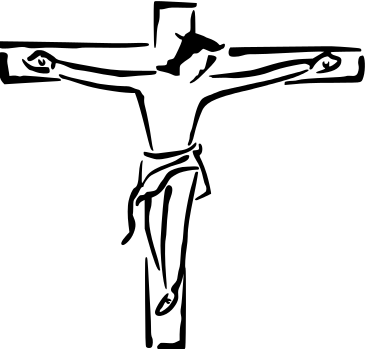
\includegraphics[width=0.20\textwidth]{../christ_on_cross.png}} ;
\end{tikzpicture}
\Large 

\leftcitation{ס} \centerfont 詩百又廿七載：
\leftcitation{ע} \centerfont 非耶和華建屋宇.則匠人之經營徒.
\leftcitation{פ} \centerfont 非耶和華衛城邑.則守者之儆醒徒.
\leftcitation{צ} \centerfont 余獻是卷予華人社區．願為福音流通之器．願獻斯微材為祭榮耀上帝．
\leftcitation{ק} \centerfont 阿門

\switchcolumn

\fontsize{11}{13}\rightfont \Large 滅．時越次聖殿期及當今。\leftcitation{י} \rightfont 猶太者力廣納之．筆錄以卷軸．便以傳、閱、頌、攜、守、鎖、抄、譯、釋、編，得書塔木德、密示拿等經傳．家喻戶曉．傳流若芳。\leftcitation{כ} \rightfont 猶太者文以載道．傳其口述．今我輩粵道之傳應當作如是．遂力行粵音識辨之法．載言載道．以盡忠傳粵道以待興。\leftcitation{ל} \rightfont 蒙下賜恩惠．無畏海量字音文書．既馭上帝之道．今廣及粵語講道．重駛編程之技．匯導粵音遂字稿．重塑講道現場．以傚猶太卷軸之舉便以傳流。\leftcitation{מ} \rightfont 是卷乃粵音口述傳之屬．莫通華文白話之語．

\end{paracol}

\columnratio{0.5,0.5}
\begin{paracol}{2}\fontsize{11}{13}\leftfont \Large \leftcitation{ו} \leftfont 斯殺一違儆百逆．既禁壓之．我輩聞風無奈．在所難免。\leftcitation{ז} \leftfont 另有異人例乎．以版權之名．脅網絡頻道之舉．同授礙予粵道之存流。

\switchcolumn

\fontsize{11}{13}\rightfont \Large 惟待後繼來者之傚．以譯釋傳之於神州華文地。\leftcitation{נ} \rightfont 今能排程驅馭圖靈以編彙文檔，其碼長共數千千亦無逢大礙．全蒙上帝保守。

\end{paracol}



\columnratio{1}\begin{paracol}{1}

\fontsize{11}{13}\rightfont \Large
~~~~~~~~~~~~~~~~~~~~~~~~~~~~~~~~~~~~~~~~~~~~~~~~~~~~~~~~~~~~~~~~~~~~~~~~~~~~~~~\leftcitation{ר} \rightfont 二零二三年二月一日

~~~~~~~~~~~~~~~~~~~~~~~~~~~~~~~~~~~~~~~~~~~~~~~~~~~~~~~~~~~~~~~~~~~~~~~~~~~~~~~\leftcitation{ש} \rightfont 米迦勒

~~~~~~~~~~~~~~~~~~~~~~~~~~~~~~~~~~~~~~~~~~~~~~~~~~~~~~~~~~~~~~~~~~~~~~~~~~~~~~~\leftcitation{ת} \rightfont 書於香港

\end{paracol}

\end{sloppypar}
\end{document}
